\documentclass{book}

% Header file for latex2html

\usepackage{amsmath}
\usepackage{theorem}
\usepackage{amssymb}
\usepackage{makeidx}
\usepackage{longtable}

\usepackage{color}

%% header_hyperref.tex

\usepackage{graphicx}

\newcommand{\href}[2]{#2}
\newcommand{\hyperref}[2][1]{#2 \ref{#1}}



\pagestyle{plain}
\newcommand{\theoremfamily}{\rmfamily}

% CONTINUE: FIX
%----------------------------------------------------------------------------
\theoremstyle{plain}
\theoremheaderfont{\theoremfamily\normalsize\bfseries}
\theorembodyfont{\theoremfamily\slshape\normalsize}
\newtheorem{Example}{Example}[section]


\theoremstyle{break}
\theorembodyfont{\theoremfamily\normalsize}
\newtheorem{Exercise}{Exercise}[chapter]


\theoremstyle{break}
\theorembodyfont{\theoremfamily\normalsize}
\newtheorem{Hint}{Hint}[chapter]


\theoremstyle{break}
\theorembodyfont{\theoremfamily\normalsize}
\newtheorem{Solution}{Solution}[chapter]


\theoremstyle{break}
\theorembodyfont{\theoremfamily\normalsize}
\newtheorem{QuizProblem}{Problem}[chapter]


\theoremstyle{break}
\theorembodyfont{\theoremfamily\normalsize}
\newtheorem{QuizSolution}{Solution}[chapter]


\theoremstyle{plain}
\theorembodyfont{\theoremfamily\large}
\newtheorem{Theorem}{\large Theorem}[section]


\theoremstyle{plain}
\theorembodyfont{\theoremfamily\large}
\newtheorem{Result}{\large Result}[section]

\setlength{\theorempreskipamount}{12pt}
\setlength{\theorempostskipamount}{12pt}

%\newcommand{\resultwidth}{5.5in}
%\newcommand{\resultskip}{\vspace{.1in}}
%\newenvironment{ResultBox}{\begin{minipage}{\resultwidth}\begin{Result}}
%                                {\end{Result}\end{minipage}}

%\newcommand{\resultwidth}{5.5in}
%\renewcommand{\framebox}{}
%\newcommand{\resultskip}{\vspace{.1in}}
%\newenvironment{ResultBox}{\begin{Result}}
%                                {\end{Result}}

%-----------------------------------------------------------------------------

\newcommand{\dd}{\mathrm{d}}

\newcommand{\e}{\mathop{\mathrm{e}}\nolimits}
\newcommand{\erf}{\mathop{\mathrm{erf}}\nolimits}
\newcommand{\erfc}{\mathop{\mathrm{erfc}}\nolimits}
\newcommand{\berfc}{\mathop{\mathbf{erfc}}\nolimits}
\newcommand{\bsin}{\mathop{\mathbf{sin}}\nolimits}
\newcommand{\bcos}{\mathop{\mathbf{cos}}\nolimits}
\newcommand{\sign}{\mathop{\mathrm{sign}}\nolimits}
\newcommand{\rank}{\mathop{\mathrm{rank}}\nolimits}
\newcommand{\nullspace}{\mathop{\mathrm{nullspace}}\nolimits}
\newcommand{\thespan}{\mathop{\mathrm{span}}\nolimits}
\newcommand{\Res}{\mathop{\mathrm{Res}}\nolimits}
\newcommand{\Ei}{\mathop{\mathrm{Ei}}\nolimits}
\newcommand{\PV}{\mathop{\mathrm{PV}}\nolimits}
\newcommand{\pvint}{- \negthickspace \negthickspace \negthickspace
                        \negmedspace \int}
\newcommand{\pv}{- \negthickspace \negthickspace \negthickspace \negmedspace}
\newcommand{\textpv}{- \negthickspace \negthickspace \negthickspace}
\newcommand{\Log}{\mathop{\mathrm{Log}}\nolimits}
\newcommand{\Arg}{\mathop{\mathrm{Arg}}\nolimits}
\newcommand{\sech}{\mathop{\mathrm{sech}}\nolimits}
\newcommand{\csch}{\mathop{\mathrm{csch}}\nolimits}
\newcommand{\arcsinh}{\mathop{\mathrm{arcsinh}}\nolimits}
\newcommand{\arccosh}{\mathop{\mathrm{arccosh}}\nolimits}
\newcommand{\arctanh}{\mathop{\mathrm{arctanh}}\nolimits}
\newcommand{\Arcsin}{\mathop{\mathrm{Arcsin}}\nolimits}
\newcommand{\Arccos}{\mathop{\mathrm{Arccos}}\nolimits}
\newcommand{\Arctan}{\mathop{\mathrm{Arctan}}\nolimits}

%% I don't know the package that would define these.
%% Hopefully I can find it and remove these definitions.
\newcommand{\setN}{\mathbb{N}}
\newcommand{\setZ}{\mathbb{Z}}
\newcommand{\setR}{\mathbb{R}}
\newcommand{\setC}{\mathbb{C}}



%% Include the exercises, hints and solutions.
\newcommand{\exercises}[1]{#1}
\newcommand{\hints}[1]{#1}
\newcommand{\solutions}[1]{#1}

%% Have links to the hints and solutions.
\newcommand{\hintsolution}[1]{
  \noindent
  Hint \ref{hint #1},
  Solution \ref{solution #1}
}
\newcommand{\quizsolution}[1]{
  \noindent
  Solution \ref{quiz solution #1}
}

\title{Introduction to Methods of Applied Mathematics\\
        or\\
        Advanced Mathematical Methods for Scientists and Engineers}
\author{Sean Mauch\\
  \href{http://www.its.caltech.edu/~sean/}
       {http://www.its.caltech.edu/{\~{}}sean/}
}

\makeindex

\begin{document}

%\maketitle

\frontmatter

\tableofcontents

%=============================================================================
%=============================================================================
\chapter{Anti-Copyright}


\paragraph{}
Anti-Copyright (A)
%\begin{picture}(12,12)(0,0)
%\put(1.5,1.5){a}
%\put(4,4){\circle{8}}
%\end{picture}
1995-2004 by Mauch Publishing Company, un-Incorporated.

\paragraph{}
No rights reserved.  Any part of this publication may be reproduced, stored
in a retrieval system, transmitted or desecrated without permission.


\raggedbottom



%=============================================================================
%=============================================================================
\chapter{Preface}

During the summer before my final undergraduate year at Caltech I set
out to write a math text unlike any other, namely, one written by me.
In that respect I have succeeded beautifully.  Unfortunately, the text is
neither complete nor polished.  I have a ``Warnings and Disclaimers''
section below that is a little amusing, and an appendix on probability that 
I feel concisesly captures the essence of the subject.
However, all the material in between is in some stage of development.  
I am currently working to improve and expand this text.

This text is freely available from my web set.  Currently I'm at
\href{http://www.its.caltech.edu/~sean/}
        {http://www.its.caltech.edu/{\~{}}sean/}.
I post new versions a couple of times a year.





%=============================================================================
\section{Advice to Teachers}

If you have something worth saying, write it down.







%=============================================================================
\section{Acknowledgments}

I would like to thank Professor Saffman for advising me on
this project and the Caltech SURF program for providing
the funding for me to write the first edition of this book.




%=============================================================================
\section{Warnings and Disclaimers}

\begin{itemize}
\item This book is a work in progress.  It contains quite a few
        mistakes and typos.  I would greatly appreciate your constructive
        criticism.  You can reach me at `sean@caltech.edu'.
%
\item Reading this book impairs your ability to drive a car or operate
machinery.
%
\item This book has been found to cause drowsiness in laboratory animals.
%
\item This book contains twenty-three times the US RDA of fiber.
%
\item Caution: FLAMMABLE - Do not read while smoking or near a fire.
%
\item If infection, rash, or irritation develops, discontinue use and consult
a physician.
%
\item Warning: For external use only.  Use only as directed.  Intentional
misuse by deliberately concentrating contents can be harmful or fatal.
KEEP OUT OF REACH OF CHILDREN.
%
\item In the unlikely event of a water landing do not use this book as a
flotation device.
%
\item The material in this text is fiction; any resemblance to real theorems,
living or dead, is purely coincidental.
%
\item This is by far the most amusing section of this book.
%
\item Finding the typos and mistakes in this book is left as an exercise
for the reader.  (Eye ewes a spelling chequer from thyme too thyme,
sew their should knot bee two many
misspellings.  Though I ain't so sure the grammar's too good.)
%
\item The theorems and methods in this text are subject to change without
notice.
%
\item  This is a chain book.  If you do not make seven copies and distribute
them to your friends within ten days of obtaining this text you will suffer
great misfortune and other nastiness.
%
\item
The surgeon general has determined that excessive studying is detrimental
to your social life.
%
\item
This text has been buffered for your protection and ribbed for your
pleasure.
%
\item Stop reading this rubbish and get back to work!
\end{itemize}





%=============================================================================
\section{Suggested Use}

This text is well suited to the student, professional or lay-person.  It 
makes a superb gift.  This text has a boquet that is light and fruity, with
some earthy undertones.  It is ideal with dinner or as an apertif.
Bon apetit!



%=============================================================================
\section{About the Title}

The title is only making light of naming conventions in the sciences 
and is not an insult to engineers.   If you want to learn about some 
mathematical subject, look for books with ``Introduction'' or ``Elementary''
in the title.  If it is an ``Intermediate'' text it will be incomprehensible.
If it is ``Advanced'' then not only will it be incomprehensible, it will 
have low production qualities, i.e. a crappy typewriter font, no graphics 
and no examples.  There is an exception to this rule:  When the title also 
contains the word ``Scientists'' or ``Engineers'' the advanced book
may be quite suitable for actually learning the material.







\mainmatter

\part{Algebra}

This part of the text is not a proper treatment of algebra.  This is where 
I collect som material that is prerequisite for studying functions of a 
complex variable and vector calculus.

\flushbottom

% CONTINUE: define neighborhoods, balls, etc.


%============================================================================
%============================================================================
\chapter{Sets and Functions}




%=============================================================================
\section{Sets}


\paragraph{Definition.}
A \textit{set} is a collection of objects.  We call the objects, 
\index{set}
\textit{elements}.   A set is denoted by listing the elements between
\index{elements!of a set}
braces.  For example: $\{\e, \imath, \pi, 1\}$ is the set of the integer $1$, the 
pure imaginary number $\imath = \sqrt{-1}$ and the transcendental numbers
$\e = 2.7182818\ldots$ and $\pi = 3.1415926\ldots$.   
For elements of a set, we do not count multiplicities.  We regard the set
$\{1, 2, 2, 3, 3, 3\}$ as identical to the set $\{1,2,3\}$.
Order is not significant in sets.  The set $\{1,2,3\}$ is equivalent to 
$\{3,2,1\}$.

In enumerating the elements of a set, we use ellipses to indicate 
patterns.  We denote the set of positive integers as $\{1, 2, 3, \ldots\}$.
We also denote sets with the notation $\{x | \mathrm{conditions on}\ x \}$
for sets that are more easily described than enumerated.  This is read as
``the set of elements $x$ such that \ldots''.  
$x \in S$ is the notation for ``$x$ is an element of the set $S$.''
To express the opposite we have $x \not\in S$ for 
``$x$ is not an element of the set $S$.''



\paragraph{Examples.}
We have notations for denoting some of the commonly encountered sets.
\begin{itemize}
\item
$\emptyset = \{\}$ is the \textit{empty set}, the set containing no elements.
\index{empty set}
\item
$\mathbb{Z} = \{\ldots, -3, -2, -1, 0, 1, 2, 3 \ldots\}$ is the set of 
\textit{integers}.  (Z is for ``Zahlen'', the German word for ``number''.)
\index{integers!set of}
\item
$\mathbb{Q} = \{ p / q | p,q \in \mathbb{Z}, q \neq 0 \}$ is the set of 
\textit{rational numbers}.  (Q is for quotient.)
\index{rational numbers!set of}
\footnote{
  Note that with this description, we enumerate each rational number an 
  infinite number of times.  For example: $1/2 = 2/4 = 3/6 = (-1)/(-2) = \cdots$.
  This does not pose a problem as we do not count multiplicities.
}
\item
%% CONTINUE: Define this properly.
$\mathbb{R} = \{ x | x = a_1 a_2 \cdots a_n.b_1 b_2 \cdots \}$ is the set
of \textit{real numbers}, i.e. the set of numbers with decimal expansions.
\footnote{Guess what R is for.}
\index{real numbers!set of}
\item
$\mathbb{C} = \{ a + \imath b | a,b \in \mathbb{R}, \imath^2 = -1 \}$ is the set of 
\textit{complex numbers}.  $\imath$ is the square root of $-1$.  
(If you haven't seen complex numbers before, don't dismay.  
We'll cover them later.)
\index{complex numbers!set of}
\item
$\mathbb{Z}^+$, $\mathbb{Q}^+$ and $\mathbb{R}^+$ are the sets of 
positive integers, rationals and reals, respectively.  For example,
$\mathbb{Z}^+ = \{1, 2, 3, \ldots\}$.  We use a $-$ superscript to denote 
the sets of negative numbers.
\item
$\mathbb{Z}^{0+}$, $\mathbb{Q}^{0+}$ and $\mathbb{R}^{0+}$ are the sets of 
non-negative integers, rationals and reals, respectively.  For example,
$\mathbb{Z}^{0+} = \{0, 1, 2, \ldots\}$.
\item
$(a \ldots b)$ denotes an \textit{open interval} on the real axis.
$(a \ldots b) \equiv \{ x | x \in \mathbb{R}, a < x < b \}$
\index{open interval}
\index{interval!open}
\item
We use brackets to denote the \textit{closed interval}.
$[a .. b] \equiv \{ x | x \in \mathbb{R}, a \leq x \leq b \}$
\index{closed interval}
\index{interval!closed}
\end{itemize}



The \textit{cardinality} or \textit{order} of a set $S$ is denoted $|S|$.
\index{cardinality!of a set}
\index{order!of a set}
%% CONTINUE: Cover the cardinality of infinite sets.
For finite sets, the cardinality is the number of elements in the set.
The \textit{Cartesian product} of two sets is the set of ordered pairs:
\index{Cartesian product!of sets}
\[
X \times Y \equiv \{ (x,y) | x \in X, y \in Y \}.
\]
The Cartesian product of $n$ sets is the set of ordered n-tuples:
\[
X_1 \times X_2 \times \cdots \times X_n \equiv \{ (x_1,x_2,\ldots,x_n) | x_1 \in X_1, x_2 \in X_2, \ldots, x_n \in X_n \}.
\]


\paragraph{Equality.}
Two sets $S$ and $T$ are \textit{equal} if each element of $S$ is an element 
of $T$ and vice versa.  This is denoted, $S = T$.  Inequality is
$S \neq T$, of course.
$S$ is a \textit{subset}
\index{subset}
of $T$, $S \subseteq T$, if every element of $S$ is an element of $T$.
$S$ is a \textit{proper subset}
\index{subset!proper}
of $T$, $S \subset T$, if $S \subseteq T$ and $S \neq T$.
For example: The empty set is a subset of every set, $\emptyset \subseteq S$.
The rational numbers are a proper subset of the real numbers, 
$\mathbb{Q} \subset \mathbb{R}$.


\paragraph{Operations.}
The \textit{union} of two sets, $S \cup T$,  is the set whose elements are 
\index{union!of sets}
in either of the two sets.
The union of $n$ sets,
\[
\cup_{j=1}^n S_j \equiv S_1 \cup S_2 \cup \cdots \cup S_n
\]
is the set whose elements are in any of the sets $S_j$.
The \textit{intersection} of two sets, $S \cap T$,  is the set whose 
\index{intersection!of sets}
elements are in both of the two sets.  In other words, the intersection of
two sets in the set of elements that the two sets have in common.
The intersection of $n$ sets,
\[
\cap_{j=1}^n S_j \equiv S_1 \cap S_2 \cap \cdots \cap S_n
\]
is the set whose elements are in all of the sets $S_j$.
If two sets have no elements in common, $S \cap T = \emptyset$, then 
the sets are \textit{disjoint}.
\index{disjoint sets}
If $T \subseteq S$, then the \textit{difference} between $S$ and $T$,
\index{difference!of sets}
$S \setminus T$, is the set of elements in $S$ which are not in $T$.
\[
S \setminus T \equiv \{x | x \in S, x \not\in T \}
\]
The difference of sets is also denoted $S - T$.


\paragraph{Properties.}
The following properties are easily verified from the above definitions.
\begin{itemize}
\item 
$S \cup \emptyset = S$, $S \cap \emptyset = \emptyset$,
$S \setminus \emptyset = S$, $S \setminus S = \emptyset$. 
\item
Commutative.
$S \cup T = T \cup S$, $S \cap T = T \cap S$.
\item
Associative.
$(S \cup T) \cup U = S \cup (T \cup U) = S \cup T \cup U$,
$(S \cap T) \cap U = S \cap (T \cap U) = S \cap T \cap U$.
\item
Distributive.
$S \cup (T \cap U) = (S \cup T) \cap (S \cup U)$,
$S \cap (T \cup U) = (S \cap T) \cup (S \cap U)$.
\end{itemize}



% CONTINUE HERE




%=============================================================================
\section{Single Valued Functions}
\index{single-valued function}
\index{function!single-valued}

%% CONTINUE
%% Also introduce the ----jective terminology.

\paragraph{Single-Valued Functions.}
A \textit{single-valued function} or \textit{single-valued mapping}
is a mapping of the elements $x \in X$ 
into elements $y \in Y$.  This is expressed as $f : X \to Y$
or $X \stackrel{f}{\to} Y$.
If such a function is well-defined, then for each $x \in X$ there exists 
a unique element of $y$ such that $f(x) = y$.
The set $X$ is the \textit{domain} of the function, $Y$ is the 
\textit{codomain}, (not to be confused with the \textit{range}, which 
we introduce shortly).
\index{domain}
\index{codomain}
To denote the value of a function on a particular element we can use any 
of the notations: $f(x) = y$, $f : x \mapsto y$ or simply $x \mapsto y$.
$f$ is the \textit{identity map} on $X$ if $f(x) = x$ for all $x \in X$.
\index{identity map}

Let $f: X \to Y$.  The \textit{range} or \textit{image} of $f$ is
\index{range!of a mapping}
\index{image!of a mapping}
\[
f(X) = \{ y | y = f(x)\ \mathrm{for some}\ x \in X \}.
\]
The range is a subset of the codomain.  For each $Z \subseteq Y$, the 
\textit{inverse image} of $Z$ is defined:
\index{inverse image}
\[
f^{-1}(Z) \equiv \{ x \in X | f(x) = z\ \mathrm{for some}\ z \in Z \}.
\]

\paragraph{Examples.}
\begin{itemize}
\item
Finite polynomials, $f(x) = \sum_{k = 0}^n a_k x^k$, $a_k \in \mathbb{R}$, and the 
exponential function, $f(x) = \e^x$, are examples of single 
valued functions which map real numbers to real numbers.
\item
The \textit{greatest integer function}, $f(x) = \lfloor x\rfloor$, is a mapping from 
$\mathbb{R}$ to $\mathbb{Z}$.  $\lfloor x \rfloor$ is defined as the greatest integer less 
than or equal to $x$.  Likewise, the \textit{least integer function}, 
$f(x) = \lceil x \rceil$, is the least integer greater than or equal to $x$.
\index{greatest integer function}
\index{least integer function}
% CONTINUE HERE
\end{itemize}



\paragraph{The -jectives.}
A function is \textit{injective} if for each $x_1 \neq x_2$, 
$f(x_1) \neq f(x_2)$.
\index{function!injective}
In other words, distinct elements are mapped to distinct elements.
$f$ is \textit{surjective} if for each $y$ in the codomain,
\index{function!surjective}
there is an $x$ such that $y = f(x)$.  If a function is both injective and 
surjective, then it is \textit{bijective}.  A bijective function is also 
\index{function!bijective}
called a \textit{one-to-one mapping}.
\index{one-to-one mapping}


\paragraph{Examples.}
\begin{itemize}
\item
The exponential function $f(x) = \e^x$, considered as a mapping from
$\mathbb{R}$ to $\mathbb{R}^+$, is bijective, (a one-to-one mapping).
\item
$f(x)=x^2$ is a bijection from $\mathbb{R}^+$ to $\mathbb{R}^+$.  
$f$ is not injective from $\mathbb{R}$ to $\mathbb{R}^+$.  For each positive
$y$ in the range, there are two values of $x$ such that $y=x^2$.
\item
$f(x) = \sin x$ is not injective from $\mathbb{R}$ to $[-1..1]$.  
For each $y \in [-1..1]$ there exists an infinite number of values of 
$x$ such that $y = \sin x$.
\end{itemize}


\begin{figure}[h!]
\begin{center}
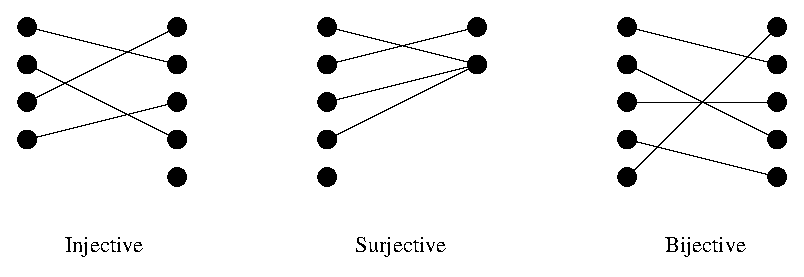
\includegraphics[width=0.8\textwidth]{algebra/sets/jectives}
\end{center}
\caption{Depictions of Injective, Surjective and Bijective Functions}
\label{jectives}
\end{figure}





% CONTINUE HERE
% Function composition, left and right inverses.





%=============================================================================
\section{Inverses and Multi-Valued Functions}
\index{inverse function}
\index{function!inverse of}
\index{multi-valued function}
\index{function!multi-valued}


If $y = f(x)$, then we can write $x = f^{-1}(y)$ where $f^{-1}$ is the inverse of 
$f$.  If $y = f(x)$ is a one-to-one function, then $f^{-1}(y)$ is also
a one-to-one function.  In this case, $x = f^{-1}(f(x)) = f(f^{-1}(x))$
for values of $x$ where both $f(x)$ and $f^{-1}(x)$ are defined.
For example $\ln x$, which maps $\mathbb{R}^+$ to $\mathbb{R}$ is 
the inverse of $\e^x$.  $x = \e^{\ln x} = \ln( \e^x )$ for all 
$x \in \mathbb{R}^+$.  (Note the $x \in \mathbb{R}^+$ ensures that 
$\ln x$ is defined.)

If $y = f(x)$ is a many-to-one function, then $x = f^{-1}(y)$ is a one-to-many
function.  $f^{-1}(y)$ is a multi-valued function.  We have
$x = f(f^{-1}(x))$ for values of $x$ where $f^{-1}(x)$ is defined, however 
$x \neq f^{-1}(f(x))$.  There are diagrams showing one-to-one, many-to-one
and one-to-many functions in Figure~\ref{tototo}.

\begin{figure}[h!]
\begin{center}
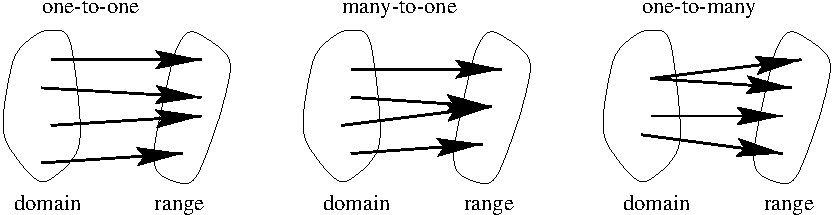
\includegraphics[width=0.8\textwidth]{algebra/sets/tototo}
\end{center}
\caption{Diagrams of One-To-One, Many-To-One and One-To-Many Functions}
\label{tototo}
\end{figure}






\begin{Example}
$y=x^2$ is a many-to-one function that has the inverse $x=y^{1/2}$.  For each 
positive $y$, there are two values of $x$ such that $x=y^{1/2}$.
$y = x^2$ and $y = x^{1/2}$ are graphed in Figure~\ref{yexsyesx}.
\begin{figure}[h!]
\begin{center}
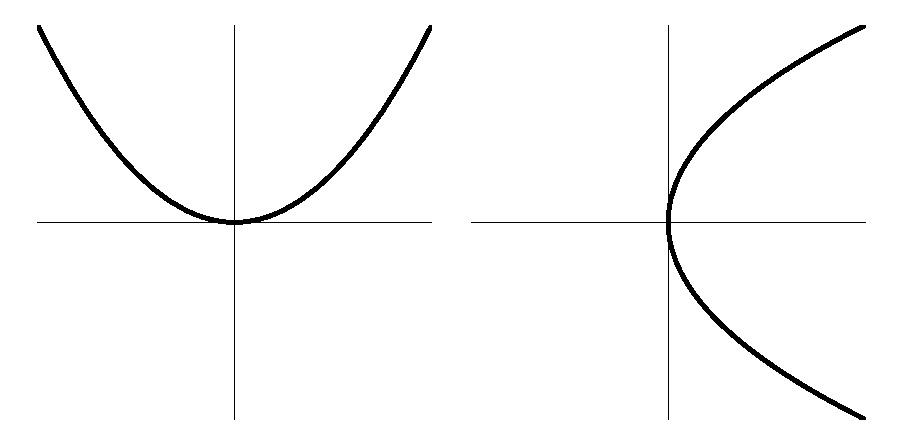
\includegraphics[width=0.4\textwidth]{algebra/sets/yexsyesx}
\end{center}
\caption{A many-to-one function and its multi-valued inverse.}
\label{yexsyesx}
\end{figure}
\end{Example}






We say that there are two \textit{branches}
\index{branches}
of $y=x^{1/2}$: the positive and the negative branch.  We denote the positive
branch as $y=\sqrt{x}$; the negative branch is $y=-\sqrt{x}$.  We call
$\sqrt{x}$ the \textit{principal branch}
\index{principal branch}
\index{branch!principal}
of $x^{1/2}$.  Note that $\sqrt{x}$ is a one-to-one function.
Finally, $x=(x^{1/2})^2$ since $(\pm \sqrt{x})^2  =x$, but
$x \neq (x^2)^{1/2}$ since $(x^2)^{1/2} = \pm x$.
$y = \sqrt{x}$ is graphed in Figure~\ref{yesqrtx}.

\begin{figure}[h!]
\begin{center}
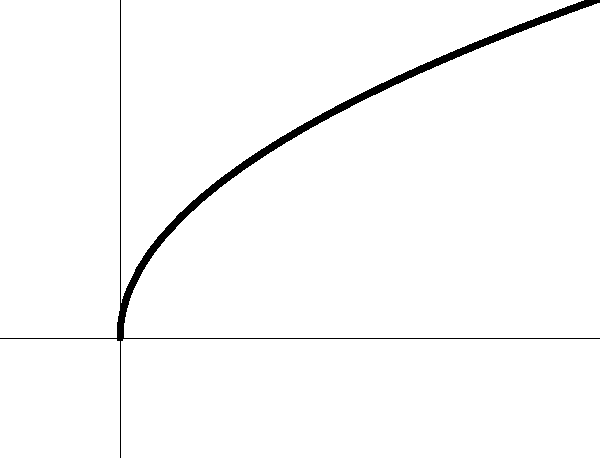
\includegraphics[width=0.3\textwidth]{algebra/sets/yesqrtx}
\end{center}
\caption{The positive branch of the square root.}
\label{yesqrtx}
\end{figure}



Now consider the many-to-one function $y=\sin x$.  The inverse is 
$x=\arcsin y$.  For each $y \in [-1..1]$ there are an infinite number
of values $x$ such that $x = \arcsin y$.
In Figure~\ref{yesxyeax} is a graph of $y = \sin x$ and a graph of a few 
branches of $y = \arcsin x$.

\begin{figure}[h!]
\begin{center}
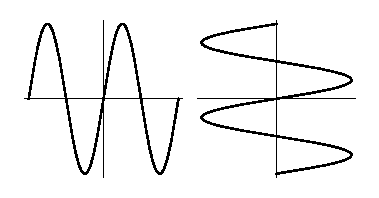
\includegraphics[width=0.4\textwidth]{algebra/sets/yesxyeax}
\end{center}
\caption{The sine and the arcsine.}
\label{yesxyeax}
\end{figure}






\begin{Example}
$\arcsin x$ has an infinite number of branches.  We will denote the
principal branch by $\Arcsin x$ which maps $[-1..1]$ to 
$\left[ -\frac{\pi}{2}.. \frac{\pi}{2} \right]$.
Note that $x = \sin(\arcsin x)$, but $x \neq \arcsin( \sin x )$.
$y = \Arcsin x$ in Figure~\ref{yepbax}.
\begin{figure}[h!]
\begin{center}
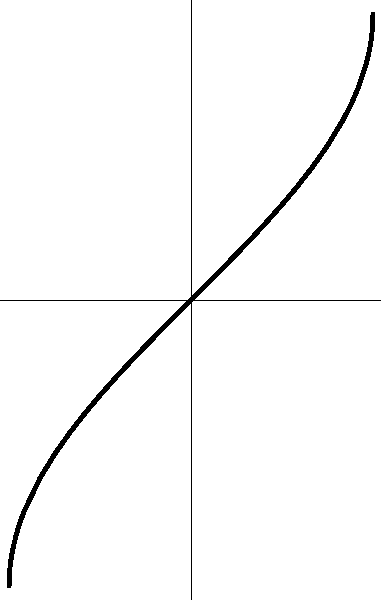
\includegraphics[width=0.2\textwidth]{algebra/sets/yepbax}
\end{center}
\caption{The principal branch of the arcsine.}
\label{yepbax}
\end{figure}
\end{Example}







\begin{Example}
Consider $1^{1/3}$.
Since $x^3$ is a one-to-one function, $x^{1/3}$ is a single-valued function.
(See Figure~\ref{yexcyecx}.) $1^{1/3} = 1$.
\begin{figure}[h!]
\begin{center}
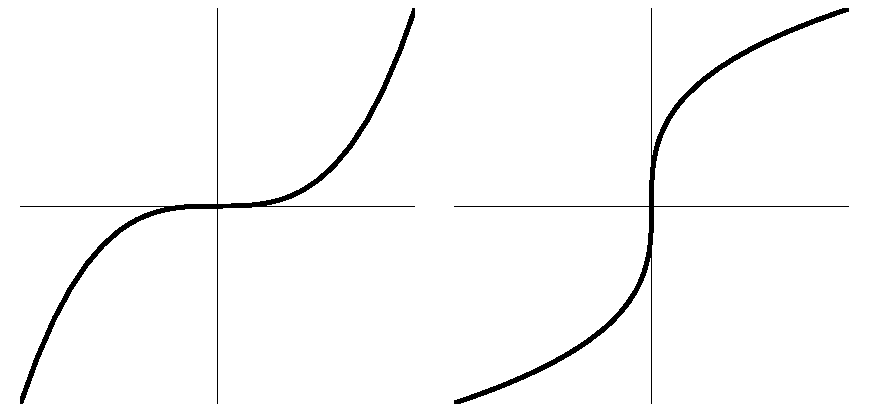
\includegraphics[width=0.4\textwidth]{algebra/sets/yexcyecx}
\end{center}
\caption{A one-to-one function and its inverse.}
\label{yexcyecx}
\end{figure}
\end{Example}







\begin{Example}
Consider $\arccos(1/2)$.  $\cos x$ and a portion of $\arccos x$ are 
graphed in Figure~\ref{yecxyeax}.
The equation $\cos x = 1/2$ has the two solutions $x = \pm \pi / 3$ in the range
$x \in (-\pi..\pi]$.  We use the periodicity of the cosine, 
$\cos(x + 2 \pi) = \cos x$, to find the remaining solutions.
\[
\arccos(1/2) = \{ \pm \pi / 3 + 2 n \pi \}, \quad n \in \mathbb{Z}.
\]

\begin{figure}[h!]
\begin{center}
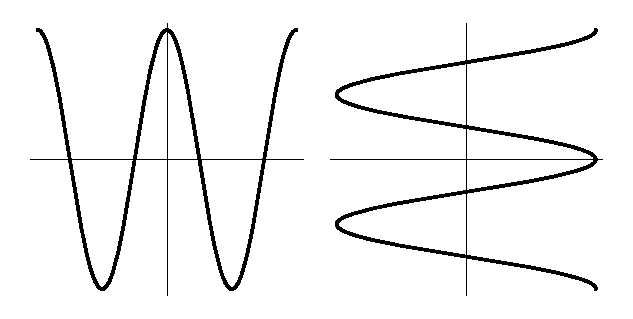
\includegraphics[width=0.4\textwidth]{algebra/sets/yecxyeax}
\end{center}
\caption{The cosine and the arccosine.}
\label{yecxyeax}
\end{figure}
\end{Example}











%=============================================================================
\section{Transforming Equations}

Consider the equation $g(x) = h(x)$ and the single-valued function $f(x)$.
A particular value of $x$
is a solution of the equation if substituting that value into the equation
results in an identity.  In determining the solutions of an equation, we 
often apply functions to each side of the equation in order to simplify
its form.  
We apply the function to obtain a second equation, $f(g(x)) = f(h(x))$.
If $x = \xi$ is a solution of the former equation, (let $\psi = g(\xi) = h(\xi)$), 
then it is necessarily a solution of latter.  This is because
$f(g(\xi)) = f(h(\xi))$ reduces to the identity $f(\psi) = f(\psi)$.
If $f(x)$ is bijective, then the converse is true: any solution of the 
latter equation is a solution of the former equation.  Suppose that
$x = \xi$ is a solution of the latter, $f(g(\xi)) = f(h(\xi))$.  That
$f(x)$ is a one-to-one mapping implies that $g(\xi) = h(\xi)$.  Thus $x = \xi$
is a solution of the former equation.

It is always safe to apply a one-to-one, (bijective), function to an equation, 
(provided it is defined for that
domain).  For example, we can apply $f(x) = x^3$ or $f(x) = \e^x$,
considered as mappings on $\mathbb{R}$, to the 
equation $x = 1$.  The equations $x^3 = 1$ and $\e^x = e$ each have the unique
solution $x = 1$ for $x \in \mathbb{R}$.


In general, we must take care in applying functions to equations.
If we apply a many-to-one function, we may introduce spurious
solutions.  Applying $f(x) = x^2$ to the equation
$x = \frac{\pi}{2}$ results in $x^2 = \frac{\pi^2}{4}$, which has the two solutions,
$x = \{ \pm \frac{\pi}{2} \}$.
Applying $f(x) = \sin x$ results in $x^2 = \frac{\pi^2}{4}$, which has 
an infinite number of solutions,
$x = \{ \frac{\pi}{2} + 2 n \pi \,|\, n \in \mathbb{Z} \}$.




We do not generally apply a one-to-many, (multi-valued), function to 
both sides of an equation as this rarely is useful.  Rather, we typically
use the definition of the inverse function.  Consider the equation
\[
\sin^2 x = 1.
\]
Applying the function $f(x) = x^{1/2}$ to the equation would not get us 
anywhere.
\[
\left( \sin^2 x \right)^{1/2} = 1^{1/2}
\]
Since $(\sin^2 x)^{1/2} \neq \sin x$, we cannot simplify the 
left side of the equation.  Instead we could use the definition of
$f(x) = x^{1/2}$ as the inverse of the $x^2$ function to obtain
\[
\sin x = 1^{1/2} = \pm 1.
\]
Now note that we should not just apply $\arcsin$ to both sides of the equation
as $\arcsin(\sin x) \neq x$.
Instead we use the definition of $\arcsin$ as the inverse of $\sin$.
\[
x = \arcsin( \pm 1)
\]
$x = \arcsin(1)$ has the solutions $x = \pi/2 + 2 n \pi$ and $x = \arcsin(-1)$
has the solutions $x = -\pi/2 + 2 n \pi$.  We enumerate the solutions.
\[
x = \left\{ \frac{\pi}{2} + n \pi \,|\, \quad n \in \mathbb{Z} \right\}
\]







%% CONTINUE
%% Add a section (from the notebook) on visualizing functions.



\raggedbottom
%============================================================================
\exercises{
\pagebreak
\flushbottom
\section{Exercises}

%-----------------------------------------------------------------------------
%\begin{large}
%\noindent
%\textbf{}
%\end{large}




\begin{Exercise}
\label{exercise area proportional square of diameter}
The area of a circle is directly proportional to the square of its diameter.
What is the constant of proportionality?

\hintsolution{area proportional square of diameter}
\end{Exercise}








\begin{Exercise}
\label{exercise x1y2=x21y24}
Consider the equation
\[
\frac{x+1}{y-2} = \frac{x^2 - 1}{y^2 - 4}.
\]
\begin{enumerate}
\item
  Why might one think that this is the equation of a line?
\item
  Graph the solutions of the equation to demonstrate that it is not the 
  equation of a line.
\end{enumerate}

\hintsolution{x1y2=x21y24}
\end{Exercise}



\begin{Exercise}
\label{exercise domain range 1x22}
Consider the function of a real variable,
\[
f(x) = \frac{1}{x^2 + 2}.
\]
What is the domain and range of the function?

\hintsolution{domain range 1x22}
\end{Exercise}





\begin{Exercise}
\label{exercise fahrenheit celcius}
The temperature measured in degrees Celsius 
\footnote{
  Originally, it was called degrees \textit{Centigrade}.  
  \textit{centi} because there are 100 degrees between the two 
  calibration points.  It is now called degrees Celsius in honor of the 
  inventor.
}
is linearly related to 
the temperature measured in degrees Fahrenheit
\footnote{
  The Fahrenheit scale, named for Daniel Fahrenheit,
  was originally calibrated with the freezing point of 
  salt-saturated water to be $0^\circ $.  Later, the calibration points 
  became the freezing point of water, $32^\circ$, and body temperature,
  $96^\circ$.  With this method, there are 64 divisions between the calibration
  points.  Finally, the upper calibration point was changed to the boiling
  point of water at $212^\circ$.  This gave 180 divisions, (the number of 
  degrees in a half circle), between the two calibration points.
}.
Water freezes at $0^\circ\ C = 32^\circ\ F$ and boils at 
$100^\circ\ C = 212^\circ\ F$.  Write the temperature in degrees Celsius
as a function of degrees Fahrenheit.

\hintsolution{fahrenheit celcius}
\end{Exercise}








\begin{Exercise}
\label{exercise xsinx transform}
Consider the function graphed in Figure~\ref{figure xsinx}.
Sketch graphs of $f(-x)$, $f(x+3)$, $f(3-x)+2$, and $f^{-1}(x)$.
You may use the blank grids in Figure~\ref{figure xsinx blank grids}.

\begin{figure}[h!]
\begin{center}
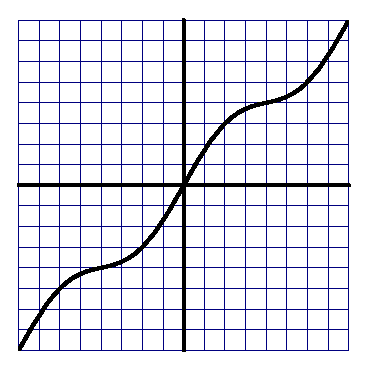
\includegraphics[width=0.4\textwidth]{algebra/sets/xsinx}
\end{center}
\caption{Graph of the function.}
\label{figure xsinx}
\end{figure}

\begin{figure}[tbp]
\begin{center}
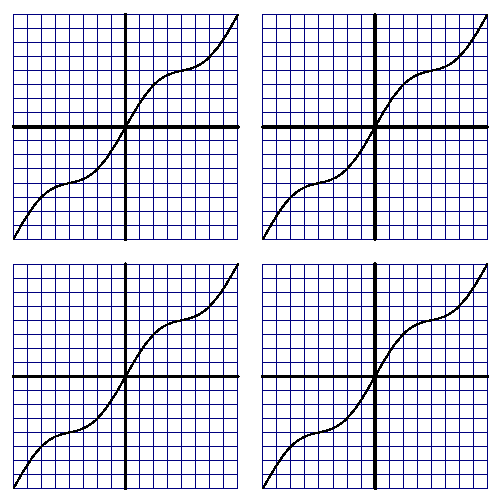
\includegraphics[width=0.7\textwidth]{algebra/sets/xsinx_blank}
\end{center}
\caption{Blank grids.}
\label{figure xsinx blank grids}
\end{figure}

\hintsolution{xsinx transform}
\end{Exercise}





\begin{Exercise}
\label{exercise geometric growth bacteria}
A culture of bacteria grows at the rate of $10\%$ per minute.  At 6:00 pm 
there are 1 billion bacteria.  How many bacteria are there at 7:00 pm?
How many were there at 3:00 pm?

\hintsolution{geometric growth bacteria}
\end{Exercise}





\begin{Exercise}
\label{exercise rational quadratic}
The graph in Figure~\ref{figure 2x2x21} shows an even function
$f(x) = p(x) / q(x)$ where $p(x)$ and $q(x)$ are rational quadratic 
polynomials.  Give possible formulas for $p(x)$ and $q(x)$.
\begin{figure}[tpb]
\begin{center}
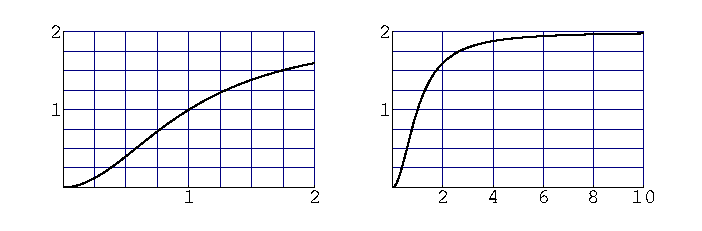
\includegraphics[width=0.8\textwidth]{algebra/sets/2x2x21}
\end{center}
\caption{Plots of a ratio of quadratic polynomials.}
\label{figure 2x2x21}
\end{figure}

\hintsolution{rational quadratic}
\end{Exercise}







\begin{Exercise}
\label{exercise polynomial 100}
Find a polynomial of degree 100 which is zero only at $x = -2, 1, \pi$ and
is non-negative.

\hintsolution{polynomial 100}
\end{Exercise}








\raggedbottom
}
%============================================================================
\hints{
\pagebreak
\flushbottom
\section{Hints}

%-----------------------------------------------------------------------------
%\begin{large}
%\noindent
%\textbf{}
%\end{large}


\begin{Hint}
\label{hint area proportional square of diameter}
$\mathrm{area} = \mathrm{constant} \times \mathrm{diameter}^2$.
\end{Hint}



\begin{Hint}
\label{hint x1y2=x21y24}
A pair $(x,y)$ is a solution of the equation if it make the equation 
an identity.
\end{Hint}


\begin{Hint}
\label{hint domain range 1x22}
The domain is the subset of $\mathbb{R}$ on which the function is defined.
\end{Hint}




\begin{Hint}
\label{hint fahrenheit celcius}
Find the slope and $x$-intercept of the line.
\end{Hint}




\begin{Hint}
\label{hint xsinx transform}
The inverse of the function is the reflection of the function across
the line $y = x$.
\end{Hint}



\begin{Hint}
\label{hint geometric growth bacteria}
The formula for geometric growth/decay is $x(t) = x_0 r^t$, where $r$ is 
the rate.
\end{Hint}



\begin{Hint}
\label{hint rational quadratic}
Note that $p(x)$ and $q(x)$ appear as a ratio, they are determined only up to
a multiplicative constant.  We may take the leading coefficient of $q(x)$ to
be unity.
\[
f(x) = \frac{p(x)}{q(x)} = \frac{a x^2 + b x + c}{x^2 + \beta x + \chi}
\]
Use the properties of the function to solve for the unknown parameters.
\end{Hint}






\begin{Hint}
\label{hint polynomial 100}
Write the polynomial in factored form.
\end{Hint}













\raggedbottom
}
%============================================================================
\solutions{
\pagebreak
\flushbottom
\section{Solutions}

%-----------------------------------------------------------------------------
%\begin{large}
%\noindent
%\textbf{}
%\end{large}





\begin{Solution}
\label{solution area proportional square of diameter}
\begin{gather*}
  \mathrm{area} = \pi \times \mathrm{radius}^2
  \\
  \mathrm{area} = \frac{\pi}{4} \times \mathrm{diameter}^2
\end{gather*}
The constant of proportionality is $\frac{\pi}{4}$.
\end{Solution}







\begin{Solution}
\label{solution x1y2=x21y24}
\begin{enumerate}
\item
If we multiply the equation by $y^2 - 4$ and divide by $x + 1$, we obtain 
the equation of a line.
\[
y + 2 = x - 1
\]
\item
We factor the quadratics on the right side of the equation.
\[
\frac{x+1}{y-2} = \frac{(x+1)(x-1)}{(y-2)(y+2)}.
\]
We note that one or both sides of the equation are undefined at $y = \pm 2$ 
because of division by zero.  There are no solutions for these two values of
$y$ and we assume from this point that $y \neq \pm 2$.  We multiply by 
$(y-2)(y+2)$.
\[
(x+1)(y+2) = (x+1)(x-1)
\]

For $x = -1$, the equation becomes the identity $0 = 0$.  Now we consider 
$x \neq -1$.  We divide by $x + 1$ to obtain the equation of a line.
\begin{gather*}
  y+2 = x-1
  \\
  y = x - 3
\end{gather*}
Now we collect the solutions we have found.
\[
\boxed{
  \{ (-1,y) : y \neq \pm 2 \} \cup \{ (x,x-3) : x \neq 1,5 \} 
  }
\]
The solutions are depicted in Figure~/ref{fig not a line}.

\begin{figure}[h!]
\begin{center}
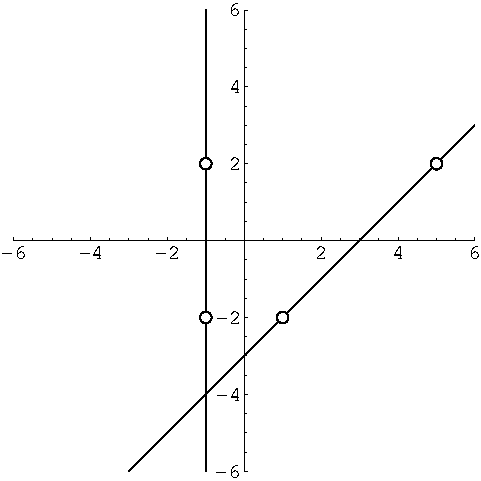
\includegraphics[width=0.4\textwidth]{algebra/sets/not_a_line}
\end{center}
\caption{The solution is not a line.}
\label{fig not a line}
\end{figure}

\end{enumerate}
\end{Solution}








\begin{Solution}
\label{solution domain range 1x22}
The denominator is nonzero for all $x \in \mathbb{R}$.  Since we don't have 
any division by zero problems, the domain of the function is $\mathbb{R}$.
For $x \in \mathbb{R}$, 
\[
0 < \frac{1}{x^2 + 2} \leq 2.
\]
Consider 
\begin{equation}
  \label{eqn y = 1x22}
  y = \frac{1}{x^2 + 2}.
\end{equation}
For any $y \in (0 \ldots 1/2]$, there is at least one value of $x$ that satisfies 
Equation~\ref{eqn y = 1x22}.
\begin{gather*}
  x^2 + 2 = \frac{1}{y}
  \\
  x = \pm \sqrt{ \frac{1}{y} - 2 }
\end{gather*}
Thus the range of the function is $(0 \ldots 1/2]$
\end{Solution}






\begin{Solution}
\label{solution fahrenheit celcius}
Let $c$ denote degrees Celsius and $f$ denote degrees Fahrenheit.  The line
passes through the points $(f,c) = (32,0)$ and $(f,c) = (212,100)$.
The $x$-intercept is $f = 32$.  We calculate the slope of the line.
\[
\mathrm{slope} = \frac{100 - 0}{212 - 32} = \frac{100}{180} = \frac{5}{9}
\]
The relationship between fahrenheit and celcius is
\[
\boxed{
  c = \frac{5}{9} (f - 32).
  }
\]
\end{Solution}





\begin{Solution}
\label{solution xsinx transform}
We plot the various transformations of $f(x)$:
$f(-x)$, $f(x+3)$, $f(3-x)+2$, and $f^{-1}(x)$.
\begin{figure}[tbp]
\begin{center}
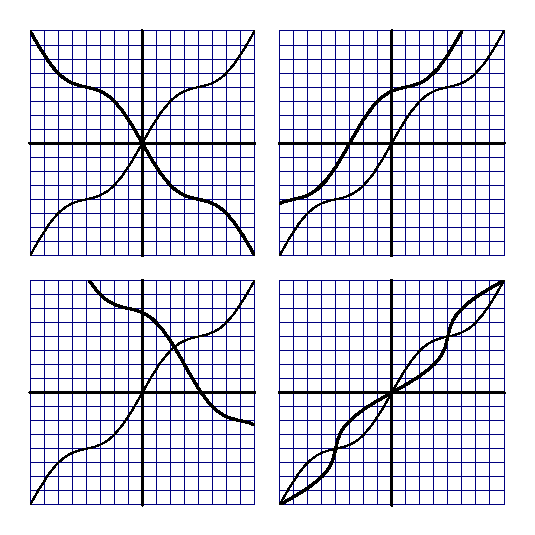
\includegraphics[width=0.7\textwidth]{algebra/sets/xsinx_transform}
\end{center}
\caption{Graphs of the transformations.}
\label{figure xsinx transform}
\end{figure}
\end{Solution}






\begin{Solution}
\label{solution geometric growth bacteria}
The formula for geometric growth/decay is $x(t) = x_0 r^t$, where $r$ is 
the rate.  Let $t = 0$ coincide with 6:00 pm.  We determine $x_0$.
\begin{gather*}
  x(0) = 10^9 = x_0 \left( \frac{11}{10} \right)^0 = x_0
  \\
  x_0 = 10^9
\end{gather*}
At 7:00 pm the number of bacteria is
\[
\boxed{
  10^9 \left( \frac{11}{10} \right)^{60} = \frac{11^{60}}{10^{51}} \approx 3.04 \times 10^{11}
  }
\]
At 3:00 pm the number of bacteria was
\[
\boxed{
  10^9 \left( \frac{11}{10} \right)^{-180} = \frac{10^{189}}{11^{180}} \approx 35.4
  }
\]
\end{Solution}











\begin{Solution}
\label{solution rational quadratic}
We write $p(x)$ and $q(x)$ as general quadratic polynomials.
\[
f(x) = \frac{p(x)}{q(x)} = \frac{a x^2 + b x + c}{\alpha x^2 + \beta x + \chi}
\]
We will use the properties of the function to solve for the unknown 
parameters.

Note that $p(x)$ and $q(x)$ appear as a ratio, they are determined only up to
a multiplicative constant.  We may take the leading coefficient of $q(x)$ to
be unity.
\[
f(x) = \frac{p(x)}{q(x)} = \frac{a x^2 + b x + c}{x^2 + \beta x + \chi}
\]
$f(x)$ has a second order zero at $x = 0$.  This means that $p(x)$ has a
second order zero there and that $\chi \neq 0$.
\[
f(x) = \frac{a x^2}{x^2 + \beta x + \chi}
\]
We note that $f(x) \to 2$ as $x \to \infty$.  This determines the parameter $a$.
\begin{align*}
  \lim_{x \to \infty} f(x)
  &= \lim_{x \to \infty} \frac{a x^2}{x^2 + \beta x + \chi}
  \\
  &= \lim_{x \to \infty} \frac{2 a x}{2 x + \beta}
  \\
  &= \lim_{x \to \infty} \frac{2 a}{2}
  \\
  &= a
\end{align*}
\[
f(x) = \frac{2 x^2}{x^2 + \beta x + \chi}
\]
Now we use the fact that $f(x)$ is even to conclude that $q(x)$ is even and
thus $\beta = 0$.
\[
f(x) = \frac{2 x^2}{x^2 + \chi}
\]
Finally, we use that $f(1) = 1$ to determine $\chi$.
\[
\boxed{
  f(x) = \frac{2 x^2}{x^2 + 1}
  }
\]
\end{Solution}








\begin{Solution}
\label{solution polynomial 100}
Consider the polynomial
\[
p(x) = (x + 2)^{40} (x - 1)^{30} (x - \pi)^{30}.
\]
It is of degree 100. Since the factors only vanish at $x = -2,1,\pi$, $p(x)$ 
only vanishes there.  Since factors are non-negative, the polynomial is 
non-negative.
\end{Solution}







\raggedbottom
}







\flushbottom

%% CONTINUE: This needs a lot of work.




%%=============================================================================
%%=============================================================================
\chapter{Vectors}





%%=============================================================================
\section{Vectors}


%%-----------------------------------------------------------------------------
\subsection{Scalars and Vectors}

A \textit{vector} is a quantity having both a magnitude and a direction.
Examples of vector quantities are velocity, force and position.  
One can represent a vector in $n$-dimensional space with an arrow whose
initial point is at the origin, (Figure~\ref{vector}).
The magnitude is the length of the vector.  Typographically, variables 
representing vectors are often written in capital letters, bold face or with a 
vector over-line, $A, \mathbf{a}, \vec{a}$.  The magnitude of a vector is 
denoted $| \mathbf{a} |$.

\begin{figure}[htb!]
\begin{center}
  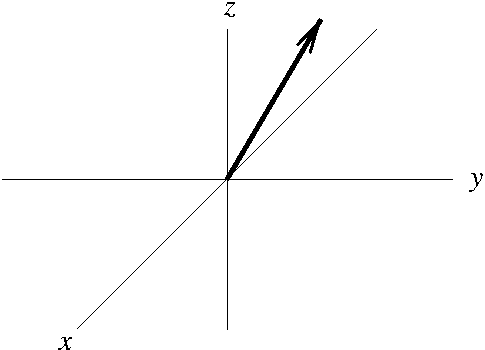
\includegraphics[width=0.4\textwidth]{algebra/vectors/vector}
\end{center}
\caption{Graphical representation of a vector in three dimensions.}
\label{vector}
\end{figure}

A \textit{scalar} has only a magnitude.  Examples of scalar quantities are
mass, time and speed.




%% CONTINUE: Introduce the concepts of a vector space.
\paragraph{Vector Algebra.}
Two vectors are equal if they have the same magnitude and direction.  
The negative of a vector, denoted $- \mathbf{a}$, is a vector of the same
magnitude as $\mathbf{a}$ but in the opposite direction.  We add two vectors
$\mathbf{a}$ and $\mathbf{b}$ by placing the tail of $\mathbf{b}$ at 
the head of $\mathbf{a}$ and defining $\mathbf{a} + \mathbf{b}$ to be 
the vector with tail at the origin and head at the head of $\mathbf{b}$.
(See Figure~\ref{addvector}.)

\begin{figure}[htb!]
\begin{center}
  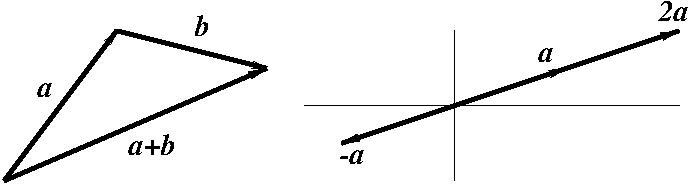
\includegraphics[width=0.5\textwidth]{algebra/vectors/addvec}
\end{center}
\caption{Vector arithmetic.}
\label{addvector}
\end{figure}

The difference, $\mathbf{a} - \mathbf{b}$, is defined as the sum of 
$\mathbf{a}$ and the negative of $\mathbf{b}$, $\mathbf{a} + (- \mathbf{b})$.
The result of multiplying $\mathbf{a}$ by a scalar $\alpha$ is a vector of 
magnitude $|\alpha|\,| \mathbf{a} |$ with the same/opposite direction if 
$\alpha$ is positive/negative.  (See Figure~\ref{addvector}.) 

Here are the properties of adding vectors and multiplying them by a 
scalar.  They are evident from geometric considerations.
\begin{alignat*}{3}
&\mathbf{a} + \mathbf{b} = \mathbf{b} + \mathbf{a} &\quad
&\alpha \mathbf{a} = \mathbf{a} \alpha &\quad
&\mathrm{commutative laws} \\
&( \mathbf{a} + \mathbf{b} ) + \mathbf{c} 
        = \mathbf{a} + ( \mathbf{b} + \mathbf{c} ) &\quad
&\alpha ( \beta \mathbf{a} ) = ( \alpha \beta ) \mathbf{a} &\quad
&\mathrm{associative laws} \\
&\alpha ( \mathbf{a} + \mathbf{b} ) 
        = \alpha \mathbf{a} + \alpha \mathbf{b} &\quad
&( \alpha + \beta ) \mathbf{a} = \alpha \mathbf{a} + \beta \mathbf{a} &\quad
&\mathrm{distributive laws}
\end{alignat*}



\paragraph{Zero and Unit Vectors.}
\index{zero vector}
\index{null vector}
The additive identity element for vectors is the \textit{zero vector} or
\textit{null vector}.  This is a vector of magnitude zero which is denoted
as $\mathbf{0}$.  A \textit{unit vector} is a vector of magnitude one.  If
$\mathbf{a}$ is nonzero then $\mathbf{a} / | \mathbf{a} |$ is a unit vector
in the direction of $\mathbf{a}$.  Unit vectors are often denoted with a caret
over-line, $\hat{\mathbf{n}}$.




\paragraph{Rectangular Unit Vectors.}
\index{rectangular unit vectors}
\index{vector!rectangular unit}
In $n$ dimensional Cartesian space, $\mathbb{R}^n$, the unit vectors in the 
directions of the coordinates axes are $\mathbf{e}_1, \ldots \mathbf{e}_n$.
These are called the \textit{rectangular unit vectors}. 
To cut down on subscripts, the unit vectors in three dimensional space 
are often denoted with $\mathbf{i}$, $\mathbf{j}$ and $\mathbf{k}$.  
(Figure~\ref{rectvec}).

\begin{figure}[htb!]
\begin{center}
  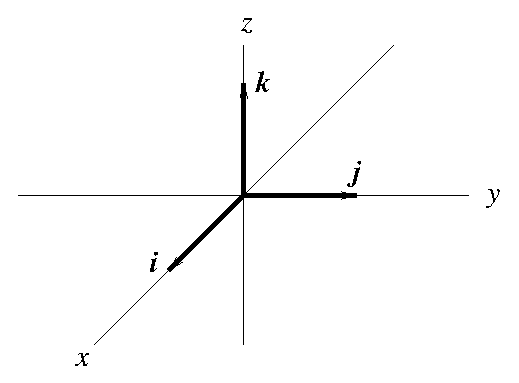
\includegraphics[width=0.4\textwidth]{algebra/vectors/rectvec}
\end{center}
\caption{Rectangular unit vectors.}
\label{rectvec}
\end{figure}



\paragraph{Components of a Vector.}
\index{vector!components of}
Consider a vector $\mathbf{a}$ with tail at the origin and head having the 
Cartesian coordinates $(a_1, \ldots, a_n)$.  We can represent this vector
as the sum of $n$ \textit{rectangular component vectors}, 
$\mathbf{a} = a_1 \mathbf{e}_1 + \cdots + a_n \mathbf{e}_n$.
(See Figure~\ref{veccomp}.)
Another notation for the vector $\mathbf{a}$ is $\langle a_1, \ldots, a_n \rangle$.
By the Pythagorean theorem, the magnitude of the vector $\mathbf{a}$ is
$| \mathbf{a} | = \sqrt{a_1^2 + \cdots + a_n^2}$.

\begin{figure}[htb!]
\begin{center}
  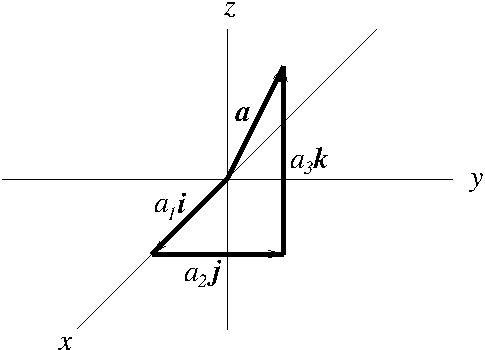
\includegraphics[width=0.4\textwidth]{algebra/vectors/veccomp}
\end{center}
\caption{Components of a vector.}
\label{veccomp}
\end{figure}






%%-----------------------------------------------------------------------------
\subsection{The Kronecker Delta and Einstein Summation Convention}


The Kronecker Delta tensor is defined
\[
\delta_{ij} = 
        \begin{cases}
        1 &\mathrm{if}\ i = j, \\
        0 &\mathrm{if}\ i \neq j.
        \end{cases}
\]
This notation will be useful in our work with vectors.



Consider writing a vector in terms of its rectangular components.  Instead
of using ellipses: $\mathbf{a} = a_1 \mathbf{e}_1 + \cdots + a_n \mathbf{e}_n$,
we could write the expression as a sum: 
$\mathbf{a} = \sum_{i = 1}^n a_i \mathbf{e}_i$.  We can shorten this notation
by leaving out the sum: $\mathbf{a} = a_i \mathbf{e}_i$, where it is 
understood that whenever an index is repeated in  a term we sum over that 
index from $1$ to $n$.  This is the \textit{Einstein summation convention}.
A repeated index is called a \textit{summation
index} or a \textit{dummy index}.  Other indices can take any value from $1$ to 
$n$ and are called \textit{free indices}.




\begin{Example}
Consider the matrix equation: $\mathbf{A} \cdot \mathbf{x} = \mathbf{b}$.
We can write out the matrix and vectors explicitly.
\[
\begin{pmatrix}
a_{11} & \cdots & a_{1 n} \\
\vdots & \ddots & \vdots \\
a_{n 1} & \cdots & a_{n n}
\end{pmatrix}
\begin{pmatrix}
x_1 \\
\vdots \\
x_n
\end{pmatrix}
=
\begin{pmatrix}
b_1 \\
\vdots \\
b_n
\end{pmatrix}
\]
This takes much less space when we use the summation convention.
\[
a_{i j} x_j = b_i
\]
Here $j$ is a summation index and $i$ is a free index.
\end{Example}










%%-----------------------------------------------------------------------------
\subsection{The Dot and Cross Product}


\paragraph{Dot Product.}
The \textit{dot product} or \textit{scalar product} of two vectors is
defined,
\[
\mathbf{a} \cdot \mathbf{b} \equiv | \mathbf{a} | | \mathbf{b} | \cos \theta,
\]
where $\theta$ is the angle from $\mathbf{a}$ to $\mathbf{b}$.  
From this definition one can derive the following properties:
\begin{itemize}
\item
$\mathbf{a} \cdot \mathbf{b} = \mathbf{b} \cdot \mathbf{a}$, 
commutative.
\item
$\alpha ( \mathbf{a} \cdot \mathbf{b} ) =
( \alpha \mathbf{a} ) \cdot \mathbf{b} =
\mathbf{a} \cdot ( \alpha \mathbf{b} )$, associativity of scalar 
multiplication.
\item
$\mathbf{a} \cdot ( \mathbf{b} + \mathbf{c} ) = 
\mathbf{a} \cdot \mathbf{b} + \mathbf{a} \cdot \mathbf{c}$,
distributive.  (See Exercise~\ref{exercise distributive law dot product}.)
\item
$\mathbf{e}_i \mathbf{e}_j = \delta_{i j}$.  In three dimensions, this is
\[ 
\mathbf{i} \cdot \mathbf{i} = \mathbf{j} \cdot \mathbf{j} =
\mathbf{k} \cdot \mathbf{k} = 1, \qquad
\mathbf{i} \cdot \mathbf{j} = \mathbf{j} \cdot \mathbf{k} = 
\mathbf{k} \cdot \mathbf{i} = 0. 
\]
\item
$\mathbf{a} \cdot \mathbf{b} = a_i b_i \equiv a_1 b_1 + \cdots + a_n b_n$, 
dot product in terms of rectangular components.
\item
If $\mathbf{a} \cdot \mathbf{b} = 0$ then either $\mathbf{a}$ and $\mathbf{b}$
are orthogonal, (perpendicular), or one of $\mathbf{a}$ and $\mathbf{b}$
are zero.
\end{itemize}


\paragraph{The Angle Between Two Vectors.}
We can use the dot product to find the angle between two vectors,
$\mathbf{a}$ and $\mathbf{b}$.   From the definition of the dot product,
\[
\mathbf{a} \cdot \mathbf{b} = | \mathbf{a} | | \mathbf{b} | \cos \theta.
\]
If the vectors are nonzero, then
\[
\theta = \arccos \left( \frac{ \mathbf{a} \cdot \mathbf{b} }
                { | \mathbf{a} | | \mathbf{b} | }  \right).
\]




\begin{Example}
What is the angle between $\mathbf{i}$ and $\mathbf{i} + \mathbf{j}$?
\begin{align*}
\theta
        &= \arccos \left( \frac{ \mathbf{i} \cdot (\mathbf{i} + \mathbf{j} ) }
                { | \mathbf{i} | | \mathbf{i} + \mathbf{j} | } \right) \\
        &= \arccos \left( \frac{1}{\sqrt{2}} \right) \\
        &= \frac{\pi}{4}.
\end{align*}
\end{Example}





\paragraph{Parametric Equation of a Line.}
Consider a line in $\mathbb{R}^n$ that passes through the point 
$\mathbf{a}$ and is parallel to
the vector $\mathbf{t}$, (tangent).  A parametric equation of the line is
\[
\mathbf{x} = \mathbf{a} + u \mathbf{t}, \quad u \in \mathbb{R}.
\]





\paragraph{Implicit Equation of a Line In $2D$.}
Consider a line in $\mathbb{R}^2$ that passes through the point 
$\mathbf{a}$ and is normal, (orthogonal, perpendicular), to the vector 
$\mathbf{n}$.  All the lines that are 
normal to $\mathbf{n}$ have the property that $\mathbf{x} \cdot \mathbf{n}$ is a 
constant, where $\mathbf{x}$ is any point on the line.  
(See Figure~\ref{dotlines}.)
$\mathbf{x} \cdot \mathbf{n} = 0$ is the line that is normal to $\mathbf{n}$
and passes through the origin.  The line that is normal to $\mathbf{n}$
and passes through the point $\mathbf{a}$ is
\[
\mathbf{x} \cdot \mathbf{n} = \mathbf{a} \cdot \mathbf{n}.
\]

\begin{figure}[htb!]
\begin{center}
  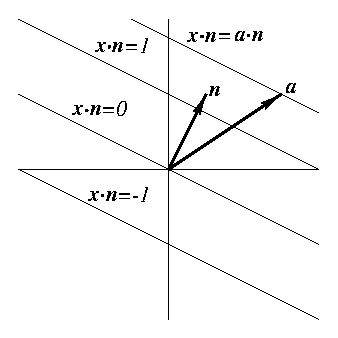
\includegraphics[width=0.33\textwidth]{algebra/vectors/dotlines}
\end{center}
\caption{Equation for a line.}
\label{dotlines}
\end{figure}


The normal to a line determines an orientation of the line.  The normal 
points in the direction that is above the line.  A point $\mathbf{b}$ is 
(above/on/below) the line if $(\mathbf{b} - \mathbf{a}) \cdot \mathbf{n}$ is 
(positive/zero/negative).  The signed distance of a point $\mathbf{b}$
from the line
$ \mathbf{x} \cdot \mathbf{n} = \mathbf{a} \cdot \mathbf{n}$ is 
\[
(\mathbf{b} - \mathbf{a}) \cdot \frac{\mathbf{n}}{|\mathbf{n}|}.
\]







\paragraph{Implicit Equation of a Hyperplane.}
A hyperplane in $\mathbb{R}^n$ is an $n-1$ dimensional ``sheet'' 
which passes through a given point and is normal to a given direction.
In $\mathbb{R}^3$ we call this a plane.
Consider a hyperplane that passes through the point $\mathbf{a}$ and is normal
to the vector $\mathbf{n}$.  All the hyperplanes that are normal
to $\mathbf{n}$ have the property that $\mathbf{x} \cdot \mathbf{n}$ is a constant, 
where $\mathbf{x}$ is any point in the hyperplane.  
$\mathbf{x} \cdot \mathbf{n} = 0$ is the hyperplane that is normal to $\mathbf{n}$
and passes through the origin.  The hyperplane that is normal to $\mathbf{n}$
and passes through the point $\mathbf{a}$ is
\[
\mathbf{x} \cdot \mathbf{n} = \mathbf{a} \cdot \mathbf{n}.
\]


The normal determines an orientation of the hyperplane.  The normal 
points in the direction that is above the hyperplane.  A point $\mathbf{b}$ is 
(above/on/below) the hyperplane if $(\mathbf{b} - \mathbf{a}) \cdot \mathbf{n}$ is 
(positive/zero/negative).  The signed distance of a point $\mathbf{b}$
from the hyperplane $ \mathbf{x} \cdot \mathbf{n} = \mathbf{a} \cdot \mathbf{n}$ is 
\[
(\mathbf{b} - \mathbf{a}) \cdot \frac{\mathbf{n}}{|\mathbf{n}|}.
\]







\paragraph{Right and Left-Handed Coordinate Systems.}
Consider a rectangular coordinate system in two dimensions.  Angles are 
measured from the positive $x$ axis in the direction of the positive $y$
axis.  There are two ways of labeling the axes.  (See Figure~\ref{twodimrl}.)
In one the angle increases in the counterclockwise direction and in the
other the angle increases in the clockwise direction.  The former is the 
familiar Cartesian coordinate system.

\begin{figure}[htb!]
\begin{center}
  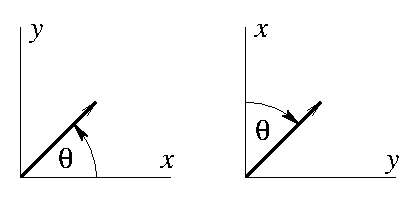
\includegraphics[width=0.3\textwidth]{algebra/vectors/twodimrl}
\end{center}
\caption{There are two ways of labeling the axes in two dimensions.}
\label{twodimrl}
\end{figure}

There are also two ways of labeling the axes in a three-dimensional
rectangular coordinate system.  These are called right-handed and 
left-handed coordinate systems.  See Figure~\ref{rlhand}. 
Any other labelling of the axes could be rotated into one of these 
configurations.  The right-handed system is the one that is used by
default.  If you put your right thumb in the 
direction of the $z$ axis in a right-handed coordinate system, then your
fingers curl in the direction from the $x$ axis to the $y$ axis.

\begin{figure}[htb!]
\begin{center}
  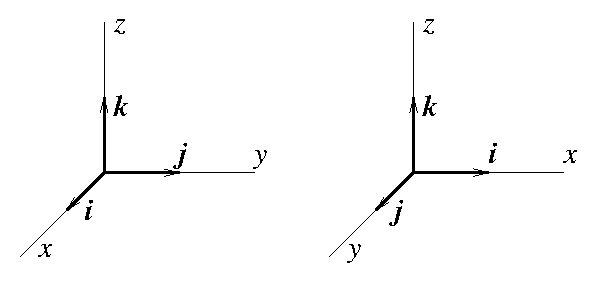
\includegraphics[width=0.4\textwidth]{algebra/vectors/rlhand}
\end{center}
\caption{Right and left handed coordinate systems.}
\label{rlhand}
\end{figure}







\paragraph{Cross Product.}
The \textit{cross product} or \textit{vector product} is defined,
\[
\mathbf{a} \times \mathbf{b} = | \mathbf{a} | | \mathbf{b} | \sin \theta \ 
\mathbf{n},
\]
where $\theta$ is the angle from $\mathbf{a}$ to $\mathbf{b}$ and 
$\mathbf{n}$ is a unit vector that is orthogonal to $\mathbf{a}$
and $\mathbf{b}$ and in the direction such that the ordered triple of
vectors $\mathbf{a}$, 
$\mathbf{b}$ and $\mathbf{n}$ form a right-handed system.

You can visualize the direction of $\mathbf{a} \times \mathbf{b}$ by applying
the \textit{right hand rule}.  Curl the fingers of your right hand in 
the direction from $\mathbf{a}$ to $\mathbf{b}$.  Your thumb points in the direction
of $\mathbf{a} \times \mathbf{b}$.  \textbf{Warning}:  Unless you are a lefty,
get in the habit of putting down your pencil before applying the right
hand rule.





The dot and cross products behave a little differently.
First note that unlike the dot product, the cross product is not 
commutative.  The magnitudes of $\mathbf{a} \times \mathbf{b}$
and $\mathbf{b} \times \mathbf{a}$ are the same, but their directions are opposite.
(See Figure~\ref{anticomm}.)

\begin{figure}[htb!]
\begin{center}
  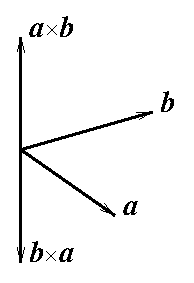
\includegraphics[width=0.125\textwidth]{algebra/vectors/anticomm}
\end{center}
\caption{The cross product is anti-commutative.}
\label{anticomm}
\end{figure}

Let
\[
\mathbf{a} \times \mathbf{b} = | \mathbf{a} | | \mathbf{b} | \sin \theta\ \mathbf{n}
\quad \mathrm{and} \quad
\mathbf{b} \times \mathbf{a} = | \mathbf{b} | | \mathbf{a} | \sin \phi\ \mathbf{m}.
\]
The angle from $\mathbf{a}$ to $\mathbf{b}$ is the same as the angle from
$\mathbf{b}$ to $\mathbf{a}$.  Since $\{ \mathbf{a}, \mathbf{b}, \mathbf{n} \}$ and 
$\{ \mathbf{b}, \mathbf{a}, \mathbf{m} \}$ are right-handed systems, $\mathbf{m}$
points in the opposite direction as $\mathbf{n}$.  Since 
$\mathbf{a} \times \mathbf{b} = - \mathbf{b} \times \mathbf{a}$ we say that the 
cross product is anti-commutative.



Next we note that since
\[
| \mathbf{a} \times \mathbf{b} | = | \mathbf{a} | | \mathbf{b} | \sin \theta,
\]
the magnitude of $\mathbf{a} \times \mathbf{b}$ is the area of the parallelogram
defined by the two vectors.  (See Figure~\ref{paratri}.)  The area of the 
triangle defined by two vectors is then 
$\frac{1}{2} | \mathbf{a} \times \mathbf{b} |$.

\begin{figure}[htb!]
\begin{center}
  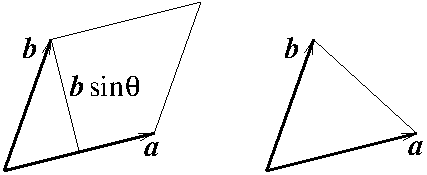
\includegraphics[width=0.33\textwidth]{algebra/vectors/paratri}
\end{center}
\caption{The parallelogram and the triangle defined by two vectors.}
\label{paratri}
\end{figure}



From the definition of the cross product, one can derive the following 
properties:
\begin{itemize}
\item
$\mathbf{a} \times \mathbf{b} = - \mathbf{b} \times \mathbf{a}$, 
anti-commutative.
\item
$\alpha ( \mathbf{a} \times \mathbf{b} ) =
( \alpha \mathbf{a} ) \times \mathbf{b} =
\mathbf{a} \times ( \alpha \mathbf{b} )$, associativity of scalar 
multiplication.
\item
$\mathbf{a} \times ( \mathbf{b} + \mathbf{c} ) = 
\mathbf{a} \times \mathbf{b} + \mathbf{a} \times \mathbf{c}$,
distributive.
\item
$( \mathbf{a} \times \mathbf{b} ) \times \mathbf{c} \neq
\mathbf{a} \times ( \mathbf{b} \times \mathbf{c} )$.  The cross 
product is not associative.
\item
$ \mathbf{i} \times \mathbf{i} = \mathbf{j} \times \mathbf{j} =
\mathbf{k} \times \mathbf{k} = 0$.
\item
$ \mathbf{i} \times \mathbf{j} = \mathbf{k}$, 
$\mathbf{j} \times \mathbf{k} = \mathbf{i}$,
$\mathbf{k} \times \mathbf{i} = \mathbf{j}$.
\item
\[
\mathbf{a} \times \mathbf{b} = 
(a_2 b_3 - a_3 b_2) \mathbf{i} + (a_3 b_1 - a_1 b_3) \mathbf{j}
+ (a_1 b_2 - a_2 b_1) \mathbf{k} =
\begin{vmatrix}
\mathbf{i} & \mathbf{j} & \mathbf{k} \\
a_1 & a_2 & a_3 \\
b_1 & b_2 & b_3
\end{vmatrix},
\]
cross product in terms of rectangular components.
\item
If $\mathbf{a} \times \mathbf{b} = \mathbf{0}$ then either $\mathbf{a}$ and 
$\mathbf{b}$ are parallel or one of $\mathbf{a}$ or $\mathbf{b}$ is zero.
\end{itemize}









\paragraph{Scalar Triple Product.}
Consider the volume of the parallelopiped defined by three vectors.
(See Figure~\ref{paraped}.)
The area of the base is $\left| |\mathbf{b}| |\mathbf{c}| \sin \theta \right|$, 
where $\theta$
is the angle between $\mathbf{b}$ and $\mathbf{c}$.  The height is
$| \mathbf{a} | \cos \phi$, where $\phi$ is the angle between
$\mathbf{b} \times \mathbf{c}$ and $\mathbf{a}$.  Thus the volume of 
the parallelopiped is 
$|\mathbf{a}| |\mathbf{b}| |\mathbf{c}| \sin \theta \cos \phi$.

\begin{figure}[htb!]
\begin{center}
  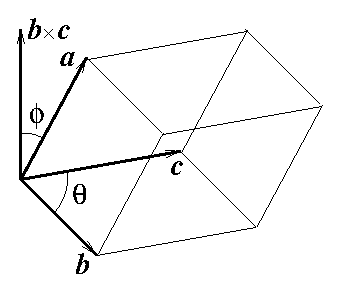
\includegraphics[width=0.25\textwidth]{algebra/vectors/paraped}
\end{center}
\caption{The parallelopiped defined by three vectors.}
\label{paraped}
\end{figure}

Note that 
\begin{align*}
\left| \mathbf{a} \cdot (\mathbf{b} \times \mathbf{c}) \right|
        &= \left| \mathbf{a} \cdot ( |\mathbf{b}| |\mathbf{c}| \sin \theta \ \mathbf{n} ) 
                \right| \\
        &= \left| |\mathbf{a}| |\mathbf{b}| |\mathbf{c}| \sin \theta \cos \phi \right|.
\end{align*}
Thus $\left| \mathbf{a} \cdot (\mathbf{b} \times \mathbf{c}) \right|$ is the volume of 
the parallelopiped.  $\mathbf{a} \cdot ( \mathbf{b} \times \mathbf{c} )$ is the volume
or the negative of the volume depending on whether 
$\{\mathbf{a}, \mathbf{b},\mathbf{c}\}$ is a right or left-handed system.

Note that parentheses are unnecessary in 
$\mathbf{a} \cdot \mathbf{b} \times \mathbf{c}$.  There is only one way to 
interpret the expression.  If you did the dot product first then you
would be left with the cross product of a scalar and a vector 
which is meaningless.  $\mathbf{a} \cdot \mathbf{b} \times \mathbf{c}$ is called
the \textit{scalar triple product}.


\paragraph{Plane Defined by Three Points.}
Three points which are not collinear define a plane.  Consider a plane 
that passes through the three points $\mathbf{a}$, $\mathbf{b}$ and $\mathbf{c}$.
One way of expressing that the point $\mathbf{x}$ lies in the plane is that 
the vectors $\mathbf{x} - \mathbf{a}$, $\mathbf{b} - \mathbf{a}$ and $\mathbf{c} - \mathbf{a}$ 
are coplanar.  (See Figure~\ref{stpplane}.)
If the vectors are coplanar, then the parallelopiped
defined by these three vectors will have zero volume.  We can express this
in an equation using the scalar triple product,
\[
(\mathbf{x} - \mathbf{a}) \cdot (\mathbf{b} - \mathbf{a}) \times (\mathbf{c} - \mathbf{a}) = 0.
\]

\begin{figure}[htb!]
\begin{center}
  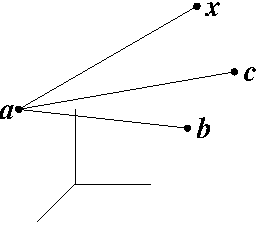
\includegraphics[width=0.2\textwidth]{algebra/vectors/stpplane}
\end{center}
\caption{Three points define a plane.}
\label{stpplane}
\end{figure}







%% CONTINUE: Edit this to fit in this chapter.
%%============================================================================
\section{Sets of Vectors in n Dimensions}

\paragraph{Orthogonality.}
Consider two $n$-dimensional vectors
\[
\mathbf{x} = (x_1, x_2, \ldots, x_n), \qquad
        \mathbf{y} = (y_1, y_2, \ldots, y_n).
\]
The inner product of these vectors can be defined
\[
\langle \mathbf{x} | \mathbf{y} \rangle \equiv
\mathbf{x} \cdot \mathbf{y} = \sum_{i=1}^n x_i y_i.
\]
The vectors are orthogonal if $\mathbf{x} \cdot \mathbf{y} = 0$.  The norm of
a vector is the length of the vector generalized to $n$ dimensions.
\[
\| \mathbf{x} \| = \sqrt{\mathbf{x} \cdot \mathbf{x}}
\]

Consider a set of vectors
\[ \{\mathbf{x}_1, \mathbf{x}_2, \ldots, \mathbf{x}_m\}.\]
If each pair of vectors in the set is orthogonal, then the set is orthogonal.
\[
\mathbf{x}_i \cdot \mathbf{x}_j = 0 \quad \mathrm{if}\ i \neq j
\]
If in addition each vector in the set has norm $1$, then the set is
orthonormal.
\[
\mathbf{x}_i \cdot \mathbf{x}_j = \delta_{i j} =
        \begin{cases}
        1 \quad &\mathrm{if}\ i = j \\
        0 \quad &\mathrm{if}\ i \neq j
        \end{cases}
\]
Here $\delta_{i j}$ is known as the Kronecker delta function.
\index{Kronecker delta function}
\index{delta function!Kronecker}


\paragraph{Completeness.}
\index{completeness!sets of vectors}
A set of $n$, $n$-dimensional vectors
\[
\{\mathbf{x}_1, \mathbf{x}_2, \ldots, \mathbf{x}_n\}
\]
is \textit{complete} if any $n$-dimensional
vector can be written as a linear combination of the vectors in the set.
That is, any vector $\mathbf{y}$ can be written
\[
\mathbf{y} = \sum_{i=1}^n c_i \mathbf{x}_i.
\]
Taking the inner product of each side of this equation with $\mathbf{x}_m$,
\begin{align*}
\mathbf{y} \cdot \mathbf{x}_m &= \left( \sum_{i=1}^n c_i \mathbf{x}_i \right)
        \cdot \mathbf{x}_m \\
        &= \sum_{i=1}^n c_i \mathbf{x}_i \cdot \mathbf{x}_m \\
        &= c_m \mathbf{x}_m \cdot \mathbf{x}_m \\
c_m     &= \frac{\mathbf{y} \cdot \mathbf{x}_m }{\| \mathbf{x}_m \|^2}
\end{align*}
Thus $\mathbf{y}$ has the expansion
\[
\mathbf{y} = \sum_{i=1}^n \frac{\mathbf{y} \cdot \mathbf{x}_i }{\| \mathbf{x}_i \|^2} \mathbf{x}_i.
\]
If in addition the set is orthonormal, then
\[
\mathbf{y} = \sum_{i=1}^n (\mathbf{y} \cdot \mathbf{x}_i) \mathbf{x}_i.
\]














\raggedbottom
%%=============================================================================
\exercises{
\pagebreak
\flushbottom
\section{Exercises}


%% CONTINUE
%% A paraboloid collects plane waves.


%%-----------------------------------------------------------------------------
\begin{large}
\noindent
\textbf{The Dot and Cross Product}
\end{large}



%% Prove the distributive law for the dot product,
\begin{Exercise}
\label{exercise distributive law dot product}
Prove the distributive law for the dot product,
\[
\mathbf{a} \cdot ( \mathbf{b} + \mathbf{c} ) 
= \mathbf{a} \cdot \mathbf{b} + \mathbf{a} \cdot \mathbf{c}.
\]

\hintsolution{distributive law dot product}
\end{Exercise}



%% \mathbf{a} \cdot \mathbf{b} = a_1 b_1 + a_2 b_2 + a_3 b_3.
\begin{Exercise}
\label{exercise a.b = ai bi}
Prove that
\[
\mathbf{a} \cdot \mathbf{b} = a_i b_i \equiv a_1 b_1 + \cdots + a_n b_n.
\]

\hintsolution{a.b = ai bi}
\end{Exercise}




%% What is the angle?
\begin{Exercise}
\label{exercise angle between i+j i+3j}
What is the angle between the vectors $\mathbf{i} + \mathbf{j}$ and
$\mathbf{i} + 3 \mathbf{j}$?

\hintsolution{angle between i+j i+3j}
\end{Exercise}




%% Prove the distributive law for the cross product,
\begin{Exercise}
\label{exercise distributive law cross product}
Prove the distributive law for the cross product,
\[
\mathbf{a} \times ( \mathbf{b} + \mathbf{c} ) 
= \mathbf{a} \times \mathbf{b} + \mathbf{a} \times \mathbf{b}.
\]

\hintsolution{distributive law cross product}
\end{Exercise}



%% Matrix form of cross product
\begin{Exercise}
\label{exercise matrix form of cross product}
Show that
\[
\mathbf{a} \times \mathbf{b} =
\begin{vmatrix}
\mathbf{i} & \mathbf{j} & \mathbf{k} \\
a_1 & a_2 & a_3 \\
b_1 & b_2 & b_3
\end{vmatrix}
\]

\hintsolution{matrix form of cross product}
\end{Exercise}




%% What is the area of the quadrilateral?
\begin{Exercise}
\label{exercise area quadrilateral 11 42 37 23}
What is the area of the quadrilateral with vertices at $(1,1)$, $(4,2)$,
$(3,7)$ and $(2,3)$?

\hintsolution{area quadrilateral 11 42 37 23}
\end{Exercise}



%% What is the volume of the tetrahedron?
\begin{Exercise}
\label{exercise volume tetrahedron 110 321 241 125}
What is the volume of the tetrahedron with vertices at $(1,1,0)$, $(3,2,1)$,
$(2,4,1)$ and $(1,2,5)$?

\hintsolution{volume tetrahedron 110 321 241 125}
\end{Exercise}




%% What is the equation of the plane that passes through the points
\begin{Exercise}
\label{exercise equation of plane 123 231 312}
What is the equation of the plane that passes through the points
$(1,2,3)$, $(2,3,1)$ and $(3,1,2)$?  What is the distance from the point
$(2,3,5)$ to the plane?

\hintsolution{equation of plane 123 231 312}
\end{Exercise}













\raggedbottom
}
%%=============================================================================
\hints{
\pagebreak
\flushbottom
\section{Hints}




%%-----------------------------------------------------------------------------
\begin{large}
\noindent
\textbf{The Dot and Cross Product}
\end{large}




%% Prove the distributive law for the dot product,
\begin{Hint}
\label{hint distributive law dot product}
First prove the distributive law when the first vector is of unit length,
\[
\mathbf{n} \cdot ( \mathbf{b} + \mathbf{c} ) 
= \mathbf{n} \cdot \mathbf{b} + \mathbf{n} \cdot \mathbf{c}.
\]
Then all the quantities in the equation are projections onto the unit vector
$\mathbf{n}$ and you can use geometry.
\end{Hint}




%% \mathbf{a} \cdot \mathbf{b} = a_1 b_1 + a_2 b_2 + a_3 b_3.
\begin{Hint}
\label{hint a.b = ai bi}
First prove that the dot product of a rectangular unit vector with itself
is one and the dot product of two distinct rectangular unit vectors is 
zero.  Then write $\mathbf{a}$ and $\mathbf{b}$ in rectangular components 
and use the distributive law.
\end{Hint}



%% What is the angle?
\begin{Hint}
\label{hint angle between i+j i+3j}
Use $\mathbf{a} \cdot \mathbf{b} = | \mathbf{a} | | \mathbf{b} | \cos \theta$.
\end{Hint}




%% Prove the distributive law for the cross product,
\begin{Hint}
\label{hint distributive law cross product}
First consider the case that both $\mathbf{b}$ and $\mathbf{c}$ are orthogonal to 
$\mathbf{a}$.  Prove the distributive law in this case from geometric 
considerations.

Next consider two arbitrary vectors $\mathbf{a}$ and $\mathbf{b}$.  We can write 
$\mathbf{b} = \mathbf{b}_\perp + \mathbf{b}_\parallel$ where $\mathbf{b}_\perp$ is 
orthogonal to $\mathbf{a}$ and $\mathbf{b}_\parallel$ is parallel to $\mathbf{a}$.
Show that
\[
\mathbf{a} \times \mathbf{b} = \mathbf{a} \times \mathbf{b}_\perp.
\]

Finally prove the distributive law for arbitrary $\mathbf{b}$ and $\mathbf{c}$.
\end{Hint}







%% Matrix form of cross product
\begin{Hint}
\label{hint matrix form of cross product}
Write the vectors in their rectangular components and use,
\[
\mathbf{i} \times \mathbf{j} = \mathbf{k}, \quad
\mathbf{j} \times \mathbf{k} = \mathbf{i}, \quad
\mathbf{k} \times \mathbf{i} = \mathbf{j},
\]
and, 
\[
\mathbf{i} \times \mathbf{i} = 
\mathbf{j} \times \mathbf{j} = 
\mathbf{k} \times \mathbf{k} = 0.
\]
\end{Hint}



%% What is the area of the quadrilateral?
\begin{Hint}
\label{hint area quadrilateral 11 42 37 23}
The quadrilateral is composed of two triangles.
The area of a triangle defined by the two vectors $\mathbf{a}$ and 
$\mathbf{b}$ is $\frac{1}{2} | \mathbf{a} \cdot \mathbf{b} |$.
\end{Hint}





%% What is the volume of the tetrahedron?
\begin{Hint}
\label{hint volume tetrahedron 110 321 241 125}
Justify that the area of a tetrahedron determined by three vectors is one 
sixth the area of the parallelogram determined by those three vectors.
The area of a parallelogram determined by three vectors is the magnitude of
the scalar triple product of the vectors: 
$\mathbf{a} \cdot \mathbf{b} \times \mathbf{c}$.
\end{Hint}







%% What is the equation of the plane that passes through the points
\begin{Hint}
\label{hint equation of plane 123 231 312}
The equation of a line that is orthogonal to $\mathbf{a}$ and passes
through the point $\mathbf{b}$ is $\mathbf{a} \cdot \mathbf{x} = 
\mathbf{a} \cdot \mathbf{b}$.  The distance of a point $\mathbf{c}$ 
from the plane is 
\[
\left | (\mathbf{c} - \mathbf{b} ) \cdot \frac{ \mathbf{a} }
{ | \mathbf{a} | } \right|
\]
\end{Hint}





\raggedbottom
}
%%=============================================================================
\solutions{
\pagebreak
\flushbottom
\section{Solutions}


%%-----------------------------------------------------------------------------
\begin{large}
\noindent
\textbf{The Dot and Cross Product}
\end{large}



%% Prove the distributive law for the dot product,
\begin{Solution}
\label{solution distributive law dot product}
First we prove the distributive law when the first vector is of unit length, 
i.e.,
\begin{equation}
\label{dotdistnorm}
\mathbf{n} \cdot ( \mathbf{b} + \mathbf{c} ) 
= \mathbf{n} \cdot \mathbf{b} + \mathbf{n} \cdot \mathbf{c}.
\end{equation}
From Figure~\ref{dotdist} we see that the projection of the vector 
$\mathbf{b} + \mathbf{c}$ onto $\mathbf{n}$ 
is equal to the sum of the projections 
$\mathbf{b} \cdot \mathbf{n}$ and $\mathbf{c} \cdot \mathbf{n}$.  

\begin{figure}[htb!]
\begin{center}
  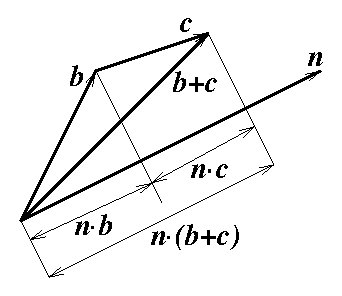
\includegraphics[width=0.3\textwidth]{algebra/vectors/dotdist}
\end{center}
\caption{The distributive law for the dot product.}
\label{dotdist}
\end{figure}

Now we extend the result to the case when the first vector has arbitrary
length.  We define $\mathbf{a} = | \mathbf{a} | \mathbf{n}$ and multiply
Equation~\ref{dotdistnorm} by the scalar, $| \mathbf{a} |$.
\begin{gather*}
| \mathbf{a} | \mathbf{n} \cdot ( \mathbf{b} + \mathbf{c} ) 
  = | \mathbf{a} | \mathbf{n} \cdot \mathbf{b} 
  + | \mathbf{a} | \mathbf{n} \cdot \mathbf{c} \\
\boxed{
\mathbf{a} \cdot ( \mathbf{b} + \mathbf{c} ) 
  = \mathbf{a} \cdot \mathbf{b} + \mathbf{a} \cdot \mathbf{c}.
}
\end{gather*}
\end{Solution}







%% \mathbf{a} \cdot \mathbf{b} = a_1 b_1 + a_2 b_2 + a_3 b_3.
\begin{Solution}
\label{solution a.b = ai bi}
First note that
\[
\mathbf{e}_i \cdot \mathbf{e}_i = | \mathbf{e}_i || \mathbf{e}_i | \cos(0) = 1.
\]
Then note that that dot product of any two distinct rectangular 
unit vectors is zero because they are orthogonal.
Now we write $\mathbf{a}$ and $\mathbf{b}$ in terms of their rectangular
components and use the distributive law.
\begin{align*}
\mathbf{a} \cdot \mathbf{b}
        &= a_i \mathbf{e}_i \cdot b_j \mathbf{e}_j \\
        &= a_i b_j \mathbf{e}_i \cdot \mathbf{e}_j \\
        &= a_i b_j \delta_{i j} \\
        &= a_i b_i
\end{align*}
\end{Solution}





%% What is the angle?
\begin{Solution}
\label{solution angle between i+j i+3j}
Since $\mathbf{a} \cdot \mathbf{b} = | \mathbf{a} | | \mathbf{b} |
\cos \theta$, we have
\[
\theta = \arccos \left( \frac{\mathbf{a} \cdot \mathbf{b}}
        {| \mathbf{a} | | \mathbf{b} | } \right)
\]
when $\mathbf{a}$ and $\mathbf{b}$ are nonzero.
\[
\theta = \arccos \left( \frac
        { (\mathbf{i} + \mathbf{j} ) \cdot ( \mathbf{i} + 3 \mathbf{j} ) }
        { |\mathbf{i} + \mathbf{j} | | \mathbf{i} + 3 \mathbf{j} | } \right)
= \arccos \left( \frac{4}{\sqrt{2} \sqrt{10}} \right)
= \arccos \left( \frac{2 \sqrt{5}}{5} \right)
\approx 0.463648
\]
\end{Solution}





%% Prove the distributive law for the cross product,
\begin{Solution}
\label{solution distributive law cross product}
First consider the case that both $\mathbf{b}$ and $\mathbf{c}$ are orthogonal to 
$\mathbf{a}$.  $\mathbf{b} + \mathbf{c}$ is the diagonal of the parallelogram
defined by $\mathbf{b}$ and $\mathbf{c}$, (see Figure~\ref{crossdst}).
Since $\mathbf{a}$ is orthogonal to each of these vectors, taking the cross
product of $\mathbf{a}$ with these vectors has the effect of rotating the
vectors through $\pi/2$ radians about $\mathbf{a}$ and multiplying their 
length by $|\mathbf{a}|$.   Note that $\mathbf{a} \times (\mathbf{b} + \mathbf{c})$
is the diagonal of the parallelogram defined by $\mathbf{a} \times \mathbf{b}$
and $\mathbf{a} \times \mathbf{c}$.  Thus we see that the distributive law holds
when $\mathbf{a}$ is orthogonal to both $\mathbf{b}$ and $\mathbf{c}$,
\[
\mathbf{a} \times ( \mathbf{b} + \mathbf{c} ) 
= \mathbf{a} \times \mathbf{b} + \mathbf{a} \times \mathbf{c}.
\]

\begin{figure}[htb!]
\begin{center}
  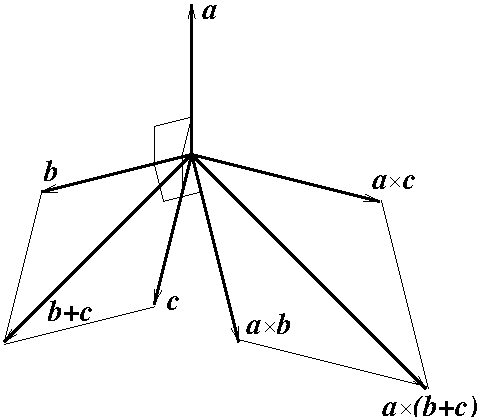
\includegraphics[width=0.4\textwidth]{algebra/vectors/crossdst}
\end{center}
\caption{The distributive law for the cross product.}
\label{crossdst}
\end{figure}

Now consider two arbitrary vectors $\mathbf{a}$ and $\mathbf{b}$.  We can write 
$\mathbf{b} = \mathbf{b}_\perp + \mathbf{b}_\parallel$ where $\mathbf{b}_\perp$ is 
orthogonal to $\mathbf{a}$ and $\mathbf{b}_\parallel$ is parallel to $\mathbf{a}$,
(see Figure~\ref{vperppar}).  

\begin{figure}[htb!]
\begin{center}
  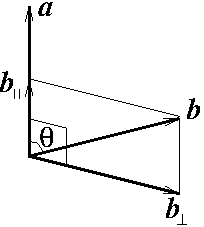
\includegraphics[width=0.2\textwidth]{algebra/vectors/vperppar}
\end{center}
\caption{The vector \textbf{b} written as a sum of components orthogonal
  and parallel to \textbf{a}.}
\label{vperppar}
\end{figure}

By the definition of the cross product,
\[
\mathbf{a} \times \mathbf{b} = | \mathbf{a} | | \mathbf{b} | \sin \theta \ \mathbf{n}.
\]
Note that 
\[
| \mathbf{b}_\perp | = | \mathbf{b} | \sin \theta,
\]
and that $\mathbf{a} \times \mathbf{b}_\perp$ is a vector in the same direction
as $\mathbf{a} \times \mathbf{b}$.  Thus we see that
\begin{align*}
\mathbf{a} \times \mathbf{b} 
        &= | \mathbf{a} | | \mathbf{b} | \sin \theta \ \mathbf{n} \\
        &= | \mathbf{a} | ( \sin \theta  | \mathbf{b} | ) \mathbf{n} \\
        &= | \mathbf{a} | | \mathbf{b}_\perp | \mathbf{n} 
        &= | \mathbf{a} | | \mathbf{b}_\perp | \sin(\pi/2) \mathbf{n} 
\end{align*}
\[
\mathbf{a} \times \mathbf{b} = \mathbf{a} \times \mathbf{b}_\perp.
\]

Now we are prepared to prove the distributive law for arbitrary $\mathbf{b}$
and $\mathbf{c}$.
\begin{align*}
\mathbf{a} \times ( \mathbf{b} + \mathbf{c} )
        &= \mathbf{a} \times ( \mathbf{b}_\perp + \mathbf{b}_\parallel 
                + \mathbf{c}_\perp + \mathbf{c}_\parallel ) \\
        &= \mathbf{a} \times ( ( \mathbf{b} + \mathbf{c} )_\perp 
                + ( \mathbf{b} + \mathbf{c} )_\parallel ) \\
        &= \mathbf{a} \times ( ( \mathbf{b} + \mathbf{c} )_\perp ) \\
        &= \mathbf{a} \times \mathbf{b}_\perp + \mathbf{a} \times \mathbf{c}_\perp \\
        &= \mathbf{a} \times \mathbf{b}+ \mathbf{a} \times \mathbf{c}
\end{align*}
\[
\boxed{
\mathbf{a} \times ( \mathbf{b} + \mathbf{c} )
        = \mathbf{a} \times \mathbf{b}+ \mathbf{a} \times \mathbf{c}
}
\]
\end{Solution}




%% Matrix form of cross product
\begin{Solution}
\label{solution matrix form of cross product}
We know that 
\[
\mathbf{i} \times \mathbf{j} = \mathbf{k}, \quad
\mathbf{j} \times \mathbf{k} = \mathbf{i}, \quad
\mathbf{k} \times \mathbf{i} = \mathbf{j},
\]
and that
\[
\mathbf{i} \times \mathbf{i} = 
\mathbf{j} \times \mathbf{j} = 
\mathbf{k} \times \mathbf{k} = 0.
\]
Now we write $\mathbf{a}$ and $\mathbf{b}$ in terms of their rectangular
components and use the distributive law to expand the cross product.
\begin{align*}
\mathbf{a} \times \mathbf{b}
        &= (a_1 \mathbf{i} + a_2 \mathbf{j} + a_3 \mathbf{k} ) \times
          (b_1 \mathbf{i} + b_2 \mathbf{j} + b_3 \mathbf{k} ) \\
        &= a_1 \mathbf{i} \times
          (b_1 \mathbf{i} + b_2 \mathbf{j} + b_3 \mathbf{k} ) 
        + a_2 \mathbf{j} \times
          (b_1 \mathbf{i} + b_2 \mathbf{j} + b_3 \mathbf{k} ) 
        + a_3 \mathbf{k} \times
          (b_1 \mathbf{i} + b_2 \mathbf{j} + b_3 \mathbf{k} ) \\
        &= a_1 b_2 \mathbf{k} + a_1 b_3 (- \mathbf{j})
        + a_2 b_1 (- \mathbf{k}) + a_2 b_3 \mathbf{i}
        + a_3 b_1 \mathbf{j} + a_3 b_2 (- \mathbf{i}) \\
        &= (a_2 b_3 - a_3 b_2) \mathbf{i} - (a_1 b_3 - a_3 b_1) \mathbf{j}
        + (a_1 b_2 - a_2 b_1) \mathbf{k}
\end{align*}
Next we evaluate the determinant.
\begin{align*}
\begin{vmatrix}
\mathbf{i} & \mathbf{j} & \mathbf{k} \\
a_1 & a_2 & a_3 \\
b_1 & b_2 & b_3
\end{vmatrix}
        &=      \mathbf{i}
                \begin{vmatrix}
                a_2 & a_3 \\
                b_2 & b_3 
                \end{vmatrix}
                - \mathbf{j}
                \begin{vmatrix}
                a_1 & a_3 \\
                b_1 & b_3 
                \end{vmatrix}
                + \mathbf{k}
                \begin{vmatrix}
                a_1 & a_2 \\
                b_1 & b_2 
                \end{vmatrix} \\
        &= (a_2 b_3 - a_3 b_2) \mathbf{i} - (a_1 b_3 - a_3 b_1) \mathbf{j}
        + (a_1 b_2 - a_2 b_1) \mathbf{k}
\end{align*}
Thus we see that,
\[
\mathbf{a} \times \mathbf{b} =
\begin{vmatrix}
\mathbf{i} & \mathbf{j} & \mathbf{k} \\
a_1 & a_2 & a_3 \\
b_1 & b_2 & b_3
\end{vmatrix}
\]
\end{Solution}




%% What is the area of the quadrilateral?
\begin{Solution}
\label{solution area quadrilateral 11 42 37 23}
The area area of the quadrilateral is the area of two triangles.  The first
triangle is defined by the vector from $(1,1)$ to $(4,2)$ and the vector
from $(1,1)$ to $(2,3)$.  The second triangle is defined by the vector from
$(3,7)$ to $(4,2)$ and the vector from $(3,7)$ to $(2,3)$. 
(See Figure~\ref{quad}.)
The area of a triangle defined by the two vectors $\mathbf{a}$ and 
$\mathbf{b}$ is $\frac{1}{2} | \mathbf{a} \cdot \mathbf{b} |$.
The area of the quadrilateral is then,
\[
\frac{1}{2} |(3 \mathbf{i} + \mathbf{j} ) \cdot ( \mathbf{i} + 2 \mathbf{j} )|
+ \frac{1}{2} |(\mathbf{i} - 5 \mathbf{j}) \cdot (-\mathbf{i} - 4 \mathbf{j} )|
= \frac{1}{2} (5) + \frac{1}{2} (19)
= 12.
\]

\begin{figure}[htb!]
\begin{center}
  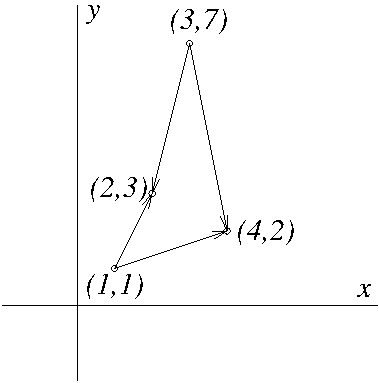
\includegraphics[width=0.3\textwidth]{algebra/vectors/quad}
\end{center}
\caption{Quadrilateral.}
\label{quad}
\end{figure}
\end{Solution}



%% What is the volume of the tetrahedron?
\begin{Solution}
\label{solution volume tetrahedron 110 321 241 125}
The tetrahedron is determined by the three vectors with tail at $(1,1,0)$
and heads at $(3,2,1)$, $(2,4,1)$ and $(1,2,5)$.  These are
$\langle 2,1,1 \rangle$, $\langle 1,3,1 \rangle$ and $\langle 0,1,5 \rangle$.  The area of the
tetrahedron is one sixth the area of the parallelogram determined by
these vectors.  (This is because the area of a pyramid is 
$\frac{1}{3} (\mathrm{base})(\mathrm{height})$.  The base of the tetrahedron is
half the area of the parallelogram and the heights are the same.
$\frac{1}{2} \frac{1}{3} = \frac{1}{6}$ )
Thus the area of a tetrahedron determined by three
vectors is $\frac{1}{6} | \mathbf{a} \cdot \mathbf{b} \times \mathbf{c} |$.
The area of the tetrahedron is
\[
\frac{1}{6} \left| \langle 2,1,1 \rangle \cdot \langle 1,3,1 \rangle \times \langle 1,2,5 \rangle 
        \right|
= \frac{1}{6} \left| \langle 2,1,1 \rangle \cdot \langle 13,-4,-1 \rangle \right|
= \frac{7}{2} 
\]
\end{Solution}


%% What is the equation of the plane that passes through the points
\begin{Solution}
\label{solution equation of plane 123 231 312}
The two vectors with tails at $(1,2,3)$ and heads at $(2,3,1)$ and $(3,1,2)$
are parallel to the plane.  Taking the cross product of these two vectors
gives us a vector that is orthogonal to the plane.
\[
\langle 1,1,-2 \rangle \times \langle 2,-1,-1 \rangle = \langle -3,-3,-3 \rangle
\]
We see that the plane is orthogonal to the vector $\langle 1,1,1 \rangle$ and passes
through the point $(1,2,3)$.  The equation of the plane is
\[
\langle 1,1,1 \rangle \cdot \langle x,y,z \rangle = \langle 1,1,1 \rangle \cdot \langle 1,2,3 \rangle,
\]
\[
x + y + z = 6.
\]
Consider the vector with tail at $(1,2,3)$ and head at $(2,3,5)$.  The
magnitude of the dot product of this vector with the unit normal vector gives
the distance from the plane.
\[
\left| \langle 1,1,2 \rangle \cdot \frac{ \langle 1,1,1 \rangle }{ | \langle 1,1,1 \rangle | } \right|
= \frac{4}{\sqrt{3}}
= \frac{4 \sqrt{3}}{3}
\]
\end{Solution}







\raggedbottom
}



\part{Calculus}

This part of the text covers elementary calculus.  I have not had time to 
write anything more than an introduction to the subject.  If I have 
the occasion to teach a course in calculus someday I'll write a proper text.

%%-----------------------------------------------------------------------------
%%
%%                                   Sean Mauch
%%                       California Institute of Technology
%%                       (a) 2000-2004 No Rights Reserved
%%
%%-----------------------------------------------------------------------------

\flushbottom


%% CONTINUE: update notation for interval from (,) to ( .. ).


%%============================================================================
%%============================================================================
\chapter{Differential Calculus}
\label{chapter_differential}
\index{differential calculus}



%%============================================================================
\section{Limits of Functions}
\index{limits of functions}


%% CONT motivate

\paragraph{Definition of a Limit.}
If the value of the function $y(x)$ gets arbitrarily close to $\psi$ as 
$x$ approaches the point $\xi$, then we say that the limit of the function
as $x$ approaches $\xi$ is equal to $\psi$.  This is written:
\[
\lim_{x \to \xi} y(x) = \psi
\]
Now we make the notion of ``arbitrarily close'' precise.  For any $\epsilon > 0$
there exists a $\delta > 0$ such that $|y(x) - \psi| < \epsilon$ for all
$0 < | x - \xi | < \delta$.  That is, there is an interval surrounding the
point $x = \xi$ for which the function is within $\epsilon$ of $\psi$.
See Figure~\ref{limfx}.  Note that the interval surrounding $x = \xi$ is
a deleted neighborhood, that is it does not contain the point $x = \xi$.
Thus the value of the function at $x = \xi$ need not be equal to $\psi$ for 
the limit to exist.  Indeed the function need not even be defined 
at $x = \xi$.


\begin{figure}[h!]
  \begin{center}
    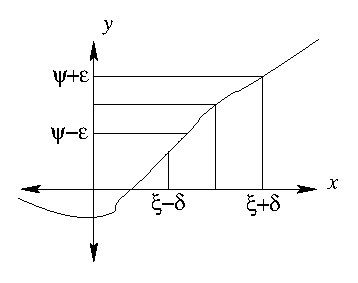
\includegraphics[width=0.33\textwidth]{calculus/differential/limfx}
  \end{center}
  \caption{The neighborhood of the point.}
  \label{limfx}
\end{figure}



To prove that a function has a limit at a point $\xi$ we first bound 
$|y(x) - \psi|$ in terms of $\delta$ for values of $x$ satisfying
$0 < |x - \xi| < \delta$.  Denote this upper bound by $u(\delta)$.  
Then for an arbitrary $\epsilon > 0$, we determine a $\delta > 0$ such that 
the the upper bound $u(\delta)$ and hence $|y(x) - \psi|$ is less than
$\epsilon$.




\begin{Example}
  Show that 
  \[
  \lim_{x \to 1} x^2 = 1.
  \]
  Consider any $\epsilon > 0$.  We need to show that there exists a $\delta > 0$
  such that $|x^2 - 1| < \epsilon$ for all $|x-1| < \delta$.  First we obtain
  a bound on $|x^2 - 1|$.
  \begin{align*}
    |x^2 - 1|
    &= | (x-1)(x+1) | \\
    &= | x-1 | | x+1 | \\
    &< \delta | x+1 | \\
    &= \delta |(x-1) + 2| \\
    &< \delta ( \delta + 2 ) 
  \end{align*}
  Now we choose a positive $\delta$ such that,
  \[
  \delta ( \delta + 2 ) = \epsilon.
  \]
  We see that
  \[
  \delta = \sqrt{1 + \epsilon} - 1,
  \]
  is positive and satisfies the criterion that $|x^2 - 1| < \epsilon$ for all
  $0 < |x-1| < \delta$.  Thus the limit exists.
\end{Example}






\begin{Example}
  \label{yxineqlim}
  Recall that the value of the function $y(\xi)$ need not be equal to 
  $\lim_{x \to \xi} y(x)$ for the limit to exist.  We show an example of this.
  Consider the function
  \[
  y(x) = 
  \begin{cases}
    1 & \mathrm{for}\ x \in \setZ, \\
    0 & \mathrm{for}\ x \not\in \setZ.
  \end{cases}
  \]
  For what values of $\xi$ does $\lim_{x \to \xi} y(x)$ exist?

  First consider $\xi \not\in \setZ$.  Then there exists an open 
  neighborhood $a<\xi<b$ around $\xi$ such that $y(x)$ is identically zero for
  $x \in (a,b)$.  Then trivially, $\lim_{x \to \xi} y(x) = 0$.

  Now consider $\xi \in \setZ$.  Consider any $\epsilon > 0$.  Then if
  $|x - \xi| < 1$ then $|y(x) - 0| = 0 < \epsilon$.  Thus we see that
  $\lim_{x \to \xi} y(x) = 0$.

  Thus, regardless of the value of $\xi$, $\lim_{x \to \xi} y(x) = 0$.
\end{Example}




\paragraph{Left and Right Limits.}
\index{limit!left and right}
With the notation $\lim_{x \to \xi^+} y(x)$ we denote the right limit of 
$y(x)$.  This is the limit as $x$ approaches $\xi$ from above.  
Mathematically: $\lim_{x \to \xi^+}$ exists if for any $\epsilon > 0$ 
there exists a $\delta > 0$ such that $|y(x) - \psi| < \epsilon$ for all 
$0 < \xi - x < \delta$.  The left limit $\lim_{x \to \xi^-} y(x)$ is 
defined analogously.



\begin{Example}
  Consider the function, $\frac{\sin x}{|x|}$, defined for $x \neq 0$.  
  (See Figure~\ref{sinxabsx}.)
  The left and right limits exist as $x$ approaches zero.
  \[
  \lim_{x \to 0^+} \frac{\sin x}{|x|} = 1, \qquad
  \lim_{x \to 0^-} \frac{\sin x}{|x|} = -1 
  \]
  However the limit, 
  \[
  \lim_{x \to 0} \frac{\sin x}{|x|},
  \]
  does not exist.
  \begin{figure}[h!]
    \begin{center}
      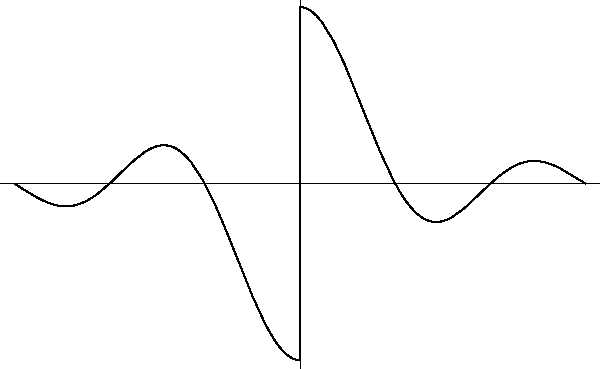
\includegraphics[width=0.33\textwidth]{calculus/differential/sinxabsx}
    \end{center}
    \caption{The function has left and right limits at the origin.}
    \label{sinxabsx}
  \end{figure}
\end{Example}







\paragraph{Properties of Limits.}
Let $\displaystyle \lim_{x \to \xi} f(x)$ and $\displaystyle \lim_{x \to \xi} g(x)$ 
exist.
\begin{itemize}
\item
  $\displaystyle 
  \lim_{x \to \xi} \left( a f(x) + b g(x) \right)
  = a \lim_{x \to \xi} f(x) + b \lim_{x \to \xi} g(x)
  $.
\item
  $\displaystyle 
  \lim_{x \to \xi} \left( f(x) g(x) \right)
  = \left(\lim_{x \to \xi} f(x) \right) \left( \lim_{x \to \xi} g(x) \right)
  $.
\item
  $\displaystyle 
  \lim_{x \to \xi} \left( \frac{f(x)}{g(x)} \right)
  = \frac{\lim_{x \to \xi} f(x)}{\lim_{x \to \xi} g(x)}
  $ 
  if 
  $\displaystyle 
  \lim_{x \to \xi} g(x) \neq 0
  $.
\end{itemize}





\begin{Example}
  We prove that if $\lim_{x \to \xi} f(x) = \phi$ and $\lim_{x \to \xi} g(x) = \gamma$ 
  exist then
  \[
  \lim_{x \to \xi} \left( f(x) g(x) \right)
  = \left(\lim_{x \to \xi} f(x) \right) \left( \lim_{x \to \xi} g(x) \right).
  \]
  Since the limit exists for $f(x)$, we know that for all $\epsilon > 0$ there 
  exists $\delta > 0$ such that $|f(x) - \phi| < \epsilon$ for $|x - \xi| < \delta$.  Likewise
  for $g(x)$.
  We seek to show that for all $\epsilon > 0$ there exists $\delta > 0$ such that
  $|f(x) g(x) - \phi \gamma| < \epsilon$ for $|x - \xi| < \delta$.  We proceed by writing
  $|f(x) g(x) - \phi \gamma|$, in terms of $|f(x) - \phi|$ and $|g(x) - \gamma|$, which
  we know how to bound.
  \begin{align*}
    | f(x) g(x) - \phi \gamma | 
    &= | f(x) (g(x) - \gamma) + (f(x) - \phi) \gamma | \\
    &\leq | f(x) | | g(x) - \gamma | + | f(x) - \phi | | \gamma |
  \end{align*}
  If we choose a $\delta$ such that $| f(x) | | g(x) - \gamma | < \epsilon / 2$ and 
  $| f(x) - \phi | | \gamma | < \epsilon / 2$ then we will have the desired 
  result: $| f(x) g(x) - \phi \gamma | < \epsilon$.
  Trying to ensure that $| f(x) | | g(x) - \gamma | < \epsilon / 2$ is hard because
  of the $|f(x)|$ factor.  We will replace that factor with a constant.
  We want to write $| f(x) - \phi | | \gamma | < \epsilon / 2$ as $| f(x) - \phi | < \epsilon / (2 |\gamma|)$,
  but this is problematic for the case $\gamma = 0$.  We fix these two problems
  and then proceed.  We choose $\delta_1$ such that $|f(x) - \phi| < 1$ for 
  $|x - \xi| < \delta_1$.  This gives us the desired form.
  \[
  | f(x) g(x) - \phi \gamma | 
  \leq (|\phi| + 1) | g(x) - \gamma | + | f(x) - \phi | (| \gamma | + 1),\ 
  \mathrm{for}\ |x - \xi| < \delta_1
  \]
  Next we choose $\delta_2$ such that $|g(x) - \gamma| < \epsilon / (2 (|\phi| + 1))$ for
  $|x - \xi| < \delta_2$ and choose $\delta_3$ such that $|f(x) - \phi| < \epsilon / (2 (|\gamma| + 1))$ 
  for $|x - \xi| < \delta_3$.
  Let $\delta$ be the minimum of $\delta_1$, $\delta_2$ and $\delta_3$.
  \begin{gather*}
    | f(x) g(x) - \phi \gamma | 
    \leq (|\phi| + 1) | g(x) - \gamma | + | f(x) - \phi | (| \gamma | + 1)
    < \frac{\epsilon}{2} + \frac{\epsilon}{2},\ 
    \mathrm{for}\ |x - \xi| < \delta
    \\
    | f(x) g(x) - \phi \gamma | < \epsilon,\ \mathrm{for}\ |x - \xi| < \delta
  \end{gather*}
  We conclude that the limit of a product is the product of the limits.
  \[
  \lim_{x \to \xi} \left( f(x) g(x) \right)
  = \left(\lim_{x \to \xi} f(x) \right) \left( \lim_{x \to \xi} g(x) \right)
  = \phi \gamma.
  \]
\end{Example}



\begin{Result}
  \textbf{Definition of a Limit.}
  The statement: 
  \[
  \lim_{x \to \xi} y(x) = \psi
  \]
  means that $y(x)$ gets arbitrarily close to $\psi$ as $x$ approaches $\xi$.
  For any $\epsilon > 0$ there exists a $\delta > 0$ such that 
  $|y(x) - \psi| < \epsilon$ for all $x$ in the neighborhood 
  $0 < | x - \xi | < \delta$.  The left and right limits,
  \[
  \lim_{x \to \xi^-} y(x) = \psi \quad \mathrm{and} \quad
  \lim_{x \to \xi^+} y(x) = \psi
  \]
  denote the limiting value as $x$ approaches $\xi$ respectively from 
  below and above.  The neighborhoods are respectively $-\delta < x - \xi < 0$ 
  and $0 < x - \xi < \delta$.

  \textbf{Properties of Limits.}
  Let $\displaystyle \lim_{x \to \xi} u(x)$ and 
  $\displaystyle \lim_{x \to \xi} v(x)$ exist.
  \begin{itemize}
  \item
    $\displaystyle 
    \lim_{x \to \xi} \left( a u(x) + b v(x) \right)
    = a \lim_{x \to \xi} u(x) + b \lim_{x \to \xi} v(x)
    $.
  \item
    $\displaystyle 
    \lim_{x \to \xi} \left( u(x) v(x) \right)
    = \left(\lim_{x \to \xi} u(x) \right) \left( \lim_{x \to \xi} v(x) \right)
    $.
  \item
    $\displaystyle 
    \lim_{x \to \xi} \left( \frac{u(x)}{v(x)} \right)
    = \frac{\lim_{x \to \xi} u(x)}{\lim_{x \to \xi} v(x)}
    $ 
    if 
    $\displaystyle 
    \lim_{x \to \xi} v(x) \neq 0
    $.
  \end{itemize}
\end{Result}





%%============================================================================
\section{Continuous Functions}
\index{continuous functions}



\paragraph{Definition of Continuity.}
\index{continuity}
A function $y(x)$ is said to be \textit{continuous at} $x = \xi$ if
the value of the function is equal to its limit, that is,
$\lim_{x \to \xi} y(x) = y(\xi)$.  Note that this one condition is 
actually the three conditions: $y(\xi)$ is defined, $\lim_{x \to \xi} y(x)$
exists and $\lim_{x \to \xi} y(x) = y(\xi)$.  A function is \textit{continuous}
if it is continuous at each point in its domain.  A function is 
\textit{continuous on the closed interval} $[a,b]$ if the function is 
continuous for each point $x \in (a,b)$ and $\lim_{x \to a^+} y(x) = y(a)$
and $\lim_{x \to b_-} y(x) = y(b)$.



\paragraph{Discontinuous Functions.}
\index{discontinuous functions}
If a function is not continuous at a point it is called \textit{discontinuous}
at that point.  If $\lim_{x \to \xi} y(x)$ exists but is not equal to 
$y(\xi)$, then the function has a \textit{removable discontinuity}.  It 
is thus named because we could define a continuous function
\[
z(x) = 
\begin{cases}
  y(x) & \mathrm{for}\ x \neq \xi, \\
  \lim_{x \to \xi} y(x) & \mathrm{for}\ x = \xi,
\end{cases}
\]
to remove the discontinuity.  If both the left and right limit of a function
at a point exist, but are not equal, then the function has a 
\textit{jump discontinuity} at that point.  If either the left or right
limit of a function does not exist, then the function is said to have an
\textit{infinite discontinuity} at that point.




\begin{Example}
  $\frac{\sin x}{x}$ has a removable discontinuity at $x=0$.  
  The Heaviside function,
  \[
  H(x) = 
  \begin{cases}
    0 & \mathrm{for}\ x < 0, \\
    1/2 & \mathrm{for}\ x = 0, \\
    1 & \mathrm{for}\ x > 0,
  \end{cases}
  \]
  has a jump discontinuity at $x = 0$.  $\frac{1}{x}$ has an infinite
  discontinuity at $x = 0$.  See Figure~\ref{discont}.
  \begin{figure}[h!]
    \begin{center}
      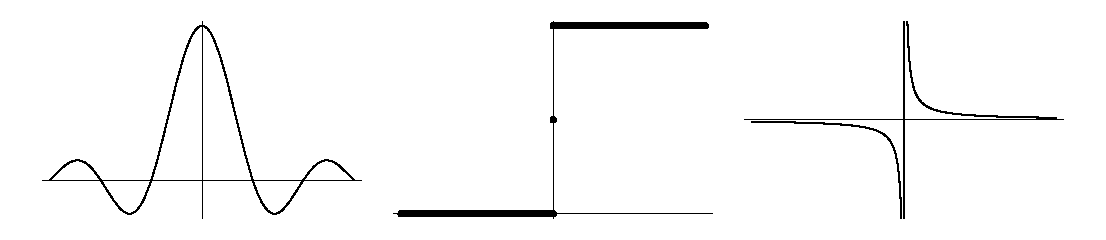
\includegraphics[width=0.9\textwidth]{calculus/differential/discont}
    \end{center}
    \caption{A removable discontinuity, a jump discontinuity and an 
      infinite discontinuity.}
    \label{discont}
  \end{figure}
\end{Example}





\paragraph{Properties of Continuous Functions.}
\begin{description}
  %%
\item{Arithmetic.}
  If $u(x)$ and $v(x)$ are continuous at $x = \xi$ then $u(x) \pm v(x)$ and
  $u(x) v(x)$ are continuous at $x = \xi$.  $\frac{u(x)}{v(x)}$ is 
  continuous at $x = \xi$ if $v(\xi) \neq 0$.
  %%
\item{Function Composition.}
  If $u(x)$ is continuous at $x = \xi$ and $v(x)$ is continuous at 
  $x = \mu = u(\xi)$ then $u(v(x))$ is continuous at $x = \xi$.  The 
  composition of continuous functions is a continuous function.
  %%
\item{Boundedness.}
  A function which is continuous on a closed interval is bounded in that
  closed interval.
  %%
\item{Nonzero in a Neighborhood.}
  If $y(\xi) \neq 0$ then there exists a neighborhood 
  $(\xi-\epsilon,\xi+\epsilon)$, $\epsilon > 0$ of the point $\xi$ such that
  $y(x) \neq 0$ for $x \in (\xi - \epsilon, \xi + \epsilon)$.
  %%
\item{Intermediate Value Theorem.}
  Let $u(x)$ be continuous on $[a,b]$.
  If $u(a) \leq \mu \leq u(b)$ then there exists $\xi \in [a,b]$ such that
  $u(\xi) = \mu$.  This is known as the \textit{intermediate value theorem}.
  \index{intermediate value theorem}
  A corollary of this is that if $u(a)$ and $u(b)$ are of opposite sign then
  $u(x)$ has at least one zero on the interval $(a,b)$.
  %%
\item{Maxima and Minima.}
  If $u(x)$ is continuous on $[a,b]$ then $u(x)$ has a maximum and a 
  minimum on $[a,b]$.  That is, there is at least one point $\xi \in [a,b]$ 
  such that $u(\xi) \geq u(x)$ for all $x \in [a,b]$ and there is at least one
  point $\psi \in [a,b]$ such that $u(\psi) \leq u(x)$ for all $x \in [a,b]$. 
\end{description}






\paragraph{Piecewise Continuous Functions.}
\index{piecewise continuous}
\index{continuous!piecewise}
A function is \textit{piecewise continuous} on an interval if the function
is bounded on the interval and the interval can be divided into a finite
number of intervals on each of which the function is continuous.
For example, the greatest integer function, $\lfloor x \rfloor$, is piecewise
continuous.  ($\lfloor x \rfloor$ is defined to the the greatest integer
less than or equal to $x$.)  See Figure~\ref{pwcont} for graphs of 
two piecewise continuous functions.
\begin{figure}[h!]
  \begin{center}
    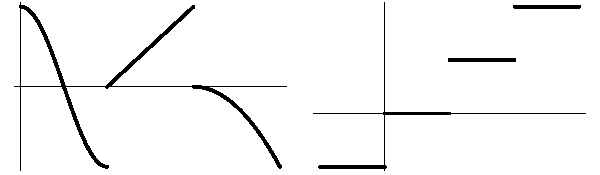
\includegraphics[width=0.6\textwidth]{calculus/differential/pwcont}
  \end{center}
  \caption{Piecewise continuous functions.}
  \label{pwcont}
\end{figure}





\paragraph{Uniform Continuity.}
\index{uniform continuity}
\index{continuity!uniform}
Consider a function $f(x)$ that is continuous on an interval.  This means 
that for any point $\xi$ in the interval and any positive $\epsilon$ there
exists a $\delta > 0$ such that $| f(x) - f(\xi) | < \epsilon$ for all
$0 < | x - \xi | < \delta$.  In general, this value of $\delta$ depends on 
both $\xi$ and $\epsilon$.  If $\delta$ can be chosen so it is a function
of $\epsilon$ alone and independent of $\xi$ then the function is said to
be \textit{uniformly continuous} on the interval.  A sufficient condition
for uniform continuity is that the function is continuous on a closed interval.






%%=============================================================================
\section{The Derivative}


Consider a function $y(x)$ on the interval $(x \ldots x+\Delta x)$
for some $\Delta x > 0$.
We define the increment $\Delta y = y(x + \Delta x) - y(x)$.  
The \textit{average rate of change}, (average velocity), of the function on the
interval is $\frac{\Delta y}{\Delta x}$.  The average rate of change 
is the slope of the secant line that passes through the points 
$(x, y(x))$ and $(x + \Delta x, y(x + \Delta x) )$.  
See Figure~\ref{increment}.


\begin{figure}[h!]
  \begin{center}
    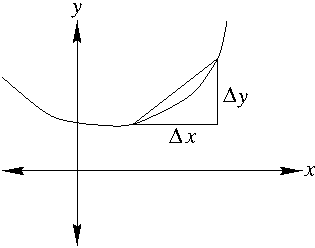
\includegraphics[width=0.33\textwidth]{calculus/differential/increment}
  \end{center}
  \caption{The increments.}
  \label{increment}
\end{figure}



If the slope of the secant line has a limit as $\Delta x$ approaches
zero then we call this slope 
the \textit{derivative} or \textit{instantaneous rate of change} 
of the function at the point $x$.  We denote the derivative by
$\frac{\dd y}{\dd x}$, which is a nice notation as the derivative is the limit 
of $\frac{\Delta y}{\Delta x}$ as $\Delta x \to 0$.
\[
\frac{\dd y}{\dd x} \equiv \lim_{\Delta x \to 0} \frac{y(x + \Delta x) - y(x)}{\Delta x}.
\]
$\Delta x$ may approach zero from below or above.
It is common to denote the derivative $\frac{\dd y}{\dd x}$ by 
$\frac{\dd }{\dd x} y$, $y'(x)$, $y'$ or $D y$.

A function is said to be \textit{differentiable} at a point if the
derivative exists there.  Note that differentiability implies continuity,
but not vice versa.





\begin{Example}
  Consider the derivative of $y(x) = x^2$ at the point $x = 1$.
  \begin{align*}
    y'(1)   &\equiv \lim_{\Delta x \to 0} 
    \frac{y(1 + \Delta x) - y(1) }{ \Delta x } \\
    &= \lim_{\Delta x \to 0} \frac{(1 + \Delta x)^2 - 1}{\Delta x} \\
    &= \lim_{\Delta x \to 0} ( 2 + \Delta x ) \\
    &= 2
  \end{align*}
  Figure~\ref{secantx2} shows the secant lines approaching the tangent line
  as $\Delta x$ approaches zero from above and below.
  \begin{figure}[h!]
    \begin{center}
      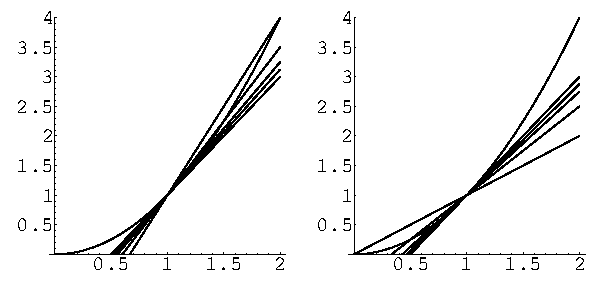
\includegraphics[width=0.8\textwidth]{calculus/differential/secantx2}
    \end{center}
    \caption{Secant lines and the tangent.}
    \label{secantx2}
  \end{figure}
\end{Example}





\begin{Example}
  We can compute the derivative of $y(x) = x^2$ at an arbitrary point $x$.
  \begin{align*}
    \frac{\dd}{\dd x} \left[ x^2 \right]
    &= \lim_{\Delta x \to 0} \frac{(x + \Delta x)^2 - x^2 }{\Delta x} \\
    &= \lim_{\Delta x \to 0} (2 x + \Delta x) \\
    &= 2 x
  \end{align*}
\end{Example}







\paragraph{Properties.}
Let $u(x)$ and $v(x)$ be differentiable.  Let $a$ and $b$ be constants.
Some fundamental properties of derivatives are:
\begin{alignat*}{2}
  &\frac{\dd}{\dd x}(a u+b v) = a \frac{\dd u}{\dd x} + b \frac{\dd v}{\dd x} 
  &\qquad &\mathrm{Linearity} 
  \\
  &\frac{\dd}{\dd x}(u v) = \frac{\dd u}{\dd x} v + u \frac{\dd v}{\dd x} 
  &\qquad &\mathrm{Product Rule} 
  \\
  &\frac{\dd}{\dd x}\left( \frac{u}{v} \right)
  = \frac{v \frac{\dd u}{\dd x} - u \frac{\dd v}{\dd x}}{v^2} 
  &\qquad &\mathrm{Quotient Rule} 
  \\
  &\frac{\dd}{\dd x}(u^a) = a u^{a-1} \frac{\dd u}{\dd x} 
  &\qquad &\mathrm{Power Rule} 
  \\
  &\frac{\dd}{\dd x} (u(v(x))) = \frac{\dd u}{\dd v} \frac{\dd v}{\dd x} 
  = u'(v(x)) v'(x)
  &\qquad &\mathrm{Chain Rule}
\end{alignat*}
These can be proved by using the definition of differentiation.


\begin{Example}
  Prove the quotient rule for derivatives.
  \begin{align*}
    \frac{\dd}{\dd x} \left( \frac{u}{v} \right)
    &= \lim_{\Delta x \to 0} \frac{\frac{u(x+\Delta x)}{v(x+\Delta x)} - \frac{u(x)}{v(x)} }{\Delta x}
    \\
    &= \lim_{\Delta x \to 0} \frac{ u(x+\Delta x) v(x) - u(x) v(x+\Delta x) }
    { \Delta x v(x) v(x + \Delta x) }
    \\
    &= \lim_{\Delta x \to 0} \frac{ u(x+\Delta x) v(x) -u(x) v(x)
      - u(x) v(x+\Delta x) + u(x) v(x) }{ \Delta x v(x) v(x) }
    \\
    &= \lim_{\Delta x \to 0} \frac{ (u(x+\Delta x) -u(x)) v(x)
      - u(x) ( v(x+\Delta x) - v(x) ) }{ \Delta x v^2(x) }
    \\
    &= \frac{ \lim_{\Delta x \to 0} \frac{u(x+\Delta x) -u(x)}{\Delta x} 
      v(x) - u(x) \lim_{\Delta x \to 0} \frac{v(x+\Delta x) - v(x)} {\Delta x}  }{ v^2(x) }
    \\
    &= \frac{v \frac{\dd u}{\dd x} - u \frac{\dd v}{\dd x}}{v^2} 
  \end{align*}
\end{Example}



\paragraph{Trigonometric Functions.}
Some derivatives of trigonometric functions are:
\begin{alignat*}{2}
  &\frac{\dd}{\dd x} \sin x = \cos x &\qquad 
  &\frac{\dd}{\dd x} \arcsin x = \frac{1}{(1-x^2)^{1/2}} 
  \\
  &\frac{\dd}{\dd x} \cos x = - \sin x &\qquad
  &\frac{\dd}{\dd x} \arccos x = \frac{-1}{(1-x^2)^{1/2}}
  \\
  &\frac{\dd}{\dd x} \tan x = \frac{1}{\cos^2 x} &\qquad
  &\frac{\dd}{\dd x} \arctan x = \frac{1}{1+x^2} 
  \\
  &\frac{\dd}{\dd x} \e^x = \e^x &\qquad 
  &\frac{\dd}{\dd x} \ln x = \frac{1}{x} 
  \\
  &\frac{\dd}{\dd x} \sinh x = \cosh x &\qquad
  &\frac{\dd}{\dd x} \arcsinh x = \frac{1}{(x^2+1)^{1/2}} 
  \\
  &\frac{\dd}{\dd x} \cosh x = \sinh x &\qquad
  &\frac{\dd}{\dd x} \arccosh x = \frac{1}{(x^2-1)^{1/2}} 
  \\
  &\frac{\dd}{\dd x} \tanh x = \frac{1}{\cosh^2 x} &\qquad
  &\frac{\dd}{\dd x} \arctanh x = \frac{1}{1-x^2} 
\end{alignat*}





\begin{Example}
  We can evaluate the derivative of $x^x$ by using the identity
  $a^b = \e^{b \ln a}$.
  \begin{align*}
    \frac{\dd}{\dd x} x^x
    &= \frac{\dd}{\dd x} \e^{x \ln x} 
    \\
    &= \e^{x \ln x} \frac{\dd}{\dd x} (x \ln x) 
    \\
    &= x^x (1 \cdot \ln x + x \frac{1}{x} ) 
    \\
    &= x^x (1 + \ln x)
  \end{align*}
\end{Example}




\paragraph{Inverse Functions.}
If we have a function $y(x)$, we can consider $x$ as a function of $y$, $x(y)$.
For example, if $y(x) = 8 x^3$ then $x(y) = \sqrt[3]{y} / 2$; if 
$y(x) = \frac{x+2}{x+1}$ then $x(y) = \frac{2-y}{y-1}$.  The derivative
of an inverse function is
\[
\frac{\dd}{\dd y} x(y) = \frac{1}{\frac{\dd y}{\dd x}}.
\]


\begin{Example}
  The inverse function of $y(x) = \e^x$ is $x(y) = \ln y$.  We can obtain
  the derivative of the logarithm from the derivative of the exponential.
  The derivative of the exponential is
  \[
  \frac{\dd y}{\dd x} = \e^x.
  \]
  Thus the derivative of the logarithm is
  \[
  \frac{\dd}{\dd y} \ln y = \frac{\dd}{\dd y} x(y) 
  = \frac{1}{\frac{\dd y}{\dd x} }
  = \frac{1}{\e^x} = \frac{1}{y}.
  \] 
\end{Example}











%%=============================================================================
\section{Implicit Differentiation}

An \textit{explicitly defined} function has the form $y = f(x)$.  A
\textit{implicitly defined} function has the form $f(x, y) = 0$.  A few 
examples of implicit functions are $x^2 + y^2 - 1 = 0$ and 
$x + y + \sin(x y) = 0$.  Often it is not possible to write an implicit
equation in explicit form.  This is true of the latter example above.
One can calculate the derivative of $y(x)$ in terms of $x$ and $y$ 
even when $y(x)$ is defined by an implicit equation.  


\begin{Example}
  Consider the implicit equation
  \[
  x^2 - x y - y^2 = 1.
  \]
  This implicit equation can be solved for the dependent variable.
  \[
  y(x) = \frac{1}{2} \left( -x \pm \sqrt{5 x^2 - 4} \right).
  \]
  We can differentiate this expression to obtain
  \[
  y' = \frac{1}{2} \left( -1 \pm \frac{5 x}{\sqrt{5 x^2 - 4}} \right).
  \]
  One can obtain the same result without first solving for $y$.  If we 
  differentiate the implicit equation, we obtain
  \[
  2 x - y - x \frac{\dd y}{\dd x} - 2 y \frac{\dd y}{\dd x} = 0.
  \]
  We can solve this equation for $\frac{\dd y}{\dd x}$.
  \[
  \frac{\dd y}{\dd x} = \frac{2x - y}{x + 2y}
  \]
  We can differentiate this expression to obtain the second derivative of $y$.
  \begin{align*}
    \frac{\dd^2 y}{\dd x^2}
    &= \frac{ (x+2y) (2-y') - (2x-y)(1+2y') }{ (x + 2y)^2 } \\
    &= \frac{ 5(y - x y') }{ (x + 2y)^2 } \\
    \intertext{Substitute in the expression for $y'$.}
    &= - \frac{ 10 (x^2 - x y - y^2) }{ (x + 2y)^2 } \\
    \intertext{Use the original implicit equation.}
    &= - \frac{ 10 }{ (x + 2y)^2 } 
  \end{align*}
\end{Example}








%%=============================================================================
\section{Maxima and Minima}

A differentiable function is \textit{increasing} where $f'(x) > 0$, 
\textit{decreasing} where $f'(x) < 0$ and \textit{stationary}
where $f'(x) = 0$.

A function $f(x)$ has a \textit{relative maxima} at a point $x = \xi$ if
there exists a neighborhood around $\xi$ such that $f(x) \leq f(\xi)$ for 
$x \in (x - \delta, x + \delta)$, $\delta > 0$.  The \textit{relative 
  minima} is defined analogously.  Note that this definition does not 
require that the function be differentiable, or even continuous.
We refer to relative maxima and minima collectively are \textit{relative
  extrema}.



\paragraph{Relative Extrema and Stationary Points.}
If $f(x)$ is differentiable and $f(\xi)$ is a relative extrema then
$x=\xi$ is a stationary point, $f'(\xi) = 0$.  We can prove this
using left and right limits.  Assume that $f(\xi)$ is a relative maxima.
Then there is a neighborhood $(x - \delta, x + \delta)$, $\delta > 0$ for 
which $f(x) \leq f(\xi)$.  Since $f(x)$ is differentiable the derivative
at $x = \xi$,
\[
f'(\xi) = \lim_{\Delta x \to 0} \frac{f(\xi + \Delta x) - f(\xi)}{\Delta x},
\]
exists.  This in turn means that the left and right limits exist and 
are equal.  Since $f(x) \leq f(\xi)$ for $\xi-\delta < x < \xi$ the left
limit is non-positive,
\[
f'(\xi) = \lim_{\Delta x \to 0^-} \frac{ f(\xi + \Delta x) - f(\xi) }
{ \Delta x } \leq 0.
\]
Since $f(x) \leq f(\xi)$ for $\xi < x < \xi + \delta$ the right
limit is nonnegative,
\[
f'(\xi) = \lim_{\Delta x \to 0^+} \frac{ f(\xi + \Delta x) - f(\xi) }
{ \Delta x } \geq 0.
\]
Thus we have $0 \leq f'(\xi) \leq 0$ which implies that $f'(\xi) = 0$.


It is not true that all stationary points are relative extrema.  That is,
$f'(\xi) = 0$ does not imply that $x = \xi$ is an extrema.  Consider the
function $f(x) = x^3$.  $x = 0$ is a stationary point since $f'(x) = x^2$,
$f'(0) = 0$.  However, $x = 0$ is neither a relative maxima nor a 
relative minima.



It is also not true that all relative extrema are stationary points.  Consider
the function $f(x) = |x|$.  The point $x = 0$ is a relative minima, but
the derivative at that point is undefined.


\paragraph{First Derivative Test.}
Let $f(x)$ be differentiable and $f'(\xi) = 0$.
\begin{itemize}
\item
  If $f'(x)$ changes sign from positive to negative as we pass through $x = \xi$
  then the point is a relative maxima.
\item
  If $f'(x)$ changes sign from negative to positive as we pass through $x = \xi$
  then the point is a relative minima.
\item
  If $f'(x)$ is not identically zero in a neighborhood of $x = \xi$ and it 
  does not change sign as we pass through the point then $x = \xi$ is 
  not a relative extrema.
\end{itemize}



\begin{Example}
  Consider $y = x^2$ and the point $x = 0$.  The function is differentiable.
  The derivative, $y' = 2x$, vanishes at $x = 0$.  Since $y'(x)$ is negative
  for $x < 0$ and positive for $x > 0$, the point $x = 0$ is a relative 
  minima.  See Figure~\ref{maxminno}.
\end{Example}





\begin{Example}
  Consider $y = \cos x$ and the point $x = 0$.  The function is differentiable.
  The derivative, $y' = - \sin x$ is positive for $-\pi < x < 0$ and negative
  for $0 < x < \pi$.  Since the sign of $y'$ goes from positive to negative,
  $x = 0$ is a relative maxima.  See Figure~\ref{maxminno}.
\end{Example}




\begin{Example}
  Consider $y = x^3$ and the point $x = 0$.  The function is differentiable.
  The derivative, $y' = 3 x^2$ is positive for $x < 0$ and positive
  for $0 < x$.  Since $y'$ is not identically zero and the sign of $y'$ 
  does not change, $x = 0$ is not a relative extrema.  See Figure~\ref{maxminno}.
\end{Example}


\begin{figure}[h!]
  \begin{center}
    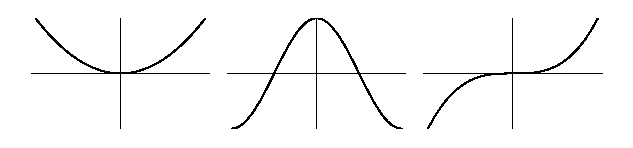
\includegraphics[width=0.8\textwidth]{calculus/differential/minmaxno}
  \end{center}
  \caption{Graphs of functions with stationary points.}
  \label{maxminno}
\end{figure}




\paragraph{Concavity.}
If the portion of a curve in some neighborhood of a point lies above the
tangent line through that point, the curve is said to be \textit{concave
  upward}.  If it lies below the tangent it is \textit{concave downward}.
If a function is twice differentiable then $f''(x) > 0$ where it is
concave upward and $f''(x) < 0$ where it is concave downward.
Note that $f''(x) > 0$ is a sufficient, but not a necessary condition
for a curve to be concave upward at a point.  A curve may be concave 
upward at a point where the second derivative vanishes.
A point where the curve changes concavity is called a \textit{point of
  inflection}.  At such a point the second derivative vanishes, 
$f''(x) = 0$.  For twice continuously differentiable functions, $f''(x) = 0$
is a necessary but not a sufficient condition for an inflection point.
The second derivative may vanish at places which are not inflection points.
See Figure~\ref{concave}.

\begin{figure}[h!]
  \begin{center}
    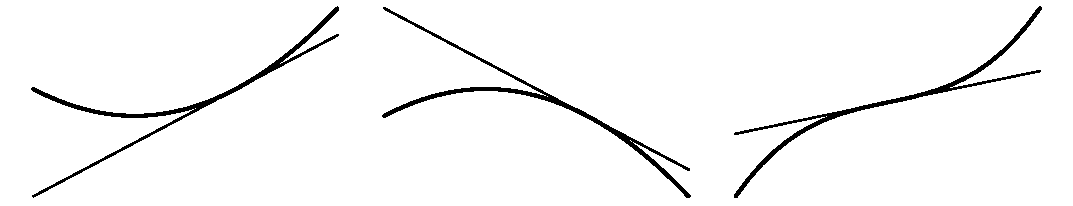
\includegraphics[width=0.8\textwidth]{calculus/differential/concave}
  \end{center}
  \caption{Concave upward, concave downward and an inflection point.}
  \label{concave}
\end{figure}






\paragraph{Second Derivative Test.}
Let $f(x)$ be twice differentiable and let $x = \xi$ be a stationary 
point, $f'(\xi) = 0$.
\begin{itemize}
\item
  If $f''(\xi) < 0$ then the point is a relative maxima.
\item
  If $f''(\xi) > 0$ then the point is a relative minima.
\item
  If $f''(\xi) = 0$ then the test fails.
\end{itemize}




\begin{Example}
  Consider the function $f(x) = \cos x$ and the point $x = 0$.  The derivatives
  of the function are $f'(x) = - \sin x$, $f''(x) = - \cos x$.  The point
  $x = 0$ is a stationary point, $f'(0) = - \sin(0) = 0$.  Since the second
  derivative is negative there, $f''(0) = - \cos(0) = -1$, the point is a 
  relative maxima.
\end{Example}






\begin{Example}
  Consider the function $f(x) = x^4$ and the point $x = 0$.  The derivatives
  of the function are $f'(x) = 4 x^3$, $f''(x) = 12 x^2$.  The point
  $x = 0$ is a stationary point.  Since the second derivative also 
  vanishes at that point the second derivative test fails.  One must use
  the first derivative test to determine that $x = 0$ is a relative minima.
\end{Example}








%%=============================================================================
\section{Mean Value Theorems}


\paragraph{Rolle's Theorem.}
If $f(x)$ is continuous in $[a,b]$, differentiable in $(a,b)$ and
$f(a) = f(b) = 0$ then there exists a point $\xi \in (a,b)$ such that
$f'(\xi) = 0$.  See Figure~\ref{rolle}.

\begin{figure}[h!]
  \begin{center}
    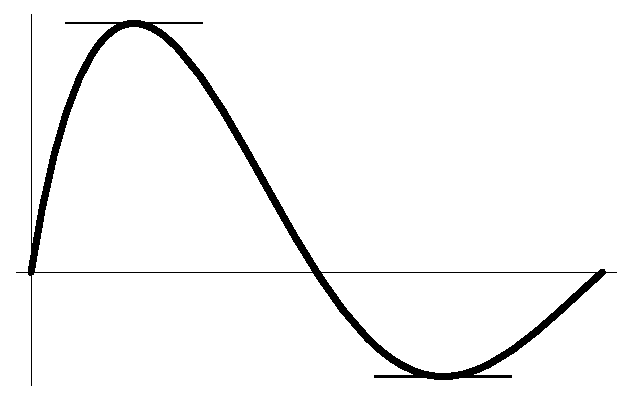
\includegraphics[width=0.3\textwidth]{calculus/differential/rolle}
  \end{center}
  \caption{Rolle's Theorem.}
  \label{rolle}
\end{figure}

To prove this we consider two cases.  First we have the 
trivial case that $f(x) \equiv 0$.  If $f(x)$ is not identically zero
then continuity implies that it must have a nonzero relative maxima or 
minima in $(a,b)$.  Let $x = \xi$ be one of these relative extrema.
Since $f(x)$ is differentiable, $x = \xi$ must be a stationary point,
$f'(\xi) = 0$.



\paragraph{Theorem of the Mean.}
If $f(x)$ is continuous in $[a,b]$ and differentiable in $(a,b)$ then there
exists a point $x = \xi$ such that
\[
f'(\xi) = \frac{f(b) - f(a)}{b - a}.
\]
That is, there is a point where the instantaneous velocity is equal to 
the average velocity on the interval.  

\begin{figure}[h!]
  \begin{center}
    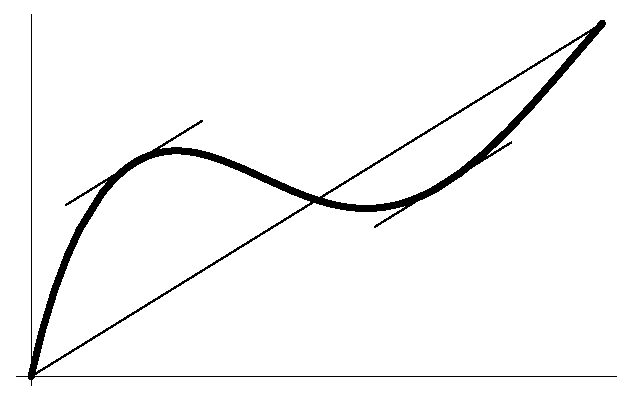
\includegraphics[width=0.3\textwidth]{calculus/differential/themean}
  \end{center}
  \caption{Theorem of the Mean.}
  \label{themean}
\end{figure}

We prove this theorem by applying
Rolle's theorem.  Consider the new function
\[
g(x) = f(x) - f(a) - \frac{f(b) - f(a)}{b - a} (x - a)
\]
Note that $g(a) = g(b) = 0$, so it satisfies the conditions of Rolle's 
theorem.  There is a point $x = \xi$ such that $g'(\xi) = 0$.
We differentiate the expression for $g(x)$ and substitute in $x = \xi$ to 
obtain the result.
\[
g'(x) = f'(x)  - \frac{f(b) - f(a)}{b-a} 
\]
\[
g'(\xi) = f'(\xi)  - \frac{f(b) - f(a)}{b-a} = 0
\]
\[
f'(\xi)  = \frac{f(b) - f(a)}{b-a}
\]




\paragraph{Generalized Theorem of the Mean.}
If $f(x)$ and $g(x)$ are continuous in $[a,b]$ and differentiable in $(a,b)$,
then there exists a point $x = \xi$ such that
\[
\frac{f'(\xi)}{g'(\xi)} = \frac{f(b) - f(a)}{g(b) - g(a)}.
\]
We have assumed that $g(a) \neq g(b)$ so that the denominator does not 
vanish and that $f'(x)$ and $g'(x)$ are not simultaneously zero which 
would produce an indeterminate form.  Note that this theorem reduces to
the regular theorem of the mean when $g(x) = x$.  The proof of the
theorem is similar to that for the theorem of the mean.





\paragraph{Taylor's Theorem of the Mean.}
If $f(x)$ is $n+1$ times continuously differentiable in $(a,b)$ then there
exists a point $x = \xi \in (a,b)$ such that
\begin{equation}
  \label{taylors_theorem}
  f(b) = f(a) + (b-a) f'(a) + \frac{(b-a)^2}{2!} f''(a) + \cdots + 
  \frac{(b-a)^n}{n!} f^{(n)}(a) 
  + \frac{(b-a)^{n+1}}{(n+1)!} f^{(n+1)}(\xi).
\end{equation}
For the case $n = 0$, the formula is
\[
f(b) = f(a) + (b-a) f'(\xi),
\]
which is just a rearrangement of the terms in the theorem of the mean,
\[
f'(\xi) = \frac{f(b) - f(a)}{b-a}.
\]
%% CONTINUE: Prove.





%%-----------------------------------------------------------------------------
\subsection{Application: Using Taylor's Theorem to Approximate Functions.}


One can use Taylor's theorem to approximate functions with polynomials.
Consider an infinitely differentiable function $f(x)$ and a point $x = a$.  
Substituting $x$ for $b$ into Equation~\ref{taylors_theorem} we obtain,
\[
\label{taylors_theorem_x}
f(x) = f(a) + (x-a) f'(a) + \frac{(x-a)^2}{2!} f''(a) + \cdots + 
\frac{(x-a)^n}{n!} f^{(n)}(a) 
+ \frac{(x-a)^{n+1}}{(n+1)!} f^{(n+1)}(\xi).
\]
If the last term in the sum is small then we can approximate our function
with an $n^{th}$ order polynomial.
\[
f(x) \approx f(a) + (x-a) f'(a) + \frac{(x-a)^2}{2!} f''(a) + \cdots + 
\frac{(x-a)^n}{n!} f^{(n)}(a) 
\]
The last term in Equation~\ref{taylors_theorem_x} is called the remainder
or the error term,
\[
R_n = \frac{(x-a)^{n+1}}{(n+1)!} f^{(n+1)}(\xi).
\]
Since the function is infinitely differentiable, $f^{(n+1)}(\xi)$ exists and
is bounded.  Therefore we note that the error must vanish as $x \to 0$ 
because of the $(x-a)^{n+1}$ factor.  We therefore suspect that our 
approximation would be a good one if $x$ is close to $a$.  Also note that
$n!$ eventually grows faster than $(x-a)^n$,
\[
\lim_{n \to \infty} \frac{(x-a)^n}{n!} = 0.
\]
So if the derivative term, $f^{(n+1)}(\xi)$, does not grow to quickly, the
error for a certain value of $x$ will get smaller with increasing $n$ and
the polynomial will become a better approximation of the function.
(It is also possible that the derivative factor grows very quickly and 
the approximation gets worse with increasing $n$.)




\begin{Example}
  Consider the function $f(x) = \e^x$.  We want a polynomial approximation of
  this function near the point $x = 0$.  Since the derivative of $\e^x$ is
  $\e^x$, the value of all the derivatives at $x = 0$ is $f^{(n)}(0) = \e^0 = 1$.
  Taylor's theorem thus states that
  \[
  \e^x = 1 + x + \frac{x^2}{2!} + \frac{x^3}{3!} + \cdots + \frac{x^n}{n!}
  + \frac{x^{n+1}}{(n+1)!} \e^\xi,
  \]
  for some $\xi \in (0,x)$.  The first few polynomial approximations of 
  the exponent about the point $x = 0$ are 
  \begin{align*}
    f_1(x) &= 1 \\
    f_2(x) &= 1 + x \\
    f_3(x) &= 1 + x + \frac{x^2}{2} \\
    f_4(x) &= 1 + x + \frac{x^2}{2} + \frac{x^3}{6} 
  \end{align*}
  The four approximations are graphed in Figure~\ref{tayexp4}.

  \begin{figure}[h!]
    \begin{center}
      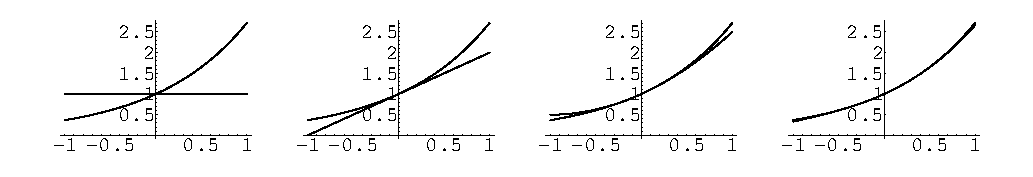
\includegraphics[width=\textwidth]{calculus/differential/tayexp4}
    \end{center}
    \caption{Four finite Taylor series approximations of the 
      exponential function.}
    \label{tayexp4}
  \end{figure}

  Note that for the range of $x$ we are looking at, the approximations
  become more accurate as the number of terms increases.
\end{Example}









\begin{Example}
  Consider the function $f(x) = \cos x$.  We want a polynomial approximation of
  this function near the point $x = 0$. The first few derivatives of $f$ are
  \begin{align*}
    f(x) &= \cos x \\
    f'(x) &= - \sin x \\
    f''(x) &= - \cos x \\
    f'''(x) &= \sin x \\
    f^{(4)}(x) &= \cos x
  \end{align*} 
  It's easy to pick out the pattern here,
  \[
  f^{(n)}(x) = 
  \begin{cases}
    (-1)^{n/2} \cos x &\mathrm{for even}\ n, \\
    (-1)^{(n+1)/2} \sin x & \mathrm{for odd}\ n.
  \end{cases}
  \]
  Since $\cos(0) = 1$ and $\sin(0) = 0$ the $n$-term approximation of the
  cosine is,
  \[
  \cos x = 1 - \frac{x^2}{2!} + \frac{x^4}{4!} - \frac{x^6}{6!} + \cdots
  + (-1)^{2(n-1)} \frac{x^{2(n-1)}}{(2(n-1))!} 
  + \frac{x^{2n}}{(2n)!} \cos \xi.
  \]
  Here are graphs of the one, two, three and four term approximations.

  \begin{figure}[h!]
    \begin{center}
      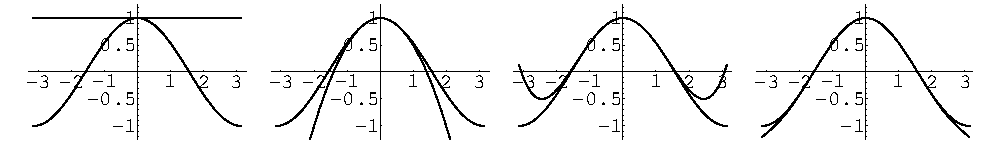
\includegraphics[width=\textwidth]{calculus/differential/taycos4}
    \end{center}
    \caption{Taylor series approximations of the cosine.}
    \label{taycos4}
  \end{figure}

  Note that for the range of $x$ we are looking at, the approximations
  become more accurate as the number of terms increases.
  Consider the ten term approximation of the cosine about $x = 0$,
  \[
  \cos x = 1 - \frac{x^2}{2!} + \frac{x^4}{4!} - \cdots - \frac{x^{18}}{18!} 
  + \frac{x^{20}}{20!} \cos \xi.
  \]
  Note that for any value of $\xi$, $|\cos \xi| \leq 1$.  Therefore the absolute
  value of the error term satisfies,
  \[
  | R | = \left| \frac{x^{20}}{20!} \cos \xi \right| \leq \frac{|x|^{20}}{20!}.
  \]
  $x^{20}/20!$ is plotted in Figure~\ref{taycoser}.

  \begin{figure}[h!]
    \begin{center}
      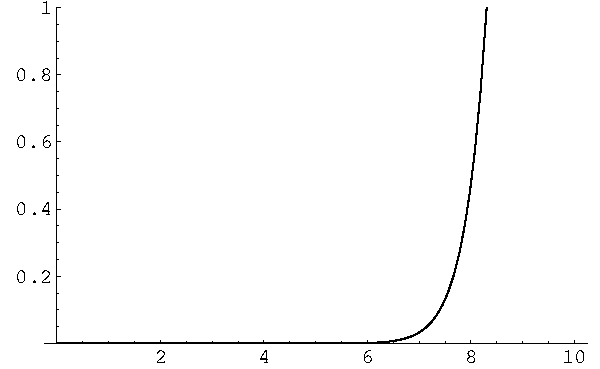
\includegraphics[width=0.3\textwidth]{calculus/differential/taycoser}
    \end{center}
    \caption{A bound on the error.}
    \label{taycoser}
  \end{figure}

  Note that the error is very small for $x < 6$, fairly small but non-negligible
  for $x \approx 7$ and large for $x > 8$.  The ten term approximation of
  the cosine, plotted below, behaves just we would predict.

  \begin{figure}[h!]
    \begin{center}
      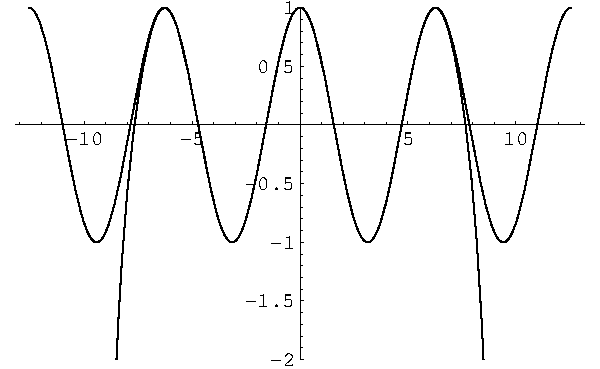
\includegraphics[width=0.3\textwidth]{calculus/differential/taycos10}
    \end{center}
    \caption{Ten term Taylor series approximation of the cosine.}
    \label{taycos10}
  \end{figure}

  The error is very small until it becomes non-negligible at $x \approx 7$
  and large at $x \approx 8$.
\end{Example}





\begin{Example}
  Consider the function $f(x) = \ln x$.  We want a polynomial approximation of
  this function near the point $x = 1$. The first few derivatives of $f$ are
  \begin{align*}
    f(x) &= \ln x \\
    f'(x) &= \frac{1}{x} \\
    f''(x) &= - \frac{1}{x^2} \\
    f'''(x) &= \frac{2}{x^3} \\
    f^{(4)}(x) &= - \frac{3}{x^4}
  \end{align*}
  The derivatives evaluated at $x = 1$ are
  \[
  f(0) = 0, \qquad f^{(n)}(0) = (-1)^{n-1} (n-1)!,\ \mathrm{for}\ n \geq 1.
  \]
  By Taylor's theorem of the mean we have,
  \[
  \ln x = (x-1) - \frac{(x-1)^2}{2} + \frac{(x-1)^3}{3} - \frac{(x-1)^4}{4}
  + \cdots + (-1)^{n-1} \frac{(x-1)^n}{n} 
  + (-1)^n \frac{(x-1)^{n+1}}{n+1} \frac{1}{\xi^{n+1}}.
  \]
  Below are plots of the 2, 4, 10 and 50 term approximations.  

  \begin{figure}[h!]
    \begin{center}
      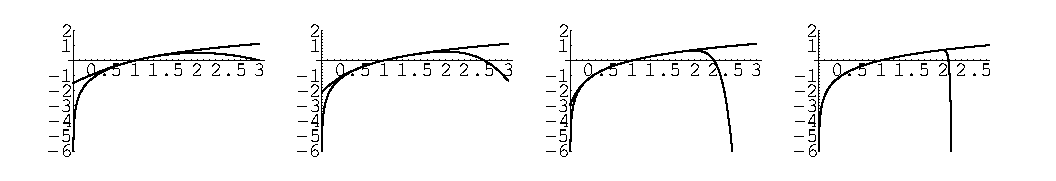
\includegraphics[width=\textwidth]{calculus/differential/taylnt4}
    \end{center}
    \caption{The 2, 4, 10 and 50 term approximations of the logarithm.}
    \label{taylnt4}
  \end{figure}

  Note that the 
  approximation gets better on the interval $(0,2)$ and worse outside this
  interval as the number of terms increases.  The Taylor series converges to
  $\ln x$ only on this interval.
\end{Example}






%%-----------------------------------------------------------------------------
\subsection{Application: Finite Difference Schemes}



\begin{Example}
  Suppose you sample a function at the discrete points $n \Delta x$, 
  $n \in \setZ$.  In Figure~\ref{sindata} we sample the function 
  $f(x) = \sin x$ on the interval $[-4,4]$ with $\Delta x = 1/4$ and 
  plot the data points.  

  \begin{figure}[h!]
    \begin{center}
      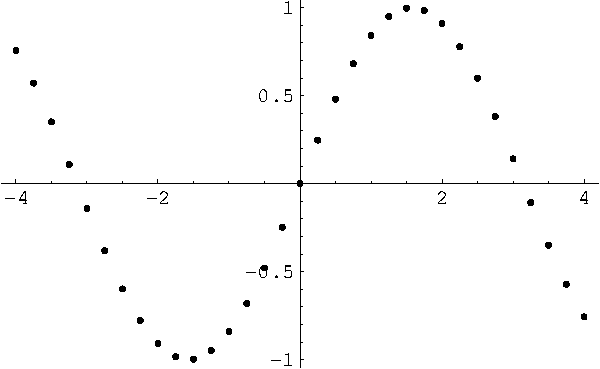
\includegraphics[width=0.4\textwidth]{calculus/differential/sindata}
    \end{center}
    \caption{Sampling of the sine function.}
    \label{sindata}
  \end{figure}

  We wish to approximate the derivative of the function on the grid points
  using only the value of the function on those discrete points.  From
  the definition of the derivative, one is lead to the formula
  \begin{equation}
    \label{first_order_scheme}
    f'(x) \approx \frac{f(x+\Delta x) - f(x)}{\Delta x}.
  \end{equation}
  Taylor's theorem states that
  \[
  f(x + \Delta x) = f(x) + \Delta x f'(x) + \frac{\Delta x^2}{2} f''(\xi).
  \]
  Substituting this expression into our formula for approximating the derivative
  we obtain
  \[
  \frac{f(x+\Delta x) - f(x)}{\Delta x} = \frac{f(x) + \Delta x f'(x)
    + \frac{\Delta x^2}{2} f''(\xi) - f(x) }{\Delta x}
  = f'(x) + \frac{\Delta x}{2} f''(\xi).
  \]
  Thus we see that the error in our approximation of the first derivative is
  $\frac{\Delta x}{2} f''(\xi)$.  Since the error has a linear factor of 
  $\Delta x$, we call this a first order accurate method.  Equation
  ~\ref{first_order_scheme} is called the \textit{forward difference 
    scheme} for calculating the first derivative.  Figure~\ref{fwdsin} shows 
  a plot of the value of this scheme for the function $f(x) = \sin x$ and 
  $\Delta x = 1/4$.  The first derivative of the function $f'(x) = \cos x$ 
  is shown for comparison.

  \begin{figure}[h!]
    \begin{center}
      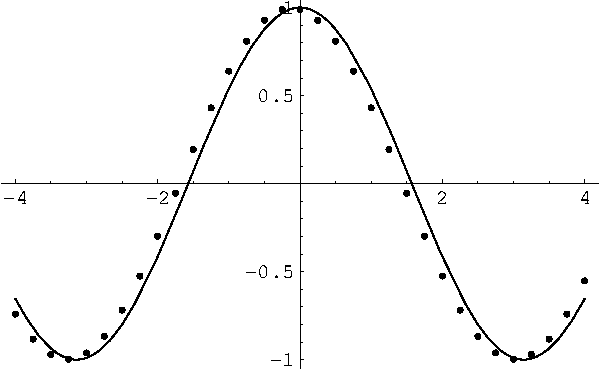
\includegraphics[width=0.4\textwidth]{calculus/differential/fwdsin}
    \end{center}
    \caption{The forward difference scheme approximation of the derivative.}
    \label{fwdsin}
  \end{figure}

  Another scheme for approximating the first derivative is the 
  \textit{centered difference scheme},
  \[
  f'(x) \approx \frac{f(x+\Delta x) - f(x-\Delta x)}{2 \Delta x}.
  \]
  Expanding the numerator using Taylor's theorem,
  \begin{align*}
    &\frac{f(x+\Delta x) - f(x-\Delta x)}{2 \Delta x} \\
    &\qquad= \frac{f(x) + \Delta x f'(x) + \frac{\Delta x^2}{2} f''(x)
      + \frac{\Delta x^3}{6} f'''(\xi)
      - f(x) + \Delta x f'(x) - \frac{\Delta x^2}{2} f''(x)
      + \frac{\Delta x^3}{6} f'''(\psi) }{2 \Delta x} \\
    &\qquad= f'(x) + \frac{\Delta x^2}{12}(f'''(\xi) + f'''(\psi)).
  \end{align*}
  The error in the approximation is quadratic in $\Delta x$.  Therefore
  this is a second order accurate scheme.
  Below is a plot of the derivative of the function and the 
  value of this scheme for the function $f(x) = \sin x$ and $\Delta x = 1/4$.

  \begin{figure}[h!]
    \begin{center}
      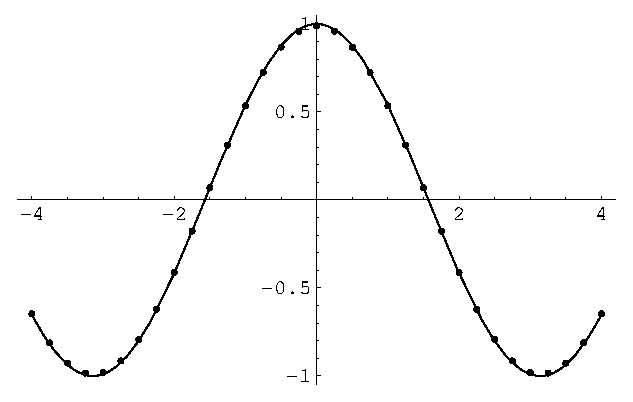
\includegraphics[width=0.4\textwidth]{calculus/differential/ctrsin}
    \end{center}
    \caption{Centered difference scheme approximation of the derivative.}
    \label{ctrsin}
  \end{figure}

  Notice how the centered difference scheme gives a better approximation of the 
  derivative than the forward difference scheme.
\end{Example}







%%=============================================================================
\section{L'Hospital's Rule}
\index{L'Hospital's rule}

Some singularities are easy to diagnose.  Consider the function 
$\frac{\cos x}{x}$ at the point $x = 0$.  The function evaluates to 
$\frac{1}{0}$ and is thus discontinuous at that point.  Since the numerator
and denominator are continuous functions and the denominator vanishes while
the numerator does not, the left and right limits as $x \to 0$ do not 
exist.  Thus the function has an infinite discontinuity at the point
$x = 0$.  More generally, a function which is composed of continuous
functions and evaluates to $\frac{a}{0}$ at a point where $a \neq 0$ must
have an infinite discontinuity there.

Other singularities require more analysis to diagnose.  Consider the 
functions $\frac{\sin x}{x}$, $\frac{\sin x}{|x|}$ and 
$\frac{\sin x}{1 - \cos x}$ at the point $x = 0$.  All three functions
evaluate to $\frac{0}{0}$ at that point, but have different kinds
of singularities.  The first has a removable discontinuity, the second has
a finite discontinuity and the third has an infinite discontinuity.
See Figure~\ref{disc3}.

\begin{figure}[h!]
  \begin{center}
    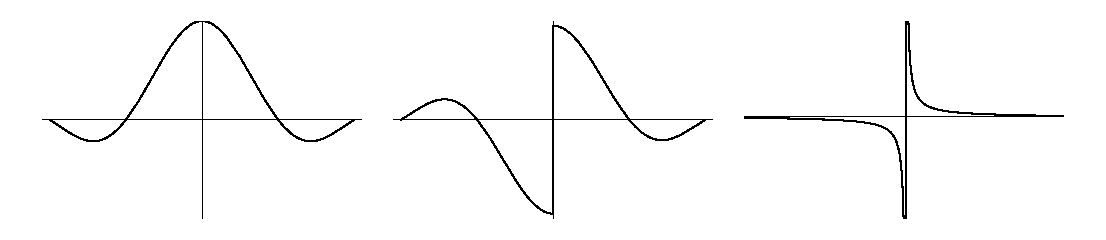
\includegraphics[width=\textwidth]{calculus/differential/disc3}
  \end{center}
  \caption{Different kinds of singularities.}
  \label{disc3}
\end{figure}



An expression that evaluates to $\frac{0}{0}$, $\frac{\infty}{\infty}$,
$0 \cdot \infty$, $\infty - \infty$, $1^\infty$, $0^0$ or $\infty^0$
is called an \textit{indeterminate}.  A function $f(x)$ which is indeterminate
at the point $x = \xi$ is singular at that point.  The singularity may be a 
removable discontinuity, a finite discontinuity or an infinite discontinuity
depending on the behavior of the function around that point.  If
$\lim_{x \to \xi} f(x)$ exists, then the function has a removable 
discontinuity.  If the limit does not exist, but the left and right limits 
do exist, then the function has a finite discontinuity.  If either the
left or right limit does not exist then the function has an infinite
discontinuity.





\paragraph{L'Hospital's Rule.}
Let $f(x)$ and $g(x)$ be differentiable and $f(\xi) = g(\xi) = 0$.  
Further, let $g(x)$ be nonzero in a deleted neighborhood of $x= \xi$, 
($g(x) \neq 0$ for $x \in 0 < |x - \xi| < \delta$).  Then
\[
\lim_{x \to \xi} \frac{f(x)}{g(x)} = \lim_{x \to \xi} \frac{f'(x)}{g'(x)}.
\]
To prove this, we note that $f(\xi) = g(\xi) = 0$ and apply the generalized
theorem of the mean.  Note that
\[
\frac{f(x)}{g(x)} = \frac{f(x) - f(\xi)}{g(x) - g(\xi)}
= \frac{f'(\psi)}{g'(\psi)}
\]
for some $\psi$ between $\xi$ and $x$.  Thus
\[
\lim_{x \to \xi} \frac{f(x)}{g(x)} 
= \lim_{\psi \to \xi} \frac{f'(\psi)}{g'(\psi)}
= \lim_{x \to \xi} \frac{f'(x)}{g'(x)}
\]
provided that the limits exist.

L'Hospital's Rule is also applicable when both functions tend to infinity
instead of zero or when the limit point, $\xi$, is at infinity.  It 
is also valid for one-sided limits.



L'Hospital's rule is directly applicable to the indeterminate forms
$\frac{0}{0}$ and $\frac{\infty}{\infty}$.


\begin{Example}
  Consider the three functions $\frac{\sin x}{x}$, $\frac{\sin x}{|x|}$ and
  $\frac{\sin x}{1 - \cos x}$ at the point $x = 0$.
  \[
  \lim_{x \to 0} \frac{\sin x}{x}
  = \lim_{x \to 0} \frac{\cos x}{1} 
  = 1
  \]
  Thus $\frac{\sin x}{x}$ has a removable discontinuity at $x = 0$.
  \[
  \lim_{x \to 0^+} \frac{\sin x}{|x|}
  = \lim_{x \to 0^+} \frac{\sin x}{x} = 1
  \]
  \[
  \lim_{x \to 0^-} \frac{\sin x}{|x|}
  = \lim_{x \to 0^-} \frac{\sin x}{-x} = -1
  \]
  Thus $\frac{\sin x}{|x|}$ has a finite discontinuity at $x = 0$.
  \[
  \lim_{x \to 0} \frac{\sin x}{1 - \cos x}
  = \lim_{x \to 0} \frac{\cos x}{\sin x}
  = \frac{1}{0} = \infty
  \]
  Thus $\frac{\sin x}{1 - \cos x}$ has an infinite discontinuity at $x = 0$.
\end{Example}




\begin{Example}
  Let $a$ and $d$ be nonzero.
  \begin{align*}
    \lim_{x \to \infty} \frac{a x^2 + b x + c}{d x^2 + e x + f}
    &= \lim_{x \to \infty} \frac{2 a x + b}{2 d x + e} \\
    &= \lim_{x \to \infty} \frac{2 a}{2 d} \\
    &= \frac{a}{d}
  \end{align*}
\end{Example}





\begin{Example}
  Consider
  \[
  \lim_{x \to 0} \frac{\cos x - 1}{x \sin x}.
  \]
  This limit is an indeterminate of the form $\frac{0}{0}$.  Applying
  L'Hospital's rule we see that limit is equal to
  \[
  \lim_{x \to 0} \frac{-\sin x}{x \cos x + \sin x}.
  \]
  This limit is again an indeterminate of the form $\frac{0}{0}$.  We apply
  L'Hospital's rule again.
  \[
  \lim_{x \to 0} \frac{- \cos x}{ - x \sin x + 2 \cos x } = - \frac{1}{2}
  \]
  Thus the value of the original limit is $- \frac{1}{2}$.  We could also
  obtain this result by expanding the functions in Taylor series.
  \begin{align*}
    \lim_{x \to 0} \frac{\cos x - 1}{x \sin x}
    &= \lim_{x \to 0} \frac{\left( 1 - \frac{x^2}{2} + \frac{x^4}{24} 
        - \cdots \right) - 1 }{ x \left( x - \frac{x^3}{6} 
        + \frac{x^5}{120} - \cdots \right)} \\
    &= \lim_{x \to 0} \frac{- \frac{x^2}{2} + \frac{x^4}{24} - \cdots }
    { x^2 - \frac{x^4}{6} + \frac{x^6}{120} - \cdots } \\
    &= \lim_{x \to 0} \frac{- \frac{1}{2} + \frac{x^2}{24} - \cdots }
    { 1 - \frac{x^2}{6} + \frac{x^4}{120} - \cdots } \\
    &= - \frac{1}{2}
  \end{align*}
\end{Example}




We can apply L'Hospital's Rule to the indeterminate forms $0 \cdot \infty$
and $\infty - \infty$ by rewriting the expression in a different form, 
(perhaps putting the expression over a common denominator).  If at first
you don't succeed, try, try again.  You may have to apply L'Hospital's 
rule several times to evaluate a limit.


\begin{Example}
  \begin{align*}
    \lim_{x \to 0} \left( \cot x - \frac{1}{x} \right)
    &= \lim_{x \to 0} \frac{x \cos x - \sin x}{x \sin x} \\
    &= \lim_{x \to 0} \frac{\cos x - x \sin x - \cos x}
    {\sin x + x \cos x} \\
    &= \lim_{x \to 0} \frac{- x \sin x } {\sin x + x \cos x} \\
    &= \lim_{x \to 0} \frac{- x \cos x - \sin x } 
    {\cos x + \cos x - x \sin x } \\
    &= 0
  \end{align*}
\end{Example}


You can apply L'Hospital's rule to the indeterminate forms $1^\infty$, 
$0^0$ or $\infty^0$ by taking the logarithm of the expression.


\begin{Example}
  Consider the limit,
  \[
  \lim_{x \to 0} x^x,
  \]
  which gives us the indeterminate form $0^0$.
  The logarithm of the expression is
  \[
  \ln( x^x ) = x \ln x.
  \]
  As $x \to 0$ we now have the indeterminate form $0 \cdot \infty$.  By 
  rewriting the expression, we can apply L'Hospital's rule.
  \begin{align*}
    \lim_{x \to 0} \frac{\ln x}{1/x}
    &= \lim_{x \to 0} \frac{1/x}{-1/x^2} \\
    &= \lim_{x \to 0} (-x) \\
    &= 0
  \end{align*}
  Thus the original limit is
  \[
  \lim_{x \to 0} x^x = \e^0 = 1.
  \]
\end{Example}









\raggedbottom
%%============================================================================
\pagebreak
\flushbottom
\section{Exercises}


%%-----------------------------------------------------------------------------
\begin{large}
  \noindent
  \textbf{Limits of Functions}
\end{large}


\begin{Exercise}[mathematica/calculus/differential/limits.nb]
  \label{exercise lim sin 1/x}
  Does 
  \[
  \lim_{x \to 0} \sin \left( \frac{1}{x} \right)
  \]
  exist?

  \hintsolution{lim sin 1/x}
\end{Exercise}







\begin{Exercise}[mathematica/calculus/differential/limits.nb]
  \label{exercise lim x sin 1/x}
  Does 
  \[
  \lim_{x \to 0} x \sin \left( \frac{1}{x} \right)
  \]
  exist?

  \hintsolution{lim x sin 1/x}
\end{Exercise}


\begin{Exercise}[mathematica/calculus/differential/limits.nb]
  \label{exercise limit sqrt n 5}
  Evaluate the limit:
  \[
  \lim_{n \to \infty} \sqrt[n]{5}.
  \]

  \hintsolution{limit sqrt n 5}
\end{Exercise}



%%-----------------------------------------------------------------------------
\begin{large}
  \noindent
  \textbf{Continuous Functions}
\end{large}



\begin{Exercise}
  \label{exercise sin 1/x continuous}
  Is the function $\sin(1/x)$ continuous in the open interval $(0,1)$?
  Is there a value of $a$ such that the function defined by
  \[
  f(x) =
  \begin{cases}
    \sin(1/x) &\mathrm{for}\ x \neq 0, \\
    a &\mathrm{for}\ x = 0
  \end{cases}
  \]
  is continuous on the closed interval $[0,1]$?

  \hintsolution{sin 1/x continuous}
\end{Exercise}

%%
\begin{Exercise}
  \label{exercise sin 1/x uniformly continuous}
  Is the function $\sin(1/x)$ uniformly continuous in the open interval $(0,1)$?

  \hintsolution{sin 1/x uniformly continuous}
\end{Exercise}


%%
\begin{Exercise}
  \label{exercise sqrt x uniformly continuous}
  Are the functions $\sqrt{x}$ and $\frac{1}{x}$ uniformly continuous on 
  the interval $(0,1)$?

  \hintsolution{sqrt x uniformly continuous}
\end{Exercise}



\begin{Exercise}
  \label{exercise continuous closed uniformly}
  Prove that a function which is continuous on a closed interval is
  uniformly continuous on that interval.

  \hintsolution{continuous closed uniformly}
\end{Exercise}







\begin{Exercise}
  \label{exercise lim a = L lim a2 = L2}
  Prove or disprove each of the following.
  \begin{enumerate}
  \item 
    If $\lim_{n \to \infty} a_n = L$ then $\lim_{n \to \infty} a_n^2 = L^2$.
  \item 
    If $\lim_{n \to \infty} a_n^2 = L^2$ then $\lim_{n \to \infty} a_n = L$.
  \item 
    If $a_n > 0$ for all $n > 200$, and $\lim_{n \to \infty} a_n = L$, then $L > 0$.
  \item 
    If $f : \setR \mapsto \setR$ is continuous and $\lim_{x \to \infty} f(x) = L$, then for 
    $n \in \setZ$, $\lim_{n \to \infty} f(n) = L$.
  \item 
    If $f : \setR \mapsto \setR$ is continuous and $\lim_{n \to \infty} f(n) = L$, then for 
    $x \in \setR$, $\lim_{x \to \infty} f(x) = L$.
  \end{enumerate}

  \hintsolution{lim a = L lim a2 = L2}
\end{Exercise}







%%-----------------------------------------------------------------------------
\begin{large}
  \noindent
  \textbf{The Derivative}
\end{large}





\begin{Exercise}[mathematica/calculus/differential/derivative.nb]
  \label{exercise differentiation properties}
  Use the definition of differentiation to prove the following identities
  where $f(x)$ and $g(x)$ are differentiable functions and $n$ is a positive 
  integer.
  \begin{enumerate}
  \item
    $\frac{\dd}{\dd x} (x^n) = n x^{n-1}$, $\quad$ (I suggest that you use Newton's
    binomial formula.)
  \item
    $\frac{\dd}{\dd x} (f(x) g(x)) = f \frac{\dd g}{\dd x} 
    + g \frac{\dd f}{\dd x}$
  \item
    $\frac{\dd}{\dd x} (\sin x) = \cos x$.  (You'll need to use some 
    trigonometric identities.)
  \item
    $\frac{\dd}{\dd x} (f(g(x))) = f'(g(x)) g'(x)$
  \end{enumerate}

  \hintsolution{differentiation properties}
\end{Exercise}





\begin{Exercise}[mathematica/calculus/differential/derivative.nb]
  \label{exercise differentiable f = x|x|}
  Use the definition of differentiation to determine if the following 
  functions are differentiable at $x = 0$.
  \begin{enumerate}
  \item
    $f(x) = x |x|$
  \item
    $f(x) = \sqrt{1 + |x|}$
  \end{enumerate}

  \hintsolution{differentiable f = x|x|}
\end{Exercise}









\begin{Exercise}[mathematica/calculus/differential/derivative.nb]
  \label{exercise d/dx x sin cos x}
  Find the first derivatives of the following:
  \renewcommand{\theenumi}{\alph{enumi}}
  \begin{enumerate}
  \item
    $x \sin( \cos x)$
  \item
    $f( \cos( g(x) ) )$
  \item
    $\frac{1}{f(\ln x)}$
  \item
    $x^{x^x}$
  \item
    $|x| \sin |x|$
  \end{enumerate}
  \renewcommand{\theenumi}{\arabic{enumi}}

  \hintsolution{d/dx x sin cos x}
\end{Exercise}



\begin{Exercise}[mathematica/calculus/differential/derivative.nb]
  \label{exercise d/dx arcsin x}
  Using 
  \[
  \frac{\dd}{\dd x} \sin x = \cos x \quad \mathrm{and} \quad
  \frac{\dd}{\dd x} \tan x = \frac{1}{\cos^2 x}
  \]
  find the derivatives of $\arcsin x$ and $\arctan x$.

  \hintsolution{d/dx arcsin x}
\end{Exercise}




%%-----------------------------------------------------------------------------
\begin{large}
  \noindent
  \textbf{Implicit Differentiation}
\end{large}


\begin{Exercise}[mathematica/calculus/differential/implicit.nb]
  \label{exercise tangent circle}
  Find $y'(x)$, given that $x^2 + y^2 = 1$.  What is $y'(1/2)$?

  \hintsolution{tangent circle}
\end{Exercise}





\begin{Exercise}[mathematica/calculus/differential/implicit.nb]
  \label{exercise y' y'' circle}
  Find $y'(x)$ and $y''(x)$, given that $x^2 - x y + y^2 = 3$.
  (Write each in terms of $x$ and $y$.)

  \hintsolution{y' y'' circle}
\end{Exercise}



%%-----------------------------------------------------------------------------
\begin{large}
  \noindent
  \textbf{Maxima and Minima}
\end{large}


\begin{Exercise}[mathematica/calculus/differential/maxima.nb]
  \label{exercise max min x(12-2x)2}
  Identify any maxima and minima of the following functions.
  \renewcommand{\theenumi}{\alph{enumi}}
  \begin{enumerate}
  \item
    $\displaystyle f(x) = x(12-2x)^2$
  \item
    $\displaystyle f(x) = \sqrt[3]{(x-2)^2}$
  \end{enumerate}
  \renewcommand{\theenumi}{\arabic{enumi}}

  \hintsolution{max min x(12-2x)2}
\end{Exercise}




\begin{Exercise}[mathematica/calculus/differential/maxima.nb]
  \label{exercise surface area cup}
  A cylindrical container with a circular base and an open top is to hold
  $64 \mathrm{cm}^3$.  Find its dimensions so that the surface area of the 
  cup is a minimum.

  \hintsolution{surface area cup}
\end{Exercise}



%%-----------------------------------------------------------------------------
\begin{large}
  \noindent
  \textbf{Mean Value Theorems}
\end{large}


\begin{Exercise}
  \label{exercise generalized theorem of the mean}
  Prove the generalized theorem of the mean.  
  If $f(x)$ and $g(x)$ are continuous in $[a,b]$ and differentiable in $(a,b)$,
  then there exists a point $x = \xi$ such that
  \[
  \frac{f'(\xi)}{g'(\xi)} = \frac{f(b) - f(a)}{g(b) - g(a)}.
  \]
  Assume that $g(a) \neq g(b)$ so that the denominator does not
  vanish and that $f'(x)$ and $g'(x)$ are not simultaneously zero which
  would produce an indeterminate form.  

  \hintsolution{generalized theorem of the mean}
\end{Exercise}


\begin{Exercise}[mathematica/calculus/differential/taylor.nb]
  \label{exercise polynomial approximation sin x}
  Find a polynomial approximation of $\sin x$ on the interval $[-1,1]$ that
  has a maximum error of $\frac{1}{1000}$.  Don't use any more terms that you
  need to.  Prove the error bound.  Use your polynomial to approximate
  $\sin(1)$.

  \hintsolution{polynomial approximation sin x}
\end{Exercise}






\begin{Exercise}[mathematica/calculus/differential/taylor.nb]
  \label{exercise second difference centered}
  You use the formula $\frac{f(x+\Delta x)-2f(x)+f(x-\Delta x)}{\Delta x^2}$
  to approximate $f''(x)$.  What is the error in this approximation?

  \hintsolution{second difference centered}
\end{Exercise}



\begin{Exercise}
  \label{exercise first derivative higher}
  The formulas $\frac{f(x + \Delta x) - f(x)}{\Delta x}$ and
  $\frac{f(x + \Delta x) - f(x - \Delta x)}{2 \Delta x}$ are first and
  second order accurate schemes for approximating the first derivative
  $f'(x)$. Find a couple of other schemes that have successively higher orders
  of accuracy.  Would these higher order schemes actually give a better
  approximation of $f'(x)$?  Remember that $\Delta x$ is small, but not
  infinitesimal.

  \hintsolution{first derivative higher}
\end{Exercise}



%%-----------------------------------------------------------------------------
\begin{large}
  \noindent
  \textbf{L'Hospital's Rule}
\end{large}


\begin{Exercise}[mathematica/calculus/differential/lhospitals.nb]
  \label{exercise lim (x - sin x)/x3}
  Evaluate the following limits.
  \renewcommand{\theenumi}{\alph{enumi}}
  \begin{enumerate}
  \item
    $\lim_{x \to 0} \frac{x - \sin x}{x^3}$
  \item
    $\lim_{x \to 0} \left( \csc x - \frac{1}{x} \right)$
  \item
    $\lim_{x \to +\infty} \left( 1 + \frac{1}{x} \right)^x$
  \item
    $\lim_{x \to 0} \left( \csc^2 x - \frac{1}{x^2} \right)$.
    (First evaluate using L'Hospital's rule then using a Taylor series expansion.
    You will find that the latter method is more convenient.)
  \end{enumerate}
  \renewcommand{\theenumi}{\arabic{enumi}}

  \hintsolution{lim (x - sin x)/x3}
\end{Exercise}






\begin{Exercise}[mathematica/calculus/differential/lhospitals.nb]
  \label{exercise lim x a/x}
  Evaluate the following limits,
  \[
  \lim_{x \to \infty} x^{a/x}, \qquad
  \lim_{x \to \infty} \left( 1 + \frac{a}{x} \right)^{b x},
  \]
  where $a$ and $b$ are constants.

  \hintsolution{lim x a/x}
\end{Exercise}





%% CONTINUE: prove L'Hospital's rule at infinity.












\raggedbottom
%%=============================================================================
\pagebreak
\flushbottom
\section{Hints}


%%----------------------------------------------------------------------------
%% Limits of Functions


\begin{Hint}
  \label{hint lim sin 1/x}
  Apply the $\epsilon$, $\delta$ definition of a limit.
\end{Hint}





\begin{Hint}
  \label{hint lim x sin 1/x}
  Set $y = 1/x$.  Consider $\lim_{y \to \infty}$.
\end{Hint}


\begin{Hint}
  \label{hint limit sqrt n 5}
  Write $\sqrt[n]{5}$ in terms of the exponential function.
\end{Hint}


%%----------------------------------------------------------------------------
%% Continuous Functions



\begin{Hint}
  \label{hint sin 1/x continuous}
  The composition of continuous functions is continuous.
  Apply the definition of continuity and look at the point $x = 0$.
\end{Hint}


\begin{Hint}
  \label{hint sin 1/x uniformly continuous}
  Note that for $x_1 = \frac{1}{(n-1/2) \pi}$ and $x_2 = \frac{1}{(n+1/2) \pi}$ 
  where $n \in \setZ$ we have $| \sin(1/x_1) - \sin(1/x_2)| = 2$.  
\end{Hint}


\begin{Hint}
  \label{hint sqrt x uniformly continuous}
  Note that the function $\sqrt{x + \delta} - \sqrt{x}$ is a decreasing 
  function of $x$ and an increasing function of $\delta$ for positive $x$ 
  and $\delta$.  Bound this function for fixed $\delta$.

  Consider any positive $\delta$ and $\epsilon$.  For what values of $x$ is
  \[
  \frac{1}{x} - \frac{1}{x+\delta} > \epsilon.
  \]
\end{Hint}



\begin{Hint}
  \label{hint continuous closed uniformly}
  Let the function $f(x)$ be continuous on a closed interval.
  Consider the function 
  \[
  e(x,\delta) = \sup_{|\xi-x|<\delta} | f(\xi) - f(x) |.
  \]
  Bound $e(x,\delta)$ with a function of $\delta$ alone.
\end{Hint}








\begin{Hint}
  \label{hint lim a = L lim a2 = L2}
  CONTINUE
  \begin{enumerate}
  \item 
    If $\lim_{n \to \infty} a_n = L$ then $\lim_{n \to \infty} a_n^2 = L^2$.
  \item 
    If $\lim_{n \to \infty} a_n^2 = L^2$ then $\lim_{n \to \infty} a_n = L$.
  \item 
    If $a_n > 0$ for all $n > 200$, and $\lim_{n \to \infty} a_n = L$, then $L > 0$.
  \item 
    If $f : \setR \mapsto \setR$ is continuous and $\lim_{x \to \infty} f(x) = L$, then for 
    $n \in \setZ$, $\lim_{n \to \infty} f(n) = L$.
  \item 
    If $f : \setR \mapsto \setR$ is continuous and $\lim_{n \to \infty} f(n) = L$, then for 
    $x \in \setR$, $\lim_{x \to \infty} f(x) = L$.
  \end{enumerate}
\end{Hint}







%%-----------------------------------------------------------------------------
%% The Derivative



\begin{Hint}
  \label{hint differentiation properties}
  \renewcommand{\theenumi}{\alph{enumi}}
  \begin{enumerate}
    %%
  \item
    Newton's binomial formula is
    \[
    (a + b)^n = \sum_{k=0}^n \binom{n}{k} a^{n-k} b^k
    = a^n + a^{n-1} b + \frac{n(n-1)}{2} a^{n-2} b^2 + \cdots + n a b^{n-1}
    + b^n.
    \]
    Recall that the binomial coefficient is
    \[
    \binom{n}{k} = \frac{n!}{(n-k)! k!}.
    \]
    %%
  \item
    Note that
    \[
    \frac{\dd}{\dd x} (f(x) g(x))
    = \lim_{\Delta x \to 0} \left[ \frac{f(x+\Delta x) g(x+\Delta x)
        - f(x) g(x)} {\Delta x} \right] 
    \]
    and
    \[
    g(x) f'(x) + f(x) g'(x)
    = g(x) \lim_{\Delta x \to 0} \left[ \frac{f(x+\Delta x) - f(x)}
      {\Delta x} \right] +
    f(x) \lim_{\Delta x \to 0} \left[ \frac{g(x+\Delta x)- g(x)}
      {\Delta x} \right].
    \]
    Fill in the blank.
    %%
  \item
    First prove that
    \[
    \lim_{\theta \to 0} \frac{\sin \theta}{\theta} = 1.
    \]
    and
    \[
    \lim_{\theta \to 0} \left[ \frac{\cos \theta - 1}{\theta} \right] = 0.
    \]
    %%
  \item
    Let $u = g(x)$.
    Consider a nonzero increment $\Delta x$, which induces the increments
    $\Delta u$ and $\Delta f$.  By definition,
    \[
    \Delta f = f(u + \Delta u) - f(u), \qquad
    \Delta u = g(x + \Delta x) - g(x),
    \]
    and $\Delta f, \Delta u \to 0$ as $\Delta x \to 0$.
    If $\Delta u \neq 0$ then we have
    \[
    \epsilon = \frac{\Delta f}{\Delta u} - \frac{\dd f}{\dd u} \to 0 \quad \mathrm{as}
    \quad \Delta u \to 0.
    \]
    If $\Delta u = 0$ for some values of $\Delta x$ then $\Delta f$ also vanishes
    and we define $\epsilon = 0$ for theses values.  In either case,
    \[
    \Delta y = \frac{\dd f}{\dd u} \Delta u + \epsilon \Delta u.
    \]
    Continue from here.
  \end{enumerate}
  \renewcommand{\theenumi}{\arabic{enumi}}
\end{Hint}





\begin{Hint}
  \label{hint differentiable f = x|x|}
  %% CONTINUE
\end{Hint}



\begin{Hint}
  \label{hint d/dx x sin cos x}
  \renewcommand{\theenumi}{\alph{enumi}}
  \begin{enumerate}
    %%
  \item
    Use the product rule and the chain rule.
    %%
  \item
    Use the chain rule.
    %%
  \item
    Use the quotient rule and the chain rule.
    %%
  \item
    Use the identity $a^b = \e^{b \ln a}$.
    %%
  \item
    Use the fact that the sine is an odd function, i.e. 
    $\sin(-x) = - \sin x$.
  \end{enumerate}
  \renewcommand{\theenumi}{\arabic{enumi}}
\end{Hint}






\begin{Hint}
  \label{hint d/dx arcsin x}
  Use that $x'(y) = 1/y'(x)$ and the identities $\cos x = (1 - \sin^2 x)^{1/2}$
  and $\cos(\arctan x) = \frac{1}{(1+x^2)^{1/2}}$.
\end{Hint}











%%-----------------------------------------------------------------------------
%% Implicit Differentiation




\begin{Hint}
  \label{hint tangent circle}
  Differentiate the equation.
  \begin{gather*}
    x^2 + y^2 = 1
    \\
    2 x + 2 y y' = 0
  \end{gather*}
  Solve this equation for $y'(x)$ and write $y(x)$ in terms of $x$.
\end{Hint}






\begin{Hint}
  \label{hint y' y'' circle}
  Differentiate the equation and solve for $y'(x)$ in terms of $x$ and $y(x)$.
  Differentiate the expression for $y'(x)$ to obtain $y''(x)$.  You'll use that
  \[
  x^2 - x y + y^2 = 3.
  \]
\end{Hint}



%%-----------------------------------------------------------------------------
%% Maxima and Minima



\begin{Hint}
  \label{hint max min x(12-2x)2}
  \renewcommand{\theenumi}{\alph{enumi}}
  \begin{enumerate}
    %%
  \item
    Use the second derivative test.
    %%
  \item
    The function is not differentiable at the point $x = 2$ so you can't use
    a derivative test at that point.
  \end{enumerate}
  \renewcommand{\theenumi}{\arabic{enumi}}
\end{Hint}







\begin{Hint}
  \label{hint surface area cup}
  Let $r$ be the radius and $h$ the height of the cylinder.  The volume of
  the cup is $\pi r^2 h = 64$.  The radius and height are related by
  $h = \frac{64}{\pi r^2}$.  Write the surface area as a function of $r$ and
  use the second derivative test to find its minimum.
\end{Hint}



%%-----------------------------------------------------------------------------
%% Mean Value Theorems


\begin{Hint}
  \label{hint generalized theorem of the mean}
  The proof is analogous to the proof of the theorem of the mean.  
  Use Rolle's theorem.
\end{Hint}



\begin{Hint}
  \label{hint polynomial approximation sin x}
  The first few terms in the Taylor series of $\sin(x)$ about $x=0$ are
  \[
  \sin(x) = x - \frac{x^3}{6} + \frac{x^5}{120} - \frac{x^7}{5040}
  + \frac{x^9}{362880} + \cdots.
  \]
  When determining the error, use the fact that $|\cos x_0| \leq 1$ and
  $|x^n| \leq 1$ for $x \in [-1,1]$.
\end{Hint}




\begin{Hint}
  \label{hint second difference centered}
  The terms in the approximation have the Taylor series,
  \begin{align*}
    f(x+\Delta x) &= f(x) + \Delta x f'(x) + \frac{\Delta x^2}{2} f''(x)
    +\frac{\Delta x^3}{6} f'''(x) + \frac{\Delta x^4}{24} f''''(x_1), \\
    f(x-\Delta x) &= f(x) - \Delta x f'(x) + \frac{\Delta x^2}{2} f''(x)
    -\frac{\Delta x^3}{6} f'''(x) + \frac{\Delta x^4}{24} f''''(x_2),
  \end{align*}
  where $x \leq x_1 \leq x + \Delta x$ and $x - \Delta x \leq x_2 \leq x$.
\end{Hint}




\begin{Hint}
  \label{hint first derivative higher}
  %% CONTINUE
\end{Hint}



%%-----------------------------------------------------------------------------
%% L'Hospital's Rule





\begin{Hint}
  \label{hint lim (x - sin x)/x3}
  \renewcommand{\theenumi}{\alph{enumi}}
  \begin{enumerate}
    %%
  \item
    Apply L'Hospital's rule three times.
    %%
  \item
    You can write the expression as
    \[
    \frac{x - \sin x}{x \sin x}.
    \]
    %%
  \item
    Find the limit of the logarithm of the expression.
    %%
  \item
    It takes four successive applications of L'Hospital's rule to evaluate
    the limit.

    For the Taylor series expansion method,
    \[
    \csc^2 x - \frac{1}{x^2} 
    = \frac{x^2 - \sin^2 x}{ x^2 \sin^2 x } 
    = \frac{x^2 - (x - x^3/6 + O(x^5))^2}
    { x^2 (x + O(x^3))^2 } 
    \]
  \end{enumerate}
  \renewcommand{\theenumi}{\arabic{enumi}}
\end{Hint}







\begin{Hint}
  \label{hint lim x a/x}
  To evaluate the limits use the identity $a^b = \e^{b \ln a}$
  and then apply L'Hospital's rule.
\end{Hint}
















\raggedbottom
%%=============================================================================
\pagebreak
\flushbottom
\section{Solutions}


%%----------------------------------------------------------------------------
%% Limits of Functions


\begin{Solution}
  \label{solution lim sin 1/x}
  Note that in any open neighborhood of zero, $(-\delta,\delta)$, the 
  function $\sin(1/x)$ takes on all values in the interval $[-1,1]$.  
  Thus if we choose a positive $\epsilon$ such that $\epsilon < 1$ then there
  is no value of $\psi$ for which $| \sin(1/x) - \psi | < \epsilon$ for all
  $x \in (-\epsilon,\epsilon)$.  Thus the limit does not exist.
\end{Solution}





\begin{Solution}
  \label{solution lim x sin 1/x}
  We make the change of variables $y = 1/x$ and consider $y \to \infty$.  We use that
  $\sin(y)$ is bounded.
  \[
  \lim_{x \to 0} x \sin \left( \frac{1}{x} \right)
  = \lim_{y \to \infty} \frac{1}{y} \sin(y)
  = 0
  \]
\end{Solution}


\begin{Solution}
  \label{solution limit sqrt n 5}
  We write $\sqrt[n]{5}$ in terms of the exponential function and then
  evaluate the limit.
  \begin{align*}
    \lim_{n \to \infty} \sqrt[n]{5}
     &= \lim_{n \to \infty} \exp \left( \frac{\ln 5}{n} \right)
     \\
     &= \exp \left( \lim_{n \to \infty} \frac{\ln 5}{n} \right)
     \\
     &= \e^{0}
     \\
     &= 1
  \end{align*}
\end{Solution}




%%----------------------------------------------------------------------------
%% Continuous Functions



\begin{Solution}
  \label{solution sin 1/x continuous}
  Since $\frac{1}{x}$ is continuous in the interval $(0,1)$ and the function
  $\sin(x)$ is continuous everywhere, the composition $\sin(1/x)$ is 
  continuous in the interval $(0,1)$.

  Since $\lim_{x \to 0} \sin(1/x)$ does not exist, there is no way of defining
  $\sin(1/x)$ at $x = 0$ to produce a function that is continuous in $[0,1]$.
\end{Solution}


\begin{Solution}
  \label{solution sin 1/x uniformly continuous}
  Note that for $x_1 = \frac{1}{(n-1/2) \pi}$ and $x_2 = \frac{1}{(n+1/2) \pi}$ 
  where $n \in \setZ$ we have $| \sin(1/x_1) - \sin(1/x_2)| = 2$.  Thus 
  for any $0 < \epsilon < 2$ there is no value of $\delta > 0$ such that 
  $| \sin(1/x_1) - \sin(1/x_2)| < \epsilon$ for all $x_1, x_2 \in (0,1)$ and
  $|x_1 - x_2| < \delta$.  Thus $\sin(1/x)$ is not uniformly continuous
  in the open interval $(0,1)$.
\end{Solution}



\begin{Solution}
  \label{solution sqrt x uniformly continuous}
  First consider the function $\sqrt{x}$.  Note that the function
  $\sqrt{x + \delta} - \sqrt{x}$ is a decreasing function of $x$ 
  and an increasing function of $\delta$
  for positive $x$ and $\delta$.  Thus for any fixed $\delta$, the maximum 
  value of $\sqrt{x + \delta} - \sqrt{x}$ is bounded by $\sqrt{\delta}$.
  Therefore on the interval $(0,1)$, a sufficient condition for 
  $| \sqrt{x} - \sqrt{\xi} | < \epsilon$ is $| x - \xi | < \epsilon^2$.
  The function $\sqrt{x}$ is uniformly continuous on the interval $(0,1)$.

  Consider any positive $\delta$ and $\epsilon$.  
  Note that 
  \[
  \frac{1}{x} - \frac{1}{x+\delta} > \epsilon
  \]
  for
  \[
  x < \frac{1}{2} \left( \sqrt{ \delta^2 + \frac{4 \delta}{\epsilon} }
    - \delta \right).
  \]
  Thus there is no value of $\delta$ such that
  \[
  \left| \frac{1}{x} - \frac{1}{\xi} \right| < \epsilon
  \]
  for all $| x - \xi | < \delta$.  The function $\frac{1}{x}$ is not uniformly
  continuous on the interval $(0,1)$.
\end{Solution}



\begin{Solution}
  \label{solution continuous closed uniformly}
  Let the function $f(x)$ be continuous on a closed interval.
  Consider the function 
  \[
  e(x,\delta) = \sup_{|\xi-x|<\delta} | f(\xi) - f(x) |.
  \]
  Since $f(x)$ is continuous, $e(x,\delta)$ is a continuous function of
  $x$ on the same closed interval.  Since continuous functions on closed 
  intervals are bounded, there is a continuous, increasing function 
  $\epsilon(\delta)$ satisfying,
  \[
  e(x,\delta) \leq \epsilon(\delta),
  \]
  for all $x$ in the closed interval.  Since $\epsilon(\delta)$ is 
  continuous and increasing, it has an inverse $\delta(\epsilon)$.
  Now note that $|f(x) - f(\xi)| < \epsilon$ for all $x$ and $\xi$ in the
  closed interval satisfying $|x - \xi| < \delta(\epsilon)$.  Thus 
  the function is uniformly continuous in the closed interval.
\end{Solution}










\begin{Solution}
  \label{solution lim a = L lim a2 = L2}
  \begin{enumerate}
  \item 
    The statement 
    \[
    \lim_{n \to \infty} a_n = L
    \]
    is equivalent to
    \[
    \forall\ \epsilon > 0,\ \exists\ N\ \mathrm{s.t.}\ n > N \Rightarrow |a_n - L| < \epsilon.
    \]
    We want to show that
    \[
    \forall\ \delta > 0,\ \exists\ M\ \mathrm{s.t.}\ m > M \Rightarrow |a_n^2 - L^2| < \delta.
    \]
    Suppose that $|a_n - L| < \epsilon$.  We obtain an upper bound on 
    $|a_n^2 - L^2|$.
    \[
    |a_n^2 - L^2| = |a_n - L| |a_n + L| < \epsilon ( |2L| + \epsilon )
    \]
    Now we choose a value of $\epsilon$ such that $|a_n^2 - L^2| < \delta$
    \begin{gather*}
      \epsilon ( |2L| + \epsilon ) = \delta
      \\
      \epsilon  = \sqrt{ L^2 + \delta } - |L|
    \end{gather*}
    Consider any fixed $\delta > 0$.  We see that since
    \[
    \mathrm{for}\ \epsilon = \sqrt{ L^2 + \delta } - |L|,\ \exists\ N\ \mathrm{s.t.}\
    n > N \Rightarrow |a_n - L| < \epsilon
    \]
    implies that
    \[
    n > N \Rightarrow |a_n^2 - L^2| < \delta.
    \]
    Therefore
    \[
    \forall\ \delta > 0,\ \exists\ M\ \mathrm{s.t.}\ m > M \Rightarrow |a_n^2 - L^2| < \delta.
    \]
    We conclude that $\lim_{n \to \infty} a_n^2 = L^2$.
  \item 
    $\lim_{n \to \infty} a_n^2 = L^2$ does not imply that $\lim_{n \to \infty} a_n = L$.
    Consider $a_n = -1$.  In this case $\lim_{n \to \infty} a_n^2 = 1$ and 
    $\lim_{n \to \infty} a_n = -1$.
  \item 
    If $a_n > 0$ for all $n > 200$, and $\lim_{n \to \infty} a_n = L$, then $L$
    is not necessarily positive.  Consider $a_n = 1 / n$, which satisfies
    the two constraints.
    \[
    \lim_{n \to \infty} \frac{1}{n} = 0
    \]
  \item 
    The statement $\lim_{x \to \infty} f(x) = L$ is equivalent to
    \[
    \forall\ \epsilon > 0,\ \exists\ X\ \mathrm{s.t.}\ x > X \Rightarrow |f(x) - L| < \epsilon.
    \]
    This implies that for $n > \lceil X \rceil$, $|f(n) - L| < \epsilon$.
    \begin{gather*}
      \forall\ \epsilon > 0,\ \exists\ N\ \mathrm{s.t.}\ n > N \Rightarrow |f(n) - L| < \epsilon
      \\
      \lim_{n \to \infty} f(n) = L
    \end{gather*}
  \item 
    If $f : \setR \mapsto \setR$ is continuous and $\lim_{n \to \infty} f(n) = L$, then for 
    $x \in \setR$, it is not necessarily true that $\lim_{x \to \infty} f(x) = L$.
    Consider $f(x) = \sin(\pi x)$.
    \[
    \lim_{n \to \infty} \sin(\pi n) = \lim_{n \to \infty} 0 = 0
    \]
    $\lim_{x \to \infty} \sin(\pi x)$ does not exist.
  \end{enumerate}
\end{Solution}
















%%-----------------------------------------------------------------------------
%% The Derivative



\begin{Solution}
  \label{solution differentiation properties}
  \renewcommand{\theenumi}{\alph{enumi}}
  \begin{enumerate}
    %%
  \item
    \begin{align*}
      \frac{\dd}{\dd x} (x^n)
      &= \lim_{\Delta x \to 0} \left[ \frac{(x+\Delta x)^n - x^n}{\Delta x}
      \right] \\
      &= \lim_{\Delta x \to 0} \left[ \frac{\left( x^n + n x^{n-1} \Delta x +
            \frac{n(n-1)}{2} x^{n-2} \Delta x^2 + \cdots +
            \Delta x^n \right)- x^n}{\Delta x} \right] \\
      &= \lim_{\Delta x \to 0} \left[ n x^{n-1} +
        \frac{n(n-1)}{2} x^{n-2} \Delta x + \cdots +
        \Delta x^{n-1} \right] \\
      &= n x^{n-1}
    \end{align*}
    \[
    \boxed{
      \frac{\dd}{\dd x} (x^n) = n x^{n-1}
      }
    \]
    %%
  \item
    \begin{align*}
      \frac{\dd}{\dd x} (f(x) g(x))
      &= \lim_{\Delta x \to 0} \left[ \frac{f(x+\Delta x) g(x+\Delta x)
          - f(x) g(x)} {\Delta x} \right] \\
      &= \lim_{\Delta x \to 0} \left[ \frac{[f(x+\Delta x) g(x+\Delta x)
          - f(x) g(x+\Delta x)] + [f(x) g(x+\Delta x)- f(x) g(x)]}
        {\Delta x} \right] \\
      &= \lim_{\Delta x \to 0} \left[ g(x+\Delta x) \right]
      \lim_{\Delta x \to 0} \left[ \frac{f(x+\Delta x) - f(x)}
        {\Delta x} \right] +
      f(x) \lim_{\Delta x \to 0} \left[ \frac{g(x+\Delta x)- g(x)}
        {\Delta x} \right] \\
      &= g(x) f'(x) + f(x) g'(x)
    \end{align*}
    \[
    \boxed{
      \frac{\dd}{\dd x} (f(x) g(x)) = f(x) g'(x) + f'(x) g(x)
      }
    \]
    %%
  \item
    Consider a right triangle with hypotenuse of length 1 in the first
    quadrant of the plane. Label the vertices $A$, $B$, $C$, in clockwise order,
    starting with the vertex at the origin.  The angle of $A$ is $\theta$.
    The length of a circular arc of radius $\cos \theta$ that connects $C$ to
    the hypotenuse is $\theta \cos \theta$.  The length of the side $BC$ is
    $\sin \theta$.  The length of a circular arc of radius 1 that connects $B$
    to the $x$ axis is $\theta$.  (See Figure~\ref{sintheta}.)

    \begin{figure}[tbp]
      \begin{center}
        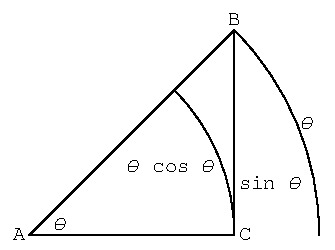
\includegraphics[width=0.4\textwidth]{calculus/differential/sintheta}
      \end{center}
      \caption{Demonstration of the inequality.}
      \label{sintheta}
    \end{figure}

    Considering the length of these three curves
    gives us the inequality:
    \[
    \theta \cos \theta \leq \sin \theta \leq \theta.
    \]
    Dividing by $\theta$,
    \[
    \cos \theta \leq \frac{\sin \theta}{\theta} \leq 1.
    \]
    Taking the limit as $\theta \to 0$ gives us
    \[
    \lim_{\theta \to 0} \frac{\sin \theta}{\theta} = 1.
    \]
    One more little tidbit we'll need to know is
    \begin{align*}
      \lim_{\theta \to 0} \left[ \frac{\cos \theta - 1}{\theta} \right]
      &= \lim_{\theta \to 0} \left[ \frac{\cos \theta - 1}{\theta}
        \frac{\cos \theta + 1}{\cos \theta + 1} \right] \\
      &= \lim_{\theta \to 0} \left[ \frac{\cos^2 \theta - 1}
        {\theta (\cos \theta + 1)} \right] \\
      &= \lim_{\theta \to 0} \left[ \frac{-\sin^2 \theta}
        {\theta (\cos \theta + 1)} \right] \\
      &= \lim_{\theta \to 0} \left[ \frac{-\sin \theta} {\theta} \right]
      \lim_{\theta \to 0} \left[ \frac{\sin \theta}
        {(\cos \theta + 1)} \right] \\
      &= (-1) \left( \frac{0}{2} \right) \\
      &= 0.
    \end{align*}
    Now we're ready to find the derivative of $\sin x$.
    \begin{align*}
      \frac{\dd}{\dd x} (\sin x)
      &= \lim_{\Delta x \to 0} \left[ \frac{\sin(x+\Delta x) - \sin x}
        {\Delta x} \right] \\
      &= \lim_{\Delta x \to 0} \left[ \frac{\cos x \sin \Delta x
          + \sin x \cos \Delta x - \sin x}{\Delta x} \right] \\
      &= \cos x \lim_{\Delta x \to 0} \left[ \frac{\sin \Delta x}{\Delta x}
      \right]
      + \sin x \lim_{\Delta x \to 0} \left[ \frac{\cos \Delta x - 1}
        {\Delta x} \right] \\
      &= \cos x
    \end{align*}
    \[
    \boxed{
      \frac{\dd}{\dd x} (\sin x) = \cos x
      }
    \]
    %%
  \item
    Let $u = g(x)$.
    Consider a nonzero increment $\Delta x$, which induces the increments
    $\Delta u$ and $\Delta f$.  By definition,
    \[
    \Delta f = f(u + \Delta u) - f(u), \qquad
    \Delta u = g(x + \Delta x) - g(x),
    \]
    and $\Delta f, \Delta u \to 0$ as $\Delta x \to 0$.
    If $\Delta u \neq 0$ then we have
    \[
    \epsilon = \frac{\Delta f}{\Delta u} - \frac{\dd f}{\dd u} \to 0 \quad \mathrm{as}
    \quad \Delta u \to 0.
    \]
    If $\Delta u = 0$ for some values of $\Delta x$ then $\Delta f$ also vanishes
    and we define $\epsilon = 0$ for theses values.  In either case,
    \[
    \Delta y = \frac{\dd f}{\dd u} \Delta u + \epsilon \Delta u.
    \]
    We divide this equation by $\Delta x$ and take the limit as $\Delta x \to 0$.
    \begin{align*}
      \frac{\dd f}{\dd x}
      &= \lim_{\Delta x \to 0} \frac{\Delta f}{\Delta x} \\
      &= \lim_{\Delta x \to 0} \left( \frac{\dd f}{\dd u}
        \frac{\Delta u}{\Delta x} + \epsilon \frac{\Delta u}{\Delta x}
      \right) \\
      &= \left( \frac{\dd f}{\dd u} \right) \left( \lim_{\Delta x \to 0}
        \frac{\Delta f}{\Delta x} \right) +
      \left( \lim_{\Delta x \to 0} \epsilon \right)
      \left( \lim_{\Delta x \to 0} \frac{\Delta u}{\Delta x} \right) \\
      &= \frac{\dd f}{\dd u} \frac{\dd u}{\dd x} +
      \left( 0 \right) \left( \frac{\dd u}{\dd x} \right) \\
      &= \frac{\dd f}{\dd u} \frac{\dd u}{\dd x}
    \end{align*}
    Thus we see that
    \[
    \boxed{
      \frac{\dd}{\dd x} (f(g(x))) = f'(g(x)) g'(x).
      }
    \]
  \end{enumerate}
  \renewcommand{\theenumi}{\arabic{enumi}}
\end{Solution}







\begin{Solution}
  \label{solution differentiable f = x|x|}
  \begin{enumerate}
  \item
    \begin{align*}
      f'(0) &= \lim_{\epsilon \to 0} \frac{\epsilon |\epsilon| - 0}{\epsilon}
      \\
      &= \lim_{\epsilon \to 0} |\epsilon|
      \\
      &= 0
    \end{align*}
    The function is differentiable at $x = 0$.
  \item
    \begin{figure}[tb]
      \begin{center}
        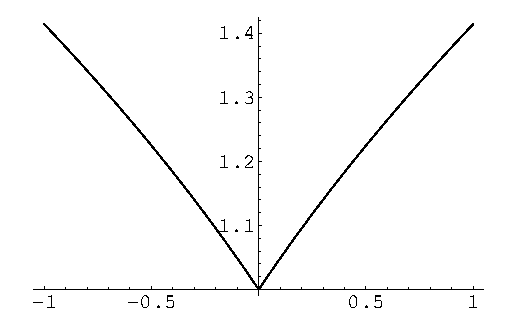
\includegraphics[width=0.4\textwidth]{calculus/differential/sqrt1x}
      \end{center}
      \caption{The function is not differentiable at the origin.}
      \label{figure sqrt1x}
    \end{figure}

    If we plot $\sqrt{1 + |x|}$, we can see that it is not differentiable 
    at $x = 0$ - it has a corner there.  
    (See Figure~\ref{figure sqrt1x}.)  The plot does not suffice for 
    demonstrating that the derivative does not exist.  However, it gives 
    us some useful insight.  We can see that the function is differentiable
    to the left and right of $x = 0$, but the slopes are different as 
    we approach the origin from the two directions.  
    Recall the definition of the derivative:
    \[
    f'(0) = \lim_{\epsilon \to 0} \frac{\sqrt{1 + |\epsilon|} - 1}{\epsilon}.
    \]
    We will show that the limit does not exist by demonstrating that 
    the left and right limits have different values.
    (The limit exists if and only if the left and right limits exist and 
    are equal.)  First consider the right limit.
    \[
    \lim_{\epsilon \to 0^+} \frac{\sqrt{1 + |\epsilon|} - 1}{\epsilon}
    = \lim_{\epsilon \to 0^+} \frac{\sqrt{1 + \epsilon} - 1}{\epsilon}
    \]
    Note that $\sqrt{1 + \epsilon} \geq 1 + \epsilon / 3$ for $\epsilon \in [0 .. 3]$.
    (See Figure~\ref{figure sqrt1x1x3}.)  This lets us get a lower bound 
    on the limit.
    \[
    \lim_{\epsilon \to 0^+} \frac{\sqrt{1 + \epsilon} - 1}{\epsilon}
    \geq \lim_{\epsilon \to 0^+} \frac{1 + \epsilon / 3 - 1}{\epsilon} = \frac{1}{3}
    \]

    \begin{figure}[tb]
      \begin{center}
        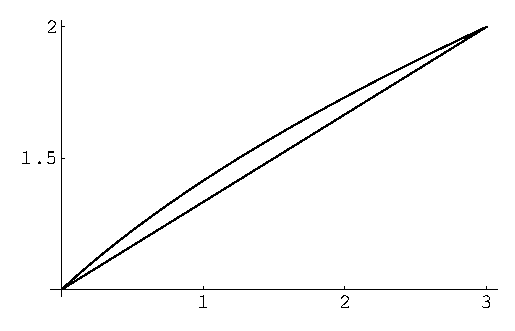
\includegraphics[width=0.4\textwidth]{calculus/differential/sqrt1x1x3}
      \end{center}
      \caption{A lower bound on the function.}
      \label{figure sqrt1x1x3}
    \end{figure}

    Now consider the left limit.
    \begin{align*}
      \lim_{\epsilon \to 0^-} \frac{\sqrt{1 + |\epsilon|} - 1}{\epsilon}
      &= \lim_{\epsilon \to 0^+} \frac{\sqrt{1 + \epsilon} - 1}{-\epsilon}
      \\
      &\leq \lim_{\epsilon \to 0^+} - \frac{1 + \epsilon / 3 - 1}{\epsilon} 
      \\
      &= -\frac{1}{3}
    \end{align*}
    Since the right limit is greater than or equal to $1/3$ and the left 
    limit is less than or equal to $- 1 / 3$, the limit does not exist.
    We conclude that $f(x) = \sqrt{1 + |x}$ is not differentiable 
    at $x = 0$.

    The problem is easier if we use L'Hospital's rule.  We can differentiate
    the numerator and denominator for $\epsilon \neq 0$.
    \begin{align*}
      f'(0) &= \lim_{\epsilon \to 0} \frac{\sqrt{1 + |\epsilon|} - 1}{\epsilon}
      \\
      &= \lim_{\epsilon \to 0} \frac{\frac{1}{2} (1 + |\epsilon|)^{-1/2} \sign(\epsilon)}{1}
      \\
      &= \lim_{\epsilon \to 0} \frac{1}{2} \sign(\epsilon)
    \end{align*}
    Since the limit does not exist,
    we conclude that the function is not differentiable at $x = 0$.
    However, since we haven't covered L'Hospital's rule yet, the 
    elementary method is more appropriate.
  \end{enumerate}
\end{Solution}



\begin{Solution}
  \label{solution d/dx x sin cos x}
  \renewcommand{\theenumi}{\alph{enumi}}
  \begin{enumerate}
    %%
  \item
    \begin{align*}
      \frac{\dd}{\dd x} [x \sin( \cos x) ]
      &= \frac{\dd}{\dd x} [x] \sin( \cos x ) + x \frac{\dd}{\dd x} [\sin(\cos x)]\\
      &= \sin( \cos x ) + x \cos(\cos x) \frac{\dd}{\dd x} [\cos x] \\
      &= \sin( \cos x ) - x \cos(\cos x) \sin x
    \end{align*}
    \[
    \boxed{
      \frac{\dd}{\dd x} [x \sin( \cos x) ] = \sin( \cos x ) - x \cos(\cos x) \sin x
      }
    \]
    %%
  \item
    \begin{align*}
      \frac{\dd}{\dd x} [f(\cos(g(x)))]
      &= f'(\cos(g(x))) \frac{\dd}{\dd x} [\cos(g(x))] \\
      &= - f'(\cos(g(x))) \sin(g(x)) \frac{\dd}{\dd x} [g(x)] \\
      &= - f'(\cos(g(x))) \sin(g(x)) g'(x)
    \end{align*}
    \[
    \boxed{
      \frac{\dd}{\dd x} [f(\cos(g(x)))] = - f'(\cos(g(x))) \sin(g(x)) g'(x)
      }
    \]
    %%
  \item
    \begin{align*}
      \frac{\dd}{\dd x} \left[ \frac{1}{f(\ln x)} \right]
      &= - \frac{ \frac{\dd}{\dd x} [ f(\ln x) ] }{ [f(\ln x) ]^2 } \\
      &= - \frac{ f'(\ln x) \frac{\dd}{\dd x} [\ln x] }{ [f(\ln x) ]^2 } \\
      &= - \frac{ f'(\ln x) }{ x [f(\ln x) ]^2 }
    \end{align*}
    \[
    \boxed{
      \frac{\dd}{\dd x} \left[ \frac{1}{f(\ln x)} \right]
      = - \frac{ f'(\ln x) }{ x [f(\ln x) ]^2 }
      }
    \]
    %%
  \item
    First we write the expression in terms exponentials and logarithms,
    \[
    x^{x^x} = x^{\exp( x \ln x)} = \exp( \exp( x \ln x ) \ln x ).
    \]
    Then we differentiate using the chain rule and the product rule.
    \begin{align*}
      \frac{\dd}{\dd x} \exp( \exp( x \ln x ) \ln x )
      &= \exp( \exp( x \ln x ) \ln x )
      \frac{\dd}{\dd x} (\exp( x \ln x ) \ln x ) \\
      &= x^{x^x} \left(
        \exp( x \ln x ) \frac{\dd}{\dd x} (x \ln x ) \ln x  +
        \exp( x \ln x ) \frac{1}{x} \right) \\
      &= x^{x^x} \left(
        x^x (\ln x + x \frac{1}{x}) \ln x  +
        x^{-1} \exp( x \ln x ) \right) \\
      &= x^{x^x} \left(
        x^x (\ln x + 1) \ln x  + x^{-1} x^x \right) \\
      &= x^{x^x + x} \left( x^{-1} + \ln x + \ln^2 x \right)
    \end{align*}
    \[
    \boxed{
      \frac{\dd}{\dd x} x^{x^x}
      = x^{x^x + x} \left( x^{-1} + \ln x + \ln^2 x \right)
      }
    \]
    %%
  \item
    We will use the fact that the sine is an odd function, i.e. 
    $\sin(-x) = - \sin x$.
    For $x \geq 0$, the expression is $x \sin x$;  for $x \leq 0$, the expression
    is $(-x) \sin(-x) = x \sin x$.  Thus we see that
    \[
    |x| \sin |x| = x \sin x.
    \]
    The first derivative of this is
    \[
    \sin x + x \cos x.
    \]
    \[
    \boxed{
      \frac{\dd}{\dd x} (|x| \sin |x| ) = \sin x + x \cos x
      }
    \]
  \end{enumerate}
  \renewcommand{\theenumi}{\arabic{enumi}}
\end{Solution}






\begin{Solution}
  \label{solution d/dx arcsin x}
  Let $y(x) = \arcsin x$.  Then $x = \sin y$.  We start with the derivative 
  of $\sin y$.
  \[
  \frac{\dd}{\dd y} \sin y = \cos y
  \]
  We substitute $x = \sin y$ and then take the multiplicative inverse to 
  get an expression for the derivative of the inverse sine.
  \begin{gather*}
    \frac{\dd x}{\dd y} = \cos y
    \\
    \frac{\dd}{\dd x} \arcsin x = \frac{1}{\cos y} 
  \end{gather*}
  Then we write the expression in terms of $x$.
  \begin{gather*}
    \frac{\dd}{\dd x} \arcsin x = \frac{1}{(1 - \sin^2 y)^{1/2}} 
    \\
    \boxed{
      \frac{\dd}{\dd x} \arcsin x = \frac{1}{(1 - x^2)^{1/2}}
    }
  \end{gather*}

  We follow the same steps to find the derivative of the inverse tangent.
  Let $y(x) = \arctan x$.  Then $x = \tan y$.  We start with the derivative 
  of the tangent.
  \begin{gather*}
    \frac{\dd}{\dd y} \tan y = \frac{1}{\cos^2 y}
    \\
    \frac{\dd x}{\dd y} = \frac{1}{\cos^2 y}
    \\
    \frac{\dd}{\dd x} \arctan x = \cos^2 y
    \\
    \frac{\dd}{\dd x} \arctan x = \cos^2 (\arctan x)
  \end{gather*}
  Now we use that $\cos(\arctan x) = (1 + x^2)^{1/2}$.  
  (The easiest way to remember these identities is to draw the 
  appropriate right triangle.  See Figure~\ref{figure cosarctanx}.)
  \begin{gather*}
    \frac{\dd}{\dd x} \arctan x = \left( \frac{1}{(1+x^2)^{1/2}} \right)^2
    \\
    \boxed{
      \frac{\dd}{\dd x} \arctan x = \frac{1}{1 + x^2}
    }
  \end{gather*}

  \begin{figure}[tb]
    \begin{center}
      \includegraphics[width=0.2\textwidth]{calculus/differential/cosarctanx}
    \end{center}
    \caption{The triangle for determining the cosine of the inverse tangent.}
    \label{figure cosarctanx}
  \end{figure}
\end{Solution}











%%-----------------------------------------------------------------------------
%% Implicit Differentiation




\begin{Solution}
  \label{solution tangent circle}
  We differentiate the equation of the circle with respect to $x$.
  \begin{gather*}
    x^2 + y^2 = 1
    \\
    2 x + 2 y y' = 0
  \end{gather*}
  We can solve this equation for $y'(x)$.
  \[
  y'(x) = - \frac{x}{y(x)}
  \]
  To find $y'(1/2)$ we need to find $y(x)$ in terms of $x$.
  \begin{gather*}
    y(x) = \pm \sqrt{1 - x^2}
    \\
    y'(x) = \pm \frac{x}{\sqrt{1 - x^2}}
  \end{gather*}
  $y'(1/2)$ can have the two values:
  \[
  \boxed{
    y' \left( \frac{1}{2} \right) = \pm \frac{1}{\sqrt{3}}.
    }
  \]
\end{Solution}






\begin{Solution}
  \label{solution y' y'' circle}
  We differentiate the equation and solve for $y'(x)$.
  \begin{gather*}
    x^2 - x y + y^2 = 3
    \\
    2 x - y - x y' + 2 y y' = 0
    \\
    \boxed{
      y'(x) = \frac{y - 2 x}{2 y - x}
    }
  \end{gather*}
  Then we differentiate $y'(x)$ to get $y''(x)$.
  \begin{gather*}
    y''(x) = \frac{(y' - 2)(2 y - x) - (y - 2 x)(2y' - 1)}{(2 y - x)^2}
    \\
    y''(x) = 3 \frac{x y' - y }{(2 y - x)^2}
    \\
    \intertext{We substitute the solution we found for $y'$.}
    y''(x) = 3 \frac{x \frac{y - 2 x}{2 y - x} - y}{(2 y - x)^2}
    \\
    y''(x) = 3 \frac{x (y - 2 x) - y (2 y - x) }{(2 y - x)^3}
    \\
    y''(x) = - 6 \frac{x^2 - x y + y^2}{(2 y - x)^3}
    \\
    \intertext{Finally we use the original equation to simplify the numerator.}
    \boxed{
      y''(x) =  - \frac{18}{(2 y - x)^3}
    }
  \end{gather*}
\end{Solution}



%%-----------------------------------------------------------------------------
%% Maxima and Minima



\begin{Solution}
  \label{solution max min x(12-2x)2}
  \renewcommand{\theenumi}{\alph{enumi}}
  \begin{enumerate}
    %%
  \item
    First we differentiate the function.
    \[
    f(x) = x (12 - 2 x)^2
    \]
    \begin{align*}
      f'(x)
      &= (12 - 2 x)^2 + 2 x (12 - 2 x) (-2) 
      \\
      &= 4 (x - 6)^2 + 8 x (x - 6) 
      \\
      &= 12 (x - 2)(x - 6)
    \end{align*}
    By solving $f'(x) = 0$, we see that there are critical points at 
    $x = 2$ and $x = 6$.  Next we compute the second derivative to attempt
    to determine the nature of the critical points.
    \begin{gather*}
      f''(x) = 12 (x - 2) + 12 (x - 6) = 24 (x - 4)
      \\
      f''(2) = - 48, \quad f''(6) = 48
    \end{gather*}
    Since $f''(2)$ is negative, $x = 2$ is a local maximum. 
    Since $f''(6)$ is positive, $x = 6$ is a local minimum. 
    The plot of the function in Figure~\ref{figure minmax-x122x2} corroborates
    this.

    \begin{figure}[tb]
      \begin{center}
        \includegraphics[width=0.4\textwidth]{calculus/differential/minmax-x122x2}
        \includegraphics[width=0.4\textwidth]{calculus/differential/minmax-3x22}
      \end{center}
      \caption{The maxima and minima of the functions.}
      \label{figure minmax-x122x2}
    \end{figure}
    %%
  \item
    First we differentiate the function to try to find critical points.
    \begin{gather*}
      f(x) = \sqrt[3]{(x - 2)^2}
      \\
      f'(x) = \frac{1}{3} \left( (x - 2)^2 \right)^{-2/3} 2 (x - 2)
      \\
      f'(x) = \frac{ 2 (x - 2) }{ 3 \sqrt[3]{(x - 2)^4} }
    \end{gather*}
    The first derivative exists and is nonzero for $x \neq 2$.  At $x = 2$, the
    derivative does not exist and thus $x = 2$ is a critical point.  For 
    $x < 2$, $f'(x) < 0$ and for $x > 2$, $f'(x) > 0$.
    Thus $x = 2$ is a local minimum.
    (See the second plot in Figure~\ref{figure minmax-x122x2}.)
  \end{enumerate}
  \renewcommand{\theenumi}{\arabic{enumi}}
\end{Solution}








\begin{Solution}
  \label{solution surface area cup}
  Let $r$ be the radius and $h$ the height of the cylinder.  The volume of
  the cup is $\pi r^2 h = 64$.  Thus the radius and height are related by
  $h = \frac{64}{\pi r^2}$.  We write the surface area of the cup as a 
  function of $r$.
  \[
  f(r) = \pi r^2 + 2 \pi r h = \pi r^2 + \frac{128}{r}
  \]
  We compute the first derivative of the surface area and equate 
  it to zero to find the critical points.
  \begin{gather*}
    f'(r) = 2 \pi r - \frac{128}{r^2} = 0
    \\
    2 \pi r^3 - 128 = 0
    \\
    \intertext{This cubic equation has a single real root.}
    r = \frac{4}{\sqrt[3]{\pi}}
  \end{gather*}
  The second derivative of the surface area is
  $f''(r) = 2 \pi + \frac{256}{r^3}$.  Since
  $f''(\frac{4}{\sqrt[3]{\pi}}) = 6\pi$, $r=\frac{4}{\sqrt[3]{\pi}}$ is a
  local minimum of $f(r)$.  Since this is the only critical point for
  real-valued $r$, it must be a global minimum.
  The cup has a radius of $\frac{4}{\sqrt[3]{\pi}}$ cm and a height of
  $\frac{4}{\sqrt[3]{\pi}}$ cm.
\end{Solution}



%%-----------------------------------------------------------------------------
%% Mean Value Theorems


\begin{Solution}
  \label{solution generalized theorem of the mean}
  We will use Rolle's theorem to prove the generalized theorem of the 
  mean.  First we need to define a function $h(x)$ that is differentiable
  and vanishes at $x = a$ and $x = b$.
  \[
  h(x) = f(x) - f(a) - \frac{f(b) - f(a)}{g(b) - g(a)} (g(x) - g(a)).
  \]
  Since $h(x)$ satisfies the conditions of Rolle's theorem, there exists a 
  point $\xi \in (a,b)$ where $h'(\xi) = 0$.
  \begin{gather*}
    h'(\xi) = f'(\xi) - \frac{f(b) - f(a)}{g(b) - g(a)} g'(\xi) = 0
    \\
    \frac{f'(\xi)}{g'(\xi)} = \frac{f(b) - f(a)}{g(b) - g(a)}
  \end{gather*}
\end{Solution}



\begin{Solution}
  \label{solution polynomial approximation sin x}
  The first few terms in the Taylor series of $\sin(x)$ about $x = 0$ are
  \[
  \sin(x) = x - \frac{x^3}{6} + \frac{x^5}{120} - \frac{x^7}{5040}
  + \frac{x^9}{362880} + \cdots.
  \]
  The seventh derivative of $\sin x$ is $-\cos x$.  Thus 
  \[
  \sin(x) = x - \frac{x^3}{6} + \frac{x^5}{120} - \frac{\cos x_0}{5040} x^7,
  \]
  where $x_0$ is in the interval $[0 .. x]$.  
  Since we are considering $x \in [-1,1]$ and
  $-1 \leq \cos(x_0) \leq 1$, the approximation
  \[
  \boxed{
    \sin x \approx x - \frac{x^3}{6} + \frac{x^5}{120}
    }
  \]
  has a maximum error of $\frac{1}{5040} \approx 0.000198$.
  We use this polynomial to approximate $\sin(1)$
  and verify that it has the required accuracy.
  \begin{gather*}
    \boxed{
      1 - \frac{1^3}{6} + \frac{1^5}{120} \approx 0.841667
    }
    \\
    \sin(1) \approx 0.841471
  \end{gather*}
  See Figure~\ref{figure sin-app} for plots of various polynomial 
  approximations of $\sin x$.
  \begin{figure}[tb]
    \begin{center}
      \includegraphics[width=0.9\textwidth]{calculus/differential/sin-app}
    \end{center}
    \caption{Polynomial approximations of the sine.}
    \label{figure sin-app}
  \end{figure}
\end{Solution}




\begin{Solution}
  \label{solution second difference centered}
  Expanding the terms in the approximation in Taylor series,
  \begin{align*}
    f(x+\Delta x) &= f(x) + \Delta x f'(x) + \frac{\Delta x^2}{2} f''(x)
    +\frac{\Delta x^3}{6} f'''(x) + \frac{\Delta x^4}{24} f''''(x_1), \\
    f(x-\Delta x) &= f(x) - \Delta x f'(x) + \frac{\Delta x^2}{2} f''(x)
    -\frac{\Delta x^3}{6} f'''(x) + \frac{\Delta x^4}{24} f''''(x_2),
  \end{align*}
  where $x \leq x_1 \leq x + \Delta x$ and $x - \Delta x \leq x_2 \leq x$.
  Substituting the expansions into the formula,
  \[
  \frac{f(x+\Delta x) - 2 f(x) + f(x-\Delta x)}{\Delta x^2}
  = f''(x) + \frac{\Delta x^2}{24} [f''''(x_1) + f''''(x_2)].
  \]
  Thus the error in the approximation is
  \[
  \boxed{
    \frac{\Delta x^2}{24} [f''''(x_1) + f''''(x_2)].
    }
  \]
\end{Solution}




\begin{Solution}
  \label{solution first derivative higher}
  %% CONTINUE
\end{Solution}



%%-----------------------------------------------------------------------------
%% L'Hospital's Rule





\begin{Solution}
  \label{solution lim (x - sin x)/x3}
  \renewcommand{\theenumi}{\alph{enumi}}
  \begin{enumerate}
    %%
  \item
    \begin{align*}
      \lim_{x \to 0} \left[ \frac{x-\sin x}{x^3} \right]
      &= \lim_{x \to 0} \left[ \frac{1-\cos x}{3 x^2} \right] \\
      &= \lim_{x \to 0} \left[ \frac{\sin x}{6 x} \right] \\
      &= \lim_{x \to 0} \left[ \frac{\cos x}{6} \right] \\
      &= \frac{1}{6}
    \end{align*}
    \[
    \boxed{
      \lim_{x \to 0} \left[ \frac{x-\sin x}{x^3} \right] = \frac{1}{6}
      }
    \]
    %%
  \item
    \begin{align*}
      \lim_{x \to 0} \left( \csc x - \frac{1}{x} \right)
      &= \lim_{x \to 0} \left( \frac{1}{\sin x} - \frac{1}{x} \right) \\
      &= \lim_{x \to 0} \left( \frac{x - \sin x}{x \sin x} \right) \\
      &= \lim_{x \to 0} \left( \frac{1 - \cos x}{x \cos x + \sin x} \right)\\
      &= \lim_{x \to 0} \left( \frac{\sin x}{- x \sin x + \cos x + \cos x}
      \right) \\
      &= \frac{0}{2} \\
      &= 0
    \end{align*}
    \[
    \boxed{
      \lim_{x \to 0} \left( \csc x - \frac{1}{x} \right) = 0
      }
    \]
    %%
  \item
    \begin{align*}
      \ln\left( \lim_{x \to +\infty} \left[ \left(1 + \frac{1}{x} \right)^x
        \right] \right)
      &= \lim_{x \to +\infty} \left[ \ln\left( \left(1 + \frac{1}{x}
          \right)^x \right) \right] \\
      &= \lim_{x \to +\infty} \left[ x \ln\left(1+\frac{1}{x}\right)
      \right] \\
      &= \lim_{x \to +\infty} \left[ \frac{\ln\left(1+\frac{1}{x}\right)}
        {1/x} \right] \\
      &= \lim_{x \to +\infty} \left[ \frac{\left(1+\frac{1}{x}\right)^{-1}
          \left(-\frac{1}{x^2}\right)}
        {-1/x^2} \right] \\
      &= \lim_{x \to +\infty} \left[ \left(1+\frac{1}{x}\right)^{-1}
      \right] \\
      &= 1
    \end{align*}
    Thus we have
    \[
    \boxed{
      \lim_{x \to +\infty} \left[ \left(1 + \frac{1}{x} \right)^x \right] = e.
      }
    \]
    %%
  \item
    It takes four successive applications of L'Hospital's rule to evaluate
    the limit.
    \begin{align*}
      \lim_{x \to 0} \left( \csc^2 x - \frac{1}{x^2} \right)
      &= \lim_{x \to 0} \frac{x^2 - \sin^2 x}{ x^2 \sin^2 x } \\
      &= \lim_{x \to 0} \frac{ 2 x - 2 \cos x \sin x }
      { 2 x^2 \cos x \sin x + 2 x \sin^2 x } \\
      &= \lim_{x \to 0} \frac{2 - 2 \cos^2 x + 2 \sin^2 x }
      { 2 x^2 \cos^2 x + 8 x \cos x \sin x + 2 \sin^2 x
        - 2 x^2 \sin^2 x } \\
      &= \lim_{x \to 0} \frac{ 8 \cos x \sin x }
      { 12 x \cos^2 x + 12 \cos x \sin x - 8 x^2 \cos x \sin x
        - 12 x \sin^2 x } \\
      &= \lim_{x \to 0} \frac{ 8 \cos^2 x - 8 \sin^2 x }
      { 24 \cos^2 x - 8 x^2 \cos^2 x - 64 x \cos x \sin x
        - 24 \sin^2 x + 8 x^2 \sin^2 x } \\
      &= \frac{1}{3}
    \end{align*}

    It is easier to use a Taylor series expansion.
    \begin{align*}
      \lim_{x \to 0} \left( \csc^2 x - \frac{1}{x^2} \right)
      &= \lim_{x \to 0} \frac{x^2 - \sin^2 x}{ x^2 \sin^2 x } \\
      &= \lim_{x \to 0} \frac{x^2 - (x - x^3/6 + O(x^5))^2}
      { x^2 (x + O(x^3))^2 } \\
      &= \lim_{x \to 0} \frac{x^2 - (x^2 - x^4/3 + O(x^6))}
      { x^4 + O(x^6) } \\
      &= \lim_{x \to 0} \left( \frac{1}{3} + O(x^2) \right) \\
      &= \frac{1}{3}
    \end{align*}
  \end{enumerate}
  \renewcommand{\theenumi}{\arabic{enumi}}
\end{Solution}






\begin{Solution}
  \label{solution lim x a/x}
  To evaluate the first limit, we use the identity $a^b = \e^{b \ln a}$
  and then apply L'Hospital's rule.
  \begin{align*}
    \lim_{x \to \infty} x^{a/x}
    &= \lim_{x \to \infty} \e^{\frac{a \ln x}{x} } \\
    &= \exp \left( \lim_{x \to \infty} \frac{a \ln x}{x} \right) \\
    &= \exp \left( \lim_{x \to \infty} \frac{a / x}{1} \right) \\
    &= \e^0
  \end{align*}
  \[
  \boxed{
    \lim_{x \to \infty} x^{a/x} = 1
    }
  \]

  We use the same method to evaluate the second limit.
  \begin{align*}
    \lim_{x \to \infty} \left( 1 + \frac{a}{x} \right)^{b x}
    &= \lim_{x \to \infty} \exp \left( b x
      \ln \left( 1 + \frac{a}{x} \right) \right) \\
    &= \exp \left( \lim_{x \to \infty} b x
      \ln \left( 1 + \frac{a}{x} \right) \right) \\
    &= \exp \left( \lim_{x \to \infty} b
      \frac{\ln( 1 + a/x )}{1/x} \right) \\
    &= \exp \left( \lim_{x \to \infty} b
      \frac{\frac{-a/x^2}{1+a/x}}{-1/x^2} \right) \\
    &= \exp \left( \lim_{x \to \infty} b
      \frac{a}{1+a/x} \right)
  \end{align*}
  \[
  \boxed{
    \lim_{x \to \infty} \left( 1 + \frac{a}{x} \right)^{b x} = \e^{a b}
    }
  \]
\end{Solution}








\raggedbottom
%%=============================================================================
\pagebreak
\flushbottom
\section{Quiz}

\begin{QuizProblem}
  \label{quiz problem define continuity}
  Define \textit{continuity}.

  \quizsolution{define continuity}
\end{QuizProblem}


\begin{QuizProblem}
  \label{quiz problem necessary sufficient continuity differentiability}
  Fill in the blank with \textit{necessary}, \textit{sufficient} or
  \textit{necessary and sufficient}.

  Continuity is a $\underline{\phantom{necessary and sufficient}}$ condition 
  for differentiability.

  Differentiability is a $\underline{\phantom{necessary and sufficient}}$ 
  condition for continuity.

  Existence of $\lim_{\Delta x \to 0} \frac{f(x+\Delta x) - f(x)}{\Delta x}$ is a 
  $\underline{\phantom{necessary and sufficient}}$ condition for
  differentiability.

  \quizsolution{necessary sufficient continuity differentiability}
\end{QuizProblem}


\begin{QuizProblem}
  \label{quiz problem ddx f(g(x)h(x))}
  Evaluate $\frac{\dd}{\dd x} f(g(x) h(x))$.

  \quizsolution{ddx f(g(x)h(x))}
\end{QuizProblem}


\begin{QuizProblem}
  \label{quiz problem ddx f(x)g(x)}
  Evaluate $\frac{\dd}{\dd x} f(x)^{g(x)}$.

  \quizsolution{ddx f(x)g(x)}
\end{QuizProblem}


\begin{QuizProblem}
  \label{quiz problem theorem of the mean}
  State the Theorem of the Mean.  Interpret the theorem physically.

  \quizsolution{theorem of the mean}
\end{QuizProblem}


\begin{QuizProblem}
  \label{quiz problem taylor's theorem of the mean}
  State Taylor's Theorem of the Mean.

  \quizsolution{taylor's theorem of the mean}
\end{QuizProblem}


\begin{QuizProblem}
  \label{quiz problem lim sin sin}
  Evaluate $\lim_{x \to 0} (\sin x)^{\sin x}$.

  \quizsolution{lim sin sin}
\end{QuizProblem}









\raggedbottom
%%=============================================================================
\pagebreak
\flushbottom
\section{Quiz Solutions}


\begin{QuizSolution}
  \label{quiz solution define continuity}
  A function $y(x)$ is said to be \textit{continuous at} $x = \xi$ if
  $\lim_{x \to \xi} y(x) = y(\xi)$. 
\end{QuizSolution}


\begin{QuizSolution}
  \label{quiz solution necessary sufficient continuity differentiability}
  Continuity is a necessary condition for differentiability.

  Differentiability is a sufficient condition for continuity.

  Existence of $\lim_{\Delta x \to 0} \frac{f(x+\Delta x) - f(x)}{\Delta x}$ is a 
  necessary and sufficient condition for differentiability.
\end{QuizSolution}


\begin{QuizSolution}
  \label{quiz solution ddx f(g(x)h(x))}
  \[
  \frac{\dd}{\dd x} f(g(x) h(x)) 
  = f'(g(x) h(x)) \frac{\dd}{\dd x} (g(x) h(x))
  = f'(g(x) h(x)) (g'(x) h(x) + g(x) h'(x))
  \]
\end{QuizSolution}


\begin{QuizSolution}
  \label{quiz solution ddx f(x)g(x)}
  \begin{align*}
    \frac{\dd}{\dd x} f(x)^{g(x)} 
    &= \frac{\dd}{\dd x} e^{g(x) \ln f(x)} 
    \\
    &= \e^{g(x) \ln f(x)} \frac{\dd}{\dd x} (g(x) \ln f(x)) 
    \\
    &= f(x)^{g(x)} \left( g'(x) \ln f(x) + g(x) \frac{f'(x)}{f(x)} \right)
  \end{align*}
\end{QuizSolution}


\begin{QuizSolution}
  \label{quiz solution theorem of the mean}
  If $f(x)$ is continuous in $[a..b]$ and differentiable in $(a..b)$ 
  then there exists a point $x = \xi$ such that
  \[
  f'(\xi) = \frac{f(b) - f(a)}{b - a}.
  \]
  That is, there is a point where the instantaneous velocity is equal to
  the average velocity on the interval. 
\end{QuizSolution}


\begin{QuizSolution}
  \label{quiz solution taylor's theorem of the mean}
  If $f(x)$ is $n+1$ times continuously differentiable in $(a..b)$ 
  then there exists a point $x = \xi \in (a..b)$ such that
  \[
  f(b) = f(a) + (b-a) f'(a) + \frac{(b-a)^2}{2!} f''(a) + \cdots +
  \frac{(b-a)^n}{n!} f^{(n)}(a)
  + \frac{(b-a)^{n+1}}{(n+1)!} f^{(n+1)}(\xi).
  \]
\end{QuizSolution}


\begin{QuizSolution}
  \label{quiz solution lim sin sin}
  Consider $\lim_{x \to 0} (\sin x)^{\sin x}$.  This is an indeterminate of 
  the form $0^0$.  The limit of the logarithm of the expression is
  $\lim_{x \to 0} \sin x \ln( \sin x )$.
  This is an indeterminate of the form $0 \cdot \infty$.  We can rearrange
  the expression to obtain an indeterminate of the form $\frac{\infty}{\infty}$
  and then apply L'Hospital's rule.
  \[
  \lim_{x \to 0} \frac{\ln( \sin x )}{1/\sin x} 
  = \lim_{x \to 0} \frac{ \cos x / \sin x}{ -\cos x / \sin^2 x }
  = \lim_{x \to 0} (- \sin x)
  = 0
  \]
  The original limit is
  \[
  \lim_{x \to 0} (\sin x)^{\sin x} = \e^0 = 1.
  \]
\end{QuizSolution}



\raggedbottom





%%-----------------------------------------------------------------------------
%%
%%                                   Sean Mauch
%%                       California Institute of Technology
%%                          (a) 2000 No Rights Reserved
%%
%%-----------------------------------------------------------------------------

\flushbottom






%%=============================================================================
%%=============================================================================
\chapter{Integral Calculus}
\label{chapter_integral}
\index{integral calculus}



%%=============================================================================
\section{The Indefinite Integral}
\index{indefinite integral}

The opposite of a derivative is the \textit{anti-derivative} or the
\textit{indefinite integral}.  The indefinite integral of a function
$f(x)$ is denoted,
\[
\int f(x) \,\dd x.
\]
It is defined by the property that
\[
\frac{\dd}{\dd x} \int f(x) \,\dd x = f(x).
\]
While a function $f(x)$ has a unique derivative if it is differentiable, it
has an infinite number of indefinite integrals, each of which differ by
an additive constant.

\paragraph{Zero Slope Implies a Constant Function.}
If the value of a function's derivative is identically zero, 
$\frac{\dd f}{\dd x} = 0$, then the function is a constant, $f(x) = c$.
To prove this, we assume that there exists a non-constant differentiable
function whose derivative is zero and obtain a contradiction.  Let
$f(x)$ be such a function.  Since $f(x)$ is non-constant, there exist
points $a$ and $b$ such that $f(a) \neq f(b)$.  By the Mean Value 
Theorem of differential calculus, there exists a point $\xi \in (a,b)$
such that
\[
f'(\xi) = \frac{f(b) - f(a)}{b-a} \neq 0,
\]
which contradicts that the derivative is everywhere zero.


\paragraph{Indefinite Integrals Differ by an Additive Constant.}
Suppose that $F(x)$ and $G(x)$ are indefinite integrals of $f(x)$.  Then
we have
\[
\frac{\dd}{\dd x} (F(x) - G(x)) = F'(x) - G'(x) = f(x) - f(x) = 0.
\]
Thus we see that $F(x) - G(x) = c$ and the two indefinite integrals must
differ by a constant.  For example, we have $\int \sin x \,\dd x = - \cos x + c$.
While every function that can be expressed in terms of elementary functions,
(the exponent, logarithm, trigonometric functions, etc.), has a derivative
that can be written explicitly in terms of elementary functions, the same
is not true of integrals.  For example, $\int \sin(\sin x) \,\dd x$ cannot
be written explicitly in terms of elementary functions.



\paragraph{Properties.}
Since the derivative is linear, so is the indefinite integral.  That is,
\[
\int ( a f(x) + b g(x) ) \,\dd x = a \int f(x) \,\dd x + b \int g(x) \,\dd x.
\]
For each derivative identity there is a corresponding integral 
identity.  Consider the power law identity, 
$\frac{\dd}{\dd x} (f(x))^a = a (f(x))^{a-1} f'(x)$.  The corresponding 
integral identity is
\[
\int (f(x))^a f'(x) \,\dd x = \frac{(f(x))^{a+1}}{a+1} + c, \quad a \neq -1,
\]
where we require that $a \neq -1$ to avoid division by zero.  From the
derivative of a logarithm, $\frac{\dd}{\dd x} \ln( f(x) ) = \frac{f'(x)}{f(x)}$,
we obtain,
\[
\int \frac{f'(x)}{f(x)} \,\dd x = \ln| f(x) | + c.
\]
Note the absolute value signs.  This is because 
$\frac{\dd}{\dd x} \ln|x| = \frac{1}{x}$ for $x \neq 0$.  In Figure~\ref{log1ox}
is a plot of $\ln|x|$ and $\frac{1}{x}$ to reinforce this.

\begin{figure}[h]
  \begin{center}
    \includegraphics[width=0.5\textwidth]{calculus/integral/log1ox}
  \end{center}
  \caption{The logarithm and its derivative.}
  \label{log1ox}
\end{figure}






\begin{Example}
  Consider
  \[
  I = \int \frac{x}{(x^2 + 1)^2} \,\dd x.
  \]
  We evaluate the integral by choosing $u = x^2 + 1$, $\dd u = 2 x \,\dd x$.
  \begin{align*}
    I &= \frac{1}{2} \int \frac{2 x}{(x^2 + 1)^2} \,\dd x \\
    &= \frac{1}{2} \int \frac{\dd u}{u^2} \\
    &= \frac{1}{2} \frac{-1}{u} \\
    &= - \frac{1}{2 (x^2+1) }.
  \end{align*}
\end{Example}





\begin{Example}
  Consider
  \[
  I = \int \tan x \,\dd x = \int \frac{\sin x}{\cos x} \,\dd x.
  \]
  By choosing $f(x) = \cos x$, $f'(x) = - \sin x$, we see that the integral is
  \[
  I = - \int \frac{-\sin x}{\cos x} \,\dd x = - \ln | \cos x | + c.
  \]
\end{Example}



\paragraph{Change of Variable.}
The differential of a function $g(x)$ is $d g = g'(x) \,\dd x$.  Thus one 
might suspect that for $\xi = g(x)$, 
\begin{equation}
  \label{change_var}
  \int f(\xi) \,\dd \xi = \int f(g(x)) g'(x) \,\dd x,
\end{equation}
since $d\xi = d g = g'(x)\,\dd x$.  This turns out to be true.  To prove it
we will appeal to the the chain rule for differentiation.  Let $\xi$ be 
a function of $x$.  The chain rule is
\[
\frac{\dd}{\dd x} f(\xi) = f'(\xi) \xi'(x),
\]
\[
\frac{\dd}{\dd x} f(\xi) = \frac{\dd f}{\dd \xi} \frac{\dd \xi}{\dd x}.
\]
We can also write this as
\[
\frac{\dd f}{\dd \xi} = \frac{\dd x}{\dd \xi} \frac{\dd f}{\dd x},
\]
or in operator notation,
\[
\frac{\dd}{\dd \xi} = \frac{\dd x}{\dd \xi} \frac{\dd}{\dd x}.
\]
Now we're ready to start.  The derivative of the left side of
Equation~\ref{change_var} is
\[
\frac{\dd}{\dd \xi} \int f(\xi) \,\dd \xi = f(\xi).
\]
Next we differentiate the right side,
\begin{align*}
  \frac{\dd}{\dd \xi} \int f(g(x)) g'(x) \,\dd x
  &= \frac{\dd x}{\dd \xi} \frac{\dd}{\dd x} \int f(g(x)) g'(x) \,\dd x \\
  &= \frac{\dd x}{\dd \xi} f(g(x)) g'(x) \\
  &= \frac{\dd x}{\dd g} f(g(x)) \frac{\dd g}{\dd x} \\
  &= f(g(x)) \\
  &= f(\xi)
\end{align*}
to see that it is in fact an identity for $\xi = g(x)$.





\begin{Example}
  Consider
  \[
  \int x \sin(x^2) \,\dd x.
  \]
  We choose $\xi = x^2$, $d\xi = 2 x d x$ to evaluate the integral.
  \begin{align*}
    \int x \sin(x^2) \,\dd x
    &= \frac{1}{2} \int \sin(x^2) 2 x \,\dd x \\
    &= \frac{1}{2} \int \sin \xi \,\dd \xi \\
    &= \frac{1}{2} (-\cos \xi) + c \\
    &= - \frac{1}{2} \cos( x^2 ) + c
  \end{align*}
\end{Example}




\paragraph{Integration by Parts.}
The product rule for differentiation gives us an identity called integration
by parts.  We start with the product rule and then integrate both sides
of the equation.
\begin{gather*}
  \frac{\dd}{\dd x} (u(x) v(x)) = u'(x) v(x) + u(x) v'(x) \\
  \int ( u'(x) v(x) + u(x) v'(x) ) \,\dd x = u(x) v(x) + c \\
  \int u'(x) v(x) \,\dd x + \int u(x) v'(x) ) \,\dd x = u(x) v(x) \\
  \int u(x) v'(x) ) \,\dd x = u(x) v(x)  - \int v(x) u'(x) \,\dd x
\end{gather*}
The theorem is most often written in the form
\[
\int u \,\dd v = u v - \int v \,\dd u.
\]
So what is the usefulness of this?  Well, it may happen for some integrals
and a good choice of $u$ and $v$ that the integral on the right is easier
to evaluate than the integral on the left.



\begin{Example}
  Consider $\int x \e^x \,\dd x$.  If we choose $u = x$, $\dd v = \e^x \,\dd x$ then
  integration by parts yields
  \[
  \int x \e^x \,\dd x = x \e^x - \int \e^x \,\dd x = (x-1) \e^x.
  \]
  Now notice what happens when we choose $u = \e^x$, $\dd v = x \,\dd x$.
  \[
  \int x \e^x \,\dd x = \frac{1}{2} x^2 \e^x - \int \frac{1}{2} x^2 \e^x \,\dd x
  \]
  The integral gets harder instead of easier.
\end{Example}


When applying integration by parts, one must choose $u$ and $\dd v$
wisely.  As general rules of thumb:
\begin{itemize}
\item
  Pick $u$ so that $u'$ is simpler than $u$.
\item
  Pick $\dd v$ so that $v$ is not more complicated, (hopefully simpler), 
  than $\dd v$.
\end{itemize}
Also note that you may have to apply integration by parts several times
to evaluate some integrals.






%%=============================================================================
\section{The Definite Integral}
\index{definite integral}

%%-----------------------------------------------------------------------------
\subsection{Definition}

The area bounded by the $x$ axis, the vertical lines $x = a$ and $x = b$
and the function $f(x)$ is denoted with a \textit{definite integral}, 
\[
\int_a^b f(x) \,\dd x.
\]
The area is signed, that is, if $f(x)$ is negative, then the area is 
negative.  
We measure the area with a divide-and-conquer strategy.  
First partition the interval $(a,b)$ with
$a = x_0 < x_1 < \cdots < x_{n-1} < x_n = b$.  
Note that the area under the curve on the subinterval is approximately
the area of a rectangle of base $\Delta x_i = x_{i+1} - x_i$ and height
$f(\xi_i)$, where $\xi_i \in [x_i, x_{i+1}]$.  If we add up the areas
of the rectangles, we get an approximation of the area under the 
curve.  See Figure~\ref{intint}

\begin{figure}[h]
  \begin{center}
    \includegraphics[width=0.6\textwidth]{calculus/integral/intint}
  \end{center}
  \caption{Divide-and-conquer strategy for approximating a definite integral.}
  \label{intint}
\end{figure}

\[
\int_a^b f(x) \,\dd x \approx \sum_{i = 0}^{n-1} f(\xi_i) \Delta x_i
\]
As the $\Delta x_i$'s get smaller, we expect the approximation of the
area to get better.  Let $\Delta x = \max_{0 \leq i \leq n-1} \Delta x_i$.
We define the definite integral as the sum of the areas of the rectangles
in the limit that $\Delta x \to 0$.
\[
\int_a^b f(x) \,\dd x 
= \lim_{\Delta x \to 0} \sum_{i = 0}^{n-1} f(\xi_i) \Delta x_i
\]
The integral is defined when the limit exists.  This is known as the
\textit{Riemann integral} of $f(x)$.  $f(x)$ is called the \textit{integrand}.




%%-----------------------------------------------------------------------------
\subsection{Properties}

\paragraph{Linearity and the Basics.}
Because summation is a linear operator, that is
\[
\sum_{i=0}^{n-1} (c f_i + d g_i) 
= c \sum_{i=0}^{n-1} f_i + d \sum_{i=0}^{n-1} g_i,
\]
definite integrals are linear,
\[
\int_a^b (c f(x) + d g(x))\,\dd x = c \int_a^b f(x)\,\dd x + d \int_a^b g(x) \,\dd x.
\]
One can also divide the \textit{range of integration}.
\[
\int_a^b f(x) \,\dd x = \int_a^c f(x) \,\dd x + \int_c^b f(x) \,\dd x
\]
We assume that each of the above integrals exist.  If $a \leq b$, and 
we integrate from $b$ to $a$, then each of the $\Delta x_i$ will be negative.
From this observation, it is clear that
\[
\int_a^b f(x) \,\dd x = - \int_b^a f(x) \,\dd x.
\]
If we integrate any function from a point $a$ to that same point $a$, then
all the $\Delta x_i$ are zero and 
\[
\int_a^a f(x) \,\dd x = 0.
\]





\paragraph{Bounding the Integral.}
Recall that if $f_i \leq g_i$, then
\[
\sum_{i=0}^{n-1} f_i \leq \sum_{i=0}^{n-1} g_i.
\]
Let $m = \min_{x \in [a,b]} f(x)$ and $M = \max_{x \in [a,b]} f(x)$.  Then
\[
(b-a) m = \sum_{i=0}^{n-1} m \Delta x_i 
\leq \sum_{i=0}^{n-1} f(\xi_i) \Delta x_i 
\leq \sum_{i=0}^{n-1} M \Delta x_i = (b-a) M
\]
implies that
\[
(b-a) m \leq \int_a^b f(x) \,\dd x \leq (b-a) M.
\]
Since
\[
\left| \sum_{i=0}^{n-1} f_i \right| \leq \sum_{i=0}^{n-1} |f_i|,
\]
we have
\[
\left| \int_a^b f(x) \,\dd x \right| \leq \int_a^b |f(x)| \,\dd x.
\]





\paragraph{Mean Value Theorem of Integral Calculus.}
Let $f(x)$ be continuous.  We know from above that
\[
(b-a) m \leq \int_a^b f(x) \,\dd x \leq (b-a) M.
\]
Therefore there exists a constant $c \in [m,M]$ satisfying
\[
\int_a^b f(x) \,\dd x = (b-a) c.
\]
Since $f(x)$ is continuous, there is a point $\xi \in [a,b]$ such that
$f(\xi) = c$.  Thus we see that 
\[
\int_a^b f(x) \,\dd x = (b-a) f(\xi),
\]
for some $\xi \in [a,b]$.







%%=============================================================================
\section{The Fundamental Theorem of Integral Calculus}
\index{fundamental theorem of calculus}


\paragraph{Definite Integrals with Variable Limits of Integration.}
Consider $a$ to be a constant and $x$ variable, then the function $F(x)$
defined by
\begin{equation}
  \label{int_var_limit}
  F(x) = \int_a^x f(t) \,\dd t
\end{equation}
is an anti-derivative of $f(x)$, that is $F'(x) = f(x)$.  To show this
we apply the definition of differentiation and the integral mean value
theorem.
\begin{align*}
  F'(x)
  &= \lim_{\Delta x \to 0} \frac{F(x+\Delta x) - F(x)}{\Delta x} \\
  &= \lim_{\Delta x \to 0} \frac{ \int_a^{x+\Delta x} f(t) \,\dd t
    - \int_a^x f(t)\,\dd t }{\Delta x} \\
  &= \lim_{\Delta x \to 0} \frac{ \int_x^{x+\Delta x} f(t) \,\dd t }
  {\Delta x} \\
  &= \lim_{\Delta x \to 0} \frac{ f(\xi) \Delta x }
  {\Delta x}, \qquad \xi \in [x,x+\Delta x] \\
  &= f(x)
\end{align*}




\paragraph{The Fundamental Theorem of Integral Calculus.}
Let $F(x)$ be any anti-derivative of $f(x)$.  Noting that all anti-derivatives
of $f(x)$ differ by a constant and replacing $x$ by $b$ in 
Equation~\ref{int_var_limit}, we see that there exists a constant $c$ 
such that
\[
\int_a^b f(x) \,\dd x = F(b) + c.
\]
Now to find the constant.  By plugging in $b = a$,
\[
\int_a^a f(x) \,\dd x = F(a) + c = 0,
\]
we see that $c = -F(a)$.  This gives us a result known as the 
\textit{Fundamental Theorem of Integral Calculus}.
\[
\int_a^b f(x) \,\dd x = F(b) - F(a).
\]
We introduce the notation
\[
[F(x)]_a^b \equiv F(b) - F(a).
\]



\begin{Example}
  \[
  \int_0^\pi \sin x \,\dd x = [-\cos x]_0^\pi = - \cos(\pi)+ \cos(0) = 2
  \]
\end{Example}






%%=============================================================================
\section{Techniques of Integration}
\index{integration!techniques of}





%%-----------------------------------------------------------------------------
\subsection{Partial Fractions}


A proper rational function
\[
\frac{p(x)}{q(x)} = \frac{p(x)}{(x-a)^n r(x)}
\]
Can be written in the form
\[
\frac{p(x)}{(x-\alpha)^n r(x)} = \left( \frac{a_0}{(x-\alpha)^n}
  + \frac{a_1}{(x-\alpha)^{n-1}} + \cdots + \frac{a_{n-1}}{x-\alpha}
\right) + (\cdots)
\]
where the $a_k$'s are constants and the last ellipses represents the
partial fractions expansion of the roots of $r(x)$.  The coefficients are
\[
a_k = \frac{1}{k!} \frac{d^k}{d x^k}
\left( \frac{p(x)}{r(x)} \right) \bigg|_{x=\alpha}.
\]




\begin{Example}
  Consider the partial fraction expansion of
  \[
  \frac{1+x+x^2}{(x-1)^3}.
  \]
  The expansion has the form
  \[
  \frac{a_0}{(x-1)^3} + \frac{a_1}{(x-1)^2} + \frac{a_2}{x-1}.
  \]
  The coefficients are
  \begin{align*}
    a_0     &= \frac{1}{0!} (1+x+x^2)|_{x=1} = 3, \\
    a_1     &= \frac{1}{1!} \frac{\dd}{\dd x}(1+x+x^2)|_{x=1}
    = (1+2x)|_{x=1} = 3, \\
    a_2     &= \frac{1}{2!} \frac{\dd^2}{\dd x^2}(1+x+x^2)|_{x=1}
    = \frac{1}{2} (2)|_{x=1} = 1.
  \end{align*}
  Thus we have
  \[
  \frac{1+x+x^2}{(x-1)^3} = \frac{3}{(x-1)^3} + \frac{3}{(x-1)^2}
  + \frac{1}{x-1}.
  \]
\end{Example}







\begin{Example}
  Suppose we want to evaluate 
  \[
  \int \frac{1+x+x^2}{(x-1)^3} \,\dd x.
  \]
  If we expand the integrand in a partial fraction expansion, then the integral
  becomes easy.
  \begin{align*}
    \int \frac{1+x+x^2}{(x-1)^3} \,\dd x.
    &= \int \left( \frac{3}{(x-1)^3} + \frac{3}{(x-1)^2}
      + \frac{1}{x-1} \right)\,\dd x \\
    &= - \frac{3}{2 (x-1)^2} - \frac{3}{(x-1)} + \ln(x-1)
  \end{align*}
\end{Example}







\begin{Example}
  Consider the partial fraction expansion of
  \[
  \frac{1+x+x^2}{x^2 (x-1)^2}.
  \]
  The expansion has the form
  \[
  \frac{a_0}{x^2} + \frac{a_1}{x} + \frac{b_0}{(x-1)^2} + \frac{b_1}{x-1}.
  \]
  The coefficients are
  \begin{align*}
    a_0     &= \frac{1}{0!} \left( \frac{1+x+x^2}{(x-1)^2} \right)
    \bigg|_{x=0} = 1, \\
    a_1     &= \frac{1}{1!} \frac{\dd}{\dd x}
    \left( \frac{1+x+x^2}{(x-1)^2} \right) \bigg|_{x=0}
    = \left( \frac{1+2x}{(x-1)^2}
      - \frac{2(1+x+x^2)}{(x-1)^3} \right) \bigg|_{x=0}
    = 3, \\
    b_0     &= \frac{1}{0!} \left( \frac{1+x+x^2}{x^2} \right)
    \bigg|_{x=1} = 3, \\
    b_1     &= \frac{1}{1!} \frac{\dd}{\dd x}
    \left( \frac{1+x+x^2}{x^2} \right) \bigg|_{x=1}
    = \left( \frac{1+2x}{x^2}
      - \frac{2(1+x+x^2)}{x^3} \right) \bigg|_{x=1}
    = -3,
  \end{align*}
  Thus we have
  \[
  \frac{1+x+x^2}{x^2 (x-1)^2} = \frac{1}{x^2} + \frac{3}{x}
  + \frac{3}{(x-1)^2} - \frac{3}{x-1}.
  \]
\end{Example}




If the rational function has real coefficients and the denominator
has complex roots, then you can reduce the work in finding the partial
fraction expansion with the following trick:  Let $\alpha$ and $\overline{\alpha}$
be complex conjugate pairs of roots of the denominator.
\begin{align*}
  \frac{p(x)}{(x-\alpha)^n (x- \overline{\alpha})^n r(x)}
  &= \left( \frac{a_0}{(x-\alpha)^n}
    + \frac{a_1}{(x-\alpha)^{n-1}} + \cdots + \frac{a_{n-1}}{x-\alpha}
  \right) \\
  &\quad + \left( \frac{\overline{a_0}}{(x-\overline{\alpha})^n}
    + \frac{\overline{a_1}}{(x-\overline{\alpha})^{n-1}} + \cdots
    + \frac{\overline{a_{n-1}}}{x-\overline{\alpha}} \right)
  + (\cdots)
\end{align*}
Thus we don't have to calculate the coefficients for the root at
$\overline{\alpha}$.  We just take the complex conjugate of the coefficients
for $\alpha$.






\begin{Example}
  Consider the partial fraction expansion of
  \[
  \frac{1+x}{x^2+1}.
  \]
  The expansion has the form
  \[
  \frac{a_0}{x-i} + \frac{\overline{a_0}}{x+i}
  \]
  The coefficients are
  \begin{align*}
    a_0     &= \frac{1}{0!} \left(\frac{1+x}{x+i} \right)
    \bigg|_{x=i} = \frac{1}{2}(1-i), \\
    \overline{a_0} &= \overline{ \frac{1}{2}(1-i)} = \frac{1}{2}(1+i)
  \end{align*}
  Thus we have
  \[
  \frac{1+x}{x^2+1} = \frac{1-i}{2(x-i)} + \frac{1+i}{2(x+i)}.
  \]
\end{Example}











%%=============================================================================
\section{Improper Integrals}
\index{improper integrals}
\index{integrals!improper}


If the range of integration is infinite or $f(x)$ is discontinuous at 
some points then $\int_a^b f(x) \,\dd x$ is called an \textit{improper
  integral}.  


\paragraph{Discontinuous Functions.}
If $f(x)$ is continuous on the interval $a \leq x \leq b$ 
except at the point $x=c$ where $a < c < b$ then
\[
\int_a^b f(x)\,\dd x = \lim_{\delta \to 0^+} \int_a^{c-\delta} f(x)\,\dd x
+ \lim_{\epsilon \to 0^+} \int_{c+\epsilon}^b f(x)\,\dd x
\]
provided that both limits exist.


\begin{Example}
  Consider the integral of $\ln x$ on the interval $[0,1]$.  Since the logarithm
  has a singularity at $x = 0$, this is an improper integral.  We write the
  integral in terms of a limit and evaluate the limit with L'Hospital's rule.
  \begin{align*}
    \int_0^1 \ln x \,\dd x
    &= \lim_{\delta \to 0} \int_\delta^1 \ln x \,\dd x \\
    &= \lim_{\delta \to 0} [x \ln x - x]_\delta^1 \\
    &= 1 \ln(1) - 1 - \lim_{\delta \to 0} (\delta \ln \delta - \delta )\\
    &= -1 - \lim_{\delta \to 0} (\delta \ln \delta ) \\
    &= -1 - \lim_{\delta \to 0} \left( \frac{ \ln \delta }{1/\delta } 
    \right) \\
    &= -1 - \lim_{\delta \to 0} \left( \frac{ 1 / \delta }{-1/\delta^2 } 
    \right) \\
    &= -1
  \end{align*}
\end{Example}




\begin{Example}
  Consider the integral of $x^a$ on the range $[0,1]$.  If $a < 0$ then there
  is a singularity at $x = 0$.  First assume that $a \neq -1$.
  \begin{align*}
    \int_0^1 x^a \,\dd x
    &= \lim_{\delta \to 0^+} \left[ \frac{x^{a+1}}{a+1} \right]_\delta^1 \\
    &= \frac{1}{a+1} - \lim_{\delta \to 0^+} \frac{\delta^{a+1}}{a+1} 
  \end{align*}
  This limit exists only for $a > -1$.  Now consider the case that $a = -1$.
  \begin{align*}
    \int_0^1 x^{-1} \,\dd x
    &= \lim_{\delta \to 0^+} \left[ \ln x \right]_\delta^1 \\
    &= \ln(0) - \lim_{\delta \to 0^+} \ln \delta
  \end{align*}
  This limit does not exist.  We obtain the result,
  \[
  \int_0^1 x^a \,\dd x = \frac{1}{a+1}, \quad \mathrm{for}\ a > -1.
  \]
\end{Example}



\paragraph{Infinite Limits of Integration.}
If the range of integration is infinite, say $[a,\infty)$ then we define
the integral as
\[
\int_a^\infty f(x) \,\dd x = \lim_{\alpha \to \infty} \int_a^\alpha f(x) \,\dd x,
\]
provided that the limit exists.
If the range of integration is $(-\infty,\infty)$ then
\[
\int_{-\infty}^\infty f(x)\,\dd x = \lim_{\alpha \to -\infty} \int_\alpha^a f(x)\,\dd x
+ \lim_{\beta \to +\infty} \int_a^\beta f(x)\,\dd x.
\]



\begin{Example}
  \begin{align*}
    \int_1^\infty \frac{\ln x}{x^2} \,\dd x
    &= \int_1^\infty \ln x \left( \frac{\dd}{\dd x} \frac{-1}{x} \right) 
    \,\dd x \\
    &= \left[ \ln x \frac{-1}{x} \right]_1^\infty 
    - \int_1^\infty \frac{-1}{x} \frac{1}{x} \,\dd x \\
    &= \lim_{x \to +\infty} \left( - \frac{ \ln x }{x} \right) 
    - \left[ \frac{1}{x} \right]_1^\infty \\
    &= \lim_{x \to +\infty} \left( - \frac{ 1/x }{1} \right) 
    - \lim_{x \to \infty} \frac{1}{x} + 1 \\
    &= 1
  \end{align*}
\end{Example}






\begin{Example}
  Consider the integral of $x^a$ on $[1,\infty)$.  First assume that
  $a \neq -1$.
  \begin{align*}
    \int_1^\infty x^a \,\dd x
    &= \lim_{\beta \to +\infty} \left[ \frac{x^{a+1}}{a+1} 
    \right]_1^\beta \\
    &= \lim_{\beta \to +\infty} \frac{\beta^{a+1}}{a+1} - \frac{1}{a+1}
  \end{align*}
  The limit exists for $\beta < -1$.  Now consider the case $a = -1$.
  \begin{align*}
    \int_1^\infty x^{-1} \,\dd x
    &= \lim_{\beta \to +\infty} \left[ \ln x
    \right]_1^\beta \\
    &= \lim_{\beta \to +\infty} \ln \beta - \frac{1}{a+1}
  \end{align*}
  This limit does not exist.  Thus we have 
  \[
  \int_1^\infty x^a \,\dd x = - \frac{1}{a+1}, \quad \mathrm{for}\ a < -1.
  \]
\end{Example}









\raggedbottom
%%=============================================================================
\pagebreak
\flushbottom
\section{Exercises}



%%-----------------------------------------------------------------------------
\begin{large}
  \noindent
  \textbf{The Indefinite Integral}
\end{large}


\begin{Exercise}[mathematica/calculus/integral/fundamental.nb]
  \label{exercise int 2x+3 10}
  Evaluate $\int (2x+3)^{10} \,\dd x$.

  \hintsolution{int 2x+3 10}
\end{Exercise}




\begin{Exercise}[mathematica/calculus/integral/fundamental.nb]
  \label{exercise int ln x 2 / x}
  Evaluate $\int \frac{(\ln x)^2}{x} \,\dd x$.

  \hintsolution{int ln x 2 / x}
\end{Exercise}



\begin{Exercise}[mathematica/calculus/integral/fundamental.nb]
  \label{exercise int x sqrt x2+3}
  Evaluate $\int x \sqrt{x^2+3}\,\dd x$.

  \hintsolution{int x sqrt x2+3}
\end{Exercise}



\begin{Exercise}[mathematica/calculus/integral/fundamental.nb]
  \label{exercise int cos x / sin x}
  Evaluate $\int \frac{\cos x}{\sin x}\,\dd x$.

  \hintsolution{int cos x / sin x}
\end{Exercise}



\begin{Exercise}[mathematica/calculus/integral/fundamental.nb]
  \label{exercise int x2 / x3-5}
  Evaluate $\int \frac{x^2}{x^3-5}\,\dd x$.

  \hintsolution{int x2 / x3-5}
\end{Exercise}



%%-----------------------------------------------------------------------------
\begin{large}
  \noindent
  \textbf{The Definite Integral}
\end{large}


\begin{Exercise}[mathematica/calculus/integral/definite.nb]
  \label{exercise int by sum x}
  Use the result
  \[
  \int_a^b f(x)\,\dd x = \lim_{N \to \infty} \sum_{n=0}^{N-1} f(x_n) \Delta x
  \]
  where $\Delta x = \frac{b-a}{N}$ and $x_n = a + n \Delta x$, to show that
  \[
  \int_0^1 x \,\dd x = \frac{1}{2}.
  \]

  \hintsolution{int by sum x}
\end{Exercise}



\begin{Exercise}[mathematica/calculus/integral/definite.nb]
  \label{exercise int 0 pi sin2 x}
  Evaluate the following integral using integration by parts and the 
  Pythagorean identity.
  $\int_0^\pi \sin^2 x \,\dd x$

  \hintsolution{int 0 pi sin2 x}
\end{Exercise}



\begin{Exercise}[mathematica/calculus/integral/definite.nb]
  \label{exercise d/dx int g f h}
  Prove that
  \[
  \frac{\dd}{\dd x} \int_{g(x)}^{f(x)} h(\xi) \,\dd \xi = h(f(x))f'(x) - h(g(x))g'(x).
  \]
  (Don't use the limit definition of differentiation, use the Fundamental
  Theorem of Integral Calculus.)

  \hintsolution{d/dx int g f h}
\end{Exercise}







\begin{Exercise}[mathematica/calculus/integral/definite.nb]
  \label{exercise area x xn}
  Let $A_n$ be the area between the curves $x$ and $x_n$ on the interval
  $[0 \ldots 1]$.  What is $\lim_{n \to \infty} A_n$?  Explain this result geometrically.

  \hintsolution{area x xn}
\end{Exercise}




\begin{Exercise}[mathematica/calculus/integral/taylor.nb]
  \label{exercise taylor series integral}
  \renewcommand{\theenumi}{\alph{enumi}}
  \begin{enumerate}
  \item
    Show that
    \[
    f(x) = f(0) + \int_0^x f'(x-\xi)\,\dd \xi.
    \]
  \item
    From the above identity show that
    \[
    f(x) = f(0) + x f'(0) + \int_0^x \xi f''(x-\xi)\,\dd \xi.
    \]
  \item
    Using induction, show that
    \[
    f(x) = f(0) + x f'(0) + \frac{1}{2} x^2 f''(0) + \cdots +
    \frac{1}{n!} x^n f^{(n)}(0)
    + \int_0^x \frac{1}{n!} \xi^n  f^{(n+1)}(x-\xi)\,\dd \xi.
    \]
  \end{enumerate}
  \renewcommand{\theenumi}{\arabic{enumi}}

  \hintsolution{taylor series integral}
\end{Exercise}



\begin{Exercise}
  \label{exercise arclength 0 x 2x}
  Find a function $f(x)$ whose arc length from $0$ to $x$ is $2 x$.

  \hintsolution{arclength 0 x 2x}
\end{Exercise}








\begin{Exercise}
  \label{exercise bounded -1 1 length}
  Consider a curve $C$, bounded by $-1$ and $1$, on the interval
  $(-1 \ldots 1)$.  Can the length of $C$ be unbounded?  What if we change
  to the closed interval $[-1 \ldots 1]$?

  \hintsolution{bounded -1 1 length}
\end{Exercise}








%%-----------------------------------------------------------------------------
\begin{large}
  \noindent
  \textbf{The Fundamental Theorem of Integration}
\end{large}


%%-----------------------------------------------------------------------------
\begin{large}
  \noindent
  \textbf{Techniques of Integration}
\end{large}


\begin{Exercise}[mathematica/calculus/integral/parts.nb]
  \label{exercise int x sin x}
  Evaluate $\int x \sin x \,\dd x$.

  \hintsolution{int x sin x}
\end{Exercise}



\begin{Exercise}[mathematica/calculus/integral/parts.nb]
  \label{exercise int x3 e2x}
  Evaluate $\int x^3 \e^{2x} \,\dd x$.

  \hintsolution{int x3 e2x}
\end{Exercise}




\begin{Exercise}[mathematica/calculus/integral/partial.nb]
  \label{exercise int 1 / x2-4}
  Evaluate $\int \frac{1}{x^2-4}\,\dd x$.

  \hintsolution{int 1 / x2-4}
\end{Exercise}





\begin{Exercise}[mathematica/calculus/integral/partial.nb]
  \label{exercise int x+1 / x3+x2-6x}
  Evaluate $\int \frac{x+1}{x^3+x^2-6x} \,\dd x$.

  \hintsolution{int x+1 / x3+x2-6x}
\end{Exercise}







%%-----------------------------------------------------------------------------
\begin{large}
  \noindent
  \textbf{Improper Integrals}
\end{large}



\begin{Exercise}[mathematica/calculus/integral/improper.nb]
  \label{exercise int 0 4 1 / (x-1)2}
  Evaluate $\int_0^4 \frac{1}{(x-1)^2} \,\dd x$.

  \hintsolution{int 0 4 1 / (x-1)2}
\end{Exercise}




\begin{Exercise}[mathematica/calculus/integral/improper.nb]
  \label{exercise int 0 1 1 / sqrt x}
  Evaluate $\int_0^1 \frac{1}{\sqrt{x}} \,\dd x$.

  \hintsolution{int 0 1 1 / sqrt x}
\end{Exercise}




\begin{Exercise}[mathematica/calculus/integral/improper.nb]
  \label{exercise int 0 infty 1 / x2+4}
  Evaluate $\int_0^\infty \frac{1}{x^2+4} \,\dd x$.

  \hintsolution{int 0 infty 1 / x2+4}
\end{Exercise}












\raggedbottom
%%=============================================================================
\pagebreak
\flushbottom
\section{Hints}



%%-----------------------------------------------------------------------------
%% The Indefinite Integral


\begin{Hint}
  \label{hint int 2x+3 10}
  Make the change of variables $u = 2 x+3$.
\end{Hint}


\begin{Hint}
  \label{hint int ln x 2 / x}
  Make the change of variables $u = \ln x$.
\end{Hint}



\begin{Hint}
  \label{hint int x sqrt x2+3}
  Make the change of variables $u = x^2 + 3$.
\end{Hint}


\begin{Hint}
  \label{hint int cos x / sin x}
  Make the change of variables $u = \sin x$.
\end{Hint}


\begin{Hint}
  \label{hint int x2 / x3-5}
  Make the change of variables $u = x^3 - 5$.
\end{Hint}




%%-----------------------------------------------------------------------------
%% The Definite Integral


\begin{Hint}
  \label{hint int by sum x}
  \begin{align*}
    \int_0^1 x \,\dd x
    &= \lim_{N \to \infty} \sum_{n=0}^{N-1} x_n \Delta x \\
    &= \lim_{N \to \infty} \sum_{n=0}^{N-1} (n \Delta x) \Delta x 
  \end{align*}
\end{Hint}



\begin{Hint}
  \label{hint int 0 pi sin2 x}
  Let $u=\sin x$ and $\dd v = \sin x \,\dd x$.  Integration by parts will give you
  an equation for $\int_0^\pi \sin^2 x \,\dd x$.
\end{Hint}





\begin{Hint}
  \label{hint d/dx int g f h}
  Let $H'(x) = h(x)$ and evaluate the integral in terms of $H(x)$.
\end{Hint}






\begin{Hint}
  \label{hint area x xn}
  CONTINUE
\end{Hint}



\begin{Hint}
  \label{hint taylor series integral}
  \renewcommand{\theenumi}{\alph{enumi}}
  \begin{enumerate}
    %%- - - - - - - - - - - - - - - - - - - - - - - - - - - - - - - - - - - 
  \item
    Evaluate the integral.
    %%- - - - - - - - - - - - - - - - - - - - - - - - - - - - - - - - - - - 
  \item
    Use integration by parts to evaluate the integral.
    %%- - - - - - - - - - - - - - - - - - - - - - - - - - - - - - - - - - - 
  \item
    Use integration by parts with $u = f^{(n+1)}(x-\xi)$ and 
    $\dd v = \frac{1}{n!} \xi^n$.
  \end{enumerate}
  \renewcommand{\theenumi}{\arabic{enumi}}
\end{Hint}



\begin{Hint}
  \label{hint arclength 0 x 2x}
  The arc length from $0$ to $x$ is
  \begin{equation}
    \label{equation int 0 x sqrt 1 + f'2}
  \int_0^x \sqrt{1 + (f'(\xi))^2} \,\dd \xi
  \end{equation}
  First show that the arc length of $f(x)$ from $a$ to $b$ is $2 (b - a)$.
  Then conclude that the integrand in 
  Equation~\ref{equation int 0 x sqrt 1 + f'2}
  must everywhere be $2$.
\end{Hint}







\begin{Hint}
  \label{hint bounded -1 1 length}
  CONTINUE
\end{Hint}


%%-----------------------------------------------------------------------------
%% The Fundamental Theorem of Integration


%%-----------------------------------------------------------------------------
%% Techniques of Integration



\begin{Hint}
  \label{hint int x sin x}
  Let $u=x$, and $\dd v = \sin x \,\dd x$.  
\end{Hint}




\begin{Hint}
  \label{hint int x3 e2x}
  Perform integration by parts three successive times.  For the first one 
  let $u = x^3$ and $\dd v = \e^{2x}\,\dd x$.  
\end{Hint}



\begin{Hint}
  \label{hint int 1 / x2-4}
  Expanding the integrand in partial fractions,
  \[
  \frac{1}{x^2-4} = \frac{1}{(x-2)(x+2)} = \frac{a}{(x-2)} + \frac{b}{(x+2)}
  \]
  \[
  1 = a (x+2) + b (x-2)
  \]
  Set $x=2$ and $x = -2$ to solve for $a$ and $b$.
\end{Hint}



\begin{Hint}
  \label{hint int x+1 / x3+x2-6x}
  Expanding the integral in partial fractions,
  \[
  \frac{x+1}{x^3+x^2-6x} = \frac{x+1}{x(x-2)(x+3)}
  = \frac{a}{x} + \frac{b}{x-2} + \frac{c}{x+3}
  \]
  \[
  x+1 = a (x-2)(x+3) + b x(x+3) + c x(x-2)
  \]
  Set $x=0$, $x=2$ and $x=-3$ to solve for $a$, $b$ and $c$.
\end{Hint}







%%-----------------------------------------------------------------------------
%% Improper Integrals


\begin{Hint}
  \label{hint int 0 4 1 / (x-1)2}
  \[
  \int_0^4 \frac{1}{(x-1)^2} \,\dd x
  = \lim_{\delta \to 0^+} \int_0^{1-\delta}
  \frac{1}{(x-1)^2} \, \dd x +
  \lim_{\epsilon \to 0^+} \int_{1+\epsilon}^4
  \frac{1}{(x-1)^2} \, \dd x
  \] 
\end{Hint}



\begin{Hint}
  \label{hint int 0 1 1 / sqrt x}
  \[
  \int_0^1 \frac{1}{\sqrt{x}} \,\dd x
  = \lim_{\epsilon \to 0^+} \int_\epsilon^1 \frac{1}{\sqrt{x}} \,\dd x 
  \]
\end{Hint}




\begin{Hint}
  \label{hint int 0 infty 1 / x2+4}
  \[
  \int \frac{1}{x^2 + a^2} \,\dd x = \frac{1}{a} \arctan \left( \frac{x}{a} \right)
  \]
\end{Hint}








\raggedbottom
%%=============================================================================
\pagebreak
\flushbottom
\section{Solutions}


%%-----------------------------------------------------------------------------
%% The Indefinite Integral



\begin{Solution}
  \label{solution int 2x+3 10}
  \[
  \int (2x+3)^{10} \,\dd x
  \]
  Let $u=2x+3$, $g(u) = x = \frac{u-3}{2}$, $g'(u) = \frac{1}{2}$.
  \begin{align*}
    \int (2x+3)^{10} \,\dd x
    &= \int u^{10} \frac{1}{2} \,\dd u \\
    &= \frac{u^{11}}{11} \frac{1}{2} \\
    &= \frac{(2x+3)^{11}}{22}
  \end{align*}
\end{Solution}



\begin{Solution}
  \label{solution int ln x 2 / x}
  \begin{align*}
    \int \frac{(\ln x)^2}{x} \,\dd x
    &= \int (\ln x)^2 \frac{\dd (\ln x)}{\dd x}\,\dd x \\
    &= \frac{(\ln x)^3}{3}
  \end{align*}
\end{Solution}



\begin{Solution}
  \label{solution int x sqrt x2+3}
  \begin{align*}
    \int x \sqrt{x^2 +3} \,\dd x
    &= \int \sqrt{x^2 + 3} \frac{1}{2} \frac{\dd (x^2)}{\dd x} \,\dd x \\
    &= \frac{1}{2} \frac{(x^2+3)^{3/2}}{3/2} \\
    &= \frac{(x^2+3)^{3/2}}{3}
  \end{align*}
\end{Solution}




\begin{Solution}
  \label{solution int cos x / sin x}
  \begin{align*}
    \int \frac{\cos x}{\sin x} \,\dd x
    &= \int \frac{1}{\sin x} \frac{\dd (\sin x)}{\dd x} \,\dd x \\
    &= \ln| \sin x |
  \end{align*}
\end{Solution}


\begin{Solution}
  \label{solution int x2 / x3-5}
  \begin{align*}
    \int \frac{x^2}{x^3 - 5} \,\dd x
    &= \int \frac{1}{x^3 - 5} \frac{1}{3}\frac{\dd (x^3)}{\dd x} \,\dd x \\
    &= \frac{1}{3} \ln | x^3 - 5 |
  \end{align*}
\end{Solution}





%%-----------------------------------------------------------------------------
%% The Definite Integral


\begin{Solution}
  \label{solution int by sum x}
  \begin{align*}
    \int_0^1 x \,\dd x
    &= \lim_{N \to \infty} \sum_{n=0}^{N-1} x_n \Delta x \\
    &= \lim_{N \to \infty} \sum_{n=0}^{N-1} (n \Delta x) \Delta x \\
    &= \lim_{N \to \infty} \Delta x^2 \sum_{n=0}^{N-1} n \\
    &= \lim_{N \to \infty} \Delta x^2 \frac{N(N-1)}{2} \\
    &= \lim_{N \to \infty} \frac{N(N-1)}{2N^2} \\
    &= \frac{1}{2}
  \end{align*}
\end{Solution}



\begin{Solution}
  \label{solution int 0 pi sin2 x}
  Let $u=\sin x$ and $\dd v = \sin x \,\dd x$.  Then $\dd u = \cos x \,\dd x$ and
  $v = -\cos x$.
  \begin{align*}
    \int_0^\pi \sin^2 x \,\dd x
    &= \big[ -\sin x \cos x \big]_0^\pi + \int_0^\pi \cos^2 x \,\dd x \\
    &= \int_0^\pi \cos^2 x \,\dd x \\
    &= \int_0^\pi (1-\sin^2 x) \,\dd x \\
    &= \pi - \int_0^\pi \sin^2 x \,\dd x
  \end{align*}
  \[
  2 \int_0^\pi \sin^2 x \,\dd x = \pi
  \]
  \[
  \int_0^\pi \sin^2 x \,\dd x = \frac{\pi}{2}
  \]
\end{Solution}



\begin{Solution}
  \label{solution d/dx int g f h}
  Let $H'(x) = h(x)$.
  \begin{align*}
    \frac{\dd}{\dd x} \int_{g(x)}^{f(x)} h(\xi) \,\dd \xi
    &= \frac{\dd}{\dd x} \left( H(f(x)) - H(g(x)) \right) \\
    &= H'(f(x))f'(x) - H'(g(x))g'(x) \\
    &= h(f(x))f'(x) - h(g(x))g'(x)
  \end{align*}
\end{Solution}



\begin{Solution}
  \label{solution area x xn}
  First we compute the area for positive integer $n$.
  \[
  A_n = \int_0^1 (x - x^n) \,\dd x
  = \left[ \frac{x^2}{2} - \frac{x^{n+1}}{n+1} \right]_0^1
  = \frac{1}{2} - \frac{1}{n+1}
  \]
  Then we consider the area in the limit as $n \to \infty$.
  \[
  \lim_{n \to \infty} A_n
  = \lim_{n \to \infty} \left( \frac{1}{2} - \frac{1}{n+1} \right)
  = \frac{1}{2}
  \]
  In Figure~\ref{figure areaxxn} we plot the functions
  $x^1, x^2, x^4, x^8, \ldots, x^{1024}$.  In the limit as $n \to \infty$, $x^n$ on the interval
  $[0 \ldots 1]$ tends to the function
  \[
  \begin{cases}
    0 &0 \leq x < 1
    \\
    1 &x = 1
  \end{cases}
  \]
  Thus the area tends to the area of the right triangle with unit base and 
  height.
  \begin{figure}[h]
    \begin{center}
      \includegraphics[width=0.4\textwidth]{calculus/integral/areaxxn}
    \end{center}
    \caption{Plots with different exponents.}
    \label{figure areaxxn}
  \end{figure}
\end{Solution}




\begin{Solution}
  \label{solution taylor series integral}
  \begin{enumerate}
  \item
    \begin{align*}
      f(0) + \int_0^x f'(x-\xi)\,\dd \xi
      &= f(0) + \left[ - f(x-\xi) \right]_0^x \\
      &= f(0) - f(0) + f(x) \\
      &= f(x)
    \end{align*}
  \item
    \begin{align*}
      f(0) + x f'(0) + \int_0^x \xi f''(x-\xi)\,\dd \xi
      &= f(0) + x f'(0) + \left[ -\xi f'(x-\xi) \right]_0^x
      - \int_0^x -f'(x-\xi) \,\dd \xi \\
      &= f(0) + x f'(0) -x f'(0)
      - \left[ f(x-\xi) \right]_0^x \\
      &= f(0) - f(0) + f(x) \\
      &= f(x)
    \end{align*}
  \item
    Above we showed that the hypothesis holds for $n=0$ and $n=1$.  Assume
    that it holds for some $n = m \geq 0$.
    \begin{align*}
      f(x)
      &= f(0) + x f'(0) + \frac{1}{2} x^2 f''(0) + \cdots +
      \frac{1}{n!} x^n f^{(n)}(0)
      + \int_0^x \frac{1}{n!} \xi^n  f^{(n+1)}(x-\xi)\,\dd \xi \\
      &= f(0) + x f'(0) + \frac{1}{2} x^2 f''(0) + \cdots +
      \frac{1}{n!} x^n f^{(n)}(0)
      + \left[ \frac{1}{(n+1)!} \xi^{n+1}
        f^{(n+1)}(x-\xi)\right]_0^x \\
      &\qquad - \int_0^x -\frac{1}{(n+1)!} \xi^{n+1}
      f^{(n+2)}(x-\xi)\,\dd \xi \\
      &= f(0) + x f'(0) + \frac{1}{2} x^2 f''(0) + \cdots +
      \frac{1}{n!} x^n f^{(n)}(0)
      + \frac{1}{(n+1)!} x^{n+1} f^{(n+1)}(0) \\
      &\qquad + \int_0^x \frac{1}{(n+1)!} \xi^{n+1}  f^{(n+2)}(x-\xi)\,\dd \xi
    \end{align*}
    This shows that the hypothesis holds for $n=m+1$.  By induction, the
    hypothesis hold for all $n \geq 0$.
  \end{enumerate}
\end{Solution}










\begin{Solution}
  \label{solution arclength 0 x 2x}
  First note that the arc length from $a$ to $b$ is $2 (b - a)$.
  \[
  \int_a^b \sqrt{1 + (f'(x))^2} \,\dd x
  = \int_0^b \sqrt{1 + (f'(x))^2} \,\dd x - \int_0^a \sqrt{1 + (f'(x))^2} \,\dd x
  = 2 b - 2 a
  \]
  Since $a$ and $b$ are arbitrary, we conclude that the integrand 
  must everywhere be $2$.
  \begin{gather*}
    \sqrt{1 + (f'(x))^2} = 2
    \\
    f'(x) = \pm \sqrt{3}
  \end{gather*}
  $f(x)$ is a continuous, piecewise differentiable function which satisfies
  $f'(x) = \pm \sqrt{3}$ at the points where it is differentiable.  One 
  example is
  \[
  \boxed{
    f(x) = \sqrt{3} x
    }
  \]
\end{Solution}










\begin{Solution}
  \label{solution bounded -1 1 length}
  CONTINUE
\end{Solution}



%%-----------------------------------------------------------------------------
%% The Fundamental Theorem of Integration


%%-----------------------------------------------------------------------------
%% Techniques of Integration



\begin{Solution}
  \label{solution int x sin x}
  Let $u=x$, and $\dd v = \sin x \,\dd x$.  Then $\dd u = \dd x$ and 
  $v = - \cos x$.
  \begin{align*}
    \int x \sin x \,\dd x
    &= -x \cos x + \int \cos x \,\dd x \\
    &= -x \cos x + \sin x + C
  \end{align*}
\end{Solution}




\begin{Solution}
  \label{solution int x3 e2x}
  Let $u = x^3$ and $\dd v = \e^{2x}\,\dd x$.  Then $\dd u = 3x^2 \,\dd x$ and
  $v = \frac{1}{2} \e^{2x}$.
  \[
  \int x^3 \e^{2x} \,\dd x = \frac{1}{2} x^3 \e^{2x} - \frac{3}{2} \int x^2 \e^{2x}\,\dd x
  \]
  Let $u = x^2$ and $\dd v = \e^{2x}\,\dd x$.  Then $\dd u = 2x \,\dd x$ and
  $v = \frac{1}{2} \e^{2x}$.
  \[
  \int x^3 \e^{2x} \,\dd x = \frac{1}{2} x^3 \e^{2x} - \frac{3}{2} \left(
    \frac{1}{2} x^2 \e^{2x} - \int x \e^{2x} \,\dd x \right)
  \]
  \[
  \int x^3 \e^{2x} \,\dd x = \frac{1}{2} x^3 \e^{2x} - \frac{3}{4} x^2 \e^{2x}
  + \frac{3}{2} \int x \e^{2x} \,\dd x
  \]
  Let $u = x$ and $\dd v = \e^{2x}\,\dd x$.  Then $\dd u = \dd x$ and
  $v = \frac{1}{2} \e^{2x}$.
  \[
  \int x^3 \e^{2x} \,\dd x = \frac{1}{2} x^3 \e^{2x} - \frac{3}{4} x^2 \e^{2x}
  + \frac{3}{2} \left( \frac{1}{2} x \e^{2x} - \frac{1}{2}
    \int \e^{2x} \,\dd x \right)
  \]
  \[
  \int x^3 \e^{2x} \,\dd x = \frac{1}{2} x^3 \e^{2x} - \frac{3}{4} x^2 \e^{2x}
  + \frac{3}{4} x \e^{2x} - \frac{3}{8} \e^{2x} + C
  \]
\end{Solution}





\begin{Solution}
  \label{solution int 1 / x2-4}
  Expanding the integrand in partial fractions,
  \[
  \frac{1}{x^2-4} = \frac{1}{(x-2)(x+2)} = \frac{A}{(x-2)} + \frac{B}{(x+2)}
  \]
  \[
  1 = A (x+2) + B (x-2)
  \]
  Setting $x=2$ yields $A = \frac{1}{4}$.  Setting $x=-2$ yields
  $B = -\frac{1}{4}$.
  Now we can do the integral.
  \begin{align*}
    \int \frac{1}{x^2-4}\,\dd x
    &= \int \left(\frac{1}{4(x-2)} - \frac{1}{4(x+2)} \right)\,\dd x \\
    &= \frac{1}{4} \ln |x-2| - \frac{1}{4} \ln |x+2| + C \\
    &= \frac{1}{4} \left| \frac{x-2}{x+2} \right| + C
  \end{align*}
\end{Solution}




\begin{Solution}
  \label{solution int x+1 / x3+x2-6x}
  Expanding the integral in partial fractions,
  \[
  \frac{x+1}{x^3+x^2-6x} = \frac{x+1}{x(x-2)(x+3)}
  = \frac{A}{x} + \frac{B}{x-2} + \frac{C}{x+3}
  \]
  \[
  x+1 = A (x-2)(x+3) + B x(x+3) + C x(x-2)
  \]
  Setting $x=0$ yields $A = -\frac{1}{6}$.
  Setting $x=2$ yields $B = \frac{3}{10}$.
  Setting $x=-3$ yields $C = -\frac{2}{15}$.
  \begin{align*}
    \int \frac{x+1}{x^3+x^2-6x} \,\dd x
    &= \int \left( - \frac{1}{6x} + \frac{3}{10(x-2)} - \frac{2}{15(x+3)}
    \right) \,\dd x \\
    &= -\frac{1}{6} \ln |x| + \frac{3}{10} \ln |x-2|
    - \frac{2}{15} \ln |x+3| + C \\
    &= \ln \frac{|x-2|^{3/10}}{|x|^{1/6} |x+3|^{2/15}} + C
  \end{align*}
\end{Solution}





%%-----------------------------------------------------------------------------
%% Improper Integrals



\begin{Solution}
  \label{solution int 0 4 1 / (x-1)2}
  \begin{align*}
    \int_0^4 \frac{1}{(x-1)^2} \,\dd x
    &= \lim_{\delta \to 0^+} \int_0^{1-\delta}
    \frac{1}{(x-1)^2} \, \dd x +
    \lim_{\epsilon \to 0^+} \int_{1+\epsilon}^4
    \frac{1}{(x-1)^2} \, \dd x \\
    &= \lim_{\delta \to 0^+} \left[-\frac{1}{x-1}\right]_0^{1-\delta} +
    \lim_{\epsilon \to 0^+}
    \left[-\frac{1}{x-1}\right]_{1+\epsilon}^4  \\
    &= \lim_{\delta \to 0^+} \left( \frac{1}{\delta} - 1 \right) +
    \lim_{\epsilon \to 0^+} \left( -\frac{1}{3} +
      \frac{1}{\epsilon} \right) \\
    &= \infty + \infty
  \end{align*}
  The integral diverges.
\end{Solution}



\begin{Solution}
  \label{solution int 0 1 1 / sqrt x}
  \begin{align*}
    \int_0^1 \frac{1}{\sqrt{x}} \,\dd x
    &= \lim_{\epsilon \to 0^+} \int_\epsilon^1 \frac{1}{\sqrt{x}} \,\dd x \\
    &= \lim_{\epsilon \to 0^+} \left[ 2 \sqrt{x}
    \right]_\epsilon^1 \\
    &= \lim_{\epsilon \to 0^+} 2 ( 1 - \sqrt{\epsilon} ) \\
    &= 2
  \end{align*}
\end{Solution}



\begin{Solution}
  \label{solution int 0 infty 1 / x2+4}
  \begin{align*}
    \int_0^\infty \frac{1}{x^2+4} \,\dd x
    &= \lim_{\alpha \to \infty} \int_0^\alpha \frac{1}{x^2+4} \,\dd x \\
    &= \lim_{\alpha \to \infty} \left[ \frac{1}{2} \arctan
      \left( \frac{x}{2} \right) \right]_0^\alpha \\
    &= \frac{1}{2} \left( \frac{\pi}{2} - 0 \right) \\
    &= \frac{\pi}{4}
  \end{align*}
\end{Solution}








\raggedbottom
%%=============================================================================
\pagebreak
\flushbottom
\section{Quiz}


\begin{QuizProblem}
  \label{quiz problem limit sum definition}
  Write the limit-sum definition of $\int_a^b f(x)\,\dd x$.

  \quizsolution{limit sum definition}
\end{QuizProblem}


\begin{QuizProblem}
  \label{quiz problem int sqrt |x|}
  Evaluate $\int_{-1}^2 \sqrt{|x|} \,\dd x$.

  \quizsolution{int sqrt |x|}
\end{QuizProblem}


\begin{QuizProblem}
  \label{quiz problem ddx int x x2 f}
  Evaluate $\frac{\dd}{\dd x} \int_x^{x^2} f(\xi) \,\dd \xi$.

  \quizsolution{ddx int x x2 f}
\end{QuizProblem}


\begin{QuizProblem}
  \label{quiz problem int 1xx2 x13}
  Evaluate $\int \frac{1+x+x^2}{(x+1)^3} \,\dd x$.

  \quizsolution{int 1xx2 x13}
\end{QuizProblem}


\begin{QuizProblem}
  \label{quiz problem integral mean value theorem}
  State the integral mean value theorem.

  \quizsolution{integral mean value theorem}
\end{QuizProblem}


\begin{QuizProblem}
  \label{quiz problem partial fraction 1xx-1x-2x-3}
  What is the partial fraction expansion of $\frac{1}{x(x-1)(x-2)(x-3)}$?

  \quizsolution{partial fraction 1xx-1x-2x-3}
\end{QuizProblem}






\raggedbottom
%%=============================================================================
\pagebreak
\flushbottom
\section{Quiz Solutions}


\begin{QuizSolution}
  \label{quiz solution limit sum definition}
  Let $a = x_0 < x_1 < \cdots < x_{n-1} < x_n = b$
  be a partition of the interval $(a..b)$.
  We define $\Delta x_i = x_{i+1} - x_i$ and $\Delta x = \max_i \Delta x_i$
  and choose $\xi_i \in [x_i .. x_{i+1}]$.
  \[
  \int_a^b f(x) \,\dd x
  = \lim_{\Delta x \to 0} \sum_{i = 0}^{n-1} f(\xi_i) \Delta x_i
  \]
\end{QuizSolution}


\begin{QuizSolution}
  \label{quiz solution int sqrt |x|}
  \begin{align*}
    \int_{-1}^2 \sqrt{|x|} \,\dd x
    &= \int_{-1}^0 \sqrt{-x}\,\dd x + \int_0^2 \sqrt{x}\,\dd x 
    \\
    &= \int_0^1 \sqrt{x}\,\dd x + \int_0^2 \sqrt{x}\,\dd x 
    \\
    &= \left[ \frac{2}{3} x^{3/2} \right]_0^1
    + \left[ \frac{2}{3} x^{3/2} \right]_0^2 
    \\
    &= \frac{2}{3} + \frac{2}{3} 2^{3/2} 
    \\
    &= \frac{2}{3} (1 + 2 \sqrt{2} )
  \end{align*}
\end{QuizSolution}


\begin{QuizSolution}
  \label{quiz solution ddx int x x2 f}
  \begin{align*}
    \frac{\dd}{\dd x} \int_x^{x^2} f(\xi) \,\dd \xi
    &= f(x^2) \frac{\dd}{\dd x}(x^2) 
    - f(x) \frac{\dd}{\dd x} (x)
    \\
    &= 2 x f(x^2) - f(x)
  \end{align*}
\end{QuizSolution}


\begin{QuizSolution}
  \label{quiz solution int 1xx2 x13}
  First we expand the integrand in partial fractions.
  \[
  \frac{1+x+x^2}{(x+1)^3} = \frac{a}{(x+1)^3} + \frac{b}{(x+1)^2}
  + \frac{c}{x+1}
  \]
  \begin{align*}
    a &= (1+x+x^2)\big|_{x=-1} = 1 
    \\
    b &= \frac{1}{1!} \left(\frac{\dd}{\dd x} (1+x+x^2) \right) \bigg|_{x=-1} 
    = \left( 1+2x\right) \big|_{x=-1}  = -1 
    \\
    c &= \frac{1}{2!} \left(\frac{\dd^2}{\dd x^2} (1+x+x^2) \right) \bigg|_{x=-1} 
    = \frac{1}{2} \left( 2 \right) \big|_{x=-1}  = 1 
  \end{align*}
  Then we can do the integration.
  \begin{align*}
    \int \frac{1+x+x^2}{(x+1)^3} \,\dd x 
    &= \int \left( \frac{1}{(x+1)^3} - \frac{1}{(x+1)^2} + \frac{1}{x+1} \right)
    \,\dd x 
    \\
    &= -\frac{1}{2 (x+1)^2} + \frac{1}{x+1} + \ln |x+1| 
    \\
    &= \frac{x + 1/2}{(x+1)^2} + \ln |x+1|
  \end{align*}
\end{QuizSolution}


\begin{QuizSolution}
  \label{quiz solution integral mean value theorem}
  Let $f(x)$ be continuous.  Then
  \[
  \int_a^b f(x) \,\dd x = (b-a) f(\xi),
  \]
  for some $\xi \in [a .. b]$.
\end{QuizSolution}


\begin{QuizSolution}
  \label{quiz solution partial fraction 1xx-1x-2x-3}
  \[
  \frac{1}{x(x-1)(x-2)(x-3)} = \frac{a}{x} + \frac{b}{x-1} + \frac{c}{x-2}
  + \frac{d}{x-3}
  \]
  \begin{align*}
    a &= \frac{1}{(0-1)(0-2)(0-3)} = - \frac{1}{6} 
    \\
    b &= \frac{1}{(1)(1-2)(1-3)} = \frac{1}{2} 
    \\
    c &= \frac{1}{(2)(2-1)(2-3)} = - \frac{1}{2} 
    \\
    d &= \frac{1}{(3)(3-1)(3-2)} = \frac{1}{6}
  \end{align*}
  \[
  \frac{1}{x(x-1)(x-2)(x-3)} = - \frac{1}{6 x} + \frac{1}{2(x-1)} 
  - \frac{1}{2(x-2)} + \frac{1}{6(x-3)}
  \]
\end{QuizSolution}







\raggedbottom



%%-----------------------------------------------------------------------------
%%
%%                                   Sean Mauch
%%                       California Institute of Technology
%%                       (a) 2000-2004 No Rights Reserved
%%
%%-----------------------------------------------------------------------------

\flushbottom






%%=============================================================================
%%=============================================================================
\chapter{Vector Calculus}
\label{chapter_vector}
\index{vector calculus}






%%=============================================================================
\section{Vector Functions}
\index{vector-valued functions}




\paragraph{Vector-valued Functions.}
A vector-valued function, $\mathbf{r}(t)$, is a mapping 
$\mathbf{r} : \mathbb{R} \mapsto \mathbb{R}^n$ that assigns a vector to each
value of $t$.
\[
\mathbf{r}(t) = r_1(t) \mathbf{e}_1 + \cdots + r_n(t) \mathbf{e}_n.
\]
An example of a vector-valued function is the position of an object in
space as a function of time.
The function is continous at a point $t = \tau$ if
\[
\lim_{t \to \tau} \mathbf{r}(t) = \mathbf{r}(\tau).
\]
This occurs if and only if the component functions are continuous.
The function is differentiable if
\[
\frac{\dd \mathbf{r}}{\dd t} \equiv \lim_{\Delta t \to 0} 
\frac{\mathbf{r}(t + \Delta t) - \mathbf{r}(t)}{\Delta t}
\]
exists.  This occurs if and only if the component functions are 
differentiable.

If $\mathbf{r}(t)$ represents the position of a particle at time $t$, then 
the velocity and acceleration of the particle are
\[
\frac{\dd \mathbf{r}}{\dd t} \quad \mathrm{and} \quad 
\frac{\dd^2 \mathbf{r}}{\dd t^2},
\]
respectively.  The speed of the particle is $|\mathbf{r}'(t)|$.




\paragraph{Differentiation Formulas.}
Let $\mathbf{f}(t)$ and $\mathbf{g}(t)$ be vector functions and $a(t)$ be a scalar
function.  By writing out components you can verify the differentiation
formulas:
\begin{align*}
  \frac{\dd}{\dd t} (\mathbf{f} \cdot \mathbf{g}) &= \mathbf{f}' \cdot \mathbf{g}
  + \mathbf{f} \cdot \mathbf{g}' \\
  \frac{\dd}{\dd t} (\mathbf{f} \times \mathbf{g}) &= \mathbf{f}' \times \mathbf{g}
  + \mathbf{f} \times \mathbf{g}' \\
  \frac{\dd}{\dd t} (a \mathbf{f}) &= a' \mathbf{f} + a \mathbf{f}'
\end{align*}



%% CONTINUE: differential geometry, mechanics.






%%=============================================================================
\section{Gradient, Divergence and Curl}


\paragraph{Scalar and Vector Fields.}
\index{scalar field}
\index{vector field}
A \textit{scalar field} is a function of position $u(\mathbf{x})$ that assigns 
a scalar to each point in space.  A function that gives the temperature of
a material is an example of a scalar field.  In two dimensions, you can graph 
a scalar field as a surface plot, (Figure~\ref{figure scalar field}),  
with the vertical axis for the value of the function.  

A \textit{vector field} is a function of position $\mathbf{u}(\mathbf{x})$ that
assigns a vector to each point in space.  Examples of vectors fields are
functions that give the acceleration due to gravity or the velocity of 
a fluid.  You can graph a vector field in two or three dimension by 
drawing vectors at regularly spaced points.  
(See Figure~\ref{figure vector field} for a vector field in two dimensions.)

\begin{figure}[h!]
  \begin{center}
    \includegraphics[width=0.6\textwidth]{calculus/vector/scafield}
  \end{center}
  \caption{A scalar field.}
  \label{figure scalar field}
\end{figure}


\begin{figure}[h!]
  \begin{center}
    \includegraphics[width=0.6\textwidth]{calculus/vector/vecfield}
  \end{center}
  \caption{A vector field.}
  \label{figure vector field}
\end{figure}




\paragraph{Partial Derivatives of Scalar Fields.}
\index{partial derivative}
Consider a scalar field $u(\mathbf{x})$.  The \textit{partial derivative}
of $u$ with respect to $x_k$ is the derivative of $u$ in which $x_k$ is 
considered to be a variable and the remaining arguments are considered to be 
parameters.  The partial derivative is denoted 
$\frac{\partial}{\partial x_k} u(\mathbf{x})$, $\frac{\partial u}{\partial x_k}$ 
or $u_{x_k}$ and is defined
\[
\frac{\partial u}{\partial x_k} \equiv \lim_{\Delta x \to 0}
\frac{u(x_1, \ldots, x_k + \Delta x, \ldots, x_n) 
  - u(x_1, \ldots, x_k, \ldots, x_n)}{\Delta x}.
\]
Partial derivatives have the 
same differentiation formulas as ordinary derivatives.  

Consider a scalar field in $\mathbb{R}^3$, $u(x, y, z)$.
Higher derivatives of $u$ are denoted:
\begin{align*}
  u_{x x} &\equiv \frac{\partial^2 u}{\partial x^2} \equiv \frac{\partial}{\partial x} \frac{\partial u}{\partial x}, \\
  u_{x y} &\equiv \frac{\partial^2 u}{\partial x \partial y} \equiv \frac{\partial}{\partial x} 
  \frac{\partial u}{\partial y}, \\
  u_{x x y z} &\equiv \frac{\partial^4 u}{\partial x^2 \partial y \partial z} \equiv \frac{\partial^2}{\partial x^2} 
  \frac{\partial}{\partial y} \frac{\partial u}{\partial z}.
\end{align*}
If $u_{x y}$ and $u_{y x}$ are continuous, then
\[
\frac{\partial^2 u}{\partial x \partial y} = \frac{\partial^2 u}{\partial y \partial x}.
\]
This is referred to as the \textit{equality of mixed partial derivatives}.






\paragraph{Partial Derivatives of Vector Fields.}
Consider a vector field $\mathbf{u}(\mathbf{x})$.  
The partial derivative of $\mathbf{u}$ with respect to $x_k$ 
is denoted $\frac{\partial}{\partial x_k} \mathbf{u}(\mathbf{x})$, $\frac{\partial \mathbf{u}}{\partial x_k}$ 
or $\mathbf{u}_{x_k}$ and is defined
\[
\frac{\partial \mathbf{u}}{\partial x_k} \equiv \lim_{\Delta x \to 0}
\frac{\mathbf{u}(x_1, \ldots, x_k + \Delta x, \ldots, x_n) 
  - \mathbf{u}(x_1, \ldots, x_k, \ldots, x_n)}{\Delta x}.
\]
Partial derivatives of vector fields have the 
same differentiation formulas as ordinary derivatives.  








\paragraph{Gradient.}
\index{gradient}
\index{del}
\index{nabla}
We introduce the vector differential operator,
\[
\nabla \equiv \frac{\partial}{\partial x_1} \mathbf{e}_1 + \cdots
+ \frac{\partial}{\partial x_n} \mathbf{e}_n,
\]
which is known as \textit{del} or \textit{nabla}.
In $\mathbb{R}^3$ it is
\[
\nabla \equiv \frac{\partial}{\partial x} \mathbf{i} + \frac{\partial}{\partial y} \mathbf{j}
+ \frac{\partial}{\partial z} \mathbf{k}.
\]
Let $u(\mathbf{x})$ be a differential scalar field.  The \textit{gradient}
of $u$ is,
\[
\nabla u \equiv \frac{\partial u}{\partial x_1} \mathbf{e}_1 + \cdots
+ \frac{\partial u}{\partial x_n} \mathbf{e}_n,
\]






\paragraph{Directional Derivative.}
\index{directional derivative}
Suppose you are standing on some terrain.  The slope of the ground in 
a particular direction is the \textit{directional derivative} of the
elevation in that direction.  Consider a differentiable scalar field,
$u(\mathbf{x})$.  The derivative of the function in the direction of the
unit vector $\mathbf{a}$ is the rate of change of the function in that 
direction.  Thus the directional derivative, $D_{\mathbf{a}} u$, is defined:
\begin{align*}
  D_{\mathbf{a}} u(\mathbf{x}) 
  &= \lim_{\epsilon \to 0} 
  \frac{u(\mathbf{x} + \epsilon \mathbf{a}) - u(\mathbf{x})}{\epsilon} \\
  &= \lim_{\epsilon \to 0} 
  \frac{u(x_1 + \epsilon a_1, \ldots, x_n + \epsilon a_n)
    - u(x_1, \ldots, x_n) }{\epsilon} \\
  &= \lim_{\epsilon \to 0} 
  \frac{ \left( u(\mathbf{x}) 
      + \epsilon a_1 u_{x_1}(\mathbf{x}) + \cdots
      + \epsilon a_n u_{x_n}(\mathbf{x}) 
      + \mathcal{O}(\epsilon^2) \right) - u(\mathbf{x}) }
  { \epsilon } \\
  &= a_1 u_{x_1}(\mathbf{x}) + \cdots + a_n u_{x_n}(\mathbf{x}) 
\end{align*}
\[
D_{\mathbf{a}} u(\mathbf{x}) = \nabla u(\mathbf{x}) \cdot \mathbf{a}.
\]




%% CONTINUE: describe implicit functions:
%% f(x, y) = 0 is a 1D curve in 2D space.
%% f(x, y, z) = 0, ....




\paragraph{Tangent to a Surface.}
The gradient, $\nabla f$, is orthogonal to the surface $f(\mathbf{x}) = 0$.
Consider a point $\boldsymbol{\xi}$ on the surface.  Let the differential 
$d \mathbf{r} = d x_1 \mathbf{e}_1 + \cdots d x_n \mathbf{e}_n$ lie in the tangent
plane at $\boldsymbol{\xi}$.  Then
\[
d f = \frac{\partial f}{\partial x_1}\,d x_1 + \cdots + \frac{\partial f}{\partial x_n} \,d x_n = 0
\]
since $f(\mathbf{x}) = 0$ on the surface.  Then
\begin{align*}
  \nabla f \cdot d \mathbf{r} 
  &= \left( \frac{\partial f}{\partial x_1} \mathbf{e}_1 + \cdots 
    + \frac{\partial f}{\partial x_n} \mathbf{e}_n \right) \cdot
  \left( d x_1 \mathbf{e}_1 + \cdots + d x_n \mathbf{e}_n \right) \\
  &= \frac{\partial f}{\partial x_1} \,d x_1 + \cdots + \frac{\partial f}{\partial x_n} \,d x_n \\
  &= 0
\end{align*}
Thus $\nabla f$ is orthogonal to the tangent plane and hence to the surface.





\begin{Example}
  Consider the paraboloid, $x^2 + y^2 - z = 0$.  We want to find the tangent
  plane to the surface at the point $(1,1,2)$.  The gradient is
  \[
  \nabla f = 2 x \mathbf{i} + 2 y \mathbf{j} - \mathbf{k}.
  \]
  At the point $(1,1,2)$ this is
  \[
  \nabla f(1,1,2) = 2 \mathbf{i} + 2 \mathbf{j} - \mathbf{k}.
  \]
  We know a point on the tangent plane, $(1,1,2)$, and the normal, 
  $\nabla f(1,1,2)$.  The equation of the plane is
  \begin{gather*}
    \nabla f(1,1,2) \cdot (x, y, z) = \nabla f(1,1,2) \cdot (1,1,2) \\
    \boxed{
      2 x + 2 y - z = 2
      }
  \end{gather*}
\end{Example}




The gradient of the function $f(\mathbf{x}) = 0$, $\nabla f(\mathbf{x})$, is in 
the direction of the maximum directional derivative.   The magnitude 
of the gradient, $|\nabla f(\mathbf{x})|$, is the value of the directional
derivative in that direction.  To derive this, note that
\[
D_{\mathbf{a}} f = \nabla f \cdot \mathbf{a} = |\nabla f| \cos \theta,
\]
where $\theta$ is the angle between $\nabla f$ and $\mathbf{a}$.
$D_{\mathbf{a}} f$ is maximum when $\theta = 0$, i.e. when $\mathbf{a}$ is 
the same direction as $\nabla f$.  In this direction, 
$D_{\mathbf{a}} f = |\nabla f|$.
To use the elevation example, $\nabla f$ points in the uphill direction and
$|\nabla f|$ is the uphill slope.





\begin{Example}
  Suppose that the two surfaces $f(\mathbf{x}) = 0$ and $g(\mathbf{x}) = 0$ 
  intersect at the point $\mathbf{x} = \boldsymbol{\xi}$.  What is the angle between
  their tangent planes at that point?  First we note that the angle between
  the tangent planes is by definition the angle between their normals.
  These normals are in the direction of $\nabla f(\boldsymbol{\xi})$ and 
  $\nabla g(\boldsymbol{\xi})$.  (We assume these are nonzero.)  The angle, $\theta$,
  between the tangent planes to the surfaces is
  \[
  \boxed{
    \theta = \arccos \left( \frac{ \nabla f(\boldsymbol{\xi}) \cdot \nabla g(\boldsymbol{\xi}) }
      { | \nabla f(\boldsymbol{\xi}) |\,| \nabla g(\boldsymbol{\xi}) | } \right).
    }
  \]
\end{Example}








\begin{Example}
  Let $u$ be the distance from the origin: 
  \[
  u(\mathbf{x}) = \sqrt{\mathbf{x} \cdot \mathbf{x}} = \sqrt{x_i x_i}.
  \]
  In three dimensions, this is
  \[
  u(x, y, z) = \sqrt{x^2 + y^2 + z^2}.
  \]
  The gradient of $u$, $\nabla(\mathbf{x})$, is a unit vector in the direction 
  of $\mathbf{x}$.  The gradient is:
  \[
  \nabla u(\mathbf{x})
  = \left\langle \frac{x_1}{ \sqrt{ \mathbf{x} \cdot \mathbf{x} } }, \ldots,
    \frac{x_n}{ \sqrt{ \mathbf{x} \cdot \mathbf{x} } } \right\rangle
  = \frac{ x_i \mathbf{e}_i }{ \sqrt{ x_j x_j } }.
  \]
  In three dimensions, we have
  \[
  \nabla u(x, y, z) = \left \langle
    \frac{x}{\sqrt{x^2 + y^2 + z^2}},
    \frac{y}{\sqrt{x^2 + y^2 + z^2}},
    \frac{z}{\sqrt{x^2 + y^2 + z^2}} \right \rangle.
  \]
  This is a unit vector because the sum of the squared components sums to unity.
  \[
  \nabla u \cdot \nabla u = 
  \frac{ x_i \mathbf{e}_i }{ \sqrt{ x_j x_j } } \cdot
  \frac{ x_k \mathbf{e}_k }{ \sqrt{ x_l x_l } }
  \frac{ x_i x_i }{ x_j x_j } = 1
  \]
  Figure~\ref{grad_dist} shows a plot of the vector field of $\nabla u$ in 
  two dimensions.
  \begin{figure}[h!]
    \begin{center}
      \includegraphics[width=0.6\textwidth]{calculus/vector/grad_dist}
    \end{center}
    \caption{The gradient of the distance from the origin.}
    \label{grad_dist}
  \end{figure}
\end{Example}












\begin{Example}
  Consider an ellipse.  An implicit equation of an ellipse is
  \[
  \frac{x^2}{a^2} + \frac{y^2}{b^2} = 1.
  \]
  We can also express an ellipse as $u(x,y) + v(x,y) = c$ 
  where $u$ and $v$ are the distance from the two foci.  That is, an ellipse 
  is the set of points such that the sum of the distances from the two foci is 
  a constant.  Let $\mathbf{n} = \nabla(u + v)$.  This is a vector which
  is orthogonal to the ellipse when evaluated on the surface.  Let $\mathbf{t}$
  be a unit tangent to the surface.  Since $\mathbf{n}$ and $\mathbf{t}$ are
  orthogonal,
  \begin{gather*}
    \mathbf{n} \cdot \mathbf{t} = 0 \\
    (\nabla u + \nabla v) \cdot \mathbf{t} = 0 \\
    \nabla u \cdot \mathbf{t} = \nabla v \cdot (- \mathbf{t}).
  \end{gather*}
  Since these are unit vectors, the angle between $\nabla u$ and $\mathbf{t}$
  is equal to the angle between $\nabla v$ and $-\mathbf{t}$.  In other
  words: If we draw rays from the foci to a point on the ellipse, the rays 
  make equal angles with the ellipse.   If the ellipse were a reflective 
  surface, a wave starting at one focus would be reflected from the ellipse and 
  travel to the other focus.  See Figure~\ref{ellipse and rays}.
  \begin{figure}[h!]
    \begin{center}
      \includegraphics[width=0.4\textwidth]{calculus/vector/ellipse}
    \end{center}
    \caption{An ellipse and rays from the foci.}
    \label{ellipse and rays}
  \end{figure}
  This result also holds for ellipsoids, $u(x,y, z) + v(x,y, z) = c$. 

  We see that an ellipsoidal dish could be used to collect spherical waves, 
  (waves emanating from a point).  If the dish is shaped so that the source
  of the waves is located at one foci and a collector is placed at the second,
  then any wave starting at the source and reflecting off the dish will travel
  to the collector.  See Figure~\ref{ellipse_dish}.
  \begin{figure}[h!]
    \begin{center}
      \includegraphics[width=0.8\textwidth]{calculus/vector/ellipse_dish}
    \end{center}
    \caption{An elliptical dish.}
    \label{ellipse_dish}
  \end{figure}
\end{Example}







\raggedbottom
%%=============================================================================
\pagebreak
\flushbottom
\section{Exercises}



%%-----------------------------------------------------------------------------
\begin{large}
  \noindent
  \textbf{Vector Functions}
\end{large}




%% Consider the parametric curve 
\begin{Exercise}
  \label{exercise parametric cos t/2 + sin t/2}
  Consider the parametric curve 
  \[
  \mathbf{r} = \cos \left( \frac{t}{2} \right) \mathbf{i} 
  + \sin \left( \frac{t}{2} \right) \mathbf{j}.
  \]
  Calculate $\frac{\dd \mathbf{r}}{\dd t}$ and
  $\frac{\dd^2 \mathbf{r}}{\dd t^2}$.  Plot the position and some velocity and
  acceleration vectors.

  \hintsolution{parametric cos t/2 + sin t/2}
\end{Exercise}





%% acceleration orthogonal to velocity
\begin{Exercise}
  \label{exercise constant speed acceleration orthogonal}
  Let $\mathbf{r}(t)$ be the position of an object moving with constant
  speed.  Show that the acceleration of the object is orthogonal to the
  velocity of the object.

  \hintsolution{constant speed acceleration orthogonal}
\end{Exercise}


%%-----------------------------------------------------------------------------
\begin{large}
  \noindent
  \textbf{Vector Fields}
\end{large}



%% Consider the surface given by $x^2 + y^2 - z = 0$.
\begin{Exercise}
  \label{exercise paraboloid x2 + y2 - z}
  Consider the paraboloid $x^2 + y^2 - z = 0$.  What is the angle
  between the two tangent planes that touch the surface at $(1,1,2)$ and
  $(1,-1,2)$?  What are the equations of the tangent planes at these points?

  \hintsolution{paraboloid x2 + y2 - z}
\end{Exercise}









%% Consider the paraboloid $x^2 + y^2 - z = 0$.
\begin{Exercise}
  \label{exercise paraboloid closest point}
  Consider the paraboloid $x^2 + y^2 - z = 0$.  What is the point on the
  paraboloid that is closest to $(1,0,0)$?

  \hintsolution{paraboloid closest point}
\end{Exercise}








\begin{Exercise}
  \label{exercise volume R rotate y}
  Consider the region $R$ defined by $x^2 + x y + y^2 \leq 9$.
  What is the volume of the solid obtained by rotating $R$ about the 
  $y$ axis?

  Is this the same as the volume of the solid obtained by rotating $R$ 
  about the $x$ axis?  Give geometric and algebraic explanations of this.

  \hintsolution{volume R rotate y}
\end{Exercise}







\begin{Exercise}
  \label{exercise cylinder intersect}
  Two cylinders of unit radius intersect at right angles as shown in 
  Figure~\ref{figure cylinder intersect}.  What is the volume of the solid
  enclosed by the cylinders?
  \begin{figure}[h!]
    \begin{center}
      \includegraphics[width=0.3\textwidth]{calculus/vector/cylinderintersect}
    \end{center}
    \caption{Two cylinders intersecting.}
    \label{figure cylinder intersect}
  \end{figure}

  \hintsolution{cylinder intersect}
\end{Exercise}






\begin{Exercise}
  \label{exercise length area volume 1/x}
  Consider the curve $f(x) = 1/x$ on the interval $[1 \ldots \infty)$.  Let $S$ be
  the solid obtained by rotating $f(x)$ about the $x$ axis.  
  (See Figure~\ref{figure length area volume 1/x}.)
  Show that the length of $f(x)$ and the lateral area of $S$ are infinite.
  Find the volume of $S$.
  \footnote{You could fill $S$ with a finite amount of paint, but it would 
    take an infinite amount of paint to cover its surface.}
  \begin{figure}[h!]
    \begin{center}
      \includegraphics[width=0.4\textwidth]{calculus/vector/lav1x}
    \end{center}
    \caption{The rotation of $1/x$ about the $x$ axis.}
    \label{figure length area volume 1/x}
  \end{figure}

  \hintsolution{length area volume 1/x}
\end{Exercise}







\begin{Exercise}
  \label{exercise oil work}
  Suppose that a deposit of oil looks like a cone in the ground as 
  illustrated in Figure~\ref{figure oil work}.  Suppose that the oil has 
  a density of $800 \mathrm{kg} / \mathrm{m}^3$ and its vertical depth
  is $12 \mathrm{m}$.  How much work\footnote{
    Recall that $\mathrm{work} = \mathrm{force} \times \mathrm{distance}$
    and $\mathrm{force} = \mathrm{mass} \times \mathrm{acceleration}$. }
  would it take to get the oil to the surface.
  \begin{figure}[h!]
    \begin{center}
      \includegraphics[width=0.3\textwidth]{calculus/vector/oilwork}
    \end{center}
    \caption{The oil deposit.}
    \label{figure oil work}
  \end{figure}

  \hintsolution{oil work}
\end{Exercise}








\begin{Exercise}
  \label{exercise area volume sphere}
  Find the area and volume of a sphere of radius $R$ by integrating in 
  spherical coordinates.

  \hintsolution{area volume sphere}
\end{Exercise}






\raggedbottom
%%=============================================================================
\pagebreak
\flushbottom
\section{Hints}






%%-----------------------------------------------------------------------------
\begin{large}
  \noindent
  \textbf{Vector Functions}
\end{large}



%% Consider the parametric curve 
\begin{Hint}
  \label{hint parametric cos t/2 + sin t/2}
  Plot the velocity and acceleration vectors at regular intervals 
  along the path of motion.
\end{Hint}



%% acceleration orthogonal to velocity
\begin{Hint}
  \label{hint constant speed acceleration orthogonal}
  If $\mathbf{r}(t)$ has constant speed, then $| \mathbf{r}'(t) | = c$.
  The condition that the acceleration is orthogonal to the
  velocity can be stated mathematically in terms of the dot product,
  $\mathbf{r}''(t) \cdot \mathbf{r}'(t) = 0$.  Write the condition
  of constant speed in terms of a dot product and go from there.
\end{Hint}



%%-----------------------------------------------------------------------------
\begin{large}
  \noindent
  \textbf{Vector Fields}
\end{large}



%% Consider the surface given by $x^2 + y^2 - z = 0$.
\begin{Hint}
  \label{hint paraboloid x2 + y2 - z}
  The angle between two planes is the angle between the vectors orthogonal to 
  the planes.  The angle between the two vectors is
  \[
  \theta = \arccos \left( \frac{ \langle 2,2,-1 \rangle \cdot \langle 2,-2,-1 \rangle }
    { | \langle 2,2,-1 \rangle | | \langle 2,-2,-1 \rangle | } \right)
  \]
  The equation of a line orthogonal to $\mathbf{a}$ and passing 
  through the point $\mathbf{b}$ is $\mathbf{a} \cdot \mathbf{x} = \mathbf{a} \cdot \mathbf{b}$.
\end{Hint}



%% Consider the paraboloid $x^2 + y^2 - z = 0$.
\begin{Hint}
  \label{hint paraboloid closest point}
  Since the paraboloid is a differentiable surface, the normal to the surface
  at the closest point will be parallel to the vector from the closest
  point to $(1,0,0)$.  We can express this using the gradient and the 
  cross product.  If $(x,y,z)$ is the closest point on the paraboloid, then
  a vector orthogonal to the surface there is $\nabla f = \langle 2x,2y,-1 \rangle$.
  The vector from the surface to the point $(1,0,0)$ is $\langle 1-x,-y,-z \rangle$.
  These two vectors are parallel if their cross product is zero.
\end{Hint}



\begin{Hint}
  \label{hint volume R rotate y}
  CONTINUE  
\end{Hint}






\begin{Hint}
  \label{hint cylinder intersect}
  CONTINUE  
\end{Hint}








\begin{Hint}
  \label{hint length area volume 1/x}
  CONTINUE  
\end{Hint}





\begin{Hint}
  \label{hint oil work}
  Start with the formula for the work required to move the oil to 
  the surface.  Integrate over the mass of the oil.
  \[
  \mathrm{Work} = \int (\mathrm{acceleration})\,(\mathrm{distance})\,\dd (\mathrm{mass})
  \]
  Here (distance) is the distance of the differential of mass from the 
  surface.  The acceleration is that of gravity, $g$.
\end{Hint}





\begin{Hint}
  \label{hint area volume sphere}
  CONTINUE  
  %% Reference the Jacobian.
\end{Hint}







\raggedbottom
%%=============================================================================
\pagebreak
\flushbottom
\section{Solutions}






%%-----------------------------------------------------------------------------
\begin{large}
  \noindent
  \textbf{Vector Functions}
\end{large}



%% Consider the parametric curve 
\begin{Solution}
  \label{solution parametric cos t/2 + sin t/2}
  The velocity is 
  \[
  \mathbf{r}' = - \frac{1}{2} \sin \left( \frac{t}{2} \right) \mathbf{i} 
  + \frac{1}{2} \cos \left( \frac{t}{2} \right) \mathbf{j}.
  \]  
  The acceleration is 
  \[
  \mathbf{r}' = - \frac{1}{4} \cos \left( \frac{t}{2} \right) \mathbf{i} 
  - \frac{1}{4} \sin \left( \frac{t}{2} \right) \mathbf{j}.
  \]  
  See Figure~\ref{circleva} for plots of position, velocity and acceleration.

  \begin{figure}[h!]
    \begin{center}
      \includegraphics[width=0.8\textwidth]{calculus/vector/circleva}
    \end{center}
    \caption{A graph of position and velocity and of position and 
      acceleration.}
    \label{circleva}
  \end{figure}
\end{Solution}






%% acceleration orthogonal to velocity
\begin{Solution}
  \label{solution constant speed acceleration orthogonal}
  If $\mathbf{r}(t)$ has constant speed, then $| \mathbf{r}'(t) | = c$.
  The condition that the acceleration is orthogonal to the
  velocity can be stated mathematically in terms of the dot product,
  $\mathbf{r}''(t) \cdot \mathbf{r}'(t) = 0$.  Note that we can write the condition
  of constant speed in terms of a dot product, 
  \[
  \sqrt{ \mathbf{r}'(t) \cdot \mathbf{r}'(t) } = c,
  \]
  \[
  \mathbf{r}'(t) \cdot \mathbf{r}'(t) = c^2.
  \]
  Differentiating this equation yields,
  \[
  \mathbf{r}''(t) \cdot \mathbf{r}'(t) + \mathbf{r}'(t) \cdot \mathbf{r}''(t) = 0
  \]
  \[
  \mathbf{r}''(t) \cdot \mathbf{r}'(t) = 0.
  \]
  This shows that the acceleration is orthogonal to the velocity.
\end{Solution}






%%-----------------------------------------------------------------------------
\begin{large}
  \noindent
  \textbf{Vector Fields}
\end{large}




%% Consider the surface given by $x^2 + y^2 - z = 0$.
\begin{Solution}
  \label{solution paraboloid x2 + y2 - z}
  The gradient, which is orthogonal to the surface when evaluated there is
  $\nabla f = 2x \mathbf{i} + 2 y \mathbf{j} - \mathbf{k}$.  
  $2 \mathbf{i} + 2 \mathbf{j} - \mathbf{k}$ and $2 \mathbf{i} - 2 \mathbf{j} - \mathbf{k}$ are
  orthogonal to the paraboloid, (and hence the tangent planes), at the points 
  $(1,1,2)$ and $(1,-1,2)$, respectively.  The angle between the tangent
  planes is the angle between the vectors orthogonal to the planes.  The 
  angle between the two vectors is
  \[
  \theta = \arccos \left( \frac{ \langle 2,2,-1 \rangle \cdot \langle 2,-2,-1 \rangle }
    { | \langle 2,2,-1 \rangle | | \langle 2,-2,-1 \rangle | } \right)
  \]
  \[
  \boxed{
    \theta = \arccos \left( \frac{1}{9} \right)
    \approx 1.45946.
    }
  \]
  Recall that the equation of a line orthogonal to $\mathbf{a}$ and passing 
  through the point $\mathbf{b}$ is $\mathbf{a} \cdot \mathbf{x} = \mathbf{a} \cdot \mathbf{b}$.
  The equations of the tangent planes are
  \[
  \langle 2,\pm 2,-1 \rangle \cdot \langle x,y,z \rangle 
  = \langle 2,\pm 2,-1 \rangle \cdot \langle 1,\pm 1,2 \rangle,
  \]
  \[
  \boxed{
    2 x \pm 2 y - z = 2.
    }
  \]
  The paraboloid and the tangent planes are shown in Figure~\ref{paratp}.

  \begin{figure}[h!]
    \begin{center}
      \includegraphics[width=0.4\textwidth]{calculus/vector/paratp}
    \end{center}
    \caption{Paraboloid and two tangent planes.}
    \label{paratp}
  \end{figure}
\end{Solution}








%% Consider the paraboloid $x^2 + y^2 - z = 0$.
\begin{Solution}
  \label{solution paraboloid closest point}
  Since the paraboloid is a differentiable surface, the normal to the surface
  at the closest point will be parallel to the vector from the closest
  point to $(1,0,0)$.  We can express this using the gradient and the 
  cross product.  If $(x,y,z)$ is the closest point on the paraboloid, then
  a vector orthogonal to the surface there is $\nabla f = \langle 2x,2y,-1 \rangle$.
  The vector from the surface to the point $(1,0,0)$ is $\langle 1-x,-y,-z \rangle$.
  These two vectors are parallel if their cross product is zero,
  \[
  \langle 2x,2y,-1 \rangle \times \langle 1-x,-y,-z \rangle 
  = \langle -y - 2 y z, -1 + x + 2 x z, -2 y \rangle = \mathbf{0}.
  \]
  This gives us the three equations,
  \begin{align*}
    -y - 2 y z &= 0, \\
    -1 + x + 2 x z &= 0, \\
    -2 y &= 0.
  \end{align*}
  The third equation requires that $y = 0$.  The first equation then becomes
  trivial and we are left with the second equation,
  \[
  -1 + x + 2 x z = 0.
  \]
  Substituting $z = x^2 + y^2$ into this equation yields,
  \[
  2 x^3 + x - 1 = 0.
  \]
  The only real valued solution of this polynomial is
  \[
  x = \frac{ 6^{-2/3} \left( 9 + \sqrt{87} \right)^{2/3} - 6^{-1/3} }
  { \left( 9 + \sqrt{87} \right)^{1/3} }
  \approx 0.589755.
  \]
  Thus the closest point to $(1,0,0)$ on the paraboloid is
  \[
  \left( \frac{ 6^{-2/3} \left( 9 + \sqrt{87} \right)^{2/3} - 6^{-1/3} }
    { \left( 9 + \sqrt{87} \right)^{1/3} }, 0,
    \left( \frac{ 6^{-2/3} \left( 9 + \sqrt{87} \right)^{2/3} - 6^{-1/3} }
      { \left( 9 + \sqrt{87} \right)^{1/3} } \right)^2 \right)
  \approx (0.589755, 0, 0.34781).
  \]
  The closest point is shown graphically in Figure~\ref{paracp}.

  \begin{figure}[h!]
    \begin{center}
      \includegraphics[width=0.4\textwidth]{calculus/vector/paracp}
    \end{center}
    \caption{Paraboloid, tangent plane and line connecting $(1,0,0)$ to
      the closest point.}
    \label{paracp}
  \end{figure}
\end{Solution}









\begin{Solution}
  \label{solution volume R rotate y}
  We consider the region $R$ defined by $x^2 + x y + y^2 \leq 9$.  The boundary
  of the region is an ellipse.  (See Figure~\ref{figure x2xyy29} for the 
  ellipse and the solid obtained by rotating the region.)
  \begin{figure}[h!]
    \begin{center}
      \includegraphics[width=0.4\textwidth]{calculus/vector/x2xyy29}
      \includegraphics[width=0.4\textwidth]{calculus/vector/x2xyy29solid}
    \end{center}
    \caption{The ellipse and the solid.}
    \label{figure x2xyy29}
  \end{figure}
  Note that in rotating the region about the $y$ axis, only the portions in
  the second and fourth quadrants make a contribution.  Since the solid is
  symmetric across the $x z$ plane, we will find the volume of the top half
  and then double this to get the volume of the whole solid.  Now we consider
  rotating the region in the second quadrant about the $y$ axis. In the 
  equation for the ellipse, $x^2 + x y + y^2 = 9$, we solve for $x$.
  \[
  x = \frac{1}{2} \left( -y \pm \sqrt{3} \sqrt{12 - y^2} \right)
  \]
  In the second quadrant, the curve $(-y - \sqrt{3} \sqrt{12 - y^2})/2$
  is defined on $y \in [0 \ldots \sqrt{12}]$ and the curve 
  $(-y - \sqrt{3} \sqrt{12 - y^2})/2$ is defined on $y \in [3 \ldots \sqrt{12}]$.
  (See Figure~\ref{figure x2xyy29q2}.  The former is shown in red and 
  the latter in green.)
  \begin{figure}[h!]
    \begin{center}
      \includegraphics[height=2.5in]{calculus/vector/x2xyy29q2}
    \end{center}
    \caption{The two portions of the curve.}
    \label{figure x2xyy29q2}
  \end{figure}
  We find the volume obtained by rotating the first curve and subtract the 
  volume from rotating the second curve.
  \begin{gather*}
    V = 2 \left( \int_0^{\sqrt{12}} \pi \left( 
        \frac{-y - \sqrt{3} \sqrt{12 - y^2}}{2} \right)^2 \,\dd y
      - \int_3^{\sqrt{12}} \pi \left( 
        \frac{-y + \sqrt{3} \sqrt{12 - y^2}}{2} \right)^2 \,\dd y \right)
    \\
    V = \frac{\pi}{2} \left( \int_0^{\sqrt{12}} \left( 
        y + \sqrt{3} \sqrt{12 - y^2} \right)^2 \,\dd y
      - \int_3^{\sqrt{12}}  \left( 
        -y + \sqrt{3} \sqrt{12 - y^2} \right)^2 \,\dd y \right)
    \\
    V = \frac{\pi}{2} \left( \int_0^{\sqrt{12}} \left( 
        -2 y^2 + \sqrt{12} y \sqrt{12 - y^2} + 36 \right) \,\dd y
      - \int_3^{\sqrt{12}} \left( 
        -2 y^2 - \sqrt{12} y \sqrt{12 - y^2} + 36 \right) \,\dd y \right)
    \\
    V = \frac{\pi}{2} \left( 
      \left[ - \frac{2}{3} y^3 
        - \frac{2}{\sqrt{3}} \left( 12 - y^2 \right)^{3/2} + 36 y \right]_0^{\sqrt{12}}
      - \left[ - \frac{2}{3} y^3 
        + \frac{2}{\sqrt{3}} \left( 12 - y^2 \right)^{3/2} + 36 y \right]_3^{\sqrt{12}}
    \right)
    \\
    \boxed{
      V = 72 \pi
      }
  \end{gather*}

  Now consider the volume of the solid obtained by rotating $R$ 
  about the $x$ axis?  This as the same as the volume of the solid obtained
  by rotating $R$ about the $y$ axis.  Geometrically we know this because
  $R$ is symmetric about the line $y = x$.

  Now we justify it algebraically.  Consider the phrase: Rotate the region
  $x^2 + x y + y^2 \leq 9$ about the $x$ axis.  We formally swap $x$ and $y$ to 
  obtain: Rotate the region $y^2 + y x + x^2 \leq 9$ about the $y$ axis.  Which
  is the original problem.
\end{Solution}








\begin{Solution}
  \label{solution cylinder intersect}
  We find of the volume of the intersecting cylinders by summing the volumes
  of the two cylinders and then subracting the volume of their intersection.
  The volume of each of the cylinders is $2 \pi$.  The intersection is shown
  in Figure~\ref{figure intersection cylinders}.  If we slice this solid
  along the plane $z = \mathrm{const}$ we have a square with side length
  $2 \sqrt{1 - z^2}$.  The volume of the intersection of the cylinders is 
  \[
  \int_{-1}^1 4 \left( 1 - z^2 \right) \,\dd z.
  \]
  \begin{figure}[h!]
    \begin{center}
      \includegraphics[width=0.4\textwidth]{calculus/vector/cylinderintersection}
    \end{center}
    \caption{The intersection of the two cylinders.}
    \label{figure intersection cylinders}
  \end{figure}
  We compute the volume of the intersecting cylinders.
  \begin{gather*}
    V = 2 (2 \pi) - 2 \int_0^1 4 \left( 1 - z^2 \right) \,\dd z
    \\
    \boxed{
      V = 4 \pi - \frac{16}{3}
      }
  \end{gather*}
\end{Solution}





\begin{Solution}
  \label{solution length area volume 1/x}
  The length of $f(x)$ is 
  \[
  L = \int_1^\infty \sqrt{1 + 1/x^2} \,\dd x.
  \]
  Since $\sqrt{1 + 1/x^2} > 1/x$, the integral diverges.  The length is 
  infinite.

  We find the area of $S$ by integrating the length of circles.
  \[
  A = \int_1^\infty \frac{2 \pi}{x} \,\dd x
  \]
  This integral also diverges.  The area is infinite.

  Finally we find the volume of $S$ by integrating the area of disks.
  \[
  V = \int_1^\infty \frac{\pi}{x^2} \,\dd x = \left[ - \frac{\pi}{x} \right]_1^\infty = \pi
  \]
\end{Solution}




\begin{Solution}
  \label{solution oil work}
  First we write the formula for the work required to move the oil to 
  the surface.  We integrate over the mass of the oil.
  \[
  \mathrm{Work} = \int (\mathrm{acceleration})\,(\mathrm{distance})\,\dd (\mathrm{mass})
  \]
  Here (distance) is the distance of the differential of mass from the 
  surface.  The acceleration is that of gravity, $g$.  The differential
  of mass can be represented an a differential of volume time the density 
  of the oil, $800\, \mathrm{kg} / \mathrm{m}^3$.
  \[
  \mathrm{Work} = \int 800 g (\mathrm{distance}) \,\dd (\mathrm{volume})
  \]

  We place the coordinate axis so that $z = 0$ coincides with the bottom 
  of the cone.  The oil lies between $z = 0$ and $z = 12$.  The cross
  sectional area of the oil deposit at a fixed depth is $\pi z^2$.  Thus the 
  differential of volume is $\pi\, z^2\, \dd z$.
  This oil must me raised a distance of $24 - z$.
  \begin{gather*}
    W = \int_0^{12} 800\, g\, (24 - z)\, \pi\, z^2\, \dd z
    \\
    W = 6912000 g \pi
    \\
    \boxed{
      W \approx 2.13 \times 10^8 \, \frac{ \mathrm{kg}\, \mathrm{m}^2 }{ \mathrm{s}^2 }
      }
  \end{gather*}
\end{Solution}



\begin{Solution}
  \label{solution area volume sphere}
  %% CONTINUE Reference the Jacobian.
  The Jacobian in spherical coordinates is $r^2 \sin \phi$.
  \begin{align*}
    \mathrm{area} 
    &= \int_0^{2 \pi} \int_0^\pi R^2 \sin \phi \,\dd \phi \,\dd \theta
    \\
    &= 2 \pi R^2 \int_0^\pi \sin \phi \,\dd \phi
    \\
    &= 2 \pi R^2 [- \cos \phi]_0^\pi
  \end{align*}
  \[
  \boxed{
    \mathrm{area} = 4 \pi R^2
    }
  \]
  \begin{align*}
    \mathrm{volume} 
    &= \int_0^R \int_0^{2 \pi} \int_0^\pi r^2 \sin \phi \,\dd \phi \,\dd \theta \,\dd r
    \\
    &= 2 \pi \int_0^R \int_0^\pi r^2 \sin \phi \,\dd \phi \,\dd r
    \\
    &= 2 \pi \left[ \frac{r^3}{3} \right]_0^R [- \cos \phi ]_0^\pi
  \end{align*}
  \[
  \boxed{
    \mathrm{volume} = \frac{4}{3} \pi R^3
    }
  \]
\end{Solution}


\raggedbottom
%%=============================================================================
\pagebreak
\flushbottom
\section{Quiz}


\begin{QuizProblem}
  \label{quiz problem distance plane x+2y+3z=4}
  What is the distance from the origin to the plane $x + 2 y + 3 z = 4$?

  \quizsolution{distance plane x+2y+3z=4}
\end{QuizProblem}


\begin{QuizProblem}
  \label{quiz problem bead on a wire}
  A bead of mass $m$ slides frictionlessly on a wire determined
  parametrically by $\mathbf{w}(s)$.  The bead moves under the force of
  gravity.  What is the acceleration of the bead as a function of the
  parameter $s$?

  \quizsolution{bead on a wire}
\end{QuizProblem}









\raggedbottom
%%=============================================================================
\pagebreak
\flushbottom
\section{Quiz Solutions}


\begin{QuizSolution}
  \label{quiz solution distance plane x+2y+3z=4}
  Recall that the equation of a plane is 
  $\mathbf{x} \cdot \mathbf{n} = \mathbf{a} \cdot \mathbf{n}$ where $\mathbf{a}$ 
  is a point in the plane and $\mathbf{n}$ is normal to the plane.  
  We are considering the plane $x + 2 y + 3 z = 4$.  A normal to the 
  plane is $\langle 1, 2, 3 \rangle$.  The unit normal is
  \[
  \mathbf{n} = \frac{1}{\sqrt{15}} \langle 1, 2, 3 \rangle.
  \]
  By substituting in $x = y = 0$, we see that a point in the plane is
  $\mathbf{a} = \langle 0, 0, 4/3 \rangle$.  The distance of the plane from the origin is
  $\mathbf{a} \cdot \mathbf{n} = \frac{4}{\sqrt{15}}$.
\end{QuizSolution}


\begin{QuizSolution}
  \label{quiz solution bead on a wire}
  The force of gravity is $- g \mathbf{k}$.  The unit tangent to the wire is 
  $\mathbf{w}'(s) / |\mathbf{w}'(s)|$.    The component of the gravitational 
  force in the tangential direction is 
  $- g \mathbf{k} \cdot \mathbf{w}'(s) / | \mathbf{w}'(s) |$.
  Thus the acceleration of the bead is
  \[
  - \frac{g \mathbf{k} \cdot \mathbf{w}'(s)}{m | \mathbf{w}'(s) |}.
  \]
\end{QuizSolution}




\raggedbottom





\part{Functions of a Complex Variable}

This part of the text presents a course suitable for the advanced undergraduate
or beginner graduate student.  \cite{churchill:1990} and \cite{saff:1993}
are suitable for a first course.  See \cite{carrier:1983} for a more advanced
treatment.

%%-----------------------------------------------------------------------------
%%
%%                                   Sean Mauch
%%                       California Institute of Technology
%%                        @ 1995-2004 No Rights Reserved
%%
%%-----------------------------------------------------------------------------

\flushbottom




%%============================================================================
%%============================================================================
\chapter{Complex Numbers}



I'm sorry.  You have reached an imaginary number.  Please rotate your phone
$90$ degrees and dial again.

\begin{flushright}
  -Message on answering machine of Cathy Vargas.
\end{flushright}








%%=============================================================================
\section{Complex Numbers}
\index{complex numbers}






\paragraph{Shortcomings of real numbers.}
When you started algebra, you learned that the quadratic equation:
$x^2 + 2 a x + b = 0$ has either two, one or no solutions.  For example:
\begin{itemize}
\item
  $x^2 - 3 x + 2 = 0$ has the two solutions $x = 1$ and $x = 2$.
\item
  For $x^2 - 2 x + 1 = 0$, $x = 1$ is a solution of multiplicity two.
\item
  $x^2 + 1 = 0$ has no solutions.
\end{itemize}
This is a little unsatisfactory.  
We can formally solve the general quadratic equation.
\begin{gather*}
  x^2 + 2 a x + b = 0 
  \\
  (x + a)^2 = a^2 - b 
  \\
  x = -a \pm \sqrt{a^2 - b}
\end{gather*}
However, the solutions are defined only when the discriminant $a^2 -
b$ is non-negative.  This is because the square root function $\sqrt{x}$
is a bijection from $\mathbb{R}^{0+}$ to $\mathbb{R}^{0+}$.  (See
Figure~\ref{figure fcv number yesqrtx}.)
\begin{figure}[h!]
  \begin{center}
    \includegraphics[width=0.3\textwidth]{fcv/number/yesqrtx}
  \end{center}
  \caption{The square root function.}
  \label{figure fcv number yesqrtx}
\end{figure}




\paragraph{A new mathematical constant.}
We cannot solve $x^2 = -1$ because the square root of $-1$ is not defined.  To
overcome this apparent shortcoming of the real number system, we
create a new symbolic constant $\sqrt{-1}$.  In performing arithmetic,
we will treat $\sqrt{-1}$ as we would a real constant like $\pi$ or a 
formal variable like $x$, i.e. $\sqrt{-1} + \sqrt{-1} = 2 \sqrt{-1}$.
This constant has the property:
$\left( \sqrt{-1} \right)^2 = -1$.  Now we can express the solutions
of $x^2 = -1$ as $x = \sqrt{-1}$ and $x = - \sqrt{-1}$.  These satisfy
the equation since $\left( \sqrt{-1} \right)^2 = -1$ and 
$\left( - \sqrt{-1} \right)^2 = (-1)^2 \left( \sqrt{-1} \right)^2 = -1$.
Note that we can express the square root of any negative real number in 
terms of $\sqrt{-1}$: $\sqrt{-r} = \sqrt{-1} \sqrt{r}$ for $r \geq 0$.  



\paragraph{Euler's notation.}
Euler introduced the notation of using the letter $i$ to denote $\sqrt{-1}$.
\index{i!Euler's notation}
\index{Euler's notation!i}
We will use the symbol $\imath$, an $i$ without a dot, to denote 
$\sqrt{-1}$.  This helps us distinguish it from $i$ used as a variable or 
index.%
\footnote{
  Electrical engineering types prefer to use $\jmath$ or $j$ to denote
  $\sqrt{-1}$.
  \index{j electrical engineering}
  }
We call any number of the form $\imath b$, 
$b \in \mathbb{R}$, a \textit{pure imaginary number}.%
\footnote{
  ``Imaginary'' is an unfortunate term.  Real numbers are 
  artificial; constructs of the mind.  Real numbers are no more real than
  imaginary numbers.
  }
\index{pure imaginary number}
\index{imaginary number}
Let $a$ and $b$ be real numbers.  The product of a real number and an 
imaginary number is an imaginary number: $(a)(\imath b) = \imath (a b)$.
The product of two imaginary numbers is a real number: 
$(\imath a)(\imath b) = - a b$.  However the sum of a real number and an 
imaginary number $a + \imath b$ is neither real nor imaginary.
We call numbers of the form $a + \imath b$ \textit{complex numbers}.%
\footnote{
  Here complex means ``composed of two or more parts'', not
  ``hard to separate, analyze, or solve''.  Those who disagree have a 
  complex number complex.
  }
\index{complex number}


\paragraph{The quadratic.}
Now we return to the quadratic with real coefficients, 
$x^2 + 2 a x + b = 0$.  It has the solutions
$x = -a \pm \sqrt{a^2 - b}$.  The solutions are real-valued
only if $a^2 - b \geq 0$.  If not, then we can define solutions as 
complex numbers.  
If the discriminant is negative, we write
$x = -a \pm \imath \sqrt{b - a^2}$.
Thus every quadratic polynomial with real coefficients has exactly 
two solutions, counting multiplicities.  
The fundamental theorem of algebra states that an $n^{\mathrm{th}}$
degree polynomial with complex coefficients has $n$, not necessarily
distinct, complex roots.  We will prove this result later using the 
theory of functions of a complex variable.





\paragraph{Component operations.}
Consider the complex number $z = x + \imath y$, $(x,y \in \mathbb{R})$.  
The \textit{real part} of $z$ is 
\index{real part}
$\Re(z) = x$; the \textit{imaginary part} of $z$ is $\Im(z) = y$.
\index{imaginary part}
Two complex numbers, $z = x + \imath y$ and $\zeta = \xi + \imath \psi$, are equal
if and only if $x = \xi$ and $y = \psi$.  The \textit{complex conjugate}%
\footnote{
  Conjugate: having features in common but opposite or inverse in 
  some particular.
  }
\index{complex conjugate}
of $z = x + \imath y$ is $\overline{z} \equiv x - \imath y$.  The notation 
$z^* \equiv x - \imath y$ is also used.


\paragraph{A little arithmetic.}
Consider two complex numbers: $z = x + \imath y$, $\zeta = \xi + \imath \psi$.
It is easy to express the sum or difference as a complex number.
\[
z + \zeta = (x + \xi) + \imath(y + \psi), \quad
z - \zeta = (x - \xi) + \imath(y - \psi)
\]
It is also easy to form the product.
\[
z \zeta = (x + \imath y)(\xi + \imath \psi)
= x \xi + \imath x \psi + \imath y \xi + \imath^2 y \psi
= (x \xi - y \psi) + \imath(x \psi + y \xi)
\]
The quotient is a bit more difficult.  (Assume that $\zeta$ is nonzero.)  How do
we express $z / \zeta = (x + \imath y) / (\xi + \imath \psi)$ as the sum of a real
number and an imaginary number?  The trick is to multiply the numerator and
denominator by the complex conjugate of $\zeta$.
\[
\frac{z}{\zeta} 
= \frac{x + \imath y}{\xi + \imath \psi}
= \frac{x + \imath y}{\xi + \imath \psi} \frac{\xi - \imath \psi}{\xi - \imath \psi}
= \frac{x \xi - \imath x \psi - \imath y \xi - \imath^2 y \psi}
{\xi^2 - \imath \xi \psi + \imath \psi \xi - \imath^2 \psi^2}
= \frac{(x \xi + y \psi) - \imath (x \psi + y \xi)}
{\xi^2 + \psi^2}
= \frac{(x \xi + y \psi)}{\xi^2 + \psi^2} - \imath \frac{x \psi + y \xi}{\xi^2 + \psi^2}
\]
Now we recognize it as a complex number.


\paragraph{Field properties.}
The set of complex numbers $\mathbb{C}$ form a field.  That essentially
means that we can do arithmetic with complex numbers.
When performing arithmetic, we simply treat $\imath$ as a symbolic 
constant with the property that $\imath^2 = -1$.
The field of complex numbers satisfy the following list of properties.
Each one is easy to verify; some are proved below.
(Let $z, \zeta, \omega \in \mathbb{C}$.)
\begin{enumerate}
\item
  Closure under addition and multiplication.
  \begin{align*}
    z + \zeta &= \left( x + \imath y \right) + \left(\xi + \imath \psi \right) 
    \\
    &= \left( x + \xi \right) + \imath \left( y + \psi \right) \in \mathbb{C} 
    \\
    z \zeta &= \left( x + \imath y \right) \left( \xi + \imath \psi \right) 
    \\
    &= x \xi + \imath x \psi + \imath y \xi + \imath^2 y \psi
    \\
    &= \left( x \xi - y \psi \right) 
    + \imath \left( x \psi + \xi y \right) \in \mathbb{C}
  \end{align*}
\item
  Commutativity of addition and multiplication.  $z + \zeta = \zeta + z$.
  $z \zeta = \zeta z$.
\item
  Associativity of addition and multiplication.  
  $\left( z + \zeta \right) + \omega = z + \left( \zeta  + \omega \right)$.
  $\left( z \zeta \right) \omega = z \left( \zeta \omega \right)$.
\item
  Distributive law.  $z \left( \zeta + \omega \right) = z \zeta + z \omega$.
\item
  Identity with respect to addition and multiplication.  Zero is the 
  additive identity element, $z + 0 = z$; unity is the muliplicative
  identity element, $z (1) = z$.
\item
  Inverse with respect to addition.
  $z + (-z)= (x + \imath y) + (- x - \imath y) = (x - x) + \imath(y - y) = 0$.
\item
  Inverse with respect to multiplication for nonzero numbers.
  $z z^{-1} = 1$, where 
  \[
  z^{-1} 
  = \frac{1}{z} 
  = \frac{1}{x + \imath y} 
  = \frac{1}{x + \imath y} \frac{x - \imath y}{x - \imath y} 
  = \frac{x - \imath y}{x^2 + y^2}
  = \frac{x}{x^2 + y^2} - \imath \frac{y}{x^2 + y^2}
  \]
\end{enumerate}





\paragraph{Properties of the complex conjugate.} 
\index{complex conjugate}
Using the field properties of complex numbers, we can derive 
the following properties of the complex conjugate, 
$\overline{z} = x - \imath y$.
\begin{enumerate}
\item
  $\displaystyle \overline{\left( \overline{z} \right)} = z$, 
\item
  $\displaystyle \overline{z + \zeta} = \overline{z} + \overline{\zeta}$, 
\item
  $\displaystyle \overline{z \zeta} = \overline{z} \overline{\zeta}$, 
\item
  $\displaystyle \overline{ \left( \frac{z}{\zeta} \right) } 
  = \frac{ \left( \overline{z} \right) }{ \left( \overline{\zeta} \right) }$. 
\end{enumerate}











%%=============================================================================
\section{The Complex Plane}





\paragraph{Complex plane.}
We can denote a complex number $z = x + \imath y$ as an ordered pair of real
numbers $(x,y)$.  Thus we can represent a complex number as a point in 
$\mathbb{R}^2$ where the first component is the real part and the second 
component is the imaginary part of $z$.  This is called the 
\textit{complex plane} 
\index{complex plane}
or the \textit{Argand diagram}.  (See Figure~\ref{complexplane}.)
\index{Argand diagram}
A complex number written as $z = x + \imath y$ is said to be in 
\textit{Cartesian form}, or \textit{$a + \imath b$ form}.
\index{Cartesian form}
\index{a + i b form}

\begin{figure}[h!]
  \begin{center}
    \includegraphics[width=0.25\textwidth]{fcv/number/comp_pln}
  \end{center}
  \caption{The complex plane.}
  \label{complexplane}
\end{figure}


Recall that there are two ways of describing a point in the complex plane: an
ordered pair of coordinates $(x, y)$ that give the horizontal and
vertical offset from the origin or the distance $r$ from the origin
and the angle $\theta$ from the positive horizontal axis.  The angle $\theta$
is not unique.  It is only determined up to an additive integer
multiple of $2 \pi$.




\paragraph{Modulus.}
The \textit{magnitude} or \textit{modulus} of a complex number is the 
\index{magnitude}
\index{modulus}
\index{complex number!magnitude}
\index{complex number!modulus}
distance of the point from the origin.  It is defined 
as $|z| = |x + \imath y| = \sqrt{x^2 + y^2}$.  Note that 
$z \overline{z} = (x + \imath y)(x - \imath y) = x^2 + y^2 = |z|^2$.
The modulus has the following properties.
\begin{enumerate}
\item
  $\displaystyle \left|z \zeta \right| = \left|z \right| \left|\zeta \right|$
\item
  $\displaystyle \left| \frac{z}{\zeta} \right| = \frac{ \left|z \right|}
  { \left|\zeta \right|}$ for $\zeta \neq 0$.
\item
  $\displaystyle \left|z + \zeta \right| \leq \left|z \right| + \left|\zeta \right|$
\item
  $\displaystyle \left|z + \zeta \right| 
  \geq \left|\left|z \right| - \left|\zeta \right| \right|$
\end{enumerate}
We could prove the first two properties by expanding in $x + \imath y$ form, 
but it would be fairly messy.  The proofs will become simple after polar 
form has been introduced.  The second two properties
follow from the triangle inequalities in geometry.  This will become apparent
after the relationship between complex numbers and vectors is introduced.
One can show that
\[
\left|z_1 z_2 \cdots z_n \right| 
= \left|z_1 \right| \left|z_2 \right| \cdots \left|z_n \right|
\]
and
\[
\left|z_1 + z_2 + \cdots + z_n \right| 
\leq \left|z_1 \right| + \left|z_2 \right| + \cdots + \left|z_n \right|
\]
with proof by induction.



\paragraph{Argument.}
The \textit{argument} of a complex number is the angle that the vector with
\index{argument!of a complex number}
tail at the origin and head at $z = x + \imath y$ makes with the positive 
$x$-axis.  The argument is denoted $\arg(z)$. 
Note that the argument is defined for all nonzero numbers and 
is only determined up to an additive integer multiple
of $2 \pi$.  That is, the argument of a complex number is the set of values:
$\{ \theta + 2 \pi n \mid n \in \mathbb{Z}\}$.  The \textit{principal argument}
\index{principal argument}
of a complex number is that angle in the set $\arg(z)$ which lies in the
range $(-\pi,\pi]$.  The principal argument is denoted $\Arg(z)$.
We prove the following identities in Exercise~\ref{exercise argument identities}.
\begin{gather*}
  \arg(z \zeta) = \arg(z) + \arg(\zeta) \\
  \Arg(z \zeta) \neq \Arg(z) + \Arg(\zeta) \\
  \arg\left( z^2 \right) = \arg(z) + \arg(z) \neq 2 \arg(z)
\end{gather*}



\begin{Example}
  Consider the equation $|z - 1 - \imath| = 2$.  The set of points satisfying 
  this equation
  is a circle of radius 2 and center at $1 + \imath$ in the complex plane.  You
  can see this by noting that $|z - 1 - \imath|$ is the distance from the point
  $(1,1)$.
  (See Figure~\ref{circ211}.)
  \begin{figure}[h!]
    \begin{center}
      \includegraphics[width=0.3\textwidth]{fcv/number/circ211}
    \end{center}
    \caption{The solution is a circle.}
    \label{circ211}
  \end{figure}

  Another way to derive this is to substitute $z = x + \imath y$ 
  into the equation.
  \begin{gather*}
    |x + \imath y - 1 - \imath| = 2 
    \\
    \sqrt{(x-1)^2 + (y-1)^2} = 2 
    \\
    (x-1)^2 + (y-1)^2 = 4
  \end{gather*}
  This is the analytic geometry equation for a circle of radius 2 
  centered about $(1,1)$.  
\end{Example}







\begin{Example}
  Consider the curve described by 
  \[
  |z| + |z - 2| = 4.
  \]
  Note that $|z|$ is the distance from the origin in the complex plane and
  $|z - 2|$ is the distance from $z = 2$.  The equation is
  \[ 
  (\mathrm{distance from}\ (0,0)) + (\mathrm{distance from}\ (2,0)) = 4. 
  \]
  From geometry, we know that this is an ellipse with foci at $(0,0)$
  and $(2,0)$, major axis 2, and minor axis $\sqrt{3}$. 
  (See Figure~\ref{ellipse}.)
  \begin{figure}[h!]
    \begin{center}
      \includegraphics[width=0.3\textwidth]{fcv/number/ellipse}
    \end{center}
    \caption{The solution is an ellipse.}
    \label{ellipse}
  \end{figure}

  We can use the substitution $z = x + \imath y$ to get the equation in algebraic 
  form.
  \begin{gather*}
    |z| + |z - 2| = 4 
    \\
    |x + \imath y| + |x + \imath y - 2| = 4 
    \\
    \sqrt{x^2 + y^2} + \sqrt{(x - 2)^2 + y^2} = 4 
    \\
    x^2 + y^2 = 16 - 8 \sqrt{ (x - 2)^2 + y^2 } + x^2 - 4 x + 4 + y^2 
    \\
    x - 5 = -2 \sqrt{ (x - 2)^2 + y^2 } 
    \\
    x^2 - 10 x + 25 = 4 x^2 - 16 x + 16 + 4 y^2 
    \\
    \frac{1}{4} (x - 1)^2 + \frac{1}{3} y^2 = 1
  \end{gather*}
  Thus we have the standard form for an equation describing an ellipse.
\end{Example}






%%=============================================================================
\section{Polar Form}





\paragraph{Polar form.}
A complex number written in Cartesian form, $z = x + \imath y$,
can be converted \textit{polar form},
\index{polar form}
$z = r (\cos \theta + \imath \sin \theta)$, using trigonometry.
Here $r = |z|$ is the modulus and $\theta = \arctan(x,y)$ is 
the argument of $z$.  The argument is the angle between the $x$ axis and
the vector with its head at $(x,y)$.  (See Figure~\ref{polarfrm}.)
Note that $\theta$ is not unique.  If $z = r (\cos \theta + \imath \sin \theta)$ 
then $z = r (\cos (\theta + 2 n \pi) + \imath \sin (\theta + 2 n \pi) )$ for any
$n \in \mathbb{Z}$.

\begin{figure}[h!]
  \begin{center}
    \includegraphics[width=0.2\textwidth]{fcv/number/polarfrm}
  \end{center}
  \caption{Polar form.}
  \label{polarfrm}
\end{figure}




\paragraph{The arctangent.}
Note that $\arctan(x,y)$ is not the same thing as the old arctangent that
you learned about in trigonometry
$\arctan(x,y)$ is sensitive to the quadrant of the point $(x,y)$, while
$\arctan\left(\frac{y}{x} \right)$ is not.
For example,
\[
\arctan(1,1) = \frac{\pi}{4} + 2 n \pi \quad \mathrm{and} \quad
\arctan(-1,-1) = \frac{-3 \pi}{4} + 2 n \pi,
\]
whereas
\[
\arctan \left( \frac{-1}{-1} \right) = \arctan \left(\frac{1}{1} \right)
= \arctan(1).
\]




\paragraph{Euler's formula.}
\textit{Euler's formula}, $\e^{\imath \theta} = \cos \theta + \imath \sin \theta$,%
\footnote{
  See Exercise~\ref{exercise eulers formula} for justification of 
  Euler's formula.
  }
\index{Euler's formula}
allows us to write the polar form more compactly.  Expressing 
the polar form in terms of the exponential function of imaginary argument
makes arithmetic with complex numbers much more convenient.
\[
z = r (\cos \theta + \imath \sin \theta) = r \e^{\imath \theta}
\]
The exponential of an imaginary argument has all the nice properties that
we know from studying functions of a real variable, like
$\e^{\imath a} \e^{\imath b} = \e^{\imath(a + b)}$.  Later on we will 
introduce the exponential of a complex number.

Using Euler's Formula, we can express the cosine and sine in terms of the
exponential.
\begin{gather*}
  \frac{\e^{\imath \theta} + \e^{-\imath \theta}}{2}
  = \frac{(\cos(\theta) + \imath \sin(\theta)) + (\cos(-\theta) + \imath \sin(-\theta))}{2}
  = \cos(\theta)
  \\
  \frac{\e^{\imath \theta} - \e^{-\imath \theta}}{\imath 2}
  = \frac{(\cos(\theta) + \imath \sin(\theta)) - (\cos(-\theta) + \imath \sin(-\theta))}{\imath 2}
  = \sin(\theta)
\end{gather*}






\paragraph{Arithmetic with complex numbers.}
Note that it is convenient to add complex numbers in Cartesian form.
\[
z + \zeta
= \left( x + \imath y \right) + \left( \xi + \imath \psi \right) 
= \left( x + \xi \right) + \imath \left( y + \psi \right)
\]
However, it is difficult to multiply or divide them in Cartesian form.
\begin{gather*}
  z \zeta
  = \left( x + \imath y \right)  \left( \xi + \imath \psi \right) 
  = \left( x \xi - y \psi \right) + \imath \left( x \psi + \xi y \right)
  \\
  \frac{z}{\zeta}
  = \frac{x + \imath y}{\xi + \imath \psi}
  = \frac{\left( x + \imath y \right)  \left( \xi - \imath \psi \right)}
  {\left( \xi + \imath \psi \right)  \left( \xi - \imath \psi \right)}
  = \frac{x \xi + y \psi}{\xi^2 + \psi^2}
  + \imath \frac{\xi y - x \psi}{\xi^2 + \psi^2}
\end{gather*}
On the other hand, it is difficult to add complex numbers in polar form.
\begin{align*}
  z + \zeta
  &= r \e^{\imath \theta} + \rho \e^{\imath \phi}
  \\
  &= r \left( \cos \theta + \imath \sin \theta \right) 
  + \rho \left( \cos \phi + \imath \sin \phi \right) 
  \\
  &= r \cos \theta + \rho \cos \phi
  + \imath \left( r \sin \theta + \rho \sin \phi \right) 
  \\
  &= \sqrt{ \left( r \cos \theta + \rho \cos \phi \right)^2
    + \left( r \sin \theta + \rho \sin \phi \right)^2 } 
  \\
  &\qquad \times \e^{\imath \arctan \left( 
      r \cos \theta + \rho \cos \phi, 
      r \sin \theta + \rho \sin \phi \right)} 
  \\
  &= \sqrt{ r^2 + \rho^2 + 2 \cos \left( \theta - \phi \right) }
  \e^{\imath \arctan \left( 
      r \cos \theta + \rho \cos \phi,
      r \sin \theta + \rho \sin \phi \right)} 
\end{align*}
However, it is convenient to multiply and divide them in polar form.
\begin{gather*}
  z \zeta
  = r \e^{\imath \theta} \rho \e^{\imath \phi} = r \rho \e^{\imath \left( \theta + \phi \right)}
  \\
  \frac{z}{\zeta}
  = \frac{r \e^{\imath \theta}}{\rho \e^{\imath \phi}}
  = \frac{r}{\rho} \e^{\imath \left( \theta - \phi \right)}
\end{gather*}
Keeping this in mind will make working with complex numbers a shade or 
two less grungy.






\begin{Result}
  \label{cartesian_and_polar_form}
  Euler's formula is 
  \[
  \e^{\imath \theta} = \cos \theta + \imath \sin \theta.
  \]
  We can write the cosine and sine in terms of the exponential.
  \[
  \cos(\theta) = \frac{\e^{\imath \theta} + \e^{-\imath \theta}}{2}, 
  \qquad
  \sin(\theta) = \frac{\e^{\imath \theta} - \e^{-\imath \theta}}{\imath 2}
  \]
  To change between Cartesian and polar form, use the identities
  \begin{align*}
    r \e^{\imath \theta} &= r \cos \theta + \imath r \sin \theta, 
    \\
    x + \imath y &= \sqrt{x^2 + y^2} \e^{\imath \arctan(x,y)}.
  \end{align*}
  Cartesian form is convenient for addition.  Polar form is convenient 
  for multiplication and division.
\end{Result}







\begin{Example}
  We write $5 + \imath 7$ in polar form.
  \[
  5 + \imath 7 = \sqrt{74} \e^{\imath \arctan(5,7) }
  \]
  We write $2 \e^{\imath \pi / 6}$ in Cartesian form.
  \begin{align*}
    2 \e^{\imath \pi / 6} 
    &= 2 \cos \left( \frac{\pi}{6} \right) 
    + 2 \imath \sin \left( \frac{\pi}{6} \right) 
    \\
    &= \sqrt{3} + \imath
  \end{align*}
\end{Example}








\begin{Example}
  We will prove the trigonometric identity
  \[
  \cos^4 \theta = \frac{1}{8} \cos(4 \theta) +
  \frac{1}{2} \cos(2 \theta) + \frac{3}{8}.
  \]
  We start by writing the cosine in terms of the exponential.
  \begin{align*}
    \cos^4 \theta   
    &=  \left(\frac{\e^{\imath \theta} + \e^{-\imath \theta}}{2}\right)^4 
    \\
    &=  \frac{1}{16} \left( \e^{\imath 4 \theta} + 4 \e^{\imath 2 \theta} + 6 +
    4 \e^{-\imath 2 \theta} + \e^{-\imath 4 \theta} \right) 
    \\
    &=  \frac{1}{8} \left( \frac{\e^{\imath 4 \theta} + \e^{-\imath 4 \theta}}{2} \right) +
    \frac{1}{2} \left( \frac{\e^{\imath 2 \theta} + \e^{-\imath 2 \theta}}{2} \right) + \frac{3}{8} 
    \\
    &=  \frac{1}{8} \cos(4 \theta) + \frac{1}{2} \cos(2 \theta) + \frac{3}{8}
  \end{align*}
\end{Example}











By the definition of exponentiation, we have $\e^{\imath n \theta} = \left( \e^{\imath \theta} \right)^n$
We apply Euler's formula to obtain a result which is useful in deriving
trigonometric identities.
\[
\cos(n \theta) + \imath \sin(n \theta) = (\cos \theta + \imath \sin \theta)^n
\]


\begin{Result}
  \label{demoivres_theorem}
  \textbf{DeMoivre's Theorem.}%
  \footnote{It's amazing what passes for a theorem these days.  
    I would think that this would be a corollary at most.}
  \[
  \cos(n \theta) + \imath \sin(n \theta) = (\cos \theta + \imath \sin \theta)^n
  \]
\end{Result}










\begin{Example}
  We will express $\cos(5 \theta)$ in terms of $\cos \theta$ and 
  $\sin(5 \theta)$ in terms of $\sin \theta$.
  We start with DeMoivre's theorem.
  \[
  \e^{\imath 5 \theta} = \left( \e^{\imath \theta} \right)^5
  \]
  \begin{align*}
    \cos(5 \theta) + \imath \sin(5 \theta)
    &= (\cos \theta + \imath \sin \theta)^5 
    \\
    &= \binom{5}{0} \cos^5 \theta
    + \imath \binom{5}{1} \cos^4 \theta \sin \theta
    - \binom{5}{2} \cos^3 \theta \sin^2 \theta
    - \imath \binom{5}{3} \cos^2 \theta \sin^3 \theta 
    \\
    & \qquad + \binom{5}{4} \cos \theta \sin^4 \theta
    + \imath \binom{5}{5} \sin^5 \theta 
    \\
    &= \left( \cos^5 \theta - 10 \cos^3 \theta \sin^2 \theta + 5 \cos \theta \sin^4 \theta \right)
    + \imath \left( 5 \cos^4 \theta \sin \theta - 10 \cos^2 \theta \sin^3 \theta + \sin^5 \theta \right)
  \end{align*}
  Then we equate the real and imaginary parts.
  \begin{align*}
    \cos(5 \theta) 
    &= \cos^5 \theta - 10 \cos^3 \theta \sin^2 \theta
    + 5 \cos \theta \sin^4 \theta 
    \\
    \sin(5 \theta) &= 5 \cos^4 \theta \sin \theta - 10  \cos^2 \theta \sin^3 \theta + \sin^5 \theta
  \end{align*}
  Finally we use the Pythagorean identity, $\cos^2 \theta + \sin^2 \theta = 1$.
  \begin{gather*} 
    \cos(5 \theta) = \cos^5 \theta - 10 \cos^3 \theta \left( 1 - \cos^2 \theta \right)
    + 5 \cos \theta \left( 1 - \cos^2 \theta \right)^2  
    \\
    \boxed{ 
      \cos(5 \theta) = 16 \cos^5 \theta - 20 \cos^3 \theta + 5 \cos \theta 
      } 
    \\
    \sin(5 \theta) = 5 \left( 1 - \sin^2 \theta \right)^2 \sin \theta 
    - 10 \left( 1 - \sin^2 \theta \right) \sin^3 \theta + \sin^5 \theta
    \\
    \boxed{ 
      \sin(5 \theta) = 16 \sin^5 \theta - 20 \sin^3 \theta + 5 \sin \theta
      } 
  \end{gather*}
\end{Example}
















%%=============================================================================
\section{Arithmetic and Vectors}
\index{complex numbers!arithmetic}
\index{complex numbers!vectors}





\paragraph{Addition.}
We can represent the complex number $z = x + \imath y = r \e^{\imath \theta}$ as 
a vector in Cartesian space with tail at the origin and head at 
$(x,y)$, or equivalently, the vector of length $r$ and angle $\theta$.
With the vector representation, we can add complex numbers by connecting
the tail of one vector to the head of the other.  The vector $z + \zeta$
is the diagonal of the parallelogram defined by $z$ and $\zeta$.
(See Figure~\ref{add_neg_mult}.)




\paragraph{Negation.}
The negative of $z = x + \imath y$ is $- z = - x - \imath y$.  In polar form we have
$z = r \e^{\imath \theta}$ and $- z = r \e^{\imath (\theta + \pi)}$, (more 
generally, $z = r \e^{\imath (\theta + (2 n+1) \pi)}$, $n \in \mathbb{Z}$.
In terms of vectors, $- z$ has the same magnitude but opposite direction 
as $z$.  (See Figure~\ref{add_neg_mult}.)





\paragraph{Multiplication.}
The product of $z = r \e^{\imath \theta}$ and $\zeta = \rho \e^{\imath \phi}$ is
$z \zeta = r \rho \e^{\imath (\theta + \phi)}$.  The length of the vector
$z \zeta$ is the product of the lengths of $z$ and $\zeta$.  The 
angle of $z \zeta$ is the sum of the angles of $z$ and $\zeta$.
(See Figure~\ref{add_neg_mult}.)

Note that $\arg(z \zeta) = \arg(z) + \arg(\zeta)$.  Each of these arguments
has an infinite number of values.  If we write out the multi-valuedness
explicitly, we have
\[
\{ \theta + \phi + 2 \pi n : n \in \mathbb{Z} \} =
\{ \theta + 2 \pi n : n \in \mathbb{Z} \}
+ \{ \phi + 2 \pi n : n \in \mathbb{Z} \}
\]
The same is not true of the principal argument.  In general,
$\Arg(z \zeta) \neq \Arg(z) + \Arg(\zeta)$.  Consider the case 
$z = \zeta = \e^{\imath 3 \pi / 4}$.  Then $\Arg(z) = \Arg(\zeta) = 3 \pi / 4$,
however, $\Arg(z \zeta) = - \pi / 2$.

\begin{figure}[h!]
  \begin{center}
      \includegraphics[width=\textwidth]{fcv/number/add_neg_mult}
  \end{center}
  \caption{Addition, negation and multiplication.}
  \label{add_neg_mult}
\end{figure}







\paragraph{Multiplicative inverse.}
Assume that $z$ is nonzero.  The multiplicative inverse of 
$z = r \e^{\imath \theta}$ is $\frac{1}{z} = \frac{1}{r} \e^{-\imath \theta}$.
The length of $\frac{1}{z}$ is the multiplicative inverse of the length
of $z$.  The angle of $\frac{1}{z}$ is the negative of the angle of $z$.
(See Figure~\ref{inv_div_conj}.)







\paragraph{Division.}
Assume that $\zeta$ is nonzero.
The quotient of $z = r \e^{\imath \theta}$ and $\zeta = \rho \e^{\imath \phi}$ is
$\frac{z}{\zeta} = \frac{r}{\rho} \e^{ \imath (\theta - \phi)}$.  The length of 
the vector $\frac{z}{\zeta}$ is the quotient of the lengths of 
$z$ and $\zeta$.  The angle of $\frac{z}{\zeta}$ is the difference of the 
angles of $z$ and $\zeta$.
(See Figure~\ref{inv_div_conj}.)





\paragraph{Complex conjugate.}
The complex conjugate of $z = x + \imath y = r \e^{\imath \theta}$ is 
$\overline{z} = x - \imath y = r \e^{-\imath \theta}$.  $\overline{z}$ is the mirror image of
$z$, reflected across the $x$ axis.  In other words, $\overline{z}$ has the
same magnitude as $z$ and the angle of $\overline{z}$ is the negative of 
the angle of $z$.
(See Figure~\ref{inv_div_conj}.)

\begin{figure}[h!]
  \begin{center}
      \includegraphics[width=\textwidth]{fcv/number/inv_div_conj}
  \end{center}
  \caption{Multiplicative inverse, division and complex conjugate.}
  \label{inv_div_conj}
\end{figure}

















%%=============================================================================
\section{Integer Exponents}





Consider the product $(a + b)^n$, $n \in \mathbb{Z}$.  
If we know $\arctan(a,b)$ then 
it will be most convenient to expand the product working in polar form.  
If not, we can write $n$ in base 2 to efficiently do the multiplications.




\begin{Example}
  Suppose that we want to write $\left( \sqrt{3} + \imath \right)^{20}$ 
  in Cartesian form.%
  \footnote{No, I have no idea why we would want to do that.  Just humor
    me.  If you pretend that you're interested, I'll do the same.  Believe
    me, expressing your real feelings here isn't going to do anyone any good.}
  We can do the multiplication directly.  Note that $20$ is $10100$ in base 2.
  That is, $20 = 2^4 + 2^2$.  We first calculate the powers of the form
  $\left( \sqrt{3} + \imath \right)^{2^n}$ by successive squaring.
  \begin{align*}
    \left( \sqrt{3} + \imath \right)^2 &= 2 + \imath 2 \sqrt{3} \\
    \left( \sqrt{3} + \imath \right)^4 &= -8 + \imath 8 \sqrt{3} \\
    \left( \sqrt{3} + \imath \right)^8 &= -128 - \imath 128 \sqrt{3} \\
    \left( \sqrt{3} + \imath \right)^{16} &= -32768 + \imath 32768 \sqrt{3} 
  \end{align*}
  Next we multiply $\left( \sqrt{3} + \imath \right)^4$ and 
  $\left( \sqrt{3} + \imath \right)^{16}$ to obtain the answer.
  \[
  \left( \sqrt{3} + \imath \right)^{20} 
  = \left( -32768 + \imath 32768 \sqrt{3} \right) 
  \left( - 8 + \imath 8 \sqrt{3} \right)
  = - 524288 - \imath 524288 \sqrt{3}
  \]

  Since we know that $\arctan\left( \sqrt{3},1 \right) = \pi/6$,
  it is easiest to do this problem by first changing to modulus-argument form.
  \begin{align*}
    \left( \sqrt{3} + \imath \right)^{20} 
    &= \left( \sqrt{ \left( \sqrt{3} \right)^2 + 1^2} 
      \e^{\imath \arctan(\sqrt{3},1)} \right)^{20} 
    \\
    &= \left( 2 \e^{\imath \pi / 6} \right)^{20} 
    \\
    &= 2^{20} \e^{\imath 4 \pi / 3} 
    \\
    &= 1048576 \left( - \frac{1}{2} - \imath \frac{\sqrt{3}}{2} \right) 
    \\
    &= - 524288 - \imath 524288 \sqrt{3}
  \end{align*}
\end{Example}








\begin{Example}
  Consider $(5 + \imath 7)^{11}$.  We will do the exponentiation in polar form and
  write the result in Cartesian form.
  \begin{align*}
    (5 + \imath 7)^{11}
    &= \left( \sqrt{74} \e^{\imath \arctan(5,7)} \right)^{11} \\
    &= 74^5 \sqrt{74} ( \cos( 11 \arctan(5,7)) 
    + \imath \sin( 11 \arctan(5,7)))\\
    &= 2219006624 \sqrt{74} \cos( 11 \arctan(5,7))
    + \imath 2219006624 \sqrt{74} \sin( 11 \arctan(5,7))
  \end{align*}
  The result is correct, but not very satisfying.
  This expression could be simplified.
  You could evaluate the trigonometric functions with some fairly messy
  trigonometric identities.  This would take much more work than directly 
  multiplying $(5 + \imath 7)^{11}$.
\end{Example}












%%=============================================================================
\section{Rational Exponents}





In this section we consider complex numbers with rational exponents,
$z^{p/q}$, where $p/q$ is a rational number.  First we consider unity 
raised to the $1/n$ power.   We define $1^{1/n}$ as the set of numbers
$\{z\}$ such that $z^n = 1$.
\[
1^{1/n} = \left\{ z \mid z^n = 1 \right\}
\]
We can find these values by writing $z$ in modulus-argument form.
\begin{gather*}
  z^n = 1 
  \\
  r^n \e^{\imath n \theta} = 1 
  \\
  r^n = 1 \qquad n \theta = 0 \mod 2 \pi 
  \\
  r = 1 \qquad \theta = 2 \pi k\ \mathrm{for}\ k \in \mathbb{Z}
  \\
  1^{1/n} = \left\{ \e^{\imath 2 \pi k/n} \mid k \in \mathbb{Z} \right\} 
\end{gather*}
There are only $n$ distinct values as a result of the $2 \pi$ periodicity 
of $\e^{\imath \theta}$. $\e^{\imath 2 \pi} = \e^{\imath 0}$.
\[
1^{1/n} = \left\{ \e^{\imath 2 \pi k / n} \mid k = 0, \ldots, n-1 \right\}
\]
These values are equally spaced points on the unit circle in the 
complex plane.



\begin{Example}
  $1^{1/6}$ has the 6 values,
  \[
  \left\{ \e^{\imath 0}, \e^{\imath \pi/3}, \e^{\imath 2 \pi/3}, \e^{\imath \pi}, \e^{\imath 4 \pi/3},
    \e^{\imath 5 \pi/3} \right\}.
  \]
  In Cartesian form this is
  \[
  \left\{ 1, \frac{1 + \imath \sqrt{3}}{2}, \frac{-1 + \imath \sqrt{3}}{2},
    -1, \frac{-1 - \imath \sqrt{3}}{2}, \frac{1 - \imath \sqrt{3}}{2} \right\}.
  \]
  The sixth roots of unity are plotted in Figure~\ref{sixth_roots}.
  \begin{figure}[h!]
    \begin{center}
        \includegraphics[width=0.2\textwidth]{fcv/number/sixth_roots}
    \end{center}
    \caption{The sixth roots of unity.}
    \label{sixth_roots}
  \end{figure}
\end{Example}




The $n^{\mathrm{th}}$ roots of the complex number $c = \alpha \e^{\imath \beta}$
are the set of numbers $z = r \e^{\imath \theta}$ such that
\begin{gather*}
  z^n = c = \alpha \e^{\imath \beta} 
  \\
  r^n \e^{\imath n \theta} = \alpha \e^{\imath \beta} 
  \\
  r = \sqrt[n]{\alpha} \qquad n \theta = \beta \mod 2 \pi 
  \\
  r = \sqrt[n]{\alpha} \qquad \theta = (\beta + 2 \pi k) / n\ \mathrm{for}\ 
  k = 0, \ldots, n - 1.
\end{gather*}
Thus 
\[
c^{1/n} = \left\{ \sqrt[n]{\alpha} \e^{\imath (\beta + 2 \pi k) / n } \mid k = 0, \ldots, n - 1 \right\}
= \left\{ \sqrt[n]{|c|} \e^{\imath (\Arg(c) + 2 \pi k) / n } \mid k = 0, \ldots, n - 1 \right\}
\]


\paragraph{Principal roots.}
The \textit{principal $n^{\mathrm{th}}$ root} is denoted
\index{principal root}
\[
\sqrt[n]{z} \equiv \sqrt[n]{z} \e^{\imath \Arg(z) / n}.
\]
Thus the principal root has the property
\[
- \pi / n < \Arg \left( \sqrt[n]{z} \right) \leq \pi / n.
\]
This is consistent with the notation from functions of a real variable:
$\sqrt[n]{x}$ denotes the positive $n^{\mathrm{th}}$ root of a positive 
real number.  We adopt the convention that $z^{1/n}$ denotes the 
$n^{\mathrm{th}}$ roots of $z$, which is a set of $n$ numbers and 
$\sqrt[n]{z}$ is the principal $n^{\mathrm{th}}$ root of $z$, which is a 
single number.  
The $n^{\mathrm{th}}$ roots of $z$ are the principal $n^{\mathrm{th}}$
root of $z$ times the $n^{\mathrm{th}}$ roots of unity.
\begin{gather*}
  z^{1/n} = \left\{ \sqrt[n]{r} \e^{\imath (\Arg(z) + 2 \pi k) / n } \mid k = 0, \ldots, n-1 \right\} 
  \\
  z^{1/n} = \left\{ \sqrt[n]{z} \e^{\imath 2 \pi k / n } \mid k = 0, \ldots, n-1 \right\} 
  \\
  z^{1/n} = \sqrt[n]{z} 1^{1/n}
\end{gather*}




\paragraph{Rational exponents.}
We interpret $z^{p/q}$ to mean $z^{(p/q)}$.  That is, we first simplify
the exponent, i.e. reduce the fraction,  before carrying out the 
exponentiation.  Therefore $z^{2/4} = z^{1/2}$ and $z^{10/5} = z^2$.
If $p/q$ is a reduced fraction, ($p$ and $q$ are relatively prime, in other
words, they have no common factors), then 
\[
z^{p/q} \equiv \left( z^p \right)^{1/q}.
\]
Thus $z^{p/q}$ is a set of $q$ values.  Note that for an un-reduced fraction
$r/s$, 
\[
\left( z^r \right)^{1/s} \neq \left( z^{1/s} \right)^r.
\]
The former expression is a set of $s$ values while the latter is a set of
no more that $s$ values.  For instance, $\left( 1^2 \right)^{1/2} = 1^{1/2} = \pm 1$
and $\left( 1^{1/2} \right)^2 = (\pm 1)^2 = 1$.






\begin{Example}
  Consider $2^{1/5}$, $(1 + \imath)^{1/3}$ and $(2 + \imath)^{5/6}$.
  \[
  2^{1/5} = \sqrt[5]{2} \e^{\imath 2 \pi k / 5}, \quad \mathrm{for}\ k = 0,1,2,3,4
  \]
  \begin{align*}
    (1 + \imath)^{1/3}
    &= \left( \sqrt{2} \e^{\imath \pi/4} \right)^{1/3} 
    \\
    &= \sqrt[6]{2} \e^{\imath \pi / 12} \e^{\imath 2 \pi k / 3}, \quad \mathrm{for}\ k = 0, 1, 2
  \end{align*}
  \begin{align*}
    (2 + \imath)^{5/6}
    &= \left( \sqrt{5} \e^{\imath \Arctan(2,1) } \right)^{5/6} 
    \\
    &= \left( \sqrt{5^5} \e^{\imath 5 \Arctan(2,1) } \right)^{1/6} 
    \\
    &= \sqrt[12]{5^5} \e^{\imath \frac{5}{6} \Arctan(2,1)}
    \e^{\imath \pi k / 3}, \quad \mathrm{for}\ k = 0,1,2,3,4,5
  \end{align*}
\end{Example}





\begin{Example}
  We find the roots of $z^5 + 4$.
  \begin{align*}
    (- 4)^{1/5}
    &= \left( 4 \e^{\imath \pi} \right)^{1/5} 
    \\
    &= \sqrt[5]{4} \e^{\imath \pi (1 + 2 k) / 5}, \quad \mathrm{for}\ k = 0,1,2,3,4
  \end{align*}
\end{Example}













\raggedbottom
%%=============================================================================
\exercises{
\pagebreak
\flushbottom
\section{Exercises}




%%-----------------------------------------------------------------------------
\begin{large}
  \noindent
  \textbf{Complex Numbers}
\end{large}





\begin{Exercise}
  \label{exercise 1i27}
  If $z = x + \imath y$, write the following in the form $a + \imath b$:
  \begin{enumerate}
  \item
    $\displaystyle
    (1 + \imath 2)^7
    $
  \item
    $\displaystyle
    \frac{1}{ \left( \overline{z} \overline{z} \right) }
    $
  \item
    $\displaystyle
    \frac{ \imath z + \overline{z} }{ (3 + \imath)^9 }
    $
  \end{enumerate}

  \hintsolution{1i27}
\end{Exercise}







%% \frac{1 + \imath 2}{3 - \imath 4} + \frac{2-\imath}{\imath 5} = - \frac{2}{5}
\begin{Exercise}
  \label{exercise (1 - i)4 = -4}
  Verify that:
  \begin{enumerate}
  \item
    $\displaystyle \frac{1 + \imath 2}{3 - \imath 4} + \frac{2 - \imath}{\imath 5} 
    = - \frac{2}{5}$
  \item
    $\displaystyle (1 - \imath)^4 = - 4$
  \end{enumerate}

  \hintsolution{(1 - i)4 = -4}
\end{Exercise}






%% \left( 1 + \imath \sqrt{3} \right)^{-10}
\begin{Exercise}
  \label{exercise (11 + i4)2}
  Write the following complex numbers in the form $a + \imath b$.
  \begin{enumerate}
  \item
    $\displaystyle \left( 1 + \imath \sqrt{3} \right)^{-10}$
  \item
    $\displaystyle (11 + \imath 4)^2$
  \end{enumerate}

  \hintsolution{(11 + i4)2}
\end{Exercise}





%% \left( \frac{2 + \imath}{\imath 6 - (1 - \imath 2)} \right)^2
\begin{Exercise}
  \label{exercise (1 - i)7}
  Write the following complex numbers in the form $a + \imath b$
  \begin{enumerate}
  \item
    $\displaystyle
    \left( \frac{2 + \imath}{\imath 6 - (1 - \imath 2)} \right)^2
    $
  \item
    $\displaystyle
    (1 - \imath)^7
    $
  \end{enumerate}

  \hintsolution{(1 - i)7}
\end{Exercise}








%% \overline{ \left( \frac{ \overline{z} }{ z } \right) }$
\begin{Exercise}
  \label{exercise ov ov z z}
  If $z = x + \imath y$, write the following in the form $u(x,y) + \imath v(x,y)$.
  \begin{enumerate}
  \item
    $\displaystyle 
    \overline{ \left( \frac{ \overline{z} }{ z } \right) }
    $
  \item
    $\displaystyle 
    \frac{ z + \imath 2 }{ 2 - \imath \overline{z} }
    $
  \end{enumerate}

  \hintsolution{ov ov z z}
\end{Exercise}







%% Quaternions are sometimes used as a generalization of complex numbers.
\begin{Exercise}
  \label{exercise quaternion}
  Quaternions are sometimes used as a generalization of complex numbers.
  A quaternion $u$ may be defined as
  \[
  u = u_0 + \imath u_1 + \jmath u_2 + k u_3
  \]
  where $u_0$, $u_1$, $u_2$ and $u_3$ are real numbers and $\imath$, $\jmath$ and $k$
  are objects which satisfy
  \[
  \imath^2 = \jmath^2 = k^2 = -1, \quad
  \imath \jmath = k, \quad
  \jmath \imath = - k
  \]
  and the usual associative and distributive laws.  Show that for any
  quaternions $u$, $w$ there exists a quaternion $v$ such that
  \[
  u v = w
  \]
  except for the case $u_0 = u_1 = u_2 = u_3$.

  \hintsolution{quaternion}
\end{Exercise}






%% $\alpha = t\beta$ $\Im(\alpha\overline{\beta}) = 0$
\begin{Exercise}
  \label{exercise alpha = t beta}
  Let $\alpha \neq 0$, $\beta \neq 0$ be two complex numbers.
  Show that $\alpha = t \beta$ for some real number $t$ (i.e. the vectors
  defined by $\alpha$ and $\beta$ are parallel) if and only if
  $\Im\left( \alpha \overline{\beta} \right) = 0$.

  \hintsolution{alpha = t beta}
\end{Exercise}







%%-----------------------------------------------------------------------------
\begin{large}
  \noindent
  \textbf{The Complex Plane}
\end{large}




\begin{Exercise}
  \label{exercise 1i13}
  Find and depict all values of
  \begin{enumerate}
  \item
    $\displaystyle
    (1 + \imath)^{1/3}
    $
  \item
    $\displaystyle
    \imath^{1/4}
    $
  \end{enumerate}
  Identify the principal root.

  \hintsolution{1i13}
\end{Exercise}






\begin{Exercise}
  \label{exercise Rez+2Imz1}
  Sketch the regions of the complex plane:
  \begin{enumerate}
  \item
    $\displaystyle
    | \Re(z) | + 2 | \Im(z) | \leq 1
    $
  \item
    $\displaystyle
    1 \leq |z - \imath| \leq 2
    $
  \item
    $\displaystyle
    |z - \imath| \leq |z + \imath|
    $
  \end{enumerate}

  \hintsolution{Rez+2Imz1}
\end{Exercise}








%% argument identities
\begin{Exercise}
  \label{exercise argument identities}
  Prove the following identities.
  \begin{enumerate}
  \item
    $\arg(z \zeta) = \arg(z) + \arg(\zeta)$
  \item
    $\Arg(z \zeta) \neq \Arg(z) + \Arg(\zeta)$
  \item
    $\arg \left( z^2 \right) = \arg(z) + \arg(z) \neq 2 \arg(z)$
  \end{enumerate}

  \hintsolution{argument identities}
\end{Exercise}




%% triangle inequalities
\begin{Exercise}
  \label{exercise triangle inequalities}
  Show, both by geometric and algebraic arguments, that
  for complex numbers $z$ and $\zeta$ the inequalities
  \[
  ||z|-|\zeta||\leq |z + \zeta|\leq |z| + |\zeta|
  \]
  hold.

  \hintsolution{triangle inequalities}
\end{Exercise}





%% $(-1)^{-3/4}$ $8^{1/6}$
\begin{Exercise}
  \label{exercise -1 -3/4 8 1/6}
  Find all the values of
  \begin{enumerate}
  \item
    $(- 1)^{-3/4}$
  \item
    $8^{1/6}$
  \end{enumerate}
  and show them graphically.

  \hintsolution{-1 -3/4 8 1/6}
\end{Exercise}







%% (-1)^{-1/4}
\begin{Exercise}
  \label{exercise 16 1/8}
  Find all values of
  \begin{enumerate}
  \item
    $ \displaystyle
    (- 1)^{-1/4}
    $
  \item
    $ \displaystyle
    16^{1/8}
    $
  \end{enumerate}
  and show them graphically.

  \hintsolution{16 1/8}
\end{Exercise}



%% $1 < |z - 2 \imath| < 2$ $| \Re(z) | + 5 | \Im(z) | = 1$
\begin{Exercise}
  \label{exercise 1 z-i2 2}
  Sketch the regions or curves described by
  \begin{enumerate}
  \item
    $\displaystyle
    1 < |z - \imath 2| < 2
    $
  \item
    $\displaystyle
    | \Re(z) | + 5 | \Im(z) | = 1
    $
  \item
    $\displaystyle
    |z - \imath|=|z + \imath|
    $
  \end{enumerate}

  \hintsolution{1 z-i2 2}
\end{Exercise}




%% |z - 1 + \imath|\leq 1
\begin{Exercise}
  \label{exercise z-1+i 1}
  Sketch the regions or curves described by
  \begin{enumerate}
  \item
    $\displaystyle
    |z - 1 + \imath|\leq 1
    $
  \item
    $\displaystyle
    \Re(z)- \Im(z) = 5
    $
  \item
    $\displaystyle
    |z - \imath| + |z + \imath| = 1
    $
  \end{enumerate}

  \hintsolution{z-1+i 1}
\end{Exercise}





%% |\e^{\imath \theta}-1| =2
\begin{Exercise}
  \label{exercise e i theta - 1 = 2}
  Solve the equation
  \[
  |\e^{\imath \theta}-1| = 2
  \]
  for $\theta$ ($0 \leq \theta \leq \pi$) and verify the solution geometrically.

  \hintsolution{e i theta - 1 = 2}
\end{Exercise}






%%-----------------------------------------------------------------------------
\begin{large}
  \noindent
  \textbf{Polar Form}
\end{large}



%% Euler's formula
\begin{Exercise}
  \label{exercise eulers formula}
  Show that Euler's formula, $\e^{\imath \theta} = \cos \theta + \imath \sin \theta$, is
  formally consistent with the standard Taylor series expansions for
  the real functions $\e^x$, $\cos x$ and $\sin x$.  Consider the
  Taylor series of $\e^x$ about $x = 0$ to be the definition of the
  exponential function for complex argument.

  \hintsolution{eulers formula}
\end{Exercise}





%% \cos(3\theta) = \cos^3(\theta) -3\cos(\theta)\sin^2(\theta).
\begin{Exercise}
  \label{exercise cos 3t = cos3 t - 3 cos t sin2 t}
  Use de Moivre's formula to derive the 
  trigonometric identity
  \[
  \cos(3 \theta) = \cos^3(\theta) - 3 \cos(\theta) \sin^2(\theta).
  \]

  \hintsolution{cos 3t = cos3 t - 3 cos t sin2 t}
\end{Exercise}







%% 1 + z + z^2 + \cdots + z^n = \frac{1 - z^{n+1}}{1-z}, \qquad (z \neq 1),
\begin{Exercise}
  \label{exercise geometric trig identity}
  Establish the formula
  \[
  1 + z + z^2 + \cdots + z^n = \frac{1 - z^{n+1}}{1-z}, \qquad (z \neq 1),
  \]
  for the sum of a finite geometric series;  then derive the formulas
  \begin{enumerate}
  \item
    $\displaystyle 
    1 + \cos(\theta) + \cos(2 \theta) + \cdots + \cos(n \theta) 
    = \frac{1}{2} + \frac{\sin( ( n + 1/2 ) )} { 2 \sin (\theta / 2) }
    $
  \item
    $\displaystyle 
    \sin(\theta) + \sin(2 \theta) + \cdots + \sin(n \theta) 
    = \frac{1}{2} \cot \frac{\theta}{2}
    - \frac{\cos( ( n + 1/2 ) )} { 2 \sin (\theta / 2) }
    $
  \end{enumerate}
  where $0 < \theta < 2 \pi$.

  \hintsolution{geometric trig identity}
\end{Exercise}






%%-----------------------------------------------------------------------------
\begin{large}
  \noindent
  \textbf{Arithmetic and Vectors}
\end{large}


%% modulus identities with polar form
\begin{Exercise}
  \label{exercise modulus identities polar}
  Prove $|z \zeta| = |z| |\zeta|$ and $\left| \frac{z}{\zeta} \right|
  = \frac{|z|}{|\zeta|}$ using polar form.

  \hintsolution{modulus identities polar}
\end{Exercise}






%% parallelogram identity
\begin{Exercise}
  \label{exercise parallelogram identity}
  Prove that 
  \[
  \left| z + \zeta \right|^2 + \left| z - \zeta \right|^2
  = 2 \left( \left| z \right|^2 + \left| \zeta \right|^2 \right).
  \]
  Interpret this geometrically.

  \hintsolution{parallelogram identity}
\end{Exercise}







%%-----------------------------------------------------------------------------
\begin{large}
  \noindent
  \textbf{Integer Exponents}
\end{large}



%% (1 + \imath)^{10}
\begin{Exercise}
  \label{exercise (1+i)10}
  Write $(1 + \imath)^{10}$ in Cartesian form with the following two methods:
  \begin{enumerate}
  \item
    Just do the multiplication.  If it takes you more than four 
    multiplications, you suck.
  \item
    Do the multiplication in polar form.
  \end{enumerate}

  \hintsolution{(1+i)10}
\end{Exercise}




%%-----------------------------------------------------------------------------
\begin{large}
  \noindent
  \textbf{Rational Exponents}
\end{large}




%% Quadratic formula
\begin{Exercise}
  \label{exercise z2 + 2az + b = 0}
  Show that each of the numbers $z = - a + \left( a^2 - b \right)^{1/2}$ 
  satisfies the equation $z^2 + 2 a z + b = 0$.

  \hintsolution{z2 + 2az + b = 0}
\end{Exercise}




















\raggedbottom
}
%%=============================================================================
\hints{
\pagebreak
\flushbottom
\section{Hints}






%%-----------------------------------------------------------------------------
\begin{large}
  \noindent
  \textbf{Complex Numbers}
\end{large}




\begin{Hint}
  \label{hint 1i27}
  %% CONTINUE
\end{Hint}





%% \frac{1 + \imath 2}{3 - \imath 4} + \frac{2 - \imath}{\imath 5} = - \frac{2}{5}
\begin{Hint}
  \label{hint (1 - i)4 = -4}
  %% CONTINUE
\end{Hint}




%% \left( 1 + \imath \sqrt{3} \right)^{-10}
\begin{Hint}
  \label{hint (11 + i4)2}
  %% CONTINUE
\end{Hint}




%% \left( \frac{2 + \imath}{\imath 6 - (1 - \imath 2)} \right)^2
\begin{Hint}
  \label{hint (1 - i)7}
  %% CONTINUE
\end{Hint}





%% \overline{ \left( \frac{ \overline{z} }{ z } \right) }$
\begin{Hint}
  \label{hint ov ov z z}
  %% CONTINUE
\end{Hint}






%% Quaternions are sometimes used as a generalization of complex numbers.
\begin{Hint}
  \label{hint quaternion}
  %% CONTINUE
\end{Hint}





%% $\alpha = t\beta$ $\Im(\alpha\overline{\beta}) = 0$
\begin{Hint}
  \label{hint alpha = t beta}
  %% CONTINUE
\end{Hint}




%%-----------------------------------------------------------------------------
\begin{large}
  \noindent
  \textbf{The Complex Plane}
\end{large}


\begin{Hint}
  \label{hint 1i13}
  %% CONTINUE
\end{Hint}



\begin{Hint}
  \label{hint Rez+2Imz1}
  %% CONTINUE
\end{Hint}





%% argument identities
\begin{Hint}
  \label{hint argument identities}
  Write the multivaluedness explicitly.
\end{Hint}




%% triangle inequalities
\begin{Hint}
  \label{hint triangle inequalities}
  Consider a triangle with vertices at $0$, $z$ and $z + \zeta$.
\end{Hint}





%% $(-1)^{-3/4}$ $8^{1/6}$
\begin{Hint}
  \label{hint -1 -3/4 8 1/6}
  %% CONTINUE
\end{Hint}


%% (-1)^{-1/4}
\begin{Hint}
  \label{hint 16 1/8}
  %% CONTINUE
\end{Hint}




%% $1 < |z - 2 \imath| < 2$ $| \Re(z) | + 5 | \Im(z) | = 1$
\begin{Hint}
  \label{hint 1 z-i2 2}
  %% CONTINUE
\end{Hint}


%% |z - 1 + \imath|\leq 1
\begin{Hint}
  \label{hint z-1+i 1}
  %% CONTINUE
\end{Hint}




%% |\e^{\imath \theta}-1| =2
\begin{Hint}
  \label{hint e i theta - 1 = 2}
  %% CONTINUE
\end{Hint}





%%-----------------------------------------------------------------------------
\begin{large}
  \noindent
  \textbf{Polar Form}
\end{large}




%% Euler's formula
\begin{Hint}
  \label{hint eulers formula}
  Find the Taylor series of $\e^{\imath \theta}$, $\cos \theta$ and $\sin \theta$.
  Note that $\imath^{2 n} = (- 1)^n$.
\end{Hint}





%% \cos(3\theta) = \cos^3(\theta) -3\cos(\theta)\sin^2(\theta).
\begin{Hint}
  \label{hint cos 3t = cos3 t - 3 cos t sin2 t}
  %% CONTINUE
\end{Hint}






%% 1 + z + z^2 + \cdots + z^n = \frac{1 - z^{n+1}}{1-z}, \qquad (z \neq 1),
\begin{Hint}
  \label{hint geometric trig identity}
  %% CONTINUE
\end{Hint}








%%-----------------------------------------------------------------------------
\begin{large}
  \noindent
  \textbf{Arithmetic and Vectors}
\end{large}


%% modulus identities with polar form
\begin{Hint}
  \label{hint modulus identities polar}
  $|\e^{\imath \theta} | = 1$.
\end{Hint}




%% parallelogram identity
\begin{Hint}
  \label{hint parallelogram identity}
  Consider the parallelogram defined by $z$ and $\zeta$.
\end{Hint}






%%-----------------------------------------------------------------------------
\begin{large}
  \noindent
  \textbf{Integer Exponents}
\end{large}


%% (1 + \imath)^{10}
\begin{Hint}
  \label{hint (1+i)10}
  For the first part,
  \[
  (1 + \imath)^{10} = \left( \left( (1 + \imath)^2 \right)^2 \right)^2 (1 + \imath)^2.
  \]
\end{Hint}



%%-----------------------------------------------------------------------------
\begin{large}
  \noindent
  \textbf{Rational Exponents}
\end{large}




%% Quadratic formula
\begin{Hint}
  \label{hint z2 + 2az + b = 0}
  Substitite the numbers into the equation.
\end{Hint}


























\raggedbottom
}
%%=============================================================================
\solutions{
\pagebreak
\flushbottom
\section{Solutions}





%%-----------------------------------------------------------------------------
\begin{large}
  \noindent
  \textbf{Complex Numbers}
\end{large}






\begin{Solution}
  \label{solution 1i27}
  \begin{enumerate}
  \item
    We can do the exponentiation by directly multiplying.
    \begin{align*}
      (1 + \imath 2)^7
      &= (1 + \imath 2)  (1 + \imath 2)^2  (1 + \imath 2)^4
      \\
      &= (1 + \imath 2)  (-3 + \imath 4)  (-3 + \imath 4)^2
      \\
      &= (11 - \imath 2)  (-7 - \imath 24)
      \\
      &= 29 + \imath 278
    \end{align*}
    We can also do the problem using De Moivre'{}s Theorem.
    \begin{align*}
      (1 + \imath 2)^7
      &= \left( \sqrt{5} \e^{\imath \arctan(1,2)} \right)^7
      \\
      &= 125 \sqrt{5} \e^{\imath 7 \arctan(1,2)}
      \\
      &= 125 \sqrt{5} \cos(7 \arctan(1,2)) 
      + \imath 125 \sqrt{5} \sin(7 \arctan(1,2))
    \end{align*}
    
  \item
    \begin{align*}
      \frac{1}{ \left( \overline{z} \overline{z} \right) }
      &= \frac{1}{ (x - \imath y)^2 }
      \\
      &= \frac{1}{ (x - \imath y)^2 }  \frac{ (x + \imath y)^2 }{ (x + \imath y)^2 }
      \\
      &= \frac{ (x + \imath y)^2 }{ (x^2 + y^2)^2 }
      \\
      &= \frac{ x^2 - y^2 }{ (x^2 + y^2)^2 }
      + \imath \frac{ 2 x y }{ (x^2 + y^2)^2 }
    \end{align*}
  \item
    We can evaluate the expression using De Moivre'{}s Theorem.
    \begin{align*}
      \frac{ \imath z + \overline{z} }{ (3 + \imath)^9 }
      &= (-y + \imath x + x - \imath y) (3 + \imath)^{-9}
      \\
      &= (1 + \imath) (x - y) \left( \sqrt{10} \e^{\imath \arctan(3,1)} \right)^{-9}
      \\
      &= (1 + \imath) (x - y) \frac{1}{10000 \sqrt{10}} \e^{-\imath 9 \arctan(3,1)}
      \\
      &= \frac{ (1 + \imath) (x - y) }{ 10000 \sqrt{10} } 
      \left( \cos(9 \arctan(3,1)) - \imath \sin(9 \arctan(3,1)) \right)
      \\
      &= \frac{(x - y)}{10000 \sqrt{10}} \left( \cos(9 \arctan(3,1))
        + \sin(9 \arctan(3,1)) \right)
      \\
      &\qquad+ \imath \frac{(x - y)}{10000 \sqrt{10}} \left( \cos(9 \arctan(3,1))
        - \sin(9 \arctan(3,1)) \right)
    \end{align*}
    We can also do this problem by directly multiplying but it's a 
    little grungy.
    \begin{align*}
      \frac{ \imath z + \overline{z} }{ (3 + \imath)^9 }
      &= \frac{ (-y + \imath x + x - \imath y) (3 - \imath)^9 }{ 10^9 }
      \\
      &= \frac{ (1 + \imath) (x - y) (3 - \imath) \left( \left( (3 - \imath)^2 \right)^2 
        \right)^2}{ 10^9 }
      \\
      &= \frac{ (1 + \imath) (x - y) (3 - \imath) \left( \left( 8 - \imath 6 \right)^2 
        \right)^2}{ 10^9 }
      \\
      &= \frac{ (1 + \imath) (x - y) (3 - \imath) ( 28 - \imath 96 )^2}{ 10^9 }
      \\
      &= \frac{ (1 + \imath) (x - y) (3 - \imath) ( -8432 - \imath 5376)}{ 10^9 }
      \\
      &= \frac{ (x - y) (-22976 - \imath 38368) }{ 10^9 }
      \\
      &= \frac{ 359 (y - x) }{ 15625000 } + \imath \frac{ 1199 (y-x) }{ 31250000 }
    \end{align*}
  \end{enumerate}
\end{Solution}







%% \frac{1 + \imath 2}{3 - \imath 4} + \frac{2 - \imath}{\imath 5} = - \frac{2}{5}
\begin{Solution}
  \label{solution (1 - i)4 = -4}
  \begin{enumerate}
  \item
    \begin{align*}
      \frac{1 + \imath 2}{3 - \imath 4} + \frac{2 - \imath}{\imath 5} 
      &= \frac{1 + \imath 2}{3 - \imath 4}  \frac{3 + \imath 4}{3 + \imath 4} 
      + \frac{2 - \imath}{\imath 5}  \frac{- \imath}{- \imath} 
      \\
      &= \frac{-5 + \imath 10}{25} + \frac{-1 - \imath 2}{5} 
      \\
      &= - \frac{2}{5}
    \end{align*}
  \item
    \[
    (1 - \imath)^4 = (- \imath 2)^2 = - 4
    \]
  \end{enumerate}
\end{Solution}







%% \left( 1 + \imath \sqrt{3} \right)^{-10}
\begin{Solution}
  \label{solution (11 + i4)2}
  \begin{enumerate}
  \item
    First we do the multiplication in Cartesian form.
    \begin{align*}
      \left( 1 + \imath \sqrt{3} \right)^{-10}
      &= \left( \left( 1 + \imath \sqrt{3} \right)^2 
        \left( 1 + \imath \sqrt{3} \right)^8 \right)^{-1} 
      \\
      &= \left( \left( - 2 + \imath 2 \sqrt{3} \right) 
        \left( - 2 + \imath 2 \sqrt{3} \right)^4 \right)^{-1} 
      \\
      &= \left( \left( - 2 + \imath 2 \sqrt{3} \right) 
        \left( - 8 - \imath 8 \sqrt{3} \right)^2 \right)^{-1} 
      \\
      &= \left( \left( - 2 + \imath 2 \sqrt{3} \right) 
        \left( - 128 + \imath 128 \sqrt{3} \right) \right)^{-1} 
      \\
      &= \left( - 512 - \imath 512 \sqrt{3} \right)^{-1} 
      \\
      &= \frac{1}{512}  \frac{- 1}{1 + \imath \sqrt{3}} 
      \\
      &= \frac{1}{512}  \frac{- 1}{1 + \imath \sqrt{3}} 
       \frac{1 - \imath \sqrt{3}}{1 - \imath \sqrt{3}} 
      \\
      &= - \frac{1}{2048} + \imath \frac{\sqrt{3}}{2048}
    \end{align*}

    Now we do the multiplication in modulus-argument, (polar), form.
    \begin{align*}
      \left( 1 + \imath \sqrt{3} \right)^{-10}
      &= \left( 2 \e^{\imath \pi / 3} \right)^{-10} 
      \\
      &= 2^{-10} \e^{- \imath 10 \pi / 3} 
      \\
      &= \frac{1}{1024} \left( \cos \left( - \frac{10 \pi}{3} \right)
        + \imath \sin \left( - \frac{10 \pi}{3} \right) \right) 
      \\
      &= \frac{1}{1024} \left( \cos \left( \frac{4 \pi}{3} \right)
        - \imath \sin \left( \frac{4 \pi}{3} \right) \right) 
      \\
      &= \frac{1}{1024} \left( - \frac{1}{2} + \imath \frac{\sqrt{3}}{2} \right)
      \\
      &= - \frac{1}{2048} + \imath \frac{\sqrt{3}}{2048}
    \end{align*}
  \item
    \[
    (11 + \imath 4)^2 = 105 + \imath 88
    \]
  \end{enumerate}
\end{Solution}




%% \left( \frac{2 + \imath}{\imath 6 - (1 - \imath 2)} \right)^2
\begin{Solution}
  \label{solution (1 - i)7}
  \begin{enumerate}
  \item
    \begin{align*}
      \left( \frac{2 + \imath}{\imath 6 -(1 - \imath 2)} \right)^2
      &= \left( \frac{2 + \imath}{- 1 + \imath 8} \right)^2 
      \\
      &= \frac{3 + \imath 4}{- 63 - \imath 16} 
      \\
      &= \frac{3 + \imath 4}{- 63 - \imath 16}  \frac{- 63 + \imath 16}{- 63 + \imath 16} 
      \\
      &= - \frac{253}{4225} - \imath \frac{204}{4225}
    \end{align*}
  \item
    \begin{align*}
      (1 - \imath)^7
      &= \left( (1 - \imath)^{2} \right)^2  (1 - \imath)^2  (1 - \imath) 
      \\
      &= (- \imath 2)^2  (- \imath 2)  (1 - \imath) 
      \\
      &= (- 4)  (- 2 - \imath 2) 
      \\
      &= 8 + \imath 8
    \end{align*}
  \end{enumerate}
\end{Solution}














%% \overline{ \left( \frac{ \overline{z} }{ z } \right) }$
\begin{Solution}
  \label{solution ov ov z z}
  \begin{enumerate}
    %%
  \item
    \begin{align*}
      \overline{ \left( \frac{ \overline{z} }{ z } \right) }
      &= \overline{ \left( \frac{ \overline{x + \imath y} }{x + \imath y} \right) } 
      \\
      &= \overline{ \left( \frac{ x - \imath y }{ x + \imath y } \right) } 
      \\
      &= \frac{ x + \imath y }{ x - \imath y } 
      \\
      &= \frac{ x + \imath y }{ x - \imath y }  \frac{ x + \imath y }{ x + \imath y } 
      \\
      &= \frac{ x^2 - y^2 }{ x^2 + y^2 } + \imath \frac{ 2 x y }{ x^2 + y^2 }
    \end{align*}
    %%
  \item
    \begin{align*}
      \frac{ z + \imath 2 }{ 2 - \imath \overline{z} }
      &= \frac{ x + \imath y + \imath 2 }{ 2 - \imath (x - \imath y) } 
      \\
      &= \frac{ x + \imath ( y + 2 ) }{ 2 - y - \imath x } 
      \\
      &= \frac{ x + \imath ( y + 2 ) }{ 2 - y - \imath x } 
       \frac{ 2 - y + \imath x }{ 2 - y + \imath x } 
      \\
      &= \frac{ x (2 - y) - (y + 2) x }{ (2 - y)^2 + x^2 }
      + \imath \frac{ x^2 + (y + 2) (2 - y) }{ (2 - y)^2 + x^2 } 
      \\
      &= \frac{ - 2 x y }{ (2 - y)^2 + x^2 }
      + \imath \frac{ 4 + x^2 - y^2 }{ (2 - y)^2 + x^2 } 
    \end{align*}
  \end{enumerate}
\end{Solution}






%% Quaternions are sometimes used as a generalization of complex numbers.
\begin{Solution}
  \label{solution quaternion}
  \textbf{Method 1.}
  We expand the equation $u v = w$ in its components.
  \begin{gather*}
    u v = w 
    \\
    \left( u_0 + \imath u_1 + \jmath u_2 + k u_3 \right) 
    \left(v_0 + \imath v_1 + \jmath v_2 + k v_3 \right) 
    = w_0 + \imath w_1 + \jmath w_2 + k w_3 
  \end{gather*}
  \begin{multline*}
    \left( u_0 v_0 - u_1 v_1 - u_2 v_2 - u_3 v_3 \right)
    + \imath \left( u_1 v_0 + u_0 v_1 - u_3 v_2 + u_2 v_3 \right)
    + \jmath \left( u_2 v_0 + u_3 v_1 + u_0 v_2 - u_1 v_3 \right) 
    \\
    + k \left( u_3 v_0 - u_2 v_1 + u_1 v_2 + u_0 v_3 \right)
    = w_0 + \imath w_1 + \jmath w_2 + k w_3 
  \end{multline*}
  We can write this as a matrix equation.
  \[
  \begin{pmatrix}
    u_0  & - u_1 & - u_2 & - u_3 \\
    u_1  &   u_0 & - u_3 &   u_2 \\
    u_2  &   u_3 &   u_0 & - u_1 \\
    u_3  & - u_2 &   u_1 &   u_0 
  \end{pmatrix}
  \begin{pmatrix}
    v_0 \\
    v_1 \\
    v_2 \\
    v_3
  \end{pmatrix}
  =
  \begin{pmatrix}
    w_0 \\
    w_1 \\
    w_2 \\
    w_3
  \end{pmatrix}
  \]
  This linear system of equations has a unique solution for $v$ if and only if 
  the determinant of the matrix is nonzero.  The determinant of the matrix is
  $\left( u_0^2 + u_1^2 + u_2^2 + u_3^2 \right)^2$.  This is zero if and 
  only if $u_0 = u_1 = u_2 = u_3 = 0$.  Thus there exists a unique $v$
  such that $u v = w$ if $u$ is nonzero.   This $v$ is
  \begin{multline*}
    v = \big( \left( u_0 w_0 + u_1 w_1 + u_2 w_2 + u_3 w_3 \right) 
    + \imath \left( - u_1 w_0 + u_0 w_1 + u_3 w_2 - u_2 w_3 \right) 
    + \jmath \left( - u_2 w_0 - u_3 w_1 + u_0 w_2 + u_1 w_3 \right) 
    \\
    + k \left( - u_3 w_0 + u_2 w_1 - u_1 w_2 + u_0 w_3 \right) \big) / 
    \left( u_0^2 + u_1^2 + u_2^2 + u_3^2 \right)
  \end{multline*}




  \textbf{Method 2.}
  Note that $\overline{u} u$ is a real number.
  \begin{align*}
    \overline{u} u
    &= \left( u_0 - \imath u_1 - \jmath u_2 - k u_3 \right)  
    \left( u_0 + \imath u_1 + \jmath u_2 + k u_3 \right) 
    \\
    &= \left( u_0^2 + u_1^2 + u_2^2 + u_3^2 \right)
    + \imath \left( u_0 u_1 - u_1 u_0 - u_2 u_3 + u_3 u_2 \right) 
    \\
    &\qquad + \jmath \left( u_0 u_2 + u_1 u_3 - u_2 u_0 - u_3 u_1 \right)
    + k \left( u_0 u_3 - u_1 u_2 + u_2 u_1 - u_3 u_0 \right) 
    \\
    &= \left( u_0^2 + u_1^2 + u_2^2 + u_3^2 \right)
  \end{align*}
  $\overline{u} u = 0$ only if $u = 0$.  We solve for $v$ by multiplying 
  by the conjugate of $u$ and dividing by $\overline{u} u$.
  \begin{gather*}
    u v = w 
    \\
    \overline{u} u v = \overline{u} w 
    \\
    v = \frac{\overline{u} w}{\overline{u} u} 
    \\
    v = \frac{ \left( u_0 - \imath u_1 - \jmath u_2 - k u_3 \right)  
      \left( w_0 + \imath w_1 + \jmath w_2 + k w_3 \right) }
    { u_0^2 + u_1^2 + u_2^2 + u_3^2 } 
  \end{gather*}
  \begin{multline*}
    v = \big( \left( u_0 w_0 + u_1 w_1 + u_2 w_2 + u_3 w_3 \right)
    + \imath \left( - u_1 w_0 + u_0 w_1 + u_3 w_2 - u_2 w_3 \right)
    \\
    + \jmath \left( - u_2 w_0 - u_3 w_1 + u_0 w_2 + u_1 w_3 \right) 
    \\
    + k \left( - u_3 w_0 + u_2 w_1 - u_1 w_2 + u_0 w_3 \right) \big) / 
    \left( u_0^2 + u_1^2 + u_2^2 + u_3^2 \right)
  \end{multline*}
\end{Solution}






%% $\alpha = t\beta$ $\Im(\alpha\overline{\beta}) = 0$
\begin{Solution}
  \label{solution alpha = t beta}
  If $\alpha = t \beta$, then $\alpha \overline{\beta} = t | \beta |^2$, which is a real number.
  Hence $\Im\left( \alpha \overline{\beta} \right) = 0$.

  Now assume that $\Im\left( \alpha \overline{\beta} \right) = 0$.  This implies that 
  $\alpha \overline{\beta} = r$ for some $r \in \mathbb{R}$.  We multiply by $\beta$
  and simplify.
  \begin{gather*}
    \alpha |\beta|^2 = r \beta \\
    \alpha = \frac{r}{|\beta|^2} \beta
  \end{gather*}
  By taking $t = \frac{r}{|\beta|^2}$ We see that $\alpha = t \beta$ for some real 
  number $t$.
\end{Solution}




%%-----------------------------------------------------------------------------
\begin{large}
  \noindent
  \textbf{The Complex Plane}
\end{large}






\begin{Solution}
  \label{solution 1i13}
  \begin{enumerate}
  \item
    \begin{align*}
      (1 + \imath)^{1/3}
      &= \left( \sqrt{2} \e^{\imath \pi/4} \right)^{1/3}
      \\
      &= \sqrt[6]{2} \e^{\imath \pi/12} 1^{1/3}
      \\
      &= \sqrt[6]{2} \e^{\imath \pi/12} \e^{\imath 2 \pi k/3}, \quad k = 0,1,2
      \\
      &= \left\{ \sqrt[6]{2} \e^{\imath \pi/12}, \sqrt[6]{2} \e^{\imath 3 \pi/4}, 
        \sqrt[6]{2} \e^{\imath 17 \pi/12} \right\} 
    \end{align*}
    The principal root is
    \[
    \sqrt[3]{1 + \imath} = \sqrt[6]{2} \e^{\imath \pi/12}.
    \]
    The roots are depicted in Figure~\ref{roots-1i13}.
    \begin{figure}[h!]
      \begin{center}
        \includegraphics[width=0.3\textwidth]{fcv/number/roots-1i13}
      \end{center}
      \caption{The three roots.}
      \label{roots-1i13}
    \end{figure}
  \item
    \begin{align*}
      \imath^{1/4}
      &= \left( \e^{\imath \pi/2} \right)^{1/4}
      \\
      &= \e^{\imath \pi/8} 1^{1/4}
      \\
      &= \e^{\imath \pi/8} \e^{\imath 2 \pi k/4}, \quad k = 0,1,2,3
      \\
      &= \left\{ \e^{\imath \pi/8}, \e^{\imath 5 \pi/8}, \e^{\imath 9 \pi/8}, \e^{\imath 13 \pi/8} \right\} 
    \end{align*}
    The principal root is
    \[
    \sqrt[4]{\imath} = \e^{\imath \pi/8}.
    \]
    The roots are depicted in Figure~\ref{roots-i14}.
    \begin{figure}[h!]
      \begin{center}
        \includegraphics[width=0.3\textwidth]{fcv/number/roots-i14}
      \end{center}
      \caption{The four roots.}
      \label{roots-i14}
    \end{figure}
  \end{enumerate}  
\end{Solution}









\begin{Solution}
  \label{solution Rez+2Imz1}
  \begin{enumerate}
  \item
    \begin{gather*}
      | \Re(z) | + 2 | \Im(z) | \leq 1 \\
      | x | + 2 | y | \leq 1 
    \end{gather*}
    In the first quadrant, this is the triangle below the line 
    $y = (1 - x) / 2$.  We reflect this
    triangle across the coordinate axes to obtain triangles in the 
    other quadrants.  Explicitly, we have the set of points: 
    $\{z = x + \imath y \mid  -1 \leq x \leq 1 \land |y| \leq (1 - |x|) / 2 \}$.
    See Figure~\ref{diamond-112}.
    \begin{figure}[h!]
      \begin{center}
        \includegraphics[width=0.3\textwidth]{fcv/number/diamond-112}
      \end{center}
      \caption{The solution is a diamond shape.}
      \label{diamond-112}
    \end{figure}
  \item
    $|z - \imath|$ is the distance from the point $\imath$ in the complex plane.
    Thus $1 < |z - \imath| < 2$ is an annulus centered at $z = \imath$ between the
    radii $1$ and $2$.  See Figure~\ref{annulus-i12}.
    \begin{figure}[h!]
      \begin{center}
        \includegraphics[width=0.25\textwidth]{fcv/number/annulus-i12}
      \end{center}
      \caption{The annulus.}
      \label{annulus-i12}
    \end{figure}
  \item
    The points which are closer to $z = \imath$ than $z = - \imath$ are those points in 
    the upper half plane.  See Figure~\ref{upper-half-domain}.
    \begin{figure}[h!]
      \begin{center}
        \includegraphics[width=0.3\textwidth]{fcv/number/upper-half-domain}
      \end{center}
      \caption{The upper half plane.}
      \label{upper-half-domain}
    \end{figure}
  \end{enumerate}
\end{Solution}








%% argument identities
\begin{Solution}
  \label{solution argument identities}
  Let $z = r \e^{\imath \theta}$ and $\zeta = \rho \e^{\imath \phi}$.
  \begin{enumerate}
  \item
    \begin{gather*}
      \arg(z \zeta) = \arg(z) + \arg(\zeta) \\
      \arg\left( r \rho \e^{\imath (\theta + \phi)} \right) = \{ \theta + 2 \pi m \} + \{ \phi + 2 \pi n \} \\
      \{ \theta + \phi + 2 \pi k \} = \{ \theta + \phi + 2 \pi m \} 
    \end{gather*}
  \item
    \[
    \Arg(z \zeta) \neq \Arg(z) + \Arg(\zeta)
    \]
    Consider $z = \zeta = -1$.  $\Arg(z) = \Arg(\zeta) = \pi$, however 
    $\Arg(z \zeta) = \Arg(1) = 0$.  The identity becomes $0 \neq 2 \pi$.
  \item
    \begin{gather*}
      \arg\left( z^2 \right) = \arg(z) + \arg(z) \neq 2 \arg(z) 
      \\
      \arg\left( r^2 \e^{\imath 2 \theta} \right) 
      = \{ \theta + 2 \pi k \} + \{ \theta + 2 \pi m \} \neq 2 \{ \theta + 2 \pi n \} 
      \\
      \{ 2 \theta + 2 \pi k \} = \{ 2 \theta + 2 \pi m \} \neq \{ 2 \theta + 4 \pi n \} 
    \end{gather*}
  \end{enumerate}
\end{Solution}





%% triangle inequalities
\begin{Solution}
  \label{solution triangle inequalities}
  Consider a triangle in the complex plane with vertices at $0$, $z$
  and $z + \zeta$.  (See Figure~\ref{triangle}.)
  \begin{figure}[h!]
    \begin{center}
      \includegraphics[width=0.3\textwidth]{fcv/number/triangle}
    \end{center}
    \caption{Triangle inequality.}
    \label{triangle}
  \end{figure}

  The lengths of the sides of the triangle are $|z|$, $|\zeta|$ and 
  $|z + \zeta|$  The second inequality shows that one side of the triangle must 
  be less than or equal to the sum of the other two sides.  
  \[
  |z + \zeta| \leq |z| + |\zeta|
  \]
  The first inequality
  shows that the length of one side of the triangle must be greater than
  or equal to the difference in the length of the other two sides.
  \[
  |z + \zeta| \geq ||z| - |\zeta||
  \]

  Now we prove the inequalities algebraically.  We will reduce the inequality
  to an identity.  Let $z = r \e^{\imath \theta}$, $\zeta = \rho \e^{\imath \phi}$.
  \begin{gather*}
    ||z| - |\zeta||\leq |z + \zeta| \leq |z| + |\zeta| 
    \\
    |r - \rho| \leq |r \e^{\imath \theta} + \rho \e^{\imath \phi}| \leq r + \rho 
    \\
    \left( r - \rho \right)^2 \leq \left( r \e^{\imath \theta} + \rho \e^{\imath \phi} \right)
    \left( r \e^{- \imath \theta} + \rho \e^{- \imath \phi} \right) 
    \leq \left( r + \rho \right)^2 
    \\
    r^2 + \rho^2 - 2 r \rho \leq r^2 + \rho^2 + r \rho \e^{\imath \left( \theta - \phi \right)} +
    r \rho \e^{\imath \left( - \theta + \phi \right)} \leq r^2 + \rho^2 + 2 r \rho 
    \\
    - 2 r \rho \leq 2 r \rho \cos\left( \theta - \phi \right) \leq 2 r \rho 
    \\
    -1 \leq \cos(\theta - \phi) \leq 1
  \end{gather*}
\end{Solution}






%% $(-1)^{-3/4}$ $8^{1/6}$
\begin{Solution}
  \label{solution -1 -3/4 8 1/6}
  \begin{enumerate}
    %%
  \item
    \begin{align*}
      (- 1)^{-3/4} 
      &= \left( (- 1)^{-3} \right)^{1/4} 
      \\
      &= (- 1)^{1/4} 
      \\
      &= \left( \e^{\imath \pi} \right)^{1/4} 
      \\
      &= \e^{\imath \pi / 4} 1^{1/4} 
      \\
      &= \e^{\imath \pi / 4} \e^{\imath k \pi / 2}, \quad k = 0,1,2,3 
      \\
      &= \left\{ \e^{\imath \pi / 4}, \e^{\imath 3 \pi / 4}, \e^{\imath 5 \pi / 4}, \e^{\imath 7 \pi / 4} \right\} 
      \\
      &= \left\{ \frac{1 + \imath}{\sqrt{2}}, \frac{- 1 + \imath}{\sqrt{2}},
        \frac{-1 - \imath}{\sqrt{2}}, \frac{1 - \imath}{\sqrt{2}} \right\}
    \end{align*}
    See Figure~\ref{roots_1_3_4}.

    \begin{figure}[h!]
      \begin{center}
        \includegraphics[width=0.3\textwidth]{fcv/number/roots_1_3_4}
      \end{center}
      \caption{The four roots.}
      \label{roots_1_3_4}
    \end{figure}
    %%
  \item
    \begin{align*}
      8^{1/6}
      &= \sqrt[6]{8} 1^{1/6} 
      \\
      &= \sqrt{2} \e^{\imath k \pi / 3}, \quad k = 0,1,2,3,4,5 
      \\
      &= \left\{ \sqrt{2}, 
        \sqrt{2} \e^{\imath \pi / 3},
        \sqrt{2} \e^{\imath 2 \pi / 3},
        \sqrt{2} \e^{\imath \pi},
        \sqrt{2} \e^{\imath 4 \pi / 3},
        \sqrt{2} \e^{\imath 5 \pi / 3} \right\} 
      \\
      &= \left\{ \sqrt{2},
        \frac{1 + \imath \sqrt{3}}{\sqrt{2}},
        \frac{-1 + \imath \sqrt{3}}{\sqrt{2}},
        - \sqrt{2},
        \frac{-1 - \imath \sqrt{3}}{\sqrt{2}},
        \frac{1 - \imath \sqrt{3}}{\sqrt{2}} \right\}
    \end{align*}
    See Figure~\ref{roots_8_1_6}.

    \begin{figure}[h!]
      \begin{center}
        \includegraphics[width=0.3\textwidth]{fcv/number/roots_8_1_6}
      \end{center}
      \caption{The six roots.}
      \label{roots_8_1_6}
    \end{figure}

  \end{enumerate}
\end{Solution}












%% (-1)^{-1/4}
\begin{Solution}
  \label{solution 16 1/8}
  \begin{enumerate}
  \item
    \begin{align*}
      (-1)^{-1/4}
      &= ((-1)^{-1})^{1/4} 
      \\
      &= (-1)^{1/4} 
      \\
      &= \left( \e^{\imath \pi} \right)^{1/4} 
      \\
      &= \e^{\imath \pi / 4} 1^{1/4} 
      \\
      &= \e^{\imath \pi / 4} \e^{\imath k \pi / 2}, \quad k = 0, 1, 2, 3 
      \\
      &= \left\{ \e^{\imath \pi / 4}, \e^{\imath 3 \pi / 4}, \e^{\imath 5 \pi / 4}, \e^{\imath 7 \pi / 4} \right\} 
      \\
      &= \left\{ \frac{1 + \imath}{\sqrt{2}}, \frac{-1 + \imath}{\sqrt{2}},
        \frac{-1 - \imath}{\sqrt{2}}, \frac{1 - \imath}{\sqrt{2}} \right\}
    \end{align*}
    See Figure~\ref{roots_1_1_4}.

    \begin{figure}[h!]
      \begin{center}
        \includegraphics[width=0.3\textwidth]{fcv/number/roots_1_1_4}
      \end{center}
      \caption{The four roots.}
      \label{roots_1_1_4}
    \end{figure}
    %%
  \item
    \begin{align*}
      16^{1/8}
      &= \sqrt[8]{16}  1^{1/8} 
      \\
      &= \sqrt{2} \e^{\imath k \pi / 4}, \quad k = 0,1,2,3,4,5,6,7 
      \\
      &= \left\{ \sqrt{2}, 
        \sqrt{2} \e^{\imath \pi / 4}, 
        \sqrt{2} \e^{\imath \pi / 2}, 
        \sqrt{2} \e^{\imath 3 \pi / 4}, 
        \sqrt{2} \e^{\imath \pi}, 
        \sqrt{2} \e^{\imath 5 \pi / 4}, 
        \sqrt{2} \e^{\imath 3 \pi / 2}, 
        \sqrt{2} \e^{\imath 7 \pi / 4} \right\} 
      \\
      &= \left\{ \sqrt{2}, 
        1 + \imath, 
        \imath \sqrt{2}, 
        - 1 + \imath, 
        - \sqrt{2},
        -1 - \imath, 
        - \imath \sqrt{2}, 
        1 - \imath \right\} 
    \end{align*}
    See Figure~\ref{roots_16_1_8}.

    \begin{figure}[h!]
      \begin{center}
        \includegraphics[width=0.3\textwidth]{fcv/number/roots_16_1_8}
      \end{center}
      \caption{The eight roots.}
      \label{roots_16_1_8}
    \end{figure}
  \end{enumerate}
\end{Solution}












%% $1 < |z - 2 \imath| < 2$ $| \Re(z) | + 5 | \Im(z) | = 1$
\begin{Solution}
  \label{solution 1 z-i2 2}
  \begin{enumerate}
    %%
  \item
    $|z - \imath 2|$ is the distance from the point $\imath 2$ in the complex plane.
    Thus $1 < |z - \imath 2| < 2$ is an annulus.  See Figure~\ref{annulus_1_2i}.

    \begin{figure}[h!]
      \begin{center}
        \includegraphics[width=0.25\textwidth]{fcv/number/annulus_1_2i}
      \end{center}
      \caption{The annulus.}
      \label{annulus_1_2i}
    \end{figure}
    %%
  \item
    \begin{gather*}
      | \Re(z) | + 5 | \Im(z) | = 1 \\
      | x | + 5 | y | = 1 
    \end{gather*}
    In the first quadrant this is the line $y = (1 - x) / 5$.  We reflect this
    line segment across the coordinate axes to obtain line segments in the 
    other quadrants.  Explicitly, we have the set of points: 
    $\{z = x + \imath y \mid -1 < x < 1 \land y = \pm (1 - |x|) / 5 \}$.
    See Figure~\ref{diamond}.

    \begin{figure}[h!]
      \begin{center}
        \includegraphics[width=0.5\textwidth]{fcv/number/diamond}
      \end{center}
      \caption{The solution is a diamond shape.}
      \label{diamond}
    \end{figure}
    %%
  \item
    The set of points equidistant from $\imath$ and $-\imath$ is the real axis.
    See Figure~\ref{real_axis}.
    \begin{figure}[h!]
      \begin{center}
        \includegraphics[width=0.4\textwidth]{fcv/number/real_axis}
      \end{center}
      \caption{The solution is the real axis.}
      \label{real_axis}
    \end{figure}
  \end{enumerate}
\end{Solution}















%% |z - 1 + \imath|\leq 1
\begin{Solution}
  \label{solution z-1+i 1}
  \begin{enumerate}
  \item
    $|z - 1 + \imath|$ is the distance from the point $(1 - \imath)$.  Thus 
    $|z - 1 + \imath| \leq 1$ is
    the disk of unit radius centered at $(1 - \imath)$.
    See Figure~\ref{disk_1_mi}.
    \begin{figure}[h!]
      \begin{center}
        \includegraphics[width=0.3\textwidth]{fcv/number/disk_1_mi}
      \end{center}
      \caption{A disk of unit raduis.}
      \label{disk_1_mi}
    \end{figure}
    %%
  \item
    \begin{gather*}
      \Re(z)- \Im(z) = 5 
      \\
      x - y = 5 
      \\
      y = x - 5
    \end{gather*}
    See Figure~\ref{line_yx5}.
    \begin{figure}[h!]
      \begin{center}
        \includegraphics[width=0.5\textwidth]{fcv/number/line_yx5}
      \end{center}
      \caption{The solution is a line.}
      \label{line_yx5}
    \end{figure}
    %%
    %%
    %%
  \item
    Since $|z - \imath| + |z + \imath| \geq 2$, there are no solutions of 
    $|z - \imath| + |z + \imath| = 1$.
  \end{enumerate}
\end{Solution}









%% |\e^{\imath \theta}-1| =2
\begin{Solution}
  \label{solution e i theta - 1 = 2}
  \begin{gather*}
    |\e^{\imath \theta} - 1| = 2 
    \\
    \left( \e^{\imath \theta} - 1 \right) \left( \e^{-\imath \theta} - 1 \right) = 4 
    \\
    1 - \e^{\imath \theta} - \e^{-\imath \theta} + 1 = 4 
    \\
    -2 \cos(\theta) = 2 
    \\
    \theta = \pi
  \end{gather*}

  $\left\{ \e^{\imath \theta} \mid 0 \leq \theta \leq \pi \right\}$ is a unit semi-circle in the
  upper half of the complex plane from $1$ to $-1$.  The only point on this
  semi-circle that is a distance $2$ from the point $1$ is the point $-1$,
  which corresponds to $\theta = \pi$.
\end{Solution}









%%-----------------------------------------------------------------------------
\begin{large}
  \noindent
  \textbf{Polar Form}
\end{large}




%% Euler's formula
\begin{Solution}
  \label{solution eulers formula}
  We recall the Taylor series expansion of $\e^x$ about $x = 0$.
  \[
  \e^x = \sum_{n = 0}^\infty \frac{x^n}{n!}.
  \]
  We take this as the definition of the exponential function for complex
  argument.
  \begin{align*}
    \e^{\imath \theta} 
    &= \sum_{n = 0}^\infty \frac{(\imath \theta)^n}{n!} 
    \\
    &= \sum_{n = 0}^\infty \frac{\imath^n}{n!} \theta^n
    \\
    &= \sum_{n = 0}^\infty \frac{(-1)^n}{(2 n)!} \theta^{2n}
    + \imath \sum_{n = 0}^\infty \frac{(-1)^n}{(2 n + 1)!} \theta^{2n+1}
  \end{align*}
  We compare this expression to the Taylor series for the sine and cosine.
  \[
  \cos \theta = \sum_{n = 0}^\infty \frac{(-1)^n}{(2 n)!} \theta^{2n}, \qquad
  \sin \theta = \sum_{n = 0}^\infty \frac{(-1)^n}{(2 n + 1)!} \theta^{2n+1}, \qquad
  \]
  Thus $\e^{\imath \theta}$ and $\cos \theta + \imath \sin \theta$ have the same Taylor
  series expansions about $\theta = 0$. 
  \[
  \boxed{
    \e^{\imath \theta} = \cos \theta + \imath \sin \theta
    }
  \]
\end{Solution}








%% \cos(3\theta) = \cos^3(\theta) -3\cos(\theta)\sin^2(\theta).
\begin{Solution}
  \label{solution cos 3t = cos3 t - 3 cos t sin2 t}
  \begin{gather*}
    \cos(3 \theta) + \imath \sin(3 \theta) = (\cos \theta + \imath \sin \theta)^3 
    \\
    \cos(3 \theta) + \imath \sin(3 \theta) = \cos^3 \theta + \imath 3 \cos^2 \theta \sin \theta
    - 3 \cos \theta \sin^2 \theta - \imath \sin^3 \theta 
    \\
    \intertext{We equate the real parts of the equation.}
    \cos(3 \theta) = \cos^3 \theta - 3 \cos \theta \sin^2 \theta 
  \end{gather*}
\end{Solution}








%% 1 + z + z^2 + \cdots + z^n = \frac{1 - z^{n+1}}{1-z}, \qquad (z \neq 1),
\begin{Solution}
  \label{solution geometric trig identity}
  Define the partial sum,
  \[
  S_n(z) = \sum_{k=0}^n z^k.
  \]
  Now consider $(1 - z) S_n(z)$.
  \begin{gather*}
    (1 - z) S_n(z) = (1 - z) \sum_{k=0}^n z^k 
    \\
    (1 - z) S_n(z) = \sum_{k=0}^n z^k - \sum_{k=1}^{n+1} z^k 
    \\
    (1 - z) S_n(z) = 1 - z^{n+1} 
    \\
    \intertext{We divide by $1 - z$.  Note that $1 - z$ is nonzero.}
    S_n(z) = \frac{1 - z^{n+1} }{ 1 - z } 
    \\
    1 + z + z^2 + \cdots + z^n = \frac{1 - z^{n+1}}{1 - z}, \qquad (z \neq 1)
  \end{gather*}

  Now consider $z = \e^{\imath \theta}$ where $0 < \theta < 2 \pi$ so that $z$ is not unity.
  \begin{gather*}
    \sum_{k = 0}^n \left( \e^{\imath \theta} \right)^k = \frac{1 - \left( \e^{\imath \theta} \right)^{n+1} }{1 - \e^{\imath \theta}}
    \\
    \sum_{k = 0}^n \e^{\imath k \theta} = \frac{1 - \e^{\imath (n+1) \theta} }{1 - \e^{\imath \theta}} 
    \\
    \intertext{In order to get $\sin(\theta/2)$ in the denominator, we 
      multiply top and bottom by $\e^{-\imath \theta / 2}$.}
    \sum_{k = 0}^n (\cos(k \theta) + \imath \sin(k \theta) ) =
    \frac{\e^{- \imath \theta / 2} - \e^{\imath (n+1/2) \theta} }{\e^{-\imath \theta / 2} - \e^{\imath \theta / 2}} 
    \\
    \sum_{k = 0}^n \cos(k \theta) + \imath \sum_{k = 0}^n \sin(k \theta) =
    \frac{ \cos(\theta/2) - \imath \sin(\theta/2)
      - \cos((n+1/2) \theta) - \imath \sin((n+1/2) \theta) }{ - 2 \imath \sin(\theta/2) } 
    \\
    \sum_{k = 0}^n \cos(k \theta) + \imath \sum_{k = 1}^n \sin(k \theta) =
    \frac{1}{2} + \frac{ \sin((n+1/2) \theta) }{ \sin(\theta/2) }
    + \imath \left( \frac{1}{2} \cot(\theta/2)
      - \frac{ \cos((n+1/2) \theta) }{ \sin(\theta/2) } \right)
  \end{gather*}


  \begin{enumerate}
    %%
  \item
    We take the real and imaginary part of this to obtain the identities.
    \[
    \boxed{
      \sum_{k = 0}^n \cos(k \theta) =
      \frac{1}{2} + \frac{ \sin((n + 1/2) \theta) }
      { 2 \sin(\theta/2) }
      }
    \]
    %%
  \item
    \[
    \boxed{
      \sum_{k = 1}^n \sin(k \theta) =
      \frac{1}{2} \cot(\theta/2) 
      - \frac{ \cos((n+1/2) \theta ) }{ 2 \sin(\theta/2) }
      }
    \]
  \end{enumerate}
\end{Solution}







%%-----------------------------------------------------------------------------
\begin{large}
  \noindent
  \textbf{Arithmetic and Vectors}
\end{large}







%% modulus identities with polar form
\begin{Solution}
  \label{solution modulus identities polar}
  \begin{align*}
    |z \zeta| &= |r \e^{\imath \theta} \rho \e^{\imath \phi} | 
    \\
    &= | r \rho \e^{\imath \left( \theta + \phi \right)} | 
    \\
    &= |r \rho| 
    \\
    &= |r| |\rho| 
    \\
    &= |z| |\zeta|
  \end{align*}
  \begin{align*}
    \left| \frac{z}{\zeta} \right|
    &= \left| \frac{r \e^{\imath \theta}}{\rho \e^{\imath \phi}} \right| 
    \\
    &= \left| \frac{r}{\rho} \e^{\imath \left( \theta - \phi \right)} \right| 
    \\
    &= \left| \frac{r}{\rho} \right| 
    \\
    &= \frac{|r|}{|\rho|} 
    \\
    &= \frac{|z|}{|\zeta|}
  \end{align*}
\end{Solution}









%% parallelogram identity
\begin{Solution}
  \label{solution parallelogram identity}
  \begin{align*}
    \left| z + \zeta \right|^2 + \left| z - \zeta \right|^2
    &= \left( z + \zeta \right) \left( \overline{z} + \overline{\zeta} \right)
    + \left( z - \zeta \right) \left( \overline{z} - \overline{\zeta} \right) 
    \\
    &= z \overline{z} + z \overline{\zeta} + \zeta \overline{z} + \zeta \overline{\zeta}
    + z \overline{z} - z \overline{\zeta} - \zeta \overline{z} + \zeta \overline{\zeta} 
    \\
    &= 2 \left( \left| z \right|^2 + \left| \zeta \right|^2 \right)
  \end{align*}
  Consider the parallelogram defined by the vectors $z$ and $\zeta$.  
  The lengths of the sides are $z$ and $\zeta$ and the lengths of the 
  diagonals are $z + \zeta$ and $z - \zeta$.  
  We know from geometry that the sum of the squared lengths of the diagonals
  of a parallelogram is equal to the sum of the squared lengths of the four
  sides.  (See Figure~\ref{para_identity}.)
  \begin{figure}[h!]
    \begin{center}
      \includegraphics[width=0.15\textwidth]{fcv/number/para_identity}
    \end{center}
    \caption{The parallelogram.}
    \label{para_identity}
  \end{figure}
\end{Solution}



%%-----------------------------------------------------------------------------
\begin{large}
  \noindent
  \textbf{Integer Exponents}
\end{large}



%% (1 + \imath)^{10}
\begin{Solution}
  \label{solution (1+i)10}
  \begin{enumerate}
  \item
    \begin{align*}
      (1 + \imath)^{10}
      &= \left( \left( (1 + \imath)^2 \right)^2 \right)^2 (1 + \imath)^2 
      \\
      &= \left( \left( \imath 2 \right)^2 \right)^2 (\imath 2) 
      \\
      &= \left( -4 \right)^2 (\imath 2) 
      \\
      &= 16 (\imath 2) 
      \\
      &= \imath 32
    \end{align*}
  \item
    \begin{align*}
      (1 + \imath)^{10}
      &= \left( \sqrt{2} \e^{\imath \pi/4} \right)^{10} 
      \\
      &= \left( \sqrt{2} \right)^{10} \e^{\imath 10 \pi/4} 
      \\
      &= 32 \e^{\imath \pi/2} 
      \\
      &= \imath 32
    \end{align*}
  \end{enumerate}
\end{Solution}




%%-----------------------------------------------------------------------------
\begin{large}
  \noindent
  \textbf{Rational Exponents}
\end{large}



%% Quadratic formula
\begin{Solution}
  \label{solution z2 + 2az + b = 0}
  We substitite the numbers into the equation to obtain an identity.
  \begin{gather*}
    z^2 + 2 a z + b = 0 
    \\
    \left( -a + \left( a^2 - b \right)^{1/2} \right)^2 
    + 2 a \left( -a + \left( a^2 - b \right)^{1/2} \right) + b = 0 
    \\
    a^2 -2 a \left( a^2 - b \right)^{1/2} + a^2 - b - 2 a^2 
    + 2 a \left( a^2 - b \right)^{1/2} + b = 0 
    \\
    0 = 0
  \end{gather*}
\end{Solution}









\raggedbottom

}


%%-----------------------------------------------------------------------------
%%
%%                                   Sean Mauch
%%                       California Institute of Technology
%%                         @ 1995-2004 No Rights Reserved
%%
%%-----------------------------------------------------------------------------

\flushbottom


%% CONTINUE:
%% This may be a good chapter to introduce mappings.
%% CONTINUE:
%% Perhaps cover singularities before branch points.




%%============================================================================
%%============================================================================
\chapter{Functions of a Complex Variable}


If brute force isn't working, you'{}re not using enough of it.

\begin{flushright}
  -Tim Mauch
\end{flushright}






In this chapter we introduce the algebra of functions of a complex
variable.  We will cover the trigonometric and inverse trigonometric 
functions.  The properties of trigonometric functions carry over 
directly from real-variable theory.  However, because of multi-valuedness,
the inverse trigonometric functions are significantly trickier than
their real-variable counterparts.









%%=============================================================================
\section{Curves and Regions}


In this section we introduce curves and regions in the complex plane.  This 
material is necessary for the study of branch points in this chapter and
later for contour integration.


\paragraph{Curves.}
Consider two continuous functions $x(t)$ and $y(t)$ defined on the
interval $t \in [t_0 .. t_1]$.  The set of points in the complex plane,
\[
\{ z(t) = x(t) + \imath y(t) \mid t \in [t_0 \ldots t_1] \},
\]
defines a \textit{continuous curve} or simply a \textit{curve}.
\index{curve}
\index{curve!continuous}
If the endpoints coincide ( $z \left( t_0 \right) = z \left( t_1 \right)$ )
it is a \textit{closed curve}.
\index{curve!closed}
(We assume that $t_0 \neq t_1$.)
If the curve does not intersect itself, then it is said to be a
\textit{simple curve}.
\index{curve!simple}

If $x(t)$ and $y(t)$ have continuous derivatives and the derivatives
do not both vanish at any point, then it is a \textit{smooth curve}.%
\footnote{Why is it necessary that the derivatives do not both vanish?}
%% CONTINUE add an exercise concerning vanishing derivatives and corners.
\index{curve!smooth}
This essentially means that the curve does not have any corners or other
nastiness.

A continuous curve which is composed of a finite number of smooth curves
is called a \textit{piecewise smooth curve}.
\index{curve!piecewise smooth}
We will use the word \textit{contour}
\index{contour}
as a synonym for a piecewise smooth curve.


See Figure~\ref{curves} for a smooth curve, a piecewise smooth curve,
a simple closed curve and a non-simple closed curve.
\begin{figure}[htbp!]
  \begin{center}
      \includegraphics[width=0.8\textwidth]{fcv/function/curves}
  \end{center}
  \caption{(a) Smooth curve. (b) Piecewise smooth curve.
    (c) Simple closed curve. (d) Non-simple closed curve.}
  \label{curves}
\end{figure}






\paragraph{Regions.}
A region $R$ is \textit{connected} if any two points in $R$ can be connected
\index{connected region}
\index{region!connected}
by a curve which lies entirely in $R$.
A region is \textit{simply-connected} if every closed curve
\index{region!simply-connected}
in $R$ can be continuously shrunk to a point without leaving $R$.
A region which is not simply-connected is said to be
\textit{multiply-connected region}.
\index{region!multiply-connected}
Another way of defining simply-connected is that a path connecting two
points in $R$ can be continuously deformed into any other path that connects
those points.  Figure~\ref{regions} shows a simply-connected region with
two paths which can be continuously deformed into one another and two
multiply-connected regions with paths which cannot be deformed into one
another.

\begin{figure}[htb!]
  \begin{center}
      \includegraphics[width=0.9\textwidth]{fcv/function/regions}
  \end{center}
  \caption{A simply-connected and two multiply-connected regions.}
  \label{regions}
\end{figure}





\paragraph{Jordan curve theorem.}
A continuous, simple, closed curve is known as a \textit{Jordan curve}.
\index{curve!Jordan}
\index{Jordan curve}
The Jordan Curve Theorem, which seems intuitively obvious but is difficult
to prove, states that a Jordan curve divides the plane into a simply-connected,
bounded region and an unbounded region.  These two regions are called the
interior and exterior regions, respectively.  The two regions share the
curve as a boundary.  Points in the interior are said to be inside
the curve; points in the exterior are said to be outside the curve.







\paragraph{Traversal of a contour.}
\index{contour!traversal of}
Consider a Jordan curve.  If you traverse the curve in the
\textit{positive} direction, then the inside is to your left.  If you traverse%
\index{direction!positive}
\index{direction!negative}
\index{clockwise}
\index{counter-clockwise}
the curve in the opposite direction, then the outside will be to your
left and you will go around the curve in the negative direction.
For circles, the positive direction is the
\textit{counter-clockwise} direction.   The positive direction is
consistent with the way angles are measured in a right-handed coordinate
system,  i.e. for a circle centered on the origin, the positive direction
is the direction of increasing angle.  For an oriented contour $C$,
we denote the contour with opposite orientation as $-C$.



\paragraph{Boundary of a region.}
Consider a simply-connected region.  The boundary of the region is
traversed in the positive direction if the region is to the left as you
walk along the contour.  For multiply-connected regions, the boundary
may be a set of contours.  In this case the boundary is traversed in the
positive direction if each of the contours is traversed in the positive
direction.  When we refer to the boundary of a region we will assume it
is given the positive orientation.
In Figure~\ref{pos_boundary} the boundaries of three regions
are traversed in the positive direction.

\begin{figure}[htb!]
  \begin{center}
    \includegraphics[width=0.6\textwidth]{fcv/function/pos_boundary}
  \end{center}
  \caption{Traversing the boundary in the positive direction.}
  \label{pos_boundary}
\end{figure}




\paragraph{Two interpretations of a curve.}
Consider a simple closed curve as depicted in Figure~\ref{two_views}a.
By giving it an orientation, we can make a contour that either
encloses the bounded domain Figure~\ref{two_views}b or the unbounded
domain Figure~\ref{two_views}c.  Thus a curve has two interpretations.
It can be thought of as enclosing either the points which are
``inside'' or the points which are ``outside''.%
\footnote{
  A farmer wanted to know the most efficient way to build a pen to
  enclose his sheep, so he consulted an engineer, a physicist and a
  mathematician.  The engineer suggested that he build a circular pen
  to get the maximum area for any given perimeter.  The physicist
  suggested that he build a fence at infinity and then shrink it to
  fit the sheep.  The mathematician constructed a little fence around
  himself and then defined himself to be outside.
  }


\begin{figure}[htb!]
  \begin{center}
      \includegraphics[width=0.6\textwidth]{fcv/function/two_views}
  \end{center}
  \caption{Two interpretations of a curve.}
  \label{two_views}
\end{figure}










%%=============================================================================
\section{The Point at Infinity and the Stereographic Projection}



\paragraph{Complex infinity.}
\index{complex infinity}
\index{infinity!complex}
\index{point at infinity}
\index{infinity!point at}
\index{extended complex plane}
In real variables, there are only two ways to get to infinity.  
We can either go up or down the number line.  Thus signed infinity makes 
sense.  By going up or down we respectively approach $+ \infty$ and $- \infty$.
In the complex plane there are an infinite number of ways to approach 
infinity.  We stand at the origin, point ourselves in any direction and 
go straight.  We could walk along the positive real axis and approach
infinity via positive real numbers.  We could walk along the positive 
imaginary axis and approach infinity via pure imaginary numbers.  We could
generalize the real variable notion of signed infinity to a complex variable
notion of directional infinity, but this will not be useful for our 
purposes.  Instead, we introduce \textit{complex infinity} or
the \textit{point at infinity} as the limit of going infinitely far
along any direction in the complex plane.  The complex plane together with
the point at infinity form the \textit{extended complex plane}.




\paragraph{Stereographic projection.}
\index{stereographic projection}
We can visualize the point at infinity with the 
\textit{stereographic projection}.  We place a unit 
sphere on top of the complex plane so that the south pole of the sphere
is at the origin.  Consider a line passing through the north pole and 
a point $z = x + \imath y$ in the complex plane.  In the stereographic projection,
the point point $z$ is mapped to the point where the line intersects 
the sphere.  (See Figure~\ref{figure stereographic-projection}.)  Each
point $z = x + \imath y$ in the complex plane is mapped to a unique point 
$(X, Y, Z)$ on the sphere.
\[
X = \frac{4 x}{|z|^2 + 4}, \quad
Y = \frac{4 y}{|z|^2 + 4}, \quad
Z = \frac{2 |z|^2}{|z|^2 + 4}
\]
The origin is mapped to the south pole.  The point at infinity, $|z| = \infty$,
is mapped to the north pole.


\begin{figure}[htbp!]
  \begin{center}
      \includegraphics[width=0.5\textwidth]{fcv/function/stereographic-projection}
  \end{center}
  \caption{The stereographic projection.}
  \label{figure stereographic-projection}
\end{figure}



In the stereographic projection, circles in the complex plane are mapped 
to circles on the unit sphere.  Figure~\ref{figure stereo-circle stereo-lines}
shows circles along the real and imaginary axes under the mapping.
Lines in the complex plane are also mapped 
to circles on the unit sphere.  The right diagram in 
Figure~\ref{figure stereo-circle stereo-lines} shows
lines emanating from the origin under the mapping.
\begin{figure}[htbp!]
  \begin{center}
    \includegraphics[width=0.49\textwidth]{fcv/function/stereo-circle}
    \includegraphics[width=0.49\textwidth]{fcv/function/stereo-line}
  \end{center}
  \caption{The stereographic projection of circles and lines.}
  \label{figure stereo-circle stereo-lines}
\end{figure}


The stereographic projection helps us reason about the point at infinity.
When we consider the complex plane by itself, the point at infinity is an 
abstract notion.  We can't draw a picture of the point at infinity.  It may 
be hard to accept the notion of a jordan curve enclosing the point at 
infinity.  However, in the stereographic projection, the point at infinity
is just an ordinary point (namely the north pole of the sphere).  
%% CONTINUE



%%=============================================================================
\section{A Gentle Introduction to Branch Points}



In this section we will introduce the concepts of \textit{branches}, 
\textit{branch points} and \textit{branch cuts}.  These concepts 
(which are notoriously difficult to understand for beginners)
are typically
defined in terms functions of a complex variable.  Here we will develop
these ideas as they relate to the arctangent function $\arctan(x,y)$.
Hopefully this simple example will make the treatment in 
Section~\ref{chapter function section branch points} more palateable.

First we review some properties of the arctangent.  It is a mapping from
$\mathbb{R}^2$ to $\mathbb{R}$.  It measures the angle around the 
origin from the positive $x$ axis.  Thus it is a multi-valued function.
For a fixed point in the domain, the function values differ by integer 
multiples of $2 \pi$.  The arctangent is not defined at the origin nor 
at the point at infinity; it is singular at these two points.  If we plot 
some of the values of the arctangent, it looks like a corkscrew with 
axis through the origin.  A portion of this function is plotted in
Figure~\ref{arctangent_few}.


\begin{figure}[htbp!]
  \begin{center}
    \includegraphics[width=0.4\textwidth]{fcv/function/arctangent_few}
  \end{center}
  \caption{Plots of the real part of the logarithm and a portion of 
    the imaginary part of the logarithm.}
  \label{arctangent_few}
\end{figure}

Most of the tools we have for analyzing functions (continuity, 
differentiability, etc.) depend on the fact that the function is 
single-valued.  In order to work with the arctangent we need to select a 
portion to obtain a single-valued function.  Consider the domain 
$(-1 .. 2) \times (1 .. 4)$.  On this domain we select the value of 
the arctangent that is between $0$ and $\pi$.  The domain and a plot of the 
selected values of the arctangent are shown in 
Figure~\ref{arctangent_square_domain}.

\begin{figure}[htbp!]
  \begin{center}
    \includegraphics[width=0.7\textwidth]{fcv/function/arctangent_square_domain}
  \end{center}
  \caption{A domain and a selected value of the arctangent for the points
        in the domain.}
  \label{arctangent_square_domain}
\end{figure}




CONTINUE.



%%=============================================================================
\section{Cartesian and Modulus-Argument Form}


We can write a function of a complex variable $z$ as a function of $x$ and $y$
or as a function of $r$ and $\theta$ with the substitutions $z = x + \imath y$
and $z = r \e^{\imath \theta}$, respectively.
Then we can separate the real and imaginary components or write the function
in modulus-argument form,
\[
f(z) = u(x,y) + \imath v(x,y), \quad \mathrm{or} \quad 
f(z) = u(r,\theta) + \imath v(r,\theta),
\]
\[
f(z) = \rho(x,y) \e^{\imath \phi(x,y)}, \quad \mathrm{or} \quad
f(z) = \rho(r,\theta) \e^{\imath \phi(r,\theta)}.
\]



\begin{Example}
  Consider the functions $f(z) = z$, $f(z) = z^3$ and $f(z) = \frac{1}{1-z}$.
  We write the functions in terms of $x$ and $y$ and 
  separate them into their real and imaginary components.
  \begin{align*}
    f(z)    
    &= z 
    \\
    &= x + \imath y
  \end{align*}
  \begin{align*}
    f(z)    
    &= z^3 
    \\
    &= (x + \imath y)^3 
    \\
    &= x^3 + \imath x^2 y - x y^2 - \imath y^3 
    \\
    &= \left( x^3 - x y^2 \right) + \imath \left(x^2 y - y^3 \right)
  \end{align*}
  \begin{align*}
    f(z)    
    &= \frac{1}{1-z} 
    \\
    &= \frac{1}{1 - x - \imath y} 
    \\
    &= \frac{1}{1 - x - \imath y}  \frac{1 - x + \imath y}{1 - x + \imath y} 
    \\
    &= \frac{1-x}{(1-x)^2 + y^2} + \imath \frac{y}{(1-x)^2 + y^2}
  \end{align*}
\end{Example}






\begin{Example}
  Consider the functions $f(z) = z$, $f(z) = z^3$ and $f(z) = \frac{1}{1-z}$.
  We write the functions in terms of $r$ and $\theta$ and 
  write them in modulus-argument form.
  \begin{align*}
    f(z)    
    &= z 
    \\
    &= r \e^{\imath \theta}
  \end{align*}
  \begin{align*}
    f(z)    
    &= z^3 
    \\
    &= \left( r \e^{\imath \theta} \right)^3 
    \\
    &= r^3 \e^{\imath 3 \theta}
  \end{align*}
  \begin{align*}
    f(z)    
    &= \frac{1}{1-z} 
    \\
    &= \frac{1}{1 - r \e^{\imath \theta}} 
    \\
    &= \frac{1}{1 - r \e^{\imath \theta}}  \frac{1}{1 - r \e^{-\imath \theta}} 
    \\
    &= \frac{1 - r \e^{-\imath \theta}}{1 - r \e^{\imath \theta} - r \e^{-\imath \theta} + r^2} 
    \\
    &= \frac{1 - r \cos \theta + \imath r \sin \theta}{1 - 2 r \cos \theta + r^2} 
    \\
    \intertext{Note that the denominator is real and non-negative.}
    &= \frac{1} {1 - 2 r \cos \theta + r^2}  | 1 - r \cos \theta + \imath r \sin \theta | 
    \e^{\imath \arctan(1 - r \cos \theta, r \sin \theta)} 
    \\
    &= \frac{1} {1 - 2 r \cos \theta + r^2}  \sqrt{ (1 - r \cos \theta)^2 + r^2 \sin^2 \theta } 
     \e^{\imath \arctan(1 - r \cos \theta, r \sin \theta)} 
    \\
    &= \frac{1} {1 - 2 r \cos \theta + r^2} 
    \sqrt{ 1 - 2 r \cos \theta + r^2 \cos^2 \theta + r^2 \sin^2 \theta } 
    \e^{\imath \arctan(1 - r \cos \theta, r \sin \theta)} 
    \\
    &= \frac{1}{ \sqrt{ 1 - 2 r \cos \theta + r^2 } }  \e^{\imath \arctan(1 - r \cos \theta, r \sin \theta)} 
  \end{align*}
\end{Example}









%%=============================================================================
\section{Graphing Functions of a Complex Variable}




We cannot directly graph functions of a complex variable as they are 
mappings from $\mathbb{R}^2$ to $\mathbb{R}^2$.  To do so would require four
dimensions.  However, we can can use a surface plot to graph the real part, 
the imaginary part, the modulus or the argument of a function of a complex 
variable.  Each of these are scalar fields, mappings from $\mathbb{R}^2$ to 
$\mathbb{R}$.




\begin{Example}
  Consider the identity function, $f(z) = z$.  In Cartesian coordinates and
  Cartesian form, the function is $f(z) = x + \imath y$.  The real and imaginary
  components are $u(x,y) = x$ and $v(x,y) = y$.  (See Figure~\ref{zreim}.)
  \begin{figure}[htbp!]
    \begin{center}
        \includegraphics[width=0.6\textwidth]{fcv/function/zreim}
    \end{center}
    \caption{The real and imaginary parts.}
    \label{zreim}
  \end{figure}
  In modulus argument form the function is
  \[
  f(z) = z = r \e^{\imath \theta} = \sqrt{x^2 + y^2}  \e^{\imath \arctan(x,y)}.
  \]
  The modulus of $f(z)$ is a single-valued function which is the distance 
  from the origin.  The argument of $f(z)$ is a multi-valued function.  
  Recall that $\arctan(x,y)$ has an infinite number of values each of
  which differ by an integer multiple of $2 \pi$.  A few branches of 
  $\arg(f(z))$ are plotted in Figure~\ref{zarg}.
  \begin{figure}[htbp!]
    \begin{center}
        \includegraphics[width=0.25\textwidth]{fcv/function/zarg}
    \end{center}
    \caption{A few branches of the argument function.}
    \label{zarg}
  \end{figure}
  The modulus and principal argument of $f(z) = z$ are plotted in 
  Figure~\ref{zma}.
  \begin{figure}[htbp!]
    \begin{center}
        \includegraphics[width=0.5\textwidth]{fcv/function/zma}
    \end{center}
    \caption{Plots of the modulus and argument of \textit{z}.}
    \label{zma}
  \end{figure}
\end{Example}







\begin{Example}
  Consider the function $f(z) = z^2$.  In Cartesian coordinates and separated
  into its real and imaginary components the function is
  \[
  f(z) = z^2 = (x + \imath y)^2 = \left( x^2 - y^2 \right) + \imath 2 x y.
  \]
  Figure~\ref{zsqrreim} shows surface plots of the real and imaginary parts
  of $z^2$.
  \begin{figure}[htbp!]
    \begin{center}
        \includegraphics[width=0.8\textwidth]{fcv/function/zsqrreim}
    \end{center}
    \caption{Plots of the real and imaginary parts.}
    \label{zsqrreim}
  \end{figure}
  The magnitude of $z^2$ is
  \[
  |z^2| = \sqrt{z^2 \overline{z^2} } = z \overline{z} 
  = (x + \imath y) (x - \imath y) = x^2 + y^2.
  \]
  Note that 
  \[
  z^2 = \left( r \e^{\imath \theta} \right)^2 = r^2 \e^{\imath 2 \theta}.
  \]
  In Figure~\ref{zsqrma} are plots of $|z^2|$ and a branch of 
  $\arg \left( z^2 \right)$.
  \begin{figure}[htbp!]
    \begin{center}
      \includegraphics[width=0.8\textwidth]{fcv/function/zsqrma}
    \end{center}
    \caption{Plots of the modulus and a branch of the argument.}
    \label{zsqrma}
  \end{figure}
\end{Example}























%%=============================================================================
\section{Trigonometric Functions}




\paragraph{The exponential function.}
Consider the exponential function $\e^z$.  
We can use Euler's formula to write $\e^z = \e^{x + \imath y}$ in terms of its 
real and imaginary parts. 
\[
\e^z = \e^{x + \imath y} = \e^x \e^{\imath y} = \e^x \cos y + \imath \e^x \sin y
\]
From this we see that the exponential function is $\imath 2 \pi$ periodic:  
$\e^{z + \imath 2 \pi} = \e^z$, and $\imath \pi$ odd periodic: $\e^{z + \imath \pi} = -\e^z$.
Figure~\ref{expreim} has surface plots of the real and imaginary parts
of $\e^z$ which show this periodicity.
\begin{figure}[htbp!]
  \begin{center}
    \includegraphics[width=0.8\textwidth]{fcv/function/expreim}
  \end{center}
  \caption{Plots of the real and imaginary parts.}
  \label{expreim}
\end{figure}

The modulus of $\e^z$ is a function of $x$ alone.
\[
\left| \e^z \right| = \left| \e^{x + \imath y} \right| = \e^x
\]
The argument of $\e^z$ is a function of $y$ alone.
\[
\arg \left( \e^z \right) = \arg \left( \e^{x + \imath y} \right) = 
\{ y + 2 \pi n \mid n \in \mathbb{Z} \} 
\]
In Figure~\ref{expma} are plots of $|\e^z|$ and a branch of 
$\arg \left( \e^z \right)$.
\begin{figure}[htbp!]
  \begin{center}
    \includegraphics[width=0.6\textwidth]{fcv/function/expma}
  \end{center}
  \caption{Plots of the modulus and a branch of the argument.}
  \label{expma}
\end{figure}







\begin{Example}
  Show that the transformation $w = \e^z$ maps the infinite strip,
  $-\infty < x < \infty$, $0 < y < \pi$, onto the upper half-plane.

  \textbf{Method 1.}
  Consider the line $z = x + \imath c$, $-\infty < x < \infty$.  Under the
  transformation, this is mapped to
  \[ 
  w = \e^{x + \imath c} = \e^{\imath c} \e^x, \quad -\infty < x < \infty. 
  \]
  This is a ray from the origin to infinity in the direction of $\e^{\imath c}$.
  Thus we see that $z = x$ is mapped to the positive, real $w$ axis,
  $z = x + \imath \pi$ is mapped to the negative, real axis, and
  $z = x + \imath c$, $0 < c < \pi$ is mapped to a ray with angle $c$
  in the upper half-plane.  Thus the strip is mapped to the upper half-plane.
  See Figure~\ref{ez_upper_1}.

  \begin{figure}[htbp!]
    \begin{center}
      \includegraphics[width=0.6\textwidth]{fcv/function/ez_upper_1}
    \end{center}
    \caption{Horizontal lines are mapped to rays.}
    \label{ez_upper_1}
  \end{figure}

  \textbf{Method 2.}
  Consider the line $z = c + \imath y$, $0 < y < \pi$.  Under the transformation,
  this is mapped to
  \[ 
  w = \e^{c + \imath y} + \e^c \e^{\imath y}, \quad 0 < y < \pi. 
  \]
  This is a semi-circle in the upper half-plane of radius $\e^c$.  As
  $c \to -\infty$, the radius goes to zero.  As $c \to \infty$, the radius
  goes to infinity.  Thus the strip is mapped to the upper half-plane.
  See Figure~\ref{ez_upper_2}.

  \begin{figure}[htbp!]
    \begin{center}
      \includegraphics[width=0.6\textwidth]{fcv/function/ez_upper_2}
    \end{center}
    \caption{Vertical lines are mapped to circular arcs.}
    \label{ez_upper_2}
  \end{figure}

\end{Example}









\paragraph{The sine and cosine.}
We can write the sine and cosine in terms of the exponential function.
\begin{align*}
  \frac{ \e^{\imath z} + \e^{-\imath z} }{ 2 }
  &= \frac{ \cos(z) + \imath \sin(z) + \cos(-z) + \imath \sin(-z) }{ 2 } 
  \\
  &= \frac{ \cos(z) + \imath \sin(z) + \cos(z) - \imath \sin(z) }{ 2 } 
  \\
  &= \cos z
\end{align*}
\begin{align*}
  \frac{ \e^{\imath z} - \e^{-\imath z} }{ \imath 2 }
  &= \frac{ \cos(z) + \imath \sin(z) - \cos(-z) - \imath \sin(-z) }{ 2 } 
  \\
  &= \frac{ \cos(z) + \imath \sin(z) - \cos(z) + \imath \sin(z) }{ 2 } 
  \\
  &= \sin z
\end{align*}
We separate the sine and cosine into their real and imaginary parts.
%% CONTINUE cite an exercise.
\[
\cos z = \cos x \cosh y - \imath \sin x \sinh y \qquad
\sin z = \sin x \cosh y + \imath \cos x \sinh y
\]
For fixed $y$, the sine and cosine are oscillatory in $x$.  The amplitude 
of the oscillations grows with increasing $|y|$.  See 
Figure~\ref{cosreim} and Figure~\ref{sinreim} for plots of the real
and imaginary parts of the cosine and sine, respectively.  
Figure~\ref{cosmsinm} shows the modulus of the cosine and the sine.

\begin{figure}[htbp!]
  \begin{center}
    \includegraphics[width=0.8\textwidth]{fcv/function/cosreim}
  \end{center}
  \caption{Plots of the real and imaginary parts of the cosine.}
  \label{cosreim}
\end{figure}

\begin{figure}[htbp!]
  \begin{center}
    \includegraphics[width=0.8\textwidth]{fcv/function/sinreim}
  \end{center}
  \caption{Plots of the real and imaginary parts of the sine.}
  \label{sinreim}
\end{figure}

\begin{figure}[htbp!]
  \begin{center}
    \includegraphics[width=0.8\textwidth]{fcv/function/cosmsinm}
  \end{center}
  \caption{Plots of the modulus of the cosine and the sine.}
  \label{cosmsinm}
\end{figure}



\paragraph{The hyperbolic sine and cosine.}
The hyperbolic sine and cosine have the familiar definitions in terms of the 
exponential function.  Thus not surprisingly, we can write the sine
in terms of the hyperbolic sine and write the cosine in terms of the
hyperbolic cosine.  Below is a collection of trigonometric identities.




\begin{Result}
  \begin{gather*}
    \e^z = \e^x (\cos y + \imath \sin y) 
    \\
    \cos z = \frac{\e^{\imath z} + \e^{-\imath z}}{2} 
    \qquad 
    \sin z = \frac{\e^{\imath z} - \e^{-\imath z}}{\imath 2} 
    \\
    \cos z = \cos x \cosh y - \imath \sin x \sinh y 
    \qquad
    \sin z = \sin x \cosh y + \imath \cos x \sinh y 
    \\
    \cosh z = \frac{\e^z + \e^{-z}}{2} 
    \qquad
    \sinh z = \frac{\e^z - \e^{-z}}{2} 
    \\
    \cosh z = \cosh x \cos y + \imath \sinh x \sin y 
    \qquad
    \sinh z = \sinh x \cos y + \imath \cosh x \sin y 
    \\
    \sin(\imath z) = \imath \sinh z  \qquad \sinh(\imath z) = \imath \sin z 
    \\
    \cos(\imath z) = \cosh z    \qquad \cosh(\imath z) = \cos z 
    \\
    \log z = \ln |z| + \imath \arg(z) 
    = \ln |z| + \imath \Arg(z) + \imath 2 \pi n, \quad n \in \mathbb{Z}
  \end{gather*}
\end{Result}





















%%=============================================================================
\section{Inverse Trigonometric Functions}



\paragraph{The logarithm.}
The logarithm, $\log(z)$, is defined as the inverse of the exponential 
function $\e^z$.  The exponential function is many-to-one and thus 
has a multi-valued inverse.  From what we know of many-to-one functions, we 
conclude that 
\[
\e^{\log z} = z, \quad \mathrm{but} \quad \log \left( \e^z \right) \neq z.
\]
This is because $\e^{\log z}$ is single-valued but $\log \left( \e^z \right)$ is not.
Because $\e^z$ is $\imath 2 \pi$ periodic, the logarithm of a number is 
a set of numbers which differ by integer multiples of $\imath 2 \pi$.  For 
instance, $\e^{\imath 2 \pi n} = 1$ so that 
$\log(1) = \{ \imath 2 \pi n : n \in \mathbb{Z} \}$.
The logarithmic function has an infinite number of branches.  The value of 
the function on the branches differs by integer multiples of $\imath 2 \pi$.  It has 
singularities at zero and infinity.  $|\log(z)| \to \infty$ as either
$z \to 0$ or $z \to \infty$.  

We will derive the formula for the complex variable logarithm.
For now, let $\ln(x)$ denote the real variable logarithm that is defined
for positive real numbers.   Consider $w = \log z$.  This means that
$\e^w = z$.   We write $w = u + \imath v$ in Cartesian form and 
$z = r \e^{\imath \theta}$ in polar form.
\[
\e^{u + \imath v} = r \e^{\imath \theta}
\]
We equate the modulus and argument of this expression.
\begin{gather*}
  \e^u = r \qquad v = \theta + 2 \pi n 
  \\
  u = \ln r \qquad v = \theta + 2 \pi n 
\end{gather*}
With $\log z = u + \imath v$, we have a formula for the logarithm.
\[
\boxed{
  \log z = \ln |z| + \imath \arg(z)
  }
\]
If we write out the multi-valuedness of the argument function we note 
that this has the form that we expected.
\[
\log z = \ln |z| + \imath ( \Arg(z) + 2 \pi n ), \quad n \in \mathbb{Z}
\]
We check that our formula is correct by showing that $\e^{\log z} = z$
\[
\e^{\log z} = \e^{\ln |z| + \imath \arg(z)}
= \e^{\ln r + \imath \theta + \imath 2 \pi n}
= r \e^{\imath \theta}
= z
\]
Note again that $\log \left( \e^z \right) \neq z$.
\[
\log \left( \e^z \right) = \ln |\e^z| + \imath \arg \left( \e^z \right)
= \ln \left( \e^x \right) + \imath \arg \left( \e^{x + \imath y} \right)
= x + \imath (y + 2 \pi n)
= z + \imath 2 n \pi 
\neq z
\]

The real part of the logarithm is the single-valued $\ln r$; 
the imaginary part is the multi-valued $\arg(z)$.
We define the principal branch of the logarithm $\Log z$ to be the branch that 
satisfies $-\pi < \Im(\Log z) \leq \pi$.  For positive, real numbers the
principal branch, $\Log x$ is real-valued.  We can write $\Log z$ in terms of
the principal argument, $\Arg z$.
\[
\Log z = \ln |z| + \imath \Arg(z)
\]
See Figure~\ref{logreim} for plots of the real and imaginary part of 
$\Log z$.

\begin{figure}[htbp!]
  \begin{center}
    \includegraphics[width=0.8\textwidth]{fcv/function/logreim}
  \end{center}
  \caption{Plots of the real and imaginary parts of the principal branch of
    the logarithm.}
  \label{logreim}
\end{figure}







\paragraph{The form: $\mathbf{a^b}$.}
Consider $a^b$ where $a$ and $b$ are complex and $a$ is nonzero.  We define
this expression in terms of the exponential and the logarithm as
\[
a^b = \e^{b \log a}.
\]
Note that the multi-valuedness of the logarithm may make $a^b$ multi-valued.
First consider the case that the exponent is an integer.
\[
a^m = \e^{m \log a} = \e^{m (\Log a + \imath 2 n \pi)}
= \e^{m \Log a} \e^{\imath 2 m n \pi} = \e^{m \Log a}
\]
Thus we see that $a^m$ has a single value where $m$ is an integer.

Now consider the case that the exponent is a rational number.  Let 
$p/q$ be a rational number in reduced form.
\[
a^{p/q} = \e^{\frac{p}{q} \log a} = \e^{\frac{p}{q}  (\Log a + \imath 2 n \pi)}
= \e^{ \frac{p}{q} \Log a} \e^{\imath 2 n p \pi/q}.
\]
This expression has $q$ distinct values as
\[
\e^{\imath 2 n p \pi / q} = \e^{\imath 2 m p \pi / q} \quad \mathrm{if and only if} \quad
n = m \mod q.
\]

Finally consider the case that the exponent $b$ is an irrational number.
\[
a^b = \e^{b \log a} = \e^{b (\Log a + \imath 2 n \pi) }
= \e^{b \Log a} \e^{\imath 2 b n \pi}
\]
Note that $\e^{\imath 2 b n \pi}$ and
$\e^{\imath 2 b m \pi}$ are equal if and only if $\imath 2 b n \pi$ and $\imath 2 b m \pi$ 
differ by an integer multiple of $\imath 2 \pi$, which means that $b n$ and $b m$ 
differ by an integer.  This occurs only when $n = m$.  Thus $\e^{\imath 2 b n \pi}$
has a distinct value for each different integer $n$.  We conclude that
$a^b$ has an infinite number of values.

You may have noticed something a little fishy.  If $b$ is not an integer
and $a$ is any non-zero complex number, then $a^b$ is multi-valued.
Then why have we been treating $\e^b$ as single-valued, when it is 
merely the case $a = e$?  The answer is that in the realm of functions 
of a complex variable, $\e^z$ is an abuse of notation.  
We write $\e^z$ when we mean $\exp(z)$, the single-valued
exponential function.  Thus when we write $\e^z$ we do not mean 
``the number $e$ raised to the $z$ power'', 
we mean ``the exponential function of $z$''.
We denote the former scenario as $(e)^z$, which is multi-valued.








\paragraph{Logarithmic identities.}
Back in high school trigonometry when you thought that the logarithm was
only defined for positive real numbers you learned the identity
$\log x^a = a \log x$.  This identity doesn't hold when the logarithm is
defined for nonzero complex numbers.  Consider the logarithm of $z^a$.
\[
\log z^a = \Log z^a + \imath 2 \pi n
\]
\[
a \log z = a ( \Log z + \imath 2 \pi n ) = a \Log z + \imath 2 a \pi n
\]
Note that
\[
\log z^a \neq a \log z
\]
Furthermore, since
\[
\Log z^a = \ln |z^a| + \imath \Arg \left( z^a \right), \quad
a \Log z = a \ln |z| + \imath a \Arg(z)
\]
and $\Arg \left( z^a \right)$ is not necessarily the same as $a \Arg(z)$ 
we see that
\[ 
\Log z^a \neq a \Log z. 
\]



Consider the logarithm of a product.
\begin{align*}
  \log(a b) 
  &= \ln |a b| + \imath \arg(a b) 
  \\
  &= \ln |a| + \ln |b| + \imath \arg(a) + \imath \arg(b) 
  \\
  &= \log a + \log b
\end{align*}
There is not an analogous identity for the principal branch of the 
logarithm since $\Arg(a b)$ is not in general the same as 
$\Arg(a) + \Arg(b)$.

Using $\log(a b) = \log(a) + \log(b)$ we can deduce that
$\log \left( a^n \right) = \sum_{k=1}^n \log a = n \log a$, 
where $n$ is a positive integer.
This result is simple, straightforward and wrong.  I have led you down the
merry path to damnation.%
\footnote{
  Don't feel bad if you fell for it.  The logarithm is a 
  tricky bastard.
  }
In fact, $\log \left( a^2 \right) \neq 2 \log a$.  Just write the multi-valuedness
explicitly,
\[
\log \left( a^2 \right) = \Log \left( a^2 \right) + \imath 2 n \pi, \qquad
2 \log a = 2 (\Log a + \imath 2 n \pi) = 2 \Log a + \imath 4 n \pi.
\]


You can verify that 
\[
\log \left( \frac{1}{a} \right) = - \log a.
\]
We can use this and the product identity to expand the logarithm of 
a quotient.
\[
\log \left( \frac{a}{b} \right) = \log a - \log b
\]


For general values of $a$, $\log z^a \neq a \log z$.  However, for some values of 
$a$, equality holds.  We already know that $a = 1$ and $a = -1$ work.  To
determine if equality holds for other values of $a$, we explicitly write the
multi-valuedness.
\begin{gather*}
  \log z^a = \log \left( \e^{a \log z} \right) 
  = a \log z + \imath 2 \pi k, \quad k \in \mathbb{Z} 
  \\
  a \log z = a \ln |z| + \imath a \Arg z + \imath a 2 \pi m, \quad m \in \mathbb{Z}
\end{gather*}
We see that $\log z^a = a \log z$ if and only if
\[
\{ a m \mid m \in \mathbb{Z} \} = \{ a m + k \mid k,m \in \mathbb{Z} \}.
\]
The sets are equal if and only if $a = 1/n$, $n \in \mathbb{Z}^\pm$.  Thus we 
have the identity:
\[
\log \left( z^{1/n} \right) = \frac{1}{n} \log z, \quad n \in \mathbb{Z}^\pm 
\]












\begin{Result}
  \textbf{Logarithmic Identities.}
  \begin{align*}
    &a^b = \e^{b \log a} 
    \\
    &\e^{\log z} = \e^{\Log z} = z 
    \\
    &\log(a b) = \log a + \log b 
    \\
    &\log(1/a) = - \log a 
    \\
    &\log(a/b) = \log a - \log b 
    \\
    &\log \left( z^{1/n} \right) = \frac{1}{n} \log z, \quad n \in \mathbb{Z}^\pm 
  \end{align*}
  \textbf{Logarithmic Inequalities.}
  \begin{align*}
    &\Log(u v) \neq \Log(u) + \Log(v) 
    \\
    &\log z^a \neq a \log z 
    \\
    &\Log z^a \neq a \Log z 
    \\
    &\log \e^z \neq z 
  \end{align*}
\end{Result}









\begin{Example}
  Consider $1^\pi$.  We apply the definition $a^b = \e^{b \log a}$.
  \begin{align*}
    1^\pi    
    &= \e^{\pi \log(1)} 
    \\
    &= \e^{\pi (\ln(1) + \imath 2 n \pi)} 
    \\
    &= \e^{\imath 2 n \pi^2} 
  \end{align*}
  Thus we see that $1^\pi$ has an infinite number of values, all of which
  lie on the unit circle $|z| = 1$ in the complex plane.  However, the set
  $1^\pi$ is not equal to the set $|z| = 1$.  There are points in the 
  latter which are not in the former.  This is analogous to the fact
  that the rational numbers are dense in the real numbers, but are a 
  subset of the real numbers.
\end{Example}







\begin{Example}
  We find the zeros of $\sin z$.

  \begin{gather*}
    \sin z = \frac{\e^{\imath z} - \e^{-\imath z}}{\imath 2} = 0 
    \\
    \e^{\imath z} = \e^{-\imath z} 
    \\
    \e^{\imath 2 z} = 1 
    \\
    2 z \mod 2 \pi = 0 
    \\
    \boxed{ 
      z = n \pi, \quad n \in \mathbb{Z} 
      }
  \end{gather*}

  Equivalently, we could use the identity
  \[ 
  \sin z = \sin x \cosh y + \imath \cos x \sinh y = 0. 
  \]
  This becomes the two equations (for the real and imaginary parts)
  \[ 
  \sin x \cosh y = 0 \qquad \mathrm{and} \qquad \cos x \sinh y = 0. 
  \]
  Since $\cosh$ is real-valued and positive for real argument, 
  the first equation dictates that $x = n \pi$, $n \in \mathbb{Z}$. 
  Since $\cos(n \pi) = (-1)^n$ for $n \in \mathbb{Z}$, the second equation
  implies that $\sinh y = 0$.  For real argument, $\sinh y$ is only zero at
  $y = 0$.  Thus the zeros are
  \[ 
  \boxed{ 
    z = n \pi, \quad n \in \mathbb{Z} 
    } 
  \]
\end{Example}








\begin{Example}
  Since we can express $\sin z$ in terms of the exponential function, one
  would expect that we could express the $\sin^{-1} z$ in terms of the
  logarithm.
  \begin{gather*}
    w =  \sin^{-1} z 
    \\
    z =  \sin w 
    \\
    z =  \frac{\e^{\imath w} - \e^{-\imath w}}{\imath 2} 
    \\
    \e^{\imath 2 w} - \imath 2 z \e^{\imath w} - 1 = 0 
    \\
    \e^{\imath w} =  \imath z \pm \sqrt{1 - z^2} 
    \\
    w =  -\imath \log \left( \imath z \pm \sqrt{1 - z^2} \right)
  \end{gather*}
  Thus we see how the multi-valued $\sin^{-1}$ is related to the logarithm.
  \[
  \boxed{
    \sin^{-1} z =  - \imath \log \left( \imath z \pm \sqrt{1 - z^2} \right)
    }
  \]
\end{Example}











\begin{Example}
  Consider the equation $\sin^3 z = 1$.
  \begin{gather*}
    \sin^3 z = 1 
    \\
    \sin z = 1^{1/3} 
    \\
    \frac{\e^{\imath z} - \e^{-\imath z}}{\imath 2} = 1^{1/3} 
    \\
    \e^{\imath z} - \imath 2 (1)^{1/3} - \e^{-\imath z} = 0 
    \\
    \e^{\imath 2 z} - \imath 2 (1)^{1/3} \e^{\imath z} - 1 = 0 
    \\
    \e^{\imath z} = \frac{\imath 2 (1)^{1/3} \pm \sqrt{-4 (1)^{2/3} + 4}}{2} 
    \\
    \e^{\imath z} = \imath (1)^{1/3} \pm \sqrt{1 - (1)^{2/3}} 
    \\
    \boxed{ 
      z = - \imath \log\left(\imath (1)^{1/3} \pm \sqrt{1 - 1^{2/3}}\right) 
      }
  \end{gather*}
  Note that there are three sources of multi-valuedness in the expression for
  $z$.  The two values of the square root are shown explicitly.  There are
  three cube roots of unity.  Finally, the logarithm has an infinite
  number of branches.  To show this multi-valuedness explicitly, we could write
  \[ 
  \boxed{ 
    z = - \imath \Log\left(\imath \e^{\imath 2 m \pi / 3} \pm \sqrt{1 - \e^{\imath 4 m \pi / 3}}\right)
    + 2 \pi n, \qquad m = 0, 1, 2, \quad n = \ldots, -1, 0, 1, \ldots 
    } 
  \]
\end{Example}









\begin{Example}
  Consider the harmless looking equation, $\imath^z = 1$.

  Before we start with the algebra, note that the right side of the equation
  is a single number.  $\imath^z$ is single-valued only when $z$ is an integer.
  Thus we know that if there are solutions for $z$, they are integers.
  We now proceed to solve the equation.
  \begin{gather*}
    \imath^z = 1 
    \\
    \left( \e^{\imath \pi / 2} \right)^z = 1 
    \\
    \intertext{Use the fact that $z$ is an integer.}
    \e^{\imath \pi z / 2} = 1 
    \\
    \imath \pi z / 2 = \imath 2 n \pi, \quad \mathrm{for some}\ n \in \mathbb{Z} 
    \\
    \boxed{
      z = 4 n, \quad n \in \mathbb{Z}
      }
  \end{gather*}

  Here is a different approach.  We write down the multi-valued form of $\imath^z$.
  We solve the equation by requiring that all the values of $\imath^z$ are $1$.
  \begin{gather*}
    \imath^z = 1 
    \\
    \e^{z \log \imath} = 1 
    \\
    z \log \imath = \imath 2 \pi n, \quad \mathrm{for some}\ n \in \mathbb{Z} 
    \\
    z \left( \imath \frac{\pi}{2} + \imath 2 \pi m \right) = \imath 2 \pi n, \quad \forall 
    m \in \mathbb{Z}, \quad \mathrm{for some}\ n \in \mathbb{Z} 
    \\
    \imath \frac{\pi}{2} z + \imath 2 \pi m z = \imath 2 \pi n, \quad \forall m \in \mathbb{Z},
    \quad \mathrm{for some}\ n \in \mathbb{Z} 
  \end{gather*}
  The only solutions that satisfy the above equation are
  \[
  \boxed{
    z = 4 k, \quad k \in \mathbb{Z}.
    }
  \]

  Now let's consider a slightly different problem: $1 \in \imath^z$.  
  For what values of $z$ does $\imath^z$ have $1$ as one of its values.
  \begin{gather*}
    1 \in \imath^z 
    \\
    1 \in \e^{z \log \imath} 
    \\
    1 \in \{ \e^{z (\imath \pi / 2 + \imath 2 \pi n)} \mid n \in \mathbb{Z} \} 
    \\
    z (\imath \pi / 2 + \imath 2 \pi n) = \imath 2 \pi m, \quad m,n \in \mathbb{Z} 
    \\
    \boxed{
      z = \frac{4 m}{1 + 4 n}, \quad m,n \in \mathbb{Z}
      }
  \end{gather*}
  There are an infinite set of rational numbers for which $\imath^z$ has $1$ as one
  of its values.  For example,
  \[
  \imath^{4/5} = 1^{1/5} =
  \left\{ 1, \e^{\imath 2 \pi / 5}, \e^{\imath 4 \pi / 5}, \e^{\imath 6 \pi / 5}, \e^{\imath 8 \pi / 5} \right\}
  \]
\end{Example}











%%=============================================================================
\section{Riemann Surfaces}

Consider the mapping $w = \log(z)$.  Each nonzero point in the 
$z$-plane is mapped to an infinite number of points in the $w$ plane.
\[
w = \{ \ln |z| + \imath \arg(z) \} 
= \{ \ln |z| + \imath (\Arg(z) + 2 \pi n) \mid n \in \mathbb{Z} \} 
\]
This multi-valuedness makes it hard to work with the logarithm.  We would
like to select one of the branches of the logarithm.  One way of doing 
this is to decompose the $z$-plane into an infinite number of sheets.
The sheets lie above one another and are labeled with the integers, 
$n \in \mathbb{Z}$.  (See Figure~\ref{figure flat-sheets}.)
We label the point $z$ on the $n^{\mathrm{th}}$ sheet as $(z,n)$.  Now each
point $(z,n)$ maps to a single point in the $w$-plane.  For instance,
we can make the zeroth sheet map to the principal branch of the logarithm.
This would give us the following mapping.
\[
\log (z,n) = \Log z + \imath 2 \pi n
\]

\begin{figure}[htbp!]
  \begin{center}
    \includegraphics[width=0.3\textwidth]{fcv/function/flat-sheets}
  \end{center}
  \caption{The complex plane decomposed into flat sheets.}
  \label{figure flat-sheets}
\end{figure}



This is a nice idea, but it has some problems.  The mappings are not 
continuous.  Consider the mapping on the zeroth sheet.  As we approach
the negative real axis from above $z$ is mapped to $\ln |z| + \imath \pi$
as we approach from below it is mapped to $\ln |z| - \imath \pi$.
(Recall Figure~\ref{logreim}.)  The mapping is not continuous across the 
negative real axis.

Let's go back to the regular $z$-plane for a moment.
We start at the point $z = 1$ and selecting the branch of the logarithm
that maps to zero.  ($\log(1) = \imath 2 \pi n$).  We make the logarithm
vary continuously as we walk around the origin once in the positive 
direction and return to the point $z = 1$.  Since the argument of $z$
has increased by $2 \pi$, the value of the logarithm has changed to
$\imath 2 \pi$.  If we walk around the origin again we will have 
$\log(1) = \imath 4 \pi$.  Our flat sheet decomposition of the $z$-plane
does not reflect this property.  We need a decomposition with a 
geometry that makes the mapping continuous and connects the various 
branches of the logarithm.


Drawing inspiration from the plot of $\arg(z)$, Figure~\ref{zarg}, we 
decompose the $z$-plane into an infinite corkscrew with axis at the 
origin.  (See Figure~\ref{figure riemann-logz}.)   We define the mapping
so that the logarithm varies continuously on this surface.  
Consider a point $z$ on one of the sheets.  The value of the logarithm 
at that same point on the sheet directly above it is $\imath 2 \pi$ more than 
the original value.  We call this surface, the 
\textit{Riemann surface} for the logarithm.  The mapping from the
Riemann surface to the $w$-plane is continuous and one-to-one.

\begin{figure}[htbp!]
  \begin{center}
    \includegraphics[width=0.3\textwidth]{fcv/function/riemann-logz}
  \end{center}
  \caption{The Riemann surface for the logarithm.}
  \label{figure riemann-logz}
\end{figure}







%%=============================================================================
\section{Branch Points}
\label{chapter function section branch points}
\index{branch point}


%% CONTINUE
%% Before this section:
%% First introduce multi-valuedness in the context of inverse functions of
%% many-to-one mappings.



%% CONTINUE
%% Discover that some multi-valued functions have branch points.






\begin{Example}
  Consider the function $z^{1/2}$.  For each value of $z$, there are
  two values of $z^{1/2}$.  We write $z^{1/2}$ in modulus-argument and 
  Cartesian form.
  \begin{gather*}
    z^{1/2} = \sqrt{|z|} \e^{\imath \arg(z) / 2} 
    \\
    z^{1/2} = \sqrt{|z|} \cos(\arg(z) / 2) + \imath \sqrt{|z|} \sin(\arg(z) / 2)
  \end{gather*}
  Figure~\ref{z_12_re_im} shows the real and imaginary
  parts of $z^{1/2}$ from three different viewpoints.  The second and
  third views are looking down the $x$ axis and $y$ axis,
  respectively.  Consider $\Re \left( z^{1/2} \right)$.  This is a
  double layered sheet which intersects itself on the negative real
  axis.  ($\Im(z^{1/2})$ has a similar structure, but intersects itself
  on the positive real axis.)  Let's start at a point on the positive
  real axis on the lower sheet.  If we walk around the origin once and
  return to the positive real axis, we will be on the upper sheet.  If
  we do this again, we will return to the lower sheet.

  Suppose we are at a point in the complex plane.  We pick one of the
  two values of $z^{1/2}$.  If the function varies continuously as we
  walk around the origin and back to our starting point, the value of
  $z^{1/2}$ will have changed.  We will be on the other branch.
  Because walking around the point $z = 0$ takes us to a different
  branch of the function, we refer to $z = 0$ as a \textit{branch
  point}.

  \begin{figure}[htbp!]
    \begin{center}
      \includegraphics[width=0.55\textwidth]{fcv/function/z_12_re_im}
    \end{center}
    \caption{Plots of the real (left) and 
      imaginary (right) parts from three viewpoints.}
    \label{z_12_re_im}
  \end{figure}

  Now consider the modulus-argument form of $z^{1/2}$:
  \[
  z^{1/2} = \sqrt{|z|} \e^{\imath \arg(z) / 2}.
  \]
  Figure~\ref{z_12_ma} shows the modulus and the principal argument of $z^{1/2}$.
  We see that each time we walk around the origin, the argument of $z^{1/2}$
  changes by $\pi$.  This means that the value of the function changes
  by the factor $\e^{\imath \pi} = -1$, i.e. the function changes sign.  
  If we walk around the origin twice, the argument
  changes by $2 \pi$, so that the value of the function does not change,
  $\e^{\imath 2 \pi} = 1$.

  \begin{figure}[htbp!]
    \begin{center}
      \includegraphics[width=0.5\textwidth]{fcv/function/z_12_ma}
    \end{center}
    \caption{Plots of the modulus and the principal argument.}
    \label{z_12_ma}
  \end{figure}

  $z^{1/2}$ is a continuous function except at
  $z = 0$.  Suppose we start at $z = 1 = \e^{\imath 0}$ and the function value
  $\left( \e^{\imath 0} \right)^{1/2} = 1$.  If we follow the first path in 
  Figure~\ref{unchange_circle_01},
  the argument of $z$
  varies from up to about $\frac{\pi}{4}$, down to about $-\frac{\pi}{4}$
  and back to $0$.  The value of the function is still 
  $\left( \e^{\imath 0} \right)^{1/2}$.

  \begin{figure}[htbp!]
    \begin{center}
      \includegraphics[width=0.5\textwidth]{fcv/function/unchange_change}
    \end{center}
    \caption{A path that does not encircle the origin and a path around 
      the origin.}
    \label{unchange_circle_01}
  \end{figure}

  Now suppose we follow a circular path around the origin in the positive,
  counter-clockwise, direction.  (See the second path in 
  Figure~\ref{unchange_circle_01}.)
  The argument of $z$ increases by $2 \pi$.  The value of the function at
  half turns on the path is
  \begin{align*}
    &\left( \e^{\imath 0} \right)^{1/2} = 1, 
    \\
    &\left( \e^{\imath \pi} \right)^{1/2} = \e^{\imath \pi / 2} = \imath, 
    \\
    &\left( \e^{\imath 2 \pi} \right)^{1/2} = \e^{\imath \pi} = -1
  \end{align*}
  As we return to the point $z = 1$, the argument of the function has changed
  by $\pi$ and the value of the function has changed from $1$ to $-1$.
  If we were to walk along the circular path again, the argument of $z$
  would increase by another $2 \pi$.  The argument of the function would
  increase by another $\pi$ and the value of the function would return to $1$.
  \[
  \left( \e^{\imath 4 \pi} \right)^{1/2} = \e^{\imath 2 \pi} = 1
  \]



  %% CONTINUE: Move this to the next section
  In general, any time we walk around the origin, the value of $z^{1/2}$
  changes by the factor $-1$.  We call $z = 0$ a branch point.  
  If we want a single-valued square root, we need something to prevent us from
  walking around the origin.  We achieve this by introducing a
  branch cut.  Suppose we have the complex plane drawn on an infinite sheet
  of paper. With a scissors we cut the paper from the origin
  to $-\infty$ along the real axis.  Then if we start at $z = \e^{\imath 0}$,
  and draw a continuous line without leaving the paper, the argument of
  $z$ will always be in the range $-\pi < \arg z < \pi$.  This means
  that $-\frac{\pi}{2} < \arg \left( z^{1/2} \right) < \frac{\pi}{2}$.  No matter what
  path we follow in this cut plane, $z = 1$ has argument zero and
  $(1)^{1/2} = 1$.  By never crossing the negative real axis, we have
  constructed a single valued \textbf{branch} of the square root function.
  We call the cut along the negative real axis a \textbf{branch cut}.
\end{Example}






\begin{Example}
  \label{ex_bp_log}
  Consider the logarithmic function $\log z$.  For each value of $z$, there are
  an infinite number of values of $\log z$.  
  We write $\log z$ in Cartesian form.
  \[
    \log z = \ln |z| + \imath \arg z
  \]
  Figure~\ref{logz_reim} shows the real and imaginary parts of the logarithm.
  The real part is single-valued.  The imaginary part is multi-valued and
  has an infinite number of branches.   The values of the logarithm form
  an infinite-layered sheet.  If we start on one of the sheets and walk
  around the origin once in the positive direction, then the value of the
  logarithm increases by $\imath 2 \pi$ and we move to the next branch.
  $z = 0$ is a branch point of the logarithm.

  \begin{figure}[htbp!]
    \begin{center}
      \includegraphics[width=0.6\textwidth]{fcv/function/logz_reim}
    \end{center}
    \caption{Plots of the real part and a portion of imaginary part.}
    \label{logz_reim}
  \end{figure}


  The logarithm is a continuous function except at $z = 0$.  Suppose
  we start at $z = 1 = \e^{\imath 0}$ and the function value $\log\left(
  \e^{\imath 0} \right) = \ln(1) + \imath 0 = 0$.  If we follow the first
  path in Figure~\ref{unchange_circle_01}, the argument of $z$ and
  thus the imaginary part of the logarithm varies from up to about
  $\frac{\pi}{4}$, down to about $-\frac{\pi}{4}$ and back to 0.  The
  value of the logarithm is still $0$.

  Now suppose we follow a circular path around the origin in the positive
  direction.  (See the second path in Figure~\ref{unchange_circle_01}.)
  The argument of $z$ increases by $2 \pi$.  The value of the logarithm at
  half turns on the path is
  \begin{align*}
    &\log\left( \e^{\imath 0} \right) = 0, 
    \\
    &\log\left( \e^{\imath \pi} \right) = \imath \pi, 
    \\
    &\log\left( \e^{\imath 2 \pi} \right) = \imath 2 \pi
  \end{align*}
  As we return to the point $z = 1$, the value of the logarithm has changed
  by $\imath 2 \pi$.
  If we were to walk along the circular path again, the argument of $z$
  would increase by another $2 \pi$ and the value of the logarithm would
  increase by another $\imath 2 \pi$.


  %% CONTINUE: Change to log and Move this to the next section
  %%In general, any time we walk around the origin, the value of $z^{1/2}$
  %%changes by the factor $-1$.  We call $z = 0$ a branch point.  
  %%If we want a single-valued square root, we need something to prevent us from
  %%walking around the origin.  We achieve this by introducing a
  %%branch cut.  Suppose we have the complex plane drawn on an infinite sheet
  %%of paper. With a scissors we cut the paper from the origin
  %%to $-\infty$ along the real axis.  Then if we start at $z = \e^{\imath 0}$,
  %%and draw a continuous line without leaving the paper, the argument of
  %%$z$ will always be in the range $-\pi < \arg z < \pi$.  This means
  %%that $-\frac{\pi}{2} < \arg \left( z^{1/2} \right) < \frac{\pi}{2}$  No matter what
  %%path we follow in this cut plane, $z = 1$ has argument zero and
  %%$(1)^{1/2} = 1$.  By never crossing the negative real axis, we have
  %%constructed a single valued \textbf{branch} of the square root function.
  %%We call the cut along the negative real axis a \textbf{branch cut}.
\end{Example}

















\begin{Result}
  %% CONTINUE
  %% Say this better.
  A point $z_0$ is a \textbf{branch point} of a function $f(z)$ if
  the function changes value when you walk around the point on any
  path that encloses no singularities other than the one at $z = z_0$.
\end{Result}
%% CONTINUE
%% Maybe prove.



\paragraph{Branch points at infinity : mapping infinity to the origin.}
Up to this point we have considered only branch points in the finite
plane.  Now we consider the possibility of a branch point at infinity.
As a first method of approaching this problem we map the point at
infinity to the origin with the transformation $\zeta = 1 / z$ and
examine the point $\zeta = 0$.






\begin{Example}
  Again consider the function $z^{1/2}$.  Mapping the point at infinity to
  the origin, we have $f(\zeta) = (1/\zeta)^{1/2} = \zeta^{-1/2}$.
  For each value of $\zeta$, there are two values of $\zeta^{-1/2}$.  
  We write $\zeta^{-1/2}$ in modulus-argument form.
  \[
  \zeta^{-1/2} = \frac{ 1 }{ \sqrt{|\zeta|} } \e^{- \imath \arg(\zeta) / 2} 
  \]
  Like $z^{1/2}$, $\zeta^{-1/2}$ has a double-layered sheet of values.
  Figure~\ref{zeta_m12_ma} shows the modulus and the principal argument of 
  $\zeta^{-1/2}$.  We see that each time we walk around the origin, the argument
  of $\zeta^{-1/2}$ changes by $-\pi$.  This means that the value of the 
  function changes by the factor $\e^{-\imath \pi} = -1$, i.e. the function changes 
  sign.  If we walk around the origin twice, the argument
  changes by $-2 \pi$, so that the value of the function does not change,
  $\e^{-\imath 2 \pi} = 1$.

  \begin{figure}[htbp!]
    \begin{center}
      \includegraphics[width=0.6\textwidth]{fcv/function/zeta_m12_ma}
    \end{center}
    \caption{Plots of the modulus and the principal argument.}
    \label{zeta_m12_ma}
  \end{figure}

  Since $\zeta^{-1/2}$ has a branch point at zero, we conclude that $z^{1/2}$
  has a branch point at infinity.
\end{Example}









\begin{Example}
  Again consider the logarithmic function $\log z$.  Mapping the point at 
  infinity to the origin, we have $f(\zeta) = \log(1/\zeta) = - \log(\zeta)$.
  From Example~\ref{ex_bp_log} we known that $- \log(\zeta)$ has a branch
  point at $\zeta = 0$.  Thus $\log z$ has a branch point at infinity.
\end{Example}








\paragraph{Branch points at infinity : paths around infinity.}
We can also check for a branch point at infinity by following a path
that encloses the point at infinity and no other singularities.  
Just draw a simple closed curve that separates the complex plane into
a bounded component that contains all the singularities of the function
in the finite plane.  Then, depending on orientation, the curve is 
a contour enclosing all the finite singularities, or the point at 
infinity and no other singularities.



\begin{Example}
  Once again consider the function $z^{1/2}$.  We know that the function 
  changes value on a curve that goes once around the origin.  Such a 
  curve can be considered to be either a path around the origin or a path
  around infinity.  In either case the path encloses one singularity.  
  There are branch points at the origin and at infinity.  Now consider 
  a curve that does not go around the origin.  Such a curve can be considered
  to be either a path around neither of the branch points or both of them.
  Thus we see that $z^{1/2}$ does not change value when we follow a path
  that encloses neither or both of its branch points.
\end{Example}








\begin{Example}
  Consider $f(z) = \left( z^2 - 1 \right)^{1/2}$.  We factor the function.
  \[
  f(z) = (z - 1)^{1/2}  (z + 1)^{1/2}
  \]
  There are branch points at $z = \pm1$.  Now consider the point at infinity.
  \[
  f\left( \zeta^{-1} \right) = \left( \zeta^{-2} - 1 \right)^{1/2} 
  = \pm \zeta^{-1}  \left( 1 - \zeta^2 \right)^{1/2}
  \]
  Since $f\left( \zeta^{-1} \right)$ does not have a branch point at $\zeta = 0$, $f(z)$
  does not have a branch point at infinity.  We could reach the same
  conclusion by considering a path around infinity.  Consider a path
  that circles the branch points at $z = \pm1$ once in the positive
  direction.  Such a path circles the point at infinity once in the
  negative direction.  In traversing this path, the value of $f(z)$ is
  multiplied by the factor 
  $\left( \e^{\imath 2 \pi} \right)^{1/2}  \left( \e^{\imath 2 \pi} \right)^{1/2} = \e^{\imath 2 \pi} = 1$.  
  Thus the value of the function does not
  change.  There is no branch point at infinity.
\end{Example}







\paragraph{Diagnosing branch points.}
We have the definition of a branch point, but we do not have a convenient
criterion for determining if a particular function has a branch point.
We have seen that $\log z$ and $z^\alpha$ for non-integer $\alpha$ have
branch points at zero and infinity.  The inverse trigonometric functions
like the arcsine also have branch points, but they can be written in terms
of the logarithm and the square root.  In fact all the elementary functions
with branch points can be written in terms of the functions $\log z$ and 
$z^\alpha$.  Furthermore, note that the multi-valuedness of $z^\alpha$
comes from the logarithm,  $z^\alpha = \e^{\alpha \log z}$.
This gives us a way of quickly determining if and where a function
may have branch points.


\begin{Result}
  Let $f(z)$ be a single-valued function.  Then $\log(f(z))$ and 
  $(f(z))^\alpha$ may have branch points only where $f(z)$ is zero or singular.
\end{Result}
%% CONTINUE
%% Prove







\begin{Example}
  Consider the functions,
  \begin{enumerate}
  \item $\left( z^2 \right)^{1/2}$
  \item $\left( z^{1/2} \right)^2$
  \item $\left( z^{1/2} \right)^3$
  \end{enumerate}
  Are they multi-valued?  Do they have branch points?

  \begin{enumerate}
  \item
    \[ 
    \left( z^2 \right)^{1/2} = \pm \sqrt{z^2} = \pm z 
    \]
    Because of the $(\cdot)^{1/2}$, the function is multi-valued.  The
    only possible branch points are at zero and infinity.  If
    $\left( \left( \e^{\imath 0} \right)^2 \right)^{1/2} = 1$, then 
    $\left( \left(\e^{\imath 2 \pi} \right)^2 \right)^{1/2} =
    \left( \e^{\imath 4 \pi} \right)^{1/2} = \e^{\imath 2 \pi} = 1$.  Thus we see that
    the function does not change value when we walk around the origin.
    We can also consider this to be a path around infinity.  This
    function is multi-valued, but has no branch points.
  \item
    \[ 
    \left( z^{1/2} \right)^2 = \left( \pm \sqrt{z} \right)^2 = z 
    \]
    This function is single-valued.
  \item
    \[ 
    \left( z^{1/2} \right)^3 = \left( \pm \sqrt{z} \right)^3 
    = \pm \left( \sqrt{z} \right)^3 
    \]
    This function is multi-valued.  
    We consider the possible branch point at $z = 0$.  If 
    $\left( \left( \e^0 \right)^{1/2} \right)^3 = 1$,
    then $\left( \left( \e^{\imath 2 \pi} \right)^{1/2} \right)^3 = \left( \e^{\imath \pi} \right)^3 
    = \e^{\imath 3 \pi} = -1$.  Since
    the function changes value when we walk around the origin,
    it has a branch point at $z = 0$.  Since this is also a path around 
    infinity, there is a branch point there.
  \end{enumerate}
\end{Example}







\begin{Example}
  Consider the function $f(z) = \log \left( \frac{1}{z-1} \right)$.  Since
  $\frac{1}{z-1}$ is only zero at infinity and its only singularity
  is at $z = 1$, the only possibilities for branch points are at $z = 1$
  and $z = \infty$.  Since
  \[
  \log \left( \frac{1}{z-1} \right) = - \log (z-1)
  \]
  and $\log w$ has branch points at zero and infinity, we see that $f(z)$ 
  has branch points at $z = 1$ and $z = \infty$.
\end{Example}






\begin{Example}
  Consider the functions,
  \begin{enumerate}
  \item $\e^{\log z}$
  \item $\log \e^z$. 
  \end{enumerate}
  Are they multi-valued?  Do they have branch points?

  \begin{enumerate}
  \item
    \[ 
    \e^{\log z} = \exp( \Log z + \imath 2 \pi n ) = \e^{\Log z} \e^{\imath 2 \pi n} = z 
    \]
    This function is single-valued.
  \item
    \[ 
    \log \e^z = \Log \e^z + \imath 2 \pi n = z + \imath 2 \pi m 
    \]
    This function is multi-valued.  It may have branch points only where $\e^z$
    is zero or infinite.  This only occurs at $z = \infty$.
    Thus there are no branch points in the finite plane.  The function does
    not change when traversing a simple closed path.  Since this path can
    be considered to enclose infinity, there is no branch point at infinity.
  \end{enumerate}
\end{Example}






Consider $(f(z))^\alpha$ where $f(z)$ is single-valued and $f(z)$ has either a 
zero or a singularity at $z = z_0$.  $(f(z))^\alpha$ may have a branch point at
$z = z_0$.  If $f(z)$ is not a power of $z$, then it may be difficult to tell
if $(f(z))^\alpha$ changes value when we walk around $z_0$.
Factor $f(z)$ into $f(z) = g(z) h(z)$ where $h(z)$ is nonzero and finite 
at $z_0$.  Then $g(z)$ captures the important behavior of $f(z)$ at the 
$z_0$.  $g(z)$ tells us how fast $f(z)$ vanishes or blows up.  
Since $(f(z))^\alpha = (g(z))^\alpha  (h(z))^\alpha$ and $(h(z))^\alpha$
does not have a branch point at $z_0$, $(f(z))^\alpha$ has a 
branch point at $z_0$ if and only if $(g(z))^\alpha$ has a branch point 
there.

Similarly, we can decompose 
\[
\log(f(z)) = \log(g(z) h(z)) = \log(g(z)) + \log(h(z))
\]
to see that $\log(f(z))$ has a branch point at $z_0$ if and only if
$\log(g(z))$ has a branch point there.





\begin{Result}
  Consider a single-valued function $f(z)$ that has either a zero or
  a singularity at $z = z_0$.  Let $f(z) = g(z) h(z)$ where $h(z)$
  is nonzero and finite.  $(f(z))^\alpha$ has a branch point at $z =
  z_0$ if and only if $(g(z))^\alpha$ has a branch point there.
  $\log(f(z))$ has a branch point at $z = z_0$ if and only if
  $\log(g(z))$ has a branch point there.
\end{Result}








\begin{Example}
  Consider the functions,
  \begin{enumerate}
  \item $\sin z^{1/2}$
  \item $(\sin z)^{1/2}$
  \item $z^{1/2} \sin z^{1/2}$
  \item $\left( \sin z^2 \right)^{1/2}$
  \end{enumerate}
  Find the branch points and the number of branches.

  \begin{enumerate}
    %%
    %%
    %%
  \item
    \[ 
    \sin z^{1/2} = \sin \left( \pm \sqrt{z} \right) = \pm \sin \sqrt{z} 
    \]
    $\sin z^{1/2}$ is multi-valued.  It has two branches.
    There may be branch points at zero and infinity.
    Consider the unit circle which is a path around the origin or infinity.
    If $\sin\left( \left( \e^{\imath 0} \right)^{1/2} \right) = \sin(1)$, then
    $\sin\left( \left( \e^{\imath 2 \pi} \right)^{1/2} \right) = \sin\left( \e^{\imath \pi} \right) 
    = \sin (-1) = - \sin(1)$.
    There are branch points at the origin and infinity.
    %%
    %%
    %%
  \item
    \[ 
    (\sin z)^{1/2} = \pm \sqrt{ \sin z } 
    \]
    The function is multi-valued with two branches.  
    The sine vanishes at $z = n \pi$ and is singular at infinity.  
    There could be branch points at these locations.  
    Consider the point $z = n \pi$.  We can write
    \[
    \sin z = (z - n \pi) \frac{\sin z}{z - n \pi}
    \]
    Note that $\frac{\sin z}{z - n \pi}$ is nonzero and has a
    removable singularity at $z = n \pi$.
    \[
    \lim_{z \to n \pi} \frac{\sin z}{z - n \pi} = \lim_{z \to n \pi} \frac{\cos z}{1} = (-1)^n
    \]
    Since $(z - n \pi)^{1/2}$ has a branch point at $z = n \pi$, $(\sin z)^{1/2}$ has 
    branch points at $z = n \pi$.  

    Since the branch points at $z = n \pi$ go all the way out to infinity.
    It is not possible to make a path that encloses infinity and no other
    singularities.  The point at infinity is a non-isolated singularity.
    A point can be a branch point only if it is an isolated singularity.
    %%
    %%
    %%
  \item 
    \begin{align*}
      z^{1/2} \sin z^{1/2}
      &= \pm \sqrt{z} \sin \left( \pm \sqrt{z} \right) 
      \\
      &= \pm \sqrt{z} \left( \pm \sin \sqrt{z} \right) 
      \\
      &= \sqrt{z} \sin \sqrt{z} 
    \end{align*}
    The function is single-valued.  
    Thus there could be no branch points.
    %%
    %%
    %%
  \item
    \[
    \left( \sin z^2 \right)^{1/2} = \pm \sqrt{ \sin z^2 }
    \]
    This function is multi-valued.  Since $\sin z^2 = 0$ at $z = (n \pi)^{1/2}$,
    there may be branch points there.  First consider the point $z = 0$.
    We can write
    \[
    \sin z^2 = z^2 \frac{\sin z^2}{z^2}
    \]
    where  $\sin\left( z^2 \right) / z^2$ is nonzero and has a removable singularity 
    at $z = 0$.
    \[
    \lim_{z \to 0} \frac{\sin z^2}{z^2} = \lim_{z \to 0} \frac{2 z \cos z^2}{2 z} = 1.
    \]
    Since $\left( z^2 \right)^{1/2}$ does not have a branch point at $z = 0$, 
    $\left( \sin z^2 \right)^{1/2}$
    does not have a branch point there either.

    Now consider the point $z = \sqrt{n \pi}$.
    \[
    \sin z^2 = \left( z - \sqrt{n \pi} \right)  \frac{\sin z^2}{z - \sqrt{n \pi}}
    \]
    $\sin\left( z^2 \right) / \left( z - \sqrt{n \pi} \right)$ in nonzero 
    and has a removable singularity at $z = \sqrt{n \pi}$.
    \[
    \lim_{z \to \sqrt{n \pi}} \frac{\sin z^2}{z - \sqrt{n \pi}}
    = \lim_{z \to \sqrt{n \pi}} \frac{2 z \cos z^2}{1}
    = 2 \sqrt{n \pi} (-1)^n
    \]
    Since $\left( z - \sqrt{n \pi} \right)^{1/2}$ has a branch point at $z = \sqrt{n \pi}$,
    $\left( \sin z^2 \right)^{1/2}$ also has a branch point there.

    Thus we see that $\left( \sin z^2 \right)^{1/2}$ has branch points at 
    $z = (n \pi)^{1/2}$ for $n \in \mathbb{Z} \setminus \{0\}$.
    This is the set of numbers: $\{ \pm \sqrt{\pi}, \pm \sqrt{2 \pi}, \ldots,
    \pm \imath \sqrt{\pi}, \pm \imath \sqrt{2 \pi}, \ldots \}$.
    The point at infinity is a non-isolated singularity.
  \end{enumerate}
\end{Example}









\begin{Example}
  Find the branch points of
  \[ 
  f(z) = \left( z^3 - z \right)^{1/3}. 
  \]
  Introduce branch cuts.  If $f(2) = \sqrt[3]{6}$ then what is $f(-2)$?

  We expand $f(z)$.
  \[ 
  f(z) = z^{1/3} (z-1)^{1/3} (z+1)^{1/3}. 
  \]
  There are branch points at $z = -1, 0, 1$.
  We consider the point at infinity.
  \begin{align*}
    f \left( \frac{1}{\zeta} \right)
    &= \left( \frac{1}{\zeta} \right)^{1/3}  \left( \frac{1}{\zeta}  - 1 \right)^{1/3} 
    \left( \frac{1}{\zeta} + 1 \right)^{1/3} 
    \\
    &= \frac{1}{\zeta}  \left( 1 - \zeta \right)^{1/3}  \left( 1 + \zeta \right)^{1/3}
  \end{align*}
  Since $f(1 / \zeta)$ does not have a branch point at $\zeta = 0$, $f(z)$ does 
  not have a branch point at infinity.
  Consider the three possible branch cuts in Figure~\ref{threebc}.

  \begin{figure}[htb!]
    \begin{center}
      \includegraphics[width=0.7\textwidth]{fcv/function/threebc}
    \end{center}
    \caption{Three possible branch cuts.}
    \label{threebc}
  \end{figure}

  The first and the third branch cuts will make the function single valued,
  the second will not.
  It is clear that the first set makes the function single valued since it
  is not possible to walk around any of the branch points.

  The second set of branch cuts would allow you to walk around the branch
  points at $z = \pm 1$.  If you walked around these two once in the positive
  direction, the value of the function would change by the factor
  $\e^{\imath 4 \pi / 3}$.

  The third set of branch cuts would allow you to walk around all three
  branch points together.  You can verify that if you walk around the
  three branch points, the value of the function will not change
  ($\e^{\imath 6 \pi / 3} = \e^{\imath 2 \pi} = 1$).

  Suppose we introduce the third set of branch cuts and
  are on the branch with $f(2) = \sqrt[3]{6}$.
  \[ 
  f(2) = \left( 2 \e^{\imath 0} \right)^{1/3}  \left( 1 \e^{\imath 0} \right)^{1/3} 
  \left( 3 \e^{\imath 0} \right)^{1/3} = \sqrt[3]{6}
  \]
  The value of $f(-2)$ is
  \begin{align*}
    f(-2)   
    &= \left( 2 \e^{\imath \pi} \right)^{1/3}  \left( 3 \e^{\imath \pi} \right)^{1/3}  
    \left( 1 \e^{\imath \pi} \right)^{1/3} 
    \\
    &= \sqrt[3]{2} \e^{\imath \pi/3} \sqrt[3]{3} \e^{\imath \pi/3} \sqrt[3]{1} \e^{\imath \pi/3} 
    \\
    &= \sqrt[3]{6} \e^{\imath \pi} 
    \\
    &= -\sqrt[3]{6}.
  \end{align*}
\end{Example}






\begin{Example}
  Find the branch points and number of branches for
  \[ 
  f(z) = z^{z^2}. 
  \]

  \[
  z^{z^2} = \exp \left( z^2 \log z \right)
  \]
  There may be branch points at the origin and infinity due to the logarithm.
  Consider walking around a circle of radius $r$ centered at the origin in 
  the positive direction.   Since the logarithm changes by $\imath 2 \pi$, the value
  of $f(z)$ changes by the factor $\e^{\imath 2 \pi r^2}$.  
  There are branch points at the origin and infinity.  The function has an
  infinite number of branches.
\end{Example}









\begin{Example}
  Construct a branch of
  \[ 
  f(z) = \left( z^2 + 1 \right)^{1/3} 
  \]
  such that
  \[ 
  f(0) = \frac{1}{2} \left( -1 + \imath \sqrt{3} \right). 
  \]

  First we factor $f(z)$.
  \[ 
  f(z) = (z - \imath)^{1/3}  (z + \imath)^{1/3}
  \]
  There are branch points at $z = \pm \imath$.  Figure~\ref{singvbc} 
  shows one way to introduce branch cuts.

  \begin{figure}[htb!]
    \begin{center}
      \includegraphics[width=0.2\textwidth]{fcv/function/singvbc}
    \end{center}
    \caption{The branch cuts.}
    \label{singvbc}
  \end{figure}

  Since it is not possible to walk around any branch point, these cuts make
  the function single valued.  We introduce the coordinates:
  \[
  z - \imath = \rho \e^{\imath \phi}, \quad z + \imath = r \e^{\imath \theta}.
  \]
  \begin{align*}
    f(z) &= \left( \rho \e^{\imath \phi} \right)^{1/3}  \left( r \e^{\imath \theta} \right)^{1/3} 
    \\
    &= \sqrt[3]{\rho r} \e^{\imath (\phi+\theta)/3}
  \end{align*}

  The condition
  \[ 
  f(0) = \frac{1}{2} \left( -1 + \imath \sqrt{3} \right) = \e^{\imath (2 \pi/3 + 2 \pi n)} 
  \]
  can be stated
  \begin{gather*}
    \sqrt[3]{1} \e^{\imath (\phi + \theta)/3} = \e^{\imath (2 \pi/3 + 2 \pi n)} 
    \\
    \phi + \theta = 2 \pi + 6 \pi n
  \end{gather*}

  The angles must be defined to satisfy this relation.  One choice is
  \[ 
  \boxed{ 
    \frac{\pi}{2} < \phi < \frac{5 \pi}{2}, \quad
    -\frac{\pi}{2} < \theta < \frac{3 \pi}{2}. 
    } 
  \]
\end{Example}









%% CONTINUE: expand

\paragraph{Principal branches.}
We construct the principal branch of the logarithm by putting a branch
cut on the negative real axis choose $z = r \e^{\imath \theta}$, 
$\theta \in (-\pi,\pi)$.
Thus the principal branch of the logarithm is 
\[
\Log z = \ln r + \imath \theta, \qquad -\pi < \theta < \pi.
\]
Note that the if $x$ is a negative real number, (and thus lies on the 
branch cut), then $\Log x$ is undefined.

The principal branch of $z^\alpha$ is
\[
z^\alpha = \e^{\alpha \Log z}.
\]
Note that there is a branch cut on the negative real axis.
\[
-\alpha \pi < \arg\left( \e^{\alpha \Log z} \right) < \alpha \pi
\]

The principal branch of the $z^{1/2}$ is denoted $\sqrt{z}$.  The 
principal branch of $z^{1/n}$ is denoted $\sqrt[n]{z}$.



\begin{Example}
  Construct $\sqrt{1 - z^2}$, the principal branch of 
  $\left( 1 - z^2 \right)^{1/2}$.

  First note that since $\left( 1 - z^2 \right)^{1/2} = (1 - z)^{1/2}  (1 + z)^{1/2}$ 
  there are branch points at $z = 1$ and $z = -1$.
  The principal branch of the square root has a branch cut on the negative
  real axis.  $1 - z^2$ is a negative real number for $z \in (-\infty \ldots -1)
  \cup (1 \ldots \infty)$.  Thus we put branch cuts on $(-\infty \ldots -1]$ and $[1 \ldots \infty)$.
\end{Example}







\raggedbottom
%%=============================================================================
\exercises{
\pagebreak
\flushbottom
\section{Exercises}




%%-----------------------------------------------------------------------------
\begin{large}
  \noindent
  \textbf{Cartesian and Modulus-Argument Form}
\end{large}





\begin{Exercise}
  \label{exercise image z2}
  Find the image of the strip $2 < x < 3$ under the mapping $w = f(z) = z^2$.
  Does the image constitute a domain?

  \hintsolution{image z2}
\end{Exercise}





%% the transformation $w=z^4$
\begin{Exercise}
  \label{exercise z^4}
  For a given real number $\phi$, $0 \leq \phi < 2 \pi$, find the
  image of the sector $0 \leq \arg(z) < \phi$ under the transformation
  $w = z^4$. How large should $\phi$ be so that the $w$ plane is covered
  exactly once?

  \hintsolution{z^4}
\end{Exercise}




%%-----------------------------------------------------------------------------
\begin{large}
  \noindent
  \textbf{Trigonometric Functions}
\end{large}


%% sin(z) in Cartesian and modulus-argument form
\begin{Exercise}
  \label{exercise sin(z) cart mod-arg}
  In Cartesian coordinates, $z = x + \imath y$, write $\sin(z)$ in Cartesian
  and modulus-argument form.

  \hintsolution{sin(z) cart mod-arg}
\end{Exercise}



%% $\e^z$ is nonzero
\begin{Exercise}
  \label{exercise e z nonzero}
  Show that $\e^z$ is nonzero for all finite $z$.

  \hintsolution{e z nonzero}
\end{Exercise}


%% \left| \e^{z^2} \right| \leq \e^{|z|^2}
\begin{Exercise}
  \label{exercise ez lt ez}
  Show that
  \[
  \left| \e^{z^2} \right| \leq \e^{|z|^2}.
  \]
  When does equality hold?

  \hintsolution{ez lt ez}
\end{Exercise}






%% $\coth z = 1$
\begin{Exercise}
  \label{exercise cothz = 1}
  Solve $\coth(z) = 1$.

  \hintsolution{cothz = 1}
\end{Exercise}



%% 2 \in 2^z
\begin{Exercise}
  \label{exercise 2 in 2z}
  Solve $2 \in 2^z$.  That is, for what values of $z$ is $2$ one of the values
  of $2^z$?  Derive this result then verify your answer by evaluating $2^z$
  for the solutions that your find.

  \hintsolution{2 in 2z}
\end{Exercise}




%% 1 \in 1^z
\begin{Exercise}
  \label{exercise 1 in 1z}
  Solve $1 \in 1^z$.  That is, for what values of $z$ is $1$ one of the values
  of $1^z$?  Derive this result then verify your answer by evaluating $1^z$
  for the solutions that your find.

  \hintsolution{1 in 1z}
\end{Exercise}




%%-----------------------------------------------------------------------------
\begin{large}
  \noindent
  \textbf{Logarithmic Identities}
\end{large}






\begin{Exercise}
  \label{exercise Log z1z2}
  Show that if $\Re \left( z_1 \right) > 0$ and $\Re \left( z_2 \right) > 0$ then
  \[
  \Log( z_1 z_2 ) = \Log( z_1 ) + \Log( z_2 )
  \]
  and illustrate that this relationship does not hold in general.

  \hintsolution{Log z1z2}
\end{Exercise}







%% Find the fallacy in the following argument: \log(-1) = 0.
\begin{Exercise}
  \label{exercise log-1 = 0}
  Find the fallacy in the following arguments:
  \begin{enumerate}
  \item
    $\log(-1) = \log \left( \frac{1}{-1} \right) 
    = \log(1) - \log(-1)
    = - \log(-1)$,
    therefore, $\log(-1) = 0$.
  \item
    $1 = 1^{1/2} = ((-1) (-1))^{1/2} = (-1)^{1/2}  (-1)^{1/2} = \imath \imath =  -1$, 
    therefore, $1 = -1$.
  \end{enumerate}

  \hintsolution{log-1 = 0}
\end{Exercise}











%% modulus-argument and Cartesian form for logarithms
\begin{Exercise}
  \label{exercise mod-arg cart log}
  Write the following expressions in modulus-argument or Cartesian form.
  Denote any multi-valuedness explicitly.
  \[
  2^{2/5}, \quad 3^{1 + \imath}, \quad \left( \sqrt{3} - \imath \right)^{1/4}, \quad 1^{\imath / 4}.
  \]

  \hintsolution{mod-arg cart log}
\end{Exercise}



%% $\cos z = 69$.
\begin{Exercise}
  \label{exercise cosz = 69}
  Solve $\cos z = 69$.

  \hintsolution{cosz = 69}
\end{Exercise}



%% $\cot z = \imath 47$.
\begin{Exercise}
  \label{exercise cotz = i47}
  Solve $\cot z = \imath 47$.

  \hintsolution{cotz = i47}
\end{Exercise}





%% $\log(-\imath)$ $(-\imath)^{-\imath}$ $3^{\pi}$
\begin{Exercise}
  \label{exercise log-i}
  Determine all values of 
  \begin{enumerate}
  \item
    $\log(-\imath)$ 
  \item
    $(-\imath)^{-\imath}$ 
  \item
    $3^{\pi}$
  \item
    $\log(\log(\imath))$
  \end{enumerate}
  and plot them in the complex plane.

  \hintsolution{log-i}
\end{Exercise}





\begin{Exercise}
  \label{exercise cosh ip i2}
Evaluate and plot the following in the complex plane:
\begin{enumerate}
\item 
  $\displaystyle
  ( \cosh(\imath \pi) )^{\imath 2}
  $
\item 
  $\displaystyle
  \log \left( \frac{1}{1 + \imath} \right)
  $
\item 
  $\displaystyle
  \arctan(\imath 3)
  $
\end{enumerate}

  \hintsolution{cosh ip i2}
\end{Exercise}





%% Determine all values of $\imath^\imath$ and $\log((1+\imath)^{\imath \pi})$ and plot them
\begin{Exercise}
  \label{exercise ii log1i}
  Determine all values of $\imath^\imath$ and $\log\left( (1+\imath)^{\imath \pi} \right)$ and 
  plot them in the complex plane.

  \hintsolution{ii log1i}
\end{Exercise}







%% $\e^z = \imath$ $\cos z = \sin z$ $\tan^2 z = -1$
\begin{Exercise}
  Find all $z$ for which
  \begin{enumerate}
  \item
    $\e^z = \imath$ 
  \item
    $\cos z = \sin z$ 
  \item
    $\tan^2 z = -1$
  \end{enumerate}

  \hintsolution{ez = i}
\end{Exercise}






%% \tan^{-1}(z) =\frac{\imath}{2} \log\left( \frac{i+z}{i-z}\right)
\begin{Exercise}
  \label{exercise arctan z}
  Prove the following identities
  and identify the branch points of the functions in the extended 
  complex plane.
  \begin{enumerate}
  \item
    $\displaystyle
    \arctan(z) =\frac{\imath}{2} \log\left( \frac{\imath + z}{\imath - z}\right)
    $
  \item
    $\displaystyle
    \arctanh(z) =\frac{1}{2} \log\left( \frac{1 + z}{1 - z}\right)
    $
  \item
    $\displaystyle
    \arccosh(z) = \log \left( z + \left( z^2 - 1 \right)^{1/2} \right)
    $
  \end{enumerate}

  \hintsolution{arctan z}
\end{Exercise}











%%-----------------------------------------------------------------------------
\begin{large}
  \noindent
  \textbf{Branch Points and Branch Cuts}
\end{large}





\begin{Exercise}
  \label{exercise log zz+1z-1}
  Identify the branch points of the function
  \[
  f(z) = \log \left( \frac{ z (z+1) }{ z-1 } \right)
  \]
  and introduce appropriate branch cuts to ensure that the function is 
  single-valued.

  \hintsolution{log zz+1z-1}
\end{Exercise}





\begin{Exercise}
  \label{exercise z3 z2 6z 12}
  Identify all the branch points of the function
  \[
  w = f(z) = \left( z^3 + z^2 - 6 z \right)^{1/2}
  \]
  in the extended complex plane.  Give a polar description of $f(z)$ and 
  specify branch cuts so that your choice of angles gives a single-valued
  function that is continuous at $z = -1$ with $f(-1) = - \sqrt{6}$.
  Sketch the branch cuts in the stereographic projection.

  \hintsolution{z3 z2 6z 12}
\end{Exercise}








\begin{Exercise}
  \label{exercise mapping z13}
  Consider the mapping $w = f(z) = z^{1/3}$ and the inverse mapping 
  $z = g(w) = w^3$.
  \begin{enumerate}
  \item 
    Describe the multiple-valuedness of $f(z)$.
  \item
    Describe a region of the $w$-plane that $g(w)$ maps one-to-one to the whole
    $z$-plane.
  \item
    Describe and attempt to draw a Riemann surface on which $f(z)$ is 
    single-valued and to which $g(w)$ maps one-to-one.  Comment on the 
    misleading nature of your picture.
  \item
    Identify the branch points of $f(z)$ and introduce a branch cut to make 
    $f(z)$ single-valued.
  \end{enumerate}

  \hintsolution{mapping z13}
\end{Exercise}






%% f(z)=(z^3-1)^{1/2}.
\begin{Exercise}
  \label{exercise z3112}
  Determine the branch points of the function
  \[
  f(z) = \left( z^3 - 1 \right)^{1/2}.
  \]
  Construct cuts and define a branch so that $z = 0$ and $z = -1$ do 
  not lie on a
  cut, and such that $f(0) = -\imath$. What is $f(-1)$ for this branch?

  \hintsolution{z3112}
\end{Exercise}





%% w(z) = \left( (z-1)(z-6)(z+2) \right)^{1/2}
\begin{Exercise}
  \label{exercise z1z6z2}
  Determine the branch points of the function
  \[
  w(z) = \left( (z-1) (z-6) (z+2) \right)^{1/2}
  \]
  Construct cuts and define a branch so that $z = 4$ does not lie
  on a cut, and such that $w = \imath 6$ when $z = 4$.

  \hintsolution{z1z6z2}
\end{Exercise}






%% \cos z^{1/2} (z + \imath)^{-z}
\begin{Exercise}
  \label{exercise cos z12}
  Give the number of branches and locations of the branch points for the 
  functions
  \begin{enumerate}
  \item $\displaystyle \cos \left( z^{1/2} \right)$
  \item $\displaystyle (z + \imath)^{-z}$
  \end{enumerate}

  \hintsolution{cos z12}
\end{Exercise}









%%
\begin{Exercise}
  \label{exercise z2112}
  Find the branch points of the following functions in the extended complex
  plane, (the complex plane including the point at infinity).
  \begin{enumerate}
  \item $\displaystyle \left( z^2 + 1 \right)^{1/2}$
  \item $\displaystyle \left( z^3 - z \right)^{1/2}$
  \item $\displaystyle \log \left( z^2 - 1 \right)$
  \item $\displaystyle \log \left( \frac{z+1}{z-1} \right)$
  \end{enumerate}
  Introduce branch cuts to make the functions single valued.

  \hintsolution{z2112}
\end{Exercise}







%% f(z) = \left( z^3 + 8 \right)^{1/2}
\begin{Exercise}
  \label{exercise z3812}
  Find all branch points and introduce cuts to make the following functions
  single-valued:  For the first function, choose cuts so that there is 
  no cut within the disk $|z| < 2$.
  \begin{enumerate}
  \item $\displaystyle f(z) = \left( z^3 + 8 \right)^{1/2}$
  \item $\displaystyle f(z) 
    = \log \left( 5 + \left( \frac{z+1}{z-1} \right)^{1/2} \right)$
  \item $\displaystyle f(z) = (z + \imath 3)^{1/2}$
  \end{enumerate}

  \hintsolution{z3812}
\end{Exercise}






%% branch point at infinity I
\begin{Exercise}
  \label{exercise bp inf 1}
  Let $f(z)$ have branch points at $z = 0$ and $z = \pm \imath$, but nowhere else
  in the extended complex plane.  How does the value and argument of $f(z)$
  change while traversing the contour in Figure~\ref{cont_around_0pmi}?
  Does the branch cut in Figure~\ref{cont_around_0pmi} make the function 
  single-valued?
  \begin{figure}[htbp!]
    \begin{center}
      \includegraphics[width=0.25\textwidth]{fcv/function/cont_around_0pmi}
    \end{center}
    \caption{Contour around the branch points and the branch cut.}
    \label{cont_around_0pmi}
  \end{figure}

  \hintsolution{bp inf 1}
\end{Exercise}






%% branch point at infinity II
\begin{Exercise}
  \label{exercise bp inf 2}
  Let $f(z)$ be analytic except for no more than a countably infinite number
  of singularities.  Suppose that $f(z)$ has only one branch point in the
  finite complex plane.  Does $f(z)$ have a branch point at infinity?
  Now suppose that $f(z)$ has two or more branch points in the finite
  complex plane.  Does $f(z)$ have a branch point at infinity?

  \hintsolution{bp inf 2}
\end{Exercise}





%% $(z^4 + 1)^{1/4}
\begin{Exercise}
  \label{exercise z4114}
  Find all branch points of $\left( z^4 + 1 \right)^{1/4}$ in the extended 
  complex plane.
  Which of the branch cuts in Figure~\ref{fourbc} make the function 
  single-valued.
  \begin{figure}[htbp!]
    \begin{center}
      \includegraphics[width=\textwidth]{fcv/function/fourbc}
    \end{center}
    \caption{Four candidate sets of branch cuts.}
    \label{fourbc}
  \end{figure}

  \hintsolution{z4114}
\end{Exercise}






%%
\begin{Exercise}
  \label{exercise zz21}
  Find the branch points of
  \[
  f(z) = \left( \frac{z}{z^2 + 1} \right)^{1/3}
  \]
  in the extended complex plane.  Introduce branch cuts that make the function
  single-valued and such that the function is defined on the positive
  real axis.  Define a branch such that $f(1) = 1 / \sqrt[3]{2}$.  Write
  down an explicit formula for the value of the branch.  What is $f(1 + \imath)$?
  What is the value of $f(z)$ on either side of the branch cuts?

  \hintsolution{zz21}
\end{Exercise}







%% ((z-1)(z-2)(z-3))^{1/2}
\begin{Exercise}
  \label{exercise z1z2z3}
  Find all branch points of 
  \[
  f(z) = ((z-1)(z-2)(z-3))^{1/2}
  \]
  in the extended complex plane.  Which of the branch cuts in
  Figure~\ref{bpbc123} will make the function single-valued.  Using
  the first set of branch cuts in this figure define a branch on which
  $f(0) = \imath \sqrt{6}$.  Write out an explicit formula for the value
  of the function on this branch.
  \begin{figure}[htbp!]
    \begin{center}
      \includegraphics[width=0.5\textwidth]{fcv/function/bpbc123}
    \end{center}
    \caption{Four candidate sets of branch cuts.}
    \label{bpbc123}
  \end{figure}

  \hintsolution{z1z2z3}
\end{Exercise}






%% w = \left( (z^2 - 2)(z + 2) \right)^{1/3}.
\begin{Exercise}
  \label{exercise z22z2}
  Determine the branch points of the function
  \[
  w = \left( \left( z^2 - 2 \right) (z + 2) \right)^{1/3}.
  \]
  Construct and define a branch so that the resulting cut is one line of 
  finite extent and $w(2) = 2$.  What is $w(-3)$ for this branch?  What are 
  the limiting values of $w$ on either side of the branch cut?

  \hintsolution{z22z2}
\end{Exercise}








%%
\begin{Exercise}
  \label{exercise pb arccos}
  Construct the principal branch of $\arccos(z)$.  ($\Arccos(z)$ has the 
  property that if $x \in [-1,1]$ then $\Arccos(x) \in [0,\pi]$.  In 
  particular, $\Arccos(0) = \frac{\pi}{2}$).

  \hintsolution{pb arccos}
\end{Exercise}





%% (z^{1/2} - 1)^{1/2}
\begin{Exercise}
  \label{exercise bp z12112}
  Find the branch points of $\left( z^{1/2} - 1 \right)^{1/2}$ in the finite complex
  plane.  Introduce branch cuts to make the function single-valued.

  \hintsolution{bp z12112}
\end{Exercise}






%% For the linkage illustrated in 
\begin{Exercise}
  \label{exercise linkage}
  For the linkage illustrated in Figure~\ref{linkage}, 
  use complex variables to outline a scheme for 
  expressing the angular position, velocity and acceleration of arm $c$ in
  terms of those of arm $a$.  (You needn't work out the equations.)
  \begin{figure}[htbp!]
    \begin{center}
      \includegraphics[width=0.4\textwidth]{fcv/function/linkage}
    \end{center}
    \caption{A linkage.}
    \label{linkage}
  \end{figure}

  \hintsolution{linkage}
\end{Exercise}







%% Find the image of the strip $|\Re(z)| < 1$ and of the strip $1 < \Im(z) < 2$
\begin{Exercise}
  \label{exercise image 2z2}
  Find the image of the strip $|\Re(z)| < 1$ and of the strip $1 < \Im(z) < 2$
  under the transformations:
  \begin{enumerate}
  \item
    $w = 2 z^2$
  \item
    $w = \frac{z + 1}{z - 1}$
  \end{enumerate}

  \hintsolution{image 2z2}
\end{Exercise}









%% \frac{(z+1)^{1/2}}{z+2}, \cos \left( \frac{1}{1+z} \right), ...
\begin{Exercise}
  \label{exercise classify z1z2}
  Locate and classify all the singularities of the following functions:
  \begin{enumerate}
  \item $\displaystyle \frac{(z+1)^{1/2}}{z+2}$
  \item $\displaystyle \cos \left( \frac{1}{1+z} \right)$
  \item $\displaystyle \frac{1}{\left( 1 - \e^z \right)^2 }$
  \end{enumerate}
  In each case discuss the possibility of a singularity at the point $\infty$.

  \hintsolution{classify z1z2}
\end{Exercise}








%% Describe how the mapping $w=\sinh(z)$
\begin{Exercise}
  \label{exercise sinh 0 pi}
  Describe how the mapping $w = \sinh(z)$ transforms
  the infinite strip $-\infty < x < \infty$, $0 < y < \pi$ into the
  $w$-plane. Find cuts in the $w$-plane which make the mapping
  continuous both ways. What are the images of the lines (a) $y = \pi / 4$;
  (b) $x = 1$?

  \hintsolution{sinh 0 pi}
\end{Exercise}











\raggedbottom
}
%%=============================================================================
\hints{
\pagebreak
\flushbottom
\section{Hints}





%%-----------------------------------------------------------------------------
\begin{large}
  \noindent
  \textbf{Cartesian and Modulus-Argument Form}
\end{large}





\begin{Hint}
  \label{hint image z2}
  %% CONTINUE
\end{Hint}



%% the transformation $w=z^4$
\begin{Hint}
  \label{hint z^4}
  %% CONTINUE
\end{Hint}



%%-----------------------------------------------------------------------------
\begin{large}
  \noindent
  \textbf{Trigonometric Functions}
\end{large}


%% sin(z) in Cartesian and modulus-argument form
\begin{Hint}
  \label{hint sin(z) cart mod-arg}
  Recall that $\sin(z) = \frac{1}{\imath 2}  \left( \e^{\imath z} - \e^{-\imath z} \right)$.
  Use Result~\ref{cartesian_and_polar_form} to convert between Cartesian
  and modulus-argument form.
\end{Hint}


%% $\e^z$ is nonzero
\begin{Hint}
  \label{hint e z nonzero}
  Write $\e^z$ in polar form.
\end{Hint}




%% \left| \e^{z^2} \right| \leq \e^{|z|^2}
\begin{Hint}
  \label{hint ez lt ez}
  The exponential is an increasing function for real variables.
\end{Hint}







%% $\coth z = 1$
\begin{Hint}
  \label{hint cothz = 1}
  Write the hyperbolic cotangent in terms of exponentials.
\end{Hint}


%% 2 \in 2^z
\begin{Hint}
  \label{hint 2 in 2z}
  Write out the multi-valuedness of $2^z$.  There is a doubly-infinite set of 
  solutions to this problem.
\end{Hint}


%% 1 \in 1^z
\begin{Hint}
  \label{hint 1 in 1z}
  Write out the multi-valuedness of $1^z$.
\end{Hint}





%%-----------------------------------------------------------------------------
\begin{large}
  \noindent
  \textbf{Logarithmic Identities}
\end{large}




\begin{Hint}
  \label{hint Log z1z2}
  %% CONTINUE
\end{Hint}





%% Find the fallacy in the following argument: \log(-1) = 0.
\begin{Hint}
  \label{hint log-1 = 0}
  Write out the multi-valuedness of the expressions.
\end{Hint}





%% modulus-argument and Cartesian form for logarithms
\begin{Hint}
  \label{hint mod-arg cart log}
  Do the exponentiations in polar form.
\end{Hint}



%% $\cos z  = 69$
\begin{Hint}
  \label{hint cosz = 69}
  Write the cosine in terms of exponentials.  Multiply by $\e^{\imath z}$ to get 
  a quadratic equation for $\e^{\imath z}$.
\end{Hint}


%% $\cot z = \imath 47$
\begin{Hint}
  \label{hint cotz = i47}
  Write the cotangent in terms of exponentials.  Get a quadratic equation for
  $\e^{\imath z}$.
\end{Hint}




%% $\log(-\imath)$ $(-\imath)^{-\imath}$ $3^{\pi}$
\begin{Hint}
  \label{hint log-i}
  %% CONTINUE
\end{Hint}





\begin{Hint}
  \label{hint cosh ip i2}
  %% CONTINUE
\end{Hint}




%% Determine all values of $\imath^\imath$ and $\log((1+\imath)^{\imath \pi})$ and plot them
\begin{Hint}
  \label{hint ii log1i}
  $\imath^\imath$ has an infinite number of real, positive values.  $\imath^\imath = \e^{\imath \log \imath}$.
  $\log\left( (1 + \imath)^{\imath \pi} \right)$ has a doubly infinite set of values.
  $\log\left( (1 + \imath)^{\imath \pi} \right) = \log( \exp( \imath \pi \log(1 + \imath) ) )$.
\end{Hint}










%% $\e^z = \imath$ $\cos z = \sin z$ $\tan^2 z = -1$
\begin{Hint}
  \label{hint ez = i}
  %% CONTINUE
\end{Hint}





%% \tan^{-1}(z) =\frac{\imath}{2} \log\left( \frac{i+z}{i-z}\right)
\begin{Hint}
  \label{hint arctan z}
  %% CONTINUE
\end{Hint}



%%-----------------------------------------------------------------------------
\begin{large}
  \noindent
  \textbf{Branch Points and Branch Cuts}
\end{large}


\begin{Hint}
  \label{hint log zz+1z-1}
\end{Hint}





\begin{Hint}
  \label{hint z3 z2 6z 12}
  %% CONTINUE
\end{Hint}






\begin{Hint}
  \label{hint mapping z13}
  %% CONTINUE
\end{Hint}




%% f(z)=(z^3-1)^{1/2}.
\begin{Hint}
  \label{hint z3112}
  %% CONTINUE
\end{Hint}








%% w(z) = \left( (z-1)(z-6)(z+2) \right)^{1/2}
\begin{Hint}
  \label{hint z1z6z2}
  %% CONTINUE
\end{Hint}






%% \cos z^{1/2} (z + \imath)^{-z}
\begin{Hint}
  \label{hint cos z12}
  %% CONTINUE
\end{Hint}






%%
\begin{Hint}
  \label{hint z2112}
  \begin{enumerate}
  \item $\left( z^2 + 1 \right)^{1/2} = (z - \imath)^{1/2}  (z + \imath)^{1/2}$
  \item $\left( z^3 - z \right)^{1/2} = z^{1/2}  (z-1)^{1/2}  (z+1)^{1/2}$
  \item $\log \left( z^2 - 1 \right) = \log (z-1) + \log (z+1)$
  \item $\log \left( \frac{z+1}{z-1} \right) = \log (z+1) - \log (z-1)$
  \end{enumerate}
\end{Hint}










%% f(z) = \left( z^3 + 8 \right)^{1/2}
\begin{Hint}
  \label{hint z3812}
  %% CONTINUE
\end{Hint}







%% branch point at infinity I
\begin{Hint}
  \label{hint bp inf 1}
  Reverse the orientation of the contour so that it encircles infinity and 
  does not contain any branch points.
\end{Hint}




%% branch point at infinity II
\begin{Hint}
  \label{hint bp inf 2}
  Consider a contour that encircles all the branch points in the finite
  complex plane.  Reverse the orientation of the contour so that it 
  contains the point at infinity and does not contain any branch points in
  the finite complex plane.
\end{Hint}




%% $(z^4 + 1)^{1/4}
\begin{Hint}
  \label{hint z4114}
  Factor the polynomial.  The argument of $z^{1/4}$ changes by $\pi / 2$ on 
  a contour that goes around the origin once in the positive direction.
\end{Hint}




%%
\begin{Hint}
  \label{hint zz21}
  %%CONTINUE
\end{Hint}





%% ((z-1)(z-2)(z-3))^{1/2}
\begin{Hint}
  \label{hint z1z2z3}
  To define the branch, define angles from each of the branch points in the
  finite complex plane.
\end{Hint}




%% w = \left( (z^2 - 2)(z + 2) \right)^{1/3}.
\begin{Hint}
  \label{hint z22z2}
  %%CONTINUE
\end{Hint}







%%
\begin{Hint}
  \label{hint pb arccos}
  %%CONTINUE
\end{Hint}






%% (z^{1/2} - 1)^{1/2}
\begin{Hint}
  \label{hint bp z12112}
  %% CONTINUE
\end{Hint}








%% For the linkage illustrated in 
\begin{Hint}
  \label{hint linkage}
  %% CONTINUE
\end{Hint}







%% Find the image of the strip $|\Re(z)| < 1$ and of the strip $1 < \Im(z) < 2$
\begin{Hint}
  \label{hint image 2z2}
  %% CONTINUE
\end{Hint}









%% \frac{(z+1)^{1/2}}{z+2}, \cos \left( \frac{1}{1+z} \right), ...
\begin{Hint}
  \label{hint classify z1z2}
  %% CONTINUE
\end{Hint}




%% Describe how the mapping $w=\sinh(z)$
\begin{Hint}
  \label{hint sinh 0 pi}
  %% CONTINUE
\end{Hint}








\raggedbottom
}
%%=============================================================================
\solutions{
\pagebreak
\flushbottom
\section{Solutions}
}




\solutions{
%%-----------------------------------------------------------------------------
\begin{large}
  \noindent
  \textbf{Cartesian and Modulus-Argument Form}
\end{large}
}




\solutions{
\begin{Solution}
  \label{solution image z2}
  Let $w = u + \imath v$.  We consider the strip $2 < x < 3$ as composed of 
  vertical lines.  Consider the vertical line:
  $z = c + \imath y$, $y \in \mathbb{R}$ for constant $c$.  
  We find the image of this line under the mapping.
  \begin{gather*}
    w = (c + \imath y)^2 
    \\
    w = c^2 - y^2 + \imath 2 c y 
    \\
    u = c^2 - y^2, \quad v = 2 c y 
  \end{gather*}
  This is a parabola that opens to the left.  
  We can parameterize the curve in terms of $v$.
  \[
  u = c^2 - \frac{1}{4 c^2} v^2, \quad v \in \mathbb{R}
  \]
  The boundaries of the region, $x = 2$ and $x = 3$, are respectively 
  mapped to the parabolas:
  \[
  u = 4 - \frac{1}{16} v^2, \quad v \in \mathbb{R}
  \quad \mathrm{and} \quad
  u = 9 - \frac{1}{36} v^2, \quad v \in \mathbb{R}
  \]
  We write the image of the mapping in set notation.
  \[
  \boxed{
    \left\{ w = u + \imath v : v \in \mathbb{R}\ \mathrm{and}\ 
      4 - \frac{1}{16} v^2 < u < 9 - \frac{1}{36} v^2 \right\}.
    }
  \]
  See Figure~\ref{figure domain-image-2x3} for depictions of the strip
  and its image under the mapping.
  The mapping is one-to-one.  Since the image of the strip is open and 
  connected, it is a domain.

  \begin{figure}[htbp!]
    \begin{center}
      \includegraphics[width=0.5\textwidth]{fcv/function/domain-image-2x3}
    \end{center}
    \caption{The domain and its image under the mapping.}
    \label{figure domain-image-2x3}
  \end{figure}
\end{Solution}
}







%% the transformation $w=z^4$
\solutions{
\begin{Solution}
  \label{solution z^4}
  We write the mapping $w = z^4$ in polar coordinates.
  \[
  w = z^4 = \left( r \e^{\imath \theta} \right)^4 = r^4 \e^{\imath 4 \theta}
  \]
  Thus we see that
  \[
  w : \{ r \e^{\imath \theta} \mid r \geq 0, 0 \leq \theta < \phi \} 
  \to \{ r^4 \e^{\imath 4 \theta} \mid r \geq 0, 0 \leq \theta < \phi \} 
  = \{ r \e^{\imath \theta} \mid r \geq 0, 0 \leq \theta < 4 \phi \} .
  \]
  We can state this in terms of the argument.
  \[
  \boxed{
    w : \{ z \mid 0 \leq \arg(z) < \phi \} 
    \to \{ z \mid 0 \leq \arg(z) < 4 \phi \} 
    }
  \]
  If $\phi = \pi / 2$, the sector will be mapped exactly to the whole complex plane.
\end{Solution}
}





\solutions{
%%-----------------------------------------------------------------------------
\begin{large}
  \noindent
  \textbf{Trigonometric Functions}
\end{large}
}


%% sin(z) in Cartesian and modulus-argument form
\solutions{
\begin{Solution}
  \label{solution sin(z) cart mod-arg}
  \begin{align*}
    \sin z &= \frac{1}{\imath 2} \left( \e^{\imath z} - \e^{-\imath z} \right) 
    \\
    &= \frac{1}{\imath 2} \left( \e^{-y + \imath x} - \e^{y - \imath x} \right) 
    \\
    &= \frac{1}{\imath 2}  \left( \e^{-y} (\cos x + \imath \sin x) 
      - \e^{y}  (\cos x - \imath \sin x) \right) 
    \\
    &= \frac{1}{2}  \left( \e^{-y}  (\sin x - \imath \cos x) 
      + \e^{y}  (\sin x + \imath \cos x) \right) 
    \\
    &= \sin x \cosh y + \imath \cos x \sinh y
  \end{align*}
  \begin{align*}
    \sin z  &= \sqrt{ \sin^2 x \cosh^2 y + \cos^2 x \sinh^2 y } 
    \exp( \imath \arctan( \sin x \cosh y, \cos x \sinh y ) ) 
    \\
    &= \sqrt{ \cosh^2 y - \cos^2 x } 
    \exp( \imath \arctan( \sin x \cosh y, \cos x \sinh y ) ) 
    \\
    &= \sqrt{ \frac{1}{2}  \left( \cosh(2 y) - \cos(2 x) \right) } 
    \exp( \imath \arctan( \sin x \cosh y, \cos x \sinh y ) )
  \end{align*}
\end{Solution}
}


%% $\e^z$ is nonzero
\solutions{
\begin{Solution}
  \label{solution e z nonzero}
  In order that $\e^z$ be zero, the modulus, $\e^x$ must be zero.  Since
  $\e^x$ has no finite solutions, $\e^z = 0$ has no finite solutions.
\end{Solution}
}



%% \left| \e^{z^2} \right| \leq \e^{|z|^2}
\solutions{
\begin{Solution}
  \label{solution ez lt ez}
  We write the expressions in terms of Cartesian coordinates.
  \begin{align*}
    \left| \e^{z^2} \right|
    &= \left| \e^{(x + \imath y)^2} \right| 
    \\
    &= \left| \e^{x^2 - y^2 + \imath 2 x y} \right| 
    \\
    &= \e^{x^2 - y^2}
  \end{align*}
  \[
  \e^{|z|^2}
  = \e^{|x + \imath y|^2} 
  = \e^{x^2 + y^2}
  \]
  The exponential function is an increasing function for real variables.
  Since $x^2 - y^2 \leq x^2 + y^2$, $\e^{x^2 - y^2} \leq \e^{x^2 + y^2}$.
  \[
  \left| \e^{z^2} \right| \leq \e^{|z|^2}
  \]
  Equality holds only when $y = 0$.
\end{Solution}
}




%% $\coth z = 1$
\solutions{
\begin{Solution}
  \label{solution cothz = 1}
  \begin{gather*}
    \coth(z) = 1
    \\
    \frac{ \left( \e^z + \e^{-z} \right) / 2 }{ \left( \e^z - \e^{-z} \right) / 2 } = 1
    \\
    \e^z + \e^{-z} = \e^z - \e^{-z}
    \\
    \e^{-z} = 0
  \end{gather*}
  There are no solutions.
\end{Solution}
}



%% 2 \in 2^z
\solutions{
\begin{Solution}
  \label{solution 2 in 2z}
  We write out the multi-valuedness of $2^z$.
  \begin{gather*}
    2 \in 2^z 
    \\
    \e^{\ln 2} \in \e^{z \log(2)} 
    \\
    \e^{\ln 2} \in \{ \e^{z (\ln(2) + \imath 2 \pi n)} \mid n \in \mathbb{Z} \} 
    \\
    \ln 2 \in z \{ \ln 2 + \imath 2 \pi n + \imath 2 \pi m \mid m,n \in \mathbb{Z} \} 
    \\
    \boxed{
      z = \left\{ \frac{ \ln(2) + \imath 2 \pi m }{ \ln(2) + \imath 2 \pi n } \mid 
        m,n \in \mathbb{Z} \right\}
      }
  \end{gather*}
  We verify this solution.  Consider $m$ and $n$ to be fixed integers.
  We express the multi-valuedness in terms of $k$.
  \begin{align*}
    2^{(\ln(2) + \imath 2 \pi m)/(\ln(2) + \imath 2 \pi n)}
    &= \e^{(\ln(2) + \imath 2 \pi m)/(\ln(2) + \imath 2 \pi n) \log (2)} 
    \\
    &= \e^{(\ln(2) + \imath 2 \pi m)/(\ln(2) + \imath 2 \pi n) 
      (\ln (2) + \imath 2 \pi k)}
  \end{align*}
  For $k = n$, this has the value, $\e^{\ln(2) + \imath 2 \pi m} = \e^{\ln(2)} = 2$.
\end{Solution}
}




%% 1 \in 1^z
\solutions{
\begin{Solution}
  \label{solution 1 in 1z}
  We write out the multi-valuedness of $1^z$.
  \begin{gather*}
    1 \in 1^z 
    \\
    1 \in \e^{z \log(1)} 
    \\
    1 \in \{ \e^{\imath z 2 \pi n} \mid n \in \mathbb{Z} \}
  \end{gather*}
  The element corresponding to $n = 0$ is $\e^0 = 1$.
  Thus $1 \in 1^z$ has the solutions,
  \[
  \boxed{
    z \in \mathbb{C}.
    }
  \]
  That is, $z$ may be any complex number.  We verify this solution.
  \[
  1^z = \e^{z \log(1)} = \e^{\imath z 2 \pi n}
  \]
  For $n = 0$, this has the value $1$.
\end{Solution}
}





\solutions{
%%-----------------------------------------------------------------------------
\begin{large}
  \noindent
  \textbf{Logarithmic Identities}
\end{large}
}





\solutions{
\begin{Solution}
  \label{solution Log z1z2}
  We write the relationship in terms of the natural logarithm and the 
  principal argument.
  \begin{gather*}
    \Log( z_1 z_2 ) = \Log( z_1 ) + \Log( z_2 )
    \\
    \ln| z_1 z_2 | + \imath \Arg( z_1 z_2 ) 
    = \ln| z_1 | + \imath \Arg( z_1 ) + \ln| z_2 | + \imath \Arg( z_2 ) 
    \\
    \Arg( z_1 z_2 ) = \Arg( z_1 ) + \Arg( z_2 ) 
  \end{gather*}
  $\Re \left( z_k \right) > 0$ implies that $\Arg( z_k ) \in (-\pi/2 \ldots \pi/2)$.  Thus
  $\Arg( z_1 ) + \Arg( z_2 ) \in (-\pi \ldots \pi)$. In this case the relationship holds.

  The relationship does not hold in general because $\Arg( z_1 ) + \Arg( z_2 )$
  is not necessarily in the interval $(-\pi \ldots \pi]$.  Consider $z_1 = z_2 = -1$.
  \begin{gather*}
    \Arg((-1) (-1)) = \Arg(1) = 0, \qquad
    \Arg( -1 ) + \Arg( -1 ) = 2 \pi
    \\
    \Log((-1) (-1)) = \Log(1) = 0, \qquad
    \Log( -1 ) + \Log( -1 ) = \imath 2 \pi
  \end{gather*}
\end{Solution}
}







%% Find the fallacy in the following argument: \log(-1) = 0.
\solutions{
\begin{Solution}
  \label{solution log-1 = 0}
  \begin{enumerate}
    %%
    %%
    %%
  \item
    The algebraic manipulations are fine.  We write out the multi-valuedness 
    of the logarithms.
    \[
    \log(-1) = \log \left( \frac{1}{-1} \right) 
    = \log(1) - \log(-1)
    = - \log(-1) 
    \]
    \begin{multline*}
      \{ \imath \pi + \imath 2 \pi n: n \in \mathbb{Z} \} 
      = \{ \imath \pi + \imath 2 \pi n: n \in \mathbb{Z} \} 
      \\
      = \{ \imath 2 \pi n: n \in \mathbb{Z} \} 
      - \{ \imath \pi + \imath 2 \pi n: n \in \mathbb{Z} \} 
      = \{ - \imath \pi - \imath 2 \pi n: n \in \mathbb{Z} \} 
    \end{multline*}
    Thus $\log(-1) = - \log(-1)$.  However
    this does not imply that $\log(-1) = 0$.  This is because the logarithm
    is a set-valued function $\log(-1) = - \log(-1)$ is really saying:
    \[
    \{ \imath \pi + \imath 2 \pi n: n \in \mathbb{Z} \} 
    = \{ - \imath \pi - \imath 2 \pi n: n \in \mathbb{Z} \} 
    \]
    %%
    %%
    %%
  \item
    We consider
    \[
    1 = 1^{1/2} = ((-1) (-1))^{1/2} = (-1)^{1/2}  (-1)^{1/2} = \imath \imath =  -1.
    \]
    There are three multi-valued expressions above.
    \begin{gather*}
      1^{1/2} = \pm 1 
      \\
      ((-1) (-1))^{1/2} = \pm 1 
      \\
      (-1)^{1/2}  (-1)^{1/2} = (\pm \imath) (\pm \imath) = \pm 1
    \end{gather*}
    Thus we see that the first and fourth equalities are incorrect.
    \[
    1 \neq 1^{1/2}, \quad  (-1)^{1/2}  (-1)^{1/2} \neq \imath \imath
    \]
  \end{enumerate}
\end{Solution}
}






%% modulus-argument and Cartesian form for logarithms
\solutions{
\begin{Solution}
  \label{solution mod-arg cart log}
  \begin{align*}
    2^{2/5}
    &= 4^{1/5} 
    \\
    &= \sqrt[5]{4}  1^{1/5} 
    \\
    &= \sqrt[5]{4} \e^{\imath 2 n \pi/5}, \quad n = 0,1,2,3,4
  \end{align*}

  \begin{align*}
    3^{1+\imath}
    &= \e^{(1 + \imath) \log 3} 
    \\
    &= \e^{(1 + \imath) (\ln 3 + \imath 2 \pi n)} 
    \\
    &= \e^{\ln 3 - 2 \pi n} \e^{ \imath (\ln 3 + 2 \pi n)}, \quad  n \in \mathbb{Z}
  \end{align*}

  \begin{align*}
    \left( \sqrt{3} - \imath \right)^{1/4}
    &= \left( 2 \e^{-\imath \pi / 6} \right)^{1/4} 
    \\
    &= \sqrt[4]{2} \e^{-\imath \pi / 24} 1^{1/4} 
    \\
    &= \sqrt[4]{2} \e^{\imath (\pi n / 2 - \pi / 24)}, \quad n = 0,1,2,3
  \end{align*}

  \begin{align*}
    1^{\imath / 4}
    &= \e^{(\imath / 4) \log 1} 
    \\
    &= \e^{(\imath / 4) (\imath 2 \pi n)} 
    \\
    &= \e^{- \pi n/2}, \quad n \in \mathbb{Z}
  \end{align*}
\end{Solution}
}



%% $\cos z = 69$
\solutions{
\begin{Solution}
  \label{solution cosz = 69}
  \begin{gather*}
    \cos z = 69 \\
    \frac{\e^{\imath z} + \e^{-\imath z}}{2} = 69 
    \\
    \e^{\imath 2 z} - 138 \e^{\imath z} + 1 = 0 
    \\
    \e^{\imath z} = \frac{1}{2} \left( 138 \pm \sqrt{138^2 - 4} \right) 
    \\
    z = -\imath \log \left( 69 \pm 2 \sqrt{1190} \right) 
    \\
    z = -\imath \left( \ln \left( 69 \pm 2 \sqrt{1190} \right) 
      + \imath 2 \pi n \right) 
    \\
    \boxed{
      z = 2 \pi n - \imath \ln \left( 69 \pm 2 \sqrt{1190} \right), \quad
      n \in \mathbb{Z}
      }
  \end{gather*}
\end{Solution}
}




%% $\cot z = \imath 47$
\solutions{
\begin{Solution}
  \label{solution cotz = i47}
  \begin{gather*}
    \cot z = \imath 47 
    \\
    \frac{\left(\e^{\imath z} + \e^{-\imath z} \right)/2}
    {\left( \e^{\imath z} - \e^{-\imath z} \right)/(\imath 2)} = \imath 47 
    \\
    \e^{\imath z} + \e^{-\imath z} = 47 \left( \e^{\imath z} - \e^{-\imath z} \right) 
    \\
    46 \e^{\imath 2 z} - 48 = 0 
    \\
    \imath 2 z = \log \frac{24}{23} 
    \\
    z = - \frac{\imath}{2} \log \frac{24}{23} 
    \\
    z = - \frac{\imath}{2} \left( \ln \frac{24}{23} + \imath 2 \pi n \right), \quad
    n \in \mathbb{Z} 
    \\
    \boxed{
      z =  \pi n - \frac{\imath}{2} \ln \frac{24}{23}, \quad n \in \mathbb{Z} 
      }
  \end{gather*}
\end{Solution}
}







%% $\log(-\imath)$ $(-\imath)^{-\imath}$ $3^{\pi}$
\solutions{
\begin{Solution}
  \label{solution log-i}
  \begin{enumerate}
    %%
    %%
    %%
  \item
    \begin{align*}
      \log(-\imath)
      &= \ln |-\imath| + \imath \arg(-\imath) 
      \\
      &= \ln(1) + \imath \left( - \frac{\pi}{2} + 2 \pi n \right), 
      \quad n \in \mathbb{Z} 
    \end{align*}
    \[
    \boxed{
      \log(-\imath) = - \imath \frac{\pi}{2} + \imath 2 \pi n, \quad n \in \mathbb{Z} 
      }
    \]
    These are equally spaced points in the imaginary axis.  See 
    Figure~\ref{log_mi}.

    \begin{figure}[htbp!]
      \begin{center}
        \includegraphics[width=0.3\textwidth]{fcv/function/log_mi}
      \end{center}
      \caption{Plot of the values.}
      \label{log_mi}
    \end{figure}
    %%
    %%
    %%
  \item
    \begin{align*}
      (-\imath)^{-\imath}
      &= \e^{-\imath \log(-\imath)} 
      \\
      &= \e^{-\imath (-\imath \pi/2 + \imath 2 \pi n)}, \quad n \in \mathbb{Z}
    \end{align*}
    \[
    \boxed{
      (-\imath)^{-\imath} = \e^{-\pi/2 + 2 \pi n}, \quad n \in \mathbb{Z} 
      }
    \]
    These are points on the positive real axis with an accumulation point 
    at the origin.  See Figure~\ref{mi_mi}.

    \begin{figure}[htbp!]
      \begin{center}
        \includegraphics[width=0.3\textwidth]{fcv/function/mi_mi}
      \end{center}
      \caption{Plot of the values.}
      \label{mi_mi}
    \end{figure}
    %%
    %%
    %%
  \item
    \begin{align*}
      3^\pi
      &= \e^{\pi \log(3)} 
      \\
      &= \e^{\pi (\ln(3) + \imath \arg(3))} 
    \end{align*}
    \[
    \boxed{
      3^\pi = \e^{\pi (\ln(3) + \imath 2 \pi n)}, \quad n \in \mathbb{Z} 
      }
    \]
    These points all lie on the circle of radius $|e^\pi|$ centered about
    the origin in the complex plane.  See Figure~\ref{3_pi}.

    \begin{figure}[htbp!]
      \begin{center}
        \includegraphics[width=0.25\textwidth]{fcv/function/3_pi}
      \end{center}
      \caption{Plot of the values.}
      \label{3_pi}
    \end{figure}
    %%
    %%
    %%
  \item
    \begin{align*}
      \log(\log(\imath))
      &= \log \left( \imath \left( \frac{\pi}{2} + 2 \pi m \right) \right), 
      \quad m \in \mathbb{Z} 
      \\
      &= \ln \left| \frac{\pi}{2} + 2 \pi m \right|
      + \imath \Arg \left( \imath \left( \frac{\pi}{2} + 2 \pi m \right) \right)
      + \imath 2 \pi n,
      \quad m,n \in \mathbb{Z} 
      \\
      &= \ln \left| \frac{\pi}{2} + 2 \pi m \right|
      + \imath \sign(1 + 4 m) \frac{\pi}{2} + \imath 2 \pi n,
      \quad m,n \in \mathbb{Z} 
    \end{align*}
    These points all lie in the right half-plane.
    See Figure~\ref{loglogi}.

    \begin{figure}[htbp!]
      \begin{center}
        \includegraphics[width=0.4\textwidth]{fcv/function/loglogi}
      \end{center}
      \caption{Plot of the values.}
      \label{loglogi}
    \end{figure}
  \end{enumerate}
\end{Solution}
}






\solutions{
\begin{Solution}
  \label{solution cosh ip i2}
\begin{enumerate}
\item 
  \begin{align*}
    ( \cosh(\imath \pi) )^{\imath 2}
    &= \left( \frac{ \e^{\imath \pi} + \e^{-\imath \pi} }{2} \right)^{\imath 2}
    \\
    &= (-1)^{\imath 2}
    \\
    &= \e^{\imath 2 \log(-1)}
    \\
    &= \e^{\imath 2 (\ln(1) + \imath \pi + \imath 2 \pi n)}, \quad n \in \mathbb{Z}
    \\
    &= \e^{- 2 \pi (1 + 2 n)}, \quad n \in \mathbb{Z}
  \end{align*}
  These are points on the positive real axis with an accumulation point 
  at the origin.  See Figure~\ref{figure coshipi2}.
  \begin{figure}[htbp!]
    \begin{center}
      \includegraphics[width=0.3\textwidth]{fcv/function/coshipi2}
    \end{center}
    \caption{Plot of the values.}
    \label{figure coshipi2}
  \end{figure}
\item 
  \begin{align*}
    \log \left( \frac{1}{1 + \imath} \right)
    &= - \log ( 1 + \imath )
    \\
    &= - \log \left( \sqrt{2} \e^{\imath \pi/4} \right)
    \\
    &= - \frac{1}{2} \ln(2) - \log \left( \e^{\imath \pi/4} \right)
    \\
    &= - \frac{1}{2} \ln(2) - \imath \pi/4 + \imath 2 \pi n, \quad n \in \mathbb{Z}
  \end{align*}
  These are points on a vertical line in the complex plane.
  See Figure~\ref{figure log11i}.
  \begin{figure}[htbp!]
    \begin{center}
      \includegraphics[width=0.3\textwidth]{fcv/function/log11i}
    \end{center}
    \caption{Plot of the values.}
    \label{figure log11i}
  \end{figure}
\item 
  \begin{align*}
    \arctan(\imath 3)
    &= \frac{1}{\imath 2} \log \left( \frac{ \imath - \imath 3 }{ \imath + \imath 3 } \right)
    \\
    &= \frac{1}{\imath 2} \log \left( - \frac{1}{2} \right)
    \\
    &= \frac{1}{\imath 2} \left( \ln \left( \frac{1}{2} \right) 
      + \imath \pi + \imath 2 \pi n \right), \quad n \in \mathbb{Z}
    \\
    &= \frac{\pi}{2} + \pi n + \frac{\imath}{2} \ln(2)
  \end{align*}
  These are points on a horizontal line in the complex plane.
  See Figure~\ref{figure arctani3}.
  \begin{figure}[htbp!]
    \begin{center}
      \includegraphics[width=0.3\textwidth]{fcv/function/arctani3}
    \end{center}
    \caption{Plot of the values.}
    \label{figure arctani3}
  \end{figure}
\end{enumerate}
\end{Solution}
}









%% Determine all values of $\imath^\imath$ and $\log((1+\imath)^{\imath \pi})$ and plot them
\solutions{
\begin{Solution}
  \label{solution ii log1i}
  \begin{align*}
    \imath^\imath     
    &= \e^{\imath \log(\imath)} 
    \\
    &= \e^{\imath (\ln|\imath| + \imath \Arg(\imath) + \imath 2 \pi n) }, \quad n \in \mathbb{Z} 
    \\
    &= \e^{\imath ( \imath \pi / 2 + \imath 2 \pi n) }, \quad n \in \mathbb{Z} 
    \\
    &= \e^{-\pi ( 1/2 + 2 n) }, \quad n \in \mathbb{Z} 
  \end{align*}
  These are points on the positive real axis.  There is an accumulation point 
  at $z = 0$.  See Figure~\ref{i_i}.

  \begin{figure}[htbp!]
    \begin{center}
      \includegraphics[width=0.3\textwidth]{fcv/function/i_i}
    \end{center}
    \caption{Plot of the values.}
    \label{i_i}
  \end{figure}


  \begin{align*}
    \log \left( (1 + \imath)^{\imath \pi} \right)
    &= \log \left( \e^{\imath \pi \log(1 + \imath)} \right) 
    \\
    &= \imath \pi \log(1 + \imath) + \imath 2 \pi n, \quad n \in \mathbb{Z} 
    \\
    &= \imath \pi \left( \ln |1 + \imath| + \imath \Arg(1 + \imath) + \imath 2 \pi m \right)
    + \imath 2 \pi n, \quad m,n \in \mathbb{Z} 
    \\
    &= \imath \pi \left( \frac{1}{2} \ln 2 + \imath \frac{\pi}{4} + \imath 2 \pi m 
    \right) + \imath 2 \pi n, \quad m,n \in \mathbb{Z} 
    \\
    &= - \pi^2 \left( \frac{1}{4} + 2 m \right)
    + \imath \pi \left( \frac{1}{2} \ln 2 + 2 n \right)
    , \quad m,n \in \mathbb{Z}
  \end{align*}
  See Figure~\ref{log1_i_ipi} for a plot.

  \begin{figure}[htbp!]
    \begin{center}
      \includegraphics[width=0.4\textwidth]{fcv/function/log1_i_ipi}
    \end{center}
    \caption{Plot of the values.}
    \label{log1_i_ipi}
  \end{figure}
\end{Solution}
}








%% $\e^z = \imath$ $\cos z = \sin z$ $\tan^2 z = -1$
\solutions{
\begin{Solution}
  \label{solution ez = i}
  \begin{enumerate}
    %%
    %%
    %%
  \item
    \begin{gather*}
      \e^z = \imath 
      \\
      z = \log \imath 
      \\
      z = \ln |\imath| + \imath \arg(\imath) 
      \\
      z = \ln(1) + \imath \left( \frac{\pi}{2} + 2 \pi n \right), 
      \quad n \in \mathbb{Z} 
      \\
      \boxed{
        z =  \imath \frac{\pi}{2} + \imath 2 \pi n, \quad n \in \mathbb{Z} 
        }
    \end{gather*}
    %%
    %%
    %%
  \item
    We can solve the equation by writing the cosine and sine in terms of the 
    exponential.
    \begin{gather*}
      \cos z = \sin z 
      \\
      \frac{\e^{\imath z} + \e^{-\imath z}}{2} = \frac{\e^{\imath z} - \e^{-\imath z}}{\imath 2} 
      \\
      (1 + \imath) \e^{\imath z} = (-1 + \imath) \e^{-\imath z} 
      \\
      \e^{\imath 2 z} = \frac{-1 + \imath}{1 + \imath} 
      \\
      \e^{\imath 2 z}  = \imath 
      \\
      \imath 2 z = \log(\imath) 
      \\
      \imath 2 z = \imath \frac{\pi}{2} + \imath 2 \pi n, \quad n \in \mathbb{Z} 
      \\
      \boxed{
        z = \frac{\pi}{4} + \pi n, \quad n \in \mathbb{Z} 
        }
    \end{gather*}
    %%
    %%
    %%
  \item
    \begin{gather*}
      \tan^2 z = -1 
      \\
      \sin^2 z = - \cos^2 z 
      \\
      \cos z = \pm \imath \sin z 
      \\
      \frac{\e^{\imath z} + \e^{-\imath z}}{2} = \pm \imath \frac{\e^{\imath z} - \e^{-\imath z}}{\imath 2} 
      \\
      \e^{-\imath z} = - \e^{-\imath z} \quad \mathrm{or} \quad \e^{\imath z} = - \e^{\imath z} 
      \\
      \e^{-\imath z} = 0 \quad \mathrm{or} \quad \e^{\imath z} = 0 
      \\
      \e^{y - \imath x} = 0 \quad \mathrm{or} \quad \e^{-y + \imath x} = 0 
      \\
      \e^y = 0 \quad \mathrm{or} \quad \e^{-y} = 0 
      \\
      \boxed{
        z = \emptyset
        }
    \end{gather*}
    There are no solutions for finite $z$.
  \end{enumerate}
\end{Solution}
}




%% \tan^{-1}(z) =\frac{\imath}{2} \log\left( \frac{i+z}{i-z}\right)
\solutions{
\begin{Solution}
  \label{solution arctan z}
  \begin{enumerate}
  \item
    \begin{gather*}
      w = \arctan(z) 
      \\
      z = \tan(w) 
      \\
      z = \frac{ \sin(w) }{ \cos(w) } 
      \\
      z = \frac{ \left( \e^{\imath w} - \e^{-\imath w} \right)/(\imath 2) }
      { \left( \e^{\imath w} + \e^{-\imath w} \right)/2 } 
      \\
      z \e^{\imath w} + z \e^{-\imath w} = - \imath \e^{\imath w} + \imath \e^{-\imath w} 
      \\
      (\imath + z) \e^{\imath 2 w} = (\imath - z) 
      \\
      \e^{\imath w} = \left( \frac{\imath - z}{\imath + z} \right)^{1/2} 
      \\
      w = - \imath \log \left( \frac{\imath - z}{\imath + z} \right)^{1/2} 
      \\
      \boxed{
        \arctan(z) = \frac{\imath}{2} \log \left( \frac{\imath + z}{\imath - z} \right) 
        }
    \end{gather*}
    We identify the branch points of the arctangent.
    \[
    \arctan(z) = \frac{\imath}{2} \left( \log( \imath + z ) - \log( \imath - z ) \right)
    \]
    There are branch points at $z = \pm \imath$ due to the logarithm terms.
    We examine the point at infinity with the change of variables 
    $\zeta = 1 / z$.
    \begin{gather*}
      \arctan(1/\zeta) = \frac{\imath}{2} \log \left( \frac{\imath + 1/\zeta}{\imath - 1/\zeta} \right) 
      \\
      \arctan(1/\zeta) = \frac{\imath}{2} \log \left( \frac{\imath \zeta + 1}{\imath \zeta - 1} \right) 
    \end{gather*}
    As $\zeta \to 0$, the argument of the logarithm term tends to $-1$  The 
    logarithm does not have a branch point at that point.
    Since $\arctan(1/\zeta)$ does not have a branch point at $\zeta = 0$,
    $\arctan(z)$ does not have a branch point at infinity.
    %%
  \item
    \begin{gather*}
      w = \arctanh(z) 
      \\
      z = \tanh(w) 
      \\
      z = \frac{ \sinh(w) }{ \cosh(w) } 
      \\
      z = \frac{ \left( \e^{w} - \e^{-w} \right)/2 }
      { \left( \e^{w} + \e^{-w} \right)/2 } 
      \\
      z \e^{w} + z \e^{-w} = \e^{w} - \e^{-w} 
      \\
      (z - 1) \e^{2 w} = -z - 1 
      \\
      \e^w = \left( \frac{-z - 1}{z - 1} \right)^{1/2} 
      \\
      w = \log \left( \frac{z + 1}{1 - z} \right)^{1/2} 
      \\
      \boxed{
        \arctanh(z) = \frac{1}{2} \log \left( \frac{1 + z}{1 - z} \right) 
        }
    \end{gather*}
    We identify the branch points of the hyperbolic arctangent.
    \[
    \arctanh(z) = \frac{1}{2} \left( \log(1 + z) - \log(1 - z) \right)
    \]
    There are branch points at $z = \pm 1$ due to the logarithm terms.
    We examine the point at infinity with the change of variables 
    $\zeta = 1 / z$.
    \begin{gather*}
      \arctanh(1/\zeta) = \frac{1}{2} \log \left( \frac{1 + 1/\zeta}{1 - 1/\zeta} \right) 
      \\
      \arctanh(1/\zeta) = \frac{1}{2} \log \left( \frac{\zeta + 1}{\zeta - 1} \right) 
    \end{gather*}
    As $\zeta \to 0$, the argument of the logarithm term tends to $-1$  The 
    logarithm does not have a branch point at that point.
    Since $\arctanh(1/\zeta)$ does not have a branch point at $\zeta = 0$,
    $\arctanh(z)$ does not have a branch point at infinity.
    %%
  \item
  \begin{gather*}
    w = \arccosh(z)
    \\
    z = \cosh(w)
    \\
    z = \frac{ \e^w + \e^{-w} }{2}
    \\
    \e^{2 w} - 2 z \e^w + 1 = 0
    \\
    \e^w = z + \left( z^2 - 1 \right)^{1/2}
    \\
    w = \log \left( z + \left( z^2 - 1 \right)^{1/2} \right)
    \\
    \boxed{
      \arccosh(z) = \log \left( z + \left( z^2 - 1 \right)^{1/2} \right)
      }
  \end{gather*}
  We identify the branch points of the hyperbolic arc-cosine.
  \[
  \arccosh(z) = \log \left( z + (z - 1)^{1/2} (z + 1)^{1/2} \right)
  \]
  First we consider branch points due to the square root.
  There are branch points at $z = \pm 1$ due to the square root terms.
  If we walk around the singularity at $z = 1$ and no other singularities,
  the $\left( z^2 - 1 \right)^{1/2}$ term changes sign.  This will change the
  value of $\arccosh(z)$.  The same is true for the point $z = -1$.
  The point at infinity is not a branch point for $\left( z^2 - 1 \right)^{1/2}$.
  We factor the expression to verify this.
  \[
  \left( z^2 - 1 \right)^{1/2}
  = \left( z^2 \right)^{1/2} \left( 1 - z^{-2} \right)^{1/2}
  \]
  $\left( z^2 \right)^{1/2}$ does not have a branch point at infinity.  It is 
  multi-valued, but it has no branch points.
  $\left( 1 - z^{-2} \right)^{1/2}$ does not have a branch point at infinity,
  The argument of the square root function tends to unity there.
  In summary, there are branch points at $z = \pm 1$ due to the square root.
  If we walk around either one of the these branch points. the square root
  term will change value.  If we walk around both of these points, the square 
  root term will not change value.

  Now we consider branch points due to logarithm.  There may be branch 
  points where the argument of the logarithm vanishes or tends to infinity.
  We see if the argument of the logarithm vanishes.
  \begin{gather*}
    z + \left( z^2 - 1 \right)^{1/2} = 0
    \\
    z^2 = z^2 - 1
  \end{gather*}
  $z + \left( z^2 - 1 \right)^{1/2}$ is non-zero and finite everywhere in 
  the complex plane.  The only possibility for a branch point in the 
  logarithm term is the point at infinity.  We see if the argument of 
  $z + \left( z^2 - 1 \right)^{1/2}$ changes when we walk around infinity
  but no other singularity.  We consider a circular path with center at the
  origin and radius greater than unity.  We can either say that this path
  encloses the two branch points at $z = \pm 1$ and no other singularities
  or we can say that this path encloses the point at infinity and no other 
  singularities.  We examine the value of the argument of the logarithm 
  on this path.
  \[
  z + \left( z^2 - 1 \right)^{1/2} 
  = z + \left( z^2 \right)^{1/2} \left( 1 - z^{-2} \right)^{1/2} 
  \]
  Neither $\left( z^2 \right)^{1/2}$ nor $\left( 1 - z^{-2} \right)^{1/2}$ changes 
  value as we walk the path.  Thus we can use the principal branch of the 
  square root in the expression.
  \[
  z + \left( z^2 - 1 \right)^{1/2} 
  = z \pm z \sqrt{1 - z^{-2}}
  = z \left( 1 \pm \sqrt{1 - z^{-2}} \right)
  \]

  First consider the ``$+$'' branch.
  \[
  z \left( 1 + \sqrt{1 - z^{-2}} \right)
  \]
  As we walk the path around infinity, the argument of $z$ changes by $2 \pi$
  while the argument of $\left( 1 + \sqrt{1 - z^{-2}} \right)$ does not change.
  Thus the argument of $z + \left( z^2 - 1 \right)^{1/2}$ changes by $2 \pi$ when 
  we go around infinity.  This makes the value of the logarithm change by 
  $\imath 2 \pi$.  There is a branch point at infinity.

  First consider the ``$-$'' branch.
  \begin{align*}
    z \left( 1 - \sqrt{1 - z^{-2}} \right)
    &= z \left( 1 - \left(1 - \frac{1}{2} z^{-2} 
        + \mathcal{O}\left(z^{-4} \right) \right) \right)
    \\
    &= z \left( \frac{1}{2} z^{-2} + \mathcal{O}\left(z^{-4} \right) \right)
    \\
    &= \frac{1}{2} z^{-1} \left( 1 + \mathcal{O}\left(z^{-2} \right) \right)
  \end{align*}
  As we walk the path around infinity, the argument of $z^{-1}$ changes by $-2 \pi$
  while the argument of $\left( 1 + \mathcal{O}\left(z^{-2} \right) \right)$ 
  does not change.
  Thus the argument of $z + \left( z^2 - 1 \right)^{1/2}$ changes by $-2 \pi$ when 
  we go around infinity.  This makes the value of the logarithm change by 
  $-\imath 2 \pi$.  Again we conclude that there is a branch point at infinity.

  For the sole purpose of overkill, let's repeat the above analysis from a 
  geometric viewpoint.  Again we consider the possibility of a branch point
  at infinity due to the logarithm.  We walk along the circle shown in 
  the first plot of Figure~\ref{figure map-z11z2}.  Traversing this path, 
  we go around infinity, but no other singularities.  We consider the 
  mapping $w = z + \left( z^2 - 1 \right)^{1/2}$.  Depending on the branch of the 
  square root, the circle is mapped to one one of the contours shown in the 
  second plot.  For each branch, the argument of $w$ changes by $\pm 2 \pi$ as 
  we traverse the circle in the $z$-plane.  Therefore the value of 
  $\arccosh(z) = \log \left( z + \left( z^2 - 1 \right)^{1/2} \right)$ changes 
  by $\pm \imath 2 \pi$ as we traverse the circle.  We again conclude that there 
  is a branch point at infinity due to the logarithm.
  \begin{figure}[htbp!]
    \begin{center}
      \includegraphics[width=0.5\textwidth]{fcv/function/map-z11z2}
    \end{center}
    \caption{The mapping of a circle.}
    \label{figure map-z11z2}
  \end{figure}

  To summarize:  There are branch points at $z = \pm 1$ due to the square root
  and a branch point at infinity due to the logarithm.
  \end{enumerate}
\end{Solution}
}








\solutions{
%%-----------------------------------------------------------------------------
\begin{large}
  \noindent
  \textbf{Branch Points and Branch Cuts}
\end{large}
}






\solutions{
\begin{Solution}
  \label{solution log zz+1z-1}
  We expand the function to diagnose the branch points in the finite complex
  plane.
  \[
  f(z) = \log \left( \frac{ z (z+1) }{ z-1 } \right)
  = \log(z) + \log(z+1) - \log(z-1)
  \]
  The are branch points at $z = -1,0,1$.  Now we examine the point at 
  infinity.  We make the change of variables $z = 1 / \zeta$.
  \begin{align*}
    f \left( \frac{1}{\zeta} \right) 
    &= \log \left( \frac{ (1 / \zeta) (1 / \zeta + 1) }{ (1 / \zeta - 1) } \right)
    \\
    &= \log \left( \frac{1}{\zeta}  \frac{ (1 + \zeta }{ 1 - \zeta } \right)
    \\
    &= \log(1 + \zeta) - \log(1 - \zeta) - \log(\zeta)
  \end{align*}
  $\log(\zeta)$ has a branch point at $\zeta = 0$.  The other terms do not have
  branch points there.  Since $f(1 / \zeta)$ has a branch point at $\zeta = 0$
  $f(z)$ has a branch point at infinity.

  Note that in walking around either $z = -1$ or $z = 0$ once in the 
  positive direction, the argument of $z (z+1) / (z-1)$ changes by
  $2 \pi$.  In walking around $z = 1$, the argument of $z (z+1) / (z-1)$ 
  changes by $-2 \pi$.  This argument does not change if we walk around
  both $z = 0$ and $z = 1$.  Thus we put a branch cut between $z = 0$ and 
  $z = 1$.  Next be put a branch cut between $z = -1$ and the point at
  infinity.  This prevents us from walking around either of these branch 
  points.  These two branch cuts separate the branches of the function.
  See Figure~\ref{figure branch-cuts-logzz1z1}
  \begin{figure}[htbp!]
    \begin{center}
      \includegraphics[width=0.5\textwidth]{fcv/function/branch-cuts-logzz1z1}
    \end{center}
    \caption{The branch cuts.}
    \label{figure branch-cuts-logzz1z1}
  \end{figure}
\end{Solution}
}








\solutions{
\begin{Solution}
  \label{solution z3 z2 6z 12}
  First we factor the function.
  \[
  f(z) = \left( z (z + 3) (z - 2) \right)^{1/2} 
  = z^{1/2}  (z + 3)^{1/2}  (z - 2)^{1/2}
  \]
  There are branch points at $z = -3, 0, 2$.  Now we examine the point at 
  infinity.
  \[
  f \left( \frac{1}{\zeta} \right) 
  = \left( \frac{1}{\zeta} 
    \left( \frac{1}{\zeta} + 3 \right) 
    \left( \frac{1}{\zeta} - 2 \right) \right)^{1/2}
  = \zeta^{-3/2}  ( ( 1 + 3 \zeta )  ( 1 - 2 \zeta ) )^{1/2}
  \]
  Since $\zeta^{-3/2}$ has a branch point at $\zeta = 0$  and the rest of the
  terms are analytic there, $f(z)$ has a branch point at infinity.

  Consider the set of branch cuts in Figure~\ref{figure bpz3z26z}.  
  These cuts do not permit us to walk around any single branch point.
  We can only walk around none or all of the branch points, (which is 
  the same thing).  The cuts can be used to define a single-valued 
  branch of the function.

  \begin{figure}[htbp!]
    \begin{center}
      \includegraphics[width=0.5\textwidth]{fcv/function/bpz3z26z}
    \end{center}
    \caption{The branch cuts.}
    \label{figure bpz3z26z}
  \end{figure}

  Now to define the branch.  We make a choice of angles.
  \begin{align*}
    z+3 &= r_1 \e^{\imath \theta_1}, \quad -\pi < \theta_1 < \pi
    \\
    z &= r_2 \e^{\imath \theta_2}, \quad - \frac{\pi}{2} < \theta_2 < \frac{3 \pi}{2}
    \\
    z-2 &= r_3 \e^{\imath \theta_3}, \quad 0 < \theta_3 < 2 \pi
  \end{align*}
  The function is
  \[
  f(z) = \left( r_1 \e^{\imath \theta_1} r_2 \e^{\imath \theta_2} r_3 \e^{\imath \theta_3} \right)^{1/2}
  = \sqrt{ r_1 r_2 r_3 } \e^{\imath \left( \theta_1 + \theta_2 + \theta_3 \right)/2 }.
  \]
  We evaluate the function at $z = -1$.
  \[
  f(-1) = \sqrt{ (2) (1) (3) } \e^{\imath (0 + \pi + \pi) / 2} = - \sqrt{6}
  \]
  We see that our choice of angles gives us the desired branch.



  The stereographic projection is the projection from the complex plane 
  onto a unit sphere with south pole at the origin.  The point $z = x + \imath y$
  is mapped to the point $(X,Y,Z)$ on the sphere with
  \[
  X = \frac{4 x}{|z|^2 + 4}, \quad
  Y = \frac{4 y}{|z|^2 + 4}, \quad
  Z = \frac{2 |z|^2}{|z|^2 + 4}.
  \]
  Figure~\ref{figure bp-stereographic-z3z26z12} first shows the branch
  cuts and their stereographic projections and then shows the stereographic
  projections alone.
  \begin{figure}[htbp!]
    \begin{center}
      \includegraphics[width=0.5\textwidth]{fcv/function/bp-stereographic-z3z26z12}
    \end{center}
    \caption{The branch cuts and their stereographic projections.}
    \label{figure bp-stereographic-z3z26z12}
  \end{figure}
\end{Solution}
}







\solutions{
\begin{Solution}
  \label{solution mapping z13}
  \begin{enumerate}
    %%
  \item 
    For each value of $z$, $f(z) = z^{1/3}$ has three values.
    \[
    f(z) = z^{1/3} = \sqrt[3]{z} \e^{\imath k 2 \pi/3}, \quad k = 0,1,2
    \]
    %%
  \item
    \[
    g(w) = w^3 = |w|^3 \e^{\imath 3 \arg(w)}
    \]
    Any sector of the $w$ plane of angle $2 \pi/3$ maps one-to-one to the whole 
    $z$-plane.
    \begin{gather*}
      g : \left\{ r \e^{\imath \theta} \mid r \geq 0, \theta_0 \leq \theta < \theta_0 + 2 \pi/3 \right\} 
      \mapsto \left\{ r^3 \e^{\imath 3 \theta} \mid r \geq 0, \theta_0 \leq \theta < \theta_0 + 2 \pi/3 \right\} 
      \\
      g : \left\{ r \e^{\imath \theta} \mid r \geq 0, \theta_0 \leq \theta < \theta_0 + 2 \pi/3 \right\} 
      \mapsto \left\{ r \e^{\imath \theta} \mid r \geq 0, 3 \theta_0 \leq \theta < 3 \theta_0 + 2 \pi \right\} 
      \\
      g : \left\{ r \e^{\imath \theta} \mid r \geq 0, \theta_0 \leq \theta < \theta_0 + 2 \pi/3 \right\} 
      \mapsto \mathbb{C}
    \end{gather*}
    See Figure~\ref{figure sector-z3} to see how $g(w)$ maps the 
    sector $0 \leq \theta < 2 \pi/3$.
    \begin{figure}[htbp!]
      \begin{center}
        \includegraphics[width=0.5\textwidth]{fcv/function/sector-z3}
      \end{center}
      \caption{The function maps the sector 
        one-to-one to the whole complex plane.}
      \label{figure sector-z3}
    \end{figure}
    %%
  \item
    See Figure~\ref{figure riemann-surface-z13} for a depiction of the 
    Riemann surface for $f(z) = z^{1/3}$.  We show two views of the surface
    and a curve that traces the edge of the shown portion of the surface.
    The depiction is misleading because the surface is not self-intersecting.
    We would need four dimensions to properly visualize the this Riemann 
    surface.
    \begin{figure}[htbp!]
      \begin{center}
        \includegraphics[width=0.8\textwidth]{fcv/function/riemann-surface-z13}
      \end{center}
      \caption{The Riemann surface.}
      \label{figure riemann-surface-z13}
    \end{figure}
    %%
  \item
    $f(z) = z^{1/3}$ has branch points at $z = 0$ and $z = \infty$.  Any branch cut 
    which connects these two points would prevent us from walking around
    the points singly and would thus separate the branches of the function.
    For example, we could put a branch cut on the negative real axis.
    Defining the angle $-\pi < \theta < \pi$ for the mapping
    \[
    f \left( r \e^{\imath \theta} \right) = \sqrt[3]{r} \e^{\imath \theta/3}
    \]
    defines a single-valued branch of the function.
  \end{enumerate}
\end{Solution}
}







%% f(z)=(z^3-1)^{1/2}.
\solutions{
\begin{Solution}
  \label{solution z3112}
  The cube roots of $1$ are 
  \[
  \left\{ 1, \e^{\imath 2 \pi / 3}, \e^{\imath 4 \pi / 3} \right\}
  =
  \left\{ 1, \frac{-1 + \imath \sqrt{3}}{2}, \frac{-1 - \imath \sqrt{3}}{2} \right\}.
  \]
  We factor the polynomial.
  \[
  \left( z^3 - 1 \right)^{1/2}
  = (z - 1)^{1/2} \left( z + \frac{1 - \imath \sqrt{3}}{2} \right)^{1/2} 
  \left( z + \frac{1 + \imath \sqrt{3}}{2} \right)^{1/2}
  \]
  There are branch points at each of the cube roots of unity.
  \[
  z = \left\{ 1, \frac{-1 + \imath \sqrt{3}}{2}, \frac{-1 - \imath \sqrt{3}}{2} \right\}
  \]
  Now we examine the point at infinity.  We make the change of variables 
  $z = 1 / \zeta$.
  \[
  f(1/ \zeta) = \left( 1 / \zeta^3 - 1 \right)^{1/2} = \zeta^{-3/2}  \left( 1 - \zeta^3 \right)^{1/2}
  \]
  $\zeta^{-3/2}$ has a branch point at $\zeta = 0$, while $\left( 1 - \zeta^3 \right)^{1/2}$ 
  is not singular there.
  Since $f(1 / \zeta)$ has a branch point at $\zeta = 0$, $f(z)$ has a branch point
  at infinity.

  There are several ways of introducing branch cuts to separate the
  branches of the function.  The easiest approach is to put a branch
  cut from each of the three branch points in the finite complex plane
  out to the branch point at infinity.  See
  Figure~\ref{bc_sqrt_z3_1}a.  Clearly this makes the function single
  valued as it is impossible to walk around any of the branch points.
  Another approach is to have a branch cut from one of the branch
  points in the finite plane to the branch point at infinity and a
  branch cut connecting the remaining two branch points.  See
  Figure~\ref{bc_sqrt_z3_1}bcd.  Note that in walking around any one
  of the finite branch points, (in the positive direction), the
  argument of the function changes by $\pi$.  This means that the value
  of the function changes by $\e^{\imath \pi}$, which is to say the value
  of the function changes sign.  In walking around any two of the
  finite branch points, (again in the positive direction), the
  argument of the function changes by $2 \pi$.  This means that the
  value of the function changes by $\e^{\imath 2 \pi}$, which is to say
  that the value of the function does not change.  This demonstrates
  that the latter branch cut approach makes the function
  single-valued.

  \begin{figure}[htbp!]
    \begin{center}
      \includegraphics[width=0.7\textwidth]{fcv/function/bc_sqrt_z3_1}
    \end{center}
    \caption{Suitable branch cuts.}
    \label{bc_sqrt_z3_1}
  \end{figure}




  Now we construct a branch.  We will use the branch cuts in
  Figure~\ref{bc_sqrt_z3_1}a.  We introduce variables to measure radii and
  angles from the three finite branch points.
  \begin{gather*}
    z - 1 = r_1 \e^{\imath \theta_1}, \quad 0 < \theta_1 < 2 \pi 
    \\
    z + \frac{1 - \imath \sqrt{3}}{2} = r_2 \e^{\imath \theta_2}, 
    \quad -\frac{2 \pi}{3} < \theta_2 < \frac{\pi}{3} 
    \\
    z + \frac{1 + \imath \sqrt{3}}{2} = r_3 \e^{\imath \theta_3},
    \quad -\frac{\pi}{3} < \theta_3 < \frac{2 \pi}{3}
  \end{gather*}
  We compute $f(0)$ to see if it has the desired value.
  \begin{gather*}
    f(z) = \sqrt{r_1 r_2 r_3} \e^{\imath \left( \theta_1 + \theta_2 + \theta_3 \right) / 2} 
    \\
    f(0) = \e^{\imath (\pi - \pi / 3 + \pi / 3) / 2} = \imath
  \end{gather*}
  Since it does not have the desired value, we change the range of $\theta_1$.
  \[
  z - 1 = r_1 \e^{\imath \theta_1}, \quad 2 \pi < \theta_1 < 4 \pi
  \]
  $f(0)$ now has the desired value.
  \[
  f(0) = \e^{\imath (3 \pi - \pi / 3 + \pi / 3) / 2} = - \imath
  \]
  We compute $f(-1)$.
  \[
  f(-1) = \sqrt{2} \e^{\imath (3 \pi - 2 \pi / 3 + 2 \pi / 3) / 2} = - \imath \sqrt{2}
  \]
\end{Solution}
}






%% w(z) = \left( (z-1)(z-6)(z+2) \right)^{1/2}
\solutions{
\begin{Solution}
  \label{solution z1z6z2}
  First we factor the function.
  \[
  w(z) = \left( (z+2) (z-1) (z-6) \right)^{1/2} 
  = (z+2)^{1/2}  (z-1)^{1/2}  (z-6)^{1/2}
  \]
  There are branch points at $z = -2,1,6$.  Now we examine the point at 
  infinity.
  \[
  w \left( \frac{1}{\zeta} \right) 
  = \left( \left( \frac{1}{\zeta} + 2 \right) 
    \left( \frac{1}{\zeta} - 1 \right) 
    \left( \frac{1}{\zeta} - 6 \right) \right)^{1/2}
  = \zeta^{-3/2}  \left( \left( 1 + \frac{2}{\zeta} \right) 
    \left( 1 - \frac{1}{\zeta} \right) 
    \left( 1 - \frac{6}{\zeta} \right) \right)^{1/2}
  \]
  Since $\zeta^{-3/2}$ has a branch point at $\zeta = 0$  and the rest of the
  terms are analytic there, $w(z)$ has a branch point at infinity.

  Consider the set of branch cuts in Figure~\ref{bpz216}.  These cuts
  let us walk around the branch points at $z = -2$ and $z = 1$
  together or if we change our perspective, we would be walking around
  the branch points at $z = 6$ and $z = \infty$ together.  Consider a
  contour in this cut plane that encircles the branch points at $z =
  -2$ and $z = 1$.  Since the argument of $\left( z-z_0 \right)^{1/2}$ changes by
  $\pi$ when we walk around $z_0$, the argument of $w(z)$ changes by
  $2 \pi$ when we traverse the contour.  Thus the value of the
  function does not change and it is a valid set of branch cuts.

  \begin{figure}[htbp!]
    \begin{center}
      \includegraphics[width=0.4\textwidth]{fcv/function/bpz216}
    \end{center}
    \caption{The branch cuts.}
    \label{bpz216}
  \end{figure}


  Now to define the branch.  We make a choice of angles.
  \begin{align*}
    z+2 &= r_1 \e^{\imath \theta_1}, \quad \theta_1 = \theta_2\ \mathrm{for}\ z \in (1 \ldots 6), 
    \\
    z-1 &= r_2 \e^{\imath \theta_2}, \quad \theta_2 = \theta_1\ \mathrm{for}\ z \in (1 \ldots 6), 
    \\
    z-6 &= r_3 \e^{\imath \theta_3}, \quad 0 < \theta_3 < 2 \pi
  \end{align*}
  The function is
  \[
  w(z) = \left( r_1 \e^{\imath \theta_1} r_2 \e^{\imath \theta_2} r_3 \e^{\imath \theta_3} \right)^{1/2}
  = \sqrt{ r_1 r_2 r_3 } \e^{\imath \left( \theta_1 + \theta_2 + \theta_3 \right)/2 }.
  \]
  We evaluate the function at $z = 4$.
  \[
  w(4) = \sqrt{ (6) (3) (2) } \e^{\imath (2 \pi n + 2 \pi n + \pi) / 2} = \imath 6
  \]
  We see that our choice of angles gives us the desired branch.
\end{Solution}
}







%% \cos z^{1/2} (z + \imath)^{-z}
\solutions{
\begin{Solution}
  \label{solution cos z12}
  \begin{enumerate}
  \item 
    \[
    \cos \left( z^{1/2} \right) 
    = \cos\left( \pm \sqrt{z} \right) 
    = \cos\left( \sqrt{z} \right)
    \]
    This is a single-valued function.  There are no branch points.
  \item 
    \begin{align*}
      (z + \imath)^{-z}
      &= \e^{-z \log(z + \imath) } 
      \\
      &= \e^{-z (\ln |z + \imath| + \imath \Arg(z + \imath) + \imath 2 \pi n) }, \quad n \in \mathbb{Z} 
    \end{align*}
    There is a branch point at $z = - \imath$.  There are an infinite number of 
    branches.
  \end{enumerate}
\end{Solution}
}








%%
\solutions{
\begin{Solution}
  \label{solution z2112}
  \begin{enumerate}
    %%
  \item
    \[
    f(z) = \left( z^2 + 1 \right)^{1/2} = (z + \imath)^{1/2}  (z - \imath)^{1/2}
    \]
    We see that there are branch points at $z = \pm \imath$.
    To examine the point at infinity, we substitute $z = 1/\zeta$ and examine
    the point $\zeta = 0$.
    \[
    \left( \left( \frac{1}{\zeta} \right)^2 + 1 \right)^{1/2}
    = \frac{1}{\left( \zeta^2 \right)^{1/2}}  \left( 1 + \zeta^2 \right)^{1/2}
    \]
    Since there is no branch point at $\zeta = 0$, $f(z)$ has no branch point at
    infinity.

    A branch cut connecting $z = \pm \imath$ would make the function single-valued.
    We could also accomplish this with two branch cuts starting $z = \pm \imath$
    and going to infinity.
    %%
  \item
    \[
    f(z) = \left( z^3 - z \right)^{1/2} = z^{1/2}  (z-1)^{1/2}  (z+1)^{1/2}
    \]
    There are branch points at $z = -1,0,1$.  Now we consider the point at
    infinity.
    \[
    f\left( \frac{1}{\zeta} \right)
    = \left( \left(\frac{1}{\zeta}\right)^3 - \frac{1}{\zeta} \right)^{1/2}
    = \zeta^{-3/2}  \left( 1 - \zeta^2 \right)^{1/2}
    \]
    There is a branch point at infinity.

    One can make the function single-valued with three branch cuts that start
    at $z = -1,0,1$ and each go to infinity.  We can also make the function
    single-valued with a branch cut that connects two of the points
    $z = -1,0,1$ and another branch cut that starts at the remaining point
    and goes to infinity.
    %%
  \item
    \[
    f(z) = \log \left( z^2 - 1 \right) = \log (z-1) + \log (z+1)
    \]
    There are branch points at $z = \pm 1$.
    \[
    f \left( \frac{1}{\zeta} \right)
    = \log \left( \frac{1}{\zeta^2} - 1 \right)
    = \log \left( \zeta^{-2} \right) + \log \left( 1 - \zeta^2 \right)
    \]
    $\log \left( \zeta^{-2} \right)$ has a branch point at $\zeta = 0$.
    \[
    \log \left( \zeta^{-2} \right) = \ln \left| \zeta^{-2} \right| 
    + \imath \arg\left( \zeta^{-2} \right)
    = \ln \left| \zeta^{-2} \right| - \imath 2 \arg(\zeta)
    \]
    Every time we walk around the point $\zeta = 0$ in the positive direction,
    the value of the function changes by $-\imath 4 \pi$.  $f(z)$ has a branch point
    at infinity.

    We can make the function single-valued by introducing two branch cuts that
    start at $z = \pm 1$ and each go to infinity.
    %%
  \item
    \[
    f(z) = \log \left( \frac{z+1}{z-1} \right)
    = \log (z+1) - \log (z-1)
    \]
    There are branch points at $z = \pm 1$.
    \[
    f \left( \frac{1}{\zeta} \right)
    = \log \left( \frac{1/\zeta + 1}{1/\zeta - 1} \right)
    = \log \left( \frac{1 + \zeta}{1 - \zeta} \right)
    \]
    There is no branch point at $\zeta = 0$.  $f(z)$ has no branch point at
    infinity.

    We can make the function single-valued by introducing two branch cuts that
    start at $z = \pm 1$ and each go to infinity.  We can also make the function
    single-valued with a branch cut that connects the points $z = \pm 1$.
    This is because $\log(z+1)$ and $-\log(z-1)$ change by $\imath 2 \pi$ and
    $- \imath 2 \pi$, respectively, when you walk around their branch points once
    in the positive direction.
  \end{enumerate}
\end{Solution}
}












%% f(z) = \left( z^3 + 8 \right)^{1/2}
\solutions{
\begin{Solution}
  \label{solution z3812}
  \begin{enumerate}
    %%
    %%
    %%
  \item
    The cube roots of $-8$ are 
    \[
    \left\{ -2, -2 \e^{\imath 2 \pi / 3}, -2 \e^{\imath 4 \pi / 3} \right\}
    =
    \left\{ -2, 1 + \imath \sqrt{3}, 1 - \imath \sqrt{3} \right\}.
    \]
    Thus we can write
    \[
    \left( z^3 + 8 \right)^{1/2}
    = (z + 2)^{1/2}  \left( z - 1 - \imath \sqrt{3} \right)^{1/2}  
    \left( z - 1 + \imath \sqrt{3} \right)^{1/2}.
    \]
    There are three branch points on the circle of radius 2.
    \[
    z = \left\{ -2, 1 + \imath \sqrt{3}, 1 - \imath \sqrt{3} \right\}.
    \]
    We examine the point at infinity.
    \[
    f(1/ \zeta) = \left( 1 / \zeta^3 + 8 \right)^{1/2} = \zeta^{-3/2}  \left( 1 + 8 \zeta^3 \right)^{1/2}
    \]
    Since $f(1 / \zeta)$ has a branch point at $\zeta = 0$, $f(z)$ has a branch point
    at infinity.

    There are several ways of introducing branch cuts outside of the
    disk $|z| < 2$ to separate the branches of the function.  The
    easiest approach is to put a branch cut from each of the three
    branch points in the finite complex plane out to the branch point
    at infinity.  See Figure~\ref{bc_sqrt_z3_8}a.  Clearly this makes
    the function single valued as it is impossible to walk around any
    of the branch points.  Another approach is to have a branch cut
    from one of the branch points in the finite plane to the branch
    point at infinity and a branch cut connecting the remaining two
    branch points.  See Figure~\ref{bc_sqrt_z3_8}bcd.  Note that in
    walking around any one of the finite branch points, (in the
    positive direction), the argument of the function changes by $\pi$.
    This means that the value of the function changes by $\e^{\imath \pi}$,
    which is to say the value of the function changes sign.  In
    walking around any two of the finite branch points, (again in the
    positive direction), the argument of the function changes by $2 \pi$.  
    This means that the value of the function changes by $\e^{\imath 2 \pi}$, 
    which is to say that the value of the function does not
    change.  This demonstrates that the latter branch cut approach
    makes the function single-valued.

    \begin{figure}[htbp!]
      \begin{center}
        \includegraphics[width=0.8\textwidth]{fcv/function/bc_sqrt_z3_8}
      \end{center}
      \caption{Suitable branch cuts.}
      \label{bc_sqrt_z3_8}
    \end{figure}
    %%
    %%
    %%
  \item
    \[
    f(z) = \log \left( 5 + \left( \frac{z+1}{z-1} \right)^{1/2} \right)
    \]
    First we deal with the function
    \[
    g(z) = \left( \frac{z+1}{z-1} \right)^{1/2} 
    \]
    Note that it has branch points at $z = \pm 1$.  
    Consider the point at infinity.
    \[
    g(1 / \zeta) = \left( \frac{1 / \zeta + 1}{1 / \zeta - 1} \right)^{1/2} 
    = \left( \frac{1 + \zeta}{1 - \zeta} \right)^{1/2} 
    \]
    Since $g(1 / \zeta)$ has no branch point at $\zeta = 0$, $g(z)$ has no branch point
    at infinity.  This means that if we walk around both of the branch points
    at $z = \pm1$, the function does not change value.  We can verify this with
    another method:  When we walk around the
    point $z = -1$ once in the positive direction, the argument of $z+1$ 
    changes by $2 \pi$, the argument of $(z+1)^{1/2}$ changes by $\pi$
    and thus the value of $(z+1)^{1/2}$ changes by $\e^{\imath \pi} = -1$.
    When we walk around the
    point $z = 1$ once in the positive direction, the argument of $z - 1$ 
    changes by $2 \pi$, the argument of $(z-1)^{-1/2}$ changes by $-\pi$
    and thus the value of $(z-1)^{-1/2}$ changes by $\e^{-\imath \pi} = -1$.
    $f(z)$ has branch points at $z = \pm 1$.
    When we walk around both points $z = \pm 1$ once in the positive direction,
    the value of $\left( \frac{z+1}{z-1} \right)^{1/2}$ does not change.
    Thus we can make the function single-valued with a branch cut which 
    enables us to walk around either none or both of these branch points.
    We put a branch cut from $-1$ to $1$ on the real axis.

    %%A simple, closed curve separates the
    %%plane into a bounded and an unbounded region.  There is a duality in
    %%what such a curve encloses.  One can say that a curve goes around either
    %%the points in the bounded region or the unbounded region.  

    %%Recall that the function $\log z$ has branch point at $z = 0$ and at
    %%$z = \infty$.  The function is made single valued with any branch 
    %%cut connecting these two points.  
    %%Refer to Figure~\ref{two_paths}.  We can say that the first path
    %%either goes around the branch point at the origin, or the branch point
    %%at infinity.  The value of the logarithm changes in traversing such 
    %%a path.  The second path either encloses no branch points or encloses
    %%both the branch points.  The value of the logarithm does not change 
    %%on such a path.  In order for the value of the logarithm to change when
    %%traversing a simple, closed curve, one branch point must be on the ``inside'',
    %%and the other branch point must be on the ``outside''.

    %%\begin{figure}[htbp!]
    %%\begin{center}
    %%\includegraphics[width=0.4\textwidth]{fcv/function/two_paths}
    %%\end{center}
    %%\caption{Two paths in the complex plane.}
    %%\label{two_paths}
    %%\end{figure}

    $f(z)$ has branch points where
    \[
    5 + \left( \frac{z+1}{z-1} \right)^{1/2}
    \]
    is either zero or infinite.  The only place in the extended complex plane
    where the expression becomes infinite is at $z = 1$.  Now we look for 
    the zeros.
    \begin{gather*}
      5 + \left( \frac{z+1}{z-1} \right)^{1/2} = 0
      \\
      \left( \frac{z+1}{z-1} \right)^{1/2} = -5
      \\
      \frac{z+1}{z-1} = 25
      \\
      z + 1 = 25 z - 25 
      \\
      z = \frac{13}{12}
    \end{gather*}

    Note that 
    \[
    \left( \frac{13/12 + 1}{13/12 - 1} \right)^{1/2} = 25^{1/2} = \pm 5.
    \]
    On one branch, (which we call the positive branch), of the function $g(z)$
    the quantity 
    \[
    5 + \left( \frac{z+1}{z-1} \right)^{1/2}
    \]
    is always nonzero.  On the other (negative) branch of the function, 
    this quantity has a zero at $z = 13/12$.    

    %%On the positive branch of $g(z)$, $f(z)$ has no branch points 
    %%due to the logarithm.   This is because there is a point where 
    %%$5 + ((z+1)/(z-1))^{1/2}$ is infinite, but no point where it is zero.
    %%Thus no path could separate these points.  This branch needs no additional
    %%branch cuts to make $f(z)$ single-valued.

    %%On the negative branch of $g(z)$, $f(z)$ has branch points 
    %%at $z = 1$ and $z = 13/12$ due to the logarithm.   
    %%We make $f(z)$ single-valued with any branch cut which connects these 
    %%points.  We put a branch cut from $1$ to $13/12$ on the real axis.
    %%See Figure~\ref{log_5_etc} for the branch cuts on the positive and 
    %%negative branches of the square root.

    The logarithm introduces branch points at $z = 1$ on both the positive and
    negative branch of $g(z)$.  It introduces a branch point at $z = 13/12$ on
    the negative branch of $g(z)$.  To determine if additional branch cuts are
    needed to separate the branches, we consider 
    \[
    w = 5 + \left( \frac{z+1}{z-1} \right)^{1/2}
    \]
    and see where the branch cut
    between $\pm 1$ gets mapped to in the $w$ plane.  We rewrite the mapping.
    \[
    w = 5 + \left( 1 + \frac{2}{z-1} \right)^{1/2}
    \]
    The mapping is the following sequence of simple transformations:
    \begin{enumerate}
    \item $z \mapsto z - 1$
    \item $\displaystyle z \mapsto \frac{1}{z}$
    \item $z \mapsto 2 z$
    \item $z \mapsto z + 1$
    \item $\displaystyle z \mapsto z^{1/2}$
    \item $z \mapsto z + 5$
    \end{enumerate}
    We show these transformations graphically below.

    \includegraphics[height=1in]{fcv/function/5z1z1a}
    $z \mapsto z-1$
    \includegraphics[height=1in]{fcv/function/5z1z1b}
    $\displaystyle z \mapsto \frac{1}{z}$
    \includegraphics[height=1in]{fcv/function/5z1z1c}
    \\
    $z \mapsto 2 z$
    \includegraphics[height=1in]{fcv/function/5z1z1d}
    $z \mapsto z + 1$
    \includegraphics[height=1in]{fcv/function/5z1z1e}
    \\
    $\displaystyle z \mapsto z^{1/2}$
    \includegraphics[height=1in]{fcv/function/5z1z1f}
    $z \mapsto z + 5$
    \includegraphics[height=1in]{fcv/function/5z1z1g}

    For the positive branch of $g(z)$, the branch cut is mapped to the
    line $x = 5$ and the $z$ plane is mapped to the half-plane $x >
    5$.  $\log(w)$ has branch points at $w = 0$ and $w = \infty$.  It is
    possible to walk around only one of these points in the half-plane
    $x > 5$.  Thus no additional branch cuts are needed in the
    positive sheet of $g(z)$.

    For the negative branch of $g(z)$, the branch cut is mapped to the
    line $x = 5$ and the $z$ plane is mapped to the half-plane $x <
    5$.  It is possible to walk around either $w = 0$ or $w = \infty$
    alone in this half-plane.  Thus we need an additional branch cut.
    On the negative sheet of $g(z)$, we put a branch cut beteen $z =
    1$ and $z = 13/12$.  This puts a branch cut between $w = \infty$ and
    $w = 0$ and thus separates the branches of the logarithm.

    Figure~\ref{log_5_etc} shows the branch cuts in the positive and negative 
    sheets of $g(z)$.




    \begin{figure}[htbp!]
      \begin{center}
        \includegraphics[width=0.9\textwidth]{fcv/function/log_5_etc}
      \end{center}
      \caption{The branch cuts.}
      \label{log_5_etc}
    \end{figure}
    %%
    %%
    %%
  \item
    The function $f(z) = (z + \imath 3)^{1/2}$ has a branch point at $z = -\imath 3$.
    The function is made single-valued by connecting this point and the 
    point at infinity with a branch cut.
  \end{enumerate}
\end{Solution}
}








%% branch point at infinity I
\solutions{
\begin{Solution}
  \label{solution bp inf 1}
  Note that the curve with opposite orientation goes around infinity
  in the positive direction and does not enclose any branch points.  Thus 
  the value of the function does not change when traversing the curve, (with
  either orientation, of course).  This means that the argument of the function
  must change my an integer multiple of $2 \pi$.  Since the branch cut
  only allows us to encircle all three or none of the branch points, it
  makes the function single valued.
\end{Solution}
}



%% branch points at infinity II
\solutions{
\begin{Solution}
  \label{solution bp inf 2}
  We suppose that $f(z)$ has only one branch point in the finite complex
  plane.  Consider any contour that encircles this branch point in the positive
  direction.  $f(z)$ changes value if we traverse the contour.  If we reverse
  the orientation of the contour, then it encircles infinity in the positive
  direction, but contains no branch points in the finite complex plane.  Since
  the function changes value when we traverse the contour, we conclude that
  the point at infinity must be a branch point.  If $f(z)$ has only a 
  single branch point in the finite complex plane then it must have a 
  branch point at infinity.

  If $f(z)$ has two or more branch points in the finite complex plane then it
  may or may not have a branch point at infinity.  This is because the value 
  of the function may or may not change on a contour that encircles all the 
  branch points in the finite complex plane. 
\end{Solution}
}




%% $(z^4 + 1)^{1/4}
\solutions{
\begin{Solution}
  \label{solution z4114}
  First we factor the function,
  \[
  f(z) = \left( z^4 + 1 \right)^{1/4} 
  = \left( z - \frac{1 + \imath}{\sqrt{2}} \right)^{1/4} 
  \left( z - \frac{-1 + \imath}{\sqrt{2}} \right)^{1/4} 
  \left( z - \frac{-1 - \imath}{\sqrt{2}} \right)^{1/4} 
  \left( z - \frac{1 - \imath}{\sqrt{2}} \right)^{1/4}.
  \]
  There are branch points at $z = \frac{\pm 1 \pm \imath}{\sqrt{2}}$.  We make the
  substitution $z = 1/\zeta$ to examine the point at infinity.
  \begin{align*}
    f \left( \frac{1}{\zeta} \right) 
    &= \left( \frac{1}{\zeta^4} + 1 \right)^{1/4} 
    \\
    &= \frac{1}{\left( \zeta^4 \right)^{1/4} }  \left( 1 + \zeta^4 \right)^{1/4}
  \end{align*}
  $\left( \zeta^{1/4} \right)^4$ has a removable singularity at the point $\zeta = 0$, but
  no branch point there.  Thus $\left( z^4 + 1 \right)^{1/4}$ has no 
  branch point at infinity.

  Note that the argument of $\left( z^4 - z_0 \right)^{1/4}$ changes by 
  $\pi/2$ on a contour
  that goes around the point $z_0$ once in the positive direction.  
  The argument of $\left( z^4 + 1 \right)^{1/4}$ changes by $n \pi / 2$ on a contour
  that goes around $n$ of its branch points.  Thus any set of branch cuts 
  that permit you to walk around only one, two or three of the branch points
  will not make the function single valued.  A set of branch cuts that permit
  us to walk around only zero or all four of the branch points will make the
  function single-valued.   Thus we see that the first two sets of branch
  cuts in Figure~\ref{fourbc} will make the function single-valued, while
  the remaining two will not.

  %% CONTINUE: FIX
  Consider the contour in Figure~\ref{fourbc}.  There are two ways to
  see that the function does not change value while traversing the
  contour.  The first is to note that each of the branch points makes
  the argument of the function increase by $\pi/2$.  Thus the argument
  of $\left( z^4 + 1 \right)^{1/4}$ changes by $4 (\pi/2) = 2 \pi$ on the contour.
  This means that the value of the function changes by the factor
  $\e^{\imath 2 \pi} = 1$.  If we change the orientation of the contour,
  then it is a contour that encircles infinity once in the positive
  direction.  There are no branch points inside the this contour with
  opposite orientation.  (Recall that the inside of a contour lies to
  your left as you walk around it.)  Since there are no branch points
  inside this contour, the function cannot change value as we traverse
  it.
\end{Solution}
}








%%
\solutions{
\begin{Solution}
  \label{solution zz21}
  \[
  f(z) = \left( \frac{z}{z^2 + 1} \right)^{1/3}
  = z^{1/3}  (z - \imath)^{-1/3}  (z + \imath)^{-1/3}
  \]
  There are branch points at $z = 0, \pm \imath$.
  \[
  f \left( \frac{1}{\zeta} \right) =
  \left( \frac{1/\zeta}{(1/\zeta)^2 + 1} \right)^{1/3}
  = \frac{\zeta^{1/3}}{\left( 1 + \zeta^2 \right)^{1/3}}
  \]
  There is a branch point at $\zeta = 0$.  $f(z)$ has a branch point at
  infinity.

  We introduce branch cuts from $z = 0$ to infinity on the negative real axis,
  from $z = \imath$ to infinity on the positive imaginary axis and from $z = -\imath$
  to infinity on the negative imaginary axis.  As we cannot walk around any
  of the branch points, this makes the function single-valued.

  We define a branch by defining angles from the branch points.  Let
  \begin{alignat*}{2}
    z &= r \e^{\imath \theta} &\quad &-\pi < \theta < \pi, 
    \\
    (z - \imath) &= s \e^{\imath \phi} &\quad &-3 \pi/2 < \phi < \pi/2, 
    \\
    (z + \imath) &= t \e^{\imath \psi} &\quad &-\pi/2 < \psi < 3 \pi/2.
  \end{alignat*}
  With
  \begin{align*}
    f(z)
    &= z^{1/3}  (z - \imath)^{-1/3}  (z + \imath)^{-1/3} 
    \\
    &= \sqrt[3]{r} \e^{\imath \theta/3} 
    \frac{1}{\sqrt[3]{s}} \e^{-\imath \phi/3} 
    \frac{1}{\sqrt[3]{t}} \e^{-\imath \psi/3} 
    \\
    &= \sqrt[3]{ \frac{r}{s t} } \e^{ \imath (\theta - \phi - \psi) / 3}
  \end{align*}
  we have an explicit formula for computing the value of the function for this
  branch.  Now we compute $f(1)$ to see if we chose the correct ranges for the
  angles.  (If not, we'll just change one of them.)
  \[
  f(1) = \sqrt[3]{ \frac{1}{\sqrt{2} \sqrt{2}} }
  \e^{ \imath (0 - \pi/4 - (-\pi/4))/3}
  = \frac{1}{\sqrt[3]{2}}
  \]
  We made the right choice for the angles.  Now to compute $f(1 + \imath)$.
  \[
  f(1 + \imath) = \sqrt[3]{ \frac{\sqrt{2}}{1 \sqrt{5}} }
  \e^{\imath (\pi/4 - 0 - \Arctan(2))/3}
  = \sqrt[6]{ \frac{2}{5} } \e^{\imath (\pi/4  - \Arctan(2))/3}
  \]
  Consider the value of the function above and below the branch cut on the
  negative real axis.  Above the branch cut the function is
  \[
  f(-x + \imath 0) = \sqrt[3]{ \frac{x}{\sqrt{x^2+1} \sqrt{x^2+1}}} \e^{\imath (\pi - \phi - \psi)/3}
  \]
  Note that $\phi = - \psi$ so that
  \[
  f(-x + \imath 0) = \sqrt[3]{ \frac{x}{x^2+1} } \e^{\imath \pi/3}
  = \sqrt[3]{ \frac{x}{x^2+1} } \frac{1 + \imath \sqrt{3}}{2}.
  \]
  Below the branch cut $\theta = - \pi$ and
  \[
  f(-x - \imath 0) = \sqrt[3]{ \frac{x}{x^2+1} } \e^{\imath (-\pi )/3}
  = \sqrt[3]{ \frac{x}{x^2+1} } \frac{1 - \imath \sqrt{3}}{2}.
  \]
  For the branch cut along the positive imaginary axis,
  \begin{align*}
    f(\imath y + 0) &= \sqrt[3]{ \frac{y}{(y-1) (y+1)} } 
    \e^{\imath (\pi/2 - \pi/2 - \pi/2)/3} 
    \\
    &= \sqrt[3]{ \frac{y}{(y-1) (y+1)} } \e^{- \imath \pi/6} 
    \\
    &= \sqrt[3]{ \frac{y}{(y-1) (y+1)} } \frac{\sqrt{3} - \imath}{2},
  \end{align*}
  \begin{align*}
    f(\imath y - 0) &= \sqrt[3]{ \frac{y}{(y-1) (y+1)} } 
    \e^{\imath (\pi/2 - (-3 \pi/2) - \pi/2)/3} 
    \\
    &= \sqrt[3]{ \frac{y}{(y-1) (y+1)} } \e^{\imath \pi/2} 
    \\
    &= \imath \sqrt[3]{ \frac{y}{(y-1) (y+1)} }.
  \end{align*}
  For the branch cut along the negative imaginary axis,
  \begin{align*}
    f(-\imath y + 0) &= \sqrt[3]{ \frac{y}{(y+1) (y-1)} } 
    \e^{\imath (-\pi/2 - (-\pi/2) - (-\pi/2))/3} 
    \\
    &= \sqrt[3]{ \frac{y}{(y+1) (y-1)} }  \e^{\imath \pi/6} 
    \\
    &= \sqrt[3]{ \frac{y}{(y+1) (y-1)} }  \frac{\sqrt{3} + \imath}{2},
  \end{align*}
  \begin{align*}
    f(-\imath y - 0) &= \sqrt[3]{ \frac{y}{(y+1) (y-1)} } 
    \e^{\imath (-\pi/2 - (-\pi/2) - (3 \pi/2))/3} 
    \\
    &= \sqrt[3]{ \frac{y}{(y+1) (y-1)} }  \e^{- \imath \pi/2} 
    \\
    &= -\imath \sqrt[3]{ \frac{y}{(y+1) (y-1)} }.
  \end{align*}
\end{Solution}
}






%% ((z-1)(z-2)(z-3))^{1/2}
\solutions{
\begin{Solution}
  \label{solution z1z2z3}
  First we factor the function.
  \[
  f(z) = \left( (z-1) (z-2) (z-3) \right)^{1/2} 
  = (z-1)^{1/2} (z-2)^{1/2} (z-3)^{1/2}
  \]
  There are branch points at $z = 1,2,3$.  Now we examine the point 
  at infinity.
  \[
  f \left( \frac{1}{\zeta} \right) 
  = \left( \left( \frac{1}{\zeta} - 1 \right) 
    \left( \frac{1}{\zeta} - 2 \right) 
    \left( \frac{1}{\zeta} - 3 \right) \right)^{1/2}
  = \zeta^{-3/2} \left( \left( 1 - \frac{1}{\zeta} \right) 
    \left( 1 - \frac{2}{\zeta} \right) 
    \left( 1 - \frac{3}{\zeta} \right) \right)^{1/2}
  \]
  Since $\zeta^{-3/2}$ has a branch point at $\zeta = 0$  and the rest of the
  terms are analytic there, $f(z)$ has a branch point at infinity.

  The first two sets of branch cuts in Figure~\ref{bpbc123} do not
  permit us to walk around any of the branch points, including the
  point at infinity, and thus make the function single-valued.  The
  third set of branch cuts lets us walk around the branch points at $z
  = 1$ and $z = 2$ together or if we change our perspective, we would
  be walking around the branch points at $z = 3$ and $z = \infty$
  together.  Consider a contour in this cut plane that encircles the
  branch points at $z = 1$ and $z = 2$.  Since the argument of 
  $\left( z - z_0 \right)^{1/2}$ changes by $\pi$ when we walk around $z_0$, 
  the argument
  of $f(z)$ changes by $2 \pi$ when we traverse the contour.  Thus the
  value of the function does not change and it is a valid set of
  branch cuts.  Clearly the fourth set of branch cuts does not make
  the function single-valued as there are contours that encircle the
  branch point at infinity and no other branch points.  The other way
  to see this is to note that the argument of $f(z)$ changes by
  $3 \pi$ as we traverse a contour that goes around the branch points
  at $z = 1,2,3$ once in the positive direction.

  Now to define the branch.  We make the preliminary choice of angles,
  \begin{align*}
    z-1 &= r_1 \e^{\imath \theta_1}, \quad 0 < \theta_1 < 2 \pi, 
    \\
    z-2 &= r_2 \e^{\imath \theta_2}, \quad 0 < \theta_2 < 2 \pi, 
    \\
    z-3 &= r_3 \e^{\imath \theta_3}, \quad 0 < \theta_3 < 2 \pi.
  \end{align*}
  The function is
  \[
  f(z) = \left( r_1 \e^{\imath \theta_1} r_2 \e^{\imath \theta_2} r_3 \e^{\imath \theta_3} 
  \right)^{1/2}
  = \sqrt{ r_1 r_2 r_3 } \e^{\imath \left( \theta_1 + \theta_2 + \theta_3 \right)/2 }.
  \]
  The value of the function at the origin is
  \[
  f(0) = \sqrt{ 6 } \e^{\imath (3 \pi)/2} = - \imath \sqrt{6},
  \]
  which is not what we wanted.  We will change range of one of the angles to 
  get the desired result.
  \begin{align*}
    z-1 &= r_1 \e^{\imath \theta_1}, \quad 0 < \theta_1 < 2 \pi, 
    \\
    z-2 &= r_2 \e^{\imath \theta_2}, \quad 0 < \theta_2 < 2 \pi, 
    \\
    z-3 &= r_3 \e^{\imath \theta_3}, \quad 2 \pi < \theta_3 < 4 \pi.
  \end{align*}
  \[
  f(0) = \sqrt{ 6 } \e^{\imath (5 \pi)/2} = \imath \sqrt{6},
  \]
\end{Solution}
}













%% w = \left( (z^2 - 2)(z + 2) \right)^{1/3}.
\solutions{
\begin{Solution}
  \label{solution z22z2}
  \[
  w = \left( \left( z^2 - 2 \right)  (z + 2) \right)^{1/3} 
  \left( z + \sqrt{2} \right)^{1/3}  \left( z - \sqrt{2} \right)^{1/3}  
  (z + 2)^{1/3} 
  \]
  There are branch points at $z = \pm \sqrt{2}$ and $z = -2$.  If we 
  walk around any one of the branch points once in the positive direction,
  the argument of $w$ changes by $2 \pi / 3$ and thus the value of 
  the function changes by $\e^{\imath 2 \pi /3}$.  If we walk around all three
  branch points then the argument of $w$ changes by $3 \times 2 \pi /3 = 2 \pi$.
  The value of the function is unchanged as $\e^{\imath 2 \pi} = 1$.  Thus the 
  branch cut on the real axis from $- 2$ to $\sqrt{2}$ makes the function
  single-valued.

  Now we define a branch.  Let
  \[
  z - \sqrt{2} = a \e^{\imath \alpha}, \quad
  z + \sqrt{2} = b \e^{\imath \beta}, \quad
  z + 2 = c \e^{\imath \gamma}.
  \]
  We constrain the angles as follows:  On the positive real axis, 
  $\alpha = \beta = \gamma$.  See Figure~\ref{bc_z_2_z_2}.

  \begin{figure}[htbp!]
    \begin{center}
      \includegraphics[width=0.3\textwidth]{fcv/function/bc_z_2_z_2}
    \end{center}
    \caption{A branch of the function.}
    \label{bc_z_2_z_2}
  \end{figure}

  Now we determine $w(2)$.
  \begin{align*}
    w(2)    
    &= \left( 2 - \sqrt{2} \right)^{1/3}  \left( 2 + \sqrt{2} \right)^{1/3}  
    (2 + 2)^{1/3} 
    \\
    &= \sqrt[3]{2 - \sqrt{2}} \e^{\imath 0} 
    \sqrt[3]{2 + \sqrt{2}} \e^{\imath 0} \sqrt[3]{4} \e^{\imath 0} 
    \\
    &= \sqrt[3]{2} \sqrt[3]{4} \\
    &= 2.
  \end{align*}
  Note that we didn't have to choose the angle from each of the branch points
  as zero.  Choosing any integer multiple of $2 \pi$ would give us the 
  same result.

  \begin{align*}
    w(-3)   
    &= \left( -3 - \sqrt{2} \right)^{1/3}  \left( -3 + \sqrt{2} \right)^{1/3}  
    (-3 + 2)^{1/3} 
    \\
    &= \sqrt[3]{3 + \sqrt{2}} \e^{\imath \pi / 3} 
    \sqrt[3]{3 - \sqrt{2}} \e^{\imath \pi / 3} 
    \sqrt[3]{1} \e^{\imath \pi / 3} 
    \\
    &= \sqrt[3]{7} \e^{\imath \pi} 
    \\
    &= - \sqrt[3]{7}
  \end{align*}

  The value of the function is
  \[
  w = \sqrt[3]{a b c} \e^{\imath (\alpha + \beta + \gamma) / 3}.
  \]
  Consider the interval $\left( -\sqrt{2} \ldots \sqrt{2} \right)$.  
  As we approach the branch cut from above, the function has the value,
  \[
  w = \sqrt[3]{a b c} \e^{\imath \pi / 3} 
  = \sqrt[3]{ \left( \sqrt{2} - x \right)  \left( x + \sqrt{2} \right)
    (x + 2) } \e^{\imath \pi / 3}.
  \]
  As we approach the branch cut from below, the function has the value,
  \[
  w = \sqrt[3]{a b c} \e^{-\imath \pi / 3} 
  = \sqrt[3]{ \left( \sqrt{2} - x \right)  \left( x + \sqrt{2} \right)
    (x + 2) } \e^{-\imath \pi / 3}.
  \]

  Consider the interval $\left( -2 \ldots -\sqrt{2} \right)$.  
  As we approach the branch cut from above, the function has the value,
  \[
  w = \sqrt[3]{a b c} \e^{\imath 2 \pi / 3} 
  = \sqrt[3]{ \left( \sqrt{2} - x \right)  \left( - x - \sqrt{2} \right)
    (x + 2) } \e^{\imath 2 \pi / 3}.
  \]
  As we approach the branch cut from below, the function has the value,
  \[
  w = \sqrt[3]{a b c} \e^{-\imath 2 \pi / 3} 
  = \sqrt[3]{ \left( \sqrt{2} - x \right) \left( - x - \sqrt{2} \right)
    (x + 2) } \e^{-\imath 2 \pi / 3}.
  \]
\end{Solution}
}









%%
\solutions{
\begin{Solution}
  \label{solution pb arccos}
  $\Arccos(x)$ is shown in Figure~\ref{arccosx} 
  for real variables in the range $[-1 \ldots 1]$.
  \begin{figure}[htbp!]
    \begin{center}
      \includegraphics[width=0.4\textwidth]{fcv/function/arccosx}
    \end{center}
    \caption{The principal branch of the inverse cosine.}
    \label{arccosx}
  \end{figure}

  First we write $\arccos(z)$ in terms of $\log(z)$.  If $\cos(w) = z$, then
  $w = \arccos(z)$.
  \begin{gather*}
    \cos(w) = z 
    \\
    \frac{\e^{\imath w} + \e^{-\imath w}}{2} = z 
    \\
    \left( \e^{\imath w} \right)^2 -2 z \e^{\imath w} + 1 = 0 
    \\
    \e^{\imath w} = z + \left( z^2 -1 \right)^{1/2} 
    \\
    w = - \imath \log \left( z + \left( z^2 - 1 \right)^{1/2} \right)
  \end{gather*}
  Thus we have
  \[
  \boxed{
    \arccos(z) = - \imath \log \left( z + \left( z^2 - 1 \right)^{1/2} \right).
    }
  \]
  Since $\Arccos(0) = \frac{\pi}{2}$, we must find the branch such that
  \begin{gather*}
    - \imath \log\left( 0 + \left( 0^2 - 1 \right)^{1/2} \right) = 0 
    \\
    - \imath \log\left( (-1)^{1/2} \right) = 0.
  \end{gather*}
  Since 
  \[
  - \imath \log(\imath) = - \imath \left( \imath \frac{\pi}{2} + \imath 2 \pi n \right)
  = \frac{\pi}{2} + 2 \pi n
  \]
  and
  \[
  - \imath \log(-\imath) = - \imath \left( - \imath \frac{\pi}{2} + \imath 2 \pi n \right)
  = -\frac{\pi}{2} + 2 \pi n
  \]
  we must choose the branch of the square root such that $(-1)^{1/2} = \imath$ 
  and the branch of the logarithm such that $\log(\imath) = \imath \frac{\pi}{2}$.

  First we construct the branch of the square root.
  \[
  \left( z^2 - 1 \right)^{1/2} = (z+1)^{1/2}  (z-1)^{1/2}
  \]
  We see that there are branch points at $z = -1$ and $z = 1$.  
  In particular we want the $\Arccos$ to be defined for $z = x$, 
  $x \in [-1 \ldots 1]$.  Hence we introduce
  branch cuts on the lines $-\infty < x \leq -1$ and $1 \leq x < \infty$.
  Define the local coordinates
  \[
  z + 1 = r \e^{\imath \theta}, \qquad z - 1 = \rho \e^{\imath \phi}.
  \]
  With the given branch cuts, the angles have the possible ranges
  \[
  \{\theta\}= \{ \ldots, (-\pi \ldots \pi), (\pi \ldots 3 \pi), \ldots \}, \qquad
  \{\phi\}= \{ \ldots, (0 \ldots 2 \pi), (2 \pi \ldots 4 \pi), \ldots \}.
  \]
  Now we choose ranges for $\theta$ and $\phi$ and see if we get the desired
  branch.  If not, we choose a different range for one of the angles.
  First we choose the ranges
  \[
  \theta \in (-\pi \ldots \pi), \qquad \phi \in (0 \ldots 2 \pi).
  \]
  If we substitute in $z = 0$ we get
  \[
  \left( 0^2 - 1 \right)^{1/2} = \left( 1 \e^{\imath 0} \right)^{1/2}  
  \left( 1 \e^{\imath \pi} \right)^{1/2}
  = \e^{\imath 0}  \e^{\imath \pi/2}
  = \imath
  \]
  Thus we see that this choice of angles gives us the desired branch.
  \begin{figure}[htbp!]
    \begin{center}
      \includegraphics[width=0.3\textwidth]{fcv/function/arccosbc}
    \end{center}
    \caption{The branch cuts and angles.}
    \label{arccosbc}
  \end{figure}

  Now we go back to the expression
  \[
  \arccos(z) = - \imath \log\left( z + \left( z^2 - 1 \right)^{1/2} \right).
  \]
  We have already seen that there are branch points at $z = -1$ and $z = 1$
  because of $\left( z^2 - 1 \right)^{1/2}$.  Now we must determine if 
  the logarithm 
  introduces additional branch points.  The only possibilities for branch
  points are where the argument of the logarithm is zero.
  \begin{gather*}
    z + \left( z^2 - 1 \right)^{1/2} = 0 
    \\
    z^2 = z^2 - 1 
    \\
    0 = -1
  \end{gather*}
  We see that the argument of the logarithm is nonzero and thus there are no
  additional branch points.  Introduce the variable, 
  $w = z + \left( z^2 - 1 \right)^{1/2}$.
  What is the image of the branch cuts in the $w$ plane?  We parameterize
  the branch cut connecting $z = 1$ and $z = +\infty$ with $z = r + 1$, 
  $r \in [0 \ldots \infty)$.
  \begin{align*}
    w &= r + 1 + \left( (r+1)^2 - 1 \right)^{1/2} 
    \\
    &= r + 1 \pm \sqrt{r (r+2)} 
    \\
    &= r \left( 1 \pm r \sqrt{1 + 2/r} \right) + 1
  \end{align*}
  $r \left( 1 + \sqrt{1+2/r} \right) + 1$ is the interval $[1 \ldots \infty)$; 
  $r \left( 1 - \sqrt{1+2/r} \right) + 1$ is the interval $(0 \ldots 1]$. 
  Thus we see that this branch cut is mapped to the interval $(0 \ldots \infty)$
  in the $w$ plane.  Similarly, we could show that the branch cut 
  $(-\infty \ldots -1]$ in the $z$ plane is mapped to $(-\infty \ldots 0)$ in the $w$
  plane.  In the $w$ plane there is a branch cut along the real $w$ axis 
  from $-\infty$ to $\infty$.  Thus cut makes the logarithm single-valued.
  For the branch of the square root that we chose, all the points
  in the $z$ plane get mapped to the upper half of the $w$ plane.
  %% CONTINUE Draw a picture.

  With the branch cuts we have introduced so far
  and the chosen branch of the square root we have
  \begin{align*}
    \arccos(0) &= - \imath \log\left( 0 + \left( 0^2 - 1 \right)^{1/2} \right) 
    \\
    &= - \imath \log \imath 
    \\
    &= - \imath \left( \imath \frac{\pi}{2} + \imath 2 \pi n \right) 
    \\
    &= \frac{\pi}{2} + 2 \pi n
  \end{align*}
  Choosing the $n = 0$ branch of the logarithm will give us $\Arccos(z)$.
  We see that we can write
  \[
  \Arccos(z) = - \imath \Log\left( z + \left(z^2 - 1 \right)^{1/2} \right).
  \]
  %% CONTINUE verify the above formula.
\end{Solution}
}












%% (z^{1/2} - 1)^{1/2}
\solutions{
\begin{Solution}
  \label{solution bp z12112}
  We consider the function $f(z) = \left( z^{1/2} - 1 \right)^{1/2}$.  First 
  note that
  $z^{1/2}$ has a branch point at $z = 0$.  We place a branch cut on the
  negative real axis to make it single valued.  $f(z)$ will have a 
  branch point where $z^{1/2} - 1 = 0$.  This occurs at $z = 1$ on the 
  branch of $z^{1/2}$ on which $1^{1/2} = 1$.  ($1^{1/2}$ has the value
  $1$ on one branch of $z^{1/2}$ and $-1$ on the other branch.)
  For this branch we introduce a branch cut connecting $z = 1$ with 
  the point at infinity.  (See Figure~\ref{bc_z_1_2_etc}.)
  \begin{figure}[htbp!]
    \begin{center}
      \includegraphics[width=0.5\textwidth]{fcv/function/bc_z_1_2_etc}
    \end{center}
    \caption{The branch cuts.}
    \label{bc_z_1_2_etc}
  \end{figure}
\end{Solution}
}









%% For the linkage illustrated in 
\solutions{
\begin{Solution}
  \label{solution linkage}
  The distance between the end of rod $a$ and the end of rod $c$ is $b$.
  In the complex plane, these points are $a \e^{\imath \theta}$ and 
  $l + c \e^{\imath \phi}$, respectively.  We write this out mathematically.
  \begin{gather*}
    \left| l + c \e^{\imath \phi} - a \e^{\imath \theta} \right| = b 
    \\
    \left( l + c \e^{\imath \phi} - a \e^{\imath \theta} \right) 
    \left( l + c \e^{-\imath \phi} - a \e^{-\imath \theta} \right) = b^2 
    \\
    l^2 + c l \e^{-\imath \phi} - a l \e^{-\imath \theta} + c l \e^{\imath \phi} + c^2
    - a c \e^{\imath (\phi - \theta)} - a l \e^{\imath \theta}
    - a c \e^{\imath (\theta - \phi)} + a^2 = b^2 
    \\
    \boxed{
      c l \cos \phi - a c \cos(\phi - \theta) - a l \cos \theta
      = \frac{1}{2} \left( b^2 - a^2 - c^2 - l^2 \right)
      }
  \end{gather*}
  This equation relates the two angular positions.  One could differentiate 
  the equation to relate the velocities and accelerations.
\end{Solution}
}






%% Find the image of the strip $|\Re(z)| < 1$ and of the strip $1 < \Im(z) < 2$
\solutions{
\begin{Solution}
  \label{solution image 2z2}
  \begin{enumerate}
    %%
    %%
    %%
  \item
    Let $w = u + \imath v$.
    First we do the strip: $|\Re(z)| < 1$.  Consider the vertical line:
    $z = c + \imath y$, $y \in \mathbb{R}$.  This line is mapped to
    \begin{gather*}
      w = 2 (c + \imath y)^2 
      \\
      w = 2 c^2 - 2 y^2 + \imath 4 c y 
      \\
      u = 2 c^2 - 2 y^2, \quad v = 4 c y 
    \end{gather*}
    This is a parabola that opens to the left.  For the case $c = 0$ it is 
    the negative $u$ axis.  We can parametrize the curve in terms of $v$.
    \[
    u = 2 c^2 - \frac{1}{8 c^2} v^2, \quad v \in \mathbb{R}
    \]
    The boundaries of the region are both mapped to the parabolas:
    \[
    u = 2 - \frac{1}{8} v^2, \quad v \in \mathbb{R}.
    \]
    The image of the mapping is 
    \[
    \boxed{
      \left\{ w = u + \imath v : v \in \mathbb{R}\ \mathrm{and}\ 
        u < 2 - \frac{1}{8} v^2 \right\}.
      }
    \]
    Note that the mapping is two-to-one.

    Now we do the strip $1 < \Im(z) < 2$.
    Consider the horizontal line:
    $z = x + \imath c$, $x \in \mathbb{R}$.  This line is mapped to
    \begin{gather*}
      w = 2 (x + \imath c)^2 \\
      w = 2 x^2 - 2 c^2 + \imath 4 c x 
      \\
      u = 2 x^2 - 2 c^2, \quad v = 4 c x
    \end{gather*}
    This is a parabola that opens upward.  
    We can parametrize the curve in terms of $v$.
    \[
    u = \frac{1}{8 c^2} v^2 - 2 c^2, \quad v \in \mathbb{R}
    \]
    The boundary $\Im(z) = 1$ is mapped to
    \[
    u = \frac{1}{8} v^2 - 2, \quad v \in \mathbb{R}.
    \]
    The boundary $\Im(z) = 2$ is mapped to
    \[
    u = \frac{1}{32} v^2 - 8, \quad v \in \mathbb{R}
    \]
    The image of the mapping is 
    \[
    \boxed{
      \left\{ w = u + \imath v : v \in \mathbb{R}\ \mathrm{and}\ 
        \frac{1}{32} v^2 - 8 < u < \frac{1}{8} v^2 - 2 \right\}.
      }
    \]
    %%
    %%
    %%
  \item
    We write the transformation as
    \[
    \frac{z+1}{z-1} = 1 + \frac{2}{z - 1}.
    \]
    Thus we see that the transformation is the sequence:
    \begin{enumerate}
    \item
      translation by $-1$
    \item
      inversion
    \item
      magnification by $2$
    \item 
      translation by $1$
    \end{enumerate}

    Consider the strip $|\Re(z)| < 1$.  The translation by $-1$ maps
    this to $-2 < \Re(z) < 0$.  Now we do the inversion.  The left
    edge, $\Re(z) = 0$, is mapped to itself.  The right edge, $\Re(z) =
    -2$, is mapped to the circle $|z + 1/4| = 1/4$.  Thus the current
    image is the left half plane minus a circle:
    \[
    \Re(z) < 0 \quad \mathrm{and} \quad 
    \left| z + \frac{1}{4} \right| > \frac{1}{4}.
    \]
    The magnification by $2$ yields
    \[
    \Re(z) < 0 \quad \mathrm{and} \quad 
    \left| z + \frac{1}{2} \right| > \frac{1}{2}.
    \]
    The final step is a translation by $1$.
    \[
    \boxed{
      \Re(z) < 1 \quad \mathrm{and} \quad 
      \left| z - \frac{1}{2} \right| > \frac{1}{2}.
      }
    \]

    Now consider the strip $1 < \Im(z) < 2$.
    The translation by $-1$ does not change the domain.
    Now we do the inversion.  The bottom edge, $\Im(z) = 1$,
    is mapped to the circle $|z + \imath / 2| = 1/2$.  The top edge, 
    $\Im(z) = 2$, is mapped to the circle $|z + \imath / 4| = 1/4$.  
    Thus the current image is the region between two circles:
    \[
    \left| z + \frac{\imath}{2} \right| < \frac{1}{2} \quad \mathrm{and} \quad
    \left| z + \frac{\imath}{4} \right| > \frac{1}{4}.
    \]
    The magnification by $2$ yields
    \[
    \left| z + \imath \right| < 1 \quad \mathrm{and} \quad
    \left| z + \frac{\imath}{2} \right| > \frac{1}{2}.
    \]
    The final step is a translation by $1$.
    \[
    \boxed{
      \left| z - 1 + \imath \right| < 1 \quad \mathrm{and} \quad
      \left| z - 1 + \frac{\imath}{2} \right| > \frac{1}{2}.
      }
    \]
  \end{enumerate}
\end{Solution}
}







%% \frac{(z+1)^{1/2}}{z+2}, \cos \left( \frac{1}{1+z} \right), ...
\solutions{
\begin{Solution}
  \label{solution classify z1z2}
  \begin{enumerate}
    %%
    %%
  \item
    There is a simple pole at $z = -2$.  The function has a branch point at
    $z = -1$.  Since this is the only branch point in the finite complex plane
    there is also a branch point at infinity.  We can verify this with the
    substitution $z = 1/\zeta$.
    \begin{align*}
      f \left( \frac{1}{\zeta} \right)
      &= \frac{ (1/\zeta + 1)^{1/2} }{ 1/\zeta + 2 } 
      \\
      &= \frac{ \zeta^{1/2} (1 + \zeta)^{1/2} }{ 1 + 2 \zeta } 
    \end{align*}
    Since $f(1/\zeta)$ has a branch point at $\zeta = 0$, $f(z)$ has a branch
    point at infinity.
    %%
    %%
  \item
    $\cos z$ is an entire function with an essential singularity at infinity.
    Thus $f(z)$ has singularities only where $1/(1+z)$ has singularities.
    $1/(1+z)$ has a first order pole at $z = -1$.  It is analytic everywhere
    else, including the point at infinity.  Thus we conclude that $f(z)$
    has an essential singularity at $z = -1$ and is analytic elsewhere.
    To explicitly show that $z = -1$ is an essential singularity, we 
    can find the Laurent series expansion of $f(z)$ about $z = -1$.
    \[
    \cos \left( \frac{1}{1+z} \right)
    = \sum_{n = 0}^\infty \frac{(-1)^n}{(2 n)!} (z + 1)^{-2n}
    \]
    %%
    %%
  \item
    $1 - \e^z$ has simple zeros at $z = \imath 2 n \pi$, $n \in \mathbb{Z}$.
    Thus $f(z)$ has second order poles at those points.  

    The point at infinity is a non-isolated singularity.  
    To justify this:
    Note that
    \[
    f(z) = \frac{1}{\left( 1 - \e^z \right)^2}
    \]
    has second order poles at $z = \imath 2 n \pi$, $n \in \mathbb{Z}$.  This means
    that $f(1/\zeta)$ has second order poles at $\zeta = \frac{1}{\imath 2 n \pi}$,
    $n \in \mathbb{Z}$.  These second order poles get arbitrarily close to 
    $\zeta = 0$.  There is no deleted neighborhood around $\zeta = 0$ in 
    which $f(1/\zeta)$ is analytic.  Thus the point $\zeta = 0$, ($z = \infty$),
    is a non-isolated singularity.  There is no Laurent series expansion
    about the point $\zeta = 0$, ($z = \infty$).

    The point at infinity is neither a branch point nor a removable
    singularity.  It is not a pole either.  If it were, there would be
    an $n$ such that $\lim_{z \to \infty} z^{-n} f(z) = \mathrm{const} \neq 0$.
    Since $z^{-n} f(z)$ has second order poles in every deleted
    neighborhood of infinity, the above limit does not exist.  Thus we
    conclude that the point at infinity is an essential singularity.
  \end{enumerate}
\end{Solution}
}












%% Describe how the mapping $w=\sinh(z)$
\solutions{
\begin{Solution}
  \label{solution sinh 0 pi}
  We write $\sinh z$ in Cartesian form.
  \[
  w = \sinh z = \sinh x \cos y + \imath \cosh x \sin y = u + \imath v
  \]
  Consider the line segment $x = c$, $y \in (0 \ldots \pi)$.  Its image is 
  \[
  \{ \sinh c \cos y + \imath \cosh c \sin y \mid y \in (0 \ldots \pi) \}.
  \]
  This is the parametric equation for the upper half of an ellipse.  
  Also note that $u$ and $v$ satisfy the equation for an ellipse.
  \[
  \frac{u^2}{\sinh^2 c} + \frac{v^2}{\cosh^2 c} = 1
  \]
  The ellipse starts at the point $(\sinh(c), 0)$, passes through the point
  $(0, \cosh(c))$ and ends at $(- sinh(c), 0)$.  As $c$ varies from zero to
  $\infty$ or from zero to $-\infty$, the semi-ellipses cover the upper half $w$ plane.
  Thus the mapping is 2-to-1.

  Consider the infinite line $y = c$, $x \in (-\infty \ldots \infty)$.Its image is 
  \[
  \{ \sinh x \cos c + \imath \cosh x \sin c \mid x \in (-\infty \ldots \infty) \}.
  \]
  This is the parametric equation for the upper half of a hyperbola.  
  Also note that $u$ and $v$ satisfy the equation for a hyperbola.
  \[
  - \frac{u^2}{\cos^2 c} + \frac{v^2}{\sin^2 c} = 1
  \]
  As $c$ varies from $0$ to $\pi/2$ or from $\pi/2$ to $\pi$, the
  semi-hyperbola cover the upper half $w$ plane.  Thus the mapping is
  2-to-1.


  We look for branch points of $\sinh^{-1} w$.
  \begin{gather*}
    w = \sinh z 
    \\
    w = \frac{\e^z - \e^{-z}}{2} 
    \\
    \e^{2 z} - 2 w \e^z - 1 = 0 
    \\
    \e^z = w + \left( w^2 + 1 \right)^{1/2} 
    \\
    z = \log \left( w + (w - \imath)^{1/2} (w + \imath)^{1/2} \right)
  \end{gather*}
  There are branch points at $w = \pm \imath$.  Since $w + \left(w^2 + 1 \right)^{1/2}$ 
  is nonzero and
  finite in the finite complex plane, the logarithm does not introduce any 
  branch points in the finite plane.  Thus the only branch point in the upper 
  half $w$ plane is at $w = \imath$.  Any branch cut that connects $w = \imath$ with
  the boundary of $\Im(w) > 0$ will separate the branches under the inverse 
  mapping.


  Consider the line $y = \pi / 4$.  The image under the mapping is the upper 
  half of the hyperbola
  \[
  2 u^2 + 2 v^2 = 1.
  \]

  Consider the segment $x = 1$.The image under the mapping is the upper 
  half of the ellipse
  \[
  \frac{u^2}{\sinh^2 1} + \frac{v^2}{\cosh^2 1} = 1.
  \]
\end{Solution}
}





\raggedbottom


%%-----------------------------------------------------------------------------
%%
%%                                   Sean Mauch
%%                       California Institute of Technology
%%                         @ 1995-2004 No Rights Reserved
%%
%%-----------------------------------------------------------------------------

\flushbottom

%% CONTINUE: introduce curves, contours, particularly about infinity.
%% CONTINUE: add section labels to Exercises...


%%============================================================================
%%============================================================================
\chapter{Analytic Functions}

Students need encouragement. So if a student gets an answer right, 
tell them it was a lucky guess. That way, they develop a good, lucky feeling.%
\footnote{Quote slightly modified.}

\begin{flushright}
  -Jack Handey
\end{flushright}

%%============================================================================
\section{Complex Derivatives}
\index{complex derivative}



\paragraph{Functions of a Real Variable.}
The derivative of a function of a real variable is
\[
\frac{\dd}{\dd x} f(x) = \lim_{\Delta x \to 0} \frac{f(x+\Delta x)-f(x)}{\Delta x}.
\]
If the limit exists then the function is differentiable at the point $x$.
Note that $\Delta x$ can approach zero from above or below.  The limit 
cannot depend on the direction in which $\Delta x$ vanishes.

Consider $f(x) = |x|$.  The function is not differentiable at $x = 0$ since
\[
\lim_{\Delta x \to 0^+} \frac{|0 + \Delta x| - |0|}{\Delta x} = 1
\]
and
\[
\lim_{\Delta x \to 0^-} \frac{|0 + \Delta x| - |0|}{\Delta x} = -1.
\]



\paragraph{Analyticity.}
The \textit{complex derivative}, (or simply \textit{derivative} 
if the context is clear), is defined, 
\index{complex derivative}
\index{derivative!complex}
\[ 
\frac{\dd}{\dd z} f(z) = \lim_{\Delta z \to 0}\frac{f(z + \Delta z) - f(z)}{\Delta z}.
\]
The complex derivative exists if this limit exists.  This means that the 
value of the limit is independent of the manner in which $\Delta z \to 0$.  
If the complex derivative exists at a point, then we say that the function
is \textit{complex differentiable} there.

A function of a complex variable is \textit{analytic} 
\index{analytic}
at a point $z_0$ if the complex derivative exists in a neighborhood
about that point. The function is analytic in an open set if it has a 
complex derivative at each point in that set.  
Note that complex differentiable has a different meaning than analytic.
Analyticity refers to the behavior of a function on an open set.  A function
can be complex differentiable at isolated points, but the function would
not be analytic at those points.
Analytic functions are also called \textit{regular} or \textit{holomorphic}.
If a function is analytic everywhere in the finite complex plane, it is 
called \textit{entire}.
\index{regular}
\index{holomorphic}
\index{entire}



\begin{Example}
  \label{example ddz zn}
  Consider $z^n$, $n \in \mathbb{Z}^+$, Is the function differentiable?  
  Is it analytic? What is the value of the derivative?

  We determine differentiability by trying to differentiate the function.
  We use the limit definition of differentiation.  We will use Newton's 
  binomial formula to expand $(z + \Delta z)^n$.
  %% CONTINUE reference Newton's Binomial formula.
  \begin{align*}
    \frac{\dd}{\dd z} z^n
    &= \lim_{\Delta z \to 0} \frac{ (z + \Delta z)^n - z^n }{ \Delta z } 
    \\
    &= \lim_{\Delta z \to 0} \frac{ \left( z^n + n z^{n-1} \Delta z
        + \frac{n (n-1)}{2} z^{n-2} \Delta z^2 + \cdots + \Delta z^n
      \right) - z^n }{ \Delta z } 
    \\
    &= \lim_{\Delta z \to 0} \left( n z^{n-1}
      + \frac{n (n-1)}{2} z^{n-2} \Delta z + \cdots + \Delta z^{n-1} \right) 
    \\
    &= n z^{n-1}
  \end{align*}
  The derivative exists everywhere.  The function is analytic in the whole
  complex plane so it is entire.  The value of the derivative is 
  $\frac{\dd}{\dd z} = n z^{n-1}$.
\end{Example}








\begin{Example}
  \label{ex_conj_z}
  We will show that $f(z) = \overline{z}$ is not differentiable.
  Consider its derivative.
  \[
  \frac{\dd}{\dd z} f(z) = \lim_{\Delta z \to 0}\frac{f(z+\Delta z)-f(z)}{\Delta z}.
  \]
  \begin{align*}
    \frac{\dd}{\dd z} \overline{z} 
    &= \lim_{\Delta z \to 0} \frac{\overline{z + \Delta z}-\overline{z}}{\Delta z} 
    \\
    &= \lim_{\Delta z \to 0} \frac{\overline{\Delta z}}{\Delta z} 
  \end{align*}
  First we take $\Delta z = \Delta x$ and evaluate the limit.
  \[ 
  \lim_{\Delta x \to 0} \frac{\Delta x}{\Delta x} = 1
  \]
  Then we take $\Delta z = \imath \Delta y$.
  \[ 
  \lim_{\Delta y \to 0} \frac{-\imath \Delta y}{\imath \Delta y} = -1
  \]
  Since the limit depends on the way that $\Delta z \to 0$, the
  function is nowhere differentiable.  Thus the function is not analytic.
\end{Example}




\paragraph{Complex Derivatives in Terms of Plane Coordinates.}
Let $z = \zeta(\xi, \psi)$ be a system of coordinates in the complex plane.
(For example, we could have Cartesian coordinates $z = \zeta(x, y) = x +
\imath y$ or polar coordinates $z = \zeta(r, \theta) = r \e^{\imath \theta}$).  Let $f(z) =
\phi(\xi, \psi)$ be a complex-valued function.  (For example we might have a
function in the form $\phi(x, y) = u(x,y) + \imath v(x,y)$ or $\phi(r,\theta) =
R(r, \theta)  \e^{\imath \Theta(r,\theta)}$.)  If $f(z) = \phi(\xi,\psi)$ is analytic, its
complex derivative is equal to the derivative in any direction.  In 
particular, it is equal to the derivatives in the coordinate
directions.
\begin{gather*}
  \frac{\dd f}{\dd z} = 
  \lim_{\Delta \xi \to 0, \Delta \psi = 0} \frac{f(z+\Delta z) - f(z)}{\Delta z}
  = \lim_{\Delta \xi \to 0} 
  \frac{ \phi(\xi + \Delta \xi, \psi) - \phi(\xi, \psi)}
  {\frac{\partial \zeta}{\partial \xi} \Delta \xi} 
  = \left( \frac{\partial \zeta}{\partial \xi} \right)^{-1} \frac{\partial \phi}{\partial \xi}
  \\
  \frac{\dd f}{\dd z} = 
  \lim_{\Delta \xi = 0, \Delta \psi \to 0} \frac{f(z+\Delta z) - f(z)}{\Delta z}
  = \lim_{\Delta \psi \to 0} 
  \frac{ \phi(\xi, \psi + \Delta \psi) - \phi(\xi, \psi)}
  {\frac{\partial \zeta}{\partial \psi} \Delta \psi}
  = \left( \frac{\partial \zeta}{\partial \psi} \right)^{-1} \frac{\partial \phi}{\partial \psi}
\end{gather*}






\begin{Example}
  \label{complex_deriv_cart}
  Consider the Cartesian coordinates $z = x + \imath y$. 
  We write the complex derivative as derivatives in the 
  coordinate directions for $f(z) = \phi(x,y)$.
  \begin{gather*}
    \frac{\dd f}{\dd z} = \left( \frac{\partial (x + \imath y)}{\partial x} \right)^{-1} 
    \frac{\partial \phi}{\partial x}
    = \frac{\partial \phi}{\partial x}
    \\
    \frac{\dd f}{\dd z} = \left( \frac{\partial (x + \imath y)}{\partial y} \right)^{-1} 
    \frac{\partial \phi}{\partial y}
    = - \imath \frac{\partial \phi}{\partial y}
  \end{gather*}
  We write this in operator notation.
  \[
  \frac{\dd}{\dd z} = \frac{\partial}{\partial x} = -\imath \frac{\partial}{\partial y}.
  \]
\end{Example}






\begin{Example}
  In Example~\ref{example ddz zn}
  we showed that $z^n$, $n \in \mathbb{Z}^+$, is an entire function and that
  $\frac{\dd}{\dd z} z^n = n z^{n-1}$.  Now we corroborate this by calculating 
  the complex derivative in the Cartesian coordinate directions.
  \begin{align*}
    \frac{\dd}{\dd z} z^n
    &= \frac{\partial}{\partial x} (x + \imath y)^n 
    \\
    &= n (x + \imath y)^{n-1} 
    \\
    &= n z^{n-1}
  \end{align*}
  \begin{align*}
    \frac{\dd}{\dd z} z^n
    &= -\imath \frac{\partial}{\partial y} (x + \imath y)^n 
    \\
    &= -\imath \imath n (x + \imath y)^{n-1} 
    \\
    &= n z^{n-1}
  \end{align*}
\end{Example}














\paragraph{Complex Derivatives are Not the Same as Partial Derivatives}
Recall from calculus that
\[
f(x,y) = g(s,t) \quad \to \quad \frac{\partial f}{\partial x} =
\frac{\partial g}{\partial s}  \frac{\partial s}{\partial x} + \frac{\partial g}{\partial t}  \frac{\partial t}{\partial x}
\]
Do not make the mistake of using a similar formula for functions of
a complex variable.
If $f(z) = \phi(x,y)$ then
\[
\frac{\dd f}{\dd z} \neq \frac{\partial \phi}{\partial x} \frac{\partial x}{\partial z} + \frac{\partial \phi}{\partial y} 
\frac{\partial y}{\partial z}.
\]
This is because the $\frac{\dd}{\dd z}$ operator means ``The derivative in any
direction in the complex plane.''  Since $f(z)$ is analytic, $f'(z)$ is the
same no matter in which direction we take the derivative.  









\paragraph{Rules of Differentiation.}
For an analytic function defined in terms of $z$ we can calculate the complex
derivative using all the usual rules of differentiation that we know
from calculus like the product rule, 
\[
\frac{\dd}{\dd z} f(z) g(z) = f'(z) g(z) + f(z) g'(z),
\]
or the chain rule,
\[
\frac{\dd}{\dd z} f(g(z)) = f'(g(z)) g'(z).
\]
This is because the complex derivative derives its properties from properties
of limits, just like its real variable counterpart.










\begin{Result}
  \label{result complex derivative}
  The complex derivative is,
  \[ 
  \frac{\dd}{\dd z} f(z) 
  = \lim_{\Delta z \to 0}\frac{f(z + \Delta z) - f(z)}{\Delta z}.
  \]
  The complex derivative is defined if the limit exists and is independent of
  the manner in which $\Delta z \to 0$.  A function is analytic at a 
  point if the complex derivative exists in a neighborhood of that point.

  Let $z = \zeta(\xi, \psi)$ define coordinates in the complex plane.  
  The complex derivative in the coordinate directions is
  \[
  \frac{\dd}{\dd z}
  = \left( \frac{\partial \zeta}{\partial \xi} \right)^{-1} \frac{\partial}{\partial \xi}
  = \left( \frac{\partial \zeta}{\partial \psi} \right)^{-1} \frac{\partial}{\partial \psi}.
  \]
  In Cartesian coordinates, this is
  \[
  \frac{\dd}{\dd z} = \frac{\partial}{\partial x} = -\imath \frac{\partial}{\partial y}.
  \]
  In polar coordinates, this is
  \[
  \frac{\dd}{\dd z} = \e^{-\imath \theta} \frac{\partial}{\partial r} 
  = - \frac{\imath}{r} \e^{-\imath \theta} \frac{\partial}{\partial \theta}
  \]
  Since the complex derivative is defined with the same limit formula as 
  real derivatives, all the rules from the calculus of functions of a real
  variable may be used to differentiate functions of a complex variable.
\end{Result}






\begin{Example}
  We have shown that $z^n$, $n \in \mathbb{Z}^+$, is an entire function.
  Now we corroborate that $\frac{\dd}{\dd z} z^n = n z^{n-1}$
  by calculating the complex derivative in the polar coordinate directions.
  \begin{align*}
    \frac{\dd}{\dd z} z^n
    &= \e^{-\imath \theta} \frac{\partial}{\partial r} r^n \e^{\imath n \theta} 
    \\
    &= \e^{-\imath \theta} n r^{n-1} \e^{\imath n \theta} 
    \\
    &= n r^{n-1} \e^{\imath (n-1) \theta} 
    \\
    &= n z^{n-1}
  \end{align*}
  \begin{align*}
    \frac{\dd}{\dd z} z^n
    &= - \frac{\imath}{r} \e^{-\imath \theta} \frac{\partial}{\partial \theta} r^n \e^{\imath n \theta} 
    \\
    &= - \frac{\imath}{r} \e^{-\imath \theta} r^n \imath n \e^{\imath n \theta} 
    \\
    &= n r^{n-1} \e^{\imath (n-1) \theta} 
    \\
    &= n z^{n-1}
  \end{align*}
\end{Example}




\paragraph{Analytic Functions can be Written in Terms of $\mathbf{z}$.}
Consider an analytic function expressed in terms of $x$ and $y$, $\phi(x, y)$.
We can write $\phi$ as a function of $z = x + \imath y$ and $\overline{z} = x - \imath y$.
\[
f \left( z, \overline{z} \right) 
= \phi \left( \frac{z + \overline{z}}{2}, \frac{z - \overline{z}}{\imath 2} \right)
\]
We treat $z$ and $\overline{z}$ as independent variables.  We find the 
partial derivatives with respect to these variables.
\begin{gather*}
  \frac{\partial}{\partial z} = \frac{\partial x}{\partial z} \frac{\partial}{\partial x} 
  + \frac{\partial y}{\partial z} \frac{\partial }{\partial y}
  = \frac{1}{2} \left( \frac{\partial}{\partial x} - \imath \frac{\partial}{\partial y} \right) 
  \\
  \frac{\partial}{\partial \overline{z}} 
  = \frac{\partial x}{\partial \overline{z}} \frac{\partial}{\partial x} 
  + \frac{\partial y}{\partial \overline{z}} \frac{\partial}{\partial y}
  = \frac{1}{2} \left( \frac{\partial}{\partial x} + \imath \frac{\partial}{\partial y} \right)
\end{gather*}
Since $\phi$ is analytic, the complex derivatives in the $x$ and $y$ directions
are equal.
\[
\frac{\partial \phi}{\partial x} = - \imath \frac{\partial \phi}{\partial y}
\]
The partial derivative of $f\left( z,\overline{z} \right)$ 
with respect to $\overline{z}$ is zero.
\[
\frac{\partial f}{\partial \overline{z}} 
= \frac{1}{2} \left( \frac{\partial \phi}{\partial x} + \imath \frac{\partial \phi}{\partial y} \right)
= 0
\]
Thus $f\left( z,\overline{z} \right)$ has no functional dependence 
on $\overline{z}$, it can be written as a function of $z$ alone.

If we were considering an analytic function expressed in polar coordinates
$\phi(r, \theta)$, then we could write it in Cartesian coordinates with the 
substitutions: 
\[
r = \sqrt{x^2 + y^2}, \quad \theta = \arctan(x, y).
\]
Thus we could write $\phi(r, \theta)$ as a function of $z$ alone.




\begin{Result}
  Any analytic function $\phi(x, y)$ or $\phi(r,\theta)$ can be written as a function 
  of $z$ alone.
\end{Result}












%%=============================================================================
\section{Cauchy-Riemann Equations}





If we know that a function is analytic, then we have a convenient way of
determining its complex derivative.  We just express the complex derivative
in terms of the derivative in a coordinate direction.  However, we don't 
have a nice way of determining if a function is analytic.  The definition
of complex derivative in terms of a limit is cumbersome to work with.  In 
this section we remedy this problem.



\paragraph{A necessary condition for analyticity.}
Consider a function $f(z) = \phi(x,y)$.  If $f(z)$ is analytic, the complex
derivative is equal to the derivatives in the coordinate directions.
We equate the derivatives in the $x$ and $y$ directions to obtain the 
\textit{Cauchy-Riemann equations} in Cartesian coordinates.
\index{Cauchy-Riemann equations}
\begin{equation}
  \label{equation psix=-ipsiy}
  \phi_x = -\imath \phi_y
\end{equation}
This equation is a necessary condition for the analyticity of $f(z)$.

Let $\phi(x,y) = u(x,y) + \imath v(x,y)$ where $u$ and $v$ are real-valued
functions.  We equate the real and imaginary parts of
Equation~\ref{equation psix=-ipsiy} to obtain another form for the
Cauchy-Riemann equations in Cartesian coordinates.
\[
u_x = v_y, \qquad u_y = - v_x.
\]
Note that this is a necessary and not a sufficient condition for
analyticity of $f(z)$.  That is, $u$ and $v$ may satisfy the
Cauchy-Riemann equations but $f(z)$ may not be analytic.  At this
point, Cauchy-Riemann equations give us an easy test for determining
if a function is not analytic.






\begin{Example}
  In Example~\ref{ex_conj_z} we showed that $\overline{z}$ is not analytic
  using the definition of complex differentiation.
  Now we obtain the same result using the Cauchy-Riemann equations.
  \begin{gather*}
    \overline{z} = x - \imath y 
    \\
    u_x = 1, \quad v_y = -1
  \end{gather*}
  We see that the first Cauchy-Riemann equation is not satisfied; 
  the function is not analytic at any point.
\end{Example}





\paragraph{A sufficient condition for analyticity.}
A sufficient condition for $f(z) = \phi(x,y)$ to be analytic at a point
$z_0 = \left( x_0,y_0 \right)$  is that the partial derivatives 
of $\phi(x,y)$ exist and 
are continuous in some neighborhood of $z_0$ and satisfy the 
Cauchy-Riemann equations there.
If the partial derivatives of $\phi$ exist and are continuous then
%% CONTINUE: cite calculus result.
\[
\phi(x+\Delta x, y+\Delta y) = \phi(x,y) + \Delta x \phi_x(x,y) + \Delta y \phi_y(x,y)
+ o(\Delta x) + o(\Delta y).
\]
Here the notation $o(\Delta x)$ means ``terms smaller than $\Delta x$''.
We calculate the derivative of $f(z)$.
\begin{align*}
  f'(z)   &= \lim_{\Delta z \to 0} \frac{f(z+\Delta z)-f(z)}{\Delta z} \\
  &= \lim_{\Delta x, \Delta y \to 0} \frac{ \phi(x+\Delta x,y+\Delta y) - \phi(x,y) }
  {\Delta x + \imath \Delta y} 
  \\
  &= \lim_{\Delta x, \Delta y \to 0} \frac{ \phi(x,y) + \Delta x \phi_x(x,y) + 
    \Delta y \phi_y(x,y) + o(\Delta x) + o(\Delta y) 
    - \phi(x,y) }{ \Delta x + \imath \Delta y } 
  \\
  &= \lim_{\Delta x, \Delta y \to 0} \frac{ \Delta x \phi_x(x,y) + 
    \Delta y \phi_y(x,y) + o(\Delta x) + o(\Delta y) }
  {\Delta x + \imath \Delta y}
  \\
  \intertext{Here we use the Cauchy-Riemann equations.}
  &= \lim_{\Delta x, \Delta y \to 0} \frac{ (\Delta x + \imath \Delta y) \phi_x(x,y) }{\Delta x + \imath \Delta y} 
  + \lim_{\Delta x, \Delta y \to 0} \frac{ o(\Delta x) + o(\Delta y) } {\Delta x + \imath \Delta y}
  \\
  &= \phi_x(x,y)
\end{align*}
Thus we see that the derivative is well defined.









\paragraph{Cauchy-Riemann Equations in General Coordinates}
Let $z = \zeta(\xi, \psi)$ be a system of coordinates in the complex plane.  
Let $\phi(\xi, \psi)$ be a function which we write in terms of these 
coordinates, A necessary condition for analyticity of $\phi(\xi, \psi)$ is that
the complex derivatives in the coordinate directions exist and are equal.
Equating the derivatives in the $\xi$ and $\psi$ directions gives us the 
\textit{Cauchy-Riemann equations}.
\[
\left( \frac{\partial \zeta}{\partial \xi} \right)^{-1} \frac{\partial \phi}{\partial \xi}
= \left( \frac{\partial \zeta}{\partial \psi} \right)^{-1} \frac{\partial \phi}{\partial \psi}
\]
We could separate this into two equations by equating the real and 
imaginary parts or the modulus and argument.





\begin{Result}
  \label{c_r_gen_coord}
  A necessary condition for analyticity of $\phi(\xi, \psi)$, where
  $z = \zeta(\xi, \psi)$, at $z = z_0$ is that the Cauchy-Riemann equations
  are satisfied in a neighborhood of $z=z_0$.  
  \[
  \left( \frac{\partial \zeta}{\partial \xi} \right)^{-1} \frac{\partial \phi}{\partial \xi}
  = \left( \frac{\partial \zeta}{\partial \psi} \right)^{-1} \frac{\partial \phi}{\partial \psi}.
  \]
  (We could equate the real and imaginary parts or the modulus and
  argument of this to obtain two equations.)  A sufficient condition
  for analyticity of $f(z)$ is that the Cauchy-Riemann equations
  hold and the first partial derivatives of $\phi$ exist and are
  continuous in a neighborhood of $z=z_0$.

  Below are the Cauchy-Riemann equations for various forms of $f(z)$.
  \begin{alignat*}{2}
    &f(z) = \phi(x,y), &\qquad
    &\phi_x = -\imath \phi_y
    \\
    &f(z) = u(x,y) + \imath v(x,y), &\qquad
    &u_x = v_y, \quad u_y = - v_x
    \\
    &f(z) = \phi(r,\theta), &\qquad
    &\phi_r = - \frac{\imath}{r} \phi_\theta
    \\
    &f(z) = u(r, \theta) + \imath v(r, \theta), &\qquad
    &u_r = \frac{1}{r} v_\theta, \quad u_\theta = - r v_r
    \\
    &f(z) = R(r, \theta) \e^{\imath \Theta(r,\theta)}, &\qquad
    &R_r = \frac{R}{r} \Theta_\theta, \quad \frac{1}{r} R_\theta = -R \Theta_r
    \\
    &f(z) = R(x,y) \e^{\imath \Theta(x,y)}, &\qquad
    &R_x = R \Theta_y, \quad R_y = - R \Theta_x
  \end{alignat*}
\end{Result}





\begin{Example}
  Consider the Cauchy-Riemann equations for 
  $f(z) = u(r, \theta) + \imath v(r, \theta)$.  From Exercise~\ref{exercise comp der polar}
  we know that the complex derivative in the polar coordinate directions is
  \[
  \frac{\dd}{\dd z} = \e^{-\imath \theta} \frac{\partial}{\partial r} 
  = - \frac{\imath}{r} \e^{-\imath \theta} \frac{\partial}{\partial \theta}.
  \]
  From Result~\ref{c_r_gen_coord} we have the equation,
  \[
  \e^{-\imath \theta} \frac{\partial}{\partial r} [ u + \imath v ] 
  = - \frac{\imath}{r} \e^{-\imath \theta} \frac{\partial}{\partial \theta} [ u + \imath v ].
  \]
  We multiply by $\e^{\imath \theta}$ and equate the real and imaginary components
  to obtain the Cauchy-Riemann equations.
  \[
  u_r = \frac{1}{r} v_\theta, \qquad u_\theta = -r v_r
  \]
\end{Example}









\begin{Example}
  Consider the exponential function.
  \[
  \e^z = \phi(x,y) = \e^x (\cos y + \imath \sin(y))
  \]
  We use the Cauchy-Riemann equations to show that the function is entire.
  \begin{gather*}
    \phi_x = - \imath \phi_y
    \\
    \e^x (\cos y + \imath \sin(y)) = - \imath \e^x (- \sin y + \imath \cos(y)) 
    \\
    \e^x (\cos y + \imath \sin(y)) = \e^x (\cos y + \imath \sin(y)) 
  \end{gather*}
  Since the function satisfies the Cauchy-Riemann equations and the first
  partial derivatives are continuous everywhere in the finite complex plane,
  the exponential function is entire.

  Now we find the value of the complex derivative.
  \[
  \frac{\dd}{\dd z} \e^z = \frac{\partial \phi}{\partial x} = \e^x (\cos y + \imath \sin(y)) = \e^z
  \]
  The differentiability of the exponential function implies the 
  differentiability of the trigonometric functions, as they can be written
  in terms of the exponential.
\end{Example}




In Exercise~\ref{exercise diff log} you can show that the logarithm $\log z$
is differentiable for $z \neq 0$.  This implies the differentiability of
$z^\alpha$ and the inverse trigonometric functions as they can be written in terms
of the logarithm.




\begin{Example}
  We compute the derivative of $z^z$.
  \begin{align*}
    \frac{\dd}{\dd z} \left( z^z \right)
    &= \frac{\dd}{\dd z} \e^{z \log z} 
    \\
    &= (1 + \log z) \e^{z \log z } 
    \\
    &= (1 + \log z) z^z 
    \\
    &= z^z + z^z \log z
  \end{align*}
\end{Example}








%%=============================================================================
\section{Harmonic Functions}

%% CONTINUE:  Show how to construct the harmonic conjugate.
%% CONTINUE:  Talk a little about Laplace's equation.


A function $u$ is harmonic if its second partial derivatives
exist, are continuous and satisfy Laplace's equation $\Delta u = 0$.%
\footnote{
  The capital Greek letter $\Delta$ is used to denote the Laplacian, like
  $\Delta u(x,y)$, and differentials, like $\Delta x$.
  }
(In Cartesian coordinates the Laplacian is $\Delta u \equiv u_{x x} + u_{yy}$.) 
If $f(z) = u + \imath v$ is an analytic function then $u$ and $v$
are harmonic functions.  To see why this is so, we start with the 
Cauchy-Riemann equations.
\[
u_x = v_y,\quad u_y = -v_x
\]
We differentiate the first equation with respect to $x$ and the second with
respect to $y$.  (We assume that $u$ and $v$ are twice continuously 
differentiable.  We will see later that they are infinitely differentiable.)
\[
u_{xx} = v_{xy},\quad u_{yy} = -v_{yx}
\]
Thus we see that $u$ is harmonic.
\[
\Delta u \equiv u_{xx} + u_{yy} = v_{xy} - v_{yx} = 0
\]
%%%% CONTINUE
%%%% What is the necessary condition for v_{x y} = v_{y x}?
One can use the same method to show that $\Delta v = 0$.


If $u$ is harmonic on some simply-connected domain, then there exists
a harmonic function $v$ such that $f(z) = u + \imath v$ is analytic in the
domain.  $v$ is called the \textit{harmonic conjugate} of $u$.
\index{harmonic conjugate}
The harmonic conjugate is unique up to an additive constant.
To demonstrate this, let $w$ be another harmonic conjugate of $u$.
Both the pair $u$ and $v$ and the pair $u$ and $w$ satisfy the 
Cauchy-Riemann equations.
\[
u_x = v_y, \quad u_y = - v_x, \qquad
u_x = w_y, \quad u_y = - w_x
\]
We take the difference of these equations.
\[
v_x - w_x = 0, \quad v_y - w_y = 0
\]
On a simply connected domain, the difference between $v$ and $w$ is thus
a constant.

To prove the existence of the harmonic conjugate, we first write $v$ as 
an integral.
\[
v(x,y) = v \left( x_0, y_0 \right) + \int_{(x_0,y_0)}^{(x,y)} v_x \,\dd x + v_y \,\dd y
\]
On a simply connected domain, the integral is path independent and defines a 
unique $v$ in terms of $v_x$ and $v_y$.  We use the Cauchy-Riemann equations
to write $v$ in terms of $u_x$ and $u_y$.
\[
v(x,y) = v \left( x_0, y_0 \right) + \int_{(x_0,y_0)}^{(x,y)} - u_y \,\dd x + u_x \,\dd y
\]
Changing the starting point $\left( x_0, y_0 \right)$ changes $v$ by an additive 
constant.  The harmonic conjugate of $u$ to within an additive constant is
\[
v(x,y) = \int - u_y \,\dd x + u_x \,\dd y.
\]
This proves the existence%
\footnote{
  A mathematician returns to his office to find that a cigarette tossed in the
  trash has started a small fire.  Being calm and a quick thinker he notes 
  that there is a fire extinguisher by the window.  He then closes the door 
  and walks away because ``the solution exists.''
  }
of the harmonic conjugate.  This is not the formula
one would use to construct the harmonic conjugate of a $u$.  One accomplishes
this by solving the Cauchy-Riemann equations.




\begin{Result}
  \label{result harmonic conjugate}
  If $f(z) = u + \imath v$ is an analytic function then $u$ and $v$
  are harmonic functions.  That is, the Laplacians of $u$ and $v$ vanish 
  $\Delta u = \Delta v = 0$.  The Laplacian in Cartesian and polar coordinates is
  \[
  \Delta = \frac{\partial^2}{\partial x^2} + \frac{\partial^2}{\partial y^2}, \qquad
  \Delta = \frac{1}{r} \frac{\partial}{\partial r} \left( r \frac{\partial}{\partial r} \right)
  + \frac{1}{r^2} \frac{\partial^2}{\partial \theta^2}.
  \]

  Given a harmonic function $u$ in a simply connected domain, there exists
  a harmonic function $v$, (unique up to an additive constant), such that
  $f(z) = u + \imath v$ is analytic in the domain.  One can construct $v$ by 
  solving the Cauchy-Riemann equations.
\end{Result}





\begin{Example}
  Is $x^2$ the real part of an analytic function?

  The Laplacian of $x^2$ is
  \[ 
  \Delta [ x^2 ] = 2 + 0 
  \]
  $x^2$ is not harmonic and thus is not the real part of an analytic function.
\end{Example}






\begin{Example}
  Show that $u = \e^{-x} (x \sin y - y \cos y)$ is harmonic.
  \begin{align*}
    \frac{\partial u}{\partial x} &= \e^{-x} \sin y - \e^x (x \sin y - y \cos y) 
    \\
    &= \e^{-x} \sin y - x \e^{-x} \sin y + y \e^{-x} \cos y
  \end{align*}
  \begin{align*}
    \frac{\partial^2 u}{\partial x^2} &=
    -\e^{-x} \sin y - \e^{-x} \sin y + x \e^{-x} \sin y - y \e^{-x} \cos y 
    \\
    &= -2 \e^{-x} \sin y + x \e^{-x} \sin y - y \e^{-x} \cos y
  \end{align*}
  \[
  \frac{\partial u}{\partial y} = \e^{-x} (x \cos y - \cos y + y \sin y)
  \]
  \begin{align*}
    \frac{\partial^2 u}{\partial y^2} 
    &= \e^{-x} (-x \sin y + \sin y + y \cos y + \sin y) \\
    &= -x \e^{-x} \sin y + 2 \e^{-x} \sin y + y \e^{-x} \cos y
  \end{align*}
  Thus we see that $\frac{\partial^2 u}{\partial x^2} + \frac{\partial^2 u}{\partial y^2} = 0$ and $u$ 
  is harmonic.
\end{Example}





\begin{Example}
  Consider $u = \cos x \cosh y$.  This function is harmonic.
  \[
  u_{x x} + u_{y y} = - \cos x \cosh y + \cos x \cosh y = 0
  \]
  Thus it is the real part of an analytic function, $f(z)$.
  We find the harmonic conjugate, $v$, with the Cauchy-Riemann equations.
  We integrate the first Cauchy-Riemann equation.
  \begin{gather*}
    v_y = u_x = - \sin x \cosh y 
    \\
    v = - \sin x \sinh y + a(x)
  \end{gather*}
  Here $a(x)$ is a constant of integration.  We substitute this into the second
  Cauchy-Riemann equation to determine $a(x)$.
  \begin{gather*}
    v_x = - u_y 
    \\
    - \cos x \sinh y + a'(x) = - \cos x \sinh y 
    \\
    a'(x) = 0 
    \\
    a(x) = c
  \end{gather*}
  Here $c$ is a real constant.  Thus the harmonic conjugate is
  \[
  v = - \sin x \sinh y + c.
  \]
  The analytic function is
  \[
  f(z) = \cos x \cosh y - \imath \sin x \sinh y + \imath c
  \]
  We recognize this as 
  \[
  f(z) = \cos z + \imath c.
  \]
\end{Example}




\begin{Example}
  Here we consider an example that demonstrates the need for a simply connected
  domain.  Consider $u = \Log r$ in the multiply connected domain, $r > 0$.
  $u$ is harmonic.
  \[
  \Delta \Log r = \frac{1}{r} \frac{\partial}{\partial r} \left( r \frac{\partial}{\partial r} \Log r \right)
  + \frac{1}{r^2} \frac{\partial^2}{\partial \theta^2} \Log r = 0
  \]
  We solve the Cauchy-Riemann equations to try to find the harmonic conjugate.
  \begin{gather*}
    u_r = \frac{1}{r} v_\theta, \quad u_\theta = -r v_r 
    \\
    v_r = 0, \quad v_\theta = 1 
    \\
    v = \theta + c
  \end{gather*}
  We are able to solve for $v$, but it is multi-valued.  Any single-valued 
  branch of $\theta$ that we choose will not be continuous on the domain.  Thus
  there is no harmonic conjugate of $u = \Log r$ for the domain $r > 0$.

  If we had instead considered the simply-connected domain $r > 0$, 
  $|\arg(z)| < \pi$ then the harmonic conjugate would be
  $v = \Arg(z) + c$.  The corresponding analytic function is 
  $f(z) = \Log z + \imath c$.
\end{Example}






%% CONTINUE HERE
\begin{Example}
  Consider $u = x^3 - 3 x y^2 + x$.  This function is harmonic.
  \[
  u_{x x} + u_{y y} = 6 x - 6 x = 0
  \]
  Thus it is the real part of an analytic function, $f(z)$.
  We find the harmonic conjugate, $v$, with the Cauchy-Riemann equations.
  We integrate the first Cauchy-Riemann equation.
  \begin{gather*}
    v_y = u_x = 3 x^2 - 3 y^2 + 1 
    \\
    v = 3 x^2 y - y^3 + y + a(x)
  \end{gather*}
  Here $a(x)$ is a constant of integration.  We substitute this into the second
  Cauchy-Riemann equation to determine $a(x)$.
  \begin{gather*}
    v_x = - u_y 
    \\
    6 x y + a'(x) = 6 x y 
    \\
    a'(x) = 0 
    \\
    a(x) = c
  \end{gather*}
  Here $c$ is a real constant.  The harmonic conjugate is
  \[
  v = 3 x^2 y - y^3 + y + c.
  \]
  The analytic function is
  \begin{gather*}
    f(z) = x^3 - 3 x y^2 + x + \imath \left( 3 x^2 y - y^3 + y \right) + \imath c 
    \\
    f(z) = x^3 + \imath 3 x^2 y - 3 x y^2 - \imath y^2 + x + \imath y + \imath c 
    \\
    f(z) = z^3 + z + \imath c
  \end{gather*}
\end{Example}








%% CONTINUE: First have a section on zeros.
%%=============================================================================
\section{Singularities}
\index{singularity}


Any point at which a function is not analytic is called a 
\textit{singularity}.
In this section we will classify the different flavors of singularities.



\begin{Result}
  \textbf{Singularities.}
  If a function is not analytic at a point, then that point is a 
  \textit{singular point} or a \textit{singularity} of the function.
\end{Result}



%%-----------------------------------------------------------------------------
\subsection{Categorization of Singularities}



\paragraph{Branch Points.}
\index{singularity!branch point}
If $f(z)$ has a branch point at $z_0$, then we cannot define a branch
of $f(z)$ that is continuous in a neighborhood of $z_0$.  Continuity
is necessary for analyticity.  Thus all branch points are singularities.
Since function are discontinuous across branch cuts, all points on a
branch cut are singularities.


\begin{Example}
  Consider $f(z) = z^{3/2}$.  The origin and infinity are branch points and are 
  thus singularities of $f(z)$.  We choose the branch $g(z) = \sqrt{z^3}$.  
  All the points on the negative real axis, including the origin, are 
  singularities of $g(z)$.
\end{Example}





\paragraph{Removable Singularities.}



\begin{Example}
  Consider
  \[
  f(z) = \frac{ \sin z }{ z }.
  \]
  This function is undefined at $z = 0$ because $f(0)$ is the indeterminate
  form $0/0$.  $f(z)$ is analytic everywhere in the finite complex plane
  except $z = 0$.  Note that the limit as $z \to 0$ of $f(z)$
  exists.
  \[
  \lim_{z \to 0} \frac{ \sin z }{ z }
  = \lim_{z \to 0} \frac{ \cos z }{ 1 }
  = 1
  \]
  If we were to fill in the hole in the definition of $f(z)$, we could 
  make it differentiable at $z = 0$.  Consider the function
  \[
  g(z) = \begin{cases}
    \frac{ \sin z }{ z } &z \neq 0, 
    \\
    1 &z = 0.
  \end{cases}
  \]
  We calculate the derivative at $z = 0$ to verify that $g(z)$ is analytic
  there.
  \begin{align*}
    f'(0) &=  \lim_{z \to 0} \frac{ f(0) - f(z) }{ z } 
    \\
    &= \lim_{z \to 0} \frac{ 1 - \sin(z) / z }{ z } 
    \\
    &= \lim_{z \to 0} \frac{ z - \sin(z) }{ z^2 } 
    \\
    &= \lim_{z \to 0} \frac{ 1 - \cos(z) }{ 2 z } 
    \\
    &= \lim_{z \to 0} \frac{ \sin(z) }{ 2 } 
    \\
    &= 0
  \end{align*}
  We call the point at $z = 0$ a \textit{removable singularity} of 
  $\sin(z) / z$ because we can remove the singularity by defining the value
  of the function to be its limiting value there.
\end{Example}




Consider a function $f(z)$ that is analytic in a deleted neighborhood of
$z = z_0$.  If $f(z)$ is not analytic at $z_0$, but
$\lim_{z \to z_0} f(z)$ exists, then the function has a removable
singularity at $z_0$.  The function
\[
g(z) = \begin{cases}
  f(z) &z \neq z_0 
  \\
  \lim_{z \to z_0} f(z) &z = z_0
\end{cases}
\]
is analytic in a neighborhood of $z = z_0$.  We show this by calculating
$g' \left( z_0 \right)$.
\begin{align*}
  g' \left( z_0 \right) 
  &= \lim_{z \to z_0} \frac{g \left( z_0 \right) - g(z)}{z_0 - z} 
  \\
  &= \lim_{z \to z_0} \frac{-g'(z)}{-1} 
  \\
  &= \lim_{z \to z_0} f'(z)
\end{align*}
This limit exists because $f(z)$ is analytic in a deleted neighborhood of 
$z = z_0$.



\paragraph{Poles.}
If a function $f(z)$ behaves like $c / \left( z - z_0 \right)^n$ 
near $z = z_0$ then 
the function has an $n^{\mathrm{th}}$ \textit{order pole} at that point.  More
mathematically we say
\[
\lim_{z \to z_0} \left( z - z_0 \right)^n f(z) = c \neq 0.
\]
We require the constant $c$ to be nonzero so we know that it is not a pole
of lower order.  We can denote a removable singularity as a pole of order 
zero.

Another way to say that a function has an $n^{\mathrm{th}}$ order pole is that
$f(z)$ is not analytic at $z = z_0$, but $\left( z - z_0 \right)^n f(z)$ 
is either analytic or has a removable singularity at that point.



\begin{Example}
  $1 / \sin \left( z^2 \right)$ has a second order pole at $z = 0$ 
  and first order poles
  at $z = (n \pi)^{1/2}$, $n \in \mathbb{Z}^{\pm}$.
  \begin{align*}
    \lim_{z \to 0} \frac{ z^2 }{ \sin\left( z^2 \right) }
    &= \lim_{z \to 0} \frac{ 2 z }{ 2 z \cos\left( z^2 \right) } 
    \\
    &= \lim_{z \to 0} \frac{ 2 }{ 2 \cos\left( z^2 \right) 
      - 4 z^2 \sin\left( z^2 \right) } 
    \\
    &= 1
  \end{align*}
  \begin{align*}
    \lim_{z \to (n \pi)^{1/2}} \frac{ z - (n \pi)^{1/2} }{ \sin\left( z^2 \right) }
    &=\lim_{z \to (n \pi)^{1/2}} \frac{ 1 }{ 2 z \cos\left( z^2 \right) } 
    \\
    &= \frac{ 1 }{ 2 (n \pi)^{1/2} (-1)^n }
  \end{align*}
\end{Example}







\begin{Example}
  $\e^{1/z}$ is singular at $z = 0$.  The function is not analytic as
  $\lim_{z \to 0} \e^{1/z}$ does not exist.  We check if the function has a pole of 
  order $n$ at $z = 0$.
  \begin{align*}
    \lim_{z \to 0} z^n \e^{1/z}
    &= \lim_{\zeta \to \infty} \frac{\e^\zeta}{\zeta^n} 
    \\
    &= \lim_{\zeta \to \infty} \frac{\e^\zeta}{n!}
  \end{align*}
  Since the limit does not exist for any value of $n$, the singularity is not 
  a pole.  We could say that $\e^{1/z}$ is more singular than any power of
  $1 / z$.
\end{Example}



\paragraph{Essential Singularities.}
If a function $f(z)$ is singular at $z = z_0$, but the singularity is not a 
branch point, or a pole, the the point is an 
\textit{essential singularity} of the function.




\paragraph{The point at infinity.}
We can consider the point at infinity $z \to \infty$ by making the change of 
variables $z = 1 / \zeta$ and considering $\zeta \to 0$.  If $f(1 / \zeta)$ is analytic
at $\zeta = 0$ then $f(z)$ is analytic at infinity.  We have encountered branch
points at infinity before 
(Section~\ref{chapter function section branch points}).
Assume that $f(z)$ is not analytic at infinity.  If $\lim_{z \to \infty} f(z)$
exists then $f(z)$ has a removable singularity at infinity.
If $\lim_{z \to \infty} f(z) / z^n = c \neq 0$ then $f(z)$ has an $n^{\mathrm{th}}$ order pole
at infinity.






\begin{Result}
  \textbf{Categorization of Singularities.}
  Consider a function $f(z)$ that has a singularity at the point $z = z_0$.
  Singularities come in four flavors:
  \begin{description}
    %%
  \item{\textbf{Branch Points.}}
    Branch points of multi-valued functions are singularities.
    %%
  \item{\textbf{Removable Singularities.}}
    If $\lim_{z \to z_0} f(z)$ exists, then $z_0$ is a removable singularity.
    It is thus named because the singularity could be removed and thus 
    the function made analytic at $z_0$ by redefining the value of 
    $f\left( z_0 \right)$.
    %%
  \item{\textbf{Poles.}}
    If $\lim_{z \to z_0} \left( z - z_0 \right)^n f(z) = \mathrm{const} \neq 0$
    then $f(z)$ has an $n^{\mathrm{th}}$ order pole at $z_0$.
    %%
  \item{\textbf{Essential Singularities.}}
    Instead of defining what an essential singularity is, we say what 
    it is not.
    If $z_0$ neither a branch point, a removable singularity nor a pole, it 
    is an essential singularity.
  \end{description}
\end{Result}



A pole may be called a \textit{non-essential singularity}.  This is because
multiplying the function by an integral power of $z - z_0$ will make 
the function analytic.  Then an essential singularity is a point $z_0$ 
such that there does not exist an $n$ such that $\left( z - z_0 \right)^n f(z)$
is analytic there.






%%-----------------------------------------------------------------------------
\subsection{Isolated and Non-Isolated Singularities}





\begin{Result}
  \textbf{Isolated and Non-Isolated Singularities.}
  Suppose $f(z)$ has a singularity at $z_0$.  If there exists a deleted 
  neighborhood of $z_0$ containing no singularities then the point is 
  an \textbf{isolated singularity}.  Otherwise it is a 
  \textbf{non-isolated singularity}.
\end{Result}


If you don't like the abstract notion of a deleted neighborhood, you
can work with a deleted circular neighborhood.  However, this will require 
the introduction of more math symbols and a Greek letter.
$z = z_0$ is an isolated singularity if there exists a $\delta > 0$
such that there are no singularities in $0 < |z - z_0| < \delta$.





\begin{Example}
  \label{example_z_sin_z}
  We classify the singularities of $f(z) = z / \sin z$.

  $z$ has a simple zero at $z = 0$.  $\sin z$ has simple zeros at $z =
  n \pi$.  Thus $f(z)$ has a removable singularity at $z = 0$ and has
  first order poles at $z =n \pi$ for $n \in \mathbb{Z}^\pm$.  We can
  corroborate this by taking limits.
  \[
  \lim_{z \to 0} f(z)
  = \lim_{z \to 0} \frac{z}{\sin z}
  = \lim_{z \to 0} \frac{1}{\cos z}
  = 1
  \]
  \begin{align*}
    \lim_{z \to n \pi} (z - n \pi) f(z)
    &= \lim_{z \to n \pi} \frac{ (z - n \pi) z }{ \sin z } 
    \\
    &= \lim_{z \to n \pi} \frac{ 2 z - n \pi }{ \cos z } 
    \\
    &= \frac{ n \pi }{ (-1)^n } 
    \\
    &\neq 0
  \end{align*}


  Now to examine the behavior at infinity.  
  There is no neighborhood of infinity that does not contain first order
  poles of $f(z)$.  (Another way of saying this is that there does not 
  exist an $R$ such that there are no singularities in $R < |z| < \infty$.)
  Thus $z = \infty$ is a non-isolated singularity.

  We could also determine this by
  setting $\zeta = 1/z$ and examining the point $\zeta = 0$.
  $f(1/\zeta)$ has first order poles at $\zeta = 1/(n \pi)$
  for $n \in \mathbb{Z} \setminus \{ 0 \}$.
  These first order poles come arbitrarily close to the point $\zeta = 0$
  There is no deleted neighborhood of $\zeta = 0$ which does not contain
  singularities.  Thus $\zeta = 0$, and hence $z = \infty$ is a non-isolated
  singularity.

  The point at infinity is an essential singularity.  It is certainly not
  a branch point or a removable singularity.  It is not a pole, because 
  there is no $n$ such that 
  $\lim_{z \to \infty} z^{-n} f(z) = \mathrm{const} \neq 0$.
  $z^{-n} f(z)$ has first order poles in any neighborhood of infinity, 
  so this limit does not exist.  
\end{Example}








%%=============================================================================
\section{Application: Potential Flow}
\index{potential flow}
\index{ideal fluid flow}
\index{fluid flow!ideal}












\begin{Example}
  We consider 2 dimensional uniform flow in a given direction.
  The flow corresponds to the complex potential
  \[
  \Phi(z) = v_0 \e^{- \imath \theta_0} z,
  \]
  where $v_0$ is the fluid speed and $\theta_0$ is the direction.
  We find the velocity potential $\phi$ and stream function $\psi$.
  \begin{gather*}
    \Phi(z) = \phi + \imath \psi
    \\
    \phi = v_0 ( \cos(\theta_0) x + \sin(\theta_0) y ), \quad 
    \psi = v_0 ( -\sin(\theta_0) x + \cos(\theta_0) y )
  \end{gather*}
  These are plotted in Figure~\ref{figure velocity-stream-v0eiqz} for 
  $\theta_0 = \pi / 6$.
  \begin{figure}[htb!]
    \begin{center}
      \includegraphics[width=0.7\textwidth]{fcv/analytic/velocity-stream-v0eiqz}
    \end{center}
    \caption{The velocity potential and the stream function.}
    \label{figure velocity-stream-v0eiqz}
  \end{figure}
  
  Next we find the stream lines, $\psi = c$.
  \begin{gather*}
    v_0 ( -\sin(\theta_0) x + \cos(\theta_0) y ) = c
    \\
    y = \frac{c}{v_0 \cos(\theta_0)} + \tan(\theta_0) x
  \end{gather*}
  Figure~\ref{figure streamlines-v0eiqz} shows how the streamlines go straight
  along the $\theta_0$ direction.
  \begin{figure}[htb!]
    \begin{center}
      \includegraphics[width=0.3\textwidth]{fcv/analytic/streamlines-v0eiqz}
    \end{center}
    \caption{The streamlines.}
    \label{figure streamlines-v0eiqz}
  \end{figure}
  Next we find the velocity field.
  \begin{gather*}
    \mathbf{v} = \nabla \phi
    \\
    \mathbf{v} = \phi_x \hat{\mathbf{x}} + \phi_y \hat{\boldsymbol{y}}
    \\
    \mathbf{v} = v_0 \cos(\theta_0) \hat{\mathbf{x}} 
    + v_0 \sin(\theta_0) \hat{\boldsymbol{y}}
  \end{gather*}
  The velocity field is shown in
  Figure~\ref{figure velocity-field-v0eiqz}.
  \begin{figure}[htb!]
    \begin{center}
      \includegraphics[width=0.4\textwidth]{fcv/analytic/velocity-field-v0eiqz}
    \end{center}
    \caption{Velocity field and velocity direction field.}
    \label{figure velocity-field-v0eiqz}
  \end{figure}
\end{Example}









\begin{Example}
  Steady, incompressible, inviscid, irrotational flow 
  is governed by the Laplace equation.  
  We consider flow around an infinite cylinder of radius $a$.  Because the
  flow does not vary along the axis of the cylinder, 
  this is a two-dimensional problem.  The flow
  corresponds to the complex potential
  \[
  \Phi(z) = v_0 \left( z + \frac{a^2}{z} \right).
  \]
  We find the velocity potential $\phi$ and stream function $\psi$.
  \begin{gather*}
    \Phi(z) = \phi + \imath \psi
    \\
    \phi = v_0 \left( r + \frac{a^2}{r} \right) \cos \theta, \quad 
    \psi = v_0 \left( r - \frac{a^2}{r} \right) \sin \theta
  \end{gather*}
  These are plotted in Figure~\ref{figure velocity-stream-v0za2z}.
  \begin{figure}[htb!]
    \begin{center}
      \includegraphics[width=0.8\textwidth]{fcv/analytic/velocity-stream-v0za2z}
    \end{center}
    \caption{The velocity potential and the stream function.}
    \label{figure velocity-stream-v0za2z}
  \end{figure}
  
  Next we find the stream lines, $\psi = c$.
  \begin{gather*}
    v_0 \left( r - \frac{a^2}{r} \right) \sin \theta = c
    \\
    r = \frac{ c \pm \sqrt{c^2 + 4 v_0 \sin^2 \theta} }{ 2 v_0 \sin \theta }
  \end{gather*}
  Figure~\ref{figure streamlines-v0za2z} shows how the streamlines go around
  the cylinder.
  \begin{figure}[htb!]
    \begin{center}
      \includegraphics[width=0.4\textwidth]{fcv/analytic/streamlines-v0za2z}
    \end{center}
    \caption{The streamlines.}
    \label{figure streamlines-v0za2z}
  \end{figure}
  Next we find the velocity field.
  \begin{gather*}
    \mathbf{v} = \nabla \phi
    \\
    \mathbf{v} = \phi_r \hat{\mathbf{r}} + \frac{\phi_\theta}{r} \hat{\boldsymbol{\theta}}
    \\
    \mathbf{v} = v_0 \left(1 - \frac{a^2}{r^2} \right) \cos \theta \hat{\mathbf{r}} 
    - v_0 \left(1 + \frac{a^2}{r^2} \right) \sin \theta \hat{\boldsymbol{\theta}}
  \end{gather*}
  The velocity field is shown in
  Figure~\ref{figure velocity-field-v0za2z}.
  \begin{figure}[htb!]
    \begin{center}
      \includegraphics[width=0.5\textwidth]{fcv/analytic/velocity-field-v0za2z}
    \end{center}
    \caption{Velocity field and velocity direction field.}
    \label{figure velocity-field-v0za2z}
  \end{figure}
\end{Example}













\raggedbottom
\exercises{
%%=============================================================================
\pagebreak
\flushbottom
\section{Exercises}


%%-----------------------------------------------------------------------------
\begin{large}
  \noindent
  \textbf{Complex Derivatives}
\end{large}




\begin{Exercise}
  \label{exercise complex LHospitals rule}
  Consider two functions $f(z)$ and $g(z)$ analytic at $z_0$ with 
  $f(z_0) = g(z_0) = 0$ and $g'(z_0) \neq 0$.
  \begin{enumerate}
  \item 
    Use the definition of the complex derivative to justify L'Hospital's rule:
    \[
    \lim_{z \to z_0} \frac{f(z)}{g(z)} = \frac{f'(z_0)}{g'(z_0)}
    \]
  \item
    Evaluate the limits
    \[
    \lim_{z \to \imath} \frac{1 + z^2}{2 + 2 z^6}, \quad
    \lim_{z \to \imath \pi} \frac{\sinh(z)}{\e^z + 1}
    \]
  \end{enumerate}

  \hintsolution{complex LHospitals rule}
\end{Exercise}







%% Show that if $f(z)$ is analytic and $\phi(x,y) = f(z)$ is twice continuously
\begin{Exercise}
  \label{exercise f(z) analytic f'(z)}
  Show that if $f(z)$ is analytic and $\phi(x,y) = f(z)$ is twice continuously
  differentiable then $f'(z)$ is analytic.

  \hintsolution{f(z) analytic f'(z)}
\end{Exercise}






%% complex derivative in polar coordinates
\begin{Exercise}
  \label{exercise comp der polar}
  Find the complex derivative in the coordinate directions for 
  $f(z) = \phi(r, \theta)$.

  \hintsolution{comp der polar}
\end{Exercise}






%%
\begin{Exercise}
  \label{exercise x2y2x}
  Show that the following functions are nowhere analytic by checking where the
  derivative with respect to $z$ exists.  
  \begin{enumerate}
  \item $\sin x \cosh y - \imath \cos x \sinh y$
  \item $x^2 - y^2 + x + \imath (2 x y - y)$
  \end{enumerate}

  \hintsolution{x2y2x}
\end{Exercise}







%% $f(z_1 + z_2) = f(z_1) f(z_2)$ for all $z_1$ and $z_2$.
\begin{Exercise}
  \label{exercise f(z1+z2)=f(z1)f(z2)}
  $f(z)$ is analytic for all $z$, $(|z| < \infty)$.  
  $f\left( z_1 + z_2 \right) = f\left( z_1 \right)  f \left( z_2 \right)$ 
  for all $z_1$ and $z_2$.  (This is known
  as a \textit{functional equation}).  Prove that 
  $f(z) = \exp\left( f'(0) z \right)$.
  \index{functional equation}

  \hintsolution{f(z1+z2)=f(z1)f(z2)}
\end{Exercise}




%%-----------------------------------------------------------------------------
\begin{large}
  \noindent
  \textbf{Cauchy-Riemann Equations}
\end{large}





\begin{Exercise}
  \label{exercise constant real imaginary modulus}
  If $f(z)$ is analytic in a domain and has a constant real part,
  a constant imaginary part, or a constant modulus, show that $f(z)$ is 
  constant.

  \hintsolution{constant real imaginary modulus}
\end{Exercise}





%% e^{-z^{-4}} &\mathrm{for}\ z \neq 0, \\
\begin{Exercise}
  \label{exercise e-z-4}
  Show that the function
  \[
  f(z) = 
  \begin{cases}
    e^{-z^{-4}} &\mathrm{for}\ z \neq 0, 
    \\
    0 &\mathrm{for}\ z = 0.
  \end{cases}
  \]
  satisfies the Cauchy-Riemann equations everywhere, including at $z = 0$,
  but $f(z)$ is not analytic at the origin.

  \hintsolution{e-z-4}
\end{Exercise}





%% Cauchy-Riemann for $R(r, \theta) \e^{\imath \Theta(r,\theta)}$
\begin{Exercise}
  \label{exercise C-R polar form polar coords}
  Find the Cauchy-Riemann equations for the following forms.
  \begin{enumerate}
  \item 
    $f(z) = R(r, \theta) \e^{\imath \Theta(r,\theta)}$
  \item 
    $f(z) = R(x,y) \e^{\imath \Theta(x,y)}$
  \end{enumerate}

  \hintsolution{C-R polar form polar coords}
\end{Exercise}





%% Show that $\e^{\overline{z}}$ is not analytic.
\begin{Exercise}
  \label{exercise ol f(z)}
  \begin{enumerate}
  \item
    Show that $\e^{\overline{z}}$ is not analytic.
  \item
    $f(z)$ is an analytic function of $z$.  Show that $\overline{f}(z)
    = \overline{f\left( \overline{z} \right)}$ is also an analytic
    function of $z$.
  \end{enumerate}

  \hintsolution{ol f(z)}
\end{Exercise}








%% x^3 + y^3, \frac{x - 1}{(x-1)^2 + y^2} - \imath \frac{y}{(x-1)^2 + y^2}
\begin{Exercise}
  \label{exercise diff x3f3}
  \begin{enumerate}
  \item
    Determine all points $z = x + \imath y$ where the following functions are 
    differentiable with respect to $z$:
    \begin{enumerate}
    \item 
      $\displaystyle x^3 + y^3$
    \item 
      $\displaystyle \frac{x - 1}{(x - 1)^2 + y^2} - \imath \frac{y}{(x - 1)^2 + y^2}$
    \end{enumerate}
  \item 
    Determine all points $z$ where these functions are analytic.
  \item 
    Determine which of the following functions $v(x, y)$ are the 
    imaginary part of an analytic function $u(x, y) + \imath v(x, y)$.  For 
    those that are, compute the real part $u(x, y)$ and re-express the answer
    as an explicit function of $z = x + \imath y$:
    \begin{enumerate}
    \item 
      $x^2 - y^2$
    \item 
      $3 x^2 y$
    \end{enumerate}
  \end{enumerate}

  \hintsolution{diff x3f3}
\end{Exercise}









%% f(z) = \frac{ x^{4/3} y^{5/3} + \imath x^{5/3} y^{4/3} }{ x^2 + y^2 }
\begin{Exercise}
  \label{exercise C-R x43y53}
  Let
  \[
  f(z) = 
  \begin{cases}
    \frac{ x^{4/3} y^{5/3} + \imath x^{5/3} y^{4/3} }{ x^2 + y^2 } &\mathrm{for}\ z \neq 0, 
    \\
    0       &\mathrm{for}\ z = 0.
  \end{cases}
  \]
  Show that the Cauchy-Riemann equations hold at $z = 0$, but that $f$ is
  not differentiable at this point.

  \hintsolution{C-R x43y53}
\end{Exercise}





%% \frac{x^3(1+\imath)-y^3(1-\imath)}{x^2+y^2} &\mathrm{for}\ z \neq 0, \\
\begin{Exercise}
  \label{exercise C-R x31iy31i}
  Consider the complex function 
  \[
  f(z) = u + \imath v = 
  \begin{cases}
    \frac{x^3 (1 + \imath) - y^3 (1 - \imath)}{x^2 + y^2} &\mathrm{for}\ z \neq 0, 
    \\
    0 &\mathrm{for}\ z= 0.
  \end{cases}
  \]
  Show that the partial derivatives of $u$ and $v$ with respect to $x$
  and $y$ exist at $z = 0$ and that $u_x = v_y$ and $u_y = -v_x$ there: the
  Cauchy-Riemann equations are satisfied at $z = 0$. On the other hand,
  show that
  \[
  \lim_{z \to 0} \frac{f(z)}{z}
  \]
  does not exist, that is, $f$ is not complex-differentiable at $z = 0$.

  \hintsolution{C-R x31iy31i}
\end{Exercise}








%% Show that the logarithm $\log z$ is differentiable for $z \neq 0$.
\begin{Exercise}
  \label{exercise diff log}
  Show that the logarithm $\log z$ is differentiable for $z \neq 0$.
  Find the derivative of the logarithm.

  \hintsolution{diff log}
\end{Exercise}









%% \frac{\dd f}{\dd z} = \e^{- \imath \theta} \frac{\partial f}{\partial r}
\begin{Exercise}
  \label{exercise diff polar coords}
  Show that the Cauchy-Riemann equations for the analytic function 
  $f(z) = u(r, \theta) + \imath v(r, \theta)$ are
  \[
  u_r = v_\theta / r, \quad u_\theta = - r v_r.
  \]

  \hintsolution{diff polar coords}
\end{Exercise}









%% $w = u + \imath v$ is an analytic function of $z$. 
\begin{Exercise}
  \label{exercise w=u+iv is analytic}
  $w = u + \imath v$ is an analytic function of $z$.  $\phi(x, y)$ is an
  arbitrary smooth function of $x$ and $y$.  When expressed in terms of 
  $u$ and $v$, $\phi(x, y) = \Phi(u, v)$.  Show that ($w' \neq 0$)
  \[
  \frac{\partial \Phi}{\partial u} - \imath  \frac{\partial \Phi}{\partial v} = 
  \left( \frac{\dd w}{\dd z} \right)^{-1} 
  \left( \frac{\partial \phi}{\partial x} - \imath  \frac{\partial \phi}{\partial y} \right).
  \]
  Deduce
  \[
  \frac{\partial^2 \Phi}{\partial u^2} + \frac{\partial^2 \Phi}{\partial v^2} =
  \left| \frac{\dd w}{\dd z} \right|^{-2} 
  \left( \frac{\partial^2 \phi}{\partial x^2} + \frac{\partial^2 \phi}{\partial y^2} \right).
  \]

  \hintsolution{w=u+iv is analytic}
\end{Exercise}




%% log and square root are analytic
\begin{Exercise}
  \label{exercise log square root}
  Show that the functions defined by $f(z) =
  \log|z| + \imath  \arg(z)$ and $f(z) = \sqrt{|z|} \e^{\imath \arg(z)/2}$ are
  analytic in the sector $|z| > 0$, $|\arg(z)| < \pi$. What
  are the corresponding derivatives $\dd f / \dd z$?

  \hintsolution{log square root}
\end{Exercise}







%% $u(x,y) = x \Log(r) -y \arctan(x, y)$ ($r\neq 0$)
\begin{Exercise}
  \label{exercise xlogr yarctanxy}
  Show that the following functions are harmonic.
  For each one of them find its harmonic conjugate and form the
  corresponding holomorphic function.  
  \begin{enumerate}
  \item
    $u(x,y) = x \Log(r) - y \arctan(x, y)$ ($r \neq 0$)
  \item
    $u(x,y) = \arg(z)$ ($|\arg(z)| < \pi$, $r \neq 0$)
  \item
    $u(x,y) = r^n \cos(n \theta)$
  \item
    $u(x,y) = y/r^2$ ($r \neq 0$)
  \end{enumerate}

  \hintsolution{xlogr yarctanxy}
\end{Exercise}






\begin{Exercise}
  \label{exercise cr xy2 i2xy}
  \begin{enumerate}
  \item 
    Use the Cauchy-Riemann equations to determine where the function
    \[
    f(z) = (x - y)^2 + \imath 2 (x + y)
    \]
    is differentiable and where it is analytic.
  \item 
    Evaluate the derivative of
    \[
    f(z) = \e^{x^2 - y^2} ( \cos(2 x y) + \imath \sin(2 x y) )
    \]
    and describe the domain of analyticity.
  \end{enumerate}

  \hintsolution{cr xy2 i2xy}
\end{Exercise}






\begin{Exercise}
  \label{exercise cartesian cr polar cr}
  Consider the function $f(z) = u + \imath v$ with real and imaginary parts
  expressed in terms of either $x$ and $y$ or $r$ and $\theta$.
  \begin{enumerate}
  \item 
    Show that the Cauchy-Riemann equations
    \[
    u_x = v_y, \quad u_y = - v_x
    \]
    are satisfied and these partial derivatives are continuous at a point $z$ 
    if and only if the polar form of the Cauchy-Riemann equations
    \[
    u_r = \frac{1}{r} v_\theta, \quad \frac{1}{r} u_\theta = - v_r
    \]
    is satisfied and these partial derivatives are continuous there.
  \item 
    Show that it is easy to verify that $\Log z$ is analytic for $r > 0$
    and $- \pi < \theta < \pi$
    using the polar form of the Cauchy-Riemann equations and that the value
    of the derivative is easily obtained from a polar differentiation formula.
  \item 
    Show that in polar coordinates, Laplace's equation becomes
    \[
    \phi_{r r} + \frac{1}{r} \phi_r + \frac{1}{r^2} \phi_{\theta \theta} = 0.
    \]
  \end{enumerate}

  \hintsolution{cartesian cr polar cr}
\end{Exercise}







\begin{Exercise}
  \label{exercise real part x3 y3}
  Determine which of the following functions are the real parts of an analytic
  function.
  \begin{enumerate}
  \item 
    $u(x,y) = x^3 - y^3$
  \item 
    $u(x,y) = \sinh x \cos y + x$
  \item
    $u(r,\theta) = r^n \cos(n \theta)$
  \end{enumerate}
  and find $f(z)$ for those that are.

  \hintsolution{real part x3 y3}
\end{Exercise}





\begin{Exercise}
  \label{exercise potential flow log z-1 log z+1}
  Consider steady, incompressible, inviscid, irrotational flow governed by the
  Laplace equation.  Determine the form of the velocity potential and stream
  function contours for the complex potentials
  \begin{enumerate}
  \item $\Phi(z) = \phi(x,y) + \imath \psi(x,y) = \log z + \imath \log z$
  \item $\Phi(z) = \log(z - 1) + \log(z + 1)$
  \end{enumerate}
  Plot and describe the features of the flows you are considering.

  \hintsolution{potential flow log z-1 log z+1}
\end{Exercise}



\begin{Exercise}
  \label{exercise classify z z2+1}
\begin{enumerate}
\item 
  Classify all the singularities (removable, poles, isolated essential,
  branch points, non-isolated essential) of the following 
  functions in the extended complex plane
  \begin{enumerate}
  \item 
    $\displaystyle \frac{z}{z^2 + 1}$
  \item 
    $\displaystyle \frac{1}{\sin z}$
  \item 
    $\displaystyle \log \left( 1 + z^2 \right)$
  \item 
    $\displaystyle z \sin(1/z)$
  \item 
    $\displaystyle \frac{ \tan^{-1}(z)}{z \sinh^2(\pi z)}$
  \end{enumerate}
\item 
  Construct functions that have the following zeros or singularities:
  \begin{enumerate}
  \item 
    a simple zero at $z = \imath$ and an isolated essential singularity at $z = 1$.
  \item 
    a removable singularity at $z = 3$, a pole of order 6 at $z = - \imath$ 
    and an essential singularity at $z_\infty$.
  \end{enumerate}
\end{enumerate}

  \hintsolution{classify z z2+1}
\end{Exercise}










\raggedbottom
}
%%=============================================================================
\hints{
\pagebreak
\flushbottom
\section{Hints}





%%-----------------------------------------------------------------------------
\begin{large}
  \noindent
  \textbf{Complex Derivatives}
\end{large}





\begin{Hint}
  \label{hint complex LHospitals rule}
\end{Hint}






%% Show that if $f(z)$ is analytic and $\phi(x,y) = f(z)$ is twice continuously
\begin{Hint}
  \label{hint f(z) analytic f'(z)}
  Start with the Cauchy-Riemann equation and then differentiate with respect
  to $x$.
\end{Hint}




%% complex derivative in polar coordinates
\begin{Hint}
  \label{hint comp der polar}
  Read Example~\ref{complex_deriv_cart} and use
  Result~\ref{result complex derivative}.
\end{Hint}





%%
\begin{Hint}
  \label{hint x2y2x}
  Use Result~\ref{result complex derivative}.
\end{Hint}






%% $f(z_1 + z_2) = f(z_1) f(z_2)$ for all $z_1$ and $z_2$.
\begin{Hint}
  \label{hint f(z1+z2)=f(z1)f(z2)}
  Take the logarithm of the equation to get a linear equation.
\end{Hint}





%%-----------------------------------------------------------------------------
\begin{large}
  \noindent
  \textbf{Cauchy-Riemann Equations}
\end{large}




\begin{Hint}
  \label{hint constant real imaginary modulus}
\end{Hint}





%% e^{-z^{-4}} &\mathrm{for}\ z \neq 0, \\
\begin{Hint}
  \label{hint e-z-4}
\end{Hint}




%% Cauchy-Riemann for $R(r, \theta) \e^{\imath \Theta(r,\theta)}$
\begin{Hint}
  \label{hint C-R polar form polar coords}
  For the first part use the result of Exercise~\ref{exercise comp der polar}.
\end{Hint}





%% Show that $\e^{\overline{z}}$ is not analytic.
\begin{Hint}
  \label{hint ol f(z)}
  Use the Cauchy-Riemann equations.
\end{Hint}







%% x^3 + y^3, \frac{x - 1}{(x-1)^2 + y^2} - \imath \frac{y}{(x-1)^2 + y^2}
\begin{Hint}
  \label{hint diff x3f3}
  %% CONTINUE
\end{Hint}











%% f(z) = \frac{ x^{4/3} y^{5/3} + \imath x^{5/3} y^{4/3} }{ x^2 + y^2 }
\begin{Hint}
  \label{hint C-R x43y53}
  To evaluate $u_x(0,0)$, etc. use the definition of differentiation.
  Try to find $f'(z)$ with the definition of complex differentiation.
  Consider $\Delta z = \Delta r \e^{\imath \theta}$.
\end{Hint}





%% \frac{x^3(1+\imath)-y^3(1-\imath)}{x^2+y^2} &\mathrm{for}\ z \neq 0, \\
\begin{Hint}
  \label{hint C-R x31iy31i}
  To evaluate $u_x(0,0)$, etc. use the definition of differentiation.
  Try to find $f'(z)$ with the definition of complex differentiation.
  Consider $\Delta z = \Delta r \e^{\imath \theta}$.
\end{Hint}







%% Show that the logarithm $\log z$ is differentiable for $z \neq 0$.
\begin{Hint}
  \label{hint diff log}
  %% CONTINUE
\end{Hint}




%% \frac{\dd f}{\dd z} = \e^{- \imath \theta} \frac{\partial f}{\partial r}
\begin{Hint}
  \label{hint diff polar coords}
  %% CONTINUE
\end{Hint}







%% $w = u + \imath v$ is an analytic function of $z$. 
\begin{Hint}
  \label{hint w=u+iv is analytic}
  %% CONTINUE
\end{Hint}





%% log and square root are analytic
\begin{Hint}
  \label{hint log square root}
\end{Hint}






%% $u(x,y) = x \Log(r) -y \arctan(x, y)$ ($r\neq 0$)
\begin{Hint}
  \label{hint xlogr yarctanxy}
\end{Hint}






\begin{Hint}
  \label{hint cr xy2 i2xy}
\end{Hint}





\begin{Hint}
  \label{hint cartesian cr polar cr}
\end{Hint}







\begin{Hint}
  \label{hint real part x3 y3}
\end{Hint}







\begin{Hint}
  \label{hint potential flow log z-1 log z+1}
\end{Hint}



\begin{Hint}
  \label{hint classify z z2+1}
  %%CONTINUE
\end{Hint}



\raggedbottom
}
%%=============================================================================
\solutions{
\pagebreak
\flushbottom
\section{Solutions}







%%-----------------------------------------------------------------------------
\begin{large}
  \noindent
  \textbf{Complex Derivatives}
\end{large}






\begin{Solution}
  \label{solution complex LHospitals rule}
  \begin{enumerate}
  \item 
    We consider L'Hospital's rule.
    \[
    \lim_{z \to z_0} \frac{f(z)}{g(z)} = \frac{f'(z_0)}{g'(z_0)}
    \]
    We start with the right side and show that it is equal to the left side.
    First we apply the definition of complex differentiation.
    \[
    \frac{f'(z_0)}{g'(z_0)} 
    = \frac{ \lim_{\epsilon \to 0} \frac{f(z_0 + \epsilon) - f(z_0)}{\epsilon} }
    { \lim_{\delta \to 0} \frac{g(z_0 + \delta) - g(z_0)}{\delta} }
    = \frac{ \lim_{\epsilon \to 0} \frac{f(z_0 + \epsilon)}{\epsilon} }
    { \lim_{\delta \to 0} \frac{g(z_0 + \delta)}{\delta} }
    \]
    Since both of the limits exist, we may take the limits with $\epsilon = \delta$.
    \begin{gather*}
      \frac{f'(z_0)}{g'(z_0)} = \lim_{\epsilon \to 0} \frac{ f(z_0 + \epsilon) }{ g(z_0 + \epsilon) }
      \\
      \frac{f'(z_0)}{g'(z_0)} = \lim_{z \to z_0} \frac{ f(z) }{ g(z) }
    \end{gather*}
    This proves L'Hospital's rule.
  \item
    \[
    \lim_{z \to \imath} \frac{1 + z^2}{2 + 2 z^6}
    = \left[ \frac{2 z}{12 z^5} \right]_{z = \imath}
    = \frac{1}{6}
    \]
    \begin{align*}
      \lim_{z \to \imath \pi} \frac{\sinh(z)}{\e^z + 1}
      = \left[ \frac{\cosh(z)}{\e^z} \right]_{z = \imath \pi}
      = 1
    \end{align*}
  \end{enumerate}
\end{Solution}












%% Show that if $f(z)$ is analytic and $\phi(x,y) = f(z)$ is twice continuously
\begin{Solution}
  \label{solution f(z) analytic f'(z)}
  We start with the Cauchy-Riemann equation and then differentiate 
  with respect to $x$.
  \begin{gather*}
    \phi_x = - \imath \phi_y 
    \\
    \phi_{x x} = - \imath \phi_{y x}
  \end{gather*}
  We interchange the order of differentiation.
  \begin{gather*}
    \left( \phi_x \right)_x = - \imath  \left( \phi_x \right)_y 
    \\
    \left( f' \right)_x = - \imath  \left( f' \right)_y
  \end{gather*}
  Since $f'(z)$ satisfies the Cauchy-Riemann equation and its 
  partial derivatives exist and are continuous, it is analytic.
\end{Solution}






%% complex derivative in polar coordinates
\begin{Solution}
  \label{solution comp der polar}
  We calculate the complex derivative in the coordinate directions.
  \begin{gather*}
    \frac{\dd f}{\dd z} 
    = \left( \frac{\partial \left( r \e^{\imath \theta} \right)}{\partial r} \right)^{-1}  
    \frac{\partial \phi}{\partial r} = \e^{ -\imath \theta } \frac{\partial \phi}{\partial r}, 
    \\
    \frac{\dd f}{\dd z} 
    = \left( \frac{\partial \left( r \e^{\imath \theta} \right)}{\partial \theta} \right)^{-1} 
    \frac{\partial \phi}{\partial \theta} = - \frac{\imath}{r} \e^{-\imath \theta} \frac{\partial \phi}{\partial \theta}.
  \end{gather*}
  We can write this in operator notation.
  \[
  \frac{\dd}{\dd z} = \e^{-\imath \theta} \frac{\partial}{\partial r} 
  = - \frac{\imath}{r} \e^{-\imath \theta} \frac{\partial}{\partial \theta}
  \]
\end{Solution}












%%
\begin{Solution}
  \label{solution x2y2x}
  \begin{enumerate}
    %%- - - - - - - - - - - - - - - - - - - - - - - - - - - - - - - - - - -
  \item
    Consider $f(x,y) = \sin x \cosh y - \imath \cos x \sinh y$.
    The derivatives in the $x$ and $y$ directions are
    \begin{align*}
      \frac{\partial f}{\partial x} &= \cos x \cosh y + \imath \sin x \sinh y 
      \\
      -\imath  \frac{\partial f}{\partial y} &= - \cos x \cosh y - \imath \sin x \sinh y
    \end{align*}
    These derivatives exist and are everywhere continuous.  We equate the
    expressions to get a set of two equations.
    \begin{gather*}
      \cos x \cosh y = - \cos x \cosh y, \qquad
      \sin x \sinh y = - \sin x \sinh y 
      \\
      \cos x \cosh y = 0, \qquad
      \sin x \sinh y = 0 
      \\
      \left( x = \frac{\pi}{2} + n \pi \right)\ \mathrm{and}\ 
      \left( x = m \pi\ \mathrm{or}\ y = 0 \right) 
    \end{gather*}
    The function may be differentiable only at the points
    \[
    \boxed{
      x = \frac{\pi}{2} + n \pi, \quad y = 0.
      }
    \]
    Thus the function is nowhere analytic.
    %%- - - - - - - - - - - - - - - - - - - - - - - - - - - - - - - - - - -
  \item 
    Consider $f(x,y) = x^2 - y^2 + x + \imath (2 x y - y)$.
    The derivatives in the $x$ and $y$ directions are
    \begin{align*}
      \frac{\partial f}{\partial x} &= 2 x + 1 + \imath 2 y 
      \\
      -\imath  \frac{\partial f}{\partial y} &= \imath 2 y + 2 x - 1
    \end{align*}
    These derivatives exist and are everywhere continuous.  We equate the
    expressions to get a set of two equations.
    \[
    2 x + 1 = 2 x - 1, \qquad 2 y = 2 y.
    \]
    Since this set of equations has no solutions, there are no points at which
    the function is differentiable.  The function is nowhere analytic.
  \end{enumerate}
\end{Solution}







%% $f(z_1 + z_2) = f(z_1) f(z_2)$ for all $z_1$ and $z_2$.
\begin{Solution}
  \label{solution f(z1+z2)=f(z1)f(z2)}
  \begin{gather*}
    f\left( z_1 + z_2 \right) = f\left( z_1 \right) f\left( z_2 \right) 
    \\
    \log\left( f\left( z_1 + z_2 \right) \right) 
    = \log\left( f\left( z_1 \right) \right) 
    + \log\left( f\left( z_2 \right) \right) 
    \\
    \intertext{We define $g(z) = \log( f(z) )$.}
    g\left( z_1 + z_2 \right) = g\left( z_1 \right) + g\left( z_2 \right) 
    \\
    \intertext{This is a linear equation which has exactly the solutions:}
    g(z) = c z.
  \end{gather*}
  Thus $f(z)$ has the solutions:
  \[
  f(z) = \e^{c z},
  \]
  where $c$ is any complex constant.  We can write this constant in terms 
  of $f'(0)$.   We differentiate the original equation with respect to $z_1$
  and then substitute $z_1 = 0$.
  \begin{gather*}
    f'\left( z_1 + z_2 \right) = f'\left( z_1 \right) f\left( z_2 \right) 
    \\
    f'\left( z_2 \right) = f'(0) f\left( z_2 \right) 
    \\
    f'(z) = f'(0) f(z) 
    \\
    \intertext{We substitute in the form of the solution.}
    c \e^{c z} = f'(0) \e^{c z} 
    \\
    c = f'(0)
  \end{gather*}
  Thus we see that
  \[
  f(z) = \e^{f'(0) z}.
  \]
\end{Solution}




%%-----------------------------------------------------------------------------
\begin{large}
  \noindent
  \textbf{Cauchy-Riemann Equations}
\end{large}





\begin{Solution}
  \label{solution constant real imaginary modulus}
  \textbf{Constant Real Part.}
  First assume that $f(z)$ has constant real part.  We solve the 
  Cauchy-Riemann equations to determine the imaginary part.
  \begin{gather*}
    u_x = v_y, \quad u_y = - v_x
    \\
    v_x = 0, \quad v_y = 0
  \end{gather*}
  We integrate the first equation to obtain $v = a + g(y)$ where $a$ is a 
  constant and $g(y)$ is an arbitrary function.  Then we substitute this 
  into the second equation to determine $g(y)$.
  \begin{gather*}
    g'(y) = 0
    \\
    g(y) = b
  \end{gather*}
  We see that the imaginary part of $f(z)$ is a constant and conclude 
  that $f(z)$ is constant.


  \textbf{Constant Imaginary Part.}
  Next assume that $f(z)$ has constant imaginary part.  We solve the 
  Cauchy-Riemann equations to determine the real part.
  \begin{gather*}
    u_x = v_y, \quad u_y = - v_x
    \\
    u_x = 0, \quad u_y = 0
  \end{gather*}
  We integrate the first equation to obtain $u = a + g(y)$ where $a$ is a 
  constant and $g(y)$ is an arbitrary function.  Then we substitute this 
  into the second equation to determine $g(y)$.
  \begin{gather*}
    g'(y) = 0
    \\
    g(y) = b
  \end{gather*}
  We see that the real part of $f(z)$ is a constant and conclude 
  that $f(z)$ is constant.


  \textbf{Constant Modulus.}
  Finally assume that $f(z)$ has constant modulus.  
  \begin{gather*}
    |f(z)| = \mathrm{constant}
    \\
    \sqrt{u^2 + v^2} = \mathrm{constant}
    \\
    u^2 + v^2 = \mathrm{constant}
  \end{gather*}
  We differentiate this equation with respect to $x$ and $y$.
  \begin{gather*}
    2 u u_x + 2 v v_x = 0, \quad 2 u u_y + 2 v v_y = 0
    \\  
    \begin{pmatrix}
      u_x & v_x \\
      u_y & v_y
    \end{pmatrix}
    \begin{pmatrix}
      u \\
      v
    \end{pmatrix}
    = 0
  \end{gather*}
  This system has non-trivial solutions for $u$ and $v$ only if the matrix
  is non-singular.  (The trivial solution $u = v = 0$ is the constant function
  $f(z) = 0$.)  We set the determinant of the matrix to zero.
  \[
  u_x v_y - u_y v_x = 0
  \]
  We use the Cauchy-Riemann equations to write this in terms of $u_x$ and $u_y$.
  \begin{gather*}
    u_x^2 + u_y^2 = 0
    \\
    u_x = u_y = 0
  \end{gather*}
  Since its partial derivatives vanish, $u$ is a constant.  
  From the Cauchy-Riemann equations we see
  that the partial derivatives of $v$ vanish as well, so it is constant.
  We conclude that $f(z)$ is a constant.


  \textbf{Constant Modulus.}
  Here is another method for the constant modulus case.
  We solve the Cauchy-Riemann equations in polar form to determine the 
  argument of $f(z) = R(x,y) \e^{\imath \Theta(x,y)}$.  Since the function has constant
  modulus $R$, its partial derivatives vanish.
  \begin{gather*}
    R_x = R \Theta_y, \quad R_y = - R \Theta_x
    \\
    R \Theta_y = 0, \quad R \Theta_x = 0
  \end{gather*}
  The equations are satisfied for $R = 0$.  For this case, $f(z) = 0$. 
  We consider nonzero $R$.
  \[
  \Theta_y = 0, \quad \Theta_x = 0
  \]
  We see that the argument of $f(z)$ is a constant and conclude 
  that $f(z)$ is constant.
\end{Solution}






%% e^{-z^{-4}} &\mathrm{for}\ z \neq 0, \\
\begin{Solution}
  \label{solution e-z-4}
  First we verify that the Cauchy-Riemann equations are satisfied for 
  $z \neq 0$.  Note that the form
  \[
  f_x = - \imath f_y
  \]
  will be far more convenient than the form
  \[
  u_x = v_y, \quad u_y = - v_x
  \]
  for this problem.
  \begin{gather*}
    f_x = 4 (x + \imath y)^{-5} \e^{-(x + \imath y)^{-4}} 
    \\
    -\imath f_y = -\imath 4 (x + \imath y)^{-5} \imath  \e^{-(x + \imath y)^{-4}} 
    = 4 (x + \imath y)^{-5} \e^{-(x + \imath y)^{-4}}
  \end{gather*}
  The Cauchy-Riemann equations are satisfied for $z \neq 0$.

  Now we consider the point $z = 0$.
  \begin{align*}
    f_x(0,0) &= \lim_{\Delta x \to 0} \frac{f(\Delta x, 0) - f(0,0)}{ \Delta x } 
    \\
    &= \lim_{\Delta x \to 0} \frac{\e^{-\Delta x^{-4}} }{ \Delta x } 
    \\
    &= 0
  \end{align*}
  \begin{align*}
    -\imath f_y(0,0) &= -\imath \lim_{\Delta y \to 0} \frac{f(0, \Delta y) - f(0,0)}{ \Delta y } 
    \\
    &= -\imath \lim_{\Delta y \to 0} \frac{\e^{-\Delta y^{-4}} }{ \Delta y } 
    \\
    &= 0
  \end{align*}
  The Cauchy-Riemann equations are satisfied for $z = 0$.



  $f(z)$ is not analytic at the point $z = 0$.  We show this by calculating
  the derivative.
  \[
  f'(0) = \lim_{\Delta z \to 0} \frac{f(\Delta z) - f(0)}{\Delta z}
  = \lim_{\Delta z \to 0} \frac{f(\Delta z)}{\Delta z}
  \]
  Let $\Delta z = \Delta r \e^{\imath \theta}$, that is, we approach the origin
  at an angle of $\theta$.
  \begin{align*}
    f'(0)   &= \lim_{\Delta r \to 0} \frac{ f\left( \Delta r \e^{\imath \theta} \right)}{\Delta r \e^{\imath \theta} } 
    \\
    &= \lim_{\Delta r \to 0} \frac{ \e^{- r^{-4} \e^{-\imath 4 \theta} } }{ \Delta r \e^{\imath \theta} }
  \end{align*}
  For most values of $\theta$ the limit does not exist.  Consider $\theta = \pi / 4$.
  \[
  f'(0) = \lim_{\Delta r \to 0} \frac{ \e^{r^{-4} } }{ \Delta r \e^{\imath \pi / 4} } = \infty
  \]
  Because the limit does not exist,  the function is 
  not differentiable at $z = 0$.  Recall that satisfying the Cauchy-Riemann 
  equations is a necessary, but not a sufficient condition for 
  differentiability.  
\end{Solution}





%% Cauchy-Riemann for $R(r, \theta) \e^{\imath \Theta(r,\theta)}$
\begin{Solution}
  \label{solution C-R polar form polar coords}
  \begin{enumerate}
  \item 
    We find the Cauchy-Riemann equations for 
    \[
    f(z) = R(r, \theta) \e^{\imath \Theta(r,\theta)}.
    \]
    From Exercise~\ref{exercise comp der polar} we know that the complex 
    derivative in the polar coordinate directions is
    \[
    \frac{\dd}{\dd z} = \e^{-\imath \theta} \frac{\partial}{\partial r} 
    = - \frac{\imath}{r} \e^{-\imath \theta} \frac{\partial}{\partial \theta}.
    \]
    We equate the derivatives in the two directions.
    \begin{gather*}
      \e^{-\imath \theta} \frac{\partial}{\partial r} \left[ R \e^{\imath \Theta} \right] 
      = - \frac{\imath}{r} \e^{-\imath \theta} \frac{\partial}{\partial \theta} \left[ R \e^{\imath \Theta} \right] 
      \\
      \left( R_r + \imath R \Theta_r \right) \e^{\imath \Theta} 
      = - \frac{\imath}{r} \left( R_\theta + \imath R \Theta_\theta \right) \e^{\imath \Theta}
    \end{gather*}
    We divide by $\e^{\imath \Theta}$ and equate the real and imaginary components
    to obtain the Cauchy-Riemann equations.
    \[
    R_r = \frac{R}{r} \Theta_\theta, \qquad
    \frac{1}{r} R_\theta = - R \Theta_r
    \]
  \item
    We find the Cauchy-Riemann equations for 
    \[
    f(z) = R(x,y) \e^{\imath \Theta(x,y)}.
    \]
    We equate the derivatives in the $x$ and $y$ directions.
    \begin{gather*}
      \frac{\partial}{\partial x} \left[ R \e^{\imath \Theta} \right] 
      = - \imath  \frac{\partial}{\partial y} \left[ R \e^{\imath \Theta} \right] 
      \\
      \left( R_x + \imath R \Theta_y \right) \e^{\imath \Theta} 
      = - \imath  \left( R_x + \imath R \Theta_y \right) \e^{\imath \Theta}
    \end{gather*}
    We divide by $\e^{\imath \Theta}$ and equate the real and imaginary components
    to obtain the Cauchy-Riemann equations.
    \[
    R_x = R \Theta_y, \qquad
    R_y = - R \Theta_x
    \]
  \end{enumerate}
\end{Solution}






%% Show that $\e^{\overline{z}}$ is not analytic.
\begin{Solution}
  \label{solution ol f(z)}
  \begin{enumerate}
    %%
    %%
    %%
  \item
    A necessary condition for analyticity in an open set is that the 
    Cauchy-Riemann equations are satisfied in that set.  
    We write $\e^{\overline{z}}$ in Cartesian form.
    \[
    \e^{\overline{z}} = \e^{x - \imath y} = \e^x \cos y - \imath  \e^x \sin y.
    \]
    Now we determine where $u = \e^x \cos y$ and $v = - \e^x \sin y$ satisfy the
    Cauchy-Riemann equations.
    \begin{gather*}
      u_x = v_y,
      \qquad
      u_y = - v_x 
      \\
      \e^x \cos y = - \e^x \cos y,
      \qquad
      - \e^x \sin y = \e^x \sin y 
      \\
      \cos y = 0,
      \qquad
      \sin y = 0 \\
      y = \frac{\pi}{2} + \pi m,
      \qquad
      y = \pi n
    \end{gather*}
    Thus we see that the Cauchy-Riemann equations are not satisfied anywhere.
    $\e^{\overline{z}}$ is nowhere analytic.
    %%
    %%
    %%
  \item
    Since $f(z) = u + \imath v$ is analytic, $u$ and $v$ satisfy the 
    Cauchy-Riemann equations and their first partial derivatives 
    are continuous.
    \[
    \overline{f}(z) = \overline{f\left( \overline{z} \right)} 
    = \overline{u(x, -y) + \imath v(x, -y)}
    = u(x, -y) - \imath v(x, -y)
    \]
    We define $\overline{f}(z) \equiv \mu(x, y) + \imath \nu(x, y) = u(x, -y) - \imath v(x, y)$.
    Now we see if $\mu$ and $\nu$ satisfy the Cauchy-Riemann equations.
    \begin{gather*}
      \mu_x = \nu_y, \qquad \mu_y = - \nu_x 
      \\
      (u(x, -y))_x = (-v(x, -y))_y, \qquad 
      (u(x, -y))_y = - (-v(x, -y))_x 
      \\
      u_x(x, -y) = v_y(x, -y), \qquad
      - u_y(x, -y) = v_x(x, -y) 
      \\
      u_x = v_y, \qquad u_y = - v_x 
    \end{gather*}
    Thus we see that the Cauchy-Riemann equations for $\mu$ and $\nu$ are
    satisfied if and only if the Cauchy-Riemann equations for $u$ and $v$
    are satisfied.  The continuity of the first partial derivatives of 
    $u$ and $v$ implies the same of $\mu$ and $\nu$.  Thus 
    $\overline{f}(z)$ is analytic.
  \end{enumerate}
\end{Solution}







%% x^3 + y^3, \frac{x - 1}{(x-1)^2 + y^2} - \imath \frac{y}{(x-1)^2 + y^2}
\begin{Solution}
  \label{solution diff x3f3}
  \begin{enumerate}
    %%
    %%
  \item
    The necessary condition for a function $f(z) = u + \imath v$ to be
    differentiable at a point is that the Cauchy-Riemann equations
    hold and the first partial derivatives of $u$ and $v$ are
    continuous at that point.
    \begin{enumerate}
      %%
    \item
      \[
      f(z) = x^3 + y^3 + \imath 0
      \]
      The Cauchy-Riemann equations are
      \begin{gather*}
        u_x = v_y \quad \mathrm{and} \quad u_y = - v_x 
        \\
        3 x^2 = 0 \quad \mathrm{and} \quad 3 y^2 = 0 
        \\
        x = 0 \quad \mathrm{and} \quad y = 0 
      \end{gather*}
      The first partial derivatives are continuous.  Thus we see that the 
      function is differentiable only at the point $z = 0$.
      %%
    \item
      \[
      f(z) = \frac{x - 1}{(x - 1)^2 + y^2} - \imath  \frac{y}{(x - 1)^2 + y^2}
      \]
      The Cauchy-Riemann equations are
      \begin{gather*}
        u_x = v_y \quad \mathrm{and} \quad u_y = - v_x 
        \\
        \frac{-(x - 1)^2 + y^2}{((x - 1)^2 + y^2)^2} 
        = \frac{-(x - 1)^2 + y^2}{((x - 1)^2 + y^2)^2} 
        \quad \mathrm{and} \quad 
        \frac{2 (x - 1) y}{((x - 1)^2 + y^2)^2} 
        = \frac{2 (x - 1) y}{((x - 1)^2 + y^2)^2} 
      \end{gather*}
      The Cauchy-Riemann equations are each identities.  The first
      partial derivatives are continuous everywhere except the point
      $x = 1$, $y = 0$.  Thus the function is differentiable
      everywhere except $z = 1$.
    \end{enumerate}
    %%
    %%
  \item
    \begin{enumerate}
      %%
    \item
      The function is not differentiable in any open set.  Thus the 
      function is nowhere analytic.
      %%
    \item
      The function is differentiable everywhere except $z = 1$.  Thus 
      the function is analytic everywhere except $z = 1$.
    \end{enumerate}
    %%
    %%
  \item
    \begin{enumerate}
      %%
    \item
      First we determine if the function is harmonic.
      \begin{gather*}
        v = x^2 - y^2 
        \\
        v_{x x} + v_{y y} = 0 
        \\
        2 - 2 = 0
      \end{gather*}
      The function is harmonic in the complex plane and this is the
      imaginary part of some analytic function.  By inspection, we see
      that this function is
      \[
      \imath z^2 + c = - 2 x y + c + \imath  \left( x^2 - y^2 \right),
      \]
      where $c$ is a real constant.
      We can also find the function by solving the Cauchy-Riemann equations.
      \begin{gather*}
        u_x = v_y \quad \mathrm{and} \quad u_y = - v_x 
        \\
        u_x = - 2 y \quad \mathrm{and} \quad u_y = - 2 x 
        \\
        \intertext{We integrate the first equation.}
        u = - 2 x y + g(y) 
        \\
        \intertext{Here $g(y)$ is a function of integration.  We substitute 
          this into the second Cauchy-Riemann equation to determine $g(y)$.}
        u_y = - 2 x 
        \\
        -2 x + g'(y) = -2 x 
        \\
        g'(y) = 0 
        \\
        g(y) = c 
        \\
        u = - 2 x y + c 
        \\
        f(z) = -2 x y + c + \imath  \left( x^2 - y^2 \right) 
        \\
        f(z) = \imath z^2 + c
      \end{gather*}
      %%
    \item
      First we determine if the function is harmonic.
      \begin{gather*}
        v = 3 x^2 y 
        \\
        v_{x x} + v_{y y} = 6 y 
      \end{gather*}
      The function is not harmonic.  It is not the imaginary 
      part of some analytic function.  
    \end{enumerate}
  \end{enumerate}
\end{Solution}











%% f(z) = \frac{ x^{4/3} y^{5/3} + \imath x^{5/3} y^{4/3} }{ x^2 + y^2 }
\begin{Solution}
  \label{solution C-R x43y53}
  We write the real and imaginary parts of $f(z) = u + \imath v$.
  \[
  u = 
  \begin{cases}
    \frac{ x^{4/3} y^{5/3} }{ x^2 + y^2 } &\mathrm{for}\ z \neq 0, 
    \\
    0       &\mathrm{for}\ z = 0.
  \end{cases}, \qquad
  v = 
  \begin{cases}
    \frac{ x^{5/3} y^{4/3} }{ x^2 + y^2 } &\mathrm{for}\ z \neq 0, 
    \\
    0       &\mathrm{for}\ z = 0.
  \end{cases}
  \]
  The Cauchy-Riemann equations are
  \[
  u_x = v_y, \qquad u_y = - v_x.
  \]
  We calculate the partial derivatives of $u$ and $v$ at the point 
  $x = y = 0$ using the definition of differentiation.
  \begin{align*}
    u_x(0,0) &= \lim_{\Delta x \to 0} \frac{u(\Delta x, 0) - u(0,0)}{\Delta x} 
    = \lim_{\Delta x \to 0} \frac{0 - 0}{\Delta x} 
    = 0
    \\
    v_x(0,0) &= \lim_{\Delta x \to 0} \frac{v(\Delta x, 0) - v(0,0)}{\Delta x} 
    = \lim_{\Delta x \to 0} \frac{0 - 0}{\Delta x} 
    = 0
    \\
    u_y(0,0) &= \lim_{\Delta y \to 0} \frac{u(0, \Delta y) - u(0,0)}{\Delta y} 
    = \lim_{\Delta y \to 0} \frac{0 - 0}{\Delta y} 
    = 0
    \\
    v_y(0,0) &= \lim_{\Delta y \to 0} \frac{v(0, \Delta y) - v(0,0)}{\Delta y} 
    = \lim_{\Delta y \to 0} \frac{0 - 0}{\Delta y} 
    = 0
  \end{align*}
  Since $u_x(0,0) = u_y(0,0) = v_x(0,0) = v_y(0,0) = 0$ the Cauchy-Riemann
  equations are satisfied.


  $f(z)$ is not analytic at the point $z = 0$.  We show this by calculating
  the derivative there.
  \[
  f'(0) = \lim_{\Delta z \to 0} \frac{f(\Delta z) - f(0)}{\Delta z}
  = \lim_{\Delta z \to 0} \frac{f(\Delta z)}{\Delta z}
  \]
  We let $\Delta z = \Delta r \e^{\imath \theta}$, that is, we approach the origin
  at an angle of $\theta$.  Then $x = \Delta r \cos \theta$ and
  $y = \Delta r \sin \theta$.
  \begin{align*}
    f'(0)   &= \lim_{\Delta r \to 0} \frac{ f\left( \Delta r \e^{\imath \theta} \right)}
    {\Delta r \e^{\imath \theta} } 
    \\
    &= \lim_{\Delta r \to 0} \frac{
      \frac{ \Delta r^{4/3} \cos^{4/3} \theta  \Delta r^{5/3} \sin^{5/3} \theta
        + \imath  \Delta r^{5/3} \cos^{5/3} \theta  \Delta r^{4/3} \sin^{4/3} \theta}{\Delta r^2} }
    {\Delta r \e^{\imath \theta} } 
    \\
    &= \lim_{\Delta r \to 0} 
    \frac{ \cos^{4/3} \theta \sin^{5/3} \theta + \imath \cos^{5/3} \theta \sin^{4/3} \theta }{\e^{\imath \theta} } 
  \end{align*}
  The value of the limit depends on $\theta$ and
  is not a constant.  Thus this limit does not exist.  The function is 
  not differentiable at $z = 0$.
\end{Solution}







%% \frac{x^3(1+\imath)-y^3(1-\imath)}{x^2+y^2} &\mathrm{for}\ z \neq 0, \\
\begin{Solution}
  \label{solution C-R x31iy31i}
  \[
  u = 
  \begin{cases}
    \frac{ x^3 - y^3 }{ x^2 + y^2 } &\mathrm{for}\ z \neq 0, 
    \\
    0       &\mathrm{for}\ z = 0.
  \end{cases}, \qquad
  v = 
  \begin{cases}
    \frac{ x^3 + y^3 }{ x^2 + y^2 } &\mathrm{for}\ z \neq 0, 
    \\
    0       &\mathrm{for}\ z = 0.
  \end{cases}
  \]
  The Cauchy-Riemann equations are
  \[
  u_x = v_y, \qquad u_y = - v_x.
  \]
  The partial derivatives of $u$ and $v$ at the point $x = y = 0$ are,
  \begin{align*}
    u_x(0,0) 
    &= \lim_{\Delta x \to 0} \frac{u(\Delta x, 0) - u(0,0)}{\Delta x} 
    \\
    &= \lim_{\Delta x \to 0} \frac{\Delta x - 0}{\Delta x} 
    \\
    &= 1,
  \end{align*}
  \begin{align*}
    v_x(0,0) 
    &= \lim_{\Delta x \to 0} \frac{v(\Delta x, 0) - v(0,0)}{\Delta x} 
    \\
    &= \lim_{\Delta x \to 0} \frac{\Delta x - 0}{\Delta x} 
    \\
    &= 1,
  \end{align*}
  \begin{align*}
    u_y(0,0) 
    &= \lim_{\Delta y \to 0} \frac{u(0, \Delta y) - u(0,0)}{\Delta y} 
    \\
    &= \lim_{\Delta y \to 0} \frac{- \Delta y - 0}{\Delta y} 
    \\
    &= -1,
  \end{align*}
  \begin{align*}
    v_y(0,0) 
    &= \lim_{\Delta y \to 0} \frac{v(0, \Delta y) - v(0,0)}{\Delta y} 
    \\
    &= \lim_{\Delta y \to 0} \frac{\Delta y - 0}{\Delta y} 
    \\
    &= 1.
  \end{align*}
  We see that the Cauchy-Riemann equations are satisfied at $x = y = 0$


  $f(z)$ is not analytic at the point $z = 0$.  We show this by calculating
  the derivative.
  \[
  f'(0) = \lim_{\Delta z \to 0} \frac{f(\Delta z) - f(0)}{\Delta z}
  = \lim_{\Delta z \to 0} \frac{f(\Delta z)}{\Delta z}
  \]
  Let $\Delta z = \Delta r \e^{\imath \theta}$, that is, we approach the origin
  at an angle of $\theta$.  Then $x = \Delta r \cos \theta$ and
  $y = \Delta r \sin \theta$.
  \begin{align*}
    f'(0)   &= \lim_{\Delta r \to 0} \frac{ f\left( \Delta r \e^{\imath \theta} \right)}
    {\Delta r \e^{\imath \theta} } 
    \\
    &= \lim_{\Delta r \to 0} \frac{
      \frac{  (1 + \imath) \Delta r^3 \cos^3 \theta - (1 - \imath) \Delta r^3 \sin^3 \theta }{\Delta r^2} }
    {\Delta r \e^{\imath \theta} } 
    \\
    &= \lim_{\Delta r \to 0} 
    \frac{ (1 + \imath) \cos^3 \theta - (1 - \imath) \sin^3 \theta }
    {\e^{\imath \theta} } 
  \end{align*}
  The value of the limit depends on $\theta$ and
  is not a constant.  Thus this limit does not exist.  The function is 
  not differentiable at $z = 0$.  Recall that satisfying the Cauchy-Riemann 
  equations is a necessary, but not a sufficient condition for 
  differentiability.  
\end{Solution}







%% Show that the logarithm $\log z$ is differentiable for $z \neq 0$.
\begin{Solution}
  \label{solution diff log}
  We show that the logarithm $\log z = \phi(r,\theta) = \Log r + \imath \theta$ satisfies the 
  Cauchy-Riemann equations.
  \begin{gather*}
    \phi_r = - \frac{\imath}{r} \phi_\theta 
    \\
    \frac{1}{r} = - \frac{\imath}{r} \imath 
    \\
    \frac{1}{r} = \frac{1}{r} 
  \end{gather*}
  Since the logarithm satisfies the Cauchy-Riemann equations and the first 
  partial derivatives are continuous for $z \neq 0$, the logarithm is analytic
  for $z \neq 0$.

  Now we compute the derivative.
  \begin{align*}
    \frac{\dd}{\dd z} \log z 
    &= \e^{-\imath \theta} \frac{\partial}{\partial r} (\Log r + \imath \theta) 
    \\
    &= \e^{-\imath \theta} \frac{1}{r} 
    \\
    &= \frac{1}{z}
  \end{align*}
\end{Solution}







%% \frac{\dd f}{\dd z} = \e^{- \imath \theta} \frac{\partial f}{\partial r}
\begin{Solution}
  \label{solution diff polar coords}
  The complex derivative in the coordinate directions is
  \[
  \frac{\dd}{\dd z} = \e^{- \imath \theta} \frac{\partial}{\partial r}
  = - \frac{\imath}{r} \e^{- \imath \theta} \frac{\partial}{\partial \theta}.
  \]
  We substitute $f = u + \imath v$ into this identity to obtain the 
  Cauchy-Riemann equation in polar coordinates.
  \begin{gather*}
    \e^{- \imath \theta} \frac{\partial f}{\partial r}
    = - \frac{\imath}{r} \e^{- \imath \theta} \frac{\partial f}{\partial \theta} 
    \\
    \frac{\partial f}{\partial r} = - \frac{\imath}{r} \frac{\partial f}{\partial \theta} 
    \\
    u_r + \imath v_r = - \frac{\imath}{r} \left( u_\theta + \imath v_\theta \right) 
    \\
    \intertext{We equate the real and imaginary parts.}
    u_r = \frac{1}{r} v_\theta, \quad v_r = - \frac{1}{r} u_\theta 
    \\
    u_r = \frac{1}{r} v_\theta, \quad u_\theta = - r v_r
  \end{gather*}
\end{Solution}







%% $w = u + \imath v$ is an analytic function of $z$. 
\begin{Solution}
  \label{solution w=u+iv is analytic}
  Since $w$ is analytic, $u$ and $v$ satisfy the Cauchy-Riemann equations,
  \[
  u_x = v_y \quad \mathrm{and} \quad u_y = - v_x.
  \]
  Using the chain rule we can write the derivatives with respect to 
  $x$ and $y$ in terms of $u$ and $v$.
  \begin{align*}
    \frac{\partial}{\partial x} &= u_x  \frac{\partial}{\partial u} + v_x  \frac{\partial}{\partial v} 
    \\
    \frac{\partial}{\partial y} &= u_y  \frac{\partial}{\partial u} + v_y  \frac{\partial}{\partial v}
  \end{align*}
  Now we examine $\phi_x - \imath \phi_y$.
  \begin{gather*}
    \phi_x - \imath \phi_y = u_x \Phi_u + v_x \Phi_v - \imath  \left( u_y \Phi_u + v_y \Phi_v \right) 
    \\
    \phi_x - \imath \phi_y = \left( u_x - \imath u_y \right) \Phi_u + \left( v_x - \imath v_y \right) \Phi_v 
    \\
    \phi_x - \imath \phi_y = \left( u_x - \imath u_y \right) \Phi_u 
    - \imath  \left( v_y + \imath v_x \right) \Phi_v 
    \\
    \intertext{We use the Cauchy-Riemann equations to write $u_y$ and $v_y$
      in terms of $u_x$ and $v_x$.}
    \phi_x - \imath \phi_y = \left( u_x + \imath v_x \right) \Phi_u 
    - \imath  \left( u_x + \imath v_x \right) \Phi_v 
    \\
    \intertext{Recall that $w' = u_x + \imath v_x = v_y - \imath u_y$.}
    \phi_x - \imath \phi_y = \frac{\dd w}{\dd z} \left( \Phi_u - \imath \Phi_v \right) 
    \\
    \intertext{Thus we see that,}
    \frac{\partial \Phi}{\partial u} - \imath  \frac{\partial \Phi}{\partial v} = 
    \left( \frac{\dd w}{\dd z} \right)^{-1} 
    \left( \frac{\partial \phi}{\partial x} - \imath  \frac{\partial \phi}{\partial y} \right).
  \end{gather*}


  We write this in operator notation.
  \[
  \frac{\partial}{\partial u} - \imath  \frac{\partial}{\partial v} = 
  \left( \frac{\dd w}{\dd z} \right)^{-1} 
  \left( \frac{\partial}{\partial x} - \imath  \frac{\partial}{\partial y} \right)
  \]
  The complex conjugate of this relation is
  \[
  \frac{\partial}{\partial u} + \imath  \frac{\partial}{\partial v} = 
  \left( \overline{ \frac{\dd w}{\dd z} } \right)^{-1} 
  \left( \frac{\partial}{\partial x} + \imath  \frac{\partial}{\partial y} \right)
  \]
  Now we apply both these operators to $\Phi = \phi$.
  \[
  \left( \frac{\partial}{\partial u} + \imath  \frac{\partial}{\partial v} \right) 
  \left( \frac{\partial}{\partial u} - \imath  \frac{\partial}{\partial v} \right) \Phi
  =
  \left( \overline{ \frac{\dd w}{\dd z} } \right)^{-1} 
  \left( \frac{\partial}{\partial x} + \imath  \frac{\partial}{\partial y} \right)
  \left( \frac{\dd w}{\dd z} \right)^{-1} 
  \left( \frac{\partial}{\partial x} - \imath  \frac{\partial}{\partial y} \right) \phi 
  \]
  \begin{multline*}
    \left( \frac{\partial^2}{\partial u^2} + \imath  \frac{\partial^2}{\partial u \partial v} 
      - \imath  \frac{\partial^2}{\partial v \partial u} + \frac{\partial^2}{\partial v^2} \right) \Phi 
    \\
    =
    \left( \overline{ \frac{\dd w}{\dd z} } \right)^{-1} 
    \left[
      \left(
        \left( \frac{\partial}{\partial x} + \imath  \frac{\partial}{\partial y} \right)
        \left( \frac{\dd w}{\dd z} \right)^{-1} 
      \right) 
      \left( \frac{\partial}{\partial x} - \imath  \frac{\partial}{\partial y} \right)
      + 
      \left( \frac{\dd w}{\dd z} \right)^{-1} 
      \left( \frac{\partial}{\partial x} + \imath  \frac{\partial}{\partial y} \right)
      \left( \frac{\partial}{\partial x} - \imath  \frac{\partial}{\partial y} \right)
    \right]
    \phi 
  \end{multline*}
  $\left( w' \right)^{-1}$ is an analytic function.  Recall that for analytic 
  functions $f$, $f' = f_x = -\imath f_y$.  So that $f_x + \imath f_y = 0$.
  \begin{gather*}
    \frac{\partial^2 \Phi}{\partial u^2} + \frac{\partial^2 \Phi}{\partial v^2}
    =
    \left( \overline{ \frac{\dd w}{\dd z} } \right)^{-1} 
    \left[
      \left( \frac{\dd w}{\dd z} \right)^{-1} 
      \left( \frac{\partial^2}{\partial x^2} + \frac{\partial^2}{\partial y^2} \right)
    \right]
    \phi 
    \\
    \frac{\partial^2 \Phi}{\partial u^2} + \frac{\partial^2 \Phi}{\partial v^2}
    = \left| \frac{\dd w}{\dd z} \right|^{-2} 
    \left( \frac{\partial^2 \phi}{\partial x^2} + \frac{\partial^2 \phi}{\partial y^2} \right)
  \end{gather*}
\end{Solution}












%% log and square root are analytic
\begin{Solution}
  \label{solution log square root}
  \begin{enumerate}
    %%
    %%
    %%
  \item
    We consider
    \[
    f(z) = \log |z| + \imath \arg(z) = \log r + \imath \theta.
    \]
    The Cauchy-Riemann equations in polar coordinates are
    \[
    u_r = \frac{1}{r} v_\theta, \quad u_\theta = - r v_r.
    \]
    We calculate the derivatives.
    \begin{gather*}
      u_r = \frac{1}{r}, \quad \frac{1}{r} v_\theta = \frac{1}{r} 
      \\
      u_\theta = 0, \quad -r v_r = 0
    \end{gather*}
    Since the Cauchy-Riemann equations are satisfied and the partial
    derivatives are continuous, $f(z)$ is analytic in $|z| > 0$,
    $|\arg(z)| < \pi$.  The complex derivative in terms of polar
    coordinates is
    \[
    \frac{\dd}{\dd z} = \e^{-\imath \theta} \frac{\partial}{\partial r} 
    = - \frac{\imath}{r} \e^{-\imath \theta} \frac{\partial}{\partial \theta}.
    \]
    We use this to differentiate $f(z)$.
    \[
    \frac{\dd f}{\dd z} = \e^{-\imath \theta} \frac{\partial}{\partial r}[ \log r + \imath \theta ]
    = \e^{-\imath \theta} \frac{1}{r} = \frac{1}{z}
    \]
    %%
    %%
    %%
  \item
    Next we consider
    \[
    f(z) = \sqrt{|z|} \e^{\imath \arg(z)/2} = \sqrt{r} \e^{\imath \theta / 2}.
    \]
    The Cauchy-Riemann equations for polar coordinates and the polar form 
    $f(z) = R(r, \theta) \e^{\imath \Theta(r, \theta)}$ are
    \[
    R_r = \frac{R}{r} \Theta_\theta, \quad \frac{1}{r} R_\theta = - R \Theta_r.
    \]
    We calculate the derivatives for $R = \sqrt{r}$, $\Theta = \theta / 2$.
    \begin{gather*}
      R_r = \frac{1}{2 \sqrt{r}}, \quad 
      \frac{R}{r} \Theta_\theta = \frac{1}{2 \sqrt{r}} 
      \\
      \frac{1}{r} R_\theta = 0, \quad - R \Theta_r = 0
    \end{gather*}
    Since the Cauchy-Riemann equations are satisfied and the partial
    derivatives are continuous, $f(z)$ is analytic in $|z| > 0$,
    $|\arg(z)| < \pi$.  The complex derivative in terms of polar
    coordinates is
    \[
    \frac{\dd}{\dd z} = \e^{-\imath \theta} \frac{\partial}{\partial r} 
    = - \frac{\imath}{r} \e^{-\imath \theta} \frac{\partial}{\partial \theta}.
    \]
    We use this to differentiate $f(z)$.
    \[
    \frac{\dd f}{\dd z} = \e^{-\imath \theta} \frac{\partial}{\partial r}[ \sqrt{r} \e^{\imath \theta / 2} ]
    = \frac{1}{2 \e^{\imath \theta / 2} \sqrt{r}} = \frac{1}{2 \sqrt{z}}
    \]
  \end{enumerate}
\end{Solution}















%% $u(x,y) = x \Log(r) -y \arctan(x, y)$ ($r\neq 0$)
\begin{Solution}
  \label{solution xlogr yarctanxy}
  \begin{enumerate}
    %%
    %%
    %%
  \item
    We consider the function
    \[
    u = x \Log r - y \arctan(x, y) = r \cos \theta \Log r - r \theta \sin \theta 
    \]
    We compute the Laplacian.
    \begin{align*}
      \Delta u &= \frac{1}{r} \frac{\partial}{\partial r} \left( r \frac{\partial u}{\partial r} \right)
      + \frac{1}{r^2} \frac{\partial^2 u}{\partial \theta^2} 
      \\
      &= \frac{1}{r} \frac{\partial}{\partial r} \left( \cos \theta (r + r \Log r) 
        - \theta \sin \theta \right)
      + \frac{1}{r^2} \left( r (\theta \sin \theta - 2 \cos \theta) 
        - r \cos \theta \Log r \right) 
      \\
      &= \frac{1}{r} ( 2 \cos \theta + \cos \theta \Log r - \theta \sin \theta )
      + \frac{1}{r} ( \theta \sin \theta - 2 \cos \theta - \cos \theta \Log r)  
      \\
      &= 0
    \end{align*}
    The function $u$ is harmonic.  We find the harmonic conjugate $v$ by 
    solving the Cauchy-Riemann equations.
    \begin{gather*}
      v_r = - \frac{1}{r} u_\theta, \quad v_\theta = r u_r 
      \\
      v_r = \sin \theta (1 + \Log r) + \theta \cos \theta, \quad
      v_\theta = r \left( \cos \theta  (1 + \Log r) - \theta \sin \theta \right)
    \end{gather*}
    We integrate the first equation with respect to $r$ to determine $v$ to 
    within the constant of integration $g(\theta)$.
    \[
    v = r ( \sin \theta \Log r + \theta \cos \theta ) + g(\theta)
    \]
    We differentiate this expression with respect to $\theta$.
    \[
    v_\theta = r \left( \cos \theta (1 + \Log r) - \theta \sin \theta \right) + g'(\theta)
    \]
    We compare this to the second Cauchy-Riemann equation to see that
    $g'(\theta) = 0$.  Thus $g(\theta) = c$.  We have determined the harmonic conjugate.
    \[
    \boxed{
      v = r ( \sin \theta \Log r + \theta \cos \theta ) + c
      }
    \]
    The corresponding analytic function is 
    \[
    f(z) = r \cos \theta \Log r - r \theta \sin \theta + \imath ( r \sin \theta \Log r 
    + r \theta \cos \theta + c ).
    \]
    On the positive real axis, ($\theta = 0$), the function has the value
    \[
    f(z = r) = r \Log r + \imath c.
    \]
    We use analytic continuation to determine the function in the 
    complex plane.
    \[
    \boxed{
      f(z) = z \log z + \imath c
      }
    \]
    %%
    %%
    %%
  \item
    We consider the function
    \[
    u = \Arg(z) = \theta.
    \]
    We compute the Laplacian.
    \[
    \Delta u = \frac{1}{r} \frac{\partial}{\partial r} \left( r \frac{\partial u}{\partial r} \right)
    + \frac{1}{r^2} \frac{\partial^2 u}{\partial \theta^2} = 0
    \]
    The function $u$ is harmonic.  We find the harmonic conjugate $v$ by 
    solving the Cauchy-Riemann equations.
    \begin{gather*}
      v_r = - \frac{1}{r} u_\theta, \quad v_\theta = r u_r 
      \\
      v_r = - \frac{1}{r}, \quad
      v_\theta = 0 
    \end{gather*}
    We integrate the first equation with respect to $r$ to determine $v$ to 
    within the constant of integration $g(\theta)$.
    \[
    v = - \Log r + g(\theta)
    \]
    We differentiate this expression with respect to $\theta$.
    \[
    v_\theta = g'(\theta)
    \]
    We compare this to the second Cauchy-Riemann equation to see that
    $g'(\theta) = 0$.  Thus $g(\theta) = c$.  We have determined the harmonic conjugate.
    \[
    \boxed{
      v = - \Log r + c
      }
    \]
    The corresponding analytic function is 
    \[
    f(z) = \theta - \imath \Log r + \imath c
    \]
    On the positive real axis, ($\theta = 0$), the function has the value
    \[
    f(z = r) = - \imath \Log r + \imath c
    \]
    We use analytic continuation to determine the function in the 
    complex plane.
    \[
    \boxed{
      f(z) = - \imath \log z + \imath c
      }
    \]
    %%
    %%
    %%
  \item
    We consider the function
    \[
    u = r^n \cos(n \theta)
    \]
    We compute the Laplacian.
    \begin{align*}
      \Delta u &= \frac{1}{r} \frac{\partial}{\partial r} \left( r \frac{\partial u}{\partial r} \right)
      + \frac{1}{r^2} \frac{\partial^2 u}{\partial \theta^2} 
      \\
      &= \frac{1}{r} \frac{\partial}{\partial r} \left( n r^n \cos(n \theta) \right)
      - n^2 r^{n-2} \cos(n \theta) 
      \\
      &= n^2 r^{n-2} \cos(n \theta) - n^2 r^{n-2} \cos(n \theta) 
      \\
      &= 0
    \end{align*}
    The function $u$ is harmonic.  We find the harmonic conjugate $v$ by 
    solving the Cauchy-Riemann equations.
    \begin{gather*}
      v_r = - \frac{1}{r} u_\theta, \quad v_\theta = r u_r 
      \\
      v_r = n r^{n-1} \sin(n \theta), \quad
      v_\theta = n r^n \cos(n \theta)
    \end{gather*}
    We integrate the first equation with respect to $r$ to determine $v$ to 
    within the constant of integration $g(\theta)$.
    \[
    v = r^n \sin(n \theta) + g(\theta)
    \]
    We differentiate this expression with respect to $\theta$.
    \[
    v_\theta = n r^n \cos(n \theta) + g'(\theta)
    \]
    We compare this to the second Cauchy-Riemann equation to see that
    $g'(\theta) = 0$.  Thus $g(\theta) = c$.  We have determined the harmonic conjugate.
    \[
    \boxed{
      v = r^n \sin(n \theta) + c
      }
    \]
    The corresponding analytic function is 
    \[
    f(z) = r^n \cos(n \theta) + \imath r^n \sin(n \theta) + \imath c
    \]
    On the positive real axis, ($\theta = 0$), the function has the value
    \[
    f(z = r) = r^n + \imath c
    \]
    We use analytic continuation to determine the function in the 
    complex plane.
    \[
    \boxed{
      f(z) = z^n
      }
    \]
    %%
    %%
    %%
  \item
    We consider the function
    \[
    u = \frac{y}{r^2} = \frac{\sin \theta}{r}
    \]
    We compute the Laplacian.
    \begin{align*}
      \Delta u &= \frac{1}{r} \frac{\partial}{\partial r} \left( r \frac{\partial u}{\partial r} \right)
      + \frac{1}{r^2} \frac{\partial^2 u}{\partial \theta^2} \\
      &= \frac{1}{r} \frac{\partial}{\partial r} \left( - \frac{\sin \theta}{r} \right)
      - \frac{\sin \theta}{r^3} 
      \\
      &= \frac{\sin \theta}{r^3} - \frac{\sin \theta}{r^3} 
      \\
      &= 0
    \end{align*}
    The function $u$ is harmonic.  We find the harmonic conjugate $v$ by 
    solving the Cauchy-Riemann equations.
    \begin{gather*}
      v_r = - \frac{1}{r} u_\theta, \quad v_\theta = r u_r 
      \\
      v_r = - \frac{\cos \theta}{r^2}, \quad
      v_\theta = - \frac{\sin \theta}{r}
    \end{gather*}
    We integrate the first equation with respect to $r$ to determine $v$ to 
    within the constant of integration $g(\theta)$.
    \[
    v = \frac{\cos \theta}{r} + g(\theta)
    \]
    We differentiate this expression with respect to $\theta$.
    \[
    v_\theta = - \frac{\sin \theta}{r} + g'(\theta)
    \]
    We compare this to the second Cauchy-Riemann equation to see that
    $g'(\theta) = 0$.  Thus $g(\theta) = c$.  We have determined the harmonic conjugate.
    \[
    \boxed{
      v = \frac{\cos \theta}{r} + c
      }
    \]
    The corresponding analytic function is 
    \[
    f(z) = \frac{\sin \theta}{r} + \imath  \frac{\cos \theta}{r} + \imath c
    \]
    On the positive real axis, ($\theta = 0$), the function has the value
    \[
    f(z = r) = \frac{\imath}{r} + \imath c.
    \]
    We use analytic continuation to determine the function in the 
    complex plane.
    \[
    \boxed{
      f(z) = \frac{\imath}{z} + \imath c
      }
    \]
  \end{enumerate}
\end{Solution}








\begin{Solution}
  \label{solution cr xy2 i2xy}
  \begin{enumerate}
  \item 
    We calculate the first partial derivatives of 
    $u = (x - y)^2$ and $v = 2 (x + y)$.
    \begin{align*}
      u_x &= 2 (x - y)
      \\
      u_y &= 2 (y - x)
      \\
      v_x &= 2
      \\
      v_y &= 2
    \end{align*}
    We substitute these expressions into the Cauchy-Riemann equations.
    \begin{gather*}
      u_x = v_y, \quad u_y = - v_x
      \\
      2 (x - y) = 2, \quad 2 (y - x) = -2
      \\
      x - y = 1, \quad y - x = -1
      \\
      y = x - 1
    \end{gather*}
    Since the Cauchy-Riemann equation are satisfied along the line 
    $y = x - 1$ and the partial derivatives are continuous,
    the function $f(z)$ is differentiable there.
    Since the function is not differentiable in a neighborhood of any point, 
    it is nowhere analytic.
  \item 
    We calculate the first partial derivatives of $u$ and $v$.
    \begin{align*}
      u_x &= 2 \e^{x^2 - y^2} ( x \cos(2 x y) - y \sin(2 x y) )
      \\
      u_y &= - 2 \e^{x^2 - y^2} ( y \cos(2 x y) + x \sin(2 x y) )
      \\
      v_x &= 2 \e^{x^2 - y^2} ( y \cos(2 x y) + x \sin(2 x y) )
      \\
      v_y &= 2 \e^{x^2 - y^2} ( x \cos(2 x y) - y \sin(2 x y) )
    \end{align*}
    Since the Cauchy-Riemann equations,
    $u_x = v_y$ and $u_y = - v_x$,
    are satisfied everywhere and the partial 
    derivatives are continuous, $f(z)$ is everywhere differentiable.  Since 
    $f(z)$ is differentiable in a neighborhood of every point, it is analytic
    in the complex plane.  ($f(z)$ is entire.)

    Now to evaluate the derivative.
    The complex derivative is the derivative in any direction.  We choose the 
    $x$ direction.
    \begin{gather*}
      f'(z) = u_x + \imath v_x
      \\
      f'(z) = 2 \e^{x^2 - y^2} ( x \cos(2 x y) - y \sin(2 x y) )
      + \imath 2 \e^{x^2 - y^2} ( y \cos(2 x y) + x \sin(2 x y) )
      \\
      f'(z) = 2 \e^{x^2 - y^2} ( (x + \imath y) \cos(2 x y) 
      + (-y + \imath x) \sin(2 x y) )
    \end{gather*}

    Finding the derivative is easier if we first write $f(z)$
    in terms of the complex variable $z$ and use complex differentiation.
    \begin{gather*}
      f(z) = \e^{x^2 - y^2} ( \cos(2 x, y) + \imath \sin(2 x y) )
      \\
      f(z) = \e^{x^2 - y^2} \e^{\imath 2 x y}
      \\
      f(z) = \e^{(x + \imath y)^2}
      \\
      f(z) = \e^{z^2}
      \\
      f'(z) = 2 z \e^{z^2}
    \end{gather*}
  \end{enumerate}
\end{Solution}









\begin{Solution}
  \label{solution cartesian cr polar cr}
  \begin{enumerate}
  \item 
    Assume that the Cauchy-Riemann equations in Cartesian coordinates
    \[
    u_x = v_y, \quad u_y = - v_x
    \]
    are satisfied and these partial derivatives are continuous at a point $z$.
    We write the derivatives in polar coordinates in terms of derivatives
    in Cartesian coordinates to verify the Cauchy-Riemann equations in 
    polar coordinates.  First we calculate the derivatives.
    \begin{gather*}
      x = r \cos \theta, \quad y = r \sin \theta
      \\    
      w_r = \frac{\partial x}{\partial r} w_x + \frac{\partial y}{\partial r} w_y
      = \cos \theta  w_x + \sin \theta  w_y
      \\
      w_\theta = \frac{\partial x}{\partial \theta} w_x + \frac{\partial y}{\partial \theta} w_y
      = -r \sin \theta  w_x + r \cos \theta  w_y
    \end{gather*}
    Then we verify the Cauchy-Riemann equations in polar coordinates.
    \begin{align*}
      u_r 
      &= \cos \theta  u_x + \sin \theta  u_y
      \\
      &= \cos \theta  v_y - \sin \theta  v_x
      \\
      &= \frac{1}{r} v_\theta
    \end{align*}
    \begin{align*}
      \frac{1}{r} u_\theta 
      &= - \sin \theta  u_x + \cos \theta  u_y
      \\
      &= - \sin \theta  v_y - \cos \theta  v_x
      \\
      &= - v_r
    \end{align*}
    This proves that the Cauchy-Riemann equations in Cartesian coordinates 
    hold only if the Cauchy-Riemann equations in polar coordinates hold.
    (Given that the partial derivatives are continuous.)  Next we prove the 
    converse.

    Assume that the Cauchy-Riemann equations in polar coordinates
    \[
    u_r = \frac{1}{r} v_\theta, \quad \frac{1}{r} u_\theta = - v_r
    \]
    are satisfied and these partial derivatives are continuous at a point $z$.
    We write the derivatives in Cartesian coordinates in terms of derivatives
    in polar coordinates to verify the Cauchy-Riemann equations in 
    Cartesian coordinates.  First we calculate the derivatives.
    \begin{gather*}
      r = \sqrt{x^2 + y^2}, \quad \theta = \arctan(x,y)
      \\
      w_x = \frac{\partial r}{\partial x} w_r + \frac{\partial \theta}{\partial x} w_\theta
      = \frac{x}{r} w_r - \frac{y}{r^2} w_\theta
      \\
      w_y = \frac{\partial r}{\partial y} w_r + \frac{\partial \theta}{\partial y} w_\theta
      = \frac{y}{r} w_r + \frac{x}{r^2} w_\theta
    \end{gather*}
    Then we verify the Cauchy-Riemann equations in Cartesian coordinates.
    \begin{align*}
      u_x
      &= \frac{x}{r} u_r - \frac{y}{r^2} u_\theta
      \\
      &= \frac{x}{r^2} v_\theta + \frac{y}{r} v_r
      \\
      &= u_y
    \end{align*}
    \begin{align*}
      u_y
      &= \frac{y}{r} u_r + \frac{x}{r^2} u_\theta
      \\
      &= \frac{y}{r^2} v_\theta - \frac{x}{r} v_r
      \\
      &= - u_x
    \end{align*}
    This proves that the Cauchy-Riemann equations in polar coordinates 
    hold only if the Cauchy-Riemann equations in Cartesian coordinates hold.
    We have demonstrated the equivalence of the two forms.
  \item 
    We verify that $\log z$ is analytic for $r > 0$ and $- \pi < \theta < \pi$ using 
    the polar form of the Cauchy-Riemann equations.
    \begin{gather*}
      \Log z = \ln r + \imath \theta
      \\
      u_r = \frac{1}{r} v_\theta, \quad \frac{1}{r} u_\theta = - v_r
      \\
      \frac{1}{r} = \frac{1}{r} 1, \quad \frac{1}{r} 0 = - 0
    \end{gather*}
    Since the Cauchy-Riemann equations are satisfied and the partial 
    derivatives are continuous for $r > 0$, $\log z$ is analytic there.
    We calculate the value
    of the derivative using the polar differentiation formulas.
    \begin{gather*}
      \frac{\dd}{\dd z} \Log z 
      = \e^{-\imath \theta} \frac{\partial}{\partial r} (\ln r + \imath \theta)
      = \e^{- \imath \theta} \frac{1}{r}
      = \frac{1}{z}
      \\
      \frac{\dd}{\dd z} \Log z 
      = \frac{- \imath}{z} \frac{\partial}{\partial \theta} (\ln r + \imath \theta)
      = \frac{- \imath}{z} \imath
      = \frac{1}{z}
    \end{gather*}
  \item 
    Let $\{ x_i \}$ denote rectangular coordinates in two dimensions and let 
    $\{ \xi_i \}$ be an orthogonal coordinate system .  The 
    \textit{distance metric coefficients}
    $h_i$ are defined
    \[
    h_i = \sqrt{ \left( \frac{\partial x_1}{\partial \xi_i} \right)^2 
      + \left( \frac{\partial x_2}{\partial \xi_i} \right)^2 }.
    \]
    The Laplacian is
    \[
    \nabla^2 u = \frac{1}{h_1 h_2} \left(
      \frac{\partial}{\partial \xi_1} \left( \frac{h_2}{h_1} \frac{\partial u}{\partial \xi_1} \right)
      + \frac{\partial}{\partial \xi_2} \left( \frac{h_1}{h_2} \frac{\partial u}{\partial \xi_2} \right)
    \right).
    \]

    First we calculate the distance metric coefficients in polar coordinates.
    \begin{gather*}
      h_r = \sqrt{ \left( \frac{\partial x}{\partial r} \right)^2 
        + \left( \frac{\partial y}{\partial r} \right)^2 } = \sqrt{ \cos^2 \theta + \sin^2 \theta } = 1
      \\
      h_\theta = \sqrt{ \left( \frac{\partial x}{\partial \theta} \right)^2 
        + \left( \frac{\partial y}{\partial \theta} \right)^2 } = \sqrt{ r^2 \sin^2 \theta + r^2 \cos^2 \theta } = r
    \end{gather*}
    Then we find the Laplacian.
    \[
    \nabla^2 \phi = \frac{1}{r} \left( \frac{\partial}{\partial r} (r \phi_r)
      + \frac{\partial}{\partial \theta} \left( \frac{1}{r} \phi_\theta \right) \right)
    \]
    In polar coordinates, Laplace's equation is
    \[
    \phi_{r r} + \frac{1}{r} \phi_r + \frac{1}{r^2} \phi_{\theta \theta} = 0.
    \]
  \end{enumerate}
\end{Solution}










\begin{Solution}
  \label{solution real part x3 y3}
  \begin{enumerate}
  \item 
    We compute the Laplacian of $u(x,y) = x^3 - y^3$.
    \[
    \nabla^2 u = 6 x - 6 y
    \]
    Since $u$ is not harmonic, it is not the real part of on analytic function.
  \item 
    We compute the Laplacian of $u(x,y) = \sinh x \cos y + x$.
    \[
    \nabla^2 u = \sinh x \cos y - \sinh x \cos y = 0
    \]
    Since $u$ is harmonic, it is the real part of on analytic function.
    We determine $v$ by solving the Cauchy-Riemann equations.
    \begin{gather*}
      v_x = - u_y, \quad v_y = u_x
      \\
      v_x = \sinh x \sin y, \quad v_y = \cosh x \cos y + 1
    \end{gather*}
    We integrate the first equation to determine $v$ up to an 
    arbitrary additive function of $y$.
    \[
    v = \cosh x \sin y + g(y)
    \]
    We substitute this into the second Cauchy-Riemann equation.  This will 
    determine $v$ up to an additive constant.
    \begin{gather*}
      v_y = \cosh x \cos y + 1
      \\
      \cosh x \cos y + g'(y) = \cosh x \cos y + 1
      \\
      g'(y) = 1
      \\
      g(y) = y + a
      \\
      v = \cosh x \sin y + y + a
      \\
      f(z) = \sinh x \cos y + x + \imath ( \cosh x \sin y + y + a )
    \end{gather*}
    Here $a$ is a real constant.  We write the function in terms of $z$.
    \[
    f(z) = \sinh z + z + \imath a
    \]
  \item
    We compute the Laplacian of $u(r,\theta) = r^n \cos(n \theta)$.
    \[
    \nabla^2 u = n (n-1) r^{n-2} \cos(n \theta) + n r^{n-2} \cos(n \theta) - n^2 r^{n-2} \cos(n \theta)
    = 0
    \]
    Since $u$ is harmonic, it is the real part of on analytic function.
    We determine $v$ by solving the Cauchy-Riemann equations.
    \begin{gather*}
      v_r = - \frac{1}{r} u_\theta, \quad v_\theta = r u_r
      \\
      v_r = n r^{n-1} \sin(n \theta), \quad v_\theta = n r^n \cos(n \theta)
    \end{gather*}
    We integrate the first equation to determine $v$ up to an 
    arbitrary additive function of $\theta$.
    \[
    v = r^n \sin(n \theta) + g(\theta)
    \]
    We substitute this into the second Cauchy-Riemann equation.  This will 
    determine $v$ up to an additive constant.
    \begin{gather*}
      v_\theta = n r^n \cos(n \theta)
      \\
      n r^n \cos(n \theta) + g'(\theta) = n r^n \cos(n \theta)
      \\
      g'(\theta) = 0
      \\
      g(\theta) = a
      \\
      v = r^n \sin(n \theta) + a
      \\
      f(z) = r^n \cos(n \theta) + \imath ( r^n \sin(n \theta) + a )
    \end{gather*}
    Here $a$ is a real constant.  We write the function in terms of $z$.
    \[
    f(z) = z^n + \imath a
    \]
  \end{enumerate}
\end{Solution}











\begin{Solution}
  \label{solution potential flow log z-1 log z+1}
  \begin{enumerate}
  \item 
    We find the velocity potential $\phi$ and stream function $\psi$.
    \begin{gather*}
      \Phi(z) = \log z + \imath \log z
      \\
      \Phi(z) = \ln r + \imath \theta + \imath (\ln r + \imath \theta)
      \\
      \phi = \ln r - \theta, \quad \psi = \ln r + \theta
    \end{gather*}
    A branch of these are plotted in 
    Figure~\ref{figure velocity-stream-logzilogz}.
    \begin{figure}[htb!]
      \begin{center}
        \includegraphics[width=0.6\textwidth]{fcv/analytic/velocity-stream-logzilogz}
      \end{center}
      \caption{The velocity potential and the stream function.}
      \label{figure velocity-stream-logzilogz}
    \end{figure}
    
    Next we find the stream lines, $\psi = c$.
    \begin{align*}
      \ln r + \theta = c
      \\
      r = \e^{c - \theta}
    \end{align*}
    These are spirals which go counter-clockwise as we follow them to the 
    origin.  See Figure~\ref{figure streamlines-logzilogz}.
    \begin{figure}[htb!]
      \begin{center}
        \includegraphics[width=0.25\textwidth]{fcv/analytic/streamlines-logzilogz}
      \end{center}
      \caption{The streamlines.}
      \label{figure streamlines-logzilogz}
    \end{figure}
    Next we find the velocity field.
    \begin{gather*}
      \mathbf{v} = \nabla \phi
      \\
      \mathbf{v} = \phi_r \hat{\mathbf{r}} + \frac{\phi_\theta}{r} \hat{\boldsymbol{\theta}}
      \\
      \mathbf{v} = \frac{ \hat{\mathbf{r}} }{ r } 
      - \frac{ \hat{\boldsymbol{\theta}} }{ r }
    \end{gather*}
    The velocity field is shown in the first plot of
    Figure~\ref{figure velocity-field-logzilogz}.
    We see that the fluid flows out from the origin along the spiral paths 
    of the streamlines.
    The second plot shows the direction of the velocity field.
    \begin{figure}[htb!]
      \begin{center}
        \includegraphics[width=\textwidth]{fcv/analytic/velocity-field-logzilogz}
      \end{center}
      \caption{Velocity field and velocity direction field.}
      \label{figure velocity-field-logzilogz}
    \end{figure}
    %%
    %%
  \item 
    We find the velocity potential $\phi$ and stream function $\psi$.
    \begin{gather*}
      \Phi(z) = \log(z - 1) + \log(z + 1)
      \\
      \Phi(z) = \ln |z-1| + \imath \arg(z-1) + \ln |z+1| + \imath \arg(z+1)
      \\
      \phi = \ln |z^2 - 1|, \quad \psi = \arg(z-1) + \arg(z+1)
    \end{gather*}
    The velocity potential and a branch of the stream function are plotted in 
    Figure~\ref{figure velocity-stream-logz1logz1}.
    \begin{figure}[htb!]
      \begin{center}
        \includegraphics[width=0.7\textwidth]{fcv/analytic/velocity-stream-logz1logz1}
      \end{center}
      \caption{The velocity potential and the stream function.}
      \label{figure velocity-stream-logz1logz1}
    \end{figure}
    
    The stream lines, $\arg(z-1) + \arg(z+1) = c$,
    are plotted in Figure~\ref{figure streamlines-logz1logz1}.
    \begin{figure}[htb!]
      \begin{center}
        \includegraphics[width=0.5\textwidth]{fcv/analytic/streamlines-logz1logz1}
      \end{center}
      \caption{The streamlines.}
      \label{figure streamlines-logz1logz1}
    \end{figure}

    Next we find the velocity field.
    \begin{gather*}
      \mathbf{v} = \nabla \phi
      \\
      \mathbf{v} = \frac{ 2 x (x^2 + y^2 - 1) }
      { x^4 + 2 x^2 (y^2 - 1) + (y^2 + 1)^2 } \hat{\mathbf{x}}
      + \frac{ 2 y (x^2 + y^2 + 1) }
      { x^4 + 2 x^2 (y^2 - 1) + (y^2 + 1)^2 } \hat{\mathbf{y}}
    \end{gather*}
    The velocity field is shown in the first plot of
    Figure~\ref{figure velocity-field-logz1logz1}.
    The fluid is flowing out of sources at $z = \pm 1$.  The second plot shows
    the direction of the velocity field.
    \begin{figure}[htb!]
      \begin{center}
        \includegraphics[width=\textwidth]{fcv/analytic/velocity-field-logz1logz1}
      \end{center}
      \caption{Velocity field and velocity direction field.}
      \label{figure velocity-field-logz1logz1}
    \end{figure}
  \end{enumerate}
\end{Solution}





\begin{Solution}
  \label{solution classify z z2+1}
\begin{enumerate}
\item 
  \begin{enumerate}
  \item 
    We factor the denominator to see that there are first order poles at 
    $z = \pm \imath$.
    \[
    \frac{z}{z^2 + 1} = \frac{z}{(z - \imath) (z + \imath)}
    \]
    Since the function behaves like $1/z$ at infinity, it is analytic there.
  \item 
    The denominator of $1 / \sin z$ has first order zeros at $z = n \pi$,
    $n \in \mathbb{Z}$.
    Thus the function has first order poles at these locations.
    Now we examine the point at infinity with the change of variables
    $z = 1 / \zeta$.
    \[
    \frac{1}{\sin z} = \frac{1}{ \sin(1 / \zeta)} = \frac{\imath 2}{\e^{\imath / \zeta} - \e^{-\imath / \zeta}}
    \]
    We see that the point at infinity is a singularity of the function.
    Since the denominator grows exponentially, there is no multiplicative
    factor of $\zeta^n$ that will make the function analytic at $\zeta = 0$.  We conclude
    that the point at infinity is an essential singularity.  Since there is
    no deleted neighborhood of the point at infinity that does contain
    first order poles at the locations $z = n \pi$, the point at infinity is
    a non-isolated singularity.
  \item 
    \[
    \log \left( 1 + z^2 \right) = \log(z + \imath) + \log(z - \imath)
    \]
    There are branch points at $z = \pm \imath$.  Since the argument of the logarithm
    is unbounded as $z \to \infty$ there is a branch point at infinity as well.
    Branch points are non-isolated singularities.
  \item 
    \[
    z \sin(1/z) = \frac{1}{2} z \left( \e^{\imath / z} + \e^{\imath / z} \right)
    \]
    The point $z = 0$ is a singularity.  Since the function grows 
    exponentially at $z = 0$.  There is no multiplicative factor of $z^n$
    that will make the function analytic.  Thus $z = 0$ is an essential
    singularity.
    
    There are no other singularities in the finite complex plane.  We examine
    the point at infinity.
    \[
    z \sin \left( \frac{1}{z} \right) 
    = \frac{1}{\zeta} \sin \zeta
    \]
    The point at infinity is a singularity.  We take the limit $\zeta \to 0$ to 
    demonstrate that it is a removable singularity.
    \[
    \lim_{\zeta \to 0} \frac{\sin \zeta}{\zeta} 
    = \lim_{\zeta \to 0} \frac{\cos \zeta}{1} 
    = 1
    \]
  \item 
    \[
    \frac{ \tan^{-1}(z)}{z \sinh^2(\pi z)}
    = \frac{ \imath \log \left( \frac{\imath + z}{\imath - z} \right) }{2 z \sinh^2(\pi z)}
    \]
    There are branch points at $z = \pm \imath$ due to the logarithm.  These are 
    non-isolated singularities.  Note that $\sinh(z)$ has first order zeros
    at $z = \imath n \pi$, $n \in \mathbb{Z}$.  The arctangent has a first order zero
    at $z = 0$.
    Thus there is a second order pole at 
    $z = 0$.  There are second order poles at $z = \imath n$, 
    $n \in \mathbb{Z} \setminus \{0\}$ due to the hyperbolic sine.  Since the hyperbolic
    sine has an essential singularity at infinity, the function has 
    an essential singularity at infinity as well.  The point at infinity
    is a non-isolated singularity because there is no neighborhood of infinity
    that does not contain second order poles.
  \end{enumerate}
\item 
  \begin{enumerate}
  \item 
    $(z - \imath) \e^{1 / (z - 1)}$ has a simple zero at $z = \imath$ and an isolated 
    essential singularity at $z = 1$.
  \item 
    \[
    \frac{\sin(z - 3)}{(z - 3) (z + \imath)^6}
    \]
    has a removable singularity at $z = 3$, a pole of order 6 at $z = - \imath$ 
    and an essential singularity at $z_\infty$.
  \end{enumerate}
\end{enumerate}
\end{Solution}









\raggedbottom
}


%%-----------------------------------------------------------------------------
%%
%%                                   Sean Mauch
%%                       California Institute of Technology
%%                         @ 1995-2004 No Rights Reserved
%%
%%-----------------------------------------------------------------------------

\flushbottom










%%============================================================================
%%============================================================================
\chapter{Analytic Continuation}


For every complex problem, there is a solution that is simple, neat, and wrong.

\begin{flushright}
  - H. L. Mencken
\end{flushright}






%%==============================================================================
\section{Analytic Continuation}
\index{analytic continuation}



Suppose there is a function, $f_1(z)$ that is analytic in the domain $D_1$ and
another analytic function, $f_2(z)$ that is analytic in the domain $D_2$.
(See Figure~\ref{overlap}.)

\begin{figure}[htb!]
  \begin{center}
    \includegraphics[width=0.25\textwidth]{fcv/continuation/overlap}
  \end{center}
  \caption{Overlapping domains.}
  \label{overlap}
\end{figure}

If the two domains overlap and $f_1(z) = f_2(z)$ in the overlap region 
$D_1 \cap D_2$, then $f_2(z)$ is called an \textit{analytic continuation}
of $f_1(z)$.  This is an appropriate name since $f_2(z)$ continues
the definition of $f_1(z)$ outside of its original domain of definition $D_1$.
We can define a function $f(z)$ that is analytic
in the union of the domains $D_1 \cup D_2$.
On the domain $D_1$ we have $f(z) = f_1(z)$ and $f(z) = f_2(z)$ on $D_2$.
$f_1(z)$ and $f_2(z)$ are called \textit{function elements}.
\index{function elements}
There is an analytic continuation even if the two domains only share
an arc and not a two dimensional region.



With more overlapping domains $D_3, D_4, \ldots$ we could perhaps extend 
$f_1(z)$ to more of the complex plane.  Sometimes it is impossible to
extend a function beyond the boundary of a domain.  This is known
as a \textit{natural boundary}.
\index{natural boundary}
%% CONTINUE: do an example of a natural boundary.
If a function $f_1(z)$ is analytically continued to a domain $D_n$ along two
different paths, (See Figure~\ref{twopaths}.), then the two analytic 
continuations are identical as long as the paths do not enclose a branch
point of the function.  This is the \textit{uniqueness theorem of 
  analytic continuation}.

\begin{figure}[htb!]
  \begin{center}
    \includegraphics[width=0.25\textwidth]{fcv/continuation/twopaths}
  \end{center}
  \caption{Two paths of analytic continuation.}
  \label{twopaths}
\end{figure}




Consider an analytic function $f(z)$ defined in the domain $D$.  Suppose
that $f(z) = 0$ on the arc $AB$, (see Figure~\ref{zeroarc}.)  Then
$f(z) = 0$ in all of $D$.

\begin{figure}[htb!]
  \begin{center}
    \includegraphics[width=0.2\textwidth]{fcv/continuation/zeroarc}
  \end{center}
  \caption{The domain containing the arc along which the function
    vanishes.}
  \label{zeroarc}
\end{figure}

Consider a point $\zeta$ on $AB$.  The Taylor series expansion of $f(z)$
about the point $z=\zeta$ converges in a circle $C$ at least up to the boundary
of $D$.  The derivative of $f(z)$ at the point $z = \zeta$ is
\[
f'(\zeta) 
= \lim_{\Delta z \to 0} \frac{f(\zeta + \Delta z) - f(\zeta)}{\Delta z}
\]
If $\Delta z$ is in the direction of the arc, then $f'(\zeta)$
vanishes as well as all higher derivatives, $f'(\zeta) = f''(\zeta) = 
f'''(\zeta) = \cdots = 0$.  Thus we see that $f(z) = 0$ inside $C$.  
By taking Taylor series expansions about points on $AB$ or inside of $C$ we
see that $f(z) = 0$ in $D$.





\begin{Result}
  \label{continuation1}
  Let $f_1(z)$ and $f_2(z)$ be analytic functions defined in $D$.  If 
  $f_1(z) = f_2(z)$ for the points in a region or on an arc in $D$, then
  $f_1(z) = f_2(z)$ for all points in $D$.  
\end{Result}


To prove Result~\ref{continuation1}, we define the 
analytic function $g(z) = f_1(z) - f_2(z)$.  Since $g(z)$ vanishes
in the region or on the arc, then $g(z) = 0$ and hence $f_1(z) = f_2(z)$
for all points in $D$.





\begin{Result}
  \label{continuation2}
  Consider analytic functions $f_1(z)$ and $f_2(z)$ defined on the 
  domains $D_1$ and $D_2$, respectively.  Suppose that $D_1 \cap D_2$ is
  a region or an arc and that $f_1(z) = f_2(z)$ for all $z \in D_1 \cap D_2$.
  (See Figure~\ref{interra}.) Then the function
  \[
  f(z) = 
  \begin{cases}
    f_1(z) &\mathrm{for}\ z \in D_1, \\
    f_2(z) &\mathrm{for}\ z \in D_2,
  \end{cases}
  \]
  is analytic in $D_1 \cup D_2$.
\end{Result}


\begin{figure}[htb!]
  \begin{center}
    \includegraphics[width=0.4\textwidth]{fcv/continuation/interra}
  \end{center}
  \caption{Domains that intersect in a region or an arc.}
  \label{interra}
\end{figure}

Result~\ref{continuation2} follows directly from Result~\ref{continuation1}.

%% CONTINUE: analytically continue the Gamma function.



%%==============================================================================
\section{Analytic Continuation of Sums}



\begin{Example}
  Consider the function
  \[
  f_1(z) = \sum_{n = 0}^\infty z^n.
  \]
  The sum converges uniformly for $D_1 = |z| \leq r < 1$.
  Since the derivative also
  converges in this domain, the function is analytic there.

  \begin{figure}[htb!]
    \begin{center}
      \includegraphics[width=0.6\textwidth]{fcv/continuation/ooomz}
    \end{center}
    \caption{The domain of convergence.}
    \label{ooomz}
  \end{figure}

  Now consider the function
  \[
  f_2(z) =  \frac{1}{1-z}.
  \]
  This function is analytic everywhere except the point $z = 1$.  On the
  domain $D_1$,
  \[
  f_2(z) = \frac{1}{1-z} = \sum_{n = 0}^\infty z^n = f_1(z)
  \]

  Analytic continuation tells us that there is a function that is analytic
  on the union of the two domains.  Here, the domain is the entire $z$ plane
  except the point $z = 1$ and the function is
  \[ f(z) = \frac{1}{1-z}. \]
  $\frac{1}{1-z}$ is said to be an analytic continuation of
  $\sum_{n = 0}^\infty z^n$.
\end{Example}









%%==============================================================================
\section{Analytic Functions Defined in Terms of Real Variables}







\begin{Result}
  \label{ancontuvtz}%%HERE
  An analytic function, $u(x,y) + \imath v(x,y)$ can be written in terms of a 
  function of a complex variable, $f(z) = u(x,y) + \imath v(x,y)$.
\end{Result}

Result~\ref{ancontuvtz} is proved in Exercise~\ref{prob_real2complex}.










\begin{Example}
  \begin{align*}
    f(z) &= \cosh y \sin x  \left( x \e^x \cos y - y \e^x \sin y \right)
    - \cos x \sinh y \left( y \e^x \cos y + x \e^x \sin y \right) 
    \\
    &\qquad + \imath \big[ \cosh y \sin x \left( y \e^x \cos y 
      + x \e^x \sin y \right)
    + \cos x \sinh y \left( x \e^x \cos y - y \e^x \sin y \right) \big]
  \end{align*}
  is an analytic function.
  Express $f(z)$ in terms of $z$.

  \vspace{0.1in}

  On the real line, $y = 0$, $f(z)$ is
  \[
  f(z = x) = x \e^x \sin x
  \]
  (Recall that $\cos(0) = \cosh(0) = 1$ and $\sin(0) = \sinh(0) = 0$.)

  The analytic continuation of $f(z)$ into the complex plane is
  \[
  \boxed{ f(z) = z \e^z \sin z. }
  \]

  Alternatively, for $x = 0$ we have
  \[
  f(z = \imath y) = y \sinh y (\cos y - \imath \sin y).
  \]
  The analytic continuation from the imaginary axis to the complex plane is
  \begin{align*}
    f(z)    
    &= -\imath z \sinh(-\imath z)  (\cos(-\imath z) - \imath \sin(-\imath z)) 
    \\
    &= \imath z \sinh(\imath z)  (\cos(\imath z) + \imath \sin(\imath z)) 
    \\
    &= z \sin z \e^z.
  \end{align*}
\end{Example}








\begin{Example}
  Consider $u = \e^{-x} (x \sin y - y \cos y)$.
  Find $v$ such that $f(z) = u + \imath v$ is analytic.

  From the Cauchy-Riemann equations,
  \begin{gather*}
    \frac{\partial v}{\partial y} = \frac{\partial u}{\partial x} =
    \e^{-x} \sin y - x \e^{-x} \sin y + y \e^{-x} \cos y
    \\
    \frac{\partial v}{\partial x} = -\frac{\partial u}{\partial y} =
    \e^{-x} \cos y - x \e^{-x} \cos y - y \e^{-x} \sin y
  \end{gather*}
  Integrate the first equation with respect to $y$.
  \begin{align*}
    v &= -\e^{-x} \cos y + x \e^{-x} \cos y + \e^{-x} (y \sin y + \cos y) + F(x) 
    \\
    &= y \e^{-x} \sin y + x \e^{-x} \cos y + F(x)
  \end{align*}
  $F(x)$ is an arbitrary function of $x$.
  Substitute this expression for $v$ into the equation for
  $\partial v/ \partial x$.
  \[
  -y \e^{-x} \sin y - x \e^{-x} \cos y + \e^{-x} \cos y + F'(x) =
  -y \e^{-x} \sin y - x \e^{-x} \cos y + \e^{-x} \cos y
  \]
  Thus $F'(x) = 0$ and $F(x) = c$.
  \[
  v = \e^{-x} (y \sin y + x \cos y) + c
  \]
\end{Example}









\begin{Example}
  Find $f(z)$ in the previous example.  (Up to the additive constant.)

  \paragraph{Method 1}
  \begin{align*}
    f(z) &= u + \imath v 
    \\
    &= \e^{-x} (x \sin y - y \cos y) + \imath \e^{-x} (y \sin y + x \cos y) 
    \\
    &= \e^{-x} \left\{ x \left( \frac{\e^{\imath y} - \e^{-\imath y}}{\imath 2} \right)
      - y \left( \frac{\e^{\imath y} + \e^{-\imath y}}{2} \right) \right\} +
    \imath \e^{-x} \left\{ y \left(\frac{\e^{\imath y}-\e^{-\imath y}}{\imath 2} \right) +
      x \left( \frac{\e^{\imath y} + \e^{-\imath y}}{2} \right) \right\} 
    \\
    &= \imath (x + \imath y) \e^{-(x + \imath y)} 
    \\
    &= \imath z \e^{-z}
  \end{align*}

  \paragraph{Method 2}
  $f(z) = f(x + \imath y) = u(x,y) + \imath v(x,y)$ is an analytic function.

  On the real axis, $y = 0$, $f(z)$ is
  \begin{align*}
    f(z = x) &= u(x,0) + \imath v(x,0) 
    \\
    &= \e^{-x} (x \sin 0 - 0 \cos 0) + \imath \e^{-x} (0 \sin 0 + x \cos 0) 
    \\
    &= \imath x \e^{-x}
  \end{align*}
  Suppose there is an analytic continuation of $f(z)$ into the complex plane.
  If such a continuation, $f(z)$, exists, then it must be equal to $f(z = x)$
  on the real axis
  An obvious choice for the analytic continuation is
  \[
  f(z) = u(z, 0) + \imath v(z, 0)
  \]
  since this is clearly equal to $u(x, 0) + \imath v(x, 0)$ when $z$ is real.
  Thus we obtain
  \[  
  f(z) = \imath z \e^{-z} 
  \]
\end{Example}




\begin{Example}
  Consider $f(z) = u(x, y) + \imath v(x, y)$.
  Show that
  $f'(z) = u_x(z,0) - \imath u_y(z,0)$.
  \begin{align*}
    f'(z) &= u_x + \imath v_x 
    \\
    &= u_x - \imath u_y
  \end{align*}
  $f'(z)$ is an analytic function.  On the real axis, $z = x$, $f'(z)$ is
  \[
  f'(z = x) = u_x(x,0) - \imath u_y(x,0)
  \]
  Now $f'(z = x)$ is defined on the real line.  An analytic continuation of
  $f'(z = x)$ into the complex plane is
  \[
  \boxed{ 
    f'(z) = u_x(z, 0) - \imath u_y(z, 0). 
    }
  \]
\end{Example}









\begin{Example}
  Again consider the problem of finding $f(z)$ given that
  $u(x, y) = \e^{-x} (x \sin y - y \cos y )$.
  Now we can use the result of the previous example to do this problem.
  \begin{align*}
    u_x(x,y) &= \frac{\partial u}{\partial x} =
    \e^{-x} \sin y - x \e^{-x} \sin y + y \e^{-x} \cos y 
    \\
    u_y(x,y) &= \frac{\partial u}{\partial y} = x \e^{-x} \cos y + y \e^{-x} \sin y 
    - \e^{-x} \cos y
  \end{align*}
  \begin{align*}
    f'(z) &= u_x(z,0) - \imath u_y(z,0) 
    \\
    &= 0 - \imath \left( z \e^{-z} - \e^{-z} \right) 
    \\
    &= \imath \left( -z \e^{-z} + \e^{-z} \right)
  \end{align*}
  Integration yields the result
  \[
  \boxed{ 
    f(z) = \imath z\e^{-z} + c 
    }
  \]
\end{Example}







\begin{Example}
  Find $f(z)$ given that
  \begin{align*}
    u(x,y)  &= \cos x \cosh^2 y \sin x + \cos x \sin x \sinh^2 y 
    \\
    v(x,y)  &= \cos^2 x \cosh y \sinh y - \cosh y \sin^2 x \sinh y
  \end{align*}

  \vspace{0.1in}
  $f(z) = u(x,y) + \imath v(x,y)$ is an analytic function.  On the real line,
  $f(z)$ is
  \begin{align*}
    f(z = x)  &= u(x,0) + \imath v(x,0) 
    \\
    &= \cos x \cosh^2 0 \sin x + \cos x \sin x \sinh^2 0
    + \imath \left( \cos^2 x \cosh 0 \sinh 0 - \cosh 0 \sin^2 x \sinh 0 \right) 
    \\
    &= \cos x \sin x
  \end{align*}
  Now we know the definition of $f(z)$ on the real line.  We would like to find
  an analytic continuation of $f(z)$ into the complex plane.  An obvious
  choice for $f(z)$ is
  \[
  f(z) = \cos z \sin z
  \]
  Using trig identities we can write this as
  \[
  \boxed{ 
    f(z) = \frac{\sin(2 z)}{2}. 
    }
  \]
\end{Example}





\begin{Example}
  Find $f(z)$ given only that
  \[
  u(x,y)  = \cos x \cosh^2 y \sin x + \cos x \sin x \sinh^2 y.
  \]


  Recall that
  \begin{align*}
    f'(z) &= u_x + \imath v_x 
    \\
    &= u_x - \imath u_y
  \end{align*}
  Differentiating $u(x, y)$,
  \begin{align*}
    u_x &= \cos^2 x \cosh^2 y - \cosh^2 y \sin^2 x + \cos^2 x \sinh^2 y -
    \sin^2 x \sinh^2 y \\
    u_y &= 4 \cos x \cosh y \sin x \sinh y
  \end{align*}

  $f'(z)$ is an analytic function.  On the real axis, $f'(z)$ is
  \[
  f'(z = x) = \cos^2 x - \sin^2 x
  \]
  Using trig identities we can write this as
  \[
  f'(z = x) = \cos(2 x)
  \]
  Now we find an analytic continuation of $f'(z = x)$ into the complex plane.
  \[
  f'(z) = \cos(2 z)
  \]
  Integration yields the result
  \[
  \boxed{ 
    f(z) = \frac{\sin(2 z)}{2} + c 
    }
  \]
\end{Example}







\subsection{Polar Coordinates}



\begin{Example}
  Is
  \[
  u(r,\theta) = r ( \log r \cos \theta - \theta \sin \theta )
  \]
  the real part of an analytic function?


  The Laplacian in polar coordinates is
  \[
  \Delta \phi = \frac{1}{r} \frac{\partial}{\partial r} \left( r \frac{\partial \phi}{\partial r} \right)
  + \frac{1}{r^2} \frac{\partial^2 \phi}{\partial \theta^2}.
  \]
  We calculate the partial derivatives of $u$.
  \begin{align*}
    \frac{\partial u}{\partial r} &= \cos \theta + \log r \cos \theta - \theta \sin \theta 
    \\
    r \frac{\partial u}{\partial r} &= r \cos \theta + r \log r \cos \theta
    - r \theta \sin \theta 
    \\
    \frac{\partial}{\partial r} \left( r \frac{\partial u}{\partial r} \right)
    &= 2 \cos \theta + \log r \cos \theta - \theta \sin \theta 
    \\
    \frac{1}{r} \frac{\partial}{\partial r} \left( r \frac{\partial u}{\partial r} \right)
    &= \frac{1}{r} \left( 2  \cos \theta +  \log r \cos \theta -  \theta \sin \theta \right) 
    \\
    \frac{\partial u}{\partial \theta} &= -r \left( \theta \cos \theta + \sin \theta + \log r \sin \theta \right) 
    \\
    \frac{\partial^2 u}{\partial \theta^2} &= r \left( - 2 \cos \theta - \log r \cos \theta 
      + \theta \sin \theta \right) 
    \\
    \frac{1}{r^2} \frac{\partial^2 u}{\partial \theta^2} &= \frac{1}{r} 
    \left( - 2 \cos \theta - \log r \cos \theta + \theta \sin \theta \right)
  \end{align*}
  From the above we see that
  \[
  \Delta u = \frac{1}{r} \frac{\partial}{\partial r} \left( r \frac{\partial u}{\partial r} \right)
  + \frac{1}{r^2} \frac{\partial^2 u}{\partial \theta^2} = 0.
  \]
  Therefore $u$ is harmonic and is the real part of some analytic function.
\end{Example}








\begin{Example}
  Find an analytic function $f(z)$ whose real part is
  \[
  u(r,\theta) =  r \left( \log r \cos \theta - \theta \sin \theta \right).
  \]

  Let $f(z) = u(r,\theta) + \imath v(r,\theta)$.
  The Cauchy-Riemann equations are
  \[
  u_r = \frac{v_\theta}{r}, \qquad u_\theta = -r v_r.
  \]
  Using the partial derivatives in the above example, we obtain two partial
  differential equations for $v(r, \theta)$.
  \begin{align*}
    v_r &= -\frac{u_\theta}{r} = \theta \cos \theta + \sin \theta + \log r \sin \theta  
    \\
    v_\theta &= r u_r = r \left( \cos \theta + \log r \cos \theta - \theta \sin \theta \right)
  \end{align*}

  Integrating the equation for $v_\theta$ yields
  \[
  v = r \left( \theta \cos \theta + \log r \sin \theta \right) + F(r)
  \]
  where $F(r)$ is a constant of integration.

  Substituting our expression for $v$ into the equation for $v_r$ yields
  \begin{gather*}
    \theta \cos \theta + \log r \sin \theta + \sin \theta + F'(r) =
    \theta \cos \theta + \sin \theta + \log r \sin \theta 
    \\
    F'(r) = 0 \\
    F(r) = \mathrm{const}
  \end{gather*}

  Thus we see that
  \begin{align*}
    f(z)
    &= u + \imath v 
    \\
    &= r \left( \log r \cos \theta - \theta \sin \theta \right)
    + \imath r \left( \theta \cos \theta + \log r \sin \theta \right)
    + \mathrm{const}
  \end{align*}

  $f(z)$ is an analytic function. On the line $\theta = 0$, $f(z)$ is
  \begin{align*}
    f(z = r) &= r ( \log r ) + \imath r ( 0 ) + \mathrm{const} 
    \\
    &= r \log r + \mathrm{const}
  \end{align*}
  The analytic continuation into the complex plane is
  \[
  \boxed{ 
    f(z) = z \log z + \mathrm{const} 
    }
  \]
\end{Example}







\begin{Example}
  Find the formula in polar coordinates that is analogous to
  \[
  f'(z) = u_x(z, 0) - \imath u_y(z,0).
  \]

  We know that
  \[
  \frac{\dd f}{\dd z} = \e^{-\imath \theta} \frac{\partial f}{\partial r}.
  \]
  If $f(z) = u(r,\theta) + \imath v(r,\theta)$ then
  \[
  \frac{\dd f}{\dd z} = \e^{-\imath \theta} \left( u_r + \imath v_r \right)
  \]
  From the Cauchy-Riemann equations, we have $v_r = -u_\theta / r$.
  \[
  \frac{\dd f}{\dd z} = \e^{-\imath \theta} \left( u_r - \imath \frac{ u_\theta}{r} \right)
  \]

  $f'(z)$ is an analytic function.  On the line $\theta = 0$, $f(z)$ is
  \[
  f'(z = r) = u_r(r,0) - \imath \frac{u_\theta(r,0)}{r}
  \]
  The analytic continuation of $f'(z)$ into the complex plane is
  \[
  \boxed{ 
    f'(z) = u_r(z, 0) - \frac{\imath}{r} u_\theta(z,0). 
    }
  \]
\end{Example}





\begin{Example}
  Find an analytic function $f(z)$ whose real part is
  \[
  u(r,\theta) =  r \left( \log r \cos \theta - \theta \sin \theta \right).
  \]

  \begin{align*}
    u_r(r, \theta) &= \left( \log r \cos \theta - \theta \sin \theta \right) + \cos \theta 
    \\
    u_\theta(r,\theta) &= r \left( -\log r \sin \theta - \sin \theta - \theta \cos \theta \right)
  \end{align*}
  \begin{align*}
    f'(z)
    &= u_r(z,0) - \frac{\imath}{r} u_\theta(z,0) 
    \\
    &= \log z + 1
  \end{align*}
  Integrating $f'(z)$ yields
  \[
  \boxed{ 
    f(z) = z \log z + \imath c. 
    }
  \]
\end{Example}






%%-----------------------------------------------------------------------------
\subsection{Analytic Functions Defined in Terms of Their Real or Imaginary
  Parts}




Consider an analytic function: $f(z) = u(x,y) + \imath v(x,y)$.
We differentiate this expression.
\[
f'(z) = u_x(x,y) + \imath v_x(x,y)
\]
We apply the Cauchy-Riemann equation $v_x = - u_y$.
\begin{equation}
  \label{eqn_fpz_uxmiuy}
  f'(z) = u_x(x,y) - \imath u_y(x,y).
\end{equation}
Now consider the function of a complex variable, $g(\zeta)$:
\[
g(\zeta) = u_x(x, \zeta) - \imath u_y(x, \zeta)
= u_x(x, \xi + \imath \psi ) - \imath u_y(x, \xi + \imath \psi ).
\]
This function is analytic where $f(\zeta)$ is analytic.  To show this we 
first verify that the derivatives in the $\xi$ and $\psi$ directions
are equal.
\begin{gather*}
  \frac{\partial}{\partial \xi} g(\zeta) 
  = u_{x y}(x, \xi + \imath \psi) - \imath u_{y y}(x, \xi + \imath \psi) 
  \\
  -\imath \frac{\partial}{\partial \psi} g(\zeta) 
  = -\imath \left( \imath u_{x y}(x, \xi + \imath \psi) + u_{y y}(x, \xi + \imath \psi) \right) 
  = u_{x y}(x, \xi + \imath \psi) - \imath u_{y y}(x, \xi + \imath \psi)
\end{gather*}
Since these partial derivatives are equal and continuous, $g(\zeta)$ is 
analytic.  We evaluate the function $g(\zeta)$ at $\zeta = -\imath x$.
(Substitute $y = - \imath x$ into Equation~\ref{eqn_fpz_uxmiuy}.)
\[
f'(2 x) = u_x(x,-\imath x) - \imath u_y(x,-\imath x)
\]
We make a change of variables to solve for $f'(x)$.
\[
f'(x) = u_x \left( \frac{x}{2}, -\imath \frac{x}{2} \right) 
- \imath u_y\left( \frac{x}{2}, -\imath \frac{x}{2} \right).
\]
If the expression is non-singular, then
this defines the analytic function, $f'(z)$, on the real axis.  The analytic
continuation to the complex plane is
\[
f'(z) = u_x \left( \frac{z}{2}, -\imath \frac{z}{2} \right) 
- \imath u_y \left( \frac{z}{2}, -\imath \frac{z}{2} \right).
\]
Note that 
$\frac{\dd}{\dd z} 2 u(z/2, -\imath z/2) = u_x(z/2, -\imath z/2) -\imath u_y(z/2, -\imath z/2)$.
We integrate the equation to obtain:
\[
f(z) = 2 u \left( \frac{z}{2}, -\imath \frac{z}{2} \right) + c.
\]
We know that the real part of an analytic function determines that 
function to within an additive constant.
Assuming that the above expression is non-singular, we have found a formula
for writing an analytic function in terms of its real part.  
With the same method, we can find how to write an analytic function in terms 
of its imaginary part, $v$.

We can also derive formulas if $u$ and $v$ are expressed in polar coordinates:
\[
f(z) = u(r, \theta) + \imath v(r, \theta).
\]


\begin{Result}
  If $f(z) = u(x,y) + \imath v(x,y)$ is analytic 
  and the expressions are non-singular, then 
  \begin{align}
    \label{eqn_fz_2u_xy}
    f(z) &= 2 u \left( \frac{z}{2}, -\imath \frac{z}{2} \right) 
    + \mathrm{const} 
    \\
    f(z) &= \imath 2 v \left( \frac{z}{2}, -\imath \frac{z}{2} \right) 
    + \mathrm{const}.
  \end{align}
  %%
  If $f(z) = u(r,\theta) + \imath v(r,\theta)$ is analytic 
  and the expressions are non-singular, then 
  \begin{align}
    \label{eqn_fz_2u_rt}
    f(z) &= 2 u \left( z^{1/2}, - \frac{\imath}{2} \log z \right) + \mathrm{const} 
    \\
    f(z) &= \imath 2 v \left( z^{1/2}, - \frac{\imath}{2} \log z \right) + \mathrm{const}.
  \end{align}
\end{Result}






\begin{Example}
  Consider the problem of finding $f(z)$ given that
  $u(x, y) = \e^{-x} (x \sin y - y \cos y )$.

  \begin{align*}
    f(z)    
    &= 2 u \left( \frac{z}{2}, -\imath \frac{z}{2} \right) \\
    &= 2 \e^{-z/2} \left( \frac{z}{2} \sin \left( - \imath \frac{z}{2} \right)
      + \imath \frac{z}{2} \cos \left( -\imath \frac{z}{2} \right) \right) + c 
    \\
    &= \imath z \e^{-z/2} \left( \imath \sin \left( \imath \frac{z}{2} \right)
      + \cos \left( -\imath \frac{z}{2} \right) \right) + c 
    \\
    &= \imath z \e^{-z/2} \left( \e^{-z/2} \right) + c 
    \\
    &= \imath z \e^{-z} + c 
  \end{align*}
\end{Example}









\begin{Example}
  Consider
  \[
  \Log z = \frac{1}{2} \Log \left( x^2 + y^2 \right) + \imath \Arctan(x, y).
  \]
  We try to construct the analytic function from its real part using
  Equation~\ref{eqn_fz_2u_xy}. 
  \begin{align*}
    f(z)
    &= 2 u \left( \frac{z}{2}, -\imath \frac{z}{2} \right) + c
    \\
    &= 2 \frac{1}{2} \Log \left( \left( \frac{z}{2} \right)^2
      + \left( -\imath \frac{z}{2} \right)^2 \right) + c
    \\
    &= \Log(0) + c
  \end{align*}
  We obtain a singular expression, so the method fails.
\end{Example}






\begin{Example}
  Again consider the logarithm, this time written in terms of polar 
  coordinates.
  \[
  \Log z = \Log r + \imath \theta
  \]
  We try to construct the analytic function from its real part using
  Equation~\ref{eqn_fz_2u_rt}. 
  \begin{align*}
    f(z)
    &= 2 u \left( z^{1/2}, -\imath \frac{\imath}{2} \log z \right) + c 
    \\
    &= 2 \Log \left( z^{1/2} \right) + c 
    \\
    &= \Log z + c
  \end{align*}
  With this method we recover the analytic function.
\end{Example}







\raggedbottom
%%=============================================================================
\exercises{
\pagebreak
\flushbottom
\section{Exercises}








%%11111111111111111111111111111111111111111111111111111111111111111111111111111
\begin{Exercise}
  Consider two functions, $f(x,y)$ and $g(x,y)$.  They are said to be 
  functionally dependent if there is a an $h(g)$ such that
  \[
  f(x,y) = h(g(x,y)).
  \]
  $f$ and $g$ will be functionally dependent if and only if their Jacobian 
  vanishes.

  If $f$ and $g$ are functionally dependent, then the derivatives of $f$ are
  \begin{align*}
    f_x &= h'(g) g_x 
    \\
    f_y &= h'(g) g_y.
  \end{align*}
  Thus we have 
  \[
  \frac{\partial(f,g)}{\partial(x,y)} 
  = \begin{vmatrix}
    f_x     &       f_y 
    \\
    g_x     &       g_y
  \end{vmatrix}
  = f_x g_y - f_y g_x
  = h'(g) g_x g_y - h'(g) g_y g_x
  = 0.
  \]
  If the Jacobian of $f$ and $g$ vanishes, then
  \[
  f_x g_y - f_y g_x = 0.
  \]
%%%% CONTINUE
%%%% Prove this.
  This is a first order partial differential equation for $f$ that has the 
  general solution
  \[
  f(x,y) = h(g(x,y)).
  \]

  Prove that an analytic function $u(x,y) + \imath v(x,y)$ can be written in terms
  of a function of a complex variable, $f(z) = u(x,y) + \imath v(x,y)$.
\end{Exercise}






%%
\begin{Exercise}
  Which of the following functions are the real part of an analytic function?
  For those that are, find the harmonic conjugate, $v(x,y)$, and find the
  analytic function $f(z) = u(x,y) + \imath v(x,y)$ as a function of $z$.
  \begin{enumerate}
  \item $x^3 - 3 x y^2 - 2 x y + y$
  \item $\e^x \sinh y$
  \item $\e^x \left( \sin x \cos y \cosh y - \cos x \sin y \sinh y \right)$
  \end{enumerate}
\end{Exercise}








%% f(z) = 2 u \left( z^{1/2}, - \frac{\imath}{2} \log z \right) + \mathrm{const}.
\begin{Exercise}
  For an analytic function, $f(z) = u(r, \theta) + \imath v(r, \theta)$ prove
  that under suitable restrictions:
  \[
  f(z) = 2 u \left( z^{1/2}, - \frac{\imath}{2} \log z \right) + \mathrm{const}.
  \]
\end{Exercise}






\raggedbottom
}
%%=============================================================================
\hints{
\pagebreak
\flushbottom
\section{Hints}



%%11111111111111111111111111111111111111111111111111111111111111111111111111111
\begin{Hint}
  Show that $u(x,y) + \imath v(x,y)$ is functionally dependent on $x + \imath y$ so that
  you can write $f(z) = f(x + \imath y) = u(x,y) + \imath v(x,y)$.
\end{Hint}





%%
\begin{Hint}
  %% CONTINUE
\end{Hint}




%% f(z) = 2 u \left( z^{1/2}, - \frac{\imath}{2} \log z \right) + \mathrm{const}.
\begin{Hint}
  Check out the derivation of Equation~\ref{eqn_fz_2u_xy}.
\end{Hint}









\raggedbottom
}
%%=============================================================================
\solutions{
\pagebreak
\flushbottom
\section{Solutions}






%%11111111111111111111111111111111111111111111111111111111111111111111111111111
\begin{Solution}
  \label{prob_real2complex}
  $u(x,y) + \imath v(x,y)$ is functionally dependent on $z = x + \imath y$ 
  if and only if
  \[
  \frac{\partial(u + \imath v,x + \imath y)}{\partial(x,y)} = 0.
  \]
  \begin{align*}
    \frac{\partial(u + \imath v,x + \imath y)}{\partial(x,y)} 
    &= \begin{vmatrix}
      u_x + \imath v_x     &       u_y + \imath v_y 
      \\
      1               &       \imath
    \end{vmatrix} \\
    &= -v_x - u_y + \imath \left( u_x - v_y \right) 
    \\
    \intertext{Since $u$ and $v$ satisfy the Cauchy-Riemann equations, this 
      vanishes.}
    &= 0
  \end{align*}
  Thus we see that $u(x,y) + \imath v(x,y)$ is functionally dependent on 
  $x + \imath y$ so we can write
  \[
  f(z) = f(x + \imath y) = u(x,y) + \imath v(x,y).
  \]
\end{Solution}







%%
\begin{Solution}
  \begin{enumerate}
    %%- - - - - - - - - - - - - - - - - - - - - - - - - - - - - - - - - - -
  \item
    Consider $u(x,y) = x^3 - 3 x y^2 - 2 x y + y$.  The Laplacian of this
    function is
    \begin{align*}
      \Delta u &\equiv u_{x x} + u_{y y} 
      \\
      &= 6 x - 6 x 
      \\
      &= 0
    \end{align*}
    Since the function is harmonic, it is the real part of an analytic 
    function.  Clearly the analytic function is of the form,
    \[
    a z^3 + b z^2 + c z + \imath d,
    \]
    with $a$, $b$ and $c$ complex-valued constants and $d$ a real constant.
    Substituting $z = x + \imath y$
    and expanding products yields,
    \[
    a \left( x^3 + \imath 3 x^2 y - 3 x y^2 - \imath y^3 \right)
    + b \left( x^2 + \imath 2 x y - y^2 \right)
    + c (x + \imath y) + \imath d.
    \]
    By inspection, we see that the analytic function is
    \[
    \boxed{
      f(z) = z^3 + \imath z^2 - \imath z + \imath d.
      }
    \]
    The harmonic conjugate of $u$ is the imaginary part of $f(z)$,
    \[
    \boxed{
      v(x,y) = 3 x^2 y - y^3 + x^2 - y^2 - x + d.
      }
    \]
    We can also do this problem with analytic continuation.  The derivatives
    of $u$ are
    \begin{align*}
      u_x &= 3 x^2 - 3 y^2 - 2 y, 
      \\
      u_y &= -6 x y - 2 x + 1.
    \end{align*}
    The derivative of $f(z)$ is 
    \[
    f'(z) = u_x - \imath u_y = 3 x^2 - 2 y^2 - 2 y + \imath (6 x y - 2 x + 1).
    \]
    On the real axis we have
    \[
    f'(z = x) = 3 x^2 - \imath 2 x + \imath.
    \]
    Using analytic continuation, we see that
    \[
    f'(z) = 3 z^2 - \imath 2 z + \imath.
    \]
    Integration yields
    \[
    f(z) = z^3 - \imath z^2 + \imath z + \mathrm{const}
    \]
    %%- - - - - - - - - - - - - - - - - - - - - - - - - - - - - - - - - - -
  \item
    Consider $u(x,y) = \e^x \sinh y$.  The Laplacian of this function is
    \begin{align*}
      \Delta u &= \e^x \sinh y + \e^x \sinh y 
      \\
      &= 2 \e^x \sinh y.
    \end{align*}
    Since the function is not harmonic, it is not the real part of an analytic
    function.
    %%- - - - - - - - - - - - - - - - - - - - - - - - - - - - - - - - - - -
  \item
    Consider $u(x,y) = \e^x ( \sin x \cos y \cosh y - \cos x \sin y \sinh y )$.
    The Laplacian of the function is
    \begin{align*}
      \Delta u &= \frac{\partial}{\partial x} \left(
        \e^x \left( \sin x \cos y \cosh y - \cos x \sin y \sinh y
        + \cos x \cos y \cosh y + \sin x \sin y \sinh y \right) \right) 
    \\
      & \quad + \frac{\partial}{\partial y} \left(
        \e^x \left( - \sin x \sin y \cosh y - \cos x \cos y \sinh y
        +  \sin x \cos y \sinh y - \cos x \sin y \cosh y \right) \right) 
    \\
      &= 2 \e^x \left( \cos x \cos y \cosh y + \sin x \sin y \sinh y \right)
      - 2 \e^x \left( \cos x \cos y \cosh y + \sin x \sin y \sinh y \right)
      \\
      &= 0.
    \end{align*}
    Thus $u$ is the real part of an analytic function.  The derivative of
    the analytic function is
    \[
    f'(z) = u_x + \imath v_x = u_x - \imath u_y
    \]
    From the derivatives of $u$ we computed before, we have
    \begin{align*}
      f(z) &= \left( \e^x \left( \sin x \cos y \cosh y - \cos x \sin y \sinh y
        + \cos x \cos y \cosh y + \sin x \sin y \sinh y \right) \right) 
    \\
      & \quad - \imath \left(
        \e^x \left( - \sin x \sin y \cosh y - \cos x \cos y \sinh y
        +  \sin x \cos y \sinh y - \cos x \sin y \cosh y \right) \right)
    \end{align*}
    Along the real axis, $f'(z)$ has the value,
    \[
    f'(z = x) = \e^x ( \sin x + \cos x ).
    \]
    By analytic continuation, $f'(z)$ is
    \[
    f'(z) = \e^z ( \sin z + \cos z )
    \]
    We obtain $f(z)$ by integrating.
    \[
    f(z) = \e^z \sin z + \mathrm{const}.
    \]
    $u$ is the real part of the analytic function
    \[
    \boxed{
      f(z) = \e^z \sin z + \imath c,
      }
    \]
    where $c$ is a real constant.  We find the harmonic conjugate of 
    $u$ by taking the imaginary part of $f$.
    \[
    f(z) = \e^x ( cos y + \imath \sin y ) ( \sin x \cosh y + \imath \cos x \sinh y ) 
    + \imath c
    \]
    \[
    \boxed{
      v(x,y) = \e^x \sin x \sin y \cosh y + \cos x \cos y \sinh y + c
      }
    \]
  \end{enumerate}
\end{Solution}







%% f(z) = 2 u \left( z^{1/2}, - \frac{\imath}{2} \log z \right) + \mathrm{const}.
\begin{Solution}
  We consider the analytic function: $f(z) = u(r, \theta) + \imath v(r, \theta)$.
  Recall that the complex derivative in terms of polar coordinates is
  \[
  \frac{\dd}{\dd z} = \e^{-\imath \theta} \frac{\partial}{\partial r} 
  = - \frac{\imath}{r} \e^{-\imath \theta} \frac{\partial}{\partial \theta}.
  \]
  The Cauchy-Riemann equations are
  \[
  u_r = \frac{1}{r} v_\theta, \qquad v_r = - \frac{1}{r} u_\theta.
  \]
  We differentiate $f(z)$ and use the partial derivative in $r$ 
  for the right side.
  \[
  f'(z) = \e^{-\imath \theta} \left( u_r + \imath v_r \right)
  \]
  We use the Cauchy-Riemann equations to right $f'(z)$ in terms of the 
  derivatives of $u$.
  \begin{equation}
    \label{eqn_fpz_emiturut}
    f'(z) = \e^{-\imath \theta} \left( u_r - \imath \frac{1}{r} u_\theta \right)
  \end{equation}

  Now consider the function of a complex variable, $g(\zeta)$:
  \[
  g(\zeta) = \e^{-\imath \zeta} \left( u_r(r, \zeta) - \imath \frac{1}{r} u_\theta(r, \zeta) \right)
  = \e^{\psi - \imath \xi} \left( u_r(r, \xi + \imath \psi) - \imath \frac{1}{r} u_\theta(r, \xi + \imath \psi) \right)
  \]
  This function is analytic where $f(\zeta)$ is analytic.  
  It is a simple calculus exercise to show that the complex derivative in 
  the $\xi$ direction, $\frac{\partial}{\partial \xi}$, and the complex derivative in
  the $\psi$ direction, $-\imath \frac{\partial}{\partial \psi}$, are equal.
  Since these partial derivatives are equal and continuous, $g(\zeta)$ is 
  analytic.  We evaluate the function $g(\zeta)$ at $\zeta = - \imath \log r$.
  (Substitute $\theta = - \imath \log r$ into Equation~\ref{eqn_fpz_emiturut}.)
  \begin{gather*}
    f' \left( r \e^{ \imath (- \imath \log r) } \right) 
    = \e^{ -\imath (-\imath \log r) } \left( u_r( r, -\imath \log r ) 
      - \imath \frac{1}{r} u_\theta( r, -\imath \log r ) \right) 
    \\
    r f' \left( r^2 \right) 
    = u_r( r, -\imath \log r ) - \imath \frac{1}{r} u_\theta( r, - \imath \log r )
  \end{gather*}
  If the expression is non-singular, then
  it defines the analytic function, $f'(z)$, on a curve.  The analytic
  continuation to the complex plane is
  \[
  z f' \left( z^2 \right) 
  = u_r( z, - \imath \log z ) - \imath \frac{1}{z} u_\theta( z, - \imath \log z ).
  \]
  We integrate to obtain an expression for $f\left( z^2 \right)$.
  \[
  \frac{1}{2} f \left( z^2 \right) = u(z, - \imath \log z) + \mathrm{const}
  \]
  We make a change of variables and solve for $f(z)$.
  \[
  \boxed{
    f(z) = 2 u \left( z^{1/2}, - \frac{\imath}{2} \log z \right) + \mathrm{const}.
    }
  \]
  Assuming that the above expression is non-singular, we have found a formula
  for writing the analytic function in terms of its real part, $u(r, \theta)$.  
  With the same method, we can find how to write an analytic function in terms 
  of its imaginary part, $v(r, \theta)$.
\end{Solution}






\raggedbottom
}


%%-----------------------------------------------------------------------------
%%
%%                                   Sean Mauch
%%                       California Institute of Technology
%%                          (a) 2000 No Rights Reserved
%%
%%-----------------------------------------------------------------------------

\flushbottom

%% CONTINUE: decide to go with either "region" or "domain"






%%============================================================================
%%============================================================================
\chapter{Contour Integration and the Cauchy-Goursat Theorem}






Between two evils, I always pick the one I never tried before.

\begin{flushright}
  - Mae West
\end{flushright}







%%=============================================================================
\section{Line Integrals}


In this section we will recall the definition of a line integral
in the Cartesian plane.  In the next section we
will use this to define the contour integral in the complex plane.


\paragraph{Limit Sum Definition.}
First we develop a limit sum definition of a line integral.
Consider a curve $C$ in the Cartesian plane joining the points $(a_0,b_0)$
and $(a_1,b_1)$.  We partition the curve into $n$ segments with the points
$(x_0,y_0), \ldots, (x_n,y_n)$  where the first and last points are at
the endpoints of the curve.  We define the differences, $\Delta x_k = x_{k+1} - x_k$ and 
$\Delta y_k = y_{k+1} - y_k$, and let $(\xi_k,\psi_k)$ be points on the 
curve between $(x_k,y_k)$ and $(x_{k+1},y_{k+1})$.  This is shown pictorially in 
Figure~\ref{cart_curve_c}.

\begin{figure}[htb!]
  \begin{center}
    \includegraphics[width=0.5\textwidth]{fcv/integration/cart_curve_c}
  \end{center}
  \caption{A curve in the Cartesian plane.}
  \label{cart_curve_c}
\end{figure}

Consider the sum
\[
\sum_{k = 0}^{n-1} \left( P(\xi_k, \psi_k) \Delta x_k + Q(\xi_k, \psi_k) \Delta y_k \right),
\]
where $P$ and $Q$ are continuous functions on the curve.
($P$ and $Q$ may be complex-valued.)
In the limit as each of the $\Delta x_k$ and $\Delta y_k$ approach zero
the value of the sum, (if the limit exists), is denoted by
\[
\int_C P(x,y) \,\dd x + Q(x,y)\,\dd y.
\]
This is a \textit{line integral} along the curve $C$.
\index{line integral}
The value of the line integral depends on the functions $P(x,y)$ and 
$Q(x,y)$, the endpoints of the curve and the curve $C$.
We can also write a line integral in vector notation.
\[
\int_C \mathbf{f}(\mathbf{x}) \cdot \,\dd \mathbf{x}
\]
Here $\mathbf{x} = (x, y)$ and $\mathbf{f}(\mathbf{x}) = ( P(x,y), Q(x,y) )$.





\paragraph{Evaluating Line Integrals with Parameterization.}
Let the curve $C$ be parametrized by $x = x(t)$, $y = y(t)$ for 
$t_0 \leq t \leq t_1$.  Then the differentials on the curve are
$\dd x = x'(t)\,\dd t$ and $\dd y = y'(t)\,\dd t$.
Using the parameterization we can evaluate a line integral in terms of 
a definite integral.
\[
\int_C P(x,y) \,\dd x + Q(x,y)\,\dd y = 
\int_{t_0}^{t_1} \big( P(x(t), y(t)) x'(t) + Q(x(t), y(t)) y'(t) \big)\,\dd t
\]



\begin{Example}
  Consider the line integral
  \[
  \int_C x^2 \,\dd x + (x+y)\,\dd y,
  \]
  where $C$ is the semi-circle from $(1,0)$ to $(-1,0)$ in the upper 
  half plane.  We parameterize the curve with $x = \cos t$, $y = \sin t$ for 
  $0 \leq t \leq \pi$.
  \begin{align*}
    \int_C x^2 \,\dd x + (x+y)\,\dd y
    &= \int_0^\pi \left( \cos^2 t (-\sin t) + (\cos t + \sin t) \cos t
    \right)\,\dd t 
    \\
    &= \frac{\pi}{2} - \frac{2}{3}
  \end{align*}
\end{Example}
















%%=============================================================================
\section{Contour Integrals}



\paragraph{Limit Sum Definition.}
We develop a limit sum definition for contour integrals.  
It will be analogous to the definition for line integrals 
except that the notation is cleaner in complex variables.
Consider a contour $C$ in the complex plane joining the points $c_0$
and $c_1$.  We partition the contour into $n$ segments with the points
$z_0, \ldots, z_n$ where the first and last points are at
the endpoints of the contour.  We define the differences $\Delta z_k = z_{k+1} - z_k$
and let $\zeta_k$ be points on the 
contour between $z_k$ and $z_{k+1}$.  Consider the sum
\[
\sum_{k = 0}^{n-1} f(\zeta_k) \Delta z_k,
\]
where $f$ is a continuous function on the contour.
In the limit as each of the $\Delta z_k$ approach zero
the value of the sum, (if the limit exists), is denoted by
\[
\int_C f(z) \,\dd z.
\]
This is a \textit{contour integral} along $C$.
\index{contour integral}
\index{line integral!complex}

We can write a contour integral in terms of a line integral.
Let $f(z) = \phi(x,y)$.  ($\phi : \mathbb{R}^2 \mapsto \mathbb{C}$.)
\begin{gather}
  \nonumber
  \int_C f(z) \,\dd z = \int_C \phi(x,y) (\dd x + \imath \,\dd y) 
  \\
  \int_C f(z) \,\dd z = \int_C (\phi(x,y)\,\dd x + \imath \phi(x,y)\,\dd y)  
  \label{eqn comp line int line int}
\end{gather}
Further, we can write a contour integral in terms of two real-valued 
line integrals.  Let $f(z) = u(x,y) + \imath v(x,y)$.
\begin{gather}
  \nonumber
  \int_C f(z) \,\dd z = \int_C (u(x,y) + \imath v(x,y)) (\dd x + \imath \,\dd y) 
  \\
  \int_C f(z) \,\dd z = \int_C (u(x,y)\,\dd x - v(x,y)\,\dd y)  
  + \imath \int_C (v(x,y)\,\dd x + u(x,y)\,\dd y)
  \label{comp_line_int_real_line_int}
\end{gather}




\paragraph{Evaluation.}
Let the contour $C$ be parametrized by $z = z(t)$ for 
$t_0 \leq t \leq t_1$.  Then the differential on the contour is
$\dd z = z'(t)\,\dd t$.
Using the parameterization we can evaluate a contour integral in terms of 
a definite integral.
\[
\int_C f(z) \,\dd z
= \int_{t_0}^{t_1} f(z(t)) z'(t)\,\dd t
\]










\begin{Example}
  \label{three_comp_line_int}
  Let $C$ be the positively oriented unit circle about the origin in the 
  complex plane.  Evaluate:
  \begin{enumerate}
  \item
    $\int_C z\,\dd z$
  \item
    $\int_C \frac{1}{z}\,\dd z$
  \item
    $\int_C \frac{1}{z}\,|\dd z|$
  \end{enumerate}

  In each case we parameterize the contour and then do the integral.
  \begin{enumerate}
    %%
    %%
  \item
    \[
    z = \e^{\imath \theta}, \quad \dd z = \imath \e^{\imath \theta} \,\dd \theta 
    \]
    \begin{align*}
      \int_C z\,\dd z 
      &= \int_0^{2\pi} \e^{\imath \theta} \imath \e^{\imath \theta}\,\dd \theta 
      \\
      &= \left[ \frac{1}{2} \e^{\imath 2 \theta} \right]_0^{2 \pi} 
      \\
      &= \left( \frac{1}{2} \e^{\imath 4 \pi} - \frac{1}{2} \e^{\imath 0} \right) 
      \\
      &= 0
    \end{align*}
    %%
    %%
  \item
    \[
    \int_C \frac{1}{z}\,\dd z 
    = \int_0^{2 \pi} \frac{1}{\e^{\imath \theta}} \imath \e^{\imath \theta}\,\dd \theta
    = \imath \int_0^{2 \pi} \,\dd \theta = \imath 2 \pi
    \]
    %%
    %%
  \item
    \[
    |\dd z|  = \left| \imath \e^{\imath \theta} \,\dd \theta \right| 
    = \left| \imath \e^{\imath \theta} \right|  | \dd \theta |
    = |\dd \theta|
    \]
    Since $\dd \theta$ is positive in this case, $|\dd \theta| = \dd \theta$.
    \[
    \int_C \frac{1}{z}\,|\dd z|
    = \int_0^{2 \pi} \frac{ 1 }{ \e^{\imath \theta} }\,\dd \theta
    = \left[ \imath \e^{-\imath \theta} \right]_0^{2 \pi}
    = 0
    \]
  \end{enumerate}
\end{Example}




%%---------------------------------------------------------------------------
\subsection{Maximum Modulus Integral Bound}


The absolute value of a real integral obeys the inequality
\[
\left| \int_a^b f(x) \,\dd x \right| \leq \int_a^b | f(x) | \,|\dd x|
\leq (b - a) \max_{a \leq x \leq b} |f(x)|.
\]
Now we prove the analogous result for the modulus of a contour integral.
\begin{align*}
  \left| \int_C f(z) \,\dd z \right|
  &= \left| \lim_{\Delta z \to 0} \sum_{k = 0}^{n-1} f(\zeta_k) \Delta z_k \right| 
  \\
  &\leq \lim_{\Delta z \to 0} \sum_{k = 0}^{n-1} \left| f(\zeta_k) \right|  \left| \Delta z_k \right| 
  \\
  &= \int_C |f(z)| \,|\dd z| 
  \\
  &\leq \int_C \left( \max_{z \in C} |f(z)| \right) \,|\dd z| 
  \\
  &= \left( \max_{z \in C} |f(z)| \right) \int_C |\dd z| 
  \\
  &= \left( \max_{z \in C} |f(z)| \right) \times (\mathrm{length of}\ C)
\end{align*}



%% CONTINUE: Should I use max or lub?


\begin{Result}
  \index{integral bound!maximum modulus}
  \index{maximum modulus integral bound}
  \label{max_mod_int_bound}
  \textbf{Maximum Modulus Integral Bound.}
  \[
  \left| \int_C f(z) \,\dd z \right| \leq \int_C |f(z)| \,|\dd z|
  \leq \left(\max_{z \in C} |f(z)| \right) (\mathrm{length of}\ C)
  \]
\end{Result}



%% CONTINUE: properties
%% CONTINUE: examples













%%=============================================================================
\section{The Cauchy-Goursat Theorem}




Let $f(z)$ be analytic in a compact, closed, connected domain $D$.
We consider the integral of $f(z)$ on the boundary of the domain.
\[
\int_{\partial D} f(z) \,\dd z
= \int_{\partial D} \psi(x,y)  (\dd x + \imath\,\dd y)
= \int_{\partial D} \psi \,\dd x + \imath \psi \,\dd y
\]
Recall Green's Theorem.
%% CONTINUE: reference
\[
\int_{\partial D} P \,\dd x + Q \,\dd y
= \int_D (Q_x - P_y)\,\dd x\,\dd y
\]
If we assume that $f'(z)$ is continuous, we can apply Green's Theorem 
to the integral of $f(z)$ on $\partial D$.
\[
\int_{\partial D} f(z) \,\dd z
= \int_{\partial D} \psi \,\dd x + \imath \psi \,\dd y
= \int_D (\imath \psi_x - \psi_y) \,\dd x\,\dd y
\]
Since $f(z)$ is analytic, it satisfies the Cauchy-Riemann equation 
$\psi_x = - \imath \psi_y$.  The integrand in the area integral, $\imath \psi_x - \psi_y$, is zero.  
Thus the contour integral vanishes.
\[
\int_{\partial D} f(z) \,\dd z = 0
\]
This is known as \textit{Cauchy's Theorem}.  The assumption that 
$f'(z)$ is continuous is not necessary, but it makes the proof much simpler
because we can use Green's Theorem.  If we remove this restriction the result
is known as the \textit{Cauchy-Goursat Theorem}.  The proof of this
result is omitted.
%% CONTINUE: add a section for the proof.



%% CONTINUE: compact?
\begin{Result}
  \label{cauchy-goursat theorem}
  \textbf{The Cauchy-Goursat Theorem.}
  If $f(z)$ is analytic in a compact, closed, connected domain $D$ 
  then the integral of $f(z)$ on the boundary of the domain vanishes.
  \[
  \oint_{\partial D} f(z) \,\dd z
  = \sum_k \oint_{C_k} f(z) \,\dd z
  = 0
  \]
  Here the set of contours $\{ C_k \}$ make up the positively oriented boundary
  $\partial D$ of the domain $D$.
\end{Result}




As a special case of the Cauchy-Goursat theorem we can consider a
simply-connected region.  For this the boundary is a Jordan curve.  We
can state the theorem in terms of this curve instead of referring to
the boundary.

\begin{Result}
  \textbf{The Cauchy-Goursat Theorem for Jordan Curves.}
  If $f(z)$ is analytic inside and on a simple, closed contour $C$, then
  \[
  \oint_C f(z) \,\dd z = 0
  \]
\end{Result}






\begin{Example}
  Let $C$ be the unit circle about the origin with positive orientation.
  In Example~\ref{three_comp_line_int} we calculated that
  \[
  \int_C z \,\dd z = 0
  \]
  Now we can evaluate the integral without parameterizing the curve.
  We simply note that the integrand is analytic inside and on the
  circle, which is simple and closed.  By the Cauchy-Goursat Theorem,
  the integral vanishes.

  We cannot apply the Cauchy-Goursat theorem to evaluate
  \[
  \int_C \frac{1}{z}\,\dd z = \imath 2 \pi
  \]
  as the integrand is not analytic at $z = 0$.
\end{Example}





\begin{Example}
  Consider the domain $D = \{ z \mid |z| > 1 \}$.  The boundary of the domain
  is the unit circle with negative orientation.  $f(z) = 1/z$ is analytic
  on $D$ and its boundary.  However  $\int_{\partial D} f(z)\,\dd z$ does not vanish and
  we cannot apply the Cauchy-Goursat Theorem.  This is because the domain
  is not compact.
\end{Example}










%%=============================================================================
\section{Contour Deformation}




\paragraph{Path Independence.}
Consider a function $f(z)$ that is analytic on a simply connected domain 
a contour $C$ in that domain with end points $a$ and $b$.  
The contour integral $\int_C f(z)\,\dd z$ is independent of the path connecting
the end points and can be denoted $\int_a^b f(z)\,\dd z$.
This result is a direct consequence
of the Cauchy-Goursat Theorem.  Let $C_1$ and $C_2$ be two different paths
connecting the points.   Let $-C_2$ denote the second contour with the
opposite orientation.  Let $C$ be the contour which is the union of 
$C_1$ and $-C_2$.  By the Cauchy-Goursat theorem, the integral along this 
contour vanishes. 
\[
\int_C f(z)\,\dd z = \int_{C_1} f(z) \,\dd z + \int_{-C_2} f(z) \,\dd z = 0
\]
This implies that the integrals along $C_1$ and $C_2$ are equal.
\[
\int_{C_1} f(z)\,\dd z = \int_{C_2} f(z)\,\dd z
\]
Thus contour integrals on simply connected domains are independent of 
path.  This result does not hold for multiply connected domains.

\begin{Result}
  \textbf{Path Independence.}
  Let $f(z)$ be analytic on a simply connected domain.  For points 
  $a$ and $b$ in the domain, the contour integral,
  \[
  \int_a^b f(z)\,\dd z
  \]
  is independent of the path connecting the points.
\end{Result}



\paragraph{Deforming Contours.}
Consider two simple, closed, positively oriented contours, $C_1$ and $C_2$.  
Let $C_2$ lie completely within $C_1$.  If $f(z)$ is analytic on and between
$C_1$ and $C_2$ then the integrals of $f(z)$ along $C_1$ and $C_2$ are equal.
\[
\int_{C_1} f(z)\,\dd z = \int_{C_2} f(z)\,\dd z
\]
Again, this is a direct consequence of the Cauchy-Goursat Theorem.
Let $D$ be the domain on and between $C_1$ and $C_2$.  By the Cauchy-Goursat
Theorem the integral along the boundary of $D$ vanishes.
\begin{gather*}
  \int_{C_1} f(z)\,\dd z + \int_{-C_2} f(z)\,\dd z = 0
  \\
  \int_{C_1} f(z)\,\dd z = \int_{C_2} f(z)\,\dd z
\end{gather*}
By following this line of reasoning, we see that we can deform a contour
$C$ without changing the value of $\int_C f(z)\,\dd z$ as long as we stay on 
the domain where $f(z)$ is analytic.




\begin{Result}
  \textbf{Contour Deformation.}
  Let $f(z)$ be analytic on a domain $D$.   If a set of closed contours 
  $\{ C_m \}$ can be continuously deformed on the domain $D$ to a set of 
  contours $\{ \Gamma_n \}$ then the integrals along $\{ C_m \}$ and $\{ \Gamma_n \}$ are equal.
  \[
  \int_{\{C_m\}} f(z)\,\dd z = \int_{\{\Gamma_n\}} f(z)\,\dd z
  \]
\end{Result}





%% CONTINUE: Examples










%%=============================================================================
\section{Morera's Theorem.}




The converse of the Cauchy-Goursat theorem is Morera's Theorem.  
If the integrals of 
a continuous function $f(z)$ vanish along all possible simple, closed contours 
in a domain, then $f(z)$ is analytic on that domain.  To prove Morera's
Theorem we will assume that first partial derivatives of 
$f(z) = u(x, y) + \imath v(x,y)$ are continuous, although the result can be derived
without this restriction.  Let the simple, closed contour $C$ be the boundary
of $D$ which is contained in the domain $\Omega$.
\begin{align*}
  \oint_C f(z) \,\dd z 
  &= \oint_C (u + \imath v) (\dd x + \imath\,\dd y) 
  \\
  &= \oint_C u \,\dd x - v \,\dd y + \imath \oint_C v \,\dd x + u \,\dd y 
  \\
  &= \int_D (-v_x - u_y) \,\dd x\,\dd y + \imath \int_D (u_x - v_y) \,\dd x\,\dd y 
  \\
  &= 0
\end{align*}
Since the two integrands are continuous and vanish for all $C$ in $\Omega$,
we conclude that the integrands are identically zero.  This implies that the 
Cauchy-Riemann equations,
\[
u_x = v_y, \qquad u_y = - v_x,
\]
are satisfied.  $f(z)$ is analytic in $\Omega$.




The converse of the Cauchy-Goursat theorem is Morera's Theorem.  
If the integrals of 
a continuous function $f(z)$ vanish along all possible simple, closed contours 
in a domain, then $f(z)$ is analytic on that domain.  To prove Morera's
Theorem we will assume that first partial derivatives of 
$f(z) = \phi(x, y)$ are continuous, although the result can be derived
without this restriction.  Let the simple, closed contour $C$ be the boundary
of $D$ which is contained in the domain $\Omega$.
\begin{align*}
  \oint_C f(z)\,\dd z 
  &= \oint_C (\phi\,\dd x + \imath \phi\,\dd y) 
  \\
  &= \int_D (\imath \phi_x - \phi_y) \,\dd x\,\dd y
  \\
  &= 0
\end{align*}
Since the integrand, $\imath \phi_x - \phi_y$ is continuous and vanishes for all $C$ in $\Omega$,
we conclude that the integrand is identically zero.  This implies that the 
Cauchy-Riemann equation,
\[
\phi_x = - \imath \phi_y,
\]
is satisfied.  We conclude that $f(z)$ is analytic in $\Omega$.
%% CONTINUE reference appropriate result.






%% CONTINUE: Prove this result without the assumption that the first partial
%% derivatives are continuous.

\begin{Result}
  \label{moreras_theorem}
  \textbf{Morera's Theorem.}
  If $f(z)$ is continuous in a simply connected domain $\Omega$ and 
  \[
  \oint_C f(z) \,\dd z = 0
  \]
  for all possible simple, closed contours $C$ in the domain, 
  then $f(z)$ is analytic in $\Omega$.
\end{Result}








%%=============================================================================
\section{Indefinite Integrals}





Consider a function $f(z)$ which is analytic in a domain $D$.  An 
\textit{anti-derivative} or \textit{indefinite integral}
(or simply \textit{integral})
\index{anti-derivative}
\index{indefinite integral}
is a function $F(z)$ which satisfies $F'(z) = f(z)$.  This integral
exists and is unique up to an additive constant.  Note that if the 
domain is not connected, then the additive constants in each connected 
component are independent.  The indefinite integrals are denoted:
\[
\int f(z) \,\dd z = F(z) + c.
\]


We will prove existence later by writing 
an indefinite integral as a contour integral.  We briefly consider 
uniqueness of the indefinite integral here.
Let $F(z)$ and $G(z)$ be integrals of $f(z)$.  Then
$F'(z) - G'(z) = f(z) - f(z) = 0$.  Although we do not prove it, it 
certainly makes sense that 
$F(z) - G(z)$ is a constant on each connected component of the domain.
Indefinite integrals are unique up to an additive constant.

Integrals of analytic functions have all the nice properties of 
integrals of functions of a real variable.  All the formulas from
integral tables, including things like integration by parts, 
carry over directly.


%% CONTINUE: examples






%%=============================================================================
\section{Fundamental Theorem of Calculus via Primitives}



%%----------------------------------------------------------------------------
\subsection{Line Integrals and Primitives}


Here we review some concepts from vector calculus.  Analagous to an
integral in functions of a single variable is a \textit{primitive} in
functions of several variables.  Consider a function $f(x)$.  $F(x)$
is an integral of $f(x)$ if and only if $\dd F = f\,\dd x$.  Now we
move to functions of $x$ and $y$.  Let $P(x,y)$ and $Q(x,y)$ be
defined on a simply connected domain.  A primitive $\Phi$ satisfies
\[
\dd \Phi = P \,\dd x + Q \,\dd y.
\]
A necessary and sufficient condition for the existence of a primitive
is that $P_y = Q_x$.  
%% CONTINUE: prove somewhere else and reference.
The definite integral can be evaluated in terms of the primitive.
\[
\int_{(a,b)}^{(c,d)} P \,\dd x + Q \,\dd y = \Phi(c,d) - \Phi(a,b)
\]



%%----------------------------------------------------------------------------
\subsection{Contour Integrals}


Now consider integral along the contour $C$ of the function 
$f(z) = \phi(x,y)$.  
\[
\int_C f(z)\,\dd z = \int_C (\phi\,\dd x + \imath \phi\,\dd y)
\]
A primitive $\Phi$ of $\phi\,\dd x + \imath \phi\,\dd y$ exists if and only if
$\phi_y = \imath \phi_x$.  We recognize this as the Cauch-Riemann equation, $\phi_x = - \imath \phi_y$.
Thus a primitive exists if and only if $f(z)$ is analytic.  If so, then
\[
\dd \Phi = \phi\,\dd x + \imath \phi\,\dd y.
\]

How do we find the primitive $\Phi$ that satisfies
$\Phi_x = \phi$ and $\Phi_y = \imath \phi$?  Note that choosing $\Psi(x,y) = F(z)$
where $F(z)$ is an anti-derivative of $f(z)$, $F'(z) = f(z)$, does the trick.
We express the complex derivative as partial derivatives in the coordinate 
directions to show this.
\[
F'(z) = f(z) = \psi(x,y), \quad F'(z) = \Phi_x = - \imath \Phi_y
\]
From this we see that $\Phi_x = \phi$ and $\Phi_y = \imath \phi$ so $\Phi(x,y) = F(z)$ 
is a primitive.
Since we can evaluate the line integral of $(\phi\,\dd x + \imath \phi\,\dd y)$,
\[
\int_{(a,b)}^{(c,d)} (\phi\,\dd x + \imath \phi\,\dd y) = \Phi(c,d) - \Phi(a,b),
\]
We can evaluate a definite integral of $f$ in terms of its indefinite 
integral, $F$.
\[
\int_a^b f(z) \,\dd z = F(b) - F(a)
\]
This is the \textit{Fundamental Theorem of Calculus} 
for functions of a complex variable.








%%===========================================================================
\section{Fundamental Theorem of Calculus via Complex Calculus}





%% CONTINUE move down
\begin{Result}
  \label{res_con_ind_int}
  \textbf{Constructing an Indefinite Integral.}
  If $f(z)$ is analytic in a simply connected domain $D$ and $a$ is a point
  in the domain, then
  \[
  F(z) = \int_a^z f(\zeta) \,\dd \zeta
  \]
  is analytic in $D$ and is an indefinite integral of $f(z)$, 
  ($F'(z) = f(z)$).
\end{Result}


Now we consider anti-derivatives and definite integrals without using
vector calculus.  From real variables we know that we can construct 
an integral of $f(x)$ with a definite integral.
\[
F(x) = \int_a^x f(\xi)\,\dd \xi
\]
Now we will prove the analogous property for functions of a complex variable.
\[
F(z) = \int_a^z f(\zeta)\,\dd \zeta
\]
Let $f(z)$ be analytic in a simply connected domain $D$ and let $a$ 
be a point in the domain.  
To show that $F(z) = \int_a^z f(\zeta)\,\dd \zeta$ is an integral of $f(z)$, we apply the 
limit definition of differentiation.
\begin{align*}
  F'(z)   
  &= \lim_{\Delta z \to 0} \frac{ F(z + \Delta z) - F(z) }{ \Delta z } 
  \\
  &= \lim_{\Delta z \to 0} \frac{1}{ \Delta z } \left(
    \int_a^{z + \Delta z} f(\zeta) \,\dd \zeta - \int_a^{z} f(\zeta) \,\dd \zeta \right) 
  \\
  &= \lim_{\Delta z \to 0} \frac{1}{ \Delta z } \int_z^{z + \Delta z} f(\zeta) \,\dd \zeta
\end{align*}
The integral is independent of path.  We choose a straight line connecting
$z$ and $z + \Delta z$.  
We add and subtract $\Delta z f(z) = \int_z^{z + \Delta z} f(z) \,\dd\zeta$
from the expression for $F'(z)$.
\begin{align*}
  F'(z)   &= \lim_{\Delta z \to 0} \frac{1}{ \Delta z }
  \left( \Delta z f(z) + \int_z^{z + \Delta z} (f(\zeta) - f(z)) \,\dd \zeta \right) 
  \\
  &= f(z) + \lim_{\Delta z \to 0} \frac{1}{ \Delta z } \int_z^{z + \Delta z} (f(\zeta) - f(z)) \,\dd \zeta
\end{align*}
Since $f(z)$ is analytic, it is certainly continuous.  This means that 
\[
\lim_{\zeta \to z} f(\zeta) = 0.
\]
The limit term vanishes as a result of this continuity.
\begin{align*}
  \lim_{\Delta z \to 0} \left| \frac{1}{ \Delta z } \int_z^{z + \Delta z} (f(\zeta) - f(z)) \,\dd \zeta \right|
  &\leq \lim_{\Delta z \to 0} \frac{1}{ | \Delta z | } | \Delta z | \max_{\zeta \in [z \ldots z + \Delta z]} |f(\zeta) - f(z)| 
  \\
  &= \lim_{\Delta z \to 0} \max_{\zeta \in [z \ldots z + \Delta z]} |f(\zeta) - f(z)| 
  \\
  &= 0
\end{align*}
Thus $F'(z) = f(z)$.  

This results demonstrates the existence of the indefinite integral.
We will use this to prove the Fundamental Theorem of Calculus for 
functions of a complex variable.










\begin{Result}
  \textbf{Fundamental Theorem of Calculus.}
  If $f(z)$ is analytic in a simply connected domain $D$ then
  \[
  \int_a^b f(z) \,\dd z = F(b) - F(a)
  \]
  where $F(z)$ is any indefinite integral of $f(z)$.
\end{Result}


From Result~\ref{res_con_ind_int} we know that
\[
\int_a^b f(z) \,\dd z = F(b) + c.
\]
(Here we are considering $b$ to be a variable.)
The case $b = a$ determines the constant.
\begin{gather*}
  \int_a^a f(z) \,\dd z = F(a) + c = 0 
  \\
  c = - F(a)
\end{gather*}
This proves the Fundamental Theorem of Calculus for functions of a 
complex variable.






\begin{Example}
  \label{ex_int1za}
  Consider the integral 
  \[
  \int_C \frac{1}{z - a} \,\dd z
  \]
  where $C$ is any closed contour that goes around the point $z = a$ once
  in the positive direction.  We use the Fundamental Theorem of Calculus to 
  evaluate the integral.  We start at a point on the contour 
  $z - a = r \e^{\imath \theta}$.  When we traverse the contour once in the positive 
  direction we end at the point $z - a = r \e^{\imath (\theta+2 \pi)}$. 
  \begin{align*}
    \int_C \frac{1}{z - a} \,\dd z
    &= \left[ \log(z - a) \right]_{z - a = r \e^{\imath \theta}}^{z - a = r \e^{\imath (\theta+2 \pi)}} 
    \\
    &= \Log r + \imath (\theta + 2 \pi) - (\Log r + \imath \theta) 
    \\
    &= \imath 2 \pi
  \end{align*}
\end{Example}



%% CONTINUE draw a picture of traversing the contour.  Show angle.







\raggedbottom
%%=============================================================================
\exercises{
\pagebreak
\flushbottom
\section{Exercises}







\begin{Exercise}
  \label{exercise intC z2dz}
  $C$ is the arc corresponding to the unit semi-circle, $|z| = 1$,
  $\Im(z) \geq 0$, directed from $z = -1$ to $z = 1$.  Evaluate
  \begin{enumerate}
  \item $\displaystyle \int_C z^2 \,\dd z$
  \item $\displaystyle \int_C \left| z^2 \right| \,\dd z$
  \item $\displaystyle \int_C z^2  \left| \dd z \right|$
  \item $\displaystyle \int_C \left| z^2 \right| \,\left| \dd z \right|$
  \end{enumerate}

  \hintsolution{intC z2dz}
\end{Exercise}






\begin{Exercise}
  \label{exercise emax2pbx}
  Evaluate
  \[
  \int_{-\infty}^\infty \e^{-(a x^2 + b x)} \,\dd x,
  \]
  where $a,b \in \mathbb{C}$ and $\Re(a) > 0$.  Use the fact that
  \[
  \int_{-\infty}^\infty \e^{-x^2} \,\dd x = \sqrt{\pi}.
  \]

  \hintsolution{emax2pbx}
\end{Exercise}








\begin{Exercise}
  \label{exercise 2 int zi eax2 coswx dx}
  Evaluate
  \[
  2 \int_0^\infty \e^{-a x^2} \cos(\omega x)\,\dd x, \quad \mathrm{and} \quad
  2 \int_0^\infty x \e^{-a x^2} \sin(\omega x) \dd x, 
  \]
  where $\Re(a) > 0$ and $\omega \in \mathbb{R}$.

  \hintsolution{2 int zi eax2 coswx dx}
\end{Exercise}






\begin{Exercise}
  \label{exercise integrate z-z0 n}
  Use an admissible parameterization to evaluate
  \[
  \int_C (z - z_0)^n \,\dd z, \quad n \in \mathbb{Z}
  \]
  for the following cases:
  \begin{enumerate}
  \item 
    $C$ is the circle $|z - z_0| = 1$ traversed in the counterclockwise 
    direction.
  \item 
    $C$ is the circle $|z - z_0 - \imath 2| = 1$ traversed in the 
    counterclockwise direction.
  \item 
    $z_0 = 0$, $n = -1$ and $C$ is the closed contour defined by the polar 
    equation
    \[
    r = 2 - \sin^2 \left( \frac{\theta}{4} \right)
    \]
    Is this result compatible with the results of part (a)?
  \end{enumerate}

  \hintsolution{integrate z-z0 n}
\end{Exercise}





\begin{Exercise}
  \label{exercise bound z Log z z3+1}
  \begin{enumerate}
  \item 
    Use bounding arguments to show that
    \[
    \lim_{R \to \infty} \int_{C_R} \frac{z + \Log z}{z^3 + 1}\,\dd z = 0
    \]
    where $C_R$ is the positive closed contour $|z| = R$.
  \item 
    Place a bound on 
    \[
    \left| \int_C \Log z\,\dd z \right|
    \]
    where $C$ is the arc of the circle $|z| = 2$ from $- \imath 2$ to $\imath 2$.
  \item 
    Deduce that 
    \[
    \left| \int_C \frac{ z^2 - 1 }{ z^2 + 1 } \,\dd z \right| 
    \leq \pi r \frac{R^2 + 1}{R^2 - 1}
    \]
    where $C$ is a semicircle of radius $R > 1$ centered at the origin.
  \end{enumerate}

  \hintsolution{bound z Log z z3+1}
\end{Exercise}




\begin{Exercise}
  \label{exercise parametric evaluation sqrt z}
  Let $C$ denote the entire positively oriented boundary of the half disk
  $0 \leq r \leq 1$, $0 \leq \theta \leq \pi$ in the upper half plane.  Consider the branch
  \[
  f(z) = \sqrt{r} \e^{\imath \theta/2}, \quad - \frac{\pi}{2} < \theta < \frac{3 \pi}{2}
  \]
  of the multi-valued function $z^{1/2}$. Show by separate parametric evaluation 
  of the semi-circle and the two radii constituting the boundary that
  \[
  \int_C f(z) \,\dd z = 0.
  \]
  Does the Cauchy-Goursat theorem apply here?

  \hintsolution{parametric evaluation sqrt z}
\end{Exercise}







\begin{Exercise}
  \label{exercise anti derivatives iz3 z-3}
  Evaluate the following contour integrals using anti-derivatives and justify
  your approach for each.
  \begin{enumerate}
  \item 
    \[
    \int_C \left( \imath z^3 + z^{-3} \right)\,\dd z,
    \]
    where $C$ is the line segment from $z_1 = 1 + \imath$ to $z_2 = \imath$.
  \item 
    \[
    \int_C \sin^2 z \cos z \,\dd z
    \]
    where $C$ is a right-handed spiral from $z_1 = \pi$ to $z_2 = \imath \pi$.
  \item 
    \[
    \int_C z^\imath \,\dd z = \frac{1 + \e^{-\pi}}{2}  (1 - \imath)
    \]
    with
    \[
    z^\imath = \e^{\imath \Log z}, \quad -\pi < \Arg z < \pi.
    \]
    $C$ joins $z_1 = -1$ and $z_2 = 1$, lying above the real axis except at the 
    end points.  (Hint: redefine $z^\imath$ so that it remains unchanged above the 
    real axis and is defined continuously on the real axis.)
  \end{enumerate}

  \hintsolution{anti derivatives iz3 z-3}
\end{Exercise}










\raggedbottom
}
%%=============================================================================
\hints{
\pagebreak
\flushbottom
\section{Hints}









%% \int_C z^2 \,\dd z, \int_C \left| z^2 \right| \,\dd z, ...
\begin{Hint}
  \label{hint intC z2dz}
  %% CONTINUE
\end{Hint}









%% Evaluate \[ \int_{-\infty}^\infty \e^{-(a x^2 + b x)} \,\dd x \]
\begin{Hint}
  \label{hint emax2pbx}
  Let $C$ be the parallelogram in the complex plane with corners at $\pm R$ and
  $\pm R + b/(2 a)$.   Consider the integral of $\e^{-a z^2}$ on this contour.
  Take the limit as $R \to \infty$.
\end{Hint}



%% Cosine, Sine transform.
\begin{Hint}
  \label{hint 2 int zi eax2 coswx dx}
  Extend the range of integration to $(-\infty \ldots \infty)$.  
  Use $\e^{\imath \omega x} = \cos (\omega x) + \imath \sin(\omega x)$ and the result 
  of Exercise~\ref{exercise emax2pbx}.
\end{Hint}





\begin{Hint}
  \label{hint integrate z-z0 n}
  %%  CONTINUE  
\end{Hint}







\begin{Hint}
  \label{hint bound z Log z z3+1}
  %%  CONTINUE  
\end{Hint}






\begin{Hint}
  \label{hint parametric evaluation sqrt z}
  %%  CONTINUE  
\end{Hint}




\begin{Hint}
  \label{hint anti derivatives iz3 z-3}
  %%  CONTINUE  
\end{Hint}






\raggedbottom
}
%%=============================================================================
\solutions{
\pagebreak
\flushbottom
\section{Solutions}











%% \int_C z^2 \,\dd z, \int_C \left| z^2 \right| \,\dd z, ...
\begin{Solution}
  \label{solution intC z2dz}
  We parameterize the path with $z = \e^{\imath \theta}$, with $\theta$ ranging 
  from $\pi$ to $0$.
  \begin{gather*}
    \dd z = \imath \e^{\imath \theta} \,\dd \theta
    \\
    |\dd z| = | \imath \e^{\imath \theta} \,\dd \theta | = | \dd \theta| = - \dd \theta
  \end{gather*}
  \begin{enumerate}
    %%
    %%
  \item
    \begin{align*}
      \int_C z^2 \,\dd z
      &= \int_{\pi}^{0} \e^{\imath 2 \theta} \imath \e^{\imath \theta} \,\dd \theta 
      \\
      &= \int_{\pi}^{0} \imath \e^{\imath 3 \theta} \,\dd \theta 
      \\
      &= \left[ \frac{1}{3} \e^{\imath 3 \theta} \right]_{\pi}^{0} 
      \\
      &= \frac{1}{3} \left( \e^{\imath 0} - \e^{\imath 3 \pi} \right) 
      \\
      &= \frac{1}{3} (1 - (-1)) 
      \\
      &= \frac{2}{3}
    \end{align*}
    %%
    %%
  \item
    \begin{align*}
      \int_C |z^2| \,\dd z
      &= \int_{\pi}^{0} | \e^{\imath 2 \theta} | \imath \e^{\imath \theta} \,\dd \theta 
      \\
      &= \int_{\pi}^{0} \imath \e^{\imath \theta} \,\dd \theta 
      \\
      &= \left[ \e^{\imath \theta} \right]_{\pi}^{0} 
      \\
      &= 1 - (-1) 
      \\
      &= 2
    \end{align*}
    %%
    %%
  \item
    \begin{align*}
      \int_C z^2 \,|\dd z|
      &= \int_{\pi}^{0} \e^{\imath 2 \theta} | \imath \e^{\imath \theta} \,\dd \theta|
      \\
      &= \int_{\pi}^{0} - \e^{\imath 2 \theta} \,\dd \theta 
      \\
      &= \left[ \frac{\imath}{2} \e^{\imath 2 \theta} \right]_{\pi}^{0} 
      \\
      &= \frac{\imath}{2} (1 - 1) 
      \\
      &= 0
    \end{align*}
    %%
    %%
  \item
    \begin{align*}
      \int_C |z^2| \,|\dd z|
      &= \int_{\pi}^{0} |\e^{\imath 2 \theta}| |\imath \e^{\imath \theta} \,\dd \theta|
      \\
      &= \int_{\pi}^{0} - \dd \theta 
      \\
      &= \left[ - \theta \right]_{\pi}^{0} 
      \\
      &= \pi
    \end{align*}
  \end{enumerate}
\end{Solution}









%% Evaluate \[ \int_{-\infty}^\infty \e^{-(a x^2 + b x)} \,\dd x \]
\begin{Solution}
  \label{solution emax2pbx}
  \[ 
  I = \int_{-\infty}^\infty \e^{-(a x^2 + b x)} \,\dd x 
  \]
  First we complete the square in the argument of the exponential.
  \[ 
  I = \e^{b^2 / (4 a)} \int_{-\infty}^\infty \e^{- a (x + b / (2 a))^2 } \,\dd x 
  \]
  Consider the parallelogram in the complex plane with corners at $\pm R$ and
  $\pm R + b/(2 a)$.  The integral of $\e^{-a z^2}$ on this contour vanishes
  as it is an entire function.  We relate the integral along one side of 
  the parallelogram to the integrals along the other three sides.
  \[
  \int_{-R + b/(2 a)}^{R + b/(2 a)} \e^{-a z^2} \,\dd z
  = \left( \int_{-R + b/(2 a)}^{-R} + \int_{-R}^R + \int_R^{R + b/(2 a)} \right) \e^{-a z^2} \,\dd z.
  \]
  The first and third integrals on the right side vanish as $R \to \infty$
  because the integrand vanishes and the lengths of the paths of integration 
  are finite.  Taking the limit as $R \to \infty$ we have,
  \[
  \int_{-\infty + b/(2 a)}^{\infty + b/(2 a)} \e^{-a z^2} \,\dd z
  \equiv \int_{-\infty}^\infty \e^{-a (x + b / (2 a))^2 } \,\dd x 
  = \int_{-\infty}^\infty \e^{-a x^2} \,\dd x.
  \]
  Now we have
  \[ 
  I = \e^{b^2 / (4 a)} \int_{-\infty}^\infty \e^{-a x^2 } \,\dd x.
  \]
  We make the change of variables $\xi = \sqrt{a} x$.
  \[ 
  I = \e^{b^2 / (4 a)} \frac{1}{\sqrt{a}} \int_{-\infty}^\infty \e^{- \xi^2 } \,\dd \xi
  \]
  \[ 
  \boxed{
    \int_{-\infty}^\infty \e^{-(a x^2 + b x)} \,\dd x = \sqrt{ \frac{\pi}{a} } \e^{b^2 / (4 a)} 
    }
  \]
\end{Solution}









%% Cosine, Sine transform.
\begin{Solution}
  \label{solution 2 int zi eax2 coswx dx}
  Consider
  \[
  I = 2 \int_0^\infty \e^{-a x^2} \cos(\omega x)\,\dd x.
  \]
  Since the integrand is an even function,
  \[
  I = \int_{-\infty}^\infty \e^{-a x^2} \cos(\omega x)\,\dd x.
  \]
  Since $\e^{-a x^2} \sin(\omega x)$ is an odd function,
  \[
  I = \int_{-\infty}^\infty \e^{-a x^2} \e^{\imath \omega x} \,\dd x.
  \]
  We evaluate this integral with the result of 
  Exercise~\ref{exercise emax2pbx}.
  \[
  \boxed{
    2 \int_0^\infty \e^{-a x^2} \cos(\omega x)\,\dd x = \sqrt{ \frac{\pi}{a} }
    \e^{- \omega^2 / (4 a) }
    }
  \]

  Consider
  \[
  I = 2 \int_0^\infty x \e^{-a x^2} \sin(\omega x)\,\dd x.
  \]
  Since the integrand is an even function,
  \[
  I = \int_{-\infty}^\infty x \e^{-a x^2} \sin(\omega x)\,\dd x.
  \]
  Since $x \e^{-a x^2} \cos(\omega x)$ is an odd function,
  \[
  I = - \imath \int_{-\infty}^\infty x \e^{-a x^2} \e^{\imath \omega x} \,\dd x.
  \]
  We add a dash of integration by parts to get rid of the $x$ factor.
  \begin{gather*}
    I = - \imath \left[ - \frac{1}{2 a} \e^{-a x^2} \e^{\imath \omega x} \right]_{-\infty}^\infty
    + \imath \int_{-\infty}^\infty \left( - \frac{1}{2 a} \e^{-a x^2} 
      \imath \omega \e^{\imath \omega x} \right) \,\dd x
    \\
    I = \frac{\omega}{2 a} \int_{-\infty}^\infty \e^{-a x^2} \e^{\imath \omega x} \,\dd x
  \end{gather*}
  \[
  \boxed{
    2 \int_0^\infty x \e^{-a x^2} \sin(\omega x)\,\dd x
    = \frac{\omega}{2 a} \sqrt{ \frac{\pi}{a} } \e^{- \omega^2 / (4 a)}
    }
  \]
\end{Solution}







\begin{Solution}
  \label{solution integrate z-z0 n}
  \begin{enumerate}
  \item 
    We parameterize the contour and do the integration.
    \[
    z - z_0 = \e^{\imath \theta}, \quad \theta \in [0 \ldots 2 \pi)
    \]
    \begin{align*}
      \int_C (z - z_0)^n \,\dd z
      &= \int_0^{2 \pi} \e^{\imath n \theta}  \imath \e^{\imath \theta} \,\dd \theta
      \\
      &= \begin{cases}
        \left[ \frac{ \e^{\imath (n + 1) \theta} }{ n + 1 } \right]_0^{2 \pi} &\mathrm{for}\ n \neq -1
        \\
        \left[ \imath \theta \right]_0^{2 \pi} &\mathrm{for}\ n = -1
      \end{cases}
      &= \begin{cases}
        0 &\mathrm{for}\ n \neq -1
        \\
        \imath 2 \pi &\mathrm{for}\ n = -1
      \end{cases}
    \end{align*}
  \item 
    We parameterize the contour and do the integration.
    \[
    z - z_0 = \imath 2 + \e^{\imath \theta}, \quad \theta \in [0 \ldots 2 \pi)
    \]
    \begin{align*}
      \int_C (z - z_0)^n \,\dd z
      &= \int_0^{2 \pi} \left( \imath 2 + \e^{\imath \theta} \right)^n  \imath \e^{\imath \theta} \,\dd \theta
      \\
      &= \begin{cases}
        \left[ \frac{ \left( \imath 2 + \e^{\imath \theta} \right)^{n+1} }{ n + 1 } \right]_0^{2 \pi} 
        &\mathrm{for}\ n \neq -1
        \\
        \left[ \log \left( \imath 2 + \e^{\imath \theta} \right) \right]_0^{2 \pi} 
        &\mathrm{for}\ n = -1
      \end{cases}
      &= 0
    \end{align*}
  \item 
    We parameterize the contour and do the integration.
    \[
    z = r \e^{\imath \theta}, \quad 
    r = 2 - \sin^2 \left( \frac{\theta}{4} \right), \quad 
    \theta \in [0 \ldots 4 \pi)
    \]
    The contour encircles the origin twice.  See Figure~\ref{figure 2sin2q4}.
    \begin{figure}[htb!]
      \begin{center}
        \includegraphics[width=0.3\textwidth]{fcv/integration/2sin2q4}
      \end{center}
      \caption{The contour.}
      \label{figure 2sin2q4}
    \end{figure}

    \begin{align*}
      \int_C z^{-1} \,\dd z
      &= \int_0^{4 \pi} \frac{1}{ r(\theta) \e^{\imath \theta } }  (r'(\theta) + \imath r(\theta)) \e^{\imath \theta} \,\dd \theta
      \\
      &= \int_0^{4 \pi} \left( \frac{ r'(\theta) }{ r(\theta) } + \imath \right)\,\dd \theta
      \\
      &= \left[ \log(r(\theta)) + \imath \theta \right]_0^{4 \pi}
    \end{align*}
    Since $r(\theta)$ does not vanish, the argument of $r(\theta)$ does not change in 
    traversing the contour and thus the logarithmic term has the same value at 
    the beginning and end of the path.
    \[
    \int_C z^{-1} \,\dd z = \imath 4 \pi
    \]
    This answer is twice what we found in part (a) because the contour goes 
    around the origin twice.
  \end{enumerate}
\end{Solution}




\begin{Solution}
  \label{solution bound z Log z z3+1}
  \begin{enumerate}
  \item 
    We parameterize the contour with $z = R \e^{\imath \theta}$ and bound the 
    modulus of the integral.
    \begin{align*}
      \left| \int_{C_R} \frac{ z + \Log z }{ z^3 + 1 } \,\dd z \right|
      &\leq \int_{C_R} \left| \frac{ z + \Log z }{ z^3 + 1 } \right|  
      \left| \dd z \right|
      \\
      &\leq \int_0^{2 \pi} \frac{ R + \ln R + \pi }{ R^3 - 1 }  R \,\dd \theta
      \\
      &= 2 \pi r \frac{ R + \ln R + \pi }{ R^3 - 1 }
    \end{align*}
    The upper bound on the modulus on the integral vanishes as $R \to \infty$.
    \[
    \lim_{R \to \infty}  2 \pi r \frac{ R + \ln R + \pi }{ R^3 - 1 } = 0
    \]
    We conclude that the integral vanishes as $R \to \infty$.
    \[
    \lim_{R \to \infty} \int_{C_R} \frac{ z + \Log z }{ z^3 + 1 } \,\dd z = 0
    \]
  \item 
    We parameterize the contour and bound the modulus of the integral.
    \[
    z = 2 \e^{\imath \theta}, \quad \theta \in [-\pi/2 \ldots \pi/2]
    \]
    \begin{align*}
      \left| \int_C \Log z \,\dd z \right|
      &\leq \int_C \left| \Log z \right| \left| \dd z \right|
      \\
      &= \int_{-\pi/2}^{\pi/2} |\ln 2 + \imath \theta| 2\,\dd \theta
      \\
      &\leq 2 \int_{-\pi/2}^{\pi/2} (\ln 2 + |\theta|)\,\dd \theta
      \\
      &= 4 \int_0^{\pi/2} (\ln 2 + \theta)\,\dd \theta
      \\
      &= \frac{\pi}{2} (\pi + 4 \ln 2)
    \end{align*}
  \item 
    We parameterize the contour and bound the modulus of the integral.
    \[
    z = R \e^{\imath \theta}, \quad \theta \in [\theta_0 \ldots \theta_0 + \pi]
    \]
    \begin{align*}
      \left| \int_C \frac{ z^2 - 1 }{ z^2 + 1 } \,\dd z \right| 
      &\leq \int_C \left| \frac{ z^2 - 1 }{ z^2 + 1 } \right|  \left| \dd z \right| 
      \\
      &\leq \int_{\theta_0}^{\theta_0 + \pi} \left| \frac{ R^2 \e^{\imath 2 \theta} - 1 }{ R^2 \e^{\imath 2 \theta} + 1 } \right| 
      \left| R\,\dd \theta \right| 
      \\
      &\leq R \int_{\theta_0}^{\theta_0 + \pi} \frac{ R^2 + 1 }{ R^2 - 1 }\,\dd \theta 
      \\
      &= \pi r \frac{R^2 + 1}{R^2 - 1}
    \end{align*}
  \end{enumerate}  
\end{Solution}







\begin{Solution}
  \label{solution parametric evaluation sqrt z}
  \begin{align*}
    \int_C f(z) \,\dd z
    &= \int_0^1 \sqrt{r}\,\dd r + \int_0^\pi \e^{\imath \theta/2}  \imath \e^{\imath \theta}\,\dd \theta + \int_1^0 \imath \sqrt{r}
    \,(-\dd r)
    \\
    &= \frac{2}{3} + \left( - \frac{2}{3} - \imath \frac{2}{3} \right)
    + \imath \frac{2}{3}
    \\
    &= 0
  \end{align*}
  The Cauchy-Goursat theorem does not apply because the function is not 
  analytic at $z = 0$, a point on the boundary.
\end{Solution}







\begin{Solution}
  \label{solution anti derivatives iz3 z-3}
  \begin{enumerate}
  \item 
    \begin{align*}
      \int_C \left( \imath z^3 + z^{-3} \right)\,\dd z
      &= \left[ \frac{\imath z^4}{4} - \frac{1}{2 z^2} \right]_{1+\imath}^\imath
      \\
      &= \frac{1}{2} + \imath
    \end{align*}
    In this example, the anti-derivative is single-valued.
  \item 
    \begin{align*}
      \int_C \sin^2 z \cos z \,\dd z
      &= \left[ \frac{\sin^3 z}{3} \right]_{\pi}^{\imath \pi}
      \\
      &= \frac{1}{3} \left( \sin^3(\imath \pi) - \sin^3(\pi) \right)
      \\
      &= - \imath \frac{\sinh^3(\pi)}{3}
    \end{align*}
    Again the anti-derivative is single-valued.
  \item 
    We choose the branch of $z^\imath$ with $-\pi/2 < \arg(z) < 3 \pi/2$.  This matches 
    the principal value of $z^\imath$ above the real axis and is defined 
    continuously on the path of integration.
    \begin{align*}
      \int_C z^\imath \,\dd z 
      &= \left[ \frac{z^{1 + \imath}}{1 + \imath} \right]_{\e^{\imath \pi}}^{\e^{\imath 0}}
      \\
      &= \left[ \frac{1 - \imath}{2} \e^{(1+\imath) \log z} \right]_{\e^{\imath \pi}}^{\e^{\imath 0}}
      \\
      &= \frac{1 - \imath}{2} \left( \e^{0}  - \e^{(1+\imath) \imath \pi} \right)
      \\
      &= \frac{1 + \e^{-\pi}}{2}  (1 - \imath)
    \end{align*}
  \end{enumerate}  
\end{Solution}







\raggedbottom
}


%%-----------------------------------------------------------------------------
%%
%%                                   Sean Mauch
%%                       California Institute of Technology
%%                          (a) 2000 No Rights Reserved
%%
%%-----------------------------------------------------------------------------

\flushbottom



%%============================================================================
%%============================================================================
\chapter{Cauchy's Integral Formula}







If I were founding a university I would begin with a smoking room; 
next a dormitory; and then a decent reading room and a library. 
After that, if I still had more money that I couldn't use, 
I would hire a professor and get some text books.

\begin{flushright}
  - Stephen Leacock
\end{flushright}










%%=============================================================================
\section{Cauchy's Integral Formula}



%% CONTINUE: compact?
\begin{Result}
  \label{cauchy}
  \textbf{Cauchy's Integral Formula.}
  If $f(\zeta)$ is analytic in a compact, closed, connected domain $D$ 
  and $z$ is a point in the interior of $D$ then
  \begin{equation}
    \label{eqn cauchy's integral formula}
    f(z) = \frac{1}{\imath 2 \pi} \oint_{\partial D} \frac{ f(\zeta) }{ \zeta - z } \,\dd \zeta
    = \frac{1}{\imath 2 \pi} \sum_k \oint_{C_k} \frac{ f(\zeta) }{ \zeta - z } \,\dd \zeta.
  \end{equation}
  Here the set of contours $\{ C_k \}$ make up the positively oriented boundary
  $\partial D$ of the domain $D$.  More generally, we have
  \begin{equation}
    \label{eqn cauchy's general integral formula}
    f^{(n)}(z) = \frac{n!}{\imath 2 \pi} \oint_{\partial D} \frac{ f(\zeta) }{ (\zeta - z)^{n+1} } \,\dd \zeta
    = \frac{n!}{\imath 2 \pi} \sum_k \oint_{C_k} \frac{ f(\zeta) }{ (\zeta - z)^{n+1} } \,\dd \zeta.
  \end{equation}
\end{Result}


Cauchy's Formula shows that the value of $f(z)$ and all its derivatives
in a domain are determined by the value of $f(z)$ on the boundary of 
the domain.
Consider the first formula of the result, Equation~
\ref{eqn cauchy's integral formula}.
We deform the contour to a circle of radius $\delta$ about the point $\zeta = z$.
%% CONTINUE figure
\begin{align*}
  \oint_C \frac{ f(\zeta) }{ \zeta - z } \,\dd \zeta
  &= \oint_{C_\delta} \frac{ f(\zeta) }{ \zeta - z } \,\dd \zeta 
  \\
  &= \oint_{C_\delta} \frac{ f(z) }{ \zeta - z } \,\dd \zeta
  + \oint_{C_\delta} \frac{ f(\zeta) - f(z) }{ \zeta - z } \,\dd \zeta
\end{align*}
We use the result of Example~\ref{ex_int1za} to evaluate the first integral.
\[
\oint_C \frac{ f(\zeta) }{ \zeta - z } \,\dd \zeta
= \imath 2 \pi f(z)
+ \oint_{C_\delta} \frac{ f(\zeta) - f(z) }{ \zeta - z } \,\dd \zeta 
\]
The remaining integral along $C_\delta$ vanishes as $\delta \to 0$
because $f(\zeta)$ is continuous.
We demonstrate this with the maximum modulus integral bound.  The length
of the path of integration is $2 \pi \delta$.
\begin{align*}
  \lim_{\delta \to 0}
  \left| \oint_{C_\delta} \frac{ f(\zeta) - f(z) }{ \zeta - z } \,\dd \zeta \right|
  &\leq \lim_{\delta \to 0} \left( (2 \pi \delta) \frac{1}{\delta} \max_{|\zeta - z| = \delta} |f(\zeta) - f(z)| \right) 
  \\
  &\leq \lim_{\delta \to 0} \left( 2 \pi \max_{|\zeta - z| = \delta} |f(\zeta) - f(z)| \right) 
  \\
  &= 0
\end{align*}
This gives us the desired result.
\[
f(z) = \frac{1}{\imath 2 \pi} \oint_C \frac{ f(\zeta) }{ \zeta - z } \,\dd \zeta
\]

We derive the second formula, Equation~
\ref{eqn cauchy's general integral formula},
from the first by differentiating with 
respect to $z$.  Note that the integral converges uniformly for $z$ in
any closed subset of the interior of $C$.  Thus we can differentiate
with respect to $z$ and interchange the order of differentiation 
and integration.  
\begin{align*}
  f^{(n)}(z) &= \frac{1}{\imath 2 \pi} \frac{\dd^n}{\dd z^n} 
  \oint_C \frac{ f(\zeta) }{ \zeta - z } \,\dd \zeta 
  \\
  &= \frac{1}{\imath 2 \pi} \oint_C \frac{\dd^n}{\dd z^n} \frac{ f(\zeta) }{ \zeta - z } \,\dd \zeta 
  \\
  &= \frac{n!}{\imath 2 \pi} \oint_C \frac{ f(\zeta) }{ (\zeta - z)^{n+1} } \,\dd \zeta
\end{align*}




%% CONTINUE: prove for multiply-connected domains as an exercise.
%%           Use Cauchy's theorem.




\begin{Example}
  Consider the following integrals where $C$ is the positive contour on the
  unit circle.
  For the third integral, the point $z = -1$ is removed from the contour.
  \begin{enumerate}
  \item
    $ \displaystyle \oint_C \sin \left( \cos \left( z^5 \right) \right)\,\dd z$
  \item
    $ \displaystyle \oint_C \frac{1}{(z - 3) (3 z - 1)}\,\dd z$
  \item
    $ \displaystyle \int_C \sqrt{z}\,\dd z$
  \end{enumerate}


  \begin{enumerate}
  \item
    Since $\sin \left( \cos \left( z^5 \right) \right)$ 
    is an analytic function inside the unit circle,
    \[
    \oint_C \sin \left( \cos \left( z^5 \right) \right)\,\dd z = 0
    \]
    %%
    %%
  \item
    $\frac{1}{(z - 3) (3 z - 1)}$ has singularities at $z = 3$ and $z = 1/3$.
    Since $z = 3$ is outside the contour, only the singularity at $z = 1/3$
    will contribute to the value of the integral.  We will evaluate this
    integral using the Cauchy integral formula.
    \[
    \oint_C \frac{1}{(z - 3) (3 z - 1)}\,\dd z  
    = \imath 2 \pi \left( \frac{1}{(1/3 - 3) 3} \right)
    = - \frac{\imath \pi}{4}
    \]
    %%
    %%
  \item
    Since the curve is not closed, we cannot apply the Cauchy integral
    formula.  Note that $\sqrt{z}$ is single-valued and analytic in
    the complex plane with a branch cut on the negative real axis.
    Thus we use the Fundamental Theorem of Calculus.
    \begin{align*}
      \int_C \sqrt{z}\,\dd z
      &= \left[ \frac{2}{3} \sqrt{z^3} \right]_{\e^{-\imath \pi}}^{\e^{\imath \pi}} 
      \\
      &= \frac{2}{3} \left( \e^{\imath 3 \pi / 2} - \e^{-\imath 3 \pi / 2} \right) 
      \\
      &= \frac{2}{3} (-\imath - \imath) 
      \\
      &= - \imath \frac{4}{3}
    \end{align*}
  \end{enumerate}
\end{Example}










\paragraph{Cauchy's Inequality.}
Suppose the $f(\zeta)$ is analytic in the closed disk $|\zeta - z| \leq r$.
By Cauchy's integral formula, 
\[
f^{(n)}(z) = \frac{n!}{\imath 2 \pi} \oint_C \frac{ f(\zeta) }{ (\zeta - z)^{n+1} }\,\dd \zeta,
\]
where $C$ is the circle of radius $r$ centered about the point $z$.   We use
this to obtain an upper bound on the modulus of $f^{(n)}(z)$.
\begin{align*}
  \left| f^{(n)}(z) \right|
  &= \frac{n!}{2 \pi} \left| \oint_C \frac{ f(\zeta) }{ (\zeta - z)^{n+1} }\,\dd \zeta \right| 
  \\
  &\leq \frac{n!}{2 \pi} 2 \pi r \max_{|\zeta - z| = r} \left| 
    \frac{ f(\zeta) }{ (\zeta - z)^{n+1} } \right| 
  \\
  &= \frac{ n! }{ r^n } \max_{|\zeta - z| = r} \left| f(\zeta) \right| 
\end{align*}



\begin{Result}
  \label{cauchy_inequality}
  \index{Cauchy's inequality}
  \textbf{Cauchy's Inequality.}
  If $f(\zeta)$ is analytic in $|\zeta - z| \leq r$ then
  \[
  \left| f^{(n)}(z) \right| \leq \frac{ n! M }{ r^n }
  \]
  where $|f(\zeta)| \leq M$ for all $|\zeta - z| = r$.
\end{Result}






\paragraph{Liouville's Theorem.}
Consider a function $f(z)$ that is analytic and bounded, ($|f(z)| \leq M$), 
in the complex plane.  From Cauchy's inequality, 
\[
|f'(z)| \leq \frac{M}{r}
\]
for any positive $r$.  By taking $r \to \infty$, we see that $f'(z)$ is
identically zero for all $z$.  Thus $f(z)$ is a constant.



\begin{Result}
  \label{liouvilles_theorem}
  \index{Liouville's theorem}
  \textbf{Liouville's Theorem.}
  If $f(z)$ is analytic and $|f(z)|$ is bounded in the complex plane then 
  $f(z)$ is a constant.
\end{Result}








\paragraph{The Fundamental Theorem of Algebra.}
We will prove that every polynomial of degree $n \geq 1$ has exactly $n$
roots, counting multiplicities.  First we demonstrate that each such
polynomial has at least one root.  Suppose that an $n^{\mathrm{th}}$ degree
polynomial $p(z)$ has no roots.  Let the lower bound on the modulus of 
$p(z)$ be $0 < m \leq |p(z)|$.  The function $f(z) = 1 / p(z)$ is
analytic, ($f'(z) = p'(z) / p^2(z)$), and bounded, ($|f(z)| \leq 1/m$), 
in the extended complex plane.   Using Liouville's theorem we conclude
that $f(z)$ and hence $p(z)$ are constants, which yields a contradiction.
Therefore every such polynomial $p(z)$ must have at least one root.

Now we show that we can factor the root out of the polynomial.
Let
\[
p(z) = \sum_{k = 0}^n p_k z^k.
\]
We note that
\[
\left( z^n - c^n \right) = (z - c) \sum_{k = 0}^{n-1} c^{n-1-k} z^k.
\]
Suppose that the $n^{\mathrm{th}}$ degree polynomial $p(z)$ has a root at $z = c$.
\begin{align*}
  p(z)    
  &= p(z) - p(c) 
  \\
  &= \sum_{k = 0}^n p_k z^k - \sum_{k = 0}^n p_k c^k 
  \\
  &= \sum_{k = 0}^n p_k \left( z^k - c^k \right)
  \\
  &= \sum_{k = 0}^n p_k (z - c) \sum_{j = 0}^{k-1} c^{k-1-j} z^j 
  \\
  &= (z - c) q(z)
\end{align*}
Here $q(z)$ is a polynomial of degree $n - 1$.  By induction, we see that
$p(z)$ has exactly $n$ roots.






\begin{Result}
  \label{fundamental_theorem_of_algebra}
  \index{fundamental theorem of algebra}
  \textbf{Fundamental Theorem of Algebra.}
  Every polynomial of degree $n \geq 1$ has exactly $n$ roots, counting 
  multiplicities.
\end{Result}








\paragraph{Gauss' Mean Value Theorem.}
Let $f(\zeta)$ be analytic in $|\zeta - z| \leq r$.  By Cauchy's integral
formula,
\[
f(z) = \frac{1}{\imath 2 \pi} \oint_C \frac{ f(\zeta) }{ \zeta - z } \,\dd \zeta,
\]
where $C$ is the circle $|\zeta - z| = r$.  We parameterize the contour
with $\zeta = z + r \e^{\imath \theta}$.
\[
f(z) = \frac{1}{\imath 2 \pi} 
\int_0^{2 \pi} \frac{ f(z + r \e^{\imath \theta}) }{ r \e^{\imath \theta} } \imath r \e^{\imath \theta}\,\dd \theta
\]
Writing this in the form,
\[
f(z) = \frac{1}{2 \pi r} \int_0^{2 \pi} f(z + r \e^{\imath \theta}) r\,\dd \theta,
\]
we see that $f(z)$ is the average value of $f(\zeta)$ on the circle of radius
$r$ about the point $z$.




\begin{Result}
  \label{gauss_average_value_theorem}
  \index{average value theorem}
  \textbf{Gauss' Average Value Theorem.}
  If $f(\zeta)$ is analytic in $|\zeta - z| \leq r$ then
  \[
  f(z) = \frac{1}{2 \pi} \int_0^{2 \pi} f(z + r \e^{\imath \theta})\,\dd \theta.
  \]
  That is, $f(z)$ is equal to its average value on a circle of radius $r$
  about the point $z$.
\end{Result}







\paragraph{Extremum Modulus Theorem.}
Let $f(z)$ be analytic in closed, connected domain, $D$.  The extreme values
of the modulus of the function must occur on the boundary.  If $|f(z)|$ has
an interior extrema, then the function is a constant.  We will show this
with proof by contradiction.  Assume that $|f(z)|$ has an interior maxima at
the point $z = c$.  This means that there exists an neighborhood of the
point $z = c$ for which $|f(z)| \leq |f(c)|$.  Choose an $\epsilon$ so that
the set $|z - c| \leq \epsilon$ lies inside this neighborhood.  First we 
use Gauss' mean value theorem.
\[
f(c) = \frac{1}{2 \pi} \int_0^{2 \pi} f \left(c + \epsilon \e^{\imath \theta} \right)\,\dd \theta
\]
We get an upper bound on $|f(c)|$ with the maximum modulus integral bound.
\[
|f(c)| \leq \frac{1}{2 \pi} \int_0^{2 \pi} \left| 
  f \left(c + \epsilon \e^{\imath \theta} \right) \right| \,\dd \theta
\]
Since $z = c$ is a maxima of $|f(z)|$ we can get a lower bound on $|f(c)|$.
\[
|f(c)| \geq \frac{1}{2 \pi} \int_0^{2 \pi} \left| 
  f \left(c + \epsilon \e^{\imath \theta} \right) \right| \,\dd \theta
\]
If $|f(z)| < |f(c)|$ for any point on $|z - c| = \epsilon$, 
then the continuity of $f(z)$ 
implies that $|f(z)| < |f(c)|$ in a neighborhood of that point which would
make the value of the integral of $|f(z)|$ strictly less than $|f(c)|$.  Thus 
we conclude that $|f(z)| = |f(c)|$ for all $|z - c| = \epsilon$.  Since we
can repeat the above procedure for any circle of radius smaller than 
$\epsilon$, $|f(z)| = |f(c)|$ for all $|z - c| \leq \epsilon$, i.e. all the
points in the disk of radius $\epsilon$ about $z = c$ are also maxima.
By recursively repeating this procedure points in this disk, we see that
$|f(z)| = |f(c)|$ for all $z \in D$.    This implies that $f(z)$ is a constant
in the domain.  By reversing the inequalities in the above method we 
see that the minimum modulus of $f(z)$ must also occur on the boundary.





\begin{Result}
  \label{extremum_modulus_theorem}
  \index{extremum modulus theorem}
  \index{maximum modulus theorem}
  \index{minimum modulus theorem}
  \textbf{Extremum Modulus Theorem.}
  Let $f(z)$ be analytic in a closed, connected domain, $D$.  The
  extreme values of the modulus of the function must occur on the
  boundary.  If $|f(z)|$ has an interior extrema, then the function
  is a constant.
\end{Result}













%%=============================================================================
\section{The Argument Theorem}
\index{argument theorem}



\begin{Result}
  \label{res_argument_theorem}
  \textbf{The Argument Theorem.}
  Let $f(z)$ be analytic inside and on $C$ except for isolated poles inside
  the contour.  Let $f(z)$ be nonzero on $C$.
  \[
  \frac{1}{\imath 2 \pi} \int_C \frac{f'(z)}{f(z)}\,\dd z = N - P
  \]
  Here $N$ is the number of zeros and $P$ the number of poles,
  counting multiplicities, of $f(z)$ inside $C$.
\end{Result}


First we will simplify the problem and consider a function $f(z)$ that has 
one zero or one pole.
Let $f(z)$ be analytic and nonzero inside and on $A$ except for a zero of 
order $n$ at $z = a$.  Then we can write $f(z) = (z-a)^n g(z)$ where $g(z)$ is 
analytic and nonzero inside and on $A$.  The integral of $\frac{f'(z)}{f(z)}$
along $A$ is
\begin{align*}
  \frac{1}{\imath 2 \pi} \int_A \frac{f'(z)}{f(z)}\,\dd z
  &= \frac{1}{\imath 2 \pi} \int_A \frac{\dd}{\dd z} \left( \log(f(z)) \right)\,\dd z
  \\
  &= \frac{1}{\imath 2 \pi} \int_A \frac{\dd}{\dd z} \left( \log((z - a)^n) + 
    \log(g(z)) \right)\,\dd z 
  \\
  &= \frac{1}{\imath 2 \pi} \int_A \frac{\dd}{\dd z} \left( \log((z - a)^n) 
  \right)\,\dd z 
  \\
  &= \frac{1}{\imath 2 \pi} \int_A \frac{n}{z - a} \,\dd z 
  \\
  &= n
\end{align*}

Now let $f(z)$ be analytic and nonzero inside and on $B$ except for a pole of 
order $p$ at $z = b$.  Then we can write $f(z) = \frac{g(z)}{(z - b)^p}$ 
where $g(z)$ is analytic and nonzero inside and on $B$.  The integral of 
$\frac{f'(z)}{f(z)}$ along $B$ is
\begin{align*}
  \frac{1}{\imath 2 \pi} \int_B \frac{f'(z)}{f(z)}\,\dd z
  &= \frac{1}{\imath 2 \pi} \int_B \frac{\dd}{\dd z} \left( \log(f(z)) \right)
  \,\dd z 
  \\
  &= \frac{1}{\imath 2 \pi} \int_B \frac{\dd}{\dd z} \left( \log((z - b)^{-p}) + 
    \log(g(z)) \right)\,\dd z 
  \\
  &= \frac{1}{\imath 2 \pi} \int_B \frac{\dd}{\dd z} \left( \log((z - b)^{-p}) + 
  \right)\,\dd z 
  \\
  &= \frac{1}{\imath 2 \pi} \int_B \frac{- p}{z - b}\,\dd z 
  \\
  &= - p
\end{align*}



Now consider a function $f(z)$ that is analytic inside an on the contour
$C$ except for isolated poles at the points $b_1, \ldots, b_p$.  Let
$f(z)$ be nonzero except at the isolated points $a_1, \ldots, a_n$.
Let the contours $A_k$, $k=1,\ldots,n$, be simple, positive contours which 
contain the zero at $a_k$ but no other poles or zeros of $f(z)$.  
Likewise, let the contours $B_k$, $k=1,\ldots,p$ be simple, positive contours 
which contain the pole at $b_k$ but no other poles of zeros of $f(z)$.
(See Figure~\ref{ci_argth}.)  By deforming the contour we obtain
\[
\int_C \frac{f'(z)}{f(z)} \,\dd z
= \sum_{j=1}^n \int_{A_j} \frac{f'(z)}{f(z)} \,\dd z
+ \sum_{k=1}^p \int_{B_j} \frac{f'(z)}{f(z)} \,\dd z.
\]
From this we obtain Result~\ref{res_argument_theorem}. 

\begin{figure}[htb!]
  \begin{center}
    \includegraphics[width=0.3\textwidth]{fcv/cauchy/ci_argth}
  \end{center}
  \caption{Deforming the contour.}
  \label{ci_argth}
\end{figure}


%%We can generalize the argument theorem.  (See Exercise~\ref{ci_gen_arg}.)

%%\begin{Result}
%%\textbf{The Argument Theorem.}
%%Let $g(z)$ be analytic inside and on $C$.
%%Let $f(z)$ be analytic and nonzero inside and on $C$ except for 
%%zeros at $a_1,\ldots,a_n$ and isolated poles at $b_1,\ldots,b_p$ inside
%%the contour.  Let $f(z)$ be nonzero on $C$.
%%\[
%%\frac{1}{\imath 2 \pi} \int_C \frac{f'(z)}{f(z)}\,\dd z 
%%= \sum_{j=1}^n g(a_j)
%%CONTINUE
%%\]
%%Here $N$ is the number of zeros and $P$ the number of poles,
%%counting multiplicities, of $f(z)$ inside $C$.
%%\end{Result}






%%=============================================================================
\section{Rouche's Theorem}
\index{Rouche's theorem}



\begin{Result}
  \label{rouches_theorem}
  \textbf{Rouche's Theorem.}
  Let $f(z)$ and $g(z)$ be analytic inside and on a simple, closed contour
  $C$.   If $|f(z)| > |g(z)|$ on $C$ then $f(z)$ and $f(z) + g(z)$ have
  the same number of zeros inside $C$ and no zeros on $C$.
\end{Result}


First note that since $|f(z)| > |g(z)|$ on $C$, $f(z)$ is nonzero on $C$.
The inequality implies that $|f(z) + g(z)| > 0$ on $C$ so $f(z) + g(z)$
has no zeros on $C$.  We well count the number of zeros of $f(z)$ and 
$g(z)$ using the Argument Theorem, (Result~\ref{res_argument_theorem}). 
The number of zeros $N$ of $f(z)$ inside the contour is 
\[
N = \frac{1}{\imath 2 \pi} \oint_C \frac{ f'(z) }{ f(z) } \,\dd z.
\]
Now consider the number of zeros $M$ of $f(z) + g(z)$.  We introduce the
function $h(z) = g(z) / f(z)$.
\begin{align*}
  M       
  &= \frac{1}{\imath 2 \pi} \oint_C \frac{ f'(z) + g'(z) }{ f(z) + g(z) }\,\dd z 
  \\
  &= \frac{1}{\imath 2 \pi} \oint_C \frac{ f'(z) + f'(z) h(z) + f(z) h'(z) }
  { f(z) + f(z) h(z) }\,\dd z 
  \\
  &= \frac{1}{\imath 2 \pi} \oint_C \frac{ f'(z) }{ f(z) } \,\dd z
  + \frac{1}{\imath 2 \pi} \oint_C \frac{ h'(z) }{ 1 + h(z) } \,\dd z 
  \\
  &= N + \frac{1}{\imath 2 \pi} \left[ \log(1 + h(z)) \right]_C 
  \\
  &= N
\end{align*}
(Note that since $|h(z)| < 1$ on $C$, $\Re(1 + h(z)) > 0$ on $C$
and the value of $\log(1 + h(z))$ does not not change in traversing the
contour.)
This demonstrates that $f(z)$ and $f(z) + g(z)$ have the same number of 
zeros inside $C$ and proves the result.















\raggedbottom
%%=============================================================================
\exercises{
\pagebreak
\flushbottom
\section{Exercises}







%%
\begin{Exercise}
  What is
  \[
  (\arg(\sin z))\big|_{C}
  \]
  where $C$ is the unit circle?
\end{Exercise}




%% Three integrals.
\begin{Exercise}
  Let $C$ be the circle of radius $2$ centered about the origin and oriented
  in the positive direction.  Evaluate the following integrals:
  \begin{enumerate}
  \item $\oint_C \frac{\sin z}{z^2 + 5}\,\dd z$
  \item $\oint_C \frac{z}{z^2 + 1}\,\dd z$
  \item $\oint_C \frac{z^2 + 1}{z}\,\dd z$
  \end{enumerate}
\end{Exercise}





%% f(z) is constant.
\begin{Exercise}
  Let $f(z)$ be analytic and bounded (i.e. $|f(z)| < M$) for $|z| > R$, but not
  necessarily analytic for $|z| \leq R$. 
  Let the points $\alpha$ and $\beta$ lie inside the circle $|z| = R$.
  Evaluate 
  \[
  \oint_C \frac{f(z)}{(z - \alpha) (z - \beta)}\,\dd z
  \]
  where $C$ is any closed contour outside $|z| = R$, containing the circle 
  $|z| = R$.
  [Hint: consider the circle at infinity]
  Now suppose that in addition $f(z)$ is analytic everywhere.
  Deduce that $f(\alpha) = f(\beta)$.
\end{Exercise}








%% $p(z) = z^6 - 5 z^2 + 10 = 0$ lie in the annulus $1 < |z| < 2$.
\begin{Exercise}
  Using Rouche's theorem show that all the roots of the equation
  $p(z) = z^6 - 5 z^2 + 10 = 0$ lie in the annulus $1 < |z| < 2$.
\end{Exercise}









%% \omega = \frac{1}{2 \pi \imath} \oint_C \frac{e^{zt}}{z^2(z^2 + a^2)} \dd z,
\begin{Exercise}
  Evaluate as a function of $t$
  \[
  \omega = \frac{1}{\imath 2 \pi} \oint_C \frac{\e^{z t}}{z^2 (z^2 + a^2)}\,\dd z,
  \]
  where $C$ is any positively oriented contour surrounding the circle 
  $|z| = a$.
\end{Exercise}




\begin{Exercise}
  Consider $C_1$, (the positively oriented circle $|z| = 4$), and $C_2$,
  (the positively oriented boundary of the square whose sides lie along the 
  lines $x = \pm 1$, $y = \pm 1$).  Explain why
  \[
  \int_{C_1} f(z) \,\dd z = \int_{C_2} f(z) \,\dd z
  \]
  for the functions
  \begin{enumerate}
  \item 
    $\displaystyle f(z) = \frac{1}{3 z^2 + 1}$
  \item 
    $\displaystyle f(z) = \frac{z}{1 - \e^z}$
  \end{enumerate}
\end{Exercise}









\begin{Exercise}
  Show that if $f(z)$ is of the form
  \[
  f(z) = \frac{\alpha_k}{z^k} + \frac{\alpha_{k-1}}{z^{k-1}} + \cdots +\frac{\alpha_1}{z} + g(z), \quad k \geq 1
  \]
  where $g$ is analytic inside and on $C$, (the positive circle $|z| = 1$), then
  \[
  \int_C f(z)\,\dd z = \imath 2 \pi \alpha_1.
  \]  
\end{Exercise}







\begin{Exercise}
  Show that if $f(z)$ is analytic within and on a simple closed contour $C$ and
  $z_0$ is not on $C$ then
  \[
  \int_C \frac{f'(z)}{z - z_0}\,\dd z = \int_C \frac{f(z)}{(z - z_0)^2}\,\dd z.
  \]
  Note that $z_0$ may be either inside or outside of $C$.
\end{Exercise}








\begin{Exercise}
  If $C$ is the positive circle $z = \e^{\imath \theta}$ show that for any real constant $a$,
  \[
  \int_C \frac{\e^{a z}}{z} \,\dd z = \imath 2 \pi
  \]
  and hence
  \[
  \int_0^\pi \e^{a \cos \theta} \cos(a \sin \theta)\,\dd \theta = \pi.
  \]
\end{Exercise}









\begin{Exercise}
  Use Cauchy-Goursat, the generalized Cauchy integral formula, and suitable 
  extensions to multiply-connected domains to evaluate the following integrals.
  Be sure to justify your approach in each case.
  \begin{enumerate}
    %%
  \item 
    \[
    \int_C \frac{z}{z^3 - 9}\,\dd z
    \]
    where $C$ is the positively oriented rectangle whose sides lie along
    $x = \pm 5$, $y = \pm 3$.
    %%
  \item 
    \[
    \int_C \frac{\sin z}{z^2 (z - 4)}\,\dd z,
    \]
    where $C$ is the positively oriented circle $|z| = 2$.
    %%
  \item 
    \[
    \int_C \frac{(z^3 + z + \imath) \sin z}{z^4 + \imath z^3}\,\dd z,
    \]
    where $C$ is the positively oriented circle $|z| = \pi$.
    %%
  \item 
    \[
    \int_C \frac{\e^{z t}}{z^2 (z + 1)}\,\dd z
    \]
    where $C$ is any positive simple closed contour surrounding $|z| = 1$.
  \end{enumerate}
\end{Exercise}








\begin{Exercise}
  Use Liouville's theorem to prove the following:
  \begin{enumerate}
  \item 
    If $f(z)$ is entire with $\Re(f(z)) \leq M$ for all 
    $z$ then $f(z)$ is constant.
  \item 
    If $f(z)$ is entire with $|f^{(5)}(z)| \leq M$ for all $z$
    then $f(z)$ is a polynomial of degree at most five.
  \end{enumerate}
\end{Exercise}







\begin{Exercise}
  Find all functions $f(z)$ analytic in the domain $D$ : $|z| < R$ 
  that satisfy $f(0) = \e^\imath$ and $|f(z)| \leq 1$ for all $z$ in $D$.
\end{Exercise}








\begin{Exercise}
  Let $f(z) = \sum_{k=0}^\infty k^4 \left( \frac{z}{4} \right)^k$ and evaluate
  the following contour integrals, providing justification in each case:
  \begin{enumerate}
  \item 
    $\displaystyle \int_C \cos(\imath z) f(z)\,\dd z$
    \quad $C$ is the positive circle $|z - 1| = 1$.
  \item 
    $\displaystyle \int_C \frac{f(z)}{z^3}\,\dd z$
    \quad $C$ is the positive circle $|z| = \pi$.
  \end{enumerate}
\end{Exercise}










\raggedbottom
}
%%=============================================================================
\hints{
\pagebreak
\flushbottom
\section{Hints}









%%
\begin{Hint}
  Use the argument theorem.
\end{Hint}


%% Three integrals.
\begin{Hint}
  %% CONTINUE
\end{Hint}



%% f(z) is constant.
\begin{Hint}
  To evaluate the integral, consider the circle at infinity.
\end{Hint}





%% $p(z) = z^6 - 5 z^2 + 10 = 0$ lie in the annulus $1 < |z| < 2$.
\begin{Hint}
  %% CONTINUE
\end{Hint}






%% \omega = \frac{1}{2 \pi \imath} \oint_C \frac{e^{zt}}{z^2(z^2 + a^2)} \dd z,
\begin{Hint}
  %% CONTINUE
\end{Hint}







\begin{Hint}
  %% CONTINUE
\end{Hint}






\begin{Hint}
  %% CONTINUE
\end{Hint}







\begin{Hint}
  %% CONTINUE
\end{Hint}







\begin{Hint}
  %% CONTINUE
\end{Hint}






\begin{Hint}
  %% CONTINUE
\end{Hint}






\begin{Hint}
  %% CONTINUE
\end{Hint}






\begin{Hint}
  %% CONTINUE
\end{Hint}




\begin{Hint}
  %% CONTINUE
\end{Hint}












\raggedbottom
}
%%=============================================================================
\solutions{
\pagebreak
\flushbottom
\section{Solutions}









%%
\begin{Solution}
  Let $f(z)$ be analytic inside and on the contour $C$.  Let $f(z)$ be nonzero
  on the contour.  The argument theorem states that
  \[
  \frac{1}{\imath 2 \pi} \int_C \frac{ f'(z) }{ f(z) }\,\dd z = N - P,
  \]
  where $N$ is the number of zeros and $P$ is the number of poles,
  (counting multiplicities), of $f(z)$ inside $C$.
  The theorem is aptly named, as
  \begin{align*}
    \frac{1}{\imath 2 \pi} \int_C \frac{ f'(z) }{ f(z) } \,\dd z
    &= \frac{1}{\imath 2 \pi} \left[ \log(f(z)) \right]_C 
    \\
    &= \frac{1}{\imath 2 \pi} \left[ \log |f(z)| + \imath \arg(f(z)) \right]_C 
    \\
    &= \frac{1}{2 \pi} \left[ \arg(f(z)) \right]_C.
  \end{align*}
  Thus we could write the argument theorem as
  \[
  \frac{1}{\imath 2 \pi} \int_C \frac{ f'(z) }{ f(z) } \,\dd z
  = \frac{1}{2 \pi} \left[ \arg(f(z)) \right]_C
  = N - P.
  \]

  Since $\sin z$ has a single zero and no poles inside the unit circle, 
  we have
  \[
  \frac{1}{2 \pi} \arg(\sin(z))\big|_C = 1 - 0
  \]
  \[
  \arg(\sin(z))\big|_C = 2 \pi
  \]
\end{Solution}




%% Three integrals.
\begin{Solution}
  $\phantom{a}$
  \begin{enumerate}
    %%
  \item
    Since the integrand $\frac{\sin z}{z^2 + 5}$ is analytic inside
    and on the contour, (the only singularities are at $z = \pm \imath \sqrt{5}$ 
    and at infinity), the integral is zero by Cauchy's Theorem.
    %%
  \item
    First we expand the integrand in partial fractions.
    \[
    \frac{z}{z^2 + 1} = \frac{a}{z - \imath} + \frac{b}{z + \imath}
    \]
    \[
    a = \frac{z}{z + \imath} \bigg|_{z = \imath} = \frac{1}{2}, \qquad
    b = \frac{z}{z - \imath} \bigg|_{z = -\imath} = \frac{1}{2}
    \]
    Now we can do the integral with Cauchy's formula.
    \begin{align*}
      \int_C \frac{z}{z^2 + 1} \,\dd z
      &= \int_C \frac{1/2}{z - \imath} \,\dd z + \int_C \frac{1/2}{z + \imath} \,\dd z 
      \\
      &= \frac{1}{2} \imath 2 \pi + \frac{1}{2} \imath 2 \pi 
      \\
      &= \imath 2 \pi
    \end{align*}
    %%- - - - - - - - - - - - - - - - - - - - - - - - - - - - - - - - - - -
  \item
    \begin{align*}
      \int_C \frac{z^2 + 1}{z}\,\dd z
      &= \int_C \left( z + \frac{1}{z} \right)\,\dd z 
      \\
      &= \int_C z\,\dd z + \int_C \frac{1}{z}\,\dd z 
      \\
      &= 0 + \imath 2 \pi 
      \\
      &= \imath 2 \pi
    \end{align*}
  \end{enumerate}
\end{Solution}





%% f(z) is constant.
\begin{Solution}
  Let $C$ be the circle of radius $r$, ($r > R$), centered at the origin.
  We get an upper bound on the integral with the Maximum Modulus 
  Integral Bound, (Result~\ref{max_mod_int_bound}).
  \[
  \left| \oint_C \frac{f(z)}{(z - \alpha) (z - \beta)}\,\dd z \right|
  \leq 2 \pi r \max_{|z| = r} \left| \frac{f(z)}{(z - \alpha) (z - \beta)} \right|
  \leq 2 \pi r \frac{M}{(r - |\alpha|) (r - |\beta|)}
  \]
  By taking the limit as $r \to \infty$ we see that the modulus of the integral is 
  bounded above by zero.  Thus the integral vanishes.

  Now we assume that $f(z)$ is analytic and evaluate the integral with Cauchy's
  Integral Formula.  (We assume that $\alpha \neq \beta$.)
  \begin{gather*}
    \oint_C \frac{f(z)}{(z - \alpha) (z - \beta)}\,\dd z = 0 
    \\
    \oint_C \frac{f(z)}{(z - \alpha) (\alpha - \beta)}\,\dd z 
    + \oint_C \frac{f(z)}{(\beta - \alpha) (z - \beta)}\,\dd z = 0 
    \\
    \imath 2 \pi \frac{f(\alpha)}{\alpha - \beta} + \imath 2 \pi \frac{f(\beta)}{\beta - \alpha} = 0 
    \\
    f(\alpha) = f(\beta)
  \end{gather*}
\end{Solution}








%% $p(z) = z^6 - 5 z^2 + 10 = 0$ lie in the annulus $1 < |z| < 2$.
\begin{Solution}
  Consider the circle $|z| = 2$.  On this circle:
  \begin{align*}
    &|z^6| = 64 
    \\
    &|- 5 z^2 + 10| \leq |- 5 z^2| + |10| = 30
  \end{align*}
  Since $|z^6| < |- 5 z^2 + 10|$ on $|z| = 2$, $p(z)$ has the same number
  of roots as $z^6$ in $|z| < 2$.  $p(z)$ has 6 roots in $|z| < 2$.

  Consider the circle $|z| = 1$.  On this circle:
  \begin{align*}
    &|10| = 10 
    \\
    &|z^6 - 5 z^2| \leq |z^6| + |- 5 z^2| = 6
  \end{align*}
  Since $|z^6 - 5 z^2| < |10|$ on $|z| = 1$, $p(z)$ has the same number
  of roots as $10$ in $|z| < 1$.  $p(z)$ has no roots in $|z| < 1$.

  On the unit circle, 
  \[
  |p(z)| \geq |10| - |z^6| - |5 z^2| = 4.
  \]
  Thus $p(z)$ has no roots on the unit circle.

  We conclude that $p(z)$ has exactly 6 roots in $1 < |z| < 2$.
\end{Solution}














%% \omega = \frac{1}{2 \pi \imath} \oint_C \frac{e^{zt}}{z^2(z^2 + a^2)} \dd z,
\begin{Solution}
  We evaluate the integral with Cauchy's Integral Formula.
  \begin{gather*}
    \omega = \frac{1}{\imath 2 \pi} \oint_C \frac{\e^{z t}}{z^2 (z^2 + a^2)}\,\dd z 
    \\
    \omega = \frac{1}{\imath 2 \pi} \oint_C \left( \frac{\e^{z t}}{a^2 z^2} 
      + \frac{\imath \e^{z t}}{2 a^3 (z - \imath a)} - \frac{\imath \e^{z t}}{2 a^3 (z + \imath a)} 
    \right)\,\dd z 
    \\
    \omega = \left[ \frac{\dd}{\dd z} \frac{\e^{z t}}{a^2} \right]_{z = 0}
    + \frac{ \imath \e^{\imath a t} }{ 2 a^3 } - \frac{ \imath \e^{-\imath a t} }{ 2 a^3 } 
    \\
    \omega = \frac{t}{a^2} - \frac{ \sin(a t) }{ a^3 } 
    \\
    \boxed{
      \omega = \frac{a t - \sin(a t)}{a^3}
      }
  \end{gather*}
\end{Solution}












\begin{Solution}
  \begin{enumerate}
  \item 
    We factor the denominator of the integrand.
    \[
    \frac{1}{3 z^2 + 1} = \frac{1}{3 (z - \imath \sqrt{3}/3) (z + \imath \sqrt{3}/3)}
    \]
    There are two first order poles which could contribute to the value of an 
    integral on a closed path.  Both poles lie inside both contours.  
    See Figure~\ref{figure 13z21}.
    \begin{figure}[htb!]
      \begin{center}
        \includegraphics[width=0.25\textwidth]{fcv/cauchy/13z21}
      \end{center}
      \caption{The contours and the singularities.}
      \label{figure 13z21}
    \end{figure}
    We see that $C_1$ can be continuously deformed to $C_2$ on the domain where 
    the integrand is analytic.  Thus the integrals have the same value.
  \item 
    We consider the integrand
    \[
    \frac{z}{1 - \e^z}.
    \]
    Since $\e^z = 1$ has the solutions $z = \imath 2 \pi n$ for $n \in \mathbb{Z}$,
    the integrand has singularities at these points.
    There is a removable singularity at $z = 0$ and first order poles at 
    $z = \imath 2 \pi n$ for $n \in \mathbb{Z} \setminus \{ 0 \}$.
    Each contour contains only the singularity at $z = 0$. 
    See Figure~\ref{figure z1ez}.
    \begin{figure}[htb!]
      \begin{center}
        \includegraphics[width=0.25\textwidth]{fcv/cauchy/z1ez}
      \end{center}
      \caption{The contours and the singularities.}
      \label{figure z1ez}
    \end{figure}
    We see that $C_1$ can be continuously deformed to $C_2$ on the domain where 
    the integrand is analytic.  Thus the integrals have the same value.
  \end{enumerate}
\end{Solution}










\begin{Solution}
  First we write the integral of $f(z)$ as a sum of integrals.
  \begin{align*}
    \int_C f(z)\,\dd z
    &= \int_C \left( \frac{\alpha_k}{z^k} + \frac{\alpha_{k-1}}{z^{k-1}} + \cdots +\frac{\alpha_1}{z} + g(z) \right)
    \,\dd z
    \\
    &= \int_C \frac{\alpha_k}{z^k}\,\dd z + \int_C \frac{\alpha_{k-1}}{z^{k-1}}\,\dd z + \cdots 
    + \int_C \frac{\alpha_1}{z}\,\dd z + \int_C g(z)\,\dd z
  \end{align*}
  The integral of $g(z)$ vanishes by the Cauchy-Goursat theorem.  We evaluate 
  the integral of $\alpha_1 / z$ with Cauchy's integral formula.
  \[
  \int_C \frac{\alpha_1}{z}\,\dd z = \imath 2 \pi \alpha_1
  \]
  We evaluate the remaining $\alpha_n / z^n$ terms with anti-derivatives.  Each of 
  these integrals vanish.
  \begin{align*}
    \int_C f(z)\,\dd z
    &= \int_C \frac{\alpha_k}{z^k}\,\dd z + \int_C \frac{\alpha_{k-1}}{z^{k-1}}\,\dd z + \cdots 
    + \int_C \frac{\alpha_1}{z}\,\dd z + \int_C g(z)\,\dd z
    \\
    &= \left[ - \frac{\alpha_k}{(k - 1) z^{k - 1}} \right]_C 
    + \cdots + \left[ - \frac{\alpha_2}{z} \right]_C
    + \imath 2 \pi \alpha_1
    \\
    &= \imath 2 \pi \alpha_1
  \end{align*}  
\end{Solution}







\begin{Solution}
  We evaluate the integrals with the Cauchy integral formula.
  ($z_0$ is required to not be on $C$ so the integrals exist.)
  \begin{gather*}
    \int_C \frac{f'(z)}{z - z_0}\,\dd z 
    = \begin{cases}
      \imath 2 \pi f'(z_0) &\mathrm{if}\ z_0\ \mathrm{is inside}\ C
      \\
      0 &\mathrm{if}\ z_0\ \mathrm{is outside}\ C
    \end{cases}
    \\
    \int_C \frac{f(z)}{(z - z_0)^2}\,\dd z 
    = \begin{cases}
      \frac{\imath 2 \pi}{1!} f'(z_0) &\mathrm{if}\ z_0\ \mathrm{is inside}\ C
      \\
      0 &\mathrm{if}\ z_0\ \mathrm{is outside}\ C
    \end{cases}
  \end{gather*}
  Thus we see that the integrals are equal.
\end{Solution}









\begin{Solution}
  First we evaluate the integral using the Cauchy Integral Formula.
  \[
  \int_C \frac{\e^{a z}}{z} \,\dd z = \left[ \e^{a z} \right]_{z = 0} = \imath 2 \pi
  \]
  Next we parameterize the path of integration.  We use the periodicity
  of the cosine and sine to simplify the integral.
  \begin{gather*}
    \int_C \frac{\e^{a z}}{z} \,\dd z = \imath 2 \pi
    \\
    \int_0^{2 \pi} \frac{\e^{a \e^{\imath \theta}}}{\e^{\imath \theta}} \imath \e^{\imath \theta}\,\dd \theta = \imath 2 \pi
    \\
    \int_0^{2 \pi} \e^{a (\cos \theta + \imath \sin \theta)}\,\dd \theta = 2 \pi
    \\
    \int_0^{2 \pi} \e^{a \cos \theta} (\cos(\sin \theta) + \imath \sin(\sin \theta))\,\dd \theta = 2 \pi
    \\
    \int_0^{2 \pi} \e^{a \cos \theta} \cos(\sin \theta)\,\dd \theta = 2 \pi
    \\
    \int_0^\pi \e^{a \cos \theta} \cos(\sin \theta)\,\dd \theta = \pi
  \end{gather*}
\end{Solution}








\begin{Solution}
  \begin{enumerate}
    %%
  \item 
    We factor the integrand to see that there are singularities at 
    the cube roots of $9$.
    \[
    \frac{z}{z^3 - 9} = \frac{z}{\left( z - \sqrt[3]{9} \right)
      \left( z - \sqrt[3]{9} \e^{\imath 2 \pi/3} \right)
      \left( z - \sqrt[3]{9} \e^{-\imath 2 \pi/3} \right) }
    \]
    Let $C_1$, $C_2$ and $C_3$ be contours around $z = \sqrt[3]{9}$,
    $z = \sqrt[3]{9} \e^{\imath 2 \pi/3}$ and $z = \sqrt[3]{9} \e^{-\imath 2 \pi/3}$.  See 
    Figure~\ref{figure zz39}.  Let $D$ be the domain between $C$, $C_1$ and
    $C_2$, i.e. the boundary of $D$ is the union of $C$, $-C_1$ and $-C_2$.
    Since the integrand is analytic in $D$, the integral along the boundary
    of $D$ vanishes.
    \[
    \int_{\partial D} \frac{z}{z^3 - 9}\,\dd z
    = \int_{C} \frac{z}{z^3 - 9}\,\dd z
    + \int_{-C_1} \frac{z}{z^3 - 9}\,\dd z
    + \int_{-C_2} \frac{z}{z^3 - 9}\,\dd z
    + \int_{-C_3} \frac{z}{z^3 - 9}\,\dd z = 0
    \]
    From this we see that the integral along $C$ is equal to the sum of 
    the integrals along $C_1$, $C_2$ and $C_3$.  (We could also see this by deforming
    $C$ onto $C_1$, $C_2$ and $C_3$.)
    \[
    \int_{C} \frac{z}{z^3 - 9}\,\dd z = 
    \int_{C_1} \frac{z}{z^3 - 9}\,\dd z
    + \int_{C_2} \frac{z}{z^3 - 9}\,\dd z
    + \int_{C_3} \frac{z}{z^3 - 9}\,\dd z
    \]
    We use the Cauchy Integral Formula to evaluate the integrals along
    $C_1$, $C_2$ and $C_2$.
    \begin{align*}
      \int_C \frac{z}{z^3 - 9}\,\dd z
      &= \int_{C_1} \frac{z}{\left( z - \sqrt[3]{9} \right)
        \left( z - \sqrt[3]{9} \e^{\imath 2 \pi/3} \right)
        \left( z - \sqrt[3]{9} \e^{-\imath 2 \pi/3} \right) }\,\dd z
      \\
      &\quad + \int_{C_2} \frac{z}{\left( z - \sqrt[3]{9} \right)
        \left( z - \sqrt[3]{9} \e^{\imath 2 \pi/3} \right)
        \left( z - \sqrt[3]{9} \e^{-\imath 2 \pi/3} \right) }\,\dd z
      \\
      &\quad + \int_{C_3} \frac{z}{\left( z - \sqrt[3]{9} \right)
        \left( z - \sqrt[3]{9} \e^{\imath 2 \pi/3} \right)
        \left( z - \sqrt[3]{9} \e^{-\imath 2 \pi/3} \right) }\,\dd z
      \\
      &= \imath 2 \pi \left[ \frac{z}{
          \left( z - \sqrt[3]{9} \e^{\imath 2 \pi/3} \right)
          \left( z - \sqrt[3]{9} \e^{-\imath 2 \pi/3} \right) } \right]_{z = \sqrt[3]{9}}
      \\
      &\quad + \imath 2 \pi \left[ \frac{z}{
          \left( z - \sqrt[3]{9} \right)
          \left( z - \sqrt[3]{9} \e^{-\imath 2 \pi/3} \right) } 
      \right]_{z = \sqrt[3]{9} \e^{\imath 2 \pi/3}}
      \\
      &\quad + \imath 2 \pi \left[ \frac{z}{
          \left( z - \sqrt[3]{9} \right)
          \left( z - \sqrt[3]{9} \e^{\imath 2 \pi/3} \right) } 
      \right]_{z = \sqrt[3]{9} \e^{- \imath 2 \pi/3}}
      \\
      &= \imath 2 \pi 3^{-5/3} \left( 1 - \e^{\imath \pi/3} + \e^{\imath 2 \pi/3} \right)
      \\
      &= 0
    \end{align*}
    \begin{figure}[htb!]
      \begin{center}
        \includegraphics[width=0.4\textwidth]{fcv/cauchy/zz39}
      \end{center}
      \caption{The contours.}
      \label{figure zz39}
    \end{figure}
    %%
  \item 
    The integrand has singularities at $z = 0$ and $z = 4$.  Only the 
    singularity at $z = 0$ lies inside the contour.
    We use the Cauchy Integral Formula to evaluate the integral.
    \begin{align*}
      \int_C \frac{\sin z}{z^2 (z - 4)}\,\dd z
      &= \imath 2 \pi \left[ \frac{\dd}{\dd z} \frac{\sin z}{z - 4} \right]_{z = 0}
      \\
      &= \imath 2 \pi \left[ \frac{\cos z}{z - 4} - \frac{\sin z}{(z - 4)^2} \right]_{z = 0}
      \\
      &= - \frac{\imath \pi}{2}
    \end{align*}
    %%
  \item 
    We factor the integrand to see that there are singularities at $z = 0$ 
    and $z = - \imath$.
    \[
    \int_C \frac{(z^3 + z + \imath) \sin z}{z^4 + \imath z^3}\,\dd z
    = \int_C \frac{(z^3 + z + \imath) \sin z}{z^3 (z + \imath)}\,\dd z
    \]
    Let $C_1$ and $C_2$ be contours around $z = 0$ and $z = - \imath$.  See 
    Figure~\ref{figure z3zi-sinz-z4iz3}.
    Let $D$ be the domain between $C$, $C_1$ and
    $C_2$, i.e. the boundary of $D$ is the union of $C$, $-C_1$ and $-C_2$.
    Since the integrand is analytic in $D$, the integral along the boundary
    of $D$ vanishes.
    \[
    \int_{\partial D} = \int_{C} + \int_{-C_1} + \int_{-C_2} = 0
    \]
    From this we see that the integral along $C$ is equal to the sum of 
    the integrals along $C_1$ and $C_2$.  (We could also see this by deforming
    $C$ onto $C_1$ and $C_2$.)
    \[
    \int_{C} = \int_{C_1} + \int_{C_2}
    \]
    We use the Cauchy Integral Formula to evaluate the integrals along
    $C_1$ and $C_2$.
    \begin{align*}
      \int_C \frac{(z^3 + z + \imath) \sin z}{z^4 + \imath z^3}\,\dd z
      &= \int_{C_1} \frac{(z^3 + z + \imath) \sin z}{z^3 (z + \imath)}\,\dd z
      + \int_{C_2} \frac{(z^3 + z + \imath) \sin z}{z^3 (z + \imath)}\,\dd z
      \\
      &= \imath 2 \pi \left[ \frac{(z^3 + z + \imath) \sin z}{z^3} \right]_{z = -\imath}
      + \frac{\imath 2 \pi}{2!} \left[ \frac{\dd^2}{\dd z^2}
        \frac{(z^3 + z + \imath) \sin z}{z + \imath} \right]_{z = 0}
      \\
      &= \imath 2 \pi (- \imath \sinh(1))
      + \imath \pi \bigg[ 
      2 \left( \frac{3 z^2 + 1}{z + \imath} - \frac{z^3 + z + \imath}{(z + \imath)^2} 
      \right) \cos z 
      \\
      &\qquad + \left( \frac{6 z}{z + \imath} - \frac{2 (3 z^2 + 1)}{(z + \imath)^2}
        + \frac{2 (z^3 + z + \imath)}{(z + \imath)^3} 
        - \frac{z^3 + z + \imath}{z + \imath} \right) \sin z
      \bigg]_{z = 0}
      \\
      &= 2 \pi \sinh(1)
    \end{align*}
    \begin{figure}[htb!]
      \begin{center}
        \includegraphics[width=0.3\textwidth]{fcv/cauchy/z3zi-sinz-z4iz3}
      \end{center}
      \caption{The contours.}
      \label{figure z3zi-sinz-z4iz3}
    \end{figure}
    %%
  \item 
    We consider the integral
    \[
    \int_C \frac{\e^{z t}}{z^2 (z + 1)}\,\dd z.
    \]
    There are singularities at $z = 0$ and $z = - 1$.
    \[
    \]
    Let $C_1$ and $C_2$ be contours around $z = 0$ and $z = - 1$.  See 
    Figure~\ref{figure ezt-z2z1}.  We deform $C$ onto $C_1$ and $C_2$.
    \[
    \int_{C} = \int_{C_1} + \int_{C_2}
    \]
    We use the Cauchy Integral Formula to evaluate the integrals along
    $C_1$ and $C_2$.
    \begin{align*}
      \int_C \frac{\e^{z t}}{z^2 (z + 1)}\,\dd z
      &= \int_{C_1} \frac{\e^{z t}}{z^2 (z + 1)}\,\dd z
      + \int_{C_1} \frac{\e^{z t}}{z^2 (z + 1)}\,\dd z
      \\
      &= \imath 2 \pi \left[ \frac{\e^{z t}}{z^2} \right]_{z = -1}
      + \imath 2 \pi \left[ \frac{\dd}{\dd z} \frac{\e^{z t}}{(z + 1)} \right]_{z = 0}
      \\
      &= \imath 2 \pi \e^{-t}
      + \imath 2 \pi \left[ \frac{t \e^{z t}}{(z + 1)} - \frac{\e^{z t}}{(z + 1)^2} 
      \right]_{z = 0}
      \\
      &= \imath 2 \pi (\e^{-t} + t - 1)
    \end{align*}
    \begin{figure}[htb!]
      \begin{center}
        \includegraphics[width=0.25\textwidth]{fcv/cauchy/ezt-z2z1}
      \end{center}
      \caption{The contours.}
      \label{figure ezt-z2z1}
    \end{figure}
  \end{enumerate}
\end{Solution}







\begin{Solution}
  Liouville's Theorem states that if $f(z)$ is analytic and bounded 
  in the complex plane then $f(z)$ is a constant.
  \begin{enumerate}
  \item 
    Since $f(z)$ is analytic, $\e^{f(z)}$ is analytic.  The modulus of $\e^{f(z)}$
    is bounded.
    \[
    \left| \e^{f(z)} \right| = \e^{\Re(f(z))} \leq \e^M
    \]
    By Liouville's Theorem we conclude that $\e^{f(z)}$ is constant and hence
    $f(z)$ is constant.
  \item 
    We know that $f(z)$ is entire and $|f^{(5)}(z)|$ is bounded in the complex
    plane.  Since $f(z)$ is analytic, so is $f^{(5)}(z)$.  We apply Liouville's
    Theorem to $f^{(5)}(z)$ to conclude that it is a constant.  Then we integrate
    to determine the form of $f(z)$.
    \[
    f(z) = c_5 z^5 + c_4 z^4 + c_3 z^3 + c_2 z^2 + c_1 z + c_0
    \]
    Here $c_5$ is the value of $f^{(5)}(z)$ and $c_4$ through $c_0$ are constants of
    integration.
    We see that $f(z)$ is a polynomial of degree at most five.
  \end{enumerate}
\end{Solution}








\begin{Solution}
  For this problem we will use the 
  Extremum Modulus Theorem:
  Let $f(z)$ be analytic in a closed, connected domain, $D$.  The
  extreme values of the modulus of the function must occur on the
  boundary.  If $|f(z)|$ has an interior extrema, then the function
  is a constant.

  Since $|f(z)|$ has an interior extrema, $|f(0)| = |\e^\imath| = 1$, we conclude
  that $f(z)$ is a constant on $D$.  Since we know the value at $z = 0$,
  we know that $f(z) = \e^\imath$.
\end{Solution}







\begin{Solution}
  First we determine the radius of convergence of the series with the 
  ratio test.
  \begin{align*}
    R
    &= \lim_{k \to \infty} \left| \frac{ k^4 / 4^k }{ (k + 1)^4 / 4^{k + 1} } \right|
    \\
    &= 4 \lim_{k \to \infty} \frac{ k^4 }{ (k + 1)^4 }
    \\
    &= 4 \lim_{k \to \infty} \frac{ 24 }{ 24 }
    \\
    &= 4
  \end{align*}
  The series converges absolutely for $|z| < 4$.
  \begin{enumerate}
  \item 
    Since the integrand is analytic inside and on the contour of integration,
    the integral vanishes by Cauchy's Theorem.
  \item 
    \begin{align*}
      \int_C \frac{f(z)}{z^3}\,\dd z
      &= \int_C \sum_{k=0}^\infty k^4 \left( \frac{z}{4} \right)^k \frac{1}{z^3}\,\dd z
      \\
      &= \int_C \sum_{k=1}^\infty \frac{k^4}{4^k} z^{k-3}\,\dd z
      \\
      &= \int_C \sum_{k = -2}^\infty \frac{(k+3)^4}{4^{k + 3}} z^k\,\dd z
      \\
      &= \int_C \frac{1}{4 z^2}\,\dd z + \int_C \frac{1}{z}\,\dd z 
      + \int_C \sum_{k = 0}^\infty \frac{(k+3)^4}{4^{k + 3}} z^k\,\dd z
    \end{align*}
    We can parameterize the first integral to show that it vanishes.  The second
    integral has the value $\imath 2 \pi$ by the Cauchy-Goursat Theorem.  The third
    integral vanishes by Cauchy's Theorem as the integrand is analytic
    inside and on the contour.
    \[
    \int_C \frac{f(z)}{z^3}\,\dd z = \imath 2 \pi
    \]
  \end{enumerate}
\end{Solution}












\raggedbottom
}


%%----------------------------------------------------------------------------
%%
%%                                   Sean Mauch
%%                       California Institute of Technology
%%                        @ 1995-2002 No Rights Reserved
%%
%%----------------------------------------------------------------------------

\flushbottom

%% CONTINUE
%% Add results to this chapter.

%%============================================================================
%%============================================================================
\chapter{Series and Convergence}
\label{chapter_sc}
\index{series}
\index{series!convergence of}




You are not thinking. You are merely being logical.

\begin{flushright}
  - Neils Bohr
\end{flushright}





%%============================================================================
\section{Series of Constants}


%%----------------------------------------------------------------------------
\subsection{Definitions}


\paragraph{Convergence of Sequences.}
\index{sequences!convergence of}
\index{convergence!sequences}
The infinite sequence $\{a_n\}_{n=0}^\infty \equiv a_0, a_1, a_2, \ldots$ 
is said to converge if
\[ 
\lim_{n \to \infty} a_n = a
\]
for some constant $a$.
If the limit does not exist, then the sequence diverges.
Recall the definition of the limit in the above formula:  For any
$\epsilon > 0$ there exists an $N \in \mathbb{Z}$ such that
$|a - a_n| < \epsilon$ for all $n > N$.



\begin{Example}
  The sequence $\{ \sin(n) \}$ is divergent.  The sequence 
  is bounded above and below, but boundedness does not imply convergence.
\end{Example}




\paragraph{Cauchy Convergence Criterion.}
\index{convergence!Cauchy}
\index{Cauchy convergence}
Note that there is something a little fishy about the above definition.
We should be able to say if a sequence converges without first finding the 
constant to which it converges.  We fix this problem with the
\textit{Cauchy convergence criterion}.
A sequence $\{a_n\}$ converges if and only if for any $\epsilon > 0$ there 
exists an $N$ such that $|a_n - a_m| < \epsilon$ for all $n,m > N$.  The Cauchy 
convergence criterion is equivalent to the definition we had before.
For some problems it is handier to use.  Now we don't need to know 
the limit of a sequence to show that it converges.



\paragraph{Convergence of Series.}
\index{series!convergence of}
\index{convergence!series}
The series $\sum_{n = 1}^\infty a_n$ converges if the sequence of \textit{partial sums}, 
$S_N = \sum_{n=0}^{N-1} a_n$,
converges.  That is,
\[ 
\lim_{N \to \infty} S_N = 
\lim_{N \to \infty} \sum_{n=0}^{N-1} a_n = \mathrm{constant}.
\]
If the limit does not exist, then the series diverges.
A necessary condition for the convergence of a series is that
\[ 
\lim_{n \to \infty} a_n = 0.
\]
(See Exercise~\ref{exercise lim an = 0 necessary series convergence}.)
Otherwise the sequence of partial sums would not converge.




\begin{Example}
  The series $\sum_{n = 0}^\infty (-1)^n = 1 - 1 + 1 - 1 + \cdots$ is divergent because 
  the sequence of partial sums, $\{ S_N \} = 1, 0, 1, 0, 1, 0, \ldots$ 
  is divergent.
\end{Example}




\paragraph{Tail of a Series.}
\index{series!tail of}
An infinite series, $\sum_{n=0}^\infty a_n$, converges or diverges with its tail.
That is, for fixed $N$,  $\sum_{n=0}^\infty a_n$ converges if and only if 
$\sum_{n=N}^\infty a_n$ converges.  This is because the sum of the first 
$N$ terms of a series is just a number.  Adding or subtracting a number to 
a series does not change its convergence.





\paragraph{Absolute Convergence.}
\index{absolute convergence}
\index{convergence!absolute}
The series $\sum_{n = 0}^\infty a_n$ converges absolutely if $\sum_{n = 0}^\infty |a_n|$
converges.  Absolute convergence implies convergence.  If a series is
convergent, but not absolutely convergent, then it is said to be 
\textit{conditionally convergent}.

The terms of an absolutely convergent series can be rearranged in any order
and the series will still converge to the same sum.  This is not true of
conditionally convergent series.  Rearranging the terms of a conditionally
convergent series may change the sum.  In fact, the terms of a conditionally
convergent series may be rearranged to obtain any desired sum.



\begin{Example}
  The alternating harmonic series,
  \[ 
  1 - \frac{1}{2} + \frac{1}{3} - \frac{1}{4} + \cdots, 
  \]
  converges, (Exercise~\ref{exercise alternating harmonic series}).
  Since
  \[ 
  1 + \frac{1}{2} + \frac{1}{3} + \frac{1}{4} + \cdots 
  \]
  diverges, (Exercise~\ref{exercise divergent harmonic series}),
  the alternating harmonic series is not absolutely convergent.
  Thus the terms can be rearranged to obtain any sum,
  (Exercise~\ref{exercise rearrange alternating harmonic series}).
\end{Example}






\paragraph{Finite Series and Residuals.}
\index{residuals!of series}
\index{series!residuals}
Consider the series $f(z) = \sum_{n = 0}^\infty a_n(z)$.  We will denote the sum 
of the first $N$ terms in the series as
\[ 
S_N(z) = \sum_{n=0}^{N-1} a_n(z).
\]
We will denote the \textit{residual} after $N$ terms as
\[ 
R_N(z) \equiv f(z) - S_N(z) = \sum_{n=N}^\infty a_n(z).
\]









%%-----------------------------------------------------------------------------
\subsection{Special Series}




\paragraph{Geometric Series.}
\index{geometric series}
\index{series!geometric}
One of the most important series in mathematics is the 
\textit{geometric series},
\footnote{
  The series is so named because the terms grow or decay geometrically.  
  Each term in the series is a constant times the previous term.
  }
\[ 
\sum_{n = 0}^\infty z^n = 1 + z + z^2 + z^3 + \cdots.
\]
The series clearly diverges for $|z| \geq 1$ since the terms do not vanish
as $n \to \infty$.  Consider the partial sum,
$S_N(z) \equiv \sum_{n=0}^{N-1} z^n$, for $|z| < 1$.
\begin{align*}
  (1 - z) S_N(z) &= (1-z) \sum_{n=0}^{N-1} z^n 
  \\
  &= \sum_{n=0}^{N-1} z^n - \sum_{n=1}^{N} z^n 
  \\
  &= \left( 1 + z + \cdots + z^{N-1} \right) - \left( z + z^2 + \cdots + z^N \right) 
  \\
  &= 1 - z^N
\end{align*}
\[ 
\sum_{n=0}^{N-1} z^n = \frac{1 - z^N}{1-z} \to \frac{1}{1 - z} \quad \mathrm{as}\ N \to \infty.
\]
The limit of the partial sums is $\frac{1}{1-z}$.
\[ 
\sum_{n = 0}^\infty z^n = \frac{1}{1-z} \quad \mathrm{for}\ |z| < 1
\]





\paragraph{Harmonic Series.}
\index{harmonic series}
\index{Riemann zeta function}
Another important series is the \textit{harmonic series}, 
\[ 
\sum_{n=1}^\infty \frac{1}{n^\alpha} = 1 + \frac{1}{2^\alpha} + \frac{1}{3^\alpha} + \cdots.
\]
The series is absolutely convergent for $\Re(\alpha) > 1$ and absolutely divergent
for $\Re(\alpha) \leq 1$, (see the Exercise~\ref{exercise harmonic series}).  The 
\textit{Riemann zeta function} $\zeta(\alpha)$ is 
defined as the sum of the harmonic series.
\[ 
\zeta(\alpha) = \sum_{n=1}^\infty \frac{1}{n^\alpha} 
\]
The \textit{alternating harmonic series} is
\[ 
\sum_{n=1}^\infty \frac{(-1)^{n+1}}{n^\alpha} = 1 - \frac{1}{2^\alpha} + \frac{1}{3^\alpha} - \frac{1}{4^\alpha} +  \cdots.
\]
Again, the series is absolutely convergent for $\Re(\alpha) > 1$
and absolutely divergent for $\Re(\alpha) \leq 1$.  
%% CONTINUE: consider conditional convergence.






%%-----------------------------------------------------------------------------
\subsection{Convergence Tests}



\subsubsection{The Comparison Test.}
\index{comparison test}
\index{series!comparison test}
\index{convergence!comparison test}

\begin{Result}
  The series of positive terms $\sum a_n$ converges if there 
  exists a convergent series $\sum b_n$ such that 
  $a_n \leq b_n$ for all $n$.
  Similarly, $\sum a_n$ diverges if there exists a divergent series
  $\sum b_n$ such that $a_n \geq b_n$ for all $n$.
\end{Result}




\begin{Example}
  Consider the series
  \[
  \sum_{n = 1}^\infty \frac{1}{2^{n^2}}.
  \]
  We can rewrite this as 
  \[
  \sum_{\substack{ n=1 \\ n\ \mathrm{a perfect square}}}^\infty \frac{1}{2^n}.
  \]
  Then by comparing this series to the geometric series,
  \[
  \sum_{n = 1}^\infty \frac{1}{2^n} = 1,
  \]
  we see that it is convergent.
\end{Example}












\subsubsection{Integral Test.}
\index{convergence!integral test}
\index{series!integral test}

\begin{Result}
  If the coefficients $a_n$ of a series $\sum_{n=0}^\infty a_n$ are monotonically 
  decreasing and can be extended to a monotonically decreasing function 
  of the continuous variable $x$,
  \[ 
  a(x) = a_n \quad \mathrm{for}\ x \in \mathbb{Z}^{0+},
  \]
  then the series converges or diverges with the integral
  \[
  \int_0^\infty a(x) \,\dd x.
  \]
\end{Result}

%% CONTINUE: make this a general proof.
%% continue to use the graphic.

\begin{Example}
  Consider the series $\sum_{n=1}^\infty \frac{1}{n^2}$.  Define the functions
  $s_l(x)$ and $s_r(x)$, (left and right),
  \[ 
  s_l(x) = \frac{1}{\left( \lceil x \rceil \right)^2}, \qquad
  s_r(x) = \frac{1}{\left( \lfloor x \rfloor \right)^2}.
  \]
  Recall that $\lfloor x \rfloor$ is the greatest integer function, the greatest
  integer which is less than or equal to $x$.  $\lceil x \rceil$ is the least
  integer function, the least integer greater than or equal to $x$.
  We can express the series as integrals of these functions.
  \[ 
  \sum_{n=1}^\infty \frac{1}{n^2} = \int_0^\infty s_l(x)\,\dd x = \int_1^\infty s_r(x)\,\dd x
  \]
  In Figure~\ref{bound_series} these functions are plotted against $y = 1/x^2$.
  From the graph, it is clear that we can obtain a lower and upper bound
  for the series.
  \begin{gather*}
    \int_1^\infty \frac{1}{x^2}\,\dd x \leq \sum_{n=1}^\infty \frac{1}{n^2} \leq 1 + \int_1^\infty \frac{1}{x^2}\,\dd x 
    \\
    \boxed{ 
      1 \leq \sum_{n=1}^\infty \frac{1}{n^2} \leq 2 
      }
  \end{gather*}

  \begin{figure}[htb!]
    \begin{center}
      \includegraphics[width=0.8\textwidth]{fcv/series/bound}
      \caption{Upper and lower bounds on the sum.}
      \label{bound_series}
    \end{center}
  \end{figure}




\end{Example}

In general, we have
\[
\int_m^\infty a(x) \,\dd x \leq \sum_{n=m}^\infty a_n \leq a_m + \int_m^\infty a(x) \,\dd x.
\]
Thus we see that the sum converges or diverges with the integral.











\subsubsection{The Ratio Test.}
\index{ratio test}
\index{series!ratio test}
\index{convergence!ratio test}



\begin{Result}
  The series $\sum a_n$ converges absolutely if
  \[ 
  \lim_{n \to \infty} \left| \frac{a_{n+1}}{a_n} \right| < 1.
  \]
  If the limit is greater than unity, then the series diverges.  If the 
  limit is unity, the test fails.
\end{Result}


If the limit is greater than unity, then the terms are eventually increasing 
with $n$.  Since the terms do not vanish, the sum is divergent.
If the limit is less than unity, then there exists some $N$ such that 
\[ 
\left| \frac{a_{n+1}}{a_n} \right| \leq r < 1 \quad \mathrm{for all}\ n \geq N.
\]
From this we can show that $\sum_{n = 0}^\infty a_n$ is absolutely convergent by 
comparing it to the geometric series.
\begin{align*}
  \sum_{n=N}^\infty |a_n| &\leq |a_N| \sum_{n = 0}^\infty r^n 
  \\
  &= |a_N| \frac{1}{1 - r}
\end{align*}





\begin{Example}
  Consider the series,
  \[
  \sum_{n=1}^\infty \frac{\e^n}{n!}.
  \]
  We apply the ratio test to test for absolute convergence.
  \begin{align*}
    \lim_{n \to \infty} \left| \frac{a_{n+1}}{a_n} \right|
    &= \lim_{n \to \infty} \frac{\e^{n+1} n!}{\e^n (n + 1)!} 
    \\
    &= \lim_{n \to \infty} \frac{\e}{n + 1} 
    \\
    &= 0
  \end{align*}
  The series is absolutely convergent.
\end{Example}






\begin{Example}
  Consider the series,
  \[
  \sum_{n = 1}^\infty \frac{1}{n^2},
  \]
  which we know to be absolutely convergent.  We apply the ratio test.
  \begin{align*}
    \lim_{n \to \infty} \left| \frac{a_{n+1}}{a_n} \right|
    &= \lim_{n \to \infty} \frac{1/(n+1)^2}{1/n^2} 
    \\
    &= \lim_{n \to \infty} \frac{n^2}{n^2 + 2 n + 1} 
    \\
    &= \lim_{n \to \infty} \frac{1}{1 + 2 / n + 1 / n^2 } 
    \\
    &= 1
  \end{align*}
  The test fails to predict the absolute convergence of the series.
\end{Example}







\subsubsection{The Root Test.}
\index{root test}
\index{series!root test}
\index{convergence!root test}


\begin{Result}
  The series $\sum a_n$ converges absolutely if
  \[ 
  \lim_{n \to \infty} |a_n|^{1/n} < 1.
  \]
  If the limit is greater than unity, then the series diverges.  If the 
  limit is unity, the test fails.  More generally, we can test that
  \[
  \lim \sup |a_n|^{1/n} < 1.
  \]
\end{Result}




If the limit is greater than unity, then the terms in the series do not
vanish as $n \to \infty$.  This implies that the sum does not converge.
If the limit is less than unity, then there exists some $N$ such that 
\[ 
|a_n|^{1/n} \leq r < 1 \quad \mathrm{for all}\ n \geq N.
\]
We bound the tail of the series of $|a_n|$.
\begin{align*}
  \sum_{n=N}^\infty |a_n|
  &= \sum_{n=N}^\infty \left( |a_n|^{1/n} \right)^n 
  \\
  &\leq \sum_{n=N}^\infty r^n 
  \\
  &= \frac{r^N}{1-r}
\end{align*}
$\sum_{n = 0}^\infty a_n$ is absolutely convergent.






\begin{Example}
  Consider the series
  \[
  \sum_{n = 0}^\infty n^a b^n,
  \]
  where $a$ and $b$ are real constants.  We use the root test to check for 
  absolute convergence.
  \begin{gather*}
    \lim_{n \to \infty} \left| n^a b^n \right|^{1/n} < 1 
    \\
    |b| \lim_{n \to \infty} n^{a/n} < 1 
    \\
    |b| \exp \left( \lim_{n \to \infty} \frac{1 \ln n}{n} \right) < 1 
    \\
    |b| \e^0 < 1 
    \\
    |b| < 1
  \end{gather*}
  Thus we see that the series converges absolutely for $|b| < 1$.
  Note that the value of $a$ does not affect the absolute convergence.
\end{Example}







\begin{Example}
  Consider the absolutely convergent series,
  \[
  \sum_{n = 1}^\infty \frac{1}{n^2}.
  \]
  We aply the root test.
  \begin{align*}
    \lim_{n \to \infty} \left| a_n \right|^{1/n}
    &= \lim_{n \to \infty} \left| \frac{1}{n^2} \right|^{1/n} 
    \\
    &= \lim_{n \to \infty} n^{-2/n} 
    \\
    &= \lim_{n \to \infty} \e^{- \frac{2}{n} \ln n } 
    \\
    &= \e^0 
    \\
    &= 1
  \end{align*}
  It fails to predict the convergence of the series.
\end{Example}








\subsubsection{Raabe's Test}
\index{Raabe's test}
\index{series!Raabe's test}
\index{convergence!Raabe's test}



\begin{Result}
  The series $\sum a_n$ converges absolutely if
  \[ 
  \lim_{n \to \infty} n \left( 1 - \left| \frac{a_{n + 1}}{a_n} \right| \right) > 1.
  \]
  If the limit is less than unity, then the series diverges or converges 
  conditionally.  If the limit is unity, the test fails. 
\end{Result}

%% CONTINUE



\subsubsection{Gauss' Test}
\index{Gauss' test}
\index{series!Gauss' test}
\index{convergence!Gauss' test}

\begin{Result}
  Consider the series $\sum a_n$.  If
  \[
  \frac{a_{n+1}}{a_n} = 1 - \frac{L}{n} + \frac{b_n}{n^2}
  \]
  where $b_n$ is bounded then the series converges absolutely if 
  $L > 1$.  Otherwise the series diverges or converges conditionally.
\end{Result}




%% CONTINUE




%%============================================================================
\section{Uniform Convergence}
\label{sec_unif_conv}
\index{convergence!uniform}
\index{uniform convergence}



\paragraph{Continuous Functions.}
\index{continuous functions}
A function $f(z)$ is continuous in a closed domain if, given any
$\epsilon > 0$, there exists a $\delta > 0$ such that
$|f(z) - f(\zeta)| < \epsilon$ for all $|z-\zeta| < \delta$ in the domain.

An equivalent definition is that $f(z)$ is continuous in a closed domain
if 
\[
\lim_{\zeta \to z} f(\zeta) = f(z)
\]
for all $z$ in the domain.


\paragraph{Convergence.}
Consider a series in which the terms are functions of $z$, $\sum_{n = 0}^\infty a_n(z)$.
The series is convergent in a domain if the series converges 
for each point $z$ in the domain.  We can then define the function
$f(z) = \sum_{n = 0}^\infty a_n(z)$.  We can state the convergence criterion as:  
For any given $\epsilon > 0$ there exists a function $N(z)$ such that
\[ 
|f(z) - S_{N(z)}(z)| = \left|f(z) - \sum_{n=0}^{N(z)-1} a_n(z) \right| < \epsilon 
\]
for all $z$ in the domain.  Note that the rate of convergence, i.e. the 
number of terms, $N(z)$ required for for the absolute error to be less 
than $\epsilon$, is a function of $z$. 




\paragraph{Uniform Convergence.}
Consider a series $\sum_{n = 0}^\infty a_n(z)$ that is convergent in some domain.
If the rate of convergence is independent of $z$ then the series
is said to be uniformly convergent.  Stating this a little more mathematically,
the series is uniformly convergent in the domain if for any given $\epsilon
> 0$ there exists an $N$, independent of $z$, such that
\[ 
|f(z) - S_{N}(z)| = \left|f(z) - \sum_{n=1}^{N} a_n(z) \right| < \epsilon 
\]
for all $z$ in the domain.





%%-----------------------------------------------------------------------------
\subsection{Tests for Uniform Convergence}

\paragraph{Weierstrass M-test.}
\index{Weierstrass M-test}
The Weierstrass M-test
is useful in determining if a series is uniformly convergent.
The series $\sum_{n = 0}^\infty a_n(z)$ is uniformly and absolutely convergent in a 
domain if there exists a convergent series of positive terms
$\sum_{n = 0}^\infty M_n$ such that $|a_n(z)| \leq M_n$ for all $z$ in the domain.
This condition first implies that the series is absolutely convergent
for all $z$ in the domain.
The condition $|a_n(z)| \leq M_n$ also ensures that the rate of convergence is
independent of $z$, which is the criterion for uniform convergence.

Note that absolute convergence and uniform convergence are independent.
A series of functions may be absolutely convergent without being uniformly
convergent or vice versa.  The Weierstrass M-test is a sufficient but not a
necessary condition for uniform convergence.  The Weierstrass M-test can
succeed only if the series is uniformly and absolutely convergent.



\begin{Example}
  The series 
  \[ 
  f(x) = \sum_{n=1}^\infty \frac{\sin x}{n(n+1)} 
  \]
  is uniformly and absolutely convergent for all real $x$ because
  $|\frac{\sin x}{n (n+1)}| < \frac{1}{n^2}$ and $\sum_{n=1}^\infty \frac{1}{n^2}$
  converges.
\end{Example}






\paragraph{Dirichlet Test.}
Consider a sequence of monotone decreasing, positive constants ${c_n}$ with
limit zero.  If all the partial sums of $a_n(z)$ are bounded in some 
closed domain, that is
\[
\left| \sum_{n=1}^N a_n(z) \right| < \mathrm{constant}
\]
for all $N$, then $\sum_{n = 1}^\infty c_n a_n(z)$
is uniformly convergent in that closed domain.  Note that the Dirichlet
test does not imply that the series is absolutely convergent.




\begin{Example}
  \label{uniform_convergence_sin_nx_n}
  Consider the series,
  \[
  \sum_{n = 1}^\infty \frac{\sin(n x)}{n}.
  \]
  We cannot use the Weierstrass M-test to determine if the series is
  uniformly convergent on an interval.  While it is easy to bound the terms
  with $|\sin(n x)/n| \leq 1/n$, the sum
  \[
  \sum_{n = 1}^\infty \frac{1}{n}
  \]
  does not converge.  Thus we will try the Dirichlet test.  Consider the
  sum $\sum_{n=1}^{N-1} \sin(n x)$.  This sum can be evaluated in closed form. 
  (See Exercise~\ref{exercise sum sin nx}.)
  \[
  \sum_{n=1}^{N-1} \sin(n x) 
  = \begin{cases}
    0 &\mathrm{for}\ x = 2 \pi k 
    \\
    \frac{ \cos(x/2) - \cos((N-1/2) x)} { 2 \sin(x/2) } 
    &\mathrm{for}\ x \neq 2 \pi k
  \end{cases} 
  \]
  The partial sums have infinite discontinuities at $x = 2 \pi k$, 
  $k \in \mathbb{Z}$.
  The partial sums are bounded on any closed interval 
  that does not contain an integer multiple of $2 \pi$.
  By the Dirichlet test, the sum $\sum_{n = 1}^\infty \frac{\sin(n x)}{n}$ is uniformly
  convergent on any such closed interval.  The series may not be uniformly
  convergent in neighborhoods of $x = 2 k \pi$.  
\end{Example}








%%-----------------------------------------------------------------------------
\subsection{Uniform Convergence and Continuous Functions.}



Consider a series $f(z) = \sum_{n = 1}^\infty a_n(z)$ that is uniformly convergent
in some domain and whose terms $a_n(z)$ are continuous functions.  Since the
series is uniformly convergent, for any given $\epsilon > 0$ there exists
an $N$ such that $|R_N| < \epsilon$ for all $z$ in the
domain.

Since the finite sum $S_N$ is continuous, for that $\epsilon$
there exists a $\delta > 0$ such that 
$|S_N(z) - S_N(\zeta)| < \epsilon$ for all $\zeta$ in the domain satisfying $|z - \zeta| < \delta$.

We combine these two results to show that $f(z)$ is continuous.
\begin{align*}
  |f(z) - f(\zeta)|
  &= |S_N(z) + R_N(z) - S_N(\zeta) - R_N(\zeta)| 
  \\
  &\leq |S_N(z) - S_N(\zeta)| + |R_N(z)| + |R_N(\zeta)| 
  \\
  &< 3 \epsilon \quad \mathrm{for}\ |z - \zeta| < \delta
\end{align*}




\begin{Result}
  \label{unif_cont}
  A uniformly convergent series of continuous terms represents a continuous 
  function.
\end{Result}
\index{continuous functions}




\begin{Example}
  Again consider $\sum_{n = 1}^\infty \frac{\sin(n x)}{n}$.  In Example
  ~\ref{uniform_convergence_sin_nx_n} we showed that the convergence
  is uniform in any closed interval that does not contain an integer
  multiple of $2 \pi$.  In Figure~\ref{sinnx_n} is a plot of the first
  10 and then 50 terms in the series and finally the function to which
  the series converges.  We see that the function has jump
  discontinuities at $x = 2 k \pi$ and is continuous on any closed
  interval not containing one of those points.

  \begin{figure}[htb!]
    \begin{center}
      \includegraphics[width=\textwidth]{fcv/series/sinnx_n}
    \end{center}
    \caption{Ten, fifty and all the terms of the series.}
    \label{sinnx_n}
  \end{figure}

\end{Example}




%%============================================================================
%% CONTINUE: change the title
\section{Uniformly Convergent Power Series}
\index{power series!uniformly convergent}


\paragraph{Power Series.}
\index{power series!definition of}
Power series are series of the form
\[ 
\sum_{n = 0}^\infty a_n (z - z_0)^n.
\]



\paragraph{Domain of Convergence of a Power Series}
Consider the series $\sum_{n = 0}^{\infty} a_n z^n$.  Let the series converge
at some point $z_0$.  Then $|a_n z_0^n|$ is bounded by some constant $A$ for
all $n$, so
\[ 
|a_n z^n| = |a_n z_0^n| \left| \frac{z}{z_0} \right|^n 
< A \left| \frac{z}{z_0} \right|^n 
\]
This comparison test shows that the series converges absolutely for all $z$
satisfying $|z| < |z_0|$.

Suppose that the series diverges at some point $z_1$.  Then the series could
not converge for any $|z| > |z_1|$ since this would imply convergence at
$z_1$.  Thus there exists some circle in the $z$ plane such that the power
series converges absolutely inside the circle and diverges outside the circle.

\begin{Result}
  The domain of convergence of a power series is a circle in the 
  complex plane.
\end{Result}









\paragraph{Radius of Convergence of Power Series.}
Consider a power series
\[
f(z) = \sum_{n = 0}^\infty a_n z^n
\]
Applying the ratio test, we see that the series converges if
\begin{gather*}
  \lim_{n \to \infty} \frac{\left| a_{n+1} z^{n+1} \right|}{\left| a_n z^n \right|} < l 
  \\
  \lim_{n \to \infty} \frac{|a_{n+1}|}{|a_n|} |z| < 1 
  \\
  |z| < \lim_{n \to \infty} \frac{|a_n|}{|a_{n+1}|}
\end{gather*}





\begin{Result}
  \label{result ratio formula}
  \textbf{Ratio formula.}  
  The radius of convergence of the power series 
  \[
  \sum_{n = 0}^\infty a_n z^n
  \]
  is
  \[
  R = \lim_{n \to \infty} \frac{|a_n|}{|a_{n+1}|}
  \]
  when the limit exists.
\end{Result}
\index{power series!radius of convergence}






%%CONTINUE: Prove this.  Add examples.
\begin{Result}
  \label{result cauchy hadamard formula}
  \textbf{Cauchy-Hadamard formula.}  
  The radius of convergence of the power series:
  \[
  \sum_{n = 0}^\infty a_n z^n
  \]
  is
  \[
  R = \frac{ 1 }{ \lim \sup \sqrt[n]{ |a_n| } }.
  \]
\end{Result}




\paragraph{Absolute Convergence of Power Series.}
Consider a power series
\[ 
f(z) = \sum_{n = 0}^\infty a_n z^n 
\]
that converges for $z = z_0$.  Let $M$ be the value of the greatest term,
$a_n z_0^n$.  Consider any point $z$ such that $|z| < |z_0|$.
We can bound the residual of $\sum_{n = 0}^\infty |a_n z^n|$, 
\begin{align*}
  R_N(z)  &= \sum_{n=N}^\infty |a_n z^n| 
  \\
  &= \sum_{n=N}^\infty \left| \frac{a_n z^n}{a_n z_0^n} \right|  |a_n z_0^n| 
  \\
  &\leq M \sum_{n=N}^\infty \left|\frac{z}{z_0} \right|^n 
  \\
  \intertext{Since $|z / z_0| < 1$, this is a convergent geometric series.}
  &= M \left|\frac{z}{z_0}\right|^N \frac{1}{1 - |z/z_0|} 
  \\
  &\to 0 \quad \mathrm{as}\ N \to \infty
\end{align*}
Thus the power series is absolutely convergent for $|z| < |z_0|$. 



\begin{Result}
  If the power series $\sum_{n = 0}^\infty a_n z^n$ converges for $z = z_0$, then
  the series converges absolutely for $|z| < |z_0|$.
\end{Result}









\begin{Example}
  Find the radii of convergence of the following series.
  \begin{enumerate}
  \item 
    $\displaystyle \sum_{n = 1}^\infty n z^n$
  \item 
    $\displaystyle \sum_{n = 1}^\infty n! z^n$
  \item 
    $\displaystyle \sum_{n = 1}^\infty n! z^{n!}$
  \end{enumerate}

  \begin{enumerate}
    %%
  \item
    We apply the ratio test to determine the radius of convergence.
    \[
    R = \lim_{n \to \infty} \left| \frac{a_n}{a_{n+1}} \right| = \lim_{n \to \infty} \frac{n}{n + 1} = 1
    \]
    The series converges absolutely for $|z| < 1$.
    %%
  \item
    We apply the ratio test to the series.
    \begin{align*}
      R
      &= \lim_{n \to \infty} \left| \frac{n!}{(n+1)!} \right| 
      \\
      &= \lim_{n \to \infty} \frac{1}{n + 1} 
      \\
      &= 0
    \end{align*}
    The series has a vanishing radius of convergence. 
    It converges only for $z = 0$.
    %%
  \item
    Again we apply the ration test to determine the radius of convergence.
    \begin{gather*}
      \lim_{n \to \infty} \left| \frac{(n+1)! z^{(n+1)!}}{n! z^{n!}} \right| < 1 
      \\
      \lim_{n \to \infty} (n+1) |z|^{(n+1)! - n!} < 1 
      \\
      \lim_{n \to \infty} (n+1) |z|^{(n)n!} < 1 
      \\
      \lim_{n \to \infty} \left( \ln(n+1) + (n) n! \ln|z| \right) < 0 
      \\
      \ln |z| < \lim_{n \to \infty} \frac{- \ln(n + 1)}{(n) n!} 
      \\
      \ln |z| < 0 
      \\
      |z| < 1
    \end{gather*}
    The series converges absolutely for $|z| < 1$.

    Alternatively we could determine the radius of convergence of the
    series with the comparison test.
    \[
    \sum_{n = 1}^\infty \left| n! z^{n!} \right| \leq \sum_{n = 1}^\infty \left| n z^n \right|
    \]
    $\sum_{n = 1}^\infty n z^n$ has a radius of convergence of $1$.  Thus
    the series must have a radius of convergence of at least $1$.
    Note that if $|z| > 1$ then the terms in the series do not vanish
    as $n \to \infty$.  Thus the series must diverge for all $|z| \geq 1$.
    Again we see that the radius of convergence is $1$.
  \end{enumerate}
\end{Example}











\paragraph{Uniform Convergence of Power Series.}
Consider a power series $\sum_{n = 0}^\infty a_n z^n$ that converges in the 
disk $|z| < r_0$.  The sum converges absolutely for $z$ in the closed disk, 
$|z| \leq r < r_0$. Since $|a_n z^n| \leq |a_n r^n|$ and 
$\sum_{n = 0}^\infty |a_n r^n|$ converges, the power series is uniformly convergent
in $|z| \leq r < r_0$.



\begin{Result}
  If the power series $\sum_{n = 0}^\infty a_n z^n$ converges for $|z| < r_0$ then the
  series converges uniformly for $|z| \leq r < r_0$.
\end{Result}





\begin{Example} 
  \label{conv_unif_conv}
  \textbf{Convergence and Uniform Convergence.}
  Consider the series
  \[ 
  \log(1 - z) = -\sum_{n=1}^\infty \frac{z^n}{n}.
  \]
  This series converges for $|z| \leq 1, z \neq 1$.  
  Is the series uniformly convergent in this domain?  The residual after $N$ 
  terms $R_N$ is
  \[ 
  R_N(z) = \sum_{n=N+1}^\infty \frac{z^n}{n}.
  \]
  We can get a lower bound on the absolute value of the residual for real,
  positive $z$.
  \begin{align*}
    |R_N(x)| &= \sum_{n=N+1}^\infty \frac{x^n}{n} 
    \\
    &\leq \int_{N+1}^\infty \frac{x^\alpha}{\alpha}\,\dd \alpha 
    \\
    &= -\Ei((N+1) \ln x) 
  \end{align*}
  The exponential integral function, $\Ei(z)$, is defined
  \[ 
  \Ei(z) = - \int_{-z}^\infty \frac{\e^{-t}}{t}\,\dd t. 
  \]
  The exponential integral function is plotted in Figure~\ref{exp_int}.
  Since $\Ei(z)$ diverges as $z \to 0$, 
  by choosing $x$ sufficiently close to $1$ the residual can
  be made arbitrarily large.  Thus this series is not uniformly convergent
  in the domain $|z| \leq 1, z \neq 1$.
  The series is uniformly convergent for $|z| \leq r < 1$.

  \begin{center}
    \begin{figure}[htb!]
      \begin{center}
        \includegraphics[width=0.35\textwidth]{fcv/series/exp_int}
      \end{center}
      \caption{The exponential integral function.}
      \label{exp_int}
    \end{figure}
  \end{center}

\end{Example}








\paragraph{Analyticity.}
Recall that a sufficient condition for the analyticity of a function $f(z)$
in a domain is that $\oint_C f(z)\,\dd z = 0$ for all simple, closed
contours in the domain.

Consider a power series $f(z) = \sum_{n = 0}^\infty a_n z^n$ that is uniformly
convergent in $|z| \leq r$.  If $C$ is any simple, closed contour in the
domain then $\oint_C f(z)\,\dd z$ exists.  Expanding $f(z)$ into a finite
series and a residual,
\[ 
\oint_C f(z)\,\dd z = \oint_C \left( S_N(z) + R_N(z) \right)\,\dd z.
\]
Since the series is uniformly convergent, for any given $\epsilon > 0$ there
exists an $N_\epsilon$ such that $|R_{N_\epsilon}| < \epsilon$ for all $z$
in $|z| \leq r$. Let $L$ be the length of the contour $C$.
\[ 
\left| \oint_C R_{N_\epsilon}(z)\,\dd z \right| \leq L \epsilon \to 0 \quad \mathrm{as}\ N_\epsilon \to \infty
\]
\begin{align*}
  \oint_C f(z)\,\dd z
  &=\lim_{N \to \infty} \oint_C \left( \sum_{n=0}^{N-1} a_n z^n + R_N(z) \right)\,\dd z 
  \\
  &= \oint_C \sum_{n = 0}^\infty a_n z^n 
  \\
  &= \sum_{n = 0}^\infty a_n \oint_C z^n\,\dd z 
  \\
  &= 0
\end{align*}
Thus $f(z)$ is analytic for $|z| < r$.



\begin{Result}
  A power series is analytic in its domain of uniform convergence.
\end{Result}








%%============================================================================
\section{Integration and Differentiation of Power Series}
\index{power series!integration of}
\index{power series!differentiation of}



Consider a power series $f(z) = \sum_{n = 0}^\infty a_n z^n$ that is convergent in the 
disk $|z| < r_0$.  Let $C$ be any contour of finite length $L$
lying entirely within the closed domain $|z| \leq r < r_0$.  
The integral of $f(z)$ along $C$ is
\[
\int_C f(z)\,\dd z = \int_C (S_N(z) + R_N(z))\,\dd z.
\]
Since the series is uniformly convergent in the closed disk, 
for any given $\epsilon > 0$, there exists an $N_\epsilon$ such that
\[ 
|R_{N_\epsilon}(z)| < \epsilon \quad \mathrm{for all}\ |z| \leq r.
\]
We bound the absolute value of the integral of $R_{N_\epsilon}(z)$.
\begin{align*}
  \left| \int_C R_{N_\epsilon}(z)\,\dd z \right|
  &\leq \int_C |R_{N_\epsilon}(z)|\,\dd z 
  \\
  &< \epsilon L 
  \\
  &\to 0 \quad \mathrm{as}\ N_\epsilon \to \infty
\end{align*}
Thus
\begin{align*}
  \int_C f(z)\,\dd z
  &= \lim_{N \to \infty} \int_C \sum_{n=0}^N a_n z^n\,\dd z 
  \\
  &= \lim_{N \to \infty} \sum_{n=0}^N a_n \int_C z^n\,\dd z 
  \\
  &= \sum_{n = 0}^\infty a_n \int_C z^n\,\dd z
\end{align*}












\begin{Result}
  If $C$ is a contour lying in the domain of uniform convergence of the
  power series $\sum_{n = 0}^\infty a_n z^n$ then
  \[ 
  \int_C \sum_{n = 0}^\infty a_n z^n \,\dd z = \sum_{n = 0}^\infty a_n \int_C z^n\,\dd z.
  \]
\end{Result}




In the domain of uniform convergence of a series we can interchange the
order of summation and a limit process.  That is,
\[ 
\lim_{z \to z_0} \sum_{n = 0}^\infty a_n(z) = \sum_{n = 0}^\infty \lim_{z \to z_0} a_n(z).
\]
We can do this because the rate of convergence does not depend on $z$.
Since differentiation is a limit process,
\[ 
\frac{\dd}{\dd z} f(z) = \lim_{h \to 0} \frac{f(z+h) - f(z)}{h},
\]
we would expect that we could differentiate a uniformly convergent series. 

Since we showed that a uniformly convergent power series is equal to an 
analytic function, we can differentiate a power series in its domain of 
uniform convergence.



\begin{Result}
  Power series can be differentiated in their domain of uniform convergence.
  \[ 
  \frac{\dd}{\dd z} \sum_{n = 0}^\infty a_n z^n = \sum_{n = 0}^\infty (n + 1) a_{n+1} z^n. 
  \]
\end{Result}








\begin{Example} \textbf{Differentiating a Series.}
  Consider the series from Example~\ref{conv_unif_conv}.
  \[ 
  \log(1 - z) = - \sum_{n=1}^\infty \frac{z^n}{n}
  \]
  We differentiate this to obtain the geometric series.
  \begin{gather*}
    - \frac{1}{1 - z} = - \sum_{n=1}^\infty z^{n-1} 
    \\
    \frac{1}{1 - z} = \sum_{n = 0}^\infty z^n
  \end{gather*}
  The geometric series is convergent for  
  $|z| < 1$ and uniformly convergent for $|z| \leq r < 1$.  Note that the 
  domain of convergence is different than the series for $\log(1 - z)$.
  The geometric series does not converge for $|z| = 1, z \neq 1$. 
  However, the domain of uniform convergence has remained the same.
\end{Example}









%%============================================================================
\section{Taylor Series}
\index{Taylor series}



\begin{Result}
  \label{result taylor theorem}
  \textbf{Taylor's Theorem.}
  Let $f(z)$ be a function that is single-valued and analytic in 
  $|z - z_0| < R$.  For all $z$ in this open disk, $f(z)$ has the 
  convergent Taylor series
  \begin{equation}
    \label{eqn_taylors_theorem1} 
    f(z) = \sum_{n = 0}^\infty \frac{f^{(n)}(z_0)}{n!} (z - z_0)^n.
  \end{equation}
  We can also write this as 
  \begin{equation}
    \label{eqn_taylors_theorem2}
    f(z) = \sum_{n = 0}^\infty a_n (z - z_0)^n, \quad 
    a_n = \frac{ f^{(n)}(z_0) }{ n! }
    = \frac{ 1 }{ \imath 2 \pi } \oint_C \frac{ f(z) }{ (z - z_0)^{n+1} } \,\dd z,
  \end{equation}
  where $C$ is a simple, positive, closed contour in $0 < |z - z_0| < R$ 
  that goes once around the point $z_0$.
\end{Result}





\paragraph{Proof of Taylor's Theorem.}
Let's see why Result~\ref{result taylor theorem} is true.  
Consider a function $f(z)$ that is analytic
in $|z| < R$.  (Considering $z_0 \neq 0$ is only trivially more general as
we can introduce the change of variables $\zeta = z - z_0$.)  According 
to Cauchy's Integral Formula, (Result~\ref{cauchy_formula}),
\begin{equation}
  \label{eqn_cauchy_formula_z_zeta} 
  f(z) = \frac{1}{\imath 2 \pi} \oint_C \frac{f(\zeta)}{\zeta-z}\,\dd \zeta,
\end{equation}
where $C$ is a positive, simple, closed contour in $0 < |\zeta - z| < R$ that
goes once around $z$.  We take this contour to be the circle about the
origin of radius $r$ where $|z| < r < R$.
(See Figure~\ref{taylor_circles}.)



\begin{figure}[htb!]
  \begin{center}
    \includegraphics[width=0.3\textwidth]{fcv/series/taylor_circles}
    \caption{Graph of the domain of convergence and the contour 
      of integration.}
    \label{taylor_circles}
  \end{center}
\end{figure}


We expand $\frac{1}{\zeta - z}$ in a geometric series,
\begin{align*}
  \frac{1}{\zeta - z} 
  &= \frac{1/\zeta}{1 - z/\zeta} 
  \\
  &= \frac{1}{\zeta} \sum_{n = 0}^\infty \left( \frac{ z }{ \zeta } \right)^n,
  \quad \mathrm{for}\ |z| < |\zeta| 
  \\
  &= \sum_{n = 0}^\infty \frac{ z^n }{ \zeta^{n+1} }, \quad \mathrm{for}\ |z| < |\zeta|
\end{align*}
We substitute this series into Equation~\ref{eqn_cauchy_formula_z_zeta}.
\begin{align*}
  f(z)    
  &= \frac{1}{\imath 2 \pi} \oint_C \left( 
    \sum_{n = 0}^\infty \frac{ f(\zeta) z^n }{ \zeta^{n+1} } \right)\,\dd \zeta 
  \\
  \intertext{The series converges uniformly so we can interchange 
    integration and summation.}
  &= \sum_{n = 0}^\infty \frac{z^n}{\imath 2 \pi} \oint_C \frac{ f(\zeta) }{ \zeta^{n+1} }\,\dd \zeta \\
  \intertext{Now we have derived Equation~\ref{eqn_taylors_theorem2}.
    To obtain Equation~\ref{eqn_taylors_theorem1}, we apply Cauchy's Integral 
    Formula.}
  &= \sum_{n = 0}^\infty \frac{f^{(n)}(0)}{n!} z^n
\end{align*}

There is a table of some commonly encountered Taylor series in Appendix
~\ref{table_of_taylor_series}.





\begin{Example}
  Consider the Taylor series expansion of $1/(1 - z)$ about $z = 0$.
  Previously, we showed that this function is the sum of the geometric series
  $\sum_{n = 0}^\infty z^n$ and we used the ratio test to show that the series 
  converged absolutely for $|z| < 1$.  Now we find the series using
  Taylor's theorem.  Since the nearest singularity of the function is at 
  $z = 1$, the radius of convergence of the series is $1$.
  The coefficients in the series are
  \begin{align*}
    a_n     
    &= \frac{1}{n!} \left[ \frac{\dd^n}{\dd z^n} \frac{1}{1 - z} \right]_{z=0} 
    \\
    &= \frac{1}{n!} \left[ \frac{n!}{(1 - z)^n} \right]_{z=0} 
    \\
    &= 1
  \end{align*}
  Thus we have
  \[
  \frac{1}{1-z} = \sum_{n = 0}^\infty z^n , \qquad \mathrm{for}\ |z| < 1.
  \]
\end{Example}











%%---------------------------------------------------------------------------
\subsection{Newton's Binomial Formula.}




\begin{Result}
  For all $|z| < 1$, $a$ complex:
  \[ 
  (1 + z)^a = 1 + \binom{a}{1} z + \binom{a}{2} z^2 + \binom{a}{3} z^3 + \cdots 
  \]
  where
  \[ 
  \binom{a}{r} = \frac{a (a-1) (a-2)\cdots(a-r+1)}{r!}. 
  \]
  If $a$ is complex, then the expansion is of the principle branch of
  $(1 + z)^a$.  We define
  \[
  \binom{r}{0} = 1, \quad \binom{0}{r} = 0, \quad \mathrm{for}\ r \neq 0,
  \qquad \binom{0}{0} = 1.
  \]
\end{Result}






\begin{Example}
  Evaluate $ \lim_{n \to \infty} (1 + 1/n)^n$.

  First we expand $(1 + 1/n)^n$ using Newton's binomial formula.
  \begin{align*}
    \lim_{n \to \infty} \left(1 + \frac{1}{n} \right)^n 
    &= \lim_{n \to \infty} \left( 1 + \binom{n}{1} \frac{1}{n} +
      \binom{n}{2} \frac{1}{n^2} + \binom{n}{3} \frac{1}{n^3} + \cdots  \right) 
    \\
    &= \lim_{n \to \infty} \left( 1 + 1 + \frac{n (n-1)}{2! n^2} +
      \frac{n (n-1) (n-2)}{3! n^3} + \cdots \right) 
    \\
    &= \left( 1 + 1 + \frac{1}{2!} + \frac{1}{3!} + \cdots \right) 
    \\
    \intertext{We recognize this as the Taylor series expansion of $\e^1$.}
    &= \e
  \end{align*}
  We can also evaluate the limit using L'Hospital's rule.
  \begin{align*}
    \ln \left(\lim_{x \to \infty} \left(1 + \frac{1}{x} \right)^x \right)
    &= \lim_{x \to \infty} \ln \left( \left( 1 + \frac{1}{x} \right)^x \right) 
    \\
    &= \lim_{x \to \infty} x \ln\left( 1 + \frac{1}{x} \right) 
    \\
    &= \lim_{x \to \infty} \frac{\ln(1 + 1/x)}{1/x}  
    \\
    &= \lim_{x \to \infty} \frac{\frac{-1/x^2}{1 + 1/x}}{-1/x^2} 
    \\
    &= 1
  \end{align*}
  \[
  \lim_{x \to \infty} \left(1 + \frac{1}{x} \right)^x = \e
  \]
\end{Example}





\begin{Example}
  Find the Taylor series expansion of $1/(1 + z)$ about $z = 0$.

  For $|z| < 1$,
  \begin{align*}
    \frac{1}{1 + z} &= 1 + \binom{-1}{1} z + \binom{-1}{2} z^2 +
    \binom{-1}{3} z^3 + \cdots 
    \\
    &= 1 + (-1)^1 z + (-1)^2 z^2 + (-1)^3 z^3 + \cdots 
    \\
    &= 1 - z + z^2 - z^3 + \cdots
  \end{align*}
\end{Example}






\begin{Example}
  Find the first few terms in the Taylor series expansion of
  \[
  \frac{1}{\sqrt{z^2 + 5 z + 6}}
  \]
  about the origin.

  We factor the denominator and then apply Newton's binomial formula.
  \begin{align*}
    \frac{1}{\sqrt{z^2 + 5 z + 6}}
    &= \frac{1}{\sqrt{z + 3}} \frac{1}{\sqrt{z + 2}} 
    \\
    &= \frac{1}{\sqrt{3} \sqrt{1 + z/3}} \frac{1}{\sqrt{2} \sqrt{1+z/2}} 
    \\
    &= \frac{1}{\sqrt{6}} \left( 1 + \binom{-1/2}{1} \frac{z}{3}
      + \binom{-1/2}{2} \left(\frac{z}{3}\right)^2 + \cdots \right)
    \left( 1 + \binom{-1/2}{1} \frac{z}{2}
      + \binom{-1/2}{2} \left(\frac{z}{2}\right)^2 + \cdots \right)
    \\
    &= \frac{1}{\sqrt{6}} \left( 1 - \frac{z}{6} + \frac{z^2}{24} + \cdots
    \right)
    \left( 1 - \frac{z}{4} + \frac{3 z^2}{32} + \cdots \right) 
    \\
    &= \frac{1}{\sqrt{6}} \left( 1 - \frac{5}{12} z + \frac{17}{96} z^2
      + \cdots \right)
  \end{align*}
\end{Example}













%%===========================================================================
\section{Laurent Series}
\index{Laurent series}

\begin{Result}
  Let $f(z)$ be single-valued and analytic in the annulus 
  $R_1 < |z - z_0| < R_2$.  For points in the annulus, the function
  has the convergent Laurent series
  \[ 
  f(z) = \sum_{n = -\infty}^\infty a_n z^n,
  \]
  where 
  \[ 
  a_n = \frac{1}{\imath 2 \pi} \oint_C \frac{f(z)}{(z - z_0)^{n+1}}\,\dd z 
  \]
  and $C$ is a positively oriented, closed contour around $z_0$ 
  lying in the annulus.
\end{Result}



To derive this result, consider a function $f(\zeta)$ that is analytic in the 
annulus $R_1 < |\zeta| < R_2$.  Consider any point $z$ in the annulus.
Let $C_1$ be a circle of radius $r_1$ with
$R_1 < r_1 < |z|$.  Let $C_2$ be a circle of radius $r_2$ with
$|z| < r_2 < R_2$. 
Let $C_z$ be a circle around $z$, lying entirely between $C_1$ and $C_2$.
(See Figure~\ref{laur_cont} for an illustration.)

Consider the integral of $\frac{f(\zeta)}{\zeta - z}$ around the $C_2$ contour.
Since the the only singularities of $\frac{f(\zeta)}{\zeta - z}$ occur at
$\zeta = z$ and at points outside the annulus,
\[ 
\oint_{C_2} \frac{f(\zeta)}{\zeta - z}\,\dd \zeta 
= \oint_{C_z} \frac{f(\zeta)}{\zeta - z}\,\dd \zeta
+ \oint_{C_1} \frac{f(\zeta)}{\zeta - z}\,\dd \zeta. 
\]
By Cauchy's Integral Formula, the integral around $C_z$ is
\[ 
\oint_{C_z} \frac{f(\zeta)}{\zeta - z}\,\dd \zeta = \imath 2 \pi f(z).
\]
This gives us an expression for $f(z)$.
\begin{equation}
  \label{eqn_fz_int_int} 
  f(z) = \frac{1}{\imath 2 \pi} \oint_{C_2} \frac{f(\zeta)}{\zeta - z}\,\dd \zeta 
  - \frac{1}{\imath 2 \pi} \oint_{C_1} \frac{f(\zeta)}{\zeta - z}\,\dd \zeta
\end{equation}

On the $C_2$ contour, $|z| < |\zeta|$.  Thus 
\begin{align*}
  \frac{1}{\zeta - z}
  &= \frac{1/\zeta}{1 - z/\zeta} 
  \\
  &= \frac{1}{\zeta} \sum_{n = 0}^\infty \left( \frac{z}{\zeta} \right)^n,
  \quad \mathrm{for}\ |z| < |\zeta| 
  \\
  &= \sum_{n = 0}^\infty \frac{ z^n }{ \zeta^{n+1} }, \quad \mathrm{for}\ |z| < |\zeta|
\end{align*}
On the $C_1$ contour, $|\zeta| < |z|$.  Thus
\begin{align*}
  - \frac{1}{\zeta - z} 
  &= \frac{1/z}{1 - \zeta/z} 
  \\
  &= \frac{1}{z} \sum_{n = 0}^\infty \left( \frac{\zeta}{z} \right)^n, 
  \quad \mathrm{for}\ |\zeta| < |z| 
  \\
  &= \sum_{n = 0}^\infty \frac{\zeta^n}{z^{n+1}}, \quad \mathrm{for}\ |\zeta| < |z| 
  \\
  &= \sum_{n = -\infty}^{-1} \frac{ z^n }{ \zeta^{n+1} }, \quad \mathrm{for}\ |\zeta| < |z| 
\end{align*}

We substitute these geometric series into Equation~\ref{eqn_fz_int_int}.
\begin{gather*}
  f(z) = \frac{1}{\imath 2 \pi} \oint_{C_2} \left( \sum_{n = 0}^\infty 
    \frac{ f(\zeta) z^n }{ \zeta^{n+1} } \right)\,\dd \zeta 
  + \frac{1}{\imath 2 \pi} \oint_{C_1} \left( \sum_{n = -\infty}^{-1} 
    \frac{ f(\zeta) z^n }{ \zeta^{n+1} } \right)\,\dd \zeta 
  \\
  \intertext{Since the sums converge uniformly, we can interchange the
    order of integration and summation.}
  f(z) = \frac{1}{\imath 2 \pi} \sum_{n = 0}^\infty \oint_{C_2} \frac{ f(\zeta) z^n }{ \zeta^{n+1} }\,\dd \zeta 
  + \frac{1}{\imath 2 \pi} \sum_{n = -\infty}^{-1} \oint_{C_1} \frac{ f(\zeta) z^n }{ \zeta^{n+1} }\,\dd \zeta 
\end{gather*}
Since the only singularities of the integrands lie outside of the annulus,
the $C_1$ and $C_2$ contours can be deformed to any positive, closed 
contour $C$ that lies in the annulus and encloses the origin.
(See Figure~\ref{laur_cont}.) 
Finally, we combine the two integrals to obtain the desired result.
\[
f(z) = \sum_{n = -\infty}^\infty \frac{1}{\imath 2 \pi} \left( \oint_{C} \frac{ f(\zeta) }{ \zeta^{n+1} }\,\dd \zeta 
\right) z^n
\]
For the case of arbitrary $z_0$, simply make the transformation
$z \to z - z_0$.

\begin{figure}[htb!]
  \begin{center}
    \includegraphics[width=0.8\textwidth]{fcv/series/laur_cont}
  \end{center}
  \caption{Contours for a Laurent expansion in an annulus.}
  \label{laur_cont}
\end{figure}












\begin{Example}
  Find the Laurent series expansions of $1/(1 + z)$.

  For $|z| < 1$,
  \begin{align*}
    \frac{1}{1 + z} &= 1 + \binom{-1}{1} z + \binom{-1}{2} z^2 
    + \binom{-1}{3} z^3 + \cdots 
    \\
    &= 1 + (-1)^1 z + (-1)^2 z^2 + (-1)^3 z^3 + \cdots 
    \\
    &= 1 - z + z^2 - z^3 + \cdots
  \end{align*}

  For $|z| > 1$,
  \begin{align*}
    \frac{1}{1 + z} 
    &= \frac{1/z}{1 + 1/z} 
    \\
    &= \frac{1}{z} \left( 1 + \binom{-1}{1} z^{-1} + \binom{-1}{2} z^{-2}
      + \cdots \right)  
    \\
    &= z^{-1} - z^{-2} + z^{-3} - \cdots
  \end{align*}
\end{Example}









\raggedbottom
%%============================================================================
\exercises{
\pagebreak
\flushbottom
\section{Exercises}




%%-----------------------------------------------------------------------------
\begin{large}
  \noindent
  \textbf{Series of Constants}
\end{large}


\begin{Exercise}
  \label{exercise lim an = 0 necessary series convergence}
  Show that if $\sum a_n$ converges then $\lim_{n \to \infty} a_n = 0$.
  That is, $\lim_{n \to \infty} a_n = 0$ is a necessary 
  condition for the convergence of the series.

  \hintsolution{lim an = 0 necessary series convergence}
\end{Exercise}


\begin{Exercise}
  \label{exercise series true false}
  Answer the following questions \textit{true} or \textit{false}.  
  Justify your answers.
  \begin{enumerate}
  \item
    There exists a sequence which converges to both $1$ and $-1$.
  \item
    There exists a sequence $\{ a_n \}$ such that $a_n > 1$ for all $n$ and 
    $\lim_{n \to \infty} a_n = 1$.
  \item
    There exists a divergent geometric series whose terms converge.
  \item
    There exists a sequence whose even terms are greater than $1$,
    whose odd terms are less than $1$ and that converges to $1$.
  \item
    There exists a divergent series of non-negative terms,
    $\sum_{n = 0}^\infty a_n$, such that $a_n < (1/2)^n$.
  \item
    There exists a convergent sequence, $\{ a_n \}$, such that 
    $\lim_{n \to \infty} (a_{n+1} - a_n) \neq 0$.
  \item
    There exists a divergent sequence, $\{ a_n \}$, such that
    $\lim_{n \to \infty} |a_n| = 2$.
  \item
    There exists divergent series, $\sum a_n$ and $\sum b_n$, such that
    $\sum (a_n + b_n)$ is convergent.
  \item
    There exists 2 different series of nonzero terms that have the same sum.
  \item
    There exists a series of nonzero terms that converges to zero.
  \item
    There exists a series with an infinite number of non-real terms which
    converges to a real number.
  \item
    There exists a convergent series $\sum a_n$ with 
    $\lim_{n \to \infty} |a_{n+1}/a_n| = 1$.
  \item
    There exists a divergent series $\sum a_n$ with 
    $\lim_{n \to \infty} |a_{n+1}/a_n| = 1$.
  \item
    There exists a convergent series $\sum a_n$ with 
    $\lim_{n \to \infty} \sqrt[n]{|a_n|} = 1$.
  \item
    There exists a divergent series $\sum a_n$ with 
    $\lim_{n \to \infty} \sqrt[n]{|a_n|} = 1$.
  \item
    There exists a convergent series of non-negative terms, $\sum a_n$,
    for which $\sum a_n^2$ diverges.
  \item
    There exists a convergent series of non-negative terms, $\sum a_n$,
    for which $\sum \sqrt{a_n}$ diverges.
  \item
    There exists a convergent series, $\sum a_n$,
    for which $\sum |a_n|$ diverges.
  \item
    There exists a power series $\sum a_n (z - z_0)^n$ which converges for 
    $z = 0$ and $z = 3$ but diverges for $z = 2$.
  \item
    There exists a power series $\sum a_n (z - z_0)^n$ which converges for 
    $z = 0$ and $z = \imath 2$ but diverges for $z = 2$.
  \end{enumerate}

  \hintsolution{series true false}
\end{Exercise}



\begin{Exercise}
  \label{exercise convergence 1/ ln(nn)}
  Determine if the following series converge.
  \begin{enumerate}
  \item
    $\displaystyle \sum_{n=2}^\infty \frac{1}{n \ln(n)}$
  \item
    $\displaystyle \sum_{n=2}^\infty \frac{1}{\ln \left( n^n \right)}$
  \item
    $\displaystyle \sum_{n=2}^\infty \ln \sqrt[n]{\ln n}$
  \item
    $\displaystyle \sum_{n=10}^\infty \frac{1}{ n (\ln n) (\ln(\ln n)) }$
  \item
    $\displaystyle \sum_{n=1}^\infty \frac{ \ln \left( 2^n \right) }
    { \ln \left( 3^n \right) + 1 }$
  \item
    $\displaystyle \sum_{n=0}^\infty \frac{1}{\ln(n + 20)}$
  \item
    $\displaystyle \sum_{n=0}^\infty \frac{4^n + 1}{3^n - 2}$
  \item
    $\displaystyle \sum_{n=0}^\infty (\Log_\pi 2)^n$
  \item
    $\displaystyle \sum_{n=2}^\infty \frac{n^2 - 1}{n^4 - 1}$
  \item
    $\displaystyle \sum_{n=2}^\infty \frac{n^2}{(\ln n)^n}$
  \item
    $\displaystyle \sum_{n=2}^\infty (-1)^n \ln \left( \frac{1}{n} \right)$
  \item
    $\displaystyle \sum_{n=2}^\infty \frac{ (n!)^2 }{ (2 n)! }$
  \item
    $\displaystyle \sum_{n=2}^\infty \frac{3^n + 4^n + 5}{5^n - 4^n - 3}$
  \item
    $\displaystyle \sum_{n=2}^\infty \frac{ n! }{ (\ln n)^n }$
  \item
    $\displaystyle \sum_{n=2}^\infty \frac{\e^n}{\ln(n!)}$
  \item
    $\displaystyle \sum_{n=1}^\infty \frac{ (n!)^2 }{ (n^2)! }$
  \item
    $\displaystyle \sum_{n=1}^\infty \frac{n^8 + 4 n^4 + 8}{3 n^9 - n^5 + 9 n}$
  \item
    $\displaystyle \sum_{n=1}^\infty \left( \frac{1}{n} - \frac{1}{n+1} \right)$
  \item
    $\displaystyle \sum_{n=1}^\infty \frac{\cos( n \pi )}{n}$
  \item
    $\displaystyle \sum_{n=2}^\infty \frac{ \ln n }{ n^{11/10} }$
  \end{enumerate}

  \hintsolution{convergence 1/ ln(nn)}
\end{Exercise}


\begin{Exercise}[mathematica/fcv/series/constants.nb]
  \label{exercise alternating harmonic series}
  Show that the alternating harmonic series,
  \[
  \sum_{n = 1}^\infty \frac{(-1)^{n+1}}{n} = 1 - \frac{1}{2} + \frac{1}{3} - \frac{1}{4}
  + \cdots,
  \]
  is convergent.

  \hintsolution{alternating harmonic series}
\end{Exercise}



\begin{Exercise}[mathematica/fcv/series/constants.nb]
  \label{exercise divergent harmonic series}
  Show that the series
  \[
  \sum_{n = 1}^\infty \frac{1}{n}
  \]
  is divergent with the Cauchy convergence criterion.

  \hintsolution{divergent harmonic series}
\end{Exercise}



%% Rearrange alternating harmonic series.
\begin{Exercise}
  \label{exercise rearrange alternating harmonic series}
  The alternating harmonic series has the sum:
  \[
  \sum_{n = 1}^\infty \frac{(-1)^n}{n} = \ln(2).
  \]
  Show that the terms in this series can be rearranged to sum to $\pi$.

  \hintsolution{rearrange alternating harmonic series}
\end{Exercise}




%%
\begin{Exercise}[mathematica/fcv/series/constants.nb]
  \label{exercise sum n!/n^n}
  Is the series,
  \[
  \sum_{n = 1}^\infty \frac{n!}{n^n},
  \]
  convergent?

  \hintsolution{sum n!/n^n}
\end{Exercise}

%% CONTINUE: solve the rest of the exercises in Mathematica.


%% convergence/divergence of the harmonic series.
\begin{Exercise}
  \label{exercise harmonic series}
  \index{harmonic series}
  Show that the harmonic series,
  \[ 
  \sum_{n=1}^\infty \frac{1}{n^\alpha} = 1 + \frac{1}{2^\alpha} + \frac{1}{3^\alpha} + \cdots,
  \]
  converges for $\alpha > 1$ and diverges for $\alpha \leq 1$.

  \hintsolution{harmonic series}
\end{Exercise}



%% Evaluate \sum_{n=1}^{N-1} \sin(n x)
\begin{Exercise}
  \label{exercise sum sin nx}
  Evaluate $\sum_{n=1}^{N-1} \sin(n x)$.

  \hintsolution{sum sin nx}
\end{Exercise}


\begin{Exercise}
  \label{exercise sum k z^k}
  Evaluate
  \[
  \sum_{k=1}^n k z^k \quad \mathrm{and} \quad \sum_{k=1}^n k^2 z^k
  \]
  for $z \neq 1$.

  \hintsolution{sum k z^k}
\end{Exercise}


\begin{Exercise}
  \label{exercise sum rational alternate geometric}
  Which of the following series converge?  Find the sum of those that do.
  \begin{enumerate}
  \item 
    $\displaystyle \frac{1}{2} + \frac{1}{6} + \frac{1}{12}
    + \frac{1}{20} + \cdots$
  \item 
    $\displaystyle 1 + (-1) + 1 + (-1) + \cdots$
  \item 
    $\displaystyle \sum_{n = 1}^\infty \frac{1}{2^{n-1}} \frac{1}{3^n} \frac{1}{5^{n+1}}$
  \end{enumerate}

  \hintsolution{sum rational alternate geometric}
\end{Exercise}








\begin{Exercise}
  \label{exercise sum sum 1/2 k}
  Evaluate the following sum.
  \[
  \sum_{k_1 = 0}^\infty \sum_{k_2 = k_1}^\infty \cdots \sum_{k_n = k_{n-1}}^\infty \frac{1}{2^{k_n}}
  \]

  \hintsolution{sum sum 1/2 k}
\end{Exercise}



%%-----------------------------------------------------------------------------
\begin{large}
  \noindent
  \textbf{Uniform Convergence}
\end{large}



%%-----------------------------------------------------------------------------
\begin{large}
  \noindent
  \textbf{Uniformly Convergent Power Series}
\end{large}


\begin{Exercise}
  \label{exercise convergence zn / (z+3)n}
  Determine the domain of convergence of the following series.
  \begin{enumerate}
  \item
    $\displaystyle \sum_{n=0}^\infty \frac{z^n}{(z + 3)^n}$
  \item
    $\displaystyle \sum_{n=2}^\infty \frac{\Log z}{\ln n}$
  \item
    $\displaystyle \sum_{n=1}^\infty \frac{z}{n}$
  \item
    $\displaystyle \sum_{n=1}^\infty \frac{(z + 2)^2}{n^2}$
  \item
    $\displaystyle \sum_{n=1}^\infty \frac{(z - \e)^n}{n^n}$
  \item
    $\displaystyle \sum_{n=1}^\infty \frac{z^{2n}}{2^{n z}}$
  \item
    $\displaystyle \sum_{n=0}^\infty \frac{z^{n!}}{(n!)^2}$
  \item
    $\displaystyle \sum_{n=0}^\infty \frac{z^{\ln(n!)}}{n!}$
  \item
    $\displaystyle \sum_{n=0}^\infty \frac{ (z - \pi)^{2 n + 1} n^\pi }{ n! }$
  \item
    $\displaystyle \sum_{n=0}^\infty \frac{ \ln n }{ z^n }$
  \end{enumerate}

  \hintsolution{convergence zn / (z+3)n}
\end{Exercise}




%% \sum_{n = 1}^\infty \frac{n}{2^n} (z - i)^n
\begin{Exercise}
  \label{exercise convergence n/2^n (z-i)^n}
  Find the circle of convergence of the following series.
  \begin{enumerate}
  \item $\displaystyle z + (\alpha - \beta) \frac{z^2}{2!}
    + (\alpha - \beta) (\alpha - 2 \beta) \frac{z^3}{3!}
    + (\alpha - \beta) (\alpha - 2 \beta)(\alpha - 3 \beta) \frac{z^4}{4!} + \cdots$
  \item $\displaystyle \sum_{n = 1}^\infty \frac{n}{2^n} (z - \imath)^n$
  \item $\displaystyle \sum_{n = 1}^\infty n^n z^n$
  \item $\displaystyle \sum_{n = 1}^\infty \frac{n!}{n^n} z^n$
  \item $\displaystyle \sum_{n = 1}^\infty \left( 3 + (-1)^n \right)^n z^n$
  \item $\displaystyle \sum_{n = 1}^\infty \left( n + \alpha^n \right) z^n \quad (|\alpha| > 1)$
  \end{enumerate}

  \hintsolution{convergence n/2^n (z-i)^n}
\end{Exercise}


\begin{Exercise}
  \label{exercise circle of convergence k zk}
  Find the circle of convergence of the following series:
  \begin{enumerate}
  \item 
    $\displaystyle \sum_{k = 0}^\infty k z^k$
  \item 
    $\displaystyle \sum_{k = 1}^\infty k^k z^k$
  \item 
    $\displaystyle \sum_{k = 1}^\infty \frac{k!}{k^k} z^k$
  \item 
    $\displaystyle \sum_{k = 0}^\infty (z + \imath 5)^{2 k} (k + 1)^2$
  \item 
    $\displaystyle \sum_{k=0}^\infty (k + 2^k) z^k$
  \end{enumerate}

  \hintsolution{circle of convergence k zk}
\end{Exercise}



%%-----------------------------------------------------------------------------
\begin{large}
  \noindent
  \textbf{Integration and Differentiation of Power Series}
\end{large}


%%
\begin{Exercise}
  \label{exercise sum (n+1)z^n}
  Using the geometric series, show that
  \[ 
  \frac{1}{(1-z)^2} = \sum_{n = 0}^\infty (n+1) z^n, \quad \mathrm{for}\ |z| < 1, 
  \]
  and
  \[
  \log(1 - z) = - \sum_{n = 1}^\infty \frac{z^n}{n}, \quad \mathrm{for}\ |z| < 1.
  \]

  \hintsolution{sum (n+1)z^n}
\end{Exercise}


%%-----------------------------------------------------------------------------
\begin{large}
  \noindent
  \textbf{Taylor Series}
\end{large}


%%
\begin{Exercise}
  \label{exercise taylor 1/(1+z^2)}
  Find the Taylor series of $\frac{1}{1 + z^2}$ about the $z = 0$.
  Determine the radius of convergence of the Taylor series from the 
  singularities of the function.  Determine the radius of convergence with 
  the ratio test.

  \hintsolution{taylor 1/(1+z^2)}
\end{Exercise}




%% Taylor series $\log(1+z)$
\begin{Exercise}
  \label{exercise taylor log(1+z)}
  Use two methods to find the Taylor series expansion of $\log(1 + z)$ about 
  $z = 0$ and determine the circle of convergence.  First directly apply 
  Taylor's theorem, then differentiate a geometric series.

  \hintsolution{taylor log(1+z)}
\end{Exercise}


%% Let $f(z) = (1 + z)^\alpha$ be the branch for which $f(0) = 1$.
\begin{Exercise}
  \label{exercise taylor (1+z)^a}
  Let $f(z) = (1 + z)^\alpha$ be the branch for which $f(0) = 1$.
  Find its Taylor series expansion about $z = 0$.
  What is the radius of convergence of the series?
  ($\alpha$ is an arbitrary complex number.)

  \hintsolution{taylor (1+z)^a}
\end{Exercise}


\begin{Exercise}
  \label{exercise taylor series 1/z}
  Find the Taylor series expansions about the point $z = 1$ 
  for the following functions.  What are the radii of convergence?
  \begin{enumerate}
  \item $\displaystyle \frac{1}{z}$
  \item $\displaystyle \Log z$
  \item $\displaystyle \frac{1}{z^2}$
  \item $\displaystyle z \Log z - z$
  \end{enumerate}

  \hintsolution{taylor series 1/z}
\end{Exercise}


\begin{Exercise}
  \label{exercise taylor exp cos sin}
  Find the Taylor series expansion about the point $z = 0$ 
  for $\e^z$.  What is the radius of convergence?
  Use this to find the Taylor series expansions of $\cos z$ and $\sin z$
  about $z = 0$.

  \hintsolution{taylor exp cos sin}
\end{Exercise}


\begin{Exercise}
  \label{exercise taylor cosine sine}
  Find the Taylor series expansion about the point $z = \pi$ 
  for the cosine and sine.
  
  \hintsolution{taylor cosine sine}
\end{Exercise}






\begin{Exercise}
  \label{exercise sum taylor series}
  Sum the following series.
  \begin{enumerate}
  \item $\displaystyle \sum_{n = 0}^\infty \frac{(\ln 2)^n}{n!}$
  \item $\displaystyle \sum_{n = 0}^\infty \frac{ (n + 1) (n + 2) }{ 2^n }$
  \item $\displaystyle \sum_{n = 0}^\infty \frac{ (-1)^n }{ n! }$
  \item $\displaystyle \sum_{n = 0}^\infty \frac{ (-1)^n \pi^{2 n+1} }{ (2 n + 1)! }$
  \item $\displaystyle \sum_{n = 0}^\infty \frac{ (-1)^n \pi^{2 n} }{ (2 n)! }$
  \item $\displaystyle \sum_{n = 0}^\infty \frac{ (-\pi)^n }{ (2 n)! }$
  \end{enumerate}

  \hintsolution{sum taylor series}
\end{Exercise}


\begin{Exercise}
  \label{exercise 3 terms e-z}
  \begin{enumerate}
  \item 
    Find the first three terms in the following 
    Taylor series and state the convergence properties for the following.
    \begin{enumerate}
    \item 
      $\displaystyle e^{-z}$ around $z_0 = 0$
    \item 
      $\displaystyle \frac{1+z}{1-z}$ around $z_0 = \imath$
    \item 
      $\displaystyle \frac{\e^z}{z-1}$ around $z_0 = 0$
    \end{enumerate}
    It may be convenient to use the Cauchy product of two Taylor
    series.
  \item 
    Consider a function $f(z)$ analytic for $|z - z_0| < R$.
    Show that the series obtained by differentiating the
    Taylor series for $f(z)$ termwise is actually the
    Taylor series for $f'(z)$ and hence argue that this 
    series converges uniformly to $f'(z)$ for 
    $|z-z_0|\leq \rho < R$.
  \item 
    Find the Taylor series for 
    \[
    \frac{1}{(1 - z)^3}
    \]
    by appropriate differentiation of the geometric series and 
    state the radius of convergence.
  \item 
    Consider the branch of $f(z) = (z + 1)^\imath$ 
    corresponding to $f(0) = 1$.  Find the Taylor series expansion 
    about $z_0 = 0$ and state the radius of convergence.
  \end{enumerate}

  \hintsolution{3 terms e-z}
\end{Exercise}




%%-----------------------------------------------------------------------------
\begin{large}
  \noindent
  \textbf{Laurent Series}
\end{large}


%% Laurent series $1/(z-i)$
\begin{Exercise}
  \label{exercise laurent 1/(z-i)}
  Find the Laurent series about $z = 0$ of $1/(z - \imath)$ for $|z| < 1$ 
  and $|z| > 1$.

  \hintsolution{laurent 1/(z-i)}
\end{Exercise}



%% Obtain the Laurent expansion of f(z) = \frac{1}{(z+1)(z+2)}.
\begin{Exercise}
  \label{exercise laurent 1/((z+1)(z+2))}
  Obtain the Laurent expansion of
  \[
  f(z) = \frac{1}{(z + 1) (z + 2)}
  \]
  centered on $z = 0$ for the three regions:
  \begin{enumerate}
  \item $\displaystyle |z| < 1$
  \item $\displaystyle 1 < |z| < 2$
  \item $\displaystyle 2 < |z|$
  \end{enumerate}

  \hintsolution{laurent 1/((z+1)(z+2))}
\end{Exercise}


%% \int_0^{2\pi} (\cos \theta)^m \cos(n \theta) \,\dd \theta =
\begin{Exercise}
  \label{exercise int (cos t)^m cos nt}
  By comparing the Laurent expansion of $(z + 1/z)^m$, $m \in \mathbb{Z}^+$,
  with the binomial expansion of this quantity, show that
  \[
  \int_0^{2\pi} (\cos \theta)^m \cos(n \theta)\,\dd \theta =
  \begin{cases}
    \frac{\pi}{2^{m-1}} \binom{m}{(m - n)/2}  
    &-m \leq n \leq m\ \mathrm{and}\ m-n\ \mathrm{even} 
    \\
    0                                  &\mathrm{otherwise}
  \end{cases}
  \]

  \hintsolution{int (cos t)^m cos nt}
\end{Exercise}


%% The function $f(z)$ is analytic in the entire $z$-plane, including $\infty$,
\begin{Exercise}
  \label{exercise int f = i 2 pi}
  The function $f(z)$ is analytic in the entire $z$-plane, including $\infty$,
  except at the point $z = \imath / 2$, where it has a simple pole, and at $z = 2$, 
  where it has a pole of order $2$.  In addition
  \[
  \oint_{|z| = 1} f(z)\,\dd z = \imath 2 \pi, \quad
  \oint_{|z| = 3} f(z)\,\dd z = 0, \quad
  \oint_{|z| = 3} (z-1) f(z)\,\dd z = 0.
  \]
  Find $f(z)$ and its complete Laurent expansion about $z = 0$.

  \hintsolution{int f = i 2 pi}
\end{Exercise}


%% f(z) = \sum_{k = 1}^\infty k^3 \left( \frac{z}{3} \right)^k
\begin{Exercise}
  \label{exercise sum k^3 (z/3)^k}
  Let $f(z) = \sum_{k = 1}^\infty k^3 \left( \frac{z}{3} \right)^k$.
  Compute each of the following, giving justification in each
  case.  The contours are circles of radius one about the origin.
  \begin{enumerate}
  \item $\displaystyle \int_{|z| = 1} \e^{\imath z} f(z)\,\dd z$
  \item $\displaystyle \int_{|z| = 1} \frac{f(z)}{z^4}\,\dd z$
  \item $\displaystyle \int_{|z| = 1} \frac{f(z) \e^z}{z^2}\,\dd z$
  \end{enumerate}

  \hintsolution{sum k^3 (z/3)^k}
\end{Exercise}


\begin{Exercise}
  \label{exercise laurent 1z1z}
  \begin{enumerate}
  \item 
    Expand $f(z) = \frac{1}{z (1 - z)}$ in Laurent series that
    converge in the following domains:
    \begin{enumerate}
    \item 
      $0 < |z| < 1$
    \item 
      $|z| > 1$
    \item 
      $|z + 1| > 2$
    \end{enumerate}
  \item 
    Without determining the series, specify the region of
    convergence for a Laurent series representing 
    $f(z) = 1/(z^4 + 4)$ in powers of $z - 1$ that converges at $z = \imath$.
  \end{enumerate}

  \hintsolution{laurent 1z1z}
\end{Exercise}









\raggedbottom
}
%%============================================================================
\hints{
\pagebreak
\flushbottom
\section{Hints}


%%-----------------------------------------------------------------------------
%% Series of Constants

\begin{Hint}
  \label{hint lim an = 0 necessary series convergence}
  Use the Cauchy convergence criterion for series.  In particular, consider
  $|S_{N+1} - S_N|$.
\end{Hint}





\begin{Hint}
  \label{hint series true false}
  CONTINUE
\end{Hint}






\begin{Hint}
  \label{hint convergence 1/ ln(nn)}
  \begin{enumerate}
    %%
  \item
    \[
    \sum_{n=2}^\infty \frac{1}{n \ln(n)}
    \]
    Use the integral test.
    %%
  \item
    \[
    \sum_{n=2}^\infty \frac{1}{\ln \left( n^n \right)}
    \]
    Simplify the summand.
    %%
  \item
    \[
    \sum_{n=2}^\infty \ln \sqrt[n]{\ln n}
    \]
    Simplify the summand.  Use the comparison test.
    %%
  \item
    \[
    \sum_{n=10}^\infty \frac{1}{ n (\ln n) (\ln(\ln n)) }
    \]
    Use the integral test.
    %%
  \item
    \[
    \sum_{n=1}^\infty \frac{ \ln \left( 2^n \right) }{ \ln \left( 3^n \right) + 1 }
    \]
    Show that the terms in the sum do not vanish as $n \to \infty$
    %%
  \item
    \[ 
    \sum_{n=0}^\infty \frac{1}{\ln(n + 20)}
    \]
    Shift the indices.
    %%
  \item
    \[
    \sum_{n=0}^\infty \frac{4^n + 1}{3^n - 2}
    \]
    Show that the terms in the sum do not vanish as $n \to \infty$
    %%
  \item
    \[
    \sum_{n=0}^\infty (\Log_\pi 2)^n
    \]
    This is a geometric series.
    %%
  \item
    \[
    \sum_{n=2}^\infty \frac{n^2 - 1}{n^4 - 1}
    \]
    Simplify the integrand.  Use the comparison test.
    %%
  \item
    \[
    \sum_{n=2}^\infty \frac{n^2}{(\ln n)^n}
    \]
    Compare to a geometric series.
    %%
  \item
    \[
    \sum_{n=2}^\infty (-1)^n \ln \left( \frac{1}{n} \right)
    \]
    Group pairs of consecutive terms to obtain a series of positive terms.
    %%
  \item
    \[
    \sum_{n=2}^\infty \frac{ (n!)^2 }{ (2 n)! }
    \]
    Use the comparison test.
    %%
  \item
    \[
    \sum_{n=2}^\infty \frac{3^n + 4^n + 5}{5^n - 4^n - 3}
    \]
    Use the root test.
    %%
  \item
    \[
    \sum_{n=2}^\infty \frac{ n! }{ (\ln n)^n }
    \]
    Show that the terms do not vanish as $n \to \infty$.
  \item
    %%
    \[
    \sum_{n=2}^\infty \frac{\e^n}{\ln(n!)}
    \]
    Show that the terms do not vanish as $n \to \infty$.
    %%
  \item
    \[
    \sum_{n=1}^\infty \frac{ (n!)^2 }{ (n^2)! }
    \]
    Apply the ratio test.
    %%
  \item
    \[
    \sum_{n=1}^\infty \frac{n^8 + 4 n^4 + 8}{3 n^9 - n^5 + 9 n}
    \]
    Use the comparison test.
  \item
    \[
    \sum_{n=1}^\infty \left( \frac{1}{n} - \frac{1}{n + 1} \right)
    \]
    Use the comparison test.
  \item
    \[
    \sum_{n=1}^\infty \frac{\cos( n \pi )}{n}
    \]
    Simplify the integrand.
  \item
    \[
    \sum_{n=2}^\infty \frac{ \ln n }{ n^{11/10} }
    \]
    Use the integral test.
  \end{enumerate}
\end{Hint}



\begin{Hint}
  \label{hint alternating harmonic series}
  Group the terms.
  \begin{align*}
    &1 - \frac{1}{2} = \frac{1}{2} 
    \\
    &\frac{1}{3} - \frac{1}{4} = \frac{1}{12} 
    \\
    &\frac{1}{5} - \frac{1}{6} = \frac{1}{30} 
    \\
    &\cdots
  \end{align*}
\end{Hint}




\begin{Hint}
  \label{hint divergent harmonic series}
  Show that
  \[
  |S_{2 n} - S_n| > \frac{1}{2}.
  \]
\end{Hint}


\begin{Hint}
  \label{hint rearrange alternating harmonic series}
  The alternating harmonic series is conditionally convergent.  
  Let $\{a_n\}$ and $\{b_n\}$ be the positive and negative terms in the sum, 
  respectively, ordered in decreasing magnitude.  Note that both $\sum_{n = 1}^\infty a_n$
  and $\sum_{n = 1}^\infty b_n$ are divergent.  Devise a method for alternately taking
  terms from $\{a_n\}$ and $\{b_n\}$.
\end{Hint}


%%
\begin{Hint}
  \label{hint sum n!/n^n}
  Use the ratio test.
\end{Hint}


%% convergence/divergence of the harmonic series.
\begin{Hint}
  \label{hint harmonic series}
  Use the integral test.
\end{Hint}



%% Evaluate \sum_{n=1}^{N-1} \sin(n x)
\begin{Hint}
  \label{hint sum sin nx}
  Note that $\sin(n x) = \Im(\e^{\imath n x})$.  This substitute will yield
  a finite geometric series.
\end{Hint}


%% two finite sums
\begin{Hint}
  \label{hint sum k z^k}
  Let $S_n$ be the sum.  Consider $S_n - z S_n$.  Use the finite geometric sum.
\end{Hint}


\begin{Hint}
  \label{hint sum rational alternate geometric}
  \begin{enumerate}
  \item 
    The summand is a rational function.  Find the first few partial sums.
  \item 
    %% CONTINUE  Reference a result or the previous exercise
  \item 
    This a geometric series.
  \end{enumerate}
\end{Hint}


\begin{Hint}
  \label{hint sum sum 1/2 k}
  CONTINUE
\end{Hint}






%%-----------------------------------------------------------------------------
%% Uniform Convergence

%%-----------------------------------------------------------------------------
%% Uniformly Convergent Power Series


\begin{Hint}
  \label{hint convergence zn / (z+3)n}
  CONTINUE
  \begin{enumerate}
  \item
    $\displaystyle \sum_{n=0}^\infty \frac{z^n}{(z + 3)^n}$
  \item
    $\displaystyle \sum_{n=2}^\infty \frac{\Log z}{\ln n}$
  \item
    $\displaystyle \sum_{n=1}^\infty \frac{z}{n}$
  \item
    $\displaystyle \sum_{n=1}^\infty \frac{(z+2)^2}{n^2}$
  \item
    $\displaystyle \sum_{n=1}^\infty \frac{(z - \e)^n}{n^n}$
  \item
    $\displaystyle \sum_{n=1}^\infty \frac{z^{2n}}{2^{n z}}$
  \item
    $\displaystyle \sum_{n=0}^\infty \frac{z^{n!}}{(n!)^2}$
  \item
    $\displaystyle \sum_{n=0}^\infty \frac{z^{\ln(n!)}}{n!}$
  \item
    $\displaystyle \sum_{n=0}^\infty \frac{ (z - \pi)^{2 n + 1} n^\pi }{ n! }$
  \item
    $\displaystyle \sum_{n=0}^\infty \frac{ \ln n }{ z^n }$
  \end{enumerate}
\end{Hint}


%% \sum_{n = 1}^\infty \frac{n}{2^n} (z - i)^n
\begin{Hint}
  \label{hint convergence n/2^n (z-i)^n}
  %% CONTINUE
\end{Hint}



\begin{Hint}
  \label{hint circle of convergence k zk}
  CONTINUE
\end{Hint}


%%-----------------------------------------------------------------------------
%% Integration and Differentiation of Power Series

\begin{Hint}
  \label{hint sum (n+1)z^n}
  Differentiate the geometric series.  Integrate the geometric series.
\end{Hint}


%%-----------------------------------------------------------------------------
%% Taylor Series

%%
\begin{Hint}
  \label{hint taylor 1/(1+z^2)}
  The Taylor series is a geometric series.
\end{Hint}


%% Taylor series $\log(1+z)$
\begin{Hint}
  \label{hint taylor log(1+z)}
  %% CONTINUE
\end{Hint}


%% Let $f(z) = (1 + z)^\alpha$ be the branch for which $f(0) = 1$.
\begin{Hint}
  \label{hint taylor (1+z)^a}
  %% CONTINUE
\end{Hint}


\begin{Hint}
  \label{hint taylor series 1/z}
  \begin{enumerate}
  \item
    \[
    \frac{1}{z} = \frac{1}{1 + (z - 1)}
    \]
    The right side is the sum of a geometric series.
  \item
    Integrate the series for $1/z$.
  \item
    Differentiate the series for $1/z$.
  \item
    Integrate the series for $\Log z$.
  \end{enumerate}
\end{Hint}


\begin{Hint}
  \label{hint taylor exp cos sin}
  Evaluate the derivatives of $\e^z$ at $z = 0$.  Use 
  \hyperref[result taylor theorem]{Taylor's Theorem}.

  Write the cosine and sine in terms of the exponential function.
\end{Hint}


\begin{Hint}
  \label{hint taylor cosine sine}
  \begin{gather*}
    \cos z = - \cos(z - \pi)
    \\
    \sin z = - \sin(z - \pi)
  \end{gather*}
\end{Hint}


\begin{Hint}
  \label{hint sum taylor series}
  CONTINUE
\end{Hint}


\begin{Hint}
  \label{hint 3 terms e-z}
  CONTINUE
\end{Hint}


%%-----------------------------------------------------------------------------
%% Laurent Series


%% Laurent series $1/(z-i)$
\begin{Hint}
  \label{hint laurent 1/(z-i)}
  %% CONTINUE
\end{Hint}


%% Obtain the Laurent expansion of f(z) = \frac{1}{(z+1)(z+2)}.
\begin{Hint}
  \label{hint laurent 1/((z+1)(z+2))}
  %% CONTINUE
\end{Hint}


%% \int_0^{2\pi} (\cos \theta)^m \cos(n \theta) \,\dd \theta =
\begin{Hint}
  \label{hint int (cos t)^m cos nt}
  %% CONTINUE
\end{Hint}


%% The function $f(z)$ is analytic in the entire $z$-plane, including $\infty$,
\begin{Hint}
  \label{hint int f = i 2 pi}
  %% CONTINUE
\end{Hint}


%% f(z) = \sum_{k = 1}^\infty k^3 \left( \frac{z}{3} \right)^k
\begin{Hint}
  \label{hint sum k^3 (z/3)^k}
  %% CONTINUE
\end{Hint}


\begin{Hint}
  \label{hint laurent 1z1z}
  CONTINUE
\end{Hint}



\raggedbottom
}
%%============================================================================
\solutions{
\pagebreak
\flushbottom
\section{Solutions}

%%-----------------------------------------------------------------------------
%% Series of Constants


\begin{Solution}
  \label{solution lim an = 0 necessary series convergence}
  $\sum_{n = 0}^\infty a_n$ converges only if the partial sums, $S_n$, 
  are a Cauchy sequence.
  %% CONTINUE cite.
  \[
  \forall \epsilon > 0\ \exists N\ \mathrm{s.t.}\ m,n > N \Rightarrow |S_m - S_n| < \epsilon,
  \]
  In particular, we can consider $m = n + 1$.
  \[
  \forall \epsilon > 0\ \exists N\ \mathrm{s.t.}\ n > N \Rightarrow |S_{n+1} - S_n| < \epsilon
  \]
  Now we note that $S_{n+1} - s_n = a_n$.
  \[
  \forall \epsilon > 0\ \exists N\ \mathrm{s.t.}\ n > N \Rightarrow |a_n| < \epsilon
  \]
  This is exactly the Cauchy convergence criterion for the sequence 
  $\{a_n\}$.  Thus we see that $\lim_{n \to \infty} a_n = 0$ is a necessary condition
  for the convergence of the series $\sum_{n = 0}^\infty a_n$.
\end{Solution}



\begin{Solution}
  \label{solution series true false}
  CONTINUE
\end{Solution}


\begin{Solution}
  \label{solution convergence 1/ ln(nn)}
  \begin{enumerate}
    %%
  \item
    \[
    \sum_{n=2}^\infty \frac{1}{n \ln(n)}
    \]
    Since this is a series of positive, monotone decreasing 
    terms, the sum converges or diverges with the integral,
    \[
    \int_2^\infty \frac{1}{x \ln x} \,\dd x = \int_{\ln 2}^\infty \frac{1}{\xi}\,\dd \xi
    \]
    Since the integral diverges, the series also diverges.
    %%
  \item
    \[
    \sum_{n=2}^\infty \frac{1}{\ln \left( n^n \right)} = \sum_{n=2}^\infty \frac{1}{n \ln(n)}
    \]
    The sum converges.
    %%
  \item
    \[ 
    \sum_{n=2}^\infty \ln \sqrt[n]{\ln n} = 
    \sum_{n=2}^\infty \frac{1}{n} \ln(\ln n) \geq 
    \sum_{n=2}^\infty \frac{1}{n}
    \]
    The sum is divergent by the comparison test.
    %%
  \item
    \[
    \sum_{n=10}^\infty \frac{1}{ n (\ln n) (\ln(\ln n)) }
    \]
    Since this is a series of positive, monotone decreasing 
    terms, the sum converges or diverges with the integral,
    \[
    \int_{10}^\infty \frac{1}{x \ln x \ln(\ln x)} \,\dd x 
    = \int_{\ln(10)}^\infty \frac{1}{y \ln y} \,\dd y 
    = \int_{\ln(\ln(10))}^\infty \frac{1}{z} \,\dd z 
    \]
    Since the integral diverges, the series also diverges.
    %%
  \item
    \[
    \sum_{n=1}^\infty \frac{ \ln \left( 2^n \right) }{ \ln \left( 3^n \right) + 1 }
    = \sum_{n=1}^\infty \frac{ n \ln 2 }{ n \ln 3 + 1 }
    = \sum_{n=1}^\infty \frac{ \ln 2 }{ \ln 3 + 1/n }
    \]
    Since the terms in the sum do not vanish as $n \to \infty$, the series is 
    divergent.
    %%
  \item
    \[
    \sum_{n=0}^\infty \frac{1}{\ln(n + 20)}
    = \sum_{n=20}^\infty \frac{1}{\ln n}
    \]
    The series diverges.
    %%
  \item
    \[
    \sum_{n=0}^\infty \frac{4^n + 1}{3^n - 2}
    \]
    Since the terms in the sum do not vanish as $n \to \infty$, the series is 
    divergent.
    %%
  \item
    \[
    \sum_{n=0}^\infty (\Log_\pi 2)^n
    \]
    This is a geometric series.  Since $| \Log_\pi 2 | < 1$, the series 
    converges.
    %%
  \item
    \[
    \sum_{n=2}^\infty \frac{n^2 - 1}{n^4 - 1}
    = \sum_{n=2}^\infty \frac{1}{n^2 + 1}
    < \sum_{n=2}^\infty \frac{1}{n^2}
    \]
    The series converges by comparison to the harmonic series.
    %%
  \item
    \[
    \sum_{n=2}^\infty \frac{n^2}{(\ln n)^n}
    = \sum_{n=2}^\infty \left( \frac{n^{2/n}}{\ln n} \right)^n
    \]
    Since $n^{2/n} \to 1$ as $n \to \infty$, $n^{2/n} / \ln n \to 0$ as $n \to \infty$.  The series 
    converges by comparison to a geometric series.
    %%
  \item
    We group pairs of consecutive terms to obtain a series of positive terms.
    \[
    \sum_{n=2}^\infty (-1)^n \ln \left( \frac{1}{n} \right)
    = \sum_{n=1}^\infty \left( \ln \left( \frac{1}{2 n} \right) - 
      \ln \left( \frac{1}{2 n + 1} \right) \right)
    = \sum_{n=1}^\infty \ln \left( \frac{2 n + 1}{2 n} \right)
    \]
    The series on the right side diverges because the terms do not vanish 
    as $n \to \infty$.
    %%
  \item
    \[
    \sum_{n=2}^\infty \frac{ (n!)^2 }{ (2 n)! }
    = \sum_{n=2}^\infty \frac{ (1) (2) \cdots n }{ (n+1) (n+2) \cdots (2 n) }
    < \sum_{n=2}^\infty \frac{1}{2^n}
    \]
    The series converges by comparison with a geometric series.
    %%
  \item
    \[
    \sum_{n=2}^\infty \frac{3^n + 4^n + 5}{5^n - 4^n - 3}
    \]
    We use the root test to check for convergence.
    \begin{align*}
      \lim_{n \to \infty} \left| a_n \right|^{1/n}
      &= \lim_{n \to \infty} \left| \frac{3^n + 4^n + 5}{5^n - 4^n - 3} \right|^{1/n}
      \\
      &= \lim_{n \to \infty} \frac{4}{5} \left| \frac{(3/4)^n + 1 + 5/4^n}
        {1 - (4/5)^n - 3/5^n} \right|^{1/n}
      \\
      &= \frac{4}{5}
      \\
      &< 1
    \end{align*}
    We see that the series is absolutely convergent.
    %%
  \item
    We will use the comparison test.
    \[
    \sum_{n=2}^\infty \frac{ n! }{ (\ln n)^n }
    > \sum_{n=2}^\infty \frac{ (n/2)^{n/2} }{ (\ln n)^n }
    = \sum_{n=2}^\infty \left( \frac{ \sqrt{n/2} }{ \ln n } \right)^n
    \]
    Since the terms in the series on the right side do not vanish
    as $n \to \infty$, the series is divergent.
    %%
  \item
    We will use the comparison test.
    \[
    \sum_{n=2}^\infty \frac{\e^n}{\ln(n!)}
    > \sum_{n=2}^\infty \frac{\e^n}{\ln(n^n)}
    = \sum_{n=2}^\infty \frac{\e^n}{n \ln(n)}
    \]
    Since the terms in the series on the right side do not vanish
    as $n \to \infty$, the series is divergent.
    %%
  \item
    \[
    \sum_{n=1}^\infty \frac{ (n!)^2 }{ (n^2)! }
    \]
    We apply the ratio test.
    \begin{align*}
      \lim_{n \to \infty} \left| \frac{a_{n+1}}{a_n} \right|
      &= \lim_{n \to \infty} \left| \frac{ ((n+1)!)^2 (n^2)! }{ ((n+1)^2)! (n!)^2 } \right|
      \\
      &= \lim_{n \to \infty} \left| \frac{ (n+1)^2 }{ ((n+1)^2 - n^2)! } \right|
      \\
      &= \lim_{n \to \infty} \left| \frac{ (n+1)^2 }{ (2 n + 1)! } \right|
      \\
      &= 0
    \end{align*}
    The series is convergent.
    %%
  \item
    \begin{align*} 
      \sum_{n=1}^\infty \frac{n^8 + 4 n^4 + 8}{3 n^9 - n^5 + 9 n}
      &= \sum_{n=1}^\infty \frac{1}{n} \frac{1 + 4 n^{-4} + 8 n^{-8}}{3 - n^{-4} + 9 n^{-8}}
      \\
      &> \frac{1}{4} \sum_{n=1}^\infty \frac{1}{n}
    \end{align*}
    We see that the series is divergent by comparison to the harmonic series.
    %%
  \item
    \[
    \sum_{n=1}^\infty \left( \frac{1}{n} - \frac{1}{n+1} \right)
    = \sum_{n=1}^\infty \frac{1}{n^2 + n}
    < \sum_{n=1}^\infty \frac{1}{n^2}
    \]
    The series converges by the comparison test.
    %%
  \item
    \[
    \sum_{n=1}^\infty \frac{\cos( n \pi )}{n}
    = \sum_{n=1}^\infty \frac{(-1)^n}{n}
    \]
    We recognize this as the alternating harmonic series, which is 
    conditionally convergent.
    %%
  \item
    \[
    \sum_{n=2}^\infty \frac{ \ln n }{ n^{11/10} }
    \]
    Since this is a series of positive, monotone decreasing 
    terms, the sum converges or diverges with the integral,
    \[
    \int_2^\infty \frac{\ln x}{x^{11/10}}\,\dd x = \int_{\ln 2}^\infty y \e^{-y/10}\,\dd y
    \]
    Since the integral is convergent, so is the series.
  \end{enumerate}
\end{Solution}


\begin{Solution}
  \label{solution alternating harmonic series}
  \begin{align*}
    \sum_{n = 1}^\infty \frac{(-1)^{n+1}}{n} 
    &= \sum_{n = 1}^\infty \left( \frac{1}{2 n - 1} - \frac{1}{2 n} \right) 
    \\
    &= \sum_{n = 1}^\infty \frac{1}{(2 n - 1)(2 n)} 
    \\
    &< \sum_{n = 1}^\infty \frac{1}{(2 n - 1)^2} 
    \\
    &< \frac{1}{2} \sum_{n = 1}^\infty \frac{1}{n^2} 
    \\
    &= \frac{\pi^2}{12}
  \end{align*}
  Thus the series is convergent.
\end{Solution}


\begin{Solution}
  \label{solution divergent harmonic series}
  Since
  \begin{align*}
    |S_{2 n} - S_n| 
    &= \left| \sum_{j=n}^{2 n-1} \frac{1}{j} \right| 
    \\
    &\geq \sum_{j=n}^{2 n-1} \frac{1}{2 n-1} 
    \\
    &= \frac{n}{2 n-1} 
    \\
    &> \frac{1}{2}
  \end{align*}
  the series does not satisfy the Cauchy convergence criterion.  
\end{Solution}


%% Rearrange alternating harmonic series.
\begin{Solution}
  \label{solution rearrange alternating harmonic series}
  The alternating harmonic series is conditionally convergent.  That is, 
  the sum is convergent but not absolutely convergent.
  Let $\{a_n\}$ and $\{b_n\}$ be the positive and negative terms in the sum, 
  respectively, ordered in decreasing magnitude.  Note that both $\sum_{n = 1}^\infty a_n$
  and $\sum_{n = 1}^\infty b_n$ are divergent.  Otherwise the alternating harmonic series
  would be absolutely convergent.  

  To sum the terms in the series to $\pi$ we repeat the following two steps 
  indefinitely:
  \begin{enumerate}
  \item Take terms from $\{a_n\}$ until the sum is greater than $\pi$.
  \item Take terms from $\{b_n\}$ until the sum is less than $\pi$.
  \end{enumerate}
  Each of these steps can always be accomplished because the sums, 
  $\sum_{n = 1}^\infty a_n$ and $\sum_{n = 1}^\infty b_n$ are both divergent.  Hence the tails 
  of the series are divergent.  No matter how many terms we take, the 
  remaining terms in each series are divergent.  In each step a finite, nonzero
  number of terms from the respective series is taken.  Thus all the terms 
  will be used.  Since the terms in each
  series vanish as $n \to \infty$, the running sum converges to $\pi$.
\end{Solution}


\begin{Solution}
  \label{solution sum n!/n^n}
  Applying the ratio test,
  \begin{align*}
    \lim_{n \to \infty} \left| \frac{a_{n+1}}{a_n} \right|
    &= \lim_{n \to \infty} \frac{(n+1)! n^n}{n! (n+1)^{(n+1)}} 
    \\
    &= \lim_{n \to \infty} \frac{n^n}{(n+1)^n} 
    \\
    &= \lim_{n \to \infty} \left( \frac{n}{(n + 1)} \right)^n 
    \\
    &= \frac{1}{\e} 
    \\
    &< 1,
  \end{align*}
  we see that the series is absolutely convergent.
\end{Solution}


%% convergence/divergence of the harmonic series.
\begin{Solution}
  \label{solution harmonic series}
  The harmonic series,
  \[ 
  \sum_{n=1}^\infty \frac{1}{n^\alpha} = 1 + \frac{1}{2^\alpha} + \frac{1}{3^\alpha} + \cdots,
  \]
  converges or diverges absolutely with the integral,
  \[
  \int_1^\infty \frac{1}{|x^\alpha|}\,\dd x =
  \int_1^\infty \frac{1}{x^{\Re(\alpha)}}\,\dd x =
  \begin{cases}
    [\ln x]_1^\infty &\mathrm{for}\ \Re(\alpha) = 1, 
    \\
    \left[ \frac{x^{1-\Re(\alpha)}}{1-\Re(\alpha)} \right]_1^\infty &\mathrm{for}\ \Re(\alpha) \neq 1.
  \end{cases}
  \]
  The integral converges only for $\Re(\alpha) > 1$.
  Thus the harmonic series converges absolutely for $\Re(\alpha) > 1$ and diverges 
  absolutely for $\Re(\alpha) \leq 1$.
\end{Solution}


%% Evaluate \sum_{n=1}^{N-1} \sin(n x)
\begin{Solution}
  \label{solution sum sin nx}
  \begin{align*}
    \sum_{n=1}^{N-1} \sin(n x)
    &= \sum_{n=0}^{N-1} \sin(n x) 
    \\
    &= \sum_{n=0}^{N-1} \Im(\e^{\imath n x}) 
    \\
    &= \Im \left( \sum_{n=0}^{N-1} (\e^{\imath x})^n \right) 
    \\
    &= \begin{cases}
      \Im(N) &\mathrm{for}\ x = 2 \pi k 
      \\
      \Im \left( \frac{1 - \e^{\imath n x}}{1-\e^{\imath x}} \right) 
      &\mathrm{for}\ x \neq 2 \pi k
    \end{cases} 
    \\
    &= \begin{cases}
      0 &\mathrm{for}\ x = 2 \pi k 
      \\
      \Im \left( \frac{\e^{-\imath x/2} - \e^{\imath (N-1/2) x}}{\e^{-\imath x/2} - \e^{\imath x/2}} \right) 
      &\mathrm{for}\ x \neq 2 \pi k
    \end{cases} 
    \\
    &= \begin{cases}
      0 &\mathrm{for}\ x = 2 \pi k 
      \\
      \Im \left( \frac{\e^{-\imath x/2} - \e^{\imath (N-1/2) x}}{ - \imath 2 \sin(x/2) } \right) 
      &\mathrm{for}\ x \neq 2 \pi k
    \end{cases} 
    \\
    &= \begin{cases}
      0 &\mathrm{for}\ x = 2 \pi k 
      \\
      \Re \left( \frac{\e^{-\imath x/2} - \e^{\imath (N-1/2) x}}{ 2 \sin(x/2) } \right) 
      &\mathrm{for}\ x \neq 2 \pi k
    \end{cases}
  \end{align*}
  \[
  \boxed{
    \sum_{n=1}^{N-1} \sin(n x)
    = \begin{cases}
      0 &\mathrm{for}\ x = 2 \pi k 
      \\
      \frac{ \cos(x/2) - \cos((N-1/2) x)} { 2 \sin(x/2) } 
      &\mathrm{for}\ x \neq 2 \pi k
    \end{cases} 
    }
  \]
\end{Solution}


%% two finite sums
\begin{Solution}
  \label{solution sum k z^k}
  Let
  \[
  S_n = \sum_{k=1}^n k z^k.
  \]
  \begin{align*}
    S_n - z S_n
    &= \sum_{k=1}^n k z^k - \sum_{k=1}^n k z^{k+1} 
    \\
    &= \sum_{k=1}^n k z^k - \sum_{k=2}^{n+1} (k - 1) z^k 
    \\
    &= \sum_{k=1}^n z^k - n z^{n+1} 
    \\
    &= \frac{z - z^{n+1}}{1 - z} - n z^{n+1} 
  \end{align*}
  \[
  \boxed{
    \sum_{k=1}^n k z^k = \frac{ z ( 1 - (n + 1) z^n + n z^{n+1} ) }{ (1 - z)^2 }
    }
  \]
  Let
  \[
  S_n = \sum_{k=1}^n k^2 z^k.
  \]
  \begin{align*}
    S_n - z S_n
    &= \sum_{k=1}^n (k^2 - (k - 1)^2) z^k - n^2 z^{n+1} 
    \\
    &= 2 \sum_{k=1}^n k z^k - \sum_{k=1}^n z^k - n^2 z^{n+1} 
    \\
    &= 2 \frac{ z ( 1 - (n + 1) z^n + n z^{n+1} ) }{ (1 - z)^2 }
    - \frac{z - z^{n+1}}{1 - z} - n^2 z^{n+1} 
  \end{align*}
  \[
  \boxed{
    \sum_{k=1}^n k^2 z^k = \frac{ z ( 1 + z - z^n ( 1 + z 
      + n ( n (z - 1) - 2 ) (z - 1) ) ) }{ (1 - z)^3 }
    }
  \]
\end{Solution}


\begin{Solution}
  \label{solution sum rational alternate geometric}
  \begin{enumerate}
  \item 
    \[
    \sum_{n = 1}^\infty a_n = \frac{1}{2} + \frac{1}{6} + \frac{1}{12} + \frac{1}{20} + \cdots
    \]
    We conjecture that the terms in the sum are rational functions of 
    summation index.  That is, $a_n = 1 / p(n)$ 
    where $p(n)$ is a polynomial.  We use divided differences
    %% CONTINUE: Write an appendix on this and cite.
    to determine the order of the polynomial.
    \[
    \begin{matrix}
      2  &   & 6  &   & 12 &   & 20 \\
      & 4 &    & 6 &    & 8 &    \\
      &   & 2  &   & 2  &   &    
    \end{matrix}
    \]
    We see that the polynomial is second order.  $p(n) = a n^2 + b n + c$.
    We solve for the coefficients.
    \begin{align*}
      a + b + c &= 2
      \\
      4 a + 2 b + c &= 6
      \\
      9 a + 3 b + c &= 12
    \end{align*}
    \[
    p(n) = n^2 + n
    \]
    We examine the first few partial sums.
    \begin{align*}
      S_1 &= \frac{1}{2}
      \\
      S_2 &= \frac{2}{3}
      \\
      S_3 &= \frac{3}{4}
      \\
      S_4 &= \frac{4}{5}
    \end{align*}
    We conjecture that $S_n = n / (n + 1)$.  We prove this with induction.
    The base case is $n = 1$. $S_1 = 1 / (1 + 1) = 1 / 2$.
    Now we assume the induction hypothesis and calculate $S_{n+1}$.
    \begin{align*}
      S_{n+1} &= S_n + a_{n+1}
      \\
      &= \frac{n}{n + 1} + \frac{1}{(n + 1)^2 + (n + 1)}
      \\
      &= \frac{n + 1}{n + 2}
    \end{align*}
    This proves the induction hypothesis.  We calculate the limit of the 
    partial sums to evaluate the series.
    \begin{gather*}
      \sum_{n = 1}^\infty \frac{1}{n^2 + n} = \lim_{n \to \infty} \frac{n}{n + 1}
      \\
      \boxed{
        \sum_{n = 1}^\infty \frac{1}{n^2 + n} = 1
        }
    \end{gather*}
  \item 
    \[
    \sum_{n = 0}^\infty (-1)^n = 1 + (-1) + 1 + (-1) + \cdots
    \]
    Since the terms in the series do not vanish as $n \to \infty$, the series 
    is divergent.
    %% CONTINUE: cite.
  \item 
    We can directly sum this geometric series.
    \[
    \boxed{
      \sum_{n = 1}^\infty \frac{1}{2^{n-1}} \frac{1}{3^n} \frac{1}{5^{n+1}}
      = \frac{1}{75} \frac{1}{1 - 1/30} = \frac{2}{145}
      }
    \]
    %% CONTINUE: cite geometric series.
  \end{enumerate}
  CONTINUE
\end{Solution}


\begin{Solution}
  \label{solution sum sum 1/2 k}
  The innermost sum is a geometric series.
  \[
  \sum_{k_n = k_{n-1}}^\infty \frac{1}{2^{k_n}} 
  = \frac{1}{2^{k_{n-1}}} \frac{1}{1 - 1/2}
  = 2^{1 - k_{n-1}}
  \]
  This gives us a relationship between $n$ nested sums and $n-1$ nested sums.
  \[
  \sum_{k_1 = 0}^\infty \sum_{k_2 = k_1}^\infty \cdots \sum_{k_n = k_{n-1}}^\infty \frac{1}{2^{k_n}}
  = 2 \sum_{k_1 = 0}^\infty \sum_{k_2 = k_1}^\infty \cdots \sum_{k_{n-1} = k_{n-2}}^\infty \frac{1}{2^{k_{n-1}}}
  \]
  We evaluate the $n$ nested sums by induction.
  \[
  \boxed{
    \sum_{k_1 = 0}^\infty \sum_{k_2 = k_1}^\infty \cdots \sum_{k_n = k_{n-1}}^\infty \frac{1}{2^{k_n}} = 2^n
    }
  \]
\end{Solution}



%%-----------------------------------------------------------------------------
%% Uniform Convergence

%%-----------------------------------------------------------------------------
%% Uniformly Convergent Power Series


\begin{Solution}
  \label{solution convergence zn / (z+3)n}
  CONTINUE.
  \begin{enumerate}
  \item
    $\displaystyle \sum_{n=0}^\infty \frac{z^n}{(z+3)^n}$
  \item
    $\displaystyle \sum_{n=2}^\infty \frac{\Log z}{\ln n}$
  \item
    $\displaystyle \sum_{n=1}^\infty \frac{z}{n}$
  \item
    $\displaystyle \sum_{n=1}^\infty \frac{(z+2)^2}{n^2}$
  \item
    $\displaystyle \sum_{n=1}^\infty \frac{(z - \e)^n}{n^n}$
  \item
    $\displaystyle \sum_{n=1}^\infty \frac{z^{2 n}}{2^{n z}}$
  \item
    $\displaystyle \sum_{n=0}^\infty \frac{z^{n!}}{(n!)^2}$
  \item
    $\displaystyle \sum_{n=0}^\infty \frac{z^{\ln(n!)}}{n!}$
  \item
    $\displaystyle \sum_{n=0}^\infty \frac{ (z - \pi)^{2 n + 1} n^\pi }{ n! }$
  \item
    $\displaystyle \sum_{n=0}^\infty \frac{ \ln n }{ z^n }$
  \end{enumerate}
\end{Solution}


%% \sum_{n = 1}^\infty \frac{n}{2^n} (z - i)^n
\begin{Solution}
  \label{solution convergence n/2^n (z-i)^n}
  \begin{enumerate}
    %%
    %%
  \item
    We assume that $\beta \neq 0$.  We determine the radius of convergence 
    with the ratio test.
    \begin{align*}
      R 
      &= \lim_{n \to \infty} \left| \frac{ a_n }{ a_{n+1} } \right| 
      \\
      &= \lim_{n \to \infty} \left| \frac{ (\alpha - \beta) \cdots (\alpha - (n - 1) \beta) / n! }
        { (\alpha - \beta) \cdots (\alpha - n \beta) / (n + 1)! } \right| 
      \\
      &= \lim_{n \to \infty} \left| \frac{ n + 1 }{ \alpha - n \beta } \right| 
      \\
      &= \frac{1}{|\beta|}
    \end{align*}
    The series converges absolutely for $|z| < 1 / |\beta|$.
    %%
    %%
  \item
    By the ratio test formula, the radius of absolute convergence is
    \begin{align*}
      R
      &= \lim_{n \to \infty} \left| \frac{n / 2^n}{(n + 1) / 2^{n+1}} \right| 
      \\
      &= 2 \lim_{n \to \infty} \left| \frac{n}{n + 1} \right| 
      \\
      &= 2
    \end{align*}
    By the root test formula, the radius of absolute convergence is
    \begin{align*}
      R
      &= \frac{ 1 }{ \lim_{n \to \infty} \sqrt[n]{| n / 2^n |} } 
      \\
      &= \frac{ 2 }{ \lim_{n \to \infty} \sqrt[n]{ n } } 
      \\
      &= 2
    \end{align*}
    The series converges absolutely for $|z - \imath| < 2$.
    %%
    %%
  \item
    We determine the radius of convergence with the 
    \hyperref[result cauchy hadamard formula]{Cauchy-Hadamard formula}.
    \begin{align*}
      R 
      &= \frac{ 1 }{ \lim \sup \sqrt[n]{|a_n|} } 
      \\
      &= \frac{ 1 }{ \lim \sup \sqrt[n]{|n^n|} } 
      \\
      &= \frac{ 1 }{ \lim \sup n } 
      \\
      &= 0
    \end{align*}
    The series converges only for $z = 0$.
    %%
    %%
  \item
    By the ratio test formula, the radius of absolute convergence is
    \begin{align*}
      R
      &= \lim_{n \to \infty} \left| \frac{n! / n^n}{(n + 1)! / (n+1)^{n+1} } \right| 
      \\
      &= \lim_{n \to \infty} \left| \frac{(n + 1)^n}{n^n} \right| 
      \\
      &= \lim_{n \to \infty} \left( \frac{n + 1}{n} \right)^n 
      \\
      &= \exp \left( \lim_{n \to \infty} \ln \left( 
          \left( \frac{n + 1}{n} \right)^n \right) \right) 
      \\
      &= \exp \left( \lim_{n \to \infty} n \ln 
        \left( \frac{n + 1}{n} \right) \right) 
      \\
      &= \exp \left( \lim_{n \to \infty} \frac{ \ln(n + 1) - \ln(n) }{ 1/n } \right) 
      \\
      &= \exp \left( \lim_{n \to \infty} \frac{ 1/(n + 1) - 1/n }{ -1/n^2 } \right) 
      \\
      &= \exp \left( \lim_{n \to \infty} \frac{ n }{ n + 1 } \right) 
      \\
      &= \e^1
    \end{align*}
    The series converges absolutely in the circle, $|z| < \e$.
    %%
    %%
  \item
    By the 
    \hyperref[result cauchy hadamard formula]{Cauchy-Hadamard formula},
    the radius of absolute convergence is
    \begin{align*}
      R
      &= \frac{1}{\lim \sup \sqrt[n]{| \left( 3 + (-1)^n \right)^n | } } 
      \\
      &= \frac{1}{\lim \sup \left( 3 + (-1)^n \right) } 
      \\
      &= \frac{1}{4}
    \end{align*}
    Thus the series converges absolutely for $|z| < 1/4$.
    %%
    %%
  \item
    By the 
    \hyperref[result cauchy hadamard formula]{Cauchy-Hadamard formula},
    the radius of absolute convergence is
    \begin{align*}
      R
      &= \frac{1}{\lim \sup \sqrt[n]{| n + \alpha^n | } } 
      \\
      &= \frac{1}{\lim \sup | \alpha | \sqrt[n]{| 1 + n /  \alpha^n | } } 
      \\
      &= \frac{1}{ |\alpha| }
    \end{align*}
    Thus the sum converges absolutely for $|z| < 1/|\alpha|$.
  \end{enumerate}
\end{Solution}


\begin{Solution}
  \label{solution circle of convergence k zk}
  \begin{enumerate}
  \item 
    \[
    \sum_{k = 0}^\infty k z^k
    \]
    We determine the radius of convergence with the ratio formula.
    \begin{align*}
      R 
      &= \lim_{k \to \infty} \left| \frac{k}{k+1} \right|
      \\
      &= \lim_{k \to \infty} \frac{1}{1}
      \\
      &= 1
    \end{align*}
    The series converges absolutely for $|z| < 1$.
  \item 
    \[
    \sum_{k = 1}^\infty k^k z^k
    \]
    We determine the radius of convergence with the Cauchy-Hadamard formula.
    \begin{align*}
      R
      &= \frac{ 1 }{ \lim \sup \sqrt[k]{ \left| k^k \right| } }
      \\
      &= \frac{ 1 }{ \lim \sup k }
      \\
      &= 0
    \end{align*}
    The series converges only for $z = 0$.
  \item 
    \[
    \sum_{k = 1}^\infty \frac{k!}{k^k} z^k
    \]
    We determine the radius of convergence with the ratio formula.
    \begin{align*}
      R 
      &= \lim_{k \to \infty} \left| \frac{k! / k^k}{(k + 1)! / (k + 1)^{(k + 1)}} \right|
      \\
      &= \lim_{k \to \infty} \frac{(k + 1)^k}{k^k}
      \\
      &= \exp \left( \lim_{k \to \infty} k \ln \left( \frac{k + 1}{k} \right) \right)
      \\
      &= \exp \left( \lim_{k \to \infty} \frac{ \ln(k + 1) - \ln(k) }{ 1 / k } \right)
      \\
      &= \exp \left( \lim_{k \to \infty} \frac{ 1 / (k + 1) - 1 / k }{ - 1 / k^2 } \right)
      \\
      &= \exp \left( \lim_{k \to \infty} \frac{ k }{ k + 1 } \right)
      \\
      &= \exp(1)
      \\
      &= \e
    \end{align*}
    The series converges absolutely for $|z| < \e$.
  \item 
    \[
    \sum_{k = 0}^\infty (z + \imath 5)^{2 k} (k + 1)^2
    \]
    We use the ratio formula to determine the domain of convergence.
    \begin{gather*}
      \lim_{k \to \infty} \left| \frac{ (z + \imath 5)^{2 (k+1)} (k + 2)^2 }
        { (z + \imath 5)^{2 k} (k + 1)^2 } \right| < 1
      \\
      |z + \imath 5|^2 \lim_{k \to \infty} \left| \frac{ (k + 2)^2 }{ (k + 1)^2 } \right| < 1
      \\
      |z + \imath 5|^2 \lim_{k \to \infty} \frac{ 2 (k + 2) }{ 2 (k + 1) } < 1
      \\
      |z + \imath 5|^2 \lim_{k \to \infty} \frac{ 2 }{ 2 } < 1
      \\
      |z + \imath 5|^2 < 1
    \end{gather*}
  \item 
    \[
    \sum_{k=0}^\infty (k + 2^k) z^k
    \]
    We determine the radius of convergence with the Cauchy-Hadamard formula.
    \begin{align*}
      R
      &= \frac{ 1 }{ \lim \sup \sqrt[k]{ \left| k + 2^k \right| } }
      \\
      &= \frac{ 1 }{ \lim \sup 2 \sqrt[k]{ \left| 1 + k / 2^k \right| } }
      \\
      &= \frac{1}{2}
    \end{align*}
    The series converges for $|z| < 1 / 2$.
  \end{enumerate}
\end{Solution}


%%-----------------------------------------------------------------------------
%% Integration and Differentiation of Power Series


\begin{Solution}
  \label{solution sum (n+1)z^n}
  The geometric series is
  \[ 
  \frac{1}{1 - z} = \sum_{n = 0}^\infty z^n. 
  \]
  This series is uniformly convergent in the domain, $|z| \leq r < 1$.  
  Differentiating this equation yields,
  \begin{align*}
    \frac{1}{(1 - z)^2}
    &= \sum_{n = 1}^\infty n z^{n-1} 
    \\
    &= \sum_{n = 0}^\infty (n + 1) z^n \quad \mathrm{for}\ |z| < 1.
  \end{align*}
  Integrating the geometric series yields
  \begin{gather*}
    -\log(1 - z) = \sum_{n = 0}^\infty \frac{z^{n+1}}{n+1} 
    \\
    \log(1 - z) = - \sum_{n = 1}^\infty \frac{z^n}{n}, \quad \mathrm{for}\ |z| < 1.
  \end{gather*}
\end{Solution}


%%-----------------------------------------------------------------------------
%% Taylor Series


\begin{Solution}
  \label{solution taylor 1/(1+z^2)}
  \[
  \frac{1}{1 + z^2} = \sum_{n = 0}^\infty \left( - z^2 \right)^n = \sum_{n = 0}^\infty (-1)^n z^{2n}
  \]
  The function $\frac{1}{1 + z^2} = \frac{1}{(1 - \imath z)(1 + \imath z)}$ 
  has singularities
  at $z = \pm \imath$.  Thus the radius of convergence is 1.  Now we use the 
  ratio test to corroborate that the radius of convergence is 1.
  \begin{gather*}
    \lim_{n \to \infty} \left| \frac{a_{n+1}(z)}{a_n(z)} \right| < 1 
    \\
    \lim_{n \to \infty} \left| \frac{(-1)^{n+1} z^{2 (n+1)}}{(-1)^n z^{2 n}} \right| < 1 
    \\
    \lim_{n \to \infty} \left|  z^2 \right| < 1 
    \\
    |z| < 1
  \end{gather*}
\end{Solution}



%% Taylor series $\log(1+z)$
\begin{Solution} $\phantom{a}$
  \label{solution taylor log(1+z)}

  \textbf{Method 1.}
  \begin{align*}
    \log (1 + z) &= [ \log(1 + z) ]_{z=0} 
    + \left[ \frac{\dd}{\dd z} \log(1 + z) \right]_{z = 0}  \frac{z}{1!} +
    \left[ \frac{\dd^2}{\dd z^2} \log(1 + z) \right]_{z = 0} \frac{z^2}{2!}
    + \cdots 
    \\
    &= 0 + \left[ \frac{1}{1 + z} \right]_{z = 0} \frac{z}{1!} +
    \left[ \frac{-1}{(1 + z)^2} \right]_{z = 0} \frac{z^2}{2!} +
    \left[ \frac{2}{(1 + z)^3} \right]_{z = 0} \frac{z^3}{3!} +
    \cdots 
    \\
    &= z - \frac{z^2}{2} + \frac{z^3}{3} - \frac{z^4}{4} + \cdots 
    \\
    &= \sum_{n = 1}^\infty (-1)^{n+1} \frac{z^n}{n}
  \end{align*}
  Since the nearest singularity of $\log(1 + z)$ is at $z = -1$, the radius of
  convergence is $1$.

  \textbf{Method 2.}
  We know the geometric series converges for $|z| < 1$.  
  \[
  \frac{1}{1 + z} = \sum_{n = 0}^\infty (-1)^n z^n
  \]
  We integrate this equation to get the series for $\log(1 + z)$
  in the domain $|z| < 1$.
  \[
  \log(1 + z) = \sum_{n = 0}^\infty (-1)^n \frac{z^{n + 1}}{n + 1}
  = \sum_{n = 1}^\infty (-1)^{n+1} \frac{z^n}{n}
  \]
  We calculate the radius of convergence with the ratio test.
  \[
  R = \lim_{n \to \infty} \left| \frac{a_n}{a_{n+1}} \right|
  = \lim_{n \to \infty} \left| \frac{-(n + 1)}{n} \right| = 1
  \]
  Thus the series converges absolutely for $|z| < 1$.
\end{Solution}



%% Let $f(z) = (1 + z)^\alpha$ be the branch for which $f(0) = 1$.
\begin{Solution}
  \label{solution taylor (1+z)^a}
  The Taylor series expansion of $f(z)$ about $z = 0$ is
  \[
  f(z) = \sum_{n = 0}^\infty \frac{f^{(n)}(0)}{n!} z^n.
  \]
  The derivatives of $f(z)$ are
  \[
  f^{(n)}(z) = \left( \prod_{k = 0}^{n-1} (\alpha - k) \right) (1 + z)^{\alpha-n}.
  \]
  Thus $f^{(n)}(0)$ is
  \[
  f^{(n)}(0) = \prod_{k = 0}^{n-1} (\alpha - k).
  \]
  If $\alpha = m$ is a non-negative integer, then only the first $m + 1$ terms
  are nonzero.  The Taylor series is a polynomial and the series has 
  an infinite radius of convergence.
  \[
  (1 + z)^m = \sum_{n = 0}^m \frac{ \prod_{k = 0}^{n-1} (\alpha - k) }{ n! } z^n
  \]
  If $\alpha$ is not a non-negative integer, then all of the terms in the 
  series are non-zero.
  \[
  (1 + z)^\alpha = \sum_{n = 0}^\infty \frac{ \prod_{k = 0}^{n-1} (\alpha - k) }{ n! } z^n
  \]
  The radius of convergence of the series is the distance to the nearest 
  singularity of $(1 + z)^\alpha$.  This occurs at $z = -1$.  Thus the 
  series converges for $|z| < 1$.  We can corroborate this with the 
  ratio test.  The radius of convergence is 
  \[
  R = \lim_{n \to \infty} \left| 
    \frac{ \left( \prod_{k = 0}^{n-1} (\alpha - k)\right) / n! }
    { \left( \prod_{k = 0}^n (\alpha - k) \right) / (n + 1)! } \right|
  = \lim_{n \to \infty} \left| \frac{ n + 1 }{ \alpha - n } \right|
  = 1.
  \]
  If we use the binomial coefficient,
  we can write the series in a compact form.
  \begin{gather*}
    \binom{\alpha}{n} \equiv \frac{ \prod_{k = 0}^{n-1} (\alpha - k) }{ n! }
    \\
    \boxed{
      (1 + z)^\alpha = \sum_{n = 0}^\infty \binom{\alpha}{n} z^n
      }
  \end{gather*}
\end{Solution}


\begin{Solution}
  \label{solution taylor series 1/z}
  \begin{enumerate}
    %%
  \item
    We find the series for $1/z$ by writing it in terms of $z-1$ and using
    the geometric series.
    \[
    \frac{1}{z} = \frac{1}{1 + (z - 1)}
    \]
    \[
    \boxed{
      \frac{1}{z} = \sum_{n = 0}^\infty (-1)^n (z - 1)^n \quad \mathrm{for}\ |z-1| < 1
      }
    \]
    Since the nearest singularity is at $z = 0$, the radius of convergence 
    is $1$.  The series converges absolutely for $|z-1| < 1$.  We could 
    also determine the radius of convergence with the 
    \hyperref[result cauchy hadamard formula]{Cauchy-Hadamard formula}.
    \begin{align*}
      R
      &= \frac{ 1 }{ \lim \sup \sqrt[n]{|a_n|} } 
      \\
      &= \frac{ 1 }{ \lim \sup \sqrt[n]{|(-1)^n|} } 
      \\
      &= 1
    \end{align*}
    %%
  \item
    We integrate $1/\zeta$ from $1$ to $z$ for in the circle $|z - 1| < 1$.
    \[
    \int_1^z \frac{1}{\zeta}\,\dd \zeta = [ \Log \zeta ]_1^z = \Log z
    \]
    The series we derived for $1/z$ is uniformly convergent for 
    $|z-1| \leq r < 1$.  We can integrate the series in this domain.
    \begin{align*}
      \Log z
      &= \int_1^z \sum_{n = 0}^\infty (-1)^n (\zeta - 1)^n\,\dd \zeta
      \\
      &= \sum_{n = 0}^\infty (-1)^n \int_1^z (\zeta - 1)^n\,\dd \zeta
      \\
      &= \sum_{n = 0}^\infty (-1)^n \frac{(z - 1)^{n+1}}{n + 1}
    \end{align*}
    \[
    \boxed{
      \Log z = \sum_{n = 1}^\infty \frac{ (-1)^{n-1} (z - 1)^n }{ n } 
      \quad \mathrm{for}\ |z - 1| < 1
      }
    \]
    %%
  \item 
    The series we derived for $1/z$ is uniformly convergent for 
    $|z - 1| \leq r < 1$.  We can differentiate the series in this domain.
    \begin{align*}
      \frac{1}{z^2}
      &= - \frac{\dd}{\dd z} \frac{1}{z}
      \\
      &= - \frac{\dd}{\dd z} \sum_{n = 0}^\infty (-1)^n (z - 1)^n
      \\
      &= \sum_{n = 1}^\infty (-1)^{n+1} n (z - 1)^{n-1}
    \end{align*}
    \[
    \boxed{
      \frac{1}{z^2} = \sum_{n = 0}^\infty (-1)^n (n + 1) (z - 1)^n \quad \mathrm{for}\ |z-1| < 1
      }
    \]      
    %%
  \item
    We integrate $\Log \zeta$ from $1$ to $z$ for in the circle $|z - 1| < 1$.
    \[
    \int_1^z \Log \zeta \,\dd \zeta = [ \zeta \Log \zeta - \zeta ]_1^z = z \Log z - z + 1
    \]
    The series we derived for $\Log z$ is uniformly convergent for 
    $|z - 1| \leq r < 1$.  We can integrate the series in this domain.
    \begin{align*}
      z \Log z - z = 
      &= -1 + \int_1^z \Log \zeta \,\dd \zeta
      \\
      &= -1 + \int_1^z \sum_{n = 1}^\infty \frac{ (-1)^{n-1} (\zeta - 1)^n }{ n } \,\dd \zeta
      \\
      &= -1 + \sum_{n = 1}^\infty \frac{ (-1)^{n-1} (z - 1)^{n+1} }{ n (n + 1) }
    \end{align*}
    \[
    \boxed{
      z \Log z - z = -1 + \sum_{n = 2}^\infty \frac{ (-1)^n (z - 1)^n }{ n (n - 1) }
      \quad \mathrm{for}\ |z - 1| < 1
      }
    \]
  \end{enumerate}
\end{Solution}


\begin{Solution}
  \label{solution taylor exp cos sin}
  We evaluate the derivatives of $\e^z$ at $z = 0$. Then we use 
  \hyperref[result taylor theorem]{Taylor's Theorem}.
  \begin{gather*}
    \frac{\dd^n}{\dd z^n} \e^z = \e^z
    \\
    \left. \frac{\dd^n}{\dd z^n} \e^z = \e^z \right|_{z = 0} = 1
    \\
    \boxed{
      \e^z = \sum_{n = 0}^\infty \frac{z^n}{n!}
      }
  \end{gather*}
  Since the exponential function has no singularities in the finite complex
  plane, the radius of convergence is infinite.
  
  We find the Taylor series for the cosine and sine by writing them in 
  terms of the exponential function.
  \begin{align*}
    \cos z &= \frac{\e^{\imath z} + \e^{-\imath z}}{2}
    \\
    &= \frac{1}{2} \left( \sum_{n = 0}^\infty \frac{(\imath z)^n}{n!} 
      + \sum_{n = 0}^\infty \frac{(- \imath z)^n}{n!} \right)
    \\
    &= \sum_{\substack{n = 0 \\ \mathrm{even}\ n}}^\infty \frac{(\imath z)^n}{n!} 
  \end{align*}
  \[
  \boxed{
    \cos z = \sum_{n = 0}^\infty \frac{(-1)^n z^{2 n}}{(2 n)!} 
    }
  \]
  \begin{align*}
    \sin z &= \frac{\e^{\imath z} - \e^{-\imath z}}{\imath 2}
    \\
    &= \frac{1}{\imath 2} \left( \sum_{n = 0}^\infty \frac{(\imath z)^n}{n!} 
      - \sum_{n = 0}^\infty \frac{(- \imath z)^n}{n!} \right)
    \\
    &= - \imath \sum_{\substack{n = 0 \\ \mathrm{odd}\ n}}^\infty \frac{(\imath z)^n}{n!} 
  \end{align*}
  \[
  \boxed{
    \sin z = \sum_{n = 0}^\infty \frac{(-1)^n z^{2 n + 1}}{(2 n + 1)!} 
    }
  \]
\end{Solution}



\begin{Solution}
  \label{solution taylor cosine sine}
  \begin{align*}
    \cos z 
    &= - \cos(z - \pi)
    \\
    &= - \sum_{n = 0}^\infty \frac{(-1)^n (z - \pi)^{2 n}}{(2 n)!} 
    \\
    &= \sum_{n = 0}^\infty \frac{(-1)^{n+1} (z - \pi)^{2 n}}{(2 n)!} 
  \end{align*}
  \begin{align*}
    \sin z 
    &= - \sin(z - \pi)
    \\
    &= - \sum_{n = 0}^\infty \frac{(-1)^n (z - \pi)^{2 n + 1}}{(2 n + 1)!} 
    \\
    &= \sum_{n = 0}^\infty \frac{(-1)^{n+1} (z - \pi)^{2 n + 1}}{(2 n + 1)!} 
  \end{align*}
\end{Solution}



\begin{Solution}
  \label{solution sum taylor series}
  CONTINUE
\end{Solution}


\begin{Solution}
  \label{solution 3 terms e-z}
  \begin{enumerate}
  \item 
    \begin{enumerate}
    \item 
      \begin{align*}
        f(z) &= \e^{-z}
        \\
        f(0) &= 1
        \\
        f'(0) &= -1
        \\
        f''(0) &= 1
      \end{align*}
      \[
      \e^{-z} = 1 - z + \frac{z^2}{2} + \mathcal{O}\left( z^3 \right)
      \]
      Since $\e^{-z}$ is entire, the Taylor series converges in the complex plane.
    \item 
      \begin{align*}
        f(z) &= \frac{1+z}{1-z}, \quad f(\imath) = \imath
        \\
        f'(z) &= \frac{2}{(1 - z)^2}, \quad f'(\imath) = \imath
        \\
        f''(z) &= \frac{4}{(1 - z)^3}, \quad f''(\imath) = -1 + \imath
      \end{align*}
      \[
      \frac{1+z}{1-z} = \imath + \imath (z - \imath) + \frac{-1 + \imath}{2} (z - \imath)^2 
      + \mathcal{O}\left( (z - \imath)^3 \right)
      \]
      Since the nearest singularity, (at $z = 1$), is a distance of $\sqrt{2}$
      from $z_0 = \imath$, the radius of convergence is $\sqrt{2}$.  The series 
      converges absolutely for $|z - \imath| < \sqrt{2}$.
    \item 
      \begin{align*}
        \frac{\e^z}{z-1}
        &= - \left( 1 + z + \frac{z^2}{2} + \mathcal{O}\left( z^3 \right) \right)
        \left( 1 + z + z^2 + \mathcal{O}\left( z^3 \right) \right)
        \\
        &= -1 - 2 z - \frac{5}{2} z^2 + \mathcal{O}\left( z^3 \right)
      \end{align*}
      Since the nearest singularity, (at $z = 1$), is a distance of $1$
      from $z_0 = 0$, the radius of convergence is $1$.  The series 
      converges absolutely for $|z| < 1$.
    \end{enumerate}
  \item 
    Since $f(z)$ is analytic in $|z - z_0| < R$, its Taylor series converges 
    absolutely on this domain.
    \[
    f(z) = \sum_{n = 0}^\infty \frac{ f^{(n)}(z_0) z^n }{ n! }
    \]
    The Taylor series converges uniformly on any closed sub-domain of 
    $|z - z_0| < R$.  We consider the sub-domain $|z - z_0| \leq \rho < R$.
    On the domain of uniform convergence we can interchange differentiation 
    and summation.
    \begin{gather*}
      f'(z) = \frac{\dd}{\dd z} \sum_{n = 0}^\infty \frac{ f^{(n)}(z_0) z^n }{ n! }
      \\
      f'(z) = \sum_{n = 1}^\infty \frac{ n f^{(n)}(z_0) z^{n-1} }{ n! }
      \\
      f'(z) = \sum_{n = 0}^\infty \frac{ f^{(n+1)}(z_0) z^n }{ n! }
    \end{gather*}
    Note that this is the Taylor series that we could obtain directly for 
    $f'(z)$.  Since $f(z)$ is analytic on $|z - z_0| < R$ so is $f'(z)$.
    \[
    f'(z) = \sum_{n = 0}^\infty \frac{ f^{(n+1)}(z_0) z^n }{ n! }
    \]
  \item 
    \begin{align*}
      \frac{1}{(1 - z)^3}
      &= \frac{\dd^2}{\dd z^2} \frac{1}{2} \frac{1}{1-z}
      \\
      &= \frac{1}{2} \frac{\dd^2}{\dd z^2} \sum_{n = 0}^\infty z^n
      \\
      &= \frac{1}{2} \sum_{n = 2}^\infty n (n-1) z^{n-2}
      \\
      &= \frac{1}{2} \sum_{n = 0}^\infty (n + 2) (n + 1) z^n
    \end{align*}
    The radius of convergence is $1$, which is the distance to the nearest 
    singularity at $z = 1$.
  \item 
    The Taylor series expansion of $f(z)$ about $z = 0$ is
    \[
    f(z) = \sum_{n = 0}^\infty \frac{f^{(n)}(0)}{n!} z^n.
    \]
    We compute the derivatives of $f(z)$.
    \[
    f^{(n)}(z) = \left( \prod_{k = 0}^{n-1} (\imath - k) \right) (1 + z)^{\imath - n}.
    \]
    Now we determine the coefficients in the series.
    \begin{gather*}
      f^{(n)}(0) = \prod_{k = 0}^{n-1} (\imath - k)
      \\
      (1 + z)^\imath = \sum_{n = 0}^\infty \frac{ \prod_{k = 0}^{n-1} (\imath - k) }{ n! } z^n
    \end{gather*}
    The radius of convergence of the series is the distance to the nearest 
    singularity of $(1 + z)^\imath$.  This occurs at $z = -1$.  Thus the 
    series converges for $|z| < 1$.  We can corroborate this with the 
    ratio test.  We compute the radius of convergence.
    \[
    R = \lim_{n \to \infty} \left| 
      \frac{ \left( \prod_{k = 0}^{n-1} (\imath - k)\right) / n! }
      { \left( \prod_{k = 0}^n (\imath - k) \right) / (n+1)! } \right|
    = \lim_{n \to \infty} \left| \frac{ n + 1 }{ \imath - n } \right|
    = 1
    \]
    If we use the binomial coefficient,
    \[
    \binom{\alpha}{n} \equiv \frac{ \prod_{k = 0}^{n-1} (\alpha - k) }{ n! },
    \]
    then we can write the series in a compact form.
    \[
    \boxed{
      (1 + z)^\imath = \sum_{n = 0}^\infty \binom{\imath}{n} z^n
    }
    \]
  \end{enumerate}
\end{Solution}



%%-----------------------------------------------------------------------------
%% Laurent Series


\begin{Solution}
  \label{solution laurent 1/(z-i)}
  For $|z| < 1$:
  \begin{align*}
    \frac{1}{z - \imath} 
    &= \frac{\imath}{1 + \imath z} 
    \\
    &= \imath \sum_{n=0}^\infty (- \imath z)^n
  \end{align*}
  (Note that $|z| <1 \Leftrightarrow |- \imath z| < 1$.)

  For $|z| > 1$:
  \begin{align*}
    \frac{1}{z - \imath} &= \frac{1}{z} \frac{1}{(1 - \imath / z)} 
    \\
    \intertext{(Note that $|z| > 1 \Leftrightarrow |- \imath / z| < 1$.)}
    &= \frac{1}{z} \sum_{n=0}^\infty \left( \frac{\imath}{z} \right)^n 
    \\
    &= \frac{1}{z} \sum_{n=-\infty}^0 \imath^{-n} z^n 
    \\
    &= \sum_{n=-\infty}^0 (-\imath)^n z^{n-1} 
    \\
    &= \sum_{n=-\infty}^{-1} (-\imath)^{n+1} z^n
  \end{align*}
\end{Solution}



%% Obtain the Laurent expansion of f(z) = \frac{1}{(z+1)(z+2)}.
\begin{Solution}
  \label{solution laurent 1/((z+1)(z+2))}
  We expand the function in partial fractions.
  \[
  f(z) = \frac{1}{(z + 1) (z + 2)} = \frac{1}{z + 1} - \frac{1}{z + 2}
  \]
  The Taylor series about $z = 0$ for $1/(z + 1)$ is
  \begin{align*}
    \frac{1}{1 + z}
    &= \frac{1}{1 - (-z)} 
    \\
    &= \sum_{n = 0}^\infty (-z)^n, \quad \mathrm{for}\ |z| < 1 
    \\
    &= \sum_{n = 0}^\infty (-1)^n z^n, \quad \mathrm{for}\ |z| < 1 
  \end{align*}
  The series about $z = \infty$ for $1/(z + 1)$ is
  \begin{align*}
    \frac{1}{1 + z}
    &= \frac{1/z}{1 + 1/z} 
    \\
    &= \frac{1}{z} \sum_{n = 0}^\infty (-1/z)^n, \quad \mathrm{for}\ |1/z| < 1 
    \\
    &= \sum_{n = 0}^\infty (-1)^n z^{-n - 1}, \quad \mathrm{for}\ |z| > 1 
    \\
    &= \sum_{n = -\infty}^{-1} (-1)^{n+1} z^n, \quad \mathrm{for}\ |z| > 1
  \end{align*}
  The Taylor series about $z = 0$ for $1/(z + 2)$ is
  \begin{align*}
    \frac{1}{2 + z}
    &= \frac{1/2}{1 + z/2} 
    \\
    &= \frac{1}{2} \sum_{n = 0}^\infty (-z/2)^n, \quad \mathrm{for}\ |z/2| < 1 
    \\
    &= \sum_{n = 0}^\infty \frac{(-1)^n}{2^{n+1}} z^n, \quad \mathrm{for}\ |z| < 2 
  \end{align*}
  The series about $z = \infty$ for $1/(z + 2)$ is
  \begin{align*}
    \frac{1}{2 + z}
    &= \frac{1/z}{1 + 2/z} 
    \\
    &= \frac{1}{z} \sum_{n = 0}^\infty (-2/z)^n, \quad \mathrm{for}\ |2/z| < 1 
    \\
    &= \sum_{n = 0}^\infty (-1)^n 2^n z^{-n - 1}, \quad \mathrm{for}\ |z| > 2 
    \\
    &= \sum_{n = -\infty}^{-1} \frac{(-1)^{n+1}}{2^{n+1}} z^n, \quad \mathrm{for}\ |z| > 2 
  \end{align*}
  To find the expansions in the three regions, we just choose the appropriate
  series.

  \begin{enumerate}
    %%
    %%
  \item
    \begin{align*}
      f(z)
      &= \frac{1}{1 + z} - \frac{1}{2 + z} 
      \\
      &= \sum_{n = 0}^\infty (-1)^n z^n - \sum_{n = 0}^\infty \frac{(-1)^n}{2^{n+1}} z^n,
      \quad \mathrm{for}\ |z| < 1 
      \\
      &= \sum_{n = 0}^\infty (-1)^n \left( 1 - \frac{1}{2^{n+1}} \right) z^n,
      \quad \mathrm{for}\ |z| < 1 
    \end{align*}
    \[
    \boxed{
      f(z) = \sum_{n = 0}^\infty (-1)^n \frac{2^{n+1} - 1}{2^{n+1}} z^n,
      \quad \mathrm{for}\ |z| < 1 
      }
    \]
    %%
    %%
  \item
    \begin{gather*}
      f(z) = \frac{1}{1 + z} - \frac{1}{2 + z} 
      \\
      \boxed{
        f(z) = \sum_{n = -\infty}^{-1} (-1)^{n+1} z^n - \sum_{n = 0}^\infty \frac{(-1)^n}{2^{n+1}} z^n, 
        \quad \mathrm{for}\ 1 < |z| < 2 
        }
    \end{gather*}
    %%
    %%
  \item
    \begin{align*}
      f(z)    
      &= \frac{1}{1 + z} - \frac{1}{2 + z} 
      \\
      &= \sum_{n = -\infty}^{-1} (-1)^{n+1} z^n - \sum_{n = -\infty}^{-1} \frac{(-1)^{n+1}}{2^{n+1}} z^n, 
      \quad \mathrm{for}\ 2 < |z| 
    \end{align*}
    \[
    \boxed{
      f(z) = \sum_{n = -\infty}^{-1} (-1)^{n+1} \frac{2^{n+1} - 1}{2^{n+1}} z^n,
      \quad \mathrm{for}\ 2 < |z| 
      }
    \]
  \end{enumerate}
\end{Solution}



%% \int_0^{2\pi} (\cos \theta)^m \cos(n \theta) \,\dd \theta =
\begin{Solution}
  \label{solution int (cos t)^m cos nt}
  \textbf{Laurent Series.}
  We assume that $m$ is a non-negative integer and that $n$ is an integer.
  The Laurent series about the point $z = 0$ of 
  \[
  f(z) = \left( z + \frac{1}{z} \right)^m
  \]
  is 
  \[
  f(z) = \sum_{n = -\infty}^\infty a_n z^n
  \]
  where
  \[
  a_n = \frac{1}{\imath 2 \pi} \oint_C \frac{ f(z) }{ z^{n+1} } \,\dd z
  \]
  and $C$ is a contour going around the origin once in the positive direction.
  We manipulate the coefficient integral into the desired form.
  \begin{align*}
    a_n     
    &= \frac{1}{\imath 2 \pi} \oint_C \frac{ (z + 1/z)^m }{ z^{n+1} } \,\dd z 
    \\
    &= \frac{1}{\imath 2 \pi} \int_0^{2 \pi} \frac{ (\e^{\imath \theta} + \e^{-\imath \theta} )^m }{ \e^{\imath (n+1) \theta } }
    \imath \e^{ \imath \theta }\,\dd \theta 
    \\
    &= \frac{1}{2 \pi} \int_0^{2 \pi} 2^m \cos^m \theta \e^{-\imath n \theta}\,\dd \theta 
    \\
    &= \frac{ 2^{m-1} }{ \pi } \int_0^{2 \pi} \cos^m \theta ( \cos(n \theta) - \imath \sin(n \theta) )\,\dd \theta 
    \\
    \intertext{Note that $\cos^m \theta$ is even and $\sin(n \theta)$ is odd 
      about $\theta = \pi$.}
    &= \frac{ 2^{m-1} }{ \pi } \int_0^{2 \pi} \cos^m \theta \cos(n \theta)\,\dd \theta 
    \\
  \end{align*}

  \textbf{Binomial Series.}
  Now we find the binomial series expansion of $f(z)$.
  \begin{align*}
    \left( z + \frac{1}{z} \right)^m
    &= \sum_{n = 0}^m \binom{m}{n} z^{m-n} \left( \frac{1}{z} \right)^n 
    \\
    &= \sum_{n = 0}^m \binom{m}{n} z^{m-2n} 
    \\
    &= \sum_{\substack{n = -m\\m-n\ \mathrm{even}}}^m \binom{m}{(m-n)/2} z^n
  \end{align*}
  The coefficients in the series $f(z) = \sum_{n = -\infty}^\infty a_n z^n$ are
  \[
  a_n = 
  \begin{cases}
    \binom{m}{(m-n)/2} &-m \leq n \leq m\ \mathrm{and}\ m - n\ \mathrm{even} \\
    0 &\mathrm{otherwise}
  \end{cases}
  \]
  By equating the coefficients found by the two methods, we evaluate the 
  desired integral.
  \[
  \boxed{
    \int_0^{2\pi} (\cos \theta)^m \cos(n \theta)\,\dd \theta =
    \begin{cases}
      \frac{\pi}{2^{m-1}} \binom{m}{(m - n)/2} 
      &-m \leq n \leq m\ \mathrm{and}\ m-n\ \mathrm{even} \\
      0
      &\mathrm{otherwise}
    \end{cases}
    }
  \]
\end{Solution}


%% The function $f(z)$ is analytic in the entire $z$-plane, including $\infty$,
\begin{Solution}
  \label{solution int f = i 2 pi}
  First we write $f(z)$ in the form
  \[
  f(z) = \frac{g(z)}{(z - \imath / 2) (z - 2)^2 }.
  \]
  $g(z)$ is an entire function which grows no faster that $z^3$ at infinity.
  By expanding $g(z)$ in a Taylor series about the origin, we see that 
  it is a polynomial of degree no greater than $3$.  
  \[
  f(z) = \frac{\alpha z^3 + \beta z^2 + \gamma z + \delta}{(z - \imath / 2) (z - 2)^2 }
  \]
  Since $f(z)$ is a rational function we expand it in partial fractions to 
  obtain a form that is convenient to integrate.
  \[
  f(z) = \frac{a}{z - \imath / 2} + \frac{b}{z - 2} + \frac{c}{(z - 2)^2} + d
  \]
  We use the value of the integrals of $f(z)$ to determine the constants, 
  $a$, $b$, $c$ and $d$.
  \begin{gather*}
    \oint_{|z| = 1} \left( \frac{a}{z - \imath / 2} + \frac{b}{z - 2} + \frac{c}{(z-2)^2} + d 
    \right)\,\dd z = \imath 2 \pi 
    \\
    \imath 2 \pi a = \imath 2 \pi 
    \\
    a = 1
  \end{gather*}
  \begin{gather*}
    \oint_{|z| = 3} \left( \frac{1}{z - \imath / 2} + \frac{b}{z - 2} + \frac{c}{(z - 2)^2} + d 
    \right)\,\dd z = 0 
    \\
    \imath 2 \pi (1 + b) = 0 
    \\
    b = -1
  \end{gather*}
  Note that by applying the second constraint, we can change the third 
  constraint to
  \[
  \oint_{|z| = 3} z f(z)\,\dd z = 0.
  \]
  \begin{gather*}
    \oint_{|z| = 3} z \left( \frac{1}{z - \imath / 2} - \frac{1}{z - 2} + \frac{c}{(z - 2)^2} 
      + d \right)\,\dd z = 0 
    \\
    \oint_{|z| = 3} \left( \frac{ (z - \imath / 2) + \imath / 2 }{z - \imath / 2} 
      - \frac{ (z - 2) + 2 }{z - 2} 
      + \frac{ c (z - 2) + 2 c }{(z - 2)^2} \right)\,\dd z = 0 
    \\
    \imath 2 \pi \left( \frac{\imath}{2} - 2 + c \right) = 0 
    \\
    c = 2 - \frac{\imath}{2}
  \end{gather*}
  Thus we see that the function is
  \[
  \boxed{
    f(z) = \frac{1}{z - \imath / 2} - \frac{1}{z - 2} 
    + \frac{ 2 - \imath / 2 }{(z - 2)^2} + d,
    }
  \]
  where $d$ is an arbitrary constant.
  We can also write the function in the form:
  \[
  \boxed{
    f(z) = \frac{ d z^3 + 15 - \imath 8 }{ 4 (z - \imath / 2) (z - 2)^2 }.
    }
  \]

  \textbf{Complete Laurent Series.}
  We find the complete Laurent series about $z = 0$ for each of the 
  terms in the partial fraction expansion of $f(z)$.
  \begin{align*}
    \frac{1}{z - \imath / 2}
    &= \frac{\imath 2}{1 + \imath 2 z} 
    \\
    &= \imath 2 \sum_{n = 0}^\infty (- \imath 2 z)^n, \quad \mathrm{for}\ |- \imath 2 z| < 1 
    \\
    &= - \sum_{n = 0}^\infty (- \imath 2)^{n+1} z^n, \quad \mathrm{for}\ |z| < 1/2 
  \end{align*}
  \begin{align*}
    \frac{1}{z - \imath / 2}
    &= \frac{1/z}{1 - \imath / (2 z)} 
    \\
    &= \frac{1}{z} \sum_{n = 0}^\infty \left( \frac{\imath}{2 z} \right)^n,
    \quad \mathrm{for}\ |\imath / (2 z)| < 1 
    \\
    &= \sum_{n = 0}^\infty \left( \frac{\imath}{2} \right)^n z^{-n - 1}, 
    \quad \mathrm{for}\ |z| < 2 
    \\
    &= \sum_{n = -\infty}^{-1} \left( \frac{\imath}{2} \right)^{-n-1} z^n, 
    \quad \mathrm{for}\ |z| < 2 
    \\
    &= \sum_{n = -\infty}^{-1} (- \imath 2)^{n+1} z^n, \quad \mathrm{for}\ |z| < 2 
  \end{align*}

  \begin{align*}
    - \frac{1}{z - 2}
    &= \frac{1/2}{1 - z/2} 
    \\
    &= \frac{1}{2} \sum_{n = 0}^\infty \left( \frac{z}{2} \right)^n, 
    \quad \mathrm{for}\ |z/2| < 1 
    \\
    &= \sum_{n = 0}^\infty \frac{z^n}{2^{n+1}},
    \quad \mathrm{for}\ |z| < 2 
  \end{align*}
  \begin{align*}
    - \frac{1}{z - 2}
    &= - \frac{ 1/z }{ 1 - 2/z } 
    \\
    &= - \frac{1}{z} \sum_{n = 0}^\infty \left( \frac{2}{z} \right)^n,
    \quad \mathrm{for}\ |2/z| < 1 
    \\
    &= - \sum_{n = 0}^\infty 2^n z^{-n - 1},
    \quad \mathrm{for}\ |z| > 2 
    \\
    &= - \sum_{n = -\infty}^{-1} 2^{-n - 1} z^n,
    \quad \mathrm{for}\ |z| > 2 
  \end{align*}

  \begin{align*}
    \frac{ 2 - \imath/2 }{(z - 2)^2}
    &= (2 - \imath / 2) \frac{1}{4} (1 - z / 2)^{-2} 
    \\
    &= \frac{4 - \imath}{8} \sum_{n = 0}^\infty \binom{-2}{n} \left( - \frac{z}{2} \right)^n,
    \quad \mathrm{for}\ |z/2| < 1 
    \\
    &= \frac{4 - \imath}{8} \sum_{n = 0}^\infty (-1)^n (n+1) (-1)^n 2^{-n} z^n, 
    \quad \mathrm{for}\ |z| < 2 
    \\
    &= \frac{4 - \imath}{8} \sum_{n = 0}^\infty \frac{n + 1}{2^n} z^n, 
    \quad \mathrm{for}\ |z| < 2 
  \end{align*}
  \begin{align*}
    \frac{ 2 - \imath / 2 }{(z - 2)^2}
    &= \frac{ 2 - \imath / 2 }{ z^2 } \left( 1 - \frac{2}{z} \right)^{-2} 
    \\
    &= \frac{ 2 - \imath / 2 }{ z^2 } \sum_{n = 0}^\infty \binom{-2}{n} 
    \left( - \frac{2}{z} \right)^n,
    \quad \mathrm{for}\ |2 / z| < 1 
    \\
    &= ( 2 - \imath / 2 ) \sum_{n = 0}^\infty (-1)^n (n+1) (-1)^n 2^n z^{-n-2},
    \quad \mathrm{for}\ |z| > 2 
    \\
    &= ( 2 - \imath / 2 ) \sum_{n = -\infty}^{-2} (- n - 1) 2^{-n-2} z^n,
    \quad \mathrm{for}\ |z| > 2 
    \\
    &= - ( 2 - \imath / 2 ) \sum_{n = -\infty}^{-2} \frac{n + 1}{2^{n+2}} z^n,
    \quad \mathrm{for}\ |z| > 2 
  \end{align*}

  We take the appropriate combination of these series to find the 
  Laurent series
  expansions in the regions: $|z| < 1/2$, $1/2 < |z| < 2$ and $2 < |z|$.
  For $|z| < 1/2$, we have
  \begin{gather*}
    f(z) = - \sum_{n = 0}^\infty (- \imath 2)^{n+1} z^n + \sum_{n = 0}^\infty \frac{z^n}{2^{n+1}}
    + \frac{4 - \imath}{8} \sum_{n = 0}^\infty \frac{n + 1}{2^n} z^n
    + d 
    \\
    f(z) = \sum_{n = 0}^\infty \left( - (- \imath 2)^{n+1}
      + \frac{1}{2^{n+1}}
      + \frac{4 - \imath}{8} \frac{n + 1}{2^n} \right) z^n
    + d 
    \\
    \boxed{
      f(z) = \sum_{n = 0}^\infty \left( - (- \imath 2)^{n+1}
        + \frac{1}{2^{n+1}} \left( 1 
          + \frac{4 - \imath}{4} (n + 1) \right) \right) z^n
      + d, \quad \mathrm{for}\ |z| < 1/2
      }
  \end{gather*}

  For $1/2 < |z| < 2$, we have
  \begin{gather*}
    f(z) = \sum_{n = -\infty}^{-1} (- \imath 2)^{n+1} z^n + \sum_{n = 0}^\infty \frac{z^n}{2^{n+1}}
    + \frac{4 - \imath}{8} \sum_{n = 0}^\infty \frac{n + 1}{2^n} z^n + d 
    \\
    \boxed{
      f(z) = \sum_{n = -\infty}^{-1} (- \imath 2)^{n+1} z^n
      + \sum_{n = 0}^\infty \left( \frac{1}{2^{n+1}} \left( 1 
          + \frac{4 - \imath}{4} (n + 1) \right) \right) z^n
      + d, \quad \mathrm{for}\ 1/2 < |z| < 2
      }
  \end{gather*}

  For $2 < |z|$, we have
  \begin{gather*}
    f(z) = \sum_{n = -\infty}^{-1} (- \imath 2)^{n+1} z^n
    - \sum_{n = -\infty}^{-1} 2^{-n - 1} z^n
    - ( 2 - \imath / 2 ) \sum_{n = -\infty}^{-2} \frac{n + 1}{2^{n+2}} z^n
    + d 
    \\
    \boxed{
      f(z) = \sum_{n = -\infty}^{-2} \left( (- \imath 2)^{n+1}
        - \frac{1}{2^{n+1}} \left( 1 + ( 1 - \imath / 4 ) (n + 1) \right) \right) z^n
      + d, \quad \mathrm{for}\ 2 < |z| 
      }
  \end{gather*}
\end{Solution}


%% f(z) = \sum_{k = 1}^\infty k^3 \left( \frac{z}{3} \right)^k
\begin{Solution}
  \label{solution sum k^3 (z/3)^k}
  The radius of convergence of the series for $f(z)$ is
  \[
  R = \lim_{n \to \infty} \left| \frac{k^3 / 3^k}{(k + 1)^3 / 3^{k+1} } \right|
  = 3 \lim_{n \to \infty} \left| \frac{k^3}{(k + 1)^3} \right|
  = 3.
  \]
  Thus $f(z)$ is a function which is analytic inside the circle of radius 3.

  \begin{enumerate}
    %%
    %%
  \item
    The integrand is analytic.  Thus by Cauchy's theorem the value of the 
    integral is zero.
    \[
    \boxed{
      \oint_{|z| = 1} \e^{\imath z} f(z) \,\dd z = 0
      }
    \]
    %%
    %%
  \item
    We use Cauchy's integral formula to evaluate the integral.
    \begin{gather*}
      \oint_{|z| = 1} \frac{f(z)}{z^4}\,\dd z = \frac{\imath 2 \pi}{3!} f^{(3)}(0) 
      = \frac{\imath 2 \pi}{3!} \frac{3! 3^3}{3^3} = \imath 2 \pi 
      \\
      \boxed{
        \oint_{|z| = 1} \frac{f(z)}{z^4}\,\dd z = \imath 2 \pi
        }
    \end{gather*}
    %%
    %%
  \item
    We use Cauchy's integral formula to evaluate the integral.
    \begin{gather*}
      \oint_{|z| = 1} \frac{f(z) \e^z}{z^2}\,\dd z 
      = \frac{\imath 2 \pi}{1!} \frac{\dd}{\dd z}(f(z) \e^z) \big|_{z = 0}
      = \imath 2 \pi \frac{1! 1^3}{3^1} 
      \\
      \boxed{
        \oint_{|z| = 1} \frac{f(z) \e^z}{z^2}\,\dd z = \frac{\imath 2 \pi}{3}
        }
    \end{gather*}
  \end{enumerate}
\end{Solution}


\begin{Solution}
  \label{solution laurent 1z1z}
  \begin{enumerate}
  \item 
    \begin{enumerate}
    \item 
      \begin{align*}
        \frac{1}{z (1 - z)}
        &= \frac{1}{z} + \frac{1}{1 - z}
        \\
        &= \frac{1}{z} + \sum_{n = 0}^\infty z^n, \quad \mathrm{for}\ 0 < |z| < 1
        \\
        &= \frac{1}{z} + \sum_{n = -1}^\infty z^n, \quad \mathrm{for}\ 0 < |z| < 1
      \end{align*}
    \item 
      \begin{align*}
        \frac{1}{z (1 - z)}
        &= \frac{1}{z} + \frac{1}{1 - z}
        \\
        &= \frac{1}{z} - \frac{1}{z} \frac{1}{1 - 1/z}
        \\
        &= \frac{1}{z} - \frac{1}{z} \sum_{n = 0}^\infty \left( \frac{1}{z} \right)^n, 
        \quad \mathrm{for}\ |z| > 1
        \\
        &= - \frac{1}{z} \sum_{n = 1}^\infty z^{-n}, \quad \mathrm{for}\ |z| > 1
        \\
        &= - \sum_{n = -2}^{-\infty} z^n, \quad \mathrm{for}\ |z| > 1
      \end{align*}
    \item 
      \begin{align*}
        \frac{1}{z (1 - z)}
        &= \frac{1}{z} + \frac{1}{1 - z}
        \\
        &= \frac{1}{(z + 1) - 1} + \frac{1}{2 - (z + 1)}
        \\
        &= \frac{1}{(z + 1)} \frac{1}{1 - 1/(z + 1)} 
        - \frac{1}{(z + 1)} \frac{1}{1 - 2/(z + 1)},
        \quad \mathrm{for}\ |z + 1| > 1\ \mathrm{and}\ |z + 1| > 2
        \\
        &= \frac{1}{(z + 1)} \sum_{n = 0}^\infty \frac{1}{(z + 1)^n}
        - \frac{1}{(z + 1)} \sum_{n = 0}^\infty \frac{2^n}{(z + 1)^n},
        \quad \mathrm{for}\ |z + 1| > 1\ \mathrm{and}\ |z + 1| > 2
        \\
        &= \frac{1}{(z + 1)} \sum_{n = 0}^\infty \frac{1 - 2^n}{(z + 1)^n},
        \quad \mathrm{for}\ |z + 1| > 2
        \\
        &= \sum_{n = 1}^\infty \frac{1 - 2^n}{(z + 1)^{n + 1}},
        \quad \mathrm{for}\ |z + 1| > 2
        \\
        &= \sum_{n = -2}^{-\infty} \left( 1 - 2^{- n - 1} \right) (z + 1)^n,
        \quad \mathrm{for}\ |z + 1| > 2
      \end{align*}
    \end{enumerate}
  \item 
    First we factor the denominator of $f(z) = 1 / (z^4 + 4)$.
    \[
    z^4 + 4 = (z - 1 - \imath) (z - 1 + \imath) (z + 1 - \imath) (z + 1 + \imath)
    \]
    We look for an annulus about $z = 1$ containing the point $z = \imath$ 
    where $f(z)$ is analytic.
    The singularities at $z = 1 \pm \imath$ are a distance of $1$ from $z = 1$;
    the singularities at $z = -1 \pm \imath$ are at a distance of $\sqrt{5}$.
    Since $f(z)$ is analytic in the domain $1 < |z - 1| < \sqrt{5}$
    there is a convergent Laurent series in that domain.
  \end{enumerate}
\end{Solution}



\raggedbottom
}


%%-----------------------------------------------------------------------------
%%
%%                                   Sean Mauch
%%                       California Institute of Technology
%%                          (a) 2000 No Rights Reserved
%%
%%-----------------------------------------------------------------------------

%% CONTINUE Consider integrating \frac{1}{\sin(\pi/z)} on the circle of
%% radius 2 as an application of the residue at infinity







%%============================================================================
%%============================================================================
\flushbottom
\chapter{The Residue Theorem}





Man will occasionally stumble over the truth, but most of the time 
he will pick himself up and continue on.

\begin{flushright}
  - Winston Churchill
\end{flushright}











%%=============================================================================
\section{The Residue Theorem}




We will find that many integrals on closed contours may be evaluated
in terms of the \textit{residues} of a function.  We first define
residues and then prove the Residue Theorem.


\begin{Result}
  \index{residues}
  \index{Laurent expansions}
  \index{residues!of a pole of order $n$}
  \textbf{Residues.}
  Let $f(z)$ be single-valued an analytic in a deleted neighborhood of $z_0$.
  Then $f(z)$ has the Laurent series expansion
  \[ 
  f(z) = \sum_{n=-\infty}^{\infty} a_n (z-z_0)^n, 
  \]
  The residue of $f(z)$ at $z = z_0$ is the coefficient of the $\frac{1}{z-z_0}$
  term:
  \[ 
  \Res(f(z),z_0) = a_{-1}.
  \]
  The residue at a branch point or non-isolated singularity is undefined as 
  the Laurent series does not exist.
  If $f(z)$ has a pole of order $n$ at $z=z_0$ then we can use the 
  Residue Formula:
  \[
  \Res(f(z),z_0) = \lim_{z \to z_0} \left( \frac{1}{(n-1)!}
    \frac{\dd^{n-1}}{\dd z^{n-1}}\big[(z-z_0)^n f(z)\big] \right). 
  \]
\end{Result}

See Exercise~\ref{exercise residue formula} for a proof of the Residue Formula.




\begin{Example}
  In Example~\ref{example_z_sin_z} we showed that $f(z) = z/\sin z$ 
  has first order poles at $z = n \pi$, $n \in \mathbb{Z} \setminus \{ 0 \}$.
  Now we find the residues at these isolated singularities.
  \begin{align*}
    \Res \left( \frac{z}{\sin z}, z = n \pi \right)
    &= \lim_{z \to n\pi} \left( \left( z-n\pi \right) 
      \frac{z}{\sin z} \right) \\
    &= n\pi \lim_{z \to n\pi} \frac{z-n\pi}{\sin z} \\
    &= n\pi \lim_{z \to n \pi} \frac{1}{\cos z} \\
    &= n\pi \frac{1}{(-1)^n} \\
    &= (-1)^n n \pi
  \end{align*}
\end{Example}






\paragraph{Residue Theorem.}
We can evaluate many integrals in terms of the residues of a function.
Suppose $f(z)$ has only one singularity, (at $z = z_0$), inside the 
simple, closed, positively oriented contour $C$.  $f(z)$ has a convergent 
Laurent series in some deleted disk about $z_0$.  We deform $C$ to lie in 
the disk.  See Figure~\ref{deformc2b}.  We now evaluate $\int_C f(z) \,\dd z$
by deforming the contour and using the Laurent series expansion of the 
function.

\begin{figure}[tb!]
  \begin{center}
    \includegraphics[width=0.4\textwidth]{fcv/residue/deformc2b}
  \end{center}
  \caption{Deform the contour to lie in the deleted disk.}
  \label{deformc2b}
\end{figure}

\begin{align*}
  \int_C f(z) \,\dd z
  &= \int_B f(z) \,\dd z \\
  &= \int_B \sum_{n = - \infty}^\infty a_n (z - z_0)^n \,\dd z \\
  &= \sum_{\substack{n = - \infty \\ n \neq -1}}^\infty a_n \left[ \frac{ (z - z_0)^{n+1} }{ n+1 } 
  \right]_{r \e^{\imath \theta}}^{r \e^{\imath (\theta + 2 \pi)}}
  + a_{-1} \left[ \log(z - z_0) \right]_{r \e^{\imath \theta}}^{r \e^{\imath (\theta + 2 \pi)}} \\
  &= a_{-1} \imath 2 \pi
\end{align*}
\[
\int_C f(z) \,\dd z = \imath 2 \pi \Res( f(z), z_0 )
\]


Now assume that $f(z)$ has $n$ singularities at $\{ z_1, \ldots, z_n \}$.
We deform $C$ to $n$ contours $C_1, \ldots, C_n$ which enclose the singularities
and lie in deleted disks about the singularities in which $f(z)$ has 
convergent Laurent series.  See Figure~\ref{deformc2cn}.  We evaluate
$\int_C f(z) \,\dd z$ by deforming the contour.
\[
\int_C f(z) \,\dd z 
= \sum_{k = 1}^n \int_{C_k} f(z) \,\dd z
= \imath 2 \pi \sum_{k = 1}^n \Res( f(z), z_k )
\]


\begin{figure}[tb!]
  \begin{center}
    \includegraphics[width=0.4\textwidth]{fcv/residue/deformc2cn}
  \end{center}
  \caption{Deform the contours which enclose the singularities.}
  \label{deformc2cn}
\end{figure}



Now instead let $f(z)$ be analytic \textit{outside} and on $C$ 
except for isolated singularities at $\{ \zeta_n \}$ in the domain outside $C$ and
perhaps an isolated singularity at infinity.
Let $a$ be any point in the interior of $C$.
To evaluate $\int_C f(z) \,\dd z$ we make the change of variables
$\zeta = 1 / (z-a)$.  This maps the contour $C$ to $C'$.  (Note that $C'$ is
negatively oriented.)  All the points outside
$C$ are mapped to points inside $C'$ and vice versa.  We can then evaluate
the integral in terms of the singularities inside $C'$.

\begin{align*}
  \oint_C f(z)\,\dd z 
  &= \oint_{C'} f \left( \frac{1}{\zeta} + a \right) \frac{-1}{\zeta^2} \,\dd \zeta \\
  &= \oint_{-C'} \frac{1}{z^2} f \left(\frac{1}{z} + a \right) \,\dd z \\
  &= \imath 2 \pi \sum_n \Res \left( \frac{1}{z^2} f \left(\frac{1}{z} + a \right), 
    \frac{1}{\zeta_n - a} \right)
  + \imath 2 \pi \Res \left( \frac{1}{z^2} f \left(\frac{1}{z} + a \right), 0 \right).
\end{align*}


\begin{figure}[tb!]
  \begin{center}
    \includegraphics[width=0.5\textwidth]{fcv/residue/changevarz1za}
  \end{center}
  \caption{The change of variables.}
  \label{changevarz1za}
\end{figure}



\begin{Result}
  \index{residue theorem}
  \textbf{Residue Theorem.}
  If $f(z)$ is analytic in a compact, closed, connected domain $D$
  except for isolated singularities at $\{ z_n \}$ in the interior of $D$ then
  \[ 
  \int_{\partial D} f(z)\,\dd z 
  = \sum_k \oint_{C_k} f(z)\,\dd z 
  = \imath 2 \pi \sum_n \Res(f(z),z_n).
  \]
  Here the set of contours $\{ C_k \}$ make up the positively oriented boundary
  $\partial D$ of the domain $D$.  If the boundary of the domain is a single contour 
  $C$ then the formula simplifies.
  \[ 
  \oint_C f(z)\,\dd z = \imath 2 \pi \sum_n \Res(f(z),z_n)
  \]
  If instead $f(z)$ is analytic outside and on $C$ 
  except for isolated singularities at $\{ \zeta_n \}$ in the domain outside $C$ and
  perhaps an isolated singularity at infinity then
  \[ 
  \oint_C f(z)\,\dd z 
  = \imath 2 \pi \sum_n \Res \left( \frac{1}{z^2} f \left(\frac{1}{z} + a \right), 
    \frac{1}{\zeta_n - a} \right)
  + \imath 2 \pi \Res \left( \frac{1}{z^2} f \left(\frac{1}{z} + a \right), 0 \right).
  \]
  Here $a$ is a any point in the interior of $C$.
\end{Result}








\begin{Example}
  Consider
  \[
  \frac{1}{\imath 2 \pi}\int_C \frac{\sin z}{z(z-1)} \,\dd z
  \]
  where $C$ is the positively oriented circle of radius 2 centered at the origin.
  Since the integrand is single-valued with only isolated singularities, 
  the Residue Theorem applies.  The value of the integral is the sum of 
  the residues from singularities inside the contour.

  The only places that the integrand could have singularities are $z = 0$ and
  $z = 1$.  Since
  \[
  \lim_{z \to 0} \frac{\sin z}{z} = \lim_{z \to 0} \frac{\cos z}{1} = 1,
  \]
  there is a removable singularity at the point $z = 0$.  There is no residue
  at this point.

  Now we consider the point $z = 1$.
  Since $\sin(z) / z$ is analytic and nonzero at $z = 1$, that point is a 
  first order pole of the integrand.  The residue there is
  \[
  \Res \left( \frac{ \sin z }{ z (z-1) }, z = 1 \right)
  = \lim_{z \to 1} (z - 1) \frac{ \sin z }{ z (z-1) }
  = \sin(1).
  \]

  There is only one singular point with a residue inside the path of integration.
  The residue at this point is $\sin(1)$.  Thus the value of the integral is
  \[
  \frac{1}{\imath 2 \pi}\int_C \frac{\sin z}{z(z-1)} \,\dd z = \sin(1)
  \]
\end{Example}





















\begin{Example}
  Evaluate the integral
  \[
  \int_C \frac{\cot z  \coth z}{z^3} \,\dd z
  \]
  where $C$ is the unit circle about the origin in the positive direction.

  The integrand is
  \[
  \frac{\cot z  \coth z}{z^3} = \frac{\cos z \cosh z}{z^3 \sin z  \sinh z}
  \]
  $\sin z$ has zeros at $n\pi$.  $\sinh z$ has zeros at $\imath n \pi$.  Thus
  the only pole inside the contour of integration is at $z = 0$.
  Since $\sin z$ and $\sinh z$ both have simple zeros at $z=0$,
  \[
  \sin z = z + \mathcal{O}(z^3), \qquad \sinh z = z + \mathcal{O}(z^3)
  \]
  the integrand has a pole of order 5 at the origin.
  The residue at $z=0$ is
  \begin{align*}
    \lim_{z \to 0} \frac{1}{4!} \frac{\dd^4}{\dd z^4} \left( z^5
      \frac{\cot z  \coth z}{z^3} \right)
    &= \lim_{z \to 0} \frac{1}{4!} \frac{\dd^4}{\dd z^4} \left( z^2
      \cot z  \coth z \right) \\
    &= \frac{1}{4!} \lim_{z \to 0} \bigg(
    24 \cot (z) \coth (z) {{\csc (z)}^2} -
    32 z \coth (z) {{\csc (z)}^4}  \\
    &\qquad -
    16 z \cos (2 z) \coth (z) {{\csc (z)}^4} +
    22 {z^2} \cot (z) \coth (z) {{\csc (z)}^4}  \\
    &\qquad +
    2 {z^2} \cos (3 z) \coth (z) {{\csc (z)}^5} +
    24 \cot (z) \coth (z) {{{\csch}(z)}^2} \\
    &\qquad +
    24 {{\csc (z)}^2} {{{\csch}(z)}^2} -
    48 z \cot (z) {{\csc (z)}^2} {{{\csch}(z)}^2}  \\
    &\qquad -
    48 z \coth (z) {{\csc (z)}^2} {{{\csch}(z)}^2} +
    24 {z^2} \cot (z) \coth (z) {{\csc (z)}^2}
    {{{\csch}(z)}^2} \\
    &\qquad + 16 {z^2} {{\csc (z)}^4}
    {{{\csch}(z)}^2} + 8 {z^2} \cos (2 z)
    {{\csc (z)}^4} {{{\csch}(z)}^2}  \\
    &\qquad -
    32 z \cot (z) {{{\csch}(z)}^4} -
    16 z \cosh (2 z) \cot (z) {{{\csch}(z)}^4}  \\
    &\qquad +
    22 {z^2} \cot (z) \coth (z) {{{\csch}(z)}^4} +
    16 {z^2} {{\csc (z)}^2} {{{\csch}(z)}^4} \\
    &\qquad +
    8 {z^2} \cosh (2 z) {{\csc (z)}^2}
    {{{\csch}(z)}^4} + 2 {z^2} \cosh (3 z) \cot (z)
    {{{\csch}(z)}^5} \bigg) \\
    &= \frac{1}{4!} \left( -\frac{56}{15} \right) \\
    &= -\frac{7}{45}
  \end{align*}

  Since taking the fourth derivative of $z^2 \cot z  \coth z$ really sucks, we
  would like a more elegant way of finding the residue.  We expand the
  functions in the integrand in Taylor series about the origin.
  \begin{align*}
    \frac{\cos z \cosh z}{z^3 \sin z  \sinh z}
    &= \frac{\left( 1 - \frac{z^2}{2} + \frac{z^4}{24} - \cdots \right)
      \left(1 + \frac{z^2}{2} + \frac{z^4}{24} + \cdots \right)}{z^3
      \left(z - \frac{z^3}{6} + \frac{z^5}{120} - \cdots \right)
      \left(z + \frac{z^3}{6} + \frac{z^5}{120} + \cdots \right)} \\
    &= \frac{1 - \frac{z^4}{6} + \cdots }
    {z^3 \left(z^2 + z^6 \left( \frac{-1}{36} + \frac{1}{60}
        \right)  + \cdots \right) } \\
    &= \frac{1}{z^5} \frac{1 - \frac{z^4}{6} + \cdots }
    {1 - \frac{z^4}{90} + \cdots } \\
    &= \frac{1}{z^5} \left( 1 - \frac{z^4}{6} + \cdots  \right)
    \left( 1 + \frac{z^4}{90} + \cdots  \right) \\
    &= \frac{1}{z^5} \left(1 - \frac{7}{45} z^4 + \cdots \right) \\
    &= \frac{1}{z^5} -\frac{7}{45} \frac{1}{z} + \cdots
  \end{align*}
  Thus we see that the residue is $-\frac{7}{45}$.
  Now we can evaluate the integral.
  \[
  \int_C \frac{\cot z  \coth z}{z^3} \,\dd z = - \imath \frac{14}{45} \pi
  \]
\end{Example}










%% CONTINUE
%% Consider integrating over a pole at infinity.






%%=============================================================================
\section{Cauchy Principal Value for Real Integrals}











%%-----------------------------------------------------------------------------
\subsection{The Cauchy Principal Value}
\index{principal value}
\index{Cauchy principal value}



First we recap improper integrals.  If $f(x)$ has a singularity at
$x_0 \in (a \ldots b)$ then
\[
\int_a^b f(x) \,\dd x \equiv \lim_{\epsilon \to 0^+} \int_a^{x_0 - \epsilon} f(x) \,\dd x
+ \lim_{\delta \to 0^+} \int_{x_0 + \delta}^b f(x) \,\dd x.
\]
For integrals on $(-\infty \ldots \infty)$,
\[
\int_{-\infty}^\infty f(x) \,\dd x \equiv \lim_{a \to -\infty,\ b \to \infty} \int_a^b f(x) \,\dd x.
\]




\begin{Example}
  $\int_{-1}^1 \frac{1}{x} \,\dd x$ is divergent.  We show this with the definition 
  of improper integrals.
  \begin{align*}
    \int_{-1}^1 \frac{1}{x} \,\dd x
    &= \lim_{\epsilon \to 0^+} \int_{-1}^{-\epsilon} \frac{1}{x} \,\dd x
    + \lim_{\delta \to 0^+} \int_{\delta}^1 \frac{1}{x} \,\dd x \\
    &= \lim_{\epsilon \to 0^+} \left[ \ln|x| \right]_{-1}^{-\epsilon}
    + \lim_{\delta \to 0^+} \left[ \ln|x| \right]_\delta^1 \\
    &= \lim_{\epsilon \to 0^+} \ln \epsilon
    - \lim_{\delta \to 0^+} \ln \delta
  \end{align*}
  The integral diverges because $\epsilon$ and $\delta$ approach zero independently.

  Since $1 / x$ is an odd function, it appears that the area under the
  curve is zero.  Consider what would happen if $\epsilon$ and $\delta$ were not
  independent.  If they approached zero symmetrically, $\delta = \epsilon$, then
  the value of the integral would be zero.
  \[
  \lim_{\epsilon \to 0^+} \left( \int_{-1}^{-\epsilon} + \int_\epsilon^1 \right) \frac{1}{x} \,\dd x
  = \lim_{\epsilon \to 0^+} ( \ln \epsilon - \ln \epsilon ) = 0
  \]
  We could make the integral have any value we pleased by choosing $\delta = c \epsilon$.
  \footnote{This may remind you of conditionally convergent series.  You can 
    rearrange the terms to make the series sum to any number.}
  %% CONTINUE reference exercise.
  \[
  \lim_{\epsilon \to 0^+} \left( \int_{-1}^{-\epsilon} + \int_{c \epsilon}^1 \right) \frac{1}{x} \,\dd x
  = \lim_{\epsilon \to 0^+} ( \ln \epsilon - \ln(c \epsilon) ) = - \ln c
  \]
\end{Example}





We have seen it is reasonable that 
\[
\int_{-1}^1 \frac{1}{x} \,\dd x
\]
has some meaning, and if we could evaluate the integral, the most 
reasonable value would be zero.  The \textit{Cauchy principal value} 
provides us with a way of evaluating such integrals.
If $f(x)$ is continuous on $(a,b)$ except at the point $x_0 \in (a,b)$ then 
the Cauchy principal value of the integral is defined
\[
\pv \int_a^b f(x) \,\dd x = \lim_{\epsilon \to 0^+} \left(
  \int_a^{x_0-\epsilon} f(x) \,\dd x
  + \int_{x_0+\epsilon}^b f(x) \,\dd x \right).
\]
The Cauchy principal value is obtained by approaching the singularity 
symmetrically.
The principal value of the integral may exist when the integral diverges.
If the integral exists, it is equal to the principal value of the integral.

The Cauchy principal value of $\int_{-1}^1 \frac{1}{x} \,\dd x$ is defined
\begin{align*}
  \pv \int_{-1}^1 \frac{1}{x} \,\dd x 
  &\equiv \lim_{\epsilon \to 0^+} \left( \int_{-1}^{-\epsilon} 
    \frac{1}{x} \,\dd x + \int_\epsilon^1 \frac{1}{x} \,\dd x \right) \\
  &= \lim_{\epsilon \to 0^+} \left( 
    \left[ \log |x| \right]_{-1}^{-\epsilon}
    \left[ \log |x| \right]_\epsilon^1 \right) \\
  &= \lim_{\epsilon \to 0^+} \left( \log |-\epsilon| -
    \log | \epsilon | \right) \\
  &= 0.
\end{align*}
(Another notation for the principal value of an integral is
$\PV \int f(x)\,\dd x$.)
Since the limits of integration approach zero symmetrically, the two halves
of the integral cancel.  If the limits of integration approached
zero independently, (the definition of the integral), then the two halves
would  both diverge.






\begin{Example}
  $\int_{-\infty}^\infty \frac{x}{x^2 + 1} \,\dd x$ is divergent.  
  We show this with the definition of improper integrals.
  \begin{align*}
    \int_{-\infty}^\infty \frac{x}{x^2 + 1} \,\dd x
    &= \lim_{a \to -\infty,\ b \to \infty} \int_a^b \frac{x}{x^2 + 1} \,\dd x \\
    &= \lim_{a \to -\infty,\ b \to \infty} \left[ \frac{1}{2} \ln(x^2+1) \right]_a^b \\
    &= \frac{1}{2} \lim_{a \to -\infty,\ b \to \infty} \ln \left( \frac{b^2+1}{a^2+1} \right)
  \end{align*}
  The integral diverges because $a$ and $b$ approach infinity independently.
  Now consider what would happen if $a$ and $b$ were not independent.
  If they approached zero symmetrically, $a = -b$, then the value 
  of the integral would be zero.
  \[
  \frac{1}{2} \lim_{b \to \infty} \ln \left( \frac{b^2+1}{b^2+1} \right) = 0
  \]
  We could make the integral have any value we pleased by choosing $a = - c b$.
\end{Example}



We can assign a meaning to divergent integrals of the form
$\int_{-\infty}^\infty f(x) \,\dd x$ with the Cauchy principal value.
The Cauchy principal value of the integral is defined
\[
\pv \int_{-\infty}^\infty f(x) \,\dd x = \lim_{a \to \infty} \int_{-a}^a f(x) \,\dd x.
\]
The Cauchy principal value is obtained by approaching infinity
symmetrically.

The Cauchy principal value of $\int_{-\infty}^\infty \frac{x}{x^2+1} \,\dd x$ is defined
\begin{align*}
  \pv \int_{-\infty}^\infty \frac{x}{x^2+1} \,\dd x 
  &= \lim_{a \to \infty} \int_{-a}^a \frac{x}{x^2+1} \,\dd x \\
  &= \lim_{a \to \infty} \left[ \frac{1}{2} \ln \left( x^2+1 \right) \right]_{-a}^a \\
  &= 0.
\end{align*}




\begin{Result}
  \textbf{Cauchy Principal Value.}
  If $f(x)$ is continuous on $(a,b)$ except at the point $x_0 \in (a,b)$ then 
  the integral of $f(x)$ is defined
  \[
  \int_a^b f(x) \,\dd x = \lim_{\epsilon \to 0^+} \int_a^{x_0-\epsilon} f(x) \,\dd x
  + \lim_{\delta \to 0^+} \int_{x_0+\delta}^b f(x) \,\dd x.
  \]
  The Cauchy principal value of the integral is defined
  \[
  \pv \int_a^b f(x) \,\dd x = \lim_{\epsilon \to 0^+} \left(
    \int_a^{x_0-\epsilon} f(x) \,\dd x
    + \int_{x_0+\epsilon}^b f(x) \,\dd x \right).
  \]

  If $f(x)$ is continuous on $(-\infty,\infty)$ then the integral of $f(x)$ is defined
  \[
  \int_{-\infty}^\infty f(x) \,\dd x = \lim_{a \to -\infty,\ b \to \infty} \int_a^b f(x) \,\dd x.
  \]
  The Cauchy principal value of the integral is defined
  \[
  \pv \int_{-\infty}^\infty f(x) \,\dd x = \lim_{a \to \infty} \int_{-a}^a f(x) \,\dd x.
  \]

  The principal value of the integral may exist when the integral diverges.
  If the integral exists, it is equal to the principal value of the integral.
\end{Result}




\begin{Example}
  Clearly $\int_{-\infty}^\infty x \,\dd x$ diverges, however the Cauchy principal value exists.
  \[
  \pv \int_{-\infty}^\infty x \,\dd x 
  = \lim_{a \to \infty} \left[ \frac{x^2}{2} \right]_{-a}{a} 
  = 0
  \]
  In general, if $f(x)$ is an odd function with no singularities on the finite 
  real axis then
  \[
  \pv \int_{-\infty}^\infty f(x) \,\dd x = 0.
  \]
\end{Example}









%%=============================================================================
\section{Cauchy Principal Value for Contour Integrals}





\begin{Example}
  Consider the integral
  \[
  \int_{C_r} \frac{1}{z-1} \,\dd z,
  \]
  where $C_r$ is the positively oriented circle of radius $r$ and center at 
  the origin.  From the residue theorem, we know that the integral is
  \[
  \int_{C_r} \frac{1}{z-1} \,\dd z
  = \begin{cases}
    0 \quad &\mathrm{for}\ r < 1, \\
    \imath 2 \pi \quad &\mathrm{for}\ r > 1.
  \end{cases}
  \]
  When $r=1$, the integral diverges, as there is a first order pole on the
  path of integration.  However, the principal value of the integral exists.
  \begin{align*}
    \pv \int_{C_r} \frac{1}{z-1} \,\dd z
    &= \lim_{\epsilon \to 0^+} \int_\epsilon^{2\pi - \epsilon}
    \frac{1}{e^{\imath \theta} - 1} \imath e^{\imath \theta} \,\dd \theta \\
    &= \lim_{\epsilon \to 0^+} \left[ \log(e^{\imath \theta}-1)
    \right]_\epsilon^{2\pi - \epsilon} \\
    \intertext{We choose the branch of the logarithm with a branch cut on the 
      positive real axis and $\arg\log z \in (0,2\pi)$.}
    &= \lim_{\epsilon \to 0^+} \left( 
      \log \left( e^{\imath (2\pi - \epsilon)} - 1  \right) -
      \log \left( e^{\imath \epsilon} - 1 \right) \right) \\
    &= \lim_{\epsilon \to 0^+} \left( 
      \log \left( \left( 1 - i\epsilon + O(\epsilon^2) \right) - 1 \right) -
      \log \left( \left( 1 + i\epsilon + O(\epsilon^2) \right) - 1 \right) 
    \right) \\
    &= \lim_{\epsilon \to 0^+} \left( 
      \log \left( - i\epsilon + O(\epsilon^2) \right) -
      \log \left( i\epsilon + O(\epsilon^2) \right) 
    \right) \\
    &= \lim_{\epsilon \to 0^+} \left( 
      \Log \left( \epsilon + O(\epsilon^2) \right) 
      + \imath \arg\left( -\imath \epsilon + O(\epsilon^2) \right) -
      \Log \left( \epsilon + O(\epsilon^2) \right) 
      - \imath \arg\left( \imath \epsilon + O(\epsilon^2) \right)
    \right) \\
    &= \imath \frac{3\pi}{2} - \imath \frac{\pi}{2} \\
    &= \imath \pi
  \end{align*}
  Thus we obtain 
  \[
  \boxed{
    \pv \int_{C_r} \frac{1}{z-1} \,\dd z
    = \begin{cases}
      0 \quad &\mathrm{for}\ r < 1, \\
      \imath \pi \quad &\mathrm{for}\ r = 1, \\
      \imath 2 \pi \quad &\mathrm{for}\ r > 1.
    \end{cases}
    }
  \]
\end{Example}



In the above example we evaluated the contour integral by parameterizing
the contour.  This approach is only feasible when the integrand is
simple.  We would like to use the residue theorem to more easily
evaluate the principal value of the integral.  But before we do
that, we will need a preliminary result.





\begin{Result}
  \label{cpv_arcint}
  Let $f(z)$ have a first order pole at $z=z_0$ and let $(z-z_0)f(z)$ be 
  analytic in some neighborhood of $z_0$.  Let the contour $C_\epsilon$
  be a circular arc from $z_0 + \epsilon e^{\imath \alpha}$ to 
  $z_0 + \epsilon e^{\imath \beta}$.  (We assume that $\beta > \alpha$ and 
  $\beta - \alpha < 2\pi$.)
  \[
  \lim_{\epsilon \to 0^+} \int_{C_\epsilon} f(z) \,\dd z =
  \imath (\beta - \alpha) \Res( f(z), z_0 )
  \]
  The contour is shown in Figure~\ref{cpv_ceab}.
  (See Exercise~\ref{exercise int ce f(z)} for a proof of this result.)
\end{Result}



\begin{figure}[tb!]
  \begin{center}
    \includegraphics[width=0.2\textwidth]{fcv/residue/cpv_ceab}
  \end{center}
  \caption{The contour.}
  \label{cpv_ceab}
\end{figure}









\begin{Example}
  \label{cpv_exind}
  Consider 
  \[
  \pv \int_C \frac{1}{z-1} \,\dd z
  \]
  where $C$ is the unit circle.
  Let $C_p$ be the circular arc of radius 1 that starts and ends a distance
  of $\epsilon$ from $z=1$.  Let $C_\epsilon$ be the positive,
  circular arc of radius $\epsilon$ with center at $z=1$ that joins the endpoints
  of $C_p$.  Let $C_i$, be the union of $C_p$ and $C_\epsilon$.  ($C_p$ stands
  for Principal value Contour; $C_i$ stands for Indented Contour.)  $C_i$ is
  an indented contour that avoids the first order pole at $z=1$.  
  Figure~\ref{cpv_cpce} shows the three contours.

  %% CONTINUE Make into 3 graphs: C_i, C_p and C_\epsilon.
  \begin{figure}[tb!]
    \begin{center}
      \includegraphics[width=0.25\textwidth]{fcv/residue/cpv_cpce}
    \end{center}
    \caption{The indented contour.}
    \label{cpv_cpce}
  \end{figure}

  Note that the principal value of the integral is
  \[
  \pv \int_C \frac{1}{z-1} \,\dd z
  = \lim_{\epsilon \to 0^+} \int_{C_p} \frac{1}{z-1} \,\dd z.
  \]
  We can calculate the integral along $C_i$ with the residue theorem.
  \[
  \int_{C_i} \frac{1}{z-1} \,\dd z = \imath 2 \pi
  \]
  We can calculate the integral along $C_\epsilon$ using Result~\ref{cpv_arcint}.
  Note that as $\epsilon \to 0^+$, the contour becomes a semi-circle, a 
  circular arc of $\pi$ radians.
  \[
  \lim_{\epsilon \to 0^+} \int_{C_\epsilon} \frac{1}{z-1} \,\dd z
  = \imath \pi \Res\left( \frac{1}{z-1}, 1 \right) = \imath \pi
  \]
  Now we can write the principal value of the integral along $C$ in terms of
  the two known integrals.
  \begin{align*}
    \pv \int_C \frac{1}{z-1} \,\dd z 
    &= \int_{C_i} \frac{1}{z-1} \,\dd z
    - \int_{C_\epsilon} \frac{1}{z-1} \,\dd z \\
    &= \imath 2 \pi - \imath \pi \\
    &= \imath \pi
  \end{align*}
\end{Example}



In the previous example, we formed an indented contour that included the
first order pole.  You can show that if we had indented the contour to
exclude the pole, we would obtain the same result.  (See 
Exercise~\ref{exercise 1/(z-1)}.)



We can extend the residue theorem to principal values of integrals.
(See Exercise~\ref{exercise cpv res thrm}.)

\begin{Result}
  \label{result residue theorem principal values}
  \textbf{Residue Theorem for Principal Values.}
  \index{residue theorem!principal values}
  Let $f(z)$ be analytic inside and on a simple, closed, positive contour $C$,
  except for isolated singularities at $z_1,\ldots,z_m$ inside the contour 
  and first order poles at $\zeta_1,\ldots,\zeta_n$
  on the contour.  Further, let the contour be $C^1$ at the locations of these
  first order poles. (i.e., the contour does not have a corner at any of the
  first order poles.)  Then the principal value of the integral of $f(z)$
  along $C$ is
  \[
  \pv \int_C f(z) \,\dd z = \imath 2 \pi \sum_{j=1}^m \Res(f(z),z_j)
  + \imath \pi \sum_{j=1}^n \Res(f(z),\zeta_j).
  \]
\end{Result}








































%%=============================================================================
\section{Integrals on the Real Axis}








\begin{Example}
  \label{ci_1ox2p1}
  We wish to evaluate the integral
  \[
  \int_{-\infty}^\infty \frac{1}{x^2+1} \,\dd x.
  \]
  We can evaluate this integral directly using calculus.
  \begin{align*}
    \int_{-\infty}^\infty \frac{1}{x^2+1} \,\dd x
    &= \left[ \arctan x \right]_{-\infty}^\infty \\
    &= \pi
  \end{align*}
  Now we will evaluate the integral using contour integration.
  Let $C_R$ be the semicircular arc from $R$ to $-R$ in the upper half plane.
  Let $C$ be the union of $C_R$ and the interval $[-R,R]$.  

  We can evaluate the integral along $C$ with the residue theorem.
  The integrand has first order poles at $z = \pm \imath$.
  For  $R > 1$, we have
  \begin{align*}
    \int_C \frac{1}{z^2+1} \,\dd z
    &= \imath 2 \pi \Res\left( \frac{1}{z^2+1}, \imath \right) \\
    &= \imath 2 \pi \frac{1}{\imath 2} \\
    &= \pi.
  \end{align*}
  Now we examine the integral along $C_R$.
  We use the maximum modulus integral bound to show that the value of the 
  integral vanishes as $R \to \infty$.
  \begin{align*}
    \left| \int_{C_R} \frac{1}{z^2+1} \,\dd z \right|
    &\leq \pi R \max_{z \in C_R} \left| \frac{1}{z^2+1} \right| \\
    &= \pi R \frac{1}{R^2-1} \\
    &\to 0 \quad \mathrm{as}\ R \to \infty.
  \end{align*}
  Now we are prepared to evaluate the original real integral.
  \begin{gather*}
    \int_C \frac{1}{z^2+1} \,\dd z = \pi \\
    \int_{-R}^R \frac{1}{x^2 + 1} \,\dd x +
    \int_{C_R} \frac{1}{z^2+1} \,\dd z = \pi \\
    \intertext{We take the limit as $R \to \infty$.}
    \boxed{
      \int_{-\infty}^\infty \frac{1}{x^2 + 1} \,\dd x = \pi
      }
  \end{gather*}
  We would get the same result by closing the path of integration in 
  the lower half plane.  Note that in this case the closed contour would
  be in the negative direction.
\end{Example}




If you are really observant, you may have noticed that we did something a 
little funny in evaluating 
\[
\int_{-\infty}^\infty \frac{1}{x^2+1}\,\dd x.
\]
The definition of this improper integral is
\[
\int_{-\infty}^\infty \frac{1}{x^2+1}\,\dd x 
= \lim_{a \to +\infty} \int_{-a}^0 \frac{1}{x^2+1}\,\dd x +
= \lim_{b \to +\infty} \int_0^b \frac{1}{x^2+1}\,\dd x. 
\]
In the above example we instead computed 
\[
\lim_{R \to +\infty} \int_{-R}^R \frac{1}{x^2+1}\,\dd x.
\]
Note that for some integrands, the former and latter are not the same.
Consider the integral of $\frac{x}{x^2+1}$.
\begin{align*}
  \int_{-\infty}^\infty \frac{x}{x^2+1} \,\dd x
  &= \lim_{a \to +\infty} \int_{-a}^0 \frac{x}{x^2+1}\,\dd x +
  \lim_{b \to +\infty} \int_0^b \frac{x}{x^2+1}\,\dd x \\
  &= \lim_{a \to +\infty} \left(\frac{1}{2} \log|a^2+1| \right) +
  \lim_{b \to +\infty} \left( - \frac{1}{2} \log|b^2+1| \right) 
\end{align*}
Note that the limits do not exist and hence the integral diverges.
We get a different result if the limits of integration approach infinity
symmetrically.
\begin{align*}
  \lim_{R \to +\infty} \int_{-R}^R \frac{x}{x^2+1} \,\dd x
  &= \lim_{R \to +\infty} \left( \frac{1}{2} (\log |R^2+1| 
    - \log |R^2+1|) \right) \\
  &= 0
\end{align*}
(Note that the integrand is an odd function, so the integral from $-R$ to $R$
is zero.)  We call this the \textit{principal value} of the integral and 
denote it by writing ``PV'' in front of the integral sign or putting a dash
through the integral.
\[
\PV \int_{-\infty}^\infty f(x) \,\dd x 
\equiv \pv \int_{-\infty}^\infty f(x) \,\dd x
\equiv \lim_{R \to +\infty} \int_{-R}^R f(x)\,\dd x
\]

The principal value of an integral may exist when the integral diverges.
If the integral does converge, then it is equal to its principal value.



We can use the method of 
Example~\ref{ci_1ox2p1} to evaluate the principal value of
integrals of functions that vanish fast enough at infinity.  


\begin{Result}
  \label{result int mii f(x)}
  Let $f(z)$ be analytic except for isolated singularities, with only 
  first order poles on the real axis.  
  Let $C_R$ be the semi-circle from $R$ to $-R$ in the upper half plane.  If
  \[
  \lim_{R \to \infty} \left( R \max_{z \in C_R} |f(z)| \right) = 0
  \]
  then
  \[
  \pv \int_{-\infty}^\infty f(x) \,\dd x = \imath 2 \pi \sum_{k=1}^m \Res \left( f(z), z_k \right)
  + \imath \pi \sum_{k=1}^n \Res( f(z), x_k )
  \]
  where $z_1, \ldots z_m$ are the singularities of $f(z)$ in the upper half 
  plane and $x_1, \ldots, x_n$ are the first order poles on the real axis.  

  Now let $C_R$ be the semi-circle from $R$ to $-R$ in the lower half plane.
  If
  \[
  \lim_{R \to \infty} \left( R \max_{z \in C_R} |f(z)| \right) = 0
  \]
  then
  \[
  \pv \int_{-\infty}^\infty f(x) \,\dd x = - \imath 2 \pi \sum_{k=1}^m \Res \left( f(z), z_k \right)
  - \imath \pi \sum_{k=1}^n \Res( f(z), x_k )
  \]
  where $z_1, \ldots z_m$ are the singularities of $f(z)$ in the lower half 
  plane and $x_1, \ldots, x_n$ are the first order poles on the real axis.  
\end{Result}



This result is proved in Exercise~\ref{exercise int mii f(x)}.  Of course
we can use this result to evaluate the integrals of the form
\[
\int_0^\infty f(z)\,\dd z,
\]
where $f(x)$ is an even function.











%%=============================================================================
\section{Fourier Integrals}




In order to do Fourier transforms, which are useful in solving differential
equations, it is necessary to be able to calculate Fourier integrals.  
Fourier integrals have the form
\[
\int_{-\infty}^\infty \e^{\imath \omega x} f(x) \,\dd x.
\]
We evaluate these integrals by closing the path of integration in the lower
or upper half plane and using techniques of contour integration.



Consider the integral
\[
\int_0^{\pi/2} \e^{-R \sin \theta} \,\dd \theta.
\]
Since $2 \theta / \pi \leq \sin\theta$ for $0 \leq \theta \leq \pi/2$,
\[
\e^{-R \sin \theta} \leq \e^{-R 2 \theta / \pi} \quad \mathrm{for}\ 0 \leq \theta \leq \pi/2
\]
\begin{align*}
  \int_0^{\pi/2} \e^{-R \sin \theta} \,\dd \theta
  &\leq \int_0^{\pi/2}\e^{-R 2 \theta / \pi} \,\dd \theta \\
  &= \left[ -\frac{\pi}{2R} \e^{-R 2 \theta / \pi} \right]_0^{\pi/2} \\
  &=  -\frac{\pi}{2R} ( \e^{-R} - 1 ) \\
  &\leq \frac{\pi}{2R} \\
  &\to 0 \quad \mathrm{as}\ R \to \infty
\end{align*}
We can use this to prove the following Result~\ref{jordanslemma}. 
(See Exercise~\ref{exercise jordan's lemma}.)

\begin{Result}
  \label{jordanslemma}
  \textbf{Jordan's Lemma.}
  \[
  \int_0^\pi \e^{-R \sin\theta} \,\dd \theta < \frac{\pi}{R}.
  \]
  Suppose that $f(z)$ vanishes as $|z| \to \infty$.
  If $\omega$ is a (positive/negative) real number and $C_R$ is a 
  semi-circle of radius $R$ in the (upper/lower) half plane then the integral
  \[
  \int_{C_R} f(z) \e^{\imath \omega z} \,\dd z
  \]
  vanishes as $R \to \infty$.
\end{Result}





We can use Jordan's Lemma and the Residue Theorem to evaluate many Fourier 
integrals.  Consider $\int_{-\infty}^\infty f(x) \e^{\imath \omega x}\,\dd x$,
where $\omega$ is a positive real number.
Let $f(z)$ be analytic except for isolated singularities, with only first 
order poles on the real axis.  Let $C$ be the contour from $-R$ to $R$ on
the real axis and then back to $-R$ along a semi-circle in the upper
half plane.  If $R$ is large enough so that $C$ encloses all the singularities
of $f(z)$ in the upper half plane then
\[
\int_C f(z) \e^{\imath \omega z} \,\dd z 
= \imath 2 \pi \sum_{k = 1}^m \Res( f(z) \e^{\imath \omega z}, z_k )
+ \imath \pi \sum_{k = 1}^n \Res( f(z) \e^{\imath \omega z}, x_k )
\]
where $z_1, \ldots z_m$ are the singularities of $f(z)$ in the upper half 
plane and $x_1, \ldots, x_n$ are the first order poles on the real axis.  
If $f(z)$ vanishes as $|z| \to \infty$ then the integral on $C_R$
vanishes as $R \to \infty$ by Jordan's Lemma.
\[
\int_{-\infty}^\infty f(x) \e^{\imath \omega x} \,\dd x
= \imath 2 \pi \sum_{k = 1}^m \Res( f(z) \e^{\imath \omega z}, z_k )
+ \imath \pi \sum_{k = 1}^n \Res( f(z) \e^{\imath \omega z}, x_k )
\]
For negative $\omega$ we close the path of integration in the lower half
plane.  Note that the contour is then in the negative direction.







\begin{Result}
  \label{fourier_integrals}
  \textbf{Fourier Integrals.}
  Let $f(z)$ be analytic except for isolated singularities, with only 
  first order poles on the real axis.  Suppose that $f(z)$ vanishes as 
  $|z| \to \infty$.  If $\omega$ is a positive real number then
  \[
  \int_{-\infty}^\infty f(x) \e^{\imath \omega x} \,\dd x
  = \imath 2 \pi \sum_{k = 1}^m \Res( f(z) \e^{\imath \omega z}, z_k )
  + \imath \pi \sum_{k = 1}^n \Res( f(z) \e^{\imath \omega z}, x_k )
  \]
  where $z_1, \ldots z_m$ are the singularities of $f(z)$ in the upper half 
  plane and $x_1, \ldots, x_n$ are the first order poles on the real axis.  
  If $\omega$ is a negative real number then
  \[
  \int_{-\infty}^\infty f(x) \e^{\imath \omega x} \,\dd x
  = - \imath 2 \pi \sum_{k = 1}^m \Res( f(z) \e^{\imath \omega z}, z_k )
  - \imath \pi \sum_{k = 1}^n \Res( f(z) \e^{\imath \omega z}, x_k )
  \]
  where $z_1, \ldots z_m$ are the singularities of $f(z)$ in the lower half 
  plane and $x_1, \ldots, x_n$ are the first order poles on the real axis.  
\end{Result}











%%=============================================================================
\section{Fourier Cosine and Sine Integrals}






Fourier cosine and sine integrals have the form,
\[
\int_0^\infty f(x) \cos (\omega x) \,\dd x \quad \mathrm{and} \quad
\int_0^\infty f(x) \sin (\omega x) \,\dd x.
\]
If $f(x)$ is even/odd then we can evaluate the cosine/sine integral with
the method we developed for Fourier integrals.



Let $f(z)$ be analytic except for isolated singularities, with only 
first order poles on the real axis.  Suppose that $f(x)$ is an even function 
and that $f(z)$ vanishes as $|z| \to \infty$.  We consider real $\omega > 0$. 
\[
\pv \int_0^\infty f(x) \cos (\omega x) \,\dd x 
= \frac{1}{2} \pv \int_{-\infty}^\infty f(x) \cos( \omega x )\,\dd x 
\]
Since $f(x) \sin( \omega x)$ is an odd function,
\[
\frac{1}{2} \pv \int_{-\infty}^\infty f(x) \sin( \omega x )\,\dd x = 0.
\]
Thus
\[
\pv \int_0^\infty f(x) \cos (\omega x) \,\dd x 
= \frac{1}{2} \pv \int_{-\infty}^\infty f(x) \e^{\imath \omega x}\,\dd x 
\]
Now we apply Result~\ref{fourier_integrals}.
\[
\pv \int_0^\infty f(x) \cos (\omega x) \,\dd x 
= \imath \pi \sum_{k = 1}^m \Res( f(z) \e^{\imath \omega z}, z_k )
+ \frac{\imath \pi}{2} \sum_{k = 1}^n \Res( f(z) \e^{\imath \omega z}, x_k )
\]
where $z_1, \ldots z_m$ are the singularities of $f(z)$ in the upper half 
plane and $x_1, \ldots, x_n$ are the first order poles on the real axis.  

If $f(x)$ is an odd function, we note that $f(x) \cos( \omega x )$ is an odd
function to obtain the analogous result for Fourier sine integrals.







\begin{Result}
  \label{fourier_cos_sin_integrals}
  \textbf{Fourier Cosine and Sine Integrals.}
  Let $f(z)$ be analytic except for isolated singularities, with only 
  first order poles on the real axis.  Suppose that $f(x)$ is an even 
  function 
  and that $f(z)$ vanishes as $|z| \to \infty$.  We consider real $\omega > 0$. 
  \[
  \pv \int_0^\infty f(x) \cos (\omega x) \,\dd x 
  = \imath \pi \sum_{k = 1}^m \Res( f(z) \e^{\imath \omega z}, z_k )
  + \frac{\imath \pi}{2} \sum_{k = 1}^n \Res( f(z) \e^{\imath \omega z}, x_k )
  \]
  where $z_1, \ldots z_m$ are the singularities of $f(z)$ in the upper half 
  plane and $x_1, \ldots, x_n$ are the first order poles on the real axis.  
  If $f(x)$ is an odd function then,
  \[
  \pv \int_0^\infty f(x) \sin (\omega x) \,\dd x 
  = \pi \sum_{k = 1}^\mu \Res( f(z) \e^{\imath \omega z}, \zeta_k )
  + \frac{\pi}{2} \sum_{k = 1}^n \Res( f(z) \e^{\imath \omega z}, x_k )
  \]
  where $\zeta_1, \ldots \zeta_\mu$ are the singularities of $f(z)$ in the lower half 
  plane and $x_1, \ldots, x_n$ are the first order poles on the real axis.  
\end{Result}




Now suppose that $f(x)$ is neither even nor odd.
We can evaluate integrals of the form:
\[
\int_{-\infty}^\infty f(x) \cos (\omega x) \,\dd x \quad \mathrm{and} \quad
\int_{-\infty}^\infty f(x) \sin (\omega x) \,\dd x
\]
by writing them in terms of Fourier integrals
\begin{gather*}
  \int_{-\infty}^\infty f(x) \cos (\omega x) \,\dd x
  = \frac{1}{2} \int_{-\infty}^\infty f(x) \e^{\imath \omega x} \,\dd x
  + \frac{1}{2} \int_{-\infty}^\infty f(x) \e^{- \imath \omega x} \,\dd x \\
  \int_{-\infty}^\infty f(x) \sin (\omega x) \,\dd x
  = - \frac{\imath}{2} \int_{-\infty}^\infty f(x) \e^{\imath \omega x} \,\dd x
  + \frac{\imath}{2} \int_{-\infty}^\infty f(x) \e^{- \imath \omega x} \,\dd x 
\end{gather*}












%%=============================================================================
\section{Contour Integration and Branch Cuts}






\begin{Example}
  Consider
  \[
  \int_0^\infty \frac{x^{-a}}{x+1} \,\dd x, \quad 0<a<1,
  \]
  where $x^{-a}$ denotes $\exp( -a \ln(x))$.
  We choose the branch of the function
  \[
  f(z) = \frac{z^{-a}}{z+1} \quad |z| > 0,\ 0< \arg z < 2\pi
  \]
  with a branch cut on the positive real axis.

  Let $C_\epsilon$ and $C_R$ denote the circular arcs of radius $\epsilon$ and $R$ 
  where $\epsilon < 1 < R$.  $C_\epsilon$ is negatively oriented; 
  $C_R$ is positively oriented.
  Consider the closed contour $C$ that is traced by a point moving from
  $C_\epsilon$ to $C_R$ above the branch cut, next around $C_R$, then
  below the cut to $C_\epsilon$, and finally around $C_\epsilon$.
  (See Figure~\ref{contepsr x-a x+1}.)
  \begin{figure}[tb!]
    \begin{center}
      \includegraphics[width=0.2\textwidth]{fcv/residue/contepsr}
    \end{center}
    %% CONTINUE
    \caption{The contour.}
    \label{contepsr x-a x+1}
  \end{figure}

  We write $f(z)$ in polar coordinates.
  \[
  f(z) = \frac{\exp(-a \log z)}{z+1} =
  \frac{\exp(-a(\log r + i\theta))}{r\e^{\imath \theta} + 1} 
  \]
  We evaluate the function above, ($z = r \e^{\imath 0}$), and below, ($z = r \e^{\imath 2 \pi}$),
  the branch cut.
  \begin{gather*}
    f(r \e^{\imath 0}) = \frac{\exp[-a(\log r + i0)]}{r+1} = \frac{r^{-a}}{r+1} \\
    f(r \e^{\imath 2 \pi}) = \frac{\exp[-a(\log r + \imath 2\pi)]}{r+1} = \frac{r^{-a}\e^{-\imath 2a\pi}}{r+1}.
  \end{gather*}

  We use the residue theorem to evaluate the integral along $C$.
  \begin{gather*}
    \oint_C f(z) \,\dd z = \imath 2 \pi \Res( f(z), -1 ) \\
    \int_\epsilon^R \frac{r^{-a}}{r+1}dr + \int_{C_R} f(z)\,\dd z -
    \int_\epsilon^R \frac{r^{-a}\e^{-\imath 2 a \pi}}{r+1} dr 
    + \int_{C_\epsilon} f(z)\,\dd z =
    \imath 2 \pi \Res( f(z), -1)
  \end{gather*}
  The residue is
  \[ 
  \Res( f(z), -1) = \exp(-a \log (-1)) = \exp(-a (\log 1 + \imath \pi)) = \e^{- \imath a \pi}.
  \]

  We bound the integrals along $C_\epsilon$ and $C_R$ with the maximum modulus integral
  bound.
  \begin{gather*}
    \left| \int_{C_\epsilon} f(z) \,\dd z \right| 
    \leq 2 \pi \epsilon \frac{\epsilon^{-a}}{1-\epsilon} 
    = 2 \pi \frac{\epsilon^{1-a}}{1-\epsilon} \\
    \left| \int_{C_R} f(z)\,\dd z \right| 
    \leq 2 \pi R \frac{R^{-a}}{R-1}
    = 2 \pi \frac{R^{1-a}}{R-1}
  \end{gather*}
  Since $0<a<1$, the values of the integrals tend to zero as 
  $\epsilon \to 0$ and $R \to \infty$.  Thus we have
  \[
  \int_0^\infty \frac{r^{-a}}{r+1}dr =
  \imath 2 \pi \frac{\e^{- \imath a \pi}}{1-\e^{- \imath 2 a \pi}}
  \]
  \[
  \int_0^\infty \frac{x^{-a}}{x+1} \,\dd x = \frac{\pi}{\sin a\pi} 
  \]
\end{Example}











\begin{Result}
  \label{int_from_zero_to_infinity}
  \textbf{Integrals from Zero to Infinity.} 
  Let $f(z)$ be a single-valued analytic function with only isolated 
  singularities and no singularities on the positive, real axis, 
  $[0,\infty)$.  Let $a \not\in \mathbb{Z}$.  If the integrals exist then,
  \[
  \int_0^\infty f(x) \,\dd x = - \sum_{k = 1}^n \Res\left(f(z) \log z, z_k\right),
  \]
  \[
  \int_0^\infty x^a f(x) \,\dd x = \frac{\imath 2 \pi}{1 - \e^{\imath 2 \pi a} }
  \sum_{k = 1}^n \Res\left(z^a f(z), z_k\right),
  \]
  \[
  \int_0^\infty f(x) \log x \,\dd x 
  = - \frac{1}{2} \sum_{k = 1}^n \Res\left(f(z) \log^2 z, z_k\right) 
  + \imath \pi \sum_{k = 1}^n \Res\left(f(z) \log z, z_k\right),
  \]
  \begin{multline*}
    \int_0^\infty x^a f(x) \log x \,\dd x
    = \frac{ \imath 2 \pi }{ 1 - \e^{\imath 2 \pi a} }
    \sum_{k=1}^n \Res \left( z^a f(z) \log z, z_k \right) \\
    + \frac{ \pi^2 a }{ \sin^2 (\pi a) }
    \sum_{k=1}^n \Res \left( z^a f(z), z_k \right),
  \end{multline*}
  \[
  \int_0^\infty x^a f(x) \log^m x\,\dd x
  = \frac{\partial^m}{\partial a^m} \left(\frac{ \imath 2 \pi }{ 1 - \e^{\imath 2 \pi a} }
    \sum_{k=1}^n \Res \left( z^a f(z), z_k \right) \right),
  \]
  where $z_1, \ldots, z_n$ are the singularities of $f(z)$ and there is 
  a branch cut on the positive real axis with $0 < \arg(z) < 2\pi$.
\end{Result}


%% CONTINUE: These results are proved in the exercises.  Move an exercise
%% or two up to this section.  Perhaps do $f(x) \log^m x$.  Cite the rest of
%% the exercises.















%%=============================================================================
\section{Exploiting Symmetry}



We have already used symmetry of the integrand to evaluate certain integrals.
For $f(x)$ an even function we were able to evaluate $\int_0^\infty f(x)\,\dd x$
by extending the range of integration from $-\infty$ to $\infty$.  
For 
\[
\int_0^\infty x^\alpha f(x) \,\dd x
\]
we put a branch cut on the positive real axis and noted that the value of
the integrand below the branch cut is a constant multiple of the value
of the function above the branch cut.  This enabled us to evaluate the 
real integral with contour integration.  In this section we will 
use other kinds of symmetry to evaluate integrals.  We will discover
that periodicity of the integrand will produce this symmetry.




%%-----------------------------------------------------------------------------
\subsection{Wedge Contours}



We note that $z^n = r^n \e^{\imath n \theta}$ is periodic in $\theta$ with
period $2 \pi / n$.  The real and imaginary parts of $z^n$ are 
odd periodic in $\theta$ with period $\pi / n$.  This observation 
suggests that certain integrals on the positive real axis may be evaluated
by closing the path of integration with a wedge contour.






\begin{Example}
  Consider 
  \[
  \int_0^\infty \frac{1}{1+x^n} \,\dd x
  \]
  where $n \in \mathbb{N}$, $n \geq 2$.  We can evaluate this integral using
  Result~\ref{int_from_zero_to_infinity}.
  \begin{align*}
    \int_0^\infty \frac{1}{1+x^n} \,\dd x
    &= - \sum_{k = 0}^{n-1} \Res\left(\frac{\log z}{1+z^n}, 
      \e^{\imath \pi(1 + 2k)/n} \right) \\
    &= - \sum_{k = 0}^{n-1} \lim_{z \to \e^{\imath \pi (1+2k)/n}} 
    \left(\frac{(z - \e^{\imath \pi (1+2k)/n}) \log z}{1+z^n} \right) \\
    &= - \sum_{k = 0}^{n-1} \lim_{z \to \e^{\imath \pi (1+2k)/n}} 
    \left(\frac{\log z + (z - \e^{\imath \pi (1+2k)/n})/z}{n z^{n-1}} 
    \right) \\
    &= - \sum_{k = 0}^{n-1} 
    \left(\frac{ \imath \pi (1 + 2k)/n }{ n \e^{\imath \pi (1+2k)(n-1)/n } }
    \right) \\
    &= - \frac{ \imath \pi }{ n^2 \e^{\imath \pi (n-1)/n } } \sum_{k = 0}^{n-1} 
    (1 + 2k) \e^{\imath 2 \pi k/n } \\
    &= \frac{ \imath 2 \pi \e^{\imath \pi / n} }{ n^2 } \sum_{k = 1}^{n-1} 
    k \e^{\imath 2 \pi k/n } \\
    &= \frac{ \imath 2 \pi \e^{\imath \pi / n} }{ n^2 } 
    \frac{ n }{ \e^{\imath 2 \pi / n} - 1 } \\
    &= \frac{ \pi }{ n \sin( \pi / n ) }
  \end{align*}
  This is a bit grungy.  To find a spiffier way to evaluate the integral we 
  note that if we write the integrand as a function of $r$ and $\theta$,
  it is periodic in $\theta$ with period $2 \pi / n$.  
  \[
  \frac{1}{1+z^n} = \frac{1}{1 + r^n \e^{\imath n \theta}}
  \]
  The integrand along 
  the rays $\theta = 2 \pi /n, 4 \pi/n, 6 \pi/n, \ldots$ has the same value
  as the integrand on the real axis.   Consider the contour $C$ that is the 
  boundary of the wedge $0 < r < R$, $0 < \theta < 2 \pi / n$.
  There is one singularity inside the contour.  We evaluate the residue there.
  \begin{align*}
    \Res \left( \frac{1}{1+z^n}, \e^{\imath \pi / n} \right)
    &= \lim_{z \to \e^{\imath \pi / n} } \frac{ z - \e^{\imath \pi/n} }{1+z^n} \\
    &= \lim_{z \to \e^{\imath \pi / n} } \frac{ 1 }{n z^{n-1}} \\
    &= - \frac{ \e^{\imath \pi / n} }{ n }
  \end{align*}
  We evaluate the integral along $C$ with the residue theorem.
  \[
  \int_C \frac{1}{1+z^n} \,\dd z = \frac{ -\imath 2 \pi \e^{\imath \pi/n} }{ n }
  \]
  Let $C_R$ be the circular arc.  The integral along $C_R$ vanishes as 
  $R \to \infty$.
  \begin{align*}
    \left| \int_{C_R} \frac{1}{1+z^n} \,\dd z \right|
    &\leq \frac{2 \pi R}{n} \max_{z \in C_R} \left| \frac{1}{1+z^n} \right| \\
    &\leq \frac{2 \pi R}{n} \frac{1}{R^n - 1} \\
    &\to 0\ \mathrm{as}\ R \to \infty
  \end{align*}
  We parametrize the contour to evaluate the desired integral.
  \begin{gather*}
    \int_0^\infty \frac{1}{1+x^n} \,\dd x 
    + \int_{\infty}^0 \frac{1}{1+x^n} \e^{\imath 2 \pi/n} \,\dd x
    = \frac{ -\imath 2 \pi \e^{\imath \pi/n} }{ n } \\
    \int_0^\infty \frac{1}{1+x^n} \,\dd x 
    = \frac{ -\imath 2 \pi \e^{\imath \pi/n} }{ n (1 - \e^{\imath 2 \pi /n}) } \\
    \boxed{
      \int_0^\infty \frac{1}{1+x^n} \,\dd x 
      = \frac{ \pi }{ n \sin( \pi / n ) }
      }
  \end{gather*}
\end{Example}









%%-----------------------------------------------------------------------------
\subsection{Box Contours}





Recall that $\e^z = \e^{x + \imath y}$ is periodic in $y$ with period $2 \pi$.
This implies that the hyperbolic trigonometric functions $\cosh z$, 
$\sinh z$ and $\tanh z$ are periodic in $y$ with period $2 \pi$ and 
odd periodic in $y$ with period $\pi$.  We can exploit this property 
to evaluate certain integrals on the real axis by closing the path of 
integration with a box contour.






\begin{Example}
  Consider the integral
  \begin{align*}
    \int_{-\infty}^\infty \frac{1}{\cosh x} \,\dd x
    &= \left[ \imath \log \left( \tanh \left( \frac{\imath \pi}{4} + \frac{x}{2}
        \right) \right) \right]_{-\infty}^\infty \\
    &= \imath \log(1) - \imath \log(-1) \\
    &= \pi.
  \end{align*}
  We will evaluate this integral using contour integration.  Note that
  \[
  \cosh(x + \imath \pi) = \frac{\e^{x + \imath \pi} + \e^{-x - \imath \pi}}{2} = - \cosh(x).
  \]
  Consider the box contour $C$ that is the boundary of the region
  $-R < x < R$, $0 < y < \pi$.   The only singularity of the 
  integrand inside the contour is a first order pole at $z = \imath \pi / 2$.
  We evaluate the integral along $C$ with the residue theorem.
  \begin{align*}
    \oint_C \frac{1}{\cosh z} \,\dd z
    &= \imath 2 \pi \Res \left( \frac{1}{\cosh z}, \frac{\imath \pi}{2} \right) \\
    &= \imath 2 \pi \lim_{z \to \imath \pi/2} \frac{z - \imath \pi/2}{\cosh z} \\
    &= \imath 2 \pi \lim_{z \to \imath \pi/2} \frac{1}{\sinh z} \\
    &= 2 \pi
  \end{align*}
  The integrals along the sides of the box vanish as $R \to \infty$.
  \begin{align*}
    \left| \int_{\pm R}^{\pm R + \imath \pi} \frac{1}{\cosh z} \,\dd z \right|
    &\leq \pi \max_{z \in [\pm R \ldots \pm R+\imath \pi]} 
    \left| \frac{1}{\cosh z} \right| \\
    &\leq \pi \max_{y \in [0 \ldots \pi]} 
    \left| \frac{2}{\e^{\pm R + \imath y} + \e^{\mp R - \imath y}} \right| \\
    &= \frac{2}{\e^R - \e^{-R}} \\
    &\leq \frac{\pi}{\sinh R} \\
    &\to 0\ \mathrm{as}\ R \to \infty
  \end{align*}
  The value of the integrand on the top of the box is the negative of its 
  value on the bottom.   We take the limit as $R \to \infty$.
  \begin{gather*}
    \int_{-\infty}^\infty \frac{1}{\cosh x} \,\dd x 
    + \int_\infty^{-\infty} \frac{1}{-\cosh x} \,\dd x = 2 \pi \\
    \boxed{
      \int_{-\infty}^\infty \frac{1}{\cosh x} \,\dd x = \pi
      }
  \end{gather*}
\end{Example}






























%%=============================================================================
\section{Definite Integrals Involving Sine and Cosine}








\begin{Example}
  For real-valued $a$, evaluate the integral:
  \[ 
  f(a) = \int_0^{2\pi} \frac{\dd \theta}{1+a \sin \theta}.
  \]
  What is the value of the integral for complex-valued $a$.

  \textbf{Real-Valued $\mathbf{a}$.}
  For $-1 < a < 1$, the integrand is bounded, hence the integral exists.  
  For $|a| = 1$, the integrand has a second order pole on the path of 
  integration.  For $|a| > 1$ the integrand has two first order poles on 
  the path of integration.  The integral is divergent for these two cases.
  Thus we see that the integral exists for $-1 < a < 1$.

  For $a=0$, the value of the integral is $2 \pi$.  Now consider $a \neq 0$.
  We make the change of variables $z = \e^{\imath \theta}$.  The real integral
  from $\theta = 0$ to $\theta = 2 \pi$ becomes a contour integral 
  along the unit circle, $|z| = 1$.  We write the sine, cosine and the 
  differential in terms of $z$.
  \[
  \sin \theta = \frac{z-z^{-1}}{\imath 2},\quad 
  \cos \theta = \frac{z+z^{-1}}{2}, \quad 
  \dd z = \imath \e^{\imath \theta} \dd \theta, \quad
  \dd \theta = \frac{\dd z}{\imath z}
  \]
  We write $f(a)$ as an integral along $C$, the positively oriented 
  unit circle $|z| = 1$.  
  \[
  f(a) = \oint_C \frac{ 1/(\imath z) }{ 1 + a (z - z^{-1}) / (2 \imath) } \,\dd z
  = \oint_C \frac{2 / a}{z^2 + (\imath 2 / a) z - 1}\,\dd z
  \]
  We factor the denominator of the integrand.
  \begin{gather*}
    f(a) = \oint_C \frac{2/a}{(z-z_1)(z-z_2)}\,\dd z \\
    z_1 = \imath \left(\frac{-1+\sqrt{1-a^2}}{a} \right),\quad
    z_2 = \imath \left(\frac{-1-\sqrt{1-a^2}}{a} \right) 
  \end{gather*}

  Because $|a| < 1$, the second root is outside the unit circle.
  \[ 
  |z_2| = \frac{1+\sqrt{1-a^2}}{|a|} > 1. 
  \]
  Since $|z_1 z_2| = 1$, $|z_1| < 1$.  Thus the pole at $z_1$ is inside the
  contour and the pole at $z_2$ is outside.  
  We evaluate the contour integral with the residue theorem.
  \begin{align*}
    f(a) &= \oint_C \frac{2/a}{z^2 + (\imath 2 / a) z -1} \,\dd z \\
    &= \imath 2 \pi \frac{2/a}{z_1-z_2} \\
    &= \imath 2 \pi \frac{1}{\imath \sqrt{1-a^2}}
  \end{align*}
  \[
  \boxed{
    f(a) = \frac{2\pi}{\sqrt{1-a^2}}
    }
  \]

  \textbf{Complex-Valued $\mathbf{a}$.}
  We note that the integral converges except for real-valued $a$
  satisfying $|a| \geq 1$.  On any closed subset of 
  $\mathbb{C} \setminus \{ a \in \mathbb{R} \mid |a| \geq 1 \}$ the integral is uniformly
  convergent.
  Thus except for the values $\{ a \in \mathbb{R} \mid |a| \geq 1 \}$, 
  we can differentiate
  the integral with respect to $a$.  $f(a)$ is analytic in the complex
  plane except for the set of points on the  real axis: 
  $a \in (-\infty \ldots -1]$ and $a \in [1 \ldots \infty)$.
  The value of the analytic function $f(a)$ on the real axis for the 
  interval $(-1 \ldots 1)$ is 
  \[ 
  f(a) = \frac{2\pi}{\sqrt{1-a^2}}.
  \]
  By analytic continuation we see that the value of $f(a)$ in the complex 
  plane is the branch of the function
  \[ 
  f(a) = \frac{2\pi}{(1-a^2)^{1/2}}
  \]
  where $f(a)$ is positive, real-valued for $a \in (-1 \ldots 1)$  and there
  are branch cuts on the real axis on the intervals:
  $(-\infty \ldots -1]$ and $[1 \ldots \infty)$.
\end{Example}












\begin{Result}
  %%\label{}
  For evaluating integrals of the form
  \[
  \int_a^{a + 2 \pi} F( \sin \theta, \cos \theta ) \,\dd \theta
  \]
  it may be useful to make the change of variables $z = \e^{\imath \theta}$.  This gives us 
  a contour integral along the unit circle about the origin.  We can write
  the sine, cosine and differential in terms of $z$.
  \[
  \sin \theta = \frac{z-z^{-1}}{\imath 2},\quad \cos \theta = \frac{z+z^{-1}}{2},
  \quad d\theta = \frac{\dd z}{\imath z}
  \]
\end{Result}











%%=============================================================================
\section{Infinite Sums}



The function $g(z) = \pi \cot (\pi z)$ has simple poles at 
$z = n \in \mathbb{Z}$.  The residues at these points are all unity.
\begin{align*}
  \Res ( \pi \cot (\pi z), n )
  &= \lim_{z \to n} \frac{ \pi (z-n) \cos (\pi z) }{ \sin (\pi z) } \\
  &= \lim_{z \to n} \frac{ \pi \cos (\pi z) - \pi (z-n) \sin (\pi z) }
  { \pi \cos (\pi z) } \\
  &= 1
\end{align*}
Let $C_n$ be the square contour with corners at $z = (n + 1/2)(\pm 1 \pm \imath)$.
Recall that
\[
\cos z = \cos x \cosh y - \imath \sin x \sinh y
\quad \mathrm{and} \quad
\sin z = \sin x \cosh y + \imath \cos x \sinh y.
\]
First we bound the modulus of $\cot(z)$.
\begin{align*}
  |\cot(z)|
  &= \left| \frac{ \cos x \cosh y - \imath \sin x \sinh y }
    { \sin x \cosh y + \imath \cos x \sinh y } \right| \\
  &= \sqrt{ \frac{ \cos^2 x \cosh^2 y + \sin^2 x \sinh^2 y }
    { \sin^2 x \cosh^2 y + \cos^2 x \sinh^2 y } } \\
  &\leq \sqrt{ \frac{ \cosh^2 y }{ \sinh^2 y } } \\
  &= | \coth(y) |
\end{align*}
The hyperbolic cotangent, $\coth(y)$, has a simple pole at $y = 0$ and tends
to $\pm 1$ as $y \to \pm \infty$.

Along the top and bottom of $C_n$, ($z = x \pm \imath (n + 1/2)$), we bound 
the modulus of $g(z) = \pi \cot( \pi z )$.
\[
| \pi \cot (\pi z) | \leq \pi \big| \coth( \pi (n + 1/2) ) \big|
\]
Along the left and right sides of $C_n$, ($z = \pm (n + 1/2) + \imath y$), 
the modulus of the function is bounded by a constant.
\begin{align*}
  | g( \pm (n+1/2) + \imath y ) |
  &= \left| \pi \frac{ \cos (\pi(n+1/2)) \cosh (\pi y) 
      \mp \imath \sin (\pi(n+1/2)) \sinh (\pi y) }
    { \sin (\pi(n+1/2)) \cosh (\pi y)
      + \imath \cos (\pi(n+1/2)) \sinh (\pi y) } \right| \\
  &= \left| \mp \imath \pi \tanh (\pi y) \right| \\
  &\leq \pi
\end{align*}
Thus the modulus of $\pi \cot(\pi z)$ can be bounded by a constant $M$ on $C_n$.


Let $f(z)$ be analytic except for isolated singularities.  
Consider the integral,
\[
\oint_{C_n} \pi \cot(\pi z) f(z)\,\dd z.
\]
We use the maximum modulus integral bound.
\[
\left| \oint_{C_n} \pi \cot(\pi z) f(z)\,\dd z \right|
\leq (8 n + 4) M \max_{z \in C_n} |f(z)|
\]
Note that if 
\[
\lim_{|z| \to \infty} \left| z f(z) \right| = 0,
\]
then
\[
\lim_{n \to \infty} \oint_{C_n} \pi \cot(\pi z) f(z)\,\dd z = 0.
\]
This implies that the sum of all residues of $\pi \cot(\pi z) f(z)$ is zero.
Suppose further that $f(z)$ is analytic at $z = n \in \mathbb{Z}$.  The
residues of $\pi \cot(\pi z) f(z)$ at $z = n$ are $f(n)$.  This means
\[
\sum_{n = -\infty}^\infty f(n) = -( \mathrm{sum of the residues of}\ 
  \pi \cot(\pi z) f(z)\ \mathrm{at the poles of}\ f(z)).
\]

%% CONTINUE add the other results.
\begin{Result}
  \label{contint_summii}
  If
  \[
  \lim_{|z| \to \infty} \left| z f(z) \right| = 0,
  \]
  then the sum of all the residues of $\pi \cot(\pi z) f(z)$ is zero.  If 
  in addition $f(z)$ is analytic at $z = n \in \mathbb{Z}$ then
  \[
  \sum_{n = -\infty}^\infty f(n) = -( \mathrm{sum of the residues of}\ 
    \pi \cot(\pi z) f(z)\ \mathrm{at the poles of}\ f(z) ).
  \]
\end{Result}



\begin{Example}
  Consider the sum
  \[
  \sum_{n = -\infty}^\infty \frac{1}{(n+a)^2}, \quad a \not\in \mathbb{Z}.
  \]
  By Result~\ref{contint_summii} with $f(z) = 1/(z+a)^2$ we have
  \begin{align*}
    \sum_{n = -\infty}^\infty \frac{1}{(n+a)^2}
    &= - \Res \left( \pi \cot(\pi z) \frac{1}{(z+a)^2}, -a \right) \\
    &= - \pi \lim_{z \to -a} \frac{\dd}{\dd z} \cot(\pi z) \\
    &= - \pi \frac{-\pi \sin^2(\pi z) - \pi \cos^2(\pi z)}
    {\sin^2(\pi z)}. 
  \end{align*}
  \[
  \boxed{
    \sum_{n = -\infty}^\infty \frac{1}{(n+a)^2} = \frac{ \pi^2 }{ \sin^2 (\pi a) }
    }
  \]
\end{Example}









%% CONTINUE Redo this.  Ask a more relevant question.  Show more detail.

\begin{Example}
  Derive $\pi/4 = 1 - 1/3 + 1/5 - 1/7 + 1/9 - \cdots$.

  Consider the integral
  \[ 
  I_n = \frac{1}{\imath 2 \pi} \int_{C_n} \frac{\dd w}{w(w-z) \sin w} 
  \]
  where $C_n$ is the square with corners at $w = (n + 1/2)(\pm 1 \pm \imath) \pi$,
  $n \in \mathbb{Z}^+$.  With the substitution $w = x + \imath y$,
  \[ 
  |\sin w|^2 = \sin^2 x + \sinh^2 y,
  \]
  we see that $|1/ \sin w| \leq 1$ on $C_n$.  Thus $I_n \to 0$ as
  $n \to \infty$.  We use the residue theorem and take the limit $n \to \infty$.
  \[
  0 = \sum_{n=1}^\infty \left[ \frac{(-1)^n}{n\pi(n\pi-z)}
    +\frac{(-1)^n}{n\pi(n\pi+z)} \right] + \frac{1}{z \sin z} -
  \frac{1}{z^2}
  \]
  \begin{align*}
    \frac{1}{\sin z} &= \frac{1}{z} -
    2z \sum_{n=1}^\infty \frac{(-1)^n}{n^2 \pi^2 - z^2} \\
    &= \frac{1}{z} - \sum_{n=1}^\infty
    \left[ \frac{(-1)^n}{n\pi-z} - \frac{(-1)^n}{n\pi+z} \right]
  \end{align*}
  We substitute $z = \pi/2$ into the above expression to obtain
  \[
  \pi/4 = 1 - 1/3 + 1/5 - 1/7 + 1/9 - \cdots
  \]
\end{Example}





























\raggedbottom
%%=============================================================================
\exercises{
\pagebreak
\flushbottom
\section{Exercises}








%%-----------------------------------------------------------------------------
\begin{large}
  \noindent
  \textbf{The Residue Theorem}
\end{large}








\begin{Exercise}
  \label{exercise integrate dz z2-1}
  Evaluate the following closed contour integrals using Cauchy's 
  residue theorem.
  \begin{enumerate}
  \item 
    $\displaystyle \int_C \frac{\dd z}{z^2 - 1}$, ~~~~ 
    where $C$ is the contour parameterized by 
    $r = 2 \cos( 2 \theta )$, $0 \leq \theta \leq  2 \pi$.
  \item 
    $\displaystyle \int_C \frac{\e^{\imath z}}{z^2 (z - 2) (z + \imath 5)}\,\dd z$,~~~~
    where $C$ is the positive circle $|z| = 3$.
  \item 
    $\displaystyle \int_C \e^{1/z} \sin(1/z)\,\dd z$,~~~~
    where $C$ is the positive circle $|z| = 1$.
  \end{enumerate}

  \hintsolution{integrate dz z2-1}
\end{Exercise}








\begin{Exercise}
  \label{exercise cauchy integral formula cauchy residue}
  Derive Cauchy's integral formula from Cauchy's residue theorem.

  \hintsolution{cauchy integral formula cauchy residue}
\end{Exercise}





\begin{Exercise}
  \label{exercise calculate residues 1 z4-a4}
  Calculate the residues of the following functions at each
  of the poles in the finite part of the plane.
  \begin{enumerate}
  \item 
    $\displaystyle \frac{1}{z^4 - a^4}$
  \item 
    $\displaystyle \frac{\sin z}{z^2}$
  \item 
    $\displaystyle \frac{1 + z^2}{z (z - 1)^2}$
  \item 
    $\displaystyle \frac{\e^z}{z^2 + a^2}$
  \item 
    $\displaystyle \frac{(1 - \cos z)^2}{z^7}$
  \end{enumerate}

  \hintsolution{calculate residues 1 z4-a4}
\end{Exercise}













%% Residue Formula
\begin{Exercise}
  \label{exercise residue formula}
  Let $f(z)$ have a pole of order $n$ at $z=z_0$.  Prove the Residue Formula:
  \[
  \Res(f(z),z_0) = \lim_{z \to z_0} \left( \frac{1}{(n-1)!}
    \frac{\dd^{n-1}}{\dd z^{n-1}} \left[ (z-z_0)^n f(z) \right] \right). 
  \]

  \hintsolution{residue formula}
\end{Exercise}




%% f(z) = \frac{ z^4 }{ z^2 + 1 }.
\begin{Exercise}
  \label{exercise z^4/(z^2+1)}
  Consider the function
  \[
  f(z) = \frac{ z^4 }{ z^2 + 1 }.
  \]
  Classify the singularities of $f(z)$ in the extended complex plane.
  Calculate the residue at each pole and at infinity.
  Find the Laurent series expansions
  and their domains of convergence about the points $z = 0$, $z = \imath$
  and $z = \infty$.

  \hintsolution{z^4/(z^2+1)}
\end{Exercise}







%% \frac{1}{\imath 2 \pi} \int \frac{P'(z)}{P(z)}\,\dd z = 
\begin{Exercise}
  \label{exercise P'(z)/P(z)}
  Let $P(z)$ be a polynomial none of whose roots lie on the closed contour 
  $\Gamma$.  Show that 
  \[
  \frac{1}{\imath 2 \pi} \int \frac{P'(z)}{P(z)}\,\dd z = 
  \mathrm{number of roots of}\ P(z)\ \mathrm{which lie inside}\ \Gamma.
  \]
  where the roots are counted according to their multiplicity.

  \textit{Hint:  From the fundamental theorem of algebra,
    it is always possible to factor $P(z)$ in
    the form $P(z) = (z-z_1)(z-z_2)\cdots(z-z_n)$.
    Using this form of $P(z)$ the integrand
    $P'(z)/P(z)$ reduces to a very simple expression.}

  \hintsolution{P'(z)/P(z)}
\end{Exercise}








%% \oint_C \frac{\e^z}{ (z - \pi) \tan z } \,\dd z
\begin{Exercise}
  \label{exercise e^z/((z-pi)tan(z))}
  Find the value of 
  \[
  \oint_C \frac{\e^z}{ (z - \pi) \tan z } \,\dd z
  \]
  where $C$ is the positively-oriented circle
  \begin{enumerate}
  \item $|z| = 2$
  \item $|z| = 4$
  \end{enumerate}

  \hintsolution{e^z/((z-pi)tan(z))}
\end{Exercise}






%%-----------------------------------------------------------------------------
\begin{large}
  \noindent
  \textbf{Cauchy Principal Value for Real Integrals}
\end{large}





%%\int_{-1}^1 \frac{1}{x} \,\dd x.
\begin{Solution}
  Show that the integral
  \[
  \int_{-1}^1 \frac{1}{x} \,\dd x.
  \]
  is divergent.
  Evaluate the integral
  \[
  \int_{-1}^1 \frac{1}{x - \imath \alpha} \,\dd x, \quad \alpha \in \mathbb{R},\ \alpha \neq 0.
  \]
  Evaluate
  \[
  \lim_{\alpha \to 0^+} \int_{-1}^1 \frac{1}{x - \imath \alpha} \,\dd x
  \]
  and
  \[
  \lim_{\alpha \to 0^-} \int_{-1}^1 \frac{1}{x - \imath \alpha} \,\dd x.
  \]
  The integral exists for $\alpha$ arbitrarily close to zero, but diverges 
  when $\alpha = 0$.  Plot the real and imaginary part of the integrand.  If one 
  were to assign meaning to the integral for $\alpha = 0$, what would the value
  of the integral be?
\end{Solution}







%% Do the principal values of the following integrals exist?
\begin{Exercise}
  \label{exercise cpv 1/x^2}
  Do the principal values of the following integrals exist?
  \begin{enumerate}
  \item $\int_{-1}^1 \frac{1}{x^2} \,\dd x$,
  \item $\int_{-1}^1 \frac{1}{x^3} \,\dd x$,
  \item $\int_{-1}^1 \frac{f(x)}{x^3} \,\dd x$.
  \end{enumerate}
  Assume that $f(x)$ is real analytic on the interval $(-1,1)$.

  \hintsolution{cpv 1/x^2}
\end{Exercise}





%%-----------------------------------------------------------------------------
\begin{large}
  \noindent
  \textbf{Cauchy Principal Value for Contour Integrals}
\end{large}



%% corner contour
\begin{Exercise}
  \label{exercise int ce f(z)}
  Let $f(z)$ have a first order pole at $z=z_0$ and let $(z-z_0)f(z)$ be
  analytic in some neighborhood of $z_0$.  Let the contour $C_\epsilon$ be a
  circular arc from $z_0 + \epsilon e^{\imath \alpha}$ to $z_0 + \epsilon e^{\imath \beta}$.  (Assume
  that $\beta > \alpha$ and $\beta - \alpha < 2\pi$.)  Show that
  \[
  \lim_{\epsilon \to 0^+} \int_{C_\epsilon} f(z) \,\dd z = \imath (\beta - \alpha) \Res( f(z), z_0 )
  \]

  \hintsolution{int ce f(z)}
\end{Exercise}



%% residue theorem for principal values
\begin{Exercise}
  \label{exercise cpv res thrm}
  Let $f(z)$ be analytic inside and on a simple, closed, positive contour $C$,
  except for isolated singularities at $z_1,\ldots,z_m$ inside the contour 
  and first order poles at $\zeta_1,\ldots,\zeta_n$
  on the contour.  Further, let the contour be $C^1$ at the locations of these
  first order poles. (i.e., the contour does not have a corner at any of the
  first order poles.)  Show that the principal value of the integral of $f(z)$
  along $C$ is
  \[
  \pv \int_C f(z) \,\dd z = \imath 2 \pi \sum_{j=1}^m \Res(f(z),z_j)
  + \imath \pi \sum_{j=1}^n \Res(f(z),\zeta_j).
  \]

  \hintsolution{cpv res thrm}
\end{Exercise}



%% \pv \int_C \frac{1}{z-1} \,\dd z
\begin{Exercise}
  \label{exercise 1/(z-1)}
  Let $C$ be the unit circle.
  Evaluate
  \[
  \pv \int_C \frac{1}{z-1} \,\dd z
  \]
  by indenting the contour to exclude the first order pole at $z=1$.

  \hintsolution{1/(z-1)}
\end{Exercise}




%%-----------------------------------------------------------------------------
\begin{large}
  \noindent
  \textbf{Integrals on the Real Axis}
\end{large}





\begin{Exercise}
  \label{exercise integrate x2 x2+1 x2+4}
  Evaluate the following improper integrals.
  \begin{enumerate}
  \item 
    $\displaystyle \int_0^\infty \frac{x^2}{(x^2 + 1) (x^2 + 4)}\,\dd x = \frac{\pi}{6}$
  \item 
    $\displaystyle \int_{-\infty}^\infty \frac{\dd x}{(x + b)^2 + a^2}$,~~~~$a > 0$
  \end{enumerate}

  \hintsolution{integrate x2 x2+1 x2+4}
\end{Exercise}







%% integrals from $-\infty$ to $\infty$
\begin{Exercise}
  \label{exercise int mii f(x)}
  Prove Result~\ref{result int mii f(x)}.

  \hintsolution{int mii f(x)}
\end{Exercise}





%% \pv \int_{-\infty}^\infty \frac{2 x}{x^2 + x + 1}.
\begin{Exercise}
  \label{exercise 2x/(x^2+x+1)}
  Evaluate
  \[
  \pv \int_{-\infty}^\infty \frac{2 x}{x^2 + x + 1}.
  \]

  \hintsolution{2x/(x^2+x+1)}
\end{Exercise}



%% \int_{-\infty}^\infty \frac{1}{x^4 + 1} \,\dd x, \qquad \int_{-\infty}^\infty \frac{x^2}{(x^2+1)^2}\,\dd x.
\begin{Exercise}
  \label{exercise 1/(x^4+1)}
  Use contour integration to evaluate the integrals
  \begin{enumerate}
  \item $\displaystyle \int_{-\infty}^\infty \frac{\dd x}{1+x^4}$, 
  \item $\displaystyle \int_{-\infty}^\infty \frac{x^2 \,\dd x}{(1+x^2)^2}$,
  \item $\displaystyle \int_{-\infty}^\infty \frac{\cos(x)}{1+x^2} \,\dd x$.
  \end{enumerate}

  \hintsolution{1/(x^4+1)}
\end{Exercise}







%% \int_0^\infty \frac{ x^6 }{ (x^4 + 1)^2 } \,\dd x.
\begin{Exercise}
  \label{exercise x^6/(x^4+1)^2}
  Evaluate by contour integration
  \[
  \int_0^\infty \frac{ x^6 }{ (x^4 + 1)^2 } \,\dd x.
  \]

  \hintsolution{x^6/(x^4+1)^2}
\end{Exercise}








%%-----------------------------------------------------------------------------
\begin{large}
  \noindent
  \textbf{Fourier Integrals}
\end{large}



%% jordan's lemma
\begin{Exercise}
  \label{exercise jordan's lemma}
  Suppose that $f(z)$ vanishes as $|z| \to \infty$.
  If $\omega$ is a (positive / negative) real number and $C_R$ is a 
  semi-circle of radius $R$ in the (upper / lower) half plane then 
  show that the integral
  \[
  \int_{C_R} f(z)  \e^{\imath \omega z} \,\dd z
  \]
  vanishes as $R \to \infty$.

  \hintsolution{jordan's lemma}
\end{Exercise}




%% \int_{-\infty}^\infty \frac{ \cos 2 x }{ x - \imath \pi } \,\dd x.
\begin{Exercise}
  \label{exercise cos(2x)/(x-i pi)}
  Evaluate by contour integration
  \[
  \int_{-\infty}^\infty \frac{ \cos 2 x }{ x - \imath \pi } \,\dd x.
  \]

  \hintsolution{cos(2x)/(x-i pi)}
\end{Exercise}








%%-----------------------------------------------------------------------------
\begin{large}
  \noindent
  \textbf{Fourier Cosine and Sine Integrals}
\end{large}









%% \int_{-\infty}^\infty \frac{\sin x}{x} \,\dd x.
\begin{Exercise}
  \label{exercise sin(x)/x}
  Evaluate
  \[
  \int_{-\infty}^\infty \frac{\sin x}{x} \,\dd x.
  \]

  \hintsolution{sin(x)/x}
\end{Exercise}



%% \int_{-\infty}^\infty \frac{1 - \cos x}{x^2} \,\dd x.
\begin{Exercise}
  \label{exercise (1-cos x)/x^2}
  Evaluate
  \[
  \int_{-\infty}^\infty \frac{1 - \cos x}{x^2} \,\dd x.
  \]

  \hintsolution{(1-cos x)/x^2}
\end{Exercise}



%% \int_0^\infty \frac{\sin(\pi x)}{x(1-x^2)} \,\dd x.
\begin{Exercise}
  \label{exercise sin(pi x)/(x(1-x^2))}
  Evaluate
  \[
  \int_0^\infty \frac{\sin(\pi x)}{x(1-x^2)} \,\dd x.
  \]

  \hintsolution{sin(pi x)/(x(1-x^2))}
\end{Exercise}



%%-----------------------------------------------------------------------------
\begin{large}
  \noindent
  \textbf{Contour Integration and Branch Cuts}
\end{large}







\begin{Exercise}
  \label{exercise int (ln x)^2 / (1 + x^2)}
  Evaluate the following integrals.
  \begin{enumerate}
  \item
    $\displaystyle \int_0^\infty \frac{\ln^2 x}{1 + x^2}\,\dd x = \frac{\pi^3}{8}$
  \item
    $\displaystyle \int_0^\infty \frac{\ln x}{1 + x^2}\,\dd x = 0$
  \end{enumerate}

  \hintsolution{int (ln x)^2 / (1 + x^2)}
\end{Exercise}









%% \int_0^\infty \frac{\dd x}{ x^2 + 5 x + 6 }
\begin{Exercise}
  \label{exercise 1/(x^2+5x+6)}
  By methods of contour integration find
  \[
  \int_0^\infty \frac{\dd x}{ x^2 + 5 x + 6 }
  \]
  [ Recall the trick of considering $\int_\Gamma f(z) \log z \,\dd z$ with
  a suitably chosen contour $\Gamma$ and branch for $\log z$. ]

  \hintsolution{1/(x^2+5x+6)}
\end{Exercise}







%% \int_0^\infty \frac{x^a}{(x+1)^2}\,\dd x 
\begin{Exercise}
  \label{exercise x^a/(x+1)^2}
  Show that
  \[
  \int_0^\infty \frac{x^a}{(x+1)^2}\,\dd x = \frac{\pi a}{\sin(\pi a)} \quad
  \mathrm{for}\ -1 < \Re(a) < 1.
  \]
  From this derive that
  \[
  \int_0^\infty \frac{\log x}{(x+1)^2} \,\dd x = 0, \qquad
  \int_0^\infty \frac{\log^2 x}{(x+1)^2}\,\dd x = \frac{\pi^2}{3}.
  \]

  \hintsolution{x^a/(x+1)^2}
\end{Exercise}






%% I(a) = \int_0^\infty \frac{x^a}{ 1 + x^2 } \,\dd x.
\begin{Exercise}
  \label{exercise x^a/(1+x^2)}
  Consider the integral
  \[
  I(a) = \int_0^\infty \frac{x^a}{ 1 + x^2 } \,\dd x.
  \]
  \begin{enumerate}
  \item
    For what values of $a$ does the integral exist?
  \item
    Evaluate the integral.  Show that
    \[
    I(a) = \frac{ \pi }{ 2 \cos (\pi a / 2) }
    \]
  \item
    Deduce from your answer in part (b) the results
    \[
    \int_0^\infty \frac{ \log x }{ 1 + x^2 } \,\dd x = 0, \qquad
    \int_0^\infty \frac{ \log^2 x }{ 1 + x^2 } \,\dd x = \frac{\pi^3 }{ 8 }.
    \]
    You may assume that it is valid to differentiate under the integral sign.
  \end{enumerate}

  \hintsolution{x^a/(1+x^2)}
\end{Exercise}










%% \int_0^\infty x^a f(x) \,\dd x.
\begin{Exercise}
  \label{exercise x^a f(x)}
  Let $f(z)$ be a single-valued analytic function with only isolated
  singularities and no singularities on the positive real axis, $[0,\infty)$.
  Give sufficient conditions on $f(x)$ for absolute convergence of the integral
  \[
  \int_0^\infty x^a f(x) \,\dd x.
  \]
  Assume that $a$ is not an integer.  Evaluate the integral by considering the
  integral of $z^a f(z)$ on a suitable contour.
  (Consider the branch of $z^a$ on which $1^a = 1$.)

  \hintsolution{x^a f(x)}
\end{Exercise}



%% \int_0^\infty x^a f(x) \log x \,\dd x,
\begin{Exercise}
  \label{exercise x^a f(x) log x}
  Using the solution to Exercise~\ref{exercise x^a f(x)}, evaluate
  \[
  \int_0^\infty x^a f(x) \log x \,\dd x,
  \]
  and 
  \[
  \int_0^\infty x^a f(x) \log^m x \,\dd x,
  \]
  where $m$ is a positive integer.

  \hintsolution{x^a f(x) log x}
\end{Exercise}



%% \int_0^\infty f(x) \,\dd x,
\begin{Exercise}
  \label{exercise intzi f(x)}
  Using the solution to Exercise~\ref{exercise x^a f(x)}, evaluate
  \[
  \int_0^\infty f(x) \,\dd x,
  \]
  i.e. examine $a = 0$.  The solution will suggest a way to evaluate the integral
  with contour integration.  Do the contour integration to corroborate the
  value of $\int_0^\infty f(x) \,\dd x$.

  \hintsolution{intzi f(x)}
\end{Exercise}



%% \int_0^\infty f(x) \log x \,\dd x
\begin{Exercise}
  \label{exercise f(x) log x}
  Let $f(z)$ be an analytic function with only isolated
  singularities and no singularities on the positive real axis, $[0,\infty)$.
  Give sufficient conditions on $f(x)$ for absolute convergence of the integral
  \[
  \int_0^\infty f(x) \log x \,\dd x
  \]
  Evaluate the integral with contour integration.

  \hintsolution{f(x) log x}
\end{Exercise}



%% \int_0^\infty \frac{x^a}{1+x^4} \,\dd x.
\begin{Exercise}
  \label{exercise x^a/(1+x^4)}
  For what values of $a$ does the following integral exist?
  \[
  \int_0^\infty \frac{x^a}{1+x^4} \,\dd x.
  \]
  Evaluate the integral.  (Consider the branch of $x^a$ on which $1^a = 1$.)

  \hintsolution{x^a/(1+x^4)}
\end{Exercise}



%% \int_0^\infty \frac{x^{1/2} \log x}{(x+1)^2} \,\dd x 
\begin{Exercise}
  \label{exercise x^(1/2) log x / (x+1)^2}
  By considering the integral of $f(z) = z^{1/2} \log z / (z+1)^2$ on a 
  suitable contour, show that
  \[
  \int_0^\infty \frac{x^{1/2} \log x}{(x+1)^2} \,\dd x = \pi, \qquad
  \int_0^\infty \frac{x^{1/2}}{(x+1)^2} \,\dd x = \frac{\pi}{2}.
  \]

  \hintsolution{x^(1/2) log x / (x+1)^2}
\end{Exercise}





%%-----------------------------------------------------------------------------
\begin{large}
  \noindent
  \textbf{Exploiting Symmetry}
\end{large}






%% I(a) = \pv\int_{-\infty}^\infty \frac{ \e^{a x} }{ \e^x - \e^{-x} } \,\dd x
\begin{Exercise}
  \label{exercise e ax / (e x - e -x)}
  Evaluate by contour integration, the principal value integral
  \[
  I(a) = \pv\int_{-\infty}^\infty \frac{ \e^{a x} }{ \e^x - \e^{-x} } \,\dd x
  \]
  for $a$ real and $|a| < 1$.  
  [Hint: Consider the contour that is the boundary of the box,
  $-R < x < R$, $0 < y < \pi$,
  but indented around $z = 0$ and $z = \imath \pi$.

  \hintsolution{e ax / (e x - e -x)}
\end{Exercise}







%% \int_0^\infty \frac{\dd x}{x^3+1}.
\begin{Exercise}
  \label{exercise 1/(x^3+1)}
  Evaluate the following integrals.
  \begin{enumerate}
  \item
    $\displaystyle \int_0^\infty \frac{\dd x}{(1 + x^2)^2}$, 
  \item
    $\displaystyle \int_0^\infty \frac{\dd x}{1 + x^3}$.
  \end{enumerate}

  \hintsolution{1/(x^3+1)}
\end{Exercise}






%% \int_0^\infty \frac{\dd x}{1 + x^6}
\begin{Exercise}
  \label{exercise 1/(1+x^6)}
  Find the value of the integral $I$
  \[
  I = \int_0^\infty \frac{\dd x}{1 + x^6}
  \]
  by considering the contour integral
  \[
  \int_\Gamma \frac{\dd z}{1 + z^6}
  \]
  with an appropriately chosen contour $\Gamma$.

  \hintsolution{1/(1+x^6)}
\end{Exercise}








%% \int_0^\infty \cos(x^2)\,\dd x 
\begin{Exercise}
  \label{exercise cos x^2}
  Let $C$ be the boundary of the sector $0 < r < R$, 
  $0 < \theta < \pi / 4$.  By integrating $\e^{-z^2}$ on $C$ and letting 
  $R \to \infty$ show that
  \[
  \int_0^\infty \cos(x^2)\,\dd x = \int_0^\infty \sin(x^2)\,\dd x 
  = \frac{1}{\sqrt{2}} \int_0^\infty \e^{-x^2}\,\dd x.
  \]

  \hintsolution{cos x^2}
\end{Exercise}



%% $\frac{x}{\sinh x}$
\begin{Exercise}
  \label{exercise x/sinh x}
  Evaluate
  \[
  \int_{-\infty}^\infty \frac{x}{\sinh x}\,\dd x
  \]
  using contour integration.

  \hintsolution{x/sinh x}
\end{Exercise}



%% \int_{-\infty}^\infty \frac{\e^{a x}}{\e^x + 1} \,\dd x = \frac{\pi}{\sin(\pi a)}
\begin{Exercise}
  \label{exercise e ax / (e x + 1)}
  Show that
  \[
  \int_{-\infty}^\infty \frac{\e^{a x}}{\e^x + 1} \,\dd x = \frac{\pi}{\sin(\pi a)}
  \quad \mathrm{for}\ 0 < a < 1.
  \]
  Use this to derive that
  \[
  \int_{-\infty}^\infty \frac{\cosh(b x)}{\cosh x} \,\dd x = \frac{\pi}{\cos(\pi b/2)}
  \quad \mathrm{for}\ -1 < b < 1.
  \]

  \hintsolution{e ax / (e x + 1)}
\end{Exercise}







%% F(a,b) = \int_0^\pi \frac{ d \theta }{ (a + b \cos \theta)^2 }
\begin{Exercise}
  \label{exercise 1/(a + b cos theta)^2}
  Using techniques of contour integration find for real $a$ and $b$:
  \[
  F(a,b) = \int_0^\pi \frac{ d \theta }{ (a + b \cos \theta)^2 }
  \]
  What are the restrictions on $a$ and $b$ if any?  Can the result be applied
  for complex $a$, $b$?  How?

  \hintsolution{1/(a + b cos theta)^2}
\end{Exercise}






%% \int_{-\infty}^\infty \frac{\cos x}{\e^x + \e^{-x} } \,\dd x 
\begin{Exercise}
  \label{exercise cos x / (e x + e -x)}
  Show that
  \[
  \int_{-\infty}^\infty \frac{\cos x}{\e^x + \e^{-x} } \,\dd x 
  = \frac{\pi}{\e^{\pi/2} + \e^{-\pi/2} }
  \]
  [ Hint:  Begin by considering the integral of $\e^{\imath z} / (\e^z + \e^{-z})$
  around a rectangle with vertices:
  $\pm R$, $\pm R + \imath \pi$.]

  \hintsolution{cos x / (e x + e -x)}
\end{Exercise}







%%-----------------------------------------------------------------------------
\begin{large}
  \noindent
  \textbf{Definite Integrals Involving Sine and Cosine}
\end{large}





\begin{Exercise}
  \label{exercise dq 1+sin2 q}
  Evaluate the following real integrals.
  \begin{enumerate}
  \item 
    $\displaystyle \int_{-\pi}^\pi \frac{\dd \theta}{1 + \sin^2\theta} = \sqrt{2} \pi$
  \item 
    $\displaystyle \int_0^{\pi/2} \sin^4 \theta\,\dd \theta$
  \end{enumerate}

  \hintsolution{dq 1+sin2 q}
\end{Exercise}





%% \int_0^{2\pi}\frac{\dd\theta}{2+\sin(\theta)}
\begin{Exercise}
  \label{exercise 1/(2 + sin theta)}
  Use contour integration to evaluate the integrals
  \begin{enumerate}
  \item $\displaystyle \int_0^{2\pi}\frac{\dd\theta}{2+\sin(\theta)}$,
  \item $\displaystyle \int_{-\pi}^{\pi}\frac{\cos(n\theta)}{1-2a\cos(\theta)+a^2}
    \,\dd \theta \quad \mathrm{for}\ |a|<1,\ n \in \mathbb{Z}^{0+}.$
  \end{enumerate}

  \hintsolution{1/(2 + sin theta)}
\end{Exercise}



%% \pv\int_0^\pi \frac{ \cos(n \theta) }{ \cos \theta - \cos \alpha }\,\dd \theta
\begin{Exercise}
  \label{exercise cos(n t)/(cos t - cos a)}
  By integration around the unit circle, suitably indented, show that
  \[
  \pv\int_0^\pi \frac{ \cos(n \theta) }{ \cos \theta - \cos \alpha }
  \,\dd \theta = \pi \frac{ \sin(n \alpha) }{ \sin \alpha }.
  \]

  \hintsolution{cos(n t)/(cos t - cos a)}
\end{Exercise}






%% \int_0^1 \frac{ x^2 }{ (1+x^2) \sqrt{1-x^2} } \,\dd x.
\begin{Exercise}
  \label{exercise x^2/((1+x^2)sqrt(1-x^2))}
  Evaluate
  \[
  \int_0^1 \frac{ x^2 }{ (1+x^2) \sqrt{1-x^2} } \,\dd x.
  \]

  \hintsolution{x^2/((1+x^2)sqrt(1-x^2))}
\end{Exercise}




%%-----------------------------------------------------------------------------
\begin{large}
  \noindent
  \textbf{Infinite Sums}
\end{large}



%% \sum_{n=1}^\infty \frac{1}{n^4}.
\begin{Exercise}
  \label{exercise sum 1/n^4}
  Evaluate
  \[
  \sum_{n=1}^\infty \frac{1}{n^4}.
  \]

  \hintsolution{sum 1/n^4}
\end{Exercise}








%% \sum_{n = -\infty}^\infty \frac{1}{n^2 - \alpha^2}
\begin{Exercise}
  \label{exercise sum 1/(n^2-a^2)}
  Sum the following series using contour integration:
  \[
  \sum_{n = -\infty}^\infty \frac{1}{n^2 - \alpha^2}
  \]

  \hintsolution{sum 1/(n^2-a^2)}
\end{Exercise}

























\raggedbottom
}
%%=============================================================================
\hints{
\pagebreak
\flushbottom
\section{Hints}









%%-----------------------------------------------------------------------------
\begin{large}
  \noindent
  \textbf{The Residue Theorem}
\end{large}


\begin{Hint}
  \label{hint integrate dz z2-1}
  %% CONTINUE
\end{Hint}







\begin{Hint}
  \label{hint cauchy integral formula cauchy residue}
  %% CONTINUE
\end{Hint}





\begin{Hint}
  \label{hint calculate residues 1 z4-a4}
  %% CONTINUE
\end{Hint}





%% Residue Formula
\begin{Hint}
  \label{hint residue formula}
  Substitute the Laurent series into the formula and simplify.
\end{Hint}




%% f(z) = \frac{ z^4 }{ z^2 + 1 }.
\begin{Hint}
  \label{hint z^4/(z^2+1)}
  Use that the sum of all residues of the function in the extended complex
  plane is zero in calculating the residue at infinity. 
  To obtain the Laurent series expansion about $z = \imath$, write the function
  as a proper rational function, (numerator has a lower degree than the 
  denominator) and expand in partial fractions.  
\end{Hint}







%% \frac{1}{\imath 2 \pi} \int \frac{P'(z)}{P(z)}\,\dd z = 
\begin{Hint}
  \label{hint P'(z)/P(z)}
  %% CONTINUE
\end{Hint}




%% \oint_C \frac{\e^z}{ (z - \pi) \tan z } \,\dd z
\begin{Hint}
  \label{hint e^z/((z-pi)tan(z))}
  %% CONTINUE
\end{Hint}








%%-----------------------------------------------------------------------------
\begin{large}
  \noindent
  \textbf{Cauchy Principal Value for Real Integrals}
\end{large}




%%\int_{-1}^1 \frac{1}{x} \,\dd x.
\begin{Hint}
  %% CONTINUE
\end{Hint}



%% Do the principal values of the following integrals exist?
\begin{Hint}
  \label{hint cpv 1/x^2}
  For the third part, does the integrand have a term that behaves like
  $1/x^2$?
\end{Hint}



%%-----------------------------------------------------------------------------
\begin{large}
  \noindent
  \textbf{Cauchy Principal Value for Contour Integrals}
\end{large}



%% corner contour
\begin{Hint}
  \label{hint int ce f(z)}
  Expand $f(z)$ in a Laurent series.  Only the first term will make
  a contribution to the integral in the limit as $\epsilon \to 0^+$.
\end{Hint}



%% residue theorem for principal values
\begin{Hint}
  \label{hint cpv res thrm}
  Use the result of Exercise~\ref{exercise int ce f(z)}.
\end{Hint}



%% \pv \int_C \frac{1}{z-1} \,\dd z
\begin{Hint}
  \label{hint 1/(z-1)}
  Look at Example~\ref{cpv_exind}.
\end{Hint}




%%-----------------------------------------------------------------------------
\begin{large}
  \noindent
  \textbf{Integrals on the Real Axis}
\end{large}




\begin{Hint}
  \label{hint integrate x2 x2+1 x2+4}
  %% CONTINUE
\end{Hint}





%% integrals from $-\infty$ to $\infty$
\begin{Hint}
  \label{hint int mii f(x)}
  Close the path of integration in the upper or lower half plane with a 
  semi-circle.  Use the maximum modulus integral bound, 
  (Result~\ref{max_mod_int_bound}), to show that the integral along the 
  semi-circle vanishes.
\end{Hint}




%% \pv \int_{-\infty}^\infty \frac{2 x}{x^2 + x + 1}.
\begin{Hint}
  \label{hint 2x/(x^2+x+1)}
  Make the change of variables $x = 1/\xi$.
\end{Hint}



%% \int_{-\infty}^\infty \frac{1}{x^4 + 1} \,\dd x, \qquad \int_{-\infty}^\infty \frac{x^2}{(x^2+1)^2}\,\dd x.
\begin{Hint}
  \label{hint 1/(x^4+1)}
  Use Result~\ref{result int mii f(x)}.
\end{Hint}






%% \int_0^\infty \frac{ x^6 }{ (x^4 + 1)^2 } \,\dd x.
\begin{Hint}
  \label{hint x^6/(x^4+1)^2}
  %% CONTINUE
\end{Hint}







%%-----------------------------------------------------------------------------
\begin{large}
  \noindent
  \textbf{Fourier Integrals}
\end{large}



%% jordan's lemma
\begin{Hint}
  \label{hint jordan's lemma}
  Use
  \[
  \int_0^\pi \e^{-R \sin\theta} \,\dd \theta < \frac{\pi}{R}.
  \]
\end{Hint}


%% \int_{-\infty}^\infty \frac{ \cos 2 x }{ x - \imath \pi } \,\dd x.
\begin{Hint}
  \label{hint cos(2x)/(x-i pi)}
  %% CONTINUE
\end{Hint}








%%-----------------------------------------------------------------------------
\begin{large}
  \noindent
  \textbf{Fourier Cosine and Sine Integrals}
\end{large}



%% \int_{-\infty}^\infty \frac{\sin x}{x} \,\dd x.
\begin{Hint}
  \label{hint sin(x)/x}
  Consider the integral of $\frac{\e^{\imath x}}{\imath x}$.
\end{Hint}


%% \int_{-\infty}^\infty \frac{1 - \cos x}{x^2} \,\dd x.
\begin{Hint}
  \label{hint (1-cos x)/x^2}
  Show that
  \[
  \int_{-\infty}^\infty \frac{1 - \cos x}{x^2} \,\dd x 
  = \pv \int_{-\infty}^\infty \frac{1 - \e^{\imath x}}{x^2}\,\dd x.
  \]
\end{Hint}



%% \int_0^\infty \frac{\sin(\pi x)}{x(1-x^2)} \,\dd x.
\begin{Hint}
  \label{hint sin(pi x)/(x(1-x^2))}
  Show that
  \[
  \int_0^\infty \frac{\sin(\pi x)}{x(1-x^2)}\,\dd x
  = - \frac{\imath}{2} \pv \int_{-\infty}^\infty \frac{\e^{\imath x}}{x(1-x^2)}\,\dd x.
  \]
\end{Hint}


%%-----------------------------------------------------------------------------
\begin{large}
  \noindent
  \textbf{Contour Integration and Branch Cuts}
\end{large}



\begin{Hint}
  \label{hint int (ln x)^2 / (1 + x^2)}
  Integrate a branch of $\log^2 z / (1 + z^2)$ along the boundary of the domain
  $\epsilon < r < R$, $0 < \theta < \pi$.
\end{Hint}



%% \int_0^\infty \frac{\dd x}{ x^2 + 5 x + 6 }
\begin{Hint}
  \label{hint 1/(x^2+5x+6)}
  %% CONTINUE
\end{Hint}





%% \int_0^\infty \frac{x^a}{(x+1)^2}\,\dd x 
\begin{Hint}
  \label{hint x^a/(x+1)^2}
  Note that
  \[
  \int_0^1 x^a \,\dd x
  \]
  converges for $\Re(a) > -1$; and 
  \[
  \int_1^\infty x^a \,\dd x
  \]
  converges for $\Re(a) < 1$.

  Consider $f(z) = z^a / (z+1)^2$ with a branch cut along the positive 
  real axis and the contour in Figure~\ref{contepsr} in the limit as
  $\rho \to 0$ and $R \to \infty$.  

  To derive the last two integrals, differentiate with respect to $a$.
\end{Hint}




%% I(a) = \int_0^\infty \frac{x^a}{ 1 + x^2 } \,\dd x.
\begin{Hint}
  \label{hint x^a/(1+x^2)}
  %% CONTINUE
\end{Hint}




%% \int_0^\infty x^a f(x) \,\dd x.
\begin{Hint}
  \label{hint x^a f(x)}
  Consider the integral of $z^a f(z)$ on the contour in Figure~\ref{contepsr}.
\end{Hint}



%% \int_0^\infty x^a f(x) \log x \,\dd x,
\begin{Hint}
  \label{hint x^a f(x) log x}
  Differentiate with respect to $a$.
\end{Hint}



%% \int_0^\infty f(x) \,\dd x,
\begin{Hint}
  \label{hint intzi f(x)}
  Take the limit as $a \to 0$.  Use L'Hospital's rule.  To corroborate the 
  result, consider the integral of $f(z) \log z$ on an appropriate contour.
\end{Hint}



%% \int_0^\infty f(x) \log x \,\dd x
\begin{Hint}
  \label{hint f(x) log x}
  Consider the integral of $f(z) \log^2 z$ on the contour in 
  Figure~\ref{contepsr}.
\end{Hint}



%% \int_0^\infty \frac{x^a}{1+x^4} \,\dd x.
\begin{Hint}
  \label{hint x^a/(1+x^4)}
  Consider the integral of 
  \[
  f(z) = \frac{ z^a }{ 1 + z^4 }
  \]
  on the boundary of the region $\epsilon < r < R$, $0 < \theta < \pi/2$.  
  Take the limits as $\epsilon \to 0$ and $R \to \infty$.
\end{Hint}



%% \int_0^\infty \frac{x^{1/2} \log x}{(x+1)^2} \,\dd x 
\begin{Hint}
  \label{hint x^(1/2) log x / (x+1)^2}
  Consider the branch of $f(z) = z^{1/2} \log z / (z+1)^2$ with a 
  branch cut on the positive real axis and $0 < \arg z < 2 \pi$.  Integrate
  this function on the contour in Figure~\ref{contepsr}.
\end{Hint}



%%-----------------------------------------------------------------------------
\begin{large}
  \noindent
  \textbf{Exploiting Symmetry}
\end{large}






%% I(a) = \pv\int_{-\infty}^\infty \frac{ \e^{a x} }{ \e^x - \e^{-x} } \,\dd x
\begin{Hint}
  \label{hint e ax / (e x - e -x)}
  %% CONTINUE
\end{Hint}





%% \int_0^\infty \frac{\dd x}{x^3+1}.
\begin{Hint}
  \label{hint 1/(x^3+1)}
  For the second part, consider the integral along the boundary of the
  region, $0 < r < R$, $0 < \theta < 2 \pi / 3$.
\end{Hint}





%% \int_0^\infty \frac{\dd x}{1 + x^6}
\begin{Hint}
  \label{hint 1/(1+x^6)}
  %% CONTINUE
\end{Hint}




%% \int_0^\infty \cos(x^2)\,\dd x 
\begin{Hint}
  \label{hint cos x^2}
  To show that the integral on the quarter-circle vanishes as $R \to \infty$
  establish the inequality,
  \[
  \cos 2 \theta \geq 1 - \frac{4}{\pi} \theta, 
  \quad 0 \leq \theta \leq \frac{\pi}{4}.
  \]
\end{Hint}



%% $\frac{x}{\sinh x}$
\begin{Hint}
  \label{hint x/sinh x}
  Consider the box contour $C$ this is the boundary of the rectangle,
  $-R \leq x \leq R$, $0 \leq y \leq \pi$.  The value of the integral is
  $\pi^2 / 2$.
\end{Hint}



%% \int_{-\infty}^\infty \frac{\e^{a x}}{\e^x + 1} \,\dd x = \frac{\pi}{\sin(\pi a)}
\begin{Hint}
  \label{hint e ax / (e x + 1)}
  Consider the rectangular contour with corners at $\pm R$ and $\pm R + \imath 2 \pi$.
  Let $R \to \infty$.
\end{Hint}








%% F(a,b) = \int_0^\pi \frac{ d \theta }{ (a + b \cos \theta)^2 }
\begin{Hint}
  \label{hint 1/(a + b cos theta)^2}
  %% CONTINUE
\end{Hint}





%% \int_{-\infty}^\infty \frac{\cos x}{\e^x + \e^{-x} } \,\dd x 
\begin{Hint}
  \label{hint cos x / (e x + e -x)}
  %% CONTINUE
\end{Hint}







%%-----------------------------------------------------------------------------
\begin{large}
  \noindent
  \textbf{Definite Integrals Involving Sine and Cosine}
\end{large}






\begin{Hint}
  \label{hint dq 1+sin2 q}
  %% CONTINUE
\end{Hint}





%% \int_0^{2\pi}\frac{\dd\theta}{2+\sin(\theta)}
\begin{Hint}
  \label{hint 1/(2 + sin theta)}
  %% CONTINUE
\end{Hint}




%% \pv\int_0^\pi \frac{ \cos(n \theta) }{ \cos \theta - \cos \alpha }\,\dd \theta
\begin{Hint}
  \label{hint cos(n t)/(cos t - cos a)}
  %% CONTINUE
\end{Hint}






%% \int_0^1 \frac{ x^2 }{ (1+x^2) \sqrt{1-x^2} } \,\dd x.
\begin{Hint}
  \label{hint x^2/((1+x^2)sqrt(1-x^2))}
  Make the changes of variables $x = \sin \xi$ and then $z = \e^{\imath \xi}$.
\end{Hint}



%%-----------------------------------------------------------------------------
\begin{large}
  \noindent
  \textbf{Infinite Sums}
\end{large}



%% \sum_{n=1}^\infty \frac{1}{n^4}.
\begin{Hint}
  \label{hint sum 1/n^4}
  Use Result~\ref{contint_summii}.
\end{Hint}







%% \sum_{n = -\infty}^\infty \frac{1}{n^2 - \alpha^2}
\begin{Hint}
  \label{hint sum 1/(n^2-a^2)}
  %% CONTINUE
\end{Hint}







































\raggedbottom
}
%%=============================================================================
\solutions{
\pagebreak
\flushbottom
\section{Solutions}






%%-----------------------------------------------------------------------------
\begin{large}
  \noindent
  \textbf{The Residue Theorem}
\end{large}




\begin{Solution}
  \label{solution integrate dz z2-1}
  \begin{enumerate}
  \item 
    We consider
    \[
    \int_C \frac{\dd z}{z^2 - 1}
    \]
    where $C$ is the contour parameterized by $r = 2 \cos( 2 \theta )$, 
    $0 \leq \theta \leq  2 \pi$.  (See Figure~\ref{figure 2cos2q}.)
    \begin{figure}[tb!]
      \begin{center}
        \includegraphics[width=0.3\textwidth]{fcv/residue/2cos2q}
      \end{center}
      \caption{The contour.}
      \label{figure 2cos2q}
    \end{figure}
    There are first order poles at $z = \pm 1$.  We evaluate the integral 
    with Cauchy's residue theorem.
    \begin{align*}
      \int_C \frac{\dd z}{z^2 - 1}
      &= \imath 2 \pi \left( \Res \left( \frac{1}{z^2 - 1}, z = 1 \right)
        + \Res \left( \frac{1}{z^2 - 1}, z = - 1 \right) \right)
      \\
      &= \imath 2 \pi \left( \left. \frac{1}{z + 1} \right|_{z = 1}
        + \left. \frac{1}{z - 1} \right|_{z = - 1} \right)
      \\
      &= 0
    \end{align*}
  \item 
    We consider the integral
    \[
    \int_C \frac{\e^{\imath z}}{z^2 (z - 2) (z + \imath 5)}\,\dd z,
    \]
    where $C$ is the positive circle $|z| = 3$.
    There is a second order pole at $z = 0$, and first order poles at $z = 2$
    and $z = - \imath 5$.  The poles at $z = 0$ and $z = 2$ lie inside the contour.
    We evaluate the integral with Cauchy's residue theorem.
    \begin{align*}
      \int_C \frac{\e^{\imath z}}{z^2 (z - 2) (z + \imath 5)}\,\dd z
      &= \imath 2 \pi \bigg( 
      \Res \left(\frac{\e^{\imath z}}{z^2 (z - 2) (z + \imath 5)}, z = 0 \right)
      \\
      &\qquad + \Res \left(\frac{\e^{\imath z}}{z^2 (z - 2) (z + \imath 5)}, z = 2 \right) 
      \bigg)
      \\
      &= \imath 2 \pi \left( 
        \left. \frac{\dd}{\dd z} \frac{\e^{\imath z}}{(z - 2) (z + \imath 5)} \right|_{z = 0}
        + \left. \frac{\e^{\imath z}}{z^2 (z + \imath 5)} \right|_{z = 2} \right)
      \\
      &= \imath 2 \pi \left( 
        \left. \frac{\dd}{\dd z} \frac{\e^{\imath z}}{(z - 2) (z + \imath 5)} \right|_{z = 0}
        + \left. \frac{\e^{\imath z}}{z^2 (z + \imath 5)} \right|_{z = 2} \right)
      \\
      &= \imath 2 \pi \left( 
        \left. \frac{ \imath \left( z^2 + (\imath 7 - 2) z - 5 - \imath 12 \right) \e^{\imath z} }
          { (z - 2)^2 (z + \imath 5)^2 } \right|_{z = 0}
        + \left( \frac{1}{58} - \imath \frac{5}{116} \right) \e^{\imath 2}
      \right)
      \\
      &= \imath 2 \pi \left( 
        - \frac{3}{25} + \frac{\imath}{20}
        + \left( \frac{1}{58} - \imath \frac{5}{116} \right) \e^{\imath 2}
      \right)
      \\
      &= - \frac{\pi}{10} + \frac{5}{58} \pi \cos 2 - \frac{1}{29} \pi \sin 2
      + \imath \left( - \frac{6 \pi}{25} + \frac{1}{29} \pi \cos 2 
        + \frac{5}{58} \pi \sin 2 \right)
    \end{align*}
  \item 
    We consider the integral
    \[
    \int_C \e^{1/z} \sin(1/z)\,\dd z
    \]
    where $C$ is the positive circle $|z| = 1$.  There is an essential 
    singularity at $z = 0$.  We determine the residue there by expanding 
    the integrand in a Laurent series.
    \begin{align*}
      \e^{1/z} \sin(1/z)
      &= \left( 1 + \frac{1}{z} +  \mathcal{O} \left( \frac{1}{z^2} \right)
      \right)
      \left( \frac{1}{z} + \mathcal{O} \left( \frac{1}{z^3} \right) \right)
      \\
      &= \frac{1}{z} + \mathcal{O} \left( \frac{1}{z^2} \right)
    \end{align*}
    The residue at $z = 0$ is $1$.  We evaluate the integral with the residue
    theorem.
    \[
    \int_C \e^{1/z} \sin(1/z)\,\dd z = \imath 2 \pi
    \]
  \end{enumerate}
\end{Solution}











\begin{Solution}
  \label{solution cauchy integral formula cauchy residue}
  If $f(\zeta)$ is analytic in a compact, closed, connected domain $D$ 
  and $z$ is a point in the interior of $D$ then Cauchy's integral formula
  states
  \[
  f^{(n)}(z) = \frac{n!}{\imath 2 \pi} \oint_{\partial D} \frac{ f(\zeta) }{ (\zeta - z)^{n+1} } \,\dd \zeta.
  \]
  To corroborate this, we evaluate the integral with Cauchy's residue theorem.
  There is a pole of order $n + 1$ at the point $\zeta = z$.
  \begin{align*}
    \frac{n!}{\imath 2 \pi} \oint_{\partial D} \frac{ f(\zeta) }{ (\zeta - z)^{n+1} } \,\dd \zeta.
    &= \left. \frac{n!}{\imath 2 \pi} \frac{\imath 2 \pi}{n!} \frac{\dd^n}{\dd \zeta^n} f(\zeta)
    \right|_{\zeta = z}
    \\
    &= f^{(n)}(z)
  \end{align*}
\end{Solution}








\begin{Solution}
  \label{solution calculate residues 1 z4-a4}
  \begin{enumerate}
  \item 
    \[
    \frac{1}{z^4 - a^4} 
    = \frac{1}{ (z - a) (z + a) (z - \imath a) (z + \imath a) }
    \]
    There are first order poles at $z = \pm a$ and $z = \pm \imath a$.  We calculate 
    the residues there.
    \begin{gather*}
      \Res \left( \frac{1}{z^4 - a^4}, z = a \right)
      = \left. \frac{1}{ (z + a) (z - \imath a) (z + \imath a) } \right|_{z = a}
      = \frac{1}{4 a^3}
      \\
      \Res \left( \frac{1}{z^4 - a^4}, z = - a \right)
      = \left. \frac{1}{ (z - a) (z - \imath a) (z + \imath a) } \right|_{z = - a}
      = - \frac{1}{4 a^3}
      \\
      \Res \left( \frac{1}{z^4 - a^4}, z = \imath a \right)
      = \left. \frac{1}{ (z - a) (z + a) (z + \imath a) } \right|_{z = \imath a}
      = \frac{\imath}{4 a^3}
      \\
      \Res \left( \frac{1}{z^4 - a^4}, z = - \imath a \right)
      = \left. \frac{1}{ (z - a) (z + a) (z - \imath a) } \right|_{z = - \imath a}
      = - \frac{\imath}{4 a^3}
    \end{gather*}
  \item 
    \[
    \frac{\sin z}{z^2}
    \]
    Since denominator has a second order zero at $z = 0$ and the numerator 
    has a first order zero there, the function has a first order pole at 
    $z = 0$.  We calculate the residue there.
    \begin{align*}
      \Res \left( \frac{\sin z}{z^2}, z = 0 \right)
      &= \lim_{z \to 0} \frac{\sin z}{z}
      \\
      &= \lim_{z \to 0} \frac{\cos z}{1}
      \\
      &= 1
    \end{align*}
  \item 
    \[
    \frac{1 + z^2}{z (z - 1)^2}
    \]
    There is a first order pole at $z = 0$ and a second order pole at $z = 1$.
    \[
    \Res \left( \frac{1 + z^2}{z (z - 1)^2}, z = 0 \right)
    = \left. \frac{1 + z^2}{(z - 1)^2} \right|_{z = 0}
    = 1
    \]
    \begin{align*}
      \Res \left( \frac{1 + z^2}{z (z - 1)^2}, z = 1 \right)
      &= \left. \frac{\dd}{\dd z} \frac{1 + z^2}{z} \right|_{z = 1}
      \\
      &= \left. \left( 1 - \frac{1}{z^2} \right) \right|_{z = 1}
      \\
      &= 0
    \end{align*}
  \item 
    $\e^z / \left( z^2 + a^2 \right)$ has first order poles at $z = \pm \imath a$.  
    We calculate the residues there.
    \begin{gather*}
      \Res \left( \frac{\e^z}{z^2 + a^2}, z = \imath a \right)
      = \left. \frac{\e^z}{z + \imath a} \right|_{z = \imath a}
      = - \frac{\imath \e^{\imath a}}{2 a}
      \\
      \Res \left( \frac{\e^z}{z^2 + a^2}, z = - \imath a \right)
      = \left. \frac{\e^z}{z - \imath a} \right|_{z = - \imath a}
      = \frac{\imath \e^{- \imath a}}{2 a}
    \end{gather*}
  \item 
    Since $1 - \cos z$ has a second order zero at $z = 0$, 
    $\frac{(1 - \cos z)^2}{z^7}$ has a third order pole at that point.
    We find the residue by expanding the function in a Laurent series.
    \begin{align*}
      \frac{(1 - \cos z)^2}{z^7}
      &= z^{-7} \left( 1 - \left( 1 - \frac{z^2}{2} + \frac{z^4}{24} 
          + \mathcal{O}\left( z^6 \right) \right) \right)^2
      \\
      &= z^{-7} \left( \frac{z^2}{2} - \frac{z^4}{24} 
        + \mathcal{O}\left( z^6 \right) \right)^2
      \\
      &= z^{-7} \left( \frac{z^4}{4} - \frac{z^6}{24} 
        + \mathcal{O}\left( z^8 \right) \right) 
      \\
      &= \frac{1}{4 z^3} - \frac{1}{24 z} + \mathcal{O}(z)
    \end{align*}
    The residue at $z = 0$ is $- 1 / 24$.
  \end{enumerate}
\end{Solution}









%% Residue Formula
\begin{Solution}
  \label{solution residue formula}
  Since $f(z)$ has an isolated pole of order $n$ at $z = z_0$, it has
  a Laurent series that is convergent in a deleted neighborhood about 
  that point.  We substitute this Laurent series into the Residue
  Formula to verify it.
  \begin{align*}
    \Res(f(z),z_0) 
    &= \lim_{z \to z_0} \left( \frac{1}{(n-1)!}
      \frac{\dd^{n-1}}{\dd z^{n-1}} \left[ (z-z_0)^n f(z) \right] 
    \right) \\
    &= \lim_{z \to z_0} \left( \frac{1}{(n-1)!}
      \frac{\dd^{n-1}}{\dd z^{n-1}} \left[ (z-z_0)^n 
        \sum_{k = -n}^\infty a_k (z - z_0)^k \right] \right) \\
    &= \lim_{z \to z_0} \left( \frac{1}{(n-1)!}
      \frac{\dd^{n-1}}{\dd z^{n-1}} \left[
        \sum_{k = 0}^\infty a_{k-n} (z - z_0)^k \right] \right) \\
    &= \lim_{z \to z_0} \left( \frac{1}{(n-1)!}
      \sum_{k = n-1}^\infty a_{k-n} \frac{ k! }{ (k-n+1)! } 
      (z - z_0)^{k-n+1} \right) \\
    &= \lim_{z \to z_0} \left( \frac{1}{(n-1)!}
      \sum_{k = 0}^\infty a_{k-1} \frac{ (k+n-1)! }{ k! } 
      (z - z_0)^k \right) \\
    &= \frac{1}{(n-1)!} a_{-1} \frac{(n-1)!}{0!} \\
    &= a_{-1}
  \end{align*}
  This proves the Residue Formula.
\end{Solution}














%% f(z) = \frac{ z^4 }{ z^2 + 1 }.
\begin{Solution}
  \label{solution z^4/(z^2+1)}
  \textbf{Classify Singularities.}
  \[
  f(z) = \frac{ z^4 }{ z^2 + 1 } = \frac{z^4}{(z-\imath)(z+\imath)}.
  \]
  There are first order poles at $z = \pm \imath$.  Since the function behaves
  like $z^2$ at infinity, there is a second order pole there.  To see this
  more slowly, we can make the substitution $z = 1/\zeta$ and examine the
  point $\zeta = 0$.
  \[
  f \left( \frac{1}{\zeta} \right) = \frac{\zeta^{-4}}{\zeta^{-2}+1}
  = \frac{1}{\zeta^2 + \zeta^4} = \frac{1}{\zeta^2(1 + \zeta^2)}
  \]
  $f(1/\zeta)$ has a second order pole at $\zeta = 0$, which implies that
  $f(z)$ has a second order pole at infinity.

  \textbf{Residues.}
  The residues at $z = \pm \imath$ are,
  \[
  \Res \left( \frac{ z^4 }{ z^2 + 1 }, \imath \right)
  = \lim_{z \to \imath} \frac{ z^4 }{ z + \imath }
  = - \frac{ \imath }{ 2 },
  \]
  \[
  \Res \left( \frac{ z^4 }{ z^2 + 1 }, -\imath \right)
  = \lim_{z \to -\imath} \frac{ z^4 }{ z - \imath }
  = \frac{ \imath }{ 2 }.
  \]
  The residue at infinity is
  \begin{align*}
    \Res ( f(z), \infty )
    &= \Res \left( \frac{-1}{\zeta^2} f \left( \frac{1}{\zeta} \right),
      \zeta = 0 \right) \\
    &= \Res \left( \frac{-1}{\zeta^2} \frac{\zeta^{-4}}{\zeta^{-2} + 1},
      \zeta = 0 \right) \\
    &= \Res \left( - \frac{\zeta^{-4}}{1 + \zeta^2}, \zeta = 0 \right) \\
    \intertext{Here we could use the residue formula, but it's easier to find
      the Laurent expansion.}
    &= \Res \left( - \zeta^{-4} \sum_{n = 0}^\infty (-1)^n \zeta^{2n},
      \zeta = 0 \right) \\
    &= 0
  \end{align*}
  We could also calculate the residue at infinity by recalling that the sum
  of all residues of this function in the extended complex plane is zero.
  \[
  \frac{-\imath}{2} + \frac{\imath}{2} + \Res(f(z),\infty) = 0
  \]
  \[
  \Res(f(z),\infty) = 0
  \]

  \textbf{Laurent Series about $\mathbf{z = 0}$.}
  Since the nearest singularities are at $z = \pm \imath$, the Taylor series will
  converge in the disk $|z| < 1$.
  \begin{align*}
    \frac{z^4}{z^2 + 1}
    &= z^4 \frac{1}{1 - (-z)^2} \\
    &= z^4 \sum_{n = 0}^\infty (-z^2)^n \\
    &= z^4 \sum_{n = 0}^\infty (-1)^n z^{2n} \\
    &= \sum_{n = 2}^\infty (-1)^n z^{2n}
  \end{align*}
  This geometric series converges for $|-z^2| < 1$, or $|z| < 1$.
  The series expansion of the function is
  \[
  \boxed{
    \frac{z^4}{z^2+1} = \sum_{n=2}^\infty (-1)^n z^{2n} \quad \mathrm{for}\ |z|<1
    }
  \]

  \textbf{Laurent Series about $\mathbf{z = \imath}$.}
  We expand $f(z)$ in partial fractions.  First we write the function as
  a proper rational function, (i.e. the numerator has lower degree than the
  denominator).  By polynomial division, we see that
  \[
  f(z) = z^2 - 1 + \frac{1}{z^2 + 1}.
  \]
  Now we expand the last term in partial fractions.
  \[
  f(z) = z^2 - 1 + \frac{- \imath / 2}{z - \imath} + \frac{\imath / 2}{z + \imath}
  \]
  Since the nearest singularity is at $z = - \imath$, the Laurent series will
  converge in the annulus $0 < |z - \imath| < 2$.
  \begin{align*}
    z^2 - 1
    &= ((z - \imath) + \imath)^2 - 1 \\
    &= (z - \imath)^2 + \imath 2 (z - \imath) - 2
  \end{align*}
  \begin{align*}
    \frac{\imath / 2}{z + \imath}
    &= \frac{\imath/2}{\imath 2 + (z - \imath)} \\
    &= \frac{1/4}{1 - \imath (z - \imath)/2} \\
    &= \frac{1}{4} \sum_{n = 0}^\infty \left( \frac{\imath (z - \imath)}{2} \right)^n \\
    &= \frac{1}{4} \sum_{n = 0}^\infty \frac{\imath^n}{2^n} (z - \imath)^n
  \end{align*}
  This geometric series converges for $|\imath (z - \imath)/2| < 1$, or $|z - \imath| < 2$.
  The series expansion of $f(z)$ is
  \[
  f(z) = \frac{- \imath / 2}{z - \imath} - 2 + \imath 2 (z - \imath) + (z - \imath)^2
  + \frac{1}{4} \sum_{n = 0}^\infty \frac{\imath^n}{2^n} (z - \imath)^n.
  \]
  \[
  \boxed{
    \frac{z^4}{z^2+1} = \frac{- \imath / 2}{z - \imath} - 2 + \imath 2 (z - \imath) + (z - \imath)^2
    + \frac{1}{4} \sum_{n = 0}^\infty \frac{\imath^n}{2^n} (z - \imath)^n \quad
    \mathrm{for}\ |z - \imath| < 2
    }
  \]

  \textbf{Laurent Series about $\mathbf{z = \infty}$.}
  Since the nearest singularities are at $z = \pm \imath$, the Laurent series will
  converge in the annulus $1 < |z| < \infty$.
  \begin{align*}
    \frac{z^4}{z^2 + 1}
    &= \frac{z^2}{1 + 1/z^2} \\
    &= z^2 \sum_{n = 0}^\infty \left( - \frac{1}{z^2} \right)^n \\
    &= \sum_{n = -\infty}^0 (-1)^n z^{2(n+1)} \\
    &= \sum_{n = -\infty}^1 (-1)^{n+1} z^{2n}
  \end{align*}
  This geometric series converges for $|-1/z^2| < 1$, or $|z| > 1$.
  The series expansion of $f(z)$ is
  \[
  \boxed{
    \frac{z^4}{z^2+1} = \sum_{n = -\infty}^1 (-1)^{n+1} z^{2n}
    \quad \mathrm{for}\ 1 < |z| < \infty
    }
  \]
\end{Solution}










%% \frac{1}{\imath 2 \pi} \int \frac{P'(z)}{P(z)}\,\dd z = 
\begin{Solution}
  \label{solution P'(z)/P(z)}
  \textbf{Method 1: Residue Theorem.}
  We factor $P(z)$.  Let $m$ be the number of roots, counting multiplicities,
  that lie inside the contour $\Gamma$.  We find a simple expression for 
  $P'(z) / P(z)$.
  \begin{gather*}
    P(z) = c \prod_{k = 1}^n (z - z_k) \\
    P'(z) = c \sum_{k = 1}^n \prod_{\substack{j = 1\\j \neq k}}^n (z - z_j) 
  \end{gather*}
  \begin{align*}
    \frac{P'(z)}{P(z)}
    &= \frac{ c \sum_{k = 1}^n 
      \prod_{\substack{j = 1\\j \neq k}}^n (z - z_j) }
    { c \prod_{k = 1}^n (z - z_k) } \\
    &= \sum_{k = 1}^n 
    \frac{ \prod_{\substack{j = 1\\j \neq k}}^n (z - z_j) }
    { \prod_{j = 1}^n (z - z_j) } \\
    &= \sum_{k = 1}^n \frac{1}{z - z_k}
  \end{align*}
  Now we do the integration using the residue theorem.
  \begin{align*}
    \frac{1}{\imath 2 \pi} \int_\Gamma \frac{P'(z)}{P(z)} \,\dd z
    &= \frac{1}{\imath 2 \pi} \int_\Gamma 
    \sum_{k = 1}^n \frac{1}{z - z_k} \,\dd z \\
    &= \sum_{k = 1}^n \frac{1}{\imath 2 \pi} \int_\Gamma 
    \frac{1}{z - z_k} \,\dd z \\
    &= \sum_{z_k\ \mathrm{inside}\  \Gamma} \frac{1}{\imath 2 \pi} \int_\Gamma 
    \frac{1}{z - z_k} \,\dd z \\
    &= \sum_{z_k\ \mathrm{inside}\ \Gamma} 1 \\
    &= m
  \end{align*}


  \textbf{Method 2: Fundamental Theorem of Calculus.}
  We factor the polynomial, $P(z) = c \prod_{k = 1}^n (z - z_k)$.  
  Let $m$ be the number of roots, counting multiplicities,
  that lie inside the contour $\Gamma$.
  \begin{align*}
    \frac{1}{\imath 2 \pi} \int_\Gamma \frac{P'(z)}{P(z)} \,\dd z
    &= \frac{1}{\imath 2 \pi} \left[ \log P(z) \right]_C \\
    &= \frac{1}{\imath 2 \pi} \left[ \log \prod_{k=1}^n (z - z_k) \right]_C \\
    &= \frac{1}{\imath 2 \pi} \left[ \sum_{k=1}^n \log (z - z_k) \right]_C \\
    \intertext{The value of the logarithm changes by $\imath 2 \pi$ for the terms
      in which $z_k$ is inside the contour.  Its value does not change for the terms
      in which $z_k$ is outside the contour.}
    &= \frac{1}{\imath 2 \pi} \left[ \sum_{z_k\ \mathrm{inside}\ \Gamma}
      \log (z - z_k) \right]_C \\
    &= \frac{1}{\imath 2 \pi} \sum_{z_k\ \mathrm{inside}\ \Gamma}
    \imath 2 \pi \\
    &= m
  \end{align*}
\end{Solution}










%% \oint_C \frac{\e^z}{ (z - \pi) \tan z } \,\dd z
\begin{Solution}
  \label{solution e^z/((z-pi)tan(z))}
  \begin{enumerate}
    %%
    %%
  \item
    \[
    \oint_C \frac{\e^z}{ (z - \pi) \tan z } \,\dd z
    = \oint_C \frac{\e^z \cos z}{ (z - \pi) \sin z } \,\dd z
    \]
    The integrand has first order poles at $z = n \pi$, $n \in \mathbb{Z}$, 
    $n \neq 1$ and a double pole at $z = \pi$.
    The only pole inside the contour occurs at $z = 0$.  We evaluate the integral
    with the residue theorem.
    \begin{align*}
      \oint_C \frac{\e^z \cos z}{ (z - \pi) \sin z } \,\dd z
      &= \imath 2 \pi \Res \left( \frac{\e^z \cos z}{ (z - \pi) \sin z }, 
        z = 0 \right) \\
      &= \imath 2 \pi \lim_{z = 0} z \frac{\e^z \cos z}{ (z - \pi) \sin z } \\
      &= - \imath 2 \lim_{z = 0} \frac{ z }{ \sin z } \\
      &= - \imath 2 \lim_{z = 0} \frac{ 1 }{ \cos z } \\
      &= - \imath 2 
    \end{align*}
    \[
    \boxed{
      \oint_C \frac{\e^z}{ (z - \pi) \tan z } \,\dd z = - \imath 2
      }
    \]
    %%
    %%
  \item
    The integrand has a first order poles at $z = 0, -\pi$ and a second order pole
    at $z = \pi$ inside the contour.  The value of the integral is $\imath 2 \pi$
    times the sum of the residues at these points.  From the previous part 
    we know that residue at $z = 0$.
    \[
    \Res \left( \frac{\e^z \cos z}{ (z - \pi) \sin z }, z = 0 \right) 
    = - \frac{1}{\pi}
    \]
    We find the residue at $z = -\pi$ with the residue formula.
    \begin{align*}
      \Res \left( \frac{\e^z \cos z}{ (z - \pi) \sin z }, z = -\pi \right)
      &= \lim_{z \to - \pi} (z + \pi) 
      \frac{\e^z \cos z}{ (z - \pi) \sin z } \\
      &= \frac{ \e^{-\pi} (-1) }{ -2 \pi }
      \lim_{z \to - \pi} \frac{ z + \pi }{ \sin z } \\
      &= \frac{ \e^{-\pi} }{ 2 \pi } \lim_{z \to - \pi} \frac{ 1 }{ \cos z } 
      \\
      &= - \frac{ \e^{-\pi} }{ 2 \pi } 
    \end{align*}
    We find the residue at $z = \pi$ by finding the first few terms in the 
    Laurent series of the integrand.
    \begin{align*}
      \frac{\e^z \cos z}{ (z - \pi) \sin z } 
      &= \frac{ \left( \e^\pi + \e^\pi (z - \pi) 
          + \mathcal{O}\left( (z - \pi)^2 \right) \right)
        \left( 1 + \mathcal{O}\left( (z - \pi)^2 \right) \right) }
      { (z - \pi) \left( - (z - \pi) 
          + \mathcal{O}\left( (z - \pi)^3 \right) \right) } \\
      &= \frac{ - \e^\pi - \e^\pi (z - \pi) 
        + \mathcal{O}\left( (z - \pi)^2 \right) }
      { - (z - \pi)^2 + \mathcal{O}\left( (z - \pi)^4 \right) } \\
      &= \frac{ \frac{ \e^\pi }{ (z - \pi)^2 } 
        + \frac{ \e^\pi }{ z - \pi } + \mathcal{O}( 1 ) }
      { 1 + \mathcal{O}\left( (z - \pi)^2 \right) } \\
      &= \left( \frac{ \e^\pi }{ (z - \pi)^2 } 
        + \frac{ \e^\pi }{ z - \pi } + \mathcal{O}( 1 ) \right)
      \left( 1 + \mathcal{O}\left( (z - \pi)^2 \right) \right) \\
      &= \frac{ \e^\pi }{ (z - \pi)^2 } 
      + \frac{ \e^\pi }{ z - \pi } + \mathcal{O}( 1 )
    \end{align*}
    With this we see that
    \[
    \Res \left( \frac{\e^z \cos z}{ (z - \pi) \sin z }, z = \pi \right)
    = \e^\pi.
    \]

    The integral is
    \begin{align*}
      \oint_C \frac{\e^z \cos z}{ (z - \pi) \sin z } \,\dd z
      &= \imath 2 \pi \Big( \Res \left( \frac{\e^z \cos z}{ (z - \pi) \sin z }, 
        z = -\pi \right)
      + \Res \left( \frac{\e^z \cos z}{ (z - \pi) \sin z }, 
        z = 0 \right) \\
      &\qquad + \Res \left( \frac{\e^z \cos z}{ (z - \pi) \sin z }, 
        z = \pi \right) \Big) \\
      &= \imath 2 \pi \left( - \frac{1}{\pi} - \frac{ \e^{-\pi} }{ 2 \pi } 
        + \e^\pi \right) 
    \end{align*}
    \[
    \boxed{
      \oint_C \frac{\e^z}{ (z - \pi) \tan z } \,\dd z 
      = \imath \left( 2 \pi \e^\pi - 2 - \e^{-\pi} \right) 
      }
    \]
  \end{enumerate}
\end{Solution}




%%-----------------------------------------------------------------------------
\begin{large}
  \noindent
  \textbf{Cauchy Principal Value for Real Integrals}
\end{large}






%%\int_{-1}^1 \frac{1}{x} \,\dd x.
\begin{Solution}
  Consider the integral
  \[
  \int_{-1}^1 \frac{1}{x} \,\dd x.
  \]
  By the definition of improper integrals we have
  \begin{align*}
    \int_{-1}^1 \frac{1}{x} \,\dd x
    &= \lim_{\epsilon \to 0^+} \int_{-1}^{-\epsilon} \frac{1}{x} \,\dd x
    + \lim_{\delta \to 0^+} \int_{\delta}^1 \frac{1}{x} \,\dd x \\
    &= \lim_{\epsilon \to 0^+} \left[ \log|x| \right]_{-1}^{-\epsilon}
    + \lim_{\delta \to 0^+} \left[ \log|x| \right]_\delta^1 \\
    &= \lim_{\epsilon \to 0^+} \log \epsilon
    - \lim_{\delta \to 0^+} \log \delta
  \end{align*}
  This limit diverges.  Thus the integral diverges.

  Now consider the integral
  \[
  \int_{-1}^1 \frac{1}{x - \imath \alpha} \,\dd x
  \]
  where $\alpha \in \mathbb{R}$, $\alpha \neq 0$.  Since the integrand is bounded, 
  the integral exists.
  \begin{align*}
    \int_{-1}^1 \frac{1}{x - \imath \alpha} \,\dd x
    &= \int_{-1}^1 \frac{x + \imath \alpha}{x^2 + \alpha^2} \,\dd x \\
    &= \int_{-1}^1 \frac{\imath \alpha}{x^2 + \alpha^2} \,\dd x \\
    &= \imath 2 \int_0^1 \frac{\alpha}{x^2 + \alpha^2} \,\dd x \\
    &= \imath 2 \int_0^{1/\alpha} \frac{1}{\xi^2 + 1} \,\dd \xi \\
    &= \imath 2 \left[ \arctan \xi \right]_0^{1/\alpha} \\
    &= \imath 2 \arctan\left( \frac{1}{\alpha} \right)
  \end{align*}

  Note that the integral exists for all nonzero real $\alpha$ and that
  \[
  \lim_{\alpha \to 0^+} \int_{-1}^1 \frac{1}{x - \imath \alpha} \,\dd x = \imath \pi
  \]
  and
  \[
  \lim_{\alpha \to 0^-} \int_{-1}^1 \frac{1}{x - \imath \alpha} \,\dd x = - \imath \pi.
  \]

  The integral exists for $\alpha$ arbitrarily close to zero, but diverges 
  when $\alpha = 0$.  The real part of the integrand is an odd function 
  with two humps that get thinner and taller with decreasing $\alpha$.
  The imaginary part of the integrand is an even function with a hump
  that gets thinner and taller with decreasing $\alpha$.
  (See Figure~\ref{cpv_rii}.)
  \[
  \Re\left( \frac{1}{x - \imath \alpha} \right) = \frac{x}{x^2 + \alpha^2}, 
  \qquad
  \Im\left( \frac{1}{x - \imath \alpha} \right) = \frac{\alpha}{x^2 + \alpha^2}
  \]

  \begin{figure}[tb!]
    \begin{center}
      \includegraphics[width=0.8\textwidth]{fcv/residue/cpv_rii}
    \end{center}
    \caption{The real and imaginary part of the integrand for several values 
      of parameter.}
    \label{cpv_rii}
  \end{figure}

  Note that 
  \[
  \Re \int_0^1 \frac{1}{x - \imath \alpha} \,\dd x \to +\infty\ \mathrm{as}\ \alpha \to 0^+
  \]
  and
  \[
  \Re \int_{-1}^0 \frac{1}{x - \imath \alpha} \,\dd x \to -\infty\ \mathrm{as}\ \alpha \to 0^-.
  \]
  However,
  \[
  \lim_{\alpha \to 0} \Re \int_{-1}^1 \frac{1}{x - \imath \alpha} \,\dd x = 0
  \]
  because the two integrals above cancel each other.

  Now note that when $\alpha = 0$, the integrand is real.  Of course the 
  integral doesn't converge for this case, but if we could assign some 
  value to 
  \[
  \int_{-1}^1 \frac{1}{x} \,\dd x
  \]
  it would be a real number.  Since
  \[
  \lim_{\alpha \to 0} \int_{-1}^1 \Re \left[ \frac{1}{x - \imath \alpha} \right] \,\dd x
  = 0,
  \]
  This number should be zero.
\end{Solution}








%% Do the principal values of the following integrals exist?
\begin{Solution}
  \label{solution cpv 1/x^2}
  \begin{enumerate}
  \item
    \begin{align*}
      \pv \int_{-1}^1 \frac{1}{x^2} \,\dd x
      &= \lim_{\epsilon \to 0^+} \left(
        \int_{-1}^{-\epsilon} \frac{1}{x^2} \,\dd x
        + \int_\epsilon^1 \frac{1}{x^2} \,\dd x \right) \\
      &= \lim_{\epsilon \to 0^+} \left(
        \left[ -\frac{1}{x} \right]_{-1}^{-\epsilon}
        + \left[ -\frac{1}{x} \right]_\epsilon^1 \right) \\
      &= \lim_{\epsilon \to 0^+} \left(
        \frac{1}{\epsilon} -1 - 1 + \frac{1}{\epsilon} \right)
    \end{align*}
    The principal value of the integral does not exist.
  \item
    \begin{align*}
      \pv \int_{-1}^1 \frac{1}{x^3} \,\dd x
      &= \lim_{\epsilon \to 0^+} \left(
        \int_{-1}^{-\epsilon} \frac{1}{x^3} \,\dd x
        + \int_\epsilon^1 \frac{1}{x^3} \,\dd x \right) \\
      &= \lim_{\epsilon \to 0^+} \left(
        \left[ -\frac{1}{2x^2} \right]_{-1}^{-\epsilon}
        + \left[ -\frac{1}{2x^2} \right]_\epsilon^1 \right) \\
      &= \lim_{\epsilon \to 0^+} \left(
        -\frac{1}{2(-\epsilon)^2} +\frac{1}{2(-1)^2} 
        - \frac{1}{2(1)^2} + \frac{1}{2\epsilon^2} \right) \\
      &= 0
    \end{align*}
  \item
    Since $f(x)$ is real analytic, 
    \[
    f(x) = \sum_{n = 1}^\infty f_n x^n \quad \mathrm{for}\ x \in (-1,1).
    \]
    We can rewrite the integrand as
    \[
    \frac{f(x)}{x^3} = \frac{f_0}{x^3} + \frac{f_1}{x^2} + \frac{f_2}{x}
    + \frac{f(x)-f_0 -f_1 x - f_2 x^2}{x^3}.
    \]
    Note that the final term is real analytic on $(-1,1)$.  Thus the principal
    value of the integral exists if and only if $f_2 = 0$.
  \end{enumerate}
\end{Solution}





%%-----------------------------------------------------------------------------
\begin{large}
  \noindent
  \textbf{Cauchy Principal Value for Contour Integrals}
\end{large}



%% corner contour
\begin{Solution}
  \label{solution int ce f(z)}
  %% CONTINUE: Use the fundamental theorem of calculus instead.
  We can write $f(z)$ as
  \[
  f(z) = \frac{f_0}{z-z_0} + \frac{(z-z_0) f(z) - f_0}{z-z_0}.
  \]
  Note that the second term is analytic in a neighborhood of $z_0$.  Thus it
  is bounded on the contour.  Let $M_\epsilon$ be the maximum modulus of
  $\frac{(z-z_0) f(z) - f_0}{z-z_0}$ on $C_\epsilon$. 
  By using the maximum modulus integral bound, we have
  \begin{align*}
    \left| \int_{C_\epsilon} \frac{(z-z_0)f(z) -f_0}{z-z_0} \,\dd z \right|
    &\leq (\beta - \alpha) \epsilon M_\epsilon \\
    & \to 0 \quad \mathrm{as}\ \epsilon \to 0^+.
  \end{align*}
  Thus we see that
  \[
  \lim_{\epsilon \to 0^+} \int_{C_\epsilon} f(z) \,\dd z
  \lim_{\epsilon \to 0^+} \int_{C_\epsilon} \frac{f_0}{z-z_0} \,\dd z.
  \]
  We parameterize the path of integration with
  \[
  z = z_0 + \epsilon e^{\imath \theta}, \quad \theta \in (\alpha,\beta).
  \]
  Now we evaluate the integral.
  \begin{align*}
    \lim_{\epsilon \to 0^+} \int_{C_\epsilon} \frac{f_0}{z-z_0} \,\dd z
    &=\lim_{\epsilon \to 0^+} 
    \int_\alpha^\beta \frac{f_0}{\epsilon e^{\imath \theta}} 
    \imath \epsilon e^{\imath \theta}\,\dd \theta \\
    &=\lim_{\epsilon \to 0^+} 
    \int_\alpha^\beta \imath f_0 \,\dd \theta \\
    &= \imath (\beta - \alpha) f_0 \\
    &\equiv \imath (\beta - \alpha) \Res( f(z), z_0 )
  \end{align*}
  This proves the result.
\end{Solution}



%% residue theorem for principal values
\begin{Solution}
  \label{solution cpv res thrm}
  Let $C_i$ be the contour that is indented with circular arcs or radius
  $\epsilon$ at each of the first order poles on $C$ so as to enclose 
  these poles.  Let $A_1,\ldots,A_n$ be these circular arcs of radius
  $\epsilon$ centered at the points $\zeta_1,\ldots,\zeta_n$.  Let $C_p$ 
  be the contour, (not necessarily connected), obtained by subtracting 
  each of the $A_j$'s from $C_i$.

  Since the curve is $C^1$, (or continuously differentiable), at each of the
  first order poles on $C$, the $A_j$'s becomes semi-circles as 
  $\epsilon \to 0^+$.  Thus 
  \[
  \int_{A_j} f(z) \,\dd z = \imath \pi \Res(f(z),\zeta_j) \quad \mathrm{for}\ j = 1,\ldots,n.
  \]

  The principal value of the integral along $C$ is
  \begin{align*}
    \pv \int_C f(z) \,\dd z
    &= \lim_{\epsilon \to 0^+} \int_{C_p} f(z) \,\dd z \\
    &= \lim_{\epsilon \to 0^+} \left( \int_{C_i} f(z) \,\dd z -
      \sum_{j=1}^n \int_{A_j} f(z) \,\dd z \right) \\
    &= \imath 2 \pi \left( \sum_{j=1}^m \Res(f(z),z_j)
      + \sum_{j=1}^n \Res(f(z),\zeta_j) \right) -
    \imath \pi \sum_{j=1}^n \Res(f(z),\zeta_j) 
  \end{align*}
  \[
  \boxed{
    \pv \int_C f(z) \,\dd z = \imath 2 \pi \sum_{j=1}^m \Res(f(z),z_j)
    + \imath \pi \sum_{j=1}^n \Res(f(z),\zeta_j).
    }
  \]
\end{Solution}



%% \pv \int_C \frac{1}{z-1} \,\dd z
\begin{Solution}
  \label{solution 1/(z-1)}
  Consider 
  \[
  \pv \int_C \frac{1}{z-1} \,\dd z
  \]
  where $C$ is the unit circle.
  Let $C_p$ be the circular arc of radius 1 that starts and ends a distance
  of $\epsilon$ from $z=1$.  Let $C_\epsilon$ be the negative,
  circular arc of radius $\epsilon$ with center at $z=1$ that joins the endpoints
  of $C_p$.  Let $C_i$, be the union of $C_p$ and $C_\epsilon$.  ($C_p$ stands
  for Principal value Contour; $C_i$ stands for Indented Contour.)  $C_i$ is
  an indented contour that avoids the first order pole at $z=1$.  
  Figure~\ref{cpv_cicpceneg} shows the three contours.

  \begin{figure}[tb!]
    \begin{center}
      CONTINUE
      %%draw the picture
      \caption{The indented contour.}
      \label{cpv_cicpceneg}
    \end{center}
  \end{figure}

  Note that the principal value of the integral is
  \[
  \pv \int_C \frac{1}{z-1} \,\dd z
  = \lim_{\epsilon \to 0^+} \int_{C_p} \frac{1}{z-1} \,\dd z.
  \]
  We can calculate the integral along $C_i$ with Cauchy's theorem.  The 
  integrand is analytic inside the contour.
  \[
  \int_{C_i} \frac{1}{z-1} \,\dd z = 0
  \]
  We can calculate the integral along $C_\epsilon$ using Result~\ref{cpv_arcint}.
  Note that as $\epsilon \to 0^+$, the contour becomes a semi-circle, a 
  circular arc of $\pi$ radians in the negative direction.
  \[
  \lim_{\epsilon \to 0^+} \int_{C_\epsilon} \frac{1}{z-1} \,\dd z
  = - \imath \pi \Res\left( \frac{1}{z-1}, 1 \right) = - \imath \pi
  \]
  Now we can write the principal value of the integral along $C$ in terms of
  the two known integrals.
  \begin{align*}
    \pv \int_C \frac{1}{z-1} \,\dd z 
    &= \int_{C_i} \frac{1}{z-1} \,\dd z
    - \int_{C_\epsilon} \frac{1}{z-1} \,\dd z \\
    &= 0 - (-\imath \pi) \\
    &= \imath \pi
  \end{align*}
\end{Solution}




%%-----------------------------------------------------------------------------
\begin{large}
  \noindent
  \textbf{Integrals on the Real Axis}
\end{large}




\begin{Solution}
  \label{solution integrate x2 x2+1 x2+4}
  \begin{enumerate}
  \item 
    First we note that the integrand is an even function and extend the 
    domain of integration.
    \[
    \int_0^\infty \frac{x^2}{(x^2 + 1) (x^2 + 4)}\,\dd x
    = \frac{1}{2} \int_{-\infty}^\infty \frac{x^2}{(x^2 + 1) (x^2 + 4)}\,\dd x
    \]
    Next we close the path of integration in the upper half plane.
    Consider the integral along the boundary of the domain $0 < r < R$,
    $0 < \theta < \pi$.  
    \begin{align*}
      \frac{1}{2} \int_C \frac{z^2}{(z^2 + 1) (z^2 + 4)}\,\dd z
      &= \frac{1}{2} \int_C \frac{z^2}{(z - \imath) (z + \imath) (z - \imath 2) (z + \imath 2)}\,\dd z
      \\
      &= \imath 2 \pi \frac{1}{2} \bigg( 
      \Res\left( \frac{z^2}{(z^2 + 1) (z^2 + 4)}, z = \imath \right)
      \\
      &\qquad + \Res\left( \frac{z^2}{(z^2 + 1) (z^2 + 4)}, z = \imath 2 \right)
      \bigg)
      \\
      &= \imath \pi \left( 
        \left. \frac{z^2}{(z + \imath) (z^2 + 4)} \right|_{z = \imath}
        + \left. \frac{z^2}{(z^2 + 1) (z + \imath 2)} \right|_{z = \imath 2}
      \right)
      \\
      &= \imath \pi \left( \frac{\imath}{6} - \frac{\imath}{3} \right)
      \\
      &= \frac{\pi}{6}
    \end{align*}
    Let $C_R$ be the circular arc portion of the contour. $\int_C = \int_{-R}^R + \int_{C_R}$.
    We show that the integral along $C_R$ vanishes as $R \to \infty$ with the 
    maximum modulus bound.
    \begin{align*}
      \left| \int_{C_R} \frac{z^2}{(z^2 + 1) (z^2 + 4)}\,\dd z \right|
      &\leq \pi R \max_{z \in C_R} \left| \frac{z^2}{(z^2 + 1) (z^2 + 4)} \right|
      \\
      &= \pi R \frac{R^2}{(R^2 - 1) (R^2 - 4)}
      \\
      &\to 0\ \mathrm{as}\ R \to \infty
    \end{align*}
    We take the limit as $R \to \infty$ to evaluate the integral along the 
    real axis.
    \begin{gather*}
      \lim_{R \to \infty} \frac{1}{2} \int_{-R}^R \frac{x^2}{(x^2 + 1) (x^2 + 4)}\,\dd x 
      = \frac{\pi}{6}
      \\
      \int_0^\infty \frac{x^2}{(x^2 + 1) (x^2 + 4)}\,\dd x = \frac{\pi}{6}
    \end{gather*}
  \item 
    We close the path of integration in the upper half plane.
    Consider the integral along the boundary of the domain $0 < r < R$,
    $0 < \theta < \pi$.  
    \begin{align*}
      \int_C \frac{\dd z}{(z + b)^2 + a^2}
      &= \int_C \frac{\dd z}{(z + b - \imath a) (z + b + \imath a)}
      \\
      &= \imath 2 \pi \Res \left( \frac{1}{(z + b - \imath a) (z + b + \imath a)}, 
        z = -b + \imath a \right)
      \\
      &= \imath 2 \pi \left. \frac{1}{z + b + \imath a} \right|_{z = -b + \imath a}
      \\
      &= \frac{\pi}{a}
    \end{align*}
    Let $C_R$ be the circular arc portion of the contour. $\int_C = \int_{-R}^R + \int_{C_R}$.
    We show that the integral along $C_R$ vanishes as $R \to \infty$ with the 
    maximum modulus bound.
    \begin{align*}
      \left| \int_{C_R} \frac{\dd z}{(z + b)^2 + a^2} \right|
      &\leq \pi R \max_{z \in C_R} \left|  \frac{1}{(z + b)^2 + a^2} \right|
      \\
      &= \pi R \frac{1}{(R - b)^2 + a^2}
      \\
      &\to 0\ \mathrm{as}\ R \to \infty
    \end{align*}
    We take the limit as $R \to \infty$ to evaluate the integral along the 
    real axis.
    \begin{gather*}
      \lim_{R \to \infty} \int_{-R}^R \frac{\dd x}{(x + b)^2 + a^2} = \frac{\pi}{a}
      \\
      \int_{-\infty}^\infty \frac{\dd x}{(x + b)^2 + a^2} = \frac{\pi}{a}
    \end{gather*}
  \end{enumerate}
\end{Solution}









%% integrals from $-\infty$ to $\infty$
\begin{Solution}
  \label{solution int mii f(x)}
  Let $C_R$ be the semicircular arc from $R$ to $-R$ in the upper half plane.
  Let $C$ be the union of $C_R$ and the interval $[-R,R]$.  
  We can evaluate the principal value of the integral along $C$ with 
  Result~\ref{result residue theorem principal values}.
  \[
  \pv \int_C f(x) \,\dd x = \imath 2 \pi \sum_{k=1}^m \Res \left( f(z), z_k \right)
  + \imath \pi \sum_{k=1}^n \Res( f(z), x_k )
  \]
  We examine the integral along $C_R$ as $R \to \infty$.
  \begin{align*}
    \left| \int_{C_R} f(z) \,\dd z \right|
    &\leq \pi R \max_{z \in C_R} \left| f(z) \right| \\
    &\to 0 \quad \mathrm{as}\ R \to \infty.
  \end{align*}
  Now we are prepared to evaluate the real integral.
  \begin{align*}
    \pv \int_{-\infty}^\infty f(x) \,\dd x
    &= \lim_{R \to \infty} \pv \int_{-R}^R f(x) \,\dd x \\
    &= \lim_{R \to \infty} \pv \int_C f(z) \,\dd z \\
    &= \imath 2 \pi \sum_{k=1}^m \Res \left( f(z), z_k \right)
    + \imath \pi \sum_{k=1}^n \Res( f(z), x_k )
  \end{align*}
  If we close the path of integration in the lower half plane, the contour 
  will be in the negative direction.
  \[
  \pv \int_{-\infty}^\infty f(x) \,\dd x = - \imath 2 \pi \sum_{k=1}^m \Res \left( f(z), z_k \right)
  - \imath \pi \sum_{k=1}^n \Res( f(z), x_k )
  \]
\end{Solution}





%% \pv \int_{-\infty}^\infty \frac{2 x}{x^2 + x + 1}.
\begin{Solution}
  \label{solution 2x/(x^2+x+1)}
  We consider
  \[
  \pv \int_{-\infty}^\infty \frac{2 x}{x^2 + x + 1} \,\dd x.
  \]
  With the change of variables $x = 1/\xi$, this becomes
  \[
  \pv \int_\infty^{-\infty} \frac{2 \xi^{-1}}{ \xi^{-2} + \xi^{-1} + 1 }
  \left( \frac{-1}{\xi^2} \right) \,\dd \xi,
  \]
  \[
  \pv \int_{-\infty}^\infty \frac{2 \xi^{-1}}{ \xi^2 + \xi + 1 }\,\dd \xi
  \]
  There are first order poles at $\xi = 0$ and $\xi = -1/2 \pm \imath \sqrt{3}/2$.
  We close the path of integration in the upper half plane with a semi-circle.
  Since the integrand decays like $\xi^{-3}$ the integrand along the 
  semi-circle vanishes as the radius tends to infinity.  The value 
  of the integral is thus
  \[
  \imath \pi \Res \left( \frac{2 z^{-1}}{z^2 + z + 1}, z = 0 \right)
  + \imath 2 \pi \Res \left( \frac{2 z^{-1}}{z^2 + z + 1}, 
    z = - \frac{1}{2} + \imath \frac{ \sqrt{3} }{2} \right)
  \]
  \[
  \imath \pi \lim_{z \to 0} \left( \frac{ 2 }{ z^2 + z + 1 } \right)
  + \imath 2 \pi \lim_{z \to (-1+\imath \sqrt{3})/2} 
  \left( \frac{ 2 z^{-1} }{ z + (1 + \imath \sqrt{3} )/2 } \right)
  \]
  \[
  \boxed{
    \pv \int_{-\infty}^\infty \frac{2 x}{x^2 + x + 1} \,\dd x = 
    - \frac{ 2 \pi }{ \sqrt{3} }
    }
  \]
\end{Solution}



%% \int_{-\infty}^\infty \frac{1}{x^4 + 1} \,\dd x, \qquad \int_{-\infty}^\infty \frac{x^2}{(x^2+1)^2}\,\dd x.
\begin{Solution}
  \label{solution 1/(x^4+1)}
  \begin{enumerate}
    %%
    %%
    %%
  \item
    Consider
    \[
    \int_{-\infty}^\infty \frac{1}{x^4 + 1} \,\dd x.
    \]
    The integrand $\frac{1}{z^4+1}$ is analytic on the real axis and has isolated
    singularities at the points 
    \[
    z = \{ \e^{\imath \pi / 4}, \e^{\imath 3 \pi / 4}, \e^{\imath 5 \pi / 4}, \e^{\imath 7 \pi / 4} \}.
    \]
    Let $C_R$ be the semi-circle of radius $R$ in the upper half plane.  Since 
    \[
    \lim_{R \to \infty} \left( R \max_{z \in C_R} \left| \frac{1}{z^4 + 1} \right|
    \right)
    = \lim_{R \to \infty} \left( R \frac{1}{R^4 - 1} \right) = 0,
    \]
    we can apply Result~\ref{result int mii f(x)}.
    \[
    \int_{-\infty}^\infty \frac{1}{x^4 + 1}\,\dd x = \imath 2 \pi \left(
      \Res\left( \frac{1}{z^4+1}, \e^{\imath \pi / 4} \right) +
      \Res\left( \frac{1}{z^4+1}, \e^{\imath 3 \pi / 4} \right) \right)
    \]
    The appropriate residues are,
    \begin{align*}
      \Res\left( \frac{1}{z^4+1}, \e^{\imath \pi / 4} \right)
      &= \lim_{z \to \e^{\imath \pi / 4}} \frac{z - \e^{\imath \pi / 4}}{z^4+1} \\
      &= \lim_{z \to \e^{\imath \pi / 4}} \frac{1}{4 z^3} \\
      &= \frac{1}{4} \e^{- \imath 3 \pi / 4} \\
      &= \frac{-1 - \imath}{4 \sqrt{2}},
    \end{align*}
    \begin{align*}
      \Res\left( \frac{1}{z^4+1}, \e^{\imath 3 \pi / 4} \right)
      &= \frac{1}{4 (\e^{\imath 3 \pi / 4})^3} \\
      &= \frac{1}{4} \e^{- \imath \pi / 4} \\
      &= \frac{1 - \imath}{4 \sqrt{2}},
    \end{align*}
    We evaluate the integral with the residue theorem.
    \[
    \int_{-\infty}^\infty \frac{1}{x^4 + 1}\,\dd x = \imath 2 \pi \left( \frac{-1 - \imath}{4 \sqrt{2}}
      + \frac{1 - \imath}{4 \sqrt{2}} \right)
    \]
    \[
    \boxed{
      \int_{-\infty}^\infty \frac{1}{x^4 + 1}\,\dd x = \frac{\pi}{\sqrt{2}}
      }
    \]
    %%
    %%
    %%
  \item
    Now consider
    \[
    \int_{-\infty}^\infty \frac{x^2}{(x^2 + 1)^2} \,\dd x.
    \]
    The integrand is analytic on the real axis and has second order poles at
    $z = \pm \imath$.  Since the integrand decays sufficiently fast at infinity,
    \[
    \lim_{R \to \infty} \left( R \max_{z \in C_R} \left| \frac{z^2}{(z^2 + 1)^2} \right| \right)
    = \lim_{R \to \infty} \left( R \frac{R^2}{(R^2-1)^2} \right) = 0
    \]
    we can apply Result~\ref{result int mii f(x)}.
    \[
    \int_{-\infty}^\infty \frac{x^2}{(x^2 + 1)^2} \,\dd x
    = \imath 2 \pi \Res\left( \frac{z^2}{(z^2+1)^2}, z  = \imath \right)
    \]
    \begin{align*}
      \Res\left( \frac{z^2}{(z^2+1)^2}, z  = \imath \right)
      &= \lim_{z \to \imath} \frac{\dd}{\dd z} \left( 
        (z - \imath)^2 \frac{z^2}{(z^2+1)^2} \right) \\
      &= \lim_{z \to \imath} \frac{\dd}{\dd z} \left( \frac{z^2}{(z + \imath)^2} \right) \\
      &= \lim_{z \to \imath} \left( 
        \frac{(z + \imath)^2 2 z - z^2 2(z + \imath)}{(z + \imath)^4} \right) \\
      &= - \frac{\imath}{4}
    \end{align*}
    \[
    \boxed{
      \int_{-\infty}^\infty \frac{x^2}{(x^2 + 1)^2} \,\dd x = \frac{\pi}{2}
      }
    \]
    %%
    %%
    %%
  \item
    Since 
    \[
    \frac{\sin(x)}{1+x^2}
    \]
    is an odd function,
    \[
    \int_{-\infty}^\infty \frac{\cos(x)}{1+x^2} \,\dd x
    = \int_{-\infty}^\infty \frac{\e^{\imath x}}{1+x^2} \,\dd x
    \]
    Since $\e^{\imath z} / (1 + z^2)$ is analytic except for simple poles at $z = \pm \imath$ 
    and the integrand decays sufficiently fast in the upper half plane,
    \[
    \lim_{R \to \infty} \left( R \max_{z \in C_R} \left| \frac{\e^{\imath z}}{1+z^2} \right| \right)
    = \lim_{R \to \infty} \left( R \frac{1}{R^2 - 1} \right) = 0
    \]
    we can apply Result~\ref{result int mii f(x)}.
    \begin{align*}
      \int_{-\infty}^\infty \frac{\e^{\imath x}}{1+x^2} \,\dd x
      &= \imath 2 \pi \Res \left( \frac{\e^{\imath z}}{(z - \imath)(z + \imath)}, z = \imath \right) \\
      &= \imath 2 \pi \frac{\e^{-1}}{\imath 2}
    \end{align*}
    \[
    \boxed{
      \int_{-\infty}^\infty \frac{\cos(x)}{1+x^2} \,\dd x = \frac{\pi}{e}
      }
    \]
  \end{enumerate}
\end{Solution}










%% \int_0^\infty \frac{ x^6 }{ (x^4 + 1)^2 } \,\dd x.
\begin{Solution}
  \label{solution x^6/(x^4+1)^2}
  Consider the function 
  \[
  f(z) = \frac{ z^6 }{ (z^4 + 1)^2 }.
  \]
  The value of the function on the imaginary axis:
  \[
  \frac{ -y^6 }{ (y^4 + 1)^2 }
  \]
  is a constant multiple of the value of the function on the real axis:
  \[
  \frac{ x^6 }{ (x^4 + 1)^2 }.
  \]
  Thus to evaluate the real integral we consider the path of integration, $C$,
  which starts at the origin, follows the real axis to $R$, follows a 
  circular path to $\imath R$ and then follows the imaginary axis back down to 
  the origin.  $f(z)$ has second order poles at the fourth roots of $-1$: 
  $(\pm 1 \pm \imath) / \sqrt{2}$.  Of these only $(1 + \imath) / \sqrt{2}$
  lies inside the path of integration.  We evaluate the contour integral
  with the Residue Theorem.  For $R > 1$:
  \begin{align*}
    \int_C \frac{ z^6 }{ (z^4 + 1)^2 } \,\dd z
    &= \imath 2 \pi \Res \left( \frac{ z^6 }{ (z^4 + 1)^2 }, z = \e^{\imath \pi / 4}
    \right) \\
    &= \imath 2 \pi \lim_{z \to \e^{\imath \pi / 4} } \frac{\dd}{\dd z} \left(
      (z - \e^{\imath \pi / 4})^2 \frac{ z^6 } { (z^4 + 1)^2 } \right) \\
    &= \imath 2 \pi \lim_{z \to \e^{\imath \pi / 4} } \frac{\dd}{\dd z} \left(
      \frac{ z^6 } { (z - \e^{\imath 3 \pi / 4})^2
        (z - \e^{\imath 5 \pi / 4})^2 (z - \e^{\imath 7 \pi / 4})^2 } \right) \\
    &= \imath 2 \pi \lim_{z \to \e^{\imath \pi / 4} } \Bigg(
    \frac{ z^6 }{ (z - \e^{\imath 3 \pi / 4})^2
      (z - \e^{\imath 5 \pi / 4})^2 (z - \e^{\imath 7 \pi / 4})^2 } \\
    &\qquad \left( \frac{6}{z} - \frac{2}{z - \e^{\imath 3 \pi / 4} }
      - \frac{2}{z - \e^{\imath 5 \pi / 4} }
      - \frac{2}{z - \e^{\imath 7 \pi / 4} }
    \right) \Bigg) \\
    &= \imath 2 \pi \frac{ -\imath }{ (2)(\imath 4)(-2) } \left( 
      \frac{6 \sqrt{2} }{ 1 + \imath } - \frac{ 2 }{ \sqrt{2} }
      - \frac{ 2 \sqrt{2} }{ 2 + \imath 2 } - \frac{ 2 }{ \imath \sqrt{2} }
    \right) \\
    &= \imath 2 \pi \frac{3}{32} (1 - \imath) \sqrt{2} \\
    &= \frac{3 \pi }{ 8 \sqrt{2} } (1 + \imath)
  \end{align*}
  The integral along the circular part of the contour, $C_R$, vanishes as 
  $R \to \infty$.  We demonstrate this with the maximum modulus integral 
  bound.
  \begin{align*}
    \left| \int_{C_R} \frac{ z^6 }{ (z^4 + 1)^2 } \,\dd z \right| 
    &\leq \frac{\pi R}{4} \max_{z \in C_R} 
    \left( \frac{ z^6 }{ (z^4 + 1)^2 } \right) \\
    &= \frac{\pi R}{4} \frac{ R^6 }{ (R^4 - 1)^2 } \\
    &\to 0\ \mathrm{as}\ R \to \infty
  \end{align*}
  Taking the limit $R \to \infty$, we have:
  \begin{gather*}
    \int_0^\infty \frac{ x^6 }{ (x^4 + 1)^2 } \,\dd x
    + \int_{\infty}^0 \frac{ (\imath y)^6 }{ ((\imath y)^4 + 1)^2 } \imath \,\dd y
    = \frac{3 \pi }{ 8 \sqrt{2} } (1 + \imath) \\
    \int_0^\infty \frac{ x^6 }{ (x^4 + 1)^2 } \,\dd x
    + \imath  \int_0^\infty \frac{ y^6 }{ (y^4 + 1)^2 } \,\dd y
    = \frac{3 \pi }{ 8 \sqrt{2} } (1 + \imath) \\
    (1 + \imath) \int_0^\infty \frac{ x^6 }{ (x^4 + 1)^2 } \,\dd x
    = \frac{3 \pi }{ 8 \sqrt{2} } (1 + \imath) \\
    \boxed{
      \int_0^\infty \frac{ x^6 }{ (x^4 + 1)^2 } \,\dd x
      = \frac{3 \pi }{ 8 \sqrt{2} } 
      }
  \end{gather*}
\end{Solution}





%%-----------------------------------------------------------------------------
\begin{large}
  \noindent
  \textbf{Fourier Integrals}
\end{large}



%% jordan's lemma
\begin{Solution}
  \label{solution jordan's lemma}
  We know that
  \[
  \int_0^\pi \e^{-R \sin\theta} \,\dd \theta < \frac{\pi}{R}.
  \]
  First take the case that $\omega$ is positive and the semi-circle is in the
  upper half plane.
  \begin{align*}
    \left| \int_{C_R} f(z)  \e^{\imath \omega z} \,\dd z \right|
    &\leq \left| \int_{C_R} \e^{\imath \omega z} \,\dd z \right|
    \max_{z \in C_R} |f(z)| \\
    &\leq \int_0^\pi \left| \e^{\imath \omega R \e^{\imath \theta}} 
      R \e^{\imath \theta} \right| \,\dd \theta 
    \max_{z \in C_R} |f(z)| \\
    &= R \int_0^\pi \left| \e^{- \omega R \sin \theta} \right| \,\dd \theta 
    \max_{z \in C_R} |f(z)| \\
    &< R \frac{\pi}{\omega R}
    \max_{z \in C_R} |f(z)| \\
    &= \frac{\pi}{\omega}
    \max_{z \in C_R} |f(z)| \\
    &\to 0 \quad \mathrm{as}\ R \to \infty
  \end{align*}
  The procedure is almost the same for negative $\omega$.
\end{Solution}






%% \int_{-\infty}^\infty \frac{ \cos 2 x }{ x - \imath \pi } \,\dd x.
\begin{Solution}
  \label{solution cos(2x)/(x-i pi)}
  First we write the integral in terms of Fourier integrals.
  \[
  \int_{-\infty}^\infty \frac{ \cos 2 x }{ x - \imath \pi } \,\dd x
  = \int_{-\infty}^\infty \frac{ \e^{\imath 2 x} }{ 2 (x - \imath \pi) } \,\dd x
  + \int_{-\infty}^\infty \frac{ \e^{-\imath 2 x} }{ 2 (x - \imath \pi) } \,\dd x
  \]
  Note that $\frac{1}{2 (z - \imath \pi) }$ vanishes as $|z| \to \infty$.
  We close the former Fourier integral in the upper half plane and the 
  latter in the lower half plane.
  There is a first order pole at $z = \imath \pi$ in the upper half plane.
  \begin{align*}
    \int_{-\infty}^\infty \frac{ \e^{\imath 2 x} }{ 2 (x - \imath \pi) } \,\dd x
    &= \imath 2 \pi \Res \left( \frac{ \e^{\imath 2 z} }{ 2 (z - \imath \pi) },
      z = \imath \pi \right) \\
    &= \imath 2 \pi \frac{ \e^{-2 \pi} }{ 2 }
  \end{align*}
  There are no singularities in the lower half plane.
  \[
  \int_{-\infty}^\infty \frac{ \e^{-\imath 2 x} }{ 2 (x - \imath \pi) } \,\dd x = 0
  \]
  Thus the value of the original real integral is
  \[
  \boxed{
    \int_{-\infty}^\infty \frac{ \cos 2 x }{ x - \imath \pi } \,\dd x = \imath \pi \e^{-2 \pi}
    }
  \]
\end{Solution}









%%-----------------------------------------------------------------------------
\begin{large}
  \noindent
  \textbf{Fourier Cosine and Sine Integrals}
\end{large}




%% \int_{-\infty}^\infty \frac{\sin x}{x} \,\dd x.
\begin{Solution}
  \label{solution sin(x)/x}
  We are considering the integral
  \[
  \int_{-\infty}^\infty \frac{\sin x}{x} \,\dd x.
  \]
  The integrand is an entire function.  So it doesn't appear that the residue
  theorem would directly apply. Also the integrand is unbounded as 
  $x \to + \imath \infty$ and $x \to - \imath \infty$, so closing the integral in the
  upper or lower half plane is not directly applicable.  In order to proceed,
  we must write the integrand in a different form.
  Note that
  \[
  \pv \int_{-\infty}^\infty \frac{\cos x}{x} \,\dd x = 0
  \]
  since the integrand is odd and has only a first order pole at $x = 0$.
  Thus
  \[
  \int_{-\infty}^\infty \frac{\sin x}{x} \,\dd x
  = \pv \int_{-\infty}^\infty \frac{e^{\imath x}}{\imath x} \,\dd x.
  \]
  Let $C_R$ be the semicircular arc in the upper half plane from $R$ to $-R$.
  Let $C$ be the closed contour that is the union of $C_R$ and the real interval
  $[-R,R]$.
  If we close the path of integration with a semicircular arc in the upper
  half plane, we have
  \[
  \int_{-\infty}^\infty \frac{\sin x}{x} \,\dd x
  = \lim_{R \to \infty} \left( \pv \int_C \frac{e^{\imath z}}{\imath z} \,\dd z
    - \int_{C_R} \frac{e^{\imath z}}{\imath z} \,\dd z \right),
  \]
  provided that all the integrals exist.

  The integral along $C_R$ vanishes as $R \to \infty$ by Jordan's lemma.
  By the residue theorem for principal values we have
  \[
  \pv \int \frac{e^{\imath z}}{\imath z} \,\dd z = \imath \pi \Res\left( \frac{e^{\imath z}}{\imath z}, 0
  \right) = \pi.
  \]
  Combining these results,
  \[
  \boxed{
    \int_{-\infty}^\infty \frac{\sin x}{x} \,\dd x = \pi.
    }
  \]
\end{Solution}



%% \int_{-\infty}^\infty \frac{1 - \cos x}{x^2} \,\dd x.
\begin{Solution}
  \label{solution (1-cos x)/x^2}
  Note that $(1 - \cos x)/x^2$ has a removable singularity at $x = 0$.
  The integral decays like $\frac{1}{x^2}$ at infinity, so the integral 
  exists.
  Since $(\sin x)/x^2$ is a odd function with a simple pole at $x = 0$,
  the principal value of its integral vanishes.
  \begin{gather*}
    \pv \int_{-\infty}^\infty \frac{\sin x}{x^2}\,\dd x = 0 \\
    \int_{-\infty}^\infty \frac{1 - \cos x}{x^2}\,\dd x 
    = \pv \int_{-\infty}^\infty \frac{1 - \cos x - \imath \sin x}{x^2}\,\dd x
    = \pv \int_{-\infty}^\infty \frac{1 - \e^{\imath x}}{x^2}\,\dd x
  \end{gather*}
  Let $C_R$ be the semi-circle of radius $R$ in the upper half plane.
  Since
  \[
  \lim_{R \to \infty} \left( R \max_{z \in C_R} \left| \frac{1 - \e^{\imath z}}{z^2} \right| \right)
  = \lim_{R \to \infty} R \frac{2}{R^2} = 0
  \]
  the integral along $C_R$ vanishes as $R \to \infty$.  
  \[
  \int_{C_R} \frac{1 - \e^{\imath z}}{z^2}\,\dd z \to 0\ \mathrm{as}\ R \to \infty
  \]
  We can apply Result~\ref{result int mii f(x)}.
  \[
  \pv \int_{-\infty}^\infty \frac{1 - \e^{\imath x}}{x^2}\,\dd x
  = \imath \pi \Res \left( \frac{1 - \e^{\imath z}}{z^2}, z = 0 \right)
  = \imath \pi \lim_{z \to 0} \frac{1 - \e^{\imath z}}{z}
  = \imath \pi \lim_{z \to 0} \frac{-\imath \e^{\imath z}}{1}
  \]
  \[
  \boxed{
    \int_{-\infty}^\infty \frac{1 - \cos x}{x^2}\,\dd x = \pi
    }
  \]
\end{Solution}



%% \int_0^\infty \frac{\sin(\pi x)}{x(1-x^2)} \,\dd x.
\begin{Solution}
  \label{solution sin(pi x)/(x(1-x^2))}
  Consider
  \[
  \int_0^\infty \frac{\sin(\pi x)}{x(1-x^2)}\,\dd x.
  \]
  Note that the integrand has removable singularities at the points 
  $x = 0,\pm 1$ and is an even function.
  \[
  \int_0^\infty \frac{\sin(\pi x)}{x(1-x^2)}\,\dd x
  = \frac{1}{2} \int_{-\infty}^\infty \frac{\sin(\pi x)}{x(1-x^2)}\,\dd x.
  \]
  Note that $\displaystyle \frac{\cos(\pi x)}{x(1-x^2)}$ 
  is an odd function with first order poles at $x = 0,\pm 1$.
  \begin{gather*}
    \pv \int_{-\infty}^\infty \frac{\cos(\pi x)}{x(1-x^2)}\,\dd x = 0 \\
    \int_0^\infty \frac{\sin(\pi x)}{x(1-x^2)}\,\dd x
    = - \frac{\imath}{2} \pv \int_{-\infty}^\infty \frac{\e^{\imath \pi x}}{x(1-x^2)}\,\dd x.
  \end{gather*}
  Let $C_R$ be the semi-circle of radius $R$ in the upper half plane.
  Since
  \[
  \lim_{R \to \infty} \left( R \max_{z \in C_R} \left| \frac{\e^{\imath \pi z}}{z(1-z^2)} \right| \right)
  = \lim_{R \to \infty} R \frac{1}{R(R^2-1)} = 0
  \]
  the integral along $C_R$ vanishes as $R \to \infty$.  
  \[
  \int_{C_R} \frac{\e^{\imath \pi z}}{z(1-z^2)} \,\dd z \to 0\ \mathrm{as}\ R \to \infty
  \]
  We can apply Result~\ref{result int mii f(x)}.
  \begin{align*}
    - \frac{\imath}{2} \pv \int_{-\infty}^\infty \frac{\e^{\imath \pi x}}{x(1-x^2)}\,\dd x
    &= \imath \pi \frac{-\imath}{2} \bigg(
    \Res \left( \frac{\e^{\imath z}}{z(1-z^2)}, z = 0 \right)
    + \Res \left( \frac{\e^{\imath z}}{z(1-z^2)}, z = 1 \right) \\
    & \qquad \qquad + \Res \left( \frac{\e^{\imath z}}{z(1-z^2)}, z = -1 \right)
    \bigg) \\
    &= \frac{\pi}{2} \left(
      \lim_{z \to 0} \frac{\e^{\imath \pi z}}{1-z^2}
      - \lim_{z \to 0} \frac{\e^{\imath \pi z}}{z(1+z)}
      + \lim_{z \to 0} \frac{\e^{\imath \pi z}}{z(1-z)} \right) \\
    &= \frac{\pi}{2} \left( 1 - \frac{-1}{2} + \frac{-1}{-2} \right)
  \end{align*}
  \[
  \boxed{
    \int_0^\infty \frac{\sin(\pi x)}{x(1-x^2)}\,\dd x = \pi
    }
  \]
\end{Solution}



%%-----------------------------------------------------------------------------
\begin{large}
  \noindent
  \textbf{Contour Integration and Branch Cuts}
\end{large}
















\begin{Solution}
  \label{solution int (ln x)^2 / (1 + x^2)}
  Let $C$ be the boundary of the region $\epsilon < r < R$, $0 < \theta < \pi$.  Choose the 
  branch of the logarithm with a branch cut on the negative imaginary axis
  and the angle range $-\pi / 2 < \theta < 3 \pi / 2$.  We consider the integral of
  $\log^2 z / (1 + z^2)$ on this contour.
  \begin{align*}
    \oint_C \frac{\log^2 z}{1 + z^2}\,\dd z
    &= \imath 2 \pi \Res \left( \frac{\log^2 z}{1 + z^2}, z = \imath \right) 
    \\
    &= \imath 2 \pi \lim_{z \to \imath} \frac{\log^2 z}{z + \imath} 
    \\
    &= \imath 2 \pi \frac{(\imath \pi / 2)^2}{\imath 2}
    \\
    &= - \frac{\pi^3}{4}
  \end{align*}
  Let $C_R$ be the semi-circle from $R$ to $-R$ in the upper half plane.
  We show that the integral along $C_R$ vanishes as $R \to \infty$ with the maximum
  modulus integral bound.
  \begin{align*}
    \left| \int_{C_R} \frac{\log^2 z}{1 + z^2}\,\dd z \right|
    &\leq \pi R \max_{z \in C_R} \left| \frac{\log^2 z}{1 + z^2} \right|
    \\
    &\leq \pi R \frac{\ln^2 R + 2 \pi \ln R + \pi^2}{R^2 - 1} 
    \\
    &\to 0\ \mathrm{as}\ R \to \infty 
  \end{align*}
  Let $C_\epsilon$ be the semi-circle from $-\epsilon$ to $\epsilon$ in the upper half plane.
  We show that the integral along $C_\epsilon$ vanishes as $\epsilon \to 0$ with the maximum
  modulus integral bound.
  \begin{align*}
    \left| \int_{C_\epsilon} \frac{\log^2 z}{1 + z^2}\,\dd z \right|
    &\leq \pi \epsilon \max_{z \in C_\epsilon} \left| \frac{\log^2 z}{1 + z^2} \right|
    \\
    &\leq \pi \epsilon \frac{\ln^2 \epsilon - 2 \pi \ln \epsilon + \pi^2}{1 - \epsilon^2}
    \\
    &\to 0\ \mathrm{as}\ \epsilon \to 0
  \end{align*}

  Now we take the limit as $\epsilon \to 0$ and $R \to \infty$ for the integral along $C$.
  \begin{gather}
    \nonumber
    \oint_C \frac{\log^2 z}{1 + z^2}\,\dd z = - \frac{\pi^3}{4} 
    \\
    \nonumber
    \int_0^\infty \frac{\ln^2 r}{1 + r^2}\,\dd r 
    + \int_\infty^0 \frac{(\ln r + \imath \pi)^2}{1 + r^2}\,\dd r 
    = - \frac{\pi^3}{4} 
    \\
    \label{equation int (ln x)^2 / (1 + x^2)}
    2 \int_0^\infty \frac{\ln^2 x}{1 + x^2}\,\dd x 
    + \imath 2 \pi \int_0^\infty \frac{\ln x}{1 + x^2}\,\dd x 
    = \pi^2 \int_0^\infty \frac{1}{1 + x^2}\,\dd x 
    - \frac{\pi^3}{4}
  \end{gather}

  We evaluate the integral of $1/(1 + x^2)$ by extending the path of integration
  to $(-\infty \ldots \infty)$ and closing the path of integration in the upper half plane.
  Since 
  \[
  \lim_{R \to \infty} \left( R \max_{z \in C_R} \left| \frac{1}{1 + z^2} \right| \right)
  \leq \lim_{R \to \infty} \left( R \frac{1}{R^2 - 1} \right) = 0,
  \]
  the integral of $1 / (1 + z^2)$ along $C_R$ vanishes as $R \to \infty$.  We evaluate 
  the integral with the Residue Theorem.
  \begin{align*}
    \pi^2 \int_0^\infty \frac{1}{1 + x^2}\,\dd x 
    &= \frac{\pi^2}{2} \int_{-\infty}^\infty \frac{1}{1 + x^2}\,\dd x
    \\
    &= \frac{\pi^2}{2} \imath 2 \pi \Res \left( \frac{1}{1 + z^2}, z = \imath \right) 
    \\
    &= \imath \pi^3 \lim_{z \to \imath} \frac{1}{z + \imath} 
    \\
    &= \frac{\pi^3}{2}
  \end{align*}

  Now we return to Equation~\ref{equation int (ln x)^2 / (1 + x^2)}.
  \[
  2 \int_0^\infty \frac{\ln^2 x}{1 + x^2}\,\dd x 
  + \imath 2 \pi \int_0^\infty \frac{\ln x}{1 + x^2} \,\dd x 
  = \frac{\pi^3}{4}
  \]
  We equate the real and imaginary parts to solve for the desired integrals.
  \begin{gather*}
    \boxed{
      \int_0^\infty \frac{\ln^2 x}{1 + x^2} \,\dd x = \frac{\pi^3}{8}
      } \\
    \boxed{
      \int_0^\infty \frac{\ln x}{1 + x^2} \,\dd x = 0
      }
  \end{gather*}
\end{Solution}















%% \int_0^\infty \frac{\dd x}{ x^2 + 5 x + 6 }
\begin{Solution}
  \label{solution 1/(x^2+5x+6)}
  We consider the branch of the function
  \[
  f(z) = \frac{ \log z }{ z^2 + 5 z + 6 }
  \]
  with a branch cut on the real axis and $0 < \arg(z) < 2 \pi$.

  Let $C_\epsilon$ and $C_R$ denote the circles of radius $\epsilon$ and $R$
  where $\epsilon < 1 < R$.  $C_\epsilon$ is negatively oriented;
  $C_R$ is positively oriented.
  Consider the closed contour, $C$, that is traced by a point moving from
  $\epsilon$ to $R$ above the branch cut, next around $C_R$ back to $R$, then
  below the cut to $\epsilon$, and finally around $C_\epsilon$ back to $\epsilon$.
  (See Figure~\ref{contepsr z2+5z+6}.)
  \begin{figure}[tb!]
    \begin{center}
      \includegraphics[width=0.25\textwidth]{fcv/residue/contepsr}
    \end{center}
    \caption{The path of integration.}
    \label{contepsr z2+5z+6}
  \end{figure}

  We can evaluate the integral of $f(z)$ along $C$ with the residue theorem.
  For $R > 3$, there are first order poles inside the path of integration 
  at $z = -2$ and $z = -3$.
  \begin{align*}
    \int_C \frac{ \log z }{ z^2 + 5 z + 6 } \,\dd z
    &= \imath 2 \pi \left( \Res \left( \frac{ \log z }{ z^2 + 5 z + 6 },
        z = -2 \right)
      + \Res \left( \frac{ \log z }{ z^2 + 5 z + 6 }, z = -3 \right)
    \right) \\
    &= \imath 2 \pi \left( \lim_{z \to -2} \frac{ \log z }{ z + 3 }
      + \lim_{z \to -3} \frac{ \log z }{ z + 2 } \right) \\
    &= \imath 2 \pi \left( \frac{ \log(-2) }{ 1 } + \frac{ \log(-3) }{ -1 }
    \right) \\
    &= \imath 2 \pi \left( \log(2) + \imath \pi - \log(3) - \imath \pi \right) \\
    &= \imath 2 \pi \log \left( \frac{2}{3} \right)
  \end{align*}

  In the limit as $\epsilon \to 0$, the integral along $C_\epsilon$ vanishes.
  We demonstrate this with the maximum modulus theorem.
  \begin{align*}
    \left| \int_{C_\epsilon} \frac{ \log z }{ z^2 + 5 z + 6 }\,\dd  z \right|
    &\leq 2 \pi \epsilon \max_{z \in C_\epsilon} 
    \left| \frac{ \log z }{ z^2 + 5 z + 6 } \right| \\
    &\leq 2 \pi \epsilon \frac{ 2 \pi - \log \epsilon }
    { 6 - 5 \epsilon - \epsilon^2 } \\
    &\to 0\ \mathrm{as}\ \epsilon \to 0
  \end{align*}

  In the limit as $R \to \infty$, the integral along $C_R$ vanishes.
  We again demonstrate this with the maximum modulus theorem.
  \begin{align*}
    \left| \int_{C_R} \frac{ \log z }{ z^2 + 5 z + 6 }\,\dd  z \right|
    &\leq 2 \pi R \max_{z \in C_R} 
    \left| \frac{ \log z }{ z^2 + 5 z + 6 } \right| \\
    &\leq 2 \pi R \frac{ \log R + 2 \pi }
    { R^2 - 5 R - 6 } \\
    &\to 0\ \mathrm{as}\ R \to \infty
  \end{align*}

  Taking the limit as $\epsilon \to 0$ and $R \to \infty$, the integral
  along $C$ is:
  \begin{align*}
    \int_C \frac{ \log z }{ z^2 + 5 z + 6 } \,\dd z
    &= \int_0^\infty \frac{ \log x }{ x^2 + 5 x + 6 } \,\dd x
    + \int_{\infty}^0 \frac{ \log x + \imath 2 \pi }{ x^2 + 5 x + 6 } \,\dd x \\
    &= -\imath 2 \pi \int_0^\infty \frac{ \log x }{ x^2 + 5 x + 6 } \,\dd x
  \end{align*}
  Now we can evaluate the real integral.
  \begin{gather*}
    -\imath 2 \pi \int_0^\infty \frac{ \log x }{ x^2 + 5 x + 6 } \,\dd x
    = \imath 2 \pi \log \left( \frac{2}{3} \right) \\
    \boxed{
      \int_0^\infty \frac{ \log x }{ x^2 + 5 x + 6 } \,\dd x
      = \log \left( \frac{3}{2} \right)
      }
  \end{gather*}
\end{Solution}







%% \int_0^\infty \frac{x^a}{(x+1)^2}\,\dd x 
\begin{Solution}
  \label{solution x^a/(x+1)^2}
  We consider the integral
  \[
  I(a) = \int_0^\infty \frac{x^a}{(x+1)^2}\,\dd x.
  \]
  To examine convergence, we split the domain of integration.
  \[
  \int_0^\infty \frac{x^a}{(x+1)^2}\,\dd x
  = \int_0^1 \frac{x^a}{(x+1)^2}\,\dd x
  + \int_1^\infty \frac{x^a}{(x+1)^2}\,\dd x
  \]

  First we work with the integral on $(0 \ldots 1)$.
  \begin{align*}
    \left| \int_0^1 \frac{x^a}{(x+1)^2}\,\dd x \right|
    &\leq \int_0^1 \left| \frac{x^a}{(x+1)^2} \right| 
     \left| d x \right| \\
    &= \int_0^1 \frac{x^{\Re(a)}}{(x+1)^2} \,\dd x \\
    &\leq \int_0^1 x^{\Re(a)} \,\dd x
  \end{align*}
  This integral converges for $\Re(a) > -1$.

  Next we work with the integral on $(1 \ldots \infty)$.
  \begin{align*}
    \left| \int_1^\infty \frac{x^a}{(x+1)^2}\,\dd x \right|
    &\leq \int_1^\infty \left| \frac{x^a}{(x+1)^2} \right| 
     \left| d x \right| \\
    &= \int_1^\infty \frac{x^{\Re(a)}}{(x+1)^2} \,\dd x \\
    &\leq \int_1^\infty x^{\Re(a) - 2} \,\dd x
  \end{align*}
  This integral converges for $\Re(a) < 1$.

  Thus we see that the integral defining $I(a)$ converges in the 
  strip,  $-1 < \Re(a) < 1$.  The integral converges uniformly in any closed
  subset of this domain.  Uniform convergence means that we can differentiate
  the integral with respect to $a$ and interchange the order of 
  integration and differentiation.
  \[
  I'(a) = \int_0^\infty \frac{x^a \log x}{(x+1)^2}\,\dd x
  \]
  Thus we see that $I(a)$ is analytic for $-1 < \Re(a) < 1$.

  For $-1 < \Re(a) < 1$ and $a \neq 0$, $z^a$ is multi-valued.
  Consider the branch of the function $f(z) = z^a / (z+1)^2$ with a 
  branch cut on the positive real axis and $0 < \arg(z) < 2 \pi$.
  We integrate along the contour in Figure~\ref{contepsr}.

  The integral on $C_\epsilon$ vanishes as $\epsilon \to 0$.  We show this 
  with the maximum modulus integral bound.
  First we write $z^a$ in modulus-argument form, $z = \epsilon \e^{\imath \theta}$,
  where $a = \alpha + \imath \beta$.
  \begin{align*}
    z^a     &= \e^{a \log z} \\
    &= \e^{ (\alpha + \imath \beta) (\ln \epsilon + \imath \theta) } \\
    &= \e^{ \alpha \ln \epsilon - \beta \theta + \imath ( \beta \ln \epsilon + \alpha \theta ) } \\
    &= \epsilon^\alpha \e^{ - \beta \theta } \e^{ \imath ( \beta \log \epsilon + \alpha \theta ) } \\
  \end{align*}
  Now we bound the integral.
  \begin{align*}
    \left| \int_{C_\epsilon} \frac{z^a}{(z+1)^2}\,\dd z \right|
    &\leq 2 \pi \epsilon \max_{z \in C_\epsilon} \left| \frac{z^a}{(z+1)^2} \right| \\
    &\leq 2 \pi \epsilon \frac{ \epsilon^\alpha \e^{ 2 \pi |\beta|} }{(1-\epsilon)^2}\\
    &\to 0\ \mathrm{as}\ \epsilon \to 0
  \end{align*}

  The integral on $C_R$ vanishes as $R \to \infty$.
  \begin{align*}
    \left| \int_{C_R} \frac{z^a}{(z+1)^2}\,\dd z \right|
    &\leq 2 \pi R \max_{z \in C_R} \left|
      \frac{z^a}{(z+1)^2} \right| \\
    &\leq 2 \pi R \frac{ R^\alpha \e^{2 \pi |\beta|} }{(R-1)^2} \\
    &\to 0\ \mathrm{as}\ R \to \infty
  \end{align*}

  Above the branch cut, ($z = r \e^{\imath 0}$), the integrand is
  \[
  f(r \e^{\imath 0}) = \frac{r^a}{(r+1)^2}.
  \]
  Below the branch cut, ($z = r \e^{\imath 2 \pi}$), we have,
  \[
  f(r \e^{\imath 2 \pi}) = \frac{\e^{\imath 2 \pi a} r^a}{(r+1)^2}.
  \]
  Now we use the residue theorem. 
  \begin{gather*}
    \int_0^\infty \frac{r^a}{(r+1)^2} \,\dd r 
    + \int_\infty^0 \frac{\e^{\imath 2 \pi a} r^a}{(r+1)^2}\,\dd r
    = \imath 2 \pi \Res \left( \frac{z^a}{(z+1)^2}, -1 \right) \\
    \left( 1 - \e^{\imath 2 \pi a} \right) \int_0^\infty \frac{r^a}{(r+1)^2} \,\dd r 
    = \imath 2 \pi \lim_{z \to -1}  \frac{\dd}{\dd z} (z^a) \\
    \int_0^\infty \frac{r^a}{(r+1)^2} \,\dd r 
    = \imath 2 \pi \frac{a \e^{\imath \pi (a-1)}}{ 1 - \e^{\imath 2 \pi a} } \\
    \int_0^\infty \frac{r^a}{(r+1)^2} \,\dd r 
    = \frac{- \imath 2 \pi a }{ \e^{- \imath \pi a}  - \e^{\imath \pi a} } \\
    \int_0^\infty \frac{x^a}{(x+1)^2} \,\dd x = \frac{ \pi a }{ \sin(\pi a) }
    \quad \mathrm{for}\ -1 < \Re(a) < 1,\ a \neq 0
  \end{gather*}
  The right side has a removable singularity at $a = 0$.  We use analytic
  continuation to extend the answer to $a = 0$.
  \[
  \boxed{
    I(a) = \int_0^\infty \frac{x^a}{(x+1)^2} \,\dd x = 
    \begin{cases}
      \frac{ \pi a }{ \sin(\pi a) } &\mathrm{for}\ -1 < \Re(a) < 1,\ a \neq 0 \\
      1 &\mathrm{for}\ a = 0
    \end{cases}
    }
  \]


  We can derive the last two integrals by differentiating this formula with 
  respect to $a$ and taking the limit $a \to 0$.  
  \begin{gather*}
    I'(a) = \int_0^\infty \frac{x^a \log x}{(x+1)^2}\,\dd x, \qquad
    I''(a) = \int_0^\infty \frac{x^a \log^2 x}{(x+1)^2}\,\dd x \\
    I'(0) = \int_0^\infty \frac{\log x}{(x+1)^2}\,\dd x, \qquad
    I''(0) = \int_0^\infty \frac{\log^2 x}{(x+1)^2}\,\dd x 
  \end{gather*}
  We can find $I'(0)$ and $I''(0)$ either by differentiating the 
  expression for $I(a)$ or by finding the first few terms in the 
  Taylor series expansion of $I(a)$ about $a = 0$.  The latter approach
  is a little easier.
  \[
  I(a) = \sum_{n = 0}^\infty \frac{ I^{(n)}(0) }{ n! } a^n
  \]
  \begin{align*}
    I(a)    &= \frac{\pi a}{\sin (\pi a)} \\
    &= \frac{\pi a}{ \pi a - (\pi a)^3 / 6 + \mathcal{O}(a^5) } \\
    &= \frac{1}{1 - (\pi a)^2 / 6 + \mathcal{O}(a^4) } \\
    &= 1 + \frac{\pi^2 a^2}{6} + \mathcal{O}(a^4)
  \end{align*}
  \begin{gather*}
    \boxed{
      I'(0) = \int_0^\infty \frac{\log x}{(x+1)^2} \,\dd x = 0
      } \\
    \boxed{
      I''(0) = \int_0^\infty \frac{\log^2 x}{(x+1)^2} \,\dd x = \frac{\pi^2}{3}
      }
  \end{gather*}
\end{Solution}











%% I(a) = \int_0^\infty \frac{x^a}{ 1 + x^2 } \,\dd x.
\begin{Solution}
  \label{solution x^a/(1+x^2)}
  \begin{enumerate}
    %%
    %%
    %%
  \item
    We consider the integral
    \[
    I(a) = \int_0^\infty \frac{x^a}{1 + x^2}\,\dd x.
    \]
    To examine convergence, we split the domain of integration.
    \[
    \int_0^\infty \frac{x^a}{1+x^2}\,\dd x
    = \int_0^1 \frac{x^a}{1+x^2}\,\dd x
    + \int_1^\infty \frac{x^a}{1+x^2}\,\dd x
    \]

    First we work with the integral on $(0 \ldots 1)$.
    \begin{align*}
      \left| \int_0^1 \frac{x^a}{1+x^2}\,\dd x \right|
      &\leq \int_0^1 \left| \frac{x^a}{1+x^2} \right|
       \left| d x \right| \\
      &= \int_0^1 \frac{x^{\Re(a)}}{1+x^2} \,\dd x \\
      &\leq \int_0^1 x^{\Re(a)} \,\dd x
    \end{align*}
    This integral converges for $\Re(a) > -1$.

    Next we work with the integral on $(1 \ldots \infty)$.
    \begin{align*}
      \left| \int_1^\infty \frac{x^a}{1+x^2}\,\dd x \right|
      &\leq \int_1^\infty \left| \frac{x^a}{1+x^2} \right|
       \left| d x \right| \\
      &= \int_1^\infty \frac{x^{\Re(a)}}{1+x^2} \,\dd x \\
      &\leq \int_1^\infty x^{\Re(a) - 2} \,\dd x
    \end{align*}
    This integral converges for $\Re(a) < 1$.

    Thus we see that the integral defining $I(a)$ converges in the
    strip,  $-1 < \Re(a) < 1$.  The integral converges uniformly in any closed
    subset of this domain.  Uniform convergence means that we can differentiate
    the integral with respect to $a$ and interchange the order of
    integration and differentiation.
    \[
    I'(a) = \int_0^\infty \frac{x^a \log x}{1+x^2}\,\dd x
    \]
    Thus we see that $I(a)$ is analytic for $-1 < \Re(a) < 1$.
    %%
    %%
    %%
  \item
    For $-1 < \Re(a) < 1$ and $a \neq 0$, $z^a$ is multi-valued.
    Consider the branch of the function $f(z) = z^a / (1 + z^2)$ with a
    branch cut on the positive real axis and $0 < \arg(z) < 2 \pi$.
    We integrate along the contour in Figure~\ref{contepsr za 1+z2}.

    \begin{figure}[tb!]
      \begin{center}
        \includegraphics[width=0.25\textwidth]{fcv/residue/contepsr}
      \end{center}
      \caption{The contour.}
      \label{contepsr za 1+z2}
    \end{figure}

    The integral on $C_\rho$ vanishes are $\rho \to 0$.  We show this
    with the maximum modulus integral bound.
    First we write $z^a$ in modulus-argument form, where $z = \rho \e^{\imath \theta}$
    and $a = \alpha + \imath \beta$.
    \begin{align*}
      z^a     &= \e^{a \log z} \\
      &= \e^{ (\alpha + \imath \beta) (\log \rho + \imath \theta) } \\
      &= \e^{ \alpha \log \rho - \beta \theta + \imath ( \beta \log \rho
        + \alpha \theta ) } \\
      &= \rho^a \e^{ - \beta \theta } \e^{ \imath ( \beta \log \rho
        + \alpha \theta ) } \\
    \end{align*}
    Now we bound the integral.
    \begin{align*}
      \left| \int_{C_\rho} \frac{z^a}{1+z^2}\,\dd z \right|
      &\leq 2 \pi \rho \max_{z \in C_\rho} \left|
        \frac{z^a}{1+z^2} \right| \\
      &\leq 2 \pi \rho \frac{ \rho^\alpha \e^{ 2 \pi |\beta|} }{1-\rho^2}\\
      &\to 0\ \mathrm{as}\ \rho \to 0
    \end{align*}

    The integral on $C_R$ vanishes as $R \to \infty$.
    \begin{align*}
      \left| \int_{C_R} \frac{z^a}{1+z^2}\,\dd z \right|
      &\leq 2 \pi R \max_{z \in C_R} \left|
        \frac{z^a}{1+z^2} \right| \\
      &\leq 2 \pi R \frac{ R^\alpha \e^{2 \pi |\beta|} }{R^2-1} \\
      &\to 0\ \mathrm{as}\ R \to \infty
    \end{align*}

    Above the branch cut, ($z = r \e^{\imath 0}$), the integrand is
    \[
    f(r \e^{\imath 0}) = \frac{r^a}{1+r^2}.
    \]
    Below the branch cut, ($z = r \e^{\imath 2 \pi}$), we have,
    \[
    f(r \e^{\imath 2 \pi}) = \frac{\e^{\imath 2 \pi a} r^a}{1+r^2}.
    \]
    Now we use the residue theorem.
    \begin{gather*}
      \int_0^\infty \frac{r^a}{1+r^2} \,\dd r
      + \int_\infty^0 \frac{\e^{\imath 2 \pi a} r^a}{1+r^2}\,\dd r
      = \imath 2 \pi \left( \Res \left( \frac{z^a}{1+z^2}, \imath \right)
        + \Res \left( \frac{z^a}{1+z^2}, -\imath \right) \right) \\
      \left( 1 - \e^{\imath 2 \pi a} \right) \int_0^\infty \frac{x^a}{1+x^2} \,\dd x
      = \imath 2 \pi \left( 
        \lim_{z \to \imath} \frac{ z^a }{ z + \imath }
        + \lim_{z \to -\imath} \frac{ z^a }{ z - \imath }
      \right) \\
      \left( 1 - \e^{\imath 2 \pi a} \right) \int_0^\infty \frac{x^a}{1+x^2} \,\dd x
      = \imath 2 \pi \left( 
        \frac{ \e^{\imath a \pi / 2} }{ \imath 2 }
        + \frac{ \e^{\imath a 3 \pi / 2} }{ - \imath 2 }
      \right) \\
      \int_0^\infty \frac{x^a}{1+x^2} \,\dd x
      = \pi \frac{ \e^{\imath a \pi / 2} - \e^{\imath a 3 \pi / 2} }
      { 1 - \e^{\imath 2 a \pi } } \\
      \int_0^\infty \frac{x^a}{1+x^2} \,\dd x
      = \pi \frac{ \e^{\imath a \pi / 2} (1 - \e^{\imath a \pi}) }
      { (1 + \e^{\imath a \pi })(1 - \e^{\imath a \pi}) } \\
      \int_0^\infty \frac{x^a}{1+x^2} \,\dd x
      = \frac{ \pi }{ \e^{-\imath a \pi / 2} + \e^{\imath a \pi / 2 } } \\
      \int_0^\infty \frac{x^a}{1+x^2} \,\dd x
      = \frac{ \pi }{ 2 \cos( \pi a / 2 ) }
      \quad \mathrm{for}\ -1 < \Re(a) < 1,\ a \neq 0
    \end{gather*}
    We use analytic continuation to extend the answer to $a = 0$.
    \[
    \boxed{
      I(a) = 
      \int_0^\infty \frac{x^a}{1+x^2} \,\dd x
      = \frac{ \pi }{ 2 \cos( \pi a / 2 ) }
      \quad \mathrm{for}\ -1 < \Re(a) < 1
      }
    \]
    %%
    %%
    %%
  \item
    We can derive the last two integrals by differentiating this formula with
    respect to $a$ and taking the limit $a \to 0$.
    \begin{gather*}
      I'(a) = \int_0^\infty \frac{x^a \log x}{1+x^2}\,\dd x, \qquad
      I''(a) = \int_0^\infty \frac{x^a \log^2 x}{1+x^2}\,\dd x \\
      I'(0) = \int_0^\infty \frac{\log x}{1+x^2}\,\dd x, \qquad
      I''(0) = \int_0^\infty \frac{\log^2 x}{1+x^2}\,\dd x
    \end{gather*}
    We can find $I'(0)$ and $I''(0)$ either by differentiating the
    expression for $I(a)$ or by finding the first few terms in the
    Taylor series expansion of $I(a)$ about $a = 0$.  The latter approach
    is a little easier.
    \[
    I(a) = \sum_{n = 0}^\infty \frac{ I^{(n)}(0) }{ n! } a^n
    \]
    \begin{align*}
      I(a)    &= \frac{\pi}{2 \cos(\pi a / 2)} \\
      &= \frac{\pi}{2} \frac{ 1 }
      { 1 - (\pi a / 2)^2 / 2 + \mathcal{O}( a^4 ) } \\
      &= \frac{\pi}{2} 
      \left( 1 + (\pi a / 2)^2 / 2 + \mathcal{O}( a^4 ) \right) \\
      &= \frac{\pi}{2} + \frac{ \pi^3 / 8 }{2} a^2 
      + \mathcal{O}( a^4 )
    \end{align*}
    \begin{gather*}
      \boxed{
        I'(0) = \int_0^\infty \frac{\log x}{1+x^2} \,\dd x = 0
        } \\
      \boxed{
        I''(0) = \int_0^\infty \frac{\log^2 x}{1+x^2} \,\dd x = \frac{\pi^3}{8}
        }
    \end{gather*}
  \end{enumerate}
\end{Solution}











%% \int_0^\infty x^a f(x) \,\dd x.
\begin{Solution}
  \label{solution x^a f(x)}
  \textbf{Convergence.}
  If $x^a f(x) \ll x^\alpha$ as $x \to 0$ for some $\alpha > -1$ then the
  integral
  \[
  \int_0^1 x^a f(x) \,\dd x
  \]
  will converge absolutely.  If $x^a f(x) \ll x^\beta$ as $x \to \infty$ for some
  $\beta < -1$ then the integral
  \[
  \int_1^\infty x^a f(x)
  \]
  will converge absolutely.  These are sufficient conditions for the absolute
  convergence of
  \[
  \int_0^\infty x^a f(x) \,\dd x.
  \]

  \textbf{Contour Integration.}
  We put a branch cut on the positive real axis and choose $0 < \arg(z) < 2 \pi$.
  We consider the integral of $z^a f(z)$ on the contour in Figure~\ref{contepsr}.
  Let the singularities of $f(z)$ occur at $z_1, \ldots, z_n$.
  By the residue theorem,
  \[
  \int_C z^a f(z) \,\dd z
  = \imath 2 \pi \sum_{k=1}^n \Res \left( z^a f(z), z_k \right).
  \]

  On the circle of radius $\epsilon$, the integrand is
  $o( \epsilon^{-1} )$.  Since the length of $C_\epsilon$
  is $2 \pi \epsilon$, the integral on $C_\epsilon$ vanishes as
  $\epsilon \to 0$.
  On the circle of radius $R$, the integrand is
  $o( R^{-1} )$.  Since the length of $C_R$ is
  $2 \pi R$, the integral on $C_R$ vanishes as $R \to \infty$.

  The value of the integrand below the branch cut, $z = x \e^{\imath 2 \pi}$, is
  \[
  f(x \e^{\imath 2 \pi}) = x^a \e^{\imath 2 \pi a} f(x)
  \]
  In the limit as $\epsilon \to 0$ and $R \to \infty$ we have
  \[
  \int_0^\infty x^a f(x) \,\dd x
  + \int_{-\infty}^0 x^a \e^{\imath 2 \pi a} f(x) \,\dd x
  = \imath 2 \pi \sum_{k=1}^n \Res \left( z^a f(z), z_k \right).
  \]
  \[
  \boxed{
    \int_0^\infty x^a f(x) \,\dd x
    = \frac{ \imath 2 \pi }{ 1 - \e^{\imath 2 \pi a} }
    \sum_{k=1}^n \Res \left( z^a f(z), z_k \right).
    }
  \]
\end{Solution}



%% \int_0^\infty x^a f(x) \log x \,\dd x,
\begin{Solution}
  \label{solution x^a f(x) log x}
  In the interval of uniform convergence of th integral, we can differentiate 
  the formula
  \[
  \int_0^\infty x^a f(x) \,\dd x
  = \frac{ \imath 2 \pi }{ 1 - \e^{\imath 2 \pi a} }
  \sum_{k=1}^n \Res \left( z^a f(z), z_k \right),
  \]
  with respect to $a$ to obtain,
  \[
  \int_0^\infty x^a f(x) \log x \,\dd x
  = \frac{ \imath 2 \pi }{ 1 - \e^{\imath 2 \pi a} }
  \sum_{k=1}^n \Res \left( z^a f(z) \log z, z_k \right),
  - \frac{ 4 \pi^2 a \e^{\imath 2 \pi a} }{ (1 - \e^{\imath 2 \pi a})^2 }
  \sum_{k=1}^n \Res \left( z^a f(z), z_k \right).
  \]
  \[
  \boxed{
    \int_0^\infty x^a f(x) \log x \,\dd x
    = \frac{ \imath 2 \pi }{ 1 - \e^{\imath 2 \pi a} }
    \sum_{k=1}^n \Res \left( z^a f(z) \log z, z_k \right),
    + \frac{ \pi^2 a }{ \sin^2 (\pi a) }
    \sum_{k=1}^n \Res \left( z^a f(z), z_k \right),
    }
  \]
  Differentiating the solution of Exercise~\ref{exercise x^a f(x)} $m$ times with
  respect to $a$ yields
  \[
  \boxed{
    \int_0^\infty x^a f(x) \log^m x\,\dd x
    = \frac{\partial^m}{\partial a^m} \left(\frac{ \imath 2 \pi }{ 1 - \e^{\imath 2 \pi a} }
      \sum_{k=1}^n \Res \left( z^a f(z), z_k \right) \right),
    }
  \]
\end{Solution}



%% \int_0^\infty f(x) \,\dd x,
\begin{Solution}
  \label{solution intzi f(x)}
  Taking the limit as $a \to 0 \in \mathbb{Z}$ in the
  solution of Exercise~\ref{exercise x^a f(x)} yields
  \[
  \int_0^\infty f(x) \,\dd x
  = \imath 2 \pi \lim_{a \to 0} \left( 
    \frac{ \sum_{k=1}^n \Res \left( z^a f(z), z_k \right) }
    { 1 - \e^{\imath 2 \pi a} } \right)
  \]
  The numerator vanishes because the sum of all residues of $z^n f(z)$ is zero.
  Thus we can use L'Hospital's rule.
  \[
  \int_0^\infty f(x) \,\dd x
  = \imath 2 \pi \lim_{a \to 0} \left( 
    \frac{ \sum_{k=1}^n \Res \left( z^a f(z) \log z, z_k \right) }
    { - \imath 2 \pi \e^{\imath 2 \pi a} } \right)
  \]
  \[
  \boxed{
    \int_0^\infty f(x) \,\dd x
    = - \sum_{k=1}^n \Res \left( f(z) \log z, z_k \right) 
    }
  \]
  This suggests that we could have derived the result directly by considering
  the integral of $f(z) \log z$ on the contour in Figure~\ref{contepsr}.
  We put a branch cut on the positive real axis and choose the branch
  $\arg z = 0$.  Recall that we have assumed that $f(z)$ has only isolated 
  singularities and no singularities on the positive real axis, $[0,\infty)$.  
  By the residue theorem,
  \[
  \int_C f(z) \log z \,\dd z = \imath 2 \pi \sum_{k=1}^n \Res \left( f(z) \log z,
    z = z_k \right).
  \]
  By assuming that $f(z) \ll z^\alpha$ as $z \to 0$ where $\alpha > -1$ the 
  integral on $C_\epsilon$ will vanish as $\epsilon \to 0$.  By assuming that
  $f(z) \ll z^\beta$ as $z \to \infty$ where $\beta < -1$ the integral on
  $C_R$ will vanish as $R \to \infty$.  
  The value of the integrand below the branch cut, $z = x \e^{\imath 2 \pi}$ is
  $f(x) (\log x + \imath 2 \pi)$.
  Taking the limit as $\epsilon \to 0$ and $R \to \infty$, we have
  \[
  \int_0^\infty f(x) \log x \,\dd x + \int_{\infty}^0 f(x) (\log x + \imath 2 \pi) \,\dd x
  = \imath 2 \pi \sum_{k=1}^n \Res \left( f(z) \log z, z_k \right).
  \]
  Thus we corroborate the result.
  \[
  \int_0^\infty f(x) \,\dd x
  = - \sum_{k=1}^n \Res \left( f(z) \log z, z_k \right) 
  \]
\end{Solution}



%% \int_0^\infty f(x) \log x \,\dd x
\begin{Solution}
  \label{solution f(x) log x}
  Consider the integral of $f(z) \log^2 z$ on the contour in 
  Figure~\ref{contepsr}.  We put a branch cut on the positive real axis and 
  choose the branch $0 < \arg z < 2 \pi$.
  Let $z_1, \ldots z_n$ be the singularities of $f(z)$.  By the residue theorem,
  \[
  \int_C f(z) \log^2 z \,\dd z 
  = \imath 2 \pi \sum_{k=1}^n \Res \left( f(z) \log^2 z, z_k \right).
  \]
  If $f(z) \ll z^\alpha$ as $z \to 0$ for some $\alpha > -1$ then the integral
  on $C_\epsilon$ will vanish as $\epsilon \to 0$. 
  $f(z) \ll z^\beta$ as $z \to \infty$ for some $\beta < -1$ then the integral
  on $C_R$ will vanish as $R \to \infty$.   Below the branch cut the integrand
  is $f(x) (\log x + \imath 2 \pi)^2$.  Thus we have
  \[
  \int_0^\infty f(x) \log^2 x \,\dd x 
  + \int_\infty^0 f(x) (\log^2 x + \imath 4 \pi \log x - 4 \pi^2) \,\dd x
  = \imath 2 \pi \sum_{k=1}^n \Res \left( f(z) \log^2 z, z_k \right).
  \]
  \[
  - \imath 4 \pi \int_0^\infty f(x) \log x \,\dd x + 4 \pi^2 \int_0^\infty f(x) \,\dd x
  = \imath 2 \pi \sum_{k=1}^n \Res \left( f(z) \log^2 z, z_k \right).
  \]
  \[
  \boxed{
    \int_0^\infty f(x) \log x \,\dd x 
    = - \frac{1}{2} \sum_{k=1}^n \Res \left( f(z) \log^2 z, z_k \right)
    + \imath \pi \sum_{k=1}^n \Res \left( f(z) \log z, z_k \right)
    }
  \]
\end{Solution}


















%% \int_0^\infty \frac{x^a}{1+x^4} \,\dd x.
\begin{Solution}
  \label{solution x^a/(1+x^4)}
  \textbf{Convergence.}
  We consider
  \[
  \int_0^\infty \frac{x^a}{1 + x^4} \,\dd x.
  \]
  Since the integrand behaves like $x^a$ near $x = 0$ we must have
  $\Re(a) > -1$.  Since the integrand behaves like $x^{a-4}$ at infinity
  we must have $\Re(a-4) < -1$.  The integral converges for
  $-1 < \Re(a) < 3$.

  \textbf{Contour Integration.}
  The function
  \[
  f(z) = \frac{ z^a }{ 1 + z^4 }
  \]
  has first order poles at $z = (\pm 1 \pm \imath) / \sqrt{2}$ and
  a branch point at $z = 0$.  We could evaluate the real integral by
  putting a branch cut on the positive real axis with
  $0 < \arg(z) < 2 \pi$ and integrating $f(z)$ on the contour in
  Figure~\ref{contepsrfourdot}.

  \begin{figure}[tb!]
    \begin{center}
      \includegraphics[width=0.25\textwidth]{fcv/residue/contepsrfourdot}
    \end{center}
    \caption{Possible path of integration.}
    \label{contepsrfourdot}
  \end{figure}

  Integrating on this contour would work because the value of the integrand
  below the branch cut is a constant times the value of the integrand above
  the branch cut.  After demonstrating that the integrals along $C_\epsilon$
  and $C_R$ vanish in the limits as $\epsilon \to 0$ and $R \to \infty$ we would
  see that the value of the integral is a constant times the sum of the residues
  at the four poles.  However, this is not the only, (and not the best), contour
  that can be used to evaluate the real integral.  Consider the value of
  the integral on the line $\arg(z) = \theta$.
  \[
  f( r \e^{\imath \theta} ) = \frac{ r^a \e^{\imath a \theta} }{ 1 + r^4 \e^{\imath 4 \theta} }
  \]
  If $\theta$ is a integer multiple of $\pi/2$ then the integrand is a
  constant multiple of
  \[
  f(x) = \frac{ r^a }{ 1 + r^4 }.
  \]
  Thus any of the contours in Figure~\ref{threechoice} can be used to
  evaluate the real integral.  The only difference is how many residues
  we have to calculate.  Thus we choose the first contour in
  Figure~\ref{threechoice}.
  We put a branch cut on the negative real axis
  and choose the branch $-\pi < \arg(z) < \pi$ to satisfy $f(1) = 1$.

  \begin{figure}[tb!]
    \begin{center}
      \includegraphics[width=\textwidth]{fcv/residue/threechoice}
    \end{center}
    \caption{Possible paths of integration.}
    \label{threechoice}
  \end{figure}

  We evaluate the integral along $C$ with the Residue Theorem.
  \[
  \int_C \frac{z^a}{1 + z^4} \,\dd z = \imath 2 \pi \Res \left( \frac{z^a}{1+z^4},
    z = \frac{1 + \imath}{\sqrt{2}} \right)
  \]
  Let $a = \alpha + \imath \beta$ and $z = r \e^{\imath \theta}$.  Note that
  \[
  |z^a| = | (r \e^{\imath \theta})^{\alpha + \imath \beta} | = r^{\alpha} \e^{- \beta \theta}.
  \]
  The integral on $C_\epsilon$ vanishes as $\epsilon \to 0$.  We demonstrate
  this with the maximum modulus integral bound.
  \begin{align*}
    \left| \int_{C_\epsilon} \frac{z^a}{1+z^4} \,\dd z \right|
    &\leq \frac{\pi \epsilon}{2} \max_{z \in C_\epsilon}
    \left| \frac{z^a}{1+z^4} \right| \\
    &\leq \frac{\pi \epsilon}{2} \frac{\epsilon^\alpha \e^{\pi |\beta|/2}}
    {1 - \epsilon^4} \\
    &\to 0 \quad \mathrm{as}\ \epsilon \to 0
  \end{align*}
  The integral on $C_R$ vanishes as $R \to \infty$.
  \begin{align*}
    \left| \int_{C_R} \frac{z^a}{1+z^4}\,\dd z \right|
    &\leq \frac{\pi R}{2} \max_{z \in C_R}
    \left| \frac{z^a}{1+z^4} \right| \\
    &\leq \frac{\pi R}{2} \frac{R^\alpha \e^{\pi |\beta| / 2}}
    { R^4 - 1 } \\
    &\to 0 \quad \mathrm{as}\ R \to \infty
  \end{align*}
  The value of the integrand on the positive imaginary axis,
  $z = x \e^{\imath \pi/2}$, is
  \[
  \frac{ (x \e^{\imath \pi/2} )^a }{ 1 + (x \e^{\imath \pi/2} )^4 }
  = \frac{ x^a \e^{\imath \pi a / 2} }{ 1 + x^4 }.
  \]
  We take the limit as $\epsilon \to 0$ and $R \to \infty$.
  \begin{gather*}
    \int_0^\infty \frac{x^a}{1 + x^4} \,\dd x
    + \int_\infty^0 \frac{ x^a \e^{\imath \pi a / 2} }{1 + x^4} \e^{\imath \pi/2} \,\dd x
    = \imath 2 \pi \Res \left( \frac{z^a}{1+z^4}, \e^{\imath \pi/4} \right) \\
    \left( 1 - \e^{\imath \pi (a+1) / 2} \right) \int_0^\infty \frac{x^a}{1 + x^4} \,\dd x
    = \imath 2 \pi \lim_{z \to \e^{\imath \pi/4} }
    \left( \frac{z^a (z - \e^{\imath \pi/2}) }{1+z^4} \right) \\
    \int_0^\infty \frac{x^a}{1 + x^4} \,\dd x
    = \frac{ \imath 2 \pi }{ 1 - \e^{\imath \pi (a+1) / 2} } \lim_{z \to \e^{\imath \pi/4} }
    \left( \frac{a z^a (z - \e^{\imath \pi/2}) + z^a }{4 z^3} \right) \\
    \int_0^\infty \frac{x^a}{1 + x^4} \,\dd x
    = \frac{\imath 2 \pi}{ 1 - \e^{\imath \pi (a+1) / 2} }  \frac{ \e^{\imath \pi a / 4} }{ 4 \e^{\imath 3 \pi / 4} } \\
    \int_0^\infty \frac{x^a}{1 + x^4} \,\dd x
    = \frac{ - \imath \pi }{ 2( \e^{ -\imath \pi (a+1) / 4} - \e^{ \imath \pi (a+1)/4} ) } \\
    \boxed{
      \int_0^\infty \frac{x^a}{1 + x^4} \,\dd x
      = \frac{\pi}{4} \csc \left( \frac{ \pi(a+1) }{ 4 } \right)
      }
  \end{gather*}
\end{Solution}


















%% \int_0^\infty \frac{x^{1/2} \log x}{(x+1)^2} \,\dd x 
\begin{Solution}
  \label{solution x^(1/2) log x / (x+1)^2}
  Consider the branch of $f(z) = z^{1/2} \log z / (z+1)^2$ with a 
  branch cut on the positive real axis and $0 < \arg z < 2 \pi$.  We integrate
  this function on the contour in Figure~\ref{contepsr}.

  We use the maximum modulus integral bound to show that the integral on 
  $C_\rho$ vanishes as $\rho \to 0$.
  \begin{align*}
    \left| \int_{C_\rho} \frac{ z^{1/2} \log z }{ (z+1)^2 } \,\dd z \right|
    &\leq 2 \pi \rho \max_{C_\rho} \left| 
      \frac{ z^{1/2} \log z }{ (z+1)^2 } \right| \\
    &= 2 \pi \rho \frac{\rho^{1/2} (2 \pi - \log \rho ) }
    { (1 - \rho)^2 } \\
    &\to 0\ \mathrm{as}\ \rho \to 0
  \end{align*}
  The integral on $C_R$ vanishes as $R \to \infty$.
  \begin{align*}
    \left| \int_{C_R} \frac{z^{1/2} \log z }{ (z+1)^2 } \,\dd z \right|
    &\leq 2 \pi R \max_{C_R} \left| 
      \frac{ z^{1/2} \log z }{ (z+1)^2 } \right| \\
    &= 2 \pi R \frac{ R^{1/2} (\log R + 2 \pi) }
    { (R-1)^2 } \\
    &\to 0\ \mathrm{as}\ R \to \infty
  \end{align*}

  Above the branch cut, ($z = x \e^{\imath 0}$), the integrand is,
  \[
  f(x \e^{\imath 0 }) = \frac{ x^{1/2} \log x }{ (x+1)^2 }.
  \]
  Below the branch cut, ($z = x \e^{\imath 2 \pi}$ ), we have,
  \[
  f(x \e^{\imath 2 \pi }) = \frac{ - x^{1/2} ( \log x + \imath \pi ) }{ (x+1)^2 }.
  \]
  Taking the limit as $\rho \to 0$ and $R \to \infty$, the residue theorem
  gives us
  \[
  \int_0^\infty \frac{ x^{1/2} \log x }{ (x+1)^2 } \,\dd x
  + \int_\infty^0 \frac{ - x^{1/2} ( \log x + \imath 2 \pi ) }{ (x+1)^2 } \,\dd x
  = \imath 2 \pi \Res \left( \frac{ z^{1/2} \log z }{ (z+1)^2 }, -1 \right).
  \]
  \[
  2 \int_0^\infty \frac{ x^{1/2} \log x }{ (x+1)^2 } \,\dd x
  + \imath 2 \pi \int_0^\infty \frac{ x^{1/2} }{ (x+1)^2 } \,\dd x
  = \imath 2 \pi \lim_{z \to -1} \frac{\dd}{\dd z} ( z^{1/2} \log z )
  \]
  \[
  2 \int_0^\infty \frac{ x^{1/2} \log x }{ (x+1)^2 } \,\dd x
  + \imath 2 \pi \int_0^\infty \frac{ x^{1/2} }{ (x+1)^2 } \,\dd x
  = \imath 2 \pi \lim_{z \to -1} \left( \frac{1}{2} z^{-1/2} \log z 
    + z^{1/2} \frac{1}{z} \right)
  \]
  \[
  2 \int_0^\infty \frac{ x^{1/2} \log x }{ (x+1)^2 } \,\dd x
  + \imath 2 \pi \int_0^\infty \frac{ x^{1/2} }{ (x+1)^2 } \,\dd x
  = \imath 2 \pi \left( \frac{1}{2} (-\imath) (\imath \pi)  - \imath \right)
  \]
  \[
  2 \int_0^\infty \frac{ x^{1/2} \log x }{ (x+1)^2 } \,\dd x
  + \imath 2 \pi \int_0^\infty \frac{ x^{1/2} }{ (x+1)^2 } \,\dd x
  = 2 \pi + \imath \pi^2
  \]
  Equating real and imaginary parts,
  \[
  \boxed{
    \int_0^\infty \frac{ x^{1/2} \log x }{ (x+1)^2 }\,\dd x = \pi, \qquad
    \int_0^\infty \frac{ x^{1/2} }{ (x+1)^2 }\,\dd x = \frac{\pi}{2}.
    }
  \]
\end{Solution}











%%-----------------------------------------------------------------------------
\begin{large}
  \noindent
  \textbf{Exploiting Symmetry}
\end{large}










%% I(a) = \pv\int_{-\infty}^\infty \frac{ \e^{a x} }{ \e^x - \e^{-x} } \,\dd x
\begin{Solution}
  \label{solution e ax / (e x - e -x)}
  \textbf{Convergence.}
  The integrand, 
  \[
  \frac{ \e^{a z} }{ \e^z - \e^{-z} } = \frac{ \e^{a z} }{ 2 \sinh( z ) },
  \]
  has first order poles at $z = \imath n \pi$, $n \in \mathbb{Z}$.  To study 
  convergence, we split the domain of integration.
  \[
  \int_{-\infty}^\infty = \int_{-\infty}^{-1} + \int_{-1}^1 + \int_1^\infty
  \]
  The principal value integral
  \[
  \pv\int_{-1}^1 \frac{ \e^{a x} }{ \e^x - \e^{-x} } \,\dd x
  \]
  exists for any $a$ because the integrand has only a first order pole 
  on the path of integration.

  Now consider the integral on $(1 \ldots \infty)$.
  \begin{align*}
    \left| \int_1^\infty \frac{ \e^{a x} }{ \e^x - \e^{-x} } \,\dd x \right|
    &= \int_1^\infty \frac{ \e^{(a-1) x} }{ 1 - \e^{-2x} } \,\dd x \\
    &\leq \frac{1}{1 - \e^{-2} } \int_1^\infty \e^{(a-1) x} \,\dd x
  \end{align*}
  This integral converges for $a-1 < 0$; $a < 1$.

  Finally consider the integral on $(-\infty \ldots -1)$.
  \begin{align*}
    \left| \int_{-\infty}^{-1} \frac{ \e^{a x} }{ \e^x - \e^{-x} } \,\dd x \right|
    &= \int_{-\infty}^{-1} \frac{ \e^{(a+1) x} }{ 1 - \e^{2x} } \,\dd x \\
    &\leq \frac{1}{1 - \e^{-2} } \int_{-\infty}^{-1} \e^{(a+1) x} \,\dd x
  \end{align*}
  This integral converges for $a+1 > 0$; $a > -1$.

  Thus we see that the integral for $I(a)$ converges for real $a$, $|a| < 1$.


  \textbf{Choice of Contour.}
  Consider the contour $C$ that is the boundary of the region:
  $-R < x < R$, $0 < y < \pi$.  The integrand has no singularities inside
  the contour.  There are first order poles on the contour at $z = 0$
  and $z = \imath \pi$.  The value of the integral along the contour is 
  $\imath \pi$ times the sum of these two residues.

  The integrals along the vertical sides of the contour vanish as 
  $R \to \infty$.
  \begin{align*}
    \left| \int_{R}^{R + \imath \pi} \frac{ \e^{a z} }{ \e^z - \e^{-z} } \,\dd z \right|
    &\leq \pi \max_{z \in (R \ldots R + \imath \pi)}
    \left| \frac{ \e^{a z} }{ \e^z - \e^{-z} } \right| \\
    &\leq \pi \frac{ \e^{a R} }{ \e^R - \e^{-R} } \\
    &\to 0\ \mathrm{as}\ R \to \infty
  \end{align*}
  \begin{align*}
    \left| \int_{-R}^{-R + \imath \pi} \frac{ \e^{a z} }{ \e^z - \e^{-z} } \,\dd z \right|
    &\leq \pi \max_{z \in (-R \ldots -R + \imath \pi)}
    \left| \frac{ \e^{a z} }{ \e^z - \e^{-z} } \right| \\
    &\leq \pi \frac{ \e^{-a R} }{ \e^{-R} - \e^R } \\
    &\to 0\ \mathrm{as}\ R \to \infty
  \end{align*}


  \textbf{Evaluating the Integral.}
  We take the limit as $R \to \infty$ and apply the residue theorem.
  \begin{multline*}
    \int_{-\infty}^\infty \frac{ \e^{a x} }{ \e^x - \e^{-x} } \,\dd x
    + \int_{\infty + \imath \pi}^{-\infty + \imath \pi} 
    \frac{ \e^{a z} }{ \e^z - \e^{-z} } \,\dd z \\
    = \imath \pi \Res \left( \frac{ \e^{a z} }{ \e^z - \e^{-z} }, z = 0 \right)
    + \imath \pi \Res \left( \frac{ \e^{a z} }{ \e^z - \e^{-z} }, 
      z = \imath \pi \right) 
  \end{multline*}
  \begin{gather*}
    \int_{-\infty}^\infty \frac{ \e^{a x} }{ \e^x - \e^{-x} } \,\dd x
    + \int_\infty^{-\infty} 
    \frac{ \e^{a (x + \imath \pi} }{ \e^{x + \imath \pi} - \e^{-x - \imath \pi} } \,\dd z
    = \imath \pi \lim_{z \to 0} \frac{ z \e^{a z} }{ 2 \sinh(z) }
    + \imath \pi \lim_{z \to \imath \pi} 
    \frac{ (z - \imath \pi) \e^{a z} }{ 2 \sinh(z) } \\
    (1 + \e^{\imath a \pi} )\int_{-\infty}^\infty \frac{ \e^{a x} }{ \e^x - \e^{-x} } \,\dd x
    = \imath \pi \lim_{z \to 0} \frac{ \e^{a z} + a z \e^{a z} }{ 2 \cosh(z) }
    + \imath \pi \lim_{z \to \imath \pi} 
    \frac{ \e^{a z} + a (z - \imath \pi) \e^{a z} }{ 2 \cosh(z) } \\
    (1 + \e^{\imath a \pi} )\int_{-\infty}^\infty \frac{ \e^{a x} }{ \e^x - \e^{-x} } \,\dd x
    = \imath \pi \frac{ 1 }{ 2 }
    + \imath \pi \frac{ \e^{\imath a \pi} }{ - 2 } \\
    \int_{-\infty}^\infty \frac{ \e^{a x} }{ \e^x - \e^{-x} } \,\dd x
    = \frac{ \imath \pi (1 - \e^{\imath a \pi}) }{ 2 (1 + \e^{\imath a \pi}) } \\
    \int_{-\infty}^\infty \frac{ \e^{a x} }{ \e^x - \e^{-x} } \,\dd x
    = \frac{\pi}{2} \frac{ \imath (\e^{-\imath a \pi / 2} - \e^{\imath a \pi / 2}) }
    { \e^{\imath a \pi / 2} + \e^{\imath a \pi / 2} } \\
    \boxed{
      \int_{-\infty}^\infty \frac{ \e^{a x} }{ \e^x - \e^{-x} } \,\dd x
      = \frac{\pi}{2} \tan \left( \frac{a \pi}{2} \right)
      }
  \end{gather*}
\end{Solution}












%% \int_0^\infty \frac{\dd x}{x^3+1}.
\begin{Solution}
  \label{solution 1/(x^3+1)}
  \begin{enumerate}
    %%
    %%
    %%
  \item
    \[
    \int_0^\infty \frac{\dd x}{ \left(1 + x^2 \right)^2 }
    = \frac{1}{2} \int_{-\infty}^\infty \frac{\dd x}{ \left(1 + x^2 \right)^2 }
    \]
    We apply Result~\ref{result int mii f(x)} to the integral on the real axis.
    First we verify that the integrand vanishes fast enough in the upper half 
    plane.
    \[
    \lim_{R \to \infty} \left( R \max_{z \in C_R} \left| \frac{1}{ \left( 1 + z^2 \right)^2 }
      \right| \right) 
    = \lim_{R \to \infty} \left( R \frac{1}{ \left( R^2 - 1 \right)^2 } \right)
    = 0
    \]
    Then we evaluate the integral with the residue theorem.
    \begin{align*}
      \int_{-\infty}^\infty \frac{\dd x}{ \left(1 + x^2 \right)^2 }
      &= \imath 2 \pi \Res \left( \frac{1}{ \left( 1 + z^2 \right)^2 }, z = \imath \right) \\
      &= \imath 2 \pi \Res \left( \frac{1}{ (z - \imath)^2 (z + \imath)^2 }, z = \imath \right) \\
      &= \imath 2 \pi \lim_{z \to \imath} \frac{\dd}{\dd z} \frac{1}{(z + \imath)^2} \\
      &= \imath 2 \pi \lim_{z \to \imath} \frac{-2}{(z + \imath)^3} \\
      &= \frac{\pi}{2}
    \end{align*}
    \[
    \boxed{
      \int_0^\infty \frac{\dd x}{ \left(1 + x^2 \right)^2 } = \frac{\pi}{4}
      }
    \]
    %%
    %%
    %%
  \item
    We wish to evaluate
    \[
    \int_0^\infty \frac{\dd x}{x^3 + 1}.
    \]
    Let the contour $C$ be the boundary of the region 
    $0 < r < R$, $0 < \theta < 2 \pi / 3$.
    We factor the denominator of the integrand to see that the contour 
    encloses the simple pole at $\e^{\imath \pi / 3}$ for $R > 1$.
    \[
    z^3 + 1 = (z - \e^{\imath \pi / 3}) (z + 1) (z - \e^{- \imath \pi / 3})
    \]
    We calculate the residue at that point.
    \begin{align*}
      \Res \left( \frac{1}{z^3 + 1}, z = \e^{\imath \pi / 3} \right)
      &= \lim_{z \to \e^{\imath \pi/3}} \left( (z - \e^{\imath \pi/3}) \frac{1}{z^3 + 1} \right) 
      \\
      &= \lim_{z \to \e^{\imath \pi/3}} \left( \frac{1}{(z + 1) (z- \e^{- \imath \pi / 3})} \right)
      \\
      &= \frac{1}{(\e^{\imath \pi/3} + 1) (\e^{\imath \pi/3} - \e^{- \imath \pi / 3})}
      \\
      &= - \frac{ \e^{\imath \pi/3} }{ 3 }
    \end{align*}
    We use the residue theorem to evaluate the integral.
    \[
    \oint_C \frac{\dd z}{z^3 + 1} = - \frac{ \imath 2 \pi \e^{\imath \pi/3} }{ 3 }
    \]

    Let $C_R$ be the circular arc portion of the contour.
    \begin{align*}
      \int_C \frac{\dd z}{z^3 + 1} 
      &= \int_0^R \frac{\dd x}{x^3 + 1} 
      + \int_{C_R} \frac{\dd z}{z^3 + 1} -
      \int_0^R \frac{\e^{\imath 2 \pi/3}\,\dd x}{x^3 + 1}  
      \\
      &= (1 + \e^{- \imath \pi / 3}) \int_0^R \frac{\dd x}{x^3 + 1}
      + \int_{C_R} \frac{\dd z}{z^3 + 1}
    \end{align*}

    We show that the integral along $C_R$ vanishes as $R \to \infty$ with the maximum
    modulus integral bound.
    \[
    \left| \int_{C_R} \frac{\dd z}{z^3 + 1} \right| 
    \leq \frac{2 \pi R}{3} \frac{1}{R^3 - 1} 
    \to 0 \quad \mathrm{as}\ R \to \infty
    \]
    We take $R \to \infty$ and solve for the desired integral.
    \begin{gather*}
      \left( 1 + \e^{-\imath \pi/3} \right) \int_0^\infty \frac{\dd x}{x^3 + 1} 
      = - \frac{ \imath 2 \pi \e^{\imath \pi/3} }{ 3 }
      \\
      \int_0^\infty \frac{\dd x}{x^3 + 1} = \frac{2 \pi}{3 \sqrt{3}}
    \end{gather*}
  \end{enumerate}
\end{Solution}










%% \int_0^\infty \frac{\dd x}{1 + x^6}
\begin{Solution}
  \label{solution 1/(1+x^6)}
  \textbf{Method 1: Semi-Circle Contour.}
  We wish to evaluate the integral
  \[
  I = \int_0^\infty \frac{\dd x}{1 + x^6}.
  \]
  We note that the integrand is an even function and express $I$ as an integral
  over the whole real axis.
  \[
  I = \frac{1}{2} \int_{-\infty}^\infty \frac{\dd x}{1 + x^6}
  \]
  Now we will evaluate the integral using contour integration.
  We close the path of integration in the upper half plane.
  Let $\Gamma_R$ be the semicircular arc from $R$ to $-R$ in the upper half plane.
  Let $\Gamma$ be the union of $\Gamma_R$ and the interval $[-R,R]$.
  (See Figure~\ref{semi_circle_1x6}.)
  \begin{figure}[tb!]
    \begin{center}
      \includegraphics[width=0.25\textwidth]{fcv/residue/semi_circle_1x6}
    \end{center}
    \caption{The semi-circle contour.}
    \label{semi_circle_1x6}
  \end{figure}

  We can evaluate the integral along $\Gamma$ with the residue theorem.
  The integrand has first order poles at $z = \e^{\imath \pi (1 + 2 k) / 6}$, 
  $k = 0,1,2,3,4,5$.  Three of these poles are in the upper half plane.
  For  $R > 1$, we have
  \begin{align*}
    \int_\Gamma \frac{1}{z^6+1} \,\dd z
    &= \imath 2 \pi \sum_{k = 0}^2 
    \Res\left( \frac{1}{z^6+1}, \e^{\imath \pi (1 + 2 k) / 6} \right) \\
    &= \imath 2 \pi \sum_{k = 0}^2 
    \lim_{z \to \e^{\imath \pi (1 + 2 k) / 6} } 
    \frac{z - \e^{\imath \pi (1 + 2 k) / 6}}{z^6+1} \\
    \intertext{Since the numerator and denominator vanish, we apply 
      L'Hospital's rule.}
    &= \imath 2 \pi \sum_{k = 0}^2 
    \lim_{z \to \e^{\imath \pi (1 + 2 k) / 6} } \frac{1}{6 z^5} \\
    &= \frac{\imath \pi}{3} \sum_{k = 0}^2 \e^{- \imath \pi 5 (1 + 2 k) / 6} \\
    &= \frac{\imath \pi}{3} \left( \e^{- \imath \pi 5 / 6}
      + \e^{- \imath \pi 15 / 6} + \e^{- \imath \pi 25 / 6} \right) \\
    &= \frac{\imath \pi}{3} \left( \e^{- \imath \pi 5 / 6}
      + \e^{- \imath \pi / 2} + \e^{- \imath \pi / 6} \right) \\
    &= \frac{\imath \pi}{3} \left( \frac{-\sqrt{3} - \imath}{2}
      - \imath + \frac{\sqrt{3} - \imath}{2} \right) \\
    &= \frac{2 \pi}{3}
  \end{align*}
  Now we examine the integral along $\Gamma_R$.
  We use the maximum modulus integral bound to show that the value of the 
  integral vanishes as $R \to \infty$.
  \begin{align*}
    \left| \int_{\Gamma_R} \frac{1}{z^6+1} \,\dd z \right|
    &\leq \pi R \max_{z \in \Gamma_R} \left| \frac{1}{z^6+1} \right| \\
    &= \pi R \frac{1}{R^6-1} \\
    &\to 0 \quad \mathrm{as}\ R \to \infty.
  \end{align*}
  Now we are prepared to evaluate the original real integral.
  \begin{gather*}
    \int_\Gamma \frac{1}{z^6+1} \,\dd z = \frac{2 \pi}{3} \\
    \int_{-R}^R \frac{1}{x^6 + 1} \,\dd x +
    \int_{\Gamma_R} \frac{1}{z^6+1} \,\dd z = \frac{2 \pi}{3} \\
    \intertext{We take the limit as $R \to \infty$.}
    \int_{-\infty}^\infty \frac{1}{x^6 + 1} \,\dd x = \frac{2 \pi}{3} \\
    \int_0^\infty \frac{1}{x^6 + 1} \,\dd x = \frac{\pi}{3} 
  \end{gather*}
  We would get the same result by closing the path of integration in
  the lower half plane.  Note that in this case the closed contour would
  be in the negative direction.


  \textbf{Method 2: Wedge Contour.}
  Consider the contour $\Gamma$, which starts at the origin, goes to the point
  $R$ along the real axis, then to the point $R \e^{\imath \pi / 3}$ along
  a circle of radius $R$ and then back to the origin along the ray
  $\theta = \pi / 3$.  (See Figure~\ref{wedge_1x6}.)
  \begin{figure}[tb!]
    \begin{center}
      \includegraphics[width=0.25\textwidth]{fcv/residue/wedge_1x6}
    \end{center}
    \caption{The wedge contour.}
    \label{wedge_1x6}
  \end{figure}

  We can evaluate the integral along $\Gamma$ with the residue theorem.
  The integrand has one first order pole inside the contour at 
  $z = \e^{\imath \pi / 6}$.   For  $R > 1$, we have
  \begin{align*}
    \int_\Gamma \frac{1}{z^6+1} \,\dd z
    &= \imath 2 \pi \Res\left( \frac{1}{z^6+1}, \e^{\imath \pi / 6} \right) \\
    &= \imath 2 \pi \lim_{z \to \e^{\imath \pi / 6} } 
    \frac{z - \e^{\imath \pi / 6}}{z^6+1} \\
    \intertext{Since the numerator and denominator vanish, we apply 
      L'Hospital's rule.}
    &= \imath 2 \pi \lim_{z \to \e^{\imath \pi / 6} } \frac{1}{6 z^5} \\
    &= \frac{\imath \pi}{3} \e^{- \imath \pi 5 / 6} \\
    &= \frac{\pi}{3} \e^{- \imath \pi / 3} 
    %%        &= \frac{\imath \pi}{3} \frac{-\sqrt{3} - \imath}{2} \\
    %%       &= \frac{\pi}{6} (1 - \imath \sqrt{3})
  \end{align*}
  Now we examine the integral along the circular arc, $\Gamma_R$.
  We use the maximum modulus integral bound to show that the value of the 
  integral vanishes as $R \to \infty$.
  \begin{align*}
    \left| \int_{\Gamma_R} \frac{1}{z^6+1} \,\dd z \right|
    &\leq \frac{\pi R}{3} \max_{z \in \Gamma_R} 
    \left| \frac{1}{z^6+1} \right| \\
    &= \frac{\pi R}{3} \frac{1}{R^6-1} \\
    &\to 0 \quad \mathrm{as}\ R \to \infty.
  \end{align*}
  Now we are prepared to evaluate the original real integral.
  \begin{gather*}
    \int_\Gamma \frac{1}{z^6+1} \,\dd z = \frac{\pi}{3} \e^{- \imath \pi / 3} \\
    \int_0^R \frac{1}{x^6 + 1} \,\dd x
    + \int_{\Gamma_R} \frac{1}{z^6 + 1}\,\dd  z
    + \int_{R \e^{\imath \pi / 3}}^0 \frac{1}{z^6 + 1}\,\dd  z
    = \frac{\pi}{3} \e^{- \imath \pi / 3} \\
    \int_0^R \frac{1}{x^6 + 1} \,\dd x
    + \int_{\Gamma_R} \frac{1}{z^6 + 1}\,\dd  z
    + \int_R^0 \frac{1}{x^6 + 1} \e^{\imath \pi / 3} \,\dd x
    = \frac{\pi}{3} \e^{- \imath \pi / 3} \\
    \intertext{We take the limit as $R \to \infty$.}
    \left( 1 - \e^{\imath \pi / 3} \right) \int_0^\infty \frac{1}{x^6 + 1} \,\dd x
    = \frac{\pi}{3} \e^{- \imath \pi / 3} \\
    \int_0^\infty \frac{1}{x^6 + 1} \,\dd x 
    = \frac{\pi}{3} \frac{ \e^{- \imath \pi / 3} }{ 1 - \e^{\imath \pi / 3} } \\
    \int_0^\infty \frac{1}{x^6 + 1} \,\dd x 
    = \frac{\pi}{3} \frac{ (1 - \imath \sqrt{3})/2 }{ 1 - (1 + \imath \sqrt{3})/2 }\\
    \int_0^\infty \frac{1}{x^6 + 1} \,\dd x = \frac{\pi}{3} 
  \end{gather*}
\end{Solution}









%% \int_0^\infty \cos(x^2)\,\dd x 
\begin{Solution}
  \label{solution cos x^2}
  First note that 
  \[
  \cos(2 \theta) \geq 1 - \frac{4}{\pi} \theta, 
  \quad 0 \leq \theta \leq \frac{\pi}{4}.
  \]
  These two functions are plotted in Figure~\ref{bndcos2t}.
  To prove this inequality analytically, note that the two functions are 
  equal at the endpoints of the interval and that $\cos(2 \theta)$ is concave 
  downward on the interval,
  \[
  \frac{\dd^2}{\dd \theta^2} \cos(2 \theta) = - 4 \cos(2 \theta) \leq 0 \quad 
  \mathrm{for}\ 0 \leq \theta \leq \frac{\pi}{4},
  \]
  while $1 - 4 \theta / \pi$ is linear.

  \begin{figure}[tb!]
    \begin{center}
      \includegraphics[width=0.3\textwidth]{fcv/residue/bndcos2t}
    \end{center}
    \caption{The two functions.}
    \label{bndcos2t}
  \end{figure}

  Let $C_R$ be the quarter circle of radius $R$ from $\theta = 0$ to 
  $\theta = \pi/4$.  The integral along this contour vanishes as 
  $R \to \infty$.
  \begin{align*}
    \left| \int_{C_R} \e^{-z^2}\,\dd z \right|
    &\leq \int_0^{\pi/4} \left| \e^{-(R \e^{\imath \theta})^2} \right| 
    \left| R \imath \e^{\imath \theta} \right| \,\dd \theta \\
    &\leq \int_0^{\pi/4} R \e^{-R^2 \cos(2 \theta)} \,\dd \theta \\
    &\leq \int_0^{\pi/4} R \e^{-R^2 (1 - 4 \theta / \pi)} \,\dd \theta \\
    &= \left[ R  \frac{\pi}{4 R^2} \e^{-R^2 (1 - 4 \theta / \pi)} 
    \right]_0^{\pi/4} \\
    &= \frac{\pi}{4 R} \left( 1 - \e^{-R^2} \right) \\
    &\to 0\ \mathrm{as}\ R \to \infty
  \end{align*}
  Let $C$ be the boundary of the domain $0 < r < R$, $0 < \theta < \pi / 4$.
  Since the integrand is analytic inside $C$ the integral along $C$ is 
  zero.  Taking the limit as $R \to \infty$, the integral from $r = 0$ to $\infty$
  along $\theta = 0$ is equal to the integral from $r = 0$ to $\infty$
  along $\theta = \pi / 4$.
  \[
  \int_0^\infty \e^{-x^2}\,\dd x 
  = \int_0^\infty \e^{- \left(\frac{1 + \imath}{\sqrt{2}} x \right)^2 }
  \frac{1 + \imath}{\sqrt{2}} \,\dd x
  \]
  \[
  \int_0^\infty \e^{-x^2}\,\dd x 
  = \frac{1 + \imath}{\sqrt{2}} \int_0^\infty \e^{- \imath x^2 } \,\dd x
  \]
  \[
  \int_0^\infty \e^{-x^2}\,\dd x 
  = \frac{1 + \imath}{\sqrt{2}} \int_0^\infty \left( \cos(x^2) - \imath \sin(x^2) 
  \right)\,\dd x
  \]
  \[
  \int_0^\infty \e^{-x^2}\,\dd x 
  = \frac{1}{\sqrt{2}} 
  \left( \int_0^\infty \cos(x^2)\,\dd x + \int_0^\infty \sin(x^2)\,\dd x \right)
  + \frac{\imath}{\sqrt{2}}
  \left( \int_0^\infty \cos(x^2)\,\dd x - \int_0^\infty \sin(x^2)\,\dd x \right)
  \]
  We equate the imaginary part of this equation to see that the integrals 
  of $\cos(x^2)$ and $\sin(x^2)$ are equal.
  \[
  \int_0^\infty \cos(x^2)\,\dd x = \int_0^\infty \sin(x^2)\,\dd x
  \]
  The real part of the equation then gives us the desired identity.
  \[
  \boxed{
    \int_0^\infty \cos(x^2)\,\dd x = \int_0^\infty \sin(x^2)\,\dd x = \frac{1}{\sqrt{2}}
    \int_0^\infty \e^{-x^2}\,\dd x
    }
  \]
\end{Solution}



















%% $\frac{x}{\sinh x}$
\begin{Solution}
  \label{solution x/sinh x}
  Consider the box contour $C$ that is the boundary of the rectangle
  $-R \leq x \leq R$, $0 \leq y \leq \pi$.   There is a removable singularity
  at $z = 0$ and a first order pole at $z = \imath \pi$.  By the residue theorem,
  \begin{align*}
    \pv\int_C \frac{z}{\sinh z} \,\dd z
    &= \imath \pi \Res \left( \frac{z}{\sinh z}, \imath \pi \right) \\
    &= \imath \pi \lim_{z \to \imath \pi} \frac{ z (z - \imath \pi) }{ \sinh z } \\
    &= \imath \pi \lim_{z \to \imath \pi} \frac{ 2 z - \imath \pi }{ \cosh z } \\
    &= \pi^2
  \end{align*}
  The integrals along the side of the box vanish as $R \to \infty$.
  \begin{align*}
    \left| \int_{\pm R}^{\pm R + \imath \pi} \frac{z}{\sinh z} \,\dd z \right|
    &\leq \pi \max_{z \in [\pm R, \pm R + \imath \pi]}
    \left| \frac{z}{\sinh z} \right| \\
    &\leq \pi \frac{R + \pi}{ \sinh R } \\
    &\to 0\ \mathrm{as}\ R \to \infty
  \end{align*}
  The value of the integrand on the top of the box is
  \[
  \frac{x + \imath \pi}{\sinh(x + \imath \pi)} = - \frac{x + \imath \pi}{ \sinh x }.
  \]
  Taking the limit as $R \to \infty$,
  \[
  \int_{-\infty}^\infty \frac{x}{\sinh x} \,\dd x
  + \pv\int_{-\infty}^\infty - \frac{x + \imath \pi}{\sinh x} \,\dd x
  = \pi^2.
  \]
  Note that 
  \[
  \pv\int_{-\infty}^\infty \frac{1}{\sinh x} \,\dd x = 0
  \]
  as there is a first order pole at $x = 0$ and the integrand is odd.
  \[
  \boxed{
    \int_{-\infty}^\infty \frac{x}{\sinh x} \,\dd x = \frac{\pi^2}{2}
    }
  \]
\end{Solution}



%% \int_{-\infty}^\infty \frac{\e^{a x}}{\e^x + 1} \,\dd x = \frac{\pi}{\sin(\pi a)}
\begin{Solution}
  \label{solution e ax / (e x + 1)}
  First we evaluate
  \[
  \int_{-\infty}^\infty \frac{\e^{a x}}{\e^x + 1}\,\dd x.
  \]
  Consider the rectangular contour in the positive direction with corners
  at $\pm R$ and $\pm R + \imath 2 \pi$.  With the maximum modulus integral bound
  we see that the integrals on the vertical sides of the contour vanish as 
  $R \to \infty$.
  \begin{gather*}
    \left| \int_R^{R + \imath 2 \pi} \frac{\e^{a z}}{\e^z + 1}\,\dd z \right|
    \leq 2 \pi \frac{\e^{a R}}{\e^R - 1} \to 0\ \mathrm{as}\ R \to \infty \\
    \left| \int_{-R + \imath 2 \pi}^{-R} \frac{\e^{a z}}{\e^z + 1}\,\dd z \right|
    \leq 2 \pi \frac{\e^{-a R}}{1 - \e^{-R}} \to 0\ \mathrm{as}\ R \to \infty
  \end{gather*}
  In the limit as $R$ tends to infinity, the integral on the rectangular
  contour is the sum of the integrals along the top and bottom sides.
  \begin{gather*}
    \int_C \frac{\e^{a z}}{\e^z + 1} \,\dd z = 
    \int_{-\infty}^\infty \frac{\e^{a x}}{\e^x + 1}\,\dd x
    + \int_\infty^{-\infty} \frac{\e^{a (x + \imath 2 \pi)}}{\e^{x + \imath 2 \pi} + 1}\,\dd x \\
    \int_C \frac{\e^{a z}}{\e^z + 1} \,\dd z = 
    (1 - \e^{- \imath 2 a \pi}) \int_{-\infty}^\infty \frac{\e^{a x}}{\e^x + 1}\,\dd x
  \end{gather*}
  The only singularity of the integrand inside the contour is a first order
  pole at $z = \imath \pi$.  We use the residue theorem to evaluate the 
  integral.
  \begin{align*}
    \int_C \frac{\e^{a z}}{\e^z + 1} \,\dd z 
    &= \imath 2 \pi \Res \left( \frac{\e^{a z}}{\e^z + 1}, \imath \pi \right) \\
    &= \imath 2 \pi \lim_{z \to \imath \pi} \frac{(z - \imath \pi) \e^{a z}}{\e^z+1} \\
    &= \imath 2 \pi \lim_{z \to \imath \pi} 
    \frac{a (z - \imath \pi) \e^{a z} + \e^{a z}}{\e^z} \\
    &= - \imath 2 \pi \e^{\imath a \pi}
  \end{align*}
  We equate the two results for the value of the contour integral.
  \begin{gather*}
    (1 - \e^{- \imath 2 a \pi}) \int_{-\infty}^\infty \frac{\e^{a x}}{\e^x + 1} \,\dd x = - \imath 2 \pi \e^{\imath a \pi} \\
    \int_{-\infty}^\infty \frac{\e^{a x}}{\e^x + 1} \,\dd x = \frac{\imath 2 \pi}{\e^{\imath a \pi} - \e^{- \imath a \pi}} \\
    \boxed{
      \int_{-\infty}^\infty \frac{\e^{a x}}{\e^x + 1} \,\dd x = \frac{\pi}{\sin(\pi a)}
      }
  \end{gather*}

  Now we derive the value of,
  \[
  \int_{-\infty}^\infty \frac{\cosh(b x)}{\cosh x} \,\dd x.
  \]
  First make the change of variables $x \to 2 x$ in the previous result.
  \begin{gather*}
    \int_{-\infty}^\infty \frac{\e^{2 a x}}{\e^{2 x} + 1} 2 \,\dd x = \frac{\pi}{\sin(\pi a)} \\
    \int_{-\infty}^\infty \frac{\e^{(2 a - 1) x}}{\e^x + \e^{-x}}\,\dd x = \frac{\pi}{\sin(\pi a)}
  \end{gather*}
  Now we set $b = 2 a - 1$.
  \[
  \int_{-\infty}^\infty \frac{\e^{b x}}{\cosh x}\,\dd x = \frac{\pi}{\sin(\pi (b+1)/2)}
  = \frac{\pi}{\cos(\pi b/2)} \quad \mathrm{for}\ -1 < b < 1
  \]
  Since the cosine is an even function, we also have,
  \[
  \int_{-\infty}^\infty \frac{\e^{-b x}}{\cosh x}\,\dd x 
  = \frac{\pi}{\cos(\pi b/2)} \quad \mathrm{for}\ -1 < b < 1
  \]
  Adding these two equations and dividing by 2 yields the desired result.
  \[
  \boxed{
    \int_{-\infty}^\infty \frac{\cosh(b x)}{\cosh x} \,\dd x
    = \frac{\pi}{\cos(\pi b/2)} \quad \mathrm{for}\ -1 < b < 1
    }
  \]
\end{Solution}










%% F(a,b) = \int_0^\pi \frac{ d \theta }{ (a + b \cos \theta)^2 }
\begin{Solution}
  \label{solution 1/(a + b cos theta)^2}
  \textbf{Real-Valued Parameters.}
  For $b = 0$, the integral has the value: $\pi / a^2$.  If $b$ is nonzero,
  then we can write the integral as
  \[
  F(a,b) = \frac{1}{b^2} \int_0^\pi \frac{ \dd \theta }{ (a/b + \cos \theta)^2 }.
  \]
  We define the new parameter $c = a/b$ and the function,
  \[
  G(c) = b^2 F(a,b)
  = \int_0^\pi \frac{ \dd \theta }{ (c + \cos \theta)^2 }.
  \]
  If $-1 \leq c \leq 1$ then the integrand has a double pole on the path 
  of integration.  The integral diverges.  Otherwise the integral exists.
  To evaluate the integral, we extend the range of integration to $(0..2 \pi)$
  and make the change of variables, $z = \e^{\imath \theta}$ to integrate along 
  the unit circle in the complex plane. 
  \[
  G(c) = \frac{1}{2} \int_0^{2 \pi} \frac{ \dd \theta }{ (c + \cos \theta)^2 }
  \]
  For this change of variables, we have,
  \[
  \cos \theta = \frac{z + z^{-1}}{2}, \qquad \dd \theta = \frac{\dd z}{\imath z}.
  \]
  \begin{align*}
    G(c)    &=  \frac{1}{2} \int_C \frac{ \dd z / (\imath z) }
    { (c + (z + z^{-1}) / 2)^2 } \\
    &=  - \imath 2 \int_C \frac{ z }
    { (2 c z + z^2 + 1)^2 } \,\dd z \\
    &=  - \imath 2 \int_C \frac{ z }
    { (z + c + \sqrt{c^2 - 1})^2 (z + c - \sqrt{c^2 - 1})^2 } 
    \,\dd z 
  \end{align*}

  If $c > 1$, then $-c - \sqrt{c^2 - 1}$ is outside the unit circle and 
  $-c + \sqrt{c^2 - 1}$ is inside the unit circle.  The integrand 
  has a second order pole inside the path of integration.  We evaluate the 
  integral with the residue theorem.
  \begin{align*}
    G(c)    &= - \imath 2 \imath 2 \pi \Res \left(
      \frac{ z }{ (z + c + \sqrt{c^2 - 1})^2 (z + c - \sqrt{c^2 - 1})^2 },
      z = -c + \sqrt{c^2 - 1} \right) \\
    &= 4 \pi \lim_{ z \to -c + \sqrt{c^2 - 1} } 
    \frac{\dd}{\dd z} \frac{ z }{ (z + c + \sqrt{c^2 - 1})^2 } \\
    &= 4 \pi \lim_{ z \to -c + \sqrt{c^2 - 1} } \left(
      \frac{ 1 }{ (z + c + \sqrt{c^2 - 1})^2 } 
      - \frac{ 2 z }{ (z + c + \sqrt{c^2 - 1})^3 } \right) \\
    &= 4 \pi \lim_{ z \to -c + \sqrt{c^2 - 1} } 
    \frac{ c + \sqrt{c^2-1} - z }{ (z + c + \sqrt{c^2 - 1})^3 } \\
    &= 4 \pi \frac{ 2 c }{ (2 \sqrt{c^2 - 1})^3 } \\
    &= \frac{ \pi c }{ \sqrt{(c^2 - 1)^3} } 
  \end{align*}

  If $c < 1$, then $-c - \sqrt{c^2 - 1}$ is inside the unit circle and 
  $-c + \sqrt{c^2 - 1}$ is outside the unit circle.  
  \begin{align*}
    G(c)    &= -\imath 2 \imath 2 \pi \Res \left(
      \frac{ z }{ (z + c + \sqrt{c^2 - 1})^2 (z + c - \sqrt{c^2 - 1})^2 },
      z = -c - \sqrt{c^2 - 1} \right) \\
    &= 4 \pi \lim_{ z \to -c - \sqrt{c^2 - 1} } 
    \frac{\dd}{\dd z} \frac{ z }{ (z + c - \sqrt{c^2 - 1})^2 } \\
    &= 4 \pi \lim_{ z \to -c - \sqrt{c^2 - 1} } \left(
      \frac{ 1 }{ (z + c - \sqrt{c^2 - 1})^2 }
      - \frac{ 2 z }{ (z + c - \sqrt{c^2 - 1})^3 } \right) \\
    &= 4 \pi \lim_{ z \to -c - \sqrt{c^2 - 1} } 
    \frac{ c - \sqrt{c^2-1} - z }{ (z + c - \sqrt{c^2 - 1})^3 } \\
    &= 4 \pi \frac{ 2 c }{ (- 2 \sqrt{c^2 - 1})^3 } \\
    &= - \frac{ \pi c }{ \sqrt{(c^2 - 1)^3} } 
  \end{align*}

  Thus we see that
  \[
  G(c)
  \begin{cases}
    = \frac{ \pi c }{ \sqrt{(c^2 - 1)^3} } &\mathrm{for}\ c > 1, \\
    = - \frac{ \pi c }{ \sqrt{(c^2 - 1)^3} } &\mathrm{for}\ c < 1, \\
    \mathrm{is divergent} &\mathrm{for}\ -1 \leq c \leq 1.
  \end{cases}
  \]
  In terms of $F(a,b)$, this is
  \[
  F(a,b)
  \begin{cases}
    = \frac{ a \pi }{ \sqrt{(a^2 - b^2)^3} } &\mathrm{for}\ a/b > 1, \\
    = - \frac{ a \pi }{ \sqrt{(a^2 - b^2)^3} } &\mathrm{for}\ a/b < 1, \\
    \mathrm{is divergent} &\mathrm{for}\ -1 \leq a/b \leq 1.
  \end{cases}
  \]




  \textbf{Complex-Valued Parameters.}
  Consider
  \[
  G(c) = \int_0^\pi \frac{ d \theta }{ (c + \cos \theta)^2 },
  \]
  for complex $c$.  
  Except for real-valued $c$ between $-1$ and $1$, the integral converges
  uniformly.  We can interchange differentiation and integration.
  The derivative of $G(c)$ is
  \begin{align*}
    G'(c)   &= \frac{\dd}{\dd c} \int_0^\pi \frac{ d \theta }{ (c + \cos \theta)^2 } \\
    &= \int_0^\pi \frac{ -2 }{ (c + \cos \theta)^3 } \,\dd \theta 
  \end{align*}
  Thus we see that $G(c)$ is analytic in the complex plane with a cut
  on the real axis from $-1$ to $1$.  The value of the function on 
  the positive real axis for $c > 1$ is 
  \[
  G(c) = \frac{ \pi c }{ \sqrt{(c^2 - 1)^3} }.
  \]
  We use analytic continuation to determine $G(c)$ for complex $c$.  By 
  inspection we see that $G(c)$ is the branch of 
  \[
  \frac{ \pi c }{ (c^2 - 1)^{3/2} },
  \]
  with a branch cut on the real axis from $-1$ to $1$ and which is 
  real-valued and positive for real $c > 1$.
  Using $F(a,b) = G(c) / b^2$ we can determine $F$ for complex-valued 
  $a$ and $b$.
\end{Solution}







%% \int_{-\infty}^\infty \frac{\cos x}{\e^x + \e^{-x} } \,\dd x 
\begin{Solution}
  \label{solution cos x / (e x + e -x)}
  First note that 
  \[
  \int_{-\infty}^\infty \frac{\cos x}{\e^x + \e^{-x} } \,\dd x 
  = \int_{-\infty}^\infty \frac{ \e^{\imath x} }{\e^x + \e^{-x} } \,\dd x
  \]
  since $\sin x / (\e^x + \e^{-x})$ is an odd function.  For the function
  \[
  f(z) = \frac{ \e^{\imath z} }{ \e^{z} + \e^{-z} }
  \]
  we have
  \[
  f(x + \imath \pi) = \frac{ \e^{\imath x - \pi} }{ \e^{x + \imath \pi} + \e^{-x - \imath \pi} }
  = - \e^{- \pi} \frac{ \e^{\imath x} }{ \e^x + \e^{-x} }
  = - \e^{- \pi} f(x).
  \]
  Thus we consider the integral
  \[
  \int_C \frac{ \e^{\imath z} }{ \e^{z} + \e^{-z} } \,\dd z
  \]
  where $C$ is the box contour with corners at $\pm R$ and $\pm R + \imath \pi$.
  We can evaluate this integral with the residue theorem.
  We can write the integrand as
  \[
  \frac{ \e^{\imath z} }{ 2 \cosh z }.
  \]
  We see that the integrand has first order poles at $z = \imath \pi (n + 1/2)$. 
  The only pole inside the path of integration is at $z = \imath \pi / 2$.
  \begin{align*}
    \int_C \frac{ \e^{\imath z} }{ \e^{z} + \e^{-z} } \,\dd z
    &= \imath 2 \pi \Res \left( \frac{ \e^{\imath z} }{ \e^{z} + \e^{-z} },
      z = \frac{ \imath \pi }{ 2 } \right) \\
    &= \imath 2 \pi \lim_{z \to \imath \pi / 2}
    \frac{ (z - \imath \pi / 2) \e^{\imath z} }{ \e^{z} + \e^{-z} } \\
    &= \imath 2 \pi \lim_{z \to \imath \pi / 2}
    \frac{ \e^{\imath z} + \imath (z - \imath \pi / 2) \e^{\imath z} }
    { \e^{z} - \e^{-z} } \\
    &= \imath 2 \pi \frac{ \e^{-\pi / 2} }{ \e^{\imath \pi/2} - \e^{-\imath \pi/2} } \\
    &= \pi \e^{-\pi / 2}
  \end{align*}
  The integrals along the vertical sides of the box vanish as $R \to \infty$.
  \begin{align*}
    \left| \int_{\pm R}^{\pm R + \imath \pi} \frac{ \e^{\imath z} }{ \e^{z} + \e^{-z} } 
      \,\dd z \right|
    &\leq \pi \max_{z \in [\pm R \ldots \pm R + \imath \pi] }
    \left| \frac{ \e^{\imath z} }{ \e^{z} + \e^{-z} } \right| \\
    &\leq \pi \max_{y \in [0 \ldots \pi] }
    \left| \frac{ 1 }{ \e^{R + \imath y} + \e^{-R - \imath y} } \right| \\
    &\leq \pi \max_{y \in [0 \ldots \pi] }
    \left| \frac{ 1 }{ \e^{R} + \e^{-R - \imath 2 y} } \right| \\
    &= \pi \frac{1}{2 \sinh R} \\
    &\to 0\ \mathrm{as}\ R \to \infty
  \end{align*}
  Taking the limit as $R \to \infty$, we have
  \begin{gather*}
    \int_{-\infty}^\infty \frac{ \e^{\imath x} }{ \e^{x} + \e^{-x} } \,\dd x
    + \int_{\infty + \imath \pi}^{-\infty + \imath \pi} 
    \frac{ \e^{\imath z} }{ \e^{z} + \e^{-z} } \,\dd z
    = \pi \e^{-\pi / 2} \\
    (1 + \e^{- \pi}) \int_{-\infty}^\infty \frac{ \e^{\imath x} }{ \e^{x} + \e^{-x} } \,\dd x
    = \pi \e^{-\pi / 2} \\
    \int_{-\infty}^\infty \frac{ \e^{\imath x} }{ \e^{x} + \e^{-x} } \,\dd x
    = \frac{ \pi }{ \e^{\pi/2} + \e^{-\pi/2} }
  \end{gather*}
  Finally we have,
  \[
  \boxed{
    \int_{-\infty}^\infty \frac{ \cos x }{ \e^{x} + \e^{-x} } \,\dd x
    = \frac{ \pi }{ \e^{\pi/2} + \e^{-\pi/2} }.
    }
  \]
\end{Solution}








%%-----------------------------------------------------------------------------
\begin{large}
  \noindent
  \textbf{Definite Integrals Involving Sine and Cosine}
\end{large}







\begin{Solution}
  \label{solution dq 1+sin2 q}
  \begin{enumerate}
  \item 
    To evaluate the integral we make the change of variables $z = \e^{\imath \theta}$.
    The path of integration in the complex plane is the positively oriented
    unit circle.
    \begin{align*}
      \int_{-\pi}^\pi \frac{\dd \theta}{1 + \sin^2 \theta}
      &= \int_C \frac{1}{ 1 - \left( z - z^{-1} \right)^2 / 4 }  \frac{\dd z}{\imath z}
      \\
      &= \int_C \frac{\imath 4 z}{ z^4 - 6 z^2 + 1 }\,\dd z
      \\
      &= \int_C \frac{\imath 4 z}{ 
        \left( z - 1 - \sqrt{2} \right)
        \left( z - 1 + \sqrt{2} \right)
        \left( z + 1 - \sqrt{2} \right)
        \left( z + 1 + \sqrt{2} \right)
        }\,\dd z
    \end{align*}
    There are first order poles at $z = \pm 1 \pm \sqrt{2}$.  The poles at 
    $z = -1 + \sqrt{2}$ and $z = 1 - \sqrt{2}$ are inside the path of 
    integration.  We evaluate the integral with Cauchy's Residue Formula.
    \begin{align*}
      \int_C \frac{\imath 4 z}{ z^4 - 6 z^2 + 1 }\,\dd z
      &= \imath 2 \pi \bigg( 
      \Res \left( \frac{\imath 4 z}{ z^4 - 6 z^2 + 1 }, z = -1 + \sqrt{2} \right)
      \\
      &\qquad 
      + \Res \left( \frac{\imath 4 z}{ z^4 - 6 z^2 + 1 }, z = 1 - \sqrt{2} \right)
      \bigg)
      \\
      &= - 8 \pi \Bigg(
      \left. \frac{z}{ 
          \left( z - 1 - \sqrt{2} \right)
          \left( z - 1 + \sqrt{2} \right)
          \left( z + 1 + \sqrt{2} \right)
          } \right|_{z = -1 + \sqrt{2}}
      \\
      &\qquad + \left. \frac{z}{ 
          \left( z - 1 - \sqrt{2} \right)
          \left( z + 1 - \sqrt{2} \right)
          \left( z + 1 + \sqrt{2} \right)
          } \right|_{z = 1 - \sqrt{2}}
      \Bigg)
      \\
      &= - 8 \pi \left( - \frac{1}{8 \sqrt{2}} - \frac{1}{8 \sqrt{2}} \right)
      \\
      &= 
      \sqrt{2} \pi
    \end{align*}
  \item 
    First we use symmetry to expand the domain of integration.
    \[
    \int_0^{\pi/2} \sin^4 \theta\,\dd \theta
    = \frac{1}{4} \int_0^{2 \pi} \sin^4 \theta\,\dd \theta
    \]
    Next we make the change of variables $z = \e^{\imath \theta}$.
    The path of integration in the complex plane is the positively oriented
    unit circle.  We evaluate the integral with the residue theorem.
    \begin{align*}
      \frac{1}{4} \int_0^{2 \pi} \sin^4 \theta\,\dd \theta
      &= \frac{1}{4} \int_C \frac{1}{16}
      \left( z - \frac{1}{z} \right)^4 \frac{\dd z}{\imath z}
      \\
      &= \frac{1}{64} \int_C - \imath \frac{ (z^2 - 1)^4 }{ z^5 } \,\dd z
      \\
      &= \frac{- \imath}{64} \int_C \left( z^3 - 4 z + \frac{6}{z} - \frac{4}{z^3} 
        + \frac{1}{z^5} \right) \,\dd z
      \\
      &= \imath 2 \pi \frac{- \imath}{64} 6
      \\
      &= \frac{3 \pi}{16}
    \end{align*}
    
  \end{enumerate}
\end{Solution}








%% \int_0^{2\pi}\frac{\dd\theta}{2+\sin(\theta)}
\begin{Solution}
  \label{solution 1/(2 + sin theta)}
  \begin{enumerate}
    %%
    %%
  \item
    Let $C$ be the positively oriented unit circle about the origin.  We 
    parametrize this contour.
    \[
    z = \e^{\imath \theta}, \quad \dd z = \imath \e^{\imath \theta} \,\dd \theta, \quad \theta \in (0 \ldots 2 \pi)
    \]
    We write $\sin \theta$ and the differential $\dd \theta$ in terms of $z$.
    Then we evaluate the integral with the Residue theorem.
    \begin{align*}
      \int_0^{2 \pi} \frac{1}{2 + \sin \theta} \,\dd \theta
      &= \oint_C \frac{1}{2 + (z - 1/z) / (\imath 2)}  \frac{\dd z}{\imath z} \\
      &= \oint_C \frac{2}{z^2 + \imath 4 z - 1} \,\dd z \\
      &= \oint_C \frac{2}{ \left(z + \imath \left(2 + \sqrt{3}\right)\right)
        \left(z + \imath \left(2 - \sqrt{3}\right)\right)} \,\dd z \\
      &=  \imath 2 \pi \Res \left( \left(z + \imath \left(2 + \sqrt{3}\right)\right)
        \left(z + \imath \left(2 - \sqrt{3}\right)\right),
        z = \imath \left(-2 + \sqrt{3}\right) \right) \\
      &= \imath 2 \pi \frac{2}{\imath 2 \sqrt{3}} \\
      &= \frac{2 \pi}{\sqrt{3}}
    \end{align*}
    %%
    %%
  \item
    First consider the case $a = 0$.  
    \[
    \int_{-\pi}^{\pi} \cos(n \theta) \,\dd \theta = 
    \begin{cases}
      0 &\mathrm{for}\ n \in \mathbb{Z}^+ \\
      2 \pi &\mathrm{for}\ n = 0
    \end{cases}
    \]
    Now we consider $|a| < 1$, $a \neq 0$.  Since
    \[
    \frac{\sin(n \theta)}{1 - 2 a \cos \theta + a^2}
    \]
    is an even function,
    \[
    \int_{-\pi}^{\pi}\frac{\cos(n \theta)}{1 - 2 a \cos \theta + a^2} \,\dd \theta
    = \int_{-\pi}^{\pi}\frac{\e^{\imath n \theta}}{1 - 2 a \cos \theta + a^2} \,\dd \theta
    \]
    Let $C$ be the positively oriented unit circle about the origin.  We 
    parametrize this contour.
    \[
    z = \e^{\imath \theta}, \quad \dd z = \imath \e^{\imath \theta} \,\dd \theta, \quad \theta \in (-\pi \ldots \pi)
    \]
    We write the integrand and the differential $\dd \theta$ in terms of $z$.
    Then we evaluate the integral with the Residue theorem.
    \begin{align*}
      \int_{-\pi}^{\pi}\frac{\e^{\imath n \theta}}{1 - 2 a \cos \theta + a^2} \,\dd \theta
      &= \oint_C \frac{ z^n }{ 1 - a (z + 1/z) + a^2 }  \frac{\dd z}{\imath z} \\
      &= - \imath \oint_C \frac{ z^n }{ -a z^2 + (1+a^2) z - a} \,\dd z \\
      &= \frac{\imath}{a} \oint_C \frac{ z^n }{ z^2 - (a + 1/a) z + 1} \,\dd z \\
      &= \frac{\imath}{a} \oint_C \frac{ z^n }{(z-a)(z-1/a)} \,\dd z \\
      &= \imath 2 \pi \frac{\imath}{a} \Res \left( \frac{ z^n }{(z-a)(z-1/a)},
        z = a \right) \\
      &= - \frac{2 \pi}{a} \frac{a^n}{a - 1/a} \\
      &= \frac{2 \pi a^n}{1 - a^2}
    \end{align*}
    We write the value of the integral for $|a| < 1$ and $n \in \mathbb{Z}^{0+}$.
    \[
    \boxed{
      \int_{-\pi}^{\pi}\frac{\cos(n \theta)}{1 - 2 a \cos \theta + a^2} \,\dd\theta = 
      \begin{cases}
        2 \pi &\mathrm{for}\ a = 0, n = 0 \\
        \frac{2 \pi a^n}{1 - a^2}  &\mathrm{otherwise}
      \end{cases}
      }
    \]
  \end{enumerate}
\end{Solution}










%% \pv\int_0^\pi \frac{ \cos(n \theta) }{ \cos \theta - \cos \alpha }\,\dd \theta
\begin{Solution}
  \label{solution cos(n t)/(cos t - cos a)}
  \textbf{Convergence.}
  We consider the integral
  \[
  I(\alpha) = \pv\int_0^\pi \frac{ \cos(n \theta) }{ \cos \theta - \cos \alpha }
  \,\dd \theta = \pi \frac{ \sin(n \alpha) }{ \sin \alpha }.
  \]
  We assume that $\alpha$ is real-valued.
  If $\alpha$ is an integer, then the integrand has a second order pole 
  on the path of integration, the principal value of the integral does
  not exist.  If $\alpha$ is real, but not an integer, then the integrand
  has a first order pole on the path of integration.  The integral diverges,
  but its principal value exists.  


  \textbf{Contour Integration.}
  We will evaluate the integral for real, non-integer $\alpha$. 
  \begin{align*}
    I(\alpha) 
    &= \pv\int_0^\pi \frac{ \cos(n \theta) }{ \cos \theta - \cos \alpha }
    \,\dd \theta \\
    &= \frac{1}{2} \pv\int_0^{2 \pi} \frac{ \cos(n \theta) }
    { \cos \theta - \cos \alpha } \,\dd \theta \\
    &= \frac{1}{2} \Re \pv\int_0^{2 \pi} \frac{ \e^{\imath n \theta} }
    { \cos \theta - \cos \alpha } \,\dd \theta 
  \end{align*}
  We make the change of variables: $z = \e^{\imath \theta}$.
  \begin{align*}
    I(\alpha) 
    &= \frac{1}{2} \Re \pv\int_C \frac{ z^n }
    { (z + 1/z)/2 - \cos \alpha }  \frac{\dd z}{\imath z} \\
    &= \Re \pv\int_C \frac{ - \imath z^n }
    { (z - \e^{\imath \alpha})(z - \e^{- \imath \alpha}) } \,\dd z \\
    \intertext{Now we use the residue theorem.}
    &= \Re \Big( \imath \pi (-\imath) \Big(
    \Res \left( \frac{ z^n }{ (z - \e^{\imath \alpha})
        (z - \e^{- \imath \alpha}) }, z = \e^{\imath \alpha} \right) \\
    &\qquad + \Res \left( \frac{ z^n }{ (z - \e^{\imath \alpha})
        (z - \e^{- \imath \alpha}) }, z = \e^{-\imath \alpha} \right)
    \Big) \Big) \\
    &= \pi \Re \left(
      \lim_{z \to \e^{\imath \alpha}}
      \frac{ z^n }{ z - \e^{- \imath \alpha} }
      +\lim_{z \to \e^{-\imath \alpha}}
      \frac{ z^n }{ z - \e^{\imath \alpha} }
    \right) \\
    &= \pi \Re \left(
      \frac{ \e^{\imath n \alpha} }{ \e^{\imath \alpha} - \e^{- \imath \alpha} }
      + \frac{ \e^{-\imath n \alpha} }{ \e^{-\imath \alpha} - \e^{\imath \alpha} }
    \right) \\
    &= \pi \Re \left(
      \frac{ \e^{\imath n \alpha} - \e^{-\imath n \alpha} }
      { \e^{\imath \alpha} - \e^{- \imath \alpha} }
    \right) \\
    &= \pi \Re \left( \frac{ \sin(n \alpha) } { \sin(\alpha) } \right) 
  \end{align*}
  \[
  \boxed{
    I(\alpha) = \pv\int_0^\pi \frac{ \cos(n \theta) }{ \cos \theta - \cos \alpha }
    \,\dd \theta = \pi \frac{ \sin(n \alpha) }{ \sin \alpha }.
    }
  \]
\end{Solution}









%% \int_0^1 \frac{ x^2 }{ (1+x^2) \sqrt{1-x^2} } \,\dd x.
\begin{Solution}
  \label{solution x^2/((1+x^2)sqrt(1-x^2))}
  Consider the integral
  \[
  \int_0^1 \frac{ x^2 }{ (1+x^2) \sqrt{1-x^2} } \,\dd x.
  \]
  We make the change of variables $x = \sin \xi$ to obtain,
  \[
  \int_0^{\pi/2} \frac{ \sin^2 \xi }{ (1+\sin^2 \xi) \sqrt{1-\sin^2 \xi} }
  \cos \xi \,\dd \xi
  \]
  \[
  \int_0^{\pi/2} \frac{ \sin^2 \xi }{ 1+\sin^2 \xi } \,\dd \xi
  \]
  \[
  \int_0^{\pi/2} \frac{ 1 - \cos (2 \xi) }{ 3 - \cos (2 \xi) } \,\dd \xi
  \]
  \[
  \frac{1}{4} \int_0^{2 \pi} \frac{ 1 - \cos \xi }{ 3 - \cos \xi } \,\dd \xi
  \]
  Now we make the change of variables $z = \e^{\imath \xi}$ to obtain a contour
  integral on the unit circle.
  \[
  \frac{1}{4} \int_C \frac{ 1 - ( z + 1/z )/2 }{ 3 - ( z + 1/z )/2 } 
  \left( \frac{-\imath}{z} \right) \,\dd z
  \]
  \[
  \frac{-\imath}{4} \int_C \frac{ (z-1)^2 } 
  { z ( z - 3 + 2 \sqrt{2} ) ( z - 3 - 2 \sqrt{2} ) } \,\dd z
  \]
  There are two first order poles inside the contour.  The value of the 
  integral is
  \[
  \imath 2 \pi \frac{-\imath}{4} \left(
    \Res \left( \frac{ (z-1)^2 }
      { z ( z - 3 + 2 \sqrt{2} ) ( z - 3 - 2 \sqrt{2} ) }, 0 \right) 
    + \Res \left( \frac{ (z-1)^2 }
      { z ( z - 3 + 2 \sqrt{2} ) ( z - 3 - 2 \sqrt{2} ) }, 
      z = 3 - 2 \sqrt{2}  \right) \right)
  \]
  \[
  \frac{\pi}{2} \left(
    \lim_{z \to 0} 
    \left( \frac{ (z-1)^2 } { ( z - 3 + 2 \sqrt{2} ) ( z - 3 - 2 \sqrt{2} )}\right)
    + \lim_{z \to 3 - 2 \sqrt{2} }
    \left( \frac{ (z-1)^2 } { z ( z - 3 - 2 \sqrt{2} ) } \right) \right).
  \]
  \[
  \boxed{
    \int_0^1 \frac{ x^2 }{ (1+x^2) \sqrt{1-x^2} } \,\dd x
    = \frac{ (2 - \sqrt{2}) \pi }{ 4 }
    }
  \]
\end{Solution}



%%-----------------------------------------------------------------------------
\begin{large}
  \noindent
  \textbf{Infinite Sums}
\end{large}



%% \sum_{n=1}^\infty \frac{1}{n^4}.
\begin{Solution}
  \label{solution sum 1/n^4}
  From Result~\ref{contint_summii} we see that the sum of the residues of
  $\pi \cot (\pi z) / z^4$ is zero.  This function has simples poles at 
  nonzero integers $z = n$ with residue $1/n^4$.  There is a fifth order
  pole at $z = 0$.  Finding the residue with the formula
  \[
  \frac{1}{4!} \lim_{z \to 0} \frac{\dd^4}{\dd z^4} (\pi z \cot(\pi z))
  \]
  would be a real pain.  After doing the differentiation, we would have to
  apply L'Hospital's rule multiple times.  A better way of finding the 
  residue is with the Laurent series expansion of the function.
  Note that
  \begin{align*}
    \frac{1}{\sin(\pi z)}
    &= \frac{1}{\pi z - (\pi z)^3 / 6 + (\pi z)^5 / 120 - \cdots } \\
    &= \frac{1}{\pi z} \frac{1}
    { 1 - (\pi z)^2 / 6 + (\pi z)^4 / 120 - \cdots } \\
    &= \frac{1}{\pi z} \left( 1 + 
      \left( \frac{\pi^2}{6} z^2 - \frac{\pi^4}{120} z^4 + \cdots \right)
      +\left( \frac{\pi^2}{6} z^2 - \frac{\pi^4}{120} z^4 + \cdots \right)^2
      + \cdots \right).
  \end{align*}
  Now we find the $z^{-1}$ term in the Laurent series expansion of
  $\pi \cot(\pi z) / z^4$.
  \begin{align*}
    \frac{ \pi \cos(\pi z) }{ z^4 \sin(\pi z) }
    &= \frac{\pi}{z^4} 
    \left( 1 - \frac{\pi^2}{2} z^2 + \frac{\pi^4}{24} z^4 - \cdots \right)
    \frac{1}{\pi z} \left( 1 + 
      \left( \frac{\pi^2}{6} z^2 - \frac{\pi^4}{120} z^4 + \cdots \right)
      +\left( \frac{\pi^2}{6} z^2 - \frac{\pi^4}{120} z^4 + \cdots \right)^2
      + \cdots \right) \\
    &= \frac{1}{z^5} \left( \cdots + \left( - \frac{\pi^4}{120}
        + \frac{\pi^4}{36} - \frac{\pi^4}{12} + \frac{\pi^4}{24}
      \right) z^4 + \cdots \right) \\
    &= \cdots - \frac{\pi^4}{45} \frac{1}{z} + \cdots
  \end{align*}
  Thus the residue at $z = 0$ is $- \pi^4 / 45$.  Summing the residues,
  \[
  \sum_{n = - \infty}^{-1} \frac{1}{n^4} - \frac{\pi^4}{45}
  + \sum_{n=1}^\infty \frac{1}{n^4} = 0.
  \]
  \[
  \boxed{
    \sum_{n=1}^\infty \frac{1}{n^4} = \frac{\pi^4}{90}
    }
  \]
\end{Solution}















%% \sum_{n = -\infty}^\infty \frac{1}{n^2 - \alpha^2}
\begin{Solution}
  \label{solution sum 1/(n^2-a^2)}
  For this problem we will use the following result:
  If
  \[
  \lim_{|z| \to \infty} \left| z f(z) \right| = 0,
  \]
  then the sum of all the residues of $\pi \cot(\pi z) f(z)$ is zero.  If
  in addition, $f(z)$ is analytic at $z = n \in \mathbb{Z}$ then
  \[
  \sum_{n = -\infty}^\infty f(n) = -( \mathrm{sum of the residues of}\ 
    \pi \cot(\pi z) f(z)\ \mathrm{at the poles of}\ f(z) ).
  \]

  We assume that $\alpha$ is not an integer, otherwise the sum is not 
  defined.  Consider $f(z) = 1/(z^2 - \alpha^2)$.  Since
  \[
  \lim_{|z| \to \infty} \left| z \frac{ 1 }{ z^2 - \alpha^2 } \right| = 0,
  \]
  and $f(z)$ is analytic at $z = n$, $n \in \mathbb{Z}$, we have
  \[
  \sum_{n = -\infty}^\infty \frac{1}{n^2 - \alpha^2} = 
  -( \mathrm{sum of the residues of}\ 
    \pi \cot(\pi z) f(z)\ \mathrm{at the poles of}\ f(z) ).
  \]
  $f(z)$ has first order poles at $z = \pm \alpha$.
  \begin{align*}
    \sum_{n = -\infty}^\infty \frac{1}{n^2 - \alpha^2}
    &= - \Res \left( \frac{ \pi \cot(\pi z) }{ z^2 - \alpha^2 },
      z = \alpha \right)
    - \Res \left( \frac{ \pi \cot(\pi z) }{ z^2 - \alpha^2 },
      z = -\alpha \right) \\
    &= - \lim_{z \to \alpha} \frac{ \pi \cot(\pi z) }{ z + \alpha }
    - \lim_{z \to -\alpha} \frac{ \pi \cot(\pi z) }{ z - \alpha }\\
    &= - \frac{ \pi \cot(\pi \alpha) }{ 2 \alpha }
    - \frac{ \pi \cot(- \pi \alpha) }{ - 2 \alpha }
  \end{align*}
  \[
  \boxed{
    \sum_{n = -\infty}^\infty \frac{1}{n^2 - \alpha^2}
    = - \frac{ \pi \cot(\pi \alpha) }{ \alpha }
    }
  \]
\end{Solution}













\raggedbottom

}



\part{Ordinary Differential Equations}

This part of the text presents a course suitable for the advanced undergraduate
or beginner graduate student.  Some of the chapters have been fully fleshed
out; others are still preliminary.

I have not read it myself, but I have heard
good things about \cite{boyce:2002}.  It would be suitable for a first course.
For the more advanced student, I recommend \cite{bender:1978}, an
excellent text on the approximate solution of ordinary differential equations.
I have found \cite{zwillinger:1992} to be a very useful reference.  
For the geometric theory of ordinary differential equations and dynamical 
systems see \cite{arnold:1973} and \cite{hirsch:1974}.

\flushbottom




%%=============================================================================
%%=============================================================================
\chapter{Introduction}
\label{chapter_ode_introduction}




%%=============================================================================
\section{Basic Concepts}

A \textit{differential equation} is an equation involving a function,
its derivatives, and independent variables.  If there is only one 
independent variable, then it is an 
\textit{ordinary differential equation}.
\index{differential equations!ordinary}
Otherwise it is a 
\textit{partial differential equation}.
\index{differential equations!partial}
\[
y''(x) + y(x) = 0
\]
is an ordinary differential equation.
\[
\frac{ \partial^2 \psi}{\partial x^2} + \frac{ \partial^2 \psi}{\partial y^2} = 0
\]
is a partial differential equation for $\psi(x,y)$.
Identities such as 
\[
\frac{\dd}{\dd x} \left( y^2(x) \right) = 2 y(x) y'(x), 
\quad \mathrm{and} \quad
\frac{\dd y}{\dd x} \frac{\dd x}{\dd y} = 1
\]
are not differential equations.



Differential equations are useful in modelling many scientific problems.
Consider some physical process that evolves in time - like an object 
undergoing radioactive decay, the motion of a pendulum, or the 
vibration of a guitar string.  
For the pendulum, the position and velocity determine its \textit{state}.
If we were concerned only with the amount of material in the decaying object,
then its mass describes its state.  To describe the state of the guitar
string, we would have to specify its position and velocity at each point
along the string.  

The set of all possible states of a process is its \textit{phase
  space}.  For the decaying mass, the phase space is the set of
non-negative real numbers $\mathbb{R}^{0+}$.  For the pendulum, the
angle $\theta$ from vertical determines its position.  The angular velocity
$\dot{\theta}$ determines the velocity.  The phase space is $\mathbb{R}^2$
where the horizontal axis measures $\theta$ and the vertical axis measures
$\dot{\theta}$.  One could also represent $\theta$ as a cyclic coordinate.  In 
this case the phase space is the surface of a cylinder.  The axes of
these two representations are shown in 
Figure~\ref{figure pendulum phase space}.
Since there are an infinite number of points along the guitar string,
its phase space has infinite dimension.


\begin{figure}[tb!]
  \begin{center}
    \includegraphics[width=0.5\textwidth]{ode/introduction/pendulum_phase_space}
  \end{center}
  \caption{Two phase spaces for the pendulum.}
  \label{figure pendulum phase space}
\end{figure}


In order to model a process with differential equations it must be 
\textit{deterministic}
\index{deterministic} 
and \textit{differentiable}.  Deterministic means that all past and future
states of the process are determined by its present state.  Each of the 
three examples under consideration are deterministic.  A process is 
differentiable if the phase space is a 
differentiable manifold\footnote{If you don't like the sound of 
``differentiable manifold'', say ``smooth surface'' instead.}
and the evolution of the process is described by differentiable functions.  
Each of our examples are differentiable.

As a side note: the decaying object is deterministic and differentiable 
only when we consider the mass to be continuous.  The object is made up
of atoms.  When individual atoms decay, the mass jumps discontinuously.
With this interpretation, the phase space is the set of points 
$\{ n M : n \in \mathbb{Z}, n \geq 0\}$ where $M$ is the mass of an atom.  The 
phase space is not a differentiable manifold, so the process is not 
differentiable.  Since we don't know exactly when the atoms decay, 
the process is not deterministic.  However, since there are a lot of atoms
it is a good approximation to consider the mass to be continuous.


In addition to being deterministic and differentiable, the phase space of 
a process must be \textit{finite dimensional} in order to be modeled by 
ordinary differential equations.  The decaying mass and the pendulum 
may both be modeled by ordinary differential equations.
Many infinite dimensional processes like the guitar string, may be modeled 
with partial differential equations.


%% CONTINUE HERE


%%=============================================================================
\section{Notation}

The \textit{order} of a differential equation is the order of the highest 
derivative.
\index{order!of a differential equation}
\index{differential equations!order}
The following equations for $y(x)$ are first, second and third order, 
respectively.
\begin{itemize}
\item $y' = x y^2$
\item $y'' + 3 x y' + 2 y = x^2$
\item $y''' = y'' y$
\end{itemize}

The \textit{degree} of a differential equation is the highest power of 
the highest
\index{degree!of a differential equation}
\index{differential equations!degree}
derivative in the equation.  The following equations are first, second 
and third degree, respectively.
\begin{itemize}
\item $y' - 3 y^2 = \sin x$
\item $(y'')^2 + 2 x \cos y = \e^x$
\item $(y')^3 + y^5 = 0$
\end{itemize}
An equation is said to be \textit{linear} if it is linear in the dependent 
variable.
\index{linear differential equations}
\index{differential equations!linear}
\begin{itemize}
\item $y'' \cos x + x^2 y = 0$ is a linear differential equation.
\item $y' + x y^2 = 0$ is a nonlinear differential equation.
\end{itemize}

A differential equation is \textit{homogeneous} if it has no terms that 
are functions of the
\index{homogeneous differential equations}
\index{differential equations!homogeneous}
independent variable alone.  Thus an \textit{inhomogeneous} equation is one in
\index{inhomogeneous differential equations}
\index{differential equations!inhomogeneous}
which there are terms that are functions of the independent variables alone.
\begin{itemize}
\item $y'' + x y + y = 0$ is a homogeneous equation.
\item $y' + y + x^2 = 0$ is an inhomogeneous equation.
\end{itemize}


A first order differential equation may be written in terms of differentials.
Recall that for the function $y(x)$ the differential $\dd y$ is defined
$\dd y = y'(x)\,\dd x$.  Thus the differential equations
\[
y' = x^2 y \quad \mathrm{and} \quad y' + x y^2 = \sin(x)
\]
can be denoted:
\[
\dd y = x^2 y \,\dd x \quad \mathrm{and} \quad 
\dd y + x y^2 \,\dd x = \sin(x) \,\dd x.
\]


A \textit{solution} of a differential equation is a function which when 
substituted into the equation yields an identity.  For example,
$y = x \ln |x|$ is a solution of 
\[
y' - \frac{y}{x} = 1.
\]
We verify this by substituting it into the differential equation.
\[
\ln |x| + 1 - \ln |x| = 1
\]

We can also verify that $y = c \e^x$ is a solution of $y'' - y  = 0$
for any value of the parameter $c$.
\[
c \e^x - c \e^x = 0
\]






%%=============================================================================
\section{Example Problems}



In this section we will discuss physical problems that lead 
to differential equations.


%%---------------------------------------------------------------------------
\subsection{Growth and Decay}



\begin{Example}
  Consider a culture of bacteria in which each bacterium divides 
  once per hour.  Let $n(t) \in \mathbb{N}$ denote the 
  population, let $t$ denote the time in hours and let $n_0$ be the 
  population at time $t = 0$.  The population doubles every hour.  Thus 
  for integer $t$, the population is $n_0 2^t$.  Figure~\ref{figure bacteria1}
  shows two possible populations when there is initially a single 
  bacterium.  In the first plot, each of the bacteria divide at times
  $t = m$ for $m \in \mathbb{N}$.  In the second plot, they divide at 
  times $t = m - 1/2$.  For both plots the population is $2^t$ for 
  integer $t$.

  \begin{figure}[tb!]
    \begin{center}
      \includegraphics[width=0.6\textwidth]{ode/introduction/bacteria1}
    \end{center}
    \caption{The population of bacteria.}
    \label{figure bacteria1}
  \end{figure}

  We model this problem by considering a continuous population 
  $y(t) \in \mathbb{R}$ which approximates the discrete population.
  In Figure~\ref{figure bacteria8} we first show the population
  when there is initially 8 bacteria.  The divisions of bacteria is 
  spread out over each one second interval.   For integer $t$, the 
  population is $8 \cdot 2^t$.  Next we show the population with a plot of 
  the continuous function $y(t) = 8 \cdot 2^t$.  We see that $y(t)$ is a 
  reasonable approximation of the discrete population.  
  
  \begin{figure}[tb!]
    \begin{center}
      \includegraphics[width=0.6\textwidth]{ode/introduction/bacteria8}
    \end{center}
    \caption{The discrete population of bacteria and a continuous 
      population approximation.}
    \label{figure bacteria8}
  \end{figure}

  In the discrete problem, the growth of the population is proportional 
  to its number; the population doubles every hour.  For the continuous
  problem, we assume that this is true for $y(t)$.  We write this as an 
  equation:
  \[
  y'(t) = \alpha y(t).
  \]
  That is, the rate of change $y'(t)$ in the population is proportional
  to the population $y(t)$, (with constant of proportionality $\alpha$).
  We specify the population at time $t = 0$ with the initial condition:
  $y(0) = n_0$.  Note that $y(t) = n_0 \e^{\alpha t}$ satisfies the problem:
  \[
  y'(t) = \alpha y(t), \quad y(0) = n_0.
  \]
  For our bacteria example, $\alpha = \ln 2$.
\end{Example}


\begin{Result}
  A quantity $y(t)$ whose growth or decay is proportional to $y(t)$
  is modelled by the problem:
  \[
  y'(t) = \alpha y(t), \quad y(t_0) = y_0.
  \]
  Here we assume that the quantity is known at time $t = t_0$.
  $\e^\alpha$ is the factor by which the quantity grows/decays in unit time.
  The solution of this problem is
  $y(t) = y_0 \e^{\alpha (t - t_0)}$.
\end{Result}



\begin{Example}
  Consider a body of radioactive material.  Suppose that we 
  know from physical principles that the rate of decay is proportional to the 
  mass of the body.  At noon the body is 5 grams; by 1:00 PM  it has
  decreased to 4 grams.  When will it be 1 gram?

  Let $y(t)$ be the mass of the body where $t$ measures time in hours and 
  let noon be $t = 0$.  This problem is modelled by:
  \[
  y'(t) = \alpha y(t), \quad y(0) = 5,
  \]
  which has the solution $y(t) = 5 \e^{\alpha t}$.  We substitute in our measurement
  at 1:00 PM to determine the constant of proportionality.
  \begin{gather*}
    4 = 5 \e^{\alpha}
    \\
    \alpha = \ln(4 / 5)
  \end{gather*}
  Thus the solution is $y(t) = 5 (4/5)^t$.  We substitute in $y(t) = 1$ to 
  determine when the body will be 1 gram.
  \begin{gather*}
    1 = 5 (4/5)^t
    \\
    0 = \ln 5 + t \ln(4/5)
    \\
    t = - \frac{ \ln 5 }{ \ln(4/5) } \approx 7.21
  \end{gather*}
  Thus we see that there will be 1 gram remaining at about 7:13 PM.
\end{Example}





%%---------------------------------------------------------------------------
\subsection{1-Dimensional Trajectory Motion}

Consider the vertical motion of an object under the force of gravity.
Let $x$ be the elevation of the object.  The position $x$ and velocity
$\dot{x}$ define its state.  If we neglect air friction, then the 
object experiences an acceleration of $-g$ due to gravity\footnote{
We also assume that the change in the elevation of the object is small enough
to consider the gravitational acceleration to be constant.}.
We write this as a differential equation.
\[
\ddot{x} = - g
\]
We can solve the differential equation by twice integrating with respect 
to $t$.  We will do this in two different ways.  First we take 
indefinite integrals to obtain
\[
x(t) = - \frac{g}{2} t^2 + c_1 t + c_2,
\]
where $c_1$ and $c_2$ are constants of integration.
Suppose that the object has position $x_0$ and velocity $v_0$ at time $t_0$.
We can apply these two constraints, known as \textit{intial conditions},
to determine the constants of integration.
\begin{gather*}
  x(t_0) = x_0 \quad \Rightarrow \quad - \frac{g}{2} t_0^2 + c_1 t_0 + c_2 = x_0
  \\
  \dot{x}(t_0) = v_0 \quad \Rightarrow \quad -g t_0 + c_1 = v_0
  \\
  x(t) = - \frac{g}{2} t^2 + (g t_0 + v_0) t 
  - \frac{g}{2} t_0^2 - t_0 v_0 + x_0
\end{gather*}
\begin{equation}
  \label{equation 1D trajectory solution}
  x(t) = - \frac{g}{2} (t - t_0)^2 + v_0 (t - t_0) + x_0
\end{equation}

Another approach is to take definite integrals from $t_0$ to $t$.
\begin{gather*}
  \ddot{x} = - g
  \\
  \int_{t_0}^t \ddot{x}(\tau) \,\dd \tau = \int_{t_0}^t -g \,\dd \tau 
  \\
  \dot{x}(t) - \dot{x}(t_0) = - g (t - t_0)
  \\
  \int_{t_0}^t (\dot{x}(\tau) - v_0) \,\dd \tau = \int_{t_0}^t -g (\tau - t_0) \,\dd \tau 
  \\
  x(t) - x(t_0) - v_0 (t - t_0) = - \frac{g}{2} (t - t_0)^2
  \\
  x(t) = - \frac{g}{2} (t - t_0)^2 + v_0 (t - t_0) + x_0
\end{gather*}
We obtain the same result either way.  For the latter method, the initial
conditions are introduced as we evaluate the definite integrals.

There are a number of ways to plot the motion of the trajectory.  First 
consider an object dropped at $t = 0$ from an initial height of $x_0$.
In the first plot in Figure~\ref{figure trajectory 1d tx} we show the 
elevation versus time.  Then consider an object projected upward at $t = 0$
with an initial velocity of $v_0$.  These trajectories are shown in the
second plot.

\begin{figure}[tb!]
  \begin{center}
    \includegraphics[width=0.49\textwidth]{ode/introduction/trajectory_1d_tx_x0}
    \includegraphics[width=0.49\textwidth]{ode/introduction/trajectory_1d_tx_v0}
  \end{center}
  \caption{Trajectories of objects dropped from an initial height and 
    projected upward from zero height.}
  \label{figure trajectory 1d tx}
\end{figure}

We can also plot these trajectories in phase space.  (See 
Figure~\ref{figure trajectory 1d xxd}.)  These plots show the evolution of the 
state of the object.

\begin{figure}[tb!]
  \begin{center}
    \includegraphics[width=0.49\textwidth]{ode/introduction/trajectory_1d_xxd_x0}
    \includegraphics[width=0.49\textwidth]{ode/introduction/trajectory_1d_xxd_v0}
  \end{center}
  \caption{The trajectories plotted in phase space.}
  \label{figure trajectory 1d xxd}
\end{figure}


Note that the time factors in the solution subject to the initial conditions 
(Equation~\ref{equation 1D trajectory solution})
all appear as $(t - t_0)$.  This is not mere coincidence.  The equation
of motion $\ddot{x} = - g$ is \textit{shift invariant} with respect to $t$.
\index{shift invariant}
This means that the equation is unchanged under the transformation 
$t \to t - t_0$.   We can state this in physical terms: the motion of the 
object does not depend on the starting time.  The object will fall in 
the same manner whether we drop it today, tomorrow or next week.  Thus, 
without loss of generality, we can take the starting time to be $t = 0$.
In this case the solution is
\[
x(t) = - \frac{g}{2} t^2 + v_0 t + x_0
\]
If we change the starting time to $t = 42$, we just make the 
substitution $t \to t - 42$ to obtain the solution for the new 
starting time.
\[
x(t) = - \frac{g}{2} (t - 42)^2 + v_0 (t - 42) + x_0
\]



%%---------------------------------------------------------------------------
\subsection{2-Dimensional Trajectory Motion}

Consider the 2-D motion of an object under the force of gravity.
Let $(x,y)$ be the position of the object.  The position $(x,y)$ and velocity
$(\dot{x}, \dot{y})$ define its state.  The 
object experiences an acceleration of $-g$ in the vertical direction 
due to gravity.  There is no applied force in the horizontal direction.
We write these relations as differential equations.
\[
\ddot{x} = - g, \quad \ddot{y} = 0
\]

\begin{Exercise}
  \label{exercise hunter monkey}
  A hunter aims his rifle exactly at a monkey hanging from a tree branch.
  At the same time the hunter pulls the trigger, the monkey lets go of
  the branch.  Does the bullet hit the monkey?  Solve the differential
  equations of motion to find out.
  
  \hintsolution{hunter monkey}
\end{Exercise}




%%---------------------------------------------------------------------------
\subsection{Mass on a Spring}


\begin{figure}[tb!]
  \begin{center}
    \includegraphics[width=0.15\textwidth]{ode/introduction/mass_on_spring}
  \end{center}
  \caption{A mass on a spring.}
  \label{figure mass on spring}
\end{figure}

Consider the vertical motion of a ball of mass $m$ suspended from an 
ideal spring\footnote{An ideal spring is massless and obeys Hooke's law.}.  
(See Figure~\ref{figure mass on spring}.)  Let $x$ be the displacement 
from the equilibrium position.  Hooke's law 
\index{Hooke's law} 
states that the force from the spring is directly proportional to this 
displacement.
\[
\mathrm{force} = - k \ \mathrm{displacement}
\]
$k$ is called the spring constant.  The force applied to the mass is equal
to the derivative of its momentum $m \dot{x}$.  We use this to obtain a 
differential equation for the motion.
\begin{gather*}
  \frac{\dd}{\dd t}(m \dot{x}) = - k x
  \\
  \ddot{x} + \frac{k}{m} x = 0
\end{gather*}

Now we make the unmotivated substitution $\omega_0 := k / m$.  The equation becomes
\begin{equation}
  \label{ddot x + w02 x = 0}
\ddot{x} + \omega_0^2 x = 0.
\end{equation}

\begin{Exercise}
  \label{exercise mass on spring solutions}
  Verify that both
  \[
  x = a \cos( \omega_0 t ) + b \sin( \omega_0 t )
  \]
  and
  \[
  x = A \sin( \omega_0 t + \phi )
  \]
  satisfy Equation~\ref{ddot x + w02 x = 0} where $a$, $b$, $A$, and $\phi$ are 
  arbitrary constants.  Are these two solutions equivalent?
  
  \hintsolution{mass on spring solutions}
\end{Exercise}

The motion of the mass is called \textit{simple harmonic motion}.
\index{simple harmonic motion}
$\omega_0$ is the frequency of the oscillations; $A$ is the amplitude.  The 
frequency increases with increasing stiffness of the spring and decreasing
mass of the object.





%%---------------------------------------------------------------------------
\subsection{Pendulum}

\begin{figure}[tb!]
  \begin{center}
    \includegraphics[width=0.15\textwidth]{ode/introduction/pendulum}
  \end{center}
  \caption{A pendulum.}
  \label{figure pendulum}
\end{figure}

Consider the motion of a pendulum in a plane.  
(See Figure~\ref{figure pendulum}.)  The head of the pendulum has mass $m$.
The rod is massless and has length $l$.  Let $\theta$ be the angular displacement
from the vertical resting position.  The angular velocity is $\dot{\theta}$.
The angular momentum is $l^2 m \dot{\theta}$.  The pendulum moves under the 
force of gravity, $g$ in the downward direction.  This produces a 
torque of $- l m g \sin \theta$.  We equate the torque with the derivative 
of the angular momentum to obtain the differential equation of the 
motion.
\begin{gather*}
  \frac{ \dd }{ \dd t } ( l^2 m \dot{\theta} ) = - l m g \sin \theta
  \\
  \ddot{\theta} + \frac{g}{l} \sin \theta = 0
\end{gather*}
For small $\theta$, $\sin \theta \approx \theta$.  Thus for small oscillations, the motion 
is approximately modelled by an equation for simple harmonic motion:
\[
\ddot{\theta} + \frac{g}{l} \theta = 0.
\]
The frequency for small oscillations is $\omega \approx \sqrt{ g / l }$.


%% CONTINUE





\raggedbottom
%%============================================================================
\exercises{
\pagebreak
\flushbottom
\section{Exercises}




\raggedbottom
}
%%============================================================================
\pagebreak
\flushbottom
\section{Hints}
\hints{

\begin{Hint}
  \label{hint mass on spring solutions}
  Use a trigonometric identity (Appendix~\ref{trigonometric_identities}) 
  to show that the solutions are equivalent.
\end{Hint}

\begin{Hint}
  \label{hint hunter monkey}
  This is a 2-D problem.  The bullet and the monkey move in the vertical 
  plane defined by the hunter and the initial position of the monkey.  Let 
  the hunter be at the origin and fire the rifle at $t = 0$.  Let the 
  initial position of the monkey be a distance $d$ from the hunter and
  and angle $\theta$ from the horizontal axis.  Let the bullet travel with 
  a speed of $v$.  Let $(x,y)$ be the
  position of the bullet and $(\xi,\psi)$ be the position of the monkey.
  Find the positions as a function of time and then see if there
  is a solution of $(x(t), y(t)) = (\xi(t), \psi(t))$ for some positive time.
\end{Hint}





\raggedbottom
}
%%============================================================================
\pagebreak
\flushbottom
\section{Solutions}
\solutions{

\begin{Solution}
  \label{solution mass on spring solutions}
  Consider the first proposed solution.
  \begin{gather*}
    x = a \cos( \omega_0 t ) + b \sin( \omega_0 t )
    \\
    \ddot{x} = - a \omega_0^2 \cos( \omega_0 t ) - b \omega_0^2 \sin( \omega_0 t )
  \end{gather*}
  We substitute it into the differential equation and obtain an identity.
  \begin{gather*}
    \ddot{x} + \omega_0^2 x = 0
    \\
    \left( - a \omega_0^2 \cos( \omega_0 t ) - b \omega_0^2 \sin( \omega_0 t ) \right)
    + \omega_0^2 \left( a \cos( \omega_0 t ) + b \sin( \omega_0 t ) \right) = 0
    \\
    0 = 0
  \end{gather*}

  Likewise with the second proposed solution.
  \begin{gather*}
    x = A \sin( \omega_0 t + \phi )
    \\
    \ddot{x} = - A \omega_0^2 \sin( \omega_0 t + \phi )
  \end{gather*}
  We substitute it into the differential equation and obtain an identity.
  \begin{gather*}
    \ddot{x} + \omega_0^2 x = 0
    \\
    \left( - A \omega_0^2 \sin( \omega_0 t + \phi ) \right)
    + \omega_0^2 \left( A \sin( \omega_0 t + \phi ) \right) = 0
    \\
    0 = 0
  \end{gather*}

  The two solutions are equivalent.  To demonstrate this 
  we use trigonometric identities
  to change the form of the second solution.
  \[
  A \sin( \omega_0 t + \phi ) 
  = A \sin \phi \cos( \omega_0 t ) + A \cos \phi \sin( \omega_0 t )
  \]
  By equating the two solutions we see how the parameters are related.
  \[
  a = A \sin \phi, \quad b = A \cos \phi
  \]
  We can also write $A$ and $\phi$ in terms of $a$ and $b$.
  First we square and add the equations to determine $A$.
  \begin{gather*}
    a^2 + b^2 = A^2 (\sin^2 \phi + \cos^2 \phi)
    \\
    A = \sqrt{ a^2 + b^2 }
  \end{gather*}
  Then we determine $\phi$.
  \begin{gather*}
    b = \sqrt{ a^2 + b^2 } \cos \phi
    \\
    \phi = \arccos \left( \frac{ b }{ \sqrt{ a^2 + b^2 } } \right)
  \end{gather*}
\end{Solution}





\begin{Solution}
  \label{solution hunter monkey}
  This is a 2-D problem.  The bullet and the monkey move in the vertical 
  plane defined by the hunter and the initial position of the monkey.  Let 
  the hunter be at the origin and fire the rifle at $t = 0$.  Let the 
  initial position of the monkey be a distance $d$ from the hunter and
  and angle $\theta$ from the horizontal axis.  Let the bullet travel with 
  a speed of $v$.  We assume the speed is sufficient for the bullet to 
  reach the monkey before either hits the ground.  Let $(x,y)$ be the
  position of the bullet and $(\xi,\psi)$ be the position of the monkey.
  We will find the positions as a function of time and then see if there
  is a solution of $(x(t), y(t)) = (\xi(t), \psi(t))$.

  First we write the differential equations and the initial conditions.
  (We know that $\xi(t) = d \cos \theta$ because the monkey falls vertically.)
  \begin{gather*}
    \ddot{x} = 0, \quad x(0) = 0,\ \dot{x}(0) = v \cos \theta
    \\
    \ddot{y} = - g, \quad y(0) = 0,\ \dot{y}(0) = v \sin \theta
    \\
    \ddot{\psi} = - g, \quad y(0) = d \sin \theta,\ \dot{y}(0) = 0
  \end{gather*}
  We can solve the differential equation for $x$ by integrating.
  \begin{gather*}
    \ddot{x} = 0
    \\
    \int_0^t \ddot{x}(\tau) \,\dd \tau = 0
    \\
    \dot{x}(t) - \dot{x}(0) = 0
    \\
    \dot{x}(t) = v \cos \theta
    \\
    \int_0^t \dot{x}(\tau) \,\dd \tau = \int_0^t v \cos \theta \,\dd \tau
    \\
    x(t) - x(0) = v t \cos \theta
    \\ 
    x(t) = v t \cos \theta
  \end{gather*}
  Equation~\ref{equation 1D trajectory solution} gives the solution for
  $y(t)$ and $\psi(t)$.
  \begin{gather*}
    y(t) = - \frac{g}{2} t^2 + v t \sin \theta
    \\
    \psi(t) = - \frac{g}{2} t^2 + d \sin \theta
  \end{gather*}

  Now we determine if there is a time when the positions of the bullet and
  the monkey coincide.  First we solve for the horizontal position.
  \begin{gather*}
    x(t) = \xi(t)
    \\
    v t \cos \theta = d \cos \theta
    \\
    t = \frac{d}{t}
  \end{gather*}
  Then we solve for the vertical position.
  \begin{gather*}
    y(t) = \psi(t)
    \\
    - \frac{g}{2} t^2 + v t \sin \theta = - \frac{g}{2} t^2 + d \sin \theta
    \\
    t = \frac{d}{t}
  \end{gather*}
  Thus we see that the bullet hits the monkey at $t = d / v$.
\end{Solution}


\raggedbottom
}

\flushbottom


%% CONTINUE
%% Show that the solutions to a first order differential equation are a 
%% one-parameter family.




%%=============================================================================
%%=============================================================================
\chapter{First Order Differential Equations}
\label{chapter_foo}
\index{differential equations!first order}

Don't show me your technique.  Show me your heart.

\begin{flushright}
  -Tetsuyasu Uekuma
\end{flushright}








%%=============================================================================
\section{One Parameter Families of Functions}



Consider the equation:
\begin{equation}
  \label{equation F(x,y(x),c)=0}
  F(x, y(x), c) = 0,
\end{equation}
which implicitly defines a one-parameter family of functions $y(x;c)$.
Here $y$ is a function of the variable $x$ and the parameter $c$.
For simplicity, we will write $y(x)$ and not explicitly show the 
parameter dependence.


\begin{Example}
  The equation $y = c x$ defines family of lines with slope $c$, passing
  through the origin.  The equation $x^2 + y^2 = c^2$ defines circles
  of radius $c$, centered at the origin.

  Consider a 
  \hyperref[chapter spherical chicken]{chicken}
  dropped from 
  a height $h$.  The elevation $y$ of the chicken at time $t$ after 
  its release is $y(t) = h - g t^2$, where $g$ is the acceleration due 
  to gravity.  This is family of functions for the parameter $h$.
\end{Example}


It turns out that the general solution of any first order differential
equation is a one-parameter family of functions.  This is not easy to
prove.  However, it is easy to verify the converse.
We differentiate Equation~\ref{equation F(x,y(x),c)=0} with respect 
to $x$.
\[
F_x + F_y y' = 0
\]
(We assume that $F$ has a non-trivial dependence on $y$, that is $F_y
\neq 0$.)  This gives us two equations involving the independent
variable $x$, the dependent variable $y(x)$ and its derivative and the
parameter $c$.  If we algebraically eliminate $c$ between the two
equations, the eliminant will be a first order differential equation
for $y(x)$.  Thus we see that every one-parameter family of functions
$y(x)$ satisfies a first order differential equation.  This $y(x)$ is
the \textit{primitive} of the differential equation.  Later we will
discuss why $y(x)$ is the \textit{general solution} of the
differential equation.
%% CONTINUE  add a link for ``Later'' if I do show that.




\begin{Example}
  Consider the family of circles of radius $c$ centered about the origin.
  \[
  x^2 + y^2 = c^2
  \]
  Differentiating this yields:
  \[
  2 x + 2 y y' = 0.
  \]
  It is trivial to eliminate the parameter and obtain a differential equation
  for the family of circles.
  \[
  x + y y' = 0
  \]
  We can see the geometric meaning in this equation by writing it in the 
  form:
  \[
  y' = - \frac{x}{y}.
  \]
  For a point on the circle, the slope of the tangent $y'$
  is the negative of the cotangent of the angle $x/y$.
  (See Figure~\ref{figure circle tangent}.)
  \begin{figure}[tb!]
    \begin{center}
      %% CONTINUE Fix this graphic.
      \includegraphics[width=0.2\textwidth]{ode/first_order/circle_tangent}
    \end{center}
    \caption{A circle and its tangent.}
    \label{figure circle tangent}
  \end{figure}
\end{Example}




\begin{Example}
  Consider the one-parameter family of functions:
  \[
  y(x) = f(x) + c g(x),
  \]
  where $f(x)$ and $g(x)$ are known functions.  The derivative is
  \[
  y' = f' + c g'.
  \]
  We eliminate the parameter.
  \begin{gather*}
    g y' - g' y = g f' - g' f \\
    y' - \frac{g'}{g} y = f' - \frac{g' f}{g}
  \end{gather*}
  Thus we see that $y(x) = f(x) + c g(x)$ satisfies a first order 
  \textit{linear} differential equation.  Later we will prove the 
  converse: the general solution of a first order linear differential
  equation has the form: $y(x) = f(x) + c g(x)$.
\end{Example}



We have shown that every one-parameter family of functions satisfies a first 
order differential equation.  We do not prove it here, but the converse 
is true as well.


\begin{Result}
  Every first order differential equation has a one-parameter family of 
  solutions $y(x)$ defined by an equation of the form:
  \[
  F(x, y(x); c) = 0.
  \]
  This $y(x)$ is called the \textit{general solution}.  If the
  equation is linear then the general solution expresses the
  totality of solutions of the differential equation.  If the
  equation is nonlinear, there may be other special \textit{singular
    solutions}, which do not depend on a parameter.
\end{Result}



This is strictly an existence result.  It does not say that the general 
solution of a first order differential equation can be determined by some
method, it just says that it exists.  There is no method for solving 
the general first order differential equation.  However, there are some
special forms that are soluble.  We will devote the rest of this chapter 
to studying these forms.





%%=============================================================================
\section{Integrable Forms}


In this section we will introduce a few forms of differential equations
that we may solve through integration.


%%-----------------------------------------------------------------------------
\subsection{Separable Equations}
\index{differential equations!separable}
\index{separable equations}




Any differential equation that can written in the form
\[ 
P(x) + Q(y) y' = 0
\]
is a \textit{separable equation}, (because the dependent and independent
variables are separated).  We can obtain an implicit solution by integrating
with respect to $x$.
\begin{gather*}
  \int P(x) \,\dd x + \int Q(y) \frac{\dd y}{\dd x} \,\dd x = c 
  \\
  \int P(x) \,\dd x + \int Q(y) \,\dd y = c
\end{gather*}



\begin{Result}
  The separable equation $P(x) + Q(y) y' = 0$ may be solved by integrating
  with respect to $x$.  The general solution is
  \[ 
  \int P(x) \,\dd x + \int Q(y) \,\dd y = c.
  \]
\end{Result}



\begin{Example}
  Consider the differential equation $y' = x y^2$.
  We separate the dependent and independent variables and integrate to find
  the solution.
  \begin{gather*}
    \frac{\dd y}{\dd x} = x y^2 
    \\
    y^{-2}\,\dd y = x\,\dd x 
    \\
    \int y^{-2}\,\dd y = \int x \,\dd x + c 
    \\
    -y^{-1} = \frac{x^2}{2} + c 
    \\
    \boxed{
      y = - \frac{1}{x^2/2 + c}
      }
  \end{gather*}
\end{Example}







\begin{Example}
  The equation $y' = y - y^2$ is separable.
  \[
  \frac{y'}{y - y^2} = 1
  \]
  We expand in partial fractions and integrate.
  \begin{gather*}
    \left( \frac{1}{y} - \frac{1}{y-1} \right) y' = 1 
    \\
    \ln |y| - \ln |y - 1| = x + c
  \end{gather*}
  We have an implicit equation for $y(x)$.  Now we solve for $y(x)$.
  \begin{gather*}
    \ln \left| \frac{y}{y-1} \right| = x + c 
    \\
    \left| \frac{y}{y-1} \right| = \e^{x+c} 
    \\
    \frac{y}{y-1} = \pm \e^{x+c} 
    \\
    \frac{y}{y-1} = c \e^x 
    \footnote{Here we have substituted $c$ for $\pm \e^c$.}
    \\
    y = \frac{c \e^x}{c \e^x - 1}
    \\
    \boxed{
      y = \frac{1}{1 + c \e^{x}}
      }
  \end{gather*}
\end{Example}










%%=============================================================================
\subsection{Exact Equations}
\index{differential equations!exact}
\index{exact equations}



Any first order ordinary differential equation of the first degree can 
be written as the total differential equation,
\[
P(x, y) \,\dd x + Q(x, y) \,\dd y = 0.
\]
If this equation can be integrated directly, that is if there is a primitive,
$u(x, y)$, such that 
\[
d u = P \,\dd x + Q \,\dd y,
\]
then this equation is called \textit{exact}.
The (implicit) solution of the differential equation is 
\[
u(x, y) = c,
\]
where $c$ is an arbitrary constant.  
Since the differential of a function, $u(x, y)$, is
\[
\dd u \equiv \frac{\partial u}{\partial x} \,\dd x + \frac{\partial u}{\partial y} \,\dd y,
\]
$P$ and $Q$ are the partial derivatives of $u$:
\[
P(x, y) = \frac{\partial u}{\partial x}, \qquad 
Q(x, y) = \frac{\partial u}{\partial y}.
\]

In an alternate notation, the differential equation
\begin{equation}
  \label{first_order_first_degree}
  P(x, y) + Q(x, y) \frac{\dd y}{\dd x} = 0,
\end{equation}
is exact if there is a primitive $u(x, y)$ such that
\[
\frac{\dd u}{\dd x} \equiv \frac{\partial u}{\partial x} + \frac{\partial u}{\partial y} \frac{\dd y}{\dd x}
= P(x, y) + Q(x, y) \frac{\dd y}{\dd x}.
\]
The solution of the differential equation is $u(x, y) = c$.





\begin{Example}
  \[
  x + y \frac{\dd y}{\dd x} = 0
  \]
  is an exact differential equation since
  \[
  \frac{\dd}{\dd x} \left( \frac{1}{2} (x^2 + y^2) \right) = x + y \frac{\dd y}{\dd x}
  \]
  The solution of the differential equation is
  \[
  \frac{1}{2} (x^2 + y^2) = c.
  \]
\end{Example}




\begin{Example}
  \label{product_rule_exact_equation},
  Let $f(x)$ and $g(x)$ be known functions.
  \[
  g(x) y' + g'(x) y = f(x)
  \]
  is an exact differential equation since
  \[
  \frac{\dd}{\dd x} \left( g(x) y(x) \right) = g y' + g' y.
  \]
  The solution of the differential equation is
  \begin{gather*}
    g(x) y(x) = \int f(x)\,\dd x + c \\
    y(x) = \frac{1}{g(x)} \int f(x) \,\dd x + \frac{c}{g(x)}.
  \end{gather*}
\end{Example}



\paragraph{A necessary condition for exactness.}
The solution of the exact equation $P + Q y' = 0$ is $u = c$
where $u$ is the primitive of the equation,  $\frac{\dd u}{\dd x} = P + Q y'$.
At present the only method we have for determining the primitive is 
guessing.   This is fine for simple equations, but for more difficult
cases we would like a method more concrete than divine inspiration.  As a
first step toward this goal we determine a criterion for determining if
an equation is exact.

Consider the exact equation,
\[
P + Q y' = 0,
\]
with primitive $u$, where we assume that the functions $P$ and $Q$ are 
continuously differentiable.  Since the mixed partial derivatives of $u$ 
are equal,
\[
\frac{\partial^2 u}{\partial x \partial y} = \frac{\partial^2 u}{\partial y \partial x},
\]
a necessary condition for exactness is
\[
\frac{\partial P}{\partial y} = \frac{\partial Q}{\partial x}.
\]



\paragraph{A sufficient condition for exactness.}
This necessary condition for exactness is also a sufficient condition.
We demonstrate this by deriving the general solution of 
(\ref{first_order_first_degree}).  Assume that $P + Q y' = 0$
is not necessarily exact, but satisfies the condition $P_y = Q_x$.
If the equation has a primitive, 
\[
\frac{\dd u}{\dd x} \equiv \frac{\partial u}{\partial x} + \frac{\partial u}{\partial y} \frac{\dd y}{\dd x}
= P(x, y) + Q(x, y) \frac{\dd y}{\dd x},
\]
then it satisfies
\begin{equation}
  \label{ux=p_uy=q}
  \frac{\partial u}{\partial x} = P, \qquad \frac{\partial u}{\partial y} = Q.
\end{equation}
Integrating the first equation of (\ref{ux=p_uy=q}), we see that the 
primitive has the form
\[
u(x, y) = \int_{x_0}^x P(\xi, y) \,\dd \xi + f(y),
\]
for some $f(y)$.
Now we substitute this form into the second equation of (\ref{ux=p_uy=q}).
\begin{gather*}
  \frac{\partial u}{\partial y} = Q(x, y) \\
  \int_{x_0}^x P_y(\xi, y) \,\dd \xi + f'(y) = Q(x, y) \\
  \intertext{Now we use the condition $P_y = Q_x$.}
  \int_{x_0}^x Q_x(\xi, y) \,\dd \xi + f'(y) = Q(x, y) \\
  Q(x,y) - Q(x_0, y) + f'(y) = Q(x, y) \\
  f'(y) = Q(x_0, y) \\
  f(y) = \int_{y_0}^y Q(x_0, \psi) \,\dd \psi
\end{gather*}
Thus we see that 
\[
u = \int_{x_0}^x P(\xi, y) \,\dd \xi + \int_{y_0}^y Q(x_0, \psi) \,\dd \psi
\]
is a primitive of the derivative; the equation is exact.  The solution of
the differential equation is
\[
\int_{x_0}^x P(\xi, y) \,\dd \xi + \int_{y_0}^y Q(x_0, \psi) \,\dd \psi = c.
\]
Even though there are three arbitrary constants: $x_0$, $y_0$ and $c$, 
the solution is a one-parameter family.  This is because changing 
$x_0$ or $y_0$ only changes the left side by an additive constant.




\begin{Result}
  Any first order differential equation of the first degree can be written
  in the form
  \[
  P(x, y) + Q(x, y) \frac{\dd y}{\dd x} = 0.
  \]
  This equation is exact if and only if
  \[
  P_y = Q_x.
  \]
  In this case the solution of the differential equation is given by
  \[
  \int_{x_0}^x P(\xi, y) \,\dd \xi 
  + \int_{y_0}^y Q(x_0, \psi) \,\dd \psi = c.
  \]
\end{Result}





%% CONTINUE: cover integrating factors.






%% Solve first order equations by inspection.
\begin{Exercise}
  \label{exercise gygyf}
  Solve the following differential equations by inspection.  That is, group 
  terms into exact derivatives and then integrate. 
  $f(x)$ and $g(x)$ are known functions.
  \begin{enumerate}
    %%
  \item $\frac{y'(x)}{y(x)} = f(x)$
    %%
  \item $y^\alpha(x) y'(x) = f(x)$
    %%
  \item $\frac{y'}{\cos x} + y \frac{\tan x}{\cos x} = \cos x$
  \end{enumerate}

  \hintsolution{gygyf}
\end{Exercise}























%%-----------------------------------------------------------------------------
\subsection{Homogeneous Coefficient Equations}
\index{differential equations!homogeneous coefficient}
\index{homogeneous coefficient equations}
\index{homogeneous functions}
\index{Euler's theorem}



Homogeneous coefficient, first order differential equations form another class
of soluble equations.  We will find that a change of dependent variable 
will make such equations separable or we can determine an integrating factor 
that will make such equations exact.  First we define homogeneous functions.



\paragraph{Euler's Theorem on Homogeneous Functions.}
The function $F(x,y)$ is \textit{homogeneous of degree} $n$ if
\[
F(\lambda x,\lambda y) = \lambda^n F(x,y).
\]
From this definition we see that
\[
F(x,y) = x^n F \left( 1, \frac{y}{x} \right).
\]
(Just formally substitute $1/x$ for $\lambda$.)
For example, 
\[
x y^2, \qquad
\frac{x^2 y+ 2 y^3}{x + y}, \qquad
x \cos(y/x)
\]
are homogeneous functions of orders 3, 2 and 1, respectively.


Euler's theorem for a homogeneous function of order $n$ is:
\[
x F_x + y F_y = n F.
\]
To prove this, we define $\xi = \lambda x$, $\psi = \lambda y$.
From the definition of homogeneous functions, we have
\[
F(\xi, \psi) = \lambda^n F(x,y).
\]
We differentiate this equation with respect to $\lambda$.
\begin{gather*}
  \frac{\partial F(\xi,\psi)}{\partial \xi} \frac{\partial \xi}{\partial \lambda}
  + \frac{\partial F(\xi,\psi)}{\partial \psi} \frac{\partial \psi}{\partial \lambda}
  = n \lambda^{n-1} F(x,y) \\
  x F_\xi + y F_\psi = n \lambda^{n-1} F(x,y)
\end{gather*}
Setting $\lambda = 1$, (and hence $\xi = x$, $\psi = y$),
proves Euler's theorem.


\begin{Result}
  \textbf{Euler's Theorem on Homogeneous Functions.}
  If $F(x, y)$ is a homogeneous function of degree $n$, then
  \[
  x F_x + y F_y = n F.
  \]
\end{Result}








\paragraph{Homogeneous Coefficient Differential Equations.}
If the coefficient functions $P(x, y)$ and $Q(x, y)$ are homogeneous of 
degree $n$ then the differential equation,
\begin{equation}
  \label{homogeneous differential equation}
  P(x, y) + Q(x, y) \frac{\dd y}{\dd x} = 0,
\end{equation}
is called a \textit{homogeneous coefficient equation}.  They are often
referred to simply as \textit{homogeneous equations}.   



\paragraph{Transformation to a Separable Equation.}
We can write the homogeneous equation in the form,
\begin{gather*}
  x^n P \left(1, \frac{y}{x} \right) 
  + x^n Q \left(1, \frac{y}{x} \right) \frac{\dd y}{\dd x} = 0, 
  \\
  P \left(1, \frac{y}{x} \right) 
  + Q \left(1, \frac{y}{x} \right) \frac{\dd y}{\dd x} = 0.
\end{gather*}
This suggests the change of dependent variable $u(x) = \frac{y(x)}{x}$.
\[
P(1, u) + Q(1, u) \left( u + x \frac{\dd u}{\dd x} \right) = 0
\]
This equation is separable.
\begin{gather*}
  P(1, u) + u Q(1, u) + x Q(1, u) \frac{\dd u}{\dd x} = 0 
  \\
  \frac{1}{x} + \frac{Q(1, u)}{P(1, u) + u Q(1, u)} \frac{\dd u}{\dd x} = 0 
  \\
  \ln |x| + \int \frac{1}{u + P(1, u) / Q(1, u)} \,\dd u = c 
  \\
  \intertext{By substituting $\ln |c|$ for $c$, we can write this in a 
    simpler form.}
  \int \frac{1}{u + P(1, u) / Q(1, u)} \,\dd u = \ln \left| \frac{c}{x} \right|.
\end{gather*}


\paragraph{Integrating Factor.}
One can show that
\[
\mu(x,y) = \frac{1}{x P(x,y) + y Q(x,y)}
\]
is an integrating factor for the Equation~
\ref{homogeneous differential equation}.  The proof of this is left as 
an exercise for the reader.  (See Exercise~
\ref{exercise integrating factor homogeneous}.)





\begin{Result}
  \textbf{Homogeneous Coefficient Differential Equations.}
  If $P(x, y)$ and $Q(x, y)$ are homogeneous functions of degree $n$, then
  the equation 
  \[
  P(x, y) + Q(x, y) \frac{\dd y}{\dd x} = 0
  \]
  is made separable by the change of independent variable 
  $u(x) = \frac{y(x)}{x}$.  The solution is determined by
  \[
  \int \frac{1}{u + P(1, u) / Q(1, u)} \,\dd u = \ln \left| \frac{c}{x} \right|.
  \]
  Alternatively, the homogeneous equation can be made exact with the 
  integrating factor
  \[
  \mu(x,y) = \frac{1}{x P(x,y) + y Q(x,y)}.
  \]
\end{Result}








\begin{Example}
  Consider the homogeneous coefficient equation
  \[
  x^2 - y^2 + x y \frac{\dd y}{\dd x} = 0.
  \]
  The solution for $u(x) = y(x) / x$ is determined by
  \begin{gather*}
    \int \frac{1}{u + \frac{1 - u^2}{u} }\,\dd u = \ln \left| \frac{c}{x} \right| 
    \\
    \int u \,\dd u = \ln \left| \frac{c}{x} \right| 
    \\
    \frac{1}{2} u^2 = \ln \left| \frac{c}{x} \right| 
    \\
    u = \pm \sqrt{2 \ln |c/x|}
  \end{gather*}
  Thus the solution of the differential equation is
  \[
  \boxed{
    y = \pm x \sqrt{2 \ln |c/x|}
    }
  \]
\end{Example}




%% CONTINUE: cover equations that are homogeneous and exact.
%% CONTINUE: integrating factor for homogeneous equations. 






%% \mu(x,y) = \frac{1}{x M(x,y) + y N(x,y)}
\begin{Exercise}
  \label{exercise integrating factor homogeneous}
  Show that
  \[
  \mu(x,y) = \frac{1}{x P(x,y) + y Q(x,y)}
  \]
  is an integrating factor for the homogeneous equation,
  \[
  P(x,y) + Q(x,y) \frac{\dd y}{\dd x} = 0.
  \]

  \hintsolution{integrating factor homogeneous}
\end{Exercise}







%% $d y / d t = f(y / t)$.
\begin{Exercise}[mathematica/ode/first\_order/exact.nb]
  \label{exercise dydt = f(y/t)}
  Find the general solution of the equation 
  \[
  \frac{\dd y}{\dd t} = 2 \frac{y}{t} + \left( \frac{y}{t} \right)^2.
  \]
  
  \hintsolution{dydt = f(y/t)}
\end{Exercise}











%%=============================================================================
\section{The First Order, Linear Differential Equation}
\index{differential equations!first order}



%%-----------------------------------------------------------------------------
\subsection{Homogeneous Equations}




The first order, linear, homogeneous equation has the form
\[ 
\frac{\dd y}{\dd x} + p(x) y = 0.
\]
Note that if we can find one solution, then any constant times that solution
also satisfies the equation.  In fact, all the solutions of this 
equation differ only by multiplicative constants.
We can solve any equation of this type because it is separable.
\begin{gather*}
  \frac{y'}{y} = - p(x) 
  \\
  \ln |y| = - \int p(x) \,\dd x + c 
  \\
  y = \pm \e^{- \int p(x) \,\dd x + c} 
  \\
  y = c \e^{- \int p(x) \,\dd x}
\end{gather*}




\begin{Result}
  \textbf{First Order, Linear Homogeneous Differential Equations.}
  The first order, linear, homogeneous differential equation,
  \[ 
  \frac{\dd y}{\dd x} + p(x) y = 0,
  \]
  has the solution
  \begin{equation}
    \label{first order linear homogeneous}
    y = c \e^{- \int p(x) \,\dd x}.
  \end{equation}
  The solutions differ by multiplicative constants.  
\end{Result}







\begin{Example}  
  Consider the equation
  \[ 
  \frac{\dd y}{\dd x} + \frac{1}{x} y = 0.
  \]
  We use Equation~\ref{first order linear homogeneous} to determine 
  the solution.
  \begin{gather*}
    y(x) = c \e^{ - \int 1/x \,\dd x }, \quad \mathrm{for}\ x \neq 0
    \\
    y(x) = c \e^{ - \ln |x| }
    \\
    y(x) = \frac{c}{|x|}
    \\
    \boxed{
      y(x) = \frac{c}{x}
      }
  \end{gather*}
\end{Example}
















%%-----------------------------------------------------------------------------
\subsection{Inhomogeneous Equations}






The first order, linear, inhomogeneous differential equation has the form
\begin{equation}
  \label{first_order_linear_inhomogeneous}
  \frac{\dd y}{\dd x} + p(x) y = f(x).
\end{equation}
This equation is not separable.  Note that it is similar to the exact equation
we solved in Example~\ref{product_rule_exact_equation},
\[
g(x) y'(x) + g'(x) y(x) = f(x).
\]
To solve Equation~\ref{first_order_linear_inhomogeneous}, 
we multiply by an \textit{integrating factor}.
\index{integrating factor}
Multiplying a differential equation by its integrating factor changes it to 
an exact equation.   Multiplying 
Equation~\ref{first_order_linear_inhomogeneous} by the function,
$I(x)$, yields,
\[
I(x) \frac{\dd y}{\dd x} + p(x) I(x) y = f(x) I(x).
\]
In order that $I(x)$ be an integrating factor, it must satisfy
\[
\frac{\dd}{\dd x} I(x) = p(x) I(x).
\]
This is a first order, linear, homogeneous equation with the solution
\[
I(x) = c \e^{\int p(x) \,\dd x}.
\]
This is an integrating factor for any constant $c$.  For simplicity we will
choose $c = 1$.




To solve Equation~\ref{first_order_linear_inhomogeneous} we
multiply by the integrating factor and integrate.
Let $P(x) = \int p(x)\,\dd x$.
\begin{gather*}
  \e^{P(x)} \frac{\dd y}{\dd x} + p(x) \e^{P(x)} y = \e^{P(x)}f(x) \\
  \frac{\dd}{\dd x} \left(\e^{P(x)} y \right) = \e^{P(x)}f(x) \\
  y = \e^{-P(x)}\int \e^{P(x)} f(x)\,\dd x + c \e^{-P(x)} \\
  y \equiv y_p + c \, y_h
\end{gather*}
Note that the \textit{general solution} is the sum of a  
\textit{particular solution}, $y_p$, that satisfies $y' + p(x) y = f(x)$,  
\index{particular solution}
and an arbitrary constant times a \textit{homogeneous solution}, 
\index{homogeneous solution}
$y_h$, that satisfies $y' + p(x) y = 0$.





\begin{Example}
  Consider the differential equation
  \[ 
  y' + \frac{1}{x} y = x^2, \quad x > 0. 
  \]
  First we find the integrating factor.
  \[ 
  I(x) = \exp \left( \int \frac{1}{x} \,\dd x \right) = \e^{\ln x} = x
  \]
  We multiply by the integrating factor and integrate.
  \begin{gather*}
    \frac{\dd}{\dd x} (x y) = x^3 
    \\
    x y = \frac{1}{4} x^4 + c 
    \\
    \boxed{ 
      y = \frac{1}{4} x^3 + \frac{c}{x}. 
      }
  \end{gather*}
  The particular and homogeneous solutions are
  \[ 
  y_p = \frac{1}{4} x^3 \qquad \mathrm{and} \qquad y_h = \frac{1}{x}. 
  \]
  Note that the general solution to the differential equation is a 
  one-parameter family of functions.  The general solution is plotted
  in Figure~\ref{figure one param} for various values of $c$.

  \begin{figure}[tb!]
    \begin{center}
      \includegraphics[width=0.4\textwidth]{ode/first_order/one_par}
    \end{center}
    \caption{The general solution for various values of the constant of
      integration.}
    \label{figure one param}
  \end{figure}

\end{Example}







%% y' - \frac{1}{x} y = x^\alpha.
\begin{Exercise}[mathematica/ode/first\_order/linear.nb]
  \label{exercise y - 1/x y = x alpha}
  Solve the differential equation
  \[
  y' - \frac{1}{x} y = x^\alpha, \quad x > 0.
  \]

  \hintsolution{y - 1/x y = x alpha}
\end{Exercise}







%%------------------------------------------------------------------------------
\subsection{Variation of Parameters.}
\index{variation of parameters!first order equation} 


We could also have found the particular solution with the method of 
variation of parameters. 
Although we can solve first order equations without this method, it will
become important in the study of higher order inhomogeneous equations.
We begin by assuming that the particular solution has the form 
$y_p = u(x) y_h(x)$ where $u(x)$ is an unknown function.  
We substitute this into the differential equation.
\begin{gather*}
  \frac{\dd}{\dd x} y_p + p(x) y_p = f(x) \\
  \frac{\dd}{\dd x} (u y_h) + p(x) u y_h = f(x) \\
  u' y_h + u (y_h' + p(x) y_h) = f(x) \\
  \intertext{Since $y_h$ is a homogeneous solution, $y_h' + p(x) y_h = 0$.}
  u' = \frac{f(x)}{y_h} \\
  u = \int \frac{f(x)}{y_h(x)}\,\dd x \\
  \intertext{Recall that the homogeneous solution is $y_h = \e^{-P(x)}$.}
  u = \int \e^{P(x)}f(x)\,\dd x
\end{gather*}
Thus the particular solution is
\[ 
y_p = \e^{-P(x)} \int \e^{P(x)}f(x)\,\dd x.
\]









%%=============================================================================
\section{Initial Conditions}
\index{initial conditions}




In physical problems involving first order differential equations, 
the solution satisfies both the differential equation and a constraint which 
we call the \textit{initial condition}.
Consider a first order linear differential equation subject to
the initial condition $y(x_0) = y_0$.  
The general solution is
\[ 
y = y_p + c y_h = \e^{-P(x)} \int \e^{P(x)} f(x) \,\dd x + c \e^{-P(x)}. 
\]
For the moment, we will assume that this problem is \textit{well-posed}.  
A problem is well-posed if there is a unique solution to the differential 
equation that satisfies the constraint(s).
Recall that $\int \e^{P(x)}f(x)\,\dd x$ denotes any integral of $\e^{P(x)} f(x)$.
For convenience, we choose $\int^x_{x_0} \e^{P(\xi)}f(\xi)\,\dd \xi$.  The initial
condition requires that
\[
y(x_0) = y_0 
= \e^{-P(x_0)}\int^{x_0}_{x_0} \e^{P(\xi)}f(\xi)\,\dd \xi + c \e^{-P(x_0)}
= c \e^{-P(x_0)}.
\]
Thus $c = y_0 \e^{P(x_0)}$. The solution subject to the initial condition is
\[
y = \e^{-P(x)}\int^x_{x_0} \e^{P(\xi)}f(\xi)\,\dd\xi + y_0 \e^{P(x_0)-P(x)}.
\]







\begin{Example}
  Consider the problem
  \[ 
  y' + (\cos x) y = x, \qquad y(0) = 2.
  \]
  From Result~\ref{first_order_inhom}, the solution subject to the initial 
  condition is
  \[ 
  \boxed{
    y = \e^{-\sin x} \int^x_0 \xi \e^{\sin \xi}\,\dd \xi + 2 \e^{-\sin x}.
    }
  \]
\end{Example}









%%-----------------------------------------------------------------------------
\subsection{Piecewise Continuous Coefficients and Inhomogeneities}


If the coefficient function $p(x)$ and the inhomogeneous term $f(x)$ in
the first order linear differential equation
\[ 
\frac{\dd y}{\dd x} + p(x) y = f(x) 
\]
are continuous, then the solution is continuous and has a continuous first 
derivative.   To see this, we note that the solution 
\[ 
y = \e^{-P(x)}\int \e^{P(x)}f(x)\,\dd x + c \e^{-P(x)}
\]
is continuous since the integral of a piecewise continuous function is
continuous.  The first derivative of the solution can be found directly
from the differential equation.
\[ 
y' = - p(x) y + f(x)
\]
Since $p(x)$, $y$, and $f(x)$ are continuous, $y'$ is continuous.

If $p(x)$ or $f(x)$ is only piecewise continuous, then the solution will be
continuous since the integral of a piecewise continuous function is continuous.
The first derivative of the solution will be piecewise continuous.






\begin{Example}
  Consider the problem
  \[ 
  y' - y = H(x-1), \qquad y(0) = 1,
  \]
  where $H(x)$ is the Heaviside function.
  \index{Heaviside function}
  \[ H(x) = 
  \begin{cases}
    1\ &\mathrm{for}\ x > 0, \\
    0\ &\mathrm{for}\ x < 0.
  \end{cases}
  \]
  To solve this problem, we divide it into two equations on separate domains.
  \begin{alignat*}{3}
    y_1' - y_1 &= 0, &\qquad y_1(0) &= 1, &\qquad \mathrm{for}\ x &< 1 \\
    y_2' - y_2 &= 1, &\qquad y_2(1) &= y_1(1), &\qquad \mathrm{for}\ x &> 1
  \end{alignat*}
  With the condition $y_2(1) = y_1(1)$ on the second equation, we demand that
  the solution be continuous.  The solution to the first equation is 
  $y = \e^x$.  The solution for the second equation is
  \[
  y = \e^x \int_1^x \e^{-\xi}\,\dd \xi + \e^1 \e^{x-1} = -1 + \e^{x-1} + \e^x.
  \]
  Thus the solution over the whole domain is
  \[ 
  \boxed{
    y = 
    \begin{cases}
      \e^x \ &\mathrm{for}\ x < 1,  \\
      (1+\e^{-1})\e^x-1 \ &\mathrm{for}\ x > 1.
    \end{cases}
    }
  \]
  The solution is graphed in Figure~\ref{heaviside}.

  \begin{figure}[tb!]
    \begin{center}
      \includegraphics[width=0.4\textwidth]{ode/first_order/heavi}
    \end{center}
    \caption{The solution is continuous.}
    \label{heaviside}
  \end{figure}

\end{Example}
















\begin{Example}
  Consider the problem,
  \[ 
  y' + \sign(x) y = 0, \qquad y(1) = 1.
  \]
  Recall that 
  \[ 
  \sign x = 
  \begin{cases}
    -1 \quad &\mathrm{for}\ x < 0 \\
    0 \quad &\mathrm{for}\ x = 0 \\
    1 \quad &\mathrm{for}\ x > 0. 
  \end{cases}
  \]
  Since $\sign x$ is piecewise defined, we solve the two problems,
  \begin{alignat*}{3}
    y_+' + y_+ &= 0, &\qquad y_+(1) &= 1, &\qquad &\mathrm{for}\ x > 0 \\
    y_-' - y_- &= 0, &\qquad y_-(0) &= y_+(0), &\qquad &\mathrm{for}\ x < 0,
  \end{alignat*}
  and define the solution, $y$, to be
  \[ y(x) = 
  \begin{cases}
    y_+(x), \quad &\mathrm{for}\ x \geq 0, \\
    y_-(x), \quad &\mathrm{for}\ x \leq 0.
  \end{cases} \]
  The initial condition for $y_-$ demands that the solution be continuous.

  Solving the two problems for positive and negative $x$, we obtain
  \[ 
  y(x) = 
  \begin{cases}
    \e^{1-x},       \quad &\mathrm{for}\ x > 0, \\
    \e^{1+x}, \quad &\mathrm{for}\ x < 0.
  \end{cases} 
  \]
  This can be simplified to
  \[ 
  \boxed{
    y(x) = \e^{1 -|x|}.
    }
  \]
  This solution is graphed in Figure~\ref{figure epem}.

  \begin{figure}[tb!]
    \begin{center}
      \includegraphics[width=0.4\textwidth]{ode/first_order/epem}
    \end{center}
    \caption{The solution.} 
    \label{figure epem}
  \end{figure}

\end{Example}





\begin{Result}
  \label{first_order_inhom}
  \textbf{Existence, Uniqueness Theorem.}
  Let $p(x)$ and $f(x)$ be piecewise continuous on the interval $[a,b]$
  and let $x_0 \in [a,b]$.  Consider the problem,
  \[ 
  \frac{\dd y}{\dd x} + p(x) y = f(x), \qquad y(x_0) = y_0.
  \]
  The general solution of the differential equation is
  \[ 
  y = \e^{-P(x)} \int \e^{P(x)}f(x)\,\dd x + c \e^{-P(x)}.
  \]
  The unique, continuous solution of the differential equation 
  subject to the initial condition is
  \[
  y = \e^{-P(x)}\int^x_{x_0} \e^{P(\xi)}f(\xi)\,\dd \xi + y_0 \e^{P(x_0)-P(x)},
  \]
  where $P(x) = \int p(x)\,\dd x$.
\end{Result}









%% \frac{\dd y}{\dd x} + x y = x^{2n+1}, \quad y(1) = 1, \quad n \in \mathbb{Z}
\begin{Exercise}[mathematica/ode/first\_order/exact.nb]
  \label{exercise dydx + x y = x 2n+1}
  Find the solutions of the following differential equations which satisfy the 
  given initial conditions:
  \begin{enumerate}
  \item
    $ \displaystyle
    \frac{\dd y}{\dd x} + x y = x^{2n+1}, \quad y(1) = 1, \quad n \in \mathbb{Z}
    $
  \item
    $ \displaystyle
    \frac{\dd y}{\dd x} - 2 x y = 1, \quad y(0) = 1
    $
  \end{enumerate}

  \hintsolution{dydx + x y = x 2n+1}
\end{Exercise}






%% \frac{\dd y}{\dd x} + \alpha y(x) = \beta \e^{-\lambda x}
\begin{Exercise}[mathematica/ode/first\_order/exact.nb]
  \label{exercise dydx + alpha y = beta e}
  Show that if $\alpha > 0$ and $\lambda > 0$, then for any real $\beta$, 
  every solution of 
  \[
  \frac{\dd y}{\dd x} + \alpha y(x) = \beta \e^{-\lambda x}
  \]
  satisfies $\lim_{x \to +\infty} y(x) = 0$.  (The case $\alpha = \lambda$
  requires special treatment.)  Find the solution for $\beta = \lambda = 1$
  which satisfies $y(0) = 1$.  Sketch this solution for $0 \leq x < \infty$
  for several values of $\alpha$.  In particular, show what happens when
  $\alpha \to 0$ and $\alpha \to \infty$.

  \hintsolution{dydx + alpha y = beta e}
\end{Exercise}










%%===========================================================================
\section{Well-Posed Problems}
\index{well-posed problems}
\index{ill-posed problems}





\begin{Example}
  Consider the problem,
  \[ 
  y' - \frac{1}{x} y = 0, \qquad y(0) = 1.
  \]
  The general solution is $y = c x$.  Applying the initial condition demands that
  $1 = c \cdot 0$, which cannot be satisfied.
  The general solution for various values of $c$ is plotted in 
  Figure~\ref{cx}.

  \begin{figure}[tb!]
    \begin{center}
      \includegraphics[width=0.3\textwidth]{ode/first_order/cx}
    \end{center}
    \caption{The general solution for various values of the constant
    of integration.}
    \label{cx}
  \end{figure}

\end{Example}








\begin{Example}
  Consider the problem
  \[ 
  y' - \frac{1}{x} y = -\frac{1}{x}, \qquad y(0) = 1.
  \]
  The general solution is 
  \[ 
  y = 1 + c x.
  \]
  The initial condition is satisfied for any value of $c$ so there are an 
  infinite number of solutions.
\end{Example}






\begin{Example}
  Consider the problem
  \[ 
  y' + \frac{1}{x} y = 0, \qquad y(0) = 1.
  \]
  The general solution is $y = \frac{c}{x}$.  
  Depending on whether $c$ is nonzero, the solution is either singular or zero 
  at the origin and cannot satisfy the initial condition.
\end{Example}




The above problems in which there were either no solutions or an infinite
number of solutions are said to be \textit{ill-posed}.  
If there is a unique solution that satisfies the initial condition, 
the problem is said to be \textit{well-posed}.  We should have suspected that
we would run into trouble in the above examples as the initial condition 
was given at a singularity of the coefficient function, $p(x) = 1/x$.

Consider the problem,
\[
y' + p(x) y = f(x), \qquad y(x_0) = y_0.
\]
We assume that $f(x)$ bounded in a neighborhood of $x = x_0$.
The differential equation has the general solution,
\[ 
y = \e^{-P(x)} \int \e^{P(x)}f(x)\,\dd x + c \e^{-P(x)}.
\]
If the homogeneous solution, $\e^{-P(x)}$, is nonzero and finite at $x = x_0$, 
then there is a unique value of $c$ for which the initial condition is 
satisfied.   If the homogeneous solution vanishes at $x = x_0$ then either
the initial condition cannot be satisfied or the initial condition is
satisfied for all values of $c$.   The homogeneous solution can vanish
or be infinite only if $P(x) \to \pm \infty$ as $x \to x_0$.   This can
occur only if the coefficient function, $p(x)$, is unbounded at that point.













\begin{Result}
  If the initial condition is given where the homogeneous solution to a first 
  order, linear differential equation is zero or infinite then the problem 
  may be ill-posed.  This may occur only if the coefficient function,
  $p(x)$, is unbounded at that point.
\end{Result}









%%=============================================================================
\section{Equations in the Complex Plane}
\index{complex plane!first order differential equations}




%%----------------------------------------------------------------------------
\subsection{Ordinary Points}
\index{ordinary points!first order differential equations}




Consider the first order homogeneous equation
\[ 
\frac{\dd w}{\dd z} + p(z) w = 0, 
\]
where $p(z)$, a function of a complex variable, is analytic in some domain $D$.
The integrating factor,
\[ 
I(z) = \exp \left( \int p(z) \,\dd z \right),
\]
is an analytic function in that domain.  As with the case of real variables, 
multiplying by the integrating factor and integrating yields the solution,
\[
w(z) = c \exp\left(-\int p(z)\,\dd z \right). 
\] 
We see that the solution is analytic in $D$. 





\begin{Example} 
  It does not make sense to pose the equation
  \[ \frac{\dd w}{\dd z} + |z| w = 0. \]
  For the solution to exist, $w$ and hence $w'(z)$ must be analytic.  
  Since $p(z) = |z|$ is not analytic anywhere in the complex plane, the
  equation has no solution.
\end{Example}




Any point at which $p(z)$ is analytic is called an \textit{ordinary point} 
of the differential equation.
Since the solution is analytic we can expand it in a Taylor series about
an ordinary point. The radius of convergence of the series will be at least the 
distance to the nearest singularity of $p(z)$ in the complex plane.




\begin{Example} 
  \label{ssrp_expand_solution}
  Consider the equation
  \[ 
  \frac{\dd w}{\dd z} - \frac{1}{1-z} w = 0.
  \]
  The general solution is $w = \frac{c}{1-z}.$  Expanding this solution 
  about the origin,
  \[ 
  w = \frac{c}{1-z} = c\sum_{n=0}^\infty z^n.
  \]
  The radius of convergence of the series is,
  \[
  R = \lim_{n \to \infty} \left|\frac{a_n}{a_{n+1}} \right| = 1,
  \]
  which is the distance from the origin to the nearest singularity of 
  $p(z) = \frac{1}{1-z}$.
\end{Example}




We do not need to solve the differential equation to find the Taylor series
expansion of the homogeneous solution.  
\index{Taylor series!first order differential equations}
We could substitute a general Taylor series expansion into
the differential equation and solve for the coefficients.  Since we can 
always solve first order equations, this method is of limited usefulness.
However, when we consider higher order equations in which we cannot 
solve the equations exactly, this will become an important method.




\begin{Example}
  Again consider the equation
  \[ 
  \frac{\dd w}{\dd z} - \frac{1}{1-z} w = 0.
  \]
  Since we know that the solution has a Taylor series expansion about $z=0$,
  we substitute $w = \sum_{n=0}^\infty a_n z^n$ into the differential equation.
  \begin{gather*}
    (1-z) \frac{\dd}{\dd z} \sum_{n=0}^\infty a_n z^n 
    - \sum_{n=0}^\infty a_n z^n = 0 \\
    \sum_{n=1}^\infty n a_n z^{n-1} - \sum_{n=1}^\infty n a_n z^n 
    - \sum_{n=0}^\infty a_n z^n = 0 \\
    \sum_{n=0}^\infty (n+1) a_{n+1} z^n - \sum_{n=0}^\infty n a_n z^n 
    - \sum_{n=0}^\infty a_n z^n = 0 \\
    \sum_{n=0}^\infty \left((n+1) a_{n+1} - (n+1) a_n \right) z^n = 0.
  \end{gather*}
  Now we equate powers of $z$ to zero.  For $z^n$, the equation is 
  $(n+1) a_{n+1} - (n+1) a_n = 0$, or $a_{n+1} = a_n$.  Thus we have that
  $a_n = a_0$ for all $n \geq 1$.  The solution is then
  \[ 
  \boxed{ 
    w = a_0 \sum_{n=0}^\infty z^n, 
    } 
  \]
  which is the result we obtained by expanding the solution in 
  Example~\ref{ssrp_expand_solution}.
\end{Example}




\begin{Result}
  Consider the equation
  \[ 
  \frac{\dd w}{\dd z} + p(z) w = 0. 
  \]
  If $p(z)$ is analytic at $z = z_0$ then $z_0$ is called an ordinary point
  of the differential equation.  The Taylor series expansion of the solution
  can be found by substituting $w = \sum_{n=0}^\infty a_n (z-z_0)^n$ into the 
  equation and equating powers of $(z-z_0)$.  The radius of convergence of the
  series is at least the distance to the nearest singularity of $p(z)$ in 
  the complex plane.
\end{Result}






%% Taylor series about origin
\begin{Exercise} 
  \label{exercise dwdz + 1 1-z w}
  Find the Taylor series expansion about the origin of the solution to
  \[
  \frac{\dd w}{\dd z} + \frac{1}{1-z} w = 0
  \]
  with the substitution $w = \sum_{n=0}^\infty a_n z^n$.  What is the 
  radius of convergence of the series?  What is the distance to the nearest
  singularity of $\frac{1}{1-z}$?

  \hintsolution{dwdz + 1 1-z w}
\end{Exercise}











%%----------------------------------------------------------------------------
\subsection{Regular Singular Points}
\index{regular singular points!first order differential equations}



If the coefficient function $p(z)$ has a simple pole at $z = z_0$ then $z_0$ 
is a \textit{regular singular point} of the first order differential equation.





\begin{Example}
  Consider the equation
  \[
  \frac{\dd w}{\dd z} + \frac{\alpha}{z} w = 0, \qquad \alpha \neq 0.
  \]
  This equation has a regular singular point at $z = 0$.
  The solution is $w = c z^{-\alpha}$.  Depending on the value of $\alpha$, the
  solution can have three different kinds of behavior.

  \begin{description}
    %%
  \item{$\boldsymbol{\alpha}$ \textbf{is a negative integer.}}
    The solution is analytic in the finite complex plane.
    %%
  \item{$\boldsymbol{\alpha}$ \textbf{is a positive integer}}
    The solution has a pole at the origin.  
    $w$ is analytic in the annulus, $0<|z|$.
    %%
  \item{$\boldsymbol{\alpha}$ \textbf{is not an integer.}}
    $w$ has a branch point at $z=0$.
    The solution is analytic in the cut annulus $0 < |z| < \infty $, 
    $\theta_0 < \arg z < \theta_0 + 2 \pi$.
  \end{description}
\end{Example}




Consider the differential equation
\[ 
\frac{\dd w}{\dd z} + p(z) w = 0, 
\]
where $p(z)$ has a simple pole at the origin and is analytic in the annulus, 
$0 < |z| < r$, for some positive $r$.  Recall that the solution is
\begin{align*}
  w       &= c \exp \left(- \int p(z)\,\dd z \right) \\
  &= c \exp \left(- \int \frac{b_0}{z} + p(z) - \frac{b_0}{z} \,\dd z 
  \right) \\
  &= c \exp \left( - b_0 \log z - \int \frac{z p(z) - b_0}{z} \,\dd z 
  \right) \\
  &= c z^{-b_0} \exp \left(  - \int \frac{z p(z) - b_0}{z} \,\dd z \right)
\end{align*}

The exponential factor has a removable singularity at $z = 0$ and is analytic 
in $|z| < r$.  We consider the following cases for the $z^{-b_0}$ factor:
\begin{description}
  %%
\item{$\mathbf{b_0}$ \textbf{is a negative integer.}}
  Since $z^{-b_0}$ is analytic at the origin, the solution to the differential
  equation is analytic in the circle $|z| < r$.
  %%
\item{$\mathbf{b_0}$ \textbf{is a positive integer.}}
  The solution has a pole of order $-b_0$ at the origin and is analytic
  in the annulus $0 < |z| < r$.
  %%
\item{$\mathbf{b_0}$ \textbf{is not an integer.}}
  The solution has a branch point at the origin and thus is not single-valued.
  The solution is analytic in the cut annulus $0 < |z| < r$, 
  $\theta_0 < \arg z < \theta_0 + 2\pi$.
\end{description}

Since the exponential factor has a convergent Taylor series in $|z|<r$,
the solution can be expanded in a series of the form
\index{Laurent series!first order differential equation}
\[ 
w = z^{-b_0} \sum_{n=0}^\infty a_n z^n, 
\quad \mathrm{where}\ a_0 \neq 0\ 
\mathrm{and}\ b_0 = \lim_{z \to 0} z\,p(z).
\]
In the case of a regular singular point at $z = z_0$, the series is
\[ 
w = (z - z_0)^{-b_0} \sum_{n=0}^\infty a_n (z-z_0)^n, 
\quad \mathrm{where}\ a_0 \neq 0\ 
\mathrm{and}\ b_0 = \lim_{z \to z_0}(z-z_0)\,p(z).
\]


Series of this form are known as \textit{Frobenius series}. 
\index{Frobenius series!first order differential equation}
Since we can write the solution as
\[ 
w = c (z-z_0)^{-b_0} \exp \left(- \int 
  \left( p(z) - \frac{b_0}{z-z_0} \right) \,\dd z \right),
\]
we see that the Frobenius expansion of the solution will have a radius of 
convergence at least the distance to the nearest singularity of $p(z)$.




\begin{Result}
  Consider the equation,
  \[ 
  \frac{\dd w}{\dd z} + p(z) w = 0,
  \]
  where $p(z)$ has a simple pole at $z=z_0$, $p(z)$ is analytic in some
  annulus, $0 < |z-z_0| < r$, and $\lim_{z \to z_0} (z-z_0) p(z) = \beta$.
  The solution to the differential equation has a Frobenius series expansion
  of the form
  \[ 
  w = (z-z_0)^{-\beta} \sum_{n=0}^\infty a_n (z-z_0)^n, \qquad a_0 \neq 0.
  \]
  The radius of convergence of the expansion will be at least the 
  distance to the nearest singularity of $p(z)$.
\end{Result}








\begin{Example}
  We will find the first two nonzero terms in the series solution about $z = 0$ 
  of the differential equation,
  \[ 
  \frac{\dd w}{\dd z} + \frac{1}{\sin z} w = 0.
  \]
  First we note that the coefficient function has a simple pole at $z = 0$ and
  \[ 
  \lim_{z \to 0} \frac{z}{\sin z} = \lim_{z \to 0} \frac{1}{\cos z} = 1.
  \]
  Thus we look for a series solution of the form
  \[ 
  w = z^{-1} \sum_{n=0}^\infty a_n z^n, \qquad a_0 \neq 0.
  \]
  The nearest singularities of $1 / \sin z$ in the complex plane are at 
  $z = \pm \pi$.  Thus the radius of convergence of the series will
  be at least $\pi$.

  Substituting the first three terms of the expansion into the differential 
  equation,
  \begin{gather*}
    \frac{\dd}{\dd z}(a_0 z^{-1} + a_1 + a_2 z) 
    + \frac{1}{\sin z} (a_0 z^{-1} + a_1 + a_2 z) = O(z). \\
    \intertext{Recall that the Taylor expansion of $\sin z$ is 
      $\sin z = z - \frac{1}{6}z^3 + O(z^5)$.}
    \left(z - \frac{z^3}{6} + O(z^5)\right)
    (-a_0 z^{-2} + a_2) + (a_0 z^{-1} + a_1 + a_2 z) = O(z^2)\\
    -a_0 z^{-1} + \left(a_2 + \frac{a_0}{6}\right)z + a_0 z^{-1} + a_1 + a_2 z 
    = O(z^2) \\
    a_1 + \left(2a_2 + \frac{a_0}{6}\right) z = O(z^2)
  \end{gather*}
  $a_0$ is arbitrary.  Equating powers of $z$,
  \begin{align*}
    &z^0: \qquad a_1 = 0. \\
    &z^1: \qquad 2a_2 + \frac{a_0}{6} = 0.
  \end{align*}
  Thus the solution has the expansion,
  \[
  \boxed{
    w = a_0 \left(z^{-1} - \frac{z}{12} \right) + O(z^2).
    }
  \]
  In Figure~\ref{figure foode oosc} the exact solution is plotted in a solid 
  line and the two term approximation is plotted in a dashed line.  The two
  term approximation is very good near the point $x = 0$.

  \begin{figure}[tb!]
    \begin{center}
      \includegraphics[width=0.4\textwidth]{ode/first_order/oosc}
    \end{center}
    \caption{Plot of the exact solution and the two term approximation.}
    \label{figure foode oosc}
  \end{figure}

\end{Example}














\begin{Example}
  Find the first two nonzero terms in the series expansion about $z=0$ 
  of the solution to
  \[
  w' - i \frac{\cos z}{z} w = 0.
  \]
  Since $\frac{\cos z}{z}$ has a simple pole at $z=0$ and 
  $\lim_{z \to 0} -i \cos z = -i$
  we see that the Frobenius series will have the form
  \[ 
  w = z^i \sum_{n=0}^\infty a_n z^n, \qquad a_0 \neq 0.
  \]
  Recall that $\cos z$ has the Taylor expansion 
  $\sum_{n=0}^\infty \frac{(-1)^n z^{2n}}{(2n)!}$.  
  Substituting the Frobenius expansion into the differential equation yields
  \begin{gather*}
    z \left( i z^{i-1} \sum_{n=0}^\infty a_n z^n 
      + z^i \sum_{n=0}^\infty n a_n z^{n-1} \right)
    - i \left(\sum_{n=0}^\infty \frac{(-1)^n z^{2n}}{(2n)!}\right)
    \left( z^i \sum_{n=0}^\infty a_n z^n\right) = 0 \\
    \sum_{n=0}^\infty(n+i)a_n z^n 
    -i  \left(\sum_{n=0}^\infty \frac{(-1)^n z^{2n}}{(2n)!}\right)
    \left(\sum_{n=0}^\infty a_n z^n\right) = 0. 
  \end{gather*}
  Equating powers of $z$,
  \begin{alignat*}{2}
    &z^0:   &\quad  &i a_0 -i a_0 = 0 \qquad \to a_0\ \mathrm{is arbitrary} \\
    &z^1:   &\quad  &(1+i)a_1 - i a_1 = 0 \qquad \to a_1 = 0 \\
    &z^2:   &\quad  &(2+i)a_2 - i a_2 + \frac{i}{2} a_0 = 0 
    \qquad \to a_2 = -\frac{i}{4}a_0.
  \end{alignat*}
  Thus the solution is
  \[ 
  \boxed{
    w = a_0 z^i \left(1 -\frac{i}{4}z^2 + O(z^3) \right).
    }
  \]
\end{Example}











%%----------------------------------------------------------------------------
\subsection{Irregular Singular Points}
\index{irregular singular points!first order differential equations}


If a point is not an ordinary point or a regular singular point then it 
is called an \textit{irregular singular point}. The following equations have
irregular singular points at the origin.
\begin{itemize}
\item $w' + \sqrt{z} w = 0$ 
\item $w' - z^{-2} w = 0$ 
\item $w' + \exp(1/z) w = 0$
\end{itemize}





\begin{Example}
  Consider the differential equation
  \[ 
  \frac{\dd w}{\dd z}  + \alpha z^\beta w = 0, 
  \qquad \alpha \neq 0, \quad \beta \neq -1, 0, 1, 2, \ldots
  \]
  This equation has an irregular singular point at the origin.
  Solving this equation,
  \begin{gather*}
    \frac{\dd}{\dd z} \left(\exp\left(\int \alpha z^\beta\,\dd z \right) w \right)=0\\
    \boxed{ 
      w = c \exp \left(- \frac{\alpha}{\beta+1} z^{\beta+1}\right) = 
      c \sum_{n = 0}^\infty \frac{(-1)^n}{n!} \left( \frac{\alpha}{\beta+1} \right)^n
      z^{(\beta+1)n}. 
      }
  \end{gather*}
  If $\beta$ is not an integer, then the solution has a branch point at the
  origin.  If $\beta$ is an integer, $\beta < -1$, then the solution
  has an essential singularity at the origin.
  The solution cannot be expanded in a Frobenius series,
  $w = z^\lambda \sum_{n=0}^\infty a_n z^n$.  
\end{Example}




Although we will not show it, this result holds for any irregular singular
point of the differential equation.  We cannot approximate 
the solution near an irregular singular point using a Frobenius expansion.

Now would be a good time to summarize what we have discovered about
solutions of first order differential equations in the complex plane.


\begin{Result}
  Consider the first order differential equation
  \[ 
  \frac{\dd w}{\dd z} + p(z) w = 0.
  \]
  \begin{description}
    %%
  \item{\textbf{Ordinary Points}}  If $p(z)$ is analytic at $z=z_0$ then
    $z_0$ is an ordinary point of the differential equation.  The solution can be 
    expanded in the Taylor series $w = \sum_{n=0}^\infty a_n (z-z_0)^n$.  The
    radius of convergence of the series is at least the distance to the nearest
    singularity of $p(z)$ in the complex plane.
    %%
  \item{\textbf{Regular Singular Points}} If $p(z)$ has a simple pole at 
    $z = z_0$ and is analytic in some annulus $0 < |z-z_0| < r$ then $z_0$
    is a regular singular point of the differential equation.  The solution
    at $z_0$ will either be analytic, have a pole, or have a branch point.
    The solution can be expanded in the Frobenius series
    $w = (z-z_0)^{-\beta} \sum_{n=0}^\infty a_n (z-z_0)^n$ where $a_0 \neq 0$
    and $\beta = \lim_{z \to z_0} (z-z_0) p(z)$.  The radius of convergence of the
    Frobenius series will be at least the distance to the nearest singularity
    of $p(z)$.
    %%
  \item{\textbf{Irregular Singular Points}} If the point $z=z_0$ is not
    an ordinary point or a regular singular point, then it is an irregular singular
    point of the differential equation.  The solution cannot be expanded in a 
    Frobenius series about that point.
  \end{description}
\end{Result}








%%----------------------------------------------------------------------------
\subsection{The Point at Infinity}
\label{fode:section:ecp:sub:pi}
\index{infinity!first order differential equation}


Now we consider the behavior of first order linear differential equations
at the point at infinity.  Recall from complex variables that the 
complex plane together with the point at infinity is called the
extended complex plane.  To study the behavior of a function $f(z)$ at 
infinity, we make the transformation $z = \frac{1}{\zeta}$ and study the 
behavior of $f(1/\zeta)$ at $\zeta=0$.


\begin{Example}
  Let's examine the behavior of $\sin z$ at infinity.  We make the substitution
  $z = 1/\zeta$ and find the Laurent expansion about $\zeta=0$.
  \[
  \sin(1/\zeta) = \sum_{n=0}^\infty \frac{(-1)^n}{(2n+1)! \, \zeta^{(2n+1)}}
  \]
  Since $\sin(1/\zeta)$ has an essential singularity at $\zeta=0$,
  $\sin z$ has an essential singularity at infinity.
\end{Example}




We use the same approach if we want to examine the behavior at infinity of a 
differential equation.  Starting with the first order differential equation,
\[ 
\frac{\dd w}{\dd z} + p(z) w = 0,
\]
we make the substitution
\[ 
z = \frac{1}{\zeta}, \qquad \frac{\dd}{\dd z} = -\zeta^2 \frac{\dd}{\dd \zeta}, 
\qquad w(z) = u(\zeta) 
\]
to obtain
\begin{gather*}
  -\zeta^2 \frac{\dd u}{\dd \zeta} + p(1/\zeta) u = 0 \\
  \frac{\dd u}{\dd \zeta} - \frac{p(1/\zeta)}{\zeta^2} u = 0.
\end{gather*}




\begin{Result}
  The behavior at infinity of
  \[ 
  \frac{\dd w}{\dd z} + p(z) w = 0
  \]
  is the same as the behavior at $\zeta=0$ of
  \[
  \frac{\dd u}{\dd \zeta} - \frac{p(1/\zeta)}{\zeta^2} u = 0.
  \]
\end{Result}






\begin{Example}
  We classify the singular points of the equation
  \[
  \frac{\dd w}{\dd z} + \frac{1}{z^2 + 9} w = 0.
  \]
  We factor the denominator of the fraction 
  to see that $z = \imath 3$ and $z = - \imath 3$ are regular singular points.  
  \[
  \frac{\dd w}{\dd z} + \frac{1}{(z - \imath 3)(z + \imath 3)} w = 0
  \]
  We make the transformation $z = 1 / \zeta$ to examine the point at infinity.
  \begin{gather*}
    \frac{\dd u}{\dd \zeta} - \frac{1}{\zeta^2}\frac{1}{(1/\zeta)^2+9} u = 0 
    \\
    \frac{\dd u}{\dd \zeta} - \frac{1}{9 \zeta^2 + 1} u = 0 
  \end{gather*}
  Since the equation for $u$ has a ordinary point at $\zeta = 0$, 
  $z = \infty$ is a ordinary point of the equation for $w$.
\end{Example}






















\raggedbottom
%%============================================================================
\exercises{
\pagebreak
\flushbottom
\section{Additional Exercises}





%%-----------------------------------------------------------------------------
\begin{large}
  \noindent
  \textbf{Exact Equations}
\end{large}





\begin{Exercise}[mathematica/ode/first\_order/exact.nb]
  \label{exercise dydx=xxyyx}
  Find the general solution $y=y(x)$ of the equations
  \begin{enumerate}
    \centering
  \item
    $\displaystyle \frac{\dd y}{\dd x} = \frac{ x^2 + x y + y^2 }{ x^2 }$,
  \item
    $\displaystyle (4y-3x) \,\dd x + (y-2x) \,\dd y = 0$.
  \end{enumerate}

  \hintsolution{dydx=xxyyx}
\end{Exercise}









\begin{Exercise}[mathematica/ode/first\_order/exact.nb]
  \label{exercise dydx=axbybxcy}
  Determine whether or not the following equations can be made exact.
  If so find the corresponding general solution.
  \begin{enumerate}
    \centering
  \item
    $\displaystyle (3x^2-2xy+2) \,\dd x+(6y^2-x^2+3) \,\dd y = 0$
  \item
    $\displaystyle \frac{\dd y}{\dd x}=-\frac{ax+by}{bx+cy}$
  \end{enumerate}

  \hintsolution{dydx=axbybxcy}
\end{Exercise}





\begin{Exercise}[mathematica/ode/first\_order/exact.nb]
  \label{exercise dydx = 1-2x y2}
  Find the solutions of the following differential equations
  which satisfy the given initial condition. In each case determine
  the interval in which the solution is defined.
  \begin{enumerate}
    \centering
  \item
    $\displaystyle \frac{\dd y}{\dd x} = (1-2x) y^2, \quad y(0) = -1/6$.
  \item
    $\displaystyle x \,\dd x + y \e^{-x} \,\dd y = 0, \quad y(0) = 1$.
  \end{enumerate}

  \hintsolution{dydx = 1-2x y2}
\end{Exercise}








%% (4 y - x) y' - (9 x^2 + y - 1) = 0.
\begin{Exercise}
  \label{exercise 4yxy9x2y10}
  Are the following equations exact?  If so, solve them.
  \begin{enumerate}
  \item
    $ \displaystyle
    (4 y - x) y' - (9 x^2 + y - 1) = 0
    $
  \item
    $ \displaystyle
    (2 x - 2 y) y' + (2 x + 4 y) = 0.
    $
  \end{enumerate}

  \hintsolution{4yxy9x2y10}
\end{Exercise}










%% y^2 \sin t + y f(t) \frac{\dd y}{\dd t} = 0
\begin{Exercise}[mathematica/ode/first\_order/exact.nb]
  \label{exercise y2 sin t + y f dydt}
  Find all functions $f(t)$ such that the differential equation
  \begin{equation}
    \label{eqn_y2_sint}
    y^2 \sin t + y f(t) \frac{\dd y}{\dd t} = 0
  \end{equation}
  is exact.  Solve the differential equation for these $f(t)$.

  \hintsolution{y2 sin t + y f dydt}
\end{Exercise}






%%-----------------------------------------------------------------------------
\begin{large}
  \noindent
  \textbf{The First Order, Linear Differential Equation}
\end{large}



%% y' + \frac{y}{\sin x} = 0. 
\begin{Exercise}[mathematica/ode/first\_order/linear.nb]
  \label{exercise y + y / sin x}
  Solve the differential equation
  \[ 
  y' + \frac{y}{\sin x} = 0. 
  \]

  \hintsolution{y + y / sin x}
\end{Exercise}




%%-----------------------------------------------------------------------------
\begin{large}
  \noindent
  \textbf{Initial Conditions}
\end{large}







%%-----------------------------------------------------------------------------
\begin{large}
  \noindent
  \textbf{Well-Posed Problems}
\end{large}





%% t \frac{\dd y}{\dd t} + A y = 1 + t^2
\begin{Exercise}
  \label{exercise t dydt + A y}
  Find the solutions of
  \[
  t \frac{\dd y}{\dd t} + A y = 1 + t^2, \quad t > 0
  \]
  which are bounded at $t = 0$.  Consider all (real) values of $A$.

  \hintsolution{t dydt + A y}
\end{Exercise}



%%-----------------------------------------------------------------------------
\begin{large}
  \noindent
  \textbf{Equations in the Complex Plane}
\end{large}




%% Classify the singular points of the following first order differential
\begin{Exercise} 
  \label{exercise dwdz + sin z z w}
  Classify the singular points of the following first order differential
  equations, (include the point at infinity).
  \begin{enumerate}
  \item $w' + \frac{\sin z}{z} w = 0$
  \item $w' + \frac{1}{z-3} w = 0$
  \item $w' + z^{1/2} w = 0$
  \end{enumerate}

  \hintsolution{dwdz + sin z z w}
\end{Exercise}







%% Expand irregular singular point in a Frobenius series.
\begin{Exercise} 
  \label{exercise dwdz z-2 w}
  Consider the equation
  \[ 
  w' + z^{-2}w = 0.
  \]
  The point $z = 0$ is an irregular singular point of the differential
  equation.  Thus we know that we cannot expand the solution about
  $z=0$ in a Frobenius series.  Try substituting the series solution
  \[
  w = z^\lambda \sum_{n=0}^\infty a_n z^n, \qquad a_0 \neq 0
  \]
  into the differential equation anyway.  What happens?

  \hintsolution{dwdz z-2 w}
\end{Exercise}



































\raggedbottom
}
%%============================================================================
\pagebreak
\flushbottom
\section{Hints}



%% Solve first order equations by inspection.
\begin{Hint}
  \label{hint gygyf}
  $\phantom{a}$

  \begin{enumerate}
    %%
  \item $\frac{\dd}{\dd x} \ln |u| = \frac{1}{u}$
    %%
  \item $\frac{\dd}{\dd x} u^c = u^{c-1} u'$
  \end{enumerate}
\end{Hint}






%% \mu(x,y) = \frac{1}{x M(x,y) + y N(x,y)}
\begin{Hint}
  \label{hint integrating factor homogeneous}
  %% CONTINUE
\end{Hint}





%% $d y / d t = f(y / t)$.
\begin{Hint}
  \label{hint dydt = f(y/t)}
  The equation is homogeneous.  Make the change of variables $u = y / t$.
\end{Hint}




%% y' - \frac{1}{x} y = x^\alpha.
\begin{Hint}
  \label{hint y - 1/x y = x alpha}
  Make sure you consider the case $\alpha = 0$.
\end{Hint}




%% \frac{\dd y}{\dd x} + x y = x^{2n+1}, \quad y(1) = 1, \quad n \in \mathbb{Z}
\begin{Hint}
  \label{hint dydx + x y = x 2n+1}
  %% CONTINUE
\end{Hint}



%% \frac{\dd y}{\dd x} + \alpha y(x) = \beta \e^{-\lambda x}
\begin{Hint}
  \label{hint dydx + alpha y = beta e}
  %% CONTINUE
\end{Hint}





%% Taylor series about origin
\begin{Hint} 
  \label{hint dwdz + 1 1-z w}
  The radius of convergence of the series and the distance to the nearest 
  singularity of $\frac{1}{1-z}$ are not the same.
\end{Hint}








\hints{
%%-----------------------------------------------------------------------------
\begin{large}
  \noindent
  \textbf{Exact Equations}
\end{large}



\begin{Hint}
  \label{hint dydx=xxyyx}
  \begin{enumerate}
  \item
  \item
  \end{enumerate}
\end{Hint}




\begin{Hint}
  \label{hint dydx=axbybxcy}
  \begin{enumerate}
  \item
    The equation is exact.  Determine the primitive $u$ by solving the equations
    $u_x = P$, $u_y = Q$.
  \item
    The equation can be made exact.
  \end{enumerate}
\end{Hint}






\begin{Hint}
  \label{hint dydx = 1-2x y2}
  \begin{enumerate}
  \item
    This equation is separable.  Integrate to get the general solution.
    Apply the initial condition to determine the constant of integration.
  \item
    Ditto.  You will have to numerically solve an equation to determine where
    the solution is defined.
  \end{enumerate}
\end{Hint}






%% (4 y - x) y' - (9 x^2 + y - 1) = 0.
\begin{Hint}
  \label{hint 4yxy9x2y10}
  %% CONTINUE
\end{Hint}










%% y^2 \sin t + y f(t) \frac{\dd y}{\dd t} = 0
\begin{Hint}
  \label{hint y2 sin t + y f dydt}
  %% CONTINUE
\end{Hint}





%%-----------------------------------------------------------------------------
\begin{large}
  \noindent
  \textbf{The First Order, Linear Differential Equation}
\end{large}



%% y' + \frac{y}{\sin x} = 0. 
\begin{Hint}
  \label{hint y + y / sin x}
  Look in the appendix for the integral of $\csc x$.
\end{Hint}




%%-----------------------------------------------------------------------------
\begin{large}
  \noindent
  \textbf{Initial Conditions}
\end{large}





%%-----------------------------------------------------------------------------
\begin{large}
  \noindent
  \textbf{Well-Posed Problems}
\end{large}




%% t \frac{\dd y}{\dd t} + A y = 1 + t^2
\begin{Hint}
  \label{hint t dydt + A y}
  %% CONTINUE
\end{Hint}







%%-----------------------------------------------------------------------------
\begin{large}
  \noindent
  \textbf{Equations in the Complex Plane}
\end{large}



%% Classify the singular points of the following first order differential
\begin{Hint}
  \label{hint dwdz + sin z z w}
  %% CONTINUE
\end{Hint}



%% Expand irregular singular point in a Frobenius series.
\begin{Hint}
  \label{hint dwdz z-2 w}
  Try to find the value of $\lambda$ by substituting the series into the 
  differential equation and equating powers of $z$.
\end{Hint}


















\raggedbottom
}
%%============================================================================
\pagebreak
\flushbottom
\section{Solutions}



%% Solve first order equations by inspection.
\begin{Solution}
  \label{solution gygyf}
  $\phantom{a}$

  \begin{enumerate}
    %%
  \item
    \begin{gather*}
      \frac{y'(x)}{y(x)} = f(x) 
      \\
      \frac{\dd}{\dd x} \ln |y(x)| = f(x) 
      \\
      \ln |y(x)| = \int f(x) \,\dd x + c 
      \\
      y(x) = \pm \e^{\int f(x) \,\dd x + c} 
      \\
      \boxed{
        y(x) = c \e^{\int f(x) \,\dd x} 
        }
    \end{gather*}
    %%
  \item
    \begin{gather*}
      y^\alpha(x) y'(x) = f(x) 
      \\
      \frac{ y^{\alpha+1}(x) }{ \alpha + 1 } = \int f(x)\,\dd x + c 
      \\
      \boxed{
        y(x) = \left( (\alpha+1) \int f(x)\,\dd x + a \right)^{1/(\alpha+1)}
        }
    \end{gather*}
    %%
  \item
    \begin{gather*} 
      \frac{y'}{\cos x} + y \frac{\tan x}{\cos x} = \cos x 
      \\
      \frac{\dd}{\dd x} \left( \frac{y}{\cos x} \right) = \cos x 
      \\
      \frac{y}{\cos x} =  \sin x + c 
      \\
      \boxed{ 
        y(x) = \sin x \cos x + c \cos x
        } 
    \end{gather*}
  \end{enumerate}
\end{Solution}





%% \mu(x,y) = \frac{1}{x M(x,y) + y N(x,y)}
\begin{Solution}
  \label{solution integrating factor homogeneous}
  We consider the homogeneous equation,
  \[
  P(x,y) + Q(x,y) \frac{\dd y}{\dd x} = 0.
  \]
  That is, both $P$ and $Q$ are homogeneous of degree $n$.  We hypothesize 
  that multiplying by
  \[
  \mu(x,y) = \frac{1}{x P(x,y) + y Q(x,y)}
  \]
  will make the equation exact.  To prove this we use the result that 
  \[
  M(x,y) + N(x,y) \frac{\dd y}{\dd x} = 0
  \]
  is exact if and only if $M_y = N_x$.
  \begin{align*}
    M_y &= \frac{\partial}{\partial y} \left[ \frac{ P }{ x P + y Q } \right] 
    \\
    &= \frac{ P_y (x P + y Q) - P (x P_y + Q + y Q_y) }{ (x P + y Q)^2 } 
  \end{align*}
  \begin{align*}
    N_x &= \frac{\partial}{\partial x} \left[ \frac{ Q }{ x P + y Q } \right] 
    \\
    &= \frac{ Q_x (x P + y Q) - Q (P + x P_x + y Q_x) }{ (x P + y Q)^2 }
  \end{align*}
  \begin{gather*}
    M_y = N_x
    \\
    P_y (x P + y Q) - P (x P_y + Q + y Q_y)
    = Q_x (x P + y Q) - Q (P + x P_x + y Q_x) 
    \\
    y P_y Q - y P Q_y = x P Q_x - x P_x Q  
    \\
    x P_x Q + y P_y Q = x P Q_x + y P Q_y 
    \\
    (x P_x + y P_y) Q = P (x Q_x + y Q_y)
    \\
    \intertext{With Euler's theorem, this reduces to an identity.}
    n P Q = P n Q
  \end{gather*}
  Thus the equation is exact.  $\mu(x,y)$ is an integrating factor for 
  the homogeneous equation.
\end{Solution}







%% $d y / d t = f(y / t)$.
\begin{Solution}
  \label{solution dydt = f(y/t)}
  We note that this is a homogeneous differential equation.  The coefficient
  of $\dd y / \dd t$ and the inhomogeneity are homogeneous of degree zero.
  \[
  \frac{\dd y}{\dd t} 
  = 2 \left( \frac{y}{t} \right) + \left( \frac{y}{t} \right)^2.
  \]
  We make the change of variables $u = y / t$ to obtain a separable equation.
  \begin{gather*}
    t u' + u = 2 u + u^2
    \\
    \frac{u'}{u^2 + u} = \frac{1}{t}
  \end{gather*}
  Now we integrate to solve for $u$.
  \begin{gather*}
    \frac{u'}{u(u + 1)} = \frac{1}{t} 
    \\
    \frac{u'}{u} - \frac{u'}{u + 1} = \frac{1}{t} 
    \\
    \ln |u| - \ln |u + 1| = \ln |t| + c 
    \\
    \ln \left| \frac{u}{u + 1} \right| = \ln |c t| 
    \\
    \frac{u}{u + 1} = \pm c t 
    \\
    \frac{u}{u + 1} = c t 
    \\
    u = \frac{c t}{1 - c t} 
    \\
    u = \frac{t}{c - t} 
    \\
    \boxed{
      y = \frac{t^2}{c - t}
      }
  \end{gather*}
\end{Solution}






%% y' - \frac{1}{x} y = x^\alpha.
\begin{Solution}
  \label{solution y - 1/x y = x alpha}
  We consider
  \[
  y' - \frac{1}{x} y = x^{\alpha}, \quad x > 0.
  \]
  First we find the integrating factor.
  \[
  I(x) = \exp\left( \int -\frac{1}{x} \,\dd x \right)
  = \exp\left( -\ln x \right)
  = \frac{1}{x}.
  \]
  We multiply by the integrating factor and integrate.
  \begin{gather*}
    \frac{1}{x} y' - \frac{1}{x^2} y = x^{\alpha - 1} 
    \\
    \frac{\dd}{\dd x} \left( \frac{1}{x} y \right) = x^{\alpha - 1} 
    \\
    \frac{1}{x} y = \int x^{\alpha - 1} \,\dd x + c 
    \\
    y = x \int x^{\alpha - 1} \,\dd x + c x
    \\
    \boxed{
      y = 
      \begin{cases}
        \frac{x^{\alpha + 1}}{\alpha} + c x \quad &\mathrm{for}\ \alpha \neq 0, 
        \\
        x \ln x + c x \quad &\mathrm{for}\ \alpha = 0.
      \end{cases}
      }
  \end{gather*}
\end{Solution}






%% \frac{\dd y}{\dd x} + x y = x^{2n+1}, \quad y(1) = 1, \quad n \in \mathbb{Z}
\begin{Solution}
  \label{solution dydx + x y = x 2n+1}
  \begin{enumerate}
    %%
    %%
  \item
    \[
    y' + x y = x^{2n+1}, \quad y(1) = 1, \quad n \in \mathbb{Z}
    \]
    We find the integrating factor.
    \[
    I(x) = \e^{\int x \,\dd x} = \e^{x^2 / 2}
    \]
    We multiply by the integrating factor and integrate.  Since the initial 
    condition is given at $x = 1$, we will take the lower bound of integration
    to be that point.
    \begin{gather*}
      \frac{\dd}{\dd x} \left( \e^{x^2 / 2} y \right) = x^{2n+1} \e^{x^2 / 2} 
      \\
      y = \e^{-x^2 / 2} \int_1^x \xi^{2n+1} \e^{\xi^2 / 2} \,\dd \xi + c \e^{-x^2 / 2}
    \end{gather*}
    We choose the constant of integration to satisfy the initial condition.
    \[
    \boxed{
      y = \e^{-x^2 / 2} \int_1^x \xi^{2n+1} \e^{\xi^2 / 2} \,\dd \xi + \e^{(1-x^2) / 2}
      }
    \]
    If $n \geq 0$ then we can use integration by parts to write the integral
    as a sum of terms.  If $n < 0$ we can write the integral in terms of 
    the exponential integral function.  However, the integral form above is
    as nice as any other and we leave the answer in that form.
    %%
    %%
  \item
    \[
    \frac{\dd y}{\dd x} - 2 x y(x) = 1, \quad y(0) = 1.
    \]
    We determine the integrating factor and then integrate the equation.
    \begin{gather*}
      I(x) = \e^{\int - 2 x \,\dd x} = \e^{- x^2}
      \\
      \frac{\dd}{\dd x} \left( \e^{-x^2} y \right) = \e^{-x^2} 
      \\
      y = \e^{x^2} \int_0^x \e^{-\xi^2} \,\dd \xi + c \e^{x^2}
    \end{gather*}
    We choose the constant of integration to satisfy the initial condition.
    \[
    \boxed{
      y = \e^{x^2} \left( 1 + \int_0^x \e^{-\xi^2} \,\dd \xi \right)
      }
    \]
    We can write the answer in terms of the \textit{Error function},
    \begin{gather*}
      \erf(x) \equiv \frac{2}{\sqrt{\pi}} \int_0^x \e^{-\xi^2} \,\dd \xi.
      \\
      \boxed{
        y = \e^{x^2} \left( 1 + \frac{\sqrt{\pi}}{2} \erf(x) \right)
        }
    \end{gather*}
  \end{enumerate}
\end{Solution}







%% \frac{\dd y}{\dd x} + \alpha y(x) = \beta \e^{-\lambda x}
\begin{Solution}
  \label{solution dydx + alpha y = beta e}
  We determine the integrating factor and then integrate the equation.
  \begin{gather*}
    I(x) = \e^{\int \alpha \,\dd x} = \e^{\alpha x}
    \\
    \frac{\dd}{\dd x} \left( \e^{\alpha x} y \right) = \beta \e^{(\alpha-\lambda)x} 
    \\
    y = \beta \e^{-\alpha x} \int \e^{(\alpha - \lambda) x} \,\dd x + c \e^{-\alpha x}
  \end{gather*}

  First consider the case $\alpha \neq \lambda$.
  \begin{gather*}
    y = \beta \e^{-\alpha x} \frac{\e^{(\alpha - \lambda) x}}{\alpha - \lambda} + c \e^{- \alpha x} 
    \\
    \boxed{
      y = \frac{\beta}{\alpha - \lambda} \e^{-\lambda x} + c \e^{- \alpha x} 
      }
  \end{gather*}
  Clearly the solution vanishes as $x \to \infty$.

  Next consider $\alpha = \lambda$.
  \begin{gather*}
    y = \beta \e^{-\alpha x} x + c \e^{- \alpha x} 
    \\
    \boxed{
      y = (c + \beta x) \e^{-\alpha x} 
      }
  \end{gather*}
  We use L'Hospital's rule to show that the solution vanishes as $x \to \infty$.
  \[
  \lim_{x \to \infty} \frac{c + \beta x}{\e^{\alpha x}}
  = \lim_{x \to \infty} \frac{\beta}{\alpha \e^{\alpha x}}
  = 0
  \]

  For $\beta = \lambda = 1$, the solution is
  \[
  y = \begin{cases}
    \frac{1}{\alpha - 1} \e^{-x} + c \e^{- \alpha x} &\mathrm{for}\ \alpha \neq 1, \\
    (c + x) \e^{-x} &\mathrm{for}\ \alpha = 1.
  \end{cases}
  \]
  The solution which satisfies the initial condition is
  \[
  \boxed{
    y = \begin{cases}
      \frac{1}{\alpha - 1} \left( \e^{-x} + (\alpha-2) \e^{- \alpha x} \right)
      &\mathrm{for}\ \alpha \neq 1, \\
      (1 + x) \e^{-x} &\mathrm{for}\ \alpha = 1.
    \end{cases}
    }
  \]
  In Figure~\ref{figure range alpha} the solution is plotted for 
  $\alpha=1/16, 1/8, \ldots, 16$.

  \begin{figure}[tb!]
    \begin{center}
      \includegraphics[width=\textwidth]{ode/first_order/range_alpha}
    \end{center}
    \caption{The solution for a range of values of the parameter.}
    \label{figure range alpha}
  \end{figure}

  Consider the solution in the limit as $\alpha \to 0$.
  \begin{align*}
    \lim_{\alpha \to 0} y(x)
    &= \lim_{\alpha \to 0} \frac{1}{\alpha - 1} \left( \e^{-x} 
      + (\alpha-2) \e^{- \alpha x} \right) \\
    &= 2 - \e^{-x}
  \end{align*}
  In the limit as $\alpha \to \infty$ we have,
  \begin{align*}
    \lim_{\alpha \to \infty} y(x)
    &= \lim_{\alpha \to \infty} \frac{1}{\alpha - 1} \left( \e^{-x} 
      + (\alpha-2) \e^{- \alpha x} \right) \\
    &= \lim_{\alpha \to \infty} \frac{\alpha-2}{\alpha - 1} 
    \e^{- \alpha x} \\
    &= \begin{cases}
      1 & \mathrm{for}\ x = 0, \\
      0 & \mathrm{for}\ x > 0.
    \end{cases}
  \end{align*}
  This behavior is shown in Figure~\ref{alpha_0_alpha_inf}.  The first graph
  plots the solutions for $\alpha = 1/128, 1/64, \ldots,1$.
  The second graph plots the solutions for 
  $\alpha = 1,2,\ldots,128$.

  \begin{figure}[tb!]
    \begin{center}
      \includegraphics[width=0.7\textwidth]{ode/first_order/alpha_0_alpha_inf}
    \end{center}
    \caption{The solution for limiting values of the parameter.}
    \label{alpha_0_alpha_inf}
  \end{figure}
\end{Solution}







%% Taylor series about origin
\begin{Solution} 
  \label{solution dwdz + 1 1-z w}
  We substitute $w = \sum_{n=0}^\infty a_n z^n$ into the equation 
  $\frac{\dd w}{\dd z} + \frac{1}{1-z} w = 0$.
  \begin{gather*}
    \frac{\dd}{\dd z} \sum_{n=0}^\infty a_n z^n 
    + \frac{1}{1-z}\sum_{n=0}^\infty a_n z^n = 0 \\
    (1-z)\sum_{n=1}^\infty n a_n z^{n-1} + \sum_{n=0}^\infty a_n z^n = 0 \\
    \sum_{n=0}^\infty (n+1) a_{n+1} z^n - \sum_{n=0}^\infty n a_n z^n
    + \sum_{n=0}^\infty a_n z^n = 0 \\
    \sum_{n=0}^\infty \left( (n+1) a_{n+1} - (n-1) a_n \right) z^n = 0
  \end{gather*}
  Equating powers of $z$ to zero, we obtain the relation,
  \[
  a_{n+1} = \frac{n-1}{n+1} a_n.
  \]
  $a_0$ is arbitrary.  We can compute the rest of the coefficients from the 
  recurrence relation.
  \begin{align*}
    &a_1 = \frac{-1}{1} a_0 = -a_0 \\
    &a_2 = \frac{0}{2} a_1 = 0
  \end{align*}
  We see that the coefficients are zero for $n \geq 2$. Thus the Taylor
  series expansion, (and the exact solution),  is
  \[ 
  \boxed{
    w = a_0(1-z).
    } 
  \]
  The radius of convergence of the series in infinite.  The nearest singularity
  of $\frac{1}{1-z}$ is at $z=1$.  Thus we see the radius of convergence can
  be greater than the distance to the nearest singularity of the coefficient 
  function, $p(z)$.
\end{Solution}








\solutions{

  %%-----------------------------------------------------------------------------
  \begin{large}
    \noindent
    \textbf{Exact Equations}
  \end{large}




  \begin{Solution}
    \label{solution dydx=xxyyx}
    \begin{enumerate}
      %%
      %%
    \item
      \[
      \frac{\dd y}{\dd x} = \frac{ x^2 + x y + y^2 }{ x^2 }
      \]
      Since the right side is a homogeneous function of order zero, this is a 
      homogeneous differential equation.  We make the change of variables
      $u = y / x$ and then solve the differential equation for $u$.
      \begin{gather*}
        x u' + u = 1 + u + u^2 \\
        \frac{ \dd u }{ 1 + u^2 } = \frac{ \dd x }{ x } \\
        \arctan(u) = \ln |x| + c \\
        u = \tan( \ln(|c x|) ) \\
        \boxed{
          y = x \tan( \ln(|c x|) )
          }
      \end{gather*}
      %%
      %%
    \item
      \[
      (4y-3x) \,\dd x + (y-2x) \,\dd y = 0
      \]
      Since the coefficients are homogeneous functions of order one, this is a 
      homogeneous differential equation.  We make the change of variables
      $u = y / x$ and then solve the differential equation for $u$.
      \begin{gather*}
        \left( 4 \frac{y}{x} - 3 \right) \,\dd x 
        + \left( \frac{y}{x} - 2 \right) \,\dd y = 0 \\
        (4 u - 3) \,\dd x + (u - 2)(u \,\dd x + x \,\dd u) = 0 \\
        (u^2 + 2 u - 3) \,\dd x + x (u - 2) \,\dd u  = 0 \\
        \frac{\dd x}{x} + \frac{u - 2}{(u+3)(u-1)} \,\dd u = 0 \\
        \frac{\dd x}{x} 
        + \left( \frac{5/4}{u+3} - \frac{1/4}{u-1} \right) \,\dd u = 0 \\
        \ln(x) + \frac{5}{4} \ln(u+3) - \frac{1}{4} \ln(u-1) = c \\
        \frac{ x^4 (u+3)^5 }{ u-1 } = c \\
        \frac{ x^4 (y/x + 3)^5 }{ y/x - 1 } = c \\
        \boxed{
          \frac{ (y + 3 x)^5 }{ y - x } = c
          }
      \end{gather*}
    \end{enumerate}
  \end{Solution}








  \begin{Solution}
    \label{solution dydx=axbybxcy}
    \begin{enumerate}
      %%
      %%
    \item
      \[
      (3x^2-2xy+2) \,\dd x+(6y^2-x^2+3) \,\dd y = 0
      \]
      We check if this form of the equation, $P \,\dd x + Q \,\dd y = 0$, is exact.
      \[
      P_y = - 2 x, \qquad Q_x = -2 x
      \]
      Since $P_y = Q_x$, the equation is exact.  Now we find the primitive
      $u(x,y)$ which satisfies 
      \[
      \dd u = (3x^2-2xy+2) \,\dd x+(6y^2-x^2+3) \,\dd y.
      \]
      The primitive satisfies the partial differential equations
      \begin{equation}
        \label{ux=P,uy=Q}
        u_x = P, \quad u_y = Q.
      \end{equation}
      We integrate the first equation of~\ref{ux=P,uy=Q} to determine $u$ up 
      to a function of integration.
      \begin{gather*}
        u_x = 3 x^2 - 2 x y + 2 \\
        u = x^3 - x^2 y + 2 x + f(y)
      \end{gather*}
      We substitute this into the second equation of~\ref{ux=P,uy=Q} to determine
      the function of integration up to an additive constant.
      \begin{gather*}
        -x^2 + f'(y) = 6 y^2 - x^2 + 3 \\
        f'(y) = 6 y^2 + 3 \\
        f(y) = 2 y^3 + 3 y
      \end{gather*}
      The solution of the differential equation is determined by the 
      implicit equation $u = c$.
      \[
      \boxed{
        x^3 - x^2 y + 2 x + 2 y^3 + 3 y = c
        }
      \]
      %%
      %%
    \item
      \begin{gather*}
        \frac{\dd y}{\dd x} = - \frac{ax+by}{bx+cy} \\
        ( a x + b y ) \,\dd x + ( b x + c y ) \,\dd y = 0
      \end{gather*}
      We check if this form of the equation, $P \,\dd x + Q \,\dd y = 0$, is exact.
      \[
      P_y = b, \qquad Q_x = b
      \]
      Since $P_y = Q_x$, the equation is exact.  Now we find the primitive
      $u(x,y)$ which satisfies 
      \[
      \dd u = ( a x + b y ) \,\dd x + ( b x + c y ) \,\dd y
      \]
      The primitive satisfies the partial differential equations
      \begin{equation}
        \label{ux=P,uy=Q2}
        u_x = P, \quad u_y = Q.
      \end{equation}
      We integrate the first equation of~\ref{ux=P,uy=Q2} to determine $u$ up 
      to a function of integration.
      \begin{gather*}
        u_x = a x + b y \\
        u = \frac{1}{2} a x^2 + b x y + f(y)
      \end{gather*}
      We substitute this into the second equation of~\ref{ux=P,uy=Q2} to determine
      the function of integration up to an additive constant.
      \begin{gather*}
        b x + f'(y) = b x + c y \\
        f'(y) = c y \\
        f(y) = \frac{1}{2} c y^2
      \end{gather*}
      The solution of the differential equation is determined by the 
      implicit equation $u = d$.
      \[
      \boxed{
        a x^2 + 2 b x y + c y^2 = d
        }
      \]
    \end{enumerate}
  \end{Solution}










  \begin{Solution}
    \label{solution dydx = 1-2x y2}
    Note that since these equations are nonlinear, we cannot predict where the 
    solutions will be defined from the equation alone.
    \begin{enumerate}
      %%
      %%
    \item
      This equation is separable.  We integrate to get the general solution.
      \begin{gather*}
        \frac{\dd y}{\dd x} = (1-2x) y^2 \\
        \frac{\dd y}{y^2} = (1 - 2 x) \,\dd x \\
        - \frac{1}{y} = x - x^2 + c \\
        y = \frac{1}{x^2 - x - c}
      \end{gather*}
      Now we apply the initial condition.
      \begin{gather*}
        y(0) = \frac{1}{-c} = - \frac{1}{6} \\
        y = \frac{1}{x^2 - x - 6} \\
        \boxed{
          y = \frac{1}{(x+2)(x-3)}
          }
      \end{gather*}
      The solution is defined on the interval $(-2 \ldots 3)$.
      %%
      %%
    \item
      This equation is separable.  We integrate to get the general solution.
      \begin{gather*}
        x \,\dd x + y \e^{-x} \,\dd y = 0 \\
        x \e^x \,\dd x + y \,\dd y = 0 \\
        (x - 1) \e^x + \frac{1}{2} y^2 = c \\
        y = \sqrt{ 2 ( c + (1-x) \e^x ) }
      \end{gather*}
      We apply the initial condition to determine the constant of integration.
      \begin{gather*}
        y(0) = \sqrt{ 2 (c + 1) }= 1 \\
        c = - \frac{1}{2} \\
        \boxed{
          y = \sqrt{ 2 (1-x) \e^x - 1 }
          }
      \end{gather*}
      The function $2(1-x) \e^x - 1$ is plotted in Figure~\ref{21xex1}.  We see that
      the argument of the square root in the solution is non-negative only on 
      an interval about the origin.  Because $2 (1-x) \e^x - 1 == 0$ is a mixed
      algebraic / transcendental equation, we cannot solve it analytically.  The
      solution of the differential equation is defined on the interval
      $(-1.67835 \ldots 0.768039)$.

      \begin{figure}[tb!]
        \begin{center}
          \includegraphics[width=0.25\textwidth]{ode/first_order/21xex1}
        \end{center}
        \caption{The function.}
        \label{21xex1}
      \end{figure}
    \end{enumerate}
  \end{Solution}










  %% (4 y - x) y' - (9 x^2 + y - 1) = 0.
  \begin{Solution}
    \label{solution 4yxy9x2y10}
    \begin{enumerate}
      %%
      %%
    \item
      We consider the differential equation,
      \[
      (4 y - x) y' - (9 x^2 + y - 1) = 0.
      \]
      \begin{gather*}
        P_y = \frac{\partial}{\partial y} \left( 1 - y - 9 x^2 \right) = -1 \\
        Q_x = \frac{\partial}{\partial x} \left( 4 y - x \right) = -1
      \end{gather*}
      This equation is exact.  It is simplest to solve the equation by rearranging
      terms to form exact derivatives.
      \begin{gather*}
        4 y y' - x y' - y + 1 - 9 x^2 = 0 \\
        \frac{\dd}{\dd x} \left[ 2 y^2 - x y \right] + 1 - 9 x^2 = 0 \\
        2 y^2 - x y + x - 3 x^3 + c = 0 \\
        \boxed{
          y = \frac{1}{4} \left( x \pm \sqrt{x^2 - 8 ( c + x - 3 x^3 ) } \right)
          }
      \end{gather*}
      %%
      %%
    \item
      We consider the differential equation,
      \[
      (2 x - 2 y) y' + (2 x + 4 y) = 0.
      \]
      \begin{gather*}
        P_y = \frac{\partial}{\partial y} \left( 2 x + 4 y \right) = 4 \\
        Q_x = \frac{\partial}{\partial x} \left( 2 x - 2 y \right) = 2
      \end{gather*}
      Since $P_y \neq Q_x$, this is not an exact equation.
    \end{enumerate}
  \end{Solution}










  %% y^2 \sin t + y f(t) \frac{\dd y}{\dd t} = 0
  \begin{Solution}
    \label{solution y2 sin t + y f dydt}
    Recall that the differential equation
    \[
    P(x, y) + Q(x, y) y' = 0
    \]
    is exact if and only if $P_y = Q_x$.
    For Equation~\ref{eqn_y2_sint}, this criterion is 
    \begin{gather*}
      2 y \sin t = y f'(t) \\
      f'(t) = 2 \sin t \\
      \boxed{
        f(t) = 2(a - \cos t).
        }
    \end{gather*}
    In this case, the differential equation is
    \[
    y^2 \sin t + 2 y y' (a - \cos t) = 0.
    \]
    We can integrate this exact equation by inspection.
    \begin{gather*}
      \frac{\dd}{\dd t} \left( y^2 (a - \cos t) \right) = 0 \\
      y^2 (a - \cos t) = c \\
      \boxed{
        y = \pm \frac{c}{ \sqrt{ a - \cos t } }
        }
    \end{gather*}
  \end{Solution}









  %%-----------------------------------------------------------------------------
  \begin{large}
    \noindent
    \textbf{The First Order, Linear Differential Equation}
  \end{large}





  %% y' + \frac{y}{\sin x} = 0. 
  \begin{Solution}
    \label{solution y + y / sin x}
    Consider the differential equation
    \[ 
    y' + \frac{y}{\sin x} = 0. 
    \]
    We use Equation~\ref{first order linear homogeneous} to determine 
    the solution.
    \begin{gather*}
      y = c \e^{ \int -1/\sin x \,\dd x } 
      \\
      y = c \e^{ - \ln | \tan (x/2) | } 
      \\
      y = c \left| \cot \left( \frac{x}{2} \right) \right| 
      \\
      \boxed{ 
        y = c \cot \left( \frac{x}{2} \right)
        } 
    \end{gather*}
  \end{Solution}












  %%-----------------------------------------------------------------------------
  \begin{large}
    \noindent
    \textbf{Initial Conditions}
  \end{large}







  %%-----------------------------------------------------------------------------
  \begin{large}
    \noindent
    \textbf{Well-Posed Problems}
  \end{large}






  %% t \frac{\dd y}{\dd t} + A y = 1 + t^2
  \begin{Solution}
    \label{solution t dydt + A y}
    First we write the differential equation in the standard form.
    \[
    \frac{\dd y}{\dd t} + \frac{A}{t} y = \frac{1}{t} + t, \quad t > 0
    \]
    We determine the integrating factor.
    \[
    I(t) = \e^{\int A / t \,\dd t} = \e^{A \ln t} = t^A
    \]
    We multiply the differential equation by the
    integrating factor and integrate.
    \begin{gather*}
      \frac{\dd y}{\dd t} + \frac{A}{t} y = \frac{1}{t} + t 
      \\
      \frac{\dd}{\dd t} \left( t^A y \right) = t^{A-1} + t^{A+1} 
      \\
      t^A y = \begin{cases}
        \frac{t^A}{A} + \frac{t^{A+2}}{A+2} + c, &A \neq 0, -2 
        \\
        \ln t + \frac{1}{2} t^2 + c, &A = 0 
        \\
        - \frac{1}{2} t^{-2} + \ln t + c, &A = -2
      \end{cases} 
      \\
      y = \begin{cases}
        \frac{1}{A} + \frac{t^2}{A+2} + c t^{-A}, &A \neq -2 
        \\
        \ln t + \frac{1}{2} t^2 + c, &A = 0 
        \\
        - \frac{1}{2} + t^2 \ln t + c t^2, &A = -2
      \end{cases}
    \end{gather*}
    For positive $A$, the solution is bounded at the origin only for $c = 0$.
    For $A = 0$, there are no bounded solutions.
    For negative $A$, the solution is bounded there for any value of $c$ and 
    thus we have a one-parameter family of solutions.

    In summary, the solutions which are bounded at the origin are:
    \[
    \boxed{
      y =
      \begin{cases}
        \frac{1}{A} + \frac{t^2}{A+2}, &A > 0 
        \\
        \frac{1}{A} + \frac{t^2}{A+2} + c t^{-A}, &A < 0,\ A \neq -2 
        \\
        - \frac{1}{2} + t^2 \ln t + c t^2, &A = -2
      \end{cases}
      }
    \]
  \end{Solution}






  %%-----------------------------------------------------------------------------
  \begin{large}
    \noindent
    \textbf{Equations in the Complex Plane}
  \end{large}




  %% Classify the singular points of the following first order differential
  \begin{Solution}  
    \label{solution dwdz + sin z z w}

    $\phantom{a}$   %% Used to force a new paragraph.

    \begin{enumerate}
      %%
    \item Consider the equation $w' + \frac{\sin z}{z} w = 0$.  
      The point $z=0$ is the only point we need to examine in the finite plane.
      Since $\frac{\sin z}{z}$ has a removable singularity at $z=0$, there are 
      no singular points in the finite plane.
      The substitution $z = \frac{1}{\zeta}$ yields the equation
      \[ 
      u' - \frac{\sin(1/\zeta)}{\zeta}u = 0.
      \]
      Since $\frac{\sin(1/\zeta)}{\zeta}$ has an essential singularity at 
      $\zeta = 0$, the point at infinity is an irregular singular point of the 
      original differential equation.
      %%
    \item Consider the equation $w' + \frac{1}{z-3} w = 0$.
      Since $\frac{1}{z-3}$ has a simple pole at $z=3$, the differential equation
      has a regular singular point there.  Making the substitution 
      $z = 1/\zeta$, $w(z)=u(\zeta)$
      \begin{gather*}
        u' - \frac{1}{\zeta^2(1/\zeta-3)} u  = 0 \\
        u' - \frac{1}{\zeta(1-3\zeta)} u = 0.
      \end{gather*}
      Since this equation has a simple pole at $\zeta = 0$, the original equation 
      has a regular singular point at infinity.
      %%
    \item Consider the equation $w' + z^{1/2} w = 0$.
      There is an irregular singular point at $z = 0$.  With the substitution
      $z = 1/\zeta$, $w(z) = u(\zeta)$,
      \begin{gather*}
        u' - \frac{\zeta^{-1/2}}{\zeta^2} u = 0 \\
        u' - \zeta^{-5/2} u = 0.
      \end{gather*}
      We see that the point at infinity is also an irregular singular point
      of the original differential equation.
    \end{enumerate}
  \end{Solution}







  %% Expand irregular singular point in a Frobenius series.
  \begin{Solution} 
    \label{solution dwdz z-2 w}
    We start with the equation
    \[ 
    w' + z^{-2}w = 0.
    \]
    Substituting $w = z^\lambda \sum_{n=0}^\infty a_n z^n$, $a_0 \neq 0$ yields
    \begin{gather*}
      \frac{\dd}{\dd z} \left(z^\lambda \sum_{n=0}^\infty a_n z^n\right) + 
      z^{-2}z^\lambda \sum_{n=0}^\infty a_n z^n = 0 \\
      \lambda z^{\lambda-1} \sum_{n=0}^\infty a_n z^n 
      + z^\lambda \sum_{n=1}^\infty n a_n z^{n-1}
      + z^\lambda \sum_{n=0}^\infty a_n z^{n-2} = 0
    \end{gather*}
    The lowest power of $z$ in the expansion is $z^{\lambda-2}$.  The 
    coefficient of this term is $a_0$.  Equating powers of $z$ demands that
    $a_0 = 0$ which contradicts our initial assumption that it was nonzero.
    Thus we cannot find a $\lambda$ such that the solution can be expanded
    in the form,
    \[ 
    w = z^\lambda \sum_{n=0}^\infty a_n z^n, \qquad a_0 \neq 0.
    \]
  \end{Solution}

  

\raggedbottom
}
%%=============================================================================
\pagebreak
\flushbottom
\section{Quiz}


\begin{QuizProblem}
  \label{quiz problem general solution first order}
  What is the \textit{general solution} of a first order 
  differential equation?

  \quizsolution{general solution first order}
\end{QuizProblem}


\begin{QuizProblem}
  \label{quiz problem first order exact separable}
  Write a statement about the functions $P$ and $Q$ to make the following 
  statement correct.

  The first order differential equation
  \[
  P(x, y) + Q(x, y) \frac{\dd y}{\dd x} = 0
  \]
  is exact if and only if $\underline{\phantom{P_y = Q_x}}$.
  It is separable if $\underline{\phantom{P = P(x) and Q = Q(y)}}$.

  \quizsolution{first order exact separable}
\end{QuizProblem}


\begin{QuizProblem}
  \label{quiz problem y' + p y = f}
  Derive the general solution of
  \[
  \frac{\dd y}{\dd x} + p(x) y = f(x).
  \]

  \quizsolution{y' + p y = f}
\end{QuizProblem}


\begin{QuizProblem}
  \label{quiz problem y' = y + y2}
  Solve $y' = y - y^2$.

  \quizsolution{y' = y + y2}
\end{QuizProblem}








\raggedbottom
%%=============================================================================
\pagebreak
\flushbottom
\section{Quiz Solutions}


\begin{QuizSolution}
  \label{quiz solution general solution first order}
  The general solution of a first order differential equation is a 
  one-parameter family of functions which satisfies the equation.
\end{QuizSolution}


\begin{QuizSolution}
  \label{quiz solution first order exact separable}
  The first order differential equation
  \[
  P(x, y) + Q(x, y) \frac{\dd y}{\dd x} = 0
  \]
  is exact if and only if $P_y = Q_x$.
  It is separable if $P = P(x)$ and $Q = Q(y)$.
\end{QuizSolution}


\begin{QuizSolution}
  \label{quiz solution y' + p y = f}
  \[
  \frac{\dd y}{\dd x} + p(x) y = f(x)
  \]
  We multiply by the integrating factor 
  $\mu(x) = \exp(P(x)) = \exp\left( \int p(x) \,\dd x \right)$, and integrate.
  \begin{gather*}
    \frac{\dd y}{\dd x} \e^{P(x)} + p(x) y \e^{P(x)} = \e^{P(x)} f(x) 
    \\
    \frac{\dd}{\dd x} \left( y \e^{P(x)} \right) = \e^{P(x)} f(x) 
    \\
    y \e^{P(x)} = \int \e^{P(x)} f(x)\,\dd x + c 
    \\
    y = \e^{-P(x)} \int \e^{P(x)} f(x)\,\dd x + c \e^{-P(x)}
  \end{gather*}
\end{QuizSolution}


\begin{QuizSolution}
  \label{quiz solution y' = y + y2}
  $y' = y - y^2$ is separable.
  \begin{gather*}
    y' = y - y^2 
    \\
    \frac{y'}{y - y^2} = 1 
    \\
    \frac{y'}{y} - \frac{y'}{y - 1} = 1 
    \\
    \ln y - \ln(y - 1) = x + c 
    \\
    \intertext{We do algebraic simplifications and rename the constant 
      of integration to write the solution in a nice form.}
    \frac{y}{y-1} = c \e^x 
    \\
    y = (y - 1) c \e^x 
    \\
    y = \frac{-c \e^x}{1 - c \e^x} 
    \\
    y = \frac{\e^x}{\e^x - c} 
    \\
    y = \frac{1}{1 - c \e^{-x}} 
  \end{gather*}
\end{QuizSolution}










\raggedbottom


\flushbottom

%% CONTINUE: Needs a lot of work.



%%============================================================================
%%============================================================================
\chapter{First Order Linear Systems of Differential Equations}



We all agree that your theory is crazy, but is it crazy enough?

\begin{flushright}
  - Niels Bohr 
\end{flushright}




%%=============================================================================
\section{Introduction}



%% CONTINUE: Motivating example.


In this chapter we consider first order linear systems of differential 
equations.  That is, we consider equations of the form,
\begin{gather*}
  \mathbf{x}'(t) = \mathbf{A} \mathbf{x}(t) + \mathbf{f}(t),
  \\
  \mathbf{x}(t) = \begin{pmatrix} x_1(t) \\ \vdots \\ x_n(t) \end{pmatrix},
  \qquad
  \mathbf{A} = 
  \begin{pmatrix}
    a_{11}       & a_{12}     & \ldots        &a_{1n} \\
    a_{21}       & a_{22}     & \ldots        &a_{2n} \\
    \vdots          & \vdots        & \ddots        & \vdots \\
    a_{n1}       & a_{n2}     & \ldots        &a_{nn}
  \end{pmatrix}.
\end{gather*}
Initially we will consider the homogeneous problem, 
$\mathbf{x}'(t) = \mathbf{A} \mathbf{x}(t)$.  (Later we will find particular solutions with 
variation of parameters.)  The best way to solve these equations is through
the use of the matrix exponential.  Unfortunately, using the matrix 
exponential requires knowledge of the Jordan canonical form and matrix 
functions.  Fortunately, we can solve a certain class of problems using 
only the concepts of eigenvalues and eigenvectors of a matrix.  We present
this simple method in the next section.  In the following section
we will take a detour into
matrix theory to cover Jordan canonical form and its applications.  Then
we will be able to solve the general case.









%%=============================================================================
\section{Using Eigenvalues and Eigenvectors to find Homogeneous Solutions}







If you have forgotten what eigenvalues and eigenvectors are and how to compute
them, go find
a book on linear algebra and spend a few minutes re-aquainting yourself 
with the rudimentary material.
%% CONTINUE: add linear algebra to the book.


Recall that the single differential equation $x'(t) = A x$ has the general
solution $x = c \e^{A t}$.  Maybe the system of differential equations 
\begin{equation}
  \label{eq:x'=Ax}
  \mathbf{x}'(t) = \mathbf{A} \mathbf{x}(t)
\end{equation}
has similiar solutions.  Perhaps it has a solution
of the form $\mathbf{x}(t) = \boldsymbol{\xi} \e^{\lambda t}$ for some constant vector $\boldsymbol{\xi}$ and 
some value $\lambda$.  Let's substitute this into the differential equation
and see what happens.
\begin{gather*}
  \mathbf{x}'(t) = \mathbf{A} \mathbf{x}(t)
  \\
  \boldsymbol{\xi} \lambda \e^{\lambda t} = \mathbf{A} \boldsymbol{\xi} \e^{\lambda t}
  \\
  \mathbf{A} \boldsymbol{\xi} = \lambda \boldsymbol{\xi}
\end{gather*}
We see that if $\lambda$ is an eigenvalue of $\mathbf{A}$ with eigenvector $\boldsymbol{\xi}$
then $\mathbf{x}(t) = \boldsymbol{\xi} \e^{\lambda t}$ satisfies the differential equation.  Since 
the differential equation is linear, $c \boldsymbol{\xi} \e^{\lambda t}$ is a solution.

Suppose that the $n \times n$ matrix $\mathbf{A}$ has the eigenvalues $\{ \lambda_k \}$ 
with a complete
set of linearly independent eigenvectors $\{ \boldsymbol{\xi}_k \}$.  Then each of
$\boldsymbol{\xi}_k \e^{\lambda_k t}$ is a homogeneous solution of Equation~\ref{eq:x'=Ax}.
We note that each of these solutions is linearly independent.  Without
any kind of justification I will tell you that the general solution of
the differential equation is a linear combination of these $n$ linearly 
independent solutions.
%% CONTINUE



\begin{Result}
  Suppose that the $n \times n$ matrix $\mathbf{A}$ has the eigenvalues $\{ \lambda_k \}$ 
  with a complete set of linearly independent eigenvectors $\{ \boldsymbol{\xi}_k \}$.
  The system of differential equations,
  \[
  \mathbf{x}'(t) = \mathbf{A} \mathbf{x}(t),
  \]
  has the general solution,
  \[
  \mathbf{x}(t) = \sum_{k = 1}^n c_k \boldsymbol{\xi}_k \e^{\lambda_k t}
  \]
\end{Result}




%% CONTINUE WRITE MORE





\begin{Example}[mathematica/ode/systems/systems.nb]
  Find the solution of the following initial value problem.
  Describe the behavior of the solution as $t \to \infty$.
  \[
  \mathbf{x}' = \mathbf{A} x \equiv
  \begin{pmatrix}
    -2 & 1\\
    -5 & 4
  \end{pmatrix} 
  \mathbf{x}, \quad 
  \mathbf{x}(0) = \mathbf{x}_0 \equiv
  \begin{pmatrix}
    1\\
    3
  \end{pmatrix}
  \]

  The matrix has the distinct eigenvalues $\lambda_1 = -1$, $\lambda_2 = 3$.  The 
  corresponding eigenvectors are 
  \[
  \mathbf{x}_1 = \begin{pmatrix} 1 \\ 1 \end{pmatrix}, \quad
  \mathbf{x}_2 = \begin{pmatrix} 1 \\ 5 \end{pmatrix}.
  \]
  The general solution of the system of differential equations is
  \[
  \mathbf{x} = 
  c_1 \begin{pmatrix} 1 \\ 1 \end{pmatrix} \e^{-t}
  + c_2 \begin{pmatrix} 1 \\ 5 \end{pmatrix} \e^{3 t}.
  \]
  We apply the initial condition to determine the constants.
  \begin{gather*}
    \begin{pmatrix}
      1 & 1 \\
      1 & 5
    \end{pmatrix}
    \begin{pmatrix}
      c_1 \\
      c_2
    \end{pmatrix}
    =
    \begin{pmatrix}
      1 \\
      3
    \end{pmatrix} \\
    c_1 = \frac{1}{2}, \quad c_2 = \frac{1}{2}
  \end{gather*}
  The solution subject to the initial condition is
  \[
  \boxed{
    \mathbf{x} = 
    \frac{1}{2} \begin{pmatrix} 1 \\ 1 \end{pmatrix} \e^{-t}
    + \frac{1}{2} \begin{pmatrix} 1 \\ 5 \end{pmatrix} \e^{3 t}
    }
  \]
  For large $t$, the solution looks like
  \[
  \mathbf{x} \approx \frac{1}{2} \begin{pmatrix} 1 \\ 5 \end{pmatrix} \e^{3 t}.
  \]
  Both coordinates tend to infinity.

  Figure~\ref{x_2154x} shows some homogeneous solutions in the phase plane.
  \begin{figure}[tb!]
    \begin{center}
      \includegraphics[width=0.4\textwidth]{ode/systems/x_2154x}
    \end{center}
    \caption{Homogeneous solutions in the phase plane.}
    \label{x_2154x}
  \end{figure}
\end{Example}











\begin{Example}[mathematica/ode/systems/systems.nb]
  Find the solution of the following initial value problem.
  Describe the behavior of the solution as $t \to \infty$.
  \[
  \mathbf{x}' = \mathbf{A} x \equiv
  \begin{pmatrix}
    1 & 1 & 2 \\
    0 & 2 & 2 \\
    -1 & 1 & 3
  \end{pmatrix} 
  \mathbf{x}, \quad 
  \mathbf{x}(0) = \mathbf{x}_0 \equiv
  \begin{pmatrix}
    2 \\
    0 \\
    1
  \end{pmatrix}
  \]

  The matrix has the distinct eigenvalues $\lambda_1 = 1$, $\lambda_2 = 2$, $\lambda_3 = 3$.  The 
  corresponding eigenvectors are 
  \[
  \mathbf{x}_1 = \begin{pmatrix} 0 \\ -2 \\ 1 \end{pmatrix}, \quad
  \mathbf{x}_2 = \begin{pmatrix} 1 \\ 1 \\ 0 \end{pmatrix}, \quad
  \mathbf{x}_3 = \begin{pmatrix} 2 \\ 2 \\ 1 \end{pmatrix}.
  \]
  The general solution of the system of differential equations is
  \[
  \mathbf{x} = 
  c_1 \begin{pmatrix} 0 \\ -2 \\ 1 \end{pmatrix} \e^t
  + c_2 \begin{pmatrix} 1 \\ 1 \\ 0 \end{pmatrix} \e^{2 t}
  + c_3 \begin{pmatrix} 2 \\ 2 \\ 1 \end{pmatrix} \e^{3 t}.
  \]
  We apply the initial condition to determine the constants.
  \begin{gather*}
    \begin{pmatrix}
      0 & 1 & 2 \\
      -2 & 1 & 2 \\
      1 & 0 & 1
    \end{pmatrix}
    \begin{pmatrix}
      c_1 \\
      c_2 \\
      c_3
    \end{pmatrix}
    =
    \begin{pmatrix}
      2 \\
      0 \\
      1
    \end{pmatrix} \\
    c_1 = 1, \quad c_2 = 2, \quad c_3 = 0
  \end{gather*}
  The solution subject to the initial condition is
  \[
  \boxed{
    \mathbf{x} = 
    \begin{pmatrix} 0 \\ -2 \\ 1 \end{pmatrix} \e^t
    + 2 \begin{pmatrix} 1 \\ 1 \\ 0 \end{pmatrix} \e^{2 t}.
    }
  \]
  As $t \to \infty$, all coordinates tend to infinity.
\end{Example}







\begin{Exercise}[mathematica/ode/systems/systems.nb]
  \label{exercise x'=(1-51-3)x t-infinity}
  Find the solution of the following initial value problem.
  Describe the behavior of the solution as $t \to \infty$.
  \[
  \mathbf{x}' = \mathbf{A} x \equiv
  \begin{pmatrix}
    1 & -5 \\
    1 & -3
  \end{pmatrix} 
  \mathbf{x}, \quad 
  \mathbf{x}(0) = \mathbf{x}_0 \equiv
  \begin{pmatrix}
    1 \\
    1
  \end{pmatrix}
  \]

  \hintsolution{x'=(1-51-3)x t-infinity}
\end{Exercise}




\begin{Exercise}[mathematica/ode/systems/systems.nb]
  \label{exercise x'=(-3021-10-2-10)x t-infinity}
  Find the solution of the following initial value problem.
  Describe the behavior of the solution as $t \to \infty$.
  \[
  \mathbf{x}' = \mathbf{A} x \equiv
  \begin{pmatrix}
    -3 & 0 & 2 \\
    1 & -1 & 0 \\
    -2 & -1 & 0
  \end{pmatrix} 
  \mathbf{x}, \quad 
  \mathbf{x}(0) = \mathbf{x}_0 \equiv
  \begin{pmatrix}
    1 \\
    0 \\
    0
  \end{pmatrix}
  \]

  \hintsolution{x'=(-3021-10-2-10)x t-infinity}
\end{Exercise}




%% Use the matrix form of the method of variation of parameters to find the 
\begin{Exercise}
  \label{exercise dxdt=4284x+t3t2}
  Use the matrix form of the method of variation of parameters to find the 
  general solution of
  \[
  \frac{\dd \mathbf{x}}{\dd t} = 
  \begin{pmatrix}
    4 & -2 \\
    8 & -4
  \end{pmatrix}
  \mathbf{x} + 
  \begin{pmatrix}
    t^{-3} \\
    -t^{-2}
  \end{pmatrix},
  \quad t > 0.
  \]

  \hintsolution{dxdt=4284x+t3t2}
\end{Exercise}








%%=============================================================================
\section{Matrices and Jordan Canonical Form} 


%% CONTINUE: convergence
\paragraph{Functions of Square Matrices.}
Consider a function $f(x)$ with a Taylor series.
\[
f(x) = \sum_{n = 0}^\infty \frac{f^{(n)}(0)}{n!} x^n
\]
We can define the function to take square matrices as arguments.
The function of the square matrix $\mathbf{A}$ is defined in terms of the 
Taylor series.
\[
f(\mathbf{A}) = \sum_{n = 0}^\infty \frac{f^{(n)}(0)}{n!} \mathbf{A}^n
\]
(Note that this definition is usually not the most convenient method
for computing a function of a matrix.  Use the Jordan canonical form for
that.)






\paragraph{Eigenvalues and Eigenvectors.}
Consider a square matrix $\mathbf{A}$.
A nonzero vector $\mathbf{x}$ is an \textit{eigenvector} of the matrix with 
\textit{eigenvalue} $\lambda$ if 
\[
\mathbf{A} \mathbf{x} = \lambda \mathbf{x}.
\]
Note that we can write this equation as
\[
(\mathbf{A} - \lambda \mathbf{I}) \mathbf{x} = \mathbf{0}.
\]
This equation has solutions for nonzero $\mathbf{x}$ if and only if 
$\mathbf{A} - \lambda \mathbf{I}$ is singular, ($\det(\mathbf{A} - \lambda \mathbf{I}) = 0$).
We define the \textit{characteristic polynomial} of the matrix $\chi(\lambda)$ as 
this determinant.
\[
\chi(\lambda) = \det(\mathbf{A} - \lambda \mathbf{I})
\]
The roots of the characteristic polynomial are the eigenvalues of the matrix.
The eigenvectors of distinct eigenvalues are linearly independent.  
Thus if a matrix has distinct eigenvalues, the eigenvectors form a basis.

If $\lambda$ is a root of $\chi(\lambda)$ of multiplicity $m$ then there 
are up to $m$ linearly independent eigenvectors corresponding to that 
eigenvalue.  That is, it has from $1$ to $m$ eigenvectors.





\paragraph{Diagonalizing Matrices.}
Consider an $n \times n$ matrix $\mathbf{A}$ that has a complete set of $n$ 
linearly independent eigenvectors.  $\mathbf{A}$ may or may not have distinct
eigenvalues.  Consider the matrix $\mathbf{S}$ with eigenvectors as columns.
\[
\mathbf{S} =
\begin{pmatrix}
  \mathbf{x}_1 & \mathbf{x}_2 & \cdots & \mathbf{x}_n 
\end{pmatrix}
\]
$\mathbf{A}$ is diagonalized by the similarity transformation:
\[
\boldsymbol{\Lambda} = \mathbf{S}^{-1} \mathbf{A} \mathbf{S}.
\]
$\boldsymbol{\Lambda}$ is a diagonal matrix with the eigenvalues of $\mathbf{A}$ as the 
diagonal elements.  Furthermore, the $k^{\mathrm{th}}$ diagonal element
is $\lambda_k$, the eigenvalue corresponding to the the eigenvector,
$\mathbf{x}_k$.






\paragraph{Generalized Eigenvectors.}
A vector $\mathbf{x}_k$ is a \textit{generalized eigenvector of rank} $k$ if
\[
(\mathbf{A} - \lambda \mathbf{I})^k \mathbf{x}_k = \mathbf{0} \quad \mathrm{but} \quad
(\mathbf{A} - \lambda \mathbf{I})^{k-1} \mathbf{x}_{k} \neq \mathbf{0}.
\]
Eigenvectors are generalized eigenvectors of rank 1.
An $n \times n$ matrix has $n$ linearly independent generalized eigenvectors.
A \textit{chain} of generalized eigenvectors generated by the rank $m$ 
generalized eigenvector $\mathbf{x}_m$ is the set:
$\{ \mathbf{x}_1, \mathbf{x}_2, \ldots, \mathbf{x}_m \}$,
where 
\[
\mathbf{x}_k = (\mathbf{A} - \lambda \mathbf{I}) \mathbf{x}_{k+1}, \quad \mathrm{for} \quad
k = m-1, \ldots, 1.
\]


\paragraph{Computing Generalized Eigenvectors.}

Let $\lambda$ be an eigenvalue of multiplicity $m$.  Let $n$ be the smallest
integer such that
\[
\rank \left( \nullspace \left( (A - \lambda I)^n \right) \right) = m.
\]
Let $N_k$ denote the number of eigenvalues of rank $k$.  These 
have the value:
\[
N_k = \rank \left( \nullspace \left( (A - \lambda I)^k \right) \right)
- \rank \left( \nullspace \left( (A - \lambda I)^{k-1} \right) \right).
\]

One can compute the generalized eigenvectors of a matrix by looping 
through the following three steps until all the the $N_k$ are zero:
\begin{enumerate}
  %%
\item Select the largest $k$ for which $N_k$ is positive.  Find a 
  generalized eigenvector $\mathbf{x}_k$ of rank $k$ which is linearly independent 
  of all the generalized eigenvectors found thus far.  
  %%
\item From $\mathbf{x}_k$ generate the 
  chain of eigenvectors $\{\mathbf{x}_1, \mathbf{x}_2, \ldots, \mathbf{x}_k\}$.  Add this 
  chain to the known generalized eigenvectors.
  %%
\item
  Decrement each positive $N_k$ by one.
\end{enumerate}


\begin{Example}
  \label{example_gen_eigenvec_111}
  Consider the matrix
  \[
  \mathbf{A} = 
  \begin{pmatrix}
    1 & 1 & 1 \\
    2 & 1 & -1 \\
    -3 & 2 & 4 
  \end{pmatrix}.
  \]
  The characteristic polynomial of the matrix is
  \begin{align*}
    \chi(\lambda)
    &= \begin{vmatrix}
      1 - \lambda  & 1             & 1 \\
      2               & 1 - \lambda        & -1 \\
      -3              & 2             & 4 - \lambda
    \end{vmatrix} \\
    &= (1-\lambda)^2 (4 - \lambda) + 3 + 4 +3 (1-\lambda)
    -2 (4-\lambda) + 2 (1-\lambda) \\
    &= - (\lambda - 2)^3.
  \end{align*}
  Thus we see that $\lambda = 2$ is an eigenvalue of multiplicity 3.  
  $\mathbf{A} - 2 \mathbf{I}$ is
  \[
  \mathbf{A}  - 2 \mathbf{I}
  =
  \begin{pmatrix}
    -1 & 1 & 1 \\
    2 & -1 & -1 \\
    -3 & 2 & 2 
  \end{pmatrix}
  \]
  The rank of the nullspace space of $\mathbf{A} - 2 \mathbf{I}$ is less than 3.
  \[
  (\mathbf{A}  - 2 \mathbf{I})^2
  =
  \begin{pmatrix}
    0 & 0 & 0 \\
    -1 & 1 & 1 \\
    1 & -1 & -1 
  \end{pmatrix}
  \]
  The rank of $\nullspace((\mathbf{A} - 2 \mathbf{I})^2)$ is less than 3 as well, so we have to 
  take one more step.
  \[
  (\mathbf{A}  - 2 \mathbf{I})^3
  =
  \begin{pmatrix}
    0 & 0 & 0 \\
    0 & 0 & 0 \\
    0 & 0 & 0
  \end{pmatrix}
  \]
  The rank of $\nullspace((\mathbf{A} - 2 \mathbf{I})^3)$ is 3.  Thus there are generalized
  eigenvectors of ranks 1, 2 and 3.  The generalized eigenvector of rank 3
  satisfies:
  \begin{gather*}
    (\mathbf{A}  - 2 \mathbf{I})^3 \mathbf{x}_{3} = \mathbf{0} \\
    \begin{pmatrix}
      0 & 0 & 0 \\
      0 & 0 & 0 \\
      0 & 0 & 0
    \end{pmatrix}
    \mathbf{x}_{3} = \mathbf{0}
  \end{gather*}
  We choose the solution
  \[
  \mathbf{x}_{3} = 
  \begin{pmatrix}
    1 \\
    0 \\
    0
  \end{pmatrix}.
  \]
  Now to compute the chain generated by $\mathbf{x}_{3}$.
  \begin{gather*}
    \mathbf{x}_{2} = (\mathbf{A} - 2 \mathbf{I}) \mathbf{x}_{3} = 
    \begin{pmatrix}
      -1 \\
      2 \\
      -3
    \end{pmatrix} \\
    \mathbf{x}_{1} = (\mathbf{A} - 2 \mathbf{I}) \mathbf{x}_{2} = 
    \begin{pmatrix}
      0 \\
      -1 \\
      1
    \end{pmatrix}
  \end{gather*}

  Thus a set of generalized eigenvectors corresponding to the eigenvalue 
  $\lambda = 2$ are
  \[
  \boxed{
    \mathbf{x}_{1} =
    \begin{pmatrix}
      0 \\
      -1 \\
      1
    \end{pmatrix},
    \quad
    \mathbf{x}_{2} =
    \begin{pmatrix}
      -1 \\
      2 \\
      -3
    \end{pmatrix},
    \quad
    \mathbf{x}_{3} = 
    \begin{pmatrix}
      1 \\
      0 \\
      0
    \end{pmatrix}.
    }
  \]
\end{Example}





\paragraph{Jordan Block.}
A Jordan block is a square matrix which has the constant, $\lambda$,
on the diagonal and ones on the first super-diagonal:
\[
\begin{pmatrix}
  \lambda      & 1     & 0     &\cdots     & 0     & 0     \\
  0       &\lambda& 1  &\cdots & 0         & 0     \\
  0       & 0     &\lambda&\ddots & 0      & 0     \\
  \vdots      &\vdots     &\ddots &\ddots &\ddots &\vdots \\
  0       & 0     & 0     &\ddots     &\lambda& 1  \\
  0       & 0     & 0     &\cdots     & 0     &\lambda
\end{pmatrix}
\]



\paragraph{Jordan Canonical Form.}
A matrix $\mathbf{J}$ is in Jordan canonical form if all the elements are zero 
except for Jordan blocks $\mathbf{J}_k$ along the diagonal.
\[
\mathbf{J} = 
\begin{pmatrix}
  \mathbf{J}_1  & \mathbf{0}  &\cdots     & \mathbf{0}  & \mathbf{0} \\
  \mathbf{0}    &\mathbf{J}_2 &\ddots     & \mathbf{0}  & \mathbf{0} \\
  \vdots      &\ddots     &\ddots &\ddots &\vdots\\
  \mathbf{0}    & \mathbf{0}  &\ddots     & \mathbf{J}_{n-1}& \mathbf{0} \\
  \mathbf{0}    & \mathbf{0}  &\cdots     & \mathbf{0}  & \mathbf{J}_n
\end{pmatrix}
\]
The Jordan canonical form of a matrix is obtained with the similarity
transformation:
\[
\mathbf{J} = \mathbf{S}^{-1} \mathbf{A} \mathbf{S},
\]
where $\mathbf{S}$ is the matrix of the generalized eigenvectors of $\mathbf{A}$ and
the generalized eigenvectors are grouped in chains.






\begin{Example}
  \label{example_jordan_111}
  Again consider the matrix
  \[
  \mathbf{A} = 
  \begin{pmatrix}
    1 & 1 & 1 \\
    2 & 1 & -1 \\
    -3 & 2 & 4 
  \end{pmatrix}.
  \]
  Since $\lambda = 2$ is an eigenvalue of multiplicity 3, the Jordan canonical
  form of the matrix is
  \[
  \mathbf{J} = 
  \begin{pmatrix}
    2 & 1 & 0 \\
    0 & 2 & 1 \\
    0 & 0 & 2 
  \end{pmatrix}.
  \]
  In Example~\ref{example_gen_eigenvec_111} we found the generalized 
  eigenvectors of
  $\mathbf{A}$.  We define the matrix with generalized eigenvectors as columns:
  \[
  \mathbf{S} = 
  \begin{pmatrix}
    0 & -1 & 1 \\
    -1 & 2 & 0 \\
    1 & -3 & 0 
  \end{pmatrix}.
  \]
  We can verify that $\mathbf{J} = \mathbf{S}^{-1} \mathbf{A} \mathbf{S}$.
  \begin{align*}
    \mathbf{J}    &= \mathbf{S}^{-1} \mathbf{A} \mathbf{S} \\
    &=      \begin{pmatrix}
      0 & -3 & -2 \\
      0 & -1 & -1 \\
      1 & -1 & -1 
    \end{pmatrix}
    \begin{pmatrix}
      1 & 1 & 1 \\
      2 & 1 & -1 \\
      -3 & 2 & 4 
    \end{pmatrix}
    \begin{pmatrix}
      0 & -1 & 1 \\
      -1 & 2 & 0 \\
      1 & -3 & 0 
    \end{pmatrix} \\
    &=      \begin{pmatrix}
      2 & 1 & 0 \\
      0 & 2 & 1 \\
      0 & 0 & 2 
    \end{pmatrix}
  \end{align*}
\end{Example}





%% CONTINUE: Cayley Hamilton -> polynomial



\paragraph{Functions of Matrices in Jordan Canonical Form.}
The function of an $n \times n$ Jordan block is the upper-triangular matrix:
\[
f(\mathbf{J}_k) = 
\begin{pmatrix}
  f(\lambda)& \frac{f'(\lambda)}{1!}& \frac{f''(\lambda)}{2!} &\cdots& 
  \frac{f^{(n-2)}(\lambda)}{(n-2)!}& \frac{f^{(n-1)}(\lambda)}{(n-1)!}\\
  0       &f(\lambda)& \frac{f'(\lambda)}{1!}&\cdots & 
  \frac{f^{(n-3)}(\lambda)}{(n-3)!}    & 
  \frac{f^{(n-2)}(\lambda)}{(n-2)!}\\
  0       & 0     &f(\lambda)&\ddots & \frac{f^{(n-4)}(\lambda)}{(n-4)!}        & 
  \frac{f^{(n-3)}(\lambda)}{(n-3)!}    \\
  \vdots      &\vdots     &\ddots &\ddots &\ddots &\vdots \\
  0       & 0     & 0     &\ddots     &f(\lambda)& \frac{f'(\lambda)}{1!}\\
  0       & 0     & 0     &\cdots     & 0     &f(\lambda)
\end{pmatrix}
\]
The function of a matrix in Jordan canonical form is
\[
f(\mathbf{J}) = 
\begin{pmatrix}
  f(\mathbf{J}_1)& \mathbf{0} &\cdots     & \mathbf{0}  & \mathbf{0} \\
  \mathbf{0}    &f(\mathbf{J}_2)&\ddots   & \mathbf{0}  & \mathbf{0} \\
  \vdots      &\ddots     &\ddots &\ddots &\vdots\\
  \mathbf{0}    & \mathbf{0}  &\ddots     & f(\mathbf{J}_{n-1})& \mathbf{0} \\
  \mathbf{0}    & \mathbf{0}  &\cdots     & \mathbf{0}  & f(\mathbf{J}_n)
\end{pmatrix}
\]
The Jordan canonical form of a matrix satisfies:
\[
f(\mathbf{J}) = \mathbf{S}^{-1} f(\mathbf{A}) \mathbf{S},
\]
where $\mathbf{S}$ is the matrix of the generalized eigenvectors of $\mathbf{A}$.
This gives us a convenient method for computing functions of matrices.





\begin{Example}
  \label{example_eAt_111}
  Consider the matrix exponential function $\e^{\mathbf{A}}$ for our old friend:
  \[
  \mathbf{A} = 
  \begin{pmatrix}
    1 & 1 & 1 \\
    2 & 1 & -1 \\
    -3 & 2 & 4 
  \end{pmatrix}.
  \]
  In Example~\ref{example_jordan_111} we showed that the Jordan canonical
  form of the matrix is
  \[
  \mathbf{J} = 
  \begin{pmatrix}
    2 & 1 & 0 \\
    0 & 2 & 1 \\
    0 & 0 & 2 
  \end{pmatrix}.
  \]
  Since all the derivatives of $\e^\lambda$ are just $\e^\lambda$, 
  it is especially easy to compute $\e^{\mathbf{J}}$.
  \[
  \e^{\mathbf{J}} = 
  \begin{pmatrix}
    \e^2 & \e^2 & \e^2/2 \\
    0 & \e^2 & \e^2 \\
    0 & 0 & \e^2 
  \end{pmatrix}
  \]
  We find $\e^{\mathbf{A}}$ with a similarity transformation of $\e^{\mathbf{J}}$.
  We use the matrix of generalized eigenvectors found in 
  Example~\ref{example_jordan_111}.
  \begin{gather*}
    \e^{\mathbf{A}} = \mathbf{S} \e^{\mathbf{J}} \mathbf{S}^{-1} \\
    \e^{\mathbf{A}} =     \begin{pmatrix}
      0 & -1 & 1 \\
      -1 & 2 & 0 \\
      1 & -3 & 0 
    \end{pmatrix} 
    \begin{pmatrix}
      \e^2 & \e^2 & \e^2/2 \\
      0 & \e^2 & \e^2 \\
      0 & 0 & \e^2 
    \end{pmatrix}
    \begin{pmatrix}
      0 & -3 & -2 \\
      0 & -1 & -1 \\
      1 & -1 & -1 
    \end{pmatrix} \\
    \boxed{
      \e^{\mathbf{A}} =     \begin{pmatrix}
        0 & 2 & 2 \\
        3 & 1 & -1 \\
        -5 & 3 & 5
      \end{pmatrix} \frac{\e^2}{2}
      }
  \end{gather*}
\end{Example}










%%=============================================================================
\section{Using the Matrix Exponential}





The homogeneous differential equation
\[
\mathbf{x}'(t) = \mathbf{A} \mathbf{x}(t)
\]
has the solution
\[
\mathbf{x}(t) = \e^{\mathbf{A} t} \mathbf{c}
\]
where $\mathbf{c}$ is a vector of constants.  The solution subject to the initial
condition, $\mathbf{x}(t_0) = \mathbf{x}_0$ is
\[
\mathbf{x}(t) = \e^{\mathbf{A} (t - t_0)} \mathbf{x}_0.
\]

The homogeneous differential equation
\[
\mathbf{x}'(t) = \frac{1}{t} \mathbf{A} \mathbf{x}(t)
\]
has the solution
\[
\mathbf{x}(t) = t^{\mathbf{A}} \mathbf{c} \equiv \e^{\mathbf{A} \Log t} \mathbf{c},
\]
where $\mathbf{c}$ is a vector of constants.  The solution subject to the initial
condition, $\mathbf{x}(t_0) = \mathbf{x}_0$ is
\[
\mathbf{x}(t) = \left( \frac{t}{t_0} \right)^{\mathbf{A}} \mathbf{x}_0
\equiv \e^{\mathbf{A} \Log(t / t_0)} \mathbf{x}_0.
\]

The inhomogeneous problem
\[
\mathbf{x}'(t) = \mathbf{A} \mathbf{x}(t) + \mathbf{f}(t), \quad \mathbf{x}(t_0) = \mathbf{x}_0
\]
has the solution
\[
\mathbf{x}(t) = \e^{\mathbf{A} (t - t_0)} \mathbf{x}_0 
+ \e^{\mathbf{A} t} \int_{t_0}^t \e^{-\mathbf{A} \tau} \mathbf{f}(\tau) \,\dd \tau.
\]










\begin{Example}
  Consider the system
  \[
  \frac{\dd \mathbf{x}}{\dd t} = 
  \begin{pmatrix}
    1 & 1 & 1 \\
    2 & 1 & -1 \\
    -3 & 2 & 4 
  \end{pmatrix}
  \mathbf{x}.
  \]
  The general solution of the system of differential equations is
  \[
  \mathbf{x}(t) = \e^{\mathbf{A} t} \mathbf{c}.
  \]
  In Example~\ref{example_eAt_111} we found $\e^{\mathbf{A}}$.  $\mathbf{A} t$ is just
  a constant times $\mathbf{A}$. The eigenvalues
  of $\mathbf{A} t$ are $\{\lambda_k t\}$ where $\{\lambda_k\}$ are the 
  eigenvalues of $\mathbf{A}$.  The generalized eigenvectors of $\mathbf{A} t$ are the
  same as those of $\mathbf{A}$.  

  Consider $\e^{\mathbf{J} t}$.  The derivatives of $f(\lambda) = \e^{\lambda t}$ 
  are $f'(\lambda) = t \e^{\lambda t}$ and $f''(\lambda) = t^2 \e^{\lambda t}$.
  Thus we have
  \begin{gather*}
    \e^{\mathbf{J} t} = 
    \begin{pmatrix}
      \e^{2 t} & t \e^{2 t} & t^2 \e^{2 t} / 2 \\
      0 & \e^{2 t} & t \e^{2 t} \\
      0 & 0 & \e^{2 t}
    \end{pmatrix} \\
    \e^{\mathbf{J} t} = 
    \begin{pmatrix}
      1 & t & t^2 / 2 \\
      0 & 1 & t \\
      0 & 0 & 1
    \end{pmatrix} \e^{2 t}
  \end{gather*}
  We find $\e^{A t}$ with a similarity transformation.
  \begin{gather*}
    \e^{\mathbf{A} t} = \mathbf{S} \e^{\mathbf{J} t} \mathbf{S}^{-1} \\
    \e^{\mathbf{A} t} =   \begin{pmatrix}
      0 & -1 & 1 \\
      -1 & 2 & 0 \\
      1 & -3 & 0 
    \end{pmatrix} 
    \begin{pmatrix}
      1 & t & t^2 / 2 \\
      0 & 1 & t \\
      0 & 0 & 1
    \end{pmatrix} \e^{2 t}
    \begin{pmatrix}
      0 & -3 & -2 \\
      0 & -1 & -1 \\
      1 & -1 & -1 
    \end{pmatrix} \\
    \e^{\mathbf{A} t} = 
    \begin{pmatrix}
      1-t & t & t \\
      2 t-t^2 / 2 & 1 - t + t^2 / 2 & -t + t^2 / 2 \\
      -3 t + t^2 / 2 & 2 t - t^2 / 2 & 1 + 2 t - t^2 / 2 
    \end{pmatrix}
    \e^{2 t}
  \end{gather*}
  The solution of the system of differential equations is
  \[
  \boxed{
    \mathbf{x}(t) = 
    \left(
      c_1
      \begin{pmatrix}
        1-t \\
        2 t-t^2 / 2 \\
        -3 t + t^2 / 2
      \end{pmatrix}
      + c_2 
      \begin{pmatrix}
        t \\
        1 - t + t^2 / 2 \\
        2 t - t^2 / 2
      \end{pmatrix}
      + c_3
      \begin{pmatrix}
        t \\
        -t + t^2 / 2 \\
        1 + 2 t - t^2 / 2 
      \end{pmatrix}
    \right) \e^{2 t}
    }
  \]
\end{Example}











\begin{Example}
  Consider the Euler equation system
  \[
  \frac{\dd \mathbf{x}}{\dd t} 
  = \frac{1}{t} \mathbf{A} \mathbf{x}
  \equiv \frac{1}{t} 
  \begin{pmatrix}
    1 & 0 \\
    1 & 1
  \end{pmatrix}
  \mathbf{x}.
  \]
  The solution is $\mathbf{x}(t) = t^{\mathbf{A}} \mathbf{c}$.
  Note that $\mathbf{A}$ is almost in Jordan canonical form. It has a one on 
  the sub-diagonal instead of the super-diagonal.  It is clear that
  a function of $\mathbf{A}$ is defined
  \[
  f(\mathbf{A}) = 
  \begin{pmatrix}
    f(1) & 0 \\
    f'(1) & f(1)
  \end{pmatrix}.
  \]
  The function $f(\lambda) = t^\lambda$ has the derivative
  $f'(\lambda) = t^\lambda \log t$.  Thus the solution of the system is
  \[
  \boxed{
    \mathbf{x}(t) = 
    \begin{pmatrix}
      t & 0 \\
      t \log t & t
    \end{pmatrix}
    \begin{pmatrix}
      c_1 \\
      c_2
    \end{pmatrix}
    =
    c_1 
    \begin{pmatrix}
      t \\
      t \log t
    \end{pmatrix}
    + c_2 
    \begin{pmatrix}
      0 \\
      t
    \end{pmatrix}
    }
  \]
\end{Example}









\begin{Example}
  Consider an inhomogeneous system of differential equations.
  \[
  \frac{\dd \mathbf{x}}{\dd t} 
  = \mathbf{A} \mathbf{x} + \mathbf{f}(t)
  \equiv
  \begin{pmatrix}
    4 & -2 \\
    8 & -4
  \end{pmatrix}
  \mathbf{x} + 
  \begin{pmatrix}
    t^{-3} \\
    -t^{-2}
  \end{pmatrix},
  \quad t > 0.
  \]
  The general solution is 
  \[
  \mathbf{x}(t) = \e^{\mathbf{A} t} \mathbf{c} + \e^{\mathbf{A} t} \int \e^{-\mathbf{A} t} f(t) \,\dd t.
  \]
  First we find homogeneous solutions.  The characteristic equation for 
  the matrix is
  \[
  \chi(\lambda) = 
  \begin{vmatrix}
    4 - \lambda & -2 \\
    8 & -4 - \lambda
  \end{vmatrix} =
  \lambda^2 = 0
  \]
  $\lambda = 0$ is an eigenvalue of multiplicity 2.  
  Thus the Jordan canonical form of the matrix is 
  \[
  \mathbf{J} = \begin{pmatrix}
    0 & 1 \\
    0 & 0
  \end{pmatrix}.
  \]

  Since $\rank(\nullspace(\mathbf{A} - 0 \mathbf{I})) = 1$ there is only one eigenvector.  
  A generalized eigenvector of rank 2 satisfies
  \begin{gather*}
    (\mathbf{A} - 0 \mathbf{I})^2 \mathbf{x}_2 = \mathbf{0} \\
    %%
    \begin{pmatrix}
      0 & 0 \\
      0 & 0
    \end{pmatrix}
    \mathbf{x}_2 = \mathbf{0} 
  \end{gather*}
  We choose
  \[
  \mathbf{x}_2 = \begin{pmatrix}
    1 \\
    0
  \end{pmatrix}
  \]
  Now we generate the chain from $\mathbf{x}_2$.
  \[
  \mathbf{x}_1 = (\mathbf{A} - 0 \mathbf{I}) \mathbf{x}_2 = 
  \begin{pmatrix}
    4 \\
    8
  \end{pmatrix}
  \]
  We define the matrix of generalized eigenvectors $\mathbf{S}$.
  \[
  \mathbf{S} = \begin{pmatrix}
    4 & 1 \\
    8 & 0
  \end{pmatrix}
  \]
  The derivative of $f(\lambda) = \e^{\lambda t}$ is $f'(\lambda) = t \e^{\lambda t}$.  Thus
  \[
  \e^{\mathbf{J} t} = 
  \begin{pmatrix}
    1 & t \\
    0 & 1
  \end{pmatrix}
  \]
  The homogeneous solution of the differential equation system is
  $\mathbf{x}_h = \e^{\mathbf{A} t} \mathbf{c}$ where
  \begin{gather*}
    \e^{\mathbf{A} t} = \mathbf{S} \e^{\mathbf{J} t} \mathbf{S}^{-1} \\
    \e^{\mathbf{A} t} = 
    \begin{pmatrix}
      4 & 1 \\
      8 & 0
    \end{pmatrix}.
    \begin{pmatrix}
      1 & t \\
      0 & 1
    \end{pmatrix}
    \begin{pmatrix}
      0 & 1/8 \\
      1 & -1/2
    \end{pmatrix} \\
    \e^{\mathbf{A} t} = 
    \begin{pmatrix}
      1 + 4 t & -2 t \\
      8 t & 1 - 4 t
    \end{pmatrix}
  \end{gather*}
  The general solution of the inhomogeneous system of equations is
  \begin{gather*}
    \mathbf{x}(t) = \e^{\mathbf{A} t} \mathbf{c} + \e^{\mathbf{A} t} \int \e^{-\mathbf{A} t} f(t) \,\dd t \\
    \mathbf{x}(t) = 
    \begin{pmatrix}
      1 + 4 t & -2 t \\
      8 t & 1 - 4 t
    \end{pmatrix} \mathbf{c} 
    + 
    \begin{pmatrix}
      1 + 4 t & -2 t \\
      8 t & 1 - 4 t
    \end{pmatrix}
    \int 
    \begin{pmatrix}
      1 - 4 t & 2 t \\
      - 8 t & 1 + 4 t
    \end{pmatrix}
    \begin{pmatrix}
      t^{-3} \\
      - t^{-2}
    \end{pmatrix}
    \,\dd t \\
    \mathbf{x}(t) = 
    c_1 \begin{pmatrix} 1 + 4 t \\ 8 t \end{pmatrix}
    + c_2 \begin{pmatrix} - 2 t \\ 1 - 4 t \end{pmatrix}
    + 
    \begin{pmatrix}
      2 - 2 \Log t + \frac{6}{t} - \frac{1}{2 t^2} \\
      4 - 4 \Log t + \frac{13}{t}
    \end{pmatrix} \\
    \intertext{We can tidy up the answer a little bit.  
      First we take linear combinations of the homogeneous solutions to
      obtain a simpler form.}
    \mathbf{x}(t) = 
    c_1 \begin{pmatrix} 1 \\ 2 \end{pmatrix}
    + c_2 \begin{pmatrix} 2 t \\ 4 t - 1 \end{pmatrix}
    + 
    \begin{pmatrix}
      2 - 2 \Log t + \frac{6}{t} - \frac{1}{2 t^2} \\
      4 - 4 \Log t + \frac{13}{t}
    \end{pmatrix} \\
    \intertext{Then we subtract 2 times the first homogeneous solution from 
      the particular solution.}
    \boxed{
      \mathbf{x}(t) = 
      c_1 \begin{pmatrix} 1 \\ 2 \end{pmatrix}
      + c_2 \begin{pmatrix} 2 t \\ 4 t - 1 \end{pmatrix}
      + 
      \begin{pmatrix}
        - 2 \Log t + \frac{6}{t} - \frac{1}{2 t^2} \\
        - 4 \Log t + \frac{13}{t}
      \end{pmatrix}
      }
  \end{gather*}
\end{Example}






\raggedbottom
%%============================================================================
\exercises{
\pagebreak
\flushbottom
\section{Exercises}





%%-----------------------------------------------------------------------------
%%\begin{large}
%%\noindent
%%\textbf{}
%%\end{large}






\begin{Exercise}[mathematica/ode/systems/systems.nb]
  \label{exercise x'=-21-54x}
  Find the solution of the following initial value problem.
  \[
  \mathbf{x}' = \mathbf{A} x \equiv
  \begin{pmatrix}
    -2 & 1\\
    -5 & 4
  \end{pmatrix} 
  \mathbf{x}, \quad 
  \mathbf{x}(0) = \mathbf{x}_0 \equiv
  \begin{pmatrix}
    1\\
    3
  \end{pmatrix}
  \]

  \hintsolution{x'=-21-54x}
\end{Exercise}




\begin{Exercise}[mathematica/ode/systems/systems.nb]
  \label{exercise x'=(112022-113)x}
  Find the solution of the following initial value problem.
  \[
  \mathbf{x}' = \mathbf{A} x \equiv
  \begin{pmatrix}
    1 & 1 & 2 \\
    0 & 2 & 2 \\
    -1 & 1 & 3
  \end{pmatrix} 
  \mathbf{x}, \quad 
  \mathbf{x}(0) = \mathbf{x}_0 \equiv
  \begin{pmatrix}
    2 \\
    0 \\
    1
  \end{pmatrix}
  \]

  \hintsolution{x'=(112022-113)x}
\end{Exercise}




\begin{Exercise}[mathematica/ode/systems/systems.nb]
  \label{exercise x'=(1-51-3)x}
  Find the solution of the following initial value problem.
  Describe the behavior of the solution as $t \to \infty$.
  \[
  \mathbf{x}' = \mathbf{A} x \equiv
  \begin{pmatrix}
    1 & -5 \\
    1 & -3
  \end{pmatrix} 
  \mathbf{x}, \quad 
  \mathbf{x}(0) = \mathbf{x}_0 \equiv
  \begin{pmatrix}
    1 \\
    1
  \end{pmatrix}
  \]

  \hintsolution{x'=(1-51-3)x}
\end{Exercise}




\begin{Exercise}[mathematica/ode/systems/systems.nb]
  \label{exercise x'=(-3021-10-2-10)x}
  Find the solution of the following initial value problem.
  Describe the behavior of the solution as $t \to \infty$.
  \[
  \mathbf{x}' = \mathbf{A} x \equiv
  \begin{pmatrix}
    -3 & 0 & 2 \\
    1 & -1 & 0 \\
    -2 & -1 & 0
  \end{pmatrix} 
  \mathbf{x}, \quad 
  \mathbf{x}(0) = \mathbf{x}_0 \equiv
  \begin{pmatrix}
    1 \\
    0 \\
    0
  \end{pmatrix}
  \]

  \hintsolution{x'=(-3021-10-2-10)x}
\end{Exercise}







\begin{Exercise}[mathematica/ode/systems/systems.nb]
  \label{exercise x'=(1-44-7)x}
  Find the solution of the following initial value problem.
  Describe the behavior of the solution as $t \to \infty$.
  \[
  \mathbf{x}' = \mathbf{A} x \equiv
  \begin{pmatrix}
    1 & -4 \\
    4 & -7
  \end{pmatrix} 
  \mathbf{x}, \quad 
  \mathbf{x}(0) = \mathbf{x}_0 \equiv
  \begin{pmatrix}
    3 \\
    2
  \end{pmatrix}
  \]

  \hintsolution{x'=(1-44-7)x}
\end{Exercise}








\begin{Exercise}[mathematica/ode/systems/systems.nb]
  \label{exercise x'=(-100-410362)x}
  Find the solution of the following initial value problem.
  Describe the behavior of the solution as $t \to \infty$.
  \[
  \mathbf{x}' = \mathbf{A} x \equiv
  \begin{pmatrix}
    -1 & 0 & 0 \\
    -4 & 1 & 0 \\
    3 & 6 & 2
  \end{pmatrix} 
  \mathbf{x}, \quad 
  \mathbf{x}(0) = \mathbf{x}_0 \equiv
  \begin{pmatrix}
    -1 \\
    2 \\
    -30
  \end{pmatrix}
  \]

  \hintsolution{x'=(-100-410362)x}
\end{Exercise}









\begin{Exercise}
  \label{exercise 3x3 triple eigenvalue}
  \begin{enumerate}
    %%
    %%
  \item
    Consider the system
    \begin{equation}
      \label{eqn x'=(11121-1-324)x}
      \mathbf{x}' = \mathbf{A} \mathbf{x} 
      = \begin{pmatrix}
        1 & 1 & 1\\
        2 & 1 & -1\\
        -3 & 2 & 4
      \end{pmatrix} \mathbf{x} .
    \end{equation}
    \begin{enumerate}
      %%
    \item
      Show that $\lambda = 2$ is an eigenvalue of multiplicity $3$ of the
      coefficient matrix $\mathbf{A}$, and that there is only one corresponding
      eigenvector, namely
      \[
      \boldsymbol{\xi}^{(1)} = \begin{pmatrix}
        0 \\
        1\\
        -1
      \end{pmatrix}.
      \]
      %%
    \item
      Using the information in part (i), write down one solution
      $\mathbf{x}^{(1)}(t)$ of the system~(\ref{eqn x'=(11121-1-324)x}). 
      There is no other solution of a purely exponential form $\mathbf{x} = \boldsymbol{\xi} \e^{\lambda t}$.
      %%
    \item
      To find a second solution use the form $\mathbf{x} = \boldsymbol{\xi} t \e^{2t} + \boldsymbol{\eta} \e^{2 t}$, 
      and find appropriate vectors $\boldsymbol{\xi}$ and $\boldsymbol{\eta}$. This gives
      a solution of the system~(\ref{eqn x'=(11121-1-324)x}) which is independent 
      of the one obtained in part (ii).
      %%
    \item
      To find a third linearly independent solution use the form
      $\mathbf{x} = \boldsymbol{\xi} (t^2/2) \e^{2 t} + \boldsymbol{\eta} t \e^{2 t} + \boldsymbol{\zeta} \e^{2 t}$.
      Show that $\boldsymbol{\xi}$, $\boldsymbol{\eta}$ and $\boldsymbol{\zeta}$ satisfy the equations
      \[
      (\mathbf{A} - 2 \mathbf{I}) \boldsymbol{\xi} = \mathbf{0}, \quad 
      (\mathbf{A} - 2 \mathbf{I}) \boldsymbol{\eta} = \boldsymbol{\xi}, \quad
      (\mathbf{A} - 2 \mathbf{I}) \boldsymbol{\zeta} = \boldsymbol{\eta}.
      \]
      The first two equations can be taken to coincide with those obtained
      in part (iii). Solve the third equation, and write down a third
      independent solution of the system~(\ref{eqn x'=(11121-1-324)x}).
    \end{enumerate}
    %%
    %%
  \item
    Consider the system
    \begin{equation}
      \label{x'=(5-3-28-5-4-433)x}
      \mathbf{x}' = \mathbf{A} \mathbf{x} 
      = \begin{pmatrix}
        5 & -3 & -2\\
        8 & -5 & -4\\
        -4 & 3 & 3
      \end{pmatrix} \mathbf{x}.
    \end{equation}
    \begin{enumerate}
      %%
    \item
      Show that $\lambda = 1$ is an eigenvalue of multiplicity $3$ of the
      coefficient matrix $\mathbf{A}$, and that there are only two linearly independent
      eigenvectors, which we may take as
      \[
      \boldsymbol{\xi}^{(1)} = \begin{pmatrix}
        1 \\
        0 \\
        2
      \end{pmatrix}, \quad
      \boldsymbol{\xi}^{(2)} = \begin{pmatrix}
        0 \\
        2 \\
        -3
      \end{pmatrix}
      \]
      Find two independent solutions of equation~(\ref{x'=(5-3-28-5-4-433)x}).
      %%
    \item 
      To find a third solution use the form $\mathbf{x} = \boldsymbol{\xi} t \e^t + \boldsymbol{\eta} e^t$;
      then show that $\boldsymbol{\xi}$ and $\boldsymbol{\eta}$ must satisfy 
      \[
      (\mathbf{A} - \mathbf{I}) \boldsymbol{\xi} = \mathbf{0}, \quad 
      (\mathbf{A} - \mathbf{I}) \boldsymbol{\eta} = \boldsymbol{\xi}.
      \]
      Show that the most general solution of the first of these equations is
      $\boldsymbol{\xi} = c_1 \boldsymbol{\xi}_1 + c_2 \boldsymbol{\xi}_2$, where $c_1$ and $c_2$ are arbitrary constants.
      Show that, in order to solve the second of these equations it is necessary 
      to take $c_1 = c_2$. Obtain such a vector $\boldsymbol{\eta}$, and use it to obtain 
      a third independent solution of the system~(\ref{x'=(5-3-28-5-4-433)x}).
    \end{enumerate}
  \end{enumerate}

  \hintsolution{3x3 triple eigenvalue}
\end{Exercise}











%% \frac{\dd \mathbf{x}}{\dd t} = \mathbf{A} \mathbf{x}, \quad \mathbf{x}(0) = \mathbf{x}_0
\begin{Exercise}[mathematica/ode/systems/systems.nb]
  \label{exercise dxdt=Ax x0=x0}
  Consider the system of ODE's
  \[
  \frac{\dd \mathbf{x}}{\dd t} = \mathbf{A} \mathbf{x}, \quad
  \mathbf{x}(0) = \mathbf{x}_0
  \]
  where $\mathbf{A}$ is the constant $3 \times 3$ matrix
  \[
  \mathbf{A} = 
  \begin{pmatrix}
    1 & 1 & 1 \\
    2 & 1 & -1 \\
    -8 & -5 & -3 
  \end{pmatrix}
  \]
  \begin{enumerate}
  \item
    Find the eigenvalues and associated eigenvectors of $\mathbf{A}$. [HINT: notice 
    that $\lambda = -1$ is a root of the characteristic polynomial of $\mathbf{A}$.]
  \item
    Use the results from part (a) to construct $\e^{\mathbf{A} t}$ and therefore
    the solution to the initial value problem above.
  \item
    Use the results of part (a) to find the general solution to
    \[
    \frac{\dd \mathbf{x}}{\dd t} = \frac{1}{t} \mathbf{A} \mathbf{x}.
    \]
  \end{enumerate}

  \hintsolution{dxdt=Ax x0=x0}
\end{Exercise}










%% Find the general solution to \frac{\dd \mathbf{x}}{\dd t} = \mathbf{A} \mathbf{x}.
\begin{Exercise}[mathematica/ode/systems/systems.nb]
  \label{exercise dxdt=Ax}
  \begin{enumerate}
    %%
    %%
  \item
    Find the general solution to
    \[
    \frac{\dd \mathbf{x}}{\dd t} = \mathbf{A} \mathbf{x}
    \]
    where
    \[
    \mathbf{A} = 
    \begin{pmatrix}
      2 & 0 & 1 \\
      0 & 2 & 0 \\
      0 & 1 & 3
    \end{pmatrix}
    \]
    %%
    %%
  \item
    Solve
    \[
    \frac{\dd \mathbf{x}}{\dd t} = \mathbf{A} \mathbf{x} + \mathbf{g}(t), \quad \mathbf{x}(0) = \mathbf{0}
    \]
    using $\mathbf{A}$ from part (a).
  \end{enumerate}

  \hintsolution{dxdt=Ax}
\end{Exercise}





%% \frac{\dd \mathbf{x}}{\dd t} = \frac{1}{t} \mathbf{A} \mathbf{x},
\begin{Exercise}
  \label{exercise dxdt=1tAx}
  Let $\mathbf{A}$ be an $n \times n$ matrix of constants.  The system
  \begin{equation}
    \label{eulersystem}
    \frac{\dd \mathbf{x}}{\dd t} = \frac{1}{t} \mathbf{A} \mathbf{x},
  \end{equation}
  is analogous to the Euler equation.
  \begin{enumerate}
    %%
  \item
    Verify that when $\mathbf{A}$ is a $2 \times 2$ constant matrix, elimination of
    (\ref{eulersystem}) yields a second order Euler differential equation.
    %%
  \item
    Now assume that $\mathbf{A}$ is an $n \times n$ matrix of constants.  Show that
    this system, in analogy with the Euler equation has solutions of the form
    $\mathbf{x} = \mathbf{a} t^\lambda$ where $\mathbf{a}$ is a constant vector provided
    $\mathbf{a}$ and $\lambda$ satisfy certain conditions.
    %%
  \item
    Based on your experience with the treatment of multiple roots in the solution
    of constant coefficient systems, what form will the general solution of 
    (\ref{eulersystem}) take if $\lambda$ is a multiple eigenvalue in the 
    eigenvalue problem derived in part (b)?
    %%
  \item
    Verify your prediction by deriving the general solution for the system
    \[
    \frac{\dd \mathbf{x}}{\dd t} = \frac{1}{t} 
    \begin{pmatrix}
      1 & 0 \\
      1 & 1
    \end{pmatrix}
    \mathbf{x}.
    \]
  \end{enumerate}

  \hintsolution{dxdt=1tAx}
\end{Exercise}











\raggedbottom
}
{
}
%%============================================================================
\pagebreak
\flushbottom
\section{Hints}



\begin{Hint}
  \label{hint x'=(1-51-3)x t-infinity}
  %% CONTINUE
\end{Hint}




\begin{Hint}
  \label{hint x'=(-3021-10-2-10)x t-infinity}
  %% CONTINUE
\end{Hint}




%% Use the matrix form of the method of variation of parameters to find the 
\begin{Hint}
  \label{hint dxdt=4284x+t3t2}
  %% CONTINUE
\end{Hint}







\hints{
%%-----------------------------------------------------------------------------
%%\begin{large}
%%\noindent
%%\textbf{}
%%\end{large}





\begin{Hint}
  \label{hint x'=-21-54x}
  %% CONTINUE
\end{Hint}






\begin{Hint}
  \label{hint x'=(112022-113)x}
  %% CONTINUE
\end{Hint}




\begin{Hint}
  \label{hint x'=(1-51-3)x}
  %% CONTINUE
\end{Hint}




\begin{Hint}
  \label{hint x'=(-3021-10-2-10)x}
  %% CONTINUE
\end{Hint}




\begin{Hint}
  \label{hint x'=(1-44-7)x}
  %% CONTINUE
\end{Hint}




\begin{Hint}
  \label{hint x'=(-100-410362)x}
  %% CONTINUE
\end{Hint}




\begin{Hint}
  \label{hint 3x3 triple eigenvalue}
  %% CONTINUE
\end{Hint}




%% \frac{\dd \mathbf{x}}{\dd t} = \mathbf{A} \mathbf{x}, \quad \mathbf{x}(0) = \mathbf{x}_0
\begin{Hint}
  \label{hint dxdt=Ax x0=x0}
  %% CONTINUE
\end{Hint}










%% Find the general solution to \frac{\dd \mathbf{x}}{\dd t} = \mathbf{A} \mathbf{x}.
\begin{Hint}
  \label{hint dxdt=Ax}
  %% CONTINUE
\end{Hint}





%% \frac{\dd \mathbf{x}}{\dd t} = \frac{1}{t} \mathbf{A} \mathbf{x},
\begin{Hint}
  \label{hint dxdt=1tAx}
  %% CONTINUE
\end{Hint}






}




\raggedbottom
%%============================================================================
\pagebreak
\flushbottom
\section{Solutions}





\begin{Solution}
  \label{solution x'=(1-51-3)x t-infinity}
  We consider an initial value problem.
  \[
  \mathbf{x}' = \mathbf{A} x \equiv
  \begin{pmatrix}
    1 & -5 \\
    1 & -3
  \end{pmatrix} 
  \mathbf{x}, \quad 
  \mathbf{x}(0) = \mathbf{x}_0 \equiv
  \begin{pmatrix}
    1 \\
    1
  \end{pmatrix}
  \]

  The matrix has the distinct eigenvalues $\lambda_1 = -1 - \imath$, 
  $\lambda_2 = -1 + \imath$.  The corresponding eigenvectors are 
  \[
  \mathbf{x}_1 = \begin{pmatrix} 2 - \imath \\ 1 \end{pmatrix}, \quad
  \mathbf{x}_2 = \begin{pmatrix} 2 + \imath \\ 1 \end{pmatrix}.
  \]
  The general solution of the system of differential equations is
  \[
  \mathbf{x} = 
  c_1 \begin{pmatrix} 2 - \imath \\ 1 \end{pmatrix} \e^{(-1-\imath)t}
  + c_2 \begin{pmatrix} 2 + \imath \\ 1 \end{pmatrix} \e^{(-1+\imath)t}.
  \]
  We can take the real and imaginary parts of either of these solution to 
  obtain real-valued solutions.
  \begin{gather*}
    \begin{pmatrix} 2 + \imath \\ 1 \end{pmatrix} \e^{(-1+\imath)t}
    = \begin{pmatrix} 2 \cos(t) - \sin(t) \\ \cos(t) \end{pmatrix} \e^{-t}
    + \imath \begin{pmatrix} \cos(t) + 2 \sin(t) \\ \sin(t) \end{pmatrix} \e^{-t} \\
    \mathbf{x} = 
    c_1 \begin{pmatrix} 2 \cos(t) - \sin(t) \\ \cos(t) \end{pmatrix} \e^{-t}
    + c_2 \begin{pmatrix} \cos(t) + 2 \sin(t) \\ \sin(t) \end{pmatrix} \e^{-t}
  \end{gather*}
  We apply the initial condition to determine the constants.
  \begin{gather*}
    \begin{pmatrix}
      2 & 1 \\
      1 & 0
    \end{pmatrix}
    \begin{pmatrix}
      c_1 \\
      c_2
    \end{pmatrix}
    =
    \begin{pmatrix}
      1 \\
      1
    \end{pmatrix} \\
    c_1 = 1, \quad c_2 = -1
  \end{gather*}
  The solution subject to the initial condition is
  \[
  \boxed{
    \mathbf{x} = 
    \begin{pmatrix} \cos(t) - 3 \sin(t) \\
      \cos(t) - \sin(t) \end{pmatrix} \e^{-t}.
    }
  \]
  Plotted in the phase plane, the solution spirals in to the origin as $t$ 
  increases.  Both coordinates tend to zero as $t \to \infty$.
\end{Solution}











\begin{Solution}
  \label{solution x'=(-3021-10-2-10)x t-infinity}
  We consider an initial value problem.
  \[
  \mathbf{x}' = \mathbf{A} x \equiv
  \begin{pmatrix}
    -3 & 0 & 2 \\
    1 & -1 & 0 \\
    -2 & -1 & 0
  \end{pmatrix} 
  \mathbf{x}, \quad 
  \mathbf{x}(0) = \mathbf{x}_0 \equiv
  \begin{pmatrix}
    1 \\
    0 \\
    0
  \end{pmatrix}
  \]

  The matrix has the distinct eigenvalues 
  $\lambda_1 = -2$, $\lambda_2 = -1 - \imath \sqrt{2}$, $\lambda_3 = -1 + \imath \sqrt{2}$.  
  The corresponding eigenvectors are 
  \[
  \mathbf{x}_1 = \begin{pmatrix} 2 \\ -2 \\ 1 \end{pmatrix}, \quad
  \mathbf{x}_2 = \begin{pmatrix} 2 + \imath \sqrt{2} \\ 
    -1 + \imath \sqrt{2} \\ 
    3 \end{pmatrix}, \quad
  \mathbf{x}_3 = \begin{pmatrix} 2 - \imath \sqrt{2} \\ 
    -1 - \imath \sqrt{2} \\ 
    3 \end{pmatrix}.
  \]
  The general solution of the system of differential equations is
  \[
  \mathbf{x} = 
  c_1 \begin{pmatrix} 2 \\ -2 \\ 1 \end{pmatrix} \e^{-2 t}
  + c_2 \begin{pmatrix} 2 + \imath \sqrt{2} \\ 
    -1 + \imath \sqrt{2} \\ 
    3 \end{pmatrix} \e^{(-1 - \imath \sqrt{2}) t}
  + c_3 \begin{pmatrix} 2 - \imath \sqrt{2} \\ 
    -1 - \imath \sqrt{2} \\ 
    3 \end{pmatrix} \e^{(-1 + \imath \sqrt{2}) t}.
  \]
  We can take the real and imaginary parts of the second or third solution 
  to obtain two real-valued solutions.
  \begin{gather*}
    \begin{pmatrix} 
      2 + \imath \sqrt{2} \\ 
      -1 + \imath \sqrt{2} \\ 
      3 
    \end{pmatrix} \e^{(-1 - \imath \sqrt{2}) t}
    = 
    \begin{pmatrix} 
      2 \cos(\sqrt{2} t) + \sqrt{2} \sin(\sqrt{2} t) \\
      -\cos(\sqrt{2} t) + \sqrt{2} \sin(\sqrt{2} t) \\
      3 \cos(\sqrt{2} t) 
    \end{pmatrix} \e^{-t}
    + \imath \begin{pmatrix} 
      \sqrt{2} \cos(\sqrt{2} t) - 2 \sin(\sqrt{2} t) \\
      \sqrt{2} \cos(\sqrt{2} t) + \sin(\sqrt{2} t) \\
      -3 \sin(\sqrt{2} t) 
    \end{pmatrix} \e^{-t} \\
    \mathbf{x} = 
    c_1 \begin{pmatrix} 2 \\ -2 \\ 1 \end{pmatrix} \e^{-2 t}
    + c_2 \begin{pmatrix} 2 \cos(\sqrt{2} t) + \sqrt{2} \sin(\sqrt{2} t) \\
      -\cos(\sqrt{2} t) + \sqrt{2} \sin(\sqrt{2} t) \\
      3 \cos(\sqrt{2} t) \end{pmatrix} \e^{-t}
    + c_3 \begin{pmatrix} \sqrt{2} \cos(\sqrt{2} t) - 2 \sin(\sqrt{2} t) \\
      \sqrt{2} \cos(\sqrt{2} t) + \sin(\sqrt{2} t) \\
      -3 \sin(\sqrt{2} t) \end{pmatrix} \e^{-t}
  \end{gather*}
  We apply the initial condition to determine the constants.
  \begin{gather*}
    \begin{pmatrix}
      2 & 2 & \sqrt{2} \\
      -2 & -1 & \sqrt{2} \\
      1 & 3 & 0 
    \end{pmatrix}
    \begin{pmatrix}
      c_1 \\
      c_2 \\
      c_3
    \end{pmatrix}
    =
    \begin{pmatrix}
      1 \\
      0 \\
      0
    \end{pmatrix} \\
    c_1 = \frac{1}{3}, \quad c_2 = - \frac{1}{9}, \quad c_3 = \frac{5}{9 \sqrt{2}}
  \end{gather*}
  The solution subject to the initial condition is
  \[
  \boxed{
    \mathbf{x} = 
    \frac{1}{3} \begin{pmatrix} 2 \\ -2 \\ 1 \end{pmatrix} \e^{-2 t}
    + \frac{1}{6} \begin{pmatrix} 
      2 \cos(\sqrt{2} t) - 4 \sqrt{2} \sin(\sqrt{2} t) \\
      4 \cos(\sqrt{2} t) + \sqrt{2} \sin(\sqrt{2} t) \\
      -2 \cos(\sqrt{2} t) - 5 \sqrt{2} \sin(\sqrt{2} t) \\
    \end{pmatrix} \e^{-t}.
    }
  \]
  As $t \to \infty$, all coordinates tend to infinity.  Plotted in the phase plane, 
  the solution would spiral in to the origin.
\end{Solution}





%% Use the matrix form of the method of variation of parameters to find the 
\begin{Solution}
  \label{solution dxdt=4284x+t3t2}
  \textbf{Homogeneous Solution, Method 1.}
  We designate the inhomogeneous system of differential equations
  \[
  \mathbf{x}' = \mathbf{A} \mathbf{x} + \mathbf{g}(t).
  \]
  First we find homogeneous solutions.  The characteristic equation for 
  the matrix is
  \[
  \chi(\lambda) = 
  \begin{vmatrix}
    4 - \lambda & -2 \\
    8 & -4 - \lambda
  \end{vmatrix} =
  \lambda^2 = 0
  \]
  $\lambda = 0$ is an eigenvalue of multiplicity 2.  The eigenvectors satisfy
  \[
  \begin{pmatrix}
    4 & -2 \\
    8 & -4
  \end{pmatrix}
  \begin{pmatrix}
    \xi_1 \\
    \xi_2
  \end{pmatrix}
  =
  \begin{pmatrix}
    0 \\
    0
  \end{pmatrix}.
  \]
  Thus we see that there is only one linearly independent eigenvector.  We 
  choose
  \[
  \boldsymbol{\xi} = 
  \begin{pmatrix}
    1 \\
    2
  \end{pmatrix}.
  \]
  One homogeneous solution is then
  \[
  \mathbf{x}_1 = 
  \begin{pmatrix}
    1 \\
    2
  \end{pmatrix} \e^{0 t} =
  \begin{pmatrix}
    1 \\
    2
  \end{pmatrix}.
  \]
  We look for a second homogeneous solution of the form
  \[
  \mathbf{x}_2 = \boldsymbol{\xi} t + \boldsymbol{\eta}.
  \]
  We substitute this into the homogeneous equation.
  \begin{gather*}
    \mathbf{x}_2' = \mathbf{A} \mathbf{x}_2 \\
    \boldsymbol{\xi} = \mathbf{A} (\boldsymbol{\xi} t + \boldsymbol{\eta})
  \end{gather*}
  We see that $\boldsymbol{\xi}$ and $\boldsymbol{\eta}$ satisfy
  \[
  \mathbf{A} \boldsymbol{\xi} = 0, \qquad \mathbf{A} \boldsymbol{\eta}  = \boldsymbol{\xi}.
  \]
  We choose $\boldsymbol{\xi}$ to be the eigenvector that we found previously.  The equation
  for $\boldsymbol{\eta}$ is then
  \[
  \begin{pmatrix}
    4 & -2 \\
    8 & -4
  \end{pmatrix}
  \begin{pmatrix}
    \eta_1 \\
    \eta_2
  \end{pmatrix}
  =
  \begin{pmatrix}
    1 \\
    2
  \end{pmatrix}.
  \]
  $\boldsymbol{\eta}$ is determined up to an additive multiple of $\boldsymbol{\xi}$.  We choose
  \[
  \boldsymbol{\eta} = 
  \begin{pmatrix}
    0 \\
    -1/2
  \end{pmatrix}.
  \]
  Thus a second homogeneous solution is
  \[
  \mathbf{x}_2 = 
  \begin{pmatrix}
    1 \\
    2
  \end{pmatrix} t + 
  \begin{pmatrix}
    0 \\
    -1/2
  \end{pmatrix}.
  \]
  The general homogeneous solution of the system is
  \[
  \mathbf{x}_h =
  c_1
  \begin{pmatrix}
    1 \\
    2
  \end{pmatrix}  + 
  c_2 
  \begin{pmatrix}
    t \\
    2 t -1/2
  \end{pmatrix} 
  \]
  We can write this in matrix notation using the fundamental matrix
  $\boldsymbol{\Psi}(t)$.
  \[
  \mathbf{x}_h = \boldsymbol{\Psi}(t) \mathbf{c} =
  \begin{pmatrix}
    1 & t  \\
    2 & 2 t - 1/2
  \end{pmatrix} 
  \begin{pmatrix}
    c_1 \\
    c_2
  \end{pmatrix} 
  \]


  \textbf{Homogeneous Solution, Method 2.}
  The similarity transform $\mathbf{c}^{-1} \mathbf{A} \mathbf{c}$ with
  \[
  \mathbf{c} = \begin{pmatrix} 1 & 0 \\ 2 & -1/2 \end{pmatrix}
  \]
  will convert the matrix 
  \[
  \mathbf{A} = \begin{pmatrix} 4 & -2 \\ 8 & -4 \end{pmatrix} 
  \]
  to Jordan canonical form.  We make the change of variables,
  \[
  \mathbf{y} = \begin{pmatrix} 1 & 0 \\ 2 & -1/2 \end{pmatrix} \mathbf{x}.
  \]
  The homogeneous system becomes
  \begin{gather*}
    \frac{\dd \mathbf{y}}{\dd t} = 
    \begin{pmatrix} 1 & 0 \\ 4 & -2 \end{pmatrix}
    \begin{pmatrix} 4 & -2 \\ 8 & -4 \end{pmatrix}
    \begin{pmatrix} 1 & 0 \\ 2 & -1/2 \end{pmatrix}
    \mathbf{y} \\
    %%
    \begin{pmatrix} y_1' \\ y_2' \end{pmatrix} = 
    \begin{pmatrix} 0 & 1 \\ 0 & 0 \end{pmatrix}
    \begin{pmatrix} y_1 \\ y_2 \end{pmatrix}
  \end{gather*}
  The equation for $y_2$ is
  \begin{gather*}
    y_2' = 0. \\
    y_2 = c_2
  \end{gather*}
  The equation for $y_1$ becomes
  \begin{gather*}
    y_1' = c_2. \\
    y_1 = c_1 + c_2 t
  \end{gather*}
  The solution for $\mathbf{y}$ is then
  \[
  \mathbf{y} = c_1 \begin{pmatrix} 1 \\ 0 \end{pmatrix}
  + c_2 \begin{pmatrix} t \\ 1 \end{pmatrix}.
  \]
  We multiply this by $\mathbf{c}$ to obtain the homogeneous solution for $\mathbf{x}$.
  \[
  \mathbf{x}_h =
  c_1
  \begin{pmatrix}
    1 \\
    2
  \end{pmatrix}  + 
  c_2 
  \begin{pmatrix}
    t \\
    2 t -1/2
  \end{pmatrix} 
  \]



  \textbf{Inhomogeneous Solution.}
  By the method of variation of parameters, a particular solution is
  \begin{gather*}
    \mathbf{x}_p = \boldsymbol{\Psi}(t) \int \boldsymbol{\Psi}^{-1}(t) \mathbf{g}(t) \,\dd t. \\
    %%
    \mathbf{x}_p = 
    \begin{pmatrix}
      1 & t \\
      2 & 2 t - 1/2
    \end{pmatrix} 
    \int
    \begin{pmatrix}
      1 -4 t  & 2 t \\
      4 & -2
    \end{pmatrix} 
    \begin{pmatrix}
      t^{-3} \\
      -t^{-2}
    \end{pmatrix} 
    \,\dd t \\
    %%
    \mathbf{x}_p = 
    \begin{pmatrix}
      1 & t \\
      2 & 2 t - 1/2
    \end{pmatrix} 
    \int
    \begin{pmatrix}
      -2 t^{-1} -4 t^{-2} + t^{-3} \\
      2 t^{-2} + 4 t^{-3}
    \end{pmatrix} 
    \,\dd t \\
    %%
    \mathbf{x}_p = 
    \begin{pmatrix}
      1 & t \\
      2 & 2 t - 1/2
    \end{pmatrix} 
    \begin{pmatrix}
      -2 \log t + 4 t^{-1} - \frac{1}{2} t^{-2} \\
      - 2 t^{-1} - 2 t^{-2}
    \end{pmatrix} \\
    %%
    \mathbf{x}_p = 
    \begin{pmatrix}
      -2 - 2 \log t + 2 t^{-1} - \frac{1}{2} t^{-2} \\
      -4 - 4 \log t + 5 t^{-1}
    \end{pmatrix} 
  \end{gather*}
  By adding 2 times our first homogeneous solution, we obtain
  \[
  \mathbf{x}_p = 
  \begin{pmatrix}
    - 2 \log t + 2 t^{-1} - \frac{1}{2} t^{-2} \\
    - 4 \log t + 5 t^{-1}
  \end{pmatrix} 
  \]
  The general solution of the system of differential equations is
  \[
  \boxed{
    \mathbf{x} = 
    c_1
    \begin{pmatrix}
      1 \\
      2
    \end{pmatrix}  + 
    c_2 
    \begin{pmatrix}
      t \\
      2 t - 1/2
    \end{pmatrix} +
    \begin{pmatrix}
      - 2 \log t + 2 t^{-1} - \frac{1}{2} t^{-2} \\
      - 4 \log t + 5 t^{-1}
    \end{pmatrix} 
    }
  \]
\end{Solution}






\solutions{


%%-----------------------------------------------------------------------------
%%\begin{large}
%%\noindent
%%\textbf{}
%%\end{large}






\begin{Solution}
  \label{solution x'=-21-54x}
  We consider an initial value problem.
  \[
  \mathbf{x}' = \mathbf{A} x \equiv
  \begin{pmatrix}
    -2 & 1\\
    -5 & 4
  \end{pmatrix} 
  \mathbf{x}, \quad 
  \mathbf{x}(0) = \mathbf{x}_0 \equiv
  \begin{pmatrix}
    1\\
    3
  \end{pmatrix}
  \]

  The Jordan canonical form of the matrix is
  \[
  \mathbf{J} =
  \begin{pmatrix}
    -1 & 0 \\
    0 & 3
  \end{pmatrix}.
  \]
  The solution of the initial value problem is $\mathbf{x} = \e^{\mathbf{A} t} \mathbf{x}_0$.
  \begin{align*}
    \mathbf{x} &= \e^{\mathbf{A} t} \mathbf{x}_0 \\
    &= \mathbf{S} \e^{\mathbf{J} t} \mathbf{S}^{-1} \mathbf{x}_0 \\
    &= \begin{pmatrix} 1 & 1 \\ 1 & 5 \end{pmatrix}
    \begin{pmatrix} \e^{-t} & 0 \\ 0 & \e^{3 t} \end{pmatrix}
    \frac{1}{4} \begin{pmatrix} 5 & -1 \\ -1 & 1 \end{pmatrix}
    \begin{pmatrix} 1 \\ 3 \end{pmatrix} \\
    &= \frac{1}{2} \begin{pmatrix} \e^{-t} + \e^{3 t} \\ \e^{-t} + 5 \e^{3 t} \end{pmatrix}
  \end{align*}
  \[
  \boxed{
    \mathbf{x} = 
    \frac{1}{2} \begin{pmatrix} 1 \\ 1 \end{pmatrix} \e^{-t}
    + \frac{1}{2} \begin{pmatrix} 1 \\ 5 \end{pmatrix} \e^{3 t}
    }
  \]
\end{Solution}











\begin{Solution}
  \label{solution x'=(112022-113)x}
  We consider an initial value problem.
  \[
  \mathbf{x}' = \mathbf{A} x \equiv
  \begin{pmatrix}
    1 & 1 & 2 \\
    0 & 2 & 2 \\
    -1 & 1 & 3
  \end{pmatrix} 
  \mathbf{x}, \quad 
  \mathbf{x}(0) = \mathbf{x}_0 \equiv
  \begin{pmatrix}
    2 \\
    0 \\
    1
  \end{pmatrix}
  \]

  The Jordan canonical form of the matrix is
  \[
  \mathbf{J} =
  \begin{pmatrix}
    1 & 0 & 0 \\
    0 & 2 & 0 \\
    0 & 0 & 3
  \end{pmatrix}.
  \]
  The solution of the initial value problem is $\mathbf{x} = \e^{\mathbf{A} t} \mathbf{x}_0$.
  \begin{align*}
    \mathbf{x} &= \e^{\mathbf{A} t} \mathbf{x}_0 \\
    &= \mathbf{S} \e^{\mathbf{J} t} \mathbf{S}^{-1} \mathbf{x}_0 \\
    &= \begin{pmatrix} 0 & 1 & 2 \\ 
      -2 & 1 & 2 \\ 
      1 & 0 & 1 \end{pmatrix}
    \begin{pmatrix} \e^{t} & 0 & 0 \\ 
      0 & \e^{2 t} & 0 \\ 
      0 & 0 & \e^{3 t} \end{pmatrix}
    \frac{1}{2} \begin{pmatrix} 1 & -1 & 0 \\
      4 & -2 & -4 \\
      -1 & 1 & 2 \end{pmatrix}
    \begin{pmatrix} 2 \\ 0 \\ 1 \end{pmatrix} \\
    &= \begin{pmatrix} 2 \e^{2 t} \\
      - 2 \e^t + 2 \e^{2 t} \\
      \e^t \end{pmatrix}
  \end{align*}
  \[
  \boxed{
    \mathbf{x} = 
    \begin{pmatrix} 0 \\ -2 \\ 1 \end{pmatrix} \e^t
    + \begin{pmatrix} 2 \\ 2 \\ 0 \end{pmatrix} \e^{2 t}.
    }
  \]
\end{Solution}












\begin{Solution}
  \label{solution x'=(1-51-3)x}
  We consider an initial value problem.
  \[
  \mathbf{x}' = \mathbf{A} x \equiv
  \begin{pmatrix}
    1 & -5 \\
    1 & -3
  \end{pmatrix} 
  \mathbf{x}, \quad 
  \mathbf{x}(0) = \mathbf{x}_0 \equiv
  \begin{pmatrix}
    1 \\
    1
  \end{pmatrix}
  \]

  The Jordan canonical form of the matrix is
  \[
  \mathbf{J} =
  \begin{pmatrix}
    -1 - \imath & 0 \\
    0 & -1 + \imath
  \end{pmatrix}.
  \]
  The solution of the initial value problem is $\mathbf{x} = \e^{\mathbf{A} t} \mathbf{x}_0$.
  \begin{align*}
    \mathbf{x} &= \e^{\mathbf{A} t} \mathbf{x}_0 \\
    &= \mathbf{S} \e^{\mathbf{J} t} \mathbf{S}^{-1} \mathbf{x}_0 \\
    &= \begin{pmatrix} 2 - \imath & 2 + \imath \\ 1 & 1 \end{pmatrix}
    \begin{pmatrix} \e^{(-1 - \imath)t} & 0 \\ 0 & \e^{(-1 + \imath) t} \end{pmatrix}
    \frac{1}{2} \begin{pmatrix} \imath & 1 - \imath 2 \\ 
      -\imath & 1 + \imath 2 \end{pmatrix}
    \begin{pmatrix} 1 \\ 1 \end{pmatrix} \\
    &= \begin{pmatrix} (\cos(t) - 3 \sin(t))\e^{-t} \\
      (\cos(t) - \sin(t)) \e^{-t} \end{pmatrix}
  \end{align*}
  \[
  \boxed{
    \mathbf{x} = 
    \begin{pmatrix} 1 \\ 1 \end{pmatrix} \e^{-t} \cos(t) 
    - \begin{pmatrix} 3 \\ 1 \end{pmatrix} \e^{-t} \sin(t) 
    }
  \]
\end{Solution}











\begin{Solution}
  \label{solution x'=(-3021-10-2-10)x}
  We consider an initial value problem.
  \[
  \mathbf{x}' = \mathbf{A} x \equiv
  \begin{pmatrix}
    -3 & 0 & 2 \\
    1 & -1 & 0 \\
    -2 & -1 & 0
  \end{pmatrix} 
  \mathbf{x}, \quad 
  \mathbf{x}(0) = \mathbf{x}_0 \equiv
  \begin{pmatrix}
    1 \\
    0 \\
    0
  \end{pmatrix}
  \]

  The Jordan canonical form of the matrix is
  \[
  \mathbf{J} =
  \begin{pmatrix}
    -2 & 0 & 0 \\
    0 & -1 - \imath \sqrt{2} & 0 \\
    0 & 0 & -1 + \imath \sqrt{2}
  \end{pmatrix}.
  \]
  The solution of the initial value problem is $\mathbf{x} = \e^{\mathbf{A} t} \mathbf{x}_0$.
  \begin{align*}
    \mathbf{x} &= \e^{\mathbf{A} t} \mathbf{x}_0 \\
    &= \mathbf{S} \e^{\mathbf{J} t} \mathbf{S}^{-1} \mathbf{x}_0 \\
    &= \frac{1}{3}
    \begin{pmatrix} 6 & 2 + \imath \sqrt{2} & 2 - \imath \sqrt{2} \\
      -6 & -1 + \imath \sqrt{2} & -1 - \imath \sqrt{2} \\
      3 & 3 & 3 \end{pmatrix}
    \begin{pmatrix} \e^{-2t} & 0 & 0 \\ 
      0 & \e^{(-1 - \imath \sqrt{2})t} & 0 \\ 
      0 & 0 & \e^{(-1 + \imath \sqrt{2})t} \end{pmatrix} \\
    &\qquad \frac{1}{6} 
    \begin{pmatrix} 2 & -2 & -2 \\
      -1-\imath 5\sqrt{2}/2 & 1-\imath 2\sqrt{2} & 4+\imath \sqrt{2} \\
      -1+\imath 5\sqrt{2}/2 & 1+\imath 2\sqrt{2} & 4-\imath \sqrt{2} 
    \end{pmatrix}
    \begin{pmatrix} 1 \\ 0 \\ 0 \end{pmatrix}
  \end{align*}
  \[
  \boxed{
    \mathbf{x} = 
    \frac{1}{3} \begin{pmatrix} 2 \\ -2 \\ 1 \end{pmatrix} \e^{-2 t}
    + \frac{1}{6} \begin{pmatrix} 
      2 \cos(\sqrt{2} t) - 4 \sqrt{2} \sin(\sqrt{2} t) \\
      4 \cos(\sqrt{2} t) + \sqrt{2} \sin(\sqrt{2} t) \\
      -2 \cos(\sqrt{2} t) - 5 \sqrt{2} \sin(\sqrt{2} t) \\
    \end{pmatrix} \e^{-t}.
    }
  \]
\end{Solution}







\begin{Solution}
  \label{solution x'=(1-44-7)x}
  We consider an initial value problem.
  \[
  \mathbf{x}' = \mathbf{A} x \equiv
  \begin{pmatrix}
    1 & -4 \\
    4 & -7
  \end{pmatrix} 
  \mathbf{x}, \quad 
  \mathbf{x}(0) = \mathbf{x}_0 \equiv
  \begin{pmatrix}
    3 \\
    2
  \end{pmatrix}
  \]


  \textbf{Method 1.  Find Homogeneous Solutions.}
  The matrix has the double eigenvalue $\lambda_1 = \lambda_2 = -3$.
  There is only one corresponding eigenvector.  We compute a chain of 
  generalized eigenvectors.
  \begin{gather*}
    (\mathbf{A} + 3 \mathbf{I})^2 \mathbf{x}_2 = \mathbf{0} \\
    \mathbf{0} \mathbf{x}_2 = \mathbf{0} \\
    \mathbf{x}_2 = 
    \begin{pmatrix} 
      1 \\ 
      0 
    \end{pmatrix} \\
    (\mathbf{A} + 3 \mathbf{I}) \mathbf{x}_2 = \mathbf{x}_1 \\
    \mathbf{x}_1 = 
    \begin{pmatrix} 
      4 \\ 
      4 
    \end{pmatrix}
  \end{gather*}
  The general solution of the system of differential equations is
  \[
  \mathbf{x} = 
  c_1 \begin{pmatrix} 1 \\ 1 \end{pmatrix} \e^{-3 t}
  + c_2 \left( \begin{pmatrix} 4 \\ 4 \end{pmatrix} t 
    + \begin{pmatrix} 1 \\ 0 \end{pmatrix} \right) \e^{-3 t}.
  \]
  We apply the initial condition to determine the constants.
  \begin{gather*}
    \begin{pmatrix}
      1 & 1 \\
      1 & 0
    \end{pmatrix}
    \begin{pmatrix}
      c_1 \\
      c_2
    \end{pmatrix}
    =
    \begin{pmatrix}
      3 \\
      2
    \end{pmatrix} \\
    c_1 = 2, \quad c_2 = 1
  \end{gather*}
  The solution subject to the initial condition is
  \[
  \boxed{
    \mathbf{x} = 
    \begin{pmatrix} 3 + 4 t \\
      2 + 4 t \end{pmatrix} \e^{-3 t}.
    }
  \]
  Both coordinates tend to zero as $t \to \infty$.


  \textbf{Method 2.  Use the Exponential Matrix.}
  The Jordan canonical form of the matrix is
  \[
  \mathbf{J} =
  \begin{pmatrix}
    -3 & 1 \\
    0 & -3
  \end{pmatrix}.
  \]
  The solution of the initial value problem is $\mathbf{x} = \e^{\mathbf{A} t} \mathbf{x}_0$.
  \begin{align*}
    \mathbf{x} &= \e^{\mathbf{A} t} \mathbf{x}_0 \\
    &= \mathbf{S} \e^{\mathbf{J} t} \mathbf{S}^{-1} \mathbf{x}_0 \\
    &= \begin{pmatrix} 1 & 1/4 \\ 1 & 0 \end{pmatrix}
    \begin{pmatrix} \e^{-3 t} & t \e^{-3 t} \\ 0 & \e^{-3 t} \end{pmatrix}
    \begin{pmatrix} 0 & 1 \\ 4 & -4 \end{pmatrix}
    \begin{pmatrix} 3 \\ 2 \end{pmatrix}
  \end{align*}
  \[
  \boxed{
    \mathbf{x} = 
    \begin{pmatrix} 3 + 4 t \\
      2 + 4 t \end{pmatrix} \e^{-3 t}.
    }
  \]
\end{Solution}











\begin{Solution}
  \label{solution x'=(-100-410362)x}
  We consider an initial value problem.
  \[
  \mathbf{x}' = \mathbf{A} x \equiv
  \begin{pmatrix}
    -1 & 0 & 0 \\
    -4 & 1 & 0 \\
    3 & 6 & 2
  \end{pmatrix} 
  \mathbf{x}, \quad 
  \mathbf{x}(0) = \mathbf{x}_0 \equiv
  \begin{pmatrix}
    -1 \\
    2 \\
    -30
  \end{pmatrix}
  \]


  \textbf{Method 1.  Find Homogeneous Solutions.}
  The matrix has the distinct eigenvalues 
  $\lambda_1 = -1$, $\lambda_2 = 1$, $\lambda_3 = 2$.  The corresponding eigenvectors are 
  \[
  \mathbf{x}_1 = \begin{pmatrix} -1 \\ -2 \\ 5 \end{pmatrix}, \quad
  \mathbf{x}_2 = \begin{pmatrix} 0 \\ -1 \\ 6 \end{pmatrix}, \quad
  \mathbf{x}_3 = \begin{pmatrix} 0 \\ 0 \\ 1 \end{pmatrix}.
  \]
  The general solution of the system of differential equations is
  \[
  \mathbf{x} = 
  c_1 \begin{pmatrix} -1 \\ -2 \\ 5 \end{pmatrix} \e^{-t}
  + c_2 \begin{pmatrix} 0 \\ -1 \\ 6 \end{pmatrix} \e^t
  + c_3 \begin{pmatrix} 0 \\ 0 \\ 1 \end{pmatrix} \e^{2 t}.
  \]
  We apply the initial condition to determine the constants.
  \begin{gather*}
    \begin{pmatrix}
      -1 & 0 & 0 \\
      -2 & -1 & 0 \\
      5 & 6 & 1
    \end{pmatrix}
    \begin{pmatrix}
      c_1 \\
      c_2 \\
      c_3
    \end{pmatrix}
    =
    \begin{pmatrix}
      -1 \\
      2 \\
      -30
    \end{pmatrix} \\
    c_1 = 1, \quad c_2 = -4, \quad c_3 = -11
  \end{gather*}
  The solution subject to the initial condition is
  \[
  \boxed{
    \mathbf{x} = 
    \begin{pmatrix} -1 \\ -2 \\ 5 \end{pmatrix} \e^{-t}
    -4 \begin{pmatrix} 0 \\ -1 \\ 6 \end{pmatrix} \e^t
    -11 \begin{pmatrix} 0 \\ 0 \\ 1 \end{pmatrix} \e^{2 t}.
    }
  \]
  As $t \to \infty$, the first coordinate vanishes,
  the second coordinate tends to $\infty$
  and the third coordinate tends to $-\infty$


  \textbf{Method 2.  Use the Exponential Matrix.}
  The Jordan canonical form of the matrix is
  \[
  \mathbf{J} =
  \begin{pmatrix}
    -1 & 0 & 0 \\
    0 & 1 & 0 \\
    0 & 0 & 2
  \end{pmatrix}.
  \]
  The solution of the initial value problem is $\mathbf{x} = \e^{\mathbf{A} t} \mathbf{x}_0$.
  \begin{align*}
    \mathbf{x} &= \e^{\mathbf{A} t} \mathbf{x}_0 \\
    &= \mathbf{S} \e^{\mathbf{J} t} \mathbf{S}^{-1} \mathbf{x}_0 \\
    &= \begin{pmatrix} -1 & 0 & 0 \\ 
      -2 & -1 & 0 \\ 
      5 & 6 & 1 \end{pmatrix}
    \begin{pmatrix} \e^{-t} & 0 & 0 \\ 
      0 & \e^{t} & 0 \\ 
      0 & 0 & \e^{2 t} \end{pmatrix}
    \frac{1}{2} \begin{pmatrix} -1 & 0 & 0 \\
      2 & -1 & 0 \\
      -7 & 6 & 1 \end{pmatrix}
    \begin{pmatrix} -1 \\ 2 \\ -30 \end{pmatrix}
  \end{align*}
  \[
  \boxed{
    \mathbf{x} = 
    \begin{pmatrix} -1 \\ -2 \\ 5 \end{pmatrix} \e^{-t}
    -4 \begin{pmatrix} 0 \\ -1 \\ 6 \end{pmatrix} \e^t
    -11 \begin{pmatrix} 0 \\ 0 \\ 1 \end{pmatrix} \e^{2 t}.
    }
  \]
\end{Solution}










\begin{Solution}
  \label{solution 3x3 triple eigenvalue}
  \begin{enumerate}
    %%
    %%
  \item
    \begin{enumerate}
      %%
    \item
      We compute the eigenvalues of the matrix.
      \[
      \chi(\lambda) = \begin{vmatrix}
        1 - \lambda & 1 & 1\\
        2 & 1 - \lambda & -1\\
        -3 & 2 & 4 - \lambda
      \end{vmatrix}
      = - \lambda^3 + 6 \lambda^2 - 12 \lambda + 8
      = - (\lambda - 2)^3
      \]
      $\lambda = 2$ is an eigenvalue of multiplicity $3$.
      The rank of the null space of $\mathbf{A} - 2 \mathbf{I}$ is $1$. 
      (The first two rows are linearly independent, but the third is a linear 
      combination of the first two.)
      \[
      \mathbf{A} - 2 \mathbf{I} 
      = \begin{pmatrix}
        -1 & 1 & 1\\
        2 & -1 & -1\\
        -3 & 2 & 2
      \end{pmatrix}
      \]
      Thus there is only one eigenvector.  
      \begin{gather*}
        \begin{pmatrix}
          -1 & 1 & 1\\
          2 & -1 & -1\\
          -3 & 2 & 2
        \end{pmatrix}
        \begin{pmatrix}
          \xi_1 \\
          \xi_2 \\
          \xi_3
        \end{pmatrix}
        = \mathbf{0} \\
        \boldsymbol{\xi}^{(1)} = \begin{pmatrix}
          0 \\
          1 \\
          -1
        \end{pmatrix}
      \end{gather*}
      %%
    \item
      One solution of the system of differential equations is
      \[
      \mathbf{x}^{(1)} = \begin{pmatrix}
        0 \\
        1 \\
        -1
      \end{pmatrix}
      \e^{2 t}.
      \]
      %%
    \item
      We substitute the form $\mathbf{x} = \boldsymbol{\xi} t \e^{2t} + \boldsymbol{\eta} \e^{2 t}$ into 
      the differential equation.
      \begin{gather*}
        \mathbf{x}' = \mathbf{A} \mathbf{x} \\
        \boldsymbol{\xi} \e^{2 t} + 2 \boldsymbol{\xi} t \e^{2 t} + 2 \boldsymbol{\eta} \e^{2 t} 
        = \mathbf{A} \boldsymbol{\xi} t \e^{2t} + \mathbf{A} \boldsymbol{\eta} \e^{2 t} \\
        (\mathbf{A} - 2 \mathbf{I}) \boldsymbol{\xi} = \mathbf{0}, \quad 
        (\mathbf{A} - 2 \mathbf{I}) \boldsymbol{\eta} = \boldsymbol{\xi}
      \end{gather*}
      We already have a solution of the first equation, we need the generalized
      eigenvector $\boldsymbol{\eta}$.  Note that $\boldsymbol{\eta}$ is only determined up to a 
      constant times $\boldsymbol{\xi}$.  Thus we look for the solution whose second component 
      vanishes to simplify the algebra.
      \begin{gather*}
        (\mathbf{A} - 2 \mathbf{I}) \boldsymbol{\eta} = \boldsymbol{\xi} \\
        %%
        \begin{pmatrix}
          -1 & 1 & 1\\
          2 & -1 & -1\\
          -3 & 2 & 2
        \end{pmatrix}
        \begin{pmatrix}
          \eta_1 \\
          0 \\
          \eta_3
        \end{pmatrix}
        =
        \begin{pmatrix}
          0 \\
          1 \\
          -1
        \end{pmatrix} \\
        %%
        - \eta_1 + \eta_3 = 0, \quad 2 \eta_1 - \eta_3 = 1, \quad -3 \eta_1 + 2 \eta_3 = -1 \\
        %%
        \boldsymbol{\eta} = 
        \begin{pmatrix}
          1 \\
          0 \\
          1
        \end{pmatrix}
      \end{gather*}
      A second linearly independent solution is
      \[
      \boxed{
        \mathbf{x}^{(2)} =   
        \begin{pmatrix}
          0 \\
          1 \\
          -1
        \end{pmatrix}
        t \e^{2 t} + 
        \begin{pmatrix}
          1 \\
          0 \\
          1
        \end{pmatrix}
        \e^{2 t}.
        }
      \]
      %%
    \item
      To find a third solution we substutite the form 
      $\mathbf{x} = \boldsymbol{\xi} (t^2/2) \e^{2 t} + \boldsymbol{\eta} t \e^{2 t} + \boldsymbol{\zeta} \e^{2 t}$
      into the differential equation.
      \begin{gather*}
        \mathbf{x}' = \mathbf{A} \mathbf{x} \\
        2 \boldsymbol{\xi} (t^2 / 2) \e^{2 t} + (\boldsymbol{\xi} + 2 \boldsymbol{\eta}) t \e^{2 t} 
        + (\boldsymbol{\eta} + 2 \boldsymbol{\zeta}) \e^{2 t} 
        = \mathbf{A} \boldsymbol{\xi} (t^2/2) \e^{2 t} + \mathbf{A} \boldsymbol{\eta} t \e^{2 t} + \mathbf{A} \boldsymbol{\zeta} \e^{2 t} \\
        (\mathbf{A} - 2 \mathbf{I}) \boldsymbol{\xi} = \mathbf{0}, \quad 
        (\mathbf{A} - 2 \mathbf{I}) \boldsymbol{\eta} = \boldsymbol{\xi}, \quad
        (\mathbf{A} - 2 \mathbf{I}) \boldsymbol{\zeta} = \boldsymbol{\eta}
      \end{gather*}
      We have already solved the first two equations, we need the generalized
      eigenvector $\boldsymbol{\zeta}$.  Note that $\boldsymbol{\zeta}$ is only determined up to a 
      constant times $\boldsymbol{\xi}$.  Thus we look for the solution whose second component 
      vanishes to simplify the algebra.
      \begin{gather*}
        (\mathbf{A} - 2 \mathbf{I}) \boldsymbol{\zeta} = \boldsymbol{\eta} \\
        %%
        \begin{pmatrix}
          -1 & 1 & 1\\
          2 & -1 & -1\\
          -3 & 2 & 2
        \end{pmatrix}
        \begin{pmatrix}
          \zeta_1 \\
          0 \\
          \zeta_3
        \end{pmatrix}
        =
        \begin{pmatrix}
          1 \\
          0 \\
          1
        \end{pmatrix} \\
        %%
        - \zeta_1 + \zeta_3 = 1, \quad 2 \zeta_1 - \zeta_3 = 0, \quad -3 \zeta_1 + 2 \zeta_3 = 1 \\
        %%
        \boldsymbol{\zeta} = 
        \begin{pmatrix}
          1 \\
          0 \\
          2
        \end{pmatrix}
      \end{gather*}
      A third linearly independent solution is
      \[
      \boxed{
        \mathbf{x}^{(3)} =   
        \begin{pmatrix}
          0 \\
          1 \\
          -1
        \end{pmatrix}
        (t^2/2) \e^{2 t} + 
        \begin{pmatrix}
          1 \\
          0 \\
          1
        \end{pmatrix}
        t \e^{2 t} +
        \begin{pmatrix}
          1 \\
          0 \\
          2
        \end{pmatrix}
        \e^{2 t}
        }
      \]
    \end{enumerate}
    %%
    %%
  \item
    \begin{enumerate}
      %%
    \item
      We compute the eigenvalues of the matrix.
      \[
      \chi(\lambda) = \begin{vmatrix}
        5 - \lambda & -3 & -2 \\
        8 & -5 - \lambda & -4 \\
        -4 & 3 & 3 - \lambda
      \end{vmatrix}
      = - \lambda^3 + 3 \lambda^2 - 3 \lambda + 1
      = - (\lambda - 1)^3
      \]
      $\lambda = 1$ is an eigenvalue of multiplicity $3$.
      The rank of the null space of $\mathbf{A} - \mathbf{I}$ is $2$. 
      (The second and third rows are multiples of the first.)
      \[
      \mathbf{A} - \mathbf{I} 
      = \begin{pmatrix}
        4 & -3 & -2 \\
        8 & -6 & -4 \\
        -4 & 3 & 2
      \end{pmatrix}
      \]
      Thus there are two eigenvectors. 
      \begin{gather*}
        \begin{pmatrix}
          4 & -3 & -2 \\
          8 & -6 & -4 \\
          -4 & 3 & 2
        \end{pmatrix}
        \begin{pmatrix}
          \xi_1 \\
          \xi_2 \\
          \xi_3
        \end{pmatrix}
        = \mathbf{0} \\
        \boldsymbol{\xi}^{(1)} = \begin{pmatrix}
          1 \\
          0 \\
          2
        \end{pmatrix}, \quad
        \boldsymbol{\xi}^{(2)} = \begin{pmatrix}
          0 \\
          2 \\
          -3
        \end{pmatrix}
      \end{gather*}
      Two linearly independent solutions of the differential equation are
      \[
      \boxed{
        \mathbf{x}^{(1)} = \begin{pmatrix}
          1 \\
          0 \\
          2
        \end{pmatrix} \e^t, \quad
        \mathbf{x}^{(2)} = \begin{pmatrix}
          0 \\
          2 \\
          -3
        \end{pmatrix} \e^t.
        }
      \]
      %%
    \item 
      We substitute the form $\mathbf{x} = \boldsymbol{\xi} t \e^t + \boldsymbol{\eta} \e^t$ into 
      the differential equation.
      \begin{gather*}
        \mathbf{x}' = \mathbf{A} \mathbf{x} \\
        \boldsymbol{\xi} \e^t + \boldsymbol{\xi} t \e^t + \boldsymbol{\eta} \e^t 
        = \mathbf{A} \boldsymbol{\xi} t \e^t + \mathbf{A} \boldsymbol{\eta} \e^t \\
        (\mathbf{A} - \mathbf{I}) \boldsymbol{\xi} = \mathbf{0}, \quad 
        (\mathbf{A} - \mathbf{I}) \boldsymbol{\eta} = \boldsymbol{\xi}
      \end{gather*}
      The general solution of the first equation is a linear combination of the 
      two solutions we found in the previous part.
      \[
      \boldsymbol{\xi} = c_1 \boldsymbol{\xi}_1 + c_2 \boldsymbol{\xi}_2
      \]
      Now we find the generalized eigenvector, $\boldsymbol{\eta}$.  Note that $\boldsymbol{\eta}$ is 
      only determined up to a linear combination of $\boldsymbol{\xi}_1$ and $\boldsymbol{\xi}_2$.  Thus
      we can take the first two components of $\boldsymbol{\eta}$ to be zero.
      \begin{gather*}
        \begin{pmatrix}
          4 & -3 & -2 \\
          8 & -6 & -4 \\
          -4 & 3 & 2
        \end{pmatrix}
        \begin{pmatrix}
          0 \\
          0 \\
          \eta_3
        \end{pmatrix}
        = 
        c_1 \begin{pmatrix}
          1 \\
          0 \\
          2
        \end{pmatrix}
        + c_2 \begin{pmatrix}
          0 \\
          2 \\
          -3
        \end{pmatrix} \\
        %%
        -2 \eta_3 = c_1, \quad -4 \eta_3 = 2 c_2, \quad 2 \eta_3 = 2 c_1 - 3 c_2 \\
        %%
        c_1 = c_2, \quad \eta_3 = - \frac{c_1}{2}
      \end{gather*}
      We see that we must take $c_1 = c_2$ in order to obtain a solution.  We choose
      $c_1 = c_2 = 2$
      A third linearly independent solution of the differential equation is
      \[
      \boxed{
        \mathbf{x}^{(3)} = 
        \begin{pmatrix}
          2 \\
          4 \\
          -2
        \end{pmatrix} t \e^t + 
        \begin{pmatrix}
          0 \\
          0 \\
          -1
        \end{pmatrix} \e^t.
        }
      \]
    \end{enumerate}
  \end{enumerate}
\end{Solution}











%% \frac{\dd \mathbf{x}}{\dd t} = \mathbf{A} \mathbf{x}, \quad \mathbf{x}(0) = \mathbf{x}_0
\begin{Solution}
  \label{solution dxdt=Ax x0=x0}
  \begin{enumerate}
    %%
    %%
  \item
    The characteristic polynomial of the matrix is
    \begin{align*}
      \chi(\lambda)
      &= \begin{vmatrix}
        1 - \lambda  & 1             & 1 \\
        2               & 1 - \lambda        & -1 \\
        -8              & -5            & -3 - \lambda
      \end{vmatrix} \\
      &= (1-\lambda)^2 (-3 - \lambda) + 8 -10 -5 (1-\lambda)
      -2 (-3-\lambda) - 8 (1-\lambda) \\
      &= -\lambda^3 - \lambda^2 + 4 \lambda + 4 \\
      &= - (\lambda + 2)(\lambda + 1)(\lambda - 2)
    \end{align*}
    Thus we see that the eigenvalues are $\lambda = -2, -1, 2$.  
    The eigenvectors $\boldsymbol{\xi}$ satisfy  
    \[
    ( \mathbf{A}  - \lambda \mathbf{I} ) \boldsymbol{\xi} = \mathbf{0}.
    \]

    For $\lambda = -2$, we have
    \begin{gather*}
      ( \mathbf{A}  + 2 \mathbf{I} ) \boldsymbol{\xi} = \mathbf{0}. \\
      %%
      \begin{pmatrix}
        3 & 1 & 1 \\
        2 & 3 & -1 \\
        -8 & -5 & -1 
      \end{pmatrix}
      \begin{pmatrix}
        \xi_1 \\
        \xi_2 \\
        \xi_3
      \end{pmatrix}
      =
      \begin{pmatrix}
        0 \\
        0 \\
        0
      \end{pmatrix}
    \end{gather*}
    If we take $\xi_3 = 1$ then the first two rows give us the system,
    \begin{gather*}
      \begin{pmatrix}
        3 & 1 \\
        2 & 3 
      \end{pmatrix}
      \begin{pmatrix}
        \xi_1 \\
        \xi_2 
      \end{pmatrix}
      =
      \begin{pmatrix}
        -1 \\
        1 
      \end{pmatrix}
    \end{gather*}
    which has the solution $\xi_1 = -4/7$, $\xi_2 = 5/7$.  For the first 
    eigenvector we choose:
    \[
    \boldsymbol{\xi} = 
    \begin{pmatrix}
      -4 \\
      5 \\
      7
    \end{pmatrix}
    \]


    For $\lambda = -1$, we have
    \begin{gather*}
      ( \mathbf{A}  + \mathbf{I} ) \boldsymbol{\xi} = \mathbf{0}. \\
      %%
      \begin{pmatrix}
        2 & 1 & 1 \\
        2 & 2 & -1 \\
        -8 & -5 & -2 
      \end{pmatrix}
      \begin{pmatrix}
        \xi_1 \\
        \xi_2 \\
        \xi_3
      \end{pmatrix}
      =
      \begin{pmatrix}
        0 \\
        0 \\
        0
      \end{pmatrix}
    \end{gather*}
    If we take $\xi_3 = 1$ then the first two rows give us the system,
    \begin{gather*}
      \begin{pmatrix}
        2 & 1 \\
        2 & 2 
      \end{pmatrix}
      \begin{pmatrix}
        \xi_1 \\
        \xi_2 
      \end{pmatrix}
      =
      \begin{pmatrix}
        -1 \\
        1 
      \end{pmatrix}
    \end{gather*}
    which has the solution $\xi_1 = -3/2$, $\xi_2 = 2$.  For the second 
    eigenvector we choose:
    \[
    \boldsymbol{\xi} = 
    \begin{pmatrix}
      -3 \\
      4 \\
      2
    \end{pmatrix}
    \]


    For $\lambda = 2$, we have
    \begin{gather*}
      ( \mathbf{A}  + \mathbf{I} ) \boldsymbol{\xi} = \mathbf{0}. \\
      %%
      \begin{pmatrix}
        -1 & 1 & 1 \\
        2 & -1 & -1 \\
        -8 & -5 & -5 
      \end{pmatrix}
      \begin{pmatrix}
        \xi_1 \\
        \xi_2 \\
        \xi_3
      \end{pmatrix}
      =
      \begin{pmatrix}
        0 \\
        0 \\
        0
      \end{pmatrix}
    \end{gather*}
    If we take $\xi_3 = 1$ then the first two rows give us the system,
    \begin{gather*}
      \begin{pmatrix}
        -1 & 1 \\
        2 & -1 
      \end{pmatrix}
      \begin{pmatrix}
        \xi_1 \\
        \xi_2 
      \end{pmatrix}
      =
      \begin{pmatrix}
        -1 \\
        1 
      \end{pmatrix}
    \end{gather*}
    which has the solution $\xi_1 = 0$, $\xi_2 = -1$.  For the third 
    eigenvector we choose:
    \[
    \boldsymbol{\xi} = 
    \begin{pmatrix}
      0 \\
      -1 \\
      1
    \end{pmatrix}
    \]

    In summary, the eigenvalues and eigenvectors are
    \[
    \boxed{
      \lambda = \{-2, -1, 2 \}, \qquad
      \boldsymbol{\xi} = \left\{
        \begin{pmatrix}
          -4 \\
          5 \\
          7
        \end{pmatrix},
        \begin{pmatrix}
          -3 \\
          4 \\
          2
        \end{pmatrix},
        \begin{pmatrix}
          0 \\
          -1 \\
          1
        \end{pmatrix}
      \right\}
      }
    \]
    %%
    %%
  \item
    The matrix is diagonalized with the similarity transformation
    \[
    \mathbf{J} = \mathbf{S}^{-1} \mathbf{A} \mathbf{S},
    \]
    where $\mathbf{S}$ is the matrix with eigenvectors as columns:
    \[
    \mathbf{S} = 
    \begin{pmatrix}
      -4 & -3 & 0 \\
      5 & 4 & -1 \\
      7 & 2 & 1
    \end{pmatrix}
    \]


    The matrix exponential, $\e^{\mathbf{A} t}$ is given by
    \[
    \e^{\mathbf{A}} = \mathbf{S} \e^{\mathbf{J}} \mathbf{S}^{-1}.
    \]
    \[
    \e^{\mathbf{A}} = 
    \begin{pmatrix}
      -4 & -3 & 0 \\
      5 & 4 & -1 \\
      7 & 2 & 1
    \end{pmatrix}
    \begin{pmatrix}
      \e^{-2 t} & 0 & 0 \\
      0 & \e^{-t} & 0 \\
      0 & 0 & \e^{2 t}
    \end{pmatrix}
    \frac{1}{12}
    \begin{pmatrix}
      6 & 3 & 3 \\
      -12 & -4 & -4 \\
      -18 & -13 & -1
    \end{pmatrix}.
    \]
    \[
    \boxed{
      \e^{\mathbf{A} t} = 
      \begin{pmatrix}
        -2 \e^{-2 t} + 3 \e^{-t} &
        -\e^{-2 t} + \e^{-t} &
        -\e^{-2 t} + \e^{-t} \\
        \frac{ 5 \e^{-2 t} - 8 \e^{-t} + 3 \e^t }{ 2 } &
        \frac{ 15 \e^{-2 t} - 16 \e^{-t} + 13 \e^t }{ 12 } &
        \frac{ 15 \e^{-2 t} - 16 \e^{-t} + \e^t }{ 12 } \\
        \frac{ 7 \e^{-2 t} - 4 \e^{-t} - 3 \e^t }{ 2 } &
        \frac{ 21 \e^{-2 t} - 8 \e^{-t} - 13 \e^t }{ 12 } &
        \frac{ 21 \e^{-2 t} - 8 \e^{-t} - \e^t }{ 12 } 
      \end{pmatrix}
      }
    \]
    The solution of the initial value problem is $\e^{\mathbf{A} t} \mathbf{x}_0$.
    %%
    %%
  \item
    The general solution of the Euler equation is
    \[
    \boxed{
      c_1 \begin{pmatrix}
        -4 \\
        5 \\
        7
      \end{pmatrix} t^{-2} + 
      c_2 \begin{pmatrix}
        -3 \\
        4 \\
        2
      \end{pmatrix} t^{-1} +
      c_3 \begin{pmatrix}
        0 \\
        -1 \\
        1
      \end{pmatrix} t^2.
      }
    \]
    We could also write the solution as 
    \[
    \mathbf{x} = t^{\mathbf{A}} \mathbf{c} \equiv \e^{\mathbf{A} \log t} \mathbf{c},
    \]
  \end{enumerate}
\end{Solution}










%% Find the general solution to \frac{\dd \mathbf{x}}{\dd t} = \mathbf{A} \mathbf{x}.
\begin{Solution}
  \label{solution dxdt=Ax}
  \begin{enumerate}
    %%
    %%
  \item
    The characteristic polynomial of the matrix is
    \begin{align*}
      \chi(\lambda)
      &= \begin{vmatrix}
        2 - \lambda  & 0             & 1 \\
        0               & 2 - \lambda        & 0 \\
        0               & 1             & 3 - \lambda
      \end{vmatrix} \\
      &= (2-\lambda)^2(3-\lambda)
    \end{align*}
    Thus we see that the eigenvalues are $\lambda = 2, 2, 3$.  
    Consider
    \[
    \mathbf{A} - 2 \mathbf{I} = 
    \begin{pmatrix}
      0 & 0 & 1 \\
      0 & 0 & 0 \\
      0 & 1 & 3
    \end{pmatrix}.
    \]
    Since $\rank(\nullspace(\mathbf{A} - 2 \mathbf{I})) = 1$ there is one eigenvector and one
    generalized eigenvector of rank two for $\lambda = 2$.  The generalized
    eigenvector of rank two satisfies
    \begin{gather*}
      (\mathbf{A} - 2 \mathbf{I})^2 \boldsymbol{\xi}_2 = \mathbf{0} \\
      \begin{pmatrix}
        0 & 1 & 1 \\
        0 & 0 & 0 \\
        0 & 1 & 1
      \end{pmatrix} \boldsymbol{\xi}_2 = \mathbf{0} 
    \end{gather*}
    We choose the solution
    \[
    \boldsymbol{\xi}_2 = \begin{pmatrix} 0 \\ -1 \\ 1 \end{pmatrix}.
    \]
    The eigenvector for $\lambda = 2$ is
    \[
    \boldsymbol{\xi}_1 = (\mathbf{A} - 2 \mathbf{I}) \boldsymbol{\xi}_2 = \begin{pmatrix} 1 \\ 0 \\ 0 \end{pmatrix}.
    \]
    The eigenvector for $\lambda = 3$ satisfies
    \begin{gather*}
      (\mathbf{A} - 3 \mathbf{I})^2 \boldsymbol{\xi} = \mathbf{0} \\
      \begin{pmatrix}
        -1 & 0 & 1 \\
        0 & -1 & 0 \\
        0 & 1 & 0
      \end{pmatrix} \boldsymbol{\xi} = \mathbf{0} 
    \end{gather*}
    We choose the solution
    \[
    \boldsymbol{\xi} = \begin{pmatrix} 1 \\ 0 \\ 1 \end{pmatrix}.
    \]
    The eigenvalues and generalized eigenvectors are
    \[
    \lambda = \{ 2, 2, 3 \}, \qquad
    \boldsymbol{\xi} =  \left\{
      \begin{pmatrix} 1 \\ 0 \\ 0 \end{pmatrix},
      \begin{pmatrix} 0 \\ -1 \\ 1 \end{pmatrix},
      \begin{pmatrix} 1 \\ 0 \\ 1 \end{pmatrix}
    \right\}.
    \]
    The matrix of eigenvectors and its inverse is 
    \[
    \mathbf{S} = 
    \begin{pmatrix}
      1 & 0 & 1 \\
      0 & -1 & 0 \\
      0 & 1 & 1
    \end{pmatrix}, \qquad
    \mathbf{S}^{-1} = 
    \begin{pmatrix}
      1 & -1 & -1 \\
      0 & -1 & 0 \\
      0 & 1 & 1
    \end{pmatrix}.
    \]
    The Jordan canonical form of the matrix, which satisfies
    $\mathbf{J} = \mathbf{S}^{-1} \mathbf{A} \mathbf{S}$ is
    \[
    \mathbf{J} = 
    \begin{pmatrix}
      2 & 1 & 0 \\
      0 & 2 & 0 \\
      0 & 0 & 3
    \end{pmatrix}
    \]
    Recall that the function of a Jordan block is:
    \[
    f \left(
      \begin{pmatrix}
        \lambda & 1 & 0 & 0 \\
        0 & \lambda & 1 & 0 \\
        0 & 0 & \lambda & 1 \\
        0 & 0 & 0 & \lambda
      \end{pmatrix}
    \right)
    = 
    \begin{pmatrix}
      f(\lambda) & \frac{f'(\lambda)}{1!} & \frac{f''(\lambda)}{2!} & 
      \frac{f'''(\lambda)}{3!} \\
      0 & f(\lambda) & \frac{f'(\lambda)}{1!} & \frac{f''(\lambda)}{2!} \\
      0 & 0 & f(\lambda) & \frac{f'(\lambda)}{1!} \\
      0 & 0 & 0 & f(\lambda)
    \end{pmatrix},
    \]
    and that the function of a matrix in Jordan canonical form is
    \[
    f \left(
      \begin{pmatrix}
        \mathbf{J}_1 & \mathbf{0} & \mathbf{0} & \mathbf{0} \\
        \mathbf{0} & \mathbf{J}_2 & \mathbf{0} & \mathbf{0} \\
        \mathbf{0} & \mathbf{0} & \mathbf{J}_3 & \mathbf{0} \\
        \mathbf{0} & \mathbf{0} & \mathbf{0} & \mathbf{J}_4
      \end{pmatrix}
    \right)
    = 
    \begin{pmatrix}
      f(\mathbf{J}_1) & \mathbf{0} & \mathbf{0} & \mathbf{0} \\
      \mathbf{0} & f(\mathbf{J}_2) & \mathbf{0} & \mathbf{0} \\
      \mathbf{0} & \mathbf{0} & f(\mathbf{J}_3) & \mathbf{0} \\
      \mathbf{0} & \mathbf{0} & \mathbf{0} & f(\mathbf{J}_4)
    \end{pmatrix}.
    \]
    We want to compute $\e^{\mathbf{J} t}$ so we consider the function 
    $f(\lambda) = \e^{\lambda t}$, which has the derivative
    $f'(\lambda) = t \e^{\lambda t}$.
    Thus we see that
    \[
    \e^{\mathbf{J} t} = 
    \begin{pmatrix}
      \e^{2 t} & t \e^{2 t} & 0 \\
      0 & \e^{2 t} & 0 \\
      0 & 0 & \e^{3 t}
    \end{pmatrix}
    \]
    The exponential matrix is
    \begin{gather*}
      \e^{\mathbf{A} t} = \mathbf{S} \e^{\mathbf{J} t} \mathbf{S}^{-1}, \\
      \boxed{
        \e^{\mathbf{A} t} = 
        \begin{pmatrix}
          \e^{2 t} & -(1+t) \e^{2 t} + \e^{3 t} & - \e^{2 t} + \e^{3 t} \\
          0 & \e^{2 t} & 0 \\
          0 & -\e^{2 t} + \e^{3 t} & \e^{3 t}
        \end{pmatrix}.
        }
    \end{gather*}
    The general solution of the homogeneous differential equation is
    \[
    \boxed{
      \mathbf{x} = \e^{\mathbf{A} t } \mathbf{c}.
      }
    \]
    %%
    %%
  \item
    The solution of the inhomogeneous differential equation subject to the 
    initial condition is
    \begin{gather*}
      \mathbf{x} = \e^{\mathbf{A} t } \mathbf{0} 
      + \e^{\mathbf{A} t} \int_0^t \e^{- \mathbf{A} \tau} \mathbf{g}(\tau) \,\dd \tau \\
      \boxed{
        \mathbf{x} = \e^{\mathbf{A} t} \int_0^t \e^{- \mathbf{A} \tau} \mathbf{g}(\tau) \,\dd \tau 
        }
    \end{gather*}
  \end{enumerate}
\end{Solution}







%% \frac{\dd \mathbf{x}}{\dd t} = \frac{1}{t} \mathbf{A} \mathbf{x},
\begin{Solution}
  \label{solution dxdt=1tAx}
  \begin{enumerate}
    %%
    %%
  \item
    \begin{gather*}
      \frac{\dd \mathbf{x}}{\dd t} = \frac{1}{t} \mathbf{A} \mathbf{x} \\
      t \begin{pmatrix} x_1' \\ x_2' \end{pmatrix} = 
      \begin{pmatrix} a & b \\ c & d \end{pmatrix}
      \begin{pmatrix} x_1 \\ x_2 \end{pmatrix}
    \end{gather*}
    The first component of this equation is
    \[
    t x_1' = a x_1 + b x_2.
    \]
    We differentiate and multiply by $t$ to obtain a second order coupled 
    equation for $x_1$.  We use (\ref{eulersystem}) to eliminate the 
    dependence on $x_2$.
    \begin{gather*}
      t^2 x_1'' + t x_1' = a t x_1' + b t x_2' \\
      t^2 x_1'' + (1 - a) t x_1' = b (c x_1 + d x_2) \\
      t^2 x_1'' + (1 - a) t x_1' - b c x_1 =  d (t x_1' - a x_1) \\
      t^2 x_1'' + (1 - a - d) t x_1' + (a d - b c) x_1 = 0
    \end{gather*}
    Thus we see that $x_1$ satisfies a second order, Euler equation.  By
    symmetry we see that $x_2$ satisfies,
    \[
    t^2 x_2'' + (1 - b - c) t x_2' + (b c - a d) x_2 = 0.
    \]
    %%
    %%
  \item
    We substitute $\mathbf{x} = \mathbf{a} t^\lambda$ into (\ref{eulersystem}).
    \begin{gather*}
      \lambda \mathbf{a} t^{\lambda-1} = \frac{1}{t} \mathbf{A} \mathbf{a} t^{\lambda} \\
      \mathbf{A} \mathbf{a} = \lambda \mathbf{a}
    \end{gather*}
    Thus we see that $\mathbf{x} = \mathbf{a} t^{\lambda}$ is a solution if $\lambda$ 
    is an eigenvalue of $\mathbf{A}$ with eigenvector $\mathbf{a}$.
    %%
    %%
  \item
    Suppose that $\lambda = \alpha$ is an eigenvalue of multiplicity 2.  If
    $\lambda = \alpha$ has two linearly independent eigenvectors,
    $\mathbf{a}$ and $\mathbf{b}$ then $\mathbf{a} t^\alpha$ and $\mathbf{b} t^\alpha$ are linearly
    independent solutions.  If $\lambda = \alpha$ has only one linearly
    independent eigenvector, $\mathbf{a}$, then $\mathbf{a} t^\alpha$ is a solution.
    We look for a second solution of the form
    \[
    \mathbf{x} = \boldsymbol{\xi} t^\alpha \log t + \boldsymbol{\eta} t^\alpha.
    \]
    Substituting this into the differential equation yields
    \[
    \alpha \boldsymbol{\xi} t^{\alpha-1} \log t + \boldsymbol{\xi} t^{\alpha-1} 
    + \alpha \boldsymbol{\eta} t^{\alpha-1} = \mathbf{A} \boldsymbol{\xi} t^{\alpha-1} \log t
    + \mathbf{A} \boldsymbol{\eta} t^{\alpha-1}
    \]
    We equate coefficients of $t^{\alpha-1} \log t$ and $t^{\alpha-1}$ to 
    determine $\boldsymbol{\xi}$ and $\boldsymbol{\eta}$.
    \[
    (\mathbf{A} - \alpha \mathbf{I}) \boldsymbol{\xi} = \mathbf{0}, \qquad
    (\mathbf{A} - \alpha \mathbf{I}) \boldsymbol{\eta} = \boldsymbol{\xi}
    \]
    These equations have solutions because $\lambda = \alpha$ has generalized
    eigenvectors of first and second order.

    Note that the change of independent variable $\tau = \log t$, 
    $\mathbf{y}(\tau) = \mathbf{x}(t)$, will transform (\ref{eulersystem}) into a constant
    coefficient system.
    \[
    \frac{\dd \mathbf{y}}{\dd \tau} = \mathbf{A} \mathbf{y}
    \]
    Thus all the methods for solving constant coefficient systems carry over
    directly to solving (\ref{eulersystem}).  In the case of eigenvalues with
    multiplicity greater than one, we will have solutions of the form,
    \[
    \boldsymbol{\xi} t^\alpha, \quad 
    \boldsymbol{\xi} t^\alpha \log t + \boldsymbol{\eta} t^\alpha, \quad
    \boldsymbol{\xi} t^\alpha \left(\log t \right)^2 + \boldsymbol{\eta} t^\alpha \log t 
    + \boldsymbol{\zeta} t^\alpha, \quad
    \ldots,
    \]
    analogous to the form of the solutions for a constant coefficient system,
    \[
    \boldsymbol{\xi} \e^{\alpha \tau}, \quad 
    \boldsymbol{\xi} \tau \e^{\alpha \tau} + \boldsymbol{\eta} \e^{\alpha \tau}, \quad
    \boldsymbol{\xi} \tau^2 \e^{\alpha \tau} + \boldsymbol{\eta} \tau \e^{\alpha \tau}
    + \boldsymbol{\zeta} \e^{\alpha \tau}, \quad
    \ldots.
    \]
    %%
    %%
  \item
    \textbf{Method 1.}
    Now we consider
    \[
    \frac{\dd \mathbf{x}}{\dd t} = \frac{1}{t} 
    \begin{pmatrix}
      1 & 0 \\
      1 & 1
    \end{pmatrix}
    \mathbf{x}.
    \]
    The characteristic polynomial of the matrix is
    \[
    \chi(\lambda) 
    = \begin{vmatrix} 1 - \lambda & 0 \\ 1 & 1 - \lambda \end{vmatrix}
    = (1 - \lambda)^2.
    \]
    $\lambda = 1$ is an eigenvalue of multiplicity 2.  The equation for the 
    associated eigenvectors is
    \[
    \begin{pmatrix}
      0 & 0 \\
      1 & 0
    \end{pmatrix}
    \begin{pmatrix} \xi_1 \\ \xi_2 \end{pmatrix} = 
    \begin{pmatrix} 0 \\ 0 \end{pmatrix}.
    \] 
    There is only one linearly independent eigenvector, which we choose to be
    \[
    \mathbf{a} = \begin{pmatrix} 0 \\ 1 \end{pmatrix}.
    \]
    One solution of the differential equation is
    \[
    \mathbf{x}_1 = \begin{pmatrix} 0 \\ 1 \end{pmatrix} t.
    \]
    We look for a second solution of the form
    \[
    \mathbf{x}_2 = \mathbf{a} t \log t + \boldsymbol{\eta} t.
    \]
    $\boldsymbol{\eta}$ satisfies the equation
    \[
    (\mathbf{A} - I) \boldsymbol{\eta} = 
    \begin{pmatrix}
      0 & 0 \\
      1 & 0
    \end{pmatrix}
    \boldsymbol{\eta} = \begin{pmatrix} 0 \\ 1 \end{pmatrix}.
    \]
    The solution is determined only up to an additive multiple of $\mathbf{a}$.  
    We choose 
    \[
    \boldsymbol{\eta} = \begin{pmatrix} 1 \\ 0 \end{pmatrix}.
    \]
    Thus a second linearly independent solution is
    \[
    \mathbf{x}_2 = 
    \begin{pmatrix} 0 \\ 1 \end{pmatrix} t \log t + 
    \begin{pmatrix} 1 \\ 0 \end{pmatrix} t.
    \]
    The general solution of the differential equation is
    \[
    \boxed{
      \mathbf{x} = 
      c_1 \begin{pmatrix} 0 \\ 1 \end{pmatrix} t
      + c_2 \left( \begin{pmatrix} 0 \\ 1 \end{pmatrix} t \log t + 
        \begin{pmatrix} 1 \\ 0 \end{pmatrix} t \right).
      }
    \]

    \textbf{Method 2.}
    Note that the matrix is lower triangular.  
    \begin{equation}
      \label{2x2_lower_triangular}
      \begin{pmatrix} x_1' \\ x_2' \end{pmatrix} = \frac{1}{t} 
      \begin{pmatrix} 1 & 0 \\ 1 & 1 \end{pmatrix}
      \begin{pmatrix} x_1 \\ x_2 \end{pmatrix} 
    \end{equation}
    We have an uncoupled equation for $x_1$.
    \begin{gather*}
      x_1' = \frac{1}{t} x_1 \\
      x_1 = c_1 t
    \end{gather*}
    By substituting the solution for $x_1$ into (\ref{2x2_lower_triangular}), 
    we obtain an uncoupled equation for $x_2$.
    \begin{gather*}
      x_2' = \frac{1}{t} \left( c_1 t + x_2 \right) \\
      x_2' - \frac{1}{t} x_2 = c_1 \\
      \left( \frac{1}{t} x_2 \right)' = \frac{c_1}{t} \\
      \frac{1}{t} x_2 = c_1 \log t + c_2 \\
      x_2 = c_1 t \log t + c_2 t
    \end{gather*}
    Thus the solution of the system is
    \begin{gather*}
      \mathbf{x} = \begin{pmatrix} c_1 t \\ c_1 t \log t + c_2 t \end{pmatrix}, \\
      %%
      \boxed{
        \mathbf{x} = c_1 \begin{pmatrix} t \\ t \log t \end{pmatrix}
        + c_2 \begin{pmatrix} 0 \\ t \end{pmatrix},
        }
    \end{gather*}
    which is equivalent to the solution we obtained previously.
  \end{enumerate}
\end{Solution}









}



\raggedbottom










\flushbottom

%%
%% LOOK AT PAGE 97 IN ZWILLINGER.
%%

%% CONTINUE: n parameter family of functions.





%%=============================================================================
%%=============================================================================
\chapter{Theory of Linear Ordinary Differential Equations}
\label{chapter_tolo}


A little partyin' is good for the soul.

\begin{flushright}
  -Matt Metz
\end{flushright}









%%=============================================================================
\section{Exact Equations}


%% CONTINUE Write me.


%Any first order differential equation of the first degree can be written
%in the form
%\[
%P(x, y) + Q(x, y) \frac{\dd y}{\dd x} = 0.
%\]
%This equation is exact if and only if
%\[
%P_y = Q_x.
%\]
%In this case the solution of the differential equation is given by
%\[
%\int_{x_0}^x P(\xi, y) \,\dd \xi 
%+ \int_{y_0}^y Q(x_0, \psi) \,\dd \psi = c.
%\]






%% second order exact
\begin{Exercise}
  \label{exercise second order exact}
  Consider a second order, linear, homogeneous differential equation:
  \begin{equation}
    \label{equation Py''+Qy'+Ry=0}
    P(x) y'' + Q(x) y' + R(x) y = 0.
  \end{equation}
  Show that $P'' - Q' + R = 0$ is a necessary and sufficient condition 
  for this equation to be exact.

  \hintsolution{second order exact}
\end{Exercise}



%% second order integrating factor
\begin{Exercise}
  \label{exercise second order integrating factor}
  Determine an equation for the integrating factor $\mu(x)$ for 
  Equation~\ref{equation Py''+Qy'+Ry=0}.

  \hintsolution{second order integrating factor}
\end{Exercise}




%% y'' + x y' + y = 0.
\begin{Exercise}
  \label{exercise yxyy=0}
  Show that
  \[
  y'' + x y' + y = 0
  \]
  is exact.  Find the solution.

  \hintsolution{yxyy=0}
\end{Exercise}









%%=============================================================================
\section{Nature of Solutions}





\begin{Result}
  Consider the $n^{t h}$ order ordinary differential equation of the form
  \begin{equation}
    \label{Ly=yn+pn-1yn-1++p0y=f}
    L[y] = \frac{\dd^n y}{\dd x^n} + p_{n-1}(x) \frac{\dd^{n-1} y}{\dd x^{n-1}} + \cdots
    + p_1(x) \frac{\dd y}{\dd x} + p_0(x) y = f(x). 
  \end{equation}
  If the coefficient functions $p_{n-1}(x), \ldots, p_0(x)$ and the 
  inhomogeneity $f(x)$ are continuous on some interval $a <x < b$ then
  the differential equation subject to the conditions,
  \[ 
  y(x_0) = v_0, \quad y'(x_0) = v_1, \quad \ldots \quad 
  y^{(n-1)}(x_0) = v_{n-1}, \qquad a < x_0 < b,
  \]
  has a unique solution on the interval.
\end{Result}




%% x y'' + 3 y = x
\begin{Exercise}
  \label{exercise xy3y=x}
  On what intervals do the following problems have unique solutions?
  \begin{enumerate}
  \item
    $ \displaystyle
    x y'' + 3 y = x
    $
  \item
    $ \displaystyle
    x (x-1) y'' + 3 x y' + 4 y = 2
    $
  \item
    $ \displaystyle
    \e^x y'' + x^2 y' + y = \tan x
    $
  \end{enumerate}

  \hintsolution{xy3y=x}
\end{Exercise}








\paragraph{Linearity of the Operator.}
\index{linear differential operator}
\index{differential operator!linear}
The differential operator $L$ is linear.  To verify this,
\begin{align*}
  L[c y]  
  &= \frac{\dd^n}{\dd x^n}(c y) + p_{n-1}(x)\frac{\dd^{n-1}}{\dd x^{n-1}}(c y) + 
  \cdots + p_1(x) \frac{\dd}{\dd x}(c y) + p_0(x)(c y) \\
  &= c\frac{\dd^n}{\dd x^n}y + c p_{n-1}(x)\frac{\dd^{n-1}}{\dd x^{n-1}}y + 
  \cdots + c p_1(x) \frac{\dd}{\dd x}y + c p_0(x)y \\
  &= c L[y] \\
  L[y_1 + y_2]
  &= \frac{\dd^n}{\dd x^n}(y_1 + y_2) + p_{n-1}(x)\frac{\dd^{n-1}}{\dd x^{n-1}}(y_1 + y_2) + 
  \cdots + p_1(x) \frac{\dd}{\dd x}(y_1 + y_2) + p_0(x)(y_1 + y_2) \\
  &= \frac{\dd^n}{\dd x^n}(y_1) + p_{n-1}(x)\frac{\dd^{n-1}}{\dd x^{n-1}}(y_1) + 
  \cdots + p_1(x) \frac{\dd}{\dd x}(y_1) + p_0(x)(y_1) \\
  &\qquad  + \frac{\dd^n}{\dd x^n}(y_2) + p_{n-1}(x)\frac{\dd^{n-1}}{\dd x^{n-1}}(y_2) + 
  \cdots + p_1(x) \frac{\dd}{\dd x}(y_2) + p_0(x)(y_2) \\
  &= L[y_1] + L[y_2].
\end{align*}


\paragraph{Homogeneous Solutions.}
\index{homogeneous solutions!of differential equations}
The general homogeneous equation has the form
\[
L[y] = \frac{\dd^n y}{\dd x^n} + p_{n-1}(x) \frac{\dd^{n-1} y}{\dd x^{n-1}} + \cdots
+ p_1(x) \frac{\dd y}{\dd x} + p_0(x) y = 0.
\]
From the linearity of $L$, we see that if $y_1$ and $y_2$ are solutions
to the homogeneous equation then $c_1 y_1 + c_2 y_2$ is also a solution, 
($L[c_1 y_1 + c_2 y_2] = 0$).

On any interval where the coefficient functions are continuous, the
$n^{t h}$ order linear homogeneous equation has $n$ linearly independent
solutions, $y_1, y_2, \ldots, y_n$.  (We will study linear independence
in Section~\ref{sec_wronskian}.)  The general solution to the homogeneous
problem is then
\[ y_h = c_1 y_1 + c_2 y_2 + \cdots + c_n y_n.\]



\paragraph{Particular Solutions.}
\index{particular solutions!of differential equations}
Any function, $y_p$, that satisfies the inhomogeneous equation, 
$L[y_p] = f(x)$, is called a particular solution or particular integral
of the equation.  Note that for linear differential equations the
particular solution is not unique.  If $y_p$ is a particular solution 
then $y_p + y_h$ is also a particular solution where $y_h$ is any
homogeneous solution.

The general solution to the problem $L[y] = f(x)$ is the sum of a particular solution and a 
linear combination of the homogeneous solutions
\[ y = y_p + c_1 y_1 + \cdots + c_n y_n. \]



\begin{Example}
  Consider the differential equation
  \[ 
  y'' - y' = 1. 
  \]
  You can verify that two homogeneous solutions are $\e^x$ and $1$.  A particular
  solution is $-x$.  Thus the general solution is
  \[ 
  y = -x + c_1 \e^x + c_2. 
  \]
\end{Example}




%% Three particular solutions.
\begin{Exercise}
  \label{exercise 3 particular soln}
  Suppose you are able to find three linearly independent 
  particular solutions $u_1(x)$, $u_2(x)$ and $u_3(x)$ of the second order
  linear differential equation $L[y] = f(x)$.  What is the general solution?

  \hintsolution{3 particular soln}
\end{Exercise}




\paragraph{Real-Valued Solutions.}
If the coefficient function and the inhomogeneity in 
Equation~\ref{Ly=yn+pn-1yn-1++p0y=f} are real-valued, then the general 
solution can be written in terms of real-valued functions.  Let $y$ be any,
homogeneous solution, (perhaps complex-valued).  By taking the complex 
conjugate of the equation $L[y] = 0$ we show that $\bar{y}$ is a homogeneous
solution as well.
\begin{gather*}
  L[y] = 0 \\
  \overline{L[y]} = 0 \\
  \overline{y^{(n)} + p_{n-1} y^{(n-1)} + \cdots + p_0 y} = 0 \\
  \bar{y}^{(n)} + p_{n-1} \bar{y}^{(n-1)} + \cdots + p_0 \bar{y} = 0 \\
  L \left[ \bar{y} \right] = 0
\end{gather*}
For the same reason, if $y_p$ is a particular solution, then $\overline{y_p}$
is a particular solution as well.

Since the real and imaginary parts of a function $y$ are linear combinations
of $y$ and $\bar{y}$,
\[
\Re(y) = \frac{y + \bar{y}}{2}, \quad
\Im(y) = \frac{y - \bar{y}}{\imath 2},
\]
if $y$ is a homogeneous solution then both $\Re{y}$ and $\Im(y)$ are homogeneous
solutions.  Likewise, if $y_p$ is a particular solution then
$\Re(y_p)$ is a particular solution.
\[
L \left[ \Re(y_p) \right]
= L \left[ \frac{y_p + \overline{y_p}}{2} \right]
= \frac{f}{2} + \frac{f}{2}
= f
\]
Thus we see that the homogeneous solution, the particular solution and the
general solution of a linear differential equation with real-valued 
coefficients and inhomogeneity can be written in terms of real-valued
functions.



\begin{Result}
  \label{result nth order linear ode, nature of solutions}
  The differential equation
  \[
  L[y] = \frac{\dd^n y}{\dd x^n} + p_{n-1}(x) \frac{\dd^{n-1} y}{\dd x^{n-1}} + \cdots
  + p_1(x) \frac{\dd y}{\dd x} + p_0(x) y = f(x)
  \]
  with continuous coefficients and inhomogeneity has a general solution of the
  form
  \[ 
  y = y_p + c_1 y_1 + \cdots + c_n y_n
  \]
  where $y_p$ is a particular solution, $L[y_p] = f$, and the $y_k$ are linearly
  independent homogeneous solutions, $L[y_k] = 0$.  If the coefficient functions
  and inhomogeneity are real-valued, then the general solution can be written
  in terms of real-valued functions.
\end{Result}








%%=============================================================================
\section{Transformation to a First Order System}



Any linear differential equation can be put in the form of a system of 
first order differential equations.  Consider 
\[ y^{(n)} + p_{n-1} y^{(n-1)} + \cdots + p_0 y = f(x). \]
We introduce the functions,
\[ y_1 = y, \quad y_2 = y', \quad, \ldots, \quad y_n = y^{(n-1)}. \]
The differential equation is equivalent to the system
\begin{align*}
  y_1'    &= y_2 \\
  y_2'    &= y_3 \\
  \vdots      &= \vdots \\
  y_n'    &= f(x) - p_{n-1} y_n - \cdots - p_0 y_1.
\end{align*}

The first order system is more useful when numerically solving the 
differential equation.


\begin{Example}
  Consider the differential equation
  \[ y'' + x^2 y' + \cos x\ y = \sin x. \]
  The corresponding system of first order equations is
  \begin{align*}
    y_1'    &= y_2 \\
    y_2'    &= \sin x - x^2 y_2 - \cos x\ y_1.
  \end{align*}
\end{Example}




%%=============================================================================
\section{The Wronskian}
\label{sec_wronskian}




%%-----------------------------------------------------------------------------
\subsection{Derivative of a Determinant.}
\index{determinant!derivative of}
Before investigating the Wronskian, we will need a preliminary result from
matrix theory.  Consider an $n \times n$ matrix $A$ whose elements 
$a_{i j}(x)$
are functions of $x$.  We will denote the determinant by 
$\Delta[A(x)]$.  We then
have the following theorem.

\begin{Result}
  Let $a_{i j}(x)$, the elements of the matrix $A$, be differentiable 
  functions of $x$.  Then
  \[ 
  \frac{\dd}{\dd x} \Delta[A(x)] = \sum_{k=1}^n \Delta_k[A(x)] 
  \]
  where $\Delta_k[A(x)]$ is the determinant of the matrix $A$ with the $k^{t h}$
  row replaced by the derivative of the $k^{t h}$ row.
\end{Result}






\begin{Example}
  Consider the the matrix
  \[ A(x) = 
  \begin{pmatrix}
    x       &       x^2     \\
    x^2     &       x^4
  \end{pmatrix}
  \]
  The determinant is $x^5 - x^4$ thus the derivative of the determinant is
  $5x^4 - 4x^3$.  To check the theorem,
  \begin{align*}
    \frac{\dd}{\dd x} \Delta[A(x)] &= \frac{\dd}{\dd x}\ 
    \begin{vmatrix}
      x       &       x^2     \\
      x^2     &       x^4
    \end{vmatrix} \\
    &=      \begin{vmatrix}
      1       &       2x      \\
      x^2     &       x^4
    \end{vmatrix}  + 
    \begin{vmatrix}
      x       &       x^2     \\
      2x      &       4x^3
    \end{vmatrix} \\
    &= x^4-2x^3+ 4x^4 - 2x^3 \\
    &= 5x^4 - 4x^3.
  \end{align*}
\end{Example}





%%-----------------------------------------------------------------------------
\subsection{The Wronskian of a Set of Functions.}
\index{Wronskian}
A set of functions $\{y_1, y_2, \ldots, y_n\}$ is linearly dependent
on an interval if  there are constants $c_1, \ldots, c_n$ not all zero
such that
\begin{equation}  \label{cy_equals_zero}
  c_1 y_1 + c_2 y_2 + \cdots + c_n y_n = 0
\end{equation}
identically on the interval.  The set is linearly independent if all of the 
constants must be zero to satisfy $c_1 y_1 + \cdots c_n y_n = 0$ on the 
interval.

Consider a set of functions $\{y_1, y_2, \ldots, y_n\}$ that are linearly
dependent on a given interval and $n-1$ times differentiable.  
There are a set of constants, not all zero, that satisfy 
equation~\ref{cy_equals_zero}

Differentiating equation~\ref{cy_equals_zero} $n-1$ times gives the equations,
\begin{gather*}
  c_1 y_1' + c_2 y_2' + \cdots + c_n y_n' = 0 \\
  c_1 y_1'' + c_2 y_2'' + \cdots + c_n y_n'' = 0 \\
  \cdots \\
  c_1 y_1^{(n-1)} + c_2 y_2^{(n-1)} + \cdots + c_n y_n^{(n-1)} = 0. 
\end{gather*}
We could write the problem to find the constants as
\[
\begin{pmatrix}
  y_1             & y_2           & \ldots        &y_n \\
  y_1'            & y_2'          & \ldots        &y_n' \\
  y_1''           & y_2''         & \ldots        &y_n'' \\
  \vdots          & \vdots        & \ddots        & \ldots \\
  y_1^{(n-1)}     & y_2^{(n-1)}   & \ldots        &y_n^{(n-1)} 
\end{pmatrix}
\begin{pmatrix}
  c_1 \\  c_2 \\  c_3 \\ \vdots \\        c_n
\end{pmatrix}
= 0
\]
From linear algebra, we know that this equation has a solution for 
a nonzero constant vector only if the determinant of the matrix is zero.
Here we define the \textbf{Wronskian} \index{Wronskian} ,$W(x)$, of a set of functions.
\[
W(x) = 
\begin{vmatrix}
  y_1             & y_2           & \ldots        &y_n \\
  y_1'            & y_2'          & \ldots        &y_n' \\
  \vdots          & \vdots        & \ddots        & \ldots \\
  y_1^{(n-1)}     & y_2^{(n-1)}   & \ldots        &y_n^{(n-1)} 
\end{vmatrix}
\]
Thus if a set of functions is linearly dependent on an interval, then
the Wronskian is identically zero on that interval.  
Alternatively, if the Wronskian is identically zero, 
then the above matrix equation
has a solution for a nonzero constant vector.  This implies that the 
the set of functions is linearly dependent.

\begin{Result}
  The Wronskian of a set of functions vanishes identically over an interval
  if and only if the set of functions is linearly dependent on that interval.
  The Wronskian of a set of linearly independent functions does not vanish
  except possibly at isolated points.
\end{Result}





\begin{Example}
  Consider the set, $\{x, x^2\}$.  The Wronskian is
  \begin{align*}
    W(x)    &=      \begin{vmatrix}
      x       &       x^2     \\
      1       &       2x
    \end{vmatrix} \\
    &= 2x^2 - x^2 \\
    &= x^2.
  \end{align*}
  Thus the functions are independent.
\end{Example}




\begin{Example}
  Consider the set $\{\sin x, \cos x, \e^{\imath x} \}$.  The Wronskian is
  \[ W(x)    =      \begin{vmatrix}
    \sin x  &       \cos x  &       \e^{\imath x}         \\
    \cos x  &       -\sin x &       \imath \e^{\imath x}       \\
    -\sin x &       -\cos x &       -\e^{\imath x}        
  \end{vmatrix}.\]
  Since the last row is a constant multiple of the first row, the determinant
  is zero.  The functions are dependent.  We could also see this with the
  identity $\e^{\imath x} = \cos x + \imath \sin x$.
\end{Example}













%%--------------------------------------------------------------------------
\subsection{The Wronskian of the Solutions to a Differential Equation}
Consider the $n^{t h}$ order linear homogeneous differential equation
\[ y^{(n)} + p_{n-1}(x) y^{(n-1)} + \cdots + p_0(x) y = 0. \]
Let $\{y_1, y_2, \ldots, y_n\}$ be any set of $n$ linearly independent 
solutions.  
Let $Y(x)$ be the matrix such that $W(x) = \Delta[Y(x)]$.  Now let's 
differentiate $W(x)$.
\begin{align*}
  W'(x)   
  &= \frac{\dd}{\dd x} \Delta[Y(x)] \\
  &= \sum_{k=1}^n \Delta_k[Y(x)]
\end{align*}
We note that the all but the last term in this sum is zero.  To see this, 
let's take a look at the first term.

\[ \Delta_1[Y(x)] = 
\begin{vmatrix}
  y_1' &          y_2' &          \cdots &        y_n' \\
  y_1' &          y_2' &          \cdots &        y_n' \\
  \vdots &        \vdots &        \ddots &        \vdots \\
  y_1^{(n-1)} &   y_2^{(n-1)} &   \cdots &        y_n^{(n-1)}
\end{vmatrix}
\]
The first two rows in the matrix are identical.  Since the rows are  
dependent, the determinant is zero.  

The last term in the sum is
\[ \Delta_n[Y(x)] = 
\begin{vmatrix}
  y_1 &           y_2 &           \cdots &        y_n \\
  \vdots &        \vdots &        \ddots &        \vdots \\
  y_1^{(n-2)} &   y_2^{(n-2)} &   \cdots &        y_n^{(n-2)} \\
  y_1^{(n)} &     y_2^{(n)} &     \cdots &        y_n^{(n)}
\end{vmatrix} .
\]

In the last row of this matrix we make the substitution $y_i^{(n)} = 
-p_{n-1}(x) y_i^{(n-1)} - \cdots - p_0(x) y_i$.  Recalling that we can 
add a multiple of a row to another without changing the determinant, we add
$p_0(x)$ times the first row, and $p_1(x)$ times the second row, etc., to 
the last row.  Thus we have the determinant,
\begin{align*} 
  W'(x)   &= 
  \begin{vmatrix}
    y_1 &           y_2 &           \cdots &        y_n \\
    \vdots &        \vdots &        \ddots &        \vdots \\
    y_1^{(n-2)} &   y_2^{(n-2)} &   \cdots &        y_n^{(n-2)} \\
    -p_{n-1}(x)y_1^{(n-1)} & -p_{n-1}(x)y_2^{(n-1)} & \cdots & 
    -p_{n-1}(x)y_n^{(n-1)}
  \end{vmatrix} 
  \\
  &= -p_{n-1}(x)\  
  \begin{vmatrix}
    y_1 &           y_2 &           \cdots &        y_n \\
    \vdots &        \vdots &        \ddots &        \vdots \\
    y_1^{(n-2)} &   y_2^{(n-2)} &   \cdots &        y_n^{(n-2)} \\
    y_1^{(n-1)} &   y_2^{(n-1)} &   \cdots &        y_n^{(n-1)}
  \end{vmatrix}
  \\
  &= -p_{n-1}(x)W(x)
\end{align*}
Thus the Wronskian satisfies the first order differential equation,
\[ 
W'(x) = -p_{n-1}(x) W(x). 
\]
Solving this equation we get a result known as \textbf{Abel's formula}.
\index{Abel's formula}
\[
W(x) = c\,\exp \left( -\int p_{n-1}(x)\,\dd x \right) 
\]
Thus regardless of the particular set of solutions that we choose, we can
compute their Wronskian up to a constant factor.


\begin{Result}
  The Wronskian of any linearly independent set of solutions to the equation
  \[ 
  y^{(n)} + p_{n-1}(x) y^{(n-1)} + \cdots + p_0(x) y = 0 
  \]
  is, (up to a multiplicative constant), given by
  \[
  W(x) = \exp \left( -\int p_{n-1}(x)\,\dd x \right). 
  \]
\end{Result}




\begin{Example}
  Consider the differential equation
  \[
  y'' -3y' + 2y = 0. 
  \]
  The Wronskian of the two independent solutions is
  \begin{align*}
    W(x)    &= c \exp \left( - \int -3\,\dd x \right) \\
    &= c \e^{3 x}.
  \end{align*}
  For the choice of solutions $\{\e^x, \e^{2x}\}$, the Wronskian is
  \[ W(x) = 
  \begin{vmatrix}
    \e^x     &       \e^{2x}  \\
    \e^x     &       2\e^{2x}
  \end{vmatrix}
  = 2\e^{3x} - \e^{3x} = \e^{3x}.
  \]
\end{Example}









%%=============================================================================
\section{Well-Posed Problems}
\index{well-posed problems!linear differential equations}
\index{ill-posed problems!linear differential equations}
Consider the initial value problem for an $n^{t h}$ order linear 
differential equation.
\begin{gather*}
  \frac{\dd^n y}{\dd x^n} + p_{n-1}(x) \frac{\dd^{n-1}y}{\dd x^{n-1}} + \cdots
  + p_1(x) \frac{\dd y}{\dd x} + p_0(x) y = f(x) \\
  y(x_0) = v_1, \quad y'(x_0) = v_2, \quad \ldots, \quad y^{(n-1)}(x_0) = v_n
\end{gather*}
Since the general solution to the differential equation is a linear combination
of the $n$ homogeneous solutions plus the particular solution
\[ y = y_p + c_1y_1 + c_2 y_2 + \cdots + c_n y_n, \]
the problem to find the constants $c_i$ can be written
\[
\begin{pmatrix}
  y_1(x_0)                &y_2(x_0)         &\ldots       &y_n(x_0) \\
  y_1'(x_0)               &y_2'(x_0)        &\ldots       &y_n'(x_0) \\
  \vdots                  &\vdots           &\ddots       &\ldots  \\
  y_1^{(n-1)}(x_0)        &y_2^{(n-1)}(x_0) &\ldots       &y_n^{(n-1)}(x_0) 
\end{pmatrix}
\begin{pmatrix}
  c_1 \\  c_2 \\  \vdots \\       c_n
\end{pmatrix}
+
\begin{pmatrix}
  y_p(x_0) \\     y_p'(x_0) \\    \vdots \\       y_p^{(n-1)}(x_0)
\end{pmatrix}
=
\begin{pmatrix}
  v_1 \\  v_2 \\  \vdots \\       v_n
\end{pmatrix} .
\]
From linear algebra we know that this system of equations has a unique solution
only if the determinant of the matrix is nonzero.  Note that the determinant
of the matrix is just the Wronskian evaluated at $x_0$.  Thus if the Wronskian
vanishes at $x_0$, the initial value problem for the differential equation 
either has no solutions or infinitely many solutions.  Such problems are
said to be ill-posed.  From Abel's formula for the Wronskian
\[ 
W(x) = \exp \left( - \int p_{n-1}(x)\,\dd x \right),
\]
we see that the only way the Wronskian can vanish is if the value
of the integral goes to $\infty$. 



\begin{Example}
  Consider the initial value problem
  \[ y'' - \frac{2}{x} y' + \frac{2}{x^2}y = 0, \qquad y(0) = y'(0) = 1.\]
  The Wronskian 
  \[ W(x) = \exp\left(-\int -\frac{2}{x}\,\dd x \right)
  = \exp\left(2 \log x \right)
  = x^2 \]
  vanishes at $x = 0$.  Thus this problem is not well-posed.  

  The general solution of the differential equation is
  \[ y = c_1 x + c_2 x^2.\]
  We see that the general solution cannot satisfy the initial conditions.
  If instead we had the initial conditions $y(0) = 0$, $y'(0) = 1$,
  then there would be an infinite number of solutions.
\end{Example}





\begin{Example}
  Consider the initial value problem
  \[ y'' - \frac{2}{x^2}y = 0, \qquad y(0) = y'(0) = 1.\]
  The Wronskian
  \[W(x) = \exp \left(- \int 0\,\dd x \right) = 1\]
  does not vanish anywhere.  However, this problem is not well-posed.

  The general solution,
  \[ y = c_1 x^{-1} + c_2 x^2,\]
  cannot satisfy the initial conditions.  Thus we see that a non-vanishing
  Wronskian does not imply that the problem is well-posed.
\end{Example}








\begin{Result}
  Consider the initial value problem
  \begin{gather*}
    \frac{\dd^n y}{\dd x^n} + p_{n-1}(x) \frac{\dd^{n-1}y}{\dd x^{n-1}} + \cdots
    + p_1(x) \frac{\dd y}{\dd x} + p_0(x) y = 0 \\
    y(x_0) = v_1, \quad y'(x_0) = v_2, \quad \ldots, \quad y^{(n-1)}(x_0) = v_n.
  \end{gather*}
  If the Wronskian 
  \[ 
  W(x) = \exp \left( - \int p_{n-1}(x)\,d x \right)
  \]
  vanishes at $x=x_0$ then the problem is ill-posed.  
  The problem may be ill-posed even if the Wronskian does not vanish.
\end{Result}












%%=============================================================================
\section{The Fundamental Set of Solutions}
\label{section The Fundamental Set of Solutions}
\index{fundamental set of solutions!of a differential equation}

Consider a set of linearly independent solutions $\{u_1, u_2, \ldots, u_n\}$  
to an $n^{t h}$ order linear 
homogeneous differential equation. 
This is called the 
\textbf{fundamental set of solutions at} $\mathbf{x_0}$ 
if they satisfy the relations
\[
\begin{matrix}
  u_1(x_0) = 1    &u_2(x_0) = 0           &\ldots         &u_n(x_0)=0 \\
  u_1'(x_0) = 0   &u_2'(x_0) = 1          &\ldots         &u_n'(x_0)=0 \\
  \vdots          &\vdots                 &\ddots         &\vdots \\
  u_1^{(n-1)}(x_0) = 0    &u_2^{(n-1)}(x_0) = 0   &\ldots &u_n^{(n-1)}(x_0)=1 
\end{matrix}
\]

Knowing the fundamental set of solutions is handy because it makes 
the task of solving an initial value problem trivial.  Say we are given the
initial conditions,
\[ y(x_0) = v_1, \quad y'(x_0) = v_2, \quad \ldots, \quad
y^{(n-1)}(x_0) = v_n.\]
If the $u_i$'s are a fundamental set then the solution that satisfies 
these constraints  is just
\[ y = v_1 u_1(x) + v_2 u_2(x) + \cdots + v_n u_n(x).\]

Of course in general, a set of solutions is not the fundamental set.
If the Wronskian of the solutions is nonzero and finite we can
generate a fundamental set of solutions that are linear combinations
of our original set.  Consider the case of a second order equation
Let $\{y_1, y_2\}$ be two linearly independent solutions.  We will
generate the fundamental set of solutions, $\{u_1, u_2\}$.

\[
\begin{pmatrix}
  u_1 \\ u_2 
\end{pmatrix}
=
\begin{pmatrix}
  c_{11}  &c_{12} \\
  c_{21}  &c_{22} 
\end{pmatrix}
\begin{pmatrix}
  y_1 \\  y_2 
\end{pmatrix}
\]
For $\{u_1, u_2\}$ to satisfy the relations that define a
fundamental set, it must satisfy the matrix equation
\[
\begin{pmatrix}
  u_1(x_0)        &u_1'(x_0) \\
  u_2(x_0)       &u_2'(x_0)
\end{pmatrix}
=
\begin{pmatrix}
  c_{11}  &c_{12} \\
  c_{21}  &c_{22} 
\end{pmatrix}
\begin{pmatrix}
  y_1(x_0)                &y_1'(x_0) \\
  y_2(x_0)               &y_2'(x_0) 
\end{pmatrix}
=
\begin{pmatrix}
  1       &0 \\
  0       &1
\end{pmatrix}
\]
\[
\begin{pmatrix}
  c_{11}  &c_{12} \\
  c_{21}  &c_{22} 
\end{pmatrix}
=
\begin{pmatrix}
  y_1(x_0)                &y_1'(x_0) \\
  y_2(x_0)               &y_2'(x_0) 
\end{pmatrix}^{-1}
\]
If the Wronskian is non-zero and finite, we can solve for the constants,
$c_{i j}$, and thus find the fundamental set of solutions.
To generalize this result to an equation of order $n$, simply 
replace all the $2 \times 2$ matrices and vectors of length 2 with  
$n \times n$
matrices and vectors of length $n$.  I presented the case of $n=2$ simply
to save having to write out all the ellipses involved in the general case.
(It also makes for easier reading.)





\begin{Example}
  Two linearly independent solutions to the differential equation $y'' + y = 0$
  are $y_1 = \e^{\imath x}$ and $y_2 = \e^{-\imath x}$.
  \[
  \begin{pmatrix}
    y_1(0)                &y_1'(0) \\
    y_2(0)               &y_2'(0) 
  \end{pmatrix}
  =
  \begin{pmatrix}
    1 & \imath \\
    1 & -i
  \end{pmatrix}
  \]
  To find the fundamental set of solutions, $\{u_1, u_2\}$, at $x=0$ we solve the
  equation
  \[
  \begin{pmatrix}
    c_{11}  &c_{12} \\
    c_{21}  &c_{22} 
  \end{pmatrix}
  =
  \begin{pmatrix}
    1 & \imath \\
    1 & -\imath
  \end{pmatrix}^{-1}
  \]
  \[
  \begin{pmatrix}
    c_{11}  &c_{12} \\
    c_{21}  &c_{22} 
  \end{pmatrix}
  =
  \frac{1}{\imath 2}
  \begin{pmatrix}
    \imath & \imath \\
    1 & -1
  \end{pmatrix}
  \]
  The fundamental set is
  \[ u_1 = \frac{\e^{\imath x} + \e^{-\imath x}}{2}, \qquad u_2 = \frac{\e^{\imath x}
    -\e^{-\imath x}}{\imath 2}.\]
  Using trigonometric identities we can rewrite these as
  \[ u_1 = \cos x, \qquad u_2 = \sin x. \]
\end{Example}



\begin{Result}
  The fundamental set of solutions at $x=x_0$, $\{u_1, u_2, \ldots, u_n\}$,
  to an $n^{t h}$ order linear differential equation, satisfy the relations
  \[
  \begin{matrix}
    u_1(x_0) = 1    &u_2(x_0) = 0           &\ldots         &u_n(x_0)=0 \\
    u_1'(x_0) = 0   &u_2'(x_0) = 1          &\ldots         &u_n'(x_0)=0 \\
    \vdots          &\vdots                 &\ddots         &\vdots \\
    u_1^{(n-1)}(x_0) = 0    &u_2^{(n-1)}(x_0) = 0   &\ldots &u_n^{(n-1)}(x_0)=1. 
  \end{matrix}
  \]
  If the Wronskian of the solutions is nonzero and finite at the point
  $x_0$ then you can generate the fundamental set of solutions
  from any linearly independent set of solutions.
\end{Result}







%% Fundamental set of solutions of $y''-y=0$.
\begin{Exercise}
  \label{exercise fundamental set y-y=0}
  Two solutions of $y'' - y = 0$ are $\e^x$ and $\e^{-x}$.  Show that the 
  solutions are independent.  Find the fundamental set of solutions at
  $x = 0$.

  \hintsolution{fundamental set y-y=0}
\end{Exercise}









%%=============================================================================
\section{Adjoint Equations}
\label{sec_adj_eqn}
\index{adjoint!of a differential operator}

For the $n^{t h}$ order linear differential operator
\[ 
L[y] = p_n \frac{\dd^n y}{\dd x^n} + p_{n-1} \frac{\dd^{n-1} y}{\dd x^{n-1}} + \cdots + p_0 y
\]
(where the $p_j$ are complex-valued functions) we define the adjoint of L
\[ 
L^*[y] = (-1)^n \frac{\dd^n}{\dd x^n} (\overline{p_n} y) + (-1)^{n-1} 
\frac{\dd^{n-1}}{\dd x^{n-1}}(\overline{p_{n-1}} y) + \cdots + \overline{p_0} y. 
\]
Here $\overline{f}$ denotes the complex conjugate of $f$.




\begin{Example}
  \[ L[y] = x y'' + \frac{1}{x} y' + y \]
  has the adjoint
  \begin{align*} 
    L^*[y] &= \frac{\dd^2}{\dd x^2}[x y] 
    - \frac{\dd}{\dd x} \left[ \frac{1}{x} y\right] + y \\
    &= x y'' + 2y' - \frac{1}{x} y' + \frac{1}{x^2} y + y \\
    &= x y'' + \left(2 - \frac{1}{x} \right) y' + \left( 1 + \frac{1}{x^2}
    \right) y.
  \end{align*}
  Taking the adjoint of $L^*$ yields
  \begin{align*}
    L^{**}[y] &= \frac{\dd^2}{\dd x^2}[x y] 
    - \frac{\dd}{\dd x} \left[ \left(2 - \frac{1}{x}
      \right) y \right] + \left( 1 + \frac{1}{x^2} \right) y \\
    &= x y'' + 2y' - \left(2 - \frac{1}{x} \right) y' - \left(
      \frac{1}{x^2} \right) y + \left(1 + \frac{1}{x^2} 
    \right) y \\
    &= x y'' + \frac{1}{x} y' + y.
  \end{align*}
  Thus by taking the adjoint of $L^*$, we obtain the original operator.
\end{Example}




In general, $L^{**} = L$.



Consider $L[y] = p_n y^{(n)} + \cdots + p_0 y$.  If each of the
$p_k$ is $k$ times continuously differentiable and $u$ and $v$ are 
$n$ times continuously differentiable on some interval, then on that
interval
\[ \overline{v}L[u] - u \overline{L^*[v]} = \frac{\dd}{\dd x} B[u,v] \]
where $B[u,v]$, the \textbf{bilinear concomitant},  is the bilinear form
\index{bilinear concomitant}
\[ B[u,v] = \sum_{m=1}^n \ \sum_{\substack{ j+k=m-1 \\ j\geq 0, k \geq 0 }}
(-1)^j u^{(k)} (p_m \overline{v})^{(j)}.\]
This equation is known as \textbf{Lagrange's identity}.
\index{Lagrange's identity}
If $L$ is a second order operator then
\begin{align*}
  \overline{v} L[u] - u \overline{L^*[v]} &= \frac{\dd}{\dd x} \big[ u p_1 \overline{v} + u' p_2 \overline{v} 
  - u (p_2 \overline{v})' \big] \\
  &= u'' p_2 \overline{v} + u' p_1 \overline{v} + u \big[ -p_2 \overline{v}'' + (-2 p_2' 
  + p_1) \overline{v}' + (-p_2'' + p_1')\overline{v} \big].
\end{align*}




\begin{Example}
  Verify Lagrange's identity for the second order operator, $L[y] = p_2 y''
  + p_1 y' + p_0 y$.
  \begin{align*}
    \overline{v} L[u] - u \overline{L^*[v]}
    &= \overline{v} (p_2 u'' + p_1 u' + p_0 u) - u \overline{\left( \frac{\dd^2}{\dd x^2}
        (\overline{p_2} v) - \frac{\dd}{\dd x}(\overline{p_1} v) + \overline{p_0} v\right)}\\
    &= \overline{v} (p_2 u'' + p_1 u' + p_0 u) - u \overline{( \overline{p_2} v'' + 
      (2\overline{p_2}' - \overline{p_1}) v' + (\overline{p_2}'' - \overline{p_1}' + \overline{p_0}
      ) v )} \\
    &= u'' p_2 \overline{v} + u' p_1 \overline{v} + u \big[ -p_2 \overline{v}'' 
    + (-2 p_2' + p_1)
    \overline{v}' + (-p_2'' + p_1')\overline{v}\big].
  \end{align*}
\end{Example}


We will not verify Lagrange's identity for the general case.

Integrating Lagrange's identity on its interval of validity
gives us \textbf{Green's formula}.
\index{Green's formula}
\[ \int_a^b \left( \overline{v} L[u] - u \overline{L^*[v]} \right)\,\dd x = 
B[u,v] \big|_{x=b} - B[u,v] \big|_{x=a} \]




\begin{Result}
  The adjoint of the operator
  \[ 
  L[y] = p_n \frac{\dd^n y}{\dd x^n} + p_{n-1} \frac{\dd^{n-1} y}{\dd x^{n-1}} + \cdots + p_0 y
  \]
  is defined
  \[ 
  L^*[y] = (-1)^n \frac{\dd^n}{\dd x^n} (\overline{p_n} y) + (-1)^{n-1}
  \frac{\dd^{n-1}}{\dd x^{n-1}}(\overline{p_{n-1}} y) + \cdots + \overline{p_0} y. 
  \]
  If each of the $p_k$ is $k$ times continuously differentiable and $u$ and
  $v$ are $n$ times continuously differentiable, then Lagrange's identity states
  \[ 
  \overline{v}L[y] - u \overline{L^*[v]} = \frac{\dd}{\dd x} B[u,v]
  = \frac{\dd}{\dd x} \sum_{m=1}^n \ \sum_{\substack{ j+k=m-1 \\ j\geq 0, 
      k \geq 0 }} (-1)^j u^{(k)} (p_m \overline{v})^{(j)}.
  \]
  Integrating Lagrange's identity on its domain of validity yields
  Green's formula,
  \[ 
  \int_a^b \left( \overline{v} L[u] - u \overline{L^*[v]} \right)\,\dd x =
  B[u,v] \big|_{x=b} - B[u,v] \big|_{x=a}. 
  \]
\end{Result}












\raggedbottom
%%=============================================================================
\exercises{
\pagebreak
\flushbottom
\section{Additional Exercises}




%%-----------------------------------------------------------------------------
\begin{large}
  \noindent
  \textbf{Exact Equations}
\end{large}




%%-----------------------------------------------------------------------------
\begin{large}
  \noindent
  \textbf{Nature of Solutions}
\end{large}







%%-----------------------------------------------------------------------------
\begin{large}
  \noindent
  \textbf{Transformation to a First Order System}
\end{large}

%%-----------------------------------------------------------------------------
\begin{large}
  \noindent
  \textbf{The Wronskian}
\end{large}

%%-----------------------------------------------------------------------------
\begin{large}
  \noindent
  \textbf{Well-Posed Problems}
\end{large}

%%-----------------------------------------------------------------------------
\begin{large}
  \noindent
  \textbf{The Fundamental Set of Solutions}
\end{large}





%%-----------------------------------------------------------------------------
\begin{large}
  \noindent
  \textbf{Adjoint Equations}
\end{large}





%% adjoint x^2 y'' + x y' + (x^2 - \nu^2) y = 0.
\begin{Exercise}
  \label{exercise adjoint x2yxyx2nu2y=0}
  Find the adjoint of the Bessel equation of order $\nu$,
  \[
  x^2 y'' + x y' + (x^2 - \nu^2) y = 0,
  \]
  and the Legendre equation of order $\alpha$,
  \[
  (1-x^2) y'' - 2 x y' + \alpha (\alpha+1) y = 0.
  \]

  \hintsolution{adjoint x2yxyx2nu2y=0}
\end{Exercise}






%% Find the adjoint of \[ x^2 y'' - x y' + 3 y = 0. \]
\begin{Exercise}
  \label{exercise adjoint x2yxy3y=0}
  Find the adjoint of 
  \[ 
  x^2 y'' - x y' + 3 y = 0. 
  \]

  \hintsolution{adjoint x2yxy3y=0}
\end{Exercise}























\raggedbottom
}
{
}
%%=============================================================================
\pagebreak
\flushbottom
\section{Hints}




%% second order exact
\begin{Hint}
  \label{hint second order exact}
  %% CONTINUE
\end{Hint}


%% second order integrating factor
\begin{Hint}
  \label{hint second order integrating factor}
  %% CONTINUE
\end{Hint}





%% y'' + x y' + y = 0.
\begin{Hint}
  \label{hint yxyy=0}
  %% CONTINUE
\end{Hint}




%% x y'' + 3 y = x
\begin{Hint}
  \label{hint xy3y=x}
  %% CONTINUE
\end{Hint}





%% Three particular solutions.
\begin{Hint}
  \label{hint 3 particular soln}
  The difference of any two of the $u_i$'s is a homogeneous solution.
\end{Hint}




%% Fundamental set of solutions of $y''-y=0$.
\begin{Hint}
  \label{hint fundamental set y-y=0}
  %% CONTINUE
\end{Hint}






\hints{



%%-----------------------------------------------------------------------------
\begin{large}
  \noindent
  \textbf{Exact Equations}
\end{large}





%%-----------------------------------------------------------------------------
\begin{large}
  \noindent
  \textbf{Nature of Solutions}
\end{large}





%%-----------------------------------------------------------------------------
\begin{large}
  \noindent
  \textbf{Transformation to a First Order System}
\end{large}

%%-----------------------------------------------------------------------------
\begin{large}
  \noindent
  \textbf{The Wronskian}
\end{large}

%%-----------------------------------------------------------------------------
\begin{large}
  \noindent
  \textbf{Well-Posed Problems}
\end{large}

%%-----------------------------------------------------------------------------
\begin{large}
  \noindent
  \textbf{The Fundamental Set of Solutions}
\end{large}




%%-----------------------------------------------------------------------------
\begin{large}
  \noindent
  \textbf{Adjoint Equations}
\end{large}





%% adjoint x^2 y'' + x y' + (x^2 - \nu^2) y = 0.
\begin{Hint}
  \label{hint adjoint x2yxyx2nu2y=0}
  %% CONTINUE
\end{Hint}







%% Find the adjoint of \[ x^2 y'' - x y' + 3 y = 0. \]
\begin{Hint}
  \label{hint adjoint x2yxy3y=0}
  %% CONTINUE
\end{Hint}










}




\raggedbottom
%%=============================================================================
\pagebreak
\flushbottom
\section{Solutions}






%% second order exact
\begin{Solution}
  \label{solution second order exact}
  The second order, linear, homogeneous differential equation is
  \begin{equation}
    \label{2nd_lin_hom_de}
    P(x) y'' + Q(x) y' + R(x) y = 0.
  \end{equation}
  An exact equation can be written in the form:
  \[
  \frac{\dd}{\dd x} \left[ a(x) y' + b(x) y \right] = 0.
  \]
  If Equation~\ref{2nd_lin_hom_de} is exact, then we can write it in
  the form:
  \[
  \frac{\dd}{\dd x} \left[ P(x) y' + f(x) y \right] = 0
  \]
  for some function $f(x)$.  We carry out the differentiation to 
  write the equation in standard form:
  \begin{equation}
    \label{2nd_lin_hom_ex_de}
    P(x) y'' + \left( P'(x) + f(x) \right) y' + f'(x) y = 0
  \end{equation}
  We equate the coefficients of Equations~\ref{2nd_lin_hom_de} and 
  ~\ref{2nd_lin_hom_ex_de} to obtain a set of equations.
  \[
  P'(x) + f(x) = Q(x), \quad f'(x) = R(x).
  \]
  In order to eliminate $f(x)$, 
  we differentiate the first equation and substitute in the expression for
  $f'(x)$ from the second equation.  This gives us a \textit{necessary}
  condition for Equation~\ref{2nd_lin_hom_de} to be exact:
  \begin{equation}
    \label{equation P''-Q'+R=0}
    \boxed{
      P''(x) - Q'(x) + R(x) = 0
      }
  \end{equation}
  Now we demonstrate that Equation~\ref{equation P''-Q'+R=0} is a 
  \textit{sufficient} condition for exactness. Suppose that
  Equation~\ref{equation P''-Q'+R=0} holds.  Then we can replace
  $R$ by $Q' - P''$ in the differential equation.
  \[
  P y'' + Q y' + (Q' - P'') y = 0
  \]
  We recognize the right side as an exact differential.
  \[
  (P y' + (Q - P') y)' = 0
  \]
  Thus Equation~\ref{equation P''-Q'+R=0} is a sufficient condition 
  for exactness.  We can integrate to reduce the problem to a first 
  order differential equation.
  \[
  P y' + (Q - P') y = c
  \]
\end{Solution}


  

%% second order integrating factor
\begin{Solution}
  \label{solution second order integrating factor}
  Suppose that there is an integrating factor $\mu(x)$ that will make 
  \[
  P(x) y'' + Q(x) y' + R(x) y = 0
  \]
  exact.  We multiply by this integrating factor.
  \begin{equation}
    \label{2nd_lin_hom_de_int_fac}
    \mu(x) P(x) y'' + \mu(x) Q(x) y' + \mu(x) R(x) y = 0.
  \end{equation}
  We apply the exactness condition from 
  Exercise~\ref{exercise second order exact} to obtain a differential
  equation for the integrating factor.
  \begin{gather*}
    (\mu P)'' - (\mu Q)' + \mu R = 0
    \\
    \mu'' P + 2 \mu' P' + \mu P'' - \mu' Q - \mu Q' + \mu R = 0
    \\
    \boxed{
      P \mu'' + (2 P' - Q) \mu' + (P'' - Q' + R) \mu = 0
      }
  \end{gather*}
\end{Solution}





%% y'' + x y' + y = 0.
\begin{Solution}
  \label{solution yxyy=0}
  We consider the differential equation,
  \[
  y'' + x y' + y = 0.
  \]
  Since
  \[
  (1)'' - (x)' + 1 = 0
  \]
  we see that this is an exact equation.  We rearrange terms to form 
  exact derivatives and then integrate.
  \begin{gather*}
    (y')' + (x y)' = 0 \\
    y' + x y = c \\
    \frac{\dd}{\dd x} \left[ \e^{x^2 / 2} y \right] = c \e^{x^2 / 2} \\
    \boxed{
      y = c \e^{-x^2 / 2} \int \e^{x^2 / 2}\,\dd x + d \e^{-x^2 / 2}
      }
  \end{gather*}
\end{Solution}





%% x y'' + 3 y = x
\begin{Solution}
  \label{solution xy3y=x}
  Consider the initial value problem,
  \begin{gather*}
    y'' + p(x) y' + q(x) y = f(x), \\
    y(x_0) = y_0, \quad y'(x_0) = y_1.
  \end{gather*}
  If $p(x)$, $q(x)$ and $f(x)$ are continuous on an interval $(a \ldots b)$ with
  $x_0 \in (a \ldots b)$, then the problem has a unique solution on that interval.

  \begin{enumerate}
    %%
    %%
  \item
    \begin{gather*}
      x y'' + 3 y = x \\
      y'' + \frac{3}{x} y = 1
    \end{gather*}
    Unique solutions exist on the intervals $(-\infty \ldots 0)$ and 
    $(0 \ldots \infty)$.
    %%
    %%
  \item
    \begin{gather*}
      x (x-1) y'' + 3 x y' + 4 y = 2 \\
      y'' + \frac{3}{x-1} y' + \frac{4}{x(x-1)} y = \frac{2}{x(x-1)}
    \end{gather*}
    Unique solutions exist on the intervals $(-\infty \ldots 0)$, $(0 \ldots 1)$ and 
    $(1 \ldots \infty)$.
    %%
    %%
  \item
    \begin{gather*}
      \e^x y'' + x^2 y' + y = \tan x \\
      y'' + x^2 \e^{-x} y' + \e^{-x} y = \e^{-x} \tan x
    \end{gather*}
    Unique solutions exist on the intervals 
    $\left( \frac{(2n-1) \pi}{2} \ldots \frac{(2n+1)\pi}{2} \right)$ for
    $n \in \mathbb{Z}$.
  \end{enumerate}
\end{Solution}






%% Three particular solutions.
\begin{Solution}
  \label{solution 3 particular soln}
  We know that the general solution is 
  \[
  y = y_p + c_1 y_1 + c_2 y_2,
  \]
  where $y_p$ is a particular solution and $y_1$ and $y_2$ are linearly 
  independent homogeneous solutions.  Since $y_p$ can be any particular solution,
  we choose $y_p$ = $u_1$.  Now we need to find two homogeneous solutions.
  Since $L[u_i] = f(x)$, $L[u_1 - u_2] = L[u_2-u_3] = 0$.  Finally, we note that 
  since the $u_i$'s are linearly independent, $y_1 = u_1 - u_2$ and 
  $y_2 = u_2 - u_3$ are linearly independent.  Thus the general solution is
  \[ 
  \boxed{ 
    y = u_1 + c_1(u_1-u_2) + c_2(u_2-u_3).
    } 
  \]
\end{Solution}




%% Fundamental set of solutions of $y''-y=0$.
\begin{Solution}
  \label{solution fundamental set y-y=0}
  The Wronskian of the solutions is
  \[ 
  W(x) =       \begin{vmatrix}
    \e^x     &       \e^{-x}  \\
    \e^x     &       -\e^{-x}
  \end{vmatrix}
  = -2. 
  \]
  Since the Wronskian is nonzero, the solutions are independent.

  The fundamental set of solutions, $\{u_1, u_2\}$, is a linear combination
  of $\e^x$ and $\e^{-x}$.
  \[
  \begin{pmatrix}
    u_1 \\
    u_2
  \end{pmatrix}
  =
  \begin{pmatrix}
    c_{11} & c_{12} \\
    c_{21} & c_{22}
  \end{pmatrix}
  \begin{pmatrix}
    \e^x \\
    \e^{-x}
  \end{pmatrix}
  \]
  The coefficients are
  \begin{align*}
    \begin{pmatrix}
      c_{11} & c_{12} \\
      c_{21} & c_{22}
    \end{pmatrix}
    &=
    \begin{pmatrix}
      \e^0 & \e^0 \\
      \e^{-0} & - \e^{-0}
    \end{pmatrix}^{-1} \\
    &=
    \begin{pmatrix}
      1 & 1 \\
      1 & -1
    \end{pmatrix}^{-1} \\
    &=
    \frac{1}{-2}
    \begin{pmatrix}
      -1 & -1 \\
      -1 & 1
    \end{pmatrix} \\
    &=
    \frac{1}{2}
    \begin{pmatrix}
      1 & 1 \\
      1 & -1
    \end{pmatrix} 
  \end{align*}
  \[ 
  u_1 = \frac{1}{2} (\e^x + \e^{-x}), \qquad u_2 = \frac{1}{2}(\e^x-\e^{-x}).
  \]
  The fundamental set of solutions at $x = 0$ is 
  \[ 
  \boxed{ 
    \{\cosh x, \sinh x\}.
    } 
  \]
\end{Solution}








\solutions{






%%-----------------------------------------------------------------------------
\begin{large}
  \noindent
  \textbf{Exact Equations}
\end{large}








%%-----------------------------------------------------------------------------
\begin{large}
  \noindent
  \textbf{Nature of Solutions}
\end{large}









%%-----------------------------------------------------------------------------
\begin{large}
  \noindent
  \textbf{Transformation to a First Order System}
\end{large}

%%-----------------------------------------------------------------------------
\begin{large}
  \noindent
  \textbf{The Wronskian}
\end{large}

%%-----------------------------------------------------------------------------
\begin{large}
  \noindent
  \textbf{Well-Posed Problems}
\end{large}

%%-----------------------------------------------------------------------------
\begin{large}
  \noindent
  \textbf{The Fundamental Set of Solutions}
\end{large}






%%-----------------------------------------------------------------------------
\begin{large}
  \noindent
  \textbf{Adjoint Equations}
\end{large}




%% adjoint x^2 y'' + x y' + (x^2 - \nu^2) y = 0.
\begin{Solution}
  \label{solution adjoint x2yxyx2nu2y=0}
  \begin{enumerate}
    %%
    %%
  \item
    The Bessel equation of order $\nu$ is
    \[
    x^2 y'' + x y' + (x^2 - \nu^2) y = 0.
    \]
    The adjoint equation is
    \begin{gather*}
      x^2 \mu'' + (4 x - x) \mu' + (2 - 1 + x^2 - \nu^2) \mu = 0 \\
      \boxed{
        x^2 \mu'' + 3 x \mu' + (1 + x^2 - \nu^2) \mu = 0.
        }
    \end{gather*}
    %%
    %%
  \item
    The Legendre equation of order $\alpha$ is
    \[
    (1-x^2) y'' - 2 x y' + \alpha (\alpha+1) y = 0
    \]
    The adjoint equation is
    \begin{gather*}
      (1-x^2) \mu'' + (-4x + 2 x) \mu' + (-2 + 2 + \alpha (\alpha+1) ) \mu = 0 \\
      \boxed{
        (1-x^2) \mu''  - 2 x \mu' + \alpha (\alpha+1) \mu = 0 
        }
    \end{gather*}
  \end{enumerate}
\end{Solution}







%% Find the adjoint of \[ x^2 y'' - x y' + 3 y = 0. \]
\begin{Solution}
  \label{solution adjoint x2yxy3y=0}
  The adjoint of 
  \[ 
  x^2 y'' - x y' + 3 y = 0 
  \]
  is
  \begin{gather*}
    \frac{\dd^2}{\dd x^2}(x^2 y) + \frac{\dd}{\dd x}(x y) + 3 y = 0 \\
    (x^2 y'' + 4x y' + 2y) + (x y' + y) + 3y = 0 \\
    \boxed{ 
      x^2 y'' + 5x y' + 6 y = 0. 
      }
  \end{gather*}
\end{Solution}





}


\raggedbottom
%%=============================================================================
\pagebreak
\flushbottom
\section{Quiz}


\begin{QuizProblem}
  \label{quiz problem y = c1 sin( 2 x + c2 )}
  What is the differential equation whose solution is the two parameter 
  family of curves $y = c_1 \sin( 2 x + c_2 )$?

  \quizsolution{y = c1 sin( 2 x + c2 )}
\end{QuizProblem}










\raggedbottom
%%=============================================================================
\pagebreak
\flushbottom
\section{Quiz Solutions}


\begin{QuizSolution}
  \label{quiz solution y = c1 sin( 2 x + c2 )}
  We take the first and second derivative of $y = c_1 \sin( 2 x + c_2 )$.
  \begin{gather*}
    y' = 2 c_1 \cos( 2 x + c_2 ) 
    \\
    y'' = -4 c_1 \sin( 2 x + c_2 ) 
  \end{gather*}
  This gives us three equations involving $x$, $y$, $y'$, $y''$ and the 
  parameters $c_1$ and $c_2$.  We eliminate the the parameters to 
  obtain the differential equation.  Clearly we have,
  \[
  y'' + 4 y = 0.
  \]
\end{QuizSolution}





\raggedbottom


\flushbottom


%% add sections to exercises


%%=============================================================================
%%=============================================================================
\chapter{Techniques for Linear Differential Equations}
\label{chapter_tflo}



My new goal in life is to take the meaningless drivel out of human interaction.

\begin{flushright}
  -Dave Ozenne
\end{flushright}




The $n^{\mathrm{th}}$ order linear homogeneous differential equation
can be written in the form:
\[
y^{(n)} + a_{n-1}(x) y^{(n-1)} + \cdots + a_1(x) y' + a_0(x) y = 0.
\]
In general it is not possible to solve second order and higher linear
differential equations.  In this chapter we will examine equations that have 
special forms which allow us to either reduce the order of the equation or 
solve it.





%%=============================================================================
\section{Constant Coefficient Equations}
\index{differential equations!constant coefficient}
\index{constant coefficient differential equations}


The $n^{\mathrm{th}}$ order constant coefficient differential equation
has the form:
\[
y^{(n)} + a_{n-1} y^{(n-1)} + \cdots + a_1 y' + a_0 y = 0.
\]
We will find that solving a constant coefficient differential equation is 
no more difficult than finding the roots of a polynomial.  For notational 
simplicity, we will first consider second order equations.  Then we will 
apply the same techniques to higher order equations.



%%-----------------------------------------------------------------------------
\subsection{Second Order Equations}





\paragraph{Factoring the Differential Equation.}
Consider the second order constant coefficient differential equation:
\begin{equation}
  \label{second_order_constant_coefficient}
  y'' + 2 a y' + b y = 0.
\end{equation}
Just as we can factor a second degree polynomial:
\begin{gather}
  \label{quadratic_lambda}
  \lambda^2 + 2 a \lambda + b = (\lambda - \alpha)(\lambda - \beta),
  \nonumber
  \alpha = -a + \sqrt{a^2 - b} \quad \mathrm{and} \quad
  \beta = -a - \sqrt{a^2 - b},
\end{gather}
we can factor Equation~\ref{second_order_constant_coefficient}.
\[
\left( \frac{\dd^2}{\dd x^2} + 2 a \frac{\dd}{\dd x} + b \right) y  =
\left( \frac{\dd}{\dd x} - \alpha \right) \left( \frac{\dd}{\dd x} - \beta \right) y
\]
Once we have factored the differential equation, we can solve it by 
solving a series of two first order differential equations.
We set $u = \left( \frac{\dd}{\dd x} - \beta \right) y$ to obtain a first order
equation:
\[
\left( \frac{\dd}{\dd x} - \alpha \right) u = 0,
\]
which has the solution:
\[
u = c_1 \e^{\alpha x}.
\]
To find the solution of Equation~\ref{second_order_constant_coefficient},
we solve
\[
\left( \frac{\dd}{\dd x} - \beta \right) y = u = c_1 \e^{\alpha x}.
\]
We multiply by the integrating factor and integrate.
\begin{gather*}
  \frac{\dd}{\dd x} \left( \e^{-\beta x} y \right) = c_1 \e^{(\alpha - \beta) x} 
  \\
  y = c_1 \e^{\beta x} \int \e^{(\alpha - \beta) x} \,\dd x + c_2 \e^{\beta x}
\end{gather*}
We first consider the case that $\alpha$ and $\beta$ are distinct.
\[
y = c_1 \e^{\beta x} \frac{1}{\alpha - \beta} \e^{(\alpha - \beta) x} + c_2 \e^{\beta x}
\]
We choose new constants to write the solution in a simpler form.
\[
y = c_1 \e^{\alpha x} + c_2 \e^{\beta x}
\]
Now we consider the case $\alpha = \beta$.
\begin{gather*}
  y = c_1 \e^{\alpha x} \int 1 \,\dd x + c_2 \e^{\alpha x} 
  \\
  y = c_1 x \e^{\alpha x} + c_2 \e^{\alpha x}
\end{gather*}
The solution of Equation~\ref{second_order_constant_coefficient} is
\begin{equation}
  \label{equation solution 2nd order const coeff factor}
  y = \begin{cases}
    c_1 \e^{\alpha x} + c_2 \e^{\beta x}, &\alpha \neq \beta, \\
    c_1 \e^{\alpha x} + c_2 x \e^{\alpha x}, &\alpha = \beta.
  \end{cases}
\end{equation}






\begin{Example}
  Consider the differential equation: $y'' + y = 0$.  
  To obtain the general solution, we factor the equation and apply the 
  result in Equation~\ref{equation solution 2nd order const coeff factor}.
  \begin{gather*}
    \left( \frac{\dd}{\dd x} - \imath \right) 
    \left( \frac{\dd}{\dd x} + \imath \right) y = 0
    \\
    y = c_1 \e^{\imath x} + c_2 \e^{-\imath x}.
  \end{gather*}
\end{Example}







\begin{Example}
  Next we solve $y'' = 0$.
  \begin{gather*}
    \left( \frac{\dd}{\dd x} - 0 \right) 
    \left( \frac{\dd}{\dd x} - 0 \right) y = 0
    \\
    y = c_1 \e^{0 x} + c_2 x \e^{0 x} 
    \\
    y = c_1 + c_2 x
  \end{gather*}
\end{Example}






\paragraph{Substituting the Form of the Solution into the Differential 
  Equation.}
Note that if we substitute $y = \e^{\lambda x}$ into the differential 
equation (\ref{second_order_constant_coefficient}), we will obtain the 
quadratic polynomial (\ref{quadratic_lambda}) for $\lambda$.
\begin{gather*}
  y'' + 2 a y' + b y = 0 
  \\
  \lambda^2 \e^{\lambda x} + 2 a \lambda \e^{\lambda x} + b \e^{\lambda x} = 0 
  \\
  \lambda^2 + 2 a \lambda + b = 0
\end{gather*}
This gives us a superficially different method for solving constant 
coefficient equations.
We substitute $y = \e^{\lambda x}$ into the differential equation.
Let $\alpha$ and $\beta$ be the roots of the quadratic in $\lambda$.  If
the roots are distinct, then the linearly independent solutions are
$y_1 = \e^{\alpha x}$ and $y_2 = \e^{\beta x}$.  If the quadratic has 
a double root at $\lambda = \alpha$, then the linearly independent solutions
are $y_1 = \e^{\alpha x}$ and $y_2 = x \e^{\alpha x}$.




\begin{Example}
  Consider the equation:
  \[ 
  y'' - 3 y' + 2y = 0.
  \]
  The substitution $y = \e^{\lambda x}$ yields
  \[
  \lambda^2 - 3 \lambda + 2 = (\lambda-1)(\lambda-2) = 0.
  \]
  Thus the solutions are $\e^x$ and $\e^{2x}$.
\end{Example}






\begin{Example}
  Next consider the equation:
  \[ 
  y'' - 2 y' + 4 y = 0.
  \]
  The substitution $y = \e^{\lambda x}$ yields
  \[
  \lambda^2 - 2 \lambda + 4 = (\lambda-2)^2 = 0.
  \]
  Because the polynomial has a double root, the solutions are 
  $\e^{2x}$ and $x \e^{2x}$.
\end{Example}







\begin{Result}
  \label{second order constant coefficient factor}
  Consider the second order constant coefficient differential equation:
  \[
  y'' + 2 a y' + b y = 0.
  \]
  We can factor the differential equation into the form:
  \[
  \left( \frac{\dd}{\dd x} - \alpha \right) 
  \left( \frac{\dd}{\dd x} - \beta \right) y = 0,
  \]
  which has the solution:
  \[
  y = \begin{cases}
    c_1 \e^{\alpha x} + c_2 \e^{\beta x}, &\alpha \neq \beta, \\
    c_1 \e^{\alpha x} + c_2 x \e^{\alpha x}, &\alpha = \beta.
  \end{cases}
  \]
  We can also determine $\alpha$ and $\beta$ by substituting $y = \e^{\lambda x}$ into the 
  differential equation and factoring the polynomial in $\lambda$.
\end{Result}




%% CONTINUE: Talk about initial conditions.




\paragraph{Shift Invariance.}
Note that if $u(x)$ is a solution of a constant coefficient equation,
then $u(x+c)$ is also a solution.  This is useful in applying 
initial or boundary conditions.




\begin{Example}
  Consider the problem
  \[ 
  y'' - 3 y' + 2 y = 0, \qquad y(0) = a, \quad y'(0) = b.
  \]
  We know that the general solution is
  \[
  y = c_1 \e^x + c_2 \e^{2x}.
  \]
  Applying the initial conditions, we obtain the equations,
  \[
  c_1 + c_2 = a, \quad c_1 + 2 c_2 = b.
  \]
  The solution is
  \[
  y = (2 a - b) \e^x + (b - a) \e^{2 x}.
  \]
  Now suppose we wish to solve the same differential equation with the 
  boundary conditions $y(1) = a$ and $y'(1) = b$.  All we have to do is 
  shift the solution to the right.
  \[
  y = (2 a - b) \e^{x-1} + (b - a) \e^{2 (x-1)}.
  \]
\end{Example}











%%-----------------------------------------------------------------------------
\subsection{Real-Valued Solutions}




If the coefficients of the differential equation are real, then the solution
can be written in terms of real-valued functions
(Result~\ref{result nth order linear ode, nature of solutions}).   
For a real root $\lambda = \alpha$ of the polynomial in $\lambda$, the corresponding
solution, $y = \e^{\alpha x}$, is real-valued.  

Now recall that the complex
roots of a polynomial with real coefficients occur in complex conjugate
pairs.  Assume that $\alpha \pm \imath \beta$ are roots of
\[
\lambda^n + a_{n-1} \lambda^{n-1} + \cdots + a_1 \lambda + a_0 = 0.
\]
The corresponding solutions of the differential equation are
$\e^{(\alpha + \imath \beta)x}$ and $\e^{(\alpha - \imath \beta)x}$.  Note that the
linear combinations
\[
\frac{ \e^{(\alpha + \imath \beta)x} + \e^{(\alpha - \imath \beta)x}}{2}
= \e^{\alpha x} \cos (\beta x), \qquad
\frac{ \e^{(\alpha + \imath \beta)x} - \e^{(\alpha - \imath \beta)x}}{\imath 2}
= \e^{\alpha x} \sin (\beta x),
\]
are real-valued solutions of the differential equation.
We could also obtain real-valued solution by taking the real and imaginary
parts of either $\e^{(\alpha + \imath \beta)x}$ or $\e^{(\alpha - \imath \beta)x}$.  
\[
\Re \left( \e^{(\alpha + \imath \beta)x} \right) = \e^{\alpha x} \cos(\beta x), \qquad
\Im \left( \e^{(\alpha + \imath \beta)x} \right) = \e^{\alpha x} \sin(\beta x)
\]





\begin{Example}
  Consider the equation
  \[ 
  y'' - 2 y' + 2 y = 0.
  \]
  The substitution $y = \e^{\lambda x}$ yields
  \[ 
  \lambda^2 - 2 \lambda + 2 = (\lambda -1 -\imath)(\lambda -1 + \imath) = 0. 
  \]
  The linearly independent solutions are
  \[ 
  \e^{(1 + \imath)x}, \quad \mathrm{and} \quad \e^{(1 - \imath)x}.
  \]
  We can write the general solution in terms of real functions.
  \[ 
  \boxed{
    y = c_1 \e^x \cos x + c_2 \e^x \sin x
    } 
  \]
\end{Example}




%% Find the general solution of y'' + 2 a y' + b y = 0
\begin{Exercise}
  \label{exercise y+2ay+by}
  \label{gen_soln_const_coeff}
  Find the general solution of
  \[
  y'' + 2 a y' + b y = 0
  \]
  for $a,b \in \mathbb{R}$.  There are three distinct forms of the solution
  depending on the sign of $a^2 - b$.

  \hintsolution{y+2ay+by}
\end{Exercise}



%% Find the fundamental set of solutions of y'' + 2 a y' + b y = 0
\begin{Exercise}
  \label{exercise fund set y+2ay+by}
  %% CONTINUE remove this one.
  \label{fund_set_const_coeff}
  Find the 
  \hyperref[section The Fundamental Set of Solutions]
    {fundamental set of solutions}
  of
  \[
  y'' + 2 a y' + b y = 0
  \]
  at the point $x = 0$, for $a,b \in \mathbb{R}$.  
  Use the general solutions obtained in Exercise~\ref{gen_soln_const_coeff}.

  \hintsolution{fund set y+2ay+by}
\end{Exercise}





\begin{Result}
  \label{const_coeff_diff_eqn}.
  Consider the second order constant coefficient equation
  \[
  y'' + 2 a y' + b y = 0.
  \]
  The general solution of this differential equation is
  \[
  y = 
  \begin{cases}
    \e^{-a x} \left( c_1 \e^{\sqrt{a^2-b}\,x} 
      + c_2 \e^{-\sqrt{a^2-b}\,x} \right)
    \quad &\mathrm{if}\ a^2 > b, \\
    \e^{-a x} \left( c_1 \cos (\sqrt{b - a^2}\,x) 
      + c_2 \sin(\sqrt{b-a^2}\,x) \right)
    \quad &\mathrm{if}\ a^2 < b, \\
    \e^{-a x} ( c_1 + c_2 x ) 
    \quad &\mathrm{if}\ a^2 = b. 
  \end{cases}
  \]
  The 
  \hyperref[section The Fundamental Set of Solutions]
  {fundamental set of solutions}
  at $x = 0$ is
  \begin{small}
    \[
    \begin{cases}
      \left\{
        \e^{-a x} \left( \cosh (\sqrt{a^2 - b}\, x) 
          + \frac{a}{\sqrt{a^2-b}} \sinh (\sqrt{a^2 - b}\, x) \right),
        \e^{-a x} \frac{1}{\sqrt{a^2-b}} \sinh (\sqrt{a^2 - b}\, x)
      \right\}
      \quad &\mathrm{if}\ a^2 > b, \\
      \left\{
        \e^{-a x} \left( \cos (\sqrt{b - a^2}\, x) 
          + \frac{a}{\sqrt{b - a^2}} \sin (\sqrt{b - a^2}\, x) \right),
        \e^{-a x} \frac{1}{\sqrt{b - a^2}} \sin (\sqrt{b - a^2}\, x)
      \right\}
      \quad &\mathrm{if}\ a^2 < b, \\
      \left\{
        (1 + a x) \e^{-a x},
        x \e^{-a x} 
      \right\}
      \quad &\mathrm{if}\ a^2 = b. 
    \end{cases}
    \]
  \end{small}
  To obtain the 
  \hyperref[section The Fundamental Set of Solutions]
  {fundamental set of solutions}
  at the point $x = \xi$, substitute
  $(x - \xi)$ for $x$ in the above solutions.
\end{Result}







%%-----------------------------------------------------------------------------
\subsection{Higher Order Equations}



The constant coefficient equation of order $n$ has the form
\begin{equation}
  \label{Ly=yn+an-1yn-1++a0y=0}
  L[y] = y^{(n)} + a_{n-1} y^{(n-1)} +  \cdots + a_1 y' + a_0 y = 0.
\end{equation}
The substitution $y = \e^{\lambda x}$ will transform this 
differential equation into an algebraic equation.
\begin{gather*}
  L[\e^{\lambda x} ] = \lambda^n \e^{\lambda x} 
  + a_{n-1} \lambda^{n-1} \e^{\lambda x} + \cdots 
  + a_1 \lambda \e^{\lambda x} + a_0 \e^{\lambda x} = 0 \\
  \big(\lambda^n + a_{n-1} \lambda^{n-1} + \cdots + a_1 \lambda + a_0 
  \big) \e^{\lambda x} = 0  \\
  \lambda^n + a_{n-1} \lambda^{n-1} + \cdots + a_1 \lambda + a_0 = 0 
\end{gather*}
Assume that the roots of this equation, $\lambda_1, \ldots, \lambda_n$, 
are distinct.  Then the $n$ linearly independent solutions of
Equation~\ref{Ly=yn+an-1yn-1++a0y=0} are
\[ 
\e^{\lambda_1 x}, \ldots, \e^{\lambda_n x}.
\]


If the roots of the algebraic equation are not distinct then we will not obtain
all the solutions of the differential equation.  Suppose that $\lambda_1 = \alpha$ is a 
double root.  We substitute $y = \e^{\lambda x}$ into the differential equation.
\[ 
L[\e^{\lambda x}] = [(\lambda-\alpha)^2(\lambda-\lambda_3)\cdots (\lambda-\lambda_n)] \e^{\lambda x} = 0
\]
Setting $\lambda = \alpha$ will make the left side
of the equation zero.  Thus $y = \e^{\alpha x}$ is a solution.
Now we differentiate both sides of the equation with respect to $\lambda$
and interchange the order of differentiation.
\[
\frac{\dd}{\dd \lambda} L[\e^{\lambda x}] 
= L\left[ \frac{\dd}{\dd \lambda} \e^{\lambda x} \right]
= L \left[ x \e^{\lambda x} \right]
\]
Let $p(\lambda) = (\lambda-\lambda_3)\cdots(\lambda-\lambda_n)$.  We calculate $L \left[ x \e^{\lambda x} \right]$ by
applying $L$ and then differentiating with respect to $\lambda$.
\begin{align*}
  L \left[ x \e^{\lambda x} \right]
  &= \frac{\dd}{\dd \lambda} L[\e^{\lambda x}] \\
  &= \frac{\dd}{\dd \lambda} [(\lambda-\alpha)^2(\lambda-\lambda_3)\cdots(\lambda-\lambda_n)] \e^{\lambda x} \\
  &= \frac{\dd}{\dd \lambda} [(\lambda-\alpha)^2p(\lambda)] \e^{\lambda x} \\
  &= \left[ 2(\lambda-\alpha)p(\lambda) + (\lambda-\alpha)^2 p'(\lambda) + (\lambda-\alpha)^2 p(\lambda) x \right] \e^{\lambda x} \\
  &= (\lambda - \alpha) \left[ 2p(\lambda) + (\lambda - \alpha) p'(\lambda) + (\lambda-\alpha)p(\lambda) x \right] \e^{\lambda x}
\end{align*}
Since setting $\lambda = \alpha$ will make this expression zero, $L[x \e^{\alpha x}] = 0$,
$x \e^{\alpha x}$ is a solution of Equation~\ref{Ly=yn+an-1yn-1++a0y=0}.
You can verify that $\e^{\alpha x}$ and
$x \e^{\alpha x}$ are linearly independent.  Now we have generated all of the
solutions for the differential equation.  

If $\lambda = \alpha$ is a root of multiplicity $m$ then by repeatedly 
differentiating with respect to $\lambda$ you can show that the corresponding
solutions are 
\[ 
\e^{\alpha x}, x \e^{\alpha x}, x^2 \e^{\alpha x}, \ldots, x^{m-1} \e^{\alpha x}. 
\]







\begin{Example}
  Consider the equation
  \[ 
  y''' - 3 y' + 2 y = 0. 
  \]
  The substitution $y=\e^{\lambda x}$ yields
  \[ 
  \lambda^3 - 3 \lambda + 2 = (\lambda-1)^2 (\lambda +2) = 0.
  \]
  Thus the general solution is
  \[ 
  \boxed{ 
    y = c_1 \e^x + c_2 x \e^x + c_3 \e^{-2x}.
    } 
  \]
\end{Example}











\begin{Result}
  Consider the $n^{t h}$ order constant coefficient equation
  \[ 
  \frac{\dd^n y}{\dd x^n} + a_{n-1} \frac{\dd^{n-1} y}{\dd x^{n-1}} + 
  \cdots + a_1 \frac{\dd y}{\dd x} + a_0 y = 0. 
  \]
  Let the factorization of the algebraic equation obtained with the substitution
  $y = \e^{\lambda x}$ be
  \[ 
  (\lambda-\lambda_1)^{m_1}(\lambda-\lambda_2)^{m_2} \cdots (\lambda-\lambda_p)^{m_p} = 0.
  \]
  A set of linearly independent solutions is given by
  \[ 
  \{\e^{\lambda_1 x}, x \e^{\lambda_1 x}, \ldots, x^{m_1-1} \e^{\lambda_1 x}, 
  \ldots, \e^{\lambda_p x}, x \e^{\lambda_p x}, \ldots, x^{m_p-1} \e^{\lambda_p x} \}. 
  \]
  If the coefficients of the differential equation are real, then we can 
  find a real-valued set of solutions.
\end{Result}





\begin{Example}
  Consider the equation
  \[ 
  \frac{\dd^4 y}{\dd x^4} + 2 \frac{\dd^2 y}{\dd x^2} + y = 0. 
  \]
  The substitution $y = \e^{\lambda x}$ yields
  \[ 
  \lambda^4 + 2\lambda^2 + 1 = (\lambda-i)^2(\lambda+i)^2 = 0.
  \]
  Thus the linearly independent solutions are
  \[ 
  \e^{\imath x}, x \e^{\imath x}, \e^{-\imath x}\ \mathrm{and}\ x \e^{-\imath x}. 
  \]
  Noting that 
  \[ 
  \e^{\imath x} = \cos(x) + \imath \sin(x),
  \]
  we can write the general solution in terms of sines and cosines.
  \[ 
  \boxed{ 
    y = c_1 \cos x + c_2 \sin x + c_3 x \cos x + c_4 x \sin x
    } 
  \]
\end{Example}










%%============================================================================
\section{Euler Equations}
\index{differential equations!Euler}
\index{Euler differential equations}
\index{equidimensional differential equations}




Consider the equation
\[
L[y] = x^2 \frac{\dd^2 y}{\dd x^2} + a x \frac{\dd y}{\dd x} + b y = 0, 
\quad x > 0.
\]
Let's say, for example, that $y$ has units of distance and $x$ has 
units of time.  Note that each term in the differential equation has the same 
dimension.
\[
(\mathrm{time})^2 \frac{(\mathrm{distance})}{(\mathrm{time})^2} 
= (\mathrm{time}) \frac{(\mathrm{distance})}{(\mathrm{time})}
= (\mathrm{distance}) 
\]
Thus this is a second order Euler, or equidimensional equation.
We know that the first order Euler equation, $x y' + a y = 0$, has 
the solution $y = c x^a$.  Thus for the second order equation we will
try a solution of the form $y = x^\lambda$.
The substitution $y = x^\lambda$ will transform the differential equation
into an algebraic equation.
\begin{gather*}
  L[x^\lambda] = x^2 \frac{\dd^2}{\dd x^2}[x^\lambda] + a x \frac{\dd}{\dd x} [x^\lambda] + b x^\lambda = 0\\
  \lambda(\lambda-1)x^\lambda + a \lambda x^\lambda + b x^\lambda = 0 \\
  \lambda(\lambda-1) + a \lambda + b = 0 \\
  \intertext{Factoring yields}
  (\lambda-\lambda_1)(\lambda-\lambda_2) = 0.
\end{gather*}
If the two roots, $\lambda_1$ and $\lambda_2$, are distinct then
the general solution is
\[ 
y = c_1 x^{\lambda_1} + c_2 x^{\lambda_2}. 
\]
If the roots are not distinct, $\lambda_1 = \lambda_2 = \lambda$, then we only
have the one solution, $y = x^\lambda$.  To generate the other solution we 
use the same approach as for the constant coefficient equation.  We substitute
$y = x^\lambda$ into the differential equation and differentiate with
respect to $\lambda$.
\begin{align*}
  \frac{\dd}{\dd \lambda}L[x^\lambda] 
  &= L[\frac{\dd}{\dd \lambda} x^\lambda] \\
  &= L[\ln x \ x^\lambda]
\end{align*}
Note that
\[ 
\frac{\dd}{\dd \lambda}x^\lambda = \frac{\dd}{\dd \lambda} \e^{\lambda \ln x}
= \ln x \ \e^{\lambda \ln x} = \ln x \ x^\lambda.
\]
Now we apply $L$ and then differentiate with respect to $\lambda$.
\begin{align*}
  \frac{\dd}{\dd \lambda} L[x^\lambda] 
  &= \frac{\dd}{\dd \lambda} (\lambda-\alpha)^2 x^\lambda \\
  &= 2 (\lambda-\alpha) x^\lambda + (\lambda-\alpha)^2 \ln x\ x^\lambda
\end{align*}
Equating these two results,
\[ 
L[\ln x\ x^\lambda] = 2 (\lambda-\alpha) x^\lambda + (\lambda-\alpha)^2 \ln x\ x^\lambda.
\]
Setting $\lambda = \alpha$ will make the right hand side zero.  Thus 
$y= \ln x\ x^\alpha$ is a solution.  

If you are in the mood for a little algebra you can show 
by repeatedly differentiating with respect to $\lambda$ that if 
$\lambda = \alpha$ is a root of multiplicity $m$ in an $n^{t h}$ order Euler
equation then the associated solutions are
\[ 
x^\alpha, \ln x\ x^\alpha, (\ln x)^2 x^\alpha, \ldots, (\ln x)^{m-1} x^\alpha. 
\]


\begin{Example}
  Consider the Euler equation
  \[
  x y'' - y' + \frac{y}{x} = 0.
  \]
  The substitution $y = x^\lambda$ yields the algebraic equation
  \[ 
  \lambda(\lambda-1) - \lambda + 1 = (\lambda-1)^2 = 0.
  \]
  Thus the general solution is
  \[ 
  \boxed{
    y = c_1 x + c_2 x \ln x.
    }
  \]
\end{Example}






%%-----------------------------------------------------------------------------
\subsection{Real-Valued Solutions}



If the coefficients of the Euler equation are real, then the solution
can be written in terms of functions that are real-valued when $x$ is
real and positive,
(Result~\ref{result nth order linear ode, nature of solutions}).   
If $\alpha \pm \imath \beta$ are the roots of
\[
\lambda(\lambda-1) + a \lambda + b = 0
\]
then the corresponding solutions of the Euler equation are
\[
x^{\alpha + \imath \beta} \quad \mathrm{and} \quad x^{\alpha - \imath \beta}.
\]
We can rewrite these as
\[
x^\alpha \e^{\imath \beta \ln x} \quad \mathrm{and} \quad
x^\alpha \e^{-\imath \beta \ln x}.
\]
Note that the linear combinations
\[
\frac{x^\alpha \e^{\imath \beta \ln x} + x^\alpha \e^{-\imath \beta \ln x}}{2}
= x^\alpha \cos(\beta \ln x), 
\quad \mathrm{and} \quad
\frac{x^\alpha \e^{\imath \beta \ln x} - x^\alpha \e^{-\imath \beta \ln x}}{\imath 2}
= x^\alpha \sin(\beta \ln x), 
\]
are real-valued solutions when $x$ is real and positive.
Equivalently, we could take the real and imaginary parts of either
$x^{\alpha + \imath \beta}$ or $x^{\alpha - \imath \beta}$.
\[
\Re \left( x^\alpha \e^{\imath \beta \ln x} \right) = x^\alpha \cos(\beta \ln x), \qquad
\Im \left( x^\alpha \e^{\imath \beta \ln x} \right) = x^\alpha \sin(\beta \ln x)
\]





\begin{Result}
  Consider the second order Euler equation
  \[
  x^2 y'' + (2 a + 1) x y' + b y = 0.
  \]
  The general solution of this differential equation is
  \[
  y = 
  \begin{cases}
    x^{-a} \left( c_1 x^{\sqrt{a^2 - b}} 
      + c_2 x^{- \sqrt{a^2 - b}} \right)
    \quad &\mathrm{if}\ a^2 > b, \\
    x^{-a} \left( c_1 \cos \left( \sqrt{b - a^2}\, \ln x \right)  
      + c_2 \sin \left( \sqrt{b - a^2}\, \ln x \right) \right)
    \quad &\mathrm{if}\ a^2 < b, \\
    x^{-a} \left( c_1 + c_2 \ln x \right)
    \quad &\mathrm{if}\ a^2 = b. 
  \end{cases}
  \]
  The 
  \hyperref[section The Fundamental Set of Solutions]
  {fundamental set of solutions}
  at $x = \xi$ is
  \begin{normalsize}
    \[
    y = 
    \begin{cases}
      \Big\{ \left( \frac{x}{\xi} \right)^{-a} 
      \left( \cosh \left( \sqrt{a^2 - b}\, \ln \frac{x}{\xi} \right) 
        + \frac{a}{\sqrt{a^2 - b}} 
        \sinh \left( \sqrt{a^2 - b}\, \ln \frac{x}{\xi} \right) \right), & \\
      \qquad \left( \frac{x}{\xi} \right)^{-a} 
      \frac{\xi}{\sqrt{a^2 - b}}
      \sinh \left( \sqrt{a^2 - b}\, \ln \frac{x}{\xi} \right) 
      \Big\}
      \quad &\mathrm{if}\ a^2 > b, \\
      \Big\{ \left( \frac{x}{\xi} \right)^{-a} 
      \left( \cos \left( \sqrt{b - a^2}\, \ln \frac{x}{\xi} \right) 
        + \frac{a}{\sqrt{b - a^2}} 
        \sin \left( \sqrt{b - a^2}\, \ln \frac{x}{\xi} \right) \right), & \\
      \qquad \left( \frac{x}{\xi} \right)^{-a} 
      \frac{\xi}{\sqrt{b - a^2}}
      \sin \left( \sqrt{b - a^2}\, \ln \frac{x}{\xi} \right) 
      \Big\}
      \quad &\mathrm{if}\ a^2 < b, \\
      \left\{ \left( \frac{x}{\xi} \right)^{-a} \left( 1 
          + a \ln \frac{x}{\xi} \right),
        \left( \frac{x}{\xi} \right)^{-a} \xi \ln \frac{x}{\xi} \right\}
      \quad &\mathrm{if}\ a^2 = b. 
    \end{cases}
    \]
  \end{normalsize}
\end{Result}






\begin{Example}
  Consider the Euler equation
  \[
  x^2 y'' - 3 x y' + 13 y = 0.
  \]
  The substitution $y = x^\lambda$ yields
  \[ 
  \lambda(\lambda-1) - 3 \lambda + 13 = (\lambda - 2 - \imath 3)(\lambda - 2 + \imath 3) = 0.
  \]
  The linearly independent solutions are
  \[ 
  \left\{ x^{2 + \imath 3}, x^{2 - \imath 3} \right\}.
  \]
  We can put this in a more understandable form.
  \[ 
  x^{2 + \imath 3} = x^2 \e^{\imath 3 \ln x} = x^2 \cos(3 \ln x) + x^2 \sin(3 \ln x)
  \]
  We can write the general solution in terms of real-valued functions.
  \[ 
  \boxed{ 
    y = c_1 x^2 \cos (3 \ln x) + c_2 x^2 \sin (3 \ln x)
    } 
  \]
\end{Example}







\begin{Result}
  Consider the $n^{t h}$ order Euler equation
  \[ 
  x^n \frac{\dd^n y}{\dd x^n} + a_{n-1} x^{n-1} \frac{\dd^{n-1} y}{\dd x^{n-1}}
  + \cdots + a_1 x \frac{\dd y}{\dd x} + a_0 y = 0.
  \]
  Let the factorization of the algebraic equation obtained with the substitution
  $y = x^\lambda$ be
  \[ 
  (\lambda-\lambda_1)^{m_1}(\lambda-\lambda_2)^{m_2} \cdots (\lambda-\lambda_p)^{m_p} = 0.
  \]
  A set of linearly independent solutions is given by
  \[ 
  \{ x^{\lambda_1}, \ln x\ x^{\lambda_1}, \ldots, (\ln x)^{m_1-1}x^{\lambda_1},
  \ldots, x^{\lambda_p}, \ln x\ x^{\lambda_p}, \ldots, (\ln x)^{m_p-1}x^{\lambda_p}\}.
  \]
  If the coefficients of the differential equation are real, then we can find
  a set of solutions that are real valued when $x$ is real and positive.
\end{Result}












%%============================================================================
\section{Exact Equations}
\index{differential equations!exact}
\index{exact differential equations}




Exact equations have the form
\[ 
\frac{\dd}{\dd x}F(x, y, y', y'', \ldots) = f(x).
\]
If you can write an equation in the form of an exact equation, you can 
integrate to reduce the order by one, (or solve the equation for first order). 
We will consider a few examples to illustrate the method.



\begin{Example}
  Consider the equation
  \[ 
  y'' + x^2 y' + 2x y = 0.
  \]
  We can rewrite this as
  \[ 
  \frac{\dd}{\dd x} \big[y' + x^2 y \big] = 0.
  \]
  Integrating yields a first order inhomogeneous equation.
  \[ 
  y' + x^2 y = c_1
  \]
  We multiply by the integrating factor $I(x) = \exp(\int x^2\,\dd x)$ to 
  make this an exact equation.
  \begin{gather*}
    \frac{\dd}{\dd x}\left( \e^{x^3/3} y \right) = c_1 \e^{x^3/3} \\
    \e^{x^3/3} y = c_1 \int \e^{x^3/3}\,\dd x + c_2 \\
    \boxed{
      y = c_1 \e^{-x^3/3}\int \e^{x^3/3}\,\dd x + c_2 \e^{-x^3/3}
      }
  \end{gather*}
\end{Example}




\begin{Result}
  If you can write a differential equation in the form
  \[ 
  \frac{\dd}{\dd x} F(x, y, y', y'', \ldots) = f(x),
  \]
  then you can integrate to reduce the order of the equation.
  \[ 
  F(x, y, y', y'', \ldots) = \int f(x)\,\dd x + c
  \]
\end{Result}













%%============================================================================
\section{Equations Without Explicit Dependence on y}
\index{differential equations!without explicit dep. on y}
\begin{Example}
  Consider the equation
  \[
  y'' + \sqrt{x} y' = 0.
  \]
  This is a second order equation for $y$, but note that it is a first order 
  equation for $y'$.  We can solve directly for $y'$.
  \begin{gather*}
    \frac{\dd}{\dd x} \left( \exp\left(\frac{2}{3}x^{3/2} \right) y' \right) = 0 \\
    y' = c_1 \exp\left(-\frac{2}{3}x^{3/2} \right) \\
    \intertext{Now we just integrate to get the solution for $y$.}
    \boxed{y = c_1 \int \exp\left(-\frac{2}{3} x^{3/2} \right)\,\dd x + c_2}
  \end{gather*}
\end{Example}



\begin{Result}
  If an $n^{t h}$ order equation does not explicitly depend on $y$ then 
  you can consider it as an equation of order $n-1$ for $y'$.
\end{Result}





%%============================================================================
\section{Reduction of Order}
\index{reduction of order}



Consider the second order linear equation
\[ 
L[y] \equiv y'' + p(x) y' + q(x) y = f(x). 
\]
Suppose that we know one homogeneous solution $y_1$. We make the substitution 
$y = u y_1$ and use that $L[y_1] = 0$.
\begin{gather*}
  L[u y_1] = 0
  u'' y_1 + 2u' y_1' + u y_1'' + p (u' y_1 + u y_1') + q u y_1 = 0 \\
  u'' y_1 + u' ( 2 y_1' + p y_1 ) + u ( y_1'' + p y_1' + q y_1 ) = 0 \\
  u'' y_1 + u' ( 2 y_1' + p y_1 ) = 0
\end{gather*}
Thus we have reduced the problem to a first order equation for $u'$.
An analogous result holds for higher order equations.



\begin{Result}
  Consider the $n^{t h}$ order linear differential equation
  \[ 
  y^{(n)} + p_{n-1}(x) y^{(n-1)} + \cdots + p_1(x) y' + p_0(x) y = f(x).
  \]
  Let $y_1$ be a solution of the homogeneous equation.  The substitution
  $y = u y_1$ will transform the problem into an $(n-1)^{t h}$ order equation
  for $u'$.  For the second order problem 
  \[ 
  y'' + p(x) y' + q(x) y = f(x)
  \]
  this reduced equation is
  \[
  u'' y_1 + u' ( 2 y_1' + p y_1 ) = f(x).
  \]
\end{Result}



\begin{Example}
  Consider the equation
  \[ 
  y'' + x y' - y = 0.
  \]
  By inspection we see that $y_1 = x$ is a solution.  
  We would like to find another linearly
  independent solution.  The substitution $y = x u$ yields
  \begin{gather*}
    x u'' + (2 + x^2)u' = 0 \\
    u'' + \left(\frac{2}{x} + x \right) u' = 0 \\
    \intertext{The integrating factor is $I(x) = \exp(2\ln x + x^2/2) 
      = x^2 \exp(x^2/2)$.}
    \frac{\dd}{\dd x} \left(x^2 \e^{x^2/2} u' \right) = 0 \\
    u' = c_1 x^{-2} \e^{-x^2/2} \\
    u = c_1 \int x^{-2} \e^{-x^2/2}\,\dd x + c_2 \\
    y = c_1 x \int x^{-2} \e^{-x^2/2}\,\dd x + c_2x \\
    \intertext{Thus we see that a second solution is}
    \boxed{y_2 = x \int x^{-2} \e^{-x^2/2}\,\dd x.}
  \end{gather*}
\end{Example}













%%============================================================================
\section{*Reduction of Order and the Adjoint Equation}
\index{reduction of order!and the adjoint equation}




Let $L$ be the linear differential operator
\[ 
L[y] = p_n \frac{\dd^n y}{\dd x^n} + p_{n-1} \frac{\dd^{n-1}y}{\dd x^{n-1}} + \cdots + p_0 y,
\]
where each $p_j$ is a $j$ times continuously differentiable complex valued 
function.
Recall that the adjoint of $L$ is
\[ 
L^*[y] = (-1)^n \frac{\dd^n}{\dd x^n} (\overline{p_n} y) 
+ (-1)^{n-1} \frac{\dd^{n-1}}{\dd x^{n-1}} (\overline{p_{n-1}} y) + \cdots + \overline{p_0} y. 
\]
If $u$ and $v$ are $n$ times continuously differentiable, then 
Lagrange's identity states
\index{Lagrange's identity}
\[ 
\overline{v} L[u] - u \overline{L^*[v]} = \frac{\dd}{\dd x} B[u, v], 
\]
where
\[ 
B[u,v] = \sum_{m=1}^n \ \sum_{\substack{ j+k=m-1 \\ j\geq 0, k \geq 0 }}
(-1)^j u^{(k)} (p_m \overline{v})^{(j)}.
\]
For second order equations,
\[ 
B[u,v] = u p_1 \overline{v} + u' p_2 \overline{v} - u (p_2 \overline{v})' .
\]
(See Section~\ref{sec_adj_eqn}.)

If we can find a solution to the homogeneous adjoint equation, $L^*[y]=0$,
then we can reduce the order of the equation $L[y] = f(x)$.  Let $\psi$
satisfy $L^*[\psi] = 0$.  Substituting $u = y$, $v = \psi$ into 
Lagrange's identity yields
\begin{gather*}
  \overline{\psi} L[y] - y \overline{L^*[\psi]} = \frac{\dd}{\dd x} B[y, \psi] \\
  \overline{\psi} L[y] = \frac{\dd}{\dd x} B[y, \psi].
\end{gather*}
The equation $L[y] = f(x)$ is equivalent to the equation
\begin{gather*}
  \frac{\dd}{\dd x} B[y,\psi] = \overline{\psi} f \\
  B[y, \psi] = \int \overline{\psi(x)} f(x) \,\dd x,
\end{gather*}
which is a linear equation in $y$ of order $n-1$.





\begin{Example}
  Consider the equation
  \[ 
  L[y] = y'' - x^2 y' - 2x y = 0.
  \]

  \paragraph{Method 1.}
  Note that this is an exact equation.
  \begin{gather*}
    \frac{\dd}{\dd x} (y' - x^2 y) = 0 \\
    y' - x^2 y = c_1 \\
    \frac{\dd}{\dd x} \left( \e^{-x^3/3} y \right) = c_1 \e^{-x^3/3} \\
    \boxed{ 
      y = c_1 \e^{x^3/3} \int \e^{-x^3/3} \,\dd x + c_2 \e^{x^3/3} 
      }
  \end{gather*}

  \paragraph{Method 2.}
  The adjoint equation is
  \[ 
  L^*[y] = y'' + x^2 y' = 0.
  \]
  By inspection we see that $\psi = (\mathrm{constant})$ is a solution of the
  adjoint equation.  To simplify the algebra we will choose $\psi = 1$.
  Thus the equation $L[y] = 0$ is equivalent to
  \begin{gather*}
    B[y, 1] = c_1 \\
    y (-x^2) + \frac{\dd}{\dd x}[y](1) - y\frac{\dd}{\dd x}[1] = c_1 \\
    y' - x^2 y = c_1.
  \end{gather*}
  By using the adjoint equation to reduce the order we obtain the same solution 
  as with Method 1.
\end{Example}














\raggedbottom
%%============================================================================
\exercises{
\pagebreak
\flushbottom
\section{Additional Exercises}





%%-----------------------------------------------------------------------------
\begin{large}
  \noindent
  \textbf{Constant Coefficient Equations}
\end{large}







%% $6 y'' - 5 y' + y = 0$, $y(0) = 4$, $y'(0) = 0$
\begin{Exercise}[mathematica/ode/techniques\_linear/constant.nb]
  \label{exercise 6y''-5y'+y=0}
  Find the solution of each one of the following initial value
  problems. Sketch the graph of the solution and describe its behavior
  as $t$ increases.
  \begin{enumerate}
  \item $6 y'' - 5 y' + y = 0$, $y(0) = 4$, $y'(0) = 0$
  \item $y'' - 2 y' + 5 y = 0$, $y(\pi/ 2) = 0$, $y'(\pi/ 2) = 2$
  \item $y'' + 4 y' + 4 y = 0$, $y(-1) = 2$, $y'(-1) = 1$
  \end{enumerate}

  \hintsolution{6y''-5y'+y=0}
\end{Exercise}







%% Find two linearly independent solutions to \[ y'' - 4 y' + 13 y = 0.   \]
\begin{Exercise}[mathematica/ode/techniques\_linear/constant.nb]
  \label{exercise y-4y+13y}
  Substitute $y = \e^{\lambda x}$ to find two linearly independent solutions to 
  \[ 
  y'' - 4 y' + 13 y = 0. 
  \]
  that are real-valued when $x$ is real-valued.

  \hintsolution{y-4y+13y}
\end{Exercise}






%% Find the general solution to \[ y''' - y'' + y' - y = 0. \]
\begin{Exercise}[mathematica/ode/techniques\_linear/constant.nb]
  \label{exercise y-y+y-y=0}
  Find the general solution to
  \[ 
  y''' - y'' + y' - y = 0. 
  \]
  Write the solution in terms of functions that are real-valued when $x$ is
  real-valued.

  \hintsolution{y-y+y-y=0}
\end{Exercise}


%% Fundamental sets of solutions at $x = 0$ and $x = 1$.
\begin{Exercise}
  \label{exercise fund set x=0 x=1}
  Substitute $y = \e^{\lambda x}$ to find the 
  \hyperref[section The Fundamental Set of Solutions]
    {fundamental set of solutions}
  at $x=0$ for each of the equations:
  \begin{enumerate}
  \item $y''+ y = 0$,
  \item $y''- y = 0$,
  \item $y'' = 0$.
  \end{enumerate}
  What are the 
  \hyperref[section The Fundamental Set of Solutions]
    {fundamental set of solutions}
  at $x=1$ for each of these equations.

  \hintsolution{fund set x=0 x=1}
\end{Exercise}




%% Damped harmonic motion
\begin{Exercise}
  \label{exercise damped harmonic motion}
  \index{mass on a spring}
  \index{spring!mass on}
  \index{damped harmonic motion}
  \index{harmonic motion!damped}
  Consider a ball of mass $m$ hanging by an ideal spring of spring constant
  $k$.  The ball is suspended in a fluid which damps the motion.  
  This resistance has a coefficient of friction, $\mu$.  Find 
  the differential equation for the displacement of the mass from its 
  equilibrium position by balancing forces.  Denote this displacement by 
  $y(t)$.  If the damping force is weak, the mass will have a decaying, 
  oscillatory motion.  If the damping force is strong, the mass will not
  oscillate.  The displacement will decay to zero.  The value of the damping
  which separates these two behaviors is called critical damping.

  Find the solution which satisfies the initial conditions $y(0) = 0$, 
  $y'(0) = 1$.  Use the solutions obtained in 
  Exercise~\ref{fund_set_const_coeff} or refer to 
  Result~\ref{const_coeff_diff_eqn}.

  Consider the case $m = k = 1$.  Find the coefficient of friction for which 
  the displacement of the mass decays most rapidly. 
  Plot the displacement for strong, weak and critical damping.

  \hintsolution{damped harmonic motion}
\end{Exercise}









%% Show that $y = c \cos(x - \phi)$ is the general solution of 
\begin{Exercise}
  \label{exercise y=c cos x-phi}
  Show that $y = c \cos(x - \phi)$ is the general solution of 
  $y'' + y = 0$ where $c$ and $\phi$ are constants of integration.
  (It is not sufficient to show that $y = c \cos(x-\phi)$ satisfies the
  differential equation.  $y = 0$ satisfies the differential equation,
  but it is certainly not the general solution.)  Find constants
  $c$ and $\phi$ such that $y = \sin(x)$.

  Is $y = c \cosh(x - \phi)$ the general solution of $y'' - y = 0$?
  Are there constants $c$ and $\phi$ such that $y = \sinh(x)$?

  \hintsolution{y=c cos x-phi}
\end{Exercise}








%% \frac{\dd^2 y}{\dd t^2} + 5 \frac{\dd y}{\dd t} + 6 y = 0
\begin{Exercise}[mathematica/ode/techniques\_linear/constant.nb]
  \label{exercise y+5y+6y}
  Let $y(t)$ be the solution of the initial-value problem
  \[
  y'' + 5 y' + 6 y = 0; \qquad
  y(0) = 1, \quad y'(0) = V.
  \]
  For what values of $V$ does $y(t)$ remain nonnegative for all $t > 0$?

  \hintsolution{y+5y+6y}
\end{Exercise}








%% y'' + \sign(x) y = 0, \quad -\infty < x < \infty.
\begin{Exercise}[mathematica/ode/techniques\_linear/constant.nb]
  \label{exercise y+sign y}
  Find two linearly independent solutions of
  \[
  y'' + \sign(x) y = 0, \quad -\infty < x < \infty.
  \]
  where $\sign(x) = \pm 1$ according as $x$ is positive or negative.  (The
  solution should be continuous and have a continuous first derivative.)

  \hintsolution{y+sign y}
\end{Exercise}








%%-----------------------------------------------------------------------------
\begin{large}
  \noindent
  \textbf{Euler Equations}
\end{large}




%% x^2 y'' + x y' + y = 0, \qquad x > 0.
\begin{Exercise}
  \label{exercise x2y+xy+y}
  Find the general solution of
  \[
  x^2 y'' + x y' + y = 0, \qquad x > 0.
  \]

  \hintsolution{x2y+xy+y}
\end{Exercise}




%% Find the general solution of \[ x^2 y'' - 2 x y + 2 y = 0.  \]
\begin{Exercise}
  \label{exercise x2y-2xy+2y}
  Substitute $y = x^\lambda$ to find the general solution of
  \[
  x^2 y'' - 2 x y + 2 y = 0.
  \]

  \hintsolution{x2y-2xy+2y}
\end{Exercise}



%% Find the general solution of \[ x y''' + y'' + \frac{1}{x} y' = 0. \]
\begin{Exercise}[mathematica/ode/techniques\_linear/constant.nb]
  \label{exercise xy+y+1xy}
  Substitute $y = x^\lambda$ to find the general solution of
  \[ 
  x y''' + y'' + \frac{1}{x} y' = 0. 
  \]
  Write the solution in terms of functions that are real-valued when $x$ is
  real-valued and positive.

  \hintsolution{xy+y+1xy}
\end{Exercise}




%% Find the general solution of \[ x^2 y'' + (2 a + 1) x y' + b y = 0.  \]
\begin{Exercise}
  \label{exercise x2y+2a1xy+by}
  Find the general solution of 
  \[
  x^2 y'' + (2 a + 1) x y' + b y = 0.
  \]

  \hintsolution{x2y+2a1xy+by}
\end{Exercise}



%% Solution defined for all values of the parameter.
\begin{Exercise}
  \label{exercise y1=eax}
  Show that 
  \[
  y_1 = \e^{a x}, \quad
  y_2 = \lim_{\alpha \to a} \frac{\e^{\alpha x} - \e^{-\alpha x}}{\alpha}
  \]
  are linearly indepedent solutions of 
  \[
  y'' - a^2 y = 0
  \]
  for all values of $a$.
  It is common to abuse notation and write the second solution as 
  \[
  y_2 = \frac{\e^{a x} - \e^{-a x}}{a}
  \]
  where the limit is taken if $a = 0$.
  Likewise show that
  \[
  y_1 = x^a, \quad
  y_2 = \frac{x^a - x^{-a}}{a}
  \]
  are linearly indepedent solutions of 
  \[
  x^2 y'' + x y' - a^2 y = 0
  \]
  for all values of $a$.

  \hintsolution{y1=eax}
\end{Exercise}






%% Find two linearly independent solutions (i.e., the general solution) of 
\begin{Exercise}[mathematica/ode/techniques\_linear/constant.nb]
  \label{exercise x2y-2xy+2y=0}
  Find two linearly independent solutions (i.e., the general solution) of 
  \[
  \mathrm{(a)}\ x^2 y'' - 2 x y' + 2 y = 0, \quad
  \mathrm{(b)}\ x^2 y'' - 2 y = 0, \quad
  \mathrm{(c)}\ x^2 y'' - x y' + y = 0.
  \]

  \hintsolution{x2y-2xy+2y=0}
\end{Exercise}







%%-----------------------------------------------------------------------------
\begin{large}
  \noindent
  \textbf{Exact Equations}
\end{large}



%% Solve the differential equation \[ y'' + y' \sin x + y \cos x  = 0. \]
\begin{Exercise}
  \label{exercise y+ysinx+ycosx}
  Solve the differential equation
  \[ 
  y'' + y' \sin x + y \cos x  = 0. 
  \]

  \hintsolution{y+ysinx+ycosx}
\end{Exercise}





%%-----------------------------------------------------------------------------
\begin{large}
  \noindent
  \textbf{Equations Without Explicit Dependence on $\mathbf{y}$}
\end{large}

%%-----------------------------------------------------------------------------
\begin{large}
  \noindent
  \textbf{Reduction of Order}
\end{large}




%% (1-x^2) y'' - 2 x y' + 2 y = 0, \quad -1 < x < 1
\begin{Exercise}
  \label{exercise 1-x2y-2xy+2y}
  Consider
  \[
  (1-x^2) y'' - 2 x y' + 2 y = 0, \quad -1 < x < 1.
  \]
  Verify that $y = x$ is a solution.  Find the general solution.

  \hintsolution{1-x2y-2xy+2y}
\end{Exercise}





%% Reduction of order where $\e^x$ is one solution.
\begin{Exercise}
  \label{exercise y-x+1xy+1xy}
  Consider the differential equation
  \[ 
  y'' - \frac{x+1}{x} y' + \frac{1}{x} y = 0. 
  \]
  Since the coefficients sum to zero, ($1 - \frac{x+1}{x} + \frac{1}{x} = 0$),
  $y = \e^x$ is a solution.  Find another linearly independent solution.

  \hintsolution{y-x+1xy+1xy}
\end{Exercise}






%% Reduction of order where $x$ is one solution.
\begin{Exercise}
  \label{exercise 1-2xy+4xy-4y}
  One solution of 
  \[
  (1 - 2 x) y'' + 4 x y' - 4 y = 0
  \]
  is $y = x$.  Find the general solution.

  \hintsolution{1-2xy+4xy-4y}
\end{Exercise}





\begin{Exercise}
  \label{exercise (x-1)y-xy+y=0}
  Find the general solution of
  \[ 
  (x-1) y\prime\prime - x y\prime + y = 0, 
  \]
  given that one solution is $y = \e^x$. (you may assume $x > 1$)

  \hintsolution{(x-1)y-xy+y=0}
\end{Exercise}









%%-----------------------------------------------------------------------------
\begin{large}
  \noindent
  \textbf{*Reduction of Order and the Adjoint Equation}
\end{large}





























\raggedbottom
}
{
}
%%============================================================================
\pagebreak
\flushbottom
\section{Hints}



%% Find the general solution of y'' + 2 a y' + b y = 0
\begin{Hint}
  \label{hint y+2ay+by}
  Substitute $y = \e^{\lambda x}$ into the differential equation.
\end{Hint}



%% Find the fundamental set of solutions of y'' + 2 a y' + b y = 0
\begin{Hint}
  \label{hint fund set y+2ay+by}
  The 
  \hyperref[section The Fundamental Set of Solutions]
    {fundamental set of solutions}
  is a linear combination of the homogeneous solutions.
\end{Hint}









\hints{
%%-----------------------------------------------------------------------------
\begin{large}
  \noindent
  \textbf{Constant Coefficient Equations}
\end{large}




%% $6 y'' - 5 y' + y = 0$, $y(0) = 4$, $y'(0) = 0$
\begin{Hint}
  \label{hint 6y''-5y'+y=0}
  %% CONTINUE
\end{Hint}






%% Find two linearly independent solutions to \[ y'' - 4 y' + 13 y = 0.   \]
\begin{Hint}
  \label{hint y-4y+13y}
  %% CONTINUE
\end{Hint}




%% Find the general solution to \[ y''' - y'' + y' - y = 0. \]
\begin{Hint}
  \label{hint y-y+y-y=0}
  It is a constant coefficient equation.
\end{Hint}





%% Fundamental sets of solutions at $x = 0$ and $x = 1$.
\begin{Hint}
  \label{hint fund set x=0 x=1}
  Use the fact that if $u(x)$ is a solution of a constant coefficient 
  equation, then $u(x+c)$ is also a solution.
\end{Hint}





%% Damped harmonic motion
\begin{Hint}
  \label{hint damped harmonic motion}
  The force on the mass due to the spring is $-k y(t)$.  The frictional force
  is $-\mu y'(t)$.

  Note that the initial conditions describe the second 
  \hyperref[section The Fundamental Set of Solutions]
    {fundamental solution}
  at $t = 0$.

  Note that for large $t$, $t \e^{\alpha t}$ is much small than
  $\e^{\beta t}$ if $\alpha < \beta$.  (Prove this.)
\end{Hint}



%% Show that $y = c \cos(x - \phi)$ is the general solution of 
\begin{Hint}
  \label{hint y=c cos x-phi}
  By definition, the general solution of a second order differential equation
  is a two parameter family of functions that satisfies the differential
  equation.  The trigonometric identities in 
  Appendix~\ref{trigonometric_identities} may be useful.
\end{Hint}





%% \frac{\dd^2 y}{\dd t^2} + 5 \frac{\dd y}{\dd t} + 6 y = 0
\begin{Hint}
  \label{hint y+5y+6y}
  %% CONTINUE
\end{Hint}









%% y'' + \sign(x) y = 0, \quad -\infty < x < \infty.
\begin{Hint}
  \label{hint y+sign y}
  %% CONTINUE
\end{Hint}










%%-----------------------------------------------------------------------------
\begin{large}
  \noindent
  \textbf{Euler Equations}
\end{large}






%% x^2 y'' + x y' + y = 0, \qquad x > 0.
\begin{Hint}
  \label{hint x2y+xy+y}
  %% CONTINUE
\end{Hint}




%% Find the general solution of \[ x^2 y'' - 2 x y + 2 y = 0.  \]
\begin{Hint}
  \label{hint x2y-2xy+2y}
  %% CONTINUE
\end{Hint}



%% Find the general solution of \[ x y''' + y'' + \frac{1}{x} y' = 0. \]
\begin{Hint}
  \label{hint xy+y+1xy}
  %% CONTINUE
\end{Hint}





%% Find the general solution of \[ x^2 y'' + (2 a + 1) x y' + b y = 0.
\begin{Hint}
  \label{hint x2y+2a1xy+by}
  Substitute $y = x^\lambda$ into the differential equation.  Consider the
  three cases: $a^2 > b$, $a^2 < b$ and $a^2 = b$.
\end{Hint}




%% Solution defined for all values of the parameter.
\begin{Hint}
  \label{hint y1=eax}
  %% CONTINUE
\end{Hint}







%% Find two linearly independent solutions (i.e., the general solution) of 
\begin{Hint}
  \label{hint x2y-2xy+2y=0}
  %% CONTINUE
\end{Hint}







%%-----------------------------------------------------------------------------
\begin{large}
  \noindent
  \textbf{Exact Equations}
\end{large}



%% Solve the differential equation \[ y'' + y' \sin x + y \cos x  = 0. \]
\begin{Hint}
  \label{hint y+ysinx+ycosx}
  It is an exact equation.
\end{Hint}



%%-----------------------------------------------------------------------------
\begin{large}
  \noindent
  \textbf{Equations Without Explicit Dependence on $\mathbf{y}$}
\end{large}

%%-----------------------------------------------------------------------------
\begin{large}
  \noindent
  \textbf{Reduction of Order}
\end{large}




%% (1-x^2) y'' - 2 x y' + 2 y = 0, \quad -1 < x < 1
\begin{Hint}
  \label{hint 1-x2y-2xy+2y}
  %% CONTINUE
\end{Hint}


%% Reduction of order where $\e^x$ is one solution.
\begin{Hint}
  \label{hint y-x+1xy+1xy}
  Use reduction of order to find the other solution.
\end{Hint}


%% Reduction of order where $x$ is one solution.
\begin{Hint}
  \label{hint 1-2xy+4xy-4y}
  Use reduction of order to find the other solution.
\end{Hint}




\begin{Hint}
  \label{hint (x-1)y-xy+y=0}
  %% CONTINUE
\end{Hint}




%%-----------------------------------------------------------------------------
\begin{large}
  \noindent
  \textbf{*Reduction of Order and the Adjoint Equation}
\end{large}
















}
{
}
\raggedbottom
%%============================================================================
\pagebreak
\flushbottom
\section{Solutions}





%% Find the general solution of y'' + 2 a y' + b y = 0
\begin{Solution}
  \label{solution y+2ay+by}
  We substitute $y = \e^{\lambda x}$ into the differential equation.
  \begin{gather*}
    y'' + 2 a y' + b y = 0 \\
    \lambda^2 + 2 a \lambda + b = 0 \\
    \lambda = -a \pm \sqrt{a^2 - b}
  \end{gather*}
  If $a^2 > b$ then the two roots are distinct and real.  The general solution
  is
  \[
  y = c_1 \e^{\left(-a + \sqrt{a^2 - b} \right) x} 
  + c_2 \e^{\left(-a - \sqrt{a^2 - b} \right) x}.
  \]
  If $a^2 < b$ then the two roots are distinct and complex-valued.  We 
  can write them as
  \[
  \lambda = -a \pm \imath \sqrt{b - a^2}.
  \]
  The general solution is
  \[
  y = c_1 \e^{\left(-a + \imath \sqrt{b - a^2} \right) x} 
  + c_2 \e^{\left(-a - \imath \sqrt{b - a^2} \right) x}.
  \]
  By taking the sum and difference of the two linearly independent solutions
  above, we can write the general solution as
  \[
  y = c_1 \e^{-a x} \cos\left( \sqrt{b - a^2}\, x \right)
  + c_2 \e^{-a x} \sin\left( \sqrt{b - a^2}\, x \right).
  \]
  If $a^2 = b$ then the only root is $\lambda = -a$.  The general solution in
  this case is then
  \[
  y = c_1 \e^{-a x} + c_2 x \e^{-a x}.
  \]
  In summary, the general solution is
  \[
  \boxed{
    y = 
    \begin{cases}
      \e^{-a x} \left( c_1 \e^{\sqrt{a^2-b}\,x} 
        + c_2 \e^{-\sqrt{a^2-b}\,x} \right)
      \quad &\mathrm{if}\ a^2 > b, \\
      \e^{-a x} \left( c_1 \cos \left( \sqrt{b - a^2}\,x \right) 
        + c_2 \sin \left( \sqrt{b-a^2}\,x \right) \right)
      \quad &\mathrm{if}\ a^2 < b, \\
      \e^{-a x} ( c_1 + c_2 x ) 
      \quad &\mathrm{if}\ a^2 = b. 
    \end{cases}
    }
  \]
\end{Solution}



%% Find the fundamental set of solutions of y'' + 2 a y' + b y = 0
\begin{Solution}
  \label{solution fund set y+2ay+by}
  First we note that the general solution can be written,
  \[
  y = 
  \begin{cases}
    \e^{-a x} \left( c_1 \cosh \left( \sqrt{a^2 - b}\, x \right) 
      + c_2 \sinh \left( \sqrt{a^2 - b}\, x \right) \right)
    \quad &\mathrm{if}\ a^2 > b, \\
    \e^{-a x} \left( c_1 \cos \left( \sqrt{b - a^2}\,x \right) 
      + c_2 \sin \left( \sqrt{b-a^2}\, x \right) \right)
    \quad &\mathrm{if}\ a^2 < b, \\
    \e^{-a x} ( c_1 + c_2 x ) 
    \quad &\mathrm{if}\ a^2 = b. 
  \end{cases}
  \]
  We first consider the case $a^2 > b$.  The derivative is
  \[
  y' = 
  \e^{-a x} \left( \left( -a c_1 + \sqrt{a^2 - b}\, c_2 \right) 
    \cosh \left( \sqrt{a^2 - b}\, x \right) 
    + \left( -a c_2 + \sqrt{a^2 - b}\, c_1 \right) 
    \sinh \left( \sqrt{a^2 - b}\, x \right) \right).
  \]
  The conditions, $y_1(0) = 1$ and $y_1'(0) = 0$, for the first solution become,
  \begin{gather*}
    c_1 = 1, \qquad -a c_1 + \sqrt{a^2 - b}\, c_2 = 0, \\
    c_1 = 1, \qquad c_2 = \frac{a}{\sqrt{a^2-b}}.
  \end{gather*}
  The conditions, $y_2(0) = 0$ and $y_2'(0) = 1$, for the second solution become,
  \begin{gather*}
    c_1 = 0, \qquad -a c_1 + \sqrt{a^2 - b}\, c_2 = 1, \\
    c_1 = 0, \qquad c_2 = \frac{1}{\sqrt{a^2-b}}.
  \end{gather*}
  The 
  \hyperref[section The Fundamental Set of Solutions]
    {fundamental set of solutions}
  is
  \[
  \left\{
    \e^{-a x} \left( \cosh \left( \sqrt{a^2 - b}\, x \right) 
      + \frac{a}{\sqrt{a^2-b}} \sinh \left( \sqrt{a^2 - b}\, x \right) 
    \right),
    \e^{-a x} \frac{1}{\sqrt{a^2-b}} \sinh \left( \sqrt{a^2 - b}\, x \right)
  \right\}.
  \]

  Now consider the case $a^2 < b$.  The derivative is
  \[
  y' = 
  \e^{-a x} \left( \left( -a c_1 + \sqrt{b - a^2}\, c_2 \right) 
    \cos \left( \sqrt{b - a^2}\, x \right) 
    + \left( -a c_2 - \sqrt{b - a^2}\, c_1 \right) 
    \sin \left( \sqrt{b - a^2}\, x \right) \right).
  \]
  Clearly, the 
  \hyperref[section The Fundamental Set of Solutions]
    {fundamental set of solutions}
  is
  \[
  \left\{
    \e^{-a x} \left( \cos \left( \sqrt{b - a^2}\, x \right) 
      + \frac{a}{\sqrt{b - a^2}} \sin \left( \sqrt{b - a^2}\, x \right) \right),
    \e^{-a x} \frac{1}{\sqrt{b - a^2}} \sin \left( \sqrt{b - a^2}\, x \right)
  \right\}.
  \]

  Finally we consider the case $a^2 = b$.  The derivative is
  \[
  y' = \e^{-a x} ( -a c_1 + c_2 + -a c_2 x ).
  \]
  The conditions, $y_1(0) = 1$ and $y_1'(0) = 0$, for the first solution become,
  \begin{gather*}
    c_1 = 1, \qquad -a c_1 + c_2 = 0, \\
    c_1 = 1, \qquad c_2 = a.
  \end{gather*}
  The conditions, $y_2(0) = 0$ and $y_2'(0) = 1$, for the second solution become,
  \begin{gather*}
    c_1 = 0, \qquad -a c_1 + c_2 = 1, \\
    c_1 = 0, \qquad c_2 = 1.
  \end{gather*}
  The 
  \hyperref[section The Fundamental Set of Solutions]
    {fundamental set of solutions}
  is
  \[
  \left\{
    (1 + a x) \e^{-a x},
    x \e^{-a x} 
  \right\}.
  \]
  In summary, the 
  \hyperref[section The Fundamental Set of Solutions]
    {fundamental set of solutions}
  at $x = 0$ is
  \[
  \boxed{
    \begin{cases}
      \left\{
        \e^{-a x} \left( \cosh \left( \sqrt{a^2 - b}\, x \right) 
          + \frac{a}{\sqrt{a^2-b}} \sinh \left( \sqrt{a^2 - b}\, x \right)\right),
        \e^{-a x} \frac{1}{\sqrt{a^2-b}} \sinh \left( \sqrt{a^2 - b}\, x\right)
      \right\}
      \quad &\mathrm{if}\ a^2 > b, \\
      \left\{
        \e^{-a x} \left( \cos \left( \sqrt{b - a^2}\, x \right) 
          + \frac{a}{\sqrt{b-a^2}} \sin \left( \sqrt{b - a^2}\, x \right) \right),
        \e^{-a x} \frac{1}{\sqrt{b-a^2}} \sin \left( \sqrt{b - a^2}\, x \right)
      \right\}
      \quad &\mathrm{if}\ a^2 < b, \\
      \left\{
        (1 + a x) \e^{-a x},
        x \e^{-a x} 
      \right\}
      \quad &\mathrm{if}\ a^2 = b. 
    \end{cases}
    }
  \]
\end{Solution}










\solutions{
%%-----------------------------------------------------------------------------
\begin{large}
  \noindent
  \textbf{Constant Coefficient Equations}
\end{large}




%% $6 y'' - 5 y' + y = 0$, $y(0) = 4$, $y'(0) = 0$
\begin{Solution}
  \label{solution 6y''-5y'+y=0}
  \begin{enumerate}
    %%
    %%
    %%
  \item 
    We consider the problem
    \[
    6 y'' - 5 y' + y = 0,\quad y(0) = 4,\quad y'(0) = 0.
    \]
    We make the substitution $y = \e^{\lambda x}$ in the differential equation.
    \begin{gather*}
      6 \lambda^2 - 5 \lambda + 1 = 0 \\
      (2 \lambda - 1)(3 \lambda - 1) = 0 \\
      \lambda = \left\{ \frac{1}{3}, \frac{1}{2} \right\} 
    \end{gather*}
    The general solution of the differential equation is
    \[
    y = c_1 \e^{t/3} + c_2 \e^{t/2}.
    \]
    We apply the initial conditions to determine the constants.
    \begin{gather*}
      c_1 + c_2 = 4, \quad \frac{c_1}{3} + \frac{c_2}{2} = 0 \\
      c_1 = 12, \quad c_2 = -8
    \end{gather*}
    The solution subject to the initial conditions is
    \[
    \boxed{
      y = 12 \e^{t/3} -8 \e^{t/2}.
      }
    \]
    The solution is plotted in Figure~\ref{figure 6y5yy}.  The solution tends 
    to $-\infty$ as $t \to \infty$.
    \begin{figure}[tb!]
      \begin{center}
        \includegraphics[width=0.3\textwidth]{ode/techniques_linear/6y5yy}
      \end{center}
      \caption{The solution decreases without bound at \textit{t} increases.}
      \label{figure 6y5yy}
    \end{figure}
    %%
    %%
    %%
  \item 
    We consider the problem
    \[
    y'' - 2 y' + 5 y = 0,\quad y(\pi/ 2) = 0,\quad y'(\pi/ 2) = 2.
    \]
    We make the substitution $y = \e^{\lambda x}$ in the differential equation.
    \begin{gather*}
      \lambda^2 - 2 \lambda + 5 = 0 \\
      \lambda = 1 \pm \sqrt{ 1 - 5 } \\
      \lambda = \{ 1 + \imath 2, 1 - \imath 2 \} 
    \end{gather*}
    The general solution of the differential equation is
    \[
    y = c_1 \e^{t} \cos(2 t) + c_2 \e^{t} \sin(2 t).
    \]
    We apply the initial conditions to determine the constants.
    \begin{gather*}
      y(\pi / 2) = 0 \quad \Rightarrow \quad - c_1 \e^{\pi / 2} = 0 \quad \Rightarrow \quad c_1 = 0 \\
      y'(\pi / 2) = 2 \quad \Rightarrow \quad -2 c_2 \e^{\pi / 2} = 2 \quad \Rightarrow \quad c_2 = - \e^{-\pi / 2}
    \end{gather*}
    The solution subject to the initial conditions is
    \[
    \boxed{
      y = - \e^{t-\pi/2} \sin(2 t).
      }
    \]
    The solution is plotted in Figure~\ref{figure y2y5y}.  The solution oscillates
    with an amplitude that tends to $\infty$ as $t \to \infty$.
    \begin{figure}[tb!]
      \begin{center}
        \includegraphics[width=0.3\textwidth]{ode/techniques_linear/y2y5y}
      \end{center}
      \caption{The amplitude of the oscilations increases without bound.}
      \label{figure y2y5y}
    \end{figure}
    %%
    %%
    %%
  \item 
    We consider the problem
    \[
    y'' + 4 y' + 4 y = 0,\quad y(-1) = 2,\quad y'(-1) = 1.
    \]
    We make the substitution $y = \e^{\lambda x}$ in the differential equation.
    \begin{gather*}
      \lambda^2 + 4 \lambda + 4 = 0 \\
      (\lambda + 2)^2 = 0 \\
      \lambda = -2
    \end{gather*}
    The general solution of the differential equation is
    \[
    y = c_1 \e^{-2 t} + c_2 t \e^{-2 t}.
    \]
    We apply the initial conditions to determine the constants.
    \begin{gather*}
      c_1 \e^{2} - c_2 \e^{2} = 2, \quad -2 c_1 \e^{2} + 3 c_2 \e^{2} = 1 \\
      c_1 = 7 \e^{-2}, \quad c_2 = 5 \e^{-2}
    \end{gather*}
    The solution subject to the initial conditions is
    \[
    \boxed{
      y = (7 + 5 t) \e^{-2 (t+1)} 
      }
    \]
    The solution is plotted in Figure~\ref{figure y4y4y}.  The solution vanishes
    as $t \to \infty$.
    \[
    \lim_{t \to \infty} (7 + 5 t) \e^{-2 (t+1)} 
    = \lim_{t \to \infty} \frac{7 + 5 t}{\e^{2 (t+1)}}
    = \lim_{t \to \infty} \frac{5}{2 \e^{2 (t+1)}}
    = 0
    \]
    \begin{figure}[tb!]
      \begin{center}
        \includegraphics[width=0.3\textwidth]{ode/techniques_linear/y4y4y}
      \end{center}
      \caption{The solution vanishes as \textit{t} increases.}
      \label{figure y4y4y}
    \end{figure}
  \end{enumerate}
\end{Solution}











%% Find two linearly independent solutions to \[ y'' - 4 y' + 13 y = 0.   \]
\begin{Solution}
  \label{solution y-4y+13y}
  \[ 
  y'' - 4 y' + 13 y = 0. 
  \]
  With the substitution $y = \e^{\lambda x}$ we obtain
  \begin{gather*}
    \lambda^2 \e^{\lambda x} - 4 \lambda \e^{\lambda x} + 13 \e^{\lambda x} = 0 \\
    \lambda^2 - 4 \lambda + 13 = 0 \\
    \lambda = 2 \pm 3 i.
  \end{gather*}
  Thus two linearly independent solutions are
  \[ 
  \e^{(2 + 3i)x}, \quad \mathrm{and} \quad \e^{(2-3i)x}. 
  \]
  Noting that
  \begin{align*}
    \e^{(2+3i)x} &= \e^{2x} [\cos (3x) + \imath \sin(3x)] \\
    \e^{(2-3i)x} &= \e^{2x} [\cos (3x) - \imath \sin(3x)],
  \end{align*}
  we can write the two linearly independent solutions
  \[ 
  \boxed{ 
    y_1 = \e^{2x} \cos (3x), \qquad y_2 = \e^{2x} \sin(3x).
    } 
  \]
\end{Solution}






%% Find the general solution to \[ y''' - y'' + y' - y = 0. \]
\begin{Solution}
  \label{solution y-y+y-y=0}
  We note that 
  \[ 
  y''' - y'' + y' - y = 0 
  \]
  is a constant coefficient equation.  The substitution, $y = \e^{\lambda x}$,
  yields
  \begin{gather*}
    \lambda^3 - \lambda^2 + \lambda - 1 = 0 \\
    (\lambda-1)(\lambda-i)(\lambda+i) = 0.
  \end{gather*}
  The corresponding solutions are $\e^x$, $\e^{\imath x}$, and $\e^{-\imath x}$.  We 
  can write the general solution as
  \[ 
  \boxed{
    y = c_1 \e^x + c_2 \cos x + c_3 \sin x. 
    } 
  \]
\end{Solution}



%% Fundamental sets of solutions at $x = 0$ and $x = 1$.
\begin{Solution}
  \label{solution fund set x=0 x=1}
  We start with the equation $y'' + y = 0$.  We substitute $y = \e^{\lambda x}$
  into the differential equation to obtain
  \[
  \lambda^2 + 1 = 0, \qquad \lambda = \pm i.
  \]
  A linearly independent set of solutions is
  \[
  \{ \e^{\imath x}, \e^{-\imath x} \}.
  \]
  The 
  \hyperref[section The Fundamental Set of Solutions]
    {fundamental set of solutions}
  has the form
  \begin{align*}
    y_1 &= c_1 \e^{\imath x} + c_2 \e^{-\imath x}, \\
    y_2 &= c_3 \e^{\imath x} + c_4 \e^{-\imath x}.
  \end{align*}
  By applying the constraints
  \begin{alignat*}{2}
    y_1(0) &= 1, &\quad y_1'(0) &= 0, \\
    y_2(0) &= 0, &\quad y_2'(0) &= 1, 
  \end{alignat*}
  we obtain
  \begin{align*}
    y_1 &= \frac{\e^{\imath x} + \e^{-\imath x}}{2} = \cos x, \\
    y_2 &= \frac{\e^{\imath x} + \e^{-\imath x}}{\imath 2} = \sin x.
  \end{align*}

  Now consider the equation $y'' - y = 0$.  By substituting $y = \e^{\lambda x}$
  we find that a set of solutions is
  \[
  \{ \e^x, \e^{-x} \}.
  \]
  By taking linear combinations of these we see that another set of solutions 
  is
  \[
  \{ \cosh x, \sinh x \}.
  \]
  Note that this is the 
  \hyperref[section The Fundamental Set of Solutions]
    {fundamental set of solutions}.

  Next consider $y'' = 0$.  We can find the solutions by substituting
  $y = \e^{\lambda x}$ or by integrating the equation twice.  The 
  \hyperref[section The Fundamental Set of Solutions]
    {fundamental set of solutions}
  as $x = 0$ is
  \[
  \{ 1, x \}.
  \]

  Note that if $u(x)$ is a solution of a constant coefficient differential 
  equation, then $u(x+c)$ is also a solution.  Also note that if $u(x)$ 
  satisfies $y(0) = a$, $y'(0) = b$, then $u(x-x_0)$ satisfies 
  $y(x_0) = a$, $y'(x_0) = b$.  Thus the 
  \hyperref[section The Fundamental Set of Solutions]
    {fundamental sets of solutions}
  at $x = 1$ are
  \begin{enumerate}
  \item $\{ \cos(x-1), \sin(x-1) \}$,
  \item $\{ \cosh(x-1), \sinh(x-1) \}$,
  \item $\{ 1, x-1 \}$.
  \end{enumerate}
\end{Solution}







%% Damped harmonic motion
\begin{Solution}
  \label{solution damped harmonic motion}
  Let $y(t)$ denote the displacement of the mass from equilibrium.  
  The forces on the mass are $-k y(t)$ due to the spring and $- \mu y'(t)$
  due to friction.  We equate the external forces to $m y''(t)$ to find the
  differential equation of the motion.
  \begin{gather*}
    m y'' = - k y - \mu y' \\
    \boxed{
      y'' + \frac{\mu}{m} y' + \frac{k}{m} y = 0
      }
  \end{gather*}
  The solution which satisfies the initial conditions $y(0) = 0$, $y'(0) = 1$ is
  \[
  \boxed{
    y(t) = 
    \begin{cases}
      \e^{-\mu t / (2 m)} \frac{2 m}{\sqrt{\mu^2- 4 k m}} 
      \sinh \left( \sqrt{\mu^2 - 4 k m}\, t / (2 m) \right)
      \quad &\mathrm{if}\ \mu^2 > k m, \\
      \e^{-\mu t / (2 m)} \frac{2 m}{\sqrt{4 k m - \mu^2}} 
      \sin \left( \sqrt{4 k m - \mu^2}\, t / (2 m) \right)
      \quad &\mathrm{if}\ \mu^2 < k m, \\
      t \e^{-\mu t / (2 m)} 
      \quad &\mathrm{if}\ \mu^2 = k m.
    \end{cases}
    }
  \]
  We respectively call these cases: strongly damped, weakly damped and 
  critically damped.  In the case that $m = k = 1$ the solution is
  \[
  y(t) = 
  \begin{cases}
    \e^{-\mu t / 2} \frac{2}{\sqrt{\mu^2-4}} 
    \sinh \left( \sqrt{\mu^2 - 4}\, t / 2 \right)
    \quad &\mathrm{if}\ \mu > 2, \\
    \e^{-\mu t / 2} \frac{2}{\sqrt{4 - \mu^2}} 
    \sin \left( \sqrt{4 - \mu^2}\, t / 2 \right)
    \quad &\mathrm{if}\ \mu < 2, \\
    t \e^{- t} 
    \quad &\mathrm{if}\ \mu = 2.
  \end{cases}
  \]
  Note that when $t$ is large, $t \e^{-t}$ is much smaller than 
  $\e^{-\mu t / 2}$ for $\mu < 2$.  To prove this we examine the ratio of these
  functions as $t \to \infty$.
  \begin{align*}
    \lim_{t \to \infty} \frac{t \e^{-t}}{\e^{-\mu t / 2}}
    &= \lim_{t \to \infty} \frac{t}{\e^{(1 - \mu / 2) t}} \\
    &= \lim_{t \to \infty} \frac{1}{(1 - \mu / 2) \e^{(1 - \mu) t}} \\
    &= 0
  \end{align*}
  Using this result, we see that the critically damped solution decays faster
  than the weakly damped solution.  

  We can write the strongly damped solution as
  \[
  \e^{-\mu t / 2} \frac{2}{\sqrt{\mu^2-4}} 
  \left( \e^{\sqrt{\mu^2 - 4}\, t / 2} 
    - \e^{-\sqrt{\mu^2 - 4}\, t / 2} \right).
  \]
  For large $t$, the dominant factor is 
  $\e^{\left( \sqrt{\mu^2 - 4} - \mu \right) t / 2}$.  Note that for $\mu > 2$,
  \[
  \sqrt{\mu^2 - 4} = \sqrt{(\mu+2)(\mu-2)} > \mu - 2.
  \]
  Therefore we have the bounds
  \[
  -2 < \sqrt{\mu^2 - 4} - \mu < 0.
  \]
  This shows that the critically damped solution decays faster than the
  strongly damped solution.  $\mu = 2$ gives the fastest decaying solution.
  Figure~\ref{damped} shows the solution for $\mu = 4$, $\mu = 1$ and 
  $\mu = 2$.
  \begin{figure}[tb!]
    \begin{center}
      \includegraphics[width=0.4\textwidth]{ode/techniques_linear/damped}
    \end{center}
    \caption{Strongly, weakly and critically damped solutions.}
    \label{damped}
  \end{figure}
\end{Solution}
%% CONTINUE : Check the graph.










%% Show that $y = c \cos(x - \phi)$ is the general solution of 
\begin{Solution}
  \label{solution y=c cos x-phi}
  Clearly $y = c \cos(x - \phi)$ satisfies the differential equation 
  $y'' + y = 0$.  Since it is a two-parameter family of functions, 
  it must be the general solution.

  Using a trigonometric identity we can rewrite the solution as
  \[
  y = c \cos \phi \cos x + c \sin \phi \sin x.
  \]
  Setting this equal to $\sin x$ gives us the two equations
  \begin{align*}
    c \cos \phi &= 0, \\
    c \sin \phi &= 1,
  \end{align*}
  which has the solutions $c = 1$, $\phi = (2 n + 1/2) \pi$, and 
  $c = -1$, $\phi = (2 n - 1/2) \pi$, for $n \in \mathbb{Z}$.

  Clearly $y = c \cosh(x - \phi)$ satisfies the differential equation 
  $y'' - y = 0$.  Since it is a two-parameter family of functions, 
  it must be the general solution.

  Using a trigonometric identity we can rewrite the solution as
  \[
  y = c \cosh \phi \cosh x + c \sinh \phi \sinh x.
  \]
  Setting this equal to $\sinh x$ gives us the two equations
  \begin{align*}
    c \cosh \phi &= 0, \\
    c \sinh \phi &= 1,
  \end{align*}
  which has the solutions $c = -i$, $\phi = \imath (2 n + 1/2) \pi$, and 
  $c = i$, $\phi = \imath (2 n - 1/2) \pi$, for $n \in \mathbb{Z}$.
\end{Solution}







%% \frac{\dd^2 y}{\dd t^2} + 5 \frac{\dd y}{\dd t} + 6 y = 0
\begin{Solution}
  \label{solution y+5y+6y}
  We substitute $y = \e^{\lambda t}$ into the differential equation.
  \begin{gather*}
    \lambda^2 \e^{\lambda t} + 5 \lambda \e^{\lambda t} + 6 \e^{\lambda t} = 0 \\
    \lambda^2 + 5 \lambda + 6 = 0 \\
    (\lambda + 2)(\lambda + 3) = 0
  \end{gather*}
  The general solution of the differential equation is 
  \[
  y = c_1 \e^{-2 t} + c_2 \e^{-3 t}.
  \]
  The initial conditions give us the constraints:
  \begin{gather*}
    c_1 + c_2 = 1, \\
    -2 c_1 - 3 c_2 = V.
  \end{gather*}
  The solution subject to the initial conditions is
  \[
  \boxed{
    y = (3 + V) \e^{-2 t} - (2 + V) \e^{-3 t}.
    }
  \]
  This solution will be non-negative for $t > 0$ if $V \geq -3$.
\end{Solution}






%% y'' + \sign(x) y = 0, \quad -\infty < x < \infty.
\begin{Solution}
  \label{solution y+sign y}
  For negative $x$, the differential equation is
  \[
  y'' - y = 0.
  \]
  We substitute $y = \e^{\lambda x}$ into the differential equation to find
  the solutions.
  \begin{gather*}
    \lambda^2 - 1 = 0 \\
    \lambda = \pm 1 \\
    y = \left\{ \e^x, \e^{-x} \right\} \\
    \intertext{We can take linear combinations to write the solutions in terms of
      the hyperbolic sine and cosine.}
    y = \left\{ \cosh(x), \sinh(x) \right\}
  \end{gather*}

  For positive $x$, the differential equation is
  \[
  y'' + y = 0.
  \]
  We substitute $y = \e^{\lambda x}$ into the differential equation to find
  the solutions.
  \begin{gather*}
    \lambda^2 + 1 = 0 \\
    \lambda = \pm \imath \\
    y = \left\{ \e^{\imath x}, \e^{-\imath x} \right\} \\
    \intertext{We can take linear combinations to write the solutions in terms of
      the sine and cosine.}
    y = \left\{ \cos(x), \sin(x) \right\}
  \end{gather*}

  We will find the 
  \hyperref[section The Fundamental Set of Solutions]
    {fundamental set of solutions}
  at $x = 0$.  That is, we will
  find a set of solutions, $\{y_1, y_2\}$ that satisfy the conditions:
  \begin{alignat*}{2}
    y_1(0) &= 1 &\quad y_1'(0) &= 0 \\
    y_2(0) &= 0 &\quad y_2'(0) &= 1 \\
  \end{alignat*}
  Clearly, these solutions are
  \[
  \boxed{
    y_1 = \begin{cases}
      \cosh(x) &x < 0 \\
      \cos(x) &x \geq 0
    \end{cases}
    \qquad
    y_2 = \begin{cases}
      \sinh(x) &x < 0 \\
      \sin(x) &x \geq 0
    \end{cases}
    }
  \]
\end{Solution}








%%-----------------------------------------------------------------------------
\begin{large}
  \noindent
  \textbf{Euler Equations}
\end{large}








%% x^2 y'' + x y' + y = 0, \qquad x > 0.
\begin{Solution}
  \label{solution x2y+xy+y}
  We consider an Euler equation,
  \[
  x^2 y'' + x y' + y = 0, \quad x > 0.
  \]
  We make the change of independent variable $\xi = \ln x$, $u(\xi) = y(x)$
  to obtain
  \[
  u'' + u = 0.
  \]
  We make the substitution $u(\xi) = \e^{\lambda \xi}$.
  \begin{gather*}
    \lambda^2 + 1 = 0 \\
    \lambda = \pm i
  \end{gather*}
  A set of linearly independent solutions for $u(\xi)$ is
  \[
  \{ \e^{\imath \xi}, \e^{-\imath \xi} \}.
  \]
  Since
  \[
  \cos \xi = \frac{\e^{\imath \xi} + \e^{-\imath \xi} }{2} \quad \mathrm{and} \quad
  \sin \xi = \frac{\e^{\imath \xi} - \e^{-\imath \xi} }{\imath 2},
  \]
  another linearly independent set of solutions is
  \[
  \{ \cos \xi, \sin \xi \}.
  \]
  The general solution for $y(x)$ is
  \[
  \boxed{
    y(x) = c_1 \cos( \ln x ) + c_2 \sin( \ln x ).
    }
  \]
\end{Solution}





%% Find the general solution of \[ x^2 y'' - 2 x y + 2 y = 0.  \]
\begin{Solution}
  \label{solution x2y-2xy+2y}
  Consider the differential equation
  \[ 
  x^2 y'' - 2 x y + 2 y = 0. 
  \]
  With the substitution $y = x^{\lambda}$ this equation becomes
  \begin{gather*}
    \lambda(\lambda-1) - 2 \lambda + 2 = 0 \\
    \lambda^2 - 3 \lambda + 2 = 0 \\
    \lambda = 1, 2.
  \end{gather*}
  The general solution is then
  \[ 
  \boxed{ y = c_1 x + c_2 x^2.} 
  \]
\end{Solution}



%% Find the general solution of \[ x y''' + y'' + \frac{1}{x} y' = 0. \]
\begin{Solution}
  \label{solution xy+y+1xy}
  We note that
  \[ 
  x y''' + y'' + \frac{1}{x} y' = 0 
  \]
  is an Euler equation.  The substitution $y = x^\lambda$ yields
  \begin{gather*}
    \lambda^3 - 3 \lambda^2 + 2 \lambda + \lambda^2 - \lambda + \lambda = 0 \\
    \lambda^3 - 2 \lambda^2 + 2 \lambda = 0.
  \end{gather*}
  The three roots of this algebraic equation are
  \begin{alignat*}{3}
    \lambda &= 0,   &\quad   \lambda &= 1 + i,       &\quad  \lambda &= 1 - \imath \\
    \intertext{The corresponding solutions to the differential equation are}
    y &= x^0        &\quad  y &= x^{1 + \imath}    &\quad  y &= x^{1 - \imath} \\
    y &= 1          &\quad  y &= x \e^{\imath \ln x}      &\quad  y &= x \e^{-\imath \ln x}.
  \end{alignat*}
  We can write the general solution as
  \[ 
  \boxed{ 
    y = c_1 + c_2 x \cos(\ln x) + c_3 \sin(\ln x). 
    } 
  \]
\end{Solution}






%% Find the general solution of \[ x^2 y'' + (2 a + 1) x y' + b y = 0.
\begin{Solution}
  \label{solution x2y+2a1xy+by}
  We substitute $y = x^\lambda$ into the differential equation.
  \begin{gather*}
    x^2 y'' + (2 a + 1) x y' + b y = 0 \\
    \lambda(\lambda - 1) + (2 a + 1) \lambda + b = 0 \\
    \lambda^2 + 2 a \lambda + b  = 0 \\
    \lambda = -a \pm \sqrt{a^2 - b}
  \end{gather*}
  For $a^2 > b$ then the general solution is
  \[
  y = c_1 x^{-a + \sqrt{a^2 - b}} + c_2 x^{-a - \sqrt{a^2 - b}}.
  \]
  For $a^2 < b$, then the general solution is
  \[
  y = c_1 x^{-a + \imath \sqrt{b - a^2}} + c_2 x^{-a - \imath \sqrt{b - a^2}}.
  \]
  By taking the sum and difference of these solutions, we can write the 
  general solution as
  \[
  y = c_1 x^{-a} \cos \left( \sqrt{b - a^2}\, \ln x \right)
  + c_2 x^{-a} \sin \left( \sqrt{b - a^2}\, \ln x \right).
  \]
  For $a^2 = b$, the quadratic in lambda has a double root at $\lambda = a$.
  The general solution of the differential equation is
  \[
  y = c_1 x^{-a} + c_2 x^{-a} \ln x.
  \]
  In summary, the general solution is:
  \[
  \boxed{
    y = 
    \begin{cases}
      x^{-a} \left( c_1 x^{\sqrt{a^2 - b}} 
        + c_2 x^{- \sqrt{a^2 - b}} \right)
      \quad &\mathrm{if}\ a^2 > b, \\
      x^{-a} \left( c_1 \cos \left( \sqrt{b - a^2}\, \ln x \right)  
        + c_2 \sin \left( \sqrt{b - a^2}\, \ln x \right) \right)
      \quad &\mathrm{if}\ a^2 < b, \\
      x^{-a} \left( c_1 + c_2 \ln x \right)
      \quad &\mathrm{if}\ a^2 = b. 
    \end{cases}
    }
  \]
\end{Solution}





%% Solution defined for all values of the parameter.
\begin{Solution}
  \label{solution y1=eax}
  For $a \neq 0$, two linearly independent solutions of
  \[
  y'' - a^2 y = 0
  \]
  are 
  \[
  y_1 = \e^{a x}, \quad y_2 = \e^{-a x}.
  \]
  For $a = 0$, we have
  \[
  y_1 = \e^{0 x} = 1, \quad y_2 = x \e^{0 x} = x.
  \]
  In this case the solution are defined by
  \[
  y_1 = \left[\e^{a x} \right]_{a = 0}, \quad
  y_2 = \left[\frac{\dd}{\dd a} \e^{a x} \right]_{a = 0}.
  \]
  By the definition of differentiation, $f'(0)$ is 
  \[
  f'(0) = \lim_{a \to 0} \frac{f(a) - f(-a)}{2a}.
  \]
  Thus the second solution in the case $a = 0$ is
  \[
  y_2 = \lim_{a \to 0} \frac{\e^{a x} - \e^{-a x}}{a}
  \]
  Consider the solutions
  \[
  y_1 = \e^{a x}, \quad
  y_2 = \lim_{\alpha \to a} \frac{\e^{\alpha x} - \e^{-\alpha x}}{\alpha}.
  \]
  Clearly $y_1$ is a solution for all $a$.  For $a \neq 0$, $y_2$ is a linear
  combination of $\e^{a x}$ and $\e^{-a x}$ and is thus a solution.  
  Since the coefficient of $\e^{-a x}$ in this linear combination is non-zero,
  it is linearly independent to $y_1$.  For $a = 0$, $y_2$ is one half
  the derivative of $\e^{a x}$ evaluated at $a = 0$.  Thus it is a solution.


  For $a \neq 0$, two linearly independent solutions of
  \[
  x^2 y'' + x y' - a^2 y = 0
  \]
  are 
  \[
  y_1 = x^a, \quad y_2 = x^{-a}.
  \]
  For $a = 0$, we have
  \[
  y_1 = \left[ x^a \right]_{a = 0} = 1, \quad 
  y_2 = \left[ \frac{\dd}{\dd a} x^a \right]_{a = 0} = \ln x.
  \]
  Consider the solutions
  \[
  y_1 = x^a, \quad
  y_2 = \frac{x^a - x^{-a}}{a}
  \]
  Clearly $y_1$ is a solution for all $a$.  For $a \neq 0$, $y_2$ is a linear
  combination of $x^a$ and $x^{-a}$ and is thus a solution.  
  For $a = 0$, $y_2$ is one half the derivative of $x^a$ evaluated at $a = 0$.  
  Thus it is a solution.
\end{Solution}








%% Find two linearly independent solutions (i.e., the general solution) of 
\begin{Solution}
  \label{solution x2y-2xy+2y=0}
  \begin{enumerate}
    %%
    %%
    %%
  \item
    \[
    x^2 y'' - 2 x y' + 2 y = 0
    \]
    We substitute $y = x^\lambda$ into the differential equation.
    \begin{gather*}
      \lambda (\lambda - 1) - 2 \lambda + 2 = 0 \\
      \lambda^2 - 3 \lambda + 2 = 0 \\
      (\lambda - 1)(\lambda - 2) = 0 \\
      \boxed{
        y = c_1 x + c_2 x^2
        }
    \end{gather*}
    %%
    %%
    %%
  \item
    \[
    x^2 y'' - 2 y = 0
    \]
    We substitute $y = x^\lambda$ into the differential equation.
    \begin{gather*}
      \lambda (\lambda - 1) - 2 = 0 \\
      \lambda^2 - \lambda - 2 = 0 \\
      (\lambda + 1)(\lambda - 2) = 0 \\
      \boxed{
        y = \frac{c_1}{x} + c_2 x^2
        }
    \end{gather*}
    %%
    %%
    %%
  \item
    \[
    x^2 y'' - x y' + y = 0
    \]
    We substitute $y = x^\lambda$ into the differential equation.
    \begin{gather*}
      \lambda (\lambda - 1) - \lambda + 1 = 0 \\
      \lambda^2 - 2 \lambda + 1 = 0 \\
      (\lambda - 1)^2 = 0 \\
      \intertext{Since there is a double root, the solution is:}
      \boxed{
        y = c_1 x + c_2 x \ln x.
        }
    \end{gather*}
  \end{enumerate}
\end{Solution}







%%-----------------------------------------------------------------------------
\begin{large}
  \noindent
  \textbf{Exact Equations}
\end{large}



%% Solve the differential equation \[ y'' + y' \sin x + y \cos x  = 0. \]
\begin{Solution}
  \label{solution y+ysinx+ycosx}
  We note that
  \[ 
  y'' + y' \sin x + y \cos x = 0 
  \]
  is an exact equation.
  \begin{gather*}
    \frac{\dd}{\dd x} [ y' + y \sin x] = 0 \\
    y' + y \sin x = c_1 \\
    \frac{\dd}{\dd x} \left[ y \e^{-\cos x} \right] = c_1 \e^{-\cos x} \\
    \boxed{ 
      y = c_1 \e^{\cos x} \int \e^{-\cos x}\,\dd x + c_2 \e^{\cos x} 
      }
  \end{gather*}
\end{Solution}



%%-----------------------------------------------------------------------------
\begin{large}
  \noindent
  \textbf{Equations Without Explicit Dependence on \protect$ \mathbf{y} \protect$}
\end{large}

%%-----------------------------------------------------------------------------
\begin{large}
  \noindent
  \textbf{Reduction of Order}
\end{large}





%% (1-x^2) y'' - 2 x y' + 2 y = 0, \quad -1 < x < 1
\begin{Solution}
  \label{solution 1-x2y-2xy+2y}
  \[
  (1-x^2) y'' - 2 x y' + 2 y = 0, \quad -1 < x < 1
  \]
  We substitute $y = x$ into the differential equation to check that it is
  a solution.
  \[
  (1-x^2) (0) - 2 x (1) + 2 x = 0
  \]
  We look for a second solution of the form $y = x u$.  We substitute 
  this into the differential equation and use the fact that $x$ is a solution.
  \begin{gather*}
    (1-x^2) (x u'' + 2 u') - 2 x (x u' + u) + 2 x u = 0 \\
    (1-x^2) (x u'' + 2 u') - 2 x (x u') = 0 \\
    (1-x^2) x u'' + (2 - 4 x^2) u' = 0 \\
    \frac{u''}{u'} = \frac{2 - 4 x^2}{x(x^2 - 1)} \\
    \frac{u''}{u'} = - \frac{2}{x} + \frac{1}{1-x} - \frac{1}{1+x} \\
    \ln(u') = -2 \ln(x) - \ln(1-x) - \ln(1+x) + \mathrm{const} \\
    \ln(u') = \ln \left( \frac{c}{x^2 (1-x)(1+x)} \right) \\
    u' = \frac{c}{x^2 (1-x)(1+x)} \\
    u' = c \left( \frac{1}{x^2} + \frac{1}{2(1-x)} + \frac{1}{2(1+x)} \right) \\
    u = c \left( - \frac{1}{x} - \frac{1}{2} \ln(1-x) + \frac{1}{2} \ln(1+x) 
    \right) + \mathrm{const} \\
    u = c \left( - \frac{1}{x} + \frac{1}{2} \ln \left( \frac{1+x}{1-x} \right)
    \right)
    + \mathrm{const} 
  \end{gather*}
  A second linearly independent solution is
  \[
  \boxed{
    y = - 1 + \frac{x}{2} \ln \left( \frac{1+x}{1-x} \right).
    }
  \]
\end{Solution}







%% Reduction of order where $\e^x$ is one solution.
\begin{Solution}
  \label{solution y-x+1xy+1xy}
  We are given that $y = \e^x$ is a solution of
  \[ 
  y'' - \frac{x + 1}{x} y' + \frac{1}{x} y = 0.
  \]
  To find another linearly independent solution, we will use reduction of 
  order.  Substituting 
  \begin{align*}
    y &= u \e^x \\ 
    y' &= (u' + u)\e^x \\
    y'' &= (u'' + 2u' + u)\e^x
  \end{align*}
  into the differential equation yields
  \begin{gather*}
    u'' + 2u' + u - \frac{x+1}{x} (u' + u) + \frac{1}{x} u = 0. \\
    u'' + \frac{x-1}{x} u' = 0 \\
    \frac{\dd}{\dd x} \left[ u' \exp\left(\int \left(1 - \frac{1}{x}\right)\,\dd x 
      \right) \right] = 0 \\
    u' \e^{x - \ln x} = c_1 \\
    u' = c_1 x \e^{-x} \\
    u = c_1 \int x \e^{-x}\,\dd x + c_2  \\
    u = c_1 (x \e^{-x} + \e^{-x}) + c_2  \\
    y = c_1 (x + 1) + c_2 \e^x  \\
    \intertext{Thus a second linearly independent solution is}
    \boxed{ 
      y = x+1. 
      }
  \end{gather*}
\end{Solution}













%% Reduction of order where $x$ is one solution.
\begin{Solution}
  \label{solution 1-2xy+4xy-4y}
  We are given that $y = x$ is a solution of
  \[ 
  (1 - 2 x) y'' + 4 x y' - 4 y = 0.
  \]
  To find another linearly independent solution, we will use reduction of 
  order.  Substituting 
  \begin{align*}
    y &= x u \\
    y' &= x u' + u \\
    y'' &= x u'' + 2 u'
  \end{align*}
  into the differential equation yields
  \begin{gather*}
    (1 - 2 x) (x u'' + 2 u') + 4 x (x u' + u) - 4 x u = 0, \\
    (1 - 2 x) x u'' + (4 x^2 - 4 x + 2) u' = 0, \\
    \frac{u''}{u'} = \frac{4 x^2 - 4 x + 2}{x (2 x - 1)}, \\
    \frac{u''}{u'} = 2 - \frac{2}{x} + \frac{2}{2 x - 1}, \\
    \ln(u') = 2 x - 2 \ln x + \ln(2 x - 1) + \mathrm{const}, \\
    u' = c_1 \left( \frac{2}{x} - \frac{1}{x^2} \right) \e^{2 x}, \\
    u = c_1 \frac{1}{x} \e^{2 x} + c_2, \\
    \boxed{
      y = c_1 \e^{2 x} + c_2 x.
      }
  \end{gather*}
\end{Solution}






\begin{Solution}
  \label{solution (x-1)y-xy+y=0}
  One solution of
  \[ 
  (x-1) y\prime\prime - x y\prime + y = 0, 
  \]
  is $y_1 = \e^x$.  We find a second solution with reduction of order.  We 
  make the substitution $y_2 = u \e^x$ in the differential equation.
  We determine $u$ up to an additive constant.
  \begin{gather*}
    (x - 1) (u'' + 2 u' + u) \e^x - x (u' + u) \e^x + u \e^x = 0
    \\
    (x - 1) u'' + (x - 2) u' = 0
    \\
    \frac{u''}{u'} = - \frac{x - 2}{x - 1} = -1 + \frac{1}{x - 1}
    \\
    \ln | u' | = - x + \ln |x-1| + c
    \\
    u' = c (x - 1) \e^{-x}
    \\
    u = -c x \e^{-x}
  \end{gather*}
  The second solution of the differential equation is $y_2 = x$.
\end{Solution}







%%-----------------------------------------------------------------------------
\begin{large}
  \noindent
  \textbf{*Reduction of Order and the Adjoint Equation}
\end{large}
















\raggedbottom
}











\flushbottom


%% CONTINUE:
%% Derive the general solution of the Bernoulli equation in an exercise.
%% Show this result in Result.



%%=============================================================================
%%=============================================================================
\chapter{Techniques for Nonlinear Differential Equations}


In mathematics you don't understand things. You just get used to them.

\begin{flushright}
  - Johann von Neumann
\end{flushright}





%%=============================================================================
\section{Bernoulli Equations}
\index{Bernoulli equations}


Sometimes it is possible to solve a nonlinear equation by
making a change of the dependent variable that converts it into a
linear equation.  One of the most important such equations is the
\textit{Bernoulli equation}
\[
\frac{\dd y}{\dd t} + p(t) y = q(t) y^\alpha, \quad \alpha \neq 1.
\]
The change of dependent variable $u = y^{1-\alpha}$ will yield a first order linear
equation for $u$ which when solved will give us an
implicit solution for $y$.  (See Exercise~\ref{exercise t2dydt+2ty-y3=0}.)




\begin{Result}
  The Bernoulli equation $y' + p(t) y = q(t) y^\alpha,\ \alpha \neq 1$ can 
  be transformed to the first order linear equation
  \[
  \frac{\dd u}{\dd t} + (1-\alpha) p(t) u = (1 - \alpha) q(t)
  \]
  with the change of variables $u = y^{1-\alpha}$.
\end{Result}







\begin{Example}
  Consider the Bernoulli equation
  \begin{gather*}
    y' = \frac{2}{x} y + y^2. \\
    \intertext{First we divide by $y^2$.}
    y^{-2}y' = \frac{2}{x} y^{-1} + 1 \\
    \intertext{We make the change of variable $u = y^{-1}$.}
    -u' = \frac{2}{x} u + 1 \\
    u' + \frac{2}{x} u = -1 \\
    \intertext{The integrating factor is 
      $I(x) = \exp(\int \frac{2}{x}\,d x) = x^2$.}
    \frac{d}{d x}(x^2 u) = -x^2 \\
    x^2 u = -\frac{1}{3} x^3 + c \\
    u = -\frac{1}{3} x + \frac{c}{x^2} \\
    y = \left(-\frac{1}{3} x + \frac{c}{x^2} \right)^{-1}
    \intertext{Thus the solution for $y$ is}
    \boxed{
      y = \frac{ 3 x^2 }{ c - x^2 }.
      }
  \end{gather*}
\end{Example}






%%============================================================================
\section{Riccati Equations}
\index{Riccati equations}

\paragraph{Factoring Second Order Operators.}
Consider the second order linear equation
\[L[y] = \left[\frac{\dd^2}{\dd x^2} + p(x) \frac{\dd}{\dd x} + q(x) \right] y = 
y'' + p(x) y' + q(x) y = f(x).\]
If we were able to factor the linear operator $L$ into the form
\begin{equation}
  \label{eqn_factored}
  L = \left[\frac{\dd}{\dd x} + a(x) \right]\left[\frac{\dd}{\dd x} + b(x)\right],
\end{equation}
then we would be able to solve the differential equation.  Factoring
reduces the problem to a system of first order equations.  We start with the
factored equation
\[\left[\frac{\dd}{\dd x} + a(x) \right]\left[\frac{\dd}{\dd x} + b(x)\right] y
= f(x).\]
We set $u = \left[\frac{\dd}{\dd x} + b(x)\right] y$ and solve the problem
\[ \left[\frac{\dd}{\dd x} + a(x) \right] u = f(x).\]
Then to obtain the solution we solve
\[\left[\frac{\dd}{\dd x} + b(x)\right] y = u.\]


\begin{Example}
  Consider the equation
  \[y'' + \left(x - \frac{1}{x}\right)y' + \left(\frac{1}{x^2} - 1\right)y=0.\]
  Let's say by some insight or just random luck we are able to see that 
  this equation can be factored into
  \[ \left[\frac{\dd}{\dd x} + x \right]\left[\frac{\dd}{\dd x} - \frac{1}{x} \right]y=0.\]
  We first solve the equation
  \begin{gather*}
    \left[\frac{\dd}{\dd x} + x \right] u = 0. \\
    u' + x u = 0 \\
    \frac{\dd}{\dd x} \left(\e^{x^2/2} u\right) = 0 \\
    u = c_1 \e^{-x^2/2}
  \end{gather*}
  Then we solve for $y$ with the equation
  \begin{gather*}
    \left[\frac{\dd}{\dd x} - \frac{1}{x} \right]y = u = c_1 \e^{-x^2/2}. \\
    y' - \frac{1}{x} y = c_1 \e^{-x^2/2} \\
    \frac{\dd}{\dd x} \left(x^{-1} y\right) = c_1 x^{-1} \e^{-x^2/2} \\
    \boxed{y = c_1 x \int x^{-1} \e^{-x^2/2}\,d x + c_2 x}
  \end{gather*}
\end{Example}


If we were able to solve for $a$ and $b$ 
in Equation~\ref{eqn_factored} in terms of $p$ and $q$
then we would be able to solve any second order differential equation.  
Equating the two operators, 
\begin{align*}
  \frac{\dd^2}{\dd x^2} + p \frac{\dd}{\dd x} + q 
  &= \left[\frac{\dd}{\dd x} + a \right]
  \left[\frac{\dd}{\dd x} + b\right] \\
  &= \frac{\dd^2}{\dd x^2} + (a + b)\frac{\dd}{\dd x} 
  + (b' + a b).
\end{align*}
Thus we have the two equations
\[ a + b = p, \quad \mathrm{and} \quad 
b' + a b = q. \]
Eliminating $a$, 
\begin{gather*}
  b' + (p - b) b = q \\
  b' = b^2 - p b + q
\end{gather*}
Now we have a nonlinear equation for $b$ 
that is no easier to solve than the original
second order linear equation.

\paragraph{Riccati Equations.}
Equations of the form
\[ y' = a(x) y^2 + b(x) y + c(x)\]
are called Riccati equations.  From the above derivation we see that for
every second order differential equation there is a corresponding Riccati
equation.  Now we will show that the converse is true.

We make the substitution 
\[y = -\frac{u'}{au}, \qquad 
y' = -\frac{u''}{a u} + \frac{(u')^2}{a u^2} 
+ \frac{a' u'}{a^2 u}, \]
in the Riccati equation.
\begin{gather*}
  y' = a y^2 + b y + c \\
  -\frac{u''}{a u} + \frac{(u')^2}{a u^2} 
  + \frac{a' u'}{a^2 u}
  = a \frac{(u')^2}{a^2 u^2} - b \frac{u'}{a u}+c\\
  -\frac{u''}{a u} + \frac{a' u'}{a^2 u} + b \frac{u'}{a u}
  - c = 0 \\
  u'' - \left(\frac{a'}{a} + b\right) u'+ a c u = 0
\end{gather*}
Now we have a second order linear equation for $u$.



\begin{Result}
  The substitution $y = -\frac{u'}{a u}$ transforms the Riccati 
  equation
  \[
  y' = a(x) y^2 + b(x) y + c(x)
  \]
  into the second order linear equation
  \[
  u'' - \left(\frac{a'}{a} + b\right) u'+ a c u = 0.
  \]
\end{Result}




\begin{Example}
  Consider the Riccati equation
  \[ y' = y^2 + \frac{1}{x} y + \frac{1}{x^2}. \]
  With the substitution $y = -\frac{u'}{u}$ we obtain
  \[ u'' - \frac{1}{x} u' + \frac{1}{x^2} u = 0. \]
  This is an Euler equation.  The substitution $u = x^\lambda$ yields
  \[ \lambda(\lambda-1) - \lambda + 1 = (\lambda-1)^2 = 0. \]
  Thus the general solution for $u$ is
  \[ u = c_1 x + c_2 x \log x. \]
  Since $y = -\frac{u'}{u}$,
  \begin{gather*} 
    y = -\frac{c_1 + c_2 (1 + \log x)}{c_1 x + c_2 x \log x} \\
    \boxed{
      y = -\frac{1 + c (1 + \log x)}{x + c x \log x} 
      }
  \end{gather*}
\end{Example}









%%============================================================================
\section{Exchanging the Dependent and Independent Variables}
\index{exchanging dep. and indep. var.}



Some differential equations can be put in a more elementary form by
exchanging the dependent and independent variables.  If the new equation can
be solved, you will have an implicit solution for the initial
equation. We will consider a few
examples to illustrate the method.




\begin{Example}
  Consider the equation
  \[ y' = \frac{1}{y^3 - x y^2}.\]
  Instead of considering $y$ to be a function of $x$,
  consider $x$ to be a function
  of $y$.  That is, $x = x(y)$, $x' = \frac{\dd x}{\dd y}$.
  \begin{gather*}
    \frac{\dd y}{\dd x} = \frac{1}{y^3 - x y^2} \\
    \frac{\dd x}{\dd y} = y^3 - x y^2 \\
    x' + y^2 x = y^3 \\
    \intertext{Now we have a first order equation for $x$.}
    \frac{\dd}{\dd y} \left(\e^{y^3/3} x\right) = y^3 \e^{y^3/3} \\
    \boxed{x = \e^{-y^3/3} \int y^3 \e^{y^3/3}\,d y + c \e^{-y^3/3}}
  \end{gather*}
\end{Example}


\begin{Example}
  Consider the equation
  \[y' = \frac{y}{y^2 + 2x}.\]
  Interchanging the dependent and independent variables yields
  \begin{gather*}
    \frac{1}{x'} = \frac{y}{y^2 + 2x} \\
    x' = y + 2\frac{x}{y} \\
    x' - 2 \frac{x}{y} = y \\
    \frac{\dd}{\dd y} (y^{-2} x) = y^{-1} \\
    y^{-2} x = \log y + c \\
    \boxed{x = y^2 \log y + c y^2}
  \end{gather*}
\end{Example}





\begin{Result}
  Some differential equations can be put in a simpler form by exchanging
  the dependent and independent variables.  Thus a differential equation for
  $y(x)$ can be written as an equation for $x(y)$.  Solving the equation
  for $x(y)$ will give an implicit solution for $y(x)$.
\end{Result}











%%============================================================================
\section{Autonomous Equations}
\index{differential equations!autonomous}
\index{autonomous D.E.}
Autonomous equations have no explicit dependence on $x$.
The following are examples.
\begin{itemize}
\item $y'' + 3 y' - 2y = 0$
\item $y'' = y + (y')^2$
\item $y''' + y'' y = 0$
\end{itemize}

The change of variables $u(y) = y'$ reduces an $n^{th}$ order
autonomous equation in $y$
to a non-autonomous equation of order $n-1$ in $u(y)$.  Writing the derivatives
of $y$ in terms of $u$,
\begin{align*}
  y'      &= u(y) \\
  y''     &= \frac{\dd}{\dd x} u(y) \\
  &= \frac{\dd y}{\dd x}\frac{\dd}{\dd y} u(y) \\
  &= y' u' \\
  &= u' u \\
  y'''    &= (u'' u + (u')^2)u.
\end{align*}
Thus we see that the equation for $u(y)$ will have an order of one less than
the original equation.



\begin{Result}
  Consider an autonomous differential equation for $y(x)$, 
  (autonomous equations have no explicit dependence on $x$.)
  The change of variables $u(y) = y'$ reduces an $n^{th}$ order
  autonomous equation in $y$
  to a non-autonomous equation of order $n-1$ in $u(y)$.
\end{Result}




\begin{Example}
  Consider the equation
  \[ y'' = y + (y')^2.\]
  With the substitution $u(y) = y'$, the equation becomes
  \begin{gather*}
    u' u = y + u^2 \\
    u' = u + y u^{-1}. \\
    \intertext{We recognize this as a Bernoulli equation.  
      The substitution $v = u^2$ yields}
    \frac{1}{2} v' = v + y \\
    v' - 2v = 2y \\
    \frac{\dd}{\dd y} \left(\e^{-2y} v\right) = 2y \e^{-2y} \\
    v(y) = c_1 \e^{2y} + \e^{2y}\int 2y \e^{-2y}\,d y \\
    v(y) = c_1 \e^{2y} + \e^{2y}\left( -y \e^{-2y} + 
      \int \e^{-2y}\,d y \right) \\
    v(y) = c_1 \e^{2y} + \e^{2y}\left( -y \e^{-2y} - \frac{1}{2} \e^{-2y}\right)\\
    v(y) = c_1 \e^{2y} - y - \frac{1}{2}. \\
    \intertext{Now we solve for $u$.}
    u(y) = \left(c_1 \e^{2y} - y - \frac{1}{2}\right)^{1/2}. \\
    \frac{\dd y}{\dd x} = \left(c_1 \e^{2y} - y - \frac{1}{2}\right)^{1/2} \\
    \intertext{This equation is separable.}
    d x = \frac{d y}{\left(c_1 \e^{2y} - y - \frac{1}{2}\right)^{1/2}} \\
    \boxed{ x + c_2 = \int \frac{1}{\left(c_1 \e^{2y} - y - \frac{1}{2}
        \right)^{1/2}}\,d y }
  \end{gather*}
  Thus we finally have arrived at an implicit solution for $y(x)$.
\end{Example}




\begin{Example}
  Consider the equation
  \[y'' + y^3 = 0.\]
  With the change of variables, $u(y) = y'$, the equation becomes
  \[ u' u + y^3 = 0. \]
  This equation is separable.
  \begin{gather*}
    u\,d u = - y^3\,d y \\
    \frac{1}{2} u^2 = - \frac{1}{4} y^4 + c_1 \\
    u = \left( 2c_1 -\frac{1}{2} y^4 \right)^{1/2} \\
    y' = \left( 2c_1 -\frac{1}{2} y^4 \right)^{1/2} \\
    \frac{d y}{(2c_1 -\frac{1}{2} y^4 )^{1/2}} = d x \\
    \intertext{Integrating gives us the implicit solution}
    \boxed{ \int \frac{1}{(2c_1 -\frac{1}{2} y^4 )^{1/2}}\,d y = x + c_2 .}
  \end{gather*}
\end{Example}













%%============================================================================
\section{*Equidimensional-in-x Equations}
\index{differential equations!equidimensional-in-x}
\index{equidimensional-in-x D.E.} 

Differential equations that are invariant under the change of variables
$x = c\,\xi$
are said to be equidimensional-in-$x$.  
For a familiar example from linear equations, we note that 
the Euler equation is 
equidimensional-in-$x$.  Writing the new derivatives under the change of 
variables,
\[ x = c\,\xi, \qquad \frac{\dd}{\dd x} = \frac{1}{c} \frac{\dd}{\dd \xi}, \qquad
\frac{\dd^2}{\dd x^2} = \frac{1}{c^2}\frac{\dd^2}{\dd \xi^2}, \qquad \ldots.\]




\begin{Example}
  Consider the Euler equation
  \[ y'' + \frac{2}{x} y' + \frac{3}{x^2}y = 0.\]
  Under the change of variables, $x = c\,\xi$, $y(x) = u(\xi)$,
  this equation becomes
  \begin{gather*}
    \frac{1}{c^2} u'' + \frac{2}{c\,\xi} \frac{1}{c}u'
    + \frac{3}{c^2\,\xi^2} u = 0 \\
    u'' + \frac{2}{\xi} u' + \frac{3}{\xi^2}u = 0.
  \end{gather*}
  Thus this equation is invariant under the change of variables $x = c\,\xi$.
\end{Example}



\begin{Example} \label{nonlin_equidim}
  For a nonlinear example, consider the equation
  \[ y''\,y' + \frac{y''}{x\,y}+ \frac{y'}{x^2} = 0.\]
  With the change of variables $x = c\,\xi$, $y(x) = u(\xi)$
  the equation becomes
  \begin{gather*}
    \frac{u''}{c^2}\frac{u'}{c} + \frac{u''}{c^3\,\xi\,u} 
    + \frac{u'}{c^3\,\xi^2} = 0 \\
    u''\,u' + \frac{u''}{\xi\,u} 
    + \frac{u'}{\xi^2} = 0.
  \end{gather*}
  We see that this equation is also equidimensional-in-$x$.
\end{Example}




You may recall that the change of variables $x = \e^t$ reduces an Euler
equation to a constant coefficient equation. 
To generalize this result to nonlinear equations we will see that the
same change of variables reduces an equidimensional-in-$x$ equation to
an autonomous equation.

Writing the derivatives with respect to $x$ in terms of $t$,
\[
x = \e^t, \qquad
\frac{\dd}{\dd x} = \frac{\dd t}{\dd x} \frac{\dd}{\dd t} = \e^{-t}\frac{\dd}{\dd t} 
\]
\[
x\frac{\dd}{\dd x} = \frac{\dd}{\dd t}
\]
\[
x^2 \frac{\dd^2}{\dd x^2} = x \frac{\dd}{\dd x} \left(x \frac{\dd}{\dd x}\right) 
- x\frac{\dd}{\dd x} = \frac{\dd^2}{\dd t^2} - \frac{\dd}{\dd t}.
\]


\begin{Example} 
  Consider the equation in Example~\ref{nonlin_equidim} 
  \[ y''\,y' + \frac{y''}{x\,y}+ \frac{y'}{x^2} = 0.\]
  Applying the change of variables $x = \e^t$, $y(x) = u(t)$ yields an 
  autonomous equation for $u(t)$.
  \begin{gather*}
    x^2\,y''\,x\,y' + \frac{x^2\,y''}{y} + x\,y' = 0 \\
    \boxed{ (u'' - u') u' + \frac{u'' - u'}{u} + u' = 0  }
  \end{gather*}
\end{Example}







\begin{Result}
  A differential equation that is invariant under the change of variables
  $x = c\,\xi$ is equidimensional-in-$x$.  Such an equation can be reduced
  to autonomous equation of the same order with the change of variables,
  $x = \e^t$.
\end{Result}














%%============================================================================
\section{*Equidimensional-in-y Equations}
\index{differential equations!equidimensional-in-y}
\index{equidimensional-in-y D.E.}
A differential equation is said to be equidimensional-in-$y$ if it is invariant
under the change of variables $y(x) = c\,v(x)$.  Note that all linear
homogeneous equations are equidimensional-in-$y$.





\begin{Example} \label{lin_eiy} 
  Consider the linear equation
  \[ y'' + p(x) y' + q(x) y = 0.\]
  With the change of variables $y(x) = c v(x)$ the equation becomes
  \begin{gather*}
    c v'' + p(x)c v' + q(x) c v = 0 \\
    v'' + p(x)v' + q(x) v = 0
  \end{gather*}
  Thus we see that the equation is invariant under the change of variables.
\end{Example}








\begin{Example} \label{nonlin_eiy}
  For a nonlinear example, consider the equation
  \[ y'' y + (y')^2 - y^2 = 0.\]
  Under the change of variables $y(x) = c v(x)$ the equation becomes.
  \begin{gather*}
    c v'' c v + (c v')^2 - (c v)^2 = 0 \\
    v'' v + (v')^2 - v^2 = 0.
  \end{gather*}
  Thus we see that this equation is also equidimensional-in-$y$.
\end{Example}



The change of variables $y(x) = \e^{u(x)}$ reduces an $n^{t h}$ order
equidimensional-in-$y$ equation to an equation of order $n-1$ for $u'$.
Writing the derivatives of $\e^{u(x)}$,
\begin{align*}
  \frac{\dd}{\dd x} \e^u &= u' \e^u \\
  \frac{\dd^2}{\dd x^2} \e^u &= (u'' + (u')^2)\e^u \\
  \frac{d^3}{d x^3}\e^u &= (u''' + 3u'' u'' + (u')^3)\e^u.
\end{align*}


\begin{Example}
  Consider the linear equation in Example~\ref{lin_eiy} 
  \[ y'' + p(x) y' + q(x) y = 0.\]
  Under the change of variables $y(x) = \e^{u(x)}$ the equation becomes
  \begin{gather*}
    (u'' + (u')^2)\e^u + p(x) u' \e^u + q(x) \e^u = 0 \\
    \boxed{ u'' + (u')^2 + p(x) u' + q(x) = 0. }
  \end{gather*}
  Thus we have a Riccati  equation for $u'$.  
  This transformation might seem rather useless since linear equations are usually
  easier to work with than nonlinear equations, but it is often useful in determining
  the asymptotic behavior of the equation.
\end{Example}





\begin{Example}
  From Example~\ref{nonlin_eiy} we have the equation
  \[ y'' y + (y')^2 - y^2 = 0.\]
  The change of variables $y(x) = \e^{u(x)}$ yields
  \begin{gather*}
    (u'' + (u')^2) \e^u \e^u + (u' \e^u)^2 - (\e^u)^2 = 0 \\
    u'' + 2(u')^2 - 1 = 0 \\
    u'' = -2 (u')^2 + 1 
  \end{gather*}
  Now we have a Riccati equation for $u'$.  
  We make the substitution $u' = \frac{v'}{2 v}$.
  \begin{gather*}
    \frac{v''}{2v} - \frac{(v')^2}{2v^2} = - 2 \frac{(v')^2}{4v^2} + 1 \\
    v'' - 2 v = 0 \\
    v = c_1 \e^{\sqrt{2} x} + c_2 \e^{-\sqrt{2} x} \\
    u' = 2 \sqrt{2} \frac{c_1 \e^{\sqrt{2} x} - c_2 \e^{-\sqrt{2} x}}
    {c_1 \e^{\sqrt{2} x} + c_2 \e^{-\sqrt{2} x}} \\
    u = 2 \int \frac{c_1 \sqrt{2} \e^{\sqrt{2} x} 
      - c_2 \sqrt{2} \e^{-\sqrt{2} x}}
    {c_1 \e^{\sqrt{2} x} + c_2 \e^{-\sqrt{2} x}} \,d x + c_3 \\
    u = 2 \log \left( c_1 \e^{\sqrt{2} x} + c_2 \e^{-\sqrt{2} x} \right) + c_3 \\
    y = \left( c_1 \e^{\sqrt{2} x} + c_2 \e^{-\sqrt{2} x} \right)^2 \e^{c_3}
  \end{gather*}
  The constants are redundant, the general solution is
  \[
  \boxed{
    y = \left( c_1 \e^{\sqrt{2} x} + c_2 \e^{-\sqrt{2} x} \right)^2
    }
  \]
\end{Example}




\begin{Result}
  A differential equation is equidimensional-in-$y$ if it is invariant under 
  the change of variables $y(x) = c v(x)$.  An $n^{t h}$ order 
  equidimensional-in-$y$ equation can be reduced to an equation of order 
  $n-1$ in $u'$ with the change of variables $y(x) = \e^{u(x)}$.
\end{Result}











%%============================================================================
\section{*Scale-Invariant Equations}
\index{differential equations!scale-invariant}
\index{scale-invariant D.E.}



\begin{Result}
  An equation is scale invariant if it is invariant under the change of 
  variables, $x = c\xi$, $y(x) = c^\alpha v(\xi)$, for some value of $\alpha$.
  A scale-invariant equation can be transformed to an equidimensional-in-$x$
  equation with the change of variables, $y(x) = x^\alpha u(x)$.
\end{Result}







\begin{Example}
  Consider the equation
  \[ y'' + x^2 y^2 = 0.\]
  Under the change of variables $x = c\xi$, $y(x) = c^\alpha v(\xi)$ this
  equation becomes
  \[ \frac{c^\alpha}{c^2}v''(\xi) + c^2 x^2 c^{2\alpha} v^2(\xi) = 0.\]
  Equating powers of $c$ in the two terms yields $\alpha = -4$.  

  Introducing the change of variables $y(x) = x^{-4}u(x)$ yields
  \begin{gather*}
    \frac{\dd^2}{\dd x^2} \big[ x^{-4}u(x) \big] + x^2 (x^{-4}u(x))^2 = 0 \\
    x^{-4}u'' - 8 x^{-5}u' + 20 x^{-6}u + x^{-6}u^2 = 0 \\
    \boxed{ x^2 u'' - 8 x u' + 20 u + u^2 = 0. }
  \end{gather*}
  We see that the equation for $u$ is equidimensional-in-$x$.
\end{Example}











\raggedbottom
%%==========================================================================
\exercises{
\pagebreak
\flushbottom
\section{Exercises}






%% CONTINUE: add a Clairaut section.
%% y = x p + p^2.
\begin{Exercise}
  \label{exercise y=xp+p2}
  \begin{enumerate}
  \item
    Find the general solution and the singular solution of the Clairaut equation,
    \[
    y = x p + p^2.
    \]
  \item
    Show that the singular solution is the envelope of the general solution.
  \end{enumerate}

  \hintsolution{y=xp+p2}
\end{Exercise}





%%-----------------------------------------------------------------------------
\begin{large}
  \noindent
  \textbf{Bernoulli Equations}
\end{large}






%% \frac{\dd y}{\dd t} + p(t) y = q(t) y^\alpha.
\begin{Exercise}[mathematica/ode/techniques\_nonlinear/bernoulli.nb]
  \label{exercise dydt+py=qy}
  Consider the Bernoulli equation
  \[
  \frac{\dd y}{\dd t} + p(t) y = q(t) y^\alpha.
  \]
  \begin{enumerate}
  \item
    Solve the Bernoulli equation for $\alpha = 1$.
  \item
    Show that for $\alpha \neq 1$ the substitution $u = y^{1-\alpha}$ reduces 
    Bernoulli's equation to a linear equation.
  \item
    Find the general solution to the following equations.
    \begin{enumerate}
    \item 
      \centerline{$\displaystyle t^2 \frac{\dd y}{\dd t} + 2 t y - y^3 = 0,\ t > 0$}
    \item 
      \centerline{$\displaystyle \frac{\dd y}{\dd x} + 2 x y + y^2 = 0$}
    \end{enumerate}
  \end{enumerate}

  \hintsolution{dydt+py=qy}
\end{Exercise}





%% Consider a population, $y$.  Let the birth rate of the population be 
\begin{Exercise}
  \label{exercise population}
  Consider a population, $y$.  Let the birth rate of the population be 
  proportional to $y$ with constant of proportionality $1$.  Let the death
  rate of the population be proportional to $y^2$ with constant of 
  proportionality $1/1000$.  Assume that the population is large enough
  so that you can consider $y$ to be continuous.  What is the population as
  a function of time if the initial population is $y_0$?

  \hintsolution{population}
\end{Exercise}




%% t^2 \frac{\dd y}{\dd t} + 2 t y - y^3 = 0 \quad t > 0
\begin{Exercise}
  \label{exercise t2dydt+2ty-y3=0}
  Show that the transformation $u = y^{1-n}$
  reduces the equation to a linear first order equation.  Solve the equations
  \begin{enumerate}
  \item
    $
    \displaystyle
    t^2 \frac{\dd y}{\dd t} + 2 t y - y^3 = 0 \quad t > 0
    $
  \item
    $
    \displaystyle
    \frac{\dd y}{\dd t} = \left( \Gamma \cos t + T \right) y - y^3,
    $
    $\Gamma$ and $T$ are real constants.  (From a fluid flow stability problem.)
  \end{enumerate}

  \hintsolution{t2dydt+2ty-y3=0}
\end{Exercise}





%%-----------------------------------------------------------------------------
\begin{large}
  \noindent
  \textbf{Riccati Equations}
\end{large}






%% Riccati equations, two methods of solution.
\begin{Exercise}
  \label{exercise riccati 2 methods}
  \begin{enumerate}
    %%
    %%
  \item
    Consider the Ricatti equation,
    \[
    \frac{\dd y}{\dd x} = a(x) y^2 + b(x) y + c(x).
    \]
    Substitute 
    \[
    y = y_p(x) + \frac{1}{u(x)}
    \]
    into the Ricatti equation, where $y_p$ is some particular solution to obtain
    a first order linear differential equation for $u$.
    %%
    %%
  \item
    Consider a Ricatti equation,
    \[
    y' = 1 + x^2 - 2 x y + y^2.
    \]
    Verify that $y_p(x) = x$ is a particular solution.
    Make the substitution $y = y_p + 1/u$ to find the general solution.

    What would happen if you continued this method, taking the general solution
    for $y_p$?  Would you be able to find a more general solution?
    %%
    %%
  \item
    The substitution
    \[
    y = - \frac{u'}{a u}
    \]
    gives us the second order, linear, homogeneous differential equation,
    \[
    u'' - \left( \frac{a'}{a} + b \right) u' + a c u = 0.
    \]
    The general solution for $u$ has two constants of integration.  However, the 
    solution for $y$ should only have one constant of integration as it satisfies
    a first order equation.  Write $y$ in terms of the solution for $u$ and verify
    tha $y$ has only one constant of integration.
  \end{enumerate}

  \hintsolution{riccati 2 methods}
\end{Exercise}






%%-----------------------------------------------------------------------------
\begin{large}
  \noindent
  \textbf{Exchanging the Dependent and Independent Variables}
\end{large}













%% Solve the differential equation \[ y' = \frac{\sqrt{y}}{x y + y}.\]
\begin{Exercise}
  \label{exercise y'=sqrt y xyy}
  Solve the differential equation
  \[
  y' = \frac{\sqrt{y}}{x y + y}.
  \]

  \hintsolution{y'=sqrt y xyy}
\end{Exercise}



%%-----------------------------------------------------------------------------
\begin{large}
  \noindent
  \textbf{Autonomous Equations}
\end{large}



%%-----------------------------------------------------------------------------
\begin{large}
  \noindent
  \textbf{*Equidimensional-in-$\mathbf{x}$ Equations}
\end{large}



%%-----------------------------------------------------------------------------
\begin{large}
  \noindent
  \textbf{*Equidimensional-in-$\mathbf{y}$ Equations}
\end{large}



%%-----------------------------------------------------------------------------
\begin{large}
  \noindent
  \textbf{*Scale-Invariant Equations}
\end{large}







\raggedbottom
}
%%==========================================================================
\hints{
\pagebreak
\flushbottom
\section{Hints}





%% y = x p + p^2.
\begin{Hint}
  \label{hint y=xp+p2}
  %% CONTINUE
\end{Hint}






%%-----------------------------------------------------------------------------
\begin{large}
  \noindent
  \textbf{Bernoulli Equations}
\end{large}





%% \frac{\dd y}{\dd t} + p(t) y = q(t) y^\alpha.
\begin{Hint}
  \label{hint dydt+py=qy}
  %% CONTINUE
\end{Hint}





%% Consider a population, $y$.  Let the birth rate of the population be 
\begin{Hint}
  \label{hint population}
  The differential equation governing the population is
  \[ 
  \frac{\dd y}{\dd t} = y - \frac{y^2}{1000}, \quad y(0) = y_0. 
  \]
  This is a Bernoulli equation.
\end{Hint}





%% t^2 \frac{\dd y}{\dd t} + 2 t y - y^3 = 0 \quad t > 0
\begin{Hint}
  \label{hint t2dydt+2ty-y3=0}
  %% CONTINUE
\end{Hint}



%%-----------------------------------------------------------------------------
\begin{large}
  \noindent
  \textbf{Riccati Equations}
\end{large}





%% Riccati equations, two methods of solution.
\begin{Hint}
  \label{hint riccati 2 methods}
  %% CONTINUE
\end{Hint}







%%-----------------------------------------------------------------------------
\begin{large}
  \noindent
  \textbf{Exchanging the Dependent and Independent Variables}
\end{large}



%% Solve the differential equation \[ y' = \frac{\sqrt{y}}{x y + y}.\]
\begin{Hint}
  \label{hint y'=sqrt y xyy}
  Exchange the dependent and independent variables.
\end{Hint}



%%-----------------------------------------------------------------------------
\begin{large}
  \noindent
  \textbf{Autonomous Equations}
\end{large}



%%-----------------------------------------------------------------------------
\begin{large}
  \noindent
  \textbf{*Equidimensional-in-$\mathbf{x}$ Equations}
\end{large}



%%-----------------------------------------------------------------------------
\begin{large}
  \noindent
  \textbf{*Equidimensional-in-$\mathbf{y}$ Equations}
\end{large}



%%-----------------------------------------------------------------------------
\begin{large}
  \noindent
  \textbf{*Scale-Invariant Equations}
\end{large}








\raggedbottom
}
%%===========================================================================
\solutions{
\pagebreak
\flushbottom
\section{Solutions}







%% y = x p + p^2.
\begin{Solution}
  \label{solution y=xp+p2}
  We consider the Clairaut equation,
  \begin{equation}
    \label{a_clairaut_eqn}
    y = x p + p^2.
  \end{equation}

  \begin{enumerate}
    %%
    %%
  \item
    We differentiate Equation~\ref{a_clairaut_eqn} with respect to $x$ to obtain
    a second order differential equation.
    \begin{gather*}
      y' = y' + x y'' + 2 y' y'' \\
      y'' (2y' + x) = 0
    \end{gather*}
    Equating the first or second factor to zero will lead us to two distinct
    solutions.
    \[
    y'' = 0 \quad \mathrm{or} \quad y' = - \frac{x}{2}
    \]
    If $y'' = 0$ then $y' \equiv p$ is a constant, (say $y' = c$).  From 
    Equation~\ref{a_clairaut_eqn} we see that the general solution is,
    \begin{equation}
      \label{clairaut_first_soln}
      \boxed{
        y(x)  = c x + c^2.
        }
    \end{equation}
    Recall that the general solution of a first order differential equation 
    has one constant of integration.

    If $y' = - x / 2$ then $y = -x^2 / 4 + \mathrm{const}$.  We determine the 
    constant by substituting the expression into Equation~\ref{a_clairaut_eqn}.
    \[
    - \frac{x^2}{4} + c = x \left( - \frac{x}{2} \right) + \left( - \frac{x}{2} 
    \right)^2
    \]
    Thus we see that a singular solution of the Clairaut equation is
    \begin{equation}
      \label{clairaut_second_soln}
      \boxed{
        y(x) = - \frac{1}{4} x^2.
        }
    \end{equation}
    Recall that a singular solution of a first order nonlinear differential 
    equation has no constant of integration.
    %%
    %%
  \item
    Equating the general and singular solutions, $y(x)$, and their derivatives, 
    $y'(x)$, gives us the system of equations,
    \[
    c x + c^2 = - \frac{1}{4} x^2, \qquad c = - \frac{1}{2} x.
    \]
    Since the first equation is satisfied for $c = - x / 2$, we see that 
    the solution $y = c x + c^2$ is tangent to the solution $y = - x^2 / 4$
    at the point $(-2 c, -|c|)$.
    The solution $y = c x + c^2$ is plotted for $c = \ldots,-1/4,0,1/4,\ldots$
    in Figure~\ref{clairaut_envelope}.

    \begin{figure}[tb!]
      \begin{center}
        \includegraphics[width=0.4\textwidth]{ode/techniques_nonlinear/clairaut_envelope}
      \end{center}
      \caption{The solutions and their envelope.}
      \label{clairaut_envelope}
    \end{figure}

    The envelope of a one-parameter family $F(x,y,c) = 0$ is given by the 
    system of equations,
    \[
    F(x,y,c) = 0, \qquad F_c(x,y,c) = 0.
    \]
    For the family of solutions $y = c x + c^2$ these equations are
    \[
    y = c x + c^2, \qquad 0 = x + 2 c.
    \]
    Substituting the solution of the second equation, $c = - x/2$, into the
    first equation gives the envelope,
    \[
    y = \left( - \frac{1}{2} x \right) x + \left( - \frac{1}{2} x \right)^2
    = - \frac{1}{4} x^2.
    \]
    Thus we see that the singular solution is the envelope of the general solution.
  \end{enumerate}
\end{Solution}







%%-----------------------------------------------------------------------------
\begin{large}
  \noindent
  \textbf{Bernoulli Equations}
\end{large}







%% \frac{\dd y}{\dd t} + p(t) y = q(t) y^\alpha.
\begin{Solution}
  \label{solution dydt+py=qy}
  \begin{enumerate}
    %%
    %%
  \item
    \begin{gather*}
      \frac{\dd y}{\dd t} + p(t) y = q(t) y \\
      \frac{\dd y}{ y } = (q - p) \,\dd t \\
      \ln y = \int(q - p) \,\dd t + c \\
      \boxed{
        y = c \e^{\int (q - p) \,\dd t}
        }
    \end{gather*}
    %%
    %%
  \item
    We consider the Bernoulli equation,
    \[
    \frac{\dd y}{\dd t} + p(t) y = q(t) y^\alpha, \quad \alpha \neq 1.
    \]
    We divide by $y^\alpha$.
    \[ 
    y^{-\alpha} y' + p(t) y^{1-\alpha} = q(t) 
    \]
    This suggests the change of dependent variable $u = y^{1-\alpha}$,
    $u' = (1-\alpha)y^{-\alpha} y'$.
    \begin{gather*}
      \frac{1}{1-\alpha} \frac{\dd}{\dd t} y^{1-\alpha} + p(t) y^{1-\alpha} = q(t) \\
      \frac{\dd u}{\dd t} + (1-\alpha) p(t) u = (1 - \alpha) q(t)
    \end{gather*}
    Thus we obtain a linear equation for $u$ which when solved will give us an
    implicit solution for $y$.
    %%
    %%
  \item
    \begin{enumerate}
    \item
      \begin{gather*}
        t^2 \frac{\dd y}{\dd t} + 2 t y - y^3 = 0, \quad t > 0 \\
        t^2 \frac{ y' }{ y^3 } + 2 t \frac{ 1 }{ y^2 } = 1
      \end{gather*}
      We make the change of variables $u = y^{-2}$.
      \begin{gather*}
        - \frac{1}{2} t^2 u' + 2 t u = 1 \\
        u' - \frac{4}{t} u = - \frac{2}{t^2}
      \end{gather*}
      The integrating factor is
      \[
      \mu = \e^{\int (-4/t)\,\dd t} = \e^{-4 \ln t} = t^{-4}.
      \]
      We multiply by the integrating factor and integrate to obtain the solution.
      \begin{gather*}
        \frac{\dd}{\dd t} \left( t^{-4} u \right) = -2 t^{-6} \\
        u = \frac{2}{5} t^{-1} + c t^4 \\
        y^{-2} = \frac{2}{5} t^{-1} + c t^4 \\
        y = \pm \frac{1}{ \sqrt{ \frac{2}{5} t^{-1} + c t^4 } }
        \boxed{
          y = \pm \frac{\sqrt{5 t}}{ \sqrt{ 2 + c t^5 } }
          }
      \end{gather*}
      %%
    \item
      \begin{gather*}
        \frac{\dd y}{\dd x} + 2 x y + y^2 = 0 \\
        \frac{y'}{y^2} + \frac{2 x}{y} = -1
      \end{gather*}
      We make the change of variables $u = y^{-1}$.
      \[
      u' - 2 x u = 1
      \]
      The integrating factor is
      \[
      \mu = \e^{\int (-2 x) \,\dd x} = \e^{-x^2}.
      \]
      We multiply by the integrating factor and integrate to obtain the solution.
      \begin{gather*}
        \frac{\dd}{\dd x} \left( \e^{-x^2} u \right) = \e^{-x^2} \\
        u = \e^{x^2} \int \e^{-x^2} \,\dd x + c \e^{x^2} \\
        \boxed{
          y = \frac{ \e^{-x^2} }{ \int \e^{-x^2} \,\dd x + c }
          }
      \end{gather*}
    \end{enumerate}
  \end{enumerate}
\end{Solution}







%% Consider a population, $y$.  Let the birth rate of the population be 
\begin{Solution}
  \label{solution population}
  The differential equation governing the population is
  \[ 
  \frac{\dd y}{\dd t} = y - \frac{y^2}{1000}, \qquad y(0) = y_0.
  \]
  We recognize this as a Bernoulli equation.  The substitution $u(t) = 1/y(t)$
  yields
  \begin{gather*}
    -\frac{\dd u}{\dd t} = u - \frac{1}{1000}, \quad u(0) = \frac{1}{y_0}.\\
    u' + u = \frac{1}{1000} \\
    u = \frac{1}{y_0} \e^{-t} + \frac{\e^{-t}}{1000}\int_0^t \e^{\tau}\,d\tau\\
    u = \frac{1}{1000} + \left(\frac{1}{y_0} - \frac{1}{1000}\right)\e^{-t} \\
    \intertext{Solving for $y(t)$,}
    \boxed{
      y(t) = \left(\frac{1}{1000} + \left(\frac{1}{y_0} 
          - \frac{1}{1000}\right)\e^{-t}\right)^{-1}.
      }
  \end{gather*}
  As a check, we see that as $t \to \infty$, $y(t) \to 1000$, which is 
  an equilibrium solution of the differential equation.
  \[ 
  \frac{\dd y}{\dd t} = 0 = y - \frac{y^2}{1000} \quad \to \quad y = 1000.
  \]
\end{Solution}





%% t^2 \frac{\dd y}{\dd t} + 2 t y - y^3 = 0 \quad t > 0
\begin{Solution}
  \label{solution t2dydt+2ty-y3=0}
  \begin{enumerate}
    %%
    %%
  \item
    \begin{gather*}
      t^2 \frac{\dd y}{\dd t} + 2 t y - y^3 = 0 \\
      \frac{\dd y}{\dd t} + 2 t^{-1} y = t^{-2} y^3 \\
      \intertext{We make the change of variables $u(t) = y^{-2}(t)$.}
      u' - 4 t^{-1} u = -2 t^{-2} 
    \end{gather*}
    This gives us a first order, linear equation.  The integrating factor is
    \[
    I(t) = \e^{\int -4 t^{-1} \,d t} = \e^{-4 \log t} = t^{-4}.
    \]
    We multiply by the integrating factor and integrate.
    \begin{gather*}
      \frac{\dd}{\dd t} \left( t^{-4} u \right) = -2 t^{-6} \\
      t^{-4} u = \frac{2}{5} t^{-5} + c \\
      u = \frac{2}{5} t^{-1} + c t^4 \\
      \intertext{Finally we write the solution in terms of $y(t)$.}
      y(t) = \pm \frac{1}{ \sqrt{ \frac{2}{5} t^{-1} + c t^4 } } \\
      \boxed{
        y(t) = \pm \frac{ \sqrt{5 t} }{ \sqrt{ 2 + c t^5 } }
        }
    \end{gather*}
    %%
    %%
  \item
    \begin{gather*}
      \frac{\dd y}{\dd t} - \left( \Gamma \cos t + T \right) y = - y^3 \\
      \intertext{We make the change of variables $u(t) = y^{-2}(t)$.}
      u' + 2 \left( \Gamma \cos t + T \right) u = 2 
    \end{gather*}
    This gives us a first order, linear equation.  The integrating factor is
    \[
    I(t) = \e^{\int 2 (\Gamma \cos t + T) \,d t} = \e^{ 2 (\Gamma \sin t + T t)}
    \]
    We multiply by the integrating factor and integrate.
    \begin{gather*}
      \frac{\dd}{\dd t} \left( \e^{2 (\Gamma \sin t + T t) } u \right) 
      = 2 \e^{2 (\Gamma \sin t + T t) } \\
      u = 2 \e^{- 2 (\Gamma \sin t + T t) } \left( 
        \int \e^{2 (\Gamma \sin t + T t) } \,d t + c \right) \\
      \intertext{Finally we write the solution in terms of $y(t)$.}
      \boxed{
        y = \pm \frac{ \e^{ \Gamma \sin t + T t } }
        {\sqrt{ 2 \left( \int \e^{2 (\Gamma \sin t + T t) } \,d t + c \right)}}
        }
    \end{gather*}
  \end{enumerate}
\end{Solution}








%%-----------------------------------------------------------------------------
\begin{large}
  \noindent
  \textbf{Riccati Equations}
\end{large}


%% Riccati equations, two methods of solution.
\begin{Solution}
  \label{solution riccati 2 methods}
  We consider the Ricatti equation,
  \begin{equation}
    \label{gen_ricatti}
    \frac{\dd y}{\dd x} = a(x) y^2 + b(x) y + c(x).
  \end{equation}
  \begin{enumerate}
    %%
    %%
  \item
    We substitute 
    \[
    y = y_p(x) + \frac{1}{u(x)}
    \]
    into the Ricatti equation, where $y_p$ is some particular solution.
    \begin{gather*}
      y_p' - \frac{u'}{u^2} = 
      + a(x) \left( y_p^2 + 2 \frac{y_p}{u} + \frac{1}{u^2} \right)
      + b(x) \left( y_p + \frac{1}{u} \right) + c(x) \\
      - \frac{u'}{u^2} = b(x) \frac{1}{u} 
      + a(x) \left( 2 \frac{y_p}{u} + \frac{1}{u^2} \right) \\
      \boxed{
        u' = - \left( b + 2 a y_p \right) u - a
        }
    \end{gather*}
    We obtain a first order linear differential equation for $u$ whose solution
    will contain one constant of integration.
    %%
    %%
  \item
    We consider a Ricatti equation,
    \begin{equation}
      \label{ricatti_y1pxs}
      y' = 1 + x^2 - 2 x y + y^2.
    \end{equation}
    We verify that $y_p(x) = x$ is a solution.
    \[
    1 = 1 + x^2 - 2 x x + x^2
    \]
    Substituting $y = y_p + 1/u$ into Equation~\ref{ricatti_y1pxs} yields,
    \begin{gather*}
      u' = - \left( -2 x + 2 x \right) u - 1 \\
      u = - x + c \\
      \boxed{
        y = x + \frac{1}{c - x}
        }
    \end{gather*}

    What would happen if we continued this method?  Since $y = x + \frac{1}{c-x}$
    is a solution of the Ricatti equation we can make the substitution,
    \begin{equation}
      \label{ricatti_sub}
      y = x + \frac{1}{c-x} + \frac{1}{u(x)},
    \end{equation}
    which will lead to a solution for $y$ which has two constants of integration.
    Then we could repeat the process, substituting the sum of that solution and 
    $1/u(x)$ into the Ricatti equation to find a solution with three constants
    of integration.  We know that the general solution of a first order,
    ordinary differential equation has only one constant of integration.  
    Does this method for Ricatti equations violate this theorem?  There's only
    one way to find out.  We substitute Equation~\ref{ricatti_sub} into the 
    Ricatti equation.
    \begin{gather*}
      u' = - \left( - 2 x + 2 \left( x + \frac{1}{c - x} \right) \right) u - 1 \\
      u' = - \frac{2}{c - x} u - 1 \\
      u' + \frac{2}{c - x} u = - 1 
    \end{gather*}
    The integrating factor is 
    \[
    I(x) = \e^{2/(c-x)} = \e^{-2 \log (c-x)}
    = \frac{1}{(c-x)^2}.
    \]
    Upon multiplying by the integrating factor, the equation becomes exact.
    \begin{gather*}
      \frac{\dd}{\dd x} \left( \frac{1}{(c-x)^2} u \right) = - \frac{1}{(c-x)^2} \\
      u = (c-x)^2 \frac{-1}{c-x} + b (c-x)^2 \\
      u = x - c + b (c-x)^2
    \end{gather*}
    Thus the Ricatti equation has the solution,
    \[
    y = x + \frac{1}{c-x} + \frac{1}{x - c + b(c-x)^2}.
    \]
    It appears that we we have found a solution that has two constants of 
    integration, but appearances can be deceptive.  We do a little 
    algebraic simplification of the solution.
    \begin{gather*}
      y = x + \frac{1}{c-x} + \frac{1}{(b(c-x) - 1)(c-x)} \\
      y = x + \frac{(b(c-x) - 1) + 1}{(b(c-x) - 1)(c-x)} \\
      y = x + \frac{b}{b(c-x) - 1} \\
      y = x + \frac{1}{(c-1/b) - x} \\
    \end{gather*}
    This is actually a solution, (namely the solution we had before), with 
    one constant of integration, (namely $c - 1/b$).  Thus we see that repeated
    applications of the procedure will not produce more general solutions.
    %%
    %%
  \item
    The substitution
    \[
    y = - \frac{u'}{a u}
    \]
    gives us the second order, linear, homogeneous differential equation,
    \[
    u'' - \left( \frac{a'}{a} + b \right) u' + a c u = 0.
    \]
    The solution to this linear equation is a linear combination of two 
    homogeneous solutions, $u_1$ and $u_2$.
    \[
    u = c_1 u_1(x) + c_2 u_2(x)
    \]
    The solution of the Ricatti equation is then
    \[
    y = - \frac{ c_1 u_1'(x) + c_2 u_2'(x) }{ a(x) (c_1 u_1(x) + c_2 u_2(x)) }.
    \]
    Since we can divide the numerator and denominator by either $c_1$ or $c_2$,
    this answer has only one constant of integration, (namely $c_1/c_2$ or
    $c_2/c_1$).
  \end{enumerate}
\end{Solution}








%%-----------------------------------------------------------------------------
\begin{large}
  \noindent
  \textbf{Exchanging the Dependent and Independent Variables}
\end{large}



%% Solve the differential equation \[ y' = \frac{\sqrt{y}}{x y + y}.\]
\begin{Solution}
  \label{solution y'=sqrt y xyy}
  Exchanging the dependent and independent variables in the differential
  equation,
  \[
  y' = \frac{\sqrt{y}}{x y + y},
  \]
  yields
  \[
  x'(y) = y^{1/2} x + y^{1/2}.
  \]
  This is a first order differential equation for $x(y)$.
  \begin{gather*}
    x' - y^{1/2} x = y^{1/2} \\
    \frac{\dd}{\dd y} \left[ x \exp \left(-\frac{2 y^{3/2}}{3} \right) \right] =
    y^{1/2} \exp \left(-\frac{2 y^{3/2}}{3} \right) \\
    x \exp \left(-\frac{2 y^{3/2}}{3} \right)
    = - \exp \left(-\frac{2 y^{3/2}}{3} \right) + c_1 \\
    x = -1 + c_1 \exp \left(\frac{2 y^{3/2}}{3}\right) \\
    \frac{x+1}{c_1} = \exp\left(\frac{2 y^{3/2}}{3}\right) \\
    \log \left( \frac{x+1}{c_1} \right) = \frac{2}{3} y^{3/2} \\
    y = \left( \frac{3}{2} \log \left(\frac{x+1}{c_1} \right) \right)^{2/3} \\
    \boxed{
      y = \left( c + \frac{3}{2} \log (x + 1) \right)^{2/3}
      }
  \end{gather*}
\end{Solution}



%%-----------------------------------------------------------------------------
\begin{large}
  \noindent
  \textbf{Autonomous Equations}
\end{large}



%%-----------------------------------------------------------------------------
\begin{large}
  \noindent
  \textbf{*Equidimensional-in-$\mathbf{x}$ Equations}
\end{large}



%%-----------------------------------------------------------------------------
\begin{large}
  \noindent
  \textbf{*Equidimensional-in-$\mathbf{y}$ Equations}
\end{large}



%%-----------------------------------------------------------------------------
\begin{large}
  \noindent
  \textbf{*Scale-Invariant Equations}
\end{large}










\raggedbottom
}


\flushbottom


%%
%% Present the canonical forms in Zwillinger.
%%


%%============================================================================
%%============================================================================
\chapter{Transformations and Canonical Forms}
\index{transformations!of differential equations}
\index{canonical forms!of differential equations}



Prize intensity more than extent.  Excellence resides in quality not in 
quantity.  The best is always few and rare - abundance lowers value.
Even among men, the giants are usually really dwarfs.  Some reckon books
by the thickness, as if they were written to exercise the brawn more
than the brain.  Extent alone never rises above mediocrity; it is the 
misfortune of universal geniuses that in attempting to be at home
everywhere are so nowhere.  Intensity gives eminence and rises to the heroic 
in matters sublime.

\begin{flushright}
  -Balthasar Gracian
\end{flushright}






%%=============================================================================
\section{The Constant Coefficient Equation}
\index{canonical forms!constant coefficient equation}


The solution of any second order linear homogeneous differential equation
can be written in terms of the solutions to either
\[
y'' = 0, \quad \mathrm{or} \quad y'' - y = 0
\]

Consider the general equation
\[
y'' + a y' + b y = 0.
\]
We can solve this differential equation by making the substitution
$y = \e^{\lambda x}$.  This yields the algebraic equation
\[
\lambda^2 + a \lambda + b = 0.
\]
\[
\lambda = \frac{1}{2}\left( -a \pm \sqrt{a^2 - 4b} \right)
\]
There are two cases to consider.  If $a^2 \neq 4b$ then the solutions are
\[
y_1 = \e^{(-a + \sqrt{a^2 - 4b}) x / 2}, \qquad
y_2 = \e^{(-a - \sqrt{a^2 - 4b}) x / 2}
\]
If $a^2 = 4b$ then we have
\[
y_1 = \e^{-a x / 2}, \qquad y_2 = x \e^{-a x / 2}
\]
Note that regardless of the values of $a$ and $b$ the solutions are of the 
form
\[
y = \e^{-a x / 2} u(x)
\]



We would like to write the solutions to the general differential equation
in terms of the solutions to simpler differential equations.
We make the substitution
\[
y = \e^{\lambda x} u
\]
The derivatives of $y$ are
\begin{align*}
  y'      &= \e^{\lambda x} (u' + \lambda u) \\
  y''     &= \e^{\lambda x} (u'' + 2 \lambda u' + \lambda^2 u)
\end{align*}
Substituting these into the differential equation yields
\[
u'' + (2 \lambda + a) u' + (\lambda^2 + a \lambda + b) u = 0
\]
In order to get rid of the $u'$ term we choose
\[
\lambda = - \frac{a}{2}.
\]
The equation is then
\[
u'' + \left( b - \frac{a^2}{4} \right) u = 0.
\]
There are now two cases to consider.

\paragraph{Case 1.}
If $b = a^2 / 4$ then the differential equation is
\[
u'' = 0
\]
which has solutions $1$ and $x$.  The general solution for $y$ is then
\[
y = \e^{-ax / 2} (c_1 + c_2 x).
\]


\paragraph{Case 2.}
If $b \neq a^2 / 4$ then the differential equation is
\[
u'' - \left( \frac{a^2}{4} - b\right) u = 0.
\]
We make the change variables
\[
u(x) = v(\xi), \qquad x = \mu \xi.
\]
The derivatives in terms of $\xi$ are
\begin{align*}
  \frac{\dd}{\dd x} &= \frac{\dd \xi}{\dd x} \frac{\dd}{\dd \xi} = \frac{1}{\mu}\frac{\dd}{\dd \xi} \\
  \frac{\dd^2}{\dd x^2} &=  \frac{1}{\mu}\frac{\dd}{\dd \xi}  \frac{1}{\mu}\frac{\dd}{\dd \xi}
  = \frac{1}{\mu^2} \frac{\dd^2}{\dd \xi^2}.
\end{align*}
The differential equation for $v$ is
\[
\frac{1}{\mu^2} v'' - \left( \frac{a^2}{4} - b\right) v = 0
\]
\[
v'' - \mu^2 \left( \frac{a^2}{4} - b\right) v = 0
\]
We choose
\[
\mu = \left( \frac{a^2}{4} - b\right)^{-1/2}
\]
to obtain
\[
v'' - v = 0
\]
which has solutions $\e^{\pm \xi}$.
The solution for $y$ is
\[
y = \e^{\lambda x} \left( c_1 \e^{x/\mu} + c_2 \e^{-x / \mu}\right)
\]
\[
y = \e^{-ax/2} \left( c_1 \e^{\sqrt{a^2 /4 - b}\ x}
  + c_2 \e^{-\sqrt{a^2 / 4 - b}\ x} \right)
\]








%%==============================================================================
\section{Normal Form}
\index{normal form!of differential equations}

%%-----------------------------------------------------------------------------
\subsection{Second Order Equations}

Consider the second order equation
\begin{equation}
  \label{can_nf_soe}
  y'' + p(x) y' + q(x) y = 0.
\end{equation}
Through a change of dependent variable, this equation can be transformed
to 
\[
u'' + I(x) y = 0.
\]
This is known as the \textbf{normal form} of (\ref{can_nf_soe}).
The function $I(x)$ is known as the \textbf{invariant} of the equation.

Now to find the change of variables that will accomplish this transformation.
We make the substitution $y(x) = a(x) u(x)$ in (\ref{can_nf_soe}).
\[
a u'' + 2 a' u' + a'' u + p (a u' + a' u) + q a u = 0
\]
\[
u'' + \left( 2 \frac{a'}{a} + p \right) u' + \left( \frac{a''}{a} 
  + \frac{p a'}{a} + q \right) u = 0
\]
To eliminate the $u'$ term, $a(x)$ must satisfy
\[
2 \frac{a'}{a} + p = 0
\]
\[
a' + \frac{1}{2} p a = 0
\]
\[
a = c \exp\left( - \frac{1}{2} \int p(x) \,\dd x \right).
\]
For this choice of $a$, our differential equation for $u$ becomes
\[
u'' + \left( q - \frac{p^2}{4} - \frac{p'}{2} \right) u = 0.
\]

Two differential equations having the same normal form are called
\textbf{equivalent}.  

\begin{Result}
  The change of variables
  \[
  y(x) = \exp\left( - \frac{1}{2} \int p(x) \,\dd x \right) u(x)
  \]
  transforms the differential equation
  \[
  y'' + p(x) y' + q(x) y = 0
  \]
  into its normal form
  \[
  u'' + I(x) u = 0
  \]
  where the invariant of the equation, $I(x)$, is
  \[
  I(x) =  q - \frac{p^2}{4} - \frac{p'}{2}.
  \]
\end{Result}















%%-----------------------------------------------------------------------------
\subsection{Higher Order Differential Equations}

Consider the third order differential equation
\[
y''' + p(x) y'' + q(x) y' + r(x) y = 0.
\]
We can eliminate the $y''$ term.
Making the change of dependent variable 
\begin{align*}
  y &= u \exp\left( - \frac{1}{3} \int p(x)\,\dd x \right) \\
  y' &= \left[u' -\frac{1}{3} p u \right] 
  \exp\left( - \frac{1}{3} \int p(x)\,\dd x \right) \\
  y'' &= \left[u'' -\frac{2}{3} p u' +\frac{1}{9} (p^2 - 3 p') u \right] 
  \exp\left( - \frac{1}{3} \int p(x)\,\dd x \right) \\
  y'' &= \left[u''' - p u'' +\frac{1}{3} (p^2- 3 p') u'
    +\frac{1}{27} (9p' - 9p'' - p^3 ) u \right] 
  \exp\left( - \frac{1}{3} \int p(x)\,\dd x \right) 
\end{align*}
yields the differential equation
\[
u''' + \frac{1}{3} (3 q - 3 p' - p^2) u' + \frac{1}{27} (27 r - 9 p q
-9 p'' + 2 p^3 ) u = 0.
\]



\begin{Result}
  The change of variables
  \[
  y(x) = \exp\left( - \frac{1}{n} \int p_{n-1}(x) \,\dd x \right) u(x)
  \]
  transforms the differential equation
  \[
  y^{(n)} + p_{n-1}(x) y^{(n-1)} + p_{n-2}(x) y^{(n-2)} + \cdots + p_0(x) y = 0
  \]
  into the form
  \[
  u^{(n)} + a_{n-2}(x) u^{(n-2)} + a_{n-3}(x) u^{(n-3)} + \cdots + a_0(x) u = 0.
  \]
\end{Result}








%%%%%%%%%%%%%%%%%%%%%%%%%%%%%%%%%%%%%%%%%%%%%%%%%%%%%%%%%%%%%%%%%%%%%%%%%%%%%%%%%%%%%%%%%%%%%%%%%%%%%%%%%%%%%%%%%%%%%%%%%%%%%%%%%%%%%%%%%%%%%%%%%%%%%%%%%%%%
%%==============================================================================
%%\section{Scale Transformations}
%%%%%%%%%%%%%%%%%%%%%%%%%%%%%%%%%%%%%%%%%%%%%%%%%%%%%%%%%%%%%%%%%%%%%%%%%%%%%%%%%%%%%%%%%%%%%%%%%%%%%%%%%%%%%%%%%%%%%%%%%%%%%%%%%%%%%%%%%%%%%%%%%%%%%%%%%%%%


%%==============================================================================
\section{Transformations of the Independent Variable}
\index{transformations!of independent variable}

%%-----------------------------------------------------------------------------
\subsection{Transformation to the form u'' + a(x) u = 0}

Consider the second order linear differential equation
\[
y'' + p(x) y' + q(x) y = 0.
\]
We make the change of independent variable
\[
\xi = f(x), \qquad u(\xi) = y(x).
\]
The derivatives in terms of $\xi$ are
\begin{align*}
  \frac{\dd}{\dd x} &= \frac{\dd \xi}{\dd x} \frac{\dd}{\dd \xi} = f' \frac{\dd}{\dd \xi} \\
  \frac{\dd^2}{\dd x^2} &= f' \frac{\dd}{\dd \xi} f' \frac{\dd}{\dd \xi}
  = (f')^2 \frac{\dd^2}{\dd \xi^2} + f'' \frac{\dd}{\dd \xi}
\end{align*}
The differential equation becomes
\[
(f')^2 u'' + f'' u' + p f' u' + q u = 0.
\]
In order to eliminate the $u'$ term, $f$ must satisfy
\[
f'' + p f' = 0
\]
\[
f' = \exp \left( - \int p(x) \,\dd x \right) 
\]
\[
f = \int \exp \left( - \int p(x) \,\dd x \right) \,\dd x.
\]
The differential equation for $u$ is then
\[
u'' + \frac{q}{(f')^2} u = 0
\]
\[
u''(\xi) + q(x) \exp \left(2 \int p(x)\,\dd x \right) u(\xi) = 0.
\]



\begin{Result}
  The change of variables
  \[
  \xi = \int \exp \left( - \int p(x) \,\dd x \right) \,\dd x,
  \qquad u(\xi) = y(x)
  \]
  transforms the differential equation
  \[
  y'' + p(x) y' + q(x) y = 0
  \]
  into
  \[
  u''(\xi)  + q(x) \exp \left(2 \int p(x)\,\dd x \right) u(\xi) = 0.
  \]
\end{Result}














%%-----------------------------------------------------------------------------
\subsection{Transformation to a Constant Coefficient Equation}
\index{transformations!to constant coefficient equation}

Consider the second order linear differential equation
\[
y'' + p(x) y' + q(x) y = 0.
\]
With the change of independent variable
\[
\xi = f(x), \qquad u(\xi)=y(x),
\]
the differential equation becomes
\[
(f')^2 u'' + (f'' + p f') u' + q u = 0.
\]
For this to be a constant coefficient equation we must have
\[
(f')^2 = c_1 q, \qquad \mathrm{and} \qquad f'' + p f' = c_2 q,
\]
for some constants $c_1$ and $c_2$.
Solving the first condition,
\[
f' = c \sqrt{q},
\]
\[
f = c \int \sqrt{q(x)} \,\dd x.
\]
The second constraint becomes
\begin{gather*}
  \frac{f'' + p f'}{q} = \mathrm{const} \\
  \frac{\frac{1}{2} c q^{-1/2} q' + p c q^{1/2}}{q} = \mathrm{const} \\
  \frac{q' + 2 p q}{q^{3/2}} = \mathrm{const}.
\end{gather*}



\begin{Result}
  Consider the differential equation
  \[
  y'' + p(x) y' + q(x) y = 0.
  \]
  If the expression
  \[
  \frac{q' + 2 p q}{q^{3/2}}
  \]
  is a constant then the change of variables
  \[
  \xi = c \int \sqrt{q(x)} \,\dd x, \quad u(\xi) = y(x),
  \]
  will yield a constant coefficient differential equation.  (Here $c$ is
  an arbitrary constant.)
\end{Result}





















%%=============================================================================
\section{Integral Equations}
\index{integral equations}
\index{integral equations!initial value problems}
\index{integral equations!boundary value problems}
\index{Volterra equations}
\index{Fredholm equations}
\index{transformations!to integral equations}


\paragraph{Volterra's Equations.}
Volterra's integral equation of the first kind has the form
\[
\int_a^x N(x,\xi) f(\xi) \,\dd \xi = f(x).
\]
The Volterra equation of the second kind is
\[
y(x) = f(x) + \lambda \int_a^x N(x,\xi) y(\xi) \,\dd \xi.
\]
$N(x,\xi)$ is known as the kernel of the equation.



\paragraph{Fredholm's Equations.}
Fredholm's integral equations of the first and second kinds are
\[
\int_a^b N(x,\xi) f(\xi) \,\dd \xi = f(x),
\]
\[
y(x) = f(x) + \lambda \int_a^b N(x,\xi) y(\xi) \,\dd \xi.
\]




%%-----------------------------------------------------------------------------
\subsection{Initial Value Problems}

Consider the initial value problem
\[
y'' + p(x) y' + q(x) y = f(x), \qquad y(a)=\alpha, \quad y'(a)=\beta.
\]
Integrating this equation twice yields
\[
\int_a^x \int_a^\eta y''(\xi) + p(\xi) y'(\xi) + q(\xi) y(\xi) \,\dd \xi \,\dd \eta
= \int_a^x \int_a^\eta f(\xi) \,\dd \xi \,\dd \eta
\]
\[
\int_a^x (x-\xi)[y''(\xi) + p(\xi) y'(\xi) + q(\xi) y(\xi)] \,\dd \xi 
= \int_a^x (x-\xi) f(\xi) \,\dd \xi .
\]
Now we use integration by parts.
\begin{align*}
  &\big[ (x-\xi) y'(\xi) \big]_a^x - \int_a^x -y'(\xi) \,\dd \xi
  +\big[ (x-\xi) p(\xi) y(\xi) \big]_a^x 
  - \int_a^x [(x-\xi)p'(\xi) - p(\xi)]y(\xi) \,\dd \xi \\
  &\qquad + \int_a^x (x-\xi) q(\xi) y(\xi) \,\dd \xi 
  = \int_a^x (x-\xi) f(\xi) \,\dd \xi .
\end{align*}
\begin{align*}
  &- (x-a) y'(a) + y(x) - y(a) -(x-a) p(a) y(a) 
  - \int_a^x [(x-\xi)p'(\xi) - p(\xi)]y(\xi) \,\dd \xi \\
  & \qquad + \int_a^x (x-\xi) q(\xi) y(\xi) \,\dd \xi 
  = \int_a^x (x-\xi) f(\xi) \,\dd \xi .
\end{align*}
We obtain a Volterra integral equation of the second kind for $y(x)$.
\[
\boxed{
  y(x) = \int_a^x (x-\xi) f(\xi) \,\dd \xi + (x-a) (\alpha p(a) +\beta) + \alpha
  + \int_a^x \big\{ (x-\xi) [p'(\xi)-q(\xi)]-p(\xi) \big\} y(\xi)\,\dd \xi .
  }
\]

Note that the initial conditions for the differential equation are ``built 
into'' the Volterra equation.  Setting $x=a$ in the Volterra equation 
yields $y(a)=\alpha$.  Differentiating the Volterra equation,
\[
y'(x) = \int_a^x f(\xi) \,\dd \xi + (\alpha p(a) + \beta) - p(x) y(x) 
+ \int_a^x [p'(\xi)-q(\xi)]-p(\xi)y(\xi) \,\dd \xi
\]
and setting $x=a$ yields
\[
y'(a) = \alpha p(a) + \beta - p(a) \alpha = \beta.
\]

(Recall from calculus that
\[
\frac{\dd}{\dd x} \int^x g(x,\xi) \,\dd \xi = g(x,x) + \int^x \frac{\partial}{\partial x} [g(x,\xi)]
\,\dd \xi.)
\]






\begin{Result}
  The initial value problem
  \[
  y'' + p(x) y' + q(x) y = f(x), \qquad y(a)=\alpha, \quad y'(a)=\beta.
  \]
  is equivalent to the Volterra equation of the second kind
  \[
  y(x) = F(x) + \int_a^x N(x,\xi) y(\xi) \,\dd \xi
  \]
  where
  \begin{align*}
    F(x) &= \int_a^x (x-\xi) f(\xi) \,\dd \xi + (x-a) (\alpha p(a) +\beta) +\alpha \\
    N(x,\xi) &= (x-\xi) [p'(\xi)-q(\xi)]-p(\xi).
  \end{align*}
\end{Result}




















%%-----------------------------------------------------------------------------
\subsection{Boundary Value Problems}


Consider the boundary value problem
\begin{equation}
  \label{can_ydpefx}
  y'' = f(x), \qquad y(a) = \alpha, \quad y(b) = \beta.
\end{equation}
To obtain a problem with homogeneous boundary conditions, we make the 
change of variable
\[
y(x) = u(x) + \alpha + \frac{\beta-\alpha}{b-a} (x-a)
\]
to obtain the problem
\[
u'' = f(x), \qquad u(a) = u(b) = 0.
\]
Now we will use Green's functions to write the solution as an integral.  
First we solve the problem
\[
G'' = \delta(x-\xi), \qquad G(a|\xi) = G(b|\xi) = 0.
\]
The homogeneous solutions of the differential equation that satisfy the 
left and right boundary conditions are
\[
c_1 (x-a) \quad \mathrm{and} \quad c_2 (x-b).
\]
Thus the Green's function has the form
\[
G(x|\xi) = 
\begin{cases}
  c_1 (x-a), \quad &\mathrm{for}\ x \leq \xi \\
  c_2 (x-b), \quad &\mathrm{for}\ x \geq \xi
\end{cases}
\]
Imposing continuity of $G(x|\xi)$ at $x=\xi$ and a unit jump of $G(x|\xi)$ 
at $x=\xi$, we obtain
\[
G(x|\xi) = 
\begin{cases}
  \frac{(x-a)(\xi-b)}{b-a}, \quad &\mathrm{for}\ x \leq \xi \\
  \frac{(x-b)(\xi-a)}{b-a}, \quad &\mathrm{for}\ x \geq \xi
\end{cases}
\]
Thus the solution of the (\ref{can_ydpefx}) is
\[
y(x) = \alpha + \frac{\beta-\alpha}{b-a} (x-a)
+ \int_a^b G(x|\xi) f(\xi) \,\dd \xi.
\]




Now consider the boundary value problem
\[
y'' + p(x) y' + q(x) y = 0, \qquad y(a) = \alpha, \quad y(b) = \beta.
\]
From the above result we can see that the solution satisfies
\[
y(x) = \alpha + \frac{\beta-\alpha}{b-a} (x-a)
+ \int_a^b G(x|\xi) [f(\xi)-p(\xi)y'(\xi)-q(\xi) y(\xi)] \,\dd \xi.
\]
Using integration by parts, we can write
\begin{align*}
  - \int_a^b G(x|\xi) p(\xi)y'(\xi)\,\dd \xi
  &= -\big[ G(x|\xi) p(\xi) y(\xi) \big]_a^b 
  + \int_a^b \left[\frac{\partial G(x|\xi)}{\partial \xi} p(\xi) 
    + G(x|\xi) p'(\xi) \right] y(\xi) \,\dd \xi \\
  &= \int_a^b \left[\frac{\partial G(x|\xi)}{\partial \xi} p(\xi) 
    + G(x|\xi) p'(\xi) \right] y(\xi) \,\dd \xi .
\end{align*}
Substituting this into our expression for $y(x)$, 
\[
y(x) = \alpha + \frac{\beta-\alpha}{b-a} (x-a)
+ \int_a^b G(x|\xi) f(\xi) \,\dd \xi
+ \int_a^b \left[\frac{\partial G(x|\xi)}{\partial \xi} p(\xi)+ G(x|\xi) [p'(\xi) 
  -q(\xi)] \right] y(\xi) \,\dd \xi,
\]
we obtain a Fredholm integral equation of the second kind.



\begin{Result}
  The boundary value problem
  \[
  y'' + p(x) y' + q(x) y = f(x), \qquad y(a)=\alpha, \quad y(b)=\beta.
  \]
  is equivalent to the Fredholm equation of the second kind
  \[
  y(x) = F(x) + \int_a^b N(x,\xi) y(\xi) \,\dd \xi
  \]
  where
  \begin{align*}
    F(x) &= \alpha + \frac{\beta-\alpha}{b-a} (x-a)
    + \int_a^b G(x|\xi) f(\xi) \,\dd \xi, \\
    N(x,\xi) &= \int_a^b H(x|\xi) y(\xi) \,\dd \xi, \\
    G(x|\xi) &= 
    \begin{cases}
      \frac{(x-a)(\xi-b)}{b-a}, \quad &\mathrm{for}\ x \leq \xi \\
      \frac{(x-b)(\xi-a)}{b-a}, \quad &\mathrm{for}\ x \geq \xi,
    \end{cases} \\
    H(x|\xi) &= 
    \begin{cases}
      \frac{(x-a)}{b-a} p(\xi) + \frac{(x-a)(\xi-b)}{b-a}[p'(\xi)-q(\xi)] 
      \quad &\mathrm{for}\ x \leq \xi \\
      \frac{(x-b)}{b-a} p(\xi) + \frac{(x-b)(\xi-a)}{b-a}[p'(\xi)-q(\xi)]
      \quad &\mathrm{for}\ x \geq \xi.
    \end{cases}
  \end{align*}
\end{Result}

























\raggedbottom
%%===========================================================================
\exercises{
\pagebreak
\flushbottom
\section{Exercises}




%%-----------------------------------------------------------------------------
\begin{large}
  \noindent
  \textbf{The Constant Coefficient Equation}
\end{large}



%%-----------------------------------------------------------------------------
\begin{large}
  \noindent
  \textbf{Normal Form}
\end{large}



%% Solve the differential equation... by transforming to normal form.
\begin{Exercise}
  \label{exercise y243xy192412x4x2y=0}
  Solve the differential equation
  \[
  y'' + \left( 2 + \frac{4}{3} x \right) y' + \frac{1}{9}
  \left( 24 + 12 x + 4 x^2 \right) y = 0.
  \]

  \hintsolution{y243xy192412x4x2y=0}
\end{Exercise}



%%-----------------------------------------------------------------------------
\begin{large}
  \noindent
  \textbf{Transformations of the Independent Variable}
\end{large}



%%-----------------------------------------------------------------------------
\begin{large}
  \noindent
  \textbf{Integral Equations}
\end{large}








%% CONTINUE HERE

%%222222222222222222222222222222222222222222222222222222222222222222222222222222
\begin{Exercise}
  \label{exercise y2abxycdxex2y=0}
  Show that the solution of the differential equation
  \[
  y'' + 2 (a + b x) y' + (c + d x + e x^2) y = 0
  \]
  can be written in terms of one of the following canonical forms:
  \begin{align*}
    &v'' + (\xi^2 + A) v = 0 \\
    &v'' = \xi v \\
    &v'' + v = 0 \\
    &v'' = 0.
  \end{align*}

  \hintsolution{y2abxycdxex2y=0}
\end{Exercise}





%%333333333333333333333333333333333333333333333333333333333333333333333333333333
\begin{Exercise}
  \label{exercise canonical y2abxycdxex2y=0}
  Show that the solution of the differential equation
  \[
  y'' + 2\left( a + \frac{b}{x} \right) y' + \left( c + \frac{d}{x}
    + \frac{e}{x^2} \right) y = 0
  \]
  can be written in terms of one of the following canonical forms:
  \begin{align*}
    &v'' + \left( 1 + \frac{A}{\xi} + \frac{B}{\xi^2} \right) v = 0 \\
    &v'' + \left( \frac{1}{\xi} + \frac{A}{\xi^2} \right) v = 0 \\
    &v'' + \frac{A}{\xi^2} v = 0 
  \end{align*}

  \hintsolution{canonical y2abxycdxex2y=0}
\end{Exercise}






%%44444444444444444444444444444444444444444444444444444444444444444444444444444
\begin{Exercise} 
  \label{exercise x2yaxyay=0}
  Show that the second order Euler equation
  \[ 
  x^2 \frac{\dd^2 y}{\dd^2 x} + a_1 x \frac{\dd y}{\dd x} + a_0 y = 0 
  \]
  can be transformed to a constant coefficient equation.

  \hintsolution{x2yaxyay=0}
\end{Exercise}






%%55555555555555555555555555555555555555555555555555555555555555555555555555555
\begin{Exercise}
  \label{exercise y1xy114x2y=0}
  Solve Bessel's equation of order $1/2$,
  \[
  y'' + \frac{1}{x} y' + \left( 1 - \frac{1}{4x^2} \right) y = 0.
  \]

  \hintsolution{y1xy114x2y=0}
\end{Exercise}






\raggedbottom
}
%%============================================================================
\hints{
\pagebreak
\flushbottom
\section{Hints}




%%-----------------------------------------------------------------------------
\begin{large}
  \noindent
  \textbf{The Constant Coefficient Equation}
\end{large}



%%-----------------------------------------------------------------------------
\begin{large}
  \noindent
  \textbf{Normal Form}
\end{large}



%% Solve the differential equation... by transforming to normal form.
\begin{Hint}
  \label{hint y243xy192412x4x2y=0}
  Transform the equation to normal form.
\end{Hint}



%%-----------------------------------------------------------------------------
\begin{large}
  \noindent
  \textbf{Transformations of the Independent Variable}
\end{large}



%%-----------------------------------------------------------------------------
\begin{large}
  \noindent
  \textbf{Integral Equations}
\end{large}





%%222222222222222222222222222222222222222222222222222222222222222222222222222222
\begin{Hint}
  \label{hint y2abxycdxex2y=0}
  Transform the equation to normal form and then apply the scale transformation
  $x = \lambda \xi + \mu$.
\end{Hint}



%%333333333333333333333333333333333333333333333333333333333333333333333333333333
\begin{Hint}
  \label{hint canonical y2abxycdxex2y=0}
  Transform the equation to normal form and then apply the scale transformation
  $x = \lambda \xi$.
\end{Hint}





%%44444444444444444444444444444444444444444444444444444444444444444444444444444
\begin{Hint}
  \label{hint x2yaxyay=0}
  Make the change of variables $x = \e^t$, $y(x) = u(t)$.
  Write the derivatives with respect to $x$ in terms of $t$.
  \begin{gather*}
    x = \e^t \\
    d x = \e^t d t \\
    \frac{\dd}{\dd x} = \e^{-t} \frac{\dd}{\dd t} \\
    x \frac{\dd}{\dd x} = \frac{\dd}{\dd t}
  \end{gather*}
\end{Hint}




%%55555555555555555555555555555555555555555555555555555555555555555555555555555
\begin{Hint}
  \label{hint y1xy114x2y=0}
  Transform the equation to normal form.
\end{Hint}






\raggedbottom
}
%%============================================================================
\solutions{
\pagebreak
\flushbottom
\section{Solutions}




%%-----------------------------------------------------------------------------
\begin{large}
  \noindent
  \textbf{The Constant Coefficient Equation}
\end{large}



%%-----------------------------------------------------------------------------
\begin{large}
  \noindent
  \textbf{Normal Form}
\end{large}



%% Solve the differential equation... by transforming to normal form.
\begin{Solution}
  \label{solution y243xy192412x4x2y=0}
  \[
  y'' + \left( 2 + \frac{4}{3} x \right) y' + \frac{1}{9}
  \left( 24 + 12 x + 4 x^2 \right) y = 0
  \]
  To transform the equation to normal form we make the substitution
  \begin{align*}
    y &= \exp\left( - \frac{1}{2} \int \left( 2 + \frac{4}{3} x \right)\,\dd x 
    \right) u \\
    &= \e^{-x - x^2 / 3} u
  \end{align*}
  The invariant of the equation is
  \begin{align*}
    I(x) &= \frac{1}{9} \left( 24 + 12 x + 4 x^2 \right) 
    - \frac{1}{4} \left( 2 + \frac{4}{3} x \right)^2
    - \frac{1}{2} \frac{\dd}{\dd x} \left(2 + \frac{4}{3} x \right) \\
    &= 1.
  \end{align*}
  The normal form of the differential equation is then
  \[
  u'' + u = 0
  \]
  which has the general solution
  \[
  u = c_1 \cos x + c_2 \sin x
  \]
  Thus the equation for $y$ has the general solution
  \[
  \boxed{
    y = c_1 \e^{-x-x^2/3} \cos x + c_2 \e^{-x-x^2/3} \sin x.
    }
  \]
\end{Solution}



%%-----------------------------------------------------------------------------
\begin{large}
  \noindent
  \textbf{Transformations of the Independent Variable}
\end{large}



%%-----------------------------------------------------------------------------
\begin{large}
  \noindent
  \textbf{Integral Equations}
\end{large}
















%%222222222222222222222222222222222222222222222222222222222222222222222222222222
\begin{Solution}
  \label{solution y2abxycdxex2y=0}
  The substitution that will transform the equation to normal form is
  \begin{align*}
    y       &= \exp\left( -\frac{1}{2} \int 2(a + b x) \,\dd x \right) u \\
    &= \e^{-a x - b x^2 / 2} u.
  \end{align*}
  The invariant of the equation is
  \begin{align*}
    I(x)    &= c + d x + e x^2 - \frac{1}{4} (2(a+b x))^2 - \frac{1}{2}
    \frac{\dd}{\dd x} (2(a+b x)) \\
    &= c - b - a^2 + (d - 2 a b) x + (e - b^2) x^2 \\
    &\equiv \alpha + \beta x + \gamma x^2
  \end{align*}
  The normal form of the differential equation is
  \[
  u'' + (\alpha + \beta x + \gamma x^2) u = 0
  \]
  We consider the following cases:
  \begin{description}
  \item{$\gamma = 0$.}
    \begin{description}
    \item{$\beta = 0$.}
      \begin{description}
      \item{$\alpha = 0$.}
        We immediately have the equation
        \[
        u'' = 0.
        \]
      \item{$\alpha \neq 0$.}
        With the change of variables
        \[
        v(\xi) = u(x), \qquad x = \alpha^{-1/2} \xi,
        \]
        we obtain
        \[
        v'' + v = 0.
        \]
      \end{description}
    \item{$\beta \neq 0$.}
      We have the equation
      \[
      y'' + (\alpha + \beta x) y = 0.
      \]
      The scale transformation $x = \lambda  \xi + \mu$ yields
      \[
      v'' + \lambda^2 (\alpha + \beta (\lambda \xi + \mu)) y = 0
      \]
      \[
      v'' = [  \beta \lambda^3 \xi + \lambda^2 (\beta \mu + \alpha)]v.
      \]
      Choosing
      \[
      \lambda = (-\beta)^{-1/3}, \qquad \mu = - \frac{\alpha}{\beta}
      \]
      yields the differential equation
      \[
      v'' = \xi v.
      \]
    \end{description}
  \item{$\gamma \neq 0$.}
    The scale transformation $x = \lambda \xi + \mu$ yields
    \[
    v'' + \lambda^2 [\alpha + \beta(\lambda \xi + \mu) 
    + \gamma(\lambda \xi + \mu)^2] v = 0
    \]
    \[
    v'' + \lambda^2 [ \alpha + \beta \mu + \gamma \mu^2
    + \lambda (\beta + 2 \gamma \mu) \xi + \lambda^2 \gamma \xi^2]v=0.
    \]
    Choosing
    \[
    \lambda = \gamma^{-1/4}, \qquad \mu = -\frac{\beta}{2 \gamma}
    \]
    yields the differential equation
    \[
    v'' + (\xi^2 + A) v = 0
    \]
    where
    \[
    A = \gamma^{-1/2} - \frac{1}{4} \beta \gamma^{-3/2}.
    \]
  \end{description}
\end{Solution}








%%333333333333333333333333333333333333333333333333333333333333333333333333333333
\begin{Solution}
  \label{solution canonical y2abxycdxex2y=0}
  The substitution that will transform the equation to normal form is
  \begin{align*}
    y &= \exp \left( -\frac{1}{2} \int 2 \left( a + \frac{b}{x} \right) 
      \,\dd x \right) u \\
    &= x^{-b} \e^{-ax} u.
  \end{align*}
  The invariant of the equation is
  \begin{align*}
    I(x) &= c + \frac{d}{x} + \frac{e}{x^2} - \frac{1}{4} \left( 
      2 \left( a + \frac{b}{x} \right) \right)^2 - \frac{1}{2} 
    \frac{\dd}{\dd x} \left( 2 \left(a + \frac{b}{x} \right) \right) \\
    &= c - a^x + \frac{d-2a b}{x} + \frac{e+b-b^2}{x^2} \\
    &\equiv \alpha + \frac{\beta}{x} + \frac{\gamma}{x^2}.
  \end{align*}
  The invariant form of the differential equation is
  \[
  u'' + \left( \alpha + \frac{\beta}{x} + \frac{\gamma}{x^2} \right)u = 0.
  \]
  We consider the following cases:
  \begin{description}
  \item{$\alpha = 0$.}
    \begin{description}
    \item{$\beta = 0$.}
      We immediately have the equation 
      \[
      u'' + \frac{\gamma}{x^2} u = 0.
      \]
    \item{$\beta \neq 0$.}
      We have the equation
      \[
      u'' + \left( \frac{\beta}{x} + \frac{\gamma}{x^2} \right) u = 0.
      \]
      The scale transformation $u(x) = v(\xi)$, $x = \lambda \xi$ yields
      \[
      v'' + \left( \frac{\beta \lambda}{\xi} + \frac{\gamma}{\xi^2} \right)u=0.
      \]
      Choosing $\lambda = \beta^{-1}$, we obtain
      \[
      v'' + \left( \frac{1}{\xi} + \frac{\gamma}{\xi^2} \right)u=0.
      \]
    \end{description}
  \item{$\alpha \neq 0$.}
    The scale transformation $x = \lambda \xi$ yields
    \[
    v'' + \left( \alpha \lambda^2 + \frac{\beta \lambda}{\xi} 
      + \frac{\gamma}{\xi^2} \right) v = 0.
    \]
    Choosing $\lambda = \alpha^{-1/2}$, we obtain
    \[
    v'' + \left( 1 + \frac{\alpha^{-1/2} \beta}{\xi} + \frac{\gamma}{\xi^2}
    \right) v = 0.
    \]
  \end{description}
\end{Solution}









%%44444444444444444444444444444444444444444444444444444444444444444444444444444
%% CONTINUE - Derive the change of variable.
\begin{Solution}
  \label{solution x2yaxyay=0}
  We write the derivatives with respect to $x$ in terms of $t$.
  \begin{gather*}
    x = \e^t \\
    d x = \e^t d t \\
    \frac{\dd}{\dd x} = \e^{-t} \frac{\dd}{\dd t} \\
    x \frac{\dd}{\dd x} = \frac{\dd}{\dd t}
  \end{gather*}
  Now we express $x^2 \frac{\dd^2}{\dd x^2}$ in terms of $t$.
  \[
  x^2 \frac{\dd^2}{\dd x^2} 
  = x \frac{\dd}{\dd x}\left(x \frac{\dd}{\dd x}\right) - x \frac{\dd}{\dd x} 
  = \frac{\dd^2}{\dd t^2} - \frac{\dd}{\dd t}
  \]
  Thus under the change of variables, $x = \e^t$, $y(x) = u(t)$,
  the Euler equation becomes
  \begin{gather*}
    u'' - u' + a_1 u' + a_0 u = 0 \\
    \boxed{u'' + (a_1-1)u' + a_0 u = 0.}
  \end{gather*}
\end{Solution}








%%55555555555555555555555555555555555555555555555555555555555555555555555555555
\begin{Solution}
  \label{solution y1xy114x2y=0}
  The transformation
  \[
  y = \exp\left(-\frac{1}{2} \int \frac{1}{x} \,\dd x \right)
  = x^{-1/2} u
  \]
  will put the equation in normal form.  The invariant is
  \[
  I(x) = \left( 1 - \frac{1}{4x^2} \right) - \frac{1}{4} \left( \frac{1}{x^2}
  \right) - \frac{1}{2} \frac{-1}{x^2} = 1.
  \]
  Thus we have the differential equation
  \[
  u'' + u = 0,
  \]
  with the solution
  \[
  u = c_1 \cos x + c_2 \sin x.
  \]
  The solution of Bessel's equation of order $1/2$ is
  \[
  \boxed{
    y = c_1 x^{-1/2} \cos x + c_2 x^{-1/2} \sin x.
    }
  \]
\end{Solution}



\raggedbottom
}


\flushbottom

%% INTRODUCE CONVOLUTION.
%% THE DELTA FUNCTION IS THE LIMIT OF AN AVERAGING FILTER.

%%============================================================================
%%============================================================================
\chapter{The Dirac Delta Function}
\index{Dirac delta function}





I do not know what I appear to the world; but to myself I seem to have been 
only like a boy playing on a seashore, and diverting myself now and then by
finding a smoother pebble or a prettier shell than ordinary, 
whilst the great ocean of truth lay all undiscovered before me.

\begin{flushright}
  - Sir Issac Newton
\end{flushright}





%%=============================================================================
\section{Derivative of the Heaviside Function}
\index{Heaviside function}

The Heaviside function $H(x)$ is defined
\[ 
H(x) =       
\begin{cases}
  0 \quad &\mathrm{for}\ x < 0, \\
  1 \quad &\mathrm{for}\ x > 0.
\end{cases}
\]
%% CONTINUE: Explain why the value at x = 0 doesn't really matter.
The derivative of the Heaviside function is zero for $x \neq 0$.  At $x = 0$
the derivative is undefined.  
We will represent the derivative of the Heaviside function by the Dirac delta
function, $\delta(x)$.  The delta function is zero for $x \neq 0$ and 
infinite at the point $x = 0$.  Since the derivative of $H(x)$ is undefined,
$\delta(x)$ is not a function in the conventional sense of the word.  
One can derive the properties of the delta function rigorously, but the 
treatment in this text will be almost entirely heuristic.


The Dirac delta function is defined by the properties
\[ 
\delta(x) =      
\begin{cases}
  0 \quad &\mathrm{for}\ x \neq 0, \\
  \infty \quad &\mathrm{for}\ x = 0,
\end{cases}
\qquad \mathrm{and} \qquad
\int_{-\infty}^\infty \delta(x)\,\dd x = 1.
\]
The second property comes from the fact that $\delta(x)$ represents the 
derivative of $H(x)$.  
The Dirac delta function is conceptually pictured in Figure~\ref{ddfunction}.


\begin{figure}[h!]
  \begin{center}
    \includegraphics[width=0.3\textwidth]{ode/dirac/ddfunction}
  \end{center}
  \caption{The Dirac delta function.}
  \label{ddfunction}
\end{figure}






Let $f(x)$ be a continuous function that vanishes at infinity.
Consider the integral
\[ 
\int_{-\infty}^\infty f(x) \delta(x)\,\dd x. 
\]
We use integration by parts to evaluate the integral.
\begin{align*}
  \int_{-\infty}^\infty f(x) \delta(x)\,\dd x
  &= \big[ f(x) H(x) \big]_{-\infty}^\infty - \int_{-\infty}^\infty f'(x) H(x)\,\dd x 
  \\
  &= - \int_0^\infty f'(x)\,\dd x 
  \\
  &= [- f(x)]_0^\infty 
  \\
  &= f(0)
\end{align*}

We assumed that $f(x)$ vanishes at infinity in order to use integration
by parts to evaluate the integral.  However, since the delta function is zero
for $x \neq 0$, the integrand is nonzero only at $x = 0$.  Thus the behavior
of the function at infinity should not affect the value of the integral.  
Thus it is reasonable that $f(0) = \int_{-\infty}^\infty f(x)\delta(x)\,\dd x$ holds for
all continuous functions.
By changing variables and noting that $\delta(x)$ is symmetric we can derive 
a more general formula.
\begin{gather*}
  f(0) = \int_{-\infty}^\infty f(\xi) \delta(\xi)\,\dd \xi
  \\
  f(x) = \int_{-\infty}^\infty f(\xi + x) \delta(\xi)\,\dd \xi
  \\
  f(x) = \int_{-\infty}^\infty f(\xi) \delta(\xi - x)\,\dd \xi
  \\
  f(x) = \int_{-\infty}^\infty f(\xi) \delta(x - \xi)\,\dd \xi
\end{gather*}
This formula is very important in solving inhomogeneous differential equations.
%% CONTINUE cite green function



















%%===========================================================================
\section{The Delta Function as a Limit}


Consider a function $b(x,\epsilon)$ defined by
\[ 
b(x,\epsilon) = 
\begin{cases}
  0               &\mathrm{for}\ |x| > \epsilon/2 \\
  \frac{1}{\epsilon} \quad &\mathrm{for}\ |x| < \epsilon/2.
\end{cases}
\]
The graph of $b(x, 1/10)$ is shown in Figure~\ref{epsilon}.

\begin{figure}[h!]
  \begin{center}
    \includegraphics[width=0.3\textwidth]{ode/inhomogeneous/epsilon}
    \caption{Graph of the box function.}
    \label{epsilon}
  \end{center}
\end{figure}


The Dirac delta function $\delta(x)$ can be thought of as $b(x,\epsilon)$ in
the limit as $\epsilon \to 0$. 
Note that the delta function so defined satisfies the properties,
\[ 
\delta(x) = 
\begin{cases}
  0 & \mathrm{for}\ x \neq 0 \\
  \infty & \mathrm{for}\ x = 0
\end{cases}
\qquad \mathrm{and} \qquad
\int_{-\infty}^\infty \delta(x)\,\dd x = 1 
\]



\paragraph{Delayed Limiting Process.}
When the Dirac delta function appears inside an integral, we can think of the
delta function as a delayed limiting process. 
\[ 
\int_{-\infty}^\infty f(x) \delta(x)\,\dd x \equiv \lim_{\epsilon \to 0} \int_{-\infty}^\infty f(x) b(x, \epsilon)\,\dd x. 
\]
Let $f(x)$ be a continuous function and let $F'(x) = f(x)$.  
We compute the integral of $f(x) \delta(x)$.
\begin{align*}
  \int_{-\infty}^\infty f(x) \delta(x)\,\dd x
  &= \lim_{\epsilon \to 0} \frac{1}{\epsilon} \int_{-\epsilon/2}^{\epsilon/2} f(x)\,\dd x 
  \\
  &= \lim_{\epsilon \to 0} \frac{1}{\epsilon} [F(x)]_{-\epsilon/2}^{\epsilon/2} 
  \\
  &= \lim_{\epsilon \to 0} \frac{F(\epsilon/2) - F(-\epsilon/2)}{\epsilon} 
  \\
  &= F'(0) 
  \\
  &= f(0)
\end{align*}











%%===========================================================================
\section{Higher Dimensions}






We can define a Dirac delta function in $n$-dimensional Cartesian space, 
$\delta_n(\mathbf{x})$, $\mathbf{x} \in \mathbb{R}^n$.
It is defined by the following two properties.
\begin{gather*}
  \delta_n(\mathbf{x}) = 0 
  \quad \mathrm{for} \quad \mathbf{x} \neq \mathbf{0}
  \\
  \int_{\mathbb{R}^n} \delta_n(\mathbf{x}) \,\dd \mathbf{x} = 1
\end{gather*}
It is easy to verify, that the $n$-dimensional Dirac delta function can be 
written as a product of $1$-dimensional Dirac delta functions.
\[
\delta_n(\mathbf{x}) = \prod_{k=1}^n \delta(x_k)
\]





%%===========================================================================
\section{Non-Rectangular Coordinate Systems}




We can derive Dirac delta functions in non-rectangular coordinate systems
by making a change of variables in the relation,
\[
\int_{\mathbb{R}^n} \delta_n(\mathbf{x}) \,\dd \mathbf{x} = 1
\]
Where the transformation is non-singular, one merely divides the Dirac 
delta function by the Jacobian of the transformation to the coordinate system.




\begin{Example}
  Consider the Dirac delta function in cylindrical coordinates, $(r, \theta, z)$.
  The Jacobian is $J = r$.
  \[
  \int_{-\infty}^\infty \int_0^{2 \pi} \int_0^\infty \delta_3 \left( \mathbf{x} - \mathbf{x}_0 \right) 
  r \,\dd r \,\dd \theta \,\dd z = 1
  \]
  For $r_0 \neq 0$, the Dirac Delta function is
  \[
  \delta_3 \left( \mathbf{x} - \mathbf{x}_0 \right) 
  = \frac{1}{r} \delta \left( r - r_0 \right) \delta \left( \theta - \theta_0 \right)
  \delta \left( z - z_0 \right)
  \]
  since it satisfies the two defining properties.
  \[
  \frac{1}{r} \delta \left( r - r_0 \right) \delta \left( \theta - \theta_0 \right)
  \delta \left( z - z_0 \right) = 0 
  \quad \mathrm{for} \quad ( r, \theta, z ) \neq \left( r_0, \theta_0, z_0 \right)
  \]
  \begin{multline*}
    \int_{-\infty}^\infty \int_0^{2 \pi} \int_0^\infty \frac{1}{r} \delta \left( r - r_0 \right) \delta \left( \theta - \theta_0 \right)
    \delta \left( z - z_0 \right) r \,\dd r \,\dd \theta \,\dd z
    \\
    = \int_0^\infty \delta \left( r - r_0 \right) \,\dd r 
    \int_0^{2 \pi} \delta \left( \theta - \theta_0 \right) \,\dd \theta 
    \int_{-\infty}^\infty \delta \left( z - z_0 \right) \,\dd z = 1
  \end{multline*}
  For $r_0 = 0$, we have
  \[
  \delta_3 \left( \mathbf{x} - \mathbf{x}_0 \right) 
  = \frac{1}{2 \pi r} \delta \left( r \right) \delta \left( z - z_0 \right)
  \]
  since this again satisfies the two defining properties.
  \begin{gather*}
    \frac{1}{2 \pi r} \delta \left( r \right)
    \delta \left( z - z_0 \right) = 0 
    \quad \mathrm{for} \quad ( r, z ) \neq \left( 0, z_0 \right)
    \\
    \int_{-\infty}^\infty \int_0^{2 \pi} \int_0^\infty \frac{1}{2 \pi r} \delta \left( r \right) 
    \delta \left( z - z_0 \right) r \,\dd r \,\dd \theta \,\dd z
    = \frac{1}{2 \pi} \int_0^\infty \delta \left( r \right) \,\dd r 
    \int_0^{2 \pi} \,\dd \theta 
    \int_{-\infty}^\infty \delta \left( z - z_0 \right) \,\dd z = 1
  \end{gather*}
\end{Example}












\raggedbottom
%%===========================================================================
\exercises{
\pagebreak
\flushbottom
\section{Exercises}





\begin{Exercise}
  \label{exercise f0-f0+2=intfd}
  Let $f(x)$ be a function that is continuous except for a jump discontinuity
  at $x = 0$.  Using a delayed limiting process, show that
  \[ 
  \frac{f(0^-) + f(0^+)}{2} = \int_{-\infty}^\infty f(x)\delta(x)\,\dd x.
  \]

  \hintsolution{f0-f0+2=intfd}
\end{Exercise}



\begin{Exercise}
  \label{exercise ode dirac symmetric}
  Show that the Dirac delta function is symmetric.
  \[ 
  \delta(- x) = \delta(x)
  \]

  \hintsolution{ode dirac symmetric}
\end{Exercise}




\begin{Exercise}
  \label{exercise d(cx)=d(x)/c}
  Show that
  \[ 
  \delta(c x) = \frac{\delta(x)}{|c|}.
  \]

  \hintsolution{d(cx)=d(x)/c}
\end{Exercise}







\begin{Exercise}
  \label{exercise dcx=1cdx}
  We will consider the Dirac delta function with a function as on argument,
  $\delta(y(x))$.  Assume that $y(x)$ has simple zeros at the points $\{ x_n \}$.
  \[
  y(x_n) = 0, \quad y'(x_n) \neq 0
  \]
  Further assume that $y(x)$ has no multiple zeros.  (If $y(x)$ has multiple
  zeros $\delta(y(x))$ is not well-defined in the same sense that $1/0$ is not 
  well-defined.)
  Prove that 
  \[
  \delta(y(x)) = \sum_n \frac{\delta(x - x_n)}{|y'(x_n)|}.
  \]
  
  \hintsolution{dcx=1cdx}
\end{Exercise}







\begin{Exercise}
  \label{exercise ode dirac dnx}
  Justify the identity
  \[
  \int_{-\infty}^\infty f(x) \delta^{(n)}(x) \,\dd x = (-1)^n f^{(n)}(0)
  \]
  From this show that
  \[
  \delta^{(n)}(-x) = (-1)^n \delta^{(n)}(x)
  \quad \mathrm{and} \quad
  x \delta^{(n)}(x) = - n \delta^{(n-1)}(x).
  \]

  \hintsolution{ode dirac dnx}
\end{Exercise}









\begin{Exercise}
  \label{exercise ode dirac nd jacobian}
  Consider $\mathbf{x} = (x_1, \ldots, x_n) \in \mathbb{R}^n$ and the curvilinear
  coordinate system $\boldsymbol{\xi} = (\xi_1, \ldots, \xi_n)$.
  Show that
  \[
  \delta(\mathbf{x} - \mathbf{a}) = \frac{ \delta(\boldsymbol{\xi} - \boldsymbol{\alpha}) }{ |J| }
  \]
  where $\mathbf{a}$ and $\boldsymbol{\alpha}$ are corresponding points in the two 
  coordinate systems and $J$ is the Jacobian of the transformation
  from $\mathbf{x}$ to $\boldsymbol{\xi}$.
  \[
  J \equiv \frac{\partial \mathbf{x}}{\partial \boldsymbol{\xi}}
  \]

  \hintsolution{ode dirac nd jacobian}
\end{Exercise}






\begin{Exercise}
  \label{exercise dirac delta spherical}
  Determine the Dirac delta function in spherical coordinates, 
  $(r, \theta, \phi)$.
  \[
  x = r \cos \theta \sin \phi, \qquad
  y = r \sin \theta \sin \phi, \qquad
  z = r \cos \phi
  \]

  \hintsolution{dirac delta spherical}
\end{Exercise}














\raggedbottom
}
%%============================================================================
\hints{
\pagebreak
\flushbottom
\section{Hints}



\begin{Hint}
  \label{hint f0-f0+2=intfd}
  %% CONTINUE
\end{Hint}


\begin{Hint}
  \label{hint ode dirac symmetric}
  Verify that $\delta(-x)$ satisfies the two properties of the Dirac 
  delta function.
\end{Hint}



\begin{Hint}
  \label{hint d(cx)=d(x)/c}
  Evaluate the integral,
  \[
  \int_{-\infty}^\infty f(x) \delta(c x)\,\dd x,
  \]
  by noting that the Dirac delta function is symmetric
  and making a change of variables.
\end{Hint}



\begin{Hint}
  \label{hint dcx=1cdx}
  Let the points $\{ \xi_m \}$ partition the interval $(-\infty \ldots \infty)$ such that $y'(x)$
  is monotone on each interval $(\xi_m \ldots \xi_{m+1})$.  Consider some such interval,
  $(a \ldots b) \equiv (\xi_m \ldots \xi_{m+1})$.  Show that
  \[
  \int_a^b \delta(y(x))\,\dd x
  = \begin{cases}
    \int_\alpha^\beta \frac{\delta(y)}{|y'(x_n)|}\,\dd y &\mathrm{if}\ y(x_n) = 0\ 
    \mathrm{for}\ a < x_n < b \\
    0 &\mathrm{otherwise}
  \end{cases}
  \]
  for $\alpha = \min(y(a),y(b))$ and $\beta = \max(y(a),y(b))$.
  Now consider the integral on the interval $(-\infty \ldots \infty)$ as the sum of 
  integrals on the intervals $\{ (\xi_m \ldots \xi_{m+1}) \}$.
\end{Hint}




\begin{Hint}
  \label{hint ode dirac dnx}
  Justify the identity,
  \[
  \int_{-\infty}^\infty f(x) \delta^{(n)}(x) \,\dd x = (-1)^n f^{(n)}(0),
  \]
  with integration by parts.
  %% CONTINUE
\end{Hint}




\begin{Hint}
  \label{hint ode dirac nd jacobian}
  The Dirac delta function is defined by the following two properties.
  \begin{gather*}
    \delta(\mathbf{x} - \mathbf{a}) = 0 
    \quad \mathrm{for} \quad \mathbf{x} \neq \mathbf{a}
    \\
    \int_{\mathbb{R}^n} \delta(\mathbf{x} - \mathbf{a}) \,\dd \mathbf{x} = 1
  \end{gather*}
  Verify that $\delta(\boldsymbol{\xi} - \boldsymbol{\alpha}) / |J|$ satisfies these properties
  in the $\boldsymbol{\xi}$ coordinate system.
\end{Hint}





\begin{Hint}
  \label{hint dirac delta spherical}
  Consider the special cases $\phi_0 = 0,\pi$ and $r_0 = 0$.
\end{Hint}









\raggedbottom
}
%%============================================================================
\solutions{
\pagebreak
\flushbottom
\section{Solutions}








\begin{Solution}
  \label{solution f0-f0+2=intfd}
  Let $F'(x) = f(x)$.
  \begin{align*}
    \int_{-\infty}^\infty f(x)\delta(x)\,\dd x
    &= \lim_{\epsilon \to 0} \frac{1}{\epsilon} \int_{-\infty}^\infty f(x) b(x,\epsilon)\,\dd x 
    \\
    &= \lim_{\epsilon \to 0} \frac{1}{\epsilon} \left( \int_{-\epsilon/2}^0 f(x) b(x, \epsilon)\,\dd x 
      + \int_0^{\epsilon/2} f(x) b(x, \epsilon)\,\dd x \right) 
    \\
    &= \lim_{\epsilon \to 0} \frac{1}{\epsilon} \left( (F(0) - F(-\epsilon/2)) + (F(\epsilon/2) - F(0)) \right) 
    \\
    &= \lim_{\epsilon \to 0} \frac{1}{2} \left( \frac{F(0) - F(-\epsilon/2)}{\epsilon/2}
      + \frac{F(\epsilon/2) - F(0)}{\epsilon/2} \right) 
    \\
    &= \frac{F'(0^-) + F'(0^+)}{2} 
    \\
    &= \frac{f(0^-) + f(0^+)}{2}
  \end{align*}
\end{Solution}





\begin{Solution}
  \label{solution ode dirac symmetric}
  $\delta(-x)$ satisfies the two properties of the Dirac delta function.
  \begin{gather*}
    \delta(-x) = 0\ \mathrm{for}\ x \neq 0
    \\
    \int_{-\infty}^\infty \delta(-x)\,\dd x = \int_\infty^{-\infty} \delta(x) \,(-\dd x) = \int_{-\infty}^\infty \delta(-x)\,\dd x = 1
  \end{gather*}
  Therefore $\delta(-x) = \delta(x)$.
\end{Solution}






\begin{Solution}
  \label{solution d(cx)=d(x)/c}
  We note the the Dirac delta function is symmetric and we make a change of
  variables to derive the identity.
  \begin{align*}
    \int_{-\infty}^\infty \delta(c x)\,\dd x 
    &= \int_{-\infty}^\infty \delta(|c| x)\,\dd x 
    \\
    &= \int_{-\infty}^\infty \frac{\delta(x)}{|c|}\,\dd x 
  \end{align*}
  \[ 
  \boxed{
    \delta(c x) = \frac{\delta(x)}{|c|}
    }
  \]
\end{Solution}







\begin{Solution}
  \label{solution dcx=1cdx}
  Let the points $\{ \xi_m \}$ partition the interval $(-\infty \ldots \infty)$ such that $y'(x)$
  is monotone on each interval $(\xi_m \ldots \xi_{m+1})$.  Consider some such interval,
  $(a \ldots b) \equiv (\xi_m \ldots \xi_{m+1})$.  Note that $y'(x)$ is either 
  entirely positive or entirely negative in the interval.  First consider 
  the case when it is positive.  In this case $y(a) < y(b)$.
  \begin{align*}
    \int_a^b \delta(y(x))\,\dd x
    &= \int_{y(a)}^{y(b)} \delta(y) \left( \frac{\dd y}{\dd x} \right)^{-1} \,\dd y 
    \\
    &= \int_{y(a)}^{y(b)} \frac{\delta(y)}{y'(x)}\,\dd y 
    \\
    &= \begin{cases}
      \int_{y(a)}^{y(b)} \frac{\delta(y)}{y'(x_n)}\,\dd y &\mathrm{for}\ y(x_n) = 0\ 
      \mathrm{if}\ y(a) < 0 < y(b) \\
      0 &\mathrm{otherwise}
    \end{cases}
  \end{align*}
  Now consider the case that $y'(x)$ is negative on the interval so 
  $y(a) > y(b)$.
  \begin{align*}
    \int_a^b \delta(y(x))\,\dd x
    &= \int_{y(a)}^{y(b)} \delta(y) \left( \frac{\dd y}{\dd x} \right)^{-1} \,\dd y 
    \\
    &= \int_{y(a)}^{y(b)} \frac{\delta(y)}{y'(x)}\,\dd y 
    \\
    &= \int_{y(b)}^{y(a)} \frac{\delta(y)}{-y'(x)}\,\dd y 
    \\
    &= \begin{cases}
      \int_{y(b)}^{y(a)} \frac{\delta(y)}{-y'(x_n)}\,\dd y &\mathrm{for}\ y(x_n) = 0\ 
      \mathrm{if}\ y(b) < 0 < y(a) \\
      0 &\mathrm{otherwise}
    \end{cases}
  \end{align*}
  We conclude that
  \[
  \int_a^b \delta(y(x))\,\dd x
  = \begin{cases}
    \int_\alpha^\beta \frac{\delta(y)}{|y'(x_n)|}\,\dd y &\mathrm{if}\ y(x_n) = 0\ 
    \mathrm{for}\ a < x_n < b \\
    0 &\mathrm{otherwise}
  \end{cases}
  \]
  for $\alpha = \min(y(a),y(b))$ and $\beta = \max(y(a),y(b))$.

  Now we turn to the integral of $\delta(y(x))$ on $(-\infty \ldots \infty)$.
  Let $\alpha_m = \min(y(\xi_m),y(\xi_m))$ and $\beta_m = \max(y(\xi_m),y(\xi_m))$.
  \begin{align*}
    \int_{-\infty}^\infty \delta(y(x))\,\dd x
    &= \sum_m \int_{\xi_m}^{\xi_{m+1}} \delta(y(x))\,\dd x
    \\
    &= \sum_{\substack{m\\x_n \in (\xi_m \ldots \xi_{m+1})}} \int_{\xi_m}^{\xi_{m+1}} \delta(y(x))\,\dd x
    \\
    &= \sum_{\substack{m\\x_n \in (\xi_m \ldots \xi_{m+1})}} 
    \int_{\alpha_m}^{\beta_{m+1}} \frac{\delta(y)}{|y'(x_n)|}\,\dd y
    \\
    &= \sum_n \int_{-\infty}^\infty \frac{\delta(y)}{|y'(x_n)|}\,\dd y
    \\
    &= \int_{-\infty}^\infty \sum_n \frac{\delta(y)}{|y'(x_n)|}\,\dd y
  \end{align*}
  \[
  \boxed{
    \delta(y(x)) = \sum_n \frac{\delta(x - x_n)}{|y'(x_n)|}
    }
  \]
\end{Solution}






\begin{Solution}
  \label{solution ode dirac dnx}
  To justify the identity,
  \[
  \int_{-\infty}^\infty f(x) \delta^{(n)}(x) \,\dd x = (-1)^n f^{(n)}(0),
  \]
  we will use integration by parts.
  \begin{align*}
    \int_{-\infty}^\infty f(x) \delta^{(n)}(x) \,\dd x
    &= \left[ f(x) \delta^{(n-1)}(x) \right]_{-\infty}^\infty - \int_{-\infty}^\infty f'(x) \delta^{(n-1)}(x) \,\dd x
    \\
    &= - \int_{-\infty}^\infty f'(x) \delta^{(n-1)}(x) \,\dd x
    \\
    &= (-1)^n \int_{-\infty}^\infty f^{(n)}(x) \delta(x) \,\dd x
    \\
    &= (-1)^n f^{(n)}(0)
  \end{align*}

  CONTINUE HERE
  \[
  \delta^{(n)}(-x) = (-1)^n \delta^{(n)}(x)
  \quad \mathrm{and} \quad
  x \delta^{(n)}(x) = - n \delta^{(n-1)}(x).
  \]
\end{Solution}








\begin{Solution}
  \label{solution ode dirac nd jacobian}
  The Dirac delta function is defined by the following two properties.
  \begin{gather*}
    \delta(\mathbf{x} - \mathbf{a}) = 0 
    \quad \mathrm{for} \quad \mathbf{x} \neq \mathbf{a}
    \\
    \int_{\mathbb{R}^n} \delta(\mathbf{x} - \mathbf{a}) \,\dd \mathbf{x} = 1
  \end{gather*}
  We verify that $\delta(\boldsymbol{\xi} - \boldsymbol{\alpha}) / |J|$ satisfies these properties
  in the $\boldsymbol{\xi}$ coordinate system.
  \begin{align*}
    \frac{ \delta(\boldsymbol{\xi} - \boldsymbol{\alpha}) }{ |J| }
    &= \frac{ \delta(\xi_1 - \alpha_1) \cdots \delta(\xi_n - \alpha_n) }{ |J| }
    \\
    &= 0 \quad \mathrm{for} \quad \boldsymbol{\xi} \neq \boldsymbol{\alpha}
  \end{align*}
  \begin{align*}
    \int \frac{ \delta(\boldsymbol{\xi} - \boldsymbol{\alpha}) }{ |J| }|J|\,\dd \boldsymbol{\xi}
    &= \int \delta(\boldsymbol{\xi} - \boldsymbol{\alpha}) \,\dd \boldsymbol{\xi}
    \\
    &= \int \delta(\xi_1 - \alpha_1) \cdots \delta(\xi_n - \alpha_n) \,\dd \boldsymbol{\xi}
    \\
    &= \int \delta(\xi_1 - \alpha_1)\,\dd \xi_1 \cdots \int \delta(\xi_n - \alpha_n)\,\dd \xi_n
    \\
    &= 1
  \end{align*}
  We conclude that $\delta(\boldsymbol{\xi} - \boldsymbol{\alpha}) / |J|$ is the Dirac delta function
  in the $\boldsymbol{\xi}$ coordinate system.
  \[
  \delta(\mathbf{x} - \mathbf{a}) = \frac{ \delta(\boldsymbol{\xi} - \boldsymbol{\alpha}) }{ |J| }
  \]
\end{Solution}






\begin{Solution}
  \label{solution dirac delta spherical}
  We consider the Dirac delta function in spherical coordinates, $(r, \theta, \phi)$.
  The Jacobian is $J = r^2 \sin(\phi)$.
  \[
  \int_0^\pi \int_0^{2 \pi} \int_0^\infty \delta_3 \left( \mathbf{x} - \mathbf{x}_0 \right) 
  r^2 \sin(\phi) \,\dd r \,\dd \theta \,\dd \phi = 1
  \]
  For $r_0 \neq 0$, and $\phi_0 \neq 0,\pi$, the Dirac Delta function is
  \[
  \delta_3 \left( \mathbf{x} - \mathbf{x}_0 \right) 
  = \frac{1}{r^2 \sin(\phi)} \delta \left( r - r_0 \right) \delta \left( \theta - \theta_0 \right)
  \delta \left( \phi - \phi_0 \right)
  \]
  since it satisfies the two defining properties.
  \[
  \frac{1}{r^2 \sin(\phi)} \delta \left( r - r_0 \right) \delta \left( \theta - \theta_0 \right)
  \delta \left( \phi - \phi_0 \right) = 0 
  \quad \mathrm{for} \quad ( r, \theta, \phi ) \neq \left( r_0, \theta_0, \phi_0 \right)
  \]
  \begin{multline*}
    \int_0^\pi \int_0^{2 \pi} \int_0^\infty \frac{1}{r^2 \sin(\phi)} 
    \delta \left( r - r_0 \right) \delta \left( \theta - \theta_0 \right) \delta \left( \phi - \phi_0 \right)
    r^2 \sin(\phi) \,\dd r \,\dd \theta \,\dd \phi
    \\
    = \int_0^\infty \delta \left( r - r_0 \right) \,\dd r 
    \int_0^{2 \pi} \delta \left( \theta - \theta_0 \right) \,\dd \theta 
    \int_0^\pi \delta \left( \phi - \phi_0 \right) \,\dd \phi = 1
  \end{multline*}
  For $\phi_0 = 0$ or $\phi_0 = \pi$, the Dirac delta function is
  \[
  \delta_3 \left( \mathbf{x} - \mathbf{x}_0 \right) 
  = \frac{1}{2 \pi r^2 \sin(\phi)} \delta \left( r - r_0 \right) \delta \left( \phi - \phi_0 \right).
  \]
  We check that the value of the integral is unity.
  \begin{multline*}
    \int_0^\pi \int_0^{2 \pi} \int_0^\infty \frac{1}{2 \pi r^2 \sin(\phi)} 
    \delta \left( r - r_0 \right) \delta \left( \phi - \phi_0 \right)
    r^2 \sin(\phi) \,\dd r \,\dd \theta \,\dd \phi
    \\
    = \frac{1}{2 \pi} \int_0^\infty \delta \left( r - r_0 \right) \,\dd r 
    \int_0^{2 \pi} \,\dd \theta 
    \int_0^\pi \delta \left( \phi - \phi_0 \right) \,\dd \phi = 1
  \end{multline*}
  For $r_0 = 0$ the Dirac delta function is
  \[
  \delta_3 \left( \mathbf{x} \right) 
  = \frac{1}{4 \pi r^2} \delta \left( r \right)
  \]
  We verify that the value of the integral is unity.
  \[
  \int_0^\pi \int_0^{2 \pi} \int_0^\infty \frac{1}{4 \pi r^2} 
  \delta \left( r - r_0 \right) r^2 \sin(\phi) \,\dd r \,\dd \theta \,\dd \phi
  = \frac{1}{4 \pi} \int_0^\infty \delta \left( r \right) \,\dd r 
  \int_0^{2 \pi} \,\dd \theta 
  \int_0^\pi \sin(\phi) \,\dd \phi = 1
  \]
\end{Solution}












\raggedbottom
}


\flushbottom

%%
%% Prove the assertion in the paragraph before the result on Fredholm Alt. Thrm.
%%
%% Consider adding  a section on Modified Green Functions.
%%
%% Before presenting the Fredholm alternative theorem.  Do the analogous 
%% work for the inhomogeneous matrix equation.  State the existence, 
%% uniqueness results for Ax=b in terms of the eigenvectors of A.
%%




%%============================================================================
%%============================================================================
\chapter{Inhomogeneous Differential Equations}
\label{chapter_io}

Feelin' stupid?  I know I am!

\begin{flushright}
  -Homer Simpson
\end{flushright}








%%============================================================================
\section{Particular Solutions}
\index{particular solution!of an ODE}



Consider the $n^{\mathrm{th}}$ order linear homogeneous equation
\[
L[y] \equiv y^{(n)} + p_{n-1}(x) y^{(n-1)} + \cdots + p_1(x) y' + p_0(x) y = 0.
\]
Let $\{y_1, y_2, \ldots, y_n\}$ be a set of linearly independent 
homogeneous solutions, $L[y_k]=0$.  We know that the general solution of 
the homogeneous equation is a linear combination of the homogeneous solutions.
\[
y_h = \sum_{k=1}^n c_k y_k(x)
\]


Now consider the $n^{t h}$ order linear \textit{inhomogeneous} equation
\[
L[y] \equiv y^{(n)} + p_{n-1}(x) y^{(n-1)} + \cdots + p_1(x) y' + p_0(x) y = f(x).
\]
Any function $y_p$ which satisfies this equation is called a 
\textit{particular solution} of the differential equation.
We want to know the general solution of the inhomogeneous equation.
Later in this chapter we will cover methods of constructing this solution;
now we consider the form of the solution.  


Let $y_p$ be a particular solution.  Note that $y_p + h$ is a particular 
solution if $h$ satisfies the homogeneous equation.
\[
L[y_p + h] = L[y_p] + L[h] = f + 0 = f
\]
Therefore $y_p + y_h$ satisfies the homogeneous equation.  We show that this is
the general solution of the inhomogeneous equation.
Let $y_p$ and $\eta_p$ both be solutions
of the inhomogeneous equation $L[y] = f$.  The difference of $y_p$ and
$\eta_p$ is a homogeneous solution.
\[
L[y_p - \eta_p] = L[y_p] - L[\eta_p] = f - f = 0
\]
$y_p$ and $\eta_p$ differ by a linear combination of the homogeneous solutions
$\{ y_k \}$.  Therefore the general solution of $L[y] = f$ is the sum of any 
particular solution $y_p$ and the general homogeneous solution $y_h$.
\[
y_p + y_h = y_p(x) + \sum_{k=1}^n c_k y_k(x)
\]




\begin{Result}
  The general solution of the $n^{t h}$ order linear inhomogeneous equation
  $L[y] = f(x)$ is
  \[ 
  y = y_p + c_1 y_1 + c_2 y_2 + \cdots + c_n y_n,
  \]
  where $y_p$ is a particular solution, $\{y_1, \ldots,y_n\}$ is a set of
  linearly independent homogeneous solutions, and the $c_k$'s 
  are arbitrary constants.
\end{Result}






\begin{Example}
  The differential equation 
  \[ 
  y'' + y = \sin(2 x)
  \]
  has the two homogeneous solutions
  \[ 
  y_1 = \cos x, \qquad y_2 = \sin x,
  \]
  and a particular solution
  \[ 
  y_p = -\frac{1}{3} \sin(2 x).
  \]
  We can add any combination of the homogeneous solutions to $y_p$ and it will
  still be a particular solution.  For example,
  \begin{align*}
    \eta_p &= -\frac{1}{3} \sin(2 x) - \frac{1}{3} \sin x \\
    &= -\frac{2}{3} \sin\left(\frac{3x}{2}\right)
    \cos\left(\frac{x}{2}\right)
  \end{align*}
  is a particular solution.
\end{Example}























%%============================================================================
\section{Method of Undetermined Coefficients}



The first method we present for computing particular solutions is the
\textit{method of undetermined coefficients}.
For some simple differential equations, (primarily constant coefficient 
equations), and some simple inhomogeneities we are able to guess the form
of a particular solution.  This form will contain some unknown parameters.
We substitute this form into the differential equation to determine 
the parameters and thus determine a particular solution.

Later in this chapter we will present general methods which work for any 
linear differential equation and any inhogeneity.  Thus one might wonder why
I would present a method that works only for some simple problems. (And
why it is called a ``method'' if it amounts to no more than guessing.)
The answer is that guessing an answer is less grungy than computing it
with the formulas we will develop later.  Also, the process of this guessing
is not random, there is rhyme and reason to it.


Consider an $n^{\mathrm{th}}$ order constant coefficient, inhomogeneous equation.
\[
L[y] \equiv y^{(n)} + a_{n-1} y^{(n-1)} + \cdots + a_1 y' + a_0 y = f(x)
\]
If $f(x)$ is one of a few simple forms, then we can guess the form of a 
particular solution.  Below we enumerate some cases.

\begin{description}
\item[$\mathbf{ f = p(x) }$.]
  If $f$ is an $m^{\mathrm{th}}$ order polynomial, $f(x) = p_m x^m + \cdots + p_1 x + p_0$,
  then guess
  \[
  y_p = c_m x^m + \cdots c_1 x + c_0.
  \]
\item[$\mathbf{ f = p(x) \,\mathbf{e}^{a x} }$.]
  If $f$ is a polynomial times an exponential then guess
  \[
  y_p = ( c_m x^m + \cdots c_1 x + c_0 ) \e^{a x}.
  \]
\item[$\mathbf{ f = p(x) \,\mathbf{e}^{a x} \,\mathbf{cos}\,(b x) }$.]
  If $f$ is a cosine or sine times a polynomial and perhaps an exponential, 
  $f(x) = p(x) \e^{a x} \cos(b x)$ or $f(x) = p(x) \e^{a x} \sin(b x)$
  then guess
  \[
  y_p = ( c_m x^m + \cdots c_1 x + c_0 ) \e^{a x} \cos(b x) 
  + ( d_m x^m + \cdots d_1 x + d_0 ) \e^{a x} \sin(b x).
  \]
  Likewise for hyperbolic sines and hyperbolic cosines.
\end{description}




\begin{Example}
  Consider
  \[
  y'' - 2 y' + y = t^2.
  \]
  The homogeneous solutions are $y_1 = \e^t$ and $y_2 = t \e^t$.
  We guess a particular solution of the form
  \[
  y_p = a t^2 + b t + c.
  \]
  We substitute the expression into the differential equation 
  and equate coefficients of powers of $t$ to determine the parameters.
  \begin{gather*}
    y_p'' - 2 y_p' + y_p = t^2 \\
    (2 a) - 2 (2 a t + b) + (a t^2 + b t + c) = t^2 \\
    (a - 1) t^2 + (b - 4 a) t + (2 a - 2 b + c) = 0 \\
    a - 1 = 0, \quad b - 4 a = 0, \quad 2 a - 2 b + c = 0 \\
    a = 1, \quad b = 4, \quad c = 6
  \end{gather*}
  A particular solution is
  \[
  y_p = t^2 + 4 t + 6.
  \]
\end{Example}




If the inhomogeneity is a sum of terms, $L[y] = f \equiv f_1 + \cdots + f_k$,
you can solve the problems $L[y] = f_1,\ \ldots \ ,L[y] = f_k$ independently 
and then take the sum of the solutions as a particular solution of
$L[y] = f$.



\begin{Example}
  Consider
  \begin{equation}
    \label{y2yyt2e2t}
    L[y] \equiv y'' - 2 y' + y = t^2 + \e^{2 t}.
  \end{equation}
  The homogeneous solutions are $y_1 = \e^t$ and $y_2 = t \e^t$.
  We already know a particular solution to $L[y] = t^2$.  
  We seek a particular solution to $L[y] = \e^{2 t}$.
  We guess a particular solution of the form
  \[
  y_p = a \e^{2 t}.
  \]
  We substitute the expression into the differential equation 
  to determine the parameter.
  \begin{gather*}
    y_p'' - 2 y_p' + y_p = \e^{2 t} \\
    4 a e^{2 t} - 4 a \e^{2 t} + a \e^{2 t} = \e^{2 t} \\
    a = 1
  \end{gather*}
  A particular solution of $L[y] = \e^{2 t}$ is $y_p = \e^{2 t}$.
  Thus a particular solution of Equation~\ref{y2yyt2e2t} is
  \[
  y_p = t^2 + 4 t + 6 + \e^{2 t}.
  \]
\end{Example}




The above guesses will not work if the inhomogeneity is a homogeneous 
solution.  In this case, multiply the guess by the lowest power of $x$ such
that the guess does not contain homogeneous solutions.





\begin{Example}
  Consider
  \[
  L[y] \equiv y'' - 2 y' + y = \e^t.
  \]
  The homogeneous solutions are $y_1 = \e^t$ and $y_2 = t \e^t$.
  Guessing a particular solution of the form $y_p = a \e^t$ would not
  work because $L[\e^t] = 0$.
  We guess a particular solution of the form
  \[
  y_p = a t^2 \e^t
  \]
  We substitute the expression into the differential equation 
  and equate coefficients of like terms to determine the parameters.
  \begin{gather*}
    y_p'' - 2 y_p' + y_p = \e^t \\
    (a t^2 + 4 a t + 2 a) \e^t - 2 (a t^2 + 2 a t) \e^t + a t^2 \e^t = \e^t \\
    2 a \e^t = \e^t \\
    a = \frac{1}{2}
  \end{gather*}
  A particular solution is
  \[
  y_p = \frac{t^2}{2} \e^t.
  \]
\end{Example}





\begin{Example}
  Consider
  \[
  y'' + \frac{1}{x} y' + \frac{1}{x^2} y = x, \quad x > 0.
  \]
  The homogeneous solutions are $y_1 = \cos(\ln x)$ and $y_2 = \sin(\ln x)$.
  We guess a particular solution of the form
  \[
  y_p = a x^3
  \]
  We substitute the expression into the differential equation 
  and equate coefficients of like terms to determine the parameter.
  \begin{gather*}
    y_p'' + \frac{1}{x} y_p' + \frac{1}{x^2} y_p = x
    \\
    6 a x + 3 a x + a x = x
    \\
    a = \frac{1}{10}
  \end{gather*}
  A particular solution is
  \[
  y_p = \frac{x^3}{10}.
  \]
\end{Example}









%%============================================================================
\section{Variation of Parameters}



In this section we present a method for computing a particular solution of
an inhomogeneous equation given that we know the homogeneous solutions.
We will first consider second order equations and then generalize the result
for $n^{\mathrm{th}}$ order equations.




%%-----------------------------------------------------------------------------
\subsection{Second Order Differential Equations}




Consider the second order inhomogeneous equation,
\[
L[y] \equiv y'' + p(x)y' + q(x)y = f(x), \quad \mathrm{on}\ a < x < b.
\]
We assume that the coefficient functions in the differential equation are
continuous on $[a \ldots b]$.
Let $y_1(x)$ and $y_2(x)$ be two linearly independent solutions to the
homogeneous equation.  Since the Wronskian,
\[
W(x) = \exp \left( - \int p(x) \,\dd x \right),
\]
is non-vanishing, we know that these solutions exist.
We seek a particular solution of the form,
\[
y_p = u_1(x) y_1 + u_2(x) y_2.
\]
We compute the derivatives of $y_p$.
\begin{gather*}
  y_p' = u_1' y_1 + u_1 y_1' + u_2' y_2 + u_2 y_2' \\
  y_p'' = u_1'' y_1 + 2 u_1' y_1' + u_1 y_1'' + u_2'' y_2 + 2 u_2'y_2' + u_2 y_2''
\end{gather*}
We substitute the expression for $y_p$ and its derivatives into the 
inhomogeneous equation and use the fact that $y_1$ and $y_2$ are homogeneous
solutions to simplify the equation.
\begin{gather*}
  u_1'' y_1 + 2 u_1' y_1' + u_1 y_1'' + u_2'' y_2 + 2 u_2'y_2' + u_2 y_2''
  + p ( u_1' y_1 + u_1 y_1' + u_2' y_2 + u_2 y_2' )
  + q ( u_1 y_1 + u_2 y_2 ) = f \\
  u_1'' y_1 + 2 u_1' y_1' + u_2'' y_2 + 2 u_2'y_2'
  + p ( u_1' y_1 + u_2' y_2 ) = f
\end{gather*}
This is an ugly equation for $u_1$ and $u_2$, however, we have an ace up our 
sleeve.
Since $u_1$ and $u_2$ are undetermined functions of $x$, we are free to impose
a constraint.  We choose this constraint to simplify the algebra.
\[
u_1' y_1 + u_2' y_2 = 0
\]
This constraint simplifies the derivatives of $y_p$,
\begin{align*}
  y_p'    &= u_1' y_1 + u_1 y_1' + u_2' y_2 + u_2 y_2' \\
  &= u_1 y_1' + u_2 y_2' \\
  y_p''   &= u_1' y_1' + u_1 y_1'' + u_2'y_2' + u_2 y_2''.
\end{align*}
We substitute the new expressions for $y_p$ and its derivatives into the 
inhomogeneous differential equation to obtain a much simpler equation than 
before.
\begin{gather*}
  u_1' y_1' + u_1 y_1'' + u_2' y_2' + u_2 y_2'' + p (u_1 y_1' + u_2 y_2')
  + q (u_1 y_1 + u_2 y_2) = f(x) \\
  u_1' y_1' + u_2' y_2' + u_1 L[y_1] + u_2 L[y_2] = f(x) \\
  u_1' y_1' + u_2' y_2' = f(x).
\end{gather*}

With the constraint, we have a system of linear equations for $u_1'$ and $u_2'$.
\begin{align*}
  u_1'y_1  + u_2'y_2  &= 0 \\
  u_1'y_1' + u_2'y_2' &= f(x).  
\end{align*}
\[
\begin{pmatrix}
  y_1 & y_2 \\
  y_1' & y_2'
\end{pmatrix}
\begin{pmatrix}
  u_1' \\
  u_2'
\end{pmatrix}
=
\begin{pmatrix}
  0 \\
  f
\end{pmatrix}
\]
We solve this system using Kramer's rule.
(See Appendix~\ref{appendix formulas from linear algebra}.)
\[
u_1' = -\frac{f(x)y_2}{W(x)} \qquad  u_2' = \frac{f(x)y_1}{W(x)}
\]
Here $W(x)$ is the Wronskian.
\[
W(x) =
\begin{vmatrix}
  y_1 & y_2 \\
  y_1' & y_2'
\end{vmatrix}
\]
We integrate to get $u_1$ and $u_2$.  This gives us a particular solution.
\[ 
y_p = -y_1 \int \frac{f(x) y_2(x)}{W(x)}\,\dd x +
y_2 \int \frac{f(x) y_1(x)}{W(x)}\,\dd x. 
\]






\begin{Result}
  Let $y_1$ and $y_2$ be linearly independent homogeneous solutions of
  \[
  L[y] = y'' + p(x)y' + q(x)y = f(x).
  \]
  A particular solution is
  \[ 
  y_p = -y_1(x) \int \frac{f(x) y_2(x)}{W(x)}\,\dd x +
  y_2(x) \int \frac{f(x) y_1(x)}{W(x)}\,\dd x, 
  \]
  where $W(x)$ is the Wronskian of $y_1$ and $y_2$.
\end{Result}








\begin{Example}
  Consider the equation,
  \[ 
  y'' + y = \cos(2x).
  \]
  The homogeneous solutions are $y_1 = \cos x$ and $y_2 = \sin x$.
  We compute the Wronskian.
  \[ 
  W(x) 
  = \begin{vmatrix}
    \cos x & \sin x \\
    -\sin x & \cos x
  \end{vmatrix}
  = \cos^2 x + \sin^2 x 
  = 1
  \]
  We use variation of parameters to find a particular solution.
  \begin{align*}
    y_p     &= - \cos(x) \int \cos(2 x)\sin(x)\,\dd x
    + \sin(x) \int \cos(2 x)\cos(x)\,\dd x \\
    &= -\frac{1}{2} \cos(x) \int \big( \sin(3 x) - \sin(x) \big) \,\dd x
    + \frac{1}{2} \sin(x) \int \big( \cos(3 x)+ \cos(x) \big) \,\dd x \\
    &= -\frac{1}{2} \cos(x) \left(-\frac{1}{3}\cos(3x) + \cos(x) \right)
    + \frac{1}{2} \sin(x) \left(\frac{1}{3} \sin(3x)
      + \sin(x) \right) \\
    &= \frac{1}{2} \big(\sin^2(x) - \cos^2(x) \big)
    + \frac{1}{6} \big(\cos(3x)\cos(x) + \sin(3x)\sin(x) \big) \\
    &= -\frac{1}{2} \cos(2x)
    + \frac{1}{6} \cos(2x) \\
    &= -\frac{1}{3} \cos(2x)
  \end{align*}
  The general solution of the inhomogeneous equation is
  \[ 
  \boxed{
    y = -\frac{1}{3} \cos(2x) + c_1 \cos(x) + c_2 \sin(x).
    } 
  \]
\end{Example}











%%-----------------------------------------------------------------------------
\subsection{Higher Order Differential Equations}





Consider the $n^{th}$ order inhomogeneous equation,
\[
L[y] = y{(n)} + p_{n-1}(x) y^{(n-1)} + \cdots + p_1(x) y' + p_0(x) y = f(x), 
\quad \mathrm{on}\ a < x < b.
\]
We assume that the coefficient functions in the differential equation are
continuous on $[a \ldots b]$.
Let $\{y_1, \ldots, y_n\}$ be a set of linearly independent solutions to the
homogeneous equation.  Since the Wronskian,
\[
W(x) = \exp \left( - \int p_{n-1}(x) \,\dd x \right),
\]
is non-vanishing, we know that these solutions exist.
We seek a particular solution of the form
\[
y_p = u_1 y_1 + u_2 y_2 + \cdots + u_n y_n.
\]
Since $\{u_1,\ldots,u_n\}$ are undetermined functions of $x$, 
we are free to impose $n-1$ constraints.
We choose these constraints to simplify the algebra.
\begin{alignat*}{5}
  &u_1' y_1 &+ &u_2' y_2  &+ &\cdots &+ &u_n' y_n &= &0 \\
  &u_1' y_1' &+ &u_2' y_2'  &+ &\cdots &+ &u_n' y_n' &= &0 \\
  &\ \ \vdots &+ &\ \ \vdots &+ &\ \ \vdots &+ &\ \ \vdots    &= &0 \\
  &u_1' y_1^{(n-2)} &+ &u_2' y_2^{(n-2)}  &+ &\cdots &+ &u_n' y_n^{(n-2)} &= &0 
\end{alignat*}
We differentiate the expression for $y_p$, utilizing our constraints.
\begin{alignat*}{5}
  &y_p &= &u_1 y_1 &+ &u_2 y_2 &+ &\cdots &+ &u_n y_n \\
  &y_p' &= &u_1 y_1' &+ &u_2 y_2' &+ &\cdots &+ &u_n y_n' \\
  &y_p'' &= &u_1 y_1'' &+ &u_2 y_2'' &+ &\cdots &+ &u_n y_n'' \\
  &\ \ \vdots &= &\ \ \vdots   &+ &\ \ \vdots    &+ &\ \ \vdots &+ &\ \ \vdots \\
  &y_p^{(n)} &= &u_1 y_1^{(n)} &+ &u_2 y_2^{(n)} &+ &\cdots &+ &u_n y_n^{(n)} 
  +u_1' y_1^{(n-1)} + u_2' y_2^{(n-1)} + \cdots + u_n' y_n^{(n-1)} 
\end{alignat*}
We substitute $y_p$ and its derivatives into the inhomogeneous differential 
equation and use the fact that the $y_k$ are homogeneous solutions.
\begin{gather*}
  u_1 y_1^{(n)} + \cdots + u_n y_n^{(n)} + u_1' y_1^{(n-1)} + \cdots + u_n' y_n^{(n-1)} 
  + p_{n-1} ( u_1 y_1^{(n-1)} + \cdots + u_n y_n^{(n-1)} )
  + \cdots
  + p_0 ( u_1 y_1 + \cdots u_n y_n ) = f \\
  u_1 L[y_1] + u_2 L[y_2] + \cdots + u_n L[y_n] 
  + u_1' y_1^{(n-1)} + u_2' y_2^{(n-1)} + \cdots + u_n' y_n^{(n-1)} 
  = f \\
  u_1' y_1^{(n-1)} + u_2' y_2^{(n-1)} + \cdots + u_n' y_n^{(n-1)} = f. 
\end{gather*}

With the constraints, we have a system of linear equations for
$\{ u_1, \ldots, u_n \}$.
\[
\begin{pmatrix}
  y_1 & y_2 & \cdots & y_n \\
  y_1' & y_2' & \cdots & y_n' \\
  \vdots & \vdots & \ddots & \vdots \\
  y_1^{(n-1)} & y_2^{(n-1)} & \cdots & y_n^{(n-1)} 
\end{pmatrix}
\begin{pmatrix}
  u_1' \\
  u_2' \\
  \vdots \\
  u_n'
\end{pmatrix}
=
\begin{pmatrix}
  0 \\
  \vdots \\
  0 \\
  f
\end{pmatrix}.
\]
We solve this system using Kramer's rule.
(See Appendix~\ref{appendix formulas from linear algebra}.)
\[
u_k' = (-1)^{n+k+1} \frac{W[y_1,\ldots,y_{k-1},y_{k+1},\ldots,y_n]}
{W[y_1,y_2,\ldots,y_n]} f, \quad \mathrm{for}\ k=1,\ldots,n,
\]
Here $W$ is the Wronskian.

We integrating to obtain the $u_k$'s.
\[ 
u_k = (-1)^{n+k+1} \int \frac{W[y_1,\ldots,y_{k-1},y_{k+1},\ldots,y_n](x)}
{W[y_1,y_2,\ldots,y_n](x)} f(x) \,\dd x, 
\quad \mathrm{for}\ k = 1,\ldots,n
\]



\begin{Result}
  \label{ionvop}
  Let $\{y_1,\ldots,y_n\}$ be linearly independent homogeneous solutions of
  \[
  L[y] = y{(n)} + p_{n-1}(x) y^{(n-1)} + \cdots + p_1(x) y' + p_0(x) y = f(x), 
  \quad \mathrm{on}\ a < x < b.
  \]
  A particular solution is
  \[
  y_p = u_1 y_1 + u_2 y_2 + \cdots + u_n y_n.
  \]
  where
  \[ 
  u_k = (-1)^{n+k+1} \int \frac{W[y_1,\ldots,y_{k-1},y_{k+1},\ldots,y_n](x)}
  {W[y_1,y_2,\ldots,y_n](x)} f(x) \,\dd x,\ 
  \mathrm{for}\ k = 1,\ldots,n,
  \]
  and $W[y_1,y_2,\ldots,y_n](x)$ is the Wronskian of $\{y_1(x),\ldots, y_n(x)\}$.
\end{Result}








%%=============================================================================
\section{Piecewise Continuous Coefficients and Inhomogeneities}



\begin{Example}
  Consider the problem
  \[ 
  y'' - y = \e^{-\alpha |x| }, \qquad y(\pm \infty) = 0, \qquad \alpha > 0, \alpha \neq 1.
  \]
  The homogeneous solutions of the differential equation are $\e^x$ and $\e^{-x}$.
  We use variation of parameters to find a particular solution for $x > 0$.
  \begin{align*}
    y_p &= - \e^x \int^x \frac{\e^{-\xi} \e^{-\alpha \xi}}{-2} \,\dd \xi
    + \e^{-x} \int^x \frac{\e^\xi \e^{-\alpha \xi}}{-2}\,\dd \xi 
    \\
    &= \frac{1}{2} \e^x \int^x \e^{-(\alpha+1)\xi}\,\dd \xi
    - \frac{1}{2} \e^{-x} \int^x \e^{(1-\alpha)\xi} \,\dd \xi 
    \\
    &= - \frac{1}{2(\alpha+1)} \e^{-\alpha x}
    + \frac{1}{2(\alpha-1)} \e^{-\alpha x} 
    \\
    &= \frac{\e^{-\alpha x}}{\alpha^2 - 1}, \quad \mathrm{for}\ x > 0
  \end{align*}
  A particular solution for $x < 0$ is
  \[
  y_p = \frac{\e^{\alpha x}}{\alpha^2 - 1}, \quad \mathrm{for}\ x < 0.
  \]
  Thus a particular solution is
  \[
  y_p = \frac{\e^{-\alpha |x|}}{\alpha^2 - 1}.
  \]

  The general solution is
  \[ 
  y = \frac{1}{\alpha^2-1} \e^{-\alpha |x|} + c_1 \e^x + c_2 \e^{-x}. 
  \]
  Applying the boundary conditions, we see that $c_1 = c_2 = 0$.  
  Apparently the solution is
  \[ 
  y = \frac{\e^{-\alpha |x|}}{\alpha^2-1}.
  \]
  This function is plotted in Figure~\ref{wrong_right_sol}.  This
  function satisfies the differential equation for positive and negative
  $x$.  It also satisfies the boundary conditions.  However, this is NOT
  a solution to the differential equation.  Since the differential
  equation has no singular points and the inhomogeneous term is
  continuous, the solution must be twice continuously differentiable.
  Since the derivative of $\e^{-\alpha |x|} / (\alpha^2-1)$ has a jump
  discontinuity at $x = 0$, the second derivative does not exist.  Thus
  this function could not possibly be a solution to the differential
  equation.  In the next example we examine the right way to solve this
  problem.
\end{Example}





\begin{figure}[tb!]
  \begin{center}
    \includegraphics[width=0.4\textwidth]{ode/inhomogeneous/wrongsol}
    \includegraphics[width=0.4\textwidth]{ode/inhomogeneous/rightsol}
  \end{center}
  \caption{The incorrect and correct solution to the differential equation.}
  \label{wrong_right_sol}
\end{figure}







\begin{Example}
  Again consider
  \[ 
  y'' - y = \e^{-\alpha |x|}, \qquad y(\pm \infty) = 0, \qquad \alpha > 0, \alpha \neq 1. 
  \]
  Separating this into two problems for positive and negative $x$,
  \begin{alignat*}{3}
    y_-'' - y_- &= \e^{\alpha x}, &\quad &y_-(-\infty) = 0, &\quad &\mathrm{on}\ -\infty < x \leq 0, \\
    y_+'' - y_+ &= \e^{-\alpha x}, &\quad &y_+(\infty)=0, &\quad &\mathrm{on}\ 0\leq x < \infty.
  \end{alignat*}
  In order for the solution over the whole domain to be twice
  differentiable, the solution and its first derivative must be
  continuous.  Thus we impose the additional boundary conditions
  \[ 
  y_-(0) = y_+(0), \qquad y_-'(0) = y_+'(0). 
  \]
  The solutions that satisfy the two differential equations and the 
  boundary conditions at infinity are
  \[ 
  y_- = \frac{\e^{\alpha x}}{\alpha^2-1} + c_- \e^x, \qquad
  y_+ = \frac{\e^{-\alpha x}}{\alpha^2-1} + c_+ \e^{-x}. 
  \]
  The two additional boundary conditions give us the equations
  \begin{alignat*}{3}
    y_-(0) &= y_+(0) &\quad &\to &\quad &c_- = c_+ \\
    y_-'(0) &= y_+'(0) &\quad &\to &\quad &\frac{\alpha}{\alpha^2-1} + c_- = 
    -\frac{\alpha}{\alpha^2-1} - c_+.
  \end{alignat*}
  We solve these two equations to determine $c_-$ and $c_+$.
  \[ 
  c_- = c_+ = - \frac{\alpha}{\alpha^2-1}
  \]
  Thus the solution over the whole domain is
  \[ 
  y =  \begin{cases}
    \frac{\e^{\alpha x} - \alpha \e^x }{\alpha^2-1} &\mathrm{for}\ x < 0, \\
    \frac{\e^{-\alpha x}-\alpha \e^{-x}}{\alpha^2-1} &\mathrm{for}\ x > 0
  \end{cases}
  \]
  \[ 
  \boxed{ 
    y = \frac{\e^{-\alpha |x|} - \alpha \e^{-|x|}}{\alpha^2-1}. 
    }
  \]
  This function is plotted in Figure~\ref{wrong_right_sol}.
  You can verify that this solution is twice continuously differentiable.
\end{Example}














%%=============================================================================
\section{Inhomogeneous Boundary Conditions}



%%-----------------------------------------------------------------------------
\subsection{Eliminating Inhomogeneous Boundary Conditions}


Consider the $n^{t h}$ order equation
\[
L[y] = f(x), \quad \mathrm{for}\ a < x < b,
\]
subject to the linear inhomogeneous boundary conditions
\[ B_j[y] = \gamma_j, \quad \mathrm{for}\ j = 1, \ldots, n, \]
where the boundary conditions are of the form
\[
B[y] \equiv \alpha_0 y(a) + \alpha_1 y'(a) + \cdots + y_{n-1} y^{(n-1)}(a)
+ \beta_0 y(b) + \beta_1 y'(b) + \cdots + \beta_{n-1} y^{(n-1)}
\]
Let $g(x)$ be an $n$-times continuously differentiable function that 
satisfies the boundary conditions.  Substituting $y = u + g$ into the 
differential equation and boundary conditions yields
\[ L[u] = f(x) - L[g], \qquad B_j[u] = b_j - B_j[g] = 0 
\quad \mathrm{for}\ j = 1,\ldots,n.\]
Note that the problem for $u$ has homogeneous boundary conditions.  Thus a
problem with inhomogeneous boundary conditions can be reduced to one with
homogeneous boundary conditions.  This technique is of limited usefulness
for ordinary differential equations but is important for solving some 
partial differential equation problems.






\begin{Example}
  Consider the problem
  \[ y'' + y = \cos 2x, \qquad y(0) = 1, \quad y(\pi) = 2.\]
  $g(x) = \frac{x}{\pi} + 1$ satisfies the boundary conditions.  Substituting
  $y = u + g$ yields
  \[ u'' + u = \cos 2x - \frac{x}{\pi} - 1, \qquad y(0) = y(\pi) = 0. \]
\end{Example}







\begin{Example}
  Consider
  \[ y'' + y = \cos 2x, \qquad y'(0) = y(\pi) = 1. \]
  $g(x) = \sin x - \cos x$ satisfies the inhomogeneous boundary conditions.
  Substituting $y = u + \sin x - \cos x$ yields
  \[ u'' + u = \cos 2x, \qquad u'(0) = u(\pi) = 0. \]
  Note that since $g(x)$ satisfies the homogeneous equation, the inhomogeneous
  term in the equation for $u$ is the same as that in the equation for $y$.
\end{Example}









\begin{Example}
  Consider
  \[ y'' + y = \cos 2x, \qquad y(0) = \frac{2}{3}, \quad y(\pi) = -\frac{4}{3}. \]
  $g(x) = \cos x - \frac{1}{3}$ satisfies the boundary conditions.  Substituting
  $y = u + \cos x - \frac{1}{3}$ yields
  \[ u'' + u = \cos 2x + \frac{1}{3}, \qquad u(0) = u(\pi) = 0. \]
\end{Example}











\begin{Result}
  The $n^{th}$ order differential equation with boundary conditions
  \[
  L[y]=f(x), \qquad B_j[y]=b_j, \quad \mathrm{for}\ j = 1,\ldots,n
  \]
  has the solution $y = u + g$ where $u$ satisfies
  \[
  L[u] = f(x) - L[g], \qquad B_j[u] = 0, \quad \mathrm{for}\ j= 1, \ldots, n
  \]
  and $g$ is any $n$-times continuously differentiable function that satisfies
  the inhomogeneous boundary conditions.
\end{Result}










%%-----------------------------------------------------------------------------
\subsection{Separating Inhomogeneous Equations and Inhomogeneous Boundary 
  Conditions}

Now consider a problem with inhomogeneous boundary conditions
\[ L[y] = f(x), \quad B_1[y] = \gamma_1, \quad B_2[y] = \gamma_2.\]
In order to solve this problem, we solve the two problems
\[ L[u] = f(x), \quad B_1[u] = B_2[u] = 0, \quad \mathrm{and}\]
\[ L[v] = 0, \quad B_1[v] = \gamma_1, \quad B_2[v] = \gamma_2.\]
The solution for the problem with an inhomogeneous equation and
inhomogeneous boundary conditions will be the sum of $u$ and $v$.
To verify this,
\begin{gather*}
  L[u+v] = L[u] + L[v] = f(x) + 0 = f(x), \\
  B_i[u + v] = B_i[u] + B_i[v] = 0 + \gamma_i = \gamma_i.
\end{gather*}
This will be a useful technique when we develop Green functions.


\begin{Result}
  The solution to
  \[ L[y] = f(x), \quad B_1[y] = \gamma_1, \quad B_2[y] = \gamma_2,\]
  is $y = u + v$ where
  \begin{alignat*}{3}
    L[u] &= f(x), &\quad B_1[u] &= 0, &\quad B_2[u] &= 0, \quad \mathrm{and} \\
    L[v] &= 0, &\quad B_1[v] &= \gamma_1, &\quad B_2[v] &= \gamma_2.
  \end{alignat*}
\end{Result}











%%-----------------------------------------------------------------------------
\subsection{Existence of Solutions of Problems with Inhomogeneous Boundary
  Conditions}

Consider the $n^{th}$ order homogeneous differential equation
\[
L[y] = y^{(n)} + p_{n-1} y^{(n-1)} + \cdots + p_1 y' + p_0 y = f(x), \quad
\mathrm{for}\ a < x < b,
\]
subject to the $n$ inhomogeneous boundary conditions
\[
B_j[y] = \gamma_j, \quad \mathrm{for}\ j = 1,\ldots,n
\]
where each boundary condition is of the form
\[
B[y] \equiv \alpha_0 y(a) + \alpha_1 y'(a) + \cdots + \alpha_{n-1} y^{(n-1)}(a)
+ \beta_0 y(b) + \beta_1 y'(b) + \cdots + \beta_{n-1} y^{(n-1)}(b).
\]
We assume that the coefficients in the differential equation are continuous
on $[a,b]$.  Since the Wronskian of the solutions of the differential 
equation,
\[
W(x) = \exp \left( - \int p_{n-1}(x) \,\dd x \right),
\]
is non-vanishing on $[a,b]$, there are $n$ linearly independent solution
on that range.   Let $\{y_1,\ldots,y_n\}$ be a set of linearly independent
solutions of the homogeneous equation.  From Result~\ref{ionvop} we know that
a particular solution $y_p$ exists.
The general solution of the differential equation is
\[
y = y_p + c_1 y_1 + c_2 y_2 + \cdots + c_n y_n.
\]
The $n$ boundary conditions impose the matrix equation,
\[
\begin{pmatrix}
  B_1[y_1] & B_1[y_2] & \cdots & B_1[y_n] \\
  B_2[y_1] & B_2[y_2] & \cdots & B_2[y_n] \\
  \vdots   & \vdots   & \ddots & \vdots   \\
  B_n[y_1] & B_n[y_2] & \cdots & B_n[y_n] 
\end{pmatrix}
\ 
\begin{pmatrix}
  c_1 \\
  c_2 \\
  \vdots \\
  c_n
\end{pmatrix}
=
\begin{pmatrix}
  \gamma_1 - B_1[y_p] \\
  \gamma_2 - B_2[y_p] \\
  \vdots \\
  \gamma_n - B_n[y_p]
\end{pmatrix}
\]
This equation has a unique solution if and only if the equation
\[
\begin{pmatrix}
  B_1[y_1] & B_1[y_2] & \cdots & B_1[y_n] \\
  B_2[y_1] & B_2[y_2] & \cdots & B_2[y_n] \\
  \vdots   & \vdots   & \ddots & \vdots   \\
  B_n[y_1] & B_n[y_2] & \cdots & B_n[y_n] 
\end{pmatrix}
\ 
\begin{pmatrix}
  c_1 \\
  c_2 \\
  \vdots \\
  c_n
\end{pmatrix}
=
\begin{pmatrix}
  0 \\
  0 \\
  \vdots \\
  0 \\
\end{pmatrix}
\]
has only the trivial solution.  (This is the case if and only if the 
determinant of the matrix is nonzero.)
Thus the problem
\[
L[y] = y^{(n)} + p_{n-1} y^{(n-1)} + \cdots + p_1 y' + p_0 y = f(x), \quad
\mathrm{for}\ a < x < b,
\]
subject to the $n$ inhomogeneous boundary conditions
\[
B_j[y] = \gamma_j, \quad \mathrm{for}\ j = 1,\ldots,n,
\]
has a unique solution if and only if the problem
\[
L[y] = y^{(n)} + p_{n-1} y^{(n-1)} + \cdots + p_1 y' + p_0 y = 0, \quad
\mathrm{for}\ a < x < b,
\]
subject to the $n$ homogeneous boundary conditions
\[
B_j[y] = 0, \quad \mathrm{for}\ j = 1,\ldots,n,
\]
has only the trivial solution.








\begin{Result}
  \label{ioeostie}
  The problem
  \[
  L[y] = y^{(n)} + p_{n-1} y^{(n-1)} + \cdots + p_1 y' + p_0 y = f(x), \quad
  \mathrm{for}\ a < x < b,
  \]
  subject to the $n$ inhomogeneous boundary conditions
  \[
  B_j[y] = \gamma_j, \quad \mathrm{for}\ j = 1,\ldots,n,
  \]
  has a unique solution if and only if the problem
  \[
  L[y] = y^{(n)} + p_{n-1} y^{(n-1)} + \cdots + p_1 y' + p_0 y = 0, \quad
  \mathrm{for}\ a < x < b,
  \]
  subject to 
  \[
  B_j[y] = 0, \quad \mathrm{for}\ j = 1,\ldots,n,
  \]
  has only the trivial solution.
\end{Result}








%%============================================================================
\section{Green Functions for First Order Equations}



Consider the first order inhomogeneous equation
\begin{equation}
  \label{eqn y'+py=f}
  L[y] \equiv y' + p(x) y = f(x), \quad \mathrm{for}\ x > a,
\end{equation}
subject to a homogeneous initial condition, $B[y] \equiv y(a) = 0$.

The Green function $G(x|\xi)$ is defined as the solution to
\[ 
L[G(x|\xi)] = \delta(x-\xi) \quad \mathrm{subject to}\ G(a|\xi) = 0.
\]
We can represent the 
solution to the inhomogeneous problem in Equation~\ref{eqn y'+py=f}
as an integral involving the Green function.  To show that
\[
y(x) = \int_a^\infty G(x|\xi) f(\xi)\,\dd \xi
\]
is the solution, we apply the linear operator $L$ to the integral.
(Assume that the integral is uniformly convergent.)
\begin{align*}
  L\left[ \int_a^\infty G(x|\xi) f(\xi)\,\dd \xi\right] 
  &= \int_a^\infty L[G(x|\xi)] f(\xi)\,\dd \xi 
  \\
  &= \int_a^\infty \delta(x-\xi) f(\xi)\,\dd \xi 
  \\
  &= f(x)
\end{align*}
The integral also satisfies the initial condition.
\begin{align*}
  B\left[ \int_a^\infty G(x|\xi) f(\xi)\,\dd \xi\right]
  &= \int_a^\infty B[G(x|\xi)] f(\xi)\,\dd \xi 
  \\
  &= \int_a^\infty (0) f(\xi)\,\dd \xi 
  \\
  &= 0
\end{align*}

Now we consider the qualitiative behavior of the Green function.  For 
$x \neq \xi$, the Green function is simply a homogeneous solution of the 
differential equation, however at $x = \xi$ we expect some singular behavior.
$G'(x|\xi)$ will have a Dirac delta function type singularity.  This means that
$G(x|\xi)$ will have a jump discontinuity at $x = \xi$.
We integrate the differential equation on the vanishing interval 
$(\xi^- \ldots \xi^+)$ to determine this jump.
\begin{gather}
  G' + p(x) G = \delta(x-\xi)
  \nonumber
  \\
  G(\xi^+|\xi) - G(\xi^-|\xi) + \int_{\xi^-}^{\xi^+} p(x) G(x|\xi) \,\dd x = 1
  \nonumber
  \\
  \label{eqn first order G+ - G- = 1}
  G(\xi^+|\xi) - G(\xi^-|\xi) = 1
\end{gather}

The homogeneous solution of the differential equation is
\[
y_h = \e^{-\int p(x) \,\dd x}
\]
Since the Green function satisfies the 
homogeneous equation for $x \neq \xi$, it will be a constant times this
homogeneous solution for $x < \xi$ and $x > \xi$.
\[
G(x|\xi) = 
\begin{cases}
  c_1 \e^{-\int p(x) \,\dd x} \quad &a < x < \xi \\
  c_2 \e^{-\int p(x) \,\dd x} \quad &\xi < x
\end{cases}
\]
In order to satisfy the homogeneous initial condition $G(a|\xi) = 0$, the 
Green function must vanish on the interval $(a \ldots \xi)$.
\[
G(x|\xi) = 
\begin{cases}
  0 \quad &a < x < \xi \\
  c \e^{-\int p(x) \,\dd x} \quad &\xi < x
\end{cases}
\]
The jump condition, (Equation~\ref{eqn first order G+ - G- = 1}), 
gives us the constraint $G(\xi^+|\xi) = 1$.  This determines the constant in 
the homogeneous solution for $x > \xi$.
\[
G(x|\xi) = 
\begin{cases}
  0 \quad &a < x < \xi \\
  \e^{-\int_\xi^x p(t) \,\dd t} \quad &\xi < x
\end{cases}
\]
We can use the Heaviside function to write the Green function without using 
a case statement.
\[
G(x|\xi) = \e^{-\int_\xi^x p(t) \,\dd t} H(x-\xi)
\]


Clearly the Green function is of little value in solving the inhomogeneous
differential equation in Equation~\ref{eqn y'+py=f}, as we can solve that
problem directly.  However, we will encounter first order Green function
problems in solving some partial differential equations.



\begin{Result}
  The first order inhomogeneous differential equation with homogeneous 
  initial condition
  \[ 
  L[y] \equiv y' + p(x) y = f(x), \quad \mathrm{for}\ a < x,
  \qquad y(a) = 0,
  \]
  has the solution
  \[ 
  y = \int_a^\infty G(x|\xi)f(\xi)\,\dd \xi,
  \]
  where $G(x|\xi)$ satisfies the equation
  \[ 
  L[G(x|\xi)] = \delta(x-\xi), \quad \mathrm{for}\ a<x, \qquad
  G(a|\xi) = 0.
  \]
  The Green function is
  \[
  G(x|\xi) = \e^{-\int_\xi^x p(t) \,\dd t} H(x-\xi)
  \]
\end{Result}














%%============================================================================
\section{Green Functions for Second Order Equations}


Consider the second order inhomogeneous equation
\begin{equation}
  \label{eqn y''+py'+qy=f}
  L[y] = y'' + p(x) y' + q(x) y = f(x), \quad \mathrm{for}\ a < x < b,
\end{equation}
subject to the homogeneous boundary conditions
\[ 
B_1[y] = B_2[y] = 0.
\]

The Green function $G(x|\xi)$ is defined as the solution to
\[ 
L[G(x|\xi)] = \delta(x-\xi) \quad \mathrm{subject to}\ B_1[G]=B_2[G]=0.
\]
The Green function is useful because you can represent the 
solution to the inhomogeneous problem in Equation~\ref{eqn y''+py'+qy=f}
as an integral involving the Green function.  To show that
\[
y(x) = \int_a^b G(x|\xi) f(\xi)\,\dd \xi
\]
is the solution, we apply the linear operator $L$ to the integral.
(Assume that the integral is uniformly convergent.)
\begin{align*}
  L\left[ \int_a^b G(x|\xi) f(\xi)\,\dd \xi\right] 
  &= \int_a^b L[G(x|\xi)] f(\xi)\,\dd \xi 
  \\
  &= \int_a^b \delta(x-\xi) f(\xi)\,\dd \xi 
  \\
  &= f(x)
\end{align*}
The integral also satisfies the boundary conditions.
\begin{align*}
  B_i\left[ \int_a^b G(x|\xi) f(\xi)\,\dd \xi\right]
  &= \int_a^b B_i[G(x|\xi)] f(\xi)\,\dd \xi 
  \\
  &= \int_a^b [0] f(\xi)\,\dd \xi 
  \\
  &= 0
\end{align*}

One of the advantages of using Green functions is that once you find 
the Green function for a linear operator and certain homogeneous boundary 
conditions, 
\[
L[G] = \delta(x-\xi), \quad B_1[G] = B_2[G] = 0,
\]
you can write the solution
for any inhomogeneity, $f(x)$.  
\[
L[f] = f(x), \quad B_1[y] = B_2[y] = 0
\]
You do not need to do any extra work to 
obtain the solution for a different inhomogeneous term.

Qualitatively, what kind of behavior will the Green function for 
a second order differential equation have?  Will it have a delta function
singularity; will it be continuous?  To answer these questions
we will first look at the behavior of integrals and derivatives of $\delta(x)$.

The integral of $\delta(x)$ is the Heaviside function, $H(x)$.
\[
H(x) = \int_{-\infty}^x \delta(t)\,\dd t = 
\begin{cases}
  0 \quad &\mathrm{for}\ x < 0 \\
  1 \quad &\mathrm{for}\ x > 0
\end{cases}
\]
The integral of the Heaviside function is the ramp function, $r(x)$.
\[ 
r(x) = \int_{-\infty}^x H(t)\,\dd t = 
\begin{cases}
  0 \quad &\mathrm{for}\ x < 0 \\
  x \quad &\mathrm{for}\ x > 0
\end{cases}
\]
The derivative of the delta function is zero for $x \neq 0$.  At $x=0$
it goes from $0$ up to $+\infty$, down to $-\infty$ and then back
up to $0$.

In Figure~\ref{fig_delta} we see conceptually the behavior of the ramp 
function, the Heaviside function, the delta function, and the derivative of the
delta function.






\begin{figure}[tb!]
  \begin{center} 
    \includegraphics[width=\textwidth]{ode/inhomogeneous/delta}
  \end{center}
  \caption{The ramp function, the Heaviside function, the delta function, 
    and the derivative of the delta function.}
  \label{fig_delta}
\end{figure}



We write the differential equation for the Green function.
\[
G''(x|\xi) + p(x) G'(x|\xi) + q(x) G(x|\xi) = \delta(x-\xi)
\]
we see that only the $G''(x|\xi)$ term can have a delta function type 
singularity.  If one of the other terms had a delta function type singularity
then $G''(x|\xi)$ would be more singular than a delta function and there
would be nothing in the right hand side of the equation to match this 
kind of singularity.  
Analogous to the progression from a delta function to a Heaviside function
to a ramp function,
we see that $G'(x|\xi)$ will have a jump discontinuity and $G(x|\xi)$ will
be continuous.

Let $y_1$ and $y_2$ be two linearly independent solutions to the homogeneous
equation, $L[y] = 0$.  Since the Green function satisfies the 
homogeneous equation for $x \neq \xi$, it will be a linear combination of
the homogeneous solutions.
\[
G(x|\xi) = 
\begin{cases}
  c_1 y_1 + c_2 y_2 \quad &\mathrm{for}\ x < \xi \\
  d_1 y_1 + d_2 y_2 \quad &\mathrm{for}\ x > \xi
\end{cases}
\]

We require that $G(x|\xi)$ be continuous.
\begin{gather*}
  G(x|\xi)\big|_{x \to \xi^-} = G(x|\xi)\big|_{x \to \xi^+} 
  \\
  \intertext{We can write this in terms of the homogeneous solutions.}
  c_1 y_1(\xi) + c_2 y_2(\xi) = d_1 y_1(\xi) + d_2 y_2(\xi)
\end{gather*}

We integrate $L[G(x|\xi)] = \delta(x-\xi)$ from $\xi^-$ to $\xi+$.
\begin{gather*}
  \int_{\xi^-}^{\xi^+} \left[G''(x|\xi) + p(x)G'(x|\xi)+q(x)G(x|\xi) \right]\,\dd x = 
  \int_{\xi^-}^{\xi^+} \delta(x-\xi)\,\dd x. 
  \\
  \intertext{Since $G(x|\xi)$ is continuous and $G'(x|\xi)$ has only a 
    jump discontinuity two of the terms vanish.}
  \int_{\xi^-}^{\xi^+} p(x) G'(x|\xi)\,\dd x = 0 \qquad \mathrm{and} \qquad
  \int_{\xi^-}^{\xi^+} q(x) G(x|\xi)\,\dd x = 0
  \\
  \int_{\xi^-}^{\xi^+} G''(x|\xi)\,\dd x = \int_{\xi^-}^{\xi^+} \delta(x-\xi)\,\dd x 
  \\
  \big[ G'(x|\xi) \big]_{\xi^-}^{\xi^+}
  = \big[ H(x-\xi) \big]_{\xi^-}^{\xi^+} 
  \\
  G'(\xi^+|\xi) - G'(\xi^-|\xi) = 1
  \\
  \intertext{We write this jump condition in terms of the homogeneous 
    solutions.}
  d_1 y_1'(\xi) + d_2 y_2'(\xi) - c_1 y_1'(\xi) - c_2 y_2'(\xi) = 1
\end{gather*}
Combined with the two boundary conditions, this gives us a total of 
four equations to determine our four constants, $c_1$, $c_2$, $d_1$, and $d_2$.




\begin{Result}
  The second order inhomogeneous differential equation with homogeneous 
  boundary conditions
  \[ 
  L[y] = y'' + p(x)y' + q(x) y = f(x), \quad \mathrm{for}\ a < x < b, 
  \qquad B_1[y] = B_2[y] = 0,
  \]
  has the solution
  \[ 
  y = \int_a^b G(x|\xi)f(\xi)\,\dd \xi,
  \]
  where $G(x|\xi)$ satisfies the equation
  \[ 
  L[G(x|\xi)] = \delta(x-\xi), \quad \mathrm{for}\ a<x<b, \qquad
  B_1[G(x|\xi)] = B_2[G(x|\xi)] = 0.
  \]
  $G(x|\xi)$ is continuous and $G'(x|\xi)$ has a jump discontinuity of
  height $1$ at $x = \xi$.
\end{Result}






\begin{Example} \label{greens_fx}
  Solve the boundary value problem
  \[y'' = f(x), \qquad y(0) = y(1) = 0,\]
  using a Green function.

  A pair of solutions to the homogeneous equation are $y_1 = 1$ and $y_2 = x$.
  First note that only the trivial solution to the homogeneous equation
  satisfies the homogeneous boundary conditions.  Thus there is a unique solution
  to this problem.

  The Green function satisfies 
  \[ G''(x|\xi) = \delta(x-\xi), \qquad G(0|\xi) = G(1|\xi) = 0.\]
  The Green function has the form
  \[ G(x|\xi) = 
  \begin{cases}
    c_1 + c_2 x \quad &\mathrm{for}\ x < \xi \\
    d_1 + d_2 x \quad &\mathrm{for}\  x > \xi.
  \end{cases}
  \]
  Applying the two boundary conditions, we see that $c_1 = 0$ and $d_1=-d_2$.
  The Green function now has the form
  \[ G(x|\xi) = 
  \begin{cases}
    c x \quad &\mathrm{for}\  x < \xi \\
    d(x-1) \quad &\mathrm{for}\  x > \xi.
  \end{cases}
  \]
  Since the Green function must be continuous,
  \[ c \xi = d(\xi-1) \quad \to \quad d = c \frac{\xi}{\xi-1}.\]
  From the jump condition,
  \begin{gather*}
    \frac{\dd}{\dd x} c \frac{\xi}{\xi-1} (x-1) \Big|_{x=\xi} 
    - \frac{\dd}{\dd x} c x \Big|_{x=\xi} = 1 \\
    c \frac{\xi}{\xi-1} - c = 1 \\
    c = \xi-1.
  \end{gather*}
  Thus the Green function is
  \[ \boxed{ G(x|\xi) = 
    \begin{cases}
      (\xi-1) x \quad &\mathrm{for}\ x < \xi \\
      \xi(x-1) \quad &\mathrm{for}\ x > \xi.
    \end{cases} }
  \]
  The Green function is plotted in Figure~\ref{greens_x} for various values
  of $\xi$.  We show $G(x|0.05)$, $G(x|0.25)$, $G(x|0.5)$ and $G(x|0.75)$.
  The solution to $y'' = f(x)$ is

  \[ y(x) = \int_0^1 G(x|\xi) f(\xi)\,\dd \xi \]
  \[ \boxed{ y(x) = (x-1) \int_0^x \xi f(\xi)\,\dd \xi 
    + x \int_x^1 (\xi - 1) f(\xi)\,\dd \xi. } \]

  \begin{figure}[tb!]
    \begin{center}
      \includegraphics[width=\textwidth]{ode/inhomogeneous/greensx}
    \end{center}
    \caption{Plots of the Green functions.} 
    \label{greens_x}
  \end{figure}

\end{Example}














\begin{Example}
  Solve the boundary value problem
  \[ 
  y'' = f(x), \qquad y(0) = 1, \quad y(1) = 2.
  \]

  In Example~\ref{greens_fx} we saw that the solution to
  \[ 
  u'' = f(x), \qquad u(0) = u(1) = 0 
  \]
  is
  \[ 
  u(x) = (x-1) \int_0^x \xi f(\xi)\,\dd \xi + x \int_x^1 (\xi - 1) f(\xi)\,\dd \xi.
  \]

  Now we have to find the solution to
  \[ 
  v'' = 0, \qquad v(0) = 1, \quad u(1) = 2.
  \]
  The general solution is
  \[ 
  v = c_1 + c_2 x.
  \]
  Applying the boundary conditions yields
  \[ 
  v = 1 + x.
  \]

  Thus the solution for $y$ is
  \[ 
  \boxed{
    y = 1 + x + (x-1) \int_0^x \xi f(\xi)\,\dd \xi 
    + x \int_x^1 (\xi - 1) f(\ xi)\,\dd \xi.
    }
  \]
\end{Example}

















\begin{Example}
  Consider
  \[ 
  y'' = x, \qquad y(0) = y(1) = 0. 
  \]

  \paragraph{Method 1.}
  Integrating the differential equation twice yields
  \[ 
  y = \frac{1}{6} x^3 + c_1 x + c_2. 
  \]
  Applying the boundary conditions, we find that the solution is
  \[ 
  \boxed{ 
    y = \frac{1}{6} (x^3 - x). 
    } 
  \]

  \paragraph{Method 2.}
  Using the Green function to find the solution,
  \begin{align*}
    y       &= (x-1) \int_0^x \xi^2 \,\dd \xi + x \int_x^1 (\xi-1)\xi\,\dd \xi \\
    &= (x-1) \frac{1}{3} x^3 + x \left( \frac{1}{3} - \frac{1}{2}
      -\frac{1}{3} x^3 + \frac{1}{2} x^2 \right)
  \end{align*}
  \[ 
  \boxed{ 
    y = \frac{1}{6} (x^3 - x). 
    } 
  \]
\end{Example}














\begin{Example} \label{greens_sinx}
  Find the solution to the differential equation
  \[ 
  y'' - y = \sin x, 
  \]
  that is bounded for all $x$.

  The Green function for this problem satisfies
  \[
  G''(x|\xi) - G(x|\xi) = \delta(x-\xi).
  \]
  The homogeneous solutions are $y_1 = \e^x$, and $y_2 = \e^{-x}$.
  The Green function has the form
  \[ 
  G(x|\xi) = 
  \begin{cases}
    c_1 \e^x + c_2 \e^{-x} \quad &\mathrm{for}\ x < \xi \\
    d_1 \e^x + d_2 \e^{-x} \quad &\mathrm{for}\ x > \xi. 
  \end{cases}
  \]
  Since the solution must be bounded for all $x$, the Green function must
  also be bounded.  Thus $c_2 = d_1 = 0$.  
  The Green function now has the form
  \[ 
  G(x|\xi) = 
  \begin{cases}
    c \e^x \quad &\mathrm{for}\ x < \xi \\
    d \e^{-x} \quad &\mathrm{for}\ x > \xi. 
  \end{cases}
  \]
  Requiring that $G(x|\xi)$ be continuous gives us the condition
  \[ 
  c \e^\xi = d \e^{-\xi} \quad \to \quad d = c \e^{2\xi}.
  \]
  $G(x|\xi)$ has a jump discontinuity of height $1$ at $x = \xi$.
  \begin{gather*}
    \frac{\dd}{\dd x}c \e^{2\xi} \e^{-x}\bigg|_{x=\xi} 
    - \frac{\dd}{\dd x} c \e^x\bigg|_{x=\xi} = 1 \\
    -c \e^{2\xi} \e^{-\xi} - c \e^\xi = 1 \\
    c = -\frac{1}{2} \e^{-\xi}
  \end{gather*}
  The Green function is then
  \[ 
  G(x|\xi) = 
  \begin{cases}
    -\frac{1}{2} \e^{x-\xi} \quad &\mathrm{for}\ x < \xi \\
    -\frac{1}{2} \e^{-x+\xi} \quad &\mathrm{for}\ x > \xi 
  \end{cases} 
  \]
  \[ 
  \boxed{ 
    G(x|\xi) = -\frac{1}{2} \e^{-|x-\xi|}. 
    } 
  \]
  A plot of $G(x|0)$ is given in Figure~\ref{greens_ex}. 
  The solution to $y'' - y = \sin x$ is
  \begin{align*}
    y(x) &= \int_{-\infty}^\infty -\frac{1}{2} \e^{-|x-\xi|} \sin\xi\,\dd \xi \\
    &= -\frac{1}{2} \left( \int_{-\infty}^x \sin\xi \e^{x-\xi}\,\dd \xi + 
      \int_x^\infty \sin\xi \e^{-x+\xi}\,\dd \xi \right) \\
    &= -\frac{1}{2} (-\frac{\sin x+\cos x}{2} +\frac{-\sin x+\cos x}{2})
  \end{align*}
  \[ 
  \boxed{ 
    y = \frac{1}{2} \sin x. 
    } 
  \]
  \begin{figure}[tb!]
    \begin{center}
      \includegraphics[width=0.5\textwidth]{ode/inhomogeneous/greens1}
    \end{center}
    \caption{Plot of the Green function.} 
    \label{greens_ex}
  \end{figure}

\end{Example}






%%-------------------------------------------------------------------------
\subsection{Green Functions for Sturm-Liouville Problems}



Consider the problem
\begin{gather*}
  L[y] = \left( p(x) y' \right)' + q(x) y = f(x), 
  \quad \mathrm{subject to}
  \\
  B_1[y] = \alpha_1 y(a) + \alpha_2 y'(a) = 0, \quad
  B_2[y] = \beta_1 y(b) + \beta_2 y'(b) = 0. 
\end{gather*}
This is known as a Sturm-Liouville problem.  Equations of this type
often occur when solving partial differential equations.
The Green function associated with this problem satisfies
\[ 
L[G(x|\xi)] = \delta(x-\xi), \quad B_1[G(x|\xi)] = B_2[G(x|\xi)] = 0.
\]
Let $y_1$ and $y_2$ be two non-trivial homogeneous solutions that satisfy
the left and right boundary conditions, respectively.
\[ 
L[y_1] = 0, \quad B_1[y_1] = 0, \qquad L[y_2] = 0, \quad B_2[y_2] = 0. 
\]
The Green function satisfies the homogeneous equation for $x \neq \xi$ 
and satisfies the homogeneous boundary conditions.
Thus it must have the following form.
\[ 
G(x|\xi) = 
\begin{cases}
  c_1(\xi) y_1(x) \quad &\mathrm{for}\ a \leq x \leq \xi, \\
  c_2(\xi) y_2(x) \quad &\mathrm{for}\ \xi \leq x \leq b,
\end{cases}
\]
Here $c_1$ and $c_2$ are unknown functions of $\xi$.

The first constraint on $c_1$ and $c_2$ comes from the continuity condition.
\begin{gather*}
  G(\xi^-|\xi) = G(\xi^+|\xi)
  \\
  c_1(\xi) y_1(\xi) = c_2(\xi) y_2(\xi)
\end{gather*}
We write the inhomogeneous equation in the standard form.
\[ 
G''(x|\xi) + \frac{p'}{p} G'(x|\xi) + \frac{q}{p} G(x|\xi) = \frac{\delta(x-\xi)}{p}
\]
The second constraint on $c_1$ and $c_2$ comes from the jump condition.
\begin{gather*}
  G'(\xi^+|\xi) -  G'(\xi^-|\xi) = \frac{1}{p(\xi)} 
  \\
  c_2(\xi) y_2'(\xi) - c_1(\xi) y_1'(\xi) = \frac{1}{p(\xi)}
\end{gather*}
Now we have a system of equations to determine $c_1$ and $c_2$.
\begin{align*}
  c_1(\xi) y_1(\xi) - c_2(\xi) y_2(\xi) &= 0 
  \\
  c_1(\xi) y_1'(\xi) - c_2(\xi) y_2'(\xi) &= -\frac{1}{p(\xi)}
\end{align*}
We solve this system with Kramer's rule.
\[ 
c_1(\xi) = -\frac{y_2(\xi)}{p(\xi) (-W(\xi))}, \quad
c_2(\xi) = - \frac{y_1(\xi)}{p(\xi) (-W(\xi))}
\]
Here $W(x)$ is the Wronskian of $y_1(x)$ and $y_2(x)$.  
The Green function is
\[ 
\boxed{ 
  G(x|\xi) = 
  \begin{cases}
    \frac{y_1(x) y_2(\xi)}{p(\xi) W(\xi)} \quad &\mathrm{for}\ a \leq x \leq \xi, 
    \\
    \frac{y_2(x) y_1(\xi)}{p(\xi) W(\xi)} \quad &\mathrm{for}\ \xi \leq x \leq b.
  \end{cases} 
  }
\]
The solution of the Sturm-Liouville problem is 
\[
y = \int_a^b G(x|\xi) f(\xi) \,\dd \xi.
\]



\begin{Result}
  The problem
  \begin{gather*}
    L[y] = \left( p(x) y' \right)' + q(x) y = f(x), 
    \quad \mathrm{subject to}
    \\
    B_1[y] = \alpha_1 y(a) + \alpha_2 y'(a) = 0, \quad
    B_2[y] = \beta_1 y(b) + \beta_2 y'(b) = 0. 
  \end{gather*}
  has the Green function
  \[ 
  G(x|\xi) = 
  \begin{cases}
    \frac{y_1(x) y_2(\xi)}{p(\xi) W(\xi)} \quad &\mathrm{for}\ a \leq x \leq \xi, 
    \\
    \frac{y_2(x) y_1(\xi)}{p(\xi) W(\xi)} \quad &\mathrm{for}\ \xi \leq x \leq b,
  \end{cases} 
  \]
  where $y_1$ and $y_2$ are non-trivial homogeneous solutions that satisfy
  $B_1[y_1] = B_2[y_2] = 0$, and $W(x)$ is the Wronskian of $y_1$ and $y_2$.
\end{Result}








\begin{Example}
  Consider the equation
  \[ 
  y'' - y = f(x), \qquad y(0) = y(1) = 0.
  \]
  A set of solutions to the homogeneous equation is $\{ \e^x, \e^{-x} \}$.  
  Equivalently, one could use the set $\{ \cosh x, \sinh x \}$.
  Note that $\sinh x$ satisfies the left boundary condition and $\sinh (x-1)$
  satisfies the right boundary condition.
  The Wronskian of these two homogeneous solutions is
  \begin{align*}
    W(x)    
    &= \begin{vmatrix}
      \sinh x         &       \sinh (x-1)     \\
      \cosh x         &       \cosh(x-1)
    \end{vmatrix} 
    \\
    &= \sinh x \cosh(x-1) - \cosh x \sinh(x-1) 
    \\
    &= \frac{1}{2} [\sinh (2x-1) + \sinh (1) ]
    - \frac{1}{2} [\sinh (2x-1) - \sinh(1)] 
    \\
    &= \sinh (1).
  \end{align*}
  The Green function for the problem is then
  \[ 
  \boxed{ 
    G(x|\xi) = 
    \begin{cases}
      \frac{\sinh x \sinh(\xi-1)}{\sinh(1)} \quad &\mathrm{for}\ 0 \leq x \leq \xi \\
      \frac{\sinh(x-1) \sinh \xi}{\sinh(1)} \quad &\mathrm{for}\ \xi \leq x \leq 1.
    \end{cases} 
    } 
  \]
  The solution to the problem is
  \[ 
  \boxed{ 
    y = \frac{\sinh(x-1)}{\sinh(1)} \int_0^x \sinh(\xi) f(\xi)\,\dd \xi
    + \frac{\sinh(x)}{\sinh(1)} \int_x^1 \sinh(\xi-1) f(\xi)\,\dd \xi . 
    } 
  \]
\end{Example}




















%%-----------------------------------------------------------------------------
\subsection{Initial Value Problems}
Consider 
\[
L[y] = y'' + p(x) y' + q(x) y = f(x), \quad \mathrm{for}\ a < x < b,
\]
subject the the initial conditions
\[
y(a) = \gamma_1, \qquad y'(a) = \gamma_2.
\]
The solution is $y = u + v$ where
\[
u'' + p(x) u' + q(x) u = f(x), \qquad u(a) = 0, \quad u'(a) = 0,
\]
and
\[
v'' + p(x) v' + q(x) v = 0, \qquad v(a) = \gamma_1, \quad v'(a) = \gamma_2.
\]
Since the Wronskian
\[
W(x) = c \exp\left(-\int p(x)\,\dd x \right)
\]
is non-vanishing, the solutions of the differential equation for $v$ are 
linearly independent.  Thus there is a unique solution for $v$ that 
satisfies the initial conditions.

The Green function for $u$ satisfies
\[
G''(x|\xi) + p(x) G'(x|\xi) + q(x) G(x|\xi) = \delta(x-\xi), \qquad
G(a|\xi) = 0, \quad G'(a|\xi) = 0.
\]
The continuity and jump conditions are
\[
G(\xi^-|\xi) = G(\xi^+|\xi), \qquad G'(\xi^-|\xi) + 1 = G'(\xi^+|\xi).
\]
Let $u_1$ and $u_2$ be two linearly independent solutions of the 
differential equation.  For $x<\xi$, $G(x|\xi)$ is a linear combination 
of these solutions.  Since the Wronskian is non-vanishing, only the
trivial solution satisfies the homogeneous initial conditions.  The Green
function must be
\[
G(x|\xi) = 
\begin{cases}
  0 \quad &\mathrm{for}\ x < \xi \\
  u_\xi(x) \quad &\mathrm{for}\ x > \xi,
\end{cases}
\]
where $u_\xi(x)$ is the linear combination of $u_1$ and $u_2$ that satisfies
\[
u_\xi(\xi) = 0, \qquad u_\xi'(\xi) = 1.
\]
Note that the non-vanishing Wronskian ensures a unique solution for $u_\xi$.
We can write the Green function in the form
\[
G(x|\xi) = H(x-\xi) u_\xi(x).
\]
This is known as the \textbf{causal solution}.
The solution for $u$ is
\begin{align*}
  u       &= \int_a^b G(x|\xi) f(\xi) \,\dd \xi \\
  &= \int_a^b H(x-\xi) u_\xi(x) f(\xi) \,\dd \xi \\
  &= \int_a^x u_\xi(x) f(\xi) \,\dd \xi 
\end{align*}

Now we have the solution for $y$,
\[
y = v + \int_a^x u_\xi(x) f(\xi) \,\dd \xi.
\]



\begin{Result}
  The solution of the problem
  \[
  y'' + p(x) y' + q(x) y = f(x), \qquad y(a) = \gamma_1, \quad y'(a) = \gamma_2,
  \]
  is
  \[
  y = y_h + \int_a^x y_\xi(x) f(\xi) \,\dd \xi
  \]
  where $y_h$ is the combination of the homogeneous solutions of the equation 
  that satisfy the initial conditions and $y_\xi(x)$ is the linear combination
  of homogeneous solutions that satisfy $y_\xi(\xi) = 0$,
  $y_\xi'(\xi) = 1$.
\end{Result}










%%-----------------------------------------------------------------------------
\subsection{Problems with Unmixed Boundary Conditions}

Consider 
\[
L[y] = y'' + p(x) y' + q(x) y = f(x), \quad \mathrm{for}\ a < x < b,
\]
subject the the unmixed boundary conditions
\[
\alpha_1 y(a) + \alpha_2 y'(a) = \gamma_1, \qquad 
\beta_1 y(b) + \beta_2 y'(b) = \gamma_2.
\]
The solution is $y = u + v$ where
\[
u'' + p(x) u' + q(x) u = f(x), \qquad \alpha_1 u(a) + \alpha_2 u'(a) = 0, 
\quad \beta_1 u(b) + \beta_2 u'(b) = 0,
\]
and
\[
v'' + p(x) v' + q(x) v = 0, \qquad \alpha_1 v(a) + \alpha_2 v'(a) = \gamma_1, 
\quad \beta_1 v(b) + \beta_2 v'(b) = \gamma_2.
\]
The problem for $v$ may have no solution, a unique solution or an infinite
number of solutions.  We consider only the case that there is a unique solution
for $v$.  In this case the homogeneous equation subject to homogeneous
boundary conditions has only the trivial solution.

The Green function for $u$ satisfies
\[
G''(x|\xi) + p(x) G'(x|\xi) + q(x) G(x|\xi) = \delta(x-\xi), 
\]
\[
\alpha_1 G(a|\xi) + \alpha_2 G'(a|\xi) = 0, \quad 
\beta_1 G(b|\xi) + \beta_2 G'(b|\xi) = 0.
\]
The continuity and jump conditions are
\[
G(\xi^-|\xi) = G(\xi^+|\xi), \qquad G'(\xi^-|\xi) + 1 = G'(\xi^+|\xi).
\]
Let $u_1$ and $u_2$ be two solutions of the homogeneous equation that satisfy
the left and right boundary conditions, respectively.  The non-vanishing 
of the Wronskian ensures that these solutions exist.  Let $W(x)$ denote
the Wronskian of $u_1$ and $u_2$.  Since the homogeneous equation with 
homogeneous boundary conditions has only the trivial solution, $W(x)$ is
nonzero on $[a,b]$.  The Green function has the form
\[
G(x|\xi) = 
\begin{cases}
  c_1 u_1 \quad &\mathrm{for}\ x < \xi, \\
  c_2 u_2 \quad &\mathrm{for}\ x > \xi.
\end{cases}
\]
The continuity and jump conditions for Green function gives us the 
equations
\begin{align*}
  c_1 u_1(\xi) - c_2 u_2(\xi) &= 0 \\
  c_1 u_1'(\xi) - c_2 u_2'(\xi) &= -1.
\end{align*}
Using Kramer's rule, the solution is
\[
c_1 = \frac{u_2(\xi)}{W(\xi)}, \qquad
c_2 = \frac{u_1(\xi)}{W(\xi)}.
\]
Thus the Green function is
\[
G(x|\xi) = 
\begin{cases}
  \frac{u_1(x) u_2(\xi)}{W(\xi)} \quad &\mathrm{for}\ x < \xi, \\
  \frac{u_1(\xi) u_2(x)}{W(\xi)} \quad &\mathrm{for}\ x > \xi.
\end{cases}
\]
The solution for $u$ is
\[
u = \int_a^b G(x|\xi) f(\xi) \,\dd \xi.
\]
Thus if there is a unique solution for $v$, the solution for $y$ is
\[
y = v + \int_a^b G(x|\xi) f(\xi) \,\dd \xi.
\]




\begin{Result}
  Consider the problem
  \[
  y'' + p(x) y' + q(x) y = f(x), 
  \]
  \[
  \alpha_1 y(a) + \alpha_2 y'(a) = \gamma_1, \qquad
  \beta_1 y(b) + \beta_2 y'(b) = \gamma_2.
  \]
  If the homogeneous differential equation subject to the inhomogeneous 
  boundary conditions has the unique solution $y_h$, then the problem has 
  the unique solution
  \[
  y = y_h + \int_a^b G(x|\xi) f(\xi) \,\dd \xi
  \]
  where 
  \[
  G(x|\xi) =
  \begin{cases}
    \frac{u_1(x) u_2(\xi)}{W(\xi)} \quad &\mathrm{for}\ x < \xi, \\
    \frac{u_1(\xi) u_2(x)}{W(\xi)} \quad &\mathrm{for}\ x > \xi,
  \end{cases}
  \]
  $u_1$ and $u_2$ are solutions of the homogeneous differential equation that
  satisfy the left and right boundary conditions, respectively, and
  $W(x)$ is the Wronskian of $u_1$ and $u_2$.
\end{Result}











%%-----------------------------------------------------------------------------
\subsection{Problems with Mixed Boundary Conditions}

Consider 
\[
L[y] = y'' + p(x) y' + q(x) y = f(x), \quad \mathrm{for}\ a < x < b,
\]
subject the the mixed boundary conditions
\[
B_1[y] = \alpha_{11} y(a) + \alpha_{12} y'(a) 
+ \beta_{11} y(b) + \beta_{12} y'(b) = \gamma_1, 
\]
\[
B_2[y] = \alpha_{21} y(a) + \alpha_{22} y'(a) 
+ \beta_{21} y(b) + \beta_{22} y'(b) = \gamma_2. 
\]
The solution is $y = u + v$ where
\[
u'' + p(x) u' + q(x) u = f(x), \qquad B_1[u] = 0, 
\quad B_2[u] = 0,
\]
and
\[
v'' + p(x) v' + q(x) v = 0, \qquad B_1[v] = \gamma_1, 
\quad B_2[v] = \gamma_2.
\]

The problem for $v$ may have no solution, a unique solution or an infinite
number of solutions.  Again we consider only the case that there is a unique 
solution for $v$.  In this case the homogeneous equation subject to homogeneous
boundary conditions has only the trivial solution.

Let $y_1$ and $y_2$ be two solutions of the homogeneous equation that satisfy
the boundary conditions $B_1[y_1] = 0$ and $B_2[y_2] = 0$.  Since the 
completely homogeneous problem has no solutions, we know that 
$B_1[y_2]$ and $B_2[y_1]$ are nonzero.  The solution for $v$ has the form
\[
v = c_1 y_1 + c_2 y_2.
\]
Applying the two boundary conditions yields
\[
v = \frac{\gamma_2}{B_2[y_1]} y_1 + \frac{\gamma_1}{B_1[y_2]} y_2.
\]

The Green function for $u$ satisfies
\[
G''(x|\xi) + p(x) G'(x|\xi) + q(x) G(x|\xi) = \delta(x-\xi), \qquad
B_1[G] = 0, \quad B_2[G] = 0.
\]
The continuity and jump conditions are
\[
G(\xi^-|\xi) = G(\xi^+|\xi), \qquad G'(\xi^-|\xi) + 1 = G'(\xi^+|\xi).
\]
We write the Green function as the sum of the causal
solution and the two homogeneous solutions
\[
G(x|\xi) = H(x-\xi) y_\xi(x) + c_1 y_1(x) + c_2 y_2(x)
\]
With this form, the continuity and jump conditions are automatically 
satisfied.  Applying the boundary conditions yields
\begin{align*}
  B_1[G] &= B_1[H(x-\xi)y_\xi] + c_2 B_1[y_2] = 0, \\
  B_2[G] &= B_2[H(x-\xi)y_\xi] + c_1 B_2[y_1] = 0,
\end{align*}
\begin{align*}
  B_1[G] &= \beta_{11} y_\xi(b) + \beta_{12} y_\xi'(b) + c_2 B_1[y_2] = 0, \\
  B_2[G] &= \beta_{21} y_\xi(b) + \beta_{22} y_\xi'(b) + c_1 B_2[y_1] = 0,
\end{align*}
\[
G(x|\xi) = H(x-\xi) y_\xi(x) 
- \frac{\beta_{21} y_\xi(b) + \beta_{22} y_\xi'(b)}{B_2[y_1]} y_1(x) 
- \frac{\beta_{11} y_\xi(b) + \beta_{12} y_\xi'(b)}{B_1[y_2]} y_2(x).
\]
Note that the Green function is well defined since $B_2[y_1]$ and 
$B_1[y_2]$ are nonzero.  The solution for $u$ is
\[
u = \int_a^b G(x|\xi) f(\xi) \,\dd \xi.
\]
Thus if there is a unique solution for $v$, the solution for $y$ is
\[
y = \int_a^b G(x|\xi) f(\xi) \,\dd \xi + \frac{\gamma_2}{B_2[y_1]} y_1 
+ \frac{\gamma_1}{B_1[y_2]} y_2.
\]




\begin{Result}
  Consider the problem
  \[
  y'' + p(x) y' + q(x) y = f(x), 
  \]
  \[
  B_1[y] = \alpha_{11} y(a) + \alpha_{12} y'(a)
  + \beta_{11} y(b) + \beta_{12} y'(b) = \gamma_1, 
  \]
  \[
  B_2[y] = \alpha_{21} y(a) + \alpha_{22} y'(a)
  + \beta_{21} y(b) + \beta_{22} y'(b) = \gamma_2.
  \]
  If the homogeneous differential equation subject to the homogeneous 
  boundary conditions has no solution, then the problem has 
  the unique solution
  \[
  y = \int_a^b G(x|\xi) f(\xi) \,\dd \xi + \frac{\gamma_2}{B_2[y_1]} y_1
  + \frac{\gamma_1}{B_1[y_2]} y_2,
  \]
  where 
  \begin{multline*}
    G(x|\xi) = H(x-\xi) y_\xi(x)
    - \frac{\beta_{21} y_\xi(b) + \beta_{22} y_\xi'(b)}{B_2[y_1]} y_1(x) \\
    - \frac{\beta_{11} y_\xi(b) + \beta_{12} y_\xi'(b)}{B_1[y_2]} y_2(x),
  \end{multline*}
  $y_1$ and $y_2$ are solutions of the homogeneous differential equation that
  satisfy the first and second boundary conditions, respectively, and 
  $y_\xi(x)$ is the solution of the homogeneous equation that satisfies
  $y_\xi(\xi) = 0$, $y_\xi'(\xi) = 1$.
\end{Result}




%%=============================================================================
\section{Green Functions for Higher Order Problems}

Consider the $n_{t h}$ order differential equation
\[
L[y] = y^{(n)} + p_{n-1}(x) y^{(n-1)} + \cdots + p_1(x) y' + p_0 y = f(x)
\quad \mathrm{on}\ a < x < b,
\]
subject to the $n$ independent boundary conditions
\[
B_j[y] = \gamma_j
\]
where the boundary conditions are of the form
\[
B[y] \equiv \sum_{k=0}^{n-1} \alpha_k y^{(k)}(a) 
+ \sum_{k=0}^{n-1} \beta_k y^{(k)}(b).
\]
We assume that the coefficient functions in the differential equation 
are continuous on $[a,b]$.
The solution is $y = u + v$ where $u$ and $v$ satisfy
\[
L[u] = f(x), \quad \mathrm{with} \quad B_j[u] = 0,
\]
and
\[
L[v] = 0, \quad \mathrm{with} \quad B_j[v] = \gamma_j
\]

From Result~\ref{ioeostie}, we know that if the completely homogeneous problem
\[
L[w] = 0, \quad \mathrm{with} \quad B_j[w] = 0,
\]
has only the trivial solution, then the solution for $y$ exists and is 
unique.  We will construct this solution using Green functions.




First we consider the problem for $v$.
Let $\{y_1,\ldots,y_n\}$ be a set of linearly
independent solutions.  The solution for $v$ has the form
\[
v = c_1 y_1 + \cdots + c_n y_n
\]
where the constants are determined by the matrix equation
\[
\begin{pmatrix}
  B_1[y_1] & B_1[y_2] & \cdots & B_1[y_n] \\
  B_2[y_1] & B_2[y_2] & \cdots & B_2[y_n] \\
  \vdots   & \vdots   & \ddots & \vdots   \\
  B_n[y_1] & B_n[y_2] & \cdots & B_n[y_n]
\end{pmatrix}
\
\begin{pmatrix}
  c_1 \\
  c_2 \\
  \vdots \\
  c_n
\end{pmatrix}
=
\begin{pmatrix}
  \gamma_1  \\
  \gamma_2  \\
  \vdots \\
  \gamma_n 
\end{pmatrix}.
\]


To solve the problem for $u$ we consider the Green function satisfying
\[
L[G(x|\xi)] = \delta(x-\xi), \quad \mathrm{with} \quad B_j[G] = 0.
\]
Let $y_\xi(x)$ be the linear combination of the homogeneous solutions that
satisfy the conditions
\begin{align*}
  y_\xi(\xi) &= 0 \\
  y_\xi'(\xi) &= 0 \\
  \vdots \ \ &= \vdots \\
  y_\xi^{(n-2)}(\xi) &= 0 \\
  y_\xi^{(n-1)}(\xi) &= 1.
\end{align*}
The causal solution is then
\[
y_c(x) = H(x-\xi) y_\xi(x).
\]
The Green function has the form
\[
G(x|\xi) = H(x-\xi) y_\xi(x) + d_1 y_1(x) + \cdots + d_n y_n(x)
\]
The constants are determined by the matrix equation
\[
\begin{pmatrix}
  B_1[y_1] & B_1[y_2] & \cdots & B_1[y_n] \\
  B_2[y_1] & B_2[y_2] & \cdots & B_2[y_n] \\
  \vdots   & \vdots   & \ddots & \vdots   \\
  B_n[y_1] & B_n[y_2] & \cdots & B_n[y_n]
\end{pmatrix}
\
\begin{pmatrix}
  d_1 \\
  d_2 \\
  \vdots \\
  d_n
\end{pmatrix}
=
\begin{pmatrix}
  -B_1[H(x-\xi) y_\xi(x)] \\
  -B_2[H(x-\xi) y_\xi(x)] \\
  \vdots \\
  -B_n[H(x-\xi) y_\xi(x)] \\
\end{pmatrix}.
\]
The solution for $u$ then is
\[
u = \int_a^b G(x|\xi) f(\xi) \,\dd \xi.
\]



\begin{Result}
  Consider the $n_{t h}$ order differential equation
  \[
  L[y] = y^{(n)} + p_{n-1}(x) y^{(n-1)} + \cdots + p_1(x) y' + p_0 y = f(x)
  \quad \mathrm{on}\ a < x < b,
  \]
  subject to the $n$ independent boundary conditions
  \[
  B_j[y] = \gamma_j
  \]
  If the homogeneous differential equation subject to the homogeneous 
  boundary conditions has only the trivial solution, then the problem has 
  the unique solution
  \[
  y = \int_a^b G(x|\xi) f(\xi) \,\dd \xi + c_1 y_1 + \cdots c_n y_n
  \]
  where 
  \[
  G(x|\xi) = H(x-\xi) y_\xi(x) + d_1 y_1(x) + \cdots + d_n y_n(x),
  \]
  $\{y_1,\ldots,y_n\}$ is a set of solutions of the homogeneous 
  differential equation, and the constants $c_j$ and $d_j$ can be determined
  by solving sets of linear equations.
\end{Result}




















\begin{Example}
  Consider the problem
  \[
  y'''-y''+y'-y=f(x),
  \]
  \[
  y(0)=1, \quad y'(0)=2, \quad y(1)=3.
  \]

  The completely homogeneous associated problem is
  \[
  w'''-w''+w'-w=0, \quad w(0)= w'(0)= w(1)=0.
  \]
  The solution of the differential equation is
  \[
  w = c_1 \cos x + c_2 \sin x + c_2 \e^x.
  \]
  The boundary conditions give us the equation
  \[
  \begin{pmatrix}
    1 & 0 & 1 \\
    0 & 1 & 1 \\
    \cos 1 & \sin 1 & e
  \end{pmatrix}
  \begin{pmatrix}
    c_1 \\
    c_2 \\
    c_3
  \end{pmatrix}
  =
  \begin{pmatrix}
    0 \\ 
    0 \\
    0
  \end{pmatrix}.
  \]
  The determinant of the matrix is $e-\cos 1-\sin 1 \neq 0$.  
  Thus the homogeneous problem has only the trivial solution and the 
  inhomogeneous problem has a unique solution.

  We separate the inhomogeneous problem into the two problems
  \[
  u'''-u''+u'-u=f(x),\quad u(0)=u'(0)=u(1)=0,
  \]
  \[
  v'''-v''+v'-v=0,\quad v(0)=1, \quad v'(0)=2, \quad v(1)=3,
  \]

  First we solve the problem for $v$.  The solution of the differential equation
  is
  \[
  v = c_1 \cos x + c_2 \sin x + c_2 \e^x.
  \]
  The boundary conditions yields the equation
  \[
  \begin{pmatrix}
    1 & 0 & 1 \\
    0 & 1 & 1 \\
    \cos 1 & \sin 1 & e
  \end{pmatrix}
  \begin{pmatrix}
    c_1 \\
    c_2 \\
    c_3
  \end{pmatrix}
  =
  \begin{pmatrix}
    1 \\ 
    2 \\
    3
  \end{pmatrix}.
  \]
  The solution for $v$ is
  \[
  v = \frac{1}{e - \cos 1 - \sin 1} \big[ (e+\sin 1 - 3)\cos x 
  + (2e - \cos 1 - 3) \sin x + (3 - \cos 1 - 2 \sin 1) \e^x \big].
  \]



  Now we find the Green function for the problem in $u$.  The causal 
  solution is
  \[
  H(x-\xi)u_\xi(x) = H(x-\xi) \frac{1}{2} \big[ (\sin\xi-\cos\xi)\cos x
  - (\sin\xi+\cos\xi)\sin\xi + \e^{-\xi} \e^x \big],
  \]
  \[
  H(x-\xi)u_\xi(x) = 
  \frac{1}{2} H(x-\xi) \big[ \e^{x-\xi} - \cos(x-\xi) - \sin(x-\xi) \big].
  \]
  The Green function has the form
  \[
  G(x|\xi) = H(x-\xi)u_\xi(x) + c_1 \cos x + c_2 \sin x + c_3 \e^x.
  \]
  The constants are determined by the three conditions
  \begin{align*}
    &\big[c_1 \cos x + c_2 \sin x + c_3 \e^x \big]_{x=0} = 0, \\
    &\left[\frac{\partial}{\partial x}\left(c_1 \cos x + c_2 \sin x + c_3 \e^x \right)
    \right]_{x=0} = 0, \\
    &\big[u_\xi(x) + c_1 \cos x + c_2 \sin x + c_3 \e^x \big]_{x=1} = 0. 
  \end{align*}
  The Green function is
  \[
  G(x|\xi)=\frac{1}{2} H(x-\xi) \big[ \e^{x-\xi} - \cos(x-\xi) - \sin(x-\xi) \big]
  + \frac{\cos(1-\xi)+\sin(1-\xi)-\e^{1-\xi}}{2(\cos 1 + \sin 1 - e)}
  \big[ \cos x + \sin x - \e^x \big]
  \]
  The solution for $v$ is 
  \[
  v = \int_0^1 G(x|\xi) f(\xi) \,\dd \xi.
  \]


  Thus the solution for $y$ is

  \begin{center}
    \fbox{
      \parbox{5.5in}{
        \begin{multline*}
          y = \int_0^1 G(x|\xi) f(\xi) \,\dd \xi
          + \frac{1}{e - \cos 1 - \sin 1} \big[ (e+\sin 1 - 3)\cos x \\
          + (2e - \cos 1 - 3) \sin x + (3 - \cos 1 - 2 \sin 1) \e^x \big].
        \end{multline*}
        }
      }
  \end{center}
\end{Example}











%%============================================================================
\section{Fredholm Alternative Theorem}
\index{Fredholm alternative theorem}
\index{boundary value problems}

\paragraph{Orthogonality.}
Two real vectors, $u$ and $v$ are orthogonal if $u \cdot v = 0$.  
Consider two functions, $u(x)$ and $v(x)$, defined in $[a,b]$.
The dot product in vector space is analogous to the integral
\[
\int_a^b u(x) v(x) \,\dd x
\]
in function space.  Thus two real functions are orthogonal if
\[
\int_a^b u(x) v(x) \,\dd x = 0.
\]




Consider the $n^{t h}$ order linear inhomogeneous differential equation
\[ L[y] = f(x) \quad \mathrm{on}\ [a,b],\]
subject to the linear inhomogeneous boundary conditions
\[ B_j[y] = 0, \quad \mathrm{for}\ j = 1, 2, \ldots n.\]


The Fredholm alternative theorem tells us if the problem has a unique solution,
an infinite number of solutions, or no solution.  Before presenting the
theorem, we will consider a few motivating examples.



%%\begin{Example}
%%\label{fred1}
%%Consider the problem
%%\[
%%y''=1, \qquad y(0)=0, \quad y(1)=0.
%%\]
%%The general solution is
%%\[
%%y = \frac{x^2}{2} + c_1 + c_2 x.
%%\]
%%Applying the boundary conditions, the unique solution of the problem is
%%\[
%%y = \frac{1}{2}(x^2 - x).
%%\]
%%\end{Example}









%%\begin{Example}
%%\label{fred2}
%%Consider the problem
%%\[
%%y''=1, \qquad y'(0)=0, \quad y'(1)=0.
%%\]
%%The general solution is
%%\[
%%y = \frac{x^2}{2} + c_1 + c_2 x.
%%\]
%%Applying the boundary conditions,
%%\begin{alignat*}{2}
%%y'(0) &= 0 \quad &\to \quad c_2 &= 0 \\
%%y'(1) &= 0 \quad &\to \quad 1 &= 0.
%%\end{alignat*}
%%Since this equation is inconsistent, the problem has no solution.
%%\end{Example}



%%Note that in Example~\ref{fred1} the homogeneous solution does not 
%%satisfy the boundary conditions; in Example~\ref{fred2} the homogeneous
%%solution $y=c_1$ satisfies the boundary conditions.

\paragraph{No Nontrivial Homogeneous Solutions.}
In the section on Green functions we showed that if the completely 
homogeneous problem has only the trivial solution then the inhomogeneous
problem has a unique solution.

\paragraph{Nontrivial Homogeneous Solutions Exist.}
If there are nonzero solutions to the homogeneous problem
$L[y]=0$ that satisfy the 
homogeneous boundary conditions $B_j[y]=0$ then 
the inhomogeneous problem $L[y] = f(x)$ subject to the same boundary
conditions either has no solution or an infinite number of solutions.

Suppose there is
a particular solution $y_p$ that satisfies the boundary conditions.
If there is a solution $y_h$ to the homogeneous equation that satisfies
the boundary conditions then there will be an infinite number of solutions
since $y_p + c y_h$ is also a particular solution.

The question now remains: Given that there are homogeneous solutions that 
satisfy the boundary conditions, how do we know if a particular solution that
satisfies the boundary conditions exists?  
Before we address this question we will consider a few examples.



\begin{Example}
  \label{fred3}
  Consider the problem
  \[ y'' + y = \cos x, \qquad y(0) = y(\pi) = 0. \]
  The two homogeneous solutions of the differential equation are
  \[ y_1 = \cos x, \quad \mathrm{and} \quad y_2 = \sin x.\]
  $y_2 = \sin x$ satisfies the boundary conditions.  Thus we know that there are
  either no solutions or an infinite number of solutions.
  A particular solution is
  \begin{align*}
    y_p     &= -\cos x \int \frac{\cos x \sin x}{1} \,\dd x
    + \sin x \int \frac{\cos^2 x}{1} \,\dd x \\
    &= -\cos x \int \frac{1}{2} \sin(2 x) \,\dd x
    + \sin x \int \left( \frac{1}{2} + \frac{1}{2} \cos(2 x) 
    \right)\,\dd x \\
    &= \frac{1}{4} \cos x \cos(2x) + \sin x \left( \frac{1}{2}x
      + \frac{1}{4} \sin(2x) \right) \\
    &= \frac{1}{2} x \sin x + \frac{1}{4} \big[ \cos x \cos(2x) 
    + \sin x \sin(2x) \big] \\
    &= \frac{1}{2} x \sin x + \frac{1}{4} \cos x
  \end{align*}
  The general solution is
  \[ y = \frac{1}{2} x \sin x + c_1 \cos x + c_2 \sin x. \]
  Applying the two boundary conditions yields
  \[ y = \frac{1}{2} x \sin x + c \sin x.\]
  Thus there are an infinite number of solutions.
\end{Example}






\begin{Example}
  \label{fred4}
  Consider the differential equation
  \[ y'' + y = \sin x, \qquad y(0) = y(\pi) = 0. \]
  The general solution is
  \[ y = - \frac{1}{2} x \cos x + c_1 \cos x + c_2 \sin x. \]
  Applying the boundary conditions,
  \begin{alignat*}{2}
    y(0) &= 0 \quad &\to \quad &c_1 = 0 \\
    y(\pi) &= 0 \quad &\to \quad &-\frac{1}{2} \pi \cos(\pi) + c_2 \sin(\pi)=0\\
    & &\to \quad &\frac{\pi}{2} = 0.
  \end{alignat*}
  Since this equation has no solution, there are no solutions to the 
  inhomogeneous problem.
\end{Example}




In both of the above examples there is a homogeneous solution
$y = \sin x$ that satisfies
the boundary conditions.  In Example~\ref{fred3}, the 
inhomogeneous term is $\cos x$ and there are an infinite number of solutions.
In Example~\ref{fred4}, the inhomogeneity is $\sin x$ and there are no
solutions.  In general, if the inhomogeneous term is orthogonal to all the
homogeneous solutions that satisfy the boundary conditions then there are
an infinite number of solutions.  If not, there are no inhomogeneous 
solutions.  





\begin{Result}
  \textbf{Fredholm Alternative Theorem.}  
  Consider the $n^{t h}$ order inhomogeneous problem
  \[ L[y] = f(x) \quad \mathrm{on} \quad [a,b] \quad \mathrm{subject to} \quad
  B_j[y] = 0 \quad \mathrm{for} \quad j = 1, 2, \ldots, n, \]
  and the associated homogeneous problem
  \[ L[y] = 0 \quad \mathrm{on} \quad [a,b] \quad \mathrm{subject to} \quad
  B_j[y] = 0 \quad \mathrm{for} \quad j = 1, 2, \ldots, n. \]
  If the homogeneous problem has only the trivial solution then the 
  inhomogeneous problem has a unique solution.
  If the homogeneous problem has $m$ independent solutions, $\{y_1, y_2, 
  \ldots, y_m \}$, then there are two possibilities:
  \begin{itemize}
  \item If $f(x)$ is orthogonal to each of the homogeneous solutions then there
    are an infinite number of solutions of the form
    \[ y = y_p + \sum_{j=1}^m c_j y_j.\]
  \item If $f(x)$ is not orthogonal to each of the homogeneous solutions then
    there are no inhomogeneous solutions.
  \end{itemize}
\end{Result}







\begin{Example}
  Consider the problem
  \[ y'' + y = \cos 2x, \qquad y(0) = 1, \quad y(\pi) = 2.\]
  $\cos x$ and $\sin x$ are two linearly independent solutions to the homogeneous 
  equation.  $\sin x$ satisfies the homogeneous boundary conditions.  Thus 
  there are either an infinite number of solutions, or no solution.

  To transform this problem to one with homogeneous boundary conditions, we
  note that $g(x) = \frac{x}{\pi} + 1$ and make the change of variables
  $y = u + g$ to obtain
  \[
  u'' + u = \cos 2x - \frac{x}{\pi} - 1, \qquad y(0) = 0, \quad y(\pi) = 0.
  \]
  Since $\cos 2x - \frac{x}{\pi} - 1$ is not orthogonal to $\sin x$, there is no 
  solution to the inhomogeneous problem.  

  To check this, the general solution is 
  \[ y = -\frac{1}{3} \cos 2x + c_1 \cos x + c_2 \sin x. \]
  Applying the boundary conditions,
  \begin{alignat*}{3}
    y(0) &= 1 &\qquad &\to &\qquad c_1 &= \frac{4}{3} \\
    y(\pi) &= 2 &\qquad &\to &\qquad -\frac{1}{3} - \frac{4}{3} &= 2.
  \end{alignat*}
  Thus we see that the right boundary condition cannot be satisfied.
\end{Example}







\begin{Example}
  Consider
  \[ y'' + y = \cos 2x, \qquad y'(0) = y(\pi) = 1. \]
  There are no solutions to the homogeneous equation that satisfy the homogeneous
  boundary conditions.  To check this, note that all solutions of the homogeneous
  equation have the form $u_h = c_1 \cos x + c_2 \sin x$.
  \begin{alignat*}{3}
    u_h'(0) &= 0 &\qquad &\to &\qquad c_2 &= 0 \\
    u_h(\pi) &= 0 &\qquad &\to &\qquad c_1 &= 0.
  \end{alignat*}
  From the Fredholm Alternative Theorem we see that the inhomogeneous problem
  has a unique solution.

  To find the solution, start with 
  \[ y = -\frac{1}{3} \cos 2x + c_1 \cos x + c_2 \sin x. \]
  \begin{alignat*}{3}
    y'(0) &= 1 &\qquad &\to &\qquad c_2 &= 1 \\
    y(\pi) &= 1 &\qquad &\to &\qquad -\frac{1}{3} - c_1 &= 1
  \end{alignat*}
  Thus the solution is
  \[ \boxed{ y = -\frac{1}{3} \cos 2x - \frac{4}{3} \cos x + \sin x. } \]
\end{Example}









\begin{Example}
  Consider
  \[ y'' + y = \cos 2x, \qquad y(0) = \frac{2}{3}, \quad y(\pi) = -\frac{4}{3}. \]
  $\cos x$ and $\sin x$ satisfy the homogeneous differential equation.  $\sin x$
  satisfies the homogeneous boundary conditions.
  Since $g(x) = \cos x - 1/3$ satisfies the boundary conditions, the 
  substitution $y = u + g$ yields
  \[
  u'' + u = \cos 2x + \frac{1}{3}, \qquad y(0) = 0, \quad y(\pi) = 0. 
  \]
  Now we check if $\sin x$ is orthogonal to $\cos 2x + \frac{1}{3}$.
  \begin{align*}
    \int_0^\pi \sin x \left( \cos 2x  + \frac{1}{3} \right)\,\dd x
    &= \int_0^\pi \frac{1}{2} \sin 3x - \frac{1}{2} \sin x 
    + \frac{1}{3}\sin x\,\dd x \\
    &= \left[ -\frac{1}{6} \cos 3x + \frac{1}{6} \cos x \right]_0^\pi \\
    &= 0
  \end{align*}
  Since $\sin x$ is orthogonal to the inhomogeneity, there are an infinite 
  number of solutions to the problem for $u$, (and hence the problem for $y$).

  As a check, then general solution for $y$ is
  \[ y = -\frac{1}{3} \cos 2x + c_1 \cos x + c_2 \sin x. \]
  Applying the boundary conditions,
  \begin{alignat*}{3}
    y(0) &= \frac{2}{3} &\qquad &\to &\qquad c_1 &= 1 \\
    y(\pi) &= -\frac{4}{3} &\qquad &\to &\qquad -\frac{4}{3} &= -\frac{4}{3}.
  \end{alignat*}
  Thus we see that $c_2$ is arbitrary.  There are an infinite number of solutions of the
  form
  \[ \boxed{ y = -\frac{1}{3} \cos 2x + \cos x + c \sin x. } \]
\end{Example}


























\raggedbottom
%%============================================================================
\exercises{
\pagebreak
\flushbottom
\section{Exercises}






%%-----------------------------------------------------------------------------
\begin{large}
  \noindent
  \textbf{Undetermined Coefficients}
\end{large}





%% $y'' + 2 y' + 5 y = 3 \sin(2 t)$
\begin{Exercise}[mathematica/ode/inhomogeneous/undetermined.nb]
  \label{exercise y2y5y3sin2t}
  Find the general solution of the following equations.
  \begin{enumerate}
  \item $y'' + 2 y' + 5 y = 3 \sin(2 t)$
  \item $2 y'' + 3 y' + y = t^2 +3 \sin(t)$
  \end{enumerate}

  \hintsolution{y2y5y3sin2t}
\end{Exercise}





%% $y'' - 2 y' + y = t \e^t + 4$, $y(0) = 1$, $y'(0) = 1$
\begin{Exercise}[mathematica/ode/inhomogeneous/undetermined.nb]
  \label{exercise y2yytet4}
  Find the solution of each one of the following initial value
  problems.
  \begin{enumerate}
  \item $y'' - 2 y' + y = t \e^t + 4$, $y(0) = 1$, $y'(0) = 1$
  \item $y'' + 2 y' + 5 y = 4 \e^{-t} \cos(2t)$, $y(0) = 1$, $y'(0) = 0$
  \end{enumerate}

  \hintsolution{y2yytet4}
\end{Exercise}






%%-----------------------------------------------------------------------------
\begin{large}
  \noindent
  \textbf{Variation of Parameters}
\end{large}




%%
\begin{Exercise}[mathematica/ode/inhomogeneous/variation.nb]
  \label{exercise y5y6y2et}
  Use the method of variation of parameters to find a
  particular solution of the given differential equation. 
  \begin{enumerate}
  \item $y'' - 5 y' + 6 y = 2 \e^t$
  \item $y'' + y = \tan(t)$, $0<t<\pi/2$
  \item $y'' - 5 y' + 6 y = g(t)$, for a given function $g$.
  \end{enumerate}

  \hintsolution{y5y6y2et}
\end{Exercise}






%%
\begin{Exercise}[mathematica/ode/inhomogeneous/variation.nb]
  \label{exercise y+y=x}
  Solve
  \[
  y''(x) + y(x) = x, \quad y(0) = 1,\ y'(0) = 0.
  \]

  \hintsolution{y+y=x}
\end{Exercise}





%%
\begin{Exercise}[mathematica/ode/inhomogeneous/variation.nb]
  \label{exercise x2y-xy+y=x}
  Solve
  \[
  x^2 y''(x) - x y'(x) + y(x) = x.
  \]

  \hintsolution{x2y-xy+y=x}
\end{Exercise}




%% $y'' + y = \e^x$.  $y'' + \lambda^2 y = \sin x$
\begin{Exercise}[mathematica/ode/inhomogeneous/variation.nb]
  \label{exercise y+y=ex}
  \begin{enumerate}
    %%
  \item
    Find the general solution of $y'' + y = \e^x$.
    %%
  \item
    Solve $y'' + \lambda^2 y = \sin x$, $y(0) = y'(0) = 0$.  $\lambda$ is an 
    arbitrary real constant.  Is there anything special about $\lambda = 1$?
  \end{enumerate}

  \hintsolution{y+y=ex}
\end{Exercise}




%% Resonant and non-resonant forcing of harmonic oscillator.
\begin{Exercise}[mathematica/ode/inhomogeneous/variation.nb]
  \label{exercise resonant non-resonant forcing}
  Consider the problem of solving the initial value problem
  \[
  y'' + y = g(t), \qquad y(0) = 0, \quad y'(0) = 0.
  \]
  \begin{enumerate}
    %%
  \item
    Show that the general solution of $y'' + y = g(t)$ is
    \[
    y(t) = 
    \left( c_1 - \int_a^t g(\tau) \sin \tau \,\dd \tau \right) \cos t
    + \left( c_2 + \int_b^t g(\tau) \cos \tau \,\dd \tau \right) \sin t,
    \]
    where $c_1$ and $c_2$ are arbitrary constants and $a$ and $b$
    are any conveniently chosen points.
    %%
  \item
    Using the result of part (a) show that the solution satisfying the initial
    conditions $y(0) = 0$ and $y'(0) = 0$ is given by
    \[
    y(t) = \int_0^t g(\tau) \sin(t-\tau) \,\dd \tau.
    \]
    Notice that this equation gives a formula for computing the solution of
    the original initial value problem for any given inhomogeneous term $g(t)$.
    The integral is referred to as the \textit{convolution} of $g(t)$
    with $\sin t$.
    %%
  \item
    Use the result of part (b) to solve the initial value problem,
    \[
    y'' + y = \sin( \lambda t ), \qquad y(0) = 0, \quad y'(0) = 0,
    \]
    where $\lambda$ is a real constant.  How does the solution for $\lambda = 1$
    differ from that for $\lambda \neq 1$?  The $\lambda = 1$ case provides an 
    example of \textit{resonant forcing}.  Plot the solution for resonant and
    non-resonant forcing.
  \end{enumerate}

  \hintsolution{resonant non-resonant forcing}
\end{Exercise}









%%22222222222222222222222222222222222222222222222222222222222222222222222222
\begin{Exercise}
  \label{exercise y+p2y+p1y+p0y=f}
  Find the variation of parameters solution for the third order differential
  equation
  \[ 
  y''' + p_2(x) y'' + p_1(x) y' + p_0(x) y = f(x). 
  \]

  \hintsolution{y+p2y+p1y+p0y=f}
\end{Exercise}



%%-----------------------------------------------------------------------------
\begin{large}
  \noindent
  \textbf{Green Functions}
\end{large}



%% y'' = f(x), \quad y(-\infty) = y'(-\infty) = 0.
\begin{Exercise}
  \label{exercise y=f y=y=0}
  Use a Green function to solve
  \[
  y'' = f(x), \quad y(-\infty) = y'(-\infty) = 0.
  \]
  Verify the the solution satisfies the differential equation.

  \hintsolution{y=f y=y=0}
\end{Exercise}


%%111111111111111111111111111111111111111111111111111111111111111111111111111
\begin{Exercise}
  \label{exercise y+1xy-1x2y=x2}
  Solve the initial value problem
  \[ 
  y'' + \frac{1}{x} y' - \frac{1}{x^2}y = x^2, 
  \qquad y(0)=0, \quad y'(0) = 1.
  \]
  First use variation of parameters, and then solve the problem with a 
  Green function.

  \hintsolution{y+1xy-1x2y=x2}
\end{Exercise}








%%333333333333333333333333333333333333333333333333333333333333333333333333333333
\begin{Exercise}
  \label{exercise continuity y+p2y+p1y+p0y=f}
  What are the continuity conditions at $x=\xi$ for the Green function 
  for the problem
  \[ 
  y''' + p_2(x) y'' + p_1(x) y' + p_0(x) y = f(x). 
  \]

  \hintsolution{continuity y+p2y+p1y+p0y=f}
\end{Exercise}










%%44444444444444444444444444444444444444444444444444444444444444444444444444444
\begin{Exercise}
  \label{exercise x2y-2xy+2y=e-x}
  Use variation of parameters and Green functions to solve
  \[
  x^2 y'' - 2 x y' + 2 y = \e^{-x}, \quad y(1) = 0, \quad y'(1) = 1.
  \]

  \hintsolution{x2y-2xy+2y=e-x}
\end{Exercise}






%% Find the Green function for \[ y'' - y = f(x), \qquad y'(0) = y(1) = 0. \]
\begin{Exercise}
  \label{exercise y-y=f y0=y1=0}
  Find the Green function for
  \[
  y'' - y = f(x), \qquad y'(0) = y(1) = 0.
  \]

  \hintsolution{y-y=f y0=y1=0}
\end{Exercise}



%% Find the Green function for \[ y'' - y = f(x), \qquad y(0) = y(\infty) = 0.\]
\begin{Exercise}
  \label{exercise y-y=f y0=yinf=0}
  Find the Green function for
  \[
  y'' - y = f(x), \qquad y(0) = y(\infty) = 0.
  \]

  \hintsolution{y-y=f y0=yinf=0}
\end{Exercise}




%% Find the Green function for each of the following:
\begin{Exercise}
  \label{exercise xu+u=f}
  Find the Green function for each of the following:
  \begin{itemize}
  \item[a)]
    $x u'' + u' = f(x)$, $u(0^+)$ bounded, $u(1) = 0$.
  \item[b)]
    $u'' - u = f(x)$, $u(-a) = u(a) = 0$.
  \item[c)]
    $u'' - u = f(x)$, $u(x)$ bounded as $|x| \to \infty$.
  \end{itemize}
  d) Show that the Green function for (b) approaches that for (c) as
  $a \to \infty$.

  \hintsolution{xu+u=f}
\end{Exercise}




%% For what values of $\lambda$ does the problem 
\begin{Exercise}
  \label{exercise y+lambday=f}
  \begin{enumerate}
  \item
    For what values of $\lambda$ does the problem 
    \begin{equation}
      \label{eqn y'' + lambda y = f, y = y = 0}
      y'' + \lambda y = f(x), \quad y(0) = y(\pi) = 0,
    \end{equation}
    have a unique solution?  Find the Green functions for these cases.
  \item
    For what values of $\alpha$ does the problem
    \[
    y'' + 9 y = 1 + \alpha x, \quad
    y(0) = y(\pi) = 0,
    \]
    have a solution?  Find the solution.
  \item
    For $\lambda = n^2$, $n \in \mathbb{Z}^+$
    state in general the conditions on $f$ 
    in Equation~\ref{eqn y'' + lambda y = f, y = y = 0}
    so that a solution will exist. 
    What is the appropriate modified Green function 
    (in terms of eigenfunctions)? 
  \end{enumerate}

  \hintsolution{y+lambday=f}
\end{Exercise}








%% Show that the inhomogeneous boundary value problem:
\begin{Exercise}
  \label{exercise Lu=pu+qu=f}
  Show that the inhomogeneous boundary value problem:
  \[
  L u \equiv (p u')' + q u = f(x), \quad a < x < b, \quad
  u(a) = \alpha, \quad u(b) = \beta
  \]
  has the solution:
  \[
  u(x) = \int_a^b g(x;\xi) f(\xi)\,\dd \xi - \alpha p(a) g_\xi(x;a)
  + \beta p(b) g_\xi(x;b).
  \]

  \hintsolution{Lu=pu+qu=f}
\end{Exercise}







%% Green function for reduced wave equation by image method.
\begin{Exercise}
  \label{exercise u-k2u=f}
  The Green function for 
  \[
  u'' - k^2 u = f(x), \quad -\infty < x < \infty
  \]
  subject to $|u(\pm \infty)| < \infty$ is 
  \[
  G(x;\xi) = - \frac{1}{2k} \e^{-k|x-\xi|}.
  \]
  (We assume that $k>0$.)  Use the image method to find the Green function for 
  the same equation on the semi-infinite interval $0 < x < \infty$ satisfying
  the boundary conditions,
  \begin{alignat*}{3}
    &\mathrm{i)} &\quad &u(0) = 0 &\quad &|u(\infty)| < \infty, \\
    &\mathrm{ii)} &\quad &u'(0) = 0 &\quad &|u(\infty)| < \infty. \\
  \end{alignat*}
  Express these results in simplified forms without absolute values.

  \hintsolution{u-k2u=f}
\end{Exercise}





%% y'' - a^2 y = f(x), \quad y(0) = y'(L) = 0.
\begin{Exercise}
  \label{exercise y-a2y=f}
  \begin{enumerate}
    %%
    %%
  \item
    Determine the Green function for solving:
    \[
    y'' - a^2 y = f(x), \quad y(0) = y'(L) = 0.
    \]
    %%
    %%
  \item
    Take the limit as $L \to \infty$ to find the Green function on $(0,\infty)$
    for the boundary conditions: $y(0) = 0$, $y'(\infty) = 0$.  We assume here 
    that $a > 0$.  Use the limiting Green function to solve:
    \[
    y'' - a^2 y = \e^{-x}, \quad y(0) = 0, \quad y'(\infty) = 0.
    \]
    Check that your solution satisfies all the conditions of the problem.
  \end{enumerate}

  \hintsolution{y-a2y=f}
\end{Exercise}








\raggedbottom
}
%%============================================================================
\hints{
\pagebreak
\flushbottom
\section{Hints}





%%-----------------------------------------------------------------------------
\begin{large}
  \noindent
  \textbf{Undetermined Coefficients}
\end{large}




%% $y'' + 2 y' + 5 y = 3 \sin(2 t)$
\begin{Hint}
  \label{hint y2y5y3sin2t}
  %% CONTINUE
\end{Hint}


%% $y'' - 2 y' + y = t \e^t + 4$, $y(0) = 1$, $y'(0) = 1$
\begin{Hint}
  \label{hint y2yytet4}
  %% CONTINUE
\end{Hint}






%%-----------------------------------------------------------------------------
\begin{large}
  \noindent
  \textbf{Variation of Parameters}
\end{large}



%%
\begin{Hint}
  \label{hint y5y6y2et}
  %% CONTINUE
\end{Hint}






%%
\begin{Hint}
  \label{hint y+y=x}
  %% CONTINUE
\end{Hint}




%%
\begin{Hint}
  \label{hint x2y-xy+y=x}
  %% CONTINUE
\end{Hint}







%% $y'' + y = \e^x$.  $y'' + \lambda^2 y = \sin x$
\begin{Hint}
  \label{hint y+y=ex}
  %% CONTINUE
\end{Hint}




%% Resonant and non-resonant forcing of harmonic oscillator.
\begin{Hint}
  \label{hint resonant non-resonant forcing}
  %% CONTINUE
\end{Hint}




%%22222222222222222222222222222222222222222222222222222222222222222222222222
\begin{Hint}
  \label{hint y+p2y+p1y+p0y=f}
  Look for a particular solution of the form
  \[ y_p = u_1 y_1 + u_2 y_2 + u_3 y_3, \]
  where the $y_j$'s are homogeneous solutions.  Impose the constraints
  \begin{align*}
    u_1' y_1 + u_2' y_2 + u_3' y_3 &= 0 \\
    u_1' y_1'+ u_2' y_2'+ u_3' y_3'&= 0.
  \end{align*}
  To avoid some messy algebra when solving for $u_j'$, use Kramer's rule.
\end{Hint}

%%-----------------------------------------------------------------------------
\begin{large}
  \noindent
  \textbf{Green Functions}
\end{large}

%% y'' = f(x), \quad y(-\infty) = y'(-\infty) = 0.
\begin{Hint}
  \label{hint y=f y=y=0}
  %% CONTINUE
\end{Hint}




%%11111111111111111111111111111111111111111111111111111111111111111111111111
\begin{Hint}
  \label{hint y+1xy-1x2y=x2}
  %% CONTINUE
\end{Hint}




%%333333333333333333333333333333333333333333333333333333333333333333333333333333
\begin{Hint}
  \label{hint continuity y+p2y+p1y+p0y=f}
  %% CONTINUE
\end{Hint}





%%44444444444444444444444444444444444444444444444444444444444444444444444444444
\begin{Hint}
  \label{hint x2y-2xy+2y=e-x}
  %% CONTINUE
\end{Hint}





%% Find the Green function for \[ y'' - y = f(x), \qquad y'(0) = y(1) = 0. \]
\begin{Hint}
  \label{hint y-y=f y0=y1=0}
  $\cosh(x)$ and $\sinh(x-1)$ are homogeneous solutions that satisfy the 
  left and right boundary conditions, respectively.
\end{Hint}



%% Find the Green function for \[ y'' - y = f(x), \qquad y(0) = y(\infty) = 0.\]
\begin{Hint}
  \label{hint y-y=f y0=yinf=0}
  $\sinh(x)$ and $\e^{-x}$ are homogeneous solutions that satisfy the 
  left and right boundary conditions, respectively.
\end{Hint}



%% Find the Green function for each of the following:
\begin{Hint}
  \label{hint xu+u=f}
  The Green function for the differential equation
  \[
  L[y] \equiv \frac{\dd}{\dd x} ( p(x) y' ) + q(x) y = f(x),
  \]
  subject to unmixed, homogeneous boundary conditions is
  \[
  G(x|\xi) = \frac{ y_1(x_<) y_2(x_>) }{ p(\xi) W(\xi) },
  \]
  \[
  G(x|\xi) = \begin{cases}
    \frac{ y_1(x) y_2(\xi) }{ p(\xi) W(\xi) } &\mathrm{for}\ a \leq x \leq \xi, \\
    \frac{ y_1(\xi) y_2(x) }{ p(\xi) W(\xi) } &\mathrm{for}\ \xi \leq x \leq b, 
  \end{cases}
  \]
  where $y_1$ and $y_2$ are homogeneous solutions that satisfy the left 
  and right boundary conditions, respectively.

  Recall that if $y(x)$ is a solution of a homogeneous, constant coefficient
  differential equation then $y(x+c)$ is also a solution.
\end{Hint}



%% For what values of $\lambda$ does the problem 
\begin{Hint}
  \label{hint y+lambday=f}
  The problem has a Green function if and only if the inhomogeneous problem
  has a unique solution.  The inhomogeneous problem has a unique solution
  if and only if the homogeneous problem has only the trivial solution.
\end{Hint}





%% Show that the inhomogeneous boundary value problem:
\begin{Hint}
  \label{hint Lu=pu+qu=f}
  Show that $g_\xi(x;a)$ and $g_\xi(x;b)$ are solutions of the homogeneous
  differential equation.  Determine the value of these solutions at the 
  boundary.
\end{Hint}





%% Green function for reduced wave equation by image method.
\begin{Hint}
  \label{hint u-k2u=f}
  %% CONTINUE
\end{Hint}






%% y'' - a^2 y = f(x), \quad y(0) = y'(L) = 0.
\begin{Hint}
  \label{hint y-a2y=f}
  %% CONTINUE
\end{Hint}










\raggedbottom
}
%%============================================================================
\solutions{
\pagebreak
\flushbottom
\section{Solutions}




%%-----------------------------------------------------------------------------
\begin{large}
  \noindent
  \textbf{Undetermined Coefficients}
\end{large}





%% $y'' + 2 y' + 5 y = 3 \sin(2 t)$
\begin{Solution}
  \label{solution y2y5y3sin2t}
  \begin{enumerate}
    %%
    %%
    %%
  \item 
    We consider
    \[
    y'' + 2 y' + 5 y = 3 \sin(2 t).
    \]
    We first find the homogeneous solution with the substitition $y = \e^{\lambda t}$.
    \begin{gather*}
      \lambda^2 + 2 \lambda + 5 = 0 \\
      \lambda = -1 \pm 2 i
    \end{gather*}
    The homogeneous solution is
    \[
    y_h = c_1 \e^{-t} \cos(2 t) + c_2 \e^{-t} \sin(2 t).
    \]
    We guess a particular solution of the form
    \[
    y_p = a \cos(2 t) + b \sin(2 t).
    \]
    We substitute this into the differential equation to determine the 
    coefficients.
    \begin{gather*}
      y_p'' + 2 y_p' + 5 y_p = 3 \sin(2 t) \\
      -4 a \cos(2 t) -4 b \sin(2 t) - 4 a \sin(2 t) + 4 b \sin(2 t)
      + 5 a \cos(2 t) + 5 b \sin(2 t) = - 3 \sin(2 t) \\
      (a + 4 b) \cos(2 t) + (-3 - 4 a + b) \sin(2 t) = 0 \\
      a + 4 b = 0, \quad - 4 a + b = 3 \\
      a = - \frac{12}{17}, \quad b = \frac{3}{17}
    \end{gather*}
    A particular solution is
    \[
    y_p = \frac{3}{17} (\sin(2 t) - 4 \cos(2 t)).
    \]
    The general solution of the differential equation is
    \[
    \boxed{
      y = c_1 \e^{-t} \cos(2 t) + c_2 \e^{-t} \sin(2 t)
      + \frac{3}{17} (\sin(2 t) - 4 \cos(2 t)).
      }
    \]
    %%
    %%
    %%
  \item 
    We consider
    \[
    2 y'' + 3 y' + y = t^2 + 3 \sin(t)
    \]
    We first find the homogeneous solution with the substitition $y = \e^{\lambda t}$.
    \begin{gather*}
      2 \lambda^2 + 3 \lambda + 1 = 0 \\
      \lambda = \{ -1, -1/2 \}
    \end{gather*}
    The homogeneous solution is
    \[
    y_h = c_1 \e^{-t} + c_2 \e^{-t/2}.
    \]
    We guess a particular solution of the form
    \[
    y_p = a t^2 + b t + c + d \cos(t) + e \sin(t).
    \]
    We substitute this into the differential equation to determine the 
    coefficients.
    \[
    2 y_p'' + 3 y_p' + y_p = t^2 + 3 \sin(t)
    \]
    \begin{multline*}
      2 ( 2 a - d \cos(t) - e \sin(t) )
      + 3 ( 2 a t + b - d \sin(t) + e \cos(t) ) \\
      + a t^2 + b t + c + d \cos(t) + e \sin(t) = t^2 + 3 \sin(t)
    \end{multline*}
    \begin{gather*}
      (a - 1) t^2 + (6 a + b) t + (4 a + 3 b + c) + (-d + 3 e) \cos(t)
      - (3 + 3 d + e) \sin(t) = 0 \\
      a - 1 = 0, \quad 6 a + b = 0, \quad 4 a + 3 b + c = 0, \quad 
      -d + 3 e = 0, \quad 3 + 3 d + e = 0 \\
      a = 1, \quad b = -6, \quad c = 14, \quad d = - \frac{9}{10}, 
      \quad e = - \frac{3}{10}
    \end{gather*}
    A particular solution is
    \[
    y_p = t^2 - 6 t + 14 - \frac{3}{10} ( 3 \cos(t) + \sin(t) ).
    \]
    The general solution of the differential equation is
    \[
    \boxed{
      y = c_1 \e^{-t} + c_2 \e^{-t/2}
      + t^2 - 6 t + 14 - \frac{3}{10} ( 3 \cos(t) + \sin(t) ).
      }
    \]
  \end{enumerate}
\end{Solution}







%% $y'' - 2 y' + y = t \e^t + 4$, $y(0) = 1$, $y'(0) = 1$
\begin{Solution}
  \label{solution y2yytet4}
  \begin{enumerate}
    %%
    %%
    %%
  \item 
    We consider the problem
    \[
    y'' - 2 y' + y = t \e^t + 4, \quad y(0) = 1, \quad y'(0) = 1.
    \]
    First we solve the homogeneous equation with the substitution $y = \e^{\lambda t}$.
    \begin{gather*}
      \lambda^2 - 2 \lambda + 1 = 0 \\
      (\lambda - 1)^2 = 0 \\
      \lambda = 1
    \end{gather*}
    The homogeneous solution is
    \[
    y_h = c_1 \e^t + c_2 t \e^t.
    \]
    We guess a particular solution of the form
    \[
    y_p = a t^3 \e^t + b t^2 \e^t + 4.
    \]
    We substitute this into the inhomogeneous differential equation to 
    determine the coefficients.
    \begin{gather*}
      y_p'' - 2 y_p' + y_p = t \e^t + 4 \\
      ( a (t^3 + 6 t^2 + 6 t) + b (t^2 + 4 t + 2) ) \e^t
      - 2 ( a (t^2 + 3 t) + b (t + 2) ) \e^t
      a t^3 \e^t + b t^2 \e^t + 4 = t \e^t + 4 \\
      (6 a - 1) t + 2 b = 0 \\
      6 a - 1 = 0, \quad 2 b = 0 \\
      a = \frac{1}{6}, \quad b = 0
    \end{gather*}
    A particular solution is
    \[
    y_p = \frac{t^3}{6} \e^t + 4.
    \]
    The general solution of the differential equation is
    \[
    y = c_1 \e^t + c_2 t \e^t + \frac{t^3}{6} \e^t + 4.
    \]
    We use the initial conditions to determine the constants of integration.
    \begin{gather*}
      y(0) = 1, \quad y'(0) = 1 \\
      c_1 + 4 = 1, \quad c_1 + c_2 = 1 \\
      c_1 = -3, \quad c_2 = 4
    \end{gather*}
    The solution of the initial value problem is
    \[
    \boxed{
      y = \left( \frac{t^3}{6} + 4 t - 3 \right) \e^t + 4.
      }
    \]
    %%
    %%
    %%
  \item 
    We consider the problem
    \[
    y'' + 2 y' + 5 y = 4 \e^{-t} \cos(2 t), \quad y(0) = 1, \quad y'(0) = 0.
    \]
    First we solve the homogeneous equation with the substitution $y = \e^{\lambda t}$.
    \begin{gather*}
      \lambda^2 + 2 \lambda + 5 = 0 \\
      \lambda = -1 \pm \sqrt{1 - 5} \\
      \lambda = -1 \pm \imath 2
    \end{gather*}
    The homogeneous solution is
    \[
    y_h = c_1 \e^{-t} \cos(2 t) + c_2 \e^{-t} \sin(2 t).
    \]
    We guess a particular solution of the form
    \[
    y_p = t \e^{-t} (a \cos(2 t) + b \sin(2 t))
    \]
    We substitute this into the inhomogeneous differential equation to 
    determine the coefficients.
    \[
    y_p'' + 2 y_p' + 5 y_p = 4 \e^{-t} \cos(2 t)
    \]
    \begin{multline*}
      \e^{-t} ( ( - (2 + 3 t) a + 4 (1 - t) b ) \cos(2 t) 
      + ( 4 (t - 1) a - (2 + 3 t) b ) \sin(2 t) ) \\
      + 2 \e^{-t} ( ( (1 - t) a + 2 t b ) \cos(2 t)
      + ( - 2 t a + (1 - t) b ) \sin(2 t) ) \\
      + 5 ( \e^{-t} (t a \cos(2 t) + t b \sin(2 t)) ) = 4 \e^{-t} \cos(2 t)
    \end{multline*}
    \begin{gather*}
      4 (b - 1) \cos(2 t) - 4 a \sin(2 t) = 0 \\
      a = 0, \quad b =  1
    \end{gather*}
    A particular solution is
    \[
    y_p = t \e^{-t} \sin(2 t).
    \]
    The general solution of the differential equation is
    \[
    y = c_1 \e^{-t} \cos(2 t) + c_2 \e^{-t} \sin(2 t) + t \e^{-t} \sin(2 t).
    \]
    We use the initial conditions to determine the constants of integration.
    \begin{gather*}
      y(0) = 1, \quad y'(0) = 0 \\
      c_1 = 1, \quad - c_1 + 2 c_2 = 0 \\
      c_1 = 1, \quad c_2 = \frac{1}{2}
    \end{gather*}
    The solution of the initial value problem is
    \[
    \boxed{
      y = \frac{1}{2} \e^{-t} \left( 2 \cos(2 t) + (2 t + 1) \sin(2 t) \right).
      }
    \]
  \end{enumerate}
\end{Solution}






%%-----------------------------------------------------------------------------
\begin{large}
  \noindent
  \textbf{Variation of Parameters}
\end{large}







%%
\begin{Solution}
  \label{solution y5y6y2et}
  \begin{enumerate}
    %%
    %%
    %%
  \item 
    We consider the equation
    \[
    y'' - 5 y' + 6 y = 2 \e^t.
    \]
    We find homogeneous solutions with the substitution $y = \e^{\lambda t}$.
    \begin{gather*}
      \lambda^2 - 5 \lambda + 6 = 0 \\
      \lambda = \{ 2, 3 \} 
    \end{gather*}
    The homogeneous solutions are
    \[
    y_1 = \e^{2t}, \quad y_2 = \e^{3t}.
    \]
    We compute the Wronskian of these solutions.
    \[
    W(t) = \begin{vmatrix}
      \e^{2t} & \e^{3t} \\
      2 \e^{2t} & 3 \e^{3t}
    \end{vmatrix}
    = \e^{5 t}
    \]
    We find a particular solution with variation of parameters.
    \begin{align*}
      y_p &= - \e^{2t} \int \frac{ 2 \e^t \e^{3t} }{ \e^{5t} } \,\dd t
      + \e^{3t} \int \frac{ 2 \e^t \e^{2t} }{ \e^{5t} } \,\dd t \\
      &= - 2 \e^{2t} \int \e^{-t} \,\dd t + 2 \e^{3t} \int \e^{-2 t} \,\dd t \\
      &= 2 \e^t - \e^t 
    \end{align*}
    \[
    \boxed{
      y_p = \e^t
      }
    \]
    %%
    %%
    %%
  \item 
    We consider the equation
    \[
    y'' + y = \tan(t), \quad 0 < t < \frac{\pi}{2}.
    \]
    We find homogeneous solutions with the substitution $y = \e^{\lambda t}$.
    \begin{gather*}
      \lambda^2 + 1 = 0 \\
      \lambda = \pm i
    \end{gather*}
    The homogeneous solutions are
    \[
    y_1 = \cos(t), \quad y_2 = \sin(t).
    \]
    We compute the Wronskian of these solutions.
    \[
    W(t) = \begin{vmatrix}
      \cos(t) & \sin(t) \\
      - \sin(t) & \cos(t)
    \end{vmatrix}
    = \cos^2(t) + \sin^2(t)
    = 1
    \]
    We find a particular solution with variation of parameters.
    \begin{align*}
      y_p &= - \cos(t) \int \tan(t) \sin(t) \,\dd t
      + \sin(t) \int \tan(t) \cos(t) \,\dd t \\
      &= - \cos(t) \int \frac{\sin^2(t)}{\cos(t)} \,\dd t
      + \sin(t) \int \sin(t) \,\dd t \\
      &= \cos(t) \left( \ln \left( \frac{ \cos(t/2) - \sin(t/2) }
          { \cos(t/2) + \sin(t/2) }
          + \sin(t) \right) \right)
      - \sin(t) \cos(t)
    \end{align*}
    \[
    \boxed{
      y_p = \cos(t) \ln \left( \frac{ \cos(t/2) - \sin(t/2) }{ \cos(t/2) + \sin(t/2) }
      \right)
      }
    \]
    %%
    %%
    %%
  \item 
    We consider the equation
    \[
    y'' - 5 y' + 6 y = g(t).
    \]
    The homogeneous solutions are
    \[
    y_1 = \e^{2t}, \quad y_2 = \e^{3t}.
    \]
    The Wronskian of these solutions is $W(t) = \e^{5 t}$.
    We find a particular solution with variation of parameters.
    \[
    y_p = - \e^{2t} \int \frac{ g(t) \e^{3t} }{ \e^{5t} } \,\dd t
    + \e^{3t} \int \frac{ g(t) \e^{2t} }{ \e^{5t} } \,\dd t
    \]
    \[
    \boxed{
      y_p = - \e^{2t} \int g(t) \e^{-2 t} \,\dd t + \e^{3t} \int g(t) \e^{-3 t} \,\dd t
      }
    \]
  \end{enumerate}
\end{Solution}









%%
\begin{Solution}
  \label{solution y+y=x}
  Solve
  \[
  y''(x) + y(x) = x, \quad y(0) = 1,\ y'(0) = 0.
  \]
  The solutions of the homogeneous equation are
  \[
  y_1(x) = \cos x, \quad y_2(x) = \sin x.
  \]
  The Wronskian of these solutions is
  \begin{align*}
    W[\cos x, \sin x]
    &= \begin{vmatrix}
      \cos x & \sin x \\
      -\sin x & \cos x
    \end{vmatrix} \\
    &= \cos^2 x + \sin^2 x \\
    &= 1.
  \end{align*}
  The variation of parameters solution for the particular solution is
  \begin{align*}
    y_p
    &= -\cos x \int x \sin x \,\dd x
    + \sin x \int x \cos x \,\dd x \\
    &= -\cos x \left( -x \cos x + \int \cos x \,\dd x \right)
    + \sin x \left( x \sin x - \int \sin x \,\dd x \right) \\
    &= -\cos x \left( -x \cos x + \sin x \right)
    + \sin x \left( x \sin x + \cos x \right) \\
    &= x \cos^2 x - \cos x \sin x + x \sin^2 x + \cos x \sin x \\
    &= x
  \end{align*}
  The general solution of the differential equation is thus
  \[
  y = c_1 \cos x + c_2 \sin x + x.
  \]
  Applying the two initial conditions gives us the equations
  \[
  c_1 = 1, \quad c_2 + 1 = 0.
  \]
  The solution subject to the initial conditions is
  \[
  \boxed{
    y = \cos x - \sin x + x.
    }
  \]
\end{Solution}



%%
\begin{Solution}
  \label{solution x2y-xy+y=x}
  Solve
  \[
  x^2 y''(x) - x y'(x) + y(x) = x.
  \]
  The homogeneous equation is
  \[
  x^2 y''(x) - x y'(x) + y(x) = 0.
  \]
  Substituting $y = x^\lambda$ into the homogeneous differential equation
  yields
  \[
  x^2 \lambda(\lambda-1) x^{\lambda-2} - x \lambda x^\lambda + x^\lambda = 0
  \]
  \[
  \lambda^2 - 2 \lambda + 1 = 0
  \]
  \[
  (\lambda-1)^2 = 0
  \]
  \[
  \lambda = 1.
  \]
  The homogeneous solutions are
  \[
  y_1 = x, \quad y_2 = x \log x.
  \]
  The Wronskian of the homogeneous solutions is
  \begin{align*}
    W[x, x \log x]
    &= \begin{vmatrix}
      x & x \log x \\
      1 & 1 + \log x
    \end{vmatrix} \\
    &= x + x \log x - x \log x \\
    &= x.
  \end{align*}
  Writing the inhomogeneous equation in the standard form:
  \[
  y''(x) - \frac{1}{x} y'(x) + \frac{1}{x^2} y(x) = \frac{1}{x}.
  \]
  Using variation of parameters to find the particular solution,
  \begin{align*}
    y_p
    &= -x \int \frac{\log x}{x} \,\dd x
    + x \log x \int \frac{1}{x} \,\dd x \\
    &= -x \frac{1}{2} \log^2 x
    + x \log x \log x \\
    &= \frac{1}{2} x \log^2 x.
  \end{align*}
  Thus the general solution of the inhomogeneous differential equation is
  \[
  \boxed{
    y = c_1 x + c_2 x \log x + \frac{1}{2} x \log^2 x.
    }
  \]
\end{Solution}





%% $y'' + y = \e^x$.  $y'' + \lambda^2 y = \sin x$
\begin{Solution}
  \label{solution y+y=ex}
  \begin{enumerate}
    %%
    %%
    %%
  \item
    First we find the homogeneous solutions.  We substitute $y = \e^{\lambda x}$
    into the homogeneous differential equation.
    \begin{gather*}
      y'' + y = 0 \\
      \lambda^2 + 1 = 0 \\
      \lambda = \pm \imath \\
      y = \left\{ \e^{\imath x}, \e^{-\imath x} \right\} \\
      \intertext{We can also write the solutions in terms of real-valued functions.}
      y = \left\{ \cos x, \sin x \right\}
    \end{gather*}
    The Wronskian of the homogeneous solutions is
    \[
    W[\cos x, \sin x] = 
    \begin{vmatrix}
      \cos x & \sin x \\
      - \sin x & \cos x
    \end{vmatrix}
    = \cos^2 x + \sin^2 x = 1.
    \]
    We obtain a particular solution with the variation of parameters formula.
    \begin{gather*}
      y_p = - \cos x \int \e^x \sin x \,\dd x + \sin x \int \e^x \cos x \,\dd x \\
      y_p = - \cos x \frac{1}{2} \e^x (\sin x - \cos x)
      + \sin x \frac{1}{2} \e^x (\sin x + \cos x) \\
      y_p = \frac{1}{2} \e^x
    \end{gather*}
    The general solution is the particular solution plus a linear combination of
    the homogeneous solutions.
    \[
    \boxed{
      y = \frac{1}{2} \e^x + \cos x + \sin x
      }
    \]
    %%
    %%
    %%
  \item
    \[
    y'' + \lambda^2 y = \sin x, \qquad
    y(0) = y'(0) = 0
    \]
    Assume that $\lambda$ is positive.
    First we find the homogeneous solutions by substituting $y = \e^{\alpha x}$
    into the homogeneous differential equation.
    \begin{gather*}
      y'' + \lambda^2 y = 0 \\
      \alpha^2 + \lambda^2 = 0 \\
      \alpha = \pm \imath \lambda \\
      y = \left\{ \e^{\imath \lambda x}, \e^{-\imath \lambda x} \right\} \\
      y = \{ \cos( \lambda x ), \sin( \lambda x ) \}
    \end{gather*}
    The Wronskian of these homogeneous solution is
    \[
    W[\cos(\lambda x), \sin(\lambda x)] = 
    \begin{vmatrix}
      \cos(\lambda x) & \sin(\lambda x) \\
      - \lambda \sin(\lambda x) & \lambda \cos(\lambda x) 
    \end{vmatrix}
    = \lambda \cos^2(\lambda x) + \lambda \sin^2(\lambda x) = \lambda.
    \]
    We obtain a particular solution with the variation of parameters formula.
    \begin{gather*}
      y_p = - \cos(\lambda x) \int \frac{ \sin(\lambda x) \sin x }{\lambda} \,\dd x
      + \sin(\lambda x) \int \frac{ \cos(\lambda x) \sin x }{\lambda} \,\dd x\\
      \intertext{We evaluate the integrals for $\lambda \neq 1$.}
      y_p = - \cos(\lambda x) 
      \frac{ \cos(x) \sin(\lambda x) - \lambda \sin x \cos(\lambda x) }
      { \lambda(\lambda^2 - 1) } 
      + \sin(\lambda x) 
      \frac{ \cos(x) \cos(\lambda x) + \lambda \sin x \sin(\lambda x) }
      { \lambda(\lambda^2 - 1) } \\
      y_p = \frac{ \sin x }{ \lambda^2 - 1 }
    \end{gather*}
    The general solution for $\lambda \neq 1$ is
    \[
    y = \frac{ \sin x }{ \lambda^2 - 1 } + c_1 \cos(\lambda x) 
    + c_2 \sin(\lambda x).
    \]
    The initial conditions give us the constraints:
    \begin{gather*}
      c_1 = 0, \\
      \frac{1}{\lambda^2 - 1} + \lambda c_2 = 0,
    \end{gather*}
    For $\lambda \neq 1$, (non-resonant forcing), the solution subject to the 
    initial conditions is
    \[
    \boxed{
      y = \frac{ \lambda \sin(x) - \sin(\lambda x) }{ \lambda (\lambda^2 - 1) }.
      }
    \]

    Now consider the case $\lambda = 1$.  
    We obtain a particular solution with the variation of parameters formula.
    \begin{gather*}
      y_p = - \cos(x) \int \sin^2(x) \,\dd x
      + \sin(x) \int \cos(x) \sin x \,\dd x \\
      y_p = - \cos(x) \frac{1}{2} (x - \cos(x) \sin(x) )
      + \sin(x) \left( - \frac{1}{2} \cos^2(x) \right) \\
      y_p = - \frac{1}{2} x \cos(x)
    \end{gather*}
    The general solution for $\lambda = 1$ is
    \[
    y = - \frac{1}{2} x \cos(x) + c_1 \cos(x) 
    + c_2 \sin(x).
    \]
    The initial conditions give us the constraints:
    \begin{gather*}
      c_1 = 0 \\
      - \frac{1}{2} + c_2 = 0
    \end{gather*}
    For $\lambda = 1$, (resonant forcing), the solution subject to the initial 
    conditions is
    \[
    \boxed{
      y = \frac{1}{2} (\sin(x) - x \cos x).
      }
    \]
  \end{enumerate}
\end{Solution}






%% Resonant and non-resonant forcing of harmonic oscillator.
\begin{Solution}
  \label{solution resonant non-resonant forcing}
  \begin{enumerate}
    %%
    %%
  \item
    A set of linearly independent, homogeneous solutions is $\{\cos t, \sin t\}$.
    The Wronskian of these solutions is
    \[
    W(t) =
    \begin{vmatrix}
      \cos t & \sin t \\
      - \sin t & \cos t
    \end{vmatrix}
    = \cos^2 t + \sin^2 t = 1.
    \]
    We use variation of parameters to find a particular solution.
    \[
    y_p = - \cos t \int g(t) \sin t \,\dd t + \sin t \int g(t) \cos t \,\dd t
    \]
    The general solution can be written in the form,
    \[
    \boxed{
      y(t) = \left( c_1 - \int_a^t g(\tau) \sin \tau \,\dd \tau \right) \cos t
      + \left( c_2 + \int_b^t g(\tau) \cos \tau \,\dd \tau \right) \sin t.
      }
    \]
    %%
    %%
  \item
    Since the initial conditions are given at $t = 0$ we choose the lower bounds
    of integration in the general solution to be that point.
    \[
    y = \left( c_1 - \int_0^t g(\tau) \sin \tau \,\dd \tau \right) \cos t
    + \left( c_2 + \int_0^t g(\tau) \cos \tau \,\dd \tau \right) \sin t
    \]
    The initial condition $y(0) = 0$ gives the constraint, $c_1 = 0$.
    The derivative of $y(t)$ is then,
    \begin{gather*}
      y'(t) = - g(t) \sin t \cos t + \int_0^t g(\tau) \sin \tau \,\dd \tau \sin t
      + g(t) \cos t \sin t
      + \left( c_2 + \int_0^t g(\tau) \cos \tau \,\dd \tau \right) \cos t, \\
      y'(t) = \int_0^t g(\tau) \sin \tau \,\dd \tau \sin t
      + \left( c_2 + \int_0^t g(\tau) \cos \tau \,\dd \tau \right) \cos t.
    \end{gather*}
    The initial condition $y'(0) = 0$ gives the constraint $c_2 = 0$.
    The solution subject to the initial conditions is
    \begin{gather*}
      y = \int_0^t g(\tau) (\sin t \cos \tau - \cos t \sin \tau) \,\dd \tau \\
      \boxed{
        y = \int_0^t g(\tau) \sin (t-\tau) \,\dd \tau
        }
    \end{gather*}
    %%
    %%
  \item
    The solution of the initial value problem
    \[
    y'' + y = \sin(\lambda t), \quad y(0) = 0, \quad y'(0) = 0,
    \]
    is
    \[
    y = \int_0^t \sin(\lambda \tau) \sin (t-\tau) \,\dd \tau.
    \]
    For $\lambda \neq 1$, this is
    \begin{align*}
      y &= \frac{1}{2} \int_0^t \big( \cos(t - \tau - \lambda \tau)
      - \cos(t - \tau + \lambda \tau) \big) \,\dd \tau \\
      &= \frac{1}{2} \left[
        - \frac{ \sin(t - \tau - \lambda \tau) }{1 + \lambda}
        + \frac{ \sin(t - \tau + \lambda \tau) }{1 - \lambda}
      \right]_0^t \\
      &= \frac{1}{2} \left(
        \frac{ \sin(t) - \sin(-\lambda t)  }{1 + \lambda}
        + \frac{ - \sin(t) + \sin(\lambda t) }{1 - \lambda}
      \right)
    \end{align*}
    \begin{equation}
      \label{non_res_forcing_soln}
      \boxed{
        y = - \frac{ \lambda \sin t }{ 1 - \lambda^2 }
        + \frac{ \sin(\lambda t) }{ 1 - \lambda^2 }.
        }
    \end{equation}
    The solution is the sum of two periodic functions of period $2\pi$
    and $2 \pi / \lambda$. This solution is plotted in Figure~\ref{non_res_forcing}
    on the interval $t \in [0,16 \pi]$ for the values $\lambda = 1/4, 7/8, 5/2$.
    \begin{figure}[tb!]
      \begin{center}
        \includegraphics[width=\textwidth]{ode/inhomogeneous/non_res_forcing}
      \end{center}
      \caption{Non-resonant forcing.}
      \label{non_res_forcing}
    \end{figure}

    For $\lambda = 1$, we have
    \begin{align*}
      y       &= \frac{1}{2} \int_0^t \big( \cos(t - 2 \tau) - \cos(tau) \big) \,\dd \tau\\
      &= \frac{1}{2} \left[ - \frac{1}{2} \sin( t - 2 \tau) - \tau \cos t
      \right]_0^t
    \end{align*}
    \begin{equation}
      \label{res_forcing_soln}
      \boxed{
        y = \frac{1}{2} \left( \sin t - t \cos t \right).
        }
    \end{equation}
    The solution has both a periodic and a transient term.
    This solution is plotted in Figure~\ref{non_res_forcing}
    on the interval $t \in [0,16 \pi]$.
    \begin{figure}[tb!]
      \begin{center}
        \includegraphics[width=0.3\textwidth]{ode/inhomogeneous/res_forcing}
      \end{center}
      \caption{Resonant forcing.}
      \label{res_forcing}
    \end{figure}

    Note that we can derive (\ref{res_forcing_soln}) from
    (\ref{non_res_forcing_soln}) by
    taking the limit as $\lambda \to 0$.
    \begin{align*}
      \lim_{\lambda \to 1} \frac{ \sin(\lambda t) - \lambda \sin t }{ 1 - \lambda^2 }
      &= \lim_{\lambda \to 1} \frac{ t \cos(\lambda t) - \sin t }
      {- 2 \lambda} \\
      &= \frac{1}{2} \left( \sin t - t \cos t \right)
    \end{align*}
  \end{enumerate}
\end{Solution}






%%222222222222222222222222222222222222222222222222222222222222222222222222222
\begin{Solution}
  \label{solution y+p2y+p1y+p0y=f}
  Let $y_1$, $y_2$ and $y_3$ be linearly independent homogeneous solutions
  to the differential equation
  \[ L[y] = y''' + p_2 y'' + p_1 y' + p_0 y = f(x). \]
  We will look for a particular solution of the form
  \[ y_p = u_1 y_1 + u_2 y_2 + u_3 y_3. \]
  Since the $u_j$'s are undetermined functions, we are free to impose two
  constraints.  We choose the constraints to simplify the algebra.
  \begin{align*}
    u_1' y_1 + u_2' y_2 + u_3' y_3 &= 0 \\
    u_1' y_1'+ u_2' y_2'+ u_3' y_3'&= 0
  \end{align*}
  Differentiating the expression for $y_p$,
  \begin{align*}
    y_p'    &= u_1' y_1 + u_1 y_1' + u_2' y_2 + u_2 y_2' + u_3' y_3 + u_3 y_3' \\
    &= u_1 y_1' + u_2 y_2' + u_3 y_3' \\
    y_p''   &= u_1' y_1' + u_1 y_1'' + u_2' y_2' + u_2 y_2'' 
    + u_3' y_3' + u_3 y_3'' \\
    &= u_1 y_1'' + u_2 y_2'' + u_3 y_3'' \\
    y_p'''  &= u_1' y_1'' + u_1 y_1''' + u_2' y_2'' + u_2 y_2''' 
    + u_3' y_3'' + u_3 y_3''' 
  \end{align*}
  Substituting the expressions for $y_p$ and its derivatives into the 
  differential equation,
  \begin{align*}
    &u_1' y_1'' + u_1 y_1''' + u_2' y_2'' + u_2 y_2''' + u_3' y_3'' + u_3 y_3'''
    + p_2 (u_1 y_1'' + u_2 y_2'' + u_3 y_3'')
    + p_1 (u_1 y_1' + u_2 y_2' + u_3 y_3') \\
    &\qquad + p_0 (u_1 y_1 + u_2 y_2 + u_3 y_3) = f(x) 
  \end{align*}
  \begin{gather*}
    u_1' y_1'' + u_2' y_2'' + u_3' y_3'' + u_1 L[y_1] + u_2 L[y_2] + u_3 L[y_3]
    = f(x) \\
    u_1' y_1'' + u_2' y_2'' + u_3' y_3'' = f(x).
  \end{gather*}
  With the two constraints, we have the system of equations,
  \begin{align*}
    u_1' y_1 + u_2' y_2 + u_3' y_3 &= 0 \\
    u_1' y_1'+ u_2' y_2'+ u_3' y_3'&= 0 \\
    u_1' y_1'' + u_2' y_2'' + u_3' y_3'' &= f(x)
  \end{align*}
  We solve for the $u_j'$ using Kramer's rule.
  \[ u_1' = \frac{(y_2 y_3' - y_2' y_3)f(x)}{W(x)}, \quad
  u_2' = -\frac{(y_1 y_3' - y_1' y_3)f(x)}{W(x)}, \quad
  u_3' = \frac{(y_1 y_2' - y_1' y_2)f(x)}{W(x)} \]
  Here $W(x)$ is the Wronskian of $\{y_1, y_2, y_3\}$.  Integrating the 
  expressions for $u_j'$, the particular solution is
  \[ \boxed{ y_p = y_1 \int \frac{(y_2 y_3' - y_2' y_3) f(x)}{W(x)}\,\dd x
    + y_2 \int \frac{(y_3 y_1' - y_3' y_1) f(x)}{W(x)}\,\dd x
    + y_3 \int \frac{(y_1 y_2' - y_1' y_2) f(x)}{W(x)}\,\dd x. }\]
\end{Solution}


%%-----------------------------------------------------------------------------
\begin{large}
  \noindent
  \textbf{Green Functions}
\end{large}



%% y'' = f(x), \quad y(-\infty) = y'(-\infty) = 0.
\begin{Solution}
  \label{solution y=f y=y=0}
  We consider the Green function problem
  \[
  G'' = f(x), \quad G(-\infty|\xi) = G'(-\infty|\xi) = 0.
  \]
  The homogeneous solution is $y = c_1 + c_2 x$.  The homogeneous solution
  that satisfies the boundary conditions is $y = 0$.  Thus the Green function
  has the form
  \[
  G(x|\xi) = 
  \begin{cases}
    0 &x < \xi, \\
    c_1 + c_2 x & x > \xi.
  \end{cases}
  \]
  The continuity and jump conditions are then
  \[
  G(\xi^+|\xi) = 0, \quad G'(\xi^+|\xi) = 1.
  \]
  Thus the Green function is
  \[
  G(x|\xi) = 
  \begin{cases}
    0 &x < \xi, \\
    x - \xi & x > \xi
  \end{cases}
  = (x - \xi) H(x - \xi).
  \]
  The solution of the problem 
  \[
  y'' = f(x), \quad y(-\infty) = y'(-\infty) = 0.
  \]
  is
  \begin{gather*}
    y = \int_{-\infty}^\infty f(\xi) G(x|\xi) \,\dd \xi \\
    y = \int_{-\infty}^\infty f(\xi) (x - \xi) H(x - \xi) \,\dd \xi \\
    \boxed{
      y = \int_{-\infty}^x f(\xi) (x - \xi) \,\dd \xi 
      }
  \end{gather*}
  We differentiate this solution to verify that it satisfies the differential
  equation.
  \begin{gather*}
    y' = \left[ f(\xi) (x - \xi) \right]_{\xi = x} 
    + \int_{-\infty}^x \frac{\partial}{\partial x} \left( f(\xi) (x - \xi) 
    \right) \,\dd \xi 
    = \int_{-\infty}^x f(\xi) \,\dd \xi \\
    y'' = \left[ f(\xi) \right]_{\xi = x} = f(x)
  \end{gather*}
\end{Solution}






%%111111111111111111111111111111111111111111111111111111111111111111111111111
\begin{Solution}
  \label{solution y+1xy-1x2y=x2}
  Since we are dealing with an Euler equation, we substitute $y = x^\lambda$
  to find the homogeneous solutions.
  \begin{gather*}
    \lambda(\lambda-1) + \lambda - 1 = 0 \\
    (\lambda-1)(\lambda+1) = 0 \\
    y_1 = x, \qquad y_2 = \frac{1}{x}
  \end{gather*}

  \paragraph{Variation of Parameters.}
  The Wronskian of the homogeneous solutions is
  \[W(x) = 
  \begin{vmatrix}
    x       & 1/x \\
    1       & -1/x^2
  \end{vmatrix}
  = -\frac{1}{x} - \frac{1}{x} = -\frac{2}{x}.
  \]
  A particular solution is
  \begin{align*}
    y_p     &= - x \int \frac{x^2(1/x)}{-2/x}\,\dd x 
    + \frac{1}{x} \int \frac{x^2 x}{-2/x}\,\dd x \\
    &= -x \int -\frac{x^2}{2}\,\dd x 
    + \frac{1}{x} \int -\frac{x^4}{2}\,\dd x \\
    &= \frac{x^4}{6} - \frac{x^4}{10} \\
    &= \frac{x^4}{15}.
  \end{align*}
  The general solution is
  \[y = \frac{x^4}{15} + c_1 x + c_2 \frac{1}{x}.\]
  Applying the initial conditions,
  \begin{alignat*}{2}
    y(0) &= 0 \quad &\to \quad c_2 &= 0 \\
    y'(0) &= 0 \quad &\to \quad c_1 &= 1.
  \end{alignat*}
  Thus we have the solution 
  \[ \boxed{y = \frac{x^4}{15} + x.} \]



  \paragraph{Green Function.}
  Since this problem has both an inhomogeneous term in the differential equation
  and inhomogeneous boundary conditions, we separate it into the two problems
  \begin{alignat*}{2}
    &u'' + \frac{1}{x} u' - \frac{1}{x^2} u = x^2, &\qquad &u(0) = u'(0) = 0, \\
    &v'' + \frac{1}{x} v' - \frac{1}{x^2} v = 0, &\qquad &v(0) = 0,\ v'(0) = 1.
  \end{alignat*}

  First we solve the inhomogeneous differential equation with the homogeneous
  boundary conditions.  The Green function for this problem satisfies
  \[ L[G(x|\xi)] = \delta(x-\xi), \quad G(0|\xi) = G'(0|\xi) = 0. \]
  Since the Green function must satisfy the
  homogeneous boundary conditions, it has the form
  \[ G(x|\xi) = 
  \begin{cases}
    0 \quad &\mathrm{for}\ x < \xi \\
    c x + d/x \quad &\mathrm{for}\ x > \xi.
  \end{cases}
  \]
  From the continuity condition,
  \[ 0 = c \xi + d / \xi.\]
  The jump condition yields
  \[ c - d/ \xi^2 = 1.\]
  Solving these two equations, we obtain
  \[ G(x|\xi) = 
  \begin{cases}
    0 \quad &\mathrm{for}\ x < \xi \\
    \frac{1}{2} x - \frac{\xi^2}{2 x} \quad &\mathrm{for}\ x > \xi
  \end{cases}
  \]
  Thus the solution is
  \begin{align*}
    u(x)    &= \int_0^\infty G(x|\xi) \xi^2\,\dd \xi \\
    &= \int_0^x \left(\frac{1}{2} x - \frac{\xi^2}{2 x}\right)\xi^2\,\dd \xi\\
    &= \frac{1}{6}x^4 - \frac{1}{10}x^4 \\
    &= \frac{x^4}{15}.
  \end{align*}

  Now to solve the homogeneous differential equation with inhomogeneous 
  boundary conditions.
  The general solution for $v$ is
  \[ v = c x + d / x. \]
  Applying the two boundary conditions gives
  \[ v = x.\]

  Thus the solution for $y$ is
  \[ \boxed{y = x + \frac{x^4}{15}.} \]
\end{Solution}












%%333333333333333333333333333333333333333333333333333333333333333333333333333333
\begin{Solution}
  \label{solution continuity y+p2y+p1y+p0y=f}
  The Green function satisfies
  \[
  G'''(x|\xi) + p_2(x) G''(x|\xi) + p_1(x) G'(x|\xi) + p_0(x) G(x|\xi) 
  = \delta(x-\xi).
  \]
  First note that only the $G'''(x|\xi)$ term can have a delta function 
  singularity.  If a lower derivative had a delta function type singularity, 
  then $G'''(x|\xi)$ would be more singular than a delta function and there
  would be no other term in the equation to balance that behavior.  Thus we see 
  that $G'''(x|\xi)$ will have a delta function singularity; $G''(x|\xi)$ will
  have a jump discontinuity; $G'(x|\xi)$ will be continuous at $x=\xi$.
  Integrating the differential equation from $\xi^-$ to $\xi^+$ yields
  \[
  \int_{\xi^-}^{\xi^+} G'''(x|\xi) \,\dd x
  = \int_{\xi^-}^{\xi^+} \delta(x-\xi) \,\dd x
  \]
  \[
  G''(\xi^+|\xi) - G''(\xi^-|\xi) = 1.
  \]
  Thus we have the three continuity conditions:
  \begin{align*}
    G''(\xi^+|\xi) &= G''(\xi^-|\xi) + 1 \\
    G'(\xi^+|\xi) &= G'(\xi^-|\xi) \\
    G(\xi^+|\xi) &= G(\xi^-|\xi) 
  \end{align*}
\end{Solution}















%%44444444444444444444444444444444444444444444444444444444444444444444444444444
\begin{Solution}
  \label{solution x2y-2xy+2y=e-x}
  \textbf{Variation of Parameters.}
  Consider the problem
  \[ 
  x^2 y'' - 2 x y' + 2 y = \e^{-x}, \qquad y(1) = 0, \quad y'(1) = 1. 
  \]
  Previously we showed that two homogeneous solutions are
  \[ 
  y_1 = x, \qquad y_2 = x^2. 
  \]
  The Wronskian of these solutions is
  \[ 
  W(x) =
  \begin{vmatrix}
    x       &       x^2     \\
    1       &       2x
  \end{vmatrix}
  = 2x^2 - x^2 = x^2.
  \]
  In the variation of parameters formula, we will choose $1$ as the lower
  bound of integration.  (This will simplify the algebra in applying the
  initial conditions.)
  \begin{align*}
    y_p     &= -x \int_1^x \frac{\e^{-\xi} \xi^2}{\xi^4}\,\dd \xi + x^2 \int_1^x
    \frac{\e^{-\xi} \xi}{\xi^4}\,\dd \xi \\
    &= -x \int_1^x \frac{\e^{-\xi}}{\xi^2} \,\dd \xi 
    + x^2 \int_1^x \frac{\e^{-\xi}}{\xi^3} \,\dd \xi \\
    &= -x \left(\e^{-1}-\frac{\e^{-x}}{x} 
      - \int_1^x \frac{\e^{-\xi}}{\xi} \,\dd \xi \right)
    + x^2 \left( \frac{\e^{-x}}{2x} - \frac{\e^{-x}}{2x^2}
      + \frac{1}{2}\int_1^x \frac{\e^{-\xi}}{\xi} \,\dd \xi \right)\\
    &= -x \e^{-1} + \frac{1}{2} (1+x) \e^{-x} 
    + \left(\frac{x+x^2}{2}\right) 
    \int_1^x \frac{\e^{-\xi}}{\xi} \,\dd \xi
  \end{align*}
  If you wanted to, you could write the last integral in terms of exponential
  integral functions.

  The general solution is
  \[ 
  y = c_1 x + c_2 x^2  -x \e^{-1} + \frac{1}{2} (1+x) \e^{-x} 
  + \left(x+\frac{x^2}{2}\right) \int_1^x \frac{\e^{-\xi}}{\xi} \,\dd \xi
  \]
  Applying the boundary conditions,
  \begin{alignat*}{3}
    &y(1) = 0 &\qquad &\to &\qquad &c_1 + c_2 = 0 \\
    &y'(1) = 1 &\qquad &\to &\qquad &c_1 + 2 c_2 = 1,
  \end{alignat*}
  we find that $c_1 = -1$, $c_2 = 1$.

  Thus the solution subject to the initial conditions is
  \[ 
  \boxed{ 
    y = -(1+\e^{-1})x + x^2 + \frac{1}{2} (1+x) \e^{-x} 
    + \left(x+\frac{x^2}{2}\right) \int_1^x \frac{\e^{-\xi}}{\xi} \,\dd \xi
    }
  \]

  \textbf{Green Functions.}
  The solution to the problem is $y=u+v$ where 
  \[
  u'' - \frac{2}{x} u' + \frac{2}{x^2} u = \frac{\e^{-x}}{x^2}, \qquad
  u(1)=0, \quad u'(1)=0,
  \]
  and
  \[
  v'' - \frac{2}{x} v' + \frac{2}{x^2} v = 0, \qquad v(1)=0, \quad v'(1)=1.
  \]
  The problem for $v$ has the solution
  \[
  v = -x + x^2.
  \]
  The Green function for $u$ is
  \[
  G(x|\xi) = H(x-\xi) u_\xi(x)
  \]
  where
  \[
  u_\xi(\xi) = 0, \quad \mathrm{and} \quad u_\xi'(\xi)=1.
  \]
  Thus the Green function is
  \[
  G(x|\xi) = H(x-\xi) \left(-x + \frac{x^2}{\xi} \right).
  \]
  The solution for $u$ is then
  \begin{align*}
    u       &= \int_1^\infty G(x|\xi) \frac{\e^{-\xi}}{\xi^2} \,\dd \xi \\
    &= \int_1^x \left(-x + \frac{x^2}{\xi} \right) 
    \frac{\e^{-\xi}}{\xi^2} \,\dd \xi \\
    &= -x \e^{-1} + \frac{1}{2}(1+x)\e^{-x} + \left(x+\frac{x^2}{2}\right)
    \int_1^x \frac{\e^{-\xi}}{\xi} \,\dd \xi.
  \end{align*}
  Thus we find the solution for $y$ is
  \[ 
  \boxed{ 
    y = -(1+\e^{-1})x + x^2 + \frac{1}{2} (1+x) \e^{-x} 
    + \left(x+\frac{x^2}{2}\right) \int_1^x \frac{\e^{-\xi}}{\xi} \,\dd \xi
    }
  \]
\end{Solution}





%% Find the Green function for \[ y'' - y = f(x), \qquad y'(0) = y(1) = 0. \]
\begin{Solution}
  \label{solution y-y=f y0=y1=0}
  The differential equation for the Green function is
  \[
  G'' - G = \delta(x - \xi), \qquad G_x(0|\xi) = G(1|\xi) = 0.
  \]
  Note that $\cosh(x)$ and $\sinh(x-1)$ are homogeneous solutions that satisfy
  the left and right boundary conditions, respectively.  The Wronskian of 
  these two solutions is
  \begin{align*}
    W(x)    &= \begin{vmatrix} \cosh(x) & \sinh(x-1) \\ \sinh(x) & \cosh(x-1)
    \end{vmatrix} \\
    &= \cosh(x) \cosh(x-1) - \sinh(x) \sinh(x-1) \\
    &= \frac{1}{4} \left( \left( \e^x + \e^{-x} \right)
      \left( \e^{x-1} + \e^{-x+1} \right) 
      - \left( \e^x - \e^{-x} \right)
      \left( \e^{x-1} - \e^{-x+1} \right) \right) \\
    &= \frac{1}{2} \left( \e^1 + \e^{-1} \right) \\
    &= \cosh(1).
  \end{align*}
  The Green function for the problem is then
  \[
  G(x|\xi) = \frac{ \cosh(x_<) \sinh(x_> - 1) }{ \cosh(1) },
  \]
  \[
  \boxed{
    G(x|\xi) = \begin{cases}
      \frac{ \cosh(x) \sinh(\xi-1) }{ \cosh(1) } &\mathrm{for}\ 0 \leq x \leq \xi, \\
      \frac{ \cosh(\xi) \sinh(x-1) }{ \cosh(1) } &\mathrm{for}\ \xi \leq x \leq 1. \\
    \end{cases}
    }
  \]
\end{Solution}





%% Find the Green function for \[ y'' - y = f(x), \qquad y(0) = y(\infty) = 0.\]
\begin{Solution}
  \label{solution y-y=f y0=yinf=0}
  The differential equation for the Green function is
  \[
  G'' - G = \delta(x - \xi), \qquad G(0|\xi) = G(\infty|\xi) = 0.
  \]
  Note that $\sinh(x)$ and $\e^{-x}$ are homogeneous solutions that satisfy
  the left and right boundary conditions, respectively.  The Wronskian of 
  these two solutions is
  \begin{align*}
    W(x)    &= \begin{vmatrix} \sinh(x) & \e^{-x} \\ \cosh(x) & - \e^{-x}
    \end{vmatrix} \\
    &= - \sinh(x) \e^{-x} - \cosh(x) \e^{-x} \\
    &= - \frac{1}{2} \left( \e^x - \e^{-x} \right) \e^{-x}
    - \frac{1}{2} \left( \e^x + \e^{-x} \right) \e^{-x} \\
    &= -1
  \end{align*}
  The Green function for the problem is then
  \[
  G(x|\xi) = - \sinh(x_<) \e^{-x_>}
  \]
  \[
  \boxed{
    G(x|\xi) = \begin{cases}
      - \sinh(x) \e^{-\xi} &\mathrm{for}\ 0 \leq x \leq \xi, \\
      - \sinh(\xi) \e^{-x} &\mathrm{for}\ \xi \leq x \leq \infty. \\
    \end{cases}
    }
  \]
\end{Solution}







%% Find the Green function for each of the following:
\begin{Solution}
  \label{solution xu+u=f}

  $\phantom{a}$  %% Force a line break

  \begin{itemize}
    %%
  \item[a)]
    The Green function problem is
    \[
    x G''(x|\xi) + G'(x|\xi) = \delta(x-\xi), \quad G(0|\xi)\ \mathrm{bounded,}\ 
    G(1|\xi) = 0.
    \]
    First we find the homogeneous solutions of the differential equation.
    \[
    x y'' + y' = 0
    \]
    This is an exact equation.
    \[
    \frac{\dd}{\dd x} [ x y' ] = 0
    \]
    \[
    y' = \frac{c_1}{x}
    \]
    \[
    y = c_1 \log x + c_2
    \]
    The homogeneous solutions $y_1 = 1$ and $y_2 = \log x$ satisfy the left and
    right boundary conditions, respectively.  The Wronskian of these solutions
    is
    \[
    W(x) = \begin{vmatrix} 1 & \log x \\ 0 & 1/x \end{vmatrix}
    = \frac{1}{x}.
    \]
    The Green function is
    \[
    G(x|\xi) = \frac{ 1 \cdot \log x_> }{ \xi (1/\xi) },
    \]
    \[
    \boxed{
      G(x|\xi) = \log x_>.
      }
    \]
    %%
  \item[b)]
    The Green function problem is
    \[
    G''(x|\xi) - G(x|\xi) = \delta(x-\xi), \quad
    G(-a|\xi) = G(a|\xi) = 0.
    \]
    $\{\e^x, \e^{-x}\}$ and $\{ \cosh x, \sinh x\}$ are both linearly independent
    sets of homogeneous solutions.  $\sinh(x+a)$ and $\sinh(x-a)$ are homogeneous
    solutions that satisfy the left and right boundary conditions, respectively.
    The Wronskian of these two solutions is,
    \begin{align*}
      W(x)    &= \begin{vmatrix} \sinh(x+a) & \sinh(x-a) \\
        \cosh(x+a) & \cosh(x-a) \end{vmatrix} \\
      &= \sinh(x+a) \cosh(x-a) - \sinh(x-a) \cosh(x+a)  \\
      &= \sinh(2 a)
    \end{align*}
    The Green function is
    \[
    \boxed{
      G(x|\xi) = \frac{ \sinh(x_< + a) \sinh(x_> - a) }{ \sinh(2 a) }.
      }
    \]
    %%
  \item[c)]
    The Green function problem is
    \[
    G''(x|\xi) - G(x|\xi) = \delta(x - \xi), \quad
    G(x|\xi)\ \mathrm{bounded as}\ |x| \to \infty.
    \]
    $\e^{x}$ and $\e^{-x}$ are homogeneous solutions that satisfy the left 
    and right boundary conditions, respectively.  The Wronskian of these solutions
    is
    \[
    W(x) = \begin{vmatrix} \e^x & \e^{-x} \\ \e^x & - \e^{-x} \end{vmatrix}
    = -2.
    \]
    The Green function is
    \[
    G(x|\xi) = \frac{ \e^{x_<} \e^{- x_>} }{ -2 },
    \]
    \[
    \boxed{
      G(x|\xi) = - \frac{1}{2} \e^{x_< - x_>}.
      }
    \]
    %%
  \item[d)]
    The Green function from part (b) is,
    \[
    G(x|\xi) = \frac{ \sinh(x_< + a) \sinh(x_> - a) }{ \sinh(2 a) }.
    \]
    We take the limit as $a \to \infty$.
    \begin{align*}
      \lim_{a \to \infty} \frac{ \sinh(x_< + a) \sinh(x_> - a) }{ \sinh(2 a) }
      &= \lim_{a \to \infty} \frac{ 
        \left( \e^{x_< + a} - \e^{-x_< - a} \right)
        \left( \e^{x_> - a} - \e^{-x_> + a} \right) }
      { 2 \left( \e^{2 a} - \e^{-2 a} \right) } \\
      &= \lim_{a \to \infty} \frac{ -\e^{x_< - x_>} + \e^{x_< + x_> - 2a} 
        + \e^{-x_< - x_> - 2 a} - \e^{-x_< + x_> - 4a } }
      { 2 - 2 \e^{-4 a} } \\
      &= - \frac{ \e^{x_< - x_>} }{ 2 }
    \end{align*}
    Thus we see that the solution from part (b) approaches the solution from 
    part (c) as $a \to \infty$.
  \end{itemize}
\end{Solution}











%% For what values of $\lambda$ does the problem 
\begin{Solution}
  \label{solution y+lambday=f}
  \begin{enumerate}
  \item
    The problem,
    \[
    y'' + \lambda y = f(x), \quad y(0) = y(\pi) = 0,
    \]
    has a Green function if and only if it has a unique solution.  This 
    inhomogeneous problem has a unique solution if and only if the homogeneous
    problem has only the trivial solution.

    First consider the case $\lambda = 0$.  We find the general solution of the 
    homogeneous differential equation.
    \[
    y = c_1 + c_2 x
    \]
    Only the trivial solution satisfies the boundary conditions.  The problem
    has a unique solution for $\lambda = 0$.

    Now consider non-zero $\lambda$.  We find the general solution of the 
    homogeneous differential equation.
    \[
    y = c_1 \cos \left( \sqrt{\lambda} x \right)
    + c_2 \sin \left( \sqrt{\lambda} x \right).
    \]
    The solution that satisfies the left boundary condition is
    \[
    y = c \sin \left( \sqrt{\lambda} x \right).
    \]
    We apply the right boundary condition and find nontrivial solutions.
    \begin{gather*}
      \sin \left( \sqrt{\lambda} \pi \right) = 0
      \\
      \lambda = n^2, \quad n \in \mathbb{Z}^+
    \end{gather*}
    Thus the problem has a unique solution for all complex $\lambda$ except
    $\lambda = n^2$, $n \in \mathbb{Z}^+$.

    Consider the case $\lambda = 0$.  We find solutions of the homogeneous equation 
    that satisfy the left and right boundary conditions, respectively.
    \[
    y_1 = x, \qquad y_2 = x - \pi.
    \]
    We compute the Wronskian of these functions.
    \[
    W(x) = 
    \begin{vmatrix}
      x & x - \pi \\
      1 & 1 
    \end{vmatrix}
    = \pi.
    \]
    The Green function for this case is
    \[
    G(x|\xi) = \frac{x_< (x_> - \pi)}{\pi}.
    \]
    We consider the case $\lambda \neq n^2$, $\lambda \neq 0$.  
    We find the solutions of the homogeneous equation that satisfy 
    the left and right boundary conditions, respectively.
    \[
    y_1 = \sin \left( \sqrt{\lambda} x \right), \qquad 
    y_2 = \sin \left( \sqrt{\lambda} (x - \pi) \right).
    \]
    We compute the Wronskian of these functions.
    \[
    W(x) = 
    \begin{vmatrix}
      \sin \left( \sqrt{\lambda} x \right) &
      \sin \left( \sqrt{\lambda} (x - \pi) \right) \\
      \sqrt{\lambda} \cos \left( \sqrt{\lambda} x \right) &
      \sqrt{\lambda} \cos \left( \sqrt{\lambda} (x - \pi) \right)
    \end{vmatrix}
    = \sqrt{\lambda} \sin \left( \sqrt{\lambda} \pi \right)
    \]
    The Green function for this case is
    \[
    G(x|\xi) = \frac{ \sin \left( \sqrt{\lambda} x_< \right)
      \sin \left( \sqrt{\lambda} (x_> - \pi ) \right) }
    { \sqrt{\lambda} \sin \left( \sqrt{\lambda} \pi \right) }.
    \]

  \item
    Now we consider the problem
    \[
    y'' + 9 y = 1 + \alpha x, \quad y(0) = y(\pi) = 0.
    \]
    The homogeneous solutions of the problem
    are constant multiples of $\sin(3 x)$.  
    Thus for each value of $\alpha$, the problem either has no solution or an
    infinite number of solutions.  There will be an infinite number
    of solutions if the inhomogeneity $1 + \alpha x$ is orthogonal to the
    homogeneous solution $\sin(3 x)$ and no solution otherwise.
    \[
    \int_0^\pi (1 + \alpha x) \sin(3 x) \,\dd x = \frac{\pi \alpha + 2}{3}
    \]
    The problem has a solution only for $\alpha = - 2/\pi$.  For this case 
    the general solution of the inhomogeneous differential equation is
    \[
    y = \frac{1}{9} \left( 1 - \frac{2 x}{\pi} \right) + c_1 \cos(3 x) 
    + c_2 \sin(3 x).
    \]
    The one-parameter family of solutions that satisfies the boundary 
    conditions is
    \[
    y = \frac{1}{9} \left( 1 - \frac{2 x}{\pi} - \cos(3 x) \right) + c \sin(3 x).
    \]

  \item
    For $\lambda = n^2$, $n \in \mathbb{Z}^+$, $y = \sin(n x)$ is a solution of the
    homogeneous equation that satisfies the boundary conditions.
    Equation~\ref{eqn y'' + lambda y = f, y = y = 0} has a (non-unique) 
    solution only if $f$ is orthogonal to $\sin(n x)$.
    \[
    \int_0^\pi f(x) \sin(n x) \,\dd x = 0
    \]
    The modified Green function satisfies
    \[
    G'' + n^2 G = \delta(x - \xi) - \frac{ \sin(n x) \sin(n \xi) }{ \pi / 2 }.
    \]
    We expand $G$ in a series of the eigenfunctions.
    \[
    G(x|\xi) = \sum_{k = 1}^\infty g_k \sin(k x)
    \]
    We substitute the expansion into the differential equation to determine the
    coefficients.  This will not determine $g_n$.  We choose $g_n = 0$, which is 
    one of the choices that will make the modified Green function symmetric in
    $x$ and $\xi$.
    \begin{gather*}
      \sum_{k = 1}^\infty g_k \left( n^2 - k^2 \right) \sin(k x) 
      = \frac{2}{\pi} \sum_{\substack{k = 1 \\ k \neq n}}^\infty \sin(k x) \sin(k \xi)
      \\
      \boxed{
        G(x|\xi) = \frac{2}{\pi} \sum_{\substack{k = 1 \\ k \neq n}}^\infty 
        \frac{ \sin(k x) \sin(k \xi) }{ n^2 - k^2 }
        }
    \end{gather*}
    The solution of the inhomogeneous problem is
    \[
    y(x) = \int_0^\pi f(\xi) G(x|\xi) \,\dd \xi.
    \]
  \end{enumerate}
\end{Solution}









%% Show that the inhomogeneous boundary value problem:
\begin{Solution}
  \label{solution Lu=pu+qu=f}
  We separate the problem for $u$ into the two problems:
  \begin{gather*}
    L v \equiv (p v')' + q v = f(x), \quad a < x < b, 
    \quad v(a) = 0, \quad v(b) = 0 \\
    L w \equiv (p w')' + q w = 0, \quad a < x < b, 
    \quad w(a) = \alpha, \quad w(b) = \beta 
  \end{gather*}
  and note that the solution for $u$ is $u = v + w$.  

  The problem for $v$ has the solution,
  \[
  v = \int_a^b g(x;\xi) f(\xi) \,\dd \xi,
  \]
  with the Green function,
  \[
  g(x;\xi) = \frac{v_1(x_<) v_2(x_>)}{ p(\xi) W(\xi) } \equiv
  \begin{cases}
    \frac{v_1(x) v_2(\xi)}{ p(\xi) W(\xi) } &\mathrm{for}\ a \leq x \leq \xi, \\
    \frac{v_1(\xi) v_2(x)}{ p(\xi) W(\xi) } &\mathrm{for}\ \xi \leq x \leq b. \\
  \end{cases}
  \]
  Here $v_1$ and $v_2$ are homogeneous solutions that respectively satisfy 
  the left and right homogeneous boundary conditions.

  Since $g(x;\xi)$ is a solution of the homogeneous equation for $x \neq \xi$,
  $g_\xi(x;\xi)$ is a solution of the homogeneous equation for $x \neq \xi$.
  This is because for $x \neq \xi$, 
  \[
  L \left[ \frac{\partial}{\partial \xi} g \right] = \frac{\partial}{\partial \xi} L[g]
  = \frac{\partial}{\partial \xi} \delta(x-\xi) = 0.
  \]
  If $\xi$ is outside of the domain, $(a,b)$, then $g(x;\xi)$ and
  $g_\xi(x;\xi)$ are homogeneous solutions on that domain.  In particular
  $g_\xi(x;a)$ and $g_\xi(x;b)$ are homogeneous solutions,
  \[
  L \left[ g_\xi(x;a) \right] = L \left[ g_\xi(x;b) \right] = 0.
  \]
  Now we use the definition of the Green function and $v_1(a) = v_2(b) = 0$
  to determine simple expressions for these homogeneous solutions.
  \begin{align*}
    g_\xi(x;a) &= \frac{ v_1'(a) v_2(x) }{ p(a) W(a) }
    - \frac{ (p'(a) W(a) + p(a) W'(a)) v_1(a) v_2(x) }{ (p(a) W(a))^2 } \\
    &= \frac{ v_1'(a) v_2(x) }{ p(a) W(a) } \\
    &= \frac{ v_1'(a) v_2(x) }{ p(a) (v_1(a) v_2'(a) - v_1'(a) v_2(a)) } \\
    &= - \frac{ v_1'(a) v_2(x) }{ p(a) v_1'(a) v_2(a) } \\
    &= - \frac{ v_2(x) }{ p(a) v_2(a) } 
  \end{align*}
  We note that this solution has the boundary values,
  \[
  g_\xi(a;a) = - \frac{ v_2(a) }{ p(a) v_2(a) } = - \frac{1}{p(a)}, \qquad
  g_\xi(b;a) = - \frac{ v_2(b) }{ p(a) v_2(a) } = 0.
  \]
  We examine the second solution.
  \begin{align*}
    g_\xi(x;b) &= \frac{ v_1(x) v_2'(b) }{ p(b) W(b) }
    - \frac{ (p'(b) W(b) + p(b) W'(b)) v_1(x) v_2(b) }{ (p(b) W(b))^2 } \\
    &= \frac{ v_1(x) v_2'(b) }{ p(b) W(b) } \\
    &= \frac{ v_1(x) v_2'(b) }{ p(b) (v_1(b) v_2'(b) - v_1'(b) v_2(b)) } \\
    &= \frac{ v_1(x) v_2'(b) }{ p(b) v_1(b) v_2'(b) } \\
    &= \frac{ v_1(x) }{ p(b) v_1(b) } 
  \end{align*}
  This solution has the boundary values,
  \[
  g_\xi(a;b) = \frac{ v_1(a) }{ p(b) v_1(b) } = 0, \qquad
  g_\xi(b;b) = \frac{ v_1(b) }{ p(b) v_1(b) } = \frac{1}{p(b)}.
  \]
  Thus we see that the solution of 
  \[
  L w = (p w')' + q w = 0, \quad a < x < b, 
  \quad w(a) = \alpha, \quad w(b) = \beta,
  \]
  is
  \[
  w = - \alpha p(a) g_\xi(x;a) + \beta p(b) g_\xi(x;b).
  \]
  Therefore the solution of the problem for $u$ is
  \[
  \boxed{
    u = \int_a^b g(x;\xi) f(\xi) \,\dd \xi 
    - \alpha p(a) g_\xi(x;a) + \beta p(b) g_\xi(x;b).
    }
  \]
\end{Solution}








%% Green function for reduced wave equation by image method.
\begin{Solution}
  \label{solution u-k2u=f}
  Figure~\ref{helmholtz1am1} shows a plot of $G(x;1)$ and $G(x;-1)$ for $k=1$.

  \begin{figure}[tb!]
    \begin{center}
      \includegraphics[width=0.4\textwidth]{ode/inhomogeneous/helmholtz1am1}
    \end{center}
    \caption{The Green functions.}
    \label{helmholtz1am1}
  \end{figure}

  First we consider the boundary condition $u(0) = 0$.  Note that the solution of
  \[
  G'' - k^2 G = \delta(x - \xi) - \delta(x+\xi), |G(\pm\infty;\xi)| < \infty,
  \]
  satisfies the condition $G(0;\xi) = 0$.  Thus the Green function which 
  satisfies $G(0;\xi) = 0$ is
  \[
  G(x;\xi) = - \frac{1}{2k} \e^{-k |x-\xi|} + \frac{1}{2k} \e^{-k |x+\xi|}.
  \]
  Since $x,\xi > 0$ we can write this as
  \begin{align*}
    G(x;\xi) &= - \frac{1}{2k} \e^{-k |x-\xi|} + \frac{1}{2k} \e^{-k (x+\xi)} \\
    &= \begin{cases}
      - \frac{1}{2k} \e^{-k (\xi-x)} + \frac{1}{2k} \e^{-k (x+\xi)},
      &\mathrm{for}\ x < \xi \\
      - \frac{1}{2k} \e^{-k (x-\xi)} + \frac{1}{2k} \e^{-k (x+\xi)},
      &\mathrm{for}\ \xi < x 
    \end{cases} \\
    &= \begin{cases}
      - \frac{1}{k} \e^{-k \xi} \sinh(k x), &\mathrm{for}\ x < \xi \\
      - \frac{1}{k} \e^{-k x} \sinh(k \xi), &\mathrm{for}\ \xi < x 
    \end{cases} \\
  \end{align*}
  \[
  \boxed{
    G(x;\xi) = - \frac{1}{k} \e^{-k x_>} \sinh(k x_<)
    }
  \]

  Now consider the boundary condition $u'(0) = 0$.  Note that the solution of
  \[
  G'' - k^2 G = \delta(x-\xi) + \delta(x+\xi), \quad |G(\pm\infty;\xi)| < \infty,
  \]
  satisfies the boundary condition $G'(x;\xi) = 0$.  Thus the Green function is
  \[
  G(x;\xi) = - \frac{1}{2k} \e^{-k |x-\xi|} - \frac{1}{2k} \e^{-k |x+\xi|}.
  \]
  Since $x,\xi > 0$ we can write this as
  \begin{align*}
    G(x;\xi) &= - \frac{1}{2k} \e^{-k |x-\xi|} - \frac{1}{2k} \e^{-k (x+\xi)} \\
    &= \begin{cases}
      - \frac{1}{2k} \e^{-k (\xi-x)} - \frac{1}{2k} \e^{-k (x+\xi)},
      &\mathrm{for}\ x < \xi \\
      - \frac{1}{2k} \e^{-k (x-\xi)} - \frac{1}{2k} \e^{-k (x+\xi)},
      &\mathrm{for}\ \xi < x 
    \end{cases} \\
    &= \begin{cases}
      - \frac{1}{k} \e^{-k \xi} \cosh(k x), &\mathrm{for}\ x < \xi \\
      - \frac{1}{k} \e^{-k x} \cosh(k \xi), &\mathrm{for}\ \xi < x 
    \end{cases} \\
  \end{align*}
  \[
  \boxed{
    G(x;\xi) = - \frac{1}{k} \e^{-k x_>} \cosh(k x_<)
    }
  \]

  The Green functions which satisfy $G(0;\xi) = 0$ and $G'(0;\xi) = 0$ 
  are shown in Figure~\ref{helmholtz1}.  We plot $G(x;1)$ and $G(x;-1)$.

  \begin{figure}[tb!]
    \begin{center}
      \includegraphics[width=0.5\textwidth]{ode/inhomogeneous/helmholtz1}
    \end{center}
    \caption{The Green functions.}
    \label{helmholtz1}
  \end{figure}
\end{Solution}






%% y'' - a^2 y = f(x), \quad y(0) = y'(L) = 0.
\begin{Solution}
  \label{solution y-a2y=f}
  \begin{enumerate}
    %%
    %%
  \item
    The Green function satisfies
    \[
    g'' - a^2 g = \delta(x - \xi), \quad g(0;\xi) = g'(L;\xi) = 0.
    \]
    We can write the set of homogeneous solutions as
    \[
    \left\{ \e^{a x}, \e^{-a x} \right\}\ \mathrm{or}\ 
    \left\{ \cosh(a x), \sinh(a x) \right\}.
    \]
    The solutions that respectively satisfy the left and right boundary conditions 
    are
    \[
    u_1 = \sinh(a x), \quad u_2 = \cosh(a (x - L)).
    \]
    The Wronskian of these solutions is
    \[
    W(x) = 
    \begin{pmatrix}
      \sinh(a x) & \cosh(a(x-L)) \\
      a \cosh(a x) & a \sinh(a(x-L))
    \end{pmatrix}
    = -a \cosh(a L).
    \]
    Thus the Green function is
    \[
    \boxed{
      g(x;\xi) = 
      \begin{cases}
        - \frac{ \sinh(a x) \cosh(a (\xi-L)) }{ a \cosh(a L) } 
        &\mathrm{for}\ x \leq \xi, \\
        - \frac{ \sinh(a \xi) \cosh(a (x-L)) }{ a \cosh(a L) } 
        &\mathrm{for}\ \xi \leq x. 
      \end{cases}
      =
      - \frac{ \sinh(a x_<) \cosh(a (x_> -L)) }{ a \cosh(a L) }.
      }
    \]
    %%
    %%
  \item
    We take the limit as $L \to \infty$.
    \begin{align*}
      g(x;\xi)
      &= \lim_{L \to \infty} - \frac{ \sinh(a x_<) \cosh(a (x_> -L)) }
      { a \cosh(a L) } \\
      &= \lim_{L \to \infty} - \frac{ \sinh(a x_<) }{ a }
      \frac{ \cosh( a x_> ) \cosh( a L ) 
        - \sinh( a x_> ) \sinh( a L ) }{ \cosh(a L) } \\
      &= - \frac{ \sinh(a x_<) }{ a }
      ( \cosh( a x_> ) - \sinh( a x_> ) ) 
    \end{align*}
    \[
    \boxed{
      g(x;\xi) = - \frac{1}{a} \sinh(a x_<) \e^{-a x_>} 
      }
    \]
    The solution of 
    \[
    y'' - a^2 y = \e^{-x}, \quad y(0) = y'(\infty) = 0
    \]
    is
    \begin{align*}
      y       &= \int_0^\infty g(x;\xi) \e^{-\xi} \,\dd \xi \\
      &= - \frac{1}{a} \int_0^\infty \sinh(a x_<) \e^{-a x_>} \e^{-\xi} \,\dd \xi \\
      &= - \frac{1}{a} \left( 
        \int_0^x \sinh(a \xi) \e^{-a x} \e^{- \xi} \,\dd \xi
        + \int_x^\infty \sinh(a x) \e^{-a \xi} \e^{-\xi} \,\dd \xi 
      \right) \\
      \intertext{We first consider the case that $a \neq 1$.}
      &= - \frac{1}{a} \left( 
        \frac{ \e^{-a x} }{a^2 - 1} \left( -a + \e^{-x} 
          ( a \cosh(a x) + \sinh(a x) ) \right)
        + \frac{1}{a+1} \e^{-(a+1) x} \sinh(a x)
      \right) \\
      &= \frac{ \e^{-a x} - \e^{-x} }{ a^2 - 1 }
    \end{align*}
    For $a = 1$, we have
    \begin{align*}
      y       &= - \left( \frac{1}{4} \e{-x} \left( -1 + 2 x + \e^{-2 x} \right)
        + \frac{1}{2} \e^{-2 x} \sinh(x) \right) \\
      &= - \frac{1}{2} x \e^{-x}.
    \end{align*}
    Thus the solution of the problem is
    \[
    \boxed{
      y = 
      \begin{cases}
        \frac{ \e^{-a x} - \e^{-x} }{ a^2 - 1 } &\mathrm{for}\ a \neq 1, \\
        - \frac{1}{2} x \e^{-x} &\mathrm{for}\ a = 1.
      \end{cases}
      }
    \]
    We note that this solution satisfies the differential equation and 
    the boundary conditions.
  \end{enumerate}
\end{Solution}







}



\raggedbottom
%%=============================================================================
\pagebreak
\flushbottom
\section{Quiz}


\begin{QuizProblem}
  \label{quiz problem y'' - y = f}
  Find the general solution of 
  \[
  y'' - y = f(x),
  \]
  where $f(x)$ is a known function.

  \quizsolution{y'' - y = f}
\end{QuizProblem}










\raggedbottom
%%=============================================================================
\pagebreak
\flushbottom
\section{Quiz Solutions}


\begin{QuizSolution}
  \label{quiz solution y'' - y = f}
  \[
  y'' - y = f(x)
  \]
  We substitute $y = \e^{\lambda x}$ into the homogeneous differential equation.
  \begin{gather*}
    y'' - y = 0 
    \\
    \lambda^2 \e^{\lambda x} - \e^{\lambda x} = 0 
    \\
    \lambda = \pm 1
  \end{gather*}
  The homogeneous solutions are $\e^{x}$ and $\e^{-x}$.  The Wronskian of 
  these solutions is
  \[
  \begin{vmatrix}
    \e^x & \e^{-x} 
    \\
    \e^x & - \e^{-x}
  \end{vmatrix}
  = - 2.
  \]
  We find a particular solution with variation of parameters.
  \[
  y_p = - \e^x \int \frac{\e^{-x} f(x)}{-2} \,\dd x
  + \e^{-x} \int \frac{\e^x f(x)}{-2} \,\dd x
  \]
  The general solution is
  \[
  y = c_1 \e^x + c_2 \e^{-x}
  - \e^x \int \frac{\e^{-x} f(x)}{-2} \,\dd x
  + \e^{-x} \int \frac{\e^x f(x)}{-2} \,\dd x.
  \]
\end{QuizSolution}







\raggedbottom


\flushbottom

%%%%
%% Improve the exposition of the section on Euler equations and add back in.
%%%%
%% Include all the material in chap 5 of Spiegel.
%%%%



%%===========================================================================
%%===========================================================================
\chapter{Difference Equations}

Televisions should have a dial to turn up the intelligence.  There is a 
brightness knob, but it doesn't work.

\begin{flushright}
  -?
\end{flushright}



%%============================================================================
\section{Introduction}
\begin{Example}
  \label{gambler's-ruin-intro}
  \index{gambler's ruin problem}
  \textbf{Gambler's ruin problem.}
  Consider a gambler that initially has $n$ dollars.  He plays a game in which
  he has a probability $p$ of winning a dollar and $q$ of losing a dollar.
  (Note that $p + q = 1$.)
  The gambler has decided that if he attains $N$ dollars he will stop playing
  the game.  In this case we will say that he has succeeded.  Of course if he 
  runs out of money before that happens, we will say that he is ruined.  What is
  the probability of the gambler's ruin?  Let us denote this probability by
  $a_n$.  We know that if he has no money left, then his ruin is certain, so 
  $a_0$ = 1.  If he reaches $N$ dollars he will quit the game, so that
  $a_N = 0$.  If he is somewhere in between ruin and success then the probability
  of his ruin is equal to $p$ times the probability of his ruin if he had
  $n+1$ dollars plus $q$ times the probability of his ruin if he had
  $n-1$ dollars.  Writing this in an equation,
  \[ a_n = pa_{n+1} + q a_{n-1} \quad \mathrm{subject to}\quad a_0=1, \quad
  a_N = 0.\]
  This is an example of a difference equation.  You will learn how to solve this
  particular problem in the section on constant coefficient equations.
\end{Example}




\index{discrete derivative}
Consider the sequence $a_1, a_2, a_3, \ldots$ Analogous to a derivative of
a continuous function, we can define a discrete derivative on the sequence
\[      D a_n = a_{n+1} - a_n. \]
The second discrete derivative is then defined as
\[      D^2a_n = D[a_{n+1} - a_n] = a_{n+2} - 2 a_{n+1} + a_n. \]
\index{discrete integral}
The discrete integral of $a_n$ is
\[      \sum_{i=n_0}^n a_i. \]
Corresponding to
\[ \int_\alpha^\beta \frac{\dd f}{\dd x}\,dx = f(\beta) - f(\alpha),\]
in the discrete realm we have
\[ \sum_{n=\alpha}^{\beta-1} D[a_n] = \sum_{n=\alpha}^{\beta-1} (a_{n+1}-a_n)
= a_\beta - a_\alpha. \]

Linear difference equations have the form 
\[ D^r a_n + p_{r-1}(n) D^{r-1}a_n + \cdots + p_1(n)D a_n + p_0(n)a_n = f(n).\]
From the definition of the discrete derivative an equivalent form is
\[ a_{n+r} + q_{r-1}(n) a_{n_r-1} + \cdots + q_1(n)a_{n+1} + q_0(n)a_n=f(n).\]

Besides being important in their own right, we will need to solve
difference equations in order to develop series solutions of 
differential equations.  Also, some methods of solving differential equations
numerically are based on approximating them with difference equations.

There are many similarities between differential and difference equations.
Like differential equations, an $r^{t h}$ order homogeneous difference 
equation has $r$ linearly independent solutions.  The general solution
to the $r^{t h}$ order inhomogeneous equation is the sum of the 
particular solution and an arbitrary linear combination of the homogeneous
solutions.  

For an $r^{t h}$ order difference equation, the initial condition is given
by specifying the values of the first $r$ $a_n$'s.



\begin{Example}
  Consider the difference equation $a_{n-2} - a_{n-1} - a_n = 0$ subject to
  the initial condition $a_1 = a_2 = 1$.  Note that although we may not 
  know a closed-form formula for the $a_n$ we can calculate the $a_n$ in 
  order by substituting into the difference equation.  The first few $a_n$ are
  $1, 1, 2, 3, 5, 8, 13, 21, \ldots$  We recognize this as the 
  Fibonacci sequence.  
\end{Example}





%%===========================================================================
\section{Exact Equations}
\index{difference equations!exact equations}
Consider the sequence $a_1, a_2, \ldots$.
Exact difference equations on this sequence have the form
\[ D[F(a_n, a_{n+1}, \ldots, n)] = g(n).\]
We can reduce the order of, (or solve for first order), 
this equation by summing from $1$ to $n-1$.
\begin{gather*}
  \sum_{j=1}^{n-1} D[F(a_j, a_{j+1}, \ldots, j)] = \sum_{j=1}^{n-1} g(j) \\
  F(a_n, a_{n+1}, \ldots, n) - F(a_1, a_2, \ldots, 1) = \sum_{j=1}^{n-1} g(j) \\
  F(a_n, a_{n+1}, \ldots, n) = \sum_{j=1}^{n-1} g(j) + F(a_1, a_2, \ldots, 1) 
\end{gather*}


\begin{Result}
  We can reduce the order of the exact difference equation
  \[ D[F(a_n, a_{n+1}, \ldots, n)] = g(n), \qquad \mathrm{for}\ n \geq 1\]
  by summing both sides of the equation to obtain
  \[F(a_n, a_{n+1}, \ldots, n) = \sum_{j=1}^{n-1} g(j) +F(a_1, a_2, \ldots, 1).\]
\end{Result}



\begin{Example} 
  Consider the difference equation, $D[n a_n] = 1$.   
  Summing both sides of this equation
  \begin{gather*} 
    \sum_{j=1}^{n-1} D[j a_j] = \sum_{j=1}^{n-1} 1 \\ 
    n a_n - a_1 = n-1 \\ 
    \boxed{ a_n = \frac{n + a_1 - 1}{n}.} 
  \end{gather*} 
\end{Example} 





%%============================================================================ 
\section{Homogeneous First Order} 
\index{difference equations!first order homogeneous} 
Consider the homogeneous first order difference equation
\[      a_{n+1} = p(n)a_n, \qquad \mathrm{for}\ n \geq 1. \] 
We can directly solve for $a_n$. 
\begin{align*} 
  a_n     &=     a_n \frac{a_{n-1}}{a_{n-1}} \frac{a_{n-2}}{a_{n-2}} \cdots  
  \frac{a_1}{a_1} \\ 
  &=     a_1 \frac{a_n}{a_{n-1}} \frac{a_{n-1}}{a_{n-2}} \cdots 
  \frac{a_2}{a_1}  \\ 
  &=     a_1 p(n-1)p(n-2) \cdots p(1) \\ 
  &=     a_1 \prod_{j=1}^{n-1} p(j) 
\end{align*} 


Alternatively, we could solve this equation by making it exact. 
Analogous to an integrating factor for differential equations,  
we multiply the equation by the summing factor
\[S(n) = \left[\prod_{j=1}^{n} p(j) \right]^{-1}. \] 
\begin{gather*} 
  a_{n+1} - p(n) a_n = 0 \\ 
  \frac{a_{n+1}}{\prod_{j=1}^{n} p(j)} - \frac{a_n}{\prod_{j=1}^{n-1} p(j)}=0\\ 
  D \left[\frac{a_n}{\prod_{j=1}^{n-1} p(j)} \right] = 0 \\ 
  \intertext{Now we sum from $1$ to $n-1$.} 
  \frac{a_n}{\prod_{j=1}^{n-1} p(j)} - a_1 = 0 \\ 
  a_n = a_1 \prod_{j=1}^{n-1} p(j) 
\end{gather*} 




\begin{Result} 
  The solution of the homogeneous first order difference equation
  \[ a_{n+1} = p(n)a_n, \qquad \mathrm{for}\ n \geq 1, \] 
  is  
  \[a_n = a_1 \prod_{j=1}^{n-1} p(j). \] 
\end{Result} 



\begin{Example} 
  Consider the equation $a_{n+1} = n a_n$ with the initial condition
  $a_1 = 1$. 
  \[      a_n = a_1 \prod_{j=1}^{n-1} j = (1) (n-1)!  
  = \Gamma(n) \] 
  Recall that $\Gamma(z)$ is the generalization of the factorial function.  For 
  positive integral values of the argument, $\Gamma(n) = (n-1)!$. 
\end{Example} 


%%============================================================================ 
\section{Inhomogeneous First Order}
\index{difference equations!first order inhomogeneous}
Consider the equation
\[a_{n+1} = p(n) a_n + q(n) \quad \mathrm{for} \quad n \geq 1. \]
Multiplying by $S(n)= \left[ \prod_{j=1}^{n} p(j) \right]^{-1}$ yields
\[ \frac{a_{n+1}}{\prod_{j=1}^{n} p(j)} - \frac{a_n}{\prod_{j=1}^{n-1} p(j)}
= \frac{q(n)}{\prod_{j=1}^{n} p(j)}.  \]
The left hand side is a discrete derivative.
\[ D \left[ \frac{a_n}{\prod_{j=1}^{n-1} p(j)} \right] = 
\frac{q(n)}{\prod_{j=1}^{n} p(j)} \]
Summing both sides from $1$ to $n-1$, 
\[ \frac{a_n}{\prod_{j=1}^{n-1} p(j)} - a_1 = 
\sum_{k=1}^{n-1} \left[ \frac{q(k)}{\prod_{j=1}^{k} p(j)} \right] \]
\[ a_n = \left[ \prod_{m=1}^{n-1} p(m) \right]
\left[ \sum_{k=1}^{n-1} \left[ \frac{q(k)}{\prod_{j=1}^{k} p(j)} 
  \right] + a_1  \right].   \]


\begin{Result}
  The solution of the inhomogeneous first order difference equation
  \[a_{n+1} = p(n) a_n + q(n) \quad \mathrm{for} \quad n \geq 1 \]
  is 
  \[ a_n = \left[ \prod_{m=1}^{n-1} p(m) \right]
  \left[ \sum_{k=1}^{n-1} \left[ \frac{q(k)}{\prod_{j=1}^{k} p(j)} 
    \right] + a_1  \right].   \]
\end{Result}








\begin{Example} 
  Consider the equation $a_{n+1} = n a_n + 1$ for $n \geq 1$.
  The summing factor is
  \begin{gather*}
    S(n) = \left[ \prod_{j=1}^n j \right]^{-1} = \frac{1}{n!}. \\
    \intertext{Multiplying the difference equation by the summing factor,}
    \frac{a_{n+1}}{n!} - \frac{a_n}{(n-1)!} = \frac{1}{n!} \\
    D\left[ \frac{a_n}{(n-1)!} \right] = \frac{1}{n!} \\
    \frac{a_n}{(n-1)!} - a_1 = \sum_{k=1}^{n-1} \frac{1}{k!} \\
    \boxed{ a_n = (n-1)! \left[ \sum_{k=1}^{n-1} \frac{1}{k!} 
        + a_1 \right].} 
  \end{gather*}
\end{Example}





\begin{Example}
  Consider the equation
  \[
  a_{n+1} = \lambda a_n + \mu, \quad \mathrm{for}\ n \geq 0.
  \]
  From the above result, (with the products and sums starting at zero instead
  of one), the solution is
  \begin{align*}
    a_0     &= \left[ \prod_{m=0}^{n-1} \lambda \right] 
    \left[ \sum_{k=0}^{n-1} \left[ \frac{\mu}
        {\prod_{j=0}^k \lambda} \right] + a_0 \right] \\
    &= \lambda^n \left[ \sum_{k=0}^{n-1} \left[ \frac{\mu}
        {\lambda^{k+1}} \right] + a_0 \right] \\
    &= \lambda^n \left[ \mu \frac{\lambda^{-n-1}-\lambda^{-1}}
      {\lambda^{-1} - 1} + a_0 \right] \\
    &= \lambda^n \left[ \mu \frac{\lambda^{-n}-1}
      {1 - \lambda} + a_0 \right] \\
    &= \mu \frac{1 - \lambda^n} {1 - \lambda} + a_0 \lambda^n. 
  \end{align*}
\end{Example}







%%============================================================================
\section{Homogeneous Constant Coefficient Equations}
\index{difference equations!constant coefficient equations}
Homogeneous constant coefficient equations have the form
\[ a_{n+N} + p_{N-1} a_{n+N-1} + \cdots + p_1 a_{n+1} + p_0 a_n = 0. \]
The substitution $a_n = r^n$ yields
\begin{align*}
  r^N + p_{N-1}r^{N-1} + \cdots + p_1 r + p_0 &= 0 \\
  (r-r_1)^{m_1}\cdots (r-r_k)^{m_k} &= 0.
\end{align*}

If $r_1$ is a distinct root then the associated linearly independent solution
is $r_1^n$.  If $r_1$ is a root of multiplicity $m > 1$ then the associated
solutions are $r_1^n, n r_1^n, n^2r_1^n, \ldots, n^{m-1} r_1^n$.



\begin{Result}
  Consider the homogeneous constant coefficient difference equation
  \[ a_{n+N} + p_{N-1} a_{n+N-1} + \cdots + p_1 a_{n+1} + p_0 a_n = 0. \]
  The substitution $a_n = r^n$ yields the equation
  \[(r-r_1)^{m_1}\cdots (r-r_k)^{m_k} = 0. \]
  A set of linearly independent solutions is
  \[ \{r_1^n, n r_1^n, \ldots, n^{m_1-1}r_1^n, \ldots, r_k^n, n r_k^n, \ldots,
  n^{m_k-1}r_k^n\}.\]
\end{Result}



\begin{Example}
  Consider the equation $a_{n+2} - 3a_{n+1} + 2a_n = 0$ with the initial 
  conditions $a_1 = 1$ and $a_2 = 3$.  The substitution $a_n = r^n$ yields
  \[      r^2 - 3r + 2 = (r-1)(r-2) = 0. \]
  Thus the general solution is
  \[      a_n = c_1 1^n + c_2 2^n. \]
  The initial conditions give the two equations,
  \begin{align*}
    a_1 = 1 &= c_1 + 2c_2  \\
    a_2 = 3 &= c_1 + 4c_2
  \end{align*}
  Since $c_1 = -1$ and $c_2 = 1$, the solution to the difference equation
  subject to the initial conditions is
  \[ a_n = 2^n - 1.\]
\end{Example}



\begin{Example}
  \index{gambler's ruin problem}
  Consider the gambler's ruin problem that was introduced in 
  Example~\ref{gambler's-ruin-intro}.
  The equation for the probability of the gambler's ruin at $n$ dollars is
  \[ a_n = pa_{n+1} + q a_{n-1} \quad \mathrm{subject to}\quad a_0=1, \quad
  a_N = 0.\]
  We assume that $0<p<1$.  
  With the substitution $a_n = r^n$ we obtain
  \[ r = p r^2 + q. \]
  The roots of this equation are
  \begin{align*}
    r       &= \frac{1 \pm \sqrt{1 - 4p q}}{2p} \\
    &= \frac{1 \pm \sqrt{1 - 4p(1-p)}}{2p} \\
    &= \frac{1 \pm \sqrt{(1 - 2p)^2}}{2p} \\
    &= \frac{1 \pm |1-2p|}{2p}.
  \end{align*}
  We will consider the two cases $p \neq 1/2$ and $p = 1/2$.
  \begin{description}
  \item{$\mathbf{p \boldsymbol{\neq} 1 \boldsymbol{/} 2}$\textbf{.}} 
    If $p < 1/2$, the roots are 
    \begin{gather*}
      r = \frac{1 \pm (1-2p)}{2p} \\
      r_1 = \frac{1-p}{p} = \frac{q}{p}, \qquad r_2 = 1.
    \end{gather*}
    If $p > 1/2$ the roots are
    \begin{gather*}
      r = \frac{1 \pm (2p-1)}{2p} \\
      r_1 = 1, \qquad r_2 = \frac{-p + 1}{p} = \frac{q}{p}.
    \end{gather*}
    Thus the general solution for $p \neq 1/2$ is
    \[a_n = c_1  + c_2\left(\frac{q}{p}\right)^n.\]
    The boundary condition $a_0=1$ requires that $c_1 + c_2 = 1$.  From the 
    boundary condition $a_N=0$ we have
    \begin{gather*}
      (1-c_2) + c_2 \left(\frac{q}{p}\right)^N = 0 \\
      c_2 = \frac{-1}{-1 + (q/p)^N} \\
      c_2 = \frac{p^N}{p^N-q^N}.
    \end{gather*}
    Solving for $c_1$,
    \begin{gather*}
      c_1 = 1 - \frac{p^N}{p^N-q^N} \\
      c_1 = \frac{-q^N}{p^N - q^N}.
    \end{gather*}
    Thus we have 
    \[\boxed{a_n =  \frac{-q^N}{p^N-q^N} 
      + \frac{p^N}{p^N-q^N}\left(\frac{q}{p}\right)^n.} \]

  \item{$\mathbf{p \boldsymbol{=} 1 \boldsymbol{/} 2}$\textbf{.}}
    In this case, the two roots of the polynomial are both $1$.  The 
    general solution is
    \[ a_n = c_1 + c_2 n.\]
    The left boundary condition demands that $c_1 = 1$.  From the right 
    boundary condition we obtain
    \begin{gather*}
      1 + c_2 N = 0 \\
      c_2 = -\frac{1}{N}.
    \end{gather*}
    Thus the solution for this case is
    \[ \boxed{a_n = 1 - \frac{n}{N}.} \]
    As a check that this formula makes sense, 
    we see that for $n = N/2$ the probability of ruin is 
    $1 - \frac{N/2}{N} = \frac{1}{2}$.
  \end{description}
\end{Example}





%%============================================================================
\section{Reduction of Order}
\index{reduction of order!difference equations}
Consider the difference equation
\begin{equation} \label{difference_a_n}
  (n+1)(n+2)a_{n+2}-3(n+1)a_{n+1}+2a_n = 0\quad \mathrm{for}\quad n \geq 0 
\end{equation}
We see that one solution to this equation is $a_n = 1/n!$.
Analogous to the reduction of order for differential equations, the substitution
$a_n = b_n / n!$ will reduce the order of the difference equation.
\begin{gather}
  \frac{(n+1)(n+2)b_{n+2}}{(n+2)!} - \frac{3(n+1)b_{n+1}}{(n+1)!} 
  + \frac{2b_n}{n!} = 0 \nonumber \\
  b_{n+2} - 3b_{n+1} + 2b_n = 0 \label{difference_b_n}
\end{gather}
At first glance it appears that we have not reduced the order of the equation,
but writing it in terms of discrete derivatives
\[D^2 b_n - D b_n = 0 \]
shows that we now have a first order difference equation for $D b_n$.
The substitution $b_n = r^n$ in equation~\ref{difference_b_n} yields the
algebraic equation
\[r^2 - 3r + 2 = (r-1)(r-2) = 0.\]
Thus the solutions are $b_n = 1$ and $b_n = 2^n$.  Only the $b_n=2^n$ 
solution will give us another linearly independent solution for $a_n$. 
Thus the second solution for $a_n$ is $a_n = b_n / n! = 2^n / n!$.
The general solution to equation~\ref{difference_a_n} is then
\[\boxed{ a_n = c_1 \frac{1}{n!} + c_2 \frac{2^n}{n!}. } \]


\begin{Result} 
  Let $a_n = s_n$ be a homogeneous solution of a linear difference equation. 
  The substitution $a_n = s_n b_n$ will yield a difference equation for $b_n$ 
  that is of order one less than the equation for $a_n$. 
\end{Result} 



%%=========================================================================== 
%%%%%%%%%%%%%%%%%%%%%%%%%%%%%%%%%%%%%%%%%%%%%%%%%%%%%%%%%%%%%%%%%%%%%%%%%%%%%%%%%%
%%\section{*Euler Equations} 
%%\index{difference equations!Euler equation} 
%%The second order homogeneous Euler difference equation has the form
%%\[ (n+1)n D^2 a_n + p_1 n D a_n + p_0 a_n = 0.\] 
%%We look for solutions of the form 
%%\[a_n = \frac{\Gamma(n+r)}{\Gamma(n)}.\] 
%%Recall that $\Gamma(x+1) = x \Gamma(x)$, and for non-negative integral $n$,  
%%$\Gamma(n+1) = n!$. 
%%Now we 
%%find the finite derivatives of $a_n = \Gamma(n+r)/\Gamma(n)$. 
%%\begin{align*} 
%%D a_n   &= D \frac{\Gamma(n+r)}{\Gamma(n)} \\ 
%%       &= \frac{\Gamma(n+1+r)}{\Gamma(n+1)} -  
%%               \frac{\Gamma(n+r)}{\Gamma(n)} \\ 
%%       &= \frac{(n+r)\Gamma(n+r)}{n\Gamma(n)} -  
%%               \frac{n\Gamma(n+r)}{n\Gamma(n)} \\ 
%%       &= \frac{r\Gamma(n+r)}{n\Gamma(n)} \\ 
%%D^2a_n  &= \frac{r\Gamma(n+1+r)}{(n+1)\Gamma(n+1)} -  
%%               \frac{r\Gamma(n+r)}{n\Gamma(n)} \\ 
%%       &= \frac{r(n+r)\Gamma(n+r)}{(n+1)n\Gamma(n)} -  
%%               \frac{r(n+1)\Gamma(n+r)}{(n+1)n\Gamma(n)} \\ 
%%       &= \frac{r(r-1)\Gamma(n+r)}{(n+1)n\Gamma(n)} 
%%\end{align*} 
%%Substituting these formulas into the difference equation, 
%%\begin{gather*} 
%%(n+1)n \frac{r(r-1)\Gamma(n+r)}{(n+1)n\Gamma(n)} +  
%%       p_1 n \frac{r\Gamma(n+r)}{n\Gamma(n)} +  
%%       p_0 \frac{\Gamma(n+r)}{\Gamma(n)} = 0 \\ 
%%r(r-1) + p_1 r + p_0 = 0. \\ 
%%\intertext{Factoring this equation,} 
%%(r-r_1)(r-r_2) = 0. 
%%\end{gather*} 
%%If the roots are distinct, then the general solution to the difference  
%%equation is 
%%\[ a_n = c_1 \frac{\Gamma(n+r_1)}{\Gamma(n)} +  
%%               c_2 \frac{\Gamma(n+r_2)}{\Gamma(n)}. \] 
%%If the roots are not distinct, then we can use reduction of order to find 
%%the second linearly independent solution. 

%%For the $n^{t h}$ order Euler equation we use the same approach as for  
%%the second order equation. 






%%\begin{Result} 
%%Consider the second order Euler difference equation
%%\[ (n+1)n D^2 a_n + p_1 n D a_n + p_0 a_n = 0.\] 
%%The substitution
%%\[a_n = \frac{\Gamma(n+r)}{\Gamma(n)}\] 
%%will yield the algebraic equation
%%\[(r-r_1)(r-r_2) = 0.\] 
%%If the roots are distinct, the linearly independent solutions are 
%%\[ a_n = \frac{\Gamma(n+r_1)}{\Gamma(n)} \qquad \mathrm{and} \qquad 
%%       a_n = \frac{\Gamma(n+r_2)}{\Gamma(n)}.\] 
%%If the roots are not distinct, reduction of order can be used to find the 
%%second solution. 
%%\end{Result} 







%%\begin{Example} 
%%Consider the difference equation
%%\[(n^2 + n)a_{n+2} - (2n^2 + 4n)a_{n+1} + (n^2+3n+2)a_n = 0.\] 
%%First we write this equation in terms of finite derivatives. 
%%\begin{gather*} 
%%(n^2 + n)(a_{n+2}-2a_{n+1}+a_n) + (-2n^2 -4n + 2n^2 + 2n)a_{n+1} 
%%       + (n^2 + 3n + 2 - n^2 - n)a_n = 0 \\ 
%%(n+1)n D^2a_n -2n a_{n+1} + (2n+2) a_n = 0 \\ 
%%(n+1)n D^2a_n -2n (a_{n+1} - a_n) + (2n + 2 - 2n)a_n = 0 \\ 
%%(n+1)n D^2a_n -2n D_n + 2 a_n = 0  
%%\end{gather*} 
%%We see that this is a second order Euler equation.  The substitution 
%%$a_n = \Gamma(n+r)/\Gamma(n)$ yields the algebraic equation 
%%\[r(r-1) - 2r + 2 = 0, \] 
%%which has roots $r_1 = 1$, $r_2 = 2$.  Thus the general solution is 
%%\begin{gather*} 
%%a_n = c_1 \frac{\Gamma(n+1)}{\Gamma(n)} + c_2 %%\frac{\Gamma(n+2)}{\Gamma(n)}\\ 
%%\boxed{a_n = c_1 n + c_2 (n+1)n.} 
%%\end{gather*} 
%%\end{Example} 





\raggedbottom
%%=========================================================================== 
\exercises{
\pagebreak
\flushbottom
\section{Exercises} 






\begin{Exercise}
  \label{exercise fibonacci}
  Find a formula for the $n^{t h}$ term in the Fibonacci sequence
  $1,1,2,3,5,8,13,\ldots$. 
  \index{Fibonacci sequence} 

  \hintsolution{fibonacci}
\end{Exercise} 




\begin{Exercise} 
  \label{exercise an2=2nan}
  Solve the difference equation
  \[ 
  a_{n+2} = \frac{2}{n} a_n, \quad a_1 = a_2 = 1. 
  \] 

  \hintsolution{an2=2nan}
\end{Exercise} 









\raggedbottom 
}
%%=========================================================================== 
\hints{
\pagebreak
\flushbottom
\section{Hints} 







\begin{Hint}
  \label{hint fibonacci}
  The difference equation corresponding to the Fibonacci sequence is 
  \[a_{n+2} - a_{n+1} - a_n = 0, \qquad a_1 = a_2 = 1. \] 
\end{Hint} 






\begin{Hint} 
  \label{hint an2=2nan}
  Consider this exercise as two first order difference equations; one for  
  the even terms, one for the odd terms. 
\end{Hint} 








\raggedbottom 
}
%%=========================================================================== 
\solutions{
\pagebreak
\flushbottom
\section{Solutions} 








\begin{Solution} 
  \label{solution fibonacci}
  We can describe the Fibonacci sequence with the difference equation 
  \begin{gather*} 
    a_{n+2} - a_{n+1} - a_n = 0, \qquad a_1 = a_2 = 1. \\ 
    \intertext{With the substitution $a_n = r^n$ we obtain the equation} 
    r^2 - r - 1 = 0. \\ 
    \intertext{This equation has the two distinct roots} 
    r_1 = \frac{1 + \sqrt{5}}{2}, \qquad r_2 = \frac{1 - \sqrt{5}}{2}. \\ 
    \intertext{Thus the general solution is} 
    a_n = c_1 \left(\frac{1 + \sqrt{5}}{2}\right)^n +  
    c_2 \left(\frac{1 - \sqrt{5}}{2}\right)^n. 
  \end{gather*} 
  From the initial conditions we have 
  \begin{alignat*}{2} 
    &c_1 r_1 +      &c_2 r_2        &= 1 \\ 
    &c_1 r_1^2 +    &c_2 r_2^2      &= 1. 
  \end{alignat*} 
  Solving for $c_2$ in the first equation, 
  \[c_2 = \frac{1}{r_2}(1 - c_1 r_1).\] 
  We substitute this into the second equation. 
  \begin{gather*} 
    c_1r_1^2 + \frac{1}{r_2}(1 - c_1 r_1)r_2^2 = 1 \\ 
    c_1(r_1^2 - r_1r_2) = 1-r_2 
  \end{gather*} 
  \begin{align*} 
    c_1     &= \frac{1-r_2}{r_1^2 - r_1r_2} \\ 
    &= \frac{1 - \frac{1-\sqrt{5}}{2}} 
    {\frac{1+\sqrt{5}}{2} \sqrt{5}} \\ 
    &= \frac{\frac{1+\sqrt{5}}{2}} 
    {\frac{1+\sqrt{5}}{2} \sqrt{5}} \\ 
    &= \frac{1}{\sqrt{5}} 
  \end{align*} 
  Substitute this result into the equation for $c_2$. 
  \begin{align*} 
    c_2     &= \frac{1}{r_2}\left(1 - \frac{1}{\sqrt{5}} r_1\right) \\ 
    &= \frac{2}{1-\sqrt{5}} 
    \left(1 - \frac{1}{\sqrt{5}} \frac{1+\sqrt{5}}{2}\right) \\ 
    &= - \frac{2}{1-\sqrt{5}}  
    \left( \frac{1-\sqrt{5}}{2\sqrt{5}} \right) \\ 
    &= -\frac{1}{\sqrt{5}} 
  \end{align*} 
  Thus the $n^{t h}$ term in the Fibonacci sequence has the formula 
  \[ \boxed{ a_n = \frac{1}{\sqrt{5}} \left(\frac{1 + \sqrt{5}}{2}\right)^n - 
    \frac{1}{\sqrt{5}} \left(\frac{1 - \sqrt{5}}{2}\right)^n.} \] 
  
  It is interesting to note that although the Fibonacci sequence is defined 
  in terms of integers, one cannot express the formula form the $n^{t h}$  
  element in terms of rational numbers. 
\end{Solution} 






\begin{Solution} 
  \label{solution an2=2nan}
  We can consider  
  \[ a_{n+2} = \frac{2}{n} a_n, \quad a_1 = a_2 = 1 \] 
  to be a first order difference equation. 
  First consider the odd terms. 
  \begin{align*} 
    a_1     &= 1 \\ 
    a_3     &= \frac{2}{1} \\ 
    a_5     &= \frac{2}{3} \frac{2}{1} \\ 
    a_n     &= \frac{2^{(n-1)/2}}{(n-2)(n-4)\cdots(1)} 
  \end{align*} 
  For the even terms, 
  \begin{align*} 
    a_2     &= 1 \\ 
    a_4     &= \frac{2}{2} \\ 
    a_6     &= \frac{2}{4} \frac{2}{2} \\ 
    a_n     &= \frac{2^{(n-2)/2}}{(n-2)(n-4)\cdots(2)}. 
  \end{align*} 
  Thus 
  \[ \boxed{ a_n =  
    \begin{cases} 
      \frac{2^{(n-1)/2}}{(n-2)(n-4)\cdots(1)}  \quad &\mathrm{for odd}\ n \\ 
      \frac{2^{(n-2)/2}}{(n-2)(n-4)\cdots(2)}  \quad &\mathrm{for even}\ n. 
    \end{cases} } 
  \] 
\end{Solution} 








\raggedbottom
}


\flushbottom




%%============================================================================
%%============================================================================
\chapter{Series Solutions of Differential Equations}



Skill beats honesty any day.

\begin{flushright}
  -?
\end{flushright}



%%===========================================================================
\section{Ordinary Points}
\index{ordinary points!of linear differential equations}

\paragraph{Big $\mathcal{O}$ and Little $o$ Notation.}
The notation $\mathcal{O}(z^n)$ means ``terms no bigger than $z^n$.''  This
gives us a convenient shorthand for manipulating series.  For example,
\[
\sin z = z - \frac{z^3}{6} + \mathcal{O}(z^5) 
\]
\[
\frac{1}{1-z} = 1 + \mathcal{O}(z)
\]
The notation $o(z^n)$ means ``terms smaller that $z^n$.''  For example,
\[
\cos z = 1 + o(1) 
\]
\[
\e^z = 1 + z + o(z)
\]





\begin{Example} \label{ex_e2x}
  Consider the equation
  \[ 
  w''(z) -3w'(z) + 2w(z) = 0.
  \]
  The general solution to this constant coefficient equation is
  \[
  w = c_1 \e^z + c_2 \e^{2z}.
  \]
  The functions $\e^z$ and $\e^{2z}$ are analytic in the finite complex plane.
  Recall that a function is analytic at a point $z_0$ if and only if the
  function has a Taylor series about $z_0$ with a nonzero radius of convergence.
  If we substitute the Taylor series expansions about $z=0$ of $\e^z$ and
  $\e^{2z}$ into the general solution, we obtain
  \[ 
  w = c_1 \sum_{n=0}^\infty \frac{z^n}{n!} + c_2 \sum_{n=0}^\infty \frac{2^n z^n}{n!}. 
  \]
  Thus we have a series solution of the differential equation.

  Alternatively, we could try substituting a Taylor series into the differential
  equation and solving for the coefficients.
  Substituting $w = \sum_{n=0}^\infty a_n z^n$
  into the differential equation yields
  \begin{gather*}
    \frac{\dd^2}{\dd z^2} \sum_{n=0}^\infty a_n z^n - 3 \frac{\dd}{\dd z} \sum_{n=0}^\infty a_n z^
    n
    + 2 \sum_{n=0}^\infty a_n z^n = 0 \\
    \sum_{n=2}^\infty n(n-1) a_n z^{n-2} - 3 \sum_{n=1}^\infty n a_n z^{n-1}
    + 2 \sum_{n=0}^\infty a_n z^n = 0 \\
    \sum_{n=0}^\infty (n+2)(n+1) a_{n+2} z^n - 3 \sum_{n=0}^\infty (n+1)a_{n+1}z^n
    + 2 \sum_{n=0}^\infty a_n z^n = 0 \\
    \sum_{n=0}^\infty \Big[(n+2)(n+1)a_{n+2} - 3(n+1)a_{n+1} + 2 a_n \Big]z^n = 0.
  \end{gather*}
  Equating powers of $z$, we obtain the difference equation
  \[
  (n+2)(n+1)a_{n+2} - 3(n+1)a_{n+1} + 2 a_n = 0, \qquad n \geq 0.
  \]
  We see that $a_n = 1/n!$ is one solution since
  \[ 
  \frac{(n+2)(n+1)}{(n+2)!} - 3 \frac{n+1}{(n+1)!} + 2 \frac{1}{n!}
  = \frac{1-3+2}{n!} = 0. 
  \]
  We use reduction of order for difference equations to find the other solution.
  Substituting $a_n = b_n / n!$ into the difference equation yields
  \begin{gather*}
    (n+2)(n+1)\frac{b_{n+2}}{(n+2)!} - 3 (n+1) \frac{b_{n+1}}{(n+1)!}
    + 2 \frac{b_n}{n!} = 0 \\
    b_{n+2} - 3 b_{n+1} + 2 b_n = 0.
  \end{gather*}
  At first glance it appears that we have not reduced the order of the
  difference equation.  However writing this equation in terms of discrete
  derivatives,
  \[
  D^2 b_n - D b_n = 0
  \]
  we see that this is a first order difference equation for $D b_n$.
  Since this is a constant coefficient difference equation we substitute
  $b_n = r^n$ into the equation to obtain an algebraic equation for $r$.
  \[
  r^2 - 3r + 2 = (r-1)(r-2) = 0
  \]
  Thus the two solutions are $b_n = 1^n b_0$ and $b_n = 2^n b_0$.
  Only $b_n = 2^n b_0$
  will give us a second independent solution for $a_n$.  Thus the two solutions
  for $a_n$ are
  \[ 
  a_n = \frac{a_0}{n!} \qquad \mathrm{and} \qquad a_n = \frac{2^n a_0}{n!}.
  \]
  Thus we can write the general solution to the differential equation
  as
  \[ 
  \boxed{
    w = c_1 \sum_{n=0}^\infty \frac{z^n}{n!}
    + c_2 \sum_{n=0}^\infty \frac{2^n z^n}{n!}.
    } 
  \]
  We recognize these two sums as the Taylor expansions of $\e^z$ and $\e^{2z}$.
  Thus we obtain the same result as we did solving the differential equation directly.
\end{Example}



Of course it would be pretty silly to go through all the grunge involved in
developing a series expansion of the solution
in a problem like
Example~\ref{ex_e2x} since we can solve the problem exactly.
However if we could not solve a differential equation, then having a Taylor
series expansion of the solution about a point $z_0$
would be useful in determining the behavior of the solutions near that point.

For this method of substituting a Taylor series into the differential 
equation to be useful we have to know at what points the solutions are 
analytic.  Let's say we were considering a second order differential 
equation whose solutions were
\[ 
w_1 = \frac{1}{z}, \quad \mathrm{and} \quad w_2 = \log z. 
\]
Trying to find a Taylor series expansion of the solutions about the point
$z = 0$ would fail because the solutions are not analytic at $z=0$.  
This brings us to two important questions.
\begin{enumerate}
\item Can we tell if the solutions to a linear differential equation are 
  analytic at a point without knowing the solutions?
\item If there are Taylor series expansions of the solutions to a differential
  equation, what are the radii of convergence of the series?
\end{enumerate}

In order to answer these questions, we will introduce the concept of an
ordinary point.
Consider the $n^{t h}$ order linear homogeneous equation
\[ 
\frac{\dd^n w}{\dd z^n} + p_{n-1}(z) \frac{\dd^{n-1} w}{\dd z^{n-1}} + \cdots
+ p_1(z) \frac{\dd w}{\dd z} + p_0(z) w  = 0.
\]
If each of the coefficient functions $p_i(z)$ are analytic at $z=z_0$
then $z_0$ is an \textbf{ordinary point} of the differential equation.

For reasons of typography we will restrict our attention to second
order equations and the point $z_0 = 0$ for a while.  The generalization to an 
$n^{t h}$ order equation will be apparent.  Considering the point
$z_0 \neq 0$ is only trivially more general as we could introduce 
the transformation $z-z_0 \to z$ to move the point to the origin.

In the chapter on first order differential equations we showed that the 
solution is analytic at ordinary points.  One would guess that this remains
true for higher order equations.  Consider the second order equation
\[ y'' + p(z) y' + q(z) y = 0, \]
where $p$ and $q$ are analytic at the origin.
\[ p(z) = \sum_{n=0}^\infty p_n z^n, \quad \mathrm{and} \quad 
q(z) = \sum_{n=0}^\infty q_n z^n \]
Assume that one of the solutions is not analytic at the origin and 
behaves like $z^\alpha$ at $z=0$ where
$\alpha \neq 0, 1, 2, \ldots$.  That is, we can approximate the solution with
$w(z) = z^\alpha + o(z^\alpha)$.  
Let's substitute $w = z^\alpha + o(z^\alpha)$ into the differential equation
and look at the lowest power of $z$ in each of the terms.
\[ \big[ \alpha(\alpha-1)z^{\alpha-2} + o(z^{\alpha-2}) \big] 
+  \big[\alpha z^{\alpha-1} + o(z^{\alpha-1}) \big] \sum_{n=0}^\infty p_n z^n
+ \big[ z^\alpha + o(z^\alpha) \big] \sum_{n=0}^\infty q_n z^n = 0. \]
We see that the solution could not possibly behave like $z^\alpha$, 
$\alpha \neq 0, 1, 2, \cdots$ because there is no term on the left
to cancel out the $z^{\alpha-2}$ term.  The terms on the left side
could not add to zero.  

You could also check that a solution could not possibly behave like
$\log z$ at the origin. Though we will not prove it, 
if $z_0$ is an ordinary point of a homogeneous differential equation, then
all the solutions are analytic at the point $z_0$.
Since the solution is analytic at $z_0$ we can expand it in a Taylor series.




Now we are prepared to answer our second question.
From complex variables, we know that
the radius of convergence of the Taylor series expansion of a function
is the distance to the nearest singularity of that function.
Since the solutions to a differential equation are analytic at ordinary 
points of the equation, the series expansion about an ordinary point
will have a radius of convergence at least as large as the distance to the
nearest singularity of the coefficient functions.


\begin{Example}
  Consider the equation
  \[ w'' + \frac{1}{\cos z} w' + z^2 w = 0. \]
  If we expand the solution to the differential equation in Taylor series
  about $z = 0$, the radius of convergence will be at least $\pi/2$.
  This is because the coefficient functions are analytic at the origin, and
  the nearest singularities of $1/\cos z$ are at $z = \pm \pi/2$.
\end{Example}




\subsection{Taylor Series Expansion for a Second Order Differential Equation}
Consider the differential equation
\[ w'' + p(z) w' + q(z) w = 0\]
where $p(z)$ and $q(z)$ are analytic in some neighborhood of the origin.
\[ p(z) = \sum_{n=0}^\infty p_n z^n \quad \mathrm{and} \quad
q(z) = \sum_{n=0}^\infty q_n z^n \]
We substitute a Taylor series and its derivatives
\begin{align*}
  w       &= \sum_{n=0}^\infty a_n z^n \\
  w'      &= \sum_{n=1}^\infty n z_n z^{n-1} = \sum_{n=0}^\infty (n+1) a_{n+1} z^n \\
  w''     &= \sum_{n=2}^\infty n(n-1)a_n z^{n-2}
  = \sum_{n=0}^\infty (n+2)(n+1)a_{n+2}z^n 
\end{align*}
into the differential equation to obtain
\begin{align*}
  &\sum_{n=0}^\infty (n+2)(n+1) a_{n+2} z^n + \left(\sum_{n=0}^\infty p_n z^n \right)
  \left(\sum_{n=0}^\infty (n+1) a_{n+1} z^n \right) \\
  &\qquad \qquad + \left(\sum_{n=0}^\infty q_n z^n \right)
  \left(\sum_{n=0}^\infty a_n z^n \right) = 0 
\end{align*}
\begin{gather*}
  \sum_{n=0}^\infty (n+2)(n+1) a_{n+2} z^n 
  + \sum_{n=0}^\infty \left(\sum_{m=0}^n (m+1)a_{m+1}p_{n-m} \right) z^n
  + \sum_{n=0}^\infty \left(\sum_{m=0}^n a_m q_{n-m} \right) z^n = 0 \\
  \sum_{n=0}^\infty \left[ (n+2)(n+1) a_{n+2} + \sum_{m=0}^n \big( 
    (m+1)a_{m+1}p_{n-m} + a_m q_{n-m} \big) \right] z^n = 0. \\
  \intertext{Equating coefficients of powers of $z$,}
  (n+2)(n+1) a_{n+2} + \sum_{m=0}^n 
  \big((m+1)a_{m+1}p_{n-m} + a_m q_{n-m} \big) = 0 \quad 
  \mathrm{for}\ n \geq 0.
\end{gather*}
We see that $a_0$ and $a_1$ are arbitrary and the rest of the 
coefficients are determined by the recurrence relation
\[ a_{n+2} = -\frac{1}{(n+1)(n+2)} \sum_{m=0}^n 
\left((m+1)a_{m+1}p_{n-m} + a_m q_{n-m} \right) \quad 
\mathrm{for}\ n \geq 0. \]




\begin{Example}
  Consider the problem
  \[ y'' + \frac{1}{\cos x} y' + \e^x y = 0, \quad y(0) = y'(0) = 1. \]
  Let's expand the solution in a Taylor series about the origin.
  \[ y(x) = \sum_{n=0}^\infty a_n x^n \]
  Since $y(0) = a_0$ and $y'(0) = a_1$, we see that $a_0 = a_1 = 1.$
  The Taylor expansions of the coefficient functions are
  \[ \frac{1}{\cos x} = 1 + \mathcal{O}(x), \quad \mathrm{and} \quad \e^x = 1 
  + \mathcal{O}(x). \]
  Now we can calculate $a_2$ from the recurrence relation.
  \begin{align*}
    a_2     &= -\frac{1}{1 \cdot 2} \sum_{m=0}^0 
    \left((m+1)a_{m+1}p_{0-m} + a_m q_{0-m} \right) \\
    &= -\frac{1}{2} (1\cdot 1 \cdot 1 + 1 \cdot 1) \\
    &= -1
  \end{align*}
  Thus the solution to the problem is
  \[ y(x) = 1 + x - x^2 + \mathcal{O}(x^3). \]
  In Figure~\ref{ndsftc} the numerical solution is plotted in a solid line
  and the sum of the first three terms of the Taylor series is plotted in a dashed line.

  \begin{figure}[tb!]
    \begin{center}
      \includegraphics[width=0.4\textwidth]{ode/series/ndsftc}
    \end{center}
    \caption{Plot of the numerical solution and the first three terms in the
      Taylor series.}
    \label{ndsftc}
  \end{figure}
\end{Example}











The general recurrence relation for the $a_n$'s is useful if you only want to
calculate the first few terms in the Taylor expansion.  However,
for many problems substituting the Taylor series for the 
coefficient functions into the differential equation will enable you to 
find a simpler form of the solution.
We consider the following example to illustrate this point.





\begin{Example}
  Develop a series expansion of the solution to the initial value problem
  \[ w'' + \frac{1}{(z^2+1)} w = 0, \qquad w(0) = 1, \quad w'(0) = 0.\]

  \paragraph{Solution using the General Recurrence Relation.}
  The coefficient function has the Taylor expansion
  \[ \frac{1}{1+z^2} = \sum_{n=0}^\infty (-1)^n z^{2n}. \]
  From the initial condition we obtain $a_0 = 1$ and $a_1 = 0$.
  Thus we see that the solution is
  \[ w = \sum_{n=0}^\infty a_n z^n, \]
  where
  \[ a_{n+2} = -\frac{1}{(n+1)(n+2)} \sum_{m=0}^n a_m q_{n-m} \]
  and 
  \[ q_n =        \begin{cases}
    0 \quad &\mathrm{for odd}\ n \\
    (-1)^{(n/2)} \quad &\mathrm{for even}\ n.
  \end{cases}
  \]
  Although this formula is fine if you only want to calculate the first 
  few $a_n$'s, it is just a tad unwieldy to work with.  Let's see if we
  can get a better expression for the solution.

  \paragraph{Substitute the Taylor Series into the Differential Equation.}
  Substituting a Taylor series for $w$ yields
  \[ \frac{\dd^2}{\dd z^2} \sum_{n=0}^\infty a_n z^n + \frac{1}{(z^2 + 1)}
  \sum_{n=0}^\infty a_n z^n=0. \]
  Note that the algebra will be easier if we multiply by $z^2+1$.  The 
  polynomial $z^2+1$ has only two terms, but the Taylor series for
  $1/(z^2+1)$ has an infinite number of terms.
  \begin{gather*}
    (z^2 + 1)\frac{\dd^2}{\dd z^2} \sum_{n=0}^\infty a_n z^n + \sum_{n=0}^\infty a_n z^n=0\\
    \sum_{n=2}^\infty n(n-1)a_n z^n + \sum_{n=2}^\infty n(n-1)a_n z^{n-2}
    + \sum_{n=0}^\infty a_n z^n = 0 \\
    \sum_{n=0}^\infty n(n-1)a_n z^n
    + \sum_{n=0}^\infty (n+2)(n+1)a_{n+2} z^n
    + \sum_{n=0}^\infty a_n z^n = 0 \\
    \sum_{n=0}^\infty \Big[(n+2)(n+1)a_{n+2} + n(n-1)a_n + a_n \Big] z^n = 0
  \end{gather*}
  Equating powers of $z$ gives us the difference equation
  \[a_{n+2} = - \frac{n^2 - n + 1}{(n+2)(n+1)}a_n, \qquad \mathrm{for}\ n \geq 0.\]
  From the initial conditions we see that $a_0 = 1$ and $a_1 = 0$.  
  All of the odd terms in the series will be zero.  
  For the even terms, it is easier to reformulate the problem with 
  the change of variables 
  $b_n = a_{2n}$.  In terms of $b_n$ the difference equation is
  \[ b_{n+1} = - \frac{(2n)^2 - 2n + 1}{(2n+2)(2n+1)}b_{n}, \qquad b_0 = 1.\]
  This is a first order difference equation with the solution
  \[b_n = \prod_{j=0}^n \left(- \frac{4j^2 - 2j + 1}{(2j+2)(2j+1)}\right).\]
  Thus we have that
  \[a_n = 
  \begin{cases}
    \prod_{j=0}^{n/2} \left(- \frac{4j^2 - 2j + 1}{(2j+2)(2j+1)}\right)
    \quad &\mathrm{for even}\ n, \\
    0 & \mathrm{for odd}\  n.
  \end{cases}
  \]

  Note that the nearest singularities of $1/(z^2+1)$ in the complex plane are
  at $z = \pm i$.  Thus the radius of convergence must be at
  least $1$. 
  Applying the ratio test, the series converges for values of $|z|$ such that
  \begin{gather*}
    \lim_{n \to \infty} \left| \frac{a_{n+2} z^{n+2}}{a_n z^n}\right| < 1 \\
    \lim_{n \to \infty} \left| - \frac{n^2 - n + 1}{(n+2)(n+1)}\right| |z|^2
    < 1 \\
    |z|^2 < 1.
  \end{gather*}
  The radius of convergence is $1$.

  The first few terms in the Taylor expansion are
  \[ \boxed{ w = 1 - \frac{1}{2} z^2 + \frac{1}{8} z^4- \frac{13}{240}z^6 
    + \cdots.}\]

  In Figure~\ref{taylor_conv} the plot of the first two nonzero 
  terms is shown in a short
  dashed line, the plot of the first four nonzero terms is shown in a long dashed
  line, and the numerical solution is shown in a solid line.

  \begin{figure}[tb!]
    \begin{center} 
      \includegraphics[width=0.4\textwidth]{ode/series/conv1}
    \end{center}
    \caption{Plot of the solution and approximations.}
    \label{taylor_conv}
  \end{figure}

\end{Example}











In general, if the coefficient functions are rational functions, that is
they are fractions of polynomials, multiplying the equations
by the quotient will reduce the algebra involved in finding the series
solution.




\begin{Example}
  If we were going to find the Taylor series expansion about $z=0$
  of the solution to
  \[ w'' + \frac{z}{1+z} w' + \frac{1}{1-z^2} w = 0,\]
  we would first want to multiply the equation by $1-z^2$ to obtain
  \[ (1-z^2) w'' + z (1-z) w'' + w = 0. \]
\end{Example}

























\begin{Example}
  Find the series expansions about $z=0$ of the fundamental set of solutions
  for
  \[ w'' +z^2 w = 0. \]
  Recall that the fundamental set of solutions $\{w_1, w_2\}$ satisfy
  \begin{alignat*}{2}
    w_1(0) &= 1 &\qquad w_2(0) &= 0 \\
    w_1'(0) &= 0 & \qquad w_2'(0) &= 1.
  \end{alignat*}
  Thus if
  \[ w_1 = \sum_{n=0}^\infty a_n z^n \qquad \mathrm{and} \qquad
  w_2 = \sum_{n=0}^\infty b_n z^n,\]
  then the coefficients must satisfy
  \[ a_0 = 1, \quad a_1 = 0, \qquad \mathrm{and} \qquad b_0=0, \quad b_1=1.\]

  Substituting the Taylor expansion $w = \sum_{n=0}^\infty c_n z^n$ into
  the differential equation,
  \begin{gather*}
    \sum_{n=2}^\infty n(n-1)c_n z^{n-2} + \sum_{n=0}^\infty c_n z^{n+2} = 0 \\
    \sum_{n=0}^\infty (n+2)(n+1) c_{n+2} z^n + \sum_{n=2}^\infty c_{n-2}z^n = 0 \\
    2c_2 + 6 c_3 z + \sum_{n=2}^\infty \Big[(n+2)(n+1)c_{n+2} + c_{n-2}\Big]z^n = 0
  \end{gather*}
  Equating coefficients of powers of $z$,
  \begin{alignat*}{2}
    &z^0: & \quad &c_2 = 0 \\
    &z^1: &\quad &c_3 = 0 \\
    &z^n: &\quad &(n+2)(n+1)c_{n+2} + c_{n-2} = 0, 
    \quad \mathrm{for}\ n \geq 2 \\
    &       &    &c_{n+4} = -\frac{c_n}{(n+4)(n+3)}
  \end{alignat*}

  For our first solution we have the difference equation
  \[ a_0 = 1,\ a_1 = 0,\ a_2 = 0,\ a_3 = 0, \qquad 
  a_{n+4} = -\frac{a_n}{(n+4)(n+3)}.\]
  For our second solution,
  \[ b_0 = 0,\ b_1 = 1,\ b_2 = 0,\ b_3 = 0, \qquad 
  b_{n+4} = -\frac{b_n}{(n+4)(n+3)}.\]
  The first few terms in the fundamental set of solutions are
  \[
  \boxed{
    w_1 = 1 - \frac{1}{12} z^4 + \frac{1}{672} z^8 - \cdots, \qquad 
    w_2 = z - \frac{1}{20} z^5 + \frac{1}{1440} z^9 - \cdots.
    }
  \]

  In Figure~\ref{w_one_two} the five term approximation is graphed
  in a coarse dashed line, the ten term approximation is graphed
  in a fine dashed line, and the numerical solution of $w_1$ is graphed in 
  a solid line.
  The same is done for $w_2$.

  \begin{figure}[tb!]
    \begin{center}
      \includegraphics[width=0.4\textwidth]{ode/series/w_one}
      \includegraphics[width=0.4\textwidth]{ode/series/w_two}
    \end{center}
    \caption{The graph of the approximations and the numerical solution.}
    \label{w_one_two}
  \end{figure}


\end{Example}






\begin{Result}
  Consider the $n^{t h}$ order linear homogeneous equation
  \[ \frac{d^n w}{dz^n} + p_{n-1}(z) \frac{d^{n-1}w}{dz^{n-1}} + \cdots
  + p_1(z) \frac{\dd w}{\dd z} + p_0(z) w  = 0.\]
  If each of the coefficient functions $p_i(z)$ are analytic at $z=z_0$
  then $z_0$ is an ordinary point of the differential equation.
  The solution is analytic in some region containing $z_0$ and can
  be expanded in a Taylor series.  The radius of convergence of the
  series will be at least the distance to the nearest singularity of
  the coefficient functions in the complex plane.
\end{Result}
















%%===========================================================================
\section{Regular Singular Points of Second Order Equations}
Consider the differential equation
\[ w'' + \frac{p(z)}{z-z_0} w' + \frac{q(z)}{(z-z_0)^2} w = 0.\]
If $z=z_0$ is not an ordinary point but both $p(z)$ and $q(z)$ are 
analytic at $z=z_0$ then $z_0$ is a \textbf{regular singular point} of the 
differential equation.  The following equations have a regular singular
point at $z=0$.
\begin{itemize}
\item $w'' + \frac{1}{z} w' + z^2 w = 0$
\item $w'' + \frac{1}{\sin z} w' - w = 0$
\item $w'' - z w' + \frac{1}{z \sin z} w = 0$
\end{itemize}

Concerning regular singular points of second order linear equations there
is good news and bad news.

\paragraph{The Good News.} We will find that with the use of the Frobenius 
method we can always find series expansions
of two linearly independent solutions at a regular singular point.  
We will illustrate this theory with several examples.

\paragraph{The Bad News.} Instead of a tidy little theory like we have for 
ordinary points, the solutions can be of several different forms.
Also, for some of the problems the algebra can get pretty ugly.




\begin{Example}
  Consider the equation
  \[w'' + \frac{3(1+z)}{16z^2}w = 0.\]
  We wish to find series solutions about the point $z = 0$.  First we try
  a Taylor series $w = \sum_{n=0}^\infty a_n z^n$.
  Substituting this into the differential equation,
  \begin{gather*}
    z^2 \sum_{n=2}^\infty n(n-1)a_n z^{n-2} 
    + \frac{3}{16}(1+z) \sum_{n=0}^\infty a_n z^n = 0 \\
    \sum_{n=0}^\infty n(n-1)a_n z^n + \frac{3}{16} \sum_{n=0}^\infty a_n z^n
    + \frac{3}{16} \sum_{n=1}^\infty a_{n+1}z^n = 0.
  \end{gather*}
  Equating powers of $z$,
  \begin{alignat*}{2}
    &z^0: &\qquad &a_0 = 0 \\
    &z^n: &\qquad & \left[n(n-1) + \frac{3}{16}\right]a_n + \frac{3}{16} a_{n+1} 
    = 0 \\
    &       &       &a_{n+1} = \left[\frac{16}{3}n(n-1) + 1\right]a_n.
  \end{alignat*}
  This difference equation has the solution $a_n=0$ for all $n$.  Thus we have
  obtained only the trivial solution to the differential equation.  We must
  try an expansion of a more general form.  We recall that for regular singular
  points of first order equations we can always find a solution in the form
  of a Frobenius series $w = z^\alpha \sum_{n=0}^\infty a_n z^n$, $a_0\neq 0$.
  We substitute this series into the differential equation.
  \begin{gather*}
    z^2 \sum_{n=0}^\infty \big[\alpha(\alpha-1)+ 2 \alpha  n + n(n-1) \big] 
    a_n z^{n + \alpha - 2}
    + \frac{3}{16}(1+z)z^\alpha \sum_{n=0}^\infty a_n z^n = 0 \\
    \sum_{n=0}^\infty \big[\alpha(\alpha-1) + 2 n + n(n-1)\big]a_n z^n
    + \frac{3}{16} \sum_{n=0}^\infty a_n z^n
    + \frac{3}{16} \sum_{n=1}^\infty a_{n-1} z^n = 0 
  \end{gather*}
  Equating the $z^0$ term to zero yields the equation
  \[ \left(\alpha(\alpha-1) + \frac{3}{16}\right)a_0 = 0.\]
  Since we have assumed that $a_0\neq 0$, the polynomial in $\alpha$ must
  be zero.  The two roots of the polynomial are
  \[ \alpha_1 = \frac{1+\sqrt{1 - 3/4}}{2} = \frac{3}{4}, \qquad
  \alpha_2 = \frac{1-\sqrt{1 - 3/4}}{2} = \frac{1}{4}.\]
  Thus our two series solutions will be of the form
  \[ w_1 = z^{3/4}\sum_{n=0}^\infty a_n z^n, \qquad
  w_2 = z^{1/4}\sum_{n=0}^\infty b_n z^n.\]

  Substituting the first series into the differential equation,
  \begin{gather*}
    \sum_{n=0}^\infty \left[-\frac{3}{16} + 2n + n(n-1) + \frac{3}{16}\right]a_n z^n
    + \frac{3}{16} \sum_{n=1}^\infty a_{n-1} z^n = 0. 
  \end{gather*}
  Equating powers of $z$, we see that $a_0$ is arbitrary and
  \[ a_n = - \frac{3}{16n(n+1)} a_{n-1} \quad \mathrm{for}\ n \geq 1.\]
  This difference equation has the solution
  \begin{align*} 
    a_n &= a_0 \prod_{j=1}^n \left(-\frac{3}{16j(j+1)}\right) \\
    &= a_0 \left(-\frac{3}{16}\right)^n \prod_{j=1}^n \frac{1}{j(j+1)} \\
    &= a_0 \left(-\frac{3}{16}\right)^n \frac{1}{n!(n+1)!} 
    \quad \mathrm{for}\ n \geq 1.
  \end{align*}

  Substituting the second series into the differential equation,
  \begin{gather*}
    \sum_{n=0}^\infty \left[-\frac{3}{16} + 2n + n(n-1) + \frac{3}{16}\right]b_n z^n
    + \frac{3}{16} \sum_{n=1}^\infty b_{n-1} z^n = 0. 
  \end{gather*}
  We see that the difference equation for $b_n$ is the same as the 
  equation for $a_n$.  Thus we can write the general solution to the 
  differential equation as
  \[w = c_1 z^{3/4} \left(1 + \sum_{n=1}^\infty 
    \left(-\frac{3}{16}\right)^n \frac{1}{n!(n+1)!} z^n \right)
  + c_2 z^{1/4} \left(1 + \sum_{n=1}^\infty 
    \left(-\frac{3}{16}\right)^n \frac{1}{n!(n+1)!} z^n \right) \]
  \[ \boxed{ \left(c_1 z^{3/4} + c_2 z^{1/4}\right) \left(1 + \sum_{n=1}^\infty 
      \left(-\frac{3}{16}\right)^n \frac{1}{n!(n+1)!} z^n \right).}\]
\end{Example}











\subsection{Indicial Equation}
\index{indicial equation}
Now let's consider the general equation for a regular singular point at
$z = 0$
\[ w'' + \frac{p(z)}{z} w' + \frac{q(z)}{z^2} w = 0.\]
Since $p(z)$ and $q(z)$ are analytic at $z=0$ we can expand them in
Taylor series.
\[ p(z) = \sum_{n=0}^\infty p_n z^n, 
\qquad q(z) = \sum_{n=0}^\infty q_n z^n \]
Substituting a Frobenius series $w = z^\alpha \sum_{n=0}^\infty a_n z^n,\ 
a_0 \neq 0$ and the Taylor series for $p(z)$ and $q(z)$ into the differential
equation yields
\[\sum_{n=0}^\infty \Big[(\alpha+n)(\alpha+n-1)\Big]a_n z^n
+ \left(\sum_{n=0}^\infty p_n z^n\right)
\left(\sum_{n=0}^\infty (\alpha+n) a_n z^n\right)
+ \left(\sum_{n=0}^\infty q_n z^n\right)\left(\sum_{n=0}^\infty a_n z^n\right) = 0\]
\begin{align*}
  &\sum_{n=0}^\infty \Big[(\alpha+n)^2 - (\alpha+n) + p_0(\alpha+n)+q_0 \Big]a_n z^n \\
  &\qquad \qquad \qquad + \left(\sum_{n=1}^\infty p_n z^n\right)
  \left(\sum_{n=0}^\infty (\alpha+n) a_n z^n\right)
  + \left(\sum_{n=1}^\infty q_n z^n\right)\left(\sum_{n=0}^\infty a_n z^n\right) = 0
\end{align*}
\[\sum_{n=0}^\infty \Big[(\alpha+n)^2 + (p_0-1)(\alpha_n) + q_0 \Big]a_n z^n
+ \sum_{n=1}^\infty \left( \sum_{j=0}^{n-1} (\alpha+j) a_j p_{n-j}
\right) z^n
+ \sum_{n=1}^\infty \left( \sum_{j=0}^{n-1} a_j q_{n-j} \right) z^n = 0\]


Equating powers of $z$,
\begin{alignat*}{2}
  &z^0: &\quad    &\Big[\alpha^2 + (p_0-1)\alpha + q_0\Big]a_0 = 0 \\
  &z^n: &\quad    &\Big[(\alpha+n)^2 + (p_0-1)(\alpha+n) + q_0\Big]a_n
  = -\sum_{j=0}^{n-1}\Big[(\alpha+j)p_{n-j} + q_{n-j}\Big]a_j.
\end{alignat*}
Let
\[ I(\alpha) = \alpha^2 + (p_0-1)\alpha + q_0 = 0.\]
This is known as the \textbf{indicial equation}.  
The indicial equation gives us the 
form of the solutions.  
The equation for $a_0$ is $I(\alpha)a_0 = 0$.  Since we assumed that $a_0$
is nonzero, $I(\alpha) = 0$.  Let the two roots of $I(\alpha)$ be 
$\alpha_1$ and $\alpha_2$ where $\Re(\alpha_1) \geq \Re(\alpha_2)$.

Rewriting the difference equation for $a_n(\alpha)$,
\begin{equation} \label{diff-a_n}
  I(\alpha+n)a_n(\alpha) 
  = - \sum_{j=0}^{n-1}\Big[(\alpha+j)p_{n-j} + q_{n-j}\Big]a_j(\alpha)
  \quad \mathrm{for}\ n \geq 1.
\end{equation}

If the roots are distinct and do not differ by an integer
then we can use Equation~\ref{diff-a_n} to solve for $a_n(\alpha_1)$
and $a_n(\alpha_2)$, which will give us the two solutions
\[ w_1 = z^{\alpha_1} \sum_{n=0}^\infty a_n(\alpha_1)z^n, \quad \mathrm{and} \quad
w_2 = z^{\alpha_2} \sum_{n=0}^\infty a_n(\alpha_2)z^n.\]

If the roots are not distinct, $\alpha_1 = \alpha_2$, we will only have one
solution and will have to generate another.  If the roots differ by an
integer, $\alpha_1 - \alpha_2 = N$, there is one solution corresponding
to $\alpha_1$, but when we try to solve Equation~\ref{diff-a_n} for 
$a_n(\alpha_2)$, we will encounter the equation
\[ I(\alpha_2 + N)a_N(\alpha_2) = I(\alpha_1)a_N(\alpha_2) 
= 0 \cdot a_N(\alpha_2)
= -\sum_{j=0}^{N-1}\Big[(\alpha+n)p_{n-j} + q_{n-j}\Big]a_j(\alpha_2).\]
If the right side of the equation is nonzero, then $a_N(\alpha_2)$ is
undefined.  On the other hand, 
if the right side is zero then $a_N(\alpha_2)$ is arbitrary.
The rest of this section is devoted to considering the cases 
$\alpha_1 = \alpha_2$ and $\alpha_1 - \alpha_2 = N$.

























\subsection{The Case: Double Root}
Consider a second order equation $L[w] = 0$ with a regular singular point
at $z = 0$.  Suppose the indicial equation has a double root.
\[ I(\alpha) = (\alpha-\alpha_1)^2 = 0\]
One solution has the form
\[ w_1 = z^{\alpha_1} \sum_{n=0}^\infty a_n z^n.\]
In order to find the second solution, we will differentiate with respect to the 
parameter, $\alpha$.  Let $a_n(\alpha)$ satisfy Equation~\ref{diff-a_n}
Substituting the Frobenius expansion into the differential equation,
\[ L\left[z^\alpha \sum_{n=0}^\infty a_n(\alpha) z^n\right] = 0.\]
Setting $\alpha=\alpha_1$ will make the left hand side of the equation zero.
Differentiating this equation with respect to $\alpha$,
\[ \frac{\partial}{\partial \alpha}L\left[z^\alpha \sum_{n=0}^\infty a_n(\alpha) z^n\right] 
= 0.\]
Interchanging the order of differentiation,
\[ L\left[ \log z\,z^\alpha \sum_{n=0}^\infty a_n(\alpha) z^n
  + z^\alpha \sum_{n=0}^\infty \frac{\dd a_n(\alpha)}{\dd \alpha} z^n \right]
= 0.\]
Since setting $\alpha = \alpha_1$ will make the left hand side of this 
equation zero, the second linearly independent solution is
\[ w_2 = \log z\, z^{\alpha_1} \sum_{n=0}^\infty a_n(\alpha_1) z^n
+ z^{\alpha_1} \sum_{n=0}^\infty \frac{\dd a_n(\alpha)}{\dd \alpha} 
\Bigg|_{\alpha=\alpha_1} z^n  \]
\[ \boxed{ w_2 = w_1 \log z
  + z^{\alpha_1} \sum_{n=0}^\infty a_n'(\alpha_1)
  z^n .} \]













\begin{Example}
  Consider the differential equation
  \[ w'' + \frac{1+z}{4z^2} w = 0.\]
  There is a regular singular point at $z = 0$.  The indicial equation is
  \[ \alpha(\alpha-1) + \frac{1}{4} = \left(\alpha-\frac{1}{2}\right)^2 = 0.\]
  One solution will have the form
  \[ w_1 = z^{1/2} \sum_{n=0}^\infty a_n z^n , \quad a_0 \neq 0.\]

  Substituting the Frobenius expansion
  \[z^\alpha \sum_{n=0}^\infty a_n(\alpha) z^n\]
  into the differential equation yields
  \begin{gather*}
    z^2 w'' + \frac{1}{4}(1+z) w = 0 \\
    \sum_{n=0}^\infty \big[\alpha(\alpha-1) + 2 \alpha n + n(n-1)  \big]
    a_n(\alpha) z^{n+\alpha}
    + \frac{1}{4} \sum_{n=0}^\infty a_n(\alpha) z^{n+\alpha}
    + \frac{1}{4} \sum_{n=0}^\infty a_n(\alpha) z^{n+\alpha+1} = 0. \\
    \intertext{Divide by $z^\alpha$ and adjust the summation indices.}
    \sum_{n=0}^\infty \left[\alpha(\alpha-1) + 2 \alpha n + n(n-1)  \right]
    a_n(\alpha) z^n
    + \frac{1}{4} \sum_{n=0}^\infty a_n(\alpha) z^n
    + \frac{1}{4} \sum_{n=1}^\infty a_{n-1}(\alpha) z^n = 0 \\
    \left[\alpha(\alpha-1)a_0 + \frac{1}{4}\right]a_0
    + \sum_{n=1}^\infty \left(\left[\alpha(\alpha-1) + 2 n + n(n-1) 
        + \frac{1}{4}\right]a_n(\alpha) + \frac{1}{4} a_{n-1}(\alpha)
    \right) z^n=0
  \end{gather*}
  Equating the coefficient of $z^0$ to zero yields $I(\alpha) a_0 = 0$.
  Equating the coefficients of $z^n$ to zero yields the difference equation
  \begin{gather*}
    \left[\alpha(\alpha-1) + 2 n + n(n-1) 
      + \frac{1}{4}\right]a_n(\alpha) + \frac{1}{4} a_{n-1}(\alpha) = 0 \\
    a_n(\alpha) = - \left(\frac{n(n+1)}{4} + \frac{\alpha(\alpha-1)}{4} 
      + \frac{1}{16} \right)a_{n-1}(\alpha).
  \end{gather*}
  The first few $a_n$'s are
  \[ a_0,\quad -\left(\alpha(\alpha-1) + \frac{9}{16} \right)a_0, \quad
  \left(\alpha(\alpha-1) + \frac{25}{16} \right)
  \left(\alpha(\alpha-1) + \frac{9}{16} \right)a_0,\ldots \]
  Setting $\alpha=1/2$, the coefficients for the first solution are
  \[a_0,\quad  -\frac{5}{16} a_0,\quad \frac{105}{16}a_0,\quad \ldots\]

  The second solution has the form
  \[ w_2 = w_1 \log z 
  + z^{1/2} \sum_{n=0}^\infty a_n'(1/2) z^n.\]
  Differentiating the $a_n(\alpha)$, 
  \[ \frac{\dd a_0}{\dd \alpha} = 0, 
  \quad  \frac{\dd a_1(\alpha)}{\dd \alpha} = -(2\alpha - 1)a_0,\quad  
  \frac{\dd a_2(\alpha)}{\dd \alpha} = 
  (2\alpha-1)\left[\left(\alpha(\alpha-1) + \frac{9}{16} \right)+ 
    \left(\alpha(\alpha-1) + \frac{25}{16} \right)
  \right]a_0,\quad \ldots\]
  Setting $\alpha = 1/2$ in this equation yields
  \[ a_0' = 0,\quad a_1'(1/2) = 0,\quad a_2'(1/2) = 0,\quad \ldots\]
  Thus the second solution is
  \[ w_2 = w_1 \log z .\]
  The first few terms in the general solution are
  \[ \boxed{(c_1 + c_2 \log z)\left(1 - \frac{5}{16}z + \frac{105}{16}z^2 
      - \cdots \right).}\]
\end{Example}














\subsection{The Case: Roots Differ by an Integer}
Consider the case in which the roots of the indicial equation $\alpha_1$
and $\alpha_2$ differ by an integer. ($\alpha_1 - \alpha_2 = N$) 
Recall the equation that determines $a_n(\alpha)$ 
\[ I(\alpha+n)a_n = \Big[(\alpha+n)^2 + (p_0-1)(\alpha+n)+q_0\Big]a_n 
= - \sum_{j=0}^{n-1} \Big[(\alpha+j)p_{n-j} + q_{n-j}\Big]a_j.\]
When $\alpha = \alpha_2$ the equation for $a_N$ is
\[ I(\alpha_2 + N) a_N(\alpha_2) = 0 \cdot a_N(\alpha_2)  
= - \sum_{j=0}^{N-1} \Big[(\alpha+j)p_{N-j} + q_{N-j}\Big]a_j.\]
If the right hand side of this equation is zero, then $a_N$ is arbitrary.
There will
be two solutions of the Frobenius form.
\[ w_1 = z^{\alpha_1} \sum_{n=0}^\infty a_n(\alpha_1) z^n \quad \mathrm{and} \quad
w_2 = z^{\alpha_2} \sum_{n=0}^\infty a_n(\alpha_2) z^n.\]
If the right hand side of the equation is nonzero
then $a_N(\alpha_2)$ will be undefined.
We will have to generate the second solution.  Let
\[ w(z,\alpha) = z^\alpha \sum_{n=0}^\infty a_n(\alpha) z^n,\]
where $a_n(\alpha)$ satisfies the recurrence formula.
Substituting this series into the differential equation yields
\[ L[w(z,\alpha)] = 0.\]
We will multiply by $(\alpha-\alpha_2)$, 
differentiate this equation with respect to $\alpha$ and then set
$\alpha = \alpha_2$.  This will generate a linearly independent solution.
\begin{align*}
  \frac{\partial}{\partial \alpha} L[(\alpha-\alpha_2) w(z, \alpha)]
  &= L\left[ \frac{\partial}{\partial \alpha} (\alpha-\alpha_2)w(z,\alpha) \right] \\
  &= L\left[ \frac{\partial}{\partial \alpha} (\alpha-\alpha_2)
    z^\alpha \sum_{n=0}^\infty a_n(\alpha) z^n \right] \\
  &= L\left[ \log z\ z^\alpha \sum_{n=0}^\infty (\alpha-\alpha_2)a_n(\alpha)z^n
    +z^\alpha \sum_{n=0}^\infty \frac{\dd}{\dd \alpha} [(\alpha-\alpha_2)
    a_n(\alpha)] z^n \right]
\end{align*}
Setting $\alpha = \alpha_2$ with make this expression zero, thus
\[ \log z\ z^\alpha \sum_{n=0}^\infty \lim_{\alpha \to \alpha_2} 
\left\{ (\alpha-\alpha_2)a_n(\alpha) \right\} z^n
+z^{\alpha_2} \sum_{n=0}^\infty \lim_{\alpha \to \alpha_2} \left\{
  \frac{\dd}{\dd \alpha} [(\alpha-\alpha_2)a_n(\alpha)] \right\} z^n \]
is a solution.
Now let's look at the first term in this solution
\[ \log z\ z^\alpha \sum_{n=0}^\infty \lim_{\alpha \to \alpha_2}
\left\{ (\alpha-\alpha_2)a_n(\alpha) \right\} z^n. \]
The first $N$ terms in the sum will be zero.   
That is because $a_0, \ldots, a_{N-1}$ are finite, so multiplying by 
$(\alpha-\alpha_2)$ and taking the limit as $\alpha \to \alpha_2$ will make
the coefficients vanish.
The equation for $a_N(\alpha)$ is
\[ I(\alpha + N) a_N(\alpha) 
= - \sum_{j=0}^{N-1} \Big[(\alpha+j)p_{N-j} + q_{N-j}\Big]a_j(\alpha). \]
Thus the coefficient of the $N^{t h}$ term is
\begin{align*}
  \lim_{\alpha \to \alpha_2}(\alpha-\alpha_2)a_N(\alpha)
  &= -\lim_{\alpha \to \alpha_2} \left[ \frac{(\alpha-\alpha_2)}
    {I(\alpha+N)}\sum_{j=0}^{N-1} 
    \Big[(\alpha+j)p_{N-j} + q_{N-j}\Big]a_j(\alpha) \right]\\
  &= -\lim_{\alpha \to \alpha_2} \left[ \frac{(\alpha-\alpha_2)}
    {(\alpha + N - \alpha_1)(\alpha+N-\alpha_2)}\sum_{j=0}^{N-1} 
    \Big[(\alpha+j)p_{N-j} + q_{N-j}\Big]a_j(\alpha) \right]\\
  \intertext{Since $\alpha_1 = \alpha_2 + N$, $\lim_{\alpha \to \alpha_2} 
    \frac{\alpha-\alpha_2}{\alpha+N-\alpha_1} = 1$.}
  &= -\frac{1}{(\alpha_1 - \alpha_2)}\sum_{j=0}^{N-1} 
  \Big[(\alpha_2+j)p_{N-j} + q_{N-j}\Big]a_j(\alpha_2) .
\end{align*}
Using this you can show that the first term in the solution can be written
\[ d_{-1} \log z\ w_1, \]
where $d_{-1}$ is a constant.
Thus the second linearly independent solution is
\[ \boxed{ w_2 = d_{-1} \log z\ w_1 + 
  z^{\alpha_2} \sum_{n=0}^\infty d_n z^n, } \]
where
\[ d_{-1} = - \frac{1}{a_0} 
\frac{1}{(\alpha_1 - \alpha_2)}\sum_{j=0}^{N-1}
\Big[(\alpha_2+j)p_{N-j} + q_{N-j}\Big]a_j(\alpha_2) \]
and
\[ d_n = \lim_{\alpha \to \alpha_2} \left\{
  \frac{\dd}{\dd \alpha} \Big[(\alpha-\alpha_2)a_n(\alpha)\Big] \right\} 
\quad \mathrm{for}\ n \geq 0. \]













\begin{Example}
  Consider the differential equation
  \[ w'' + \left(1 - \frac{2}{z} \right) w' + \frac{2}{z^2} w = 0. \]
  The point $z = 0$ is a regular singular point.  In order to find series
  expansions of the solutions, we first calculate the indicial equation.
  We can write the coefficient functions in the form
  \[ \frac{p(z)}{z} = \frac{1}{z}(-2 + z), \quad \mathrm{and} \quad
  \frac{q(z)}{z^2} = \frac{1}{z^2}(2). \]
  Thus the indicial equation is
  \begin{gather*}
    \alpha^2 + (-2-1)\alpha + 2 = 0 \\
    (\alpha-1)(\alpha-2) = 0.
  \end{gather*}

  \paragraph{The First Solution.}
  The first solution will have the Frobenius form
  \[ w_1 = z^2 \sum_{n=0}^\infty a_n(\alpha_1) z^n. \]
  Substituting a Frobenius series into the differential equation,
  \begin{gather*}
    z^2 w'' + (z^2 - 2z) w' + 2 w = 0 \\
    \sum_{n=0}^\infty (n + \alpha)(n + \alpha-1) z^{n+\alpha}
    + (z^2-2z) \sum_{n=0}^\infty (n+\alpha)z^{n+\alpha-1}
    + 2 \sum_{n=0}^\infty a_n z^n = 0 \\
    [\alpha^2 - 3 \alpha + 2]a_0 + \sum_{n=1}^\infty \Big[(n+\alpha)(n+\alpha-1)a_n 
    + (n + \alpha-1)a_{n-1}
    -2 (n+\alpha)a_n + 2a_n\Big] z^n = 0.
  \end{gather*}
  Equating powers of $z$,
  \begin{gather*}
    \Big[(n+\alpha)(n+\alpha-1)  -2 (n+\alpha) + 2\Big] a_n = - (n + \alpha-1)a_{n-1} \\
    a_n = - \frac{a_{n-1}}{n+\alpha-2} . 
  \end{gather*}

  Setting $\alpha = \alpha_1 = 2$, the recurrence relation becomes
  \begin{align*}
    a_n(\alpha_1) &= - \frac{a_{n-1}(\alpha_1)}{n} \\
    &= a_0 \frac{(-1)^n}{n!}. 
  \end{align*}
  The first solution is
  \[ \boxed{ w_1 = a_0 \sum_{n=0}^\infty \frac{(-1)^n}{n!} z^n 
    = a_0 \e^{-z}.} \]

  \paragraph{The Second Solution.}
  The equation for $a_1(\alpha_2)$ is
  \[ 0 \cdot a_1(\alpha_2) = 2 a_0. \]
  Since the right hand side of this equation is not 
  zero, the second solution will
  have the form
  \[ w_2 = d_{-1} \log z\ w_1 + 
  z^{\alpha_2} \sum_{n=0}^\infty \lim_{\alpha \to \alpha_2} \left\{
    \frac{\dd}{\dd \alpha} [(\alpha-\alpha_2)a_n(\alpha)] \right\}z^n \]

  First we will calculate $d_{-1}$ as we defined it previously.
  \[ d_{-1} = - \frac{1}{a_0} \frac{1}{2-1} a_0 = -1. \]
  The expression for $a_n(\alpha)$ is
  \[ a_n(\alpha) = \frac{(-1)^n a_0}{(\alpha+n-2)(\alpha+n-1) 
    \cdots(\alpha-1)}. \]
  The first few $a_n(\alpha)$ are
  \begin{align*}
    a_1(\alpha) &= - \frac{a_0}{\alpha-1} \\
    a_2(\alpha) &= \frac{a_0}{\alpha(\alpha-1)} \\
    a_3(\alpha) &= -\frac{a_0}{(\alpha+1)\alpha(\alpha-1)}.
  \end{align*}
  We would like to calculate
  \[ d_n = \lim_{\alpha \to 1} \left\{
    \frac{\dd}{\dd \alpha} \Big[(\alpha-1)a_n(\alpha)\Big] \right\}. \]
  The first few $d_n$ are
  \begin{align*}
    d_0     &= \lim_{\alpha \to 1} \left\{
      \frac{\dd}{\dd \alpha} \Big[(\alpha-1) a_0\Big] \right\} \\
    &= a_0 \\
    d_1     &= \lim_{\alpha \to 1} \left\{
      \frac{\dd}{\dd \alpha} \left[(\alpha-1)
        \left( - \frac{a_0}{\alpha-1} \right)\right] \right\} \\
    &= \lim_{\alpha \to 1} \left\{
      \frac{\dd}{\dd \alpha} \Big[-a_0\Big] \right\} \\
    &= 0 \\
    d_2     &= \lim_{\alpha \to 1} \left\{
      \frac{\dd}{\dd \alpha} \left[(\alpha-1)
        \left( \frac{a_0}{\alpha(\alpha-1)} \right)\right] \right\} \\
    &= \lim_{\alpha \to 1} \left\{
      \frac{\dd}{\dd \alpha} \left[\frac{a_0}{\alpha}\right]\right\} \\
    &= -a_0 \\
    d_3     &= \lim_{\alpha \to 1} \left\{
      \frac{\dd}{\dd \alpha} \left[(\alpha-1)
        \left( -\frac{a_0}{(\alpha+1)\alpha(\alpha-1)}
        \right)\right] \right\} \\
    &= \lim_{\alpha \to 1} \left\{
      \frac{\dd}{\dd \alpha} \left[-\frac{a_0}{(\alpha+1)\alpha} \right] \right\} \\
    &= \frac{3}{4}a_0.
  \end{align*}
  It will take a little work to find the general
  expression for $d_n$.  We will need the
  following relations.
  \[ \Gamma(n) = (n-1)!, \quad \Gamma'(z) = \Gamma(z) \psi(z), \quad
  \psi(n) = - \gamma + \sum_{k=1}^{n-1} \frac{1}{k}. \]
  See the chapter on the Gamma function for explanations of these equations.
  \begin{align*}
    d_n     &= \lim_{\alpha \to 1} \left\{
      \frac{\dd}{\dd \alpha} \left[(\alpha-1)
        \frac{(-1)^n a_0 }{(\alpha+n-2)(\alpha+n-1)\cdots(\alpha-1) }\right] 
    \right\} \\
    &= \lim_{\alpha \to 1} \left\{
      \frac{\dd}{\dd \alpha} \left[\frac{(-1)^n a_0 }{(\alpha+n-2)(\alpha+n-1)
          \cdots(\alpha)}\right]\right\} \\
    &= \lim_{\alpha \to 1} \left\{
      \frac{\dd}{\dd \alpha} \left[\frac{(-1)^n a_0 \Gamma(\alpha)}
        {\Gamma(\alpha+n-1)} \right] \right\} \\
    &= (-1)^n a_0 \lim_{\alpha \to 1} \left\{ \frac{\Gamma(\alpha)
        \psi(\alpha)}{\Gamma(\alpha+n-1)} - \frac{\Gamma(\alpha)
        \psi(\alpha+n-1)}{\Gamma(\alpha+n-1)} \right\} \\
    &= (-1)^n a_0 \lim_{\alpha \to 1} \left\{ \frac{\Gamma(\alpha)
        [\psi(\alpha)-\psi(\alpha+n-1)]}{\Gamma(\alpha+n-1)} \right\} \\
    &= (-1)^n a_0 \frac{\psi(1) - \psi(n)}{(n-1)!} \\
    &= \frac{(-1)^{n+1} a_0}{(n-1)!} \sum_{k=0}^{n-1} \frac{1}{k}
  \end{align*}
  Thus the second solution is
  \[ \boxed{ w_2 = -\log z\ w_1 + z \sum_{n=0}^\infty \left( \frac{(-1)^{n+1} a_0}
      {(n-1)!} \sum_{k=0}^{n-1} \frac{1}{k}\right) z^n.} \]
  The general solution is
  \[ \boxed{ w = c_1 \e^{-z} - c_2 \log z\ \e^{-z} + c_2 
    z \sum_{n=0}^\infty \left( \frac{(-1)^{n+1} }
      {(n-1)!} \sum_{k=0}^{n-1} \frac{1}{k}\right) z^n. } \]
\end{Example}


We see that even in problems that are chosen for their simplicity, the algebra
involved in the Frobenius method can be pretty involved.







\begin{Example}
  Consider a series expansion about the origin of the equation
  \[ w'' + \frac{1-z}{z} w' - \frac{1}{z^2} w = 0. \]

  The indicial equation is
  \begin{gather*}
    \alpha^2 -1 = 0 \\
    \alpha = \pm 1.
  \end{gather*}

  Substituting a Frobenius series into the differential equation,
  \begin{gather*}
    z^2 \sum_{n=0}^\infty (n+\alpha)(n+\alpha-1) a_n z^{n-2} + (z-z^2)\sum_{n=0}^\infty (n+\alpha)
    a_n z^{n-1} - \sum_{n=0}^\infty a_n z^n = 0 \\
    \sum_{n=0}^\infty (n+\alpha)(n+\alpha-1) a_n z^n + \sum_{n=0}^\infty (n+\alpha)a_n z^n
    - \sum_{n=1}^\infty (n+\alpha-1)a_{n-1}z^n - \sum_{n=0}^\infty a_n z^n = 0 \\
    \Big[\alpha(\alpha-1) + \alpha - 1\Big] a_0 
    + \sum_{n=1}^\infty \Big[n+\alpha)(n+\alpha-1) a_n
    + (n+\alpha-1) a_n - (n+\alpha-1)a_{n-1}\Big] z^n = 0.
  \end{gather*}
  Equating powers of $z$ to zero,
  \[ a_n(\alpha) = \frac{a_{n-1}(\alpha)}{n+\alpha+1} . \]

  We know that the first solution has the form
  \[ w_1 = z \sum_{n=0}^\infty a_n z^n. \]
  Setting $\alpha = 1$ in the reccurence formula,
  \[ a_n = \frac{a_{n-1}}{n+2} = \frac{2 a_0}{(n+2)!}. \]
  Thus the first solution is
  \begin{align*}
    w_1     &= z \sum_{n=0}^\infty \frac{2 a_0}{(n+2)!} z^n \\
    &= 2 a_0 \frac{1}{z} \sum_{n=0}^\infty \frac{z^{n+2}}{(n+2)!} \\
    &= \frac{2 a_0}{z} \left( \sum_{n=0}^\infty \frac{z^n}{n!} - 1 - z \right) \\
    &= \frac{2 a_0}{z} (\e^z - 1 - z).
  \end{align*}

  Now to find the second solution.  Setting $\alpha = -1$ in the reccurence 
  formula,
  \[ a_n = \frac{a_{n-1}}{n} = \frac{a_0}{n!}. \]
  We see that in this case there is no trouble in defining $a_2(\alpha_2)$.
  The second solution is
  \[ w_2 = \frac{a_0}{z} \sum_{n=0}^\infty \frac{z^n}{n!} = \frac{a_0}{z} \e^z. \]

  Thus we see that the general solution is
  \[ w = \frac{c_1}{z} (\e^z - 1 - z) + \frac{c_2}{z} \e^z \]
  \[ \boxed{ w = \frac{d_1}{z} \e^z + d_2 \left(1+\frac{1}{z} \right). } \]
\end{Example}




































%%===========================================================================
\section{Irregular Singular Points}
\index{irregular singular points}

If a point $z_0$ of a differential equation is not ordinary or regular 
singular, then it is an \textbf{irregular singular point}.
At least one of the solutions at an irregular singular point will not be of
the Frobenius form.  We will examine how to obtain series expansions about
an irregular singular point in the chapter on asymptotic expansions.













%%===========================================================================
\section{The Point at Infinity}
\index{point at infinity!differential equations}

If we want to determine the behavior of a function $f(z)$ at infinity,
we can make the transformation $\zeta = 1 / z$ and examine the point $\zeta = 0$.


\begin{Example}
  Consider the behavior of $f(z) = \sin z$ at infinity.
  This is the same as considering the point $\zeta = 0$ of $\sin(1/\zeta)$, which
  has the series expansion
  \[ 
  \sin \left( \frac{1}{\zeta} \right)
  = \sum_{n=0}^\infty \frac{(-1)^n}{(2 n + 1)! \zeta^{2n+1}}. 
  \]
  Thus we see that the point $\zeta = 0$ is an essential singularity of 
  $\sin(1/\zeta)$.  Hence $\sin z$ has an essential singularity at $z = \infty$.
\end{Example}







\begin{Example}
  Consider the behavior at infinity of $z \e^{1/z}$.  We make the transformation
  $\zeta = 1/z$.
  \[ 
  \frac{1}{\zeta} \e^\zeta = \frac{1}{\zeta} \sum_{n=0}^\infty \frac{\zeta^n}{n!}
  \]
  Thus $z \e^{1/z}$ has a pole of order $1$ at infinity.
\end{Example}






In order to classify the point at infinity of a differential equation
in $w(z)$, we apply the transformation $\zeta = 1/z$, $u(\zeta) = w(z)$.
We write the derivatives with respect to $z$ in terms of $\zeta$.
\begin{align*}
  z &= \frac{1}{\zeta} 
  \\
  \dd z &= - \frac{1}{\zeta^2} \dd \zeta 
  \\
  \frac{\dd}{\dd z} &= - \zeta^2 \frac{\dd}{\dd \zeta}
\end{align*}
\begin{align*}
  \frac{\dd^2}{\dd z^2} &= -\zeta^2 \frac{\dd}{\dd \zeta} \left( - \zeta^2 \frac{\dd}{\dd \zeta} 
  \right) 
  \\
  &= \zeta^4 \frac{\dd^2}{\dd \zeta^2} + 2 \zeta^3 \frac{\dd}{\dd \zeta}
\end{align*}
Now we apply the transformation to the differential equation.
\begin{gather*}
  w'' + p(z) w' + q(z) w = 0
  \\
  \zeta^4 u'' + 2 \zeta^3 u' + p(1/\zeta) (-\zeta^2) u' + q(1/\zeta) u = 0 
  \\
  u'' + \left( \frac{2}{\zeta} - \frac{p(1/\zeta)}{\zeta^2} \right) u'
  + \frac{q(1/\zeta)}{\zeta^4} u = 0
\end{gather*}





\begin{Example}
  Classify the singular points of the differential equation
  \[ 
  w'' + \frac{1}{z} w' + 2 w = 0. 
  \]

  There is a regular singular point at $z = 0$.  To examine the point 
  at infinity
  we make the transformation $\zeta = 1/z$, $u(\zeta) = w(z)$.
  \begin{gather*}
    u'' + \left( \frac{2}{\zeta} - \frac{1}{\zeta} \right) u' + \frac{2}{\zeta^4} u = 0 
    \\
    u'' + \frac{1}{\zeta}  u' + \frac{2}{\zeta^4} u = 0
  \end{gather*}
  Thus we see that the differential equation for $w(z)$ has an irregular 
  singular point at infinity.
\end{Example}






























\raggedbottom
%%===========================================================================
\exercises{
\pagebreak
\flushbottom
\section{Exercises}






%% Hermite equation
\begin{Exercise}[mathematica/ode/series/series.nb]
  \label{exercise hermite eqn}
  $f(x)$ satisfies the Hermite equation
  \[
  \frac{\dd^2 f}{\dd x^2} - 2 x \frac{\dd f}{\dd x} + 2 \lambda f = 0.
  \]
  Construct two linearly independent solutions of the equation as Taylor
  series about $x = 0$.  For what values of $x$ do the series converge?

  Show that for certain values of $\lambda$, called eigenvalues,
  one of the solutions is a polynomial, called an eigenfunction.
  Calculate the first four eigenfunctions $H_0(x)$, $H_1(x)$, $H_2(x)$,
  $H_3(x)$, ordered by degree.

  \hintsolution{hermite eqn}
\end{Exercise}





%% Legendre equation
\begin{Exercise}
  \label{exercise legendre eqn}
  Consider the Legendre equation
  \[
  (1-x^2) y'' - 2 x y' + \alpha (\alpha+1) y = 0.
  \]
  \begin{enumerate}
    %%
  \item
    Find two linearly independent solutions in the form of power series about
    $x = 0$.
    %%
  \item
    Compute the radius of convergence of the series.  Explain why it is possible
    to predict the radius of convergence without actually deriving
    the series.
    %%
  \item
    Show that if $\alpha = 2n$, with $n$ an integer and $n \geq 0$, the series
    for one of the solutions reduces to an even polynomial of degree $2n$.
    %%
  \item
    Show that if $\alpha = 2n+1$, with $n$ an integer and $n \geq 0$, the series
    for one of the solutions reduces to an odd polynomial of degree $2n+1$.
    %%
  \item
    Show that the first 4 polynomial solutions $P_n(x)$ (known as
    \textit{Legendre} polynomials) ordered by their degree and normalized
    so that $P_n(1) = 1$ are
    \begin{alignat*}{2}
      P_0 &= 1 &\quad P_1 &= x \\
      P_2 &= \frac{1}{2} (3 x^2 - 1) &\quad P_4 &= \frac{1}{2} (5 x^3 - 3 x)
    \end{alignat*}
    %%
  \item Show that the Legendre equation can also be written as
    \[ 
    ( (1 - x^2) y^\prime )^\prime = - \alpha (\alpha + 1) y.
    \]
    Note that two Legendre polynomials $P_n(x)$ and $P_m(x)$ must satisfy
    this relation for $\alpha=n$ and $\alpha=m$ respectively. By multiplying
    the first relation by $P_m(x)$ and the second by $P_n(x)$ and integrating
    by parts show that Legendre polynomials satisfy the orthogonality relation
    \[ 
    \int_{-1}^1 P_n(x) P_m(x) \,\dd x = 0\ \mathrm{if}\ n \neq m.
    \] 
    If $n = m$, it can be shown that the value of the integral is $2/(2 n + 1)$. 
    Verify this for the first three polynomials (but you needn't prove it in 
    general).  
  \end{enumerate}

  \hintsolution{legendre eqn}
\end{Exercise}



%%111111111111111111111111111111111111111111111111111111111111111111111111111
\begin{Exercise} 
  \label{exercise w1sinzw1zz2w=0}
  Find the forms of two linearly independent series expansions about the
  point $z = 0$ for the differential equation
  \[ w'' + \frac{1}{\sin z} w' + \frac{1 - z}{z^2}w = 0,\]
  such that the series are real-valued on the positive real axis.
  Do not calculate the coefficients in the expansions.

  \hintsolution{w1sinzw1zz2w=0}
\end{Exercise}



%%222222222222222222222222222222222222222222222222222222222222222222222222222
\begin{Exercise}
  \label{exercise wwz12w=0}
  Classify the singular points of the equation 
  \[ w'' + \frac{w'}{z-1} + 2w = 0. \]

  \hintsolution{wwz12w=0}
\end{Exercise}



%%333333333333333333333333333333333333333333333333333333333333333333333333333
\begin{Exercise}
  \label{exercise w54zwz18zw=0}
  Find the series expansions about $z = 0$ for
  \[      w'' + \frac{5}{4z} w' + \frac{z-1}{8z^2} w = 0. \]

  \hintsolution{w54zwz18zw=0}
\end{Exercise}





%% CONTINUE: Solve the Hermite equation instead.
%%444444444444444444444444444444444444444444444444444444444444444444444444444444
\begin{Exercise}
  \label{exercise wzww=0}
  Find the series expansions about $z = 0$ of the fundamental solutions of 
  \[ 
  w'' + z w' + w = 0. 
  \]

  \hintsolution{wzww=0}
\end{Exercise}





%%555555555555555555555555555555555555555555555555555555555555555555555555555555
\begin{Exercise}
  \label{exercise w12zw1zw=0}
  Find the series expansions about $z=0$
  of the two linearly independent solutions of
  \[ 
  w'' + \frac{1}{2z} w' + \frac{1}{z} w = 0. 
  \]

  \hintsolution{w12zw1zw=0}
\end{Exercise}




%%666666666666666666666666666666666666666666666666666666666666666666666666666666
\begin{Exercise}
  \label{exercise w2z3zw1zw=0}
  Classify the singularity at infinity of the differential equation
  \[ 
  w'' + \left(\frac{2}{z}+ \frac{3}{z^2} \right)w' + \frac{1}{z^2} w = 0. 
  \]
  Find the forms of the series solutions of the differential equation about
  infinity that are real-valued when $z$ is real-valued and positive.  
  Do not calculate the coefficients in the expansions.

  \hintsolution{w2z3zw1zw=0}
\end{Exercise}














%% x \frac{\dd^2 y}{\dd x^2} + (b - x) \frac{\dd y}{\dd x} - a y = 0
\begin{Exercise}
  \label{exercise xybxyay=0}
  Consider the second order differential equation
  \[
  x \frac{\dd^2 y}{\dd x^2} + (b - x) \frac{\dd y}{\dd x} - a y = 0,
  \]
  where $a$, $b$ are real constants.
  \begin{enumerate}
    %%
    %%
  \item
    Show that $x = 0$ is a regular singular point.  Determine the location of
    any additional singular points and classify them.  Include the 
    point at infinity.
    %%
    %%
  \item
    Compute the indicial equation for the point $x = 0$.
    %%
    %%
  \item
    By solving an appropriate recursion relation, show that one solution has
    the form
    \[
    y_1(x) = 1 + \frac{a x}{b} + \frac{ (a)_2 x^2 }{ (b)_2 2! } + \cdots
    + \frac{ (a)_n x^n }{ (b)_n n! } + \cdots
    \]

    where the notation $(a)_n$ is defined by
    \[
    (a)_n = a(a+1)(a+2) \cdots (a+n-1), \quad (a)_0 = 1.
    \]
    Assume throughout this problem that $b \neq n$ where $n$ is a non-negative
    integer.
    %%
    %%
  \item
    Show that when $a = -m$, where $m$ is a non-negative integer, that there are
    polynomial solutions to this equation.  Compute the radius of convergence of 
    the series above when $a \neq -m$.  Verify that the result you get is in 
    accord with the Frobenius theory.
    %%
    %%
  \item
    Show that if $b = n+1$ where $n = 0, 1, 2, \ldots$, then the second 
    solution of this equation has logarithmic terms.  Indicate the \textit{form}
    of the second solution in this case.  You need  not compute any 
    coefficients.
  \end{enumerate}

  \hintsolution{xybxyay=0}
\end{Exercise}




\begin{Exercise}
  \label{exercise xy+2xy+6exy=0}
  Consider the equation
  \[ 
  x y'' + 2 x y' + 6 \e^x y = 0.
  \]
  Find the first three non-zero terms in each of two linearly independent
  series solutions about $x = 0$. 

  \hintsolution{xy+2xy+6exy=0}
\end{Exercise}














\raggedbottom
}
%%===========================================================================
\hints{
\pagebreak
\flushbottom
\section{Hints}






%% Hermite equation
\begin{Hint}
  \label{hint hermite eqn}
  %% CONTINUE
\end{Hint}



%% Legendre equation
\begin{Hint}
  \label{hint legendre eqn}
  %% CONTINUE
\end{Hint}

%%111111111111111111111111111111111111111111111111111111111111111111111111111
\begin{Hint}
  \label{hint w1sinzw1zz2w=0}
  %% CONTINUE
\end{Hint}

%%222222222222222222222222222222222222222222222222222222222222222222222222222
\begin{Hint}
  \label{hint wwz12w=0}
  %% CONTINUE
\end{Hint}


%%333333333333333333333333333333333333333333333333333333333333333333333333333
\begin{Hint}
  \label{hint w54zwz18zw=0}
  %% CONTINUE
\end{Hint}

%%444444444444444444444444444444444444444444444444444444444444444444444444444444
\begin{Hint}
  \label{hint wzww=0}
  %% CONTINUE
\end{Hint}

%%555555555555555555555555555555555555555555555555555555555555555555555555555555
\begin{Hint}
  \label{hint w12zw1zw=0}
  %% CONTINUE
\end{Hint}

%%666666666666666666666666666666666666666666666666666666666666666666666666666666
\begin{Hint}
  \label{hint w2z3zw1zw=0}
  %% CONTINUE
\end{Hint}











%% x \frac{\dd^2 y}{\dd x^2} + (b - x) \frac{\dd y}{\dd x} - a y = 0
\begin{Hint}
  \label{hint xybxyay=0}
  %% CONTINUE
\end{Hint}




\begin{Hint}
  \label{hint xy+2xy+6exy=0}
  %% CONTINUE
\end{Hint}











\raggedbottom
}
%%===========================================================================
\solutions{
\pagebreak
\flushbottom
\section{Solutions}







%% Hermite equation
\begin{Solution}
  \label{solution hermite eqn}
  $f(x)$ is a Taylor series about $x = 0$.
  \begin{align*}
    f(x) &= \sum_{n=0}^\infty a_n x^n \\
    f'(x) &= \sum_{n=1}^\infty n a_n x^{n-1} \\
    &= \sum_{n=0}^\infty n a_n x^{n-1} \\
    f''(x) &= \sum_{n = 2}^\infty n (n-1) a_n x^{n-2} \\
    &= \sum_{n=0}^\infty (n+2)(n+1) a_{n+2} x^n
  \end{align*}
  We substitute the Taylor series into the differential equation.
  \begin{gather*}
    f''(x) - 2 x f'(x) + 2 \lambda f = 0 \\
    \sum_{n=0}^\infty (n+2)(n+1) a_{n+2} x^n - 2 \sum_{n=0}^\infty n a_n x^n 
    + 2 \lambda \sum_{n=0}^\infty a_n x^n
  \end{gather*}
  Equating coefficients gives us a difference equation for $a_n$:
  \begin{gather*}
    (n+2)(n+1) a_{n+2} - 2 n a_n + 2 \lambda a_n = 0 \\
    a_{n+2} = 2 \frac{n - \lambda}{(n+1)(n+2)} a_n.
  \end{gather*}
  The first two coefficients, $a_0$ and $a_1$ are arbitrary.  The remaining
  coefficients are determined by the recurrence relation.  We will find the
  fundamental set of solutions at $x = 0$.  That is, for the first solution
  we choose $a_0 = 1$ and $a_1 = 0$; for the second solution we choose
  $a_0= 0$, $a_1 = 1$.  
  The difference equation for $y_1$ is
  \[
  a_{n+2} = 2 \frac{n - \lambda}{(n+1)(n+2)} a_n, \quad a_0 = 1, \quad a_1 = 0,
  \]
  which has the solution
  \[
  a_{2n} = \frac{ 2^n \prod_{k = 0}^{n} (2(n-k) - \lambda) }{ (2n)! }, \quad
  a_{2n+1} = 0.
  \]
  The difference equation for $y_2$ is
  \[
  a_{n+2} = 2 \frac{n - \lambda}{(n+1)(n+2)} a_n, \quad a_0 = 0, \quad a_1 = 1,
  \]
  which has the solution
  \[
  a_{2n} = 0, \quad
  a_{2n+1} = \frac{ 2^n \prod_{k = 0}^{n-1} (2(n-k) - 1 - \lambda) }{ (2n+1)! }.
  \]
  A set of linearly independent solutions, (in fact the fundamental set of 
  solutions at $x = 0$), is
  \[
  \boxed{
    y_1(x) = \sum_{n=0}^\infty \frac{ 2^n \prod_{k = 0}^{n} (2(n-k) - \lambda) }
    { (2n)! } x^{2 n}, \quad
    y_2(x) = 
    \sum_{n=0}^\infty \frac{ 2^n \prod_{k = 0}^{n-1} (2(n-k) - 1 - \lambda) }{ (2n+1)! }
    x^{2 n + 1}.
    }
  \]
  Since the coefficient functions in the differential equation do not have
  any singularities in the finite complex plane, the radius of convergence
  of the series is infinite.


  If $\lambda = n$ is a positive even integer, then the first solution,
  $y_1$, is a polynomial of order $n$.
  If $\lambda = n$ is a positive odd integer, then the second solution,
  $y_2$, is a polynomial of order $n$.
  For $\lambda = 0,1,2,3$, we have
  \begin{align*}
    H_0(x) &= 1 \\
    H_1(x) &= x \\
    H_2(x) &= 1 - 2 x^2 \\
    H_3(x) &= x - \frac{2}{3} x^3
  \end{align*}
\end{Solution}














%% Legendre equation
\begin{Solution}
  \label{solution legendre eqn}
  \begin{enumerate}
    %%
    %%
  \item
    First we write the differential equation in the standard form.
    \begin{equation}
      \label{eqn_legendre_eqn}
      \left( 1 - x^2 \right) y'' - 2 x y' + \alpha (\alpha + 1) y = 0
    \end{equation}
    \begin{equation}
      \label{eqn_legendre_eqn_norm}
      y'' - \frac{2 x}{1 - x^2} y' + \frac{ \alpha (\alpha + 1) }{1 - x^2} y = 0.
    \end{equation}
    Since the coefficients of $y'$ and $y$ are analytic in a neighborhood of
    $x = 0$, We can find two Taylor series solutions about that point.
    We find the Taylor series for $y$ and its derivatives.
    \begin{align*}
      y &= \sum_{n=0}^\infty a_n x^n 
      \\
      y' &= \sum_{n=1}^\infty n a_n x^{n-1} 
      \\
      y'' &= \sum_{n=2}^\infty (n-1) n a_n x^{n-2} 
      \\
      &= \sum_{n=0}^\infty (n+1) (n+2) a_{n+2} x^{n}
    \end{align*}
    Here we used index shifting to explicitly write the two forms that
    we will need for $y''$.  Note that we can take the lower bound of
    summation to be $n = 0$ for all above sums.  The terms added by
    this operation are zero.  We substitute the Taylor series into
    Equation~\ref{eqn_legendre_eqn}.
    \begin{gather*}
      \sum_{n=0}^\infty (n+1) (n+2) a_{n+2} x^{n}
      - \sum_{n=0}^\infty (n-1) n a_n x^n
      - 2 \sum_{n=0}^\infty n a_n x^n
      + \alpha (\alpha+1) \sum_{n=0}^\infty a_n x^n  = 0 
      \\
      \sum_{n=0}^\infty \Big( (n+1)(n+2) a_{n+2} - \big( (n-1) n + 2 n - \alpha (\alpha+1)
      \big) a_n \Big) x^n = 0
    \end{gather*}
    We equate coefficients of $x^n$ to obtain a recurrence relation.
    \begin{gather*}
      (n+1)(n+2) a_{n+2} = ( n (n+1) - \alpha (\alpha+1) ) a_n 
      \\
      a_{n+2} = \frac{ n (n+1) - \alpha (\alpha+1) }{ (n+1)(n+2) } a_n,  \quad n \geq 0
    \end{gather*}
    We can solve this difference equation to determine the $a_n$'s.  ($a_0$ and
    $a_1$ are arbitrary.)
    \[
    a_n =
    \begin{cases}
      \displaystyle{
        \frac{a_0}{n!} \prod_{\substack{k=0 \\ \mathrm{even}\ k}}^{n-2} 
        \big( k (k+1) - \alpha (\alpha+1) \big),
        }
      &\mathrm{even}\ n, 
      \\
      \displaystyle{
        \frac{a_1}{n!} \prod_{\substack{k=1 \\ \mathrm{odd}\ k}}^{n-2} \big( k (k+1) - \alpha (\alpha+1) \big),
        }
      &\mathrm{odd}\ n
    \end{cases}
    \]
    We will find the fundamental set of solutions at $x = 0$, that is the set
    $\{y_1,y_2\}$ that satisfies
    \begin{alignat*}{2}
      y_1(0) &= 1 &\quad y_1'(0) &= 0 
      \\
      y_2(0) &= 0 &\quad y_2'(0) &= 1.
    \end{alignat*}
    For $y_1$ we take $a_0 = 1$ and $a_1 = 0$; for $y_2$ we take $a_0 = 0$ and
    $a_1 = 1$.  The rest of the coefficients are determined from the
    recurrence relation.
    \begin{gather*}
      \boxed{
        y_1 = \sum_{\substack{n = 0 \\ \mathrm{even}\ n}}^\infty \left( \frac{1}{n!}
          \prod_{\substack{k=0 \\ \mathrm{even}\ k}}^{n-2}
          \big( k (k+1) - \alpha (\alpha+1) \big) \right) x^n
        }
      \\
      \boxed{
        y_2 = \sum_{\substack{n = 1 \\ \mathrm{odd}\ n}}^\infty \left( \frac{1}{n!}
          \prod_{\substack{k=1 \\ \mathrm{odd}\ k}}^{n-2}
          \big( k (k+1) - \alpha (\alpha+1) \big) \right) x^n
        }
    \end{gather*}
    %%
    %%
  \item
    We determine the radius of convergence of the series solutions with the
    ratio test.
    \begin{gather*}
      \lim_{n \to \infty} \left| \frac{ a_{n+2} x^{n+2} }{ a_n x^n } \right| < 1 
      \\
      \lim_{n \to \infty} \left| \frac{ \frac{ n (n+1) - \alpha (\alpha+1) }{ (n+1)(n+2) } 
          a_n x^{n+2} }{ a_n x^n } \right| < 1 
      \\
      \lim_{n \to \infty} \left| \frac{ n (n+1) - \alpha (\alpha+1) }
        { (n+1)(n+2) } \right| \left| x^2 \right| < 1 
      \\
      \left| x^2 \right| < 1
    \end{gather*}
    Thus we see that the radius of convergence of the series is 1.  We
    knew that the radius of convergence would be at least one, because
    the nearest singularities of the coefficients of
    (\ref{eqn_legendre_eqn_norm}) occur at $x = \pm 1$, a distance of 1
    from the origin.  This implies that the solutions of the equation
    are analytic in the unit circle about $x = 0$.  The radius of
    convergence of the Taylor series expansion of an analytic function
    is the distance to the nearest singularity.
    %%
    %%
  \item
    If $\alpha = 2 n$ then $a_{2n+2} = 0$ in our first solution. From the
    recurrence relation, we see that all subsequent coefficients are also zero.
    The solution becomes an even polynomial.
    \[
    \boxed{
      y_1 = \sum_{\substack{m = 0 \\ \mathrm{even}\ m}}^{2n} \left( \frac{1}{m!}
        \prod_{\substack{k=0 \\ \mathrm{even}\ k}}^{m-2} \big( k (k+1) - \alpha (\alpha+1) \big) \right) x^m
      }
    \]
    %%
    %%
  \item
    If $\alpha = 2n+1$ then $a_{2n+3} = 0$ in our second solution. From the
    recurrence relation, we see that all subsequent coefficients are also zero.
    The solution becomes an odd polynomial.
    \[
    \boxed{
      y_2 = \sum_{\substack{m = 1 \\ \mathrm{odd}\ m}}^{2n+1} \left( \frac{1}{m!}
        \prod_{\substack{k=1 \\ \mathrm{odd}\ k}}^{m-2} \big( k (k+1) - \alpha (\alpha+1) \big) \right) x^m
      }
    \]
    %%
    %%
  \item
    From our solutions above, the first four polynomials are
    \begin{gather*}
      1 \\
      x \\
      1 - 3 x^2 \\
      x - \frac{5}{3} x^3
    \end{gather*}
    To obtain the Legendre polynomials we normalize these to have 
    value unity at $x = 1$
    \begin{align*}
      P_0 &= 1 \\
      P_1 &= x \\
      P_2 &= \frac{1}{2} \left( 3 x^2 - 1 \right) \\
      P_3 &= \frac{1}{2} \left( 5 x^3 - 3 x \right)
    \end{align*}
    These four Legendre polynomials are plotted in 
    Figure~\ref{fig_legendre_poly}.
    \begin{figure}[tb!]
      \begin{center}
        \includegraphics[width=0.4\textwidth]{ode/series/legendre_poly}
      \end{center}
      \caption{The first four Legendre polynomials.}
      \label{fig_legendre_poly}
    \end{figure}
  \item 
    We note that the first two terms in the Legendre equation form an exact 
    derivative.  Thus the Legendre equation can also be written as
    \[ 
    \left( (1 - x^2) y' \right)' = - \alpha (\alpha + 1) y.
    \]
    $P_n$ and $P_m$ are solutions of the Legendre equation.
    \begin{equation}
      \label{eqn legendre pn pm}
      \left( (1 - x^2) P_n' \right)'  = - n (n + 1) P_n, \quad
      \left( (1 - x^2) P_m' \right)'  = - m (m + 1) P_m
    \end{equation}
    We multiply the first relation of Equation~\ref{eqn legendre pn pm}
    by $P_m$ and integrate by parts.
    \begin{gather*}
      \left( (1 - x^2) P_n' \right)' P_m = - n (n + 1) P_n P_m
      \\
      \int_{-1}^1 \left( (1 - x^2) P_n' \right)' P_m \,\dd x 
      = - n (n + 1) \int_{-1}^1 P_n P_m \,\dd x
      \\
      \left[ \left( (1 - x^2) P_n' \right) P_m \right]_{-1}^1 
      - \int_{-1}^1(1 - x^2) P_n' P_m' \,\dd x 
      = - n (n + 1) \int_{-1}^1 P_n P_m \,\dd x
      \\
      \int_{-1}^1 (1 - x^2) P_n' P_m' \,\dd x = n (n + 1) \int_{-1}^1 P_n P_m \,\dd x
    \end{gather*}
    We multiply the secord relation of Equation~\ref{eqn legendre pn pm}
    by $P_n$ and integrate by parts.  To obtain a different expression for
    $\int_{-1}^1 (1 - x^2) P_m' P_n' \,\dd x$.
    \[
    \int_{-1}^1 (1 - x^2) P_m' P_n' \,\dd x = m (m + 1) \int_{-1}^1 P_m P_n \,\dd x 
    \]
    We equate the two expressions for $\int_{-1}^1 (1 - x^2) P_m' P_n' \,\dd x$.
    to obtain an orthogonality relation.
    \begin{gather*}
      (n (n + 1) - m (m + 1)) \int_{-1}^1 P_n P_m \,\dd x = 0 
      \\
      \boxed{
        \int_{-1}^1 P_n(x) P_m(x) \,\dd x = 0\ \mathrm{if}\ n \neq m.
        }
    \end{gather*}
    We verify that for the first four polynomials the value of 
    the integral is $2/(2 n + 1)$ for $n = m$.
    \begin{gather*}
      \int_{-1}^1 P_0(x) P_0(x) \,\dd x = \int_{-1}^1 1 \,\dd x = 2 
      \\
      \int_{-1}^1 P_1(x) P_1(x) \,\dd x = \int_{-1}^1 x^2 \,\dd x 
      = \left[ \frac{x^3}{3} \right]_{-1}^1 = \frac{2}{3}
      \\
      \int_{-1}^1 P_2(x) P_2(x) \,\dd x 
      = \int_{-1}^1 \frac{1}{4} \left( 9 x^4 - 6 x^2 + 1 \right) \,\dd x 
      = \left[ \frac{1}{4} \left( \frac{9 x^5}{5} - 2 x^3 + x \right) \right]_{-1}^1 
      = \frac{2}{5}
      \\
      \int_{-1}^1 P_3(x) P_3(x) \,\dd x 
      = \int_{-1}^1 \frac{1}{4} \left( 25 x^6 - 30 x^4 + 9 x^2 \right) \,\dd x 
      = \left[ \frac{1}{4} \left( \frac{25 x^7}{7} - 6 x^5 + 3 x^3 \right) 
      \right]_{-1}^1 
      = \frac{2}{7}
    \end{gather*}
  \end{enumerate}
\end{Solution}












%%111111111111111111111111111111111111111111111111111111111111111111111111111
\begin{Solution} 
  \label{solution w1sinzw1zz2w=0}
  The indicial equation for this problem is
  \[ \alpha^2 + 1 = 0.\]
  Since the two roots $\alpha_1 = i$ and $\alpha_2 = -i$ are distinct and
  do not differ by an integer, there are two solutions in the Frobenius form.
  \[ w_1 = z^i \sum_{n=0}^\infty a_n z^n, \qquad
  w_1 = z^{-i} \sum_{n=0}^\infty b_n z^n\]
  However, these series are not real-valued on the positive real axis.  
  Recalling that
  \[ z^i = \e^{i \log z} = \cos(\log z) + i\,\sin(\log z), \quad \mathrm{and}\quad
  z^{-i} = \e^{-i \log z} = \cos(\log z) - i\,\sin(\log z),\]
  we can write a new set of solutions that are real-valued on the 
  positive real axis as linear combinations of $w_1$ and $w_2$.
  \[ u_1 = \frac{1}{2}(w_1 + w_2),  \qquad u_2 = \frac{1}{2i}(w_1 - w_2) \]
  \[ \boxed{ u_1 = \cos(\log z) \sum_{n=0}^\infty c_n z^n , \qquad
    u_1 = \sin(\log z) \sum_{n=0}^\infty d_n z^n  }\]
\end{Solution}









%%222222222222222222222222222222222222222222222222222222222222222222222222222
\begin{Solution}
  \label{solution wwz12w=0}
  Consider the equation $w'' + w'/(z-1) + 2w = 0$.

  We see that there is a regular singular point at $z=1$.  All other finite
  values of $z$ are ordinary points of the equation.  To examine the point at
  infinity we introduce the transformation $z = 1/t$, $w(z) = u(t)$.  Writing
  the derivatives with respect to $z$ in terms of $t$ yields
  \[      \frac{d}{dz} = -t^2 \frac{d}{dt},\ \ \ \
  \frac{d^2}{dz^2} = t^4 \frac{d^2}{dt^2} + 2t^3 \frac{d}{dt}. \]
  Substituting into the differential equation gives us
  \begin{align*}
    t^4 u'' + 2t^3 u' - \frac{t^2 u'}{1/t-1} + 2u &= 0 \\
    u'' + \left(\frac{2}{t} - \frac{1}{t(1-t)}\right)u'
    + \frac{2}{t^4} u &= 0.
  \end{align*}
  Since $t = 0$ is an irregular singular point in the equation for $u(t)$,
  $z = \infty$ is an irregular singular point in the equation for $w(z)$.
\end{Solution}













%%333333333333333333333333333333333333333333333333333333333333333333333333333
\begin{Solution}
  \label{solution w54zwz18zw=0}
  Find the series expansions about $z = 0$ for
  \[      w'' + \frac{5}{4z} w' + \frac{z-1}{8z^2} w = 0. \]
  We see that $z=0$ is a regular singular point of the equation.
  The indicial equation is
  \begin{gather*}
    \alpha^2 + \frac{1}{4}\alpha - \frac{1}{8} = 0 \\
    \left( \alpha + \frac{1}{2} \right) \left( \alpha - \frac{1}{4} \right) = 0.
  \end{gather*}
  Since the roots are distinct and do not differ by an integer, there will
  be two solutions in the Frobenius form.
  \[ w_1 = z^{1/4} \sum_{n=0}^\infty a_n(\alpha_1) z^n, \qquad
  w_2 = z^{-1/2} \sum_{n=0}^\infty a_n(\alpha_2) z^n \]

  We multiply the differential equation by $8z^2$ to put it in a better form.
  Substituting a Frobenius series into the differential equation,
  \begin{gather*}
    8z^2 \sum_{n=0}^\infty (n + \alpha)(n + \alpha - 1) a_n z^{n+\alpha-2}
    + 10 z \sum_{n=0}^\infty (n + \alpha) a_n z^{n + \alpha - 1}
    + (z-1) \sum_{n=0}^\infty a_n z^{n + \alpha} \\
    8 \sum_{n=0}^\infty (n + \alpha)(n + \alpha - 1) a_n z^n
    + 10 \sum_{n=0}^\infty (n + \alpha) a_n z^n
    + \sum_{n=1}^\infty a_{n-1} z^n -  \sum_{n=0}^\infty a_n z^n .
  \end{gather*}
  Equating coefficients of powers of $z$,
  \begin{gather*}
    \left[8 (n + \alpha)(n + \alpha - 1) + 10 (n + \alpha)
      - 1 \right] a_n = - a_{n-1} \\
    a_n = - \frac{a_{n-1}}{8(n+\alpha)^2 + 2 (n+\alpha)-1}.
  \end{gather*}

  \paragraph{The First Solution.}
  Setting $\alpha = 1/4$ in the recurrence formula,
  \begin{align*}
    a_n(\alpha_1)   &= -\frac{a_{n-1}}{8(n + 1/4)^2 + 2 (n + 1/4) - 1} \\
    a_n(\alpha_1)   &= -\frac{a_{n-1}}{2n(4n+3)} .
  \end{align*}
  Thus the first solution is
  \[ \boxed{ w_1 = z^{1/4} \sum_{n=0}^\infty a_n(\alpha_1) z^n
    = a_0 z^{1/4} \left( 1 - \frac{1}{14} z + \frac{1}{616} z^2 + \cdots
    \right).} \]

  \paragraph{The Second Solution.}
  Setting $\alpha = -1/2$ in the recurrence formula,
  \begin{align*}
    a_n &= - \frac{a_{n-1}}{8(n-1/2)^2 + 2 (n-1/2)-1} \\
    a_n &= - \frac{a_{n-1}}{2n(4n-3)} 
  \end{align*}
  Thus the second linearly independent solution is
  \[ \boxed{ w_2 = z^{-1/2} \sum_{n=0}^\infty a_n(\alpha_2) z^n
    = a_0 z^{-1/2} \left(1 - \frac{1}{2}z + \frac{1}{40}z^2 
      + \cdots \right) .} \]
\end{Solution}









%%444444444444444444444444444444444444444444444444444444444444444444444444444444
\begin{Solution}
  \label{solution wzww=0}
  We consider the series solutions of,
  \[ 
  w'' + z w' + w = 0. 
  \]
  We would like to find the expansions of the fundamental set of solutions
  about $z = 0$.  Since $z = 0$ is a regular point, (the coefficient functions
  are analytic there), we expand the solutions in Taylor series.
  Differentiating the series expansions for $w(z)$,
  \begin{align*}
    w       &= \sum_{n=0}^\infty a_n z^n \\
    w'      &= \sum_{n=1}^\infty n a_n z^{n-1} \\
    w''     &= \sum_{n=2}^\infty n(n-1)a_n z^{n-2} \\
    &= \sum_{n=0}^\infty (n+2)(n+1) a_{n+2} z^n
  \end{align*}
  We may take the lower limit of summation to be zero without changing 
  the sums.  Substituting these expressions into the differential equation,
  \begin{gather*}
    \sum_{n=0}^\infty (n+2)(n+1) a_{n+2} z^n + \sum_{n=0}^\infty n a_n z^{n}
    + \sum_{n=0}^\infty a_n z^n = 0 \\
    \sum_{n=0}^\infty \big( (n+2)(n+1) a_{n+2} + (n+1)a_n \big) z^n = 0 .
  \end{gather*}
  Equating the coefficient of the $z^n$ term gives us
  \begin{gather*}
    (n+2)(n+1) a_{n+2} + (n+1)a_n = 0 , \qquad n \geq 0 \\
    a_{n+2} = -\frac{a_n}{n+2}, \qquad n \geq 0.
  \end{gather*}
  $a_0$ and $a_1$ are arbitrary. 
  We determine the rest of the coefficients from the recurrence relation.
  We consider the cases for even and odd $n$ separately.
  \begin{align*}
    a_{2n}  &= -\frac{a_{2n-2}}{2n} \\
    &= \frac{a_{2n-4}}{(2n)(2n-2)} \\
    &= (-1)^n \frac{a_0}{(2n)(2n-2) \cdots 4 \cdot 2} \\
    &= (-1)^n \frac{a_0}{ \prod_{m=1}^n 2m }, \quad n \geq 0 
  \end{align*}
  \begin{align*}
    a_{2n+1} &= -\frac{a_{2n-1}}{2n+1} \\
    &= \frac{a_{2n-3}}{(2n+1)(2n-1)} \\
    &= (-1)^n \frac{a_1}{(2n+1)(2n-1)\cdots 5 \cdot 3 } \\
    &= (-1)^n \frac{a_1}{ \prod_{m=1}^n (2m+1) }, \quad n \geq 0 
  \end{align*}
  If $\{w_1, w_2\}$ is the fundamental set of solutions, then the initial
  conditions demand that
  $w_1 = 1 + 0 \cdot z + \cdots$ and $w_2 = 0 + z + \cdots$.  We see that
  $w_1$ will have only even powers of $z$ and $w_2$ will have only odd powers
  of $z$.
  \[ 
  \boxed{ 
    w_1 = \sum_{n=0}^\infty \frac{ (-1)^n }{ \prod_{m=1}^n 2 m } z^{2 n},
    \qquad
    w_2 = \sum_{n=0}^\infty \frac{ (-1)^n }{ \prod_{m=1}^n (2 m + 1) } z^{2 n + 1}
    }
  \]
  Since the coefficient functions in the differential equation are entire, 
  (analytic in the finite complex plane), the radius of convergence of 
  these series solutions is infinite.
\end{Solution}











%%555555555555555555555555555555555555555555555555555555555555555555555555555555
\begin{Solution}
  \label{solution w12zw1zw=0}
  \[ w'' + \frac{1}{2z} w' + \frac{1}{z} w = 0. \]
  We can find the indicial equation by substituting
  $w = z^\alpha + \mathcal{O}(z^{\alpha+1})$ into the differential equation.
  \begin{gather*}
    \alpha(\alpha-1) z^{\alpha-2} + \frac{1}{2} \alpha z^{\alpha-2}
    + z^{\alpha-1} = \mathcal{O}(z^{\alpha-1}) \\
    \intertext{Equating the coefficient of the $z^{\alpha-2}$ term,}
    \alpha(\alpha-1) + \frac{1}{2} \alpha = 0 \\
    \alpha = 0, \frac{1}{2}.
  \end{gather*}
  Since the roots are distinct and do not differ by an integer, the solutions
  are of the form
  \[ w_1 = \sum_{n=0}^\infty a_n z^n, \qquad w_2 = z^{1/2} \sum_{n=0}^\infty b_n z^n. \]

  Differentiating the series for the first solution,
  \begin{align*}
    w_1     &= \sum_{n=0}^\infty a_n z^n \\
    w_1'    &= \sum_{n=1}^\infty n a_n z^{n-1} \\
    &= \sum_{n=0}^\infty (n+1) a_{n+1} z^n \\
    w_1''   &= \sum_{n=1}^\infty n (n+1) a_{n+1} z^{n-1}.
  \end{align*}
  Substituting this series into the differential equation,
  \[
  \sum_{n=1}^\infty n (n+1) a_{n+1} z^{n-1}
  + \frac{1}{2 z} \sum_{n=0}^\infty (n+1) a_{n+1} z^n
  + \frac{1}{z} \sum_{n=0}^\infty a_n z^n  = 0
  \]
  \[
  \sum_{n=1}^\infty \left[ n(n+1) a_{n+1} + \frac{1}{2} (n+1) a_{n+1} + a_n \right]
  z^{n-1} + \frac{1}{2 z} a_1 + \frac{1}{z} a_0 = 0.
  \]
  Equating powers of $z$,
  \begin{alignat*}{2}
    &z^{-1}: \frac{a_1}{2} + a_0 = 0 \quad &\to \quad
    &a_1 = - 2 a_0 \\
    &z^{n-1}: \left(n+\frac{1}{2}\right) (n+1) a_{n+1} + a_n = 0 \quad &\to \quad
    &a_{n+1} = - \frac{a_n}{(n+1/2)(n+1)}.
  \end{alignat*}
  We can combine the above two equations for $a_n$.
  \[
  a_{n+1} = - \frac{a_n}{(n+1/2)(n+1)}, \quad \mathrm{for}\ n \geq 0
  \]
  Solving this difference equation for $a_n$,
  \[
  a_n = a_0 \prod_{j=0}^{n-1} \frac{-1}{(j+1/2)(j+1)}
  \]
  \[
  \boxed{
    a_n = a_0 \frac{(-1)^n}{n!} \prod_{j=0}^{n-1} \frac{1}{j+1/2}
    }
  \]

  Now let's find the second solution.  Differentiating $w_2$,
  \begin{align*}
    w_2' &= \sum_{n=0}^\infty (n+1/2) b_n z^{n-1/2} \\
    w_2'' &= \sum_{n=0}^\infty (n+1/2)(n-1/2) b_n z^{n-3/2}.
  \end{align*}
  Substituting these expansions into the differential equation,
  \[ \sum_{n=0}^\infty (n+1/2)(n-1/2) b_n z^{n-3/2} + \frac{1}{2} \sum_{n=0}^\infty (n+1/2)b_n
  z^{n-3/2} + \sum_{n=1}^\infty b_{n-1} z^{n-3/2} = 0.\]
  Equating the coefficient of the $z^{-3/2}$ term,
  \[ \frac{1}{2} \left(-\frac{1}{2} \right) b_0 + \frac{1}{2}\frac{1}{2} b_0
  = 0, \]
  we see that $b_0$ is arbitrary.  Equating the other coefficients of powers of
  $z$,
  \begin{gather*}
    (n+1/2)(n-1/2) b_n + \frac{1}{2} (n+1/2)b_n + b_{n-1} = 0 \\
    b_n = - \frac{b_{n-1}}{n(n+1/2)}
  \end{gather*}
  Calculating the $b_n$'s,
  \begin{align*}
    b_1     &= - \frac{b_0}{1\cdot \frac{3}{2}} \\
    b_2     &= \frac{b_0}{1\cdot 2 \cdot \frac{3}{2} \cdot \frac{5}{2}} \\
    b_n     &= \frac{(-1)^n 2^n b_0}{n! \cdot 3 \cdot 5 \cdots (2n+1)}
  \end{align*}
  Thus the second solution is
  \[ \boxed{w_2 = b_0 z^{1/2} \sum_{n=0}^\infty \frac{(-1)^n 2^n z^n}
    {n!\ 3 \cdot 5 \cdots (2n+1)}.} \]
\end{Solution}








%%666666666666666666666666666666666666666666666666666666666666666666666666666666
\begin{Solution}
  \label{solution w2z3zw1zw=0}
  \[ w'' + \left(\frac{2}{z}+ \frac{3}{z^2} \right)w' + \frac{1}{z^2} w = 0. \]
  In order to analyze the behavior at infinity we make the change of
  variables $t = 1/z$, $u(t) = w(z)$ and examine the point $t = 0$.
  Writing the derivatives with respect to $z$ in terms if $t$ yields
  \begin{align*}
    z       &= \frac{1}{t} \\
    d z      &= -\frac{1}{t^2} d t \\
    \frac{\dd}{\dd z}    &= - t^2 \frac{\dd}{\dd t}
  \end{align*}
  \begin{align*}
    \frac{\dd^2}{\dd z^2}    &= -t^2 \frac{\dd}{\dd t} \left( - t^2 \frac{\dd}{\dd t} \right) \\
    &= t^4 \frac{\dd^2}{\dd t^2} + 2 t^3 \frac{\dd}{\dd t}.
  \end{align*}
  The equation for $u$ is then
  \begin{gather*}
    t^4 u'' + 2 t^3 u' + (2t + 3 t^2)(-t^2)u' + t^2 u = 0 \\
    u'' + -3 u' + \frac{1}{t^2} u = 0
  \end{gather*}
  We see that $t=0$ is a regular singular point.  To find the indicial
  equation, we substitute $u = t^\alpha + \mathcal{O}(t^{\alpha+1})$ 
  into the differential
  equation.
  \begin{gather*}
    \alpha(\alpha-1)t^{\alpha-2} - 3 \alpha t^{\alpha-1} + t^{\alpha-2} =
    \mathcal{O}(t^{\alpha-1}) \\
    \intertext{Equating the coefficients of the $t^{\alpha-2}$ terms,}
    \alpha(\alpha-1) + 1 = 0 \\
    \alpha = \frac{1 \pm i \sqrt{3}}{2}
  \end{gather*}
  Since the roots of the indicial equation are distinct and do not differ by
  an integer, a set of solutions has the form
  \[ \left\{ t^{(1+i\sqrt{3})/2} \sum_{n=0}^\infty a_n t^n, \quad
    t^{(1-i\sqrt{3})/2} \sum_{n=0}^\infty b_n t^n \right\}. \]
  Noting that
  \[ t^{(1+i\sqrt{3})/2} = t^{1/2} \exp\left(\frac{i\sqrt{3}}{2} \log t\right),
  \quad \mathrm{and} \quad
  t^{(1-i\sqrt{3})/2} = t^{1/2} \exp\left(-\frac{i\sqrt{3}}{2} \log t\right). \]
  We can take the sum and difference of the above solutions to obtain the
  form
  \[ u_1 = t^{1/2} \cos\left( \frac{\sqrt{3}}{2} \log t \right)
  \sum_{n=0}^\infty a_n t^n,
  \qquad
  u_1 = t^{1/2} \sin\left( \frac{\sqrt{3}}{2} \log t \right)
  \sum_{n=0}^\infty b_n t^n. \]
  Putting the answer in terms of $z$, we have the form of the two Frobenius
  expansions about infinity.
  \[ \boxed{ w_1 = z^{-1/2} \cos\left(\frac{\sqrt{3}}{2} \log z \right)
    \sum_{n=0}^\infty \frac{a_n}{z^n}, \qquad
    w_1 = z^{-1/2} \sin\left(\frac{\sqrt{3}}{2} \log z \right)
    \sum_{n=0}^\infty \frac{b_n}{z^n}. } \]
\end{Solution}






%% x \frac{\dd^2 y}{\dd x^2} + (b - x) \frac{\dd y}{\dd x} - a y = 0
\begin{Solution}
  \label{solution xybxyay=0}
  \begin{enumerate}
    %%
    %%
  \item
    We write the equation in the standard form.
    \[
    y'' + \frac{b - x}{x} y' - \frac{a}{x} y = 0
    \]
    Since $\frac{b-x}{x}$ has no worse than a first order pole and $\frac{a}{x}$
    has no worse than a second order pole at $x = 0$, that is a regular 
    singular point.  Since the coefficient functions have no other singularities
    in the finite complex plane, all the other points in the finite complex
    plane are regular points.

    Now to examine the point at infinity.  We make the change of variables
    $u(\xi) = y(x)$, $\xi = 1/x$.
    \begin{gather*}
      y' = \frac{\dd \xi}{\dd x} \frac{\dd}{\dd \xi} u = - \frac{1}{x^2} u' = -\xi^2 u' \\
      y'' = - \xi^2 \frac{\dd}{\dd \xi} \left( -\xi^2 \frac{\dd}{\dd \xi} \right) u
      = \xi^4 u'' + 2 \xi^3 u'
    \end{gather*}
    The differential equation becomes
    \begin{gather*}
      x y'' + (b - x) y' - a y \\
      \frac{1}{\xi} \left( \xi^4 u'' + 2 \xi^3 u' \right) + 
      \left( b - \frac{1}{\xi} \right) \left( - \xi^2 u' \right) - a u = 0 \\
      \xi^3 u'' + \left( (2 - b) \xi^2 + \xi \right) u' - a u = 0 \\
      u'' + \left( \frac{2-b}{\xi} + \frac{1}{\xi^2} \right) - \frac{a}{\xi^3} u = 0
    \end{gather*}
    Since this equation has an irregular singular point at $\xi = 0$, the equation
    for $y(x)$ has an irregular singular point at infinity.
    %%
    %%
  \item
    The coefficient functions are
    \begin{gather*}
      p(x) \equiv \frac{1}{x} \sum_{n=1}^\infty p_n x^n = \frac{1}{x} (b - x), \\
      q(x) \equiv \frac{1}{x^2} \sum_{n=1}^\infty q_n x^n = \frac{1}{x^2} (0 - a x).
    \end{gather*}
    The indicial equation is
    \begin{gather*}
      \alpha^2 + (p_0 - 1) \alpha + q_0 = 0 \\
      \alpha^2 + (b - 1) \alpha + 0 = 0 \\
      \boxed{
        \alpha( \alpha + b - 1 ) = 0.
        }
    \end{gather*}
    %%
    %%
  \item
    Since one of the roots of the indicial equation is zero, and the other 
    root is not a negative integer, one of the solutions of the differential
    equation is a Taylor series.  
    \begin{align*}
      y_1 &= \sum_{k=0}^\infty c_k x^k \\
      y_1' &= \sum_{k=1}^\infty k c_k x^{k-1} \\
      &= \sum_{k=0}^\infty (k+1) c_{k+1} x^k \\
      &= \sum_{k=0}^\infty k c_k x^{k-1} \\
      y_1'' &= \sum_{k = 2} k(k-1) c_k x^{k-2} \\
      &= \sum_{k=1}^\infty (k+1)k c_{k+1} x^{k-1} \\
      &= \sum_{k=0}^\infty (k+1)k c_{k+1} x^{k-1} 
    \end{align*}
    We substitute the Taylor series into the differential equation.
    \begin{gather*}
      x y'' + (b - x) y' - a y = 0 \\
      \sum_{k=0}^\infty (k+1)k c_{k+1} x^k + b \sum_{k=0}^\infty (k+1) c_{k+1} x^k
      - \sum_{k=0}^\infty k c_k x^k - a\sum_{k=0}^\infty c_k x^k = 0 
    \end{gather*}
    We equate coefficients to determine a recurrence relation for the coefficients.
    \begin{gather*}
      (k+1) k c_{k+1} + b (k+1) c_{k+1} - k c_k - a c_k = 0 \\
      c_{k+1} = \frac{k + a}{(k+1)(k+b)} c_k 
    \end{gather*}
    For $c_0 = 1$, the recurrence relation has the solution
    \[
    c_k = \frac{ (a)_k x^k }{ (b)_k k! }.
    \]
    Thus one solution is
    \[
    \boxed{
      y_1(x) =  \sum_{k=0}^\infty \frac{ (a)_k }{ (b)_k k! } x^k.
      }
    \]
    %%
    %%
  \item
    If $a = -m$, where $m$ is a non-negative integer, then $(a)_{k} = 0$
    for $k > m$.  This makes $y_1$ a polynomial:
    \[
    \boxed{
      y_1(x) =  \sum_{k=0}^m \frac{ (a)_k }{ (b)_k k! } x^k.
      }
    \]
    %%
    %%
  \item
    If $b = n+1$, where $n$ is a non-negative integer, the indicial equation is
    \[
    \alpha( \alpha + n ) = 0.
    \]
    For the case $n = 0$, the indicial equation has a double root at zero.  
    Thus the solutions have the form:
    \[
    \boxed{
      y_1(x) =  \sum_{k=0}^m \frac{ (a)_k }{ (b)_k k! } x^k, \qquad
      y_2(x) = y_1(x) \log x + \sum_{k=0}^\infty d_k x^k
      }
    \]
    For the case $n > 0$ the roots of the indicial equation differ by an
    integer.  The solutions have the form:
    \[
    \boxed{
      y_1(x) =  \sum_{k=0}^m \frac{ (a)_k }{ (b)_k k! } x^k, \qquad
      y_2(x) = d_{-1} y_1(x) \log x + x^{-n} \sum_{k=0}^\infty d_k x^k
      }
    \]
    The form of the solution for $y_2$ can be substituted into the equation 
    to determine the coefficients $d_k$.
  \end{enumerate}
\end{Solution}













\begin{Solution}
  \label{solution xy+2xy+6exy=0}
  We write the equation in the standard form.
  \begin{gather*}
    x y'' + 2 x y' + 6 \e^x y = 0
    \\
    y'' + 2 y' + 6 \frac{\e^x}{x} y = 0
  \end{gather*}
  We see that $x = 0$ is a regular singular point.
  The indicial equation is 
  \begin{gather*}
    \alpha^2 - \alpha = 0
    \\
    \alpha = 0,1.
  \end{gather*}
  The first solution has the Frobenius form.
  \[
  y_1 = x + a_2 x^2 + a_3 x^3 + \mathcal{O}(x^4)
  \]
  We substitute $y_1$ into the differential equation and equate coefficients
  of powers of $x$.
  \[
  x y'' + 2 x y' + 6 \e^x y = 0
  \]
  \begin{multline*}
    x ( 2 a_2 + 6 a_3 x + \mathcal{O}(x^2) )
    + 2 x ( 1 + 2 a_2 x + 3 a_3 x^2 + \mathcal{O}(x^3) )
    \\
    + 6 ( 1 + x + x^2/2 + \mathcal{O}(x^3) )( x + a_2 x^2 + a_3 x^3 + \mathcal{O}(x^4) )
    = 0
  \end{multline*}
  \begin{gather*}
    ( 2 a_2 x + 6 a_3 x^2 )
    + ( 2 x + 4 a_2 x^2 )
    + ( 6 x + 6(1 + a_2) x^2 ) = \mathcal{O}(x^3)
    = 0
    \\
    a_2 = -4, \quad a_3 = \frac{17}{3}
    \\
    \boxed{
      y_1 = x -4 x^2 + \frac{17}{3} x^3 + \mathcal{O}(x^4)
      }
  \end{gather*}
  Now we see if the second solution has the Frobenius form.
  There is no $a_1 x$ term because $y_2$ is only determined up to an additive 
  constant times $y_1$.  
  \[
  y_2 = 1 + \mathcal{O}(x^2)
  \]
  We substitute $y_2$ into the differential equation and equate coefficients
  of powers of $x$.
  \begin{gather*}
    x y'' + 2 x y' + 6 \e^x y = 0
    \\
    \mathcal{O}(x) + \mathcal{O}(x) 
    + 6 ( 1 + \mathcal{O}(x) )( 1 + \mathcal{O}(x^2) ) = 0
    \\
    6 = \mathcal{O}(x)
  \end{gather*}
  The substitution $y_2 = 1 + \mathcal{O}(x)$ has yielded a contradiction.
  Since the second solution is not of the Frobenius form, it has the 
  following form:
  \[
  y_2 = y_1 \ln(x) + a_0 + a_2 x^2 + \mathcal{O}(x^3)
  \]
  The first three terms in the solution are
  \[
  y_2 = a_0 + x \ln x - 4 x^2 \ln x + \mathcal{O}(x^2).
  \]
  We calculate the derivatives of $y_2$.
  \begin{align*}
    y_2' &= \ln(x) + \mathcal{O}(1) 
    \\
    y_2'' &= \frac{1}{x} + \mathcal{O}(\ln(x))
  \end{align*}
  We substitute $y_2$ into the differential equation and equate coefficients.
  \begin{gather*}
    x y'' + 2 x y' + 6 \e^x y = 0
    \\
    \left( 1 + \mathcal{O}(x \ln x) \right)
    + 2 \left( \mathcal{O}(x \ln x) \right)
    + 6 \left( a_0 + \mathcal{O}(x \ln x) \right) = 0
    \\
    1 + 6 a_0 = 0
    \\
    \boxed{
      y_2 = - \frac{1}{6} + x \ln x - 4 x^2 \ln x + \mathcal{O}(x^2)
      }
  \end{gather*}
\end{Solution}







}


\raggedbottom
%%=============================================================================
\pagebreak
\flushbottom
\section{Quiz}


\begin{QuizProblem}
  \label{quiz problem definition convergence series}
  Write the definition of convergence of the series $\sum_{n=1}^\infty a_n$.

  \quizsolution{definition convergence series}
\end{QuizProblem}


\begin{QuizProblem}
  \label{quiz problem Cauchy convergence series}
  What is the Cauchy convergence criterion for series?

  \quizsolution{Cauchy convergence series}
\end{QuizProblem}


\begin{QuizProblem}
  \label{quiz problem absolute uniform convergence}
  Define absolute convergence and uniform convergence.  What is the 
  relationship between the two?

  \quizsolution{absolute uniform convergence}
\end{QuizProblem}


\begin{QuizProblem}
  \label{quiz problem geometric series}
  Write the geometric series and the function to which it converges.  
  For what values of the variable does the series converge?

  \quizsolution{geometric series}
\end{QuizProblem}


\begin{QuizProblem}
  \label{quiz problem convergence na}
  For what real values of $a$ does the series $\sum_{n=1}^\infty n^a$ converge?

  \quizsolution{convergence na}
\end{QuizProblem}


\begin{QuizProblem}
  \label{quiz problem ratio root convergence}
  State the ratio and root convergence tests.

  \quizsolution{ratio root convergence}
\end{QuizProblem}


\begin{QuizProblem}
  \label{quiz problem integral convergence test}
  State the integral convergence test.

  \quizsolution{integral convergence test}
\end{QuizProblem}







\raggedbottom
%%=============================================================================
\pagebreak
\flushbottom
\section{Quiz Solutions}


\begin{QuizSolution}
  \label{quiz solution definition convergence series}
  The series $\sum_{n=1}^\infty a_n$ converges if the sequence of partial sums,
  $S_N = \sum_{n=1}^{N} a_n$,
  converges.  That is,
  \[
  \lim_{N \to \infty} S_N =
  \lim_{N \to \infty} \sum_{n=1}^N a_n = \mathrm{constant}.
  \]
\end{QuizSolution}


\begin{QuizSolution}
  \label{quiz solution Cauchy convergence series}
  A series converges if and only if for any $\epsilon > 0$ there
  exists an $N$ such that $|S_n - S_m| < \epsilon$ for all $n,m > N$.
\end{QuizSolution}


\begin{QuizSolution}
  \label{quiz solution absolute uniform convergence}
  The series $\sum_{n=1}^\infty a_n$ converges absolutely if $\sum_{n=1}^\infty |a_n|$
  converges.
  If the rate of convergence of $\sum_{n=1}^\infty a_n(z)$ is independent of $z$ then 
  the series is uniformly convergent.  
  The series is uniformly convergent in a domain if for any given 
  $\epsilon > 0$ there exists an $N$, independent of $z$, such that
  \[
  |f(z) - S_{N}(z)|
  = \left|f(z) - \sum_{n=1}^{N} a_n(z) \right| < \epsilon
  \]
  for all $z$ in the domain.

  There is no relationship between absolute convergence and 
  uniform convergence.
\end{QuizSolution}


\begin{QuizSolution}
  \label{quiz solution geometric series}
  \[
  \frac{1}{1-z} = \sum_{n=0}^\infty z^n \quad \mathrm{for}\ |z| < 1.
  \]
\end{QuizSolution}


\begin{QuizSolution}
  \label{quiz solution convergence na}
  The series converges for $a < -1$.
\end{QuizSolution}


\begin{QuizSolution}
  \label{quiz solution ratio root convergence}
  The series $\sum_{n=1}^\infty a_n$ converges absolutely if
  \[
  \lim_{n \to \infty} \left| \frac{a_{n+1}}{a_n} \right| < 1.
  \]
  If the limit is greater than unity, then the series diverges.  If the
  limit is unity, the test fails.

  The series $\sum_{n=1}^\infty a_n$ converges absolutely if
  \[
  \lim_{n \to \infty} |a_n|^{1/n} < 1.
  \]
  If the limit is greater than unity, then the series diverges.  If the
  limit is unity, the test fails.
\end{QuizSolution}


\begin{QuizSolution}
  \label{quiz solution integral convergence test}
  If the coefficients $a_n$ of a series $\sum_{n=1}^\infty a_n$
  are monotonically decreasing and
  can be extended to a monotonically decreasing function of the continuous
  variable $x$:
  \[
  a(x) = a_n \quad \mathrm{for integer}\ x,
  \]
  then the sum converges or diverges with the integral:
  \[
  \int_1^\infty a(x) \,\dd x.
  \]
\end{QuizSolution}






\raggedbottom


\flushbottom


%%=============================================================================
%%=============================================================================
\chapter{Asymptotic Expansions}
\index{asymptotic expansions}


The more you sweat in practice, the less you bleed in battle.

\begin{flushright}
  -Navy Seal Saying
\end{flushright}

%%=============================================================================
\section{Asymptotic Relations}
\index{asymptotic relations}



\paragraph{The $\boldsymbol{\ll}$ and $\boldsymbol{\sim}$ symbols.}
First we will introduce two new symbols used in asymptotic relations.
\[ f(x) \ll g(x)\quad\mathrm{as}\ x \to x_0,\]
is read, ``$f(x)$ is much smaller than $g(x)$ as $x$ tends to $x_0$''.  
This means
\[\lim_{x \to x_0} \frac{f(x)}{g(x)} = 0.\]
The notation
\[ f(x) \sim g(x)\quad \mathrm{as}\ x \to x_0, \]
is read ``$f(x)$ is asymptotic to $g(x)$ as $x$ tends to $x_0$'';  which means
\[ \lim_{x \to x_0} \frac{f(x)}{g(x)} = 1.\]
A few simple examples are
\begin{itemize}
\item $-\e^x \gg x \quad \mathrm{as}\ x \to +\infty$
\item $\sin x \sim x \quad \mathrm{as}\ x \to 0$ 
\item $1/x \ll 1 \quad \mathrm{as}\ x \to +\infty$
\item $\e^{-1/x} \ll x^{-n} \quad \mathrm{as}\ x \to 0^+\ \mathrm{for all}\ n$
\end{itemize}


An equivalent definition of $f(x) \sim g(x)$ as $x \to x_0$ is
\[ f(x) - g(x) \ll g(x) \quad \mathrm{as}\ x \to x_0.\]
Note that it does not make sense to say that a function $f(x)$ 
is asymptotic to zero.  Using the above definition this would imply
\[ f(x) \ll 0 \quad \mathrm{as}\ x \to x_0.\]
If you encounter an expression like
$f(x) + g(x) \sim 0$, take this to mean $f(x) \sim - g(x)$.





\paragraph{The Big $\mathbf{\mathcal{O}}$ and Little $\mathbf{\mathsf{o}}$ 
  Notation.}
If $|f(x)| \leq m |g(x)|$ for some constant $m$ in some 
neighborhood of the point $x = x_0$, then we say that
\[ f(x) = \mathcal{O}(g(x)) \quad \mathrm{as}\ x \to x_0.\]
We read this as ``$f$ is big $\mathcal{O}$ of $g$ as $x$ goes to $x_0$''.
If $g(x)$ does not vanish, an equivalent definition is that
$f(x) / g(x)$ is bounded as $x \to x_0$.

If for any given positive $\delta$ there exists a neighborhood of $x=x_0$
in which $|f(x)| \leq \delta |g(x)|$ then 
\[ f(x) = \mathsf{o}(g(x)) \quad \mathrm{as}\ x \to x_0.\]
This is read, ``$f$ is little $o$ of $g$ as $x$ goes to $x_0$.''

For a few examples of the use of this notation,
\begin{itemize}
\item $ \e^{-x} = \mathsf{o}(x^{-n})$ as $x \to \infty$ for any $n$. 
\item $\sin x = \mathcal{O}(x)$ as $x \to 0$.
\item $\cos x - 1 = \mathsf{o}(1)$ as $x \to 0$.
\item $\log x = \mathsf{o}(x^\alpha)$ as $x \to +\infty$ 
  for any positive $\alpha$.
\end{itemize}



\paragraph{Operations on Asymptotic Relations.}
You can perform the ordinary arithmetic operations on asymptotic relations.
Addition, multiplication, and division are valid.

You can always integrate an asymptotic relation.  Integration is a smoothing
operation.  However, it is necessary to exercise some care.




\begin{Example}
  Consider 
  \[ f'(x) \sim \frac{1}{x^2} \quad \mathrm{as}\ x \to \infty.\]
  This does not imply that
  \[ f(x) \sim \frac{-1}{x} \quad \mathrm{as}\ x \to \infty.\]
  We have forgotten the constant of integration. Integrating the 
  asymptotic relation for $f'(x)$ yields
  \[ f(x) \sim \frac{-1}{x} + c \quad \mathrm{as}\ x \to \infty. \]
  If $c$ is nonzero then
  \[ f(x) \sim c \quad \mathrm{as}\ x \to \infty. \]
\end{Example}


It is not always valid to differentiate an asymptotic relation.  



\begin{Example}
  Consider $f(x) = \frac{1}{x} + \frac{1}{x^2} \sin(x^3)$.
  \[ f(x) \sim \frac{1}{x} \quad \mathrm{as}\ x \to \infty.\]
  Differentiating this relation yields
  \[f'(x) \sim -\frac{1}{x^2} \quad \mathrm{as}\ x \to \infty.\]
  However, this is not true since
  \begin{align*}
    f'(x)   &= -\frac{1}{x^2} - \frac{2}{x^3}\sin(x^3) + 2 \cos(x^3) \\
    &\not\sim -\frac{1}{x^2} \quad \mathrm{as}\ x \to \infty.
  \end{align*}
\end{Example}




\paragraph{The Controlling Factor.}
The controlling factor is the most rapidly varying factor in an asymptotic
relation.  Consider a function $f(x)$ that is asymptotic to $x^2 \e^x$
as $x$ goes to infinity.  The controlling factor is $\e^x$.  
For a few examples of this,
\begin{itemize}
\item $x \log x$ has the controlling factor $x$ as $x \to \infty$.
\item $x^{-2} \e^{1/x}$ has the controlling factor $\e^{1/x}$ as $x \to 0$.
\item $x^{-1} \sin x$ has the controlling factor $\sin x$ as $x \to \infty$.
\end{itemize}



\paragraph{The Leading Behavior.}
Consider a function that is asymptotic to a sum of terms.  
\[ f(x) \sim a_0(x) + a_1(x) + a_2(x) + \cdots, \quad \mathrm{as}\ x \to x_0.\]
where 
\[ a_0(x) \gg a_1(x) \gg a_2(x) \gg \cdots, \quad \mathrm{as}\ x \to x_0.\]
The first term in the sum is the leading order behavior.  For a few 
examples,
\begin{itemize}
\item For $\sin x \sim x - x^3/6 + x^5 / 120 - \cdots$ as $x \to 0$, the leading
  order behavior is $x$.
\item For $f(x) \sim \e^x(1 - 1/x + 1/x^2 - \cdots)$ as $x \to \infty$, the leading
  order behavior is $\e^x$.
\end{itemize}





%%============================================================================
\section{Leading Order Behavior of Differential Equations}
\index{leading order behavior!for differential equations}

It is often useful to know the leading order behavior of the solutions
to a differential equation.  If we are considering a regular point
or a regular singular point, the approach is straight forward.  We simply
use a Taylor expansion or the Frobenius method.  However, if we are
considering an irregular singular point, we will have to be a little
more creative.  Instead of an all encompassing theory like the
Frobenius method which always gives us the solution, 
we will use a heuristic approach that usually gives us the solution.







\begin{Example}
  Consider the Airy equation
  \[ y'' = x y. \]
  We
  \footnote{Using "We" may be a bit presumptuous on my part. Even if
    you don't particularly want to know how the solutions behave, I urge
    you to just play along.  This is an interesting section, I promise.}
  would like to know how the solutions of this equation behave as
  $x \to + \infty$.
  First we need to classify the point at infinity.  The change of variables
  \[ x = \frac{1}{t}, \quad y(x) = u(t), \quad \frac{\dd}{\dd x} = -t^2\frac{\dd}{\dd t},
  \quad \frac{\dd^2}{\dd x^2} = t^4 \frac{\dd^2}{\dd t^2} + 2t^3 \frac{\dd}{\dd t}\]
  yields
  \begin{gather*}
    t^4 u'' + 2 t^3 u' = \frac{1}{t} u \\
    u'' + \frac{2}{t} u' - \frac{1}{t^5} u = 0.
  \end{gather*}
  Since the equation for $u$ has an irregular singular point at zero, the equation for 
  $y$ has an irregular singular point at infinity.

  \paragraph{The Controlling Factor.}
  Since the solutions at irregular singular points often have exponential behavior, we
  make the substitution $y = \e^{s(x)}$ into the differential equation for $y$.
  \begin{gather*}
    \frac{\dd^2}{\dd x^2} \big[ \e^s \big] = x \e^s \\
    \big[s'' + (s')^2\big] \e^s = x \e^s \\
    s'' + (s')^2 = x
  \end{gather*}

  \paragraph{The Dominant Balance.}
  Now we have a differential equation for $s$ that appears harder to solve than our equation
  for $y$.  However, we did not introduce the substitution in order to obtain an equation 
  that we could solve exactly.  We are looking for an equation that we can solve
  approximately in the limit as $x \to \infty$.  If one of the terms in the equation for
  $s$ is much smaller that the other two as $x \to \infty$, then dropping that term and solving
  the simpler equation may give us an approximate solution.  If one of the terms in the 
  equation for $s$ is much smaller than the others then we say that the remaining
  terms form a \textbf{dominant balance} in the limit as $x \to \infty$.

  Assume that the $s''$ term is much smaller that the others, 
  $s'' \ll (s')^2, x$ as $x \to \infty$.  This gives us
  \begin{gather*}
    (s')^2 \sim x  \\
    s' \sim \pm \sqrt{x} \\
    s \sim \pm \frac{2}{3} x^{3/2} \quad \mathrm{as}\ x \to \infty.
  \end{gather*}
  Now let's check our assumption that the $s''$ term is small.  Assuming that we can 
  differentiate the asymptotic relation $s' \sim \pm \sqrt{x}$, we obtain 
  $s'' \sim \pm \frac{1}{2} x^{-1/2}$ as $x \to \infty$.
  \[ s'' \ll (s')^2, x \qquad \to \qquad x^{-1/2} \ll x \quad \mathrm{as}\ x \to \infty \]
  Thus we see that the behavior we found for $s$ is consistent with our assumption.
  The controlling factors for solutions to the Airy equation are $\exp(\pm \frac{2}{3}
  x^{3/2})$ as $x \to \infty$.

  \paragraph{The Leading Order Behavior of the Decaying Solution.}
  Let's find the leading order behavior as $x$ goes to infinity of the solution with the
  controlling factor $\exp(-\frac{2}{3} x^{3/2})$.  We substitute
  \[ s(x) = -\frac{2}{3} x^{3/2} + t(x), \qquad \mathrm{where}\ t(x) \ll x^{3/2}\ \mathrm{as}\ 
  x \to \infty \]
  into the differential equation for $s$.
  \begin{gather*}
    s'' + (s')^2 = x \\
    -\frac{1}{2} x^{-1/2} + t'' + (-x^{1/2} + t')^2 = x \\
    t'' + (t')^2 - 2 x^{1/2} t' - \frac{1}{2} x^{-1/2} = 0
  \end{gather*}
  Assume that we can differentiate $t \ll x^{3/2}$ to obtain
  \[ t' \ll x^{1/2}, \qquad t'' \ll x^{-1/2} \quad \mathrm{as}\ x \to \infty. \]
  Since $t'' \ll -\frac{1}{2} x^{-1/2}$ we drop the $t''$ term.  Also, 
  $t' \ll x^{1/2}$ implies that $(t')^2 \ll -2 x^{1/2} t'$, so we drop the
  $(t')^2$ term.  This gives us
  \begin{gather*}
    -2 x^{1/2} t' - \frac{1}{2} x^{-1/2} \sim 0 \\
    t' \sim -\frac{1}{4} x^{-1} \\
    t \sim -\frac{1}{4} \log x + c \\
    t \sim -\frac{1}{4} \log x \quad \mathrm{as}\ x \to \infty.
  \end{gather*}
  Checking our assumptions about $t$,
  \begin{alignat*}{3}
    t' &\ll x^{1/2} &\qquad &\to &\qquad x^{-1} &\ll x^{1/2} \\
    t'' &\ll x^{-1/2} &\qquad &\to &\qquad x^{-2} &\ll x^{-1/2}
  \end{alignat*}
  we see that the behavior of $t$ is consistent with our assumptions.

  So far we have
  \[ y(x) \sim \exp \left( -\frac{2}{3} x^{3/2} - \frac{1}{4} \log x + u(x) 
  \right) \quad \mathrm{as}\ x \to \infty, \]
  where $u(x) \ll \log x$ as $x \to \infty$.
  To continue, we substitute $t(x) = -\frac{1}{4} \log x + u(x)$ into the 
  differential equation for $t(x)$.
  \begin{gather*}
    t'' + (t')^2 - 2 x^{1/2} t' - \frac{1}{2} x^{-1/2} = 0 \\
    \frac{1}{4} x^{-2} + u'' + \left(-\frac{1}{4} x^{-1} + u' \right)^2
    - 2 x^{1/2} \left( -\frac{1}{4} x^{-1} + u' \right) 
    -\frac{1}{2} x^{-1/2} = 0 \\
    u'' + (u')^2 + \left( -\frac{1}{2} x^{-1} - 2 x^{1/2} \right) u' 
    + \frac{5}{16} x^{-2} = 0
  \end{gather*}
  Assume that we can differentiate the asymptotic relation for $u$ to obtain
  \[ u' \ll x^{-1}, \qquad u'' \ll x^{-2} \quad \mathrm{as}\ x \to \infty. \]
  We know that $-\frac{1}{2} x^{-1} u' \ll -2 x^{1/2} u'$.  Using
  our assumptions,
  \begin{alignat*}{3}
    u'' &\ll x^{-2} &\qquad &\to &\qquad u'' &\ll \frac{5}{16} x^{-2} \\
    u' &\ll x^{-1} &\qquad &\to &\qquad (u')^2 &\ll \frac{5}{16} x^{-2}.
  \end{alignat*}
  Thus we obtain
  \begin{gather*}
    -2 x^{1/2} u' + \frac{5}{16} x^{-2} \sim 0 \\
    u' \sim \frac{5}{32} x^{-5/2} \\
    u \sim -\frac{5}{48} x^{-3/2} + c \\
    u \sim c \quad \mathrm{as}\ x \to \infty.
  \end{gather*}
  Since $u = c + \mathsf{o}(1)$, $\e^u = \e^c + \mathsf{o}(1)$.  
  The behavior of $y$ is
  \[ y \sim x^{-1/4} \exp\left(-\frac{2}{3} x^{3/2} \right)(\e^c + \mathsf{o}(1))
  \quad \mathrm{as}\ x \to \infty. \]
  Thus the full leading order behavior of the decaying solution is
  \[ \boxed{ y \sim (\mathrm{const})x^{-1/4} \exp\left(-\frac{2}{3} x^{3/2} \right)
    \quad \mathrm{as}\ x \to \infty.} \]
  You can show that the leading behavior of the exponentially growing solution
  is

  \[ y \sim (\mathrm{const})x^{-1/4} \exp\left(\frac{2}{3} x^{3/2} \right)
  \quad \mathrm{as}\ x \to \infty. \]
\end{Example}












\begin{Example}\textbf{The Modified Bessel Equation.}
  Consider the modified Bessel equation
  \[ x^2 y'' + x y' - (x^2 + \nu^2) y = 0.\]
  We would like to know how the solutions of this equation behave as
  $x \to + \infty$.
  First we need to classify the point at infinity.  The change of variables
  $x = \frac{1}{t}$, $y(x) = u(t)$ yields
  \begin{gather*}
    \frac{1}{t^2}(t^4 u'' + 2t^3 u') + \frac{1}{t}(-t^2 u')
    - \left(\frac{1}{t^2} + \nu^2\right)u = 0 \\
    u'' + \frac{1}{t} u' - \left(\frac{1}{t^4} + \frac{\nu^2}{t^2}\right)u = 0
  \end{gather*}
  Since $u(t)$ has an irregular singular point at $t=0$, $y(x)$ has an
  irregular singular point at infinity.

  \paragraph{The Controlling Factor.}
  Since the solutions at irregular singular points often have 
  exponential behavior, we make
  the substitution $y = \e^{s(x)}$ into the differential equation for $y$.
  \begin{gather*}
    x^2(s'' + (s')^2) \e^s + x s' \e^s - (x^2 + \nu^2) \e^s = 0 \\
    s'' + (s')^2  + \frac{1}{x} s'  - (1 + \frac{\nu^2}{x^2}) = 0
  \end{gather*}
  We make the assumption that $s'' \ll (s')^2$ as $x \to \infty$ and we
  know that $\nu^2/x^2 \ll 1$ as $x \to \infty$.  Thus we drop these
  two terms from the equation to obtain an approximate equation for $s$.
  \[ (s')^2 + \frac{1}{x} s' - 1 \sim 0 \] 
  This is a quadratic equation for $s'$, so we can solve it exactly.  However,
  let us try to simplify the equation even further.  Assume that as $x$
  goes to infinity one of the three terms is much smaller that the other 
  two.  If this is the case, there will be a balance between the two
  dominant terms and we can neglect the third.
  Let's check the three possibilities.
  \begin{enumerate}
  \item 
    \[ 1\ \mathrm{is small.} \qquad \to \qquad
    (s')^2 + \frac{1}{x}s' \sim 0 \qquad \to \qquad 
    s' \sim - \frac{1}{x}, 0 \]  
    $1 \not\ll \frac{1}{x^2}, 0$ as $x \to \infty$ 
    so this balance is inconsistent.
  \item
    \[ \frac{1}{x} s'\ \mathrm{is small.} \qquad \to \qquad
    (s')^2 - 1 \sim 0 \qquad \to \qquad s' \sim \pm 1 \]
    This balance is consistent as $\frac{1}{x} \ll 1$ as $x \to \infty$.
  \item
    \[ (s')^2\ \mathrm{is small.} \qquad \to \qquad
    \frac{1}{x} s' - 1 \sim 0 \qquad \to \qquad s' \sim x \]
    This balance is not consistent as $x^2 \not\ll 1$ as $x \to \infty$.
  \end{enumerate}

  The only dominant balance that makes sense leads to $s' \sim \pm 1$ as
  $x \to \infty$.  Integrating this relationship,
  \begin{align*}
    s &\sim \pm x + c \\
    &\sim \pm x \quad \mathrm{as}\ x \to \infty.
  \end{align*}
  Now let's see if our assumption that we made to get the simplified equation
  for $s$ is valid.  Assuming that we can differentiate $s' \sim \pm 1$,
  $s'' \ll (s')^2$ becomes
  \begin{align*}
    \frac{\dd}{\dd x} \big[\pm 1 + \mathsf{o}(1)\big] &\ll \big[\pm 1 
    + \mathsf{o}(1)\big]^2 \\
    0 + \mathsf{o}(1/x) &\ll 1
  \end{align*}
  Thus we see that the behavior we obtained for $s$ is consistent with 
  our initial assumption.

  We have found two controlling factors, $\e^x$ and $\e^{-x}$.  This is a good
  sign as we know that there must be two linearly independent solutions
  to the equation.




  \paragraph{Leading Order Behavior.}
  Now let's find the full leading behavior of the solution with the
  controlling factor $\e^{-x}$.  In order to find a better
  approximation for $s$, we substitute $s(x) = -x + t(x)$,
  where $t(x) \ll x$ as $x \to \infty$, into the differential
  equation for $s$. 
  \begin{gather*}
    s'' + (s')^2 + \frac{1}{x} s' - \left(1 + \frac{\nu^2}{x^2}\right) = 0 \\
    t'' + (-1 + t')^2 + \frac{1}{x}(-1 + t') - \left(1 + \frac{\nu^2}{x^2}\right) 
    = 0 \\
    t'' + (t')^2 + \left(\frac{1}{x} - 2\right)t'
    - \left(\frac{1}{x} + \frac{\nu^2}{x^2}\right) = 0 
  \end{gather*}

  We know that $\frac{1}{x} \ll 2$ and $\frac{\nu^2}{x^2} \ll \frac{1}{x}$
  as $x \to \infty$.  Dropping these terms from the equation yields
  \[ t'' + (t')^2 - 2t' - \frac{1}{x} \sim 0.\]
  Assuming that we can differentiate the asymptotic relation for $t$, we obtain
  $t' \ll 1$ and $t'' \ll \frac{1}{x}$ as $x \to \infty$.  We
  can drop $t''$. Since $t'$ vanishes as $x$ goes to infinity, $(t')^2 \ll t'$.
  Thus we are left with 
  \[ - 2t' - \frac{1}{x} \sim 0, \quad \mathrm{as}\ x \to \infty.\]
  Integrating this relationship,
  \begin{align*}
    t &\sim -\frac{1}{2} \log x + c \\
    &\sim -\frac{1}{2} \log x \quad \mathrm{as}\ x \to \infty.
  \end{align*}
  Checking our assumptions about the behavior of $t$,
  \begin{alignat*}{2}
    t' &\ll 1 \qquad &\to \qquad -\frac{1}{2x} &\ll 1 \\
    t'' &\ll \frac{1}{x} \qquad &\to \qquad \frac{1}{2x^2} &\ll \frac{1}{x}
  \end{alignat*}
  we see that the solution is consistent with our assumptions.

  The leading order behavior to the solution with controlling factor $\e^{-x}$ is
  \[ y(x) \sim \exp\left(-x - \frac{1}{2} \log x + u(x) \right)
  = x^{-1/2} \e^{-x + u(x)} \quad \mathrm{as}\ x \to \infty,\]
  where $u(x) \ll \log x$.
  We substitute $t = -\frac{1}{2} \log x + u(x)$ into the differential equation
  for $t$ in order to find the asymptotic behavior of $u$.
  \begin{gather*}
    t'' + (t')^2 + \left(\frac{1}{x} - 2\right) t' 
    - \left(\frac{1}{x} + \frac{\nu^2}{x^2}\right) = 0\\
    \frac{1}{2x^2} + u'' + \left(-\frac{1}{2x} + u'\right)^2 
    + \left(\frac{1}{x} - 2\right)
    \left(-\frac{1}{2x} + u'\right) 
    - \left(\frac{1}{x} + \frac{\nu^2}{x^2}\right) = 0 \\
    u'' + (u')^2 - 2u' + \frac{1}{4x^2} - \frac{\nu^2}{x^2} = 0
  \end{gather*}
  Assuming that we can differentiate the asymptotic relation for $u$,
  $u' \ll \frac{1}{x}$ and $u'' \ll \frac{1}{x^2}$ as $x \to \infty$.
  Thus we see that we can neglect the $u''$ and $(u')^2$ terms.
  \[ -2 u' + \left(\frac{1}{4} - \nu^2\right)\frac{1}{x^2} \sim 0 \]
  \begin{align*}
    u' &\sim \frac{1}{2} \left(\frac{1}{4} - \nu^2\right) \frac{1}{x^2} \\
    u &\sim \frac{1}{2} \left(\nu^2 -  \frac{1}{4} \right) \frac{1}{x} + c \\
    u &\sim c \quad \mathrm{as}\ x \to \infty
  \end{align*}
  Since $u = c + \mathsf{o}(1)$, we can expand $\e^u$ as $\e^c + \mathsf{o}(1)$.  
  Thus we can write the leading order behavior as
  \[ y \sim x^{-1/2} \e^{-x} (\e^c + \mathsf{o}(1)).\]
  Thus the full leading order behavior is
  \[ \boxed{y \sim (\mathrm{const})x^{-1/2} \e^{-x} \quad \mathrm{as}\ x \to \infty.}\]
  You can verify that the solution with the controlling factor $\e^x$ has
  the leading order behavior
  \[ y \sim (\mathrm{const}) x^{-1/2} \e^x \quad \mathrm{as}\ x \to \infty. \]

  Two linearly independent solutions to the modified Bessel equation are the 
  modified Bessel functions, $I_\nu(x)$ and $K_\nu(x)$.  These functions
  have the asymptotic behavior
  \[ I_\nu(x) \sim \frac{1}{\sqrt{2\pi x}} \e^x, 
  \qquad K_\nu(x) \sim \frac{\sqrt{\pi}}{\sqrt{2x}}
  \e^{-x}\quad \mathrm{as}\ x \to \infty. \]
  In Figure~\ref{besselk0} $K_0(x)$ is plotted in a solid line and 
  $\frac{\sqrt{\pi}}{\sqrt{2x}} \e^{-x}$ is plotted in a dashed line.  We see
  that the leading order behavior of the solution as $x$ goes to infinity
  gives a good approximation to the behavior even for fairly small values
  of $x$.

  \begin{figure}[h!]
    \begin{center}
      \includegraphics[width=0.6\textwidth]{ode/asymptotic/besselk0}
    \end{center}
    \caption{Plot of the modified Bessel function and its leading order 
      behavior.}
    \label{besselk0}
  \end{figure}

\end{Example}





















%%=============================================================================
\section{Integration by Parts}
\index{asymptotic expansions!integration by parts}

\begin{Example}
  \label{error_function}
  The complementary error function
  \[ \erfc(x) = \frac{2}{\sqrt{\pi}} \int_x^\infty \e^{-t^2}\,dt\]
  is used in statistics for its relation to the normal probability distribution.
  We would like to find an approximation to $\erfc(x)$ for large $x$.
  Using integration by parts,
  \begin{align*}
    \erfc(x)
    &= \frac{2}{\sqrt{\pi}}\int_x^\infty \left(\frac{-1}{2t}\right)
    \left(-2 t \e^{-t^2}\right)\,dt \\
    &= \frac{2}{\sqrt{\pi}}\left[\frac{-1}{2t}\e^{-t^2}\right]_x^\infty - 
    \frac{2}{\sqrt{\pi}}\int_x^\infty
    \frac{1}{2}t^{-2} \e^{-t^2}\,dt \\
    &= \frac{1}{\sqrt{\pi}}x^{-1} \e^{-x^2} - 
    \frac{1}{\sqrt{\pi}}\int_x^\infty t^{-2} \e^{-t^2}\,dt. 
  \end{align*}
  We examine the residual integral in this expression.
  \begin{align*}
    \frac{1}{\sqrt{\pi}} \int_x^\infty t^{-2} \e^{-t^2}\,dt
    &\leq \frac{-1}{2\sqrt{\pi}} x^{-3} \int_x^\infty -2t \e^{-t^2}\,dt \\
    &= \frac{1}{2\sqrt{\pi}} x^{-3} \e^{-x^2}.
  \end{align*}
  Thus we see that
  \[\frac{1}{\sqrt{\pi}}x^{-1} \e^{-x^2} \gg 
  \frac{1}{\sqrt{\pi}}\int_x^\infty t^{-2} \e^{-t^2}\,dt
  \quad \mathrm{as}\ x \to \infty. \]
  Therefore, 
  \[ \erfc(x) \sim \frac{1}{\sqrt{\pi}} x^{-1} \e^{-x^2}
  \quad \mathrm{as}\ x \to \infty,\]
  and we expect that $\frac{1}{\sqrt{\pi}}x^{-1} \e^{-x^2}$ would
  be a good approximation to $\erfc(x)$ for large $x$.
  In Figure~\ref{log_first_term} $\log(\erfc(x))$ is graphed in a solid line and
  $\log\left(\frac{1}{\sqrt{\pi}} x^{-1}\e^{-x^2}\right)$ 
  is graphed in a dashed line.
  We see that this first approximation to the error function gives very 
  good results even for moderate values of $x$.  Table~\ref{table_ltt} gives
  the error in this first approximation for various values of $x$.


  \begin{figure}[h!]
    \begin{center}
      \includegraphics[width=0.6\textwidth]{ode/asymptotic/log_ft}
    \end{center}
    \caption{The logarithm of the approximation to the complementary error 
      function.}
    \label{log_first_term}
  \end{figure}




  If we continue integrating by parts, we might get a better approximation 
  to the complementary error function.
  \begin{align*}
    \erfc(x)
    &= \frac{1}{\sqrt{\pi}}x^{-1} \e^{-x^2} - 
    \frac{1}{\sqrt{\pi}}\int_x^\infty
    t^{-2} \e^{-t^2}\,dt \\
    &= \frac{1}{\sqrt{\pi}}x^{-1} \e^{-x^2} - 
    \frac{1}{\sqrt{\pi}}\left[-\frac{1}{2}t^{-3}\e^{-t^2}
    \right]_x^\infty
    + \frac{1}{\sqrt{\pi}}\int_x^\infty
    \frac{3}{2}t^{-4} \e^{-t^2}\,dt \\
    &= \frac{1}{\sqrt{\pi}}\e^{-x^2}\left(x^{-1} 
      - \frac{1}{2}x^{-3}\right)
    + \frac{1}{\sqrt{\pi}}\int_x^\infty
    \frac{3}{2}t^{-4} \e^{-t^2}\,dt \\
    &= \frac{1}{\sqrt{\pi}}\e^{-x^2}\left(x^{-1} 
      - \frac{1}{2}x^{-3}\right)
    + \frac{1}{\sqrt{\pi}}\left[-\frac{3}{4}t^{-5}\e^{-t^2}
    \right]_x^\infty
    - \frac{1}{\sqrt{\pi}}\int_x^\infty
    \frac{15}{4}t^{-6} \e^{-t^2}\,dt \\
    &= \frac{1}{\sqrt{\pi}}\e^{-x^2}\left(x^{-1} 
      - \frac{1}{2}x^{-3} + \frac{3}{4}x^{-5}\right)
    - \frac{1}{\sqrt{\pi}}\int_x^\infty
    \frac{15}{4}t^{-6} \e^{-t^2}\,dt 
  \end{align*}
  The error in approximating $\erfc(x)$ with the first three terms is
  given in Table~\ref{table_ltt}.
  We see that for $x \geq 2$ the three terms give a much better approximation
  to $\erfc(x)$ than just the first term.

  \begin{table}
    \[
    \begin{array}{llll}
      \mathbf{x}      &\mathbf{\berfc(x)}     
      & \mathrm{One Term Relative Error} \qquad
      & \mathrm{Three Term Relative Error} \\
      \hline
      1       &0.157                  &0.3203         &0.6497 \\
      2       &0.00468                &0.1044         &0.0182 \\
      3       &2.21\times 10^{-5}  &0.0507         &0.0020 \\
      4       &1.54\times 10^{-8}  &0.0296         &3.9 \cdot 10^{-4} \\
      5       &1.54\times 10^{-12} &0.0192         &1.1 \cdot 10^{-4}\\
      6       &2.15\times 10^{-17} &0.0135         &3.7 \cdot 10^{-5}\\
      7       &4.18\times 10^{-23} &0.0100         &1.5 \cdot 10^{-5}\\
      8       &1.12\times 10^{-29} &0.0077         &6.9 \cdot 10^{-6}\\
      9       &4.14\times 10^{-37} &0.0061         &3.4 \cdot 10^{-6}\\
      10 \quad &2.09\times 10^{-45}\quad &0.0049 
      &1.8 \cdot 10^{-6}
    \end{array}
    \]
    \caption{The error in approximating the complementary error function.}
    \label{table_ltt}
  \end{table}


  At this point you might guess that you could continue this process 
  indefinitely.  By repeated application of integration by parts, you can
  obtain the series expansion
  \[ \erfc(x) = \frac{2}{\sqrt{\pi}} \e^{-x^2} \sum_{n=0}^\infty 
  \frac{(-1)^n (2n)!}{n! (2x)^{2n+1}}.\]
  This is a Taylor expansion about infinity.  Let's find the radius of 
  convergence.
  \begin{align*}
    \lim_{n \to \infty} \left| \frac{a_{n+1}(x)}{a_n(x)}\right| < 1 
    &\to \lim_{n \to \infty} \left| \frac{(-1)^{n+1} (2(n+1))!}
      {(n+1)! (2x)^{2(n+1)+1}} \frac{n! (2x)^{2n+1}}{(-1)^n (2n)!}
    \right| < 1 \\
    &\to \lim_{n \to \infty} \left|\frac{(2n+2)(2n+1)}{(n+1)(2x)^2}\right|
    < 1 \\
    &\to \lim_{n \to \infty} \left|\frac{2(2n+1)}{(2x)^2}\right| < 1 \\
    &\to \left| \frac{1}{x}\right| = 0
  \end{align*}
  Thus we see that our series diverges for all $x$.  Our conventional 
  mathematical sense would tell us that this series is useless, however we
  will see that this series is very useful as an asymptotic expansion of
  $\erfc(x)$.  

  Say we are working with a convergent series expansion of some function $f(x)$.
  \[f(x) = \sum_{n=0}^\infty a_n(x)\]
  For fixed $x=x_0$, 
  \[ f(x_0) - \sum_{n=0}^N a_n(x_0) \to 0 \quad \mathrm{as}\ N \to \infty.\]
  For an asymptotic series we have a quite different behavior.
  If $g(x)$ is asymptotic to $\sum_{n = 0}^\infty b_n(x)$ as $x \to x_0$ then
  for fixed $N$,
  \[ g(x) - \sum_0^N b_n(x) \ll b_N(x) \quad \mathrm{as}\ x \to x_0. \]
  For the complementary error function,
  \[\mathrm{For fixed}\ N,\ \erfc(x) - \frac{2}{\sqrt{\pi}} \e^{-x^2} 
  \sum_{n=0}^N \frac{(-1)^n (2n)!}{n! (2x)^{2n+1}} \ll x^{-2N-1} \quad
  \mathrm{as}\ x \to \infty.\]
  We say that the error function is asymptotic to the series as $x$ goes to 
  infinity.
  \[ \erfc(x) \sim \frac{2}{\sqrt{\pi}} \e^{-x^2} \sum_{n=0}^\infty 
  \frac{(-1)^n (2n)!}{n! (2x)^{2n+1}} \quad \mathrm{as}\ x \to \infty\]

  In Figure~\ref{one_ten_twenty} the logarithm of the difference between the one
  term, ten term and twenty term approximations and the complementary
  error function are graphed in coarse, medium, and fine dashed lines,
  respectively.




  \begin{figure}[h!]
    \begin{center}
      \includegraphics[width=0.6\textwidth]{ode/asymptotic/one1020}
    \end{center}
    \caption{The logarithm of the error in the approximation.}
    \label{one_ten_twenty}
  \end{figure}


  

  \paragraph{*Optimal Asymptotic Series.}
  Of the three approximations, the one term is best for $x \lesssim 2$,
  the ten term is best for $2 \lesssim x \lesssim 4$, and the twenty term
  is best for $4 \lesssim x$.  This leads us to the concept of an optimal
  asymptotic approximation.  An optimal asymptotic approximation contains 
  the number of terms in the series that best approximates the true 
  behavior.
  \index{optimal asymptotic approximations}

  In Figure~\ref{optimal} we see a plot of the number of terms in the
  approximation versus the logarithm of the error for $x = 3$.  Thus 
  we see that the optimal asymptotic approximation is the
  first nine terms.  After nine terms the error gets larger.  It was
  inevitable that the error would start to grow after some point as the
  series diverges for all $x$.


  \begin{figure}[h!]
    \begin{center}
      \includegraphics[width=0.6\textwidth]{ode/asymptotic/optimal}
    \end{center}
    \caption{The logarithm of the error.}
    \label{optimal}
  \end{figure}




  A good rule of thumb for finding the optimal series is to find the
  smallest term in the series and take all of the terms up to but not
  including the smallest term as the optimal approximation.  This
  makes sense, because the $n^{t h}$ term is an approximation of the
  error incurred by using the first $n-1$ terms.
  In Figure~\ref{log_nth_term} there is a plot of $n$ versus the
  logarithm of the $n^{t h}$ term in the asymptotic expansion of
  $\erfc(3)$.  We see that the tenth term is the smallest.
  Thus, in this case, our rule of thumb predicts the actual optimal series.




  \begin{figure}[h!]
    \begin{center}
      \includegraphics[width=0.6\textwidth]{ode/asymptotic/log_nt}
    \end{center}
    \caption{The logarithm of the terms in the expansion.}
    \label{log_nth_term}
  \end{figure}




\end{Example}




%%=============================================================================
\section{Asymptotic Series}

A function $f(x)$ has an asymptotic series expansion about $x=x_0$, 
$\sum_{n=0}^\infty a_n(x)$, if
\[ f(x) - \sum_{n=0}^N a_n(x) \ll a_N(x) \quad \mathrm{as}\ x \to x_0 \quad
\mathrm{for all}\ N.\]
An asymptotic series may be convergent or divergent.  Most of the 
asymptotic series you encounter will be divergent.  If the series is
convergent, then we have that
\[ f(x) - \sum_{n=0}^N a_n(x) \to 0 \quad \mathrm{as}\ N \to \infty
\quad \mathrm{for fixed}\ x.\]




Let $\epsilon_n(x)$ be some set of gauge functions.  The example that we 
are most familiar with is $\epsilon_n(x) = x^n$.  If we say that
\[ \sum_{n=0}^\infty a_n \epsilon_n(x) \sim 
\sum_{n=0}^\infty b_n \epsilon_n(x),\]
then this means that $a_n = b_n$.























%%=============================================================================
\section{Asymptotic Expansions of Differential Equations}










\subsection{The Parabolic Cylinder Equation.}

\paragraph{Controlling Factor.}
Let us examine the behavior of the bounded solution of the parabolic 
cylinder equation as $x \to + \infty$.  
\[ y'' + \left(\nu + \frac{1}{2} - \frac{1}{4} x^2\right)y = 0\]
This equation has an irregular singular point at infinity.  
With the substitution $y = \e^s$,
the equation becomes
\[s'' + (s')^2 + \nu + \frac{1}{2} - \frac{1}{4} x^2 = 0.\]
We know that 
\[ \nu + \frac{1}{2} \ll \frac{1}{4} x^2\quad \mathrm{as}\ x \to +\infty\]
so we drop this term from the equation. Let us make the assumption that
\[ s'' \ll (s')^2\quad \mathrm{as}\ x \to +\infty.\]
Thus we are left with the equation
\begin{eqnarray*}
  (s')^2 &\sim& \frac{1}{4} x^2 \\
  s' &\sim& \pm \frac{1}{2} x \\
  s &\sim& \pm \frac{1}{4} x^2 + c \\
  s &\sim& \pm \frac{1}{4} x^2\quad \mathrm{as}\ x \to +\infty
\end{eqnarray*}
Now let's check if our assumption is consistent.  Substituting into
$s'' \ll (s')^2$ yields $1/2 \ll x^2/4\quad \mathrm{as}\ x  \to +\infty$ which 
is true.  Since the equation for $y$ is second order, we would expect that 
there are two different behaviors as $x \to +\infty$.  This is 
confirmed by the fact that we found two behaviors for $s$.  $s \sim -x^2/4$
corresponds to the solution that is bounded at $+\infty$.
Thus the controlling factor of the leading behavior is $\e^{-x^2/4}$.



\paragraph{Leading Order Behavior.}
Now we attempt to get a better approximation to $s$. We make the substitution
$s = -\frac{1}{4} x^2 + t(x)$ into the equation for $s$ where 
$t \ll x^2$ as $x \to +\infty$.
\[ -\frac{1}{2} + t'' + \frac{1}{4} x^2 - x t' + (t')^2 + \nu + \frac{1}{2}
-\frac{1}{4} x^2 = 0 \]
\[ t'' - x t' + (t')^2 + \nu = 0 \]
Since $t \ll x^2$, we assume that $t' \ll x$ and $t'' \ll 1$ as 
$x \to +\infty$.  
Note that this in only an assumption since it is not always valid to
differentiate an asymptotic relation.
Thus $(t')^2 \ll x t'$ and $t'' \ll x t'$ as
$x \to +\infty$; we drop these terms from the equation.  
\begin{eqnarray*}
  t' &\sim& \frac{\nu}{x} \\
  t &\sim& \nu \log x + c \\
  t &\sim& \nu \log x\quad \mathrm{as}\ x \to +\infty
\end{eqnarray*}
Checking our assumptions for the derivatives of $t$,
\[ t' \ll x \quad \to \quad \frac{1}{x} \ll x \qquad \qquad
t'' \ll 1 \quad \to \quad \frac{1}{x^2} \ll 1,\]
we see that they were consistent.  Now we wish to refine our approximation for
$t$ with the substitution $t(x) = \nu \log x + u(x)$.
So far we have that 
\[ y \sim \exp\left[-\frac{x^2}{4} + \nu \log x + u(x)\right] 
= x^\nu \exp\left[-\frac{x^2}{4}+ u(x) \right] 
\quad  \mathrm{as}\ x \to +\infty. \]
We can try and determine $u(x)$ by substituting the expression
$t(x) = \nu \log x + u(x)$ into the equation for $t$. 
\[ -\frac{\nu}{x^2} + u'' - (\nu + x u') + \frac{\nu^2}{x^2} + 
\frac{2\nu}{x} u' + (u')^2 + \nu = 0\]
After suitable simplification, this equation becomes
\[ u' \sim \frac{\nu^2 - \nu}{x^3}\quad \mathrm{as}\ x \to +\infty \]
Integrating this asymptotic relation, 
\[ u \sim \frac{\nu-\nu^2}{2x^2} + c \quad \mathrm{as}\ x \to +\infty. \]
Notice that $\frac{\nu-\nu^2}{2x^2} \ll c$ as $x \to +\infty$;
thus this procedure fails to give us the behavior of $u(x)$.  Further 
refinements to our approximation for $s$ go to a constant value as 
$x \to +\infty$.  Thus we have that the leading behavior is
\[y \sim c x^\nu \exp\left[-\frac{x^2}{4} \right]
\quad \mathrm{as}\ x \to +\infty\]




\paragraph{Asymptotic Expansion}
Since we have factored off the singular behavior of $y$, we might expect that
what is left over is well behaved enough to be expanded in a Taylor series
about infinity. 
Let us assume that we can expand the solution for $y$ in the form
\[ y(x) \sim x^\nu \exp\left(-\frac{x^2}{4} \right) \sigma(x) = 
x^\nu \exp\left(-\frac{x^2}{4}\right) \sum_{n=0}^\infty a_n x^{-n}
\mathrm{as}\ x \to +\infty\]
where $a_0 = 1$.
Differentiating $y = x^\nu \exp\left(-\frac{x^2}{4} \right)\sigma(x)$,
\[ y' = \left[\nu x^{\nu-1} - \frac{1}{2} x^{\nu+1}\right]\e^{-x^2/4} \sigma(x) 
+ x^\nu \e^{-x^2/4} \sigma'(x) \]
\begin{align*} 
  y'' &= \left[\nu(\nu-1)x^{\nu-2} - \frac{1}{2}\nu x^\nu 
    - \frac{1}{2}(\nu+1)x^\nu
    +\frac{1}{4}x^{\nu+2}\right]\e^{-x^2/4}\sigma(x) + 
  2\left[\nu x^{\nu-1} - \frac{1}{2} x^{\nu+1}\right]
  \e^{-x^2/4} \sigma'(x) \\
  &\qquad + x^\nu \e^{-x^2/4} \sigma''(x).
\end{align*}
Substituting this into the differential equation for $y$,
\begin{gather*}
  \left[\nu(\nu-1)x^{-2} - (\nu+\frac{1}{2}) + \frac{1}{4} x^2\right]\sigma(x) + 
  2\left[\nu x^{-1} - \frac{1}{2} x\right]\sigma'(x) + \sigma''(x) + 
  \left[\nu + \frac{1}{2} - \frac{1}{4} x^2\right]\sigma(x) = 0 \\
  \sigma''(x) + (2\nu x^{-1} - x)\sigma'(x) + \nu(\nu-1) x^{-2} \sigma = 0 \\
  x^2 \sigma''(x) + (2\nu x - x^3)\sigma'(x) + \nu(\nu-1)\sigma(x) = 0.
\end{gather*}







Differentiating the expression for $\sigma(x)$,
\begin{align*}
  \sigma(x) &= \sum_{n=0}^\infty a_n x^{-n} \\
  \sigma'(x) &= \sum_{n=1}^\infty -n a_n x^{-n-1} 
  = \sum_{n=-1}^\infty -(n+2)a_{n+2} x^{-n-3} \\
  \sigma''(x) &= \sum_{n=1}^\infty n(n+1) a_n x^{-n-2}.
\end{align*}
Substituting this into the differential equation for $\sigma(x)$,
\[      \sum_{n=1}^\infty n(n+1) a_n x^{-n} + 
2\nu \sum_{n=1}^\infty -n a_n x^{-n} - 
\sum_{n=-1}^\infty -(n+2)a_{n+2} x^{-n} + 
\nu(\nu-1) \sum_{n=0}^\infty a_n x^{-n} = 0.
\]
Equating the coefficient of $x^1$ to zero yields
\[ a_1 x = 0\quad \to \quad a_1 = 0. \]
Equating the coefficient of $x^0$,
\[2 a_2 + \nu(\nu-1)a_0 = 0 \quad \to \quad 
a_2 = -\frac{1}{2}\nu(\nu-1).\]
From the coefficient of $x^{-n}$ for $n > 0$,
\begin{align*}
  n(n+1)a_n &- 2\nu n a_n + (n+2)a_{n+2} + \nu(\nu-1)a_n = 0 \\
  (n+2)a_{n+2} &= - [n(n+1) - 2\nu n + \nu(\nu-1)]a_n \\
  (n+2)a_{n+2} &= - [n^2 + n - 2\nu n + \nu(\nu-1)]a_n \\
  (n+2)a_{n+2} &= - (n-\nu)(n-\nu+1)a_n. 
\end{align*}







Thus the recursion formula for the $a_n$'s is
\[a_{n+2} = -\frac{(n-\nu)(n-\nu+1)}{n+2}a_n,\quad a_0 = 1,\ \ \ a_1 = 0. \]
The first few terms in $\sigma(x)$ are
\[\sigma(x) \sim 1 - \frac{\nu(\nu-1)}{2^1 1!}x^{-2} + 
\frac{\nu(\nu-1)(\nu-2)(\nu-3)}{2^2 2!} x^{-4} - \cdots \quad 
\mathrm{as}\ x  \to +\infty\]
If we check the radius of convergence of this series
\begin{align*}
  \lim_{n \to \infty} \left| \frac{a_{n+2} x^{-n-2}}{a_n x^{-n}}\right|<1 \quad
  &\to \quad \lim_{n \to \infty} \left| 
    -\frac{(n-\nu)(n-\nu+1)}{n+2} x^{-2} \right| < 1 \\
  &\to \quad \frac{1}{x} = 0
\end{align*}
we see that the radius of convergence is zero.  Thus if $\nu \neq 0,1,2,\ldots$
our asymptotic expansion for $y$
\[ y \sim x^\nu \e^{-x^2/4}\left[1 - \frac{\nu(\nu-1)}{2^1 1!}x^{-2} + 
  \frac{\nu(\nu-1)(\nu-2)(\nu-3)}{2^2 2!} x^{-4} - \cdots\right] \]
diverges for all x.  However this solution is still very useful. 
If we only use a finite number of terms, we will get a very good numerical 
approximation for large $x$.


In Figure~\ref{par_cyl} the one term, two term, and three term asymptotic
approximations are shown in rough, medium, and fine dashing, respectively.
The numerical solution is plotted in a solid line.

\begin{figure}[h!]
  \begin{center}
    \includegraphics[width=0.6\textwidth]{ode/asymptotic/par_cyl}
  \end{center}
  \caption{Asymptotic approximations to the parabolic cylinder function.}
  \label{par_cyl}
\end{figure}












\flushbottom

%%
%% Add a graph to example 1.2.5, $\sign(x)$.
%%
%% Add a section on the inner product.  use some of the material in sug5.
%% Do vectors as an example.
%%




%%============================================================================
%%============================================================================
\chapter{Hilbert Spaces}





An expert is a man who has made all the mistakes which can be made, 
in a narrow field.

\begin{flushright}
  - Niels Bohr
\end{flushright}










%% CONTINUE
WARNING: UNDER HEAVY CONSTRUCTION.

In this chapter we will introduce Hilbert spaces.  We develop the two 
important examples: $l_2$, the space of square summable infinite vectors 
and $L_2$, the space of square integrable functions.







%% CONTINUE: this section may need some work
%%============================================================================
\section{Linear Spaces}
\index{linear space}


A \textit{linear space} is a set of elements $\{x, y, z, \ldots\}$
that is closed under addition and scalar multiplication.  By closed under 
addition we mean: if $x$ and $y$ are elements, then $z = x + y$ is an element.
The addition is commutative and associative.
\begin{gather*}
  x + y = y + x \\
  (x + y) + z = x + (y + z)
\end{gather*}
Scalar multiplication is associative and distributive.
Let $a$ and $b$ be scalars, $a,b \in \mathbb{C}$.
\begin{gather*}
  (a b) x = a (b x) \\
  (a + b) x = a x + b x \\
  a(x + y) = a x + a y
\end{gather*}

All the linear spaces that we will work with have additional properties:
The zero element $0$ is the additive identity.
\[
x + 0 = x
\]
Multiplication by the scalar $1$ is the multiplicative identity.
\[
1 x = x
\]
Each element $x$ and the additive inverse, $-x$.
\[
x + (-x) = 0
\]


Consider a set of elements $\{x_1, x_2, \ldots\}$.  Let the $c_i$ be scalars.
If 
\[
y = c_1 x_1 + c_2 x_2 + \cdots
\]
then $y$ is a \textit{linear combination} of the $x_i$.
A set of elements $\{x_1, x_2, \ldots\}$ is \textit{linearly independent} if 
the equation
\[
c_1 x_1 + c_2 x_2 + \cdots = 0
\]
has only the trivial solution $c_1 = c_2 = \cdots = 0$.  Otherwise the set
is \textit{linearly dependent}. 


Let $\{e_1, e_2, \cdots\}$ be a linearly independent set of elements.
If every element $x$ can be written as a linear combination of the $e_i$
then the set $\{ e_i \}$ is a \textit{basis} for the space.  
The $e_i$ are called \textit{base elements}.
\[
x = \sum_{i} c_i e_i
\]
The set $\{e_i\}$ is also called a \textit{coordinate system}.  The scalars
$c_i$ are the \textit{coordinates} or $\textit{components}$ of $x$.
If the set $\{e_i\}$ is a basis, then we say that the set is 
\textit{complete}.





%%\begin{Example}
%% CONTINUE: vectors
%%\end{Example}





%%\begin{Example}
%% CONTINUE: C^2 functions, 
%% C^2 functions which satisfy homogeneous or periodic boundary conditions
%% C^2 functions which satisfy inhom boundary conditions for a counter-example
%%\end{Example}












%% CONTINUE: this section may need some work
%%============================================================================
\section{Inner Products}


$\langle x | y \rangle$ is an \textit{inner product} of two elements $x$ and $y$ if it 
satisfies the properties:
\begin{enumerate}
  %%
\item
  Conjugate-commutative.
  \[
  \langle x | y \rangle = \overline{ \langle x | y \rangle }
  \]
  %%
\item
  Linearity in the second argument.
  \[
  \langle x | a y + b z \rangle = a \langle x | y \rangle + b \langle x | y \rangle
  \]
  %%
\item
  Positive definite.
  \begin{gather*}
    \langle x | x \rangle \geq 0 \\
    \langle x | x \rangle = 0\ \mathrm{if and only if}\ x = 0
  \end{gather*}
\end{enumerate}

From these properties one can derive the properties:
\begin{enumerate}
  %%
\item
  Conjugate linearity in the first argument.
  \[
  \langle a x + b y | z \rangle = \overline{a} \langle x | z \rangle + \overline{b} \langle x | z \rangle
  \]
  %%
\item
  Schwarz Inequality.
  \[
  \left| \langle x | y \rangle \right|^2 \leq \langle x | x \rangle \langle y | y \rangle
  \]
\end{enumerate}





One inner product of vectors is the \textit{Euclidean inner product}.
\[
\langle \mathbf{x} | \mathbf{y} \rangle \equiv \mathbf{x} \cdot \mathbf{y} = \sum_{i=0}^n \overline{x_i} y_i.
\]

One inner product of functions defined on $(a \ldots b)$ is
\[
\langle u | v \rangle = \int_a^b \overline{u(x)} v(x) \,\dd x.
\]
If $\sigma(x)$ is a positive-valued function, then we can define the
inner product:
\[
\langle u | \sigma| v \rangle = \int_a^b \overline{u(x)} \sigma(x) v(x) \,\dd x.
\]
This is called the inner product with respect to the weighting function 
$\sigma(x)$.  It is also denoted $\langle u | v \rangle_\sigma$.




%% CONTINUE: this section may need some work
%%============================================================================
\section{Norms}


A \textit{norm} is a real-valued function on a space which satisfies the
following properties.
\begin{enumerate}
\item
  Positive.
  \[
  \|x\| \geq 0
  \]
\item
  Definite.
  \[
  \|x\| = 0\ \mathrm{if and only if}\ x = 0
  \]
\item
  Multiplication my a scalar, $c \in \mathbb{C}$.
  \[
  \| c x \| = |c| \|x \|
  \]
\item
  Triangle inequality.
  \[
  \|x + y\| \leq \|x\| + \|y\|
  \]
\end{enumerate}




\begin{Example}
  Consider a vector space, (finite or infinite dimension), with elements
  $x = (x_1, x_2, x_3, \ldots)$.  Here are some common norms.
  \begin{itemize}
  \item
    Norm generated by the inner product.
    \[
    \|x\| = \sqrt{\langle x | x \rangle}
    \]
  \item
    The $l_p$ norm.
    \[
    \|x\|_p = \left( \sum_{k = 1}^\infty |x_k|^p \right)^{1/p}
    \]
    There are three common cases of the $l_p$ norm.
    \begin{itemize}
    \item
      Euclidian norm, or $l_2$ norm.
      \[
      \|x\|_2 = \sqrt{ \sum_{k = 1}^\infty |x_k|^2 }
      \]
    \item
      $l_1$ norm.
      \[
      \|x\|_1 = \sum_{k = 1}^\infty |x_k|
      \]
    \item
      $l_\infty$ norm.
      \[
      \|x\|_\infty = \max_k |x_k|
      \]
    \end{itemize}
  \end{itemize}
\end{Example}






\begin{Example}
  Consider a space of functions defined on the interval $(a \ldots b)$.
  Here are some common norms.
  \begin{itemize}
  \item
    Norm generated by the inner product.
    \[
    \|u\| = \sqrt{\langle u | u \rangle}
    \]
  \item
    The $L_p$ norm.
    \[
    \|u\|_p = \left( \int_a^b |u(x)|^p \,\dd x \right)^{1/p}
    \]
    There are three common cases of the $L_p$ norm.
    \begin{itemize}
    \item
      Euclidian norm, or $L_2$ norm.
      \[
      \|u\|_2 = \sqrt{ \int_a^b |u(x)|^2 \,\dd x }
      \]
    \item
      $L_1$ norm.
      \[
      \|u\|_1 = \int_a^b |u(x)| \,\dd x
      \]
    \item
      $L_\infty$ norm.
      \[
      \|u\|_\infty = \limsup_{x \in (a \ldots b)} |u(x)|
      \]
    \end{itemize}
  \end{itemize}
\end{Example}




%% CONTINUE


\paragraph{Distance.}
Using the norm, we can define the distance between elements $u$ and $v$.
\[
d(u,v) \equiv \|u - v \|
\]
Note that $d(u,v) = 0$ does not necessarily imply that $u = v$.
CONTINUE.



%% CONTINUE: Write
%%============================================================================
\section{Linear Independence.}

%%Define linear independence, span, etc.
%%Cover projections onto a subspace.
%%project sin(x) onto the space {1,x,...,x^n}
%%CONTINUE.




%% CONTINUE: Write
%%============================================================================
\section{Orthogonality}

%%Show how orthogonality is better than linear independence.
%%CONTINUE.

Orthogonality.
\[
\langle \phi_j | \phi_k \rangle = 0\ \mathrm{if}\ j \neq k
\]

Orthonormality.
\[
\langle \phi_j | \phi_k \rangle = \delta_{j k}
\]



\begin{Example}
  Infinite vectors.
  $e_j$ has all zeros except for a 1 in the $j^{\mathrm{th}}$ position. 
  \[
  e_j = (0, 0, \ldots 0, 1, 0, \ldots)
  \]
  %% CONTINUE HERE
\end{Example}



\begin{Example}
  $L_2$ functions on $(0 \ldots 2 \pi)$.
  \[
  \phi_j = \frac{1}{\sqrt{2\pi}} \e^{\imath j x}, \quad j \in \mathbb{Z}
  \]
  \[
  \phi_0 = \frac{1}{\sqrt{2\pi}}, \quad
  \phi_j^{(1)} = \frac{1}{\sqrt{\pi}} \cos(j x), \quad
  \phi_j^{(1)} = \frac{1}{\sqrt{\pi}} \sin(j x), \quad j \in \mathbb{Z}^+
  \]
  %% CONTINUE HERE
\end{Example}



%%The sine series is complete on (0...\pi), but not on (-\pi...\pi).
%% CONTINUE HERE





%% CONTINUE HERE




%%============================================================================
\section{Gramm-Schmidt Orthogonalization}
\index{Gramm-Schmidt orthogonalization}

Let $\{\psi_1(x), \ldots, \psi_n(x)\}$ be a set of linearly independent 
functions.  Using the Gramm-Schmidt orthogonalization process we can
construct a set of orthogonal functions $\{\phi_1(x), \ldots, \phi_n(x)\}$
that has the same span as the set of $\psi_n$'s with the formulas
\begin{align*}
  \phi_1 &= \psi_1 \\
  \phi_2 &= \psi_2 - \frac{\langle \phi_1 | \psi_2 \rangle}{\|\phi_1\|^2} \phi_1\\
  \phi_3 &= \psi_3 - \frac{\langle \phi_1 | \psi_3 \rangle}{\|\phi_1\|^2} \phi_1 
  - \frac{\langle \phi_2 | \psi_3 \rangle}{\|\phi_2\|^2} \phi_2\\
  \cdots & \\
  \phi_n &= \psi_n - \sum_{j=1}^{n-1} \frac{\langle \phi_j | \psi_n \rangle}
  {\|\phi_j\|^2} \phi_j.
\end{align*}

You could verify that the $\phi_m$ are orthogonal with a proof by induction.




\begin{Example}
  Suppose we would like a polynomial approximation to $\cos(\pi x)$ in the
  domain $[-1,1]$.  One way to do this is to find the Taylor expansion of 
  the function about $x=0$.  Up to terms of order $x^4$, this is
  \[ 
  \cos(\pi x) = 1 - \frac{(\pi x)^2}{2} + \frac{(\pi x)^4}{24} + O(x^6).
  \]
  In the first graph of Figure~\ref{least_cos} $\cos(\pi x)$ and this fourth 
  degree polynomial are plotted.
  We see that the approximation is very good near $x=0$, but deteriorates
  as we move away from that point.  This makes sense because the Taylor
  expansion only makes use of information about the function's behavior
  at the point $x=0$.

  As a second approach, we could find the least squares fit of a fourth
  degree polynomial to $\cos(\pi x)$.  The set of functions
  $\{1, x, x^2, x^3, x^4\}$ is independent, but not orthogonal in the interval
  $[-1,1]$.  Using Gramm-Schmidt orthogonalization,
  \begin{align*}
    \phi_0 &= 1 \\
    \phi_1 &= x - \frac{\langle 1 | x \rangle}{\langle 1 | 1 \rangle} = x \\
    \phi_2 &= x^2 - \frac{\langle 1 | x^2 \rangle}{\langle 1 | 1 \rangle}
    - \frac{\langle x | x^2 \rangle}{\langle x | x \rangle}x = x^2 - \frac{1}{3} \\
    \phi_3 &= x^3 - \frac{3}{5} x \\
    \phi_4 &= x^4 - \frac{6}{7}x^2 - \frac{3}{35}
  \end{align*}
  A widely used set of functions in mathematics is the set of 
  \textbf{Legendre polynomials} $\{P_0(x), P_1(x), \ldots\}$.
  \index{Legendre polynomials}
  They differ from the $\phi_n$'s that we generated only by constant factors.
  The first few are
  \begin{align*}
    P_0(x) &= 1 \\
    P_1(x) &= x \\
    P_2(x) &= \frac{3x^2 - 1}{2} \\
    P_3(x) &= \frac{5x^3 - 3x}{2} \\
    P_4(x) &= \frac{35x^4 - 30x^2 + 3}{8}.
  \end{align*}

  Expanding $\cos(\pi x)$ in Legendre polynomials
  \[ \cos(\pi x) \approx \sum_{n=0}^4 c_n P_n(x), \]
  and calculating the generalized Fourier coefficients with the formula
  \[ c_n = \frac{\langle P_n | \cos(\pi x) \rangle}{\langle P_n | P_n \rangle}, \]
  yields 
  \begin{align*}
    \cos(\pi x) &\approx - \frac{15}{\pi^2} P_2(x) + \frac{45(2\pi^2-21)}{\pi^4}
    P_4(x) \\
    &= \frac{105}{8\pi^4} [(315-30\pi^2)x^4 + (24\pi^2 - 270)x^2 + 
    (27 - 2\pi^2)]
  \end{align*}
  The cosine and this polynomial are plotted in the second graph in
  Figure~\ref{least_cos}.  The least squares fit method uses information
  about the function on the entire interval.  We see that the least
  squares fit does not give as good an approximation close to the
  point $x=0$ as the Taylor expansion.  However, the least squares fit gives a
  good approximation on the entire interval.  

  In order to expand a function in a Taylor series, the function must be analytic
  in some domain.  One advantage of using the method of least squares is that the
  function being approximated does not even have to be continuous.

  \begin{figure}[h!]
    \begin{center}
      \includegraphics[width=\textwidth]{ode/hilbert/least}
    \end{center}
    \caption{Polynomial approximations of the function.}
    \label{least_cos}
  \end{figure}


\end{Example}





%% CONTINUE: Complete this.
%%============================================================================
\section{Orthonormal Function Expansion}

Let $\{\phi_j\}$ be an orthonormal set of functions
on the interval $(a,b)$.  We expand a function $f(x)$ in the $\phi_j$.
\[
f(x) = \sum_j c_j \phi_j
\]
We choose the coefficients to minimize the norm of the error.
\begin{align*}
  \left\| f - \sum_j c_j \phi_j \right\|^2 
  &= \left\langle f - \sum_j c_j \phi_j \bigg| 
    f - \sum_j c_j \phi_j \right\rangle \\
  &= \| f \|^2 
  - \left\langle f \bigg| \sum_j c_j \phi_j \right\rangle
  - \left\langle \sum_j c_j \phi_j \bigg| f \right\rangle
  + \left\langle \sum_j c_j \phi_j \bigg| 
    \sum_j c_j \phi_j \right\rangle \\
  &= \| f \|^2 + \sum_j |c_j|^2
  - \sum_j c_j \langle f | \phi_j \rangle
  - \sum_j \overline{c_j} \langle \phi_j | f \rangle 
\end{align*}
\begin{equation}
  \label{eqn_f2_sjcjpjf}
  \left\| f - \sum_j c_j \phi_j \right\|^2 
  = \| f \|^2 + \sum_j |c_j|^2
  - \sum_j c_j \overline{\langle \phi_j | f \rangle}
  - \sum_j \overline{c_j} \langle \phi_j | f \rangle
\end{equation}
To complete the square, we add the constant 
$\sum_j \langle \phi_j | f \rangle \overline{ \langle \phi_j | f \rangle }$.
We see the values of $c_j$ which minimize
\[
\| f \|^2 + \sum_j \left| c_j - \langle \phi_j | f \rangle \right|^2.
\]
Clearly the unique minimum occurs for
\[
c_j = \langle \phi_j | f \rangle.
\]
We substitute this value for $c_j$ into the right side of 
Equation~\ref{eqn_f2_sjcjpjf} and note that this quantity, the squared norm
of the error, is non-negative.
\begin{gather*}
  \| f \|^2 + \sum_j |c_j|^2 - \sum_j |c_j|^2 - \sum_j |c_j|^2 \geq 0 \\
  \| f \|^2 \geq \sum_j |c_j|^2 
\end{gather*}
This is known as \textit{Bessel's Inequality}.  If the set of $\{\phi_j\}$ is 
complete then the norm of the error is zero and we obtain 
\textit{Bessel's Equality}.
\[
\| f \|^2 = \sum_j |c_j|^2 
\]
%% CONTINUE HERE: unitary transformations, Parseval's relation.






%% CONTINUE: slice this up and fold it into the chapter.
%%============================================================================
\section{Sets Of Functions}

\paragraph{Orthogonality.}
Consider two complex valued functions of a real variable
$\phi_1(x)$ and $\phi_2(x)$ defined
on the interval $a \leq x \leq b$.  The inner product of the two functions
is defined
\index{inner product!of functions}
\[ \langle \phi_1 | \phi_2 \rangle = \int_a^b \overline{\phi_1}(x) \phi_2(x)\,\dd x.\]
The two functions are orthogonal if $\langle \phi_1 | \phi_2 \rangle = 0$.  The $L_2$
norm of a function is defined $\| \phi \| = \sqrt{\langle \phi | \phi \rangle}$.
\index{norm!of functions}

Let $\{ \phi_1, \phi_2, \phi_3, \ldots\}$ be a set of complex valued
functions.  The set of functions is orthogonal if each pair of functions
is orthogonal.  That is,
\[ \langle \phi_n | \phi_m \rangle = 0 \quad \mathrm{if}\ n \neq m.\]
If in addition the norm of each function is $1$, then the set is orthonormal.
\index{orthonormal}
That is,
\[ \langle \phi_n | \phi_m \rangle = \delta_{nm} = 
\begin{cases}
  1 \quad &\mathrm{if}\ n = m \\
  0 \quad &\mathrm{if}\ n \neq m.
\end{cases}
\]


\begin{Example}
  The set of functions
  \[ \left\{ \sqrt{\frac{2}{\pi}} \sin(x), \sqrt{\frac{2}{\pi}} \sin(2 x),
    \sqrt{\frac{2}{\pi}} \sin(3 x), \ldots \right\} \]
  is orthonormal on the interval $[0, \pi]$.
  To verify this,
  \begin{align*}
    \left\langle \sqrt{\frac{2}{\pi}} \sin(n x) \Bigg| 
      \sqrt{\frac{2}{\pi}} \sin(n x) \right\rangle
    &= \frac{2}{\pi} \int_0^\pi \sin^2(n x)\,\dd x \\
    &= 1
  \end{align*}
  If $n \neq m$ then
  \begin{align*}
    \left\langle \sqrt{\frac{2}{\pi}} \sin(n x) \Bigg| 
      \sqrt{\frac{2}{\pi}} \sin(m x) \right\rangle
    &= \frac{2}{\pi} \int_0^\pi \sin(n x) \sin(m x)\,\dd x \\
    &= \frac{1}{\pi} \int_0^\pi (\cos[(n-m)x] - \cos[(n+m)x])\,\dd x \\
    &= 0.
  \end{align*}
\end{Example}








\begin{Example}
  The set of functions
  \[ \{ \ldots, \frac{1}{\sqrt{2\pi}} \e^{-\imath x}, \frac{1}{\sqrt{2\pi}}, 
  \frac{1}{\sqrt{2\pi}} \e^{\imath x}, \frac{1}{\sqrt{2\pi}} \e^{\imath 2 x},
  \ldots \}, \]
  is orthonormal on the interval $[-\pi, \pi]$.
  To verify this,
  \begin{align*}
    \left\langle \frac{1}{\sqrt{2\pi}} \e^{\imath n x} \Bigg| \frac{1}{\sqrt{2\pi}}
      \e^{\imath n x} \right\rangle
    &= \frac{1}{2\pi} \int_{-\pi}^\pi \e^{-\imath n x} \e^{\imath n x}\,\dd x \\
    &= \frac{1}{2\pi} \int_{-\pi}^\pi \,\dd x \\
    &= 1.
  \end{align*}
  If $n \neq m$ then
  \begin{align*}
    \left\langle \frac{1}{\sqrt{2\pi}} \e^{\imath n x} \Bigg| \frac{1}{\sqrt{2\pi}}
      \e^{\imath m x} \right\rangle
    &= \frac{1}{2\pi} \int_{-\pi}^\pi \e^{-\imath n x} \e^{\imath m x}\,\dd x \\
    &= \frac{1}{2\pi} \int_{-\pi}^\pi \e^{\imath (m - n) x}\,\dd x \\
    &= 0.
  \end{align*} 
\end{Example}














\paragraph{Orthogonal with Respect to a Weighting Function.}
\index{orthogonality!weighting functions}

Let $\sigma(x)$ be a real-valued, positive function on the 
interval $[a,b]$.  We introduce the notation
\[ \langle \phi_n | \sigma | \phi_m \rangle \equiv \int_a^b \overline{\phi_n}
\sigma \phi_m\, d x.\]
If the set of functions $\{\phi_1, \phi_2, \phi_3, \ldots\}$ satisfy 
\[ \langle \phi_n | \sigma | \phi_m \rangle = 0 \quad \mathrm{if}\ n \neq m \]
then the functions are orthogonal with respect to the weighting function
$\sigma(x)$. 

If the functions satisfy
\[ \langle \phi_n | \sigma | \phi_m \rangle = \delta_{nm} \]
then the set is orthonormal with respect to $\sigma(x)$.



\begin{Example}
  We know that the set of functions
  \[ \left\{ \sqrt{\frac{2}{\pi}} \sin(x), \sqrt{\frac{2}{\pi}} \sin(2 x),
    \sqrt{\frac{2}{\pi}} \sin(3 x), \ldots \right\} \]
  is orthonormal on the interval $[0, \pi]$.
  That is,
  \[ \int_0^\pi \sqrt{\frac{2}{\pi}} \sin(n x) 
  \sqrt{\frac{2}{\pi}} \sin(m x) \,\dd x = \delta_{nm}. \]
  If we make the change of variables $x = \sqrt{t}$ in this integral, we obtain
  \[ \int_0^{\pi^2} \frac{1}{2\sqrt{t}} \sqrt{\frac{2}{\pi}} \sin(n \sqrt{t})
  \sqrt{\frac{2}{\pi}} \sin(m \sqrt{t})\, d t = \delta_{nm}.\]
  Thus the set of functions
  \[ \left\{ \sqrt{\frac{1}{\pi}} \sin(\sqrt{t}), \sqrt{\frac{1}{\pi}} \sin(2\sqrt{t}),
    \sqrt{\frac{1}{\pi}} \sin(3\sqrt{t}), \ldots \right\} \]
  is orthonormal with respect to $\sigma(t) = \frac{1}{2 \sqrt{t}}$ on the interval
  $[0, \pi^2]$.
\end{Example}







\paragraph{Orthogonal Series.}
\index{orthogonal series}
Suppose that a function $f(x)$ defined on $[a,b]$
can be written as a uniformly convergent sum of functions that are 
orthogonal with respect to $\sigma(x)$.
\[ f(x) = \sum_{n = 1}^\infty c_n \phi_n(x) \]
We can solve for the $c_n$ by taking the inner product of $\phi_m(x)$ and 
each side of the equation with respect to $\sigma(x)$. 
\begin{gather*}
  \langle \phi_m | \sigma | f \rangle = \left\langle \phi_m \Bigg| \sigma \Bigg| 
    \sum_{n = 1}^\infty c_n \phi_n \right\rangle \\
  \langle \phi_m | \sigma | f \rangle = \sum_{n = 1}^\infty c_n \langle \phi_m | \sigma | \phi_n 
  \rangle \\
  \langle \phi_m | \sigma | f \rangle = c_m \langle \phi_m | \sigma | \phi_m \rangle \\
  c_m = \frac{\langle \phi_m | \sigma | f \rangle}{\langle \phi_m  | \sigma | \phi_m \rangle}
\end{gather*}
The $c_m$ are known as \textbf{Generalized Fourier coefficients}.
\index{Fourier coefficients}
If the functions in the expansion are orthonormal, the formula simplifies
to
\[ c_m = \langle \phi_m | \sigma | f \rangle. \]














\begin{Example}
  The function $f(x) = x(\pi - x)$ has a uniformly convergent series
  expansion in the domain $[0,\pi]$ of the form
  \[ x(\pi - x) = \sum_{n = 1}^\infty c_n \sqrt{\frac{2}{\pi}} \sin(n x).\]
  The Fourier coefficients are
  \begin{align*}
    c_n     &= \left\langle \sqrt{\frac{2}{\pi}} \sin(n x) \Bigg| x(\pi-x) \right\rangle \\
    &= \sqrt{\frac{2}{\pi}} \int_0^\pi x(\pi-x) \sin(n x)\,\dd x \\
    &= \sqrt{\frac{2}{\pi}} \frac{2}{n^3} (1 - (-1)^n) \\
    &= 
    \begin{cases}
      \sqrt{\frac{2}{\pi}} \frac{4}{n^3} \quad &\mathrm{for odd}\ n \\
      0 \quad &\mathrm{for even}\ n
    \end{cases}
  \end{align*}
  Thus the expansion is
  \[ x(\pi-x) = \sum_{\substack{ {n} = 1 \\ \mathrm{odd}\ n}}^{\infty} \frac{8}{\pi n^3} \sin(n x) \quad \mathrm{for}\ x \in [0, \pi]. \]

  In the first graph of Figure~\ref{sin_par} the first term in the expansion
  is plotted in a dashed line and $x (\pi - x)$ is plotted in a solid line.
  The second graph shows the two term approximation.

  \begin{figure}[h!]
    \begin{center}
      \includegraphics[width=\textwidth]{ode/hilbert/sin_par}
    \end{center}
    \caption{Series expansions of the function.}
    \label{sin_par}
  \end{figure}

\end{Example}












\begin{Example}
  The set $\{ \ldots, 1/\sqrt{2\pi} \e^{-\imath x}, 1/\sqrt{2\pi}, 
  1/\sqrt{2\pi} \e^{\imath x}, 1/\sqrt{2\pi} \e^{\imath 2 x}, \ldots\}$ is orthonormal
  on the interval $[-\pi,\pi]$.  $f(x) = \sign(x)$ has the
  expansion
  \begin{align*}
    \sign(x) 
    &\sim \sum_{n = -\infty}^\infty \left\langle \frac{1}{\sqrt{2\pi}} \e^{\imath n \xi} \Bigg| \sign(\xi) \right\rangle
    \frac{1}{\sqrt{2\pi}} \e^{\imath n x} \\
    &= \frac{1}{2\pi} \sum_{n = -\infty}^\infty \int_{-\pi}^\pi \e^{-\imath n \xi} \sign(\xi)
    \,\dd \xi \e^{\imath n x} \\
    &= \frac{1}{2\pi} \sum_{n = -\infty}^\infty \left( \int_{-\pi}^0 - \e^{-\imath n \xi}\,\dd \xi
      + \int_0^\pi \e^{-\imath n \xi}\,\dd \xi \right)
    \e^{\imath n x} \\
    &= \frac{1}{\pi} \sum_{n = -\infty}^\infty \frac{1 - (-1)^n}{\imath n} \e^{\imath n x}. \\
    \intertext{In terms of real functions, this is}
    &= \frac{1}{\pi} \sum_{n = -\infty}^\infty \frac{1 - (-1)^n}{\imath n} 
    (\cos(n x) + \imath \sin(n x)) \\
    &= \frac{2}{\pi} \sum_{n = 1}^\infty \frac{1 - (-1)^n}{\imath n} \sin(n x) 
  \end{align*}
  \[ \boxed{ \sign(x) \sim \frac{4}{\pi} \sum_{\substack{ {n} = 1 \\ \mathrm{odd}\ n}}^{\infty} 
    \frac{1}{n} \sin(n x).} \]
\end{Example}







%% CONTINUE: slice this up and fold it into the chapter.
%%============================================================================
\section{Least Squares Fit to a Function and Completeness}

Let $\{\phi_1, \phi_2, \phi_3, \ldots \}$ be a set of real, square integrable
functions that are orthonormal with respect to the weighting function
$\sigma(x)$ on the interval $[a, b]$.  That is,
\[ \langle \phi_n | \sigma | \phi_m \rangle = \delta_{nm}. \]
Let $f(x)$ be some square integrable function defined on the same interval.
We would like to approximate the function $f(x)$ with a finite
orthonormal series.
\[ 
f(x) \approx \sum_{n=1}^N \alpha_n \phi_n(x) 
\]
$f(x)$ may or may not have a uniformly convergent expansion in the orthonormal
functions.

We would like to choose the $\alpha_n$ so that we get the best possible
approximation to $f(x)$.  The most common measure of how well a series
approximates a function is the least squares measure.  The error 
is defined as the integral of the weighting function times the 
square of the deviation.
\[ 
E = \int_a^b \sigma(x) \left( f(x) - \sum_{n=1}^N \alpha_n \phi_n(x) \right)^2\,\dd x 
\]
The ``best'' fit is found by choosing the $\alpha_n$ that minimize $E$.
Let $c_n$ be the Fourier coefficients of $f(x)$.
\[ 
c_n = \langle \phi_n | \sigma | f \rangle
\]
we expand the integral for $E$.
\begin{align*}
  E(\alpha)
  &= \int_a^b \sigma(x) \left( f(x) - \sum_{n=1}^N \alpha_n \phi_n(x) \right)^2\,\dd x 
  \\
  &= \biggl\langle f - \sum_{n=1}^N \alpha_n \phi_n \biggm| \sigma \biggm|
  f - \sum_{n=1}^N \alpha_n \phi_n \biggr\rangle 
  \\
  &= \langle f | \sigma | f \rangle 
  - 2 \bigg\langle \sum_{n=1}^N \alpha_n \phi_n \bigg| \sigma \bigg| f \bigg\rangle
  + \bigg\langle \sum_{n=1}^N \alpha_n \phi_n \bigg| \sigma \bigg| 
  \sum_{n=1}^N \alpha_n \phi_n \bigg\rangle 
  \\
  &= \langle f | \sigma | f \rangle 
  -2 \sum_{n=1}^N \alpha_n \langle \phi_n | \sigma | f \rangle
  + \sum_{n=1}^N \sum_{m=1}^N \alpha_n \alpha_m \langle \phi_n | \sigma | \phi_m \rangle 
  \\
  &= \langle f | \sigma | f \rangle - 2 \sum_{n=1}^N \alpha_n c_n
  + \sum_{n=1}^N \alpha_n^2 
  \\
  &= \langle f | \sigma | f \rangle + \sum_{n=1}^N (\alpha_n - c_n)^2 - \sum_{n=1}^N c_n^2
\end{align*}
Each term involving $\alpha_n$ in non-negative and is minimized for $\alpha_n = c_n$.
The Fourier coefficients give the least squares approximation to a function.
The least squares fit to $f(x)$ is thus
\[ 
f(x) \approx \sum_{n=1}^N \langle \phi_n | \sigma | f \rangle\, \phi_n(x). \]


\begin{Result}
  If $\{\phi_1, \phi_2, \phi_3, \ldots\}$ is a set of real, square integrable
  functions that are orthogonal with respect to $\sigma(x)$
  then the least squares fit of the first $N$ 
  orthogonal functions to the square integrable function $f(x)$ is
  \[ 
  f(x) \approx \sum_{n=1}^N \frac{\langle \phi_n | \sigma | f \rangle}
  {\langle \phi_n | \sigma | \phi_n \rangle} \phi_n(x).
  \]
  If the set is orthonormal, this formula reduces to
  \[ 
  f(x) \approx \sum_{n=1}^N \langle \phi_n | \sigma | f  \rangle\, \phi_n(x).
  \]
\end{Result}



Since the error in the approximation $E$ is a nonnegative number we can
obtain on inequality on the sum of the squared coefficients.
\begin{gather*}
  E = \langle f | \sigma | f \rangle - \sum_{n=1}^N c_n^2 \\
  \boxed{ \sum_{n=1}^N c_n^2 \leq \langle f | \sigma | f \rangle }
\end{gather*}
This equation is known as \textbf{Bessel's Inequality}.
\index{Bessel's Inequality}
Since $\langle f | \sigma | f \rangle$ is just a nonnegative number, independent
of $N$, the sum $\sum_{n = 1}^\infty c_n^2$ is convergent and $c_n \to 0$ as 
$n \to \infty$

\paragraph{Convergence in the Mean.}
\index{convergence!in the mean}
If the error $E$ goes to zero as $N$ tends to infinity
\[ 
\lim_{N \to \infty} \int_a^b \sigma(x) \left( f(x) - \sum_{n=1}^N c_n \phi_n(x) \right)^2 \, d x = 0,
\]
then the sum converges in the mean to $f(x)$ relative to the weighting 
function $\sigma(x)$.  This implies that
\begin{gather*}
  \lim_{N \to \infty} \left( \langle f | \sigma | f \rangle - \sum_{n=1}^N c_n^2 \right) = 0 
  \\
  \boxed{
    \sum_{n = 1}^\infty c_n^2 = \langle f | \sigma | f \rangle.
    }
\end{gather*}
This is known as \textbf{Parseval's identity}.

\paragraph{Completeness.}
\index{completeness!of sets of functions}
Consider a set of functions $\{ \phi_1, \phi_2, \phi_3, \ldots\}$ that is
orthogonal with respect to the weighting function $\sigma(x)$.
If every function $f(x)$ that is square integrable with respect to
$\sigma(x)$ has an orthogonal series expansion
\[ f(x) \sim \sum_{n = 1}^\infty c_n \phi_n(x) \]
that converges in the mean to $f(x)$, then the set is \textbf{complete}.






%%============================================================================
\section{Closure Relation}
\index{closure relation!discrete sets of functions}

Let $\{ \phi_1, \phi_2, \ldots \}$ be an orthonormal, complete set on the
domain $[a,b]$.  For any
square integrable function $f(x)$ we can write
\[ f(x) \sim \sum_{n = 1}^\infty c_n \phi_n(x).\]
Here the $c_n$ are the generalized Fourier coefficients and the sum converges
in the mean to $f(x)$.  Substituting the expression for the Fourier
coefficients into the sum yields
\begin{align*}
  f(x) &\sim \sum_{n = 1}^\infty \langle \phi_n | f \rangle \phi_n(x) \\
  &= \sum_{n = 1}^\infty \left( \int_a^b \overline{\phi_n(\xi)} f(\xi)\,\dd \xi 
  \right) \phi_n(x). \\
  \intertext{Since the sum is not necessarily uniformly convergent, we are
    not justified in exchanging the order of summation and integration\ldots but
    what the heck, let's do it anyway.}
  &= \int_a^b \left(\sum_{n = 1}^\infty \overline{\phi_n(\xi)} f(\xi) \phi_n(x) 
  \right)\,\dd \xi \\
  &= \int_a^b \left(\sum_{n = 1}^\infty \overline{\phi_n(\xi)} \phi_n(x) \right)
  f(\xi)\,\dd \xi
\end{align*}

The sum behaves like a Dirac delta function.  
\index{Dirac delta function}
Recall that $\delta(x-\xi)$ satisfies the equation
\[ f(x) = \int_a^b \delta(x-\xi) f(\xi)\,\dd \xi \quad \mathrm{for}\ 
x \in (a,b). \]
Thus we could say that the sum is a representation of $\delta(x-\xi)$. 
Note that a series representation of the delta function could not be 
convergent, hence the necessity of throwing caution to the wind when we
interchanged the summation and integration in deriving the series.
The \textbf{closure relation} for an orthonormal, complete set states
\[ \sum_{n = 1}^\infty \phi_n(x) \overline{\phi_n(\xi)} \sim \delta(x-\xi). \]







Alternatively, you can derive the closure relation by computing the generalized 
Fourier coefficients of the delta function.
\[ \delta(x-\xi) \sim \sum_{n = 1}^\infty c_n \phi_n(x) \]
\begin{align*}
  c_n     &= \langle \phi_n | \delta(x-\xi) \rangle \\
  &= \int_a^b \overline{\phi_n(x)} \delta(x-\xi)\,\dd x \\
  &= \overline{\phi_n(\xi)}
\end{align*}
\[ \delta(x-\xi) \sim \sum_{n = 1}^\infty \phi_n(x) \overline{\phi_n(\xi)} \]





\begin{Result}
  If $\{\phi_1, \phi_2, \ldots \}$ is an orthogonal, complete set on the 
  domain $[a,b]$, then 
  \[ 
  \sum_{n = 1}^\infty \frac{\phi_n(x) \overline{\phi_n(\xi)}}{\|\phi_n\|^2} 
  \sim \delta(x-\xi).
  \]
  If the set is orthonormal, then
  \[ 
  \sum_{n = 1}^\infty \phi_n(x) \overline{\phi_n(\xi)} \sim \delta(x-\xi). 
  \]
\end{Result}






\begin{Example}
  The integral of the Dirac delta function is the Heaviside function.  On the
  interval $x \in (-\pi, \pi)$
  \[\int_{-\pi}^x \delta(t)\,\dd t = H(x) = 
  \begin{cases}
    1 \quad &\mathrm{for}\ 0 < x < \pi \\
    0 \quad &\mathrm{for}\ -\pi < x < 0.
  \end{cases}
  \]

  Consider the orthonormal, complete set $\{\ldots, \frac{1}{\sqrt{2\pi}}
  \e^{-\imath x}, \frac{1}{\sqrt{2\pi}}, \frac{1}{\sqrt{2\pi}}\e^{\imath x}, \ldots \}$ 
  on the domain $[-\pi,\pi]$.  The delta function has the series
  \[ \delta(t) \sim \sum_{n = -\infty}^\infty \frac{1}{\sqrt{2\pi}} \e^{\imath n t} 
  \frac{1}{\sqrt{2\pi}} \e^{-\imath n 0}
  = \frac{1}{2\pi} \sum_{n = -\infty}^\infty \e^{\imath n t}. \]

  We will find the series expansion of the Heaviside function
  first by expanding directly and then by integrating the expansion for
  the delta function.






  \paragraph{Finding the series expansion of $\mathbf{H(x)}$ directly.}
  The generalized Fourier coefficients of $H(x)$ are
  \begin{align*}
    c_0     &= \int_{-\pi}^\pi \frac{1}{\sqrt{2\pi}} H(x)\,\dd x \\
    &= \frac{1}{\sqrt{2\pi}} \int_0^\pi \,\dd x \\
    &= \sqrt{\frac{\pi}{2}} \\
    c_n     &= \int_{-\pi}^\pi \frac{1}{\sqrt{2\pi}} \e^{-\imath n x} H(x)\,\dd x \\
    &= \frac{1}{\sqrt{2\pi}} \int_0^\pi \e^{-\imath n x} \,\dd x \\
    &= \frac{1 - (-1)^n}{\imath n \sqrt{2\pi}}.
  \end{align*}
  Thus the Heaviside function has the expansion
  \begin{align*}
    H(x)    &\sim \sqrt{\frac{\pi}{2}} \frac{1}{\sqrt{2\pi}}
    + \sum_{\substack{ n = -\infty \\ n \neq 0 }}^\infty
    \frac{1 - (-1)^n}{\imath n \sqrt{2\pi}}
    \frac{1}{\sqrt{2\pi}} \e^{\imath n x} \\
    &= \frac{1}{2} + \frac{1}{\pi} \sum_{n = 1}^\infty \frac{1 - (-1)^n}{n}
    \sin(n x)
  \end{align*}
  \[ \boxed{H(x) \sim \frac{1}{2} + \frac{2}{\pi} \sum_{\substack{ {n} = 1 \\ \mathrm{odd}\ n}}^{\infty} 
    \frac{1}{n} \sin(n x).} \]





  \paragraph{Integrating the series for $\mathbf{\boldsymbol{\delta}(t)}$.}
  \begin{align*}
    \int_{-\pi}^x \delta(t)\,\dd t
    &\sim \frac{1}{2\pi} \int_{-\pi}^x \sum_{n = -\infty}^\infty \e^{\imath n t} \,\dd t \\
    &= \frac{1}{2\pi} \left( (x+\pi) + 
      \sum_{\substack{ n=-\infty \\ n \neq 0 }}^\infty
      \left[ \frac{1}{in}\e^{\imath n t} \right]_{-\pi}^x \right) \\
    &= \frac{1}{2\pi} \left( (x+\pi) + 
      \sum_{\substack{ n=-\infty \\ n \neq 0 }}^\infty
      \frac{1}{\imath n} \big(\e^{\imath n x} - (-1)^n\big) \right) \\
    &= \frac{x}{2\pi} + \frac{1}{2} + \frac{1}{2\pi}
    \sum_{n = 1}^\infty \frac{1}{\imath n} \big(\e^{\imath n x} - \e^{-\imath n x} 
    -(-1)^n + (-1)^n\big) \\
    &= \frac{x}{2\pi} + \frac{1}{2} + \frac{1}{\pi}
    \sum_{n = 1}^\infty \frac{1}{n} \sin(n x) 
  \end{align*}

  Expanding $\frac{x}{2\pi}$ in the orthonormal set,
  \[ \frac{x}{2\pi} \sim \sum_{n = -\infty}^\infty c_n \frac{1}{\sqrt{2\pi}} \e^{\imath n x}.\]
  \begin{align*}
    c_0     &= \int_{-\pi}^\pi \frac{1}{\sqrt{2\pi}} \frac{x}{2\pi}\,\dd x = 0 \\
    c_n     &= \int_{-\pi}^\pi \frac{1}{\sqrt{2\pi}} \e^{- \imath n x} 
    \frac{x}{2\pi}\,\dd x = \frac{\imath (-1)^n}{n \sqrt{2\pi}}
  \end{align*}
  \[
  \frac{x}{2\pi} \sim \sum_{\substack{ n=-\infty \\ n \neq 0 }}^\infty
  \frac{\imath (-1)^n}{n \sqrt{2\pi}} \frac{1}{\sqrt{2\pi}} \e^{\imath n x} 
  = -\frac{1}{\pi} \sum_{n = 1}^\infty (-1)^n \sin(n x)
  \]

  Substituting the series for $\frac{x}{2\pi}$ into the expression for
  the integral of the delta function,
  \[ \int_{-\pi}^x \delta(t)\,\dd t \sim \frac{1}{2} + \frac{1}{\pi} 
  \sum_{n = 1}^\infty \frac{1-(-1)^n}{n} \sin(n x) \]
  \[ \boxed{ \int_{-\pi}^x \delta(t)\,\dd t \sim \frac{1}{2} 
    + \frac{2}{\pi} \sum_{\substack{ {n} = 1 \\ \mathrm{odd}\ n}}^{\infty} \frac{1}{n}\sin(n x).} \]




  Thus we see that the series expansions of the Heaviside function and
  the integral of the delta function are the same.
\end{Example}






%% CONTINUE: this section may need some work
%%============================================================================
\section{Linear Operators}



%% CONTINUE











\raggedbottom
%%============================================================================
\exercises{
\pagebreak
\flushbottom
\section{Exercises}





%%-----------------------------------------------------------------------------
%%\begin{large}
%%\noindent
%%\textbf{}
%%\end{large}




%% Suppose $\{ \phi_k(x) \}_{k=0}^\infty$ is an orthogonal system on $[a,b]$.
\begin{Exercise}
  \label{exercise phik orthonormal}
  \begin{enumerate}
    %%
    %%
  \item
    Suppose $\{ \phi_k(x) \}_{k=0}^\infty$ is an orthogonal system on $[a,b]$.
    Show that any finite set of the $\phi_j(x)$ is a linearly independent
    set on $[a,b]$.  That is, if $\{ \phi_{j_1}(x), \phi_{j_2}(x), \ldots,
    \phi_{j_n}(x) \}$ is the set and all the $j_\nu$ are distinct, then
    \[
    a_1 \phi_{j_1}(x) + a_2 \phi_{j_2}(x) + \cdots + a_n \phi_{j_n}(x) = 0
    \quad \mathrm{on} \quad a \leq x \leq b
    \]
    is true iff: $a_1 = a_2 = \cdots = a_n = 0$.
    %%
    %%
  \item
    Show that the complex functions $\phi_k(x) \equiv \e^{\imath k \pi x / L}$,
    $k = 0,1,2,\ldots$ are orthogonal in the sense that 
    $\int_{-L}^L \phi_k(x) \phi_n^*(x) \,\dd x = 0$, for $n \neq k$.  Here
    $\phi_n^*(x)$ is the complex conjugate of $\phi_n(x)$.
  \end{enumerate}

  \hintsolution{phik orthonormal}
\end{Exercise}





\raggedbottom
}
%%============================================================================
\hints{
\pagebreak
\flushbottom
\section{Hints}






%%-----------------------------------------------------------------------------
%%\begin{large}
%%\noindent
%%\textbf{}
%%\end{large}






%% Suppose $\{ \phi_k(x) \}_{k=0}^\infty$ is an orthogonal system on $[a,b]$.
\begin{Hint}
  \label{hint phik orthonormal}
  %% CONTINUE
\end{Hint}




\raggedbottom
}
%%============================================================================
\solutions{
\pagebreak
\flushbottom
\section{Solutions}







%%-----------------------------------------------------------------------------
%%\begin{large}
%%\noindent
%%\textbf{}
%%\end{large}






%% Suppose $\{ \phi_k(x) \}_{k=0}^\infty$ is an orthogonal system on $[a,b]$.
\begin{Solution}
  \label{solution phik orthonormal}
  \begin{enumerate}
    %%
    %%
  \item
    \begin{gather*}
      a_1 \phi_{j_1}(x) + a_2 \phi_{j_2}(x) + \cdots + a_n \phi_{j_n}(x) = 0 \\
      \sum_{k=1}^n a_{k} \phi_{j_k}(x) = 0
    \end{gather*}
    We take the inner product with $\phi_{j_\nu}$ for any $\nu = 1,\ldots,n$.
    ($\langle \phi, \psi \rangle \equiv \int_a^b \phi(x) \psi^*(x) \,\dd x$.)
    \begin{gather*}
      \left\langle \sum_{k=1}^n a_{k} \phi_{j_k}, \phi_{j_\nu} \right\rangle = 0 \\
      \intertext{We interchange the order of summation and integration.}
      \sum_{k=1}^n a_k \left\langle\phi_{j_k}, \phi_{j_\nu} \right\rangle = 0 \\
      \intertext{$\langle \phi_{j_k} \phi_{j_\nu} \rangle = 0$ for $j \neq \nu$.}
      a_\nu \left\langle \phi_{j_\nu} \phi_{j_\nu} \right\rangle = 0 \\
      \intertext{$\langle \phi_{j_\nu} \phi_{j_\nu} \rangle \neq 0$.}
      a_\nu = 0
    \end{gather*}
    Thus we see that $a_1 = a_2 = \cdots = a_n = 0$.  
    %%
    %%
  \item
    For $k \neq n$, $\langle \phi_k, \phi_n \rangle = 0$.
    \begin{align*}
      \langle \phi_k, \phi_n \rangle
      &\equiv \int_{-L}^L \phi_k(x) \phi_n^*(x) \,\dd x \\
      &= \int_{-L}^L \e^{\imath k \pi x / L} \e^{-\imath n \pi x / L} \,\dd x \\
      &= \int_{-L}^L \e^{\imath (k-n) \pi x / L} \,\dd x \\
      &= \left[ \frac{ \e^{\imath (k-n) \pi x / L} }{ \imath (k-n) \pi / L } 
      \right]_{-L}^L \\
      &= \frac{ \e^{\imath (k-n) \pi} - \e^{-\imath (k-n) \pi} }{ \imath (k-n) \pi / L } \\
      &= \frac{ 2 L \sin((k-n)\pi) }{ (k-n) \pi } \\
      &= 0
    \end{align*}
  \end{enumerate}
\end{Solution}





\raggedbottom

}


\flushbottom

%% CONTINUE: This needs a lot of work.




%%=============================================================================
%%=============================================================================
\chapter{Self Adjoint Linear Operators}




%%=============================================================================
\section{Adjoint Operators}



The \textit{adjoint} of an operator, $L^*$, satisfies
\[
\langle v | L u \rangle - \langle L^* v | u \rangle = 0
\]
for all elements $u$ an $v$.  This is known as \textit{Green's Identity}.



\paragraph{The adjoint of a matrix.}
For vectors, one can represent linear operators $L$ with matrix multiplication.
\[
L \mathbf{x} \equiv \mathbf{A} \mathbf{x}
\]
Let $\mathbf{B} = \mathbf{A}^*$ be the adjoint of the matrix $\mathbf{A}$.  We determine
the adjoint of $\mathbf{A}$ from Green's Identity.
\begin{gather*}
  \langle \mathbf{x} | \mathbf{A} \mathbf{y} \rangle - \langle \mathbf{B} \mathbf{x} | \mathbf{y} \rangle = 0 \\
  \overline{\mathbf{x}} \cdot \mathbf{A} \mathbf{y} = \overline{\mathbf{B} \mathbf{x}} \cdot \mathbf{y} \\
  \overline{\mathbf{x}}^T \mathbf{A} \mathbf{y} = \overline{\mathbf{B} \mathbf{x}}^T \mathbf{y} \\
  \overline{\mathbf{x}}^T \mathbf{A} \mathbf{y} = \overline{\mathbf{x}}^T \overline{\mathbf{B}}^T \mathbf{y} \\
  \overline{\mathbf{y}}^T \overline{\mathbf{A}}^T \mathbf{x} = \overline{\mathbf{y}}^T \mathbf{B} \mathbf{x} 
  \mathbf{B} = \overline{\mathbf{A}}^T
\end{gather*}
Thus we see that the adjoint of a matrix is the \textit{conjugate transpose} 
of the matrix, $\mathbf{A}^* = \overline{\mathbf{A}}^T$.  The conjugate transpose is also called
the \textit{Hermitian transpose} and is denoted $\mathbf{A}^H$.










\paragraph{The adjoint of a differential operator.}
Consider a second order linear differential operator acting on $C^2$ functions
defined on $(a \ldots b)$ which satisfy certain boundary conditions.
\[
L u \equiv p_2(x) u'' + p_1(x) u' + p_0(x) u
\]




%%-----------------------------------------------------------------------------
\section{Self-Adjoint Operators}


\paragraph{Matrices.}
A matrix is self-adjoint if it is equal to its conjugate transpose
$\mathbf{A} = \mathbf{A}^H \equiv \overline{\mathbf{A}}^T$.  Such matrices are called 
\textit{Hermitian}.   For a Hermitian matrix $\mathbf{H}$, Green's identity is 
\begin{gather*}
  \langle \mathbf{y} | \mathbf{H} \mathbf{x} \rangle = \langle \mathbf{H} \mathbf{y} | \mathbf{x} \rangle \\
  \overline{\mathbf{y}} \cdot \mathbf{H} \mathbf{x} = \overline{\mathbf{H} \mathbf{y}} \cdot \mathbf{x}
\end{gather*}
The eigenvalues of a Hermitian matrix are real.
Let $\mathbf{x}$ be an eigenvector with eigenvalue $\lambda$.
\begin{gather*}
  \langle \mathbf{x} | \mathbf{H} \mathbf{x} \rangle = \langle \mathbf{H} \mathbf{x} | \mathbf{x} \rangle \\
  \langle \mathbf{x} | \lambda \mathbf{x} \rangle - \langle \lambda \mathbf{x} | \mathbf{x} \rangle = 0 \\
  (\lambda - \overline{\lambda}) \langle \mathbf{x} | \mathbf{x} \rangle = 0 \\
  \lambda = \overline{\lambda}
\end{gather*}
The eigenvectors corresponding to distinct eigenvalues are distinct.
Let $\mathbf{x}$ and $\mathbf{y}$ be eigenvectors with distinct eigenvalues $\lambda$ and 
$\mu$.
\begin{gather*}
  \langle \mathbf{y} | \mathbf{H} \mathbf{x} \rangle = \langle \mathbf{H} \mathbf{y} | \mathbf{x} \rangle \\
  \langle \mathbf{y} | \lambda \mathbf{x} \rangle - \langle \mu \mathbf{y} | \mathbf{x} \rangle = 0 \\
  (\lambda - \overline{\mu}) \langle \mathbf{y} | \lambda \mathbf{x} \rangle = 0 \\
  (\lambda - \mu) \langle \mathbf{y} | \mathbf{x} \rangle = 0 \\
  \langle \mathbf{y} | \mathbf{x} \rangle = 0 \\
\end{gather*}
Furthermore, all Hermitian matrices are similar to a diagonal matrix and 
have a complete set of orthogonal eigenvectors.




\paragraph{Trigonometric Series.}
Consider the problem 
\[
-y'' = \lambda y, \quad y(0) = y(2 \pi), \quad y'(0) = y'(2 \pi).
\]
We verify that the differential operator $L = - \frac{\dd^2}{\dd x^2}$ with periodic
boundary conditions is self-adjoint.
\begin{align*}
  \langle v | L u \rangle
  &= \langle v | -u'' \rangle \\
  &= \left[ - \overline{v} u' \right]_0^{2\pi} - \langle v' | -u' \rangle \\
  &= \langle v' | u' \rangle \\
  &= \left[ \overline{v'} u \right]_0^{2\pi} - \langle v'' | u \rangle \\
  &= \langle -v'' | u \rangle \\
  &= \langle L v | u \rangle 
\end{align*}
The eigenvalues and eigenfunctions of this problem are
\begin{gather*}
  \lambda_0 = 0, \quad \phi_0 = 1 \\
  \lambda_n = n^2, \quad \phi_n^{(1)} = \cos(n x), 
  \quad \phi_n^{(2)} = \sin(n x), \quad n \in \mathbb{Z}^+
\end{gather*}






























\raggedbottom
%%============================================================================
\exercises{
\pagebreak
\flushbottom
\section{Exercises}



%%-----------------------------------------------------------------------------
%%\begin{large}
%%\noindent
%%\textbf{Exact Equations}
%%\end{large}















\raggedbottom
}
%%============================================================================
\hints{
\pagebreak
\flushbottom
\section{Hints}




%%-----------------------------------------------------------------------------
%%\begin{large}
%%\noindent
%%\textbf{Exact Equations}
%%\end{large}












\raggedbottom
}
%%============================================================================
\solutions{
\pagebreak
\flushbottom
\section{Solutions}




%%-----------------------------------------------------------------------------
%%\begin{large}
%%\noindent
%%\textbf{Exact Equations}
%%\end{large}







\raggedbottom

}


\flushbottom

%%
%% Add problems.
%%




%%============================================================================
%%============================================================================
\chapter{Self-Adjoint Boundary Value Problems}



Seize the day and throttle it.

\begin{flushright}
  -Calvin\footnote{That's Calvin of ``Calvin and Hobbes'' of course.}
\end{flushright}







%%============================================================================
\section{Summary of Adjoint Operators}

The adjoint of the operator
\index{adjoint!of operators}
\[ 
L[y] = p_n \frac{\dd^n y}{\dd x^n} + p_{n-1} \frac{\dd^{n-1} y}{\dd x^{n-1}} + \cdots + p_0 y,
\]
is defined
\[ 
L^*[y] = (-1)^n \frac{\dd^n}{\dd x^n} (\overline{p_n} y) + (-1)^{n-1}
\frac{\dd^{n-1}}{\dd x^{n-1}}(\overline{p_{n-1}} y) + \cdots + \overline{p_0} y 
\]

If each of the $p_k$ is $k$ times continuously differentiable and $u$ and 
$v$ are $n$ times continuously differentiable on some interval, then on that
interval Lagrange's identity states
\index{Lagrange's identity}
\[ \overline{v}L[u] - u \overline{L^*[v]} = \frac{\dd}{\dd x} B[u,v] \]
where $B[u,v]$ is the bilinear form
\[ B[u,v] = \sum_{m=1}^n \ \sum_{\substack{ j+k=m-1 \\ j\geq 0, k \geq 0 }}
(-1)^j u^{(k)} (p_m \overline{v})^{(j)}.\]
If $L$ is a second order operator then
\[ \overline{v} L[u] - u \overline{L^*[v]} = u'' p_2 \overline{v} + u' p_1 \overline{v} 
+ u \big[-p_2 \overline{v}'' + (-2 p_2' + p_1)
\overline{v}' + (-p_2'' + p_1')\overline{v}\big]. \]

Integrating Lagrange's identity on its interval of validity
gives us Green's formula.
\index{Green's formula}
\[ \int_a^b \left( \overline{v} L[u] - u \overline{L^*[v]} \right)\,\dd x =
\langle v | L[u] \rangle - \langle L^*[v] | u\rangle = 
B[u,v] \big|_{x=b} - B[u,v] \big|_{x=a} \]















%%============================================================================
\section{Formally Self-Adjoint Operators}
\index{formally self-adjoint operators}


\begin{Example}
  \label{ex_sa}
  The linear operator
  \[ L[y] = x^2 y'' + 2 x y' + 3 y \]
  has the adjoint operator
  \begin{align*} 
    L^*[y] &= \frac{\dd^2}{\dd x^2} (x^2 y) - \frac{\dd}{\dd x} (2x y) + 3y \\
    &= x^2 y'' + 4 x y' + 2y - 2 x y' - 2y + 3y \\
    &= x^2 y'' + 2x y' + 3y.
  \end{align*}
\end{Example}



In Example~\ref{ex_sa}, the adjoint operator is the same as the operator. 
If $L = L^*$, the operator is said to be \textbf{formally self-adjoint}.








Most of the differential equations that we study in this book are 
second order, formally self-adjoint, with real-valued coefficient functions.
Thus we wish to find the general form of this operator.
Consider the operator
\[ L[y] = p_2 y'' + p_1 y' + p_0 y,\]
where the $p_j$'s are real-valued functions.
The adjoint operator then is
\begin{align*}
  L^*[y] &= \frac{\dd^2}{\dd x^2} (p_2 y) - \frac{\dd}{\dd x} (p_1 y) + p_0 y \\
  &= p_2 y'' + 2p_2' y' + p_2'' y - p_1 y' - p_1' y + p_0 y \\
  &= p_2 y'' + (2p_2' - p_1) y' + (p_2'' - p_1' + p_0) y.
\end{align*}

Equating $L$ and $L^*$ yields the two equations,
\begin{alignat*}{2}
  &2p_2' - p_1 = p_1, &\qquad &p_2'' - p_1' + p_0 = p_0 \\
  &p_2' = p_1, &\qquad &p_2'' = p_1'.
\end{alignat*}

Thus second order, formally self-adjoint operators with real-valued coefficient
functions have the form
\[ L[y] = p_2 y'' + p_2' y' + p_0 y,\]
which is equivalent to the form
\[ L[y] = \frac{\dd}{\dd x} (p y') + q y.\]


Any linear differential equation of the form
\[ L[y] = y'' + p_1 y' + p_0 y = f(x), \]
where each $p_j$ is $j$ times continuously differentiable and real-valued, 
can be written as a formally self adjoint equation.
We just multiply by the factor, 
\[
\e^{P(x)} = \exp(\int^x p_1(\xi)\,\dd \xi)
\]
to obtain
\begin{gather*}
  \exp\left[P(x) \right] (y'' + p_1 y' + p_0 y) =  
  \exp\left[ P(x) \right] f(x) \\
  \frac{\dd}{\dd x} \left( \exp\left[ P(x) \right] y' \right) + 
  \exp\left[ P(x) \right] p_0 y 
  = \exp\left[ P(x) \right]f(x) .
\end{gather*}




\begin{Example}
  Consider the equation
  \[ y'' + \frac{1}{x} y' + y = 0. \]
  Multiplying by the factor
  \[ \exp \left(\int^x \frac{1}{\xi}\,\dd \xi \right) = \e^{\log x} = x \]
  will make the equation formally self-adjoint.
  \begin{gather*}
    x y'' + y' + x y = 0 \\
    \frac{\dd}{\dd x} (x y') + x y = 0
  \end{gather*}
\end{Example}



\begin{Result}
  If $L = L^*$ then the linear operator $L$ is formally self-adjoint.  Second
  order formally self-adjoint operators have the form
  \[ L[y] = \frac{\dd}{\dd x}(p y') + q y.\]
  Any differential equation of the form
  \[ L[y] = y'' + p_1 y' + p_0 y = f(x), \]
  where each $p_j$ is $j$ times continuously differentiable and real-valued, 
  can be written as a formally self adjoint equation by multiplying the 
  equation by the factor $\exp(\int^x p_1(\xi)\,\dd \xi)$.
\end{Result}






%%============================================================================
\section{Self-Adjoint Problems}

Consider the $n^{t h}$ order formally self-adjoint equation $L[y] = 0$,
on the domain $a \leq x \leq b$ subject to the boundary conditions,
$B_j[y] = 0$ for $j = 1, \ldots, n$.
where the boundary conditions can be written
\[ B_j[y] = \sum_{k=1}^n \alpha_{j k} y^{(k-1)}(a) + \beta_{j k} y^{(k-1)}(b) = 0 .\]

If the boundary conditions are such that Green's formula reduces to
\[ \langle v | L[u] \rangle - \langle L[v]| u \rangle = 0\]
then the problem is \textbf{self-adjoint}



\begin{Example}
  Consider the formally self-adjoint equation $-y'' = 0$, subject to the boundary
  conditions $y(0) = y(\pi) = 0$.
  Green's formula is
  \begin{align*}
    \langle v | -u'' \rangle - \langle -v'' | u \rangle
    &= [u' (-\overline{v}) - u (- \overline{v})']_0^\pi \\
    &= [u\overline{v}' - u' \overline{v}]_0^\pi \\
    &= 0.
  \end{align*}
  Thus this problem is self-adjoint.
\end{Example}




















%%============================================================================
\section{Self-Adjoint Eigenvalue Problems}

Associated with the self-adjoint problem
\[ 
L[y] = 0, \quad \mathrm{subject to} \quad B_j[y] = 0,
\]
is the eigenvalue problem
\[ 
L[y] = \lambda y, \quad \mathrm{subject to} \quad B_j[y] = 0.
\]
This is called a self-adjoint eigenvalue problem. 
The values of $\lambda$ for which there exist nontrivial solutions to
this problem are called eigenvalues.  The functions that satisfy the equation
when $\lambda$ is an eigenvalue are called eigenfunctions.






\begin{Example}
  Consider the self-adjoint eigenvalue problem
  \[ 
  -y'' = \lambda y, \quad \mathrm{subject to} \quad y(0) = y(\pi) = 0.
  \]
  First consider the case $\lambda = 0$.  The general solution is
  \[ 
  y = c_1 + c_2 x.
  \]
  Only the trivial solution satisfies the boundary conditions. 
  $\lambda = 0$ is not an eigenvalue.
  Now consider $\lambda \neq 0$.  The general solution is
  \[ 
  y = c_1 \cos \left(\sqrt{\lambda} x \right) 
  + c_2 \sin \left(\sqrt{\lambda} x\right).
  \]
  The solution that satisfies the left boundary condition is
  \[
  y = c \sin \left( \sqrt{\lambda} x \right).
  \]
  For non-trivial solutions, we must have
  \[
  \sin \left( \sqrt{ \lambda } \pi \right) = 0,
  \]
  \[
  \lambda = n^2, \quad n \in \mathbb{N}.
  \]
  Thus the eigenvalues $\lambda_n$ and eigenfunctions $\phi_n$ are
  \[ 
  \boxed{
    \lambda_n = n^2, \qquad \phi_n = \sin(n x), \qquad 
    \mathrm{for}\ n = 1, 2, 3, \ldots 
    }
  \]
\end{Example}







Self-adjoint eigenvalue problems have a number a interesting properties.  We
will devote the rest of this section to developing some of these 
properties.


\paragraph{Real Eigenvalues.}  The eigenvalues of a self-adjoint problem
are real.  Let $\lambda$ be an eigenvalue with the eigenfunction $\phi$.
Green's formula states
\begin{gather*}
  \langle \phi | L[\phi] \rangle - \langle L[\phi] | \phi \rangle = 0 \\
  \langle \phi | \lambda \phi \rangle - \langle \lambda \phi | \phi \rangle = 0 \\
  (\lambda - \overline{\lambda}) \langle \phi | \phi \rangle = 0
\end{gather*}
Since $\phi \not\equiv 0$, $\langle \phi | \phi \rangle > 0$.  Thus 
$\lambda = \overline{\lambda}$ and $\lambda$ is real.







\paragraph{Orthogonal Eigenfunctions.}
The eigenfunctions corresponding to distinct eigenvalues are orthogonal. 
Let $\lambda_n$ and $\lambda_m$ be distinct eigenvalues with the
eigenfunctions $\phi_n$ and $\phi_m$.  Using Green's formula,
\begin{gather*}
  \langle \phi_n | L[\phi_m] \rangle - \langle L[\phi_n] | \phi_m \rangle = 0 \\
  \langle \phi_n | \lambda_m \phi_m \rangle - \langle \lambda_n \phi_n | \phi_m \rangle=0\\
  (\lambda_m - \overline{\lambda_n})\langle \phi_n | \phi_m \rangle = 0. \\
  \intertext{Since the eigenvalues are real,}
  (\lambda_m - \lambda_n) \langle \phi_n | \phi_m \rangle = 0 .
\end{gather*}
Since the two eigenvalues are distinct, $\langle \phi_n | \phi_m \rangle = 0$
and thus $\phi_n$ and $\phi_m$ are orthogonal.







\paragraph{*Enumerable Set of Eigenvalues.}
The eigenvalues of a self-adjoint eigenvalue problem form an enumerable
set with no finite cluster point.  Consider the problem
\[ L[y] = \lambda y\ \mathrm{on}\ a \leq x \leq b, 
\qquad \mathrm{subject to}\ B_j[y] = 0. \]
Let $\{ \psi_1, \psi_2, \ldots, \psi_n \}$ be a fundamental set of solutions
at $x = x_0$ for some $a \leq x_0 \leq b$.  That is,
\[ \psi_j^{(k-1)}(x_0) = \delta_{j k}.\]
The key to showing that the eigenvalues are enumerable, is that the
$\psi_j$ are entire functions of $\lambda$. That is, they are 
analytic functions of $\lambda$ for all finite $\lambda$.  We will 
not prove this.

The boundary conditions are
\[ B_j[y] = \sum_{k=1}^n \left[ \alpha_{j k} y^{(k-1)}(a) 
  + \beta_{j k}y^{(k-1)}(b)\right] = 0.\]
The eigenvalue problem has a solution for a given value of $\lambda$ if
$y = \sum_{k=1}^n c_k \psi_k$ satisfies the boundary conditions.  That is,
\[ B_j \left[ \sum_{k=1}^n c_k \psi_k \right] 
= \sum_{k=1}^n c_k B_j[\psi_k] = 0
\quad \mathrm{for}\ j = 1, \ldots, n.\]

Define an $n \times n$ matrix $M$ such that $M_{j k} = B_k[\psi_j]$. 
Then if $\vec{c} = (c_1, c_2, \ldots, c_n)$, the boundary conditions can 
be written in terms of the matrix equation $M \vec{c} = 0$.  This equation
has a solution if and only if the determinant of the matrix is zero.
Since the $\psi_j$ are entire functions of $\lambda$,
$\Delta[M]$ is an entire function of $\lambda$.  The eigenvalues are real,
so $\Delta[M]$ has only real roots.  Since $\Delta[M]$ is an entire
function, (that is not identically zero), with only real roots, the roots
of $\Delta[M]$ can only cluster at infinity.  Thus the eigenvalues of
a self-adjoint problem are enumerable and can only cluster at infinity.

An example of a function whose roots have a finite cluster point is
$\sin(1/x)$.  This function, (graphed in Figure~\ref{fin_clust}), is
clearly not analytic at the cluster point $x = 0$.



\begin{figure}[h!]
  \begin{center}
    \includegraphics[width=0.6\textwidth]{ode/self_adjoint_bvp/finclust}
  \end{center}
  \caption{Function with a finite cluster point.}
  \label{fin_clust}
\end{figure}









\paragraph{Infinite Number of Eigenvalues.}
Though we will not show it, self-adjoint problems have an infinite number
of eigenvalues. Thus the eigenfunctions form an infinite orthogonal set.







\paragraph{Eigenvalues of Second Order Problems.}
Consider the second order, self-adjoint eigenvalue problem
\[ L[y] = (p y')' + q y = \lambda y, \quad \mathrm{on}\ a \leq x \leq b,
\quad \mathrm{subject to}\ B_j[y] = 0.\]
Let $\lambda_n$ be an eigenvalue with the eigenfunction $\phi_n$.
\begin{gather*}
  \langle \phi_n | L[\phi_n] \rangle = \langle \phi_n | \lambda_n \phi_n \rangle \\
  \langle \phi_n | (p \phi_n')' + q \phi_n \rangle = \lambda_n 
  \langle \phi_n | \phi_n \rangle \\
  \int_a^b \overline{\phi_n} (p \phi_n')'\,\dd x + \langle \phi_n | q | \phi_n\rangle
  = \lambda_n \langle \phi_n | \phi_n \rangle \\
  \big[\overline{\phi_n} p \phi_n'\big]_a^b - \int_a^b \overline{\phi_n}' p \phi_n'\,\dd x
  + \langle \phi_n | q | \phi_n\rangle = \lambda_n \langle \phi_n | \phi_n \rangle \\
  \boxed{ \lambda_n = \frac{[p \overline{\phi_n} \phi_n']_a^b 
      - \langle \phi_n' | p | \phi_n' \rangle + \langle \phi_n | q | \phi_n \rangle}
    { \langle \phi_n | \phi_n \rangle } }
\end{gather*}

Thus we can express each eigenvalue in terms of its eigenfunction.  You
might think that this formula is just a shade less than worthless.  When
solving an eigenvalue problem you have to find the eigenvalues before
you determine the eigenfunctions.  Thus this formula could not be used
to compute the eigenvalues.  However, we can often use the formula to
obtain information about the eigenvalues before we solve a problem.




\begin{Example}
  Consider the self-adjoint eigenvalue problem
  \[ -y'' = \lambda y, \qquad y(0) = y(\pi) = 0.\]
  The eigenvalues are given by the formula
  \begin{align*}
    \lambda_n &= \frac{\big[(-1) \overline{\phi} \phi'\big]_a^b 
      - \langle \phi_n' | (-1) | \phi_n'\rangle
      + \langle \phi_n | 0 | \phi_n \rangle }
    {\langle \phi_n | \phi_n \rangle} \\
    &= \frac{0 + \langle \phi_n' | \phi_n' \rangle + 0}{\langle \phi_n | \phi_n \rangle}.
  \end{align*}
  We see that $\lambda_n \geq 0$.  If $\lambda_n = 0$ then $\langle \phi_n' | \phi_n' \rangle
  = 0$,which implies that $\phi_n = \mathrm{const}$.  The only constant that
  satisfies the boundary conditions is $\phi_n = 0$ which is not an 
  eigenfunction since it is the trivial solution.  Thus the eigenvalues are 
  positive.
\end{Example}













%%============================================================================
\section{Inhomogeneous Equations}



Let the problem,
\[ 
L[y] = 0, \quad B_k[y] = 0,
\]
be self-adjoint.  If the inhomogeneous problem,
\[ 
L[y] = f, \quad B_k[y] = 0,
\]
has a solution, then we we can write this solution in terms of the 
eigenfunction of the associated eigenvalue problem,
\[ 
L[y] = \lambda y, \quad B_k[y] = 0.
\]


We denote the eigenvalues as $\lambda_n$ and the eigenfunctions as $\phi_n$ for 
$n \in \mathbb{Z}^+$.  For the moment we assume that $\lambda = 0$ is not an 
eigenvalue and that the eigenfunctions are real-valued.  We expand the 
function $f(x)$ in a series of the eigenfunctions.
\[
f(x) = \sum f_n \phi_n(x), \quad
f_n = \frac{ \langle \phi_n | f \rangle }{ \| \phi_n \| }
\]
We expand the inhomogeneous solution in a series of eigenfunctions and 
substitute it into the differential equation.
\begin{gather*}
  L[y] = f
  \\
  L \left[ \sum y_n \phi_n(x) \right] = \sum f_n \phi_n(x)
  \\
  \sum \lambda_n y_n \phi_n(x) = \sum f_n \phi_n(x)
  \\
  y_n = \frac{f_n}{\lambda_n}
\end{gather*}
The inhomogeneous solution is
\begin{equation}
  \label{y=sumfnflfnfnfn}
  y(x) = \sum \frac{ \langle \phi_n | f \rangle }{ \lambda_n \| \phi_n \| } \phi_n(x).
\end{equation}

As a special case we consider the Green function problem,
\[ 
L[G] = \delta(x - \xi), \quad B_k[G] = 0,
\]
We expand the Dirac delta function in an eigenfunction series.
\[
\delta(x - \xi) 
= \sum \frac{ \langle \phi_n | \delta \rangle }{ \| \phi_n \| } \phi_n(x)
= \sum \frac{ \phi_n(\xi) \phi_n(x) }{ \| \phi_n \| }
\]
The Green function is
\[
G(x|\xi) = \sum \frac{ \phi_n(\xi) \phi_n(x) }{ \lambda_n \| \phi_n \| }.
\]
We corroborate Equation~\ref{y=sumfnflfnfnfn} by solving the inhomogeneous 
equation in terms of the Green function.
\begin{gather*}
  y = \int_a^b G(x|\xi) f(\xi) \,\dd \xi
  \\
  y = \int_a^b \sum \frac{ \phi_n(\xi) \phi_n(x) }{ \lambda_n \| \phi_n \| } f(\xi) \,\dd \xi
  \\
  y = \sum \frac{ \int_a^b \phi_n(\xi) f(\xi) \,\dd \xi }{ \lambda_n \| \phi_n \| } \phi_n(x) 
  \\
  y = \sum \frac{ \langle \phi_n | f \rangle }{ \lambda_n \| \phi_n \| } \phi_n(x)
\end{gather*}











\begin{Example}
  Consider the Green function problem
  \[
  G'' + G = \delta(x - \xi), \quad G(0|\xi) = G(1|\xi) = 0.
  \]
  First we examine the associated eigenvalue problem.
  \begin{gather*}
    \phi'' + \phi = \lambda \phi, \quad \phi(0) = \phi(1) = 0
    \\
    \phi'' + (1 - \lambda)\phi = 0, \quad \phi(0) = \phi(1) = 0
    \\
    \lambda_n = 1 - (n \pi)^2, \quad \phi_n = \sin(n \pi x), \quad n \in \mathbb{Z}^+
  \end{gather*}
  We write the Green function as a series of the eigenfunctions.
  \[
  G(x|\xi) = 2 \sum_{n = 1}^\infty \frac{ \sin(n \pi \xi) \sin(n \pi x) }{ 1 - (n \pi)^2 }
  \]
\end{Example}










%% CONTINUE HERE
%% Do the \lambda = 0 case.





\raggedbottom
%%============================================================================
\exercises{
\pagebreak
\flushbottom
\section{Exercises}






%%-----------------------------------------------------------------------------
%%\begin{large}
%%\noindent
%%\textbf{}
%%\end{large}






%% L y = y^{(n)} + p_1(z) y^{(n-1)} + p_2(z) y^{(n-2)} + \cdots + p_n(z) y.
\begin{Exercise}
  \label{exercise adjoint operator n}
  Show that the operator adjoint to
  \[
  L y = y^{(n)} + p_1(z) y^{(n-1)} + p_2(z) y^{(n-2)} + \cdots + p_n(z) y
  \]
  is given by
  \[
  M y = (-1)^n u^{(n)} + (-1)^{n-1} (\overline{p_1(z)} u)^{(n-1)} 
  + (-1)^{n-2} (\overline{p_2(z)} u)^{(n-2)} + \cdots + \overline{p_n(z)} u.
  \]

  \hintsolution{adjoint operator n}
\end{Exercise}








\raggedbottom
}
%%============================================================================
\hints{
\pagebreak
\flushbottom
\section{Hints}




%%-----------------------------------------------------------------------------
%%\begin{large}
%%\noindent
%%\textbf{}
%%\end{large}




%% L y = y^{(n)} + p_1(z) y^{(n-1)} + p_2(z) y^{(n-2)} + \cdots + p_n(z) y.
\begin{Hint}
  \label{hint adjoint operator n}
  %% CONTINUE
\end{Hint}








\raggedbottom
}
%%============================================================================
\solutions{
\pagebreak
\flushbottom
\section{Solutions}






%%-----------------------------------------------------------------------------
%%\begin{large}
%%\noindent
%%\textbf{}
%%\end{large}







%% L y = y^{(n)} + p_1(z) y^{(n-1)} + p_2(z) y^{(n-2)} + \cdots + p_n(z) y.
\begin{Solution}
  \label{solution adjoint operator n}
  Consider $u(x), v(x) \in C^n$. ($C^n$ is the set of $n$ times continuously
  differentiable functions). First we prove the preliminary result
  \begin{equation}
    \label{eqn_uvn_unv}
    u v^{(n)} - (-1)^n u^{(n)} v = 
    \frac{\dd}{\dd x} \sum_{k=0}^{n-1} (-1)^k u^{(k)} v^{(n-k-1)}
  \end{equation}
  by simplifying the right side.
  \begin{align*}
    \frac{\dd}{\dd x} \sum_{k=0}^{n-1} (-1)^k u^{(k)} v^{(n-k-1)}
    &= \sum_{k=0}^{n-1} (-1)^k \left( u^{(k)} v^{(n-k)} 
      + u^{(k+1)} v^{(n-k-1)} \right) \\
    &= \sum_{k=0}^{n-1} (-1)^k u^{(k)} v^{(n-k)} 
    - \sum_{k=0}^{n-1} (-1)^{k+1} u^{(k+1)} v^{(n-k-1)} \\
    &= \sum_{k=0}^{n-1} (-1)^k u^{(k)} v^{(n-k)} 
    - \sum_{k=1}^{n} (-1)^{k} u^{(k)} v^{(n-k)} \\
    &= (-1)^0 u^{(0)} v^{n-0} - (-1)^n u^{(n)} v^{(n-n)} \\
    &= u v^{(n)} - (-1)^n u^{(n)} v
  \end{align*}

  We define $p_0(x) = 1$ so that we can write the operators in a nice form.
  \[
  L y = \sum_{m=0}^n p_m(z) y^{(n-m)}, \quad
  M u = \sum_{m=0}^n (-1)^m (\overline{p_m(z)} u)^{(n-m)}
  \]
  Now we show that $M$ is the adjoint to $L$.
  \begin{align*}
    \overline{u} L y - y \overline{M u}
    &= \overline{u} \sum_{m=0}^n p_m(z) y^{(n-m)}
    - y \sum_{m=0}^n (-1)^m (p_m(z) \overline{u})^{(n-m)} \\
    &= \sum_{m=0}^n \left( \overline{u} p_m(z) y^{(n-m)} 
      - (p_m(z) \overline{u})^{(n-m)} y 
    \right) \\
    \intertext{We use Equation~\ref{eqn_uvn_unv}.}
    &= \sum_{m=0}^n \frac{\dd}{\dd z} \sum_{k=0}^{n-m-1} 
    (-1)^k (\overline{u} p_m(z))^{(k)} y^{(n-m-k-1)}
  \end{align*}
  \[
  \boxed{
    \overline{u} L y - y \overline{M u} = \frac{\dd}{\dd z} \sum_{m=0}^n \sum_{k=0}^{n-m-1} 
    (-1)^k (\overline{u} p_m(z))^{(k)} y^{(n-m-k-1)}
    }
  \]
\end{Solution}








\raggedbottom
}


\flushbottom


%% CONTINUE: Fix the d t's
%%
%% Change the scale in Figure 1.1 to units of \pi.
%%
%% Plot the approximation to the function in figure 4.
%%




%%===========================================================================
%%==========================================================================
\chapter{Fourier Series}
\index{Fourier series}

%%CONTINUE: the beginning
%%\ldots to achieve spiritual creaminess and avoid the chunky degradation.

%%\begin{flushright}
%%-Jim Carrey, Ace Ventura 2.
%%\end{flushright}




\begin{tabbing}
  Every time I close my eyes \\
  The noise inside me amplifies \\
  I can't escape \\
  I relive every moment of the day \\
  Every misstep I have made \\
  Finds a way it can invade \\
  My every thought \\
  And this is why I find myself awake
\end{tabbing}

\begin{flushright}
  -\textit{Failure}\\
  -Tom Shear (Assemblage 23)
\end{flushright}






%%===========================================================================
\section{An Eigenvalue Problem.}
\index{eigenvalue problems}
\index{eigenvalues}
\index{eigenfunctions}



\paragraph{A self adjoint eigenvalue problem.}
Consider the eigenvalue problem
\[ 
y'' + \lambda y = 0, \qquad y(-\pi) = y(\pi), \qquad y'(-\pi) = y'(\pi).
\]
We rewrite the equation so the eigenvalue is on the right side.
\[
L[y] \equiv - y'' = \lambda y
\]
We demonstrate that this eigenvalue problem is self adjoint.
\begin{align*}
  \langle v | L[u] \rangle - \langle L[v] | u \rangle 
  &= \langle v | -u'' \rangle - \langle - v'' | u \rangle 
  \\
  &= [ - \bar{v} u' ]_{-\pi}^\pi + \langle v' | u' \rangle - [ - \bar{v}' u ]{-\pi}^\pi - \langle v' | u' \rangle 
  \\
  &= - \overline{v(\pi)} u'(\pi) + \overline{v(-\pi)} u'(-\pi) 
  + \overline{v'(\pi)} u(\pi) - \overline{v'(-\pi)} u(-\pi) 
  \\
  &= - \overline{v(\pi)} u'(\pi) + \overline{v(\pi)} u'(\pi) 
  + \overline{v'(\pi)} u(\pi) - \overline{v'(\pi)} u(\pi) 
  \\
  &= 0
\end{align*}
Since Green's Identity reduces to $\langle v | L[u] \rangle - \langle L[v] | u \rangle = 0$, the 
problem is self adjoint.  This means that the eigenvalues are real 
and that eigenfunctions corresponding to distinct eigenvalues are orthogonal.
We compute the Rayleigh quotient for an eigenvalue $\lambda$ with eigenfunction $\phi$.
\begin{align*}
  \lambda &= \frac{ - [ \bar{\phi} \phi' ]_{-\pi}^\pi + \langle \phi' | \phi' \rangle }{ \langle \phi | \phi \rangle }
  \\
  &= \frac{ - \overline{\phi(\pi)} \phi'(\pi) + \overline{\phi(-\pi)} \phi'(-\pi) 
    + \langle \phi' | \phi' \rangle }{ \langle \phi | \phi \rangle }
  \\
  &= \frac{ - \overline{\phi(\pi)} \phi'(\pi) + \overline{\phi(\pi)} \phi'(\pi) 
    + \langle \phi' | \phi' \rangle }{ \langle \phi | \phi \rangle }
  \\
  &= \frac{ \langle \phi' | \phi' \rangle }{ \langle \phi | \phi \rangle }
\end{align*}
We see that the eigenvalues are non-negative.


\paragraph{Computing the eigenvalues and eigenfunctions.}
Now we find the eigenvalues and eigenfunctions.
First we consider the case $\lambda = 0$.  The general solution of the 
differential equation is
\[ 
y = c_1 + c_2 x.
\]
The solution that satisfies the boundary conditions is $y = \mathrm{const}$.

Now consider $\lambda > 0$.
The general solution of the differential equation is
\[ 
y = c_1 \cos \left( \sqrt{\lambda} x \right) + c_2 \sin \left( \sqrt{\lambda} x \right).
\]
We apply the first boundary condition.
\begin{gather*}
  y(-\pi) = y(\pi) 
  \\
  c_1 \cos \left(-\sqrt{\lambda}\pi \right) + c_2 \sin \left(-\sqrt{\lambda}\pi \right) 
  = c_1 \cos \left(\sqrt{\lambda}\pi \right) + c_2 \sin \left(\sqrt{\lambda}\pi \right) 
  \\
  c_1 \cos \left(\sqrt{\lambda}\pi \right) - c_2 \sin \left(\sqrt{\lambda}\pi \right) 
  = c_1 \cos \left(\sqrt{\lambda}\pi \right) + c_2 \sin \left(\sqrt{\lambda}\pi \right) 
  \\
  c_2 \sin \left(\sqrt{\lambda}\pi \right) = 0
\end{gather*}
Then we apply the second boundary condition.
\begin{gather*}
  y'(-\pi) = y'(\pi) 
  \\
  - c_1 \sqrt{\lambda} \sin \left(-\sqrt{\lambda}\pi \right) 
  + c_2 \sqrt{\lambda} \cos \left(-\sqrt{\lambda}\pi \right) 
  = - c_1 \sqrt{\lambda} \sin \left(\sqrt{\lambda}\pi \right) 
  + c_2 \sqrt{\lambda} \cos \left(\sqrt{\lambda}\pi \right) 
  \\
  c_1 \sin \left(\sqrt{\lambda}\pi \right) 
  + c_2 \cos \left(\sqrt{\lambda}\pi \right) 
  = - c_1 \sin \left(\sqrt{\lambda}\pi \right) 
  + c_2 \cos \left(\sqrt{\lambda}\pi \right) 
  \\
  c_1 \sin \left( \sqrt{\lambda}\pi \right) = 0
\end{gather*}
To satisify the two boundary conditions either $c_1 = c_2 = 0$ or 
$\sin \left( \sqrt{\lambda}\pi \right) = 0$.  The former yields the trivial solution.
The latter gives us the eigenvalues $\lambda_n = n^2$, $n \in \mathbb{Z}^+$.
The corresponding solution is 
\[
y_n = c_1 \cos(n x) + c_2 \sin(n x).
\]
There are two eigenfunctions for each of the positive eigenvalues.

We choose the eigenvalues and eigenfunctions.
\begin{alignat*}{2}
  \lambda_0 &= 0, &\qquad \phi_0 &= \frac{1}{2} 
  \\
  \lambda_n &= n^2, &\qquad \phi_{2n-1} &= \cos(n x), \quad 
  \phi_{2n} = \sin(n x), \quad \mathrm{for}\ n = 1, 2, 3, \ldots
\end{alignat*}


\paragraph{Orthogonality of Eigenfunctions.}
We know that the eigenfunctions of distinct eigenvalues are orthogonal.
In addition, the two eigenfunctions of each positive eigenvalue are 
orthogonal.
\[
\int_{-\pi}^\pi \cos(n x) \sin(n x) \,\dd x
= \left[ \frac{1}{2 n} \sin^2(n x) \right]_{-\pi}^\pi 
= 0
\]
Thus the eigenfunctions 
$\{ \frac{1}{2}, \cos(x), \sin(x), \cos(2 x), \sin(2 x) \}$ are an orthogonal
set.








%%============================================================================
\section{Fourier Series.}





A series of the eigenfunctions
\[
\phi_0 = \frac{1}{2}, \quad \phi_n^{(1)} = \cos(n x), 
\quad \phi_n^{(2)} = \sin(n x), \quad \mathrm{for}\ n \geq 1
\]
is
\[ 
\frac{1}{2} a_0 + \sum_{n=1}^\infty 
\big(a_n \cos(n x) + b_n \sin(n x)\big).
\]
This is known as a \textit{Fourier series}.
(We choose $\phi_0 = \frac{1}{2}$ so all of the eigenfunctions have the same norm.)
A fairly general class of functions can be expanded in Fourier series.  
Let $f(x)$ be a function defined on $-\pi < x < \pi$.
Assume that $f(x)$ can be expanded in a Fourier series
\begin{equation} \label{four_ser}
  f(x) \sim \frac{1}{2} a_0 + \sum_{n=1}^\infty 
  \big(a_n \cos(n x) + b_n \sin(n x)\big).
\end{equation}
Here the ``$\sim$'' means ``has the Fourier series''.  We have not said
if the series converges yet.  For now let's assume that the series 
converges uniformly so we can replace the $\sim$ with an $=$.  

We integrate Equation~\ref{four_ser} from $-\pi$ to $\pi$ to determine $a_0$.
\begin{gather*}
  \int_{-\pi}^\pi f(x)\,\dd x = \frac{1}{2}a_0 \int_{-\pi}^\pi\,\dd x
  + \int_{-\pi}^\pi \sum_{n=1}^\infty a_n \cos(n x) 
  + b_n \sin(n x)\,\dd x\\
  \int_{-\pi}^\pi f(x)\,\dd x = \pi a_0 + \sum_{n=1}^\infty \left(
    a_n \int_{-\pi}^\pi \cos(n x)\,\dd x 
    + b_n \int_{-\pi}^\pi \sin(n x)\,\dd x \right) \\
  \int_{-\pi}^\pi f(x)\,\dd x = \pi a_0 \\
  a_0 = \frac{1}{\pi} \int_{-\pi}^\pi f(x)\,\dd x 
\end{gather*} 

Multiplying by $\cos(m x)$ and integrating will enable us to solve for $a_m$.
\begin{align*}
  \int_{-\pi}^\pi f(x) \cos(m x)\,\dd x &= 
  \frac{1}{2}a_0 \int_{-\pi}^\pi \cos(m x)\,\dd x \\
  &\qquad 
  + \sum_{n=1}^\infty \left(a_n \int_{-\pi}^\pi \cos(n x) \cos(m x)\,\dd x
    + b_n \int_{-\pi}^\pi \sin(n x) \cos(m x)\,\dd x \right) 
\end{align*}
All but one of the terms on the right side vanishes due to the 
orthogonality of the eigenfunctions.
\begin{gather*}
  \int_{-\pi}^\pi f(x) \cos(m x)\,\dd x = 
  a_m \int_{-\pi}^\pi \cos(m x) \cos(m x)\,\dd x \\
  \int_{-\pi}^\pi f(x) \cos(m x)\,\dd x = a_m \int_{-\pi}^\pi \left( \frac{1}{2}
    + \cos(2m x) \right)\,\dd x \\
  \int_{-\pi}^\pi f(x) \cos(m x)\,\dd x = \pi a_m \\
  a_m = \frac{1}{\pi} \int_{-\pi}^\pi f(x) \cos(m x)\,\dd x.
\end{gather*}
Note that this formula is valid for $m = 0, 1, 2, \ldots$.

Similarly, we can multiply by $\sin(m x)$ and integrate to solve for $b_m$.
The result is
\[ 
b_m = \frac{1}{\pi} \int_{-\pi}^\pi f(x) \sin(m x)\,\dd x. 
\]
$a_n$ and $b_n$ are called \textit{Fourier coefficients}.
\index{Fourier coefficients}



Although we will not show it, Fourier series converge for a 
fairly general class of functions.
Let $f(x^-)$ denote the left limit of $f(x)$ and $f(x^+)$ denote the right
limit.




\begin{Example}
  For the function defined
  \[ f(x) = 
  \begin{cases}
    0 \quad &\mathrm{for}\ x < 0, \\
    x + 1 \quad &\mathrm{for}\ x \geq 0,
  \end{cases}
  \]
  the left and right limits at $x = 0$ are
  \[ f(0^-) = 0, \qquad f(0^+) = 1.\]
\end{Example}








\begin{Result}
  Let $f(x)$ be a $2\pi$-periodic function for which $\int_{-\pi}^\pi
  |f(x)|\,\dd x$ exists.  Define the Fourier coefficients
  \[ 
  a_n = \frac{1}{\pi} \int_{-\pi}^\pi f(x) \cos(n x)\,\dd x, \qquad
  b_n = \frac{1}{\pi} \int_{-\pi}^\pi f(x) \sin(n x)\,\dd x. 
  \] 
  If $x$ is an interior point of an interval on which $f(x)$ has limited
  total fluctuation, then the Fourier series of $f(x)$
  \[ 
  \frac{a_0}{2} + \sum_{n=1}^\infty \big(a_n \cos(n x) + b_n \sin(n x) \big),
  \]
  converges to $\frac{1}{2} (f(x^-) + f(x^+))$.  If $f$ is continuous at
  $x$, then the series converges to $f(x)$.
\end{Result}






\paragraph{Periodic Extension of a Function.}
\index{periodic extension}
Let $g(x)$ be a function that is arbitrarily defined on $-\pi \leq x < \pi$.
The Fourier series of $g(x)$ will represent the periodic extension of $g(x)$.
The periodic extension, $f(x)$, is defined by the two conditions:
\begin{gather*}
  f(x) = g(x) \quad \mathrm{for}\ -\pi \leq x < \pi, \\
  f(x + 2\pi) = f(x).
\end{gather*}

The periodic extension of $g(x) = x^2$ is shown in Figure~\ref{per_ext_xs}.

\begin{figure}[h!]
  \begin{center}
    \includegraphics[width=0.6\textwidth]{ode/fourier_series/per_ext}
  \end{center}
  \caption{The periodic extension.}
  \label{per_ext_xs}
\end{figure}


\paragraph{Limited Fluctuation.}
A function that has limited total fluctuation can be written $f(x) = \psi_+(x) - \psi_-(x)$,
where $\psi_+$ and $\psi_-$ are bounded, nondecreasing functions.
An example of a function that does not have limited total fluctuation
is $\sin(1/x)$, whose fluctuation is unlimited at the point $x=0$.

\paragraph{Functions with Jump Discontinuities.}
\index{discontinuous functions}
Let $f(x)$ be a discontinuous function that has a convergent Fourier 
series.  Note that the series does not necessarily converge to $f(x)$.
Instead it converges to $\hat{f}(x) = \frac{1}{2}(f(x^-)+f(x^+))$.


\begin{Example}
  Consider the function defined by
  \[ f(x) = 
  \begin{cases}
    -x \quad &\mathrm{for}\ -\pi \leq x < 0 \\
    \pi - 2x \quad &\mathrm{for}\ 0 \leq x < \pi.
  \end{cases}
  \]
  The Fourier series converges to the function defined by
  \[ \hat{f}(x) = 
  \begin{cases}
    0 \quad &\mathrm{for}\ x = -\pi \\
    -x \quad &\mathrm{for}\ -\pi < x < 0 \\
    \pi / 2 \quad &\mathrm{for}\ x = 0 \\
    \pi - 2x \quad &\mathrm{for}\ 0 < x < \pi. 
  \end{cases}
  \]
  The function $\hat{f}(x)$ is plotted in Figure~\ref{disc_fcn}.

  \begin{figure}[h!]
    \begin{center}
      \includegraphics[width=0.6\textwidth]{ode/fourier_series/disc_fcn}
    \end{center}
    \caption{The function to which the Fourier series converges.}
    \label{disc_fcn}
  \end{figure}

\end{Example}











%%==========================================================================
\section{Least Squares Fit}
\index{least squares fit!Fourier series}



\paragraph{Approximating a function with a Fourier series.}
Suppose we want to approximate a $2\pi$-periodic function $f(x)$ with
a finite Fourier series.
\[ 
f(x) \approx \frac{a_0}{2} + \sum_{n=1}^{N} (a_n \cos(n x) + b_n \sin(n x))
\]
Here the coefficients are computed with the familiar formulas.
Is this the best approximation to the function?  That is, is it possible
to choose coefficients $\alpha_n$ and $\beta_n$ such that
\[ 
f(x) \approx \frac{\alpha_0}{2} + \sum_{n=1}^N (\alpha_n \cos(n x) + \beta_n \sin(n x)) 
\]
would give a better approximation?



\paragraph{Least squared error fit.}
The most common criterion for finding the best fit to a function is the
least squares fit.  The best approximation to a function is defined
as the one that minimizes the integral of the square of the deviation.
Thus if $f(x)$ is to be approximated on the interval $a \leq x \leq b$
by a series
\begin{equation}
  \label{eqn f = sum cn phin}
  f(x) \approx \sum_{n=1}^{N} c_n \phi_n(x),
\end{equation}
the best approximation is found by choosing values of $c_n$ that
minimize the error $E$.
\[ 
E \equiv \int_a^b \left| f(x) - \sum_{n=1}^{N} c_n \phi_n(x) \right|^2\,\dd x
\]


\paragraph{Generalized Fourier coefficients.}
We consider the case that the $\phi_n$ are orthogonal.  
For simplicity, we also assume that the $\phi_n$ are real-valued.
Then most of the terms
will vanish when we interchange the order of integration and summation.
\begin{gather*}
  E = \int_a^b \left( f^2 - 2 f \sum_{n=1}^{N} c_n \phi_n 
    + \sum_{n=1}^{N} c_n \phi_n \sum_{m=1}^{N} c_m \phi_m \right)\,\dd x
  \\
  E = \int_a^b f^2 \,\dd x - 2 \sum_{n=1}^{N} c_n \int_a^b f \phi_n \,\dd x
  + \sum_{n=1}^{N} \sum_{m=1}^{N} c_n c_m \int_a^b \phi_n \phi_m \,\dd x
  \\
  E = \int_a^b f^2 \,\dd x - 2 \sum_{n=1}^{N} c_n \int_a^b f \phi_n \,\dd x
  + \sum_{n=1}^{N} c_n^2 \int_a^b \phi_n^2 \,\dd x
  \\
  E = \int_a^b f^2 \,\dd x 
  + \sum_{n=1}^{N} \left( c_n^2 \int_a^b \phi_n^2 \,\dd x - 2 c_n \int_a^b f \phi_n \,\dd x \right)
  \\
  \intertext{We complete the square for each term.}
  E = \int_a^b f^2 \,\dd x 
  + \sum_{n=1}^{N} \left( \int_a^b \phi_n^2 \,\dd x \left( c_n 
      - \frac{ \int_a^b f \phi_n \,\dd x}{\int_a^b \phi_n^2 \,\dd x } \right)^2
    - \left( \frac{ \int_a^b f \phi_n \,\dd x}{\int_a^b \phi_n^2 \,\dd x } \right)^2 \right)
\end{gather*}
Each term involving $c_n$ is non-negative, and is minimized for
\begin{equation}
  \label{eqn cn = frac int f phi int phi2}
  c_n = \frac{ \int_a^b f \phi_n \,\dd x}{\int_a^b \phi_n^2 \,\dd x }.
\end{equation}
We call these the \textit{generalized Fourier coefficients}.

For such a choice of the $c_n$, the error is
\[
E = \int_a^b f^2 \,\dd x - \sum_{n=1}^{N} c_n^2 \int_a^b \phi_n^2 \,\dd x.
\]
Since the error is non-negative, we have
\[
\int_a^b f^2 \,\dd x \geq \sum_{n=1}^{N} c_n^2 \int_a^b \phi_n^2 \,\dd x.
\]
This is known as \textit{Bessel's Inequality}.
\index{Bessel's inequality}
If the series in Equation~\ref{eqn f = sum cn phin} converges in the mean
to $f(x)$, $\lim{N \to \infty} E = 0$, then we have equality as $N \to \infty$.
\[
\int_a^b f^2 \,\dd x = \sum_{n=1}^\infty c_n^2 \int_a^b \phi_n^2 \,\dd x.
\]
This is \textit{Parseval's equality}.
\index{Parseval's equality}




\paragraph{Fourier coefficients.}
Previously we showed that if the series,
\[ 
f(x) = \frac{a_0}{2} + \sum_{n=1}^\infty (a_n \cos(n x) + b_n \sin(n x),
\]
converges uniformly then the coefficients in the series are the Fourier 
coefficients,
\[ 
a_n = \frac{1}{\pi} \int_{-\pi}^\pi f(x) \cos(n x)\,\dd x, \qquad
b_n = \frac{1}{\pi} \int_{-\pi}^\pi f(x) \sin(n x)\,\dd x. 
\]
Now we show that by choosing the coefficients to minimize the squared error,
we obtain the same result.
We apply Equation~\ref{eqn cn = frac int f phi int phi2} to the Fourier
eigenfunctions.
\begin{gather*}
  a_0 = \frac{ \int_{-\pi}^\pi f \frac{1}{2} \,\dd x }{ \int_{-\pi}^\pi \frac{1}{4} \,\dd x }
  = \frac{1}{\pi} \int_{-\pi}^\pi f(x)\,\dd x
  \\
  a_n = \frac{ \int_{-\pi}^\pi f \cos(n x) \,\dd x }{ \int_{-\pi}^\pi \cos^2(n x) \,\dd x }
  = \frac{1}{\pi} \int_{-\pi}^\pi f(x) \cos(n x)\,\dd x
  \\
  b_n = \frac{ \int_{-\pi}^\pi f \sin(n x) \,\dd x }{ \int_{-\pi}^\pi \sin^2(n x) \,\dd x }
  = \frac{1}{\pi} \int_{-\pi}^\pi f(x) \sin(n x)\,\dd x
\end{gather*}













%%==========================================================================
\section{Fourier Series for Functions Defined on Arbitrary Ranges}






If $f(x)$ is defined on $c-d \leq x < c+d$ and $f(x + 2d) = f(x)$, then
$f(x)$ has a Fourier series of the form
\[ f(x) \sim \frac{a_0}{2} + \sum_{n=1}^\infty 
a_n \cos\left( \frac{n \pi (x+c)}{d} \right)
+ b_n \sin \left( \frac{n \pi (x+c)}{d} \right) . \]
Since
\[ \int_{c-d}^{c+d} \cos^2 \left( \frac{n \pi (x+c)}{d} \right)\,\dd x = 
\int_{c-d}^{c+d} \sin^2 \left( \frac{n \pi (x+c)}{d} \right)\,\dd x = d,\] 
the Fourier coefficients are given by the formulas
\begin{align*}
  a_n &= \frac{1}{d} \int_{c-d}^{c+d} f(x) \cos \left(
    \frac{n \pi (x+c)}{d} \right)\,\dd x \\
  b_n &= \frac{1}{d} \int_{c-d}^{c+d} f(x) \sin \left(
    \frac{n \pi (x+c)}{d} \right)\,\dd x. 
\end{align*}





\begin{Example}
  Consider the function defined by
  \[ f(x) =       \begin{cases}
    x+1 \quad &\mathrm{for}\ -1 \leq x < 0 \\
    x \quad &\mathrm{for}\ 0 \leq x < 1 \\
    3-2x \quad &\mathrm{for}\ 1 \leq x < 2.
  \end{cases}
  \]
  This function is graphed in Figure~\ref{uud12}.



  The Fourier series converges to $\hat{f}(x) = (f(x^-) + f(x^+))/2$, 
  \[ \hat{f}(x) = 
  \begin{cases}
    -\frac{1}{2} \quad &\mathrm{for}\ x = -1 \\
    x+1 \quad &\mathrm{for}\ -1 < x < 0 \\
    \frac{1}{2} \quad &\mathrm{for}\ x = 0 \\
    x \quad &\mathrm{for}\ 0 < x < 1 \\
    3-2x \quad &\mathrm{for}\ 1 \leq x < 2.
  \end{cases}
  \]
  $\hat{f}(x)$ is also graphed in Figure~\ref{uud12}.


  \begin{figure}[h!]
    \begin{center}
      \includegraphics[width=0.49\textwidth]{ode/fourier_series/uud1}
      \includegraphics[width=0.49\textwidth]{ode/fourier_series/uud2}
    \end{center}
    \caption{A function defined on an interval and 
      the function to which the Fourier series converges.}
    \label{uud12}
  \end{figure}


  The Fourier coefficients are
  \begin{align*}
    a_n &= \frac{1}{3/2} \int_{-1}^2 f(x) \cos \left( \frac{2 n \pi (x+1/2)}{3}
    \right)\,\dd x \\
    &= \frac{2}{3} \int_{-1/2}^{5/2} f(x-1/2) \cos \left(
      \frac{2 n \pi x}{3} \right)\,\dd x \\
    &= \frac{2}{3} \int_{-1/2}^{1/2} (x + 1/2) \cos \left(
      \frac{2 n \pi x}{3} \right)\,\dd x 
    + \frac{2}{3} \int_{1/2}^{3/2} (x - 1/2) \cos \left(
      \frac{2 n \pi x}{3} \right)\,\dd x \\
    &\qquad \qquad+ \frac{2}{3} \int_{3/2}^{5/2} (4 - 2x) \cos \left(
      \frac{2 n \pi x}{3} \right)\,\dd x \\
    &= -\frac{1}{(n\pi)^2}\sin\left( \frac{2n\pi}{3} \right)
    \left[ 2 (-1)^n n \pi + 
      9 \sin\left(\frac{n\pi}{3}\right) \right] 
  \end{align*}
  \begin{align*}
    b_n     &= \frac{1}{3/2} \int_{-1}^2 f(x) \sin \left( \frac{2 n \pi (x+1/2)}{3}
    \right)\,\dd x \\
    &= \frac{2}{3} \int_{-1/2}^{5/2} f(x-1/2) \sin \left(
      \frac{2 n \pi x}{3} \right)\,\dd x \\
    &= \frac{2}{3} \int_{-1/2}^{1/2} (x + 1/2) \sin \left(
      \frac{2 n \pi x}{3} \right)\,\dd x 
    + \frac{2}{3} \int_{1/2}^{3/2} (x - 1/2) \sin \left(
      \frac{2 n \pi x}{3} \right)\,\dd x \\
    &\qquad \qquad + \frac{2}{3} \int_{3/2}^{5/2} (4 - 2x) \sin \left(
      \frac{2 n \pi x}{3} \right)\,\dd x \\
    &= -\frac{2}{(n\pi)^2} \sin^2\left( \frac{n\pi}{3} \right)
    \left[ 2 (-1)^n n \pi + 4 n \pi \cos\left(\frac{n\pi}{3}
      \right) - 3 \sin\left(\frac{n\pi}{3}\right) \right]
  \end{align*}


\end{Example}




%%==========================================================================
\section{Fourier Cosine Series}
\index{Fourier cosine series}

If $f(x)$ is an even function, ($f(-x) = f(x)$), then there will not be 
any sine terms in the Fourier series for $f(x)$.  The Fourier sine 
coefficient is 
\[ b_n = \frac{1}{\pi} \int_{-\pi}^\pi f(x) \sin(n x)\,\dd x.\]
Since $f(x)$ is an even function and $\sin(n x)$ is odd, $f(x) \sin(n x)$ 
is odd.  $b_n$ is the integral of an odd function from $-\pi$ to $\pi$
and is thus zero.  We can rewrite the cosine coefficients,
\begin{align*}
  a_n     &= \frac{1}{\pi} \int_{-\pi}^\pi f(x) \cos(n x)\,\dd x \\
  &= \frac{2}{\pi} \int_0^\pi f(x) \cos(n x)\,\dd x.
\end{align*}




\begin{Example}
  Consider the function defined on $[0, \pi)$ by
  \[ f(x) = 
  \begin{cases}
    x \quad &\mathrm{for}\ 0 \leq x < \pi/2 \\
    \pi - x \quad &\mathrm{for}\ \pi/2 \leq x < \pi.
  \end{cases}
  \]
  The Fourier cosine coefficients for this function are
  \begin{align*}
    a_n     &= \frac{2}{\pi} \int_0^{\pi/2} x \cos(n x)\,\dd x
    + \frac{2}{\pi} \int_{\pi/2}^\pi (\pi - x)\cos(n x)\,\dd x \\
    &=      \begin{cases}
      \frac{\pi}{4} \quad &\mathrm{for}\ n = 0, \\
      \frac{8}{\pi n^2} \cos\left(\frac{n\pi}{2}\right)
      \sin^2\left(\frac{n\pi}{4}\right)
      \quad &\mathrm{for}\ n \geq 1.
    \end{cases}
  \end{align*}
  In Figure~\ref{cos_hill_5} the even periodic extension of $f(x)$ is
  plotted in a dashed line and the sum of the first five nonzero
  terms in the Fourier cosine series are plotted in a solid line.

  \begin{figure}[h!]
    \begin{center}
      \includegraphics[width=0.6\textwidth]{ode/fourier_series/cos_h5}
    \end{center}
    \caption{Fourier Cosine series.}
    \label{cos_hill_5}
  \end{figure}
  
\end{Example}














%%==========================================================================
\section{Fourier Sine Series}
\index{Fourier Sine series}

If $f(x)$ is an odd function, ($f(-x) = - f(x)$), then there will not be any
cosine terms in the Fourier series.  Since $f(x) \cos(n x)$ is an 
odd function, the cosine coefficients will be zero.
Since $f(x) \sin(n x)$ is an even function,we can rewrite the sine coefficients
\[ b_n = \frac{2}{\pi} \int_0^\pi f(x) \sin(n x)\,\dd x.\]




\begin{Example}
  Consider the function defined on $[0, \pi)$ by
  \[ f(x) = 
  \begin{cases}
    x \quad &\mathrm{for}\ 0 \leq x < \pi/2 \\
    \pi - x \quad &\mathrm{for}\ \pi/2 \leq x < \pi.
  \end{cases}
  \]
  The Fourier sine coefficients for this function are
  \begin{align*}
    b_n     &= \frac{2}{\pi} \int_0^{\pi/2} x \sin(n x)\,\dd x
    + \frac{2}{\pi} \int_{\pi/2}^\pi (\pi - x)\sin(n x)\,\dd x \\
    &= \frac{16}{\pi n^2} \cos\left( \frac{n \pi}{4} \right)
    \sin^3\left(\frac{n \pi}{4}\right)             
  \end{align*}
  In Figure~\ref{sin_hill_5} the odd periodic extension of $f(x)$ is
  plotted in a dashed line and the sum of the first five nonzero
  terms in the Fourier sine series are plotted in a solid line.

  \begin{figure}[h!]
    \begin{center}
      \includegraphics[width=0.6\textwidth]{ode/fourier_series/sin_h5}
    \end{center}
    \caption{Fourier Sine series.}
    \label{sin_hill_5}
  \end{figure}

\end{Example}









%%==========================================================================
\section{Complex Fourier Series and Parseval's Theorem}

By writing $\sin(n x)$ and $\cos(n x)$ in terms of $\e^{\imath n x}$ and
$\e^{-\imath n x}$ we can obtain the complex form for a Fourier series.
\begin{align*}
  \frac{a_0}{2} + \sum_{n=1}^\infty \big(a_n \cos(n x) + b_n \sin(n x)\big)
  &= \frac{a_0}{2} + \sum_{n=1}^\infty \left(a_n \frac{1}{2}(\e^{\imath n x}
    + \e^{-\imath n x}) + b_n \frac{1}{\imath 2}(\e^{\imath n x} - \e^{-\imath n x})
  \right)\\
  &= \frac{a_0}{2} + \sum_{n=1}^\infty \left(
    \frac{1}{2}(a_n - \imath b_n) \e^{\imath n x}
    + \frac{1}{2}(a_n + \imath b_n) \e^{-\imath n x} \right) \\
  &= \sum_{n=-\infty}^\infty c_n \e^{\imath n x}
\end{align*}
where
\[ c_n = 
\begin{cases}
  \frac{1}{2}(a_n - \imath b_n) \quad &\mathrm{for}\ n \geq 1 \\
  \frac{a_0}{2} \quad &\mathrm{for}\ n = 0 \\
  \frac{1}{2}(a_{-n} + \imath b_{-n}) \quad &\mathrm{for}\ n \leq -1.
\end{cases}
\]


The functions $\{ \ldots, \e^{-\imath x}, 1, \e^{\imath x}, \e^{\imath 2 x}, \ldots \}$,
satisfy the relation
\begin{align*}
  \int_{-\pi}^\pi \e^{\imath n x} \e^{-\imath m x}\,\dd x 
  &= \int_{-\pi}^\pi \e^{\imath (n-m) x}\,\dd x \\
  &= 
  \begin{cases}
    2 \pi \quad &\mathrm{for}\ n = m \\
    0 \quad &\mathrm{for}\ n \neq m.
  \end{cases}
\end{align*}

Starting with the complex form of the Fourier series of a function $f(x)$,
\[ f(x) \sim \sum_{-\infty}^\infty c_n \e^{\imath n x},\]
we multiply by $\e^{-\imath m x}$ and integrate from $-\pi$ to $\pi$ to obtain
\begin{gather*}
  \int_{-\pi}^\pi f(x) \e^{-\imath m x}\,\dd x = \int_{-\pi}^\pi 
  \sum_{-\infty}^\infty c_n \e^{\imath n x} \e^{-\imath m x}\,\dd x \\
  c_m = \frac{1}{2\pi} \int_{-\pi}^\pi f(x) \e^{-\imath m x}\,\dd x
\end{gather*}

If $f(x)$ is real-valued then
\[ c_{-m} = \frac{1}{2\pi} \int_{-\pi}^\pi f(x) \e^{\imath m x}\,\dd x
= \frac{1}{2\pi} \int_{-\pi}^\pi f(x) \overline{(\e^{-\imath m x})}\,\dd x
= \overline{c_m} \]
where $\bar{z}$ denotes the complex conjugate of $z$.

Assume that $f(x)$ has a uniformly convergent Fourier series.
\begin{align*}
  \int_{-\pi}^\pi f^2(x)\,\dd x
  &= \int_{-\pi}^\pi \left( \sum_{m = -\infty}^\infty c_m \e^{\imath m x}\right)
  \left( \sum_{n = -\infty}^\infty c_n \e^{\imath n x} \right)\,\dd x \\
  &= 2\pi \sum_{n = -\infty}^\infty c_n c_{-n} \\
  &= 2\pi \left( \sum_{n = -\infty}^{-1} \left[ \frac{1}{4}
      (a_{-n} + \imath b_{-n})(a_{-n} - \imath b_{-n}) \right]
    + \frac{a_0}{2} \frac{a_0}{2}
    + \sum_{n=1}^\infty \left[ \frac{1}{4} (a_n - \imath b_n)
      (a_n + \imath b_n) \right] \right) \\
  &= 2 \pi \left( \frac{a_0^2}{4} + \frac{1}{2} 
    \sum_{n=1}^\infty (a_n^2 + b_n^2) \right)
\end{align*}
This yields a result known as Parseval's theorem which holds even when
the Fourier series of
$f(x)$ is not uniformly convergent.



\begin{Result}
  \textbf{Parseval's Theorem. }
  If $f(x)$ has the Fourier series
  \[ f(x) \sim \frac{a_0}{2} + \sum_{n = 1}^\infty (a_n \cos(n x) + b_n \sin(n x)),\]
  then
  \[ \int_{-\pi}^\pi f^2(x)\,\dd x = \frac{\pi}{2} a_0^2
  + \pi \sum_{n = 1}^\infty (a_n^2 + b_n^2).\]
\end{Result}








%%==========================================================================
\section{Behavior of Fourier Coefficients}
\index{Fourier coefficients!behavior of}

Before we jump hip-deep into the grunge involved in determining the
behavior of the Fourier coefficients, let's take a step back and get
some perspective on what we should be looking for.  

One of the important questions is whether the Fourier series converges 
uniformly.  From Result~\ref{unif_cont} we know that a uniformly convergent
series represents a continuous function.  Thus we know that the Fourier
series of a discontinuous function cannot be uniformly convergent.
From Section~\ref{sec_unif_conv} we know that a series is uniformly
convergent if it can be bounded by a series of positive terms.  If the 
Fourier coefficients, $a_n$ and $b_n$, are $O(1/n^\alpha)$ where $\alpha>1$
then the series can be bounded by $(\mathrm{const}) \sum_{n=1}^\infty 1/n^\alpha$
and will thus be uniformly convergent. 









Let $f(x)$ be a function that meets the conditions for having a Fourier 
series and in addition is bounded.  Let $(-\pi, p_1), (p_1, p_2), (p_2, p_3),
\ldots, (p_m, \pi)$ be a partition into a finite number of intervals of the
domain, $(-\pi, \pi)$ such that on each interval $f(x)$ and all its 
derivatives are continuous.  Let $f(p^-)$ denote the left limit of $f(p)$ and 
$f(p^+)$ denote the right limit.
\[
f(p^-) = \lim_{\epsilon \to 0^+} f(p - \epsilon), \qquad
f(p^+) = \lim_{\epsilon \to 0^+} f(p + \epsilon)
\]


\begin{Example}
  The function shown in Figure~\ref{partition} would be partitioned
  into the intervals 
  \[
  (-2, -1), (-1, 0), (0, 1), (1, 2).
  \]

  \begin{figure}[h!]
    \begin{center}
      \includegraphics[width=0.6\textwidth]{ode/fourier_series/partit}
    \end{center}
    \caption{A function that can be partitioned.}
    \label{partition}
  \end{figure}

\end{Example}





Suppose $f(x)$ has the Fourier series
\[ f(x) \sim \frac{a_0}{2} + \sum_{n=1}^\infty a_n \cos(n x) + b_n \sin(n x).\]
We can use the integral formula to find the $a_n$'s.
\begin{align*}
  a_n     &= \frac{1}{\pi} \int_{-\pi}^\pi f(x) \cos(n x)\,\dd x \\
  &= \frac{1}{\pi} \left( \int_{-\pi}^{p_1} f(x) \cos(n x)\,\dd x
    + \int_{p_1}^{p_2} f(x) \cos(n x)\,\dd x + \cdots
    + \int_{p_m}^{\pi} f(x) \cos(n x)\,\dd x \right) \\
  \intertext{Using integration by parts,}
  &= \frac{1}{n\pi} \left(\Big[f(x) \sin(n x)\Big]_{-\pi}^{p_1}
    + \Big[f(x) \sin(n x)\Big]_{p_1}^{p_2} + \cdots
    + \Big[f(x) \sin(n x)\Big]_{p_m}^{\pi} \right) \\
  & \qquad \qquad - \frac{1}{n\pi} \left( \int_{-\pi}^{p_1} f'(x)\sin(n x)\,\dd x
    + \int_{p_1}^{p_2} f'(x)\sin(n x)\,\dd x
    +\int_{p_m}^{\pi} f'(x)\sin(n x)\,\dd x \right) \\
  &= \frac{1}{n\pi} \Big\{ \big[f(p_1^-)-f(p_1^+)\big]\sin(n p_1)
  + \cdots + \big[f(p_m^-)-f(p_m^+)\big]\sin(n p_m) \Big\} \\
  &\qquad \qquad - \frac{1}{n} \frac{1}{\pi} 
  \int_{-\pi}^\pi f'(x)\sin(n x)\,\dd x \\
  &= \frac{1}{n} A_n - \frac{1}{n} b_n'
\end{align*}
where 
\[ A_n = \frac{1}{\pi} \sum_{j=1}^m \sin(n p_j) 
\big[f(p_j^-) - f(p_j^+)\big] \]
and the $b_n'$ are the sine coefficients of $f'(x)$.

Since $f(x)$ is bounded, $A_n = O(1)$.  Since $f'(x)$ is bounded,
\[ b_n' = \frac{1}{\pi} \int_{-\pi}^\pi f'(x) \sin(n x)\,\dd x = O(1).\]
Thus $a_n = O(1/n)$ as $n \to \infty$.
(Actually, from the Riemann-Lebesgue Lemma, $b_n' = \mathcal{O}(1/n)$.)

Now we repeat this analysis for the sine coefficients.
\begin{align*}
  b_n     &= \frac{1}{\pi} \int_{-\pi}^\pi f(x) \sin(n x)\,\dd x \\
  &= \frac{1}{\pi} \left( \int_{-\pi}^{p_1} f(x) \sin(n x)\,\dd x
    + \int_{p_1}^{p_2} f(x) \sin(n x)\,\dd x + \cdots
    + \int_{p_m}^{\pi} f(x) \sin(n x)\,\dd x \right) \\
  &= \frac{-1}{n\pi} \Big\{\big[f(x) \cos(n x)\big]_{-\pi}^{p_1}
  + \big[f(x) \cos(n x)\big]_{p_1}^{p_2} + \cdots
  + \big[f(x) \cos(n x)\big]_{p_m}^{\pi} \Big\} \\
  & \qquad \qquad + \frac{1}{n\pi} \left( \int_{-\pi}^{p_1} f'(x)\cos(n x)\,\dd x
    + \int_{p_1}^{p_2} f'(x)\cos(n x)\,\dd x
    +\int_{p_m}^{\pi} f'(x)\cos(n x)\,\dd x \right) \\
  &= -\frac{1}{n} B_n + \frac{1}{n} a_n'
\end{align*}
where
\[ B_n = \frac{(-1)^n}{\pi} \big[f(-\pi) - f(\pi)\big] 
- \frac{1}{\pi} \sum_{j=1}^m \cos(n p_j)
\big[f(p_j^-) - f(p_j^+)\big] \]
and the $a_n'$ are the cosine coefficients of $f'(x)$.

Since $f(x)$ and $f'(x)$ are bounded, $B_n, a_n' = O(1)$ and thus
$b_n = O(1/n)$ as $n \to \infty$.

With integration by parts on the Fourier coefficients of $f'(x)$ we could
find that
\[ a_n' = \frac{1}{n} A_n' - \frac{1}{n} b_n'' \]
where $A_n' = \frac{1}{\pi} \sum_{j=1}^m \sin(n p_j)[f'(p_j^-)-f'(p_j^+)]$ and
the $b_n''$ are the sine coefficients of $f''(x)$, and
\[ b_n' = -\frac{1}{n} B_n' + \frac{1}{n} a_n'' \]
where $B_n' = \frac{(-1)^n}{\pi} [f'(-\pi) - f'(\pi)] - \frac{1}{\pi} 
\sum_{j=1}^m \cos(n p_j)
[f'(p_j^-)-f'(p_j^+)]$ and the $a_n''$ are the cosine coefficients of $f''(x)$.

Now we can rewrite $a_n$ and $b_n$ as
\begin{align*}
  a_n &= \frac{1}{n} A_n + \frac{1}{n^2} B_n' - \frac{1}{n^2} a_n'' \\
  b_n &= -\frac{1}{n} B_n + \frac{1}{n^2} A_n' - \frac{1}{n^2} b_n''.
\end{align*}

Continuing this process we could define $A_n^{(j)}$ and $B_n^{(j)}$ so that
\begin{align*}
  a_n &= \frac{1}{n} A_n + \frac{1}{n^2} B_n' - \frac{1}{n^3} A_n''
  - \frac{1}{n^4} B_n''' + \cdots \\
  b_n &= -\frac{1}{n} B_n + \frac{1}{n^2} A_n' + \frac{1}{n^3} B_n''
  - \frac{1}{n^4} A_n''' - \cdots. 
\end{align*} 




For any bounded function, the Fourier coefficients satisfy
$a_n, b_n = O(1/n)$ as $n \to \infty$.  If $A_n$ and $B_n$ are zero then the
Fourier coefficients will be $O(1/n^2)$.  A sufficient condition for this
is that the periodic extension of $f(x)$ is continuous. We see
that if the periodic extension of $f'(x)$ is continuous then $A_n'$ and 
$B_n'$ will be zero and the Fourier coefficients will be $O(1/n^3)$.


\begin{Result}
  Let $f(x)$ be a bounded function for which there is a partition of the 
  range $(-\pi, \pi)$ into a finite number of intervals such that $f(x)$ 
  and all its derivatives are continuous on each of the intervals.
  If $f(x)$ is not continuous then the Fourier coefficients are $O(1/n)$.
  If $f(x), f'(x), \ldots, f^{(k-2)}(x)$ are continuous then the Fourier
  coefficients are $O(1/n^k)$.
\end{Result}


If the periodic extension of $f(x)$ is continuous, then the Fourier 
coefficients will be $O(1/n^2)$.  The series 
$\sum_{n=1}^\infty |a_n \cos(n x) b_n \sin(n x)|$ can be bounded by
$M \sum_{n=1}^\infty 1/n^2$ where $M = { \displaystyle \max_{n} }
(|a_n| + |b_n|)$.  Thus 
the Fourier series converges to $f(x)$ uniformly.


\begin{Result}
  If the periodic extension of $f(x)$ is continuous then the Fourier
  series of $f(x)$ will converge uniformly for all $x$.
\end{Result}
\index{uniform convergence!of Fourier series}
\index{Fourier series!uniform convergence}



If the periodic extension of $f(x)$ is not continuous, we have the 
following result.

\begin{Result}
  If $f(x)$ is continuous in the interval $c < x < d$, then the Fourier
  series is uniformly convergent in the interval $c + \delta \leq x \leq
  d - \delta$ for any $\delta > 0$.
\end{Result}








\begin{Example}\textbf{Different Rates of Convergence.}

  \paragraph{A Discontinuous Function.}
  Consider the function defined by
  \[ f_1(x) = 
  \begin{cases}
    -1 \quad &\mathrm{for}\ -1 < x < 0 \\
    1, \quad &\mathrm{for}\ 0 < x < 1.
  \end{cases}
  \]
  This function has jump discontinuities, so we know that the Fourier
  coefficients are $O(1/n)$. 

  Since this function is odd, there will only be sine terms in its Fourier
  expansion.  Furthermore, since the function is symmetric about
  $x = 1/2$, there will be only odd sine terms.
  Computing these terms,
  \begin{align*}
    b_n     &= 2 \int_0^1 \sin(n \pi x)\,\dd x \\
    &= 2\left[ \frac{-1}{n\pi} \cos(n \pi x) \right]_0^1 \\
    &= 2 \left( - \frac{(-1)^n}{n \pi} - \frac{-1}{n \pi} \right) \\
    &=      \begin{cases}
      \frac{4}{n\pi} \quad &\mathrm{for odd}\ n \\
      0 \quad &\mathrm{for even}\ n.
    \end{cases}
  \end{align*}

  The function and the sum of the first three terms in the expansion
  are plotted, in dashed and solid lines respectively,
  in Figure~\ref{cont01}.  Although the three term sum
  follows the general shape of the function, it is clearly not a good
  approximation.


  \begin{figure}[h!]
    \begin{center}
      \includegraphics[width=0.49\textwidth]{ode/fourier_series/cont0}
      \includegraphics[width=0.49\textwidth]{ode/fourier_series/cont1}
    \end{center}
    \caption{Three term approximation for a function with 
      jump discontinuities and a continuous function.} 
    \label{cont01}
  \end{figure}


  \begin{figure}[h!]
    \begin{center}
      \includegraphics[width=0.49\textwidth]{ode/fourier_series/cont2}
      \includegraphics[width=0.49\textwidth]{ode/fourier_series/cont0124}
    \end{center}
    \caption{Three term approximation for a function with continuous
      first derivative and comparison of the rates of convergence.}
    \label{cont0124}
  \end{figure}


  \paragraph{A Continuous Function.}
  Consider the function defined by
  \[ f_2(x) = 
  \begin{cases}
    -x-1 \quad &\mathrm{for}\ -1 < x < -1/2 \\
    x \quad &\mathrm{for}\ -1/2 < x < 1/2 \\
    -x + 1 \quad &\mathrm{for}\ 1/2 < x < 1.
  \end{cases}
  \]
  Since this function is continuous, the Fourier coefficients will be $O(1/n^2)$.
  Also we see that there will only be odd sine terms in the expansion.
  \begin{align*}
    b_n     &= \int_{-1}^{-1/2} (-x-1)\sin(n\pi x)\,\dd x + 
    \int_{-1/2}^{1/2} x \sin(n\pi x)\,\dd x + 
    \int_{1/2}^1 (-x+1) \sin(n\pi x)\,\dd x \\
    &= 2\int_0^{1/2} x \sin(n \pi x)\,\dd x + 2 \int_{1/2}^1 (1-x)
    \sin(n \pi x)\,\dd x \\
    &= \frac{4}{(n\pi)^2} \sin(n\pi/2) \\
    &=      \begin{cases}
      \frac{4}{(n\pi)^2} (-1)^{(n-1)/2} \quad &\mathrm{for odd}\ n \\
      0 \quad &\mathrm{for even}\ n.
    \end{cases}
  \end{align*}

  The function and the sum of the first three terms in the expansion are plotted,
  in dashed and solid lines respectively, in Figure~\ref{cont01}.  
  We see that the convergence is much better than
  for the function with jump discontinuities.



  \paragraph{A Function with a Continuous First Derivative.}
  Consider the function defined by
  \[ f_3(x) = 
  \begin{cases}
    x(1+x) \quad &\mathrm{for}\ -1 < x < 0 \\
    x(1-x) \quad &\mathrm{for}\ 0 < x < 1.
  \end{cases}
  \]
  Since the periodic extension of this function is continuous and has a 
  continuous first derivative, the Fourier coefficients will be $O(1/n^3)$.
  We see that the Fourier expansion will contain only odd sine terms.
  \begin{align*}
    b_n     &= \int_{-1}^0 x(1+x) \sin(n \pi x)\,\dd x
    + \int_0^1 x(1-x) \sin(n \pi x)\,\dd x \\
    &= 2 \int_0^1 x(1-x) \sin(n \pi x)\,\dd x \\
    &= \frac{4(1 - (-1)^n)}{(n\pi)^3} \\
    &=      \begin{cases}
      \frac{4}{(n\pi)^3} \quad &\mathrm{for odd}\ n \\
      0 \quad &\mathrm{for even}\ n.
    \end{cases}
  \end{align*}


  The function and the sum of the first three terms in the expansion are plotted
  in Figure~\ref{cont0124}.  We see that the first three terms give a very good
  approximation to the function. The plots of the function, (in a dashed line),
  and the three term approximation, (in a solid line), are almost 
  indistinguishable.

  In Figure~\ref{cont0124} the convergence of the of the first three terms to
  $f_1(x)$, $f_2(x)$, and $f_3(x)$ are compared.  In the last graph we see a 
  closeup of $f_3(x)$ and its Fourier expansion to show the error.





\end{Example}


















%%==========================================================================
\section{Gibb's Phenomenon}
\index{Gibb's phenomenon}
The Fourier expansion of
\[ f(x) = 
\begin{cases}
  1 \quad &\mathrm{for}\ 0 \leq x < 1 \\
  -1 \quad &\mathrm{for}\ -1 \leq x < 0
\end{cases}
\]
is
\[ f(x) \sim \frac{4}{\pi} \sum_{n = 1}^\infty \frac{1}{n} \sin(n \pi x).\]
For any fixed $x$, the series converges to $\frac{1}{2}(f(x^-)+f(x^+))$.
For any $\delta > 0$, the convergence is uniform in the intervals
$-1+\delta \leq x \leq -\delta$ and $\delta \leq x \leq 1 - \delta$.
How will the nonuniform convergence at integer values of $x$
affect the Fourier series?
Finite Fourier series are plotted in Figure~\ref{gibbs} for $5$, $10$, $50$
and $100$ terms. (The plot for $100$ terms is closeup of the behavior 
near $x=0$.)  Note that at each discontinuous point there is a series of
overshoots and undershoots that are pushed closer to the discontinuity
by increasing the number of terms, but do not seem to decrease in height.
In fact, as the number of terms goes to infinity, the height of the
overshoots and undershoots does not vanish.  This is known as
Gibb's phenomenon.  


\begin{figure}[h!]
  \begin{center}
    \includegraphics[width=0.6\textwidth]{ode/fourier_series/gibbs}
  \end{center}
  \caption{The finite Fourier series.}
  \label{gibbs}
\end{figure}






%%=============================================================================
\section{Integrating and Differentiating Fourier Series}

\paragraph{Integrating Fourier Series.}
Since integration is a smoothing operation, any convergent Fourier 
series can be integrated term by term to yield another convergent
Fourier series.


\begin{Example}
  Consider the step function
  \[ f(x) = 
  \begin{cases}
    \pi \quad &\mathrm{for}\ 0 \leq x < \pi \\
    -\pi \quad &\mathrm{for}\ -\pi \leq x < 0.
  \end{cases}
  \]
  Since this is an odd function, there are no cosine terms in the Fourier
  series.
  \begin{align*}
    b_n     &= \frac{2}{\pi} \int_0^\pi \pi \sin(n x)\,\dd x \\
    &= 2 \left[ -\frac{1}{n} \cos(n x) \right]_0^\pi \\
    &= \frac{2}{n} (1 - (-1)^n) \\
    &=      \begin{cases}
      \frac{4}{n} \quad &\mathrm{for odd}\ n \\
      0 \quad &\mathrm{for even}\ n.
    \end{cases}
  \end{align*}
  \[ f(x) \sim \sum_{\substack{ {n} = 1 \\ \mathrm{odd}\ n}}^{\infty} \frac{4}{n} \sin{n x} \]

  Integrating this relation,
  \begin{align*}
    \int_{-\pi}^x f(t)\,d t
    &\sim \int_{-\pi}^x \sum_{\substack{ {n} = 1 \\ \mathrm{odd}\ n}}^{\infty} \frac{4}{n} \sin(n t)\,d t \\
    F(x)    &\sim \sum_{\substack{ {n} = 1 \\ \mathrm{odd}\ n}}^{\infty} \frac{4}{n} \int_{-\pi}^x \sin(n t)\,d t \\
    &= \sum_{\substack{ {n} = 1 \\ \mathrm{odd}\ n}}^{\infty} \frac{4}{n} \left[ -\frac{1}{n} \cos(n t) 
    \right]_{-\pi}^x \\
    &= \sum_{\substack{ {n} = 1 \\ \mathrm{odd}\ n}}^{\infty}\frac{4}{n^2}(-\cos(n x) + (-1)^n) \\
    &= 4\sum_{\substack{ {n} = 1 \\ \mathrm{odd}\ n}}^{\infty} \frac{-1}{n^2} - 4 \sum_{\substack{ {n} = 1 \\ \mathrm{odd}\ n}}^{\infty} \frac{\cos(n x)}
    {n^2}
  \end{align*}
  Since this series converges uniformly,
  \[ 4\sum_{\substack{ {n} = 1 \\ \mathrm{odd}\ n}}^{\infty} \frac{-1}{n^2} - 4 \sum_{\substack{ {n} = 1 \\ \mathrm{odd}\ n}}^{\infty} \frac{\cos(n x)}{n^2}
  = F(x)
  =       \begin{cases}
    -x - \pi \quad &\mathrm{for}\ -\pi \leq x < 0 \\
    x - \pi \quad &\mathrm{for}\ 0 \leq x < \pi.
  \end{cases}
  \]
  The value of the constant term is 
  \[ 4\sum_{\substack{ {n} = 1 \\ \mathrm{odd}\ n}}^{\infty} \frac{-1}{n^2} = \frac{2}{\pi} \int_0^\pi F(x)\,\dd x
  = -\frac{1}{\pi}.\]
  Thus
  \[-\frac{1}{\pi} - 4 \sum_{\substack{ {n} = 1 \\ \mathrm{odd}\ n}}^{\infty} \frac{\cos(n x)}{n^2}
  =       \begin{cases}
    -x - \pi \quad &\mathrm{for}\ -\pi \leq x < 0 \\
    x - \pi \quad &\mathrm{for}\ 0 \leq x < \pi.
  \end{cases}
  \]

\end{Example}



\paragraph{Differentiating Fourier Series.}
Recall that in general, a series can only be differentiated if it is 
uniformly convergent.  The necessary and sufficient condition that a Fourier
series be uniformly convergent is that the periodic extension of 
the function is continuous.


\begin{Result}
  The Fourier series of a function $f(x)$ can be differentiated only if
  the periodic extension of $f(x)$ is continuous.
\end{Result}



\begin{Example}
  Consider the function defined by
  \[ f(x) =
  \begin{cases}
    \pi \quad &\mathrm{for}\ 0 \leq x < \pi \\
    -\pi \quad &\mathrm{for}\ -\pi \leq x < 0.
  \end{cases}
  \]
  $f(x)$ has the Fourier series
  \[ f(x) \sim \sum_{\substack{ {n} = 1 \\ \mathrm{odd}\ n}}^{\infty} \frac{4}{n} \sin{n x}. \]
  The function has a derivative except at the points $x = n\pi$.
  Differentiating the Fourier series yields
  \[ f'(x) \sim 4 \sum_{\substack{ {n} = 1 \\ \mathrm{odd}\ n}}^{\infty} \cos(n x).\]
  For $x \neq n\pi$, this implies
  \[ 0 = 4 \sum_{\substack{ {n} = 1 \\ \mathrm{odd}\ n}}^{\infty} \cos(n x),\]
  which is false.  The series does not converge.  This is as we expected
  since the Fourier series for $f(x)$ is not uniformly convergent.
\end{Example}







\raggedbottom
%%=============================================================================
\exercises{
\pagebreak
\flushbottom
\section{Exercises}








\begin{Exercise}
  \begin{enumerate}
  \item 
    Consider a $2 \pi$ periodic function $f(x)$ expressed as
    a Fourier series with partial sums
    \[ 
    S_N(x) = \frac{a_0}{2} + \sum_{n=1}^N a_n \cos(n x) + b_n \sin(n t). 
    \]
    Assuming that the Fourier series converges in the mean, i.e.
    \[ 
    \lim_{N \to \infty} \int_{-\pi}^\pi \left( f(x) - S_N(x) \right)^2\,\dd x = 0, 
    \]
    show 
    \[ 
    \frac{a_0^2}{2} + \sum_{n=1}^{\infty} a_n^2 +b_n^2 = \frac{1}{\pi} \int_{-\pi}^{\pi} f(x)^2 \,\dd x.
    \]
    This is called Parseval's equation. 
  \item 
    Find the Fourier series for $f(x) = x$ on $-\pi \leq x < \pi$ (and repeating
    periodically). Use this to show
    \[ 
    \sum_{n=1}^\infty \frac{1}{n^2} = \frac{\pi^2}{6}.
    \]
  \item  
    Similarly, by choosing appropriate functions $f(x)$, use 
    Parseval's equation to determine
    \[ 
    \sum_{n=1}^\infty \frac{1}{n^4} \quad \mathrm{and} \quad \sum_{n=1}^{\infty} \frac{1}{n^6}.
    \]
  \end{enumerate}
\end{Exercise}






\begin{Exercise}
  Consider the Fourier series of  $f(x) = x$ on $-\pi \leq x < \pi$ as found
  above. Investigate the convergence at the points of discontinuity.
  \begin{enumerate}
  \item 
    Let $S_N$ be the sum of the first $N$ terms in the Fourier series. Show that
    \[ 
    \frac{\dd S_N}{\dd x} = 1 - (-1)^N 
    \frac{ \cos \left( \left( N + \frac{1}{2} \right) x \right) }
    { \cos \left( \frac{x}{2} \right) }.
    \]
  \item 
    Now use this to show that 
    \[ 
    x - S_N 
    = \int_0^x \frac{ \sin \left( \left( N + \frac{1}{2} \right)(\xi - \pi) \right) }
    { \sin \left( \frac{\xi - \pi}{2} \right) }\,\dd \xi.
    \]
  \item 
    Finally investigate the maxima of this difference around $x = \pi$ and 
    provide an estimate (good to two decimal places) of the overshoot 
    in the limit $N \to \infty$.
  \end{enumerate}
\end{Exercise}








\begin{Exercise}
  Consider the boundary value problem on the interval $0 < x < 1$
  \[
  y'' + 2 y = 1 \quad y(0) = y(1) = 0.
  \]
  \begin{enumerate}
  \item 
    Choose an appropriate periodic extension and find a Fourier series solution.
  \item 
    Solve directly and find the Fourier series of the solution (using the
    same extension). Compare the result to the previous step and verify the 
    series agree.
  \end{enumerate}
\end{Exercise}






\begin{Exercise}
  Consider the boundary value problem on $0 < x < \pi$
  \[ 
  y'' + 2 y = \sin{x} \quad y'(0) = y'(\pi) = 0.
  \]
  \begin{enumerate} 
  \item 
    Find a Fourier series solution. 
  \item 
    Suppose the ODE is slightly modified: $y'' + 4 y = \sin{x}$
    with the same boundary conditions. 
    Attempt to find a Fourier series solution and discuss in as much detail as
    possible what goes wrong. 
  \end{enumerate}
\end{Exercise}








%%111111111111111111111111111111111111111111111111111111111111111111111111111111
\begin{Exercise}
  Find the Fourier cosine and sine series for $f(x) = x^2$ on $0 \leq x < \pi$.
  Are the series differentiable?
\end{Exercise}



%%222222222222222222222222222222222222222222222222222222222222222222222222222222
\begin{Exercise}
  Find the Fourier series of $\cos^n(x)$.
\end{Exercise}




%% \frac{\pi^2}{3} + 4 \sum_{n=1}^\infty \frac{(-1)^n}{n^2} \cos nx = x^2
\begin{Exercise}
  For what values of $x$ does the Fourier series
  \[
  \frac{\pi^2}{3} + 4 \sum_{n=1}^\infty \frac{(-1)^n}{n^2} \cos nx = x^2
  \]
  converge?  What is the value of the above Fourier series for all $x$? 
  From this relation show that
  \begin{gather*}
    \sum_{n = 1}^\infty \frac{1}{n^2} = \frac{\pi^2}{6} \\
    \sum_{n = 1}^\infty \frac{(-1)^{n+1}}{n^2} = \frac{\pi^2}{12}
  \end{gather*}
\end{Exercise}







%% f(x) = \cos x - 1  + \frac{2x}{\pi} ,\qquad 0 \leq x \leq \pi.
\begin{Exercise}
  \begin{enumerate}
  \item 
    Compute the Fourier sine series for the function
    \[
    f(x) = \cos x - 1  + \frac{2x}{\pi} ,\qquad 0 \leq x \leq \pi.
    \]
  \item 
    How fast do the Fourier coefficients $a_n$ where
    \[
    f(x) = \sum_{n = 1}^\infty a_n \sin n x
    \]
    decrease with increasing $n$? Explain this rate of decrease.
  \end{enumerate}
\end{Exercise}







%% Determine the cosine and sine series of f(x) = x \sin x,\qquad (0 < x < \pi)
\begin{Exercise}
  Determine the cosine and sine series of 
  \[
  f(x) = x \sin x,\qquad (0 < x < \pi).
  \]
  Estimate before doing the calculation the rate of decrease of Fourier
  coefficients, $a_n, b_n$, for large $n$.
\end{Exercise}







%% Determine the Fourier cosine series of the function f(x) = \cos \nu x
\begin{Exercise}
  Determine the Fourier cosine series of the function 
  \[
  f(x) = \cos(\nu x), \qquad 0 \leq x \leq \pi,
  \]
  where $\nu$ is an arbitrary real number. From this series deduce 
  the following identities for non-integer $\nu$.
  \begin{align*}
    \frac{\pi}{\sin(\pi \nu)} &= \frac{1}{\nu} 
    + \sum_{n = 1}^\infty (-1)^n \left( \frac{1}{\nu - n} + \frac{1}{\nu + n} \right) 
    \\
    \pi \cot(\pi \nu) &= \frac{1}{\nu}  
    + \sum_{n = 1}^\infty \left( \frac{1}{\nu - n} + \frac{1}{\nu + n} \right)
  \end{align*}
  Integrate the last formula from
  $\nu = 0$ to $\nu = \theta, (0 < \theta < 1),$ to show that
  \[
  \frac{\sin(\pi \theta)}{\pi \theta} = \prod_{n=1}^\infty \left( 1 - \frac{\theta^2}{n^2} \right).
  \]
\end{Exercise}







%% \log \cos \left( \frac{x}{2}\right) = -\log 2 - \sum_{n = 1}^\infty ...
\begin{Exercise}
  \begin{enumerate}
    %%
  \item
    Show that 
    \[
    \ln \left( \cos \left( \frac{x}{2}\right) \right) = - \ln 2 
    - \sum_{n = 1}^\infty \frac{(-1)^n}{n} \cos(n x), \qquad -\pi < x < \pi.
    \]
    Use properties of Fourier series to conclude that
    \[
    \ln \left| \cos \frac{x}{2} \right| = - \ln 2 
    - \sum_{n = 1}^\infty \frac{ (-1)^n }{ n } \cos(n x), 
    \quad x \neq (2 k + 1) \pi,\ k \in \mathbb{Z}.
    \]
    \textit{Hint: use the identity}
    \[
    \Log(1 - z) = - \sum_{n = 1}^\infty \frac{z^n}{n} \quad 
    \mathrm{for}\ |z| \leq 1, ~ z \neq 1.
    \]
    %%
  \item
    From this series deduce that 
    \[
    \int_0^\pi \ln \left( \cos \frac{x}{2} \right) \,\dd x = - \pi \ln 2.
    \]
    %%
  \item
    Show that
    \[
    \frac{1}{2} \ln \left| \frac{ \sin((x+\xi)/2) }{ \sin((x-\xi)/2) } \right|
    = \sum_{n = 1}^\infty \frac{ \sin(n x) \sin(n \xi) }{ n }, \quad
    x \neq \pm \xi + 2 k \pi.
    \]
  \end{enumerate}
\end{Exercise}









%% Eigenfunction expansion solution of ODE with homogeneous boundary conditions
\begin{Exercise}
  Solve the problem 
  \[
  y'' + \alpha y = f(x), \quad y(a) = y(b) = 0,
  \]
  with an eigenfunction expansion.  Assume that $\alpha \neq n \pi / (b-a)$,
  $n \in \mathbb{N}$.
\end{Exercise}



%% Eigenfunction expansion solution of ODE with inhomogeneous BC's
\begin{Exercise}
  Solve the problem 
  \[
  y'' + \alpha y = f(x), \quad y(a) = A, \quad y(b) = B,
  \]
  with an eigenfunction expansion.  Assume that $\alpha \neq n \pi / (b-a)$,
  $n \in \mathbb{N}$.
\end{Exercise}








%% A + \imath B \equiv \frac{1}{1-z^2} = 1 + z^2 + z^4 + \cdots \\
\begin{Exercise}
  Find the trigonometric series and the simple closed form expressions for
  $A(r,x)$ and $B(r,x)$ where $z = r \e^{\imath x}$ and 
  $|r| < 1$.
  \begin{align*}
    &\mathrm{a}) \qquad
    A + \imath B \equiv \frac{1}{1-z^2} = 1 + z^2 + z^4 + \cdots \\
    &\mathrm{b}) \qquad
    A + \imath B \equiv \log(1 + z) = z - \frac{1}{2} z^2 + \frac{1}{3} z^3 - \cdots
  \end{align*}
  Find $A_n$ and $B_n$, and the trigonometric sum for them where:
  \[
  \mathrm{c}) \qquad
  A_n + \imath B_n = 1 + z + z^2 + \cdots + z^n.
  \]
\end{Exercise}





%% \{ 1, \sin x, \cos x, \sin 2x, \cos 2x, \ldots \}
\begin{Exercise}
  \begin{enumerate}
    %%
    %%
  \item
    Is the trigonometric system
    \[
    \{ 1, \sin x, \cos x, \sin 2x, \cos 2x, \ldots \}
    \]
    orthogonal on the interval $[0,\pi]$?  Is the system orthogonal on any 
    interval of length $\pi$?  Why, in each case?
    %%
    %%
  \item
    Show that each of the systems
    \[
    \{ 1, \cos x, \cos 2x, \ldots \}, \quad \mathrm{and} \quad
    \{ \sin x, \sin 2x, \ldots \}
    \]
    are orthogonal on $[0,\pi]$.  Make them orthonormal too.
  \end{enumerate}
\end{Exercise}




%% Find $N$ such that $|f(x) - S_N(x)| < 10^{-1}$ on $|x| < \pi$.
\begin{Exercise}
  Let $S_N(x)$ be the $N^{\mathrm{th}}$ partial sum of the Fourier series for
  $f(x) \equiv |x|$ on $-\pi < x < \pi$.  Find $N$ such that 
  $|f(x) - S_N(x)| < 10^{-1}$ on $|x| < \pi$.
\end{Exercise}





%% The set $\{ \sin(n x) \}_{n=1}^\infty$ is orthogonal and complete on $[0,\pi]$.
\begin{Exercise}
  The set $\{ \sin(n x) \}_{n=1}^\infty$ is orthogonal and complete on $[0,\pi]$.
  \begin{enumerate}
    %%
    %%
  \item
    Find the Fourier sine series for $f(x) \equiv 1$ on $0 \leq x \leq \pi$.
    %%
    %%
  \item
    Find a convergent series for $g(x) = x$ on $0 \leq x \leq \pi$ by
    integrating the series for part (a).
    %%
    %%
  \item
    Apply Parseval's relation to the series in (a) to find:
    \[
    \sum_{n = 1}^\infty \frac{1}{(2n-1)^2}
    \]
    Check this result by evaluating the series in (b) at $x = \pi$.
  \end{enumerate}
\end{Exercise}





%% Show that the Fourier cosine series expansion on $[0,\pi]$ of:
\begin{Exercise}
  \begin{enumerate}
    %%
    %%
  \item
    Show that the Fourier cosine series expansion on $[0,\pi]$ of:
    \[
    f(x) \equiv
    \begin{cases}
      1,      &0 \leq x < \frac{\pi}{2}, \\
      \frac{1}{2}, &x = \frac{\pi}{2}, \\
      0,      &\frac{\pi}{2} < x \leq \pi,
    \end{cases}
    \]
    is
    \[
    S(x) = \frac{1}{2} + \frac{2}{\pi} \sum_{n = 0}^\infty \frac{ (-1)^n }{ 2n+1 }
    \cos((2n+1)x).
    \]
    %%
    %%
  \item
    Show that the $N^{\mathrm{th}}$ partial sum of the series in (a) is
    \[
    S_N(x) = \frac{1}{2} - \frac{1}{\pi} \int_0^{x - \pi/2}
    \frac{ \sin((2(N+1)t) }{ \sin t } \,d t.
    \]
    ( Hint:  Consider the difference of $\sum_{n=1}^{2N+1} (\e^{\imath y})^n$
    and $\sum_{n=1}^{N} (\e^{\imath 2 y})^n$, where $y = x - \pi/2$.)
    %%
    %%
  \item
    Show that $d S_N(x) / d x = 0$ at $x = x_n = \frac{ n \pi }{ 2(N+1) }$
    for $n = 0, 1, \ldots, N, N+2, \ldots, 2N+2$.
    %%
    %%
  \item
    Show that at $x = x_N$, the maximum of $S_N(x)$ nearest to $\pi/2$ in
    $(0,\pi/2)$ is
    \[
    S_N(x_N) = \frac{1}{2} + \frac{1}{\pi} \int_0^{\frac{ \pi N }{ 2(N+1) }}
    \frac{ \sin(2(N+1) t) }{ \sin t } \,d t.
    \]
    Clearly $x_N \uparrow \pi / 2$ as $N \to \infty$.
    %%
    %%
  \item
    Show that also in this limit,
    \[
    S_N(x_N) \to \frac{1}{2} + \frac{1}{\pi} \int_0^\pi
    \frac{ \sin t }{ t } \,d t \approx 1.0895.
    \]
    How does this compare with $f(\pi / 2 - 0)$?  This overshoot is the 
    Gibbs phenomenon that occurs at each discontinuity.  It is a manifestation
    of the non-uniform convergence of the Fourier series for $f(x)$ on
    $[0,\pi]$.
  \end{enumerate}
\end{Exercise}






%% Prove the Isoperimetric Inequality: $L^2 \geq 4 \pi A$ where $L$ is the length
\begin{Exercise}
  Prove the Isoperimetric Inequality: $L^2 \geq 4 \pi A$ where $L$ is the length
  of the perimeter and $A$ the area of any piecewise smooth plane figure.
  Show that equality is attained only for the circle.  (Hints:  The closed curve
  is represented parametrically as
  \[
  x = x(s), \quad y = y(s), \quad 0 \leq s \leq L
  \]
  where $s$ is the arclength.  In terms of $t = 2 \pi s / L$ we have
  \[
  \left( \frac{\dd x}{\dd t} \right)^2 + \left( \frac{\dd y}{\dd t} \right)^2 
  = \left( \frac{L}{2 \pi} \right)^2.
  \]
  Integrate this relation over $[0,2\pi]$.  The area is given by
  \[
  A = \int_0^{2\pi} x \frac{\dd y}{\dd t} \,d t.
  \]
  Express $x(t)$ and $y(t)$ as Fourier series and use the completeness and
  orthogonality relations to show that $L^2 - 4 \pi A \geq 0$.)
\end{Exercise}






%% g(x) = x (1-x),\ \mathrm{on}\ 0 \leq x \leq 1.
\begin{Exercise}
  \begin{enumerate}
    %%
    %%
  \item
    Find the Fourier sine series expansion and the Fourier cosine series 
    expansion of
    \[
    g(x) = x (1-x),\ \mathrm{on}\ 0 \leq x \leq 1.
    \]
    Which is better and why over the indicated interval?
    %%
    %%
  \item
    Use these expansions to show that:
    \[
    \mathrm{i)}\ 
    \sum_{k = 1}^\infty \frac{1}{k^2} = \frac{\pi^2}{6}, \quad
    \mathrm{ii)}\ 
    \sum_{k = 1}^\infty \frac{(-1)^k}{k^2} = -\frac{\pi^2}{12}, \quad
    \mathrm{iii)}\ 
    \sum_{k = 1}^\infty \frac{(-1)^k}{(2k-1)^2} = - \frac{\pi^3}{32}.
    \]
    Note: Some useful integration by parts formulas are:
    \begin{gather*}
      \int x \sin(n x) = \frac{1}{n^2} \sin(n x) - \frac{x}{n} \cos(n x); \quad
      \int x \cos(n x) = \frac{1}{n^2} \cos(n x) + \frac{x}{n} \sin(n x) \\
      \int x^2 \sin(n x) = \frac{2 x}{n^2} \sin(n x) 
      - \frac{n^2 x^2 - 2}{n^3} \cos(n x) \\
      \int x^2 \cos(n x) = \frac{2 x}{n^2} \cos(n x) 
      + \frac{n^2 x^2 - 2}{n^3} \sin(n x)
    \end{gather*}
  \end{enumerate}
\end{Exercise}








\raggedbottom
}
%%=============================================================================
\hints{
\pagebreak
\flushbottom
\section{Hints}






\begin{Hint}
  %% CONTINUE
\end{Hint}




\begin{Hint}
  %% CONTINUE
\end{Hint}




\begin{Hint}
  %% CONTINUE
\end{Hint}




\begin{Hint}
  %% CONTINUE
\end{Hint}




%%111111111111111111111111111111111111111111111111111111111111111111111111111111
\begin{Hint}
  %% CONTINUE
\end{Hint}



%%222222222222222222222222222222222222222222222222222222222222222222222222222222
\begin{Hint}
  Expand
  \[
  \cos^n(x) = \left[ \frac{1}{2} (\e^{\imath x} + \e^{-\imath x}) \right]^n
  \]
  Using Newton's binomial formula.
\end{Hint}




%% \frac{\pi^2}{3} + 4 \sum_{n=1}^\infty \frac{(-1)^n}{n^2} \cos nx = x^2
\begin{Hint}
  %% CONTINUE
\end{Hint}




%% f(x) = \cos x - 1  + \frac{2x}{\pi} ,\qquad 0 \leq x \leq \pi.
\begin{Hint}
  %% CONTINUE
\end{Hint}





%% Determine the cosine and sine series of f(x) = x \sin x,\qquad (0 < x < \pi)
\begin{Hint}
  %% CONTINUE
\end{Hint}






%% Determine the Fourier cosine series of the function f(x) = \cos \nu x
\begin{Hint}
  %% CONTINUE
\end{Hint}





%% \log \cos \left( \frac{x}{2}\right) = -\log 2 - \sum_{n = 1}^\infty ...
\begin{Hint}
  %% CONTINUE
\end{Hint}







%% Eigenfunction expansion solution of ODE with homogeneous boundary conditions
\begin{Hint}
  %% CONTINUE
\end{Hint}




%% Eigenfunction expansion solution of ODE with inhomogeneous BC's
\begin{Hint}
  %% CONTINUE
\end{Hint}





%% A + \imath B \equiv \frac{1}{1-z^2} = 1 + z^2 + z^4 + \cdots \\
\begin{Hint}
  %% CONTINUE
\end{Hint}





%% \{ 1, \sin x, \cos x, \sin 2x, \cos 2x, \ldots \}
\begin{Hint}
  %% CONTINUE
\end{Hint}





%% Find $N$ such that $|f(x) - S_N(x)| < 10^{-1}$ on $|x| < \pi$.
\begin{Hint}
  %% CONTINUE
\end{Hint}





%% The set $\{ \sin(n x) \}_{n=1}^\infty$ is orthogonal and complete on $[0,\pi]$.
\begin{Hint}
  %% CONTINUE
\end{Hint}




%% Show that the Fourier cosine series expansion on $[0,\pi]$ of:
\begin{Hint}
  %% CONTINUE
\end{Hint}





%% Prove the Isoperimetric Inequality: $L^2 \geq 4 \pi A$ where $L$ is the length
\begin{Hint}
  %% CONTINUE
\end{Hint}





%% g(x) = x (1-x),\ \mathrm{on}\ 0 \leq x \leq 1.
\begin{Hint}
  %% CONTINUE
\end{Hint}







\raggedbottom
}
%%=============================================================================
\solutions{
\pagebreak
\flushbottom
\section{Solutions}








\begin{Solution}
  \begin{enumerate}
  \item 
    We start by assuming that the Fourier series converges in the mean.
    \begin{gather*}
      \int_{-\pi}^\pi \left( f(x) - \frac{a_0}{2} 
        - \sum_{n=1}^\infty (a_n \cos(n x) + b_n \sin(n x)) \right)^2 = 0
    \end{gather*}
    We interchange the order of integration and summation.
    \begin{multline*}
      \int_{-\pi}^\pi (f(x))^2 \,\dd x  - a_0 \int_{-\pi}^\pi f(x)\,\dd x
      - 2 \sum_{n=1}^\infty \left( a_n \int_{-\pi}^\pi f(x) \cos(n x)\,\dd x 
        + b_n \int_{-\pi}^\pi f(x) \sin(n x) \right) 
      \\
      + \frac{\pi a_0^2}{2}
      + a_0 \sum_{n=1}^\infty \int_{-\pi}^\pi (a_n \cos(n x) + b_n \sin(n x))\,\dd x
      \\
      + \sum_{n=1}^\infty \sum_{m=1}^\infty \int_{-\pi}^\pi (a_n \cos(n x) + b_n \sin(n x))
      (a_m \cos(m x) + b_m \sin(m x))\,\dd x = 0
    \end{multline*}
    Most of the terms vanish because the eigenfunctions are orthogonal.
    \begin{multline*}
      \int_{-\pi}^\pi (f(x))^2 \,\dd x  - a_0 \int_{-\pi}^\pi f(x)\,\dd x
      - 2 \sum_{n=1}^\infty \left( a_n \int_{-\pi}^\pi f(x) \cos(n x)\,\dd x 
        + b_n \int_{-\pi}^\pi f(x) \sin(n x) \right) 
      \\
      + \frac{\pi a_0^2}{2}
      + \sum_{n=1}^\infty \int_{-\pi}^\pi (a_n^2 \cos^2(n x) + b_n^2 \sin^2(n x))\,\dd x = 0
    \end{multline*}
    We use the definition of the Fourier coefficients to evaluate the integrals 
    in the last sum.
    \begin{gather*}
      \int_{-\pi}^\pi (f(x))^2 \,\dd x  - \pi a_0^2
      - 2 \pi \sum_{n=1}^\infty \left( a_n^2 + b_n^2 \right) 
      + \frac{\pi a_0^2}{2}
      + \pi \sum_{n=1}^\infty \left( a_n^2 + b_n^2 \right) = 0
      \\
      \boxed{
        \frac{a_0^2}{2} + \sum_{n=1}^{\infty} \left( a_n^2 +b_n^2 \right) 
        = \frac{1}{\pi} \int_{-\pi}^{\pi} f(x)^2 \,\dd x
        }
    \end{gather*}
  \item 
    We determine the Fourier coefficients for $f(x) = x$.  Since $f(x)$ is 
    odd, all of the $a_n$ are zero.
    \begin{align*}
      b_0 &= \frac{1}{\pi} \int_{-\pi}^\pi x \sin(n x) \,\dd x
      \\
      &= \frac{1}{\pi} \left[ - \frac{1}{n} x \cos(n x) \right]_{-\pi}^\pi 
      + \int_{-\pi}^\pi \frac{1}{n} \cos(n x) \,\dd x
      \\
      &= \frac{2 (-1)^{n+1}}{n}
    \end{align*}
    The Fourier series is
    \[
    x = \sum_{n = 1}^\infty \frac{2 (-1)^{n+1}}{n} \sin(n x) \quad \mathrm{for}\ x \in (-\pi \ldots \pi).
    \]
    We apply Parseval's theorem for this series to find the value of
    $\sum_{n=1}^\infty \frac{1}{n^2}$.
    \begin{gather*}
      \sum_{n = 1}^\infty \frac{4}{n^2} = \frac{1}{\pi} \int_{-\pi}^\pi x^2 \,\dd x
      \\
      \sum_{n = 1}^\infty \frac{4}{n^2} = \frac{2 \pi^2}{3}
      \\
      \boxed{
        \sum_{n=1}^\infty \frac{1}{n^2} = \frac{\pi^2}{6}
        }
    \end{gather*}
  \item  
    Consider $f(x) = x^2$.
    Since the function is even, there are no sine terms in the Fourier series.
    The coefficients in the cosine series are
    \begin{align*}
      a_0 &= \frac{2}{\pi} \int_0^\pi x^2\,\dd x 
      \\
      &= \frac{2 \pi^2}{3} 
      \\
      a_n &= \frac{2}{\pi} \int_0^\pi x^2 \cos(n x)\,\dd x 
      \\
      &= \frac{4(-1)^n}{n^2}.
    \end{align*}
    Thus the Fourier series is
    \[ 
    x^2 = \frac{\pi^2}{3} + 4 \sum_{n=1}^\infty \frac{(-1)^n}{n^2} \cos(n x)
    \quad \mathrm{for}\ x \in (-\pi \ldots \pi).
    \]
    We apply Parseval's theorem for this series to find the value of
    $\sum_{n=1}^\infty \frac{1}{n^4}$.
    \begin{gather*}
      \frac{2 \pi^4}{9} + 16 \sum_{n = 1}^\infty \frac{1}{n^4} = \frac{1}{\pi} \int_{-\pi}^\pi x^4 \,\dd x
      \\
      \frac{2 \pi^4}{9} + 16 \sum_{n = 1}^\infty \frac{1}{n^4} = \frac{2 \pi^4}{5}
      \\
      \boxed{
        \sum_{n=1}^\infty \frac{1}{n^4} = \frac{\pi^4}{90}
        }
    \end{gather*}
    Now we integrate the series for $f(x) = x^2$.
    \begin{gather*}
      \int_0^x \left( \xi^2 - \frac{\pi^2}{3} \right)\,\dd \xi 
      = 4 \sum_{n=1}^\infty \frac{(-1)^n}{n^2} \int_0^x \cos(n \xi)\,\dd \xi
      \\
      \frac{x^3}{3} - \frac{\pi^2}{3} x = 4 \sum_{n=1}^\infty \frac{(-1)^n}{n^3} \sin(n x)
    \end{gather*}
    We apply Parseval's theorem for this series to find the value of
    $\sum_{n=1}^\infty \frac{1}{n^6}$.
    \begin{gather*}
      16 \sum_{n = 1}^\infty \frac{1}{n^6} 
      = \frac{1}{\pi} \int_{-\pi}^\pi \left( \frac{x^3}{3} - \frac{\pi^2}{3} x \right)^2 \,\dd x
      \\
      16 \sum_{n = 1}^\infty \frac{1}{n^6} = \frac{16 \pi^6}{945}
      \\
      \boxed{
        \sum_{n=1}^\infty \frac{1}{n^6} = \frac{\pi^6}{945}
        }
    \end{gather*}
  \end{enumerate}
\end{Solution}









\begin{Solution}
  \begin{enumerate}
  \item 
    We differentiate the partial sum of the Fourier series and evaluate the sum.
    \begin{gather*}
      S_N = \sum_{n = 1}^N \frac{2 (-1)^{n+1}}{n} \sin(n x)
      \\
      S_N' = 2 \sum_{n = 1}^N (-1)^{n+1} \cos(n x)
      \\
      S_N' = 2 \Re \left( \sum_{n = 1}^N (-1)^{n+1} \e^{\imath n x} \right)
      \\
      S_N' = 2 \Re \left( \frac{ 1 - (-1)^{N+2} \e^{\imath (N + 1) x} }{ 1 + \e^{\imath x} } \right)
      \\
      S_N' = \Re \left( \frac{ 1 + \e^{-\imath x} - (-1)^N \e^{\imath (N + 1) x} 
          - (-1)^N \e^{\imath N x} }{ 1 + \cos(x) } \right)
      \\
      S_N' = 1 - (-1)^N \frac{ \cos((N + 1) x) + \cos(N x) }
      { 1 + \cos(x) }
      \\
      S_N' = 1 - (-1)^N \frac{ \cos \left( \left( N + \frac{1}{2} \right) x \right)
        \cos \left( \frac{x}{2} \right) }
      { \cos^2 \left( \frac{x}{2} \right) }
      \\
      \boxed{
        \frac{\dd S_N}{\dd x} = 1 - (-1)^N 
        \frac{ \cos \left( \left( N + \frac{1}{2} \right) x \right) }
        { \cos \left( \frac{x}{2} \right) }
        }
    \end{gather*}
  \item 
    We integrate $S_N'$.
    \begin{gather*}
      S_N(x) - S_N(0) = x 
      - \int_0^x \frac{ (-1)^N \cos \left( \left( N + \frac{1}{2} \right) \xi \right) }
      { \cos \left( \frac{\xi}{2} \right) } \,\dd \xi
      \\
      \boxed{
        x - S_N 
        = \int_0^x \frac{ \sin \left( \left( N + \frac{1}{2} \right)(\xi - \pi) \right) }
        { \sin \left( \frac{\xi - \pi}{2} \right) }\,\dd \xi
        }
    \end{gather*}
  \item 
    We find the extrema of the overshoot $E = x - S_N$ with the first 
    derivative test.
    \[
    E' = \frac{ \sin \left( \left( N + \frac{1}{2} \right)(x - \pi) \right) }
    { \sin \left( \frac{x - \pi}{2} \right) } = 0
    \]
    We look for extrema in the range $(-\pi \ldots \pi)$.
    \begin{gather*}
      \left( N + \frac{1}{2} \right)(x - \pi) = - n \pi
      \\
      x = \pi \left( 1 - \frac{n}{N + 1/2} \right), \quad n \in [1 \ldots 2 N]
    \end{gather*}
    The closest of these extrema to $x = \pi$ is
    \[
    x = \pi \left( 1 - \frac{1}{N + 1/2} \right)
    \]
    Let $E_0$ be the overshoot at this point.
    We approximate $E_0$ for large $N$.
    \begin{gather*}
      E_0 = \int_0^{\pi(1-1/(N+1/2))} 
      \frac{ \sin \left( \left( N + \frac{1}{2} \right)(\xi - \pi) \right) }
      { \sin \left( \frac{\xi - \pi}{2} \right) }\,\dd \xi
      \\
      \intertext{We shift the limits of integration.}
      E_0 = \int_{\pi/(N+1/2)}^\pi
      \frac{ \sin \left( \left( N + \frac{1}{2} \right)\xi \right) }
      { \sin \left( \frac{\xi}{2} \right) }\,\dd \xi
      \\
      \intertext{We add and subtract an integral over $[0 \ldots \pi/(N+1/2)]$.}
      E_0 = \int_0^\pi \frac{ \sin \left( \left( N + \frac{1}{2} \right)\xi \right) }
      { \sin \left( \frac{\xi}{2} \right) }\,\dd \xi
      - \int_0^{\pi/(N+1/2)}
      \frac{ \sin \left( \left( N + \frac{1}{2} \right)\xi \right) }
      { \sin \left( \frac{\xi}{2} \right) }\,\dd \xi
    \end{gather*}
    We can evaluate the first integral with contour integration on the unit
    circle $C$.
    \begin{align*}
      \int_0^\pi \frac{ \sin \left( \left( N + \frac{1}{2} \right)\xi \right) }
      { \sin \left( \frac{\xi}{2} \right) }\,\dd \xi
      &= \int_0^\pi \frac{ \sin \left( \left( 2 N + 1 \right) \xi \right) }
      { \sin \left( \xi \right) }\,\dd \xi
      \\
      &= \frac{1}{2} \int_{-\pi}^\pi \frac{ \sin \left( \left( 2 N + 1 \right) \xi \right) }
      { \sin \left( \xi \right) }\,\dd \xi
      \\
      &= \frac{1}{2} \pv \int_C \frac{ \Im \left( z^{2 N + 1} \right) }{(z - 1/z)/(\imath 2)}
      \frac{\dd z}{\imath z}
      \\
      &= \Im \left( \pv \int_C \frac{ z^{2 N + 1} }{(z^2 - 1)} \,\dd z \right)
      \\
      &= \Im \left( \imath \pi \Res \left( \frac{ z^{2 N + 1} }{(z + 1)(z - 1)}, 1 \right)
        + \imath \pi \Res \left( \frac{ z^{2 N + 1} }{(z + 1)(z - 1)}, - 1 \right) \right)
      \\
      &= \pi \Re \left( \frac{ 1^{2 N + 1} }{ 2 }
        + \frac{ (-1)^{2 N + 1} }{ -2 } \right)
      \\
      &= \pi 
    \end{align*}
    We approximate the second integral.
    \begin{align*}
      \int_0^{\pi/(N+1/2)}
      \frac{ \sin \left( \left( N + \frac{1}{2} \right)\xi \right) }
      { \sin \left( \frac{\xi}{2} \right) }\,\dd \xi
      &= \frac{2}{2 N + 1}
      \int_0^\pi \frac{ \sin(x) }{ \sin \left( \frac{x}{2 N + 1} \right) }\,\dd x
      \\
      &\approx 2 \int_0^\pi \frac{ \sin(x) }{ x }\,\dd x
      \\
      &= 2 \int_0^\pi \frac{ 1 }{ x } \sum_{n = 0}^\infty \frac{(-1)^n x^{2 n + 1}}{ (2 n + 1)! } \,\dd x
      \\
      &= 2 \sum_{n = 0}^\infty \int_0^\pi \frac{(-1)^n x^{2 n}}{ (2 n + 1)! } \,\dd x
      \\
      &= 2 \sum_{n = 0}^\infty \frac{(-1)^n \pi^{2 n + 1}}{ (2 n + 1) (2 n + 1)! } \,\dd x
      \\
      &\approx 3.70387
    \end{align*}
    In the limit as $N \to \infty$, the overshoot is 
    \[
    | \pi - 3.70387| \approx 0.56.
    \]
  \end{enumerate}
\end{Solution}












\begin{Solution}
  \begin{enumerate}
  \item 
    The eigenfunctions of the self-adjoint problem
    \[
    -y'' = \lambda y, \quad y(0) = y(1) = 0,
    \]
    are 
    \[
    \phi_n = \sin(n \pi x), \quad n \in \mathbb{Z}^+
    \]
    We find the series expansion of the inhomogeneity $f(x) = 1$.
    \begin{gather*}
      1 = \sum_{n = 1}^\infty f_n \sin(n \pi x)
      \\
      f_n = 2 \int_0^1 \sin(n \pi x) \,\dd x 
      \\
      f_n = 2 \left[ - \frac{ \cos(n \pi x) }{ n \pi } \right]_0^1
      \\
      f_n = \frac{2}{n \pi} (1 - (-1)^n)
      \\
      f_n = \begin{cases}
        \frac{4}{n \pi} &\mathrm{for odd}\ n \\
        0 &\mathrm{for even}\ n
      \end{cases}
    \end{gather*}
    We expand the solution in a series of the eigenfunctions.
    \[
    y = \sum_{n = 1}^\infty a_n \sin(n \pi x)
    \]
    We substitute the series into the differential equation.
    \begin{gather*}
      y'' + 2 y = 1
      \\
      - \sum_{n = 1}^\infty a_n \pi^2 n^2 \sin(n \pi x) + 2 \sum_{n = 1}^\infty a_n \sin(n \pi x)
      = \sum_{\substack{n = 1 \\ \mathrm{odd}\ n}}^\infty \frac{4}{n \pi} \sin(n \pi x)
      \\
      a_n = \begin{cases}
        \frac{4}{n \pi (2 - \pi^2 n^2)} &\mathrm{for odd}\ n \\
        0 &\mathrm{for even}\ n
      \end{cases}
      \\
      \boxed{
        y = \sum_{\substack{n = 1 \\ \mathrm{odd}\ n}}^\infty \frac{4}{n \pi (2 - \pi^2 n^2)} \sin(n \pi x)
        }
    \end{gather*}
  \item 
    Now we solve the boundary value problem directly.  
    \[
    y'' + 2 y = 1 \quad y(0) = y(1) = 0
    \]
    The general solution of the differential equation is
    \[
    y = c_1 \cos \left( \sqrt{2} x \right) + c_2 \sin \left( \sqrt{2} x \right)
    + \frac{1}{2}.
    \]
    We apply the boundary conditions to find the solution.
    \begin{gather*}
      c_1 + \frac{1}{2} = 0, \quad  
      c_1 \cos \left( \sqrt{2} \right) 
      + c_2 \sin \left( \sqrt{2} \right) + \frac{1}{2} = 0
      \\
      c_1 = - \frac{1}{2}, \quad
      c_2 = \frac{ \cos \left( \sqrt{2} \right) - 1 }
      { 2 \sin \left( \sqrt{2} \right) }
      \\
      \boxed{
        y = \frac{1}{2} \left( 1 - \cos \left( \sqrt{2} x \right) 
          +  \frac{ \cos \left( \sqrt{2} \right) - 1 }
          { \sin \left( \sqrt{2} \right) } \sin \left( \sqrt{2} x \right) \right)
        }
    \end{gather*}
    We find the Fourier sine series of the solution.
    \begin{gather*}
      y = \sum_{n = 1}^\infty a_n \sin(n \pi x)
      \\
      a_n = 2 \int_0^1 y(x) \sin(n \pi x) \,\dd x 
      \\
      a_n = \int_0^1  \left( 1 - \cos \left( \sqrt{2} x \right) 
        +  \frac{ \cos \left( \sqrt{2} \right) - 1 }
        { \sin \left( \sqrt{2} \right) } \sin \left( \sqrt{2} x \right) \right)
      \sin(n \pi x) \,\dd x 
      \\
      a_n = \frac{2 (1 - (-1)^2}{n \pi (2 - \pi^2 n^2)}
      \\
      a_n = \begin{cases}
        \frac{4}{n \pi (2 - \pi^2 n^2)} &\mathrm{for odd}\ n \\
        0 &\mathrm{for even}\ n
      \end{cases}
    \end{gather*}
    We obtain the same series as in the first part.
  \end{enumerate}
\end{Solution}







\begin{Solution}
  \begin{enumerate} 
  \item 
    The eigenfunctions of the self-adjoint problem
    \[
    -y'' = \lambda y, \quad y'(0) = y'(\pi) = 0,
    \]
    are 
    \[
    \phi_0 = \frac{1}{2}, \quad \phi_n = \cos(n x), \quad n \in \mathbb{Z}^+
    \]
    We find the series expansion of the inhomogeneity $f(x) = \sin(x)$.
    \begin{gather*}
      f(x) = \frac{f_0}{2} + \sum_{n = 1}^\infty f_n \cos(n x)
      \\
      f_0 = \frac{2}{\pi} \int_0^\pi \sin(x) \,\dd x 
      \\
      f_0 = \frac{4}{\pi}
      \\
      f_n = \frac{2}{\pi} \int_0^\pi \sin(x) \cos(n x)\,\dd x 
      \\
      f_n = \frac{ 2 (1 + (-1)^n) }{ \pi (1 - n^2) }
      \\
      f_n = \begin{cases}
        \frac{ 4 }{ \pi (1 - n^2) } &\mathrm{for even}\ n \\
        0 &\mathrm{for odd}\ n
      \end{cases}
    \end{gather*}
    We expand the solution in a series of the eigenfunctions.
    \[
    y = \frac{a_0}{2} + \sum_{n = 1}^\infty a_n \cos(n x)
    \]
    We substitute the series into the differential equation.
    \begin{gather*}
      y'' + 2 y = \sin(x)
      \\
      - \sum_{n = 1}^\infty a_n n^2 \cos(n x) + a_0 + 2 \sum_{n = 1}^\infty a_n \cos(n x)
      = \frac{2}{\pi} 
      + \sum_{\substack{n = 2 \\ \mathrm{even}\ n}}^\infty \frac{ 4 }{ \pi (1 - n^2) } \cos(n x)
      \\
      \boxed{
        y = \frac{1}{\pi}
        + \sum_{\substack{n = 2 \\ \mathrm{even}\ n}}^\infty \frac{ 4 }{ \pi (1 - n^2)(2 - n^2) } \cos(n x)
        }
    \end{gather*}
  \item 
    We expand the solution in a series of the eigenfunctions.
    \[
    y = \frac{a_0}{2} + \sum_{n = 1}^\infty a_n \cos(n x)
    \]
    We substitute the series into the differential equation.
    \begin{gather*}
      y'' + 4 y = \sin(x)
      \\
      - \sum_{n = 1}^\infty a_n n^2 \cos(n x) + 2 a_0 + 4 \sum_{n = 1}^\infty a_n \cos(n x)
      = \frac{2}{\pi} 
      + \sum_{\substack{n = 2 \\ \mathrm{even}\ n}}^\infty \frac{ 4 }{ \pi (1 - n^2) } \cos(n x)
    \end{gather*}
    It is not possible to solve for the $a_2$ coefficient.  That equation is
    \[
    (0) a_2 = - \frac{4}{3 \pi}.
    \]
    This problem is to be expected, as this boundary value problem does not 
    have a solution.
    The solution of the differential equation is
    \[
    y  = c_1 \cos(2 x) + c_2 \sin(2 x) + \frac{1}{3} \sin(x)
    \]
    The boundary conditions give us an inconsistent set of constraints.
    \begin{gather*}
      y'(0) = 0, \quad y'(\pi) = 0
      \\
      c_2 + \frac{1}{3} = 0, \quad c_2 - \frac{1}{3} = 0
    \end{gather*}
    Thus the problem has no solution.
  \end{enumerate}
\end{Solution}









%%111111111111111111111111111111111111111111111111111111111111111111111111111111
\begin{Solution}

  \textbf{Cosine Series.}
  The coefficients in the cosine series are
  \begin{align*}
    a_0     &= \frac{2}{\pi} \int_0^\pi x^2\,\dd x \\
    &= \frac{2 \pi^2}{3} \\
    a_n     &= \frac{2}{\pi} \int_0^\pi x^2 \cos(n x)\,\dd x \\
    &= \frac{4(-1)^n}{n^2}.
  \end{align*}
  Thus the Fourier cosine series is
  \[ f(x) = \frac{\pi^2}{3} + \sum_{n = 1}^\infty \frac{4(-1)^n}{n^2} \cos(n x).\]
  In Figure~\ref{cos_sin_xs} the even periodic extension of $f(x)$ is plotted
  in a dashed line and the sum of the first five terms in the Fourier
  series is plotted in a solid line.
  Since the even periodic extension is continuous, the cosine series is
  differentiable.

  \begin{figure}[h!]
    \begin{center}
      \includegraphics[width=0.49\textwidth]{ode/fourier_series/cos_xs}
      \includegraphics[width=0.49\textwidth]{ode/fourier_series/sin_xs}
    \end{center}
    \caption{The Fourier cosine and sine series.}
    \label{cos_sin_xs}
  \end{figure}


  \textbf{Sine Series.}
  The coefficients in the sine series are
  \begin{align*}
    b_n     &= \frac{2}{\pi} \int_0^\pi x^2 \sin(n x)\,\dd x \\
    &= -\frac{2(-1)^n \pi}{n} - \frac{4(1 - (-1)^n)}{\pi n^3} \\
    &=      \begin{cases}
      -\frac{2(-1)^n \pi}{n} \quad &\mathrm{for even}\ n \\
      -\frac{2(-1)^n \pi}{n} - \frac{8}{\pi n^3} \quad 
      &\mathrm{for odd}\ n.
    \end{cases}
  \end{align*}
  Thus the Fourier sine series is
  \[ f(x) \sim - \sum_{n = 1}^\infty \left(\frac{2(-1)^n \pi}{n} 
    + \frac{4(1 - (-1)^n)}{\pi n^3} \right) \sin(n x).\]
  In Figure~\ref{cos_sin_xs} the odd periodic extension of $f(x)$ and the sum
  of the first five terms in the sine series are plotted.
  Since the odd periodic extension of $f(x)$ is not continuous, the series
  is not differentiable.
\end{Solution}











%%222222222222222222222222222222222222222222222222222222222222222222222222222222
\begin{Solution}
  We could find the expansion by integrating to find the Fourier
  coefficients, but it is easier to expand $\cos^n(x)$ directly.
  \begin{align*}
    \cos^n(x)
    &= \left[ \frac{1}{2} (\e^{\imath x} + \e^{-\imath x}) \right]^n \\
    &= \frac{1}{2^n} \left[ \binom{n}{0} \e^{\imath n x} +
      \binom{n}{1} \e^{\imath (n-2)x} + \cdots +
      \binom{n}{n-1} \e^{-\imath (n-2)x} + \binom{n}{n} \e^{-\imath n x} \right]
  \end{align*}
  If $n$ is odd,
  \begin{align*}
    \cos^n(x)
    &= \frac{1}{2^n} \Bigg[ \binom{n}{0} (\e^{\imath n x} + \e^{-\imath n x})
    + \binom{n}{1} (\e^{\imath (n-2)x} + \e^{-\imath (n-2)x}) + \cdots \\
    &\qquad\qquad + \binom{n}{(n-1)/2}(\e^{\imath x} + \e^{-\imath x}) \Bigg] \\
    &= \frac{1}{2^n} \left[ \binom{n}{0} 2 \cos(n x)
      + \binom{n}{1} 2 \cos((n-2)x) + \cdots +
      \binom{n}{(n-1)/2}2\cos(x) \right] \\
    &= \frac{1}{2^{n-1}} \sum_{m=0}^{(n-1)/2} \binom{n}{m}
    \cos((n-2m)x) \\
    &= \frac{1}{2^{n-1}} \sum_{\substack{k = 1 \\ \mathrm{odd}\ k}}^n
    \binom{ n }{ (n-k)/2 } \cos(k x).
  \end{align*}
  If $n$ is even,
  \begin{align*}
    \cos^n(x)
    &= \frac{1}{2^n} \Bigg[ \binom{n}{0}(\e^{\imath n x}+\e^{-\imath n x})
    + \binom{n}{1} (\e^{\imath (n-2)x}+\e^{-\imath (n-2)x}) + \cdots \\
    &\qquad\qquad + \binom{n}{n/2-1} (\e^{\imath 2 x}+\e^{-i2x}) 
    + \binom{n}{n/2}\Bigg] \\
    &= \frac{1}{2^n} \left[ \binom{n}{0}2\cos(n x)
      + \binom{n}{1} 2\cos((n-2)x) + \cdots +
      \binom{n}{n/2-1} 2\cos(2x) + \binom{n}{n/2}\right] \\
    &= \frac{1}{2^n} \binom{n}{n/2} + \frac{1}{2^{n-1}} \sum_{m=0}^{(n-2)/2}
    \binom{n}{m} \cos((n-2m)x) \\
    &= \frac{1}{2^n} \binom{n}{n/2} 
    + \frac{1}{2^{n-1}} \sum_{\substack{k = 2 \\ \mathrm{even}\ k}}^n
    \binom{ n }{ (n-k)/2 } \cos(k x).
  \end{align*}
  We may denote,
  \[
  \boxed{
    \cos^n(x) = \frac{a_0}{2} \sum_{k = 1}^n a_k \cos(k x),
    }
  \]
  where
  \[
  \boxed{
    a_k = \frac{ 1 + (-1)^{n-k} }{2} \frac{1}{2^{n-1}} \binom{ n }{ (n-k)/2 }.
    }
  \]
\end{Solution}




%% \frac{\pi^2}{3} + 4 \sum_{n=1}^\infty \frac{(-1)^n}{n^2} \cos nx = x^2
\begin{Solution}
  We expand $f(x)$ in a cosine series. The coefficients in the cosine series are
  \begin{align*}
    a_0     &= \frac{2}{\pi} \int_0^\pi x^2\,\dd x \\
    &= \frac{2 \pi^2}{3} \\
    a_n     &= \frac{2}{\pi} \int_0^\pi x^2 \cos(n x)\,\dd x \\
    &= \frac{4(-1)^n}{n^2}.
  \end{align*}
  Thus the Fourier cosine series is
  \[ 
  f(x) = \frac{\pi^2}{3} + 4 \sum_{n = 1}^\infty \frac{(-1)^n}{n^2} \cos(n x).
  \]
  The Fourier series converges to the even periodic extension of 
  \[
  f(x) = x^2 \quad \mathrm{for}\ 0 < x < \pi,
  \]
  which is 
  \[
  \boxed{
    \hat{f}(x) = \left( x - 2 \pi \left( \left\lfloor \frac{x + \pi}{2\pi} 
        \right\rfloor \right) \right)^2.
    }
  \]
  ($\lfloor \cdot \rfloor$ denotes the floor or greatest integer function.)
  This periodic extension is a continuous function.  Since $x^2$ is an 
  even function, we have
  \[
  \boxed{
    \frac{\pi^2}{3} + 4 \sum_{n=1}^\infty \frac{(-1)^n}{n^2} \cos nx = x^2
    \quad \mathrm{for}\ -\pi \leq x \leq \pi.
    }
  \]

  We substitute $x = \pi$ into the Fourier series.
  \begin{gather*}
    \frac{\pi^2}{3} + 4 \sum_{n=1}^\infty \frac{(-1)^n}{n^2} \cos(n\pi) = \pi^2 \\
    \boxed{
      \sum_{n = 1}^\infty \frac{1}{n^2} = \frac{\pi^2}{6}
      }
  \end{gather*}

  We substitute $x = 0$ into the Fourier series.
  \begin{gather*}
    \frac{\pi^2}{3} + 4 \sum_{n=1}^\infty \frac{(-1)^n}{n^2} = 0 \\
    \boxed{
      \sum_{n = 1}^\infty \frac{(-1)^{n+1}}{n^2} = \frac{\pi^2}{12}
      }
  \end{gather*}
\end{Solution}




%% f(x) = \cos x - 1  + \frac{2x}{\pi} ,\qquad 0 \leq x \leq \pi.
\begin{Solution}
  \begin{enumerate}
    %%
    %%
  \item 
    We compute the Fourier sine coefficients.
    \begin{align*}
      a_n 
      &= \frac{2}{\pi} \int_0^\pi f(x) \sin(n x) \,\dd x \\
      &= \frac{2}{\pi} \int_0^\pi 
      \left( \cos x - 1 + \frac{2 x}{\pi} \right) \sin(n x) \,\dd x \\
      &= \frac{2 (1 + (-1)^n)}{\pi (n^3 - n)}
    \end{align*}
    \[
    \boxed{
      a_n = 
      \begin{cases}
        \frac{4}{\pi (n^3 - n)} &\mathrm{for even}\ n \\
        0 &\mathrm{for odd}\ n
      \end{cases}
      }
    \]
    %%
    %%
  \item 
    From our work in the previous part, we see that the Fourier coefficients
    decay as $1/n^3$. The Fourier sine series converges to the odd periodic 
    extension of the function, $\hat{f}(x)$.  We can determine the rate 
    of decay of the Fourier
    coefficients from the smoothness of $\hat{f}(x)$.
    For $-\pi < x < \pi$, the odd periodic extension of $f(x)$ is defined
    \[
    \hat{f}(x) = \begin{cases}
      f(x) = \cos(x) - 1 + \frac{2 x}{\pi} &0 \leq x < \pi, \\
      -f(-x) = - \cos(x) + 1 + \frac{2 x}{\pi} &-\pi \leq x < 0.
    \end{cases}
    \]
    Since 
    \[
    \hat{f}(0^+) = \hat{f}(0^-) = 0 
    \quad \mathrm{and} \quad
    \hat{f}(\pi) = \hat{f}(-\pi) = 0
    \]
    $\hat{f}(x)$ is continuous, $C^0$.  Since
    \[
    \hat{f}'(0^+) = \hat{f}'(0^-) = \frac{2}{\pi} 
    \quad \mathrm{and} \quad
    \hat{f}'(\pi) = \hat{f}'(- \pi) = \frac{2}{\pi}
    \]
    $\hat{f}(x)$ is continuously differentiable, $C^1$.  However, since
    \[
    \hat{f}''(0^+) = -1, 
    \quad \mathrm{and} \quad
    \hat{f}''(0^-) = 1
    \]
    $\hat{f}(x)$ is not $C^2$.
    Since $\hat{f}(x)$ is $C^1$ we know that the Fourier coefficients decay
    as $1 / n^3$.
  \end{enumerate}
\end{Solution}





%% Determine the cosine and sine series of f(x) = x \sin x,\qquad (0 < x < \pi)
\begin{Solution}
  \textbf{Cosine Series.}
  The even periodic extension of $f(x)$ is a $C^0$, continuous, function
  (See Figure~\ref{xsinx_cos_ser}.
  Thus the coefficients in the cosine series will decay as $1/n^2$.
  The Fourier cosine coefficients are
  \begin{align*}
    a_0     &= \frac{2}{\pi} \int_0^\pi x \sin x \,\dd x \\
    &= 2
  \end{align*}
  \begin{align*}
    a_1     &= \frac{2}{\pi} \int_0^\pi x \sin x \cos x \,\dd x \\
    &= - \frac{1}{2}
  \end{align*}
  \begin{align*}
    a_n     &= \frac{2}{\pi} \int_0^\pi x \sin x \cos(n x) \,\dd x \\
    &= \frac{2 (-1)^{n+1}}{n^2-1}, \quad \mathrm{for}\ n \geq 2
  \end{align*}
  The Fourier cosine series is
  \[
  \boxed{
    \hat{f}(x) = 1 - \frac{1}{2} \cos x 
    -2 \sum_{n=2}^\infty \frac{2 (-1)^n}{n^2-1} \cos(n x).
    }
  \]
  \begin{figure}[h!]
    \begin{center}
      \includegraphics[width=0.4\textwidth]{ode/fourier_series/xsinx_cos_ser}
    \end{center}
    \caption{The even periodic extension.}
    \label{xsinx_cos_ser}
  \end{figure}




  \textbf{Sine Series.}
  The odd periodic extension of $f(x)$ is a $C^1$, continuously differentiable,
  function (See Figure~\ref{xsinx_sin_ser}.
  Thus the coefficients in the cosine series will decay as $1/n^3$.
  The Fourier sine coefficients are
  \begin{align*}
    a_1     &= \frac{1}{\pi} \int_0^\pi x \sin x \sin x \,\dd x \\
    &= \frac{\pi}{2}
  \end{align*}
  \begin{align*}
    a_n     &= \frac{2}{\pi} \int_0^\pi x \sin x \sin(n x) \,\dd x \\
    &= - \frac{4 (1 + (-1)^n) n}{\pi(n^2-1)^2}, \quad \mathrm{for}\ n \geq 2
  \end{align*}
  The Fourier sine series is
  \[
  \boxed{
    \hat{f}(x) = \frac{\pi}{2} \sin x 
    - \frac{4}{\pi} \sum_{n=2}^\infty \frac{(1 + (-1)^n)n}{(n^2-1)^2} 
    \cos(n x).
    }
  \]
  \begin{figure}[h!]
    \begin{center}
      \includegraphics[width=0.4\textwidth]{ode/fourier_series/xsinx_sin_ser}
    \end{center}
    \caption{The odd periodic extension.}
    \label{xsinx_sin_ser}
  \end{figure}
\end{Solution}






%% Determine the Fourier cosine series of the function f(x) = \cos \nu x
\begin{Solution}
  If $\nu = n$ is an integer, then the Fourier cosine series is the single term 
  $\cos(|n| x)$.  We assume that $\nu \neq n$.

  We note that the even periodic extension of 
  $\cos(\nu x)$ is $C^0$ so that the series converges to $\cos(\nu x)$ for
  $-\pi \leq x \leq \pi$ and the coefficients decay as $1/n^2$.
  We compute the Fourier cosine coefficients.
  \begin{align*}
    a_0 &= \frac{2}{\pi} \int_0^\pi \cos(\nu x) \,\dd x 
    \\
    &= \frac{2 \sin(\pi \nu)}{\pi \nu} 
  \end{align*}
  \begin{align*}
    a_n &= \frac{2}{\pi} \int_0^\pi \cos(\nu x) \cos(n x)\,\dd x 
    \\
    &= (-1)^n \left( \frac{1}{\nu - n} + \frac{1}{\nu + n} \right) 
    \sin(\pi \nu)
  \end{align*}
  The Fourier cosine series is
  \[
  \boxed{
    \cos(\nu x) = \frac{\sin(\pi \nu)}{\pi \nu} 
    + \sum_{n = 1}^\infty (-1)^n \left( \frac{1}{\nu - n} + \frac{1}{\nu + n} \right) 
    \sin(\pi \nu) \cos(n x).
    }
  \]

  We substitute $x = 0$ into the Fourier cosine series.
  \begin{gather*}
    1 = \frac{\sin(\pi \nu)}{\pi \nu} 
    + \sum_{n = 1}^\infty (-1)^n \left( \frac{1}{\nu - n} + \frac{1}{\nu + n} \right) \sin(\pi \nu)
    \\
    \boxed{
      \frac{\pi}{\sin \pi \nu} = \frac{1}{\nu} 
      + \sum_{n = 1}^\infty (-1)^n \left( \frac{1}{\nu - n} + \frac{1}{\nu + n} \right)
      }
  \end{gather*}

  Next we substitute $x = \pi$ into the Fourier cosine series.
  \begin{gather*}
    \cos(\nu \pi) = \frac{\sin(\pi \nu)}{\pi \nu} 
    + \sum_{n = 1}^\infty (-1)^n \left( \frac{1}{\nu - n} + \frac{1}{\nu + n} \right) 
    \sin(\pi \nu) (-1)^n 
    \\
    \boxed{
      \pi \cot \pi \nu = \frac{1}{\nu}  
      + \sum_{n = 1}^\infty \left( \frac{1}{\nu - n } + \frac{1}{\nu + n} \right)
      }
  \end{gather*}

  Note that neither $\cot(\pi \nu)$ nor $1 / \nu$ is integrable at $\nu = 0$.
  We write the last formula so each side is integrable.
  \[
  \pi \cot \pi \nu - \frac{1}{\nu} 
  = \sum_{n = 1}^\infty \left( \frac{1}{\nu - n } + \frac{1}{\nu + n} \right)
  \]
  We integrate from $\nu = 0$ to $\nu = \theta < 1$.
  \begin{gather*}
    \left[ \ln \left( \frac{\sin(\pi \nu)}{\nu} \right) \right]_0^\theta
    = \sum_{n = 1}^\infty \left( \left[ \ln(n - \nu) \right]_0^\theta
      + \left[ \ln(n + \nu) \right]_0^\theta \right) 
    \\
    \ln \left( \frac{\sin(\pi \theta)}{\theta} \right) - \ln \pi
    = \sum_{n = 1}^\infty \left( \ln \left( \frac{n - \theta}{n} \right)
      + \ln \left( \frac{n + \theta}{n} \right) \right) 
    \\
    \ln \left( \frac{\sin(\pi \theta)}{\pi \theta} \right)
    = \sum_{n = 1}^\infty \ln \left( 1 - \frac{\theta^2}{n^2} \right) 
    \\
    \ln \left( \frac{\sin(\pi \theta)}{\pi \theta} \right)
    = \ln \left( \prod_{n=1}^\infty \left( 1 - \frac{\theta^2}{n^2} \right) \right) 
    \\
    \boxed{
      \frac{\sin(\pi \theta)}{\pi \theta} = \prod_{n=1}^\infty \left( 1 - \frac{\theta^2}{n^2} \right)
      }
  \end{gather*}
\end{Solution}





%% \log \cos \left( \frac{x}{2}\right) = -\log 2 - \sum_{n = 1}^\infty ...
\begin{Solution}
  \begin{enumerate}
    %%
    %%
  \item
    We will consider the principal branch of the logarithm, 
    $-\pi < \Im(\Log z) \leq \pi$.  For $-\pi < x < \pi$, $\cos(x/2)$ is 
    positive so that $\ln(\cos(x/2))$ is well-defined.  At $x = \pm \pi$,
    $\ln(\cos(x/2))$ is singular.  However, the function is integrable so
    it has a Fourier series which converges except at $x = (2 k + 1) \pi$, 
    $k \in \mathbb{Z}$.
    \begin{align*}
      \ln \left( \cos \frac{x}{2} \right)
      &= \ln \left( \frac{ \e^{\imath x / 2} + \e^{-\imath x / 2} }{ 2 } \right) 
      \\
      &= - \ln 2 + \ln \left( \e^{-\imath x / 2} \left( 1 + \e^{\imath x} \right)
      \right) 
      \\
      &= - \ln 2 - \imath \frac{x}{2} + \Log \left( 1 + \e^{\imath x} \right) 
      \\
      \intertext{Since $|\e^{\imath x}| \leq 1$ and $\e^{\imath x} \neq -1$ for 
        $\Im(x) \geq 0$, $x \neq (2 k + 1) \pi$, 
        we can expand the last term in a Taylor series in that domain.}
      &= - \ln 2 - \imath \frac{x}{2} - \sum_{n = 1}^\infty \frac{ (-1)^n }{ n } 
      \left( \e^{\imath x} \right)^n 
      \\
      &= - \ln 2 - \sum_{n = 1}^\infty \frac{ (-1)^n }{ n } \cos(n x)
      - \imath \left( \frac{x}{2} + \sum_{n = 1}^\infty \frac{ (-1)^n }{ n } \sin(n x) \right) 
    \end{align*}
    For $-\pi < x < \pi$, $\ln(\cos(x/2))$ is real-valued.
    We equate the real parts of the equation on this domain to obtain the 
    desired Fourier series.
    \[
    \boxed{
      \ln \left( \cos \left( \frac{x}{2} \right) \right) = - \ln 2 
      - \sum_{n = 1}^\infty \frac{ (-1)^n }{ n } \cos(n x), \quad -\pi < x < \pi.
      }
    \]
    The domain of convergence for this series is $\Im(x) = 0$, $x \neq (2 k + 1) \pi$.
    The Fourier series converges to the periodic extension of the function.
    \[
    \boxed{
      \ln \left| \cos \frac{x}{2} \right| = - \ln 2 
      - \sum_{n = 1}^\infty \frac{ (-1)^n }{ n } \cos(n x), 
      \quad x \neq (2 k + 1) \pi,\ k \in \mathbb{Z}
      }
    \]
    %%
    %%
  \item
    Now we integrate the function from $0$ to $\pi$.
    \begin{align*}
      \int_0^\pi \ln \left( \cos \frac{x}{2} \right) \,\dd x
      &= \int_0^\pi \left( - \ln 2 
        - \sum_{n = 1}^\infty \frac{ (-1)^n }{ n } \cos(n x) \right) \,\dd x 
      \\
      &= - \pi \ln 2 
      - \sum_{n = 1}^\infty \frac{ (-1)^n }{ n } \int_0^\pi \cos(n x)\,\dd x 
      \\
      &= - \pi \ln 2 - \sum_{n = 1}^\infty \frac{ (-1)^n }{ n } 
      \left[ \frac{\sin(n x)}{n} \right]_0^\pi 
    \end{align*}
    \[
    \boxed{
      \int_0^\pi \ln \left( \cos \left( \frac{x}{2} \right) \right) \,\dd x 
      = - \pi \ln 2
      }
    \]
    %%
    %%
  \item
    We expand the logorithm.
    \[
    \frac{1}{2} \ln \left| \frac{ \sin((x+\xi)/2) }{ \sin((x-\xi)/2) } \right|
    = \frac{1}{2} \ln \left| \sin((x+\xi)/2) \right| 
    - \frac{1}{2} \ln \left| \sin((x-\xi)/2) \right| 
    \]
    Consider the function $\ln |\sin(y/2)|$.  Since 
    $\sin(x) = \cos(x - \pi / 2)$, we can use the result of part (a) to obtain,
    \begin{align*}
      \ln \left| \sin \left( \frac{y}{2} \right) \right|
      &= \ln \left| \cos \left( \frac{y - \pi}{2} \right) \right| 
      \\
      &= - \ln 2 - \sum_{n = 1}^\infty \frac{ (-1)^n }{ n } \cos( n (y - \pi) ) 
      \\
      &= - \ln 2 - \sum_{n = 1}^\infty \frac{ 1 }{ n } \cos( n y ), \quad
      \mathrm{for}\ y \neq 2 \pi k,\ k \in \mathbb{Z}.
    \end{align*}
    We return to the original function:
    \[
    \frac{1}{2} \ln \left| \frac{ \sin((x+\xi)/2) }{ \sin((x-\xi)/2) } \right|
    = \frac{1}{2} \left( 
      - \ln 2 - \sum_{n = 1}^\infty \frac{ 1 }{ n } \cos( n (x + \xi) )
      + \ln 2 + \sum_{n = 1}^\infty \frac{ 1 }{ n } \cos( n (x - \xi) ) \right), 
    \]
    for $x \pm \xi \neq 2 \pi k$, $k \in \mathbb{Z}$.
    \[
    \boxed{
      \frac{1}{2} \ln \left| \frac{ \sin((x+\xi)/2) }{ \sin((x-\xi)/2) } \right|
      = \sum_{n = 1}^\infty \frac{ \sin(n x) \sin(n \xi) }{ n }, \quad
      x \neq \pm \xi + 2 k \pi
      }
    \]
  \end{enumerate}
\end{Solution}







%% Eigenfunction expansion solution of ODE with homogeneous boundary conditions
\begin{Solution}
  The eigenfunction problem associated with this problem is
  \[
  \phi'' + \lambda^2 \phi = 0, \quad \phi(a) = \phi(b) = 0,
  \]
  which has the solutions,
  \[
  \lambda_n = \frac{n \pi}{b-a}, \quad
  \phi_n = \sin \left( \frac{ n \pi (x-a) }{ b-a } \right), \quad
  n \in \mathbb{N}.
  \]
  We expand the solution and the inhomogeneity in the eigenfunctions.
  \[
  y(x) = \sum_{n = 1}^\infty y_n \sin \left( \frac{ n \pi (x-a) }{ b-a } \right)
  \]
  \[
  f(x) = \sum_{n = 1}^\infty f_n \sin \left( \frac{ n \pi (x-a) }{ b-a } \right), \quad
  f_n = \frac{2}{b-a} \int_a^b f(x) \sin \left( \frac{ n \pi (x-a) }{ b-a }
  \right) \,\dd x
  \]
  Since the solution $y(x)$ satisfies the same homogeneous boundary conditions
  as the eigenfunctions, we can differentiate the series.  We substitute
  the series expansions into the differential equation.
  \begin{gather*}
    y'' + \alpha y = f(x) \\
    \sum_{n = 1}^\infty y_n \left( -\lambda_n^2 + \alpha \right)
    \sin \left( \lambda_n x \right)
    = \sum_{n = 1}^\infty f_n \sin \left( \lambda_n x \right) \\
    y_n = \frac{ f_n }{ \alpha - \lambda_n^2 }
  \end{gather*}
  Thus the solution of the problem has the series representation,
  \[
  \boxed{
    y(x) = \sum_{n = 1}^\infty \left( \alpha - \lambda_n^2 \right)
    \sin \left( \frac{ n \pi (x-a) }{ b-a } \right).
    }
  \]
\end{Solution}



%% Eigenfunction expansion solution of ODE with inhomogeneous BC's
\begin{Solution}
  The eigenfunction problem associated with this problem is
  \[
  \phi'' + \lambda^2 \phi = 0, \quad \phi(a) = \phi(b) = 0,
  \]
  which has the solutions,
  \[
  \lambda_n = \frac{n \pi}{b-a}, \quad
  \phi_n = \sin \left( \frac{ n \pi (x-a) }{ b-a } \right), \quad
  n \in \mathbb{N}.
  \]
  We expand the solution and the inhomogeneity in the eigenfunctions.
  \[
  y(x) = \sum_{n = 1}^\infty y_n \sin \left( \frac{ n \pi (x-a) }{ b-a } \right)
  \]
  \[
  f(x) = \sum_{n = 1}^\infty f_n \sin \left( \frac{ n \pi (x-a) }{ b-a } \right), \quad
  f_n = \frac{2}{b-a} \int_a^b f(x) \sin \left( \frac{ n \pi (x-a) }{ b-a }
  \right) \,\dd x
  \]
  Since the solution $y(x)$ does not satisfy the same homogeneous boundary 
  conditions as the eigenfunctions, we can differentiate the series.  
  We multiply the differential equation by an eigenfunction and integrate
  from $a$ to $b$.  We use integration by parts to move derivatives 
  from $y$ to the eigenfunction.
  \begin{gather*}
    y'' + \alpha y = f(x) \\
    \int_a^b y''(x) \sin( \lambda_m x)\,\dd x 
    + \alpha \int_a^b y(x) \sin( \lambda_m x)\,\dd x 
    = \int_a^b f(x) \sin( \lambda_m x)\,\dd x \\
    \left[ y' \sin( \lambda_m x) \right]_a^b
    - \int_a^b y' \lambda_m \cos( \lambda_m x)\,\dd x 
    + \alpha \frac{b-a}{2} y_m
    = \frac{b-a}{2} f_m \\
    - \left[ y \lambda_m \cos( \lambda_m x ) \right]_a^b
    - \int_a^b y \lambda_m^2 \sin( \lambda_m x)\,\dd x 
    + \alpha \frac{b-a}{2} y_m
    = \frac{b-a}{2} f_m \\
    - B \lambda_m (-1)^m + A \lambda_m (-1)^{m+1}
    - \lambda_m^2 y_m
    + \alpha \frac{b-a}{2} y_m
    = \frac{b-a}{2} f_m \\
    y_m = \frac{ f_m + (-1)^m \lambda_m (A+B) }{\alpha - \lambda_m^2} 
  \end{gather*}
  Thus the solution of the problem has the series representation,
  \[
  \boxed{
    y(x) = \sum_{n = 1}^\infty 
    \frac{ f_m + (-1)^m \lambda_m (A+B) }{\alpha - \lambda_m^2} 
    \sin \left( \frac{ n \pi (x-a) }{ b-a } \right).
    }
  \]
\end{Solution}










%% A + \imath B \equiv \frac{1}{1-z^2} = 1 + z^2 + z^4 + \cdots \\
\begin{Solution}
  \begin{enumerate}
    %%
    %%
  \item
    \begin{align*}
      A + \imath B
      &= \frac{1}{1-z^2} \\
      &= \sum_{n = 0}^\infty z^{2n} \\
      &= \sum_{n = 0}^\infty r^{2n} \e^{\imath 2 n x} \\
      &= \sum_{n = 0}^\infty r^{2n} \cos(2 n x) + \imath \sum_{n = 1}^\infty r^{2n} \sin(2 n x)
    \end{align*}
    \[
    \boxed{
      A = \sum_{n = 0}^\infty r^{2n} \cos(2 n x), \qquad
      B = \sum_{n = 1}^\infty r^{2n} \sin(2 n x)
      }
    \]
    \begin{align*}
      A + \imath B
      &= \frac{1}{1-z^2} \\
      &= \frac{1}{ 1 - r^2 \e^{\imath 2 x} } \\
      &= \frac{1}{ 1 - r^2 \cos(2 x) - \imath r^2 \sin(2 x) } \\
      &= \frac{1 - r^2 \cos(2 x) + \imath r^2 \sin(2 x) }
      { ( 1 - r^2 \cos(2 x) )^2 + ( r^2 \sin (2 x) )^2 }
    \end{align*}
    \[
    \boxed{
      A = \frac{1 - r^2 \cos(2 x) }{ 1 - 2 r^2 \cos(2 x) + r^4 }, \qquad
      B = \frac{ r^2 \sin(2 x) }{ 1 - 2 r^2 \cos(2 x) + r^4 }
      }
    \]
    %%
    %%
  \item
    We consider the principal branch of the logarithm.
    \begin{align*}
      A + \imath B
      &= \log(1 + z) \\
      &= \sum_{n = 1}^\infty \frac{ (-1)^{n+1} }{ n } z^n \\
      &= \sum_{n = 1}^\infty \frac{ (-1)^{n+1} }{ n } r^n \e^{\imath n x} \\
      &= \sum_{n = 1}^\infty \frac{ (-1)^{n+1} }{ n } r^n 
      \big( \cos(n x) + \imath \sin(n x) \big)
    \end{align*}
    \[
    \boxed{
      A = \sum_{n = 1}^\infty \frac{ (-1)^{n+1} }{ n } r^n \cos(n x), \qquad
      B = \sum_{n = 1}^\infty \frac{ (-1)^{n+1} }{ n } r^n \sin(n x)
      }
    \]
    \begin{align*}
      A + \imath B
      &= \log(1 + z) \\
      &= \log \left(1 + r \e^{\imath x} \right) \\
      &= \log \left(1 + r \cos x + \imath r \sin x \right) \\
      &= \log \left| 1 + r \cos x + \imath r \sin x \right| 
      + \imath \arg \left( 1 + r \cos x + \imath r \sin x \right) \\
      &= \log \sqrt{ ( 1 + r \cos x )^2 + ( r \sin x )^2 } 
      + \imath \arctan \left( 1 + r \cos x, r \sin x \right) 
    \end{align*}
    \[
    \boxed{
      A = \frac{1}{2} \log \left( 1 + 2 r \cos x + r^2 \right), \qquad
      B = \arctan \left( 1 + r \cos x, r \sin x \right) 
      }
    \]
    %%
    %%
  \item
    \begin{align*}
      A_n + \imath B_n
      &= \sum_{k=1}^n z^k \\
      &= \frac{1 - z^{n+1}}{1-z} \\
      &= \frac{ 1 - r^{n+1} \e^{\imath (n+1) x} }{ 1 - r \e^{\imath x} } \\
      &= \frac{ 1 - r \e^{- \imath x} - r^{n+1} \e^{\imath (n+1) x} 
        + r^{n+2} \e^{\imath n x} }{ 1 - 2 r \cos x + r^2 }
    \end{align*}
    \[
    \boxed{
      A_n = \frac{ 1 - r \cos x - r^{n+1} \cos((n+1)x) + r^{n+2} \cos(n x) }
      { 1 - 2 r \cos x + r^2 }
      }
    \]
    \[
    \boxed{
      B_n = \frac{ r \sin x - r^{n+1} \sin((n+1)x) + r^{n+2} \sin(n x) }
      { 1 - 2 r \cos x + r^2 }
      }
    \]
    \begin{align*}
      A_n + \imath B_n
      &= \sum_{k=1}^n z^k \\
      &= \sum_{k=1}^n r^k \e^{\imath k x}
    \end{align*}
    \[
    \boxed{
      A_n = \sum_{k=1}^n r^k \cos(k x), \qquad
      B_n = \sum_{k=1}^n r^k \sin(k x)
      }
    \]
  \end{enumerate}
\end{Solution}





%% \{ 1, \sin x, \cos x, \sin 2x, \cos 2x, \ldots \}
\begin{Solution}
  \begin{enumerate}
    %%
    %%
  \item
    \[
    \int_0^\pi 1 \cdot \sin x \,\dd x = \left[ - \cos x \right]_0^\pi = 2
    \]
    Thus the system is not orthogonal on the interval $[0,\pi]$.  Consider the
    interval $[a,a+\pi]$.
    \begin{align*}
      &\int_a^{a+\pi} 1 \cdot \sin x \,\dd x 
      = \left[ - \cos x \right]_a^{a+\pi} = 2 \cos a \\
      &\int_a^{a+\pi} 1 \cdot \cos x \,\dd x 
      = \left[ \sin x \right]_a^{a+\pi} = - 2 \sin a 
    \end{align*}
    Since there is no value of $a$ for which both $\cos a$ and $\sin a$ vanish,
    the system is not orthogonal for any interval of length $\pi$.
    %%
    %%
  \item
    First note that 
    \[
    \int_0^\pi \cos n x \,\dd x = 0\ \mathrm{for}\ n \in \mathbb{N}.
    \]
    If $n \neq m$, $n \geq 1$ and $m \geq 0$ then
    \[
    \int_0^\pi \cos n x \cos m x \,\dd x
    = \frac{1}{2} \int_0^\pi \big( \cos((n-m)x) 
    + \cos((n+m)x) \big) \,\dd x 
    = 0
    \]
    Thus the set $\{1, \cos x, \cos 2x, \ldots \}$ is orthogonal on $[0,\pi]$.
    Since
    \begin{gather*}
      \int_0^\pi \,\dd x = \pi \\
      \int_0^\pi \cos^2(n x) \,\dd x = \frac{\pi}{2},
    \end{gather*}
    the set 
    \[
    \boxed{
      \left\{ \sqrt{ \frac{1}{\pi} }, \sqrt{ \frac{2}{\pi} } \cos x,
        \sqrt{ \frac{2}{\pi} } \cos 2x, \ldots \right\}
      }
    \]
    is orthonormal on $[0,\pi]$.

    If $n \neq m$, $n \geq 1$ and $m \geq 1$ then
    \[
    \int_0^\pi \sin n x \sin m x \,\dd x
    = \frac{1}{2} \int_0^\pi \big( \cos((n-m)x) 
    - \cos((n+m)x) \big) \,\dd x 
    = 0
    \]
    Thus the set $\{\sin x, \sin 2x, \ldots \}$ is orthogonal on $[0,\pi]$.
    Since
    \[
    \int_0^\pi \sin^2(n x) \,\dd x = \frac{\pi}{2},
    \]
    the set 
    \[
    \boxed{
      \left\{ \sqrt{ \frac{2}{\pi} } \sin x,
        \sqrt{ \frac{2}{\pi} } \sin 2x, \ldots \right\}
      }
    \]
    is orthonormal on $[0,\pi]$.
  \end{enumerate}
\end{Solution}






%% Find $N$ such that $|f(x) - S_N(x)| < 10^{-1}$ on $|x| < \pi$.
\begin{Solution}
  Since the periodic extension of $|x|$ in $[-\pi,\pi]$ is an even function
  its Fourier series is a cosine series.  Because of the anti-symmetry
  about $x = \pi/2$ we see that except for the constant term, there will
  only be odd cosine terms.  Since the periodic extension is a continuous
  function, but has a discontinuous first derivative, the Fourier coefficients
  will decay as $1/n^2$.
  \[
  |x| = \sum_{n = 0}^\infty a_n \cos(n x), 
  \quad \mathrm{for}\ x \in [-\pi,\pi]
  \]
  \[
  a_0 = \frac{1}{\pi} \int_0^\pi x \,\dd x 
  = \frac{1}{\pi} \left[ \frac{x^2}{2} \right]_0^\pi
  = \frac{\pi}{2}
  \]
  \begin{align*}
    a_n     &= \frac{2}{\pi} \int_0^\pi x \cos(n x) \,\dd x \\
    &= \frac{2}{\pi} \left[ x \frac{\sin(n x)}{n} \right]_0^\pi
    - \frac{2}{\pi} \int_0^\pi \frac{\sin(n x)}{n} \,\dd x \\
    &= - \frac{2}{\pi} \left[ \frac{\cos(n x)}{n^2} \right]_0^\pi \\
    &= - \frac{2}{\pi n^2} (\cos(n \pi) - 1) \\
    &= \frac{2 (1 - (-1)^n)}{\pi n^2}
  \end{align*}
  \[
  |x| = \frac{\pi}{2} 
  + \frac{4}{\pi} \sum_{\substack{n = 1 \\ \mathrm{odd}\ n}}^\infty 
  \frac{1}{n^2} \cos(n x)
  \quad \mathrm{for}\ x \in [-\pi,\pi]
  \]
  Define $R_N(x) = f(x) - S_N(x)$.  We seek an upper bound on $|R_N(x)|$.
  \begin{align*}
    \left| R_N(x) \right|
    &= \left| \frac{4}{\pi} 
      \sum_{\substack{n = N+1 \\ \mathrm{odd}\ n}}^\infty
      \frac{1}{n^2} \cos(n x) \right| \\
    &\leq \frac{4}{\pi} \sum_{\substack{n = N+1 \\ \mathrm{odd}\ n}}^\infty
    \frac{1}{n^2} \\
    &= \frac{4}{\pi} \sum_{\substack{n = 1 \\ \mathrm{odd}\ n}}^\infty
    \frac{1}{n^2} 
    - \frac{4}{\pi} \sum_{\substack{n = 1 \\ \mathrm{odd}\ n}}^N
    \frac{1}{n^2} 
  \end{align*}
  Since 
  \[
  \sum_{\substack{n = 1 \\ \mathrm{odd}\ n}}^\infty \frac{1}{n^2} 
  = \frac{\pi^2}{8}
  \]
  We can bound the error with,
  \[
  |R_N(x)| \leq \frac{\pi}{2} 
  - \frac{4}{\pi} \sum_{\substack{n = 1 \\ \mathrm{odd}\ n}}^N 
  \frac{1}{n^2}.
  \]
  $N = 7$ is the smallest number for which our error bound is less than $10^{-1}$.
  $N \geq 7$ is sufficient to make the error less that $0.1$.
  \[
  |R_7(x)| \leq \frac{\pi}{2} - \frac{4}{\pi} \left( 1 + \frac{1}{9}
    + \frac{1}{25} + \frac{1}{49} \right) \approx 0.079
  \]
  $N \geq 7$ is also necessary because.
  \[
  |R_N(0)| = \frac{4}{\pi} \sum_{\substack{n = N+1 \\ \mathrm{odd}\ n}}^\infty 
  \frac{1}{n^2}.
  \]
\end{Solution}





%% The set $\{ \sin(n x) \}_{n=1}^\infty$ is orthogonal and complete on $[0,\pi]$.
\begin{Solution}
  \begin{enumerate}
    %%
    %%
  \item
    \[
    1 \sim \sum_{n = 1}^\infty a_n \sin(n x), \quad 0 \leq x \leq \pi 
    \]
    Since the odd periodic extension of the function is discontinuous, the 
    Fourier coefficients will decay as $1/n$.  Because of the symmetry about
    $x = \pi / 2$, there will be only odd sine terms.
    \begin{align*}
      a_n     &= \frac{2}{\pi} \int_0^\pi 1 \cdot \sin(n x) \,\dd x \\
      &= \frac{2}{n \pi} ( - \cos(n \pi) + \cos(0) ) \\
      &= \frac{2}{n \pi} (1 - (-1)^n)
    \end{align*}
    \[
    \boxed{
      1 \sim \frac{4}{\pi} \sum_{\substack{n = 1 \\ \mathrm{odd}\ n}}^\infty
      \frac{ \sin(n x) }{n}
      }
    \]
    %%
    %%
  \item
    It is always OK to integrate a Fourier series term by term.  We integrate 
    the series in part (a).  
    \begin{gather*}
      \int_a^x 1 \,\dd x \sim \frac{4}{\pi} 
      \sum_{\substack{n = 1 \\ \mathrm{odd}\ n}}^\infty
      \int_a^x \frac{ \sin(n \xi) }{n} \,\dd x \\
      x - a \sim \frac{4}{\pi} 
      \sum_{\substack{n = 1 \\ \mathrm{odd}\ n}}^\infty
      \frac{\cos(n a) - \cos(n x) }{ n^2 } \\
      \intertext{Since the series converges uniformly, we can replace the $\sim$
        with $=$.}
      x - a = \frac{4}{\pi} 
      \sum_{\substack{n = 1 \\ \mathrm{odd}\ n}}^\infty
      \frac{ \cos(n a) }{ n^2 } 
      - \frac{4}{\pi} 
      \sum_{\substack{n = 1 \\ \mathrm{odd}\ n}}^\infty
      \frac{\cos(n x) }{ n^2 } \\
    \end{gather*}
    Now we have a Fourier cosine series.  The first sum on the right is the
    constant term.  If we choose $a = \pi / 2$ this sum vanishes since
    $\cos(n \pi / 2) = 0$ for odd integer $n$.
    \[
    \boxed{
      x = \frac{ \pi }{ 2 } - \frac{4}{\pi} 
      \sum_{\substack{n = 1 \\ \mathrm{odd}\ n}}^\infty
      \frac{\cos(n x) }{ n^2 } 
      }
    \]
    %%
    %%
  \item
    If $f(x)$ has the Fourier series
    \[ 
    f(x) \sim \frac{a_0}{2} + \sum_{n = 1}^\infty (a_n \cos(n x) + b_n \sin(n x)),
    \]
    then Parseval's theorem states that
    \[ 
    \int_{-\pi}^\pi f^2(x)\,\dd x = \frac{\pi}{2} a_0^2
    + \pi \sum_{n = 1}^\infty (a_n^2 + b_n^2).
    \]
    We apply this to the Fourier sine series from part (a).
    \begin{gather*}
      \int_{-\pi}^\pi f^2(x) \,\dd x = \pi 
      \sum_{\substack{n = 1 \\ \mathrm{odd}\ n}}^\infty
      \left( \frac{ 4 }{ \pi n } \right)^2 \\
      \int_{-\pi}^0 (-1)^2 \,\dd x + \int_0^\pi (1)^2 \,\dd x = \frac{ 16 }{ \pi }
      \sum_{n = 1}^\infty \frac{1}{(2n-1)^2} \\
      \boxed{
        \sum_{n = 1}^\infty \frac{1}{(2n-1)^2} = \frac{ \pi^2 }{ 8 }
        }
    \end{gather*}
    We substitute $x = \pi$ in the series from part (b) to corroborate the result.
    \begin{gather*}
      x = \frac{ \pi }{ 2 } - \frac{4}{\pi} 
      \sum_{n = 1}^\infty \frac{\cos((2n-1) x) }{ (2n-1)^2 } \\
      \pi = \frac{ \pi }{ 2 } - \frac{4}{\pi} 
      \sum_{n = 1}^\infty \frac{\cos((2n-1) \pi) }{ (2n-1)^2 } \\
      \sum_{n = 1}^\infty \frac{1}{(2n-1)^2} = \frac{ \pi^2 }{ 8 }
    \end{gather*}
  \end{enumerate}
\end{Solution}







%% Show that the Fourier cosine series expansion on $[0,\pi]$ of:
\begin{Solution}
  \begin{enumerate}
    %%
    %%
  \item
    \[
    f(x) \sim a_0 + \sum_{n = 1}^\infty a_n \cos(n x)
    \]
    Since the periodic extension of the function is discontinuous, the Fourier
    coefficients will decay like $1/n$.  Because of the anti-symmetry about
    $x = \pi / 2$, there will be only odd cosine terms.
    \[
    a_0 = \frac{1}{\pi} \int_0^\pi f(x) \,\dd x = \frac{1}{2}
    \]
    \begin{align*}
      a_n     &= \frac{2}{\pi} \int_0^\pi f(x) \cos(n x) \,\dd x \\
      &= \frac{2}{\pi} \int_0^{\pi/2} \cos(n x) \,\dd x \\
      &= \frac{2}{\pi n} \sin(n \pi / 2) \\
      &= \begin{cases}
        \frac{2}{\pi n} (-1)^{(n-1)/2}, &\mathrm{for odd}\ n \\
        0 &\mathrm{for even}\ n
      \end{cases}
    \end{align*}
    The Fourier cosine series of $f(x)$ is
    \[
    \boxed{
      f(x) \sim \frac{1}{2} + \frac{2}{\pi} \sum_{n = 0}^\infty \frac{ (-1)^n }{ 2n+1 }
      \cos((2n+1)x).
      }
    \]
    %%
    %%
  \item
    The $N^{\mathrm{th}}$ partial sum is
    \[
    S_N(x) = \frac{1}{2} + \frac{2}{\pi} \sum_{n=0}^N \frac{ (-1)^n }{ 2n+1 }
    \cos((2n+1)x).
    \]
    We wish to evaluate the sum from part (a).  First we make the change of
    variables $y = x - \pi / 2$ to get rid of the $(-1)^n$ factor.
    \begin{align*}
      \sum_{n = 0}^\infty \frac{ (-1)^n }{ 2n+1 } &\cos((2n+1)x) \\
      &= \sum_{n=0}^N \frac{ (-1)^n }{ 2n+1 } \cos((2n+1)(y+\pi/2)) \\
      &= \sum_{n=0}^N \frac{ (-1)^n }{ 2n+1 } (-1)^{n+1} \sin((2n+1)y) \\
      &= - \sum_{n=0}^N \frac{ 1 }{ 2n+1 } \sin((2n+1)y) \\
      \intertext{We write the summand as an integral and interchange the order 
        of summation and integration to get rid of the $1/(2n+1)$ factor.}
      &= - \sum_{n=0}^N \int_0^y \cos((2n+1)t) \,d t \\
      &= - \int_0^y \sum_{n=0}^N \cos((2n+1)t) \,d t \\
      &= - \int_0^y \left( \sum_{n=1}^{2N+1} \cos(n t) 
        - \sum_{n=1}^N \cos(2 n t) \right) \,d t \\
      &= - \int_0^y \Re\left( \sum_{n=1}^{2N+1} \e^{\imath n t}
        - \sum_{n=1}^N \e^{\imath 2 n t}  \right) \,d t \\
      \intertext{We can evaluate the sums as they are geometry series.}
      &= - \int_0^y \Re\left( 
        \frac{ \e^{\imath t} - \e^{\imath (2N+2) t} }{ 1 - \e^{\imath t} } 
        - \frac{ \e^{\imath 2 t} - \e^{\imath 2 (N+1) t} }{ 1 - \e^{\imath 2 t} } 
      \right) \,d t \\
      &= - \int_0^y \Re\left( 
        \frac{ ( \e^{\imath t} - \e^{\imath 2 (N+1) t} )( 1 - \e^{\imath 2 t} ) 
          - ( \e^{\imath 2 t} - \e^{\imath 2 (N+1) t} )( 1 - \e^{\imath t} ) }
        { ( 1 - \e^{\imath t} )( 1 - \e^{\imath 2 t} ) } 
      \right) \,d t \\
      &= - \int_0^y \Re\left( 
        \frac{ \e^{\imath t} - \e^{\imath 2 t} 
          + \e^{\imath (2N+4) t} - \e^{\imath (2N+3) t} }
        { ( 1 - \e^{\imath t} )( 1 - \e^{\imath 2 t} ) } 
      \right) \,d t \\
      &= - \int_0^y \Re\left( 
        \frac{ \e^{\imath t} - \e^{\imath (2N+3) t} }{ 1 - \e^{\imath 2 t} } 
      \right) \,d t \\
      &= - \int_0^y \Re\left( 
        \frac{ \e^{\imath (2N+2) t} - 1 }{ \e^{\imath t} - \e^{-\imath t} } 
      \right) \,d t \\
      &= - \int_0^y \Re\left( 
        \frac{ -\imath \e^{\imath 2 (N+1) t} + \imath }{ 2 \sin t } 
      \right) \,d t \\
      &= - \frac{1}{2} \int_0^y \frac{ \sin(2 (N+1) t) }{ \sin t } \,d t \\
      &= - \frac{1}{2} \int_0^{x-\pi/2} \frac{ \sin(2 (N+1) t) }{ \sin t } 
      \,d t 
    \end{align*}
    Now we have a tidy representation of the partial sum.
    \[
    \boxed{
      S_N(x) = \frac{1}{2} - \frac{1}{\pi} 
      \int_0^{x-\pi/2} \frac{ \sin(2 (N+1) t) }{ \sin t } \,d t 
      }
    \]
    %%
    %%
  \item
    We solve $\frac{\dd S_N(x)}{\dd x} = 0$ to find the relative extrema of 
    $S_N(x)$.
    \begin{gather*}
      S_N'(x) = 0 \\
      - \frac{1}{\pi} \frac{ \sin(2 (N+1) (x - \pi/2)) }{ \sin (x-\pi/2) } = 0 \\
      \frac{ (-1)^{N+1} \sin(2 (N+1) x ) }{ - \cos(x) } = 0 \\
      \frac{ \sin(2 (N+1) x ) }{ \cos(x) } = 0 \\
      \boxed{
        x = x_n = \frac{ n \pi }{ 2(N+1) }, \quad
        n = 0, 1, \ldots, N, N+2, \ldots, 2N+2
        }
    \end{gather*}
    Note that $x_{N+1} = \pi / 2$ is not a solution as the denominator vanishes 
    there.  The function has a removable singularity at $x = \pi/2$ with 
    limiting value $(-1)^N$.
    %%
    %%
  \item
    \[
    S_N(x_N) = \frac{1}{2} - \frac{1}{\pi} 
    \int_0^{\frac{\pi N}{2(N+1)} -\pi/2} 
    \frac{ \sin(2 (N+1) t) }{ \sin t } \,d t 
    \]
    We note that the integrand is even.
    \[
    \int_0^{\frac{\pi N}{2(N+1)} -\pi/2} 
    = \int_0^{- \frac{\pi}{2(N+1)} } 
    = - \int_0^{ \frac{\pi}{2(N+1)} } 
    \]
    \[
    \boxed{
      S_N(x_N) = \frac{1}{2} + \frac{1}{\pi} 
      \int_0^{\frac{\pi}{2(N+1)} } 
      \frac{ \sin(2 (N+1) t) }{ \sin t } \,d t 
      }
    \]
    %%
    %%
  \item
    We make the change of variables $2(N+1) t \to t$.
    \[
    S_N(x_N) = \frac{1}{2} + \frac{1}{\pi} 
    \int_0^\pi
    \frac{ \sin(t) }{ 2(N+1) \sin(t/(2(N+1))) } \,d t 
    \]
    Note that 
    \[
    \lim_{\epsilon \to 0} \frac{ \sin( \epsilon t ) }{ \epsilon } 
    = \lim_{\epsilon \to 0} \frac{ t \cos( \epsilon t ) }{ 1 } 
    = t
    \]
    \[
    \boxed{
      S_N(x_N) \to \frac{1}{2} + \frac{1}{\pi} 
      \int_0^\pi \frac{ \sin(t) }{ t } \,d t \approx 1.0895
      \quad \mathrm{as}\ N \to \infty
      }
    \]
    This is not equal to the limiting value of $f(x)$, $f(\pi/2 - 0) = 1$.
  \end{enumerate}
\end{Solution}





%% Prove the Isoperimetric Inequality: $L^2 \geq 4 \pi A$ where $L$ is the length
\begin{Solution}
  With the parametrization in $t$, $x(t)$ and $y(t)$ are continuous functions
  on the range $[0,2\pi]$.  Since the curve is closed, we have 
  $x(0) = x(2 \pi)$ and $y(0) = y(2\pi)$.  This means that the periodic 
  extensions of $x(t)$ and $y(t)$ are continuous functions.  Thus we can
  differentiate their Fourier series.  First we define formal Fourier
  series for $x(t)$ and $y(t)$.
  \begin{align*}
    x(t)    &= \frac{a_0}{2} + \sum_{n = 1}^\infty \big( a_n \cos(n t) 
    + b_n \sin(n t) \big) \\
    y(t)    &= \frac{c_0}{2} + \sum_{n = 1}^\infty \big( c_n \cos(n t) 
    + d_n \sin(n t) \big) \\
    x'(t)   &= \sum_{n = 1}^\infty \big( n b_n \cos(n t) 
    - n a_n \sin(n t) \big) \\
    y'(t)   &= \sum_{n = 1}^\infty \big( n d_n \cos(n t) 
    - n c_n \sin(n t) \big) 
  \end{align*}
  In this problem we will be dealing with integrals on $[0,2\pi]$ of products 
  of Fourier series.  We derive a general formula for later use.
  \begin{align*}
    \int_0^{2 \pi} x y \,d t
    &= \int_0^{2 \pi}  
    \left( \frac{a_0}{2} + \sum_{n = 1}^\infty \big( a_n \cos(n t) 
      + b_n \sin(n t) \big) \right)
    \left( \frac{c_0}{2} + \sum_{n = 1}^\infty \big( c_n \cos(n t) 
      + d_n \sin(n t) \big) \right)
    \,d t \\
    &= \int_0^{2 \pi}  
    \left( \frac{a_0 c_0}{4} + \sum_{n = 1}^\infty \big(
      a_n c_n \cos^2(n t) + b_n d_n \sin^2(n t) \big) \right)\,d t \\
    &= \pi \left( \frac{1}{2} a_0 c_0
      + \sum_{n = 1}^\infty ( a_n c_n + b_n d_n ) \right)
  \end{align*}

  In the arclength parametrization we have
  \[
  \left( \frac{\dd x}{\dd s} \right)^2 + \left( \frac{\dd y}{\dd s} \right)^2 = 1.
  \]
  In terms of $t = 2 \pi s / L$ this is
  \[
  \left( \frac{\dd x}{\dd t} \right)^2 + \left( \frac{\dd y}{\dd t} \right)^2 
  = \left( \frac{L}{2 \pi} \right)^2.
  \]
  We integrate this identity on $[0,2\pi]$.
  \begin{align*}
    \frac{ L^2 }{ 2 \pi }
    &= \int_0^{2 \pi} \left( \left( \frac{\dd x}{\dd t} \right)^2
      + \left( \frac{\dd y}{\dd t} \right)^2 \right) \,d t \\
    &= \pi \left( \sum_{n = 1}^\infty \big( (n b_n)^2 + (-n a_n)^2 \big)
      + \sum_{n = 1}^\infty \big( (n d_n)^2 + (-n c_n)^2 \big) \right) \\
    &= \pi \sum_{n = 1}^\infty n^2 ( a_n^2 + b_n^2 + c_n^2 + d_n^2 )
  \end{align*}
  \[
  L^2 = 2 \pi^2 \sum_{n = 1}^\infty n^2 ( a_n^2 + b_n^2 + c_n^2 + d_n^2 )
  \]

  We assume that the curve is parametrized so that the area is positive.
  (Reversing the orientation changes the sign of the area as defined above.)
  The area is 
  \begin{align*}
    A       &= \int_0^{2\pi} x \frac{\dd y}{\dd t} \,d t \\
    &= \int_0^{2 \pi} \left( 
      \frac{a_0}{2} + \sum_{n = 1}^\infty \big( a_n \cos(n t) 
      + b_n \sin(n t) \big) \right)
    \left( \sum_{n = 1}^\infty \big( n d_n \cos(n t) 
      - n c_n \sin(n t) \big)  \right) \,d t \\
    &= \pi \sum_{n = 1}^\infty n ( a_n d_n - b_n c_n ) 
  \end{align*}
  Now we find an upper bound on the area.  We will use the inequality
  $|a b| \leq \frac{1}{2} | a^2 + b^2 |$, which follows from expanding
  $(a-b)^2 \geq 0$.
  \begin{align*}
    A       &\leq \frac{\pi}{2} \sum_{n = 1}^\infty n 
    \left( a_n^2 + b_n^2 + c_n^2 + d_n^2 \right) \\
    &\leq \frac{\pi}{2} \sum_{n = 1}^\infty n^2 
    \left( a_n^2 + b_n^2 + c_n^2 + d_n^2 \right) \\
    \intertext{We can express this in terms of the perimeter.}
    &= \frac{L^2}{4 \pi}
  \end{align*}
  \[
  \boxed{
    L^2 \geq 4 \pi A
    }
  \]



  Now we determine the curves for which $L^2 = 4 \pi A$.  To do this we find 
  conditions for which $A$ is equal to the upper bound we obtained for it 
  above.  
  First note that
  \[
  \sum_{n = 1}^\infty n \left( a_n^2 + b_n^2 + c_n^2 + d_n^2 \right) 
  = \sum_{n = 1}^\infty n^2 \left( a_n^2 + b_n^2 + c_n^2 + d_n^2 \right) 
  \]
  implies that all the coefficients except $a_0$, $c_0$, $a_1$, $b_1$, 
  $c_1$ and $d_1$ are zero.
  The constraint,
  \[
  \pi \sum_{n = 1}^\infty n ( a_n d_n - b_n c_n ) 
  = \frac{\pi}{2} \sum_{n = 1}^\infty n \left( a_n^2 + b_n^2 + c_n^2 + d_n^2 \right)
  \]
  then becomes
  \[
  a_1 d_1 - b_1 c_1 = a_1^2 + b_1^2 + c_1^2 + d_1^2.
  \]
  This implies that $d_1 = a_1$ and $c_1 = - b_1$.  $a_0$ and $c_0$ are 
  arbitrary.  Thus curves for which $L^2 = 4 \pi A$ have the parametrization
  \[
  x(t) = \frac{a_0}{2} + a_1 \cos t + b_1 \sin t, \qquad
  y(t) = \frac{c_0}{2} - b_1 \cos t + a_1 \sin t.
  \]
  Note that 
  \[
  \left( x(t) - \frac{a_0}{2} \right)^2 + \left( y(t) - \frac{c_0}{2} \right)^2
  = a_1^2 + b_1^2.
  \]
  The curve is a circle of radius $\sqrt{a_1^2 + b_1^2}$ and center
  $( a_0 / 2, c_0 / 2 )$.
\end{Solution}







%% g(x) = x (1-x),\ \mathrm{on}\ 0 \leq x \leq 1.
\begin{Solution}
  \begin{enumerate}
    %%
    %%
  \item
    The Fourier sine series has the form
    \[
    x (1-x) = \sum_{n = 1}^\infty a_n \sin(n \pi x).
    \]
    The norm of the eigenfunctions is
    \[
    \int_0^1 \sin^2 (n \pi x) \,\dd x = \frac{1}{2}.
    \]
    The coefficients in the expansion are
    \begin{align*}
      a_n     &= 2 \int_0^1 x(1-x) \sin(n \pi x)\,\dd x \\
      &= \frac{2}{\pi^3 n^3} (2 - 2 \cos(n \pi) - n \pi \sin(n \pi) ) \\
      &= \frac{4}{\pi^3 n^3} (1 - (-1)^n).
    \end{align*}
    Thus the Fourier sine series is
    \[
    \boxed{
      x(1-x) = \frac{8}{\pi^3} \sum_{\substack{n = 1 \\ \mathrm{odd}\ n}}^\infty
      \frac{\sin(n \pi x)}{n^3} 
      = \frac{8}{\pi^3} \sum_{n = 1}^\infty \frac{\sin((2n-1) \pi x)}{(2n-1)^3}.
      }
    \]

    The Fourier cosine series has the form
    \[
    x (1-x) = \sum_{n = 0}^\infty a_n \cos(n \pi x).
    \]
    The norm of the eigenfunctions is
    \[
    \int_0^1 1^2 \,\dd x = 1, \quad
    \int_0^1 \cos^2 (n \pi x) \,\dd x = \frac{1}{2}.
    \]
    The coefficients in the expansion are
    \[
    a_0 = \int_0^1 x(1-x) \,\dd x = \frac{1}{6},
    \]
    \begin{align*}
      a_n     &= 2 \int_0^1 x(1-x) \cos(n \pi x)\,\dd x \\
      &= - \frac{2}{\pi^2 n^2} + \frac{4 \sin(n \pi) - n \pi \cos(n \pi)}
      { \pi^3 n^3 } \\
      &= - \frac{2}{\pi^2 n^2} (1 + (-1)^n)
    \end{align*}
    Thus the Fourier cosine series is
    \[
    \boxed{
      x(1-x) = \frac{1}{6} 
      - \frac{4}{\pi^2} \sum_{\substack{n = 1 \\ \mathrm{even}\ n}}^\infty
      \frac{\cos(n \pi x)}{n^2} 
      = \frac{1}{6} - \frac{1}{\pi^2} \sum_{n = 1}^\infty \frac{\cos(2n \pi x)}{n^2}.
      }
    \]

    The Fourier sine series converges to the odd periodic extension of the
    function.  Since this function is $C^1$, continuously differentiable, we
    know that the Fourier coefficients must decay as $1/n^3$.
    The Fourier cosine series converges to the even periodic extension of the
    function.  Since this function is only $C^0$, continuous, 
    the Fourier coefficients must decay as $1/n^2$.  The odd and even periodic
    extensions are shown in Figure~\ref{oddeven}.  The sine series is 
    better because of the faster convergence of the series.

    \begin{figure}
      \begin{center}
        \includegraphics[width=0.6\textwidth]{ode/fourier_series/oddeven}
      \end{center}
      \caption{The odd and even periodic extension.}
      \label{oddeven}
    \end{figure}
    %%
    %%
  \item
    \begin{enumerate}
      %%
    \item
      We substitute $x = 0$ into the cosine series.
      \begin{gather*}
        0 = \frac{1}{6} - \frac{1}{\pi^2} \sum_{n = 1}^\infty \frac{1}{n^2} \\
        \boxed{
          \sum_{n = 1}^\infty \frac{1}{n^2} = \frac{\pi^2}{6}
          }
      \end{gather*}
      %%
    \item
      We substitute $x = 1/2$ into the cosine series.
      \begin{gather*}
        \frac{1}{4} 
        = \frac{1}{6} - \frac{1}{\pi^2} \sum_{n = 1}^\infty \frac{\cos(n \pi)}{n^2} \\
        \boxed{
          \sum_{n = 1}^\infty \frac{(-1)^n}{n^2} = - \frac{\pi^2}{12}
          }
      \end{gather*}
      %%
    \item
      We substitute $x = 1/2$ into the sine series.
      \begin{gather*}
        \frac{1}{4} = \frac{8}{\pi^3} \sum_{n = 1}^\infty \frac{\sin((2n-1) \pi/2 )}{(2n-1)^3} \\
        \boxed{
          \sum_{n = 1}^\infty \frac{(-1)^n}{(2n-1)^3} = - \frac{\pi^3}{32}
          }
      \end{gather*}
    \end{enumerate}
  \end{enumerate}
\end{Solution}







\raggedbottom
}


\flushbottom










%%============================================================================
%%============================================================================
\chapter{Regular Sturm-Liouville Problems}
\index{regular Sturm-Liouville problems}



\begin{tabbing}
  I learned there are troubles \\
  Of more than one kind. \\
  Some come from ahead \\
  And some come from behind. \\
  \\
  But I've bought a big bat. \\
  I'm all ready, you see. \\
  Now my troubles are going \\
  To have troubles with \textit{me}!
\end{tabbing}

\begin{flushright}
  -\textit{I Had Trouble in Getting to Solla Sollew}\\
  -Theodor S. Geisel, (Dr. Suess)
\end{flushright}










%%============================================================================
\section{Derivation of the Sturm-Liouville Form}



Consider the eigenvalue problem on the finite interval $[a \ldots b]$,
\[ 
p_2(x) y'' + p_1(x) y' + p_0(x) y = \mu y,
\]
subject to the homogeneous unmixed boundary conditions
\[ 
\alpha_1 y(a) + \alpha_2 y'(a) = 0, \qquad
\beta_1 y(b) + \beta_2 y'(b) = 0. 
\]
Here the coefficient functions $p_j$ are real and continuous 
and $p_2 > 0$ on the interval $[a \ldots b]$.  
(Note that if $p_2$ were negative we could multiply the equation by
$(-1)$ and replace $\mu$ by $-\mu$.)
The parameters $\alpha_j$ and $\beta_j$ are real.

We would like to write this problem in a form that can be used to obtain
qualitative information about the problem.  First we will write the
operator in self-adjoint form.  We divide by $p_2$ since it is non-vanishing.
\[
y'' + \frac{p_1}{p_2} y' + \frac{p_0}{p_2} y = \frac{\mu}{p_2} y.
\]
We multiply by an integrating factor.
\[
\]
\begin{gather*}
  I = \exp \left( \int \frac{p_1}{p_2}\,\dd x \right) \equiv \e^{P(x)}
  \\
  \e^{P(x)} \left( y'' + \frac{p_1}{p_2} y' + \frac{p_0}{p_2} y
  \right) = \e^{P(x)} \frac{\mu}{p_2} y 
  \\
  \left( \e^{P(x)} y' \right)' + \e^{P(x)} \frac{p_0}{p_2} y  = \e^{P(x)} \frac{\mu}{p_2} y
\end{gather*}

For notational convenience, we define new coefficient functions and parameters.
\[ 
p = \e^{P(x)}, \quad 
q = \e^{P(x)} \frac{p_0}{p_2}, \quad
\sigma = \e^{P(x)} \frac{1}{p_2}, \quad
\lambda = -\mu.
\]
Since the $p_j$ are continuous and $p_2$ is positive, $p$, $q$, and $\sigma$
are continuous.  $p$ and $\sigma$ are positive functions.
The problem now has the form,
\[ 
(p y')' + q y + \lambda \sigma y = 0,
\]
subject to the same boundary conditions,
\[ 
\alpha_1 y(a) + \alpha_2 y'(a) = 0, \qquad
\beta_1 y(b) + \beta_2 y'(b) = 0. 
\]
This is known as a \textit{Regular Sturm-Liouville} problem.  
We will devote 
much of this chapter to studying the properties of this problem.  We will
encounter many results that are analogous to the properties of 
self-adjoint eigenvalue problems.






\begin{Example}
  \[ 
  \frac{\dd}{\dd x}\left( \ln x \frac{\dd y}{\dd x}\right) + \lambda x y = 0,
  \qquad y(1) = y(2) = 0
  \]
  is not a regular Sturm-Liouville problem since $\ln x$ vanishes at $x = 1$.
\end{Example}





\begin{Result}
  Any eigenvalue problem of the form
  \begin{gather*}
    p_2 y'' + p_1 y' + p_0 y = \mu y, \quad \mathrm{for}\ a \leq x \leq b,
    \\
    \alpha_1 y(a) + \alpha_2 y'(a) = 0, \quad \beta_1 y(b) + \beta_2 y'(b) = 0,
  \end{gather*}
  where the $p_j$ are real and continuous and $p_2 > 0$ on $[a,b]$, and 
  the $\alpha_j$ and $\beta_j$ are real can be written in the form of a regular 
  Sturm-Liouville problem,
  \begin{gather*}
    (p y')' + q y + \lambda \sigma y = 0, \quad \mathrm{on}\ a \leq x \leq b, 
    \\
    \alpha_1 y(a) + \alpha_2 y'(a) = 0, \quad \beta_1 y(b) + \beta_2 y'(b) = 0.
  \end{gather*}
\end{Result}









%%============================================================================
\section{Properties of Regular Sturm-Liouville Problems}

\paragraph{Self-Adjoint.}
Consider the Regular Sturm-Liouville equation.
\[ 
L[y] \equiv (p y')' + q y = - \lambda \sigma y.
\]
We see that the operator is formally self-adjoint.  Now we determine if the 
problem is self-adjoint.
\begin{align*}
  \langle v | L[u] \rangle - \langle L[v] | u \rangle 
  &= \langle v | (p u')' + q u \rangle - \langle (p v')' + q v | u \rangle 
  \\
  &= [ \overline{v} p u']_a^b - \langle \overline{v}' | p u' \rangle + \langle \overline{v} | q u \rangle
  - [p \overline{v}' u]_a^b + \langle p \overline{v}' | u' \rangle - \langle q \overline{v} | u \rangle 
  \\
  &= [ \overline{v} p u']_a^b - [p \overline{v}' u]_a^b 
  \\
  &= p(b) \big( \overline{v}(b) u'(b) - \overline{v}'(b) u(b) \big)
  + p(a) \big( \overline{v}(a) u'(a) - \overline{v}'(a) u(a) \big) 
  \\
  &= p(b) \left( \overline{v}(b) \left(-\frac{\beta_1}{\beta_2}\right) u(b) 
    - \left(-\frac{\beta_1}{\beta_2}\right)\overline{v}(b) u(b) \right)
  \\
  &\qquad + p(a) \left( \overline{v}(a) 
    \left(-\frac{\alpha_1}{\alpha_2}\right) u(a) 
    - \left(-\frac{\alpha_1}{\alpha_2}\right)
    \overline{v}(a) u(a) \right) 
  \\
  &= 0    
\end{align*}
Above we used the fact that the $\alpha_i$ and $\beta_i$ are real.
\[
\overline{ \left( \frac{\alpha_1}{\alpha_2} \right) } 
=  \left( \frac{\alpha_1}{\alpha_2} \right) , \qquad
\overline{ \left( \frac{\beta_1}{\beta_2} \right) }
= \left( \frac{\beta_1}{\beta_2} \right)
\]
Thus $L[y]$ subject to the boundary conditions is self-adjoint.







\paragraph{Real Eigenvalues.}
Let $\lambda$ be an eigenvalue with the eigenfunction $\phi$.  We start
with Green's formula.
\begin{gather*}
  \langle \phi | L[\phi] \rangle - \langle L[\phi] | \phi \rangle = 0 
  \\
  \langle \phi | - \lambda \sigma \phi \rangle - \langle - \lambda \sigma \phi | \phi \rangle = 0 
  \\
  - \lambda \langle \phi | \sigma | \phi \rangle + \overline{\lambda} \langle \phi | \sigma | \phi \rangle = 0 
  \\
  (\overline{\lambda} - \lambda) \langle \phi | \sigma | \phi \rangle = 0
\end{gather*}
Since $\langle \phi | \sigma | \phi \rangle > 0$, $\overline{\lambda} - \lambda = 0$.
Thus the eigenvalues are real.









\paragraph{Infinite Number of Eigenvalues.}
There are an infinite of eigenvalues which have no finite cluster point.
This result is analogous to the result that we derived for self-adjoint 
eigenvalue problems.  When we cover the Rayleigh quotient, we will find
that there is a least eigenvalue.  Since the eigenvalues are distinct and
have no finite cluster point, $\lambda_n \to \infty$ as $n \to \infty$.
Thus the eigenvalues form an ordered sequence,
\[ 
\lambda_1 < \lambda_2 < \lambda_3 < \cdots. 
\]










\paragraph{Orthogonal Eigenfunctions.}
Let $\lambda$ and $\mu$ be two distinct eigenvalues with the eigenfunctions
$\phi$ and $\psi$.  Green's formula states
\begin{gather*}
  \langle \psi | L[\phi] \rangle - \langle L[\psi] | \phi \rangle = 0. 
  \\
  \langle \psi | - \lambda \sigma \phi \rangle - \langle - \mu \sigma \psi | \phi \rangle = 0
  \\
  -\lambda \langle \psi | \sigma | \phi \rangle + \overline{\mu} \langle \psi | \sigma | \phi \rangle = 0 
  \\
  (\mu - \lambda) \langle \psi | \sigma | \phi \rangle = 0 
\end{gather*}
Since the eigenvalues are distinct, $\langle \psi | \sigma | \phi \rangle = 0$.
Thus eigenfunctions corresponding to distinct eigenvalues are orthogonal
with respect to $\sigma$.











\paragraph{Unique Eigenfunctions.}
Let $\lambda$ be an eigenvalue.  Suppose $\phi$ and $\psi$ are two independent
eigenfunctions corresponding to $\lambda$.  
\[
L[\phi] + \lambda \sigma \phi = 0,
\quad
L[\psi] + \lambda \sigma \psi = 0
\]
We take the difference of $\psi$ times the first equation and $\phi$ times 
the second equation.
\begin{gather*}
  \psi L[\phi] - \phi L[\psi] = 0 
  \\
  \psi (p \phi')' - \phi (p \psi')' = 0 
  \\
  (p (\psi \phi' - \psi' \phi))' = 0 
  \\
  p (\psi \phi' - \psi' \phi) = \mathrm{const}
\end{gather*}
In order to satisfy the boundary conditions, the constant must be zero.
\[ 
p (\psi \phi' - \psi' \phi) = 0 
\]
Since $p > 0$ the second factor vanishes.
\begin{gather*}
  \psi \phi' - \psi' \phi = 0 
  \\
  \frac{\phi'}{\psi} - \frac{\psi' \phi}{\psi^2} = 0 
  \\
  \frac{\dd}{\dd x} \left( \frac{\phi}{\psi} \right) = 0 
  \\
  \frac{\phi}{\psi} = \mathrm{const}
\end{gather*}
$\phi$ and $\psi$ are not independent.  Thus each eigenvalue has a 
unique, (to within a multiplicative constant), eigenfunction.






\paragraph{Real Eigenfunctions.}
If $\lambda$ is an eigenvalue with eigenfunction $\phi$, then
\[ 
(p \phi')' + q \phi + \lambda \sigma \phi = 0.
\]
We take the complex conjugate of this equation.
\[ 
\left(p \overline{\phi}' \right)' + q \overline{\phi} + \lambda \sigma \overline{\phi} = 0.
\]
Thus $\overline{\phi}$ is also an eigenfunction corresponding to $\lambda$.  Are 
$\phi$ and $\overline{\phi}$ independent functions, or do they just differ
by a multiplicative constant?  (For example, $\e^{\imath x}$ and $\e^{-\imath x}$ are
independent functions, but $\imath x$ and $- \imath x$ are dependent.)
From our argument on unique eigenfunctions, we see that
\[ 
\phi = (\mathrm{const}) \overline{\phi}. 
\]
Since $\phi$ and $\overline{\phi}$ only differ by a multiplicative constant, 
the eigenfunctions can be chosen so that they are real-valued functions.







\paragraph{Rayleigh's Quotient.}
\index{Rayleigh's quotient}
Let $\lambda$ be an eigenvalue with the eigenfunction $\phi$.
\begin{gather*}
  \langle \phi | L[\phi] \rangle = \langle \phi | - \lambda \sigma \phi \rangle 
  \\
  \langle \phi | (p \phi')' + q \phi \rangle = - \lambda \langle \phi | \sigma | \phi \rangle 
  \\
  \left[\overline{\phi} p \phi' \right]_a^b - \langle \phi' | p | \phi' \rangle + \langle \phi | q | \phi \rangle
  = - \lambda \langle \phi | \sigma | \phi \rangle 
  \\
  \boxed{ 
    \lambda = \frac{ -\big[p \overline{\phi} \phi' \big]_a^b + \langle \phi' | p | \phi' \rangle 
      - \langle \phi | q | \phi \rangle}
    { \langle \phi | \sigma | \phi \rangle }
    }
\end{gather*}
This is known as \textit{Rayleigh's quotient}.  It is useful for obtaining
qualitative information about the eigenvalues.











\paragraph{Minimum Property of Rayleigh's Quotient.}
\index{Rayleigh's quotient!minimum property}
Note that since $p$, $q$, $\sigma$ and $\phi$ are bounded functions,
the Rayleigh quotient is bounded below.  Thus there is a least eigenvalue.
If we restrict $u$ to be a real continuous function that satisfies the 
boundary conditions, then
\[ 
\lambda_1 = \min_u \frac{-[p u u']_a^b + \langle u' | p | u' \rangle - \langle u | q | u \rangle}{\langle u | \sigma | u \rangle},
\]
where $\lambda_1$ is the least eigenvalue.
This form allows us to get upper and lower bounds on $\lambda_1$.  

To derive this formula, we first write it in terms of the operator $L$.
\[ 
\lambda_1 = \min_u \frac{-\langle u | L[u] \rangle}{\langle u | \sigma | u \rangle}
\]
Since $u$ is continuous and satisfies the boundary conditions, we can 
expand $u$ in a series of the eigenfunctions.
\begin{align*}
  -\frac{\langle u | L[u] \rangle}{\langle u | \sigma | u \rangle}
  &= - \frac{\left\langle \sum_{n = 1}^\infty c_n \phi_n \big| L \left[ 
        \sum_{m = 1}^\infty c_m \phi_m \right] \right\rangle}
  {\left\langle \sum_{n = 1}^\infty c_n \phi_n \big| \sigma \big|
      \sum_{m = 1}^\infty c_m \phi_m \right\rangle} 
  \\
  &= - \frac{\left\langle \sum_{n = 1}^\infty c_n \phi_n \big|  
      -\sum_{m = 1}^\infty c_m \lambda_m \sigma \phi_m \right\rangle}
  {\left\langle \sum_{n = 1}^\infty c_n \phi_n \big| \sigma \big|
      \sum_{m = 1}^\infty c_m \phi_m \right\rangle} 
  \\
  \intertext{We assume that we can interchange summation and integration.}
  &= \frac{ \sum_{n = 1}^\infty \sum_{m = 1}^\infty \overline{c_n} c_m \lambda_n \langle \phi_m | \sigma | \phi_n \rangle}
  {\sum_{n = 1}^\infty \sum_{m = 1}^\infty \overline{c_n} c_m \langle \phi_m | \sigma | \phi_n \rangle} 
  \\
  &= \frac{\sum_{n = 1}^\infty |c_n|^2 \lambda_n \langle \phi_n | \sigma | \phi_n \rangle}
  {\sum_{n = 1}^\infty |c_n|^2 \langle \phi_n | \sigma | \phi_n \rangle} 
  \\
  &\leq \lambda_1 \frac{\sum_{n = 1}^\infty |c_n|^2 \langle \phi_n | \sigma | \phi_n \rangle}
  {\sum_{n = 1}^\infty |c_n|^2 \langle \phi_n | \sigma | \phi_n \rangle} 
  \\
  &= \lambda_1
\end{align*}
We see that the minimum value of Rayleigh's quotient is $\lambda_1$.  The minimum
is attained when $c_n = 0$ for all $n \geq 2$, that is, when $u = c_1 \phi_1$.








\paragraph{Completeness.}
The set of the eigenfunctions of a regular Sturm-Liouville problem is 
complete.  That is, any piecewise continuous function defined on $[a,b]$
can be expanded in a series of the eigenfunctions,
\[ 
f(x) \sim \sum_{n=1}^\infty c_n \phi_n(x),
\]
where the $c_n$ are the generalized Fourier coefficients,
\[ 
c_n = \frac{\langle \phi_n | \sigma | f \rangle}{\langle \phi_n |\sigma | \phi_n \rangle}.
\]
Here the sum is convergent in the mean.  For any fixed $x$, the sum
converges to $\frac{1}{2} (f(x^-) + f(x^+))$.
If $f(x)$ is continuous and satisfies the boundary conditions,
then the convergence is uniform.






\begin{Result}
  \label{sl_prop}
  \index{regular Sturm-Liouville problems!properties of}
  Properties of regular Sturm-Liouville problems.
  \begin{itemize}
  \item   
    The eigenvalues $\lambda$ are real.
  \item   
    There are an infinite number of eigenvalues
    \[ \lambda_1 < \lambda_2 < \lambda_3 < \cdots.\]
    There is a least eigenvalue $\lambda_1$ but there is no greatest eigenvalue,
    ($\lambda_n \to \infty$ as $n \to \infty$).
  \item   
    For each eigenvalue, there is one unique, (to within a multiplicative
    constant), eigenfunction $\phi_n$.  The eigenfunctions can be chosen to be
    real-valued.  (Assume the $\phi_n$ following are real-valued.)
    The eigenfunction $\phi_n$ has exactly $n-1$ zeros in the open interval
    $a < x < b$. 
  \item   
    The eigenfunctions are orthogonal with respect to the weighting
    function $\sigma(x)$.
    \[ 
    \int_a^b \phi_n(x) \phi_m(x) \sigma(x)\,\dd x = 0 \quad \mathrm{if}\ n \neq m.
    \]
  \item   
    The eigenfunctions are complete.  Any piecewise continuous function
    $f(x)$ defined on $a \leq x \leq b$ can be expanded in a series of 
    eigenfunctions
    \[ 
    f(x) \sim \sum_{n = 1}^\infty c_n \phi_n(x),
    \]
    where
    \[ 
    c_n = \frac{\int_a^b f(x) \phi_n(x) \sigma(x)\,\dd x}{\int_a^b \phi_n^2(x) \sigma(x)\,\dd x}.
    \]
    The sum converges to $\frac{1}{2}(f(x^-) + f(x^+))$.
  \item   
    The eigenvalues can be related to the eigenfunctions with a formula
    known as the Rayleigh quotient.
    \[ 
    \lambda_n = \frac{ - p \phi_n \frac{\dd \phi_n}{\dd x} \Big|_a^b
      + { \displaystyle \int_a^b }
      \left( p \left(\frac{\dd \phi_n}{\dd x}\right)^2 - q \phi_n^2
      \right)\,\dd x}
    {\int_a^b \phi_n^2 \sigma\,\dd x}
    \]
  \end{itemize}
\end{Result}




\begin{Example}
  \index{Fourier sine series}
  A simple example of a Sturm-Liouville problem is
  \[ 
  \frac{\dd}{\dd x}\left(\frac{\dd y}{\dd x}\right) + \lambda y = 0, \qquad
  y(0) = y(\pi) = 0.
  \]

  \paragraph{Bounding The Least Eigenvalue.}
  The Rayleigh quotient for the first eigenvalue is
  \[ 
  \lambda_1 = \frac{\int_0^\pi (\phi_1')^2 \,\dd x}{\int_0^\pi \phi_1^2 \,\dd x}. 
  \]
  Immediately we see that the eigenvalues are non-negative.  If 
  $\int_0^\pi (\phi_1')^2\,\dd x = 0$ then $\phi = (\mathrm{const})$.  
  The only constant that 
  satisfies the boundary conditions is $\phi = 0$.  
  Since the trivial solution is not an
  eigenfunction, $\lambda = 0$ is not an eigenvalue.  
  Thus all the eigenvalues are positive.

  Now we get an upper bound for the first eigenvalue.
  \[ 
  \lambda_1 = \min_u \frac{\int_0^\pi (u')^2 \,\dd x}{\int_0^\pi u^2\,\dd x} 
  \]
  where $u$ is continuous and satisfies the boundary conditions.  We choose
  $u = x (x - \pi)$ as a trial function.
  \begin{align*}
    \lambda_1
    &\leq \frac{\int_0^\pi (u')^2 \,\dd x}{\int_0^\pi u^2\,\dd x} 
    \\
    &= \frac{\int_0^\pi (2x-\pi)^2 \,\dd x}{\int_0^\pi (x^2-\pi x)^2 \,\dd x} 
    \\
    &= \frac{\pi^3 /3}{\pi^5 / 30} 
    \\
    &= \frac{10}{\pi^2} 
    \\
    &\approx 1.013
  \end{align*}

  \paragraph{Finding the Eigenvalues and Eigenfunctions.}
  We consider the cases of negative, zero, and positive eigenvalues to 
  check our results above.
  \begin{description}
  \item{$\mathbf{\boldsymbol{\lambda} \boldsymbol{<} 0}$.}
    The general solution is
    \[ 
    y = c \e^{\sqrt{-\lambda} x} + d \e^{- \sqrt{-\lambda} x}.
    \]
    The only solution that satisfies the boundary conditions is the trivial
    solution, $y = 0$.  Thus there are no negative eigenvalues.
  \item{$\mathbf{\boldsymbol{\lambda} \boldsymbol{=} 0}$.}
    The general solution is
    \[ 
    y = c + d x.
    \]
    Again only the trivial solution satisfies the boundary conditions, so
    $\lambda = 0$ is not an eigenvalue.
  \item{$\mathbf{\boldsymbol{\lambda} \boldsymbol{>} 0}$.}
    The general solution is
    \[ 
    y = c \cos(\sqrt{\lambda x}) + d \sin(\sqrt{\lambda} x).
    \]
    We apply the boundary conditions.
    \begin{alignat*}{2}
      y(0) &= 0 \qquad &\to \qquad &c = 0 \\
      y(\pi) &= 0 \qquad &\to \qquad &d \sin(\sqrt{\lambda} \pi) = 0 
    \end{alignat*}
    The nontrivial solutions are
    \[ 
    \sqrt{\lambda} = n = 1, 2, 3, \ldots \qquad y = d \sin(n \pi).
    \]
  \end{description}
  Thus the eigenvalues and eigenfunctions are
  \[ 
  \lambda_n = n^2, \qquad \phi_n = \sin(n x), \qquad \mathrm{for}\ n = 1,2,3,\ldots 
  \]
  We can verify that this example satisfies all the properties listed
  in Result~\ref{sl_prop}. 
  Note that there are an infinite number of eigenvalues.  There is a least
  eigenvalue $\lambda_1 = 1$ but there is no greatest eigenvalue. For
  each eigenvalue, there is one eigenfunction. The $n^{t h}$ eigenfunction
  $\sin(n x)$ has $n - 1$ zeroes in the interval $0 < x < \pi$.

  Since a series of the eigenfunctions is the familiar Fourier sine series,
  we know that the eigenfunctions are orthogonal and complete.  We check
  Rayleigh's quotient.
  \begin{align*}
    \lambda_n   
    &= \frac{ - p \phi_n \frac{\dd \phi_n}{\dd x} \Big|_0^\pi
      + { \displaystyle \int_0^\pi }
      \left( p \left(\frac{\dd \phi_n}{\dd x}\right)^2-q\phi_n^2
      \right)\,\dd x}
    {\int_0^\pi \phi_n^2 \sigma\,\dd x} 
    \\
    &= \frac{ - \sin(n x) \frac{\dd (\sin(n x))}{\dd x} \Big|_0^\pi
      + { \displaystyle \int_0^\pi }
      \left( \left(\frac{\dd (\sin(n x))}{\dd x}\right)^2 \right)\,\dd x}
    {\int_0^\pi \sin^2(n x) d x} 
    \\
    &= \frac{\int_0^\pi n^2 \cos^2(n x)\,\dd x}{\pi/2} 
    \\
    &= n^2
  \end{align*}
\end{Example}













\begin{Example}
  Consider the eigenvalue problem
  \[ 
  x^2 y'' + x y' + y = \mu y, \qquad y(1) = y(2) = 0.
  \]
  Since $x^2 > 0$ on $[1 \ldots 2]$, we can write this problem in terms of a
  regular Sturm-Liouville eigenvalue problem.  We divide by $x^2$.
  \[ 
  y'' + \frac{1}{x} y' + \frac{1}{x^2} (1 - \mu) y = 0
  \]
  We multiply by the integrating factor 
  $\exp(\int \frac{1}{x}\,\dd x) = \exp(\ln x) = x$
  and make the substitution, $\lambda = 1 - \mu$ to obtain the 
  Sturm-Liouville form.
  \begin{gather*}
    x y'' + y' + \lambda \frac{1}{x} y = 0 
    \\
    (x y')' + \lambda \frac{1}{x} y = 0
  \end{gather*}
  We see that the eigenfunctions will be orthogonal with respect to the 
  weighting function $\sigma = 1/x$.

  The Rayleigh quotient is 
  \begin{align*}
    \lambda 
    &= \frac{-\left[p \overline{\phi} \phi'\right]_a^b +\langle \phi' | x | \phi'\rangle}
    {\langle \phi | \frac{1}{x} | \phi \rangle } 
    \\
    &= \frac{\langle \phi' | x | \phi'\rangle} {\langle \phi | \frac{1}{x} | \phi \rangle }.
  \end{align*}
  If $\phi' = 0$, then only the trivial solution, $\phi = 0$, satisfies the 
  boundary conditions.  Thus the eigenvalues $\lambda$ are positive.

  Returning to the original problem, we see that the eigenvalues, $\mu$, 
  satisfy $\mu < 1$.  Since this is an Euler equation, we can find solutions
  with the substitution $y = x^\alpha$.
  \begin{gather*}
    \alpha(\alpha-1) + \alpha + 1 - \mu = 0 
    \\
    \alpha^2 + 1 - \mu = 0 \\
    \intertext{Note that $\mu < 1$.}
    \alpha = \pm \imath \sqrt{1 - \mu}
  \end{gather*}
  The general solution is
  \[ 
  y = c_1 x^{\imath \sqrt{1-\mu}} + c_2 x^{-\imath \sqrt{1-\mu}}.
  \]
  We know that the eigenfunctions can be written as real functions.  We 
  rewrite the solution.
  \[ 
  y = c_1 \e^{\imath \sqrt{1-\mu} \ln x} + c_2 \e^{-\imath \sqrt{1-\mu} \ln x}
  \]
  An equivalent form is
  \[ 
  y = c_1 \cos(\sqrt{1-\mu} \ln x) + c_2 \sin(\sqrt{1-\mu} \ln x).
  \]
  We apply the boundary conditions.
  \begin{alignat*}{2}
    y(1) &= 0 \qquad &\to \qquad &c_1 = 0 
    \\
    y(2) &= 0 \qquad &\to \qquad &\sin(\sqrt{1-\mu} \ln 2) = 0 
    \\
    &\qquad &\to    \qquad  &\sqrt{1-\mu} \ln 2 = n \pi, \quad
    \mathrm{for}\ n = 1, 2, \ldots
  \end{alignat*}
  Thus the eigenvalues and eigenfunctions are
  \[ 
  \boxed{ 
    \mu_n = 1 - \left(\frac{n \pi}{\ln 2}\right)^2, \qquad
    \phi_n = \sin\left(n \pi \frac{\ln x}{\ln 2}\right)
    \quad \mathrm{for}\ n = 1, 2, \ldots 
    } 
  \]
\end{Example}





%%=============================================================================
\section{Solving Differential Equations With Eigenfunction Expansions}
%% CONTINUE: look this section over.



%% CONTINUE: move paragragh to the linear algebra chapter.
\paragraph{Linear Algebra.}
Consider the eigenvalue problem,
\[
\mathbf{A} \mathbf{x} = \lambda \mathbf{x}.
\]
If the matrix $\mathbf{A}$ has a complete, orthonormal set of eigenvectors
$\{ \boldsymbol{\xi}_k \}$ with eigenvalues $\{ \lambda_k \}$ then we can
represent any vector as a linear combination of the eigenvectors.
\begin{gather*}
  \mathbf{y} = \sum_{k=1}^n a_k \boldsymbol{\xi}_k, \qquad
  a_k = \boldsymbol{\xi}_k \cdot \mathbf{y} \\
  \mathbf{y} = \sum_{k=1}^n \left(\boldsymbol{\xi}_k \cdot \mathbf{y} \right) \boldsymbol{\xi}_k
\end{gather*}
This property allows us to solve the inhomogeneous equation
\begin{equation}
  \label{Ax+mx=b}
  \mathbf{A} \mathbf{x} - \mu \mathbf{x} = \mathbf{b}.
\end{equation}
Before we try to solve this equation, we should consider the
existence/uniqueness of the solution.  If $\mu$ is not an eigenvalue,
then the range of $L \equiv \mathbf{A} - \mu$ is $\mathbb{R}^n$.  The
problem has a unique solution.  If $\mu$ is an eigenvalue, then the
null space of $L$ is the span of the eigenvectors of $\mu$.
That is, if $\mu = \lambda_i$, then
$\nullspace(L) = \thespan(\boldsymbol{\xi}_{i_1}, \boldsymbol{\xi}_{i_2}, \ldots,
\boldsymbol{\xi}_{i_m})$.  ($\{ \boldsymbol{\xi}_{i_1}, \boldsymbol{\xi}_{i_2}, \ldots,
\boldsymbol{\xi}_{i_m} \}$ are the eigenvalues of $\lambda_i$.)
If $\mathbf{b}$ is orthogonal to $\nullspace(L)$ then Equation~\ref{Ax+mx=b}
has a solution, but it is not unique.  If $\mathbf{y}$ is a solution then we
can add any linear combination of $\{ \boldsymbol{\xi}_{i_j} \}$
to obtain another solution. Thus the solutions have the form
\[
\mathbf{x} = \mathbf{y} + \sum_{j = 1}^m c_j \boldsymbol{\xi}_{i_j}.
\]
If $\mathbf{b}$ is not orthogonal to $\nullspace(L)$ then Equation~\ref{Ax+mx=b}
has no solution.

Now we solve Equation~\ref{Ax+mx=b}.  We assume that $\mu$ is not an
eigenvalue.  We expand the solution $\mathbf{x}$ and the inhomogeneity in the 
orthonormal eigenvectors.
\[
\mathbf{x} = \sum_{k=1}^n a_k \boldsymbol{\xi}_k, \qquad
\mathbf{b} = \sum_{k=1}^n b_k \boldsymbol{\xi}_k
\]
We substitute the expansions into Equation~\ref{Ax+mx=b}.
\begin{gather*}
  \mathbf{A} \sum_{k=1}^n a_k \boldsymbol{\xi}_k - \mu \sum_{k=1}^n a_k \boldsymbol{\xi}_k 
  = \sum_{k=1}^n b_k \boldsymbol{\xi}_k \\
  \sum_{k=1}^n a_k \lambda_k \boldsymbol{\xi}_k - \mu \sum_{k=1}^n a_k \boldsymbol{\xi}_k 
  = \sum_{k=1}^n b_k \boldsymbol{\xi}_k \\
  a_k = \frac{ b_k }{ \lambda_k - \mu }
\end{gather*}
The solution is
\[
\mathbf{x} = \sum_{k=1}^n \frac{ b_k }{ \lambda_k - \mu } \boldsymbol{\xi}_k.
\]
%% CONTINUE: generalize the solution.






\paragraph{Inhomogeneous Boundary Value Problems.}
Consider the self-adjoint eigenvalue problem,
\begin{gather*}
  L y = \lambda y, \quad a < x < b, \\
  B_1[y] = B_2[y] = 0.
\end{gather*}
If the problem has a complete, orthonormal set of eigenfunctions
$\{ \phi_k \}$ with eigenvalues $\{ \lambda_k \}$ then we can
represent any square-integrable function as a linear combination 
of the eigenfunctions.
\begin{gather*}
  f = \sum_k f_k \phi_k, \qquad
  f_k = \langle \phi_k | f \rangle = \int_a^b \overline{\phi_k(x)} f(x) \,\dd x \\
  f = \sum_k \langle \phi_k | f \rangle \phi_k
\end{gather*}
This property allows us to solve the inhomogeneous differential
equation
\begin{gather}
  \label{Ly-my=f}
  L y - \mu y = f, \quad a < x < b, \\
  \nonumber
  B_1[y] = B_2[y] = 0.
\end{gather}
Before we try to solve this equation, we should consider the
existence/uniqueness of the solution.  If $\mu$ is not an eigenvalue,
then the range of $L - \mu$ is the space of square-integrable functions.  The
problem has a unique solution.  If $\mu$ is an eigenvalue, then the
null space of $L$ is the span of the eigenfunctions of $\mu$.
That is, if $\mu = \lambda_i$, then
$\nullspace(L) = \thespan(\phi_{i_1}, \phi_{i_2}, \ldots,
\phi_{i_m})$.  ($\{ \phi_{i_1}, \phi_{i_2}, \ldots,
\phi_{i_m} \}$ are the eigenvalues of $\lambda_i$.)
If $f$ is orthogonal to $\nullspace(L-\mu)$ then Equation~\ref{Ly-my=f}
has a solution, but it is not unique.  If $u$ is a solution then we
can add any linear combination of $\{ \phi_{i_j} \}$
to obtain another solution. Thus the solutions have the form
\[
y = u + \sum_{j = 1}^m c_j \phi_{i_j}.
\]
If $f$ is not orthogonal to $\nullspace(L-\mu)$ then Equation~\ref{Ly-my=f}
has no solution.

Now we solve Equation~\ref{Ly-my=f}.  We assume that $\mu$ is not an
eigenvalue.  We expand the solution $y$ and the inhomogeneity in the 
orthonormal eigenfunctions.
\[
y = \sum_k y_k \phi_k, \qquad
f = \sum_k f_k \phi_k
\]
It would be handy if we could substitute the expansions 
into Equation~\ref{Ly-my=f}.  However, the expansion of a function is
not necessarily differentiable.  Thus we demonstrate that since $y$ is
$C^2(a \ldots b)$ and satisfies the boundary conditions $B_1[y] =
B_2[y] = 0$, we are justified in substituting it into the differential
equation.  In particular, we will show that
\[
L[y] = L \left[ \sum_k y_k \phi_k \right]
= \sum_k y_k L \left[ \phi_k \right]
= \sum_k y_k \lambda_k \phi_k.
\]
To do this we will use Green's identity.  If $u$ and $v$ are 
$C^2(a \ldots b)$ and satisfy the boundary conditions $B_1[y] =
B_2[y] = 0$ then
\[
\langle u | L[v] \rangle = \langle L[u] | v \rangle.
\]
First we assume that we can differentiate $y$ term-by-term.
\[
L[y] = \sum_k y_k \lambda_k \phi_k
\]
Now we directly expand $L[y]$ and show that we get the same result.
\[
L[y] = \sum_k c_k \phi_k
\]
\begin{align*}
  c_k     &= \langle \phi_k | L[y] \rangle \\
  &= \langle L[ \phi_k ] | y \rangle \\
  &= \langle \lambda_k \phi_k | y \rangle \\
  &= \lambda_k \langle \phi_k | y \rangle \\
  &= \lambda_k y_k
\end{align*}
\[
L[y] = \sum_k y_k \lambda \phi_k
\]
The series representation of $y$ may \textit{not} be differentiable, 
but we \textit{are} justified in applying $L$ term-by-term.
%% CONTINUE: demonstrate this with an example.

Now we substitute the expansions into Equation~\ref{Ly-my=f}.
\begin{gather*}
  L \left[ \sum_k y_k \phi_k \right] - \mu \sum_k y_k \phi_k 
  = \sum_k f_k \phi_k \\
  \sum_k \lambda_k y_k \phi_k - \mu \sum_k y_k \phi_k 
  = \sum_k f_k \phi_k \\
  y_k = \frac{ f_k }{ \lambda_k - \mu }
\end{gather*}
The solution is
\[
y = \sum_k \frac{ f_k }{ \lambda_k - \mu } \phi_k
\]









Consider a second order, inhomogeneous problem.
\[
L[y] = f(x), \quad B_1[y] = b_1, \quad B_2[y] = b_2
\]
We will expand the solution in an orthogonal basis.
\[
y = \sum_n a_n \phi_n
\]
We would like to substitute the series into the differential equation,
but in general we are not allowed to differentiate such series.  To
get around this, we use integration by parts to move derivatives from
the solution $y$, to the $\phi_n$.










\begin{Example}
  Consider the problem,
  \[
  y'' + \alpha y = f(x), \quad y(0) = a, \quad y(\pi) = b,
  \]
  where $\alpha \neq n^2$, $n \in \mathbb{Z}^+$.
  We expand the solution in a cosine series.
  \[
  y(x) = \frac{y_0}{\sqrt{\pi}} + \sum_{n = 1}^\infty y_n \sqrt{\frac{2}{\pi}} \cos(n x)
  \]
  We also expand the inhomogeneous term.
  \[
  f(x) = \frac{f_0}{\sqrt{\pi}} + \sum_{n = 1}^\infty f_n \sqrt{\frac{2}{\pi}} \cos(n x)
  \]
  We multiply the differential equation by the orthonormal functions
  and integrate over the interval.  
  We neglect the special case $\phi_0 = 1/\sqrt{\pi}$ for now.
  \begin{gather*}
    \int_0^\pi \sqrt{\frac{2}{\pi}} \cos(n x) y'' \,\dd x 
    + \alpha \int_0^\pi \sqrt{\frac{2}{\pi}} \cos(n x) y \,\dd x 
    = \int_0^\pi \sqrt{\frac{2}{\pi}} f(x) \,\dd x \\
    \left[ \sqrt{\frac{2}{\pi}} \cos(n x) y'(x) \right]_0^\pi
    + \int_0^\pi \sqrt{\frac{2}{\pi}} n \sin(n x) y'(x) \,\dd x 
    + \alpha y_n = f_n \\
    \sqrt{\frac{2}{\pi}} \left( (-1)^n y'(\pi) - y'(0) \right)
    + \left[ \sqrt{\frac{2}{\pi}} n \sin(n x) y(x) \right]_0^\pi
    - \int_0^\pi \sqrt{\frac{2}{\pi}} n^2 \cos(n x) y(x) \,\dd x 
    + \alpha y_n = f_n \\
    \sqrt{\frac{2}{\pi}} \left( (-1)^n y'(\pi) - y'(0) \right)
    - n^2 y_n + \alpha y_n = f_n \\
  \end{gather*}
  Unfortunately we don't know the values of $y'(0)$ and $y'(\pi)$.

  CONTINUE HERE
\end{Example}




















\raggedbottom
%%============================================================================
\exercises{
\pagebreak
\flushbottom
\section{Exercises}




%% y'' + 2 \alpha y' + \lambda y = 0, \quad y(a) = y(b) = 0.
\begin{Exercise}
  \label{exercise y''+2ay'+ly=0}
  Find the eigenvalues and eigenfunctions of 
  \[
  y'' + 2 \alpha y' + \lambda y = 0, \quad y(a) = y(b) = 0,
  \]
  where $a < b$.

  Write the problem in Sturm Liouville form.  Verify that the eigenvalues
  and eigenfunctions satisfy the properties of regular Sturm-Liouville 
  problems.  Find the coefficients in the expansion of an arbitrary function 
  $f(x)$ in a series of the eigenfunctions.

  \hintsolution{y''+2ay'+ly=0}
\end{Exercise}








%% y'' + \frac{ \lambda }{ (z+1)^2 } = 0
\begin{Exercise}
  \label{exercise y''+lz12y=0}
  Find the eigenvalues and eigenfunctions of the boundary value problem
  \[
  y'' + \frac{ \lambda }{ (x+1)^2 } y = 0
  \]
  on the interval $1 \leq x \leq 2$ with boundary conditions $y(1) = y(2) = 0$.
  Discuss how the results satisfy the properties of Sturm-Liouville problems.

  \hintsolution{y''+lz12y=0}
\end{Exercise}





%% y'' + \frac{2 \alpha + 1}{x} y' + \frac{\lambda}{x^2} y = 0, 
\begin{Exercise}
  \label{exercise y''+2a1xy'+lx2y=0}
  Find the eigenvalues and eigenfunctions of 
  \[
  y'' + \frac{2 \alpha + 1}{x} y' + \frac{\lambda}{x^2} y = 0, 
  \quad y(a) = y(b) = 0,
  \]
  where $0 < a < b$.
  Write the problem in Sturm Liouville form.  Verify that the eigenvalues
  and eigenfunctions satisfy the properties of regular Sturm-Liouville 
  problems.  Find the coefficients in the expansion of an arbitrary function 
  $f(x)$ in a series of the eigenfunctions.

  \hintsolution{y''+2a1xy'+lx2y=0}
\end{Exercise}









%%111111111111111111111111111111111111111111111111111111111111111111111111111111
\begin{Exercise}
  \label{exercise y''-y'+ly=0}
  Find the eigenvalues and eigenfunctions of
  \[ 
  y'' - y' + \lambda y = 0, \qquad y(0) = y(1) = 0. 
  \]
  Find the coefficients in the expansion of an arbitrary, $f(x)$, in a series
  of the eigenfunctions.

  \hintsolution{y''-y'+ly=0}
\end{Exercise}






%% Find the eigenvalues and eigenfunctions for,
\begin{Exercise}
  \label{exercise y''+ly=0 y+y'=0}
  Consider 
  \begin{equation}
    \label{eqn y+y=f y0=0 y1+y1=0}
    y'' + y = f(x), \quad y(0) = 0, \quad y(1) + y'(1) = 0.
  \end{equation}
  The associated eigenvalue problem is
  \[
  y'' + y = \mu y  \quad y(0) = 0 \quad y(1) + y'(1) = 0.
  \]
  Find the eigenfunctions for this problem and the equation which the
  eigenvalues must satisfy. 

  To do this, consider the eigenvalues and eigenfunctions for,
  \[
  y'' + \lambda y = 0, \quad y(0) = 0, \quad y(1) + y'(1) = 0.
  \]
  Show that the transcendental equation for $\lambda$ has infinitely many 
  roots $\lambda_1 < \lambda_2 < \lambda_3 < \cdots$.  Find the limit of
  $\lambda_n$ as $n \to \infty$.  How is this limit approached?

  Give the general solution of Equation~\ref{eqn y+y=f y0=0 y1+y1=0}
  in terms of the eigenfunctions.

  \hintsolution{y''+ly=0 y+y'=0}
\end{Exercise}







%% y'' +  y = f(x)  \quad y(0) = 0 \quad y(1) + y'(1) = 0.
\begin{Exercise}
  \label{exercise y''+y=f y+y'=0}
  Consider
  \[ 
  y'' +  y = f(x)  \quad y(0) = 0 \quad y(1) + y'(1) = 0.
  \] 
  Find the eigenfunctions for this problem and the equation which the
  eigenvalues satisfy. Give the general solution in terms of these
  eigenfunctions.

  \hintsolution{y''+y=f y+y'=0}
\end{Exercise}





%% Mixed boundary condition.
\begin{Exercise}
  \label{exercise y''+ly=0 y'-y=0}
  Show that the eigenvalue problem,
  \[
  y'' + \lambda y = 0, \quad y(0) = 0, \quad y'(0) - y(1) = 0,
  \]
  (note the mixed boundary condition), has only one real eigenvalue.  
  Find it and the corresponding eigenfunction.  
  Show that this problem is not self-adjoint.  Thus the proof,
  valid for unmixed, homogeneous boundary conditions, that all eigenvalues 
  are real fails in this case.

  \hintsolution{y''+ly=0 y'-y=0}
\end{Exercise}









%% Rayleigh quotient for Bessel equation.
\begin{Exercise}
  \label{exercise y''+1xy'+ly=0}
  Determine the Rayleigh quotient, $R[\phi]$ for,
  \[
  y'' + \frac{1}{x} y' + \lambda y = 0, \quad
  |y(0)| < \infty, \quad y(1) = 0.
  \]
  Use the trial function $\phi = 1-x$ in $R[\phi]$ to deduce that the smallest
  zero of $J_0(x)$, the Bessel function of the first kind and order zero,
  is less than $\sqrt{6}$.

  \hintsolution{y''+1xy'+ly=0}
\end{Exercise}










%% y'' + \lambda q(z) y = 0, \qquad y(0) = y(\pi) = 0
\begin{Exercise}
  \label{exercise y''+lqy=0}
  Discuss the eigenvalues of the equation
  \[
  y'' + \lambda q(z) y = 0, \qquad y(0) = y(\pi) = 0
  \]
  where 
  \[
  q(z) = \begin{cases}
    a>0, & 0 \leq z \leq l \\
    b>0, & l < z \leq \pi.
  \end{cases}
  \]
  This is an example that indicates that the results we obtained in class for
  eigenfunctions and eigenvalues with $q(z)$ continuous and bounded also 
  hold if $q(z)$ is simply integrable; that is
  \[
  \int_0^\pi |q(z)| \,\dd z
  \]
  is finite.

  \hintsolution{y''+lqy=0}
\end{Exercise}






%% Find conditions on the smooth real functions $p(x)$, $q(x)$, $r(x)$ and 
\begin{Exercise}
  \label{exercise pv''''-qv''+rv=lsv}
  \begin{enumerate}
    %%
    %%
  \item
    Find conditions on the smooth real functions $p(x)$, $q(x)$, $r(x)$ and 
    $s(x)$ so that the eigenvalues, $\lambda$, of:
    \begin{gather*}
      L v \equiv (p(x) v''(x))'' - (q(x) v'(x))' + r(x) v(x) = \lambda s(x) v(x),
      \quad a < x < b \\
      v(a) = v''(a) = 0 \\
      v''(b) = 0, \quad p(b) v'''(b) - q(b) v'(b) = 0
    \end{gather*}
    are positive.  Prove the assertion.
    %%
    %%
  \item
    Show that for any smooth $p(x)$, $q(x)$, $r(x)$ and $s(x)$ the eigenfunctions
    belonging to distinct eigenvalues are orthogonal relative to the weight 
    $s(x)$.  That is:
    \[
    \int_a^b v_m(x) v_k(x) s(x) \,\dd x = 0\ \mathrm{if}\ \lambda_k \neq \lambda_m.
    \]
    %%
    %%
  \item
    Find the eigenvalues and eigenfunctions for:
    \[
    \frac{d^4 \phi}{d x^4} = \lambda \phi, \quad
    \Big\{
    \begin{matrix}
      \phi(0) = \phi''(0) = 0, \\
      \phi(1) = \phi''(1) = 0.
    \end{matrix}
    \]
  \end{enumerate}

  \hintsolution{pv''''-qv''+rv=lsv}
\end{Exercise}










\raggedbottom
}
%%============================================================================
\hints{
\pagebreak
\flushbottom
\section{Hints}





%% y'' + 2 a y' + \lambda y = 0, \quad y(\alpha) = y(\beta) = 0.
\begin{Hint}
  \label{hint y''+2ay'+ly=0}
  %% CONTINUE: reference appropriate results.
\end{Hint}





%% y'' + \frac{ \lambda }{ (z+1)^2 } = 0
\begin{Hint}
  \label{hint y''+lz12y=0}
  %% CONTINUE
\end{Hint}







%% y'' + \frac{2 \alpha + 1}{x} y' + \frac{\lambda}{x^2} y = 0, 
\begin{Hint}
  \label{hint y''+2a1xy'+lx2y=0}
  %% CONTINUE: reference appropriate results.
\end{Hint}





%%111111111111111111111111111111111111111111111111111111111111111111111111111111
\begin{Hint}
  \label{hint y''-y'+ly=0}
  Write the problem in Sturm-Liouville form to show that the eigenfunctions
  are orthogonal with respect to the weighting function
  $\sigma = \e^{-x}$.
\end{Hint}




%% Find the eigenvalues and eigenfunctions for,
\begin{Hint}
  \label{hint y''+ly=0 y+y'=0}
  Note that the solution is a regular Sturm-Liouville problem and thus the 
  eigenvalues are real.  Use the Rayleigh quotient to show that there are only 
  positive eigenvalues.  Informally show that there are an infinite number 
  of eigenvalues with a graph.
\end{Hint}






%% y'' +  y = f(x)  \quad y(0) = 0 \quad y(1) + y'(1) = 0.
\begin{Hint}
  \label{hint y''+y=f y+y'=0}
  %% CONTINUE
\end{Hint}





%% Mixed boundary condition.
\begin{Hint}
  \label{hint y''+ly=0 y'-y=0}
  Find the solution for $\lambda = 0$, $\lambda < 0$ and $\lambda > 0$.
  A problem is self-adjoint if it satisfies Green's identity.
\end{Hint}






%% Rayleigh quotient for Bessel equation.
\begin{Hint}
  \label{hint y''+1xy'+ly=0}
  Write the equation in self-adjoint form.  
  The Bessel equation of the first kind and order zero satisfies the problem,
  \[
  y'' + \frac{1}{x} y' + y = 0, \quad
  |y(0)| < \infty, \quad y(r) = 0,
  \]
  where $r$ is a positive root of $J_0(x)$.  Make the change of variables
  $\xi = x/r$, $u(\xi) = y(x)$.
\end{Hint}







%% y'' + \lambda q(z) y = 0, \qquad y(0) = y(\pi) = 0
\begin{Hint}
  \label{hint y''+lqy=0}
  %% CONTINUE
\end{Hint}






%% Find conditions on the smooth real functions $p(x)$, $q(x)$, $r(x)$ and 
\begin{Hint}
  \label{hint pv''''-qv''+rv=lsv}
  %% CONTINUE
\end{Hint}






\raggedbottom
}
%%============================================================================
\solutions{
\pagebreak
\flushbottom
\section{Solutions}








%% y'' + 2 \alpha y' + \lambda y = 0, \quad y(a) = y(b) = 0.
\begin{Solution}
  \label{solution y''+2ay'+ly=0}
  Recall that constant coefficient equations are shift invariant.
  If $u(x)$ is a solution, then so is $u(x - c)$.

  We substitute $y = \e^{\gamma x}$ into the constant coefficient equation.
  \begin{gather*}
    y'' + 2 \alpha y' + \lambda y = 0 \\
    \gamma^2 + 2 \alpha \gamma + \lambda = 0 \\
    \gamma = -\alpha \pm \sqrt{\alpha^2 - \lambda}
  \end{gather*}

  First we consider the case $\lambda = \alpha^2$.  A set of solutions of the 
  differential equation is
  \[
  \left\{ \e^{-\alpha x}, x \e^{-\alpha x} \right\}
  \]
  The homogeneous solution that satisfies the left boundary condition 
  $y(a) = 0$ is
  \[
  y = c (x - a) \e^{-\alpha x}.
  \]
  Since only the trivial solution with $c = 0$ satisfies the right boundary 
  condition, $\lambda = \alpha^2$ is not an eigenvalue.

  Next we consider the case $\lambda \neq \alpha^2$.  
  We write 
  \[
  \gamma = -\alpha \pm \imath \sqrt{\lambda - \alpha^2}.
  \]
  Note that $\Re(\sqrt{\lambda - \alpha^2}) \geq 0$.
  A set of solutions of the differential equation is
  \[
  \left\{ \e^{(-\alpha \pm \imath \sqrt{\lambda - \alpha^2}) x}  \right\}
  \]
  By taking the sum and difference of these solutions we obtain a new set
  of linearly independent solutions.
  \[
  \left\{
    \e^{-\alpha x} \cos \left( \sqrt{\lambda - \alpha^2} x \right),
    \e^{-\alpha x} \sin \left( \sqrt{\lambda - \alpha^2} x \right)
  \right\}
  \]
  The solution which satisfies the left boundary condition is
  \[
  y = c \e^{-\alpha x} \sin \left( \sqrt{\lambda - \alpha^2} (x-a) \right).
  \]
  For nontrivial solutions, the right boundary condition $y(b) = 0$ 
  imposes the constraint
  \begin{gather*}
    \e^{-\alpha b} \sin \left( \sqrt{\lambda - \alpha^2} (b-a) \right) = 0 \\
    \sqrt{\lambda - \alpha^2} (b-a) = n \pi, \quad n \in \mathbb{Z} 
  \end{gather*}
  We have the eigenvalues
  \[
  \boxed{
    \lambda_n = \alpha^2 + \left( \frac{n \pi}{b-a} \right)^2, 
    \quad n \in \mathbb{Z}
    }
  \]
  with the eigenfunctions
  \[
  \boxed{
    \phi_n = \e^{-\alpha x} \sin \left( n \pi \frac{x - a}{b - a} \right).
    }
  \]

  To write the problem in Sturm-Liouville form, we multiply by the integrating
  factor
  \[
  \e^{\int 2 \alpha \,\dd x} = \e^{2 \alpha x}.
  \]
  \[
  \boxed{
    \left( \e^{2 \alpha x} y' \right)' + \lambda \e^{2 \alpha x} y  = 0, 
    \quad y(a) = y(b) = 0
    }
  \]

  Now we verify that the Sturm-Liouville properties are satisfied.
  \begin{itemize}
    %%
    %%
  \item   
    The eigenvalues 
    \[
    \lambda_n = \alpha^2 + \left( \frac{n \pi}{b - a} \right)^2, 
    \quad n \in \mathbb{Z}
    \]
    are real.
    %%
    %%
  \item   
    There are an infinite number of eigenvalues
    \begin{gather*} 
      \lambda_1 < \lambda_2 < \lambda_3 < \cdots, \\
      \alpha^2 + \left( \frac{\pi}{b - a} \right)^2 <
      \alpha^2 + \left( \frac{2 \pi}{b - a} \right)^2 <
      \alpha^2 + \left( \frac{3 \pi}{b - a} \right)^2 < \cdots.
    \end{gather*}
    There is a least eigenvalue 
    \[
    \lambda_1 = \alpha^2 + \left( \frac{\pi}{b - a} \right)^2, 
    \]
    but there is no greatest eigenvalue,
    ($\lambda_n \to \infty$ as $n \to \infty$).
    %%
    %%
  \item   
    For each eigenvalue, we found one unique, (to within a multiplicative
    constant), eigenfunction $\phi_n$.  We were able to choose the eigenfunctions 
    to be real-valued.   The eigenfunction 
    \[
    \phi_n = \e^{-\alpha x} \sin \left( n \pi \frac{x - a}{b - a} \right).
    \]
    has exactly $n-1$ zeros in the open interval $a < x < b$. 
    %%
    %%
  \item   The eigenfunctions are orthogonal with respect to the weighting
    function $\sigma(x) = \e^{2 a x}$.
    \begin{align*} 
      \int_a^b \phi_n(x) \phi_m(x) \sigma(x)\,\dd x 
      &= \int_a^b 
      \e^{-\alpha x} \sin \left( n \pi \frac{x - a}{b - a} \right)
      \e^{-\alpha x} \sin \left( m \pi \frac{x - a}{b - a} \right)
      \e^{2 a x} \,\dd x \\
      &= \int_a^b 
      \sin \left( n \pi \frac{x - a}{b - a} \right)
      \sin \left( m \pi \frac{x - a}{b - a} \right)
      \,\dd x \\
      &= \frac{b-a}{\pi} \int_0^\pi \sin(n x) \sin(m x) \,\dd x \\
      &= \frac{b-a}{2\pi} \int_0^\pi 
      \left( \cos((n-m) x) - \cos((n+m) x) \right) \,\dd x \\
      &= 0 \quad \mathrm{if}\ n \neq m
    \end{align*}
    %%
    %%
  \item   
    The eigenfunctions are complete.  Any piecewise continuous function
    $f(x)$ defined on $a \leq x \leq b$ can be expanded in a series of 
    eigenfunctions
    \[ 
    f(x) \sim \sum_{n = 1}^\infty c_n \phi_n(x),
    \]
    where
    \[ 
    c_n = \frac{\int_a^b f(x) \phi_n(x) \sigma(x)\,\dd x}
    {\int_a^b \phi_n^2(x) \sigma(x)\,\dd x}.
    \]
    The sum converges to $\frac{1}{2}(f(x^-) + f(x^+))$.
    (We do not prove this property.)
    %%
    %%
  \item   
    The eigenvalues can be related to the eigenfunctions with 
    the Rayleigh quotient.
    \begin{align*} 
      \lambda_n 
      &= \frac{ \left[ - p \phi_n \frac{\dd \phi_n}{\dd x} \right]_a^b + \int_a^b
        \left( p \left(\frac{\dd \phi_n}{\dd x}\right)^2-q\phi_n^2
        \right)\,\dd x}
      {\int_a^b \phi_n^2 \sigma\,\dd x} \\
      &= \frac{ \int_a^b \left( \e^{2 \alpha x} 
          \left( \e^{-\alpha x} \left( 
              \frac{n \pi}{b-a} \cos \left( n \pi \frac{x-a}{b-a} \right)
              -\alpha \sin \left( n \pi \frac{x-a}{b-a} \right) \right)
          \right)^2
        \right)\,\dd x}
      {\int_a^b \left( \e^{-\alpha x} 
          \sin\left( n \pi \frac{x-a}{b-a} \right) \right)^2 
        \e^{2 \alpha x} \,\dd x} \\
      &= \frac{ \int_a^b \left( 
          \left( \frac{n \pi}{b-a} \right)^2 
          \cos^2 \left( n \pi \frac{x-a}{b-a} \right)
          -2 \alpha \frac{n \pi}{b-a} 
          \cos\left( n \pi \frac{x-a}{b-a} \right)
          \sin \left( n \pi \frac{x-a}{b-a} \right)
          + \alpha^2 \sin^2 \left( n \pi \frac{x-a}{b-a} \right)
        \right)\,\dd x}
      {\int_a^b 
        \sin^2 \left( n \pi \frac{x-a}{b-a} \right)
        \,\dd x} \\
      &= \frac{ \int_0^\pi \left( 
          \left( \frac{n \pi}{b-a} \right)^2 \cos^2(x)
          -2 \alpha \frac{n \pi}{b-a} \cos(x) \sin(x)
          + \alpha^2 \sin^2(x)
        \right)\,\dd x}
      {\int_0^\pi \sin^2(x) \,\dd x} \\
      &= \alpha^2 + \left( \frac{n \pi}{b-a} \right)^2
    \end{align*}
  \end{itemize}

  Now we expand a function $f(x)$ in a series of the eigenfunctions.
  \[ 
  f(x) \sim \sum_{n = 1}^\infty c_n
  \e^{-\alpha x} \sin \left( n \pi \frac{x - a}{b - a} \right),
  \]
  where
  \begin{align*} 
    c_n     &= \frac{\int_a^b f(x) \phi_n(x) \sigma(x)\,\dd x}
    {\int_a^b \phi_n^2(x) \sigma(x)\,\dd x} \\
    &= \frac{2 n}{b-a} \int_a^b f(x) 
    \e^{\alpha x} \sin \left( n \pi \frac{x - a}{b - a} \right)
    \,\dd x
  \end{align*}
  %%
  %%
\end{Solution}






%% y'' + \frac{ \lambda }{ (z+1)^2 } = 0
\begin{Solution}
  \label{solution y''+lz12y=0}
  This is an Euler equation.  We substitute $y = (x + 1)^\alpha$ into the 
  equation.
  \begin{gather*}
    y'' + \frac{ \lambda }{ (x+1)^2 } y = 0 \\
    \alpha(\alpha-1) + \lambda = 0 \\
    \alpha = \frac{1 \pm \sqrt{1 - 4 \lambda}}{2}
  \end{gather*}



  First consider the case $\lambda = 1/4$.  A set of solutions is
  \[
  \left\{ \sqrt{x+1}, \sqrt{x+1} \ln(x+1) \right\}.
  \]
  Another set of solutions is
  \[
  \left\{ \sqrt{x+1}, \sqrt{x+1} \ln \left( \frac{x+1}{2} \right) \right\}.
  \]
  The solution which satisfies the boundary condition $y(1) = 0$ is
  \[
  y = c \sqrt{x+1} \ln \left( \frac{x+1}{2} \right).
  \]
  Since only the trivial solution satisfies the $y(2) = 0$, $\lambda = 1/4$
  is not an eigenvalue.




  Now consider the case $\lambda \neq 1/4$.  A set of solutions is
  \[
  \left\{
    (x+1)^{(1 + \sqrt{1 - 4 \lambda})/2},
    (x+1)^{(1 - \sqrt{1 - 4 \lambda})/2}
  \right\}.
  \]
  We can write this in terms of the exponential and the logarithm.
  \[
  \left\{
    \sqrt{x+1} \exp \left( \imath \frac{ \sqrt{4 \lambda - 1} }{ 2 } \ln(x+1) \right),
    \sqrt{x+1} \exp \left( -\imath \frac{ \sqrt{4 \lambda - 1} }{ 2 } \ln(x+1) \right)
  \right\}.
  \]
  Note that 
  \[
  \left\{
    \sqrt{x+1} \exp \left( \imath \frac{ \sqrt{4 \lambda - 1} }{ 2 } 
      \ln \left( \frac{x+1}{2} \right) \right),
    \sqrt{x+1} \exp \left( -\imath \frac{ \sqrt{4 \lambda - 1} }{ 2 } 
      \ln \left( \frac{x+1}{2} \right) \right)
  \right\}.
  \]
  is also a set of solutions. The new factor of 2 in the logarithm just 
  multiplies the solutions by a constant.  
  We write the solution in terms of the cosine and sine.
  \[
  \left\{
    \sqrt{x+1} \cos \left( \frac{ \sqrt{4 \lambda - 1} }{ 2 } 
      \ln \left( \frac{x+1}{2} \right) \right),
    \sqrt{x+1} \sin \left( \frac{ \sqrt{4 \lambda - 1} }{ 2 } 
      \ln \left( \frac{x+1}{2} \right) \right)
  \right\}.
  \]
  The solution of the differential equation which satisfies 
  the boundary condition $y(1) = 0$ is
  \[
  y = c \sqrt{x+1} \sin \left( \frac{ \sqrt{1 - 4 \lambda} }{ 2 } 
    \ln \left( \frac{x+1}{2} \right) \right).
  \]
  Now we use the second boundary condition to find the eigenvalues.
  \begin{gather*}
    y(2) = 0 \\
    \sin \left( \frac{ \sqrt{4 \lambda - 1} }{ 2 } 
      \ln \left( \frac{3}{2} \right) \right) = 0 \\
    \frac{ \sqrt{4 \lambda - 1} }{ 2 } 
    \ln \left( \frac{3}{2} \right) = n \pi, \quad n \in \mathbb{Z} \\
    \lambda = \frac{1}{4} \left( 1 
      + \left( \frac{2 n \pi}{\ln(3/2)} \right)^2 \right),
    \quad n \in \mathbb{Z}
  \end{gather*}
  $n = 0$ gives us a trivial solution, so we discard it.  Discarding
  duplicate solutions, The eigenvalues and eigenfunctions are
  \[
  \boxed{
    \lambda_n = \frac{1}{4}
    + \left( \frac{n \pi}{\ln(3/2)} \right)^2,
    \qquad
    y_n = \sqrt{x+1} \sin \left( n \pi \frac{ \ln((x+1)/2) }{ \ln(3/2) } \right),
    \quad n \in \mathbb{Z}^+.
    }
  \]




  Now we verify that the eigenvalues and eigenfunctions satisfy the properties
  of regular Sturm-Liouville problems.
  \begin{itemize}
    %%
    %%
  \item
    The eigenvalues are real.
    %%
    %%
  \item
    There are an infinite number of eigenvalues
    \begin{gather*}
      \lambda_1 < \lambda_2 < \lambda_3 < \cdots \\
      \frac{1}{4} + \left( \frac{\pi}{\ln(3/2)} \right)^2 <
      \frac{1}{4} + \left( \frac{2 \pi}{\ln(3/2)} \right)^2 <
      \frac{1}{4} + \left( \frac{3 \pi}{\ln(3/2)} \right)^2 < \cdots
    \end{gather*}
    There is a least least eigenvalue
    \[
    \lambda_1 = \frac{1}{4} + \left( \frac{\pi}{\ln(3/2)} \right)^2,
    \]
    but there is no greatest eigenvalue.
    %%
    %%
  \item
    The eigenfunctions are orthogonal with respect to the weighting function
    $\sigma(x) = 1/(x+1)^2$.  Let $n \neq m$.
    \begin{align*}
      \int_1^2 y_n(x) y_m(x) &\sigma(x)\,\dd x \\
      &= \int_1^2 \sqrt{x+1} \sin 
      \left( n \pi \frac{\ln((x+1)/2)}{\ln(3/2)} \right) 
      \sqrt{x+1} \sin 
      \left( m \pi \frac{\ln((x+1)/2)}{\ln(3/2)} \right) 
      \frac{1}{(x+1)^2} \,\dd x \\
      &= \int_0^\pi \sin(n x) \sin(m x) \frac{\ln(3/2)}{\pi} \,\dd x \\
      &= \frac{\ln(3/2)}{2 \pi} \int_0^\pi ( \cos((n-m) x) 
      - \cos((n+m) x) ) \,\dd x \\
      &= 0
    \end{align*}
    %%
    %%
  \item
    The eigenfunctions are complete. 
    A function $f(x)$ defined on $(1 \ldots 2)$ has the series representation
    \[
    f(x) \sim \sum_{n = 1}^\infty c_n y_n(x)
    = \sum_{n = 1}^\infty c_n \sqrt{x+1} 
    \sin \left( n \pi \frac{ \ln((x+1)/2) }{ \ln(3/2) } \right),
    \]
    where
    \[
    c_n = \frac{\langle y_n | 1/(x+1)^2 | f \rangle}{\langle y_n | 1/(x+1)^2 | y_n \rangle}
    = \frac{2}{\ln(3/2)} \int_1^2 \sin 
    \left( n \pi \frac{\ln((x+1)/2)}{\ln(3/2)} \right) 
    \frac{1}{(x+1)^{3/2}} f(x) \,\dd x
    \]
  \end{itemize}
\end{Solution}







%% y'' + \frac{2 \alpha + 1}{x} y' + \frac{\lambda}{x^2} y = 0, 
\begin{Solution}
  \label{solution y''+2a1xy'+lx2y=0}
  Recall that Euler equations are scale invariant.
  If $u(x)$ is a solution, then so is $u(c x)$ for any nonzero constant $c$.

  We substitute $y = x^\gamma$ into the Euler equation.
  \begin{gather*}
    y'' + \frac{2 \alpha + 1}{x} y' + \frac{\lambda}{x^2} y = 0 \\
    \gamma (\gamma-1) + (2 \alpha + 1) \gamma + \lambda = 0 \\
    \gamma^2 + 2 \alpha \gamma + \lambda = 0 \\
    \gamma = -\alpha \pm \sqrt{\alpha^2 - \lambda}
  \end{gather*}

  First we consider the case $\lambda = \alpha^2$.  A set of solutions of the 
  differential equation is
  \[
  \left\{ x^{-\alpha}, x^{-\alpha} \ln x \right\}
  \]
  The homogeneous solution that satisfies the left boundary condition 
  $y(a) = 0$ is
  \[
  y = c x^{-\alpha} (\ln x - \ln a) 
  = c x^{-\alpha} \ln \left( \frac{x}{a} \right).
  \]
  Since only the trivial solution with $c = 0$ satisfies the right boundary 
  condition, $\lambda = \alpha^2$ is not an eigenvalue.

  Next we consider the case $\lambda \neq \alpha^2$.  
  We write 
  \[
  \gamma = -\alpha \pm \imath \sqrt{\lambda - \alpha^2}.
  \]
  Note that $\Re(\sqrt{\lambda - \alpha^2}) \geq 0$.
  A set of solutions of the differential equation is
  \begin{gather*}
    \left\{ x^{-\alpha \pm \imath \sqrt{\lambda - \alpha^2}}  \right\} \\
    \left\{ x^{-\alpha} \e^{ \pm \imath \sqrt{\lambda - \alpha^2} \ln x}  \right\}.
  \end{gather*}
  By taking the sum and difference of these solutions we obtain a new set
  of linearly independent solutions.
  \[
  \left\{
    x^{-\alpha} \cos \left( \sqrt{\lambda - \alpha^2} \ln x \right),
    x^{-\alpha} \sin \left( \sqrt{\lambda - \alpha^2} \ln x \right),
  \right\}
  \]
  The solution which satisfies the left boundary condition is
  \[
  y = c x^{-\alpha} \sin \left( \sqrt{\lambda - \alpha^2} 
    \ln \left( \frac{x}{a} \right) \right).
  \]
  For nontrivial solutions, the right boundary condition $y(b) = 0$ 
  imposes the constraint
  \begin{gather*}
    b^{-\alpha} \sin \left( \sqrt{\lambda - \alpha^2} 
      \ln \left( \frac{b}{a} \right) \right) \\
    \sqrt{\lambda - \alpha^2} \ln \left( \frac{b}{a} \right) 
    = n \pi, \quad n \in \mathbb{Z} 
  \end{gather*}
  We have the eigenvalues
  \[
  \boxed{
    \lambda_n = \alpha^2 + \left( \frac{n \pi}{\ln(b/a)} \right)^2, 
    \quad n \in \mathbb{Z}
    }
  \]
  with the eigenfunctions
  \[
  \boxed{
    \phi_n = x^{-\alpha} \sin \left( n \pi \frac{\ln(x/a)}{\ln(b/a)} \right).
    }
  \]

  To write the problem in Sturm-Liouville form, we multiply by the integrating
  factor
  \[
  \e^{\int (2 \alpha + 1) / x \,\dd x} = \e^{ (2 \alpha + 1) \ln x }
  = x^{2 \alpha + 1}.
  \]
  \[
  \boxed{
    \left( x^{2 \alpha + 1} y' \right)' + \lambda x^{2 \alpha - 1} y  = 0, 
    \quad y(a) = y(b) = 0
    }
  \]

  Now we verify that the Sturm-Liouville properties are satisfied.
  \begin{itemize}
    %%
    %%
  \item   
    The eigenvalues 
    \[
    \lambda_n = \alpha^2 + \left( \frac{n \pi}{\ln(b/a)} \right)^2, 
    \quad n \in \mathbb{Z}
    \]
    are real.
    %%
    %%
  \item   
    There are an infinite number of eigenvalues
    \begin{gather*} 
      \lambda_1 < \lambda_2 < \lambda_3 < \cdots, \\
      \alpha^2 + \left( \frac{\pi}{\ln(b/a)} \right)^2 < 
      \alpha^2 + \left( \frac{2 \pi}{\ln(b/a)} \right)^2 < 
      \alpha^2 + \left( \frac{3 \pi}{\ln(b/a)} \right)^2 < \cdots
    \end{gather*}
    There is a least eigenvalue 
    \[
    \lambda_1 = \alpha^2 + \left( \frac{\pi}{\ln(b/a)} \right)^2,
    \]
    but there is no greatest eigenvalue,
    ($\lambda_n \to \infty$ as $n \to \infty$).
    %%
    %%
  \item   
    For each eigenvalue, we found one unique, (to within a multiplicative
    constant), eigenfunction $\phi_n$.  We were able to choose the eigenfunctions 
    to be real-valued.   The eigenfunction 
    \[
    \phi_n = x^{-\alpha} \sin \left( n \pi \frac{\ln(x/a)}{\ln(b/a)} \right).
    \]
    has exactly $n-1$ zeros in the open interval $a < x < b$. 
    %%
    %%
  \item   The eigenfunctions are orthogonal with respect to the weighting
    function $\sigma(x) = x^{2 \alpha - 1}$.
    \begin{align*} 
      \int_a^b \phi_n(x) \phi_m(x) \sigma(x)\,\dd x 
      &= \int_a^b 
      x^{-\alpha} \sin \left( n \pi \frac{\ln(x/a)}{\ln(b/a)} \right)
      x^{-\alpha} \sin \left( m \pi \frac{\ln(x/a)}{\ln(b/a)} \right)
      x^{2 \alpha - 1} \,\dd x \\
      &= \int_a^b 
      \sin \left( n \pi \frac{\ln(x/a)}{\ln(b/a)} \right)
      \sin \left( m \pi \frac{\ln(x/a)}{\ln(b/a)} \right)
      \frac{1}{x} \,\dd x \\
      &= \frac{\ln(b/a)}{\pi} \int_0^\pi \sin(n x) \sin(m x) \,\dd x \\
      &= \frac{\ln(b/a)}{2\pi} \int_0^\pi 
      \left( \cos((n-m) x) - \cos((n+m) x) \right) \,\dd x \\
      &= 0 \quad \mathrm{if}\ n \neq m
    \end{align*}
    %%
    %%
  \item   
    The eigenfunctions are complete.  Any piecewise continuous function
    $f(x)$ defined on $a \leq x \leq b$ can be expanded in a series of 
    eigenfunctions
    \[ 
    f(x) \sim \sum_{n = 1}^\infty c_n \phi_n(x),
    \]
    where
    \[ 
    c_n = \frac{\int_a^b f(x) \phi_n(x) \sigma(x)\,\dd x}
    {\int_a^b \phi_n^2(x) \sigma(x)\,\dd x}.
    \]
    The sum converges to $\frac{1}{2}(f(x^-) + f(x^+))$.
    (We do not prove this property.)
    %%
    %%
  \item   
    The eigenvalues can be related to the eigenfunctions with 
    the Rayleigh quotient.
    \begin{align*} 
      \lambda_n 
      &= \frac{ \left[ - p \phi_n \frac{\dd \phi_n}{\dd x} \right]_a^b + \int_a^b
        \left( p \left(\frac{\dd \phi_n}{\dd x}\right)^2-q\phi_n^2
        \right)\,\dd x}
      {\int_a^b \phi_n^2 \sigma\,\dd x} \\
      &= \frac{ \int_a^b \left( x^{2 \alpha + 1}
          \left( 
            x^{-\alpha-1} \left( \frac{n \pi}{\ln(b/a)}
              \cos \left( n \pi \frac{ \ln(x/a) }{ \ln(b/a) } \right)
              - \alpha 
              \sin \left( n \pi \frac{ \ln(x/a) }{ \ln(b/a) }\right)\right)
          \right)^2
        \right)\,\dd x}
      {\int_a^b \left( 
          x^{-\alpha}
          \sin \left( n \pi \frac{ \ln(x/a) }{ \ln(b/a) } \right)
        \right)^2 
        x^{2 \alpha - 1} \,\dd x} \\
      &= \frac{ \int_a^b \left(
          \left( \frac{n \pi}{\ln(b/a)} \right)^2
          \cos^2 \left( \cdot \right)
          - 2 \alpha \frac{n \pi}{\ln(b/a)} 
          \cos \left( \cdot \right)
          \sin \left( \cdot \right)
          + \alpha^2 
          \sin^2 \left( \cdot\right)
        \right) x^{-1} \,\dd x}
      {\int_a^b
        \sin^2 \left( n \pi \frac{ \ln(x/a) }{ \ln(b/a) } \right)
        x^{-1} \,\dd x} \\
      &= \frac{ \int_0^\pi \left( 
          \left( \frac{n \pi}{\ln(b/a)} \right)^2 \cos^2(x)
          -2 \alpha \frac{n \pi}{\ln(b/a)} \cos(x) \sin(x)
          + \alpha^2 \sin^2(x)
        \right)\,\dd x}
      {\int_0^\pi \sin^2(x) \,\dd x} \\
      &= \alpha^2 + \left( \frac{n \pi}{\ln(b/a)} \right)^2
    \end{align*}
  \end{itemize}

  Now we expand a function $f(x)$ in a series of the eigenfunctions.
  \[ 
  f(x) \sim \sum_{n = 1}^\infty c_n 
  x^{-\alpha} \sin \left( n \pi \frac{\ln(x/a)}{\ln(b/a)} \right),
  \]
  where
  \begin{align*} 
    c_n     &= \frac{\int_a^b f(x) \phi_n(x) \sigma(x)\,\dd x}
    {\int_a^b \phi_n^2(x) \sigma(x)\,\dd x} \\
    &= \frac{2 n}{\ln(b/a)} \int_a^b f(x) 
    x^{\alpha - 1} \sin \left( n \pi \frac{\ln(x/a)}{\ln(b/a)} \right)
    \,\dd x
  \end{align*}
  %%
  %%
\end{Solution}









%%111111111111111111111111111111111111111111111111111111111111111111111111111111
\begin{Solution}
  \label{solution y''-y'+ly=0}
  \[ y'' - y' + \lambda y = 0, \qquad y(0) = y(1) = 0. \]
  The factor that will put this equation in Sturm-Liouville form is
  \[ F(x) = \exp\left(\int^x -1\,\dd x \right) = \e^{-x}. \]
  The differential equation becomes
  \[ \frac{\dd}{\dd x} \left(\e^{-x} y' \right) + \lambda \e^{-x} y = 0. \]
  Thus we see that the eigenfunctions will be orthogonal with respect to
  the weighting function $\sigma = \e^{-x}$.

  Substituting $y = \e^{\alpha x}$ into the differential equation yields
  \begin{gather*}
    \alpha^2 - \alpha + \lambda = 0 \\
    \alpha = \frac{1 \pm \sqrt{1 - 4 \lambda}}{2} \\
    \alpha = \frac{1}{2} \pm \sqrt{1/4 - \lambda}.
  \end{gather*}

  If $\lambda < 1/4$ then the solutions to the differential equation are
  exponential and only the trivial solution satisfies the boundary conditions.

  If $\lambda = 1/4$ then the solution is $y = c_1 \e^{x/2} + c_2x\e^{x/2}$
  and again only the trivial solution satisfies the boundary conditions.

  Now consider the case that $\lambda > 1/4$.
  \[ \alpha = \frac{1}{2} \pm \imath \sqrt{\lambda - 1/4} \]
  The solutions are
  \[ \e^{x/2} \cos(\sqrt{\lambda-1/4} \ x), \qquad
  \e^{x/2} \sin(\sqrt{\lambda-1/4} \ x). \]
  The left boundary condition gives us
  \[ y = c \e^{x/2} \sin(\sqrt{\lambda-1/4} \ x). \]
  The right boundary condition demands that
  \[ \sqrt{\lambda-1/4} = n \pi, \qquad n=1,2,\ldots \]
  Thus we see that the eigenvalues and eigenfunctions are
  \[ \lambda_n = \frac{1}{4} + (n\pi)^2, \qquad
  y_n = \e^{x/2} \sin(n\pi x). \]

  If $f(x)$ is a piecewise continuous function then we can expand it in a
  series of the eigenfunctions.
  \[ f(x) = \sum_{n = 1}^\infty a_n \e^{x/2} \sin(n \pi x) \]
  The coefficients are
  \begin{align*}
    a_n &= \frac{\int_0^1 f(x) \e^{-x} \e^{x/2} \sin(n\pi x)\,\dd x}
    {\int_0^1 \e^{-x} (\e^{x/2} \sin(n \pi x))^2\,\dd x} \\
    &= \frac{\int_0^1 f(x) \e^{-x/2} \sin(n\pi x)\,\dd x}
    {\int_0^1 \sin^2(n\pi x)\,\dd x} \\
    &= 2 \int_0^1 f(x) \e^{-x/2} \sin(n\pi x)\,\dd x.
  \end{align*}
\end{Solution}











%% Find the eigenvalues and eigenfunctions for,
\begin{Solution}
  \label{solution y''+ly=0 y+y'=0}
  Consider the eigenvalue problem
  \[ 
  y'' +  \lambda y = 0  \quad y(0) = 0 \quad y(1) + y'(1) = 0.
  \] 
  Since this is a Sturm-Liouville problem, there are only real eigenvalues.
  By the Rayleigh quotient, the eigenvalues are 
  \[ 
  \lambda = \frac{ - \phi \frac{\dd \phi}{\dd x} \Big|_0^1
    + \int_0^1 \left( \left(\frac{\dd \phi}{\dd x}\right)^2 \right)\,\dd x}
  {\int_0^1 \phi^2 \,\dd x},
  \]
  \[ 
  \lambda = \frac{ \phi^2(1) 
    + \int_0^1 \left( \left(\frac{\dd \phi}{\dd x}\right)^2 \right)\,\dd x}
  {\int_0^1 \phi^2 \,\dd x}.
  \]
  This demonstrates that there are only positive eigenvalues.  The general
  solution of the differential equation for positive, real $\lambda$ is
  \[
  y = c_1 \cos \left( \sqrt{\lambda} x \right)
  + c_2 \sin \left( \sqrt{\lambda} x \right).
  \]
  The solution that satisfies the left boundary condition is
  \[
  y = c \sin \left( \sqrt{\lambda} x \right).
  \]
  For nontrivial solutions we must have
  \[
  \sin \left( \sqrt{\lambda} \right) 
  + \sqrt{\lambda} \cos \left( \sqrt{\lambda} \right) = 0
  \]
  \[
  \sqrt{\lambda} = - \tan \left( \sqrt{\lambda} \right).
  \]
  The positive solutions of this equation are eigenvalues with corresponding
  eigenfunctions $\sin \left( \sqrt{\lambda} x \right)$.  In 
  Figure~\ref{x_tanx} we plot the functions $x$ and $-\tan(x)$ and draw 
  vertical lines at $x = (n-1/2) \pi$, $n \in \mathbb{N}$.

  \begin{figure}[h!]
    \begin{center}
      \includegraphics[width=0.4\textwidth]{ode/sturm/x_tanx}
    \end{center}
    \caption{The eigenvalues.}
    \label{x_tanx}
  \end{figure}

  From this we see that there are an infinite number of eigenvalues,
  $\lambda_1 < \lambda_2 < \lambda_3 < \cdots$.  In the limit as $n \to \infty$,
  $\lambda_n \to (n-1/2)\pi$.  The limit is approached from above.

  Now consider the eigenvalue problem
  \[
  y'' + y = \mu y  \quad y(0) = 0 \quad y(1) + y'(1) = 0.
  \]
  From above we see that the eigenvalues satisfy
  \[
  \sqrt{1 - \mu} = - \tan \left( \sqrt{1 - \mu} \right)
  \]
  and that there are an infinite number of eigenvalues.  For large $n$, 
  $\mu_n \approx 1 - (n - 1/2) \pi$.
  The eigenfunctions are 
  \[
  \phi_n = \sin \left( \sqrt{1 - \mu_n} x \right).
  \]

  To solve the inhomogeneous problem, we expand the solution and the 
  inhomogeneity in a series of the eigenfunctions.
  \begin{gather*}
    f = \sum_{n=1}^\infty f_n \phi_n, \quad 
    f_n = \frac{ \int_0^1 f(x) \phi_n(x) \,\dd x }{ \int_0^1 \phi_n^2(x) \,\dd x }
    \\
    y = \sum_{n=1}^\infty y_n \phi_n
  \end{gather*}
  We substitite the expansions into the differential equation to determine
  the coefficients.
  \begin{gather*}
    y'' + y = f
    \\
    \sum_{n=1}^\infty \mu_n y_n \phi_n = \sum_{n=1}^\infty f_n \phi_n
    \\
    \boxed{
      y = \sum_{n=1}^\infty \frac{f_n}{\mu_n} \sin \left( \sqrt{1 - \mu_n} x \right)
      }
  \end{gather*}
\end{Solution}












%% y'' +  y = f(x)  \quad y(0) = 0 \quad y(1) + y'(1) = 0.
\begin{Solution}
  \label{solution y''+y=f y+y'=0}
  Consider the eigenvalue problem
  \[
  y'' + y = \mu y  \quad y(0) = 0 \quad y(1) + y'(1) = 0.
  \]
  From Exercise~\ref{solution y''+ly=0 y+y'=0} we see that the eigenvalues 
  satisfy
  \[
  \sqrt{1 - \mu} = - \tan \left( \sqrt{1 - \mu} \right)
  \]
  and that there are an infinite number of eigenvalues.  For large $n$, 
  $\mu_n \approx 1 - (n - 1/2) \pi$.
  The eigenfunctions are 
  \[
  \phi_n = \sin \left( \sqrt{1 - \mu_n} x \right).
  \]

  To solve the inhomogeneous problem, we expand the solution and the 
  inhomogeneity in a series of the eigenfunctions.
  \begin{gather*}
    f = \sum_{n=1}^\infty f_n \phi_n, \quad 
    f_n = \frac{ \int_0^1 f(x) \phi_n(x) \,\dd x }{ \int_0^1 \phi_n^2(x) \,\dd x }
    \\
    y = \sum_{n=1}^\infty y_n \phi_n
  \end{gather*}
  We substitite the expansions into the differential equation to determine
  the coefficients.
  \begin{gather*}
    y'' + y = f
    \\
    \sum_{n=1}^\infty \mu_n y_n \phi_n = \sum_{n=1}^\infty f_n \phi_n
    \\
    \boxed{
      y = \sum_{n=1}^\infty \frac{f_n}{\mu_n} \sin \left( \sqrt{1 - \mu_n} x \right)
      }
  \end{gather*}
\end{Solution}













%% Mixed boundary condition.
\begin{Solution}
  \label{solution y''+ly=0 y'-y=0}
  First consider $\lambda = 0$.  The general solution is
  \[
  y = c_1 + c_2 x.
  \]
  $y = c x$ satisfies the boundary conditions.  Thus $\lambda = 0$ is an 
  eigenvalue.

  Now consider negative real $\lambda$.  The general solution is
  \[
  y = c_1 \cosh \left( \sqrt{-\lambda} x \right)
  + c_2 \sinh \left( \sqrt{-\lambda} x \right).
  \]
  The solution that satisfies the left boundary condition is
  \[
  y = c \sinh \left( \sqrt{-\lambda} x \right).
  \]
  For nontrivial solutions of the boundary value problem, there must be
  negative real solutions of 
  \[
  \sqrt{-\lambda} - \sinh \left( \sqrt{-\lambda} \right) = 0.
  \]
  Since $x = \sinh x$ has no nonzero real solutions, this equation has no 
  solutions for negative real $\lambda$.  There are no negative
  real eigenvalues.

  Finally consider positive real $\lambda$.  The general solution is
  \[
  y = c_1 \cos \left( \sqrt{\lambda} x \right)
  + c_2 \sin \left( \sqrt{\lambda} x \right).
  \]
  The solution that satisfies the left boundary condition is
  \[
  y = c \sin \left( \sqrt{\lambda} x \right).
  \]
  For nontrivial solutions of the boundary value problem, there must be
  positive real solutions of 
  \[
  \sqrt{\lambda} - \sin \left( \sqrt{\lambda} \right) = 0.
  \]
  Since $x = \sin x$ has no nonzero real solutions, this equation has no 
  solutions for positive real $\lambda$.  There are no positive
  real eigenvalues.

  There is only one real eigenvalue, $\lambda = 0$, with corresponding 
  eigenfunction $\phi = x$.

  The difficulty with the boundary conditions, $y(0) = 0$, $y'(0) - y(1) = 0$
  is that the problem is not self-adjoint.  
  We demonstrate this by showing that the problem does
  not satisfy Green's identity.  Let $u$ and $v$ be two functions that 
  satisfy the boundary conditions, but not necessarily the differential 
  equation.
  \begin{align*}
    \langle u, L[v] \rangle - \langle L[u], v \rangle
    &= \langle u, v'' \rangle - \langle u'', v \rangle \\
    &= \left[ u v' \right]_0^1 - \langle u', v' \rangle - \langle u', v' \rangle 
    - \left[ u' v \right]_0^1 + \langle u', v' \rangle - \langle u', v' \rangle \\
    &= u(1) v'(1) - u'(1) v(1)
  \end{align*}
  Green's identity is not satisfied,
  \[
  \langle u, L[v] \rangle - \langle L[u], v \rangle \neq 0;
  \]
  The problem is not self-adjoint.
\end{Solution}











%% Rayleigh quotient for Bessel equation.
\begin{Solution}
  \label{solution y''+1xy'+ly=0}
  First we write the equation in formally self-adjoint form,
  \[
  L[y] \equiv 
  (x y')' = - \lambda x y, \quad 
  |y(0)| < \infty, \quad y(1) = 0.
  \]
  Let $\lambda$ be an eigenvalue with corresponding eigenfunction $\phi$.
  We derive the Rayleigh quotient for $\lambda$.
  \begin{gather*}
    \langle \phi, L[\phi] \rangle = \langle \phi, - \lambda x \phi \rangle \\
    \langle \phi, (x \phi')' \rangle = -\lambda \langle \phi, x \phi \rangle \\
    \left[ \phi x \phi' \right]_0^1 - \langle \phi', x \phi' \rangle 
    = -\lambda \langle \phi, x \phi \rangle \\
    \intertext{We apply the boundary conditions and solve for $\lambda$.}
    \boxed{
      \lambda = \frac{ \langle \phi', x \phi' \rangle }{ \langle \phi, x \phi \rangle }
      }
  \end{gather*}
  The Bessel equation of the first kind and order zero satisfies the problem,
  \[
  y'' + \frac{1}{x} y' + y = 0, \quad
  |y(0)| < \infty, \quad y(r) = 0,
  \]
  where $r$ is a positive root of $J_0(x)$.  We make the change of variables
  $\xi = x/r$, $u(\xi) = y(x)$ to obtain the problem
  \[
  \frac{1}{r^2} u'' + \frac{1}{r \xi} \frac{1}{r} u' + u = 0, \quad
  |u(0)| < \infty, \quad u(1) = 0,
  \]
  \[
  u'' + \frac{1}{\xi} u' + r^2 u = 0, \quad
  |u(0)| < \infty, \quad u(1) = 0.
  \]
  Now $r^2$ is the eigenvalue of the problem for $u(\xi)$.  From the Rayleigh
  quotient, the minimum eigenvalue obeys the inequality
  \[
  r^2 \leq \frac{ \langle \phi', x \phi' \rangle }{ \langle \phi, x \phi \rangle },
  \]
  where $\phi$ is any test function that satisfies the boundary 
  conditions.  Taking $\phi = 1-x$ we obtain,
  \[
  r^2 \leq \frac{ \int_0^1 (-1) x (-1) \,\dd x }{ \int_0^1 (1-x)x(1-x)\,\dd x } = 6,
  \]
  \[
  \boxed{
    r \leq \sqrt{6}
    }
  \]
  Thus the smallest zero of $J_0(x)$ is less than or equal to 
  $\sqrt{6} \approx 2.4494$.  (The smallest zero of $J_0(x)$ is approximately
  $2.40483$.)
\end{Solution}












%% y'' + \lambda q(z) y = 0, \qquad y(0) = y(\pi) = 0
\begin{Solution}
  \label{solution y''+lqy=0}
  We assume that $0 < l < \pi$.

  Recall that the solution of a second order differential equation with
  piecewise continuous coefficient functions is piecewise $C^2$.  
  This means that the solution is $C^2$ except for a finite number of points
  where it is $C^1$.

  First consider the case $\lambda = 0$.  A set of linearly independent
  solutions of the differential equation is $\{1,z\}$.  The solution which
  satisfies $y(0) = 0$ is $y_1 = c_1 z$. The solution which
  satisfies $y(\pi) = 0$ is $y_2 = c_2 (\pi-z)$. There is a solution for
  the problem if there are there are values of $c_1$ and $c_2$ such 
  that $y_1$ and $y_2$ have the same position and slope at $z = l$.
  \begin{gather*}
    y_1(l) = y_2(l), \quad y_1'(l) = y_2'(l) \\
    c_1 l = c_2 (\pi - l), \quad c_1 = -c_2 
  \end{gather*}
  Since there is only the trivial solution, $c_1 = c_2 = 0$, $\lambda = 0$ is
  not an eigenvalue.




  Now consider $\lambda \neq 0$.  For $0 \leq z \leq l$ a set of linearly
  independent solutions is
  \[
  \left\{ \cos( \sqrt{a \lambda} z ), \sin( \sqrt{a \lambda} z ) \right\}.
  \]
  The solution which satisfies $y(0) = 0$ is
  \[
  y_1 = c_1 \sin( \sqrt{a \lambda} z ).
  \]
  For $l < z \leq \pi$ a set of linearly
  independent solutions is
  \[
  \left\{ \cos( \sqrt{b \lambda} z ), \sin( \sqrt{b \lambda} z ) \right\}.
  \]
  The solution which satisfies $y(\pi) = 0$ is
  \[
  y_2 = c_2 \sin( \sqrt{b \lambda} (\pi - z) ).
  \]
  $\lambda \neq 0$ is an eigenvalue if there are nontrivial solutions of
  \begin{gather*}
    y_1(l) = y_2(l), \quad y_1'(l) = y_2'(l) \\
    c_1 \sin( \sqrt{a \lambda} l ) = c_2 \sin( \sqrt{b \lambda} (\pi - l) ), \quad
    c_1 \sqrt{a \lambda} \cos( \sqrt{a \lambda} l ) 
    = - c_2 \sqrt{b \lambda} \cos( \sqrt{b \lambda} (\pi - l) )
  \end{gather*}
  We divide the second equation by $\sqrt(\lambda)$ since $\lambda \neq 0$
  and write this as a linear algebra problem.
  \[
  \begin{pmatrix}
    \sin( \sqrt{a \lambda} l ) & - \sin( \sqrt{b \lambda} (\pi - l) ) \\
    \sqrt{a} \cos( \sqrt{a \lambda} l ) & 
    \sqrt{b} \sin( \sqrt{b \lambda} (\pi - l) )
  \end{pmatrix}
  \begin{pmatrix}
    c_1 \\
    c_2
  \end{pmatrix}
  =
  \begin{pmatrix}
    0 \\
    0
  \end{pmatrix}
  \]
  This system of equations has nontrivial solutions if and only if the 
  determinant of the matrix is zero.
  \[
  \sqrt{b} \sin( \sqrt{a \lambda} l ) \sin( \sqrt{b \lambda} (\pi - l) )
  + \sqrt{a} \cos( \sqrt{a \lambda} l )\sin( \sqrt{b \lambda} (\pi - l) ) = 0
  \]
  We can use trigonometric identities to write this equation as
  \[
  \boxed{
    (\sqrt{b} - \sqrt{a}) \sin \left( \sqrt{\lambda} 
      ( l \sqrt{a} - (\pi - l) \sqrt{b} ) \right)
    + (\sqrt{b} + \sqrt{a}) \sin \left( \sqrt{\lambda} 
      ( l \sqrt{a} + (\pi - l) \sqrt{b} ) \right) = 0
    }
  \]
  Clearly this equation has an infinite number of solutions for real, positive
  $\lambda$.  However, it is not clear that this equation does not have 
  non-real solutions. In order to prove that, we will show that the 
  problem is self-adjoint.  Before going on to that we note that
  the eigenfunctions have the form
  \[
  \boxed{
    \phi_n(z) = \begin{cases}
      \sin \left(\sqrt{a \lambda_n} z \right) & 0 \leq z \leq l \\
      \sin \left(\sqrt{b \lambda_n} (\pi-z) \right) & l < z \leq \pi.
    \end{cases}
    }
  \]

  Now we prove that the problem is self-adjoint.  We consider the class of 
  functions which are $C^2$ in $(0 \ldots \pi)$ except at the interior point
  $x = l$ where they are $C^1$ and which satisfy the boundary conditions
  $y(0)= y(\pi) = 0$.  Note that the differential operator is not 
  defined at the point $x = l$.  Thus Green's identity, 
  \[
  \langle u | q | L v \rangle = \langle L u | q | v \rangle
  \]
  is not well-defined. To remedy this we must define a new inner product.
  We choose
  \[
  \langle u | v \rangle \equiv \int_0^l \overline{u} v \,\dd x 
  + \int_l^\pi \overline{u} v \,\dd x.
  \]
  This new inner product does not require differentiability at the point $x = l$.

  The problem is self-adjoint if Green's indentity is satisfied.
  Let $u$ and $v$ be elements of our class of functions.
  In addition to the boundary conditions, we will use the fact that 
  $u$ and $v$ satisfy $y(l^-) = y(l^+)$ and $y'(l^-) = y'(l^+)$.
  \begin{align*}
    \langle v | L u \rangle 
    &= \int_0^l \overline{v} u'' \,\dd x + \int_l^\pi \overline{v} u'' \,\dd x \\
    &= \left[ \overline{v} u' \right]_0^l - \int_0^l \overline{v}' u' \,\dd x 
    + \left[ \overline{v} u' \right]_l^\pi - \int_l^\pi \overline{v}' u' \,\dd x \\
    &= \overline{v}(l) u'(l) - \int_0^l \overline{v}' u' \,\dd x 
    - \overline{v}(l) u'(l) - \int_l^\pi \overline{v}' u' \,\dd x \\
    &= - \int_0^l \overline{v}' u' \,\dd x 
    - \int_l^\pi \overline{v}' u' \,\dd x \\
    &= - \left[ \overline{v}' u \right]_0^l + \int_0^l \overline{v}'' u \,\dd x 
    - \left[ \overline{v}' u \right]_l^\pi + \int_l^\pi \overline{v}'' u \,\dd x \\
    &= - \overline{v}'(l) u(l) + \int_0^l \overline{v}'' u \,\dd x 
    + \overline{v}'(l) u(l) + \int_l^\pi \overline{v}'' u \,\dd x \\
    &= \int_0^l \overline{v}'' u \,\dd x + \int_l^\pi \overline{v}'' u \,\dd x \\
    &= \langle L v | L u \rangle 
  \end{align*}
  The problem is self-adjoint.  Hence the eigenvalues are real.
  There are an infinite number of positive, real eigenvalues $\lambda_n$.
\end{Solution}







%% Find conditions on the smooth real functions $p(x)$, $q(x)$, $r(x)$ and 
\begin{Solution}
  \label{solution pv''''-qv''+rv=lsv}
  \begin{enumerate}
    %%
    %%
  \item
    Let $v$ be an eigenfunction with the eigenvalue $\lambda$.
    We start with the differential equation and then take the inner product 
    with $v$.
    \begin{gather*}
      (p v'')'' - (q v')' + r v = \lambda s v \\
      \langle v, (p v'')'' - (q v')' + r v \rangle = \langle v, \lambda s v \rangle \\
      \intertext{We use integration by parts and utilize the homogeneous 
        boundary conditions.}
      \left[ v (p v'')' \right]_a^b - \langle v', (p v'')' \rangle
      - \left[ v q v' \right]_a^b + \langle v', q v' \rangle
      + \langle v, r v \rangle = \lambda \langle v, s v \rangle \\
      - \left[ v' p v'' \right]_a^b + \langle v'', p v'' \rangle + \langle v', q v' \rangle
      + \langle v, r v \rangle = \lambda \langle v, s v \rangle \\
      \lambda = \frac{ \langle v'', p v'' \rangle + \langle v', q v' \rangle + \langle v, r v \rangle }
      { \langle v, s v \rangle }
    \end{gather*}
    We see that if $p,q,r,s \geq 0$ then the eigenvalues will be positive.
    (Of course we assume that $p$ and $s$ are not identically zero.)
    %%
    %%
  \item
    First we prove that this problem is self-adjoint.  Let $u$ and $v$ be functions
    that satisfy the boundary conditions, but do not necessarily satsify 
    the differential equation.
    \begin{align*}
      \langle v, L[u] \rangle - \langle L[v], u \rangle
      &= \langle v, (p u'')'' - (q u')' + r u \rangle
      - \langle (p v'')'' - (q v')' + r v, u \rangle \\
      \intertext{Following our work in part (a) we use integration by parts to 
        move the derivatives.}
      &= \left( \langle v'', p u'' \rangle + \langle v', q u' \rangle 
        + \langle v, r u \rangle \right)
      - \left( \langle p v'', u'' \rangle + \langle q v', u' \rangle 
        + \langle r v, u \rangle \right) \\
      &= 0
    \end{align*}
    This problem satisfies Green's identity,
    \[
    \langle v, L[u] \rangle - \langle L[v], u \rangle = 0,
    \]
    and is thus self-adjoint.

    Let $v_k$ and $v_m$ be eigenfunctions corresponding to the distinct 
    eigenvalues $\lambda_k$ and $\lambda_m$.  We start with Green's identity.
    \begin{align*}
      \langle v_k, L[v_m] \rangle - \langle L[v_k], v_m \rangle = 0 \\
      \langle v_k, \lambda_m s v_m \rangle - \langle \lambda_k s v_k, v_m \rangle = 0 \\
      (\lambda_m - \lambda_k) \langle v_k, s v_m \rangle = 0 \\
      \langle v_k, s v_m \rangle = 0 
    \end{align*}
    The eigenfunctions are orthogonal with respect to the weighting function $s$.
    %%
    %%
  \item
    From part (a) we know that there are only positive eigenvalues.
    The general solution of the differential equation is
    \[
    \phi = c_1 \cos( \lambda^{1/4} x ) + c_2 \cosh( \lambda^{1/4} x )
    + c_3 \sin( \lambda^{1/4} x ) + c_4 \sinh( \lambda^{1/4} x ).
    \]
    Applying the condition $\phi(0) = 0$ we obtain
    \[
    \phi = c_1 ( \cos( \lambda^{1/4} x ) - \cosh( \lambda^{1/4} x ) )
    + c_2 \sin( \lambda^{1/4} x ) + c_3 \sinh( \lambda^{1/4} x ).
    \]
    The condition $\phi''(0) = 0$ reduces this to
    \[
    \phi = c_1 \sin( \lambda^{1/4} x ) + c_2 \sinh( \lambda^{1/4} x ).
    \]
    We substitute the solution into the two right boundary conditions.
    \begin{align*}
      c_1 \sin( \lambda^{1/4} ) + c_2 \sinh( \lambda^{1/4} ) &= 0 \\
      - c_1 \lambda^{1/2} \sin( \lambda^{1/4} ) 
      + c_2 \lambda^{1/2} \sinh( \lambda^{1/4} ) &= 0 
    \end{align*}
    We see that $\sin( \lambda^{1/4} ) = 0$.  The eigenvalues and eigenfunctions
    are
    \[
    \lambda_n = (n \pi)^4, \quad \phi_n = \sin( n \pi x ), \quad n \in \mathbb{N}.
    \]
  \end{enumerate}
\end{Solution}



\raggedbottom
}


\flushbottom

%%
%% Add examples of principle value in the complex plane where you take half the
%% value of the residue.
%%




%%============================================================================
%%============================================================================
\chapter{Integrals and Convergence}



Never try to teach a pig to sing.  It wastes your time and annoys the pig.

\begin{flushright}
  -?
\end{flushright}





%%============================================================================
\section{Uniform Convergence of Integrals}
\index{convergence!of integrals}
\index{uniform convergence!of integrals}

Consider the improper integral
\[ \int_c^\infty f(x,t)\,\dd t.\]
The integral is convergent to $S(x)$ if, given any $\epsilon > 0$, there exists
$T(x, \epsilon)$ such that
\[ \left| \int_c^\tau f(x,t)\,\dd t - S(x) \right| < \epsilon \quad 
\mathrm{for all}\ \tau > T(x, \epsilon).\]
The sum is uniformly convergent if $T$ is independent of $x$.

Similar to the Weierstrass M-test for infinite sums we have a uniform
convergence test for integrals. 
If there exists a continuous function $M(t)$ such
that $|f(x,t)| \leq M(t) $ and $\int_c^\infty M(t)\,\dd t$ is convergent,
then $\int_c^\infty f(x,t)\,\dd t$ is uniformly convergent.

If $\int_c^\infty f(x,t)\,\dd t$ is uniformly convergent, we have the following properties:
\begin{itemize}
\item
  If $f(x,t)$ is continuous for $x \in [a,b]$ and $t \in [c,\infty)$ then for
  $a < x_0 < b$,
  \[ \lim_{x \to x_0} \int_c^\infty f(x,t)\,\dd t = 
  \int_c^\infty \left(\lim_{x \to x_0} f(x,t) \right)\,\dd t.\]
\item
  If $a \leq x_1 < x_2 \leq b$ then we can interchange the order of integration.
  \[ \int_{x_1}^{x_2} \left( \int_c^\infty f(x,t)\,\dd t \right)\,\dd x = 
  \int_c^\infty \left(\int_{x_1}^{x_2} f(x,t)\,\dd x\right)\,\dd t\]
\item
  If $\frac{\partial f}{\partial x}$ is continuous, then
  \[ \frac{\dd}{\dd x} \int_c^\infty f(x,t)\,\dd t = \int_c^\infty \frac{\partial}{\partial x}
  f(x,t)\,\dd t.\]
\end{itemize}










%%============================================================================
\section{The Riemann-Lebesgue Lemma}
\index{Riemann-Lebesgue lemma}

\begin{Result}
  If $\int_a^b |f(x)|\,\dd x$ exists, then
  \[ \int_a^b f(x) \sin(\lambda x)\,\dd x \to 0\ \mathrm{as}\ \lambda \to \infty.\]
\end{Result}


Before we try to justify the Riemann-Lebesgue lemma, we will need 
a preliminary result.  Let $\lambda$ be a positive constant.
\begin{align*}
  \left| \int_a^b \sin(\lambda x)\,\dd x \right|
  &= \left| \left[- \frac{1}{\lambda} \cos(\lambda x) \right]_a^b 
  \right| \\
  &\leq \frac{2}{\lambda}.
\end{align*}



We will prove the Riemann-Lebesgue lemma for the case when $f(x)$ has
limited total fluctuation on the interval $(a,b)$.  We can express $f(x)$
as the difference of two functions
\[ f(x) = \psi_+(x) - \psi_-(x),\]
where $\psi_+$ and $\psi_-$ are positive, increasing, bounded functions.

From the mean value theorem for positive, increasing functions, there
exists an $x_0$, $a \leq x_0 \leq b$, such that
\begin{align*}
  \left| \int_a^b \psi_+(x) \sin(\lambda x)\,\dd x \right|
  &= \left| \psi_+(b) \int_{x_0}^b \sin(\lambda x)\,\dd x \right| \\
  &\leq |\psi_+(b)| \frac{2}{\lambda}.
\end{align*}
Similarly,
\[ \left| \int_a^b \psi_-(x) \sin(\lambda x)\,\dd x \right|
\leq |\psi_-(b)| \frac{2}{\lambda}.\]
Thus 
\begin{align*}
  \left| \int_a^b f(x) \sin(\lambda x)\,\dd x \right|
  &\leq \frac{2}{\lambda} (|\psi_+(b)| + |\psi_-(b)|) \\
  &\to 0 \quad \mathrm{as}\ \lambda \to \infty.
\end{align*}










%%============================================================================
\section{Cauchy Principal Value}

\subsection{Integrals on an Infinite Domain}
The improper integral $\int_{-\infty}^\infty f(x)\,\dd x$ is defined
\[ \int_{-\infty}^\infty f(x)\,\dd x = \lim_{a \to -\infty} \int_{a}^0 f(x)\,\dd x
+ \lim_{b \to \infty} \int_0^b f(x)\,\dd x,\]
when these limits exist.  The Cauchy principal value of the integral is
defined
\[ \PV \int_{-\infty}^\infty f(x)\,\dd x = \lim_{a \to \infty} \int_{-a}^a f(x)\,\dd x.\]
The principal value may exist when the integral diverges.


\begin{Example}
  $\int_{-\infty}^\infty x\,\dd x$ diverges, but
  \[ \PV \int_{-\infty}^\infty x\,\dd x = \lim_{a \to \infty} \int_{-a}^a x\,\dd x
  = \lim_{a \to \infty} (0) = 0. \]
\end{Example}


If the improper integral converges, then the Cauchy principal value exists
and is equal to the value of the integral.  The principal value of the
integral of an odd function is zero.  If the principal value of the integral
of an even function exists, then the integral converges.


\subsection{Singular Functions}
Let $f(x)$ have a singularity at $x = 0$. Let $a$ and $b$ satisfy
$a < 0 < b$.  The integral of $f(x)$ is defined
\[ \int_a^b f(x)\,\dd x = \lim_{\epsilon_1 \to 0^-} \int_a^{\epsilon_1} f(x)\,\dd x
+ \lim_{\epsilon_2 \to 0^+} \int_{\epsilon_2}^b f(x)\,\dd x,\]
when the limits exist.  The Cauchy principal value of the integral is defined
\[\PV \int_a^b f(x)\,\dd x = \lim_{\epsilon \to 0^+} \left( \int_a^{-\epsilon}
  f(x)\,\dd x + \int_\epsilon^b f(x)\,\dd x \right),\]
when the limit exists.


\begin{Example}
  The integral
  \[ \int_{-1}^2 \frac{1}{x}\,\dd x \]
  diverges, but the principal value exists.
  \begin{align*}
    \PV \int_{-1}^2 \frac{1}{x}\,\dd x
    &= \lim_{\epsilon \to 0^+} \left( \int_{-1}^{-\epsilon} \frac{1}{x}\,\dd x
      + \int_\epsilon^2 \frac{1}{x}\,\dd x \right) \\
    &= \lim_{\epsilon \to 0^+} \left( -\int_\epsilon^1 \frac{1}{x}\,\dd x
      + \int_\epsilon^2 \frac{1}{x}\,\dd x \right) \\
    &= \int_1^2 \frac{1}{x}\,\dd x  \\
    &= \log 2
  \end{align*}
\end{Example}




















\flushbottom



%%
%% Add a section on the difference differential equation.
%%








%%=============================================================================
%%=============================================================================
\chapter{The Laplace Transform}



%%=============================================================================
\section{The Laplace Transform}
\index{Laplace transforms}


The Laplace transform of the function $f(t)$ is defined
\[
\mathcal{L}[f(t)] = \int_0^\infty \e^{-s t} f(t)\,\dd t,
\]
for all values of $s$ for which the integral exists.
The Laplace transform of $f(t)$ is a function of $s$ which we will
denote $\hat{f}(s)$.
\footnote{Denoting the Laplace transform of $f(t)$ 
  as $F(s)$ is also common.}


A function $f(t)$ is of exponential order $\alpha$ if there exist constants
$t_0$ and $M$ such that 
\[ 
|f(t)| < M \e^{\alpha t}, \quad \mathrm{for all}\ t > t_0.
\]

If $\int_0^{t_0} f(t)\,\dd t$ exists 
and $f(t)$ is of exponential order $\alpha$ then the Laplace transform $\hat{f}(s)$
exists for $\Re(s) > \alpha$.

Here are a few examples of these concepts.
\begin{itemize}
\item $\sin t$ is of exponential order $0$.
\item $t \e^{2 t}$ is of exponential order $\alpha$ for any $\alpha > 2$.
\item $\e^{t^2}$ is not of exponential order $\alpha$ for any $\alpha$.
\item $t^n$ is of exponential order $\alpha$ for any $\alpha > 0$.
\item $t^{-2}$ does not have a Laplace transform as the integral diverges.
\end{itemize}




\begin{Example}
  Consider the Laplace transform of $f(t) = 1$.
  Since $f(t) = 1$ is of exponential order $\alpha$ for any $\alpha > 0$,
  the Laplace transform integral converges for $\Re(s) > 0$.
  \begin{align*}
    \hat{f}(s)    
    &= \int_0^\infty \e^{-s t}\,\dd t \\
    &= \left[-\frac{1}{s} \e^{-s t}\right]_0^\infty \\
    &= \frac{1}{s}
  \end{align*}
\end{Example}








\begin{Example}
  The function $f(t) = t \e^t$ is of exponential order $\alpha$ for any
  $\alpha > 1$.  We compute the Laplace transform of this function.
  \begin{align*}
    \hat{f}(s)    
    &= \int_0^\infty \e^{-s t} t \e^{t}\,\dd t \\
    &= \int_0^\infty t \e^{(1-s)t}\,\dd t \\
    &= \left[\frac{1}{1-s} t \e^{(1-s)t}\right]_0^\infty - 
    \int_0^\infty \frac{1}{1-s}\e^{(1-s)t}\,\dd t \\
    &= -\left[\frac{1}{(1-s)^2}\e^{(1-s)t}\right]_0^\infty \\
    &= \frac{1}{(1-s)^2} \quad \mathrm{for}\ \Re(s) > 1.
  \end{align*}
\end{Example}








\begin{Example}
  Consider the Laplace transform of the Heaviside function,
  \[
  H(t-c) = \begin{cases}
    0\quad &\mathrm{for}\ t < c \\
    1\quad &\mathrm{for}\ t > c,
  \end{cases}
  \]
  where $c>0$.
  \begin{align*}
    \mathcal{L}[H(t-c)]
    &= \int_0^\infty \e^{-s t} H(t-c)\,\dd t \\
    &= \int_c^\infty \e^{-s t}\,\dd t \\
    &= \left[\frac{\e^{-s t}}{-s}\right]_c^\infty \\
    &= \frac{\e^{-c s}}{s} \quad \mathrm{for}\ \Re(s) > 0
  \end{align*}
\end{Example}







\begin{Example}
  Next consider $H(t-c)f(t-c)$.
  \begin{align*}
    \mathcal{L}[H(t-c)f(t-c)]
    &= \int_0^\infty \e^{-s t} H(t-c)f(t-c)\,\dd t \\
    &= \int_c^\infty \e^{-s t} f(t-c)\,\dd t \\
    &= \int_0^\infty \e^{-s (t+c)} f(t)\,\dd t \\
    &= \e^{-c s} \hat{f}(s)
  \end{align*}
\end{Example}






%%=============================================================================
\section{The Inverse Laplace Transform}
\index{Laplace transform!inverse}


The \textit{inverse Laplace transform} in denoted
\[
f(t) = \mathcal{L}^{-1}[\hat{f}(s)].
\]
We compute the inverse Laplace transform with
the \textit{Mellin inversion formula}.
\index{Mellin inversion formula}
\[ 
f(t) = \frac{1}{\imath 2 \pi} \int_{\alpha - \imath \infty}^{\alpha + \imath \infty} \e^{s t} \hat{f}(s)\,\dd s
\]
Here $\alpha$ is a real constant that is to the right of the 
singularities of $\hat{f}(s)$.

To see why the Mellin inversion formula is correct, we take the Laplace 
transform of it.  Assume that $f(t)$ is of exponential order $\alpha$.
Then $\alpha$ will be to the right of the singularities of $\hat{f}(s)$.
\begin{align*}
  \mathcal{L}[\mathcal{L}^{-1}[\hat{f}(s)]] 
  &= \mathcal{L}\left[\frac{1}{\imath 2 \pi} \int_{\alpha - \imath \infty}^{\alpha + \imath \infty} 
    \e^{z t} \hat{f}(z)\,\dd z \right] \\
  &= \int_0^\infty \e^{-s t} \frac{1}{\imath 2 \pi} \int_{\alpha - \imath \infty}^{\alpha + \imath \infty} 
  \e^{z t} \hat{f}(z)\,\dd z\,\dd t \\
  \intertext{We interchange the order of integration.}
  &= \frac{1}{\imath 2 \pi} \int_{\alpha - \imath \infty}^{\alpha + \imath \infty} \hat{f}(z) \int_0^\infty \e^{(z-s)t}\,\dd t\,\dd z \\
  \intertext{Since $\Re(z) = \alpha$, the integral in $t$ exists for $\Re(s) > \alpha$.}
  &= \frac{1}{\imath 2 \pi} \int_{\alpha - \imath \infty}^{\alpha + \imath \infty} \frac{\hat{f}(z)}{s-z}\,\dd z 
\end{align*}
We would like to evaluate this integral by closing the path of integration 
with a semi-circle of radius $R$ in the right half plane and applying the
residue theorem.  However, in order for the integral along the semi-circle 
to vanish as $R \to \infty$, $\hat{f}(z)$ must vanish as $|z| \to \infty$.  
If $\hat{f}(z)$ vanishes we can use the maximum modulus bound to show that 
the integral along the semi-circle vanishes.  
This we assume that $\hat{f}(z)$ vanishes at infinity.


Consider the integral,
\[
\frac{1}{\imath 2 \pi} \oint_C \frac{\hat{f}(z)}{s-z}\,\dd z,
\]
where $C$ is the contour that starts at $\alpha - \imath R$, goes straight up
to $\alpha + \imath R$, and then follows a semi-circle back down to 
$\alpha - \imath R$.  This contour is shown in Figure~\ref{contour}.

\begin{figure}[h!]
  \begin{center}
    \includegraphics[width=0.25\textwidth]{ode/laplace/proof}
  \end{center}
  \caption{The Laplace transform pair contour.}
  \label{contour}
\end{figure}






If $s$ is inside the contour then
\[
\frac{1}{\imath 2 \pi} \oint_C \frac{\hat{f}(z)}{s-z}\,\dd z = \hat{f}(s).
\]
Note that the contour is traversed in the negative direction.  Since
$\hat{f}(z)$ decays as $|z| \to \infty$, the semicircular contribution to the
integral will vanish as $R \to \infty$.  Thus
\[
\frac{1}{\imath 2 \pi} \int_{\alpha - \imath \infty}^{\alpha + \imath \infty} \frac{\hat{f}(z)}{s-z}\,\dd z = \hat{f}(s).
\]
Therefore, we have shown than 
\[
\mathcal{L}[\mathcal{L}^{-1}[\hat{f}(s)]] = \hat{f}(s).
\]

$f(t)$ and $\hat{f}(s)$ are known as Laplace transform pairs.
\index{Laplace transform pairs}





%%-----------------------------------------------------------------------------
\subsection{$\hat{f}(s)$ with Poles}


%% CONTINUE
%% Also do for t < 0.
\begin{Example}
  Consider the inverse Laplace transform of $1/s^2$.  
  $s=1$ is to the right of the singularity of $1/s^2$.
  \[
  \mathcal{L}^{-1}\left[ \frac{1}{s^2} \right]
  = \frac{1}{\imath 2 \pi} \int_{1 - \imath \infty}^{1 + \imath \infty} \e^{s t} \frac{1}{s^2} \,\dd s 
  \]
  Let $B_R$ be the contour starting at $1 - \imath R$ and following a straight line
  to $1 + \imath R$;
  let $C_R$ be the contour starting at $1 + \imath R$ and following a semicircular
  path down to $1 - \imath R$.
  Let $C$ be the combination of $B_R$ and $C_R$.
  This contour is shown in Figure~\ref{bromwich1}. 


  \begin{figure}[h!]
    \begin{center}
        \includegraphics[width=0.3\textwidth]{ode/laplace/ooss}
      \caption{The path of integration for the inverse Laplace transform.}
      \label{bromwich1}
    \end{center}
  \end{figure}


  Consider the line integral on $C$ for $R > 1$.
  \begin{align*}
    \frac{1}{\imath 2 \pi}\oint_C \e^{s t} \frac{1}{s^2}\,\dd s
    &= \Res\left( \e^{s t} \frac{1}{s^2}, 0 \right) \\
    &= \frac{\dd}{\dd s} \e^{s t}\Big|_{s=0} \\
    &= t
  \end{align*}
  If $t \geq 0$, the integral along $C_R$ vanishes as $R \to \infty$.
  We parameterize $s$.
  \begin{gather*}
    s = 1 + R \e^{\imath \theta}, \qquad \frac{\pi}{2} \leq \theta \leq \frac{3\pi}{2} \\
    \big| \e^{s t} \big| = \left| \e^{t(1 + R \e^{\imath \theta})} \right|
    = \e^t \e^{t R \cos \theta} \leq \e^t
  \end{gather*}
  \begin{align*}
    \left|\int_{C_R} \e^{s t} \frac{1}{s^2}\,\dd s \right|
    &\leq \int_{C_R} \left| \e^{s t} \frac{1}{s^2}\right| \,\dd s \\
    &\leq \pi R \e^t \frac{1}{(R-1)^2} \\
    &\to 0\ \mathrm{as}\ R \to \infty
  \end{align*}

  Thus the inverse Laplace transform of $1/s^2$ is
  \[ 
  \boxed{
    \mathcal{L}^{-1}\left[\frac{1}{s^2}\right] = t, 
    \quad \mathrm{for}\ t \geq 0.
    }
  \]
\end{Example}







Let $\hat{f}(s)$ be analytic except for isolated poles at $s_1, s_2, \ldots,s_N$ and
let $\alpha$ be to the right of these poles.  Also, let $\hat{f}(s) \to 0$ as 
$|s| \to \infty$.  Define $B_R$ to be the straight line from $\alpha - \imath R$
to $\alpha + \imath R$ and $C_R$ to be the semicircular path from
$\alpha + \imath R$ to $\alpha - \imath R$.  If $R$ is large enough to 
enclose all the poles, then
\begin{gather*} 
  \frac{1}{\imath 2 \pi} \oint_{B_R+C_R} \e^{s t} \hat{f}(s)\,\dd s 
  = \sum_{n=1}^N \Res(\e^{s t} \hat{f}(s), s_n) 
  \\
  \frac{1}{\imath 2 \pi} \int_{B_R} \e^{s t} \hat{f}(s)\,\dd s 
  = \sum_{n=1}^N \Res(\e^{s t} \hat{f}(s), s_n)
  - \frac{1}{\imath 2 \pi} \int_{C_R} \e^{s t} \hat{f}(s)\,\dd s.
\end{gather*}

Now let's examine the integral along $C_R$.  Let the maximum of $|\hat{f}(s)|$
on $C_R$ be $M_R$.  We can parameterize the contour with
$s = \alpha + R\e^{\imath \theta}$, $\pi/2 < \theta < 3\pi/2$.
\begin{align*}
  \left| \int_{C_R} \e^{s t} \hat{f}(s)\,\dd s \right|
  &= \left| \int_{\pi/2}^{3\pi/2} \e^{t(\alpha + R\e^{i\theta})}
    \hat{f}(\alpha + R\e^{\imath \theta}) R \imath \e^{\imath \theta}\,\dd \theta \right| \\
  &\leq \int_{\pi/2}^{3\pi/2} \e^{\alpha t} \e^{t R \cos \theta} R M_R \,\dd \theta \\
  &= R M_R \e^{\alpha t} \int_0^\pi \e^{-t R \sin \theta}\,\dd \theta \\
  \intertext{If $t \geq 0$ we can use Jordan's Lemma to obtain,}
  &< R M_R \e^{\alpha t} \frac{\pi}{t R}. \\
  &= M_R \e^{\alpha t} \frac{\pi}{t} \\
  \intertext{We use that $M_R \to 0$ as $R \to \infty$.}
  &\to 0 \quad \mathrm{as}\ R \to \infty
\end{align*}
Thus we have an expression for the inverse Laplace transform of $\hat{f}(s)$.
\begin{gather*}
  \frac{1}{\imath 2 \pi} \int_{\alpha - \imath \infty}^{\alpha + \imath \infty} \e^{s t} \hat{f}(s)\,\dd s = 
  \sum_{n=1}^N \Res(\e^{s t} \hat{f}(s), s_n) \\
  \mathcal{L}^{-1}[\hat{f}(s)] = \sum_{n=1}^N \Res(\e^{s t} \hat{f}(s), s_n)
\end{gather*}










\begin{Result}
  \label{Res_lt_poles}
  If $\hat{f}(s)$ is analytic except for poles at $s_1, s_2, \ldots, s_N$ and 
  $\hat{f}(s) \to 0$ as $|s| \to \infty$ then the inverse Laplace transform of 
  $\hat{f}(s)$ is
  \[ 
  f(t) = \mathcal{L}^{-1}[\hat{f}(s)] = \sum_{n=1}^N \Res(\e^{s t} \hat{f}(s), s_n), 
  \quad \mathrm{for}\ t > 0.
  \]
\end{Result}













\begin{Example}
  Consider the inverse Laplace transform of $\frac{1}{s^3 - s^2}$.

  First we factor the denominator.
  \[ 
  \frac{1}{s^3 - s^2} = \frac{1}{s^2} \frac{1}{s-1}. 
  \]
  Taking the inverse Laplace transform,
  \begin{align*}
    \mathcal{L}^{-1} \left[ \frac{1}{s^3-s^3} \right]
    &= \Res \left( \e^{s t} \frac{1}{s^2} \frac{1}{s-1}, 0 \right) + 
    \Res \left( \e^{s t} \frac{1}{s^2} \frac{1}{s-1}, 1 \right) \\
    &= \frac{\dd}{\dd s} \frac{\e^{s t}}{s-1}\bigg|_{s=0} + \e^t \\
    &= \frac{-1}{(-1)^2} + \frac{t}{-1} + \e^t 
  \end{align*}
  Thus we have that
  \[ 
  \boxed{
    \mathcal{L}^{-1}\left[\frac{1}{s^3-s^2} \right] = \e^t-t-1,
    \quad \mathrm{for}\ t > 0.
    }
  \]
\end{Example}







\begin{Example}
  Consider the inverse Laplace transform of
  \[ 
  \frac{s^2 + s - 1}{s^3 - 2s^2 + s - 2}.
  \]
  We factor the denominator.
  \[
  \frac{s^2 + s - 1}{(s - 2)(s - \imath)(s + \imath)}.
  \]
  Then we take the inverse Laplace transform.
  \begin{align*}
    \mathcal{L}^{-1}\left[\frac{s^2+s-1}{s^3-2s^2+s-2}\right]
    &= \Res\left( \e^{s t} \frac{s^2+s-1}{(s - 2)(s - \imath)(s + \imath)}, 2 \right)
    + \Res \left( \e^{s t} \frac{s^2+s-1}{(s - 2)(s - \imath)(s + \imath)}, \imath \right) \\
    &\qquad \qquad
    + \Res \left( \e^{s t} \frac{s^2+s-1}{(s - 2)(s - \imath)(s + \imath)}, -\imath \right) \\
    &= \e^{2t} + \e^{\imath t} \frac{1}{\imath 2} + \e^{-\imath t} \frac{-1}{\imath 2}
  \end{align*}
  Thus we have
  \[
  \boxed{
    \mathcal{L}^{-1}\left[\frac{s^2+s-1}{s^3-2s^2+s-2}\right]
    = \sin t + \e^{2t}, \quad \mathrm{for}\ t > 0.
    } 
  \]
\end{Example}









%%-----------------------------------------------------------------------------
\subsection{$\hat{f}(s)$ with Branch Points}






\begin{Example}
  Consider the inverse Laplace transform of $\frac{1}{\sqrt{s}}$.
  $\sqrt{s}$ denotes the principal branch of $s^{1/2}$.
  There is a branch cut from $s=0$ to $s = -\infty$ and 
  \[ 
  \frac{1}{\sqrt{s}} = \frac{\e^{-\imath \theta / 2}}{\sqrt{r}}, 
  \quad \mathrm{for}\ -\pi < \theta < \pi.
  \]

  Let $\alpha$ be any positive number.  The inverse Laplace transform of 
  $\frac{1}{\sqrt{s}}$ is
  \[ 
  f(t) = \frac{1}{\imath 2 \pi} \int_{\alpha - \imath \infty}^{\alpha + \imath \infty} \e^{s t} \frac{1}{\sqrt{s}}\,\dd s.
  \]
  We will evaluate the integral by deforming it to wrap around the branch
  cut. 
  Consider the integral on the contour shown in Figure~\ref{one_over_sqrt_s}.
  $C_R^+$ and $C_R^-$ are circular arcs of radius $R$.  $B$ is the vertical
  line at $\Re(s) = \alpha$ joining the two arcs.   $C_\epsilon$ is 
  a semi-circle in the right half plane joining $\imath \epsilon$ and 
  $-\imath \epsilon$.  $L^+$ and $L^-$ are lines joining the circular arcs at 
  $\Im(s) = \pm \epsilon$.

  \begin{figure}[h!]
    \begin{center}
      \includegraphics[width=0.4\textwidth]{ode/laplace/sqrts}
    \end{center}
    \caption{Path of integration.}
    \label{one_over_sqrt_s}
  \end{figure}


  Since there are no residues inside the contour, we have
  \[
  \frac{1}{\imath 2 \pi} \left( \int_B + \int_{C_R^+} + \int_{L^+} 
    + \int_{C_\epsilon} + \int_{L^-} + \int_{C_R^-} \right)
  \e^{s t} \frac{1}{\sqrt{s}}\,\dd s = 0.
  \]
  We will evaluate the inverse Laplace transform for $t>0$.


  First we will show that the integral along
  $C_R^+$ vanishes as $R \to \infty$.
  \[
  \int_{C_R^+} \cdots \,\dd s = \int_{\pi/2-\delta}^{\pi/2} \cdots \,\dd \theta + \int_{\pi/2}^\pi \cdots \,\dd \theta.
  \]
  The first integral vanishes by the maximum modulus bound.  Note 
  that the length of the path of integration is less than $2 \alpha$.
  \begin{align*}
    \left| \int_{\pi/2-\delta}^{\pi/2} \cdots \,\dd \theta \right|
    &\leq \left( \max_{s \in C_R^+} 
      \left| \e^{s t} \frac{1}{\sqrt{s}} \right| \right) (2 \alpha) \\
    &= \e^{\alpha t} \frac{1}{\sqrt{R}} (2 \alpha) \\
    &\to 0\ \mathrm{as}\ R \to \infty
  \end{align*}
  The second integral vanishes by Jordan's Lemma.
  A parameterization of $C_R^+$ is $s = R \e^{\imath \theta}$.
  \begin{align*}
    \left| \int_{\pi/2}^{\pi} \e^{R \e^{\imath \theta} t} \frac{1}{\sqrt{R \e^{\imath \theta}}} \,\dd \theta \right|
    &\leq \int_{\pi/2}^{\pi} \left| \e^{R \e^{\imath \theta} t} \frac{1}{\sqrt{R \e^{\imath \theta}}} \right| \,\dd \theta \\
    &\leq \frac{1}{\sqrt{R}} \int_{\pi/2}^{\pi} \e^{R \cos(\theta) t} \,\dd \theta \\
    &\leq \frac{1}{\sqrt{R}} \int_0^{\pi/2} \e^{- R t \sin(\phi)} \,\dd \phi \\
    &< \frac{1}{\sqrt{R}} \frac{\pi}{2 R t} \\
    &\to 0\ \mathrm{as}\ R \to \infty
  \end{align*}
  We could show that the integral along $C_R^-$ vanishes by the same method.
  Now we have
  \[
  \frac{1}{\imath 2 \pi} \left( \int_B + \int_{L^+} + \int_{C_\epsilon} + \int_{L^-} \right)
  \e^{s t} \frac{1}{\sqrt{s}}\,\dd s = 0.
  \]



  We can show that the integral along $C_\epsilon$ vanishes as 
  $\epsilon \to 0$ with the maximum modulus bound.  
  \begin{align*} 
    \left| \int_{C_\epsilon} \e^{s t} \frac{1}{\sqrt{s}} \,\dd s \right|
    &\leq \left(\max_{s \in C_\epsilon} \left| \e^{s t} \frac{1}{\sqrt{s}} 
      \right| \right) (\pi \epsilon) \\
    &< \e^{\epsilon t} \frac{1}{\sqrt{\epsilon}} \pi \epsilon \\
    &\to 0 \quad \mathrm{as}\ \epsilon \to 0
  \end{align*}



  Now we can express the inverse Laplace transform in terms of the integrals
  along $L^+$ and $L^-$.
  \[
  f(t) \equiv \frac{1}{\imath 2 \pi} \int_{\alpha - \imath \infty}^{\alpha + \imath \infty} \e^{s t} \frac{1}{\sqrt{s}}\,\dd s 
  = - \frac{1}{\imath 2 \pi}\int_{L^+} \e^{s t} \frac{1}{\sqrt{s}}\,\dd s 
  - \frac{1}{\imath 2 \pi}\int_{L^-} \e^{s t} \frac{1}{\sqrt{s}}\,\dd s
  \]
  On $L^+$, $s = r \e^{\imath \pi}$, $\dd s = \e^{\imath \pi} \dd r = - \dd r$; 
  on $L^-$, $s = r \e^{-\imath \pi}$, $\dd s = \e^{-\imath \pi} \dd r = - \dd r$.
  We can combine the integrals along the top and bottom of the branch cut.
  \begin{align*}
    f(t)
    &= - \frac{1}{\imath 2 \pi}\int_{\infty}^0 \e^{-r t} \frac{-\imath}{\sqrt{r}} (-1)\,\dd r
    - \frac{1}{\imath 2 \pi} \int_{0}^{\infty} \e^{-r t} \frac{\imath}{\sqrt{r}} (-1)\,\dd r \\
    &= \frac{1}{\imath 2 \pi} \int_0^{\infty} \e^{-r t} \frac{\imath 2}{\sqrt{r}}\,\dd r \\
    \intertext{We make the change of variables $x = r t$.}
    &= \frac{1}{\pi \sqrt{t}} \int_0^\infty \e^{-x} \frac{1}{\sqrt{x}}\,\dd x \\
    \intertext{We recognize this integral as $\Gamma(1/2)$.}
    &= \frac{1}{\pi \sqrt{t}} \Gamma(1/2) \\
    &= \frac{1}{\sqrt{\pi t}}
  \end{align*}

  Thus the inverse Laplace transform of $\frac{1}{\sqrt{s}}$ is
  \[ 
  \boxed{ 
    f(t) = \frac{1}{\sqrt{\pi t}}, \quad \mathrm{for}\ t > 0.
    } 
  \]
\end{Example}







%%------------------------------------------------------------------------------
\subsection{Asymptotic Behavior of $\hat{f}(s)$}



Consider the behavior of
\[
\hat{f}(s) = \int_0^\infty \e^{-s t} f(t) \,\dd t
\]
as $s \to + \infty$.  Assume that $f(t)$ is analytic in a neighborhood
of $t = 0$. Only the behavior of the integrand near $t = 0$ will
make a significant contribution to the value of the integral.  As you
move away from $t = 0$, the $\e^{-s t}$ term dominates.  Thus we could
approximate the value of $\hat{f}(s)$ by replacing $f(t)$ with the first few
terms in its Taylor series expansion about the origin.
\[
\hat{f}(s) \sim \int_0^\infty \e^{-s t} \left[ f(0) + t f'(0) + \frac{t^2}{2} f''(0)
  + \cdots \right] \,\dd t \quad \mathrm{as}\ s \to +\infty
\]
Using
\[
\mathcal{L}\left[ t^n \right] = \frac{n!}{s^{n+1}}
\]
we obtain
\[
\boxed{
  \hat{f}(s) \sim \frac{f(0)}{s} + \frac{f'(0)}{s^2} + \frac{f''(0)}{s^3} +
  \cdots \quad \mathrm{as}\ s \to +\infty.
  }
\]




\begin{Example}
  The Taylor series expansion of $\sin t$ about the origin is
  \[
  \sin t = t - \frac{t^3}{6} + \mathcal{O}(t^5).
  \]
  Thus the Laplace transform of $\sin t$ has the behavior
  \[
  \mathcal{L}[\sin t] \sim \frac{1}{s^2} - \frac{1}{s^4} + \mathcal{O}(s^{-6})
  \quad \mathrm{as}\ s \to + \infty.
  \]
  We corroborate this by expanding $\mathcal{L}[\sin t]$.
  \begin{align*}
    \mathcal{L}[\sin t]
    &= \frac{1}{s^2 + 1} \\
    &= \frac{s^{-2}}{1 + s^{-2}} \\
    &= s^{-2} \sum_{n = 0}^\infty (-1)^n s^{-2n} \\
    &= \frac{1}{s^2} - \frac{1}{s^4} + \mathcal{O}(s^{-6})
  \end{align*}
\end{Example}










%%=============================================================================
\section{Properties of the Laplace Transform}




In this section we will list several useful properties of the Laplace 
transform.  If a result is not derived, it is shown in the Problems section.
Unless otherwise stated, assume that $f(t)$ and $g(t)$ are piecewise
continuous and of exponential order $\alpha$.
\begin{itemize}
\item 
  $\mathcal{L}[a f(t) + b g(t)] = a \mathcal{L}[f(t)] + b \mathcal{L}[g(t)]$
\item 
  $\mathcal{L}[\e^{c t} f(t)] = \hat{f}(s-c)\ \mathrm{for}\ s > c + \alpha$
\item 
  $\mathcal{L}[t^n f(t)] = (-1)^n \frac{d^n}{d s^n}[\hat{f}(s)] 
  \quad \mathrm{for}\ n = 1, 2, \ldots$
\item 
  If $\int_0^\beta \frac{f(t)}{t}\,\dd t$ exists for positive $\beta$ then
  \[ 
  \mathcal{L}\left[ \frac{f(t)}{t} \right] = \int_s^\infty \hat{f}(\sigma)\,\dd \sigma.
  \]
\item 
  $\mathcal{L}\left[ \int_0^t f(\tau)\,\dd \tau \right] = \frac{\hat{f}(s)}{s}$
\item 
  \index{Laplace transforms!of derivatives}
  $\mathcal{L}\left[ \frac{\dd}{\dd t}f(t)\right] = s \hat{f}(s) - f(0)$

  $\mathcal{L}\left[ \frac{\dd^2}{\dd t^2} f(t)\right] = s^2 \hat{f}(s) - s f(0) - f'(0)$

  To derive these formulas,
  \begin{align*}
    \mathcal{L}\left[ \frac{\dd}{\dd t}f(t)\right]
    &= \int_0^\infty \e^{-s t} f'(t)\,\dd t \\
    &= \big[\e^{-s t} f(t) \big]_0^\infty - \int_0^\infty -s \e^{-s t}f(t)\,\dd t \\
    &= -f(0) + s \hat{f}(s)
  \end{align*}
  \begin{align*}
    \mathcal{L}\left[ \frac{\dd^2}{\dd t^2} f(t)\right] 
    &= s \mathcal{L}[f'(t)] - f'(0) \\
    &= s^2 \hat{f}(s) - s f(0) - f'(0)
  \end{align*}

\item Let $f(t)$ and $g(t)$ be continuous.  The convolution of $f(t)$ and 
  \index{convolutions}
  $g(t)$ is defined
  \[
  h(t) = (f*g) = \int_0^t f(\tau)g(t-\tau)\,\dd \tau = \int_0^t f(t-\tau)g(\tau)\,\dd \tau 
  \]
  The \textbf{convolution theorem} states
  \index{convolution theorem!for Laplace transforms}
  \index{Laplace transforms!convolution theorem}
  \[ 
  \hat{h}(s) = \hat{f}(s) \hat{g}(s).
  \]

  To show this,
  \begin{align*}
    \hat{h}(s)    
    &= \int_0^\infty \e^{-s t} \int_0^t f(\tau)g(t-\tau)\,\dd \tau \,\dd t \\
    &= \int_0^\infty \int_\tau^\infty \e^{-s t} f(\tau)g(t-\tau)\,\dd t\,\dd \tau\\
    &= \int_0^\infty \e^{-s \tau}f(\tau) \int_\tau^\infty \e^{-s(t-\tau)} g(t-\tau)\,\dd t\,\dd \tau \\
    &= \int_0^\infty \e^{-s \tau}f(\tau) \,\dd \tau \int_0^\infty \e^{-s \eta}g(\eta)\,\dd \eta \\
    &= \hat{f}(s) \hat{g}(s)
  \end{align*}


\item If $f(t)$ is periodic with period $T$ then
  \[ 
  \mathcal{L}[f(t)] = \frac{\int_0^T \e^{-s t} f(t)\,\dd t}{1-\e^{-s T}}.
  \]
\end{itemize}















\begin{Example}
  Consider the inverse Laplace transform of $\frac{1}{s^3 - s^2}$.
  First we factor the denominator.
  \[ 
  \frac{1}{s^3 - s^2} = \frac{1}{s^2} \frac{1}{s-1} 
  \]
  We know the inverse Laplace transforms of each term.
  \[
  \mathcal{L}^{-1}\left[\frac{1}{s^2}\right] = t, \qquad
  \mathcal{L}^{-1}\left[\frac{1}{s-1}\right] = \e^t
  \]
  We apply the convolution theorem.
  \begin{align*}
    \mathcal{L}^{-1}\left[\frac{1}{s^2} \frac{1}{s-1}\right]
    &= \int_0^t \tau \e^{t-\tau}\,\dd \tau \\
    &= \e^t \left[-\tau \e^{-\tau}\right]_0^t - \e^t \int_0^t -\e^{-\tau}\,\dd \tau\\
    &= -t -1 + \e^t
  \end{align*}
  \[ 
  \boxed{
    \mathcal{L}^{-1}\left[\frac{1}{s^2} \frac{1}{s-1}\right] = \e^t-t-1.
    }
  \]
\end{Example}







\begin{Example}
  We can find the inverse Laplace transform of
  \[ 
  \frac{s^2 + s - 1}{s^3 - 2s^2 + s - 2}
  \]
  with the aid of a table of Laplace transform pairs.
  We factor the denominator.
  \[
  \frac{s^2 + s - 1}{(s - 2)(s - \imath)(s + \imath)}
  \]
  We expand the function in partial fractions and then invert each term.
  \begin{gather*}
    \frac{s^2 + s - 1}{(s - 2)(s - \imath)(s + \imath)} 
    = \frac{1}{s-2} - \frac{\imath / 2}{s - \imath} + \frac{\imath / 2}{s + \imath} 
    \\
    \frac{s^2 + s - 1}{(s - 2)(s - \imath)(s + \imath)} 
    = \frac{1}{s-2} + \frac{1}{s^2 + 1}
    \\
    \boxed{
      \mathcal{L}^{-1}\left[ \frac{1}{s-2} + \frac{1}{s^2+1} \right]
      = \e^{2t} + \sin t
      } 
  \end{gather*}
\end{Example}















%%=============================================================================
\section{Constant Coefficient Differential Equations}









\begin{Example}
  Consider the differential equation
  \[ 
  y' + y = \cos t, \quad \mathrm{for}\ t > 0, \quad y(0) = 1.
  \]
  We take the Laplace transform of this equation.
  \begin{gather*}
    s \hat{y}(s) - y(0) + \hat{y}(s) = \frac{s}{s^2 + 1} \\
    \hat{y}(s) = \frac{s}{(s+1)(s^2+1)} + \frac{1}{s+1} \\
    \hat{y}(s) = \frac{1/2}{s+1} + \frac{1}{2}\frac{s+1}{s^2+1}
  \end{gather*}
  Now we invert $\hat{y}(s)$.
  \[ 
  \boxed{
    y(t) = \frac{1}{2} \e^{-t} + \frac{1}{2} \cos t + \frac{1}{2} \sin t,
    \quad \mathrm{for}\ t > 0
    } 
  \]
  Notice that the initial condition was included when we took the 
  Laplace transform.
\end{Example}







One can see from this example that taking the Laplace transform of a 
constant coefficient differential equation reduces the differential equation
for $y(t)$ to an algebraic equation for $\hat{y}(s)$.






\begin{Example}
  Consider the differential equation
  \[ 
  y'' + y = \cos(2t), \qquad \mathrm{for}\ t>0, \qquad y(0)=1,\ y'(0)=0.
  \]
  We take the Laplace transform of this equation.
  \begin{gather*}
    s^2 \hat{y}(s) - s y(0) - y'(0) + \hat{y}(s) = \frac{s}{s^2+4} \\
    \hat{y}(s) = \frac{s}{(s^2+1)(s^2+4)} + \frac{s}{s^2+1}
  \end{gather*}
  From the table of Laplace transform pairs we know
  \[
  \mathcal{L}^{-1}\left[\frac{s}{s^2+1}\right] = \cos t, \qquad
  \mathcal{L}^{-1}\left[\frac{1}{s^2+4}\right] = \frac{1}{2} \sin(2t).
  \]
  We use the convolution theorem to find the inverse Laplace transform 
  of $\hat{y}(s)$.
  \begin{align*}
    y(t)    
    &= \int_0^t \frac{1}{2}\sin(2\tau) \cos(t-\tau)\,\dd \tau + \cos t \\
    &= \frac{1}{4}\int_0^t \sin(t+\tau) + \sin(3\tau-t)\,\dd \tau + \cos t \\
    &= \frac{1}{4}\left[-\cos(t+\tau) - \frac{1}{3}\cos(3\tau-t)\right]_0^t + \cos t \\
    &= \frac{1}{4}\left(-\cos(2t)+ \cos t -\frac{1}{3}\cos(2t) +
      \frac{1}{3}\cos(t) \right) + \cos t \\
    &= -\frac{1}{3}\cos(2t) + \frac{4}{3} \cos(t) 
  \end{align*}

  Alternatively, we can find the inverse Laplace transform of $\hat{y}(s)$ by
  first finding its partial fraction expansion.
  \begin{align*}
    \hat{y}(s)    
    &= \frac{s/3}{s^2+1} - \frac{s/3}{s^2+4} + \frac{s}{s^2+1} \\
    &= - \frac{s/3}{s^2+4} + \frac{4 s/3}{s^2+1}
  \end{align*}
  \[
  y(t) = - \frac{1}{3} \cos(2 t) + \frac{4}{3} \cos(t)
  \]
\end{Example}









\begin{Example}
  Consider the initial value problem
  \[
  y'' + 5 y' + 2 y = 0, \qquad y(0) = 1, \quad y'(0) = 2.
  \]
  Without taking a Laplace transform, we know that since
  \[
  y(t) = 1 + 2 t + \mathcal{O}(t^2)
  \]
  the Laplace transform has the behavior
  \[
  \hat{y}(s) \sim \frac{1}{s} + \frac{2}{s^2} + \mathcal{O}(s^{-3}),
  \quad \mathrm{as}\ s \to + \infty.
  \]
\end{Example}








%%============================================================================
\section{Systems of Constant Coefficient Differential Equations}




The Laplace transform can be used to transform a system of 
constant coefficient differential equations into a system of 
algebraic equations.  This should not be surprising, as a system of
differential equations can be written as a single differential equation,
and vice versa.





\begin{Example}
  Consider the set of differential equations
  \begin{align*}
    y_1' &= y_2 \\
    y_2' &= y_3 \\
    y_3' &= -y_3 - y_2 - y_1 + t^3 
  \end{align*}
  with the initial conditions
  \[ 
  y_1(0) = y_2(0) = y_3(0) = 0.
  \]

  We take the Laplace transform of this system.
  \begin{align*}
    s \hat{y}_1 - y_1(0) &= \hat{y}_2 \\
    s \hat{y}_2 - y_2(0) &= \hat{y}_3 \\
    s \hat{y}_3 - y_3(0) &= -\hat{y}_3 - \hat{y}_2 - \hat{y}_1 + \frac{6}{s^4}
  \end{align*}
  The first two equations can be written as
  \begin{align*}
    \hat{y}_1 &= \frac{\hat{y}_3}{s^2} \\
    \hat{y}_2 &= \frac{\hat{y}_3}{s}.
  \end{align*}
  We substitute this into the third equation.
  \begin{gather*}
    s \hat{y}_3 = -\hat{y}_3 - \frac{\hat{y}_3}{s} - \frac{\hat{y}_3}{s^2} 
    + \frac{6}{s^4} \\
    (s^3 + s^2 + s + 1)\hat{y}_3 = \frac{6}{s^2} \\
    \hat{y}_3 = \frac{6}{s^2(s^3 + s^2 + s + 1)}.
  \end{gather*}
  We solve for $\hat{y}_1$.
  \begin{gather*}
    \hat{y}_1 = \frac{6}{s^4(s^3 + s^2 + s + 1)} \\
    \hat{y}_1 = \frac{1}{s^4} - \frac{1}{s^3} + \frac{1}{2(s+1)} + \frac{1-s}{2(s^2+1)}
  \end{gather*}
  We then take the inverse Laplace transform of $\hat{y}_1$.
  \[ 
  y_1 = \frac{t^3}{6} - \frac{t^2}{2} + \frac{1}{2} \e^{-t} 
  + \frac{1}{2} \sin t - \frac{1}{2} \cos t.
  \]
  We can find $y_2$ and $y_3$ by differentiating the expression for $y_1$.
  \begin{align*}
    y_2 &= \frac{t^2}{2} - t - \frac{1}{2} \e^{-t}
    + \frac{1}{2} \cos t + \frac{1}{2} \sin t \\
    y_3 &= t - 1 + \frac{1}{2} \e^{-t} - \frac{1}{2} \sin t + \frac{1}{2}\cos t
  \end{align*}
\end{Example}































\raggedbottom
%%=============================================================================
\exercises{
\pagebreak
\flushbottom
\section{Exercises}





%% &(\mathrm{a})\quad f(t) = \cos \omega t \\
\begin{Exercise}
  \label{exercise f(t) = cos omega t}
  Find the Laplace transform of the following functions:
  \begin{enumerate}
  \item $\displaystyle f(t) = \e^{a t}$
  \item $\displaystyle f(t) = \sin(a t)$
  \item $\displaystyle f(t) = \cos(a t)$
  \item $\displaystyle f(t) = \sinh(a t)$
  \item $\displaystyle f(t) = \cosh(a t)$
  \item $\displaystyle f(t) = \frac{ \sin(a t) }{ t }$
  \item $\displaystyle f(t) = \int_0^t \frac{ \sin(a u) }{ u } \,\dd u$
  \item $\displaystyle f(t) = \begin{cases}
      1, &0 \leq t < \pi \\
      0, &\pi \leq t < 2 \pi
    \end{cases}$ \\
    and $f(t+2\pi) = f(t)$ for $t > 0$.  That is, $f(t)$ is periodic for $t > 0$.
  \end{enumerate}

  \hintsolution{f(t) = cos omega t}
\end{Exercise}







%%111111111111111111111111111111111111111111111111111111111111111111111
\begin{Exercise} 
  \label{exercise L(a f + b g) = a L(f) + b L(g)}
  Show that $\mathcal{L}[a f(t) + b g(t)] = a\mathcal{L}[f(t)] 
  + b\mathcal{L}[g(t)]$.

  \hintsolution{L(a f + b g) = a L(f) + b L(g)}
\end{Exercise}


%%222222222222222222222222222222222222222222222222222222222222222222222
\begin{Exercise} %% Shifting property
  \label{exercise L(e c t f) = F(s-c)}
  Show that if $f(t)$ is of exponential order $\alpha$,
  \[ 
  \mathcal{L}[\e^{c t} f(t)] = \hat{f}(s-c)\ \mathrm{for}\ s > c + \alpha.
  \]

  \hintsolution{L(e c t f) = F(s-c)}
\end{Exercise}


%%33333333333333333333333333333333333333333333333333333333333333333333
\begin{Exercise} 
  \label{exercise L(t n f) = }
  Show that
  \[ 
  \mathcal{L}[t^n f(t)] = (-1)^n \frac{d^n}{d s^n}[\hat{f}(s)] 
  \quad \mathrm{for}\ n = 1, 2, \ldots 
  \]

  \hintsolution{L(t n f) = }
\end{Exercise}



%%4444444444444444444444444444444444444444444444444444444444444444444
\begin{Exercise}
  \label{exercise L(f(t)/t)}
  Show that if $\int_0^\beta \frac{f(t)}{t}\,\dd t$ exists for positive $\beta$ then
  \[ 
  \mathcal{L}\left[ \frac{f(t)}{t} \right] 
  = \int_s^\infty \hat{f}(\sigma)\,\dd \sigma.
  \]

  \hintsolution{L(f(t)/t)}
\end{Exercise}






%%555555555555555555555555555555555555555555555555555555555555555555555
\begin{Exercise}
  \label{exercise L(int f(t))}
  Show that
  \[ 
  \mathcal{L}\left[ \int_0^t f(\tau)\,\dd \tau\right] = \frac{\hat{f}(s)}{s}. 
  \]

  \hintsolution{L(int f(t))}
\end{Exercise}








%%666666666666666666666666666666666666666666666666666666666666666666666
\begin{Exercise}
  \label{exercise L(f) f periodic}
  Show that if $f(t)$ is periodic with period $T$ then
  \[ 
  \mathcal{L}[f(t)] = \frac{\int_0^T \e^{-s t} f(t)\,\dd t}{1-\e^{-s T}}.
  \]

  \hintsolution{L(f) f periodic}
\end{Exercise}




%% The function $f(t)$ $t \geq 0$, is periodic with period $2 T$; i.e.
\begin{Exercise}
  \label{exercise L(f) f odd periodic}
  The function $f(t)$ $t \geq 0$, is periodic with period $2 T$; i.e.
  $f(t + 2 T) \equiv f(t)$, and is also odd with period $T$; i.e.
  $f(t + T) = -f(t)$.  Further,
  \[
  \int_0^T f(t) \e^{-s t} \,\dd t = \hat{g}(s).
  \]
  Show that the Laplace transform of $f(t)$ is 
  $\hat{f}(s) = \hat{g}(s) / (1 + \e^{-s T})$.
  Find $f(t)$ such that $\hat{f}(s) = s^{-1} \tanh(s T / 2)$.

  \hintsolution{L(f) f odd periodic}
\end{Exercise}






%%777777777777777777777777777777777777777777777777777777777777777777777777777777
\begin{Exercise}
  \label{exercise L(t nu)}
  Find the Laplace transform of $t^\nu$, $\nu > -1$ by two methods.  
  \begin{enumerate}
  \item 
    Assume that $s$ is complex-valued.  Make the change of variables 
    $z = s t$ and use integration in the complex plane.  
  \item 
    Show that the Laplace transform of $t^\nu$ is an analytic function for
    $\Re(s)>0$.
    Assume that $s$ is real-valued.  Make the change of variables
    $x = s t$ and evaluate the integral.  Then use analytic continuation to 
    extend the result to complex-valued $s$.
  \end{enumerate}

  \hintsolution{L(t nu)}
\end{Exercise}





%% Show that the Laplace transform of $f(t) = \Log t$ is
\begin{Exercise}[mathematica/ode/laplace/laplace.nb]
  \label{exercise L(ln t)}
  Show that the Laplace transform of $f(t) = \ln t$ is
  \[
  \hat{f}(s) = - \frac{\Log s}{s} - \frac{\gamma}{s}, \quad \mathrm{where} \quad
  \gamma = - \int_0^\infty \e^{-t} \ln t \,\dd t.
  \]
  [ $\gamma = 0.5772\ldots$ is known as Euler's constant.]
  
  \hintsolution{L(ln t)}
\end{Exercise}






%%88888888888888888888888888888888888888888888888888888888888888888888888888888
\begin{Exercise}
  \label{exercise L(t nu ln t)}
  Find the Laplace transform of $t^\nu \ln t$.  Write the answer in terms 
  of the digamma function, $\psi(\nu) = \Gamma'(\nu)/\Gamma(\nu)$.
  What is the answer for $\nu = 0$?

  \hintsolution{L(t nu ln t)}
\end{Exercise}







%%888888888888888888888888888888888888888888888888888888888888888888888888888888
\begin{Exercise}
  \label{exercise L(1/(s3-2s2+s-2))}
  Find the inverse Laplace transform of
  \[ 
  \hat{f}(s) = \frac{1}{s^3 - 2s^2 + s - 2} 
  \]
  with the following methods.
  \begin{enumerate}
  \item Expand $\hat{f}(s)$ using partial fractions and then use the table of 
    Laplace transforms.
  \item  Factor the denominator into $(s-2)(s^2+1)$ and then use the 
    convolution theorem.
  \item Use Result \ref{Res_lt_poles}.
  \end{enumerate}

  \hintsolution{L(1/(s3-2s2+s-2))}
\end{Exercise}






%%999999999999999999999999999999999999999999999999999999999999999999999999999999
\begin{Exercise}
  \label{exercise y''+ey'+y=sin t}
  Solve the differential equation
  \[ 
  y'' + \epsilon y' + y = \sin t, \qquad y(0) = y'(0) = 0, \qquad 0 < \epsilon \ll 1 
  \]
  using the Laplace transform.
  This equation represents a weakly damped, driven, linear oscillator.

  \hintsolution{y''+ey'+y=sin t}
\end{Exercise}





%% y'' - t y' + y = 0, \quad y(0) = 0,\ y'(0) = 1,
\begin{Exercise}
  \label{exercise y''-ty'+y=0}
  Solve the problem,
  \[
  y'' - t y' + y = 0, \quad y(0) = 0,\ y'(0) = 1,
  \]
  with the Laplace transform.

  \hintsolution{y''-ty'+y=0}
\end{Exercise}







%%1010101010101010101010101010101010101010101010101010101010101010101010101010
\begin{Exercise}
  \label{exercise relation Laplace Fourier}
  Prove the following relation between the inverse Laplace transform and
  the inverse Fourier transform,
  \[
  \mathcal{L}^{-1} [\hat{f}(s)] = \frac{1}{2\pi} \e^{c t} \mathcal{F}^{-1}
  [\hat{f}(c + \imath \omega)],
  \]
  where $c$ is to the right of the singularities of $\hat{f}(s)$.

  \hintsolution{relation Laplace Fourier}
\end{Exercise}





%% \hat{f}(s) = \left( \frac{\pi}{s} \right)^{1/2} \e^{-2 (a s)^{1/2} }
\begin{Exercise}[mathematica/ode/laplace/laplace.nb]
  \label{exercise F(s)=(pi/s)1/2 e -2(as)1/2}
  Show by evaluating the Laplace inversion integral that if
  \[
  \hat{f}(s) = \left( \frac{\pi}{s} \right)^{1/2} \e^{-2 (a s)^{1/2} }, \quad
  s^{1/2} = \sqrt{s}\ \mathrm{for}\ s > 0,
  \]
  then $f(t) = \e^{-a / t} / \sqrt{t}$.  Hint:  cut the $s$-plane along the 
  negative real axis and deform the contour onto the cut.  Remember that 
  $\int_0^\infty \e^{-a x^2} \cos (b x) \,\dd x = \sqrt{ \pi / 4 a } \e^{-b^2 / 4 a}$.

  \hintsolution{F(s)=(pi/s)1/2 e -2(as)1/2}
\end{Exercise}






%% \frac{d^4 y}{d t^4} - y = t
\begin{Exercise}[mathematica/ode/laplace/laplace.nb]
  \label{exercise y''''-y=t}
  Use Laplace transforms to solve the initial value problem
  \[
  \frac{\dd^4 y}{\dd t^4} - y = t, \qquad
  y(0) = y'(0) = y''(0) = y'''(0) = 0.
  \]

  \hintsolution{y''''-y=t}
\end{Exercise}








%% \frac{\dd y}{\dd t} = \sin t + \int_0^t y(\tau) \cos(t - \tau) \,\dd \tau
\begin{Exercise}[mathematica/ode/laplace/laplace.nb]
  \label{exercise y'=sin t int y cos}
  Solve, by Laplace transforms,
  \[
  \frac{\dd y}{\dd t} = \sin t + \int_0^t y(\tau) \cos(t - \tau) \,\dd \tau, \quad y(0) = 0.
  \]

  \hintsolution{y'=sin t int y cos}
\end{Exercise}







%% \frac{\dd u}{\dd t} + u(t) - u(t-1) = 0, \quad t \geq 0
\begin{Exercise}[mathematica/ode/laplace/laplace.nb]
  \label{exercise u'+u-u(t-1)=0}
  Suppose $u(t)$ satisfies the difference-differential equation
  \[
  \frac{\dd u}{\dd t} + u(t) - u(t-1) = 0, \quad t \geq 0,
  \]
  and the `initial condition' $u(t) = u_0(t)$, $-1 \leq t \leq 0$, where
  $u_0(t)$ is given.  Show that the Laplace transform $\hat{u}(s)$ of $u(t)$
  satisfies
  \[
  \hat{u}(s) = \frac{ u_0(0) }{ 1 + s - \e^{-s} }
  + \frac{ \e^{-s} }{ 1 + s - \e^{-s} } \int_{-1}^0 \e^{-s t} u_0(t) \,\dd t.
  \]
  Find $u(t)$, $t \geq 0$, when $u_0(t) = 1$.  Check the result.

  \hintsolution{u'+u-u(t-1)=0}
\end{Exercise}





%% \frac{\dd^2 y}{\dd t^2} - y = f(t); \qquad y(0) = 1, \quad \frac{\dd y}{\dd t}(0) = 0.
\begin{Exercise}
  \label{exercise f(t)=1,0<t<pi}
  Let the function $f(t)$ be defined by
  \[
  f(t) = 
  \begin{cases}
    1 &0 \leq t < \pi \\
    0 &\pi \leq t < 2 \pi,
  \end{cases}
  \]
  and for all positive values of $t$ so that $f(t+2\pi) = f(t)$.  That is,
  $f(t)$ is periodic with period $2 \pi$.  Find the solution of the intial
  value problem
  \[
  \frac{\dd^2 y}{\dd t^2} - y = f(t); \qquad y(0) = 1, \quad y'(0) = 0.
  \]
  Examine the continuity of the solution at $t = n \pi$, where $n$ is a 
  positive integer, and verify that the solution is continuous and has a 
  continuous derivative at these points.

  \hintsolution{f(t)=1,0<t<pi}
\end{Exercise}









\begin{Exercise}
  \label{exercise y' + int y = e-t}
  Use Laplace transforms to solve
  \[
  \frac{\dd y}{\dd t} + \int_0^t y(\tau) \,\dd \tau = \e^{-t},\quad y(0) = 1.
  \]

  \hintsolution{y' + int y = e-t}
\end{Exercise}





\begin{Exercise}
  \label{exercise circuit i1 i2 q}
  An electric circuit gives rise to the system
  \begin{gather*}
    L \frac{\dd i_1}{\dd t} + R i_1 + q / C = E_0\\
    L \frac{\dd i_2}{\dd t} + R i_2 - q / C = 0\\
    \frac{\dd q}{\dd t} = i_1 - i_2
  \end{gather*}
  with initial conditions
  \[
  i_1(0)=i_2(0)=\frac{E_0}{2R},\quad q(0) = 0.
  \]
  Solve the system by Laplace transform methods and show that
  \[
  i_1= \frac{E_0}{2R}+\frac{E_0}{2 \omega L} \e^{-\alpha t} \sin(\omega t)
  \]
  where
  \[
  \alpha = \frac{R}{2L}\quad \mathrm{and} \quad \omega^2 = \frac{2}{LC} - \alpha^2.
  \]

  \hintsolution{circuit i1 i2 q}
\end{Exercise}






\begin{Exercise}
  \label{exercise y4y4y=4e-t}
  Solve the initial value problem,
  \[
  y''+ 4 y' + 4 y = 4 \e^{-t}, \quad y(0) = 2,~ y'(0) = -3.
  \]

  \hintsolution{y4y4y=4e-t}
\end{Exercise}

















\raggedbottom
}
%%=============================================================================
\hints{
\pagebreak
\flushbottom
\section{Hints}






%% &(\mathrm{a})\quad f(t) = \cos \omega t \\
\begin{Hint}
  \label{hint f(t) = cos omega t}
  Use the differentiation and integration properties of the
  Laplace transform where appropriate.
\end{Hint}






%%11111111111111111111111111111111111111111111111111111111111111111111111111
\begin{Hint}
  \label{hint L(a f + b g) = a L(f) + b L(g)}
  %% CONTINUE
\end{Hint}




%%222222222222222222222222222222222222222222222222222222222222222222222222222222
\begin{Hint}
  \label{hint L(e c t f) = F(s-c)}
  %% CONTINUE
\end{Hint}




%%333333333333333333333333333333333333333333333333333333333333333333333333333333
\begin{Hint}
  \label{hint L(t n f) = }
  If the integral is uniformly convergent and $\frac{\partial g}{\partial s}$ is 
  continuous then
  \[
  \frac{\dd}{\dd s} \int_a^b g(s,t) \,\dd t = \int_a^b \frac{\partial}{\partial s} g(s,t)\,\dd t
  \]
\end{Hint}


%%444444444444444444444444444444444444444444444444444444444444444444444444444444
\begin{Hint}
  \label{hint L(f(t)/t)}
  \[
  \int_s^\infty \e^{-t x}\,\dd t = \frac{1}{x} \e^{-s x}
  \]
\end{Hint}



%%555555555555555555555555555555555555555555555555555555555555555555555555555555
\begin{Hint}
  \label{hint L(int f(t))}
  Use integration by parts.
\end{Hint}


%%666666666666666666666666666666666666666666666666666666666666666666666666666666
\begin{Hint}
  \label{hint L(f) f periodic}
  \[
  \int_0^\infty \e^{-s t} f(t) \,\dd t = \int_{n=0}^\infty 
  \sum_{n T}^{(n+1)T} \e^{-s t} f(t) \,\dd t
  \]
  The sum can be put in the form of a geometric series.
  \[
  \sum_{n = 0}^\infty \alpha^n = \frac{1}{1-\alpha}, \quad \mathrm{for}\ |\alpha| < 1
  \]
\end{Hint}




%% The function $f(t)$ $t \geq 0$, is periodic with period $2 T$; i.e.
\begin{Hint}
  \label{hint L(f) f odd periodic}
  %% CONTINUE
\end{Hint}






%%777777777777777777777777777777777777777777777777777777777777777777777777777777
\begin{Hint}
  \label{hint L(t nu)}
  Write the answer in terms of the Gamma function.
\end{Hint}




%% Show that the Laplace transform of $f(t) = \Log t$ is
\begin{Hint}
  \label{hint L(ln t)}
  %% CONTINUE
\end{Hint}





%%888888888888888888888888888888888888888888888888888888888888888888888888888888
\begin{Hint}
  \label{hint L(t nu ln t)}
  %% CONTINUE
\end{Hint}






%%888888888888888888888888888888888888888888888888888888888888888888888888888888
\begin{Hint}
  \label{hint L(1/(s3-2s2+s-2))}
  %% CONTINUE
\end{Hint}





%%999999999999999999999999999999999999999999999999999999999999999999999999999999
\begin{Hint}
  \label{hint y''+ey'+y=sin t}
  %% CONTINUE
\end{Hint}





%% y'' - t y' + y = 0, \quad y(0) = 0,\ y'(0) = 1,
\begin{Hint}
  \label{hint y''-ty'+y=0}
  %% CONTINUE
\end{Hint}





%%1010101010101010101010101010101010101010101010101010101010101010101010101010
\begin{Hint}
  \label{hint relation Laplace Fourier}
  %% CONTINUE
\end{Hint}








%% \hat{f}(s) = \left( \frac{\pi}{s} \right)^{1/2} \e^{-2 (a s)^{1/2} }
\begin{Hint}
  \label{hint F(s)=(pi/s)1/2 e -2(as)1/2}
  %% CONTINUE
\end{Hint}








%% \frac{d^4 y}{d t^4} - y = t
\begin{Hint}
  \label{hint y''''-y=t}
  %% CONTINUE
\end{Hint}







%% \frac{\dd y}{\dd t} = \sin t + \int_0^t y(\tau) \cos(t - \tau) \,\dd \tau
\begin{Hint}
  \label{hint y'=sin t int y cos}
  %% CONTINUE
\end{Hint}







%% \frac{\dd u}{\dd t} + u(t) - u(t-1) = 0, \quad t \geq 0
\begin{Hint}
  \label{hint u'+u-u(t-1)=0}
  %% CONTINUE
\end{Hint}





%% \frac{\dd^2 y}{\dd t^2} - y = f(t); \qquad y(0) = 1, \quad \frac{\dd y}{\dd t}(0) = 0.
\begin{Hint}
  \label{hint f(t)=1,0<t<pi}
  %% CONTINUE
\end{Hint}






\begin{Hint}
  \label{hint y' + int y = e-t}
  %% CONTINUE
\end{Hint}





\begin{Hint}
  \label{hint circuit i1 i2 q}
  %% CONTINUE
\end{Hint}







\begin{Hint}
  \label{hint y4y4y=4e-t}
  %% CONTINUE
\end{Hint}









\raggedbottom
}
%%=============================================================================
\solutions{
\pagebreak
\flushbottom
\section{Solutions}





%% &(\mathrm{a})\quad f(t) = \cos \omega t \\
\begin{Solution}
  \label{solution f(t) = cos omega t}
  \begin{enumerate}
    %%
    %%
  \item
    \begin{align*}
      \mathcal{L} \left[ \e^{a t} \right]
      &= \int_0^\infty \e^{-s t} \e^{a t} \,\dd t 
      \\
      &= \int_0^\infty \e^{-(s-a) t} \,\dd t 
      \\
      &= \left[ - \frac{\e^{-(s-a) t}}{s-a} \right]_0^\infty
      \quad \mathrm{for}\ \Re(s) > \Re(a)
    \end{align*}
    \[
    \boxed{
      \mathcal{L} \left[ \e^{a t} \right] = \frac{1}{s-a}
      \quad \mathrm{for}\ \Re(s) > \Re(a)
      }
    \]
    %%
    %%
  \item
    \begin{align*}
      \mathcal{L} [ \sin(a t) ]
      &= \int_0^\infty \e^{-s t} \sin(a t) \,\dd t 
      \\
      &= \frac{1}{\imath 2} \int_0^\infty \left( \e^{(-s + \imath a) t} -  \e^{(-s - \imath a) t} \right) \,\dd t 
      \\
      &= \frac{1}{\imath 2} \left[ \frac{ - \e^{(-s + \imath a) t} }{s - \imath a}
        + \frac{ \e^{(-s - \imath a) t} }{ s + \imath a } \right]_0^\infty,
      \quad \mathrm{for}\ \Re(s) > 0
      \\
      &= \frac{1}{\imath 2} \left( \frac{1}{ s - \imath a } - \frac{1}{ s + \imath a } \right) 
    \end{align*}
    \[
    \boxed{
      \mathcal{L} [ \sin(a t) ] = \frac{ a }{ s^2 + a^2 }
      \quad \mathrm{for}\ \Re(s) > 0
      }
    \]
    %%
    %%
  \item
    \begin{align*}
      \mathcal{L} [ \cos(a t) ]
      &= \mathcal{L} \left[ \frac{\dd}{\dd t} \frac{\sin(a t)}{a} \right] 
      \\
      &= s \mathcal{L} \left[ \frac{\sin(a t)}{a} \right] - \sin(0)
    \end{align*}
    \[
    \boxed{
      \mathcal{L} [ \cos(a t) ] = \frac{ s }{ s^2 + a^2 }
      \quad \mathrm{for}\ \Re(s) > 0
      }
    \]
    %%
    %%
  \item
    \begin{align*}
      \mathcal{L} [ \sinh(a t) ]
      &= \int_0^\infty \e^{-s t} \sinh(a t) \,\dd t 
      \\
      &= \frac{1}{2} \int_0^\infty \left( \e^{(-s + a) t} - \e^{(-s - a) t} \right) \,\dd t 
      \\
      &= \frac{1}{2} \left[ \frac{ - \e^{(-s + a) t} }{s - a}
        + \frac{ \e^{(-s - a) t} }{ s + a } \right]_0^\infty
      \quad \mathrm{for}\ \Re(s) > |\Re(a)| 
      \\
      &= \frac{1}{2} \left( \frac{1}{ s - a } 
        - \frac{1}{ s + a } \right) 
    \end{align*}
    \[
    \boxed{
      \mathcal{L} [ \sinh(a t) ] = \frac{ a }{ s^2 - a^2 }
      \quad \mathrm{for}\ \Re(s) > |\Re(a)|
      }
    \]
    %%
    %%
  \item
    \begin{align*}
      \mathcal{L} [ \cosh(a t) ]
      &= \mathcal{L} \left[ \frac{\dd}{\dd t} \frac{\sinh(a t)}{a} \right] 
      \\
      &= s \mathcal{L} \left[ \frac{\sinh(a t)}{a} \right] - \sinh(0)
    \end{align*}
    \[
    \boxed{
      \mathcal{L} [ \cosh(a t) ] = \frac{ s }{ s^2 - a^2 }
      \quad \mathrm{for}\ \Re(s) > |\Re(a)|
      }
    \]
    %%
    %%
  \item
    First note that
    \[
    \mathcal{L} \left[ \frac{\sin(a t)}{t} \right](s)
    = \int_s^\infty \mathcal{L} [ \sin(a t) ](\sigma) \,\dd \sigma.
    \]
    Now we use the Laplace transform of $\sin(a t)$ to compute the Laplace 
    transform of $\sin(a t)/t$.
    \begin{align*}
      \mathcal{L} \left[ \frac{\sin(a t)}{t} \right]
      &= \int_s^\infty \frac{a}{ \sigma^2 + a^2 } \,\dd \sigma \\
      &= \int_s^\infty \frac{1}{ (\sigma/a)^2 + 1 } \,
      \frac{ d \sigma }{ a } \\
      &= \left[ \arctan\left( \frac{\sigma}{a} \right) \right]_s^\infty \\
      &= \frac{\pi}{2} - \arctan \left( \frac{s}{a} \right)
    \end{align*}
    \[
    \boxed{
      \mathcal{L} \left[ \frac{\sin(a t)}{t} \right] 
      = \arctan \left( \frac{ a }{ s } \right)
      }
    \]
    %%
    %%
  \item
    \[
    \mathcal{L} \left[ \int_0^t \frac{ \sin(a \tau) }{ \tau } \,\dd \tau \right]
    = \frac{1}{s} \mathcal{L} \left[ \frac{ \sin(a t) }{ t } \right]
    \]
    \[
    \boxed{
      \mathcal{L} \left[ \int_0^t \frac{ \sin(a \tau) }{ \tau } \,\dd \tau \right]
      = \frac{1}{s} \arctan \left( \frac{ a }{ s } \right)
      }
    \]
    %%
    %%
  \item
    \begin{align*}
      \mathcal{L}[ f(t) ]
      &= \frac{ \int_0^{2\pi} \e^{-s t} f(t) \,\dd t }{ 1 - \e^{-2 \pi s} } \\
      &= \frac{ \int_0^\pi \e^{-s t} \,\dd t }{ 1 - \e^{-2 \pi s} } \\
      &= \frac{ 1 - \e^{- \pi s}}{ s ( 1 - \e^{-2 \pi s} ) } 
    \end{align*}
    \[
    \boxed{
      \mathcal{L}[ f(t) ] = \frac{ 1 }{ s ( 1 + \e^{- \pi s} ) }
      }
    \]
  \end{enumerate}
\end{Solution}







%%1111111111111111111111111111111111111111111111111111111111111111111
\begin{Solution} %% Linearity of Laplace transform.
  \label{solution L(a f + b g) = a L(f) + b L(g)}
  \begin{align*}
    \mathcal{L}[a f(t) + b g(t)] 
    &= \int_0^\infty \e^{-s t} \big(a f(t) + b g(t)\big)\,\dd t \\
    &= a \int_0^\infty \e^{-s t} f(t)\,\dd t 
    + b \int_0^\infty \e^{-s t} g(t)\,\dd t \\
    &= a \mathcal{L}[f(t)] + b \mathcal{L}[g(t)]
  \end{align*}
\end{Solution}








%%2222222222222222222222222222222222222222222222222222222222222222222222
\begin{Solution} %% Shifting property
  \label{solution L(e c t f) = F(s-c)}
  If $f(t)$ is of exponential order $\alpha$, then $\e^{c t} f(t)$ is of 
  exponential order $c + \alpha$.
  \begin{align*}
    \mathcal{L}[\e^{c t} f(t)]
    &= \int_0^\infty \e^{-s t} \e^{c t} f(t)\,\dd t \\
    &= \int_0^\infty \e^{-(s-c) t} f(t)\,\dd t \\
    &= \hat{f}(s-c)\ \mathrm{for}\ s > c + \alpha
  \end{align*}
\end{Solution}




%%333333333333333333333333333333333333333333333333333333333333333333333
\begin{Solution}
  \label{solution L(t n f) = }
  First consider the Laplace transform of $t^0 f(t)$.
  \[
  \mathcal{L}[t^0 f(t)] = \hat{f}(s)
  \]
  Now consider the Laplace transform of $t^n f(t)$ for $n \geq 1$.
  \begin{align*}
    \mathcal{L}[t^n f(t)]
    &= \int_0^\infty \e^{-s t} t^n f(t)\,\dd t \\
    &= -\frac{\dd}{\dd s} \int_0^\infty \e^{-s t} t^{n-1} f(t)\,\dd t \\
    &= -\frac{\dd}{\dd s} \mathcal{L}[t^{n-1} f(t)]
  \end{align*}
  Thus we have a difference equation for the Laplace transform of $t^n f(t)$ 
  with the solution
  \[
  \mathcal{L}[t^n f(t)] = (-1)^n \frac{d^n}{d s^n} \mathcal{L}[t^0 f(t)]\ 
  \mathrm{for}\ n \in \mathbb{Z}^{0+},
  \]
  \[
  \boxed{
    \mathcal{L}[t^n f(t)] = (-1)^n \frac{d^n}{d s^n} \hat{f}(s)\ 
    \mathrm{for}\ n \in \mathbb{Z}^{0+}.
    }
  \]
\end{Solution}





%%44444444444444444444444444444444444444444444444444444444444444444444
\begin{Solution}
  \label{solution L(f(t)/t)}
  If $\int_0^\beta \frac{f(t)}{t}\,\dd t$ exists for positive $\beta$ and 
  $f(t)$ is of exponential order $\alpha$ then the Laplace transform
  of $f(t)/t$ is defined for $s > \alpha$.
  \begin{align*}
    \mathcal{L}\left[\frac{f(t)}{t}\right]
    &= \int_0^\infty \e^{-s t} \frac{1}{t} f(t)\,\dd t \\
    &= \int_0^\infty \int_s^\infty \e^{-\sigma t}\,\dd \sigma  \, f(t)\,\dd t \\
    &= \int_s^\infty \int_0^\infty e^{-\sigma t}f(t)\,\dd t\,\dd \sigma \\
    &= \int_s^\infty \hat{f}(\sigma)\,\dd \sigma
  \end{align*}
\end{Solution}




%%5555555555555555555555555555555555555555555555555555555555555555555
\begin{Solution}
  \label{solution L(int f(t))}
  \begin{align*}
    \mathcal{L}\left[ \int_0^t f(\tau)\,\dd \tau \right]
    &= \int_0^\infty \e^{-s t} \int_0^t f(\tau)\,\dd \tau\,\dd x 
    \\
    &= \left[ -\frac{\e^{-s t}}{s} \int_0^t f(\tau)\,\dd \tau \right]_0^\infty
    - \int_0^\infty -\frac{\e^{-s t}}{s} 
    \frac{\dd}{\dd t} \left[ \int_0^t f(\tau)\,\dd \tau \right]\,\dd t 
    \\
    &= \frac{1}{s} \int_0^\infty \e^{-s t} f(t)\,\dd t 
    \\
    &= \frac{1}{s} \hat{f}(s) 
  \end{align*}
\end{Solution}










%%6666666666666666666666666666666666666666666666666666666666666666666
\begin{Solution}
  \label{solution L(f) f periodic}
  $f(t)$ is periodic with period $T$.
  \begin{align*}
    \mathcal{L}[f(t)]
    &= \int_0^\infty \e^{-s t} f(t)\,\dd t \\
    &= \int_0^T \e^{-s t} f(t)\,\dd t + \int_T^{2T} \e^{-s t} f(t)\,\dd t + \cdots \\
    &= \sum_{n=0}^\infty \int_{n T}^{(n+1)T} \e^{-s t} f(t)\,\dd t \\
    &= \sum_{n=0}^\infty \int_0^T \e^{-s (t+n T)} f(t+n T)\,\dd t \\
    &= \sum_{n=0}^\infty \e^{-s n T} \int_0^T \e^{-s t} f(t)\,\dd t \\
    &= \int_0^T \e^{-s t} f(t)\,\dd t \sum_{n=0}^\infty \e^{-s n T} \\
    &= \frac{\int_0^T \e^{-s t} f(t)\,\dd t}{1-\e^{-s T}}
  \end{align*}
\end{Solution}







%% The function $f(t)$ $t \geq 0$, is periodic with period $2 T$; i.e.
\begin{Solution}
  \label{solution L(f) f odd periodic}
  \begin{align*}
    \hat{f}(s)    
    &= \int_0^\infty \e^{-s t} f(t) \,\dd t \\
    &= \sum_0^n  \int_{n T}^{(n+1) T} \e^{-s t} f(t) \,\dd t \\
    &= \sum_0^n \int_0^T \e^{-s (t + n T)} f(t + n T) \,\dd t \\
    &= \sum_0^n \e^{-s n T} \int_0^T \e^{-s t} (-1)^n f(t) \,\dd t \\
    &= \int_0^T \e^{-s t} f(t) \,\dd t \sum_0^n (-1)^n \left( \e^{-s T} \right)^n 
  \end{align*}
  \[
  \boxed{
    \hat{f}(s) = \frac{ \hat{g}(s) }{ 1 + \e^{-s T} }, \quad \mathrm{for}\ \Re(s) > 0
    }
  \]

  Consider $\hat{f}(s) = s^{-1} \tanh(s T/2)$.
  \begin{align*}
    s^{-1} \tanh(s T / 2)
    &= s^{-1} \frac{ \e^{s T / 2} - \e^{-s T / 2} }{ \e^{s T / 2} + \e^{-s T / 2} } \\
    &= s^{-1} \frac{ 1 - \e^{-s T} }{ 1 + \e^{-s T} } \\
  \end{align*}
  We have
  \[
  \hat{g}(s) \equiv \int_0^T f(t) \e^{-s t} \,\dd t = \frac{ 1 - \e^{-s t} }{s}.
  \]
  By inspection we see that this is satisfied for $f(t) = 1$ for 
  $0 < t < T$.  We conclude:
  \[
  \boxed{
    f(t) = 
    \begin{cases}
      1 &\mathrm{for}\ t \in [2 n T \ldots (2n+1) T), \\
      -1 &\mathrm{for}\ t \in [(2 n+1) T \ldots (2n+2) T),
    \end{cases}
    }
  \]
  where $n \in \mathbb{Z}$.
\end{Solution}







%%777777777777777777777777777777777777777777777777777777777777777777777777777
\begin{Solution}
  \label{solution L(t nu)}
  The Laplace transform of $t^\nu$, $\nu > -1$ is
  \[ 
  \hat{f}(s) = \int_0^\infty \e^{-s t} t^\nu \,\dd t. 
  \]
  Assume $s$ is complex-valued. The integral converges for
  $\Re(s) > 0$ and $\nu > -1$.

  \paragraph{Method 1.}
  We make the change of variables $z = s t$.
  \begin{align*}
    \hat{f}(s)    
    &= \int_C \e^{-z} \left(\frac{z}{s}\right)^\nu \frac{1}{s} \,\dd z \\
    &= s^{-(\nu+1)} \int_C \e^{-z} z^{\nu}\,\dd z
  \end{align*}
  $C$ is the path from $0$ to $\infty$ along $\arg(z) = \arg(s)$.
  (Shown in Figure~\ref{Cpath}).

  \begin{figure}[h!]
    \begin{center}
      \includegraphics[width=0.25\textwidth]{ode/laplace/cpath}
    \end{center}
    \caption{The path of integration.}
    \label{Cpath}
  \end{figure}



  Since the integrand is analytic in the domain $\epsilon < r < R$, $0 < \theta < \arg(s)$,
  the integral along the boundary of this domain vanishes.
  \[ 
  \left( \int_\epsilon^R + \int_R^{R \e^{\imath \arg(s)}} + \int_{R \e^{\imath \arg(s)}}^{\epsilon \e^{\imath \arg(s)}} 
    + \int_{\epsilon \e^{\imath \arg(s)}}^\epsilon \right) \e^{-z} z^\nu \, \dd z = 0 
  \]
  We show that the integral along $C_R$, the circular arc of radius $R$, 
  vanishes as $R \to \infty$ with the maximum modulus integral bound.
  \begin{align*}
    \left| \int_{C_R} \e^{-z} z^\nu \,\dd z \right|
    &\leq R | \arg(s) | \max_{z \in C_R} \left| \e^{-z} z^\nu \right| \\
    &= R |\arg(s)| \e^{-R \cos(\arg(s))} R^\nu \\
    &\to 0 \quad \mathrm{as}\ R \to \infty.
  \end{align*}
  The integral along $C_\epsilon$, the circular arc of radius $\epsilon$, 
  vanishes as $\epsilon \to 0$.  We demonstrate this with the maximum modulus 
  integral bound.
  \begin{align*}
    \left| \int_{C_\epsilon} \e^{-z} z^\nu \,\dd z \right|
    &\leq \epsilon | \arg(s) | \max_{z \in C_\epsilon} \left| \e^{-z} z^\nu \right| \\
    &= \epsilon |\arg(s)| \e^{-\epsilon \cos(\arg(s))} \epsilon^\nu \\
    &\to 0 \quad \mathrm{as}\ \epsilon \to 0.
  \end{align*}


  Taking the limit as $\epsilon \to 0$ and $R \to \infty$, we see that the integral along $C$
  is equal to the integral along the real axis.
  \[ 
  \int_C \e^{-z} z^\nu \,\dd z = \int_0^\infty \e^{-z} z^\nu \, dz
  \]
  We can evaluate the Laplace transform of $t^\nu$ in terms of this integral.
  \begin{gather*}
    \mathcal{L} \left[ t^\nu \right] = s^{-(\nu+1)} \int_0^\infty \e^{-t} t^{\nu} \,\dd t \\
    \boxed{
      \mathcal{L} \left[ t^\nu \right] = \frac{\Gamma(\nu + 1)}{s^{\nu+1}}
      } 
  \end{gather*}
  In the case that $\nu$ is a non-negative integer $\nu = n > -1$ we can write 
  this in terms of the factorial.
  \[
  \mathcal{L} \left[ t^n \right] = \frac{n!}{s^{n+1}}
  \]



  \paragraph{Method 2.}
  First note that the integral
  \[
  \hat{f}(s) = \int_0^\infty \e^{-s t} t^\nu \,\dd t
  \]
  exists for $\Re(s) > 0$.  It converges uniformly for $\Re(s) \geq c > 0$.
  On this domain of uniform convergence we can interchange differentiation
  and integration.
  \begin{align*}
    \frac{\dd \hat{f}}{\dd s} 
    &= \frac{\dd}{\dd s} \int_0^\infty \e^{-s t} t^\nu \,\dd t \\
    &= \int_0^\infty \frac{\partial}{\partial s} \left( \e^{-s t} t^{\nu} \right) \,\dd t \\
    &= \int_0^\infty -t \e^{-s t} t^{\nu} \,\dd t \\
    &= - \int_0^\infty \e^{-s t} t^{\nu+1} \,\dd t 
  \end{align*}
  Since $\hat{f}'(s)$ is defined for $\Re(s) > 0$, $\hat{f}(s)$ is analytic for 
  $\Re(s)>0$.

  Let $\sigma$ be real and positive.  We make the change of variables $x = \sigma t$.
  \begin{align*}
    \hat{f}(\sigma)    
    &= \int_0^\infty \e^{-x} \left( \frac{x}{\sigma} \right)^\nu \frac{1}{\sigma} \,\dd x \\
    &= \sigma^{-(\nu+1)} \int_0^\infty \e^{-x} x^{\nu} \,\dd x \\
    &= \frac{\Gamma(\nu+1)}{\sigma^{\nu + 1}}
  \end{align*}
  Note that the function
  \[
  \hat{f}(s) = \frac{\Gamma(\nu+1)}{s^{\nu + 1}}
  \]
  is the analytic continuation of $\hat{f}(\sigma)$.
  Thus we can define the Laplace transform for all
  complex $s$ in the right half plane.
  \[ 
  \boxed{ 
    \hat{f}(s) = \frac{\Gamma(\nu+1)}{s^{\nu + 1}}
    } 
  \]
\end{Solution}









%% Show that the Laplace transform of $f(t) = \Log t$ is
\begin{Solution}
  \label{solution L(ln t)}
  Note that $\hat{f}(s)$ is an analytic function for $\Re(s) > 0$.  
  Consider real-valued $s > 0$.  By definition, $\hat{f}(s)$ is 
  \[
  \hat{f}(s) = \int_0^\infty \e^{-s t} \ln t \,\dd t.
  \]
  We make the change of variables $x = s t$.
  \begin{align*}
    \hat{f}(s)
    &= \int_0^\infty \e^{-x} \ln \left( \frac{x}{s} \right) \, \frac{\dd x}{s} \\
    &= \frac{1}{s} \int_0^\infty \e^{-x} \left( \ln x - \ln s \right) \,\dd x \\
    &= - \frac{\ln |s|}{s} \int_0^\infty \e^{-x} \,\dd x 
    + \frac{1}{s} \int_0^\infty \e^{-x} \ln x \,\dd x \\
    &= - \frac{\ln s}{s} - \frac{\gamma}{s}, \quad \mathrm{for real}\ s > 0
  \end{align*}
  The analytic continuation of $\hat{f}(s)$ into the right half-plane is
  \[ 
  \boxed{
    \hat{f}(s) = - \frac{\Log s}{s} - \frac{\gamma}{s}.
    }
  \]
\end{Solution}







%%88888888888888888888888888888888888888888888888888888888888888888888888888888
%% CONTINUE: Check
\begin{Solution}
  \label{solution L(t nu ln t)}
  Define
  \[
  \hat{f}(s) = \mathcal{L}[t^\nu \ln t] = \int_0^\infty \e^{-s t} t^\nu \ln t \,\dd t.
  \]
  This integral defines $\hat{f}(s)$ for $\Re(s) > 0$.  Note that the integral
  converges uniformly for $\Re(s) \geq c > 0$.  On this domain we can
  interchange differentiation and integration.
  \[
  \hat{f}'(s) = \int_0^\infty \frac{\partial}{\partial s} \left( \e^{-s t} t^\nu \ln t \right) \,\dd t
  = - \int_0^\infty t \e^{-s t} t^\nu \Log t \,\dd t
  \]
  Since $\hat{f}'(s)$ also exists for $\Re(s) > 0$, 
  $\hat{f}(s)$ is analytic in that domain.

  Let $\sigma$ be real and positive.  
  We make the change of variables $x = \sigma t$.
  \begin{align*}
    \hat{f}(\sigma) 
    &= \mathcal{L} \left[ t^\nu \ln t \right] \\
    &= \int_0^\infty \e^{-\sigma t} t^\nu \ln t \,\dd t \\
    &= \int_0^\infty \e^{-x} \left( \frac{x}{\sigma} \right)^\nu 
    \ln \frac{x}{\sigma} \frac{1}{\sigma}\,\dd x \\
    &= \frac{1}{\sigma^{\nu+1}} \int_0^\infty \e^{-x} x^\nu ( \ln x - \ln \sigma ) \,\dd x \\
    &= \frac{1}{\sigma^{\nu+1}} \left( \int_0^\infty \e^{-x} x^\nu \ln x \,\dd x
      - \ln \sigma \int_0^\infty \e^{-x} x^\nu \,\dd x \right) \\
    &= \frac{1}{\sigma^{\nu+1}} \left( \int_0^\infty \frac{\partial}{\partial \nu} \left( 
        \e^{-x} x^\nu \right) \,\dd x - \ln \sigma \Gamma(\nu+1) \right) \\
    &= \frac{1}{\sigma^{\nu+1}} \left( \frac{\dd}{\dd \nu} \int_0^\infty 
      \e^{-x} x^\nu \,\dd x - \ln \sigma \Gamma(\nu+1) \right) \\
    &= \frac{1}{\sigma^{\nu+1}} \left( \frac{\dd}{\dd \nu} \Gamma(\nu+1)
      - \ln \sigma \Gamma(\nu+1) \right) \\
    &= \frac{1}{\sigma^{\nu+1}} \Gamma(\nu+1) \left( \frac{\Gamma'(\nu+1)}
      {\Gamma(\nu+1)} - \ln \sigma \right) \\
    &= \frac{1}{\sigma^{\nu+1}} \Gamma(\nu+1) \left( \psi(\nu+1) - \ln \sigma \right) 
  \end{align*}
  Note that the function
  \[
  \hat{f}(s) = \frac{1}{s^{\nu+1}} \Gamma(\nu+1) \left( \psi(\nu+1) - \ln s \right) 
  \]
  is an analytic continuation of $\hat{f}(\sigma)$.  Thus we can define the Laplace
  transform for all $s$ in the right half plane.
  \[
  \boxed{
    \mathcal{L}[t^\nu \ln t] = \frac{1}{s^{\nu+1}} \Gamma(\nu+1) 
    \left( \psi(\nu+1) - \ln s \right) \quad \mathrm{for}\ \Re(s) > 0.
    }
  \]
  For the case $\nu = 0$, we have
  \begin{gather*}
    \mathcal{L}[\ln t] = \frac{1}{s^1} \Gamma(1) \left( \psi(1) - \ln s \right) \\
    \boxed{
      \mathcal{L}[\ln t] = \frac{-\gamma - \ln s}{s},
      }
  \end{gather*}
  where $\gamma$ is Euler's constant
  \[
  \gamma = \int_0^\infty \e^{-x} \ln x \,\dd x = 0.5772156629\ldots
  \]
\end{Solution}







%%888888888888888888888888888888888888888888888888888888888888888888888888888888
\begin{Solution}
  \label{solution L(1/(s3-2s2+s-2))}
  \textbf{Method 1.}
  We factor the denominator.
  \[ 
  \hat{f}(s) = \frac{1}{(s-2)(s^2+1)} = \frac{1}{(s-2)(s-\imath)(s+\imath)}
  \]
  We expand the function in partial fractions and simplify the result.
  \begin{gather*}
    \frac{1}{(s-2)(s-\imath)(s+\imath)} 
    = \frac{1/5}{s-2} 
    - \frac{(1 - \imath 2)/10}{s - \imath}
    - \frac{(1 + \imath 2)/10}{s + \imath} \\
    \hat{f}(s) = \frac{1}{5} \frac{1}{s-2} - \frac{1}{5} \frac{s+2}{s^2+1} 
  \end{gather*}
  We use a table of Laplace transforms to do the inversion.
  \begin{gather*}
    \mathcal{L} [\e^{2t}] = \frac{1}{s-2}, \quad
    \mathcal{L}[\cos t] =  \frac{s}{s^2+1}, \quad
    \mathcal{L}[\sin t] =  \frac{1}{s^2+1} \\
    \boxed{ 
      f(t) = \frac{1}{5} \left( \e^{2t} - \cos t - 2 \sin t \right)
      }
  \end{gather*}

  \textbf{Method 2.}
  We factor the denominator.
  \[ 
  \hat{f}(s) = \frac{1}{s-2} \frac{1}{s^2+1} 
  \]
  From a table of Laplace transforms we note
  \[ 
  \mathcal{L} [\e^{2t} ] = \frac{1}{s-2}, \qquad
  \mathcal{L}[\sin t] = \frac{1}{s^2+1}. 
  \]
  We apply the convolution theorem.
  \begin{gather*}
    f(t) = \int_0^t \sin \tau \ \e^{2(t-\tau)} \,\dd \tau \\
    \boxed{ 
      f(t) = \frac{1}{5} \left( \e^{2t} - \cos t - 2 \sin t \right)
      }
  \end{gather*}

  \paragraph{Method 3.}
  We factor the denominator.
  \[ 
  \hat{f}(s) = \frac{1}{(s-2)(s-\imath)(s+\imath)}
  \]
  $\hat{f}(s)$ is analytic except for poles and vanishes at infinity.
  \begin{align*}
    f(t)    
    &= \sum_{s_n = 2,\imath,-\imath} \Res\left(\frac{\e^{s t}}{(s-2)(s-\imath)(s+\imath)}, 
      s_n \right) \\
    &= \frac{\e^{2t}}{(2-\imath)(2+\imath)} + \frac{\e^{\imath t}}{(\imath-2)(\imath 2)}
    + \frac{\e^{-\imath t}}{(-\imath-2)(-\imath 2)} \\
    &= \frac{\e^{2t}}{5} + \frac{(-1+\imath 2)\e^{\imath t}}{10}
    + \frac{(-1-\imath 2)\e^{-\imath t}}{10} \\
    &= \frac{\e^{2t}}{5} + - \frac{\e^{\imath t} + \e^{-\imath t}}{10}
    + \imath \frac{\e^{\imath t} - \e^{-\imath t}}{5}
  \end{align*}
  \[ 
  \boxed{ 
    f(t) = \frac{1}{5} \left( \e^{2t} - \cos t - 2 \sin t \right)
    } 
  \]
\end{Solution}














%%999999999999999999999999999999999999999999999999999999999999999999999999999999
\begin{Solution}
  \label{solution y''+ey'+y=sin t}
  \[ 
  y'' + \epsilon y' + y = \sin t, \qquad y(0) = y'(0) = 0, \qquad 0 < \epsilon \ll 1
  \]
  We take the Laplace transform of this equation.
  \begin{gather*}
    (s^2 \hat{y}(s) - s y(0) - y'(0)) + \epsilon (s \hat{y}(s) - y(0)) + \hat{y}(s)
    = \mathcal{L}[ \sin(t) ] \\
    (s^2 + \epsilon s + 1)\hat{y}(s) = \mathcal{L}[ \sin(t) ] \\
    \hat{y}(s) = \frac{1}{s^2 + \epsilon s + 1} \mathcal{L}[ \sin(t) ] \\
    \hat{y}(s) = \frac{1}{ (s+ \frac{\epsilon}{2})^2 + 1 - \frac{\epsilon^2}{4} } 
    \mathcal{L}[ \sin(t) ]
  \end{gather*}
  We use a table of Laplace transforms to find the inverse Laplace transform
  of the first term.
  \[
  \mathcal{L}^{-1} \left[ \frac{1}{(s+ \frac{\epsilon}{2})^2 + 1 - \frac{\epsilon^2}{4}} \right]
  = \frac{1}{\sqrt{1 - \frac{\epsilon^2}{4}}} \e^{-\epsilon t / 2}
  \sin \left( \sqrt{1 - \frac{\epsilon^2}{4}} t \right)
  \]
  We define
  \[
  \alpha = \sqrt{1 - \frac{\epsilon^2}{4}}
  \]
  to get rid of some clutter.  Now we apply the convolution theorem to invert
  \footnote{Evaluate the convolution integral by inspection.}
  $\hat{y}{s}$.
  \begin{gather*}
    y(t) = \int_0^t \frac{1}{\alpha} \e^{-\epsilon \tau / 2} \sin \left( \alpha \tau \right) \sin (t - \tau) \,\dd \tau \\
    \boxed{
      y(t) =  \e^{-\epsilon t/2} \left( \frac{1}{\epsilon} \cos \left( \alpha t
        \right) + \frac{1}{2 \alpha} \sin \left( \alpha t
        \right) \right) - \frac{1}{\epsilon} \cos t
      }
  \end{gather*}
  The solution is plotted in Figure~\ref{damped_driven} for $\epsilon = 0.05$.

  \begin{figure}[h!]
    \begin{center}
      \includegraphics[width=0.6\textwidth]{ode/laplace/dampdriv}
    \end{center}
    \caption{The weakly damped, driven oscillator.}
    \label{damped_driven}
  \end{figure}

\end{Solution}















%% y'' - t y' + y = 0, \quad y(0) = 0,\ y'(0) = 1,
\begin{Solution}
  \label{solution y''-ty'+y=0}
  We consider the solutions of
  \[
  y'' - t y' + y = 0, \quad y(0) = 0,\ y'(0) = 1
  \]
  which are of exponential order $\alpha$ for any $\alpha > 0$.
  We take the Laplace transform of the differential equation.
  \begin{gather*}
    s^2 \hat{y} - 1 + \frac{\dd}{\dd s} \left( s \hat{y} \right) + \hat{y} = 0 \\
    \hat{y}' + \left( s + \frac{2}{s} \right) \hat{y} = \frac{1}{s} \\
    \hat{y}(s) = \frac{1}{s^2} + c \frac{\e^{-s^2/2}}{s^2}
  \end{gather*}
  We use that
  \[
  \hat{y}(s) \sim \frac{y(0)}{s} + \frac{y'(0)}{s^2} + \cdots
  \]
  to conclude that $c = 0$.
  \begin{gather*}
    \hat{y}(s) = \frac{1}{s^2} \\
    \boxed{
      y(t) = t
      }
  \end{gather*}
\end{Solution}










%%1010101010101010101010101010101010101010101010101010101010101010101010101010
\begin{Solution}
  \label{solution relation Laplace Fourier}
  \[
  \mathcal{L}^{-1}[\hat{f}(s)] = \frac{1}{\imath 2 \pi} \int_{c - \imath \infty}^{c + \imath \infty}
  \e^{s t} \hat{f}(s) \,\dd s
  \]
  First we make the change of variable $s = c + \sigma$.
  \[
  \mathcal{L}^{-1}[\hat{f}(s)] = \frac{1}{\imath 2 \pi} \e^{c t}\int_{- \imath \infty}^{\imath \infty}
  \e^{\sigma t} \hat{f}(c + \sigma) \,\dd \sigma
  \]
  Then we make the change of variable $\sigma = \imath \omega$.
  \begin{gather*}
    \mathcal{L}^{-1}[\hat{f}(s)] = \frac{1}{2\pi} \e^{c t}\int_{- \infty}^{\infty}
    \e^{\imath \omega t} \hat{f}(c + \imath \omega) \,\dd \omega \\
    \mathcal{L}^{-1}[\hat{f}(s)] = \frac{1}{2\pi} \e^{c t} \mathcal{F}^{-1}
    [\hat{f}(c + \imath \omega)]
  \end{gather*}
\end{Solution}









%% \hat{f}(s) = \left( \frac{\pi}{s} \right)^{1/2} \e^{-2 (a s)^{1/2} }
\begin{Solution}
  \label{solution F(s)=(pi/s)1/2 e -2(as)1/2}
  We assume that $\Re(a) \geq 0$.
  We are considering the principal branch of the square root: 
  $s^{1/2} = \sqrt{s}$.  There is a branch cut on the negative real 
  axis.  $\hat{f}(s)$ is singular at $s = 0$ and along the negative real axis.
  Let $\alpha$ be any positive number.  The inverse Laplace transform of
  $\left( \frac{\pi}{s} \right)^{1/2} \e^{-2 (a s)^{1/2}}$ is
  \[
  f(t) = \frac{1}{\imath 2 \pi} \int_{\alpha - \imath \infty}^{\alpha + \imath \infty}
  \e^{s t} \left( \frac{\pi}{s} \right)^{1/2} \e^{-2 (a s)^{1/2}} \,\dd s.
  \]

  We will evaluate the integral by deforming it to wrap around the branch
  cut.
  Consider the integral on the contour shown in Figure~\ref{pi_over_sqrt_s}.
  $C_R^+$ and $C_R^-$ are circular arcs of radius $R$.  $B$ is the vertical
  line at $\Re(s) = \alpha$ joining the two arcs.   $C_\epsilon$ is
  a semi-circle in the right half plane joining $\imath \epsilon$ and
  $-\imath \epsilon$.  $L^+$ and $L^-$ are lines joining the circular arcs at
  $\Im(s) = \pm \epsilon$.

  \begin{figure}[h!]
    \begin{center}
      \includegraphics[width=0.4\textwidth]{ode/laplace/sqrts}
    \end{center}
    \caption{The path of integration.}
    \label{pi_over_sqrt_s}
  \end{figure}

  Since there are no residues inside the contour, we have
  \[
  \frac{1}{\imath 2 \pi} \left( \int_B + \int_{C_R^+} + \int_{L^+}
    + \int_{C_\epsilon} + \int_{L^-} + \int_{C_R^-} \right)
  \e^{s t} \left( \frac{\pi}{s} \right)^{1/2} \e^{-2 (a s)^{1/2}} \,\dd s = 0.
  \]
  We will evaluate the inverse Laplace transform for $t>0$.


  First we will show that the integral along
  $C_R^+$ vanishes as $R \to \infty$.  We parametrize the path of integration
  with $s = R \e^{\imath \theta}$ and write the integral along $C_R^+$ as the sum
  of two integrals.
  \[
  \int_{C_R^+} \cdots \,\dd s = \int_{\pi/2-\delta}^{\pi/2} \cdots \,\dd \theta + \int_{\pi/2}^\pi \cdots \,\dd \theta
  \]
  The first integral vanishes by the maximum modulus bound.  
  Note that the length of the path of integration is less than $2 \alpha$.
  \begin{align*}
    \left| \int_{\pi/2-\delta}^{\pi/2} \cdots \,\dd \theta \right|
    &\leq \left( \max_{\theta \in [\pi/2-\delta \ldots \pi/2]}
      \left| \e^{s t} \left( \frac{\pi}{s} \right)^{1/2} \e^{-2 (a s)^{1/2}}
      \right| \right) (2 \alpha) \\
    &= \e^{\alpha t} \frac{\sqrt{\pi}}{\sqrt{R}} (2 \alpha) \\
    &\to 0\ \mathrm{as}\ R \to \infty
  \end{align*}
  The second integral vanishes by Jordan's Lemma.
  \begin{align*}
    \left| \int_{\pi/2}^\pi \e^{R \e^{\imath \theta} t} 
      \frac{\sqrt{\pi}}{\sqrt{R \e^{\imath \theta}}}
      \e^{-2 \sqrt{a R \e^{\imath \theta} } } \,\dd \theta \right| 
    &\leq \int_{\pi/2}^\pi \left| \e^{R \e^{\imath \theta} t} 
      \frac{\sqrt{\pi}}{\sqrt{R \e^{\imath \theta}}}
      \e^{-2 \sqrt{a} \sqrt{R} \e^{\imath \theta/2} } \right| \,\dd \theta\\
    &\leq \frac{\sqrt{\pi}}{\sqrt{R}} \int_{\pi/2}^\pi \e^{R \cos(\theta) t} \,\dd \theta \\
    &\leq \frac{\sqrt{\pi}}{\sqrt{R}} \int_0^{\pi/2} \e^{- R t \sin(\phi)} \,\dd \phi \\
    &< \frac{\sqrt{\pi}}{\sqrt{R}} \frac{\pi}{2 R t} \\
    &\to 0\ \mathrm{as}\ R \to \infty
  \end{align*}
  We could show that the integral along $C_R^-$ vanishes by the same method.

  Now we have
  \[
  \frac{1}{\imath 2 \pi} \left( \int_B + \int_{L^+} + \int_{C_\epsilon} + \int_{L^-} \right)
  \e^{s t} \left( \frac{\pi}{s} \right)^{1/2} \e^{-2 (a s)^{1/2} } \,\dd s = 0.
  \]
  We show that the integral along $C_\epsilon$ vanishes as
  $\epsilon \to 0$ with the maximum modulus bound.  
  \begin{align*}
    \left| \int_{C_\epsilon} \e^{s t} \left( \frac{\pi}{s} \right)^{1/2} \e^{-2 (a s)^{1/2}}
      \,\dd s \right|
    &\leq \left(\max_{s \in C_\epsilon} \left| 
        \e^{s t} \left( \frac{\pi}{s} \right)^{1/2} \e^{-2 (a s)^{1/2}}
      \right| \right) (\pi \epsilon) \\
    &\leq \e^{\epsilon t} \frac{\sqrt{\pi}}{\sqrt{\epsilon}} \pi \epsilon\\
    &\to 0 \quad \mathrm{as}\ \epsilon \to 0.
  \end{align*}



  Now we can express the inverse Laplace transform in terms of the integrals
  along $L^+$ and $L^-$
  \begin{align*}
    f(t) &\equiv \frac{1}{\imath 2 \pi} \int_{\alpha - \imath \infty}^{\alpha + \imath \infty}
    \e^{s t} \left( \frac{\pi}{s} \right)^{1/2} \e^{-2 (a s)^{1/2}} \,\dd s\\
    &= - \frac{1}{\imath 2 \pi}\int_{L^+} 
    \e^{s t} \left( \frac{\pi}{s} \right)^{1/2} \e^{-2 (a s)^{1/2}} \,\dd s
    - \frac{1}{\imath 2 \pi}\int_{L^-} 
    \e^{s t} \left( \frac{\pi}{s} \right)^{1/2} \e^{-2 (a s)^{1/2}} \,\dd s.
  \end{align*}
  On $L^+$, $s = r \e^{\imath \pi}$, $\dd s = \e^{\imath \pi} \dd r = - \dd r$;
  on $L^-$, $s = r \e^{-\imath \pi}$, $\dd s = \e^{-\imath \pi} \dd r = - \dd r$.
  We can combine the integrals along the top and bottom of the branch cut.
  \begin{align*}
    f(t)
    &= - \frac{1}{\imath 2 \pi}\int_{\infty}^0
    \e^{-r t} \frac{\sqrt{\pi}}{\imath \sqrt{r}} \e^{- \imath 2 \sqrt{a} \sqrt{r}} (-\,\dd r)
    - \frac{1}{\imath 2 \pi}\int_{0}^{\infty} \e^{-r t} \frac{\sqrt{\pi}}{-\imath \sqrt{r}} 
    \e^{\imath 2 \sqrt{a} \sqrt{r}} (-\,\dd r) \\
    &= \frac{1}{2 \sqrt{\pi}} \int_0^\infty \e^{-r t} \frac{1}{\sqrt{r}} 
    \left( \e^{- \imath 2 \sqrt{a} \sqrt{r}} + \e^{\imath 2 \sqrt{a} \sqrt{r}} \right) \,\dd r \\
    &= \frac{1}{2 \sqrt{\pi}} \int_0^\infty \frac{1}{\sqrt{r}} \e^{-r t}
    2 \cos \left( 2 \sqrt{a} \sqrt{r} \right) \,\dd r \\
    \intertext{We make the change of variables $x = \sqrt{r}$.}
    &= \frac{1}{\sqrt{\pi}} \int_0^\infty \frac{1}{x} \e^{-t x^2}
    \cos \left( 2 \sqrt{a} x \right) 2 x\,\dd x \\
    &= \frac{2}{\sqrt{\pi}} \int_0^\infty \e^{-t x^2}
    \cos \left( 2 \sqrt{a} x \right) \,\dd x \\
    &= \frac{2}{\sqrt{\pi}} \sqrt{ \frac{ \pi }{ 4 t } }
    \e^{- 4 a / (4 t)} \\
    &= \frac{ \e^{-a / t} }{ \sqrt{t} }
  \end{align*}

  Thus the inverse Laplace transform is 
  \[
  \boxed{
    f(t) = \frac{ \e^{-a / t} }{ \sqrt{t} }
    }
  \]
\end{Solution}







%% \frac{d^4 y}{d t^4} - y = t
\begin{Solution}
  \label{solution y''''-y=t}
  We consider the problem
  \[
  \frac{\dd^4 y}{\dd t^4} - y = t, \qquad
  y(0) = y'(0) = y''(0) = y'''(0) = 0.
  \]
  We take the Laplace transform of the differential equation.
  \begin{gather*}
    s^4 \hat{y}(s) - s^3 y(0) - s^2 y'(0) - s y''(0) - y'''(0) - \hat{y}(s)
    = \frac{1}{s^2} \\
    s^4 \hat{y}(s) - \hat{y}(s) = \frac{1}{s^2} \\
    \hat{y}(s) = \frac{1}{s^2 (s^4 - 1)}
  \end{gather*}
  There are several ways in which we could carry out the inverse Laplace
  transform to find $y(t)$.  We could expand the right side in
  partial fractions and then use a table of Laplace transforms.
  Since the function is analytic except for isolated singularities and
  vanishes as $s \to \infty$ we could use the result,
  \[
  \mathcal{L}^{-1} [\hat{f}(s)]
  = \sum_{n = 1}^N \Res \left( \e^{s t} \hat{f}(s), s_n \right),
  \]
  where $\{s_k\}_{k=1}^n$ are the singularities of $\hat{f}(s)$.
  Since we can write the function as a product of simpler terms we could also
  apply the convolution theorem.

  We will first do the inverse Laplace transform by expanding the function 
  in partial fractions to obtain simpler rational functions.
  \begin{align*}
    \frac{1}{ s^2 (s^4 - 1) }
    &= \frac{1}{ s^2 (s - 1) (s + 1) (s - \imath) (s + \imath) } \\
    &= \frac{a}{s^2} + \frac{b}{s}
    + \frac{c}{ s - 1 } + \frac{d}{ s + 1 }
    + \frac{e}{ s - \imath } + \frac{f}{ s + \imath }
  \end{align*}
  \begin{align*}
    a &= \left[ \frac{1}{s^4 - 1} \right]_{s = 0} = -1 \\
    b &= \left[ \frac{\dd}{\dd s} \frac{1}{s^4 - 1} \right]_{s = 0} = 0 \\
    c &= \left[ \frac{1}{ s^2 (s + 1) (s - \imath) (s + \imath) }
    \right]_{s = 1} = \frac{1}{4} \\
    d &= \left[ \frac{1}{ s^2 (s - 1) (s - \imath) (s + \imath) }
    \right]_{s = -1} = - \frac{1}{4} \\
    e &= \left[ \frac{1}{ s^2 (s - 1) (s + 1) (s + \imath) }
    \right]_{s = \imath} = -\imath \frac{1}{4} \\
    f &= \left[ \frac{1}{ s^2 (s - 1) (s + 1) (s - \imath) }
    \right]_{s = -\imath} = \imath \frac{1}{4}
  \end{align*}
  Now we have simple functions that we can look up in a table.
  \begin{gather*}
    \hat{y}(s) = - \frac{1}{s^2} + \frac{1/4}{s-1} - \frac{1/4}{s+1}
    + \frac{1/2}{s^2 + 1} \\
    y(t) = \left( - t + \frac{1}{4} \e^t - \frac{1}{4} \e^{-t} + \frac{1}{2} \sin t
    \right) H(t) \\
    \boxed{
      y(t) = \left( - t + \frac{1}{2} \left( \sinh t + \sin t \right)
      \right) H(t)
      }
  \end{gather*}



  We can also do the inversion with the convolution theorem.
  \[
  \frac{1}{s^2 (s^4 - 1)} = \frac{1}{s^2} \frac{1}{s^2 + 1} \frac{1}{s^2-1}
  \]
  From a table of Laplace transforms we know,
  \begin{align*}
    \mathcal{L}^{-1} \left[ \frac{1}{s^2} \right] &= t, \\
    \mathcal{L}^{-1} \left[ \frac{1}{s^2 + 1} \right] &= \sin t, \\
    \mathcal{L}^{-1} \left[ \frac{1}{s^2 - 1} \right] &= \sinh t.
  \end{align*}
  Now we use the convolution theorem to find the solution for $t > 0$.
  \begin{align*}
    \mathcal{L}^{-1} \left[ \frac{1}{s^4 - 1} \right]
    &= \int_0^t \sinh(\tau) \sin(t-\tau) \,\dd \tau \\
    &= \frac{1}{2} \left( \sinh t - \sin t \right)
  \end{align*}
  \begin{align*}
    \mathcal{L}^{-1} \left[ \frac{1}{s^2 (s^4 - 1)} \right]
    &= \int_0^t \frac{1}{2} \left( \sinh \tau - \sin \tau \right)(t - \tau) \,\dd \tau \\
    &= - t + \frac{1}{2} \left( \sinh t + \sin t \right)
  \end{align*}
\end{Solution}







%% \frac{\dd y}{\dd t} = \sin t + \int_0^t y(\tau) \cos(t - \tau) \,\dd \tau
\begin{Solution}
  \label{solution y'=sin t int y cos}
  \begin{gather*}
    \frac{\dd y}{\dd t} = \sin t + \int_0^t y(\tau) \cos(t - \tau) \,\dd \tau \\
    s \hat{y}(s) - y(0) = \frac{1}{s^2 + 1} + \hat{y}(s) \frac{s}{s^2+1} \\
    (s^3 + s) \hat{y}(s) - s \hat{y}(s) = 1 \\
    \hat{y}(s) = \frac{1}{s^3} \\
    \boxed{
      y(t) = \frac{t^2}{2}
      }
  \end{gather*}
\end{Solution}







%% \frac{\dd u}{\dd t} + u(t) - u(t-1) = 0, \quad t \geq 0
\begin{Solution}
  \label{solution u'+u-u(t-1)=0}
  The Laplace transform of $u(t-1)$ is
  \begin{align*}
    \mathcal{L}[u(t-1)]
    &= \int_0^\infty \e^{-s t} u(t-1) \,\dd t \\
    &= \int_{-1}^\infty \e^{-s (t + 1)} u(t) \,\dd t \\
    &= \e^{-s} \int_{-1}^0 \e^{-s t} u(t) \,\dd t + \e^{-s} \int_0^\infty \e^{-s t} u(t) \,\dd t \\
    &= \e^{-s} \int_{-1}^0 \e^{-s t} u_0(t) \,\dd t + \e^{-s} \hat{u}(s).
  \end{align*}

  We take the Laplace transform of the difference-differential equation.
  \begin{gather*}
    s \hat{u}(s) - u(0) + \hat{u}(s) - \e^{-s} \int_{-1}^0 \e^{-s t} u_0(t) \,\dd t
    + \e^{-s} \hat{u}(s) = 0 \\
    (1 + s - \e^{-s} ) \hat{u}(s) = u_0(0) + \e^{-s} \int_{-1}^0 \e^{-s t} u_0(t) \,\dd t \\
    \boxed{
      \hat{u}(s) = \frac{ u_0(0) }{ 1 + s - \e^{-s} } 
      + \frac{ \e^{-s} }{ 1 + s - \e^{-s} } \int_{-1}^0 \e^{-s t} u_0(t) \,\dd t
      }
  \end{gather*}

  Consider the case  $u_0(t) = 1$.
  \begin{gather*}
    \hat{u}(s) = \frac{ 1 }{ 1 + s - \e^{-s} } 
    + \frac{ \e^{-s} }{ 1 + s - \e^{-s} } \int_{-1}^0 \e^{-s t} \,\dd t \\
    \hat{u}(s) = \frac{ 1 }{ 1 + s - \e^{-s} } + \frac{ \e^{-s} }{ 1 + s - \e^{-s} } 
    \left( - \frac{1}{s} + \frac{1}{s} \e^s \right) \\
    \hat{u}(s) = \frac{ 1/s + 1 - \e^{-s} / s }{ 1 + s - \e^{-s} } \\
    \hat{u}(s) = \frac{1}{s} \\
    \boxed{
      u(t) = 1
      }
  \end{gather*}
  Clearly this solution satisfies the difference-differential equation.
\end{Solution}







%% \frac{\dd^2 y}{\dd t^2} - y = f(t); \qquad y(0) = 1, \quad \frac{\dd y}{\dd t}(0) = 0.
\begin{Solution}
  \label{solution f(t)=1,0<t<pi}
  We consider the problem,
  \[
  \frac{\dd^2 y}{\dd t^2} - y = f(t), \quad y(0) = 1, \quad y'(0) = 0,
  \]
  where $f(t)$ is periodic with period $2 \pi$ and is defined by,
  \[
  f(t) = 
  \begin{cases}
    1 & 0 \leq t < \pi, \\
    0 & \pi \leq t < 2\pi.
  \end{cases}
  \]

  We take the Laplace transform of the differential equation.
  \begin{gather*}
    s^2 \hat{y}(s) - s y(0) - y'(0) - \hat{y}(s) = \hat{f}(s) \\
    s^2 \hat{y}(s) - s - \hat{y}(s) = \hat{f}(s) \\
    \hat{y}(s) = \frac{s}{s^2 - 1} + \frac{ \hat{f}(s) }{s^2 - 1}
  \end{gather*}
  By inspection, (of a table of Laplace transforms), we see that
  \begin{gather*}
    \mathcal{L}^{-1} \left[ \frac{s}{s^2 - 1} \right] = \cosh(t) H(t), \\
    \mathcal{L}^{-1} \left[ \frac{1}{s^2 - 1} \right] = \sinh(t) H(t).
  \end{gather*}
  Now we use the convolution theorem.
  \begin{align*}
    \mathcal{L}^{-1} \left[ \frac{ \hat{f}(s) }{ s^2  - 1 } \right]
    &= \int_0^t f(\tau) \sinh(t - \tau) \,\dd \tau \\
  \end{align*}
  The solution for positive $t$ is
  \[
  \boxed{
    y(t) = \cosh(t) + \int_0^t f(\tau) \sinh(t - \tau) \,\dd \tau. 
    }
  \]
  Clearly the solution is continuous because the integral of a bounded function
  is continuous.  The first derivative of the solution is
  \begin{gather*}
    y'(t) = \sinh t + f(t) \sinh(0) + \int_0^t f(\tau) \cosh(t - \tau) \,\dd \tau \\
    y'(t) = \sinh t + \int_0^t f(\tau) \cosh(t - \tau) \,\dd \tau 
  \end{gather*}
  We see that the first derivative is also continuous.
\end{Solution}











\begin{Solution}
  \label{solution y' + int y = e-t}
  We consider the problem
  \[
  \frac{\dd y}{\dd t} + \int_0^t y(\tau) \,\dd \tau = \e^{-t},\quad y(0) = 1.
  \]
  We take the Laplace transform of the equation and solve for $\hat{y}$.
  \begin{gather*}
    s \hat{y} - y(0) + \frac{\hat{y}}{s} = \frac{1}{s + 1} \\
    \hat{y} = \frac{ s (s + 2) }{ (s + 1)(s^2 + 1) }
  \end{gather*}
  We expand the right side in partial fractions.
  \[
  \hat{y} = - \frac{1}{2(s + 1)} + \frac{1 + 3 s}{2 (s^2 + 1)}
  \]
  We use a table of Laplace transforms to do the inversion.
  \[
  \boxed{
    y = - \frac{1}{2} \e^{-t} + \frac{1}{2} ( \sin(t) + 3 \cos(t) )
    }
  \]
\end{Solution}






%% CONTINUE CHECK
\begin{Solution}
  \label{solution circuit i1 i2 q}
  We consider the problem
  \begin{gather*}
    L \frac{\dd i_1}{\dd t} + R i_1 + q / C = E_0\\
    L \frac{\dd i_2}{\dd t} + R i_2 - q / C = 0\\
    \frac{\dd q}{\dd t} = i_1 - i_2 \\
    i_1(0)=i_2(0)=\frac{E_0}{2R},\quad q(0) = 0.
  \end{gather*}
  We take the Laplace transform of the system of differential equations.
  \begin{gather*}
    L \left( s \hat{i}_1 - \frac{E_0}{2 R} \right) + R \hat{i}_1 
    + \frac{ \hat{q} }{C} = \frac{E_0}{s} \\
    L \left( s \hat{i}_2 - \frac{E_0}{2 R} \right) + R \hat{i}_2 
    - \frac{ \hat{q} }{C} = 0 \\
    s \hat{q} = \hat{i}_1 - \hat{i}_2
  \end{gather*}
  We solve for $\hat{i}_1$, $\hat{i}_2$ and $\hat{q}$.
  \begin{gather*}
    \hat{i}_1 = \frac{E_0}{2} \left( \frac{1}{R s} 
      + \frac{1/L}{ s^2 + R s / L + 2 / (C L) } \right) \\
    \hat{i}_2 = \frac{E_0}{2} \left( \frac{1}{R s} 
      - \frac{1/L}{ s^2 + R s / L + 2 / (C L) } \right) \\
    \hat{q} = \frac{C E_0}{2} \left( \frac{1}{s}
      - \frac{ s + R/L }{ s^2 + R s / L + 2 / (C L) } \right)
  \end{gather*}
  We factor the polynomials in the denominators.
  \begin{gather*}
    \hat{i}_1 = \frac{E_0}{2} \left( \frac{1}{R s} 
      + \frac{1/L}{ (s + \alpha - \imath \omega)(s + \alpha + \imath \omega) } \right) \\
    \hat{i}_2 = \frac{E_0}{2} \left( \frac{1}{R s} 
      - \frac{1/L}{ (s + \alpha - \imath \omega)(s + \alpha + \imath \omega) } \right) \\
    \hat{q} = \frac{C E_0}{2} \left( \frac{1}{s}
      - \frac{ s + 2 \alpha }{ (s + \alpha - \imath \omega)(s + \alpha + \imath \omega) } \right)
  \end{gather*}
  Here we have defined
  \[
  \alpha = \frac{R}{2L} \quad \mathrm{and} \quad \omega^2 = \frac{2}{LC} - \alpha^2.
  \]
  We expand the functions in partial fractions.
  \begin{gather*}
    \hat{i}_1 = \frac{E_0}{2} \left( \frac{1}{R s} 
      + \frac{\imath}{2 \omega L} \left( 
        \frac{1}{s + \alpha + \imath \omega} - \frac{1}{s + \alpha - \imath \omega} \right) \right) \\
    \hat{i}_2 = \frac{E_0}{2} \left( \frac{1}{R s} 
      - \frac{\imath}{2 \omega L} \left( 
        \frac{1}{s + \alpha + \imath \omega} - \frac{1}{s + \alpha - \imath \omega} \right) \right) \\
    \hat{q} = \frac{C E_0}{2} \left( \frac{1}{s}
      + \frac{\imath}{2 \omega} \left( 
        \frac{ \alpha + \imath \omega }{ s + \alpha - \imath \omega }
        - \frac{ \alpha - \imath \omega }{ s + \alpha + \imath \omega } \right) \right)
  \end{gather*}
  Now we can do the inversion with a table of Laplace transforms.
  \begin{gather*}
    i_1 = \frac{E_0}{2} \left( \frac{1}{R} 
      + \frac{\imath}{2 \omega L} \left( \e^{(-\alpha - \imath \omega) t} - \e^{(-\alpha + \imath \omega) t} \right) \right) \\
    i_2 = \frac{E_0}{2} \left( \frac{1}{R} 
      - \frac{\imath}{2 \omega L} \left( \e^{(-\alpha - \imath \omega) t} - \e^{(-\alpha + \imath \omega) t} \right) \right) \\
    q = \frac{C E_0}{2} \left( 1
      + \frac{\imath}{2 \omega} \left( 
        (\alpha + \imath \omega) \e^{(-\alpha + \imath \omega) t}
        - (\alpha - \imath \omega) \e^{(-\alpha - \imath \omega) t} \right) \right)
  \end{gather*}
  We simplify the expressions to obtain the solutions.
  \begin{gather*}
    i_1 = \frac{E_0}{2} \left( \frac{1}{R} 
      + \frac{1}{\omega L} \e^{-\alpha t} \sin(\omega t) \right) \\
    i_2 = \frac{E_0}{2} \left( \frac{1}{R} 
      - \frac{1}{\omega L} \e^{-\alpha t} \sin(\omega t) \right) \\
    q = \frac{C E_0}{2} \left( 1
      - \e^{-\alpha t} \left( \cos(\omega t) + \frac{\alpha}{\omega} \sin(\omega t) \right) \right)
  \end{gather*}
\end{Solution}







\begin{Solution}
  \label{solution y4y4y=4e-t}
    We consider the problem
  \[
  y''+ 4 y' + 4 y = 4 \e^{-t}, \quad y(0) = 2,~y'(0) = -3
  \]
  We take the Laplace transform of the differential equation
  and solve for $\hat{y}(s)$.
  \begin{gather*}
    s^2 \hat{y} - s y(0) - y'(0) + 4 s \hat{y} - 4 y(0) + 4 \hat{y} 
    = \frac{4}{s + 1}
    \\
    s^2 \hat{y} - 2 s + 3 + 4 s \hat{y} - 8 + 4 \hat{y} = \frac{4}{s + 1}
    \\
    \hat{y} = \frac{4}{(s + 1)(s + 2)^2} + \frac{2 s + 5}{(s + 2)^2}
    \\
    \hat{y} = \frac{4}{s + 1} - \frac{2}{s + 2} - \frac{3}{(s + 2)^2}
  \end{gather*}
  We take the inverse Laplace transform to determine the solution.
  \[
  \boxed{
    y = 4 \e^{-t} - ( 2 + 3 t) \e^{-2 t}
    }
  \]
\end{Solution}








\raggedbottom
}


\flushbottom

%%
%% Add a section of the connection to the Laplace transform.
%%
%% In the section on solving DE's with the FT, graph the solution in 
%% the second example.
%%



%%============================================================================
%%============================================================================
\chapter{The Fourier Transform}






%%============================================================================
\section{Derivation from a Fourier Series}
\index{Fourier series!and Fourier transform}

Consider the eigenvalue problem
\[ 
y'' + \lambda y = 0, \qquad y(-L) = y(L), \quad y'(-L) = y'(L).
\]
The eigenvalues and eigenfunctions are
\begin{gather*}
  \lambda_n = \left(\frac{n \pi}{L}\right)^2 \quad \mathrm{for}\ n \in \mathbb{Z}^{0+} \\
  \phi_n = \frac{\pi}{L} \e^{\imath n \pi x / L}, \quad \mathrm{for}\ n \in \mathbb{Z}
\end{gather*}
The eigenfunctions form an orthogonal set.  A piecewise continuous
function defined on $[-L \ldots L]$ can be expanded in a series of the
eigenfunctions.
\[ 
f(x) \sim \sum_{n = - \infty}^\infty c_n \frac{\pi}{L} \e^{\imath n \pi x / L}
\]
The Fourier coefficients are
\begin{align*}
  c_n     &= \frac{\Big\langle \frac{\pi}{L} \e^{\imath n \pi x / L} \Big| f(x) \Big\rangle}
  {\Big\langle \frac{\pi}{L} \e^{\imath n \pi x / L} \Big| \frac{\pi}{L}
    \e^{\imath n \pi x / L} \Big\rangle} \\
  &= \frac{1}{2\pi} \int_{-L}^L \e^{-\imath n \pi x / L} f(x)\,\dd x.
\end{align*}

We substitute the expression for $c_n$ into the series for $f(x)$.
\[ 
f(x) \sim \sum_{n = - \infty}^\infty \left[\frac{1}{2L} \int_{-L}^L \e^{-\imath n \pi \xi / L} 
  f(\xi)\, \dd \xi \right] \e^{\imath n \pi x / L}.
\]
We let $\omega_n = n \pi / L$ and $\Delta \omega = \pi / L$.
\[ 
f(x) \sim \sum_{\omega_n = -\infty}^\infty \left[ \frac{1}{2\pi}
  \int_{-L}^L \e^{-\imath \omega_n \xi} f(\xi) \,\dd \xi \right] \e^{\imath \omega_n x} \Delta \omega.
\]
In the limit as $L \to \infty$, (and thus $\Delta \omega \to 0$), the sum becomes an 
integral.
\[ 
f(x) \sim \int_{-\infty}^\infty \left[ \frac{1}{2\pi} \int_{-\infty}^\infty
  \e^{-\imath \omega \xi} f(\xi)\,\dd \xi \right] \e^{\imath \omega x}\,\dd \omega.
\]

Thus the expansion of $f(x)$ for finite $L$
\begin{align*}
  f(x) &\sim \sum_{n = - \infty}^\infty c_n \frac{\pi}{L} \e^{\imath n \pi x / L} \\
  c_n &= \frac{1}{2\pi} \int_{-L}^L \e^{-\imath n \pi x / L} f(x)\,\dd x
\end{align*}
in the limit as $L \to \infty$ becomes
\begin{align*}
  f(x) &\sim \int_{-\infty}^\infty \hat{f}(\omega) \e^{\imath \omega x}\,\dd \omega \\
  \hat{f}(\omega) &= \frac{1}{2\pi} \int_{-\infty}^\infty f(x) \e^{-\imath \omega x} \,\dd x.
\end{align*}

Of course this derivation is only heuristic.  In the next section we will
explore these formulas more carefully.








%%==========================================================================

\section{The Fourier Transform}



Let $f(x)$ be piecewise continuous and let $\int_{-\infty}^\infty |f(x)|\,\dd x$
exist.  We define the function $I(x,L)$.
\begin{align*}
  I(x,L)  
  &= \frac{1}{2\pi} \int_{-L}^L \left( \int_{-\infty}^\infty f(\xi) \e^{\imath \omega \xi}\,\dd \xi \right) 
  \e^{-\imath \omega x}\,\dd \omega. 
  \\
  \intertext{Since the integral in parentheses is uniformly convergent,
    we can interchange the order of integration.}
  &= \frac{1}{2\pi} \int_{-\infty}^\infty \left( \int_{-L}^L f(\xi) \e^{\imath \omega (\xi-x)}\,\dd \omega \right)\,\dd \xi 
  \\
  &= \frac{1}{2\pi} \int_{-\infty}^\infty \left[ f(\xi) 
    \frac{\e^{\imath \omega (\xi - x)}}{\imath (\xi - x)} \right]_{-L}^L \,\dd \xi 
  \\
  &= \frac{1}{2\pi} \int_{-\infty}^\infty f(\xi) \frac{1}{\imath (\xi - x)}
  \left(\e^{\imath L (\xi-x)} - \e^{-\imath L (\xi - x)} \right)\,\dd \xi 
  \\
  &= \frac{1}{\pi} \int_{-\infty}^\infty f(\xi) \frac{\sin(L(\xi - x))}{\xi-x} \,\dd \xi 
  \\
  &= \frac{1}{\pi} \int_{-\infty}^\infty f(\xi+x) \frac{\sin(L\xi)}{\xi} \,\dd \xi.
\end{align*}
In Example~\ref{ex_int_sin} we will show that 
\[ 
\int_0^\infty \frac{\sin(L \xi)}{\xi}\,\dd \xi = \frac{\pi}{2}.
\]

\paragraph{Continuous Functions.}
Suppose that $f(x)$ is continuous.
\begin{gather*}
  f(x) = \frac{1}{\pi} \int_{-\infty}^\infty f(x) \frac{\sin(L \xi)}{\xi} \,\dd \xi 
  \\
  I(x, L) - f(x) = \frac{1}{\pi} \int_{-\infty}^\infty \frac{f(x+\xi)-f(x)}{\xi} \sin(L \xi)\,\dd \xi.
\end{gather*}
If $f(x)$ has a left and right derivative at $x$ then 
$\frac{f(x+\xi)-f(x)}{\xi}$ is bounded and 
$\int_{-\infty}^\infty \left| \frac{f(x+\xi)-f(x)}{\xi} \right|\,\dd \xi < \infty$.  
We use the Riemann-Lebesgue lemma to show that the integral vanishes as 
$L \to \infty$.
\[ 
\frac{1}{\pi} \int_{-\infty}^\infty \frac{f(x+\xi)-f(x)}{\xi} 
\sin(L \xi)\,\dd \xi \to 0\ \mathrm{as}\ L \to \infty.
\]
Now we have an identity for $f(x)$. 
\[ 
f(x) = \frac{1}{2\pi} \int_{-\infty}^\infty \left( \int_{-\infty}^\infty 
  f(\xi) \e^{\imath \omega \xi}\,\dd \xi \right) \e^{-\imath \omega x}\,\dd \omega.
\]


\paragraph{Piecewise Continuous Functions.}
Now consider the case that $f(x)$ is only piecewise continuous.
\begin{align*}
  \frac{f(x^+)}{2} &= \frac{1}{\pi} \int_0^\infty f(x^+) \frac{\sin(L \xi)}{\xi} \,\dd \xi 
  \\
  \frac{f(x^-)}{2} &= \frac{1}{\pi} \int_{-\infty}^0 f(x^-)\frac{\sin(L \xi)}{\xi}  \,\dd \xi 
\end{align*}
\begin{align*}
  I(x,L) - \frac{f(x^+) + f(x^-)}{2} 
  &= \int_{-\infty}^0 \left( \frac{f(x+\xi)-f(x^-)}{\xi} \right) \sin(L \xi)\,\dd \xi 
  \\
  &\qquad \qquad - \int_0^\infty \left( \frac{f(x+\xi)-f(x^+)}{\xi} \right) \sin(L \xi)\,\dd \xi
\end{align*}
If $f(x)$ has a left and right derivative at $x$, then 
\begin{align*}
  &\frac{f(x+\xi)-f(x^-)}{\xi}\ \mathrm{is bounded for}\ \xi \leq 0,\ \mathrm{and}\  
  \\
  &\frac{f(x+\xi)-f(x^+)}{\xi}\ \mathrm{is bounded for}\ \xi \geq 0.
\end{align*}
Again using the Riemann-Lebesgue lemma we see that
\[ 
\frac{f(x^+) + f(x^-)}{2} = \frac{1}{2\pi} \int_{-\infty}^\infty \left( \int_{-\infty}^\infty
  f(\xi) \e^{\imath \omega \xi}\,\dd \xi \right) \e^{-\imath \omega x}\,\dd \omega.
\]




\begin{Result}
  Let $f(x)$ be piecewise continuous with $\int_{-\infty}^\infty |f(x)|\,\dd x < \infty$. 
  The Fourier transform of $f(x)$ is defined
  \[ 
  \hat{f}(\omega) = \mathcal{F}[f(x)] = \frac{1}{2\pi} \int_{-\infty}^\infty f(x) \e^{-\imath \omega x}\,\dd x.
  \]
  We see that the integral is uniformly convergent.
  The inverse Fourier transform is defined
  \[ 
  \frac{f(x^+) + f(x^-)}{2} = \mathcal{F}^{-1}[\hat{f}(\omega)]
  = \int_{-\infty}^\infty \hat{f}(\omega) \e^{\imath \omega x} \,\dd \omega.
  \]
  If $f(x)$ is continuous then this reduces to
  \[ 
  f(x) = \mathcal{F}^{-1}[\hat{f}(\omega)] = \int_{-\infty}^\infty \hat{f}(\omega) \e^{\imath \omega x}\,\dd \omega.
  \]
\end{Result}








%%---------------------------------------------------------------------------
\subsection{A Word of Caution}
\index{Fourier transform!alternate definitions}



Other texts may define the Fourier transform differently.  The important
relation is
\[ 
f(x) = \int_{-\infty}^\infty \left( \frac{1}{2\pi} \int_{-\infty}^\infty f(\xi) \e^{ \mp \imath \omega \xi}\,
  d \xi \right) \e^{\pm \imath \omega x}\,\dd \omega.
\]
Multiplying the right side of this equation by $1 = \frac{1}{\alpha} \alpha$
yields
\[ 
f(x) = \frac{1}{\alpha} \int_{-\infty}^\infty \left( \frac{\alpha}{2\pi} \int_{-\infty}^\infty f(\xi)
  \e^{\mp \imath \omega \xi}\,\dd \xi \right) \e^{\pm \imath \omega x}\,\dd \omega.
\]
Setting $\alpha = \sqrt{2\pi}$ and choosing sign in the exponentials gives 
us the Fourier transform pair
\begin{align*}
  \hat{f}(\omega) &= \frac{1}{\sqrt{2\pi}} \int_{-\infty}^\infty f(x) \e^{-\imath \omega x}\,\dd x 
  \\
  f(x) &= \frac{1}{\sqrt{2\pi}} \int_{-\infty}^\infty \hat{f}(\omega) \e^{\imath \omega x}\,\dd \omega.     
\end{align*}
Other equally valid pairs are
\begin{align*}
  \hat{f}(\omega) &= \int_{-\infty}^\infty f(x) \e^{-\imath \omega x}\,\dd x 
  \\
  f(x) &= \frac{1}{2\pi} \int_{-\infty}^\infty \hat{f}(\omega) \e^{\imath \omega x}\,\dd \omega,
\end{align*}
and
\begin{align*}
  \hat{f}(\omega) &= \int_{-\infty}^\infty f(x) \e^{\imath \omega x}\,\dd x 
  \\
  f(x) &= \frac{1}{2\pi} \int_{-\infty}^\infty \hat{f}(\omega) \e^{-\imath \omega x}\,\dd \omega.   
\end{align*}
Be aware of the different definitions 
when reading other texts or consulting tables of Fourier
transforms.




















%%===========================================================================
\section{Evaluating Fourier Integrals}




%%---------------------------------------------------------------------------
\subsection{Integrals that Converge}

If the Fourier integral
\[ 
\mathcal{F}[f(x)] = \frac{1}{2\pi} \int_{-\infty}^\infty f(x) \e^{-\imath \omega x}\,\dd x,
\]
converges for real $\omega$, then finding the transform of a function
is just a matter of direct integration.  We will consider several examples
of such garden variety functions in this subsection.  Later on we will
consider the more interesting cases when the integral does not converge for
real $\omega$.






\begin{Example}
  Consider the Fourier transform of $\e^{-a |x|}$, where $a > 0$.
  Since the integral of $\e^{-a |x|}$ is absolutely convergent, we know
  that the Fourier transform integral converges for real $\omega$.  We write out
  the integral.
  \begin{align*}
    \mathcal{F}\left[ \e^{-a |x|} \right] 
    &= \frac{1}{2\pi} \int_{-\infty}^\infty \e^{-a |x|} \e^{-\imath \omega x}\,\dd x 
    \\
    &= \frac{1}{2\pi} \int_{-\infty}^0 \e^{a x - \imath \omega x}\,\dd x 
    + \frac{1}{2\pi} \int_0^\infty \e^{-a x - \imath \omega x}\,\dd x 
    \\
    &= \frac{1}{2\pi} \int_{-\infty}^0 \e^{( a - \imath \Re(\omega) + \Im(\omega) ) x} \,\dd x + 
    \frac{1}{2\pi} \int_0^\infty \e^{( -a - \imath \Re(\omega) + \Im(\omega) ) x}\,\dd x
  \end{align*}
  The integral converges for $|\Im(\omega)| < a$.  This 
  domain is shown in Figure~\ref{fig_dom_conv}.



  \begin{figure}[h!]
    \begin{center}
      \includegraphics[width=0.25\textwidth]{ode/fourier_transform/fig_dom_conv}
    \end{center}
    \caption{The domain of convergence.}
    \label{fig_dom_conv}
  \end{figure}




  Now We do the integration.
  \begin{align*} 
    \mathcal{F}\left[ \e^{-a |x|} \right]
    &= \frac{1}{2\pi} \int_{-\infty}^0 \e^{( a - \imath \omega ) x}\,\dd x + 
    \frac{1}{2\pi} \int_0^\infty \e^{-(a + \imath \omega) x}\,\dd x 
    \\
    &= \frac{1}{2\pi} \left[ \frac{\e^{(a - \imath \omega)x}}{a - \imath \omega} \right]_{-\infty}^0 + 
    \frac{1}{2\pi} \left[ -\frac{\e^{-(a + \imath \omega) x}}{a + \imath \omega} \right]_0^\infty 
    \\
    &= \frac{1}{2\pi} \left( \frac{1}{a - \imath \omega} + \frac{1}{a + \imath \omega} \right) 
    \\
    &= \frac{1}{\pi} \frac{a}{\pi (\omega^2 + a^2)}, \quad \mathrm{for}\ |\Im(\omega)| < a
  \end{align*}
  We can extend the domain of the Fourier transform with analytic continuation.
  \[ 
  \mathcal{F}\left[\e^{-a |x|}\right] = 
  \frac{a}{\pi (\omega^2 + a^2)}, \quad \mathrm{for}\ \omega \neq \pm \imath a
  \]
\end{Example}













\begin{Example}
  Consider the Fourier transform of $f(x) = \frac{1}{x - \imath \alpha}$, 
  $\alpha > 0$.
  \[ 
  \mathcal{F}\left[\frac{1}{x - \imath \alpha} \right] 
  = \frac{1}{2\pi} \int_{-\infty}^\infty \frac{1}{x - \imath \alpha} \e^{-\imath \omega x}\,\dd x 
  \]
  The integral converges for $\Im(\omega) = 0$.  We will evaluate the integral
  for positive and negative real values of $\omega$.

  For $\omega > 0$, we will close the path of integration in the lower 
  half-plane.  Let $C_R$ be the contour from $x = R$ to $x = -R$ following a 
  semicircular path in the lower half-plane.  The integral along $C_R$ vanishes
  as $R \to \infty$ by Jordan's Lemma.
  \[ 
  \int_{C_R} \frac{1}{x - \imath \alpha} \e^{-\imath \omega x}\,\dd x \to 0 \quad 
  \mathrm{as}\ R \to \infty.
  \]
  Since the integrand is analytic in the lower half-plane the integral 
  vanishes.
  \[ 
  \mathcal{F}\left[\frac{1}{x - \imath \alpha} \right] = 0
  \]

  For $\omega < 0$, we will close the path of integration in the upper
  half-plane.  Let $C_R$ denote the semicircular contour from $x=R$ to $x=-R$
  in the upper half-plane.  The integral along $C_R$ vanishes as $R$ goes to
  infinity by Jordan's Lemma.  We evaluate the Fourier transform integral 
  with the Residue Theorem.
  \begin{align*}
    \mathcal{F}\left[\frac{1}{x - \imath \alpha} \right]
    &= \frac{1}{2\pi} 2\pi i\, \Res \left( \frac{\e^{-\imath \omega x}}{x-i\alpha}, i\alpha \right) 
    \\
    &= \imath \e^{\alpha \omega}
  \end{align*}

  We combine the results for positive and negative values of $\omega$.
  \[ 
  \mathcal{F}\left[\frac{1}{x - \imath \alpha} \right] = 
  \begin{cases}
    0 \quad &\mathrm{for}\ \omega > 0, \\
    \imath \e^{\alpha \omega} \quad &\mathrm{for}\ \omega < 0
  \end{cases}
  \]
\end{Example}




























%%---------------------------------------------------------------------------
\subsection{Cauchy Principal Value and Integrals that are Not Absolutely 
  Convergent.}
\index{principal value}
\index{Cauchy principal value}


That the integral of $f(x)$ is absolutely convergent is a sufficient but
not a necessary
condition that the Fourier transform of $f(x)$ exists.  The integral
$\int_{-\infty}^\infty f(x) \e^{-\imath \omega x}\,\dd x$ may converge even if $\int_{-\infty}^\infty |f(x)|\,\dd x$
does not.  Furthermore, if the Fourier transform integral diverges, 
its principal value may exist.  We will say that the Fourier transform 
of $f(x)$ exists if the principal value of the integral exists.
\[ 
\mathcal{F}[f(x)] = \pv \int_{-\infty}^\infty f(x) \e^{-\imath \omega x}\,\dd x
\]







\begin{Example}
  \label{ex_int_sin}
  Consider the Fourier transform of $f(x) = 1/x$.
  \[ 
  \hat{f}(\omega) = \frac{1}{2\pi} \pv \int_{-\infty}^\infty \frac{1}{x} \e^{-\imath \omega x}\,\dd x
  \]
  If $\omega > 0$, we can close the contour in the lower half-plane.
  The integral along the semi-circle vanishes due to Jordan's Lemma.
  \[ 
  \lim_{R \to \infty} \int_{C_R} \frac{1}{x} \e^{-\imath \omega x}\,\dd x = 0
  \]
  We can evaluate the Fourier transform with the Residue Theorem.
  \begin{gather*}
    \hat{f}(\omega) = \frac{1}{2\pi} \left(\frac{-1}{2}\right) (2 \pi i) \Res
    \left( \frac{1}{x} \e^{-\imath \omega x}, 0 \right) 
    \\
    \hat{f}(\omega) = -\frac{\imath}{2}, \quad \mathrm{for}\ \omega > 0.
  \end{gather*}

  The factor of $-1/2$ in the above derivation arises because the path of
  integration is in the negative, (clockwise), direction and the path
  of integration crosses through the first order pole at $x = 0$.
  The path of integration is shown in Figure~\ref{fig_one_half}.


  \begin{figure}[h!]
    \begin{center}
      \includegraphics[width=0.3\textwidth]{ode/fourier_transform/fig_one_half}
    \end{center}
    \caption{The path of integration.}
    \label{fig_one_half}
  \end{figure}



  If $\omega < 0$, we can close the contour in the upper half plane to 
  obtain
  \[
  \hat{f}(\omega) = \frac{\imath}{2}, \quad \mathrm{for}\ \omega < 0.
  \]
  For $\omega = 0$ the integral vanishes because
  $\frac{1}{x}$ is an odd function.
  \[
  \hat{f}(0) = \frac{1}{2\pi} = \pv \int_{-\infty}^\infty \frac{1}{x} \,\dd x = 0
  \]
  We collect the results in one formula.
  \[
  \boxed{
    \hat{f}(\omega) = - \frac{\imath}{2} \sign(\omega)
    }
  \]







  We write the integrand for $\omega > 0$ as the sum of an odd and 
  and even function.
  \begin{gather*}
    \frac{1}{2\pi} \pv \int_{-\infty}^\infty \frac{1}{x} \e^{-\imath \omega x}\,\dd x = - \frac{\imath}{2} 
    \\
    \pv \int_{-\infty}^\infty \frac{1}{x} \cos(\omega x)\,\dd x +
    \pv \int_{-\infty}^\infty \frac{- \imath}{x} \sin(\omega x)\,\dd x = -\imath \pi
    \\
    \intertext{The principal value of the integral of any odd function is zero.}
    \pv \int_{-\infty}^\infty \frac{1}{x} \sin(\omega x)\,\dd x = \pi 
    \\
    \intertext{If the principal value of the integral of an even function exists,
      then the integral converges.}
    \int_{-\infty}^\infty \frac{1}{x} \sin(\omega x)\,\dd x = \pi 
    \\
    \boxed{ 
      \int_0^\infty \frac{1}{x} \sin(\omega x)\,\dd x = \frac{\pi}{2}
      }
  \end{gather*}
  Thus we have evaluated an integral that we used in deriving the Fourier
  transform.
\end{Example}














%%---------------------------------------------------------------------------
\subsection{Analytic Continuation}
\index{Analytic continuation!Fourier integrals}









Consider the Fourier transform of $f(x) = 1$.  The Fourier integral is
not convergent, and its principal value does not exist.  Thus we will
have to be a little creative in order to define the Fourier transform.
Define the two functions
\[ 
f_+(x) = \begin{cases} 
  1 &\mathrm{for}\ x > 0 
  \\ 
  1/2 &\mathrm{for}\ x = 0 
  \\ 
  0 &\mathrm{for}\ x < 0 
\end{cases}, \qquad
f_-(x) = \begin{cases} 
  0 &\mathrm{for}\ x > 0 
  \\ 
  1/2 &\mathrm{for}\ x = 0 
  \\ 
  1 &\mathrm{for}\ x < 0 
\end{cases}. 
\]
Note that $1 = f_-(x) + f_+(x)$.

The Fourier transform of $f_+(x)$ converges for $\Im(\omega) < 0$.
\begin{align*}
  \mathcal{F}[f_+(x)]
  &= \frac{1}{2\pi} \int_0^\infty \e^{-\imath \omega x}\,\dd x 
  \\
  &= \frac{1}{2\pi} \int_0^\infty \e^{(-\imath \Re(\omega) + \Im(\omega))x} \,\dd x. 
  \\
  &= \frac{1}{2\pi} \left[ \frac{\e^{-\imath \omega x}}{-\imath \omega} \right]_0^\infty 
  \\
  &= -\frac{\imath}{2 \pi \omega} \quad \mathrm{for}\ \Im(\omega) < 0
\end{align*}
Using analytic continuation, we can define the Fourier transform of $f_+(x)$
for all $\omega$ except the point $\omega = 0$.
\[ 
\mathcal{F}[f_+(x)] = -\frac{\imath}{2\pi\omega}
\]


We follow the same procedure for $f_-(x)$.
The integral converges for $\Im(\omega) > 0$.
\begin{align*}
  \mathcal{F}[f_-(x)]
  &= \frac{1}{2\pi} \int_{-\infty}^0 \e^{-\imath \omega x}\,\dd x 
  \\
  &= \frac{1}{2\pi} \int_{-\infty}^0 \e^{(-\imath \Re(\omega) + \Im(\omega))x} \,\dd x
  \\
  &= \frac{1}{2\pi} \left[ \frac{\e^{-\imath \omega x}}{-\imath \omega} \right]_{-\infty}^0 
  \\
  &= \frac{\imath}{2 \pi \omega}.
\end{align*}
Using analytic continuation we can define the transform for all nonzero 
$\omega$.
\[ 
\mathcal{F}[f_-(x)] = \frac{\imath}{2 \pi \omega}
\]

Now we are prepared to define the Fourier transform of $f(x) = 1$.
\begin{align*}
  \mathcal{F}[1]
  &= \mathcal{F}[f_-(x)] + \mathcal{F}[f_+(x)] 
  \\
  &= -\frac{\imath}{2\pi\omega} + \frac{\imath}{2 \pi \omega} 
  \\
  &= 0 , \quad \mathrm{for}\ \omega \neq 0
\end{align*}
When $\omega = 0$ the integral diverges.  When we consider the 
closure relation for the Fourier transform we will see that
\[ 
\boxed{ 
  \mathcal{F}[1] = \delta(\omega). 
  } 
\]








%%===========================================================================
\section{Properties of the Fourier Transform}


In this section we will explore various properties of the Fourier Transform.
I would like to avoid stating assumptions on various functions at the beginning
of each subsection.  Unless otherwise indicated, 
assume that the integrals converge.




%%---------------------------------------------------------------------------
\subsection{Closure Relation.}
\index{Fourier transform!closure relation}
\index{closure relation!and Fourier transform}




Recall the closure relation for an orthonormal set of functions
$\{\phi_1, \phi_2, \ldots \}$,
\[ 
\sum_{n = 1}^\infty \phi_n(x) \overline{\phi_n(\xi)} \sim \delta(x-\xi).
\]
There is a similar closure relation for Fourier integrals.  We compute 
the Fourier transform of $\delta(x-\xi)$.
\begin{align*}
  \mathcal{F}[\delta(x-\xi)] 
  &= \frac{1}{2\pi} \int_{-\infty}^\infty \delta(x-\xi) \e^{-\imath \omega x}\,\dd x 
  \\
  &= \frac{1}{2\pi} \e^{-\imath \omega \xi}
\end{align*}
Next we take the inverse Fourier transform.
\begin{gather*}
  \delta(x-\xi) \sim \int_{-\infty}^\infty \frac{1}{2 \pi} \e^{-\imath \omega \xi} \e^{\imath \omega x}\,\dd \omega
  \\
  \boxed{ 
    \delta(x-\xi) \sim \frac{1}{2 \pi} \int_{-\infty}^\infty \e^{\imath \omega (x-\xi)}\,\dd \omega. 
    }
\end{gather*}
Note that the integral is divergent, but it would be impossible to
represent $\delta(x-\xi)$ with a convergent integral.








%%---------------------------------------------------------------------------
\subsection{Fourier Transform of a Derivative.}
\index{Fourier transform!of a derivative}



Consider the Fourier transform of $y'(x)$.
\begin{align*}
  \mathcal{F}[y'(x)]
  &= \frac{1}{2\pi} \int_{-\infty}^\infty y'(x) \e^{-\imath \omega x}\,\dd x 
  \\
  &= \left[\frac{1}{2\pi} y(x) \e^{-\imath \omega x} \right]_{-\infty}^\infty
  - \frac{1}{2\pi} \int_{-\infty}^\infty (-\imath \omega) y(x) \e^{-\imath \omega x}\,\dd x 
  \\
  &= \imath \omega \frac{1}{2\pi} \int_{-\infty}^\infty y(x) \e^{-\imath \omega x}\,\dd x 
  \\
  &= \imath \omega \mathcal{F}[y(x)]
\end{align*}
Next consider $y''(x)$.
\begin{align*}
  \mathcal{F}[y''(x)]
  &= \mathcal{F}\left[ \frac{\dd}{\dd x}(y'(x)) \right] 
  \\
  &= \imath \omega \mathcal{F}[y'(x)] 
  \\
  &= (\imath \omega)^2 \mathcal{F}[y(x)] 
  \\
  &= - \omega^2 \mathcal{F}[y(x)]
\end{align*}
In general,
\[ 
\boxed{ 
  \mathcal{F}\left[y^{(n)}(x)\right] = (\imath \omega)^n \mathcal{F}[y(x)]. 
  } 
\]







\begin{Example}
  The Dirac delta function can be expressed as the derivative of the 
  Heaviside function.
  \[ 
  H(x-c) = 
  \begin{cases}
    0 \quad &\mathrm{for}\ x < c, \\
    1 \quad &\mathrm{for}\ x > c
  \end{cases}
  \]
  Thus we can express the Fourier transform of $H(x-c)$ in terms of the Fourier
  transform of the delta function.
  \begin{gather*}
    \mathcal{F}[\delta(x-c)] = \imath \omega \mathcal{F}[H(x-c)] 
    \\
    \frac{1}{2\pi} \int_{-\infty}^\infty \delta(x-c) \e^{-\imath \omega x}\,\dd x = \imath \omega \mathcal{F}[H(x-c)] 
    \\
    \frac{1}{2\pi} \e^{-\imath c \omega} = \imath \omega \mathcal{F}[H(x-c)]
  \end{gather*}
  \[ 
  \boxed{ 
    \mathcal{F}[H(x-c)] = \frac{1}{2\pi \imath \omega} \e^{-\imath c \omega}
    } 
  \]
\end{Example}



















%%---------------------------------------------------------------------------
\subsection{Fourier Convolution Theorem.}
\index{convolution theorem!and Fourier transform}
\index{Fourier transform!convolution theorem}
\index{Fourier convolution theorem}



Consider the Fourier transform of a product of two functions.
\begin{align*}
  \mathcal{F}[f(x)g(x)]
  &= \frac{1}{2\pi} \int_{-\infty}^\infty f(x) g(x) \e^{-\imath \omega x}\,\dd x 
  \\
  &= \frac{1}{2\pi} \int_{-\infty}^\infty \left( \int_{-\infty}^\infty \hat{f}(\eta) \e^{\imath \eta x}\,\dd \eta
  \right) g(x) \e^{-\imath \omega x}\,\dd x 
  \\
  &= \frac{1}{2\pi} \int_{-\infty}^\infty \left( \int_{-\infty}^\infty \hat{f}(\eta) g(x) 
    \e^{\imath (\eta - \omega)x} \,\dd x \right) \,\dd \eta 
  \\
  &= \int_{-\infty}^\infty \hat{f}(\eta) \left( \frac{1}{2\pi} \int_{-\infty}^\infty g(x) \e^{-\imath 
      (\omega - \eta) x}\,\dd x \right)\,\dd \eta 
  \\
  &= \int_{-\infty}^\infty \hat{f}(\eta) G(\omega - \eta)\,\dd \eta
\end{align*}
The convolution of two functions is defined
\[ 
f * g(x) = \int_{-\infty}^\infty f(\xi) g(x-\xi)\,\dd \xi.
\]
Thus
\[ 
\boxed{ 
  \mathcal{F}[f(x)g(x)] = \hat{f} * \hat{g}(\omega) 
  = \int_{-\infty}^\infty \hat{f}(\eta) \hat{g}(\omega - \eta)\,\dd \eta.
  } 
\]






Now consider the inverse Fourier Transform of a product of two functions.
\begin{align*}
  \mathcal{F}^{-1}[\hat{f}(\omega)\hat{g}(\omega)]
  &= \int_{-\infty}^\infty \hat{f}(\omega)\hat{g}(\omega) \e^{\imath \omega x}\,\dd \omega 
  \\
  &= \int_{-\infty}^\infty \left(\frac{1}{2\pi} \int_{-\infty}^\infty f(\xi) \e^{-\imath \omega \xi}\,\dd \xi
  \right) \hat{g}(\omega) \e^{\imath \omega x}\,\dd \omega 
  \\
  &= \frac{1}{2\pi} \int_{-\infty}^\infty \left( \int_{-\infty}^\infty f(\xi) \hat{g}(\omega) 
    \e^{\imath \omega(x-\xi)} \,\dd \omega \right) \,\dd \xi 
  \\
  &= \frac{1}{2\pi} \int_{-\infty}^\infty f(\xi) \left( 
    \int_{-\infty}^\infty \hat{g}(\omega) \e^{\imath \omega (x-\xi)}\,\dd \omega \right) \,\dd \xi 
  \\
  &= \frac{1}{2\pi} \int_{-\infty}^\infty f(\xi) g(x-\xi)\,\dd \xi 
\end{align*}
Thus
\begin{gather*} 
  \boxed{ 
    \mathcal{F}^{-1}[\hat{f}(\omega)\hat{g}(\omega)] 
    = \frac{1}{2\pi} f * g (x)
    = \frac{1}{2\pi} \int_{-\infty}^\infty f(\xi) g(x-\xi)\,\dd \xi,
    } 
  \\
  \boxed{ 
    \mathcal{F}[f * g (x)] = 2 \pi \hat{f}(\omega)\hat{g}(\omega).
    } 
\end{gather*}

These relations are known as the Fourier convolution theorem.





\begin{Example}
  Using the convolution theorem and the table of Fourier transform pairs in the
  appendix, we can find the Fourier transform of
  \[ 
  f(x) = \frac{1}{x^4 + 5 x^2 + 4}. 
  \]
  We factor the fraction.
  \[ 
  f(x) = \frac{1}{(x^2+1)(x^2+4)}
  \]
  From the table, we know that
  \[ 
  \mathcal{F} \left[ \frac{2c}{x^2+c^2} \right] = \e^{-c |\omega|} \quad \mathrm{for}\ c > 0. 
  \]
  We apply the convolution theorem.
  \begin{align*}
    \mathcal{F}[f(x)]
    &= \mathcal{F} \left[ \frac{1}{8} \frac{2}{x^2+1} \frac{4}{x^2+4} \right] 
    \\
    &= \frac{1}{8} \left( \int_{-\infty}^\infty \e^{-|\eta|} \e^{-2|\omega - \eta|}\,\dd \eta \right) 
    \\
    &= \frac{1}{8} \left( \int_{-\infty}^0 \e^\eta \e^{-2|\omega - \eta|}\,\dd \eta
      + \int_0^\infty \e^{-\eta} \e^{-2|\omega - \eta|}\,\dd \eta \right)
  \end{align*}
  First consider the case $\omega > 0$.
  \begin{align*}
    \mathcal{F}[f(x)]
    &= \frac{1}{8} \left( \int_{-\infty}^0 \e^{-2\omega + 3\eta}\,\dd \eta
      + \int_0^\omega \e^{-2\omega + \eta}\,\dd \eta
      + \int_\omega^\infty \e^{2\omega - 3 \eta}\,\dd \eta \right) 
    \\
    &= \frac{1}{8} \left( \frac{1}{3} \e^{-2\omega} + \e^{-\omega}
      - \e^{-2\omega} + \frac{1}{3} \e^{-\omega} \right) 
    \\
    &= \frac{1}{6} \e^{-\omega} - \frac{1}{12} \e^{-2\omega}
  \end{align*}
  Now consider the case $\omega < 0$.
  \begin{align*}
    \mathcal{F}[f(x)]
    &= \frac{1}{8} \left( \int_{-\infty}^\omega \e^{-2\omega+3\eta}\,\dd \eta
      + \int_\omega^0 \e^{2\omega - \eta}\,\dd \eta
      + \int_0^\infty \e^{2\omega-3\eta}\,\dd \eta \right) 
    \\
    &= \frac{1}{8} \left( \frac{1}{3} \e^\omega - \e^{2\omega}
      + \e^\omega + \frac{1}{3} \e^{2\omega} \right) \\
    &= \frac{1}{6} \e^\omega - \frac{1}{12} \e^{2\omega} 
  \end{align*}
  We collect the result for positive and negative $\omega$.
  \[ 
  \boxed{ 
    \mathcal{F}[f(x)] = \frac{1}{6} \e^{-|\omega|} - \frac{1}{12} \e^{-2|\omega|} 
    } 
  \]

  A better way to find the Fourier transform of 
  \[
  f(x) = \frac{1}{x^4 + 5 x^2 + 4}
  \]
  is to first expand the function in partial fractions.
  \[
  f(x) = \frac{1/3}{x^2 + 1} - \frac{1/3}{x^2 + 4}
  \]
  \begin{align*}
    \mathcal{F}[f(x)]
    &= \frac{1}{6} \mathcal{F} \left[ \frac{2}{x^2 + 1} \right]
    - \frac{1}{12} \mathcal{F} \left[ \frac{4}{x^2+4} \right] 
    \\
    &= \frac{1}{6} \e^{-|\omega|} - \frac{1}{12} \e^{-2|\omega|}
  \end{align*}
\end{Example}






















%%---------------------------------------------------------------------------
\subsection{Parseval's Theorem.}
\index{Parseval's theorem!for Fourier transform}
\index{Fourier transform!Parseval's theorem}




Recall Parseval's theorem for Fourier series.  If $f(x)$ is a complex
valued function with the Fourier series $\sum_{n = - \infty}^\infty c_n \e^{\imath n x}$ then
\[ 
2 \pi \sum_{n = - \infty}^\infty |c_n|^2 = \int_{-\pi}^\pi |f(x)|^2\,\dd x. 
\]
Analogous to this result is Parseval's theorem for Fourier transforms.

Let $f(x)$ be a complex valued function that is both absolutely integrable
and square integrable.
\[ 
\int_{-\infty}^\infty |f(x)|\,\dd x < \infty \quad \mathrm{and} \quad
\int_{-\infty}^\infty |f(x)|^2 \,\dd x < \infty
\]

The Fourier transform of $\overline{f(-x)}$ is $\overline{\hat{f}(\omega)}$.
\begin{align*}
  \mathcal{F}\left[\overline{f(-x)}\right]
  &= \frac{1}{2\pi} \int_{-\infty}^\infty \overline{f(-x)} \e^{-\imath \omega x} \,\dd x 
  \\
  &= - \frac{1}{2\pi} \int_\infty^{-\infty} \overline{f(x)} \e^{\imath \omega x} \,\dd x 
  \\
  &= \frac{1}{2\pi} \int_{-\infty}^\infty \overline{f(x) \e^{-\imath \omega x}} \,\dd x 
  \\
  &= \overline{\hat{f}(\omega)}
\end{align*}

We apply the convolution theorem.
\begin{gather*}
  \mathcal{F}^{-1} [2\pi \hat{f}(\omega) \overline{\hat{f}(\omega)}] = 
  \int_{-\infty}^\infty f(\xi) \overline{f(-(x-\xi))}\,\dd \xi 
  \\
  \int_{-\infty}^\infty 2 \pi \hat{f}(\omega) \overline{\hat{f}(\omega)} \e^{\imath \omega x}\,\dd \omega
  = \int_{-\infty}^\infty f(\xi) \overline{f(\xi-x)}\,\dd \xi
  \\
  \intertext{We set $x=0$.}
  2 \pi \int_{-\infty}^\infty \hat{f}(\omega) \overline{\hat{f}(\omega)} \,\dd \omega
  = \int_{-\infty}^\infty f(\xi) \overline{f(\xi)}\,\dd \xi 
  \\
  \boxed{ 
    2 \pi \int_{-\infty}^\infty |\hat{f}(\omega)|^2\,\dd \omega = \int_{-\infty}^\infty |f(x)|^2\,\dd x
    }
\end{gather*}
This is known as \textbf{Parseval's theorem}.







%%---------------------------------------------------------------------------
\subsection{Shift Property.}
\index{Fourier transform!shift property}




The Fourier transform of $f(x+c)$ is
\begin{align*}
  \mathcal{F}[f(x+c)]
  &= \frac{1}{2\pi} \int_{-\infty}^\infty f(x+c) \e^{-\imath \omega x}\,\dd x 
  \\
  &= \frac{1}{2\pi} \int_{-\infty}^\infty f(x) \e^{-\imath \omega (x-c)}\,\dd x 
\end{align*}
\[ 
\boxed{ 
  \mathcal{F}[f(x+c)] = \e^{\imath \omega c} \hat{f}(\omega)
  } 
\]

The inverse Fourier transform of $\hat{f}(\omega+c)$ is
\begin{align*}
  \mathcal{F}^{-1}[\hat{f}(\omega+c)]
  &= \int_{-\infty}^\infty \hat{f}(\omega+c) \e^{\imath \omega x}\,\dd \omega 
  \\
  &= \int_{-\infty}^\infty \hat{f}(\omega) \e^{\imath (\omega - c) x}\,\dd \omega 
\end{align*}
\[ 
\boxed{ 
  \mathcal{F}^{-1}[\hat{f}(\omega+c)] = \e^{-\imath c x} f(x)
  } 
\]







%%---------------------------------------------------------------------------
\subsection{Fourier Transform of x f(x).}



The Fourier transform of $x f(x)$ is
\begin{align*}
  \mathcal{F}[x f(x)]
  &= \frac{1}{2\pi} \int_{-\infty}^\infty x f(x) \e^{-\imath \omega x}\,\dd x 
  \\
  &= \frac{1}{2\pi} \int_{-\infty}^\infty \imath f(x) \frac{\partial}{\partial \omega}(\e^{-\imath \omega x}) \,\dd x 
  \\
  &= \imath \frac{\partial}{\partial \omega} \left( \frac{1}{2\pi} \int_{-\infty}^\infty f(x) \e^{-\imath \omega x}\,\dd x \right) 
\end{align*}
\[ 
\boxed{ 
  \mathcal{F}[x f(x)] = \imath \frac{\partial \hat{f}}{\partial \omega}.
  } 
\]

Similarly, you can show that
\[ 
\boxed{
  \mathcal{F}[x^n f(x)] = (i)^n \frac{\partial^n \hat{f}}{\partial \omega^n}.
  } 
\]














%%===========================================================================
\section{Solving Differential Equations with the Fourier Transform}


The Fourier transform is useful in solving some differential equations on
the domain $(-\infty \ldots \infty)$ with homogeneous boundary conditions at infinity.  
We take the Fourier transform of the differential equation 
$L[y] = f$ and solve for $\hat{y}$.  We take the inverse transform to 
determine the solution $y$.  Note that this process is only applicable if
the Fourier transform of $y$ exists.  Hence the requirement for homogeneous
boundary conditions at infinity.  

We will use the table of Fourier transforms in the appendix 
in solving the examples in this section.











\begin{Example}
  Consider the problem
  \[ 
  y'' - y = \e^{-\alpha |x|}, \qquad y(\pm \infty) = 0, \qquad \alpha > 0, \alpha \neq 1.
  \]
  We take the Fourier transform of this equation.
  \[
  -\omega^2 \hat{y}(\omega) - \hat{y}(\omega) = \frac{\alpha / \pi}{\omega^2 + \alpha^2}
  \]
  We take the inverse Fourier transform to determine the solution.
  \begin{align*}
    \hat{y}(\omega)
    &= \frac{-\alpha/ \pi}{(\omega^2+\alpha^2)(\omega^2+1)} 
    \\
    &= \frac{-\alpha}{\pi} \frac{1}{\alpha^2-1} \left(
      \frac{1}{\omega^2 + 1} - \frac{1}{\omega^2 + \alpha^2} \right) 
    \\
    &= \frac{1}{\alpha^2 - 1} \left( \frac{\alpha / \pi}{\omega^2 + \alpha^2}
      - \alpha \frac{1/\pi}{\omega^2 + 1} \right)
  \end{align*}
  \[ 
  \boxed{ 
    y(x) = \frac{\e^{-\alpha |x|} - \alpha \e^{-|x|}}{\alpha^2-1}
    }
  \]
\end{Example}













\begin{Example}
  Consider the Green function problem
  \[ 
  G'' - G = \delta(x-\xi), \qquad y(\pm \infty) = 0.
  \]
  We take the Fourier transform of this equation.
  \begin{gather*}
    -\omega^2 \hat{G} - \hat{G} = \mathcal{F}[ \delta(x - \xi) ]
    \\
    \hat{G} = - \frac{1}{\omega^2 + 1} \mathcal{F}[ \delta(x - \xi) ]
    \\
    \intertext{We use the Table of Fourier transforms.}
    \hat{G} = - \pi \mathcal{F}\left[ \e^{-|x|} \right] \mathcal{F}[ \delta(x - \xi) ]
    \\
    \intertext{We use the convolution theorem to do the inversion.}
    G = - \pi \frac{1}{2 \pi} \int_{-\infty}^\infty \e^{-|x - \eta|} \delta(\eta - \xi) \,\dd \eta
    \\
    G(x|\xi) = - \frac{1}{2} \e^{|x - \xi|}
  \end{gather*}
  The inhomogeneous differential equation
  \[ 
  y'' - y = f(x), \qquad y(\pm \infty) = 0,
  \]
  has the solution
  \[ 
  \boxed{ 
    y = - \frac{1}{2} \int_{-\infty}^\infty f(\xi) \e^{-|x-\xi|}\,\dd \xi. 
    } 
  \]
\end{Example}







When solving the differential equation $L[y] = f$ with the Fourier transform, 
it is quite common to use the convolution theorem.  With this approach we 
have no need to compute the Fourier transform of the right side.  We merely
\textit{denote} it as $\mathcal{F}[f]$ until we use $f$ in the convolution
integral.














%%===========================================================================
\section{The Fourier Cosine and Sine Transform}






%%---------------------------------------------------------------------------
\subsection{The Fourier Cosine Transform}
\index{Fourier cosine transform}





Suppose $f(x)$ is an even function.  
In this case the Fourier transform of $f(x)$ coincides with the 
\textit{Fourier cosine transform} of $f(x)$.
\begin{align*}
  \mathcal{F}[f(x)]
  &= \frac{1}{2\pi} \int_{-\infty}^\infty f(x) \e^{-\imath \omega x}\,\dd x 
  \\
  &= \frac{1}{2\pi} \int_{-\infty}^\infty f(x) (\cos(\omega x) - \imath \sin(\omega x)) \,\dd x 
  \\
  &= \frac{1}{2\pi} \int_{-\infty}^\infty f(x) \cos(\omega x)\,\dd x 
  \\
  &= \frac{1}{\pi} \int_0^\infty f(x) \cos(\omega x)\,\dd x
\end{align*}
The Fourier cosine transform is defined:
\[ 
\mathcal{F}_c[f(x)] = \hat{f}_c(\omega) = \frac{1}{\pi} \int_0^\infty f(x) \cos(\omega x)\,\dd x.
\]

Note that $\hat{f}_c(\omega)$ is an even function.  The inverse Fourier cosine 
transform is
\begin{align*}
  \mathcal{F}_c^{-1}[\hat{f}_c(\omega)]
  &= \int_{-\infty}^\infty \hat{f}_c(\omega) \e^{\imath \omega x}\,\dd \omega 
  \\
  &= \int_{-\infty}^\infty \hat{f}_c(\omega) (\cos(\omega x) + \imath \sin(\omega x))\,\dd \omega 
  \\
  &= \int_{-\infty}^\infty \hat{f}_c(\omega) \cos(\omega x)\,\dd \omega 
  \\
  &= 2 \int_0^\infty \hat{f}_c(\omega) \cos(\omega x)\,\dd \omega.
\end{align*}

Thus we have the Fourier cosine transform pair
\[ 
f(x) = \mathcal{F}_c^{-1}[\hat{f}_c(\omega)] = 2 \int_0^\infty \hat{f}_c(\omega) \cos(\omega x)\,\dd \omega, 
\qquad
\hat{f}_c(\omega) = \mathcal{F}_c[f(x)]=\frac{1}{\pi} \int_0^\infty f(x) \cos(\omega x)\,\dd x.
\]











%%---------------------------------------------------------------------------
\subsection{The Fourier Sine Transform}
\index{Fourier sine transform}


Suppose $f(x)$ is an odd function.
In this case the Fourier transform of $f(x)$ coincides with the 
\textit{Fourier sine transform} of $f(x)$.
\begin{align*}
  \mathcal{F}[f(x)] 
  &= \frac{1}{2\pi} \int_{-\infty}^\infty f(x) \e^{-\imath \omega x}\,\dd x 
  \\
  &= \frac{1}{2\pi} \int_{-\infty}^\infty f(x) (\cos(\omega x) - \imath \sin(\omega x)) \,\dd x 
  \\
  &= - \frac{\imath}{\pi} \int_0^\infty f(x) \sin(\omega x)\,\dd x
\end{align*}
Note that $\hat{f}(\omega) = \mathcal{F}[f(x)]$ is an odd function of $\omega$.  
The inverse Fourier transform of $\hat{f}(\omega)$ is
\begin{align*}
  \mathcal{F}^{-1}[\hat{f}(\omega)]
  &= \int_{-\infty}^\infty \hat{f}(\omega) \e^{\imath \omega x}\,\dd \omega 
  \\
  &= 2 \imath \int_0^\infty \hat{f}(\omega) \sin(\omega x)\,\dd \omega.
\end{align*}

Thus we have that 
\begin{align*}
  f(x)    
  &= 2 \imath \int_0^\infty \left( - \frac{\imath}{\pi} \int_0^\infty f(x) \sin(\omega x)
    \,\dd x \right) \sin(\omega x)\,\dd \omega 
  \\
  &= 2 \int_0^\infty \left( \frac{1}{\pi} \int_0^\infty f(x) \sin(\omega x)\,\dd x
  \right) \sin(\omega x) \,\dd \omega.
\end{align*}
This gives us the Fourier sine transform pair
\[ 
f(x) = \mathcal{F}_s^{-1}[\hat{f}_s(\omega)] = 2 \int_0^\infty \hat{f}_s(\omega) \sin(\omega x)\,\dd \omega, 
\qquad 
\hat{f}_s(\omega) = \mathcal{F}_s[f(x)] = \frac{1}{\pi} \int_0^\infty f(x)\sin(\omega x)\,\dd x.
\]







\begin{Result}
  The Fourier cosine transform pair is defined:
  \begin{align*}
    f(x) &= \mathcal{F}_c^{-1}[\hat{f}_c(\omega)] = 2 \int_0^\infty \hat{f}_c(\omega) \cos(\omega x)\,\dd \omega 
    \\
    \hat{f}_c(\omega) &= \mathcal{F}_c[f(x)] = \frac{1}{\pi} \int_0^\infty f(x) \cos(\omega x)\,\dd x
  \end{align*}
  The Fourier sine transform pair is defined:
  \begin{align*}
    f(x) &= \mathcal{F}_s^{-1}[\hat{f}_s(\omega)] = 2 \int_0^\infty \hat{f}_s(\omega) \sin(\omega x)\,\dd \omega 
    \\
    \hat{f}_s(\omega) &= \mathcal{F}_s[f(x)] = \frac{1}{\pi} \int_0^\infty f(x)\sin(\omega x)\,\dd x
  \end{align*}
\end{Result}










%%===========================================================================
\section{Properties of the Fourier Cosine and Sine Transform}






%%--------------------------------------------------------------------------
\subsection{Transforms of Derivatives}
\index{Fourier sine transform!of derivatives}
\index{Fourier cosine transform!of derivatives}





\paragraph{Cosine Transform.}
Using integration by parts we can find the Fourier cosine transform of 
derivatives.  Let $y$ be a function for which the Fourier cosine transform
of $y$ and its first and second derivatives exists.  Further assume that
$y$ and $y'$ vanish at infinity.
We calculate the transforms of the first and second derivatives.
\begin{align*}
  \mathcal{F}_c[y'] &= \frac{1}{\pi} \int_0^\infty y' \cos(\omega x)\,\dd x 
  \\
  &= \frac{1}{\pi} \big[y \cos(\omega x)\big]_0^\infty 
  + \frac{\omega}{\pi} \int_0^\infty y \sin(\omega x)\,\dd x 
  \\
  &= \omega \hat{y}_c(\omega) - \frac{1}{\pi} y(0) 
  \\
  \mathcal{F}_c[y''] &= \frac{1}{\pi} \int_0^\infty y'' \cos(\omega x)\,\dd x 
  \\
  &= \frac{1}{\pi} \big[y' \cos(\omega x)\big]_0^\infty 
  + \frac{\omega}{\pi} \int_0^\infty y' \sin(\omega x)\,\dd x 
  \\
  &= - \frac{1}{\pi} y'(0) + \frac{\omega}{\pi}\big[y \sin(\omega x)
  \big]_0^\infty - \frac{\omega^2}{\pi} \int_0^\infty y \cos(\omega x) \,\dd x 
  \\
  &= - \omega^2 \hat{f}_c(\omega) - \frac{1}{\pi} y'(0)
\end{align*}


\paragraph{Sine Transform.}
You can show, (see Exercise~\ref{exercise ode ft fst y' y''}), that the Fourier
sine transform of the first and second derivatives are
\begin{align*}
  \mathcal{F}_s[y'] &= - \omega \hat{f}_c(\omega) 
  \\
  \mathcal{F}_s[y''] &= - \omega^2 \hat{y}_c(\omega) + \frac{\omega}{\pi} y(0).
\end{align*}












%%--------------------------------------------------------------------------
\subsection{Convolution Theorems}



\paragraph{Cosine Transform of a Product.}
Consider the Fourier cosine transform of a product of functions.
Let $f(x)$ and $g(x)$ be two functions defined for $x \geq 0$.
Let $\mathcal{F}_c[f(x)] = \hat{f}_c(\omega)$, and $\mathcal{F}_c[g(x)] = 
\hat{g}_c(\omega)$.
\begin{align*}
  \mathcal{F}_c[f(x)g(x)]
  &= \frac{1}{\pi} \int_0^\infty f(x) g(x) \cos(\omega x)\,\dd x 
  \\
  &= \frac{1}{\pi} \int_0^\infty \left( 2 \int_0^\infty \hat{f}_c(\eta) \cos(\eta x)\,\dd \eta \right) 
  g(x) \cos(\omega x)\,\dd x 
  \\
  &= \frac{2}{\pi} \int_0^\infty \int_0^\infty \hat{f}_c(\eta) g(x) \cos(\eta x) 
  \cos(\omega x)\,\dd x\,\dd \eta 
  \\
  \intertext{We use the identity $\cos a \cos b = \frac{1}{2}(\cos(a-b) 
    + \cos(a+b))$.}
  &= \frac{1}{\pi} \int_0^\infty \int_0^\infty \hat{f}_c(\eta) g(x) \big( \cos((\omega-\eta)x)
  + \cos((\omega + \eta) x) \big)\,\dd x \,\dd \eta 
  \\
  &= \int_0^\infty \hat{f}_c(\eta) \left[ \frac{1}{\pi} \int_0^\infty g(x) 
    \cos((\omega-\eta)x)\,\dd x + \frac{1}{\pi} \int_0^\infty g(x) 
    \cos((\omega+\eta)x)\,\dd x \right]\,\dd \eta 
  \\
  &= \int_0^\infty \hat{f}_c(\eta) \big(\hat{g}_c(\omega-\eta) 
  + \hat{g}_c(\omega+\eta) \big)\,\dd \eta 
  \\
  \intertext{$\hat{g}_c(\omega)$ is an even function.  If we have only defined
    $\hat{g}_c(\omega)$ for positive argument, then $\hat{g}_c(\omega) = 
    \hat{g}_c(|\omega|)$.}
  &= \int_0^\infty \hat{f}_c(\eta) \big(\hat{g}_c(|\omega-\eta|) + \hat{g}_c(\omega+\eta) \big)\,\dd \eta 
\end{align*}




\paragraph{Inverse Cosine Transform of a Product.}
Now consider the inverse Fourier cosine transform of a product of functions.
Let $\mathcal{F}_c[f(x)] = \hat{f}_c(\omega)$, and 
$\mathcal{F}_c[g(x)] = \hat{g}_c(\omega)$.
\begin{align*}
  \mathcal{F}_c^{-1}[\hat{f}_c(\omega) \hat{g}_c(\omega)]
  &= 2 \int_0^\infty \hat{f}_c(\omega) \hat{g}_c(\omega) \cos(\omega x)\,\dd \omega 
  \\
  &= 2 \int_0^\infty \left( \frac{1}{\pi} \int_0^\infty f(\xi) \cos(\omega \xi)\,\dd \xi
  \right) \hat{g}_c(\omega) \cos(\omega x)\,\dd \omega 
  \\
  &= \frac{2}{\pi} \int_0^\infty \int_0^\infty f(\xi) \hat{g}_c(\omega) \cos(\omega \xi) \cos(\omega x)\,\dd \omega \,\dd \xi 
  \\
  &= \frac{1}{\pi} \int_0^\infty \int_0^\infty f(\xi) \hat{g}_c(\omega) \big(\cos(\omega(x-\xi)) + \cos(\omega(x+\xi))
  \big)\,\dd \omega\,\dd \xi 
  \\
  &= \frac{1}{2\pi}\int_0^\infty f(\xi) \left( 2 \int_0^\infty \hat{g}_c(\omega) 
    \cos(\omega(x-\xi))\,\dd \omega + 2 \int_0^\infty \hat{g}_c(\omega)
    \cos(\omega(x+\xi))\,\dd \omega \right) \,\dd \xi 
  \\
  &= \frac{1}{2\pi}\int_0^\infty f(\xi) \big(g(|x-\xi|) + g(x+\xi)\big)\,\dd \xi
\end{align*}


\paragraph{Sine Transform of a Product.}
You can show, (see Exercise~\ref{exercise ode ft sine convolution}),
that the Fourier sine transform of a product of functions is
\[ 
\mathcal{F}_s[f(x)g(x)] = \int_0^\infty \hat{f}_s(\eta) \big(\hat{g}_c(|\omega-\eta|)
- \hat{g}_c(\omega+\eta) \big) \,\dd \eta.  
\]

\paragraph{Inverse Sine Transform of a Product.}
You can also show, (see 
Exercise~\ref{exercise ode ft inverse sine convolution}),
that the inverse Fourier sine transform of a product of functions is
\[ 
\mathcal{F}_s^{-1}[\hat{f}_s(\omega) \hat{g}_c(\omega)] 
= \frac{1}{2\pi} \int_0^\infty f(\xi) \big(g(|x-\xi|) - g(x+\xi) \big) \,\dd \xi.
\]


\begin{Result}
  The Fourier cosine and sine transform convolution theorems are
  \begin{gather*}
    \mathcal{F}_c[f(x) g(x)] = \int_0^\infty \hat{f}_c(\eta) \big[\hat{g}_c(|\omega-\eta|) 
    + \hat{g}_c(\omega+\eta)\big]\,\dd \eta 
    \\
    \mathcal{F}_c^{-1}[\hat{f}_c(\omega) \hat{g}_c(\omega)] 
    = \frac{1}{2\pi}\int_0^\infty f(\xi) \big( g(|x-\xi|) + g(x+\xi) \big) \,\dd \xi 
    \\
    \mathcal{F}_s[f(x)g(x)] = \int_0^\infty \hat{f}_s(\eta) \big( \hat{g}_c(|\omega-\eta|)
    - \hat{g}_c(\omega+\eta)\big) \,\dd \eta 
    \\
    \mathcal{F}_s^{-1}[\hat{f}_s(\omega) \hat{g}_c(\omega)] 
    = \frac{1}{2\pi} \int_0^\infty f(\xi) \big( g(|x-\xi|) - g(x+\xi)\big) \,\dd \xi
  \end{gather*}
\end{Result}







%%--------------------------------------------------------------------------
\subsection{Cosine and Sine Transform in Terms of the Fourier Transform}

%% CONTINUE: motivate by showing the cosine and sine suck.

We can express the Fourier cosine and sine transform in terms of the 
Fourier transform.  First consider the Fourier cosine transform.  Let $f(x)$
be an even function.
\begin{align*}
  \mathcal{F}_c[f(x)] &= \frac{1}{\pi} \int_0^\infty f(x) \cos(\omega x) \,\dd x 
  \\
  \intertext{We extend the domain integration because the integrand is even.}
  &= \frac{1}{2 \pi} \int_{-\infty}^\infty f(x) \cos(\omega x) \,\dd x 
  \\
  \intertext{Note that $\int_{-\infty}^\infty f(x) \sin(\omega x)\,\dd x = 0$ because the 
    integrand is odd.}
  &= \frac{1}{2 \pi} \int_{-\infty}^\infty f(x) \e^{-\imath \omega x} \,\dd x 
  \\
  &= \mathcal{F}[f(x)]
\end{align*}
\[
\mathcal{F}_c[f(x)] = \mathcal{F}[f(x)], \quad \mathrm{for even}\ f(x).
\]
For general $f(x)$, use the even extension, $f(|x|)$ to write the result.
\[
\mathcal{F}_c[f(x)] = \mathcal{F}[f(|x|)]
\]
There is an analogous result for the inverse Fourier cosine transform.
\[
\mathcal{F}_c^{-1} \left[ \hat{f}(\omega) \right] 
= \mathcal{F}^{-1} \left[ \hat{f}(|\omega|) \right]
\]

For the sine series, we have
\[
\mathcal{F}_s[f(x)] = \imath \mathcal{F} \left[ \sign(x) f(|x|) \right] \quad
\mathcal{F}_s^{-1} \left[ \hat{f}(\omega) \right] 
= - \imath \mathcal{F}^{-1} \left[ \sign(\omega) \hat{f}(|\omega|) \right]
\]


\begin{Result}
  The results:
  \[
  \mathcal{F}_c[f(x)] = \mathcal{F}[f(|x|)] \quad
  \mathcal{F}_c^{-1} \left[ \hat{f}(\omega) \right] 
  = \mathcal{F}^{-1} \left[ \hat{f}(|\omega|) \right]
  \]
  \[
  \mathcal{F}_s[f(x)] = \imath \mathcal{F}[\sign(x) f(|x|)] \quad
  \mathcal{F}_s^{-1} \left[ \hat{f}(\omega) \right] 
  = - \imath \mathcal{F}^{-1} \left[ \sign(\omega) \hat{f}(|\omega|) \right]
  \]
  allow us to evaluate Fourier cosine and sine transforms in terms of
  the Fourier transform.  This enables us to use contour integration methods
  to do the integrals. 
\end{Result}










%%===========================================================================
\section{Solving Differential Equations with the Fourier Cosine and Sine
  Transforms}






\begin{Example}
  Consider the problem
  \[ 
  y'' - y = 0, \quad y(0) = 1, \quad y(\infty) = 0. 
  \]
  Since the initial condition is $y(0) = 1$ and the sine transform of
  $y''$ is $-\omega^2 \hat{y}_c(\omega) + \frac{\omega}{\pi} y(0)$ we
  take the Fourier sine transform of both sides of the differential equation.
  \begin{gather*}
    -\omega^2 \hat{y}_c(\omega) + \frac{\omega}{\pi} y(0) - \hat{y}_c(\omega) = 0 
    \\
    -(\omega^2 + 1) \hat{y}_c(\omega) = -\frac{\omega}{\pi} 
    \\
    \hat{y}_c(\omega) = \frac{\omega}{\pi(\omega^2+1)}
    \\
    \intertext{We use the table of Fourier Sine transforms.}
    \boxed{
      y = \e^{-x}
      }
  \end{gather*}
\end{Example}







\begin{Example}
  Consider the problem
  \[ 
  y'' - y = \e^{-2 x}, \quad y'(0) = 0, \quad y(\infty) = 0. 
  \]
  Since the initial condition is $y'(0) = 0$,
  we take the Fourier cosine transform of the differential equation. From the
  table of cosine transforms, $\mathcal{F}_c[\e^{-2x}] = 2/(\pi (\omega^2+4))$.
  \[ 
  -\omega^2 \hat{y}_c(\omega) - \frac{1}{\pi} y'(0) - \hat{y}_c(\omega) 
  = \frac{2}{\pi (\omega^2 + 4)} 
  \] 
  \begin{align*}
    \hat{y}_c(\omega) &= - \frac{2}{\pi (\omega^2+4)(\omega^2+1)} 
    \\
    &= \frac{-2}{\pi} \left( \frac{1/3}{\omega^2 + 1} - \frac{1/3}{\omega^2 + 4} \right) 
    \\
    &= \frac{1}{3} \frac{2/\pi}{\omega^2 + 4} - \frac{2}{3} \frac{1/\pi}{\omega^2 + 1}
  \end{align*}
  \[ 
  \boxed{ 
    y = \frac{1}{3} \e^{-2x} - \frac{2}{3} \e^{-x}
    } 
  \]
\end{Example}



















\raggedbottom
%%===========================================================================
\exercises{
\pagebreak
\flushbottom
\section{Exercises}




%% Fourier transform of H(x+c) - H(x-c).
\begin{Exercise}
  \label{exercise ode ft H(x+c) - H(x-c)}
  Show that
  \[
  H(x + c) - H(x - c) = \frac{ \sin(c \omega) }{\pi \omega}.
  \]

  \hintsolution{ode ft H(x+c) - H(x-c)}
\end{Exercise}



%%111111111111111111111111111111111111111111111111111111111111111111111111111
\begin{Exercise}
  \label{exercise ode ft 1/(x2+c2)}
  Using contour integration, find the Fourier transform of 
  \[ 
  f(x) = \frac{1}{x^2+c^2},
  \]
  where $\Re(c) \neq 0$

  \hintsolution{ode ft 1/(x2+c2)}
\end{Exercise}








%%222222222222222222222222222222222222222222222222222222222222222222222222222
\begin{Exercise}
  \label{exercise ode ft fst y' y''}
  Find the Fourier sine transforms of $y'(x)$ and $y''(x)$.

  \hintsolution{ode ft fst y' y''}
\end{Exercise}




%%333333333333333333333333333333333333333333333333333333333333333333333333333
\begin{Exercise}
  \label{exercise ode ft f(x-a) f(a x)}
  Prove the following identities.
  \begin{enumerate}
  \item
    $ \displaystyle \mathcal{F}[f(x - a)] = \e^{-\imath \omega a} \hat{f}(\omega)$
  \item
    $ \displaystyle \mathcal{F}[f(a x)] 
    = \frac{1}{|a|} \hat{f}\left( \frac{\omega}{a} \right)$
  \end{enumerate}

  \hintsolution{ode ft f(x-a) f(a x)}
\end{Exercise}






%%444444444444444444444444444444444444444444444444444444444444444444444444444
\begin{Exercise}
  \label{exercise ode ft sine convolution}
  Show that
  \[ \mathcal{F}_s[f(x)g(x)] =
  \int_0^\infty \hat{f}_s(\eta) \big( \hat{g}_c(|\omega-\eta|) 
  - \hat{g}_c(\omega+\eta) \big) \,\dd \eta. \]

  \hintsolution{ode ft sine convolution}
\end{Exercise}



%%555555555555555555555555555555555555555555555555555555555555555555555555555
\begin{Exercise}
  \label{exercise ode ft inverse sine convolution}
  Show that
  \[ \mathcal{F}_s^{-1}[\hat{f}_s(\omega) \hat{g}_c(\omega)] 
  = \frac{1}{2\pi} \int_0^\infty f(\xi)
  \big( g(|x-\xi|) - g(x+\xi) \big) \,\dd \xi. \]

  \hintsolution{ode ft inverse sine convolution}
\end{Exercise}




%%666666666666666666666666666666666666666666666666666666666666666666666666666
\begin{Exercise}
  \label{exercise ode ft fc xf(x) fs xf(x)}
  Let $\hat{f}_c(\omega) = \mathcal{F}_c[f(x)]$, $\hat{f}_c(\omega) = \mathcal{F}_s[f(x)]$, 
  and assume the cosine and sine transforms of $x f(x)$ exist.
  Express $\mathcal{F}_c[x f(x)]$ and $\mathcal{F}_s[x f(x)]$ in terms of
  $\hat{f}_c(\omega)$ and $\hat{f}_c(\omega)$. 

  \hintsolution{ode ft fc xf(x) fs xf(x)}
\end{Exercise}



%%777777777777777777777777777777777777777777777777777777777777777777777777777
\begin{Exercise}
  \label{exercise ode ft y-y=e-2x}
  Solve the problem
  \[ y'' - y = \e^{-2 x}, \qquad y(0) = 1, \qquad y(\infty) = 0,\]
  using the Fourier sine transform.

  \hintsolution{ode ft y-y=e-2x}
\end{Exercise}




%% \mathcal{F}_s[f(x)] = \imath \mathcal{F}[\sign(x) f(|x|)] \quad
\begin{Exercise}
  \label{exercise ode ft fst ft}
  \label{exer_fsf_ifsf}
  Prove the following relations between the Fourier sine transform and 
  the Fourier transform.
  \begin{gather*}
    \mathcal{F}_s[f(x)] = \imath \mathcal{F}[\sign(x) f(|x|)] \\
    \mathcal{F}_s^{-1} \left[ \hat{f}(\omega) \right] 
    = - \imath \mathcal{F}^{-1} \left[ \sign(\omega) \hat{f}(|\omega|) \right]
  \end{gather*}

  \hintsolution{ode ft fst ft}
\end{Exercise}





%%888888888888888888888888888888888888888888888888888888888888888888888888888
\begin{Exercise}
  \label{exercise ode ft xf(x) f(cx)}
  Let $\hat{f}_c(\omega) = \mathcal{F}_c[f(x)]$ and 
  $\hat{f}_c(\omega) = \mathcal{F}_s[f(x)]$.
  Show that
  \begin{enumerate}
  \item $\mathcal{F}_c[x f(x)] = \frac{\partial}{\partial \omega} \hat{f}_c(\omega)$
  \item $\mathcal{F}_s[x f(x)] = - \frac{\partial}{\partial \omega} \hat{f}_c(\omega)$
  \item $\mathcal{F}_c[f(c x)] = \frac{1}{c} \hat{f}_c\left(\frac{\omega}{c}\right)$
    for $c > 0$
  \item $\mathcal{F}_s[f(c x)] = \frac{1}{c} \hat{f}_c\left(\frac{\omega}{c}\right)$
    for $c > 0$.
  \end{enumerate}

  \hintsolution{ode ft xf(x) f(cx)}
\end{Exercise}




%% Solve the integral equation,
\begin{Exercise}
  \label{exercise ode ft int eqn u eaxxi2}
  Solve the integral equation,
  \[
  \int_{-\infty}^\infty u(\xi) \e^{-a (x-\xi)^2} \,\dd \xi = \e^{-b x^2},
  \]
  where $a,b > 0$, $a \neq b$, with the Fourier transform.

  \hintsolution{ode ft int eqn u eaxxi2}
\end{Exercise}



%% Fourier sine transform \frac{1}{x} \e^{- c x} 
\begin{Exercise}
  \label{exercise ode ft fst e-cx/x}
  Evaluate
  \[
  \frac{1}{\pi} \int_0^\infty \frac{1}{x} \e^{- c x} \sin(\omega x) \,\dd x,
  \]
  where $\omega$ is a positive, real number and $\Re(c) > 0$.

  \hintsolution{ode ft fst e-cx/x}
\end{Exercise}








%% \sdfrac{y}{x} - a^2 y = \exp (-a |x|)
\begin{Exercise}
  \label{exercise ode ft y-a2y=e-ax}
  Use the Fourier transform to solve the equation
  \[
  y'' - a^2 y = \e^{-a |x|}
  \]
  on the domain $-\infty < x < \infty$ with boundary conditions 
  $y(\pm \infty) = 0$.

  \hintsolution{ode ft y-a2y=e-ax}
\end{Exercise}







%% y'' - a^2 y = 0\ \mathrm{on}\ x \geq 0\ \mathrm{with}\ y'(0) = b,\ y(\infty) = 0
\begin{Exercise}
  \label{exercise ode ft fct y-a2y=0}
  \begin{enumerate}
  \item
    Use the cosine transform to solve
    \[
    y'' - a^2 y = 0\ \mathrm{on}\ x \geq 0\ \mathrm{with}\ y'(0) = b,\ y(\infty) = 0.
    \]
  \item
    Use the cosine transform to show that the Green function for the above
    with $b = 0$ is
    \[
    G(x,\xi) = - \frac{1}{2 a} \e^{- a |x - \xi|}
    - \frac{1}{2 a} \e^{- a (x - \xi)}.
    \]
  \end{enumerate}

  \hintsolution{ode ft fct y-a2y=0}
\end{Exercise}






%% y'' - a^2 y = 0\ \mathrm{on}\ x \geq 0\ \mathrm{with}\ y(0) = b,\ y(\infty) = 0
\begin{Exercise}
  \label{exercise ode ft fst y-a2y=0}
  \begin{enumerate}
  \item  
    Use the sine transform to solve
    \[
    y'' - a^2 y = 0\ \mathrm{on}\ x \geq 0\ \mathrm{with}\ y(0) = b,\ y(\infty) = 0.
    \]
  \item  
    Try using the Laplace transform on this problem. Why isn't it as 
    convenient as the Fourier transform?
  \item
    Use the sine transform to show that the Green function for the above
    with $b = 0$ is
    \[
    g(x; \xi) = \frac{1}{2 a} \left( 
      \e^{- a (x - \xi)} - \e^{- a |x + \xi|} \right)
    \]
  \end{enumerate}

  \hintsolution{ode ft fst y-a2y=0}
\end{Exercise}






%% y'' + 2\mu y' + (\beta^2 + \mu^2) y = \delta(x-\xi), \qquad \mu>0, \beta >0,
\begin{Exercise}
  \label{exercise ode ft green y+2my+b2m2y=d}
  \begin{enumerate}
  \item Find the Green function which solves the equation
    \[
    y'' + 2\mu y' + (\beta^2 + \mu^2) y = \delta(x-\xi), \qquad \mu>0, \beta >0,
    \]
    in the range $-\infty < x < \infty$ with boundary conditions
    $y(-\infty) = y(\infty) = 0$.
  \item Use this Green's function to show that the solution of
    \[
    y'' + 2\mu y' + (\beta^2 + \mu^2) y = g(x), \quad \mu>0, \beta >0,\qquad
    y(-\infty) = y(\infty) = 0,
    \]
    with $g(\pm\infty) = 0$ in the limit as $\mu \to 0$ is
    \[
    y = \frac{1}{\beta} \int_{-\infty}^x g(\xi) \sin[\beta(x -\xi)] d\xi.
    \]
    You may assume that the interchange of limits is permitted.
  \end{enumerate}

  \hintsolution{ode ft green y+2my+b2m2y=d}
\end{Exercise}






%% \int_{-\infty}^{\infty} \frac{u(\xi)}{\left[(x-\xi)^2 + a^2\right]} \,\dd \xi
\begin{Exercise}
  \label{exercise ode ft int eqn u/xxi2+a2}
  Using Fourier transforms, find the solution
  $u(x)$ to the integral equation
  \[
  \int_{-\infty}^{\infty} \frac{u(\xi)}{\left[(x-\xi)^2 + a^2\right]} \,\dd \xi
  = \frac{1}{x^2 + b^2} \qquad 0<a<b.
  \]

  \hintsolution{ode ft int eqn u/xxi2+a2}
\end{Exercise}






%% From the Fourier theorem show that the inverse cosine transform is given by
\begin{Exercise}
  \label{exercise ode ft ifct f''}
  The Fourer cosine transform is defined by
  \[
  \hat{f}_c(\omega) = \frac{1}{\pi} \int_0^\infty f(x) \cos(\omega x) \,\dd x.
  \]
  \begin{enumerate}
  \item 
    From the Fourier theorem show that the inverse cosine transform 
    is given by
    \[
    f(x) = 2 \int_0^\infty \hat{f}_c(\omega) \cos(\omega x) \,\dd \omega.
    \]
  \item  
    Show that the cosine transform of $f''(x)$ is
    \[
    -\omega^2 \hat{f}_c(\omega) - \frac{f'(0)}{\pi}.
    \]
  \item  
    Use the cosine transform to solve the following boundary value problem.
    \[
    y'' - a^2 y = 0 \quad \mathrm{on}\ x > 0 
    \quad \mathrm{with}\ y'(0) = b,\ y(\infty) = 0
    \]
  \end{enumerate}

  \hintsolution{ode ft ifct f''}
\end{Exercise}



%% The Fourier sine transform is defined by
\begin{Exercise}
  \label{exercise ode ft ifst f''}
  The Fourier sine transform is defined by
  \[
  \hat{f}_s(\omega) = \frac{1}{\pi} \int_0^\infty f(x) \sin(\omega x) \,\dd x.
  \]
  \begin{enumerate}
  \item 
    Show that  the inverse sine transform is given by
    \[
    f(x) = 2 \int_0^\infty \hat{f}_s(\omega) \sin(\omega x) \,\dd \omega.
    \]
  \item  
    Show that the sine transform of $f''(x)$ is
    \[
    \frac{\omega}{\pi} f(0) - \omega^2 \hat{f}_s(\omega).
    \]
  \item  
    Use this property to solve the equation 
    \[
    y'' - a^2 y = 0 \quad \mathrm{on}\ x > 0 
    \quad \mathrm{with}\ y(0) = b,\ y(\infty) = 0.
    \]
  \item  
    Try using the Laplace transform on this problem. Why isn't it as 
    convenient as the Fourier transform?
  \end{enumerate}

  \hintsolution{ode ft ifst f''}
\end{Exercise}





%% \mathcal{F}[f(x)] = \frac{1}{2} \left( 
\begin{Exercise}
  \label{exercise ode ft ft fct fst}
  Show that
  \[
  \mathcal{F}[f(x)] = \frac{1}{2} \left( 
    \mathcal{F}_c [f(x) + f(-x)] -\imath \mathcal{F}_s [f(x) - f(-x)] \right)
  \]
  where $\mathcal{F}$, $\mathcal{F}_c$ and $\mathcal{F}_s$ are respectively
  the Fourier transform, Fourier cosine transform and Fourier sine transform.

  \hintsolution{ode ft ft fct fst}
\end{Exercise}





%% \int_{-\infty}^\infty \frac{u(\xi)}{ (x-\xi)^2 + a^2 } \,\dd \xi
\begin{Exercise}
  \label{exercise ode ft int eqn int=1/(x2+b2)}
  Find $u(x)$ as the solution to the integral equation:
  \[
  \int_{-\infty}^\infty \frac{u(\xi)}{ (x-\xi)^2 + a^2 } \,\dd \xi
  = \frac{1}{x^2 + b^2}, \quad 0 < a < b.
  \]
  Use Fourier transforms and the inverse transform.  Justify the choice of any
  contours used in the complex plane.

  \hintsolution{ode ft int eqn int=1/(x2+b2)}
\end{Exercise}






\raggedbottom
}
%%===========================================================================
\hints{
\pagebreak
\flushbottom
\section{Hints}






%% Fourier transform of H(x+c) - H(x-c).
\begin{Hint}
  \label{hint ode ft H(x+c) - H(x-c)}
  \[
  H(x+c) - H(x-c) = 
  \begin{cases}
    1 &\mathrm{for}\ |x| < c,\\
    0 &\mathrm{for}\ |x| > c
  \end{cases}
  \]
\end{Hint}








%%111111111111111111111111111111111111111111111111111111111111111111111111111
\begin{Hint}
  \label{hint ode ft 1/(x2+c2)}
  Consider the two cases $\Re(\omega) < 0$ and $\Re(\omega) > 0$, closing the
  path of integration with a semi-circle in the lower or upper half plane.
\end{Hint}




%%222222222222222222222222222222222222222222222222222222222222222222222222222
\begin{Hint}
  \label{hint ode ft fst y' y''}
  %% CONTINUE
\end{Hint}





%%333333333333333333333333333333333333333333333333333333333333333333333333333
\begin{Hint}
  \label{hint ode ft f(x-a) f(a x)}
  %% CONTINUE
\end{Hint}





%%444444444444444444444444444444444444444444444444444444444444444444444444444
\begin{Hint}
  \label{hint ode ft sine convolution}
  %% CONTINUE
\end{Hint}




%%555555555555555555555555555555555555555555555555555555555555555555555555555
\begin{Hint}
  \label{hint ode ft inverse sine convolution}
  %% CONTINUE
\end{Hint}




%%666666666666666666666666666666666666666666666666666666666666666666666666666
\begin{Hint}
  \label{hint ode ft fc xf(x) fs xf(x)}
  %% CONTINUE
\end{Hint}




%%777777777777777777777777777777777777777777777777777777777777777777777777777
\begin{Hint}
  \label{hint ode ft y-y=e-2x}
  %% CONTINUE
\end{Hint}



%% \mathcal{F}_s[f(x)] = \imath \mathcal{F}[\sign(x) f(|x|)] \quad
\begin{Hint}
  \label{hint ode ft fst ft}
  %% CONTINUE
\end{Hint}





%%888888888888888888888888888888888888888888888888888888888888888888888888888
\begin{Hint}
  \label{hint ode ft xf(x) f(cx)}
  %% CONTINUE
\end{Hint}


%% Solve the integral equation,
\begin{Hint}
  \label{hint ode ft int eqn u eaxxi2}
  The left side is the convolution of $u(x)$ and $\e^{-a x^2}$.
\end{Hint}



%% Fourier sine transform \frac{1}{x} \e^{- c x} 
\begin{Hint}
  \label{hint ode ft fst e-cx/x}
  %% CONTINUE
\end{Hint}





%% \sdfrac{y}{x} - a^2 y = \exp (-a |x|)
\begin{Hint}
  \label{hint ode ft y-a2y=e-ax}
  %% CONTINUE
\end{Hint}










%% y'' - a^2 y = 0\ \mathrm{on}\ x \geq 0\ \mathrm{with}\ y'(0) = b,\ y(\infty) = 0
\begin{Hint}
  \label{hint ode ft fct y-a2y=0}
  %% CONTINUE
\end{Hint}





%% y'' - a^2 y = 0\ \mathrm{on}\ x \geq 0\ \mathrm{with}\ y(0) = b,\ y(\infty) = 0
\begin{Hint}
  \label{hint ode ft fst y-a2y=0}
  %% CONTINUE
\end{Hint}








%% y'' + 2\mu y' + (\beta^2 + \mu^2) y = \delta(x-\xi), \qquad \mu>0, \beta >0,
\begin{Hint}
  \label{hint ode ft green y+2my+b2m2y=d}
  %% CONTINUE
\end{Hint}






%% \int_{-\infty}^{\infty} \frac{u(\xi)}{\left[(x-\xi)^2 + a^2\right]} \,\dd \xi
\begin{Hint}
  \label{hint ode ft int eqn u/xxi2+a2}
  %% CONTINUE
\end{Hint}






%% From the Fourier theorem show that the inverse cosine transform is given by
\begin{Hint}
  \label{hint ode ft ifct f''}
  %% CONTINUE
\end{Hint}







%% The Fourier sine transform is defined by
\begin{Hint}
  \label{hint ode ft ifst f''}
  %% CONTINUE
\end{Hint}





%% \mathcal{F}[f(x)] = \frac{1}{2} \left( 
\begin{Hint}
  \label{hint ode ft ft fct fst}
  %% CONTINUE
\end{Hint}





%% \int_{-\infty}^\infty \frac{u(\xi)}{ (x-\xi)^2 + a^2 } \,\dd \xi
\begin{Hint}
  \label{hint ode ft int eqn int=1/(x2+b2)}
  %% CONTINUE
\end{Hint}






\raggedbottom
}
%%===========================================================================
\solutions{
\pagebreak
\flushbottom
\section{Solutions}






%% Fourier transform of H(x+c) - H(x-c).
\begin{Solution}
  \label{solution ode ft H(x+c) - H(x-c)}
  \begin{align*}
    \mathcal{F}[H(x+c) - H(x-c)]
    &= \frac{1}{2\pi} \int_{-\infty}^\infty (H(x+c) - H(x-c)) \e^{-\imath \omega x} \,\dd x 
    \\
    &= \frac{1}{2\pi} \int_{-c}^{c} \e^{-\imath \omega x} \,\dd x 
    \\
    &= \frac{1}{2\pi} \left[ \frac{ \e^{-\imath \omega x} }{-\imath \omega} \right]_{-c}^{c} 
    \\
    &= \frac{1}{2\pi} \left( \frac{ \e^{-\imath \omega c} }{-\imath \omega} - 
      \frac{ \e^{\imath \omega c} }{-\imath \omega} \right)
  \end{align*}
  \[
  \boxed{
    \mathcal{F}[H(x+c) - H(x-c)] = \frac{ \sin( c \omega ) }{ \pi \omega }
    }
  \]
\end{Solution}






%%111111111111111111111111111111111111111111111111111111111111111111111111111
\begin{Solution}
  \label{solution ode ft 1/(x2+c2)}
  \begin{align*}
    \mathcal{F}\left[ \frac{1}{x^2+c^2} \right]
    &= \frac{1}{2\pi} \int_{-\infty}^\infty \frac{1}{x^2+c^2} \e^{-\imath \omega x}\,\dd x 
    \\
    &= \frac{1}{2\pi} \int_{-\infty}^\infty \frac{\e^{-\imath \omega x}}{(x-\imath c)(x+\imath c)}\,\dd x 
  \end{align*}
  If $\Re(\omega) < 0$ then we close the path of integration with a 
  semi-circle in the upper half plane.
  \[
  \mathcal{F}\left[ \frac{1}{x^2+c^2} \right]
  = \frac{1}{2\pi} 2 \pi i\, \Res \left( 
    \frac{\e^{-\imath \omega x}}{(x-\imath c)(x+\imath c)}, x = \imath c \right) 
  = \frac{1}{2 c} \e^{c \omega}
  \]
  If $\omega > 0$ then we close the path of integration in the lower half plane.
  \[
  \mathcal{F}\left[ \frac{1}{x^2+c^2} \right]
  = -\frac{1}{2\pi} 2 \pi i\, \Res \left( 
    \frac{\e^{-\imath \omega x}}{(x-\imath c)(x+\imath c)}, -\imath c \right) 
  = \frac{1}{2 c} \e^{- c \omega}
  \]
  Thus we have that
  \[ 
  \boxed{ 
    \mathcal{F}\left[ \frac{1}{x^2+c^2} \right] = \frac{1}{2 c} \e^{-c |\omega|}, 
    \quad \mathrm{for}\ \Re(c) \neq 0. 
    } 
  \]
\end{Solution}









%%22222222222222222222222222222222222222222222222222222222222222222222222222222
\begin{Solution}
  \label{solution ode ft fst y' y''}
  \begin{align*}
    \mathcal{F}_s[y']
    &= \frac{1}{\pi} \int_0^\infty y' \sin(\omega x)\,\dd x \\
    &= \frac{1}{\pi}\Big[y \sin(\omega x)\Big]_0^\infty 
    - \frac{\omega}{\pi} \int_0^\infty y \cos(\omega x)\,\dd x \\
    &= - \omega \hat{y}_c(\omega) \\
    \mathcal{F}_s[y'']
    &= \frac{1}{\pi} \int_0^\infty y'' \sin(\omega x)\,\dd x \\
    &= \frac{1}{\pi} \Big[y' \sin(\omega x)\Big]_0^\infty 
    - \frac{\omega}{\pi} \int_0^\infty y' \cos(\omega x)\,\dd x \\
    &= - \frac{\omega}{\pi}\Big[y \cos(\omega x)\Big]_0^\infty 
    - \frac{\omega^2} {\pi} \int_0^\infty y \sin(\omega x)\,\dd x \\
    &= -\omega^2 \hat{y}_s(\omega) + \frac{\omega}{\pi} y(0).
  \end{align*}
\end{Solution}





%%333333333333333333333333333333333333333333333333333333333333333333333333333
\begin{Solution}
  \label{solution ode ft f(x-a) f(a x)}
  \begin{enumerate}
  \item
    \begin{align*}
      \mathcal{F}[f(x - a)] 
      &= \frac{1}{2 \pi} \int_{-\infty}^\infty f(x - a) \e^{-\imath \omega x}\,\dd x
      \\
      &= \frac{1}{2 \pi} \int_{-\infty}^\infty f(x) \e^{-\imath \omega (x + a)}\,\dd x
      \\
      &= \e^{-\imath \omega a} \frac{1}{2 \pi} \int_{-\infty}^\infty f(x) \e^{-\imath \omega x}\,\dd x
    \end{align*}
    \[
    \boxed{
      \mathcal{F}[f(x - a)] = \e^{-\imath \omega a} \hat{f}(\omega)
      }
    \]
  \item
    If $a > 0$, then
    \begin{align*}
      \mathcal{F}[f(a x)] &= \frac{1}{2 \pi} \int_{-\infty}^\infty f(a x) \e^{-\imath \omega x}\,\dd x
      \\ 
      &= \frac{1}{2\pi} \int_{-\infty}^\infty f(\xi) \e^{-\imath \omega \xi / a} \frac{1}{a} \,\dd \xi
      \\ 
      &= \frac{1}{a} \hat{f} \left( \frac{\omega}{a} \right).
    \end{align*}
    If $a < 0$, then
    \begin{align*}
      \mathcal{F}[f(a x)] &= \frac{1}{2 \pi} \int_{-\infty}^\infty f(a x) \e^{-\imath \omega x}\,\dd x
      \\ 
      &= \frac{1}{2 \pi} \int_\infty^{-\infty} \e^{-\imath \omega \xi / a} \frac{1}{a}\,\dd \xi 
      \\
      &= - \frac{1}{a} \hat{f} \left( \frac{\omega}{a} \right).
    \end{align*}
    Thus
    \[ 
    \boxed{
      \mathcal{F}[f(a x)] = \frac{1}{|a|} \hat{f} \left( \frac{\omega}{a} \right).
      }
    \]
  \end{enumerate}
\end{Solution}






%%444444444444444444444444444444444444444444444444444444444444444444444444444
\begin{Solution}
  \label{solution ode ft sine convolution}
  \begin{align*}
    \mathcal{F}_s[f(x)g(x)]
    &= \frac{1}{\pi} \int_0^\infty f(x) g(x) \sin(\omega x)\,\dd x \\
    &= \frac{1}{\pi} \int_0^\infty \left( 2 \int_0^\infty \hat{f}_s(\eta)\sin(\eta x)\,\dd \eta
    \right) g(x) \sin(\omega x)\,\dd x \\
    &= \frac{2}{\pi} \int_0^\infty \int_0^\infty \hat{f}_s(\eta) g(x) \sin(\eta x)
    \sin(\omega x)\,\dd x\,\dd \eta \\
    \intertext{Use the identity, $\sin a \sin b = \frac{1}{2}[\cos(a-b) - 
      \cos(a+b)]$.}
    &= \frac{1}{\pi} \int_0^\infty \int_0^\infty \hat{f}_s(\eta) g(x) \Big[\cos((\omega-\eta)x)
    - \cos((\omega+\eta)x)\Big]\,\dd x\,\dd \eta \\
    &= \int_0^\infty \hat{f}_s(\eta) \left[ \frac{1}{\pi} \int_0^\infty g(x) 
      \cos((\omega-\eta)x)\,\dd x - \frac{1}{\pi} \int_0^\infty g(x)
      \cos((\omega+\eta)x)\,\dd x \right]\,\dd \eta 
  \end{align*}
  \[ \boxed{ \mathcal{F}_s[f(x)g(x)] = \int_0^\infty \hat{f}_s(\eta) \big[ 
    G_c(|\omega-\eta|) - G_c(\omega+\eta) \big]\,\dd \eta } \]
\end{Solution}





%%555555555555555555555555555555555555555555555555555555555555555555555555555
\begin{Solution}
  \label{solution ode ft inverse sine convolution}
  \begin{align*}
    \mathcal{F}_s^{-1}[\hat{f}_s(\omega) G_c(\omega)] 
    &= 2 \int_0^\infty \hat{f}_s(\omega) G_c(\omega) \sin(\omega x)\,\dd \omega \\
    &= 2 \int_0^\infty \left( \frac{1}{\pi} \int_0^\infty f(\xi) \sin(\omega \xi)\,\dd \xi
    \right) G_c(\omega) \sin(\omega x)\,\dd \omega \\
    &= \frac{2}{\pi} \int_0^\infty \int_0^\infty f(\xi) G_c(\omega) \sin(\omega \xi)
    \sin(\omega x)\,\dd \omega\,\dd \xi \\
    &= \frac{1}{\pi} \int_0^\infty \int_0^\infty f(\xi) G_c(\omega) 
    \Big[\cos(\omega(x-\xi))
    - \cos(\omega(x+\xi))\Big]\,\dd \omega\,\dd \xi \\
    &= \frac{1}{2\pi} \int_0^\infty f(\xi) \left[ 2\int_0^\infty G_c(\omega)
      \cos(\omega(x-\xi))\,\dd \omega - 2\int_0^\infty G_c(\omega)
      \cos(\omega(x+\xi))\,\dd \omega) \right]\,\dd \xi \\
    &= \frac{1}{2\pi} \int_0^\infty f(\xi) [g(x-\xi) - g(x+\xi)]\,\dd \xi
  \end{align*}
  \[ \boxed{ \mathcal{F}_s^{-1}[\hat{f}_s(\omega) G_c(\omega)] 
    = \frac{1}{2\pi} \int_0^\infty f(\xi) \big[g(|x-\xi|) - g(x+\xi)
    \big]\,\dd \xi } \]
\end{Solution}








%%666666666666666666666666666666666666666666666666666666666666666666666666666
\begin{Solution}
  \label{solution ode ft fc xf(x) fs xf(x)}
  \begin{align*}
    \mathcal{F}_c[x f(x)]
    &= \frac{1}{\pi} \int_0^\infty x f(x) \cos(\omega x)\,\dd x \\
    &= \frac{1}{\pi} \int_0^\infty f(x) \frac{\partial}{\partial \omega} (\sin(\omega x))
    \,\dd x \\
    &= \frac{\partial}{\partial \omega} \frac{1}{\pi} \int_0^\infty f(x) \sin(\omega x)\,\dd x \\
    &= \frac{\partial}{\partial \omega} \hat{f}_s(\omega)
  \end{align*}
  \begin{align*}
    \mathcal{F}_s[x f(x)] 
    &= \frac{1}{\pi} \int_0^\infty x f(x) \sin(\omega x)\,\dd x \\
    &= \frac{1}{\pi} \int_0^\infty f(x) \frac{\partial}{\partial \omega} (- \cos(\omega x))
    \,\dd x \\
    &= - \frac{\partial}{\partial \omega} \frac{1}{\pi} \int_0^\infty f(x) \cos(\omega x)
    \,\dd x \\
    &= - \frac{\partial}{\partial \omega} \hat{f}_c(\omega)
  \end{align*}
\end{Solution}









%%777777777777777777777777777777777777777777777777777777777777777777777777777
\begin{Solution}
  \label{solution ode ft y-y=e-2x}
  \[ y'' - y = \e^{-2 x}, \qquad y(0) = 1, \qquad y(\infty) = 0 \]
  We take the Fourier sine transform of the differential equation.
  \[ -\omega^2 \hat{y}_s(\omega) + \frac{\omega}{\pi}y(0) - \hat{y}_s(\omega) = 
  \frac{2\omega / \pi}{\omega^2 + 4} \]
  \begin{align*}
    \hat{y}_s(\omega)
    &= - \frac{\omega / \pi}{(\omega^2 + 4)(\omega^2 + 1)}
    + \frac{\omega / \pi}{(\omega^2 + 1)} \\
    &= \frac{\omega / (3\pi)}{\omega^2 + 4} 
    - \frac{\omega / (3\pi)}{\omega^2 + 1}
    + \frac{\omega / \pi}{\omega^2 + 1} \\
    &= \frac{2}{3} \frac{\omega / \pi}{\omega^2 + 1}
    + \frac{1}{3} \frac{\omega / \pi}{\omega^2 + 4}
  \end{align*}
  \[ \boxed{ y = \frac{2}{3} \e^{-x} + \frac{1}{3} \e^{-2 x} } \]
\end{Solution}





%% \mathcal{F}_s[f(x)] = \imath \mathcal{F}[\sign(x) f(|x|)] \quad
\begin{Solution}
  \label{solution ode ft fst ft}
  Consider the Fourier sine transform.  Let $f(x)$ be an odd function.
  \begin{align*}
    \mathcal{F}_s[f(x)]
    &= \frac{1}{\pi} \int_0^\infty f(x) \sin(\omega x) \,\dd x \\
    \intertext{Extend the integration because the integrand is even.}
    &= \frac{1}{2 \pi} \int_{-\infty}^\infty f(x) \sin(\omega x) \,\dd x \\
    \intertext{Note that $\int_{-\infty}^\infty f(x) \cos(\omega x)\,\dd x = 0$ as the integrand
      is odd.}
    &= \frac{1}{2 \pi} \int_{-\infty}^\infty f(x) \imath \e^{-\imath \omega x} \,\dd x \\
    &= \imath \mathcal{F}[f(x)]
  \end{align*}
  \[
  \mathcal{F}_s[f(x)] = \imath \mathcal{F}[f(x)], \quad \mathrm{for odd}\ f(x).
  \]
  For general $f(x)$, use the odd extension, $\sign(x) f(|x|)$ to write 
  the result.
  \[
  \mathcal{F}_s[f(x)] = \imath \mathcal{F}[\sign(x) f(|x|)]
  \]

  Now consider the inverse Fourier sine transform.  Let $\hat{f}(\omega)$ 
  be an odd function.
  \begin{align*}
    \mathcal{F}_s^{-1} \left[ \hat{f}(\omega) \right]
    &= 2 \int_0^\infty \hat{f}(\omega) \sin(\omega x) \,\dd \omega \\
    \intertext{Extend the integration because the integrand is even.}
    &= \int_{-\infty}^\infty \hat{f}(\omega) \sin(\omega x) \,\dd \omega \\
    \intertext{Note that $\int_{-\infty}^\infty \hat{f}(\omega) \cos(\omega x)\,\dd \omega = 0$ 
      as the integrand is odd.}
    &= \int_{-\infty}^\infty \hat{f}(\omega) (-i) \e^{\imath \omega x} \,\dd \omega \\
    &= -\imath \mathcal{F}^{-1} \left[ \hat{f}(\omega) \right]
  \end{align*}
  \[
  \mathcal{F}_s^{-1} \left[ \hat{f}(\omega) \right] 
  = - \imath \mathcal{F}^{-1} \left[ \hat{f}(\omega) \right], \quad 
  \mathrm{for odd}\ \hat{f}(\omega).
  \]
  For general $\hat{f}(\omega)$, use the odd extension, 
  $\sign(\omega) \hat{f}(|\omega|)$ to write the result.
  \[
  \mathcal{F}_s^{-1} \left[ \hat{f}(\omega) \right] 
  = - \imath \mathcal{F}^{-1} \left[ \sign(\omega) \hat{f}(|\omega|) \right]
  \]
\end{Solution}








%%888888888888888888888888888888888888888888888888888888888888888888888888888
\begin{Solution}
  \label{solution ode ft xf(x) f(cx)}
  \begin{align*}
    \mathcal{F}_c[x f(x)] &= \frac{1}{\pi} \int_0^\infty x f(x) \cos(\omega x)\,\dd x \\
    &= \frac{1}{\pi} \int_0^\infty f(x) \frac{\partial}{\partial \omega} \sin(\omega x)\,\dd x\\
    &= \frac{\partial}{\partial \omega} \frac{1}{\pi} \int_0^\infty f(x) \sin(\omega x)\,\dd x\\
    &= \frac{\partial}{\partial \omega} \hat{f}_s(\omega)
  \end{align*}
  \begin{align*}
    \mathcal{F}_s[x f(x)] &= \frac{1}{\pi} \int_0^\infty x f(x) \sin(\omega x)\,\dd x \\
    &= \frac{1}{\pi} \int_0^\infty f(x) \frac{\partial}{\partial \omega}(-\cos(\omega x))\,\dd x\\
    &= -\frac{\partial}{\partial \omega} \frac{1}{\pi} \int_0^\infty f(x) \cos(\omega x)\,\dd x\\
    &= -\frac{\partial}{\partial \omega} \hat{f}_c(\omega)
  \end{align*}
  \begin{align*}
    \mathcal{F}_c[f(c x)] &= \frac{1}{\pi} \int_0^\infty f(c x) \cos(\omega x)\,\dd x \\
    &= \frac{1}{\pi} \int_0^\infty f(\xi) \cos\left(\frac{\omega}{c} \xi\right)\,
    \frac{d\xi}{c} \\
    &= \frac{1}{c} \hat{f}_c\left(\frac{\omega}{c}\right)
  \end{align*}
  \begin{align*}
    \mathcal{F}_s[f(c x)] &= \frac{1}{\pi} \int_0^\infty f(c x) \sin(\omega x)\,\dd x \\
    &= \frac{1}{\pi} \int_0^\infty f(\xi) \sin\left(\frac{\omega}{c} \xi\right)\,
    \frac{d\xi}{c} \\
    &= \frac{1}{c} \hat{f}_s\left(\frac{\omega}{c}\right)
  \end{align*}
\end{Solution}





%% Solve the integral equation,
\begin{Solution}
  \label{solution ode ft int eqn u eaxxi2}
  \[
  \int_{-\infty}^\infty u(\xi) \e^{-a (x-\xi)^2 } \,\dd \xi = \e^{-b x^2 }
  \]
  We take the Fourier transform and solve for $U(\omega)$.
  \begin{gather*}
    2 \pi U(\omega) \mathcal{F}\left[ \e^{-a x^2} \right]
    = \mathcal{F}\left[ \e^{-b x^2} \right] \\
    2 \pi U(\omega) \frac{1}{ \sqrt{ 4 \pi a } } \e^{- \omega^2/(4a) }
    = \frac{1}{ \sqrt{ 4 \pi b } } \e^{- \omega^2/(4b) } \\
    U(\omega) = \frac{1}{2\pi} \sqrt{ \frac{a}{b} } \e^{- \omega^2 (a-b)/(4 a b)}
  \end{gather*}
  Now we take the inverse Fourier transform.
  \[
  U(\omega) = \frac{1}{2\pi} \sqrt{ \frac{a}{b} } 
  \frac{ \sqrt{ 4 \pi a b / (a-b) } }{ \sqrt{ 4 \pi a b / (a-b) } }
  \e^{- \omega^2 (a-b)/(4 a b)}
  \]
  \[
  \boxed{
    u(x) = \frac{ a }{ \sqrt{ \pi (a-b) } } \e^{- a b x^2 / (a-b) }
    }
  \]
\end{Solution}



%% Fourier sine transform \frac{1}{x} \e^{- c x} 
\begin{Solution}
  \label{solution ode ft fst e-cx/x}
  \begin{align*}
    I       &= \frac{1}{\pi} \int_0^\infty \frac{1}{x} \e^{- c x} \sin(\omega x) \,\dd x \\
    &= \frac{1}{\pi} \int_0^\infty \left( \int_c^\infty \e^{- z x} \,\dd z \right)
    \sin(\omega x) \,\dd x \\
    &= \frac{1}{\pi} \int_c^\infty \int_0^\infty \e^{- z x} 
    \sin(\omega x) \,\dd x \,\dd z \\
    &= \frac{1}{\pi} \int_c^\infty \frac{\omega}{z^2 + \omega^2} \,\dd z \\
    &= \frac{1}{\pi} \left[ \arctan \left( \frac{z}{\omega} \right)
    \right]_c^\infty \\
    &= \frac{1}{\pi} \left( \frac{\pi}{2} 
      - \arctan \left( \frac{c}{\omega} \right) \right) \\
    &= \frac{1}{\pi} \arctan \left( \frac{\omega}{c} \right) 
  \end{align*}
\end{Solution}








%% \sdfrac{y}{x} - a^2 y = \exp (-a |x|)
\begin{Solution}
  \label{solution ode ft y-a2y=e-ax}
  We consider the differential equation
  \[
  y'' - a^2 y = \e^{-a |x|}
  \]
  on the domain $-\infty < x < \infty$ with boundary conditions 
  $y(\pm \infty) = 0$.  We take the Fourier transform of the differential
  equation and solve for $\hat{y}(\omega)$.
  \begin{gather*}
    -\omega^2 \hat{y} - a^2 \hat{y} = \frac{a}{\pi ( \omega^2 + a^2 )} 
    \\
    \hat{y}(\omega) = - \frac{a}{\pi(\omega^2 + a^2)^2}
  \end{gather*}
  We take the inverse Fourier transform to find the solution of the 
  differential equation.  
  \[
  y(x) = \int_{-\infty}^\infty - \frac{a}{\pi(\omega^2 + a^2)^2} \e^{\imath x \omega} \,\dd \omega
  \]
  Note that since $\hat{y}(\omega)$ is a real-valued, even function, $y(x)$
  is a real-valued, even function.  Thus we only need to evaluate the
  integral for positive $x$.  If we replace $x$ by $|x|$ in this expression
  we will have the solution that is valid for all $x$. 

  For $x \geq 0$, we evaluate the integral by closing the path of integration 
  in the upper half plane and using the Residue Theorem and Jordan's Lemma.
  \begin{align*}
    y(x) 
    &= - \frac{a}{\pi} \int_{-\infty}^\infty \frac{1}{(\omega - \imath a)^2 (\omega + \imath a)^2} \e^{\imath x \omega} \,\dd \omega 
    \\
    &= - \imath 2 \pi \frac{a}{\pi} \Res \left( \frac{1}{(\omega - \imath a)^2 
        (\omega + \imath a)^2} \e^{\imath x \omega}, \omega = \imath a \right) 
    \\
    &= - \imath 2 a \lim_{\omega \to \imath a} \frac{\dd}{\dd \omega} 
    \left( \frac{ \e^{\imath x \omega} }{(\omega + \imath a)^2} \right) 
    \\
    &= - \imath 2 a \lim_{\omega \to \imath a} \left( \frac{ \imath x \e^{\imath x \omega} }{(\omega + \imath a)^2}
      - \frac{ 2 \e^{\imath x \omega} }{(\omega + \imath a)^3} \right) 
    \\
    &= - \imath 2 a \left( \frac{ \imath x \e^{-a x} }{-4 a^2}
      - \frac{ 2 \e^{-a x} }{-\imath 8 a^3} \right) 
    \\
    &= - \frac{ (1 + a x) \e^{-a x} }{2 a^2}
  \end{align*}
  The solution of the differential equation is
  \[
  \boxed{
    y(x) = - \frac{1}{2 a^2} (1 + a |x|) \e^{-a |x|}.
    }
  \]
\end{Solution}








%% y'' - a^2 y = 0\ \mathrm{on}\ x \geq 0\ \mathrm{with}\ y'(0) = b,\ y(\infty) = 0
\begin{Solution}
  \label{solution ode ft fct y-a2y=0}
  \begin{enumerate}
    %%
    %%
  \item
    We take the Fourier cosine transform of the differential equation.
    \begin{gather*}
      - \omega^2 \hat{y}(\omega) - \frac{b}{\pi} - a^2 \hat{y}(\omega)= 0 
      \\
      \hat{y}(\omega) = - \frac{b}{\pi (\omega^2 + a^2)}
    \end{gather*}
    Now we take the inverse Fourier cosine transform.  We use the fact that
    $\hat{y}(\omega)$ is an even function.
    \begin{align*}
      y(x)    
      &= \mathcal{F}_c^{-1} \left[ -\frac{b}{\pi (\omega^2 + a^2)} \right] 
      \\
      &= \mathcal{F}^{-1} \left[ -\frac{b}{\pi (\omega^2 + a^2)} \right] 
      \\
      &= - \frac{b}{\pi} \imath 2 \pi \Res \left( \frac{1}{\omega^2 + a^2}
        \e^{\imath \omega x}, \omega = \imath a \right) 
      \\
      &= - \imath 2 b \lim_{\omega \to \imath a} \left( \frac{\e^{\imath \omega x}}{\omega + \imath a} \right), 
      \quad \mathrm{for}\ x \geq 0
    \end{align*}
    \[
    \boxed{
      y(x) = - \frac{b}{a} \e^{-a x}
      }
    \]
    %%
    %%
  \item
    The Green function problem is
    \[
    G'' - a^2 G = \delta(x - \xi)\ \mathrm{on}\ x,\xi > 0, 
    \quad G'(0; \xi) = 0, \quad G(\infty; \xi) = 0.
    \]
    We take the Fourier cosine transform and solve for $\hat{G}(\omega; \xi)$.
    \begin{gather*}
      - \omega^2 \hat{G} - a^2 \hat{G} = \mathcal{F}_c[\delta(x - \xi)] 
      \\
      \hat{G}(\omega; \xi) = - \frac{ 1 }{\omega^2 + a^2} \mathcal{F}_c[\delta(x - \xi)] 
      \\
      \intertext{We express the right side as a product of Fourier 
        cosine transforms.}
      \hat{G}(\omega; \xi) = - \frac{\pi}{a} \mathcal{F}_c[\e^{- a x}] \mathcal{F}_c[\delta(x - \xi)] 
      \\
      \intertext{Now we can apply the Fourier cosine convolution theorem.}
      \mathcal{F}_c^{-1} \left[ \mathcal{F}_c[f(x)] \mathcal{F}_c[g(x)] \right]
      = \frac{1}{2 \pi} \int_0^\infty f(t) \big( g(|x - t|) + g(x + t) \big)\,\dd t
      \\
      G(x; \xi) = - \frac{\pi}{a} \frac{1}{2\pi} \int_0^\infty \delta(t - \xi)
      \big( \e^{- a |x - t|} + \e^{- a (x + t)} \big) \,\dd t 
      \\
      \boxed{
        G(x; \xi) = - \frac{1}{2 a} \left( \e^{-a |x - \xi|} + \e^{- a (x + \xi)} \right)
        }
    \end{gather*}
  \end{enumerate}
\end{Solution}







%% y'' - a^2 y = 0\ \mathrm{on}\ x \geq 0\ \mathrm{with}\ y(0) = b,\ y(\infty) = 0
\begin{Solution}
  \label{solution ode ft fst y-a2y=0}
  \begin{enumerate}
    %%
    %%
    %%
  \item
    We take the Fourier sine transform of the differential equation.
    \begin{gather*}
      - \omega^2 \hat{y}(\omega) + \frac{b \omega}{\pi} - a^2 \hat{y}(\omega)= 0 
      \\
      \hat{y}(\omega) = \frac{b \omega}{\pi (\omega^2 + a^2)}
    \end{gather*}
    Now we take the inverse Fourier sine transform.  We use the fact that
    $\hat{y}(\omega)$ is an odd function.
    \begin{align*}
      y(x)    
      &= \mathcal{F}_s^{-1} \left[ \frac{b \omega}{\pi (\omega^2 + a^2)} \right] 
      \\
      &= - \imath \mathcal{F}^{-1} \left[ \frac{b \omega}{\pi (\omega^2 + a^2)} \right] 
      \\
      &= - \imath \frac{b}{\pi} \imath 2 \pi \Res \left( \frac{\omega}{\omega^2 + a^2}
        \e^{\imath \omega x}, \omega = \imath a \right) 
      \\
      &= 2 b \lim_{\omega \to \imath a} \left( \frac{\omega \e^{\imath \omega x}}{\omega + \imath a} \right) 
      \\
      &= b \e^{-a x} \quad \mathrm{for}\ x \geq 0
    \end{align*}
    \[
    \boxed{
      y(x) = b \e^{-a x}
      }
    \]
    %%
    %%
    %%
  \item
    Now we solve the differential equation with the Laplace transform.
    \begin{gather*}
      y'' - a^2 y = 0 
      \\
      s^2 \hat{y}(s) - s y(0) - y'(0) - a^2 \hat{y}(s) = 0 
      \\
      \intertext{We don't know the value of $y'(0)$, so we treat it 
        as an unknown constant.}
      \hat{y}(s) = \frac{b s + y'(0)}{s^2 - a^2} 
      \\
      y(x) = b \cosh(a x) + \frac{y'(0)}{a} \sinh(a x) 
    \end{gather*}
    In order to satisfy the boundary condition at infinity we must choose
    $y'(0) = -a b$.
    \[
    \boxed{
      y(x) = b \e^{-a x}
      }
    \]
    We see that solving the differential equation with the Laplace transform
    is not as convenient, because the boundary condition at infinity
    is not automatically satisfied.  We had to find a value of $y'(0)$ so
    that $y(\infty) = 0$.
    %%
    %%
    %%
  \item
    The Green function problem is
    \[
    G'' - a^2 G = \delta(x - \xi)\ \mathrm{on}\ x,\xi > 0, 
    \quad G(0; \xi) = 0, \quad G(\infty; \xi) = 0.
    \]
    We take the Fourier sine transform and solve for $\hat{G}(\omega; \xi)$.
    \begin{gather*}
      - \omega^2 \hat{G} - a^2 \hat{G} = \mathcal{F}_s[\delta(x - \xi)] 
      \\
      \hat{G}(\omega; \xi) = - \frac{ 1 }{\omega^2 + a^2} \mathcal{F}_s[\delta(x - \xi)] 
      \\
      \intertext{We write the right side as a product of Fourier 
        cosine transforms and sine transforms.}
      \hat{G}(\omega; \xi) = - \frac{\pi}{a} \mathcal{F}_c[\e^{- a x}] \mathcal{F}_s[\delta(x - \xi)] 
      \\
      \intertext{Now we can apply the Fourier sine convolution theorem.}
      \mathcal{F}_s^{-1} \left[ \mathcal{F}_s[f(x)] \mathcal{F}_c[g(x)] \right]
      = \frac{1}{2 \pi} \int_0^\infty f(t) \big( g(|x - t|) - g(x + t) \big)\,\dd t
      \\
      G(x; \xi) = - \frac{\pi}{a} \frac{1}{2\pi} \int_0^\infty \delta(t - \xi)
      \big( \e^{- a |x - t|} - \e^{- a (x + t)} \big) \,\dd t 
      \\
      \boxed{
        G(x; \xi) = \frac{1}{2 a} \left( \e^{- a (x - \xi)} - \e^{- a |x + \xi|} \right)
        }
    \end{gather*}
  \end{enumerate}
\end{Solution}











%% y'' + 2\mu y' + (\beta^2 + \mu^2) y = \delta(x-\xi), \qquad \mu>0, \beta >0,
\begin{Solution}
  \label{solution ode ft green y+2my+b2m2y=d}
  \begin{enumerate}
  \item
    We take the Fourier transform of the differential equation, solve for 
    $\hat{G}$ and then invert.
    \begin{gather*}
      G'' + 2 \mu G' + \left( \beta^2 + \mu^2 \right) G = \delta(x - \xi) 
      \\
      - \omega^2 \hat{G} + \imath 2 \mu \omega \hat{G} + \left( \beta^2 + \mu^2 \right) \hat{G}
      = \frac{ \e^{-\imath \omega \xi} }{ 2 \pi } 
      \\
      \hat{G} = - \frac{ \e^{-\imath \omega \xi} }{ 2 \pi \left( \omega^2 - \imath 2 \mu \omega - \beta^2 - \mu^2 \right) }
      \\
      G = \int_{-\infty}^\infty - \frac{ \e^{-\imath \omega \xi} \e^{\imath \omega x} }
      { 2 \pi ( \omega^2 - \imath 2 \mu \omega - \beta^2 - \mu^2 ) }\,\dd \omega 
      \\
      G = - \frac{1}{2 \pi} \int_{-\infty}^\infty \frac{ \e^{\imath \omega (x-\xi)} }
      { (\omega + \beta - \imath \mu)(\omega - \beta - \imath \mu) }\,\dd \omega
    \end{gather*}
    For $x > \xi$ we close the path of integration in the upper half
    plane and use the Residue theorem.  There are two simple poles in
    the upper half plane.  For $x < \xi$ we close the path of
    integration in the lower half plane.  Since the integrand is
    analytic there, the integral is zero. $G(x;\xi) = 0$ for $x < \xi$.
    For $x > \xi$ we have
    \begin{multline*}
      G(x;\xi) = - \frac{1}{2 \pi} \imath 2 \pi \Bigg( 
      \Res \left( \frac{ \e^{\imath \omega (x-\xi)} }{ (\omega + \beta - \imath \mu)(\omega - \beta - \imath \mu) },
        \omega = - \beta + \imath \mu \right) 
      \\
      + \Res \left( \frac{ \e^{\imath \omega (x-\xi)} }{ (\omega + \beta - \imath \mu)(\omega - \beta - \imath \mu) },
        \omega = - \beta - \imath \mu \right) \Bigg)
    \end{multline*}
    \begin{gather*}
      G(x;\xi) = - \imath \left( 
        \frac{ \e^{\imath (- \beta + \imath \mu)(x-\xi)} }{ - 2 \beta }
        + \frac{ \e^{\imath (\beta + \imath \mu)(x-\xi)} }{ 2 \beta }
      \right) 
      \\
      G(x;\xi) = \frac{1}{\beta} \e^{- \mu(x - \xi)} \sin(\beta (x - \xi)).
    \end{gather*}
    Thus the Green function is 
    \[
    \boxed{
      G(x;\xi) = \frac{1}{\beta} \e^{- \mu(x - \xi)} \sin(\beta (x - \xi)) H(x - \xi).
      }
    \]
  \item
    We use the Green function to find the solution of the 
    inhomogeneous equation.
    \begin{gather*}
      y'' + 2 \mu y' + \left( \beta^2 + \mu^2 \right) y = g(x), \quad y(-\infty) = y(\infty) = 0
      \\
      y(x) = \int_{-\infty}^\infty g(\xi) G(x;\xi) \,\dd \xi 
      \\
      y(x) = \int_{-\infty}^\infty g(\xi) \frac{1}{\beta} \e^{- \mu(x - \xi)} \sin(\beta (x - \xi)) H(x - \xi)\,\dd \xi 
      \\
      y(x) = \frac{1}{\beta} \int_{-\infty}^x g(\xi) \e^{- \mu(x - \xi)} \sin(\beta (x - \xi)) \,\dd \xi
    \end{gather*}
    We take the limit $\mu \to 0$.
    \[
    \boxed{
      y = \frac{1}{\beta} \int_{-\infty}^x g(\xi) \sin(\beta (x - \xi))\,\dd \xi
      }
    \]
  \end{enumerate}
\end{Solution}










%% \int_{-\infty}^{\infty} \frac{u(\xi)}{\left[(x-\xi)^2 + a^2\right]} \,\dd \xi
\begin{Solution}
  \label{solution ode ft int eqn u/xxi2+a2}
  First we consider the Fourier transform of $f(x) = 1/(x^2 + c^2)$ where 
  $\Re(c) > 0$.
  \begin{align*}
    \hat{f}(\omega)
    &= \mathcal{F}\left[ \frac{1}{x^2+c^2} \right] \\
    &= \frac{1}{2\pi} \int_{-\infty}^\infty \frac{1}{x^2+c^2} \e^{-\imath \omega x}\,\dd x \\
    &= \frac{1}{2\pi} \int_{-\infty}^\infty \frac{\e^{-\imath \omega x}}{(x-\imath c)(x+\imath c)}\,\dd x
  \end{align*}
  If $\omega < 0$ then we close the path of integration with a semi-circle in the
  upper half plane.
  \begin{align*}
    \hat{f}(\omega)
    &= \frac{1}{2\pi} 2 \pi i\, \Res \left( 
      \frac{\e^{-\imath \omega x}}{(x-\imath c)(x+\imath c)}, x = \imath c \right) \\
    &= \frac{\e^{c \omega}}{2 c}, \quad \mathrm{for}\ \omega < 0
  \end{align*}
  Note that $f(x) = 1/(x^2 + c^2)$ is an even function of $x$ so that 
  $\hat{f}(\omega)$ is an even function of $\omega$.  If 
  $\hat{f}(\omega) = g(\omega)$ for $\omega < 0$ then 
  $f(\omega) = g(-|\omega|)$ for all $\omega$.  Thus
  \[
  \boxed{
    \mathcal{F}\left[ \frac{1}{x^2+c^2} \right] = \frac{1}{2 c} \e^{- c |\omega|}.
    }
  \]

  Now we consider the integral equation
  \[
  \int_{-\infty}^{\infty} \frac{u(\xi)}{\left[(x-\xi)^2 + a^2\right]} \,\dd \xi
  = \frac{1}{x^2 + b^2} \qquad 0<a<b.
  \]
  We take the Fourier transform, utilizing the convolution theorem.
  \begin{gather*}
    2 \pi \hat{u}(\omega) \frac{ \e^{- a |\omega|} }{2 a} 
    = \frac{ \e^{- b |\omega|} }{2 b} \\
    \hat{u}(\omega) = \frac{a \e^{- (b-a) |\omega|}}{2 \pi b} \\
    u(x) = \frac{a}{2 \pi b} 2 (b - a) \frac{1}{x^2 + (b-a)^2} \\
    \boxed{
      u(x) = \frac{ a (b-a) }{\pi b (x^2 + (b-a)^2)}
      }
  \end{gather*}
\end{Solution}







%% From the Fourier theorem show that the inverse cosine transform is given by
\begin{Solution}
  \label{solution ode ft ifct f''}
  \begin{enumerate}
    %%
    %%
    %%
  \item
    Note that $\hat{f}_c(\omega)$ is an even function.  We compute the inverse 
    Fourier cosine transform.
    \begin{align*}
      f(x)    
      &= \mathcal{F}_c^{-1} \left[ \hat{f}_c(\omega) \right] 
      \\
      &= \int_{-\infty}^\infty \hat{f}_c(\omega) \e^{\imath \omega x}\,\dd \omega 
      \\
      &= \int_{-\infty}^\infty \hat{f}_c(\omega) (\cos(\omega x) + \imath \sin(\omega x))\,\dd \omega 
      \\
      &= \int_{-\infty}^\infty \hat{f}_c(\omega) \cos(\omega x)\,\dd \omega 
      \\
      &= 2 \int_0^\infty \hat{f}_c(\omega) \cos(\omega x)\,\dd \omega
    \end{align*}
    %%
    %%
    %%
  \item
    \begin{align*}
      \mathcal{F}_c \left[ y'' \right]
      &= \frac{1}{\pi} \int_0^\infty y'' \cos(\omega x)\,\dd x 
      \\
      &= \frac{1}{\pi} \left[ y' \cos(\omega x) \right]_0^\infty 
      + \frac{\omega}{\pi} \int_0^\infty y' \sin(\omega x)\,\dd x 
      \\
      &= - \frac{1}{\pi} y'(0) + \frac{\omega}{\pi} \left[ y \sin(\omega x) \right]_0^\infty 
      - \frac{\omega^2}{\pi} \int_0^\infty y \cos(\omega x)\,\dd x 
    \end{align*}
    \[
    \boxed{
      \mathcal{F}_c[y''] = - \omega^2 \hat{y}_c(\omega) - \frac{y'(0)}{\pi}
      }
    \]
    %%
    %%
    %%
  \item
    We take the Fourier cosine transform of the differential equation.
    \begin{gather*}
      - \omega^2 \hat{y}(\omega) - \frac{b}{\pi} - a^2 \hat{y}(\omega)= 0 
      \\
      \hat{y}(\omega) = - \frac{b}{\pi (\omega^2 + a^2)}
    \end{gather*}
    Now we take the inverse Fourier cosine transform.  We use the fact that
    $\hat{y}(\omega)$ is an even function.
    \begin{align*}
      y(x)
      &= \mathcal{F}_c^{-1} \left[ -\frac{b}{\pi (\omega^2 + a^2)} \right] 
      \\
      &= \mathcal{F}^{-1} \left[ -\frac{b}{\pi (\omega^2 + a^2)} \right] 
      \\
      &= - \frac{b}{\pi} \imath 2 \pi \Res \left( \frac{1}{\omega^2 + a^2}
        \e^{\imath \omega x}, \omega = \imath a \right) 
      \\
      &= - \imath 2 b \lim_{\omega \to \imath a} \left( \frac{\e^{\imath \omega x}}{\omega + \imath a} \right), 
      \quad \mathrm{for}\ x \geq 0
    \end{align*}
    \[
    \boxed{
      y(x) = - \frac{b}{a} \e^{-a x}
      }
    \]
  \end{enumerate}
\end{Solution}









%% The Fourier sine transform is defined by
\begin{Solution}
  \label{solution ode ft ifst f''}
  \begin{enumerate}
    %%
    %%
    %%
  \item
    Suppose $f(x)$ is an odd function.  The Fourier transform of $f(x)$ is
    \begin{align*}
      \mathcal{F}[f(x)] 
      &= \frac{1}{2\pi} \int_{-\infty}^\infty f(x) \e^{-\imath \omega x}\,\dd x 
      \\
      &= \frac{1}{2\pi} \int_{-\infty}^\infty f(x) (\cos(\omega x) - \imath \sin(\omega x))\,\dd x 
      \\
      &= - \frac{\imath}{\pi} \int_0^\infty f(x) \sin(\omega x)\,\dd x.
    \end{align*}
    Note that $\hat{f}(\omega) = \mathcal{F}[f(x)]$ is an odd function of $\omega$.  
    The inverse Fourier transform of $\hat{f}(\omega)$ is
    \begin{align*}
      \mathcal{F}^{-1}[\hat{f}(\omega)]
      &= \int_{-\infty}^\infty \hat{f}(\omega) \e^{\imath \omega x}\,\dd \omega 
      \\
      &= 2 \imath \int_0^\infty \hat{f}(\omega) \sin(\omega x)\,\dd \omega.
    \end{align*}
    Thus we have that 
    \begin{align*}
      f(x)    
      &= 2 \imath \int_0^\infty \left( - \frac{\imath}{\pi} \int_0^\infty f(x) \sin(\omega x)
        \,\dd x \right) \sin(\omega x)\,\dd \omega 
      \\
      &= 2 \int_0^\infty \left( \frac{1}{\pi} \int_0^\infty f(x) \sin(\omega x)\,\dd x
      \right) \sin(\omega x) \,\dd \omega.
    \end{align*}
    This gives us the Fourier sine transform pair
    \[ 
    \boxed{
      f(x) = 2 \int_0^\infty \hat{f}_s(\omega) \sin(\omega x)\,\dd \omega, \qquad 
      \hat{f}_s(\omega) = \frac{1}{\pi} \int_0^\infty f(x)\sin(\omega x)\,\dd x.
      }
    \]
    %%
    %%
    %%
  \item
    \begin{align*}
      \mathcal{F}_s[y'']
      &= \frac{1}{\pi} \int_0^\infty y'' \sin(\omega x)\,\dd x 
      \\
      &= \frac{1}{\pi} \Big[y' \sin(\omega x)\Big]_0^\infty 
      - \frac{\omega}{\pi} \int_0^\infty y' \cos(\omega x)\,\dd x 
      \\
      &= - \frac{\omega}{\pi}\Big[y \cos(\omega x)\Big]_0^\infty 
      - \frac{\omega^2} {\pi} \int_0^\infty y \sin(\omega x)\,\dd x 
    \end{align*}
    \[
    \boxed{
      \mathcal{F}_s[y''] = -\omega^2 \hat{y}_s(\omega) + \frac{\omega}{\pi} y(0)
      }
    \]
    %%
    %%
    %%
  \item
    We take the Fourier sine transform of the differential equation.
    \begin{gather*}
      - \omega^2 \hat{y}(\omega) + \frac{b \omega}{\pi} - a^2 \hat{y}(\omega)= 0 
      \\
      \hat{y}(\omega) = \frac{b \omega}{\pi (\omega^2 + a^2)}
    \end{gather*}
    Now we take the inverse Fourier sine transform.  We use the fact that
    $\hat{y}(\omega)$ is an odd function.
    \begin{align*}
      y(x)    
      &= \mathcal{F}_s^{-1} \left[ \frac{b \omega}{\pi (\omega^2 + a^2)} \right] 
      \\
      &= - \imath \mathcal{F}^{-1} \left[ \frac{b \omega}{\pi (\omega^2 + a^2)} \right] 
      \\
      &= - \imath \frac{b}{\pi} \imath 2 \pi \Res \left( \frac{\omega}{\omega^2 + a^2} 
        \e^{\imath \omega x}, \omega = \imath a \right) 
      \\
      &= 2 b \lim_{\omega \to \imath a} \left( \frac{\omega \e^{\imath \omega x}}{\omega + \imath a} \right) 
      \\
      &= b \e^{-a x} \quad \mathrm{for}\ x \geq 0
    \end{align*}
    \[
    \boxed{
      y(x) = b \e^{-a x}
      }
    \]
    %%
    %%
    %%
  \item
    Now we solve the differential equation with the Laplace transform.
    \begin{gather*}
      y'' - a^2 y = 0 
      \\
      s^2 \hat{y}(s) - s y(0) - y'(0) - a^2 \hat{y}(s) = 0 
      \\
      \intertext{We don't know the value of $y'(0)$, so we treat it as 
        an unknown constant.}
      \hat{y}(s) = \frac{b s + y'(0)}{s^2 - a^2} 
      \\
      y(x) = b \cosh(a x) + \frac{y'(0)}{a} \sinh(a x) 
    \end{gather*}
    In order to satisfy the boundary condition at infinity we must choose
    $y'(0) = -a b$.
    \[
    \boxed{
      y(x) = b \e^{-a x}
      }
    \]
    We see that solving the differential equation with the Laplace transform
    is not as convenient, because the boundary condition at infinity
    is not automatically satisfied.  We had to find a value of $y'(0)$ so
    that $y(\infty) = 0$.
  \end{enumerate}
\end{Solution}







%% \mathcal{F}[f(x)] = \frac{1}{2} \left( 
\begin{Solution}
  \label{solution ode ft ft fct fst}
  The Fourier, Fourier cosine and Fourier sine transforms are defined:
  \begin{align*}
    \mathcal{F}[f(x)] &= \frac{1}{2\pi} \int_{-\infty}^\infty f(x) \e^{-\imath \omega x} \,\dd x, \\
    \mathcal{F}[f(x)]_c &= \frac{1}{\pi} \int_0^\infty f(x) \cos(\omega x) \,\dd x, \\
    \mathcal{F}[f(x)]_s &= \frac{1}{\pi} \int_0^\infty f(x) \sin(\omega x) \,\dd x. 
  \end{align*}
  We start with the right side of the identity and apply the usual tricks of
  integral calculus to reduce the expression to the left side.
  \[
  \frac{1}{2} \left( \mathcal{F}_c [f(x) + f(-x)] 
    -\imath \mathcal{F}_s [f(x) - f(-x)] \right) 
  \]
  \begin{small}
    \begin{gather*}
      \frac{1}{2\pi} \left( 
        \int_0^\infty f(x) \cos( \omega x )\,\dd x
        + \int_0^\infty f(-x) \cos( \omega x )\,\dd x
        - \imath \int_0^\infty f(x) \sin( \omega x )\,\dd x
        + \imath \int_0^\infty f(-x) \sin( \omega x )\,\dd x \right) \\
      \frac{1}{2 \pi} \left( 
        \int_0^\infty f(x) \cos( \omega x )\,\dd x
        - \int_0^{-\infty} f(x) \cos( - \omega x )\,\dd x
        - \imath \int_0^\infty f(x) \sin( \omega x )\,\dd x
        - \imath \int_0^{-\infty} f(x) \sin( - \omega x )\,\dd x \right) \\
      \frac{1}{2 \pi} \left( 
        \int_0^\infty f(x) \cos( \omega x )\,\dd x
        + \int_{-\infty}^0 f(x) \cos( \omega x )\,\dd x
        - \imath \int_0^\infty f(x) \sin( \omega x )\,\dd x
        - \imath \int_{-\infty}^0 f(x) \sin( \omega x )\,\dd x \right) 
    \end{gather*}
  \end{small}
  \begin{gather*}
    \frac{1}{2 \pi} \left( 
      \int_{-\infty}^\infty f(x) \cos( \omega x )\,\dd x
      - \imath \int_{-\infty}^\infty f(x) \sin( \omega x )\,\dd x \right) \\
    \frac{1}{2 \pi} \int_{-\infty}^\infty f(x) \e^{-\imath \omega x} \,\dd x \\
    \mathcal{F}[f(x)]
  \end{gather*}
\end{Solution}






%% \int_{-\infty}^\infty \frac{u(\xi)}{ (x-\xi)^2 + a^2 } \,\dd \xi
\begin{Solution}
  \label{solution ode ft int eqn int=1/(x2+b2)}
  We take the Fourier transform of the integral equation, noting that
  the left side is the convolution of $u(x)$ and $\frac{1}{x^2 + a^2}$.
  \[
  2 \pi \hat{u}(\omega) \mathcal{F} \left[ \frac{1}{x^2 + a^2} \right]
  = \mathcal{F} \left[ \frac{1}{x^2 + b^2} \right]
  \]

  We find the Fourier transform of $f(x) = \frac{1}{x^2 + c^2}$.
  Note that since $f(x)$ is an even, real-valued function, $\hat{f}(\omega)$
  is an even, real-valued function.
  \begin{align*}
    \mathcal{F} \left[ \frac{1}{x^2 + c^2} \right]
    &= \frac{1}{2\pi} \int_{-\infty}^\infty \frac{1}{x^2 + c^2} \e^{-\imath \omega x} \,\dd x \\
    \intertext{For $x > 0$ we close the path of integration in the upper half 
      plane and apply Jordan's Lemma to evaluate the integral in terms 
      of the residues.}
    &= \frac{1}{2\pi} \imath 2 \pi \Res \left( \frac{\e^{-\imath \omega x}}
      {(x - \imath c)(x + \imath c)}, x = \imath c \right) \\
    &= \imath \frac{ \e^{-\imath \omega \imath c } }{ 2 \imath c } \\
    &= \frac{1}{2 c} \e^{- c \omega }
  \end{align*}
  Since $\hat{f}(\omega)$ is an even function, we have
  \[
  \mathcal{F} \left[ \frac{1}{x^2 + c^2} \right]
  = \frac{1}{2 c} \e^{- c |\omega| }.
  \]

  Our equation for $\hat{u}(\omega)$ becomes,
  \begin{gather*}
    2 \pi \hat{u}(\omega) \frac{1}{2 a} \e^{-a |\omega| }
    = \frac{1}{2 b} \e^{-b |\omega|} \\
    \hat{u}(\omega) = \frac{ a }{ 2 \pi b } \e^{- (b-a) |\omega| }.
  \end{gather*}
  We take the inverse Fourier transform using the transform pair we derived
  above.
  \begin{gather*}
    u(x) = \frac{ a }{ 2 \pi b } \frac{ 2 (b-a) }{ x^2 + (b-a)^2 } \\
    \boxed{
      u(x) = \frac{ a (b-a) }{ \pi b ( x^2 + (b-a)^2 ) } 
      }
  \end{gather*}
\end{Solution}







\raggedbottom
}


\flushbottom

%%
%% Expand and add a section on $\psi(z)$ and the polygamma function.
%%
%% Show that \Gamma(1-z) \Gamma(z) = \pi \csc (\pi z)
%%



%%============================================================================
%%============================================================================
\chapter{The Gamma Function}
\index{Gamma function}





%%===========================================================================
\section{Euler's Formula}
\index{Gamma function!Euler's formula}

For non-negative, integral $n$ the factorial function is
\[ n! = n(n-1) \cdots (1), \quad \mathrm{with} \quad 0! = 1. \]
We would like to extend the factorial function so it is defined for all
complex numbers.

Consider the function $\Gamma(z)$ defined by Euler's formula
\[ \Gamma(z) = \int_0^\infty\e^{-t} t^{z-1}\,\dd t.\]
(Here we take the principal value of $t^{z-1}$.)  The integral converges for
$\Re(z) > 0$.  If $\Re(z) \leq 0$ then the integrand will be at least as 
singular as $1/t$ at $t = 0$ and thus the integral will diverge.

\paragraph{Difference Equation.}
\index{Gamma function!difference equation}
Using integration by parts,
\begin{align*}
  \Gamma(z+1)
  &= \int_0^\infty\e^{-t} t^z\,\dd t \\
  &= \Big[- \e^{-t} t^z \Big]_0^\infty- \int_0^\infty- \e^{-t} z t^{z-1}\,\dd t. \\
  \intertext{Since $\Re(z) > 0$ the first term vanishes.}
  &= z \int_0^\infty\e^{-t} t^{z-1}\,\dd t \\
  &= z \Gamma(z)
\end{align*}
Thus $\Gamma(z)$ satisfies the difference equation
\[ \boxed{ \Gamma(z+1) = z \Gamma(z).} \]

For general $z$ it is not possible to express the integral in terms of 
elementary functions.  However, we can evaluate the integral for some $z$.
The value $z = 1$ looks particularly simple to do.
\[ \Gamma(1) = \int_0^\infty\e^{-t}\,\dd t = \Big[-\e^{-t}\Big]_0^\infty= 1. \]
Using the difference equation we can find the value of $\Gamma(n)$ for any 
positive, integral $n$.
\begin{align*}
  \Gamma(1) &= 1 \\
  \Gamma(2) &= 1 \\
  \Gamma(3) &= (2)(1) = 2 \\
  \Gamma(4) &= (3)(2)(1) = 6 \\
  \cdots    &= \cdots \\
  \Gamma(n+1) &= n!.
\end{align*}


Thus the Gamma function, $\Gamma(z)$, extends the factorial function to all
complex $z$ in the right half-plane.  For non-negative, integral $n$ we have
\[ \boxed{ \Gamma(n+1) = n!. } \]


\paragraph{Analyticity.}
The derivative of $\Gamma(z)$ is
\[ \Gamma'(z) = \int_0^\infty\e^{-t} t^{z-1} \log t\,\dd t.\]
Since this integral converges for $\Re(z) > 0$, $\Gamma(z)$ is analytic
in that domain.














%%============================================================================
\section{Hankel's Formula}
\index{Gamma function!Hankel's formula}

We would like to find the analytic continuation of the Gamma function into
the left half-plane.  We accomplish this with Hankel's formula
\[ \Gamma(z) = \frac{1}{\imath 2 \sin(\pi z)} \int_C \e^t t^{z-1}\,\dd t. \]
Here $C$ is the contour starting at $-\infty$ below the real axis, enclosing
the origin and returning to $-\infty$ above the real axis.  A graph of this
contour is shown in Figure~\ref{fig_hank_cont}.  Again we use the 
principle value of $t^{z-1}$ so there is a branch cut on the negative real axis.  

\begin{figure}[h!]
  \begin{center}
    %%\setlength{\unitlength}{2in}

    %%\begin{picture}(2, 1)(-1.5, -0.5)
    %%\put(0,0){\vector(1,0){0.5}}
    %%\put(0,0){\vector(-1,0){1.5}}
    %%\put(0,0){\vector(0,1){0.5}}
    %%\put(0,0){\vector(0,-1){0.5}}
    %%\thicklines
    %%\drawline(0,0)(-1.5,0)

    %%\qbezier(0.1, 0)(0.1, 0.11)(0, 0.1)
    %%\qbezier(0, 0.1)(-0.1, 0.09)(-1.5, 0.01)
    %%\qbezier(0.1, 0)(0.1, -0.11)(0, -0.1)
    %%\qbezier(0, -0.1)(-0.1, -0.09)(-1.5, -0.01)

    %%\put(0.4, 0.05){\makebox(0,0){$\Re(\xi)$}}
    %%\put(0.1, 0.45){\makebox(0,0){$\Im(\xi)$}}
    %%\end{picture}

    \includegraphics[width=0.3\textwidth]{ode/gamma/fig_hank_cont}
  \end{center}

  \caption{The Hankel contour.}
  \label{fig_hank_cont}
\end{figure}

The integral in Hankel's formula converges for all complex $z$.  For 
non-positive, integral $z$ the integral does not vanish.  Thus because of 
the sine term the Gamma function has simple poles at $z = 0, -1, -2, \ldots$.
For positive, integral $z$, the integrand is entire and thus the integral 
vanishes.  Using L'Hospital's rule you can show that the points, $z = 
1, 2, 3, \ldots$ are removable singularities and the Gamma function is
analytic at these points.  Since the only zeroes of $\sin(\pi z)$ occur for
integral $z$, $\Gamma(z)$ is analytic in the entire plane except for the
points, $z = 0, -1, -2, \ldots$.






\paragraph{Difference Equation.}
Using integration by parts we can derive the difference equation from
Hankel's formula.
\begin{align*}
  \Gamma(z+1)
  &= \frac{1}{\imath 2 \sin(\pi (z+1))} \int_C \e^t t^z \,\dd t \\
  &= \frac{1}{- \imath 2 \sin(\pi z)} \left( \Big[\e^t t^z\Big]_{-\infty - \imath 0}
    ^{-\infty + \imath 0} - \int_C \e^t z t^{z-1} \,\dd t \right) \\
  &= \frac{1}{\imath 2 \sin(\pi z)} z \int_C \e^t t^{z-1} \,\dd t \\
  &= z \Gamma(z).
\end{align*}

Evaluating $\Gamma(1)$,
\begin{align*}
  \Gamma(1)
  &= \lim_{z \to 1} \frac{\int_C \e^t t^{z-1}\,\dd t}{\imath 2 \sin(\pi z)}. \\
  \intertext{Both the numerator and denominator vanish.  Using L'Hospital's 
    rule,}
  &= \lim_{z \to 1} \frac{\int_C \e^t t^{z-1} \log t \,\dd t}
  {\imath 2 \pi \cos(\pi z)} \\
  &= \frac{\int_C \e^t \log t \,\dd t}{\imath 2 \pi} \\
  \intertext{Let $C_r$ be the circle of radius $r$ starting at $-\pi$ radians 
    and going to $\pi$ radians.}
  &= \frac{1}{\imath 2 \pi} \left( \int_{-\infty}^{-r}\e^t[\log(-t)-\pi i]\,\dd t
    + \int_{C_r} \e^t \log t \,\dd t
    + \int_{-r}^{-\infty} \e^t [\log (-t) + \pi i]\,\dd t \right) \\
  &= \frac{1}{\imath 2 \pi} \left( \int_{-r}^{-\infty}\e^t[-\log(-t)+\pi i]\,\dd t
    + \int_{-r}^{-\infty} \e^t [\log(-t) + \pi i] \,\dd t
    + \int_{C_r} \e^t \log t \,\dd t \right) \\
  &= \frac{1}{\imath 2 \pi} \left( \int_{-r}^{-\infty} \e^t \imath 2 \pi \,\dd t
    + \int_{C_r} \e^t \log t \,\dd t \right) \\
  \intertext{The integral on $C_r$ vanishes as $r \to 0$.}
  &= \frac{1}{\imath 2 \pi} \imath 2 \pi \int_0^{-\infty} \e^t \,\dd t \\
  &= 1.
\end{align*}
Thus we obtain the same value as with Euler's formula.  It can be shown that
Hankel's formula
is the analytic continuation of the Gamma function into the left half-plane.















%%===========================================================================
\section{Gauss' Formula}
\index{Gamma function!Gauss' formula}

Gauss defined the Gamma function as an infinite product.  This form is useful
in deriving some of its properties.  We can obtain the product form from
Euler's formula.  First recall that
\[ \e^{-t} = \lim_{n \to \infty} \left(1 - \frac{t}{n} \right)^n. \]
Substituting this into Euler's formula,
\begin{align*}
  \Gamma(z) 
  &= \int_0^\infty\e^{-t} t^{z-1}\,\dd t \\
  &= \lim_{n \to \infty} \int_0^n \left(1 - \frac{t}{n}\right)^n
  t^{z-1} \,\dd t. \\
  \intertext{With the substitution $\tau = t/n$,}
  &= \lim_{n \to \infty} \int_0^1 (1-\tau)^n n^{z-1} \tau^{z-1} n
  \,\dd \tau \\
  &= \lim_{n \to \infty} n^z \int_0^1 (1-\tau)^n \tau^{z-1}\,\dd \tau.
\end{align*}

Let $n$ be an integer.  Using integration by parts we can evaluate the integral.
\begin{align*}
  \int_0^1 (1-\tau)^n \tau^{z-1} \,\dd \tau
  &= \left[ \frac{(1-\tau)^n \tau^z}{z} \right]_0^1
  - \int_0^1 -n (1-\tau)^{n-1} \frac{\tau^z}{z} \,\dd \tau \\
  &= \frac{n}{z} \int_0^1 (1-\tau)^{n-1} \tau^z \,\dd \tau \\
  &= \frac{n(n-1)}{z(z+1)} \int_0^1 (1-\tau)^{n-2} \tau^{z+1} \,\dd \tau \\
  &= \frac{n(n-1)\cdots(1)}{z(z+1)\cdots(z+n-1)}
  \int_0^1 \tau^{z + n - 1} \,\dd \tau \\
  &= \frac{n(n-1)\cdots(1)}{z(z+1)\cdots(z+n-1)}
  \left[ \frac{\tau^{z+n}}{z+n} \right]_0^1 \\
  &= \frac{n!}{z(z+1)\cdots(z+n)}
\end{align*}

Thus we have that
\begin{align*}
  \Gamma(z)
  &= \lim_{n \to \infty} n^z \frac{n!}{z(z+1)\cdots(z+n)} \\
  &= \frac{1}{z} \lim_{n \to \infty} \frac{(1)(2)\cdots(n)}
  {(z+1)(z+2)\cdots(z+n)} n^z \\
  &= \frac{1}{z} \lim_{n \to \infty} \frac{1}{(1+z)(1+z/2)\cdots(1+z/n)}
  n^z \\
  &= \frac{1}{z} \lim_{n \to \infty} \frac{1}{(1+z)(1+z/2)\cdots(1+z/n)}
  \frac{2^z 3^z \cdots n^z}{1^z 2^z \cdots (n-1)^z} \\
  \intertext{Since $\lim_{n \to \infty} \frac{(n+1)^z}{n^z} = 1$ we can 
    multiply by that factor.}
  &= \frac{1}{z} \lim_{n \to \infty} \frac{1}{(1+z)(1+z/2)\cdots(1+z/n)}
  \frac{2^z 3^z \cdots (n+1)^z}{1^z 2^z \cdots n^z} \\
  &= \frac{1}{z} \prod_{n=1}^\infty \left[ \frac{1}{1+z/n}
    \frac{(n+1)^z}{n^z} \right] 
\end{align*}

Thus we have Gauss' formula for the Gamma function
\[ \boxed{ \Gamma(z) = \frac{1}{z} \prod_{n=1}^\infty \left[ \left(
      1 + \frac{1}{n} \right)^z \left(1 + \frac{z}{n} \right)^{-1} 
  \right]. } \]

We derived this formula from Euler's formula which is valid only in 
the left half-plane.  However, the product formula is valid for all $z$ 
except $z = 0, -1, -2, \ldots$.













%%=============================================================================
\section{Weierstrass' Formula}
\index{Gamma function!Weierstrass' formula}

\paragraph{The Euler-Mascheroni Constant.}
\index{Euler-Mascheroni constant}
Before deriving Weierstrass' product formula for the Gamma function we will
need to define the Euler-Mascheroni constant
\[ \gamma = \lim_{n \to \infty} \left[ \left(1 + \frac{1}{2} + \frac{1}{3} +
    \cdots + \frac{1}{n} \right) - \log n \right] = 0.5772\cdots. \]

In deriving the Euler product formula, we had the equation
\begin{align*}
  \Gamma(z)
  &= \lim_{n \to \infty}\left[ n^z \frac{n!}{z(z+1)\cdots(z+n)}\right]. \\
  &= \lim_{n \to \infty} \left[z^{-1} \left(1 + \frac{z}{1}\right)^{-1} 
    \left(1 + \frac{z}{2}\right)^{-1} \cdots 
    \left(1 + \frac{z}{n}\right)^{-1} n^z \right] \\
  \frac{1}{\Gamma(z)}
  &= \lim_{n \to \infty} \left[ z \left(1 + \frac{z}{1}\right)
    \left(1 + \frac{z}{2}\right)
    \cdots \left(1 + \frac{z}{n}\right) \e^{-z \log n} \right]  \\
  &= \lim_{n \to \infty} \left[ z \left(1 + \frac{z}{1}\right) \e^{-z} 
    \left(1 + \frac{z}{2}\right) \e^{-z/2} \cdots 
    \left(1 + \frac{z}{n}\right) \e^{-z/n} 
    \exp\left(\left[1 + \frac{1}{2} + \cdots + 
        \frac{1}{n} - \log n \right] z \right) \right] 
\end{align*}
Weierstrass' formula for the Gamma function is then
\[ \boxed{ \frac{1}{\Gamma(z)} = z \e^{\gamma z} \prod_{n=1}^\infty 
  \left[ \left(1+\frac{z}{n}\right) \e^{-z/n} \right]. } \]

Since the product is uniformly convergent, $1/\Gamma(z)$ is an entire function.
Since $1/\Gamma(z)$ has no singularities, we see that $\Gamma(z)$ has no 
zeros.  







\begin{Result}
  Euler's formula for the Gamma function is valid for $\Re(z) > 0$.
  \[ \Gamma(z) = \int_0^\infty \e^{-t} t^{z-1}\,\dd t \]
  Hankel's formula defines the $\Gamma(z)$ for the entire complex plane except
  for the points $z = 0, -1, -2, \ldots$.
  \[ \Gamma(z) = \frac{1}{\imath 2 \sin(\pi z)} \int_C \e^t t^{z-1}\,\dd t \]
  Gauss' and Weierstrass' product formulas are, respectively
  \[ \Gamma(z) = \frac{1}{z} \prod_{n=1}^\infty \left[ \left(1 + \frac{1}{n}
    \right)^z \left(1 + \frac{z}{n} \right)^{-1} \right]
  \qquad \mathrm{and} \]
  \[ \frac{1}{\Gamma(z)} = z \e^{\gamma z} \prod_{n=1}^\infty \left[ \left(
      1 + \frac{z}{n} \right) \e^{-z/n} \right]. \]
\end{Result}




%%=============================================================================
\section{Stirling's Approximation}
\index{Stirling's approximation}

In this section we will try to get an approximation to the Gamma function
for large positive argument.  Euler's formula is
\[ \Gamma(x) = \int_0^\infty \e^{-t} t^{x-1}\,\dd t. \]
We could first try to approximate the integral by only looking at the 
domain where the integrand is large.  In Figure~\ref{int_gamma10} the integrand
in the formula for $\Gamma(10)$, $\e^{-t} t^9$,  is plotted.  

\begin{figure}[h!]
  \begin{center}
    \includegraphics[width=0.4\textwidth]{ode/gamma/intgam10}
  \end{center}
  \caption{Plot of the integrand.}
  \label{int_gamma10}
\end{figure}





We see that 
the "important" part of the integrand is the hump centered around $x = 9$.
If we find where the integrand of $\Gamma(x)$ has its maximum
\begin{gather*}
  \frac{\dd}{\dd x} \left( \e^{-t} t^{x-1} \right) = 0 \\
  - \e^{-t} t^{x-1} + (x-1) \e^{-t} t^{x-2} = 0 \\
  (x-1) - t = 0 \\
  t = x-1,
\end{gather*}
we see that the maximum varies with $x$.  This could complicate our 
analysis.  To take care of this problem we introduce the change of
variables $t = x s$.  
\begin{align*}
  \Gamma(x) &= \int_0^\infty \e^{-x s} (x s)^{x-1} x\,\dd s \\
  &= x^x \int_0^\infty \e^{-x s} s^x s^{-1} \,\dd s \\
  &= x^x \int_0^\infty \e^{-x (s - \log s)} s^{-1} \,\dd s
\end{align*}
The integrands, ($\e^{-x (s-\log s)} s^{-1}$), for $\Gamma(5)$ and $\Gamma(20)$ are plotted in Figure~\ref{int_gamma520}.



\begin{figure}[h!]
  \begin{center}
    \includegraphics[width=0.4\textwidth]{ode/gamma/intgam5}
    \includegraphics[width=0.4\textwidth]{ode/gamma/intgam20}
  \end{center}
  \caption{Plot of the integrands.}
  \label{int_gamma520}
\end{figure}





We see that the important part of the integrand is the hump that seems to be 
centered about $s = 1$.  Also note that the the hump becomes narrower with
increasing $x$.  This makes sense as the $\e^{-x (s - \log s)}$ term is the most
rapidly varying term.  
Instead of integrating from zero to infinity, we could get a good approximation
to the integral by just integrating over some small neighborhood centered
at $s = 1$.
Since $s - \log s$ has a minimum at $s = 1$, 
$\e^{-x (s - \log s)}$ has a maximum there.  Because the important part of the 
integrand is the small area around $s = 1$, it makes sense to approximate
$s - \log s$ with its Taylor series about that point.
\[ s - \log s = 1 + \frac{1}{2} (s - 1)^2 + O\big[(s-1)^3\big] \]
Since the hump becomes increasingly narrow with increasing $x$, we will 
approximate the $1/s$ term in the integrand with its value at $s = 1$.
Substituting these approximations into the integral, we obtain
\begin{align*}
  \Gamma(x) &\sim x^x \int_{1-\epsilon}^{1+\epsilon}
  \e^{-x (1 + (s-1)^2 / 2)}\,\dd s \\
  &= x^x \e^{-x} \int_{1-\epsilon}^{1+\epsilon}
  \e^{-x (s-1)^2/2}\,\dd s 
\end{align*}
As $x \to \infty$ both of the integrals
\[ \int_{-\infty}^{1-\epsilon} \e^{-x (s-1)^2/2}\,\dd s \qquad \mathrm{and} \qquad
\int_{1+\epsilon}^{\infty} \e^{-x (s-1)^2/2}\,\dd s \]
are exponentially small.  Thus instead of integrating from $1-\epsilon$ to
$1 + \epsilon$ we can integrate from $-\infty$ to $\infty$.
\begin{align*}
  \Gamma(x) &\sim x^x \e^{-x} \int_{-\infty}^\infty \e^{-x (s-1)^2/2}\,\dd s \\
  &= x^x \e^{-x} \int_{-\infty}^\infty \e^{-x s^2 / 2}\,\dd s \\
  &= x^x \e^{-x} \sqrt{\frac{2\pi}{x}}
\end{align*}
\[ \boxed{ \Gamma(x) \sim \sqrt{2 \pi} x^{x-1/2} \e^{-x} \quad
  \mathrm{as}\ x \to \infty. } \]

This is known as Stirling's approximation to the Gamma function.
In the table below, we see that the approximation is pretty good even for
relatively small argument.  



\[
\begin{matrix}
  n  & \Gamma(n)            & \sqrt{2 \pi} x^{x-1/2} \e^{-x} & 
  \mathrm{relative error} \\
  \hline
  5  & 24                       & 23.6038               & 0.0165 \\
  15 & 8.71783 \cdot 10^{10}       & 8.66954 \cdot 10^{10}    & 0.0055 \\
  25 & 6.20448 \cdot 10^{23}       & 6.18384 \cdot 10^{23}    & 0.0033 \\
  35 & 2.95233 \cdot 10^{38}       & 2.94531 \cdot 10^{38}    & 0.0024 \\
  45 & 2.65827 \cdot 10^{54}       & 2.65335 \cdot 10^{54}    & 0.0019
\end{matrix}
\]

In deriving Stirling's approximation to the Gamma function we did a lot of 
hand waving.  However, all of the steps can be justified and better
approximations can be obtained by using Laplace's method for finding the
asymptotic behavior of integrals.














\raggedbottom
%%============================================================================
\exercises{
\pagebreak
\flushbottom
\section{Exercises}








%%111111111111111111111111111111111111111111111111111111111111111111111111111
\begin{Exercise}
  Given that
  \[ \int_{-\infty}^\infty \e^{-x^2}\,\dd x = \sqrt{\pi}, \]
  deduce the value of $\Gamma(1/2)$.  Now find the value of $\Gamma(n+1/2)$.
\end{Exercise}




%%22222222222222222222222222222222222222222222222222222222222222222222222222222
\begin{Exercise}
  Evaluate $\int_0^\infty \e^{-x^3} \,\dd x$ in terms of the gamma function.
\end{Exercise}




%%33333333333333333333333333333333333333333333333333333333333333333333333333333
\begin{Exercise}
  Show that 
  \[
  \int_0^\infty \e^{-x} \sin( \log x ) \,\dd x = \frac{\Gamma(\imath) + \Gamma(-\imath)}{2}.
  \]
\end{Exercise}






\raggedbottom
}
%%============================================================================
\hints{
\pagebreak
\flushbottom
\section{Hints}







%%111111111111111111111111111111111111111111111111111111111111111111111111111
\begin{Hint}
  Use the change of variables, $\xi = x^2$ in the integral.  To find the
  value of $\Gamma(n+1/2)$ use the difference relation.
\end{Hint}



%%22222222222222222222222222222222222222222222222222222222222222222222222222222
\begin{Hint}
  Make the change of variable $\xi = x^3$.
\end{Hint}




%%33333333333333333333333333333333333333333333333333333333333333333333333333333
\begin{Hint}
%% CONTINUE
\end{Hint}








\raggedbottom
}
%%============================================================================
\solutions{
\pagebreak
\flushbottom
\section{Solutions}






%%111111111111111111111111111111111111111111111111111111111111111111111111111
\begin{Solution}
  \begin{gather*}
    \int_{-\infty}^\infty \e^{-x^2}\,\dd x = \sqrt{\pi} \\
    \int_0^\infty \e^{-x^2}\,\dd x = \frac{\sqrt{\pi}}{2} \\
    \intertext{Make the change of variables $\xi = x^2$.}
    \int_0^\infty \e^{-\xi} \frac{1}{2} \xi^{-1/2}\,\dd \xi = \frac{\sqrt{\pi}}{2} \\
    \boxed{ \Gamma(1/2) = \sqrt{\pi} }
  \end{gather*}
  Recall the difference relation for the Gamma function $\Gamma(z+1) = 
  z \Gamma(z)$.
  \begin{align*}
    \Gamma(n+1/2) &= (n-1/2) \Gamma(n-1/2) \\
    &= \frac{2n-1}{2} \Gamma(n-1/2) \\
    &= \frac{(2n-3)(2n-1)}{2^2} \Gamma(n-3/2) \\
    &= \frac{(1)(3)(5) \cdots (2n-1)}{2^n} \Gamma(1/2)
  \end{align*}
  \[ \boxed{ \Gamma(n+1/2) = \frac{(1)(3)(5) \cdots (2n-1)}{2^n} \sqrt{\pi} } \]
\end{Solution}







%%22222222222222222222222222222222222222222222222222222222222222222222222222222
\begin{Solution}
  We make the change of variable $\xi = x^3$, $x = \xi^{1/3}$, 
  $dx = \frac{1}{3} \xi^{-2/3} \,\dd \xi$.
  \begin{align*}
    \int_0^\infty \e^{-x^3} \,\dd x
    &= \int_0^\infty \e^{-\xi} \frac{1}{3} \xi^{-2/3} \,\dd \xi \\
    &= \frac{1}{3} \Gamma\left( \frac{1}{3} \right)
  \end{align*}
\end{Solution}





%%33333333333333333333333333333333333333333333333333333333333333333333333333333
\begin{Solution}
  \begin{align*}
    \int_0^\infty \e^{-x} \sin(\log x) \,\dd x
    &= \int_0^\infty \e^{-x} \frac{1}{\imath 2} \left( \e^{\imath \log x} - \e^{-\imath \log x}
    \right) \,\dd x \\
    &= \frac{1}{\imath 2} \int_0^\infty \e^{-x} \left( x^\imath - x^{-\imath} \right) \,\dd x \\
    &= \frac{1}{\imath 2} \left( \Gamma(1 + \imath) - \Gamma(1 - \imath) \right) \\
    &= \frac{1}{\imath 2} \left( \imath \Gamma(\imath) - (- \imath) \Gamma(- \imath) \right) \\
    &= \frac{\Gamma(\imath) + \Gamma(- \imath) }{2}
  \end{align*}
\end{Solution}







\raggedbottom
}


\flushbottom











%%============================================================================
%%============================================================================
\chapter{Bessel Functions}
\index{Bessel functions}
\index{Bessel's equation}



Ideas are angels.  Implementations are a bitch.








%%===========================================================================
\section{Bessel's Equation}



A commonly encountered differential equation in applied mathematics is 
\textit{Bessel's equation}
\[ 
y'' + \frac{1}{z} y' + \left( 1 - \frac{\nu^2}{z^2} \right)y = 0.
\]
For our purposes, we will consider $\nu \in \mathbb{R}^{0+}$.
This equation arises when solving certain partial differential equations
with the method of separation of variables
in cylindrical coordinates.  For this reason, the solutions of this
equation are sometimes called \textit{cylindrical functions}.

This equation cannot be solved directly.  However, we can
find series representations of the solutions.  There is a regular singular
point at $z = 0$, so the Frobenius method is applicable there.
The point at infinity is an irregular singularity, so we will look
for asymptotic series about that point.  
Additionally, we will use Laplace's method to find definite integral
representations of the solutions.

Note that Bessel's equation depends only on $\nu^2$ and not $\nu$ alone.
Thus if we find a solution, (which of course depends on this parameter),
$y_\nu(z)$ we know that $y_{-\nu}(z)$ is also a solution.  For this 
reason, we will consider $\nu \in \mathbb{R}^{0+}$.
Whether or not $y_\nu(z)$ and $y_{-\nu}(z)$ are linearly independent,
(distinct solutions), remains to be seen.


\begin{Example}
  Consider the differential equation
  \[
  y'' + \frac{1}{z} y' + \frac{\nu^2}{z^2} y = 0
  \]
  One solution is $y_\nu(z) = z^\nu$.  Since the equation depends only 
  on $\nu^2$, another solution is $y_{-\nu}(z) = z^{-\nu}$.  For 
  $\nu \neq 0$, these two solutions are linearly independent.

  Now consider the differential equation
  \[
  y'' + \nu^2 y = 0
  \]
  One solution is $y_\nu(z) = \cos(\nu z)$.  Therefore,
  another solution is $y_{-\nu}(z) = \cos(-\nu z) = \cos(\nu z)$.
  However, these two solutions are not linearly independent.
\end{Example}





%%===========================================================================
\section{Frobeneius Series Solution about z = 0}

We note that $z=0$ is a regular singular point, (the only
singular point of Bessel's equation in the finite complex plane.)  
We will use the Frobenius method at that point to analyze the solutions.
We assume that $\nu \geq 0$.

The indicial equation is 
\begin{gather*}
  \alpha(\alpha-1) + \alpha - \nu^2 = 0 \\
  \alpha = \pm \nu.
\end{gather*}
If $\pm \nu$ do not differ by an integer, (that is if $\nu$ is not a 
half-integer), then there will be two series solutions of the Frobenius 
form.
\[
y_1(z) = z^\nu \sum_{k = 0}^\infty a_k z^k, 
\quad
y_2(z) = z^{-\nu} \sum_{k = 0}^\infty b_k z^k 
\]
If $\nu$ is a half-integer, the second solution may or may not be in the
Frobenius form.  In any case, then will always be at least one solution 
in the Frobenius form.  We will determine that series solution.
$y(z)$ and it derivatives are
\[
y = \sum_{k = 0}^\infty a_k z^{k+\nu}, \quad
y' = \sum_{k = 0}^\infty (k + \nu) a_k z^{k+\nu-1}, \quad
y'' = \sum_{k = 0}^\infty (k + \nu)(k + \nu - 1) a_k z^{k+\nu-2}.
\]

We substitute the Frobenius series into the differential equation.
\begin{gather*}
  z^2 y'' + z y' + \left( z^2 - \nu^2 \right) y = 0 \\
  \sum_{k = 0}^\infty (k + \nu)(k + \nu - 1) a_k z^{k+\nu}
  + \sum_{k = 0}^\infty (k + \nu) a_k z^{k+\nu} + \sum_{k = 0}^\infty a_k z^{k+\nu+2}
  - \sum_{k = 0}^\infty \nu^2 a_k z^{k+\nu} = 0 \\
  \sum_{k = 0}^\infty \left( k^2 + 2 k \nu \right) a_k z^{k}
  + \sum_{k=2}^\infty a_{k-2} z^k = 0
\end{gather*}
We equate powers of $z$ to obtain equations that determine the coefficients.
The coefficient of $z^0$ is the equation $0 \cdot a_0 = 0$.
This corroborates that $a_0$ is arbitrary, (but non-zero).
The coefficient of $z^1$ is the equation
\begin{gather*}
  (1 + 2 \nu) a_1 = 0 \\
  a_1 = 0
\end{gather*}
The coefficient of $z^k$ for $k \geq 2$ gives us
\begin{gather*}
  \left( k^2 + 2 k \nu \right) a_k + a_{k-2} = 0. \\
  a_k = - \frac{a_{k-2}}{ k^2 + 2 k \nu } = - \frac{a_{k-2}}{ k (k + 2 \nu) }
\end{gather*}
From the recurrence relation we see that all the odd coefficients are zero,
$a_{2k+1} = 0$.  The even coefficients are
\[
a_{2 k} = - \frac{ a_{2k-2} }{ 4 k (k + \nu) }
= \frac{ (-1)^k a_0 }{ 2^{2k} k! \Gamma(k + \nu + 1) }
\]
Thus we have the series solution
\[
y(z) = a_0 \sum_{k = 0}^\infty \frac{ (-1)^k }{ 2^{2k} k! \Gamma(k + \nu + 1) }
z^{2k}.
\]
$a_0$ is arbitrary.  We choose $a_0 = 2^{-\nu}$.
We call this solution the \textit{Bessel function of the first kind
  and order $\nu$} and denote it with $J_\nu(z)$.
\[
J_\nu(z) = \sum_{k = 0}^\infty \frac{ (-1)^k }{ k! \Gamma(k + \nu + 1) }
\left( \frac{z}{2} \right)^{2 k + \nu}
\]

%% CONTINUE HERE

Recall that the Gamma function is non-zero and finite for all real arguments
except non-positive integers.  $\Gamma(x)$ has singularities at 
$x = 0, -1, -2, \ldots$.  Therefore, $J_{-\nu}(z)$ is well-defined
when $\nu$ is not a positive integer.  Since $J_{-\nu}(z) \sim z^{-\nu}$
at $z = 0$, $J_{-\nu}(z)$ is clear linearly independent to $J_\nu(z)$
for non-integer $\nu$.  In particular we note that there are two solutions
of the Frobenius form when $\nu$ is a half odd integer.
\[
J_{-\nu}(z) = \sum_{k = 0}^\infty \frac{ (-1)^k }{ k! \Gamma(k - \nu + 1) }
\left( \frac{z}{2} \right)^{2 k - \nu}, 
\quad \mathrm{for}\ \nu \not \in \mathbb{Z}^+
\]

Of course for $\nu = 0$, $J_\nu(z)$ and $J_{-\nu}(z)$ are identical.
Consider the case that $\nu = n$ is a positive integer.  Since 
$\Gamma(x) \to +\infty$ as $x \to 0, -1, -2, \ldots$ we see the the 
coefficients in the series for $J_{-nu}(z)$ vanish for 
$k = 0, \ldots, n-1$.
\begin{gather*}
  J_{-n}(z) = \sum_{k = n}^\infty \frac{ (-1)^k }{ k! \Gamma(k - n + 1) }
  \left( \frac{z}{2} \right)^{2 k - n} \\
  J_{-n}(z) = \sum_{k = 0}^\infty \frac{ (-1)^{k+n} }{ (k+n)! \Gamma(k + 1) }
  \left( \frac{z}{2} \right)^{2 k + n} \\
  J_{-n}(z) = (-1)^n \sum_{k = 0}^\infty \frac{ (-1)^k }{ k! (k+n)! }
  \left( \frac{z}{2} \right)^{2 k + n} \\
  J_{-n}(z) = (-1)^n J_n(z)
\end{gather*}
Thus we see that $J_{-n}(z)$ and $J_n(z)$ are not linearly independent 
for integer $n$.






%%===========================================================================
\subsection{Behavior at Infinity}



With the change of variables $z = 1/\zeta$, $w(z) = u(\zeta)$ Bessel's equation
becomes
\begin{gather*}
  \zeta^4 u'' + 2 \zeta^3 u' + \zeta \left( - \zeta^2 \right) u'+ \left( 1 - \nu^2 \zeta^2 \right) u = 0 
  \\
  u'' + \frac{1}{\zeta} u' + \left(\frac{1}{\zeta^4} - \frac{\nu^2}{\zeta^2}\right)u = 0.
\end{gather*}
The point $\zeta = 0$ and hence the point $z = \infty$ is an irregular singular
point.  We will find the leading order asymptotic behavior of the solutions
as $z \to +\infty$.


\paragraph{Controlling Factor.}
We starti with Bessel's equation for real argument.
\[ 
y'' + \frac{1}{x} y' + \left(1 - \frac{\nu^2}{x^2} \right) y = 0
\]
We make the substitution $y = \e^{s(x)}$.
\[
s'' + (s')^2 + \frac{1}{x} s' + 1 - \frac{\nu^2}{x^2} = 0
\] 
We know that $\frac{\nu^2}{x^2} \ll 1$ as $x \to \infty$;  we will assume
that $s'' \ll (s')^2$ as $x \to \infty$.
\[ 
(s')^2 + \frac{1}{x} s' + 1 \sim 0 \quad \mathrm{as}\ x \to \infty
\]
To simplify the equation further, we will try the possible two-term balances.
\begin{enumerate}
\item
  $(s')^2 + \frac{1}{x} s' \sim 0 \quad \to \quad s' \sim -\frac{1}{x} \qquad$
  This balance is not consistent as it violates the assumption that
  $1$ is smaller than the other terms.
\item
  $(s')^2 + 1 \sim 0 \quad        \to \quad      s' \sim \pm \imath \qquad$
  This balance is consistent.
\item
  $\frac{1}{x} s' + 1 \sim 0 \quad \to \quad s' \sim -x \qquad$
  This balance is inconsistent as $(s')^2$ isn't smaller than the other terms.
\end{enumerate}

Thus the only dominant balance is $s' \sim \pm \imath$.  
This balance is consistent with our initial assumption that $s'' \ll (s')^2$.
Thus $s \sim \pm \imath x$ and the controlling factor is $\e^{\pm \imath x}$.




\paragraph{Leading Order Behavior.}
In order to find the leading order behavior, we substitute $s = \pm \imath x 
+ t(x)$ where $t(x) \ll x$ as $x \to \infty$ into the differential equation
for $s$.  We first consider the case $s = \imath x + t(x)$.
We assume that $t' \ll 1$ and $t'' \ll 1/x$.
\begin{gather*}
  t'' + (\imath + t')^2 + \frac{1}{x}(\imath + t') + 1 - \frac{\nu^2}{x^2} = 0 
  \\
  t'' + \imath 2 t' + (t')^2 + \frac{\imath}{x} + \frac{1}{x} t' - \frac{\nu^2}{x^2} = 0
  \\
  \intertext{We use our assumptions about the behavior of $t'$ and $t''$.}
  \imath 2 t' + \frac{\imath}{x} \sim 0 
  \\
  t' \sim -\frac{1}{2 x} \\
  t \sim - \frac{1}{2} \ln x \quad \mathrm{as}\ x \to \infty.
\end{gather*}
This asymptotic behavior is consistent with our assumptions.

Substituting $s = - \imath x + t(x)$ will also yield $t \sim -\frac{1}{2} \ln x$.
Thus the leading order behavior of the solutions is
\[ 
y \sim c \e^{\pm \imath x - \frac{1}{2} \ln x + u(x)} 
= c x^{-1/2} \e^{\pm \imath x + u(x)} \quad \mathrm{as}\ x \to \infty,
\]
where $u(x) \ll \ln x$ as $x \to \infty$.

By substituting $t = -\frac{1}{2} \ln x + u(x)$ into the differential equation
for $t$, you could show that $u(x) \to $ const as $x \to \infty$.  Thus the
full leading order behavior of the solutions is
\[ 
y \sim c x^{-1/2} \e^{\pm \imath x + u(x)} \quad \mathrm{as}\ x \to \infty
\]
where $u(x) \to 0$ as $x \to \infty$.
Writing this in terms of sines and cosines yields
\[ 
y_1 \sim x^{-1/2} \cos(x + u_1(x)), \qquad
y_2 \sim x^{-1/2} \sin(x + u_2(x)), \quad \mathrm{as}\ x \to \infty,
\]
where $u_1,u_2 \to 0$ as $x \to \infty$.




\begin{Result}
  Bessel's equation for real argument is
  \[ 
  y'' + \frac{1}{x} y' + \left( 1 - \frac{\nu^2}{x^2} \right) y = 0.
  \]
  If $\nu$ is not an integer then the solutions behave as linear combinations
  of
  \[ 
  y_1 = x^\nu, \quad \mathrm{and} \quad y_2 = x^{-\nu}
  \]
  at $x = 0$.
  If $\nu$ is an integer, then the solutions behave as linear combinations of
  \[ 
  y_1 = x^\nu, \quad \mathrm{and} \quad y_2 = x^{-\nu} + c x^\nu \log x
  \]
  at $x = 0$.
  The solutions are asymptotic to a linear combination of
  \[ 
  y_1 = x^{-1/2}\sin(x + u_1(x)), \quad \mathrm{and} \quad
  y_2 = x^{-1/2}\cos(x + u_2(x))
  \]
  as $x \to +\infty$, where $u_1,u_2 \to 0$ as $x \to \infty$.
\end{Result}











%%===========================================================================
\section{Bessel Functions of the First Kind}
\index{Bessel functions!of the first kind}
\index{generating function!for Bessel functions}

Consider the function $\exp(\frac{1}{2} z (t - 1/t))$.  We can expand this
function in a Laurent series in powers of $t$,
\[ 
\e^{\frac{1}{2} z (t - 1/t)} = \sum_{n = -\infty}^\infty J_n(z) t^n,
\]
where the coefficient functions $J_n(z)$ are 
\[ 
J_n(z) = \frac{1}{\imath 2 \pi} \oint \tau^{-n-1} \e^{\frac{1}{2} z (\tau-1/\tau)}\,\dd \tau.
\]
Here the path of integration is any positive closed path around the origin.
$\exp(\frac{1}{2} z (t - 1/t))$ is the \textbf{generating function}
for Bessel function of the first kind.
\index{Bessel functions!generating function}





%%---------------------------------------------------------------------------
\subsection{The Bessel Function Satisfies Bessel's Equation}
We would like to expand $J_n(z)$ in powers of $z$.  The first step in doing 
this is to make the substitution $\tau = 2 t / z$.
\begin{align*}
  J_n(z)  
  &= \frac{1}{\imath 2 \pi} \oint \left( \frac{2 t}{z} \right)^{-n-1}
  \exp \left( \frac{1}{2} z \left( \frac{2 t}{z} - \frac{z}{2 t}
    \right) \right) \frac{2}{z}\,\dd t 
  \\
  &= \frac{1}{\imath 2 \pi} \left(\frac{z}{2}\right)^n \oint t^{-n-1} \e^{t-z^2/4t}\,\dd t
\end{align*}
We differentiate the expression for $J_n(z)$.
\begin{align*}
  J_n'(z) 
  &= \frac{1}{\imath 2 \pi} \frac{n z^{n-1}}{2^n} \oint t^{-n-1} \e^{t-z^2/4t}\,\dd t
  + \frac{1}{\imath 2 \pi} \left(\frac{z}{2}\right)^n \oint t^{-n-1}
  \left(\frac{- 2 z}{4 t} \right) \e^{t - z^2 / 4 t}\,\dd t 
  \\
  &= \frac{1}{\imath 2 \pi} \left(\frac{z}{2}\right)^n \oint \left( \frac{n}{z}
    - \frac{z}{2 t} \right) t^{-n-1} \e^{t - z^2 / 4t}\,\dd t 
\end{align*}
\begin{align*}
  J_n''(z)
  &= \frac{1}{\imath 2 \pi} \left(\frac{z}{2}\right)^n \oint \left[
    \frac{n}{z} \left(\frac{n}{z} - \frac{z}{2 t} \right)
    + \left(-\frac{n}{z^2} - \frac{1}{2 t} \right)
    - \frac{z}{2 t} \left(\frac{n}{z} - \frac{z}{2 t} \right) \right]
  t^{-n-1} \e^{t - z^2 / 4 t}\,\dd t 
  \\
  &= \frac{1}{\imath 2 \pi} \left(\frac{z}{2}\right)^n \oint \left[
    \frac{n^2}{z^2} - \frac{n z}{2 z t} - \frac{n}{z^2} 
    - \frac{1}{2 t} - \frac{n z}{2 z t} + \frac{z^2}{4 t^2} \right]
  t^{-n-1} \e^{t - z^2 / 4 t}\,\dd t 
  \\
  &= \frac{1}{\imath 2 \pi} \left(\frac{z}{2}\right)^n \oint \left[
    \frac{n (n - 1)}{z^2} - \frac{2 n + 1}{2 t} + \frac{z^2}{4 t^2} \right]
  t^{-n-1} \e^{t - z^2 / 4 t}\,\dd t
\end{align*}

We substitute $J_n(z)$ into Bessel's equation.
\begin{align*}
  J_n'' &+ \frac{1}{z} J_n' + \left(1 - \frac{n^2}{z^2}\right) J_n 
  \\
  &= \frac{1}{\imath 2 \pi} \left(\frac{z}{2}\right)^n \oint \left[
    \left(\frac{n (n - 1)}{z^2} - \frac{2 n + 1}{2 t} 
      + \frac{z^2}{4 t^2}\right)
    + \left(\frac{n}{z^2} - \frac{1}{2 t} \right)
    + \left( 1 - \frac{n^2}{z^2} \right) \right]
  t^{-n-1} \e^{t - z^2 / 4 t}\,\dd t 
  \\
  &= \frac{1}{\imath 2 \pi} \left(\frac{z}{2}\right)^n \oint \left[
    1 - \frac{n + 1}{t} + \frac{z^2}{4 t^2} \right]
  t^{-n-1} \e^{t - z^2 / 4 t}\,\dd t 
  \\
  &= \frac{1}{\imath 2 \pi} \left(\frac{z}{2}\right)^n \oint \frac{\dd}{\dd t}
  \left( t^{-n-1} \e^{t - z^2 / 4 t} \right)\,\dd t 
  \\
  \intertext{ Since $t^{-n-1} \e^{t-z^2/4t}$ is analytic in $0 < |t| < \infty$
    when $n$ is an integer, the integral vanishes.}
  &= 0.
\end{align*}
Thus for integer $n$, $J_n(z)$ satisfies Bessel's equation.



$J_n(z)$ is called the Bessel function of the first kind.  The subscript is
the order.  Thus $J_1(z)$ is a Bessel function of order $1$.
$J_0(x)$ and $J_1(x)$ are plotted in the first graph in 
Figure~\ref{besselj125}.  $J_5(x)$
is plotted in the second graph in Figure~\ref{besselj125}.  
Note that for non-negative, integer
$n$, $J_n(z)$ behaves as $z^n$ at $z = 0$.

\begin{figure}[h!]
  \begin{center}
    \includegraphics[width=0.49\textwidth]{ode/bessel/bessj12}
    \includegraphics[width=0.49\textwidth]{ode/bessel/besselj5}
  \end{center}
  \caption{Bessel functions of the first kind.}
  \label{besselj125}
\end{figure}









%%--------------------------------------------------------------------------
\subsection{Series Expansion of the Bessel Function}



We expand $\exp(-z^2/4t)$ in the integral expression for $J_n$.
\begin{align*}
  J_n(z)  
  &= \frac{1}{\imath 2 \pi} \left(\frac{z}{2}\right)^n \oint t^{-n-1} \e^{t-z^2/4t}\,\dd t 
  \\
  &= \frac{1}{\imath 2 \pi} \left(\frac{z}{2}\right)^n \oint t^{-n-1}
  \e^t \left( \sum_{m = 0}^\infty \left(\frac{-z^2}{4 t}\right)^m
    \frac{1}{m!} \right)\,\dd t
\end{align*}
For the path of integration, we are free to choose any contour that encloses
the origin.  Consider the circular path on $|t| = 1$.  Since the integral
is uniformly convergent, we can interchange the order of integration and 
summation.
\[ 
J_n(z) = \frac{1}{\imath 2 \pi} \left(\frac{z}{2}\right)^n \sum_{m = 0}^\infty 
\frac{(-1)^m z^{2m}}{2^{2m} m!} \oint t^{-n-m-1} \e^t\,\dd t 
\]

Let $n$ be a non-negative integer.
\begin{align*}
  \frac{1}{\imath 2 \pi} \oint t^{-n-m-1} \e^t\,\dd t
  &= \lim_{z \to 0} \left( \frac{1}{(n + m)!} \frac{\dd^{n+m}}{\dd z^{n+m}}
    (\e^z) \right) 
  \\
  &= \frac{1}{(n+m)!}
\end{align*}
We have the series expansion
\[ 
\boxed{ 
  J_n(z) = \sum_{m = 0}^\infty \frac{(-1)^m}{m! (n+m)!} \left( 
    \frac{z}{2}\right)^{n+2m} \quad \mathrm{for}\ n \geq 0. 
  } 
\]

Now consider $J_{-n}(z)$, ($n$ positive).
\[ 
J_{-n}(z) = \frac{1}{\imath 2 \pi} \left( \frac{z}{2} \right)^{-n} \sum_{m = 1}^\infty
\frac{ (-1)^m z^{2m}}{2^{2m} m!} \oint t^{n-m-1} \e^t\,\dd t 
\]
For $m \geq n$, the integrand has a pole of order $m - n + 1$ at the origin.
\[ 
\frac{1}{\imath 2 \pi} \oint t^{n-m-1}\e^t\,\dd t = 
\begin{cases}
  \frac{1}{(m - n)!} \quad &\mathrm{for}\ m \geq n \\
  0 \quad &\mathrm{for}\ m < n
\end{cases} \]
The expression for $J_{-n}$ is then
\begin{align*}
  J_{-n}(z)
  &= \sum_{m=n}^\infty \frac{(-1)^m}{m! (m - n)!} \left( \frac{z}{2} \right)^{-n+2m} 
  \\
  &= \sum_{m = 0}^\infty \frac{(-1)^{m + n}}{(m + n)! m!} \left( \frac{z}{2} \right)^{n + 2 m} 
  \\
  &= (-1)^n J_n(z).
\end{align*}
Thus we have that 
\[ 
\boxed{
  J_{-n}(z) = (-1)^n J_n(z) \quad \mathrm{for integer}\ n.
  } 
\]








%%--------------------------------------------------------------------------
\subsection{Bessel Functions of Non-Integer Order}

The generalization of the factorial function is the Gamma function.
For integer values of $n$, $n! = \Gamma(n+1)$.  The Gamma function is defined
for all complex-valued arguments.  Thus one would guess that if the 
Bessel function of the first kind were defined for non-integer order, it
would have the definition,
\[ 
J_\nu(z) = \sum_{m = 0}^\infty \frac{(-1)^m}{m! \Gamma(\nu+m+1)} \left( \frac{z}{2} \right)^{\nu+2m}.
\]

\paragraph{The Integrand for Non-Integer $\mathbf{\boldsymbol{\nu}}$.}
Recall the definition of the Bessel function
\[ 
J_\nu(z) = \frac{1}{\imath 2 \pi} \left( \frac{z}{2} \right)^\nu \oint t^{-\nu-1}
\e^{t - z^2/4t}\,\dd t.
\]
When $\nu$ is an integer, the integrand is single valued.  Thus if you start
at any point and follow any path around the origin, the integrand will
return to its original value.  This property was the key to $J_n$ satisfying
Bessel's equation.  If $\nu$ is not an integer, then this property does not
hold for arbitrary paths around the origin.


\paragraph{A New Contour.}
First, since the integrand is multiple-valued, we need to define what 
branch of the function we are talking about.  We will take the principal
value of the integrand and introduce a branch cut on the negative real
axis.  Let $C$ be a contour that starts at $z = -\infty$ below the branch
cut, circles the origin, and returns to the point $z = -\infty$ above the 
branch cut.  This contour is shown in Figure~\ref{fig_cont_int}.

\begin{figure}[h!]
  \begin{center}
    \includegraphics[width=0.25\textwidth]{ode/gamma/fig_hank_cont}
  \end{center}

  \caption{The contour of integration.}
  \label{fig_cont_int}
\end{figure}



Thus we define
\[ 
\boxed{
  J_\nu(z) = \frac{1}{\imath 2 \pi} \left( \frac{z}{2} \right)^\nu \oint_C 
  t^{-\nu-1} \e^{t - z^2/4t}\,\dd t.
  } 
\]

\paragraph{Bessel's Equation.}
Substituting $J_\nu(z)$ into Bessel's equation yields
\[ 
J_\nu'' + \frac{1}{z} J_\nu' + \left(1 - \frac{\nu^2}{z^2} \right) J_\nu = 
\frac{1}{\imath 2 \pi} \left(\frac{z}{2}\right)^\nu \oint_C \frac{\dd}{\dd t}
\left(t^{-\nu-1}\e^{t-z^2/4t} \right) \,\dd t.
\]
Since $t^{-\nu-1}\e^{t-z^2/4t}$ is analytic in $0 < |z| < \infty$ and 
$|\arg(z)| < \pi$, and it vanishes at $z = - \infty$, the integral is zero.  
Thus the Bessel function of the first kind satisfies Bessel's 
equation for all complex orders.



\paragraph{Series Expansion.}
Because of the $\e^t$ factor in the integrand, the integral defining $J_\nu$
converges uniformly.  Expanding $\e^{-z^2/4t}$ in a Taylor series yields
\[ 
J_\nu(z) = \frac{1}{\imath 2 \pi} \left(\frac{z}{2}\right)^\nu \sum_{m = 0}^\infty
\frac{(-1)^m z^{2m}}{2^{2m} m!} \oint_C t^{-\nu-m-1} \e^t\,\dd t 
\]
Since
\[ 
\frac{1}{\Gamma(\alpha)} = \frac{1}{\imath 2 \pi} \oint_C t^{-\alpha-1} \e^t\,\dd t,
\]
we have the series expansion of the Bessel function
\[ 
\boxed{
J_\nu(z) = \sum_{m = 0}^\infty \frac{(-1)^m}{m! \Gamma(\nu+m+1)} 
  \left( \frac{z}{2} \right)^{\nu+2m}.
  }
\]




\paragraph{Linear Independence.}
We use Abel's formula to compute the Wronskian of Bessel's equation.
\[ 
W(z) = \exp\left(-\int^z \frac{1}{\zeta}\,\dd \zeta \right)
= \e^{-\log z} = \frac{1}{z}
\]
Thus to within a function of $\nu$, the Wronskian of any two solutions is $1/z$.
For any given 
$\nu$, there are two linearly independent solutions.
Note that Bessel's equation is unchanged under the transformation $\nu \to 
-\nu$. Thus both $J_\nu$ and $J_{-\nu}$ satisfy Bessel's equation.  
Now we must determine if they are linearly independent.  We have already
shown that for integer values of $\nu$ they are not independent.
($J_{-n} = (-1)^n J_n$.)  Assume that $\nu$ is not an integer.
We compute the Wronskian of $J_\nu$ and $J_{-\nu}$.
\begin{align*}
  W[J_\nu, J_{-\nu}]
  &= \begin{vmatrix}
    J_\nu   &       J_{-\nu}        \\
    J_\nu'  &       J_{-\nu}'
  \end{vmatrix} 
  \\
  &= J_\nu J_{-\nu}' - J_{-\nu} J_\nu' 
  \\
  \intertext{We substitute in the expansion for $J_\nu$}
  &= \left( \sum_{m = 0}^\infty \frac{(-1)^m}{m! \Gamma(\nu+m+1)} 
    \left(\frac{z}{2}\right)^{\nu+2m} \right)
  \left( \sum_{n = 0}^\infty \frac{(-1)^n (-\nu+2n)}{n! \Gamma(-\nu+n+1)2}
    \left(\frac{z}{2}\right)^{-\nu+2n-1}\right) 
  \\
  &\qquad - 
  \left( \sum_{m = 0}^\infty \frac{(-1)^m}{m! \Gamma(-\nu+m+1)} 
    \left(\frac{z}{2}\right)^{-\nu+2m} \right)
  \left( \sum_{n = 0}^\infty \frac{(-1)^n (\nu+2n)}{n! \Gamma(\nu+n+1)2}
    \left(\frac{z}{2}\right)^{\nu+2n-1}\right)
  \\ 
  \intertext{Since the Wronskian is a function of $\nu$ times $1/z$ the 
    coefficients of all of the powers of $z$ except $1/z$ must vanish.}
  &= \frac{-\nu}{z \Gamma(\nu+1) \Gamma(-\nu+1)}
  - \frac{\nu}{z \Gamma(-\nu+1) \Gamma(\nu+1)} 
  \\
  &= - \frac{2}{z \Gamma(\nu) \Gamma(1-\nu)} 
  \\
  \intertext{Using an identity for the Gamma function simplifies this 
    expression.}
  &= -\frac{2}{\pi z} \sin(\pi \nu)
\end{align*}
Since the Wronskian is nonzero for non-integer $\nu$, $J_\nu$ and $J_{-\nu}$
are independent functions when $\nu$ is not an integer.  In this case, the 
general solution of Bessel's equation is $a J_\nu + b J_{-\nu}$.  








%%-----------------------------------------------------------------------------
\subsection{Recursion Formulas}

In showing that $J_\nu$ satisfies Bessel's equation for arbitrary complex 
$\nu$, we obtained 
\begin{gather*}
  \oint_C \frac{\dd}{\dd t} \left( t^{-\nu} \e^{t - z^2/4t} \right)\,\dd t = 0. 
  \\
  \intertext{Expanding the integral,}
  \oint_C \left( t^{-\nu} + \frac{z^2}{4} t^{-\nu-2} -\nu t^{-\nu-1} \right)
  \e^{t-z^2/4t}\,\dd t = 0. 
  \\
  \frac{1}{\imath 2 \pi} \left( \frac{z}{2} \right)^\nu 
  \oint_C \left( t^{-\nu} + \frac{z^2}{4} t^{-\nu-2} -\nu t^{-\nu-1} 
  \right) \e^{t-z^2/4t}\,\dd t = 0. 
  \\
  \intertext{Since $J_\nu(z) = \frac{1}{\imath 2 \pi} (z/2)^\nu \oint_C t^{-\nu-1} 
    \e^{t-z^2/4t}\,\dd t$,}
  \left[\left(\frac{2}{z}\right)^{-1} J_{\nu-1} + \left(\frac{2}{z}
    \right) \frac{z^2}{4} J_{\nu+1} - \nu J_\nu \right] = 0. 
  \\
  \boxed{
    J_{\nu-1} + J_{\nu+1} = \frac{2 \nu}{z} J_\nu 
    }
\end{gather*}

Differentiating the integral expression for $J_\nu$, 
\begin{gather*}
  J_\nu'(z) = \frac{1}{\imath 2 \pi} \frac{\nu z^{\nu-1}}{2^\nu} \oint_C t^{-\nu-1}\e^{t-z^2/4t}\,\dd t 
  + \frac{1}{\imath 2 \pi} \left(\frac{z}{2}\right)^\nu \oint_C 
  t^{-\nu-1} \left(-\frac{z}{2 t}\right) \e^{t-z^2/4t}\,\dd t 
  \\
  J_\nu'(z)= \frac{\nu}{z} \frac{1}{\imath 2 \pi} \left(\frac{z}{2}\right)^\nu 
  \oint_C t^{-\nu-1}\e^{t-z^2/4t} \,\dd t - 
  \frac{1}{\imath 2 \pi} \left(\frac{z}{2}\right)^{\nu+1} 
  \oint_C t^{-\nu-2}\e^{t-z^2/4t} \,\dd t 
  \\
  \boxed{ 
    J_\nu' = \frac{\nu}{z} J_\nu - J_{\nu+1} 
    }
\end{gather*}


From the two relations we have derived you can show that
\[
\boxed{
  J_\nu' = \frac{1}{2} (J_{\nu-1} + J_{\nu+1})
  } 
\qquad \mathrm{and} \qquad 
\boxed{
  J_\nu' = J_{\nu-1} - \frac{\nu}{z} J_\nu.
  }
\]





\begin{Result}
  The Bessel function of the first kind, $J_\nu(z)$,  is defined,
  \[ 
  J_\nu(z) = \frac{1}{\imath 2 \pi} \left(\frac{z}{2} \right)^\nu \oint_C t^{-\nu-1}
  \e^{t - z^2/4t}\,\dd t. 
  \]
  The Bessel function has the expansion,
  \[ 
  J_\nu(z) = \sum_{m = 0}^\infty \frac{(-1)^m}{m! \Gamma(\nu+m+1)} \left( \frac{z}{2} \right)^{\nu+2m}. 
  \]
  The asymptotic behavior for large argument is
  \[
  J_\nu(z) \sim \sqrt{ \frac{2}{\pi z} } \left(
    \cos \left( z - \frac{\nu \pi}{2} - \frac{\pi}{4} \right) 
    + \e^{|\Im(z)|} \mathcal{O}\left( |z|^{-1} \right) \right)
  \quad \mathrm{as}\ |z| \to \infty, ~ |\arg(z)| < \pi.
  \]
  The Wronskian of $J_\nu(z)$ and $J_{-\nu}(z)$ is
  \[ 
  W(z) = -\frac{2}{\pi z} \sin(\pi \nu). 
  \]
  Thus $J_\nu(z)$ and $J_{-\nu}(z)$ are independent when $\nu$ is not 
  an integer.
  The Bessel functions satisfy the recursion relations,
  \begin{alignat*}{2}
    &J_{\nu-1} + J_{\nu+1} = \frac{2\nu}{z} J_\nu &\qquad
    &J_\nu' = \frac{\nu}{z} J_\nu - J_{\nu+1} \\
    &J_\nu' = \frac{1}{2} (J_{\nu-1} - J_{\nu+1}) &\qquad
    &J_\nu' = J_{\nu-1} - \frac{\nu}{z} J_\nu.
  \end{alignat*}
\end{Result}


















%%---------------------------------------------------------------------------
\subsection{Bessel Functions of Half-Integer Order}

Consider $J_{1/2}(z)$.  Start with the series expansion
\begin{align*}
  J_{1/2}(z)
  &= \sum_{m = 0}^\infty \frac{(-1)^m}{m! \Gamma(1/2 + m + 1)} \left( \frac{z}{2}
  \right)^{1/2 + 2m}. 
  \\
  \intertext{Use the identity $\Gamma(n+1/2) = \frac{(1)(3)\cdots(2n-1)}{2^n}
    \sqrt{\pi}$.}
  &= \sum_{m = 0}^\infty \frac{(-1)^m 2^{m+1}}{m! (1)(3)\cdots(2m+1) \sqrt{\pi}}
  \left(\frac{z}{2}\right)^{1/2+2m} 
  \\
  &= \sum_{m = 0}^\infty \frac{(-1)^m 2^{m+1}}{(2)(4)\cdots(2m) \cdot (1)(3)\cdots
    (2m+1) \sqrt{\pi}} \left(\frac{1}{2} \right)^{1/2 + m}
  z^{1/2 + 2m} 
  \\
  &= \left( \frac{2}{\pi z} \right)^{1/2} \sum_{m = 0}^\infty \frac{(-1)^m}
  {(2m+1)!} z^{2m+1} 
  \\
  \intertext{We recognize the sum as the Taylor series expansion of $\sin z$.}
  &= \left( \frac{2}{\pi z} \right)^{1/2} \sin z
\end{align*}

Using the recurrence relations,
\[ 
J_{\nu+1} = \frac{\nu}{z} J_\nu - J_\nu' \quad \mathrm{and} \quad
J_{\nu-1} = \frac{\nu}{z} J_\nu + J_\nu', 
\]
we can find $J_{n+1/2}$ for any integer $n$.




\begin{Example}
  To find $J_{3/2}(z)$,
  \begin{align*}
    J_{3/2}(z)
    &= \frac{1/2}{z} J_{1/2}(z) - J_{1/2}'(z) 
    \\
    &= \frac{1/2}{z} \left( \frac{2}{\pi} \right)^{1/2} z^{-1/2} \sin z
    - \left(-\frac{1}{2}\right) \left(\frac{2}{\pi}\right)^{1/2}
    z^{-3/2} \sin z - \left(\frac{2}{\pi}\right)^{1/2} z^{-1/2}
    \cos z 
    \\
    &= 2^{-1/2} \pi^{-1/2} z^{-3/2} \sin z
    + 2^{-1/2} \pi^{-1/2} z^{-3/2} \sin z
    - 2^{-1/2} \pi^{-1/2} \cos z 
    \\
    &= \left(\frac{2}{\pi}\right)^{1/2} z^{-3/2} \sin z
    - \left(\frac{2}{\pi}\right)^{1/2} z^{-1/2} \cos z 
    \\
    &= \left(\frac{2}{\pi}\right)^{1/2} \left( z^{-3/2} \sin z
      - z^{-1/2} \cos z \right).
  \end{align*}
  You can show that 
  \[ 
  J_{-1/2}(z) = \left( \frac{2}{\pi z} \right)^{1/2} \cos z. 
  \]
\end{Example}


Note that at a first glance it appears that $J_{3/2} \sim z^{-1/2}$ as 
$z \to 0$.  However, if you expand the sine and cosine you will see that the
$z^{-1/2}$ and $z^{1/2}$ terms vanish and thus $J_{3/2}(z) \sim z^{3/2}$
as $z \to 0$ as we showed previously.



Recall that we showed the asymptotic behavior as $x \to +\infty$
of Bessel functions to be linear combinations of
\[ 
x^{-1/2} \sin(x + U_1(x)) \quad \mathrm{and} \quad 
x^{-1/2} \cos(x + U_2(x)) 
\]
where $U_1, U_2 \to 0$ as $x \to +\infty$.






%%===========================================================================
\section{Neumann Expansions}


Consider expanding an analytic function in a series of Bessel functions of
the form
\[ 
f(z) = \sum_{n = 0}^\infty a_n J_n(z). 
\]
If $f(z)$ is analytic in the disk $|z| \leq r$ then we can write
\[ 
f(z) = \frac{1}{\imath 2 \pi} \oint \frac{f(\zeta)}{\zeta - z}\,\dd \zeta ,
\]
where the path of integration is $|\zeta| = r$ and $|z| < r$.  
If we were able to expand the function $\frac{1}{\zeta-z}$ in a series of 
Bessel functions, then we could interchange the order of summation and 
integration to get a Bessel series expansion of $f(z)$.  



\paragraph{The Expansion of $\mathbf{1 \boldsymbol{/} \boldsymbol{(} 
\boldsymbol{\zeta} - z \boldsymbol{)} }$.}
Assume that $\frac{1}{\zeta-z}$ has the uniformly convergent expansion
\[ 
\frac{1}{\zeta-z} = c_0(\zeta) J_0(z) + 2 \sum_{n = 1}^\infty c_n(\zeta) J_n(z), 
\]
where each $c_n(\zeta)$ is analytic.
Note that
\[ 
\left( \frac{\partial}{\partial \zeta} + \frac{\partial}{\partial z} \right) \frac{1}{\zeta-z}
= \frac{-1}{(\zeta-z)^2} + \frac{1}{(\zeta-z)^2} = 0. 
\]
Thus we have
\begin{align*}
  \left( \frac{\partial}{\partial \zeta} + \frac{\partial}{\partial z} \right) \left[ c_0(\zeta) J_0(z)
    + 2 \sum_{n = 1}^\infty c_n(\zeta) J_n(z) \right] &= 0 
  \\
  \left[ c_0' J_0 + 2 \sum_{n = 1}^\infty c_n' J_n \right] + \left[ c_0 J_0' + 
    2 \sum_{n = 1}^\infty c_n J_n' \right] &= 0. 
  \\
  \intertext{Using the identity $2J_n' = J_{n-1} - J_{n+1}$,}
  \left[ c_0' J_0 + 2 \sum_{n = 1}^\infty c_n' J_n \right] + \left[ c_0 (-J_1) + 
    \sum_{n = 1}^\infty c_n (J_{n-1} - J_{n+1}) \right] &= 0. 
  \\
  \intertext{Collecting coefficients of $J_n$, }
  (c_0' + c_1) J_0 + \sum_{n = 1}^\infty (2c_n' + c_{n+1} - c_{n-1})J_n &= 0.
\end{align*}
Equating the coefficients of $J_n$, we see that the $c_n$ are given by the 
relations,
\[ 
c_1 = -c_0', \quad \mathrm{and} \quad 
c_{n+1} = c_{n-1} - 2 c_n'. 
\]


We can evaluate $c_0(\zeta)$.  Setting $z = 0$, 
\begin{align*}
  \frac{1}{\zeta} &= c_0(\zeta) J_0(0) + 2 \sum_{n = 1}^\infty c_n(\zeta) J_n(0) 
  \\
  \frac{1}{\zeta} &= c_0(\zeta).
\end{align*}

Using the recurrence relations we can calculate the $c_n$'s.  The first few
are:
\begin{align*}
  c_1 &= - \frac{-1}{\zeta^2} = \frac{1}{\zeta^2} 
  \\
  c_2 &= \frac{1}{\zeta} - 2 \frac{-2}{\zeta^3} = \frac{1}{\zeta} 
  + \frac{4}{\zeta^3} 
  \\
  c_3 &= \frac{1}{\zeta^2} - 2 \left( \frac{-1}{\zeta^2} - \frac{12}{\zeta^4}
  \right) = \frac{3}{\zeta^2} + \frac{24}{\zeta^4}.
\end{align*}
We see that $c_n$ is a polynomial of degree $n+1$ in $1/\zeta$. One can show
that
\[ c_n(\zeta) = \begin{cases}
  \frac{2^{n-1} n!}{\zeta^{n+1}} \left( 1 + \frac{\zeta^2}{2(2n-2)}
    + \frac{\zeta^4}{2\cdot 4 \cdot (2n-2)(2n-4)} + \cdots + 
    \frac{\zeta^n}{2\cdot 4 \cdots n \cdot (2n-2)\cdots (2n-n)}
  \right)
  \quad &\mathrm{for even}\ n 
  \\
  \frac{2^{n-1} n!}{\zeta^{n+1}} \left( 1 + \frac{\zeta^2}{2(2n-2)}
    + \frac{\zeta^4}{2\cdot 4 \cdot (2n-2)(2n-4)} + \cdots + 
    \frac{\zeta^{n-1}}
    {2\cdot 4 \cdots (n-1) \cdot (2n-2)\cdots (2n-(n-1))}\right)
  \quad &\mathrm{for odd}\ n 
\end{cases}
\]



\paragraph{Uniform Convergence of the Series.}
We assumed before that the series expansion of $\frac{1}{\zeta-z}$ is
uniformly convergent.  The behavior of $c_n$ and $J_n$ are
\[ 
c_n(\zeta) = \frac{2^{n-1} n!}{\zeta^{n+1}} + O(\zeta^{-n}), \qquad
J_n(z) = \frac{z^n}{2^n n!} + O(z^{n+1}). 
\]
This gives us
\[ 
c_n(\zeta)J_n(z) = \frac{1}{2\zeta} \left(\frac{z}{\zeta}\right)^n
+ \mathcal{O}\left( \frac{1}{\zeta} \left( \frac{z}{\zeta}\right)^{n+1}\right).
\]
If $\left| \frac{z}{\zeta}\right| = \rho < 1$ we can bound the series
with the geometric series $\sum \rho^n$.  Thus the series is uniformly 
convergent.


\paragraph{Neumann Expansion of an Analytic Function.}
Let $f(z)$ be a function that is analytic in the disk $|z| \leq r$.  
Consider $|z| < r$ and the path of integration along $|\zeta| = r$.  
Cauchy's integral formula tells us that
\begin{align*}
  f(z)    
  &= \frac{1}{\imath 2 \pi} \oint \frac{f(\zeta)}{\zeta-z}\,\dd \zeta. 
  \\
  \intertext{Substituting the expansion for $\frac{1}{\zeta-z}$,}
  &= \frac{1}{\imath 2 \pi} \oint f(\zeta) \left( c_o(\zeta) J_0(z) + 
    2 \sum_{n = 1}^\infty c_n(\zeta) J_n(z) \right)\,\dd \zeta 
  \\
  &= J_0(z) \frac{1}{\imath 2 \pi} \oint \frac{f(\zeta)}{\zeta}\,\dd \zeta + 
  \sum_{n = 1}^\infty \frac{J_n(z)}{\imath \pi} \oint c_n(\zeta) f(\zeta)\,\dd \zeta 
  \\
  &= J_0(z) f(0) + \sum_{n = 1}^\infty \frac{J_n(z)}{\imath \pi} \oint c_n(\zeta) f(\zeta)\,\dd \zeta.
\end{align*}





\begin{Result}
  let $f(z)$ be analytic in the disk, $|z| \leq r$.  Consider $|z| < r$ and the
  path of integration along $|\zeta| = r$.  $f(z)$ has the Bessel function
  series expansion
  \[ 
  f(z) = J_0(z) f(0) + \sum_{n = 1}^\infty \frac{J_n(z)}{\imath \pi} \oint c_n(\zeta) f(\zeta)\,\dd \zeta, 
  \]
  where the $c_n$ satisfy
  \[ 
  \frac{1}{\zeta - z} = c_0(\zeta) J_0(z) + 2 \sum_{n = 1}^\infty c_n(\zeta) J_n(z). 
  \]
\end{Result}











%%============================================================================
\section{Bessel Functions of the Second Kind}
\index{Bessel functions!second kind}
\index{Weber's function}


When $\nu$ is an integer, $J_\nu$ and $J_{-\nu}$ are not linearly 
independent.  In order to find an second linearly independent solution,
we define the Bessel function of the second kind, (also called 
\textbf{Weber's function}),
\[ 
Y_\nu
= \begin{cases}
  \frac{J_\nu(z) \cos(\nu \pi) 
    - J_{-\nu}(z)}{\sin(\nu \pi)} 
  \quad &\mathrm{when}\ \nu\ \mathrm{is not an integer} \\
  \lim_{\mu \to \nu} \frac{J_\mu(z) \cos(\mu \pi) 
    - J_{-\mu}(z)}{\sin(\mu \pi)} 
  \quad &\mathrm{when}\ \nu\ \mathrm{is an integer}.
\end{cases}
\]
$J_\nu$ and $Y_\nu$ are linearly independent for all $\nu$.

In Figure~\ref{bessely} $Y_0$ and $Y_1$ are plotted in solid and dashed lines,
respectively.


\begin{figure}[h!]
  \begin{center}
    \includegraphics[width=0.5\textwidth]{ode/bessel/bessely}
  \end{center}
  \caption{Bessel functions of the second kind.}
  \label{bessely}
\end{figure}



\begin{Result}
  The Bessel function of the second kind, $Y_\nu(z)$,  is defined,
  \[ Y_\nu
  = \begin{cases}
    \frac{J_\nu(z) \cos(\nu \pi) 
      - J_{-\nu}(z)}{\sin(\nu \pi)} 
    \quad &\mathrm{when}\ \nu\ \mathrm{is not an integer} \\
    \lim_{\mu \to \nu} \frac{J_\mu(z) \cos(\mu \pi) 
      - J_{-\mu}(z)}{\sin(\mu \pi)} 
    \quad &\mathrm{when}\ \nu\ \mathrm{is an integer}.
  \end{cases}
  \]
  The Wronskian of $J_\nu(z)$ and $Y_\nu(z)$ is
  \[ W[J_\nu, Y_\nu] = \frac{2}{\pi z}. \]
  Thus $J_\nu(z)$ and $Y_\nu(z)$ are independent for all $\nu$.
  The Bessel functions of the second kind satisfy the recursion relations,
  \begin{alignat*}{2}
    &Y_{\nu-1} + Y_{\nu+1} = \frac{2\nu}{z} Y_\nu &\qquad
    &Y_\nu' = \frac{\nu}{z} Y_\nu - Y_{\nu+1} 
    \\
    &Y_\nu' = \frac{1}{2} (Y_{\nu-1} - Y_{\nu+1}) &\qquad
    &Y_\nu' = Y_{\nu-1} - \frac{\nu}{z} Y_\nu.
  \end{alignat*}
\end{Result}



















%%=============================================================================
\section{Hankel Functions}


Another set of solutions to Bessel's equation is the Hankel functions,
\begin{align*}
  H_\nu^{(1)}(z) &= J_\nu(z) + \imath Y_\nu(z), 
  \\
  H_\nu^{(2)}(z) &= J_\nu(z) - \imath Y_\nu(z) 
\end{align*}



\begin{Result}
  The Hankel functions are defined
  \begin{align*}
    H_\nu^{(1)}(z) &= J_\nu(z) + \imath Y_\nu(z), 
    \\
    H_\nu^{(2)}(z) &= J_\nu(z) - \imath Y_\nu(z) 
  \end{align*}
  The Wronskian of $H_\nu^{(1)}(z)$ and $H_\nu^{(2)}(z)$ is
  \[ 
  W[H_\nu^{(1)}, H_\nu^{(2)}] = - \frac{\imath 4}{\pi z}. 
  \]
  The Hankel functions are independent for all $\nu$.
  The Hankel functions satisfy the same recurrence relations as the other
  Bessel functions.
\end{Result}









%%============================================================================
\section{The Modified Bessel Equation}





The modified Bessel equation is
\[ 
w'' + \frac{1}{z} w' - \left(1 + \frac{\nu^2}{z^2} \right) w = 0. 
\]
This equation is identical to the Bessel equation except for a sign change
in the last term.  If we make the change of variables $\xi = \imath z$, 
$u(\xi) = w(z)$ we obtain the equation
\begin{gather*}
  -u'' - \frac{1}{\xi} u' - \left(1 - \frac{\nu^2}{\xi^2} \right) u = 0 
  \\
  u'' + \frac{1}{\xi} u' + \left(1 - \frac{\nu^2}{\xi^2} \right) u = 0.
\end{gather*}
This is the Bessel equation.  Thus $J_\nu(\imath z)$ is a solution to the modified
Bessel equation.  This motivates us to define the modified Bessel function
of the first kind
\[ 
I_\nu(z) = \imath^{-\nu} J_\nu(\imath z). 
\]
Since $J_\nu$ and $J_{-\nu}$ are linearly independent solutions when $\nu$ is not
an integer, $I_\nu$ and $I_{-\nu}$ are linearly independent solutions 
to the modified Bessel equation when $\nu$ is not an integer.

The Taylor series expansion of $I_\nu(z)$ about $z = 0$ is
\begin{align*}
  I_\nu(z)
  &= \imath^{-\nu} J_\nu(\imath z) 
  \\
  &= \imath^{-\nu} \sum_{m = 0}^\infty \frac{(-1)^m}{m! \Gamma(\nu+m+1)} \left( \frac{\imath z}{2} \right)^{\nu+2m} 
  \\
  &= \imath^{-\nu} \sum_{m = 0}^\infty \frac{(-1)^m \imath^\nu \imath^{2m}}{m! \Gamma(\nu+m+1)} 
  \left( \frac{z}{2} \right)^{\nu+2m} 
  \\
  &= \sum_{m = 0}^\infty \frac{1}{m! \Gamma(\nu + m + 1)} \left( \frac{z}{2} \right)^{\nu + 2 m} 
\end{align*}



\paragraph{Modified Bessel Functions of the Second Kind.}
In order to have a second linearly independent solution when $\nu$ is an 
integer, we define the modified Bessel function of the second kind
\[ 
K_\nu(z) = 
\begin{cases}
  \frac{\pi}{2} \frac{I_{-\nu} - I_\nu}{\sin(\nu \pi)} 
  \quad &\mathrm{when}\ \nu\ \mathrm{is not an integer},
  \\
  \lim_{\mu \to \nu} \frac{\pi}{2} \frac{I_{-\mu} - I_\mu}{\sin(\mu \pi)} 
  \quad &\mathrm{when}\ \nu\ \mathrm{is an integer}.
\end{cases}
\]
$I_\nu$ and $K_\nu$ are linearly independent for all $\nu$.
In Figure~\ref{besselik} $I_0$ and $K_0$ are plotted in solid and dashed lines,
respectively.  


\begin{figure}[h!]
  \begin{center}
    \includegraphics[width=0.5\textwidth]{ode/bessel/besselik}
  \end{center}
  \caption{Modified Bessel functions.}
  \label{besselik}
\end{figure}








\begin{Result}
  The modified Bessel functions of the first and second kind, $I_\nu(z)$ and 
  $K_\nu(z)$, are defined,
  \[ 
  I_\nu(z) = \imath^{-\nu} J_\nu(\imath z). 
  \]
  \[ K_\nu(z) = 
  \begin{cases}
    \frac{\pi}{2} \frac{I_{-\nu} - I_\nu}{\sin(\nu \pi)} 
    \quad &\mathrm{when}\ \nu\ \mathrm{is not an integer}, 
    \\
    \lim_{\mu \to \nu} \frac{\pi}{2} \frac{I_{-\mu} - I_\mu}{\sin(\mu \pi)} 
    \quad &\mathrm{when}\ \nu\ \mathrm{is an integer}.
  \end{cases}
  \]
  The modified Bessel function of the first kind has the expansion,
  \[
  I_\nu(z) = \sum_{m = 0}^\infty \frac{1}{m! \Gamma(\nu + m + 1)} \left( \frac{z}{2} \right)^{\nu+2m} 
  \]
  The Wronskian of $I_\nu(z)$ and $I_{-\nu}(z)$ is
  \[
  W[I_\nu,I_{-\nu}] = - \frac{2}{\pi z} \sin(\pi \nu).
  \]
  $I_\nu(z)$ and $I_{-\nu}(z)$ are linearly independent when $\nu$ is not an 
  integer.
  The Wronskian of $I_\nu(z)$ and $K_\nu(z)$ is
  \[
  W[I_\nu,K_\nu] = - \frac{1}{z}.
  \]
  $I_\nu(z)$ and $K_\nu(z)$ are independent for all $\nu$.
  The modified Bessel functions satisfy the recursion relations,
  \begin{alignat*}{2}
    &A_{\nu-1} - A_{\nu+1} = \frac{2\nu}{z} A_\nu &\qquad
    &A_\nu' = A_{\nu+1} + \frac{\nu}{z} A_\nu 
    \\
    &A_\nu' = \frac{1}{2} (A_{\nu-1} + A_{\nu+1}) &\qquad
    &A_\nu' = A_{\nu-1} - \frac{\nu}{z} A_\nu.
  \end{alignat*}
  where $A$ stands for either $I$ or $K$.
\end{Result}

















\raggedbottom
%%============================================================================
\exercises{
\pagebreak
\flushbottom
\section{Exercises}






%% Frobenius solution
\begin{Exercise}
  Consider Bessel's equation
  \[
  z^2 y''(z) + z y'(z) + \left( z^2 - \nu^2 \right) y = 0
  \]
  where $\nu \geq 0$.  Find the Frobenius series solution that is asymptotic
  to $t^\nu$ as $t \to 0$.  By multiplying this solution by a constant, 
  define the solution
  \[
  J_\nu(z) = \sum_{k = 1}^\infty \frac{(-1)^k}{k! \Gamma(k + \nu + 1)} 
  \left( \frac{z}{2} \right)^{2k + \nu}.
  \]
  This is called the Bessel function of the first kind and order $\nu$.
  Clearly $J_{-\nu}(z)$ is defined and is linearly independent to $J_\nu(z)$
  if $\nu$ is not an integer.  What happens when $\nu$ is an integer?
\end{Exercise}




%% CONTINUE:
%% Check this
%% Bessel's equation for integer n
\begin{Exercise}
  Consider Bessel's equation for integer $n$,
  \[
  z^2 y'' + z y' + \left( z^2 - n^2 \right) y = 0.
  \]
  Using the kernel
  \[
  K(z,t) = \e^{ \frac{1}{2} z \left( t - \frac{1}{t} \right) },
  \]
  find two solutions of Bessel's equation.  (For $n = 0$ you will find only
  one solution.)  Are the two solutions linearly independent?  Define
  the Bessel function of the first kind and order $n$,
  \[
  J_n(z) = \frac{1}{\imath 2 \pi} \oint_C t^{-n-1} \e^{ \frac{1}{2} z (t - 1/t) } \,\dd t,
  \]
  where $C$ is a simple, closed contour about the origin.
  Verify that
  \[
  \e^{ \frac{1}{2} z (t - 1/t) } = \sum_{n = -\infty}^\infty J_n(z) t^n.
  \]
  This is the \textit{generating function} for the Bessel functions.
\end{Exercise}




%% Use generating function to show that $J_n$ satisfies Bessel's equation
\begin{Exercise}
  Use the generating function 
  \[
  \e^{ \frac{1}{2} z (t - 1/t) } = \sum_{n = -\infty}^\infty J_n(z) t^n
  \]
  to show that $J_n$ satisfies Bessel's equation
  \[
  z^2 y'' + z y' + \left( z^2 - n^2 \right) y = 0.
  \]
\end{Exercise}




%%1111111111111111111111111111111111111111111111111111111111111111111111111111
\begin{Exercise}
  Using
  \[ 
  J_{n-1} + J_{n+1} = \frac{2 n}{z} J_n \quad \mathrm{and} \quad
  J_n' = \frac{n}{z} J_n - J_{n+1},
  \]
  show that
  \[ 
  J_n' = \frac{1}{2}(J_{n-1} - J_{n+1}) \quad \mathrm{and} \quad
  J_n' = J_{n-1} - \frac{n}{z} J_n.
  \]
\end{Exercise}



%%22222222222222222222222222222222222222222222222222222222222222222222222222222
\begin{Exercise}
  Find the general solution of
  \[ 
  w'' + \frac{1}{z} w' + \left( 1 - \frac{1}{4z^2} \right) w = z. 
  \]
\end{Exercise}




%%3333333333333333333333333333333333333333333333333333333333333333333333333333
\begin{Exercise}
  Show that $J_\nu(z)$ and $Y_\nu(z)$ are linearly independent for all $\nu$.
\end{Exercise}





%%4444444444444444444444444444444444444444444444444444444444444444444444444444
\begin{Exercise}
  Compute $W[ I_\nu, I_{-\nu} ]$ and $W[ I_\nu, K_\nu ]$.
\end{Exercise}








%% \frac{2n}{z} J_n(z) = J_{n-1}(z) + J_{n+1}(z).
\begin{Exercise}
  Using the generating function,
  \[
  \exp\left[ \frac{z}{2} \left( t - \frac{1}{t}\right)\right] = 
  \sum_{n=-\infty}^{+\infty} J_n(z) t^n,
  \]
  verify the following identities:
  \begin{enumerate}
  \item
    \[
    \frac{2 n}{z} J_n(z) = J_{n-1}(z) + J_{n+1}(z).
    \]
    This relation is useful for recursively computing the values of the
    higher order Bessel functions.
  \item
    \[
    J_n'(z) = \frac{1}{2} \left ( J_{n-1} - J_{n+1} \right ).
    \]
    This relation is useful for computing the derivatives of the Bessel
    functions once you have the values of the Bessel functions of adjacent
    order.
  \item 
    \[
    \frac{\dd}{\dd z} \left ( z^{-n} J_n(z) \right) = -z^{-n} J_{n+1} (z). 
    \]
  \end{enumerate}
\end{Exercise}





%% J_{-\nu+1}(z) J_{\nu}(z) + J_{-\nu}(z)J_{\nu-1}(z) 
\begin{Exercise}
  Use the Wronskian of $J_\nu(z)$ and $J_{-\nu}(z)$,
  \[
  W \left[ J_\nu(z),J_{-\nu}(z) \right] = - \frac{2 \sin \nu \pi}{\pi z},
  \]
  to derive the identity
  \[
  J_{-\nu+1}(z) J_{\nu}(z) + J_{-\nu}(z)J_{\nu-1}(z) = \frac{2}{\pi z} \sin \nu \pi.  
  \]
\end{Exercise}





%% J_0(z) + 2J_2(z)+ 2J_4(z) + 2J_6(z) + \cdots &= 1, \\
\begin{Exercise}
  Show that, using the generating function or otherwise,
  \begin{align*}
    J_0(z) + 2 J_2(z) + 2 J_4(z) + 2 J_6(z) + \cdots &= 1 
    \\
    J_0(z) - 2 J_2(z) + 2 J_4(z) - 2 J_6(z) + \cdots &= \cos z 
    \\
    2 J_1(z) - 2 J_3(z) + 2 J_5(z) - \cdots &= \sin z 
    \\
    J_0^2(z) + 2 J_1^2(z) + 2 J_2^2(z) + 2 J_3^2(z) + \cdots &= 1
  \end{align*}
\end{Exercise}






%% w'' + z^{p-2}w = 0,
\begin{Exercise}
  It is often possible to ``solve'' certain ordinary
  differential equations by converting them into the Bessel equation by
  means of various transformations. For example, show that the solution of
  \[
  y'' + x^{p-2} y = 0,
  \]
  can be written in terms of Bessel functions.
  \[
  y(x) = c_1 x^{1/2} J_{1/p} \left( \frac{2}{p} x^{p/2} \right) +
  c_2 x^{1/2} Y_{1/p} \left( \frac{2}{p} x^{p/2} \right)
  \]
  Here $c_1$ and $c_2$ are arbitrary constants. Thus show that the Airy
  equation,
  \[
  y'' + x y = 0,
  \]
  can be solved in terms of Bessel functions.
\end{Exercise}







%% The spherical Bessel functions are defined by
\begin{Exercise}
  The spherical Bessel functions are defined by
  \begin{align*}
    j_n(z) &= \sqrt{ \frac{\pi}{2 z} } J_{n+1/2}(z),
    \\
    y_n(z) &= \sqrt{ \frac{\pi}{2 z} } Y_{n+1/2}(z),
    \\
    k_n(z) &= \sqrt{ \frac{\pi}{2 z} } K_{n+1/2}(z),
    \\
    i_n(z) &= \sqrt{ \frac{\pi}{2 z} } I_{n+1/2}(z).
  \end{align*}
  Show that
  \begin{align*}
    j_1(z)&= \frac{\sin z}{z^2} - \frac{\cos z}{z}, 
    \\
    i_0(z)&= \frac{\sinh z}{z},  
    \\
    k_0(z)&= \frac{\pi}{2 z} \exp(-z).
  \end{align*}
\end{Exercise}





%% K_n(x) \propto \frac{\e^{-x}}{\sqrt{x}} \left( 1 + \frac{4n^2-1}{8x}
\begin{Exercise}
  Show that as $x \to \infty$,
  \[
  K_n(x) \propto \frac{\e^{-x}}{\sqrt{x}} \left( 1 + \frac{4n^2-1}{8x}
    + \frac{(4 n^2 - 1)(4n^2 - 9)}{128 x^2} + \cdots \right).
  \]
\end{Exercise}







\raggedbottom
}
%%============================================================================
\hints{
\pagebreak
\flushbottom
\section{Hints}







%% Frobenius solution
%% CONTINUE
\addtocounter{Hint}{1}


%% Bessel's equation for integer n
\begin{Hint}
  %% CONTINUE
\end{Hint}




%% Use generating function to show that $J_n$ satisfies Bessel's equation
\begin{Hint}
  %% CONTINUE
\end{Hint}




%% Use generating function to show that $J_n$ satisfies Bessel's equation
\begin{Hint}
  Use the generating function 
  \[
  \e^{ \frac{1}{2} z (t - 1/t) } = \sum_{n = -\infty}^\infty J_n(z) t^n
  \]
  to show that $J_n$ satisfies Bessel's equation
  \[
  z^2 y'' + z y' + \left( z^2 - n^2 \right) y = 0.
  \]
\end{Hint}



%%1111111111111111111111111111111111111111111111111111111111111111111111111111
\addtocounter{Hint}{1}




%%2222222222222222222222222222222222222222222222222222222222222222222222222222
\begin{Hint}
  Use variation of parameters and the Wronskian that was derived in the text.
\end{Hint}


%%333333333333333333333333333333333333333333333333333333333333333333333333333333
\begin{Hint}
  Compute the Wronskian of $J_\nu(z)$ and $Y_\nu(z)$.  Use the relation
  \[
  W \left[ J_\nu, J_{-\nu} \right] = -\frac{2}{\pi z} \sin( \pi \nu)
  \]
\end{Hint}




%%444444444444444444444444444444444444444444444444444444444444444444444444444444
\begin{Hint}
  Derive $W[ I_\nu, I_{-\nu} ]$ from the value of $W[ J_\nu, J_{-\nu} ]$.
  Derive $W[ I_\nu, K_\nu ]$ from the value of $W[ I_\nu, I_{-\nu} ]$.
\end{Hint}






%% \frac{2n}{z} J_n(z) = J_{n-1}(z) + J_{n+1}(z).
\begin{Hint}
  %% CONTINUE
\end{Hint}






%% J_{-\nu+1}(z) J_{\nu}(z) + J_{-\nu}(z)J_{\nu-1}(z) 
\begin{Hint}
  %% CONTINUE
\end{Hint}





%% J_0(z) + 2J_2(z)+ 2J_4(z) + 2J_6(z) + \cdots &= 1, \\
\begin{Hint}
  %% CONTINUE
\end{Hint}





%% w'' + z^{p-2}w = 0,
\begin{Hint}
  %% CONTINUE
\end{Hint}





%% The spherical Bessel functions are defined by
\begin{Hint}
  %% CONTINUE
\end{Hint}





%% K_n(x) \propto \frac{\e^{-x}}{\sqrt{x}} \left( 1 + \frac{4n^2-1}{8x}
\begin{Hint}
  %% CONTINUE
\end{Hint}







\raggedbottom
}
%%============================================================================
\solutions{
\pagebreak
\flushbottom
\section{Solutions}









%% CONTINUE:
%% Check this
%% Bessel's equation for integer n
\begin{Solution}
  Bessel's equation is
  \[
  L[y] \equiv z^2 y'' + z y' + \left( z^2 - n^2 \right) y = 0.
  \]
  We consider a solution of the form
  \[
  y(z) = \int_C \e^{ \frac{1}{2} z (t - 1/t) } v(t) \,\dd t.
  \]
  We substitute the form of the solution into Bessel's equation.
  \begin{gather}
    \nonumber
    \int_C L \left[ \e^{ \frac{1}{2} z (t - 1/t) } \right] v(t) \,\dd t = 0 
    \\
    \label{eqn_bessel_sub_def_int}
    \int_C \left( z^2 \frac{1}{4} \left( t + \frac{1}{t} \right)^2
      + z \frac{1}{2} \left( t - \frac{1}{t} \right)^2
      + \left( z^2 - n^2 \right) \right)
    \e^{ \frac{1}{2} z (t - 1/t) } v(t) \,\dd t = 0
  \end{gather}
  By considering
  \begin{align*}
    \frac{\dd}{\dd t} t \e^{\frac{1}{2} z (t - 1/t) }
    = \left( \frac{1}{2} x \left( t + \frac{1}{t} \right) + 1 \right)
    \e^{\frac{1}{2} z (t - 1/t) } 
    \\
    \frac{\dd^2}{\dd t^2} t^2 \e^{\frac{1}{2} z (t - 1/t) }
    = \left( \frac{1}{4} x^2 \left( t + \frac{1}{t} \right)^2
      + x \left( 2 t + \frac{1}{t} \right) + 2 \right)
    \e^{\frac{1}{2} z (t - 1/t) }
  \end{align*}
  we see that
  \[
  L \left[ \e^{\frac{1}{2} z (t - 1/t) } \right]
  = \left( \frac{\dd^2}{\dd t^2} t^2 - 3 \frac{\dd}{\dd t} t 
    + \left( 1 - n^2 \right) \right)
  \e^{\frac{1}{2} z (t - 1/t) }.
  \]
  Thus Equation~\ref{eqn_bessel_sub_def_int} becomes
  \[
  \int_C \left(
    \frac{\dd^2}{\dd t^2} t^2 \e^{ \frac{1}{2} z (t - 1/t) }
    - 3 \frac{\dd}{\dd t} t \e^{ \frac{1}{2} z (t - 1/t) }
    + (1 - n^2) \e^{ \frac{1}{2} z (t - 1/t) }
  \right) v(t) \,\dd t = 0
  \]
  We apply integration by parts to move derivatives from the kernel to $v(t)$.
  \begin{multline*}
    \left[ t^2 \e^{ \frac{1}{2} z (t - 1/t) } v(t) \right]_C
    - \left[ t \e^{ \frac{1}{2} z (t - 1/t) } v'(t) \right]_C
    + \left[ -3 t \e^{ \frac{1}{2} z (t - 1/t) } v(t) \right]_C
    \\
    + \int_C \e^{ \frac{1}{2} z (t - 1/t) } \left(
      t^2 v''(t) + 3 t v(t) + \left( 1-n^2 \right) v(t)
    \right) \,\dd t = 0
  \end{multline*}
  \[
    \left[ \e^{ \frac{1}{2} z (t - 1/t) }
      \left( (t^2 - 3 t) v(t) - t v'(t) \right) \right]_C
    + \int_C \e^{ \frac{1}{2} z (t - 1/t) } \left(
      t^2 v''(t) + 3 t v(t) + (1-n^2) v(t) \right) \,\dd t = 0
  \]
  In order that the integral vanish, $v(t)$ must be a solution of the
  differential equation
  \[
  t^2 v'' + 3 t v + \left( 1 - n^2 \right) v = 0.
  \]
  This is an Euler equation with the solutions $\{ t^{n-1}, t^{-n-1} \}$
  for non-zero $n$ and $\{ t^{-1}, t^{-1} \log t \}$ for $n = 0$.

  Consider the case of non-zero $n$.  Since
  \[
  \e^{ \frac{1}{2} z (t - 1/t) } \left( \left( t^2 - 3 t \right) v(t) - t v'(t) \right)
  \]
  is single-valued and analytic for $t \neq 0$ for the functions
  $v(t) = t^{n-1}$ and $v(t) = t^{-n-1}$, the boundary
  term will vanish if $C$ is any closed contour that that does not pass
  through the origin.  Note that the integrand in our solution,
  \[
  \e^{ \frac{1}{2} z (t - 1/t) } v(t),
  \]
  is analytic and single-valued except at the origin and infinity where
  it has essential singularities.  Consider a simple closed contour that
  does not enclose the origin.  The integral along such a path would vanish
  and give us $y(z) = 0$.  This is not an interesting solution.
  Since
  \[
  \e^{ \frac{1}{2} z (t - 1/t) } v(t),
  \]
  has non-zero residues for $v(t) = t^{n-1}$ and $v(t) = t^{-n-1}$, choosing
  any simple, positive, closed contour about the origin will give us
  a non-trivial solution of Bessel's equation.  These solutions are
  \[
  y_1(t) = \int_C t^{n-1} \e^{ \frac{1}{2} z (t - 1/t) }\,\dd t,
  \quad
  y_2(t) = \int_C t^{-n-1} \e^{ \frac{1}{2} z (t - 1/t) }\,\dd t.
  \]

  Now consider the case $n = 0$.  The two solutions above concide and we
  have the solution
  \[
  y(t) = \int_C t^{-1} \e^{ \frac{1}{2} z (t - 1/t) }\,\dd t.
  \]
  Choosing $v(t) = t^{-1} \log t$ would make both the boundary terms and
  the integrand multi-valued.   We do not pursue the possibility of a
  solution of this form.

  The solution $y_1(t)$ and $y_2(t)$ are not linearly independent.  To
  demonstrate this we make the change of variables $t \to -1/t$ in the
  integral representation of $y_1(t)$.
  \begin{align*}
    y_1(t)
    &= \int_C t^{n-1} \e^{ \frac{1}{2} z (t - 1/t) }\,\dd t 
    \\
    &= \int_C (-1/t)^{n-1} \e^{ \frac{1}{2} z (-1/t + t) } \frac{-1}{t^2} \,\dd t 
    \\
    &= \int_C (-1)^{n} t^{-n-1} \e^{ \frac{1}{2} z (t - 1/t) }\,\dd t 
    \\
    &= (-1)^n y_2(t)
  \end{align*}

  Thus we see that a solution of Bessel's equation for integer $n$ is
  \[
  y(t) = \int_C t^{-n-1} \e^{ \frac{1}{2} z (t - 1/t) }\,\dd t
  \]
  where $C$ is any simple, closed contour about the origin.

  Therefore, the Bessel function of the first kind and order $n$,
  \[
  J_n(z) = \frac{1}{\imath 2 \pi} \oint_C t^{-n-1} \e^{ \frac{1}{2} z (t - 1/t) } \,\dd t
  \]
  is a solution of Bessel's equation for integer $n$.
  Note that $J_n(z)$ is the coefficient of $t^n$ in the Laurent series of
  $\e^{\frac{1}{2} z (t - 1/t)}$.  This establishes the generating function
  for the Bessel functions.
  \[
  \e^{ \frac{1}{2} z (t - 1/t) } = \sum_{n = -\infty}^\infty J_n(z) t^n
  \]
\end{Solution}








%% Use generating function to show that $J_n$ satisfies Bessel's equation
\begin{Solution}
  The generating function is
  \[
  \e^{ \frac{z}{2} (t - 1/t) } = \sum_{n = -\infty}^\infty J_n(z) t^n.
  \]
  In order to show that $J_n$ satisfies Bessel's equation we seek to show that 
  \[
  \sum_{n = -\infty}^\infty \left( z^2 J_n''(z) + z J_n(z) + (z^2 - n^2) J_n(z) \right) t^n = 0.
  \]
  To get the appropriate terms in the sum we will differentiate the generating
  function with respect to $z$ and $t$.  First we differentiate it with 
  respect to $z$.
  \begin{gather*}
    \frac{1}{2} \left( t - \frac{1}{t} \right) \e^{ \frac{z}{2} (t - 1/t) } 
    = \sum_{n = -\infty}^\infty J_n'(z) t^n 
    \\
    \frac{1}{4} \left( t - \frac{1}{t} \right)^2 \e^{ \frac{z}{2} (t - 1/t) } 
    = \sum_{n = -\infty}^\infty J_n''(z) t^n
  \end{gather*}
  Now we differentiate with respect to $t$ and multiply by $t$
  get the $n^2 J_n$ term.
  \begin{gather*}
    \frac{z}{2} \left( 1 + \frac{1}{t^2} \right) \e^{ \frac{z}{2} (t - 1/t) } 
    = \sum_{n = -\infty}^\infty n J_n(z) t^{n-1} 
    \\
    \frac{z}{2} \left( t + \frac{1}{t} \right) \e^{ \frac{z}{2} (t - 1/t) } 
    = \sum_{n = -\infty}^\infty n J_n(z) t^n 
    \\
    \frac{z}{2} \left( 1 - \frac{1}{t^2} \right) \e^{ \frac{z}{2} (t - 1/t) } 
    + \frac{z^2}{4} \left( t + \frac{1}{t} \right)^2 \e^{ \frac{z}{2} (t - 1/t) } 
    = \sum_{n = -\infty}^\infty n^2 J_n(z) t^{n-1} 
    \\
    \frac{z}{2} \left( t - \frac{1}{t} \right) \e^{ \frac{z}{2} (t - 1/t) } 
    + \frac{z^2}{4} \left( t + \frac{1}{t} \right)^2 \e^{ \frac{z}{2} (t - 1/t) } 
    = \sum_{n = -\infty}^\infty n^2 J_n(z) t^n 
  \end{gather*}
  Now we can evaluate the desired sum.
  \begin{multline*}
    \sum_{n = -\infty}^\infty \left( z^2 J_n''(z) + z J_n(z) 
      + \left( z^2 - n^2 \right) J_n(z) \right) t^n 
    \\
    = \left( 
      \frac{z^2}{4} \left( t - \frac{1}{t} \right)^2 
      + \frac{z}{2} \left( t - \frac{1}{t} \right) 
      + z^2
      - \frac{z}{2} \left( t - \frac{1}{t} \right)
      - \frac{z^2}{4} \left( t + \frac{1}{t} \right)^2
    \right)
    \e^{ \frac{z}{2} (t - 1/t) } 
  \end{multline*}
  \begin{gather*}
    \sum_{n = -\infty}^\infty \left( z^2 J_n''(z) + z J_n(z) 
      + \left( z^2 - n^2 \right) J_n(z) \right) t^n 
    = 0 
    \\
    \boxed{
      z^2 J_n''(z) + z J_n(z) + \left( z^2 - n^2 \right) J_n(z) = 0
      }
  \end{gather*}
  Thus $J_n$ satisfies Bessel's equation.
\end{Solution}








%%111111111111111111111111111111111111111111111111111111111111111111111111111
\begin{Solution}
  \begin{align*}
    J_n'    
    &= \frac{n}{z} J_n - J_{n+1} 
    \\
    &= \frac{1}{2}(J_{n-1} + J_{n+1}) - J_{n+1} 
    \\
    &= \frac{1}{2}(J_{n-1} - J_{n+1}) 
  \end{align*}
  \begin{align*}
    J_n'    
    &= \frac{n}{z} J_n - J_{n+1} 
    \\
    &= \frac{n}{z} J_n - \left(\frac{2 n}{z} J_n - J_{n-1}\right) 
    \\
    &= J_{n-1} - \frac{n}{z} J_n
  \end{align*}
\end{Solution}







%%2222222222222222222222222222222222222222222222222222222222222222222222222222
\begin{Solution}
  The linearly independent homogeneous solutions are $J_{1/2}$ and $J_{-1/2}$.
  The Wronskian is
  \[ 
  W[J_{1/2}, J_{-1/2}] = -\frac{2}{\pi z} \sin(\pi/2) = -\frac{2}{\pi z}.
  \]
  Using variation of parameters, a particular solution is
  \begin{align*}
    y_p     
    &= - J_{1/2}(z) \int^z \frac{\zeta J_{-1/2}(\zeta)}{-2/\pi \zeta}\,\dd \zeta + 
    J_{-1/2}(z) \int^z \frac{\zeta J_{1/2}(\zeta)}{-2/\pi \zeta}\,\dd \zeta  
    \\
    &= \frac{\pi}{2} J_{1/2}(z) \int^z \zeta^2 J_{-1/2}(\zeta)\,\dd \zeta -
    \frac{\pi}{2} J_{-1/2}(z) \int^z \zeta^2 J_{1/2}(\zeta)\,\dd \zeta.
  \end{align*}
  Thus the general solution is
  \[ 
  \boxed{ 
    y = c_1 J_{1/2}(z) + c_2 J_{-1/2}(z) + 
    \frac{\pi}{2} J_{1/2}(z) \int^z \zeta^2 J_{-1/2}(\zeta)\,\dd \zeta -
    \frac{\pi}{2} J_{-1/2}(z) \int^z \zeta^2 J_{1/2}(\zeta)\,\dd \zeta.
    } 
  \]
  We could substitute 
  \[ 
  J_{1/2}(z) = \left(\frac{2}{\pi z} \right)^{1/2} \sin z \quad
  \mathrm{and} \quad
  J_{-1/2} = \left(\frac{2}{\pi z} \right)^{1/2} \cos z 
  \]
  into the solution, but we cannot evaluate the integrals in terms of
  elementary functions. (You can write the solution in terms of
  Fresnel integrals.)
\end{Solution}






%%333333333333333333333333333333333333333333333333333333333333333333333333333333
\begin{Solution}
  \begin{align*}
    W \left[ J_\nu, Y_\nu \right]
    &=
    \begin{vmatrix}
      J_\nu & J_\nu \cot(\nu \pi) - J_{-\nu} \csc(\nu \pi) \\
      J_\nu' & J_\nu' \cot(\nu \pi) - J_{-\nu}' \csc(\nu \pi)
    \end{vmatrix} 
    \\
    &=
    \cot(\nu \pi) 
    \begin{vmatrix}
      J_\nu & J_\nu \\
      J_\nu' & J_\nu'
    \end{vmatrix}
    - \csc( \nu \pi)
    \begin{vmatrix}
      J_\nu & J_{-\nu} \\
      J_\nu' & J_{-\nu}'
    \end{vmatrix} 
    \\
    &= - \csc(\nu \pi) \frac{-2}{\pi z} \sin( \pi \nu ) 
    \\
    &= \frac{2}{\pi z}
  \end{align*}
  Since the Wronskian does not vanish identically, the functions are 
  independent for all values of $\nu$.
\end{Solution}










%%444444444444444444444444444444444444444444444444444444444444444444444444444444
\begin{Solution}
  \[
  I_\nu(z) = \imath^{-\nu} J_\nu(\imath z)
  \]
  \begin{align*}
    W \left[ I_\nu, I_{-\nu} \right]
    &=
    \begin{vmatrix}
      I_\nu & I_{-\nu} \\
      I_\nu' & I_{-\nu}'
    \end{vmatrix} 
    \\
    &=
    \begin{vmatrix}
      \imath^{-\nu} J_\nu(\imath z) & \imath^\nu J_{-\nu}(\imath z) \\
      \imath^{-\nu} \imath J_\nu'(\imath z) & \imath^\nu \imath J_{-\nu}'(\imath z)
    \end{vmatrix} \\
    &= \imath
    \begin{vmatrix}
      J_\nu(\imath z) & J_{-\nu}(\imath z) \\
      J_\nu'(\imath z) & J_{-\nu}'(\imath z)
    \end{vmatrix} \\
    &= \imath \frac{-2}{\imath \pi z} \sin(\pi \nu) \\
    &= - \frac{2}{\pi z} \sin(\pi \nu)
  \end{align*}
  \begin{align*}
    W \left[ I_\nu, K_\nu \right]
    &=
    \begin{vmatrix}
      I_\nu & \frac{\pi}{2} \csc(\pi \nu) (I_{-\nu} - I_\nu) \\
      I_\nu' & \frac{\pi}{2} \csc(\pi \nu) (I_{-\nu}' - I_\nu')
    \end{vmatrix} \\
    &=
    \frac{\pi}{2} \csc(\pi \nu) \left(
      \begin{vmatrix}
        I_\nu & I_{-\nu} \\
        I_\nu' & I_{-\nu}'
      \end{vmatrix}
      -
      \begin{vmatrix}
        I_\nu & I_\nu \\
        I_\nu' & I_\nu'
      \end{vmatrix}
    \right) \\
    &=
    \frac{\pi}{2} \csc(\pi \nu) \frac{-2}{\pi z} \sin(\pi \nu) \\
    &=
    -\frac{1}{z}
  \end{align*}
\end{Solution}








%% \frac{2n}{z} J_n(z) = J_{n-1}(z) + J_{n+1}(z).
\begin{Solution}
  \begin{enumerate}
    %%
    %%
  \item
    We diferentiate the generating function with respect to $t$.
    \begin{gather*}
      \e^{\frac{z}{2} (t - 1/t)} = \sum_{n = -\infty}^\infty J_n(z) t^n 
      \\
      \frac{z}{2} \left( 1 + \frac{1}{t^2} \right) \e^{\frac{z}{2} (t - 1/t)} 
      = \sum_{n = -\infty}^\infty J_n(z) n t^{n-1} 
      \\
      \left( 1 + \frac{1}{t^2} \right) \sum_{n = -\infty}^\infty J_n(z) t^n
      = \frac{2}{z} \sum_{n = -\infty}^\infty J_n(z) n t^{n-1} 
      \\
      \sum_{n = -\infty}^\infty J_n(z) t^n + \sum_{n = -\infty}^\infty J_n(z) t^{n-2}
      = \frac{2}{z} \sum_{n = -\infty}^\infty J_n(z) n t^{n-1} 
      \\
      \sum_{n = -\infty}^\infty J_{n-1}(z) t^{n-1} + \sum_{n = -\infty}^\infty J_{n+1}(z) t^{n-1}
      = \frac{2}{z} \sum_{n = -\infty}^\infty J_n(z) n t^{n-1} 
      \\
      J_{n-1}(z) + J_{n+1}(z) = \frac{2}{z} J_n(z) n 
      \\
      \boxed{
        \frac{2 n}{z} J_n(z) = J_{n-1}(z) + J_{n+1}(z)
        }
    \end{gather*}
    %%
    %%
  \item
    We diferentiate the generating function with respect to $z$.
    \begin{gather*}
      \e^{\frac{z}{2} (t - 1/t)} = \sum_{n = -\infty}^\infty J_n(z) t^n 
      \\
      \frac{1}{2} \left( t - \frac{1}{t} \right) \e^{\frac{z}{2} (t - 1/t)} 
      = \sum_{n = -\infty}^\infty J_n'(z) t^n 
      \\
      \frac{1}{2} \left( t - \frac{1}{t} \right) \sum_{n = -\infty}^\infty J_n(z) t^n
      = \sum_{n = -\infty}^\infty J_n'(z) t^n 
      \\
      \frac{1}{2} \left( \sum_{n = -\infty}^\infty J_n(z) t^{n+1} 
        - \sum_{n = -\infty}^\infty J_n(z) t^{n-1} \right) = \sum_{n = -\infty}^\infty J_n'(z) t^n 
      \\
      \frac{1}{2} \left( \sum_{n = -\infty}^\infty J_{n-1}(z) t^n 
        - \sum_{n = -\infty}^\infty J_{n+1}(z) t^n \right) = \sum_{n = -\infty}^\infty J_n'(z) t^n 
      \\
      \frac{1}{2} \left( J_{n-1}(z) - J_{n+1}(z) \right) = J_n'(z) 
      \\
      \boxed{
        J_n'(z) = \frac{1}{2} \left ( J_{n-1} - J_{n+1} \right )
        }
    \end{gather*}
    %%
    %%
  \item
    \begin{align*}
      \frac{\dd}{\dd z} \left( z^{-n} J_n(z) \right)
      &= - n z^{-n-1} J_n(z) + z^{-n} J_n'(z) 
      \\
      &= - \frac{1}{2} z^{-n} \frac{2 n}{z} J_n(z) 
      + z^{-n} \frac{1}{2} \left( J_{n-1}(z) - J_{n+1}(z) \right) 
      \\
      &= - \frac{1}{2} z^{-n} \left( J_{n+1}(z) + J_{n-1}(z) \right)
      + \frac{1}{2} z^{-n} \left( J_{n-1}(z) - J_{n+1}(z) \right)
    \end{align*}
    \[
    \boxed{
      \frac{\dd}{\dd z}\left ( z^{-n} J_n(z) \right) = -z^{-n} J_{n+1} (z)
      }
    \]
  \end{enumerate}
\end{Solution}




%% J_{-\nu+1}(z) J_{\nu}(z) + J_{-\nu}(z)J_{\nu-1}(z) 
\begin{Solution}
  For this part we will use the identities
  \[
  J_\nu'(z) = \frac{\nu}{z} J_\nu(z) - J_{\nu+1}(z), 
  \quad
  J_\nu'(z) = J_{\nu-1}(z) - \frac{\nu}{z} J_\nu(z).
  \]
  \begin{gather*}
    \begin{vmatrix}
      J_\nu(z) & J_{-\nu}(z) \\
      J_\nu'(z) & J_{-\nu}'(z)
    \end{vmatrix}
    = - \frac{2 \sin(\nu \pi)}{\pi z} 
    \\
    \begin{vmatrix}
      J_\nu(z) & J_{-\nu}(z) \\
      J_{\nu-1}(z) - \frac{\nu}{z} J_\nu & - \frac{\nu}{z} J_{-\nu}(z) -J_{-\nu+1}(z)
    \end{vmatrix}
    = - \frac{2 \sin(\nu \pi)}{\pi z} 
    \\
    \begin{vmatrix}
      J_\nu(z) & J_{-\nu}(z) \\
      J_{\nu-1}(z) & - J_{-\nu+1}(z)
    \end{vmatrix}
    - \frac{\nu}{z}
    \begin{vmatrix}
      J_\nu(z) & J_{-\nu}(z) \\
      J_\nu(z) & J_{-\nu}(z)
    \end{vmatrix}
    = - \frac{2 \sin(\nu \pi)}{\pi z} 
    \\
    - J_{\nu+1}(z) J_\nu(z) - J_{\nu}(z) J_{\nu-1}(z)
    = - \frac{2 \sin(\nu \pi)}{\pi z} 
    \\
    \boxed{
      J_{-\nu+1}(z) J_{\nu}(z) + J_{-\nu}(z)J_{\nu-1}(z) = \frac{2}{\pi z} \sin \nu \pi
      }
  \end{gather*}
\end{Solution}









%% J_0(z) + 2J_2(z)+ 2J_4(z) + 2J_6(z) + \cdots &= 1, \\
\begin{Solution}
  The generating function for the Bessel functions is
  \begin{equation} 
    \label{gen_fcn_bessel}
    \e^{\frac{1}{2} z (t - 1/t)} = \sum_{n = -\infty}^\infty J_n(z) t^n.
  \end{equation}

  \begin{enumerate}
    %%
    %%
  \item
    We substitute $t = 1$ into the generating function.
    \begin{gather*}
      \sum_{n = -\infty}^\infty J_n(z) = 1 
      \\
      J_0(z) + \sum_{n = 1}^\infty J_n(z) + \sum_{n = 1}^\infty J_{-n}(z) = 1
    \end{gather*}
    We use the identity $J_{-n} = (-1)^n J_n$.
    \begin{gather*}
      J_0(z) + \sum_{n = 1}^\infty \left( 1 + (-1)^n \right) J_n(z) = 1 
      \\
      J_0(z) + 2 \sum_{\substack{n = 2 \\ \mathrm{even}\ n}}^\infty J_n(z) = 1
    \end{gather*}
    \[
    \boxed{
      J_0(z) + 2 \sum_{n = 1}^\infty J_{2n}(z) = 1
      }
    \]
    %%
    %%
  \item
    We substitute $t = \imath$ into the generating function.
    \begin{gather*}
      \sum_{n = -\infty}^\infty J_n(z) \imath^n = \e^{\imath z} 
      \\
      J_0(z) + \sum_{n = 1}^\infty J_n(z) \imath^n + \sum_{n = 1}^\infty J_{-n}(z) \imath^{-n} = \e^{\imath z} 
      \\
      J_0(z) + \sum_{n = 1}^\infty J_n(z) \imath^n + \sum_{n = 1}^\infty (-1)^n J_n(z) (-\imath)^n = \e^{\imath z} 
    \end{gather*}
    \begin{equation}
      \label{eqn_sumj=eiz}
      J_0(z) + 2 \sum_{n = 1}^\infty J_n(z) \imath^n = \e^{\imath z} 
    \end{equation}
    Next we substitute $t = - \imath$ into the generating function.
    \begin{equation}
      \label{eqn_sumj=e-iz}
      J_0(z) + 2 \sum_{n = 1}^\infty (-1)^n J_n(z) \imath^n = \e^{- \imath z} 
    \end{equation}
    Dividing the sum of Equation~\ref{eqn_sumj=eiz} and 
    Equation~\ref{eqn_sumj=e-iz} by $2$ 
    gives us the desired identity.
    \begin{gather*}
      J_0(z) + \sum_{n = 1}^\infty \left( 1 + (-1)^n \right) J_n(z) \imath^n = \cos z 
      \\
      J_0(z) + 2 \sum_{\substack{n = 2 \\ \mathrm{even}\ n}}^\infty J_n(z) \imath^n = \cos z 
      \\
      J_0(z) + 2 \sum_{\substack{n = 2 \\ \mathrm{even}\ n}}^\infty (-1)^{n/2} J_n(z) = \cos z 
      \\
      \boxed{
        J_0(z) + 2 \sum_{n = 1}^\infty (-1)^n J_{2n}(z) = \cos z 
        }
    \end{gather*}
    %%
    %%
  \item
    Dividing the difference of Equation~\ref{eqn_sumj=eiz} and 
    Equation~\ref{eqn_sumj=e-iz} 
    by $\imath 2$ gives us the other identity.
    \begin{gather*}
      - \imath \sum_{n = 1}^\infty \left( 1 - (-1)^n \right) J_n(z) \imath^n = \sin z 
      \\
      2 \sum_{\substack{n = 1 \\ \mathrm{odd}\ n}}^\infty J_n(z) \imath^{n-1} = \sin z 
      \\
      2 \sum_{\substack{n = 1 \\ \mathrm{odd}\ n}}^\infty (-1)^{(n-1)/2} J_n(z) = \sin z 
      \\
      \boxed{
        2 \sum_{n = 0}^\infty (-1)^n J_{2n+1}(z) = \sin z 
        }
    \end{gather*}
    %%
    %%
    %%
  \item
    We substitute $-t$ for $t$ in the generating function.
    \begin{equation} 
      \label{gen_fcn_bessel_mt}
      \e^{-\frac{1}{2} z (t - 1/t)} = \sum_{n = -\infty}^\infty J_n(z) (-t)^n.
    \end{equation}
    We take the product of Equation~\ref{gen_fcn_bessel} and 
    Equation~\ref{gen_fcn_bessel_mt}
    to obtain the final identity.
    \[
    \left( \sum_{n = -\infty}^\infty J_n(z) t^n \right) \left( \sum_{m = -\infty}^\infty J_m(z) (-t)^m \right)
    = \e^{\frac{1}{2} z (t - 1/t)} \e^{-\frac{1}{2} z (t - 1/t)} = 1
    \]
    Note that the coefficients of all powers of $t$ except $t^0$ in the product 
    of sums must vanish.
    \begin{gather*}
      \sum_{n = -\infty}^\infty J_n(z) t^n J_{-n}(z) (-t)^{-n} = 1 
      \\
      \sum_{n = -\infty}^\infty J_n^2(z) = 1 
      \\
      \boxed{
        J_0^2(z) + 2 \sum_{n = 1}^\infty J_n^2(z) = 1
        }
    \end{gather*}
  \end{enumerate}
\end{Solution}








%% w'' + z^{p-2}w = 0,
\begin{Solution}
  First we make the change of variables $y(x) = x^{1/2} v(x)$.
  We compute the derivatives of $y(x)$.
  \begin{gather*}
    y' = x^{1/2} v' + \frac{1}{2} x^{-1/2} v, 
    \\
    y'' = x^{1/2} v'' + x^{-1/2} v' - \frac{1}{4} x^{-3/2} v.
  \end{gather*}
  We substitute these into the differential equation for $y$.
  \begin{gather*}
    y'' + x^{p-2} y = 0 
    \\
    x^{1/2} v'' + x^{-1/2} v' - \frac{1}{4} x^{-3/2} v + x^{p-3/2} v = 0 
    \\
    x^2 v'' + x v' + \left( x^p - \frac{1}{4} \right) v = 0 
  \end{gather*}
  Then we make the change of variables $v(x) = u(\xi)$, 
  $\xi = \frac{2}{p} x^{p/2}$.  We write the derivatives in terms of $\xi$.
  \begin{gather*}
    x \frac{\dd}{\dd x} = x \frac{\dd \xi}{\dd x} \frac{\dd}{\dd \xi}
    = x x^{p/2-1} \frac{\dd}{\dd \xi}
    = \frac{p}{2} \xi \frac{\dd}{\dd \xi} 
    \\
    x^2 \frac{\dd^2}{\dd x^2} + x \frac{\dd}{\dd x} 
    = x \frac{\dd}{\dd x} x \frac{\dd}{\dd x}
    = \frac{p}{2} \xi \frac{\dd}{\dd \xi} \frac{p}{2} \xi \frac{\dd}{\dd \xi}
    = \frac{p^2}{4} \xi^2 \frac{\dd^2}{\dd \xi^2} + \frac{p^2}{4} \xi \frac{\dd}{\dd \xi}
  \end{gather*}
  We write the differential equation for $u(\xi)$.
  \begin{gather*}
    \frac{p^2}{4} \xi^2 u'' + \frac{p^2}{4} \xi u'
    + \left( \frac{p^2}{4} \xi^2 - \frac{1}{4} \right) u = 0
    \\
    u'' + \frac{1}{\xi} u' + \left( 1 - \frac{1}{p^2 \xi^2} \right) u = 0 
  \end{gather*}
  This is the Bessel equation of order $1/p$.  We can write the general 
  solution for $u$ in terms of Bessel functions of the first kind if 
  $p \neq \pm 1$.  Otherwise, we use a Bessel function of the second kind.
  \begin{gather*}
    u(\xi) = c_1 J_{1/p}(\xi) + c_2 J_{-1/p}(\xi)\ \mathrm{for}\ p \neq 0,\pm 1
    \\
    u(\xi) = c_1 J_{1/p}(\xi) + c_2 Y_{1/p}(\xi)\ \mathrm{for}\ p \neq 0
  \end{gather*}
  We write the solution in terms of $y(x)$.
  \begin{gather*}
    \boxed{
      y(x) = c_1 \sqrt{x} J_{1/p}\left( \frac{2}{p} x^{p/2} \right) 
      + c_2 \sqrt{x} J_{-1/p}\left( \frac{2}{p} x^{p/2} \right)\ \mathrm{for}\ p \neq 0,\pm 1
      }
    \\
    \boxed{
      y(x) = c_1 \sqrt{x} J_{1/p}\left( \frac{2}{p} x^{p/2} \right) 
      + c_2 \sqrt{x} Y_{1/p}\left( \frac{2}{p} x^{p/2} \right)\ \mathrm{for}\ p \neq 0
      }
  \end{gather*}
  The Airy equation $y'' + x y = 0$ is the case $p = 3$.  
  The general solution of the Airy equation is
  \[
  \boxed{
    y(x) = c_1 \sqrt{x} J_{1/3}\left( \frac{2}{3} x^{3/2} \right) 
    + c_2 \sqrt{x} J_{-1/3}\left( \frac{2}{3} x^{3/2} \right).
    }
  \]
\end{Solution}








%% The spherical Bessel functions are defined by
\begin{Solution}
  Consider $J_{1/2}(z)$.  We start with the series expansion.
  \begin{align*}
    J_{1/2}(z)
    &= \sum_{m = 0}^\infty \frac{(-1)^m}{m! \Gamma(1/2 + m + 1)} \left( \frac{z}{2}
    \right)^{1/2 + 2m}. 
    \\
    \intertext{Use the identity $\Gamma(n+1/2) = \frac{(1)(3)\cdots(2n-1)}{2^n}
      \sqrt{\pi}$.}
    &= \sum_{m = 0}^\infty \frac{(-1)^m 2^{m+1}}{m! (1)(3)\cdots(2m+1) \sqrt{\pi}}
    \left(\frac{z}{2}\right)^{1/2+2m} 
    \\
    &= \sum_{m = 0}^\infty \frac{(-1)^m 2^{m+1}}{(2)(4)\cdots(2m) \cdot (1)(3)\cdots
      (2m+1) \sqrt{\pi}} \left(\frac{1}{2} \right)^{1/2 + m} z^{1/2 + 2m} 
    \\
    &= \left( \frac{2}{\pi z} \right)^{1/2} \sum_{m = 0}^\infty \frac{(-1)^m}{(2m+1)!} z^{2m+1} 
    \\
    \intertext{We recognize the sum as the Taylor series expansion of 
      $\sin z$.}
    &= \left( \frac{2}{\pi z} \right)^{1/2} \sin z
  \end{align*}

  Using the recurrence relations,
  \[ 
  J_{\nu+1} = \frac{\nu}{z} J_\nu - J_\nu' \quad \mathrm{and} \quad
  J_{\nu-1} = \frac{\nu}{z} J_\nu + J_\nu', 
  \]
  we can find $J_{n+1/2}$ for any integer $n$.

  We need $J_{3/2}(z)$ to determine $j_1(z)$. To find $J_{3/2}(z)$,
  \begin{align*}
    J_{3/2}(z)
    &= \frac{1/2}{z} J_{1/2}(z) - J_{1/2}'(z) 
    \\
    &= \frac{1/2}{z} \left( \frac{2}{\pi} \right)^{1/2} z^{-1/2} \sin z
    - \left(-\frac{1}{2}\right) \left(\frac{2}{\pi}\right)^{1/2}
    z^{-3/2} \sin z - \left(\frac{2}{\pi}\right)^{1/2} z^{-1/2} \cos z 
    \\
    &= 2^{-1/2} \pi^{-1/2} z^{-3/2} \sin z
    + 2^{-1/2} \pi^{-1/2} z^{-3/2} \sin z
    - 2^{-1/2} \pi^{-1/2} \cos z 
    \\
    &= \left(\frac{2}{\pi}\right)^{1/2} z^{-3/2} \sin z
    - \left(\frac{2}{\pi}\right)^{1/2} z^{-1/2} \cos z 
    \\
    &= \left(\frac{2}{\pi}\right)^{1/2} \left( z^{-3/2} \sin z
      - z^{-1/2} \cos z \right).
  \end{align*}
  The spherical Bessel function $j_1(z)$ is
  \[
  \boxed{
    j_1(z) = \frac{\sin z}{z^2} - \frac{\cos z}{z}.
    }
  \]



  The modified Bessel function of the first kind is
  \[
  I_\nu(z) = \imath^{-\nu} J_\nu(\imath z).
  \]
  We can determine $I_{1/2}(z)$ from $J_{1/2}(z)$.
  \begin{align*}
    I_{1/2}(z)
    &= \imath^{-1/2} \sqrt{ \frac{2}{\imath \pi z} } \sin(\imath z) 
    \\
    &= - \imath \sqrt{ \frac{2}{\pi z} } \imath \sinh(z) 
    \\
    &= \sqrt{ \frac{2}{\pi z} } \sinh(z) 
  \end{align*}
  The spherical Bessel function $i_0(z)$ is
  \[
  \boxed{
    i_0(z) = \frac{\sinh z}{z}.
    }
  \]


  The modified Bessel function of the second kind is
  \[
  K_\nu(z) = \lim_{\mu \to \nu} 
  \frac{\pi}{2} \frac{ I_{-\mu} - I_\mu }{ \sin(\mu \pi ) }
  \]
  Thus $K_{1/2}(z)$ can be determined in terms of $I_{-1/2}(z)$ and 
  $I_{1/2}(z)$.
  \[
  K_{1/2}(z) = \frac{\pi}{2} \left( I_{-1/2} - I_{1/2} \right)
  \]
  We determine $I_{-1/2}$ with the recursion relation
  \[
  I_{\nu-1}(z) = I_\nu'(z) + \frac{\nu}{z} I_\nu(z).
  \]
  \begin{align*}
    I_{-1/2}(z)
    &= I_{1/2}'(z) + \frac{1}{2 z} I_{1/2}(z) 
    \\
    &= \sqrt{ \frac{2}{\pi} } z^{-1/2} \cosh(z)
    - \frac{1}{2} \sqrt{ \frac{2}{\pi} } z^{-3/2} \sinh(z)
    + \frac{1}{2 z} \sqrt{ \frac{2}{\pi} } z^{-1/2} \sinh(z) 
    \\
    &= \sqrt{ \frac{2}{\pi z} } \cosh(z)
  \end{align*}
  Now we can determine $K_{1/2}(z)$.
  \begin{align*}
    K_{1/2}(z) 
    &= \frac{\pi}{2} \left( \sqrt{ \frac{2}{\pi z} } \cosh(z) 
      - \sqrt{ \frac{2}{\pi z} } \sinh(z) \right) 
    \\
    &= \sqrt{ \frac{\pi}{2 z} } \e^{-z}
  \end{align*}
  The spherical Bessel function $k_0(z)$ is
  \[
  \boxed{
    k_0(z) = \frac{\pi}{2 z} \e^{-z}.
    }
  \]
\end{Solution}






%% K_n(x) \propto \frac{\e^{-x}}{\sqrt{x}} \left( 1 + \frac{4n^2-1}{8x}
\begin{Solution}
  \textbf{The Point at Infinity.}
  With the change of variables $z = 1/\zeta$, $w(z) = u(\zeta)$ the modified Bessel 
  equation becomes
  \begin{gather*}
    w'' + \frac{1}{z} w' - \left( 1 + \frac{n^2}{z^2} \right) w = 0 
    \\
    \zeta^4 u'' + 2 \zeta^3 u' + \zeta \left( - \zeta^2 \right) u'- \left( 1 + n^2 \zeta^2 \right) u = 0 
    \\
    u'' + \frac{1}{\zeta} u' - \left(\frac{1}{\zeta^4} - \frac{n^2}{\zeta^2}\right) u = 0.
  \end{gather*}
  The point $\zeta = 0$ and hence the point $z = \infty$ is an irregular singular
  point.  We will find the leading order asymptotic behavior of the solutions
  as $z \to +\infty$.

  \textbf{Controlling Factor.}
  Starting with the modified Bessel equation for real argument
  \[ 
  y'' + \frac{1}{x} y' - \left(1 + \frac{n^2}{x^2} \right) y = 0,
  \]
  we make the substitution $y = \e^{s(x)}$ to obtain
  \[
  s'' + (s')^2 + \frac{1}{x} s' - 1 - \frac{n^2}{x^2} = 0.
  \]
  We know that $\frac{n^2}{x^2} \ll 1$ as $x \to \infty$;  we will assume
  that $s'' \ll (s')^2$ as $x \to \infty$.  This gives us
  \[ (s')^2 + \frac{1}{x} s' - 1 \sim 0 \qquad \mathrm{as}\ x \to \infty.\]
  To simplify the equation further, we will try the possible two-term balances.
  \begin{enumerate}
  \item
    $(s')^2 + \frac{1}{x} s' \sim 0 \quad \to \quad s' \sim -\frac{1}{x} \qquad$
    This balance is not consistent as it violates the assumption that
    $1$ is smaller than the other terms.
  \item
    $(s')^2 - 1 \sim 0 \quad        \to \quad      s' \sim \pm 1 \qquad$
    This balance is consistent.
  \item
    $\frac{1}{x} s' - 1 \sim 0 \quad \to \quad s' \sim x \qquad$
    This balance is inconsistent as $(s')^2$ isn't smaller than the other terms.
  \end{enumerate}

  Thus the only dominant balance is $s' \sim \pm 1$.
  This balance is consistent with our initial assumption that $s'' \ll (s')^2$.
  Thus $s \sim \pm x$ and the controlling factor is $\e^{\pm x}$.
  We are interested in the decaying solution, so we will work with the 
  controlling factor $\e^{-x}$.



  \textbf{Leading Order Behavior.}
  In order to find the leading order behavior, we substitute $s = - x
  + t(x)$ where $t(x) \ll x$ as $x \to \infty$ into the differential equation
  for $s$.  We assume that $t' \ll 1$ and $t'' \ll 1/x$.
  \begin{gather*}
    t'' + (-1 + t')^2 + \frac{1}{x}(-1 + t') - 1 - \frac{n^2}{x^2} = 0 
    \\
    t'' - 2 t' + (t')^2 - \frac{1}{x} + \frac{1}{x} t' - \frac{n^2}{x^2} = 0 
    \\
    \intertext{Using our assumptions about the behavior of $t'$ and $t''$,}
    - 2 t' - \frac{1}{x} \sim 0 
    \\
    t' \sim -\frac{1}{2x} 
    \\
    t \sim - \frac{1}{2} \ln x \quad \mathrm{as}\ x \to \infty.
  \end{gather*}
  This asymptotic behavior is consistent with our assumptions.

  Thus the leading order behavior of the decaying solution is
  \[ 
  y \sim c \e^{- x - \frac{1}{2} \ln x + u(x)} = c x^{-1/2}
  \e^{- x + u(x)} \quad \mathrm{as}\ x \to \infty,
  \]
  where $u(x) \ll \ln x$ as $x \to \infty$.

  By substituting $t = -\frac{1}{2} \ln x + u(x)$ into the differential 
  equation
  for $t$, you could show that $u(x) \to $ const as $x \to \infty$.  Thus the
  full leading order behavior of the decaying solution is
  \[ 
  y \sim c x^{-1/2} \e^{- x} \quad \mathrm{as}\ x \to \infty
  \]
  where $u(x) \to 0$ as $x \to \infty$.  It turns out that the asymptotic 
  behavior of the modified Bessel function of the second kind is
  \[
  \boxed{
    K_n(x) \sim \sqrt{ \frac{\pi}{2 x} } \e^{- x}
    \quad \mathrm{as}\ x \to \infty
    }
  \]


  \textbf{Asymptotic Series.}
  Now we find the full asymptotic series for $K_n(x)$ as $x \to \infty$.  
  We substitute
  \[
  K_n(x) \sim \sqrt{ \frac{\pi}{2 x} } \e^{- x} w(x)
  K_n(x) \propto \frac{\e^{-x}}{\sqrt{x}} 
  \]
  into the modified Bessel equation, where $w(x)$ is a Taylor series about
  $x = \infty$, i.e.,
  \[
  K_n(x) \sim \sqrt{ \frac{\pi}{2 x} } \e^{- x} \sum_{k = 0}^\infty a_k x^{-k}, \quad a_0 = 1.
  \]
  First we differentiate the expression for $K_n(x)$.
  \begin{align*}
    K_n'(x) &\sim \sqrt{ \frac{\pi}{2 x} } \e^{- x} 
    \left( w' - \left( 1 + \frac{1}{2x} \right) w \right) 
    \\
    K_n''(x) &\sim \sqrt{ \frac{\pi}{2 x} } \e^{- x} 
    \left( w'' - \left( 2 + \frac{1}{x} \right) w'
      + \left( 1 + \frac{1}{x} + \frac{3}{4 x^2} \right) w  \right) 
  \end{align*}
  We substitute these expressions into the modified Bessel equation.
  \begin{gather*}
    x^2 y'' + x y' - \left( x^2 + n^2 \right) y = 0 
    \\
    x^2 w'' - \left( 2 x^2 + x \right) w'
    + \left( x^2 + x + \frac{3}{4} \right) w
    + x w' - \left( x + \frac{1}{2} \right) w 
    - \left( x^2 + n^2 \right) w = 0 
    \\
    x^2 w'' - 2 x^2 w' + \left( \frac{1}{4} - n^2 \right) w = 0 
  \end{gather*}
  We compute the derivatives of the Taylor series.
  \begin{align*}
    w' &= \sum_{k = 1}^\infty (-k) a_k x^{-k-1}
    \\
    &= \sum_{k = 0}^\infty (-k-1) a_{k+1} x^{-k-2}
    \\
    w'' &= \sum_{k=1}^\infty (-k)(-k-1) a_k x^{-k-2}
    \\
    &= \sum_{k = 0}^\infty (-k)(-k-1) a_k x^{-k-2}
  \end{align*}
  We substitute these expression into the differential equation.
  \begin{gather*}
    x^2 \sum_{k = 0}^\infty k(k+1) a_k x^{-k-2} + 2 x^2 \sum_{k = 0}^\infty (k+1) a_{k+1} x^{-k-2} 
    + \left( \frac{1}{4} - n^2 \right) \sum_{k = 0}^\infty a_k x^{-k} = 0 
    \\
    \sum_{k = 0}^\infty k(k+1) a_k x^{-k} + 2 \sum_{k = 0}^\infty (k+1) a_{k+1} x^{-k} 
    + \left( \frac{1}{4} - n^2 \right) \sum_{k = 0}^\infty a_k x^{-k} = 0 
  \end{gather*}
  We equate coefficients of $x$ to obtain a recurrence relation for the 
  coefficients.
  \begin{gather*}
    k(k+1) a_k + 2 (k+1) a_{k+1} + \left( \frac{1}{4} - n^2 \right) a_k = 0 
    \\
    a_{k+1} = \frac{ n^2 - 1/4 - k(k+1) }{ 2 (k+1) } a_k 
    \\
    a_{k+1} = \frac{ n^2 - (k+1/2)^2 }{ 2 (k+1) } a_k 
    \\
    a_{k+1} = \frac{ 4 n^2 - (2 k+1)^2 }{ 8 (k+1) } a_k  
  \end{gather*}
  We set $a_0 = 1$.  We use the recurrence relation to determine the 
  rest of the coefficients.
  \[
  a_k = \frac{ \prod_{j=1}^k \left( 4n^2 - (2 j - 1)^2 \right) }{ 8^k k! }
  \]
  Now we have the asymptotic expansion of the modified Bessel function 
  of the second kind.
  \[
  \boxed{
    K_n(x) \sim \sqrt{ \frac{\pi}{2 x} } \e^{- x} 
    \sum_{k = 0}^\infty \frac{ \prod_{j=1}^k \left( 4n^2 - (2 j - 1)^2 \right) }{ 8^k k! } x^{-k},
    \quad \mathrm{as}\ x \to \infty
    }
  \]


  \textbf{Convergence.}
  We determine the domain of convergence of the series with the ratio test.
  The Taylor series about infinity will converge outside of some circle.
  \begin{gather*}
    \lim_{k \to \infty} \left| \frac{a_{k+1}(x)}{ a_k(x) } \right| < 1 
    \\
    \lim_{k \to \infty} \left| \frac{a_{k+1} x^{-k-1} }{ a_k x^{-k} } \right| < 1
    \\
    \lim_{k \to \infty} \left| 
      \frac{ 4 n^2 - (2 k+1)^2 }{ 8 (k+1) } \right| |x|^{-1} < 1
    \\
    \infty < |x|
  \end{gather*}
  The series does not converge for any $x$ in the finite complex plane.  
  However, if we take only a finite number of terms in the series, it gives
  a good approximation of $K_n(x)$ for large, positive $x$.  At $x = 10$, 
  the one, two and three term approximations give relative errors of 
  $0.01$, $0.0006$ and $0.00006$, respectively.
\end{Solution}




\raggedbottom
}




\part{Partial Differential Equations}


This part of the text needs a lot of work.  There are quite a few exercises,
but there is not much accompanying text.  \cite{haberman:2003} has a very
accessible treatment of the material.  See \cite{garabedian:1998} for 
a more advanced treatment.  \cite{zwillinger:1992} is an excellent reference.
\cite{weinberger:1965} and \cite{guenther:1988} are also good texts (and
affordable as they are published by Dover).


\flushbottom

%% CONTINUE expand, finish.


%%============================================================================
%%============================================================================
\chapter{Transforming Equations}

%%I'm about two beers away from fine.



Let $\{ x_i \}$ denote rectangular coordinates.  Let 
$\{ \mathbf{a}_i \}$ be unit basis vectors in the orthogonal
coordinate system $\{ \xi_i \}$.  The 
\textit{distance metric coefficients}
$h_i$ can be defined
\[
h_i = \sqrt{ \left( \frac{\partial x_1}{\partial \xi_i} \right)^2 
  + \left( \frac{\partial x_2}{\partial \xi_i} \right)^2 
  + \left( \frac{\partial x_3}{\partial \xi_i} \right)^2 }.
\]

%%CRC

The gradient, divergence, etc., follow.
\begin{gather*}
  \nabla u = \frac{ \mathbf{a}_1 }{ h_1 } \frac{\partial u}{\partial \xi_1}
  + \frac{ \mathbf{a}_2 }{ h_2 } \frac{\partial u}{\partial \xi_2}
  + \frac{ \mathbf{a}_3 }{ h_3 } \frac{\partial u}{\partial \xi_3} \\
  \nabla \cdot \mathbf{v} = \frac{1}{h_1 h_2 h_3} \left(
    \frac{\partial}{\partial \xi_1}(h_2 h_3 v_1)
    + \frac{\partial}{\partial \xi_2}(h_3 h_1 v_2)
    + \frac{\partial}{\partial \xi_3}(h_1 h_2 v_3) \right) \\
  \nabla^2 u = \frac{1}{h_1 h_2 h_3} \left(
    \frac{\partial}{\partial \xi_1} \left( \frac{h_2 h_3}{h_1}
      \frac{\partial u}{\partial \xi_1} \right)
    + \frac{\partial}{\partial \xi_2} \left( \frac{h_3 h_1}{h_2}
      \frac{\partial u}{\partial \xi_2} \right)
    + \frac{\partial}{\partial \xi_3} \left( \frac{h_1 h_2}{h_3}
      \frac{\partial u}{\partial \xi_3} \right) \right)
  %% CONTINUE
\end{gather*}






\raggedbottom
%%=============================================================================
\exercises{
\pagebreak
\flushbottom
\section{Exercises}






%% Cylindrical coordinates
\begin{Exercise}
  \label{exercise laplace cylindrical}
  Find the Laplacian in cylindrical coordinates $(r, \theta, z)$.
  \[
  x = r \cos \theta, \quad
  y = r \sin \theta, \quad
  z
  \]

  \hintsolution{laplace cylindrical}
\end{Exercise}











%% Spherical coordinates
\begin{Exercise}
  \label{exercise laplace spherical}
  Find the Laplacian in spherical coordinates $(r, \phi, \theta)$.
  \[
  x = r \sin \phi \cos \theta, \quad
  y = r \sin \phi \sin \theta, \quad
  z = r \cos \phi
  \]

  \hintsolution{laplace spherical}
\end{Exercise}





\raggedbottom
}
%%=============================================================================
\hints{
\pagebreak
\flushbottom
\section{Hints}



\begin{Hint}
  \label{hint laplace cylindrical}
  %% CONTINUE
\end{Hint}





\begin{Hint}
  \label{hint laplace spherical}
  %% CONTINUE
\end{Hint}






\raggedbottom
}
%%=============================================================================
\solutions{
\pagebreak
\flushbottom
\section{Solutions}




%% Cylindrical coordinates
\begin{Solution}
  \label{solution laplace cylindrical}
  \begin{align*}
    h_1 &= \sqrt{ (\cos \theta)^2 + (\sin \theta)^2 + 0 } = 1 \\
    h_2 &= \sqrt{ (-r \sin \theta)^2 + (r \cos \theta)^2 + 0 } = r \\
    h_3 &= \sqrt{ 0 + 0 + 1^2 } = 1
  \end{align*}
  \begin{gather*}
    \nabla^2 u = \frac{1}{r} \left( 
      \frac{\partial}{\partial r} \left( r \frac{\partial u}{\partial r} \right)
      + \frac{\partial}{\partial \theta} \left( \frac{1}{r} \frac{\partial u}{\partial \theta} \right)
      + \frac{\partial}{\partial z} \left( r \frac{\partial u}{\partial z} \right) \right) \\
    \nabla^2 u = \frac{1}{r} \frac{\partial}{\partial r} \left( r \frac{\partial u}{\partial r} \right)
    + \frac{1}{r^2} \frac{\partial^2 u}{\partial \theta^2} + \frac{\partial^2 u}{\partial z^2}
  \end{gather*}
\end{Solution}


%% Spherical coordinates
\begin{Solution}
  \label{solution laplace spherical}
  \begin{align*}
    h_1 &= \sqrt{ (\sin \phi \cos \theta)^2 + (\sin \phi \sin \theta)^2 
      + (\cos \phi)^2 } = 1 \\
    h_2 &= \sqrt{ (r \cos \phi \cos \theta)^2 + (r \cos \phi \sin \theta)^2 
      + (-r \sin \phi)^2 } = r \\
    h_3 &= \sqrt{ (-r \sin \phi \sin \theta)^2 + (r \sin \phi \cos \theta)^2 
      + 0 } = r \sin \phi
  \end{align*}
  \begin{gather*}
    \nabla^2 u = \frac{1}{r^2 \sin \phi} \left( 
      \frac{\partial}{\partial r} \left( r^2 \sin \phi \frac{\partial u}{\partial r} \right)
      + \frac{\partial}{\partial \phi} \left( \sin \phi \frac{\partial u}{\partial \phi} \right)
      + \frac{\partial }{\partial \theta} \left( \frac{1}{\sin \phi} 
        \frac{\partial u}{\partial \theta} \right) \right) \\
    \nabla^2 u = \frac{1}{r^2} \frac{\partial}{\partial r} \left( r^2 \frac{\partial u}{\partial r} \right)
    + \frac{1}{r^2 \sin \phi} \frac{\partial}{\partial \phi} 
    \left( \sin \phi \frac{\partial u}{\partial \phi} \right)
    + \frac{1}{r^2 \sin \phi} \frac{\partial^2 u}{\partial \theta^2}
  \end{gather*}
\end{Solution}





\raggedbottom
}
         

\flushbottom




%%============================================================================
%%============================================================================
\chapter{Classification of Partial Differential Equations}


%%
%% Classify PDE's
%%
%% Derive some partial differential equations.
%%






%%===========================================================================
\section{Classification of Second Order Quasi-Linear Equations}





Consider the general second order quasi-linear partial differential 
equation in two variables.
\begin{equation}
  \label{a(x,y)u_xx+2b(x,y)u_xy+c(x,y)u_yy=F(x,y,u,u_x,u_y)}
  a(x,y) u_{x x} + 2 b(x,y) u_{x y} + c(x,y) u_{y y} = F(x, y, u, u_x, u_y)
\end{equation}
We classify the equation by the sign of the discriminant.
At a given point $x_0$, $y_0$, the equation is classified as one 
of the following types:
\[
\begin{matrix}
  b^2 - a c > 0: \quad &\mathrm{hyperbolic} 
  \\
  b^2 - a c = 0: \quad &\mathrm{parabolic} 
  \\
  b^2 - a c < 0: \quad &\mathrm{elliptic} 
\end{matrix}
\]
If an equation has a particular type for all points $x$, $y$ in a domain
then the equation is said to be of that type in the domain.
Each of these types has a canonical form that can be obtained through
a change of independent variables.  The type of an equation indicates
much about the nature of its solution.

We seek a change of independent variables, (a different coordinate 
system), such that 
Equation~\ref{a(x,y)u_xx+2b(x,y)u_xy+c(x,y)u_yy=F(x,y,u,u_x,u_y)}
has a simpler form.  We will find that a second order quasi-linear
partial differential equation in two variables can be transformed to
one of the canonical forms:
\begin{alignat*}{2}
  &u_{\xi \psi} = G(\xi, \psi, u, u_\xi, u_\psi), &\quad &\mathrm{hyperbolic} 
  \\
  &u_{\xi \xi} = G(\xi, \psi, u, u_\xi, u_\psi), &\quad &\mathrm{parabolic} 
  \\
  &u_{\xi \xi} + u_{\psi \psi} = G(\xi, \psi, u, u_\xi, u_\psi), &\quad &\mathrm{elliptic}
\end{alignat*}


Consider the change of independent variables 
\[
\xi = \xi(x,y), \qquad \psi = \psi(x,y).
\]
We calculate the partial derivatives of $u$.
\begin{align*}
  u_x &= \xi_x u_\xi + \psi_x u_\psi 
  \\
  u_y &= \xi_y u_\xi + \psi_y u_\psi 
  \\
  u_{xx} &= \xi_x^2 u_{\xi \xi} + 2 \xi_x \psi_x u_{\xi\psi} + \psi_x^2 u_{\psi\psi} + \xi_{xx} u_\xi + \psi_{xx} u_{\psi} 
  \\
  u_{x y} &= \xi_x \xi_y u_{\xi\xi} + (\xi_x \psi_y + \xi_y \psi_x) u_{\xi\psi}      + \psi_x \psi_y u_{\psi\psi} + \xi_{x y} u_\xi + \psi_{x y} u_\psi 
  \\
  u_{y y} &= \xi_y^2 u_{\xi\xi} + 2 \xi_y \psi_y u_{\xi\psi} + \psi_y^2 u_{\psi\psi} + \xi_{y y} u_{\xi} + \psi_{y y} u_\psi
\end{align*}
Substituting these into 
Equation~\ref{a(x,y)u_xx+2b(x,y)u_xy+c(x,y)u_yy=F(x,y,u,u_x,u_y)}
yields an equation in $\xi$ and $\psi$.
\begin{multline*}
  \label{left(axi_x^2+2bxi_xxi_y+cxi_y^2right)u_xixi}
  \left( a \xi_x^2 + 2 b \xi_x \xi_y + c \xi_y^2 \right) u_{\xi\xi}
  + 2 \left( a \xi_x \psi_x + b(\xi_x \psi_y + \xi_y \psi_x ) + c \xi_y \psi_y \right) u_{\xi\psi} 
  \\
  + \left( a \psi_x^2 + 2 b \psi_x \psi_y + c \psi_y^2 \right) u_{\psi\psi} = H(\xi, \psi, u, u_\xi, u_\psi)
\end{multline*}
\begin{equation}
  \label{alpha(xi,eta)u_xixi+beta(xi,eta)u_xieta}
  \alpha(\xi,\psi) u_{\xi \xi} + \beta(\xi,\psi) u_{\xi \psi} + \gamma(\xi,\psi) u_{\psi \psi} = H(\xi, \psi, u, u_\xi, u_\psi)
\end{equation}










%%------------------------------------------------------------------------------
\subsection{Hyperbolic Equations}



We start with a hyperbolic equation, ($b^2 - a c > 0$).
We seek a change of independent variables that will put 
Equation~\ref{a(x,y)u_xx+2b(x,y)u_xy+c(x,y)u_yy=F(x,y,u,u_x,u_y)}
in the form
\begin{equation}
  \label{u_xieta=G(xi,eta,u,u_xi,u_eta)}
  u_{\xi \psi} = G(\xi, \psi, u, u_\xi, u_\psi)
\end{equation}
We require that the $u_{\xi\xi}$ and $u_{\psi\psi}$ terms vanish.
That is $\alpha = \gamma = 0$ in 
Equation~\ref{alpha(xi,eta)u_xixi+beta(xi,eta)u_xieta}.
This gives us two constraints on $\xi$ and $\psi$.
\begin{gather}
  \label{axi_x^2+2bxi_xxi_y+cxi_y^2=0}
  a \xi_x^2 + 2 b \xi_x \xi_y + c \xi_y^2 = 0, \qquad a \psi_x^2 + 2 b \psi_x \psi_y + c \psi_y^2 = 0 
  \\
  \nonumber
  \frac{\xi_x}{\xi_y} = \frac{-b + \sqrt{b^2 - a c}}{a}, \qquad
  \frac{\psi_x}{\psi_y} = \frac{-b - \sqrt{b^2 - a c}}{a}
  \\
  \nonumber
  \xi_x + \frac{b - \sqrt{b^2 - a c}}{a} \xi_y = 0, \qquad
  \psi_x + \frac{b + \sqrt{b^2 - a c}}{a} \psi_y = 0
\end{gather}
Here we chose the signs in the quadratic formulas to get different solutions
for $\xi$ and $\psi$.

Now we have first order quasi-linear partial differential equations for 
the coordinates $\xi$ and $\psi$.  We solve these equations with the method
of characteristics.  The characteristic equations for $\xi$ are 
\[
\frac{\dd y}{\dd x} = \frac{b - \sqrt{b^2 - a c}}{a}, \quad
\frac{\dd}{\dd x} \xi(x,y(x)) = 0
\]
Solving the differential equation for $y(x)$ determines 
$\xi(x,y)$.  We just write the solution for $y(x)$ in the form
$F(x,y(x)) = \mathrm{const}$.  Since the solution of the differential equation
for $\xi$ is $\xi(x,y(x)) = \mathrm{const}$, we then have $\xi = F(x,y)$.
Upon solving for $\xi$ and $\psi$ we divide 
Equation~\ref{alpha(xi,eta)u_xixi+beta(xi,eta)u_xieta}
by $\beta(\xi,\psi)$ to obtain the canonical form.





Note that we could have solved for $\xi_y /  \xi_x$ in 
Equation~\ref{axi_x^2+2bxi_xxi_y+cxi_y^2=0}.
\[
\frac{\dd x}{\dd y} = - \frac{\xi_y}{\xi_x} = \frac{b - \sqrt{b^2 - a c}}{c}
\]
This form is useful if $a$ vanishes.





Another canonical form for  hyperbolic equations is
\begin{equation}
  \label{u_sigmasigma-u_tautau=K(sigma,tau,u,u_sigma,u_tau)}
  u_{\sigma \sigma} - u_{\tau \tau} = K(\sigma, \tau, u, u_\sigma, u_\tau).
\end{equation}
We can transform Equation~\ref{u_xieta=G(xi,eta,u,u_xi,u_eta)} 
to this form with the change of variables
\[
\sigma = \xi + \psi, \quad \tau = \xi - \psi.
\]
Equation~\ref{u_xieta=G(xi,eta,u,u_xi,u_eta)} becomes
\[
u_{\sigma \sigma} - u_{\tau \tau} 
= G \left( \frac{\sigma + \tau}{2}, \frac{\sigma - \tau}{2}, u, u_\sigma + u_\tau, u_\sigma - u_\tau \right).
\]










\begin{Example}
  Consider the wave equation with a source.
  \[
  u_{t t} - c^2 u_{x x} = s(x,t)
  \]
  Since $0 - (1)(-c^2) > 0$, the equation is hyperbolic.
  We find the new variables.
  \begin{gather*}
    \frac{\dd x}{\dd t} = - c, \quad 
    x = - c t + \mathrm{const}, \quad
    \xi = x + c t 
    \\
    \frac{\dd x}{\dd t} = c, \quad 
    x = c t + \mathrm{const}, \quad
    \psi = x - c t
  \end{gather*}
  Then we determine $t$ and $x$ in terms of $\xi$ and $\psi$.
  \[
  t = \frac{\xi - \psi}{2 c}, \quad x = \frac{\xi + \psi}{2}
  \]

  We calculate the derivatives of $\xi$ and $\psi$.
  \begin{alignat*}{2}
    \xi_t &= c &\quad \xi_x &= 1 
    \\
    \psi_t &= - c &\quad \psi_x &= 1 
  \end{alignat*}
  Then we calculate the derivatives of $u$.
  \begin{align*}
    u_{t t} &= c^2 u_{\xi \xi} - 2 c^2 u_{\xi \psi} + c^2 u_{\psi \psi} 
    \\
    u_{x x} &= u_{\xi \xi} + u_{\psi \psi} 
  \end{align*}
  Finally we transform the equation to canonical form.
  \begin{gather*}
    - 2 c^2 u_{\xi \psi} = s \left( \frac{\xi + \psi}{2}, \frac{\xi - \psi}{2 c} \right) 
    \\
    \boxed{
      u_{\xi \psi} = - \frac{1}{2 c^2} s \left( \frac{\xi + \psi}{2}, \frac{\xi - \psi}{2 c} \right)
      }
  \end{gather*}

  If $s(x,t) = 0$, then the equation is $u_{\xi \psi} = 0$ we can
  integrate with respect to $\xi$ and $\psi$ to obtain the 
  solution, $u = f(\xi) + g(\psi)$.  Here $f$ and $g$ are arbitrary
  $C^2$ functions.  In terms of $t$ and $x$, we have
  \[
  \boxed{
    u(x,t) = f(x + c t) + g(x - c t).
    }
  \]

  To put the wave equation in the form of
  Equation~\ref{u_sigmasigma-u_tautau=K(sigma,tau,u,u_sigma,u_tau)}
  we make a change of variables
  \begin{gather*}
    \sigma = \xi + \psi = 2 x, \quad \tau = \xi - \psi = 2 c t
    \\
    u_{t t} - c^2 u_{x x} = s(x,t) 
    \\
    4 c^2 u_{\tau \tau} - 4 c^2 u_{\sigma \sigma} = s \left( \frac{\sigma}{2}, \frac{\tau}{2 c} \right) 
    \\
    \boxed{
      u_{\sigma \sigma} - u_{\tau \tau} = - \frac{1}{4 c^2} s \left( \frac{\sigma}{2}, \frac{\tau}{2 c} \right)
      }
  \end{gather*}
\end{Example}











\begin{Example}
  \label{y^2u_xx-x^2u_yy=0}
  Consider
  \[
  y^2 u_{x x} - x^2 u_{y y} = 0.
  \]
  For $x \neq 0$ and $y \neq 0$ this equation is hyperbolic. We find the new variables.
  \begin{gather*}
    \frac{\dd y}{\dd x} = - \frac{\sqrt{ y^2 x^2 }}{y^2} = - \frac{x}{y}, \quad 
    y \,\dd y = - x \,\dd x, \quad
    \frac{y^2}{2} = - \frac{x^2}{2} + \mathrm{const}, \quad
    \xi = y^2 + x^2 
    \\
    \frac{\dd y}{\dd x} = \frac{\sqrt{ y^2 x^2 }}{y^2} = \frac{x}{y}, \quad 
    y \,\dd y = x \,\dd x, \quad
    \frac{y^2}{2} = \frac{x^2}{2} + \mathrm{const}, \quad
    \psi = y^2 - x^2
  \end{gather*}

  We calculate the derivatives of $\xi$ and $\psi$.
  \begin{alignat*}{2}
    \xi_x &= 2 x &\quad \xi_y &= 2 y 
    \\
    \psi_x &= -2 x  &\quad \psi_y &= 2 y 
  \end{alignat*}
  Then we calculate the derivatives of $u$.
  \begin{gather*}
    u_x = 2 x ( u_\xi - u_\psi ) 
    \\
    u_y = 2 y ( u_\xi + u_\psi ) 
    \\
    u_{x x} = 4 x^2 ( u_{\xi \xi} - 2 u_{\xi \psi} + u_{\psi \psi} ) + 2 ( u_\xi - u_\psi ) 
    \\
    u_{y y} = 4 y^2 ( u_{\xi \xi} + 2 u_{\xi \psi} + u_{\psi \psi} ) + 2 ( u_\xi + u_\psi )
  \end{gather*}
  Finally we transform the equation to canonical form.
  \begin{gather*}
    y^2 u_{x x} - x^2 u_{y y} = 0 
    \\
    - 8 x^2 y^2 u_{\xi \psi} - 8 x^2 y^2 u_{\xi \psi} + 2 y^2 ( u_\xi - u_\psi ) + 2 x^2 ( u_\xi + u_\psi ) = 0 
    \\
    16 \frac{1}{2} (\xi - \psi) \frac{1}{2} (\xi + \psi) u_{\xi \psi} = 2 \xi u_\xi - 2 \psi u_\psi 
    \\
    \boxed{
      u_{\xi \psi} = \frac{\xi u_\xi - \psi u_\psi}{ 2 (\xi^2 - \psi^2) }
      }
  \end{gather*}
\end{Example}









\begin{Example}
  Consider Laplace's equation.
  \[
  u_{x x} + u_{y y} = 0
  \]
  Since $0 - (1)(1) < 0$, the equation is elliptic.
  We will transform this equation to the canical form of 
  Equation~\ref{u_xieta=G(xi,eta,u,u_xi,u_eta)}.
  We find the new variables.
  \begin{gather*}
    \frac{\dd y}{\dd x} = - \imath, \quad 
    y = - \imath x + \mathrm{const}, \quad
    \xi = x + \imath y 
    \\
    \frac{\dd y}{\dd x} = \imath, \quad 
    y = \imath x + \mathrm{const}, \quad
    \psi = x - \imath y
  \end{gather*}

  We calculate the derivatives of $\xi$ and $\psi$.
  \begin{alignat*}{2}
    \xi_x &= 1 &\quad \xi_y &= \imath 
    \\
    \psi_x &= 1 &\quad \psi_y &= -\imath 
  \end{alignat*}
  Then we calculate the derivatives of $u$.
  \begin{align*}
    u_{x x} &= u_{\xi \xi} + 2 u_{\xi \psi} + u_{\psi \psi} 
    \\
    u_{y y} &= - u_{\xi \xi} + 2 u_{\xi \psi} - u_{\psi \psi}
  \end{align*}
  Finally we transform the equation to canonical form.
  \begin{gather*}
    4 u_{\xi \psi} = 0 
    \\
    \boxed{
      u_{\xi \psi} = 0
      }
  \end{gather*}

  We integrate with respect to $\xi$ and $\psi$ to obtain the 
  solution, $u = f(\xi) + g(\psi)$.  Here $f$ and $g$ are arbitrary
  $C^2$ functions.  In terms of $x$ and $y$, we have
  \[
  \boxed{
    u(x,y) = f(x + \imath y) + g(x - \imath y).
    }
  \]
  This solution makes a lot of sense, because the real and imaginary
  parts of an analytic function are harmonic.
\end{Example}









%%------------------------------------------------------------------------------
\subsection{Parabolic equations}


Now we consider a parabolic equation, ($b^2 - a c = 0$).
We seek a change of independent variables that will put 
Equation~\ref{a(x,y)u_xx+2b(x,y)u_xy+c(x,y)u_yy=F(x,y,u,u_x,u_y)}
in the form
\begin{equation}
  \label{eqn uxixi=Gxipsiuuu}
  u_{\xi \xi} = G(\xi, \psi, u, u_\xi, u_\psi).
\end{equation}
We require that the $u_{\xi \psi}$ and $u_{\psi\psi}$ terms vanish.
That is $\beta = \gamma = 0$ in 
Equation~\ref{alpha(xi,eta)u_xixi+beta(xi,eta)u_xieta}.
This gives us two constraints on $\xi$ and $\psi$.
\[
a \xi_x \psi_x + b(\xi_x \psi_y + \xi_y \psi_x ) + c \xi_y \psi_y = 0, \qquad a \psi_x^2 + 2 b \psi_x \psi_y + c \psi_y^2 = 0 
\]
We consider the case $a \neq 0$.  The latter constraint allows us to solve 
for $\psi_x / \psi_y$.
\[
\frac{\psi_x}{\psi_y} = \frac{-b - \sqrt{b^2 - a c}}{a} = - \frac{b}{a}
\]
With this information, the former constraint is trivial.
\begin{gather*}
  a \xi_x \psi_x + b(\xi_x \psi_y + \xi_y \psi_x ) + c \xi_y \psi_y = 0
  \\
  a \xi_x (-b/a) + b(\xi_x + \xi_y (-b/a) ) + c \xi_y = 0
  \\
  (a c - b^2) \xi_y = 0
  \\
  0 = 0
\end{gather*}
Thus we have a first order partial differential equation for the $\psi$ 
coordinate which we can solve with the method of characteristics.
\[
\psi_x + \frac{b}{a} \psi_y = 0
\]
The $\xi$ coordinate is chosen to be anything linearly independent of $\psi$.
The characteristic equations for $\psi$ are 
\[
\frac{\dd y}{\dd x} = \frac{b}{a}, \quad
\frac{\dd}{\dd x} \psi(x,y(x)) = 0
\]
Solving the differential equation for $y(x)$ determines 
$\psi(x,y)$.  We just write the solution for $y(x)$ in the form
$F(x,y(x)) = \mathrm{const}$.  Since the solution of the differential equation
for $\psi$ is $\psi(x,y(x)) = \mathrm{const}$, we then have $\psi = F(x,y)$.
Upon solving for $\psi$ and choosing a linearly independent $\xi$, we divide 
Equation~\ref{alpha(xi,eta)u_xixi+beta(xi,eta)u_xieta}
by $\alpha(\xi,\psi)$ to obtain the canonical form.

In the case that $a = 0$, we would instead have the constraint,
\[
\psi_x + \frac{b}{c} \psi_y = 0.
\]



%% CONTINUE example





%%------------------------------------------------------------------------------
\subsection{Elliptic Equations}



We start with an elliptic equation, ($b^2 - a c < 0$).
We seek a change of independent variables that will put 
Equation~\ref{a(x,y)u_xx+2b(x,y)u_xy+c(x,y)u_yy=F(x,y,u,u_x,u_y)}
in the form
\begin{equation}
  \label{u_sigmasigma+u_tautau=G(sigma,tau,u,u_sigma,u_tau)}
  u_{\sigma \sigma} + u_{\tau \tau} = G(\sigma, \tau, u, u_\sigma, u_\tau)
\end{equation}
If we make the change of variables determined by
\[
\frac{\xi_x}{\xi_y} = \frac{-b + \imath \sqrt{a c - b^2}}{a}, \qquad
\frac{\psi_x}{\psi_y} = \frac{-b - \imath \sqrt{a c - b^2}}{a},
\]
the equation will have the form
\[
u_{\xi \psi} = G(\xi, \psi, u, u_\xi, u_\psi).
\]
$\xi$ and $\psi$ are complex-valued.  If we then make the change of 
variables 
\[
\sigma = \frac{\xi + \psi}{2}, \quad
\tau = \frac{\xi - \psi}{2 \imath}
\]
we will obtain the canonical form of 
Equation~\ref{u_sigmasigma+u_tautau=G(sigma,tau,u,u_sigma,u_tau)}.
Note that since $\xi$ and $\psi$ are complex conjugates, $\sigma$ and $\tau$ are 
real-valued.





\begin{Example}
  Consider
  \begin{equation}
    \label{y^2u_xx+x^2u_yy=0}
    y^2 u_{x x} + x^2 u_{y y} = 0.
  \end{equation}
  For $x \neq 0$ and $y \neq 0$ this equation is elliptic.
  We find new variables that will put this equation in the form
  $u_{\xi \psi} = G(\cdot)$.  From Example~\ref{y^2u_xx-x^2u_yy=0}
  we see that they are
  \begin{gather*}
    \frac{\dd y}{\dd x} = - \imath \frac{\sqrt{ y^2 x^2 }}{y^2} 
    = - \imath \frac{x}{y}, \quad 
    y \,\dd y = - \imath x \,\dd x, \quad
    \frac{y^2}{2} = - \imath \frac{x^2}{2} + \mathrm{const}, \quad
    \xi = y^2 + \imath x^2 
    \\
    \frac{\dd y}{\dd x} = \imath \frac{\sqrt{ y^2 x^2 }}{y^2} = \imath \frac{x}{y}, \quad 
    y \,\dd y = \imath x \,\dd x, \quad
    \frac{y^2}{2} = \imath \frac{x^2}{2} + \mathrm{const}, \quad
    \psi = y^2 - \imath x^2 \\
  \end{gather*}
  The variables that will put Equation~\ref{y^2u_xx+x^2u_yy=0} in 
  canonical form are
  \[
  \sigma = \frac{\xi + \psi}{2} = y^2, \quad
  \tau = \frac{\xi - \psi}{2 \imath} = x^2
  \]
  We calculate the derivatives of $\sigma$ and $\tau$.
  \begin{alignat*}{2}
    \sigma_x &= 0 &\quad \sigma_y &= 2 y 
    \\
    \tau_x &= 2 x  &\quad \tau_y &= 0
  \end{alignat*}
  Then we calculate the derivatives of $u$.
  \begin{gather*}
    u_x = 2 x u_\tau 
    \\
    u_y = 2 y u_\sigma 
    \\
    u_{x x} = 4 x^2 u_{\tau \tau} + 2 u_\tau 
    \\
    u_{y y} = 4 y^2 u_{\sigma \sigma} + 2 u_\sigma
  \end{gather*}
  Finally we transform the equation to canonical form.
  \begin{gather*}
    y^2 u_{x x} + x^2 u_{y y} = 0 
    \\
    \sigma ( 4 \tau u_{\tau \tau} + 2 u_\tau ) + \tau ( 4 \sigma u_{\sigma \sigma} + 2 u_\sigma ) = 0 
    \\
    \boxed{
      u_{\sigma \sigma} + u_{\tau \tau} = - \frac{1}{2 \sigma} u_\sigma - \frac{1}{2 \tau} u_{\tau}
      }
  \end{gather*}
\end{Example}














%%==============================================================================
\section{Equilibrium Solutions}


\begin{Example}
  Consider the equilibrium solution for the following problem.
  \[ 
  u_t = u_{x x}, \qquad u(x,0) = x, \quad u_x(0,t) = u_x(1,t) = 0
  \]
  Setting $u_t = 0$ we have an ordinary differential equation.
  \[ 
  \frac{\dd^2 u}{\dd x^2} = 0
  \]
  This equation has the solution,
  \[
  u = a x + b. 
  \]
  Applying the boundary conditions we see that
  \[ 
  u = b. 
  \]
  To determine the constant, we note that the heat energy in the rod is
  constant in time.
  \begin{gather*}
    \int_0^1 u(x,t)\,\dd x = \int_0^1 u(x,0) \,\dd x 
    \\
    \int_0^1 b \,\dd x = \int_0^1 x \,\dd x
  \end{gather*}
  Thus the equilibrium solution is
  \[ 
  u(x) = \frac{1}{2}. 
  \]
\end{Example}




%%%%%%%%%%%%%%%%%%%%%%%%%%%%%%%%%%%%%%%%%%%%%%%%%%%%%%%%%%%%%%%%%%%%%%%%%%%%%%%%%%%%%%%%%%%%%%%%%%%%%%%%%%%%%%%%%%%%%%%%%%%%%%%%%%%%%%%%%%%%%%%%%%%%%%%%%%%%%%
%% Do the same with the backward heat equation to show that a problem
%% may not have an equilibrium solution.
%%%%%%%%%%%%%%%%%%%%%%%%%%%%%%%%%%%%%%%%%%%%%%%%%%%%%%%%%%%%%%%%%%%%%%%%%%%%%%%%%%%%%%%%%%%%%%%%%%%%%%%%%%%%%%%%%%%%%%%%%%%%%%%%%%%%%%%%%%%%%%%%%%%%%%%%%%%%%%

















\raggedbottom
%%=============================================================================
\exercises{
\pagebreak
\flushbottom
\section{Exercises}






\begin{Exercise}
  \label{exercise classify transform uxx+1y2uyy}
  Classify and transform the following equation into canonical form.
  \[ 
  u_{x x} + (1+y)^2 u_{y y} = 0
  \]

  \hintsolution{classify transform uxx+1y2uyy}
\end{Exercise}










%%Classify in a region $R$ each of the equations:
\begin{Exercise}
  \label{exercise classify ut=puxx}
  Classify as hyperbolic, parabolic, or
  elliptic in a region $R$ each of the equations:
  \begin{enumerate}
  \item 
    $\displaystyle u_t = (p u_x)_x$
  \item 
    $\displaystyle u_{tt} = c^2u_{xx} - \gamma u$
  \item 
    $\displaystyle (qu_x)_x + (qu_t)_t = 0$
  \end{enumerate}
  where $p(x)$, $c(x,t)$, $q(x,t)$, and $\gamma(x)$ are given functions
  that take on only positive values in a region $R$ of the $(x,t)$ plane.

  \hintsolution{classify ut=puxx}
\end{Exercise}








%% Transform each of the following equations into canonical form.
\begin{Exercise}
  \label{exercise transform phixx-y2phiyy+phix-phi+x2=0}
  Transform each of the following equations
  for $\phi(x,y)$ into canonical form in appropriate regions
  \begin{enumerate}
  \item 
    $\displaystyle \phi_{xx} - y^2 \phi_{yy} + \phi_x -\phi + x^2 = 0$
  \item 
    $\displaystyle \phi_{xx} + x \phi_{yy} = 0$
  \end{enumerate}
  The equation in part (b) is known as {\it Tricomi's equation} and is
  a model for transonic fluid flow in which the flow speed changes from 
  supersonic to subsonic.

  \hintsolution{transform phixx-y2phiyy+phix-phi+x2=0}
\end{Exercise}






\raggedbottom
}
%%=============================================================================
\hints{
\pagebreak
\flushbottom
\section{Hints}








\begin{Hint}
  \label{hint classify transform uxx+1y2uyy}
  %% CONTINUE
\end{Hint}







%%Classify in a region $R$ each of the equations:
\begin{Hint}
  \label{hint classify ut=puxx}
  %% CONTINUE
\end{Hint}








%% Transform each of the following equations into canonical form.
\begin{Hint}
  \label{hint transform phixx-y2phiyy+phix-phi+x2=0}
  %% CONTINUE
\end{Hint}













\raggedbottom
}
%%=============================================================================
\solutions{
\pagebreak
\flushbottom
\section{Solutions}








\begin{Solution}
  \label{solution classify transform uxx+1y2uyy}
  For $y = -1$, the equation is parabolic.  For this case it is already in
  the canonical form, $u_{x x} = 0$.

  For $y \neq -1$, the equation is elliptic.  We find new variables that will put
  the equation in the form $u_{\xi \psi} = G(\xi,\psi,u,u_\xi,u_\psi)$.
  \begin{gather*}
    \frac{\dd y}{\dd x} = \imath \sqrt{(1+y)^2} = \imath (1 + y)
    \\
    \frac{\dd y}{1 + y} = \imath \dd x
    \\
    \log(1+y) = \imath x + c
    \\
    1 + y = c \e^{\imath x}
    \\
    (1 + y) \e^{-\imath x} = c
    \\
    \xi = (1 + y) \e^{-\imath x}
    \\
    \psi = \overline{\xi} = (1 + y) \e^{\imath x}
  \end{gather*}
  The variables that will put the equation in canonical form are 
  \[
  \sigma = \frac{\xi + \psi}{2} = (1 + y) \cos x, \quad
  \tau = \frac{\xi - \psi}{\imath 2} = (1 + y) \sin x.
  \]
  We calculate the derivatives of $\sigma$ and $\tau$.
  \begin{alignat*}{2}
    \sigma_x &= - (1 + y) \sin x &\quad \sigma_y &= \cos x
    \\
    \tau_x &= (1 + y) \cos x &\quad \tau_y &= \sin x
  \end{alignat*}
  Then we calculate the derivatives of $u$.
  \begin{gather*}
    u_x = - (1 + y) \sin(x) u_\sigma + (1 + y) \cos(x) u_\tau
    \\
    u_y = \cos(x) u_\sigma + \sin(x) u_\tau
    \\
    u_{x x} = (1 + y)^2 \sin^2(x) u_{\sigma \sigma} + (1 + y)^2 \cos^2(x) u_{\tau \tau}
    - (1 + y) \cos(x) u_\sigma - (1 + y) \sin(x) u_\tau
    \\
    u_{y y} = \cos^2(x) u_{\sigma \sigma} + \sin^2(x) u_{\tau \tau}
  \end{gather*}
  We substitute these results into the differential equation to obtain the 
  canonical form.
  \begin{gather*}
    u_{x x} + (1 + y)^2 u_{y y} = 0
    \\
    (1 + y)^2 \left( u_{\sigma \sigma} + u_{\tau \tau} \right) 
    - (1 + y) \cos(x) u_\sigma - (1 + y) \sin(x) u_\tau = 0
    \\
    \left( \sigma^2 + \tau^2 \right) \left( u_{\sigma \sigma} + u_{\tau \tau} \right) - \sigma u_\sigma - \tau u_\tau = 0
    \\
    \boxed{
      u_{\sigma \sigma} + u_{\tau \tau} = \frac{ \sigma u_\sigma + \tau u_\tau }{ \sigma^2 + \tau^2 }
      }
  \end{gather*}
\end{Solution}









%%Classify in a region $R$ each of the equations:
\begin{Solution}
  \label{solution classify ut=puxx}
  \begin{enumerate}


  \item
    \begin{gather*}
      u_t = (p u_x)_x 
      \\
      p u_{x x} + 0 u_{x t} + 0 u_{t t} + p_x u_x - u_t = 0
    \end{gather*}
    Since $0^2 - p 0 = 0$, the equation is parabolic.


  \item
    \begin{gather*}
      u_{tt} = c^2 u_{xx} - \gamma u 
      \\
      u_{tt} + 0 u_{t x} - c^2 u_{xx} + \gamma u = 0
    \end{gather*}
    Since $0^2 - (1)(-c^2) > 0$, the equation is hyperbolic.


  \item
    \begin{gather*}
      (q u_x)_x + (q u_t)_t = 0 
      \\
      q u_{x x} + 0 u_{x t} + q u_{t t} + q_x u_x + q_t u_t = 0
    \end{gather*}
    Since $0^2 - q q < 0$, the equation is elliptic.
  \end{enumerate}
\end{Solution}












%% Transform each of the following equations into canonical form.
\begin{Solution}
  \label{solution transform phixx-y2phiyy+phix-phi+x2=0}
  \begin{enumerate}


  \item
    For $y \neq 0$, the equation is hyperbolic.  We find the new 
    independent variables.
    \begin{gather*}
      \frac{\dd y}{\dd x} = \frac{\sqrt{y^2}}{1} = y, \quad
      y = c \e^x, \quad
      \e^{-x} y = c, \quad
      \xi = \e^{-x} y 
      \\
      \frac{\dd y}{\dd x} = \frac{-\sqrt{y^2}}{1} = -y, \quad
      y = c \e^{-x}, \quad
      \e^x y = c, \quad
      \psi = \e^x y
    \end{gather*}
    Next we determine $x$ and $y$ in terms of $\xi$ and $\psi$.
    \begin{gather*}
      \xi \psi = y^2, \quad y = \sqrt{\xi \psi} 
      \\
      \psi = \e^x \sqrt{\xi \psi}, \quad
      \e^x = \sqrt{\psi / \xi}, \quad
      x = \frac{1}{2} \log \left( \frac{\psi}{\xi} \right)
    \end{gather*}
    We calculate the derivatives of $\xi$ and $\psi$.
    \begin{gather*}
      \xi_x = - \e^{-x} y = - \xi 
      \\
      \xi_y = \e^{-x} = \sqrt{\xi / \psi} 
      \\
      \psi_x = \e^x y = \psi 
      \\
      \psi_y = \e^x = \sqrt{\psi / \xi}
    \end{gather*}
    Then we calculate the derivatives of $\phi$.
    \begin{gather*}
      \frac{\partial}{\partial x} = - \xi \frac{\partial}{\partial \xi} + \psi \frac{\partial}{\partial \psi}, \quad
      \frac{\partial}{\partial y} = \sqrt{ \frac{\xi}{\psi} } \frac{\partial}{\partial \xi}
      + \sqrt{ \frac{\psi}{\xi} } \frac{\partial}{\partial \psi} 
      \\
      \phi_x = -\xi \phi_\xi + \psi \phi_\psi, \quad
      \phi_y = \sqrt{ \frac{\xi}{\psi} } \phi_\xi + \sqrt{ \frac{\psi}{\xi} } \phi_\psi 
      \\
      \phi_{x x} = \xi^2 \phi_{\xi \xi} - 2 \xi \psi \phi_{\xi \psi} + \psi^2 \phi_{\psi \psi} + \xi \phi_\xi + \psi \phi_\psi,
      \quad
      \phi_{y y} = \frac{\xi}{\psi} \phi_{\xi \xi} + 2 \phi_{\xi \psi} + \frac{\psi}{\xi} \phi_{\psi \psi}
    \end{gather*}
    Finally we transform the equation to canonical form.
    \begin{gather*}
      \phi_{x x} - y^2 \phi_{y y} + \phi_x - \phi + x^2 = 0 
      \\
      -4 \xi \psi \phi_{\xi \psi} + \xi \phi_\xi + \psi \phi_\psi - \xi \phi_\xi + \psi \phi_\psi - \phi
      + \log \left( \frac{\psi}{\xi} \right) = 0 
      \\
      \boxed{
        \phi_{\xi \psi} = \frac{1}{2 \xi} \phi_\psi + \phi
        - \log \left( \frac{\psi}{\xi} \right)
        }
    \end{gather*}
    
    For $y = 0$ we have the ordinary differential equation
    \[
    \phi_{xx} + \phi_x -\phi + x^2 = 0.
    \]
    
    
  \item
    For $x < 0$, the equation is hyperbolic.  We find the new 
    independent variables.
    \begin{gather*}
      \frac{\dd y}{\dd x} = \sqrt{-x}, \quad
      y = \frac{2}{3} x \sqrt{-x} + c, \quad
      \xi = \frac{2}{3} x \sqrt{-x} - y 
      \\
      \frac{\dd y}{\dd x} = - \sqrt{-x}, \quad
      y = - \frac{2}{3} x \sqrt{-x} + c, \quad
      \psi = \frac{2}{3} x \sqrt{-x} + y
    \end{gather*}
    Next we determine $x$ and $y$ in terms of $\xi$ and $\psi$.
    \[
    x = - \left( \frac{3}{4} (\xi + \psi) \right)^{1/3}, \quad
    y = \frac{\psi - \xi}{2}
    \]
    We calculate the derivatives of $\xi$ and $\psi$.
    \begin{gather*}
      \xi_x = \sqrt{-x} = \left( \frac{3}{4} (\xi + \psi) \right)^{1/6}, \quad
      \xi_y = -1 
      \\
      \psi_x = \left( \frac{3}{4} (\xi + \psi) \right)^{1/6}, \quad
      \psi_y = 1
    \end{gather*}
    Then we calculate the derivatives of $\phi$.
    \begin{gather*}
      \phi_x = \left( \frac{3}{4} (\xi + \psi) \right)^{1/6} \left( \phi_\xi + \phi_\psi \right) 
      \\
      \phi_y = - \phi_\xi + \phi_\psi 
      \\
      \phi_{x x} = \left( \frac{3}{4} (\xi + \psi) \right)^{1/3}
      \left( \phi_{\xi \xi} + \phi_{\psi \psi} \right) + (6(\xi + \psi))^{1/3} \phi_{\xi \psi}
      + (6(\xi + \psi))^{-2/3} \left( \phi_\xi + \phi_\psi \right) 
      \\
      \phi_{y y} = \phi_{\xi \xi} - 2 \phi_{\xi \psi} + \phi_{\psi \psi}
    \end{gather*}
    Finally we transform the equation to canonical form.
    \begin{gather*}
      \phi_{x x} + x \phi_{y y} = 0 
      \\
      (6(\xi + \psi))^{1/3} \phi_{\xi \psi} + (6(\xi + \psi))^{1/3} \phi_{\xi \psi}
      + (6(\xi + \psi))^{-2/3} \left( \phi_\xi + \phi_\psi \right) = 0 
      \\
      \boxed{
        \phi_{\xi \psi} = - \frac{ \phi_\xi + \phi_\psi }{ 12 (\xi + \psi) }
        }
    \end{gather*}

    For $x > 0$, the equation is elliptic.  The variables we defined
    before are complex-valued.
    \[
    \xi = \imath \frac{2}{3} x^{3/2} - y, \quad
    \psi = \imath \frac{2}{3} x^{3/2} + y
    \]
    We choose the new real-valued variables.
    \[
    \alpha = \xi - \psi, \quad
    \beta = -\imath (\xi + \psi)
    \]
    We write the derivatives in terms of $\alpha$ and $\beta$.
    \begin{gather*}
      \phi_\xi = \phi_\alpha - \imath \phi_\beta 
      \\
      \phi_\psi = - \phi_\alpha - \imath \phi_\beta 
      \\
      \phi_{\xi \psi} = - \phi_{\alpha \alpha} - \phi_{\beta \beta}
    \end{gather*}
    We transform the equation to canonical form.
    \begin{gather*}
      \phi_{\xi \psi} = - \frac{ \phi_\xi + \phi_\psi }{ 12 (\xi + \psi) } 
      \\
      - \phi_{\alpha \alpha} - \phi_{\beta \beta} = - \frac{ - 2 \imath \phi_{\beta} }{ 12 \imath \beta } 
      \\
      \boxed{
        \phi_{\alpha \alpha} + \phi_{\beta \beta} = - \frac{ \phi_\beta }{ 6 \beta }
        }
    \end{gather*}
  \end{enumerate}
\end{Solution}




\raggedbottom
}


\flushbottom


%% Add comments on convergence.  To justify substituting into the PDE.
%% Verify that the series is a solution and not just a formal solution.


%%============================================================================
%%============================================================================
\chapter{Separation of Variables}


%%============================================================================
\section{Eigensolutions of Homogeneous Equations}

%% CONTINUE: write me.



%%============================================================================
\section{Homogeneous Equations with Homogeneous Boundary Conditions}

%% CONTINUE: write me.


The method of separation of variables is a useful technique for 
finding special solutions of partial differential equations. 
We can combine these special solutions to solve certain problems.
Consider the temperature of a one-dimensional rod of length $h$
\footnote{Why $h$?  Because $l$ looks like $1$ and we use $L$ to denote 
  linear operators}.
The left end is held at zero temperature, the right end is insulated and 
the initial temperature distribution is known at time $t = 0$.  To find
the temperature we solve the problem:
\begin{gather*}
  \frac{\partial u}{\partial t} = \kappa \frac{\partial^2 u}{\partial x^2}, \qquad 0 < x < h,\quad t > 0 \\
  u(0,t) = u_x(h,t) = 0 \\
  u(x,0) = f(x)
\end{gather*}
We look for special solutions of the form, $ u(x,t) = X(x) T(t).$
Substituting this into the partial differential equation yields
\begin{gather*}
  X(x) T'(t) = \kappa X''(x) T(t) \\
  \frac{T'(t)}{\kappa T(t)} = \frac{X''(x)}{X(x)}
\end{gather*}
Since the left side is only dependent on $t$, the right side in only dependent
on $x$, and the relation is valid for all $t$ and $x$, both sides of the
equation must be constant.
\[ 
\frac{T'}{\kappa T} = \frac{X''}{X} = - \lambda
\]
Here $-\lambda$ is an arbitrary constant.  (You'll see later that this form 
is convenient.)  $u(x,t) = X(x) T(t)$ will satisfy the partial differential
equation if $X(x)$ and $T(t)$ satisfy the ordinary differential equations,
\[ 
T' = -\kappa \lambda T 
\quad \mathrm{and}\quad 
X'' = -\lambda X. 
\]
Now we see how lucky we are that this problem happens to have homogeneous
boundary conditions
\footnote{Actually luck has nothing to do with it. I planned
  it that way.}.
If the left boundary condition had been $u(0,t) = 1$, this
would imply $X(0)T(t) = 1$ which tells us nothing very useful about either
$X$ or $T$.  However the boundary condition $u(0,t) = X(0)T(t)= 0$, tells 
us that either $X(0) = 0$ or $T(t) = 0$.  Since the latter case would give us 
the trivial solution, we must have $X(0) = 0$.  Likewise by looking at the 
right boundary condition we obtain $X'(h) = 0$.


We have a regular Sturm-Liouville problem for $X(x)$.
\[ 
X'' + \lambda X = 0,\quad X(0) = X'(h) = 0 
\]
The eigenvalues and orthonormal eigenfunctions are
\[
\lambda_n = \left( \frac{(2n-1) \pi}{2 h} \right)^2, \quad
X_n = \sqrt{ \frac{2}{h} } \sin \left( \frac{(2n-1) \pi}{2 h} x \right), \quad
n \in \mathbb{Z}^+.
\]

Now we solve the equation for $T(t)$.
\begin{gather*}
  T' = - \kappa \lambda_n T \\
  T = c \e^{- \kappa \lambda_n t}
\end{gather*}
The eigen-solutions of the partial differential equation that satisfy the
homogeneous boundary conditions are 
\[
u_n(x,t) = \sqrt{ \frac{2}{h} } \sin \left( \sqrt{\lambda_n} x \right) 
\e^{- \kappa \lambda_n t}.
\]
We seek a solution of the problem that is a linear combination of 
these eigen-solutions. 
\[
\boxed{
  u(x,t) = \sum_{n=1}^\infty a_n \sqrt{ \frac{2}{h} } 
  \sin \left( \sqrt{\lambda_n} x \right) 
  \e^{- \kappa \lambda_n t}
  }
\]
We apply the initial condition to find the coefficients in the expansion.
\begin{gather*}
  u(x,0) = \sum_{n=1}^\infty a_n \sqrt{ \frac{2}{h} }
  \sin \left( \sqrt{\lambda_n} x \right) = f(x) \\
  \boxed{
    a_n = \sqrt{ \frac{2}{h} } \int_0^h \sin \left( \sqrt{\lambda_n} x \right) 
    f(x) \,\dd x
    }
\end{gather*}






%%============================================================================
\section{Time-Independent Sources and Boundary Conditions}

%% CONTINUE: write me.



Consider the temperature in a one-dimensional rod of length $h$.  The 
ends are held at temperatures $\alpha$ and $\beta$, respectively, 
and the initial temperature is known at time $t = 0$.  
Additionally, there is a heat source, $s(x)$, that 
is independent of time.  We find the temperature by solving the problem,
\begin{equation}
  \label{u_t=kappau_xx+sx}
  u_t = \kappa u_{xx} + s(x), \quad 
  u(0,t) = \alpha, \quad u(h,t) = \beta, \quad 
  u(x,0) = f(x). 
\end{equation}
Because of the source term, the equation is not separable, so we cannot
directly apply separation of variables.  Furthermore, we have the added
complication of inhomogeneous boundary conditions.  Instead of
attacking this problem directly, we seek a transformation that will
yield a homogeneous equation and homogeneous boundary conditions.

Consider the equilibrium temperature, $\mu(x)$.  It satisfies the problem,
\[ 
\mu''(x) = - \frac{s(x)}{\kappa} = 0, \quad 
\mu(0) = \alpha, \quad \mu(h) = \beta. 
\]
The Green function for this problem is,
\[
G(x;\xi) = \frac{x_< (x_>-h)}{h}.
\]
The equilibrium temperature distribution is
\begin{gather*}
  \mu(x) = \alpha \frac{x-h}{h} + \beta \frac{x}{h} 
  - \frac{1}{\kappa h} \int_0^h x_< (x_>-h) s(\xi) \,\dd \xi, \\
  \boxed{
    \mu(x) = \alpha + (\beta - \alpha) \frac{x}{h} 
    - \frac{1}{\kappa h} \left( (x-h) \int_0^x \xi s(\xi) \,\dd \xi
      + x \int_x^h (\xi-h) s(\xi) \,\dd \xi \right).
    }
\end{gather*}


Now we substitute $u(x,t) = v(x,t) + \mu(x)$ into
Equation~\ref{u_t=kappau_xx+sx}.
\begin{gather}
  \nonumber
  \frac{\partial}{\partial t} ( v + \mu(x) ) = \kappa  \frac{\partial^2}{\partial x^2} (v + \mu(x)) + s(x) \\
  \nonumber
  v_t = \kappa v_{xx} + \kappa \mu''(x) + s(x) \\
  \label{v_t=kappav_xx}
  v_t = \kappa v_{xx}
\end{gather}
Since the equilibrium solution satisfies the inhomogeneous boundary 
conditions, $v(x,t)$ satisfies homogeneous boundary 
conditions.
\[ 
v(0,t) = v(h,t) = 0. 
\]
The initial value of $v$ is
\[ 
v(x,0) = f(x) - \mu(x).
\]

We seek a solution for $v(x,t)$
that is a linear combination of eigen-solutions of the heat equation.
We substitute the separation of variables, $v(x,t) = X(x)T(t)$
into Equation~\ref{v_t=kappav_xx}
\[ 
\frac{T'}{\kappa T} = \frac{X''}{X} = -\lambda
\]
This gives us two ordinary differential equations.
\begin{gather*}
  X'' + \lambda X = 0, \qquad X(0) = X(h) = 0 \\
  T' = -\kappa \lambda T.
\end{gather*}

The Sturm-Liouville problem for $X(x)$ has the eigenvalues and 
orthonormal eigenfunctions,
\[
\lambda_n = \left( \frac{n \pi}{h} \right)^2, \quad
X_n = \sqrt{ \frac{2}{h} } \sin \left( \frac{n \pi x}{h} \right), \quad
n \in \mathbf{Z}^+.
\]
We solve for $T(t)$.
\[
T_n = c \e^{- \kappa (n \pi / h)^2 t}.
\]
The eigen-solutions of the partial differential equation are
\[
v_n(x,t) = \sqrt{ \frac{2}{h} } \sin \left( \frac{n \pi x}{h} \right) 
\e^{- \kappa (n \pi/h)^2 t}.
\]
The solution for $v(x,t)$ is a linear combination of these.
\[
v(x,t) = \sum_{n=1}^\infty a_n \sqrt{ \frac{2}{h} } 
\sin \left( \frac{n \pi x}{h} \right) 
\e^{- \kappa (n \pi/h)^2 t}
\]
We determine the coefficients in the series with the initial condition.
\begin{gather*}
  v(x,0) = \sum_{n=1}^\infty a_n \sqrt{ \frac{2}{h} }
  \sin \left( \frac{n \pi x}{h} \right) 
  = f(x) - \mu(x) \\
  \boxed{
    a_n = \sqrt{ \frac{2}{h} } \int_0^h  
    \sin \left( \frac{n \pi x}{h} \right) (f(x) - \mu(x)) \,\dd x
    }
\end{gather*}
The temperature of the rod is 
\[
\boxed{
  u(x,t) = \mu(x) + \sum_{n=1}^\infty a_n \sqrt{ \frac{2}{h} }
  \sin \left( \frac{n \pi x}{h} \right) 
  \e^{- \kappa (n \pi/h)^2 t}
  }
\]



%%============================================================================
\section{Inhomogeneous Equations with Homogeneous Boundary Conditions}

%% CONTINUE: write me.


Now consider the heat equation with a time dependent source, $s(x,t)$.
\begin{equation}
  \label{u_t=kappau_xx+sxt}
  u_t = \kappa u_{xx} + s(x,t), \quad u(0,t) = u(h,t) = 0, \quad u(x,0)=f(x). 
\end{equation}
In general we cannot transform the problem to one with a homogeneous
differential equation.  Thus we cannot represent the solution in a series
of the eigen-solutions of the partial differential equation.  Instead, 
we will do the next best thing and expand the solution in a series
of eigenfunctions in $X_n(x)$ where the coefficients depend on time.
\[
u(x,t) = \sum_{n=1}^\infty u_n(t) X_n(x)
\]
We will find these eigenfunctions with the separation of variables, 
$u(x,t) = X(x) T(t)$ applied to the homogeneous equation, 
$u_t = \kappa u_{x x}$, which  yields,
\[
X_n(x) = \sqrt{ \frac{2}{h} } \sin \left( \frac{n \pi x}{h} \right), 
\quad n \in \mathbb{Z}^+.
\]
We expand the heat source in the eigenfunctions.
\begin{gather*}
  s(x,t) = \sum_{n=1}^\infty s_n(t) \sqrt{ \frac{2}{h} }
  \sin \left( \frac{n \pi x}{h} \right) \\
  s_n(t) = \sqrt{ \frac{2}{h} } \int_0^h 
  \sin \left( \frac{n \pi x}{h}\right) s(x,t) \,\dd x,
\end{gather*}
We substitute the series solution into Equation~\ref{u_t=kappau_xx+sxt}.
\begin{gather*}
  \sum_{n=1}^\infty u_n'(t) \sqrt{ \frac{2}{h} } \sin \left( \frac{n \pi x}{h} \right)
  = - \kappa \sum_{n=1}^\infty u_n(t) \left( \frac{n \pi}{h} \right)^2 
  \sqrt{ \frac{2}{h} } \sin \left( \frac{n \pi x}{h} \right)
  + \sum_{n=1}^\infty s_n(t) \sqrt{ \frac{2}{h} }
  \sin \left( \frac{n \pi x}{h} \right) \\
  u_n'(t) + \kappa \left( \frac{n \pi}{h} \right)^2 u_n(t) = s_n(t)
\end{gather*}
Now we have a first order, ordinary differential equation for each of the 
$u_n(t)$.  We obtain initial conditions from the initial condition 
for $u(x,t)$.
\begin{gather*}
  u(x,0) = \sum_{n=1}^\infty u_n(0) \sqrt{ \frac{2}{h} }
  \sin \left( \frac{n \pi x}{h} \right) = f(x) \\
  u_n(0) = \sqrt{ \frac{2}{h} } \int_0^h 
  \sin \left( \frac{n \pi x}{h} \right) f(x) \,\dd x
  \equiv f_n
\end{gather*}
The temperature is given by
\begin{gather*}
  \boxed{
    u(x,t) = \sum_{n=1}^\infty u_n(t) \sqrt{ \frac{2}{h} } 
    \sin \left( \frac{n \pi x}{h} \right), 
    } \\
  \boxed{
    u_n(t) = f_n \e^{- \kappa (n \pi/h)^2 t} + 
    \int_0^t \e^{ -\kappa (n \pi/h)^2 (t - \tau)} s_n(\tau) \,\dd \tau.
    }
\end{gather*}









%%============================================================================
\section{Inhomogeneous Boundary Conditions}

%% CONTINUE: write me.


Consider the temperature of a one-dimensional rod of length $h$.  
The left end is held at the temperature $\alpha(t)$, 
the heat flow at right end is specified,
there is a time-dependent source and 
the initial temperature distribution is known at time $t = 0$.  To find
the temperature we solve the problem:
\begin{gather}
  \label{u_t=kappau_xx+sxt0<x<ht>0}
  u_t = \kappa u_{x x} + s(x,t), \quad 
  0 < x < h,\quad t > 0 \\
  \nonumber
  u(0,t) = \alpha(t), \quad u_x(h,t) = \beta(t) \quad
  u(x,0) = f(x)
\end{gather}


\paragraph{Transformation to a homogeneous equation.}
Because of the inhomogeneous boundary conditions, we cannot directly
apply the method of separation of variables.  However we can transform
the problem to an inhomogeneous equation with homogeneous boundary conditions.
To do this, we first find a function, $\mu(x, t)$ which satisfies the
boundary conditions.  We note that
\[
\mu(x,t) = \alpha(t) + x \beta(t)
\]
does the trick.  We make the change of variables
\[
u(x,t) = v(x,t) + \mu(x,t)
\]
in Equation~\ref{u_t=kappau_xx+sxt0<x<ht>0}.
\begin{gather*} 
  v_t + \mu_t = \kappa \left( v_{x x} + \mu_{x x} \right) + s(x,t) \\
  v_t = \kappa v_{x x} + s(x,t) - \mu_t
\end{gather*}
The boundary and initial conditions become
\[ 
v(0,t) = 0, \quad v_x(h,t) = 0, \quad v(x,0) = f(x) - \mu(x,0).
\]
Thus we have a heat equation with the source $s(x,t) -\mu_t(x,t)$.  We could 
apply separation of variables to find a solution of the form
\[
u(x,t) = \mu(x,t) 
+ \sum_{n=1}^\infty u_n(t) \sqrt{ \frac{2}{h} } 
\sin \left( \frac{(2n-1) \pi x}{2 h} \right).
\]


%% CONTINUE Reference this and move to another chapter.
\paragraph{Direct eigenfunction expansion.}
Alternatively we could seek a direct eigenfunction expansion of $u(x,t)$.
\[
u(x,t) = \sum_{n=1}^\infty u_n(t) \sqrt{ \frac{2}{h} }
\sin \left( \frac{(2n-1) \pi x}{2 h} \right).
\]
Note that the eigenfunctions satisfy the homogeneous boundary conditions
while $u(x,t)$ does not.  If we choose any fixed time $t = t_0$ and form the 
periodic extension of the function $u(x,t_0)$ to define it for $x$ outside
the range $(0,h)$, then this function will have jump discontinuities.
This means that our eigenfunction expansion will not converge uniformly.
We are not allowed to differentiate the series with respect to $x$.  
We can't just plug the series into the partial differential equation to 
determine the coefficients.  Instead, we will multiply 
Equation~\ref{u_t=kappau_xx+sxt0<x<ht>0},
by an eigenfunction
and integrate from $x = 0$ to $x = h$.  To avoid differentiating the 
series with respect to $x$, we will use integration by parts to move 
derivatives from $u(x,t)$ to the eigenfunction.  (We will denote
$\lambda_n = \left( \frac{(2n-1) \pi}{2 h} \right)^2$.)
\begin{gather*}
  \sqrt{ \frac{2}{h} } \int_0^h \sin( \sqrt{\lambda_n} x ) 
  ( u_t - \kappa u_{x x} ) \,\dd x 
  =  \sqrt{ \frac{2}{h} } \int_0^h \sin( \sqrt{\lambda_n} x ) 
  s(x,t) \,\dd x\\
  u_n'(t) - \sqrt{ \frac{2}{h} } \kappa 
  \left[ u_x \sin( \sqrt{\lambda_n} x ) \right]_0^h
  + \sqrt{ \frac{2}{h} } \kappa \sqrt{\lambda_n}
  \int_0^h u_x \cos( \sqrt{\lambda_n} x ) \,\dd x 
  = s_n(t) \\
  u_n'(t) - \sqrt{ \frac{2}{h} } \kappa (-1)^n u_x(h,t)
  + \sqrt{ \frac{2}{h} } \kappa \sqrt{\lambda_n}
  \left[ u \cos( \sqrt{\lambda_n} x ) \right]_0^h
  + \sqrt{ \frac{2}{h} } \kappa \lambda_n
  \int_0^h u \sin( \sqrt{\lambda_n} x ) \,\dd x 
  = s_n(t) \\
  u_n'(t) - \sqrt{ \frac{2}{h} } \kappa (-1)^n \beta(t)
  - \sqrt{ \frac{2}{h} } \kappa \sqrt{\lambda_n} u(0,t) 
  + \kappa \lambda_n u_n(t) 
  = s_n(t) \\
  u_n'(t) + \kappa \lambda_n u_n(t) 
  = \sqrt{ \frac{2}{h} } \kappa \left( \sqrt{\lambda_n} \alpha(t) 
    + (-1)^n \beta(t) \right) + s_n(t)
\end{gather*}
Now we have an ordinary differential equation for each of the $u_n(t)$.
We obtain initial conditions for them using the initial condition for 
$u(x,t)$.  
\begin{gather*}
  u(x,0) = \sum_{n=1}^\infty u_n(0) \sqrt{ \frac{2}{h} } \sin( \sqrt{\lambda_n} x ) 
  = f(x) \\
  u_n(0) = \sqrt{ \frac{2}{h} } \int_0^h \sin( \sqrt{\lambda_n} x ) f(x) \,\dd x
  \equiv f_n
\end{gather*}
Thus the temperature is given by
\begin{gather*}
  \boxed{
    u(x,t) = \sqrt{ \frac{2}{h} } \sum_{n=1}^\infty u_n(t) \sin( \sqrt{\lambda_n} x ),  
    } \\
  \boxed{
    u_n(t) = f_n \e^{- \kappa \lambda_n t} + \sqrt{ \frac{2}{h} } \kappa 
    \int_0^t \e^{-\kappa \lambda_n (t- \tau)} 
    \left( \sqrt{\lambda_n} \alpha(\tau) + (-1)^n \beta(\tau) \right) 
    \,\dd \tau.
    }
\end{gather*}
























%%==============================================================================
\section{The Wave Equation}
Consider an elastic string with a free end at $x=0$ and attached to a
massless spring at $x=1$.  The partial differential equation that models
this problem is
\begin{gather*}
  u_{t t} = u_{xx} \\
  u_x(0,t) = 0, \quad u_x(1,t) = - u(1,t), \qquad
  u(x,0) = f(x), \quad u_t(x,0) = g(x).
\end{gather*}

We make the substitution $u(x,t) = \psi(x) \phi(t)$ to obtain
\[ \frac{\phi''}{\phi} = \frac{\psi''}{\psi} = -\lambda. \]

First we consider the problem for $\psi$.
\[\psi'' + \lambda \psi = 0,\qquad \psi'(0) = \psi(1) + \psi'(1) = 0.\]
To find the eigenvalues we consider the following three cases:
\begin{description}
\item{$\bf \boldsymbol{\lambda} \boldsymbol{<} 0$.}
  The general solution is
  \[ \psi = a \cosh(\sqrt{-\lambda} x) + b \sinh (\sqrt{-\lambda} x). \]
  \begin{align*}
    \psi'(0) = 0 \quad &\Rightarrow \quad b =0. \\
    \psi(1) + \psi'(1) = 0 \quad &\Rightarrow \quad a \cosh (\sqrt{-\lambda}) +
    a \sqrt{-\lambda}\sinh(\sqrt{-\lambda}) = 0 \\
    &\Rightarrow \quad a = 0.
  \end{align*}
  Since there is only the trivial solution, there are no negative eigenvalues.

\item{$\bf \boldsymbol{\lambda} \boldsymbol{=} 0$.}
  The general solution is
  \[ \psi = ax + b.\]
  \begin{align*}
    \psi'(0) = 0 \quad &\Rightarrow \quad a = 0. \\
    \psi(1) + \psi'(1) = 0 \quad &\Rightarrow \quad b + 0 = 0.
  \end{align*}
  Thus $\lambda = 0$ is not an eigenvalue.

\item{$\bf \boldsymbol{\lambda} \boldsymbol{>} 0$.}
  The general solution is
  \[ \psi = a \cos(\sqrt{\lambda}x) + b \sin(\sqrt{\lambda}x).\]
  \begin{align*}
    \psi'(0) \quad &\Rightarrow \quad b = 0. \\
    \psi(1) + \psi'(1) = 0 \quad &\Rightarrow \quad a \cos(\sqrt{\lambda}) -
    a \sqrt{\lambda} \sin(\sqrt{\lambda}) = 0 \\
    &\Rightarrow \quad \cos(\sqrt{\lambda}) =\sqrt{\lambda} \sin(\sqrt{\lambda}) \\
    &\Rightarrow \quad \sqrt{\lambda} = \cot(\sqrt{\lambda})
  \end{align*}
  By looking at Figure~\ref{cot}, (the plot shows the functions
  $f(x) = x$, $f(x) = \cot x$ and has lines at $x=n\pi$), we see
  that there are an infinite number of positive eigenvalues and that
  \[ 
  \lambda_n \to ( n\pi)^2 \ \mathrm{as}\ n \to \infty. 
  \]
  The eigenfunctions are
  \[ \psi_n = \cos(\sqrt{\lambda_n} x). \]
\end{description}

\begin{figure}[h!]
  \begin{center}
    \includegraphics[height=2.5in]{pde/separation/cot}
  \end{center}
  \caption{The eigenvalues.}
  \label{cot}
\end{figure}



The solution for $\phi$ is
\[ \phi_n = a_n \cos(\sqrt{\lambda_n} t) + b_n \sin(\sqrt{\lambda_n} t). \]
Thus the solution to the differential equation is
\[ u(x,t) = \sum_{n=1}^\infty \cos(\sqrt{\lambda_n} x) [a_n \cos(\sqrt{\lambda_n}t)
+ b_n \sin(\sqrt{\lambda_n} t)]. \]

Let
\begin{align*}
  f(x) &= \sum_{n=1}^\infty f_n \cos(\sqrt{\lambda_n} x) \\
  g(x) &= \sum_{n=1}^\infty g_n \cos(\sqrt{\lambda_n} x).
\end{align*}
From the initial value we have
\begin{gather*}
  \sum_{n=1}^\infty \cos(\sqrt{\lambda_n x})a_n = \sum_{n=1}^\infty f_n \cos(\sqrt{\lambda_n}x)\\
  a_n = f_n.
\end{gather*}
The initial velocity condition gives us
\begin{gather*}
  \sum_{n=1}^\infty \cos(\sqrt{\lambda_n} x) \sqrt{\lambda_n} b_n =
  \sum_{n=1}^\infty g_n \cos(\sqrt{\lambda_n}x) \\
  b_n = \frac{g_n}{\sqrt{\lambda_n}}.
\end{gather*}

Thus the solution is
\[ \boxed{ u(x,t) = \sum_{n=1}^\infty \cos(\sqrt{\lambda_n}x)
  \left[f_n \cos(\sqrt{\lambda_n}t) + \frac{g_n}{\sqrt{\lambda_n}}
    \sin(\sqrt{\lambda_n}t)\right]. } \]






%%=============================================================================
\section{General Method}

Here is an outline detailing the method of separation of variables for
a linear partial differential equation for $u(x, y, z, \ldots)$.

\begin{enumerate}
\item
  Substitute $u(x, y, z, \ldots) = X(x) Y(y) Z(z) \cdots$ into the partial
  differential equation.  Separate the equation into ordinary differential
  equations.
\item
  Translate the boundary conditions for $u$ into boundary conditions for
  $X$, $Y$, $Z$, $\ldots$.  The continuity of $u$ may give additional boundary
  conditions and boundedness conditions.
\item
  Solve the differential equation(s) that determine the eigenvalues.
  Make sure to consider all cases.
  The eigenfunctions will be determined up to a multiplicative constant.
\item
  Solve the rest of the differential equations subject to the homogeneous
  boundary conditions.  The eigenvalues will be a parameter in the solution.
  The solutions will be determined up to a multiplicative constant.
\item
  The eigen-solutions are the product of the solutions of the ordinary
  differential equations.  $\phi_n = X_n Y_n Z_n \cdots$.
  The solution of the partial differential equation is a linear combination of
  the eigen-solutions.
  \[
  u(x,y,z,\ldots) = \sum a_n \phi_n
  \]
\item
  Solve for the coefficients, $a_n$ using the inhomogeneous boundary conditions.
\end{enumerate}




\raggedbottom
%%=============================================================================
\exercises{
\pagebreak
\flushbottom
\section{Exercises}








\begin{Exercise}
  \label{exercise heat=qxyt ab}
  Solve the following problem with separation of variables.
  \begin{gather*}
    u_t - \kappa ( u_{x x} + u_{y y} ) = q(x,y,t), \quad 0 < x < a,\ 0 < y < b
    \\
    u(x,y,0) = f(x,y), \quad u(0,y,t) = u(a,y,t) = u(x,0,t) = u(x,b,t) = 0
  \end{gather*}

  \hintsolution{heat=qxyt ab}
\end{Exercise}











\begin{Exercise}
  \label{exercise radiated half pipe}
  Consider a thin half pipe of unit radius laying on the ground.  It is heated
  by radiation from above.  We take the initial temperature of the pipe and 
  the temperature of the ground to be zero.  We model this problem with a 
  heat equation with a source term.
  \begin{gather*}
    u_t = \kappa u_{x x} + A \sin(x)
    \\
    u(0,t) = u(\pi,t) = 0, \quad u(x,0) = 0
  \end{gather*}

  \hintsolution{radiated half pipe}
\end{Exercise}




\begin{Exercise}
  \label{exercise laplace quarter circe two bc}
  Consider Laplace's Equation $\nabla^2 u = 0$ inside the quarter circle of 
  radius 1 ($0 \leq \theta \leq \frac{\pi}{2}$, $0 \leq r \leq 1$). Write the problem in 
  polar coordinates $u = u(r,\theta)$ and use separation of variables to find the 
  solution subject to the following boundary conditions.
  \begin{enumerate}
  \item 
    \[ 
    \frac{\partial u}{\partial \theta} (r,0) = 0, \quad u \left( r, \frac{\pi}{2} \right) = 0, 
    \quad u(1,\theta) = f(\theta)
    \]
  \item 
    \[ 
    \frac{\partial u}{\partial \theta} (r,0) = 0, \quad  
    \frac{\partial u}{\partial \theta} \left( r, \frac{\pi}{2} \right) = 0, 
    \quad \frac{\partial u}{\partial r}(1,\theta) = g(\theta)
    \]
    Under what conditions does this solution exist? 
  \end{enumerate}

  \hintsolution{laplace quarter circe two bc}
\end{Exercise}







\begin{Exercise}
  \label{exercise head 2D insulated fixed initial}
  Consider the 2-D heat equation
  \[ 
  u_t = \nu (u_{x x}+u_{y y}),
  \]
  on a square plate $0 < x < 1$, $0 < y < 1$ with two sides insulated
  \[ 
  u_x(0,y,t) = 0 \quad u_x(1,y,t) = 0,
  \]
  two sides with fixed temperature
  \[ 
  u(x,0,t) = 0 \quad u(x,1,t) = 0,
  \]
  and initial temperature
  \[ 
  u(x,y,0) = f(x,y).
  \]

  \begin{enumerate}
  \item 
    Reduce this to a set of 3 ordinary differential equations using 
    separation of variables. 
  \item 
    Find the corresponding set of eigenfunctions and 
    give the solution satisfying the given initial condition. 
  \end{enumerate}

  \hintsolution{head 2D insulated fixed initial}
\end{Exercise}








\begin{Exercise}
  \label{exercise ut=nuuxx ux=ux=0}
  Solve the 1-D heat equation
  \[ 
  u_t = \nu u_{x x},
  \]
  on the domain $0 < x < \pi$ subject to conditions that the ends
  are insulated (i.e. zero flux)
  \[ 
  u_x(0,t) = 0 \quad u_x(\pi,t) = 0,
  \]
  and the initial temperature distribution is $u(x,0) = x$.

  \hintsolution{ut=nuuxx ux=ux=0}
\end{Exercise}



%% Poisson's formula for a disk.
\begin{Exercise}
  \label{exercise Poisson formula for a disk}
  Obtain Poisson's formula
  to solve the Dirichlet problem for the circular region $0 \leq r < R$,
  $0 \leq \theta < 2\pi$. That is, determine a solution 
  $\phi(r,\theta)$ to Laplace's  equation
  \[
  \nabla^2 \phi  = 0
  \]
  in polar coordinates given $\phi(R,\theta)$. Show that
  \[
  \phi(r,\theta) = \frac{1}{2 \pi} \int_0^{2 \pi} \phi(R,\alpha) 
  \frac{ R^2 - r^2 }{ R^2 + r^2 - 2 R r \cos(\theta - \alpha) } 
  \,\dd \alpha
  \]

  \hintsolution{Poisson formula for a disk}
\end{Exercise}



%% Heat equation on a ring.
\begin{Exercise}
  \label{exercise Heat equation on a ring}
  Consider the temperature of a ring of unit radius.  Solve the problem
  \[
  u_t = \kappa u_{\theta\theta}, \quad u(\theta,0) = f(\theta)
  \]
  with separation of variables.

  \hintsolution{Heat equation on a ring}
\end{Exercise}




%%11111111111111111111111111111111111111111111111111111111111111111111111111111
\begin{Exercise}
  \label{exercise laplace separation 0101}
  Solve the Laplace's equation by separation of variables.
  \begin{gather*}
    \Delta u \equiv u_{x x} + u_{y y} = 0, \quad 0 < x < 1, \quad 0 < y < 1, \\
    u(x,0) = f(x), \quad u(x,1) = 0, \quad
    u(0,y) = 0, \quad u(1,y) = 0
  \end{gather*}
  Here $f(x)$ is an arbitrary function which is known.

  \hintsolution{laplace separation 0101}
\end{Exercise}






%%22222222222222222222222222222222222222222222222222222222222222222222222222222
\begin{Exercise}
  \label{exercise laplace unit disk}
  Solve Laplace's equation in the unit disk with separation of variables.
  \begin{gather*}
    \Delta u = 0, \quad 0 < r < 1
    \\
    u(1,\theta) = f(\theta)
  \end{gather*}
  The Laplacian in cirular coordinates is
  \[
  \Delta u \equiv \frac{\partial^2 u}{\partial r^2} + \frac{1}{r} \frac{\partial u}{\partial r} 
  + \frac{1}{r^2} \frac{\partial^2 u}{\partial \theta^2}.
  \]

  \hintsolution{laplace unit disk}
\end{Exercise}







%%33333333333333333333333333333333333333333333333333333333333333333333333333333
\begin{Exercise}
  \label{exercise normal modes drum unit radius}
  Find the normal modes of oscillation of a drum head of unit radius.  
  The drum head obeys the wave equation with zero displacement on the boundary.
  \[
  \Delta v \equiv \frac{1}{r} \frac{\partial}{\partial r} \left( r \frac{\partial v}{\partial r} \right)
  + \frac{1}{r^2} \frac{\partial^2 v}{\partial \theta^2} = \frac{1}{c^2} \frac{\partial^2 v}{\partial t^2}, 
  \qquad v(1,\theta,t) = 0
  \]

  \hintsolution{normal modes drum unit radius}
\end{Exercise}




%% Diffusion equation with zero boundary conditions
\begin{Exercise}
  \label{exercise diffusion equation zero bc}
  Solve the equation
  \[
  \phi_t = a^2 \phi_{x x}, \quad 0 < x < l, \quad t > 0
  \]
  with boundary conditions $\phi(0, t) = \phi(l, t) = 0$, and initial conditions
  \[
  \phi(x, 0) = \begin{cases}
    x, &0 \leq x \leq l/2, \\
    l-x, & l/2 < x \leq l.
  \end{cases}
  \]
  Comment on the differentiability ( that is the number of finite derivatives
  with respect to $x$ ) at time $t = 0$ and at time $t = \epsilon$, 
  where $\epsilon > 0$ and $\epsilon \ll 1$.

  \hintsolution{diffusion equation zero bc}
\end{Exercise}





%% Diffusion equation with nonzero boundary conditions
\begin{Exercise}
  \label{exercise diffusion nonzero bc}
  Consider a one-dimensional rod of length $L$ with initial temperature 
  distribution $f(x)$.  The temperatures at the left and right ends of the rod
  are held at $T_0$ and $T_1$, respectively.  To find the temperature of the
  rod for $t>0$, solve
  \begin{gather*}
    u_t = \kappa u_{x x}, \quad 0 < x < L, \quad t > 0 \\
    u(0,t) = T_0, \quad u(L,t) = T_1, \quad u(x,0) = f(x),
  \end{gather*}
  with separation of variables.

  \hintsolution{diffusion nonzero bc}
\end{Exercise}



%% \phi_t = a^2 \phi_{xx} + w(x,t), \phi(0,t) = 0,\quad \phi_x(l,t) = 0
\begin{Exercise}
  \label{exercise pt=a2pxx+w p=0 px=0}
  \label{phi_t=a^2phi_xx+w(x,t),phi(0,t)=0,quadphi_x(l,t)=0}
  For $ 0 < x < l$ solve the problem
  \begin{gather}
    \label{phi_t=a2phi_xx+w}
    \phi_t = a^2 \phi_{xx} + w(x,t) \\
    \nonumber
    \phi(0,t) = 0,\quad \phi_x(l,t) = 0,\quad \phi(x,0) = f(x)
  \end{gather}
  by means of a series expansion involving the eigenfunctions of
  \begin{gather*}
    \frac{\dd^2 \beta(x)}{\dd x^2} + \lambda \beta(x) = 0, \\
    \beta(0) = \beta'(l) = 0.
  \end{gather*}
  Here $w(x,t)$ and $f(x)$ are prescribed functions.

  \hintsolution{pt=a2pxx+w p=0 px=0}
\end{Exercise}





%% Heat equation, \phi(0,t) = 0, \quad c \phi(l,t) + \phi_x(l,t) = 0.
\begin{Exercise}
  \label{exercise heat p=0 cp+px=0}
  \label{Heat_equation,phi(0,t)=0,quadcphi(l,t)+phi_x(l,t)=0}
  Solve the heat equation of 
  Exercise~\ref{phi_t=a^2phi_xx+w(x,t),phi(0,t)=0,quadphi_x(l,t)=0} with the
  same initial conditions but with the boundary conditions
  \[
  \phi(0,t) = 0, \quad c \phi(l,t) + \phi_x(l,t) = 0.
  \]
  Here $c > 0$ is a constant. Although it is not possible to solve for the
  eigenvalues $\lambda$ in closed form, show that the
  eigenvalues assume a simple form for large values of $\lambda$.

  \hintsolution{heat p=0 cp+px=0}
\end{Exercise}





%% Heat equation, \phi(0,t) = t, \quad \phi_x(l,t) = - c\phi(l,t)
\begin{Exercise}
  \label{exercise heat p=t px=-cp}
  Use a series expansion technique to solve the 
  problem
  \[
  \phi_t = a^2\phi_{xx} + 1, \qquad t > 0,\quad 0 < x < l
  \]
  with boundary and initial conditions given by
  \[
  \phi(x,0) = 0, \quad \phi(0,t) = t, \quad \phi_x(l,t) = - c\phi(l,t)
  \]
  where $c > 0$ is a constant.

  \hintsolution{heat p=t px=-cp}
\end{Exercise}




%% Heat eqn.  Radiation BC.  2 series solutions.
\begin{Exercise}
  \label{exercise heat radiation bc 2 series solutions}
  Let $\phi(x,t)$ satisfy the equation 
  \[
  \phi_t = a^2\phi_{xx}
  \]
  for $0 < x< l$, $ t > 0$ with initial conditions $\phi(x,0) = 0$
  for $0 < x < l$, with boundary conditions $\phi(0,t) = 0$ for $ t >
  0$, and $\phi(l,t) + \phi_x(l,t) = 1 $ for $ t > 0$. Obtain two series
  solutions for this problem, one which is useful for large $t$ and the
  other useful for small $t$.

  \hintsolution{heat radiation bc 2 series solutions}
\end{Exercise}





%% \phi_t = A^2(x^2 \phi_x)_x, where $A$ is a  constant. 
\begin{Exercise}
  \label{exercise pt=A2x2pxx}
  A rod occupies the portion $1 < x < 2$ of 
  the x-axis. The thermal conductivity depends on $x$ in such a manner that
  the temperature $\phi(x,t)$ satisfies the equation
  \begin{equation}
    \label{phi_t=A^2x^2phi_x_x}
    \phi_t = A^2(x^2 \phi_x)_x
  \end{equation}
  where $A$ is a  constant. For $\phi(1,t) = \phi(2,t) = 0$ for $t > 0$,
  with $\phi(x,0) = f(x)$ for  $1 < x < 2$, show that the appropriate series
  expansion involves the eigenfunctions
  \[
  \beta_n(x) = \frac{1}{\sqrt{x}} \sin \left( \frac{\pi n \ln x}{\ln 2}
  \right ).
  \]
  Work out the series expansion for the given boundary and initial conditions.

  \hintsolution{pt=A2x2pxx}
\end{Exercise}






%% Wave equation with fixed and free end, zero initial velocity.
\begin{Exercise}
  \label{exercise wave fixed free end zero}
  Consider a string of length $L$ with a fixed left end a free right end.
  Initially the string is at rest with displacement $f(x)$.  Find the 
  motion of the string by solving,
  \begin{gather*}
    u_{t t} = c^2 u_{x x}, \quad 0 < x < L, \quad t > 0, \\
    u(0,t) = 0, \quad u_x(L,t) = 0, \\
    u(x,0) = f(x), \quad u_t(x,0) = 0,
  \end{gather*}
  with separation of variables.

  \hintsolution{wave fixed free end zero}
\end{Exercise}





%% Potential equation
\begin{Exercise}
  \label{exercise potential 2d block zero insulated}
  Consider the equilibrium temperature distribution in a two-dimensional 
  block of width $a$ and height $b$.  There is a heat source given by the 
  function $f(x,y)$.  The vertical sides of the block are held at zero 
  temperature; the horizontal sides are insulated.
  To find this equilibrium temperature distribution, solve the potential 
  equation,
  \begin{gather*}
    u_{x x} + u_{y y} = f(x, y), \quad 0 < x < a, \quad 0 < y < b, \\
    u(0,y) = u(a,y) = 0, \quad u_y(x,0) = u_y(x,b) = 0,
  \end{gather*}
  with separation of variables.

  \hintsolution{potential 2d block zero insulated}
\end{Exercise}







%% Vibrations of a beam.
\begin{Exercise}
  \label{exercise vibrations of a beam}
  Consider the vibrations of a stiff beam of length $L$.  More precisely, 
  consider the transverse vibrations of an unloaded beam, whose weight can be 
  neglected compared to its stiffness.  The beam is simply supported at 
  $x = 0,L$. (That is, it is resting on fulcrums there.  $u(0,t) = 0$ means 
  that the beam is resting on the fulcrum; $u_{x x}(0,t) = 0$ indicates that
  there is no bending force at that point.)  The beam has initial displacement 
  $f(x)$ and velocity $g(x)$.  To determine the motion of the beam, solve
  \begin{gather*}
    u_{t t} + a^2 u_{x x x x} = 0, \quad 0 < x < L, \quad t > 0, \\
    u(x,0) = f(x), \quad u_t(x,0) = g(x), \\
    u(0,t) = u_{x x}(0,t) = 0, \quad u(L,t) = u_{x x}(L,t) = 0, 
  \end{gather*}
  with separation of variables.

  \hintsolution{vibrations of a beam}
\end{Exercise}



%% Magnet winding
\begin{Exercise}
  \label{exercise magnet winding}
  The temperature along a magnet winding of length $L$ carrying a current $I$
  satisfies, (for some $\alpha > 0$):
  \[
  u_t = \kappa u_{x x} + I^2 \alpha u.
  \]
  The ends of the winding are kept at zero, i.e.,
  \[
  u(0,t) = u(L,t) = 0;
  \]
  and the initial temperature distribution is
  \[
  u(x,0) = g(x).
  \]
  Find $u(x,t)$ and determine the critical current $I_{CR}$ which is defined
  as the least current at which the winding begins to heat up exponentially.
  Suppose that $\alpha < 0$, so that the winding has a negative coefficient
  of resistance with respect to temperature.  What can you say about the
  critical current in this case?

  \hintsolution{magnet winding}
\end{Exercise}



%% e-folding time
\begin{Exercise}
  \label{exercise e-folding time}
  The "e-folding" time of a decaying function of time is the time interval,
  $\Delta_e$, in which the magnitude of the function is reduced by at least
  $\frac{1}{e}$.  Thus if $u(x,t) = \e^{-\alpha t} f(x) + \e^{-\beta t} g(x)$
  with $\alpha > \beta > 0$ then $\Delta_e = \frac{1}{\beta}$.  A body
  with heat conductivity $\kappa$ has its exterior surface maintained at
  temperature zero.  Initially the interior of the body is at the uniform
  temperature $T > 0$.  Find the e-folding time of the body if it is:
  \begin{itemize}
    %%
  \item[a)]
    An infinite slab of thickness $a$.
    %%
  \item[b)]
    An infinite cylinder of radius $a$.
    %%
  \item[c)]
    A sphere of radius $a$.
  \end{itemize}
  Note that in (a) the temperature varies only in the $z$ direction and in time;
  in (b) and (c) the temperature varies only in the radial direction
  and in time.  

  \begin{itemize}
    %%
  \item[d)]
    What are the e-folding times if the surfaces are perfectly insulated, 
    (i.e., $\frac{\partial u}{\partial n} = 0$, where $n$ is the exterior normal at the 
    surface)? 
  \end{itemize}

  \hintsolution{e-folding time}
\end{Exercise}





%% Heat equation in rectangle with non-constant diffusivity.
\begin{Exercise}
  \label{exercise heat rectangle non-constant diffusivity}
  Solve the heat equation with a time-dependent diffusivity in the rectangle
  $0 < x < a$, $0 < y < b$.  The top and bottom sides are held at temperature
  zero; the lateral sides are insulated.
  We have the initial-boundary value problem:
  \begin{gather*}
    u_t = \kappa(t) \left( u_{x x} + u_{y y} \right), \quad
    0 < x < a, \quad 0 < y < b, \quad t > 0, \\
    u(x,0,t) = u(x,b,t) = 0, \\
    u_x(0,y,t) = u_x(a,y,t) = 0, \\
    u(x,y,0) = f(x,y).
  \end{gather*}
  The diffusivity, $\kappa(t)$, is a known, positive function.

  \hintsolution{heat rectangle non-constant diffusivity}
\end{Exercise}



%% semi-circular rod
\begin{Exercise}
  \label{exercise potential semi-circular rod}
  A semi-circular rod of infinite extent is maintained at temperature $T = 0$
  on the flat side and at $T = 1$ on the curved surface:
  \[
  x^2 + y^2 = 1, \quad y > 0.
  \]
  Find the steady state temperature in a cross section of the rod using
  separation of variables.

  \hintsolution{potential semi-circular rod}
\end{Exercise}


%% Steady state temperature in a semi-infinite rectangular slab.
\begin{Exercise}
  \label{exercise heat semi-infinite rectangular slab}
  Use separation of variables to find the steady state temperature 
  $u(x,y)$ in a slab: $x \geq 0$, 
  $0 \leq y \leq 1$, which has zero temperature on the faces $y = 0$ and
  $y = 1$ and has a given distribution: $u(y,0) = f(y)$ on the 
  edge $x = 0$, $0 \leq y \leq 1$.

  \hintsolution{heat semi-infinite rectangular slab}
\end{Exercise}



%% Harmonic function in a sector with one inhomogeneous boundary condition.
\begin{Exercise}
  \label{exercise harmonic sector inhomogeneous bc}
  Find the solution of Laplace's equation subject to the boundary conditions.
  \begin{gather*}
    \Delta u = 0, \quad 0 < \theta < \alpha, \quad a < r < b,
    \\
    u(r,0) = u(r,\alpha) = 0, \quad u(a,\theta) = 0, \quad u(b,\theta) = f(\theta).
  \end{gather*}

  \hintsolution{harmonic sector inhomogeneous bc}
\end{Exercise}







%% Piano string instantaneously struck.
\begin{Exercise}
  \label{exercise piano string instantaneously struck}
  $\phantom{a}$

  \textbf{a)}
  A piano string of length $L$ is struck, at time $t = 0$, by a flat hammer of
  width $2 d$ centered at a point $\xi$, having velocity $v$.  Find the ensuing
  motion, $u(x, t)$, of the string for which the wave speed is $c$.

  \textbf{b)}
  Suppose the hammer is curved, rather than flat as above, so that the initial 
  velocity distribution is
  \[
  u_t(x, 0) = 
  \begin{cases}
    v \cos \left( \frac{\pi(x-\xi)}{2d} \right), &|x-\xi| < d \\
    0 &|x-\xi| > d.
  \end{cases}
  \]
  Find the ensuing motion.

  \textbf{c)}
  Compare the kinetic energies of each harmonic in the two solutions.  Where 
  should the string be struck in order to maximize the energy in the 
  $n^{\mathrm{th}}$ harmonic in each case?

  %% CONTINUE  Make predictions based on the physics.

  \hintsolution{piano string instantaneously struck}
\end{Exercise}







%% Piano string, time dependent forcing.
\begin{Exercise}
  \label{exercise piano string time dependent forcing}
  If the striking hammer is not perfectly rigid, then its effect must be 
  included as a time dependent forcing term of the form:
  \[
  s(x, t) = \begin{cases}
    v \cos\left( \frac{\pi(x-\xi)}{2d} \right) 
    \sin\left( \frac{\pi t}{\delta} \right),
    &\mathrm{for}\ |x-\xi| < d, \quad 0 < t < \delta, \\
    0 &\mathrm{otherwise}.
  \end{cases}
  \]
  Find the motion of the string for $t > \delta$.  Discuss the effects of the
  width of the hammer and duration of the blow with regard to the energy
  in overtones.

  \hintsolution{piano string time dependent forcing}
\end{Exercise}





%% Propagating modes of a square waveguide.
\begin{Exercise}
  \label{exercise propagating modes square waveguide}
  Find the propagating modes in a square waveguide of side $L$ for harmonic
  signals of frequency $\omega$ when the propagation speed of the medium
  is $c$.  That is, we seek those solutions of 
  \[
  u_{t t} - c^2 \Delta u = 0,
  \]
  where $u = u(x, y, z, t)$ has the form 
  $u(x, y, z, t) = v(x, y, z) \e^{\imath \omega t}$, which satisfy the conditions:
  \begin{gather*}
    u(x, y, z, t) = 0 \quad \mathrm{for} \quad x = 0,L, \quad y = 0,L, \quad z > 0,\\
    \lim_{z \to \infty} |u| \neq \infty\ \mathrm{and}\ \neq 0.
  \end{gather*}
  Indicate in terms of inequalities involving $k = \omega / c$ and appropriate
  eigenvalues, $\lambda_{n,m}$ say, for which $n$ and $m$ the solutions
  $u_{n,m}$ satisfy the conditions.
  %% CONTINUE: perhaps improve wording.

  \hintsolution{propagating modes square waveguide}
\end{Exercise}




%% Rectangular drum head.  Modes of oscillation.
\begin{Exercise}
  \label{exercise rectangular drum head modes}
  Find the modes of oscillation and their frequencies for a rectangular 
  drum head of width $a$ and height $b$.  The modes of oscillation are 
  eigensolutions of
  \begin{gather*}
    u_{t t} = c^2 \Delta u, \quad 0 < x < a,\ 0 < y < b, \\
    u(0,y) = u(a,y) = u(x,0) = u(x,b) = 0.
  \end{gather*}

  \hintsolution{rectangular drum head modes}
\end{Exercise}




%% \phi_t = a^2\left(\phi_{xx} + \phi_{yy}\right)
\begin{Exercise}
  \label{exercise separation pt=a2pxx+pyy}
  Using separation of variables solve the heat equation
  \[
  \phi_t = a^2\left(\phi_{xx} + \phi_{yy}\right)
  \]
  in the rectangle $0 < x < l_x$, $0 < y < l_y$ with initial conditions
  \[
  \phi(x,y,0) = 1,
  \]
  and boundary conditions
  \[
  \phi(0,y,t) = \phi(l_x,y,t) = 0,\quad
  \phi_y(x,0,t) = \phi_y(x,l_y,t) = 0.
  \]

  \hintsolution{separation pt=a2pxx+pyy}
\end{Exercise}






%% Using polar coordinates and separation of variables solve the heat equation.
\begin{Exercise}
  \label{exercise heat polar separation}
  Using polar coordinates and separation of variables
  solve the heat equation
  \[
  \phi_t = a^2 \nabla^2 \phi
  \]
  in the circle $0 < r < R_0$ with initial conditions
  \[
  \phi(r,\theta,0) = V
  \]
  where $V$ is a constant, and boundary conditions
  \[
  \phi(R_0,\theta,t) = 0.  
  \]
  \begin{enumerate}
  \item Show that for $t > 0$,
    \[
    \phi(r,\theta,t) = 2V \sum_{n=1}^\infty
    \exp\left(- \frac{a^2 j_{0,n}^2}{R_0^2} t \right) 
    \frac{ J_0\left({j_{0,n} r  / R_0}\right)}
    {j_{0,n} J_1(j_{0,n})},
    \]
    where $j_{0,n}$ are the roots of $J_0(x)$:
    \begin{displaymath}
      J_0(j_{0,n}) = 0,\quad n = 1,2,\ldots
    \end{displaymath}
    {\it Hint: The following identities may be of some help:}
    \begin{displaymath}
      \begin{array}{ll}
        \rule[-3mm]{0mm}{10mm}\displaystyle \int_0^{R_0} r
        J_0\left({j_{0,n}r / R_0}\right) 
        J_0\left({j_{0,m}r / R_0}\right)dr = 0, &\quad m \neq n, \\
        \rule[-3mm]{0mm}{10mm}\displaystyle \int_0^{R_0} r
        J_0^2\left({j_{0,n}r / R_0}\right) dr = \frac{R_0^2}{2}
        J_1^2(j_{0,n}), & \\ 
        \rule[-3mm]{0mm}{10mm}\displaystyle \int_0^r r J_0(\beta r) dr
        = \frac{r}{\beta} J_1(\beta r)&\quad {\rm for~any~}\beta.\\ 
      \end{array}
    \end{displaymath}
  \item For any fixed $r$, $0 < r < R_0$, use the asymptotic approximation
    for the $J_n$ Bessel functions for large argument (this can be found
    %% CONTINUE: make sure this is in the appendices
    in any standard math tables) to
    determine the rate of decay of the terms of the series solution for
    $\phi$ at time $ t = 0$. 
  \end{enumerate}

  \hintsolution{heat polar separation}
\end{Exercise}






%% Consider the solution of the diffusion equation in spherical coordinates.
\begin{Exercise}
  \label{exercise diffusion spherical separation}
  Consider the solution of the diffusion
  equation in spherical coordinates given by
  \begin{eqnarray*}
    x &=& r \sin \theta \cos \phi, \\
    y &=& r \sin \theta \sin \phi, \\
    z &=& r \cos \theta,
  \end{eqnarray*}
  where $r$ is the radius, $\theta$ is the polar angle, and $\phi$ is
  the azimuthal angle. 
  We wish to solve the equation on the {\bf surface} of the sphere given 
  by $ r = R$, $ 0 < \theta < \pi$, and $ 0 < \phi < 2\pi$.  The
  diffusion equation for the solution $\Psi(\theta,\phi,t)$ 
  in these coordinates on the surface of the sphere becomes
  \begin{equation}
    \label{fpdfracPsit=fraca^2R^2left(frac1sintheta}
    \frac{\partial \Psi}{\partial t} = \frac{a^2}{R^2} \left( \frac{1}{\sin \theta}
      \frac{\partial}{\partial \theta} \left( \sin \theta \frac{\partial \Psi}{\partial \theta} \right) 
      + \frac{1}{\sin^2 \theta} \frac{\partial^2 \Psi}{\partial \phi^2} \right).
  \end{equation}
  where  $a$ is a positive constant.
  \begin{enumerate}
  \item Using separation of variables show that a solution
    $\Psi$ can be found in the form
    \begin{displaymath}
      \Psi(\theta,\phi,t) = T(t) \Theta(\theta) \Phi(\phi),
    \end{displaymath}
    where $T$,$\Theta$,$\Phi$ obey ordinary differential equations
    in $t$,$\theta$, and $\phi$ respectively. 
    Derive the ordinary differential equations
    for $T$ and $\Theta$, and 
    show that  the differential equation obeyed by $\Phi$ is given by
    \begin{displaymath}
      \frac{\dd^2 \Phi}{\dd \phi^2} - c \Phi = 0,
    \end{displaymath}
    where $c$ is a constant.
  \item Assuming that $\Psi(\theta,\phi,t)$ is determined over the 
    full range of the azimuthal angle, $ 0 < \phi < 2\pi$, determine the 
    allowable values of the separation constant $c$ and the corresponding
    allowable functions $\Phi$. Using these values of $c$ and letting
    $x = \cos \theta$ rewrite in terms of the variable $x$ the differential
    equation satisfied by $\Theta$. What are appropriate
    boundary conditions for $\Theta$? The resulting equation is known as 
    the generalized or associated Legendre equation.
  \item Assume next that the initial conditions for $\Psi$ are
    chosen such that
    \begin{displaymath}
      \Psi(\theta,\phi,t=0) = f(\theta),
    \end{displaymath}
    where $f(\theta)$ is a specified function which is regular at
    the north and south poles (that is $\theta = 0$ and $ \theta = \pi$).
    Note that the initial condition is independent
    of the azimuthal angle $\phi$. Show that in this case the method of
    separation of variables gives a series solution for $\Psi$ of the 
    form
    \begin{displaymath}
      \Psi(\theta,t) = \sum_{l=0}^{\infty} A_l \exp(-\lambda_l^2 t) P_l(\cos\theta),
    \end{displaymath}
    where $P_l(x)$ is the $l$'th Legendre polynomial, and determine
    the constants $\lambda_l$ as a function of the index $l$.
  \item Solve for $\Psi(\theta,t)$, $ t > 0$ given that
    $f(\theta) = 2\cos^2\theta- 1$.
  \end{enumerate}
  \noindent{\it Useful facts:}
  \begin{displaymath}
    \frac{\dd}{\dd x} \left[(1-x^2) \frac{\dd P_l(x)}{\dd x}\right] + l(l+1)P_l(x) = 0
  \end{displaymath}
  \begin{eqnarray*}
    P_0(x) &=& 1 \\
    P_1(x) &=& x \\
    P_2(x) &=& \frac{3}{2}x^2 - \frac{1}{2}
  \end{eqnarray*}
  \begin{displaymath}
    \int_{-1}^1 dx P_l(x) P_m(x) = 
    \left\{
      \begin{array}{ll}
        0 \qquad &{\rm if~} l\neq m \\
        \displaystyle \frac{2}{2l+1}\qquad &{\rm if~} l = m \\
      \end{array}
    \right.
  \end{displaymath}

  \hintsolution{diffusion spherical separation}
\end{Exercise}





%% Laplace's equation: with about 1\% (also 0.1\%) accuracy.
\begin{Exercise}
  \label{exercise laplace 1 percent}
  Let $\phi(x,y)$ satisfy Laplace's equation
  \[
  \phi_{xx} + \phi_{yy} = 0    
  \]
  in the rectangle $0 < x < 1$, $0 < y < 2$, with $\phi(x,2) = x(1-x)$, and
  with $\phi = 0$ on the other three sides. Use a series solution to determine
  $\phi$ inside the rectangle. How many terms are required to give
  $\phi(\frac{1}{2},1)$ with about 1\% (also 0.1\%) accuracy; how about
  $\phi_x(\frac{1}{2},1)$?

  \hintsolution{laplace 1 percent}
\end{Exercise}








%% Laplace's equation: spherical coordinates, two regions.
\begin{Exercise}
  \label{exercise laplace spherical two regions}
  Let $\psi(r,\theta,\phi)$ satisfy
  Laplace's equation in spherical coordinates in each of the two regions
  $r < a$, $r > a$, with $ \psi \to 0$ as $ r \to \infty$. Let
  \begin{align*}
    \lim_{r\to a^+} \psi (r,\theta,\phi) - \lim_{r\to a^-} \psi (r,\theta,\phi) 
    &= 0,\\
    \lim_{r\to a^+} \psi_r (r,\theta,\phi) - 
    \lim_{r\to a^-} \psi_r (r,\theta,\phi) &= P_n^m (\cos \theta) 
    \sin(m \phi),
  \end{align*}
  where $m$ and $n \geq m$ are integers. Find $\psi$ in $r < a$ and $r > a$. In
  electrostatics, this problem corresponds to that of determining the potential
  of a spherical harmonic 
  type charge distribution over the surface of the sphere.
  In this way one can determine the potential due to an arbitrary surface
  charge distribution since any charge distribution can be expressed as a series
  of spherical harmonics.

  \hintsolution{laplace spherical two regions}
\end{Exercise}








%% Obtain a formula analogous to the Poisson formula to solve Neumann problem.
\begin{Exercise}
  \label{exercise poisson formula neumann}
  Obtain a formula analogous to the Poisson formula
  to solve the Neumann problem for the circular region $0 \leq r < R$,
  $0 \leq \theta < 2\pi$. That is, determine a solution 
  $\phi(r,\theta)$ to Laplace's  equation
  \[
  \nabla^2 \phi  = 0
  \]
  in polar coordinates given $\phi_r(R,\theta)$. Show that
  \[
  \phi (r,\theta) = - \frac{R}{2 \pi} \int_0^{2\pi}
  \phi_r(R,\alpha)\ln\left[ 1 - \frac{2r}{R}\cos(\theta -\alpha) + 
    \frac{r^2}{R^2}\right] \,\dd \alpha
  \]
  within an arbitrary additive constant.

  \hintsolution{poisson formula neumann}
\end{Exercise}






%% Investigate solutions of \[\phi_t = a^2 \phi_{x x}\]
\begin{Exercise}
  \label{exercise separation pt=a2pxx}
  Investigate solutions of 
  \[
  \phi_t = a^2 \phi_{x x}
  \]
  obtained by setting the separation constant $C = (\alpha + \imath \beta)^2$
  in the equations obtained by assuming $\phi = X(x) T(t)$:
  \[
  \frac{T'}{T} = C, \quad
  \frac{X''}{X} = \frac{C}{a^2}.
  \]

  \hintsolution{separation pt=a2pxx}
\end{Exercise}










\raggedbottom
}
%%=============================================================================
\hints{
\pagebreak
\flushbottom
\section{Hints}




\begin{Hint}
  \label{hint heat=qxyt ab}
  %% CONTINUE
\end{Hint}




\begin{Hint}
  \label{hint radiated half pipe}
  %% CONTINUE
\end{Hint}




\begin{Hint}
  \label{hint laplace quarter circe two bc}
  %% CONTINUE
\end{Hint}




\begin{Hint}
  \label{hint head 2D insulated fixed initial}
  %% CONTINUE
\end{Hint}




\begin{Hint}
  \label{hint ut=nuuxx ux=ux=0}
  %% CONTINUE
\end{Hint}




%% Poisson's formula for a disk.
\begin{Hint}
  \label{hint Poisson formula for a disk}
  %% CONTINUE
\end{Hint}




%% Heat equation on a ring.
\begin{Hint}
  \label{hint Heat equation on a ring}
  Impose the boundary conditions
  \[
  u(0,t) = u(2 \pi,t), \quad
  u_\theta(0,t) = u_\theta(2 \pi,t).
  \]
\end{Hint}





%%111
\begin{Hint}
  \label{hint laplace separation 0101}
  Apply the separation of variables $u(x,y) = X(x) Y(y)$.
  Solve an eigenvalue problem for $X(x)$.
\end{Hint}

%%222
\begin{Hint}
  \label{hint laplace unit disk}
  %% CONTINUE
\end{Hint}

%%333
\begin{Hint}
  \label{hint normal modes drum unit radius}
  %% CONTINUE
\end{Hint}

%% Diffusion equation with zero boundary conditions
\begin{Hint}
  \label{hint diffusion equation zero bc}
  %% CONTINUE
\end{Hint}


%% Diffusion equation with nonzero boundary conditions
\begin{Hint}
  \label{hint diffusion nonzero bc}
  There are two ways to solve the problem.  For the first method, 
  expand the solution in a series of the form
  \[
  u(x,t) = \sum_{n=1}^\infty a_n(t) \sin \left( \frac{n \pi x}{L} \right).
  \]
  Because of the inhomogeneous boundary conditions, the convergence of 
  the series will not be uniform.  You can differentiate the series with
  respect to $t$, but not with respect to $x$.  Multiply the partial
  differential equation by the eigenfunction $\sin(n \pi x / L)$ and 
  integrate from $x=0$ to $x=L$.  Use integration by parts to move derivatives
  in $x$ from $u$ to the eigenfunctions.  This process will yield a 
  first order, ordinary differential equation for each of the $a_n$'s.

  For the second method:
  Make the change of variables $v(x,t) = u(x,t) - \mu(x)$, where $\mu(x)$
  is the equilibrium temperature distribution to obtain a problem with 
  homogeneous boundary conditions.  
\end{Hint}



%% \phi_t = a^2 \phi_{xx} + w(x,t), \phi(0,t) = 0,\quad \phi_x(l,t) = 0
\begin{Hint}
  \label{hint pt=a2pxx+w p=0 px=0}
  %% CONTINUE
\end{Hint}





%% Heat equation, \phi(0,t) = 0, \quad c \phi(l,t) + \phi_x(l,t) = 0.
\begin{Hint}
  \label{hint heat p=0 cp+px=0}
  %% CONTINUE
\end{Hint}





%% Heat equation, \phi(0,t) = t, \quad \phi_x(l,t) = - c\phi(l,t)
\begin{Hint}
  \label{hint heat p=t px=-cp}
  %% CONTINUE
\end{Hint}






%% Heat eqn.  Radiation BC.  2 series solutions.
\begin{Hint}
  \label{hint heat radiation bc 2 series solutions}
  %% CONTINUE
\end{Hint}





%% \phi_t = A^2(x^2 \phi_x)_x, where $A$ is a  constant. 
\begin{Hint}
  \label{hint pt=A2x2pxx}
  %% CONTINUE
\end{Hint}



%% Wave equation with fixed and free end, zero initial velocity.
\begin{Hint}
  \label{hint wave fixed free end zero}
  Use separation of variables to find eigen-solutions of the partial differential
  equation that satisfy the homogeneous boundary conditions.  There will
  be two eigen-solutions for each eigenvalue.  Expand $u(x,t)$ in a series
  of the eigen-solutions.  Use the two initial conditions to determine the
  constants.
\end{Hint}



%% Potential equation
\begin{Hint}
  \label{hint potential 2d block zero insulated}
  Expand the solution in a series of eigenfunctions in $x$.  Determine these
  eigenfunctions by using separation of variables on the homogeneous 
  partial differential equation.   You will find that the answer has the form,
  \[
  u(x,y) = \sum_{n=1}^\infty u_n(y) \sin \left( \frac{n \pi x}{a} \right).
  \]
  Substitute this series into the partial differential equation to determine
  ordinary differential equations for each of the $u_n$'s.  The boundary
  conditions on $u(x,y)$ will give you boundary conditions for the $u_n$'s.
  Solve these ordinary differential equations with Green functions.
\end{Hint}







%% Vibrations of a beam.
\begin{Hint}
  \label{hint vibrations of a beam}
  Solve this problem by expanding the solution in a series of 
  eigen-solutions that satisfy the partial differential equation and the 
  homogeneous boundary conditions.  Use the initial conditions
  to determine the coefficients in the expansion.
\end{Hint}


%% Magnet winding
\begin{Hint}
  \label{hint magnet winding}
  Use separation of variables to find eigen-solutions that satisfy the partial
  differential equation and the homogeneous boundary conditions.  The solution
  is a linear combination of the eigen-solutions.  The whole solution will 
  be exponentially decaying if each of the eigen-solutions is exponentially
  decaying.
\end{Hint}





%% e-folding time
\begin{Hint}
  \label{hint e-folding time}
  For parts (a), (b) and (c) use separation of variables.  
  For part (b) the eigen-solutions will involve Bessel functions.  
  For part (c) the eigen-solutions will involve spherical Bessel functions.
  Part (d) is trivial.
\end{Hint}



%% Heat equation in rectangle with non-constant diffusivity.
\begin{Hint}
  \label{hint heat rectangle non-constant diffusivity}
  The solution is a linear combination of eigen-solutions of the partial 
  differential equation that satisfy the homogeneous boundary conditions.
  Determine the coefficients in the expansion with the initial condition.
\end{Hint}





%% semi-circular rod
\begin{Hint}
  \label{hint potential semi-circular rod}
  The problem is
  \begin{gather*}
    u_{r r} + \frac{1}{r} u_r + \frac{1}{r^2} 
    u_{\theta\theta} = 0, \quad 0 < r < 1, \quad 0 < \theta < \pi \\
    u(r,0) = u(r,\pi) = 0, \quad u(0,\theta) = 0, \quad u(1,\theta) = 1
  \end{gather*}
  The solution is a linear combination of eigen-solutions that satisfy the
  partial differential equation and the three homogeneous boundary conditions.
\end{Hint}





%% Steady state temperature in a semi-infinite rectangular slab.
\begin{Hint}
  \label{hint heat semi-infinite rectangular slab}
  %% CONTINUE
\end{Hint}



%% Harmonic function in a sector with one inhomogeneous boundary condition.
\begin{Hint}
  \label{hint harmonic sector inhomogeneous bc}
  %% CONTINUE
\end{Hint}





%% Piano string instantaneously struck.
\begin{Hint}
  \label{hint piano string instantaneously struck}
  %% CONTINUE
\end{Hint}






%% Piano string, time dependent forcing.
\begin{Hint}
  \label{hint piano string time dependent forcing}
  %% CONTINUE
\end{Hint}




%% Propagating modes of a square waveguide.
\begin{Hint}
  \label{hint propagating modes square waveguide}
  %% CONTINUE
\end{Hint}



%% Rectangular drum head.  Modes of oscillation.
\begin{Hint}
  \label{hint rectangular drum head modes}
  %% CONTINUE
\end{Hint}







%% \phi_t = a^2\left(\phi_{xx} + \phi_{yy}\right)
\begin{Hint}
  \label{hint separation pt=a2pxx+pyy}
  %% CONTINUE
\end{Hint}







%% Using polar coordinates and separation of variables solve the heat equation.
\begin{Hint}
  \label{hint heat polar separation}
  %% CONTINUE
\end{Hint}







%% Consider the solution of the diffusion equation in spherical coordinates.
\begin{Hint}
  \label{hint diffusion spherical separation}
  %% CONTINUE
\end{Hint}






%% Laplace's equation: with about 1\% (also 0.1\%) accuracy.
\begin{Hint}
  \label{hint laplace 1 percent}
  %% CONTINUE
\end{Hint}





%% Laplace's equation: spherical coordinates, two regions.
\begin{Hint}
  \label{hint laplace spherical two regions}
  %% CONTINUE
\end{Hint}





%% Obtain a formula analogous to the Poisson formula to solve Neumann problem.
\begin{Hint}
  \label{hint poisson formula neumann}
  %% CONTINUE
\end{Hint}






%% Investigate solutions of \[\phi_t = a^2 \phi_{x x}\]
\begin{Hint}
  \label{hint separation pt=a2pxx}
  %% CONTINUE
\end{Hint}








\raggedbottom
}
%%=============================================================================
\solutions{
\pagebreak
\flushbottom
\section{Solutions}





\begin{Solution}
  \label{solution heat=qxyt ab}
  We expand the solution in eigenfunctions in $x$ and $y$ which satify the 
  boundary conditions.
  \[
  u = \sum_{m,n = 1}^\infty u_{mn}(t) \sin \left( \frac{m \pi x}{a} \right)
  \sin \left( \frac{n \pi y}{b} \right)
  \]
  We expand the inhomogeneities in the eigenfunctions.
  \begin{gather*}
    q(x,y,t) = \sum_{m,n = 1}^\infty q_{mn}(t) \sin \left( \frac{m \pi x}{a} \right)
    \sin \left( \frac{n \pi y}{b} \right)
    \\
    q_{mn}(t) = \frac{4}{a b} \int_0^a \int_0^b q(x,y,t) \sin \left( \frac{m \pi x}{a} \right)
    \sin \left( \frac{n \pi y}{b} \right) \,\dd y \,\dd x
    \\
    f(x,y) = \sum_{m,n = 1}^\infty f_{mn} \sin \left( \frac{m \pi x}{a} \right)
    \sin \left( \frac{n \pi y}{b} \right)
    \\
    f_{mn} = \frac{4}{a b} \int_0^a \int_0^b f(x,y) \sin \left( \frac{m \pi x}{a} \right)
    \sin \left( \frac{n \pi y}{b} \right) \,\dd y \,\dd x
  \end{gather*}
  We substitute the expansion of the solution into the diffusion equation and
  the initial condition to determine initial value problems for the coefficients
  in the expansion.
  \begin{gather*}
    u_t - \kappa ( u_{x x} + u_{y y} ) = q(x,y,t)
    \\
    \sum_{m,n = 1}^\infty \left( u_{mn}'(t) + \kappa \left( \left(  \frac{m \pi}{a} \right)^2 + 
        \left( \frac{n \pi}{b} \right)^2 \right) u_{mn}(t) \right)
    \sin \left( \frac{m \pi x}{a} \right) \sin \left( \frac{n \pi y}{b} \right)
    = \sum_{m,n = 1}^\infty q_{mn}(t) \sin \left( \frac{m \pi x}{a} \right)
    \sin \left( \frac{n \pi y}{b} \right)
    \\
    u_{mn}'(t) + \kappa \left( \left( \frac{m \pi}{a} \right)^2 + 
      \left( \frac{n \pi}{b} \right)^2 \right) u_{mn}(t)
    = q_{mn}(t)
    \\
    u(x,y,0) = f(x,y)
    \\
    \sum_{m,n = 1}^\infty u_{mn}(0) \sin \left( \frac{m \pi x}{a} \right)
    \sin \left( \frac{n \pi y}{b} \right)
    = \sum_{m,n = 1}^\infty f_{mn} \sin \left( \frac{m \pi x}{a} \right)
    \sin \left( \frac{n \pi y}{b} \right)
    \\
    u_{mn}(0) = f_{mn}
  \end{gather*}
  We solve the ordinary differential equations for the coefficients $u_{mn}(t)$
  subject to their initial conditions.
  \[
  u_{mn}(t) = 
  \int_0^t \exp \left( - \kappa \left( \left( \frac{m \pi}{a} \right)^2 + 
      \left( \frac{n \pi}{b} \right)^2 \right) (t - \tau) \right) q_{mn}(\tau) \,\dd \tau
  + f_{mn} \exp \left( - \kappa \left( \left( \frac{m \pi}{a} \right)^2 + 
      \left( \frac{n \pi}{b} \right)^2 \right) t \right)
  \]
\end{Solution}









\begin{Solution}
  \label{solution radiated half pipe}
  After looking at this problem for a minute or two, it seems like the answer
  would have the form
  \[
  u = \sin(x) T(t).
  \]
  This form satisfies the boundary conditions.  We substitute it into 
  the heat equation and the initial condition to determine $T$
  \begin{gather*}
    \sin(x) T' = - \kappa \sin(x) T + A \sin(x), \quad T(0) = 0
    \\
    T' + \kappa T = A, \quad T(0) = 0
    \\
    T = \frac{A}{\kappa} + c \e^{-\kappa t}
    \\
    T = \frac{A}{\kappa} \left(1 - \e^{-\kappa t} \right)
  \end{gather*}
  Now we have the solution of the heat equation.
  \[
  u = \frac{A}{\kappa} \sin(x) \left(1 - \e^{-\kappa t} \right)
  \]
\end{Solution}






\begin{Solution}
  \label{solution laplace quarter circe two bc}
  First we write the Laplacian in polar coordinates.
  \[
  u_{r r} + \frac{1}{r} u_r + \frac{1}{r^2} u_{\theta \theta} = 0
  \]
  \begin{enumerate}
  \item
    We introduce the separation of variables $u(r, \theta) = R(r) \Theta(\theta)$.
    \begin{gather*}
      R'' \Theta + \frac{1}{r} R' \Theta + \frac{1}{r^2} R \Theta'' = 0
      \\
      r^2 \frac{R''}{R} + r \frac{R'}{R} = - \frac{\Theta''}{\Theta} = \lambda
    \end{gather*}
    We have a regular Sturm-Liouville problem for $\Theta$ and a differential 
    equation for $R$.
    \begin{gather}
      \label{eqn T''+lT=0, T'=T=0}
      \Theta'' + \lambda \Theta = 0, \quad \Theta'(0) = \Theta(\pi/2) = 0
      \\
      \nonumber
      r^2 R'' + r R' - \lambda R = 0, \quad R\ \mathrm{is bounded}
    \end{gather}

    First we solve the problem for $\Theta$ to determine the eigenvalues and
    eigenfunctions.  The Rayleigh quotient is
    \[
    \lambda = \frac{ \int_0^{\pi/2} \left( \Theta' \right)^2 \,\dd \theta }{ \int_0^{\pi/2} \Theta^2 \,\dd \theta }
    \]
    Immediately we see that the eigenvalues are non-negative.  If $\Theta' = 0$, 
    then the right boundary condition implies that $\Theta = 0$.  Thus $\lambda = 0$ is 
    not an eigenvalue.  We find the general solution of 
    Equation~\ref{eqn T''+lT=0, T'=T=0} for positive $\lambda$.
    \[
    \Theta = c_1 \cos \left( \sqrt{\lambda} \theta \right) + c_2 \sin \left( \sqrt{\lambda} \theta \right)
    \]
    The solution that satisfies the left boundary condition is
    \[
    \Theta = c \cos \left( \sqrt{\lambda} \theta \right).
    \]
    We apply the right boundary condition to determine the eigenvalues.
    \begin{gather*}
      \cos \left( \sqrt{\lambda} \frac{\pi}{2} \right) = 0
      \\
      \lambda_n = (2 n - 1)^2, \quad \Theta_n = \cos \left( (2 n - 1) \theta \right), 
      \quad n \in \mathbb{Z}^+
    \end{gather*}

    Now we solve the differential equation for $R$.  Since this is an Euler
    equation, we make the substitition $R = r^\alpha$.
    \begin{gather*}
      r^2 R_n'' + r R_n' - (2 n - 1)^2 R_n = 0
      \\
      \alpha (\alpha - 1) + \alpha - (2 n - 1)^2 = 0
      \\
      \alpha = \pm (2 n - 1)
      \\
      R_n = c_1 r^{2 n - 1} + c_2 r^{1 - 2 n}
    \end{gather*}
    The solution which is bounded in $0 \leq r \leq 1$ is
    \[
    R_n = r^{2 n - 1}.
    \]

    The solution of Laplace's equation is a linear combination of the 
    eigensolutions.
    \[
    u = \sum_{n = 1}^\infty u_n r^{2 n - 1} \cos \left( (2 n - 1) \theta \right)
    \]
    We use the boundary condition at $r = 1$ to determine the coefficients.
    \begin{gather*}
      u(1,\theta) = f(\theta) = \sum_{n = 1}^\infty u_n \cos \left( (2 n - 1) \theta \right)
      \\
      u_n = \frac{4}{\pi} \int_0^{\pi/2} f(\theta) \cos \left( (2 n - 1) \theta \right) \,\dd \theta
    \end{gather*}

  \item
    We introduce the separation of variables $u(r, \theta) = R(r) \Theta(\theta)$.
    \begin{gather*}
      R'' \Theta + \frac{1}{r} R' \Theta + \frac{1}{r^2} R \Theta'' = 0
      \\
      r^2 \frac{R''}{R} + r \frac{R'}{R} = - \frac{\Theta''}{\Theta} = \lambda
    \end{gather*}
    We have a regular Sturm-Liouville problem for $\Theta$ and a differential 
    equation for $R$.
    \begin{gather}
      \label{eqn T''+lT=0, T'=T'=0}
      \Theta'' + \lambda \Theta = 0, \quad \Theta'(0) = \Theta'(\pi/2) = 0
      \\
      \nonumber
      r^2 R'' + r R' - \lambda R = 0, \quad R\ \mathrm{is bounded}
    \end{gather}

    First we solve the problem for $\Theta$ to determine the eigenvalues and
    eigenfunctions.  We recognize this problem as the generator of 
    the Fourier cosine series.
    \begin{gather*}
      \lambda_n = (2 n)^2, \quad n \in \mathbb{Z}^{0+},
      \\
      \Theta_0 = \frac{1}{2}, \quad \Theta_n = \cos \left( 2 n \theta \right), 
      \quad n \in \mathbb{Z}^+
    \end{gather*}

    Now we solve the differential equation for $R$.  Since this is an Euler
    equation, we make the substitition $R = r^\alpha$.
    \begin{gather*}
      r^2 R_n'' + r R_n' - (2 n)^2 R_n = 0
      \\
      \alpha (\alpha - 1) + \alpha - (2 n)^2 = 0
      \\
      \alpha = \pm 2 n
      \\
      R_0 = c_1 + c_2 \ln(r), \quad R_n = c_1 r^{2 n} + c_2 r^{- 2 n}, \quad n \in \mathbb{Z}^+
    \end{gather*}
    The solutions which are bounded in $0 \leq r \leq 1$ are
    \[
    R_n = r^{2 n}.
    \]

    The solution of Laplace's equation is a linear combination of the 
    eigensolutions.
    \[
    u = \frac{u_0}{2} + \sum_{n = 1}^\infty u_n r^{2 n} \cos \left( 2 n \theta \right)
    \]
    We use the boundary condition at $r = 1$ to determine the coefficients.
    \[
    u_r(1,\theta) = \sum_{n = 1}^\infty 2 n u_n \cos (2 n \theta) = g(\theta)
    \]
    Note that the constant term is missing in this cosine series.
    $g(\theta)$ has such a series expansion only if
    \[
    \int_0^{\pi/2} g(\theta) \,\dd \theta = 0.
    \]
    This is the condition for the existence of a solution of the problem.
    If this is satisfied, we can solve for the coefficients in the expansion.
    $u_0$ is arbitrary.
    \begin{gather*}
      u_n = \frac{4}{\pi} \int_0^{\pi/2} g(\theta) \cos \left( 2 n \theta \right) \,\dd \theta, 
      \quad n \in \mathbb{Z}^+
    \end{gather*}
    
  \end{enumerate}
\end{Solution}















\begin{Solution}
  \label{solution head 2D insulated fixed initial}
  \begin{enumerate}
  \item 
    \begin{gather*}
      u_t = \nu (u_{x x} + u_{y y})
      \\
      X Y T' = \nu (X'' Y T + X Y'' T)
      \\
      \frac{T'}{\nu T} = \frac{X''}{X} + \frac{Y''}{Y} = - \lambda
      \\
      \frac{X''}{X} = - \frac{Y''}{Y} - \lambda = - \mu
    \end{gather*}
    We have boundary value problems for $X(x)$ and $Y(y)$ and a differential
    equation for $T(t)$.
    \begin{gather*}
      X'' + \mu X = 0, \quad X'(0) = X'(1) = 0
      \\
      Y'' + (\lambda - \mu) Y = 0, \quad Y(0) = Y(1) = 0
      \\
      T' = - \lambda \nu T
    \end{gather*}
  \item 
    The solutions for $X(x)$ form a cosine series.
    \[
    \mu_m = m^2 \pi^2, \quad m \in \mathbb{Z}^{0+}, \qquad
    X_0 = \frac{1}{2}, \quad X_m = \cos(m \pi x)
    \]
    The solutions for $Y(y)$ form a sine series.
    \[
    \lambda_{m n} = (m^2 + n^2) \pi^2, \quad n \in \mathbb{Z}^+, \quad
    Y_n = \sin(n \pi x)
    \]
    We solve the ordinary differential equation for $T(t)$.
    \[
    T_{m n} = \e^{-\nu (m^2 + n^2) \pi^2 t}
    \]
    We expand the solution of the heat equation in a series of the 
    eigensolutions.
    \[
    u(x,y,t) = \frac{1}{2} \sum_{n = 1}^\infty u_{0n} \sin(n \pi y) \e^{-\nu n^2 \pi^2 t}
    + \sum_{m = 1}^\infty \sum_{n = 1}^\infty u_{mn} \cos(m \pi x) \sin(n \pi y) \e^{-\nu (m^2 + n^2) \pi^2 t}
    \]
    We use the initial condition to determine the coefficients.
    \begin{gather*}
      u(x,y,0) = f(x,y) = \frac{1}{2} \sum_{n = 1}^\infty u_{0n} \sin(n \pi y)
      + \sum_{m = 1}^\infty \sum_{n = 1}^\infty u_{mn} \cos(m \pi x) \sin(n \pi y)
      \\
      u_{m n} = 4 \int_0^1 \int_0^1 f(x,y) \cos(m \pi x) \sin(n \pi y) \,\dd x \,\dd y
    \end{gather*}
  \end{enumerate}
\end{Solution}














\begin{Solution}
  \label{solution ut=nuuxx ux=ux=0}
  We use the separation of variables $u(x,t) = X(x) T(t)$ to find
  eigensolutions of the heat equation that satisfy the boundary
  conditions at $x = 0, \pi$.
  \begin{gather*}
    u_t = \nu u_{x x}
    \\
    X T' = \nu X'' T
    \\
    \frac{T'}{\nu T} = \frac{X''}{X} = - \lambda
  \end{gather*}
  The problem for $X(x)$ is
  \[
  X'' + \lambda X = 0, \quad X'(0) = X'(\pi) = 0.
  \]
  The eigenfunctions form the familiar cosine series.
  \begin{gather*}
    \lambda_n = n^2, \quad n \in \mathbb{Z}^{0+}, \qquad
    X_0 = \frac{1}{2}, \quad X_n = \cos(n x)
  \end{gather*}
  Next we solve the differential equation for $T(t)$.
  \begin{gather*}
    T_n' = - \nu n^2 T_n
    \\
    T_0 = 1, \quad T_n = \e^{-\nu n^2 t}
  \end{gather*}

  We expand the solution of the heat equation in a series of the eigensolutions.
  \[
  u(x,t) = \frac{1}{2} u_0 + \sum_{n = 1}^\infty u_n \cos(n x) \e^{-\nu n^2 t}
  \]
  We use the initial condition to determine the coefficients in the series.
  \begin{gather*}
    u(x,0) = x = \frac{1}{2} u_0 + \sum_{n = 1}^\infty u_n \cos(n x)
    \\
    u_0 = \frac{2}{\pi} \int_0^\pi x \,\dd x = \pi
    \\
    u_n = \frac{2}{\pi} \int_0^\pi x \cos(n x) \,\dd x = 
    \begin{cases}
      0 &\mathrm{even}\ n \\
      - \frac{4}{\pi n^2} &\mathrm{odd}\ n
    \end{cases}
    \\
    \boxed{
      u(x,t) = \frac{\pi}{2} 
      - \sum_{\substack{n = 1 \\ \mathrm{odd}\ n}}^\infty \frac{4}{\pi n^2} \cos(n x) \e^{-\nu n^2 t}
      }
  \end{gather*}
\end{Solution}







%% Poisson's formula for a disk.
\begin{Solution}
  \label{solution Poisson formula for a disk}
  We expand the solution in a Fourier series.
  \[
  \phi = \frac{1}{2} a_0(r) 
  + \sum_{n=1}^\infty a_n(r) \cos(n \theta)
  + \sum_{n=1}^\infty b_n(r) \sin(n \theta)
  \]
  We substitute the series into the Laplace's equation to determine
  ordinary differential equations for the coefficients.
  \begin{gather*}
    \frac{\partial}{\partial r} \left( r \frac{\partial \phi}{\partial r} \right)
    + \frac{1}{r^2} \frac{\partial^2 \phi}{\partial \theta^2} = 0 \\
    a_0'' + \frac{1}{r} a_0' = 0, \quad
    a_n'' + \frac{1}{r} a_n' - n^2 a_n = 0, \quad
    b_n'' + \frac{1}{r} b_n' - n^2 b_n = 0
  \end{gather*}
  The solutions that are bounded at $r = 0$ are, (to within
  multiplicative constants),
  \[
  a_0(r) = 1, \quad a_n(r) = r^n, \quad b_n(r) = r^n.
  \]
  Thus $\phi(r,\theta)$ has the form
  \[
  \phi(r,\theta) = \frac{1}{2} c_0 
  + \sum_{n=1}^\infty c_n r^n \cos(n \theta)
  + \sum_{n=1}^\infty d_n r^n \sin(n \theta)
  \]
  We apply the boundary condition at $r = R$.
  \[
  \phi(R,\theta) = \frac{1}{2} c_0 
  + \sum_{n=1}^\infty c_n R^n \cos(n \theta)
  + \sum_{n=1}^\infty d_n R^n \sin(n \theta) 
  \]
  The coefficients are
  \begin{gather*}
    c_0 = \frac{1}{\pi} \int_0^{2 \pi} \phi(R,\alpha) \,\dd \alpha, \quad
    c_n = \frac{1}{\pi R^n} \int_0^{2 \pi} \phi(R,\alpha) 
    \cos(n \alpha) \,\dd \alpha, \quad
    d_n = \frac{1}{\pi R^n} \int_0^{2 \pi} \phi(R,\alpha) 
    \sin(n \alpha) \,\dd \alpha.
  \end{gather*}
  We substitute the coefficients into our series solution.
  \begin{gather*}
    \phi(r,\theta) = \frac{1}{2 \pi} \int_0^{2 \pi} \phi(R,\alpha) \,\dd \alpha
    + \frac{1}{\pi} \sum_{n=1}^\infty
    \left( \frac{r}{R} \right)^n \int_0^{2 \pi} 
    \phi(R,\alpha) \cos(n (\theta-\alpha)) \,\dd \alpha \\
    \phi(r,\theta) = \frac{1}{2 \pi} \int_0^{2 \pi} \phi(R,\alpha) \,\dd \alpha
    + \frac{1}{\pi} \int_0^{2 \pi} \phi(R,\alpha) \Re \left( \sum_{n=1}^\infty
      \left( \frac{r}{R} \right)^n 
      \e^{\imath n (\theta - \alpha)} \right) \,\dd \alpha \\
    \phi(r,\theta) = \frac{1}{2 \pi} \int_0^{2 \pi} \phi(R,\alpha) \,\dd \alpha
    + \frac{1}{\pi} \int_0^{2 \pi} \phi(R,\alpha) \Re \left( 
      \frac{ \frac{r}{R} \e^{\imath (\theta - \alpha)}}
      { 1 - \frac{r}{R} \e^{\imath (\theta - \alpha)} } \right) \,\dd \alpha \\
    \phi(r,\theta) = \frac{1}{2 \pi} \int_0^{2 \pi} \phi(R,\alpha) \,\dd \alpha
    + \frac{1}{\pi} \int_0^{2 \pi} \phi(R,\alpha) \Re \left( 
      \frac{ \frac{r}{R} \e^{\imath (\theta - \alpha)} 
        - \left( \frac{r}{R} \right)^2 }
      { 1 - 2 \frac{r}{R} \cos(\theta - \alpha)
        + \left( \frac{r}{R} \right)^2 } \right) \,\dd \alpha \\
    \phi(r,\theta) = \frac{1}{2 \pi} \int_0^{2 \pi} \phi(R,\alpha) \,\dd \alpha
    + \frac{1}{\pi} \int_0^{2 \pi} \phi(R,\alpha) 
    \frac{ R r \cos(\theta - \alpha) - r^2 }
    { R^2 + r^2 - 2 R r \cos(\theta - \alpha) } \,\dd \alpha \\
    \boxed{
      \phi(r,\theta) = \frac{1}{2 \pi} \int_0^{2 \pi} \phi(R,\alpha) 
      \frac{ R^2 - r^2 }{ R^2 + r^2 - 2 R r \cos(\theta - \alpha) } 
      \,\dd \alpha
      }
  \end{gather*}
\end{Solution}






%% Heat equation on a ring.
\begin{Solution}
  \label{solution Heat equation on a ring}
  In order that the solution is continuously differentiable, 
  (which it must be in order to satisfy the differential equation),
  we impose the boundary conditions
  \[
  u(0,t) = u(2 \pi,t), \quad
  u_\theta(0,t) = u_\theta(2 \pi,t).
  \]
  We apply the separation of variables 
  $u(\theta,t) = \Theta(\theta) T(t)$.
  \begin{gather*}
    u_t = \kappa u_{\theta\theta} \\
    \Theta T' = \kappa \Theta'' T \\
    \frac{ T' }{ \kappa T } = \frac{ \Theta'' }{ \Theta } = - \lambda \\
    \intertext{We have the self-adjoint eigenvalue problem}
    \Theta'' + \lambda \Theta = 0, \quad 
    \Theta(0) = \Theta(2 \pi), \quad
    \Theta'(0) = \Theta'(2 \pi) \\
    \intertext{which has the eigenvalues and orthonormal eigenfunctions}
    \lambda_n = n^2, \quad 
    \Theta_n = \frac{1}{\sqrt{2 \pi}} \e^{\imath n \theta}, \quad
    n \in \mathbb{Z}.
  \end{gather*}
  Now we solve the problems for $T_n(t)$ to obtain eigen-solutions of the
  heat equation.
  \begin{gather*}
    T_n' = - n^2 \kappa T_n \\
    T_n = \e^{-n^2 \kappa t}
  \end{gather*}
  The solution is a linear combination of the eigen-solutions.
  \[
  \boxed{
    u(\theta,t) = \sum_{n = -\infty}^\infty u_n \frac{1}{\sqrt{2 \pi}} \e^{\imath n \theta}
    \e^{-n^2 \kappa t}
    }
  \]
  We use the initial conditions to determine the coefficients.
  \begin{gather*}
    u(\theta,0) = \sum_{n = -\infty}^\infty u_n \frac{1}{\sqrt{2 \pi}} \e^{\imath n \theta}
    = f(\theta) \\
    \boxed{
      u_n = \frac{1}{\sqrt{2 \pi}} \int_0^{2 \pi} \e^{-\imath n \theta}
      f(\theta) \,\dd \theta
      }
  \end{gather*}
\end{Solution}






\begin{Solution}
  \label{solution laplace separation 0101}
  Substituting $u(x,y) = X(x) Y(y)$ into the partial differential equation yields
  \[
  \frac{X''}{X} = - \frac{Y''}{Y} = -\lambda.
  \]
  With the homogeneous boundary conditions, we have the two problems
  \[
  X'' + \lambda X = 0, \qquad X(0) = X(1) = 0,
  \]
  \[
  Y'' - \lambda Y = 0, \qquad Y(1) = 0.
  \]
  The eigenvalues and orthonormal eigenfunctions for $X(x)$ are
  \[
  \lambda_n = (n \pi)^2, \quad X_n = \sqrt{2} \sin(n \pi x).
  \]
  The general solution for $Y$ is
  \[
  Y_n = a \cosh(n \pi y) + b \sinh(n \pi y).
  \]
  The solution for that satisfies the right homogeneous boundary
  condition, (up to a multiplicative constant), is
  \[
  Y_n = \sinh(n\pi(1-y))
  \]
  $u(x,y)$ is a linear combination of the eigen-solutions.
  \[
  \boxed{
    u(x,y) = \sum_{n=1}^\infty u_n \sqrt{2} \sin(n\pi x) \sinh(n\pi(1-y))
    }
  \]
  We use the inhomogeneous boundary condition to determine coefficients.
  \begin{gather*}
    u(x,0) = \sum_{n=1}^\infty u_n \sqrt{2} \sin(n\pi x) \sinh(n\pi) = f(x) \\
    \boxed{
      u_n = \sqrt{2} \int_0^1 \sin(n \pi \xi) f(\xi) \,\dd \xi
      }
  \end{gather*}
\end{Solution}






%%22222222222222222222222222222222222222222222222222222222222222222222222222222
\begin{Solution}
  \label{solution laplace unit disk}
  We substitute $u(r,\theta) = R(r) \Theta(\theta)$ into the partial differential equation.
  \begin{gather*}
    \frac{\partial^2 u}{\partial r^2} + \frac{1}{r} \frac{\partial u}{\partial r} 
    + \frac{1}{r^2} \frac{\partial^2 u}{\partial \theta^2} = 0
    \\
    R'' \Theta + \frac{1}{r} R' \Theta + \frac{1}{r^2} R \Theta'' = 0
    \\
    r^2 \frac{R''}{R} + r \frac{R'}{R} = - \frac{\Theta''}{\Theta} = \lambda
    \\
    r^2 R'' + r R' - \lambda R =0, \qquad \Theta'' + \lambda \Theta = 0
  \end{gather*}
  We assume that $u$ is a strong solution of the partial differential equation
  and is thus twice continuously differentiable, ($u \in C^2$).
  In particular, this implies that $R$ and $\Theta$ are bounded and that
  $\Theta$ is continuous and has a continuous first derivative along $\theta = 0$.
  This gives us a boundary value problem for $\Theta$ and a differential equation
  for $R$.
  \begin{gather*}
    \Theta'' + \lambda \Theta = 0, \qquad \Theta(0) = \Theta(2\pi), \quad \Theta'(0) = \Theta'(2\pi)
    \\
    r^2 R'' + r R' - \lambda R = 0, \qquad R\ \mathrm{is bounded}
  \end{gather*}
  The eigensolutions for $\Theta$ form the familiar Fourier series.
  \begin{gather*}
    \lambda_n = n^2, \quad n \in \mathbb{Z}^{0+}
    \\
    \Theta_0^{(1)} = \frac{1}{2}, \quad  \Theta_n^{(1)} = \cos(n\theta), \quad n \in \mathbb{Z}^+
    \\
    \Theta_n^{(2)} = \sin(n \theta), \quad n \in \mathbb{Z}^+
  \end{gather*}

  Now we find the bounded solutions for $R$.
  The equation for $R$ is an Euler equation
  so we use the substitution $R = r^\alpha$.
  \begin{gather*}
    r^2 R_n'' + r R_n' - \lambda_n R_n = 0
    \\
    \alpha(\alpha -1) + \alpha - \lambda_n = 0
    \\
    \alpha = \pm \sqrt{\lambda_n}
  \end{gather*}
  First we consider the case $\lambda_0 = 0$.  The solution is
  \[
  R = a + b \ln r.
  \]
  Boundedness demands that $b = 0$.  Thus we have the solution
  \[
  R = 1.
  \]
  Now we consider the case $\lambda_n = n^2 > 0$.  The solution is
  \[
  R_n = a r^n + b r^{-n}.
  \]
  Boundedness demands that $b = 0$.  Thus we have the solution
  \[
  R_n = r^n.
  \]

  The solution for $u$ is a linear combination of the eigensolutions.
  \[
  u(r,\theta) = \frac{a_0}{2} + \sum_{n=1}^\infty \left( a_n \cos(n\theta) +
    b_n \sin(n\theta) \right) r^n
  \]
  The boundary condition at $r = 1$ determines the coefficients in the 
  expansion.
  \begin{gather*}
    u(1,\theta) = \frac{a_0}{2} + \sum_{n=1}^\infty \left[ a_n \cos(n\theta) +
      b_n \sin(n\theta) \right] = f(\theta)
    \\
    a_n = \frac{1}{\pi} \int_0^{2\pi} f(\theta) \cos(n \theta) \,\dd \theta, \quad
    b_n = \frac{1}{\pi} \int_0^{2\pi} f(\theta) \sin(n \theta) \,\dd \theta
  \end{gather*}
\end{Solution}












%%33333333333333333333333333333333333333333333333333333333333333333333333333333
\begin{Solution}
  \label{solution normal modes drum unit radius}
  A normal mode of frequency $\omega$ is periodic in time.
  \[
  v(r,\theta,t) = u(r,\theta) \e^{\imath \omega t}
  \]
  We substitute this form into the wave equation to obtain a Helmholtz equation,
  (also called a reduced wave equation).
  \begin{gather*}
    \frac{1}{r} \frac{\partial}{\partial r} \left( r \frac{\partial u}{\partial r} \right) +
    \frac{1}{r^2} \frac{\partial^2 u}{\partial \theta^2} = -\frac{\omega^2}{c^2} u, \qquad
    u(1,\theta) = 0, 
    \\
    \frac{\partial^2 u}{\partial r^2} + \frac{1}{r} \frac{\partial u}{\partial r} +
    \frac{1}{r^2} \frac{\partial^2 u}{\partial \theta^2} + k^2 u = 0, \qquad
    u(1,\theta) = 0
  \end{gather*}
  Here we have defined $k = \frac{\omega}{c}$.
  We apply the separation of variables $u = R(r) \Theta(\theta)$ to the Helmholtz 
  equation.
  \begin{gather*}
    r^2 R'' \Theta + r R' \Theta + R \Theta'' + k^2 r^2 R \Theta = 0, 
    \\
    r^2 \frac{R''}{R} + r \frac{R'}{R} + k^2 r^2 = - \frac{\Theta''}{\Theta} = \lambda^2
  \end{gather*}
  Now we have an ordinary differential equation for $R(r)$ and
  an eigenvalue problem for $\Theta(\theta)$.
  \begin{gather*}
    R'' + \frac{1}{r} R' + \left( k^2 - \frac{\lambda^2}{r^2} \right) R = 0,
    \quad R(0)\ \mathrm{is bounded}, \quad R(1) = 0, 
    \\
    \Theta'' + \lambda^2 \Theta = 0, \quad \Theta(-\pi) = \Theta(\pi), \quad \Theta'(-\pi) = \Theta'(\pi).
  \end{gather*}
  We compute the eigenvalues and eigenfunctions for $\Theta$.
  \[
  \lambda_n = n, \quad n \in \mathbb{Z}^{0+}
  \]
  \[
  \Theta_0 = \frac{1}{2}, \quad \Theta_n^{(1)} = \cos(n \theta), \quad
  \Theta_n^{(2)} = \sin(n \theta), \quad n \in \mathbb{Z}^+
  \]
  The differential equations for the $R_n$ are Bessel equations.
  \[
  R_n'' + \frac{1}{r} R_n' + \left( k^2 - \frac{n^2}{r^2} \right) R_n = 0,
  \quad R_n(0)\ \mathrm{is bounded}, \quad R_n(1) = 0
  \]
  The general solution is a linear combination of order $n$ Bessel functions of
  the first and second kind.
  \[
  R_n(r) = c_1 J_n(k r) + c_2 Y_n(k r)
  \]
  Since the Bessel function of the second kind, $Y_n(k r)$, is unbounded at 
  $r = 0$, the solution has the form
  \[
  R_n(r) = c J_n(k r).
  \]
  Applying the second boundary condition gives us the admissable frequencies.
  \begin{gather*}
    J_n(k) = 0
    \\
    k_{nm} = j_{nm}, \quad R_{nm} = J_n(j_{nm} r), 
    \quad n \in \mathbb{Z}^{0+}, \quad m \in \mathbb{Z}^+
  \end{gather*}
  Here $j_{nm}$ is the $m^{th}$ positive root of $J_n$.
  We combining the above results to obtain the normal modes of oscillation.
  \begin{alignat*}{2}
    &v_{0m} = \frac{1}{2} J_0(j_{0m} r) \e^{\imath c j_{0 m} t}, &\quad &m \in \mathbb{Z}^+
    \\
    &v_{nm} = \cos(n \theta + \alpha) J_{nm}(j_{nm} r) \e^{\imath c j_{n m} t}, 
    &\quad &n,m \in \mathbb{Z}^+
  \end{alignat*}
  Some normal modes are plotted in Figure~\ref{normalmode0134}.
  We show modes $u_{01}$ through $u_{34}$.
  Note that $\cos(n \theta + \alpha)$ represents a linear combination of $\cos(n \theta)$ and
  $\sin(n \theta)$.  This form is preferrable as it illustrates the circular 
  symmetry of the problem.

  %% CONTINUE add density plots.
  \begin{figure}[h!]
    \begin{center}
      \includegraphics[width=0.95\textwidth]{pde/separation/normalmode0134}
    \end{center}
    \caption{The normal modes.}
    \label{normalmode0134}
  \end{figure}

\end{Solution}










%% Diffusion equation with zero boundary conditions
\begin{Solution}
  \label{solution diffusion equation zero bc}
  We will expand the solution in a complete, orthogonal set of functions
  $\{X_n(x)\}$, where the coefficients are functions of $t$.
  \[
  \phi = \sum_n T_n(t) X_n(x)
  \]
  We will use separation of variables to determine a convenient set $\{X_n\}$.
  We substitite $\phi = T(t) X(x)$ into the diffusion equation.
  \begin{gather*}
    \phi_t = a^2 \phi_{x x} \\
    X T' = a^2 X'' T \\
    \frac{T'}{a^2 T} = \frac{X''}{X} = - \lambda \\
    T' = -a^2 \lambda T, \quad X'' + \lambda X = 0
  \end{gather*}
  Note that in order to satisfy 
  $\phi(0,t) = \phi(l,t) = 0$, the $X_n$ must satisfy the same homogeneous
  boundary conditions, $X_n(0) = X_n(l) = 0$.  This gives us a 
  Sturm-Liouville problem for $X(x)$.
  \begin{gather*}
    X'' + \lambda X = 0, \quad X(0) = X(l) = 0 \\
    \lambda_n = \left( \frac{n \pi}{l} \right)^2, \quad
    X_n = \sin \left( \frac{n \pi x}{l} \right), \quad 
    n \in \mathbb{Z}^+
  \end{gather*}

  Thus we seek a solution of the form
  \begin{equation}
    \label{eqn_phi_sumoi_Tn_sin}
    \phi = \sum_{n=1}^\infty T_n(t) \sin \left( \frac{n \pi x}{l} \right).
  \end{equation}
  This solution automatically satisfies the boundary conditions.  We will 
  assume that we can differentiate it.  We will substitite this form into
  the diffusion equation and the initial condition to determine the 
  coefficients in the series, $T_n(t)$.
  First we substitute Equation~\ref{eqn_phi_sumoi_Tn_sin}
  into the partial differential equation for
  $\phi$ to determine ordinary differential equations for the $T_n$.
  \begin{gather*}
    \phi_t = a^2 \phi_{x x} \\
    \sum_{n=1}^\infty T_n'(t) \sin \left( \frac{n \pi x}{l} \right)
    = - a^2 \sum_{n=1}^\infty \left( \frac{n \pi}{l} \right)^2 T_n(t) 
    \sin \left( \frac{n \pi x}{l} \right) \\
    T_n' = - \left( \frac{a n \pi}{l} \right)^2 T_n \\
  \end{gather*}
  Now we substitute Equation~\ref{eqn_phi_sumoi_Tn_sin}
  into the initial condition for $\phi$ to determine 
  initial conditions for the $T_n$.
  \begin{gather*}
    \sum_{n=1}^\infty T_n(0) \sin \left( \frac{n \pi x}{l} \right) = \phi(x, 0) \\
    T_n(0) = \frac{ \int_0^l \sin\left(\frac{ n \pi x}{l}\right) \phi(x, 0) \,\dd x }
    { \int_0^l \sin^2 \left(\frac{ n \pi x}{l}\right) \,\dd x } \\
    T_n(0) = \frac{2}{l} \int_0^l \sin\left(\frac{ n \pi x}{l}\right) 
    \phi(x, 0) \,\dd x \\
    T_n(0) = \frac{2}{l} \int_0^{l/2} \sin\left(\frac{ n \pi x}{l}\right) x \,\dd x
    + \frac{2}{l} \int_0^{l/2} \sin\left(\frac{ n \pi x}{l}\right)
    (l-x) \,\dd x \\
    T_n(0) = \frac{4 l}{n^2 \pi^2} \sin \left( \frac{n \pi}{2} \right) \\
    T_{2n-1}(0) = (-1)^n \frac{4 l}{(2n-1)^2 \pi^2}, \quad
    T_{2n}(0) = 0, \quad n \in \mathbb{Z}^+
  \end{gather*}
  We solve the ordinary differential equations for $T_n$ subject to the 
  initial conditions.
  \[
  T_{2n-1}(t) = (-1)^n \frac{4 l}{(2n-1)^2 \pi^2} 
  \exp \left( - \left( \frac{a (2n-1) \pi}{l} \right)^2 t \right), \quad
  T_{2n}(t) = 0, \quad n \in \mathbb{Z}^+
  \]
  This determines the series representation of the solution.
  \[
  \boxed{
    \phi = \frac{4}{l}\sum_{n=1}^\infty (-1)^n \left( \frac{l}{(2n-1) \pi} \right)^2
    \exp \left( - \left( \frac{a (2n-1) \pi}{l} \right)^2 t \right)
    \sin \left( \frac{(2n-1) \pi x}{l} \right)
    }
  \]

  From the initial condition, we know that the
  the solution at $t = 0$ is $C^0$.  That is, it is continuous, but not 
  differentiable.  The series representation of the solution at $t = 0$ is
  \[
  \phi = \frac{4}{l}\sum_{n=1}^\infty (-1)^n \left( \frac{l}{(2n-1) \pi} \right)^2
  \sin \left( \frac{(2n-1) \pi x}{l} \right).
  \]
  That the coefficients decay as $1/n^2$ corroborates that $\phi(x,0)$ 
  is $C^0$.

  The derivatives of $\phi$ with respect to $x$ are
  \begin{gather*}
    \frac{\partial^{2m-1}}{\partial x^{2m-1}}\phi 
    = \frac{4(-1)^{m+1}}{l} \sum_{n=1}^\infty (-1)^n \left( \frac{(2n-1) \pi}{l}
    \right)^{2m-3}
    \exp \left( - \left( \frac{a (2n-1) \pi}{l} \right)^2 t \right)
    \cos \left( \frac{(2n-1) \pi x}{l} \right) \\
    \frac{\partial^{2m}}{\partial x^{2m}}\phi 
    = \frac{4 (-1)^m}{l} \sum_{n=1}^\infty (-1)^n \left( \frac{(2n-1) \pi}{l}
    \right)^{2m-2}
    \exp \left( - \left( \frac{a (2n-1) \pi}{l} \right)^2 t \right)
    \sin \left( \frac{(2n-1) \pi x}{l} \right)
  \end{gather*}
  For any fixed $t > 0$, the coefficients in the series for 
  $\frac{\partial^n}{\partial x} \phi$ decay exponentially.  These series are
  uniformly convergent in $x$.  Thus for any fixed $t > 0$, $\phi$ is 
  $C^\infty$ in $x$. 
\end{Solution}









%% Diffusion equation with nonzero boundary conditions
\begin{Solution}
  \label{solution diffusion nonzero bc}
  \begin{gather*}
    u_t = \kappa u_{x x}, \quad 0 < x < L, \quad t > 0 \\
    u(0,t) = T_0, \quad u(L,t) = T_1, \quad u(x,0) = f(x),
  \end{gather*}
  \textbf{Method 1.}
  We solve this problem with an eigenfunction expansion in $x$.  To find
  an appropriate set of eigenfunctions, we apply the separation of variables,
  $u(x,t) = X(x) T(t)$ to the partial differential equation with the 
  homogeneous boundary conditions, $u(0,t) = u(L,t) = 0$.  
  \begin{gather*}
    (X T)_t = (X T)_{x x} \\
    X T' = X'' T \\
    \frac{T'}{T} = \frac{X''}{X} = - \lambda^2
  \end{gather*}
  We have the eigenvalue problem,
  \[
  X'' + \lambda^2 X = 0, \quad X(0) = X(L) = 0,
  \]
  which has the solutions,
  \[
  \lambda_n = \frac{n \pi x}{L}, \quad 
  X_n = \sin \left( \frac{n \pi x}{L} \right), \quad n \in \mathbb{N}.
  \]
  We expand the solution of the partial differential equation in terms of 
  these eigenfunctions.
  \[
  \boxed{
    u(x,t) = \sum_{n=1}^\infty a_n(t) \sin \left( \frac{n \pi x}{L} \right)
    }
  \]
  Because of the inhomogeneous boundary conditions, the convergence of the
  series will not be uniform.  We can differentiate the series with respect to 
  $t$, but not with respect to $x$.  We multiply the partial differential
  equation by an eigenfunction and integrate from $x=0$ to $x=L$.  We
  use integration by parts to move derivatives from $u$ to the eigenfunction.
  \begin{gather*}
    u_t - \kappa u_{x x} = 0 \\
    \int_0^L \left( u_t - \kappa u_{x x} \right) \sin \left(
      \frac{m \pi x}{L} \right) \,\dd x = 0 \\
    \int_0^L \left( \sum_{n=1}^\infty a_n'(t) \sin \left( \frac{n \pi x}{L} \right) \right)
    \sin \left( \frac{m \pi x}{L} \right) \,\dd x 
    - \kappa \left[ u_x \sin \left( \frac{m \pi x}{L} \right) \right]_0^L
    + \kappa \frac{m \pi}{L} 
    \int_0^L u_x \cos \left( \frac{m \pi x}{L} \right) \,\dd x = 0 \\
    \frac{L}{2} a_m'(t) 
    + \kappa \frac{m \pi}{L} 
    \left[ u \cos \left( \frac{m \pi x}{L} \right) \right]_0^L
    + \kappa \left( \frac{m \pi}{L} \right)^2
    \int_0^L u \sin \left( \frac{m \pi x}{L} \right) \,\dd x = 0 \\
    \frac{L}{2} a_m'(t) 
    + \kappa \frac{m \pi}{L} \left( (-1)^m u(L,t) - u(0,t) \right)
    + \kappa \left( \frac{m \pi}{L} \right)^2
    \int_0^L \left( \sum_{n=1}^\infty a_n(t) \sin \left( \frac{n \pi x}{L} \right)
    \right) \sin \left( \frac{m \pi x}{L} \right) \,\dd x = 0 \\
    \frac{L}{2} a_m'(t) 
    + \kappa \frac{m \pi}{L} \left( (-1)^m T_1 - T_0 \right)
    + \kappa \frac{L}{2} \left( \frac{m \pi}{L} \right)^2 a_m(t) = 0 \\
    a_m'(t) + \kappa \left( \frac{m \pi}{L} \right)^2 a_m(t) 
    = \kappa \frac{2 m \pi}{L^2} \left( T_0 - (-1)^m T_1 \right)
  \end{gather*}
  Now we have a first order differential equation for each of the $a_n$'s.
  We obtain initial conditions for each of the $a_n$'s from the initial 
  condition for $u(x,t)$.
  \begin{gather*}
    u(x,0) = f(x) \\
    \sum_{n=1}^\infty a_n(0) \sin \left( \frac{n \pi x}{L} \right) = f(x) \\
    a_n(0) = \frac{2}{L} \int_0^L f(x) \sin \left( \frac{n \pi x}{L} \right)\,\dd x
    \equiv f_n
  \end{gather*}
  By solving the first order differential equation for $a_n(t)$, we obtain
  \[
  \boxed{
    a_n(t) = \frac{ 2 (T_0 - (-1)^n T_1) }{ n \pi }
    + \e^{- \kappa (n \pi / L)^2 t } \left( f_n - 
      \frac{ 2 (T_0 - (-1)^n T_1) }{ n \pi } \right).
    }
  \]
  Note that the series does not converge uniformly due to the $1/n$ term.




  \textbf{Method 2.}
  For our second method we transform the problem to one with homogeneous
  boundary conditions so that we can use the partial differential equation
  to determine the time dependence of the eigen-solutions.
  We make the change of variables $v(x,t) = u(x,t) - \mu(x)$
  where $\mu(x)$ is some function that satisfies the inhomogeneous boundary
  conditions.   If possible, we want $\mu(x)$ to satisfy the partial differential
  equation as well.  For this problem we can choose $\mu(x)$ to be the 
  equilibrium solution which satisfies
  \[
  \mu''(x) = 0, \quad \mu(0) T_0, \quad \mu(L) = T_1.
  \]
  This has the solution
  \[
  \mu(x) = T_0 + \frac{T_1-T_0}{L} x.
  \]
  With the change of variables,
  \[
  v(x,t) = u(x,t) - \left( T_0 + \frac{T_1-T_0}{L} x \right),
  \]
  we obtain the problem
  \begin{gather*}
    v_t = \kappa v_{x x}, \quad 0 < x < L, \quad t > 0 \\
    v(0,t) = 0, \quad v(L,t) = 0, \quad 
    v(x,0) = f(x) - \left( T_0 + \frac{T_1-T_0}{L} x \right).
  \end{gather*}
  Now we substitute the separation of variables $v(x,t) = X(x) T(t)$ into 
  the partial differential equation.
  \begin{gather*}
    (X T)_t = \kappa (X T)_{x x} \\
    \frac{T'}{\kappa T} = \frac{X''}{X} = -\lambda^2
  \end{gather*}
  Utilizing the boundary conditions at $x = 0,L$ we obtain the two ordinary
  differential equations,
  \begin{gather*}
    T' = - \kappa \lambda^2 T, \\
    X'' = - \lambda^2 X, \quad X(0) = X(L) = 0.
  \end{gather*}
  The problem for $X$ is a regular Sturm-Liouville problem and has the solutions
  \[
  \lambda_n = \frac{n\pi}{L}, \quad
  X_n = \sin \left( \frac{n \pi x}{L} \right), \quad n \in \mathbb{N}.
  \]
  The ordinary differential equation for $T$ becomes,
  \[
  T_n' = - \kappa \left( \frac{ n \pi }{L} \right)^2 T_n,
  \]
  which, (up to a multiplicative constant), has the solution,
  \[
  T_n = \e^{- \kappa (n \pi / L)^2 t}.
  \]
  Thus the eigenvalues and eigen-solutions of the partial differential 
  equation are,
  \[
  \lambda_n = \frac{n\pi}{L}, \quad
  v_n = \sin \left( \frac{n \pi x}{L} \right) \e^{-\kappa (n\pi/L)^2 t}, \quad 
  n \in \mathbb{N}.
  \]
  Let $v(x,t)$ have the series expansion,
  \[
  v(x,t) = \sum_{n=1}^\infty a_n \sin \left( \frac{n \pi x}{L} \right) 
  \e^{-\kappa (n\pi/L)^2 t}.
  \]
  We determine the coefficients in the expansion from the initial condition,
  \[
  v(x,0) = \sum_{n=1}^\infty a_n \sin \left( \frac{n \pi x}{L} \right) 
  = f(x) - \left( T_0 + \frac{T_1 - T_0}{L} x \right).
  \]
  The coefficients in the expansion are the Fourier sine coefficients of
  $f(x) - \left( T_0 + \frac{T_1 - T_0}{L} x \right)$.
  \begin{gather*}
    a_n = \frac{2}{L} \int_0^L \left( 
      f(x) - \left( T_0 + \frac{T_1 - T_0}{L} x \right) \right)
    \sin \left( \frac{n \pi x}{L} \right) \,\dd x \\
    a_n = f_n - \frac{ 2 (T_0 - (-1)^n T_1) }{ n \pi } 
  \end{gather*}
  With the coefficients defined above, the solution for $u(x,t)$ is
  \[
  \boxed{
    u(x,t) = T_0 + \frac{T_1 - T_0}{L} x 
    + \sum_{n=1}^\infty \left( f_n - \frac{ 2 (T_0 - (-1)^n T_1) }{ n \pi } \right)
    \sin \left( \frac{n \pi x}{L} \right) \e^{-\kappa (n\pi/L)^2 t}.
    }
  \]
  Since the coefficients in the sum decay exponentially for $t>0$, we 
  see that the series is uniformly convergent for positive $t$.
  It is clear that the two solutions we have obtained are equivalent.
\end{Solution}







%% \phi_t = a^2 \phi_{xx} + w(x,t), \phi(0,t) = 0,\quad \phi_x(l,t) = 0
\begin{Solution}
  \label{solution pt=a2pxx+w p=0 px=0}
  First we solve the eigenvalue problem for $\beta(x)$, which is the
  problem we would obtain if we applied separation of variables to the
  partial differential equation, $\phi_t = \phi_{x x}$.  We have the
  eigenvalues and orthonormal eigenfunctions
  \[
  \lambda_n = \left( \frac{ (2n-1) \pi }{ 2 l } \right)^2, \quad
  \beta_n(x) = \sqrt{ \frac{2}{l} } \sin \left( \frac{ (2n-1) \pi x }
    { 2 l } \right), \quad
  n \in \mathbb{Z}^+.
  \]
  We expand the solution and inhomogeneity in Equation
  ~\ref{phi_t=a2phi_xx+w} in a series of the eigenvalues.
  \begin{gather*}
    \phi(x,t) = \sum_{n=1}^\infty T_n(t) \beta_n(x) \\
    w(x,t) = \sum_{n=1}^\infty w_n(t) \beta_n(x), \quad
    w_n(t) = \int_0^l \beta_n(x) w(x,t) \,\dd x
  \end{gather*}
  Since $\phi$ satisfies the same homgeneous boundary conditions as
  $\beta$, we substitute the series into Equation~\ref{phi_t=a2phi_xx+w}
  to determine differential equations for the $T_n(t)$.
  \begin{gather*}
    \sum_{n=1}^\infty T_n'(t) \beta_n(x) 
    = a^2 \sum_{n=1}^\infty T_n(t) (-\lambda_n) \beta_n(x)
    + \sum_{n=1}^\infty w_n(t) \beta_n(x) \\
    T_n'(t) = - a^2 \left( \frac{ (2n-1) \pi }{ 2 l } \right)^2 T_n(t)
    + w_n(t)
  \end{gather*}
  Now we substitute the series for $\phi$ into its initial condition to
  determine initial conditions for the $T_n$.
  \begin{gather*}
    \phi(x,0) = \sum_{n=1}^\infty T_n(0) \beta_n(x) = f(x) \\
    T_n(0) = \int_0^l \beta_n(x) f(x) \,\dd x
  \end{gather*}
  We solve for $T_n(t)$ to determine the solution, $\phi(x,t)$.
  \[
  T_n(t) = \exp \left( - \left( \frac{ (2n-1) a \pi }{ 2 l } \right)^2
    t \right) \left( T_n(0) + \int_0^t w_n(\tau) 
    \exp \left( \left( \frac{ (2n-1) a \pi }{ 2 l } \right)^2
      \tau \right) \,\dd \tau \right)
  \]
\end{Solution}





%% Heat equation, \phi(0,t) = 0, \quad c \phi(l,t) + \phi_x(l,t) = 0.
\begin{Solution}
  \label{solution heat p=0 cp+px=0}
  Separation of variables leads to the eigenvalue problem
  \[
  \beta'' + \lambda \beta = 0, \quad
  \beta(0) = 0, \quad
  \beta(l) + c \beta'(l) = 0.
  \]
  First we consider the case $\lambda = 0$.  A set of solutions of the
  differential equation is $\{ 1, x \}$.  The solution that satisfies
  the left boundary condition is $\beta(x) = x$.  The right boundary
  condition imposes the constraint $l + c = 0$.  Since $c$ is positive,
  this has no solutions.  $\lambda = 0$ is not an eigenvalue.

  Now we consider $\lambda \neq 0$.  A set of solutions of the
  differential equation is $\{\cos(\sqrt{\lambda} x),
  \sin(\sqrt{\lambda} x) \}$.  The solution that satisfies the left
  boundary condition is $\beta = \sin(\sqrt{\lambda} x)$.  The right
  boundary condition imposes the constraint
  \begin{gather*}
    c \sin \left( \sqrt{\lambda} l \right) + \sqrt{\lambda} 
    \cos \left( \sqrt{\lambda} l \right) = 0 \\
    \tan \left( \sqrt{\lambda} l \right) = - \frac{ \sqrt{\lambda} }{c}
  \end{gather*}
  For large $\lambda$, the we can determine approximate solutions.
  \begin{gather*}
    \sqrt{ \lambda_n } l \approx \frac{ (2n-1) \pi }{ 2 },
    n \in \mathbb{Z}^+ \\
    \lambda_n \approx \left( \frac{ (2n-1) \pi }{ 2 l } \right)^2,
    n \in \mathbb{Z}^+
  \end{gather*}
  The eigenfunctions are
  \[
  \beta_n(x) = \frac{ \sin \left( \sqrt{ \lambda_n } x \right) }
  { \sqrt{ \int_0^l \sin^2 \left( \sqrt{ \lambda_n } x 
      \right) \,\dd x } }, n \in \mathbb{Z}^+.
  \]

  We expand $\phi(x,t)$ and $w(x,t)$ in series of the eigenfunctions.
  \begin{gather*}
    \phi(x,t) = \sum_{n=1}^\infty T_n(t) \beta_n(x) \\
    w(x,t) = \sum_{n=1}^\infty w_n(t) \beta_n(x), \quad
    w_n(t) = \int_0^l \beta_n(x) w(x,t) \,\dd x
  \end{gather*}
  Since $\phi$ satisfies the same homgeneous boundary conditions as
  $\beta$, we substitute the series into Equation~\ref{phi_t=a2phi_xx+w}
  to determine differential equations for the $T_n(t)$.
  \begin{gather*}
    \sum_{n=1}^\infty T_n'(t) \beta_n(x) 
    = a^2 \sum_{n=1}^\infty T_n(t) (-\lambda_n) \beta_n(x)
    + \sum_{n=1}^\infty w_n(t) \beta_n(x) \\
    T_n'(t) = - a^2 \lambda_n T_n(t) + w_n(t)
  \end{gather*}
  Now we substitute the series for $\phi$ into its initial condition to
  determine initial conditions for the $T_n$.
  \begin{gather*}
    \phi(x,0) = \sum_{n=1}^\infty T_n(0) \beta_n(x) = f(x) \\
    T_n(0) = \int_0^l \beta_n(x) f(x) \,\dd x
  \end{gather*}
  We solve for $T_n(t)$ to determine the solution, $\phi(x,t)$.
  \[
  T_n(t) = \exp \left( - a^2 \lambda_n t \right) 
  \left( T_n(0) + \int_0^t w_n(\tau) 
    \exp \left( a^2 \lambda_n \tau \right) \,\dd \tau \right)
  \]
\end{Solution}





%% Heat equation, \phi(0,t) = t, \quad \phi_x(l,t) = - c\phi(l,t)
\begin{Solution}
  \label{solution heat p=t px=-cp}
  First we seek a function $u(x,t)$ that satisfies the boundary conditions
  $u(0,t) = t$, $u_x(l,t) = -c u(l,t)$.  We try a function of the form
  $u = (a x + b) t$.  The left boundary condition imposes the constraint
  $b = 1$.  We then apply the right boundary condition no determine $u$.
  \begin{gather*}
    a t = -c (a l + 1) t \\
    a = - \frac{ c }{ 1 + c l } \\
    u(x,t) = \left( 1 - \frac{ c x }{ 1 + c l } \right) t
  \end{gather*}

  Now we define $\psi$ to be the difference of $\phi$ and $u$.
  \[
  \psi(x,t) = \phi(x,t) - u(x,t)
  \]
  $\psi$ satisfies an inhomogeneous diffusion equation with homogeneous
  boundary conditions.
  \begin{gather*}
    (\psi + u)_t = a^2 (\psi + u)_{x x} + 1 \\
    \psi_t = a^2 \psi_{x x} + 1 + a^2 u_{x x} - u_t \\
    \psi_t = a^2 \psi_{x x} + \frac{ c x }{ 1 + c l }
  \end{gather*}
  The initial and boundary conditions for $\psi$ are
  \[
  \psi(x, 0) = 0, \quad
  \psi(0, t) = 0, \quad
  \psi_x(l,t) = - c \psi(l,t).
  \]
  We solved this system in problem 2.  Just take
  \[
  w(x,t) = \frac{ c x }{ 1 + c l }, \quad
  f(x) = 0.
  \]
  The solution is
  \begin{gather*}
    \psi(x,t) = \sum_{n=1}^\infty T_n(t) \beta_n(x), \\
    T_n(t) = \int_0^t w_n
    \exp \left( - a^2 \lambda_n (t - \tau) \right) \,\dd \tau, \\
    w_n(t) = \int_0^l \beta_n(x) \frac{ c x }{ 1 + c l } \,\dd x.
  \end{gather*}
  This determines the solution for $\phi$.
\end{Solution}





%% Heat eqn.  Radiation BC.  2 series solutions.
\begin{Solution}
  \label{solution heat radiation bc 2 series solutions}
  First we solve this problem with a series expansion.  We transform the
  problem to one with homogeneous boundary conditions.  Note that
  \[
  u(x) = \frac{ x }{l + 1}
  \] 
  satisfies the boundary conditions.  (It is the equilibrium solution.)
  We make the change of variables
  $\psi = \phi - u$.   The problem for $\psi$ is
  \begin{gather*}
    \psi_t = a^2 \psi_{xx}, \\
    \psi(0,t) = \psi(l,t) + \psi_x(l,t) = 0, \quad \psi(x,0) = \frac{ x }{l + 1}.
  \end{gather*}
  This is a particular case of what we solved in 
  Exercise~\ref{Heat_equation,phi(0,t)=0,quadcphi(l,t)+phi_x(l,t)=0}.
  We apply the result of that problem.  The solution for $\phi(x,t)$ is
  \begin{gather*}
    \phi(x,t) = \frac{ x }{l + 1} + \sum_{n=1}^\infty T_n(t) \beta_n(x) \\
    \beta_n(x) = \frac{ \sin \left( \sqrt{\lambda_n} x \right) }
    { \sqrt{ \int_0^l \sin^2 \left( \sqrt{ \lambda_n } x 
        \right) \,\dd x } }, \quad n \in \mathbb{Z}^+ \\
    \tan \left( \sqrt{\lambda} l \right) = - \sqrt{\lambda} \\
    T_n(t) = T_n(0) \exp \left( - a^2 \lambda_n t \right) \\
    T_n(0) = \int_0^l \beta_n(x) \frac{ x }{l + 1} \,\dd x
  \end{gather*}
  This expansion is useful for large $t$ because the coefficients decay
  exponentially with increasing $t$.

  Now we solve this problem with the Laplace transform.
  \begin{gather*}
    \phi_t = a^2\phi_{xx}, \quad \phi(0,t) = 0, \quad 
    \phi(l,t) + \phi_x(l,t) = 1, \quad \phi(x,0) = 0 \\
    s \hat{\phi} = a^2 \hat{\phi}_{x x}, \quad
    \hat{\phi}(0,s) = 0, \quad 
    \hat{\phi}(l,s) + \hat{\phi}_x(l,s) = \frac{1}{s} \\
    \hat{\phi}_{x x} - \frac{s}{a^2} \hat{\phi} = 0, \quad
    \hat{\phi}(0,s) = 0, \quad 
    \hat{\phi}(l,s) + \hat{\phi}_x(l,s) = \frac{1}{s} \\
    \intertext{The solution that satisfies the left boundary condition is}
    \hat{\phi} = c \sinh \left( \frac{ \sqrt{s} x }{ a } \right). \\
    \intertext{We apply the right boundary condition to determine the
      constant.}
    \hat{\phi} = \frac{ \sinh \left( \frac{ \sqrt{s} x }{ a } \right) }
    { s \left( \sinh \left( \frac{ \sqrt{s} l }{ a } \right)
        + \frac{ \sqrt{s} }{ a }
        \cosh \left( \frac{ \sqrt{s} l }{ a } \right) \right) } \\
    \intertext{We expand this in a series of simpler functions of $s$.}
    \hat{\phi} = \frac{ 2 \sinh \left( \frac{ \sqrt{s} x }{ a } \right) }
    { s \left( \exp \left( \frac{ \sqrt{s} l }{ a } \right)
        - \exp \left( - \frac{ \sqrt{s} l }{ a } \right)
        + \frac{ \sqrt{s} }{ a } \left(
          \exp \left( \frac{ \sqrt{s} l }{ a } \right)
          + \exp \left( - \frac{ \sqrt{s} l }{ a } \right)
        \right) \right) } \\
    \hat{\phi} = \frac{ 2 \sinh \left( \frac{ \sqrt{s} x }{ a } \right) }
    { s \exp \left( \frac{ \sqrt{s} l }{ a } \right) } \ 
    \frac{ 1 }{ 1 + \frac{ \sqrt{s} }{ a }
      - \left( 1 - \frac{ \sqrt{s} }{ a } \right)
      \exp \left( - \frac{ 2 \sqrt{s} l }{ a } \right) } \\
    \hat{\phi} = \frac{ \exp \left( \frac{ \sqrt{s} x }{ a } \right)
      - \exp \left( - \frac{ \sqrt{s} x }{ a } \right) }
    { s \left( 1 + \frac{ \sqrt{s} }{ a } \right) 
      \exp \left( \frac{ \sqrt{s} l }{ a } \right) } \ 
    \frac{ 1 }{ 1 
      - \left( \frac{ 1 - \sqrt{s} / a }{ 1 + \sqrt{s} / a } \right)
      \exp \left( - \frac{ 2 \sqrt{s} l }{ a } \right) } \\
    \hat{\phi} = \frac{ \exp \left( \frac{ \sqrt{s} (x-l) }{ a } \right)
      - \exp \left( \frac{ \sqrt{s} (-x-l) }{ a } \right) }
    { s \left( 1 + \frac{ \sqrt{s} }{ a } \right) } 
    \sum_{n=0}^\infty \left( \frac{ 1 - \sqrt{s} / a }
      { 1 + \sqrt{s} / a } \right)^n
    \exp \left( - \frac{ 2 \sqrt{s} l n }{ a } \right)
  \end{gather*}
  \begin{multline*}
    \hat{\phi} = \frac{ 1 }{ s } 
    \Bigg(
    \sum_{n=0}^\infty \frac{ (1 - \sqrt{s} / a)^n }
    { (1 + \sqrt{s} / a)^{n+1} }
    \exp \left( - \frac{ \sqrt{s} ((2n+1)l-x) }{ a } \right) \\
    - \sum_{n=0}^\infty \frac{ (1 - \sqrt{s} / a)^n }
    { (1 + \sqrt{s} / a)^{n+1} }
    \exp \left( - \frac{ \sqrt{s} ((2n+1)l+x) }{ a } \right) 
    \Bigg) 
  \end{multline*}
  By expanding 
  \[
  \frac{ (1 - \sqrt{s} / a)^n }{ (1 + \sqrt{s} / a)^{n+1} }
  \]
  in binomial series all the terms would be of the form
  \[
  s^{-m/2-3/2} \exp \left( - \frac{ \sqrt{s} ((2n \pm 1)l \mp x) }{ a } \right).
  \]
  Taking the first term in each series yields
  \[
  \hat{\phi} \sim \frac{ a }{ s^{3/2} } \left(
    \exp \left( - \frac{ \sqrt{s} (l-x) }{ a } \right)
    - \exp \left( - \frac{ \sqrt{s} (l+x) }{ a } \right) \right),
  \quad \mathrm{as}\ s \to \infty.
  \]
  We take the inverse Laplace transform to obtain an appoximation of
  the solution for $t \ll 1$.
  \begin{multline*}
    \phi(x,t) \sim 2 a^2 \sqrt{\pi t} \left(
      \frac{ \exp \left( - \frac{ (l-x)^2 }{ 4 a^2 t } \right) }{ l - x }
      -\frac{ \exp \left( - \frac{ (l+x)^2 }{ 4 a^2 t } \right) }{ l + x }
    \right) \\ 
    - \pi \left( \erfc \left( \frac{ l - x }{ 2 a \sqrt{t} } \right)
      - \erfc \left( \frac{ l + x }{ 2 a \sqrt{t} } \right) \right),
    \quad \mathrm{for}\ t \ll 1
  \end{multline*}
\end{Solution}






%% \phi_t = A^2(x^2 \phi_x)_x, where $A$ is a  constant. 
\begin{Solution}
  \label{solution pt=A2x2pxx}
  We apply the separation of variables $\phi(x,t) = X(x) T(t)$.
  \begin{gather*}
    \phi_t = A^2 \left( x^2 \phi_x \right)_x 
    \\
    X T' = T A^2 \left( x^2 X' \right)' 
    \\
    \frac{ T' }{ A^2 T } = \frac{ (x^2 X')' }{ X } = - \lambda
  \end{gather*}
  This gives us a regular Sturm-Liouville problem.
  \[
  \left( x^2 X' \right)' + \lambda X = 0, \quad
  X(1) = X(2) = 0
  \]
  This is an Euler equation.  We make the substitution $X = x^\alpha$ to find the 
  solutions.
  \begin{gather}
    \label{x2X+2xX+lambdaX=0}
    x^2 X'' + 2 x X' + \lambda X = 0 
    \\
    \nonumber
    \alpha ( \alpha - 1 ) + 2 \alpha + \lambda = 0 
    \\
    \nonumber
    \alpha = \frac{ -1 \pm \sqrt{ 1 - 4 \lambda } }{ 2 } 
    \\
    \nonumber
    \alpha = - \frac{1}{2} \pm \imath \sqrt{ \lambda - 1/4 }
  \end{gather}

  First we consider the case of a double root when $\lambda = 1/4$.
  The solutions of Equation~\ref{x2X+2xX+lambdaX=0} are 
  $\{ x^{-1/2}, x^{-1/2} \ln x \}$.  The solution that satisfies the
  left boundary condition is $X = x^{-1/2} \ln x$.  Since this does not
  satisfy the right boundary condition, $\lambda = 1/4$ is not an
  eigenvalue.

  Now we consider $\lambda \neq 1/4$.  
  The solutions of Equation~\ref{x2X+2xX+lambdaX=0} are 
  \[
  \left\{ 
    \frac{ 1 }{ \sqrt{x} } \cos \left( \sqrt{ \lambda - 1/4 } \ln x \right), 
    \frac{ 1 }{ \sqrt{x} } \sin \left( \sqrt{ \lambda - 1/4 } \ln x \right) 
  \right\}.
  \]
  The solution that satisfies the left boundary condition is
  \[
  \frac{ 1 }{ \sqrt{x} } \sin \left( \sqrt{ \lambda - 1/4 } \ln x \right).
  \]
  The right boundary condition imposes the constraint
  \[
  \sqrt{ \lambda - 1/4 } \ln 2 = n \pi, \quad n \in \mathbb{Z}^+.
  \]
  This gives us the eigenvalues and eigenfunctions.
  \[
  \lambda_n = \frac{1}{4} + \left( \frac{ n \pi }{ \ln 2 } \right)^2,
  \quad
  X_n(x) = \frac{ 1 }{ \sqrt{x} } \sin \left( 
    \frac{ n \pi \ln x }{ \ln 2 } \right),
  \quad n \in \mathbb{Z}^+.
  \]
  We normalize the eigenfunctions.
  \begin{gather*}
    \int_1^2 \frac{1}{x} \sin^2 \left( 
      \frac{ n \pi \ln x }{ \ln 2 } \right) \,\dd x
    = \ln 2 \int_0^1 \sin^2 ( n \pi \xi ) \,\dd \xi
    = \frac{ \ln 2 }{ 2 } 
    \\
    X_n(x) = \sqrt{ \frac{ 2 }{ \ln 2 } }
    \frac{ 1 }{ \sqrt{x} } \sin \left( 
      \frac{ n \pi \ln x }{ \ln 2 } \right),
    \quad n \in \mathbb{Z}^+.
  \end{gather*}

  From separation of variables, we have differential equations for the $T_n$.
  \begin{gather*}
    T_n' = - A^2 \left( \frac{1}{4} + \left( \frac{ n \pi }{ \ln 2 } \right)^2
    \right) T_n
    \\
    T_n(t) = \exp \left( - A^2 \left( \frac{1}{4} 
        + \left( \frac{ n \pi }{ \ln 2 } \right)^2 \right) t \right)
  \end{gather*}
  We expand $\phi$ in a series of the eigensolutions.
  \[
  \phi(x,t) = \sum_{n=1}^\infty \phi_n X_n(x) T_n(t)
  \]
  We substitute the expansion for $\phi$ into the initial condition to
  determine the coefficients.
  \begin{gather*}
    \phi(x,0) = \sum_{n=1}^\infty \phi_n X_n(x) = f(x) 
    \\
    \phi_n = \int_1^2 X_n(x) f(x) \,\dd x
  \end{gather*}
\end{Solution}









%% Wave equation with fixed and free end, zero initial velocity.
\begin{Solution}
  \label{solution wave fixed free end zero}
  \begin{gather*}
    u_{t t} = c^2 u_{x x}, \quad 0 < x < L, \quad t > 0, \\
    u(0,t) = 0, \quad u_x(L,t) = 0, \\
    u(x,0) = f(x), \quad u_t(x,0) = 0,
  \end{gather*}
  We substitute the separation of variables $u(x,t) = X(x) T(t)$ into the
  partial differential equation.
  \begin{gather*}
    (X T)_{t t} = c^2 (X T)_{x x} \\
    \frac{T''}{c^2 T} = \frac{X''}{X} = -\lambda^2
  \end{gather*}
  With the boundary conditions at $x = 0, L$, we have the ordinary differential
  equations,
  \begin{gather*}
    T'' = - c^2 \lambda^2 T, \\
    X'' = - \lambda^2 X, \quad X(0) = X'(L) = 0.
  \end{gather*}
  The problem for $X$ is a regular Sturm-Liouville eigenvalue problem.  
  From the Rayleigh quotient,
  \[
  \lambda^2 = \frac{ - \left[ \phi \phi' \right]_0^L + \int_0^L (\phi')^2 \,\dd x}
  { \int_0^L \phi^2 \,\dd x }
  = \frac{ \int_0^L (\phi')^2 \,\dd x}{ \int_0^L \phi^2 \,\dd x }
  \]
  we see that there are only positive eigenvalues.
  For $\lambda^2 > 0$ the general solution of the ordinary differential 
  equation is
  \[
  X = a_1 \cos( \lambda x) + a_2 \sin( \lambda x ).
  \]
  The solution that satisfies the left boundary condition is
  \[
  X = a \sin( \lambda x ).
  \]
  For non-trivial solutions, the right boundary condition imposes the 
  constraint,
  \[
  \cos \left( \lambda L \right) = 0,
  \]
  \[
  \lambda = \frac{\pi}{L} \left( n - \frac{1}{2} \right), \quad
  n \in \mathbb{N}.
  \]
  The eigenvalues and eigenfunctions are
  \[
  \lambda_n = \frac{ (2n-1) \pi }{ 2 L }, \quad
  X_n = \sin \left( \frac{ (2n-1) \pi x }{ 2 L } \right),
  \quad n \in \mathbb{N}.
  \]
  The differential equation for $T$ becomes
  \[
  T'' = - c^2 \left( \frac{ (2n-1) \pi }{ 2 L } \right)^2 T,
  \]
  which has the two linearly independent solutions,
  \[
  T_n^{(1)} = \cos \left( \frac{ (2n-1) c \pi t }{ 2 L } \right), \quad
  T_n^{(2)} = \sin \left( \frac{ (2n-1) c \pi t }{ 2 L } \right).
  \]
  The eigenvalues and eigen-solutions of the partial differential equation are,
  \[
  \lambda_n = \frac{ (2n-1) \pi }{ 2 L }, \quad n \in \mathbb{N},
  \]
  \[
  u_n^{(1)} = \sin \left( \frac{ (2n-1) \pi x }{ 2 L } \right)
  \cos \left( \frac{ (2n-1) c \pi t }{ 2 L } \right), \quad
  u_n^{(2)} = \sin \left( \frac{ (2n-1) \pi x }{ 2 L } \right)
  \sin \left( \frac{ (2n-1) c \pi t }{ 2 L } \right).
  \]
  We expand $u(x,t)$ in a series of the eigen-solutions.
  \[
  u(x,t) = \sum_{n=1}^\infty \sin \left( \frac{ (2n-1) \pi x }{ 2 L } \right)
  \left( a_n \cos \left( \frac{ (2n-1) c \pi t }{ 2 L } \right)
    + b_n \sin \left( \frac{ (2n-1) c \pi t }{ 2 L } \right) \right).
  \]
  We impose the initial condition $u_t(x,0) = 0$,
  \[
  u_t(x,0) = \sum_{n=1}^\infty b_n \frac{ (2n-1) c \pi }{ 2 L } 
  \sin \left( \frac{ (2n-1) \pi x }{ 2 L } \right) = 0,
  \]
  \[
  b_n = 0.
  \]
  The initial condition $u(x,0) = f(x)$ allows us to determine the remaining
  coefficients,
  \[
  u(x,0) = \sum_{n=1}^\infty a_n \sin \left( \frac{ (2n-1) \pi x }{ 2 L } \right) = f(x),
  \]
  \[
  \boxed{
    a_n = \frac{2}{L} \int_0^L f(x) 
    \sin \left( \frac{ (2n-1) \pi x }{ 2 L } \right)\,\dd x.
    }
  \]
  The series solution for $u(x,t)$ is, 
  \[
  \boxed{
    u(x,t) = \sum_{n=1}^\infty a_n \sin \left( \frac{ (2n-1) \pi x }{ 2 L } \right)
    \cos \left( \frac{ (2n-1) c \pi t }{ 2 L } \right).
    }
  \]
\end{Solution}




%% Potential equation
\begin{Solution}
  \label{solution potential 2d block zero insulated}
  \begin{gather*}
    u_{x x} + u_{y y} = f(x, y), \quad 0 < x < a, \quad 0 < y < b, 
    \\
    u(0,y) = u(a,y) = 0, \quad u_y(x,0) = u_y(x,b) = 0
  \end{gather*}
  We will solve this problem with an eigenfunction expansion in $x$.  
  To determine a suitable set of eigenfunctions, 
  we substitute the separation of variables $u(x,y) = X(x) Y(y)$ into the
  homogeneous partial differential equation.
  \begin{gather*}
    u_{x x} + u_{y y} = 0 
    \\
    (X Y)_{x x} + (X Y)_{y y} = 0 
    \\
    \frac{X''}{X} = - \frac{Y''}{Y} = - \lambda^2
  \end{gather*}
  With the boundary conditions at $x = 0,a$, we have the regular 
  Sturm-Liouville problem,
  \[
  X'' = -\lambda^2 X, \quad X(0) = X(a) = 0,
  \]
  which has the solutions,
  \[
  \lambda_n = \frac{n \pi}{a}, \quad
  X_n = \sin \left( \frac{n \pi x}{a} \right), \quad
  n \in \mathbb{Z}^+.
  \]
  We expand $u(x,y)$ in a series of the eigenfunctions.
  \[
  \boxed{
    u(x,y) = \sum_{n=1}^\infty u_n(y) \sin \left( \frac{n \pi x}{a} \right)
    }
  \]
  We substitute this series into the partial differential equation and boundary
  conditions at $y = 0, b$.
  \begin{gather*}
    \sum_{n=1}^\infty \left( - \left( \frac{n \pi}{a} \right)^2 
      u_n(y) \sin \left( \frac{n \pi x}{a} \right)
      + u_n''(y) \sin \left( \frac{n \pi x}{a} \right) \right) = f(x)
    \\
    \sum_{n=1}^\infty u_n'(0) \sin \left( \frac{n \pi x}{a} \right) =
    \sum_{n=1}^\infty u_n'(b) \sin \left( \frac{n \pi x}{a} \right) = 0
  \end{gather*}
  We expand $f(x,y)$ in a Fourier sine series.
  \begin{gather*}
    f(x,y) = \sum_{n=1}^\infty f_n(y) \sin \left( \frac{n \pi x}{a} \right)
    \\
    \boxed{
      f_n(y) = \frac{2}{a} \int_0^a f(x,y) \sin \left( \frac{n \pi x}{a} \right) \,\dd x
      }
  \end{gather*}
  We obtain the ordinary differential equations for the coefficients in the 
  expansion.
  \[
  u_n''(y) - \left( \frac{n \pi}{a} \right)^2 u_n(y) = f_n(y), \quad
  u_n'(0) = u_n'(b) = 0, \quad n \in \mathbb{Z}^+.
  \]
  We will solve these ordinary differential equations with Green functions.

  Consider the Green function problem,
  \[
  g_n''(y;\eta) - \left( \frac{n \pi}{a} \right)^2 g_n(y;\eta) = \delta(y-\eta),
  \quad 
  g_n'(0;\eta) = g_n'(b;\eta) = 0.
  \]
  The homogeneous solutions
  \[
  \cosh \left( \frac{ n \pi y}{a} \right) \quad \mathrm{and} \quad
  \cosh \left( \frac{ n \pi (y-b)}{a} \right)
  \]
  satisfy the left and right boundary conditions, respectively.
  We compute the Wronskian of these two solutions.
  \begin{align*}
    W(y)    
    &= \begin{vmatrix}
      \cosh( n \pi y / a) & \cosh( n \pi (y-b) / a ) \\
      \frac{n \pi}{a} \sinh( n \pi y / a) & \frac{n \pi}{a} \sinh( n \pi (y-b) / a ) 
    \end{vmatrix} 
    \\
    &= \frac{n \pi}{a} \left( 
      \cosh \left( \frac{n \pi y}{a} \right)
      \sinh \left( \frac{n \pi (y-b)}{a} \right)
      - \sinh \left( \frac{n \pi y}{a} \right)
      \cosh \left( \frac{n \pi (y-b)}{a} \right) \right) 
    \\
    &= - \frac{n \pi}{a} \sinh \left( \frac{n \pi b}{a} \right)
  \end{align*}
  The Green function is
  \[
  \boxed{
    g_n(y;\eta) = - \frac{ a \cosh( n \pi y_< / a) \cosh( n \pi (y_>-b) / a) }
    { n \pi \sinh( n \pi b / a ) }.
    }
  \]
  The solutions for the coefficients in the expansion are
  \[
  \boxed{
    u_n(y) = \int_0^b g_n(y;\eta) f_n(\eta) \,\dd \eta.
    }
  \]
\end{Solution}












%% Vibrations of a beam.
\begin{Solution}
  \label{solution vibrations of a beam}
  \begin{gather*}
    u_{t t} + a^2 u_{x x x x} = 0, \quad 0 < x < L, t > 0, \\
    u(x,0) = f(x), \quad u_t(x,0) = g(x), \\
    u(0,t) = u_{x x}(0,t) = 0, \quad u(L,t) = u_{x x}(L,t) = 0, 
  \end{gather*}
  We will solve this problem by expanding the solution in a series of 
  eigen-solutions that satisfy the partial differential equation and the 
  homogeneous boundary conditions.  We will use the initial conditions
  to determine the coefficients in the expansion.
  We substitute the separation of variables, $u(x,t) = X(x) T(t)$ into the
  partial differential equation.
  \begin{gather*}
    (X T)_{t t} + a^2 (X T)_{x x x x} = 0 \\
    \frac{T''}{a^2 T} = - \frac{X''''}{X} = - \lambda^4
  \end{gather*}
  Here we make the assumption that $0 \leq \arg(\lambda) < \pi/2$, i.e.,
  $\lambda$ lies in the first quadrant of the complex plane.  Note that
  $\lambda^4$ covers the entire complex plane.
  We have the ordinary differential equation,
  \[
  T'' = - a^2 \lambda^4 T,
  \]
  and with the boundary conditions at $x = 0,L$, the eigenvalue problem,
  \[
  X'''' = \lambda^4 X, \quad X(0) = X''(0) = X(L) = X''(L) = 0.
  \]
  For $\lambda = 0$, the general solution of the differential equation is
  \[
  X = c_1 + c_2 x + c_3 x^2 + c_4 x^3.
  \]
  Only the trivial solution satisfies the boundary conditions.  $\lambda = 0$
  is not an eigenvalue.  For $\lambda \neq 0$, a set of linearly independent
  solutions is
  \[
  \{ \e^{\lambda x}, \e^{\imath \lambda x}, \e^{- \lambda x}, \e^{- \imath \lambda x} \}.
  \]
  Another linearly independent set, (which will be more useful for this problem),
  is
  \[
  \{ \cos(\lambda x), \sin(\lambda x), \cosh(\lambda x), \sinh(\lambda x) \}.
  \]
  Both $\sin(\lambda x)$ and $\sinh(\lambda x)$ satisfy the left boundary
  conditions.  Consider the linear combination $c_1 \cos(\lambda x) + 
  c_2 \cosh(\lambda x)$.  The left boundary conditions impose the 
  two constraints $c_1 + c_2 = 0$, $c_1 - c_2 = 0$.
  Only the trivial linear combination of $\cos(\lambda x)$ and 
  $\cosh(\lambda x)$ can satisfy the left boundary condition.  Thus the
  solution has the form,
  \[
  X = c_1 \sin(\lambda x) + c_2 \sinh(\lambda x).
  \]
  The right boundary conditions impose the constraints,
  \[
  \Bigg\{
  \begin{matrix}
    c_1 \sin(\lambda L) + c_2 \sinh(\lambda L) = 0, \\
    - c_1 \lambda^2 \sin(\lambda L) + c_2 \lambda^2 \sinh(\lambda L) = 0 
  \end{matrix}
  \]
  \[
  \Bigg\{
  \begin{matrix}
    c_1 \sin(\lambda L) + c_2 \sinh(\lambda L) = 0, \\
    - c_1 \sin(\lambda L) + c_2 \sinh(\lambda L) = 0 
  \end{matrix}
  \]
  This set of equations has a nontrivial solution if and only if the determinant
  is zero,
  \[
  \begin{vmatrix}
    \sin(\lambda L) & \sinh(\lambda L)  \\
    - \sin(\lambda L) & \sinh(\lambda L)  
  \end{vmatrix}
  = 2 \sin(\lambda L) \sinh(\lambda L) = 0.
  \]
  Since $\sinh(z)$ is nonzero in $0 \leq \arg(z) < \pi/2$, $z \neq 0$, and
  $\sin(z)$ has the zeros $z = n \pi$, $n \in \mathbb{N}$ in this domain,
  the eigenvalues and eigenfunctions are,
  \[
  \lambda_n = \frac{n \pi}{L}, \quad
  X_n = \sin \left( \frac{n \pi x}{L} \right), \quad
  n \in \mathbb{N}.
  \]
  The differential equation for $T$ becomes,
  \[
  T'' = - a^2 \left( \frac{n \pi}{L} \right)^4 T,
  \]
  which has the solutions,
  \[
  \left\{ \cos \left( a \left( \frac{n \pi}{L} \right)^2 t \right),
    \sin \left( a \left( \frac{n \pi}{L} \right)^2 t \right) \right\}.
  \]
  The eigen-solutions of the partial differential equation are,
  \[
  u_n^{(1)} = \sin \left( \frac{n \pi x}{L} \right)
  \cos \left( a \left( \frac{n \pi}{L} \right)^2 t \right), \quad
  u_n^{(2)} = \sin \left( \frac{n \pi x}{L} \right)
  \sin \left( a \left( \frac{n \pi}{L} \right)^2 t \right),
  \quad n \in \mathbb{N}.
  \]
  We expand the solution of the partial differential equation in a series of
  the eigen-solutions.
  \[
  \boxed{
    u(x,t) = \sum_{n=1}^\infty 
    \sin \left( \frac{n \pi x}{L} \right)
    \left( c_n \cos \left( a \left( \frac{n \pi}{L} \right)^2 t \right)
      + d_n \sin \left( a \left( \frac{n \pi}{L} \right)^2 t \right) \right)
    }
  \]
  The initial condition for $u(x,t)$ and $u_t(x,t)$ allow us to determine
  the coefficients in the expansion.
  \begin{gather*}
    u(x,0) = \sum_{n=1}^\infty c_n \sin \left( \frac{n \pi x}{L} \right) = f(x) \\
    u_t(x,0) = \sum_{n=1}^\infty d_n a \left( \frac{n \pi}{L} \right)^2 
    \sin \left( \frac{n \pi x}{L} \right) = g(x)
  \end{gather*}
  $c_n$ and $d_n$ are coefficients in Fourier sine series.
  \[
  \boxed{
    c_n = \frac{2}{L} \int_0^L f(x) \sin \left( \frac{n \pi x}{L} \right) \,\dd x
    }
  \]
  \[
  \boxed{
    d_n = \frac{2 L}{a \pi^2 n^2} 
    \int_0^L g(x) \sin \left( \frac{n \pi x}{L} \right) \,\dd x
    }
  \]
\end{Solution}






%% Magnet winding
\begin{Solution}
  \label{solution magnet winding}
  \begin{gather*}
    u_t = \kappa u_{x x} + I^2 \alpha u, \quad 0 < x < L, \quad t > 0, \\
    u(0,t) = u(L,t) = 0, \quad u(x,0) = g(x).
  \end{gather*}
  We will solve this problem with an expansion in eigen-solutions of the partial
  differential equation.  We substitute the separation of variables 
  $u(x,t) = X(x) T(t)$ into the partial differential equation.
  \begin{gather*}
    (X T)_t = \kappa (X T)_{x x} + I^2 \alpha X T \\
    \frac{T'}{\kappa T} - \frac{I^2 \alpha}{\kappa} = \frac{X''}{X} = -\lambda^2
  \end{gather*}
  Now we have an ordinary differential equation for $T$ and a 
  Sturm-Liouville eigenvalue problem for $X$.  (Note that we have followed
  the rule of thumb that the problem will be easier if we move all the
  parameters out of the eigenvalue problem.)
  \begin{gather*}
    T' = - \left( \kappa \lambda^2 - I^2 \alpha \right) T \\
    X'' = - \lambda^2 X, \quad X(0) = X(L) = 0
  \end{gather*}
  The eigenvalues and eigenfunctions for $X$ are
  \[
  \lambda_n = \frac{n \pi}{L}, \quad
  X_n = \sin \left( \frac{n \pi x}{L} \right), \quad
  n \in \mathbb{N}.
  \]
  The differential equation for $T$ becomes,
  \[
  T_n' = - \left( \kappa \left( \frac{n \pi}{L} \right)^2 
    - I^2 \alpha \right) T_n,
  \]
  which has the solution,
  \[
  T_n = c \exp \left( - \left( \kappa \left( \frac{n \pi}{L} \right)^2 
      - I^2 \alpha \right) t \right).
  \]
  From this solution, we see that the critical current is
  \[
  \boxed{
    I_{CR} = \sqrt{ \frac{\kappa}{\alpha} } \frac{\pi}{L}.
    }
  \]
  If $I$ is greater that this, then the eigen-solution for $n = 1$ will be 
  exponentially growing.  This would make the whole solution exponentially
  growing.  For $I < I_{CR}$, each of the $T_n$ is exponentially decaying.  The 
  eigen-solutions of the partial differential equation are,
  \[
  u_n = \exp \left( - \left( \kappa \left( \frac{n \pi}{L} \right)^2 
      - I^2 \alpha \right) t \right)
  \sin \left( \frac{n \pi x}{L} \right), \quad
  n \in \mathbb{N}.
  \]
  We expand $u(x,t)$ in its eigen-solutions, $u_n$.
  \[
  \boxed{
    u(x,t) = \sum_{n=1}^\infty a_n 
    \exp \left( - \left( \kappa \left( \frac{n \pi}{L} \right)^2 
        - I^2 \alpha \right) t \right)
    \sin \left( \frac{n \pi x}{L} \right)
    }
  \]
  We determine the coefficients $a_n$ from the initial condition.
  \begin{gather*}
    u(x,0) = \sum_{n=1}^\infty a_n \sin \left( \frac{n \pi x}{L} \right)
    = g(x)  \\
    \boxed{
      a_n = \frac{2}{L} \int_0^L g(x) \sin \left( \frac{n \pi x}{L} \right) \,\dd x.
      }
  \end{gather*}
  If $\alpha < 0$, then the solution is exponentially decaying regardless of
  current.  Thus there is no critical current.
\end{Solution}







%% e-folding time
\begin{Solution} $\phantom{a}$ \\
  \label{solution e-folding time}
  \begin{itemize}
    %%
  \item[a)]
    The problem is
    \begin{gather*}
      u_t(x,y,z,t) = \kappa \Delta u(x,y,z,t), \quad -\infty < x < \infty, \quad
      -\infty < y < \infty, \quad 0 < z < a, \quad t > 0, \\
      u(x,y,z,0) = T, \quad u(x,y,0,t) = u(x,y,a,t) = 0.
    \end{gather*}
    Because of symmetry, the partial differential equation in four variables
    is reduced to a problem in two variables,
    \begin{gather*}
      u_t(z,t) = \kappa u_{z z}(z,t), \quad 0 < z < a, \quad t > 0, \\
      u(z,0) = T, \quad u(0,t) = u(a,t) = 0.
    \end{gather*}
    We will solve this problem with an expansion in eigen-solutions of the 
    partial differential equation that satisfy the homogeneous boundary 
    conditions.  We substitute the separation of variables
    $u(z,t) = Z(z) T(t)$ into the partial differential equation.
    \begin{gather*}
      Z T' = \kappa Z'' T \\
      \frac{T'}{\kappa T} = \frac{Z''}{Z} = -\lambda^2
    \end{gather*}
    With the boundary conditions at $z = 0,a$ we have the Sturm-Liouville
    eigenvalue problem,
    \[
    Z'' = -\lambda^2 Z, \quad Z(0) = Z(a) = 0,
    \]
    which has the solutions,
    \[
    \lambda_n = \frac{n \pi}{a}, \quad
    Z_n = \sin \left( \frac{ n \pi z }{a} \right), \quad
    n \in \mathbb{N}.
    \]
    The problem for $T$ becomes,
    \[
    T_n' = - \kappa \left( \frac{n \pi}{a} \right)^2 T_n,
    \]
    with the solution,
    \[
    T_n = \exp \left( - \kappa \left( \frac{n\pi}{a} \right)^2 t \right).
    \]
    The eigen-solutions are
    \[
    u_n(z,t) = \sin \left( \frac{n \pi z}{a} \right)
    \exp \left( - \kappa \left( \frac{n\pi}{a} \right)^2 t \right).
    \]
    The solution for $u$ is a linear combination of the eigen-solutions.
    The slowest decaying eigen-solution is
    \[
    u_1(z,t) = \sin \left( \frac{\pi z}{a} \right)
    \exp \left( - \kappa \left( \frac{\pi}{a} \right)^2 t \right).
    \]
    Thus the e-folding time is
    \[
    \boxed{
      \Delta_e = \frac{a^2}{\kappa \pi^2}.
      }
    \]
    %%
  \item[b)]
    The problem is
    \begin{gather*}
      u_t(r,\theta,z,t) = \kappa \Delta u(r,\theta,z,t), \quad
      0 < r < a, \quad 0 < \theta < 2 \pi, \quad -\infty < z < \infty, \quad t > 0,\\
      u(r,\theta,z,0) = T, \quad u(0,\theta,z,t)\ \mathrm{is bounded}, \quad 
      u(a,\theta,z,t) = 0.
    \end{gather*}
    The Laplacian in cylindrical coordinates is
    \[
    \Delta u = u_{r r} + \frac{1}{r} u_r + \frac{1}{r^2} u_{\theta\theta} 
    + u_{z z}.
    \]
    Because of symmetry, the solution does not depend on $\theta$ or $z$.
    \begin{gather*}
      u_t(r,t) = \kappa \left( u_{r r}(r,t) + \frac{1}{r} u_r(r,t) \right), \quad
      0 < r < a, \quad t > 0, \\
      u(r,0) = T, \quad u(0,t)\ \mathrm{is bounded}, \quad u(a,t) = 0.
    \end{gather*}
    We will solve this problem with an expansion in eigen-solutions of the 
    partial differential equation that satisfy the homogeneous boundary 
    conditions at $r = 0$ and $r = a$.  We substitute the separation of variables
    $u(r,t) = R(r) T(t)$ into the partial differential equation.
    \begin{gather*}
      R T' = \kappa \left( R'' T + \frac{1}{r} R' T \right) \\
      \frac{T'}{\kappa T} = \frac{R''}{R} + \frac{R'}{r R} = - \lambda^2
    \end{gather*}
    We have the eigenvalue problem,
    \[
    R'' + \frac{1}{r} R' + \lambda^2 R = 0, \quad R(0)\ \mathrm{is bounded}, 
    R(a) = 0.
    \]
    Recall that the Bessel equation,
    \[
    y'' + \frac{1}{x} y' + \left( \lambda^2 - \frac{\nu^2}{x^2} \right) y = 0,
    \]
    has the general solution $y = c_1 J_\nu(\lambda x) + c_2 Y_\nu(\lambda x)$.
    We discard the Bessel function of the second kind, $Y_\nu$, as it is 
    unbounded at the origin.  The solution for $R(r)$ is
    \[
    R(r) = J_0(\lambda r).
    \]
    Applying the boundary condition at $r = a$, we see that the eigenvalues
    and eigenfunctions are
    \[
    \lambda_n = \frac{\beta_n}{a}, \quad
    R_n = J_0 \left( \frac{\beta_n r}{a} \right), \quad
    n \in \mathbb{N},
    \]
    where $\{ \beta_n \}$ are the positive roots of the Bessel function $J_0$.

    The differential equation for $T$ becomes,
    \[
    T_n' = - \kappa \left( \frac{\beta_n}{a} \right)^2 T_n,
    \]
    which has the solutions,
    \[
    T_n = \exp \left( - \kappa \left( \frac{\beta_n}{a} \right)^2 t \right).
    \]
    The eigen-solutions of the partial differential equation for $u(r,t)$ are,
    \[
    u_n(r,t) = J_0 \left( \frac{\beta_n r}{a} \right)
    \exp \left( - \kappa \left( \frac{\beta_n}{a} \right)^2 t \right).
    \]
    The solution $u(r,t)$ is a linear combination of the eigen-solutions, $u_n$.
    The slowest decaying eigenfunction is,
    \[
    u_1(r,t) = J_0 \left( \frac{\beta_1 r}{a} \right)
    \exp \left( - \kappa \left( \frac{\beta_1}{a} \right)^2 t \right).
    \]
    Thus the e-folding time is
    \[
    \boxed{
      \Delta_e = \frac{a^2}{\kappa \beta_1^2}.
      }
    \]
    %%
  \item[c)]
    The problem is
    \begin{gather*}
      u_t(r,\theta,\phi,t) = \kappa \Delta u(r,\theta,\phi,t), \quad
      0 < r < a, \quad 0 < \theta < 2 \pi, \quad 0 < \phi < \pi, \quad t > 0, \\
      u(r,\theta,\phi,0) = T, \quad
      u(0,\theta,\phi,t)\ \mathrm{is bounded}, \quad u(a,\theta,\phi,t) = 0.
    \end{gather*}
    The Laplacian in spherical coordinates is,
    \[
    \Delta u = u_{r r} + \frac{2}{r} u_r + \frac{1}{r^2} u_{\theta\theta}
    + \frac{\cos \theta}{r^2 \sin \theta} u_\theta 
    + \frac{1}{r^2 \sin^2 \theta} u_{\phi\phi}.
    \]
    Because of symmetry, the solution does not depend on $\theta$ or $\phi$.
    \begin{gather*}
      u_t(r,t) = \kappa \left( u_{r r}(r,t) + \frac{2}{r} u_r(r,t) \right), \quad
      0 < r < a, \quad t > 0, \\
      u(r,0) = T, \quad
      u(0,t)\ \mathrm{is bounded}, \quad u(a,t) = 0
    \end{gather*}
    We will solve this problem with an expansion in eigen-solutions of the 
    partial differential equation that satisfy the homogeneous boundary 
    conditions at $r = 0$ and $r = a$.  We substitute the separation of variables
    $u(r,t) = R(r) T(t)$ into the partial differential equation.
    \begin{gather*}
      R T' = \kappa \left( R'' T + \frac{2}{r} R' T \right) \\
      \frac{T'}{\kappa T} = \frac{R''}{R} + \frac{2}{r} \frac{R'}{R} = - \lambda^2
    \end{gather*}
    We have the eigenvalue problem,
    \[
    R'' + \frac{2}{r} R' + \lambda^2 R = 0, \quad R(0)\ \mathrm{is bounded}, 
    \quad R(a) = 0.
    \]
    Recall that the equation,
    \[
    y'' + \frac{2}{x} y' + \left( \lambda^2 - \frac{\nu(\nu+1)}{x^2} \right) y = 0,
    \]
    has the general solution $y = c_1 j_\nu(\lambda x) + c_2 y_\nu(\lambda x)$,
    where $j_\nu$ and $y_\nu$ are the spherical Bessel functions of the first
    and second kind.  We discard $y_\nu$ as it is unbounded at the origin.
    (The spherical Bessel functions are related to the Bessel functions by
    \[
    j_\nu(x) = \sqrt{ \frac{\pi}{2 x} } J_{\nu+1/2}(x).)
    \]
    The solution for $R(r)$ is
    \[
    R_n = j_0(\lambda r).
    \]
    Applying the boundary condition at $r = a$, we see that the eigenvalues
    and eigenfunctions are
    \[
    \lambda_n = \frac{\gamma_n}{a}, \quad
    R_n = j_0 \left( \frac{\gamma_n r}{a} \right), \quad
    n \in \mathbb{N}.
    \]
    The problem for $T$ becomes
    \[
    T_n' = - \kappa \left( \frac{\gamma_n}{a} \right)^2 T_n,
    \]
    which has the solutions,
    \[
    T_n = \exp \left( - \kappa \left( \frac{\gamma_n}{a} \right)^2 t \right).
    \]
    The eigen-solutions of the partial differential equation are,
    \[
    u_n(r,t) = j_0 \left( \frac{\gamma_n r}{a} \right)
    \exp \left( - \kappa \left( \frac{\gamma_n}{a} \right)^2 t \right).
    \]
    The slowest decaying eigen-solution is,
    \[
    u_1(r,t) = j_0 \left( \frac{\gamma_1 r}{a} \right)
    \exp \left( - \kappa \left( \frac{\gamma_1}{a} \right)^2 t \right).
    \]
    Thus the e-folding time is
    \[
    \boxed{
      \Delta_e = \frac{a^2}{\kappa \gamma_1^2}.
      }
    \]
    %%
  \item[d)]
    If the edges are perfectly insulated, then no heat escapes through the 
    boundary.  The temperature is constant for all time.  There is no
    e-folding time.
  \end{itemize}
\end{Solution}










%% Heat equation in rectangle with non-constant diffusivity.
\begin{Solution}
  \label{solution heat rectangle non-constant diffusivity}
  We will solve this problem with an eigenfunction expansion.  Since the
  partial differential equation is homogeneous, we will find eigenfunctions
  in both $x$ and $y$.  We substitute the separation of variables
  $u(x,y,t) = X(x) Y(y) T(t)$ into the partial differential equation.
  \begin{gather*}
    X Y T' = \kappa(t) \left( X'' Y T + X Y'' T \right) \\
    \frac{T'}{\kappa(t) T} = \frac{X''}{X} + \frac{Y''}{Y} = -\lambda^2 \\
    \frac{X''}{X} = - \frac{Y''}{Y} - \lambda^2 = - \mu^2
  \end{gather*}
  First we have a Sturm-Liouville eigenvalue problem for $X$,
  \[
  X'' = \mu^2 X, \quad X'(0) = X'(a) = 0,
  \]
  which has the solutions,
  \[
  \mu_m = \frac{m \pi}{a}, \quad
  X_m = \cos \left( \frac{m \pi x}{a} \right), \quad
  m = 0, 1, 2, \ldots.
  \]
  Now we have a Sturm-Liouville eigenvalue problem for $Y$,
  \[
  Y'' = - \left( \lambda^2 - \left( \frac{m \pi}{a} \right)^2 \right) Y, \quad
  Y(0) = Y(b) = 0,
  \]
  which has the solutions,
  \[
  \lambda_{m n} = \sqrt{ \left( \frac{m \pi}{a} \right)^2 + \left(
      \frac{n \pi}{b} \right)^2 }, \quad
  Y_n = \sin \left( \frac{n \pi y}{b} \right), \quad
  m = 0,1,2,\ldots,\quad n = 1,2,3,\ldots.
  \]
  A few of the eigenfunctions,
  $\cos \left( \frac{m \pi x}{a} \right) \sin \left( \frac{n \pi y}{b} \right)$,
  are shown in Figure~\ref{cosmx_sinny}.

  \begin{figure}[h!]
    \begin{center}
      \includegraphics[width=0.6\textwidth]{pde/separation/cosmx_sinny}
    \end{center}
    \caption{The eigenfunctions.}
    \label{cosmx_sinny}
  \end{figure}

  The differential equation for $T$ becomes,
  \[
  T_{m n}' = - \left( \left( \frac{m \pi}{a} \right)^2 + \left(
      \frac{n \pi}{b} \right)^2 \right) \kappa(t) T_{m n},
  \]
  which has the solutions,
  \[
  T_{m n} =  \exp \left( - \left( \left( \frac{m \pi}{a} \right)^2 + \left(
        \frac{n \pi}{b} \right)^2 \right) \int_0^t \kappa(\tau) \,\dd \tau
  \right).
  \]
  The eigen-solutions of the partial differential equation are,
  \[
  u_{m n} =  
  \cos \left( \frac{m \pi x}{a} \right)
  \sin \left( \frac{n \pi y}{b} \right)
  \exp \left( - \left( \left( \frac{m \pi}{a} \right)^2 + \left(
        \frac{n \pi}{b} \right)^2 \right) \int_0^t \kappa(\tau) \,\dd \tau \right).
  \]
  The solution of the partial differential equation is,
  \[
  \boxed{
    u(x,y,t) = \sum_{m=0}^\infty \sum_{n=1}^\infty c_{m n}
    \cos \left( \frac{m \pi x}{a} \right)
    \sin \left( \frac{n \pi y}{b} \right)
    \exp \left( - \left( \left( \frac{m \pi}{a} \right)^2 + \left(
          \frac{n \pi}{b} \right)^2 \right) \int_0^t \kappa(\tau) \,\dd \tau \right).
    }
  \]
  We determine the coefficients from the initial condition.
  \[
  u(x,y,0) = \sum_{m=0}^\infty \sum_{n=1}^\infty c_{m n}
  \cos \left( \frac{m \pi x}{a} \right)
  \sin \left( \frac{n \pi y}{b} \right)
  = f(x,y)
  \]
  \[
  \boxed{
    c_{0 n} = \frac{2}{a b} \int_0^a \int_0^b f(x,y) \sin \left( \frac{n \pi}{b}
    \right) \,\dd y \,\dd x
    }
  \]
  \[
  \boxed{
    c_{m n} = \frac{4}{a b} \int_0^a \int_0^b f(x,y) 
    \cos \left( \frac{m \pi}{a} \right)
    \sin \left( \frac{n \pi}{b} \right) \,\dd y \,\dd x
    }
  \]
\end{Solution}






%% semi-circular rod
\begin{Solution}
  \label{solution potential semi-circular rod}
  The steady state temperature satisfies Laplace's equation, $\Delta u = 0$.
  The Laplacian in cylindrical coordinates is,
  \[
  \Delta u(r,\theta,z) = u_{r r} + \frac{1}{r} u_r + \frac{1}{r^2} 
  u_{\theta\theta} + u_{z z}.
  \]
  Because of the homogeneity in the $z$ direction, we reduce the partial 
  differential equation to,
  \[
  u_{r r} + \frac{1}{r} u_r + \frac{1}{r^2} 
  u_{\theta\theta} = 0, \quad 0 < r < 1, \quad 0 < \theta < \pi.
  \]
  The boundary conditions are,
  \[
  u(r,0) = u(r,\pi) = 0, \quad u(0,\theta) = 0, \quad u(1,\theta) = 1.
  \]
  We will solve this problem with an eigenfunction expansion.  We substitute
  the separation of variables $u(r,\theta) = R(r) T(\theta)$ into the
  partial differential equation.
  \begin{gather*}
    R'' T + \frac{1}{r} R' T + \frac{1}{r^2} R T'' = 0 \\
    r^2 \frac{R''}{R} + r \frac{R'}{R} = - \frac{T''}{T} = \lambda^2
  \end{gather*}
  We have the regular Sturm-Liouville eigenvalue problem,
  \[
  T'' = -\lambda^2 T, \quad T(0) = T(\pi) = 0,
  \]
  which has the solutions,
  \[
  \lambda_n = n, \quad
  T_n = \sin(n \theta), \quad
  n \in \mathbb{N}.
  \]
  The problem for $R$ becomes,
  \[
  r^2 R'' + r R' - n^2 R = 0, \quad R(0) = 0.
  \]
  This is an Euler equation.  We substitute $R = r^\alpha$ into the differential
  equation to obtain,
  \begin{gather*}
    \alpha (\alpha-1) + \alpha - n^2 = 0, \\
    \alpha = \pm n.
  \end{gather*}
  The general solution of the differential equation for $R$ is
  \[
  R_n = c_1 r^n + c_2 r^{-n}.
  \]
  The solution that vanishes at $r = 0$ is
  \[
  R_n = c r^n.
  \]
  The eigen-solutions of the differential equation are,
  \[
  u_n = r^n \sin(n \theta).
  \]
  The solution of the partial differential equation is
  \[
  u(r,\theta) = \sum_{n=1}^\infty a_n r^n \sin(n \theta).
  \]
  We determine the coefficients from the boundary condition at $r = 1$.
  \begin{gather*}
    u(1,\theta) = \sum_{n=1}^\infty a_n \sin(n \theta) = 1 \\
    a_n = \frac{2}{\pi} \int_0^\pi \sin(n \theta) \,\dd \theta
    = \frac{2}{\pi n} \left( 1 - (-1)^n \right)
  \end{gather*}
  The solution of the partial differential equation is
  \[
  \boxed{
    u(r,\theta) = \frac{4}{\pi} \sum_{ \substack{n = 1 \\ \mathrm{odd}\ n} }^\infty 
    r^n \sin(n \theta).
    }
  \]
\end{Solution}



%% Steady state temperature in a semi-infinite rectangular slab.
\begin{Solution}
  \label{solution heat semi-infinite rectangular slab}
  The problem is
  \begin{gather*}
    u_{x x} + u_{y y} = 0, \quad 0 < x, \quad 0 < y < 1, \\
    u(x,0) = u(x,1) = 0, \quad u(0,y) = f(y).
  \end{gather*}
  We substitute the separation of variables $u(x,y) = X(x) Y(y)$ into the 
  partial differential equation.
  \begin{gather*}
    X'' Y + X Y'' = 0 \\
    \frac{X''}{X} = - \frac{Y''}{Y} = \lambda^2
  \end{gather*}
  We have the regular Sturm-Liouville problem,
  \[
  Y'' = - \lambda^2 Y, \quad Y(0) = Y(1) = 0,
  \]
  which has the solutions,
  \[
  \lambda_n = n \pi, \quad
  Y_n = \sin(n \pi y), \quad
  n \in \mathbb{N}.
  \]
  The problem for $X$ becomes,
  \[
  X_n'' = (n \pi)^2 X,
  \]
  which has the general solution,
  \[
  X_n = c_1 \e^{n \pi x} + c_2 \e^{-n \pi x}.
  \]
  The solution that is bounded as $x \to \infty$ is,
  \[
  X_n = c \e^{-n \pi x}.
  \]
  The eigen-solutions of the partial differential equation are,
  \[
  u_n = \e^{-n \pi x} \sin(n \pi y), \quad
  n \in \mathbb{N}.
  \]
  The solution of the partial differential equation is,
  \[
  \boxed{
    u(x,y) = \sum_{n=1}^\infty a_n \e^{-n \pi x} \sin(n \pi y).
    }
  \]
  We find the coefficients from the boundary condition at $x = 0$.
  \[
  u(0,y) = \sum_{n=1}^\infty a_n \sin(n \pi y) = f(y)
  \]
  \[
  \boxed{
    a_n = 2 \int_0^1 f(y) \sin(n \pi y) \,\dd y
    }
  \]
\end{Solution}



%% Harmonic function in a sector with one inhomogeneous boundary condition.
\begin{Solution}
  \label{solution harmonic sector inhomogeneous bc}
  The Laplacian in polar coordinates is
  \[
  \Delta u \equiv u_{r r} + \frac{1}{r} u_r + \frac{1}{r^2} u_{\theta\theta}.
  \]
  Since we have homogeneous boundary conditions at $\theta = 0$ and 
  $\theta = \alpha$, we will solve this problem with an eigenfunction 
  expansion.  We substitute the separation of variables
  $u(r,\theta) = R(r) \Theta(\theta)$ into Laplace's equation.
  \begin{gather*}
    R'' \Theta + \frac{1}{r} R' \Theta + \frac{1}{r^2} R \Theta'' = 0 \\
    r^2 \frac{R''}{R} + r \frac{R'}{R} = - \frac{\Theta''}{\Theta} = \lambda^2.
  \end{gather*}
  We have a regular Sturm-Liouville eigenvalue problem for $\Theta$.
  \begin{gather*}
    \Theta'' = - \lambda^2 \Theta, \quad \Theta(0) = \Theta(\alpha) = 0
    \\
    \lambda_n = \frac{n \pi}{\alpha}, \quad
    \Theta_n = \sin \left( \frac{n \pi \theta}{\alpha} \right), \quad n \in \mathbb{Z}^+.
  \end{gather*}
  We have Euler equations for $R_n$.  We solve them with the substitution 
  $R = r^\beta$.
  \begin{gather*}
    r^2 R_n'' + r R_n' - \left( \frac{n \pi}{\alpha} \right)^2 R_n = 0, \quad R_n(a) = 0
    \\
    \beta (\beta-1) + \beta - \left( \frac{n \pi}{\alpha} \right)^2 = 0 
    \\
    \beta = \pm \frac{n \pi}{\alpha}
    \\
    R_n = c_1 r^{n \pi / \alpha} + c_2 r^{-n \pi / \alpha}.
  \end{gather*}
  The solution, (up to a multiplicative constant), that vanishes at $r = a$ is
  \[
  R_n = r^{n \pi / \alpha} - a^{2 n \pi / \alpha} r^{-n \pi / \alpha}.
  \]
  Thus the series expansion of our solution is,
  \[
  \boxed{
    u(r,\theta) = \sum_{n=1}^\infty u_n 
    \left( r^{n \pi / \alpha} - a^{2 n \pi / \alpha} r^{-n \pi / \alpha}
    \right) \sin \left( \frac{n \pi \theta}{\alpha} \right).
    }
  \]
  We determine the coefficients from the boundary condition at $r = b$.
  \begin{gather*}
    u(b,\theta) = \sum_{n=1}^\infty u_n \left( b^{n \pi / \alpha} - a^{2 n \pi / \alpha} b^{-n \pi / \alpha} \right) 
    \sin \left( \frac{n \pi \theta}{\alpha} \right) = f(\theta)
    \\
    \boxed{
      u_n = \frac{2}{\alpha \left( b^{n \pi / \alpha} - a^{2 n \pi / \alpha} b^{-n \pi / \alpha} \right)}
      \int_0^\alpha f(\theta) \sin \left( \frac{n \pi \theta}{\alpha} \right) \,\dd \theta
      }
  \end{gather*}
\end{Solution}








%% Piano string instantaneously struck.
\begin{Solution}
  \label{solution piano string instantaneously struck}
  $\phantom{a}$

  \textbf{a)}
  The mathematical statement of the problem is
  \begin{gather*}
    u_{t t} = c^2 u_{x x}, \quad 0 < x < L, \quad t > 0, \\
    u(0, t) = u(L, t) = 0, \\
    u(x, 0) = 0, \quad u_t(x, 0) = 
    \begin{cases}
      v &\mathrm{for}\ |x-\xi| < d \\
      0 &\mathrm{for}\ |x-\xi| > d.
    \end{cases}
  \end{gather*}
  Because we are interest in the harmonics of the motion,
  we will solve this problem with an eigenfunction expansion in $x$.  We 
  substitute the separation of variables $u(x, t) = X(x) T(t)$ into the wave
  equation.
  \begin{gather*}
    X T'' = c^2 X'' T \\
    \frac{ T'' }{ c^2 T } = \frac{X''}{X} = - \lambda^2
  \end{gather*}
  The eigenvalue problem for $X$ is,
  \[
  X'' = - \lambda^2 X, \quad X(0) = X(L) = 0,
  \]
  which has the solutions,
  \[
  \lambda_n = \frac{n \pi}{L}, \quad X_n = \sin\left( \frac{n \pi x}{L} \right),
  \quad n \in \mathbb{N}.
  \]
  The ordinary differential equation for the $T_n$ are,
  \[
  T_n'' = - \left( \frac{n \pi c}{L} \right)^2 T_n,
  \]
  which have the linearly independent solutions,
  \[
  \cos\left( \frac{n \pi c t}{L} \right), \quad
  \sin\left( \frac{n \pi c t}{L} \right).
  \]
  The solution for $u(x,t)$ is a linear combination of the eigen-solutions.
  \[
  u(x, t) = \sum_{n=1}^\infty \sin\left( \frac{n \pi x}{L} \right) \left(
    a_n \cos\left( \frac{n \pi c t}{L} \right)
    + b_n \sin\left( \frac{n \pi c t}{L} \right) \right)
  \]
  Since the string initially has zero displacement, each of the $a_n$ are zero.
  \[
  u(x, t) = \sum_{n=1}^\infty b_n \sin\left( \frac{n \pi x}{L} \right) 
  \sin\left( \frac{n \pi c t}{L} \right)
  \]
  Now we use the initial velocity to determine the coefficients in the expansion.
  Because the position is a continuous function of $x$, and there is a jump
  discontinuity in the velocity as a function of $x$, the coefficients in the
  expansion will decay as $1/n^2$.
  \begin{gather*}
    u_t(x, 0) = \sum_{n=1}^\infty \frac{n \pi c}{L} b_n \sin\left( \frac{n \pi x}{L}\right)
    = \begin{cases}
      v &\mathrm{for}\ |x-\xi| < d \\
      0 &\mathrm{for}\ |x-\xi| > d.
    \end{cases} \\
    \frac{n \pi c}{L} b_n = \frac{2}{L} \int_0^L u_t(x, 0) 
    \sin\left( \frac{n \pi x}{L} \right) \,\dd x
  \end{gather*}
  \begin{align*}
    b_n &= \frac{2}{n \pi c} \int_{\xi-d}^{\xi+d} v
    \sin\left( \frac{n \pi x}{L} \right) \,\dd x \\
    &= \frac{4 L v}{n^2 \pi^2 c} \sin\left( \frac{n \pi d}{L} \right)
    \sin\left( \frac{n \pi \xi}{L} \right)
  \end{align*}
  The solution for $u(x, t)$ is,
  \[
  \boxed{
    u(x, t) = \frac{4 L v}{\pi^2 c} \sum_{n=1}^\infty \frac{1}{n^2} 
    \sin\left( \frac{n \pi d}{L} \right)
    \sin\left( \frac{n \pi \xi}{L} \right)
    \sin\left( \frac{n \pi x}{L} \right)
    \sin\left( \frac{n \pi c t}{L} \right).
    }
  \]

  \textbf{b)}
  The form of the solution is again,
  \[
  u(x, t) = \sum_{n=1}^\infty b_n \sin\left( \frac{n \pi x}{L} \right) 
  \sin\left( \frac{n \pi c t}{L} \right)
  \]
  We determine the coefficients in the expansion from the initial velocity.
  \begin{gather*}
    u_t(x, 0) = \sum_{n=1}^\infty \frac{n \pi c}{L} b_n \sin\left( \frac{n \pi x}{L}\right)
    = \begin{cases}
      v \cos\left( \frac{\pi(x-\xi)}{2d} \right) &\mathrm{for}\ |x-\xi| < d \\
      0 &\mathrm{for}\ |x-\xi| > d.
    \end{cases} \\
    \frac{n \pi c}{L} b_n = \frac{2}{L} \int_0^L u_t(x, 0) 
    \sin\left( \frac{n \pi x}{L} \right) \,\dd x
  \end{gather*}
  \begin{gather*}
    b_n = \frac{2}{n \pi c} \int_{\xi-d}^{\xi+d} v 
    \cos\left( \frac{\pi(x-\xi)}{2d} \right)
    \sin\left( \frac{n \pi x}{L} \right) \,\dd x \\
    b_n = \begin{cases}
      \frac{8 d L^2 v}{n \pi^2 c (L^2 - 4 d^2 n^2)}
      \cos\left( \frac{n \pi d}{L} \right)
      \sin\left( \frac{n \pi \xi}{L} \right)
      &\mathrm{for}\ d \neq \frac{L}{2 n}, \\
      \frac{v}{n^2 \pi^2 c} \left( 2 n \pi d + L \sin\left( \frac{2 n \pi d}{L} 
        \right) \right) \sin\left( \frac{n \pi \xi}{L} \right)
      &\mathrm{for}\ d = \frac{L}{2 n}
    \end{cases}
  \end{gather*}
  The solution for $u(x, t)$ is,
  \begin{gather*}
    \boxed{
      u(x, t) = \frac{8 d L^2 v}{\pi^2 c} \sum_{n=1}^\infty \frac{1}{n (L^2 - 4 d^2 n^2)} 
      \cos\left( \frac{n \pi d}{L} \right)
      \sin\left( \frac{n \pi \xi}{L} \right)
      \sin\left( \frac{n \pi x}{L} \right)
      \sin\left( \frac{n \pi c t}{L} \right) 
      \quad \mathrm{for}\ d \neq \frac{L}{2 n},
      } \\
    \boxed{
      u(x, t) = \frac{v}{\pi^2 c} \sum_{n=1}^\infty \frac{1}{n^2}
      \left( 2 n \pi d + L \sin\left( \frac{2 n \pi d}{L} \right) \right)
      \sin\left( \frac{n \pi \xi}{L} \right)
      \sin\left( \frac{n \pi x}{L} \right)
      \sin\left( \frac{n \pi c t}{L} \right) 
      \quad \mathrm{for}\ d = \frac{L}{2 n}.
      }
  \end{gather*}

  \textbf{c)}
  The kinetic energy of the string is
  \[
  E = \frac{1}{2} \int_0^L \rho \left( u_t(x, t) \right)^2 \,\dd x,
  \]
  where $\rho$ is the density of the string per unit length.  

  \textbf{Flat Hammer.}
  The $n^{\mathrm{th}}$ harmonic is
  \[
  u_n = \frac{4 L v}{n^2 \pi^2 c} 
  \sin\left( \frac{n \pi d}{L} \right)
  \sin\left( \frac{n \pi \xi}{L} \right)
  \sin\left( \frac{n \pi x}{L} \right)
  \sin\left( \frac{n \pi c t}{L} \right).
  \]
  The kinetic energy of the $n^{\mathrm{th}}$ harmonic is
  \[
  E_n = \frac{\rho}{2} \int_0^L \left( \frac{\partial u_n}{\partial t} \right)^2 \,\dd x
  = \frac{4 L v^2}{n^2 \pi^2} 
  \sin^2\left( \frac{n \pi d}{L} \right)
  \sin^2\left( \frac{n \pi \xi}{L} \right)
  \cos^2 \left( \frac{n \pi c t}{L} \right).
  \]
  This will be maximized if
  \begin{gather*}
    \sin^2 \left( \frac{ n \pi \xi}{L} \right) = 1, \\
    \frac{n \pi \xi}{L} = \frac{\pi(2 m - 1)}{2}, \quad m = 1, \ldots, n, \\
    \boxed{
      \xi = \frac{(2 m - 1)L}{2 n}, \quad m = 1, \ldots, n
      }
  \end{gather*}
  We note that the kinetic energies of the $n^{\mathrm{th}}$ harmonic decay
  as $1/n^2$.

  \textbf{Curved Hammer.}
  We assume that $d \neq \frac{L}{2n}$.  The $n^{\mathrm{th}}$ harmonic is
  \[
  u_n = \frac{8 d L^2 v}{n \pi^2 c (L^2 - 4 d^2 n^2)}
  \cos\left( \frac{n \pi d}{L} \right)
  \sin\left( \frac{n \pi \xi}{L} \right)
  \sin\left( \frac{n \pi x}{L} \right)
  \sin\left( \frac{n \pi c t}{L} \right).
  \]
  The kinetic energy of the $n^{\mathrm{th}}$ harmonic is
  \[
  E_n = \frac{\rho}{2} \int_0^L \left( \frac{\partial u_n}{\partial t} \right)^2 \,\dd x
  = \frac{16 d^2 L^3 v^2}{ \pi^2 (L^2 - 4 d^2 n^2)^2 }
  \cos^2\left( \frac{n \pi d}{L} \right)
  \sin^2\left( \frac{n \pi \xi}{L} \right)
  \cos^2 \left( \frac{n \pi c t}{L} \right).
  \]
  This will be maximized if
  \begin{gather*}
    \sin^2 \left( \frac{ n \pi \xi}{L} \right) = 1, \\
    \boxed{
      \xi = \frac{(2 m - 1)L}{2 n}, \quad m = 1, \ldots, n
      }
  \end{gather*}
  We note that the kinetic energies of the $n^{\mathrm{th}}$ harmonic decay
  as $1/n^4$.
\end{Solution}
















%% Piano string, time dependent forcing.
\begin{Solution}
  \label{solution piano string time dependent forcing}
  In mathematical notation, the problem is
  \begin{gather*}
    u_{t t} - c^2 u_{x x} = s(x, t), \quad 0 < x < L, \quad t > 0, \\
    u(0, t) = u(L, t) = 0, \\
    u(x, 0) = u_t(x, 0) = 0.
  \end{gather*}
  Since this is an 
  inhomogeneous partial differential equation, we will expand the solution in a 
  series of eigenfunctions in $x$ for which the coefficients are functions
  of $t$.   The solution for $u$ has the form,
  \[
  u(x, t) = \sum_{n=1}^\infty u_n(t) \sin\left( \frac{n \pi x}{L} \right).
  \]
  Substituting this expression into the inhomogeneous partial differential 
  equation will give us ordinary differential equations for each of the $u_n$.  
  \[
  \sum_{n=1}^\infty \left( u_n'' + c^2 \left( \frac{n \pi}{L} \right)^2 u_n \right)
  \sin\left( \frac{n \pi x}{L} \right) = s(x, t).
  \]
  We expand the right side in a series of the eigenfunctions.
  \[
  s(x, t) = \sum_{n=1}^\infty s_n(t) \sin\left( \frac{n \pi x}{L} \right).
  \]
  For $0 < t < \delta$ we have
  \begin{align*}
    s_n(t) &= \frac{2}{L} \int_0^L s(x, t) \sin\left( \frac{n \pi x}{L} \right) 
    \,\dd x \\
    &= \frac{2}{L} \int_0^L v \cos\left( \frac{\pi(x-\xi)}{2d} \right)
    \sin\left( \frac{\pi t}{\delta} \right)
    \sin\left( \frac{n \pi x}{L} \right) \,\dd x \\
    &= \frac{8 d L v}{\pi (L^2 - 4 d^2 n^2)}
    \cos\left( \frac{n \pi d}{L} \right)
    \sin\left( \frac{n \pi \xi}{L} \right)
    \sin\left( \frac{\pi t}{\delta} \right).
  \end{align*}
  For $t > \delta$, $s_n(t) = 0$.  Substituting this into the partial 
  differential equation yields,
  \[
  u_n'' + \left( \frac{n \pi c}{L} \right)^2 u_n = 
  \begin{cases}
    \frac{8 d L v}{\pi (L^2 - 4 d^2 n^2)}
    \cos\left( \frac{n \pi d}{L} \right)
    \sin\left( \frac{n \pi \xi}{L} \right)
    \sin\left( \frac{\pi t}{\delta} \right),
    &\mathrm{for}\ t < \delta, \\
    0 &\mathrm{for}\ t > \delta.
  \end{cases}
  \]
  Since the initial position and velocity of the string is zero, we have
  \[
  u_n(0) = u_n'(0) = 0.
  \]
  First we solve the differential equation on the range $0 < t < \delta$.
  The homogeneous solutions are
  \[
  \cos\left( \frac{n \pi c t}{L} \right), \quad
  \sin\left( \frac{n \pi c t}{L} \right).
  \]
  Since the right side of the ordinary differential equation is a constant times
  $\sin(\pi t / \delta)$, which is an eigenfunction of the differential 
  operator, we can guess the form of a particular solution, $p_n(t)$.
  \[
  p_n(t) = d \sin\left( \frac{\pi t}{\delta} \right)
  \]
  We substitute this into the ordinary differential equation to determine the
  multiplicative constant $d$.
  \[
  p_n(t) = - \frac{8 d \delta^2 L^3 v}{\pi^3 (L^2 - c^2 \delta^2 n^2)
    (L^2 - 4 d^2 n^2) } \cos\left( \frac{n \pi d}{L} \right)
  \sin\left( \frac{n \pi \xi}{L} \right) 
  \sin\left( \frac{\pi t}{\delta} \right)
  \]
  The general solution for $u_n(t)$ is
  \[
  u_n(t) = a \cos\left( \frac{n \pi c t}{L} \right)
  + b \sin\left( \frac{n \pi c t}{L} \right)
  - \frac{8 d \delta^2 L^3 v}{\pi^3 (L^2 - c^2 \delta^2 n^2)
    (L^2 - 4 d^2 n^2) } \cos\left( \frac{n \pi d}{L} \right)
  \sin\left( \frac{n \pi \xi}{L} \right) 
  \sin\left( \frac{\pi t}{\delta} \right).
  \]
  We use the initial conditions to determine the constants $a$ and $b$.  The
  solution for $0 < t < \delta$ is
  \[
  u_n(t) = \frac{8 d \delta^2 L^3 v}{\pi^3 (L^2 - c^2 \delta^2 n^2)
    (L^2 - 4 d^2 n^2) } \cos\left( \frac{n \pi d}{L} \right)
  \sin\left( \frac{n \pi \xi}{L} \right) 
  \left( \frac{L}{\delta c n} \sin\left( \frac{n \pi c t}{L} \right)
    - \sin\left( \frac{\pi t}{\delta} \right) \right).
  \]
  The solution for $t > \delta$, the solution is a linear combination of
  the homogeneous solutions.  This linear combination is determined by
  the position and velocity at $t = \delta$.  We use the above solution to 
  determine these quantities.
  \begin{gather*}
    u_n(\delta) = \frac{8 d \delta^2 L^4 v}{\pi^3 \delta c n 
      (L^2 - c^2 \delta^2 n^2) (L^2 - 4 d^2 n^2) } 
    \cos\left( \frac{n \pi d}{L} \right)
    \sin\left( \frac{n \pi \xi}{L} \right) 
    \sin\left( \frac{n \pi c \delta}{L} \right) \\
    u_n'(\delta) = \frac{8 d \delta^2 L^3 v}{\pi^2 \delta (L^2 - c^2 \delta^2 n^2)
      (L^2 - 4 d^2 n^2) } \cos\left( \frac{n \pi d}{L} \right)
    \sin\left( \frac{n \pi \xi}{L} \right) 
    \left( 1 + \cos\left( \frac{n \pi c \delta}{L} \right) \right)
  \end{gather*}
  The fundamental set of solutions at $t = \delta$ is
  \[
  \left\{
    \cos\left( \frac{n \pi c(t - \delta)}{L} \right), 
    \frac{L}{n \pi c} \sin\left( \frac{n \pi c(t - \delta)}{L} \right)
  \right\}
  \]
  From the initial conditions at $t = \delta$, we see that the solution for
  $t > \delta$ is

  \begin{center}
    \fbox{
      \parbox{5.5in}{
        \begin{multline*}
          u_n(t) = \frac{8 d \delta^2 L^3 v}{\pi^3 (L^2 - c^2 \delta^2 n^2)
            (L^2 - 4 d^2 n^2) } \cos\left( \frac{n \pi d}{L} \right)
          \sin\left( \frac{n \pi \xi}{L} \right)  \\
          \left( \frac{L}{\delta c n} \sin\left( \frac{n \pi c \delta}{L} \right)
            \cos\left( \frac{n \pi c (t-\delta)}{L} \right) 
            + \frac{\pi}{\delta} \left( 1 + 
              \cos\left( \frac{n \pi c \delta}{L} \right) \right)
            \sin\left( \frac{n \pi c (t - \delta)}{L} \right) \right).
        \end{multline*}
        }
      }
  \end{center}

  \textbf{Width of the Hammer.}
  The $n^{\mathrm{th}}$ harmonic has the width dependent factor,
  \[
  \frac{d}{L^2 - 4 d^2 n^2} \cos\left( \frac{n \pi d}{L} \right).
  \]
  Differentiating this expression and trying to find zeros to determine 
  extrema would give us an equation with both algebraic and transcendental terms.
  Thus we don't attempt to find the maxima exactly.  We know that $d < L$.
  The cosine factor is large when
  \begin{gather*}
    \frac{n \pi d}{L} \approx m \pi, \quad m = 1, 2, \ldots, n-1, \\
    d \approx \frac{m L}{n}, \quad m = 1, 2, \ldots, n-1.
  \end{gather*}
  Substituting $d = m L / n$ into the width dependent factor gives us
  \[
  \frac{d}{L^2 (1 - 4 m^2)} (-1)^m.
  \]
  Thus we see that the amplitude of the $n^{\mathrm{th}}$ harmonic and hence 
  its kinetic energy will be maximized for 
  \[
  \boxed{
    d \approx \frac{L}{n}
    }
  \]
  The cosine term in the width dependent factor vanishes when
  \[
  d = \frac{(2 m - 1) L}{2 n}, \quad m = 1, 2, \ldots, n.
  \]
  The kinetic energy of the $n^{\mathrm{th}}$ harmonic is minimized for these
  widths.  

  For the lower harmonics, $n \ll \frac{L}{2d}$, the kinetic energy is 
  proportional to $d^2$; for the higher harmonics, $n \gg \frac{L}{2 d}$,
  the kinetic energy is proportional to $1 / d^2$.

  \textbf{Duration of the Blow.}
  The $n^{\mathrm{th}}$ harmonic has the duration dependent factor,
  \[
  \frac{\delta^2}{L^2 - n^2 c^2 \delta^2} \left( \frac{L}{n c \delta}
    \sin\left( \frac{n \pi c \delta}{L} \right)
    \cos\left( \frac{n \pi c (t - \delta)}{L} \right)
    + \frac{\pi}{\delta} \left( 
      1 + \cos\left( \frac{n \pi c \delta}{L} \right) \right)
    \sin\left( \frac{n \pi c (t - \delta)}{L} \right) \right).
  \]
  If we assume that $\delta$ is small, then
  \[
  \frac{L}{n c \delta} \sin\left( \frac{n \pi c \delta}{L} \right) \approx \pi.
  \]
  and
  \[
  \frac{\pi}{\delta} \left( 1 + \cos\left( \frac{n \pi c \delta}{L} \right)
  \right) \approx \frac{2 \pi}{\delta}.
  \]
  Thus the duration dependent factor is about,
  \[
  \frac{\delta}{L^2 - n^2 c^2 \delta^2} 
  \sin\left( \frac{n \pi c (t - \delta)}{L} \right).
  \]
  Thus for the lower harmonics, (those satisfying $n \ll \frac{L}{c \delta}$),
  the amplitude is proportional to $\delta$, which means that the kinetic 
  energy is proportional to $\delta^2$.  For the higher 
  harmonics, (those with $n \gg \frac{L}{c \delta}$), the amplitude is 
  proportional to $1/\delta$, which means that the kinetic energy is
  proportional to $1/\delta^2$.
\end{Solution}

















%% Propagating modes of a square waveguide.
\begin{Solution}
  \label{solution propagating modes square waveguide}
  Substituting $u(x, y, z, t) = v(x, y, z) \e^{\imath \omega t}$ into the wave 
  equation will give us a Helmholtz equation.
  \begin{gather*}
    - \omega^2 v \e^{\imath \omega t} - c^2 (v_{x x} + v_{y y} + v_{z z}) 
    \e^{\imath \omega t} = 0 \\
    v_{x x} + v_{y y} + v_{z z} + k^2 v = 0.
  \end{gather*}
  We find the propagating modes with separation of variables.  We substitute
  $v = X(x) Y(y) Z(z)$ into the Helmholtz equation.
  \begin{gather*}
    X'' Y Z + X Y'' Z + X Y Z'' + k^2 X Y Z = 0 \\
    - \frac{X''}{X} = \frac{Y''}{Y} + \frac{Z''}{Z} + k^2 = \nu^2
  \end{gather*}
  The eigenvalue problem in $x$ is
  \[
  X'' = - \nu^2 X, \quad X(0) = X(L) = 0,
  \]
  which has the solutions,
  \[
  \nu_n = \frac{n \pi}{L}, \quad X_n = \sin \left( \frac{n \pi x}{L} \right).
  \]
  We continue with the separation of variables.
  \[
  - \frac{Y''}{Y} = \frac{Z''}{Z} + k^2 - \left( \frac{n \pi}{L} \right)^2
  = \mu^2
  \]
  The eigenvalue problem in $y$ is
  \[
  Y'' = - \mu^2 Y, \quad Y(0) = Y(L) = 0,
  \]
  which has the solutions,
  \[
  \mu_n = \frac{m \pi}{L}, \quad Y_m = \sin \left( \frac{m \pi y}{L} \right).
  \]
  Now we have an ordinary differential equation for $Z$,
  \[
  Z'' + \left( k^2 - \left( \frac{\pi}{L} \right)^2 \left( n^2 + m^2 \right) 
  \right) Z = 0.
  \]
  We define the eigenvalues,
  \[
  \boxed{
    \lambda_{n,m}^2 = k^2 - \left( \frac{\pi}{L} \right)^2 \left( n^2 + m^2\right).
    }
  \]
  If $k^2 - \left( \frac{\pi}{L} \right)^2 \left( n^2 + m^2\right) < 0$, then the
  solutions for $Z$ are,
  \[
  \exp \left( \pm \sqrt{ \left( \left( \frac{\pi}{L} \right)^2 
        \left(n^2 + m^2 \right) - k^2 \right) } z \right).
  \]
  We discard this case, as the solutions are not bounded as $z \to \infty$.

  If $k^2 - \left( \frac{\pi}{L} \right)^2 \left( n^2 + m^2\right) = 0$, then the
  solutions for $Z$ are,
  \[
  \{ 1, z \}
  \]
  The solution $Z = 1$ satisfies the boundedness and nonzero condition at 
  infinity.  This corresponds to a standing wave.

  If $k^2 - \left( \frac{\pi}{L} \right)^2 \left( n^2 + m^2\right) > 0$, then the
  solutions for $Z$ are,
  \[
  \e^{\pm \imath \lambda_{n,m} z}.
  \]
  These satisfy the boundedness and nonzero conditions at infinity.
  For values of $n, m$ satisfying
  $k^2 - \left( \frac{\pi}{L} \right)^2 \left( n^2 + m^2\right) \geq 0$, there
  are the propagating modes,
  \[
  \boxed{
    u_{n,m} = \sin \left( \frac{n \pi x}{L} \right)
    \sin \left( \frac{m \pi y}{L} \right)
    \e^{\imath (\omega t \pm \lambda_{n,m} z)}.
    }
  \]
\end{Solution}


%% Rectangular drum head.  Modes of oscillation.
\begin{Solution}
  \label{solution rectangular drum head modes}
  \begin{gather}
    \label{u_tt=c^2Deltau,quad0<x<a,0<y<b}
    u_{t t} = c^2 \Delta u, \quad 0 < x < a,\ 0 < y < b, \\
    \nonumber
    u(0,y) = u(a,y) = u(x,0) = u(x,b) = 0.
  \end{gather}



  We substitute the separation of variables $u(x,y,t) = X(x) Y(y) T(t)$
  into Equation~\ref{u_tt=c^2Deltau,quad0<x<a,0<y<b}.
  \begin{gather*}
    \frac{ T'' }{ c^2 T } = \frac{ X'' }{ X } + \frac{ Y'' }{ Y }
    = - \nu \\
    \frac{ X'' }{ X } = - \frac{ Y'' }{ Y } - \nu = - \mu
  \end{gather*}
  This gives us differential equations for $X(x)$, $Y(y)$ and $T(t)$.
  \begin{gather*}
    X'' = - \mu X, \quad X(0) = X(a) = 0 \\
    Y'' = - (\nu - \mu) Y, \quad Y(0) = Y(b) = 0 \\
    T'' = - c^2 \nu T
  \end{gather*}
  First we solve the problem for $X$.
  \[
  \mu_m = \left( \frac{ m \pi }{ a } \right)^2, \quad
  X_m = \sin \left( \frac{ m \pi x }{ a } \right)
  \]
  Then we solve the problem for $Y$.
  \[
  \nu_{m,n} = \left( \frac{ m \pi }{ a } \right)^2
  + \left( \frac{ n \pi }{ b } \right)^2, \quad
  Y_{m,n} = \sin \left( \frac{ n \pi y }{ b } \right)
  \]
  Finally we determine $T$.
  \[
  T_{m,n} = \begin{matrix} \cos \\ \sin \end{matrix}
  \left( c \pi \sqrt{ \left( \frac{ m }{ a } \right)^2
      + \left( \frac{ n }{ b } \right)^2 }\, t \right)
  \]
  The modes of oscillation are
  \[
  u_{m,n} = \sin \left( \frac{ m \pi x }{ a } \right)
  \sin \left( \frac{ n \pi y }{ b } \right)
  \begin{matrix} \cos \\ \sin \end{matrix}
  \left( c \pi \sqrt{ \left( \frac{ m }{ a } \right)^2
      + \left( \frac{ n }{ b } \right)^2 }\, t \right).
  \]
  The frequencies are
  \[
  \omega_{m,n} = c \pi \sqrt{ \left( \frac{ m }{ a } \right)^2
    + \left( \frac{ n }{ b } \right)^2 }.
  \]
  Figure~\ref{sinmx_sinny} shows a few of the modes of oscillation in
  surface and density plots.
  \begin{figure}[h!]
    \begin{center}
      \includegraphics[width=\textwidth]{pde/separation/sinmx_sinny}
    \end{center}
    \caption{The modes of oscillation of a rectangular drum head.}
    \label{sinmx_sinny}
  \end{figure}
  %%CONTINUE solve the initial value problem.
\end{Solution}









%% \phi_t = a^2\left(\phi_{xx} + \phi_{yy}\right)
\begin{Solution}
  \label{solution separation pt=a2pxx+pyy}
  We substitute the separation of variables $\phi = X(x) Y(y) T(t)$
  into the differential equation.
  \begin{gather}
    \label{phi_t=a^2left(phi_xx+phi_yyright)}
    \phi_t = a^2 \left( \phi_{x x} + \phi_{y y} \right) \\
    \nonumber
    X Y T' = a^2 \left( X'' Y T + X Y'' T \right) \\
    \nonumber
    \frac{ T' }{ a^2 T } = \frac{ X'' }{ X } + \frac{ Y'' }{ Y } = - \nu\\
    \nonumber
    \frac{ T' }{ a^2 T } = - \nu, \quad
    \frac{ X'' }{ X } = - \nu - \frac{ Y'' }{ Y } = - \mu
  \end{gather}
  First we solve the eigenvalue problem for $X$.
  \begin{gather*}
    X'' + \mu X = 0, \quad X(0) = X(l_x) = 0 \\
    \mu_m = \left( \frac{ m \pi }{ l_x } \right)^2, \quad
    X_m(x) = \sin \left( \frac{ m \pi x }{ l_x } \right), \quad
    m \in \mathbb{Z}^+
  \end{gather*}
  Then we solve the eigenvalue problem for $Y$.
  \begin{gather*}
    Y'' + (\nu - \mu_m) Y = 0, \quad Y'(0) = Y'(l_y) = 0 \\
    \nu_{m n} = \mu_m + \left( \frac{ n \pi }{ l_y } \right)^2, \quad
    Y_{m n}(y) = \cos \left( \frac{ n \pi y }{ l_y } \right), \quad
    n \in \mathbb{Z}^{0+}
  \end{gather*}
  Next we solve the differential equation for $T$, (up to a
  multiplicative constant).
  \begin{gather*}
    T' = - a^2 \nu_{m n} T \\
    T(t) = \exp \left( - a^2 \nu_{m n} t \right)
  \end{gather*}
  The eigensolutions of Equation~\ref{phi_t=a^2left(phi_xx+phi_yyright)}
  are
  \[
  \sin(\mu_m x) \cos(\nu_{m n} y) \exp \left( - a^2 \nu_{m n} t \right),
  \quad m \in \mathbb{Z}^+,\ n \in \mathbb{Z}^{0+}.
  \]
  We choose the eigensolutions $\phi_{m n}$ to be orthonormal on
  the $xy$ domain at $t = 0$.
  \begin{gather*}
    \phi_{m 0}(x,y,t) = \sqrt{ \frac{ 2 }{ l_x l_y } }
    \sin(\mu_m x) \exp \left( - a^2 \nu_{m n} t \right),
    \quad m \in \mathbb{Z}^+ \\
    \phi_{m n}(x,y,t) = \frac{ 2 }{ \sqrt{ l_x l_y } }
    \sin(\mu_m x) \cos(\nu_{m n} y) \exp \left( - a^2 \nu_{m n} t \right),
    \quad m \in \mathbb{Z^+},\ n \in \mathbb{Z}^+
  \end{gather*}
  The solution of Equation~\ref{phi_t=a^2left(phi_xx+phi_yyright)}
  is a linear combination of the eigensolutions.
  \[
  \phi(x,y,t) = \sum_{\substack{m = 1\\n = 0}}^\infty 
  c_{m n} \phi_{m n}(x,y,t)
  \]
  We determine the coefficients from the initial condition.
  \begin{gather*}
    \phi(x,y,0) = 1 \\
    \sum_{\substack{m = 1\\n = 0}}^\infty c_{m n} \phi_{m n}(x,y,0) = 1 \\
    c_{m n} = \int_0^{l_x} \int_0^{l_y} \phi_{m n}(x,y,0) \,\dd y \,\dd x \\
    c_{m 0} = \sqrt{ \frac{ 2 }{ l_x l_y } } \int_0^{l_x} \int_0^{l_y} 
    \sin(\mu_m x) \,\dd y \,\dd x \\
    c_{m 0} = \sqrt{ 2 l_x l_y } \, \frac{ 1 - (-1)^m }{ m \pi },
    \quad m \in \mathbb{Z^+} \\
    c_{m n} = \frac{ 2 }{ \sqrt{ l_x l_y } }\int_0^{l_x} \int_0^{l_y}  
    \sin(\mu_m x) \cos(\nu_{m n} y) \,\dd y \,\dd x \\
    c_{m n} = 0, \quad m \in \mathbb{Z^+},\ n \in \mathbb{Z}^+ \\
    \phi(x,y,t) = \sum_{m = 1}^\infty c_{m 0} \phi_{m 0}(x,y,t) \\
    \boxed{
      \phi(x,y,t) = \sum_{\substack{m = 1\\ \mathrm{odd}\ m}}^\infty 
      \frac{ 2 \sqrt{ 2 l_x l_y } }{ m \pi }
      \sin(\mu_m x) \exp \left( - a^2 \nu_{m n} t \right)
      }
  \end{gather*}

  \textbf{Addendum.}
  Note that an equivalent problem to the one specified is
  \begin{gather*}
    \phi_t = a^2 \left( \phi_{x x} + \phi_{y y} \right), \quad
    0 < x < l_x,\ -\infty < y < \infty, \\
    \phi(x,y,0) = 1, \quad \phi(0,y,t) = \phi(l_y,y,t) = 0.
  \end{gather*}
  Here we have done an even periodic continuation of the problem in the
  $y$ variable.  Thus the boundary conditions 
  \[
  \phi_y(x,0,t) = \phi_y(x,l_y,t) = 0
  \]
  are automatically satisfied.  Note that this problem does not depend 
  on $y$.  Thus we only had to solve
  \begin{gather*}
    \phi_t = a^2 \phi_{x x} , \quad
    0 < x < l_x \\
    \phi(x,0) = 1, \quad \phi(0,t) = \phi(l_y,t) = 0.
  \end{gather*}
\end{Solution}







%% Using polar coordinates and separation of variables solve the heat equation.
\begin{Solution}
  \label{solution heat polar separation}
  \begin{enumerate}
    %%
    %%
  \item
    Since the initial and boundary conditions do not depend on $\theta$,
    neither does $\phi$.  We apply the separation of variables
    $\phi = u(r) T(t)$.
    \begin{gather}
      \label{phi_t=a^2Deltaphi}
      \phi_t = a^2 \Delta \phi \\
      \phi_t = a^2 \frac{1}{r} \left( r \phi_r \right)_r \\
      \frac{ T' }{ a^2 T } = \frac{1}{r} ( r u' )' = - \lambda
    \end{gather}
    We solve the eigenvalue problem for $u(r)$.
    \begin{gather*}
      (r u')' + \lambda u = 0, \quad u(0)\ \mathrm{bounded}, 
      \quad u(R) = 0 \\
      \intertext{First we write the general solution.}
      u(r) = c_1 J_0 \left( \sqrt{\lambda} r \right) + 
      c_2 Y_0 \left( \sqrt{\lambda} r \right) \\
      \intertext{The Bessel function of the second kind, $Y_0$, is not
        bounded at $r = 0$, so $c_2 = 0$.  We use the boundary
        condition at $r = R$ to determine the eigenvalues.}
      \lambda_n = \left( \frac{ j_{0,n} }{ R } \right)^2, \quad
      u_n(r) = c J_0 \left( \frac{ j_{0,n} r }{ R } \right)
    \end{gather*}
    We choose the constant $c$ so that the eigenfunctions are orthonormal
    with respect to the weighting function $r$.
    \begin{align*}
      u_n(r) &= \frac{ J_0 \left( \frac{ j_{0,n} r }{ R } \right) }
      { \sqrt{ \int_0^R r J_0^2 \left( \frac{ j_{0,n} r }{ R }
          \right) } } \\
      &= \frac{ \sqrt{2} }{ R J_1( j_{0,n} ) }
      J_0 \left( \frac{ j_{0,n} r }{ R } \right)
    \end{align*}

    Now we solve the differential equation for $T$.
    \begin{gather*}
      T' = - a^2 \lambda_n T \\
      T_n = \exp \left( - \left( \frac{ a j_{0,n} }{ R^2 } \right)^2 t \right)
    \end{gather*}

    The eigensolutions of Equation~\ref{phi_t=a^2Deltaphi} are
    \[
    \phi_n(r,t) = \frac{ \sqrt{2} }{ R J_1( j_{0,n} ) }
    J_0 \left( \frac{ j_{0,n} r }{ R } \right)
    \exp \left( - \left( \frac{ a j_{0,n} }{ R^2 } \right)^2 t \right)
    \]
    The solution is a linear combination of the eigensolutions.
    \[
    \phi = \sum_{n=1}^\infty c_n \frac{ \sqrt{2} }{ R J_1( j_{0,n} ) }
    J_0 \left( \frac{ j_{0,n} r }{ R } \right)
    \exp \left( - \left( \frac{ a j_{0,n} }{ R^2 } \right)^2 t \right)
    \]
    We determine the coefficients from the initial condition.
    \begin{gather*}
      \phi(r,\theta,0) = V \\
      \sum_{n=1}^\infty c_n \frac{ \sqrt{2} }{ R J_1( j_{0,n} ) }
      J_0 \left( \frac{ j_{0,n} r }{ R } \right) = V \\
      c_n = \int_0^R V r \frac{ \sqrt{2} }{ R J_1( j_{0,n} ) }
      J_0 \left( \frac{ j_{0,n} r }{ R } \right) \,\dd r \\
      c_n = V \frac{ \sqrt{2} }{ R J_1( j_{0,n} ) } 
      \frac{ R }{ j_{0,n} / R } 
      J_1 \left( j_{0,n} \right) \\
      c_n = \frac{ \sqrt{2}\ V R }{ j_{0,n} } \\
      \boxed{
        \phi(r,\theta,t) = 2 V \sum_{n=1}^\infty 
        \frac{ J_0 \left( \frac{ j_{0,n} r }{ R } \right) }
        { j_{0,n} J_1( j_{0,n} ) }
        \exp \left( - \left( \frac{ a j_{0,n} }{ R^2 } \right)^2 t \right)
        }
    \end{gather*}
    %%
    %%
  \item
    \begin{gather*}
      J_\nu(r) \sim \sqrt{ \frac{ 2 }{ \pi r } }\, \cos \left(
        r - \frac{\pi \nu}{2} - \frac{\pi}{4} \right), \quad
      r \to +\infty \\
      j_{\nu,n} \sim \left( n + \frac{\nu}{2} - \frac{1}{4} \right) \pi
    \end{gather*}
    For large $n$, the terms in the series solution at $t = 0$ are
    \begin{align*}
      \frac{ J_0 \left( \frac{ j_{0,n} r }{ R } \right) }
      { j_{0,n} J_1( j_{0,n} ) }
      &\sim \frac{ \sqrt{ \frac{ 2 R }{ \pi j_{0,n} r } } \cos \left(
          \frac{ j_{0,n} r }{ R } - \frac{\pi}{4} \right) }
      { j_{0,n} \sqrt{ \frac{ 2 }{ \pi j_{0,n} } }\, \cos \left(
          j_{0,n} - \frac{3 \pi}{4} \right) } \\
      &\sim \frac{ R }{ r (n - 1/4) \pi }
      \frac{ \cos \left( \frac{ (n - 1/4) \pi r }{ R } 
          - \frac{\pi}{4} \right) }
      { \cos \left( (n - 1) \pi \right) }.
    \end{align*}
    The coefficients decay as $1/n$.
  \end{enumerate}
\end{Solution}






%% Consider the solution of the diffusion equation in spherical coordinates.
\begin{Solution}
  \label{solution diffusion spherical separation}
  \begin{enumerate}
    %%
    %%
  \item
    We substitute the separation of variables 
    $\Psi = T(t) \Theta(\theta) \Phi(\phi)$ into 
    Equation~\ref{fpdfracPsit=fraca^2R^2left(frac1sintheta}
    \begin{gather*}
      T' \Theta \Phi = \frac{a^2}{R^2} \left( 
        \frac{1}{\sin \theta} \frac{\partial}{\partial \theta} 
        ( \sin \theta\, T \Theta' \Phi )
        + \frac{1}{\sin^2 \theta} T \Theta \Phi'' \right) \\
      \frac{ R^2 T' }{ a^2 T } = \left( \frac{1}{\sin \theta\, \Theta } 
        ( \sin \theta\, \Theta' )'
        + \frac{1}{\sin^2 \theta} \frac{ \Phi'' }{\Phi} \right) 
      = - \mu \\
      \frac{\sin \theta}{\Theta } 
      ( \sin \theta\, \Theta' )'
      + \mu \sin^2 \theta 
      = - \frac{ \Phi'' }{\Phi} = \nu \\
      \intertext{We have differential equations for each of $T$, $\Theta$
        and $\Phi$.}
      T' = - \mu \frac{a^2}{R^2} T, \quad
      \frac{1}{\sin \theta} ( \sin \theta\, \Theta' )'
      + \left(\mu - \frac{\nu}{\sin^2 \theta} \right) \Theta = 0, \quad
      \Phi'' + \nu \Phi = 0
    \end{gather*}
    %%
    %%
  \item
    In order that the solution be continuously differentiable, we need the
    periodic boundary conditions
    \[
    \Phi(0) = \Phi(2 \pi), \quad \Phi'(0) = \Phi'(2 \pi).
    \]
    The eigenvalues and eigenfunctions for $\Phi$ are
    \[
    \nu_n = n^2, \quad \Phi_n = \frac{1}{\sqrt{2 \pi}} \e^{\imath n \phi},
    \quad n \in \mathbb{Z}.
    \]
    Now we deal with the equation for $\Theta$.
    \begin{gather*}
      x = \cos \theta, \quad \Theta(\theta) = P(x), \quad
      \sin^2 \theta = 1 - x^2, \quad
      \frac{\dd}{\dd x} = \frac{1}{\sin \theta} \frac{\dd}{\dd \theta} \\
      \frac{1}{\sin \theta} ( \sin^2 \theta \frac{1}{\sin \theta}\, \Theta' )'
      + \left(\mu - \frac{\nu}{\sin^2 \theta} \right) \Theta = 0 \\
      \left( \left( 1 - x^2 \right) P' \right)' 
      + \left(\mu - \frac{n^2}{1 - x^2} \right) P = 0
    \end{gather*}
    $P(x)$ should be bounded at the endpoints, $x = -1$ and $x = 1$.
    %%
    %%
  \item
    If the solution does not depend on $\theta$, then the only one of 
    the $\Phi_n$ that will appear in the solution is 
    $\Phi_0 = 1 / \sqrt{2 \pi}$.  The equations for $T$ and $P$ 
    become
    \begin{gather*}
      \left( \left( 1 - x^2 \right) P' \right)' + \mu P = 0,\quad
      P(\pm 1)\ \mathrm{bounded}, \\
      T' = - \mu \frac{a^2}{R^2} T.
    \end{gather*}
    The solutions for $P$ are the Legendre polynomials.
    \[
    \mu_l = l(l+1), \quad P_l(\cos \theta), \quad l \in \mathbb{Z}^{0+}
    \]
    We solve the differential equation for $T$.
    \begin{gather*}
      T' = - l(l+1) \frac{a^2}{R^2} T \\
      T_l = \exp \left( - \frac{a^2 l(l+1)}{R^2} t \right)
    \end{gather*}
    The eigensolutions of the partial differential equation are
    \[
    \Psi_l = P_l(\cos \theta) \exp \left( - \frac{a^2 l(l+1)}{R^2} t \right).
    \]
    The solution is a linear combination of the eigensolutions.
    \[
    \Psi = \sum_{l=0}^\infty A_l P_l(\cos \theta) 
    \exp \left( - \frac{a^2 l(l+1)}{R^2} t \right)
    \]
    %%
    %%
  \item
    We determine the coefficients in the expansion from the initial 
    condition.
    \begin{gather*}
      \Psi(\theta,0) = 2 \cos^2 \theta - 1 \\
      \sum_{l=0}^\infty A_l P_l(\cos \theta) = 2 \cos^2 \theta - 1 \\
      A_0 + A_1 \cos \theta 
      + A_2 \left( \frac{3}{2} \cos^2 \theta - \frac{1}{2} \right)
      + \cdots = 2 \cos^2 \theta - 1 \\
      A_0 = - \frac{1}{3}, \quad A_1 = 0, \quad
      A_2 = \frac{4}{3}, \quad A_3 = A_4 = \cdots = 0 \\
      \Psi(\theta,t) = - \frac{1}{3} P_0(\cos \theta) 
      + \frac{4}{3} P_2(\cos \theta) 
      \exp \left( - \frac{6 a^2}{R^2} t \right) \\
      \boxed{
        \Psi(\theta,t) = - \frac{1}{3}
        + \left( 2 \cos^2 \theta - \frac{2}{3} \right)
        \exp \left( - \frac{6 a^2}{R^2} t \right)
        }
    \end{gather*}
  \end{enumerate}
\end{Solution}












%% Laplace's equation: with about 1\% (also 0.1\%) accuracy.
\begin{Solution}
  \label{solution laplace 1 percent}
  Since we have homogeneous boundary conditions at $x = 0$ and $x = 1$,
  we will expand the solution in a series of eigenfunctions in $x$.  We
  determine a suitable set of eigenfunctions with the separation of
  variables, $\phi = X(x) Y(y)$.
  \begin{gather}
    \label{phi_xx+phi_yy=0}
    \phi_{xx} + \phi_{yy} = 0 \\
    \nonumber
    \frac{ X'' }{ X } = - \frac{ Y'' }{ Y } = - \lambda
  \end{gather}
  We have differential equations for $X$ and $Y$.
  \begin{gather*}
    X'' + \lambda X = 0, \quad X(0) = X(1) = 0 \\
    Y'' - \lambda Y = 0, \quad Y(0) = 0
  \end{gather*}
  The eigenvalues and orthonormal eigenfunctions for $X$ are
  \[
  \lambda_n = (n \pi)^2, \quad X_n(x) = \sqrt{2} \sin(n \pi x),
  \quad n \in \mathbb{Z}^+.
  \]
  The solutions for $Y$ are, (up to a multiplicative constant),
  \[
  Y_n(y) = \sinh(n \pi y).
  \]
  The solution of Equation~\ref{phi_xx+phi_yy=0} is a linear combination
  of the eigensolutions.
  \[
  \phi(x,y) = \sum_{n=1}^\infty a_n \sqrt{2} \sin(n \pi x) \sinh(n \pi y)
  \]
  We determine the coefficients from the boundary condition at $y = 2$.
  \begin{gather*}
    x(1-x) = \sum_{n=1}^\infty a_n \sqrt{2} \sin(n \pi x) \sinh(n \pi 2) \\
    a_n \sinh(2 n \pi) = \sqrt{2} \int_0^1 x(1-x) \sin(n \pi x) \,\dd x \\
    a_n = \frac{ 2 \sqrt{2} (1 - (-1)^n) }{ n^3 \pi^3 \sinh(2 n \pi) } \\
    \boxed{
      \phi(x,y) = \frac{8}{\pi^3} \sum_{\substack{n = 1 \\ \mathrm{odd}\ n}}^\infty
      \frac{ 1 }{ n^3 } \sin(n \pi x) 
      \frac{ \sinh(n \pi y) }{ \sinh(2 n \pi) }
      }
  \end{gather*}
  The solution at $x = 1/2$, $y = 1$ is
  \[
  \phi(1/2,1) = - \frac{8}{\pi^3} \sum_{\substack{n = 1 \\ \mathrm{odd}\ n}}^\infty
  \frac{ 1 }{ n^3 } 
  \frac{ \sinh(n \pi) }{ \sinh(2 n \pi) }.
  \]
  Let $R_k$ be the relative error at that point incurred by taking $k$ terms.
  \begin{gather*}
    R_k = \left| 
      \frac{ - \frac{8}{\pi^3} 
        \sum_{\substack{n = k+2 \\ \mathrm{odd}\ n}}^\infty
        \frac{ 1 }{ n^3 } 
        \frac{ \sinh(n \pi) }{ \sinh(2 n \pi) } }
      {- \frac{8}{\pi^3} 
        \sum_{\substack{n = 1 \\ \mathrm{odd}\ n}}^\infty
        \frac{ 1 }{ n^3 } 
        \frac{ \sinh(n \pi) }{ \sinh(2 n \pi) } } 
    \right| \\
    R_k =   \frac{ \sum_{\substack{n = k+2 \\ \mathrm{odd}\ n}}^\infty
      \frac{ 1 }{ n^3 } 
      \frac{ \sinh(n \pi) }{ \sinh(2 n \pi) } }
    { \sum_{\substack{n = 1 \\ \mathrm{odd}\ n}}^\infty
      \frac{ 1 }{ n^3 } 
      \frac{ \sinh(n \pi) }{ \sinh(2 n \pi) } } 
  \end{gather*}
  Since $R_1 \approx 0.0000693169$ we see that one term is sufficient
  for $1\%$ or $0.1\%$ accuracy.

  Now consider $\phi_x(1/2,1)$.
  \begin{gather*}
    \phi_x(x,y) = \frac{8}{\pi^2} \sum_{\substack{n = 1 \\ \mathrm{odd}\ n}}^\infty
    \frac{ 1 }{ n^2 } \cos(n \pi x) 
    \frac{ \sinh(n \pi y) }{ \sinh(2 n \pi) } \\
    \phi_x(1/2,1) = 0
  \end{gather*}
  Since all the terms in the series are zero, accuracy is not an issue.
\end{Solution}





%% Laplace's equation: spherical coordinates, two regions.
\begin{Solution}
  \label{solution laplace spherical two regions}
  The solution has the form
  \[
  \psi = \begin{cases}
    \alpha r^{-n-1} P_n^m (\cos \theta) \sin(m \phi), &r > a \\
    \beta r^n P_n^m (\cos \theta) \sin(m \phi), &r < a.
  \end{cases}
  \]
  The boundary condition on $\psi$ at $r = a$ gives us the constraint
  \begin{gather*}
    \alpha a^{-n-1} - \beta a^n = 0 \\
    \beta = \alpha a^{-2n-1}.
  \end{gather*}
  Then we apply the boundary condition on $\psi_r$ at $r = a$.
  \begin{gather*}
    -(n+1) \alpha a^{-n-2} - n \alpha a^{-2n-1} a^{n-1} = 1 \\
    \alpha = - \frac{ a^{n+2} }{ 2n+1 } \\
    \boxed{
      \psi = \begin{cases}
        - \frac{ a^{n+2} }{ 2n+1 } r^{-n-1} 
        P_n^m (\cos \theta) \sin(m \phi), &r > a \\
        - \frac{ a^{-n+1} }{ 2n+1 } r^n 
        P_n^m (\cos \theta) \sin(m \phi), &r < a
      \end{cases}
      }
  \end{gather*}
\end{Solution}





%% Obtain a formula analogous to the Poisson formula to solve Neumann problem.
\begin{Solution}
  \label{solution poisson formula neumann}
  We expand the solution in a Fourier series.
  \[
  \phi = \frac{1}{2} a_0(r) 
  + \sum_{n=1}^\infty a_n(r) \cos(n \theta)
  + \sum_{n=1}^\infty b_n(r) \sin(n \theta)
  \]
  We substitute the series into the Laplace's equation to determine
  ordinary differential equations for the coefficients.
  \begin{gather*}
    \frac{\partial}{\partial r} \left( r \frac{\partial \phi}{\partial r} \right)
    + \frac{1}{r^2} \frac{\partial^2 \phi}{\partial \theta^2} = 0 \\
    a_0'' + \frac{1}{r} a_0' = 0, \quad
    a_n'' + \frac{1}{r} a_n' - n^2 a_n = 0, \quad
    b_n'' + \frac{1}{r} b_n' - n^2 b_n = 0
  \end{gather*}
  The solutions that are bounded at $r = 0$ are, (to within
  multiplicative constants),
  \[
  a_0(r) = 1, \quad a_n(r) = r^n, \quad b_n(r) = r^n.
  \]
  Thus $\phi(r,\theta)$ has the form
  \[
  \phi(r,\theta) = \frac{1}{2} c_0 
  + \sum_{n=1}^\infty c_n r^n \cos(n \theta)
  + \sum_{n=1}^\infty d_n r^n \sin(n \theta)
  \]
  We apply the boundary condition at $r = R$.
  \[
  \phi_r(R,\theta) = \sum_{n=1}^\infty n c_n R^{n-1} \cos(n \theta)
  + \sum_{n=1}^\infty n d_n R^{n-1} \sin(n \theta) 
  \]
  In order that $\phi_r(R,\theta)$ have a Fourier series of this form,
  it is necessary that
  \[
  \int_0^{2 \pi} \phi_r(R,\theta) \,\dd \theta = 0.
  \]
  In that case $c_0$ is arbitrary in our solution.
  The coefficients are
  \begin{gather*}
    c_n = \frac{1}{\pi n R^{n-1}} \int_0^{2 \pi} \phi_r(R,\alpha) 
    \cos(n \alpha) \,\dd \alpha, \quad
    d_n = \frac{1}{\pi n R^{n-1}} \int_0^{2 \pi} \phi_r(R,\alpha) 
    \sin(n \alpha) \,\dd \alpha.
  \end{gather*}
  We substitute the coefficients into our series solution to determine
  it up to the additive constant.
  \begin{gather*}
    \phi(r,\theta) = \frac{R}{\pi} \sum_{n=1}^\infty \frac{1}{n}
    \left( \frac{r}{R} \right)^n \int_0^{2 \pi} 
    \phi_r(R,\alpha) \cos(n (\theta-\alpha)) \,\dd \alpha \\
    \phi(r,\theta) = \frac{R}{\pi} \int_0^{2 \pi} \phi_r(R,\alpha) 
    \sum_{n=1}^\infty \frac{1}{n} \left( \frac{r}{R} \right)^n 
    \cos(n (\theta-\alpha)) \,\dd \alpha \\
    \phi(r,\theta) = \frac{R}{\pi} \int_0^{2 \pi} \phi_r(R,\alpha) 
    \sum_{n=1}^\infty \int_0^r \frac{\rho^{n-1}}{R^n} \,\dd \rho
    \Re \left( \e^{\imath n (\theta-\alpha)} \right) \,\dd \alpha \\
    \phi(r,\theta) = \frac{R}{\pi} \int_0^{2 \pi} \phi_r(R,\alpha) 
    \Re \left( \int_0^r \frac{1}{\rho} \sum_{n=1}^\infty
      \frac{\rho^n}{R^n} \e^{\imath n (\theta-\alpha)} \,\dd \rho
    \right) \,\dd \alpha \\
    \phi(r,\theta) = \frac{R}{\pi} \int_0^{2 \pi} \phi_r(R,\alpha) 
    \Re \left( \int_0^r \frac{1}{\rho} 
      \frac{ \frac{\rho}{R} \e^{\imath (\theta - \alpha)} }
      { 1 - \frac{\rho}{R} \e^{\imath (\theta - \alpha)} }
      \,\dd \rho \right) \,\dd \alpha \\
    \phi(r,\theta) = - \frac{R}{\pi} \int_0^{2 \pi} \phi_r(R,\alpha) 
    \Re \left( \ln \left( 1 - \frac{r}{R} \e^{\imath (\theta - \alpha)}
      \right) \right) \,\dd \alpha \\
    \phi(r,\theta) = - \frac{R}{\pi} \int_0^{2 \pi} \phi_r(R,\alpha) 
    \ln \left| 1 - \frac{r}{R} \e^{\imath (\theta - \alpha)}
    \right| \,\dd \alpha \\
    \boxed{
      \phi(r,\theta) = - \frac{R}{2 \pi} \int_0^{2 \pi} \phi_r(R,\alpha) 
      \ln \left( 1 - 2 \frac{r}{R} \cos(\theta - \alpha)
        + \frac{r^2}{R^2} \right) \,\dd \alpha 
      }
  \end{gather*}
\end{Solution}








%% Investigate solutions of \[\phi_t = a^2 \phi_{x x}\]
\begin{Solution}
  \label{solution separation pt=a2pxx}
  We will assume that both $\alpha$ and $\beta$ are nonzero.  The cases
  of real and pure imaginary have already been covered.
  We solve the ordinary differential equations, (up to a multiplicative
  constant), to find special solutions of the diffusion equation.
  \begin{gather*}
    \frac{T'}{T} = (\alpha + \imath \beta)^2, \quad
    \frac{X''}{X} = \frac{(\alpha + \imath \beta)^2}{a^2} \\
    T = \exp \left( (\alpha + \imath \beta)^2 t \right), \quad
    X = \exp \left( \pm \frac{\alpha + \imath \beta}{a} x \right) \\
    T = \exp \left( \left(\alpha^2 - \beta^2 \right) t 
      + \imath 2 \alpha \beta t \right), \quad
    X = \exp \left( \pm \frac{\alpha}{a} x  
      \pm \imath \frac{\beta}{a} x \right) \\
    \phi = \exp \left( \left(\alpha^2 - \beta^2 \right) t \pm \frac{\alpha}{a} x 
      + \imath \left( 2 \alpha \beta t \pm \frac{\beta}{a} x \right) \right) \\
    \intertext{We take the sum and difference of these solutions to obtain}
    \boxed{
      \phi = \exp \left( \left(\alpha^2 - \beta^2 \right) t 
        \pm \frac{\alpha}{a} x \right)
      \begin{matrix} \cos \\ \sin \end{matrix}
      \left( 2 \alpha \beta t \pm \frac{\beta}{a} x \right)
      }
  \end{gather*}
\end{Solution}




\raggedbottom
}


\flushbottom




%%============================================================================
%%============================================================================
\chapter{Finite Transforms}





\begin{Example}
  Consider the problem
  \[
  \Delta u - \frac{1}{c^2} \frac{\partial^2 u}{\partial t^2} 
  = \delta(x-\xi)\delta(y-\eta) \e^{-\imath \omega t} \quad \mathrm{on}\  
  -\infty < x < \infty,\ 0 < y < b,
  \]
  with
  \[
  u_y(x,0,t) = u_y(x,b,t) = 0.
  \]
  Substituting $u(x,y,t) = v(x,y) \e^{-\imath \omega t}$ into the partial differential 
  equation yields the problem
  \[
  \Delta v + k^2 v 
  = \delta(x-\xi)\delta(y-\eta) \quad \mathrm{on}\  
  -\infty < x < \infty,\ 0 < y < b,
  \]
  with
  \[
  v_y(x,0) = v_y(x,b) = 0.
  \]
  We assume that the solution has the form
  \begin{equation}
    \label{fdevcn}
    v(x,y) = \frac{1}{2} c_0(x) + \sum_{n = 1}^\infty c_n(x) \cos\left(\frac{n \pi y}{b} 
    \right),
  \end{equation}
  and apply a finite cosine transform in the $y$ direction.
  Integrating from $0$ to $b$ yields
  \[
  \int_0^b v_{x x} + v_{y y} + k^2 v \,d y 
  = \int_0^b \delta(x-\xi) \delta(y-\eta)\,d y,
  \]
  \[
  \big[ v_y \big]_0^b + \int_0^b v_{x x} + k^2 v \,d y = \delta(x-\xi),
  \]
  \[
  \int_0^b v_{x x} + k^2 v \,d y = \delta(x-\xi).
  \]
  Substituting in Equation~\ref{fdevcn} and using the orthogonality of the
  cosines gives us
  \[
  \boxed{
    c_0''(x) + k^2 c_0(x) = \frac{2}{b} \delta(x-\xi).
    }
  \]
  Multiplying by $\cos(n \pi y/b)$ and integrating form $0$ to $b$ yields
  \[
  \int_0^b \left( v_{x x} + v_{y y} + k^2 v \right) 
  \cos\left(\frac{n\pi y}{b} \right)\,d y 
  = \int_0^b \delta(x-\xi) \delta(y-\eta) \cos\left(\frac{n\pi y}{b}\right)\,d y.
  \]
  The $v_{y y}$ term becomes
  \begin{align*}
    \int_0^b v_{y y} \cos\left(\frac{n\pi y}{b} \right)\,d y 
    &= \left[ v_y \cos\left(\frac{n\pi y}{b} \right) \right]_0^b -
    \int_0^b - \frac{n\pi}{b} v_y \sin\left(\frac{n\pi y}{b} \right) \,d y \\
    &= \left[ \frac{n\pi}{b} v \sin\left(\frac{n\pi y}{b} \right) 
    \right]_0^b
    - \int_0^b  \left(\frac{n\pi}{b}\right)^2 v \cos\left(\frac{n\pi y}{b} 
    \right) \,d y.
  \end{align*}
  The right-hand-side becomes
  \[
  \int_0^b \delta(x-\xi) \delta(y-\eta) \cos\left(\frac{n\pi y}{b}\right)\,d y
  = \delta(x-\xi) \cos\left(\frac{n\pi \eta}{b}\right).
  \]
  Thus the partial differential equation becomes
  \[
  \int_0^b \left( v_{x x} - \left(\frac{n\pi}{b}\right)^2 v + k^2 v \right) 
  \cos\left(\frac{n\pi y}{b} \right)\,d y 
  = \delta(x-\xi) \cos\left(\frac{n\pi \eta}{b}\right).
  \]
  Substituting in Equation~\ref{fdevcn} and using the orthogonality of the
  cosines gives us
  \[
  \boxed{
    c_n''(x) + \left[ k^2 - \left(\frac{n\pi}{b}\right)^2 \right] c_n(x)
    = \frac{2}{b} \delta(x-\xi) \cos\left(\frac{n\pi \eta}{b}\right).
    }
  \]

  Now we need to solve for the coefficients in the expansion of $v(x,y)$.
  The homogeneous solutions for $c_0(x)$ are $\e^{\pm \imath k x}$.  The solution for 
  $u(x,y,t)$ must satisfy the radiation condition.  The waves at $x=-\infty$
  travel to the left and the waves at $x=+\infty$ travel to the right.  The
  two solutions of that will satisfy these conditions are, respectively,
  \[
  y_1 = \e^{-\imath k x}, \qquad y_2 = \e^{\imath k x}.
  \]
  The Wronskian of these two solutions is $\imath 2 k$.  Thus the solution for 
  $c_0(x)$ is
  \[
  \boxed{
    c_0(x) = \frac{\e^{- \imath k x_<} \e^{\imath k x_>}}{\imath b k}
    }
  \]

  We need to consider three cases for the equation for $c_n$.
  \begin{description}
  \item{$\mathbf{k \boldsymbol{>} n \boldsymbol{\pi} / b}$}
    Let $\alpha = \sqrt{k^2-(n \pi/b)^2}$.
    The homogeneous solutions that satisfy the radiation condition are
    \[
    y_1 = \e^{-\imath \alpha x}, \qquad y_2 = \e^{\imath \alpha x}.
    \]
    The Wronskian of the two solutions is $\imath 2 \alpha$.  Thus the solution is
    \[
    \boxed{
      c_n(x) = \frac{\e^{- \imath \alpha x_<} \e^{\imath \alpha x_>}}{\imath b \alpha} 
      \cos\left(\frac{n\pi \eta}{b}\right).
      }
    \]
    In the case that $\cos\left(\frac{n\pi \eta}{b}\right) = 0$ this reduces to 
    the trivial solution.
  \item{$\mathbf{k \boldsymbol{=} n \boldsymbol{\pi} / b}$}
    The homogeneous solutions that are bounded at infinity are
    \[
    y_1 = 1, \qquad y_2 = 1.
    \]
    If the right-hand-side is nonzero there is no way to combine these solutions
    to satisfy both the continuity and the derivative jump conditions.
    Thus if $\cos\left(\frac{n\pi \eta}{b}\right) \neq 0$ there is no bounded 
    solution.  If $\cos\left(\frac{n\pi \eta}{b}\right) = 0$ then the solution 
    is not unique.
    \[
    c_n(x) = \mathrm{const}.
    \]
  \item{$\mathbf{k \boldsymbol{<} n \boldsymbol{\pi} / b}$}
    Let $\beta = \sqrt{(n \pi / b)^2 - k^2}$.
    The homogeneous solutions that are bounded at infinity are
    \[
    y_1 = \e^{\beta x}, \qquad y_2 = \e^{-\beta x}.
    \]
    The Wronskian of these solutions is $-2 \beta$.  Thus the solution is
    \[
    \boxed{
      c_n(x) = -\frac{\e^{\beta x_<} \e^{-\beta x_>}}{b \beta} 
      \cos\left(\frac{n \pi \eta}{b} \right)
      }
    \]
    In the case that $\cos\left(\frac{n\pi \eta}{b}\right) = 0$ this reduces to 
    the trivial solution.
  \end{description}
\end{Example}










\raggedbottom
%%=============================================================================
\exercises{
\pagebreak
\flushbottom
\section{Exercises}






%% Slab, insulated on bottom fixed temperature on top
\begin{Exercise}
  A slab is perfectly insulated at the surface $x = 0$ and has a specified 
  time varying temperature $f(t)$ at the surface $x = L$.  Initially the
  temperature is zero.  Find the temperature $u(x,t)$ if the heat conductivity
  in the slab is $\kappa = 1$.  
\end{Exercise}





%% Laplace's equation on a semi-infinite strip.
\begin{Exercise}
  Solve
  \begin{gather*}
    u_{x x} + u_{y y} = 0, \quad 0 < x < L, \quad y > 0, \\
    u(x, 0) = f(x), \quad u(0, y) = g(y), \quad u(L, y) = h(y),
  \end{gather*}
  with an eigenfunction expansion.
\end{Exercise}












\raggedbottom
}
{
}
%%=============================================================================
\hints{
\pagebreak
\flushbottom
\section{Hints}




%% Slab, insulated on bottom fixed temperature on top
\begin{Hint}
  %% CONTINUE
\end{Hint}







%% Laplace's equation on a semi-infinite strip.
\begin{Hint}
  %% CONTINUE
\end{Hint}






\raggedbottom
}
%%=============================================================================
\solutions{
\pagebreak
\flushbottom
\section{Solutions}




%% Slab, insulated on bottom fixed temperature on top
\begin{Solution}
  The problem is
  \begin{gather*}
    u_t = u_{x x}, \quad 0 < x < L, t > 0, \\
    u_x(0,t) = 0, \quad u(L,t) = f(t), \quad u(x,0) = 0.
  \end{gather*}
  We will solve this problem with an eigenfunction expansion.  We find these
  eigenfunction by replacing the inhomogeneous boundary condition with the
  homogeneous one, $u(L,t) = 0$.
  We substitute the separation of variables $v(x,t) = X(x) T(t)$ into the
  homogeneous partial differential equation.
  \begin{gather*}
    X T' = X'' T \\
    \frac{T'}{T} = \frac{X''}{X} = - \lambda^2.
  \end{gather*}
  This gives us the regular Sturm-Liouville eigenvalue problem,
  \[
  X'' = - \lambda^2 X, \quad X'(0) = X(L) = 0,
  \]
  which has the solutions,
  \[
  \lambda_n = \frac{\pi (2n-1)}{2L}, \quad
  X_n = \cos \left( \frac{\pi (2n-1) x}{2L} \right), \quad
  n \in \mathbb{N}.
  \]
  Our solution for $u(x,t)$ will be an eigenfunction expansion in these
  eigenfunctions.  Since the inhomogeneous boundary condition is a function of
  $t$, the coefficients will be functions of $t$.
  \[
  \boxed{
    u(x,t) = \sum_{n = 1}^\infty a_n(t) \cos( \lambda_n x ) 
    }
  \]
  Since $u(x,t)$ does not satisfy the homogeneous boundary conditions 
  of the eigenfunctions, the series is not uniformly convergent and we 
  are not allowed to differentiate it with respect to $x$.
  We substitute the expansion into the partial differential equation, 
  multiply by the eigenfunction and integrate from $x = 0$ to $x = L$.
  We use integration by parts to move derivatives from $u$ to the 
  eigenfunctions.
  \begin{gather*}
    u_t = u_{x x} \\
    \int_0^L u_t \cos( \lambda_m x ) \,d x 
    = \int_0^L u_{x x} \cos( \lambda_m x ) \,d x \\
    \int_0^L \left( \sum_{n = 1}^\infty a_n'(t) \cos( \lambda_n x ) \right)
    \cos( \lambda_m x ) \,d x 
    = \left[ u_x \cos( \lambda_m x ) \right]_0^L
    + \int_0^L u_x \lambda_m \sin( \lambda_m x ) \,d x \\
    \frac{L}{2} a_m'(t) 
    = \left[ u \lambda_m \sin( \lambda_m x ) \right]_0^L
    - \int_0^L u \lambda_m^2 \cos( \lambda_m x ) \,d x \\
    \frac{L}{2} a_m'(t) 
    = \lambda_m u(L,t) \sin( \lambda_m L ) 
    - \lambda_m^2 \int_0^L 
    \left( \sum_{n = 1}^\infty a_n(t) \cos( \lambda_n x ) \right)
    \cos( \lambda_m x ) \,d x \\
    \frac{L}{2} a_m'(t) 
    = \lambda_m (-1)^n f(t) - \lambda_m^2 \frac{L}{2} a_m(t) \\
    a_m'(t) + \lambda_m^2 a_m(t) = (-1)^n \lambda_m f(t) 
  \end{gather*}
  From the initial condition $u(x,0) = 0$ we see that $a_m(0) = 0$.  Thus 
  we have a first order differential equation and an initial condition for
  each of the $a_m(t)$.
  \[
  a_m'(t) + \lambda_m^2 a_m(t) = (-1)^n \lambda_m f(t), \quad a_m(0) = 0
  \]
  This equation has the solution,
  \[
  \boxed{
    a_m(t) = (-1)^n \lambda_m \int_0^t \e^{-\lambda_m^2 (t - \tau)} f(\tau)\,d\tau.
    }
  \]
\end{Solution}








%% Laplace's equation on a semi-infinite strip.
\begin{Solution}
  \begin{gather*}
    u_{x x} + u_{y y} = 0, \quad 0 < x < L, \quad y > 0, \\
    u(x, 0) = f(x), \quad u(0, y) = g(y), \quad u(L, y) = h(y),
  \end{gather*}
  We seek a solution of the form,
  \[
  u(x, y) = \sum_{n = 1}^\infty u_n(y) \sin \left( \frac{n \pi x}{L} \right).
  \]
  Since we have inhomogeneous boundary conditions at $x = 0, L$, we cannot
  differentiate the series representation with respect to $x$.
  We multiply Laplace's equation by the eigenfunction and integrate from
  $x = 0$ to $x = L$.
  \begin{gather*}
    \int_0^L \left( u_{x x} + u_{y y} \right) \sin \left( \frac{m \pi x}{L} \right)
    \, d x = 0 \\
    \intertext{We use integration by parts to move derivatives from $u$ to 
      the eigenfunctions.}
    \left[ u_x \sin \left( \frac{m \pi x}{L} \right) \right]_0^L
    - \frac{m \pi}{L} \int_0^L u_x \cos \left( \frac{m \pi x}{L} \right)
    \,d x + \frac{L}{2} u_m''(y) = 0 \\
    \left[ - \frac{m \pi}{L} u \cos\left( \frac{m \pi x}{L} \right) \right]_0^L
    - \left( \frac{m \pi}{L} \right)^2 \int_0^L u 
    \sin \left( \frac{m \pi x}{L} \right) \,d x
    + \frac{L}{2} u_m''(y) = 0 \\
    - \frac{m \pi}{L} h(y) (-1)^m + \frac{m \pi}{L} g(y) 
    - \frac{L}{2} \left( \frac{m \pi}{L} \right)^2 u_m(y)
    + \frac{L}{2} u_m''(y) = 0 \\
    u_m''(y) - \left( \frac{m \pi}{L} \right)^2 u_m(y) = 2 m \pi
    \left( (-1)^m h(y) - g(y) \right)
  \end{gather*}
  Now we have an ordinary differential equation for the $u_n(y)$.  In order 
  that the solution is bounded, we require that each $u_n(y)$ is bounded as
  $y \to \infty$.  We use the boundary condition $u(x, 0) = f(x)$ to determine
  boundary conditions for the $u_m(y)$ at $y = 0$.
  \begin{gather*}
    u(x, 0) = \sum_{n = 1}^\infty u_n(0) \sin \left( \frac{n \pi x}{L} \right) = f(x) \\
    u_n(0) = f_n \equiv \frac{2}{L} \int_0^L f(x) 
    \sin \left( \frac{n \pi x}{L} \right) \,d x
  \end{gather*}
  Thus we have the problems,
  \[
  u_n''(y) - \left( \frac{n \pi}{L} \right)^2 u_n(y) = 2 n \pi
  \left( (-1)^n h(y) - g(y) \right), 
  \quad u_n(0) = f_n, \quad u_n(+\infty)\ \mathrm{bounded},
  \]
  for the coefficients in the expansion.  We will solve these with Green 
  functions.  Consider the associated Green function problem
  \[
  G_n''(y; \eta) - \left( \frac{n \pi}{L} \right)^2 G_n(y; \eta) = 
  \delta(y - \eta), \quad
  G_n(0; \eta) = 0, \quad G_n(+\infty; \eta)\ \mathrm{bounded}.
  \]
  The homogeneous solutions that satisfy the boundary conditions are
  \[
  \sinh \left( \frac{n \pi y}{L} \right) \quad \mathrm{and} \quad
  \e^{-n \pi y / L},
  \]
  respectively.  The Wronskian of these solutions is
  \[
  \begin{vmatrix}
    \sinh \left( \frac{n \pi y}{L} \right) & \e^{-n \pi y / L} \\
    \frac{n \pi}{L} \sinh \left( \frac{n \pi y}{L} \right) 
    & - \frac{n \pi}{L} \e^{-n \pi y / L} 
  \end{vmatrix}
  =
  - \frac{n \pi}{L} \e^{- 2 n \pi y / L}.
  \]
  Thus the Green function is
  \[
  G_n(y; \eta) = - \frac{ L \sinh \left( \frac{n \pi y_<}{L} \right)
    \e^{- n \pi y_> / L} }{ n \pi \e^{-2 n \pi \eta / L} }.
  \]
  Using the Green function we determine the $u_n(y)$ and thus the solution 
  of Laplace's equation.
  \begin{gather*}
    \boxed{
      u_n(y) = f_n \e^{- n \pi y / L} + 2 n \pi \int_0^\infty G_n(y; \eta)
      \left( (-1)^n h(\eta) - g(\eta) \right) \,d\eta
      } \\
    \boxed{
      u(x, y) = \sum_{n = 1}^\infty u_n(y) \sin \left( \frac{n \pi x}{L} \right).
      }
  \end{gather*}
\end{Solution}










\raggedbottom
}


\flushbottom




%%============================================================================
%%============================================================================
\chapter{The Diffusion Equation}









\raggedbottom
\exercises{
%%=============================================================================
\pagebreak
\flushbottom
\section{Exercises}






\begin{Exercise}
  Is the solution of the Cauchy problem for the heat equation unique?
  \begin{gather*}
    u_t - \kappa u_{x x} = q(x,t), \quad -\infty < x < \infty, \quad t > 0
    \\
    u(x,0) = f(x)
  \end{gather*}
\end{Exercise}






\begin{Exercise}
  Consider the heat equation with a time-independent source term and 
  inhomogeneous boundary conditions.
  \begin{gather*}
    u_t = \kappa u_{x x} + q(x)
    \\
    u(0,t) = a, \quad u(h,t) = b, \quad u(x,0) = f(x)
  \end{gather*}
\end{Exercise}







\begin{Exercise}
  Is the Cauchy problem for the backward heat equation
  \begin{equation}
    \label{eqn ut+kuxx=0 ux0=f}
    u_t + \kappa u_{x x} = 0, \quad u(x,0) = f(x)
  \end{equation}
  well posed?
\end{Exercise}








%% heat equation in 3D
\begin{Exercise}
  Derive the heat equation for a general
  3 dimensional body, with non-uniform density $\rho(\mathbf{x})$, specific
  heat $c(\mathbf{x})$, and conductivity $k(\mathbf{x})$. Show that
  \[  
  \frac{ \partial u(\mathbf{x},t)}{\partial t} = \frac{1}{c \rho} \nabla \cdot (k \nabla u(\mathbf{x},t)) 
  \]
  where $u$ is the temperature, and you may assume there are no internal 
  sources or sinks. 
\end{Exercise}







%% Verify Duhamel's Principal
\begin{Exercise}
  Verify Duhamel's Principal:  If $u(x,t,\tau)$ is the solution of the initial
  value problem:
  \[
  u_t = \kappa u_{x x}, \quad u(x,0,\tau) = f(x,\tau),
  \]
  then the solution of
  \[
  w_t = \kappa w_{x x} + f(x,t), \quad w(x,0) = 0
  \]
  is
  \[
  w(x,t) = \int_0^t u(x,t-\tau,\tau) \,\dd \tau.
  \]
\end{Exercise}









%% Modify the derivation of the diffusion equation
\begin{Exercise}
  Modify the derivation of the diffusion equation
  \begin{equation}
    \label{eqn_diffusion}
    \phi_t = a^2 \phi_{x x}, \quad a^2 = \frac{k}{c \rho},
  \end{equation}
  so that it is valid for diffusion in a 
  non-homogeneous medium for which $c$ and $k$ are functions of $x$ and $\phi$
  and so that it is valid for a geometry in which $A$ is a function of $x$.
  Show that Equation~(\ref{eqn_diffusion}) above is in this case replaced
  by
  \[
  c \rho A \phi_t = \left( k A \phi_x \right)_x.
  \]
  Recall that $c$ is the specific heat, $k$ is the thermal conductivity,
  $\rho$ is the density, $\phi$ is the temperature and $A$ is the 
  cross-sectional area.
\end{Exercise}







\raggedbottom
}
%%=============================================================================
\hints{
\pagebreak
\flushbottom
\section{Hints}






\begin{Hint}
  %% CONTINUE
\end{Hint}






\begin{Hint}
  %% CONTINUE
\end{Hint}





\begin{Hint}
  %% CONTINUE
\end{Hint}





%% heat equation in 3D
\begin{Hint}
  %% CONTINUE
\end{Hint}




%% Verify Duhamel's Principal
\begin{Hint}
  Check that the expression for $w(x,t)$ satisfies the partial differential 
  equation and initial condition.  Recall that
  \[
  \frac{\partial}{\partial x} \int_a^x h(x,\xi) \,\dd \xi 
  = \int_a^x h_x(x,\xi) \,\dd \xi + h(x,x).
  \]
\end{Hint}








%% Modify the derivation of the diffusion equation
\begin{Hint}
  %% CONTINUE
\end{Hint}








\raggedbottom
}
%%=============================================================================
\solutions{
\pagebreak
\flushbottom
\section{Solutions}









\begin{Solution}
  Let $u$ and $v$ both be solutions of the Cauchy problem for the heat equation.
  Let $w$ be the difference of these solutions.  $w$ satisfies the problem
  \begin{gather*}
    w_t - \kappa w_{x x} = 0, \quad -\infty < x < \infty, \quad t > 0,
    \\
    w(x,0) = 0.
  \end{gather*}
  We can solve this problem with the Fourier transform.
  \begin{gather*}
    \hat{w}_t + \kappa \omega^2 \hat{w} = 0, \quad \hat{w}(\omega,0) = 0
    \\
    \hat{w} = 0
    \\
    w = 0
  \end{gather*}
  Since $u - v = 0$, we conclude that the solution of the Cauchy problem for 
  the heat equation is unique.
\end{Solution}









\begin{Solution}
  Let $\mu(x)$ be the equilibrium temperature.  It satisfies an ordinary
  differential equation boundary value problem.
  \[
  \mu'' = - \frac{q(x)}{\kappa}, \quad \mu(0) = a, \quad \mu(h) = b
  \]
  To solve this boundary value problem we find a particular solution
  $\mu_p$ that satisfies homogeneous boundary conditions
  and then add on a homogeneous solution $\mu_h$ 
  that satisfies the inhomogeneous boundary conditions.
  \begin{gather*}
    \mu_p'' = - \frac{q(x)}{\kappa}, \quad \mu_p(0) = \mu_p(h) = 0
    \\
    \mu_h'' = 0, \quad \mu_h(0) = a, \quad \mu_h(h) = b
  \end{gather*}

  We find the particular solution $\mu_p$ with the method of Green functions.
  \[
  G'' = \delta(x-\xi), \quad G(0|\xi) = G(h|\xi) = 0.
  \]
  We find homogeneous solutions which respectively satisfy the left and right 
  homogeneous boundary conditions.
  \[
  y_1 = x, \quad y_2 = h - x
  \]
  Then we compute the Wronskian of these solutions and write down the 
  Green function.
  \begin{gather*}
    W = 
    \begin{vmatrix}
      x & h - x \\
      1 & -1
    \end{vmatrix}
    = -h
    \\
    G(x|\xi) = - \frac{1}{h} x_< \left( h - x_> \right)
  \end{gather*}

  The homogeneous solution that satisfies the inhomogeneous boundary
  conditions is
  \[
  \mu_h = a + \frac{b - a}{h} x
  \]

  Now we have the equilibrium temperature.
  \begin{gather*}
    \mu = a + \frac{b - a}{h} x
    + \int_0^h - \frac{1}{h} x_< \left( h - x_> \right) \left( - \frac{q(\xi)}{\kappa} \right)
    \,\dd \xi
    \\
    \mu = a + \frac{b - a}{h} x
    + \frac{h-x}{h \kappa} \int_0^x \xi q(\xi) \,\dd \xi
    + \frac{x}{h \kappa} \int_x^h (h-\xi) q(\xi) \,\dd \xi
  \end{gather*}


  Let $v$ denote the deviation from the equilibrium temperature.
  \[
  u = \mu + v
  \]
  $v$ satisfies a heat equation with homogeneous boundary conditions and no 
  source term.
  \[
  v_t = \kappa v_{x x}, \quad
  v(0,t) = v(h,t) = 0, \quad
  v(x,0) = f(x) - \mu(x)
  \]
  We solve the problem for $v$ with separation of variables.
  \begin{gather*}
    v = X(x) T(t)
    \\
    X T' = \kappa X'' T
    \\
    \frac{T'}{\kappa T} = \frac{X''}{X} = - \lambda
  \end{gather*}
  We have a regular Sturm-Liouville problem for $X$ and a differential equation
  for $T$.
  \begin{gather*}
    X'' + \lambda X = 0, \quad X(0) = X(\lambda) = 0
    \\
    \lambda_n = \left( \frac{n \pi}{h} \right)^2, \quad
    X_n = \sin \left( \frac{n \pi x}{h} \right), \quad
    n \in \mathbb{Z}^+
    \\
    T' = - \lambda \kappa T
    \\
    T_n = \exp \left( - \kappa \left( \frac{n \pi}{h} \right)^2 t \right)
  \end{gather*}
  $v$ is a linear combination of the eigensolutions.
  \[
  v = \sum_{n = 1}^\infty v_n \sin \left( \frac{n \pi x}{h} \right)
  \exp \left( - \kappa \left( \frac{n \pi}{h} \right)^2 t \right)
  \]
  The coefficients are determined from the initial condition, 
  $v(x,0) = f(x) - \mu(x)$.
  \[
  v_n = \frac{2}{h} \int_0^h (f(x) - \mu(x)) \sin \left( \frac{n \pi x}{h} \right) \,\dd x
  \]

  We have determined the solution of the original problem in terms of the
  equilibrium temperature and the deviation from the equilibrium.
  $u = \mu + v$.
\end{Solution}






\begin{Solution}
  A problem is well posed if there exists a unique solution that depends 
  continiously on the nonhomogeneous data.

  First we find some solutions of the differential equation with the separation
  of variables $u = X(x) T(t)$.
  \begin{gather*}
    u_t + \kappa u_{x x} = 0, \quad \kappa > 0
    \\
    X T' + \kappa X'' T = 0
    \\
    \frac{T'}{\kappa T} = - \frac{X''}{X} = \lambda
    \\
    X'' + \lambda X = 0, \quad T' = \lambda \kappa T
    \\
    u = \cos\left( \sqrt{\lambda} x \right) \e^{\lambda \kappa t}, \quad
    u = \sin\left( \sqrt{\lambda} x \right) \e^{\lambda \kappa t}
  \end{gather*}
  Note that 
  \[
  u = \epsilon \cos\left( \sqrt{\lambda} x \right) \e^{\lambda \kappa t}
  \]
  satisfies the Cauchy problem
  \[
  u_t + \kappa u_{x x} = 0, \quad u(x,0) = \epsilon \cos\left( \sqrt{\lambda} x \right)
  \]
  Consider $\epsilon \ll 1$.  The initial condition is small, it satisfies 
  $|u(x,0)| < \epsilon$.  However the solution for any positive time can be made 
  arbitrarily large by choosing a sufficiently large, positive value of $\lambda$.
  We can make the solution exceed the value $M$ at time $t$ by choosing 
  a value of $\lambda$ such that
  \begin{gather*}
    \epsilon \e^{\lambda \kappa t} > M
    \\
    \lambda > \frac{1}{\kappa t} \ln \left( \frac{M}{\epsilon} \right).
  \end{gather*}
  Thus we see that Equation~\ref{eqn ut+kuxx=0 ux0=f} is ill posed because 
  the solution does not depend continuously on the initial data.  A small 
  change in the initial condition can produce an arbitrarily large change 
  in the solution for any fixed time.
\end{Solution}









%% heat equation in 3D
\begin{Solution}
  Consider a Region of material, $R$.  Let $u$ be the temperature and 
  $\boldsymbol{\phi}$ be the heat flux.  The amount of heat energy in the region
  is
  \[
  \int_R c \rho u \,\dd \mathbf{x}.
  \]
  We equate the rate of change of heat energy in the region with the 
  heat flux across the boundary of the region.
  \[
  \frac{\dd}{\dd t} \int_R c \rho u \,\dd \mathbf{x}
  = - \int_{\partial R} \boldsymbol{\phi} \cdot \mathbf{n} \,\dd s
  \]
  We apply the divergence theorem to change the surface integral to a volume 
  integral.
  \begin{gather*}
    \frac{\dd}{\dd t} \int_R c \rho u \,\dd \mathbf{x}
    = - \int_R \nabla \cdot \boldsymbol{\phi} \,\dd \mathbf{x}
    \\
    \int_R \left( c \rho \frac{\partial u}{\partial t} + \nabla \cdot \boldsymbol{\phi} \right) \,\dd \mathbf{x}
    = 0
  \end{gather*}
  Since the region is arbitrary, the integral must vanish identically.
  \[
  c \rho \frac{\partial u}{\partial t} = - \nabla \cdot \boldsymbol{\phi}
  \]
  We apply Fourier's law of heat conduction, $\boldsymbol{\phi} = - k \nabla u$,
  to obtain the heat equation.
  \[
  \frac{\partial u}{\partial t} = \frac{1}{c \rho} \nabla \cdot (k \nabla u)
  \]
\end{Solution}









%% Verify Duhamel's Principal
\begin{Solution}
  We verify Duhamel's principal by showing that the integral expression for 
  $w(x,t)$ satisfies the partial differential equation and the initial 
  condition.  Clearly the initial condition is satisfied.
  \[
  w(x,0) = \int_0^0 u(x,0-\tau, \tau) \,\dd \tau = 0
  \]
  Now we substitute the expression for $w(x,t)$ into the partial differential
  equation.
  \begin{gather*}
    \frac{\partial}{\partial t} \int_0^t u(x,t-\tau,\tau) \,\dd \tau 
    = \kappa \frac{\partial^2}{\partial x^2} \int_0^t u(x,t-\tau,\tau) \,\dd \tau + f(x,t) \\
    u(x,t-t,t) + \int_0^t u_t(x,t-\tau,\tau)\,\dd \tau
    = \kappa \int_0^t u_{x x}(x,t-\tau,\tau)\,\dd \tau + f(x,t) \\
    f(x,t) + \int_0^t u_t(x,t-\tau,\tau)\,\dd \tau
    = \kappa \int_0^t u_{x x}(x,t-\tau,\tau)\,\dd \tau + f(x,t) \\
    \int_0^t \left( u_t(x,t-\tau,\tau)\,\dd \tau - \kappa u_{x x}(x,t-\tau,\tau)
    \right) \,\dd \tau 
  \end{gather*}
  Since $u_t(x,t-\tau,\tau)\,\dd \tau - \kappa u_{x x}(x,t-\tau,\tau) = 0$, this
  equation is an identity.  
\end{Solution}







%% Modify the derivation of the diffusion equation
\begin{Solution}
  We equate the rate of change of thermal energy in the segment 
  $(\alpha \ldots \beta)$ with the heat entering the segment through
  the endpoints.
  \begin{gather*}
    \int_\alpha^\beta \phi_t c \rho A \,\dd x 
    = k(\beta, \phi(\beta)) A(\beta) \phi_x(\beta, t)
    - k(\alpha, \phi(\alpha)) A(\alpha) \phi_x(\alpha, t) \\
    \int_\alpha^\beta \phi_t c \rho A \,\dd x 
    = \left[ k A \phi_x \right]_\alpha^\beta \\
    \int_\alpha^\beta \phi_t c \rho A \,\dd x 
    = \int_\alpha^\beta \left( k A \phi_x \right)_x \,\dd x \\
    \int_\alpha^\beta c \rho A \phi_t - \left( k A \phi_x \right)_x \,\dd x = 0 \\
    \intertext{Since the domain is arbitrary, we conclude that}
    \boxed{
      c \rho A \phi_t = \left( k A \phi_x \right)_x.
      }
  \end{gather*}
\end{Solution}









\raggedbottom
}


\flushbottom








%%============================================================================
%%============================================================================
\chapter{Laplace's Equation}















%%=============================================================================
\section{Introduction}


Laplace's equation in $n$ dimensions is
\[
\Delta u = 0
\]
where
\[
\Delta = \frac{\partial^2}{\partial x_1^2} + \cdots + \frac{\partial^2}{\partial x_n^2}.
\]


The inhomogeneous analog is called \textbf{Poisson's Equation}.
\[
- \Delta u = f(\mathbf{x})
\]

CONTINUE





%%=============================================================================

\section{Fundamental Solution}



The fundamental solution of Poisson's equation in $\mathbb{R}^n$ satisfies
\[
- \Delta G = \delta(\mathbf{x} - \mathbf{\xi}).
%% CONTINUE is the LaTeX right?
\]


%%----------------------------------------------------------------------------
\subsection{Two Dimensional Space}


If $n = 2$ then the fundamental solution satisfies
\[
- \left(\frac{\partial^2}{\partial x^2} + \frac{\partial^2}{\partial y^2}\right) G = \delta(x - \xi) \delta(y - \psi).
\]
Since the product of delta functions, $\delta(x - \xi) \delta(y - \psi)$ is 
circularly symmetric about the point $(\xi,\psi)$, we look for a solution in 
the form $u(x,y) = v(r)$ where $r = \sqrt((x - \xi)^2 + (y - \psi)^2)$.





CONTINUE















\raggedbottom
%%=============================================================================
\exercises{
\pagebreak
\flushbottom
\section{Exercises}









\begin{Exercise}
Is the solution of the following Dirichlet problem unique?
\begin{gather*}
  u_{x x} + u_{y y} = q(x,y), \quad -\infty < x < \infty, \quad y > 0
  \\
  u(x,0) = f(x)
\end{gather*}
\end{Exercise}






\begin{Exercise}
Is the solution of the following Dirichlet problem unique?
\begin{gather*}
  u_{x x} + u_{y y} = q(x,y), \quad -\infty < x < \infty, \quad y > 0
  \\
  u(x,0) = f(x), \quad u\ \mathrm{bounded as}\ x^2 + y^2 \to \infty
\end{gather*}
\end{Exercise}






\begin{Exercise}
Not all combinations of boundary conditions/initial
conditions lead to so called well-posed problems. Essentially, a well posed
problem is one where the solutions depend continuously on the boundary data. 
Otherwise it is considered ``ill posed''. 

Consider Laplace's equation on the unit-square
\[ 
u_{x x} + u_{y y} = 0,
\] 
with $u(0,y) = u(1,y) = 0$ and $u(x,0) = 0$, $u_y(x,0) = \epsilon \sin(n \pi x)$.
\begin{enumerate}
\item 
  Show that even as $\epsilon \to 0$, you can find $n$ so that
  the solution can attain any finite value for any $y > 0$. Use this to then
  show that this problem is ill posed. 
\item 
  Contrast this with the case where  $u(0,y) = u(1,y) = 0$ and $u(x,0) = 0$, 
  $u(x,1) = \epsilon \sin(n \pi x)$. Is this well posed? 
\end{enumerate}
\end{Exercise}








\begin{Exercise}
Use the fundamental solutions for the Laplace equation
\[
\nabla^2 G = \delta(\mathbf{x}-\boldsymbol{\xi})
\]
in three dimensions
\[ 
G(\mathbf{x}|\boldsymbol{\xi}) = - \frac{1}{4 \pi |\mathbf{x} - \boldsymbol{\xi}|}
\]
to derive the mean value theorem for harmonic functions
\[ 
u(\mathbf{p}) = \frac{1}{4 \pi R^2} \int_{\partial S_R} u(\boldsymbol{\xi})
\,\dd A_{\boldsymbol{\xi}},
\]
that relates the value of any harmonic function $u(\mathbf{x})$ at the point
$\mathbf{x} = \mathbf{p}$ to the average of its value on the boundary of 
the sphere of radius $R$ with center at $\mathbf{p}$, ($\partial S_R$). 
\end{Exercise}








\begin{Exercise}
Use the fundamental solutions for the modified Helmholz equation
\[
\nabla^2 u - \lambda u = \delta(\mathbf{x} - \boldsymbol{\xi})
\]
in three dimensions
\[ 
u_\pm(\mathbf{x}|\boldsymbol{\xi})= \frac{-1}{4 \pi |\mathbf{x} - \boldsymbol{\xi}|} 
\e^{\pm \sqrt{\lambda} |\mathbf{x} - \boldsymbol{\xi}|},
\]
to derive a ``generalized'' mean value theorem:
\[ 
\frac{ \sinh \left( \sqrt{\lambda} R \right) }{ \sqrt{\lambda} R } u(\mathbf{p}) 
= \frac{1}{4 \pi R^2} \int_{\partial S} u(\mathbf{x}) \,\dd A
\]
that relates the value of any solution $u(\mathbf{x})$ at a point
$P$ to the average of its value on the sphere of radius $R$ ($\partial S$) 
with center at P. 
\end{Exercise}






\begin{Exercise}
Consider the uniqueness of solutions of $\nabla^2 u(\mathbf{x}) = 0$ in a
two dimensional region $R$ with boundary curve $C$ and a boundary condition
$\mathbf{n} \cdot \nabla u(\mathbf{x}) = -a (\mathbf{x})u(\mathbf{x})$ on $C$. State
a non-trivial condition on the function $a(\mathbf{x})$ on $C$ for which 
solutions are unique, and justify your answer. 
\end{Exercise}







%% On semi-infinite cylinder.
\begin{Exercise}
Solve Laplace's equation on the surface of a semi-infinite cylinder
of unit radius, $0 < \theta < 2 \pi$, $z > 0$, where the solution, 
$u(\theta, z)$ is prescribed at $z = 0$: $u(\theta, 0) = f(\theta)$.  
\end{Exercise}







%% On a rectangle with four inhomogeneous boundaries.
\begin{Exercise}
Solve Laplace's equation in a rectangle.
\begin{gather*}
  w_{x x} + w_{y y} = 0, \quad 0 < x < a, \quad 0 < y < b, 
  \\
  w(0, y) = f_1(y), \quad w(a, y) = f_2(y), 
  \\
  w_y(x, 0) = g_1(x), \quad w(x, b) = g_2(x)
\end{gather*}
Proceed by considering $w = u + v$ where $u$ and $v$ are harmonic and 
satisfy
\begin{gather*}
  u(0, y) = u(a, y) = 0, \quad u_y(x, 0) = g_1(x), \quad u(x, b) = g_2(x), 
  \\
  v(0, y) = f_1(y), \quad v(a, y) = f_2(y), \quad v_y(x, 0) = v(x, b) = 0.
\end{gather*}
\end{Exercise}








\raggedbottom
}
%%=============================================================================
\hints{
\pagebreak
\flushbottom
\section{Hints}






\begin{Hint}
%% CONTINUE
\end{Hint}






\begin{Hint}
%% CONTINUE
\end{Hint}







\begin{Hint}
%% CONTINUE
\end{Hint}






\begin{Hint}
%% CONTINUE
\end{Hint}





\begin{Hint}
%% CONTINUE
\end{Hint}








\begin{Hint}
%% CONTINUE
\end{Hint}











%% On semi-infinite cylinder.
\begin{Hint}
%% CONTINUE
\end{Hint}













%% On a rectangle with four inhomogeneous boundaries.
\begin{Hint}
%% CONTINUE
\end{Hint}












\raggedbottom
}
%%=============================================================================
\solutions{
\pagebreak
\flushbottom
\section{Solutions}










\begin{Solution}
Let $u$ and $v$ both be solutions of the Dirichlet problem.
Let $w$ be the difference of these solutions.  $w$ satisfies the problem
\begin{gather*}
  w_{x x} + w_{y y} = 0, \quad -\infty < x < \infty, \quad y > 0
  \\
  w(x,0) = 0.
\end{gather*}
Since $w = c y$ is a solution. We conclude that the solution of the 
Dirichlet problem is not unique.
\end{Solution}










\begin{Solution}
Let $u$ and $v$ both be solutions of the Dirichlet problem.
Let $w$ be the difference of these solutions.  $w$ satisfies the problem
\begin{gather*}
  w_{x x} + w_{y y} = 0, \quad -\infty < x < \infty, \quad y > 0
  \\
  w(x,0) = 0, \quad w\ \mathrm{bounded as}\ x^2 + y^2 \to \infty.
\end{gather*}
We solve this problem with a Fourier transform in $x$.
\begin{gather*}
  - \omega^2 \hat{w} + \hat{w}_{y y} = 0, \quad \hat{w}(\omega,0) = 0, \quad 
  \hat{w}\ \mathrm{bounded as}\ y \to \infty
  \\
  \hat{w} = \begin{cases}
    c_1 \cosh{\omega y} + c_2 \sinh(\omega y), &\omega \neq 0 \\
    c_1 + c_2 y, &\omega = 0
  \end{cases}
  \\
  \hat{w} = 0
  \\
  w = 0
\end{gather*}
Since $u - v = 0$, we conclude that the solution of the Dirichlet problem
is unique.
\end{Solution}








\begin{Solution}
\begin{enumerate}
\item 
  We seek a solution of the form $u(x,y) = \sin(n \pi x) Y(y)$.  This form 
  satisfies the boundary conditions at $x = 0,1$.
  \begin{gather*}
    u_{x x} + u_{y y} = 0
    \\
    -(n \pi)^2 Y + Y'' = 0, \quad Y(0) = 0
    \\
    Y = c \sinh(n \pi y)
  \end{gather*}
  Now we apply the inhomogeneous boundary condition.
  \begin{gather*}
    u_y(x,0) = \epsilon \sin(n \pi x) = c n \pi \sin(n \pi x)
    \\
    u(x,y) = \frac{\epsilon}{n \pi} \sin(n \pi x) \sinh(n \pi y)
  \end{gather*}
  For $\epsilon = 0$ the solution is $u = 0$.  Now consider any $\epsilon > 0$.  For any
  $y > 0$ and any finite value $M$, we can choose a value of $n$ such that 
  the solution along $y = 0$ takes on all values in the range $[-M \ldots M]$.
  We merely choose a value of $n$ such that
  \[
  \frac{\sinh(n \pi y)}{n \pi} \geq \frac{M}{\epsilon}.
  \]
  Since the solution does not depend continuously on boundary data, this 
  problem is ill posed.
\item 
  We seek a solution of the form $u(x,y) = c \sin(n \pi x) \sinh(n \pi y)$.  
  This form satisfies the differential equation and the boundary conditions 
  at $x = 0,1$ and at $y = 0$.
  We apply the inhomogeneous boundary condition at $y = 1$.
  \begin{gather*}
    u(x,1) = \epsilon \sin(n \pi x) = c \sin(n \pi x) \sinh(n \pi)
    \\
    u(x,y) = \epsilon \sin(n \pi x) \frac{\sinh(n \pi y)}{\sinh(n \pi)}
  \end{gather*}
  For $\epsilon = 0$ the solution is $u = 0$.  Now consider any $\epsilon > 0$.  Note that
  $|u| \leq \epsilon$ for $(x,y) \in [0 \ldots 1] \times [0 \ldots 1]$.  The solution depends 
  continuously on the given boundary data.  This problem is well posed.
\end{enumerate}
\end{Solution}








\begin{Solution}
The Green function problem for a sphere of radius $R$ centered at the point
$\boldsymbol{\xi}$ is
\begin{equation}
  \label{eqn DG=d, G=0}
  \Delta G = \delta(\mathbf{x} - \boldsymbol{\xi}), \quad
  G \big|_{|\mathbf{x} - \boldsymbol{\xi}| = R} = 0.
\end{equation}
We will solve Laplace's equation, $\Delta u = 0$, where the value of $u$ is
known on the boundary of the sphere of radius $R$ in terms of this 
Green function.

First we solve for $u(\mathbf{x})$ in terms of the Green function.
\[
\int_S (u \Delta G - G \Delta u) \,\dd \boldsymbol{\xi}
= \int_S u \delta(\mathbf{x} - \boldsymbol{\xi}) \,\dd \boldsymbol{\xi}
= u(\mathbf{x})
\]
\begin{align*}
  \int_S (u \Delta G - G \Delta u) \,\dd \boldsymbol{\xi}
  &= \int_{\partial S} \left( u \frac{\partial G}{\partial n} - G \frac{\partial u}{\partial n} \right) \,\dd A_{\boldsymbol{\xi}}
  \\
  &= \int_{\partial S} u \frac{\partial G}{\partial n} \,\dd A_{\boldsymbol{\xi}}
\end{align*}
\[
u(\mathbf{x}) = \int_{\partial S} u \frac{\partial G}{\partial n} \,\dd A_{\boldsymbol{\xi}}
\]
We are interested in the value of $u$ at the center of the sphere.  
Let $\rho = |\mathbf{p} - \boldsymbol{\xi}|$
\[
u(\mathbf{p}) = \int_{\partial S} u(\boldsymbol{\xi}) 
\frac{\partial G}{\partial \rho}(\mathbf{p}|\boldsymbol{\xi}) \,\dd A_{\boldsymbol{\xi}}
\]

We do not need to compute the general solution of 
Equation~\ref{eqn DG=d, G=0}.  We only need the Green function at the 
point $\mathbf{x} = \mathbf{p}$.  We know that the general solution of the
equation $\Delta G = \delta(\mathbf{x} - \boldsymbol{\xi})$ is 
\[
G(\mathbf{x}|\boldsymbol{\xi}) = - \frac{1}{4 \pi |\mathbf{x} - \boldsymbol{\xi}|}
+ v(\mathbf{x}),
\]
where $v(\mathbf{x})$ is an arbitrary harmonic function.
The Green function at the point $\mathbf{x} = \mathbf{p}$ is 
\[
G(\mathbf{p}|\boldsymbol{\xi}) = - \frac{1}{4 \pi |\mathbf{p} - \boldsymbol{\xi}|}
+ \mathrm{const}.
\]
We add the constraint that the Green function vanishes at $\rho = R$.  
This determines the constant.
\begin{gather*}
  G(\mathbf{p}|\boldsymbol{\xi}) = - \frac{1}{4 \pi |\mathbf{p} - \boldsymbol{\xi}|}
  + \frac{1}{4 \pi R}
  \\
  G(\mathbf{p}|\boldsymbol{\xi}) = - \frac{1}{4 \pi \rho}
  + \frac{1}{4 \pi R}
  \\
  G_\rho(\mathbf{p}|\boldsymbol{\xi}) = \frac{1}{4 \pi \rho^2}
  \\
\end{gather*}

Now we are prepared to write $u(\mathbf{p})$ in terms of the Green function.
\begin{gather*}
  u(\mathbf{p}) = \int_{\partial S} u(\boldsymbol{\xi}) \frac{1}{4 \pi \rho^2} \,\dd A_{\boldsymbol{\xi}}
  \\
  u(\mathbf{p}) = \frac{1}{4 \pi R^2} \int_{\partial S} u(\boldsymbol{\xi}) \,\dd A_{\boldsymbol{\xi}}
\end{gather*}
This is the Mean Value Theorem for harmonic functions.
\end{Solution}








\begin{Solution}
The Green function problem for a sphere of radius $R$ centered at the point
$\boldsymbol{\xi}$ is
\begin{equation}
\label{eqn DG-lG=d, G=0}
\Delta G - \lambda G = \delta(\mathbf{x} - \boldsymbol{\xi}), \quad
G \big|_{|\mathbf{x} - \boldsymbol{\xi}| = R} = 0.
\end{equation}
We will solve the modified Helmholtz equation,
\[
\Delta u - \lambda u = 0,
\]
where the value of $u$ is known on the boundary of the sphere of 
radius $R$ in terms of this Green function.

in terms of this Green function.

Let $L[u] = \Delta u - \lambda u$.
\[
\int_S (u L[G] - G L[u]) \,\dd \boldsymbol{\xi}
= \int_S u \delta(\mathbf{x} - \boldsymbol{\xi}) \,\dd \boldsymbol{\xi}
= u(\mathbf{x})
\]
\begin{align*}
  \int_S (u L[G] - G L[u]) \,\dd \boldsymbol{\xi}
  &= \int_S (u \Delta G - G \Delta u) \,\dd \boldsymbol{\xi}
  \\
  &= \int_{\partial S} \left( u \frac{\partial G}{\partial n} - G \frac{\partial u}{\partial n} \right) \,\dd A_{\boldsymbol{\xi}}
  \\
  &= \int_{\partial S} u \frac{\partial G}{\partial n} \,\dd A_{\boldsymbol{\xi}}
\end{align*}
\[
u(\mathbf{x}) = \int_{\partial S} u \frac{\partial G}{\partial n} \,\dd A_{\boldsymbol{\xi}}
\]
We are interested in the value of $u$ at the center of the sphere.  
Let $\rho = |\mathbf{p} - \boldsymbol{\xi}|$
\[
u(\mathbf{p}) = \int_{\partial S} u(\boldsymbol{\xi}) 
\frac{\partial G}{\partial \rho}(\mathbf{p}|\boldsymbol{\xi}) \,\dd A_{\boldsymbol{\xi}}
\]

We do not need to compute the general solution of 
Equation~\ref{eqn DG-lG=d, G=0}.  We only need the Green function at the 
point $\mathbf{x} = \mathbf{p}$.  We know that the Green function there is a 
linear combination of the fundamental solutions,
\[
G(\mathbf{p}|\boldsymbol{\xi}) = c_1 \frac{-1}{4 \pi |\mathbf{p} - \boldsymbol{\xi}|} 
\e^{\sqrt{\lambda} |\mathbf{p} - \boldsymbol{\xi}|}
+ c_2 \frac{-1}{4 \pi |\mathbf{p} - \boldsymbol{\xi}|} 
\e^{-\sqrt{\lambda} |\mathbf{p} - \boldsymbol{\xi}|},
\]
such that $c_1 + c_2 = 1$.  The Green function is symmetric with respect to 
$\mathbf{x}$ and $\boldsymbol{\xi}$.  We add the constraint that the 
Green function vanishes at $\rho = R$.  This gives us two equations for 
$c_1$ and $c_2$.
\begin{gather*}
  c_1 + c_2 = 1, \quad 
  - \frac{c_1}{4 \pi R} \e^{\sqrt{\lambda} R} - \frac{c_2}{4 \pi R} \e^{-\sqrt{\lambda} R} = 0
  \\
  c_1 = - \frac{1}{ \e^{2 \sqrt{\lambda} R} - 1 }, \quad
  c_2 = \frac{ \e^{ 2 \sqrt{\lambda} R } }{ \e^{2 \sqrt{\lambda} R} - 1 }
  \\
  G(\mathbf{p}|\boldsymbol{\xi}) 
  = \frac{ \sinh \left( \sqrt{\lambda} (\rho - R) \right) }
  { 4 \pi \rho \sinh \left( \sqrt{\lambda} R \right) }
  \\
  G_\rho(\mathbf{p}|\boldsymbol{\xi}) 
  = \frac{ \sqrt{\lambda} \cosh \left( \sqrt{\lambda} (\rho - R) \right) }
  { 4 \pi \rho \sinh \left( \sqrt{\lambda} R \right) }
  - \frac{ \sinh \left( \sqrt{\lambda} (\rho - R) \right) }
  { 4 \pi \rho^2 \sinh \left( \sqrt{\lambda} R \right) }
  \\
  G_\rho(\mathbf{p}|\boldsymbol{\xi}) \big|_{|\boldsymbol{\xi}| = R}
  = \frac{ \sqrt{\lambda} }{ 4 \pi R \sinh \left( \sqrt{\lambda} R \right) }
\end{gather*}
Now we are prepared to write $u(\mathbf{p})$ in terms of the Green function.
\begin{gather*}
  u(\mathbf{p}) = \int_{\partial S} u(\boldsymbol{\xi}) 
  \frac{ \sqrt{\lambda} }{ 4 \pi \rho \sinh \left( \sqrt{\lambda} R \right) } \,\dd A_{\boldsymbol{\xi}}
  \\
  u(\mathbf{p}) = \int_{\partial S} u(\mathbf{x}) 
  \frac{ \sqrt{\lambda} }{ 4 \pi R \sinh \left( \sqrt{\lambda} R \right) } \,\dd A
\end{gather*}
Rearranging this formula gives us the generalized mean value theorem.
\[
\frac{ \sinh \left( \sqrt{\lambda} R \right) }{ \sqrt{\lambda} R } u(\mathbf{p}) 
= \frac{1}{4 \pi R^2} \int_{\partial S} u(\mathbf{x}) \,\dd A
\]
\end{Solution}








\begin{Solution}
First we think of this problem in terms of the the equilibrium solution of the 
heat equation.  The boundary condition expresses Newton's law of cooling.
Where $a = 0$, the boundary is insulated.  Where $a > 0$, the rate of heat
loss is proportional to the temperature.  The case $a < 0$ is non-physical
and we do not consider this scenario further.
We know that if the boundary is entirely insulated, $a = 0$, then the 
equilibrium temperature is a constant that depends on the initial 
temperature distribution.  Thus for $a = 0$ the solution of Laplace's equation
is not unique.  If there is any point on the boundary where $a$ is positive
then eventually, all of the heat will flow out of the domain.  The equilibrium
temperature is zero, and the solution of Laplace's equation is unique, 
$u = 0$.  Therefore the solution of Laplace's equation is unique if 
$a$ is continuous, non-negative and not identically zero.



Now we prove our assertion.  First note that if we substitute 
$\mathbf{f} = v \nabla u$ in the divergence theorem,
\[
\int_R \nabla \cdot \mathbf{f} \,\dd \mathbf{x} 
= \int_{\partial R} \mathbf{f} \cdot \mathbf{n} \,\dd s,
\]
we obtain the identity,
\begin{equation}
  \label{eqn int vu+vu = int vun}
  \int_R ( v \Delta u + \nabla v \nabla u ) \,\dd \mathbf{x} 
  = \int_{\partial R} v \frac{\partial u}{\partial n} \,\dd s.
\end{equation}
Let $u$ be a solution of Laplace's equation subject to the Robin boundary
condition with our restrictions on $a$.  We take $v = u$ in
Equation~\ref{eqn int vu+vu = int vun}.
\[
  \int_R (\nabla u)^2 \,\dd \mathbf{x} 
  = \int_C u \frac{\partial u}{\partial n} \,\dd s
  = - \int_C a u^2 \,\dd s
\]
Since the first integral is non-negative and the last is non-positive, 
the integrals vanish.  This implies that $\nabla u = 0$.  $u$ is a constant.
In order to satisfy the boundary condition where $a$ is non-zero, $u$ must
be zero.  Thus the unique solution in this scenario is $u = 0$.
\end{Solution}










%% On semi-infinite cylinder.
\begin{Solution}
The mathematical statement of the problem is
\begin{gather*}
  \Delta u \equiv u_{\theta \theta} + u_{z z} = 0, \quad 0 < \theta < 2 \pi, \quad z > 0, 
  \\
  u(\theta, 0) = f(\theta).
\end{gather*}
We have the implicit boundary conditions,
\[
u(0, z) = u(2 \pi, z), \quad u_\theta(0, z) = u_\theta(0, z)
\]
and the boundedness condition,
\[
u(\theta, +\infty)\ \mathrm{bounded}.
\]
We expand the solution in a Fourier series. (This ensures that the boundary 
conditions at $\theta = 0, 2\pi$ are satisfied.)
\[
u(\theta, z) = \sum_{n = -\infty}^\infty u_n(z) \e^{\imath n \theta}
\]
We substitute the series into the partial differential equation to obtain
ordinary differential equations for the $u_n$.
\[
-n^2 u_n(z) + u_n''(z) = 0
\]
The general solutions of this equation are
\[
u_n(z) = \begin{cases}
  c_1 + c_2 z, &\mathrm{for}\ n = 0, \\
  c_1 \e^{n z} + c_2 \e^{-n z} &\mathrm{for}\ n \neq 0.
\end{cases}
\]
The bounded solutions are
\[
u_n(z) = \begin{cases}
  c \e^{-n z}, &\mathrm{for}\ n > 0, \\
  c,      &\mathrm{for}\ n = 0, \\
  c \e^{n z}, &\mathrm{for}\ n < 0,
\end{cases}
= c \e^{-|n| z}.
\]
We substitute the series into the initial condition at $z = 0$ to determine
the multiplicative constants.
\begin{gather*}
  u(\theta, 0) = \sum_{n = -\infty}^\infty u_n(0) \e^{\imath n \theta} = f(\theta) 
  \\
  u_n(0) = \frac{1}{2 \pi} \int_0^{2 \pi} f(\theta) \e^{-\imath n \theta} \,\dd \theta \equiv f_n
\end{gather*}
Thus the solution is
\[
\boxed{
  u(\theta, z) = \sum_{n = -\infty}^\infty f_n \e^{\imath n \theta} \e^{-|n| z}.
}
\]
Note that
\[
u(\theta, z) \to f_0 = \frac{1}{2 \pi} \int_0^{2 \pi} f(\theta)\,\dd \theta
\]
as $z \to +\infty$.
\end{Solution}













%% On a rectangle with four inhomogeneous boundaries.
\begin{Solution}
The decomposition of the problem is shown in Figure~\ref{lap_rect}.
\begin{figure}[h!]
\begin{center}
\includegraphics[width=\textwidth]{pde/laplace/lap_rect}
\end{center}
\caption{Decomposition of the problem.}
\label{lap_rect}
\end{figure}


First we solve the problem for $u$.
\begin{gather*}
u_{x x} + u_{y y} = 0, \quad 0 < x < a, \quad 0 < y < b, \\
u(0, y) = u(a, y) = 0, \\
u_y(x, 0) = g_1(x), \quad u(x, b) = g_2(x)
\end{gather*}
We substitute the separation of variables $u(x, y) = X(x) Y(y)$ into 
Laplace's equation.
\[
\frac{X''}{X} = - \frac{Y''}{Y} = - \lambda^2
\]
We have the eigenvalue problem,
\[
X'' = - \lambda^2 X, \quad X(0) = X(a) = 0,
\]
which has the solutions,
\[
\lambda_n = \frac{n \pi}{a}, \quad X_n = \sin \left( \frac{n \pi x}{a} \right),
        \quad n \in \mathbb{N}.
\]
The equation for $Y(y)$ becomes,
\[
Y_n'' = \left( \frac{n \pi}{a} \right)^2 Y_n,
\]
which has the solutions,
\[
\left\{
\e^{n \pi y / a}, \e^{-n \pi y / a}
\right\}
\quad \mathrm{or} \quad
\left\{
\cosh\left( \frac{n \pi y}{a} \right), \sinh\left( \frac{n \pi y}{a} \right)
\right\}.
\]
It will be convenient to choose solutions that satisfy the conditions,
$Y(b) = 0$ and $Y'(0) = 0$, respectively.
\[
\left\{
\sinh \left( \frac{n \pi (b - y)}{a} \right),
\cosh\left( \frac{n \pi y}{a} \right)
\right\}
\]
The solution for $u(x, y)$ has the form,
\[
u(x, y) = \sum_{n = 1}^\infty \sin \left( \frac{n \pi x}{a} \right)
        \left( \alpha_n \sinh \left( \frac{n \pi (b - y)}{a} \right)
        + \beta_n \cosh\left( \frac{n \pi y}{a} \right) \right).
\]
We determine the coefficients from the inhomogeneous boundary conditions.
(Here we see how our choice of solutions for $Y(y)$ is convenient.)
\begin{gather*}
u_y(x, 0) = \sum_{n = 1}^\infty - \frac{n \pi}{a} \alpha_n 
        \sin \left( \frac{n \pi x}{a} \right)
        \cosh \left( \frac{n \pi b}{a} \right) = g_1(x) \\
\alpha_n = - \frac{a}{n \pi} \sech \left( \frac{n \pi b}{a} \right)
        \frac{2}{a} \int_0^a g_1(x) \sin \left( \frac{n \pi x}{a}\right)\,\dd x\\
u(x, y) = \sum_{n = 1}^\infty \beta_n \sin \left( \frac{n \pi x}{a} \right)
        \cosh\left( \frac{n \pi y}{a} \right) \\
\beta_n = \sech \left( \frac{n \pi b}{a} \right)
        \frac{2}{a} \int_0^a g_2(x) \sin \left( \frac{n \pi x}{a} \right)\,\dd x
\end{gather*}


Now we solve the problem for $v$.
\begin{gather*}
v_{x x} + v_{y y} = 0, \quad 0 < x < a, \quad 0 < y < b, \\
v(0, y) = f_1(y), \quad v(a, y) = f_2(y), \\
v_y(x, 0) = 0, \quad v(x, b) = 0
\end{gather*}
We substitute the separation of variables $u(x, y) = X(x) Y(y)$ into 
Laplace's equation.
\[
\frac{X''}{X} = - \frac{Y''}{Y} = \lambda^2
\]
We have the eigenvalue problem,
\[
Y'' = - \lambda^2 Y, \quad Y'(0) = Y(b) = 0,
\]
which has the solutions,
\[
\lambda_n = \frac{(2 n - 1)\pi}{2 b}, \quad 
        Y_n = \cos \left( \frac{(2 n - 1) \pi y}{2 b} \right),
        \quad n \in \mathbb{N}.
\]
The equation for $X(y)$ becomes,
\[
X_n'' = \left( \frac{(2 n - 1) \pi}{2 b} \right)^2 X_n.
\]
We choose solutions that satisfy the conditions, $X(a) = 0$ and $X(0) = 0$, 
respectively.
\[
\left\{
\sinh \left( \frac{(2 n - 1) \pi (a - x)}{2 b} \right),
\sinh \left( \frac{(2 n - 1) \pi x}{2 b} \right)
\right\}
\]
The solution for $v(x, y)$ has the form,
\[
v(x, y) = \sum_{n = 1}^\infty \cos \left( \frac{(2 n - 1) \pi y}{2 b} \right)
        \left( \gamma_n \sinh \left( \frac{(2 n - 1) \pi (a - x)}{2 b} \right)
        + \delta_n \sinh \left( \frac{(2 n - 1) \pi x}{2 b} \right) \right).
\]
We determine the coefficients from the inhomogeneous boundary conditions.
\begin{gather*}
v(0, y) = \sum_{n = 1}^\infty \gamma_n \cos \left( \frac{(2 n - 1) \pi y}{2 b} \right)
        \sinh \left( \frac{(2 n - 1) \pi a}{2 b} \right) = f_1(y) \\
\gamma_n = \csch \left( \frac{(2 n - 1) \pi a}{2 b} \right) \frac{2}{b}
        \int_0^b f_1(y) \cos \left( \frac{(2 n - 1) \pi y}{2 b} \right)\,\dd y\\
v(a, y) = \sum_{n = 1}^\infty \delta_n \cos \left( \frac{(2 n - 1) \pi y}{2 b} \right)
        \sinh \left( \frac{(2 n - 1) \pi a}{2 b} \right) = f_2(y) \\
\delta_n = \csch \left( \frac{(2 n - 1) \pi a}{2 b} \right) \frac{2}{b}
        \int_0^b f_2(y) \cos \left( \frac{(2 n - 1) \pi y}{2 b} \right)\,\dd y
\end{gather*}
With $u$ and $v$ determined, the solution of the original problem is 
$w = u + v$.
\end{Solution}













\raggedbottom
}


\flushbottom

%% CONTINUE: Added hint/solution links.


%%============================================================================
%%============================================================================
\chapter{Waves}








\raggedbottom
\exercises{
%%=============================================================================
\pagebreak
\flushbottom
\section{Exercises}








\begin{Exercise}
  Consider the 1-D wave equation 
  \[ 
  u_{t t} -  u_{x x} = 0 
  \] 
  on the domain $0 < x < 4$ with initial displacement 
  \[ 
  u(x,0) = \begin{cases}
    1, &1 < x < 2 \\ 
    0, &\mathrm{otherwise},
  \end{cases}
  \] 
  initial velocity $u_t(x,0) = 0$, and subject to the following boundary 
  conditions
  \begin{enumerate} 
  \item
    \[ 
    u(0,t) = u(4,t) = 0 
    \]
  \item
    \[ 
    u_x(0,t) = u_x(4,t) = 0
    \]
  \end{enumerate}
  In each case plot $u(x,t)$ for $t = \frac{1}{2}, 1, \frac{3}{2}, 2$ 
  and combine onto a general plot in the $x,t$ plane (up to a sufficiently 
  large time) so the behavior of $u$ is clear for arbitrary $x, t$. 
\end{Exercise}










%% Sketch the solution to the wave equation:
\begin{Exercise}
  Sketch the solution to the wave equation:
  \[
  u(x,t) = \frac{1}{2} \left( u(x+ct,0) + u(x-ct,0)\right) + 
  \frac{1}{2c} \int_{x-ct}^{x+ct} u_t(\tau,0) \,d\tau,
  \]
  for various values of $t$ corresponding to the initial conditions:
  \begin{enumerate}
  \item 
    $ \displaystyle u(x,0) = 0,\qquad u_t(x,0) = \sin \omega x \quad$ where
    $\omega$ is a constant, 
  \item 
    $ \displaystyle 
    u(x,0) = 0, \qquad 
    u_t(x,0) = 
    \begin{cases}
      1       &\mathrm{for}\ 0 < x < 1 \\
      -1      &\mathrm{for}\ -1 < x < 0 \\
      0       &\mathrm{for}\ |x|  > 1 .
    \end{cases}
    $
  \end{enumerate}
\end{Exercise}



%% Method of images: semi-infinite, finite interval.
\begin{Exercise}
  \begin{enumerate}
  \item 
    Consider the solution of the wave equation for $u(x,t)$:
    \[
    u_{tt} = c^2 u_{xx}
    \]
    on the infinite interval $-\infty < x < \infty$ with initial
    displacement of the form
    \[
    u(x,0) = 
    \begin{cases}
      h(x)    &\mathrm{for}\ x > 0, \\
      -h(-x)  &\mathrm{for}\ x < 0,
    \end{cases}
    \]
    and with initial velocity
    \[
    u_t(x,0) = 0.
    \]
    Show that the solution of the wave equation satisfying these initial
    conditions also solves the following semi-infinite problem: Find $u(x,t)$
    satisfying the wave equation $u_{tt} = c^2 u_{xx}$
    in $0 < x < \infty$, $ t > 0$, with initial conditions $u(x,0) = h(x)$,
    $u_t(x,0) = 0$, and with the fixed end condition $u(0,t) = 0$. Here $h(x)$ is 
    any given function with $h(0) = 0$. 
  \item 
    Use a similar idea to explain how you could use the general 
    solution of the wave equation to solve the finite interval problem
    $(0 < x < l)$ 
    in which $u(0,t) = u(l,t) = 0$ for all $t$, with $u(x,0) = h(x)$ and
    $u_t(x,0) = 0$. Take $h(0) = h(l) = 0$.
  \end{enumerate}
\end{Exercise}




%% Forward, backward.
\begin{Exercise}
  The deflection $u(x,T) = \phi(x)$ and 
  velocity $u_t(x,T) = \psi(x)$ for an infinite string (governed by
  $u_{tt} = c^2u_{xx}$) are measured at time $T$, and we are asked to determine
  what the initial displacement and velocity profiles $u(x,0)$ and
  $u_t(x,0)$ must have been. An alert student suggests that this problem is
  equivalent to that of determining the solution of the wave equation
  at time $T$ when initial conditions $u(x,0) = \phi(x)$, $u_t(x,0) = 
  -\psi(x)$ are prescribed. Is she correct? If not, can you rescue her idea?
\end{Exercise}




%% Consider the ``whip-cracking'' problem.
\begin{Exercise}
  In obtaining the general solution of the
  wave equation the interval was chosen to be infinite in order to simplify
  the evaluation of the functions $\alpha(\xi)$ and $\beta(\xi)$ in the 
  general solution
  \[
  u(x,t) = \alpha(x+ct) + \beta(x-ct).  
  \]
  But this general solution is in fact valid for any interval be it infinite
  or finite. We need only choose appropriate functions
  $\alpha(\xi)$, $\beta(\xi)$ to satisfy the appropriate initial and
  boundary conditions. This is not 
  always convenient but there are other situations besides the solution
  for $u(x,t)$ in an infinite domain in which the general solution is of use.
  Consider the ``whip-cracking'' problem,
  \[
  u_{tt} = c^2 u_{xx},  
  \]
  (with $c$ a constant) in the domain $x>0, t> 0$ with initial conditions
  \[
  u(x,0) = u_t(x,0) = 0 \qquad x>0,
  \]
  and boundary conditions
  \[
  u(0,t) = \gamma(t)
  \]
  prescribed for all $t> 0$. Here $\gamma(0) = 0$. Find $\alpha$ and $\beta$
  so as to determine $u$ for $x > 0$, $ t > 0.$ \\ \\
  \textit{Hint: } 
  (From physical considerations conclude that you can take $\alpha(\xi) = 0$.
  Your solution will corroborate this.)
  Use the initial conditions to determine 
  $\alpha(\xi)$ and $\beta(\xi)$ for $\xi > 0$.  Then use the initial
  condition to determine $\beta(\xi)$ for $\xi < 0$.
\end{Exercise}







%% Method of characteristics.
\begin{Exercise}
  Let $u(x,t)$ satisfy the equation 
  \[
  u_{tt} = c^2 u_{xx};    
  \]
  (with $c$ a constant) in some region of the $(x,t)$ plane.
  \begin{enumerate}
    %%
    %%
  \item 
    Show that the 
    quantity $(u_t - c u_x)$ is constant along each straight line defined
    by $x-ct = \mathrm{constant}$, and that $(u_t + cu_x)$ is constant along
    each straight line of the form $x+ct = \mathrm{constant}$. These
    straight lines 
    are called \textit{characteristics}; we will refer to typical members
    of the two families as $C_+$ and $C_-$ characteristics, respectively. Thus
    the line $x-ct = \mathrm{constant}$ is a $C_+$ characteristic.
    %%
    %%
  \item 
    Let $u(x,0)$ and $u_t(x,0)$ be prescribed for all values of
    $x$ in $-\infty < x < \infty$, and let  $(x_0,t_0)$ be some point
    in the $(x,t)$ plane, with $t_0 >0$. Draw the $C_+$ and $C_-$
    characteristics 
    through $(x_0,t_0)$ and let them intersect the $x$-axis at the points
    $A$,$B$. Use the properties of these curves derived in part (a) to
    determine 
    $u_t(x_0,t_0)$ in terms of initial data at points $A$ and $B$. Using 
    a similar technique to obtain $u_t(x_0,\tau)$ with $ 0 < \tau <t$, 
    determine 
    $u(x_0,t_0)$ by integration with respect to $\tau$, and compare this
    with the solution derived in class:
    \[
    u(x,t) = \frac{1}{2} \left( u(x+ct,0) + u(x-ct,0)\right) + 
    \frac{1}{2c} \int_{x-ct}^{x+ct} u_t(\tau,0) d\tau .
    \]
    Observe that this ``method of characteristics'' again shows that $u(x_0,t_0)$
    depends only on that part of the initial data between points $A$ and $B$.
  \end{enumerate}
\end{Exercise}






%% Temperature of the Earth's crust.
\begin{Exercise}
  The temperature $u(x,t)$ at a depth $x$ below the Earth's surface
  at time $t$ satisfies 
  \[
  u_t = \kappa u_{x x}.
  \]
  The surface $x = 0$ is heated by the sun according to the periodic rule:
  \[
  u(0,t) = T \cos( \omega t ).
  \]
  Seek a solution of the form
  \[
  u(x,t) = \Re \left( A \e^{\imath \omega t - \alpha x} \right).
  \]
  \begin{itemize}
    %%
  \item[a)]
    Find $u(x,t)$ satisfying $u \to 0$ as $x \to +\infty$, (i.e. deep into the
    Earth).  
    %%
  \item[b)]
    Find the temperature variation at a fixed depth, $h$, below the surface.
    %%
  \item[c)]
    Find the phase lag $\delta(x)$ such that when the maximum temperature
    occurs at $t_0$ on the surface, the maximum at depth $x$ occurs at 
    $t_0 + \delta(x)$.
    %%
  \item[d)]
    Show that the seasonal, (i.e. yearly), temperature changes and daily 
    temperature changes penetrate to depths in the ratio:
    \[
    \frac{ x_{\mathrm{year}} }{ x_{\mathrm{day}} } = \sqrt{365},
    \]
    where $x_{\mathrm{year}}$ and $x_{\mathrm{day}}$ are the depths of same
    temperature variation caused by the different periods of the source.
  \end{itemize}
\end{Exercise}










%% Infinite cylinder produces acoustic pressure field.
\begin{Exercise}
  An infinite cylinder of radius $a$ produces an external acoustic pressure
  field $u$ satisfying:
  \[
  u_{t t} = c^2 \delta u,
  \]
  by a pure harmonic oscillation of its surface at $r = a$.  That is, it moves 
  so that
  \[
  u(a, \theta, t) = f(\theta) \e^{\imath \omega t}
  \]
  where $f(\theta)$ is a known function.  Note that the waves must be outgoing
  at infinity, (radiation condition at infinity).  Find the solution, 
  $u(r, \theta, t)$.
  We seek a periodic solution of the form,
  \[
  u(r, \theta, t) = v(r, \theta) \e^{\imath \omega t}.
  \]
\end{Exercise}








%% Plane waves incident on a soft cylinder.
\begin{Exercise}
  Plane waves are incident on a ``soft'' cylinder of radius $a$ whose axis
  is parallel to the plane of the waves.  Find the field scattered by the 
  cylinder.  In particular, examine the leading term of the solution when
  $a$ is much smaller than the wavelength of the incident waves.
  If $v(x, y, t)$ is the scattered field it must satisfy:
  \begin{alignat*}{2}
    &\mathrm{Wave Equation:} &\quad &v_{t t} = c^2 \Delta v, \quad x^2 + y^2 > a^2;\\
    &\mathrm{Soft Cylinder:} &\quad &v(x, y, t) 
    = - \e^{\imath (k a \cos \theta - \omega t)},\ \mathrm{on}\ 
    r = a, \quad 0 \leq \theta < 2\pi; \\
    &\mathrm{Scattered:} &\quad &v\ \mathrm{is outgoing as}\ r \to \infty.
  \end{alignat*}
  Here $k = \omega / c$.  Use polar coordinates in the $(x, y)$ plane.
\end{Exercise}











%% Transmission line, telegrapher's system, traveling waves
\begin{Exercise}
  Consider the flow of electricity in a transmission line.  The current,
  $I(x, t)$, and the voltage, $V(x, t)$, obey the telegrapher's system of 
  equations:
  \begin{gather*}
    -I_x = C V_t + G V, \\
    -V_x = L I_t + R I,
  \end{gather*}
  where $C$ is the capacitance, $G$ is the conductance, $L$ is the inductance
  and $R$ is the resistance.

  \textbf{a)}  Show that both $I$ and $V$ satisfy a damped wave equation.

  \textbf{b)}  Find the relationship between the physical constants, $C$, $G$,
  $L$ and $R$ such that there exist damped traveling wave solutions of the
  form:
  \[
  V(x, t) = \e^{-\gamma t} (f(x - a t) + g(x + a t)).
  \]
  What is the wave speed?
\end{Exercise}






\raggedbottom
}
%%=============================================================================
\hints{
\pagebreak
\flushbottom
\section{Hints}






\begin{Hint}
  %% CONTINUE
\end{Hint}








%% Sketch the solution to the wave equation:
\begin{Hint}
  %% CONTINUE
\end{Hint}







%% Method of images: semi-infinite, finite interval.
\begin{Hint}
  %% CONTINUE
\end{Hint}




%% Forward, backward.
\begin{Hint}
  %% CONTINUE
\end{Hint}







%% Consider the ``whip-cracking'' problem.
\begin{Hint}
  From physical considerations conclude that you can take $\alpha(\xi) = 0$.
  Your solution will corroborate this.
  Use the initial conditions to determine 
  $\alpha(\xi)$ and $\beta(\xi)$ for $\xi > 0$.  Then use the initial
  condition to determine $\beta(\xi)$ for $\xi < 0$.
\end{Hint}







%% Method of characteristics.
\begin{Hint}
  %% CONTINUE
\end{Hint}




%% Temperature of the Earth's crust.
\begin{Hint} $\phantom{a}$ \\
  \begin{itemize}
    %%
  \item[a)]
    Substitute $u(x,t) = \Re(A \e^{\imath \omega t - \alpha x})$ into the partial 
    differential equation and solve for $\alpha$.  Assume that $\alpha$ has 
    positive real part so that the solution vanishes as $x \to +\infty$.
  \end{itemize}
\end{Hint}






%% Infinite cylinder produces acoustic pressure field.
\begin{Hint}
  Seek a periodic solution of the form,
  \[
  u(r, \theta, t) = v(r, \theta) \e^{\imath \omega t}.
  \]
  Solve the Helmholtz equation for $v$ with a Fourier series expansion,
  \[
  v(r, \theta) = \sum_{n = -\infty}^\infty v_n(r) \e^{\imath n \theta}.
  \]
  You will find that the $v_n$ satisfy Bessel's equation.  Choose the $v_n$
  so that $u$ satisfies the boundary condition at $r = a$ and the radiation 
  condition at infinity.  

  The Bessel functions have the asymptotic behavior,
  \begin{alignat*}{2}
    &J_n(\rho) \sim \sqrt{ \frac{2}{\pi\rho} } \cos(\rho - n \pi/2 - \pi/4), \quad
    &\mathrm{as}\ \rho \to \infty, \\
    &Y_n(\rho) \sim \sqrt{ \frac{2}{\pi\rho} } \sin(\rho - n \pi/2 - \pi/4), \quad
    &\mathrm{as}\ \rho \to \infty, \\
    &H_n^{(1)}(\rho) \sim \sqrt{ \frac{2}{\pi\rho} } \e^{i(\rho - n \pi/2 - \pi/4)}
    ,\quad &\mathrm{as}\ \rho \to \infty, \\
    &H_n^{(2)}(\rho) \sim \sqrt{ \frac{2}{\pi\rho} } \e^{-i(\rho- n \pi/2 - \pi/4)}
    ,\quad &\mathrm{as}\ \rho \to \infty.
  \end{alignat*}
\end{Hint}















%% Plane waves incident on a soft cylinder.
\begin{Hint}
  %% CONTINUE
\end{Hint}







%% Transmission line, telegrapher's system, traveling waves
\begin{Hint}
  %% CONTINUE
\end{Hint}








\raggedbottom
}
%%=============================================================================
\solutions{
\pagebreak
\flushbottom
\section{Solutions}







\begin{Solution}
  \begin{enumerate} 
  \item
    The initial position is 
    \[
    u(x,0) = H \left( \frac{1}{2} - \left| x - \frac{3}{2} \right| \right).
    \]
    We extend the domain of the problem to $(-\infty \ldots \infty)$ and add image sources 
    in the initial condition so that $u(x,0)$ is odd about $x = 0$ and 
    $x = 4$.  This enforces the boundary conditions at these two points.
    \begin{gather*}
      u_{t t} - u_{x x} = 0, \quad x \in (-\infty \ldots \infty), \quad t \in (0 \ldots \infty)
      \\
      u(x,0) = \sum_{n = - \infty}^\infty \left(
        H \left( \frac{1}{2} - \left| x - \frac{3}{2}  - 8 n \right| \right)
        - H \left( \frac{1}{2} - \left| x - \frac{13}{2}  - 8 n \right| \right)
      \right), \quad
      u_t(x,0) = 0
    \end{gather*}
    We use D'Alembert's solution to solve this problem.
    \begin{multline*}
      u(x,t) = \frac{1}{2} \sum_{n = - \infty}^\infty \left(
        H \left( \frac{1}{2} - \left| x - \frac{3}{2}  - 8 n - t \right| \right)
        + H \left( \frac{1}{2} - \left| x - \frac{3}{2}  - 8 n + t \right| \right)
      \right.
      \\
      \left.
        - H \left( \frac{1}{2} - \left| x - \frac{13}{2}  - 8 n - t \right| \right)
        - H \left( \frac{1}{2} - \left| x - \frac{13}{2}  - 8 n + t \right| \right)
      \right)
    \end{multline*}
    The solution at times: $t = 1/2, 1, 3/2, 2$ is plotted in 
    Figure~\ref{u0u40}.
    Note that the solution is periodic in time with period $8$.  
    Figure~\ref{phaseu0u40} shows the solution in the phase plane for 
    $0 < t < 8$.  Note the odd reflections at the boundaries.
    \begin{figure}[h!]
      \begin{center}
        \includegraphics[width=0.6\textwidth]{pde/waves/u0u40}
      \end{center}
      \caption{The solution at various times for the Dirichlet boundary 
        conditions.}
      \label{u0u40}
    \end{figure}

  \item
    The initial position is 
    \[
    u(x,0) = H \left( \frac{1}{2} - \left| x - \frac{3}{2} \right| \right).
    \]
    We extend the domain of the problem to $(-\infty \ldots \infty)$ and add image sources 
    in the initial condition so that $u(x,0)$ is even about $x = 0$ and 
    $x = 4$.  This enforces the boundary conditions at these two points.
    \begin{gather*}
      u_{t t} - u_{x x} = 0, \quad x \in (-\infty \ldots \infty), \quad t \in (0 \ldots \infty)
      \\
      u(x,0) = \sum_{n = - \infty}^\infty \left(
        H \left( \frac{1}{2} - \left| x - \frac{3}{2}  - 8 n \right| \right)
        + H \left( \frac{1}{2} - \left| x - \frac{13}{2}  - 8 n \right| \right)
      \right), \quad
      u_t(x,0) = 0
    \end{gather*}
    We use D'Alemberts solution to solve this problem.
    \begin{multline*}
      u(x,t) = \frac{1}{2} \sum_{n = - \infty}^\infty \left(
        H \left( \frac{1}{2} - \left| x - \frac{3}{2}  - 8 n - t \right| \right)
        + H \left( \frac{1}{2} - \left| x - \frac{3}{2}  - 8 n + t \right| \right)
      \right.
      \\
      \left.
        + H \left( \frac{1}{2} - \left| x - \frac{13}{2}  - 8 n - t \right| \right)
        + H \left( \frac{1}{2} - \left| x - \frac{13}{2}  - 8 n + t \right| \right)
      \right)
    \end{multline*}
    The solution at times $t = 1/2, 1, 3/2, 2$ is plotted in 
    Figure~\ref{ux0ux40}.
    Note that the solution is periodic in time with period $8$.  
    Figure~\ref{phaseu0u40} shows the solution in the phase plane for 
    $0 < t < 8$.  Note the even reflections at the boundaries.
    \begin{figure}[h!]
      \begin{center}
        \includegraphics[width=0.6\textwidth]{pde/waves/ux0ux40}
      \end{center}
      \caption{The solution at various times for the Neumann boundary 
        conditions.}
      \label{ux0ux40}
    \end{figure}
  \end{enumerate}


  \begin{figure}[h!]
    \begin{center}
      \includegraphics[width=0.6\textwidth]{pde/waves/phaseu0u40}
    \end{center}
    \caption{The solution in the phase plane for the Dirichlet and
      Neumann boundary conditions.}
    \label{phaseu0u40}
  \end{figure}
\end{Solution}











%% Sketch the solution to the wave equation:
\begin{Solution}
  \begin{enumerate}
    %%
    %%
  \item
    \begin{gather*}
      u(x,t) = \frac{1}{2} \left( u(x+ct,0) + u(x-ct,0)\right) + 
      \frac{1}{2c} \int_{x-ct}^{x+ct} u_t(\tau,0) \,d\tau \\
      u(x,t) = \frac{1}{2c} \int_{x-ct}^{x+ct} \sin(\omega \tau) \,d\tau \\
      u(x,t) = \frac{ \sin(\omega x) \sin(\omega c t) }{ \omega c }
    \end{gather*}
    Figure~\ref{wave_ut_sin} shows the solution for $c = \omega = 1$.
    \begin{figure}[h!]
      \begin{center}
        \includegraphics[width=0.5\textwidth]{pde/waves/wave_ut_sin}
      \end{center}
      \caption{Solution of the wave equation.}
      \label{wave_ut_sin}
    \end{figure}
    %%
    %%
  \item
    We can write the initial velocity in terms of the Heaviside function.
    \begin{gather*}
      u_t(x,0) = 
      \begin{cases}
        1       &\mathrm{for}\ 0 < x < 1 \\
        -1      &\mathrm{for}\ -1 < x < 0 \\
        0       &\mathrm{for}\ |x|  > 1 .
      \end{cases} \\
      u_t(x,0) = -H(x+1) + 2 H(x) - H(x-1)
    \end{gather*}
    We integrate the Heaviside function.
    \[
    \int_a^b H(x-c) \,d x = 
    \begin{cases}
      0 &\mathrm{for}\ b < c \\
      b-a &\mathrm{for}\ a > c \\
      b-c &\mathrm{otherwise}
    \end{cases}
    \]
    If $a < b$, we can express this as
    \[
    \int_a^b H(x-c) \,d x = \min( b-a, \max( b-c, 0 ) ).
    \]
    Now we find an expression for the solution.
    \begin{gather*}
      u(x,t) = \frac{1}{2} \left( u(x+ct,0) + u(x-ct,0)\right) + 
      \frac{1}{2c} \int_{x-ct}^{x+ct} u_t(\tau,0) \,d\tau 
      \\
      u(x,t) = \frac{1}{2c} \int_{x-ct}^{x+ct} \left(
        -H(\tau+1) + 2 H(\tau) - H(\tau-1) \right) \,d\tau
    \end{gather*}
    \begin{multline*}
      u(x,t) = - \min( 2 c t, \max( x + c t + 1, 0 ) )
      + 2 \min( 2 c t, \max( x + c t, 0 ) )
      \\
      - \min( 2 c t, \max( x + c t - 1, 0 ) )
    \end{multline*}
    Figure~\ref{wave_ut_du} shows the solution for $c = 1$.
    \begin{figure}[h!]
      \begin{center}
        \includegraphics[width=0.5\textwidth]{pde/waves/wave_ut_du}
      \end{center}
      \caption{Solution of the wave equation.}
      \label{wave_ut_du}
    \end{figure}
  \end{enumerate}
\end{Solution}









%% Method of images: semi-infinite, finite interval.
\begin{Solution}
  \begin{enumerate}
    %%
    %%
  \item
    The solution on the interval $(-\infty \ldots \infty)$ is
    \[
    u(x,t) = \frac{1}{2} (h(x + c t) + h(x - c t)).
    \]
    Now we solve the problem on $(0 \ldots \infty)$.  We define the odd
    extension of $h(x)$.
    \[
    \hat{h}(x) = 
    \begin{cases}
      h(x)    &\mathrm{for}\ x > 0, \\
      -h(-x)  &\mathrm{for}\ x < 0,
    \end{cases}
    = \sign(x) h(|x|)
    \]
    Note that 
    \[
    \hat{h}'(0^-) = \frac{\dd}{\dd x}(-h(-x)) \big|_{x \to 0^+} = h'(0^+) 
    = \hat{h}'(0^+).
    \]
    Thus $\hat{h}(x)$ is piecewise $C^2$.  Clearly
    \[
    u(x,t) = \frac{1}{2} (\hat{h}(x + c t) + \hat{h}(x - c t))
    \]
    satisfies the differential equation on $(0 \ldots \infty)$. We
    verify that it satisfies the initial condition and boundary condition.
    \begin{gather*}
      u(x,0) = \frac{1}{2} (\hat{h}(x) + \hat{h}(x)) = h(x) \\
      u(0,t) = \frac{1}{2} (\hat{h}(c t) + \hat{h}(- c t))
      = \frac{1}{2} (h(c t) - h(c t))
      = 0
    \end{gather*}
    %%
    %%
  \item
    First we define the odd extension of $h(x)$ on the interval 
    $(-l \ldots l)$.
    \[
    \hat{h}(x) = \sign(x) h(|x|), \quad x \in (-l \ldots l)
    \]
    Then we form the odd periodic extension of $h(x)$ defined on
    $(-\infty \ldots \infty)$.
    \[
    \hat{h}(x) = \sign \left( x - 2 l \left\lfloor 
        \frac{x+l}{2l} \right\rfloor \right) 
    h\left( \left| x - 2 l \left\lfloor 
          \frac{x+l}{2l} \right\rfloor \right| \right),
    \quad x \in (-\infty \ldots \infty)
    \]
    We note that $\hat{h}(x)$ is piecewise $C^2$.  
    Also note that $\hat{h}(x)$ is odd about the points $x = n l$,
    $n \in \mathbb{Z}$.  That is, $\hat{h}(n l - x) = - \hat{h}(n l + x)$.
    Clearly
    \[
    u(x,t) = \frac{1}{2} (\hat{h}(x + c t) + \hat{h}(x - c t))
    \]
    satisfies the differential equation on $(0 \ldots l)$. We
    verify that it satisfies the initial condition and boundary conditions.
    \begin{gather*}
      u(x,0) = \frac{1}{2} (\hat{h}(x) + \hat{h}(x)) \\
      u(x,0) = \hat{h}(x) \\
      u(x,0) =  \sign \left( x - 2 l \left\lfloor 
          \frac{x+l}{2l} \right\rfloor \right) 
      h\left( \left| x - 2 l \left\lfloor 
            \frac{x+l}{2l} \right\rfloor\right|\right)\\
      u(x,0) = h(x) \\
      u(0,t) = \frac{1}{2} (\hat{h}(c t) + \hat{h}(- c t))
      = \frac{1}{2} (\hat{h}(c t) - \hat{h}(c t))
      = 0 \\
      u(l,t) = \frac{1}{2} (\hat{h}(l + c t) + \hat{h}(l - c t))
      = \frac{1}{2} (\hat{h}(l + c t) - \hat{h}(l + c t))
      = 0 
    \end{gather*}
  \end{enumerate}
\end{Solution}





%% Forward, backward.
\begin{Solution}
  \textbf{Change of Variables.}
  Let $u(x,t)$ be the solution of the problem with
  deflection $u(x,T) = \phi(x)$ and velocity $u_t(x,T) = \psi(x)$.
  Define
  \[
  v(x,\tau) = u(x,T-\tau).
  \]
  We note that $u(x,0) = v(x,T)$.  $v(\tau)$ satisfies the wave equation.
  \[
  v_{\tau\tau} = c^2 v_{x x}
  \]
  The initial conditions for $v$ are
  \[
  v(x,0) = u(x,T) = \phi(x), \quad v_\tau(x,0) = -u_t(x,T) = -\psi(x).
  \]
  Thus we see that the student was correct.

  \textbf{Direct Solution.}
  D'Alembert's solution is valid for all $x$ and $t$.  We formally 
  substitute $t-T$ for $t$ in this solution to solve the problem with
  deflection $u(x,T) = \phi(x)$ and velocity $u_t(x,T) = \psi(x)$.
  \[
  u(x,t) = \frac{1}{2} \left( \phi(x+c(t-T)) + \phi(x-c(t-T)) \right) + 
  \frac{1}{2c} \int_{x-c(t-T)}^{x+c(t-T)} \psi(\tau) \,d\tau
  \]
  This satisfies the wave equation, because the equation is 
  shift-invariant.  It also satisfies the initial conditions.
  \begin{gather*}
    u(x,T) = \frac{1}{2} \left( \phi(x) + \phi(x) \right) + 
    \frac{1}{2c} \int_{x}^{x} \psi(\tau) \,d\tau
    = \phi(x) \\
    u_t(x,t) = \frac{1}{2} \left( c \phi'(x+c(t-T)) - c \phi'(x-c(t-T)) \right) + 
    \frac{1}{2} \left( \psi(x+c(t-T)) + \psi(x-c(t-T)) \right) \\
    u_t(x,T) = \frac{1}{2} \left( c \phi'(x) - c \phi'(x) \right) + 
    \frac{1}{2} \left( \psi(x) + \psi(x) \right) 
    = \psi(x) 
  \end{gather*}
\end{Solution}








%% Consider the ``whip-cracking'' problem.
\begin{Solution}
  Since the solution is a wave moving to the right, we conclude that 
  we could take $\alpha(\xi) = 0$.  Our solution will corroborate this.

  The form of the solution is
  \[
  u(x,t) = \alpha(x+ct) + \beta(x-ct).  
  \]
  We substitute the solution into the initial conditions.
  \begin{gather*}
    u(x,0) = \alpha(\xi) + \beta(\xi) = 0, \quad \xi > 0 \\
    u_t(x,0) = c \alpha'(\xi) - c \beta'(\xi) = 0, \quad \xi > 0
  \end{gather*}
  We integrate the second equation to obtain the system
  \begin{gather*}
    \alpha(\xi) + \beta(\xi) = 0, \quad \xi > 0, \\
    \alpha(\xi) - \beta(\xi) = 2 k, \quad \xi > 0,
  \end{gather*}
  which has the solution
  \[
  \alpha(\xi) = k, \quad \beta(\xi) = -k, \quad \xi > 0.
  \]
  Now we substitute the solution into the initial condition.
  \begin{gather*}
    u(0,t) = \alpha(c t) + \beta(- c t) = \gamma(t), \quad t > 0 \\
    \alpha(\xi) + \beta(-\xi) = \gamma(\xi/c), \quad \xi > 0 \\
    \beta(\xi) = \gamma(-\xi/c) - k, \quad \xi < 0
  \end{gather*}
  This determines $u(x,t)$ for $x > 0$ as it depends on
  $\alpha(\xi)$ only for $\xi > 0$.  The constant $k$ is arbitrary.
  Changing $k$ does not change $u(x,t)$.  For simplicity, we take
  $k = 0$.  
  \begin{gather*}
    u(x,t) = \beta(x - c t) \\
    u(x,t) = \begin{cases}
      0 &\mathrm{for}\ x - c t < 0 \\
      \gamma(t - x/c) &\mathrm{for}\ x - c t > 0
    \end{cases} \\
    \boxed{
      u(x,t) = \gamma(t - x/c) H(c t - x)
      }
  \end{gather*}
\end{Solution}






%% Method of characteristics.
\begin{Solution}
  \begin{enumerate}
    %%
    %%
  \item 
    We write the value of $u$ along the line $x - c t = k$ as a function 
    of $t$: $u(k+c t, t)$.  We differentiate $u_t - c u_x$ with respect
    to $t$ to see how the quantity varies.
    \begin{align*}
      \frac{\dd}{\dd t} \left( u_t(k+c t, t) - c u_x(k+c t, t) \right)
      &= c u_{x t} + u_{t t} - c^2 u_{x x} - c u_{x t} \\
      &= u_{t t} - c^2 u_{x x} \\
      &= 0
    \end{align*}
    Thus $u_t - c u_x$ is constant along the line $x - c t = k$.  Now we
    examine $u_t + c u_x$ along the line $x + c t = k$.  
    \begin{align*}
      \frac{\dd}{\dd t} \left( u_t(k-c t, t) + c u_x(k-c t, t) \right)
      &= - c u_{x t} + u_{t t} - c^2 u_{x x} + c u_{x t} \\
      &= u_{t t} - c^2 u_{x x} \\
      &= 0
    \end{align*}
    $u_t + c u_x$ is constant along the line $x + c t = k$. 
    %%
    %%
  \item 
    From part (a) we know
    \begin{gather*}
      u_t(x_0,t_0) - c u_x(x_0,t_0) = u_t(x_0-c t_0,0) - c u_x(x_0-c t_0,0) \\
      u_t(x_0,t_0) + c u_x(x_0,t_0) = u_t(x_0+c t_0,0) + c u_x(x_0+c t_0,0).
    \end{gather*}
    We add these equations to find $u_t(x_0,t_0)$.
    \[
    u_t(x_0,t_0) = \frac{1}{2} \left( u_t(x_0-c t_0,0) - c u_x(x_0-c t_0,0)
      u_t(x_0+c t_0,0) + c u_x(x_0+c t_0,0) \right)
    \]
    Since $t_0$ was arbitrary, we have
    \[
    u_t(x_0,\tau) = \frac{1}{2} \left( u_t(x_0-c \tau,0) - c u_x(x_0-c \tau,0)
      u_t(x_0+c \tau,0) + c u_x(x_0+c \tau,0) \right)
    \]
    for $0 < \tau < t_0$.  We integrate with respect to $\tau$ to 
    determine $u(x_0,t_0)$.
    \begin{align*}
      u(x_0,t_0) &= u(x_0,0) + \int_0^{t_0} \frac{1}{2} 
      \left( u_t(x_0-c \tau,0) - c u_x(x_0-c \tau,0)
        u_t(x_0+c \tau,0) + c u_x(x_0+c \tau,0) \right)\,d\tau \\
      &= u(x_0,0) + \frac{1}{2} \int_0^{t_0}
      \left( - c u_x(x_0-c \tau,0) + c u_x(x_0+c \tau,0)
      \right)\,d\tau \\
      &\qquad + \frac{1}{2} \int_0^{t_0}
      \left( u_t(x_0-c \tau,0) + u_t(x_0+c \tau,0) \right)\,d\tau \\
      &= u(x_0,0) + \frac{1}{2} \left( u(x_0-c t_0,0) - u(x_0,0) 
        + u(x_0+c t_0,0) - u(x_0,0) \right) \\
      &\qquad + \frac{1}{2c} \int_{x_0}^{x_0-c t_0} - u_t(\tau,0) \,d \tau 
      + \frac{1}{2c} \int_{x_0}^{x_0+c t_0} u_t(\tau,0) \,d\tau \\
      &= \frac{1}{2} \left( u(x_0-c t_0,0) + u(x_0+c t_0,0) \right)
      + \frac{1}{2c} \int_{x_0-c t_0}^{x_0+c t_0} 
      u_t(\tau,0) \,d\tau
    \end{align*}
    We have D'Alembert's solution.
    \[
    \boxed{
      u(x,t) = \frac{1}{2} \left( u(x-c t,0) + u(x+c t,0) \right)
      + \frac{1}{2c} \int_{x-c t}^{x+c t} u_t(\tau,0) \,d\tau
      }
    \]
  \end{enumerate}
\end{Solution}






%% Temperature of the Earth's crust.
\begin{Solution} $\phantom{a}$ \\
  \begin{itemize}
    %%
  \item[a)]
    We substitute $u(x,t) = A \e^{\imath \omega t - \alpha x}$ into the partial 
    differential equation and take the real part as the solution.  We assume
    that $\alpha$ has positive real part so the solution vanishes as
    $x \to +\infty$.
    \begin{gather*}
      \imath \omega A \e^{\imath \omega t - \alpha x} 
      = \kappa \alpha^2 A \e^{\imath \omega t - \alpha x} \\
      \imath \omega = \kappa \alpha^2 \\
      \alpha = (1 + \imath) \sqrt{ \frac{\omega}{2 \kappa} }
    \end{gather*}
    A solution of the partial differential equation is,
    \[
    u(x,t) = \Re \left( A \exp\left( \imath \omega t - (1 + \imath) \sqrt{
          \frac{\omega}{2\kappa} } x \right) \right),
    \]
    \[
    u(x,t) = A \exp\left( - \sqrt{ \frac{\omega}{2\kappa} } x \right) 
    \cos\left( \omega t - \sqrt{ \frac{\omega}{2\kappa} } x \right).
    \]
    Applying the initial condition, $u(0,t) = T \cos(\omega t)$, we obtain,
    \[
    \boxed{
      u(x,t) = T \exp\left( - \sqrt{ \frac{\omega}{2\kappa} } x \right) 
      \cos\left( \omega t - \sqrt{ \frac{\omega}{2\kappa} } x \right).
      }
    \]
    %%
  \item[b)]
    At a fixed depth $x = h$, the temperature is
    \[
    u(h,t) = T \exp\left( - \sqrt{ \frac{\omega}{2\kappa} } h \right) 
    \cos\left( \omega t - \sqrt{ \frac{\omega}{2\kappa} } h \right).
    \]
    Thus the temperature variation is
    \[
    \boxed{
      - T \exp\left( - \sqrt{ \frac{\omega}{2\kappa} } h \right) 
      \leq u(h,t) \leq
      T \exp\left( - \sqrt{ \frac{\omega}{2\kappa} } h \right).
      }
    \]
    %%
  \item[c)]
    The solution is an exponentially decaying, traveling wave that propagates 
    into the Earth with speed 
    $\omega/\sqrt{\omega/(2\kappa)} = \sqrt{ 2 \kappa \omega }$.
    More generally, the wave
    \[
    \e^{-b t} \cos(\omega t - a x)
    \]
    travels in the positive direction with speed $\omega / a$.
    Figure~\ref{decay_travel} shows such a wave for a sequence of times.

    \begin{figure}[h!]
      \begin{center}
        \includegraphics[width=0.5\textwidth]{pde/waves/decay_travel}
      \end{center}
      \caption{An exponentially decaying, traveling wave.}
      \label{decay_travel}
    \end{figure}

    The phase lag, $\delta(x)$ is the time that it takes for the wave to 
    reach a depth of $x$.  It satisfies,
    \[
    \omega \delta(x) - \sqrt{ \frac{\omega}{2 \kappa} } x = 0,
    \]
    \[
    \boxed{
      \delta(x) = \frac{x}{ \sqrt{ 2 \kappa \omega } }. 
      }
    \]
    %%
  \item[d)]
    Let $\omega_{\mathrm{year}}$ be the frequency for annual temperature variation,
    then $\omega_{\mathrm{day}} = 365 \omega_{\mathrm{year}}$.  If
    $x_{\mathrm{year}}$ is the depth that a particular yearly temperature
    variation reaches and $x_{\mathrm{day}}$ is the depth that this same 
    variation in daily temperature reaches, then
    \[
    \exp\left( - \sqrt{ \frac{ \omega_{\mathrm{year}} }{ 2 \kappa }}
      x_{\mathrm{year}} \right)
    = \exp\left( - \sqrt{ \frac{ \omega_{\mathrm{day}} }{ 2 \kappa }}
      x_{\mathrm{day}} \right),
    \]
    \[
    \sqrt{ \frac{ \omega_{\mathrm{year}} }{ 2 \kappa }}
    x_{\mathrm{year}} 
    = \sqrt{ \frac{ \omega_{\mathrm{day}} }{ 2 \kappa }}
    x_{\mathrm{day}},
    \]
    \[
    \boxed{
      \frac{ x_{\mathrm{year}} }{ x_{\mathrm{day}} } = \sqrt{365}.
      }
    \]
  \end{itemize}
\end{Solution}





%% Infinite cylinder produces acoustic pressure field.
\begin{Solution}
  We seek a periodic solution of the form,
  \[
  u(r, \theta, t) = v(r, \theta) \e^{\imath \omega t}.
  \]
  Substituting this into the wave equation will give us a Helmholtz equation for
  $v$.
  \begin{gather*}
    - \omega^2 v = c^2 \Delta v \\
    v_{r r} + \frac{1}{r} v_r + \frac{1}{r^2} v_{\theta\theta} 
    + \frac{\omega^2}{c^2} v = 0
  \end{gather*}
  We have the boundary condition $v(a, \theta) = f(\theta)$ and the radiation
  condition at infinity.  We expand $v$ in a Fourier series in $\theta$ in
  which the coefficients are functions of $r$.  You can check that 
  $\e^{\imath n \theta}$ are the eigenfunctions obtained with separation of 
  variables.
  \[
  v(r, \theta) = \sum_{n = -\infty}^\infty v_n(r) \e^{\imath n \theta}
  \]
  We substitute this expression into the Helmholtz equation to obtain ordinary
  differential equations for the coefficients $v_n$.
  \begin{gather*}
    \sum_{n = -\infty}^\infty \left( v_n'' + \frac{1}{r} v_n' + \left( \frac{\omega^2}{c^2}
        - \frac{n^2}{r^2} \right) v_n \right) \e^{\imath n \theta} = 0 \\
    \intertext{The differential equations for the $v_n$ are}
    v_n'' + \frac{1}{r} v_n' + \left( \frac{\omega^2}{c^2} - \frac{n^2}{r^2}
    \right) v_n = 0. \\
    \intertext{which has as linearly independent solutions the Bessel and 
      Neumann functions,}
    J_n \left( \frac{\omega r}{c} \right), \quad 
    Y_n \left( \frac{\omega r}{c} \right), \\
    \intertext{or the Hankel functions,}
    H_n^{(1)} \left( \frac{\omega r}{c} \right), \quad 
    H_n^{(2)} \left( \frac{\omega r}{c} \right). 
  \end{gather*}
  The functions have the asymptotic behavior,
  \begin{alignat*}{2}
    &J_n(\rho) \sim \sqrt{ \frac{2}{\pi\rho} } \cos(\rho - n \pi/2 - \pi/4), \quad
    &\mathrm{as}\ \rho \to \infty, \\
    &Y_n(\rho) \sim \sqrt{ \frac{2}{\pi\rho} } \sin(\rho - n \pi/2 - \pi/4), \quad
    &\mathrm{as}\ \rho \to \infty, \\
    &H_n^{(1)}(\rho) \sim \sqrt{ \frac{2}{\pi\rho} } \e^{i(\rho - n \pi/2 - \pi/4)}
    ,\quad &\mathrm{as}\ \rho \to \infty, \\
    &H_n^{(2)}(\rho) \sim \sqrt{ \frac{2}{\pi\rho} } \e^{-i(\rho- n \pi/2 - \pi/4)}
    ,\quad &\mathrm{as}\ \rho \to \infty.
  \end{alignat*}
  $u(r,\theta,t)$ will be an outgoing wave at infinity if it is the sum of 
  terms of the form $\e^{i(\omega t - \mathrm{const} r)}$.  Thus the $v_n$
  must have the form
  \[
  v_n(r) = b_n H_n^{(2)} \left( \frac{\omega r}{c} \right)
  \]
  for some constants, $b_n$.  The solution for $v(r,\theta)$ is
  \[
  v(r, \theta) = \sum_{n = -\infty}^\infty b_n H_n^{(2)} \left( \frac{\omega r}{c} \right) 
  \e^{\imath n \theta}.
  \]
  We determine the constants $b_n$ from the boundary condition at $r = a$.
  \begin{gather*}
    v(a, \theta) = \sum_{n = -\infty}^\infty b_n H_n^{(2)} \left( \frac{\omega a}{c} \right) 
    \e^{\imath n \theta} = f(\theta) \\
    \boxed{
      b_n = \frac{1}{2 \pi H_n^{(2)} (\omega a/c)} \int_0^{2\pi} f(\theta)
      \e^{-\imath n \theta} \,d\theta
      } \\
    \boxed{
      u(r, \theta, t) = \e^{\imath \omega t}
      \sum_{n = -\infty}^\infty b_n H_n^{(2)} \left( \frac{\omega r}{c} \right) \e^{\imath n \theta}
      }
  \end{gather*}
\end{Solution}















%% Plane waves incident on a soft cylinder.
\begin{Solution}
  We substitute the form $v(x, y, t) = u(r, \theta) \e^{-\imath \omega t}$ into
  the wave equation to obtain a Helmholtz equation.
  \begin{gather*}
    c^2 \Delta u + \omega^2 u = 0 \\
    u_{r r} + \frac{1}{r} u_r + \frac{1}{r^2} u_{\theta\theta} + k^2 u = 0
  \end{gather*}
  We solve the Helmholtz equation with separation of variables.  We expand
  $u$ in a Fourier series.
  \[
  u(r, \theta) = \sum_{n = -\infty}^\infty u_n(r) \e^{\imath n \theta}
  \]
  We substitute the sum into the Helmholtz equation to determine ordinary 
  differential equations for the coefficients.
  \[
  u_n'' + \frac{1}{r} u_n' + \left( k^2 - \frac{n^2}{r^2} \right) u_n = 0
  \]
  This is Bessel's equation, which has as solutions the Bessel and Neumann
  functions, $\{ J_n(k r), Y_n(k r) \}$ or the Hankel functions,
  $\{ H_n^{(1)}(k r), H_n^{(2)}(k r) \}$.

  Recall that the solutions of the Bessel equation have the asymptotic 
  behavior,
  \begin{alignat*}{2}
    &J_n(\rho) \sim \sqrt{ \frac{2}{\pi\rho} } \cos(\rho - n \pi/2 - \pi/4), \quad
    &\mathrm{as}\ \rho \to \infty, \\
    &Y_n(\rho) \sim \sqrt{ \frac{2}{\pi\rho} } \sin(\rho - n \pi/2 - \pi/4), \quad
    &\mathrm{as}\ \rho \to \infty, \\
    &H_n^{(1)}(\rho) \sim \sqrt{ \frac{2}{\pi\rho} } \e^{i(\rho - n \pi/2 - \pi/4)}
    ,\quad &\mathrm{as}\ \rho \to \infty, \\
    &H_n^{(2)}(\rho) \sim \sqrt{ \frac{2}{\pi\rho} } \e^{-i(\rho- n \pi/2 - \pi/4)}
    ,\quad &\mathrm{as}\ \rho \to \infty.
  \end{alignat*}
  From this we see that only the Hankel function of the first kink will give us
  outgoing waves as $\rho \to \infty$.  Our solution for $u$ becomes,
  \[
  u(r, \theta) = \sum_{n = -\infty}^\infty b_n H_n^{(1)}(k r) \e^{\imath n \theta}.
  \]
  We determine the coefficients in the expansion from the boundary condition
  at $r = a$.
  \begin{gather*}
    u(a, \theta) = \sum_{n = -\infty}^\infty b_n H_n^{(1)}(k a) \e^{\imath n \theta} 
    = - \e^{\imath k a \cos \theta} \\
    b_n = - \frac{1}{2 \pi H_n^{(1)}(k a)} \int_0^{2 \pi} \e^{\imath k a \cos \theta}
    \e^{-\imath n \theta} \,d \theta
  \end{gather*}
  We evaluate the integral with the identities,
  \begin{gather*}
    J_n(x) = \frac{1}{2 \pi i^n} \int_0^{2 \pi} \e^{\imath x \cos \theta} 
    \e^{\imath n \theta} \,d \theta, \\
    J_{-n}(x) = (-1)^n J_n(x).
  \end{gather*}
  Thus we obtain,
  \[
  \boxed{
    u(r, \theta) = - \sum_{n = -\infty}^\infty \frac{ (-\imath)^n J_n(k a)}{H_n^{(1)}(k a)}
    H_n^{(1)}(k r) \e^{\imath n \theta}.
    }
  \]
  When $a \ll 1/k$, i.e. $k a \ll 1$, the Bessel function has the behavior,
  \[
  J_n(k a) \sim \frac{(k a/2)^n}{n!}.
  \]
  In this case, the $n \neq 0$ terms in the sum are much smaller than the
  $n = 0$ term.  The approximate solution is,
  \begin{gather*}
    u(r, \theta) \sim - \frac{ H_0^{(1)}(k r) }{ H_0^{(1)}(k a) }, \\
    \boxed{
      v(r, \theta, t) \sim - \frac{ H_0^{(1)}(k r) }{ H_0^{(1)}(k a) } 
      \e^{-\imath \omega t}.
      }
  \end{gather*}
\end{Solution}














%% Transmission line, telegrapher's system, traveling waves
\begin{Solution}
  $\phantom{a}$

  \textbf{a)}
  \[
  \Bigg\{
  \begin{matrix}
    -I_x = C V_t + G V, \\
    -V_x = L I_t + R I
  \end{matrix}
  \]
  First we derive a single partial differential equation for $I$.
  We differentiate the two partial differential equations with respect to $x$
  and $t$, respectively and then eliminate the $V_{x t}$ terms. 
  \begin{gather*}
    \Bigg\{
    \begin{matrix}
      -I_{x x} = C V_{t x} + G V_x, \\
      -V_{x t} = L I_{t t} + R I_t
    \end{matrix} \\
    -I_{x x} + L C I_{t t} + R C I_t = G V_x \\
    \intertext{We use the initial set of equations to write $V_x$ in terms of $I$.}
    -I_{x x} + L C I_{t t} + R C I_t + G ( L I_t + R I ) = 0 \\
    \boxed{
      I_{t t} + \frac{R C + G L}{L C} I_t + \frac{G R}{L C} I - \frac{1}{L C} I_{x x}
      = 0
      }
  \end{gather*}

  Now we derive a single partial differential equation for $V$.
  We differentiate the two partial differential equations with respect to $t$
  and $x$, respectively and then eliminate the $I_{x t}$ terms. 
  \begin{gather*}
    \Bigg\{
    \begin{matrix}
      -I_{x t} = C V_{t t} + G V_t, \\
      -V_{x x} = L I_{t x} + R I_x
    \end{matrix} \\
    -V_{x x} = R I_x - L C V_{t t} - L G V_t \\
    \intertext{We use the initial set of equations to write $I_x$ in terms of $V$.}
    L C V_{t t} + L G V_t - V_{x x} + R (C V_t + G V) = 0 \\
    \boxed{
      V_{t t} + \frac{R C + L G}{L C} V_t + \frac{R G}{L C} V  
      - \frac{1}{L C} V_{x x} = 0.
      }
  \end{gather*}
  Thus we see that $I$ and $V$ both satisfy the same damped wave equation.

  \textbf{b)}
  We substitute $V(x, t) = \e^{-\gamma t} (f(x - a t) + g(x + a t))$ into the
  damped wave equation for $V$.
  \begin{multline*}
    \left( \gamma^2 - \frac{R C + L G}{L C} \gamma + \frac{R G}{L C} \right)
    \e^{- \gamma t} (f + g)
    + \left( - 2 \gamma + \frac{R C + L G}{L C} \right) a 
    \e^{- \gamma t} (-f' + g') \\
    + a^2 \e^{-\gamma t} (f'' + g'')
    - \frac{1}{L C} \e^{-\gamma t} (f'' + g'') = 0
  \end{multline*}
  Since $f$ and $g$ are arbitrary functions, the coefficients of 
  $\e^{-\gamma t}(f + g)$, $\e^{-\gamma t}(-f' + g')$ and
  $\e^{-\gamma t}(f'' + g'')$ must vanish.  This gives us three constraints.
  \[
  a^2 - \frac{1}{L C} = 0, \quad
  - 2 \gamma + \frac{R C + L G}{L C} = 0, \quad
  \gamma^2 - \frac{R C + L G}{L C} \gamma + \frac{R G}{L C} = 0
  \]
  The first equation determines the wave speed to be $a = 1/ \sqrt{L C}$.
  We substitute the value of $\gamma$ from the second equation into the third 
  equation.
  \[
  \gamma = \frac{R C + L G}{2 L C},\quad
  -\gamma^2 + \frac{R G}{L C} = 0
  \]
  In order for damped waves to propagate, the physical constants must satisfy,
  \begin{gather*}
    \frac{R G}{L C} - \left( \frac{R C + L G}{2 L C} \right)^2 = 0, \\
    4 R G L C - (R C + L G)^2 = 0, \\
    (R C - L G)^2 = 0, \\
    \boxed{
      R C = L G.
      }
  \end{gather*}
\end{Solution}










\raggedbottom
}


\flushbottom




%%============================================================================
%%============================================================================
\chapter{Similarity Methods}
\index{similarity transformation}







\paragraph{Introduction.}  
Consider the partial differential equation (not necessarily linear)
\[ F \left( \frac{\partial u}{\partial t}, \frac{\partial u}{\partial x}, u, t, x \right) = 0. \]
Say the solution is
\[ u(x,t) = \frac{x}{t} \sin \left( \frac{t^{1/2}}{x^{1/2}} \right).\]
Making the change of variables $\xi = x/t$, $f(\xi) = u(x,t)$, we could
rewrite this equation as
\[f(\xi) = \xi \sin \left( \xi^{-1/2} \right). \]
We see now that if we had guessed that the solution of this partial
differential equation was only dependent on powers of $x/t$ we could have
changed variables to $\xi$ and $f$ and instead solved the ordinary differential
equation
\[ G \left( \frac{\dd f}{\dd \xi}, f, \xi \right) = 0. \]
By using similarity methods one can reduce the number of independent
variables in some PDE's.


\begin{Example}
  Consider the partial differential equation
  \[ x \frac{\partial u}{\partial t} + t \frac{\partial u}{\partial x} - u = 0. \]
  One way to find a similarity variable is to introduce a transformation
  to the temporary variables $u'$, $t'$, $x'$,
  and the parameter $\lambda$.
  \begin{align*}
    u &= u' \lambda \\
    t &= t' \lambda^m \\
    x &= x' \lambda^n
  \end{align*}
  where $n$ and $m$ are unknown.  Rewriting the partial differential equation in terms of the temporary
  variables,
  \begin{gather*}
    x' \lambda^n \frac{\partial u'}{\partial t'} \lambda^{1-m}
    + t' \lambda^m \frac{\partial u'}{\partial x'} \lambda^{1-n}
    - u' \lambda = 0 \\
    x' \frac{\partial u'}{\partial t'} \lambda^{-m+n} + t' \frac{\partial u'}{\partial x'} \lambda^{m-n}
    - u' = 0
  \end{gather*}
  There is a similarity variable if $\lambda$ can be eliminated from the
  equation.  Equating the coefficients of the powers of $\lambda$ in each term,
  \[-m+n = m-n = 0. \]
  This has the solution $m =n$.  The similarity variable, $\xi$,
  will be unchanged under the transformation to the temporary variables.
  One choice is
  \[ \xi = \frac{t}{x} = \frac{t' \lambda^n}{x' \lambda^m} = \frac{t'}{x'}.\]
  Writing the two partial derivative in terms of $\xi$,
  \begin{align*}
    &\frac{\partial}{\partial t} = \frac{\partial \xi}{\partial t} \frac{\dd}{\dd \xi} = \frac{1}{x} \frac{\dd}{\dd \xi}\\
    &\frac{\partial}{\partial x} = \frac{\partial \xi}{\partial x} \frac{\dd}{\dd \xi} =
    - \frac{t}{x^2} \frac{\dd}{\dd \xi}
  \end{align*}
  The partial differential equation becomes
  \begin{gather*}
    \frac{\dd u}{\dd \xi} - \xi^2 \frac{\dd u}{\dd \xi} - u = 0 \\
    \frac{\dd u}{\dd \xi} = \frac{u}{1-\xi^2}
  \end{gather*}
  Thus we have reduced the partial differential equation to an ordinary differential equation that is
  much easier to solve.
  \begin{gather*}
    u(\xi) = \exp\left(\int^\xi \frac{d\xi}{1-\xi^2} \right) \\
    u(\xi) = \exp\left(\int^\xi \frac{1/2}{1-\xi} + \frac{1/2}{1+\xi}
      \,d\xi\right) \\
    u(\xi) = \exp\left( -\frac{1}{2}\log(1-\xi) + \frac{1}{2}\log(1+\xi)\right) \\
    u(\xi) = (1-\xi)^{-1/2} (1+\xi)^{1/2} \\
    u(x,t) = \left( \frac{1+t/x}{1-t/x} \right)^{1/2}
  \end{gather*}
  Thus we have found a similarity solution to the partial differential
  equation.  Note that the existence of a similarity solution does not
  mean that all solutions of the differential equation are similarity
  solutions.


  \paragraph{Another Method.}  Another method
  is to substitute $\xi = x^\alpha t$ and determine if there is an $\alpha$ that
  makes $\xi$ a similarity variable.  The partial derivatives become
  \begin{align*}
    &\frac{\partial}{\partial t} = \frac{\partial \xi}{\partial t} \frac{\dd}{\dd \xi} = x^\alpha \frac{\dd}{\dd \xi} \\
    &\frac{\partial}{\partial x} = \frac{\partial \xi}{\partial x} \frac{\dd}{\dd \xi}
    = \alpha x^{\alpha-1} t \frac{\dd}{\dd \xi}
  \end{align*}
  The partial differential equation becomes
  \[ x^{\alpha+1} \frac{\dd u}{\dd \xi} + \alpha x^{\alpha-1} t^2 \frac{\dd u}{\dd \xi}
  - u = 0.\]
  If there is a value of $\alpha$ such that we can write this equation in terms
  of $\xi$, then $\xi = x^\alpha t$ is a similarity variable.  If $\alpha = -1$
  then the coefficient of the first term is trivially in terms of $\xi$.
  The coefficient of the second term then becomes $-x^{-2} t^2$.  Thus we see
  $\xi = x^{-1}t$ is a similarity variable.
\end{Example}





\begin{Example}
  To see another application of similarity variables, any
  partial differential equation of the form
  \[F \left( tx, u, \frac{u_t}{x}, \frac{u_x}{t} \right) = 0 \]
  is equivalent to the ODE
  \[ F \left( \xi, u, \frac{\dd u}{\dd \xi}, \frac{\dd u}{\dd \xi} \right) = 0\]
  where $\xi = tx$.  Performing the change of variables,
  \begin{gather*}
    \frac{1}{x} \frac{\partial u}{\partial t} = \frac{1}{x} \frac{\partial \xi}{\partial t} \frac{\dd u}{\dd \xi} =
    \frac{1}{x} x \frac{\dd u}{\dd \xi} = \frac{\dd u}{\dd \xi} \\
    \frac{1}{t} \frac{\partial u}{\partial x} = \frac{1}{t} \frac{\partial \xi}{\partial x} \frac{\dd u}{\dd \xi} =
    \frac{1}{t} t \frac{\dd u}{\dd \xi} = \frac{\dd u}{\dd \xi}.
  \end{gather*}

  For example the partial differential equation
  \[u \frac{\partial u}{\partial t} + \frac{x}{t} \frac{\partial u}{\partial x} + tx^2 u = 0 \]
  which can be rewritten
  \[u \frac{1}{x}\frac{\partial u}{\partial t} + \frac{1}{t} \frac{\partial u}{\partial x} + tx u = 0, \]
  is equivalent to
  \[ u \frac{\dd u}{\dd \xi} + \frac{\dd u}{\dd \xi} + \xi u = 0 \]
  where $\xi = t x$.
\end{Example}





















\raggedbottom
%%=============================================================================
\exercises{
\pagebreak
\flushbottom
\section{Exercises}






\begin{Exercise}
  Consider the 1-D heat equation
  \[ 
  u_t = \nu u_{xx} 
  \]
  Assume that there exists a function $\eta(x,t)$ such that it is
  possible to write $u(x,t)=F(\eta(x,t))$. Re-write the PDE in terms
  of $F(\eta)$, its derivatives and (partial) derivatives of $\eta$. By
  guessing that this transformation takes the form $\eta=x t^\alpha$, find a
  value of $\alpha$ so that this reduces to an ODE for $F(\eta)$ (i.e. $x$
  and $t$ are explicitly removed). Find the general solution and use
  this to find the corresponding solution $u(x,t)$. Is this the
  general solution of the PDE?
\end{Exercise}








%% Similarity solution of the heat equation.
\begin{Exercise}
  With $\xi = x^\alpha t$, find $\alpha$ such that for some function $f$,
  $\phi = f(\xi)$ is a solution of 
  \[
  \phi_t = a^2 \phi_{x x}.
  \]
  Find $f(\xi)$ as well.
\end{Exercise}



















\raggedbottom
}
%%=============================================================================
\hints{
\pagebreak
\flushbottom
\section{Hints}




\begin{Hint}
  %% CONTINUE
\end{Hint}








%% Similarity solution of the heat equation.
\begin{Hint}
  %% CONTINUE
\end{Hint}















\raggedbottom
}
{
}
%%=============================================================================
\solutions{
\pagebreak
\flushbottom
\section{Solutions}










\begin{Solution}
  We write the derivatives of $u(x,t)$ in terms of derivatives of $F(\eta)$.
  \begin{gather*}
    u_t = \alpha x t^{\alpha-1} F' = \alpha \frac{\eta}{t} F'
    \\
    u_x = t^\alpha F'
    \\
    u_{x x} = t^{2 \alpha} F'' = \frac{\eta^2}{x^2} F''
  \end{gather*}
  We substitite these expressions into the heat equation.
  \begin{gather*}
    \alpha \frac{\eta}{t} F' = \nu \frac{\eta^2}{x^2} F''
    \\
    F'' = \frac{\alpha}{\nu} \frac{x^2}{t} \frac{1}{\eta} F'
  \end{gather*}
  We can write this equation in terms of $F$ and $\eta$ only if $\alpha = - 1 / 2$.
  We make this substitution and solve the ordinary differential equation for 
  $F(\eta)$.
  \begin{gather*}
    \frac{F''}{F'} = - \frac{\eta}{2 \nu}
    \\
    \log(F') = - \frac{\eta^2}{4 \nu} + c
    \\
    F' = c \exp \left( - \frac{\eta^2}{4 \nu} \right)
    \\
    \boxed{
      F = c_1 \int \exp \left( - \frac{\eta^2}{4 \nu} \right) \,\dd \eta + c_2
      }
  \end{gather*}
  We can write $F$ in terms of the error function.
  \[
  F = c_1 \erf \left( \frac{\eta}{2 \sqrt{\nu}} \right) + c_2
  \]
  We write this solution in terms of $x$ and $t$.
  \[
  \boxed{
    u(x,t) = c_1 \erf \left( \frac{x}{2 \sqrt{\nu t}} \right) + c_2
    }
  \]
  This is not the general solution of the heat equation.  There are many other
  solutions.  Note that since 
  $x$ and $t$ do not explicitly appear in the heat equation, 
  \[
  u(x,t) = c_1 \erf \left( \frac{x - x_0}{2 \sqrt{\nu (t - t_0)}} \right) + c_2
  \]
  is a solution.
\end{Solution}











%% Similarity solution of the heat equation.
\begin{Solution}
  We write the derivatives of $\phi$ in terms of $f$.
  \begin{gather*}
    \phi_t = \frac{\partial \xi}{\partial t} \frac{\partial}{\partial \xi} f = x^\alpha f' = t^{-1} \xi f' \\
    \phi_x = \frac{\partial \xi}{\partial x} \frac{\partial}{\partial \xi} f = \alpha x^{\alpha-1} t f' \\
    \phi_{x x} = f' \frac{\partial}{\partial x} \left( \alpha x^{\alpha-1} t \right)
    + \alpha x^{\alpha-1} t \alpha x^{\alpha-1} t \frac{\partial}{\partial \xi} f' \\
    \phi_{x x} = \alpha^2 x^{2 \alpha - 2} t^2 f''
    + \alpha (\alpha-1) x^{\alpha - 2} t f' \\
    \phi_{x x} = x^{-2} \left( \alpha^2 \xi^2 f'' 
      + \alpha (\alpha-1) \xi f' \right)
  \end{gather*}
  We substitute these expressions into the diffusion equation.
  \[
  \xi f' = x^{-2} t \left( \alpha^2 \xi^2 f'' + \alpha (\alpha-1) \xi f' \right)
  \]
  In order for this equation to depend only on the variable $\xi$, we must
  have $\alpha = -2$.  For this choice we obtain an ordinary differential 
  equation for $f(\xi)$.
  \begin{gather*}
    f' = 4 \xi^2 f'' + 6 \xi f' \\
    \frac{f''}{f'} = \frac{1}{4 \xi^2} - \frac{3}{2 \xi} \\
    \log(f') = - \frac{1}{4 \xi} - \frac{3}{2} \log \xi + c \\
    f' = c_1 \xi^{-3/2} \e^{-1/(4 \xi)} \\
    f(\xi) = c_1 \int^\xi t^{-3/2} \e^{-1/(4 t)} \,d t + c_2 \\
    f(\xi) = c_1 \int^{1/(2\sqrt{\xi})} \e^{-t^2} \,d t + c_2 \\
    \boxed{
      f(\xi) = c_1 \erf \left( \frac{1}{2 \sqrt{\xi} } \right) + c_2 
      }
  \end{gather*}
\end{Solution}









\raggedbottom
}


\flushbottom





%%
%%Plot3D[ Sin[x - t], {x, -4 Pi, 4Pi}, {t, 0, 10} ,
%%       AxesLabel -> {"x", "t", "u"}, Ticks -> None ,
%%       PlotPoints -> 30 ,
%%       ViewPoint -> {0, -2, 1}];
%%




%%============================================================================
%%============================================================================
\chapter{Method of Characteristics}










%%============================================================================
\section{First Order Linear Equations}




Consider the following first order wave equation.
\begin{equation}
  \label{eqn ut+cux=0}
  u_t + c u_x = 0
\end{equation}
Let $x(t)$ be some path in the phase plane.  Perhaps $x(t)$ describes the
position of an observer who is noting the value of the solution $u(x(t),t)$
at their current location.  We differentiate with respect to $t$ to see 
how the solution varies for the observer.
\begin{equation}
  \label{eqn ddtuxt=ut+xux}
  \frac{\dd}{\dd t} u(x(t),t) = u_t + x'(t) u_x
\end{equation}
We note that if the observer is moving with velocity $c$, $x'(t) = c$, 
then the solution at their current location does not change because
$u_t + c u_x = 0$.  We will examine this more carefully.

By comparing Equations~\ref{eqn ut+cux=0} and~\ref{eqn ddtuxt=ut+xux} we 
obtain ordinary differential equations representing the position of an 
observer and the value of the solution at that position.
\[
\frac{\dd x}{\dd t} = c, \quad \frac{\dd u}{\dd t} = 0
\]
Let the observer start at the position $x_0$.  Then we have an initial value
problem for $x(t)$.
\begin{gather*}
  \frac{\dd x}{\dd t} = c, \quad x(0) = x_0
  \\
  x(t) = x_0 + c t
\end{gather*}
These lines $x(t)$ are called \textit{characteristics} of 
Equation~\ref{eqn ut+cux=0}.

Let the initial condition be $u(x,0) = f(x)$.  We have an initial value 
problem for $u(x(t),t)$.
\begin{gather*}
  \frac{\dd u}{\dd t} = 0, \quad u(0) = f(x_0)
  \\
  u(x(t),t) = f(x_0)
\end{gather*}
Again we see that the solution is constant along the characteristics.
We substitute the equation for the characteristics into this expression.
\begin{gather*}
  u(x_0 + c t,t) = f(x_0)
  \\
  u(x,t) = f(x - c t)
\end{gather*}
Now we see that the solution of Equation~\ref{eqn ut+cux=0} is a wave moving
with velocity $c$.  The solution at time $t$ is the initial condition 
translated a distance of $c t$.







%%============================================================================
\section{First Order Quasi-Linear Equations}




Consider the following quasi-linear equation.
\begin{equation}
  \label{eqn ut+axtuux=0}
  u_t + a(x,t,u) u_x = 0
\end{equation}
We will solve this equation with the method of characteristics.
We differentiate the solution along a path $x(t)$.
\begin{equation}
  \label{eqn ddtuxt=ut+xux 2}
  \frac{\dd}{\dd t} u(x(t),t) = u_t + x'(t) u_x
\end{equation}
By comparing Equations~\ref{eqn ut+axtuux=0} and~\ref{eqn ddtuxt=ut+xux 2} we 
obtain ordinary differential equations for the characteristics $x(t)$ and
the solution along the characteristics $u(x(t),t)$.
\[
\frac{\dd x}{\dd t} = a(x,t,u), \quad \frac{\dd u}{\dd t} = 0
\]
Suppose an initial condition is specified, $u(x,0) = f(x)$.  Then we have 
ordinary differential equation, initial value problems.
\begin{gather*}
  \frac{\dd x}{\dd t} = a(x,t,u), \quad x(0) = x_0
  \\
  \frac{\dd u}{\dd t} = 0, \quad u(0) = f(x_0)
\end{gather*}
We see that the solution is constant along the characteristics.
The solution of Equation~\ref{eqn ut+axtuux=0} is a wave moving
with velocity $a(x,t,u)$.





\begin{Example}
  Consider the inviscid Burger equation,
  \[
  u_t + u u_x = 0, \quad u(x,0) = f(x).
  \]
  We write down the differential equations for the solution along a 
  characteristic.
  \begin{gather*}
    \frac{\dd x}{\dd t} = u, \quad x(0) = x_0
    \\
    \frac{\dd u}{\dd t} = 0, \quad u(0) = f(x_0)
  \end{gather*}
  First we solve the equation for $u$.  $u = f(x_0)$.  Then we solve for $x$.
  $x = x_0 + f(x_0) t$.  This gives us an implicit solution of the Burger equation.
  \[
  u(x_0 + f(x_0) t, t) = f(x_0)
  \]
  %% CONTINUE
\end{Example}






%%The method of characteristics is used to solve first order 
%%quasi-linear partial differential equations.  Consider the partial 
%%differential equation
%%\[ a u_x + b u_y = u, \quad u(0,y) = f(y).\]
%%The derivative of $u$ with respect to some variable, $s$, is
%%\[ \frac{\dd u}{\dd s} = \left(\frac{\partial x}{\partial s}\right) u_x +
%%                \left(\frac{\partial y}{\partial s}\right)u_y.\]
%%Comparing the above two equations we see that the partial differential equation is equivalent to the
%%system of ODE's
%%\begin{alignat*}{3}
%%&\frac{\partial x}{\partial s} = a     &\qquad &\frac{\partial y}{\partial s} = b     &\qquad
%%        &\frac{\dd u}{\dd s} = u \\
%%\intertext{The initial condition corresponds to}
%%&x(s=0) = 0             &\qquad &y(s=0) = \alpha        &\qquad
%%        &u(s=0) = f(\alpha) \\
%%\intertext{Here, $s$ and $\alpha$ are the new independent variables.
%%Solving these ODE's yields}
%%&x=as                   &\qquad &y=b s+\alpha            &\qquad
%%        &u=\e^s f(\alpha).\\
%%\intertext{We can solve for $s$ and $\alpha$ and substitute these
%%variables into the expression for $u$.}
%%&s= x/a                 &\qquad &\alpha = y-b x/a        &\qquad
%%        &u = \e^{x/a}f(y-b x/a)
%%\end{alignat*}
%%Thus the solution to the partial differential equation is
%%\[ \boxed{u(x,y) = \e^{x/a}f(y-b x/a)}.\]




%%\vspace{.2in}
%%As another example of the method, consider the following problem from
%%``Handbook of Differential Equations'' by Zwillinger.
%%\[u_x + x^2 u_y = - y u,\quad u(0,y) = f(y).\]
%%The corresponding system of ODE's and initial conditions are
%%\begin{alignat*}{3}
%%&\frac{\partial x}{\partial s} = 1     &\qquad &\frac{\partial y}{\partial s} = x^2   &\qquad
%%        &\frac{\dd u}{\dd s} = -y u \\
%%&x(s=0) = 0             &\qquad &y(s=0) = \alpha        &\qquad
%%        &u(s=0) = f(\alpha) \\
%%\intertext{Solving the ODE's and substituting in the values of the variables
%%yields}
%%&x = s                  &\qquad &\frac{\partial y}{\partial s} = s^2   &       & \\
%%&x = s                  &\qquad &y = \frac{s^3}{3}+\alpha       &\qquad
%%        &\frac{\dd u}{\dd s} = - (\frac{s^3}{3}+\alpha)u  \\
%%&s = x                  &\qquad &\alpha=y - \frac{x^3}{3}       &\qquad
%%        &u = f(\alpha)\exp\left(-\frac{s^4}{12}-s\alpha\right)  \\
%%\end{alignat*}
%%Thus the solution is
%%\[ \boxed{u(x,y) = f\left(y- \frac{x^3}{3}\right)
%%        \exp\left(\frac{x^4}{4}-x y \right).} \]














%%=============================================================================
\section{The Method of Characteristics and the Wave Equation}



Consider the one dimensional wave equation,
\[
u_{t t} = c^2 u_{x x}.
\]
We make the change of variables, $a = u_x$, $b = u_t$, to obtain a coupled 
system of first order equations.
\begin{align*}
  a_t - b_x &= 0 \\
  b_t - c^2 a_x &= 0
\end{align*}
We write this as a matrix equation.
\[
\begin{pmatrix} a \\ b \end{pmatrix}_t + 
\begin{pmatrix} 0 & -1 \\ -c^2 & 0 \end{pmatrix}
\begin{pmatrix} a \\ b \end{pmatrix}_x = 0
\]
The eigenvalues and eigenvectors of the matrix are 
\[
\lambda_1 = -c, \quad \lambda_2 = c, \qquad 
\boldsymbol{\xi}_1 = \begin{pmatrix} 1 \\ c \end{pmatrix}, \quad 
\boldsymbol{\xi}_2 = \begin{pmatrix} 1 \\ -c \end{pmatrix}.
\]
The matrix is diagonalized by a similarity transformation.
\[
\begin{pmatrix} -c & 0 \\ 0 & c \end{pmatrix}
=
\begin{pmatrix} 1 & 1 \\ c & -c \end{pmatrix}^{-1} 
\begin{pmatrix} 0 & -1 \\ -c^2 & 0 \end{pmatrix}
\begin{pmatrix} 1 & 1 \\ c & -c \end{pmatrix}
\]
We make a change of variables to diagonalize the system.
\begin{gather*}
  \begin{pmatrix} a \\ b \end{pmatrix}
  =
  \begin{pmatrix} 1 & 1 \\ c & -c \end{pmatrix}
  \begin{pmatrix} \alpha \\ \beta \end{pmatrix}
  \\
  \begin{pmatrix} 1 & 1 \\ c & -c \end{pmatrix}
  \begin{pmatrix} \alpha \\ \beta \end{pmatrix}_t + 
  \begin{pmatrix} 0 & -1 \\ -c^2 & 0 \end{pmatrix}
  \begin{pmatrix} 1 & 1 \\ c & -c \end{pmatrix}
  \begin{pmatrix} \alpha \\ \beta \end{pmatrix}_x = 0
\end{gather*}
Now we left multiply by the inverse of the matrix of eigenvectors to obtain
an uncoupled system that we can solve directly.
\begin{gather*}
  \begin{pmatrix} \alpha \\ \beta  \end{pmatrix}_t + 
  \begin{pmatrix} -c & 0 \\ 0 & c \end{pmatrix}
  \begin{pmatrix} \alpha \\ \beta \end{pmatrix}_x = 0.
  \\
  \alpha(x,t) = p(x + c t), \quad \beta(x,t) = q(x - c t),
\end{gather*}
Here $p,q \in C^2$ are arbitrary functions.
We change variables back to $a$ and $b$.
\[
a(x,t) = p(x + c t) + q(x - c t), \qquad
b(x,t) = c p(x + c t) - c q(x - c t)
\]
We could integrate either $a = u_x$ or  $b = u_t$ to obtain the solution of 
the wave equation.
\[
\boxed{
  u = F(x - c t) + G(x + c t)
  }
\]
Here $F,G \in C^2$ are arbitrary functions.  
We see that $u(x,t)$ is the sum of a waves moving to the right and left
with speed $c$.  This is the general solution 
of the one-dimensional wave equation.  Note that for any given
problem, $F$ and $G$ are only determined to whithin an additive
constant.  For any constant $k$, adding $k$ to $F$ and subtracting
it from $G$ does not change the solution.
\[
u = \left( F(x - c t) + k \right) + \left( G(x - c t) - k \right)
\]









%%==============================================================================
%%\section{The Method of Characteristics and the Wave Equation}
%%Consider the one dimensional wave equation
%%\[ u_{t t} -c^2 u_{x x} = 0.\]
%%We can factor this equation into
%%\[ \left(\frac{\partial}{\partial t} + c\frac{\partial}{\partial x}\right)
%%        \left(\frac{\partial u}{\partial t} - c\frac{\partial u}{\partial x}\right) = 0.\]
%%Thus we can rewrite the wave equation as a system of first order PDE's
%%\begin{align*}
%%&w_t + c w_x = 0 \\
%%&u_t - c u_x = w.
%%\end{align*}
%%We can now apply the method of characteristics.  Assume that the initial
%%conditions for the system are
%%\[ u(x,0) = f(x),\qquad w(x,0) = g(x).\]
%%Differentiating $w$ with respect to $s$ yields
%%\[\frac{\dd w}{\dd s} = \left(\frac{\partial t}{\partial s}\right)w_t
%%        + \left(\frac{\partial x}{\partial s}\right)w_x.\]
%%Thus the PDE for $w$ and its initial condition yield
%%\begin{alignat*}{3}
%%&\frac{\partial t}{\partial s} = 1     &\qquad &\frac{\partial x}{\partial s} = c             &\qquad
%%        &\frac{\dd w}{\dd s} = 0 \\
%%&t(s=0,\alpha)= 0       &\qquad &x(s=0,\alpha)= \alpha          &\qquad
%%        &w(s=0,\alpha) = g(\alpha).\\
%%\intertext{Solving these equations,}
%%&t=s                    &\qquad &x = c s + \alpha                &\qquad
%%        &w = g(\alpha) \\
%%&s=t                    &\qquad &\alpha = x -c t                 &\qquad
%%        &w = g(x-c t).
%%\end{alignat*}
%%
%%Thus we see that $w$ is a function of $x-c t$.  Now we solve the first
%%order equation for $u$ with the method of characteristics.
%%
%%\begin{alignat*}{3}
%%&\frac{\partial t}{\partial s} = 1     &\qquad &\frac{\partial x}{\partial s} = -c            &\qquad
%%        &\frac{\dd u}{\dd s} = w=g(x-c t) \\
%%&t(s=0,\alpha)= 0       &\qquad &x(s=0,\alpha)= \alpha          &\qquad
%%        &w(s=0,\alpha) = f(\alpha).\\
%%\intertext{Solving these equations,}
%%&t=s                    &\qquad &x = -c s + \alpha               &\qquad
%%        &\frac{\dd u}{\dd s} = g(-c s+\alpha -c s) \\
%%&s=t                    &\qquad &\alpha = x +c t                 &\qquad
%%        &u = \int g(\alpha-2c s)d s + f(\alpha) \\
%%&s=t                    &\qquad &\alpha = x +c t                 &\qquad
%%        &u = h(\alpha-2c s) + f(\alpha) \\
%%&s=t                    &\qquad &\alpha = x +c t                 &\qquad
%%        &u = h(x-c t) + f(x+c t).
%%\end{alignat*}
%%Thus the solution to the wave equation is
%%\[\boxed{u(x,t) = F(x+c t) + G(x-c t)}\]
%%where $F$ and $G$ are functions that depend on the initial conditions.
%%
%%
%%
%%






%%==============================================================================
\section{The Wave Equation for an Infinite Domain}




Consider the Cauchy problem for the wave equation on $-\infty < x < \infty$.
\begin{gather*}
  u_{t t} = c^2 u_{x x}, \quad -\infty < x < \infty, \ t > 0 \\
  u(x,0) = f(x), \qquad u_t(x,0) = g(x)
\end{gather*}
We know that the solution is the sum of right-moving and left-moving waves.
\begin{equation}
  \label{u(xt)=f(x+ct)+g(x-ct)}
  u(x,t) = F(x - c t) + G(x + c t)
\end{equation}
The initial conditions give us two constraints on $F$ and $G$.
\[
F(x) + G(x) = f(x), \quad
- c F'(x) + c G'(x) = g(x).
\]
We integrate the second equation.
\[
- F(x) + G(x) = \frac{1}{c} \int g(x)\,\dd x + \mathrm{const}
\]
Here $Q(x) = \int q(x) \,\dd x$.
We solve the system of equations for $F$ and $G$.
\[
F(x) = \frac{1}{2} f(x) - \frac{1}{2c} \int g(x)\,\dd x - k, \quad
G(x) = \frac{1}{2} f(x) + \frac{1}{2c} \int g(x)\,\dd x + k
\]
Note that the value of the constant $k$ does not affect the solution, $u(x,t)$.
For simplicity we take $k = 0$.  We substitute $F$ and $G$ into 
Equation~\ref{u(xt)=f(x+ct)+g(x-ct)} to determine the solution.
\begin{gather*}
  u(x,t) = \frac{1}{2} \left( f(x - c t) + f(x + c t) \right)
  + \frac{1}{2c} \left( \int^{x + c t} g(x)\,\dd x - \int^{x - c t} g(x)\,\dd x \right) 
  \\
  u(x,t) = \frac{1}{2} \left( f(x - c t) + f(x + c t) \right)
  + \frac{1}{2c} \int_{x - c t}^{x + c t} g(\xi) \,\dd \xi \\
  \boxed{
    u(x,t) = \frac{1}{2} \left( u(x - c t,0) + u(x + c t,0) \right)
    + \frac{1}{2c} \int_{x - c t}^{x + c t} u_t(\xi,0) \,\dd \xi
    }
\end{gather*}








%%==============================================================================
\section{The Wave Equation for a Semi-Infinite Domain}





Consider the wave equation for a semi-infinite domain.
\begin{gather*}
  u_{t t} = c^2 u_{x x}, \quad 0 <  x < \infty, \ t > 0 \\
  u(x,0) = f(x), \qquad u_t(x,0) = g(x), \qquad u(0,t) = h(t)
\end{gather*}
Again the solution is the sum of a right-moving and a left-moving wave.
\[
u(x,t) = F(x - c t) + G(x + c t)
\]
For $x > c t$, the boundary condition at $x = 0$ does not affect the solution.
Thus we know the solution in this domain from our work on the wave equation
in the infinite domain.
\[
u(x,t) = \frac{1}{2} \left( f(x - c t) + f(x + c t) \right)
+ \frac{1}{2c} \int_{x - c t}^{x + c t} g(\xi) \,\dd \xi, \quad x > c t
\]
From this, $F(\xi)$ and $G(\xi)$ are determined for $\xi > 0$.
\begin{gather*}
  F(\xi) = \frac{1}{2} f(\xi) - \frac{1}{2c} \int g(\xi) \,\dd \xi, \quad \xi > 0
  \\
  G(\xi) = \frac{1}{2} f(\xi) + \frac{1}{2c} \int g(\xi) \,\dd \xi, \quad \xi > 0
\end{gather*}

In order to determine the solution $u(x,t)$ for $x,t > 0$ we also need to 
determine $F(\xi)$ for $\xi < 0$.  To do this, we substitute the form of the 
solution into the boundary condition at $x = 0$.
\begin{gather*}
  u(0,t) = h(t), \quad t > 0
  \\
  F(-c t) + G(c t) = h(t), \quad  t > 0 
  \\
  F(\xi) = -  G(-\xi) + h(-\xi/c), \quad \xi < 0 
  \\
  F(\xi) = - \frac{1}{2} f(-\xi) - \frac{1}{2c} \int^{-\xi} g(\psi) \,\dd \psi + h(-\xi/c), 
  \quad \xi < 0
\end{gather*}
We determine the solution of the wave equation for $x < c t$.
\begin{gather*}
  u(x,t) = F(x - c t) + G(x + c t)
  \\
  u(x,t) = - \frac{1}{2} f(-x + c t) - \frac{1}{2c} \int^{-x + c t} g(\xi) \,\dd \xi 
  + h(t - x/c)
  + \frac{1}{2} f(x + c t) + \frac{1}{2c} \int^{x + c t} g(\xi) \,\dd \xi, \quad x < c t
  \\
  u(x,t) = \frac{1}{2} \left( - f(-x + c t) + f(x + c t) \right)
  + \frac{1}{2c} \int_{-x + c t}^{x + c t} g(\xi) \,\dd \xi + h(t - x/c), \quad x < c t
\end{gather*}
Finally, we collect the solutions in the two domains.
\[
\boxed{
  u(x,t) = \begin{cases}
    \frac{1}{2} \left( f(x - c t) + f(x + c t) \right)
    + \frac{1}{2c} \int_{x - c t}^{x + c t} g(\xi) \,\dd \xi, &x > c t
    \\
    \frac{1}{2} \left( - f(-x + c t) + f(x + c t) \right)
    + \frac{1}{2c} \int_{-x + c t}^{x + c t} g(\xi) \,\dd \xi + h(t - x/c), &x < c t
  \end{cases}
  }
\]









%%==============================================================================
\section{The Wave Equation for a Finite Domain}


%% CONTINUE: Do inhomogeneous boundary conditions.


Consider the wave equation for the infinite domain.
\begin{gather*}
  u_{t t} = c^2 u_{x x}, \quad -\infty <  x < \infty, \ t > 0 
  \\
  u(x,0) = f(x), \qquad u_t(x,0) = g(x)
\end{gather*}
If $f(x)$ and $g(x)$ are odd about $x = 0$, ($f(x) = - f(-x)$,
$g(x) = - g(-x)$), then $u(x,t)$ is also odd about $x = 0$.  We can 
demonstrate this with D'Alembert's solution.
\[
u(x,t) = \frac{1}{2} \left( f(x - c t) + f(x + c t) \right)
+ \frac{1}{2c} \int_{x - c t}^{x + c t} g(\xi) \,\dd \xi
\]
\begin{align*}
  - u(-x,t)
  &= - \frac{1}{2} \left( f(- x - c t) + f(- x + c t) \right)
  - \frac{1}{2c} \int_{-x - c t}^{-x + c t} g(\xi) \,\dd \xi
  \\
  &= \frac{1}{2} \left( f(x + c t) + f(x - c t) \right)
  - \frac{1}{2c} \int_{x + c t}^{x - c t} g(-\xi) \,(-\dd \xi)
  \\
  &= \frac{1}{2} \left( f(x - c t) + f(x + c t) \right)
  + \frac{1}{2c} \int_{x - c t}^{x + c t} g(\xi) \,\dd \xi
  \\
  &= u(x,t)
\end{align*}
Thus if the initial conditions $f(x)$ and $g(x)$ are odd about a 
point then the solution of the wave equation $u(x,t)$ is also odd about 
that point.  The analogous result holds if the initial conditions are even
about a point.  These results are useful in solving the wave equation on
a finite domain.





Consider a string of length $L$ with fixed ends.
\begin{gather*}
  u_{t t} = c^2 u_{x x}, \quad 0 < x < L, \ t > 0 
  \\
  u(x,0) = f(x), \quad u_t(x,0) = g(x), \quad
  u(0,t) = u(L,t) = 0
\end{gather*}
We extend the domain of the problem to $x \in (-\infty \ldots \infty)$.  We form the odd
periodic extensions $\tilde{f}$ and $\tilde{g}$ which are odd about the 
points $x = 0,L$.  

If a function $h(x)$ is defined for positive $x$, then $\sign(x) h(|x|)$ is 
the odd extension of the function.  If $h(x)$ is defined for $x \in (-L \ldots L)$ 
then its periodic extension is 
\[
h \left( x - 2 L \left\lfloor \frac{x+L}{2L} \right\rfloor \right).
\]
We combine these two formulas to form odd periodic extensions.
\begin{gather*}
  \tilde{f}(x) = 
  \sign \left( x - 2 L \left\lfloor \frac{x+L}{2L} \right\rfloor \right)
  f \left( \left| x - 2 L \left\lfloor \frac{x+L}{2L} \right\rfloor \right| \right)
  \\
  \tilde{g}(x) = 
  \sign \left( x - 2 L \left\lfloor \frac{x+L}{2L} \right\rfloor \right)
  g \left( \left| x - 2 L \left\lfloor \frac{x+L}{2L} \right\rfloor \right| \right)
\end{gather*}
Now we can write the solution for the vibrations of a string with fixed ends.
\[
u(x,t) = \frac{1}{2} \left( \tilde{f}(x - c t) + \tilde{f}(x + c t) \right)
+ \frac{1}{2c} \int_{x - c t}^{x + c t} \tilde{g}(\xi) \,\dd \xi
\]








%%=============================================================================
\section{Envelopes of Curves}






Consider the tangent lines to the parabola $y=x^2$.  The slope of the tangent
at the point $(x,x^2)$ is $2x$.  The set of tangents form a one
parameter family of lines,
\[
f(x,t) = t^2 + (x-t)2t = 2 t x - t^2.
\]
The parabola and some of its tangents are plotted in Figure~\ref{partan}.

%%In[1]:=
%%\!\(\(parTan[x_, t_] := {x + t, x\^2 + 2  x\ t}; \)\)
%%In[2]:=
%%\!\(\(Plot[x\^2, {x, \(-1\), 1}, AspectRatio -> Automatic]; \)\)
%%In[3]:=
%%ParametricPlot[Evaluate[Table[parTan[x,t],{x,-1,1,1/5}]],{t,-2,2},
%%  AspectRatio->Automatic];
%%In[4]:=
%%Show[%%,%%%%,PlotRange->{{-1,1},{-1,1}},AspectRatio->Automatic,
%%  Ticks->{{-1,0,1},{-1,0,1}}];

\begin{figure}[h!]
  \begin{center}
    \includegraphics[width=0.4\textwidth]{pde/characteristics/partan}
  \end{center}
  \caption{A parabola and its tangents.}
  \label{partan}
\end{figure}

%% CONTINUE: Give a satisfactory definition of envelope.

The parabola is the \textit{envelope} of the family of tangent lines.  
Each point on the parabola is tangent to one of the lines.
Given a curve, we can generate a family of lines that envelope the curve.
We can also do the opposite, given a family of lines, we can determine the
curve that they envelope.  More generally, given a family of curves, 
we can determine the curve that they envelope.  Let the one parameter
family of curves be given by the equation $F(x,y,t) = 0$.  For the 
example of the tangents to the parabola this equation would be
$y - 2 t x + t^2 = 0$.


%% CONTINUE: The explanation here really sucks.
Let $y(x)$ be the envelope of $F(x,y,t)=0$.  Then the points on $y(x)$ 
must lie on the family of curves.  Thus $y(x)$ must satisfy the 
equation $F(x,y,t)=0$.  The points that lie on the envelope have the 
property,
\[
\frac{\partial}{\partial t} F(x,y,t) = 0.
\]
We can solve this equation for $t$ in terms of $x$ and $y$, $t=t(x,y)$.
The equation for the envelope is then
\[
F(x,y,t(x,y)) = 0.
\]

Consider the example of the tangents to the parabola.  The equation of
the one-parameter family of curves is
\[
F(x,y,t) \equiv y - 2 t x + t^2 = 0.
\]
The condition $F_t(x,y,t)=0$ gives us the constraint,
\[
-2 x + 2 t = 0.
\]
Solving this for $t$ gives us $t(x,y) = x$.  The equation for the 
envelope is then,
\[
y - 2 x x + x^2 = 0,
\]
\[
y = x^2.
\]




\begin{Example}
  Consider the one parameter family of curves,
  \[
  (x-t)^2 + (y-t)^2 - 1 = 0.
  \]
  These are circles of unit radius and center $(t,t)$.  To determine the 
  envelope of the family, we first use the constraint $F_t(x,y,t)$ to 
  solve for $t(x,y)$.
  \[
  F_t(x,y,t) = -2(x-t) - 2(y-t) = 0
  \]
  \[
  t(x,y) = \frac{x+y}{2}
  \]
  Now we substitute this into the equation $F(x,y,t)=0$ to determine the 
  envelope.
  \[
  F \left( x,y,\frac{x+y}{2} \right) 
  = \left(x - \frac{x+y}{2} \right)^2 + \left(y - \frac{x+y}{2} \right)^2 - 1 = 0
  \]
  \[
  \left(\frac{x-y}{2} \right)^2 + \left(\frac{y-x}{2} \right)^2 - 1 = 0
  \]
  \[
  (x-y)^2 = 2
  \]
  \[
  \boxed{
    y = x \pm \sqrt{2}
    }
  \]
  The one parameter family of curves and its envelope is shown in 
  Figure~\ref{circlefamily}.

  %%In[5]:=
  %%cf[\[Theta]_,t_]:={t+Cos[\[Theta]],t+Sin[\[Theta]]};
  %%In[8]:=
  %%ParametricPlot[
  %%  Evaluate[Table[cf[\[Theta],t],{t,-2,2,1/3}]],{\[Theta],0,2\[Pi]}];
  %%In[9]:=
  %%\!\(\(Plot[{x - \@2, x + \@2}, {x, \(-3\), 3}]; \)\)
  %%In[10]:=
  %%Show[%%,%%%%,PlotRange->{{-3,3},{-3,3}},AspectRatio->Automatic];



  \begin{figure}[h!]
    \begin{center}
      \includegraphics[width=0.4\textwidth]{pde/characteristics/circle}
    \end{center}
    \caption{The one parameter family of curves and its envelope.}
    \label{circlefamily}
  \end{figure}
\end{Example}






































\raggedbottom
%%=============================================================================
\exercises{
\pagebreak
\flushbottom
\section{Exercises}








\begin{Exercise}
  Consider the small transverse vibrations of a composite string of
  infinite extent, made up of two homogeneous strings of different densities 
  joined at $x = 0$. In each region 1) $x < 0$, 2) $x > 0$ we have
  \[
  u_{t t} - c_j^2 u_{x x} = 0 \quad j = 1,2  \quad c_1 \neq c_2,
  \]
  and we require continuity of $u$ and $u_x$ at $x = 0$. Suppose for $t < 0$ a 
  wave approaches the junction $x = 0$ from the left, i.e. as $t$ approaches 
  $0$ from negative values:
  \[ 
  u(x,t) = \begin{cases}
    F(x-c_1t) & x < 0, t \leq 0 \\
    0 &x > 0, t \leq 0 
  \end{cases}
  \] 
  As $t$ increases further, the wave reaches $x = 0$ and gives rise to reflected
  and transmitted waves.

  \begin{enumerate} 
  \item 
    Formulate the appropriate initial values for $u$ at $t = 0$. 
  \item 
    Solve the initial-value problem for $-\infty < x < \infty$ , $t > 0$. 
  \item 
    Identify the incident, reflected and transmitted waves in your solution 
    and determine the reflection and transmission coefficients for the junction
    in terms of $c_1$ and $c_2$. Comment also on their values in the limit
    $c_1 \to c_2$. 
  \end{enumerate} 
\end{Exercise}












%% 1D wave equation, 0 < x < \infty, -\infty < t < \infty.
\begin{Exercise}
  Consider a semi-infinite string, $x > 0$.  For all time the end of the
  string is displaced according to $u(0, t) = f(t)$.  Find the motion of 
  the string, $u(x, t)$ with the method of characteristics
  and then with a Fourier transform in time.  The wave speed is $c$.
\end{Exercise}




%%u u_x + u_y = 1, \quad u \big|_{x=y} = \frac{x}{2}.
\begin{Exercise}
  Solve using characteristics:
  \[
  u u_x + u_y = 1, \quad u \big|_{x=y} = \frac{x}{2}.
  \]
\end{Exercise}




%%(y + u) u_x + y u_y = x - y, \quad u \big|_{y=1} = 1 + x.
\begin{Exercise}
  Solve using characteristics:
  \[
  (y + u) u_x + y u_y = x - y, \quad u \big|_{y=1} = 1 + x.
  \]
\end{Exercise}






\raggedbottom
}
%%=============================================================================
\hints{
\pagebreak
\flushbottom
\section{Hints}






\begin{Hint}
  %% CONTINUE
\end{Hint}






%% 1D wave equation, 0 < x < \infty, -\infty < t < \infty.
\begin{Hint}
  \begin{enumerate}
  \item
    Because the left end of the string is being displaced, there will only 
    be right-moving waves.  Assume a solution of the form
    \[
    u(x,t) = F(x - c t).
    \]
  \item
    Take a Fourier transform in time.  Use that there are only outgoing waves.
  \end{enumerate}
\end{Hint}





%%u u_x + u_y = 1, \quad u \big|_{x=y} = \frac{x}{2}.
\begin{Hint}
  %% CONTINUE
\end{Hint}



%%(y + u) u_x + y u_y = x - y, \quad u \big|_{y=1} = 1 + x.
\begin{Hint}
  %% CONTINUE
\end{Hint}
















\raggedbottom
}
%%=============================================================================
\solutions{
\pagebreak
\flushbottom
\section{Solutions}








\begin{Solution}
  \begin{enumerate} 
  \item 
    \begin{gather*}
      u(x,0) = \begin{cases}
        F(x), &x < 0 \\
        0, &x > 0
      \end{cases}
      \\
      u_t(x,0) = \begin{cases}
        - c_1 F'(x), &x < 0 \\
        0, &x > 0
      \end{cases}
    \end{gather*}
  \item 
    Regardless of the initial condition, the solution has the following form.
    \[
    u(x,t) = \begin{cases}
      f_1(x - c_1 t) + g_1(x + c_1 t), &x < 0 \\
      f_2(x - c_2 t) + g_1(x + c_2 t), &x > 0 
    \end{cases}
    \]
    For $x < 0$, the right-moving wave is $F(x - c_1 t)$ and the left-moving 
    wave is zero for $x < - c_1 t$.  For $x > 0$, there is no left-moving wave
    and the right-moving wave is zero for $x > c_2 t$.  We apply these 
    restrictions to the solution.
    \[
    u(x,t) = \begin{cases}
      F(x - c_1 t) + g(x + c_1 t), &x < 0 \\
      f(x - c_2 t), &x > 0 
    \end{cases}
    \]
    We use the continuity of $u$ and $u_x$ at $x = 0$ to solve for $f$ and $g$.
    \begin{gather*}
      F(- c_1 t) + g(c_1 t) = f(- c_2 t) 
      \\
      F'(- c_1 t) + g'(c_1 t) = f'(- c_2 t) 
    \end{gather*}
    We integrate the second equation.
    \begin{gather*}
      F(- t) + g(t) = f(- c_2 t / c_1) 
      \\
      - F(- t) + g(t) = - \frac{c_1}{c_2} f(- c_2 t / c_1) + a
    \end{gather*}
    We solve for $f$ for $x < c_2 t$ and for $g$ for $x > - c_1 t$.
    \[
    f(-c_2 t / c_1) = \frac{2 c_2}{c_1 + c_2} F(- t) + b, \qquad
    g(t) = \frac{c_2 - c_1}{c_1 + c_2} F(-t) + b
    \]
    By considering the case that the solution is continuous, $F(0) = 0$,
    we conclude that $b = 0$ since $f(0) = g(0) = 0$.
    \[
    f(t) = \frac{2 c_2}{c_1 + c_2} F(c_1 t / c_2), \qquad
    g(t) = \frac{c_2 - c_1}{c_1 + c_2} F(-t)
    \]
    Now we can write the solution for $u(x,t)$ for $t > 0$.
    \[
    u(x,t) = \begin{cases}
      F(x - c_1 t) + \frac{c_2 - c_1}{c_1 + c_2} F(- x - c_1 t) H(x + c_1 t), &x < 0 \\
      \frac{2 c_2}{c_1 + c_2} F \left(\frac{c_1}{c_2} (x - c_2 t) \right) H(c_2 t - x),
      &x > 0 
    \end{cases}
    \]
  \item 
    The incident, reflected and transmitted waves are, respectively,
    \[
    F(x - c_1 t), \quad 
    \frac{c_2 - c_1}{c_1 + c_2} F(- x - c_1 t) H(x + c_1 t), \quad
    \frac{2 c_2}{c_1 + c_2} F \left(\frac{c_1}{c_2} (x - c_2 t) \right) H(c_2 t - x).
    \]
    The reflection and transmission coefficients are, respectively,
    \[
    \frac{c_1 - c_2}{c_1 + c_2}, \quad
    \frac{2 c_2}{c_1 + c_2}.
    \]
    In the limit as $c_1 \to c_2$, the reflection coefficient vanishes and the 
    transmission coefficient tends to unity.
  \end{enumerate} 
\end{Solution}












%% 1D wave equation, 0 < x < \infty, -\infty < t < \infty.
\begin{Solution}
  \begin{enumerate}
  \item
    \textbf{Method of characteristics.}
    The problem is
    \begin{gather*}
      u_{t t} - c^2 u_{x x} = 0, \quad x > 0, \quad -\infty < t < \infty, 
      \\
      u(0, t) = f(t).
    \end{gather*}
    Because the left end of the string is being displaced, there will only 
    be right-moving waves.  The solution has the form
    \[
    u(x, t) = F(x - c t).
    \]
    We substitute this into the boundary condition.
    \begin{gather*}
      F(- c t) = f(t) 
      \\
      F(\xi) = f \left( - \frac{\xi}{c} \right)
      \\
      \boxed{
        u(x, t) = f(t - x/c)
        }
    \end{gather*}

  \item
    \textbf{Fourier transform.}
    We take the Fourier transform in time of the wave equation and the boundary
    condition.
    \begin{gather*}
      u_{t t} = c^2 u_{x x}, \quad u(0, t) = f(t) 
      \\
      - \omega^2 \hat{u} = c^2 \hat{u}_{x x}, \quad \hat{u}(0, \omega) = \hat{f}(\omega) 
      \\
      \hat{u}_{x x} + \frac{\omega^2}{c^2} \hat{u} = 0, \quad \hat{u}(0, \omega) = \hat{f}(\omega) 
    \end{gather*}
    The general solution of this ordinary differential equation is
    \[
    \hat{u}(x, \omega) = a(\omega) \e^{\imath \omega x / c} + b(\omega) \e^{-\imath \omega x / c}.
    \]
    The radiation condition, ($u(x, t)$ must be a wave traveling in the 
    positive direction), and the boundary condition at $x = 0$ will determine 
    the constants $a$ and $b$.  Consider the solution $u(x,t)$ we will obtain
    by taking the inverse Fourier transform of $\hat{u}$.
    \begin{gather*}
      u(x,t) = \int_{-\infty}^\infty \left( a(\omega) \e^{\imath \omega x / c} + b(\omega) \e^{-\imath \omega x / c} \right) 
      \e^{\imath \omega t} \,\dd \omega 
      \\
      u(x, t) = \int_{-\infty}^\infty \left( a(\omega) \e^{\imath \omega (t + x / c)} + b(\omega) \e^{\imath \omega (t - x / c)} \right) 
      \,\dd \omega 
    \end{gather*}
    The first and second terms in the integrand are left and right traveling 
    waves, respectively.  In order that $u$ is a right traveling wave, it must 
    be a superposition of right traveling waves.  We conclude that $a(\omega) = 0$.
    We apply the boundary condition at $x = 0$, we solve for $\hat{u}$.
    \[
    \hat{u}(x, \omega) = \hat{f}(\omega) \e^{- \imath \omega x / c}
    \]
    Finally we take the inverse Fourier transform.
    \begin{gather*}
      u(x, t) = \int_{-\infty}^\infty \hat{f}(\omega) \e^{\imath \omega (t - x / c)} \,\dd \omega 
      \\
      \boxed{
        u(x, t) = f(t - x/c)
        }
    \end{gather*}
  \end{enumerate}
\end{Solution}








%%u u_x + u_y = 1, \quad u \big|_{x=y} = \frac{x}{2}.
\begin{Solution}
  \begin{equation}
    \label{eqn_uuxuy=1}
    u u_x + u_y = 1, \quad u \big|_{x=y} = \frac{x}{2}
  \end{equation}
  We form $\frac{\dd u}{\dd y}$.
  \[
  \frac{\dd u}{\dd y} = u_x \frac{\dd x}{\dd y} + u_y
  \]
  We compare this with Equation~\ref{eqn_uuxuy=1} to obtain differential 
  equations for $x$ and $u$.
  \begin{equation}
    \label{eqndxdy=ududy=1}
    \frac{\dd x}{\dd y} = u, \quad \frac{\dd u}{\dd y} = 1.
  \end{equation}
  The initial data is
  \begin{equation}
    \label{eqnx=ay=a2}
    x(y = \alpha) = \alpha, \quad u(y = \alpha) = \frac{\alpha}{2}.
  \end{equation}
  We solve the differenial equation for $u$ (\ref{eqndxdy=ududy=1}) subject to 
  the initial condition (\ref{eqnx=ay=a2}).
  \[
  u(x(y), y) = y - \frac{\alpha}{2}
  \]
  The differential equation for $x$ becomes
  \[
  \frac{\dd x}{\dd y} = y - \frac{\alpha}{2}.
  \]
  We solve this subject to the initial condition (\ref{eqnx=ay=a2}).
  \[
  x(y) = \frac{1}{2} ( y^2 + \alpha (2 - y) )
  \]
  This defines the characteristic starting at the point $(\alpha,\alpha)$.
  We solve for $\alpha$.
  \[
  \alpha = \frac{ y^2 - 2x }{ y - 2 }
  \]
  We substitute this value for $\alpha$ into the solution for $u$.
  \[
  u(x, y) = \frac{ y (y - 4) + 2 x}{ 2 (y - 2) }
  \]
  This solution is defined for $y \neq 2$. This is because at $(x,y) = (2,2)$,
  the characteristic is parallel to the line $x = y$.
  Figure~\ref{u_sing_y_2}
  has a plot of the solution that shows the singularity at $y = 2$.
  \begin{figure}[h!]
    \begin{center}
      \includegraphics[width=0.5\textwidth]{pde/characteristics/u_sing_y_2}
    \end{center}
    \caption{The solution.}
    \label{u_sing_y_2}
  \end{figure}
\end{Solution}








%%(y + u) u_x + y u_y = x - y, \quad u \big|_{y=1} = 1 + x.
\begin{Solution}
  \begin{equation}
    \label{eqnyuuxyuyxy}
    (y + u) u_x + y u_y = x - y, \quad u \big|_{y=1} = 1 + x
  \end{equation}
  We differentiate $u$ with respect to $s$.
  \[
  \frac{\dd u}{\dd s} = u_x \frac{\dd x}{\dd s} + u_y \frac{\dd y}{\dd s}
  \]
  We compare this with Equation~\ref{eqnyuuxyuyxy} to obtain differential
  equations for $x$, $y$ and $u$.
  \[
  \frac{\dd x}{\dd s} = y + u, \quad
  \frac{\dd y}{\dd s} = y, \quad
  \frac{\dd u}{\dd s} = x - y
  \]
  We parametrize the initial data in terms of $s$.
  \[
  x(s = 0) = \alpha, \quad
  y(s = 0) = 1, \quad
  u(s = 0) = 1 + \alpha
  \]
  We solve the equation for $y$ subject to the inital condition.
  \[
  y(s) = \e^s
  \]
  This gives us a coupled set of differential equations for $x$ and $u$.
  \[
  \frac{\dd x}{\dd s} = \e^s + u, \quad
  \frac{\dd u}{\dd s} = x - \e^s
  \]
  The solutions subject to the initial conditions are
  \[
  x(s) = (\alpha + 1) \e^s - \e^{-s}, \quad
  u(s) = \alpha \e^s + \e^{-s}.
  \]
  We substitute $y(s) = \e^s$ into these solutions.
  \[
  x(s) = (\alpha + 1) y - \frac{1}{y}, \quad
  u(s) = \alpha y + \frac{1}{y}
  \]
  We solve the first equation for $\alpha$ and substitute it into
  the second equation to obtain the solution.
  \[
  u(x,y) = \frac{2 + x y - y^2}{y}
  \]
  This solution is valid for $y > 0$.  The characteristic passing
  through $(\alpha, 1)$ is
  \[
  x(s) = (\alpha + 1) \e^s - \e^{-s}, \quad
  y(s) = \e^s.
  \]
  Hence we see that the characteristics satisfy $y(s) \geq 0$
  for all real $s$.
  Figure~\ref{charm55soln}
  shows some characteristics in the $(x,y)$ plane with starting 
  points from $(-5,1)$ to $(5,1)$ and a plot of the solution.
  \begin{figure}[h!]
    \begin{center}
      \includegraphics[width=\textwidth]{pde/characteristics/charm55soln}
    \end{center}
    \caption{Some characteristics and the solution.}
    \label{charm55soln}
  \end{figure}
\end{Solution}












\raggedbottom

}


\flushbottom




%%============================================================================
%%============================================================================
\chapter{Transform Methods}





%%============================================================================
\section{Fourier Transform for Partial Differential Equations}
Solve Laplace's equation in the upper half plane
\begin{alignat*}{2}
  &\nabla^2 u = 0 &\qquad
  & -\infty < x < \infty,\ y > 0 \\
  &u(x,0) = f(x) &\qquad
  &-\infty < x < \infty
\end{alignat*}

Taking the Fourier transform in the $x$ variable of the equation and the
boundary condition,
\begin{gather*}
  \mathcal{F}\left[ \frac{\partial^2 u}{\partial x^2} + \frac{\partial^2 u}{\partial y^2} \right] = 0, \qquad
  \mathcal{F}\left[u(x,0)\right] = \mathcal{F}\left[f(x)\right] \\
  -\omega^2 U(\omega,y) + \frac{\partial^2}{\partial y^2} U(\omega,y) = 0, \qquad
  U(\omega,0) = F(\omega).
\end{gather*}
The general solution to the equation is
\[U(\omega,y) = a \e^{\omega y} + b \e^{-\omega y}. \]
Remember that in solving the differential equation here we consider
$\omega$ to be a parameter.
Requiring that the solution be bounded for $y \in [0,\infty)$ yields
\[ U(\omega,y) = a \e^{-|\omega| y}. \]
Applying the boundary condition,
\[U(\omega, y) = F(\omega) \e^{-|\omega|y}. \]
The inverse Fourier transform of $\e^{-|\omega|y}$ is
\[ \mathcal{F}^{-1}\left[\e^{-|\omega|y}\right] = \frac{2 y}{x^2 + y^2}. \]
Thus
\begin{gather*}
  U(\omega, y) = F(\omega)\  \mathcal{F}\left[\frac{2 y}{x^2 + y^2}
  \right] \\
  \mathcal{F}\left[u(x,y)\right] =  \mathcal{F}\left[f(x)\right]
  \ \mathcal{F}\left[\frac{2 y}{x^2 + y^2} \right].
\end{gather*}
Recall that the convolution theorem is
\[ \mathcal{F}\left[ \frac{1}{2\pi}
  \int_{-\infty}^\infty f(x-\xi) g(\xi)\,d\xi\right] =
F(\omega)G(\omega). \]
Applying the convolution theorem to the equation for $U$,
\[ u(x,y) = \frac{1}{2\pi} \int_{-\infty}^\infty \frac{f(x-\xi) 2y}
{\xi^2 + y^2} \,d\xi \]
\[\boxed{u(x,y) = \frac{y}{\pi} \int_{-\infty}^\infty
  \frac{f(x-\xi)}{\xi^2 + y^2}\,d\xi.}\]









%%==============================================================================
\section{The Fourier Sine Transform}
%% CONTINUE: use the convolution theorem here.

Consider the problem
\begin{gather*}
  u_t = \kappa u_{x x}, \quad x > 0, \quad t > 0 \\
  u(0,t) = 0, \quad u(x,0) = f(x)
\end{gather*}
Since we are given the position at $x=0$ we apply the Fourier
sine transform.
\begin{gather*}
  \hat{u}_t = \kappa \left(-\omega^2 \hat{u} 
    + \frac{2}{\pi} \omega u(0,t) \right) \\
  \hat{u}_t = - \kappa \omega^2 \hat{u} \\
  \hat{u}(\omega,t) = c(\omega) \e^{-\kappa \omega^2 t}
\end{gather*}
The initial condition is
\[ 
\hat{u}(\omega,0) = \hat{f}(\omega).
\]
We solve the first order differential equation to determine $\hat{u}$.
\begin{gather*}
  \hat{u}(\omega,t) = \hat{f}(\omega) \e^{-\kappa \omega^2 t} \\ 
  \hat{u}(\omega,t) = \hat{f}(\omega) \mathcal{F}_c \left[
    \frac{ 1 }{ \sqrt{ 4 \pi \kappa t } } 
    \e^{ -x^2 / (4 \kappa t) } \right]
\end{gather*}
We take the inverse sine transform with the convolution theorem.
\[
\boxed{
  u(x,t) = \frac{ 1 }{ 4 \pi^{3/2} \sqrt{ \kappa t } } 
  \int_0^\infty f(\xi) \left( \e^{ -|x-\xi|^2 / (4 \kappa t) }
    - \e^{ -(x+\xi)^2 / (4 \kappa t) } \right) \,d \xi
  }
\]



%%=============================================================================
\section{Fourier Transform}

Consider the problem
\[
\frac{\partial u}{\partial t} - \frac{\partial u}{\partial x} + u = 0, \quad -\infty < x < \infty, 
\quad t > 0,
\]
\[
u(x,0) = f(x).
\]

Taking the Fourier Transform of the partial differential equation and 
the initial condition yields
\[
\frac{\partial U}{\partial t} - \imath \omega U + U = 0,
\]
\[
U(\omega,0) = F(\omega) = \frac{1}{2\pi} \int_{-\infty}^\infty f(x) \e^{-\imath \omega x}\,d x.
\]
Now we have a first order differential equation for $U(\omega,t)$ with 
the solution
\[
U(\omega,t) = F(\omega) \e^{(-1+ \imath \omega) t}.
\]
Now we apply the inverse Fourier transform.
\[
u(x,t) = \int_{-\infty}^\infty F(\omega) \e^{(-1+ \imath \omega) t} \e^{\imath \omega x}\,d\omega
\]
\[
u(x,t) = \e^{-t} \int_{-\infty}^\infty F(\omega) \e^{\imath \omega (x+t)} \,d\omega
\]
\[
\boxed{
  u(x,t) = \e^{-t} f(x+t)
  }
\]








\raggedbottom
%%=============================================================================
\exercises{
\pagebreak
\flushbottom
\section{Exercises}





%% u_{x x} + u_{y y} = 0\ \mathrm{in}\ -\infty < x < \infty,\ 0 < y < \infty,
\begin{Exercise}
  Find an integral representation of the solution $u(x,y)$, of
  \[
  u_{x x} + u_{y y} = 0\ \mathrm{in}\ -\infty < x < \infty,\ 0 < y < \infty,
  \]
  subject to the boundary conditions:
  \begin{gather*}
    u(x,0) = f(x),\ -\infty < x < \infty; \\
    u(x,y) \to 0\ \mathrm{as}\ x^2 + y^2 \to \infty.
  \end{gather*}
\end{Exercise}





%% Solve the Cauchy problem for the one-dimensional heat  equation.
\begin{Exercise}
  Solve the Cauchy problem for the one-dimensional heat equation in the
  domain $-\infty < x < \infty$, $t > 0$,
  \[
  u_{t} = \kappa u_{x x}, \quad u(x,0) = f(x), 
  \]
  with the Fourier transform.
\end{Exercise}





%% Solve the Cauchy problem for the 1D heat equation with Laplace transform.
\begin{Exercise}
  Solve the Cauchy problem for the one-dimensional heat equation in the
  domain $-\infty < x < \infty$, $t > 0$,
  \[
  u_{t} = \kappa u_{x x}, \quad u(x,0) = f(x), 
  \]
  with the Laplace transform.
\end{Exercise}




%% Cauchy problem for the 1D heat equation.  Method of images.
\begin{Exercise}
  \begin{enumerate}
  \item
    In Exercise~\ref{exercise_phi_t=a^2phi_xx_laplace} above, 
    let $f(-x) = -f(x)$ for
    all $x$ and verify that $\phi(x,t)$ so obtained is the solution,
    for $x > 0$, of the following problem: find $\phi(x,t)$ satisfying
    \[
    \phi_t = a^2\phi_{xx}
    \]
    in $0 < x < \infty$, $t > 0$, with boundary condition $\phi(0,t) = 0$
    and initial condition $\phi(x,0) = f(x)$. This technique, in which the
    solution for a semi-infinite interval is obtained from that for an
    infinite interval, 
    is an example of what is called the \textit{method of images}. 
  \item
    How would
    you modify the  result of part (a) if the boundary condition
    $\phi(0,t) = 0$ was replaced by $\phi_x(0,t) = 0$?
  \end{enumerate}
\end{Exercise}





%% Solve the Cauchy problem for the one-dimensional wave equation.
\begin{Exercise}
  Solve the Cauchy problem for the one-dimensional wave equation in the
  domain $-\infty < x < \infty$, $t>0$,
  \[
  u_{tt} = c^2 u_{xx}, \quad u(x,0) = f(x), \quad u_t(x,0) = g(x),
  \]
  with the Fourier transform.
\end{Exercise}



\begin{Exercise}
  Solve the Cauchy problem for the one-dimensional wave equation in the
  domain $-\infty < x < \infty$, $t>0$,
  \[
  u_{tt} = c^2 u_{xx}, \quad u(x,0) = f(x), \quad u_t(x,0) = g(x),
  \]
  with the Laplace transform.
\end{Exercise}




%% Heat eqn.  x > 0, t > 0.  \phi(x,0) = 0.  \phi(0,t) = f(t).
\begin{Exercise}
  Consider the problem of determining $\phi(x,t)$
  in the region $ 0 < x < \infty$, $0 < t < \infty$, such that
  \begin{equation}
    \label{1:phi_t=a^2phi_xx}
    \phi_t = a^2 \phi_{xx},
  \end{equation}
  with initial and boundary conditions
  \begin{alignat*}{2}
    &\phi(x,0) = 0            &\quad &\mathrm{for all}\ x > 0, \\
    &\phi(0,t) = f(t) &\quad &\mathrm{for all}\ t > 0,
  \end{alignat*}
  where $f(t)$ is a given function. 
  \begin{enumerate}
  \item 
    Obtain the formula for the Laplace
    transform of $\phi(x,t)$, $\Phi(x,s)$ and use the convolution theorem
    for Laplace transforms to show that
    \[
    \phi(x,t) = \frac{x}{2 a \sqrt{\pi}} \int_0^t f(t - \tau) 
    \frac{1}{\tau^{3/2}} \exp \left( - \frac{x^2}{4 a^2 \tau} 
    \right) \,d\tau.
    \]
  \item
    Discuss the special case obtained by setting $f(t) = 1$ and 
    also that in which $f(t) = 1$ for $0 < t < T$, with $ f(t) = 0$ for 
    $ t > T$. Here $T$ is some positive constant.
  \end{enumerate}
\end{Exercise}





%% Radiating half space problem.
\begin{Exercise}
  Solve the radiating half space problem:
  \begin{gather*}
    u_t = \kappa u_{x x}, \quad x > 0, \quad t > 0, \\
    u_x(0,t) - \alpha u(0,t) = 0, \quad u(x,0) = f(x).
  \end{gather*}
  To do this, define 
  \[
  v(x,t) = u_x(x,t) - \alpha u(x,t)
  \]
  and find the half space problem that $v$ satisfies.  Solve this problem and
  then show that 
  \[
  u(x,t) = - \int_x^\infty \e^{-\alpha (\xi-x)} v(\xi,t) \,d\xi.
  \]
\end{Exercise}



%% Solve heat equation with sine transform.
\begin{Exercise}
  Show that
  \[
  \int_0^\infty \omega \e^{-c \omega^2} \sin(\omega x) \,d \omega 
  = \frac{ x \sqrt{\pi} }{ 4 c^{3/2} } \e^{-x^2 / (4 c)}.
  \]
  Use the sine transform to solve:
  \begin{gather*}
    u_t = u_{x x}, \quad x > 0, \quad t > 0, \\
    u(0,t) = g(t), \quad u(x,0) = 0.
  \end{gather*}
\end{Exercise}


%% Steady state temperature in a semi-infinite rectangular slab.
\begin{Exercise}
  Use the Fourier sine transform to find the steady state temperature
  $u(x,y)$ in a slab: $x \geq 0$,
  $0 \leq y \leq 1$, which has zero temperature on the faces $y = 0$ and
  $y = 1$ and has a given distribution: $u(y,0) = f(y)$ on the
  edge $x = 0$, $0 \leq y \leq 1$.
\end{Exercise}



%% Potential equation in the upper half plane.
\begin{Exercise}
  Find a harmonic function $u(x,y)$ in the upper half plane which takes on the
  value $g(x)$ on the $x$-axis.  Assume that $u$ and $u_x$ vanish as
  $|x| \to \infty$.  Use the Fourier transform with respect to $x$.  
  Express the solution as a single integral by using the convolution 
  formula.
\end{Exercise}



%% Bounded solution of $u_t = \kappa u_{x x} - \a^2 u$.
\begin{Exercise}
  Find the bounded solution of
  \begin{gather*}
    u_t = \kappa u_{x x} - a^2 u, \quad 0 < x < \infty, t > 0, \\
    -u_x(0,t) = f(t), \quad u(x,0) = 0.
  \end{gather*}
\end{Exercise}





%% Finite string, Laplace transform
\begin{Exercise}
  The left end of a taut string of length $L$ is displaced according to
  $u(0,t) = f(t)$.  The right end is fixed, $u(L,t) = 0$.  Initially the
  string is at rest with no displacement.  If $c$ is the wave speed for the 
  string, find its motion for all $t > 0$.
\end{Exercise}









%% $\nabla^2 \phi = 0$, $0 < y < l$, $-\infty < x < \infty$.
\begin{Exercise}
  Let $\nabla^2 \phi = 0$ in the $(x,y)$-plane 
  region defined by $0 < y < l$, $-\infty < x < \infty$, with 
  $\phi(x,0) = \delta(x-\xi)$, $\phi(x,l) = 0$, and $\phi \to 0$ as
  $|x| \to \infty$. Solve for $\phi$ using Fourier transforms. You may
  leave your answer in the form of an integral but in fact it is possible to use
  techniques of contour integration to show that
  \[
  \phi(x,y|\xi) = \frac{1}{2l} \left [ \frac{\sin (\pi y/l)}
    {\cosh[\pi (x-\xi)/l] - \cos(\pi y/l)}\right].
  \]
  Note that as $l \to \infty$ we recover the result derived in 
  class:
  \[
  \phi \to  \frac{1}{\pi} \frac{y}{(x-\xi)^2 + y^2},
  \]
  which clearly approaches $\delta(x-\xi)$ as $y \to 0$.
\end{Exercise}










\raggedbottom
}
%%=============================================================================
\hints{
\pagebreak
\flushbottom
\section{Hints}








%% u_{x x} + u_{y y} = 0\ \mathrm{in}\ -\infty < x < \infty,\ 0 < y < \infty,
\begin{Hint}
  The desired solution form is: 
  $u(x,y) = \int_{-\infty}^\infty K(x-\xi,y) f(\xi)\,d\xi$.  You must find the correct $K$.
  Take the Fourier transform with respect to $x$ and solve for 
  $\hat{u}(\omega, y)$ recalling that $\hat{u}_{x x} = - \omega^2 \hat{u}$.
  By $\hat{u}_{x x}$ we denote the Fourier transform with respect to $x$
  of $u_{x x}(x,y)$.
\end{Hint}




%% Solve the Cauchy problem for the one-dimensional heat  equation.
\begin{Hint}
  Use the Fourier convolution theorem and the table of Fourier transforms
  in the appendix.
\end{Hint}



%% Solve the Cauchy problem for the 1D heat equation with Laplace transform.
\begin{Hint}
  %% CONTINUE
\end{Hint}


%% Cauchy problem for the 1D heat equation.  Method of images.
\begin{Hint}
  %% CONTINUE
\end{Hint}


%% Solve the Cauchy problem for the one-dimensional wave equation.
\begin{Hint}
  Use the Fourier convolution theorem.  The transform pairs,
  \begin{align*}
    \mathcal{F}[\pi ( \delta(x+\tau) + \delta(x-\tau))]
    &= \cos(\omega \tau), \\
    \mathcal{F}[\pi ( H(x+\tau) - H(x-\tau) )]
    &= \frac{\sin(\omega \tau)}{\omega},
  \end{align*}
  will be useful.
\end{Hint}


\begin{Hint}
  %%CONTINUE
\end{Hint}




%% Heat eqn.  x > 0, t > 0.  \phi(x,0) = 0.  \phi(0,t) = f(t).
\begin{Hint}
  %%CONTINUE
\end{Hint}




%% Radiating half space problem.
\begin{Hint}
  $v(x,t)$ satisfies the same partial differential equation.  You can solve
  the problem for $v(x,t)$ with the Fourier sine transform.  Use the 
  convolution theorem to invert the transform.

  To show that 
  \[
  u(x,t) = - \int_x^\infty \e^{-\alpha (\xi-x)} v(\xi,t) \,d\xi,
  \]
  find the solution of 
  \[
  u_x - \alpha u = v
  \]
  that is bounded as $x \to \infty$.
\end{Hint}



%% Solve heat equation with sine transform.
\begin{Hint}
  Note that
  \[
  \int_0^\infty \omega \e^{-c \omega^2} \sin(\omega x) \,d \omega 
  = - \frac{\partial}{\partial x} \int_0^\infty \e^{-c \omega^2} \cos(\omega x) \,d \omega.
  \]
  Write the integral as a Fourier transform.

  Take the Fourier sine transform of the heat equation to obtain a first order,
  ordinary differential equation for $\hat{u}(\omega,t)$.  Solve the 
  differential equation and do the inversion with the convolution 
  theorem.
\end{Hint}






%% Steady state temperature in a semi-infinite rectangular slab.
\begin{Hint}
  %%CONTINUE
\end{Hint}



%% Potential equation in the upper half plane.
\begin{Hint}
  %%CONTINUE
\end{Hint}



%% Bounded solution of $u_t = \kappa u_{x x} - \a^2 u$.
\begin{Hint}
  %%CONTINUE
\end{Hint}








%% Finite string, Laplace transform
\begin{Hint}
  %% CONTINUE
\end{Hint}







%% $\nabla^2 \phi = 0$, $0 < y < l$, $-\infty < x < \infty$.
\begin{Hint}
  %% CONTINUE
\end{Hint}











\raggedbottom
}
%%=============================================================================
\solutions{
\pagebreak
\flushbottom
\section{Solutions}







%% u_{x x} + u_{y y} = 0\ \mathrm{in}\ -\infty < x < \infty,\ 0 < y < \infty,
\begin{Solution}
  \begin{enumerate}
    %%
    %%
  \item
    We take the Fourier transform of the integral equation, noting that
    the left side is the convolution of $u(x)$ and $\frac{1}{x^2 + a^2}$.
    \[
    2 \pi \hat{u}(\omega) \mathcal{F} \left[ \frac{1}{x^2 + a^2} \right]
    = \mathcal{F} \left[ \frac{1}{x^2 + b^2} \right]
    \]

    We find the Fourier transform of $f(x) = \frac{1}{x^2 + c^2}$.
    Note that since $f(x)$ is an even, real-valued function, $\hat{f}(\omega)$
    is an even, real-valued function.
    \begin{align*}
      \mathcal{F} \left[ \frac{1}{x^2 + c^2} \right]
      &= \frac{1}{2\pi} \int_{-\infty}^\infty \frac{1}{x^2 + c^2} \e^{-\imath \omega x} \,d x \\
      \intertext{For $x > 0$ we close the path of integration in the upper half 
        plane and apply Jordan's Lemma to evaluate the integral in terms 
        of the residues.}
      &= \frac{1}{2 \pi} \imath 2 \pi \Res \left( \frac{\e^{- \imath \omega x}}
        {(x - \imath c)(x + \imath c)}, x = \imath c \right) \\
      &= \imath \frac{ \e^{-\imath \omega \imath c } }{ \imath 2 c } \\
      &= \frac{1}{2 c} \e^{- c \omega }
    \end{align*}
    Since $\hat{f}(\omega)$ is an even function, we have
    \[
    \mathcal{F} \left[ \frac{1}{x^2 + c^2} \right]
    = \frac{1}{2 c} \e^{- c |\omega| }.
    \]

    Our equation for $\hat{u}(\omega)$ becomes,
    \begin{gather*}
      2 \pi \hat{u}(\omega) \frac{1}{2 a} \e^{-a |\omega| }
      = \frac{1}{2 b} \e^{-b |\omega|} \\
      \hat{u}(\omega) = \frac{ a }{ 2 \pi b } \e^{- (b-a) |omega| }.
    \end{gather*}
    We take the inverse Fourier transform using the transform pair we derived
    above.
    \begin{gather*}
      u(x) = \frac{ a }{ 2 \pi b } \frac{ 2 (b-a) }{ x^2 + (b-a)^2 } \\
      \boxed{
        u(x) = \frac{ a (b-a) }{ \pi b ( x^2 + (b-a)^2 ) } 
        }
    \end{gather*}
    %%
    %%
  \item
    We take the Fourier transform of the partial differential equation and the
    boundary condtion.
    \begin{align*}
      u_{x x} + u_{y y} = 0, \quad u(x,0) = f(x) \\
      - \omega^2 \hat{u}(\omega,y) + \hat{u}_{y y}(\omega,y) = 0, 
      \quad \hat{u}(\omega,0) = \hat{f}(\omega) 
    \end{align*}
    This is an ordinary differential equation for $\hat{u}$ in which $\omega$ 
    is a parameter.  The general solution is
    \[
    \hat{u} = c_1 \e^{\omega y} + c_2 \e^{- \omega y}.
    \]
    We apply the boundary conditions that $\hat{u}(\omega,0) = \hat{f}(\omega)$
    and $\hat{u} \to 0$ and $y \to \infty$.
    \[
    \hat{u}(\omega,y) = \hat{f}(\omega) \e^{- \omega y}
    \]
    We take the inverse transform using the convolution theorem.
    \[
    \boxed{
      u(x,y) = \frac{1}{2\pi} \int_{-\infty}^\infty \e^{- (x - \xi) y } f(\xi) \,d \xi
      }
    \]
  \end{enumerate}
\end{Solution}








%% Solve the Cauchy problem for the one-dimensional heat  equation.
\begin{Solution}
  \[
  u_{t} = \kappa u_{x x}, \quad u(x,0) = f(x), 
  \]
  We take the Fourier transform of the heat equation and the initial condition.
  \[
  \hat{u}_t = - \kappa \omega^2 \hat{u}, 
  \quad \hat{u}(\omega, 0) = \hat{f}(\omega)
  \]
  This is a first order ordinary differential equation which has the solution,
  \[
  \hat{u}(\omega, t) = \hat{f}(\omega) \e^{- \kappa \omega^2 t}.
  \]
  Using a table of Fourier transforms we can write this in a form that is
  conducive to applying the convolution theorem.
  \begin{gather*}
    \hat{u}(\omega, t) = \hat{f}(\omega) \mathcal{F} \left[
      \sqrt{ \frac{\pi}{\kappa t} } \e^{-x^2 / (4 \kappa t)} \right] \\
    \boxed{
      u(x, t) = \frac{1}{2 \sqrt{ \pi \kappa t} } \int_{-\infty}^\infty \e^{-(x-\xi)^2 / (4 \kappa t)}
      f(\xi)\,\dd \xi
      }
  \end{gather*}
\end{Solution}






%% Solve the Cauchy problem for the 1D heat equation with Laplace transform.
\begin{Solution}
  We take the Laplace transform of the heat equation.
  \begin{gather}
    \nonumber
    u_{t} = \kappa u_{x x}
    \\
    \nonumber
    s \hat{u} - u(x,0) = \kappa \hat{u}_{x x} 
    \\
    \label{hatphi_xx-fracsa^2hatphi=fracfxa^2}
    \hat{u}_{x x} - \frac{s}{\kappa} \hat{u} = - \frac{f(x)}{\kappa}
  \end{gather}
  The Green function problem for
  Equation~\ref{hatphi_xx-fracsa^2hatphi=fracfxa^2} is
  \[
  G'' - \frac{s}{\kappa} G = \delta(x-\xi), \quad G(\pm \infty; \xi)\ \mathrm{is bounded}.
  \]
  The homogeneous solutions that satisfy the left and right boundary
  conditions are, respectively,
  \[
  \exp \left( \frac{ \sqrt{s}{a} } x \right), \quad
  \exp \left( - \frac{ \sqrt{s}{a} } x \right).
  \]
  We compute the Wronskian of these solutions.
  \[
  W = 
  \begin{vmatrix}
    \exp \left( \frac{ \sqrt{s} }{a} x \right) & 
    \exp \left( - \frac{ \sqrt{s} }{a} x \right) 
    \\
    \frac{ \sqrt{s} }{a} \exp \left( \frac{ \sqrt{s}{a} } x \right) & 
    - \frac{ \sqrt{s} }{a} \exp \left( - \frac{ \sqrt{s}{a} } x \right)
  \end{vmatrix}
  = - 2 \sqrt{ \frac{s}{\kappa} }
  \]
  The Green function is
  \begin{gather*}
    G(x;\xi) = \frac{ \exp \left( \sqrt{ \frac{s}{\kappa} } x_< \right)
      \exp \left( - \sqrt{ \frac{s}{\kappa} } x_> \right) }
    { - 2 \sqrt{ \frac{s}{\kappa} } } 
    \\
    G(x;\xi) = - \frac{ \sqrt{\kappa} }{ 2 \sqrt{s} }
    \exp \left( - \sqrt{ \frac{s}{\kappa} } |x-\xi| \right).
  \end{gather*}
  Now we solve Equation~\ref{hatphi_xx-fracsa^2hatphi=fracfxa^2} 
  using the Green function.
  \begin{gather*}
    \hat{u}(x,s) = \int_{-\infty}^\infty - \frac{ f(\xi) }{ \kappa } G(x;\xi) \,\dd \xi 
    \\
    \hat{u}(x,s) = \frac{1}{2 \sqrt{\kappa s}} \int_{-\infty}^{\infty}
    f(\xi) \exp \left(- \sqrt{ \frac{s}{\kappa} } | x - \xi| \right) \,\dd \xi
  \end{gather*}
  Finally we take the inverse Laplace transform to obtain the 
  solution of the heat equation.
  \[
  \boxed{
    u(x,t) = \frac{1}{2  \sqrt{\pi \kappa t} } \int_{-\infty}^{\infty}
    f(\xi) \exp\left( - \frac{(x-\xi)^2}{4 \kappa t} \right) \,\dd \xi
    }
  \]
\end{Solution}






%% Cauchy problem for the 1D heat equation.  Method of images.
\begin{Solution}
  \begin{enumerate}
    %%
    %%
  \item
    Clearly the solution satisfies the differential equation.  We must
    verify that it satisfies the boundary condition, $\phi(0,t) = 0$.
    \begin{gather*}
      \phi(x,t) = \frac{1}{2 a \sqrt{\pi t} } \int_{-\infty}^{\infty}
      f(\xi) \exp\left( - \frac{(x-\xi)^2}{4 a^2 t} \right) \,d\xi \\
      \phi(x,t) = \frac{1}{2 a \sqrt{\pi t} } \int_{-\infty}^{0}
      f(\xi) \exp\left( - \frac{(x-\xi)^2}{4 a^2 t} \right) \,d\xi 
      + \frac{1}{2 a \sqrt{\pi t} } \int_{0}^{\infty}
      f(\xi) \exp\left( - \frac{(x-\xi)^2}{4 a^2 t} \right) \,d\xi \\
      \phi(x,t) = \frac{1}{2 a \sqrt{\pi t} } \int_0^{\infty}
      f(-\xi) \exp\left( - \frac{(x+\xi)^2}{4 a^2 t} \right) \,d\xi 
      + \frac{1}{2 a \sqrt{\pi t} } \int_{0}^{\infty}
      f(\xi) \exp\left( - \frac{(x-\xi)^2}{4 a^2 t} \right) \,d\xi \\
      \phi(x,t) = - \frac{1}{2 a \sqrt{\pi t} } \int_0^{\infty}
      f(\xi) \exp\left( - \frac{(x+\xi)^2}{4 a^2 t} \right) \,d\xi 
      + \frac{1}{2 a \sqrt{\pi t} } \int_{0}^{\infty}
      f(\xi) \exp\left( - \frac{(x-\xi)^2}{4 a^2 t} \right) \,d\xi \\
      \phi(x,t) = \frac{1}{2 a \sqrt{\pi t} } \int_0^{\infty}
      f(\xi) \left( \exp\left( - \frac{(x-\xi)^2}{4 a^2 t} \right)
        \exp\left( - \frac{(x+\xi)^2}{4 a^2 t} \right) \right) \,d\xi \\
      \phi(x,t) = \frac{1}{2 a \sqrt{\pi t} } \int_0^{\infty}
      f(\xi) \exp\left( - \frac{x^2 + \xi^2}{4 a^2 t} \right) \left( 
        \exp\left( \frac{x \xi}{2 a^2 t} \right)
        - \exp\left( - \frac{x \xi}{2 a^2 t} \right) \right) \,d\xi \\
      \boxed{
        \phi(x,t) = \frac{1}{a \sqrt{\pi t} } \int_0^{\infty}
        f(\xi) \exp\left( - \frac{x^2 + \xi^2}{4 a^2 t} \right) 
        \sinh \left( \frac{x \xi}{2 a^2 t} \right) \,d\xi
        }
    \end{gather*}
    Since the integrand is zero for $x = 0$, the solution
    satisfies the boundary condition there.
    %%
    %%
  \item
    For the boundary condition $\phi_x(0,t) = 0$ we would choose $f(x)$
    to be even.  $f(-x) = f(x)$.  The solution is
    \[
    \boxed{
      \phi(x,t) = \frac{1}{a \sqrt{\pi t} } \int_0^{\infty}
      f(\xi) \exp\left( - \frac{x^2 + \xi^2}{4 a^2 t} \right) 
      \cosh \left( \frac{x \xi}{2 a^2 t} \right) \,d\xi
      }
    \]
    The derivative with respect to $x$ is
    \[
    \phi_x(x,t) = \frac{1}{2 a^3 \sqrt{\pi} t^{3/2} } \int_0^{\infty}
    f(\xi) \exp\left( - \frac{x^2 + \xi^2}{4 a^2 t} \right) 
    \left( \xi \sinh \left( \frac{x \xi}{2 a^2 t} \right)
      - x \cosh \left( \frac{x \xi}{2 a^2 t} \right) \right) \,d\xi.
    \]
    Since the integrand is zero for $x = 0$, the solution
    satisfies the boundary condition there.
  \end{enumerate}
\end{Solution}






%% Solve the Cauchy problem for the one-dimensional wave equation.
\begin{Solution}
  \index{wave equation!D'Alembert's solution}
  \index{wave equation!Fourier transform solution}
  \[
  u_{t t} = c^2 u_{x x}, \quad u(x,0) = f(x), \quad u_t(x,0) = g(x),
  \]
  With the change of variables
  \[
  \tau = c t, \quad 
  \frac{\partial}{\partial \tau} = \frac{\partial t}{\partial \tau} \frac{\partial}{\partial t} = \frac{1}{c} \frac{\partial}{\partial t},
  \quad v(x,\tau) = u(x,t),
  \]
  the problem becomes
  \[
  v_{\tau\tau} =  v_{x x}, 
  \quad v(x,0) = f(x), 
  \quad v_\tau(x,0) = \frac{1}{c} g(x).
  \]
  (This change of variables isn't necessary, it just gives us fewer 
  constants to carry around.)
  We take the Fourier transform in $x$ of the equation and the initial 
  conditions, (we consider $\tau$ to be a parameter).
  \[
  \hat{v}_{\tau\tau}(\omega,\tau) = -\omega^2 \hat{v}(\omega,\tau), \quad
  \hat{v}(\omega,\tau) = \hat{f}(\omega), \quad
  \hat{v}_\tau(\omega,\tau) = \frac{1}{c} \hat{g}(\omega)
  \]
  Now we have an ordinary differential equation for $\hat{v}(\omega,\tau)$, 
  (now we consider $\omega$ to be a parameter).  The general solution of this 
  constant coefficient differential equation is,
  \[
  \hat{v}(\omega,\tau) = a(\omega) \cos(\omega \tau) + b(\omega) \sin(\omega \tau),
  \]
  where $a$ and $b$ are constants that depend on the parameter $\omega$.
  We applying the initial conditions to obtain $\hat{v}(\omega,\tau)$.
  \[
  \hat{v}(\omega,\tau) = \hat{f}(\omega) \cos(\omega \tau) 
  + \frac{1}{c \omega} \hat{g}(\omega) \sin(\omega \tau)
  \]
  With the Fourier transform pairs
  \begin{gather*}
    \mathcal{F}[\pi ( \delta(x+\tau) + \delta(x-\tau))] = \cos(\omega \tau), 
    \\
    \mathcal{F}[\pi ( H(x+\tau) - H(x-\tau) )] = \frac{\sin(\omega \tau)}{\omega},
  \end{gather*}
  we can write $\hat{v}(\omega,\tau)$ in a form that is conducive to applying
  the Fourier convolution theorem.
  \[
  \hat{v}(\omega,\tau) = 
  \mathcal{F}[f(x)] \mathcal{F}[\pi ( \delta(x+\tau) + \delta(x-\tau))] +
  \frac{1}{c} \mathcal{F}[g(x)] \mathcal{F}[\pi ( H(x+\tau) - H(x-\tau) )]
  \]
  \begin{multline*}
    v(x,\tau) = 
    \frac{1}{2\pi} \int_{-\infty}^\infty f(\xi) 
    \pi ( \delta(x-\xi+\tau)+\delta(x-\xi-\tau)) \,d\xi \\
    + \frac{1}{c} \frac{1}{2\pi} \int_{-\infty}^\infty g(\xi) \pi (H(x-\xi+\tau)-H(x-\xi-\tau))
    \,d\xi
  \end{multline*}
  \[
  v(x,\tau) = \frac{1}{2} (f(x+\tau) + f(x-\tau))
  + \frac{1}{2c} \int_{x-\tau}^{x+\tau} g(\xi) \,d\xi
  \]
  Finally we make the change of variables $t = \tau/c$, $u(x,t)=v(x,\tau)$
  to obtain D'Alembert's solution of the wave equation,
  \[
  \boxed{
    u(x,t) = \frac{1}{2} (f(x - ct) + f(x + ct))
    + \frac{1}{2c} \int_{x-ct}^{x+ct} g(\xi)\,d\xi.
    }
  \]
\end{Solution}



\begin{Solution}
  \index{wave equation!Laplace transform solution}
  With the change of variables
  \[
  \tau = c t, \quad 
  \frac{\partial}{\partial \tau} = \frac{\partial t}{\partial \tau} \frac{\partial}{\partial t} = \frac{1}{c} \frac{\partial}{\partial t},
  \quad v(x,\tau) = u(x,t),
  \]
  the problem becomes
  \[
  v_{\tau\tau} =  v_{xx}, \quad v(x,0) = f(x), 
  \quad v_\tau(x,0) = \frac{1}{c} g(x).
  \]
  We take the Laplace transform in $\tau$ of the equation,
  (we consider $x$ to be a parameter),
  \[
  s^2 V(x,s) - s v(x,0) - v_\tau(x,0) = V_{xx}(x,s),
  \]
  \[
  V_{xx}(x,s) - s^2 V(x,s) = - s f(x) - \frac{1}{c} g(x),
  \]
  Now we have an ordinary differential equation for $V(x,s)$, 
  (now we consider $s$ to be a parameter).  We impose the boundary conditions
  that the solution is bounded at $x=\pm \infty$.  Consider the Green's 
  function problem
  \[
  g_{xx}(x;\xi) -s^2 g(x;\xi) = \delta(x-\xi), \quad
  g(\pm \infty;\xi)\ \mathrm{bounded}.
  \]
  $\e^{s x}$ is a homogeneous solution that is bounded at $x=-\infty$.
  $\e^{-s x}$ is a homogeneous solution that is bounded at $x=+\infty$.
  The Wronskian of these solutions is 
  \[
  W(x) = 
  \begin{vmatrix}
    \e^{s x} & \e^{-s x} \\
    s \e^{s x} & -s \e^{-s x}
  \end{vmatrix}
  = -2s.
  \]
  Thus the Green's function is
  %% CONTINUE: reference Result 7.4.4
  \[
  g(x;\xi)=
  \begin{cases}
    -\frac{1}{2s} \e^{s x} \e^{-s \xi} &\mathrm{for}\ x<\xi, \\
    -\frac{1}{2s} \e^{s \xi} \e^{-s x} &\mathrm{for}\ x>\xi, 
  \end{cases}
  = -\frac{1}{2s} \e^{-s|x-\xi|}.
  \]
  The solution for $V(x,s)$ is
  \[
  V(x,s) = -\frac{1}{2s} \int_{-\infty}^\infty \e^{-s|x-\xi|} 
  (-s f(\xi) - \frac{1}{c} g(\xi)) \,d\xi,
  \]
  \[
  V(x,s) = \frac{1}{2} \int_{-\infty}^\infty \e^{-s|x-\xi|} f(\xi) \,d\xi +
  \frac{1}{2c s} \int_{-\infty}^\infty \e^{-s|x-\xi|} g(\xi)) \,d\xi,
  \]
  \[
  V(x,s) = \frac{1}{2} \int_{-\infty}^\infty \e^{-s|\xi|} f(x-\xi) \,d\xi +
  \frac{1}{2c} \int_{-\infty}^\infty \frac{\e^{-s|\xi|}}{s} g(x-\xi)) \,d\xi.
  \]
  Now we take the inverse Laplace transform and interchange the order of 
  integration.
  \[
  v(x,\tau) = \frac{1}{2} \mathcal{L}^{-1}\left[ 
    \int_{-\infty}^\infty \e^{-s|\xi|} f(x-\xi) \,d\xi \right] +
  \frac{1}{2c} \mathcal{L}^{-1}\left[ 
    \int_{-\infty}^\infty \frac{\e^{-s|\xi|}}{s} g(x-\xi)) \,d\xi \right]
  \]
  \[
  v(x,\tau) = \frac{1}{2} \int_{-\infty}^\infty \mathcal{L}^{-1}\left[\e^{-s|\xi|}\right] 
  f(x-\xi) \,d\xi +
  \frac{1}{2c} \int_{-\infty}^\infty \mathcal{L}^{-1}\left[\frac{\e^{-s|\xi|}}{s}\right] 
  g(x-\xi)) \,d\xi
  \]
  \[
  v(x,\tau) = \frac{1}{2} \int_{-\infty}^\infty \delta(\tau-|\xi|) f(x-\xi) \,d\xi +
  \frac{1}{2c} \int_{-\infty}^\infty H(\tau-|\xi|) g(x-\xi)) \,d\xi
  \]
  \[ 
  v(x,\tau) = \frac{1}{2}(f(x-\tau)+f(x+\tau)) + 
  \frac{1}{2c} \int_{-\tau}^{\tau} g(x-\xi) \,d\xi
  \]
  \[ 
  v(x,\tau) = \frac{1}{2}(f(x-\tau)+f(x+\tau)) + 
  \frac{1}{2c} \int_{-x-\tau}^{-x+\tau} g(-\xi) \,d\xi
  \]
  \[ 
  v(x,\tau) = \frac{1}{2}(f(x-\tau)+f(x+\tau)) + 
  \frac{1}{2c} \int_{x-\tau}^{x+\tau} g(\xi) \,d\xi
  \]
  Now we write make the change of variables $t = \tau/c$, $u(x,t)=v(x,\tau)$
  to obtain D'Alembert's solution of the wave equation,
  \[
  \boxed{
    u(x,t) = \frac{1}{2} (f(x - ct) + f(x + ct))
    + \frac{1}{2c} \int_{x-ct}^{x+ct} g(\xi)\,d\xi.
    }
  \]
\end{Solution}




%% Heat eqn.  x > 0, t > 0.  \phi(x,0) = 0.  \phi(0,t) = f(t).
\begin{Solution}
  \begin{enumerate}
    %%
    %%
  \item
    We take the Laplace transform of Equation~\ref{1:phi_t=a^2phi_xx}.
    \begin{gather}
      \nonumber
      s \hat{\phi} - \phi(x,0) = a^2 \hat{\phi}_{x x} \\
      \label{hatphi_xx-fracsa^2hatphi=0}
      \hat{\phi}_{x x} - \frac{s}{a^2} \hat{\phi} = 0
    \end{gather}
    We take the Laplace transform of the initial condition, 
    $\phi(0,t) = f(t)$, and use that $\hat{\phi}(x,s)$ vanishes as
    $x \to \infty$ to obtain boundary conditions for $\hat{\phi}(x,s)$.
    \[
    \hat{\phi}(0,s) = \hat{f}(s), \quad
    \hat{\phi}(\infty,s) = 0
    \]
    The solutions of Equation~\ref{hatphi_xx-fracsa^2hatphi=0} are
    \[
    \exp \left( \pm \frac{\sqrt{s}}{a} x \right).
    \]
    The solution that satisfies the boundary conditions is
    \[
    \hat{\phi}(x,s) = \hat{f}(s) \exp \left( -\frac{\sqrt{s}}{a} x \right).
    \]
    We write this as the product of two Laplace transforms.
    \[
    \hat{\phi}(x,s) = \hat{f}(s) 
    \mathcal{L} \left[ \frac{ x }{ 2 a \sqrt{\pi} t^{3/2} }
      \exp \left( - \frac{ x^2 }{ 4 a^2 t } \right) \right]
    \]
    We invert using the convolution theorem.
    \[
    \boxed{
      \phi(x,t) = \frac{x}{2 a \sqrt{\pi}} \int_0^t f(t - \tau) 
      \frac{1}{\tau^{3/2}} \exp \left( - \frac{x^2}{4 a^2 \tau} 
      \right) \,d\tau.
      }
    \]
    %%
    %%
  \item
    Consider the case $f(t) = 1$.
    \begin{gather*}
      \phi(x,t) = \frac{x}{2 a \sqrt{\pi}} \int_0^t 
      \frac{1}{\tau^{3/2}} \exp \left( - \frac{x^2}{4 a^2 \tau} 
      \right) \,d\tau \\
      \xi = \frac{x}{2 a \sqrt{\tau}}, \quad
      d\xi = - \frac{x}{4 a \tau^{3/2}} \\
      \phi(x,t) = - \frac{2}{\sqrt{\pi}} \int_\infty^{x/(2 a \sqrt{t})}
      \e^{-\xi^2} \,d \xi \\
      \boxed{
        \phi(x,t) = \erfc \left( \frac{ x }{ 2 a \sqrt{t} } \right)
        }
    \end{gather*}
    Now consider the case in which $f(t) = 1$ for $0 < t < T$, 
    with $ f(t) = 0$ for $ t > T$.  For $t < T$, $\phi$ is the same 
    as before.
    \[
    \phi(x,t) = \erfc \left( \frac{ x }{ 2 a \sqrt{t} } \right), \quad
    \mathrm{for}\ 0 < t < T
    \]
    Consider $t > T$.
    \begin{gather*}
      \phi(x,t) = \frac{x}{2 a \sqrt{\pi}} \int_{t-T}^t 
      \frac{1}{\tau^{3/2}} \exp \left( - \frac{x^2}{4 a^2 \tau} 
      \right) \,d\tau \\
      \phi(x,t) = - \frac{2}{\sqrt{\pi}} \int_{x/(2 a \sqrt{t-T})}^{x/(2 a \sqrt{t})}
      \e^{-\xi^2} \,d \xi \\
      \boxed{
        \phi(x,t) = \erf \left( \frac{ x }{ 2 a \sqrt{t-T} } \right)
        - \erf \left( \frac{ x }{ 2 a \sqrt{t} } \right)
        }
    \end{gather*}
  \end{enumerate}
\end{Solution}





%% Radiating half space problem.
\begin{Solution}
  \begin{gather*}
    u_t = \kappa u_{x x}, \quad x > 0, \quad t > 0, \\
    u_x(0,t) - \alpha u(0,t) = 0, \quad u(x,0) = f(x).
  \end{gather*}
  First we find the partial differential equation that $v$ satisfies.  We 
  start with the partial differential equation for $u$,
  \[
  u_t = \kappa u_{x x}.
  \]
  Differentiating this equation with respect to $x$ yields,
  \[
  u_{t x} = \kappa u_{x x x}.
  \]
  Subtracting $\alpha$ times the former equation from the latter yields,
  \begin{gather*}
    u_{t x} - \alpha u_t = \kappa u_{x x x} - \alpha \kappa u_{x x}, \\
    \frac{\partial}{\partial t} \left( u_x - \alpha u \right)
    = \kappa \frac{\partial^2}{\partial x^2} \left( u_x - \alpha u \right),\\
    v_t = \kappa v_{x x}.
  \end{gather*}
  Thus $v$ satisfies the same partial differential equation as $u$.  This is
  because the equation for $u$ is linear and homogeneous and $v$ is a linear
  combination of $u$ and its derivatives.  The problem for $v$ is,
  \begin{gather*}
    v_t = \kappa v_{x x}, \quad x > 0, \quad t > 0, \\
    v(0,t) = 0, \quad v(x,0) = f'(x) - \alpha f(x).
  \end{gather*}
  With this new boundary condition, we can solve the problem with the 
  Fourier sine transform.  We take the sine transform of the partial differential
  equation and the initial condition.  
  \begin{gather*}
    \hat{v}_t(\omega,t) = \kappa \left( - \omega^2 \hat{v}(\omega, t) 
      + \frac{1}{\pi} \omega v(0,t) \right), \\
    \hat{v}(\omega,0) = \mathcal{F}_s \left[ f'(x) - \alpha f(x) \right]
  \end{gather*}
  \begin{gather*}
    \hat{v}_t(\omega,t) = - \kappa \omega^2 \hat{v}(\omega, t) \\
    \hat{v}(\omega,0) = \mathcal{F}_s \left[ f'(x) - \alpha f(x) \right]
  \end{gather*}
  Now we have a first order, ordinary differential equation for $\hat{v}$.  The 
  general solution is,
  \[
  \hat{v}(\omega,t) = c \e^{-\kappa \omega^2 t}.
  \]
  The solution subject to the initial condition is,
  \[
  \hat{v}(\omega,t) = \mathcal{F}_s \left[ f'(x) - \alpha f(x) \right]
  \e^{-\kappa \omega^2 t}.
  \]
  Now we take the inverse sine transform to find $v$.  We utilize the Fourier
  cosine transform pair,
  \[
  \mathcal{F}_c^{-1} \left[ \e^{- \kappa \omega^2 t } \right]
  = \sqrt{ \frac{\pi}{\kappa t} } \e^{- x^2 / (4 \kappa t) },
  \]
  to write $\hat{v}$ in a form that is suitable for the convolution theorem.
  \[
  \hat{v}(\omega,t) = \mathcal{F}_s \left[ f'(x) - \alpha f(x) \right]
  \mathcal{F}_c \left[ \sqrt{ \frac{\pi}{\kappa t} } 
    \e^{- x^2 / (4 \kappa t) } \right]
  \]
  Recall that the Fourier sine convolution theorem is,
  \[
  \mathcal{F}_s \left[ \frac{1}{2\pi} \int_0^\infty f(\xi) \left( g(|x-\xi|) 
      - g(x+\xi) \right) \,d \xi \right] 
  = \mathcal{F}_s [f(x)] \mathcal{F}_c [g(x)].
  \]
  Thus $v(x,t)$ is
  \[
  \boxed{
    v(x,t) = \frac{1}{2 \sqrt{ \pi \kappa t } } \int_0^\infty (f'(\xi) - \alpha f(\xi))
    \left( \e^{- |x-\xi|^2 / (4 \kappa t) }
      - \e^{- (x+\xi)^2 / (4 \kappa t) } \right) \,d \xi.
    }
  \]
  With $v$ determined, we have a first order, ordinary differential equation 
  for $u$,
  \[
  u_x - \alpha u = v.
  \]
  We solve this equation by multiplying by the integrating factor and 
  integrating.
  \begin{gather*}
    \frac{\partial}{\partial x} \left( \e^{-\alpha x} u \right) = \e^{- \alpha x} v \\
    \e^{-\alpha x} u = \int^x \e^{-\alpha \xi} v(x,t) \,d\xi + c(t) \\
    u = \int^x \e^{-\alpha (\xi - x)} v(x,t) \,d\xi + \e^{\alpha x} c(t) 
  \end{gather*}
  The solution that vanishes as $x \to \infty$ is
  \[
  \boxed{
    u(x,t) = - \int_x^\infty \e^{- \alpha (\xi - x) } v(\xi, t) \,d \xi.
    }
  \]
\end{Solution}



%% Solve heat equation with sine transform.
\begin{Solution}
  \begin{align*}
    \int_0^\infty \omega \e^{-c \omega^2} \sin(\omega x) \,d \omega 
    &= - \frac{\partial}{\partial x} \int_0^\infty e^{-c \omega^2} \cos(\omega x) \,d \omega \\
    &= - \frac{1}{2} \frac{\partial}{\partial x} \int_{-\infty}^\infty e^{-c \omega^2} 
    \cos(\omega x) \,d \omega \\
    &= - \frac{1}{2} \frac{\partial}{\partial x} \int_{-\infty}^\infty e^{-c \omega^2 + \imath \omega x} 
    \,d \omega \\
    &= - \frac{1}{2} \frac{\partial}{\partial x} \int_{-\infty}^\infty e^{-c (\omega + \imath x/(2c))^2}
    \e^{-x^2/(4c)} \,d \omega \\
    &= - \frac{1}{2} \frac{\partial}{\partial x} \e^{-x^2/(4c)} \int_{-\infty}^\infty e^{-c \omega^2}
    \,d \omega \\
    &= - \frac{1}{2} \sqrt{ \frac{\pi}{c} } \frac{\partial}{\partial x} \e^{-x^2/(4c)}\\
    &= \frac{ x \sqrt{\pi} }{ 4 c^{3/2} } \e^{-x^2/(4c)}
  \end{align*}
  \begin{gather*}
    u_t = u_{x x}, \quad x > 0, \quad t > 0, \\
    u(0,t) = g(t), \quad u(x,0) = 0.
  \end{gather*}
  We take the Fourier sine transform of the partial differential equation
  and the initial condition.
  \[
  \hat{u}_t(\omega, t) = - \omega^2 \hat{u}(\omega, t) + \frac{\omega}{\pi} g(t),
  \qquad \hat{u}(\omega,0) = 0
  \]
  Now we have a first order, ordinary differential equation for 
  $\hat{u}(\omega,t)$.
  \begin{gather*}
    \frac{\partial}{\partial t} \left( \e^{\omega^2 t} \hat{u}_t(\omega, t) \right) 
    = \frac{\omega}{\pi} g(t) \e^{\omega^2 t} \\
    \hat{u}(\omega, t) = \frac{\omega}{\pi} \e^{-\omega^2 t} \int_0^t
    g(\tau) \e^{\omega^2 \tau} \,d\tau + c(\omega) \e^{-\omega^2 t}
  \end{gather*}
  The initial condition is satisfied for $c(\omega) = 0$.
  \[
  \hat{u}(\omega, t) = \frac{\omega}{\pi} \int_0^t
  g(\tau) \e^{- \omega^2 (t - \tau) } \,d\tau 
  \]
  We take the inverse sine transform to find $u$.
  \[
  u(x,t) = \mathcal{F}_s^{-1} \left[ \frac{\omega}{\pi} \int_0^t
    g(\tau) \e^{- \omega^2 (t - \tau) } \,d\tau \right]
  \]
  \[
  u(x,t) = \int_0^t g(\tau) \mathcal{F}_s^{-1} \left[ \frac{\omega}{\pi} 
    \e^{- \omega^2 (t - \tau) } \right] \,d\tau 
  \]
  \[
  u(x,t) = \int_0^t g(\tau) \frac{x}{2 \sqrt{\pi} (t-\tau)^{3/2} }
  \e^{-x^2 / (4(t-\tau))} \,d\tau 
  \]
  \[
  \boxed{
    u(x,t) = \frac{x}{2 \sqrt{\pi}} \int_0^t g(\tau) 
    \frac{ \e^{-x^2 / (4(t-\tau))} }{ (t-\tau)^{3/2} } \,d\tau 
    }
  \]
\end{Solution}








%% Steady state temperature in a semi-infinite rectangular slab.
\begin{Solution}
  The problem is
  \begin{gather*}
    u_{x x} + u_{y y} = 0, \quad 0 < x, 0 < y < 1, \\
    u(x,0) = u(x,1) = 0, \quad u(0,y) = f(y).
  \end{gather*}
  We take the Fourier sine transform of the partial differential equation
  and the boundary conditions.
  \begin{gather*}
    -\omega^2 \hat{u}(\omega, y) + \frac{k}{\pi} u(0,y) + \hat{u}_{y y}(\omega,y)
    = 0 \\
    \hat{u}_{y y}(\omega,y) -\omega^2 \hat{u}(\omega, y) = -  \frac{k}{\pi} f(y),
    \quad \hat{u}(\omega,0) = \hat{u}(\omega,1) = 0 
  \end{gather*}
  This is an inhomogeneous, ordinary differential equation that we can solve 
  with Green functions.  The homogeneous solutions are
  \[
  \{ \cosh(\omega y), \sinh( \omega y) \}.
  \]
  The homogeneous solutions that satisfy the left and right boundary conditions
  are
  \[
  y_1 = \sinh(\omega y), \quad y_2 = \sinh(\omega(y-1)).
  \]
  The Wronskian of these two solutions is,
  \begin{align*}
    W(x)    &= \begin{vmatrix} \sinh(\omega y) & \sinh(\omega(y-1)) \\
      \omega \cosh(\omega y) & \omega \cosh(\omega(y-1)) 
    \end{vmatrix} \\
    &= \omega \left( \sinh(\omega y) \cosh(\omega(y-1))
      - \cosh(\omega y) \sinh(\omega(y-1)) \right) \\
    &= \omega \sinh(\omega ).
  \end{align*}
  The Green function is
  \[
  G(y|\eta) = \frac{ \sinh(\omega y_<) \sinh( \omega(y_> -1)) }
  { \omega \sinh( \omega ) }.
  \]
  The solution of the ordinary differential equation for $\hat{u}(\omega,y)$ is
  \begin{align*}
    \hat{u}(\omega,y)
    &= - \frac{\omega}{\pi} \int_0^1 f(\eta) G(y|\eta) \,d\eta \\
    &= - \frac{1}{\pi} \int_0^y f(\eta) 
    \frac{ \sinh(\omega \eta) \sinh(\omega(y-1)) }
    { \sinh(\omega) } \,d \eta
    - \frac{1}{\pi} \int_y^1 f(\eta) 
    \frac{ \sinh(\omega y) \sinh(\omega(\eta-1)) }
    { \sinh(\omega) } \,d \eta.
  \end{align*}
  With some uninteresting grunge, you can show that,
  \[
  2 \int_0^\infty \frac{ \sinh(\omega \eta) \sinh( \omega(y-1)) }{ \sinh(\omega) }
  \sin( \omega x ) \,d \omega
  = - 2 \frac{ \sin( \pi \eta ) \sin( \pi y ) }
  { ( \cosh(\pi x) - \cos(\pi(y-\eta)))(\cosh(\pi x)-\cos(\pi(y+\eta)))}.
  \]
  Taking the inverse Fourier sine transform of $\hat{u}(\omega, y)$ and 
  interchanging the order of integration yields,
  \begin{multline*}
    u(x,y) = \frac{2}{\pi} \int_0^y f(\eta) \frac{ \sin( \pi \eta ) \sin( \pi y ) }
    { (\cosh(\pi x) - \cos(\pi(y-\eta)))(\cosh(\pi x)-\cos(\pi(y+\eta)))}\,d \eta \\
    + \frac{2}{\pi} \int_y^1 f(\eta) \frac{ \sin( \pi y ) \sin( \pi \eta ) }
    { ( \cosh(\pi x) - \cos(\pi(\eta-y)))(\cosh(\pi x)-\cos(\pi(\eta+y)))}\,d \eta.
  \end{multline*}
  \[
  \boxed{
    u(x,y) = \frac{2}{\pi} \int_0^1 f(\eta)
    \frac{ \sin( \pi \eta ) \sin( \pi y ) }
    { ( \cosh(\pi x) - \cos(\pi(y-\eta)))(\cosh(\pi x)-\cos(\pi(y+\eta)))}\,d \eta
    }
  \]
\end{Solution}



%% Potential equation in the upper half plane.
\begin{Solution}
  The problem for $u(x,y)$ is,
  \begin{gather*}
    u_{x x} + u_{y y} = 0, \quad -\infty < x < \infty, y > 0, \\
    u(x,0) = g(x).
  \end{gather*}
  We take the Fourier transform of the partial differential equation and the
  boundary condition.
  \[
  -\omega^2 \hat{u}(\omega, y) + \hat{u}_{y y}(\omega, y) = 0, \quad
  \hat{u}(\omega, 0) = \hat{g}(\omega).
  \]
  This is an ordinary differential equation for $\hat{u}(\omega,y)$.  So 
  far we only have one boundary condition.  In order that $u$ is bounded
  we impose the second boundary condition $\hat{u}(\omega, y)$ is bounded as
  $y \to \infty$.  The general solution of the differential equation is
  \[
  \hat{u}(\omega,y) = \begin{cases}
    c_1(\omega) \e^{\omega y} + c_2(\omega) \e^{- \omega y}, 
    &\mathrm{for}\ \omega \neq 0, \\
    c_1(\omega) + c_2(\omega) y,
    &\mathrm{for}\ \omega = 0. 
  \end{cases}
  \]
  Note that $\e^{\omega y}$ is the bounded solution for $\omega < 0$, $1$ is
  the bounded solution for $\omega = 0$ and $\e^{- \omega y}$ is the 
  bounded solution for $\omega > 0$.  Thus the bounded solution is
  \[
  \hat{u}(\omega,y) = c(\omega) \e^{-|\omega| y}.
  \]
  The boundary condition at $y = 0$ determines the constant of integration.
  \[
  \hat{u}(\omega,y) = \hat{g}(\omega) \e^{-|\omega| y}
  \]
  Now we take the inverse Fourier transform to obtain the solution for 
  $u(x,y)$.  To do this we use the Fourier transform pair,
  \[
  \mathcal{F} \left[ \frac{2 c}{x^2 + c^2} \right] = \e^{-c |\omega|},
  \]
  and the convolution theorem,
  \[
  \mathcal{F} \left[ \frac{1}{2\pi} \int_{-\infty}^\infty f(\xi) g(x-\xi) \,d\xi \right]
  = \hat{f}(\omega) \hat{g}(\omega).
  \]
  \[
  \boxed{
    u(x,y) = \frac{1}{2\pi} \int_{-\infty}^\infty g(\xi) \frac{2 y}{ (x-\xi)^2 + y^2}\,d\xi.
    }
  \]
\end{Solution}



%% Bounded solution of $u_t = \kappa u_{x x} - \a^2 u$.
\begin{Solution}
  Since the derivative of $u$ is specified at $x = 0$, we take the cosine 
  transform of the partial differential equation and the initial condition.
  \begin{gather*}
    \hat{u}_t(\omega,t) = \kappa \left( - \omega^2 \hat{u}(\omega,t) 
      - \frac{1}{\pi} u_x(0,t) \right) - a^2 \hat{u}(\omega,t), \quad
    \hat{u}(\omega,0) = 0 \\
    \hat{u}_t + \left( \kappa \omega^2 + a^2 \right) \hat{u} 
    = \frac{\kappa}{\pi} f(t), \quad \hat{u}(\omega,0) = 0
  \end{gather*}
  This first order, ordinary differential equation for $\hat{u}(\omega,t)$
  has the solution,
  \[
  \hat{u}(\omega,t) = \frac{\kappa}{\pi} \int_0^t \e^{- (\kappa \omega^2 + a^2)
    (t - \tau) } f(\tau) \,d\tau.
  \]
  We take the inverse Fourier cosine transform to find the solution $u(x,t)$.
  \begin{gather*}
    u(x,t) = \frac{\kappa}{\pi} \mathcal{F}_c^{-1} \left[        
      \int_0^t \e^{- (\kappa \omega^2 + a^2)
        (t - \tau) } f(\tau) \,d\tau \right] \\
    u(x,t) = \frac{\kappa}{\pi} 
    \int_0^t \mathcal{F}_c^{-1} \left[ \e^{- \kappa \omega^2
        (t - \tau) } \right] \e^{-a^2 (t - \tau)} f(\tau) \,d\tau \\
    u(x,t) = \frac{\kappa}{\pi} 
    \int_0^t \sqrt{ \frac{\pi}{\kappa (t-\tau)} } 
    \e^{- x^2 / (4 \kappa (t - \tau)) }
    \e^{-a^2 (t - \tau)} f(\tau) \,d\tau 
  \end{gather*}
  \[
  \boxed{
    u(x,t) = \sqrt{ \frac{\kappa}{\pi} } \int_0^t
    \frac{ \e^{- x^2 / (4 \kappa (t - \tau)) - a^2 (t - \tau)} }
    { \sqrt{t-\tau} }
    f(\tau) \,d\tau 
    }
  \]
\end{Solution}







%% Finite string, Laplace transform
\begin{Solution}
  Mathematically stated we have
  \begin{gather*}
    u_{t t} = c^2 u_{x x}, \quad 0 < x < L, \quad t > 0, \\
    u(x,0) = u_t(x,0) = 0, \\
    u(0,t) = f(t), \quad u(L,t) = 0.
  \end{gather*}
  We take the Laplace transform of the partial differential equation and the
  boundary conditions.
  \begin{gather*}
    s^2 \hat{u}(x,s) - s u(x,0) - u_t(x,0) = c^2 \hat{u}_{x x}(x,s) \\
    \hat{u}_{x x} = \frac{s^2}{c^2} \hat{u}, \quad \hat{u}(0,s) = \hat{f}(s),
    \quad \hat{u}(L,s) = 0
  \end{gather*}
  Now we have an ordinary differential equation.  A set of solutions is
  \[
  \left\{ \cosh \left( \frac{s x}{c} \right), \sinh \left( \frac{s x}{c} \right)
  \right\}.
  \]
  The solution that satisfies the right boundary condition is
  \[
  \hat{u} = a \sinh \left( \frac{s (L-x)}{c} \right).
  \]
  The left boundary condition determines the multiplicative constant.
  \[
  \hat{u}(x,s) = \hat{f}(s) \frac{ \sinh(s(L-x)/c) }{ \sinh(s L/c) }
  \]
  If we can find the inverse Laplace transform of 
  \[
  \hat{u}(x,s) = \frac{ \sinh(s(L-x)/c) }{ \sinh(s L/c) }
  \]
  then we can use the convolution theorem to write $u$ in terms of a single 
  integral.  We proceed by expanding this function in a sum.
  \begin{align*}
    \frac{ \sinh(s(L-x)/c) }{ \sinh(s L/c) }
    &= \frac{ \e^{s(L-x)/c} - \e^{-s(L-x)/c} }
    { \e^{s L/c} - \e^{-s L/c} } \\
    &= \frac{ \e^{-s x/c} - \e^{-s (2L-x)/c} }{ 1 - \e^{-2 s L/c} } \\
    &= \left( \e^{-s x/c} - \e^{-s(2L-x)/c} \right)
    \sum_{n = 0}^\infty \e^{-2 n s L/c} \\
    &= \sum_{n = 0}^\infty \e^{-s (2 n L + x)/c} 
    - \sum_{n = 0}^\infty \e^{-s (2 (n+1) L - x)/c} \\
    &= \sum_{n = 0}^\infty \e^{-s (2 n L + x)/c} 
    - \sum_{n = 1}^\infty \e^{-s (2 n L - x)/c} 
  \end{align*}
  Now we use the Laplace transform pair:
  \[
  \mathcal{L}[\delta(x-a)] = \e^{-s a}.
  \]
  \[
  \mathcal{L}^{-1} \left[ \frac{ \sinh(s(L-x)/c) }{ \sinh(s L/c) } \right]
  = \sum_{n = 0}^\infty \delta( t - (2 n L + x)/c)
  - \sum_{n = 1}^\infty \delta( t - (2 n L - x)/c)
  \]
  We write $\hat{u}$ in the form,
  \[
  \hat{u}(x,s) = \mathcal{L}[f(t)]
  \mathcal{L} \left[ \sum_{n = 0}^\infty \delta( t - (2 n L + x)/c)
    - \sum_{n = 1}^\infty \delta( t - (2 n L - x)/c) \right].
  \]
  By the convolution theorem we have
  \[
  u(x,t) = \int_0^t f(\tau) \left(
    \sum_{n = 0}^\infty \delta( t - \tau - (2 n L + x)/c)
    - \sum_{n = 1}^\infty \delta( t - \tau - (2 n L - x)/c) \right) \,d \tau.
  \]
  We can simplify this a bit.  First we determine which Dirac delta functions 
  have their singularities in the range $\tau \in (0..t)$.  For the first 
  sum, this condition is
  \[
  0 < t - (2 n L + x) / c < t.
  \]
  The right inequality is always satisfied.  The left inequality becomes
  \begin{gather*}
    (2 n L + x) / c < t, \\
    n < \frac{c t - x}{2 L}.
  \end{gather*}
  For the second sum, the condition is
  \[
  0 < t - (2 n L - x) / c < t.
  \]
  Again the right inequality is always satisfied.  The left inequality becomes
  \[
  n < \frac{c t + x}{2 L}.
  \]
  We change the index range to reflect the nonzero contributions and do the 
  integration.
  \[
  u(x,t) = \int_0^t f(\tau) \left(
    \sum_{n=0}^{\lfloor \frac{c t - x}{2 L} \rfloor} 
    \delta( t - \tau - (2 n L + x)/c)
    \sum_{n=1}^{\lfloor \frac{c t + x}{2 L} \rfloor} 
    \delta( t - \tau - (2 n L - x)/c) \right) \,d \tau.
  \]
  \[
  \boxed{
    u(x,t) = \sum_{n=0}^{\lfloor \frac{c t - x}{2 L} \rfloor} 
    f( t - (2 n L + x)/c)
    \sum_{n=1}^{\lfloor \frac{c t + x}{2 L} \rfloor} 
    f( t - (2 n L - x)/c) 
    }
  \]
\end{Solution}










%% $\nabla^2 \phi = 0$, $0 < y < l$, $-\infty < x < \infty$.
\begin{Solution}
  We take the Fourier transform of the partial differential equation and
  the boundary conditions. 
  \[
  - \omega^2 \hat{\phi} + \hat{\phi}_{y y} = 0, \quad
  \hat{\phi}(\omega,0) = \frac{1}{2 \pi} \e^{- \imath \omega \xi}, 
  \quad \hat{\phi}(\omega,l) = 0
  \]
  We solve this boundary value problem.
  \begin{gather*}
    \hat{\phi}(\omega,y) = c_1 \cosh(\omega(l - y)) + c_2 \sinh(\omega(l - y)) \\
    \hat{\phi}(\omega,y) = \frac{1}{2 \pi} \e^{- \imath \omega \xi}
    \frac{ \sinh(\omega(l - y)) }{ \sinh(\omega l) }
  \end{gather*}
  We take the inverse Fourier transform to obtain an expression for the
  solution.
  \[
  \boxed{
    \phi(x,y) = \frac{1}{2 \pi} \int_{-\infty}^\infty \e^{\imath \omega (x - \xi)}
    \frac{ \sinh(\omega(l - y)) }{ \sinh(\omega l) } \,d \omega
    }
  \]
\end{Solution}








\raggedbottom
}


\flushbottom




%%============================================================================
%%============================================================================
\chapter{Green Functions}




%%============================================================================
\section{Inhomogeneous Equations and Homogeneous Boundary Conditions}

Consider a linear differential equation on the domain $\Omega$
subject to homogeneous boundary conditions.
\begin{equation}
  \label{L[u(bfx)]=f(bfx)B[u(bfx)]=0}
  L[u(\mathbf{x})] = f(\mathbf{x}) \quad \mathrm{for}\ \mathbf{x} \in \Omega, \quad
  B[u(\mathbf{x})] = 0 \quad \mathrm{for}\ \mathbf{x} \in \partial \Omega
\end{equation}
For example, $L[u]$ might be
\[ 
L[u] = u_t - \kappa \Delta u, \quad \mathrm{or} \quad
L[u] = u_{t t} - c^2 \Delta u.
\]
and $B[u]$ might be $u = 0$, or $\nabla u \cdot \hat{n} = 0$.


If we find a Green function $G(\mathbf{x}; \mathbf{x}i)$ that satisfies
\[ 
L[G(\mathbf{x};\mathbf{x}i)] = \delta(\mathbf{x}-\mathbf{x}i), \quad 
B[G(\mathbf{x};\mathbf{x}i)] = 0
\]
then the solution to Equation~\ref{L[u(bfx)]=f(bfx)B[u(bfx)]=0} is
\[ 
u(\mathbf{x}) = \int_\Omega G(\mathbf{x};\mathbf{x}i) f(\mathbf{x}i)\,\dd \mathbf{x}i. 
\]
We verify that this solution satisfies the equation and boundary condition.
\begin{align*}
  L[u(\mathbf{x})]   &= \int_\Omega L[G(\mathbf{x};\mathbf{x}i)] f(\mathbf{x}i)\,\dd \mathbf{x}i \\
  &= \int_\Omega \delta(\mathbf{x}-\mathbf{x}i) f(\mathbf{x}i)\,\dd \mathbf{x}i \\
  &= f(\mathbf{x}) \\
  B[u(\mathbf{x})] &= \int_\Omega B[G(\mathbf{x};\mathbf{x}i)] f(\mathbf{x}i)\,\dd \mathbf{x}i \\
  &= \int_\Omega 0\,f(\mathbf{x}i)\,\dd \mathbf{x}i \\
  &= 0
\end{align*}








%%==============================================================================
\section{Homogeneous Equations and Inhomogeneous Boundary Conditions}


Consider a homogeneous linear differential equation on the domain $\Omega$
subject to inhomogeneous boundary conditions,
\begin{equation}
  \label{L[u(bfx)]=0B[u(bfx)]=h(bfx)}
  L[u(\mathbf{x})] = 0 \quad \mathrm{for}\ \mathbf{x} \in \Omega, \quad
  B[u(\mathbf{x})] = h(\mathbf{x}) \quad \mathrm{for}\ \mathbf{x} \in \partial \Omega.
\end{equation}



If we find a Green function $g(\mathbf{x}; \mathbf{x}i)$ that satisfies
\[ 
L[g(\mathbf{x};\mathbf{x}i)] = 0, \quad 
B[g(\mathbf{x};\mathbf{x}i)] = \delta(\mathbf{x}-\mathbf{x}i)
\]
then the solution to Equation~\ref{L[u(bfx)]=0B[u(bfx)]=h(bfx)} is
\[ 
u(\mathbf{x}) = \int_{\partial \Omega} g(\mathbf{x};\mathbf{x}i) h(\mathbf{x}i)\,\dd \mathbf{x}i. 
\]
We verify that this solution satisfies the equation and boundary condition.
\begin{align*}
  L[u(\mathbf{x})] &= \int_{\partial \Omega} L[g(\mathbf{x};\mathbf{x}i)] h(\mathbf{x}i)\,\dd \mathbf{x}i \\
  &= \int_{\partial \Omega} 0\, h(\mathbf{x}i)\,\dd \mathbf{x}i \\
  &= 0 \\
  B[u(\mathbf{x})] &= \int_{\partial \Omega} B[g(\mathbf{x};\mathbf{x}i)] h(\mathbf{x}i)\,\dd \mathbf{x}i \\
  &= \int_{\partial \Omega} \delta(\mathbf{x}-\mathbf{x}i) h(\mathbf{x}i)\,\dd \mathbf{x}i \\
  &= h(\mathbf{x})
\end{align*}






\begin{Example}
  Consider the Cauchy problem for the homogeneous heat equation.
  \begin{gather*}
    u_t = \kappa u_{x x}, \quad -\infty < x < \infty, \quad t > 0 \\
    u(x,0) = h(x), \quad u(\pm \infty, t) = 0 
  \end{gather*}
  We find a Green function that satisfies
  \begin{gather*}
    g_t = \kappa g_{x x}, \quad -\infty < x < \infty, \quad t > 0 \\
    g(x,0; \xi) = \delta(x-\xi), \quad g(\pm \infty, t; \xi) = 0.
  \end{gather*}
  Then we write the solution
  \[
  u(x,t) = \int_{-\infty}^\infty g(x, t;\xi) h(\xi) \,\dd \xi.
  \]

  To find the Green function for this problem, we apply a Fourier transform
  to the equation and boundary condition for $g$.
  \begin{gather*}
    \hat{g}_t = - \kappa \omega^2 \hat{g}, \quad
    \hat{g}(\omega, 0;\xi) = \mathcal{F}[\delta(x-\xi)] \\
    \hat{g}(\omega, t; \xi) 
    = \mathcal{F}[\delta(x-\xi)] \e^{-\kappa \omega^2 t} \\
    \hat{g}(\omega, t; \xi) = \mathcal{F}[\delta(x-\xi)]
    \mathcal{F}\left[\sqrt{\frac{\pi}{\kappa t}}
      \exp \left( - \frac{x^2}{4 \kappa t} \right) \right]
  \end{gather*}
  We invert using the convolution theorem.
  \begin{gather*}
    g(x, t; \xi) = \frac{1}{2\pi} \int_{-\infty}^\infty \delta(\psi-\xi)
    \sqrt{\frac{\pi}{\kappa t}} 
    \exp \left( - \frac{(x-\psi)^2}{4 \kappa t} \right) \,\dd \psi \\
    = \frac{1}{\sqrt{4 \pi \kappa t}} 
    \exp \left( - \frac{(x-\xi)^2}{4 \kappa t} \right)
    \intertext{The solution of the heat equation is}
    \boxed{
      u(x,t) = \frac{1}{\sqrt{4 \pi \kappa t}}
      \int_{-\infty}^\infty \exp \left( - \frac{(x-\xi)^2}{4 \kappa t} \right) 
      h(\xi) \,\dd \xi.
      }
  \end{gather*}
\end{Example}



%%==============================================================================
\section{Eigenfunction Expansions for Elliptic Equations}


Consider a Green function problem for an elliptic equation on a 
finite domain.
\begin{gather}
  \label{L[G]=delta(bfx-bfxi)}
  L[G] = \delta(\mathbf{x} - \mathbf{x}i), \quad \mathbf{x} \in \Omega \\
  \nonumber
  B[G] = 0, \quad \mathbf{x} \in \partial \Omega
\end{gather}
Let the set of functions $\{ \phi_{\mathbf{n}} \}$ be orthonormal and
complete on $\Omega$.  (Here $\mathbf{n}$ is the multi-index 
$\mathbf{n} = n_1, \ldots, n_d$.) 
\[
\int_\Omega \overline{ \phi_{\mathbf{n}}(\mathbf{x}) } \phi_{\mathbf{m}}(\mathbf{x}) \,\dd \mathbf{x} 
= \delta_{\mathbf{n} \mathbf{m}}
\]
In addition, let the $\phi_{\mathbf{n}}$ be 
eigenfunctions of $L$ subject to the homogeneous boundary 
conditions.
\[
L \left[ \phi_{\mathbf{n}} \right] = \lambda_{\mathbf{n}} \phi_{\mathbf{n}}, \quad
B \left[ \phi_{\mathbf{n}} \right] = 0
\]

We expand the Green function in the eigenfunctions.
\[
G = \sum_{\mathbf{n}} g_{\mathbf{n}} \phi_{\mathbf{n}}(\mathbf{x})
\]
Then we expand the Dirac Delta function.
\begin{gather*}
  \delta(\mathbf{x} - \mathbf{x}i) = \sum_{\mathbf{n}} d_{\mathbf{n}} \phi_{\mathbf{n}}(\mathbf{x}) \\
  d_{\mathbf{n}} = \int_\Omega \overline{ \phi_{\mathbf{n}}(\mathbf{x}) } 
  \delta(\mathbf{x} - \mathbf{x}i) \,\dd \mathbf{x} \\
  d_{\mathbf{n}} = \overline{ \phi_{\mathbf{n}}(\mathbf{x}i) } 
\end{gather*}
We substitute the series expansions for the Green function and
the Dirac Delta function into Equation~\ref{L[G]=delta(bfx-bfxi)}.
\[
\sum_{\mathbf{n}} g_{\mathbf{n}} \lambda_{\mathbf{n}} \phi_{\mathbf{n}}(\mathbf{x})
= \sum_{\mathbf{n}} \overline{ \phi_{\mathbf{n}}(\mathbf{x}i) } \phi_{\mathbf{n}}(\mathbf{x}) 
\]
We equate coefficients to solve for the $g_{\mathbf{n}}$ and hence
determine the Green function.
\begin{gather*}
  g_{\mathbf{n}} = \frac{ \overline{ \phi_{\mathbf{n}}(\mathbf{x}i) } }{ \lambda_{\mathbf{n}} } \\
  G(\mathbf{x}; \mathbf{x}i) 
  = \sum_{\mathbf{n}} \frac{ \overline{ \phi_{\mathbf{n}}(\mathbf{x}i) } \phi_{\mathbf{n}}(\mathbf{x}) }
  { \lambda_{\mathbf{n}} } 
\end{gather*}








\begin{Example}
  Consider the Green function for the reduced wave equation, 
  $\Delta u - k^2 u$ in the rectangle, $0 \leq x \leq a$, 
  $0 \leq y \leq b$, and vanishing on the sides.

  First we find the eigenfunctions of the operator
  $L = \Delta - k^2 = 0$.   Note that $\phi = X(x) Y(y)$ 
  is an eigenfunction of $L$ if $X$ is an eigenfunction of
  $\frac{\partial^2}{\partial x^2}$ and $Y$ is an eigenfunction of $\frac{\partial^2}{\partial y^2}$.
  Thus we consider the two regular Sturm-Liouville eigenvalue problems:
  \begin{gather*}
    X'' = \lambda X, \quad X(0) = X(a) = 0 \\
    Y'' = \lambda Y, \quad Y(0) = Y(b) = 0
  \end{gather*}
  This leads us to the eigenfunctions
  \[
  \phi_{m n} = \sin \left( \frac{m \pi x}{a} \right)
  \sin \left( \frac{n \pi y}{b} \right).
  \]
  We use the orthogonality relation
  \[
  \int_0^{2 \pi} \sin \left( \frac{m \pi x}{a} \right)
  \sin \left( \frac{n \pi x}{a} \right) \,\dd x 
  = \frac{a}{2} \delta_{m n}
  \]
  to make the eigenfunctions orthonormal.
  \[
  \phi_{m n} = \frac{2}{\sqrt{a b}} \sin \left( \frac{m \pi x}{a} \right)
  \sin \left( \frac{n \pi y}{b} \right), \quad
  m,n \in \mathbb{Z}^+
  \]
  The $\phi_{m n}$ are eigenfunctions of $L$.
  \[
  L \left[ \phi_{m n} \right] 
  = - \left( \left( \frac{m \pi}{a} \right)^2 
    + \left( \frac{n \pi}{b} \right)^2
    + k^2 \right) \phi_{m n}
  \]
  By expanding the Green function and the Dirac Delta function in 
  the $\phi_{m n}$ and substituting into the differential equation
  we obtain the solution.
  \begin{gather*}
    G = \sum_{m,n = 1}^\infty \frac{ \frac{2}{\sqrt{a b}} 
      \sin \left( \frac{m \pi \xi}{a} \right)
      \sin \left( \frac{n \pi \psi}{b} \right)
      \frac{2}{\sqrt{a b}} 
      \sin \left( \frac{m \pi x}{a} \right)
      \sin \left( \frac{n \pi y}{b} \right) }
    { - \left( \left( \frac{m \pi}{a} \right)^2 
        + \left( \frac{n \pi}{b} \right)^2
        + k^2 \right) } \\
    \boxed{
      G(x,y;\xi,\psi) = - 4 a b \sum_{m,n = 1}^\infty
      \frac{ \sin \left( \frac{m \pi x}{a} \right)
        \sin \left( \frac{m \pi \xi}{a} \right)
        \sin \left( \frac{n \pi y}{b} \right) 
        \sin \left( \frac{n \pi \psi}{b} \right) }
      { (m \pi b)^2 + (n \pi a)^2 + (k a b)^2 }
      }
  \end{gather*}
\end{Example}






\begin{Example}
  Consider the Green function for Laplace's equation, 
  $\Delta u = 0$ in the disk, $|r| < a$,
  and vanishing at $r = a$.

  First we find the eigenfunctions of the operator
  \[
  \Delta = \frac{\partial^2}{\partial r^2} + \frac{1}{r} \frac{\partial}{\partial r} 
  + \frac{1}{r^2} \frac{\partial^2}{\partial \theta^2}.
  \]
  We will look for eigenfunctions of the form
  $\phi = \Theta(\theta) R(r)$.  We choose the $\Theta$ to be 
  eigenfunctions of $\frac{\dd^2}{\dd \theta^2}$ subject to the periodic
  boundary conditions in $\theta$.
  \begin{gather*}
    \Theta'' = \lambda \Theta, \quad \Theta(0) = \Theta(2 \pi), \quad
    \Theta'(0) = \Theta'(2 \pi) \\
    \Theta_n = \e^{i n \theta}, \quad n \in \mathbb{Z}
  \end{gather*}
  We determine $R(r)$ by requiring that $\phi$ be an eigenfunction
  of $\Delta$.
  \begin{gather*}
    \Delta \phi = \lambda \phi \\
    (\Theta_n R)_{r r} + \frac{1}{r} (\Theta_n R)_r
    + \frac{1}{r^2} (\Theta_n R)_{\theta \theta} 
    = \lambda \Theta_n R \\
    \Theta_n R'' + \frac{1}{r} \Theta_n R' 
    + \frac{1}{r^2} (-n^2) \Theta_n R = \lambda \Theta R \\
    \intertext{For notational convenience, we denote
      $\lambda = - \mu^2$.}
    R'' + \frac{1}{r} R' + \left( \mu^2 - \frac{n^2}{r^2} \right) R = 0,
    \quad R(0)\ \mathrm{bounded}, \quad R(a) = 0
  \end{gather*}
  The general solution for $R$ is
  \[
  R = c_1 J_{n}(\mu r) + c_2 Y_{n}(\mu r).
  \]
  The left boundary condition demands that $c_2 =0$.  The right boundary
  condition determines the eigenvalues.
  \[
  R_{n m} = J_{n} \left( \frac{j_{n,m} r}{a} \right), \quad
  \mu_{n m} = \frac{j_{n,m}}{a}
  \]
  Here $j_{n,m}$ is the $m^{\mathrm{th}}$ positive root of $J_n$.
  This leads us to the eigenfunctions
  \[
  \phi_{n m} = \e^{i n \theta} J_{n} \left( \frac{j_{n,m} r}{a} \right)
  \]
  We use the orthogonality relations
  \begin{gather*}
    \int_0^{2 \pi}     \e^{-i m \theta} \e^{i n \theta} \,\dd \theta
    = 2 \pi \delta_{m n}, \\
    \int_0^1 r J_\nu(j_{\nu,m} r) J_\nu(j_{\nu,n} r) \,\dd r 
    = \frac{1}{2} \left( {J'}_\nu(j_{\nu,n}) \right)^2
    \delta_{m n}
  \end{gather*}
  to make the eigenfunctions orthonormal. 
  \[
  \phi_{n m} = \frac{1}{ \sqrt{\pi} a | {J'}_{n}(j_{n,m}) | }
  \e^{i n \theta} J_{n} \left( \frac{j_{n,m} r}{a} \right), \quad
  n \in \mathbb{Z}, \quad m \in \mathbb{Z}^+
  \]
  The $\phi_{n m}$ are eigenfunctions of $L$.
  \[
  \Delta \phi_{n m} = - \left( \frac{j_{n,m}}{a} \right)^2 \phi_{n m}
  \]
  By expanding the Green function and the Dirac Delta function in 
  the $\phi_{n m}$ and substituting into the differential equation
  we obtain the solution.
  \begin{gather*}
    G = \sum_{n = -\infty}^\infty \sum_{m = 1}^\infty \frac{ \frac{1}{ \sqrt{\pi} a | {J'}_{n}(j_{n,m}) | }
      \e^{-i n \vartheta} J_{n} \left( \frac{j_{n,m} \rho}{a} \right)
      \frac{1}{ \sqrt{\pi} a | {J'}_{n}(j_{n,m}) | }
      \e^{i n \theta} J_{n} \left( \frac{j_{n,m} r}{a} \right) }
    { - \left( \frac{j_{n,m}}{a} \right)^2 } \\
    \boxed{
      G(r,\theta; \rho,\vartheta) = - \sum_{n = -\infty}^\infty \sum_{m = 1}^\infty 
      \frac{1}{ \pi (j_{n,m} {J'}_{n}(j_{n,m}))^2 }
      \e^{i n (\theta - \vartheta)} 
      J_{n} \left( \frac{j_{n,m} \rho}{a} \right)
      J_{n} \left( \frac{j_{n,m} r}{a} \right)
      }
  \end{gather*}
\end{Example}









%%==============================================================================
\section{The Method of Images}





Consider Poisson's equation in the upper half plane.
\begin{gather*}
  \nabla^2 u = f(x,y), \quad -\infty < x < \infty,\quad y > 0 
  \\
  u(x,0) = 0, \quad u(x,y) \to 0\ \mathrm{as}\ x^2 + y^2 \to \infty
\end{gather*}
The associated Green function problem is
\begin{gather*}
  \nabla^2 G = \delta(x-\xi)\delta(y-\psi), \quad -\infty < x < \infty,\quad y > 0 
  \\
  G(x,0|\xi,\psi) = 0, \quad G(x,y|\xi,\psi) \to 0\ \mathrm{as}\ x^2 + y^2 \to \infty.
\end{gather*}

We will solve the Green function problem with the method of images.  
We expand the domain to include the lower half plane.  We place a negative 
image of the source in the lower half plane.  This will make the Green 
function odd about $y = 0$, i.e. $G(x,0|\xi,\psi) = 0$.
\begin{gather*}
  \nabla^2 G = \delta(x-\xi)\delta(y-\psi) - \delta(x-\xi)\delta(y+\psi), \quad -\infty < x < \infty,\quad y > 0 
  \\
  G(x,y|\xi,\psi) \to 0\ \mathrm{as}\ x^2 + y^2 \to \infty
\end{gather*}

Recall that the infinite space Green function which satisfies
$\Delta F = \delta(x - \xi) \delta(y - \psi)$ is 
\[
F(x,y|\xi,\psi) = \frac{1}{4\pi} \ln\left( (x-\xi)^2 + (y-\psi)^2 \right).
\]
We solve for $G$ by using the infinite space Green function.
\begin{align*}
  G
  &= F(x,y|\xi,\psi) - F(x,y|\xi,-\psi)
  \\
  &= \frac{1}{4\pi} \ln \left( (x-\xi)^2 + (y-\psi)^2 \right)
  - \frac{1}{4\pi}\ln \left( (x-\xi)^2 + (y+\psi)^2 \right) 
  \\
  &= \frac{1}{4\pi} \ln \left( \frac{(x-\xi)^2 + (y-\psi)^2}{(x-\xi)^2 + (y+\psi)^2} \right)
\end{align*}

We write the solution of Poisson's equation using the Green function.
\begin{gather*}
  u(x,y) = \int_0^\infty \int_{-\infty}^\infty G(x,y|\xi,\psi) f(\xi,\psi) \,\dd \xi \,\dd \psi
  \\
  \boxed{
    u(x,y) = \int_0^\infty \int_{-\infty}^\infty \frac{1}{4\pi} \ln \left( \frac{(x-\xi)^2 + (y-\psi)^2}
      {(x-\xi)^2 + (y+\psi)^2} \right) f(\xi,\psi) \,\dd \xi \,\dd \psi
    }
\end{gather*}









\raggedbottom
%%=============================================================================
\exercises{
\pagebreak
\flushbottom
\section{Exercises}











\begin{Exercise}
  Consider the Cauchy problem for the diffusion equation with a source.
  \[
  u_t - \kappa u_{x x} = s(x,t), \quad u(x,0) = f(x), \quad 
  u \to 0\ \mathrm{as}\ x \to \pm\infty
  \]
  Find the Green function for this problem and use it to determine the 
  solution.
\end{Exercise}








\begin{Exercise}
  Consider the 2-dimensional wave equation
  \[ 
  u_{t t} - c^2 (u_{x x} + u_{y y}) = 0.
  \]
  \begin{enumerate} 
  \item 
    Determine the fundamental solution for this equation. 
    (i.e. response to source at $t = \tau$, $\mathbf{x} = \boldsymbol{\xi}$). 
    You may find the following information useful about the Bessel function:
    \begin{gather*}
      J_0(x) = \frac{1}{\pi} \int_0^\pi \e^{\imath x \cos{\theta}} \,\dd \theta,
      \\
      \int_0^\infty J_0(a x) \sin(b x) \,\dd x = 
      \begin{cases}
        0, & 0 < b < a \\ 
        \frac{1}{\sqrt{b^2-a^2}}, & 0 < a < b 
      \end{cases}
    \end{gather*}
  \item 
    Use the ``method of descents'' to recover the 1-D fundamental solution.
  \end{enumerate}
\end{Exercise}









\begin{Exercise}
  Consider the linear wave equation
  \[ 
  u_{t t} = c^2 u_{x x}, 
  \]
  with constant $c$, on the infinite domain $-\infty < x < \infty$.
  \begin{enumerate} 
  \item 
    By using the Fourier transform 
    find the solution of $G_{t t} = c^2 G_{x x}$ subject to initial conditions 
    $G(x,0) = 0$, $G_t(x,0) = \delta(x-\xi)$. 
  \item 
    Now use this to find $u$ in the case where $c = 1$, $u(x,0) = 0$, and
    \[ 
    u_t(x,0) = 
    \begin{cases}
      0 &|x| > 1 \\
      1 - |x| &|x| < 1 
    \end{cases}
    \]
    Sketch the solution in $x$ for fixed times $t < 1$ and $t > 1$ 
    and also indicate on the $x,t$ ($t>0$) plane the regions of qualitatively 
    different behavior of $u$.
  \end{enumerate}
\end{Exercise}







\begin{Exercise}
  Consider a generalized Laplace equation with non-constant coefficients
  of the form:
  \[ 
  \nabla^2 u + \mathbf{A}(\mathbf{x}) \cdot \nabla u + h(\mathbf{x}) u = q(\mathbf{x}), 
  \]
  on a region $V$ with $u = 0$ on the boundary $S$. Suppose we find a 
  Green function which satisfies
  \[ 
  \nabla^2 G + \mathbf{A}(\mathbf{x}) \cdot \nabla G + h(\mathbf{x}) G = 
  \delta(\mathbf{x} - \boldsymbol{\xi}). 
  \]
  Use the divergence theorem to derive an appropriate generalized Green's
  identity and show that 
  \[ 
  u(\boldsymbol{\xi}) \neq \int _V G(\mathbf{x}|\boldsymbol{\xi}) q(\mathbf{x}) \,\dd 
  \mathbf{x}. 
  \]
  What equation should the Green function satisfy? Note: this equation is
  called the {\it adjoint} of the original partial differential equation. 
\end{Exercise}









\begin{Exercise}
  Consider Laplace's equation in the infinite three dimensional domain 
  with two sources of equal strength $C$, opposite sign and 
  separated by a distance $\epsilon$.  
  \[ 
  \nabla^2 u = C \delta(\mathbf{x} - \boldsymbol{\xi}_+) -  C \delta(\mathbf{x} - \boldsymbol{\xi}_-),
  \]
  where $\boldsymbol{\xi}_{\pm}=(\pm \frac{\epsilon}{2},0,0)$. 
  \begin{enumerate} 
  \item 
    Find the solution in terms of the fundamental solutions. 
  \item 
    Now consider the limit in which the distance between sources 
    goes to zero ($\epsilon \to 0$) and the strength increases in such
    a way that $C \epsilon = D$ remains fixed. Show that the solution can be
    written
    \[ 
    u= - \frac{D x}{4 \pi r^3},
    \]
    where $r = |\mathbf{x}|$. 
    This is called the response to a {\it dipole} located at the origin, with 
    strength D, and oriented in the positive $x$ direction. 
  \item  
    Show that in general the response to a unit ($D = 1$) dipole at an
    arbitrary point $\boldsymbol{\xi}_0$ and oriented in the direction 
    of the unit vector $\mathbf{a}$ is
    \[ 
    u(\mathbf{x}) = - \frac{1}{4 \pi} \nabla_{\boldsymbol{\xi}} \left. 
      \left( \frac{1}{|\mathbf{x} - \boldsymbol{\xi}|} \right) 
    \right|_{\boldsymbol{\xi}=\boldsymbol{\xi}_0} \cdot \vec{a}
    \]
  \end{enumerate}
\end{Exercise}










\begin{Exercise}
  Consider Laplace's equation
  \[ 
  \nabla^2 u = 0,
  \]
  inside the unit circle with boundary condition $u = f(\theta)$. By using
  the Green function for the Dirichlet problem on the circle:
  \[ 
  G(\mathbf{x}|\boldsymbol{\xi}) = \frac{1}{2 \pi} 
  \ln \left( \frac{|\mathbf{x}-\boldsymbol{\xi}|}
    {|\boldsymbol{\xi}| |\mathbf{x} - \boldsymbol{\xi}^*|} \right),
  \]
  where $\boldsymbol{\xi}$ and $\boldsymbol{\xi}^*$ have the same polar angle and 
  $|\boldsymbol{\xi}^*|=\frac{1}{|\boldsymbol{\xi}|}$, show that the
  solution may be expressed in polar coordinates as 
  \[ 
  u(r, \theta) = \frac{1 - r^2}{2 \pi} 
  \int_0^{2 \pi} \frac{ f(\vartheta) }{ 1 + r^2 - 2 r \cos(\theta - \vartheta) } \,\dd \vartheta.
  \]
\end{Exercise}









\begin{Exercise}
  Consider an alternate derivation of the fundamental solution 
  of Laplace's equation 
  \[ 
  \nabla^2 u = \delta (\mathbf{x}),
  \]
  with $u\to 0$ as $|\mathbf{x}| \to \infty$ in three dimensions. 
  \begin{enumerate} 
  \item 
    Convert this equation to spherical coordinates. 
    You may define a new delta function
    \[ 
    \delta_3(r)=\delta(x)\delta(y)\delta(z) 
    \quad \mathrm{such that} \quad
    \int_B \delta_3(r) \,\dd V 
    = \begin{cases}
      1 & \mathrm{if B contains the origin} \\ 
      0 & \mathrm{otherwise} 
    \end{cases}
    \]
  \item 
    Show, by symmetry, that this can be reduced to an ordinary differential
    equation. Solve 
    to find the general solution of the homogeneous equation. Now
    determine the constants by using the constraint that $u \to 0$ 
    as $|\mathbf{x}| \to \infty$, and by integrating the partial differential equation
    over a small ball around the origin (and using Gauss' theorem). 
  \item 
    Now use similar ideas to re-derive the fundamental solution in 
    two dimensions. Can we still say $u \to 0$ as $|\mathbf{x}| \to \infty$?
    Use instead the constraint that $u = 0$ when $|\mathbf{x}| = 1$.
  \item 
    Finally derive the 2-D solution from the 3-D one using the 
    ``method of descent''. Consider Laplace's equation in three dimensions 
    with a line source at $x = 0$, $y = 0$, $-\infty < z < \infty$,
    \[  
    u_{xx} + u_{yy} + u_{zz} = \delta(x) \delta(y).
    \]
    Use the fundamental solution to find $u(r)$ 
    where $r = \sqrt{x^2 + y^2}$, and without loss of generality we have taken 
    the plane at $z = 0$. Then evaluate this integral to find $u$. 
    ({\it {Hint}}: first try to compute $u_r$) 
  \end{enumerate}
\end{Exercise}










\begin{Exercise}
  Consider the heat equation on the bounded domain $0 < x < L$ with fixed
  temperature at each end. Use Laplace transforms to determine 
  the Green Function which satisfies
  \begin{gather*}
    G_t - \nu G_{xx} = \delta(x-\xi) \delta(t), 
    \\
    G(0,t) = 0 \quad G(L,t) = 0,
    \\
    G(x,0^-) = 0.
  \end{gather*}
  
  \begin{enumerate} 
  \item 
    First show that 
    \[ 
    \mathcal{L}[G(x,t)] = \frac{  
      \cosh \left( \sqrt{ \frac{s}{\nu} } (L - x_> + x_<) \right)
      - \cosh \left( \sqrt{ \frac{s}{\nu} } (L - x_> - x_<) \right) }
    { 2 \sqrt{\nu s} \sinh \left( \sqrt{ \frac{s}{\nu} } L \right) }
    \]
    
  \item 
    Show that this can be re-written as 
    \[ 
    \mathcal{L}[G(x,t)] = \sum_{k=-\infty}^{\infty} \frac{1}{2 \sqrt{\nu s}} \e^{- \sqrt{\frac{s}{\nu}}|x-\xi-2kL|} 
    - \frac{1}{2 \sqrt{\nu s}} \e^{- \sqrt{\frac{s}{\nu}}|x+\xi-2kL|}.
    \]

  \item 
    Use this to find $G$ in terms of fundamental solutions
    \[  
    f(x,t) = \frac{1}{2 \sqrt{\nu \pi t}} \e^{-\frac{x^2}{4 \nu t}} ,
    \]
    and comment on how this Green's function corresponds to ``real'' and 
    ``image'' sources. Additionally compare this to the alternative 
    expression,
    \[ 
    G(x,t) = \frac{2}{L} \sum_{n=1}^{\infty} \e^{-\frac{\nu n^2 \pi^2}{L^2} t} 
    \sin{\frac{n \pi x}{L}} \sin{\frac{n \pi \xi}{L}},
    \]
    and comment on the convergence of the respective formulations for small 
    and large time. 
  \end{enumerate} 
\end{Exercise}










\begin{Exercise}
  Consider the Green function for the 1-D heat equation 
  \[ 
  G_t - \nu G_{xx} = \delta(x-\xi) \delta(t-\tau), 
  \]
  on the semi-infinite domain with insulated end
  \[ 
  G_x(0,t) = 0, \quad G \to 0\ \mathrm{as}\ x \to \infty,
  \] 
  and subject to the initial condition
  \[ 
  G(x,\tau^-)=0 .
  \]

  \begin{enumerate} 
  \item 
    Solve for $G$ with the Fourier cosine transform.
  \item 
    (15 points) Relate this to the fundamental solution on the infinite domain, 
    and discuss in terms of responses to ``real'' and ``image'' sources. 
    Give the solution for $x > 0$ of
    \begin{gather*}
      u_t - \nu u_{xx} = q(x,t), 
      \\
      u_x(0,t) = 0, \quad u \to 0\ \mathrm{as}\ x \to \infty,
      \\
      u(x,0) = f(x).
    \end{gather*}
  \end{enumerate}
\end{Exercise}












\begin{Exercise}
  Consider the heat equation
  \[ 
  u_t = \nu u_{x x} + \delta(x-\xi) \delta(t), 
  \]
  on the infinite domain $-\infty < x < \infty$, where we assume $u \to 0$ as
  $x \to \pm \infty$ and initially $u(x,0^-) = 0$. 

  \begin{enumerate}
  \item 
    First convert this to a problem where there is no forcing, so that 
    \[ 
    u_t = \nu u_{x x} 
    \]
    with an appropriately modified initial condition. 
  \item 
    Now use Laplace tranforms to convert this to an ordinary differential 
    equation in $\hat{u}(x,s)$, where
    $\hat{u}(x,s) = \mathcal{L}[u(x,t)]$. Solve this ordinary differential 
    equation and show that
    \[ 
    \hat{u}(x,s) = \frac{1}{2 \sqrt{\nu s}}e^{-\sqrt{\frac{s}{\nu}}|x-\xi|} .
    \]
    Recall $\hat{f}(s) = \mathcal{L}[f(t)] = \int_0^\infty \e^{-st} f(t)\,\dd t$.
  \item
    Finally use the Laplace inversion formula and Cauchy's Theorem on 
    an appropriate contour to compute $u(x,t)$. Recall 
    \[ 
    f(t) = \mathcal{L}^{-1}[F(s)] = \frac{1}{\imath 2 \pi} \int_\Gamma F(s) \e^{s t}\,\dd s,
    \]
    where $\Gamma$ is the Bromwich contour ($s = a + \imath t$ where $t \in (-\infty \ldots \infty)$ and 
    $a$ is a non-negative constant such that the contour lies to the 
    right of all poles of $\hat{f}$). 
  \end{enumerate}
\end{Exercise}







%% Green function for 1D wave equation on (-\infty..\infty).
\begin{Exercise}
  \label{wave_eqn_causal_green_fcn}
  Derive the causal Green function for the one dimensional wave equation on 
  $(-\infty..\infty)$.  That is, solve
  \begin{gather*}
    G_{t t} - c^2 G_{x x} = \delta(x - \xi) \delta(t - \tau), 
    \\
    G(x,t;\xi,\tau) = 0 \quad \mathrm{for}\ t < \tau.
  \end{gather*}
  Use the Green function to find the solution of the following wave equation 
  with a source term.
  \[
  u_{t t} - c^2 u_{x x} = q(x,t), \quad u(x,0) = u_t(x,0) = 0
  \]
\end{Exercise}





%%By reducing the problem to a series of one dimensional Green function
\begin{Exercise}
  By reducing the problem to a series of one dimensional Green function
  problems, determine $G(\mathbf{x}, \mathbf{x}i)$ if
  \[
  \nabla^2  G = \delta(\mathbf{x}-\mathbf{x}i)
  \]
  \begin{enumerate}
    \renewcommand{\labelenumi}{(\alph{enumi})}
    %%
  \item on the rectangle $0 < x < L$, $ 0 < y < H$ and
    \[
    G(0,y;\xi,\psi) = G_x(L,y;\xi,\psi) = G_y(x,0;\xi,\psi) = G_y(x,H;\xi,\psi) = 0
    \]
  \item on the box $0 < x < L$, $0 < y < H$, $0 < z < W$ with $G=0$
    on the boundary.
  \item on the semi-circle $0 < r < a$, $0 < \theta < \pi$ with $G=0$ on the
    boundary.
  \item on the quarter-circle $0 < r < a$, $0 < \theta < \pi/2$ with $G=0$ on
    the straight sides and  $G_r = 0$ at $r = a$.
  \end{enumerate}
\end{Exercise}






%% multi-dimensional eigenfunction.  \nabla^2  G = \delta(\mathbf{x}-\mathbf{x}_0)
\begin{Exercise}
  Using the method of multi-dimensional
  eigenfunction expansions, determine $G( \mathbf{x}, \mathbf{x}_0)$ if
  \[
  \nabla^2  G = \delta(\mathbf{x}-\mathbf{x}_0)
  \]
  and
  \begin{enumerate}
    \renewcommand{\labelenumi}{(\alph{enumi})}
    %%
  \item on the rectangle $(0<x<L,~0<y<H)$
    \[
    \begin{array}{rrrr}
      \mbox{at $x = 0$}, & \quad G = 0& \qquad \mbox{at $y = 0$}, &
      \quad {\displaystyle \frac{\partial G}{\partial y} = 0} \\
      \\
      \mbox{at $x = L$}, & \quad {\displaystyle \frac{\partial
          G}{\partial x} = 0}& \qquad \mbox{at $y = H$}, &
      \quad {\displaystyle \frac{\partial G}{\partial y}} = 0
    \end{array}
    \]
  \item on the rectangular shaped box $(0<x<L,~0<y<H,~0<z<W)$ with $G=0$
    on the six sides.
  \item on the semi-circle $(0<r<a,~0<\theta<\pi)$ with $G=0$ on the
    entire boundary.
  \item on the quarter-circle $(0<r<a,~0<\theta<\pi/2)$ with $G=0$ on
    the straight sides and  $\partial G / \partial r = 0$ at $r = a$.
  \end{enumerate}
\end{Exercise}








%% Using the method of images solve \nabla^2 G = \delta (\mathbf{x} - \mathbf{x}_0)
\begin{Exercise}
  Using the method of images solve
  \[
  \nabla^2 G = \delta (\mathbf{x} - \mathbf{x}_0)
  \]
  in the first quadrant  $(x \geq 0\ \mathrm{and}\ y \geq 0)$ 
  with $G=0$ at $x = 0$
  and $\partial G / \partial y = 0$ at $y = 0$. Use the Green function
  to solve in the first quadrant
  \begin{align*}
    \nabla^2 u & = 0 \\
    u(0,y) & =  g(y) \\
    \frac{\partial u}{\partial y}(x,0) &= h(x).
  \end{align*}
\end{Exercise}








%% Consider the wave equation defined on the half-line $x>0$:
\begin{Exercise}
  Consider the wave equation defined on the half-line $x>0$:
  \begin{align*}
    \frac{\partial^2 u}{\partial t^2} &= c^2 \frac{\partial^2 u}{\partial x^2} + Q(x,t), \\
    u(x,0) &= f(x) \\
    \frac{\partial u}{\partial t} (x,0) &= g(x)  \\
    u(0,t) &= h(t)
  \end{align*}
  \begin{enumerate}
    \renewcommand{\labelenumi}{(\alph{enumi})}
    %%
  \item Determine the appropriate Green's function using the method of images.
    %%
  \item Solve for $u(x,t)$ if $Q(x,t) = 0$, $f(x) = 0$, and $g(x) = 0$.
    %%
  \item For what values of $t$ does $h(t)$ influence $u(x_1, t_1)$. 
    Interpret this result physically.
  \end{enumerate}
\end{Exercise}






%% Green function for 1D wave equation. Initial conditions.
\begin{Exercise}
  \label{wave_eqn_IC_green_fcn}
  Derive the Green functions for the one dimensional wave equation on 
  $(-\infty..\infty)$ for non-homogeneous initial conditions. 
  Solve the two problems
  \begin{gather*}
    g_{t t} - c^2 g_{x x} = 0, \quad
    g(x,0;\xi,\tau) = \delta(x - \xi), \quad 
    g_t(x,0;\xi,\tau) = 0, \\
    \gamma_{t t} - c^2 \gamma_{x x} = 0, \quad
    \gamma(x,0;\xi,\tau) = 0, \quad 
    \gamma_t(x,0;\xi,\tau) = \delta(x - \xi),
  \end{gather*}
  using the Fourier transform.
\end{Exercise}


%% 1D wave equation on (-\infty..\infty) using Green functions.
\begin{Exercise}
  Use the Green functions from Problem~\ref{wave_eqn_causal_green_fcn}
  and Problem~\ref{wave_eqn_IC_green_fcn} to solve
  \begin{gather*}
    u_{t t} - c^2 u_{x x} = f(x,t), \quad x > 0, \quad -\infty < t < \infty \\
    u(x,0) = p(x), \quad u_t(x,0) = q(x).
  \end{gather*}
  Use the solution to determine the domain of dependence of the solution.
\end{Exercise}



%% Green function in a rectangle.
\begin{Exercise}
  Show that the Green function for the reduced wave equation, 
  $\Delta u - k^2 u = 0$ in the rectangle, $0 \leq x \leq a$, 
  $0 \leq y \leq b$, and vanishing on the sides is:
  \[
  G(x,y;\xi,\psi) = \frac{2}{a} \sum_{n = 1}^\infty 
  \frac{ \sinh(\sigma_n y_<) \sinh(\sigma_n(y_>-b)) }
  { \sigma_n \sinh(\sigma_n b) }
  \sin \left( \frac{n \pi x}{a} \right)
  \sin \left( \frac{n \pi \xi}{a} \right),
  \]
  where 
  \[
  \sigma_n = \sqrt{ k^2 + \frac{n^2 \pi^2}{a^2} }.
  \]
\end{Exercise}



%% Green function in quarter plane with mixed boundary conditions.
\begin{Exercise}
  Find the Green function for the reduced wave equation $\Delta u - k^2 u = 0$,
  in the quarter plane: $0 < x < \infty$, $0 < y < \infty$ subject to
  the mixed boundary conditions:
  \[
  u(x,0) = 0, \quad u_x(0,y) = 0.
  \]
  Find two distinct integral representations for $G(x,y;\xi,\psi)$.
\end{Exercise}





%% Green function on infinite sector.
\begin{Exercise}
  Show that in polar coordinates the Green function for $\Delta u = 0$ in
  the infinite sector, $0 < \theta < \alpha$, $0 < r < \infty$, and
  vanishing on the sides is given by,
  \[
  G(r, \theta, \rho, \vartheta ) = \frac{1}{4\pi} \ln \left(
    \frac{ \cosh \left( \frac{\pi}{\alpha} \ln \frac{r}{\rho} \right)
      - \cos \left( \frac{\pi}{\alpha} (\theta - \vartheta) \right) }
    { \cosh \left( \frac{\pi}{\alpha} \ln \frac{r}{\rho} \right)
      - \cos \left( \frac{\pi}{\alpha} (\theta + \vartheta) \right) }\right).
  \]
  Use this to find the harmonic function $u(r, \theta)$ in the given sector
  which takes on the boundary values:
  \[
  u(r,\theta) = u(r,\alpha) =
  \begin{cases}
    0 &\mathrm{for}\ r < c \\
    1 &\mathrm{for}\ r > c.
  \end{cases}
  \]
\end{Exercise}







%% Heat equation, method of images
\begin{Exercise}
  The Green function for the initial value problem,
  \[
  u_t - \kappa u_{x x} = 0, \quad u(x,0) = f(x),
  \]
  on $-\infty < x < \infty$ is
  \[
  G(x,t;\xi) = \frac{1}{\sqrt{4 \pi \kappa t}} \e^{-(x-\xi)^2 / (4 \kappa t)}.
  \]
  Use the method of images to find the corresponding Green function for the 
  mixed initial-boundary problems:
  \begin{enumerate}
  \item
    $\displaystyle u_t = \kappa u_{x x}, \quad u(x,0) = f(x)\ \mathrm{for}\
    x > 0, \quad u(0,t) = 0$,
  \item
    $\displaystyle u_t = \kappa u_{x x}, \quad u(x,0) = f(x)\ \mathrm{for}\
    x > 0, \quad u_x(0,t) = 0$.
  \end{enumerate}
\end{Exercise}










%% Green function for 1D wave equation on 0..L.
\begin{Exercise}
  Find the Green function (expansion) for the one dimensional wave equation
  $u_{t t} - c^2 u_{x x} = 0$ on the interval $0 < x < L$, subject to the
  boundary conditions:
  \begin{alignat*}{2}
    &\mathrm{a)} &\quad &u(0, t) = u_x(L, t) = 0, \\
    &\mathrm{b)} &\quad &u_x(0, t) = u_x(L, t) = 0. 
  \end{alignat*}
  Write the final forms in terms showing the propagation properties of the 
  wave equation, i.e., with arguments $((x \pm \xi) \pm (t - \tau))$.
\end{Exercise}



%% 1D wave equation on 0..1 with prescribed initial conditions.
\begin{Exercise}
  Solve, using the above determined Green function,
  \begin{gather*}
    u_{t t} - c^2 u_{x x} = 0, \quad 0 < x < 1, \quad t > 0, \\
    u_x(0, t) = u_x(1, t) = 0, \\
    u(x, 0) = x^2 (1 - x)^2, \quad u_t(x, 0) = 1.
  \end{gather*}
  For $c = 1$, find $u(x, t)$ at $x = 3/4$, $t = 7/2$.
\end{Exercise}










\raggedbottom
}
%%=============================================================================
\hints{
\pagebreak
\flushbottom
\section{Hints}






\begin{Hint}
  %% CONTINUE
\end{Hint}





\begin{Hint}
  %% CONTINUE
\end{Hint}






\begin{Hint}
  %% CONTINUE
\end{Hint}






\begin{Hint}
  %% CONTINUE
\end{Hint}






\begin{Hint}
  %% CONTINUE
\end{Hint}






\begin{Hint}
  %% CONTINUE
\end{Hint}







\begin{Hint}
  %% CONTINUE
\end{Hint}







\begin{Hint}
  %% CONTINUE
\end{Hint}







\begin{Hint}
  %% CONTINUE
\end{Hint}








\begin{Hint}
  %% CONTINUE
\end{Hint}





%% Green function for 1D wave equation. Initial conditions.
\begin{Hint}
  %% CONTINUE
\end{Hint}



%% Green function for 1D wave equation on (-\infty..\infty).
\begin{Hint}
  Take a Fourier transform in $x$.  This will give you an ordinary differential 
  equation Green function problem for $\hat{G}$.  Find the continuity and 
  jump conditions at $t = \tau$.  After solving for $\hat{G}$, do the 
  inverse transform with the aid of a table.
\end{Hint}



%% multi-dimensional eigenfunction.  \nabla^2  G = \delta(\mathbf{x}-\mathbf{x}_0)
\begin{Hint}
  %% CONTINUE
\end{Hint}






%% Using the method of images solve \nabla^2 G = \delta (\mathbf{x} - \mathbf{x}_0)
\begin{Hint}
  %% CONTINUE
\end{Hint}







%% Consider the wave equation defined on the half-line $x>0$:
\begin{Hint}
  %% CONTINUE
\end{Hint}






%% 1D wave equation on (-\infty..\infty) using Green functions.
\begin{Hint}
  %% CONTINUE
\end{Hint}





%% Green function in a rectangle.
\begin{Hint}
  %% CONTINUE
\end{Hint}



%% Green function in quarter plane with mixed boundary conditions.
\begin{Hint}
  Use Fourier sine and cosine transforms.
\end{Hint}





%% Green function on infinite sector.
\begin{Hint}
  The the conformal mapping $z = w^{\pi/\alpha}$ to map the sector to the 
  upper half plane.  The new problem will be
  \begin{align*}
    &G_{x x} + G_{y y} = \delta(x - \xi) \delta(y - \psi), 
    \quad -\infty < x < \infty, \quad 0 < y < \infty, \\
    &G(x,0,\xi,\psi) = 0, \\
    &G(x,y,\xi,\psi) \to 0\ \mathrm{as}\ x,y \to \infty.
  \end{align*}
  Solve this problem with the image method.
\end{Hint}






%% Heat equation, method of images
\begin{Hint}
  %% CONTINUE
\end{Hint}





%% Green function for 1D wave equation on 0..L.
\begin{Hint}
  %% CONTINUE
\end{Hint}




%% 1D wave equation on 0..1 with prescribed initial conditions.
\begin{Hint}
  %% CONTINUE
\end{Hint}






\raggedbottom
}
%%=============================================================================
\solutions{
\pagebreak
\flushbottom
\section{Solutions}










\begin{Solution}
  The Green function problem is 
  \[
  G_t - \kappa G_{x x} = \delta(x-\xi) \delta(t-\tau), \quad G(x,t|\xi,\tau) = 0\ \mathrm{for}\ t < \tau, \quad 
  G \to 0\ \mathrm{as}\ x \to \pm \infty
  \]
  We take the Fourier transform of the differential equation.
  \[
  \hat{G}_t + \kappa \omega^2 \hat{G} = \mathcal{F}[\delta(x-\xi)] \delta(t-\tau), \quad 
  \hat{G}(\omega,t|\xi,\tau) = 0\ \mathrm{for}\ t < \tau
  \]
  Now we have an ordinary differential equation Green function problem for 
  $\hat{G}$. The homogeneous solution of the ordinary differential equation is
  \[
  \e^{-\kappa \omega^2 t}
  \]
  The jump condition is
  \[
  \hat{G}(\omega,0;\xi,\tau^+) = \mathcal{F}[\delta(x - \xi)].
  \]
  We write the solution for $\hat{G}$ and invert using the convolution theorem.
  \begin{gather*}
    \hat{G} = \mathcal{F}[\delta(x - \xi)] \e^{- \kappa \omega^2 (t-\tau)} H(t-\tau)
    \\
    \hat{G} = \mathcal{F}[\delta(x - \xi)] 
    \mathcal{F} \left[ \sqrt{ \frac{\pi}{\kappa(t-\tau)} } \e^{-x^2 / (4 \kappa (t-\tau))} \right]
    H(t-\tau)
    \\
    G = \frac{1}{2 \pi} \int_{-\infty}^\infty \delta(x - y - \xi) \sqrt{ \frac{\pi}{\kappa(t-\tau)} } 
    \e^{-y^2 / (4 \kappa (t-\tau))} \,\dd y H(t - \tau)
    \\
    \boxed{
      G = \frac{1}{\sqrt{ 4 \pi \kappa(t-\tau) }} \e^{-(x-\xi)^2 / (4 \kappa (t-\tau))} H(t - \tau)
      }
  \end{gather*}
  We write the solution of the diffusion equation using the Green function.
  \begin{gather*}
    u = \int_0^\infty \int_{-\infty}^\infty G(x,t|\xi,\tau) s(\xi,\tau) \,\dd \xi \,\dd \tau
    + \int_{-\infty}^\infty G(x,t|\xi,0) f(\xi) \,\dd \xi
    \\
    \boxed{
      u = \int_0^t \frac{1}{\sqrt{4 \pi \kappa(t-\tau)}} \int_{-\infty}^\infty \e^{-(x-\xi)^2 / (4 \kappa (t-\tau))} s(\xi,\tau) 
      \,\dd \xi \,\dd \tau 
      + \frac{1}{\sqrt{4 \pi \kappa t}} \int_{-\infty}^\infty  \e^{-(x-\xi)^2 / (4 \kappa t)} f(\xi) \,\dd \xi
      }
  \end{gather*}
\end{Solution}








\begin{Solution}
  \begin{enumerate}
  \item
    We apply Fourier transforms in $x$ and $y$ to the Green function problem.
    \begin{gather*}
      G_{t t} - c^2 (G_{x x} + G_{y y}) = \delta(t - \tau) \delta(x - \xi) \delta(y - \eta)
      \\
      \hat{\hat{G}}_{t t} + c^2 \left( \alpha^2 + \beta^2 \right) \hat{\hat{G}} 
      = \delta(t - \tau) \frac{1}{2 \pi} \e^{-\imath \alpha \xi} \frac{1}{2 \pi} \e^{-\imath \beta \eta}
    \end{gather*}
    This gives us an ordinary differential equation Green function problem
    for $\hat{\hat{G}}(\alpha, \beta, t)$.        We find the causal solution.  That is, 
    the solution that satisfies $\hat{\hat{G}}(\alpha, \beta, t) = 0$ for $t < \tau$.
    \[
    \hat{\hat{G}} = \frac{ \sin \left( \sqrt{\alpha^2 + \beta^2} c (t - \tau) \right) }
    { c \sqrt{\alpha^2 + \beta^2} } \frac{1}{4 \pi^2} \e^{-\imath (\alpha \xi + \beta \eta)} H(t - \tau)
    \]
    Now we take inverse Fourier transforms in $\alpha$ and $\beta$.
    \[
    G = \int_{-\infty}^\infty \int_{-\infty}^\infty \frac{ \e^{\imath (\alpha (x - \xi) + \beta (y - \eta))}        }
    { 4 \pi^2 c \sqrt{\alpha^2 + \beta^2} } \sin \left( \sqrt{\alpha^2 + \beta^2} c (t - \tau) \right) 
    \,\dd \alpha \,\dd \beta H(t - \tau)
    \]
    We make the change of variables $\alpha = \rho \cos \phi$, $\beta = \rho \sin \phi$ and do the 
    integration in polar coordinates.
    \[
    G = \frac{1}{4 \pi^2 c} \int_0^{2 \pi} \int_0^\infty \frac{ \e^{\imath \rho ((x - \xi) \cos \phi + (y - \eta) \sin \phi)}  }
    { \rho } \sin \left( \rho c (t - \tau) \right) \rho \,\dd \rho \,\dd \phi H(t - \tau)
    \]
    Next we introduce polar coordinates for $x$ and $y$.
    \begin{gather*}
      x - \xi = r \cos \theta, \quad y - \eta = r \sin \theta
      \\
      G = \frac{1}{4 \pi^2 c} \int_0^\infty \int_0^{2 \pi} \e^{\imath r \rho (\cos \theta \cos \phi + \sin \theta \sin \phi)} \,\dd \phi
      \sin \left( \rho c (t - \tau) \right) \,\dd \rho H(t - \tau)
      \\
      G = \frac{1}{4 \pi^2 c} \int_0^\infty \int_0^{2 \pi} \e^{\imath r \rho \cos(\phi-\theta)} \,\dd \phi
      \sin \left( \rho c (t - \tau) \right) \,\dd \rho H(t - \tau)
      \\
      G = \frac{1}{2 \pi c} \int_0^\infty J_0(r \rho) \sin \left( \rho c (t - \tau) \right) \,\dd \rho 
      H(t - \tau)
      \\
      G = \frac{1}{2 \pi c} \frac{1}{\sqrt{ (c (t - \tau))^2 - r^2 } } H( c(t - \tau) - r )
      H(t - \tau)
      \\
      \boxed{
        G( \mathbf{x}, t | \boldsymbol{\xi}, \tau ) 
        = \frac{H( c(t - \tau) - | \mathbf{x} - \boldsymbol{\xi}| )}
        {2 \pi c \sqrt{ (c (t - \tau))^2 - | \mathbf{x} - \boldsymbol{\xi}|^2 } } 
        }
    \end{gather*}

  \item
    To find the 1D Green function, we consider a line source, 
    $\delta(x) \delta(t)$.  Without loss of generality, we have taken the source to 
    be at $x = 0$, $t = 0$.  We use the 2D Green function and integrate over
    space and time.
    \begin{gather*}
      g_{t t} - c^2 \Delta g = \delta(x) \delta(t)
      \\
      g = \int_{-\infty}^\infty \int_{-\infty}^\infty \int_{-\infty}^\infty 
      \frac{ H \left( c(t - \tau) - \sqrt{ (x - \xi)^2 + (y - \eta)^2 } \right) }
      {2 \pi c \sqrt{ (c (t - \tau))^2 - (x - \xi)^2 - (y - \eta)^2 } } \delta(\xi) \delta(\tau) 
      \,\dd \xi \,\dd \eta \,\dd \tau
      \\
      g = \frac{1}{2 \pi c} \int_{-\infty}^\infty
      \frac{ H \left( c t - \sqrt{ x^2 + \eta^2 } \right) }
      {\sqrt{ (c t)^2 - x^2 - \eta^2 } }\, \dd \eta
      \\
      g = \frac{1}{2 \pi c} \int_{- \sqrt{(c t)^2 - x^2}}^{\sqrt{(c t)^2 - x^2}}
      \frac{ 1 }{ \sqrt{ (c t)^2 - x^2 - \eta^2 } }\, \dd \eta
      H \left( c t - |x| \right)
      \\
      g(x,t|0,0) = \frac{1}{2 c} H \left( c t - |x| \right)
      \\
      \boxed{
        g(x,t|\xi,\tau) = \frac{1}{2 c} H \left( c (t - \tau) - |x - \xi| \right)
        }
    \end{gather*}
    
  \end{enumerate}
\end{Solution}







\begin{Solution}
  \begin{enumerate} 
  \item 
    \begin{gather*}
      G_{t t} = c^2 G_{x x}, \quad G(x,0) = 0, \quad G_t(x,0) = \delta(x-\xi)
      \\
      \hat{G}_{t t} = - c^2 \omega^2 \hat{G}, \quad \hat{G}(\omega,0) = 0, 
      \quad \hat{G}_t(\omega,0) = \mathcal{F}[\delta(x-\xi)]
      \\
      \hat{G} = \mathcal{F}[\delta(x-\xi)] \frac{1}{c \omega} \sin(c \omega t)
      \\
      \hat{G} = \frac{\pi}{c} \mathcal{F}[\delta(x-\xi)] \mathcal{F}[H(c t - |x|)]
      \\
      G(x,t) = \frac{\pi}{c} \frac{1}{2 \pi} \int_{-\infty}^\infty \delta(x-\xi-\eta) H(c t - |\eta|) \,\dd \eta
      \\
      G(x,t) = \frac{1}{2 c} H(c t - |x - \xi|)
    \end{gather*}
  \item 
    We can write the solution of 
    \[
    u_{t t} = c^2 u_{x x}, \quad u(x,0) = 0, \quad u_t(x,0) = f(x)
    \]
    in terms of the Green function we found in the previous part.
    \[
    u = \int_{-\infty}^\infty G(x,t|\xi) f(\xi) \,\dd \xi
    \]
    We consider $c = 1$ with the initial condition 
    $f(x) = (1 - |x|) H(1 - |x|)$.
    \[
    u(x,t) = \frac{1}{2} \int_{x-t}^{x+t} (1 - |\xi|) H(1 - |\xi|) \,\dd \xi
    \]
    First we consider the case $t < 1/2$.  We will use fact that the solution 
    is symmetric in $x$.
    \begin{gather*}
      u(x,t) = \begin{cases}
        0, &x+t < -1
        \\
        \frac{1}{2} \int_{-1}^{x+t} (1 - |\xi|) \,\dd \xi, &x-t < -1 < x+t
        \\
        \frac{1}{2} \int_{x-t}^{x+t} (1 - |\xi|) \,\dd \xi, &-1 < x-t,\ x+t < 1
        \\
        \frac{1}{2} \int_{x-t}^{1} (1 - |\xi|) \,\dd \xi, &x-t < 1 < x+t
        \\
        0, &1 < x-t
      \end{cases}
      \\
      u(x,t) = \begin{cases}
        0, &x+t < -1
        \\
        \frac{1}{4} (1 + t + x)^2 &x-t < -1 < x+t
        \\
        (1+x) t &-1 < x-t,\  x+t < 0
        \\
        \frac{1}{2} (2 t - t^2 - x^2) &x-t < 0 < x+t
        \\
        (1-x) t &0 < x-t,\  x+t < 1
        \\
        \frac{1}{4} (1 + t - x)^2 &x-t < 1 < x+t
        \\
        0, &1 < x-t
      \end{cases}
    \end{gather*}


    Next we consider the case $1/2 < t < 1$.
    \begin{gather*}
      u(x,t) = \begin{cases}
        0, &x+t < -1
        \\
        \frac{1}{2} \int_{-1}^{x+t} (1 - |\xi|) \,\dd \xi, &x-t < -1 < x+t
        \\
        \frac{1}{2} \int_{x-t}^{x+t} (1 - |\xi|) \,\dd \xi, &-1 < x-t,\ x+t < 1
        \\
        \frac{1}{2} \int_{x-t}^{1} (1 - |\xi|) \,\dd \xi, &x-t < 1 < x+t
        \\
        0, &1 < x-t
      \end{cases}
      \\
      u(x,t) = \begin{cases}
        0, &x+t < -1
        \\
        \frac{1}{4} (1 + t + x)^2 &-1 < x+t < 0
        \\
        \frac{1}{4} ( 1 - t^2 + 2 t (1 - x) + x(2 - x) ) &x-t < -1,\  0 < x+t
        \\
        \frac{1}{2} (2 t - t^2 - x^2) &-1 < x-t,\ x+t < 1
        \\
        \frac{1}{4} ( 1 - t^2 + 2 t (1 + x) - x(2 + x) ) &x-t < 0,\  1 < x+t
        \\
        \frac{1}{4} (1 + t - x)^2 &0 < x-t < 1
        \\
        0, &1 < x-t
      \end{cases}
    \end{gather*}


    Finally we consider the case $1 < t$.
    \begin{gather*}
      u(x,t) = \begin{cases}
        0, &x+t < -1
        \\
        \frac{1}{2} \int_{-1}^{x+t} (1 - |\xi|) \,\dd \xi, &-1 < x+t < 1
        \\
        \frac{1}{2} \int_{-1}^{1} (1 - |\xi|) \,\dd \xi, &x-t < -1,\ 1 < x+t
        \\
        \frac{1}{2} \int_{x-t}^{1} (1 - |\xi|) \,\dd \xi, &-1 < x-t < 1
        \\
        0, &1 < x-t
      \end{cases}
      \\
      u(x,t) = \begin{cases}
        0, &x+t < -1
        \\
        \frac{1}{4} (1 + t + x)^2 &-1 < x+t < 0
        \\
        \frac{1}{4} ( 1 - ( t + x - 2 )( t + x ) ) &0 < x+t < 1
        \\
        \frac{1}{2} &x-t < -1,\ 1 < x+t
        \\
        \frac{1}{4} ( 1 - ( t - x - 2 )( t - x ) ) &-1 < x-t < 0
        \\
        \frac{1}{4} (1 + t - x)^2 &0 < x-t < 1
        \\
        0, &1 < x-t
      \end{cases}
    \end{gather*}



    Figure~\ref{ut12t2} shows the solution at $t = 1/2$ and $t = 2$.
    \begin{figure}[h!]
      \begin{center}
        \includegraphics[width=0.75\textwidth]{pde/green/ut12t2}
      \end{center}
      \caption{The solution at two times.}
      \label{ut12t2}
    \end{figure}

    Figure~\ref{phaseplaneutf} shows the behavior of the solution 
    in the phase plane.  There are lines emanating form $x = -1,0,1$ showing
    the range of influence of these points.
    \begin{figure}[h!]
      \begin{center}
        \includegraphics[width=0.5\textwidth]{pde/green/phaseplaneutf}
      \end{center}
      \caption{The behavior of the solution in the phase plane.}
      \label{phaseplaneutf}
    \end{figure}
  \end{enumerate}
\end{Solution}









\begin{Solution}
  We define
  \[
  L[u] \equiv \nabla^2 u + \mathbf{a}(\mathbf{x}) \cdot \nabla u + h(\mathbf{x}) u.
  \]
  We use the Divergence Theorem to derive a generalized Green's Theorem.
  \begin{gather*}
    \int_V u L[v] \,\dd \mathbf{x}
    = \int_V u ( \nabla^2 v + \mathbf{a} \cdot \nabla v + h v ) \,\dd \mathbf{x}
    \\
    \int_V u L[v] \,\dd \mathbf{x}
    = \int_V ( u \nabla^2 v + \nabla \cdot ( u v \mathbf{a} ) - v \nabla \cdot ( \mathbf{a} u ) 
    + h u v  ) \,\dd \mathbf{x}
    \\
    \int_V u L[v] \,\dd \mathbf{x}
    = \int_V v ( \nabla^2 u - \nabla \cdot ( \mathbf{a} u ) + h u ) \,\dd \mathbf{x}
    + \int_{\partial V} ( u \nabla v - v \nabla u + u v \mathbf{a} ) \cdot \mathbf{n} \,\dd A
    \\
    \int_V ( u L[v] - v L^*[u] )\,\dd \mathbf{x}
    = \int_{\partial V} ( u \nabla v - v \nabla u + u v \mathbf{a} ) \cdot \mathbf{n} \,\dd A
  \end{gather*}
  We define the adjoint operator $L^*$.
  \[
  L^*[u] = \nabla^2 u - \nabla \cdot ( \mathbf{a} u ) + h u
  \]
  We substitute the solution $u$ and the adjoint Green function $G^*$ into the 
  generalized Green's Theorem.
  \begin{gather*}
    \int_V ( G^* L[u] - u L^*[G^*] )\,\dd \mathbf{x}
    = \int_{\partial V} ( G^* \nabla u - u \nabla G^* + v G^* \mathbf{a} ) \cdot \mathbf{n} \,\dd A
    \\
    \int_V ( G^* q - u L^*[G^*] )\,\dd \mathbf{x} = 0
  \end{gather*}
  If the adjoint Green function satisfies 
  $L^*[G^*] = \delta(\mathbf{x} - \boldsymbol{\xi})$ then
  we can write $u$ as an integral of the adjoint Green function and the 
  inhomegeneity.
  \[
  u(\boldsymbol{\xi}) = \int_V G^*(\mathbf{x}|\boldsymbol{\xi}) q(\mathbf{x}) 
  \,\dd \mathbf{x}
  \]
  Thus we see that the adjoint Green function problem is the appropriate one 
  to consider.  For $L[G] = \delta(\mathbf{x} - \boldsymbol{\xi})$, 
  \[
  u(\boldsymbol{\xi}) \neq \int_V G(\mathbf{x}|\boldsymbol{\xi}) q(\mathbf{x}) 
  \,\dd \mathbf{x}
  \]
\end{Solution}









\begin{Solution}
  \begin{enumerate} 
  \item 
    \begin{gather*} 
      \nabla^2 u = C \delta(\mathbf{x}-\boldsymbol{\xi}_+) -  C \delta(\mathbf{x}-\boldsymbol{\xi}_-)
      \\
      u = - \frac{C}{4 \pi |\mathbf{x}-\boldsymbol{\xi}_+|}
      + \frac{C}{4 \pi |\mathbf{x}-\boldsymbol{\xi}_-|}
    \end{gather*}
  \item 
    We take $c = D / \epsilon$ and consider the limit $\epsilon \to 0$.
    \begin{gather*} 
      u = \lim_{\epsilon \to 0} - \frac{D}{4 \pi \epsilon} \left( \frac{1}{\sqrt{(x - \epsilon/2)^2 + y^2 + z^2}}
        - \frac{1}{\sqrt{(x + \epsilon/2)^2 + y^2 + z^2}} \right)
      \\
      u = \lim_{\epsilon \to 0} - \frac{D}{4 \pi \epsilon} 
      \frac{\sqrt{(x + \epsilon/2)^2 + y^2 + z^2} - \sqrt{(x - \epsilon/2)^2 + y^2 + z^2}}
      {\sqrt{((x - \epsilon/2)^2 + y^2 + z^2)((x + \epsilon/2)^2 + y^2 + z^2)}}
      \\
      u = \lim_{\epsilon \to 0} - \frac{D}{4 \pi \epsilon} 
      \frac{ \left( r + \frac{\epsilon x}{2 r} + \mathcal{O}(\epsilon^2) \right)
        - \left( r - \frac{\epsilon x}{2 r} + \mathcal{O}(\epsilon^2) \right) }
      { r^2 + \mathcal{O}(\epsilon) }
      \\
      u = \lim_{\epsilon \to 0} - \frac{D}{4 \pi} 
      \frac{ \frac{x}{r} + \mathcal{O}(\epsilon) }
      { r^2 + \mathcal{O}(\epsilon) }
      \\
      u = - \frac{D x}{4 \pi r^3}
    \end{gather*}
  \item  
    Let $\boldsymbol{\xi}_\pm = \boldsymbol{\xi}_0 \pm \epsilon \mathbf{a} / 2$.
    \begin{gather*} 
      \nabla^2 u = \lim_{\epsilon \to 0} \frac{1}{\epsilon} \left( \delta(\mathbf{x}-\boldsymbol{\xi}_+) 
        - \delta(\mathbf{x}-\boldsymbol{\xi}_-) \right)
      \\
      u = - \frac{1}{4 \pi} \lim_{\epsilon \to 0} \frac{1}{\epsilon} \left(
        \frac{1}{|\mathbf{x}-(\boldsymbol{\xi}_0 + \epsilon \mathbf{a} / 2)|}
        - \frac{1}{|\mathbf{x}-(\boldsymbol{\xi}_0 - \epsilon \mathbf{a} / 2)|} \right)
      \\
      \intertext{We note that this is the definition of a directional 
        derivative.}
      u(\mathbf{x}) = - \frac{1}{4 \pi} \nabla_{\boldsymbol{\xi}} \left. 
        \left( \frac{1}{|\mathbf{x} - \boldsymbol{\xi}|} \right) 
      \right|_{\boldsymbol{\xi}=\boldsymbol{\xi}_0} \cdot \vec{a}
    \end{gather*}
  \end{enumerate}
\end{Solution}







\begin{Solution}
  The Green function is
  \[ 
  G(\mathbf{x}|\boldsymbol{\xi})   
  = \frac{1}{2 \pi} \ln \left( \frac{|\mathbf{x} - \boldsymbol{\xi}|}
    {|\boldsymbol{\xi}| |\mathbf{x} - \boldsymbol{\xi}^*|} \right).
  \]
  We write this in polar coordinates.  
  Denote $\mathbf{x} = r \e^{\imath \theta}$ and $\boldsymbol{\xi} = \rho \e^{\imath \vartheta}$.
  Let $\phi = \theta - \vartheta$ be the difference in 
  angle between $\mathbf{x}$ and $\boldsymbol{\xi}$.
  \begin{gather*}
    G(\mathbf{x}|\boldsymbol{\xi})   
    = \frac{1}{2 \pi} \ln \left( \frac{ \sqrt{ r^2 + \rho^2 - 2 r \rho \cos \phi } }
      {\rho \sqrt{ r^2 + 1/\rho^2 - 2 (r / \rho) \cos \phi } } \right)
    \\
    G(\mathbf{x}|\boldsymbol{\xi})   
    = \frac{1}{4 \pi} \ln \left( \frac{ r^2 + \rho^2 - 2 r \rho \cos \phi }
      { r^2 \rho^2 + 1 - 2 r \rho \cos \phi } \right)
  \end{gather*}

  We solve Laplace's equation with the Green function.
  \begin{gather*}
    u(\mathbf{x}) = \oint f(\boldsymbol{\xi}) \nabla_{\boldsymbol{\xi}} 
    G(\mathbf{x}|\boldsymbol{\xi}) \cdot \mathbf{n} \,\dd s
    \\
    u(r, \theta) = \int_0^{2 \pi} f(\vartheta) G_\rho(r,\theta | 1,\vartheta) \,\dd \vartheta 
    \\
    G_\rho = \frac{1}{2 \pi} \frac{ \rho - r^4 \rho + r (r^2 - 1)(\rho^2 + 1) \cos \phi }
    { (r^2 + \rho^2 - 2 r \rho \cos \phi) (r^2 \rho^2 + 1 - 2 r \rho \cos \phi) }
    \\
    G_\rho(r,\theta | 1,\vartheta) = \frac{1}{2 \pi} \frac{ 1 - r^2 }{ 1 + r^2 - 2 r \cos \phi }
    \\
    u(r, \theta) = \frac{1 - r^2}{2 \pi} \int_0^{2 \pi} 
    \frac{ f(\vartheta) }{ 1 + r^2 - 2 r \cos(\theta - \vartheta) } \,\dd \vartheta 
  \end{gather*}
\end{Solution}






\begin{Solution}
  \begin{enumerate} 
  \item 
    \begin{gather*}
      \Delta G = \delta(x-\xi) \delta(y-\eta) \delta(z-\zeta)
      \\
      \frac{1}{r^2} \frac{\partial}{\partial r} \left( r^2 \frac{\partial G}{\partial r} \right)
      + \frac{1}{r^2 \sin \phi} \frac{\partial}{\partial \phi} \left( \sin(\phi) \frac{\partial G}{\partial \phi} \right)
      + \frac{1}{r^2 \sin \phi} \frac{\partial^2 G}{\partial \theta^2}
      = \delta_3(r)
    \end{gather*}
  \item 
    Since the Green function has spherical symmetry, $G_\phi = G_\theta = 0$.
    This reduces the problem to an ordinary differential equation.
    \[
    \frac{1}{r^2} \frac{\partial}{\partial r} \left( r^2 \frac{\partial G}{\partial r} \right) = \delta_3(r)
    \]
    We find the homogeneous solutions.
    \begin{gather*}
      u_{r r} + \frac{2}{r} u_r = 0
      \\
      u_r = c \e^{-2 \ln r} = c r^{-2}
      \\
      u = \frac{c_1}{r} + c_2
      \\
      \intertext{We consider the solution that vanishes at infinity.}
      u = \frac{c}{r}
    \end{gather*}
    Thus we see that $G = c / r$.  We determine the constant by integrating
    $\Delta G$ over a sphere about the origin, $R$.
    \begin{gather*}
      \iiint_R \Delta G \,\dd \mathbf{x} = 1
      \\
      \iint_{\partial R} \nabla G \cdot \mathbf{n} \,\dd s = 1
      \\
      \iint_{\partial R} G_r \,\dd s = 1
      \\
      \int_0^\pi \int_0^{2 \pi} - \frac{c}{r^2} r^2 \sin(\phi) \,\dd \theta \dd \phi = 1
      \\
      - 4 \pi c = 1
      \\
      c = - \frac{1}{4 \pi}
      \\
      \boxed{
        G = - \frac{1}{4 \pi r}
        }
    \end{gather*}
  \item 
    We write the Laplacian in circular coordinates.
    \begin{gather*}
      \Delta G = \delta(x-\xi) \delta(y-\eta)
      \\
      \frac{1}{r} \frac{\partial}{\partial r} \left( r \frac{\partial G}{\partial r} \right)
      + \frac{1}{r^2} \frac{\partial^2 G}{\partial \theta^2} = \delta_2(r)
    \end{gather*}
    Since the Green function has circular symmetry, $G_\theta = 0$.
    This reduces the problem to an ordinary differential equation.
    \[
    \frac{1}{r} \frac{\partial}{\partial r} \left( r \frac{\partial G}{\partial r} \right) = \delta_2(r)
    \]
    We find the homogeneous solutions.
    \begin{gather*}
      u_{r r} + \frac{1}{r} u_r = 0
      \\
      u_r = c \e^{-\ln r} = c r^{-1}
      \\
      u = c_1 \ln r + c_2
      \\
      \intertext{There are no solutions that vanishes at infinity.
        Instead we take the solution that vanishes at $r = 1$.}
      u = c \ln r
    \end{gather*}
    Thus we see that $G = c \ln r$.  We determine the constant by integrating
    $\Delta G$ over a ball about the origin, $R$.
    \begin{gather*}
      \iint_R \Delta G \,\dd \mathbf{x} = 1
      \\
      \int_{\partial R} \nabla G \cdot \mathbf{n} \,\dd s = 1
      \\
      \int_{\partial R} G_r \,\dd s = 1
      \\
      \int_0^{2 \pi} \frac{c}{r} r \,\dd \theta = 1
      \\
      2 \pi c = 1
      \\
      \boxed{
        G = \frac{1}{2 \pi} \ln r
        }
    \end{gather*}
  \item 
    \begin{gather*}
      u = \int_{-\infty}^\infty \int_{-\infty}^\infty \int_{-\infty}^\infty - \frac{1}{4 \pi (r - \rho)} \delta(\xi) \delta(\eta) 
      \,\dd \xi \,\dd \eta \,\dd \zeta 
      \\
      u = - \frac{1}{4 \pi} \int_{-\infty}^\infty \int_{-\infty}^\infty \int_{-\infty}^\infty  \frac{ \delta(\xi) \delta(\eta) }
      { \sqrt{ (x-\xi)^2 + (y-\eta)^2 + (z-\zeta)^2 } } \,\dd \xi \,\dd \eta \,\dd \zeta 
      \\
      u = - \frac{1}{4 \pi} \int_{-\infty}^\infty  \frac{ 1 }
      { \sqrt{ x^2 + y^2 + (z-\zeta)^2 } } \,\dd \zeta 
      \\
      u = - \frac{1}{4 \pi} \int_{-\infty}^\infty  \frac{ 1 }
      { \sqrt{ r^2 + \zeta^2 } } \,\dd \zeta 
      \\
      u_r = \frac{1}{4 \pi} \int_{-\infty}^\infty  \frac{ r }{ ( r^2 + \zeta^2 )^{3/2} } \,\dd \zeta 
      \\
      u_r = \frac{1}{4 \pi} \frac{2}{r}
      \\
      u = \frac{1}{2 \pi} \ln r
    \end{gather*}
  \end{enumerate}
\end{Solution}










\begin{Solution}
  \begin{enumerate}
  \item
    We take the Laplace transform of the differential equation and the 
    boundary conditions in $x$.
    \begin{gather*}
      G_t - \nu G_{x x} = \delta(x-\xi) \delta(t-\tau)
      \\
      s \hat{G} - \nu \hat{G}_{x x} = \delta(x-\xi)
      \\
      \hat{G}_{x x} - \frac{s}{\nu} \hat{G} = - \frac{1}{\nu} \delta(x-\xi), \quad
      \hat{G}(0,t) = \hat{G}(L,t) = 0
    \end{gather*}
    Now we have an ordinary differential equation Green function problem.
    We find homogeneous solutions which respectively satisfy the left and 
    right boundary conditions and compute their Wronskian.
    \[
    y_1 = \sinh \left( \sqrt{ \frac{s}{\nu} } x \right), \qquad
    y_2 = \sinh \left( \sqrt{ \frac{s}{\nu} } (L - x) \right)
    \]
    \begin{align*}
      W &= \begin{vmatrix}
        \sinh \left( \sqrt{ \frac{s}{\nu} } x \right) & 
        \sinh \left( \sqrt{ \frac{s}{\nu} } (L - x) \right)
        \\
        \sqrt{\frac{s}{\nu}} \cosh \left( \sqrt{ \frac{s}{\nu} } x \right) & 
        - \sqrt{\frac{s}{\nu}} \cosh \left( \sqrt{ \frac{s}{\nu} } (L - x) \right)
      \end{vmatrix}
      \\
      &= - 2 \sqrt{\frac{s}{\nu}} \left( 
        \sinh \left( \sqrt{ \frac{s}{\nu} } x \right)
        \cosh \left( \sqrt{ \frac{s}{\nu} } (L - x) \right) + 
        \cosh \left( \sqrt{ \frac{s}{\nu} } x \right)
        \sinh \left( \sqrt{ \frac{s}{\nu} } (L - x) \right) \right)
      \\
      &= - 2 \sqrt{\frac{s}{\nu}} \sinh \left( \sqrt{ \frac{s}{\nu} } L \right)
    \end{align*}
    We write the Green function in terms of the homogeneous solutions of the 
    Wronskian.
    \begin{gather*}
      \hat{G} = - \frac{1}{\nu} \frac{1}{ - 2 \sqrt{\frac{s}{\nu}} 
        \sinh \left( \sqrt{ \frac{s}{\nu} } L \right) }
      \sinh \left( \sqrt{ \frac{s}{\nu} } x_< \right)
      \sinh \left( \sqrt{ \frac{s}{\nu} } (L - x_>) \right)
      \\
      \hat{G} = \frac{  
        \sinh \left( \sqrt{ \frac{s}{\nu} } x_< \right)
        \sinh \left( \sqrt{ \frac{s}{\nu} } (L - x_>) \right) }
      { 2 \sqrt{\nu s} \sinh \left( \sqrt{ \frac{s}{\nu} } L \right) }
      \\
      \boxed{
        \hat{G} = \frac{  
          \cosh \left( \sqrt{ \frac{s}{\nu} } (L - x_> + x_<) \right)
          - \cosh \left( \sqrt{ \frac{s}{\nu} } (L - x_> - x_<) \right) }
        { 2 \sqrt{\nu s} \sinh \left( \sqrt{ \frac{s}{\nu} } L \right) }
        }
    \end{gather*}

  \item
    We expand $1 / \sinh(x)$ in a series.
    \begin{align*}
      \frac{1}{\sinh(x)} 
      &= \frac{2}{\e^x - \e^{-x}}
      \\
      &= \frac{2 \e^{-x}}{1 - \e^{-2 x}}
      \\
      &= 2 \e^{-x} \sum_{n=0}^\infty \e^{-2 n x}
      \\
      &= 2 \sum_{n=0}^\infty \e^{-(2 n + 1) x}
    \end{align*}
    We use the expansion of the hyperbolic cosecant in our expression for the 
    Green function.
    \[
    \hat{G} = \frac{  
      \e^{ \sqrt{s/\nu} (L - x_> + x_<) }
      + \e^{ - \sqrt{s/\nu} (L - x_> + x_<) }
      - \e^{ \sqrt{s/\nu} (L - x_> - x_<) }
      - \e^{ - \sqrt{s/\nu} (L - x_> - x_<) } }
    { 4 \sqrt{\nu s} \sinh \left( \sqrt{ \frac{s}{\nu} } L \right) }
    \]
    \begin{multline*}
      \hat{G} = \frac{1}{2 \sqrt{\nu s}} \left(
        \e^{ \sqrt{\nu/s} (L - x_> + x_<) }
        + \e^{ - \sqrt{\nu/s} (L - x_> + x_<) } \right.
      \\
      \left. - \e^{ \sqrt{\nu/s} (L - x_> - x_<) }
        - \e^{ - \sqrt{\nu/s} (L - x_> - x_<) } \right)
      \sum_{n=0}^\infty \e^{-(2 n + 1) \sqrt{s/\nu} L}
    \end{multline*}
    \begin{multline*}
      \hat{G} = \frac{1}{2 \sqrt{\nu s}} \left(
        \sum_{n=0}^\infty \e^{ \sqrt{s/\nu} (- x_> + x_< - 2 n L)}
        + \sum_{n=0}^\infty \e^{ \sqrt{s/\nu} (x_> - x_< - 2 (n+1) L)} \right.
      \\
      \left. - \sum_{n=0}^\infty \e^{ \sqrt{s/\nu} (- x_> - x_< - 2 n L)}
        - \sum_{n=0}^\infty \e^{ \sqrt{s/\nu} (x_> + x_< - 2 (n+1) L)} \right)
    \end{multline*}
    \begin{multline*}
      \hat{G} = \frac{1}{2 \sqrt{\nu s}} \left(
        \sum_{n=0}^\infty \e^{ \sqrt{s/\nu} (- x_> + x_< - 2 n L)}
        + \sum_{n=-\infty}^{-1} \e^{ \sqrt{s/\nu} (x_> - x_< + 2 n L)} \right.
      \\
      \left. - \sum_{n=0}^\infty \e^{ \sqrt{s/\nu} (- x_> - x_< - 2 n L)}
        - \sum_{n=-\infty}^{-1} \e^{ \sqrt{s/\nu} (x_> + x_< + 2 n L)} \right)
    \end{multline*}
    \begin{gather*}
      \hat{G} = \frac{1}{2 \sqrt{\nu s}} \left(
        \sum_{n=-\infty}^\infty \e^{ - \sqrt{s/\nu} | x_< - x_> - 2 n L|}
        - \sum_{n=-\infty}^\infty \e^{ - \sqrt{s/\nu} |x_< + x_> - 2 n L|} \right)
      \\
      \boxed{
        \hat{G} = \frac{1}{2 \sqrt{\nu s}} \left(
          \sum_{n=-\infty}^\infty \e^{ - \sqrt{s/\nu} | x - \xi - 2 n L|}
          - \sum_{n=-\infty}^\infty \e^{ - \sqrt{s/\nu} |x + \xi - 2 n L|} \right)
        }
    \end{gather*}

  \item
    We take the inverse Laplace transform to find the Green function for the 
    diffusion equation.
    \begin{gather*}
      G = \frac{1}{2 \sqrt{\pi \nu t}} \left( 
        \sum_{n=-\infty}^\infty \e^{ (x - \xi - 2 n L)^2 / (4 \nu t) }
        - \sum_{n=-\infty}^\infty \e^{ (x + \xi - 2 n L)^2 / (4 \nu t) } \right)
      \\
      \boxed{
        G = \sum_{n=-\infty}^\infty f(x - \xi - 2 n L, t) - \sum_{n=-\infty}^\infty f(x + \xi - 2 n L,t)
        }
    \end{gather*}
    On the interval $(-L \ldots L)$, there is a real source at $x = \xi$ and a negative
    image source at $x = - \xi$.  This pattern is repeated periodically.
    
    The above formula is useful when approximating the solution for small time,
    $t \ll 1$.  For such small $t$, the terms decay very quickly away from 
    $n = 0$.  A small number of terms could be used for an accurate 
    approximation.
    
    The alternate formula is useful when approximating the
    solution for large time, $t \gg 1$.  For such large $t$, the terms in
    the sine series decay exponentially Again, a small number of terms
    could be used for an accurate approximation.
  \end{enumerate}
\end{Solution}










\begin{Solution}
  \begin{enumerate}
  \item
    We take the Fourier cosine transform of the differential equation.
    \begin{gather*}
      G_t - \nu G_{x x} = \delta(x-\xi) \delta(t-\tau)
      \\
      \hat{G}_t - \nu \left( - \omega^2 \hat{G} - \frac{1}{\pi} G_x(0,t) \right)
      = \mathcal{F}_c[\delta(x-\xi)] \delta(t-\tau)
      \\
      \hat{G}_t + \nu \omega^2 \hat{G} = \mathcal{F}_c[\delta(x-\xi)] \delta(t-\tau)
      \\
      \hat{G} = \mathcal{F}_c[\delta(x-\xi)] \e^{-\nu \omega^2 (t-\tau)} H(t-\tau)
      \\
      \hat{G} = \mathcal{F}_c[\delta(x-\xi)] 
      \mathcal{F}_c \left[ \sqrt{ \frac{\pi}{\nu(t-\tau)} } \e^{- x^2 / (4 \nu (t-\tau) )} 
      \right] H(t-\tau)
      \\
      \intertext{We do the inversion with the convolution theorem.}
      G = \frac{1}{2 \pi} \int_0^\infty \delta(\eta-\xi) \sqrt{ \frac{\pi}{\nu(t-\tau)} } 
      \left( \e^{- |x-\eta|^2/ (4 \nu (t-\tau) )} + \e^{- (x+\eta)^2/ (4 \nu (t-\tau) )} \right)
      \,\dd \eta H(t-\tau)
      \\
      \boxed{
        G(x,t;\xi,\tau) = \frac{1}{ \sqrt{ 4 \pi \nu(t-\tau) } } 
        \left( \e^{- (x-\xi)^2/ (4 \nu (t-\tau) )} + \e^{- (x+\xi)^2/ (4 \nu (t-\tau) )} \right)
        H(t-\tau)
        }
    \end{gather*}
  \item
    The fundamental solution on the infinite domain is
    \[
    F(x,t;\xi,\tau) = \frac{1}{ \sqrt{ 4 \pi \nu (t-\tau) } } 
    \e^{- (x-\xi)^2/ (4 \nu (t-\tau) )} H(t-\tau).
    \]
    We see that the Green function on the semi-infinite domain that we 
    found above is a sum of fundamental solutions.
    \[
    G(x,t;\xi,\tau) = F(x,t;\xi,\tau) + F(x,t;-\xi,\tau)
    \]
    Now we solve the inhomogeneous problem.
    \[
    u(x,t) = \int_0^t \int_0^\infty G(x,t;\xi,\tau) q(\xi,\tau) \,\dd \xi \,\dd \tau
    + \int_0^\infty G(x,t;\xi,0) f(\xi) \,\dd \xi
    \]
    \begin{multline*}
      u(x,t) = \frac{1}{ \sqrt{ 4 \pi \nu } } \int_0^t \int_0^\infty \frac{1}{\sqrt{t-\tau}}
      \left( \e^{- (x-\xi)^2/ (4 \nu (t-\tau) )} + \e^{- (x+\xi)^2/ (4 \nu (t-\tau) )} \right)
      q(\xi,\tau) \,\dd \xi \,\dd \tau
      \\
      + \frac{1}{ \sqrt{ 4 \pi \nu t } } \int_0^\infty 
      \left( \e^{- (x-\xi)^2/ (4 \nu t)} + \e^{- (x+\xi)^2/ (4 \nu t)} \right)
      f(\xi) \,\dd \xi
    \end{multline*}
  \end{enumerate}
\end{Solution}












\begin{Solution}
  \begin{enumerate}
  \item 
    We integrate the heat equation from $t = 0^-$ to $t = 0^+$ to determine 
    an initial condition.
    \begin{gather*}
      u_t = \nu u_{x x} + \delta(x - \xi) \delta(t)
      \\
      u(x,0^+) - u(x,0^-) = \delta(x - \xi)
    \end{gather*}
    Now we have an initial value problem with no forcing.
    \[
    \boxed{
      u_t = \nu u_{x x}, \quad \mathrm{for}\ t > 0, \qquad u(x,0) = \delta(x - \xi)
      }
    \]
  \item 
    We take the Laplace transform of the initial value problem.
    \begin{gather*}
      s \hat{u} - u(x,0) = \nu \hat{u}_{x x}
      \\
      \hat{u}_{x x} - \frac{s}{\nu} \hat{u} = - \frac{1}{\nu} \delta(x - \xi), \quad
      \hat{u}(\pm \infty,s) = 0
    \end{gather*}
    The solutions that satisfy the left and right boundary conditions are, 
    respectively,
    \[
    u_1 = \e^{\sqrt{s/\nu} x}, \quad
    u_2 = \e^{-\sqrt{s/\nu} x}
    \]
    We compute the Wronskian of these solutions and then write the solution for
    $\hat{u}$.
    \begin{gather*}
      W = \begin{vmatrix}
        \e^{\sqrt{s/\nu} x} & \e^{-\sqrt{s/\nu} x} \\
        \sqrt{s/\nu} \e^{\sqrt{s/\nu} x} & - \sqrt{s/\nu} \e^{-\sqrt{s/\nu} x}
      \end{vmatrix}
      = - 2 \sqrt{ \frac{s}{\nu} }
      \\
      \hat{u} = - \frac{1}{\nu} \frac{ \e^{\sqrt{s/\nu} x_<} \e^{-\sqrt{s/\nu} x_> } }
      { - 2 \sqrt{ \frac{s}{\nu} } }
      \\
      \boxed{
        \hat{u} = \frac{1}{2 \sqrt{\nu s}} \e^{- \sqrt{s/\nu} |x - \xi|}
        }
    \end{gather*}
  \item 
    In Exercise~\ref{exercise F(s)=(pi/s)1/2 e -2(as)1/2}, we showed that
    \[
    \mathcal{L}^{-1} \left[ \sqrt{\frac{\pi}{s}} \e^{-2 \sqrt{a s}} \right]
    = \frac{\e^{-a / t}}{\sqrt{t}}.
    \]
    We use this result to do the inverse Laplace transform.
    \[
    \boxed{
      u(x,t) = \frac{1}{2 \sqrt{\pi \nu t}} \e^{- (x - \xi)^2 / (4 \nu t)}
      }
    \]
  \end{enumerate}
\end{Solution}












%% Green function for 1D wave equation on (-\infty..\infty).
\begin{Solution}
  \begin{gather*}
    G_{t t} - c^2 G_{x x} = \delta(x - \xi) \delta(t - \tau), 
    \\
    G(x,t;\xi,\tau) = 0 \quad \mathrm{for}\ t < \tau.
  \end{gather*}
  We take the Fourier transform in $x$.
  \[
  \hat{G}_{t t} + c^2 \omega^2 G = \mathcal{F}[\delta(x - \xi)] \delta(t - \tau), \quad
  \hat{G}(\omega,0;\xi,\tau^-) = \hat{G}_t(\omega,0;\xi,\tau^-) = 0
  \]
  Now we have an ordinary differential equation Green function problem for 
  $\hat{G}$.  We have written the causality condition, the Green 
  function is zero for $t < \tau$, in terms of initial conditions.  
  The homogeneous solutions of the ordinary differential equation are
  \[
  \{ \cos(c \omega t), \sin(c \omega t) \}.
  \]
  It will be handy to use the fundamental set of solutions at $t = \tau$:
  \[
  \left\{ \cos(c \omega (t - \tau)), \frac{1}{c \omega} \sin(c \omega (t - \tau)) \right\}.
  \]
  The continuity and jump conditions are 
  \[
  \hat{G}(\omega,0;\xi,\tau^+) = 0, \quad \hat{G}_t(\omega,0;\xi,\tau^+) = \mathcal{F}[\delta(x - \xi)] 
  \]
  We write the solution for $\hat{G}$ and invert using the convolution theorem.
  \begin{gather*}
    \hat{G} = \mathcal{F}[\delta(x-\xi)] H(t-\tau) \frac{1}{c \omega} \sin( c \omega (t - \tau)) 
    \\
    \hat{G} = H(t-\tau) \mathcal{F}[\delta(x-\xi)] 
    \mathcal{F} \left[ \frac{\pi}{c} H(c (t-\tau) - |x|) \right] 
    \\
    G = H(t-\tau) \frac{\pi}{c} \frac{1}{2\pi} \int_{-\infty}^\infty
    \delta(y - \xi) H(c (t-\tau) - |x - y| ) \,\dd y 
    \\
    G = \frac{1}{2c} H(t-\tau) H(c (t-\tau) - |x - \xi| ) 
    \\
    \boxed{
      G = \frac{1}{2c} H(c (t-\tau) - |x - \xi| )
      }
  \end{gather*}

  The Green function for $\xi = \tau = 0$ and $c = 1$ is plotted in 
  Figure~\ref{green_wave_mii} on the 
  domain $x \in (-1..1)$, $t \in (0..1)$.  The Green function is a displacement
  of height $\frac{1}{2c}$ that propagates out from the point $x = \xi$ in
  both directions with speed $c$.  The Green function shows the 
  \textit{range of influence} of a disturbance at the point $x = \xi$ and time
  $t = \tau$.  The disturbance influences the solution for all 
  $\xi - c t < x < \xi + c t$ and $t > \tau$.
  \begin{figure}[h!]
    \begin{center}
      \includegraphics[width=0.4\textwidth]{pde/green/green_wave_mii}
    \end{center}
    \caption{Green function for the wave equation.}
    \label{green_wave_mii}
  \end{figure}

  Now we solve the wave equation with a source.
  \begin{gather*}
    u_{t t} - c^2 u_{x x} = q(x,t), \quad u(x,0) = u_t(x,0) = 0
    \\
    u = \int_0^\infty \int_{-\infty}^\infty G(x,t|\xi,t) q(\xi,\tau) \,\dd \xi \,\dd \tau
    \\
    u = \int_0^\infty \int_{-\infty}^\infty  \frac{1}{2c} H(c (t-\tau) - |x - \xi| ) q(\xi,\tau) \,\dd \xi \,\dd \tau
    \\
    \boxed{
      u = \frac{1}{2c} \int_0^t \int_{x - c (t-\tau)}^{x + c (t-\tau)} q(\xi,\tau) \,\dd \xi \,\dd \tau
      }
  \end{gather*}
\end{Solution}









%%By reducing the problem to a series of one dimensional Green function
\begin{Solution}
  \begin{enumerate}
    %%
    %%
  \item
    We expand the Green function in eigenfunctions in $x$.
    \[
    G(\mathbf{x}; \mathbf{x}i) = \sum_{n = 1}^\infty a_n(y) 
    \sin \left( \frac{(2n-1)\pi x}{2 L} \right)
    \]
    We substitute the expansion into the differential equation.
    \[
    \nabla^2 \sum_{n = 1}^\infty a_n(y) 
    \sqrt{ \frac{2}{L} } \sin \left( \frac{(2n-1)\pi x}{2 L} \right) 
    = \delta(x - \xi) \delta(y - \psi)
    \]
    \begin{multline*}
      \sum_{n = 1}^\infty \left( a_n''(y) 
        - \left( \frac{(2n-1)\pi}{2 L} \right)^2 a_n(y) \right)
      \sqrt{ \frac{2}{L} } \sin \left( \frac{(2n-1)\pi x}{2 L} \right) 
      \\
      = \delta(y - \psi) \sum_{n = 1}^\infty 
      \sqrt{ \frac{2}{L} } \sin \left( \frac{(2n-1)\pi \xi}{2 L} \right) 
      \sqrt{ \frac{2}{L} } \sin \left( \frac{(2n-1)\pi x}{2 L}
      \right)
    \end{multline*}
    \[
    a_n''(y) - \left( \frac{(2n-1)\pi}{2 L} \right)^2 a_n(y) 
    = \sqrt{ \frac{2}{L} } \sin \left( \frac{(2n-1)\pi \xi}{2 L}
    \right) \delta(y - \psi)
    \]
    From the boundary conditions at $y = 0$ and $y = H$, we obtain 
    boundary conditions for the $a_n(y)$.
    \[
    a_n'(0) = a_n'(H) = 0.
    \]
    The solutions that satisfy the left and right boundary conditions are
    \[
    a_{n1} = \cosh \left( \frac{(2n-1)\pi y}{2 L} \right), \quad
    a_{n2} = \cosh \left( \frac{(2n-1)\pi (H-y)}{2 L} \right).
    \]
    The Wronskian of these solutions is
    \[
    W = - \frac{(2n-1) \pi}{2L} \sinh \left( \frac{(2n-1)\pi}{2} \right).
    \]
    Thus the solution for $a_n(y)$ is
    \[
    a_n(y) = \sqrt{ \frac{2}{L} } \sin \left( \frac{(2n-1)\pi \xi}{2 L} \right)
    \frac{ \cosh \left( \frac{(2n-1)\pi y_<}{2 L} \right) 
      \cosh \left( \frac{(2n-1)\pi (H-y_>)}{2 L} \right) }
    { - \frac{(2n-1) \pi}{2L} \sinh \left( \frac{(2n-1)\pi}{2}
      \right) }
    \]
    \begin{multline*}
      a_n(y) = - \frac{ 2 \sqrt{2 L} }{ (2n-1) \pi } 
      \csch \left( \frac{(2n-1)\pi}{2} \right)
      \cosh \left( \frac{(2n-1)\pi y_<}{2 L} \right) 
      \\
      \cosh \left( \frac{(2n-1)\pi (H-y_>)}{2 L} \right)
      \sin \left( \frac{(2n-1)\pi \xi}{2 L} \right).
    \end{multline*}
    This determines the Green function.
    \begin{multline*}
      G(\mathbf{x}; \mathbf{x}i) = - \frac{ 2 \sqrt{2 L} }{ \pi } \sum_{n = 1}^\infty 
      \frac{ 1 }{2n-1} 
      \csch \left( \frac{(2n-1)\pi}{2} \right)
      \cosh \left( \frac{(2n-1)\pi y_<}{2 L} \right) 
      \\
      \cosh \left( \frac{(2n-1)\pi (H-y_>)}{2 L} \right)
      \sin \left( \frac{(2n-1)\pi \xi}{2 L} \right)
      \sin \left( \frac{(2n-1)\pi x}{2 L} \right)
    \end{multline*}
    %%
    %%
  \item
    We seek a solution of the form
    \[
    G(\mathbf{x}; \mathbf{x}i) = \sum_{\substack{m=1\\n=1}}^\infty
    a_{mn}(z) \frac{2}{\sqrt{L H} }
    \sin \left( \frac{ m \pi x }{ L } \right)
    \sin \left( \frac{ n \pi y }{ H } \right).
    \]
    We substitute this into the differential equation.
    \[
    \nabla^2 \sum_{\substack{m=1\\n=1}}^\infty
    a_{mn}(z) \frac{2}{\sqrt{L H} }
    \sin \left( \frac{ m \pi x }{ L } \right)
    \sin \left( \frac{ n \pi y }{ H } \right)
    = \delta(x - \xi) \delta(y - \psi) \delta(z - \zeta)
    \]
    \begin{multline*}
      \sum_{\substack{m=1\\n=1}}^\infty
      \left( a_{m n}''(z) 
        - \left( \left( \frac{ m \pi }{ L } \right)^2 
          + \left( \frac{ n \pi }{ H } \right)^2 \right)
        a_{mn}(z) \right) \frac{2}{\sqrt{L H} }
      \sin \left( \frac{ m \pi x }{ L } \right)
      \sin \left( \frac{ n \pi y }{ H } \right) 
      \\
      = \delta(z - \zeta) \sum_{\substack{m=1\\n=1}}^\infty
      \frac{2}{\sqrt{L H} }
      \sin \left( \frac{ m \pi \xi }{ L } \right)
      \sin \left( \frac{ n \pi \psi }{ H } \right)
      \frac{2}{\sqrt{L H} }
      \sin \left( \frac{ m \pi x }{ L } \right)
      \sin \left( \frac{ n \pi y }{ H } \right)
    \end{multline*}
    \[
    a_{m n}''(z) 
    - \pi \left( \left( \frac{ m }{ L } \right)^2 
      + \left( \frac{ n }{ H } \right)^2 \right) a_{mn}(z)
    = \frac{2}{\sqrt{L H} }
    \sin \left( \frac{ m \pi \xi }{ L } \right)
    \sin \left( \frac{ n \pi \psi }{ H } \right)
    \delta(z - \zeta)
    \]
    From the boundary conditions on $G$, we obtain boundary conditions 
    for the $a_{m n}$.
    \[
    a_{m n}(0) = a_{m n}(W) = 0
    \]
    The solutions that satisfy the left and right boundary conditions are
    \[
    a_{m n 1} = \sinh \left( \sqrt{ \left( \frac{ m }{ L } \right)^2 
        + \left( \frac{ n }{ H } \right)^2 } \, \pi z \right), \quad
    a_{m n 2} = \sinh \left( \sqrt{ \left( \frac{ m }{ L } \right)^2 
        + \left( \frac{ n }{ H } \right)^2 } \, \pi (W-z) \right).
    \]
    The Wronskian of these solutions is
    \[
    W = - \sqrt{ \left( \frac{ m }{ L } \right)^2 
      + \left( \frac{ n }{ H } \right)^2 } \, \pi 
    \sinh \left( \sqrt{ \left( \frac{ m }{ L } \right)^2 
        + \left( \frac{ n }{ H } \right)^2 } \, \pi W \right).
    \]
    Thus the solution for $a_{m n}(z)$ is
    \begin{multline*}
      a_{m n}(z) = \frac{2}{\sqrt{L H} }
      \sin \left( \frac{ m \pi \xi }{ L } \right)
      \sin \left( \frac{ n \pi \psi }{ H } \right) 
      \\
      \frac{ \sinh \left( \sqrt{ \left( \frac{ m }{ L } \right)^2 
            + \left( \frac{ n }{ H } \right)^2 } \, \pi z_< \right)
        \sinh \left( \sqrt{ \left( \frac{ m }{ L } \right)^2 
            + \left( \frac{ n }{ H } \right)^2 } \, \pi (W-z_>) \right) }
      { - \sqrt{ \left( \frac{ m }{ L } \right)^2 
          + \left( \frac{ n }{ H } \right)^2 } \, \pi 
        \sinh \left( \sqrt{ \left( \frac{ m }{ L } \right)^2 
            + \left( \frac{ n }{ H } \right)^2 } \, \pi W \right) }
    \end{multline*}
    \begin{multline*}
      a_{m n}(z) = - \frac{2}{ \pi \lambda_{m n} \sqrt{L H} }
      \csch \left( \lambda_{m n} \pi W \right)
      \sin \left( \frac{ m \pi \xi }{ L } \right)
      \sin \left( \frac{ n \pi \psi }{ H } \right) 
      \\
      \sinh \left( \lambda_{m n} \pi z_< \right)
      \sinh \left( \lambda_{m n} \pi (W-z_>) \right),
    \end{multline*}
    where
    \[
    \lambda_{m n} = \sqrt{ \left( \frac{ m }{ L } \right)^2 
      + \left( \frac{ n }{ H } \right)^2 }.
    \]
    This determines the Green function.
    \begin{multline*}
      G(\mathbf{x}; \mathbf{x}i) = - \frac{4}{ \pi L H }
      \sum_{\substack{m=1\\n=1}}^\infty
      \frac{1}{ \lambda_{m n} }
      \csch \left( \lambda_{m n} \pi W \right)
      \sin \left( \frac{ m \pi \xi }{ L } \right)
      \sin \left( \frac{ m \pi x }{ L } \right) 
      \\
      \sin \left( \frac{ n \pi \psi }{ H } \right)
      \sin \left( \frac{ n \pi y }{ H } \right)
      \sinh \left( \lambda_{m n} \pi z_< \right)
      \sinh \left( \lambda_{m n} \pi (W-z_>) \right)
    \end{multline*}
    %%
    %%
    %%
    %%
    %%
  \item
    First we write the problem in circular coordinates.
    \begin{gather*}
      \nabla^2 G = \delta(\mathbf{x} - \mathbf{x}i) \\
      G_{r r} + \frac{1}{r} G_r + \frac{1}{r^2} G_{\theta \theta}
      = \frac{1}{r} \delta(r - \rho) \delta(\theta - \vartheta), \\
      G(r,0; \rho, \vartheta) = G(r,\pi; \rho, \vartheta) = 
      G(0,\theta; \rho, \vartheta) = G(a,\theta; \rho, \vartheta) = 0
    \end{gather*}
    Because the Green function vanishes at $\theta = 0$ and
    $\theta = \pi$ we expand it in a series of the form
    \[
    G = \sum_{n = 1}^\infty g_n(r) \sin (n \theta).
    \]
    We substitute the series into the differential equation.
    \begin{gather*}
      \sum_{n = 1}^\infty \left( g_n''(r) + \frac{1}{r} g_n'(r) 
        - \frac{n^2}{r^2} g_n(r) \right) \sin (n \theta)
      = \frac{1}{r} \delta(r - \rho) 
      \sum_{n = 1}^\infty \frac{2}{\pi} \sin(n \vartheta) \sin(n \theta) \\
      g_n''(r) + \frac{1}{r} g_n'(r) - \frac{n^2}{r^2} g_n(r) 
      = \frac{2}{\pi r} \sin(n \vartheta) \delta(r - \rho) 
    \end{gather*}
    From the boundary conditions on $G$, we obtain boundary conditions 
    for the $g_n$.
    \[
    g_n(0) = g_n(a) = 0
    \]
    The solutions that satisfy the left and right boundary conditions are
    \[
    g_{n1} = r^n, \quad
    g_{n2} = \left( \frac{r}{a} \right)^n - \left( \frac{a}{r} \right)^n.
    \]
    The Wronskian of these solutions is
    \[
    W = \frac{2 n a^n}{r}.
    \]
    Thus the solution for $g_n(r)$ is
    \begin{gather*}
      g_n(r) = \frac{2}{\pi \rho} \sin(n \vartheta) 
      \frac{ r_<^n \left( \left( \frac{r_>}{a} \right)^n 
          - \left( \frac{a}{r_>} \right)^n \right) }
      { \frac{2 n a^n}{\rho} } \\
      g_n(r) = \frac{1}{n \pi} \sin(n \vartheta) 
      \left( \frac{r_<}{a} \right)^n \left( \left( \frac{r_>}{a} \right)^n 
        - \left( \frac{a}{r_>} \right)^n \right).
    \end{gather*}
    This determines the solution.
    \[
    G = \sum_{n = 1}^\infty \frac{1}{n \pi} 
    \left( \frac{r_<}{a} \right)^n \left( \left( \frac{r_>}{a} \right)^n 
      - \left( \frac{a}{r_>} \right)^n \right)
    \sin(n \vartheta) \sin (n \theta)
    \]
    %%
    %%
    %%
    %%
    %%
  \item
    First we write the problem in circular coordinates.
    \begin{gather*}
      G_{r r} + \frac{1}{r} G_r + \frac{1}{r^2} G_{\theta \theta}
      = \frac{1}{r} \delta(r - \rho) \delta(\theta - \vartheta), \\
      G(r,0; \rho, \vartheta) = G(r,\pi/2; \rho, \vartheta) = 
      G(0,\theta; \rho, \vartheta) = G_r(a,\theta; \rho, \vartheta) = 0
    \end{gather*}
    Because the Green function vanishes at $\theta = 0$ and
    $\theta = \pi/2$ we expand it in a series of the form
    \[
    G = \sum_{n = 1}^\infty g_n(r) \sin (2 n \theta).
    \]
    We substitute the series into the differential equation.
    \begin{gather*}
      \sum_{n = 1}^\infty \left( g_n''(r) + \frac{1}{r} g_n'(r) 
        - \frac{4 n^2}{r^2} g_n(r) \right) \sin (2 n \theta)
      = \frac{1}{r} \delta(r - \rho) 
      \sum_{n = 1}^\infty \frac{4}{\pi} \sin(2 n \vartheta) \sin(2 n \theta) \\
      g_n''(r) + \frac{1}{r} g_n'(r) - \frac{4 n^2}{r^2} g_n(r) 
      = \frac{4}{\pi r} \sin(2 n \vartheta) \delta(r - \rho) 
    \end{gather*}
    From the boundary conditions on $G$, we obtain boundary conditions 
    for the $g_n$.
    \[
    g_n(0) = g_n'(a) = 0
    \]
    The solutions that satisfy the left and right boundary conditions are
    \[
    g_{n1} = r^{2 n}, \quad
    g_{n2} = \left( \frac{r}{a} \right)^{2 n} 
    +  \left( \frac{a}{r} \right)^{2 n}.
    \]
    The Wronskian of these solutions is
    \[
    W = - \frac{4 n a^{2 n}}{r}.
    \]
    Thus the solution for $g_n(r)$ is
    \begin{gather*}
      g_n(r) = \frac{4}{\pi \rho} \sin(2 n \vartheta) 
      \frac{ r_<^{2 n} \left( \left( \frac{r_>}{a} \right)^{2 n} 
          +  \left( \frac{a}{r_>} \right)^{2 n} \right) }
      { - \frac{4 n a^{2 n}}{\rho} } \\
      g_n(r) = - \frac{ 1 }{\pi n} \sin(2 n \vartheta) 
      \left( \frac{r_<}{a} \right)^{2 n} 
      \left( \left( \frac{r_>}{a} \right)^{2 n} 
        +  \left( \frac{a}{r_>} \right)^{2 n} \right)
    \end{gather*}
    This determines the solution.
    \[
    G = - \sum_{n = 1}^\infty \frac{ 1 }{ \pi n } 
    \left( \frac{r_<}{a} \right)^{2 n}
    \left( \left( \frac{r_>}{a} \right)^{2 n} 
      +  \left( \frac{a}{r_>} \right)^{2 n} \right)
    \sin(2 n \vartheta) \sin (2 n \theta)
    \]
  \end{enumerate}
\end{Solution}










%% multi-dimensional eigenfunction.  \nabla^2  G = \delta(\mathbf{x}-\mathbf{x}_0)
\begin{Solution}
  \begin{enumerate}
    %%
    %%
    %%
    %%
  \item
    The set 
    \[
    \left\{ X_n \right\} = \left\{ 
      \sin \left( \frac{(2m-1) \pi x}{2 L} \right) \right\}_{m=1}^\infty
    \]
    are eigenfunctions of $\nabla^2$ and satisfy the boundary conditions
    $X_n(0) = X_n'(L) = 0$.  The set
    \[
    \left\{ Y_n \right\} = \left\{ 
      \cos \left( \frac{n \pi y}{H} \right) \right\}_{n=0}^\infty
    \]
    are eigenfunctions of $\nabla^2$ and satisfy the boundary conditions
    $Y_n'(0) = Y_n'(H) = 0$.  The set
    \[
    \left\{ \sin \left( \frac{(2m-1) \pi x}{2 L} \right) 
      \cos \left( \frac{n \pi y}{H} \right) 
    \right\}_{m=1,n=0}^\infty
    \]
    are eigenfunctions of $\nabla^2$ and satisfy the boundary conditions
    of this problem.  We expand the Green function in a series of these 
    eigenfunctions.
    \[
    G = \sum_{m = 1}^\infty g_{m0} \sqrt{ \frac{2}{L H} } \sin \left(
      \frac{ (2m-1) \pi x }{ 2 L } \right)
    + \sum_{\substack{m=1\\n=1}}^\infty g_{m n} 
    \frac{2}{\sqrt{L H}} \sin \left( \frac{ (2m-1) \pi x }{ 2 L } \right)
    \cos \left( \frac{ n \pi y }{ H } \right)
    \]
    We substitute the series into the Green function differential
    equation.
    \[
    \Delta G = \delta(x - \xi) \delta(y - \psi)
    \]
    \begin{multline*}
      - \sum_{m = 1}^\infty g_{m0} \left( \frac{ (2m-1) \pi }{ 2 L } \right)^2
      \sqrt{ \frac{2}{L H} } \sin \left(
        \frac{ (2m-1) \pi x }{ 2 L } \right) 
      \\
      - \sum_{\substack{m=1\\n=1}}^\infty g_{m n} 
      \left( \left( \frac{ (2m-1) \pi }{ 2 L } \right)^2
        + \left( \frac{ n \pi y }{ H } \right)^2 \right)
      \frac{2}{\sqrt{L H}} \sin \left( \frac{ (2m-1) \pi x }{ 2 L } \right)
      \cos \left( \frac{ n \pi y }{ H } \right) 
      \\
      = \sum_{m = 1}^\infty \sqrt{ \frac{2}{L H} } \sin \left(
        \frac{ (2m-1) \pi \xi }{ 2 L } \right)
      \sqrt{ \frac{2}{L H} } \sin \left(
        \frac{ (2m-1) \pi x }{ 2 L } \right) 
      \\
      + \sum_{\substack{m=1\\n=1}}^\infty 
      \frac{2}{\sqrt{L H}} \sin \left( \frac{ (2m-1) \pi \xi }{ 2 L } \right)
      \cos \left( \frac{ n \pi \psi }{ H } \right)
      \frac{2}{\sqrt{L H}} \sin \left( \frac{ (2m-1) \pi x }{ 2 L } \right)
      \cos \left( \frac{ n \pi y }{ H } \right)
    \end{multline*}
    We equate terms and solve for the coefficients $g_{m n}$.
    \begin{gather*}
      g_{m 0} = - \sqrt{ \frac{2}{L H} } 
      \left( \frac{ 2 L }{ (2m-1) \pi } \right)^2
      \sin \left( \frac{ (2m-1) \pi \xi }{ 2 L } \right) \\
      %%
      g_{m n} = - \frac{2}{\sqrt{L H}} 
      \frac{1}{ \pi^2 \left( \left( \frac{2m-1}{2L} \right)^2
          + \left( \frac{n}{H} \right)^2 \right) }
      \sin \left( \frac{ (2m-1) \pi \xi }{ 2 L } \right)
      \cos \left( \frac{ n \pi \psi }{ H } \right)
    \end{gather*}
    This determines the Green function.
    %%
    %%
    %%
    %%
  \item
    Note that 
    \[
    \left\{ \sqrt{ \frac{8}{L H W} }\,
      \sin \left( \frac{k \pi x}{L} \right),
      \sin \left( \frac{m \pi y}{H} \right),
      \sin \left( \frac{n \pi z}{W} \right) \ :\ 
      k,m,n \in \mathbb{Z}^+ \right\}
    \]
    is orthonormal and complete on 
    $(0 \ldots L) \times (0 \ldots H) \times (0 \ldots W)$.
    The functions are eigenfunctions of $\nabla^2$. 
    We expand the Green function in a series of these eigenfunctions.
    \[
    G = \sum_{k,m,n = 1}^\infty g_{k m n} \sqrt{ \frac{8}{L H W} }\,
    \sin \left( \frac{k \pi x}{L} \right)
    \sin \left( \frac{m \pi y}{H} \right)
    \sin \left( \frac{n \pi z}{W} \right)
    \]
    We substitute the series into the Green function differential
    equation.
    \[
    \Delta G = \delta(x - \xi) \delta(y - \psi) \delta(z - \zeta)
    \]
    \begin{multline*}
      - \sum_{k,m,n = 1}^\infty g_{k m n} 
      \left( \left( \frac{k \pi}{L} \right)^2 
        + \left( \frac{m \pi}{H} \right)^2
        +\left( \frac{n \pi}{W} \right)^2 \right)
      \sqrt{ \frac{8}{L H W} }\,
      \sin \left( \frac{k \pi x}{L} \right)
      \sin \left( \frac{m \pi y}{H} \right)
      \sin \left( \frac{n \pi z}{W} \right) 
      \\
      = \sum_{k,m,n = 1}^\infty 
      \sqrt{ \frac{8}{L H W} }\,
      \sin \left( \frac{k \pi \xi}{L} \right)
      \sin \left( \frac{m \pi \psi}{H} \right)
      \sin \left( \frac{n \pi \zeta}{W} \right) 
      \\
      \sqrt{ \frac{8}{L H W} }\,
      \sin \left( \frac{k \pi x}{L} \right)
      \sin \left( \frac{m \pi y}{H} \right)
      \sin \left( \frac{n \pi z}{W} \right)
    \end{multline*}
    We equate terms and solve for the coefficients $g_{k m n}$.
    \[
    g_{k m n} = - \frac{ \sqrt{ \frac{8}{L H W} }\,
      \sin \left( \frac{k \pi \xi}{L} \right)
      \sin \left( \frac{m \pi \psi}{H} \right)
      \sin \left( \frac{n \pi \zeta}{W} \right) }
    { \pi^2 \left( \left( \frac{k}{L} \right)^2 
        + \left( \frac{m}{H} \right)^2
        + \left( \frac{n}{W} \right)^2 \right) }
    \]
    This determines the Green function.
    %%
    %%
    %%
    %%
    %%
  \item
    The Green function problem is 
    \[
    \Delta G \equiv G_{r r} + \frac{1}{r} G_r 
    + \frac{1}{r^2} G_{\theta \theta} 
    = \frac{1}{r} \delta(r - \rho) \delta(\theta - \vartheta).
    \]
    We seek a set of functions $\{ \Theta_n(\theta) R_{n m}(r) \}$ which
    are orthogonal and complete on $(0 \ldots a) \times (0 \ldots \pi)$
    and which are eigenfunctions of the laplacian.  For the $\Theta_n$
    we choose eigenfunctions of $\frac{\partial^2}{\partial \theta^2}$.
    \begin{gather*}
      \Theta'' = - \nu^2 \Theta, \quad \Theta(0) = \Theta(\pi) = 0 \\
      %%
      \nu_n = n, \quad \Theta_n = \sin(n \theta), \quad n \in \mathbb{Z}^+ \\
    \end{gather*}
    Now we look for eigenfunctions of the laplacian.
    \begin{gather*}
      (R \Theta_n)_{r r} + \frac{1}{r} (R \Theta_n)_r 
      + \frac{1}{r^2} (R \Theta_n)_{\theta \theta} 
      = - \mu^2 R \Theta_n \\
      %%
      R'' \Theta_n + \frac{1}{r} R' \Theta_n 
      - \frac{n^2}{r^2} R \Theta_n = - \mu^2 R \Theta_n \\
      %%
      R'' + \frac{1}{r} R' + \left( \mu^2 - \frac{n^2}{r^2} \right) R = 0,
      \quad R(0) = R(a) = 0
    \end{gather*}
    The general solution for $R$ is
    \[
    R = c_1 J_n(\mu r) + c_2 Y_n(\mu r).
    \]
    the solution that satisfies the left boundary condition is
    $R = c J_n(\mu r)$.  We use the right boundary condition to 
    determine the eigenvalues.
    \[
    \mu_m = \frac{j_{n,m}}{a}, \quad
    R_{n m} = J_n \left( \frac{j_{n,m} r}{a} \right), \quad
    m,n \in \mathbb{Z}^+
    \]
    here $j_{n,m}$ is the $m^{\mathrm{th}}$ root of $J_n$.

    Note that 
    \[
    \left\{ \sin(n \theta) J_n \left( \frac{j_{n,m} r}{a} \right) \ :\ 
      m,n \in \mathbb{Z}^+ \right\}
    \]
    is orthogonal and complete on 
    $(r, \theta) \in (0 \ldots a) \times (0 \ldots \pi)$.
    We use the identities
    \[
    \int_0^\pi \sin^2 (n \theta) \,\dd \theta = \frac{\pi}{2}, \quad
    \int_0^1 r J_n^2(j_{n,m} r) \,\dd r = \frac{1}{2} J_{n+1}^2(j_{n,m})
    \]
    to make the functions orthonormal.
    \[
    \left\{ \frac{ 2 }{ \sqrt{\pi}\, a |J_{n+1}(j_{n,m})| }
      \sin(n \theta) J_n \left( \frac{j_{n,m} r}{a} \right) \ :\ 
      m,n \in \mathbb{Z}^+ \right\}
    \]
    We expand the Green function in a series of these eigenfunctions.
    \[
    G = \sum_{n,m = 1}^\infty g_{n m} \frac{ 2 }{ \sqrt{\pi}\, a |J_{n+1}(j_{n,m})| }
    J_n \left( \frac{j_{n,m} r}{a} \right) \sin(n \theta)
    \]
    We substitute the series into the Green function differential
    equation.
    \[
    G_{r r} + \frac{1}{r} G_r + \frac{1}{r^2} G_{\theta \theta} 
    = \frac{1}{r} \delta(r - \rho) \delta(\theta - \vartheta)
    \]
    \begin{multline*}
      - \sum_{n,m = 1}^\infty \left( \frac{j_{n,m}}{a} \right)^2
      g_{n m} \frac{ 2 }{ \sqrt{\pi}\, a |J_{n+1}(j_{n,m})| }
      J_n \left( \frac{j_{n,m} r}{a} \right) \sin(n \theta) 
      \\
      = \sum_{n,m = 1}^\infty \frac{ 2 }{ \sqrt{\pi}\, a |J_{n+1}(j_{n,m})| }
      J_n \left( \frac{j_{n,m} \rho}{a} \right) \sin(n \vartheta)
      \frac{ 2 }{ \sqrt{\pi}\, a |J_{n+1}(j_{n,m})| }
      J_n \left( \frac{j_{n,m} r}{a} \right) \sin(n \theta)
    \end{multline*}
    We equate terms and solve for the coefficients $g_{m n}$.
    \[
    g_{n m} = - \left( \frac{a}{j_{n,m}} \right)^2
    \frac{ 2 }{ \sqrt{\pi}\, a |J_{n+1}(j_{n,m})| }
    J_n \left( \frac{j_{n,m} \rho}{a} \right) \sin(n \vartheta)
    \]
    This determines the green function.
    %%
    %%
    %%
    %%
    %%
  \item
    The Green function problem is 
    \[
    \Delta G \equiv G_{r r} + \frac{1}{r} G_r 
    + \frac{1}{r^2} G_{\theta \theta} 
    = \frac{1}{r} \delta(r - \rho) \delta(\theta - \vartheta).
    \]
    We seek a set of functions $\{ \Theta_n(\theta) R_{n m}(r) \}$ which
    are orthogonal and complete on $(0 \ldots a) \times (0 \ldots \pi/2)$
    and which are eigenfunctions of the laplacian.  For the $\Theta_n$
    we choose eigenfunctions of $\frac{\partial^2}{\partial \theta^2}$.
    \begin{gather*}
      \Theta'' = - \nu^2 \Theta, \quad \Theta(0) = \Theta(\pi/2) = 0 \\
      %%
      \nu_n = 2 n, \quad \Theta_n = \sin(2 n \theta), \quad n \in \mathbb{Z}^+ \\
    \end{gather*}
    Now we look for eigenfunctions of the laplacian.
    \begin{gather*}
      (R \Theta_n)_{r r} + \frac{1}{r} (R \Theta_n)_r 
      + \frac{1}{r^2} (R \Theta_n)_{\theta \theta} 
      = - \mu^2 R \Theta_n \\
      %%
      R'' \Theta_n + \frac{1}{r} R' \Theta_n 
      - \frac{(2 n)^2}{r^2} R \Theta_n = - \mu^2 R \Theta_n \\
      %%
      R'' + \frac{1}{r} R' + \left( \mu^2 - \frac{(2 n)^2}{r^2} \right) R = 0,
      \quad R(0) = R(a) = 0
    \end{gather*}
    The general solution for $R$ is
    \[
    R = c_1 J_{2 n}(\mu r) + c_2 Y_{2 n}(\mu r).
    \]
    the solution that satisfies the left boundary condition is
    $R = c J_{2 n}(\mu r)$.  We use the right boundary condition to 
    determine the eigenvalues.
    \[
    \mu_m = \frac{{j'}_{2n,m}}{a}, \quad
    R_{n m} = J_{2 n} \left( \frac{{j'}_{2n,m} r}{a} \right), \quad
    m,n \in \mathbb{Z}^+
    \]
    here ${j'}_{n,m}$ is the $m^{\mathrm{th}}$ root of ${J'}_n$.

    Note that 
    \[
    \left\{ \sin(2 n \theta) {J'}_{2n} \left( \frac{{j'}_{2n,m} r}{a} \right) \ :\ 
      m,n \in \mathbb{Z}^+ \right\}
    \]
    is orthogonal and complete on 
    $(r, \theta) \in (0 \ldots a) \times (0 \ldots \pi/2)$.
    We use the identities
    \begin{gather*}
      \int_0^\pi \sin(m \theta) \sin(n \theta) \,\dd \theta 
      = \frac{\pi}{2} \delta_{m n}, \\
      \int_0^1 r J_\nu({j'}_{\nu,m} r) J_\nu({j'}_{\nu,n} r) \,\dd r 
      = \frac{{j'}_{\nu,n}^2 - \nu^2}{2 {j'}_{\nu,n}^2} 
      \left( J_\nu({j'}_{\nu,n}) \right)^2
      \delta_{m n}
    \end{gather*}
    to make the functions orthonormal.
    \[
    \left\{ \frac{ 2 {j'}_{2n,m} }
      { \sqrt{\pi}\, a \sqrt{{j'}_{2n,m}^2 - 4 n^2} |J_{2n}({j'}_{2n,m})| }
      \sin(2n \theta) J_{2n} \left( \frac{{j'}_{2n,m} r}{a} \right) \ :\ 
      m,n \in \mathbb{Z}^+ \right\}
    \]
    We expand the Green function in a series of these eigenfunctions.
    \[
    G = \sum_{n,m = 1}^\infty g_{n m} \frac{ 2 {j'}_{2n,m} }
    { \sqrt{\pi}\, a \sqrt{{j'}_{2n,m}^2 - 4 n^2} |J_{2n}({j'}_{2n,m})| }
    J_{2n} \left( \frac{{j'}_{2n,m} r}{a} \right) \sin(2n \theta) 
    \]
    We substitute the series into the Green function differential
    equation.
    \[
    G_{r r} + \frac{1}{r} G_r + \frac{1}{r^2} G_{\theta \theta} 
    = \frac{1}{r} \delta(r - \rho) \delta(\theta - \vartheta)
    \]
    \begin{multline*}
      - \sum_{n,m = 1}^\infty \left( \frac{{j'}_{2n,m}}{a} \right)^2
      g_{n m} \frac{ 2 {j'}_{2n,m} }
      { \sqrt{\pi}\, a \sqrt{{j'}_{2n,m}^2 - 4 n^2} |J_{2n}({j'}_{2n,m})| }
      J_{2n} \left( \frac{{j'}_{2n,m} r}{a} \right) \sin(2n \theta) 
      \\
      = \sum_{n,m = 1}^\infty \frac{ 2 {j'}_{2n,m} }
      { \sqrt{\pi}\, a \sqrt{{j'}_{2n,m}^2 - 4 n^2} |J_{2n}({j'}_{2n,m})| }
      J_{2n} \left( \frac{{j'}_{2n,m} \rho}{a} \right) \sin(2n
      \vartheta) 
      \\
      \frac{ 2 {j'}_{2n,m} }
      { \sqrt{\pi}\, a \sqrt{{j'}_{2n,m}^2 - 4 n^2} |J_{2n}({j'}_{2n,m})| }
      J_{2n} \left( \frac{{j'}_{2n,m} r}{a} \right) \sin(2n \theta)
    \end{multline*}
    We equate terms and solve for the coefficients $g_{m n}$.
    \[
    g_{n m} = - \left( \frac{a}{{j'}_{2n,m}} \right)^2
    \frac{ 2 {j'}_{2n,m} }
    { \sqrt{\pi}\, a \sqrt{{j'}_{2n,m}^2 - 4 n^2} |J_{2n}({j'}_{2n,m})| }
    J_{2n} \left( \frac{{j'}_{2n,m} \rho}{a} \right) \sin(2n \vartheta)
    \]
    This determines the green function.

  \end{enumerate}
\end{Solution}






%% Using the method of images solve \nabla^2 G = \delta (\mathbf{x} - \mathbf{x}_0)
\begin{Solution}
  We start with the equation
  \[
  \nabla^2 G = \delta(x - \xi) \delta(y - \psi).
  \]
  We do an odd reflection across the $y$ axis so that 
  $G(0,y; \xi,\psi) = 0$.
  \[
  \nabla^2 G = \delta(x - \xi) \delta(y - \psi)
  - \delta(x + \xi) \delta(y - \psi)
  \]
  Then we do an even reflection across the $x$ axis so that
  $G_y(x,0; \xi,\psi) = 0$.
  \[
  \nabla^2 G = \delta(x - \xi) \delta(y - \psi)
  - \delta(x + \xi) \delta(y - \psi)
  + \delta(x - \xi) \delta(y + \psi)
  - \delta(x + \xi) \delta(y + \psi)
  \]
  We solve this problem using the infinite space Green function.
  \begin{multline*}
    G = \frac{1}{4 \pi} \ln \left( (x-\xi)^2 + (y-\psi)^2 \right)
    - \frac{1}{4 \pi} \ln \left( (x+\xi)^2 + (y-\psi)^2 \right) 
    \\
    + \frac{1}{4 \pi} \ln \left( (x-\xi)^2 + (y+\psi)^2 \right)
    - \frac{1}{4 \pi} \ln \left( (x+\xi)^2 + (y+\psi)^2 \right) 
  \end{multline*}
  \[
  G = \frac{1}{4 \pi} \ln \left( 
    \frac{ \left( (x-\xi)^2 + (y-\psi)^2 \right)
      \left( (x-\xi)^2 + (y+\psi)^2 \right) }
    { \left( (x+\xi)^2 + (y-\psi)^2 \right) 
      \left( (x+\xi)^2 + (y+\psi)^2 \right) } \right)
  \]
  Now we solve the boundary value problem.
  \begin{gather*}
    u(\xi,\psi) = \int_S \left( u(x,y) \frac{\partial G}{\partial n} 
      - G \frac{\partial u(x,y)}{\partial n} \right) \,\dd S
    + \int_V G \Delta u \,\dd V \\
    u(\xi,\psi) = \int_\infty^0 u(0,y) (-G_x(0,y;\xi,\psi)) \,\dd y
    + \int_0^\infty -G(x,0;\xi,\psi) (-u_y(x,0)) \,\dd x \\
    u(\xi,\psi) = \int_0^\infty g(y) G_x(0,y;\xi,\psi) \,\dd y
    + \int_0^\infty G(x,0;\xi,\psi) h(x) \,\dd x \\
    u(\xi,\psi) = - \frac{\xi}{\pi} \int_0^\infty \left(
      \frac{1}{\xi^2 + (y-\psi)^2} + \frac{1}{\xi^2 + (y+\psi)^2}
    \right) g(y) \,\dd y
    + \frac{1}{2 \pi} \int_0^\infty \ln \left( 
      \frac{ (x-\xi)^2 + \psi^2 }{ (x+\xi)^2 + \psi^2 }
    \right) h(x) \,\dd x \\
    u(x,y) = - \frac{x}{\pi} \int_0^\infty \left(
      \frac{1}{x^2 + (y-\psi)^2} + \frac{1}{x^2 + (y+\psi)^2}
    \right) g(\psi) \,\dd \psi
    + \frac{1}{2 \pi} \int_0^\infty \ln \left( 
      \frac{ (x-\xi)^2 + y^2 }{ (x+\xi)^2 + y^2 }
    \right) h(\xi) \,\dd \xi 
  \end{gather*}
\end{Solution}







%% Consider the wave equation defined on the half-line $x>0$:
\begin{Solution}
  First we find the infinite space Green function.
  \[
  G_{t t} - c^2 G_{x x} = \delta(x - \xi) \delta(t - \tau), \quad
  G = G_t = 0\ \mathrm{for}\ t < \tau
  \]
  We solve this problem with the Fourier transform.
  \begin{gather*}
    \hat{G}_{t t} + c^2 \omega^2 \hat{G} 
    = \mathcal{F}[\delta(x-\xi)] \delta(t-\tau) \\
    \hat{G} = \mathcal{F}[\delta(x-\xi)] H(t-\tau) \frac{1}{c \omega}
    \sin( c \omega (t - \tau)) \\
    \hat{G} = H(t-\tau) \mathcal{F}[\delta(x-\xi)] 
    \mathcal{F} \left[ \frac{\pi}{c} H(c (t-\tau) - |x|) \right] \\
    G = H(t-\tau) \frac{\pi}{c} \frac{1}{2\pi} \int_{-\infty}^\infty
    \delta(y - \xi) H(c (t-\tau) - |x - y| ) \,\dd y \\
    G = \frac{1}{2c} H(t-\tau) H(c (t-\tau) - |x - \xi| ) \\
    G = \frac{1}{2c} H(c (t-\tau) - |x - \xi| )
  \end{gather*}

  \begin{enumerate}
    %%
    %%
    %%
    %%
  \item
    So that the Green function vanishes at $x = 0$ we do an odd reflection
    about that point.
    \begin{gather*}
      G_{t t} - c^2 G_{x x} = \delta(x - \xi) \delta(t - \tau)
      - \delta(x + \xi) \delta(t - \tau) \\
      G = \frac{1}{2c} H(c (t-\tau) - |x - \xi| )
      - \frac{1}{2c} H(c (t-\tau) - |x + \xi| )
    \end{gather*}
    %%
    %%
    %%
    %%
  \item
    Note that the Green function satisfies the symmetry relation
    \[
    G(x,t;\xi,\tau) = G(\xi,-\tau; x,-t).
    \]
    This implies that
    \[
    G_{x x} = G_{\xi \xi}, \quad G_{t t} = G_{\tau \tau}.
    \]
    We write the Green function problem and the inhomogeneous differential
    equation for $u$ in terms of $\xi$ and $\tau$.
    \begin{gather}
      \label{G_tautau-c^2G_xixi=delta(x-xi)delta(t-tau)}
      G_{\tau \tau} - c^2 G_{\xi \xi} = \delta(x-\xi) \delta(t-\tau) \\
      \label{u_tautau-c^2u_xixi=Q(xi,tau)}
      u_{\tau \tau} - c^2 u_{\xi \xi} = Q(\xi, \tau)
    \end{gather}
    We take the difference of $u$ times 
    Equation~\ref{G_tautau-c^2G_xixi=delta(x-xi)delta(t-tau)}
    and $G$ times Equation~\ref{u_tautau-c^2u_xixi=Q(xi,tau)}
    and integrate this over the domain $(0,\infty) \times (0,t^+)$.
    \begin{gather*}
      \int_0^{t^+} \int_0^\infty \left( u \delta(x-\xi) \delta(t-\tau) - G Q 
      \right) \,\dd \xi \,\dd \tau
      = \int_0^{t^+} \int_0^\infty \left( 
        u G_{\tau \tau} - u_{\tau \tau} G
        - c^2 \left( u G_{\xi \xi} - u_{\xi \xi} G \right) \right)
      \,\dd \xi \,\dd \tau \\
      %%
      u(x,t) = \int_0^{t^+} \int_0^\infty G Q \,\dd \xi \,\dd \tau
      + \int_0^{t^+} \int_0^\infty \left( 
        \frac{\partial}{\partial \tau} \left( u G_{\tau} - u_{\tau} G \right)
        - c^2 \frac{\partial}{\partial \xi} \left( u G_\xi - u_\xi G \right)
      \right) \,\dd \xi \,\dd \tau \\
      %%
      u(x,t) = \int_0^{t^+} \int_0^\infty G Q \,\dd \xi \,\dd \tau
      + \int_0^\infty \left[ u G_{\tau} - u_{\tau} G \right]_0^{t+} \,\dd \xi
      - c^2 \int_0^{t^+} \left[ u G_\xi - u_\xi G \right]_0^\infty \,\dd \tau \\
      %%
      u(x,t) = \int_0^{t^+} \int_0^\infty G Q \,\dd \xi \,\dd \tau
      - \int_0^\infty \left[ u G_{\tau} - u_{\tau} G \right]_{\tau = 0} \,\dd \xi
      + c^2 \int_0^{t^+} \left[ u G_\xi \right]_{\xi = 0} \,\dd \tau
    \end{gather*}
    We consider the case $Q(x,t) = f(x) = g(x) = 0$.
    \[
    u(x,t) = c^2 \int_0^{t^+} h(\tau) G_\xi(x,t; 0,\tau) \,\dd \tau
    \]
    We calculate $G_\xi$.
    \begin{gather*}
      G = \frac{1}{2c} \left( H(c (t-\tau) - |x - \xi| )
        - H(c (t-\tau) - |x + \xi| ) \right) \\
      G_\xi = \frac{1}{2c} \left( 
        \delta(c (t-\tau) - |x - \xi| ) (-1) \sign(x-\xi) (-1)
        - \delta(c (t-\tau) - |x + \xi| ) (-1) \sign(x+\xi) \right) \\
      G_\xi(x,t;0,\psi) = \frac{1}{c}    \delta(c (t-\tau) - |x| ) \sign(x) \\
      \intertext{We are interested in $x > 0$.}
      G_\xi(x,t;0,\psi) = \frac{1}{c}    \delta(c (t-\tau) - x ) 
    \end{gather*}
    Now we can calculate the solution $u$.
    \begin{gather*}
      u(x,t) = c^2 \int_0^{t^+} h(\tau) 
      \frac{1}{c} \delta(c (t-\tau) - x ) \,\dd \tau \\
      u(x,t) = \int_0^{t^+} h(\tau) 
      \delta \left((t-\tau) - \frac{x}{c} \right) \,\dd \tau \\
      u(x,t) = h \left( t - \frac{x}{c} \right)
    \end{gather*}
    %%
    %%
    %%
    %%
  \item
    The boundary condition influences the solution $u(x_1,t_1)$ only
    at the point $t = t_1 - x_1 / c$.  The contribution from the boundary
    condition $u(0,t) = h(t)$ is a wave moving to the right with 
    speed $c$.
  \end{enumerate}
\end{Solution}













\begin{Solution}
  \begin{gather*}
    g_{t t} - c^2 g_{x x} = 0, \quad
    g(x,0;\xi,\tau) = \delta(x - \xi), \quad 
    g_t(x,0;\xi,\tau) = 0 \\
    \hat{g}_{t t} + c^2 \omega^2 \hat{g}_{x x} = 0, \quad
    \hat{g}(x,0;\xi,\tau) = \mathcal{F}[\delta(x - \xi)], \quad 
    \hat{g}_t(x,0;\xi,\tau) = 0 \\
    \hat{g} = \mathcal{F}[\delta(x - \xi)] \cos(c \omega t) \\
    \hat{g} = \mathcal{F}[\delta(x - \xi)] 
    \mathcal{F}[\pi ( \delta(x + c t) + \delta(x - c t) ) ] \\
    g = \frac{1}{2\pi} \int_{-\infty}^\infty \delta(\psi - \xi) 
    \pi ( \delta(x - \psi + c t) + \delta(x - \psi - c t) ) \,\dd \psi \\
    \boxed{
      g(x,t; \xi) = \frac{1}{2} ( \delta(x - \xi + c t) 
      + \delta(x - \xi - c t) )
      }
  \end{gather*}
  \begin{gather*}
    \gamma_{t t} - c^2 \gamma_{x x} = 0, \quad
    \gamma(x,0;\xi,\tau) = 0, \quad 
    \gamma_t(x,0;\xi,\tau) = \delta(x - \xi) \\
    \hat{\gamma}_{t t} + c^2 \omega^2 \hat{\gamma}_{x x} = 0, \quad
    \hat{\gamma}(x,0;\xi,\tau) = 0, \quad 
    \hat{\gamma}_t(x,0;\xi,\tau) = \mathcal{F}[\delta(x - \xi)] \\
    \hat{\gamma} = \mathcal{F}[\delta(x - \xi)] 
    \frac{1}{c \omega} \sin(c \omega t) \\
    \hat{\gamma} = \mathcal{F}[\delta(x - \xi)] 
    \mathcal{F}\left[ \frac{\pi}{c} ( H(x + c t) + H(x - c t) ) \right] \\
    \gamma = \frac{1}{2\pi} \int_{-\infty}^\infty \delta(\psi - \xi) 
    \frac{\pi}{c} ( H(x - \psi + c t) + H(x - \psi - c t) ) \,\dd \psi \\
    \boxed{
      \gamma(x,t; \xi) = \frac{1}{2 c} ( H(x - \xi + c t) + H(x - \xi - c t) )
      }
  \end{gather*}
\end{Solution}





%% 1D wave equation on (-\infty..\infty) using Green functions.
\begin{Solution}
  \[
  u(x,t) = \int_0^\infty \int_{-\infty}^\infty G(x,t;\xi,\tau) f(\xi,\tau) \,\dd \xi \,\dd \tau 
  + \int_{-\infty}^\infty g(x,t;\xi) p(\xi) \,\dd \xi 
  + \int_{-\infty}^\infty \gamma(x,t;\xi) q(\xi) \,\dd \xi
  \]
  \begin{multline*}
    u(x, t) = \frac{1}{2 c} \int_0^\infty \int_{-\infty}^\infty H(t - \tau) (H(x - \xi + c(t - \tau))
    - H(x - \xi - c(t - \tau)) ) f(\xi, \tau) \,\dd \xi \,\dd \tau 
    \\
    + \frac{1}{2} \int_{-\infty}^\infty ( \delta(x - \xi + c t) 
    + \delta(x - \xi - c t) ) p(\xi) \,\dd \xi
    + \frac{1}{2 c} \int_{-\infty}^\infty ( H(x - \xi + c t) 
    + H(x - \xi - c t) ) q(\xi) \,\dd \xi 
  \end{multline*}
  \begin{multline*}
    u(x, t) = \frac{1}{2 c} \int_0^t \int_{-\infty}^\infty (H(x - \xi + c(t - \tau))
    - H(x - \xi - c(t - \tau)) ) f(\xi, \tau) \,\dd \xi \,\dd \tau 
    \\
    + \frac{1}{2} (p(x + c t) + p(x - c t))
    + \frac{1}{2 c} \int_{x - c t}^{x + c t} q(\xi) \,\dd \xi 
  \end{multline*}
  \[
  \boxed{
    u(x, t) = \frac{1}{2 c} \int_0^t \int_{x - c(t - \tau)}^{x + c(t - \tau)} 
    f(\xi, \tau) \,\dd \xi \,\dd \tau 
    + \frac{1}{2} (p(x + c t) + p(x - c t))
    + \frac{1}{2 c} \int_{x - c t}^{x + c t} q(\xi) \,\dd \xi 
    }
  \]

  This solution demonstrates the \textit{domain of dependence} of the
  solution.  The first term is an integral over the triangle domain
  $\{ (\xi,\tau) : 0 < \tau < t, x - c \tau < \xi < x + c \tau \}$.
  The second term involves only the points $(x \pm c t, 0)$.
  The third term is an integral on the line segment
  $\{ (\xi,0) : x - c t < \xi < x + c t \}$.
  In totallity, this is just the triangle domain.
  This is shown graphically in Figure~\ref{domain_of_dependence}.
  \begin{figure}[h!]
    \begin{center}
      \includegraphics[width=0.5\textwidth]{pde/green/domain_of_dependence}
    \end{center}
    \caption{Domain of dependence for the wave equation.}
    \label{domain_of_dependence}
  \end{figure}
\end{Solution}




%% Green function in a rectangle.
\begin{Solution}
  \textbf{Single Sum Representation.}
  First we find the eigenfunctions of the homogeneous problem
  $\Delta u - k^2 u = 0$.  We substitute the separation of variables,
  $u(x,y) = X(x) Y(y)$ into the partial differential equation.
  \begin{gather*}
    X'' Y + X Y'' - k^2 X Y = 0 \\
    \frac{X''}{X} = k^2 - \frac{Y''}{Y} = - \lambda^2
  \end{gather*}
  We have the regular Sturm-Liouville eigenvalue problem,
  \[
  X'' = - \lambda^2 X, \quad X(0) = X(a) = 0,
  \]
  which has the solutions,
  \[
  \lambda_n = \frac{n \pi}{a}, \quad
  X_n = \sin \left( \frac{n \pi x}{a} \right), \quad
  n \in \mathbb{N}.
  \]
  We expand the solution $u$ in a series of these eigenfunctions.
  \[
  G(x,y;\xi,\psi) = \sum_{n = 1}^\infty c_n(y) \sin \left( \frac{n \pi x}{a} \right)
  \]
  We substitute this series into the partial differential equation to 
  find equations for the $c_n(y)$.
  \[
  \sum_{n = 1}^\infty \left( - \left( \frac{n \pi}{a} \right)^2 c_n(y) + c_n''(y)
    - k^2 c_n(y) \right) \sin \left( \frac{n \pi x}{a} \right)
  = \delta(x - \xi) \delta(y - \psi)
  \]
  The series expansion of the right side is,
  \begin{gather*}
    \delta(x-\xi) \delta(y-\psi) = \sum_{n = 1}^\infty d_n(y) \sin \left(
      \frac{n \pi x}{a} \right) \\
    d_n(y) = \frac{2}{a} \int_0^a \delta(x-\xi) \delta(y-\psi)
    \sin \left( \frac{n \pi x}{a} \right) \,\dd x \\
    d_n(y) = \frac{2}{a} \sin \left( \frac{n \pi \xi}{a} \right) \delta(y-\psi).
  \end{gather*}
  The the equations for the $c_n(y)$ are
  \[
  c_n''(y) - \left( k^2 + \left( \frac{n \pi}{a} \right)^2 \right) c_n(y)
  = \frac{2}{a} \sin \left( \frac{n \pi \xi}{a} \right) \delta(y-\psi),
  \quad c_n(0) = c_n(b) = 0.
  \]
  The homogeneous solutions are $\{ \cosh(\sigma_n y), \sinh(\sigma_n y) \}$,
  where $\sigma_n = \sqrt{k^2 (n \pi/a)^2}$.  The solutions that satisfy 
  the boundary conditions at $y = 0$ and $y = b$ are, $\sinh(\sigma_n y)$
  and $\sinh(\sigma_n(y-b))$, respectively.  The Wronskian of these solutions
  is,
  \begin{align*}
    W(y)    &= \begin{vmatrix} \sinh(\sigma_n y) & \sinh(\sigma_n (y-b)) \\
      \sigma_n \cosh(\sigma_n y) & \sigma_n \cosh(\sigma_n(y-b))
    \end{vmatrix} \\
    &= \sigma_n \left( \sinh(\sigma_n y) \cosh( \sigma_n (y-b) )
      - \sinh( \sigma_n (y-b)) \cosh( \sigma_n y ) \right) \\
    &= \sigma_n \sinh( \sigma_n b ).
  \end{align*}
  The solution for $c_n(y)$ is
  \[
  c_n(y) = \frac{2}{a} \sin \left( \frac{n \pi \xi}{a} \right) 
  \frac{ \sinh(\sigma_n y_<) \sinh(\sigma_n (y_>-b)) }
  { \sigma_n \sinh( \sigma_n b ) }.
  \]
  The Green function for the partial differential equation is
  \[
  \boxed{
    G(x,y;\xi,\psi) = \frac{2}{a} \sum_{n = 1}^\infty 
    \frac{ \sinh(\sigma_n y_<) \sinh(\sigma_n(y_>-b)) }
    { \sigma_n \sinh(\sigma_n b) }
    \sin \left( \frac{n \pi x}{a} \right)
    \sin \left( \frac{n \pi \xi}{a} \right).
    }
  \]
\end{Solution}



%% Green function in quarter plane with mixed boundary conditions.
\begin{Solution}
  We take the Fourier cosine transform in $x$ of the partial differential 
  equation and the boundary condition along $y = 0$.
  \begin{gather*}
    G_{x x} + G_{y y} - k^2 G = \delta(x-\xi) \delta(y - \psi) \\
    - \alpha^2 \hat{G}(\alpha,y) - \frac{1}{\pi} \hat{G}_x(0,y)
    + \hat{G}_{y y}(\alpha,y) - k^2 \hat{G}(\alpha,y)
    = \frac{1}{\pi} \cos(\alpha \xi) \delta(y-\psi) \\
    \hat{G}_{y y}(\alpha,y) - (k^2 + \alpha^2) \hat{G}(\alpha,y) = 
    = \frac{1}{\pi} \cos(\alpha \xi) \delta(y-\psi), \quad
    \hat{G}(\alpha,0) = 0 \\
  \end{gather*}
  Then we take the Fourier sine transform in $y$.
  \begin{gather*}
    -\beta^2 \hat{\hat{G}}(\alpha,\beta) 
    + \frac{\beta}{\pi} \hat{\hat{G}}(\alpha,0) 
    - (k^2 + \alpha^2) \hat{\hat{G}}(\alpha,\beta) 
    = \frac{1}{\pi^2} \cos(\alpha\xi) \sin(\beta\psi) \\
    \hat{\hat{G}} = - \frac{ \cos(\alpha\xi) \sin(\beta\psi) }
    { \pi^2 (k^2 + \alpha^2 + \beta^2) }
  \end{gather*}
  We take two inverse transforms to find the solution.  For one integral 
  representation of the Green function we take the inverse sine transform
  followed by the inverse cosine transform.
  \begin{gather*}
    \hat{\hat{G}} = - \cos(\alpha\xi) \frac{\sin(\beta\psi)}{\pi}
    \frac{1}{\pi(k^2 + \alpha^2 + \beta^2)} 
    \\
    \hat{\hat{G}} = - \cos(\alpha\xi) \mathcal{F}_s [\delta(y-\psi)]
    \mathcal{F}_c \left[ \frac{1}{ \sqrt{k^2+\alpha^2} }
      \e^{ - \sqrt{ k^2 + \alpha^2 } y } \right] 
  \end{gather*}
  \begin{multline*}
    \hat{G}(\alpha,y) = - \cos(\alpha \xi) \frac{1}{2\pi} \int_0^\infty
    \delta(z-\psi) \frac{1}{\sqrt{k^2+\alpha^2}} \left(
      \exp\left( - \sqrt{k^2 + \alpha^2} |y-z| \right) \right.
    \\
    - \left. \exp\left( - \sqrt{k^2 + \alpha^2} (y+z) \right) \right) \,\dd z 
  \end{multline*}
  \begin{gather*}
    \hat{G}(\alpha,y) = - \frac{ \cos(\alpha \xi) }{ 2 \pi \sqrt{k^2 + \alpha^2} }
    \left( \exp\left( - \sqrt{k^2 + \alpha^2} |y-\psi| \right)
      - \exp\left( - \sqrt{k^2 + \alpha^2} (y+\psi) \right) \right) 
    \\
    \boxed{
      G(x,y;\xi,\psi) = - \frac{1}{\pi} \int_0^\infty 
      \frac{ \cos(\alpha \xi) }{ \sqrt{k^2 + \alpha^2} }
      \left( \exp\left( - \sqrt{k^2 + \alpha^2} |y-\psi| \right)
        - \exp\left( - \sqrt{k^2 + \alpha^2} (y+\psi) \right) \right) \,\dd \alpha
      }
  \end{gather*}
  For another integral representation of the Green function, we take the 
  inverse cosine transform followed by the inverse sine transform.
  \begin{gather*}
    \hat{\hat{G}}(\alpha,\beta) = - \sin(\beta\psi) \frac{\cos(\alpha\xi)}{\pi}
    \frac{1}{ \pi (k^2 + \alpha^2 + \beta^2) } \\
    \hat{\hat{G}}(\alpha,\beta) = - \sin(\beta\psi) 
    \mathcal{F}_c[ \delta(x-\xi) ]
    \mathcal{F}_c \left[ \frac{1}{\sqrt{k^2 + \beta^2}}
      \e^{-\sqrt{ k^2 + \beta^2 } x} \right] \\
    \hat{G}(x,\beta) = - \sin(\beta\psi) \frac{1}{2\pi} \int_0^\infty \delta(z - \xi)
    \frac{1}{\sqrt{ k^2 + \beta^2 } } \left(
      \e^{- \sqrt{k^2 + \beta^2} |x - z|} 
      + \e^{- \sqrt{k^2 + \beta^2} (x + z)} \right) \,\dd z \\
    \hat{G}(x,\beta) = - \sin(\beta\psi) \frac{1}{2\pi} 
    \frac{1}{\sqrt{ k^2 + \beta^2 } } \left(
      \e^{- \sqrt{k^2 + \beta^2} |x - \xi|} 
      + \e^{- \sqrt{k^2 + \beta^2} (x + \xi)} \right) \\
    \boxed{
      G(x,y;\xi,\psi) = - \frac{1}{\pi} \int_0^\infty
      \frac{\sin(\beta y) \sin(\beta \psi)}{\sqrt{ k^2 + \beta^2 } } \left(
        \e^{- \sqrt{k^2 + \beta^2} |x - \xi|} 
        + \e^{- \sqrt{k^2 + \beta^2} (x + \xi)} \right)\,\dd \beta
      }
  \end{gather*}
\end{Solution}






%% Green function on infinite sector.
\begin{Solution}
  The problem is:
  \begin{align*}
    &G_{r r} + \frac{1}{r} G_r + \frac{1}{r^2} G_{\theta\theta} = 
    \frac{ \delta(r-\rho) \delta(\theta-\vartheta) }{ r }, 
    \quad 0 < r < \infty, \quad 0 < \theta < \alpha, \\
    &G(r,0,\rho,\vartheta) = G(r,\alpha,\rho,\vartheta) = 0, \\
    &G(0,\theta,\rho,\vartheta) = 0 \\
    &G(r,\theta,\rho,\vartheta) \to 0\ \mathrm{as}\ r \to \infty.
  \end{align*}
  Let $w = r \e^{i \theta}$ and $z = x + i y$.  We use the conformal mapping,
  $z = w^{\pi/\alpha}$ to map the sector to the upper half $z$ plane.  The
  problem is $(x,y)$ space is
  \begin{align*}
    &G_{x x} + G_{y y} = \delta(x - \xi) \delta(y - \psi), 
    \quad -\infty < x < \infty, \quad 0 < y < \infty, \\
    &G(x,0,\xi,\psi) = 0, \\
    &G(x,y,\xi,\psi) \to 0\ \mathrm{as}\ x,y \to \infty.
  \end{align*}
  We will solve this problem with the method of images.  Note that the solution
  of,
  \begin{gather*}
    G_{x x} + G_{y y} = \delta(x-\xi) \delta(y-\psi) 
    - \delta(x-\xi) \delta(y+\psi), \quad - \infty < x < \infty,
    \quad - \infty < y < \infty, \\
    G(x,y,\xi,\psi) \to 0\ \mathrm{as}\ x,y \to \infty,
  \end{gather*}
  satisfies the condition, $G(x,0,\xi,\psi) = 0$.  Since the infinite space
  Green function for the Laplacian in two dimensions is
  \[
  \frac{1}{4\pi} \ln \left( (x-\xi)^2 + (y-\psi)^2 \right),
  \]
  the solution of this problem is,
  \begin{align*}
    G(x,y,\xi,\psi) &= 
    \frac{1}{4\pi} \ln \left( (x-\xi)^2 + (y-\psi)^2 \right)
    - \frac{1}{4\pi} \ln \left( (x-\xi)^2 + (y+\psi)^2 \right) \\
    &= \frac{1}{4\pi} \ln \left( \frac{ (x-\xi)^2 + (y-\psi)^2 }
      { (x-\xi)^2 + (y+\psi)^2 } \right).
  \end{align*}
  Now we solve for $x$ and $y$ in the conformal mapping.
  \begin{gather*}
    z = w^{\pi/\alpha} = (r \e^{i \theta})^{\pi/\alpha} \\
    x + i y = r^{\pi/\alpha} (\cos(\theta \pi/\alpha) + i\sin(\theta \pi/\alpha))\\
    x = r^{\pi/\alpha} \cos(\theta \pi / \alpha), \qquad
    y = r^{\pi/\alpha} \sin(\theta \pi / \alpha)
  \end{gather*}
  We substitute these expressions into $G(x,y,\xi,\psi)$ to obtain
  $G(r,\theta,\rho,\vartheta)$.
  \begin{align*}
    G(r,\theta,\rho,\vartheta)
    &= \frac{1}{4\pi} \ln \left(
      \frac{ ( r^{\pi/\alpha} \cos(\theta \pi/\alpha)
        - \rho^{\pi/\alpha} \cos(\vartheta \pi / \alpha) )^2
        + ( r^{\pi/\alpha} \sin(\theta \pi/\alpha)
        - \rho^{\pi/\alpha} \sin(\vartheta \pi / \alpha) )^2 }
      { ( r^{\pi/\alpha} \cos(\theta \pi/\alpha)
        - \rho^{\pi/\alpha} \cos(\vartheta \pi / \alpha) )^2
        + ( r^{\pi/\alpha} \sin(\theta \pi/\alpha)
        + \rho^{\pi/\alpha} \sin(\vartheta \pi / \alpha) )^2 } \right)\\
    &= \frac{1}{4\pi} \ln \left(
      \frac{ r^{2 \pi / \alpha} + \rho^{2 \pi / \alpha}
        - 2 r^{\pi/\alpha} \rho^{\pi/\alpha} 
        \cos( \pi(\theta-\vartheta) / \alpha ) }
      { r^{2 \pi / \alpha} + \rho^{2 \pi / \alpha}
        - 2 r^{\pi/\alpha} \rho^{\pi/\alpha} 
        \cos( \pi(\theta+\vartheta) / \alpha ) } \right) \\
    &= \frac{1}{4\pi} \ln \left(
      \frac{ (r/\rho)^{\pi/\alpha} / 2 + (\rho/r)^{\pi/\alpha} / 2
        - \cos( \pi(\theta-\vartheta) / \alpha ) }
      { (r/\rho)^{\pi/\alpha} / 2 + (\rho/r)^{\pi/\alpha} / 2
        - \cos( \pi(\theta+\vartheta) / \alpha ) } \right) \\
    &= \frac{1}{4\pi} \ln \left(
      \frac{ \e^{\pi \ln(r/\rho) / \alpha} / 2 
        + \e^{\pi \ln(\rho/r)/\alpha} / 2
        - \cos( \pi(\theta-\vartheta) / \alpha ) }
      { \e^{\pi \ln(r/\rho) / \alpha} / 2 
        + \e^{\pi \ln(\rho/r)/\alpha} / 2
        - \cos( \pi(\theta+\vartheta) / \alpha ) } \right) 
  \end{align*}
  \[
  \boxed{
    G(r,\theta,\rho,\vartheta) = \frac{1}{4\pi} \ln \left(
      \frac{ \cosh \left( \frac{\pi/\alpha} \ln \frac{r}{\rho} \right)
        - \cos( \pi(\theta-\vartheta) / \alpha ) }
      { \cosh \left( \frac{\pi/\alpha} \ln \frac{r}{\rho} \right)
        - \cos( \pi(\theta+\vartheta) / \alpha ) } \right)
    }
  \]
  Now recall that the solution of
  \[
  \Delta u = f(\mathbf{x}),
  \]
  subject to the boundary condition,
  \[
  u(\mathbf{x}) = g(\mathbf{x}),
  \]
  is
  \[
  u(\mathbf{x}) = \int \int f(\mathbf{x}i) G(\mathbf{x}; \mathbf{x}i) \,\dd A_\xi
  + \oint g(\mathbf{x}i) \nabla_\xi G(\mathbf{x}; \mathbf{x}i) \cdot \hat{\mathbf{n}} 
  \,\dd s_\xi.
  \]
  The normal directions along the lower and upper edges of the sector are
  $- \hat{\theta}$ and $\hat{\theta}$, respectively.  The gradient in
  polar coordinates is
  \[
  \nabla_\xi = \hat{\rho} \frac{\partial}{\partial \rho} + \frac{\hat{\vartheta}}{\rho}
  \frac{\partial }{\partial \vartheta}.
  \]
  We only need to compute the $\hat{\vartheta}$ component of the gradient of
  $G$.  This is
  \[
  \frac{1}{\rho} \frac{\partial}{\partial \rho} G = 
  \frac{ \sin(\pi(\theta-\vartheta)/\alpha) }
  { 4 \alpha \rho \left( \cosh \left( \frac{\pi}{\alpha} 
        \ln \frac{r}{\rho} \right) -\cos(\pi(\theta-\vartheta)/\alpha)\right)}
  + \frac{ \sin(\pi(\theta-\vartheta)/\alpha) }
  { 4 \alpha \rho \left( \cosh \left( \frac{\pi}{\alpha} 
        \ln \frac{r}{\rho} \right) -\cos(\pi(\theta+\vartheta)/\alpha)\right)}
  \]
  Along $\vartheta = 0$, this is
  \[
  \frac{1}{\rho} G_\vartheta(r,\theta,\rho,0) = 
  \frac{ \sin(\pi \theta/\alpha) }
  { 2 \alpha \rho \left( \cosh \left( \frac{\pi}{\alpha} 
        \ln \frac{r}{\rho} \right) -\cos(\pi \theta /\alpha)\right)}.
  \]
  Along $\vartheta = \alpha$, this is
  \[
  \frac{1}{\rho} G_\vartheta(r,\theta,\rho,\alpha) = 
  - \frac{ \sin(\pi \theta/\alpha) }
  { 2 \alpha \rho \left( \cosh \left( \frac{\pi}{\alpha} 
        \ln \frac{r}{\rho} \right) +\cos(\pi \theta /\alpha)\right)}.
  \]
  The solution of our problem is
  \begin{gather*}
    u(r,\theta) = \int_\infty^c
    - \frac{ \sin(\pi \theta/\alpha) }
    { 2 \alpha \rho \left( \cosh \left( \frac{\pi}{\alpha} 
          \ln \frac{r}{\rho} \right) +\cos(\pi \theta /\alpha)\right)} \,\dd \rho
    + \int_c^\infty 
    - \frac{ \sin(\pi \theta/\alpha) }
    { 2 \alpha \rho \left( \cosh \left( \frac{\pi}{\alpha} 
          \ln \frac{r}{\rho} \right) -\cos(\pi \theta /\alpha)\right)} \,\dd \rho\\
    u(r,\theta) = 
    \int_c^\infty 
    \frac{ - \sin(\pi \theta/\alpha) }
    { 2 \alpha \rho \left( \cosh \left( \frac{\pi}{\alpha} 
          \ln \frac{r}{\rho} \right) -\cos(\pi \theta /\alpha)\right)} 
    + \frac{ \sin(\pi \theta/\alpha) }
    { 2 \alpha \rho \left( \cosh \left( \frac{\pi}{\alpha} 
          \ln \frac{r}{\rho} \right) +\cos(\pi \theta /\alpha)\right)} \,\dd \rho\\
    u(r,\theta) = - \frac{1}{\alpha} \sin\left( \frac{\pi \theta}{\alpha} \right)
    \cos\left( \frac{\pi\theta}{\alpha} \right)
    \int_c^\infty 
    \frac{ 1 }{ \rho \left( \cosh^2 \left( \frac{\pi}{\alpha} 
          \ln \frac{r}{\rho} \right) -\cos^2 \left( \frac{\pi \theta}{\alpha}
        \right) \right) } \,\dd \rho \\
    u(r,\theta) = - \frac{1}{\alpha} \sin\left( \frac{\pi \theta}{\alpha} \right)
    \cos\left( \frac{\pi\theta}{\alpha} \right)
    \int_{\ln(c/r)}^\infty 
    \frac{ 1 }{ \cosh^2 \left( \frac{\pi x}{\alpha} \right)
      - \cos^2 \left( \frac{ \pi \theta }{\alpha} \right) } \,\dd x \\
    \boxed{
      u(r,\theta) = - \frac{2}{\alpha} \sin\left( \frac{\pi \theta}{\alpha} \right)
      \cos\left( \frac{\pi\theta}{\alpha} \right)
      \int_{\ln(c/r)}^\infty 
      \frac{ 1 }{ \cosh \left( \frac{2 \pi x}{\alpha} \right)
        - \cos \left( \frac{ 2 \pi \theta }{\alpha} \right) } \,\dd x
      }
  \end{gather*}
\end{Solution}









%% Heat equation, method of images
\begin{Solution}
  First consider the Green function for
  \[
  u_t - \kappa u_{x x} = 0, \quad u(x,0) = f(x).
  \]
  The differential equation and initial condition is
  \[
  G_t = \kappa G_{x x}, \quad G(x,0;\xi) = \delta(x - \xi).
  \]
  The Green function is a solution of the homogeneous heat equation for the 
  initial condition of a unit amount of heat concentrated at the point $x=\xi$.
  You can verify that the Green function is a solution of the heat equation 
  for $t>0$ and that it has the property:
  \[
  \int_{-\infty}^\infty G(x,t;\xi) \,\dd x = 1, \quad \mathrm{for}\ t > 0.
  \]
  This property demonstrates that the total amount of heat is the constant 1.
  At time $t=0$ the heat is concentrated at the point $x = \xi$.  As time 
  increases, the heat diffuses out from this point.

  The solution for $u(x,t)$ is the linear combination of the Green functions 
  that satisfies the initial condition $u(x,0) = f(x)$.  This linear combination
  is
  \[
  u(x,t) = \int_{-\infty}^\infty G(x,t;\xi) f(\xi) \,\dd \xi.
  \]
  $G(x,t;1)$ and $G(x,t;-1)$ are plotted in Figure~\ref{heatmii1am1} for the 
  domain $t \in [1/100..1/4]$, $x \in [-2..2]$ and $\kappa = 1$.

  \begin{figure}[h!]
    \begin{center}
      \includegraphics[width=0.5\textwidth]{pde/green/heatmii1am1}
    \end{center}
    \caption{The Green functions.}
    \label{heatmii1am1}
  \end{figure}

  Now we consider the problem
  \[
  u_t = \kappa u_{x x}, \quad u(x,0) = f(x)\ \mathrm{for}\ x > 0, \quad u(0,t) = 0.
  \]
  Note that the solution of 
  \begin{gather*}
    G_t = \kappa G_{x x}, \quad x > 0, \quad t > 0, \\
    G(x,0;\xi) = \delta(x-\xi) - \delta(x+\xi),
  \end{gather*}
  satisfies the boundary condition $G(0,t;\xi) = 0$.
  We write the solution as the difference of infinite space Green functions.
  \begin{align*}
    G(x,t;\xi) &= \frac{1}{\sqrt{4 \pi \kappa t}} \e^{-(x-\xi)^2  / (4 \kappa t)}
    - \frac{1}{\sqrt{4 \pi \kappa t}} \e^{-(x+\xi)^2 / (4 \kappa t)} \\
    &= \frac{1}{\sqrt{4 \pi \kappa t}} \left( 
      \e^{-(x-\xi)^2  / (4 \kappa t)}
      - \e^{-(x+\xi)^2 / (4 \kappa t)} \right) 
  \end{align*}
  \[
  \boxed{
    G(x,t;\xi) = \frac{1}{\sqrt{4 \pi \kappa t}} 
    \e^{-(x^2 + \xi^2) / (4 \kappa t)} 
    \sinh \left( \frac{x \xi}{2 \kappa t} \right)
    }
  \]

  Next we consider the problem
  \[
  u_t = \kappa u_{x x}, \quad u(x,0) = f(x)\ \mathrm{for}\ x > 0, 
  \quad u_x(0,t) = 0.
  \]
  Note that the solution of 
  \begin{gather*}
    G_t = \kappa G_{x x}, \quad x > 0, \quad t > 0, \\
    G(x,0;\xi) = \delta(x-\xi) + \delta(x+\xi),
  \end{gather*}
  satisfies the boundary condition $G_x(0,t;\xi) = 0$.
  We write the solution as the sum of infinite space Green functions.
  \begin{gather*}
    G(x,t;\xi) = \frac{1}{\sqrt{4 \pi \kappa t}} \e^{-(x-\xi)^2  / (4 \kappa t)}
    + \frac{1}{\sqrt{4 \pi \kappa t}} \e^{-(x+\xi)^2 / (4 \kappa t)} \\
    \boxed{
      G(x,t;\xi) = \frac{1}{\sqrt{4 \pi \kappa t}} 
      \e^{-(x^2 + \xi^2) / (4 \kappa t)} 
      \cosh \left( \frac{x \xi}{2 \kappa t} \right)
      }
  \end{gather*}

  The Green functions for the two boundary conditions are shown in 
  Figure~\ref{heatzi}.

  \begin{figure}[h!]
    \begin{center}
      \includegraphics[width=\textwidth]{pde/green/heatzi}
    \end{center}
    \caption{Green functions for the two boundary conditions.}
    \label{heatzi}
  \end{figure}
\end{Solution}












%% Green function for 1D wave equation on 0..L.
\begin{Solution}
  $\phantom{a}$

  \textbf{a)}
  The Green function problem is
  \begin{gather*}
    G_{t t} - c^2 G_{x x} = \delta(t - \tau) \delta(x - \xi), \quad 0 < x < L,
    \quad t > 0, \\
    G(0, t; \xi, \tau) = G_x(L, t; \xi, \tau) = 0, \\
    G(x, t; \xi, \tau) = 0\ \mathrm{for}\ t < \tau.
  \end{gather*}
  The condition that $G$ is zero for $t < \tau$ makes this a \textit{causal}
  Green function.  We solve this problem by expanding $G$ in a series of 
  eigenfunctions of the $x$ variable.  The coefficients in the expansion will
  be functions of $t$.  First we find the eigenfunctions of $x$ in the
  homogeneous problem.  We substitute the separation of variables
  $u = X(x) T(t)$ into the homogeneous partial differential equation.
  \begin{gather*}
    X T'' = c^2 X'' T \\
    \frac{T''}{c^2 T} = \frac{X''}{X} = - \lambda^2
  \end{gather*}
  The eigenvalue problem is 
  \[
  X'' = - \lambda^2 X, \quad X(0) = X'(L) = 0,
  \]
  which has the solutions,
  \[
  \lambda_n = \frac{(2 n - 1)\pi}{2 L}, \quad
  X_n = \sin \left( \frac{(2 n - 1) \pi x}{2 L} \right), \quad
  n \in \mathbb{N}.
  \]
  The series expansion of the Green function has the form,
  \[
  \boxed{
    G(x, t; \xi, \tau) = \sum_{n = 1}^\infty g_n(t) 
    \sin \left( \frac{(2 n - 1) \pi x}{2 L} \right).
    }
  \]
  We determine the coefficients by substituting the expansion into the 
  Green function differential equation.
  \begin{gather*}
    G_{t t} - c^2 G_{x x} = \delta(x - \xi) \delta(t - \tau) \\
    \sum_{n = 1}^\infty \left( g_n''(t) + \left( \frac{(2 n - 1) \pi c}{2 L} \right)^2 g_n(t)
    \right) \sin \left( \frac{(2 n - 1) \pi x}{2 L} \right)
    = \delta(x - \xi) \delta(t - \tau)  \\
    \intertext{We need to expand the right side of the equation in the sine 
      series}
    \delta(x - \xi) \delta(t - \tau) = \sum_{n = 1}^\infty d_n(t)
    \sin \left( \frac{(2 n - 1) \pi x}{2 L} \right) \\
    d_n(t) = \frac{2}{L} \int_0^L \delta(x - \xi) \delta(t - \tau)
    \sin \left( \frac{(2 n - 1) \pi x}{2 L} \right)\,\dd x \\
    d_n(t) = \frac{2}{L} \sin \left( \frac{(2 n - 1) \pi \xi}{2 L} \right)
    \delta(t - \tau)
  \end{gather*}
  By equating coefficients in the sine series, we obtain ordinary differential
  equation Green function problems for the $g_n$'s.
  \[
  g_n''(t;\tau) + \left( \frac{(2 n - 1) \pi c}{2 L} \right)^2 g_n(t; \tau)
  = \frac{2}{L} \sin \left( \frac{(2 n - 1) \pi \xi}{2 L} \right)
  \delta(t - \tau)
  \]
  From the causality condition for $G$, we have the causality conditions for 
  the $g_n$'s,
  \[
  g_n(t; \tau) = g_n'(t; \tau) = 0\ \mathrm{for}\ t < \tau.
  \]
  The continuity and jump conditions for the $g_n$ are
  \[
  g_n(\tau^+; \tau) = 0, \quad g_n'(\tau^+; \tau) = 
  \frac{2}{L} \sin \left( \frac{(2 n - 1) \pi \xi}{2 L} \right).
  \]
  A set of homogeneous solutions of the ordinary differential equation are
  \[
  \left\{
    \cos \left( \frac{(2 n - 1) \pi c t}{2 L} \right),
    \sin \left( \frac{(2 n - 1) \pi c t}{2 L} \right)
  \right\}
  \]
  Since the continuity and jump conditions are given at the point $t = \tau$,
  a handy set of solutions to use for this problem is the fundamental set
  of solutions at that point:
  \[
  \left\{
    \cos \left( \frac{(2 n - 1) \pi c (t - \tau)}{2 L} \right),
    \frac{2 L}{(2 n - 1) \pi c}
    \sin \left( \frac{(2 n - 1) \pi c (t - \tau)}{2 L} \right)
  \right\}
  \]
  The solution that satisfies the causality condition and the continuity and 
  jump conditions is,
  \[
  g_n(t; \tau) = 
  \frac{4}{(2 n - 1) \pi c} \sin \left( \frac{(2 n - 1) \pi \xi}{2 L} \right)
  \sin \left( \frac{(2 n - 1) \pi c (t - \tau)}{2 L} \right)
  H(t - \tau).
  \]
  Substituting this into the sum yields,
  \[
  G(x, t; \xi, \tau) = \frac{4}{\pi c} H(t - \tau) \sum_{n = 1}^\infty 
  \frac{1}{2 n - 1} \sin \left( \frac{(2 n - 1) \pi \xi}{2 L} \right)
  \sin \left( \frac{(2 n - 1) \pi c (t - \tau)}{2 L} \right)
  \sin \left( \frac{(2 n - 1) \pi x}{2 L} \right).
  \]
  We use trigonometric identities to write this in terms of traveling waves.

  \begin{center}
    \fbox{
      \parbox{5.5in}{
        \begin{multline*}
          G(x, t; \xi, \tau) = \frac{1}{\pi c} H(t - \tau) \sum_{n = 1}^\infty 
          \frac{1}{2 n - 1} \Bigg(
          \sin \left( \frac{(2 n - 1) \pi ((x-\xi) - c (t-\tau))}{2 L} \right)
          \\
          +\sin \left( \frac{(2 n - 1) \pi ((x-\xi) + c (t-\tau))}{2 L} \right)
          -\sin \left( \frac{(2 n - 1) \pi ((x+\xi) - c (t-\tau))}{2 L} \right)
          \\
          -\sin \left( \frac{(2 n - 1) \pi ((x+\xi) + c (t-\tau))}{2 L} \right)
          \Bigg)
        \end{multline*}
        }
      }
  \end{center}

  \textbf{b)}
  Now we consider the Green function with the boundary conditions,
  \[
  u_x(0,t) = u_x(L, t) = 0.
  \]
  First we find the eigenfunctions in $x$ of the homogeneous problem.  The
  eigenvalue problem is
  \[
  X'' = - \lambda^2 X, \quad X'(0) = X'(L) = 0,
  \]
  which has the solutions,
  \begin{gather*}
    \lambda_0 = 0, \quad X_0 = 1, \\
    \lambda_n = \frac{n \pi}{L}, \quad X_n = \cos \left( \frac{n \pi x}{L} \right),
    \quad n = 1,2,\ldots.
  \end{gather*}
  The series expansion of the Green function for $t > \tau$ has the form,
  \[
  G(x, t; \xi, \tau) = \frac{1}{2} g_0(t) + \sum_{n = 1}^\infty g_n(t)
  \cos \left( \frac{n \pi x}{L} \right).
  \]
  (Note the factor of $1/2$ in front of $g_0(t)$.  With this, the integral 
  formulas for all the coefficients are the same.)  We determine the coefficients
  by substituting the expansion into the partial differential equation.
  \begin{gather*}
    G_{t t} - c^2 G_{x x} = \delta(x - \xi) \delta(t - \tau) \\
    \frac{1}{2} g_0''(t) + \sum_{n = 1}^\infty \left( g_n''(t) 
      + \left( \frac{n \pi c}{L} \right)^2 g_n(t) \right)
    \cos \left( \frac{n \pi x}{L} \right) 
    = \delta(x - \xi) \delta(t - \tau) \\
    \intertext{We expand the right side of the equation in the cosine series.}
    \delta(x - \xi) \delta(t - \tau) = \frac{1}{2} d_0(t) + \sum_{n = 1}^\infty
    d_n(t) \cos \left( \frac{n \pi x}{L} \right) \\
    d_n(t) = \frac{2}{L} \int_0^L \delta(x - \xi) \delta(t - \tau)
    \cos \left( \frac{n \pi x}{L} \right) \,\dd x \\
    d_n(t) = \frac{2}{L} \cos \left( \frac{n \pi \xi}{L} \right) \delta(t - \tau)
  \end{gather*}
  By equating coefficients in the cosine series, we obtain ordinary differential
  equations for the $g_n$.
  \[
  g_n''(t; \tau) + \left( \frac{n \pi c}{L} \right)^2 g_n(t; \tau)
  = \frac{2}{L} \cos \left( \frac{n \pi \xi}{L} \right) \delta(t - \tau),
  \quad n = 0,1,2,\ldots
  \]
  From the causality condition for $G$, we have the causality condiions
  for the $g_n$,
  \[
  g_n(t; \tau) = g_n'(t;\tau) = 0\ \mathrm{for}\ t < \tau.
  \]
  The continuity and jump conditions for the $g_n$ are
  \[
  g_n(\tau^+; \tau) = 0, \quad
  g_n'(\tau^+; \tau) = \frac{2}{L} \cos \left( \frac{n \pi \xi}{L} \right).
  \]
  The homogeneous solutions of the ordinary differential equation for 
  $n = 0$ and $n > 0$ are respectively,
  \[
  \{ 1, t \}, \quad
  \left\{ \cos \left( \frac{n \pi c t}{L} \right), 
    \sin \left( \frac{n \pi c t}{L} \right) \right\}.
  \]
  Since the continuity and jump conditions are given at the point $t = \tau$,
  a handy set of solutions to use for this problem is the fundamental set of
  solutions at that point:
  \[
  \{ 1, t - \tau \}, \quad
  \left\{ \cos \left( \frac{n \pi c (t - \tau)}{L} \right), 
    \frac{L}{n \pi c} \sin \left( \frac{n \pi c (t - \tau)}{L} \right) \right\}.
  \]
  The solutions that satisfy the causality condition and the continuity and 
  jump conditions are,
  \begin{gather*}
    g_0(t) = \frac{2}{L} (t - \tau) H(t - \tau), \\
    g_n(t) = \frac{2}{n \pi c} \cos \left( \frac{n \pi \xi}{L} \right)
    \sin \left( \frac{n \pi c(t - \tau)}{L} \right) H(t - \tau).
  \end{gather*}
  Substituting this into the sum yields,
  \[
  G(x, t; \xi, \tau) = H(t - \tau) \left( \frac{t - \tau}{L} + \frac{2}{\pi c}
    \sum_{n = 1}^\infty \frac{1}{n} \cos \left( \frac{n \pi \xi}{L} \right)
    \sin \left( \frac{n \pi c(t - \tau)}{L} \right) 
    \cos \left( \frac{n \pi x}{L} \right) \right).
  \]
  We can write this as the sum of traveling waves.

  \begin{center}
    \fbox{
      \parbox{6in}{
        \begin{multline*}
          G(x, t; \xi, \tau) = 
          \frac{t - \tau}{L} H(t - \tau) + \frac{1}{2 \pi c} H(t - \tau)
          \sum_{n = 1}^\infty \frac{1}{n} \Bigg(
          -\sin \left( \frac{n \pi ((x-\xi) - c (t-\tau))}{2 L} \right) 
          \\
          +\sin \left( \frac{n \pi ((x-\xi) + c (t-\tau))}{2 L} \right) 
          -\sin \left( \frac{n \pi ((x+\xi) - c (t-\tau))}{2 L} \right) 
          \\
          +\sin \left( \frac{n \pi ((x+\xi) + c (t-\tau))}{2 L} \right)
          \Bigg)
        \end{multline*}
        }
      }
  \end{center}
\end{Solution}












%% 1D wave equation on 0..1 with prescribed initial conditions.
\begin{Solution}
  First we derive Green's identity for this problem.  We consider the integral
  of $u L[v] - L[u] v$ on the domain $0 < x < 1$, $0 < t < T$.
  \begin{gather*}
    \int_0^T \int_0^1 (u L[v] - L[u] v) \,\dd x \,\dd t \\
    \int_0^T \int_0^1 \left( u (v_{t t} - c^2 v_{x x}
      - (u_{t t} - c^2 u_{x x}) v \right) \,\dd x \,\dd t \\
    \int_0^T \int_0^1 \left( \left( \frac{\partial}{\partial x}, \frac{\partial}{\partial t} \right) \cdot
      \left( -c^2 (u v_x - u_x v), u v_t - u_t v \right) \right)
    \,\dd x \,\dd t 
  \end{gather*}
  Now we can use the divergence theorem to write this as an integral along the
  boundary of the domain.
  \[
  \oint_{\partial \Omega} \left( -c^2 (u v_x - u_x v), u v_t - u_t v \right) 
  \cdot \mathbf{n} \,\dd s
  \]
  The domain and the outward normal vectors are shown in 
  Figure~\ref{out_norm_1d_wave}.

  %%Show[Graphics[{
  %%       Line[{{0,0},{1,0},{1,3/2},{0,3/2},{0,0}}],
  %%       Text["t=0",{1.2,0}],
  %%       Text["t=T",{1.2,3/2}],
  %%       Text["x=0",{0,-0.15}],
  %%       Text["x=1",{1,-0.15}],
  %%       Arrow[{1/2,0},{1/2,-1/2}],
  %%       Text["n=(0,-1)",{1/2,-0.6}],
  %%       Arrow[{1/2,3/2},{1/2,2}],
  %%       Text["n=(0,1)",{1/2,2.1}],
  %%       Arrow[{1,3/4},{1.5,3/4}],
  %%       Text["n=(1,0)",{1.5,0.6}],
  %%       Arrow[{0,3/4},{-0.5,3/4}],
  %%       Text["n=(-1,0)",{-0.5,0.6}]
  %%       }],AspectRatio->Automatic,PlotRange->{{-1,3},{-1,5/2}}];
  \begin{figure}[h!]
    \begin{center}
      \includegraphics[width=0.3\textwidth]{pde/green/out_norm_1d_wave}
    \end{center}
    \caption{Outward normal vectors of the domain.}
    \label{out_norm_1d_wave}
  \end{figure}

  Writing out the boundary integrals, Green's identity for this problem is,
  \begin{multline*}
    \int_0^T \int_0^1 \left( u (v_{t t} - c^2 v_{x x}) - (u_{t t} - c^2 u_{x x}) v
    \right) \,\dd x \,\dd t =
    - \int_0^1 (u v_t - u_t v)_{t = 0} \,\dd x 
    \\
    + \int_1^0 (u v_t - u_t v)_{t = T} \,\dd x
    - c^2 \int_0^T (u v_x - u_x v)_{x = 1} \,\dd t
    + c^2 \int_T^1 (u v_x - u_x v)_{x = 0} \,\dd t
  \end{multline*}
  The Green function problem is
  \begin{gather*}
    G_{t t} - c^2 G_{x x} = \delta(x - \xi) \delta(t - \tau), \quad 0 < x,\xi < 1,
    \quad t,\tau > 0, \\
    G_x(0, t; \xi, \tau) = G_x(1, t; \xi, \tau) = 0, \quad t > 0,
    G(x, t; \xi, \tau) = 0 \quad \mathrm{for} \quad t < \tau.
  \end{gather*}
  If we consider $G$ as a function of $(\xi, \tau)$ with $(x, t)$ as 
  parameters, then it satisfies:
  \begin{gather*}
    G_{\tau \tau} - c^2 G_{\xi \xi} = \delta(x - \xi) \delta(t - \tau), \\
    G_\xi(x, t; 0, \tau) = G_\xi(x, t; 1, \tau) = 0, \quad \tau > 0,
    G(x, t; \xi, \tau) = 0 \quad \mathrm{for} \quad \tau > t.
  \end{gather*}
  Now we apply Green's identity for $u = u(\xi, \tau)$, (the solution of 
  the wave equation), and $v = G(x, t; \xi, \tau)$, (the Green function), 
  and integrate in the $(\xi, \tau)$ variables.  The left side of
  Green's identity becomes:
  \begin{gather*}
    \int_0^T \int_0^1 \left( u (G_{\tau\tau} - c^2 G_{\xi\xi}) - 
      (u_{\tau\tau} - c^2 u_{\xi\xi}) G \right) \,\dd \xi \,\dd \tau \\
    \int_0^T \int_0^1 \left( u (\delta(x - \xi) \delta(t - \tau))
      - (0) G \right) \,\dd \xi \,\dd \tau \\
    u(x, t).
  \end{gather*}
  Since the normal derivative of $u$ and $G$ vanish on the sides of the domain,
  the integrals along $\xi = 0$ and $\xi = 1$ in Green's identity vanish.  
  If we take $T > t$, then $G$ is zero for $\tau = T$ and the
  integral along $\tau = T$ vanishes.  The one remaining integral is
  \[
  - \int_0^1 (u(\xi, 0) G_{\tau}(x, t; \xi, 0) - u_\tau(\xi, 0)
  G(x, t; \xi, 0) \,\dd \xi.
  \]
  Thus Green's identity allows us to write the solution of the 
  inhomogeneous problem.
  \[
  \boxed{
    u(x, t) = \int_0^1 (u_\tau(\xi, 0) G(x, t; \xi, 0)
    - u(\xi, 0) G_{\tau}(x, t; \xi, 0) )\,\dd \xi.
    }
  \]
  With the specified initial conditions this becomes
  \[
  u(x, t) = \int_0^1 (G(x, t; \xi, 0)
  - \xi^2 (1-\xi)^2 G_\tau(x, t; \xi, 0) )\,\dd \xi.
  \]
  Now we substitute in the Green function that we found in the previous 
  exercise.  The Green function and its derivative are,
  \begin{gather*}
    G(x, t; \xi, 0) = t + \sum_{n = 1}^\infty \frac{2}{n \pi c} \cos(n \pi \xi)
    \sin(n \pi c t) \cos(n \pi x), \\
    G_\tau(x, t; \xi, 0) = -1 - 2 \sum_{n = 1}^\infty
    \cos(n \pi \xi) \cos(n \pi c t) \cos(n \pi x).
  \end{gather*}
  The integral of the first term is,
  \[
  \int_0^1 \left( t + \sum_{n = 1}^\infty \frac{2}{n \pi c} \cos(n \pi \xi)
    \sin(n \pi c t) \cos(n \pi x) \right) \,\dd \xi = t.
  \]
  The integral of the second term is
  \[
  \int_0^1 \xi^2 (1 - \xi)^2 \left( 1 + 2 \sum_{n = 1}^\infty \cos(n \pi \xi)
    \cos(n \pi c t) \cos(n \pi x) \right) \,\dd \xi
  = \frac{1}{30} - 3 \sum_{n = 1}^\infty \frac{1}{n^4 \pi^4} \cos(2 n \pi x)
  \cos(2 n \pi c t).
  \]
  Thus the solution is
  \[
  \boxed{
    u(x, t) = \frac{1}{30} + t - 3 \sum_{n = 1}^\infty \frac{1}{n^4 \pi^4} \cos(2 n \pi x)
    \cos(2 n \pi c t).
    }
  \]
  For $c = 1$, the solution at $x = 3/4$, $t = 7/2$ is,
  \[
  u(3/4, 7/2) = \frac{1}{30} + \frac{7}{2} - 3 \sum_{n = 1}^\infty \frac{1}{n^4 \pi^4} 
  \cos(3 n \pi / 2) \cos(7 n \pi).
  \]
  Note that the summand is nonzero only for even terms.
  \begin{align*}
    u(3/4, 7/2) &= \frac{53}{15} - \frac{3}{16 \pi^4} \sum_{n = 1}^\infty \frac{1}{n^4} 
    \cos(3 n \pi) \cos(14 n \pi) \\
    &= \frac{53}{15} - \frac{3}{16 \pi^4} \sum_{n = 1}^\infty \frac{(-1)^n}{n^4} \\
    &= \frac{53}{15} - \frac{3}{16 \pi^4} \frac{-7 \pi^4}{720}
  \end{align*}
  \[
  \boxed{
    u(3/4, 7/2) = \frac{12727}{3840}
    }
  \]
\end{Solution}






\raggedbottom
}


\flushbottom




%%============================================================================
%%============================================================================
\chapter{Conformal Mapping}




%% CONTINUE: write me



\raggedbottom
%%=============================================================================
\exercises{
\pagebreak
\flushbottom
\section{Exercises}








\begin{Exercise}
  Use an appropriate conformal map to find a non-trivial solution to 
  Laplace's equation 
  \[ 
  u_{x x}+u_{y y} = 0,
  \]
  on the wedge bounded by the $x$-axis and the line $y = x$ with boundary 
  conditions:
  \begin{enumerate}
  \item 
    $u=0$ on both sides.  
  \item 
    $\displaystyle \frac{\dd u}{\dd n} = 0$ on both sides (where $\mathbf{n}$ 
    is the inward normal to the boundary).
  \end{enumerate}
\end{Exercise}








\begin{Exercise}
  Consider
  \[ 
  u_{x x} + u_{y y} = \delta(x-\xi) \delta(y-\psi),
  \]
  on the quarter plane $x,y > 0$ with $u(x,0) = u(0,y) = 0$ (and $\xi,\psi > 0$). 
  \begin{enumerate}
  \item 
    Use image sources to find $u(x,y;\xi,\psi)$.
  \item 
    Compare this to the solution which would be obtained using
    conformal maps and the Green function for the upper half plane. 
  \item 
    Finally use this idea and conformal mapping to 
    discover how image sources are arrayed
    when the domain is now the wedge bounded by the $x$-axis and the line 
    $y = x$ (with $u = 0$ on both sides).
  \end{enumerate}
\end{Exercise}








\begin{Exercise}
  $\zeta = \xi + \imath \eta$ is an analytic function of $z$, $\zeta = \zeta(z)$.
  We assume that $\zeta'(z)$ is nonzero on the domain of interest.
  $u(x, y)$ is an arbitrary smooth function of $x$ and $y$.  
  When expressed in terms of $\xi$ and $\eta$, $u(x, y) = \upsilon(\xi, \eta)$.  
  In Exercise~\ref{exercise w=u+iv is analytic} we showed that
  \[
  \frac{\partial^2 \upsilon}{\partial \xi^2} + \frac{\partial^2 \upsilon}{\partial \eta^2} =
  \left| \frac{\dd \zeta}{\dd z} \right|^{-2}
  \left( \frac{\partial^2 u}{\partial x^2} + \frac{\partial^2 u}{\partial y^2} \right).
  \]
  \begin{enumerate}
  \item
    Show that if $u$ satisfies Laplace's equation in the $z$-plane, 
    \[
    u_{x x} + u_{y y} = 0,
    \]
    then $\upsilon$ satisfies Laplace's equation in the $\zeta$-plane,
    \[
    \upsilon_{\xi \xi} + \upsilon_{\eta \eta} = 0,
    \]
  \item
    Show that if $u$ satisfies Helmholtz's equation in the $z$-plane, 
    \[
    u_{x x} + u_{y y} = \lambda u,
    \]
    then in the $\zeta$-plane $\upsilon$ satisfies
    \[
    \upsilon_{\xi \xi} + \upsilon_{\eta \eta} = \lambda \left| \frac{\dd z}{\dd \zeta} \right|^2 \upsilon.
    \]
  \item
    Show that if $u$ satisfies Poisson's equation in the $z$-plane, 
    \[
    u_{x x} + u_{y y} = f(x,y),
    \]
    then $\upsilon$ satisfies Poisson's equation in the $\zeta$-plane,
    \[
    \upsilon_{\xi \xi} + \upsilon_{\eta \eta} = \left| \frac{\dd z}{\dd \zeta} \right|^2 \phi(\xi,\eta),
    \]
    where $\phi(\xi,\eta) = f(x,y)$.
  \item
    Show that if in the $z$-plane, $u$ satisfies the Green function problem,
    \[
    u_{x x} + u_{y y} = \delta(x-x_0) \delta(y-y_0),
    \]
    then in the $\zeta$-plane, $\upsilon$ satisfies the Green function problem,
    \[
    \upsilon_{\xi \xi} + \upsilon_{\eta \eta} = \delta(\xi-\xi_0) \delta(\eta-\eta_0).
    \]
  \end{enumerate}
\end{Exercise}









%% semi-circular rod
\begin{Exercise}
  A semi-circular rod of infinite extent is maintained at temperature
  $T = 0$ on the flat side and at $T = 1$ on the curved surface:
  \[
  x^2 + y^2 = 1, \quad y > 0.
  \]
  Use the conformal mapping
  \[
  w = \xi + \imath \eta = \frac{1+z}{1-z}, \quad z = x + \imath y,
  \]
  to formulate the problem in terms of $\xi$ and $\eta$.  Solve the 
  problem in terms of these variables.
  This problem is solved with an eigenfunction expansion in
  Exercise~\ref{exercise potential semi-circular rod}.  
  Verify that the two solutions agree.
\end{Exercise}



%% Laplace's equation, infinite strip, mixed boundary conditions.
\begin{Exercise}
  Consider Laplace's equation on the domain $-\infty < x < \infty$, 
  $0 < y < \pi$, subject to the mixed boundary conditions,
  \begin{alignat*}{2}
    &u = 1 &\quad &\mathrm{on}\ y = 0,\ x > 0, \\
    &u = 0 &\quad &\mathrm{on}\ y = \pi,\ x > 0, \\
    &u_y = 0 &\quad &\mathrm{on}\ y = 0,\ y = \pi,\ x < 0.
  \end{alignat*}
  Because of the mixed boundary conditions, ($u$ and $u_y$ are given on separate
  parts of the same boundary), this problem cannot be solved with separation 
  of variables.  Verify that the conformal map,
  \[
  \zeta = \cosh^{-1}( \e^z ),
  \]
  with $z = x + \imath y$, $\zeta = \xi + \imath \eta$ maps the infinite interval into
  the semi-infinite interval, $\xi > 0$, $0 < \eta < \pi$.  Solve Laplace's
  equation with the appropriate boundary conditions in the $\zeta$ plane by
  inspection.  Write the solution $u$ in terms of $x$ and $y$.
\end{Exercise}












\raggedbottom
}
%%=============================================================================
\hints{
\pagebreak
\flushbottom
\section{Hints}




\begin{Hint}
  %% CONTINUE
\end{Hint}







\begin{Hint}
  %% CONTINUE
\end{Hint}




\begin{Hint}
  %% CONTINUE
\end{Hint}




%% semi-circular rod
\begin{Hint}
  Show that $w = (1+z)/(1-z)$ maps the semi-disc, $0 < r < 1$, 
  $0 < \theta < \pi$ to the first quadrant of the $w$ plane.  Solve the 
  problem for $v(\xi,\eta)$ by taking Fourier sine transforms in $\xi$ 
  and $\eta$.  

  To show that the solution for $v(\xi,\eta)$ is equivalent to the series
  expression for $u(r,\theta)$, first find an analytic function $g(w)$ 
  of which $v(\xi,\eta)$ is the imaginary part.  Change variables to 
  $z$ to obtain the analytic function $f(z) = g(w)$.  Expand $f(z)$ in 
  a Taylor series and take the imaginary part to show the equivalence
  of the solutions.
\end{Hint}



%% Laplace's equation, infinite strip, mixed boundary conditions.
\begin{Hint}
  To see how the boundary is mapped, consider the map,
  \[
  z = \log ( \cosh \zeta ).
  \]
  The problem in the $\zeta$ plane is,
  \begin{gather*}
    v_{\xi\xi} + v_{\eta\eta} = 0, \quad \xi > 0, \quad 0 < \eta < \pi, \\
    v_\xi(0, \eta) = 0, \quad v(\xi, 0) = 1, \quad v(\xi, \pi) = 0.
  \end{gather*}
  To solve this, find a plane that satisfies the boundary conditions.
\end{Hint}












\raggedbottom
}
{
}
%%=============================================================================
\solutions{
\pagebreak
\flushbottom
\section{Solutions}






\begin{Solution}
  We map the wedge to the upper half plane with the conformal transformation
  $\zeta = z^4$.
  \begin{enumerate}
  \item 
    We map the wedge to the upper half plane with the conformal transformation
    $\zeta = z^4$.  The new problem is
    \[
    u_{\xi \xi} + u_{\eta \eta} = 0, \quad u(\xi,0) = 0.
    \]
    This has the solution $u = \eta$.  We transform this problem back to the wedge.
    \begin{gather*}
      u(x,y) = \Im \left( z^4 \right)
      \\
      u(x,y) = \Im \left( x^4 + \imath 4 x^3 y - 6 x^2 y^2 - \imath 4 x y^3 + y^4 \right)
      \\
      u(x,y) = 4 x^3 y - 4 x y^3 
      \\
      \boxed{
        u(x,y) = 4 x y \left( x^2 - y^2 \right)
        }
    \end{gather*}
  \item
    We don't need to use conformal mapping to solve the problem with Neumman
    boundary conditions.  $u = c$ is a solution to 
    \[
    u_{x x} + u_{y y} = 0, \quad \frac{\dd u}{\dd n} = 0
    \]
    on any domain.
  \end{enumerate}
\end{Solution}









\begin{Solution}
  \begin{enumerate}
  \item 
    We add image sources to satisfy the boundary conditions.
    \[
    u_{x x}+u_{y y} = \delta(x-\xi) \delta(y-\eta) -  \delta(x+\xi) \delta(y-\eta) - \delta(x-\xi) \delta(y+\eta) + \delta(x+\xi) \delta(y+\eta)
    \]
    \begin{multline*}
      u = \frac{1}{2 \pi} \left( \ln \left( \sqrt{ (x-\xi)^2 + (y-\eta)^2 } \right)
        - \ln \left( \sqrt{ (x+\xi)^2 + (y-\eta)^2 } \right) \right.
      \\
      \left. - \ln \left( \sqrt{ (x-\xi)^2 + (y+\eta)^2 } \right)
        + \ln \left( \sqrt{ (x+\xi)^2 + (y+\eta)^2 } \right) \right)
    \end{multline*}
    \[
    \boxed{
      u = \frac{1}{4 \pi} \ln \left( 
        \frac{ \left((x-\xi)^2 + (y-\eta)^2 \right) \left((x+\xi)^2 + (y+\eta)^2 \right) }
        { \left((x+\xi)^2 + (y-\eta)^2 \right) \left((x-\xi)^2 + (y+\eta)^2 \right) }
      \right)
      }
    \]
  \item 
    The Green function for the upper half plane is
    \[
    G = \frac{1}{4 \pi} \ln \left( 
      \frac{ \left((x-\xi)^2 + (y-\eta)^2 \right) }{ \left((x-\xi)^2 + (y+\eta)^2 \right) }
    \right)
    \]
    We use the conformal map, 
    \begin{gather*}
      c = z^2, \quad c = a + \imath b.
      \\
      a = x^2 - y^2, \quad b = 2 x y
    \end{gather*}
    We compute the Jacobian of the mapping.
    \[
    J = 
    \begin{vmatrix}
      a_x & a_y \\
      b_x & b_y
    \end{vmatrix}
    = 
    \begin{vmatrix}
      2 x & - 2 y \\
      2 y & 2 x
    \end{vmatrix}
    =
    4 \left( x^2 + y^2 \right)
    \]
    We transform the problem to the upper half plane, solve the problem there, 
    and then transform back to the first quadrant.
    \begin{gather*}
      u_{x x} + u_{y y} = \delta(x-\xi) \delta(y-\eta)
      \\
      \left( u_{a a} + u_{b b} \right) \left| \frac{\dd c}{\dd z} \right|^2 
      = 4 \left( x^2 + y^2 \right) \delta(a - \alpha) \delta(b - \beta)
      \\
      \left( u_{a a} + u_{b b} \right) \left| 2 z \right|^2 
      = 4 \left( x^2 + y^2 \right) \delta(a - \alpha) \delta(b - \beta)
      \\
      u_{a a} + u_{b b} = \delta(a - \alpha) \delta(b - \beta)
      \\
      u = \frac{1}{4 \pi} \ln \left( 
        \frac{ \left((a-\alpha)^2 + (b-\beta)^2 \right) }{ \left((a-\alpha)^2 + (b+\beta)^2 \right) }
      \right)
      \\
      u = \frac{1}{4 \pi} \ln \left( 
        \frac{ \left((x^2 - y^2 - \xi^2 + \eta^2)^2 + (2 x y - 2 \xi \eta)^2 \right) }
        { \left((x^2 - y^2 - \xi^2 + \eta^2)^2 + (2 x y + 2 \xi \eta)^2 \right) }
      \right)
      \\
      \boxed{
        u = \frac{1}{4 \pi} \ln \left( 
          \frac{ \left((x-\xi)^2 + (y-\eta)^2 \right) \left((x+\xi)^2 + (y+\eta)^2 \right) }
          { \left((x+\xi)^2 + (y-\eta)^2 \right) \left((x-\xi)^2 + (y+\eta)^2 \right) }
        \right)
        }
    \end{gather*}
    We obtain the some solution as before.
  \item 
    First consider
    \[
    \Delta u = \delta(x-\xi) \delta(y-\eta), \quad u(x,0) = u(x,x) = 0.
    \]
    Enforcing the boundary conditions will require 7 image sources obtained 
    from 4 odd reflections.  Refer to Figure~\ref{sector_delta} to see the 
    reflections pictorially.
    First we do a negative reflection across the line $y = x$, which adds 
    a negative image source at the point $(\eta,\xi)$ This enforces the 
    boundary condition along $y = x$.
    \[
    \Delta u = \delta(x-\xi) \delta(y-\eta) - \delta(x-\eta) \delta(y-\xi), \quad u(x,0) = u(x,x) = 0
    \]
    Now we take the negative image of the reflection of these two sources across
    the line $y = 0$ to enforce the boundary condition there.
    \[
    \Delta u = \delta(x-\xi) \delta(y-\eta) - \delta(x-\eta) \delta(y-\xi) - \delta(x-\xi) \delta(y+\eta) + \delta(x-\eta) \delta(y+\xi)
    \]
    The point sources are no longer odd symmetric about $y = x$.  We add two 
    more image sources to enforce that boundary condition.
    \begin{multline*}
      \Delta u = \delta(x-\xi) \delta(y-\eta) - \delta(x-\eta) \delta(y-\xi) - \delta(x-\xi) \delta(y+\eta) + \delta(x-\eta) \delta(y+\xi)
      \\
      + \delta(x+\eta) \delta(y-\xi) - \delta(x+\xi) \delta(y-\eta)
    \end{multline*}
    Now sources are no longer odd symmetric about $y = 0$.  Finally we add 
    two more image sources to enforce that boundary condition.  Now the sources
    are odd symmetric about both $y = x$ and $y = 0$.
    \begin{multline*}
      \Delta u = \delta(x-\xi) \delta(y-\eta) - \delta(x-\eta) \delta(y-\xi) - \delta(x-\xi) \delta(y+\eta) + \delta(x-\eta) \delta(y+\xi)
      \\
      + \delta(x+\eta) \delta(y-\xi) - \delta(x+\xi) \delta(y-\eta) + \delta(x+\xi) \delta(y+\eta) - \delta(x+\eta) \delta(y+\xi) 
    \end{multline*}
    \begin{figure}[h!]
      \begin{center}
        \includegraphics[width=0.5\textwidth]{pde/conformal/sector_delta}
      \end{center}
      \caption{Odd reflections to enforce the boundary conditions.}
      \label{sector_delta}
    \end{figure}
  \end{enumerate}
\end{Solution}










\begin{Solution}
  \[
  \frac{\partial^2 \upsilon}{\partial \xi^2} + \frac{\partial^2 \upsilon}{\partial \eta^2} =
  \left| \frac{\dd \zeta}{\dd z} \right|^{-2}
  \left( \frac{\partial^2 u}{\partial x^2} + \frac{\partial^2 u}{\partial y^2} \right).
  \]
  \begin{enumerate}
  \item
    \begin{gather*}
      u_{x x} + u_{y y} = 0
      \\
      \left| \frac{\dd \zeta}{\dd z} \right|^2 \left( \upsilon_{\xi \xi} + \upsilon_{\eta \eta} \right) = 0
      \\
      \upsilon_{\xi \xi} + \upsilon_{\eta \eta} = 0
    \end{gather*}
  \item
    \begin{gather*}
      u_{x x} + u_{y y} = \lambda u
      \\
      \left| \frac{\dd \zeta}{\dd z} \right|^2 \left( \upsilon_{\xi \xi} + \upsilon_{\eta \eta} \right) = \lambda \upsilon
      \\
      \upsilon_{\xi \xi} + \upsilon_{\eta \eta} = \lambda \left| \frac{\dd z}{\dd \zeta} \right|^2 \upsilon
    \end{gather*}
  \item
    \begin{gather*}
      u_{x x} + u_{y y} = f(x,y)
      \\
      \left| \frac{\dd \zeta}{\dd z} \right|^2 \left( \upsilon_{\xi \xi} + \upsilon_{\eta \eta} \right) = \phi(\xi,\eta)
      \\
      \upsilon_{\xi \xi} + \upsilon_{\eta \eta} = \left| \frac{\dd z}{\dd \zeta} \right|^2 \phi(\xi,\eta)
    \end{gather*}
  \item
    The Jacobian of the mapping is
    \[
    J = 
    \begin{vmatrix}
      x_\xi & y_\xi \\
      x_\eta & y_\eta
    \end{vmatrix}
    = x_\xi y_\eta - x_\eta y_\xi
    = x_\xi^2 + y_\xi^2.
    \]
    Thus the Dirac delta function on the right side gets mapped to
    \[
    \frac{1}{x_\xi^2 + y_\xi^2} \delta(\xi-\xi_0) \delta(\eta-\eta_0).
    \]
    Next we show that $\left| \dd z / \dd \zeta \right|^2$ has the same value as 
    the Jacobian.
    \[
    \left| \frac{\dd z}{\dd \zeta} \right|^2
    = (x_\xi + \imath y_\xi)(x_\xi - \imath y_\xi) 
    = x_\xi^2 + y_\xi^2
    \]
    Now we transform the Green function problem.
    \begin{gather*}
      u_{x x} + u_{y y} = \delta(x-x_0) \delta(y-y_0)
      \\
      \left| \frac{\dd \zeta}{\dd z} \right|^2 \left( \upsilon_{\xi \xi} + \upsilon_{\eta \eta} \right)
      = \frac{1}{x_\xi^2 + y_\xi^2} \delta(\xi-\xi_0) \delta(\eta-\eta_0)
      \\
      \upsilon_{\xi \xi} + \upsilon_{\eta \eta} = \delta(\xi-\xi_0) \delta(\eta-\eta_0)
    \end{gather*}
  \end{enumerate}
\end{Solution}







%% semi-circular rod
\begin{Solution}
  The mapping,
  \[
  w = \frac{1+z}{1-z},
  \]
  maps the unit semi-disc to the first quadrant of the complex plane.

  We write the mapping in terms of $r$ and $\theta$.
  \[
  \xi + \imath \eta = \frac{1 + r \e^{\imath \theta}}{1 - r \e^{\imath \theta}}
  = \frac{ 1 - r^2 + \imath 2 r \sin \theta }{ 1 + r^2 - 2 r \cos \theta }
  \]
  \begin{align*}
    \xi &= \frac{ 1 - r^2 }{ 1 + r^2 - 2 r \cos \theta } \\
    \eta &= \frac{ 2 r \sin \theta }{ 1 + r^2 - 2 r \cos \theta }
  \end{align*}
  Consider a semi-circle of radius $r$.  The image of this under the 
  conformal mapping is a semi-circle of radius $\frac{2r}{1-r^2}$ and center
  $\frac{1+r^2}{1-r^2}$ in the first quadrant of the $w$ plane.  This 
  semi-circle intersects the $\xi$ axis at $\frac{1-r}{1+r}$ and 
  $\frac{1+r}{1-r}$.   As $r$ ranges from zero to one, these semi-circles
  cover the first quadrant of the $w$ plane.
  (See Figure~\ref{cm_sc2fq}.)

  \begin{figure}[h!]
    \begin{center}
      \includegraphics[width=\textwidth]{pde/conformal/cm_sc2fq}
    \end{center}
    \caption{The conformal map.}
    \label{cm_sc2fq}
  \end{figure}

  We also note how the boundary of the semi-disc is mapped to the 
  boundary of the first quadrant of the $w$ plane.  The line segment
  $\theta = 0$ is mapped to the real axis $\xi > 1$.  The line segment
  $\theta = \pi$ is mapped to the real axis $0 < \xi < 1$.  Finally,
  the semi-circle $r = 1$ is mapped to the positive imaginary axis.

  The problem for $v(\xi,\eta)$ is,
  \begin{gather*}
    v_{\xi\xi} + v_{\eta\eta} = 0, \quad \xi > 0, \quad \eta > 0, \\
    v(\xi,0) = 0, \quad v(0,\eta) = 1.
  \end{gather*}
  We will solve this problem with the Fourier sine transform.  We take the
  Fourier sine transform of the partial differential equation, first
  in $\xi$ and then in $\eta$.
  \begin{gather*}
    -\alpha^2 \hat{v}(\alpha, \eta) + \frac{\alpha}{\pi} v(0, \eta) 
    + \hat{v}(\alpha,\eta) = 0, \quad \hat{v}(\alpha, 0) = 0 \\
    -\alpha^2 \hat{v}(\alpha, \eta) + \frac{\alpha}{\pi} 
    + \hat{v}(\alpha,\eta) = 0, \quad \hat{v}(\alpha, 0) = 0 \\
    -\alpha^2 \hat{\hat{v}}(\alpha, \beta) + \frac{\alpha}{\pi^2 \beta} 
    - \beta^2 \hat{\hat{v}}(\alpha,\beta) 
    + \frac{\beta}{\pi} \hat{v}(\alpha, 0) = 0 \\
    \hat{\hat{v}}(\alpha, \beta) = \frac{\alpha}{\pi^2 \beta (\alpha^2 + \beta^2)}
  \end{gather*}
  Now we utilize the Fourier sine transform pair,
  \[
  \mathcal{F}_s \left[ \e^{-c x} \right] = \frac{\omega / \pi}{ \omega^2 + c^2},
  \]
  to take the inverse sine transform in $\alpha$.
  \[
  \hat{v}(\xi,\beta) = \frac{1}{\pi \beta} \e^{- \beta \xi}
  \]
  With the Fourier sine transform pair,
  \[
  \mathcal{F}_s \left[ 2 \arctan \left( \frac{x}{c} \right) \right] = 
  \frac{1}{\omega} \e^{-c \omega},
  \]
  we take the inverse sine transform in $\beta$ to obtain the solution.
  \[
  \boxed{
    v(\xi,\eta) = \frac{2}{\pi} \arctan \left( \frac{\eta}{\xi} \right)
    }
  \]
  Since $v$ is harmonic, it is the imaginary part of an analytic function
  $g(w)$.  By inspection, we see that this function is
  \[
  g(w) = \frac{2}{\pi} \log(w).
  \]
  We change variables to $z$, $f(z) = g(w)$.
  \[
  f(z) = \frac{2}{\pi} \log \left( \frac{1+z}{1-z} \right)
  \]
  We expand $f(z)$ in a Taylor series about $z = 0$,
  \[
  f(z) = \frac{4}{\pi} \sum_{\substack{n = 1 \\ \mathrm{odd}\ n}}^\infty
  \frac{z^n}{n},
  \]
  and write the result in terms of $r$ and $\theta$, $z = r \e^{\imath \theta}$.
  \[
  f(z) = \frac{4}{\pi} \sum_{\substack{n = 1 \\ \mathrm{odd}\ n}}^\infty
  \frac{r^n \e^{\imath \theta}}{n}
  \]
  $u(r,\theta)$ is the imaginary part of $f(z)$.
  \[
  \boxed{
    u(r,\theta) = \frac{4}{\pi} \sum_{\substack{n = 1 \\ \mathrm{odd}\ n}}^\infty
    \frac{1}{n} r^n \sin(n \theta)
    }
  \]
  This demonstrates that the solutions obtained with conformal mapping and 
  with an eigenfunction expansion in 
  Exercise~\ref{exercise potential semi-circular rod} agree.
\end{Solution}











%% Laplace's equation, infinite strip, mixed boundary conditions.
\begin{Solution}
  Instead of working with the conformal map from the $z$ plane to the $\zeta$
  plane,
  \[
  \zeta = \cosh^{-1} (\e^z),
  \]
  it will be more convenient to work with the inverse map,
  \[
  z = \log ( \cosh \zeta ),
  \]
  which maps the semi-infinite strip to the infinite one.  We determine how
  the boundary of the domain is mapped so that we know the appropriate 
  boundary conditions for the semi-infinite strip domain.
  \begin{alignat*}{4}
    &\mathrm{A} \quad &\{ \zeta : \xi > 0,\ \eta = 0 \} &\quad &\mapsto &\quad
    &\{ \log( \cosh( \xi )) : \xi > 0 \} = \{ z : x > 0,\ y = 0 \} \\
    &\mathrm{B} \quad &\{ \zeta : \xi > 0,\ \eta = \pi \} &\quad &\mapsto &\quad
    &\{ \log( - \cosh( \xi )) : \xi > 0 \} = \{ z : x > 0,\ y = \pi \} \\
    &\mathrm{C} \quad &\{ \zeta : \xi = 0,\ 0 < \eta < \pi/2 \} &\quad &\mapsto &\quad
    &\{ \log( \cos( \eta )) : 0 < \eta < \pi/2 \} = \{ z : x < 0,\ y = 0 \} \\
    &\mathrm{D} \quad &\{ \zeta : \xi = 0,\ \pi/2 < \eta <\pi\} &\quad &\mapsto &\quad
    &\{ \log( \cos( \eta )) : \pi/2 < \eta < \pi \} = \{ z : x < 0,\ y = \pi \}
  \end{alignat*}
  From the mapping of the boundary, we see that the solution 
  $v(\xi,\eta) = u(x,y)$, is $1$ on the bottom of the semi-infinite strip,
  $0$ on the top.  The normal derivative of $v$ vanishes on the vertical 
  boundary.  See Figure~\ref{sis2is}.

  \begin{figure}[h!]
    \begin{center}
      \includegraphics[width=0.8\textwidth]{pde/conformal/sis2is}
    \end{center}
    \caption{The mapping of the boundary conditions.}
    \label{sis2is}
  \end{figure}

  In the $\zeta$ plane, the problem is,
  \begin{gather*}
    v_{\xi\xi} + v_{\eta\eta} = 0, \quad \xi > 0, \quad 0 < \eta < \pi, \\
    v_\xi(0, \eta) = 0, \quad v(\xi, 0) = 1, \quad v(\xi, \pi) = 0.
  \end{gather*}
  By inspection, we see that the solution of this problem is,
  \[
  \boxed{
    v(\xi,\eta) = 1 - \frac{\eta}{\pi}.
    }
  \]
  The solution in the $z$ plane is
  \[
  u(x,y) = 1 - \frac{1}{\pi} \Im \left( \cosh^{-1} (\e^z) \right),
  \]
  where $z = x + \imath y$.  We will find the imaginary part of 
  $\cosh^{-1}(\e^z)$ in order to write this explicitly in terms of $x$ and $y$.
  Recall that we can write the $\cosh^{-1}$ in terms of the logarithm.
  \begin{align*}
    \cosh^{-1}(w) &= \log \left( w + \sqrt{ w^2 - 1 } \right) \\
    \cosh^{-1}(\e^z) &= \log \left( \e^z + \sqrt{ \e^{2z} - 1 } \right) \\
    &= \log \left( \e^z \left( 1 + \sqrt{ 1 - \e^{-2z} } \right) \right) \\
    &= z + \log \left( 1 + \sqrt{ 1 - \e^{-2z} } \right) 
  \end{align*}
  Now we need to find the imaginary part.  We'll work from the inside out.
  First recall,
  \[
  \sqrt{x + \imath y} = \sqrt{ \sqrt{x^2 + y^2} \exp \left( \imath \tan^{-1} 
      \left( \frac{y}{x} \right) \right) }
  = \sqrt[4]{ x^2 + y^2 } \exp \left( \frac{\imath}{2} \tan^{-1}
    \left( \frac{y}{x} \right) \right),
  \]
  so that we can write the innermost factor as,
  \begin{align*}
    \sqrt{1 - \e^{-2 z} }
    &= \sqrt{ 1 - \e^{-2 x} \cos(2 y) + \imath \e^{-2 x} \sin(2 y) } \\
    &= \sqrt[4]{ (1 - \e^{-2 x} \cos(2 y))^2 + (\e^{-2 x} \sin(2 y))^2 }
    \exp \left( \frac{\imath}{2} \tan^{-1} \left(
        \frac{ \e^{-2 x} \sin(2 y) }{ 1 - \e^{-2 x} \cos(2 y) } \right)
    \right) \\
    &= \sqrt[4]{ 1 - 2 \e^{-2 x} \cos(2 y) + \e^{-4 x} }
    \exp \left( \frac{\imath}{2} \tan^{-1} \left(
        \frac{ \sin(2 y) }{ \e^{2x} - \cos(2 y) } \right) \right) 
  \end{align*}
  We substitute this into the logarithm.
  \[
  \log \left( 1 + \sqrt{ 1 - \e^{-2 z} } \right) = 
  \log \left( 1 + \sqrt[4]{ 1 - 2 \e^{-2 x} \cos(2 y) + \e^{-4 x} }
    \exp \left( \frac{\imath}{2} \tan^{-1} \left(
        \frac{ \sin(2 y) }{ \e^{2x} - \cos(2 y) } \right) \right) \right)
  \]
  Now we can write $\eta$.
  \begin{gather*}
    \eta = \Im \left( z + \log \left( 1 + \sqrt{ 1 - \e^{-2 z} } \right) \right) \\
    \eta = y + \tan^{-1} \left(
      \frac{ \sqrt[4]{ 1 - 2 \e^{-2 x} \cos(2 y) + \e^{-4 x} }
        \sin \left( \frac{1}{2} \tan^{-1} \left( 
            \frac{ \sin(2 y) }{ \e^{2x} - \cos(2y) } \right) \right) }
      { 1 + \sqrt[4]{ 1 - 2 \e^{-2 x} \cos(2 y) + \e^{-4 x} }
        \cos \left( \frac{1}{2} \tan^{-1} \left( 
            \frac{ \sin(2 y) }{ \e^{2x} - \cos(2y) } \right) \right) } \right)
  \end{gather*}
  Finally we have the solution, $u(x,y)$.
  \[
  \boxed{
    u(x,y) = 1 - \frac{y}{\pi} - \frac{1}{\pi} \tan^{-1} \left(
      \frac{ \sqrt[4]{ 1 - 2 \e^{-2 x} \cos(2 y) + \e^{-4 x} }
        \sin \left( \frac{1}{2} \tan^{-1} \left( 
            \frac{ \sin(2 y) }{ \e^{2x} - \cos(2y) } \right) \right) }
      { 1 + \sqrt[4]{ 1 - 2 \e^{-2 x} \cos(2 y) + \e^{-4 x} }
        \cos \left( \frac{1}{2} \tan^{-1} \left( 
            \frac{ \sin(2 y) }{ \e^{2x} - \cos(2y) } \right) \right) } \right)
    }
  \]
\end{Solution}









\raggedbottom
}


\flushbottom




%%============================================================================
%%============================================================================
\chapter{Non-Cartesian Coordinates}




%%
%% Give examples of circular, spherical, and cylindrical.
%%






%%==============================================================================
\section{Spherical Coordinates}
Writing rectangular coordinates in terms of spherical coordinates,
\begin{align*}
  x &= r \cos \theta \sin \phi \\
  y &= r \sin \theta \sin \phi \\
  z &= r \cos \phi.
\end{align*}
The Jacobian is
\begin{align*}
  &\begin{vmatrix}
    \cos\theta\sin\phi      & -r\sin\theta\sin\phi  & r\cos\theta\cos\phi \\
    \sin\theta\sin\phi      & r\cos\theta\sin\phi   & r\sin\theta\cos\phi \\
    \cos\phi                & 0                     & -r \sin \phi
  \end{vmatrix} \\
  &\qquad = r^2 \sin\phi
  \begin{vmatrix}
    \cos\theta\sin\phi      & -\sin\theta   & \cos\theta\cos\phi \\
    \sin\theta\sin\phi      & \cos\theta    & \sin\theta\cos\phi \\
    \cos\phi                & 0             & - \sin \phi
  \end{vmatrix} \\
  &\qquad = \big|r^2 \sin\phi(-\cos^2\theta\sin^2\phi - \sin^2\theta\cos^2\phi
  -\cos^2\theta\cos^2\phi - \sin^2\theta \sin^2\phi) \big| \\
  &\qquad = r^2 \sin\phi(\sin^2\phi + \cos^2\phi) \\
  &\qquad = r^2 \sin\phi.
\end{align*}
Thus we have that
\[ \iiint\limits_V f(x,y,z) \,\dd x\,\dd y\,\dd z
= \iiint\limits_V f(r,\theta,\phi)r^2 \sin\phi\,\dd r\,\dd \theta\,\dd \phi.\]




%%==============================================================================
\section{Laplace's Equation in a Disk}
Consider Laplace's equation in polar coordinates
\[ \frac{1}{r}\frac{\partial}{\partial r} \left(r\frac{\partial u}{\partial r}\right) + \frac{1}{r^2}
\frac{\partial^2u}{\partial \theta^2} = 0, \qquad 0 \leq r \leq 1 \]
subject to the the boundary conditions
\begin{enumerate}
\item $u(1,\theta) = f(\theta)$
\item $u_r(1,\theta) = g(\theta)$.
\end{enumerate}


We separate variables with $u(r,\theta) = R(r)T(\theta)$.
\begin{gather*}
  \frac{1}{r}(R' T + r R'' T) + \frac{1}{r^2} R T'' = 0 \\
  r^2\frac{R''}{R} + r \frac{R'}{R} = -\frac{T''}{T} = \lambda
\end{gather*}
Thus we have the two ordinary differential equations
\begin{gather*}
  T''+\lambda T = 0, \qquad T(0)=T(2\pi), \quad T'(0)=T'(2\pi) \\
  r^2 R'' + r R' - \lambda R = 0, \qquad R(0) < \infty.
\end{gather*}

The eigenvalues and eigenfunctions for the equation in $T$ are
\begin{gather*}
  \lambda_0 = 0, \qquad T_0 = \frac{1}{2} \\
  \lambda_n = n^2, \qquad T_n^{(1)} = \cos(n\theta), \quad
  T_n^{(2)} = \sin(n\theta)
\end{gather*}
(I chose $T_0=1/2$ so that all the eigenfunctions have the same norm.)

For $\lambda=0$ the general solution for $R$ is
\[ R = c_1 + c_2 \log r. \]
Requiring that the solution be bounded gives us
\[ R_0 = 1. \]
For $\lambda=n^2>0$ the general solution for $R$ is
\[ R = c_1 r^n + c^2 r^{-n}. \]
Requiring that the solution be bounded gives us
\[ R_n = r^n. \]
Thus the general solution for $u$ is
\[ \boxed{ u(r,\theta) = \frac{a_0}{2} + \sum_{n = 1}^\infty r^n \left[ a_n \cos(n\theta)
    + b_n \sin(n\theta) \right]. } \]

For the boundary condition $u(1,\theta)=f(\theta)$ we have the equation
\[ f(\theta) = \frac{a_0}{2} + \sum_{n = 1}^\infty  \left[ a_n \cos(n\theta)
  + b_n \sin(n\theta) \right]. \]
If $f(\theta)$ has a Fourier series then the coefficients are
\begin{align*}
  a_0 &= \frac{1}{\pi} \int_0^{2\pi} f(\theta)\,\dd \theta \\
  a_n &= \frac{1}{\pi} \int_0^{2\pi} f(\theta) \cos(n\theta)\,\dd \theta \\
  b_n &= \frac{1}{\pi} \int_0^{2\pi} f(\theta) \sin(n\theta)\,\dd \theta .
\end{align*}


For the boundary condition $u_r(1,\theta)=g(\theta)$ we have the equation
\[ g(\theta) =  \sum_{n = 1}^\infty n \left[ a_n \cos(n\theta)
  + b_n \sin(n\theta) \right]. \]
$g(\theta)$ has a series of this form only if
\[ \int_0^{2\pi} g(\theta)\,\dd \theta = 0. \]
The coefficients are
\begin{align*}
  a_n &= \frac{1}{n\pi} \int_0^{2\pi} g(\theta) \cos(n\theta)\,\dd \theta \\
  b_n &= \frac{1}{n\pi} \int_0^{2\pi} g(\theta) \sin(n\theta)\,\dd \theta .
\end{align*}












%%============================================================================
\section{Laplace's Equation in an Annulus}
Consider the problem
\[ \nabla^2 u = \frac{1}{r} \frac{\partial}{\partial r} \left( r \frac{\partial u}{\partial r} \right)
+ \frac{1}{r^2} \frac{\partial^2 u}{\partial \theta^2} = 0,
\qquad 0 \leq r < a, \quad -\pi < \theta \leq \pi, \]
with the boundary condition
\[ u(a,\theta) = \theta^2. \]

\vspace{.1in}

So far this problem only has one boundary condition.  By requiring that the
solution be finite, we get the boundary condition
\[ |u(0,\theta)| < \infty. \]
By specifying that the solution be $C^1$, (continuous and continuous first
derivative) we obtain
\[ u(r,-\pi) = u(r, \pi) \qquad \mathrm{and} \qquad
\frac{\partial u}{\partial \theta}(r, -\pi) = \frac{\partial u}{\partial \theta}(r, \pi). \]

We will use the method of separation of variables.  We seek solutions of the
form
\[ u(r,\theta) = R(r) \Theta(\theta). \]
Substituting into the partial differential equation,
\begin{gather*}
  \frac{\partial^2 u}{\partial r^2} + \frac{1}{r} \frac{\partial u}{\partial r}
  + \frac{1}{r^2} \frac{\partial^2 u}{\partial \theta^2} = 0 \\
  R'' \Theta + \frac{1}{r} R' \Theta = - \frac{1}{r^2} R \Theta'' \\
  \frac{r^2 R''}{R} + \frac{r R'}{R} = - \frac{\Theta''}{\Theta} = \lambda
\end{gather*}
Now we have the boundary value problem for $\Theta$,
\begin{gather*}
  \Theta''(\theta) + \lambda \Theta(\theta) = 0,
  \qquad -\pi < \theta \leq \pi,  \\
  \intertext{subject to}
  \Theta(-\pi) = \Theta(\pi) \qquad \mathrm{and} \qquad
  \Theta'(-\pi) = \Theta'(\pi)
\end{gather*}
We consider the following three cases for the eigenvalue, $\lambda$,
\begin{description}
\item{$\bf \boldsymbol{\lambda} \boldsymbol{<} 0$.}
  No linear combination of the solutions,
  $\Theta = \exp(\sqrt{-\lambda} \theta), \exp(-\sqrt{-\lambda} \theta)$,
  can satisfy the boundary conditions.  Thus there are no negative eigenvalues.
\item{$\bf \boldsymbol{\lambda} \boldsymbol{=} 0$.}
  The general solution solution is $\Theta = a + b \theta$.  By applying
  the boundary conditions, we get $\Theta = a$.  Thus we have the eigenvalue and
  eigenfunction,
  \[\lambda_0 = 0, \qquad  A_0 = 1. \]
\item{$\bf \boldsymbol{\lambda} \boldsymbol{>} 0$.}
  The general solution is $\Theta = a \cos (\sqrt{\lambda} \theta) +
  b \sin (\sqrt{\lambda} \theta)$.  Applying the boundary conditions yields the
  eigenvalues
  \[ \lambda_n = n^2, \quad n = 1, 2, 3, \ldots \]
  with the associated eigenfunctions
  \[ A_n = \cos (n \theta) \quad \mathrm{and} \quad B_n = \sin(n \theta).\]
\end{description}

The equation for $R$ is
\[ r^2 R'' + r R' - \lambda_n R = 0.\]
In the case $\lambda_0 = 0$, this becomes
\begin{gather*}
  R'' = - \frac{1}{r} R'  \\
  R' = \frac{a}{r} \\
  R = a \log r + b \\
  \intertext{Requiring that the solution be bounded at $r=0$ yields (to within
    a constant multiple)}
  R_0 = 1.
\end{gather*}

For $\lambda_n = n^2$, $n \geq 1$, we have
\begin{gather*}
  r^2 R'' + r R' - n^2 R = 0 \\
  \intertext{Recognizing that this is an Euler equation and making the
    substitution $R = r^\alpha$,}
  \alpha(\alpha-1) + \alpha - n^2 = 0 \\
  \alpha = \pm n \\
  R = a r^n + b r^{-n}. \\
  \intertext{requiring that the solution be bounded at $r=0$ we obtain (to within
    a constant multiple)}
  R_n = r^n
\end{gather*}

The general solution to the partial differential equation is a linear combination of the eigenfunctions
\[ u(r,\theta) = c_0 + \sum_{n=1}^\infty \left[ c_n r^n \cos n\theta +
  d_n r^n \sin n\theta \right]. \]
We determine the coefficients of the expansion with the boundary condition
\[ u(a,\theta) = \theta^2 = c_0 + \sum_{n=1}^\infty
\left[ c_n a^n \cos n\theta + d_n a^n \sin n\theta \right]. \]
We note that the eigenfunctions $1$, $\cos n\theta$, and $\sin n\theta$ are
orthogonal on $-\pi \leq \theta \leq \pi$.  Integrating the boundary condition from $-\pi$
to $\pi$ yields
\begin{gather*}
  \int_{-\pi}^\pi \theta^2\,\dd \theta = \int_{-\pi}^\pi c_0\,\dd \theta \\
  c_0 = \frac{\pi^2}{3}.
\end{gather*}
Multiplying the boundary condition by $\cos m \theta$ and integrating gives
\begin{gather*}
  \int_{-\pi}^\pi \theta^2 \cos m\theta \,\dd \theta =
  c_m a^m \int_{-\pi}^{\pi} \cos^2 m\theta\,\dd \theta \\
  c_m = \frac{(-1)^m 8 \pi}{m^2 a^m}.
\end{gather*}
We multiply by $\sin m \theta$ and integrate to get
\begin{gather*}
  \int_{-\pi}^\pi \theta^2 \sin m\theta \, d\theta =
  d_m a^m \int_{-\pi}^{\pi} \sin^2 m\theta\,\dd \theta \\
  d_m = 0
\end{gather*}
Thus the solution is
\[ \boxed{u(r,\theta) = \frac{\pi^2}{3} +
  \sum_{n=1}^\infty \frac{(-1)^n 8 \pi}{n^2 a^n} r^n \cos n \theta. } \]











\raggedbottom





\flushbottom


%% CONTINUE




%%=============================================================================
%%=============================================================================
\chapter{Calculus of Variations}
\index{calculus of variations}












\raggedbottom
%%============================================================================
\pagebreak
\flushbottom
\section{Exercises}



%%-----------------------------------------------------------------------------
%%\begin{large}
%%\noindent
%%\textbf{}
%%\end{large}

%%$\int_0^\alpha ((y')^4 - 6 (y')^2) \,\dd x$
\begin{Exercise}
  Discuss the problem of minimizing $\int_0^\alpha ((y')^4 - 6 (y')^2) \,\dd x$,
  $y(0) = 0$, $y(\alpha) = \beta$.  Consider both $C^1[0,\alpha]$ and
  $C^1_p[0,\alpha]$, and comment (with reasons) on whether your answers
  are weak or strong minima.
\end{Exercise}





%%$\int_{x_0}^{x_1} (a (y')^2 + b y y' + c y^2 )\,\dd x$, $y(x_0) = y_0$,
\begin{Exercise}
  Consider
  \begin{enumerate}
  \item
    $\int_{x_0}^{x_1} (a (y')^2 + b y y' + c y^2 )\,\dd x$, $y(x_0) = y_0$,
    $y(x_1) = y_1$, $a \neq 0$,
  \item
    $\int_{x_0}^{x_1} (y')^3 \,\dd x$, $y(x_0) = y_0$, $y(x_1) = y_1$.
  \end{enumerate}
  Can these functionals have broken extremals, and if so, find them.
\end{Exercise}


%%Discuss finding a weak extremum for the following:
\begin{Exercise}
  Discuss finding a weak extremum for the following:
  \begin{enumerate}
  \item
    $
    \int_0^1 \left( (y'')^2 - 2 x y \right)\,\dd x, \qquad
    y(0) = y'(0) = 0, \quad
    y(1) = \frac{1}{120}
    $
  \item
    $
    \int_0^1 \left( \frac{1}{2} (y')^2 + y y' + y' + y \right) \,\dd x
    $
  \item
    $
    \int_a^b ( y^2 + 2 x y y') \,\dd x, \qquad
    y(a) = A, \quad
    y(b) = B
    $
  \item
    $
    \int_0^1 (x y + y^2 - 2 y^2 y') \,\dd x, \qquad
    y(0) = 1, \quad
    y(1) = 2
    $
  \end{enumerate}
\end{Exercise}



%%Find the natural boundary conditions associated with the following
\begin{Exercise}
  Find the natural boundary conditions associated with the following functionals:
  \begin{enumerate}
  \item
    $
    \iint_D F(x,y,u,u_x,u_y)\,\dd x\,\dd y
    $
  \item
    $
    \iint_D \left( p(x,y) (u_x^2 + u_y^2) - q(x,y) u^2 \right) \,\dd x\,\dd y
    + \int_\Gamma \sigma(x,y) u^2 \,\dd s
    $
  \end{enumerate}
  Here $D$ represents a closed boundary domain with boundary $\Gamma$, and 
  $d s$ is the arc-length differential.  $p$ and $q$ are known in $D$, and
  $\sigma$ is known on $\Gamma$.
\end{Exercise}



%%The equations for water waves with free surface $y = h(x,t)$ and bottom
\begin{Exercise}
  The equations for water waves with free surface $y = h(x,t)$ and bottom
  $y = 0$ are
  \begin{alignat*}{2}
    &\phi_{x x} + \phi_{y y} = 0 &\quad &0 < y < h(x,t), \\
    &\phi_t + \frac{1}{2} \phi_x^2 + \frac{1}{2} \phi_y^2 + g y = 0 &\quad
    &\mathrm{on}\ y = h(x,t), \\
    &h_t + \phi_x h_x - \phi_y = 0, &\quad &\mathrm{on}\ y = h(x,t), \\
    &\phi_y = 0 &\quad &\mathrm{on}\ y = 0,
  \end{alignat*}
  where the fluid motion is described by $\phi(x,y,t)$ and $g$ is the 
  acceleration of gravity.  Show that all these equations may be obtained by 
  varying the functions $\phi(x,y,t)$ and $h(x,t)$ in the variational 
  principle
  \[
  \delta \iint_R \left( \int_0^{h(x,t)} \left( \phi_t + \frac{1}{2} \phi_x^2
      + \frac{1}{2} \phi_y^2 + g y \right) \,\dd y \right) \,\dd x \,\dd t = 0,
  \]
  where $R$ is an arbitrary region in the $(x,t)$ plane.
\end{Exercise}



%%Extremize the functional $\int_a^b F(x,y,y')\,\dd x$, $y(a) = A$, 
\begin{Exercise}
  Extremize the functional $\int_a^b F(x,y,y')\,\dd x$, $y(a) = A$, 
  $y(b) = B$ given that the admissible curves can not penetrate the 
  interior of a given region $R$ in the $(x,y)$ plane.  Apply your results
  to find the curves which extremize $\int_0^{10} (y')^3 \,\dd x$,
  $y(0) = 0$, $y(10) = 0$ given that the admissible curves can not
  penetrate the interior of the circle $(x-5)^2 + y^2 = 9$.
\end{Exercise}



%%Consider the functional $\int \sqrt{y} \,\dd s$ where $d s$ is the 
\begin{Exercise}
  Consider the functional $\int \sqrt{y} \,\dd s$ where $d s$ is the 
  arc-length differential ($d s = \sqrt{(d x)^2 + (d y)^2}$).  Find the
  curve or curves from a given vertical line to a given fixed point
  $B = (x_1,y_1)$ which minimize this functional.  Consider both the
  classes $C^1$ and $C^1_p$.
\end{Exercise}



%%A perfectly flexible uniform rope of length $L$ hangs in equilibrium 
\begin{Exercise}
  A perfectly flexible uniform rope of length $L$ hangs in equilibrium 
  with one end fixed at $(x_1, y_1)$ so that it passes over a 
  frictionless pin at $(x_2, y_2)$.  What is the position of the free end of the
  rope?
\end{Exercise}



%%The drag on a supersonic airfoil of chord $c$ and shape $y = y(x)$ is 
\begin{Exercise}
  The drag on a supersonic airfoil of chord $c$ and shape $y = y(x)$ is 
  proportional to
  \[
  D = \int_0^c \left( \frac{\dd y}{\dd x} \right)^2 \,\dd x.
  \]
  Find the shape for minimum drag if the moment of inertia of the 
  contour with respect to the $x$-axis is specified;  that is, find the
  shape for minimum drag if
  \[
  \int_0^c y^2 \,\dd x = A, \qquad
  y(0) = y(c) = 0, \qquad
  (c, A\ \mathrm{given}).
  \]
\end{Exercise}



%%The deflection $y$ of a beam executing free (small) vibrations of 
\begin{Exercise}
  The deflection $y$ of a beam executing free (small) vibrations of 
  frequency $\omega$ satisfies the differential equation
  \[
  \frac{\dd^2}{\dd x^2} \left( E I \frac{\dd y}{\dd x} \right) - \rho \omega^2 y = 0,
  \]
  where $E I$ is the flexural rigidity and $\rho$ is the linear mass density.
  Show that the deflection modes are extremals of the problem
  \[
  \delta \omega^2 \equiv 
  \delta \left( \frac{\int_0^L E I (y'')^2 \,\dd x}{\int_0^L \rho y^2 \,\dd x }
  \right) = 0, \qquad
  (L =\ \mathrm{length of beam})
  \]
  when appropriate homogeneous end conditions are prescribed. Show that
  stationary values of the ratio are the squares of the natural frequencies.
\end{Exercise}



%%A boatman wishes to steer his boat so as to minimize the transit time
\begin{Exercise}
  A boatman wishes to steer his boat so as to minimize the transit time
  required to cross a river of width $l$.  The path of the boat is given
  parametrically by
  \[
  x = X(t), \quad y = Y(t),
  \]
  for $0 \leq t \leq T$.  The river has no cross currents, so the current
  velocity is directed downstream in the $y$-direction.
  $v_0$ is the constant boat speed relative to the surrounding water,
  and $w = w(x,y,t)$ denotes the downstream river current at point
  $(x,y)$ at time $t$.  Then,
  \[
  \dot{X}(t) = v_0 \cos \alpha(t), \qquad
  \dot{Y}(t) = v_0 \sin \alpha(t) + w,
  \]
  where $\alpha(t)$ is the steering angle of the boat at time $t$.  Find the
  steering control function $\alpha(t)$ and the final time $T$ that will
  transfer the boat from the initial state $(X(0), Y(0)) = (0,0)$ to 
  the final state at $X(t) = l$ in such a way as to minimize $T$.
\end{Exercise}



%%Two particles of equal mass $m$ are connected by an inextensible string
\begin{Exercise}
  Two particles of equal mass $m$ are connected by an inextensible string
  which passes through a hole in a smooth horizontal table.  The first
  particle is on the table moving with angular velocity 
  $\omega = \sqrt{g/\alpha}$ in a circular path, of radius $\alpha$, around
  the hole.  The second particle is suspended vertically and is in equilibrium.
  At time $t = 0$, the suspended mass is pulled downward a short distance
  and released while the first mass continues to rotate.  
  \begin{enumerate}
  \item
    If $x$ represents the distance of the second mass below its equilibrium
    at time $t$ and $\theta$ represents the angular position of the first particle
    at time $t$, show that the Lagrangian is given by
    \[
    L = m \left( \dot{x}^2 + \frac{1}{2} (\alpha - x)^2 \dot{\theta}^2 + g x
    \right)
    \]
    and obtain the equations of motion.
  \item
    In the case where the displacement of the suspended mass from equilibrium is
    small, show that the suspended mass performs small vertical oscillations
    and find the period of these oscillations.
  \end{enumerate}
\end{Exercise}



%%A rocket is propelled vertically upward so as to reach a prescribed height
\begin{Exercise}
  A rocket is propelled vertically upward so as to reach a prescribed height
  $h$ in minimum time while using a given fixed quantity of fuel.  The
  vertical distance $x(t)$ above the surface satisfies,
  \[
  m \ddot{x} = - m g + m U(t), \qquad
  x(0) = 0, \quad \dot(x)(0) = 0,
  \]
  where $U(t)$ is the acceleration provided by engine thrust.  We impose the
  terminal constraint $x(T) = h$, and we wish to find the particular 
  thrust function $U(t)$ which will minimize $T$ assuming that the
  total thrust of the rocket engine over the entire thrust time is limited
  by the condition,
  \[
  \int_0^{T} U^2(t)\,\dd t = k^2.
  \]
  Here $k$ is a given positive constant which measures the total
  amount of fuel available.
\end{Exercise}



%%A space vehicle moves along a straight path in free space.  $x(t)$ is
\begin{Exercise}
  A space vehicle moves along a straight path in free space.  $x(t)$ is
  the distance to its docking pad, and $a$, $b$ are its position 
  and speed at time $t = 0$.  The equation of motion is
  \[
  \ddot{x} = M \sin V, \qquad x(0) = a, \quad \dot{x}(0) = b,
  \]
  where the control function $V(t)$ is related to the rocket acceleration
  $U(t)$ by $U = M \sin V$, $M = \mathrm{const}$.  We wish to dock the 
  vehicle in minimum time; that is, we seek a thrust function $U(t)$
  which will minimize the final time $T$ while bringing the vehicle
  to rest at the origin with $x(T) = 0$, $\dot{x}(T) = 0$.  Find
  $U(t)$, and in the $(x,\dot{x})$-plane plot the corresponding
  trajectory which transfers the state of the system from $(a, b)$
  to $(0,0)$.  Account for all values of $a$ and $b$.
\end{Exercise}



%%$I(y) = \int_0^m \sqrt{y + h} \sqrt{1 + (y')^2 } \,\dd x$
\begin{Exercise}
  Find a minimum for the functional 
  $I(y) = \int_0^m \sqrt{y + h} \sqrt{1 + (y')^2 } \,\dd x$
  in which $h>0$, $y(0) = 0$, $y(m) = M > -h$.  Discuss the nature of the 
  minimum, (i.e., weak, strong, \ldots).
\end{Exercise}



%%Show that for the functional $\int n(x,y) \sqrt{1+(y')^2} \,\dd x$,
\begin{Exercise}
  Show that for the functional $\int n(x,y) \sqrt{1+(y')^2} \,\dd x$,
  where $n(x,y) \geq 0$ in some domain $D$, the Weierstrass $E$ function
  $E(x,y,q,y')$ is non-negative for arbitrary finite $p$ and $y'$ at any 
  point of $D$.  What is the implication of this for Fermat's Principle?
\end{Exercise}



%%Consider the integral $\int \frac{1 + y^2}{(y')^2} \,\dd x$ between fixed
\begin{Exercise}
  Consider the integral $\int \frac{1 + y^2}{(y')^2} \,\dd x$ between fixed
  limits.  Find the extremals, (hyperbolic sines), and discuss the Jacobi,
  Legendre, and Weierstrass conditions and their implications regarding
  weak and strong extrema.  Also consider the value of the integral
  on any extremal compared with its value on the illustrated strong variation.
  Comment!

  $P_i Q_i$ are vertical segments, and the lines $Q_i P_{i+1}$ are tangent
  to the extremal at $P_{i+1}$.
\end{Exercise}



%%Consider $I = \int_{x_0}^{x_1} y' (1 + x^2 y') \,\dd x$, $y(x_0) = y_0$,
\begin{Exercise}
  Consider $I = \int_{x_0}^{x_1} y' (1 + x^2 y') \,\dd x$, $y(x_0) = y_0$,
  $y(x_1) = y_1$.  Can you find continuous curves which will minimize $I$ if
  \begin{alignat*}{5}
    &(i) &\quad &x_0 = -1, &\quad &y_0 = 1, &\quad &x_1 = 2, &\quad &y_1 = 4, \\
    &(ii) &\quad &x_0 = 1, &\quad &y_0 = 3, &\quad &x_1 = 2, &\quad &y_1 = 5, \\
    &(iii) &\quad &x_0 = -1, &\quad &y_0 = 1, &\quad &x_1 = 2, &\quad &y_1 = 1. 
  \end{alignat*}
\end{Exercise}



%%\iint_D (Q_x - P_y) \,\dd x\,\dd y = \int_\Gamma (P \,\dd x + Q\,\dd y)
\begin{Exercise}
  Starting from 
  \[
  \iint_D (Q_x - P_y) \,\dd x\,\dd y = \int_\Gamma (P \,\dd x + Q\,\dd y)
  \]
  prove that
  \begin{align*}
    (\mathrm{a}) \quad \iint_D \phi \psi_{x x} \,\dd x \,\dd y
    &= \iint_D \psi \phi_{x x} \,\dd x \,\dd y
    + \int_\Gamma (\phi \psi_x - \psi \phi_x ) \,\dd y, \\
    (\mathrm{b}) \quad \iint_D \phi \psi_{y y} \,\dd x \,\dd y
    &= \iint_D \psi \phi_{y y} \,\dd x \,\dd y
    - \int_\Gamma (\phi \psi_y - \psi \phi_y ) \,\dd x, \\
    (\mathrm{c}) \quad \iint_D \phi \psi_{x y} \,\dd x \,\dd y
    &= \iint_D \psi \phi_{x y} \,\dd x \,\dd y
    - \frac{1}{2} \int_\Gamma (\phi \psi_x - \psi \phi_x ) \,\dd x 
    + \frac{1}{2} \int_\Gamma (\phi \psi_y - \psi \phi_y ) \,\dd y. 
  \end{align*}
  Then, consider
  \[
  I(u) = \int_{t_0}^{t_1} \iint_D \left( - (u_{x x} + u_{y y})^2 
    + 2 (1 - \mu) (u_{x x} u_{y y} - u_{x y}^2 ) \right) \,\dd x \,\dd y\,\dd t.
  \]
  Show that
  \[
  \delta I = \int_{t_0}^{t_1} \iint_D (- \nabla^4 u) \delta u \,\dd x\,\dd y\,\dd t
  + \int_{t_0}^{t_1} \int_\Gamma \left( P(u) \delta u + M(u)
    \frac{\partial (\delta u)}{\partial n} \right) \,\dd s\,\dd t,
  \]
  where $P$ and $M$ are the expressions we derived in class for the 
  problem of the vibrating plate.
\end{Exercise}


%%For the following functionals use the Rayleigh-Ritz method to find an 
\begin{Exercise}
  For the following functionals use the Rayleigh-Ritz method to find an 
  approximate solution of the problem of minimizing the functionals
  and compare your answers with the exact solutions.
  \begin{itemize}
    %%
    %%
    %%
  \item
    \[
    \int_0^1 \left( (y')^2 - y^2 - 2 x y \right) \,\dd x, \quad
    y(0) = 0 = y(1).
    \]

    For this problem take an approximate solution of the form
    \[
    y = x(1-x) \left( a_0 + a_1 x + \cdots + a_n x^n \right),
    \]
    and carry out the solutions for $n = 0$ and $n = 1$.
    %%
    %%
    %%
  \item
    \[
    \int_0^2 \left( (y')^2 + y^2 + 2 x y \right) \,\dd x, \quad
    y(0) = 0 = y(2).
    \]
    %%
    %%
    %%
  \item
    \[
    \int_1^2 \left( x (y')^2 - \frac{x^2 - 1}{x} y^2 - 2 x^2 y \right) \,\dd x,
    \quad y(1) = 0 = y(2)
    \]
  \end{itemize}
\end{Exercise}



%%Let $K(x)$ belong to $L_1(-\infty,\infty)$ and define the operator $T$ on
\begin{Exercise}
  Let $K(x)$ belong to $L_1(-\infty,\infty)$ and define the operator $T$ on
  $L_2(-\infty,\infty)$ by
  \[
  T f(x) = \int_{-\infty}^\infty K(x-y) f(y) \,\dd y.
  \]
  \begin{enumerate}
    %%
    %%
  \item
    Show that the spectrum of $T$ consists of the range of the Fourier
    transform $\hat{K}$ of $K$, (that is, the set of all values $\hat{K}(y)$
    with $-\infty < y < \infty$), plus $0$ if this is not already in the range.
    (Note:  From the assumption on $K$ it follows that $\hat{K}$ is continuous
    and approaches zero at $\pm \infty$.)
    %%
    %%
  \item
    For $\lambda$ in the spectrum of $T$, show that $\lambda$ is an eigenvalue
    if and only if $\hat{K}$ takes on the value $\lambda$ on at least some
    interval of positive length and that every other $\lambda$ in the spectrum
    belongs to the continuous spectrum.
    %%
    %%
  \item
    Find an explicit representation for $(T - \lambda I)^{-1} f$ for $\lambda$
    not in the spectrum, and verify directly that this result agrees with that
    givenby the Neumann series if $\lambda$ is large enough.
  \end{enumerate}
\end{Exercise}



%%Let $U$ be the space of twice continuously differentiable functions $f$ on
\begin{Exercise}
  Let $U$ be the space of twice continuously differentiable functions $f$ on
  $[-1,1]$ satisfying $f(-1) = f(1) = 0$, and $W = C[-1,1]$.  Let
  $L : U \mapsto W$ be the operator $\frac{\dd^2}{\dd x^2}$.  Call $\lambda$ in the 
  spectrum of $L$ if the following does not occur:  There is a bounded
  linear transformation $T : W \mapsto U$ such that $(L - \lambda I) T f = f$
  for all $f \in W$ and $T (L - \lambda I) f = f$ for all $f \in U$.  
  Determine the spectrum of $L$.
\end{Exercise}



%%\phi(x) = x + \lambda \int_0^1 \left( x^2 y - y^2 \right) \phi(y) \,\dd y \\
\begin{Exercise}
  Solve the integral equations
  \begin{enumerate}
    %%
  \item
    $ \displaystyle
    \phi(x) = x + \lambda \int_0^1 \left( x^2 y - y^2 \right) \phi(y) \,\dd y
    $
    %%
  \item
    $ \displaystyle
    \phi(x) = x + \lambda \int_0^x K(x,y) \phi(y) \,\dd y
    $
  \end{enumerate}
  where
  \[
  K(x,y) = 
  \begin{cases}
    \sin(x y) &\mathrm{for}\ x \geq 1 \ \mathrm{and}\ y \leq 1, \\
    0 &\mathrm{otherwise}
  \end{cases}
  \]
  In both cases state for which values of $\lambda$ the solution obtained
  is valid.
\end{Exercise}



%%Suppose that $K = L_1 L_2$, where $L_1 L_2 - L_2 L_1 = I$.  Show that if $x$
\begin{Exercise}
  \begin{enumerate}
    %%
  \item
    Suppose that $K = L_1 L_2$, where $L_1 L_2 - L_2 L_1 = I$.  Show that if $x$
    is an eigenvector of $K$ corresponding to the eigenvalue $\lambda$, then
    $L_1 x$ is an eigenvector of $K$ corresponding to the eigenvalue
    $\lambda - 1$, and $L_2 x$ is an eigenvector corresponding to the eigenvalue
    $\lambda + 1$.
    %%
  \item
    Find the eigenvalues and eigenfunctions of the operator 
    $K \equiv - \frac{\dd}{\dd t} + \frac{t^2}{4}$ in the space of functions
    $u \in L_2(-\infty,\infty)$. (Hint: $L_1 = \frac{t}{2} + \frac{\dd}{\dd t}$,
    $L_2 = \frac{t}{2} - \frac{\dd}{\dd t}$.  $\e^{-t^2/4}$ is the eigenfunction
    corresponding to the eigenvalue $1/2$.)
  \end{enumerate}
\end{Exercise}



%%Prove that if the value of $\lambda = \lambda_1$ is in the residual spectrum
\begin{Exercise}
  Prove that if the value of $\lambda = \lambda_1$ is in the residual spectrum
  of $T$, then $\overline{\lambda_1}$ is in the discrete spectrum of $T^*$.
\end{Exercise}



%%u''(t) + \int_0^1 \sin(k(s-t)) u(s) \,\dd s = f(t), \quad
\begin{Exercise}
  Solve
  \begin{enumerate}
    %%
    %%
  \item
    \[
    u''(t) + \int_0^1 \sin(k(s-t)) u(s) \,\dd s = f(t), \quad
    u(0) = u'(0) = 0.
    \]
    %%
    %%
  \item
    \[
    u(x) = \lambda \int_0^\pi K(x,s) u(s) \,\dd s
    \]
    where
    \[
    K(x,s) = \frac{1}{2} \log \left| \frac{ \sin \left( \frac{x+s}{2} \right) }
      { \sin \left( \frac{x-s}{2} \right) } \right|
    = \sum_{n = 1}^\infty \frac{ \sin n x \sin n s }{ n }
    \]
    %%
    %%
  \item
    \[
    \phi(s) = \lambda \int_0^{2 \pi} \frac{1}{2 \pi} \frac{ 1 - h^2 }
    { 1 - 2 h \cos (s - t) + h^2 } \phi(t) \,\dd t, \quad
    |h| < 1
    \]
    %%
    %%
  \item
    \[
    \phi(x) = \lambda \int_{-\pi}^\pi \cos^n (x - \xi) \phi(\xi) \,\dd \xi
    \]
  \end{enumerate}
\end{Exercise}



%%Let $K(x,s) = 2 \pi^2 - 6 \pi |x-s| + 3 (x-s)^2$.
\begin{Exercise}
  Let $K(x,s) = 2 \pi^2 - 6 \pi |x-s| + 3 (x-s)^2$.
  \begin{enumerate}
    %%
    %%
  \item
    Find the eigenvalues and eigenfunctions of 
    \[
    \phi(x) = \lambda \int_0^{2 \pi} K(x,s) \phi(s) \,\dd s.
    \]
    (Hint: Try to find an expansion of the form
    \[
    K(x,s) = \sum_{n = -\infty}^\infty c_n \e^{\imath n (x-s)}.)
    \]
    %%
    %%
  \item
    Do the eigenfunctions form a complete set?  If not, show that a complete set
    may be obtained by adding a suitable set of solutions of 
    \[
    \int_0^{2\pi} K(x,s) \phi(s) \,\dd s = 0.
    \]
    %%
    %%
  \item
    Find the resolvent kernel $\Gamma(x,s,\lambda)$.
  \end{enumerate}
\end{Exercise}



%%Let $K(x,s)$ be a bounded self-adjoint kernel on the finite interval $(a,b)$,
\begin{Exercise}
  Let $K(x,s)$ be a bounded self-adjoint kernel on the finite interval $(a,b)$,
  and let $T$ be the integral operator on $L_2(a,b)$ with kernel $K(x,s)$.
  For a polynomial $p(t) = a_0 + a_1 t + \cdots + a_n t^n$ we define the
  operator $p(T) = a_0 I + a_1 T + \cdots + a_n T^n$.  Prove that the eigenvalues
  of $p(T)$ are exactly the numbers $p(\lambda)$ with $\lambda$ an eigenvalue
  of $T$.
\end{Exercise}



%%\phi(x) = f(x) + \lambda \int_0^\infty \cos(2 x s) \phi(s) \,\dd s
\begin{Exercise}
  Show that if $f(x)$ is continuous, the solution of
  \[
  \phi(x) = f(x) + \lambda \int_0^\infty \cos(2 x s) \phi(s) \,\dd s
  \]
  is
  \[
  \phi(x) = \frac{ f(x) + \lambda \int_0^\infty f(s) \cos(2 x s) \,\dd s }
  { 1 - \pi \lambda^2 / 4 }.
  \]
\end{Exercise}



%%L u = 0 \mathrm{ in } D, \quad u = f \mathrm{ on } C,
\begin{Exercise}
  Consider
  \[
  L u = 0\ \mathrm{in}\ D, \quad u = f\ \mathrm{on}\ C,
  \]
  where
  \[
  L u \equiv u_{x x} + u_{y y} + a u_x + b u_y + c u.
  \]
  Here $a$, $b$ and $c$ are continuous functions of $(x,y)$ on $D+C$.  Show 
  that the adjoint $L^*$ is given by 
  \[
  L^* v = v_{x x} + v_{y y} - a v_x - b v_y + (c - a_x - b_y) v
  \]
  and that 
  \begin{equation}
    \label{prob1_1}
    \int_D ( v L u - u L^* v) = \int_C H(u,v),
  \end{equation}
  where
  \begin{align*}
    H(u,v) &\equiv (v u_x - u v_x + a u v)\,\dd y - (v u_y - u v_y + b u v)\,\dd x \\
    &= \left( v \frac{\partial u}{\partial n} - u \frac{\partial v}{\partial n} + a u v \frac{\partial x}{\partial n}
      + b u v \frac{\partial y}{\partial n} \right) \,\dd s.
  \end{align*}
  Take $v$ in (\ref{prob1_1}) to be the harmonic Green function $G$ given by
  \[
  G(x,y;\xi,\eta) = \frac{1}{2\pi} \log \left( \frac{1}
    { \sqrt{ (x-\xi)^2 + (y-\eta)^2 } } \right) + \cdots,
  \]
  and show formally, (use Delta functions), that (\ref{prob1_1}) becomes
  \begin{equation}
    \label{prob1_2}
    - u(\xi,\eta) - \int_D u (L^* - \Delta) G \,\dd x \,\dd y = 
    \int_C H(u,G)
  \end{equation}
  where $u$ satisfies $L u = 0$, ($\Delta G = \delta$ in $D$, $G = 0$ on $C$).
  Show that (\ref{prob1_2}) can be put into the forms
  \begin{equation}
    \label{prob1_3}
    u + \int_D \big( (c - a_x - b_y) G - a G_x - b G_y \big) u \,\dd x \,\dd y = U
  \end{equation}
  and
  \begin{equation}
    \label{prob1_4}
    u + \int_D ( a u_x + b u_y + c u ) G \,\dd x \,\dd y = U,
  \end{equation}
  where $U$ is the known harmonic function in $D$ with assumes the boundary 
  values prescribed for $u$.  Finally, rigorously show that
  the integrodifferential equation (\ref{prob1_4}) can be solved by successive
  approximations when the domain $D$ is small enough.
\end{Exercise}



%%Find the eigenvalues and eigenfunctions of the following kernels on 
\begin{Exercise}
  Find the eigenvalues and eigenfunctions of the following kernels on 
  the interval $[0,1]$.
  \begin{enumerate}
    %%
    %%
  \item
    \[
    K(x,s) = \min(x,s)
    \]
    %%
    %%
  \item
    \[
    K(x,s) = \e^{\min(x,s)}
    \]
    (Hint:  $\phi'' + \phi' + \lambda \e^x \phi = 0$ can be solved in terms
    of Bessel functions.)
  \end{enumerate}
\end{Exercise}



%%\pv\int_{-\infty}^\infty \frac{ \sin(k x) \sin(l x) }{ x^2 - z^2 } \,\dd x
\begin{Exercise}
  Use Hilbert transforms to evaluate
  \begin{enumerate}
  \item
    $ \displaystyle
    \pv\int_{-\infty}^\infty \frac{ \sin(k x) \sin(l x) }{ x^2 - z^2 } \,\dd x
    $
  \item
    $ \displaystyle
    \pv\int_{-\infty}^\infty \frac{ \cos(p x) - \cos(q x) }{ x^2 }        \,\dd x 
    $
  \item
    $ \displaystyle
    \pv\int_{-\infty}^\infty \frac{ - (x^2 - a b) \sin x 
      + (a + b) x \cos x } { x (x^2 + a^2)(x^2 + b^2) } \,\dd x
    $
  \end{enumerate}
\end{Exercise}



%%\pv\int_{-\infty}^\infty \frac{ (1-t^2)^{1/2} \log(1+t) }{ t-x } \,\dd t
\begin{Exercise}
  Show that
  \[
  \pv\int_{-\infty}^\infty \frac{ (1-t^2)^{1/2} \log(1+t) }{ t-x } \,\dd t
  = \pi \left( x \log 2 - 1 + (1-x^2)^{1/2} \left( \frac{\pi}{2}
      - \arcsin(x) \right) \right).
  \]
\end{Exercise}



%%\frac{1}{\imath \pi} \pv \int_C \frac{ f(t) \,\dd t}{ t-t_0} = g(t_0)
\begin{Exercise}
  Let $C$ be a simple closed contour.  Let $g(t)$ be a given function and 
  consider
  \begin{equation}
    \label{eqn_feg}
    \frac{1}{\imath \pi} \pv \int_C \frac{ f(t) \,\dd t}{ t-t_0} = g(t_0)
  \end{equation}
  Note that the left side can be written as $F^+(t_0) + F^-(t_0)$.  Define
  a function $W(z)$ such that $W(z) = F(z)$ for $z$ inside $C$ and 
  $W(z) = - F(z)$ for $z$ outside $C$.  Proceeding in this way, show that
  the solution of (\ref{eqn_feg}) is given by
  \[
  f(t_0) = \frac{1}{\imath \pi} \pv \int_C \frac{ g(t) \,\dd t}{t - t_0}.
  \]
\end{Exercise}


%%CONTINUE: do this.
%%\lim_{x_1,x_2 \to x} \left| \frac{ x_2 - x }{ x_1 - x } \right| = k.
%%\begin{Exercise}
%%The integral $\textpv \int_C \frac{d\zeta}{\zeta - x}$ is defined by the 
%%condition
%%\[
%%\lim_{x_1,x_2 \to x} \left| \frac{ x_2 - x }{ x_1 - x } \right| = k.
%%\]
%%Make this precise, and then using your definition, find limiting values
%%$\Phi^+(z)$ and $\Phi^-(z)$ of the Cauchy type integral
%%\[
%%\Phi(z) = \frac{1}{\imath 2 \pi} \int_C \frac{ \phi(\zeta) }{ \zeta - z } \,\dd \zeta.
%%\]
%%\end{Exercise}



%%If $C$ is an arc with endpoints $\alpha$ and $\beta$, evaluate
\begin{Exercise}
  If $C$ is an arc with endpoints $\alpha$ and $\beta$, evaluate
  \begin{align*}
    &\mathrm{(i)} \quad
    \frac{1}{\imath \pi} \pv\int_C \frac{1}{(\tau-\beta)^{1-\gamma}
      (\tau - \alpha)^\gamma (\tau - \zeta) } \,\dd \tau, \quad
    \mathrm{where}\ 0 < \gamma < 1 \\
    &\mathrm{(ii)} \quad
    \frac{1}{\imath \pi} \pv\int_C \left( \frac{\tau - \beta}{\tau - \alpha}
    \right)^\gamma \frac{\tau^n}{\tau - \zeta} \,\dd \tau,
    \quad \mathrm{where}\ 0 < \gamma < 1, \quad \mathrm{integer}\ n \geq 0.
  \end{align*}
\end{Exercise}



%%\pv\int_{-1}^1 \frac{\phi(y)}{y^2 - x^2} \,\dd y = f(x).
\begin{Exercise}
  Solve
  \[
  \pv\int_{-1}^1 \frac{\phi(y)}{y^2 - x^2} \,\dd y = f(x).
  \]
\end{Exercise}



%%\frac{1}{\imath \pi} \pv\int_0^1 \frac{f(t)}{t-x} \,\dd t = \lambda f(x), \quad
\begin{Exercise}
  Solve
  \[
  \frac{1}{\imath \pi} \pv\int_0^1 \frac{f(t)}{t-x} \,\dd t = \lambda f(x), \quad
  \mathrm{where}\ -1 < \lambda < 1.
  \]
  Are there any solutions for $\lambda > 1$?  (The operator on the left is 
  self-adjoint.  Its spectrum is $-1 \leq \lambda \leq 1$.)
\end{Exercise}



%%\frac{\tan(x)}{\pi} \pv\int_0^1 \frac{ f(t) }{ t-x } \,\dd t = f(x)
\begin{Exercise}
  Show that the general solution of
  \[
  \frac{\tan(x)}{\pi} \pv\int_0^1 \frac{ f(t) }{ t-x } \,\dd t = f(x)
  \]
  is
  \[
  f(x) = \frac{ k \sin(x) }{ (1-x)^{1-x/\pi} x^{x/\pi} }.
  \]
\end{Exercise}



%%f'(x) + \lambda \pv\int_C \frac{f(t)}{t-x}\,\dd t = 1
\begin{Exercise}
  Show that the general solution of 
  \[
  f'(x) + \lambda \pv\int_C \frac{f(t)}{t-x}\,\dd t = 1
  \]
  is given by
  \[
  f(x) = \frac{1}{\imath \pi \lambda} + k \e^{-\imath \pi \lambda x},
  \]
  ($k$ is a constant).  Here $C$ is a simple closed contour, $\lambda$ a
  constant and $f(x)$ a differentiable function on $C$.  Generalize the result
  to the case of an arbitrary function $g(x)$ on the right side, where
  $g(x)$ is analytic inside $C$.
\end{Exercise}



%%\pv\int_C \left( \frac{1}{t-x} + P(t-x) \right) f(t) \,\dd t = g(x)
\begin{Exercise}
  Show that the solution of 
  \[
  \pv\int_C \left( \frac{1}{t-x} + P(t-x) \right) f(t) \,\dd t = g(x)
  \]
  is given by
  \[
  f(t) = - \frac{1}{\pi^2} \pv\int_C \frac{g(\tau)}{\tau-t} \,\dd \tau
  - \frac{1}{\pi^2} \int_C g(\tau) P(\tau-t)\,\dd \tau.
  \]
  Here $C$ is a simple closed curve, and $P(t)$ is a given entire function 
  of $t$.
\end{Exercise}



%%\pv\int_0^1 \frac{f(t)}{t-x} \,\dd t + \pv\int_2^3 \frac{f(t)}{t-x} \,\dd t = x
\begin{Exercise}
  Solve
  \[
  \pv\int_0^1 \frac{f(t)}{t-x} \,\dd t + \pv\int_2^3 \frac{f(t)}{t-x} \,\dd t = x
  \]
  where this equation is to hold for $x$ in either $(0,1)$ or $(2,3)$.
\end{Exercise}



%%\int_0^x \frac{f(t)}{\sqrt{x-t}} \,\dd t 
\begin{Exercise}
  Solve
  \[
  \int_0^x \frac{f(t)}{\sqrt{x-t}} \,\dd t 
  + A \int_x^1 \frac{f(t)}{\sqrt{t-x}} \,\dd t = 1
  \]
  where $A$ is a real positive constant.  Outline briefly the appropriate
  method of $A$ is a function of $x$.
\end{Exercise}










\raggedbottom
%%============================================================================
\pagebreak
\flushbottom
\section{Hints}



%%-----------------------------------------------------------------------------
%%\begin{large}
%%\noindent
%%\textbf{}
%%\end{large}

%%$\int_0^\alpha ((y')^4 - 6 (y')^2) \,\dd x$
\begin{Hint}
\end{Hint}



%%$\int_{x_0}^{x_1} (a (y')^2 + b y y' + c y^2 )\,\dd x$, $y(x_0) = y_0$,
\begin{Hint}
\end{Hint}



%%Discuss finding a weak extremum for the following:
\begin{Hint}
\end{Hint}



%%Find the natural boundary conditions associated with the following
\begin{Hint}
\end{Hint}



%%The equations for water waves with free surface $y = h(x,t)$ and bottom
\begin{Hint}
\end{Hint}



%%Extremize the functional $\int_a^b F(x,y,y')\,\dd x$, $y(a) = A$, 
\begin{Hint}
\end{Hint}



%%Consider the functional $\int \sqrt{y} \,\dd s$ where $d s$ is the 
\begin{Hint}
\end{Hint}



%%A perfectly flexible uniform rope of length $L$ hangs in equilibrium 
\begin{Hint}
\end{Hint}



%%The drag on a supersonic airfoil of chord $c$ and shape $y = y(x)$ is 
\begin{Hint}
\end{Hint}



%%The deflection $y$ of a beam executing free (small) vibrations of 
\begin{Hint}
\end{Hint}



%%A boatman wishes to steer his boat so as to minimize the transit time
\begin{Hint}
\end{Hint}



%%Two particles of equal mass $m$ are connected by an inextensible string
\begin{Hint}
\end{Hint}



%%A rocket is propelled vertically upward so as to reach a prescribed height
\begin{Hint}
\end{Hint}



%%A space vehicle moves along a straight path in free space.  $x(t)$ is
\begin{Hint}
\end{Hint}



%%$I(y) = \int_0^m \sqrt{y + h} \sqrt{1 + (y')^2 } \,\dd x$
\begin{Hint}
\end{Hint}



%%Show that for the functional $\int n(x,y) \sqrt{1+(y')^2} \,\dd x$,
\begin{Hint}
\end{Hint}



%%Consider the integral $\int \frac{1 + y^2}{(y')^2} \,\dd x$ between fixed
\begin{Hint}
\end{Hint}



%%Consider $I = \int_{x_0}^{x_1} y' (1 + x^2 y') \,\dd x$, $y(x_0) = y_0$,
\begin{Hint}
\end{Hint}



%%\iint_D (Q_x - P_y) \,\dd x\,\dd y = \int_\Gamma (P \,\dd x + Q\,\dd y)
\begin{Hint}
\end{Hint}



%%For the following functionals use the Rayleigh-Ritz method to find an 
\begin{Hint}
\end{Hint}



%%Let $K(x)$ belong to $L_1(-\infty,\infty)$ and define the operator $T$ on
\begin{Hint}
\end{Hint}



%%Let $U$ be the space of twice continuously differentiable functions $f$ on
\begin{Hint}
\end{Hint}



%%\phi(x) = x + \lambda \int_0^1 \left( x^2 y - y^2 \right) \phi(y) \,\dd y \\
\begin{Hint}
\end{Hint}



%%Suppose that $K = L_1 L_2$, where $L_1 L_2 - L_2 L_1 = I$.  Show that if $x$
\begin{Hint}
\end{Hint}



%%Prove that if the value of $\lambda = \lambda_1$ is in the residual spectrum
\begin{Hint}
\end{Hint}



%%u''(t) + \int_0^1 \sin(k(s-t)) u(s) \,\dd s = f(t), \quad
\begin{Hint}
\end{Hint}



%%Let $K(x,s) = 2 \pi^2 - 6 \pi |x-s| + 3 (x-s)^2$.
\begin{Hint}
\end{Hint}



%%Let $K(x,s)$ be a bounded self-adjoint kernel on the finite interval $(a,b)$,
\begin{Hint}
\end{Hint}



%%\phi(x) = f(x) + \lambda \int_0^\infty \cos(2 x s) \phi(s) \,\dd s
\begin{Hint}
\end{Hint}



%%L u = 0 \mathrm{ in } D, \quad u = f \mathrm{ on } C,
\begin{Hint}
\end{Hint}



%%Find the eigenvalues and eigenfunctions of the following kernels on 
\begin{Hint}
\end{Hint}



%%\pv\int_{-\infty}^\infty \frac{ \sin(k x) \sin(l x) }{ x^2 - z^2 } \,\dd x
\begin{Hint}
\end{Hint}



%%\pv\int_{-\infty}^\infty \frac{ (1-t^2)^{1/2} \log(1+t) }{ t-x } \,\dd t
\begin{Hint}
\end{Hint}



%%\frac{1}{\imath \pi} \pv \int_C \frac{ f(t) \,\dd t}{ t-t_0} = g(t_0)
\begin{Hint}
\end{Hint}



%%\lim_{x_1,x_2 \to x} \left| \frac{ x_2 - x }{ x_1 - x } \right| = k.
%%\begin{Hint}
%%\end{Hint}



%%If $C$ is an arc with endpoints $\alpha$ and $\beta$, evaluate
\begin{Hint}
\end{Hint}



%%\pv\int_{-1}^1 \frac{\phi(y)}{y^2 - x^2} \,\dd y = f(x).
\begin{Hint}
\end{Hint}



%%\frac{1}{\imath \pi} \pv\int_0^1 \frac{f(t)}{t-x} \,\dd t = \lambda f(x), \quad
\begin{Hint}
\end{Hint}



%%\frac{\tan(x)}{\pi} \pv\int_0^1 \frac{ f(t) }{ t-x } \,\dd t = f(x)
\begin{Hint}
\end{Hint}



%%f'(x) + \lambda \pv\int_C \frac{f(t)}{t-x}\,\dd t = 1
\begin{Hint}
\end{Hint}



%%\pv\int_C \left( \frac{1}{t-x} + P(t-x) \right) f(t) \,\dd t = g(x)
\begin{Hint}
\end{Hint}




%%\pv\int_0^1 \frac{f(t)}{t-x} \,\dd t + \pv\int_2^3 \frac{f(t)}{t-x} \,\dd t = x
\begin{Hint}
\end{Hint}



%%\int_0^x \frac{f(t)}{\sqrt{x-t}} \,\dd t 
\begin{Hint}
\end{Hint}









\raggedbottom
%%============================================================================
\pagebreak
\flushbottom
\section{Solutions}



%%-----------------------------------------------------------------------------
%%\begin{large}
%%\noindent
%%\textbf{}
%%\end{large}




%%$\int_0^\alpha ((y')^4 - 6 (y')^2) \,\dd x$
\begin{Solution}
  \begin{description}
    %%
    %%
    %%
  \item{$C^1[0,\alpha]$ Extremals}

    \textbf{Admissible Extremal.}
    First we consider continuously differentiable extremals.  Because the 
    Lagrangian is a function of $y'$ alone, we know that the extremals are
    straight lines.  Thus the admissible extremal is
    \[
    \hat{y} = \frac{\beta}{\alpha} x.
    \]


    \textbf{Legendre Condition.}
    \begin{align*}
      \hat{F}_{y'y'}
      &= 12 (\hat{y}')^2 - 12 \\
      &= 12 \left( \left( \frac{\beta}{\alpha} \right)^2 - 1 \right) \\
      &\begin{cases}
        < 0 &\mathrm{for}\ |\beta/\alpha| < 1 \\
        = 0 &\mathrm{for}\ |\beta/\alpha| = 1 \\
        > 0 &\mathrm{for}\ |\beta/\alpha| > 1
      \end{cases}
    \end{align*}
    Thus we see that $\frac{\beta}{\alpha} x$ may be a minimum for 
    $|\beta/\alpha| \geq 1$ and may be a maximum for $|\beta/\alpha| \leq 1$.


    \textbf{Jacobi Condition.}
    Jacobi's accessory equation for this problem is
    \[
    (\hat{F}_{,y'y'} h')' = 0
    \]
    \[
    \left( 12 \left( \left( \frac{\beta}{\alpha} \right)^2 - 1 \right) 
      h' \right)' = 0
    \]
    \[
    h'' = 0
    \]
    The problem $h'' = 0$, $h(0) = 0$, $h(c) = 0$ has only the trivial solution
    for $c > 0$.  Thus we see that there are no conjugate points and the
    admissible extremal satisfies the strengthened Legendre condition.

    \begin{center}
      \fbox{
        \parbox{5.5in}{
          \textbf{A Weak Minimum.}
          For $|\beta/\alpha| > 1$ the admissible extremal $\frac{\beta}{\alpha} x$
          is a solution of the Euler equation, and satisfies the strengthened 
          Jacobi and Legendre conditions.  Thus it is a weak minima.  (For 
          $|\beta/\alpha| < 1$ it is a weak maxima for the same reasons.)
          }
        }
    \end{center}



    \textbf{Weierstrass Excess Function.}
    The Weierstrass excess function is
    \begin{align*}
      E(x,\hat{y},\hat{y}',w)
      &= F(w) - F(\hat{y}') - (w - \hat{y}') F_{,y'}(\hat{y}') \\
      &= w^4 - 6 w^2 - (\hat{y}')^4 + 6 (\hat{y}')^2 - 
      (w - \hat{y}') (4 (\hat{y}')^3 - 12 \hat{y}') \\
      &= w^4 - 6 w^2 - \left( \frac{\beta}{\alpha} \right)^4 
      + 6 \left( \frac{\beta}{\alpha} \right)^2 - 
      (w - \frac{\beta}{\alpha} ) (4 \left( \frac{\beta}{\alpha} \right)^3 
      - 12 \frac{\beta}{\alpha}) \\
      &= w^4 - 6 w^2 
      - w \left(4 \frac{\beta}{\alpha} \left( \frac{\beta}{\alpha} \right)^2 
        - 3 \right) 
      + 3 \left( \frac{\beta}{\alpha} \right)^4 
      - 6 \left( \frac{\beta}{\alpha} \right)^2 
    \end{align*}
    We can find the stationary points of the excess function by examining its
    derivative.  (Let $\lambda = \beta/\alpha$.)
    \[
    E'(w) = 4 w^3 - 12 w + 4 \lambda \left( 
      \left( \lambda \right)^2 - 3 \right) = 0
    \]
    \[
    w_1 = \lambda, \quad
    w_2 = \frac{1}{2} \left( -\lambda - \sqrt{ 4 - \lambda^2 } \right)
    w_3 = \frac{1}{2} \left( -\lambda + \sqrt{ 4 - \lambda^2 } \right)
    \]
    The excess function evaluated at these points is
    \begin{align*}
      E(w_1) &= 0, \\
      E(w_2) &= \frac{3}{2} \left( 3 \lambda^4 - 6 \lambda^2 - 6 - \sqrt{3} 
        \lambda (4 - \lambda^2)^{3/2} \right), \\
      E(w_3) &= \frac{3}{2} \left( 3 \lambda^4 - 6 \lambda^2 - 6 + \sqrt{3} 
        \lambda (4 - \lambda^2)^{3/2} \right).
    \end{align*}
    $E(w_2)$ is negative for $-1 < \lambda < \sqrt{3}$ and $E(w_3)$ is negative
    for $-\sqrt{3} < \lambda < 1$.  This implies that the weak minimum
    $\hat{y} = \beta x / \alpha$ is not a strong local minimum for 
    $|\lambda| < \sqrt{3}|$.  Since $E(w_1) = 0$, we cannot use the 
    Weierstrass excess function to determine if $\hat{y} = \beta x / \alpha$
    is a strong local minima for $|\beta / \alpha| > \sqrt{3}$.
    %%
    %%
    %%
  \item{$C^1_p[0,\alpha]$ Extremals}

    \textbf{Erdmann's Corner Conditions.}
    Erdmann's corner conditions require that 
    \[
    \hat{F}_{,y'} = 4 (\hat{y}')^3 - 12 \hat{y}'
    \]
    and
    \[
    \hat{F} - \hat{y}' \hat{F}_{,y'} = (\hat{y}')^4 - 6 (\hat{y}')^2
    - \hat{y}'(4 (\hat{y}')^3 - 12 \hat{y}')
    \]
    are continuous at corners.  Thus the quantities
    \[
    (\hat{y}')^3 - 3 \hat{y}' \quad \mathrm{and} \quad
    (\hat{y}')^4 - 2 (\hat{y}')^2
    \]
    are continuous.  Denoting $p = \hat{y}_-'$ and $q = \hat{y}_+'$, the first 
    condition has the solutions
    \[
    p = q, \quad p = \frac{1}{2} \left( -q \pm \sqrt{3} \sqrt{4-q^2} \right).
    \]
    The second condition has the solutions,
    \[
    p = \pm q, \quad p = \pm \sqrt{2-q^2}
    \]
    Combining these, we have
    \[
    p = q, \quad p = \sqrt{3},q = -\sqrt{3}, \quad p = -\sqrt{3},q = \sqrt{3}.
    \]
    Thus we see that there can be a corner only when $\hat{y}_-' = \pm \sqrt{3}$
    and $\hat{y}_+' = \mp \sqrt{3}$.

    \begin{center}
      \fbox{
        \parbox{5.5in}{
          \textbf{Case 1, $\beta = \pm \sqrt{3} \alpha$.}
          Notice the the Lagrangian is minimized point-wise if $y' = \pm \sqrt{3}$.
          For this case the unique, strong global minimum is
          \[
          \hat{y} = \sqrt{3}\, \sign(\beta) x.
          \]

          \textbf{Case 2, $|\beta| < \sqrt{3} |\alpha|$.}
          For this case there are an infinite number of strong minima.  Any piecewise
          linear curve satisfying $y_-'(x) = \pm \sqrt{3}$ and $y_+'(x) = \pm \sqrt{3}$
          and $y(0) = 0$, $y(\alpha) = \beta$ is a strong minima.

          \textbf{Case 3, $|\beta| > \sqrt{3} |\alpha|$.}
          First note that the extremal cannot have corners.  Thus the unique extremal
          is $\hat{y} = \frac{\beta}{\alpha} x$.  We know that this extremal is 
          a weak local minima.  
          }
        }
    \end{center}
  \end{description}
\end{Solution}


%%$\int_{x_0}^{x_1} (a (y')^2 + b y y' + c y^2 )\,\dd x$, $y(x_0) = y_0$,
\begin{Solution}
  \begin{enumerate}
    %%
    %%
    %%
  \item
    \[
    \int_{x_0}^{x_1} (a (y')^2 + b y y' + c y^2 )\,\dd x, \quad y(x_0) = y_0, \quad
    y(x_1) = y_1, \quad a \neq 0
    \]

    \textbf{Erdmann's First Corner Condition.}
    $\hat{F}_{y'} = 2 a \hat{y}' + b \hat{y}$ must be continuous at a corner.  
    This implies that $\hat{y}$ must be continuous, i.e., there are no corners.

    \begin{center}
      \fbox{
        The functional cannot have broken extremals.
        }
    \end{center}
    %%
    %%
    %%
  \item
    \[
    \int_{x_0}^{x_1} (y')^3 \,\dd x, \quad y(x_0) = y_0, \quad y(x_1) = y_1
    \]

    \textbf{Erdmann's First Corner Condition.}
    $\hat{F}_{y'} = 3 (y')^2$ must be continuous at a corner.  This implies that
    $\hat{y}_-' = \hat{y}_+'$.

    \textbf{Erdmann's Second Corner Condition.}
    $\hat{F} - \hat{y}' \hat{F}_{y'} = (\hat{y}')^3 - \hat{y}' 3(\hat{y}')^2
    = -2 (\hat{y}')^3$ must be continuous at a corner.  This implies that
    $\hat{y}$ is continuous at a corner, i.e. there are no corners.

    \begin{center}
      \fbox{
        The functional cannot have broken extremals.
        }
    \end{center}
  \end{enumerate}
\end{Solution}



%%Discuss finding a weak extremum for the following:
\begin{Solution}
  \begin{enumerate}
    %%
    %%
    %%
  \item
    \[
    \int_0^1 \left( (y'')^2 - 2 x y \right)\,\dd x, \qquad
    y(0) = y'(0) = 0, \quad
    y(1) = \frac{1}{120}
    \]


    \textbf{Euler's Differential Equation.}
    We will consider $C^4$ extremals which satisfy Euler's DE,
    \[
    (\hat{F}_{,y''})'' - (\hat{F}_{,y'})' + \hat{F}_{,y} = 0.
    \]
    For the given Lagrangian, this is,
    \[
    (2 \hat{y}'')'' - 2 x = 0.
    \]

    \textbf{Natural Boundary Condition.}
    The first variation of the performance index is
    \[
    \delta J = \int_0^1 ( \hat{F}_{,y} \delta y + \hat{F}_{,y'} \delta y'
    + \hat{F}_{y''} \delta y'' ) \,\dd x.
    \]
    From the given boundary conditions we have $\delta y(0) = \delta y'(0)
    = \delta y(1) = 0$.
    Using Euler's DE, we have,
    \[
    \delta J = \int_0^1 ( (\hat{F}_{y'} - (\hat{F}_{,y''})' )' \delta y 
    + \hat{F}_{,y'} \delta y'
    + \hat{F}_{y''} \delta y'' ) \,\dd x.
    \]
    Now we apply integration by parts.
    \begin{align*}
      \delta J 
      &= \left[ (\hat{F}_{y'} - (\hat{F}_{,y''})' ) \delta y \right]_0^1
      + \int_0^1 ( - (\hat{F}_{y'} - (\hat{F}_{,y''})' ) \delta y' 
      + \hat{F}_{,y'} \delta y'
      + \hat{F}_{y''} \delta y'' ) \,\dd x \\
      &= \int_0^1 ( (\hat{F}_{,y''})'  \delta y' 
      + \hat{F}_{y''} \delta y'' ) \,\dd x \\
      &= \left[ \hat{F}_{,y''}  \delta y' \right]_0^1 \\
      &= \hat{F}_{,y''}(1) \delta y'(1)
    \end{align*}
    In order that the first variation vanish, we need the natural boundary 
    condition $\hat{F}_{,y''}(1) = 0$.  For the given Lagrangian, this 
    condition is
    \[
    \hat{y}''(1) = 0.
    \]


    \textbf{The Extremal BVP.}
    The extremal boundary value problem is
    \[
    y'''' = x, \qquad
    y(0) = y'(0) = y''(1) = 0, \quad y(1) = \frac{1}{120}.
    \]
    The general solution of the differential equation is
    \[
    y = c_0 + c_1 x + c_2 x^2 + c_3 x^3 + \frac{1}{120} x^5.
    \]
    Applying the boundary conditions, we see that the unique admissible extremal
    is
    \[
    \hat{y} = \frac{x^2}{120} ( x^3 - 5 x + 5 ).
    \]
    This may be a weak extremum for the problem.


    \textbf{Legendre's Condition.}
    Since
    \[
    \hat{F}_{,y''y''} = 2 > 0,
    \]
    the strengthened Legendre condition is satisfied.


    \textbf{Jacobi's Condition.}
    The second variation for $F(x,y,y'')$ is
    \[
    \frac{\dd^2 J}{\dd \epsilon^2} \bigg|_{\epsilon = 0}
    =
    \int_a^b \left( \hat{F}_{,y''y''} (h'')^2 + 2 \hat{F}_{,y y''} h h''
      + \hat{F}_{,y y} h^2 \right) \,\dd x
    \]
    Jacobi's accessory equation is,
    \[
    (2 \hat{F}_{,y''y''} h'' + 2 \hat{F}_{,y y''} h)''
    + 2 \hat{F}_{,y y''} h'' + 2 \hat{F}_{,y y} h = 0,
    \]
    \[
    ( h'' )'' = 0
    \]
    Since the boundary value problem,
    \[
    h'''' = 0, \qquad 
    h(0) = h'(0) = h(c) = h''(c) = 0,
    \]
    has only the trivial solution for all $c > 0$ the strengthened Jacobi
    condition is satisfied.  



    \begin{center}
      \fbox{
        \parbox{5.5in}{
          \textbf{A Weak Minimum.}
          Since the admissible extremal,
          \[
          \hat{y} = \frac{x^2}{120} ( x^3 - 5 x + 5 ),
          \]
          satisfies the strengthened Legendre and 
          Jacobi conditions, we conclude that it is a weak minimum.
          }
        }
    \end{center}
    %%
    %%
    %%
  \item
    \[
    \int_0^1 \left( \frac{1}{2} (y')^2 + y y' + y' + y \right) \,\dd x
    \]

    \textbf{Boundary Conditions.}
    Since no boundary conditions are specified, we have the Euler boundary
    conditions,
    \[
    \hat{F}_{,y'}(0) = 0, \quad
    \hat{F}_{,y'}(1) = 0.
    \]
    The derivatives of the integrand are,
    \[
    F_{,y} = y' + 1, \qquad
    F_{,y'} = y' + y + 1.
    \]
    The Euler boundary conditions are then
    \[
    \hat{y}'(0) + \hat{y}(0) + 1 = 0, \qquad
    \hat{y}'(1) + \hat{y}(1) + 1 = 0.
    \]

    \textbf{Erdmann's Corner Conditions.}
    Erdmann's first corner condition specifies that 
    \[
    \hat{F}_{y'}(x) = \hat{y}'(x) + \hat{y}(x) + 1
    \]
    must be continuous at a corner.  This implies that $\hat{y}'(x)$ is 
    continuous at corners, which means that there are no corners.


    \textbf{Euler's Differential Equation.}
    Euler's DE is
    \[
    \left( F_{,y'} \right)' = F_y,
    \]
    \[
    y'' + y' = y' + 1,
    \]
    \[
    y'' = 1.
    \]
    The general solution is
    \[
    y = c_0 + c_1 x + \frac{1}{2} x^2.
    \]
    The boundary conditions give us the constraints,
    \begin{align*}
      c_0 + c_1 + 1 = 0, \\
      c_0 + 2 c_1 + \frac{5}{2} = 0.
    \end{align*}
    The extremal that satisfies the Euler DE and the Euler BC's is
    \[
    \hat{y} = \frac{1}{2} \left( x^2 - 3 x + 1 \right).
    \]



    \textbf{Legendre's Condition.}
    Since the strengthened Legendre condition is satisfied,
    \[
    \hat{F}_{,y' y'}(x) = 1 > 0,
    \]
    we conclude that the extremal is a weak local minimum of the problem.


    \textbf{Jacobi's Condition.}
    Jacobi's accessory equation for this problem is,
    \[
    \left( \hat{F}_{,y'y'} h' \right)' - \left( \hat{F}_{,y y} - 
      (\hat{F}_{,y y'})' \right) h = 0, \qquad
    h(0) = h(c) = 0,
    \]
    \[
    \left( h' \right)' - \left( - 
      (1)' \right) h = 0, \qquad
    h(0) = h(c) = 0,
    \]
    \[
    h'' = 0, \qquad
    h(0) = h(c) = 0,
    \]
    Since this has only trivial solutions for $c > 0$ we conclude that there
    are no conjugate points.  The extremal satisfies the strengthened Jacobi
    condition.




    \begin{center}
      \fbox{
        \parbox{5.5in}{
          The only admissible extremal,
          \[
          \hat{y} = \frac{1}{2} \left( x^2 - 3 x + 1 \right),
          \]
          satisfies the strengthened Legendre and Jacobi conditions and is thus a 
          weak extremum.
          }
        }
    \end{center}
    %%
    %%
    %%
  \item
    \[
    \int_a^b ( y^2 + 2 x y y') \,\dd x, \qquad
    y(a) = A, \quad
    y(b) = B
    \]


    \textbf{Euler's Differential Equation.}
    Euler's differential equation,
    \[
    (F_{,y'})' = F_y,
    \]
    \[
    (2 x y)' = 2 y + 2 x y',
    \]
    \[
    2 y + 2 x y' = 2 y + 2 x y',
    \]
    is trivial.  Every $C^1$ function satisfies the Euler DE.



    \textbf{Erdmann's Corner Conditions.}
    The expressions,
    \[
    \hat{F}_{,y'} = 2 x y, \qquad
    \hat{F} - \hat{y}' \hat{F}_{,y'} = \hat{y}^2 + 2 x \hat{y} \hat{y}'
    - \hat{y}' (2 x \hat{h}) = \hat{y}^2
    \]
    are continuous at a corner.  The conditions are trivial and do not restrict
    corners in the extremal.  


    \textbf{Extremal.}
    Any piecewise smooth function that satisfies the boundary conditions
    $\hat{y}(a) = A$, $\hat{y}(b) = B$ is an admissible extremal.


    \textbf{An Exact Derivative.}
    At this point we note that
    \begin{align*}
      \int_a^b (y^2 + 2 x y y') \,\dd x
      &= \int_a^b \frac{\dd}{\dd x} (x y^2) \,\dd x \\
      &= \left[ x y^2 \right]_a^b \\
      &= b B^2 - a A^2.
    \end{align*}
    The integral has the same value for all piecewise smooth functions $y$ that
    satisfy the boundary conditions.  


    \begin{center}
      \fbox{
        \parbox{5.5in}{
          Since the integral has the same value for all piecewise smooth functions
          that satisfy the boundary conditions, all such functions are weak extrema.
          }
        }
    \end{center}
    %%
    %%
    %%
  \item
    \[
    \int_0^1 (x y + y^2 - 2 y^2 y') \,\dd x, \qquad
    y(0) = 1, \quad
    y(1) = 2
    \]



    \textbf{Erdmann's Corner Conditions.}
    Erdmann's first corner condition requires $\hat{F}_{,y'} = -2 \hat{y}^2$
    to be continuous, which is trivial.  Erdmann's second corner condition
    requires that
    \[
    \hat{F} - \hat{y}' \hat{F}_{,y'} 
    = x \hat{y} + \hat{y}^2 - 2 \hat{y}^2 \hat{y}' - \hat{y}' (-2 \hat{y}^2)
    = x \hat{y} + \hat{y}^2
    \]
    is continuous.  This condition is also trivial.  Thus the extremal may 
    have corners at any point.


    \textbf{Euler's Differential Equation.}
    Euler's DE is
    \[
    (F_{,y'})' = F_{,y},
    \]
    \[
    (-2 y^2 )' = x + 2y -4 y y'
    \]
    \[
    y = -\frac{x}{2}
    \]

    \begin{center}
      \fbox{
        \parbox{5.5in}{
          \textbf{Extremal.}
          There is no piecewise smooth function that satisfies Euler's differential
          equation on its smooth segments and satisfies the boundary conditions
          $y(0) = 1$, $y(1) = 2$.  We conclude that there is no weak extremum.
          }
        }
    \end{center}
  \end{enumerate}
\end{Solution}



%%Find the natural boundary conditions associated with the following
\begin{Solution}
  \begin{enumerate}
    %%
    %%
    %%
  \item
    We require that the first variation vanishes
    \[
    \iint_D \left(F_u h + F_{u_x} h_x + F_{u_y} h_y \right)\,\dd x\,\dd y = 0.
    \]
    We rewrite the integrand as
    \[
    \iint_D \left(F_u h + (F_{u_x} h)_x + (F_{u_y} h)_y 
      - (F_{u_x})_x h - (F_{u_y})_y h \right) \,\dd x\,\dd y = 0,
    \] 
    \[
    \iint_D \left(F_u - (F_{u_x})_x - (F_{u_y})_y \right) h \,\dd x\,\dd y 
    + \iint_D \left( (F_{u_x} h)_x + (F_{u_y} h)_y \right) \,\dd x\,\dd y = 0.
    \] 
    Using the Divergence theorem, we obtain,
    \[
    \iint_D \left(F_u - (F_{u_x})_x - (F_{u_y})_y \right) h \,\dd x\,\dd y 
    + \int_{\Gamma} (F_{u_x}, F_{u_y}) \cdot \mathbf{n} \,h \,\dd s = 0.
    \] 
    In order that the line integral vanish we have the natural boundary condition,
    \[
    \boxed{
      (F_{u_x}, F_{u_y}) \cdot \mathbf{n} = 0 \quad \mathrm{for}\ (x,y) \in \Gamma.
      }
    \] 
    We can also write this as
    \[
    F_{u_x} \frac{\dd y}{\dd s} - F_{u_y} \frac{\dd x}{\dd s} = 0 \quad \mathrm{for}\ (x,y) 
    \in \Gamma.
    \] 
    The Euler differential equation for this problem is
    \[
    F_u - (F_{u_x})_x - (F_{u_y})_y = 0.
    \]
    %%
    %%
    %%
  \item
    We consider the natural boundary conditions for 
    \[
    \iint_D F(x,y,u,u_x,u_y) \,\dd x\,\dd y + \int_\Gamma G(x,y,u)\,\dd s.
    \]
    We require that the first variation vanishes.
    \[
    \iint_D \left(F_u - (F_{u_x})_x - (F_{u_y})_y \right) h \,\dd x\,\dd y 
    + \int_{\Gamma} (F_{u_x}, F_{u_y}) \cdot \mathbf{n} \,h \,\dd s 
    + \int_\Gamma G_u h \,\dd s = 0,
    \] 
    \[
    \iint_D \left(F_u - (F_{u_x})_x - (F_{u_y})_y \right) h \,\dd x\,\dd y 
    + \int_{\Gamma} \left( (F_{u_x}, F_{u_y}) \cdot \mathbf{n} + G_u \right) 
    h \,\dd s = 0,
    \] 
    In order that the line integral vanishes, we have the natural boundary 
    conditions,
    \[
    (F_{u_x}, F_{u_y}) \cdot \mathbf{n} + G_u = 0 
    \quad \mathrm{for}\ (x,y) \in \Gamma.
    \]
    For the given integrand this is,
    \[
    (2 p u_x, 2 p u_y) \cdot \mathbf{n} + 2 \sigma u = 0
    \quad \mathrm{for}\ (x,y) \in \Gamma,
    \]
    \[
    \boxed{
      p \nabla \mathbf{u} \cdot \mathbf{n} + \sigma u = 0
      \quad \mathrm{for}\ (x,y) \in \Gamma.
      }
    \]
    We can also denote this as
    \[
    p \frac{\partial u}{\partial n} + \sigma u = 0
    \quad \mathrm{for}\ (x,y) \in \Gamma.
    \]
  \end{enumerate}
\end{Solution}



%%The equations for water waves with free surface $y = h(x,t)$ and bottom
\begin{Solution}
  First we vary $\phi$.
  \[
  \psi(\epsilon) = \iint_R \left( \int_0^{h(x,t)} 
    \left( \phi_t  + \epsilon \eta_t 
      + \frac{1}{2} (\phi_x + \epsilon \eta_x)^2
      + \frac{1}{2} (\phi_y + \epsilon \eta_y)^2 + g y \right) 
    \,\dd y \right) \,\dd x \,\dd t 
  \]
  \[
  \psi'(0) = \iint_R \left( \int_0^{h(x,t)} 
    \left( \eta_t + \phi_x \eta_x + \phi_y \eta_y \right) 
    \,\dd y \right) \,\dd x \,\dd t = 0
  \]
  \begin{align*}
    \psi'(0) &= \iint_R \bigg( 
    \frac{\partial}{\partial t} \int_0^{h(x,t)} \eta \,\dd y 
    - \left[ \eta h_t \right]_{y = h(x,t)}
    + \frac{\partial}{\partial x} \int_0^{h(x,t)} \phi_x \eta\,\dd y 
    - \left[ \phi_x \eta h_x \right]_{y = h(x,t)}
    - \int_0^{h(x,t)} \phi_{x x} \eta \,\dd y \\
    &\qquad + \left[ \phi_y \eta \right]_0^{h(x,t)} 
    - \int_0^{h(x,t)} \phi_{y y} \eta \,\dd y
    \bigg) \,\dd x \,\dd t = 0
  \end{align*}
  Since $\eta$ vanishes on the boundary of $R$, we have
  \[
  \psi'(0) = \iint_R \bigg( 
  - \left[ ( h_t \phi_x h_x - \phi_y ) \eta \right]_{y = h(x,t)}
  - \left[ \phi_y \eta \right]_{y = 0}
  - \int_0^{h(x,t)} ( \phi_{x x} + \phi_{y y}) \eta \,\dd y
  \bigg) \,\dd x \,\dd t = 0.
  \]
  From the variations $\eta$ which vanish on $y = 0, h(x,t)$ we have
  \[
  \boxed{
    \nabla^2 \phi = 0.
    }
  \]
  This leaves us with
  \[
  \psi'(0) = \iint_R \bigg( 
  - \left[ ( h_t \phi_x h_x - \phi_y ) \eta \right]_{y = h(x,t)}
  - \left[ \phi_y \eta \right]_{y = 0}
  \bigg) \,\dd x \,\dd t = 0.
  \]
  By considering variations $\eta$ which vanish on $y =0$ we obtain,
  \[
  \boxed{
    h_t \phi_x h_x - \phi_y = 0 \quad \mathrm{on}\ y = h(x,t).
    }
  \]
  Finally we have
  \[
  \boxed{
    \phi_y = 0 \quad \mathrm{on}\ y = 0.
    }
  \]

  Next we vary $h(x,t)$.
  \[
  \psi(\epsilon) = \iint_R \int_0^{h(x,t) + \epsilon \eta(x,t)} \left(
    \phi_t + \frac{1}{2} \phi_x^2 + \frac{1}{2} \phi_y^2 + g y
  \right) \,\dd x\,\dd t
  \]
  \[
  \psi'(\epsilon) = \iint_R \left[
    \phi_t + \frac{1}{2} \phi_x^2 + \frac{1}{2} \phi_y^2 + g y
  \right]_{y = h(x,t)} \eta \,\dd x\,\dd t = 0
  \]
  This gives us the boundary condition,
  \[
  \boxed{
    \phi_t + \frac{1}{2} \phi_x^2 + \frac{1}{2} \phi_y^2 + g y = 0 \quad
    \mathrm{on}\ y = h(x,t).
    }
  \]
\end{Solution}



%%Extremize the functional $\int_a^b F(x,y,y')\,\dd x$, $y(a) = A$, 
\begin{Solution}
  The parts of the extremizing curve which lie outside the boundary of the
  region $R$ must be extremals, (i.e., solutions of Euler's equation) since if
  we restrict our variations to admissible curves outside of $R$ and its 
  boundary, we immediately obtain Euler's equation.  Therefore an extremum
  can be reached only on curves consisting of arcs of extremals and parts of 
  the boundary of region $R$.

  Thus, our problem is to find the points of transition of the extremal
  to the boundary of $R$.  Let the boundary of $R$ be given by $\phi(x)$.
  Consider an extremum that starts at the point $(a,A)$, follows an extremal
  to the point $(x_0,\phi(x_0))$, follows the $\partial R$ to 
  $(x_1, \phi(x_1))$ then follows an extremal to the point $(b,B)$.
  We seek \textit{transversality conditions} for the points $x_0$ and 
  $x_1$.   We will extremize the expression,
  \[
  I(y) = \int_a^{x_0} F(x,y,y') \,\dd x + \int_{x_0}^{x_1} F(x,\phi,\phi') \,\dd x 
  + \int_{x_1}^b F(x,y,y') \,\dd x.
  \]
  Let $c$ be any point between $x_0$ and $x_1$.  Then extremizing $I(y)$ is
  equivalent to extremizing the two functionals,
  \[
  I_1(y) = \int_a^{x_0} F(x,y,y') \,\dd x + \int_{x_0}^{c} F(x,\phi,\phi') \,\dd x,
  \]
  \[
  I_2(y) = \int_{c}^{x_1} F(x,\phi,\phi') \,\dd x + \int_{x_1}^b F(x,y,y') \,\dd x,
  \]
  \[
  \delta I = 0 \quad \to \quad \delta I_1 = \delta I_2 = 0.
  \]
  We will extremize $I_1(y)$ and then use the derived transversality condition
  on all points where the extremals meet $\partial R$.  The general variation
  of $I_1$ is,
  \begin{align*}
    \delta I_1(y) &=
    \int_a^{x_0} \left( F_y - \frac{\dd}{\dd x} F_{y'} \right) \,\dd x
    + \left[ F_{y'} \delta y \right]_a^{x_0}
    + \left[( F - y' F_{y'} ) \delta x \right]_a^{x_0} \\
    &\qquad + \left[ F_{\phi'} \delta \phi(x) \right]_{x_0}^c
    + \left[( F - \phi' F_{\phi'} ) \delta x \right]_{x_0}^c = 0
  \end{align*}
  Note that $\delta x = \delta y = 0$ at $x = a,c$.  That is, $x = x_0$ is 
  the only point that varies.  Also note that $\delta \phi(x)$ is not independent
  of $\delta x$.  $\delta \phi(x) \to \phi'(x) \delta x$.  At the point $x_0$
  we have $\delta y \to \phi'(x) \delta x$.
  \begin{align*}
    \delta I_1(y) &=
    \int_a^{x_0} \left( F_y - \frac{\dd}{\dd x} F_{y'} \right) \,\dd x
    + \left( F_{y'} \phi' \delta x \right) \bigg|_{x_0}
    + \left(( F - y' F_{y'} ) \delta x \right) \bigg|_{x_0} \\
    &\qquad - \left( F_{\phi'} \phi' \delta x \right) \bigg|_{x_0}
    - \left(( F - \phi' F_{\phi'} ) \delta x \right) \bigg|_{x_0} = 0
  \end{align*}
  \[
  \delta I_1(y) =
  \int_a^{x_0} \left( F_y - \frac{\dd}{\dd x} F_{y'} \right) \,\dd x
  + \left(( F(x,y,y') - F(x,\phi,\phi') 
    + (\phi' - y') F_{y'} ) \delta x \right) \bigg|_{x_0} = 0
  \]
  Since $\delta I_1$ vanishes for those variations satisfying $\delta x_0 = 0$
  we obtain the Euler differential equation,
  \[
  F_y - \frac{\dd}{\dd x} F_{y'} = 0.
  \]
  Then we have
  \[
  \left(( F(x,y,y') - F(x,\phi,\phi') 
    + (\phi' - y') F_{y'} ) \delta x \right) \bigg|_{x_0} = 0
  \]
  for all variations $\delta x_0$.  This implies that
  \[
  \left( F(x,y,y') - F(x,\phi,\phi') 
    + (\phi' - y') F_{y'}  \right) \bigg|_{x_0} = 0.
  \]
  Two solutions of this equation are 
  \[
  y'(x_0) = \phi'(x_0) \quad \mathrm{and} \quad
  F_{y'} = 0.
  \]

  \begin{center}
    \fbox{
      \parbox{5.5in}{
        \textbf{Transversality condition.}  If $F_{y'}$ is not identically zero, 
        the extremal must be tangent to $\partial R$ at the points of contact.
        }
      }
  \end{center}


  Now we apply this result to 
  to find the curves which extremize $\int_0^{10} (y')^3 \,\dd x$,
  $y(0) = 0$, $y(10) = 0$ given that the admissible curves can not
  penetrate the interior of the circle $(x-5)^2 + y^2 = 9$.
  Since the Lagrangian is a function of $y'$ alone, the extremals are straight
  lines.

  The Erdmann corner conditions require that 
  \[
  F_{y'} = 3 (y')^2 \quad \mathrm{and} \quad
  F - y' F_{y'} = (y')^3 - y' 3 (y')^2 = -2 (y')^3
  \]
  are continuous at corners.  This implies that $y'$ is continuous.  There are
  no corners.  

  We see that the extrema are
  \[
  \boxed{
    y(x) = 
    \begin{cases}
      \pm \frac{3}{4} x, &\mathrm{for}\ 0 \leq x \leq \frac{16}{5}, \\
      \pm \sqrt{9 - (x-5)^2}, &\mathrm{for}\ \frac{16}{5} \leq x \leq \frac{34}{5}, \\
      \mp \frac{3}{4} x, &\mathrm{for}\ \frac{34}{5} \leq x \leq 10.
    \end{cases}
    }
  \]
  Note that the extremizing curves neither minimize nor maximize the integral.
\end{Solution}



%%Consider the functional $\int \sqrt{y} \,\dd s$ where $d s$ is the 
\begin{Solution}
  \textbf{$\mathbf{C^1}$ Extremals.}
  Without loss of generality, we take the vertical line to be the $y$ axis.
  We will consider $x_1,y_1 > 1$.
  With $d s = \sqrt{1 + (y')^2} \,\dd x$ we extremize the integral,
  \[
  \int_0^{x_1} \sqrt{y} \sqrt{1 + (y')^2} \,\dd x.
  \]
  Since the Lagrangian is independent of $x$, we know that the Euler 
  differential equation has a first integral.
  \[
  \frac{\dd}{\dd x} F_{y'} - F_y = 0
  \]
  \[
  y' F_{y' y} + y'' F_{y' y'} - F_y = 0
  \]
  \[
  \frac{\dd}{\dd x} ( y' F_{y'} - F ) = 0
  \]
  \[
  y' F_{y'} - F = \mathrm{const}
  \]
  For the given Lagrangian, this is
  \[
  y' \sqrt{y} \frac{y'}{\sqrt{1 + (y')^2}} - \sqrt{y} \sqrt{1 + (y')^2} 
  = \mathrm{const},
  \]
  \[
  (y')^2 \sqrt{y} - \sqrt{y} (1 + (y')^2) 
  = \mathrm{const} \sqrt{1 + (y')^2},
  \]
  \[
  \sqrt{y} = \mathrm{const} \sqrt{ 1 + (y')^2 }
  \]
  $y = \mathrm{const}$ is one solution.  To find the others we solve for $y'$ and
  then solve the differential equation.
  \[
  y = a (1 + (y')^2)
  \]
  \[
  y' = \pm \sqrt{\frac{y-a}{a}}
  \]
  \[
  d x = \sqrt{\frac{a}{y-a}} \,\dd y
  \]
  \[
  \pm x + b = 2 \sqrt{a(y-a)}
  \]
  \[
  y = \frac{x^2}{4a} \pm \frac{b x}{2 a} + \frac{b^2}{4a} + a
  \]
  The natural boundary condition is 
  \[
  F_{y'} \big|_{x = 0} 
  = \frac{ \sqrt{y} y' }{ \sqrt{ 1 + (y')^2 } } \bigg|_{x = 0} = 0,
  \]
  \[
  y'(0) = 0
  \]
  The extremal that satisfies this boundary condition is
  \[
  y = \frac{x^2}{4a} + a.
  \]
  Now we apply $y(x_1) = y_1$ to obtain
  \[
  a = \frac{1}{2} \left( y_1 \pm \sqrt{y_1^2 - x_1^2} \right)
  \]
  for $y_1 \geq x_1$.  
  The value of the integral is
  \[
  \int_0^{x_1} \sqrt{\left( \frac{x^2}{4 a} + a \right) \left( 1 + 
      \left( \frac{x}{2a} \right)^2 \right) } \,\dd x
  = \frac{x_1 ( x_1^2 + 12 a^2)}{12 a^{3/2}}.
  \]
  By denoting $y_1 = c x_1$, $c \geq 1$ we have
  \[
  a = \frac{1}{2} \left( c x_1 \pm x_1 \sqrt{c^2 - 1} \right)
  \]
  The values of the integral for these two values of $a$ are
  \[
  \sqrt{2} (x_1)^{3/2} \frac{ -1 + 3 c^2 \pm 3 c \sqrt{c^2 - 1} }
  { 3 (c \pm \sqrt{c^2 - 1} )^{3/2} }.
  \]
  The values are equal only when $c = 1$.  These values, 
  (divided by $\sqrt{x_1}$), are plotted in Figure~\ref{twovals} as a function
  of $c$.  The former and latter are fine and coarse dashed lines, respectively.
  The extremal with
  \[
  a = \frac{1}{2} \left( y_1 + \sqrt{y_1^2 - x_1^2} \right)
  \]
  has the smaller performance index.  The value of the integral is 
  \[
  \frac{ x_1 (x_1^2 + 3( y_1 + \sqrt{y_1^2 - x_1^2} )^2 }
  { 3 \sqrt{2} ( y_1 + \sqrt{ y_1^2 - x_1^2} )^3 }.
  \]

  The function $y = y_1$ is an admissible extremal for all $x_1$.  The value
  of the integral for this extremal is $x_1 \sqrt{y_1}$ which is larger than
  the integral of the quadratic we analyzed before for $y_1 > x_1$.

  \begin{figure}[h!]
    \begin{center}
      \includegraphics[width=0.4\textwidth]{cv/cv/twovals}
    \end{center}
    \caption{Values of the integral.}
    \label{twovals}
  \end{figure}

  Thus we see that 
  \[
  \boxed{
    \hat{y} = \frac{x^2}{4a} + a, \qquad
    a = \frac{1}{2} \left( y_1 + \sqrt{y_1^2 - x_1^2} \right)
    }
  \]
  is the extremal with the smaller integral and is the minimizing curve
  in $C^1$ for $y_1 \geq x^1$.  For $y_1 < x_1$ the $C^1$ extremum is,
  \[
  \boxed{ 
    \hat{y} = y_1.
    }
  \]






  \textbf{$\mathbf{C^1_p}$ Extremals.}
  Consider the parametric form of the Lagrangian.
  \[
  \int_{t_0}^{t_1} \sqrt{y(t)} \sqrt{(x'(t))^2 + (y'(t))^2}\,\dd t
  \]
  The Euler differential equations are
  \[
  \frac{\dd}{\dd t} f_{x'} - f_{x} = 0 \quad \mathrm{and} \quad
  \frac{\dd}{\dd t} f_{y'} - f_{y} = 0.
  \] 
  If one of the equations is satisfied, then the other is automatically 
  satisfied, (or the extremal is straight).  With either of these equations
  we could derive the quadratic extremal and the $y = \mathrm{const}$ extremal that
  we found previously.  We will find one more extremal by considering the
  first parametric Euler differential equation.
  \[
  \frac{\dd}{\dd t} f_{x'} - f_{x} = 0 
  \]
  \[
  \frac{\dd}{\dd t} \left( \frac{ \sqrt{y(t)} x'(t)}{\sqrt{(x'(t))^2 + (y'(t))^2}}
  \right) = 0
  \]
  \[
  \frac{ \sqrt{y(t)} x'(t)}{\sqrt{(x'(t))^2 + (y'(t))^2}} = \mathrm{const}
  \]
  Note that $x(t) = \mathrm{const}$ is a solution.
  Thus the extremals are of the three forms,
  \begin{align*}
    x &= \mathrm{const}, \\
    y &= \mathrm{const}, \\
    y &= \frac{x^2}{4a} + \frac{b x}{2 a} + \frac{b^2}{4a} + a.
  \end{align*}

  The Erdmann corner conditions require that
  \begin{gather*}
    F_{y'} = \frac{ \sqrt{y} y' }{ \sqrt{ 1 + (y')^2 } }, \\
    F - y' F_{y'} = \sqrt{y} \sqrt{1 + (y')^2}
    - \frac{ \sqrt{y} (y')^2 }{ \sqrt{ 1 + (y')^2 } }
    = \frac{ \sqrt{y} }{ \sqrt{ 1 + (y')^2 } }
  \end{gather*}
  are continuous at corners.  There can be corners only if $y = 0$.  

  Now we piece the three forms together to obtain $C^1_p$ extremals that
  satisfy the Erdmann corner conditions.  The only possibility that is not 
  $C^1$ is the extremal
  that is a horizontal line from $(0,0)$ to $(x_1,0)$ and then a vertical
  line from $(x_1,y_1)$.  The value of the integral for this extremal is
  \[
  \int_0^{y_1} \sqrt{t} \,\dd t = \frac{2}{3} (y_1)^{3/2}.
  \]
  Equating the performance indices of the quadratic extremum and the 
  piecewise smooth extremum,
  \[
  \frac{ x_1 (x_1^2 + 3( y_1 + \sqrt{y_1^2 - x_1^2} )^2 }
  { 3 \sqrt{2} ( y_1 + \sqrt{ y_1^2 - x_1^2} )^3 } = 
  \frac{2}{3} (y_1)^{3/2},
  \]
  \[
  y_1 = \pm x_1 \frac{ \sqrt{3 \pm 2 \sqrt{3}} }{ \sqrt{3} }.
  \]
  The only real positive solution is
  \[
  y_1 = x_1 \frac{ \sqrt{3 + 2 \sqrt{3}} }{ \sqrt{3} } \approx 1.46789\, x_1.
  \]
  The piecewise smooth extremal has the smaller performance index for 
  $y_1$ smaller than this value and the quadratic extremal has the smaller
  performance index for $y_1$ greater than this value.


  \begin{center}
    \fbox{
      \parbox{5.5in}{
        The $C^1_p$ extremum is the piecewise smooth extremal for 
        $y_1 \leq x_1 \sqrt{3 + 2 \sqrt{3}}/\sqrt{3}$ and is the quadratic extremal
        for $y_1 \geq x_1 \sqrt{3 + 2 \sqrt{3}}/\sqrt{3}$.
        }
      }
  \end{center}
\end{Solution}



%%A perfectly flexible uniform rope of length $L$ hangs in equilibrium 
\begin{Solution}
  The shape of the rope will be a catenary between $x_1$ and $x_2$ and be
  a vertically hanging segment after that.  Let the length of the 
  vertical segment be $z$.
  Without loss of generality we take $x_1 = y_2 = 0$.  The potential 
  energy, (relative to $y = 0$), of a length of rope $d s$ in $0 \leq x \leq x_2$
  is $m g y = \rho g y\,\dd s$.  The total potential energy of the 
  vertically hanging rope is $m (\mathrm{center of mass}) g = \rho z (-z/2) g$.
  Thus we seek to minimize,
  \[
  \rho g \int_0^{x_2} y \,\dd s - \frac{1}{2} \rho g z^2, \qquad
  y(0) = y_1, \quad y(x_2) = 0,
  \]
  subject to the isoperimetric constraint,
  \[
  \int_0^{x_2}\,\dd s - z = L.
  \]
  Writing the arc-length differential as $d s = \sqrt{1 + (y')^2}\,\dd x$ we 
  minimize
  \[
  \rho g \int_0^{x_2} y \sqrt{1 + (y')^2} \,\dd s - \frac{1}{2} \rho g z^2, \qquad
  y(0) = y_1, \quad y(x_2) = 0,
  \]
  subject to,
  \[
  \int_0^{x_2} \sqrt{1 + (y')^2} \,\dd x - z = L.
  \]



  Consider the more general problem of finding functions $y(x)$ and numbers
  $z$ which extremize $I \equiv \int_a^b F(x, y, y')\,\dd x + f(z)$ subject
  to $J \equiv \int_a^b G(x, y, y')\,\dd x + g(z) = L$.

  Suppose $y(x)$ and $z$ are the desired solutions and form the comparison
  families, $y(x) + \epsilon_1 \eta_1(x) + \epsilon_2 \eta_2(x)$, 
  $z + \epsilon_1 \zeta_1 + \epsilon_2 \zeta_2$.  Then, there exists a 
  constant such that
  \begin{align*}
    \frac{\partial}{\partial \epsilon_1} (I + \lambda J) \big|_{\epsilon_1,\epsilon_2=0} &= 0 \\
    \frac{\partial}{\partial \epsilon_2} (I + \lambda J) \big|_{\epsilon_1,\epsilon_2=0} &= 0.
  \end{align*}
  These equations are
  \[
  \int_a^b \left( \frac{\dd}{\dd x} H_{,y'} - H_y \right) \eta_1 \,\dd x
  + h'(z) \zeta_1 = 0,
  \]
  and
  \[
  \int_a^b \left( \frac{\dd}{\dd x} H_{,y'} - H_y \right) \eta_2 \,\dd x
  + h'(z) \zeta_2 = 0,
  \]
  where $H = F + \lambda G$ and $h = f + \lambda g$.  From this we conclude
  that
  \[
  \frac{\dd}{\dd x} H_{,y'} - H_y = 0, \qquad h'(z) = 0
  \]
  with $\lambda$ determined by 
  \[
  J = \int_a^b G(x,y,y')\,\dd x + g(z) = L.
  \]


  Now we apply these results to our problem.  Since 
  $f(z) =  - \frac{1}{2} \rho g z^2$ and
  $g(z) = - z$ we have
  \[
  - \rho g z - \lambda = 0,
  \]
  \[
  \boxed{
    z = - \frac{\lambda}{\rho g}.
    }
  \]
  It was shown in class that the solution of the Euler differential equation
  is a family of catenaries,
  \[
  y = - \frac{\lambda}{\rho g} + c_1 \cosh \left( \frac{x - c_2}{c_1} \right).
  \]
  One can find $c_1$ and $c_2$ in terms of $\lambda$ by applying the
  end conditions $y(0) = y_1$ and $y(x_2) = 0$.  Then the expression 
  for $y(x)$ and $z = - \lambda / \rho g$ are substituted into the 
  isoperimetric constraint to determine $\lambda$.


  Consider the special case that $(x_1,y_1) = (0,0)$ and $(x_2,y_2) = (1,0)$.
  In this case we can use the fact that $y(0) = y(1)$ to solve for $c_2$
  and write $y$ in the form
  \[
  y = - \frac{\lambda}{\rho g} + c_1 \cosh \left( \frac{x - 1/2}{c_1} \right).
  \]
  Applying the condition $y(0) = 0$ would give us the algebraic-transcendental
  equation,
  \[
  y(0) = - \frac{\lambda}{\rho g} + c_1 \cosh \left( \frac{1}{2 c_1} \right) = 0,
  \]
  which we can't solve in closed form.  
  Since we ran into a dead end in applying the boundary condition, we turn
  to the isoperimetric constraint.
  \[
  \int_0^1 \sqrt{1 + (y')^2}\,\dd x - z = L
  \]
  \[
  \int_0^1 \cosh\left( \frac{x-1/2}{c_1} \right)\,\dd x - z = L
  \]
  \[
  2 c_1 \sinh\left( \frac{1}{2 c_1} \right) - z = L
  \]
  With the isoperimetric constraint, the algebraic-transcendental equation and
  $z = - \lambda / \rho g$ we now have
  \begin{align*}
    z &= - c_1 \cosh \left( \frac{1}{2 c_1} \right), \\
    z &= 2 c_1 \sinh \left( \frac{1}{2 c_1} \right) - L.
  \end{align*}
  For any fixed $L$, we can numerically solve for $c_1$ and thus obtain $z$.
  You can derive that there are no solutions unless $L$ is greater than about
  1.9366.  If $L$ is smaller than this, the rope would slip off the pin.
  For $L = 2$, $c_1$ has the values $0.4265$ and $0.7524$.  The larger
  value of $c_1$ gives the smaller potential energy.  The position of
  the end of the rope is $z = -0.9248$.
\end{Solution}



%%The drag on a supersonic airfoil of chord $c$ and shape $y = y(x)$ is 
\begin{Solution}
  Using the method of Lagrange multipliers, we look for stationary values of
  $\int_0^c ((y')^2 + \lambda y^2 )\,\dd x$,
  \[
  \delta \int_0^c ((y')^2 + \lambda y^2 )\,\dd x = 0.
  \]
  The Euler differential equation is
  \[
  \frac{\dd}{\dd x} F_(,y') - F_{,y} = 0,
  \]
  \[
  \frac{\dd}{\dd x} (2 y') - 2 \lambda y = 0.
  \]
  Together with the homogeneous boundary conditions, we have the problem
  \[
  y'' - \lambda y = 0, \qquad y(0) = y(c) = 0,
  \]
  which has the solutions,
  \[
  \lambda_n = - \left( \frac{n \pi}{c} \right)^2, \qquad
  y_n = a_n \sin\left( \frac{n \pi x}{c} \right), \qquad n \in \mathbb{Z}^+.
  \]
  Now we determine the constants $a_n$ with the moment of inertia constraint.
  \[
  \int_0^c a_n^2 \sin^2 \left( \frac{ n \pi x}{c} \right) \,\dd x
  = \frac{c a_n^2 }{2} = A
  \]
  Thus we have the extremals,
  \[
  y_n = \sqrt{ \frac{2 A}{c} } \sin \left( \frac{n \pi x}{c} \right), 
  \qquad n \in \mathbb{Z}^+.
  \]
  The drag for these extremals is
  \[
  D = \frac{2 A}{c} \int_0^c \left( \frac{n \pi}{c} \right)^2
  \cos^2 \left( \frac{n \pi x}{c} \right) \,\dd x
  = \frac{A n^2 \pi^2}{c^2}.
  \]
  We see that the drag is minimum for $n = 1$.  The shape for minimum 
  drag is
  \[
  \boxed{
    \hat{y} = \sqrt{ \frac{2 A}{c} } \sin \left( \frac{n \pi x}{c} \right).
    }
  \]
\end{Solution}



%%The deflection $y$ of a beam executing free (small) vibrations of 
\begin{Solution}
  Consider the general problem of determining the stationary values of
  the quantity $\omega^2$ given by
  \[
  \omega^2 = \frac{ \int_a^b F(x, y, y', y'' )\,\dd x }
  { \int_a^b G(x, y, y', y'' )\,\dd x }
  \equiv \frac{I}{J}.
  \]
  The variation of $\omega^2$ is
  \begin{align*}
    \delta \omega^2 
    &= \frac{ J \delta I - I \delta J }{J^2} \\
    &= \frac{1}{J} \left( \delta I - \frac{I}{J} \delta J \right) \\
    &= \frac{1}{J} \left( \delta I - \omega^2 \delta J \right).
  \end{align*}
  The the values of $y$ and $y'$ are specified on the boundary, then the 
  variations of $I$ and $J$ are
  \[
  \delta I = \int_a^b \left( \frac{\dd^2}{\dd x^2} F_{,y''} - \frac{\dd}{\dd x} F_{,y'}
    + F_{,y} \right) \delta y \,\dd x, \qquad
  \delta J = \int_a^b \left( \frac{\dd^2}{\dd x^2} G_{,y''} - \frac{\dd}{\dd x} G_{,y'}
    + G_{,y} \right) \delta y \,\dd x
  \]
  Thus $\delta \omega^2 = 0$ becomes
  \[
  \frac{ \int_a^b \left( \frac{\dd^2}{\dd x^2} H_{,y''} - \frac{\dd}{\dd x} H_{,y'}
      + H_{,y} \right) \delta y \,\dd x }{ \int_a^b G \,\dd x } = 0,
  \]
  where $H = F - \omega^2 G$.  A necessary condition for an extremum is
  \[
  \boxed{
    \frac{\dd^2}{\dd x^2} H_{,y''} - \frac{\dd}{\dd x} H_{,y'} + H_{,y} = 0 \quad
    \mathrm{where}\ H \equiv F - \omega^2 G.
    }
  \]

  For our problem we have $F = E I (y'')^2$ and $G = \rho y$ so that 
  the extremals are solutions of
  \[
  \frac{\dd^2}{\dd x^2} \left( E I \frac{\dd y}{\dd x} \right) - \rho \omega^2 y = 0,
  \]
  With homogeneous boundary conditions we have an eigenvalue problem with
  deflections modes $y_n(x)$ and corresponding natural frequencies
  $\omega_n$.
\end{Solution}



%%A boatman wishes to steer his boat so as to minimize the transit time
\begin{Solution}
  We assume that $v_0 > w(x,y,t)$ so that the problem has a solution for 
  any end point.  The crossing time is
  \[
  T = \int_0^l \left( \dot{X}(t) \right)^{-1} \,\dd x
  = \frac{1}{v_0} \int_0^l \sec \alpha(t) \,\dd x.
  \]
  Note that
  \begin{align*}
    \frac{\dd y}{\dd x} 
    &= \frac{w + v_0 \sin \alpha}{v_0 \cos \alpha} \\
    &= \frac{w}{v_0} \sec \alpha + \tan \alpha \\
    &= \frac{w}{v_0} \sec \alpha + \sqrt{\sec^2 \alpha - 1 }.
  \end{align*}
  We solve this relation for $\sec \alpha$.
  \[
  \left( y' - \frac{w}{v_0} \sec \alpha \right)^2 = \sec^2 \alpha - 1
  \]
  \[
  (y')^2 - 2 \frac{w}{v_0} y' \sec \alpha + \frac{w^2}{v_0^2} \sec^2 \alpha
  = \sec^2 \alpha - 1
  \]
  \[
  (v_0^2 - w^2) \sec^2 \alpha + 2 v_0 w y' \sec \alpha - v_0^2 ((y')^2 + 1) = 0
  \]
  \[
  \sec \alpha = \frac{ - 2 v_0 w y' \pm \sqrt{ 4 v_0^2 w^2 (y')^2 +
      4 (v_0^2 - w^2) v_0^2 ((y')^2 + 1) } }{ 2 (v_0^2 - w^2) }
  \]
  \[
  \sec \alpha = v_0 \frac{ - w y' \pm \sqrt{ 
      v_0^2 ((y')^2 + 1)  - w^2 } }{ (v_0^2 - w^2) }
  \]
  Since the steering angle satisfies $-\pi/2 \leq \alpha \leq \pi/2$ only 
  the positive solution is relevant.
  \[
  \sec \alpha = v_0 \frac{ - w y' + \sqrt{ 
      v_0^2 ((y')^2 + 1)  - w^2 } }{ (v_0^2 - w^2) }
  \]

  \textbf{Time Independent Current.}
  If we make the assumption that $w = w(x,y)$ then we can write the 
  crossing time as an integral of a function of $x$ and $y$.  
  \[
  T(y) = \int_0^l \frac{ - w y' + \sqrt{ 
      v_0^2 ((y')^2 + 1)  - w^2 } }{ (v_0^2 - w^2) } \,\dd x
  \]
  A necessary condition for a minimum is $\delta T = 0$.  The Euler differential
  equation for this problem is
  \[
  \frac{\dd}{\dd x} F_{,y'} - F_{,y} = 0
  \]
  \begin{multline*}
    \frac{\dd}{\dd x} \left( \frac{1}{v_0^2 - w^2} 
      \left( - w + \frac{v_0^2 y'}{\sqrt{ v_0^2 ((y')^2 + 1) - w^2 }} \right)
    \right)
    \\
    - \frac{w_y}{(v_0^2 - w^2)^2} \left( 
      \frac{ w (v^2 (1 + 2 (y')^2) - w^2 ) }{ \sqrt{v_0^2 ((y')^2+1) - w^2 } }
      - y' (v_0^2 + w^2 ) \right)
  \end{multline*}
  By solving this second order differential equation subject to the boundary
  conditions $y(0) = 0$, $y(l) = y_1$ we obtain the path of minimum crossing
  time.

  \textbf{Current $\mathbf{w = w(x)}$.}
  If the current is only a function of $x$, then the Euler differential
  equation can be integrated to obtain,
  \[
  \frac{1}{v_0^2 - w^2} 
  \left( - w + \frac{v_0^2 y'}{\sqrt{ v_0^2 ((y')^2 + 1) - w^2 }} \right)
  = c_0.
  \]
  Solving for $y'$, 
  \[
  y' = \pm \frac{w + c_0 ( v_0^2 - w^2 ) }
  { v_0 \sqrt{ 1 - 2 c_0 w - c_0^2 (v_0^2 - w^2 ) } }.
  \]
  Since $y(0) = 0$, we have
  \[
  \boxed{
    y(x) = \pm \int_0^x \frac{w(\xi) + c_0 ( v_0^2 - (w(\xi))^2 ) }
    { v_0 \sqrt{ 1 - 2 c_0 w(\xi) - c_0^2 (v_0^2 - (w(\xi))^2 ) } }.
    }
  \]
  For any given $w(x)$ we can use the condition $y(l) = y_1$ to solve for 
  the constant $c_0$.


  \textbf{Constant Current.}
  If the current is constant then the Lagrangian is a function of $y'$ alone.
  The admissible extremals are straight lines.  The solution is then
  \[
  \boxed{
    y(x) = \frac{y_1 x}{l}.
    }
  \]
\end{Solution}



%%Two particles of equal mass $m$ are connected by an inextensible string
\begin{Solution}
  \begin{enumerate}
    %%
    %%
    %%
  \item
    The kinetic energy of the first particle is 
    $\frac{1}{2} m ((\alpha - x) \hat{\theta} )^2$.  Its potential energy, relative
    to the table top, is zero.  The kinetic energy of the second particle is
    $\frac{1}{2} m \hat{x}^2$.  Its potential energy, relative to its equilibrium
    position is $-m g x$.  The Lagrangian is the difference of kinetic and 
    potential energy.
    \[
    \boxed{
      L = m \left( \dot{x}^2 + \frac{1}{2} (\alpha - x)^2 \dot{\theta}^2 + g x
      \right)
      }
    \]
    The Euler differential equations are the equations of motion.
    \[
    \frac{\dd}{\dd t} L_{,\dot{x}} - L_x = 0, \qquad
    \frac{\dd}{\dd t} L_{,\dot{\theta}} - L_\theta = 0
    \]
    \[
    \frac{\dd}{\dd t} ( 2 m \dot{x} ) + m (\alpha - x) \dot{\theta}^2 - m g = 0, 
    \qquad
    \frac{\dd}{\dd t} \left( m (\alpha - x)^2 \dot{\theta}^2 \right) = 0
    \]
    \[
    2 \ddot{x} + (\alpha - x) \dot{\theta}^2 - g = 0, 
    \qquad
    (\alpha - x)^2 \dot{\theta}^2 = \mathrm{const}
    \]
    When $x =0$, $\dot{\theta} = \omega = \sqrt{g/\alpha}$.  This determines the
    constant in the equation of motion for $\theta$.
    \[
    \boxed{
      \dot{\theta} = \frac{ \alpha \sqrt{\alpha g} }{ (\alpha - x)^2 }
      }
    \]
    Now we substitute the expression for $\dot{\theta}$ into the equation of
    motion for $x$.
    \[
    2 \ddot{x} + (\alpha - x) \frac{\alpha^3 g}{(\alpha-x)^4} - g = 0
    \]
    \[
    2 \ddot{x} + \left( \frac{\alpha^3}{(\alpha-x)^3} - 1 \right) g = 0
    \]
    \[
    \boxed{
      2 \ddot{x} + \left( \frac{1}{(1-x/\alpha)^3} - 1 \right) g = 0
      }
    \]
    %%
    %%
    %%
  \item
    For small oscillations, $\left| \frac{x}{\alpha} \right| \ll 1$.  Recall
    the binomial expansion,
    \[
    (1 + z)^a = \sum_{n = 0}^\infty \binom{a}{n} z^n, \quad \mathrm{for}\ |z| < 1,
    \]
    \[
    (1 + z)^a \approx 1 + a z, \quad \mathrm{for}\ |z| \ll 1.
    \]
    We make the approximation,
    \[
    \frac{1}{(1 - x/\alpha)^3} \approx 1 + 3 \frac{x}{\alpha},
    \]
    to obtain the linearized equation of motion,
    \[
    2 \ddot{x} + \frac{3 g}{\alpha} x = 0.
    \]
    This is the equation of a harmonic oscillator with solution
    \[
    x = a \sin \left( \sqrt{3 g}{2 \alpha} (t - b) \right).
    \]
    The period of oscillation is,
    \[
    \boxed{
      T = 2 \pi \sqrt{2 \alpha}{3 g}.
      }
    \]
  \end{enumerate}
\end{Solution}



%%A rocket is propelled vertically upward so as to reach a prescribed height
\begin{Solution}
  We write the equation of motion and boundary conditions,
  \[
  \ddot{x} = U(t) - g, \qquad x(0) = \dot{x}(0) = 0, \quad x(T) = h,
  \]
  as the first order system,
  \begin{alignat*}{3}
    \dot{x} &= 0, &\quad x(0) &= 0, &\quad x(T) &= h, \\
    \dot{y} &= U(t) - g, &\quad y(0) &= 0. &\quad &
  \end{alignat*}
  We seek to minimize,
  \[
  T = \int_0^T \,\dd t,
  \]
  subject to the constraints,
  \begin{align*}
    &\dot{x} - y = 0, \\
    &\dot{y} - U(t) + g = 0, \\
    &\int_0^T U^2(t)\,\dd t = k^2.
  \end{align*}
  Thus we seek extrema of
  \[
  \int_0^T H\,\dd t \equiv
  \int_0^T \left( 1 + \lambda(t) (\dot{x} - y) + \mu(t) (\dot{y} - U(t) + g)
    + \nu U^2(t) \right) \,\dd t.
  \]
  Since $y$ is not specified at $t = T$, we have the natural boundary condition,
  \[
  H_{,\dot{y}} \big|_{t=T} = 0,
  \]
  \[
  \mu(T) = 0.
  \]
  The first Euler differential equation is
  \[
  \frac{\dd}{\dd t} H_{,\dot{x}} - H_{,x} = 0,
  \]
  \[
  \frac{\dd}{\dd t} \lambda(t) = 0.
  \]
  We see that $\lambda(t) = \lambda$ is constant.
  The next Euler DE is
  \[
  \frac{\dd}{\dd t} H_{,\dot{y}} - H_{,y} = 0,
  \]
  \[
  \frac{\dd}{\dd t} \mu(t) + \lambda = 0.
  \]
  \[
  \mu(t) = - \lambda t + \mathrm{const}
  \]
  With the natural boundary condition, $\mu(T) = 0$, we have
  \[
  \mu(t) = \lambda (T - t).
  \]
  The final Euler DE is,
  \[
  \frac{\dd}{\dd t} H_{,\dot{U}} - H_{,U} = 0,
  \]
  \[
  \mu(t) - 2 \nu U(t) = 0.
  \]
  Thus we have
  \[
  U(t) =  \frac{ \lambda (T - t) }{2 \nu }.
  \]
  This is the required thrust function.  We use the constraints to find
  $\lambda$, $\nu$ and $T$.

  Substituting $U(t) = \lambda (T - t) / (2 \nu)$ into the isoperimetric 
  constraint, $\int_0^T U^2(t)\,\dd t = k^2$ yields
  \[
  \frac{ \lambda^2 T^3 }{ 12 \nu^2 } = k^2,
  \]
  \[
  \boxed{
    U(t) = \frac{ \sqrt{3} k }{ T^{3/2} } (T - t).
    }
  \]
  The equation of motion for $x$ is
  \[
  \ddot{x} = U(t) - g = \frac{ \sqrt{3} k }{ T^{3/2} } (T - t).
  \]
  Integrating and applying the initial conditions $x(0) = \dot{x}(0) = 0$
  yields,
  \[
  x(t) = \frac{ k t^2 (3 T - t) }{ 2 \sqrt{3} T^{3/2} } - \frac{1}{2} g t^2.
  \]
  Applying the condition $x(T) = h$ gives us,
  \[
  \frac{ k }{ \sqrt{3} } T^{3/2} - \frac{1}{2} g T^2 = h,
  \]
  \[
  \boxed{
    \frac{1}{4} g^2 T^4  - \frac{k}{3} T^3 + g h T^2 + h^2 = 0.
    }
  \]
  If $k \geq 4 \sqrt{2/3} g^{3/2} \sqrt{h}$ then this fourth degree polynomial 
  has positive, real solutions for $T$.  With strict inequality, the minimum
  time is the smaller of the two positive, real solutions.
  If $k < 4 \sqrt{2/3} g^{3/2} \sqrt{h}$ then there is not enough fuel to
  reach the target height.
\end{Solution}



%%A space vehicle moves along a straight path in free space.  $x(t)$ is
\begin{Solution}
  We have $\ddot{x} = U(t)$ where $U(t)$ is the acceleration furnished by
  the thrust of the vehicles engine.  In practice, the engine will be designed
  to operate within certain bounds, say $-M \leq U(t) \leq M$, where
  $\pm M$ is the maximum forward/backward acceleration.  To account for the
  inequality constraint we write $U = M \sin V(t)$ for some suitable $V(t)$.
  More generally, if we had $\phi(t) \leq U(t) \leq \psi(t)$, we could write
  this as $U(t) = \frac{\psi + \phi}{2} + \frac{\psi - \phi}{2} \sin V(t)$.

  We write the equation of motion as a first order system,
  \begin{alignat*}{3}
    \dot{x} &= y, &\quad x(0) &= a, &\quad x(T) &= 0, \\
    \dot{y} &= M \sin V, &\quad y(0) &= b, &\quad y(T) = 0.
  \end{alignat*}
  Thus we minimize
  \[
  T = \int_0^T \,\dd t
  \]
  subject to the constraints,
  \begin{align*}
    \dot{x} - y &= 0 \\
    \dot{y} - M \sin V &= 0.
  \end{align*}
  Consider
  \[
  H = 1 + \lambda(t) (\dot{x} - y) + \mu(t) (\dot{y} - M \sin V).
  \]
  The Euler differential equations are
  \begin{alignat*}{3}
    &\frac{\dd}{\dd t} H_{,\dot{x}} - H_{,x} = 0 &\quad \Rightarrow \quad
    &\frac{\dd}{\dd t} \lambda(t) = 0 &\quad \Rightarrow \quad
    &\lambda(t) = \mathrm{const} \\
    &\frac{\dd}{\dd t} H_{,\dot{y}} - H_{,y} = 0 &\quad \Rightarrow \quad
    &\frac{\dd}{\dd t} \mu(t) + \lambda = 0 &\quad \Rightarrow \quad
    &\mu(t) = - \lambda t + \mathrm{const} \\
    &\frac{\dd}{\dd t} H_{,\dot{V}} - H_{,V} = 0 &\quad \Rightarrow \quad
    &\mu(t) M \cos V(t) = 0 &\quad \Rightarrow \quad
    &V(t) = \frac{\pi}{2} + n \pi.
  \end{alignat*}
  Thus we see that 
  \[
  U(t) = M \sin \left( \frac{\pi}{2} + n \pi \right) = \pm M.
  \]

  Therefore, if the rocket is to be transferred from its initial state to is
  specified final state in minimum time with a limited source of thrust, 
  ($|U| \leq M$), then the engine should operate at full power at all times
  except possibly for a finite number of switching times.  (Indeed, if some
  power were not being used, we would expect the transfer would be speeded 
  up by using the additional power suitably.)

  To see how this "bang-bang" process works, we'll look at the phase plane.
  The problem
  \begin{alignat*}{2}
    \dot{x} &= y, &\quad x(0) &= c, \\
    \dot{y} &= \pm M, &\quad y(0) &= d,
  \end{alignat*}
  has the solution
  \[
  x(t) = c + d t \pm M \frac{t^2}{2}, \qquad
  y(t) = d \pm M t.
  \]
  We can eliminate $t$ to get
  \[
  x = \pm \frac{y^2}{2 M} + c \mp \frac{d^2}{2 M}.
  \]
  These curves are plotted in Figure~\ref{hw4p3p1}.

  \begin{figure}[h!]
    \begin{center}
      \includegraphics[width=\textwidth]{cv/cv/hw4p3p1}
    \end{center}
    \caption{The trajectories.}
    \label{hw4p3p1}
  \end{figure}

  There is only curve in each case which transfers the initial state to 
  the origin.  We will denote these curves $\gamma$ and $\Gamma$, respectively.
  Only if the initial point $(a,b)$ lies on one of these two curves can we 
  transfer the state of the system to the origin along an extremal without
  switching.  If $a = \frac{b^2}{2M}$ and $b < 0$ then this is possible using
  $U(t) = M$.  If $a = - \frac{b^2}{2M}$ and $b > 0$ then this is possible 
  using $U(t) = - M$.  Otherwise we follow an extremal that intersects the
  initial position until this curve intersects $\gamma$ or $\Gamma$.  We then
  follow $\gamma$ or $\Gamma$ to the origin.
\end{Solution}



%%$I(y) = \int_0^m \sqrt{y + h} \sqrt{1 + (y')^2 } \,\dd x$
\begin{Solution}
  Since the integrand does not explicitly depend on $x$, the Euler differential
  equation has the first integral,
  \[
  F - y' F_{y'} = \mathrm{const}.
  \]
  \[
  \sqrt{y+h} \sqrt{1+(y')^2} - y' \frac{y' \sqrt{y+h}}{\sqrt{1+(y')^2}}
  = \mathrm{const}
  \]
  \[
  \frac{\sqrt{y+h}}{\sqrt{1+(y')^2}} = \mathrm{const}
  \]
  \[
  y + h = c_1^2 (1 + (y')^2)
  \]
  \[
  \sqrt{ y + h - c_1^2 } = c_1 y'
  \]
  \[
  \frac{ c_1 \,\dd y }{ \sqrt{ y + h - c_1^2 } } = d x
  \]
  \[
  2 c_1 \sqrt{ y + h - c_1^2 } = x - c_2
  \]
  \[
  4 c_1^2 ( y + h - c_1^2 ) = (x - c_2)^2
  \]
  Since the extremal passes through the origin, we have
  \[
  4 c_1^2 ( h - c_1^2 ) = c_2^2.
  \]
  \begin{equation}
    \label{1_1}
    4 c_1^2  y  = x^2 - 2 c_2 x
  \end{equation}
  Introduce as a parameter the slope of the extremal at the origin; that is,
  $y'(0) = \alpha$.  Then differentiating (\ref{1_1}) at $x = 0$ yields
  $4 c_1^2 \alpha = - 2 c_2$.  Together with $c_2^2 = 4 c_1^2 (h - c_1^2)$
  we obtain $c_1^2 = \frac{h}{1+\alpha^2}$ and 
  $c_2 = - \frac{2 \alpha h}{1 + \alpha^2}$.
  Thus the equation of the pencil (\ref{1_1}) will have the form
  \begin{equation}
    \label{1_2}
    y = \alpha x + \frac{1 + \alpha^2}{4 h} x^2.
  \end{equation}
  To find the envelope of this family we differentiate (~\ref{1_2}) with
  respect to $\alpha$ to obtain $0 = x + \frac{\alpha}{2h} x^2$ and
  eliminate $\alpha$ between this and (~\ref{1_2}) to obtain
  \[
  y = -h + \frac{x^2}{4h}.
  \]
  See Figure~\ref{parasafe} for a plot of some extremals and the envelope.


  \begin{figure}[h!]
    \begin{center}
      \includegraphics[width=0.5\textwidth]{cv/cv/parasafe}
    \end{center}
    \caption{Some extremals and the envelope.}
    \label{parasafe}
  \end{figure}


  All extremals (\ref{1_2}) lie above the envelope which in ballistics is
  called the parabola of safety.  If $(m,M)$ lies outside the parabola,
  $M < -h + \frac{m^2}{4h}$, then it cannot be joined to $(0,0)$ by
  an extremal.  If $(m,M)$ is above the envelope then there are two candidates.
  Clearly we rule out the one that touches the envelope because of the
  occurrence of conjugate points.  For the other extremal, problem 2 
  shows that $E \geq 0$ for all $y'$.  Clearly we can embed this extremal in
  an extremal pencil, so Jacobi's test is satisfied.  Therefore the
  parabola that does not touch the envelope is a strong minimum.
\end{Solution}



%%Show that for the functional $\int n(x,y) \sqrt{1+(y')^2} \,\dd x$,
\begin{Solution}
  \begin{align*}
    E       &= F(x,y,y') - F(x,y,p) - (y'-p) F_{y'}(x,y,p) \\
    &= n \sqrt{1+(y')^2} - n \sqrt{1 + p^2} - (y'-p) 
    \frac{ n p }{ \sqrt{1 + p^2} } \\
    &= \frac{n}{\sqrt{1+p^2}} \left( \sqrt{1+(y')^2} \sqrt{1+p^2}
      - (1+p^2) - (y'-p)p \right) \\
    &= \frac{n}{\sqrt{1+p^2}} \left( \sqrt{ 1 + (y')^2 + p^2 + (y')^2 p^2
        - 2 y' p + 2 y' p } - (1 + p y' ) \right) \\
    &= \frac{n}{\sqrt{1+p^2}} \left( \sqrt{ (1+p y')^2 + (y'-p)^2 }
      - (1 + p y' ) \right) \\
    &\geq 0
  \end{align*}


  The speed of light in an inhomogeneous medium is 
  $\frac{\dd s}{\dd t} = \frac{1}{n(x,y}$.  The time of transit is then
  \[
  T = \int_{(a,A)}^{(b,B)} \frac{\dd t}{\dd s} \,\dd s 
  = \int_a^b n(x,y) \sqrt{1 + (y')^2} \,\dd x.
  \]
  Since $E \geq 0$, light traveling on extremals follow the time optimal path
  as long as the extremals do not intersect.
\end{Solution}



%%Consider the integral $\int \frac{1 + y^2}{(y')^2} \,\dd x$ between fixed
\begin{Solution}
  \textbf{Extremals.}
  Since the integrand does not depend explicitly on $x$, the Euler differential
  equation has the first integral,
  \[
  F - y' F_{,y'} = \mathrm{const}.
  \]
  \[
  \frac{1 + y^2}{(y')^2} - y' \frac{-2(1 + y^2)}{(y')^3} = \mathrm{const}
  \]
  \[
  \frac{d y}{\sqrt{1 + (y')^2}} = \mathrm{const} \,\dd x
  \]
  \[
  \arcsinh( y ) = c_1 x + c_2
  \]
  \[
  \boxed{
    y = \sinh( c_1 x + c_2 )
    }
  \]


  \textbf{Jacobi Test.}
  We can see by inspection that no conjugate points exist.  Consider the
  central field through $(0,0)$, $\sinh(c x)$, (See Figure~\ref{sinh}).

  \begin{figure}[h!]
    \begin{center}
      \includegraphics[width=0.4\textwidth]{cv/cv/sinh}
    \end{center}
    \caption{The hyperbolic sine for various values of the constant.}
    \label{sinh}
  \end{figure}

  We can also easily arrive at this conclusion analytically as follows:
  Solutions $u_1$ and $u_2$ of the Jacobi equation are given by
  \begin{align*}
    u_1 &= \frac{\partial y}{\partial c_2} = \cosh(c_1 x + c_2), \\
    u_2 &= \frac{\partial y}{\partial c_1} = x \cosh(c_1 x + c_2).
  \end{align*}
  Since $u_2 / u_1 = x$ is monotone for all $x$ there are no conjugate points.




  \textbf{Weierstrass Test.}
  \begin{align*}
    E       &= F(x,y,y') - F(x,y,p) - (y'-p) F_{,y'}(x,y,p) \\
    &= \frac{ 1 + y^2 }{ (y')^2 } - \frac{ 1 + y^2 }{ p^2 }
    - (y' - p) \frac{-2 (1 + y^2) }{ p^3 } \\
    &= \frac{ 1 + y^2 }{ (y')^2 p^2 } \left(
      \frac{ p^3 - p (y')^2 + 2 (y')^3 - 2 p (y')^2 }{ p } \right)\\
    &= \frac{ 1 + y^2 }{ (y')^2 p^2 } \left(
      \frac{ (p - y')^2 (p + 2 y') }{ p } \right)
  \end{align*}
  For $p = p(x,y)$ bounded away from zero, $E$ is one-signed for values of
  $y'$ close to $p$.  However, since the factor $(p + 2y')$ can have any
  sign for arbitrary values of $y'$, the conditions for a strong minimum
  are not satisfied.

  Furthermore, since the extremals are $y = \sinh(c_1 x + c_2)$, the slope
  function $p(x,y)$ will be of one sign only if the range of integration
  is such that we are on a monotonic piece of the $\sinh$.  If 
  we span both an increasing and decreasing section, $E$ changes
  sign even for weak variations.





  \textbf{Legendre Condition.}
  \[
  F_{,y'y'} = \frac{ 6 (1 + y^2) }{ (y')^4 } > 0
  \]
  Note that $F$ cannot be represented in a Taylor series for arbitrary values
  of $y'$ due to the presence of a discontinuity in $F$ when $y' = 0$.
  However, $F_{,y'y'} > 0$ on an extremal implies a weak minimum is provided
  by the extremal.


  \textbf{Strong Variations.}
  Consider $\int \frac{ 1 + y^2 }{ (y')^2 } \,\dd x$ on both an extremal and on 
  the special piecewise continuous variation in the figure.  On $PQ$ we 
  have $y' = \infty$ with implies that $\frac{ 1 + y^2 }{ (y')^2 } = 0$
  so that there is no contribution to the integral from $PQ$.

  On $QR$ the value of $y'$ is greater than its value along the extremal 
  $PR$ while the value of $y$ on $QR$ is less than the value of $y$ along
  $PR$.  Thus on $QR$ the quantity $\frac{ 1 + y^2 }{ (y')^2 }$ is less 
  than it is on the extremal $PR$.
  \[
  \int_{QR} \frac{ 1 + y^2 }{ (y')^2 } \,\dd x <
  \int_{PR} \frac{ 1 + y^2 }{ (y')^2 } \,\dd x
  \]
  Thus the weak minimum along the extremal can be weakened by a strong 
  variation.
\end{Solution}



%%Consider $I = \int_{x_0}^{x_1} y' (1 + x^2 y') \,\dd x$, $y(x_0) = y_0$,
\begin{Solution}
  The Euler differential equation is
  \[
  \frac{\dd}{\dd x} F_{,y'} - F_{,y} = 0.
  \]
  \[
  \frac{\dd}{\dd x} (1 + 2 x^2 y') = 0
  \]
  \[
  1 + 2 x^2 y' = \mathrm{const}
  \]
  \[
  y' = \mathrm{const} \frac{1}{x^2}
  \]
  \[
  \boxed{
    y = \frac{c_1}{x} + c_2
    }
  \]
  \begin{itemize}
  \item[(i)]
    No continuous extremal exists in $-1 \leq x \leq 2$ that satisfies 
    $y(-1) = 1$ and $y(2) = 4$.
  \item[(ii)]
    The continuous extremal that satisfies the boundary conditions is 
    $y = 7 - \frac{4}{x}$. Since $F_{,y'y'} = 2 x^2 \geq 0$ has a Taylor series
    representation for all $y'$, this extremal provides a strong minimum.
  \item[(iii)]
    The continuous extremal that satisfies the boundary conditions is 
    $y = 1$.  This is a strong minimum.
  \end{itemize}
\end{Solution}



%%\iint_D (Q_x - P_y) \,\dd x\,\dd y = \int_\Gamma (P \,\dd x + Q\,\dd y)
\begin{Solution}
  For identity (a) we take $P = 0$ and $Q = \phi \psi_x - \psi \phi_x$.
  For identity (b) we take $P = \phi \psi_y - \psi \phi_y$ and $Q = 0$.
  For identity (c) we take $P = - \frac{1}{2} (\phi \psi_x - \psi \phi_x )$
  and $Q = \frac{1}{2} (\phi \psi_y - \psi \phi_y)$.
  \[
  \iint_D \left( \frac{1}{2} (\phi \psi_y - \psi \phi_y)_x
    - \left( - \frac{1}{2} \right) (\phi \psi_x - \psi \phi_x)_y \right)
  \,\dd x\,\dd y
  = \int_\Gamma \left( - \frac{1}{2} (\phi \psi_x - \psi \phi_x )\,\dd x
    + \frac{1}{2} (\phi \psi_y - \psi \phi_y) \,\dd y \right)
  \]
  \begin{align*}
    &\iint_D \left( \frac{1}{2} (\phi_x \psi_y + \phi \psi_{x y} 
      - \psi_x \phi_y - \psi \phi_{x y})
      + \frac{1}{2} (\phi_y \psi_x \phi \psi_{x y} 
      - \psi_y \phi_x - \psi \phi_{x y} ) \right)
    \,\dd x\,\dd y \\
    &\qquad\qquad
    = - \frac{1}{2} \int_\Gamma (\phi \psi_x - \psi \phi_x ) \,\dd x 
    + \frac{1}{2} \int_\Gamma (\phi \psi_y - \psi \phi_y ) \,\dd y 
  \end{align*}
  \[
  \iint_D \phi \psi_{x y} \,\dd x \,\dd y
  = \iint_D \psi \phi_{x y} \,\dd x \,\dd y
  - \frac{1}{2} \int_\Gamma (\phi \psi_x - \psi \phi_x ) \,\dd x 
  + \frac{1}{2} \int_\Gamma (\phi \psi_y - \psi \phi_y ) \,\dd y
  \]


  The variation of $I$ is
  \[
  \delta I = \int_{t_0}^{t_1} \iint_D \left( -2 (u_{x x} + u_{y y})
    ( \delta u_{x x} + \delta u_{y y} ) + 2 (1 - \mu) 
    ( u_{x x} \delta u_{y y} + u_{y y} \delta u_{x x} 
    - 2 u_{x y} \delta u_{x y} ) \right) \,\dd x\,\dd y\,\dd t.
  \]
  From (a) we have
  \begin{align*}
    \iint_D -2 (u_{x x} + u_{y y}) \delta u_{x x} \,\dd x\,\dd y
    &= \iint_D -2 (u_{x x} + u_{y y})_{x x} \delta u \,\dd x\,\dd y \\
    &\qquad\qquad + \int_\Gamma -2 ( (u_{x x} + u_{y y}) \delta u_x
    - (u_{x x} + u_{y y})_x \delta u ) \,\dd y.
  \end{align*}
  From (b) we have
  \begin{align*}
    \iint_D -2 (u_{x x} + u_{y y}) \delta u_{y y} \,\dd x\,\dd y
    &= \iint_D -2 (u_{x x} + u_{y y})_{y y} \delta u \,\dd x\,\dd y \\
    &\qquad \qquad - \int_\Gamma -2 ( (u_{x x} + u_{y y}) \delta u_y
    - (u_{x x} + u_{y y})_y \delta u ) \,\dd y.
  \end{align*}
  From (a) and (b) we get
  \begin{align*}
    &\iint_D 2 (1 - \mu) (u_{x x} \delta u_{y y} + u_{y y} \delta u_{x x} )
    \,\dd x\,\dd y \\
    &\qquad \qquad
    = \iint_D 2 (1 - \mu) (u_{x x y y} + u_{y y x x}) \delta u \,\dd x\,\dd y \\
    &\qquad\qquad\qquad
    + \int_\Gamma 2 (1 - \mu) ( -( u_{x x} \delta u_y - u_{x x y} \delta u )\,\dd x
    + (u_{y y} \delta u_x - u_{y y x} \delta u )\,\dd y ).
  \end{align*}
  Using $c$ gives us
  \begin{align*}
    \iint_D 2 (1 - \mu) ( -2 u_{x y} \delta u_{x y} ) \,\dd x\,\dd y
    &= \iint_D 2 (1 - \mu) (-2 u_{x y x y} \delta u) \,\dd x\,\dd y \\
    &\qquad
    + \int_\Gamma 2 (1 - \mu) ( u_{x y} \delta u_x - u_{x y x} \delta u)\,\dd x \\
    &\qquad
    - \int_\Gamma 2 (1 - \mu) ( u_{x y} \delta u_y - u_{x y y} \delta u)\,\dd y.
  \end{align*}
  Note that
  \[
  \frac{\partial u}{\partial n} \,\dd s = u_x \,\dd y - u_y \,\dd x.
  \]
  Using the above results, we obtain
  \begin{align*}
    \delta I
    &= 2 \int_{t_0}^{t_1} \iint_D (- \nabla^4 u )\delta u\,\dd x\,\dd y\,\dd t
    + 2 \int_{t_0}^{t_1} \int_\Gamma \left( \frac{\partial (\nabla^2 u)}{\partial n}
      \delta u + (\nabla^2 u) \frac{\partial (\delta u)}{\partial n} \right)\,\dd s\,\dd t \\
    &\qquad + 2 (1-\mu) \int_{t_0}^{t_1} \left( \int_\Gamma
      (u_{y y} \delta u_x - u_{x y} \delta u_y )\,\dd y
      + (u_{x y} \delta u_x - u_{x x} \delta u_y)\,\dd x \right) \,\dd t.
  \end{align*}
\end{Solution}



%%For the following functionals use the Rayleigh-Ritz method to find an 
\begin{Solution}
  \begin{enumerate}
    %%
    %%
    %%
  \item
    \textbf{Exact Solution.}
    The Euler differential equation is
    \begin{gather*}
      \frac{\dd}{\dd x} F_{,y'} = F_{,y} \\
      \frac{\dd}{\dd x} [2 y'] = -2 y - 2 x \\
      y'' + y = - x. \\
      \intertext{The general solution is}
      y = c_1 \cos x + c_2 \sin x - x. \\
      \intertext{Applying the boundary conditions we obtain,}
      \boxed{
        y = \frac{\sin x}{\sin 1} - x.
        } 
    \end{gather*}
    The value of the integral for this extremal is
    \[
    \boxed{
      J \left[ \frac{\sin x}{\sin 1} - x \right]
      = \cot(1) - \frac{2}{3} 
      \approx -0.0245741.
      }
    \]




    \textbf{$\mathbf{n \boldsymbol{=} 0}$.}
    We consider an approximate solution of the form $y(x) = a x (1-x)$.  We 
    substitute this into the functional.
    \[
    J(a) = \int_0^1 \left( (y')^2 - y^2 - 2 x y \right) \,\dd x  
    = \frac{3}{10} a^2 - \frac{1}{6} a 
    \]
    The only stationary point is
    \begin{gather*}
      J'(a) = \frac{3}{5} a - \frac{1}{6} = 0 \\
      a = \frac{5}{18}.
    \end{gather*}
    Since
    \[
    J''\left( \frac{5}{18} \right) = \frac{3}{5} > 0,
    \]
    we see that this point is a minimum.
    The approximate solution is
    \[
    \boxed{
      y(x) = \frac{5}{18} x (1-x).
      }
    \]
    This one term approximation and the exact solution are plotted in 
    Figure~\ref{p1_1t}.  The value of the functional is
    \[
    \boxed{
      J = - \frac{5}{216} \approx -0.0231481.
      }
    \]

    \begin{figure}[h!]
      \begin{center}
        \includegraphics[width=0.4\textwidth]{cv/cv/p1_1t}
      \end{center}
      \caption{One term approximation and exact solution.}
      \label{p1_1t}
    \end{figure}





    \textbf{$\mathbf{n \boldsymbol{=} 1}$.}
    We consider an approximate solution of the form $y(x) = x (1-x)( a + b x )$.  
    We substitute this into the functional.
    \[
    J(a,b) = \int_0^1 \left( (y')^2 - y^2 - 2 x y \right) \,\dd x  
    = \frac{1}{210} \left( 63 a^2 + 63 a b + 26 b^2 - 35 a - 21 b \right)
    \]
    We find the stationary points.
    \begin{align*}
      J_a &= \frac{1}{30} (18 a + 9 b - 5) = 0 \\
      J_b &= \frac{1}{210} (63 a + 52 b - 21) = 0
    \end{align*}
    \[
    a = \frac{71}{369}, \quad b = \frac{7}{41}
    \]
    Since the Hessian matrix
    \[
    H = 
    \begin{pmatrix}
      J_{a a} & J_{a b} \\
      J_{b a} & J_{b b}
    \end{pmatrix}
    =
    \begin{pmatrix}
      \frac{3}{5} & \frac{3}{10} \\
      \frac{3}{10} & \frac{26}{105}
    \end{pmatrix},
    \]
    is positive definite,
    \[
    \frac{3}{5} > 0, \quad \det(H) = \frac{41}{700},
    \]
    we see that this point is a minimum.  The approximate solution is
    \[
    \boxed{
      y(x) = x (1-x) \left( \frac{71}{369} + \frac{7}{41} x \right).
      }
    \]
    This two term approximation and the exact solution are plotted in 
    Figure~\ref{p1_2t}.  The value of the functional is
    \[
    \boxed{
      J = - \frac{136}{5535} \approx -0.0245709.
      }
    \]


    \begin{figure}[h!]
      \begin{center}
        \includegraphics[width=0.4\textwidth]{cv/cv/p1_2t}
      \end{center}
      \caption{Two term approximation and exact solution.}
      \label{p1_2t}
    \end{figure}
    %%
    %%
    %%
  \item
    \textbf{Exact Solution.}
    The Euler differential equation is
    \begin{gather*}
      \frac{\dd}{\dd x} F_{,y'} = F_{,y} \\
      \frac{\dd}{\dd x} [2 y'] = 2 y + 2 x \\
      y'' - y =  x. \\
      \intertext{The general solution is}
      y = c_1 \cosh x + c_2 \sinh x - x. \\
      \intertext{Applying the boundary conditions, we obtain,}
      \boxed{
        y = \frac{2 \sinh x}{\sinh 2} - x.
        } 
    \end{gather*}
    The value of the integral for this extremal is
    \[
    \boxed{
      J 
      = - \frac{2 (\e^{4} - 13) }{ 3 ( \e^4 - 1 ) }
      \approx -0.517408.
      }
    \]



    \textbf{Polynomial Approximation.}
    Consider an approximate solution of the form
    \[
    y(x) = x (2 - x) (a_0 + a_1 x + \cdots a_n x^n).
    \]
    The one term approximate solution is
    \[
    \boxed{
      y(x) = - \frac{5}{14} x (2 - x).
      }
    \]
    This one term approximation and the exact solution are plotted in 
    Figure~\ref{p2_1t}.  The value of the functional is 
    \[
    \boxed{
      J = - \frac{10}{21} \approx -0.47619.
      }
    \]

    \begin{figure}[h!]
      \begin{center}
        \includegraphics[width=0.4\textwidth]{cv/cv/p2_1t}
      \end{center}
      \caption{One term approximation and exact solution.}
      \label{p2_1t}
    \end{figure}

    The two term approximate solution is
    \[
    y(x) = x (2 - x) \left( - \frac{33}{161} - \frac{7}{46} x \right).
    \]
    This two term approximation and the exact solution are plotted in 
    Figure~\ref{p2_2t}.  The value of the functional is 
    \[
    J = - \frac{416}{805} \approx -0.51677.
    \]

    \begin{figure}[h!]
      \begin{center}
        \includegraphics[width=0.4\textwidth]{cv/cv/p2_2t}
      \end{center}
      \caption{Two term approximation and exact solution.}
      \label{p2_2t}
    \end{figure}









    \textbf{Sine Series Approximation.}
    Consider an approximate solution of the form
    \[
    y(x) = a_1 \sin \left( \frac{\pi x}{2} \right)
    + a_2 \sin \left( \pi x \right) + \cdots +
    a_n \sin \left( n \frac{\pi x}{2} \right).
    \]
    The one term approximate solution is
    \[
    y(x) = - \frac{16}{ \pi (\pi^2 + 4) } \sin \left( \frac{\pi x}{2} \right).
    \]
    This one term approximation and the exact solution are plotted in 
    Figure~\ref{p2_1s}.  The value of the functional is 
    \[
    J = - \frac{64}{\pi^2 (\pi^2 + 4)} \approx -0.467537.
    \]

    \begin{figure}[h!]
      \begin{center}
        \includegraphics[width=0.4\textwidth]{cv/cv/p2_1s}
      \end{center}
      \caption{One term sine series approximation and exact solution.}
      \label{p2_1s}
    \end{figure}

    The two term approximate solution is
    \[
    y(x) = - \frac{16}{ \pi (\pi^2 + 4) } \sin \left( \frac{\pi x}{2} \right)
    + \frac{2}{\pi (\pi^2 + 1) } \sin (\pi x ).
    \]
    This two term approximation and the exact solution are plotted in 
    Figure~\ref{p2_2s}.  The value of the functional is 
    \[
    J = - \frac{4 (17\pi^2 + 20) }{ \pi^2 (\pi^4 + 5 \pi^2 + 4)} \approx -0.504823.
    \]

    \begin{figure}[h!]
      \begin{center}
        \includegraphics[width=0.4\textwidth]{cv/cv/p2_2s}
      \end{center}
      \caption{Two term sine series approximation and exact solution.}
      \label{p2_2s}
    \end{figure}
    %%
    %%
    %%
  \item
    \textbf{Exact Solution.}
    The Euler differential equation is
    \begin{gather*}
      \frac{\dd}{\dd x} F_{,y'} = F_{,y} \\
      \frac{\dd}{\dd x} [2 x y'] = - 2 \frac{x^2-1}{x} y - 2 x^2 \\
      y'' + \frac{1}{x} y' + \left( 1 - \frac{1}{x^2} \right) y = - x
      \intertext{The general solution is}
      y = c_1 J_1(x) + c_2 Y_1(x) - x
      \intertext{Applying the boundary conditions we obtain,}
      \boxed{
        y = \frac{ ( Y_1(2) - 2 Y_1(1) ) J_1(x) + ( 2 J_1(1) - J_1(2) ) Y_1(x) }
        { J_1(1) Y_1(2) - Y_1(1) J_1(2) } - x
        } 
    \end{gather*}
    The value of the integral for this extremal is
    \[
    \boxed{
      J \approx -0.310947
      }
    \]






    \textbf{Polynomial Approximation.}
    Consider an approximate solution of the form
    \[
    y(x) = (x-1) (2 - x) (a_0 + a_1 x + \cdots a_n x^n).
    \]
    The one term approximate solution is
    \[
    \boxed{
      y(x) = (x-1)(2-x) \frac{ 23 }{ 6 (40 \log 2 - 23 ) }
      }
    \]
    This one term approximation and the exact solution are plotted in 
    Figure~\ref{p3_1t}.  
    The one term approximation is a surprisingly close to the exact solution.
    The value of the functional is 
    \[
    \boxed{
      J = - \frac{ 529 }{ 360 (40 \log 2 - 23 ) } \approx -0.310935.
      }
    \]


    \begin{figure}[h!]
      \begin{center}
        \includegraphics[width=0.4\textwidth]{cv/cv/p3_1t}
      \end{center}
      \caption{One term polynomial approximation and exact solution.}
      \label{p3_1t}
    \end{figure}
  \end{enumerate}
\end{Solution}



%%Let $K(x)$ belong to $L_1(-\infty,\infty)$ and define the operator $T$ on
\begin{Solution}
  \begin{enumerate}
    %%
    %%
  \item
    The spectrum of $T$ is the set,
    \[
    \{ \lambda : (T - \lambda I)\ \mathrm{is not invertible}. \}
    \]
    \begin{gather*}
      (T - \lambda I) f = g \\
      \int_{-\infty}^\infty K(x - y) f(y) \,\dd y - \lambda f(x) = g \\
      \hat{K}(\omega) \hat{f}(\omega) - \lambda \hat{f}(\omega) = \hat{g}(\omega) \\
      \left( \hat{K}(\omega) - \lambda \right) \hat{f}(\omega) = \hat{g}(\omega) \\
    \end{gather*}
    We may not be able to solve for $\hat{f}(\omega)$, (and hence invert
    $T - \lambda I$), if $\lambda = \hat{K}(\omega)$.  Thus all values of 
    $\hat{K}(\omega)$ are in the spectrum.  If $\hat{K}(\omega)$ is everywhere
    nonzero we consider the case $\lambda = 0$.  We have the equation,
    \[
    \int_{-\infty}^\infty K(x - y) f(y) \,\dd y = 0 
    \]
    Since there are an infinite number of $L_2(-\infty,\infty)$ functions 
    which satisfy this, (those which are nonzero on a set of measure zero),
    we cannot invert the equation.  Thus $\lambda = 0$ is in the spectrum.
    The spectrum of $T$ is the range of $\hat{K}(\omega)$ plus zero.
    %%
    %%
  \item
    Let $\lambda$ be a nonzero eigenvalue with eigenfunction $\phi$.
    \begin{gather*}
      (T - \lambda I) \phi = 0, \quad \forall x \\
      \int_{-\infty}^\infty K(x - y) \phi(y) \,\dd y - \lambda \phi(x) = 0, \quad \forall x 
    \end{gather*}
    Since $K$ is continuous, $T \phi$ is continuous.  This implies that the 
    eigenfunction $\phi$ is continuous.  We take the Fourier transform of the
    above equation.
    \begin{gather*}
      \hat{K}(\omega) \hat{\phi}(\omega) - \lambda \hat{\phi}(\omega) = 0, \quad
      \forall \omega \\
      \left( \hat{K}(\omega) - \lambda \right) \hat{\phi}(\omega) = 0, \quad
      \forall \omega 
    \end{gather*}
    If $\phi(x)$ is absolutely integrable, then $\hat{\phi}(\omega)$ is continous.
    Since $\phi(x)$ is not identically zero, $\hat{\phi(\omega)}$ is not
    identically zero.  Continuity implies that $\hat{\phi(\omega)}$ is nonzero
    on some interval of positive length, $(a,b)$.  From the above equation 
    we see that $\hat{K}(\omega) = \lambda$ for $\omega \in (a,b)$.

    Now assume that $\hat{K}(\omega) = \lambda$ in some interval $(a,b)$.  
    Any function $\hat{\phi}(\omega)$ that is nonzero only for 
    $\omega \in (a,b)$ satisfies
    \[
    \left( \hat{K}(\omega) - \lambda \right) \hat{\phi}(\omega) = 0, \quad
    \forall \omega.
    \]
    By taking the inverse Fourier transform we obtain an eigenfunction 
    $\phi(x)$ of the eigenvalue $\lambda$.
    %%
    %%
  \item
    First we use the Fourier transform to find an explicit representation of
    $u = (T - \lambda I)^{-1} f$.
    \begin{gather*}
      u = (T - \lambda I)^{-1} f
      (T - \lambda I) u = f \\
      \int_{-\infty}^\infty K(x - y) u(y) \,\dd y - \lambda u = f \\
      2 \pi \hat{K} \hat{u} - \lambda \hat{u} = \hat{f} \\
      \hat{u} = \frac{ \hat{f} }{ 2 \pi \hat{K} - \lambda } \\
      \hat{u} = - \frac{1}{\lambda} \frac{ \hat{f} }{ 1 - 2 \pi \hat{K} / \lambda }\\
      \intertext{For $|\lambda| > |2 \pi \hat{K}|$ we can expand the denominator in 
        a geometric series.}
      \hat{u} = - \frac{1}{\lambda} \hat{f} 
      \sum_{n = 0}^\infty \left( \frac{ 2 \pi \hat{K} }{ \lambda } \right)^n \\
      \boxed{
        u = - \frac{1}{\lambda} \sum_{n = 0}^\infty \frac{1}{\lambda^n} 
        \int_{-\infty}^\infty K_n(x - y) f(y) \,\dd y
        }
    \end{gather*}
    Here $K_n$ is the $n^{\mathrm{th}}$ iterated kernel.  
    Now we form the Neumann series expansion.
    \begin{align*}
      u       &= \left( T - \lambda I \right)^{-1} f \\
      &=  - \frac{1}{\lambda} \left( I - \frac{1}{\lambda} T \right)^{-1} f\\
      &=  - \frac{1}{\lambda} \sum_{n = 0}^\infty \frac{1}{\lambda^n} T^n f \\
      &=  - \frac{1}{\lambda} \sum_{n = 0}^\infty \frac{1}{\lambda^n} T^n f \\
      &=  - \frac{1}{\lambda} \sum_{n = 0}^\infty \frac{1}{\lambda^n} 
      \int_{-\infty}^\infty K_n(x - y) f(y) \,\dd y
    \end{align*}
    The Neumann series is the same as the series we derived with the 
    Fourier transform.
  \end{enumerate}
\end{Solution}



%%Let $U$ be the space of twice continuously differentiable functions $f$ on
\begin{Solution}
  We seek a transformation $T$ such that
  \[
  (L - \lambda I) T f = f.
  \]
  We denote $u = T f$ to obtain a boundary value problem,
  \[
  u'' - \lambda u = f, \qquad u(-1) = u(1) = 0.
  \]
  This problem has a unique solution if and only if the homogeneous 
  adjoint problem has only the trivial solution.
  \[
  u'' - \lambda u = 0, \qquad u(-1) = u(1) = 0.
  \]
  This homogeneous problem has the eigenvalues and eigenfunctions,
  \[
  \lambda_n = - \left( \frac{n \pi}{2} \right)^2, \quad
  u_n = \sin\left( \frac{n \pi}{2} (x+1) \right), \quad
  n \in \mathbb{N}.
  \]
  The inhomogeneous problem has the unique solution 
  \[
  u(x) = \int_{-1}^1 G(x,\xi;\lambda) f(\xi) \,\dd \xi
  \]
  where
  \[
  G(x,\xi;\lambda) = 
  \begin{cases}
    - \frac{ \sin \left( \sqrt{-\lambda} (x_< +1) \right)
      \sin \left( \sqrt{-\lambda} (1-x_>) \right) }
    { \sqrt{-\lambda} \sin \left( 2 \sqrt{-\lambda} \right) },
    &\lambda < 0, \\
    - \frac{1}{2} (x_< + 1) (1 - x_>), &\lambda = 0, \\
    - \frac{ \sinh \left( \sqrt{\lambda} (x_< +1) \right)
      \sinh \left( \sqrt{\lambda} (1-x_>) \right) }
    { \sqrt{\lambda} \sinh \left( 2 \sqrt{\lambda} \right) },
    &\lambda > 0,
  \end{cases}
  \]
  for $\lambda \neq - (n \pi / 2)^2$, $n \in \mathbb{N}$.  We set
  \[
  T f = \int_{-1}^1 G(x,\xi;\lambda) f(\xi) \,\dd \xi
  \]
  and note that since the kernel is continuous this is a bounded linear
  transformation.  If $f \in W$, then
  \begin{align*}
    (L - \lambda I) T f 
    &= (L - \lambda I) \int_{-1}^1 G(x,\xi;\lambda) f(\xi) \,\dd \xi \\
    &= \int_{-1}^1 (L - \lambda I)[G(x,\xi;\lambda)] f(\xi) \,\dd \xi \\
    &= \int_{-1}^1 \delta(x - \xi) f(\xi) \,\dd \xi \\
    &= f(x).
  \end{align*}
  If $f \in U$ then
  \begin{align*}
    T (L - \lambda I) f
    &= \int_{-1}^1 G(x,\xi;\lambda) \big( f''(\xi) - \lambda f(\xi) \big)
    \,\dd \xi \\
    &= \left[ G(x,\xi;\lambda) f'(\xi) \right]_{-1}^1
    - \int_{-1}^1 G'(x,\xi;\lambda) f'(\xi) \,\dd \xi 
    - \lambda \int_{-1}^1 G(x,\xi;\lambda) f(\xi) \,\dd \xi \\
    &= \left[ - G'(x,\xi;\lambda) f(\xi) \right]_{-1}^1
    + \int_{-1}^1 G''(x,\xi;\lambda) f(\xi) \,\dd \xi 
    - \lambda \int_{-1}^1 G(x,\xi;\lambda) f(\xi) \,\dd \xi \\
    &= \int_{-1}^1 \big( G''(x,\xi;\lambda) - \lambda G(x,\xi;\lambda) 
    \big) f(\xi) \,\dd \xi \\
    &= \int_{-1}^1 \delta(x - \xi) f(\xi) \,\dd \xi \\
    &= f(x).
  \end{align*}
  $L$ has the point spectrum $\lambda_n = - (n \pi / 2)^2$, $n \in \mathbb{N}$.
\end{Solution}



%%\phi(x) = x + \lambda \int_0^1 \left( x^2 y - y^2 \right) \phi(y) \,\dd y \\
\begin{Solution}
  \begin{enumerate}
    %%
    %%
    %%
  \item
    We see that the solution is of the form $\phi(x) = a + x + b x^2$ for some 
    constants $a$ and $b$.  We substitute this into the integral equation.
    \begin{gather*}
      \phi(x) = x + \lambda \int_0^1 \left( x^2 y - y^2 \right) \phi(y) \,\dd y \\
      a + x + b x^2 = x + \lambda \int_0^1 \left( x^2 y - y^2 \right) 
      (a + x + b x^2)\,\dd y \\
      a + b x^2 = \frac{\lambda}{60} \left( - (15 + 20 a + 12 b) + 
        (20 + 30 a + 15 b) x^2 \right)
    \end{gather*}
    By equating the coefficients of $x^0$ and $x^2$ we solve for $a$ and $b$.
    \[
    a = - \frac{ \lambda (\lambda + 60) }{ 4 (\lambda^2 + 5 \lambda + 60 ) }, 
    \qquad
    b = - \frac{ 5 \lambda (\lambda - 60) }{ 6 (\lambda^2 + 5 \lambda + 60 ) } 
    \]
    Thus the solution of the integral equation is
    \[
    \boxed{
      \phi(x) = x - \frac{ \lambda }{ \lambda^2 + 5 \lambda + 60 }
      \left( \frac{ 5 ( \lambda - 24 ) }{ 6 } x^2 + \frac{ \lambda + 60 }{4}
      \right).
      }
    \]
    %%
    %%
    %%
  \item
    For $x < 1$ the integral equation reduces to
    \[
    \boxed{
      \phi(x) = x.
      }
    \]
    For $x \geq 1$ the integral equation becomes,
    \[
    \phi(x) = x + \lambda \int_0^1 \sin(x y) \phi(y) \,\dd y.
    \]
    We could solve this problem by writing down the Neumann series.  
    Instead we will use an eigenfunction expansion.
    Let $\{ \lambda_n \}$ and $\{ \phi_n \}$ be the eigenvalues and orthonormal 
    eigenfunctions of 
    \[
    \phi(x) = \lambda \int_0^1 \sin(x y) \phi(y) \,\dd y.
    \]
    We expand $\phi(x)$ and $x$ in terms of the eigenfunctions.
    \begin{align*}
      \phi(x) &= \sum_{n = 1}^\infty a_n \phi_n(x) \\
      x &= \sum_{n = 1}^\infty b_n \phi_n(x), \qquad b_n = \langle x, \phi_n(x) \rangle \\
    \end{align*}
    We determine the coefficients $a_n$ by substituting the series expansions
    into the Fredholm equation and equating coefficients of the eigenfunctions.
    \begin{gather*}
      \phi(x) = x + \lambda \int_0^1 \sin(x y) \phi(y) \,\dd y \\
      \sum_{n = 1}^\infty a_n \phi_n(x) = \sum_{n = 1}^\infty b_n \phi_n(x) 
      + \lambda \int_0^1 \sin(x y) \sum_{n = 1}^\infty a_n \phi_n(y) \,\dd y \\
      \sum_{n = 1}^\infty a_n \phi_n(x) = \sum_{n = 1}^\infty b_n \phi_n(x) 
      + \lambda \sum_{n = 1}^\infty a_n \frac{1}{\lambda_n} \phi_n(x) \\
      a_n \left( 1 - \frac{\lambda}{\lambda_n} \right) = b_n
    \end{gather*}
    If $\lambda$ is not an eigenvalue then we can solve for the $a_n$ to 
    obtain the unique solution.
    \[
    a_n = \frac{ b_n }{ 1 - \lambda / \lambda_n }
    = \frac{ \lambda_n b_n }{ \lambda_n - \lambda}
    = b_n + \frac{ \lambda b_n }{ \lambda_n - \lambda}
    \]
    \[
    \boxed{
      \phi(x) = x + \sum_{n = 1}^\infty \frac{ \lambda b_n }{ \lambda_n - \lambda } \phi_n(x),
      \quad \mathrm{for}\ x \geq 1.
      }
    \]
    If $\lambda = \lambda_m$, and $\langle x, \phi_m \rangle = 0$ then there is 
    the one parameter family of solutions,
    \[
    \boxed{
      \phi(x) = x + c \phi_m(x) + \sum_{\substack{n = 1 \\ n \neq m}}^\infty
      \frac{ \lambda b_n }{ \lambda_n - \lambda } \phi_n(x),
      \quad \mathrm{for}\ x \geq 1.
      }
    \]
    If $\lambda = \lambda_m$, and $\langle x, \phi_m \rangle \neq 0$ then there is 
    no solution.
  \end{enumerate}
\end{Solution}



%%Suppose that $K = L_1 L_2$, where $L_1 L_2 - L_2 L_1 = I$.  Show that if $x$
\begin{Solution}
  \begin{enumerate}
    %%
  \item
    \[
    K x = L_1 L_2 x = \lambda x
    \]
    \begin{align*}
      L_1 L_2 ( L_1 x )
      &= L_1 ( L_1 l_2 - I ) x \\
      &= L_1 ( \lambda x - x ) \\
      &= (\lambda - 1) (L_1 x)
    \end{align*}
    \begin{align*}
      L_1 L_2 ( L_2 x )
      &= ( L_2 L_1 + I ) L_2 x \\
      &= L_2 \lambda x + L_2 x \\
      &= (\lambda + 1) (L_2 x)
    \end{align*}
    %%
  \item
    \begin{align*}
      L_1 L_2 - L_2 L_1 
      &= \left( \frac{\dd}{\dd t} + \frac{t}{2} \right)
      \left( - \frac{\dd}{\dd t} + \frac{t}{2} \right)
      -  \left( - \frac{\dd}{\dd t} + \frac{t}{2} \right)
      \left( \frac{\dd}{\dd t} + \frac{t}{2} \right) \\
      &= - \frac{\dd}{\dd t} + \frac{t}{2} \frac{\dd}{\dd t} + \frac{1}{2} I 
      - \frac{t}{2} \frac{\dd}{\dd t} + \frac{t^2}{4} I
      - \left( - \frac{\dd}{\dd t} - \frac{t}{2} \frac{\dd}{\dd t} - \frac{1}{2} I 
        + \frac{t}{2} \frac{\dd}{\dd t} + \frac{t^2}{4} I \right) \\
      &= I
    \end{align*}
    \[
    L_1 L_2 = - \frac{\dd}{\dd t} + \frac{1}{2} I + \frac{t^2}{4} I
    = K + \frac{1}{2} I
    \]
    We note that $\e^{-t^2 / 4}$ is an eigenfunction corresponding to 
    the eigenvalue $\lambda = 1/2$.   Since $L_1 \e^{-t^2 / 4} = 0$ the result
    of this problem does not produce any negative eigenvalues.  However,
    $L_2^n \e^{-t^2 / 4}$ is the product of $\e^{-t^2 / 4}$ and a  polynomial 
    of degree $n$ in $t$.  Since this function is square integrable it is 
    and eigenfunction.  Thus we have the eigenvalues and eigenfunctions,
    \[
    \boxed{
      \lambda_n = n - \frac{1}{2}, \qquad
      \phi_n = \left( \frac{t}{2} - \frac{\dd}{\dd t} \right)^{n-1} \e^{-t^2 / 4}, \qquad
      \mathrm{for}\ n \in \mathbb{N}.
      }
    \]
  \end{enumerate}
\end{Solution}



%%Prove that if the value of $\lambda = \lambda_1$ is in the residual spectrum
\begin{Solution}
  Since $\lambda_1$ is in the residual spectrum of $T$, there exists a nonzero
  $y$ such that
  \[
  \langle (T - \lambda_1 I) x, y \rangle = 0
  \]
  for all $x$.  Now we apply the definition of the adjoint.
  \begin{gather*}
    \langle x, (T - \lambda_1 I)^* y \rangle = 0, \quad \forall x \\
    \langle x, (T^* - \overline{\lambda_1} I) y \rangle = 0, \quad \forall x \\
    (T^* - \overline{\lambda_1} I) y = 0
  \end{gather*}
  $y$ is an eigenfunction of $T^*$ corresponding to the eigenvalue 
  $\overline{\lambda_1}$.
\end{Solution}



%%u''(t) + \int_0^1 \sin(k(s-t)) u(s) \,\dd s = f(t), \quad
\begin{Solution}
  \begin{enumerate}
    %%
    %%
  \item
    \begin{gather*}
      u''(t) + \int_0^1 \sin(k(s-t)) u(s) \,\dd s = f(t), \quad u(0) = u'(0) = 0 \\
      u''(t) + \cos(k t) \int_0^1 \sin(k s) u(s) \,\dd s 
      - \sin(k t) \int_0^1 \cos(k s) u(s) \,\dd s = f(t) \\
      u''(t) + c_1 \cos(k t) - c_2 \sin(k t) = f(t) \\
      u''(t) = f(t) - c_1 \cos(k t) + c_2 \sin(k t) 
    \end{gather*}
    The solution of 
    \[
    u''(t) = g(t), \quad u(0) = u'(0) = 0
    \]
    using Green functions is
    \[
    u(t) = \int_0^t (t - \tau) g( \tau ) \,\dd \tau.
    \]
    Thus the solution of our problem has the form,
    \begin{gather*}
      u(t) = \int_0^t (t-\tau) f(\tau) \,\dd \tau 
      - c_1 \int_0^t (t - \tau) \cos(k \tau) \,\dd \tau
      + c_2 \int_0^t (t - \tau) \sin(k \tau) \,\dd \tau \\
      \boxed{
        u(t) = \int_0^t (t-\tau) f(\tau) \,\dd \tau 
        - c_1 \frac{1 - \cos(k t)}{k^2}
        + c_2 \frac{k t - \sin(k t)}{ k^2 }
        }
    \end{gather*}
    We could determine the constants by multiplying in turn by $\cos(k t)$ 
    and $\sin(k t)$ and integrating from $0$ to $1$.  This would yields a set 
    of two linear equations for $c_1$ and $c_2$.
    %%
    %%
  \item
    \[
    u(x) = \lambda \int_0^\pi \sum_{n = 1}^\infty \frac{ \sin n x \sin n s }{ n } u(s) \,\dd s
    \]
    We expand $u(x)$ in a sine series.
    \begin{gather*}
      \sum_{n = 1}^\infty a_n \sin n x 
      = \lambda \int_0^\pi \left( \sum_{n = 1}^\infty \frac{ \sin n x \sin n s }{ n } 
      \right) \left( \sum_{m = 1}^\infty a_m \sin m s \right) \,\dd s \\
      \sum_{n = 1}^\infty a_n \sin n x 
      = \lambda \sum_{n = 1}^\infty \frac{ \sin n x }{ n } \sum_{m = 1}^\infty \int_0^\pi 
      a_m \sin n s \sin m s \,\dd s \\
      \sum_{n = 1}^\infty a_n \sin n x 
      = \lambda \sum_{n = 1}^\infty \frac{ \sin n x }{ n } \sum_{m = 1}^\infty \frac{\pi}{2}
      a_m \delta_{m n} \\
      \sum_{n = 1}^\infty a_n \sin n x 
      = \frac{\pi}{2} \lambda \sum_{n = 1}^\infty a_n \frac{ \sin n x }{ n } 
    \end{gather*}
    The eigenvalues and eigenfunctions are
    \[
    \boxed{
      \lambda_n = \frac{ 2 n }{ \pi }, \qquad
      u_n = \sin n x, \qquad
      n \in \mathbb{N}.
      }
    \]
    %%
    %%
  \item
    \[
    \phi(\theta) = \lambda \int_0^{2 \pi} \frac{1}{2 \pi} \frac{ 1 - r^2 }
    { 1 - 2 r \cos (\theta - t) + r^2 } \phi(t) \,\dd t, \quad
    |r| < 1
    \]
    We use Poisson's formula.
    \[
    \phi(\theta) = \lambda u(r,\theta),
    \]
    where $u(r,\theta)$ is harmonic in the unit disk and satisfies,
    $u(1, \theta) = \phi(\theta)$.  For a solution we need $\lambda = 1$
    and that $u(r,\theta)$ is independent of $r$.  In this case $u(\theta)$
    satisfies
    \[
    u''(\theta) = 0, \quad u(\theta) = \phi(\theta).
    \]
    The solution is $\phi(\theta) = c_1 + c_2 \theta$.
    There is only one eigenvalue and corresponding eigenfunction,
    \[
    \boxed{
      \lambda = 1, \qquad \phi = c_1 + c_2 \theta.
      }
    \]
    %%
    %%
  \item
    \[
    \phi(x) = \lambda \int_{-\pi}^\pi \cos^n (x - \xi) \phi(\xi) \,\dd \xi
    \]
    We expand the kernel in a Fourier series.
    We could find the expansion by integrating to find the Fourier
    coefficients, but it is easier to expand $\cos^n(x)$ directly.
    \begin{align*}
      \cos^n(x)
      &= \left[ \frac{1}{2} (\e^{\imath x} + \e^{-\imath x}) \right]^n \\
      &= \frac{1}{2^n} \left[ \binom{n}{0} \e^{\imath n x} +
        \binom{n}{1} \e^{\imath (n-2)x} + \cdots +
        \binom{n}{n-1} \e^{-\imath (n-2)x} + \binom{n}{n} \e^{-\imath n x} \right]
    \end{align*}
    If $n$ is odd,
    \begin{align*}
      \cos^n(x)
      &= \frac{1}{2^n} \Bigg[ \binom{n}{0} (\e^{\imath n x} + \e^{-\imath n x})
      + \binom{n}{1} (\e^{\imath (n-2)x} + \e^{-\imath (n-2)x}) + \cdots \\
      &\qquad\qquad + \binom{n}{(n-1)/2}(\e^{\imath x} + \e^{-\imath x}) \Bigg] \\
      &= \frac{1}{2^n} \left[ \binom{n}{0} 2 \cos(n x)
        + \binom{n}{1} 2 \cos((n-2)x) + \cdots +
        \binom{n}{(n-1)/2}2\cos(x) \right] \\
      &= \frac{1}{2^{n-1}} \sum_{m=0}^{(n-1)/2} \binom{n}{m}
      \cos((n-2m)x) \\
      &= \frac{1}{2^{n-1}} \sum_{\substack{k = 1 \\ \mathrm{odd}\ k}}^n
      \binom{ n }{ (n-k)/2 } \cos(k x).
    \end{align*}
    If $n$ is even,
    \begin{align*}
      \cos^n(x)
      &= \frac{1}{2^n} \Bigg[ \binom{n}{0}(\e^{\imath n x}+\e^{-\imath n x})
      + \binom{n}{1} (\e^{\imath (n-2)x}+\e^{-\imath (n-2)x}) + \cdots \\
      &\qquad\qquad + \binom{n}{n/2-1} (\e^{i2x}+\e^{-i2x}) 
      + \binom{n}{n/2}\Bigg] \\
      &= \frac{1}{2^n} \left[ \binom{n}{0}2\cos(n x)
        + \binom{n}{1} 2\cos((n-2)x) + \cdots +
        \binom{n}{n/2-1} 2\cos(2x) + \binom{n}{n/2}\right] \\
      &= \frac{1}{2^n} \binom{n}{n/2} + \frac{1}{2^{n-1}} \sum_{m=0}^{(n-2)/2}
      \binom{n}{m} \cos((n-2m)x) \\
      &= \frac{1}{2^n} \binom{n}{n/2}
      + \frac{1}{2^{n-1}} \sum_{\substack{k = 2 \\ \mathrm{even}\ k}}^n
      \binom{ n }{ (n-k)/2 } \cos(k x).
    \end{align*}
    We will denote,
    \[
    \cos^n (x - \xi) = \frac{a_0}{2} \sum_{k = 1}^n a_k \cos(k (x - \xi) ),
    \]
    where
    \[
    a_k = \frac{ 1 + (-1)^{n-k} }{2} \frac{1}{2^{n-1}} \binom{ n }{ (n-k)/2 }.
    \]
    We substitute this into the integral equation.
    \begin{gather*}
      \phi(x) = \lambda \int_{-\pi}^\pi  
      \left( \frac{a_0}{2} \sum_{k = 1}^n a_k \cos(k (x - \xi) ) \right)
      \phi(\xi) \,\dd \xi \\
      \phi(x) = \lambda \frac{a_0}{2} \int_{-\pi}^\pi \phi(\xi) \,\dd \xi + 
      \lambda \sum_{k = 1}^n a_k \left( 
        \cos(k x) \int_{-\pi}^\pi \cos(k \xi) \phi(\xi) \,\dd \xi
        + \sin(k x) \int_{-\pi}^\pi \sin(k \xi) \phi(\xi) \,\dd \xi \right)
    \end{gather*}
    For even $n$, substituting $\phi(x) = 1$ yields $\lambda = \frac{1}{\pi a_0}$.
    For $n$ and $m$ both even or odd, substituting $\phi(x) = \cos(m x)$ or 
    $\phi(x) = \sin(m x)$ yields $\lambda = \frac{1}{\pi a_m}$.  
    For even $n$ we have the eigenvalues and eigenvectors,
    \begin{gather*}
      \lambda_0 = \frac{1}{\pi a_0}, \qquad \phi_0 = 1, \\
      \lambda_m = \frac{1}{\pi a_{2m}}, \qquad \phi^{(1)}_m = \cos(2 m x),
      \quad \phi^{(2)}_m = \sin(2 m x), \qquad m = 1, 2, \ldots, n/2.
    \end{gather*}
    For odd $n$ we have the eigenvalues and eigenvectors,
    \[
    \lambda_m = \frac{1}{\pi a_{2m-1}}, \qquad \phi^{(1)}_m = \cos((2 m - 1) x),
    \quad \phi^{(2)}_m = \sin((2 m - 1) x), \qquad m = 1, 2, \ldots, (n+1)/2.
    \]
  \end{enumerate}
\end{Solution}



%%Let $K(x,s) = 2 \pi^2 - 6 \pi |x-s| + 3 (x-s)^2$.
\begin{Solution}
  \begin{enumerate}
    %%
    %%
  \item
    First we shift the range of integration to rewrite the kernel.
    \begin{gather*}
      \phi(x) = \lambda \int_0^{2 \pi} \left( 2 \pi^2 - 6 \pi |x-s| + 3 (x-s)^2 
      \right) \phi(s) \,\dd s \\
      \phi(x) = \lambda \int_{-x}^{-x + 2 \pi} \left( 2 \pi^2 - 6 \pi |y| + 3 y^2 
      \right) \phi(x+y) \,\dd y 
    \end{gather*}
    We expand the kernel in a Fourier series.
    \[
    K(y) = 2 \pi^2 - 6 \pi |y| + 3 y^2 = \sum_{n = -\infty}^\infty c_n \e^{\imath n y}
    \]
    \[
    c_n = \frac{1}{2 \pi} \int_{-x}^{-x+2\pi} K(y) \e^{-\imath n y} \,\dd y = 
    \begin{cases}
      \frac{6}{n^2}, &n \neq 0, \\
      0,      &n = 0
    \end{cases}
    \]
    \[
    K(y) = \sum_{\substack{n = -\infty \\ n \neq 0}}^\infty \frac{6}{n^2} 
    \e^{\imath n y} 
    = \sum_{n = 1}^\infty \frac{12}{n^2} \cos(n y) 
    \]
    \[
    K(x,s) = \sum_{n = 1}^\infty \frac{12}{n^2} \cos(n (x-s)) 
    = \sum_{n = 1}^\infty \frac{12}{n^2} \big( \cos(n x) \cos(n x) 
    + \sin(n x) \sin(n s) \big)
    \]
    Now we substitute the Fourier series expression for the kernel into the
    eigenvalue problem.
    \[
    \phi(x) = 12 \lambda \int_0^{2\pi} \left( \sum_{n = 1}^\infty \frac{1}{n^2} \big(
      \cos(n x) \cos(n s) + \sin(n x) \sin(n s) \big) \right) \phi(s) \,\dd s
    \]
    From this we obtain the eigenvalues and eigenfunctions,
    \[
    \boxed{
      \lambda_n = \frac{n^2}{12 \pi}, 
      \quad \phi_n^{(1)} = \frac{1}{\sqrt{\pi}} \cos(n x), 
      \quad \phi_n^{(2)} = \frac{1}{\sqrt{\pi}} \sin(n x), 
      \quad n \in \mathbb{N}.
      }
    \]
    %%
    %%
  \item
    The set of eigenfunctions do not form a complete set.  Only those functions
    with a vanishing integral on $[0,2\pi]$ can be represented.  We consider the
    equation
    \begin{gather*}
      \int_0^{2\pi} K(x,s) \phi(s) \,\dd s = 0 \\
      \int_0^{2\pi} \left( \sum_{n = 1}^\infty \frac{12}{n^2} \big(
        \cos(n x) \cos(n s) + \sin(n x) \sin(n s) \big) \right) \phi(s) \,\dd s
      = 0
    \end{gather*}
    This has the solutions $\phi = \mathrm{const}$.  The set of eigenfunctions
    \[
    \boxed{
      \phi_0 = \frac{1}{\sqrt{2\pi}},
      \quad \phi_n^{(1)} = \frac{1}{\sqrt{\pi}} \cos(n x), 
      \quad \phi_n^{(2)} = \frac{1}{\sqrt{\pi}} \sin(n x), 
      \quad n \in \mathbb{N},
      }
    \]
    is a complete set.
    We can also write the eigenfunctions as
    \[
    \boxed{
      \phi_n = \frac{1}{\sqrt{2 \pi}} \e^{\imath n x}, \quad n \in \mathbb{Z}.
      }
    \]
    %%
    %%
  \item
    We consider the problem 
    \[
    u - \lambda T u = f.
    \]
    For $\lambda \neq \lambda$, ($\lambda$ not an eigenvalue), we can obtain
    a unique solution for $u$.  
    \[
    u(x) = f(x) + \int_0^{2\pi} \Gamma(x,s,\lambda) f(s) \,\dd s
    \]
    Since $K(x,s)$ is self-adjoint and $L_2(0,2\pi)$, we have
    \begin{align*}
      \Gamma(x,s,\lambda)
      &= \lambda \sum_{\substack{n = -\infty \\ n \neq 0}}^\infty
      \frac{ \phi_n(x) \overline{\phi_n(s)} }{ \lambda_n - \lambda } \\
      &= \lambda \sum_{\substack{n = -\infty \\ n \neq 0}}^\infty
      \frac{ \frac{1}{2\pi} \e^{\imath n x} \e^{-\imath n s} }
      { \frac{n^2}{12 \pi} - \lambda } \\
      &= 6 \lambda \sum_{\substack{n = -\infty \\ n \neq 0}}^\infty
      \frac{ \e^{\imath n (x-s)} }{ n^2 - 12 \pi \lambda } 
    \end{align*}
    \[
    \boxed{
      \Gamma(x,s,\lambda)
      = 12 \lambda \sum_{n = 1}^\infty \frac{ \cos(n(x-s)) }{ n^2 - 12 \pi \lambda }
      }
    \]
  \end{enumerate}
\end{Solution}



%%Let $K(x,s)$ be a bounded self-adjoint kernel on the finite interval $(a,b)$,
\begin{Solution}
  First assume that $\lambda$ is an eigenvalue of $T$, $T \phi = \lambda \phi$.
  \begin{align*}
    p(T) \phi
    &= \sum_{k = 0}^n a_n T^n \phi \\
    &= \sum_{k = 0}^n a_n \lambda^n \phi \\
    &= p(\lambda) \phi
  \end{align*}
  $p(\lambda)$ is an eigenvalue of $p(T)$.

  Now assume that $\mu$ is an eigenvalues of $p(T)$, $p(T) \phi = \mu \phi$.
  We assume that $T$ has a complete, orthonormal set of eigenfunctions, 
  $\{ \phi_n \}$ corresponding to the set of eigenvalues $\{\lambda_n\}$.  
  We expand $\phi$ in these eigenfunctions.
  \begin{gather*}
    p(T) \phi = \mu \phi \\
    p(T) \sum c_n \phi_n = \mu \sum c_n \phi_n \\
    \sum c_n p(\lambda_n) \phi_n = \sum c_n \mu \phi_n \\
    p(\lambda_n) = \mu, \quad \forall n\ \mathrm{such that}\ c_n \neq 0
  \end{gather*}
  Thus all eigenvalues of $p(T)$ are of the form $p(\lambda)$ with $\lambda$
  an eigenvalue of $T$.
\end{Solution}



%%\phi(x) = f(x) + \lambda \int_0^\infty \cos(2 x s) \phi(s) \,\dd s
\begin{Solution}
  The Fourier cosine transform is defined,
  \begin{align*}
    \hat{f}(\omega) &= \frac{1}{\pi} \int_0^\infty f(x) \cos(\omega x) \,\dd x, \\
    f(x) &= 2 \int_0^\infty \hat{f}(\omega) \cos(\omega x) \,\dd \omega. 
  \end{align*}
  We can write the integral equation in terms of the Fourier cosine transform.
  \[
  \phi(x) = f(x) + \lambda \int_0^\infty \cos(2 x s) \phi(s) \,\dd s
  \]
  \begin{equation}
    \label{phi=f+lpp}
    \phi(x) = f(x) + \lambda \pi \hat{\phi}(2 x)
  \end{equation}
  We multiply the integral equation by $\frac{1}{\pi} \cos(2 x s)$ and integrate.
  \begin{gather*}
    \frac{1}{\pi} \int_0^\infty \cos(2 x s) \phi(x)\,\dd x 
    = \frac{1}{\pi} \int_0^\infty \cos(2 x s) f(x)\,\dd x 
    + \lambda \int_0^\infty \cos(2 x s) \hat{\phi}(2 x)\,\dd x \\
    \hat{\phi}(2 s) = \hat{f}(2 s)  
    + \frac{ \lambda }{ 2 } \int_0^\infty \cos(x s) \hat{\phi}(x)\,\dd x \\
    \hat{\phi}(2 s) = \hat{f}(2 s) + \frac{ \lambda }{ 4 } \phi(s) \\
  \end{gather*}
  \begin{equation}
    \label{fct_phi=f+lpp}
    \phi(x) = - \frac{4}{\lambda} \hat{f}(2 x) + \frac{4}{\lambda} \hat{\phi}(2 x)
  \end{equation}
  We eliminate $\hat{\phi}$ between (\ref{phi=f+lpp}) and (\ref{fct_phi=f+lpp}).
  \begin{gather*}
    \left( 1 - \frac{\pi \lambda^2}{4} \right) \phi(x) 
    = f(x) + \lambda \pi \hat{f}(2 x) \\
    \boxed{
      \phi(x) = \frac{ f(x) + \lambda \int_0^\infty f(s) \cos(2 x s) \,\dd s }
      { 1 - \pi \lambda^2 / 4 }
      }
  \end{gather*}
\end{Solution}



%%L u = 0 \mathrm{ in } D, \quad u = f \mathrm{ on } C,
\begin{Solution}
  \begin{align*}
    \int_D v L u \,\dd x \,\dd y
    &= \int_D v ( u_{x x} + u_{y y} + a u_x + b u_y + c u ) \,\dd x \,\dd y \\
    &= \int_D ( v \nabla^2 u + a v u_x + b v u_y + c u v )\,\dd x\,\dd y \\
    &= \int_D ( u \nabla^2 v + a v u_x + b v u_y + c u v )\,\dd x\,\dd y 
    + \int_C ( v \nabla u - u \nabla v ) \cdot n \,\dd s \\
    &= \int_D ( u \nabla^2 v - a u v_x - b u v_y - u v a_x - u v b_y
    + c u v )\,\dd x\,\dd y 
    + \int_C \left( a u v \frac{\partial x}{\partial n} + b u v \frac{\partial y}{\partial n} \right) 
    \,\dd s
    + \int_C \left( v \frac{\partial u}{\partial n} - u \frac{\partial v}{\partial n} \right) \,\dd s 
  \end{align*}
  Thus we see that
  \[
  \int_D ( v L u - u L^* v)\,\dd x \,\dd y = \int_C H(u,v)\,\dd s,
  \]
  where
  \[
  L^* v = v_{x x} + v_{y y} - a v_x - b v_y + (c - a_x - b_y) v
  \]
  and
  \[
  H(u,v) = \left( v \frac{\partial u}{\partial n} - u \frac{\partial v}{\partial n} + a u v \frac{\partial x}{\partial n}
    + b u v \frac{\partial y}{\partial n} \right).
  \]




  Let $G$ be the harmonic Green function, which satisfies,
  \[
  \Delta G = \delta\ \mathrm{in}\ D, \quad G = 0\ \mathrm{on}\ C.
  \]
  Let $u$ satisfy $L u = 0$.
  \begin{gather*}
    \int_D ( G L u - u L^* G)\,\dd x \,\dd y = \int_C H(u,G)\,\dd s \\
    - \int_D u L^* G \,\dd x \,\dd y = \int_C H(u,G)\,\dd s \\
    - \int_D u \Delta G \,\dd x \,\dd y - \int_D u (L^* - \Delta) G \,\dd x \,\dd y 
    = \int_C H(u,G)\,\dd s \\
    - \int_D u \delta(x-\xi) \delta(y-\eta) \,\dd x \,\dd y 
    - \int_D u (L^* - \Delta) G \,\dd x \,\dd y = \int_C H(u,G)\,\dd s \\
    - u(\xi, \eta) - \int_D u (L^* - \Delta) G \,\dd x \,\dd y = \int_C H(u,G)\,\dd s 
  \end{gather*}

  We expand the operators to obtain the first form.
  \begin{gather*}
    u + \int_D u ( -a G_x - b G_y + (c - a_x - b_y) G ) \,\dd x \,\dd y 
    = - \int_C \left( G \frac{\partial u}{\partial n} - u \frac{\partial G}{\partial n} 
      + a u G \frac{\partial x}{\partial n} + b u G \frac{\partial y}{\partial n} \right) \,\dd s \\
    u + \int_D ( (c - a_x - b_y) G - a G_x - b G_y ) u \,\dd x \,\dd y 
    = \int_C u \frac{\partial G}{\partial n} \,\dd s \\
    u + \int_D ( (c - a_x - b_y) G - a G_x - b G_y ) u \,\dd x \,\dd y = U
  \end{gather*}
  Here $U$ is the harmonic function that satisfies $U = f$ on $C$.





  We use integration by parts to obtain the second form.
  \begin{gather*}
    u + \int_D ( c u G - a_x u G - b_y u G  - a u G_x - b u G_y ) \,\dd x \,\dd y = U\\
    u + \int_D ( c u G - a_x u G - b_y u G  + (a u)_x G + (b u)_y G ) \,\dd x \,\dd y 
    - \int_C \left(a u G \frac{\partial y}{\partial n} + b u G \frac{\partial x}{\partial n} \right)\,\dd s
    = U \\
    u + \int_D ( c u G - a_x u G - b_y u G  + a_x u G + a u_x G 
    + b_y u G + b u_y G ) \,\dd x \,\dd y = U \\
    \boxed{
      u + \int_D ( a u_x + b u_y + c u ) G \,\dd x \,\dd y = U 
      }
  \end{gather*}
\end{Solution}



%%Find the eigenvalues and eigenfunctions of the following kernels on 
\begin{Solution}
  \begin{enumerate}
    %%
    %%
  \item
    First we differentiate to obtain a differential equation.
    \begin{gather*}
      \phi(x)
      = \lambda \int_0^1 \min(x,s) \phi(s) \,\dd s 
      = \lambda \left( \int_0^x \e^s \phi(s) \,\dd s 
        + \int_x^1 \e^x \phi(s) \,\dd s \right) \\
      \phi'(x) 
      = \lambda \left( x \phi(x) + \int_x^1 \phi(s) \,\dd s - x \phi(x) \right)
      = \lambda \int_x^1 \phi(s) \,\dd s \\
      \phi''(x) = - \lambda \phi(x)
    \end{gather*}
    We note that that $\phi(x)$ satisfies the constraints,
    \begin{gather*}
      \phi(0) = \lambda \int_0^1 0 \cdot \phi(s) \,\dd s = 0, \\
      \phi'(1) = \lambda \int_1^1 \phi(s) \,\dd s = 0. 
    \end{gather*}
    Thus we have the problem,
    \[
    \phi'' + \lambda \phi = 0, \qquad
    \phi(0) = \phi'(1) = 0.
    \]
    The general solution of the differential equation is
    \[
    \phi(x) = 
    \begin{cases}
      a + b x &\mathrm{for}\ \lambda = 0 \\
      a \cos \left( \sqrt{\lambda} x \right) 
      + b \sin \left( \sqrt{\lambda} x \right) 
      &\mathrm{for}\ \lambda > 0 \\
      a \cosh \left( \sqrt{-\lambda} x \right) 
      + b \sinh \left( \sqrt{-\lambda} x \right) 
      &\mathrm{for}\ \lambda < 0
    \end{cases}
    \]
    We see that for $\lambda = 0$ and $\lambda < 0$ only the trivial solution
    satisfies the homogeneous boundary conditions.  For positive $\lambda$ the 
    left boundary condition demands that $a = 0$.  The right boundary condition is
    then
    \[
    b \sqrt{\lambda} \cos \left( \sqrt{\lambda} \right) = 0
    \]
    The eigenvalues and eigenfunctions are
    \[
    \boxed{
      \lambda_n = \left( \frac{ (2n-1) \pi }{ 2 } \right)^2, \quad
      \phi_n(x) = \sin \left( \frac{ (2n-1) \pi }{ 2 } x \right), \quad
      n \in \mathbb{N}
      }
    \]
    %%
    %%
  \item
    First we differentiate the integral equation.
    \begin{align*}
      \phi(x) &= \lambda \left( \int_0^x \e^s \phi(s) \,\dd s
        + \int_x^1 \e^x \phi(s) \,\dd s \right) \\
      \phi'(x) &= \lambda \left( \e^x \phi(x) + \e^x \int_x^1 \phi(s) \,\dd s
        - \e^x \phi(x) \right) \\
      &= \lambda \e^x \int_x^1 \phi(s) \,\dd s \\
      \phi''(x) &= \lambda \left( \e^x \int_x^1 \phi(s) \,\dd s - \e^x \phi(x) \right)
    \end{align*}
    $\phi(x)$ satisfies the differential equation
    \[
    \phi'' - \phi' + \lambda \e^x \phi = 0.
    \]
    We note the boundary conditions,
    \[
    \phi(0) - \phi'(0) = 0, \quad
    \phi'(1) = 0.
    \]
    In self-adjoint form, the problem is
    \[
    \left( \e^{-x} \phi' \right)' + \lambda \phi = 0, \quad 
    \phi(0) - \phi'(0) = 0, \quad
    \phi'(1) = 0.
    \]
    The Rayleigh quotient is
    \begin{align*}
      \lambda &=  \frac{ \left[ - \e^{-x} \phi \phi' \right]_0^1
        + \int_0^1 \e^{-x} (\phi')^2 \,\dd x }
      { \int_0^1 \phi^2 \,\dd x } \\
      &=  \frac{ \phi(0) \phi'(0)
        + \int_0^1 \e^{-x} (\phi')^2 \,\dd x }
      { \int_0^1 \phi^2 \,\dd x } \\
      &=  \frac{ (\phi(0))^2 + \int_0^1 \e^{-x} (\phi')^2 \,\dd x }
      { \int_0^1 \phi^2 \,\dd x } 
    \end{align*}
    Thus we see that there are only positive eigenvalues.
    The differential equation has the general solution
    \[
    \phi(x) = 
    \e^{x/2} \left( a J_1 \left( 2 \sqrt{\lambda} \e^{x/2} \right)
      + b Y_1 \left( 2 \sqrt{\lambda} \e^{x/2} \right) \right)
    \]
    We define the functions,
    \[
    u(x;\lambda) = 
    \e^{x/2} J_1 \left( 2 \sqrt{\lambda} \e^{x/2} \right), \quad
    v(x;\lambda) = 
    \e^{x/2} Y_1 \left( 2 \sqrt{\lambda} \e^{x/2} \right).
    \]
    We write the 
    solution to automatically satisfy the right boundary condition, 
    $\phi'(1) = 0$,
    \[
    \phi(x) = v'(1;\lambda) u(x;\lambda) - u'(1;\lambda) v(x;\lambda).
    \]
    We determine the eigenvalues from the left boundary condition, 
    $\phi(0) - \phi'(0) = 0$.  The first few are
    \begin{align*}
      \lambda_1 &\approx 0.678298 \\
      \lambda_2 &\approx 7.27931 \\
      \lambda_3 &\approx 24.9302 \\
      \lambda_4 &\approx 54.2593 \\
      \lambda_5 &\approx 95.3057 
    \end{align*}
    The eigenfunctions are,
    \[
    \phi_n(x) = v'(1;\lambda_n) u(x;\lambda_n) - u'(1;\lambda_n) v(x;\lambda_n).
    \]
  \end{enumerate}
\end{Solution}



%%\pv\int_{-\infty}^\infty \frac{ \sin(k x) \sin(l x) }{ x^2 - z^2 } \,\dd x
\begin{Solution}
  \begin{enumerate}
    %%-----------------------------------------------------------------------------
  \item
    First note that 
    \[
    \sin(k x) \sin(l x) = \sign(k l) \sin(a x) \sin(b x)
    \]
    where
    \[
    a = \max(|k|,|l|), \quad b = \min(|k|,|l|).
    \]
    Consider the analytic function,
    \[
    \frac{ \e^{\imath (a-b)x} - \e^{\imath (a+b)} }{2}
    = \sin(a x) \sin(b x) - \imath \cos(a x) \sin(b x).
    \]
    \begin{align*}
      \pv\int_{-\infty}^\infty \frac{ \sin(k x) \sin(l x) }{ x^2 - z^2 } \,\dd x
      &= \sign(k l) \pv\int_{-\infty}^\infty \frac{ \sin(a x) \sin(b x) }{ x^2 - z^2 } 
      \,\dd x \\
      &= \sign(k l) \frac{1}{2 z} \pv\int_{-\infty}^\infty 
      \left( \frac{ \sin(a x) \sin(b x) }{ x - z } 
        - \frac{ \sin(a x) \sin(b x) }{ x + z } \right) \,\dd x \\
      &= - \pi \sign(k l) \frac{1}{2 z} \left( - \cos(a z) \sin(b z)
        + \cos(-a z) \sin(-b z) \right) 
    \end{align*}
    \[
    \boxed{
      \pv\int_{-\infty}^\infty \frac{ \sin(k x) \sin(l x) }{ x^2 - z^2 } \,\dd x 
      = \sign(k l) \frac{\pi}{z} \cos(a z) \sin(b z)
      }
    \]
    %%-----------------------------------------------------------------------------
  \item
    Consider the analytic function,
    \[
    \frac{ \e^{\imath |p| x} - \e^{\imath |q| x} }{x}
    = \frac{ \cos(|p| x) - \cos(|q| x) + \imath ( \sin(|p| x) - \sin(|q| x)) }{x}.
    \]
    \begin{align*}
      \pv\int_{-\infty}^\infty \frac{ \cos(p x) - \cos(q x) }{x^2} \,\dd x
      &= \pv\int_{-\infty}^\infty \frac{ \cos(|p| x) - \cos(|q| x) }{x^2} \,\dd x \\
      &= -\pi \lim_{x \to 0} \frac{ \sin(|p| x) - \sin(|q| x) }{x} 
    \end{align*}
    \[
    \boxed{
      \pv\int_{-\infty}^\infty \frac{ \cos(p x) - \cos(q x) }{x^2} \,\dd x = \pi (|q| - |p|)
      }
    \]
    %%-----------------------------------------------------------------------------
  \item
    We use the analytic function,
    \[
    \frac{ \imath (x - \imath a)(x - \imath b) \e^{\imath x} }{ (x^2 + a^2)(x^2 + b^2) }
    = \frac{ - (x^2 - a b) \sin x + (a + b) x \cos x + 
      \imath ((x^2 - a b) \cos x + (a+b) x \sin x ) }{ (x^2+a^2)(x^2+b^2) }
    \]
    \begin{align*}
      \pv\int_{-\infty}^\infty \frac{ - (x^2 - a b) \sin x + (a + b) x \cos x }
      { x (x^2+a^2)(x^2+b^2) }
      &= - \pi \lim_{x \to 0} \frac{ (x^2 - a b) \cos x + (a+b) x \sin x }
      { (x^2+a^2)(x^2+b^2) } \\
      &= - \pi \frac{- a b}{a^2 b^2}
    \end{align*}
    \[
    \boxed{
      \pv\int_{-\infty}^\infty \frac{ - (x^2 - a b) \sin x + (a + b) x \cos x }
      { (x^2+a^2)(x^2+b^2) } = \frac{\pi}{a b}
      }
    \]
  \end{enumerate}
\end{Solution}



%%\pv\int_{-\infty}^\infty \frac{ (1-t^2)^{1/2} \log(1+t) }{ t-x } \,\dd t
\begin{Solution}
  We consider the function
  \[
  G(z) = \left( (1-z^2)^{1/2} + \imath z \right) \log(1+z).
  \]
  For $(1-z^2)^{1/2} = (1-z)^{1/2} (1+z)^{1/2}$ we choose the angles,
  \[
  -\pi < \arg(1-z) < \pi, \quad 0 < \arg(1+z) < 2\pi, 
  \]
  so that there is a branch cut on the interval $(-1,1)$.  With this choice
  of branch, $G(z)$ vanishes at infinity.  
  For the logarithm we choose the principal branch,
  \[
  -\pi < \arg(1+z) < \pi.
  \]

  For $t \in (-1,1)$,
  \begin{align*}
    G^+(t) &= \left( \sqrt{1-t^2} + \imath t \right) \log(1+t), \\
    G^-(t) &= \left( -\sqrt{1-t^2} + \imath t \right) \log(1+t), 
  \end{align*}
  \begin{align*}
    G^+(t) - G^-(t) &= 2 \sqrt{1-t^2} \log(1+t), \\
    \frac{1}{2} \left( G^+(t) + G^-(t) \right) &= \imath t \log(1+t).
  \end{align*}
  For $t \in (-\infty,-1)$,
  \begin{align*}
    G^+(t) &= \imath \left( \sqrt{1-t^2} + t \right) \left( \log(-t-1) + \imath \pi \right),\\
    G^-(t) &= \imath \left( -\sqrt{1-t^2} + t \right) \left( \log(-t-1) - \imath \pi \right), 
  \end{align*}
  \[
  G^+(t) - G^-(t) = - 2 \pi \left( \sqrt{t^2 - 1} + t \right).
  \]
  For $x \in (-1,1)$ we have
  \begin{align*}
    G(x)
    &= \frac{1}{2} \left( G^+(x) + G^-(x) \right) \\
    &= \imath x \log(1+x) \\
    &= \frac{1}{\imath 2 \pi} \int_-\infty^{-1} 
    \frac{-2 \pi (\sqrt{t^2-1} + t)}{t-x} \,\dd t
    + \frac{1}{\imath 2 \pi} \int_{-1}^1
    \frac{2 \sqrt{1-t^2} \log(1+t)}{t-x} \,\dd t 
  \end{align*}
  From this we have
  \begin{align*}
    \int_{-1}^1 &\frac{\sqrt{1-t^2} \log(1+t)}{t-x} \,\dd t \\
    &= - \pi x \log(1+x) 
    + \pi \int_1^\infty \frac{t - \sqrt{t^2-1}}{t+x} \,\dd t \\
    &= \pi \left( x \log(1+x) - 1 + \frac{\pi}{2} \sqrt{1-x^2} 
      - \sqrt{1-x^2} \arcsin(x) +x \log(2) + x \log(1+x) \right)
  \end{align*}
  \[
  \boxed{
    \int_{-1}^1 \frac{\sqrt{1-t^2} \log(1+t)}{t-x} \,\dd t
    = \pi \left( x \log x - 1 + \sqrt{1-x^2} \left( \frac{\pi}{2}
        - \arcsin(x) \right) \right)
    }
  \]
\end{Solution}



%%\frac{1}{\imath \pi} \pv \int_C \frac{ f(t) \,\dd t}{ t-t_0} = g(t_0)
\begin{Solution}
  Let $F(z)$ denote the value of the integral.
  \[
  F(z) = \frac{1}{\imath \pi} \pv \int_C \frac{ f(t) \,\dd t}{ t-z}
  \]
  From the Plemelj formula we have,
  \begin{gather*}
    F^+(t_0) + F^-(t_0) = \frac{1}{\imath \pi} \pv\int_C \frac{f(t)}{t-t_0}\,\dd t, \\
    f(t_0) = F^+(t_0) - F^-(t_0).
  \end{gather*}
  With $W(z)$ defined as above, we have
  \[
  W^+(t_0) + W^-(t_0) = F^+(t_0) - F^-(t_0) = f(t_0),
  \]
  and also
  \begin{align*}
    W^+(t_0) + W^-(t_0) 
    &= \frac{1}{\imath \pi} \pv\int_C \frac{W^+(t) - W^-(t)}{t-t_0} \,\dd t \\
    &= \frac{1}{\imath \pi} \pv\int_C \frac{F^+(t) + F^-(t)}{t-t_0} \,\dd t \\
    &= \frac{1}{\imath \pi} \pv\int_C \frac{g(t)}{t-t_0} \,\dd t. \\
  \end{align*}
  Thus the solution of the integral equation is
  \[
  \boxed{
    f(t_0) = \frac{1}{\imath \pi} \pv\int_C \frac{g(t)}{t-t_0} \,\dd t.
    }
  \]
\end{Solution}



%%\lim_{x_1,x_2 \to x} \left| \frac{ x_2 - x }{ x_1 - x } \right| = k.
%%\begin{Solution}
%%Consult the SIAM Review article, October 1965 by Norman Levinson for a 
%%good explanation.
%%\end{Solution}



%%If $C$ is an arc with endpoints $\alpha$ and $\beta$, evaluate
\begin{Solution}
  \begin{itemize}
    %%-----------------------------------------------------------------------------
  \item[(i)]
    \begin{gather*}
      G(\tau) = (\tau - \beta)^{-1} \left( 
        \frac{\tau-\beta}{\tau-\alpha} \right)^\gamma \\
      G^+(\zeta) = (\zeta - \beta)^{-1}
      \left( \frac{\zeta-\beta}{\zeta-\alpha} \right)^\gamma \\
      G^-(\zeta) = \e^{-\imath 2 \pi \gamma} G^+(\zeta) \\
      G^{+}(\zeta) - G^-(\zeta) = (1 - \e^{-\imath 2 \pi \gamma}) (\zeta - \beta)^{-1}
      \left( \frac{\zeta-\beta}{\zeta-\alpha} \right)^\gamma \\
      G^{+}(\zeta) + G^-(\zeta) = (1 + \e^{-\imath 2 \pi \gamma}) (\zeta - \beta)^{-1}
      \left( \frac{\zeta-\beta}{\zeta-\alpha} \right)^\gamma \\
      G^{+}(\zeta) + G^-(\zeta) = \frac{1}{\imath \pi} \pv\int_C 
      \frac{(1 - \e^{-\imath 2 \pi \gamma}) \,\dd \tau }{ (\tau - \beta)^{1-\gamma}
        (\tau - \alpha)^\gamma (\tau - \zeta) } \\
      \boxed{
        \frac{1}{\imath \pi} \pv\int_C 
        \frac{d \tau }{ (\tau - \beta)^{1-\gamma}
          (\tau - \alpha)^\gamma (\tau - \zeta) } 
        = - \imath \cot(\pi \gamma) \frac{ (\zeta-\beta)^{\gamma-1} }
        { (\zeta-\alpha)^\gamma }
        }
    \end{gather*}
    %%-----------------------------------------------------------------------------
  \item[(ii)]
    Consider the branch of 
    \[
    \left( \frac{z-\beta}{z-\alpha} \right)^\gamma
    \]
    that tends to unity as $z \to \infty$.  We find a series expansion of
    this function about infinity.
    \begin{align*}
      \left( \frac{z-\beta}{z-\alpha} \right)^\gamma
      &= \left( 1 - \frac{\beta}{z} \right)^\gamma
      \left( 1 - \frac{\alpha}{z} \right)^{-\gamma} \\
      &= \left( \sum_{j = 0}^\infty (-1)^j \binom{\gamma}{j} 
        \left( \frac{\beta}{z} \right)^j \right)
      \left( \sum_{k = 0}^\infty (-1)^k \binom{-\gamma}{k} 
        \left( \frac{\alpha}{z} \right)^k \right) \\
      &= \sum_{j = 0}^\infty \left( \sum_{k=0}^j (-1)^j \binom{\gamma}{j-k}
        \binom{-\gamma}{k} \beta^{j-k} \alpha^k \right) z^{-j}
    \end{align*}
    Define the polynomial
    \[
    Q(z) = \sum_{j=0}^n \left( \sum_{k=0}^j (-1)^j \binom{\gamma}{j-k}
      \binom{-\gamma}{k} \beta^{j-k} \alpha^k \right) z^{n-j}.
    \]
    Then the function
    \[
    G(z) = \left( \frac{z-\beta}{z-\alpha} \right)^\gamma z^n - Q(z)
    \]
    vanishes at infinity.
    \begin{gather*}
      G^+(\zeta) = \left( \frac{\zeta-\beta}{\zeta-\alpha} \right)^\gamma \zeta^n 
      - Q(\zeta) \\
      G^-(\zeta) = \e^{-\imath 2 \pi \gamma} 
      \left( \frac{\zeta-\beta}{\zeta-\alpha} \right)^\gamma \zeta^n 
      - Q(\zeta) \\
      G^+(\zeta) - G^-(\zeta) 
      = \left( \frac{\zeta-\beta}{\zeta-\alpha} \right)^\gamma \zeta^n 
      \left( 1 - \e^{-\imath 2 \pi \gamma} \right) \\
      G^+(\zeta) + G^-(\zeta) 
      = \left( \frac{\zeta-\beta}{\zeta-\alpha} \right)^\gamma \zeta^n 
      \left( 1 + \e^{-\imath 2 \pi \gamma} \right) - 2 Q(\zeta) \\
      \frac{1}{i\pi} \pv\int_C \left( \frac{\tau-\beta}{\tau-\alpha} \right)^\gamma
      \tau^n \left( 1 - \e^{-\imath 2 \pi \gamma} \right) \frac{1}{\tau-\zeta}
      \,\dd \tau
      = \left( \frac{\zeta-\beta}{\zeta-\alpha} \right)^\gamma \zeta^n 
      \left( 1 + \e^{-\imath 2 \pi \gamma} \right) - 2 Q(\zeta) \\
      \frac{1}{i\pi} \pv\int_C \left( \frac{\tau-\beta}{\tau-\alpha} \right)^\gamma
      \frac{\tau^n}{\tau-\zeta} \,\dd \tau
      = -\imath \cot(\pi \gamma) 
      \left( \frac{\zeta-\beta}{\zeta-\alpha} \right)^\gamma \zeta^n 
      - (1 - \imath \cot(\pi \gamma) ) Q(\zeta) \\
      \boxed{
        \frac{1}{i\pi} \pv\int_C \left( \frac{\tau-\beta}{\tau-\alpha} \right)^\gamma
        \frac{\tau^n}{\tau-\zeta} \,\dd \tau
        = -\imath \cot(\pi \gamma) \left(
          \left( \frac{\zeta-\beta}{\zeta-\alpha} \right)^\gamma \zeta^n 
          - Q(\zeta) \right) - Q(\zeta) 
        }
    \end{gather*}
  \end{itemize}
\end{Solution}



%%\pv\int_{-1}^1 \frac{\phi(y)}{y^2 - x^2} \,\dd y = f(x).
\begin{Solution}
  \begin{align*}
    \pv\int_{-1}^1 \frac{ \phi(y) }{ y^2-x^2 }\,\dd y
    &= \frac{1}{2x} \pv\int_{-1}^1 \frac{ \phi(y) }{ y-x }\,\dd y
    - \frac{1}{2x} \pv\int_{-1}^1 \frac{ \phi(y) }{ y+x }\,\dd y \\
    &= \frac{1}{2x} \pv\int_{-1}^1 \frac{ \phi(y) }{ y-x }\,\dd y
    + \frac{1}{2x} \pv\int_{-1}^1 \frac{ \phi(-y) }{ y-x }\,\dd y \\
    &= \frac{1}{2x} \pv\int_{-1}^1 \frac{ \phi(y) + \phi(-y) }{ y-x }\,\dd y
  \end{align*}
  \begin{gather*}
    \frac{1}{2x} \pv\int_{-1}^1 \frac{ \phi(y) + \phi(-y) }{ y-x }\,\dd y = f(x) \\
    \frac{1}{\imath \pi} \pv\int_{-1}^1 \frac{ \phi(y) + \phi(-y) }{ y-x }\,\dd y 
    = \frac{2 x}{\imath \pi} f(x) \\
    \phi(x) + \phi(-x) = \frac{1}{\imath \pi \sqrt{1-x^2}}
    \pv\int_{-1}^1 \frac{2 y}{\imath \pi} f(y) \sqrt{1-y^2} \frac{1}{y-x} \,\dd y
    + \frac{k}{\sqrt{1-x^2}} \\
    \phi(x) + \phi(-x) = - \frac{1}{\pi^2 \sqrt{1-x^2}}
    \pv\int_{-1}^1 \frac{2 y f(y) \sqrt{1-y^2}}{y-x} \,\dd y
    + \frac{k}{\sqrt{1-x^2}} \\
    \boxed{
      \phi(x) = - \frac{1}{\pi^2 \sqrt{1-x^2}}
      \pv\int_{-1}^1 \frac{y f(y) \sqrt{1-y^2}}{y-x} \,\dd y
      + \frac{k}{\sqrt{1-x^2}} + g(x)
      }
  \end{gather*}
  Here $k$ is an arbitrary constant and $g(x)$ is an arbitrary odd function.
\end{Solution}



%%\frac{1}{\imath \pi} \pv\int_0^1 \frac{f(t)}{t-x} \,\dd t = \lambda f(x), \quad
\begin{Solution}
  We define
  \[
  F(z) = \frac{1}{\imath 2 \pi} \pv\int_0^1 \frac{f(t)}{t-z}\,\dd t.
  \]
  The Plemelj formulas and the integral equation give us,
  \begin{align*}
    F^+(x) - F^-(x) &= f(x) \\
    F^+(x) + F^-(x) &= \lambda f(x).
  \end{align*}
  We solve for $F^+$ and $F^-$.
  \begin{align*}
    F^+(x) &= (\lambda+1) f(x) \\
    F^-(x) &= (\lambda-1) f(x) 
  \end{align*}
  By writing
  \[
  \frac{ F^+(x) }{ F^-(x) } = \frac{\lambda+1}{\lambda-1}
  \]
  we seek to determine $F$ to within a multiplicative constant.
  \begin{gather*}
    \log F^+(x) - \log F^-(x) = \log \left( \frac{\lambda+1}{\lambda-1} \right) \\
    \log F^+(x) - \log F^-(x) 
    = \log \left( \frac{1 + \lambda}{1 - \lambda} \right) + \imath \pi \\
    \log F^+(x) - \log F^-(x) = \gamma + \imath \pi 
  \end{gather*}
  We have left off the additive term of $\imath 2 \pi n$ in the above equation, which
  will introduce factors of $z^k$ and $(z-1)^m$ in $F(z)$.  We will choose 
  these factors so that $F(z)$ has integrable algebraic singularites and 
  vanishes at infinity.  Note that we have defined $\gamma$ to be the real 
  parameter,
  \[
  \gamma = \log \left( \frac{1 + \lambda}{1 - \lambda} \right).
  \]
  By the discontinuity theorem,
  \begin{align*}
    \log F(z)
    &= \frac{1}{\imath 2 \pi} \int_0^1 \frac{\gamma + \imath \pi}{t-z}\,\dd z \\
    &= \left( \frac{1}{2} - \imath \frac{ \gamma }{2 \pi} \right)
    \log \left( \frac{1-z}{-z} \right) \\
    &= \log \left( \left( \frac{z-1}{z} \right)^{1/2 - \imath \gamma / (2\pi)}
    \right) 
  \end{align*}
  \begin{gather*}
    F(z) = \left( \frac{z-1}{z} \right)^{1/2 - \imath \gamma / (2\pi)} z^k (z-1)^m \\
    F(z) = \frac{1}{\sqrt{z(z-1)}} 
    \left( \frac{z-1}{z} \right)^{- \imath \gamma / (2\pi)} \\
    F^\pm(x) = \frac{\e^{\pm \imath \pi (-\imath \gamma/(2\pi))}}{\sqrt{x(1-x)}} 
    \left( \frac{1-x}{x} \right)^{- \imath \gamma / (2\pi)} \\
    F^\pm(x) = \frac{\e^{\pm \gamma / 2}}{\sqrt{x(1-x)}} 
    \left( \frac{1-x}{x} \right)^{- \imath \gamma / (2\pi)} 
  \end{gather*}
  Define 
  \[
  f(x) = \frac{1}{\sqrt{x(1-x)}} 
  \left( \frac{1-x}{x} \right)^{- \imath \gamma / (2\pi)}.
  \]
  We apply the Plemelj formulas.
  \begin{gather*}
    \frac{1}{\imath \pi} \pv\int_0^1 \left( \e^{\gamma/2} - \e^{-\gamma/2} \right)
    \frac{ f(t) }{ t-x } \,\dd t 
    = \left( \e^{\gamma/2} + \e^{-\gamma/2} \right) f(x) \\
    \frac{1}{\imath \pi} \pv\int_0^1 \frac{ f(t) }{ t-x } \,\dd t 
    = \tanh \left( \frac{\gamma}{2} \right) f(x) 
  \end{gather*}
  Thus we see that the eigenfunctions are 
  \[
  \boxed{
    \phi(x) = \frac{1}{\sqrt{x(1-x)}} 
    \left( \frac{1-x}{x} \right)^{- \imath \tanh^{-1}(\lambda) / \pi}
    }
  \]
  for $-1 < \lambda < 1$.  

  The method used in this problem cannot be used to construct eigenfunctions
  for $\lambda > 1$.   For this case we cannot find an $F(z)$ that has
  integrable algebraic singularities and vanishes at infinity.
\end{Solution}



%%\frac{\tan(x)}{\pi} \pv\int_0^1 \frac{ f(t) }{ t-x } \,\dd t = f(x)
\begin{Solution}
  \[
  \frac{1}{\imath \pi} \pv\int_0^1 \frac{ f(t) }{ t-x } \,\dd t
  = - \frac{ \imath }{ \tan(x) } f(x)
  \]
  We define the function,
  \[
  F(z) = \frac{1}{\imath 2 \pi} \pv\int_0^1 \frac{ f(t) }{ t-z } \,\dd t.
  \]
  The Plemelj formula are,
  \begin{align*}
    F^+(x) - F^-(x) &= f(x) \\
    F^+(x) + F^-(x) &= - \frac{\imath}{\tan(x)} f(x).
  \end{align*}
  We solve for $F^+$ and $F^-$.
  \[
  F^\pm(x) = \frac{1}{2} \left( \pm 1 - \frac{\imath}{\tan(x)} \right) f(x)
  \]
  From this we see
  \[
  \frac{F^+(x)}{F^-(x)} = \frac{ 1 - \imath / \tan(x) }{ -1 - \imath / \tan(x) }
  = \e^{\imath 2 x}.
  \]
  We seek to determine $F(z)$ up to a multiplicative constant.
  Taking the logarithm of this equation yields
  \[
  \log F^+(x) - \log F^-(x) = \imath 2 x + \imath 2 \pi n.
  \]
  The $\imath 2 \pi n$ term will give us the factors $(z-1)^k$ and $z^m$ in the 
  solution for $F(z)$.  We will choose the integers $k$ and $m$ so that 
  $F(z)$ has only algebraic singularities and vanishes at infinity.  We drop
  the $\imath 2 \pi n$ term for now. 
  \begin{gather*}
    \log F(z) = \frac{1}{\imath 2 \pi} \int_0^1 \frac{\imath 2 t}{t-z} \,\dd t \\
    \log F(z) = \frac{1}{\pi} + \frac{z}{\pi} \log \left( \frac{1-z}{-z} \right) 
    F(z) = \e^{1/\pi} \left( \frac{z-1}{z} \right)^{z/\pi}
  \end{gather*}
  We replace $\e^{1/\pi}$ by a multiplicative constant and multiply by 
  $(z-1)^1$ to give $F(z)$ the desired properties.
  \[
  F(z) = \frac{ c }{ (z-1)^{1-z/\pi} z^{z/\pi} }
  \]
  We evaluate $F(z)$ above and below the branch cut.
  \[
  F^\pm(x) = \frac{ c }{ \e^{\pm(\imath \pi - \imath x)} (1-x)^{1-x/\pi} x^{x/\pi} }
  = \frac{ c \e^{\pm \imath x} }{ (1-x)^{1-x/\pi} x^{x/\pi} }
  \]
  Finally we use the Plemelj formulas to determine $f(x)$.
  \[
  \boxed{
    f(x) = F^+(x) - F^-(x) = \frac{ k \sin(x) }{ (1-x)^{1-x/\pi} x^{x/\pi} }
    }
  \]
\end{Solution}



%%f'(x) + \lambda \pv\int_C \frac{f(t)}{t-x}\,\dd t = 1
\begin{Solution}
  Consider the equation,
  \[
  f'(z) + \lambda \int_C \frac{f(t)}{t-z}\,\dd t = 1.
  \]
  Since the integral is an analytic function of $z$ off $C$ we know that $f(z)$
  is analytic off $C$.  We use Cauchy's theorem to evaluate the integral 
  and obtain a differential equation for $f(x)$.
  \begin{gather*}
    f'(x) + \lambda \pv\int_C \frac{f(t)}{t-x}\,\dd t = 1 \\
    f'(x) + \imath \lambda \pi f(x) = 1 \\
    \boxed{
      f(x) = \frac{1}{\imath \lambda \pi} + c \e^{-\imath \lambda \pi x}
      }
  \end{gather*}


  Consider the equation,
  \[
  f'(z) + \lambda \int_C \frac{f(t)}{t-z}\,\dd t = g(z).
  \]
  Since the integral and $g(z)$ are analytic functions inside $C$ we know that 
  $f(z)$ is analytic inside $C$.  We use Cauchy's theorem to evaluate the 
  integral and obtain a differential equation for $f(x)$.
  \begin{gather*}
    f'(x) + \lambda \pv\int_C \frac{f(t)}{t-x}\,\dd t = g(x) \\
    f'(x) + \imath \lambda \pi f(x) = g(x) \\
    \boxed{
      f(x) = \int_{z_0}^x \e^{-\imath \lambda \pi (x-\xi)} g(\xi) \,\dd \xi 
      + c \e^{-\imath \lambda \pi x}
      }
  \end{gather*}
  Here $z_0$ is any point inside $C$.
\end{Solution}



%%\pv\int_C \left( \frac{1}{t-x} + P(t-x) \right) f(t) \,\dd t = g(x)
\begin{Solution}
  \begin{gather*}
    \pv\int_C \left( \frac{1}{t-x} + P(t-x) \right) f(t) \,\dd t = g(x) \\
    \frac{1}{\imath \pi} \pv\int_C \frac{f(t)}{t-x} \,\dd t = \frac{1}{\imath \pi} g(x) 
    - \frac{1}{\imath \pi} \int_C P(t-x) f(t) \,\dd t 
  \end{gather*}
  We know that if 
  \[
  \frac{1}{\imath \pi} \pv\int_C \frac{f(\tau)}{\tau-\zeta} \,\dd \tau = g(\zeta)
  \]
  then
  \[
  f(\zeta) = \frac{1}{\imath \pi} \pv\int_C \frac{g(\tau)}{\tau-\zeta} \,\dd \tau.
  \]
  We apply this theorem to the integral equation.
  \begin{align*}
    f(x)
    &= - \frac{1}{\pi^2} \pv\int_C \frac{g(t)}{t-x} \,\dd t
    + \frac{1}{\pi^2} \pv\int_C \left( \int_C P(\tau-t) f(\tau) \,\dd \tau
    \right) \frac{1}{t-x} \,\dd t \\
    &= - \frac{1}{\pi^2} \pv\int_C \frac{g(t)}{t-x} \,\dd t
    + \frac{1}{\pi^2} \int_C \left( \pv\int_C \frac{P(\tau-t)}{t-x}\,\dd t
    \right) f(\tau) \,\dd \tau \\
    &= - \frac{1}{\pi^2} \pv\int_C \frac{g(t)}{t-x} \,\dd t
    - \frac{1}{\imath \pi} \int_C P(t-x) f(t) \,\dd t \\
    \intertext{Now we substitute the non-analytic part of $f(t)$ into the 
      integral.  (The analytic part integrates to zero.)}
    &= - \frac{1}{\pi^2} \pv\int_C \frac{g(t)}{t-x} \,\dd t
    - \frac{1}{\imath \pi} \int_C P(t-x) \left( - \frac{1}{\pi^2}
      \pv\int_C \frac{g(\tau)}{\tau-t} \,\dd \tau \right) \,\dd t \\
    &= - \frac{1}{\pi^2} \pv\int_C \frac{g(t)}{t-x} \,\dd t
    - \frac{1}{\pi^2} \int_C \left( - \frac{1}{\imath \pi}
      \pv\int_C \frac{P(t-x)}{\tau-t} \,\dd t \right) g(\tau) \,\dd \tau \\
    &= - \frac{1}{\pi^2} \pv\int_C \frac{g(t)}{t-x} \,\dd t
    - \frac{1}{\pi^2} \int_C P(\tau-x) g(\tau) \,\dd \tau 
  \end{align*}
  \[
  \boxed{
    f(x) = - \frac{1}{\pi^2} \pv\int_C \frac{g(t)}{t-x} \,\dd t
    - \frac{1}{\pi^2} \int_C P(t-x) g(t) \,\dd t 
    }
  \]
\end{Solution}



%%\pv\int_0^1 \frac{f(t)}{t-x} \,\dd t + \pv\int_2^3 \frac{f(t)}{t-x} \,\dd t = x
\begin{Solution}
  %% CONTINUE
\end{Solution}



%%\int_0^x \frac{f(t)}{\sqrt{x-t}} \,\dd t 
\begin{Solution}
  %% CONTINUE
\end{Solution}








\raggedbottom







\part{Nonlinear Differential Equations}

This part of the text presents problems and solutions only.  I hope that 
you find them useful.  See \cite{whitham:1974} for a thorough treatment
of nonlinear waves.

\flushbottom


%% CONTINUE




%%=============================================================================
%%=============================================================================
\chapter{Nonlinear Ordinary Differential Equations}












\raggedbottom
%%============================================================================
\pagebreak
\flushbottom
\section{Exercises}



%%-----------------------------------------------------------------------------
%%\begin{large}
%%\noindent
%%\textbf{}
%%\end{large}

%%A model set of equations to describe an epidemic, in which 
\begin{Exercise}
  A model set of equations to describe an epidemic, in which 
  $x(t)$ is the
  number infected, $y(t)$ is the number susceptible, is
  \[ 
  \frac{\dd x}{\dd t} = r x y - \gamma x, 
  \qquad \frac{\dd y}{\dd t} = - r x y + \beta, 
  \]
  where $r > 0$, $\beta \geq 0$, 
  $\gamma \geq 0$.  Initially $x = x_0$, 
  $y = y_0$ at $t = 0$.
  Directly from the equations, without using the phase plane:
  \begin{enumerate}
  \item
    Find the solution, $x(t)$, $y(t)$, in the case 
    $\beta = \gamma = 0$.
    %%
  \item
    Show for the case $\beta = 0$, $\gamma \neq 0$ 
    that $x(t)$ first decreases
    or increases according as $r y_0 < \gamma$ or 
    $r y_0 > \gamma$.
    Show that $x(t) \to 0$ as $t \to \infty$ in both cases.
    Find $x$ as a function of $y$.
    %%
  \item
    In the phase plane:
    Find the position of the singular point and its type when
    $\beta > 0$, $\gamma > 0$.
  \end{enumerate}
\end{Exercise}


%%\frac{\dd u}{\dd x} &= r u + v (1-v)(p-v), \qquad r > 0, \ 0 < p < 1, \\
\begin{Exercise}
  Find the singular points and their types for the system
  \begin{align*}
    \frac{\dd u}{\dd x} &= r u + v (1-v)(p-v), \qquad r > 0, \ 0 < p < 1, \\
    \frac{\dd v}{\dd x} &= u,
  \end{align*}
  which comes from one of our nonlinear diffusion problems.  
  Note that there is a solution with
  \[ 
  u = \alpha (1-v) 
  \]
  for special values of $\alpha$ and $r$.  
  Find $v(x)$ for this special case.
\end{Exercise}



%%Check that $r=1$ is a limit cycle for
\begin{Exercise}
  Check that $r=1$ is a limit cycle for
  \begin{align*}
    \frac{\dd x}{\dd t} &= -y + x(1-r^2) \\
    \frac{\dd y}{\dd t} &= x + y(1-r^2)
  \end{align*}
  ($r=x^2+y^2$), and that all solution curves spiral into it.
\end{Exercise}



%%\epsilon \dot{y} &= f(y) - x \\
\begin{Exercise}
  Consider
  \begin{align*}
    \epsilon \dot{y} &= f(y) - x \\
    \dot{x} &= y
  \end{align*}
  Introduce new coordinates, $R$, $\theta$ given by
  \begin{align*}
    x &= R \cos \theta \\
    y &= \frac{1}{\sqrt{\epsilon}} R \sin \theta
  \end{align*}
  and obtain the exact differential equations for $R(t)$, $\theta(t)$.
  Show that $R(t)$ continually increases with $t$ when $R \neq 0$.
  Show that $\theta(t)$ continually decreases when $R > 1$.
\end{Exercise}



%%One choice of the Lorenz equations is
\begin{Exercise}
  One choice of the Lorenz equations is
  \begin{align*}
    \dot{x} &= -10x+10y \\
    \dot{y} &= R x-y-x z \\
    \dot{z} &= -\frac{8}{3} z + x y
  \end{align*}
  Where $R$ is a positive parameter.
  \begin{enumerate}
    %%
  \item
    Invistigate the nature of the sigular point at $(0,0,0)$ by finding the
    eigenvalues and their behavior for all $0 < R < \infty$.
    %%
  \item
    Find the other singular points when $R > 1$.
    %%
  \item
    Show that the appropriate eigenvalues for these other singular points
    satisfy the cubic
    \[ 
    3\lambda^3 + 41 \lambda^2 + 8(10+R)\lambda + 160 (R-1) = 0.
    \]
    %%
  \item
    There is a special value of $R$, call it $R_c$, for which the cubic has
    two pure imaginary roots, $\pm \imath \mu$ say.  Find $R_c$ and $\mu$; then
    find the third root.
  \end{enumerate}
\end{Exercise}



%%In polar coordinates $(r,\phi)$, Einstein's equations lead to the 
\begin{Exercise}
  In polar coordinates $(r,\phi)$, Einstein's equations lead to the 
  equation
  \[ 
  \frac{\dd^2 v}{\dd \phi^2} + v = 1 + \epsilon v^2, \quad v = \frac{1}{r}, 
  \]
  for planetary orbits.  For Mercury, $\epsilon=8 \times 10^{-8}$.
  When $\epsilon=0$ (Newtonian theory) the orbit is given by
  \[ v=1+A\cos\phi, \ \mathrm{period}\ 2\pi.\]
  Introduce $\theta=\omega\phi$ and use perturbation expansions for $v(\theta)$
  and $\omega$ in powers of $\epsilon$ to find the corrections proportional
  to $\epsilon$.

  [$A$ is not small; $\epsilon$ is the small parameter].
\end{Exercise}



%%\ddot{x} +\omega_0^2 x+\alpha x^2=0, \quad x=a, \dot{x}=0\ \mathrm{at}\ t=0
\begin{Exercise}
  Consider the problem
  \[ 
  \ddot{x} +\omega_0^2 x+\alpha x^2=0, \quad x=a, \dot{x}=0\ \mathrm{at}\ t=0
  \]
  Use expansions
  \begin{align*}
    x&=a\cos\theta+a^2 x_2(\theta)+a^3x_3(\theta)+\cdots,\ \theta=\omega t \\
    \omega &=\omega_0+a^2\omega_2+\cdots,
  \end{align*}
  to find a periodic solution and its natural frequency $\omega$.

  Note that, with the expansions given, there are no ``secular term'' troubles
  in the determination of $x_2(\theta)$, but $x_2(\theta)$ is needed in the
  subsequent determination of $x_3(\theta)$ and $\omega$.

  Show that a term $a\omega_1$ in the expansion for $\omega$ would have 
  caused trouble, so $\omega_1$ would have to be taken equal to zero.
\end{Exercise}





%%Consider the linearized traffic problem
\begin{Exercise}
  Consider the linearized traffic problem
  \begin{gather*}
    \frac{\dd p_n(t)}{\dd t} = \alpha \left[ p_{n-1}(t) - p_n(t)\right], \quad n \geq 1,\\
    p_n(0) = 0, \quad n \geq 1, \\
    p_0(t) = a e^{\imath \omega t}, \quad t > 0.
  \end{gather*}
  (We take the imaginary part of $p_n(t)$ in the final answers.)
  \begin{enumerate}
    %%
  \item
    Find $p_1(t)$ directly from the equation for $n=1$ and note the behavior as
    $t \to \infty$.
    %%
  \item
    Find the generating function
    \[ G(s,t) = \sum_{n = 1}^\infty p_n(t) s^n. \]
    %%
  \item
    Deduce that 
    \[ p_n(t) \sim A_n e^{\imath \omega t}, \quad \mathrm{as}\ t \to \infty, \]
    and find the expression for $A_n$.  Find the imaginary part of this $p_n(t)$.
  \end{enumerate}
\end{Exercise}



%%\frac{\dd}{\dd t} p_n(t+\tau) = \alpha [p_{n-1}(t) - p_n(t) ] \quad n\geq 1,
\begin{Exercise}
  \begin{enumerate}
    %%
  \item
    For the equation modified with a reaction time, namely
    \[ 
    \frac{\dd}{\dd t} p_n(t+\tau) = \alpha [p_{n-1}(t) - p_n(t) ] \quad n\geq 1,
    \]
    find a solution of the form in 1(c) by direct substitution in the 
    equation.  Again take its imaginary part.
    %%
  \item
    Find a condition that the disturbance is stable, i.e. $p_n(t)$ remains
    bounded as $n \to \infty$.
    %%
  \item
    In the stable case show that the disturbance is wave-like and find 
    the wave velocity.
  \end{enumerate}
\end{Exercise}






\raggedbottom
%%============================================================================
\pagebreak
\flushbottom
\section{Hints}



%%-----------------------------------------------------------------------------
%%\begin{large}
%%\noindent
%%\textbf{}
%%\end{large}

%%A model set of equations to describe an epidemic, in which 
\begin{Hint}
\end{Hint}


%%\frac{\dd u}{\dd x} &= r u + v (1-v)(p-v), \qquad r > 0, \ 0 < p < 1, \\
\begin{Hint}
\end{Hint}



%%Check that $r=1$ is a limit cycle for
\begin{Hint}
\end{Hint}



%%\epsilon \dot{y} &= f(y) - x \\
\begin{Hint}
\end{Hint}



%%One choice of the Lorenz equations is
\begin{Hint}
\end{Hint}



%%In polar coordinates $(r,\phi)$, Einstein's equations lead to the 
\begin{Hint}
\end{Hint}



%%\ddot{x} +\omega_0^2 x+\alpha x^2=0, \quad x=a, \dot{x}=0\ \mathrm{at}\ t=0
\begin{Hint}
\end{Hint}



%%Consider the linearized traffic problem
\begin{Hint}
\end{Hint}



%%\frac{\dd}{\dd t} p_n(t+\tau) = \alpha [p_{n-1}(t) - p_n(t) ] \quad n\geq 1,
\begin{Hint}
\end{Hint}








\raggedbottom
%%============================================================================
\pagebreak
\flushbottom
\section{Solutions}



%%-----------------------------------------------------------------------------
%%\begin{large}
%%\noindent
%%\textbf{}
%%\end{large}



%%A model set of equations to describe an epidemic, in which 
\begin{Solution}
  \begin{enumerate}
  \item 
    When $\beta = \gamma = 0$ the equations are
    \[ \frac{\dd x}{\dd t} = r x y, \qquad \frac{\dd y}{\dd t} = - r x y. \]
    Adding these two equations we see that
    \begin{gather*}
      \frac{\dd x}{\dd t} = - \frac{\dd y}{\dd t}. \\
      \intertext{Integrating and applying the initial conditions $x(0)=x_0$ and
        $y(0)=y_0$ we obtain}
      x = x_0 + y_0 - y \\
      \intertext{Substituting this into the differential equation for $y$,}
      \frac{\dd y}{\dd t} = -r (x_0 + y_0 - y) y \\
      \frac{\dd y}{\dd t} = -r (x_0 + y_0) y + r y^2. \\
      \intertext{We recognize this as a Bernoulli equation and make the substitution
        $u = y^{-1}$.}
      - y^{-2} \frac{\dd y}{\dd t} = r (x_0 + y_0) y^{-1} - r \\
      \frac{\dd u}{\dd t} = r (x_0 + y_0) u - r \\
      \frac{\dd}{\dd t} \left( e^{-r(x_0+y_0) t} u \right) = -r e^{-r(x_0+y_0)t} \\
      u = e^{r(x_0+y_0)t} \int^t -r e^{-r(x_0+y_0)t}\,d t
      + c e^{r(x_0+y_0)t} \\
      u = \frac{1}{x_0+y_0} + c e^{r(x_0+y_0)t} \\
      y = \left(\frac{1}{x_0+y_0} + c e^{r(x_0+y_0)t} \right)^{-1} \\
      \intertext{Applying the initial condition for $y$,}
      \left( \frac{1}{x_0+y_0} + c \right)^{-1} = y_0 \\
      c = \frac{1}{y_0} - \frac{1}{x_0+y_0}. \\
      \intertext{The solution for $y$ is then}
      y = \left[ \frac{1}{x_0+y_0} + \left( \frac{1}{y_0} - \frac{1}{x_0+y_0} \right)
        e^{r(x_0+y_0)t} \right]^{-1}
    \end{gather*}
    Since $x = x_0 + y_0 - y$, the solution to the system of differential 
    equations is
    \[ \boxed{ x = x_0 + y_0 - \left[ \frac{1}{y_0} + \frac{1}{x_0+y_0}
        \left(1 - e^{r(x_0+y_0)t} \right) \right]^{-1}, \quad
      y = \left[ \frac{1}{y_0} + \frac{1}{x_0+y_0} \left(1 - 
          e^{r(x_0+y_0)t} \right) \right]^{-1}. } \]
    %%
    %%
  \item
    For $\beta = 0$, $\gamma \neq 0$, the equation for $x$ is
    \[ \dot{x} = r x y - \gamma x. \]
    At $t = 0$, 
    \[ \dot{x}(0) = x_0 (r y_0 - \gamma). \]
    Thus we see that if $ry_0 < \gamma$, $x$ is initially decreasing.
    If $r y_0 > \gamma$, $x$ is initially increasing.





    Now to show that $x(t) \to 0$ as $t \to \infty$.  First note that if the 
    initial conditions satisfy $x_0, y_0 > 0$ then $x(t), y(t) > 0$ for all
    $t \geq 0$ because the axes are a seqaratrix.  
    $y(t)$ is is a strictly decreasing function of time.  Thus we
    see that at some time the quantity $x(r y - \gamma)$ will become negative.
    Since $y$ is decreasing, this quantity will remain negative.  Thus after
    some time, $x$ will become a strictly decreasing quantity.  Finally
    we see that regardless of the initial conditions,
    (as long as they are positive), $x(t) \to 0$ as $t \to \infty$.









    Taking the ratio of the two differential equations,
    \begin{align*}
      \frac{\dd x}{\dd y} &= -1 + \frac{\gamma}{r y}. \\
      x &= -y + \frac{\gamma}{r} \ln y + c \\
      \intertext{Applying the intial condition,}
      x_0 &= -y_0 + \frac{\gamma}{r} \ln y_0 + c \\
      c &= x_0 + y_0 - \frac{\gamma}{r} \ln y_0.
    \end{align*}
    Thus the solution for $x$ is
    \[ \boxed{ x = x_0 + (y_0 - y) + \frac{\gamma}{r} \ln \left( \frac{y}{y_0}
      \right) . } \]
    %%
    %%
  \item
    When $\beta > 0$ and $\gamma > 0$ the system of equations is
    \begin{align*}
      \dot{x} &= r x y - \gamma x \\
      \dot{y} &= -r x y + \beta.
    \end{align*}
    The equilibrium solutions occur when
    \begin{align*}
      x (r y - \gamma) &= 0 \\
      \beta - r x y &= 0.
    \end{align*}
    Thus the singular point is
    \[ \boxed{ x = \frac{\beta}{\gamma}, \qquad y = \frac{\gamma}{r}. } \]
    Now to classify the point.  We make the substitution 
    $u = (x-\frac{\beta}{\gamma})$, $v = (y - \frac{\gamma}{r})$.
    \begin{align*}
      \dot{u} &= r \left( u + \frac{\beta}{\gamma} \right) \left( v + 
        \frac{\gamma}{r} \right) - \gamma \left( u + \frac{\beta}{\gamma}
      \right) \\
      \dot{v} &= -r \left(u + \frac{\beta}{\gamma} \right) \left( v + 
        \frac{\gamma}{r} \right) + \beta
    \end{align*}
    \begin{align*}
      \dot{u} &= \frac{r \beta}{\gamma} v + r u v \\
      \dot{v} &= -\gamma u - \frac{r \beta}{\gamma} v - r u v
    \end{align*}
    The linearized system is
    \begin{align*}
      \dot{u} &= \frac{r \beta}{\gamma} v \\
      \dot{v} &= -\gamma u - \frac{r \beta}{\gamma} v
    \end{align*}
    Finding the eigenvalues of the linearized system,
    \[
    \begin{vmatrix}
      \lambda      &       -\frac{r \beta}{\gamma} \\
      \gamma      &       \lambda + \frac{r \beta}{\gamma}
    \end{vmatrix}
    = \lambda^2 + \frac{r \beta}{\gamma} \lambda + r \beta = 0
    \]
    \[ \lambda = \frac{ -\frac{r \beta}{\gamma} \pm 
      \sqrt{ (\frac{r \beta}{\gamma})^2 - 4 r \beta}}{2} \]
    Since both eigenvalues have negative real part, we see that the singular
    point is asymptotically stable.
    A plot of the vector field for $r = \gamma = \beta = 1$ is attached.
    We note that there appears to be a stable singular point at $x = y = 1$
    which corroborates the previous results.
  \end{enumerate}
\end{Solution}



%%\frac{\dd u}{\dd x} &= r u + v (1-v)(p-v), \qquad r > 0, \ 0 < p < 1, \\
\begin{Solution}
  The singular points are
  \[ u=0, v=0, \qquad u=0, v=1, \qquad u=0, v=p. \]

  \textbf{The point $\mathbf{u = 0, v = 0}$.}
  The linearized system about $u=0$, $v=0$ is 
  \begin{align*}
    \frac{\dd u}{\dd x} &= r u \\
    \frac{\dd v}{\dd x} &= u.
  \end{align*}
  The eigenvalues are
  \[
  \begin{vmatrix}
    \lambda-r    &       0       \\
    -1              &       \lambda
  \end{vmatrix}
  = \lambda^2 - r \lambda = 0.
  \]
  \[ \lambda = 0, r. \]
  Since there are positive eigenvalues, this point is a source.  The critical 
  point is unstable.

  \textbf{The point $\mathbf{u = 0, v = 1}$.}
  Linearizing the system about $u=0$, $v = 1$, we make the substitution
  $w = v-1$.
  \begin{align*}
    \frac{\dd u}{\dd x} &= r u + (w+1)(-w)(p-1-w) \\
    \frac{\dd w}{\dd x} &= u
  \end{align*}
  \begin{align*}
    \frac{\dd u}{\dd x} &= r u + (1-p) w \\
    \frac{\dd w}{\dd x} &= u
  \end{align*}
  \[ 
  \begin{vmatrix}
    \lambda-r    &       (p-1)   \\
    -1              &       \lambda
  \end{vmatrix}
  = \lambda^2 - r \lambda + p -1 = 0 \]
  \[ \lambda = \frac{r \pm \sqrt{r^2 - 4 (p-1)}}{2} \]
  Thus we see that this point is a saddle point.
  The critical point is unstable.


  \textbf{The point $\mathbf{u = 0, v = p}$.}
  Linearizing the system about $u=0$, $v=p$, we make the substitution
  $w=v-p$.
  \begin{align*}
    \frac{\dd u}{\dd x} &= r u + (w+p)(1-p-w)(-w) \\
    \frac{\dd w}{\dd x} &= u
  \end{align*}
  \begin{align*}
    \frac{\dd u}{\dd x} &= r u + p(p-1)w \\
    \frac{\dd w}{\dd x} &= u
  \end{align*}
  \[
  \begin{vmatrix}
    \lambda-r    &       p(1-p)  \\
    -1              &       \lambda
  \end{vmatrix}
  = \lambda^2 - r \lambda + p(1-p) = 0 \]
  \[ \lambda = \frac{r \pm \sqrt{r^2 - 4p(1-p)}}{2} \]
  Thus we see that this point is a source.
  The critical point is unstable.




  \textbf{The solution of for special values of $\boldsymbol{\alpha}$ 
  and $\mathbf{r}$.}
  Differentiating $u = \alpha v (1-v)$,
  \[ \frac{\dd u}{\dd v} = \alpha - 2 \alpha v. \]

  Taking the ratio of the two differential equations,
  \begin{align*}
    \frac{\dd u}{\dd v}   
    &= r + \frac{v(1-v)(p-v)}{u} \\
    &= r + \frac{v(1-v)(p-v)}{\alpha v (1-v)} \\
    &= r + \frac{(p-v)}{\alpha}
  \end{align*}
  Equating these two expressions,
  \[ \alpha - 2 \alpha v = r + \frac{p}{\alpha} - \frac{v}{\alpha}. \]
  Equating coefficients of $v$, we see that $\alpha = \frac{1}{\sqrt{2}}$.
  \[\frac{1}{\sqrt{2}} = r + \sqrt{2} p \]
  Thus we have the solution $u = \frac{1}{\sqrt{2}} v (1-v)$ when 
  $r = \frac{1}{\sqrt{2}} - \sqrt{2} p$.
  In this case, the differential equation for $v$ is
  \begin{gather*}
    \frac{\dd v}{\dd x} = \frac{1}{\sqrt{2}} v (1-v) \\
    -v^{-2} \frac{\dd v}{\dd x} = - \frac{1}{\sqrt{2}} v^{-1} + \frac{1}{\sqrt{2}} \\
    \intertext{We make the change of variablles $y = v^{-1}$.}
    \frac{\dd y}{\dd x} = -\frac{1}{\sqrt{2}} y + \frac{1}{\sqrt{2}} \\
    \frac{\dd}{\dd x} \left( e^{x / \sqrt{2}} y \right) 
    = \frac{e^{x / \sqrt{2}}}{\sqrt{2}} \\
    y = e^{-x / \sqrt{2}} \int^x \frac{e^{x / \sqrt{2}}}{\sqrt{2}} \,d x 
    + c e^{-x / \sqrt{2}} \\
    y = 1 + c e^{-x / \sqrt{2}} \\
    \intertext{The solution for $v$ is}
    \boxed{ v(x) = \frac{1}{1 + c e^{-x / \sqrt{2}}}. }
  \end{gather*}
\end{Solution}



%%Check that $r=1$ is a limit cycle for
\begin{Solution}
  We make the change of variables
  \begin{align*}
    x       &= r \cos \theta \\
    y       &= r \sin \theta.
  \end{align*}
  Differentiating these expressions with respect to time,
  \begin{align*}
    \dot{x} &= \dot{r} \cos \theta - r \dot{\theta} \sin \theta \\
    \dot{y} &= \dot{r} \sin \theta + r \dot{\theta} \cos \theta.
  \end{align*}
  Substituting the new variables into the pair of differential equations,
  \begin{align*}
    \dot{r} \cos \theta - r \dot{\theta} \sin \theta 
    &= -r \sin \theta + r \cos \theta (1-r^2) \\
    \dot{r} \sin \theta + r \dot{\theta} \cos \theta
    &= r \cos \theta + r \sin \theta(1-r^2).
  \end{align*}
  Multiplying the equations by $\cos \theta$ and $\sin \theta$ and taking their
  sum and difference yields
  \begin{align*}
    \dot{r} &= r(1-r^2) \\
    r \dot{\theta} &= r.
  \end{align*}
  We can integrate the second equation.
  \begin{align*}
    \dot{r} &= r(1-r^2) \\
    \theta      &= t + \theta_0
  \end{align*}
  At this point we could note that $\dot{r} > 0$ in $(0,1)$ and $\dot{r} < 0$
  in $(1,\infty)$.  Thus if $r$ is not initially zero, then the solution tends
  to $r=1$.

  Alternatively, we can solve the equation for $r$ exactly.
  \begin{gather*}
    \dot{r} = r - r^3 \\
    \frac{\dot{r}}{r^3} = \frac{1}{r^2} - 1 \\
    \intertext{We make the change of variables $u = 1/r^2$.}
    -\frac{1}{2} \dot{u} = u - 1 \\
    \dot{u} + 2 u = 2 \\
    u = e^{-2t} \int^t 2 e^{2t} \,d t + c e^{-2t} \\
    u = 1 + c e^{-2t} \\
    r = \frac{1}{\sqrt{1 + c e^{-2t}}}
  \end{gather*}
  Thus we see that if $r$ is initiall nonzero, the solution tends to 1 as 
  $t \to \infty$.
\end{Solution}



%%\epsilon \dot{y} &= f(y) - x \\
\begin{Solution}
  The set of differential equations is
  \begin{align*}
    \epsilon \dot{y} &= f(y) - x \\
    \dot{x} &= y.
  \end{align*}
  We make the change of variables
  \begin{align*}
    x &= R \cos \theta \\
    y &= \frac{1}{\sqrt{\epsilon}} R \sin \theta
  \end{align*}
  Differentiating $x$ and $y$,
  \begin{align*}
    \dot{x} &= \dot{R} \cos \theta - R \dot{\theta} \sin \theta \\
    \dot{y} &= \frac{1}{\sqrt{\epsilon}} \dot{R} \sin \theta + 
    \frac{1}{\sqrt{\epsilon}} R \dot{\theta} \cos \theta.
  \end{align*}
  The pair of differential equations become
  \begin{align*}
    \sqrt{\epsilon} \dot{R} \sin \theta +
    \sqrt{\epsilon} R \dot{\theta} \cos \theta &= 
    f\left(\frac{1}{\sqrt{\epsilon}} R \sin\theta \right) -R \cos \theta \\
    \dot{R} \cos \theta - R \dot{\theta} \sin \theta &= \frac{1}{\sqrt{\epsilon}}
    R \sin \theta.
  \end{align*}
  \begin{align*}
    \dot{R} \sin \theta + R \dot{\theta} \cos \theta &= 
    - \frac{1}{\sqrt{\epsilon}} R \cos \theta 
    \frac{1}{\sqrt{\epsilon}}
    f\left(\frac{1}{\sqrt{\epsilon}} R \sin\theta \right)\\ 
    \dot{R} \cos \theta - R \dot{\theta} \sin \theta &= \frac{1}{\sqrt{\epsilon}}
    R \sin \theta.
  \end{align*}
  Multiplying by $\cos\theta$ and $\sin\theta$ and taking the sum and difference
  of these differential equations yields
  \begin{align*}
    \dot{R} &= \frac{1}{\sqrt{\epsilon}} \sin\theta 
    f\left(\frac{1}{\sqrt{\epsilon}} R \sin\theta \right) \\
    R \dot{\theta} &= - \frac{1}{\sqrt{\epsilon}}R + \frac{1}{\sqrt{\epsilon}}
    \cos\theta f\left(\frac{1}{\sqrt{\epsilon}} R \sin\theta \right).
  \end{align*}
  Dividing by $R$ in the second equation,
  \begin{align*}
    \dot{R} &= \frac{1}{\sqrt{\epsilon}} \sin\theta 
    f\left(\frac{1}{\sqrt{\epsilon}} R \sin\theta \right) \\
    \dot{\theta} &= - \frac{1}{\sqrt{\epsilon}} + \frac{1}{\sqrt{\epsilon}}
    \frac{\cos\theta}{R} 
    f\left(\frac{1}{\sqrt{\epsilon}} R \sin\theta \right).
  \end{align*}

  We make the assumptions that $0 < \epsilon < 1$ and that $f(y)$ 
  is an odd function that is nonnegative for positive $y$ and 
  satisfies $|f(y)| \leq 1$ for all $y$.

  Since $\sin\theta$ is odd,
  \[ \sin\theta f\left(\frac{1}{\sqrt{\epsilon}} R \sin\theta \right) \]
  is nonnegative.  Thus $R(t)$ continually increases with $t$ when $R \neq 0$.

  If $R > 1$ then
  \begin{align*}
    \left|\frac{\cos\theta}{R} f\left(\frac{1}{\sqrt{\epsilon}} R \sin\theta 
      \right)\right|
    &\leq \left|f\left(\frac{1}{\sqrt{\epsilon}} R \sin\theta 
      \right)\right| \\
    &\leq 1.
  \end{align*}
  Thus the value of $\dot{\theta}$,
  \[ - \frac{1}{\sqrt{\epsilon}} + \frac{1}{\sqrt{\epsilon}}\frac{\cos\theta}{R}
  f\left(\frac{1}{\sqrt{\epsilon}} R \sin\theta \right), \]
  is always nonpositive.  Thus $\theta(t)$ continually decreases with $t$.
\end{Solution}



%%One choice of the Lorenz equations is
\begin{Solution}
  \begin{enumerate}
    %%
    %%
    %%
  \item
    Linearizing the Lorentz equations about $(0,0,0)$ yields 
    \[ 
    \begin{pmatrix}
      \dot{x} \\
      \dot{y} \\
      \dot{z}
    \end{pmatrix}
    =
    \begin{pmatrix}
      -10     & 10    & 0     \\
      R       & -1    & 0     \\
      0       & 0     & -8/3
    \end{pmatrix}
    \begin{pmatrix}
      x \\
      y \\
      z
    \end{pmatrix}
    \]
    The eigenvalues of the matrix are
    \begin{align*}
      \lambda_1 &= -\frac{8}{3}, \\
      \lambda_2 &= \frac{-11-\sqrt{81+40R}}{2} \\
      \lambda_3 &= \frac{-11+\sqrt{81+40R}}{2} .
    \end{align*}

    There are three cases for the eigenvalues of the linearized system.
    \begin{description}
    \item{$\mathbf{R < 1}$.}
      There are three negative, real eigenvalues.  In the linearized and also the
      nonlinear system, the origin is a stable, sink.
    \item{$\mathbf{R=1}$.}
      There are two negative, real eigenvalues and one zero eigenvalue.  In the
      linearized system the origin is stable and has a center manifold plane.
      The linearized system does not tell us if the nonlinear system is 
      stable or unstable.
    \item{$\mathbf{R>1}$.}
      There are two negative, real eigenvalues, and one positive, real eigenvalue.
      The origin is a saddle point.
    \end{description}
    %%
    %%
    %%
  \item
    The other singular points when $R>1$ are
    \[
    \left(\pm\sqrt{\frac{8}{3}(R-1)},\ \pm\sqrt{\frac{8}{3}(R-1)},\ R-1\right).
    \]
    %%
    %%
    %%
  \item
    Linearizing about the point
    \[\left(\sqrt{\frac{8}{3}(R-1)},\ \sqrt{\frac{8}{3}(R-1)},\ R-1\right)\]
    yields
    \[
    \begin{pmatrix}
      \dot{X} \\
      \dot{Y} \\
      \dot{Z}
    \end{pmatrix}
    =
    \begin{pmatrix}
      -10     & 10    & 0     \\
      1       & -1    & -\sqrt{\frac{8}{3}(R-1)} \\
      \sqrt{\frac{8}{3}(R-1)} & \sqrt{\frac{8}{3}(R-1)} & -\frac{8}{3}
    \end{pmatrix}
    \begin{pmatrix}
      X \\
      Y \\
      Z
    \end{pmatrix}
    \]
    The characteristic polynomial of the matrix is
    \[ \lambda^3 + \frac{41}{3} \lambda^2 + \frac{8(10+R)}{3} \lambda
    + \frac{160}{3}(R-1). \]
    Thus the eigenvalues of the matrix satisfy the polynomial,
    \[ 3 \lambda^3 + 41 \lambda^2 + 8(10+R) \lambda + 160(R-1) = 0. \]

    Linearizing about the point
    \[\left(-\sqrt{\frac{8}{3}(R-1)},\ -\sqrt{\frac{8}{3}(R-1)},\ R-1\right)\]
    yields
    \[
    \begin{pmatrix}
      \dot{X} \\
      \dot{Y} \\
      \dot{Z}
    \end{pmatrix}
    =
    \begin{pmatrix}
      -10     & 10    & 0     \\
      1       & -1    & \sqrt{\frac{8}{3}(R-1)} \\
      -\sqrt{\frac{8}{3}(R-1)} & -\sqrt{\frac{8}{3}(R-1)} & -\frac{8}{3}
    \end{pmatrix}
    \begin{pmatrix}
      X \\
      Y \\
      Z
    \end{pmatrix}
    \]
    The characteristic polynomial of the matrix is
    \[ \lambda^3 + \frac{41}{3} \lambda^2 + \frac{8(10+R)}{3} \lambda
    + \frac{160}{3}(R-1). \]
    Thus the eigenvalues of the matrix satisfy the polynomial,
    \[ 
    3 \lambda^3 + 41 \lambda^2 + 8(10+R) \lambda + 160(R-1) = 0. 
    \]
    %%
    %%
    %%
  \item
    If the characteristic polynomial has two pure imaginary roots $\pm \imath \mu$
    and one real root, then it has the form
    \[ (\lambda-r)(\lambda^2+\mu^2) = \lambda^3 - r \lambda^2 + \mu^2 \lambda
    - r \mu^2. \]
    Equating the $\lambda^2$ and the $\lambda$ term with the characteristic
    polynomial yields
    \[ r = -\frac{41}{3}, \qquad \mu = \sqrt{\frac{8}{3}(10+R)}. \]
    Equating the constant term gives us the equation
    \[ \frac{41}{3} \frac{8}{3} (10+R_c) = \frac{160}{3} (R_c-1) \]
    which has the solution
    \[ R_c = \frac{470}{19}. \]
    For this critical value of $R$ the characteristic polynomial has the
    roots
    \begin{align*}
      \lambda_1 &= -\frac{41}{3} \\
      \lambda_2 &= \frac{4}{19} \sqrt{2090} \\
      \lambda_3 &= - \frac{4}{19} \sqrt{2090} .
    \end{align*}
  \end{enumerate}
\end{Solution}



%%In polar coordinates $(r,\phi)$, Einstein's equations lead to the 
\begin{Solution}
  The form of the perturbation expansion is 
  \begin{align*}
    v(\theta) &= 1 + A\cos\theta + \epsilon u(\theta) + \mathcal{O}(\epsilon^2) \\
    \theta &= (1+\epsilon\omega_1 + \mathcal{O}(\epsilon^2))\phi.
  \end{align*}
  Writing the derivatives in terms of $\theta$,
  \begin{align*}
    \frac{\dd}{\dd \phi} &= (1 + \epsilon \omega_1 + \cdots)\frac{\dd}{\dd \theta} \\
    \frac{\dd^2}{\dd \phi^2} &= (1 + 2 \epsilon \omega_1 + \cdots) \frac{\dd^2}{\dd \theta^2}.
  \end{align*}
  Substituting these expressions into the differential equation for $v(\phi)$,
  \begin{align*}
    &\left[1+2\epsilon\omega_1+\mathcal{O}(\epsilon^2)\right]\left[-A\cos\theta
      +\epsilon u'' +\mathcal{O}(\epsilon^2)\right] + 1+A\cos\theta
    +\epsilon u(\theta) +\mathcal{O}(\epsilon^2) \\
    &\qquad\qquad
    =1+\epsilon\left[1+2A\cos\theta+A^2\cos^2\theta+\mathcal{O}(\epsilon)
    \right] 
  \end{align*}
  \begin{gather*}
    \epsilon u'' + \epsilon u - 2\epsilon\omega_1 A\cos\theta = \epsilon
    + 2\epsilon A\cos\theta +\epsilon A^2\cos^2\theta 
    +\mathcal{O}(\epsilon^2). \\
    \intertext{Equating the coefficient of $\epsilon$,}
    u''+u=1+2\epsilon(1+\omega_1)A\cos\theta+\frac{1}{2}A^2(\cos 2\theta+1) \\
    u''+u=(1+\frac{1}{2}A^2) + 2\epsilon(1+\omega_1)A\cos\theta
    +\frac{1}{2}A^2\cos 2\theta.
  \end{gather*}
  To avoid secular terms, we must have $\omega_1=-1$.  A particular solution
  for $u$ is
  \[ u=1+\frac{1}{2}A^2-\frac{1}{6}A^2\cos 2\theta. \]
  The the solution for $v$ is
  \[ 
  \boxed{ 
    v(\phi)=1+A\cos((1-\epsilon)\phi)+\epsilon\left[1+\frac{1}{2}A^2
      -\frac{1}{6}A^2\cos(2(1-\epsilon)\phi)\right] +\mathcal{O}(\epsilon^2).
    }
  \]
\end{Solution}



%%\ddot{x} +\omega_0^2 x+\alpha x^2=0, \quad x=a, \dot{x}=0\ \mathrm{at}\ t=0
\begin{Solution}
  Substituting the expressions for $x$ and $\omega$ into the differential 
  equations yields
  \[ a^2\left[\omega_0^2\left(\frac{\dd^2 x_2}{\dd \theta^2}+x_2\right) 
    + \alpha \cos^2\theta \right] 
  + a^3\left[\omega_0^2\left(\frac{\dd^2 x_3}{\dd \theta^2} + x_3\right) 
    -2\omega_0 \omega_2 \cos\theta + 2\alpha x_2 \cos\theta\right]
  + \mathcal{O}(a^4) = 0 \]
  Equating the coefficient of $a^2$ gives us the differential equation
  \[ \frac{\dd^2 x_2}{\dd \theta^2} + x2 = -\frac{\alpha}{2\omega_0^2}(1+\cos 2\theta). \]
  The solution subject to the initial conditions $x_2(0)=x_2'(0)=0$ is
  \[ x_2 = \frac{\alpha}{6\omega_0^2}(-3+2\cos\theta+\cos 2\theta). \]

  Equating the coefficent of $a^3$ gives us the differential equation
  \[ \omega_0^2\left(\frac{\dd^2 x_3}{\dd \theta^2} + x_3 \right) 
  + \frac{\alpha^2}{3\omega_0^2}
  -\left(2\omega_0\omega_2+\frac{5\alpha^2}{6\omega_0^2}\right)\cos\theta
  +\frac{\alpha^2}{3\omega_0^2}\cos 2\theta
  +\frac{\alpha^2}{6\omega_0^2}\cos 3\theta = 0. \]
  To avoid secular terms we must have
  \[ \omega_2 = -\frac{5\alpha^2}{12\omega_0}. \]
  Solving the differential equation for $x_3$ subject to the intial conditions
  $x_3(0) = x_3'(0) = 0$,
  \[ x_3 = \frac{\alpha^2}{144\omega_0^4}(-48+29\cos\theta+16\cos 2\theta
  + 3\cos 3\theta). \]
  Thus our solution for $x(t)$ is
  \[ \boxed{ x(t) = a \cos\theta 
    +a^2\left[\frac{\alpha}{6\omega_0^2}
      (-3+2\cos\theta+\cos 2\theta)\right]
    + a^3\left[\frac{\alpha^2}{144\omega_0^4}
      (-48+29\cos\theta+16\cos 2\theta + 3\cos 3\theta)\right]
    +\mathcal{O}(a^4) } \]
  where $\theta = \left(\omega_0 - a^2 \frac{5\alpha^2}{12\omega_0} \right)t$.


  Now to see why we didn't need an $a\omega_1$ term.
  Assume that
  \begin{align*}
    x &= a\cos\theta + a^2 x_2(\theta) + \mathcal{O}(a^3);\quad \theta=\omega t \\
    \omega &= \omega_0 + a \omega_1 + \mathcal{O}(a^2).
  \end{align*}
  Substituting these expressions into the differential equation for $x$ yields
  \[ a^2 \left[ \omega_0^2(x_2''+x_2) - 2\omega_0 \omega_1 \cos\theta
    +\alpha\cos^2\theta \right] = \mathcal{O}(a^3) \]
  \[ x_2'' + x_2 = 2\frac{\omega_1}{\omega_0}\cos\theta 
  - \frac{\alpha}{2 \omega_0^2} (1+\cos 2\theta). \]
  In order to eliminate secular terms, we need $\omega_1=0$.
\end{Solution}





%%Consider the linearized traffic problem
\begin{Solution}
  \begin{enumerate}
    %%
    %%
    %%
  \item
    The equation for $p_1(t)$ is
    \begin{gather*}
      \frac{\dd p_1(t)}{\dd t} = \alpha [p_0(t) - p_1(t)].  \\
      \frac{\dd p_1(t)}{\dd t} = \alpha [a e^{\imath \omega t} - p_1(t)] \\
      \frac{\dd}{\dd t}\left(e^{\alpha t} p_1(t) \right) = \alpha a e^{\alpha t} 
      e^{\imath \omega t} \\
      p_1(t) = \frac{\alpha a}{\alpha + \imath \omega} e^{\imath \omega t} 
      + c e^{-\alpha t} \\
      \intertext{Applying the initial condition, $p_1(0) = 0$,}
      \boxed{p_1(t) = \frac{\alpha a}{\alpha + \imath \omega} \left(e^{\imath \omega t} 
          - e^{-\alpha t} \right) }
    \end{gather*}
    %%
    %%
    %%
  \item
    We start with the differential equation for $p_n(t)$.
    \[ \frac{\dd p_n(t)}{\dd t} = \alpha [p_{n-1}(t) - p_n(t)] \]
    Multiply by $s^n$ and sum from $n=1$ to $\infty$.
    \begin{gather*}
      \sum_{n = 1}^\infty p_n'(t) s^n = \sum_{n = 1}^\infty \alpha [p_{n-1}(t) - p_n(t)] s^n \\
      \frac{\partial G(s,t)}{\partial t} = \alpha \sum_{n = 0}^\infty p_n s^{n+1} 
      - \alpha G(s,t) \\
      \frac{\partial G(s,t)}{\partial t} = \alpha s p_0 + \alpha \sum_{n = 1}^\infty p_n s^{n+1} 
      - \alpha G(s,t) \\
      \frac{\partial G(s,t)}{\partial t} = \alpha a s e^{\imath \omega t} 
      + \alpha s G(s,t) - \alpha G(s,t) \\
      \frac{\partial G(s,t)}{\partial t} = \alpha a s e^{\imath \omega t} 
      + \alpha (s-1) G(s,t)  \\
      \frac{\partial}{\partial t} \left( e^{\alpha(1-s)t} G(s,t) \right) = \alpha a s 
      e^{\alpha(1-s)t} e^{\imath \omega t} \\
      G(s,t) = \frac{\alpha a s}{\alpha(1-s) + \imath \omega} e^{\imath \omega t}
      + C(s) e^{\alpha(s-1) t} 
    \end{gather*}
    The initial condition is
    \[ G(s,0) = \sum_{n = 1}^\infty p_n(0) s^n = 0. \]
    The generating function is then
    \[ \boxed{G(s,t)=\frac{\alpha a s}{\alpha(1-s) + \imath \omega} 
      \left(\alpha e^{\imath \omega t} - e^{\alpha(s-1) t} \right).} \]
    %%
    %%
    %%
  \item
    Assume that $|s| < 1$. In the limit $t \to \infty$ we have
    \begin{gather*}
      G(s,t) \sim \frac{\alpha a s}{\alpha(1-s) + \imath \omega} e^{\imath \omega t} \\
      G(s,t) \sim \frac{a s}{1 + \imath \omega/\alpha - s} e^{\imath \omega t} \\
      G(s,t) \sim \frac{a s/(1+ \imath \omega/\alpha)}{1 - s/(1 + \imath \omega/\alpha)} 
      e^{\imath \omega t} \\
      G(s,t) \sim \frac{a s e^{\imath \omega t}}{1+ \imath \omega/\alpha} 
      \sum_{n = 0}^\infty \left(\frac{s} {1+\imath \omega/\alpha} \right)^n \\
      G(s,t) \sim a e^{\imath \omega t} \sum_{n = 1}^\infty \frac{s^n}
      {(1 + \imath \omega/\alpha)^n}  
    \end{gather*}
    Thus we have 
    \[ 
    \boxed{p_n(t) \sim \frac{a}{(1 + \imath \omega/\alpha)^n} e^{\imath \omega t} \quad
      \mathrm{as}\ t \to \infty.} 
    \]


    \begin{align*}
      \Im(p_n(t))
      &\sim \Im \left[\frac{a}{(1 + \imath \omega/\alpha)^n} e^{\imath \omega t}
      \right] \\
      &= a \left(\frac{1 - \imath \omega/\alpha}{1 + (\omega/\alpha)^2} 
      \right)^n [ \cos(\omega t) + \imath \sin(\omega t) ] \\
      &= \frac{a}{(1+(\omega/\alpha)^2)^n} \left[ \cos(\omega t)
        \Im[(1 - \imath \omega/\alpha)^n] + \sin(\omega t)
        \Re[(1 - \imath \omega/\alpha)^n] \right] \\
      &= \frac{a}{(1+(\omega/\alpha)^2)^n} \left[ \cos(\omega t)
        \sum_{\substack{j = 1 \\ \mathrm{odd}\ j}}^n
        (-1)^{(j+1)/2} \left(\frac{\omega}{\alpha}\right)^j 
        + \sin(\omega t) 
        \sum_{ \substack{j = 0 \\ \mathrm{even}\ j}}^n
        (-1)^{j/2} \left(\frac{\omega}{\alpha}\right)^j \right] 
    \end{align*}
  \end{enumerate}
\end{Solution}



%%\frac{\dd}{\dd t} p_n(t+\tau) = \alpha [p_{n-1}(t) - p_n(t) ] \quad n\geq 1,
\begin{Solution}
  \begin{enumerate}
    %%
    %%
    %%
  \item
    Substituting $p_n = A_n e^{\imath \omega t}$ into the differential equation
    yields
    \begin{gather*}
      A_n \imath \omega e^{\imath \omega(t+\tau)} = \alpha[ A_{n-1} e^{\imath \omega t} - 
      A_n e^{\imath \omega t} ] \\
      A_n (\alpha + \imath \omega e^{\imath \omega \tau}) = \alpha A_{n-1} \\
      \intertext{We make the substitution $A_n = r^n$.}
      r^n (\alpha + \imath \omega e^{\imath \omega \tau}) = \alpha r^{n-1} \\
      r = \frac{\alpha}{\alpha + \imath \omega e^{\imath \omega \tau}}
    \end{gather*}
    Thus we have
    \[ \boxed{p_n(t)=\left(\frac{1}{1+\imath \omega e^{\imath \omega \tau} / \alpha}\right)^n
      e^{\imath \omega t}. } \]
    Taking the imaginary part,
    \begin{align*}
      \Im(p_n(t))
      &= \Im\left[ \left(\frac{1}{1+\imath \frac{\omega }{\alpha}
            e^{\imath \omega \tau}}\right)^n e^{\imath \omega t} \right] \\
      &= \Im\left[ \left( 
          \frac{1-\imath \frac{\omega}{\alpha} e^{-\imath \omega \tau}}
          {1 + \imath \frac{\omega}{\alpha}(e^{\imath \omega \tau}
            - e^{-\imath \omega \tau}) + (\frac{\omega}{\alpha})^2} \right)^n
        \big( \cos(\omega t) + \imath \sin(\omega t) \big) \right] \\
      &= \Im\left[ \left( 
          \frac{1 - \frac{\omega}{\alpha} \sin(\omega \tau)
            - \imath \frac{\omega}{\alpha} \cos(\omega \tau) }
          {1 - 2 \frac{\omega}{\alpha} \sin(\omega \tau) 
            +(\frac{\omega}{\alpha})^2} \right)^n
        \big( \cos(\omega t) + \imath \sin(\omega t) \big) \right] \\
      &= \left(\frac{1}{1 - 2 \frac{\omega}{\alpha} \sin(\omega \tau)
          +(\frac{\omega}{\alpha})^2} \right)^n
      \Big[ \cos(\omega t) \Im\left[\left(1 
          - \frac{\omega}{\alpha} \sin(\omega \tau)
          - \imath \frac{\omega}{\alpha} \cos(\omega \tau)\right)^n \right] \\
      &\qquad + \sin(\omega t) \Re\left[ \left(1 
          - \frac{\omega}{\alpha} \sin(\omega \tau)
          - \imath \frac{\omega}{\alpha} \cos(\omega \tau)\right)^n \right] 
      \Big] \\
      &= \left(\frac{1}{1 - 2 \frac{\omega}{\alpha} \sin(\omega \tau)
          +(\frac{\omega}{\alpha})^2} \right)^n \\
      &\qquad \Big[ \cos(\omega t) 
      \sum_{\substack{j=1 \\ \mathrm{odd}\ j}}^n
      (-1)^{(j+1)/2} \left[\frac{\omega}{\alpha} \cos(\omega \tau)
      \right]^j \left[1-\frac{\omega}{\alpha}\sin(\omega\tau)
      \right]^{n-j} \\
      &\qquad + \sin(\omega t) 
      \sum_{\substack{j=0 \\ \mathrm{even}\ j}}^n
      (-1)^{j/2} \left[\frac{\omega}{\alpha} \cos(\omega \tau)
      \right]^j \left[1-\frac{\omega}{\alpha}\sin(\omega\tau)
      \right]^{n-j} \Big] 
    \end{align*}
    %%
    %%
    %%
  \item
    $p_n(t)$ will remain bounded in time as $n \to \infty$ if 
    \begin{gather*}
      \left| \frac{1}{1 + \imath \frac{\omega}{\alpha} e^{\imath \omega \tau}} \right| 
      \leq 1 \\
      \left| 1 + \imath \frac{\omega}{\alpha} e^{\imath \omega \tau} \right|^2 \geq 1 \\
      1 - 2 \frac{\omega}{\alpha} \sin(\omega \tau) + \left(\frac{\omega}{\alpha}
      \right)^2 \geq 1 \\
      \boxed{ \frac{\omega}{\alpha} \geq 2 \sin(\omega \tau) }
    \end{gather*}
    %%
    %%
    %%
  \item
    %% CONTINUE
  \end{enumerate}
\end{Solution}




\raggedbottom









\flushbottom


%% CONTINUE




%%=============================================================================
%%=============================================================================
\chapter{Nonlinear Partial Differential Equations}












\raggedbottom
%%============================================================================
\pagebreak
\flushbottom
\section{Exercises}



%%-----------------------------------------------------------------------------
%%\begin{large}
%%\noindent
%%\textbf{}
%%\end{large}





\begin{Exercise}
  Consider the nonlinear PDE
  \[ 
  u_t + u u_x = 0.
  \]
  The solution $u$ is constant along lines 
  (characteristics) such that $x - u t = k$ for any constant $k$. Thus 
  the slope of these lines will depend on the initial data $u(x,0) = f(x)$. 
  \begin{enumerate} 
  \item 
    In terms of this initial data, write down the 
    equation for the characteristic in the $x,t$ plane which goes
    through the point $(x,t) = (\xi,0)$.
  \item 
    State a criteria on $f$ such that two characteristics will
    intersect at some positive time $t$. Assuming intersections do occur, 
    what is the time of the {\em first} intersection? 
    You may assume that $f$ is everywhere continuous and differentiable. 
  \item 
    Apply this to the case where $f(x) = 1 - \e^{-x^2}$ to indicate 
    where and when a shock will form and sketch (roughly) the solution both 
    before and after this time. 
  \end{enumerate}
\end{Exercise}








%%\phi_t + (1+x)\phi_x + \phi = 0 \quad \mathrm{in} \quad 
\begin{Exercise}
  Solve the equation
  \[ 
  \phi_t + (1+x)\phi_x + \phi = 0 \quad \mathrm{in} \quad 
  -\infty < x < \infty,\ t > 0, 
  \]
  with initial condition $\phi(x,0) = f(x)$.
\end{Exercise}



%%\phi_t + \phi_x + \frac{\alpha \phi}{1+x} = 0 
\begin{Exercise}
  Solve the equation
  \[ 
  \phi_t + \phi_x + \frac{\alpha \phi}{1+x} = 0 
  \]
  in the region $0 < x < \infty$, $t > 0$ with initial condition $\phi(x,0)=0$,
  and boundary condition $\phi(0,t) = g(t)$. [Here $\alpha$ is a positive
  constant.]
\end{Exercise}



%%\phi_t + \phi_x +\phi^2 = 0 
\begin{Exercise}
  Solve the equation
  \[ 
  \phi_t + \phi_x +\phi^2 = 0 
  \]
  in $-\infty < x < \infty$, $t > 0$ with initial condition $\phi(x,0)=f(x)$.
  Note that the solution could become infinite in finite time.
\end{Exercise}



%%c_t + c c_x + \mu c = 0, \qquad -\infty < x < \infty,\ t > 0 
\begin{Exercise}
  Consider
  \[ 
  c_t + c c_x + \mu c = 0, \qquad -\infty < x < \infty,\ t > 0.
  \]
  \begin{enumerate}
    %%
  \item
    Use the method of characteristics to solve the problem with
    \[ 
    c = F(x)\ \mathrm{at}\ t = 0. 
    \]
    ($\mu$ is a positive constant.)
    %%
  \item
    Find equations for the envelope of characteristics in the case $F'(x)<0$.
    %%
  \item
    Deduce an inequality relating $\max |F'(x)|$ and $\mu$ which decides
    whether breaking does or does not occur.
  \end{enumerate}
\end{Exercise}



%%For water waves in a channel the so-called shallow water equations are
\begin{Exercise}
  For water waves in a channel the so-called shallow water equations are
  \begin{gather}
    h_t + (hv)_x = 0 \\
    (hv)_t + \left(hv^2 + \frac{1}{2} gh^2 \right)_x = 0, \ g = \mathrm{constant}.
  \end{gather}
  Investigate whether there are solutions with $v=V(h)$, where $V(h)$ is
  not posed in advance but is obtained from requiring consistency between the
  $h$ equation obtained from (1) and the $h$ equation obtained from (2).

  There will be two possible choices for $V(h)$ depending on a choice of sign.
  Consider each case separately.  In each case fix the arbitrary constant
  that arises in $V(h)$ by stipulating that before the waves arrive, $h$
  is equal to the undisturbed depth $h_0$ and $V(h_0)=0$.

  Find the $h$ equation and the wave speed $c(h)$ in each case.
\end{Exercise}



%%After a change of variables, the chemical exchange equations can be put
\begin{Exercise}
  After a change of variables, the chemical exchange equations can be put
  in the form
  \begin{gather}
    \frac{\partial \rho}{\partial t} + \frac{\partial \sigma}{\partial x} = 0 \\
    \frac{\partial \rho}{\partial t} = \alpha \sigma - \beta \rho - \gamma \rho \sigma; \quad
    \alpha, \beta, \gamma = \mathrm{positive constants.}
  \end{gather}
  \begin{enumerate}
    %%
  \item
    Investigate wave solutions in which $\rho = \rho(X)$, $\sigma=\sigma(X)$,
    $X=x-Ut$, $U=\mathrm{constant}$, and show that $\rho(X)$ must satisfy
    an ordinary differential equation of the form
    \[ \frac{\dd \rho}{\dd X} = \mathrm{quadratic in}\ \rho. \]
    %%
  \item
    Discuss ths ``smooth shock'' solution as we did for a different example
    in class.  In particular find the expression for $U$ in terms of the 
    values of $\rho$ as $X \to \pm \infty$, and find the sign of $d\rho/dX$.
    Check that
    \[ U = \frac{\sigma_2-\sigma_1}{\rho_2-\rho_1} \]
    in agreement with the ``discontinuous theory.''
  \end{enumerate}
\end{Exercise}



%%Find solitary wave solutions for the following equations:
\begin{Exercise}
  Find solitary wave solutions for the following equations:
  \begin{enumerate}
  \item $\eta_t + \eta_x + 6 \eta \eta_x - \eta_{xxt} = 0$. 
    (Regularized long wave or B.B.M. equation)
  \item $u_{tt} - u_{xx} - \left(\frac{3}{2} u^2\right)_{xx} - u_{xxxx}=0$.
    (``Boussinesq'')
  \item $\phi_{tt} - \phi_{xx} + 2 \phi_x \phi_{xt} + \phi_{xx} \phi_t
    - \phi_{xxxx} = 0$. (The solitary wave form is for $u=\phi_x$)
  \item $u_t + 30 u^2 u_1 + 20 u_1 u_2 + 10 u u_3 + u_5 = 0$.
    (Here the subscripts denote $x$ derivatives.)
  \end{enumerate}
\end{Exercise}






\raggedbottom
%%============================================================================
\pagebreak
\flushbottom
\section{Hints}



%%-----------------------------------------------------------------------------
%%\begin{large}
%%\noindent
%%\textbf{}
%%\end{large}




\begin{Hint}
  %% CONTINUE
\end{Hint}




%%\phi_t + (1+x)\phi_x + \phi = 0 \quad \mathrm{in} \quad 
\begin{Hint}
\end{Hint}



%%\phi_t + \phi_x + \frac{\alpha \phi}{1+x} = 0 
\begin{Hint}
\end{Hint}



%%\phi_t + \phi_x +\phi^2 = 0 
\begin{Hint}
\end{Hint}



%%c_t + c c_x + \mu c = 0, \qquad -\infty < x < \infty,\ t > 0 
\begin{Hint}
\end{Hint}



%%For water waves in a channel the so-called shallow water equations are
\begin{Hint}
\end{Hint}



%%After a change of variables, the chemical exchange equations can be put
\begin{Hint}
\end{Hint}



%%Find solitary wave solutions for the following equations:
\begin{Hint}
\end{Hint}









\raggedbottom
%%============================================================================
\pagebreak
\flushbottom
\section{Solutions}



%%-----------------------------------------------------------------------------
%%\begin{large}
%%\noindent
%%\textbf{}
%%\end{large}







\begin{Solution}
  \begin{enumerate} 
  \item 
    \begin{gather*}
      x = \xi + u(\xi,0) t
      \\
      x = \xi + f(\xi) t
    \end{gather*}
  \item 
    Consider two points $\xi_1$ and $\xi_2$ where $\xi_1 < \xi_2$.  Suppose that 
    $f(\xi_1) > f(\xi_2)$.  Then the two characteristics passing through the points
    $(\xi_1,0)$ and $(\xi_2,0)$ will intersect.  
    \begin{gather*}
      \xi_1 + f(\xi_1) t = \xi_2 + f(\xi_2) t
      \\
      t = \frac{\xi_2 - \xi_1}{f(\xi_1) - f(\xi_2)}
    \end{gather*}
    We see that the two characteristics intersect at the point
    \[
    (x,t) = \left( \xi_1 + f(\xi_1) \frac{\xi_2 - \xi_1}{f(\xi_1) - f(\xi_2)},
      \frac{\xi_2 - \xi_1}{f(\xi_1) - f(\xi_2)} \right).
    \]
    We see that if $f(x)$ is not a non-decreasing function, then there will 
    be a positive time when characteristics intersect.

    Assume that $f(x)$ is continuously differentiable and is not a 
    non-decreasing function.  That is, there are points where $f'(x)$ is 
    negative.  We seek the time $T$ of the first intersection 
    of characteristics.
    \[
    T = \min_{\substack{\xi_1 < \xi_2 \\f(\xi_1) > f(\xi_2)}} \frac{\xi_2 - \xi_1}{f(\xi_1) - f(\xi_2)}
    \]
    $( f(\xi_2) - f(\xi_1) ) / ( \xi_2 - \xi_1 )$ is the slope of the secant line on $f(x)$
    that passes through the points $\xi_1$ and $\xi_2$.
    Thus we seek the secant line on $f(x)$ with the minimum slope.  This 
    occurs for the tangent line where $f'(x)$ is minimum.
    \[
    T = - \frac{1}{\min_{\xi} f'(\xi)}
    \]
  \item 
    First we find the time when the characteristics first intersect. We find
    the minima of $f'(x)$ with the derivative test.
    \begin{gather*}
      f(x) = 1 - \e^{-x^2}
      \\
      f'(x) = 2 x \e^{-x^2}
      \\
      f''(x) = \left( 2 - 4 x^2 \right) \e^{-x^2} = 0
      \\
      x = \pm \frac{1}{\sqrt{2}}
    \end{gather*}
    The minimum slope occurs at $x = -1 / \sqrt{2}$.  
    \[
    T = - \frac{1}{- 2 \e^{-1/2} / \sqrt{2} } = \frac{\e^{1/2}}{\sqrt{2}} 
    \approx 1.16582
    \]
    Figure~\ref{burger1ex2} shows the solution at various times up to the first
    collision of characteristics, when a shock forms.  We show the times:
    $0$, $1/2$, $1$, and $1.16582$.
    After this time, the shock wave moves to the right.
    \begin{figure}[h!]
      \begin{center}
        \includegraphics[width=0.5\textwidth]{nde/npde/burger1ex2}
      \end{center}
      \caption{The solution at various times.}
      \label{burger1ex2}
    \end{figure}
  \end{enumerate}
\end{Solution}








%%\phi_t + (1+x)\phi_x + \phi = 0 \quad \mathrm{in} \quad 
\begin{Solution}
  The method of characteristics gives us the differential equations
  \begin{alignat*}{2}
    x'(t) &= (1+x) &\qquad x(0) &= \xi \\
    \frac{\dd \phi}{\dd t} &= -\phi &\qquad \phi(\xi,0) &= f(\xi)
  \end{alignat*}
  Solving the first differential equation,
  \begin{gather*}
    x(t) = c e^{t} - 1, \qquad x(0) = \xi \\
    x(t) = (\xi+1)e^{t} - 1
  \end{gather*}
  The second differential equation then becomes
  \begin{gather*}
    \phi(x(t),t) = c e^{-t}, \qquad \phi(\xi,0) = f(\xi), \qquad
    \xi = (x+1)e^{-t} - 1 \\
    \phi(x,t) = f((x+1)e^{-t} - 1) e^{-t}
  \end{gather*}
  Thus the solution to the partial differential equation is
  \[ 
  \boxed{ 
    \phi(x,t) = f((x+1)e^{-t} - 1) e^{-t}. 
    } 
  \]
\end{Solution}



%%\phi_t + \phi_x + \frac{\alpha \phi}{1+x} = 0 
\begin{Solution}
  \[ \frac{\dd \phi}{\dd t} = \phi_t + x'(t) \phi_x = - \frac{\alpha \phi}{1+x} \]
  The characteristic curves $x(t)$ satisfy $x'(t) = 1$, so $x(t) = t + c$.
  The characteristic curve that separates the region with domain of 
  dependence on the $x$ axis and domain of dependence on  the $t$ axis is
  $x(t) = t$.  Thus we consider the two cases $x > t$ and $x < t$.
  \begin{itemize}
  \item $\mathbf{x > t}$.  $x(t) = t + \xi$.
  \item $\mathbf{x < t}$.  $x(t) = t - \tau$.
  \end{itemize}

  Now we solve the differential equation for $\phi$ in the two domains.
  \begin{itemize}
  \item $\mathbf{x > t}$.  
    \begin{gather*}
      \frac{\dd \phi}{\dd t} = -\frac{\alpha \phi}{1+x}, \qquad \phi(\xi,0)=0, \qquad
      \xi = x-t \\
      \frac{\dd \phi}{\dd t} = -\frac{\alpha \phi}{1+t+\xi} \\
      \phi = c \exp\left(-\alpha \int^t \frac{1}{t+\xi+1} \,d t \right) \\
      \phi = c exp\left(-\alpha \log(t+\xi+1) \right) \\
      \phi = c (t+\xi+1)^{-\alpha} \\
      \intertext{applying the initial condition, we see that}
      \phi = 0
    \end{gather*}
    %%
  \item $\mathbf{x < t}$.
    \begin{gather*}
      \frac{\dd \phi}{\dd t} = -\frac{\alpha \phi}{1+x}, \qquad \phi(0,\tau) = g(\tau),
      \qquad \tau = t-x \\
      \frac{\dd \phi}{\dd t} = - \frac{\alpha \phi}{1+t-\tau} \\
      \phi = c (t+1-\tau)^{-\alpha} \\
      \phi = g(\tau) (t+1-\tau)^{-\alpha} \\
      \phi = g(t-x) (x+1)^{-\alpha}
    \end{gather*}
  \end{itemize}
  Thus the solution to the partial differential equation is
  \[ \boxed{ \phi(x,t) = 
    \begin{cases}
      0 \quad &\mathrm{for}\ x > t \\
      g(t-x) (x+1)^{-\alpha} \quad &\mathrm{for}\ x < t.
    \end{cases}
    } \]
\end{Solution}



%%\phi_t + \phi_x +\phi^2 = 0 
\begin{Solution}
  The method of characteristics gives us the differential equations
  \begin{alignat*}{2}
    x'(t) &= 1 &\qquad x(0) &= \xi \\
    \frac{\dd \phi}{\dd t} &= -\phi^2 &\qquad \phi(\xi,0) &= f(\xi)
  \end{alignat*}
  Solving the first differential equation,
  \[ x(t) = t +\xi. \]
  The second differential equation is then
  \begin{gather*}
    \frac{\dd \phi}{\dd t} = -\phi^2, \qquad \phi(\xi,0) = f(\xi), \qquad
    \xi = x-t \\
    \phi^{-2} d\phi = - dt \\
    -\phi^{-1} = -t + c \\
    \phi = \frac{1}{t-c} \\
    \phi = \frac{1}{t + 1/f(\xi)} \\
    \boxed{ \phi = \frac{1}{t + 1/f(x-t)}. }
  \end{gather*}
\end{Solution}



%%c_t + c c_x + \mu c = 0, \qquad -\infty < x < \infty,\ t > 0 
\begin{Solution}
  \begin{enumerate}
    %%
    %%
    %%
  \item
    Taking the total derivative of $c$ with respect to $t$,
    \[ \frac{\dd c}{\dd t} = c_t + \frac{\dd x}{\dd t} c_x. \]
    Equating terms with the partial differential equation,
    we have the system of differential equations
    \begin{align*}
      \frac{\dd x}{\dd t} &= c \\
      \frac{\dd c}{\dd t} &= -\mu c.
    \end{align*}
    subject to the initial conditions
    \[ x(0) = \xi, \qquad c(\xi,0) = F(\xi). \]
    We can solve the second ODE directly.
    \begin{gather*}
      c(\xi,t) = c_1 e^{-\mu t} \\
      c(\xi,t) = F(\xi) e^{-\mu t}
    \end{gather*}
    Substituting this result and solving the first ODE,
    \begin{gather*}
      \frac{\dd x}{\dd t} = F(\xi) e^{-\mu t} \\
      x(t) = - \frac{F(\xi)}{\mu} e^{-\mu t} + c_2 \\
      x(t) = \frac{F(\xi)}{\mu}(1-e^{-\mu t}) + \xi.
    \end{gather*}

    The solution to the problem at the point $(x,t)$ is found by first solving
    \[ x = \frac{F(\xi)}{\mu}(1-e^{-\mu t}) + \xi \]
    for $\xi$ and then using this value to compute
    \[ c(x,t) = F(\xi) e^{-\mu t}. \]
    %%
    %%
    %%
  \item
    The characteristic lines are given by the equation
    \[ x(t) = \frac{F(\xi)}{\mu}(1-e^{-\mu t}) + \xi. \]
    The points on the envelope of characteristics also satisfy 
    \[ \frac{\partial x(t)}{\partial \xi} = 0. \]
    Thus the points on the envelope satisfy the system of equations
    \begin{align*}
      x &= \frac{F(\xi)}{\mu}(1-e^{-\mu t}) + \xi \\
      0 &= \frac{F'(\xi)}{\mu}(1-e^{-\mu t}) + 1.
    \end{align*}
    By substituting
    \[ 1-e^{-\mu t} = -\frac{\mu}{F'(\xi)} \]
    into the first equation we can eliminate its $t$ dependence.
    \[ x = -\frac{F(\xi)}{F'(\xi)} + \xi \]
    Now we can solve the second equation in the system for $t$.
    \begin{gather*}
      e^{-\mu t} = 1 + \frac{\mu}{F'(\xi)} \\
      t = -\frac{1}{\mu} \log\left(1 + \frac{\mu}{F'(\xi)} \right)
    \end{gather*}

    Thus the equations that describe the envelope are
    \begin{align*}
      x &= -\frac{F(\xi)}{F'(\xi)} + \xi \\
      t &= -\frac{1}{\mu} \log\left(1 + \frac{\mu}{F'(\xi)} \right).
    \end{align*}
    %%
    %%
    %%
  \item
    The second equation for the envelope has a solution for positive $t$ if
    there is some $x$ that satisfies
    \[ -1< \frac{\mu}{F'(x)} < 0. \]
    This is equivalent to
    \[ -\infty < F'(x) < -\mu. \]
    So in the case that $F'(x) < 0$, there will be breaking iff
    \[ \max |F'(x)| > \mu. \]
  \end{enumerate}
\end{Solution}



%%For water waves in a channel the so-called shallow water equations are
\begin{Solution}
  With the substitution $v = V(h)$, the two equations become
  \begin{gather*}
    h_t + (V + h V')h_x = 0 \\
    (V + h V')h_t + (V^2 + 2 h V V' + gh)h_x = 0.
  \end{gather*}
  We can rewrite the second equation as
  \[ h_t + \frac{V^2 + 2 h V V' + gh}{V + hV'} h_x = 0. \]
  Requiring that the two equations be consistent gives us a differential 
  equation for $V$.
  \begin{gather*}
    V + h V' = \frac{V^2 + 2 h V V' + gh}{V + hV'} \\
    V^2 + 2 h V V' + h^2 (V')^2 = V^2 + 2 h V V' + gh \\
    (V')^2 = \frac{g}{h}.
  \end{gather*}
  There are two choices depending on which sign we choose when taking the
  square root of the above equation.

  \textbf{Positive $\mathbf{V'}$.}
  \begin{gather*}
    V' = \sqrt{\frac{g}{h}} \\
    V = 2 \sqrt{g h} + \mathrm{const} \\
    \intertext{We apply the initial condition $V(h_0) = 0$.}
    \boxed{ V = 2 \sqrt{g}(\sqrt{h} - \sqrt{h_0}) }
  \end{gather*}

  The partial differential equation for $h$ is then
  \begin{gather*}
    h_t + (2 \sqrt{g}(\sqrt{h} - \sqrt{h_0})h)_x = 0 \\
    \boxed{ h_t + \sqrt{g}(3 \sqrt{h} - 2 \sqrt{h_0}) h_x = 0}
  \end{gather*}
  The wave speed is
  \[ \boxed{ c(h) = \sqrt{g}(3 \sqrt{h} - 2 \sqrt{h_0}). } \]


  \textbf{Negative $\mathbf{V'}$.}
  \begin{gather*}
    V' = - \sqrt{\frac{g}{h}} \\
    V = - 2 \sqrt{g h} + \mathrm{const} \\
    \intertext{We apply the initial condition $V(h_0) = 0$.}
    \boxed{ V = 2 \sqrt{g}(\sqrt{h_0} - \sqrt{h}) }
  \end{gather*}

  The partial differential equation for $h$ is then
  \[ \boxed{ h_t + \sqrt{g}(2 \sqrt{h_0} - 3 \sqrt{h}) h_x = 0.} \]
  The wave speed is
  \[ \boxed{ c(h) = \sqrt{g}(2 \sqrt{h_0} - 3 \sqrt{h}). } \]
\end{Solution}



%%After a change of variables, the chemical exchange equations can be put
\begin{Solution}
  \begin{enumerate}
    %%
    %%
    %%
  \item
    Making the substitutions, $\rho=\rho(X)$, $\sigma=\sigma(X)$, $X=x-Ut$, the
    system of partial differential equations becomes
    \begin{gather*}
      -U \rho' + \sigma' = 0 \\
      -U \rho' = \alpha \sigma - \beta \rho - \gamma \rho \sigma.
    \end{gather*}
    Integrating the first equation yields
    \begin{gather*}
      -U \rho + \sigma = c \\
      \sigma = c + U \rho.
    \end{gather*}
    Now we substitute the expression for $\sigma$ into the second partial 
    differential equation.
    \begin{gather*}
      -U \rho' = \alpha(c+U\rho) - \beta \rho - \gamma \rho(c+U\rho) \\
      \rho' = - \alpha\left(\rho+\frac{c}{U}\right) + \frac{\beta}{U}\rho
      + \gamma \rho\left(\rho+\frac{c}{U}\right) \\
      \intertext{Thus $\rho(X)$ satisfies the ordinary differential equation}
      \boxed{ \rho' = \gamma \rho^2 + \left(\frac{\gamma c}{U} + \frac{\beta}{U}
          -\alpha \right) \rho - \frac{\alpha c}{U}. }
    \end{gather*}
    %%
    %%
    %%
  \item
    Assume that
    \begin{align*}
      \rho(X) &\to \rho_1\ \mathrm{as}\ X \to +\infty \\
      \rho(X) &\to \rho_2\ \mathrm{as}\ X \to -\infty \\
      \rho'(X) &\to 0\ \mathrm{as}\ X \to \pm \infty.
    \end{align*}
    Integrating the ordinary differential equation for $\rho$,
    \[ X = \int^\rho \frac{d\rho}{\gamma \rho^2 + \left(\frac{\gamma c}{U} 
        + \frac{\beta}{U}-\alpha \right) \rho - \frac{\alpha c}{U}}. \]
    We see that the roots of the denominator of the integrand must be $\rho_1$
    and $\rho_2$.  Thus we can write the ordinary differential equation for 
    $\rho(X)$ as
    \[ \rho'(X) = \gamma(\rho-\rho_1)(\rho-\rho_2) = \gamma \rho^2
    - \gamma(\rho_1+\rho_2)\rho + \gamma \rho_1\rho_2. \]
    Equating coefficients in the polynomial with the differential equation 
    for part 1, we obtain the two equations
    \[ - \frac{\alpha c}{U} = \gamma \rho_1\rho_2, \qquad
    \frac{\gamma c}{U} + \frac{\beta}{U} -\alpha 
    = - \gamma(\rho_1+\rho_2).\]
    Solving the first equation for $c$,
    \[ c = - \frac{U \gamma \rho_1 \rho_2}{\alpha}. \]
    Now we substitute the expression for $c$ into the second equation.
    \begin{gather*}
      -\frac{\gamma U \gamma \rho_1 \rho_2}{\alpha U} + \frac{\beta}{U} -\alpha
      = - \gamma(\rho_1+\rho_2) \\
      \frac{\beta}{U} = \alpha + \frac{\gamma^2 \rho_1 \rho_2}{\alpha}
      - \gamma(\rho_1 + \rho_2) \\
      \intertext{Thus we see that $U$ is}
      \boxed{ U = \frac{\alpha \beta}{\alpha^2 + \gamma^2 \rho_1 \rho_2 - 
          - \alpha \gamma(\rho_1+\rho_2)}. }
    \end{gather*}

    Since the quadratic polynomial in the ordinary differential equation for 
    $\rho(X)$ is convex, it is negative valued between its two roots.  Thus we
    see that
    \[ \boxed{ \frac{\dd \rho}{\dd X} < 0. } \]

    Using the expression for $\sigma$ that we obtained in part 1,
    \begin{align*}
      \frac{\sigma_2-\sigma_1}{\rho_2-\rho_1}
      &= \frac{c+U\rho_2 - (c+U\rho_1)}{\rho_2-\rho_1} \\
      &= U \frac{\rho_2-\rho_1}{\rho_2-\rho_1} \\
      &= U.
    \end{align*}




    Now let's return to the ordinary differential equation
    for $\rho(X)$
    \begin{gather*}
      \rho'(X) = \gamma(\rho-\rho_1)(\rho-\rho_2) \\
      X = \int^\rho \frac{d\rho}{\gamma(\rho-\rho_1)(\rho-\rho_2)} \\
      X = -\frac{1}{\gamma(\rho_2-\rho_1)} \int^\rho \left( \frac{1}{\rho-\rho_1}
        + \frac{1}{\rho_2-\rho} \right)\,d\rho \\
      X - X_0 = -\frac{1}{\gamma(\rho_2-\rho_1)} \ln\left(\frac{\rho-\rho_1}
        {\rho_2-\rho}\right) \\
      -\gamma(\rho_2-\rho_1)(X-X_0) = \ln\left(\frac{\rho-\rho_1}
        {\rho_2-\rho}\right) \\
      \frac{\rho-\rho_1}{\rho_2-\rho} = \exp\left(-\gamma(\rho_2-\rho_1)(X-X_0)
      \right) \\
      \rho-\rho_1 = (\rho_2-\rho)\exp\left(-\gamma(\rho_2-\rho_1)(X-X_0)\right) \\
      \rho\left[1 + \exp\left(-\gamma(\rho_2-\rho_1)(X-X_0)\right)\right]
      = \rho_1+\rho_2 \exp\left(-\gamma(\rho_2-\rho_1)(X-X_0)\right) \\
      \intertext{Thus we obtain a closed form solution for $\rho$}
      \boxed{ \rho = \frac{\rho_1+\rho_2 \exp\left(-\gamma(\rho_2-\rho_1)(X-X_0)
          \right)}{1 + \exp\left(-\gamma(\rho_2-\rho_1)(X-X_0)\right)} }
    \end{gather*}
  \end{enumerate}
\end{Solution}



%%Find solitary wave solutions for the following equations:
\begin{Solution}
  \begin{enumerate}
    %%
    %%
    %%
  \item
    \[\eta_t + \eta_x + 6 \eta \eta_x - \eta_{xxt} = 0 \]
    We make the substitution
    \[ \eta(x,t) = z(X), \qquad X = x - U t. \]
    \begin{gather*}
      (1-U)z' + 6 z z' + U z''' = 0 \\
      (1-U)z + 3 z^2 + U z'' = 0 \\
      \frac{1}{2}(1-U)z^2 + z^3 + \frac{1}{2} U (z')^2 = 0 \\
      (z')^2 = \frac{U-1}{U}z^2  -\frac{2}{U}z^3 \\
      z(X) = \frac{U-1}{2} \sech^2 \left(\frac{1}{2}\sqrt{\frac{U-1}{U}} X\right) \\
      \eta(x,t) = \frac{U-1}{2} \sech^2 \left(\frac{1}{2}\left(\sqrt{\frac{U-1}{U}} 
          x - \sqrt{(U-1)U} t\right)\right) 
    \end{gather*}

    The linearized equation is
    \[\eta_t + \eta_x - \eta_{xxt} = 0. \]
    Substituting $\eta = e^{-\alpha x + \beta t}$ into this equation yields
    \begin{gather*}
      \beta - \alpha - \alpha^2 \beta = 0 \\
      \beta = \frac{\alpha}{1-\alpha^2}.
    \end{gather*}

    We set 
    \[ \alpha^2 = \frac{U-1}{U}. \]
    $\beta$ is then
    \begin{align*}
      \beta &= \frac{\alpha}{1-\alpha^2} \\
      &= \frac{\sqrt{(U-1)/U}}{1-(U-1)/U)} \\
      &= \frac{\sqrt{(U-1)U}}{U-(U-1)} \\
      &= \sqrt{(U-1)U}.
    \end{align*}

    The solution for $\eta$ becomes
    \[\frac{\alpha\beta}{2} \sech^2\left( \frac{\alpha x - \beta t}{2} \right)\]
    where
    \[ \beta = \frac{\alpha}{1-\alpha^2}. \]
    %%
    %%
    %%
  \item
    \[u_{tt} - u_{xx} - \left(\frac{3}{2} u^2\right)_{xx} - u_{xxxx}=0\]
    We make the substitution 
    \[ u(x,t) = z(X), \qquad X = x-Ut. \]
    \begin{gather*}
      (U^2-1)z'' - \left(\frac{3}{2} z^2\right)'' - z'''' = 0 \\
      (U^2-1)z' - \left(\frac{3}{2}z^2\right)' - z''' = 0 \\
      (U^2-1)z - \frac{3}{2}z^2 - z'' = 0 \\
      \intertext{We multiply by $z'$ and integrate.}
      \frac{1}{2}(U^2-1)z^2 - \frac{1}{2}z^3 - \frac{1}{2}(z')^2 = 0 \\
      (z')^2 = (U^2-1)z^2 - z^3 \\
      z = (U^2-1) \sech^2\left(\frac{1}{2}\sqrt{U^2-1}X\right) \\
      u(x,t) = (U^2-1) \sech^2\left(\frac{1}{2}\left(\sqrt{U^2-1} x
          - U \sqrt{U^2-1} t\right)\right)
    \end{gather*}

    The linearized equation is
    \[u_{tt} - u_{xx} - u_{xxxx}=0.\]
    Substituting $u = e^{-\alpha x + \beta t}$ into this equation yields
    \begin{gather*}
      \beta^2 - \alpha^2 - \alpha^4 = 0 \\
      \beta^2 = \alpha^2(\alpha^2+1).
    \end{gather*}

    We set
    \[ \alpha = \sqrt{U^2-1}. \]
    $\beta$ is then
    \begin{align*}
      \beta^2 &= \alpha^2(\alpha^2+1) \\
      &= (U^2-1)U^2 \\
      \beta &= U \sqrt{U^2-1}.
    \end{align*}

    The solution for $u$ becomes
    \[ u(x,t) = \alpha^2 \sech^2 \left(\frac{\alpha x - \beta t}{2}\right) \]
    where
    \[ \beta^2 = \alpha^2(\alpha^2+1). \]
    %%
    %%
    %%
  \item
    \[\phi_{tt} - \phi_{xx} + 2 \phi_x \phi_{xt} + \phi_{xx} \phi_t - \phi_{xxxx}\]
    We make the substitution 
    \[\phi(x,t) = z(X), \qquad X = x-Ut. \]
    \begin{gather*}
      (U^2-1)z'' - 2 U z' z'' - U z'' z' - z'''' = 0 \\
      (U^2-1)z'' - 3 U z' z'' - z'''' = 0 \\
      (U^2-1)z' - \frac{3}{2} (z')^2 - z''' = 0 \\
      \intertext{Multiply by $z''$ and integrate.}
      \frac{1}{2}(U^2-1)(z')^2 - \frac{1}{2} (z')^3 - \frac{1}{2} (z'')^2 = 0 \\
      (z'')^2 = (U^2-1)(z')^2 - (z')^3 \\
      z' = (U^2-1) \sech^2\left(\frac{1}{2} \sqrt{U^2-1} X\right) \\
      \phi_x(x,t) = (U^2-1) \sech^2\left(\frac{1}{2}\left( \sqrt{U^2-1}x
          - U \sqrt{U^2-1} t \right) \right).
    \end{gather*}


    The linearized equation is
    \[\phi_{tt} - \phi_{xx} - \phi_{xxxx}\]
    Substituting $\phi = e^{-\alpha x + \beta t}$ into this equation yields
    \[ \beta^2 = \alpha^2(\alpha^2+1). \]

    The solution for $\phi_x$ becomes
    \[ \phi_x = \alpha^2 \sech^2\left(\frac{\alpha x - \beta t}{2} \right) \]
    where
    \[ \beta^2 = \alpha^2(\alpha^2+1). \]
    %%
    %%
    %%
  \item
    \[u_t + 30 u^2 u_1 + 20 u_1 u_2 + 10 u u_3 + u_5 = 0 \]
    We make the substitution
    \[ u(x,t) = z(X), \qquad X=x-Ut. \]
    \begin{gather*}
      -Uz' + 30 z^2 z' + 20 z' z'' + 10 z z''' + z^{(5)} = 0 \\
      \intertext{Note that $(z z'')' = z'z'' + z z'''$.}
      -Uz' + 30 z^2 z' + 10 z' z'' + 10 (z z'')' + z^{(5)} = 0 \\
      -Uz + 10 z^3 + 5 (z')^2 + 10 z z'' + z^{(4)} = 0 \\
      \intertext{Multiply by $z'$ and integrate.}
      -\frac{1}{2} U z^2 + \frac{5}{2} z^4 + 5 z (z')^2 - \frac{1}{2} (z'')^2
      + z' z''' = 0 
    \end{gather*}

    Assume that
    \[ (z')^2 = P(z). \]
    Differentiating this relation,
    \begin{align*}
      2 z' z'' &= P'(z) z' \\
      z'' &= \frac{1}{2} P'(z) \\
      z''' &= \frac{1}{2} P''(z) z' \\
      z''' z' &= \frac{1}{2} P''(z) P(z).
    \end{align*}

    Substituting this expressions into the differential equation for $z$,
    \begin{gather*}
      -\frac{1}{2} U z^2 + \frac{5}{2} z^4 + 5 z P(z) - \frac{1}{2} \frac{1}{4}
      (P'(z))^2 + \frac{1}{2} P''(z) P(z) = 0 \\
      4 U z^2 + 20 z^4 + 40 z P(z) - (P'(z))^2 + 4 P''(z) P(z) = 0 \\
      \intertext{Substituting $P(z) = a z^3 + b z^2$ yields}
      (20 + 40 a + 15 a^2) z^4 + (40 b + 20 a b) z^3 + 
      (4b^2 + 4 U)z^2 = 0 
    \end{gather*}
    This equation is satisfied by $b^2 = U$, $a = -2$.  Thus we have
    \begin{gather*}
      (z')^2 = \sqrt{U} z^2 - 2 z^3 \\
      z = \frac{\sqrt{U}}{2} \sech^2 \left( \frac{1}{2} U^{1/4} X \right) \\
      u(x,t) = \frac{\sqrt{U}}{2} \sech^2 \left( \frac{1}{2} (U^{1/4} x 
        - U^{5/4} t) \right)
    \end{gather*}

    The linearized equation is
    \[u_t + u_5 = 0. \]
    Substituting $u = e^{-\alpha x + \beta t}$ into this equation yields
    \[ \beta - \alpha^5 = 0. \]
    We set 
    \[ \alpha = U^{1/4}. \]
    The solution for $u(x,t)$ becomes
    \[ \frac{\alpha^2}{2} \sech^2\left( \frac{\alpha x - \beta t}{2} \right) \]
    where 
    \[ \beta = \alpha^5. \]
  \end{enumerate}
\end{Solution}






\raggedbottom











\part{Appendices}

\appendix


%% CONTINUE: Monochromatic cow theorem.
%% CONTINUE: 1 = 2.
%% CONTINUE: Buchner Coefficients.
%% CONTINUE: Mauch's theorem.
%% CONTINUE: Unit conversions to beers.

%% CONTINUE: Infinite space Green functions
%% CONTINUE: Green functions for partial differential equations.
%% CONTINUE: update the chapter in definite integrals

%%
%% Add the picture in the complex variables section.
%%
%% Beef up the linear algebra section with some material on matrices.
%% Make sure to have all the background necessary for the Wronskian and tolo.
%%
%% Add the integral of $x \sin x$ etc.
%%
%% Add Bessel functions to the table of Taylor series.
%%
%% Add hyperbolic identities to the trig section.
%%
%% Are the range restrictions in the table of derivatives necessary?
%%
%% Verify the table of derivatives
%%
%% Add a table of differential equations.
%%



%%===========================================================================
%%===========================================================================
\chapter{GNU Free Documentation License}
\label{label_fdl}

 \begin{center}

       Version 1.2, November 2002


 Copyright \copyright 2000,2001,2002  Free Software Foundation, Inc.
 
 \bigskip
 
     51 Franklin St, Fifth Floor, Boston, MA  02110-1301  USA
  
 \bigskip
 
 Everyone is permitted to copy and distribute verbatim copies
 of this license document, but changing it is not allowed.
\end{center}


\begin{center}
{\bf\large Preamble}
\end{center}

The purpose of this License is to make a manual, textbook, or other
functional and useful document "free" in the sense of freedom: to
assure everyone the effective freedom to copy and redistribute it,
with or without modifying it, either commercially or noncommercially.
Secondarily, this License preserves for the author and publisher a way
to get credit for their work, while not being considered responsible
for modifications made by others.

This License is a kind of "copyleft", which means that derivative
works of the document must themselves be free in the same sense.  It
complements the GNU General Public License, which is a copyleft
license designed for free software.

We have designed this License in order to use it for manuals for free
software, because free software needs free documentation: a free
program should come with manuals providing the same freedoms that the
software does.  But this License is not limited to software manuals;
it can be used for any textual work, regardless of subject matter or
whether it is published as a printed book.  We recommend this License
principally for works whose purpose is instruction or reference.


\begin{center}
{\Large\bf 1. APPLICABILITY AND DEFINITIONS}
\addcontentsline{toc}{section}{1. APPLICABILITY AND DEFINITIONS}
\end{center}

This License applies to any manual or other work, in any medium, that
contains a notice placed by the copyright holder saying it can be
distributed under the terms of this License.  Such a notice grants a
world-wide, royalty-free license, unlimited in duration, to use that
work under the conditions stated herein.  The \textbf{"Document"}, below,
refers to any such manual or work.  Any member of the public is a
licensee, and is addressed as \textbf{"you"}.  You accept the license if you
copy, modify or distribute the work in a way requiring permission
under copyright law.

A \textbf{"Modified Version"} of the Document means any work containing the
Document or a portion of it, either copied verbatim, or with
modifications and/or translated into another language.

A \textbf{"Secondary Section"} is a named appendix or a front-matter section of
the Document that deals exclusively with the relationship of the
publishers or authors of the Document to the Document's overall subject
(or to related matters) and contains nothing that could fall directly
within that overall subject.  (Thus, if the Document is in part a
textbook of mathematics, a Secondary Section may not explain any
mathematics.)  The relationship could be a matter of historical
connection with the subject or with related matters, or of legal,
commercial, philosophical, ethical or political position regarding
them.

The \textbf{"Invariant Sections"} are certain Secondary Sections whose titles
are designated, as being those of Invariant Sections, in the notice
that says that the Document is released under this License.  If a
section does not fit the above definition of Secondary then it is not
allowed to be designated as Invariant.  The Document may contain zero
Invariant Sections.  If the Document does not identify any Invariant
Sections then there are none.

The \textbf{"Cover Texts"} are certain short passages of text that are listed,
as Front-Cover Texts or Back-Cover Texts, in the notice that says that
the Document is released under this License.  A Front-Cover Text may
be at most 5 words, and a Back-Cover Text may be at most 25 words.

A \textbf{"Transparent"} copy of the Document means a machine-readable copy,
represented in a format whose specification is available to the
general public, that is suitable for revising the document
straightforwardly with generic text editors or (for images composed of
pixels) generic paint programs or (for drawings) some widely available
drawing editor, and that is suitable for input to text formatters or
for automatic translation to a variety of formats suitable for input
to text formatters.  A copy made in an otherwise Transparent file
format whose markup, or absence of markup, has been arranged to thwart
or discourage subsequent modification by readers is not Transparent.
An image format is not Transparent if used for any substantial amount
of text.  A copy that is not "Transparent" is called \textbf{"Opaque"}.

Examples of suitable formats for Transparent copies include plain
ASCII without markup, Texinfo input format, LaTeX input format, SGML
or XML using a publicly available DTD, and standard-conforming simple
HTML, PostScript or PDF designed for human modification.  Examples of
transparent image formats include PNG, XCF and JPG.  Opaque formats
include proprietary formats that can be read and edited only by
proprietary word processors, SGML or XML for which the DTD and/or
processing tools are not generally available, and the
machine-generated HTML, PostScript or PDF produced by some word
processors for output purposes only.

The \textbf{"Title Page"} means, for a printed book, the title page itself,
plus such following pages as are needed to hold, legibly, the material
this License requires to appear in the title page.  For works in
formats which do not have any title page as such, "Title Page" means
the text near the most prominent appearance of the work's title,
preceding the beginning of the body of the text.

A section \textbf{"Entitled XYZ"} means a named subunit of the Document whose
title either is precisely XYZ or contains XYZ in parentheses following
text that translates XYZ in another language.  (Here XYZ stands for a
specific section name mentioned below, such as \textbf{"Acknowledgements"},
\textbf{"Dedications"}, \textbf{"Endorsements"}, or \textbf{"History"}.)  
To \textbf{"Preserve the Title"}
of such a section when you modify the Document means that it remains a
section "Entitled XYZ" according to this definition.

The Document may include Warranty Disclaimers next to the notice which
states that this License applies to the Document.  These Warranty
Disclaimers are considered to be included by reference in this
License, but only as regards disclaiming warranties: any other
implication that these Warranty Disclaimers may have is void and has
no effect on the meaning of this License.


\begin{center}
{\Large\bf 2. VERBATIM COPYING}
\addcontentsline{toc}{section}{2. VERBATIM COPYING}
\end{center}

You may copy and distribute the Document in any medium, either
commercially or noncommercially, provided that this License, the
copyright notices, and the license notice saying this License applies
to the Document are reproduced in all copies, and that you add no other
conditions whatsoever to those of this License.  You may not use
technical measures to obstruct or control the reading or further
copying of the copies you make or distribute.  However, you may accept
compensation in exchange for copies.  If you distribute a large enough
number of copies you must also follow the conditions in section 3.

You may also lend copies, under the same conditions stated above, and
you may publicly display copies.


\begin{center}
{\Large\bf 3. COPYING IN QUANTITY}
\addcontentsline{toc}{section}{3. COPYING IN QUANTITY}
\end{center}


If you publish printed copies (or copies in media that commonly have
printed covers) of the Document, numbering more than 100, and the
Document's license notice requires Cover Texts, you must enclose the
copies in covers that carry, clearly and legibly, all these Cover
Texts: Front-Cover Texts on the front cover, and Back-Cover Texts on
the back cover.  Both covers must also clearly and legibly identify
you as the publisher of these copies.  The front cover must present
the full title with all words of the title equally prominent and
visible.  You may add other material on the covers in addition.
Copying with changes limited to the covers, as long as they preserve
the title of the Document and satisfy these conditions, can be treated
as verbatim copying in other respects.

If the required texts for either cover are too voluminous to fit
legibly, you should put the first ones listed (as many as fit
reasonably) on the actual cover, and continue the rest onto adjacent
pages.

If you publish or distribute Opaque copies of the Document numbering
more than 100, you must either include a machine-readable Transparent
copy along with each Opaque copy, or state in or with each Opaque copy
a computer-network location from which the general network-using
public has access to download using public-standard network protocols
a complete Transparent copy of the Document, free of added material.
If you use the latter option, you must take reasonably prudent steps,
when you begin distribution of Opaque copies in quantity, to ensure
that this Transparent copy will remain thus accessible at the stated
location until at least one year after the last time you distribute an
Opaque copy (directly or through your agents or retailers) of that
edition to the public.

It is requested, but not required, that you contact the authors of the
Document well before redistributing any large number of copies, to give
them a chance to provide you with an updated version of the Document.


\begin{center}
{\Large\bf 4. MODIFICATIONS}
\addcontentsline{toc}{section}{4. MODIFICATIONS}
\end{center}

You may copy and distribute a Modified Version of the Document under
the conditions of sections 2 and 3 above, provided that you release
the Modified Version under precisely this License, with the Modified
Version filling the role of the Document, thus licensing distribution
and modification of the Modified Version to whoever possesses a copy
of it.  In addition, you must do these things in the Modified Version:

\begin{itemize}
\item[A.] 
   Use in the Title Page (and on the covers, if any) a title distinct
   from that of the Document, and from those of previous versions
   (which should, if there were any, be listed in the History section
   of the Document).  You may use the same title as a previous version
   if the original publisher of that version gives permission.
   
\item[B.]
   List on the Title Page, as authors, one or more persons or entities
   responsible for authorship of the modifications in the Modified
   Version, together with at least five of the principal authors of the
   Document (all of its principal authors, if it has fewer than five),
   unless they release you from this requirement.
   
\item[C.]
   State on the Title page the name of the publisher of the
   Modified Version, as the publisher.
   
\item[D.]
   Preserve all the copyright notices of the Document.
   
\item[E.]
   Add an appropriate copyright notice for your modifications
   adjacent to the other copyright notices.
   
\item[F.]
   Include, immediately after the copyright notices, a license notice
   giving the public permission to use the Modified Version under the
   terms of this License, in the form shown in the Addendum below.
   
\item[G.]
   Preserve in that license notice the full lists of Invariant Sections
   and required Cover Texts given in the Document's license notice.
   
\item[H.]
   Include an unaltered copy of this License.
   
\item[I.]
   Preserve the section Entitled "History", Preserve its Title, and add
   to it an item stating at least the title, year, new authors, and
   publisher of the Modified Version as given on the Title Page.  If
   there is no section Entitled "History" in the Document, create one
   stating the title, year, authors, and publisher of the Document as
   given on its Title Page, then add an item describing the Modified
   Version as stated in the previous sentence.
   
\item[J.]
   Preserve the network location, if any, given in the Document for
   public access to a Transparent copy of the Document, and likewise
   the network locations given in the Document for previous versions
   it was based on.  These may be placed in the "History" section.
   You may omit a network location for a work that was published at
   least four years before the Document itself, or if the original
   publisher of the version it refers to gives permission.
   
\item[K.]
   For any section Entitled "Acknowledgements" or "Dedications",
   Preserve the Title of the section, and preserve in the section all
   the substance and tone of each of the contributor acknowledgements
   and/or dedications given therein.
   
\item[L.]
   Preserve all the Invariant Sections of the Document,
   unaltered in their text and in their titles.  Section numbers
   or the equivalent are not considered part of the section titles.
   
\item[M.]
   Delete any section Entitled "Endorsements".  Such a section
   may not be included in the Modified Version.
   
\item[N.]
   Do not retitle any existing section to be Entitled "Endorsements"
   or to conflict in title with any Invariant Section.
   
\item[O.]
   Preserve any Warranty Disclaimers.
\end{itemize}

If the Modified Version includes new front-matter sections or
appendices that qualify as Secondary Sections and contain no material
copied from the Document, you may at your option designate some or all
of these sections as invariant.  To do this, add their titles to the
list of Invariant Sections in the Modified Version's license notice.
These titles must be distinct from any other section titles.

You may add a section Entitled "Endorsements", provided it contains
nothing but endorsements of your Modified Version by various
parties--for example, statements of peer review or that the text has
been approved by an organization as the authoritative definition of a
standard.

You may add a passage of up to five words as a Front-Cover Text, and a
passage of up to 25 words as a Back-Cover Text, to the end of the list
of Cover Texts in the Modified Version.  Only one passage of
Front-Cover Text and one of Back-Cover Text may be added by (or
through arrangements made by) any one entity.  If the Document already
includes a cover text for the same cover, previously added by you or
by arrangement made by the same entity you are acting on behalf of,
you may not add another; but you may replace the old one, on explicit
permission from the previous publisher that added the old one.

The author(s) and publisher(s) of the Document do not by this License
give permission to use their names for publicity for or to assert or
imply endorsement of any Modified Version.


\begin{center}
{\Large\bf 5. COMBINING DOCUMENTS}
\addcontentsline{toc}{section}{5. COMBINING DOCUMENTS}
\end{center}


You may combine the Document with other documents released under this
License, under the terms defined in section 4 above for modified
versions, provided that you include in the combination all of the
Invariant Sections of all of the original documents, unmodified, and
list them all as Invariant Sections of your combined work in its
license notice, and that you preserve all their Warranty Disclaimers.

The combined work need only contain one copy of this License, and
multiple identical Invariant Sections may be replaced with a single
copy.  If there are multiple Invariant Sections with the same name but
different contents, make the title of each such section unique by
adding at the end of it, in parentheses, the name of the original
author or publisher of that section if known, or else a unique number.
Make the same adjustment to the section titles in the list of
Invariant Sections in the license notice of the combined work.

In the combination, you must combine any sections Entitled "History"
in the various original documents, forming one section Entitled
"History"; likewise combine any sections Entitled "Acknowledgements",
and any sections Entitled "Dedications".  You must delete all sections
Entitled "Endorsements".

\begin{center}
{\Large\bf 6. COLLECTIONS OF DOCUMENTS}
\addcontentsline{toc}{section}{6. COLLECTIONS OF DOCUMENTS}
\end{center}

You may make a collection consisting of the Document and other documents
released under this License, and replace the individual copies of this
License in the various documents with a single copy that is included in
the collection, provided that you follow the rules of this License for
verbatim copying of each of the documents in all other respects.

You may extract a single document from such a collection, and distribute
it individually under this License, provided you insert a copy of this
License into the extracted document, and follow this License in all
other respects regarding verbatim copying of that document.


\begin{center}
{\Large\bf 7. AGGREGATION WITH INDEPENDENT WORKS}
\addcontentsline{toc}{section}{7. AGGREGATION WITH INDEPENDENT WORKS}
\end{center}


A compilation of the Document or its derivatives with other separate
and independent documents or works, in or on a volume of a storage or
distribution medium, is called an "aggregate" if the copyright
resulting from the compilation is not used to limit the legal rights
of the compilation's users beyond what the individual works permit.
When the Document is included in an aggregate, this License does not
apply to the other works in the aggregate which are not themselves
derivative works of the Document.

If the Cover Text requirement of section 3 is applicable to these
copies of the Document, then if the Document is less than one half of
the entire aggregate, the Document's Cover Texts may be placed on
covers that bracket the Document within the aggregate, or the
electronic equivalent of covers if the Document is in electronic form.
Otherwise they must appear on printed covers that bracket the whole
aggregate.


\begin{center}
{\Large\bf 8. TRANSLATION}
\addcontentsline{toc}{section}{8. TRANSLATION}
\end{center}


Translation is considered a kind of modification, so you may
distribute translations of the Document under the terms of section 4.
Replacing Invariant Sections with translations requires special
permission from their copyright holders, but you may include
translations of some or all Invariant Sections in addition to the
original versions of these Invariant Sections.  You may include a
translation of this License, and all the license notices in the
Document, and any Warranty Disclaimers, provided that you also include
the original English version of this License and the original versions
of those notices and disclaimers.  In case of a disagreement between
the translation and the original version of this License or a notice
or disclaimer, the original version will prevail.

If a section in the Document is Entitled "Acknowledgements",
"Dedications", or "History", the requirement (section 4) to Preserve
its Title (section 1) will typically require changing the actual
title.


\begin{center}
{\Large\bf 9. TERMINATION}
\addcontentsline{toc}{section}{9. TERMINATION}
\end{center}


You may not copy, modify, sublicense, or distribute the Document except
as expressly provided for under this License.  Any other attempt to
copy, modify, sublicense or distribute the Document is void, and will
automatically terminate your rights under this License.  However,
parties who have received copies, or rights, from you under this
License will not have their licenses terminated so long as such
parties remain in full compliance.


\begin{center}
{\Large\bf 10. FUTURE REVISIONS OF THIS LICENSE}
\addcontentsline{toc}{section}{10. FUTURE REVISIONS OF THIS LICENSE}
\end{center}


The Free Software Foundation may publish new, revised versions
of the GNU Free Documentation License from time to time.  Such new
versions will be similar in spirit to the present version, but may
differ in detail to address new problems or concerns.  See
http://www.gnu.org/copyleft/.

Each version of the License is given a distinguishing version number.
If the Document specifies that a particular numbered version of this
License "or any later version" applies to it, you have the option of
following the terms and conditions either of that specified version or
of any later version that has been published (not as a draft) by the
Free Software Foundation.  If the Document does not specify a version
number of this License, you may choose any version ever published (not
as a draft) by the Free Software Foundation.



















%%===========================================================================
%%===========================================================================
\chapter{Greek Letters}
\raggedbottom 

\paragraph{}
The following table shows the greek letters, (some of them have two 
typeset variants), and their corresponding Roman letters.

\setlongtables
\begin{longtable}{l|lll}
  \emph{Name} & \emph{Roman} & \emph{Lower} & \emph{Upper} \\
  \hline
  alpha & a & $\alpha$ & \\
  beta & b & $\beta$ & \\
  chi & c & $\chi$ & \\
  delta & d & $\delta$ & $\Delta$ \\
  epsilon & e & $\epsilon$ & \\
  epsilon (variant) & e & $\varepsilon$ & \\
  phi & f & $\phi$ & $\Phi$ \\
  phi (variant) & f & $\varphi$ & \\
  gamma & g & $\gamma$ & $\Gamma$ \\
  eta & h & $\eta$ & \\
  iota & i & $\iota$ & \\
  kappa & k & $\kappa$ & \\
  lambda & l & $\lambda$ & $\Lambda$ \\
  mu & m & $\mu$ & \\
  nu & n & $\nu$ & \\
  omicron & o & $o$ & \\
  pi & p & $\pi$ & $\Pi$ \\
  pi (variant) & p & $\varpi$ & \\
  theta & q & $\theta$ & $\Theta$ \\
  theta (variant) & q & $\vartheta$ & \\
  rho & r & $\rho$ & \\
  rho (variant) & r & $\varrho$ & \\
  sigma & s & $\sigma$ & $\Sigma$ \\
  sigma (variant) & s & $\varsigma$ & \\
  tau & t & $\tau$ & \\
  upsilon & u & $\upsilon$ & $\Upsilon$ \\
  omega & w & $\omega$ & $\Omega$ \\
  xi & x & $\xi$ & $\Xi$ \\
  psi & y & $\psi$ & $\Psi$ \\
  zeta & z & $\zeta$ & 
\end{longtable}















\raggedbottom
%%===========================================================================
%%===========================================================================
\chapter{Notation}
\raggedbottom 


%% CONTINUE: add special functions, like Airy, Legendre,...

\setlongtables
\begin{longtable}{ll}
  $C$             & class of continuous functions \\
  $C^n$           & class of $n$-times continuously differentiable functions \\
  $\mathbb{C}$    & set of complex numbers \\
  $\delta(x)$ & Dirac delta function \\
  $\mathcal{F}[\cdot]$       & Fourier transform \\
  $\mathcal{F}_c[\cdot]$     & Fourier cosine transform \\
  $\mathcal{F}_s[\cdot]$     & Fourier sine transform \\
  $\gamma$            & Euler's constant, 
  $\gamma = \int_0^\infty e^{-x} \Log x \,d x$ \\
  $\Gamma(\nu)$        & Gamma function \\
  $H(x)$          & Heaviside function \\
  $H_\nu^{(1)}(x)$ & Hankel function of the first kind and order $\nu$ \\
  $H_\nu^{(2)}(x)$ & Hankel function of the second kind and order $\nu$ \\
  $\imath$ & $\imath \equiv \sqrt{-1}$ \\
  $J_\nu(x)$       & Bessel function of the first kind and order $\nu$ \\
  $K_\nu(x)$       & Modified Bessel function of the first kind and order $\nu$ \\
  $\mathcal{L}[\cdot]$       & Laplace transform \\
  $\mathbb{N}$    & set of natural numbers, (positive integers) \\
  $N_\nu(x)$       & Modified Bessel function of the second kind and order $\nu$\\
  $\mathbb{R}$    & set of real numbers \\
  $\mathbb{R}^+$  & set of positive real numbers \\
  $\mathbb{R}^-$  & set of negative real numbers \\
  $o(z)$          & terms smaller than $z$ \\
  $\mathcal{O}(z)$        & terms no bigger than $z$ \\
  $\textpv\int$     & principal value of the integral \\
  $\psi(\nu)$        & digamma function, 
  $\psi(\nu) = \frac{\dd}{\dd \nu} \log \Gamma(\nu)$ \\
  $\psi^{(n)}(\nu)$  & polygamma function, 
  $\psi^{(n)}(\nu) = \frac{d^n}{d \nu^n} \psi(\nu)$ \\
  $u^{(n)}(x)$    & $\frac{\partial^n u}{\partial x^n}$ \\
  $u^{(n,m)}(x,y)$        & $\frac{\partial^{n+m}u}{\partial x^n \partial y^m}$ \\
  $Y_\nu(x)$       & Bessel function of the second kind and order $\nu$,
  Neumann function \\
  $\mathbb{Z}$    & set of integers \\
  $\mathbb{Z}^+$  & set of positive integers 
\end{longtable}





%%%% CONTINUE
%%%% define the ---jectives




\raggedbottom
%%=============================================================================
%%=============================================================================
\chapter{Formulas from Complex Variables}
\flushbottom


\paragraph{Analytic Functions.}
\index{analytic functions}
A function $f(z)$ is analytic in a domain if the derivative $f'(z)$ 
exists in that domain.

If $f(z) = u(x, y) + \imath v(x, y)$ is defined in some neighborhood of
$z_0 = x_0 + \imath y_0$ and the partial derivatives of $u$ and $v$ are
continuous and satisfy the \textbf{Cauchy-Riemann equations}
\index{Cauchy-Riemann equations}
\[
u_x = v_y, \qquad u_y = - v_x,
\]
then $f'(z_0)$ exists.

\paragraph{Residues.}
\index{residues}
\index{Laurent expansions}
If $f(z)$ has the Laurent expansion
\[ 
f(z) = \sum_{n=-\infty}^{\infty} a_n z^n, 
\]
then the residue of $f(z)$ at $z = z_0$ is
\[ 
\Res(f(z),z_0) = a_{-1}.
\]



\paragraph{Residue Theorem.}
\index{residue theorem}
Let $C$ be a positively oriented, simple, closed contour.  If $f(z)$ is
analytic in and on $C$ except for isolated singularities at $z_1, z_2, \ldots,
z_N$ inside $C$ then
\[ 
\oint_C f(z)\,dz = \imath 2 \pi \sum_{n=1}^N \Res(f(z),z_n).
\]
If in addition $f(z)$ is analytic outside $C$ in the finite complex plane
then
\[ 
\oint_C f(z)\,dz = \imath 2 \pi \Res\left( \frac{1}{z^2} f\left( \frac{1}{z} \right),
  0\right).
\]



\paragraph{Residues of a pole of order $\mathbf{n}$.}
\index{residues!of a pole of order $n$}
If $f(z)$ has a pole of order $n$ at $z=z_0$ then 
\[ 
\Res(f(z),z_0) = \lim_{z \to z_0} \left( \frac{1}{(n-1)!} 
  \frac{\dd^{n-1}}{\dd z^{n-1}} \left[ (z-z_0)^n f(z) \right] \right). 
\]


\paragraph{Jordan's Lemma.}
\index{Jordan's lemma}
\[ 
\int_0^\pi \e^{-R \sin \theta}\,\dd \theta < \frac{\pi}{R}.
\]
Let $a$ be a positive constant.
If $f(z)$ vanishes as $|z| \to \infty$ then the integral
\[
\int_C f(z) \e^{\imath a z} \,\dd z
\]
along the semi-circle of radius $R$ in the upper half plane vanishes
as $R \to \infty$.


\paragraph{Taylor Series.}
\index{Taylor series}
Let $f(z)$ be a function that is analytic and single valued
in the disk $|z-z_0| < R$.  
\[ 
f(z) = \sum_{n = 0}^\infty \frac{f^{(n)}(z_0)}{n!} (z-z_0)^n
\]
The series converges for $|z-z_0| < R$.


\paragraph{Laurent Series.}
\index{Laurent series}
Let $f(z)$ be a function that is analytic and single valued
in the annulus $r < |z-z_0| < R$.
In this annulus $f(z)$ has the convergent series,
\[ 
f(z) = \sum_{n = -\infty}^\infty c_n (z-z_0)^n, 
\]
where
\[ 
c_n = \frac{1}{\imath 2 \pi} \oint \frac{f(z)}{(z-z_0)^{n+1}}\,\dd z 
\]
and the path of integration is any simple, closed, positive contour around
$z_0$ and lying in the annulus.  The path of integration is shown
in Figure~\ref{app_path_int}.


%%\setlength{\unitlength}{2in}
%%\setlength{\unitlength}{1in}
%%\begin{picture}(2, 2)(-1, -1)
%%\put(0,0){\vector(1,0){1}}
%%\put(0,0){\vector(-1,0){1}}
%%\put(0,0){\vector(0,1){1}}
%%\put(0,0){\vector(0,-1){1}}
%%\thicklines

%%\put(0,0){\bigcircle{1.6}}
%%\put(0,0){\bigcircle{0.5}}

%%\put(0,0){\vector(1,2){0.3578}}
%%\put(0.21, 0.6){\makebox(0,0){$R$}}
%%\put(0,0){\vector(2,1){0.2236}}
%%\put(0.13, 0.12){\makebox(0,0){$r$}}
%%\put(0.38, -0.38){\makebox(0,0){$C$}}
%%\qbezier(0.5, 0)(0.6, 0.4)(0, 0.5)
%%\qbezier(0, 0.5)(-0.4125, 0.56875)(-0.5, 0)
%%\qbezier(-0.5, 0)(-0.6, -0.65)(0, -0.5)
%%\qbezier(0, -0.5)(0.4, -0.4)(0.5, 0)

%%\put(0.5, 0){\vector(1, 4){0.001}}
%%\put(-0.5, 0){\vector(-1, -4){0.001}}

%%\put(0.95, 0.1){\makebox(0,0){$\Re(\xi)$}}
%%\put(0.17, 0.95){\makebox(0,0){$\Im(\xi)$}}
%%\end{picture}

\begin{figure}[h!]
  \begin{center}
    \includegraphics[width=0.4\textwidth]{appendix/app_path_int}
  \end{center}
  \caption{The Path of Integration.}
  \label{app_path_int}
\end{figure}






\raggedbottom
%%===========================================================================
%%===========================================================================
\chapter{Table of Derivatives}
\label{table_of_derivatives}
\raggedbottom 

%% CONTINUE add page references

Note: $c$ denotes a constant and $'$ denotes differentiation.

\setlongtables
\begin{longtable}{l}
  $\displaystyle \frac{\dd}{\dd x} (f g) = \frac{\dd f}{\dd x} g + f \frac{\dd g}{\dd x}$\\
  \\
  $\displaystyle \frac{\dd}{\dd x} \, \frac{f}{g}
  = \frac{f' g - f g'}{g^2}$ \\
  \\
  $\displaystyle \frac{\dd}{\dd x} f^c = c f^{c-1}f'$ \\
  \\
  $\displaystyle \frac{\dd}{\dd x} f(g) = f'(g) g'$ \\
  \\
  $\displaystyle \frac{\dd^2}{\dd x^2} f(g) = f''(g) (g')^2 + f' g''$ \\
  \\
  $\displaystyle \frac{\dd^n}{\dd x^n}(f g) 
  = \binom{n}{0} \frac{\dd^n f}{\dd x^n} g + 
  \binom{n}{1} \frac{\dd^{n-1} f}{\dd x^{n-1}} \frac{\dd g}{\dd x} + 
  \binom{n}{2} \frac{\dd^{n-2} f}{\dd x^{n-2}} \frac{\dd^2 g}{\dd x^2} + \cdots + 
  \binom{n}{n} f \frac{\dd^n g}{\dd x^n}$ \\
  \\
  $\displaystyle \frac{\dd}{\dd x} \ln x = \frac{1}{|x|}$ \\
  \\
  $\displaystyle \frac{\dd}{\dd x} c^x = c^x \ln c$ \\
  \\
  $\displaystyle \frac{\dd}{\dd x} f^g = g f^{g-1} \frac{\dd f}{\dd x}
  + f^g \ln f \frac{\dd g}{\dd x}$ \\
  \\
  $\displaystyle \frac{\dd}{\dd x} \sin x = \cos x$ \\
  \\
  $\displaystyle \frac{\dd}{\dd x} \cos x = - \sin x$ \\
  \\
  $\displaystyle \frac{\dd}{\dd x} \tan x = \sec^2 x$ \\
  \\
  $\displaystyle \frac{\dd}{\dd x} \csc x = - \csc x \cot x$ \\
  \\
  $\displaystyle \frac{\dd}{\dd x} \sec x = \sec x \tan x$ \\
  \\
  $\displaystyle \frac{\dd}{\dd x} \cot x = - \csc^2 x$ \\ 
  \\
  $\displaystyle \frac{\dd}{\dd x} \arcsin x = \frac{1}{\sqrt{1-x^2}}, \qquad
  -\frac{\pi}{2} \leq \arcsin x \leq \frac{\pi}{2}$ \\
  \\
  $\displaystyle \frac{\dd}{\dd x} \arccos x = - \frac{1}{\sqrt{1-x^2}}, \qquad
  0 \leq \arccos x \leq \pi$ \\
  \\
  $\displaystyle \frac{\dd}{\dd x} \arctan x = \frac{1}{1+x^2}, \qquad
  -\frac{\pi}{2} \leq \arctan x \leq \frac{\pi}{2}$ \\
  \\
  $\displaystyle \frac{\dd}{\dd x} \sinh x = \cosh x$ \\
  \\
  $\displaystyle \frac{\dd}{\dd x} \cosh x = \sinh x$ \\
  \\
  $\displaystyle \frac{\dd}{\dd x} \tanh x = \sech^2 x$ \\
  \\
  $\displaystyle \frac{\dd}{\dd x} \csch x = - \csch x \coth x$ \\
  \\
  $\displaystyle \frac{\dd}{\dd x} \sech x = - \sech x \tanh x$ \\
  \\
  $\displaystyle \frac{\dd}{\dd x} \coth x = - \csch^2 x$ \\
  \\
  $\displaystyle \frac{\dd}{\dd x} \arcsinh x = \frac{1}{\sqrt{x^2+1}}$ \\
  \\
  $\displaystyle \frac{\dd}{\dd x} \arccosh x = \frac{1}{\sqrt{x^2-1}}, \qquad
  x > 1,\ \arccosh x > 0$ \\
  \\
  $\displaystyle \frac{\dd}{\dd x} \arctanh x = \frac{1}{1-x^2}, \qquad
  x^2 < 1$ \\
  \\
  $\displaystyle \frac{\dd}{\dd x} \int_c^x f(\xi)\,d\xi = f(x)$ \\
  \\
  $\displaystyle \frac{\dd}{\dd x} \int_x^c f(\xi)\,d\xi = - f(x)$ \\
  \\
  $\displaystyle \frac{\dd}{\dd x} \int_g^h f(\xi,x)\,d\xi 
  = \int_g^h \frac{\partial f(\xi,x)}{\partial x}\,d\xi + f(h,x) h' - f(g,x) g'$
\end{longtable}










\raggedbottom
%%===========================================================================
%%===========================================================================
\chapter{Table of Integrals}
\label{table_of_integrals}
\raggedbottom 

\setlongtables
\begin{longtable}{l}
  $\displaystyle \int u \frac{\dd v}{\dd x}\,d x = u v - \int v \frac{\dd u}{\dd x}\,d x$ \\
  \\
  $\displaystyle \int \frac{f'(x)}{f(x)}\,d x = \log f(x)$ \\
  \\
  $\displaystyle \int \frac{f'(x)}{2 \sqrt{f(x)}}\,d x = \sqrt{f(x)}$ \\
  \\
  $\displaystyle \int x^\alpha\,d x = \frac{x^{\alpha+1}}{\alpha+1} 
  \qquad \mathrm{for}\ \alpha \neq = -1$ \\
  \\
  $\displaystyle \int \frac{1}{x}\,d x = \log x$ \\
  \\
  $\displaystyle \int \e^{a x}\,d x = \frac{\e^{a x}}{a}$ \\
  \\
  $\displaystyle \int a^{b x}\,d x = \frac{a^{b x}}{b \log a} 
  \qquad \mathrm{for}\ a > 0$ \\
  \\
  $\displaystyle \int \log x\,d x = x \log x - x$ \\
  \\
  $\displaystyle \int \frac{1}{x^2 + a^2}\,d x 
  = \frac{1}{a} \arctan \frac{x}{a}$ \\
  \\
  $\displaystyle \int \frac{1}{x^2-a^2}\,d x = 
  \begin{cases}
    \frac{1}{2a} \log \frac{a-x}{a+x} \quad &\mathrm{for}\ x^2 < a^2 \\
    \frac{1}{2a} \log \frac{x-a}{x+a} \quad &\mathrm{for}\ x^2 > a^2
  \end{cases}$ \\
  \\
  $\displaystyle \int \frac{1}{\sqrt{a^2-x^2}}\,d x = \arcsin \frac{x}{|a|} 
  = - \arccos \frac{x}{|a|} \qquad \mathrm{for}\  x^2 < a^2$ \\
  \\
  $\displaystyle \int \frac{1}{\sqrt{x^2 \pm a^2}}\,d x 
  = \log (x + \sqrt{x^2 \pm a^2})$ \\
  \\
  $\displaystyle \int \frac{1}{x \sqrt{x^2 - a^2}}\,d x 
  = \frac{1}{|a|} \sec^{-1} \frac{x}{a}$ \\
  \\
  $\displaystyle \int \frac{1}{x \sqrt{a^2 \pm x^2}}\,d x 
  = - \frac{1}{a} \log \left(
    \frac{a + \sqrt{a^2 \pm x^2}}{x} \right)$ \\
  \\
  $\displaystyle \int \sin(a x)\,d x = - \frac{1}{a} \cos (a x)$ \\
  \\
  $\displaystyle \int \cos(a x)\,d x = \frac{1}{a} \sin (a x)$ \\
  \\
  $\displaystyle \int \tan(a x)\,d x = - \frac{1}{a} \log \cos (a x)$ \\
  \\
  $\displaystyle \int \csc(a x)\,d x = \frac{1}{a} \log \tan \frac{a x}{2}$ \\
  \\
  $\displaystyle \int \sec(a x)\,d x 
  = \frac{1}{a} \log \tan \left( \frac{\pi}{4} + \frac{a x}{2}
  \right)$\\
  \\
  $\displaystyle \int \cot(a x)\,d x = \frac{1}{a} \log \sin (a x)$ \\
  \\
  $\displaystyle \int \sinh(a x)\,d x = \frac{1}{a} \cosh (a x)$ \\
  \\
  $\displaystyle \int \cosh(a x)\,d x = \frac{1}{a} \sinh (a x)$ \\
  \\
  $\displaystyle \int \tanh(a x)\,d x = \frac{1}{a} \log \cosh (a x)$ \\
  \\
  $\displaystyle \int \csch(a x)\,d x = \frac{1}{a} \log \tanh \frac{a x}{2}$ \\
  \\
  $\displaystyle \int \sech(a x)\,d x 
  = \frac{i}{a} \log \tanh \left( \frac{i \pi}{4} +
    \frac{a x}{2} \right)$ \\
  \\
  $\displaystyle \int \coth(a x)\,d x = \frac{1}{a} \log \sinh (a x)$ \\
  \\
  $\displaystyle \int x \sin a x\,d x 
  = \frac{1}{a^2} \sin a x - \frac{x}{a} \cos a x$ \\
  \\
  $\displaystyle \int x^2 \sin a x\,d x 
  = \frac{2x}{a^2} \sin a x - \frac{a^2 x^2-2}{a^3} \cos a x$ \\
  \\
  $\displaystyle \int x \cos a x\,d x 
  = \frac{1}{a^2} \cos a x + \frac{x}{a} \sin a x$ \\
  \\
  $\displaystyle \int x^2 \cos a x\,d x 
  = \frac{2x \cos a x}{a^2} + \frac{a^2 x^2 - 2}{a^3} \sin a x$
\end{longtable}









\raggedbottom
%%===========================================================================
%%===========================================================================
\chapter{Definite Integrals}
\label{definite_integrals}
\flushbottom


\paragraph{Integrals from $\boldsymbol{-} \boldsymbol{\infty}$ 
to $\boldsymbol{\infty}$.}
Let $f(z)$ be analytic except for isolated singularities, none of which
lie on the real axis.
Let $a_1,\ldots,a_m$ be the singularities of $f(z)$ in the upper half plane;
and $C_R$ be the semi-circle from $R$ to $-R$ in the upper half plane.
If
\[
\lim_{R \to \infty} \left( R \max_{z \in C_R} |f(z)| \right) = 0
\]
then
\[
\int_{-\infty}^\infty f(x) \,d x = \imath 2 \pi \sum_{j=1}^m \Res \left( f(z), a_j \right).
\]
Let $b_1,\ldots,b_n$ be the singularities of $f(z)$ in the lower half plane.
Let $C_R$ be the semi-circle from $R$ to $-R$ in the lower half plane.
If
\[
\lim_{R \to \infty} \left( R \max_{z \in C_R} |f(z)| \right) = 0
\]
then
\[
\int_{-\infty}^\infty f(x) \,d x = - \imath 2 \pi \sum_{j=1}^n \Res \left( f(z), b_j \right).
\]





\paragraph{Integrals from $\mathbf{0}$ to $\boldsymbol{\infty}$.}
Let $f(z)$ be analytic except for isolated singularities, none of which
lie on the positive real axis, $[0,\infty)$.
Let $z_1,\ldots,z_n$ be the singularities of $f(z)$.
If $f(z) \ll z^\alpha$ as $z \to 0$ for some $\alpha > -1$ and 
$f(z) \ll z^\beta$ as $z \to \infty$ for some $\beta < -1$ then
\[
\int_0^\infty f(x)\,d x = - \sum_{k = 1}^n \Res \left( f(z) \log z, z_k \right).
\]
\[
\int_0^\infty f(x) \log \,d x
= - \frac{1}{2} \sum_{k=1}^n \Res \left( f(z) \log^2 z, z_k \right)
+ \imath \pi \sum_{k=1}^n \Res \left( f(z) \log z, z_k \right)
\]
Assume that $a$ is not an integer.
If $z^a f(z) \ll z^\alpha$ as $z \to 0$ for some $\alpha > -1$ and 
$z^a f(z) \ll z^\beta$ as $z \to \infty$ for some $\beta < -1$ then
\[
\int_0^\infty x^a f(x)\,d x = \frac{ \imath 2 \pi }{ 1 - \e^{\imath 2 \pi a} } 
\sum_{k = 1}^n \Res \left( z^a f(z), z_k \right).
\]
\[
\int_0^\infty x^a f(x) \log x \,d x
= \frac{ \imath 2 \pi }{ 1 - \e^{\imath 2 \pi a} }
\sum_{k=1}^n \Res \left( z^a f(z) \log z, z_k \right),
+ \frac{ \pi^2 a }{ \sin^2 (\pi a) }
\sum_{k=1}^n \Res \left( z^a f(z), z_k \right)
\]




\paragraph{Fourier Integrals.}
Let $f(z)$ be analytic except for isolated singularities, none
of which lie on the real axis.  Suppose that $f(z)$ vanishes as 
$|z| \to \infty$.  If $\omega$ is a positive real number then
\[
\int_{-\infty}^\infty f(x) \e^{\imath \omega x} \,d x
= \imath 2 \pi \sum_{k = 1}^n \Res( f(z) \e^{\imath \omega z}, z_k ),
\]
where $z_1, \ldots, z_n$ are the singularities of $f(z)$ in the upper
half plane.
If $\omega$ is a negative real number then
\[
\int_{-\infty}^\infty f(x) \e^{\imath \omega x} \,d x
= - \imath 2 \pi \sum_{k = 1}^n \Res( f(z) \e^{\imath \omega z}, z_k ),
\]
where $z_1, \ldots, z_n$ are the singularities of $f(z)$ in the lower
half plane.



%% CONTINUE: Fourier Sine and Cosine integrals


%% CONTINUE: Add a chapter on infinite sums.





\raggedbottom
%%===========================================================================
%%===========================================================================
\chapter{Table of Sums}
\raggedbottom 





\setlongtables
\begin{longtable}{l}
  $\displaystyle \sum_{n = 1}^\infty r^n = \frac{r}{1-r}, \quad \mathrm{for}\  |r| < 1$ \\
  \\
  $\displaystyle \sum_{n=1}^N r^n = \frac{r-r^{N+1}}{1-r}$ \\
  \\
  $\displaystyle \sum_{n=a}^b n = \frac{(a+b)(b+1-a)}{2}$ \\
  \\
  $\displaystyle \sum_{n=1}^N n = \frac{N(N+1)}{2}$ \\
  \\
  $\displaystyle \sum_{n=a}^b n^2 = \frac{b(b+1)(2b+1)-a(a-1)(2a-1)}{6}$ \\
  \\
  $\displaystyle \sum_{n=1}^N n^2 = \frac{N(N+1)(2N+1)}{6}$ \\
  \\
  $\displaystyle \sum_{n = 1}^\infty \frac{(-1)^{n+1}}{n} = \log(2)$ \\
  \\
  $\displaystyle \sum_{n = 1}^\infty \frac{1}{n^2} = \frac{\pi^2}{6}$ \\
  \\
  $\displaystyle \sum_{n = 1}^\infty \frac{(-1)^{n+1}}{n^2} = \frac{\pi^2}{12}$ \\
  \\
  $\displaystyle \sum_{n = 1}^\infty \frac{1}{n^3} = \zeta(3)$ \\
  \\
  $\displaystyle \sum_{n = 1}^\infty \frac{(-1)^{n+1}}{n^3} = \frac{3 \zeta(3)}{4}$ \\
  \\
  $\displaystyle \sum_{n = 1}^\infty \frac{1}{n^4} = \frac{\pi^4}{90}$ \\
  \\
  $\displaystyle \sum_{n = 1}^\infty \frac{(-1)^{n+1}}{n^4} = \frac{7 \pi^4}{720}$ \\
  \\
  $\displaystyle \sum_{n = 1}^\infty \frac{1}{n^5} = \zeta(5)$ \\
  \\
  $\displaystyle \sum_{n = 1}^\infty \frac{(-1)^{n+1}}{n^5} = \frac{15 \zeta(5)}{16}$ \\
  \\
  $\displaystyle \sum_{n = 1}^\infty \frac{1}{n^6} = \frac{\pi^6}{945}$ \\
  \\
  $\displaystyle \sum_{n = 1}^\infty \frac{(-1)^{n+1}}{n^6} = \frac{31 \pi^6}{30240}$
\end{longtable}








\raggedbottom
%%============================================================================
%%============================================================================
\chapter{Table of Taylor Series}
\label{table_of_taylor_series}
\index{Taylor series!table of}
\raggedbottom 


\setlongtables
\begin{longtable}{ll}
  $\displaystyle (1 - z)^{-1} = \sum_{n = 0}^\infty z^n$ & $|z| < 1$ \\
  \\
  $\displaystyle (1 - z)^{-2} = \sum_{n = 0}^\infty (n+1)z^n$ & $|z| < 1$ \\
  \\
  $\displaystyle (1 + z)^\alpha = \sum_{n = 0}^\infty \binom{\alpha}{n}z^n$ & $|z| < 1$ \\
  \\
  $\displaystyle \e^z = \sum_{n = 0}^\infty \frac{z^n}{n!}$ & $|z| < \infty$ \\
  \\
  $\displaystyle \log(1-z) = -\sum_{n=1}^\infty \frac{z^n}{n}$ & $|z| < 1$ \\
  \\
  $\displaystyle \log \left(\frac{1+z}{1-z}\right) 
  = 2 \sum_{n = 1}^\infty \frac{z^{2n-1}}{2n-1}$ & $|z| < 1$ \\
  \\
  $\displaystyle \cos z = \sum_{n = 0}^\infty \frac{(-1)^n z^{2n}}{(2n)!}$
  & $|z| < \infty$ \\
  \\
  $\displaystyle \sin z = \sum_{n = 0}^\infty \frac{(-1)^n z^{2n+1}}{(2n+1)!}$
  & $|z| < \infty$ \\
  \\
  $\displaystyle \tan z = z + \frac{z^3}{3} + \frac{2 z^5}{15} 
  + \frac{17 z^7}{315} + \cdots$ & $|z| < \frac{\pi}{2}$ \\
  \\
  $\displaystyle \cos^{-1} z = \frac{\pi}{2} - \left( z + \frac{z^3}{2 \cdot 3} 
    + \frac{1 \cdot 3 z^5}{2 \cdot 4 \cdot 5}
    + \frac{1 \cdot 3 \cdot 5 z^7}{2 \cdot 4 \cdot 6 \cdot 7}
    + \cdots \right)$ & $|z| < 1$ \\
  \\
  $\displaystyle \sin^{-1} z = z + \frac{z^3}{2 \cdot 3} 
  + \frac{1 \cdot 3 z^5}{2 \cdot 4 \cdot 5}
  + \frac{1 \cdot 3 \cdot 5 z^7}{2 \cdot 4 \cdot 6 \cdot 7}
  + \cdots$  & $|z| < 1$ \\
  \\
  $\displaystyle \tan^{-1} z = \sum_{n = 1}^\infty \frac{(-1)^{n+1} z^{2n-1}}{2n-1}$
  & $|z| < 1$ \\
  \\
  $\displaystyle \cosh z = \sum_{n = 0}^\infty \frac{z^{2n}}{(2n)!}$ & $|z| < \infty$ \\
  \\
  $\displaystyle \sinh z = \sum_{n = 0}^\infty \frac{z^{2n+1}}{(2n+1)!}$ 
  & $|z| < \infty$ \\
  \\
  $\displaystyle \tanh z = z - \frac{z^3}{3} + \frac{2 z^5}{15} 
  - \frac{17 z^7}{315} + \cdots$ & $|z| < \frac{\pi}{2}$ \\
  \\
  $\displaystyle J_\nu(z) = \sum_{n = 0}^\infty \frac{(-1)^n}{n! \Gamma(\nu + n + 1)} 
  \left( \frac{z}{2} \right)^{\nu + 2n}$ & $|z| < \infty$ \\
  \\
  $\displaystyle I_\nu(z) = \sum_{n = 0}^\infty \frac{1}{n! \Gamma(\nu + n + 1)} 
  \left( \frac{z}{2}\right)^{\nu + 2n}$ & $|z| < \infty$ 
\end{longtable}













\raggedbottom
%%=============================================================================
%%=============================================================================
\chapter{Continuous Transforms}
\raggedbottom 


%%=============================================================================
\section{Properties of Laplace Transforms}


Let $f(t)$ be piecewise continuous and of exponential order $\alpha$.
Unless otherwise noted, the transform is defined for $s > 0$.
To reduce clutter, it is understood that the Heaviside function $H(t)$
multiplies the original function in the following two tables.

\setlongtables
\begin{longtable}{lll}
  $\displaystyle \mathbf{f \boldsymbol{(} t \boldsymbol{)}}$
  & $\displaystyle \mathbf{\boldsymbol{\int}_0^{\boldsymbol{\infty}} \e^{-s t}f \boldsymbol{(} t \boldsymbol{)} \,dt}$ 
  & \\
  \\
  $\displaystyle \frac{1}{\imath 2 \pi} 
  \int_{c - \imath \infty}^{c + \imath \infty} \e^{t s} \hat{f}(s)\,d s$
  & $\displaystyle \hat{f}(s)$ 
  & \\
  \\
  $\displaystyle a f(t) + b g(t)$
  & $\displaystyle a \hat{f}(s) + b \hat{g}(s)$ 
  & \\
  \\
  $\displaystyle \frac{\dd}{\dd t} f(t)$
  & $\displaystyle s \hat{f}(s) - f(0)$
  & \\
  \\
  $\displaystyle \frac{\dd^2}{\dd t^2} f(t)$
  & $\displaystyle s^2 \hat{f}(s) - s f(0) - f'(0)$
  & \\
  \\
  $\displaystyle \frac{\dd^n}{\dd t^n} f(t)$
  & $\displaystyle s^n \hat{f}(s) - s^{n-1} f(0)$
  & \\
  %%
  & $\quad - s^{n-2} f'(0) - \cdots - f^{(n-1)}(0)$
  & \\
  \\
  $\displaystyle \int_0^t f(\tau)\,d\tau$
  & $\displaystyle \frac{\hat{f}(s)}{s}$
  & \\
  \\
  $\displaystyle \int_0^t \int_0^\tau f(s)\,ds\,d\tau$
  & $\displaystyle \frac{\hat{f}(s)}{s^2}$
  & \\
  \\
  $\displaystyle \e^{c t} f(t)$
  & $\displaystyle \hat{f}(s - c)$
  & $s > c + \alpha$ \\
  \\
  $\displaystyle \frac{1}{c} f \left( \frac{t}{c} \right), \quad c > 0$
  & $\displaystyle \hat{f}(c s)$
  & \\
  \\
  $\displaystyle \frac{1}{c} \e^{(b / c) t} f \left( \frac{t}{c} \right),\quad c > 0$
  & $\displaystyle \hat{f}(c s - b)$
  & \\
  \\
  $\displaystyle f(t - c) H(t - c), \quad c > 0$
  & $\displaystyle \e^{- c s} \hat{f}(s)$
  & \\ %% CONTINUE: CHECK THE RANGE
  \\
  $\displaystyle t f(t)$
  & $\displaystyle -\frac{\dd}{\dd s} \hat{f}(s)$
  & \\
  \\
  $\displaystyle t^n f(t)$
  & $\displaystyle (-1)^n \frac{\dd^n}{\dd s^n} \hat{f}(s)$
  & \\
  \\
  $\displaystyle \frac{f(t)}{t}, 
  \quad \int_0^1 \frac{f(t)}{t}\,\dd t \ \mathrm{exists}$
  & $\displaystyle \int_s^\infty \hat{f}(t)\,\dd t$
  & \\
  \\
  $\displaystyle \int_0^t f(\tau)g(t - \tau)\,\dd \tau, 
  \quad f,g \in C^0$
  & $\displaystyle \hat{f}(s) \hat{g}(s)$
  & \\
  \\
  $\displaystyle f(t), \quad f(t + T) = f(t)$
  & $\displaystyle \frac{\int_0^T \e^{- s t} f(t)\,\dd t}{1 - \e^{- s T}}$
  & \\
  \\
  $\displaystyle f(t), \quad f(t + T) = - f(t)$
  & $\displaystyle \frac{\int_0^T \e^{- s t} f(t)\,\dd t}{1 + \e^{- s T}}$
  & 
\end{longtable}







%%=============================================================================
\pagebreak
\section{Table of Laplace Transforms}



\setlongtables
\begin{longtable}{lll}
  $\displaystyle \mathbf{f \boldsymbol{(} t \boldsymbol{)}}$
  & $\displaystyle \mathbf{\boldsymbol{\int}_0^{\boldsymbol{\infty}} \e^{-s t}f \boldsymbol{(} t \boldsymbol{)} \,dt}$ 
  & \\
  \\
  $\displaystyle \frac{1}{\imath 2 \pi} 
  \int_{c - \imath \infty}^{c + \imath \infty} \e^{t s} \hat{f}(s)\,d s$
  & $\displaystyle \hat{f}(s)$ 
  & \\
  \\
  $\displaystyle 1$
  & $\displaystyle \frac{1}{s}$
  & \\
  \\
  $\displaystyle t$
  & $\displaystyle \frac{1}{s^2}$
  & \\
  \\
  $\displaystyle t^n,\ \mathrm{for}\ n = 0,1,2,\ldots$
  & $\displaystyle \frac{n!}{s^{n+1}}$
  & \\
  \\
  $\displaystyle t^{1/2}$
  & $\displaystyle \frac{\sqrt{\pi}}{2} s^{-3/2}$
  & \\
  \\
  $\displaystyle t^{-1/2}$
  & $\displaystyle \sqrt{\pi} s^{-1/2}$
  & \\
  \\
  $\displaystyle t^{n-1/2}, \quad n \in \mathbb{Z}^+$
  & $\displaystyle \frac{(1) (3) (5) \cdots
    (2n-1) \sqrt{\pi}}{2^n} s^{-n-1/2}$
  & \\
  \\
  $\displaystyle t^\nu, \quad \Re(\nu) > -1$
  & $\displaystyle \frac{\Gamma(\nu+1)}{s^{\nu+1}}$
  & \\
  \\
  $\displaystyle \Log t$
  & $\displaystyle \frac{-\gamma - \Log s}{s}$
  & \\
  \\
  $\displaystyle t^\nu \Log t, \quad \Re(\nu) > -1$
  & $\displaystyle \frac{\Gamma(\nu+1)}{s^{n+1}} (\psi(\nu+1) - \Log s)$
  & \\
  \\
  $\displaystyle \delta(t)$
  & $\displaystyle 1$
  & $s > 0$ \\
  \\
  $\displaystyle \delta^{(n)}(t), \quad n \in \mathbb{Z}^{0+}$
  & $\displaystyle s^n$
  & $s > 0$ \\
  \\
  $\displaystyle \e^{c t}$
  & $\displaystyle \frac{1}{s-c}$
  & $s > c$
  \\
  $\displaystyle t \e^{c t}$
  & $\displaystyle \frac{1}{(s-c)^2}$
  & $s > c$ \\
  \\
  $\displaystyle \frac{t^{n-1} \e^{c t}}{(n-1)!}, 
  n \in \mathbb{Z}^+$
  & $\displaystyle \frac{1}{(s-c)^n}$
  & $s > c$ \\
  \\
  $\displaystyle \sin(c t)$
  & $\displaystyle \frac{c}{s^2 + c^2}$
  & \\
  \\
  $\displaystyle \cos(c t)$
  & $\displaystyle \frac{s}{s^2 + c^2}$
  & \\
  \\
  $\displaystyle \sinh(c t)$
  & $\displaystyle \frac{c}{s^2-c^2}$
  & $s > |c|$ \\
  \\
  $\displaystyle \cosh(c t)$
  & $\displaystyle \frac{s}{s^2 - c^2}$
  & $s > |c|$ \\
  \\
  $\displaystyle t \sin(c t)$
  & $\displaystyle \frac{2c s}{(s^2 + c^2)^2}$
  & \\
  \\
  $\displaystyle t \cos(c t)$
  & $\displaystyle \frac{s^2 - c^2}{(s^2+c^2)^2}$
  & \\
  \\
  $\displaystyle t^n \e^{c t} , \quad n \in \mathbb{Z}^+$
  & $\displaystyle \frac{n!}{(s-c)^{n+1}}$
  & \\
  \\
  $\displaystyle \e^{d t} \sin(c t)$
  & $\displaystyle \frac{c}{(s-d)^2 + c^2}$
  & $s > d$ \\
  \\
  $\displaystyle \e^{d t} \cos(c t)$
  & $\displaystyle \frac{s - d}{(s-d)^2+c^2}$
  & $s > d$ \\
  \\
  $\displaystyle \delta(t-c)$
  & $\displaystyle \begin{cases}
    0 \quad &\mathrm{for}\  c < 0 \\
    \e^{-s c} \quad &\mathrm{for}\ c > 0
  \end{cases}$
  & \\
  \\
  $\displaystyle H(t-c) = \begin{cases}
    0 \quad &\mathrm{for}\ t < c \\
    1 \quad &\mathrm{for}\ t > c
  \end{cases}$
  & $\displaystyle \frac{1}{s}\e^{-c s}$
  & \\
  \\
  $\displaystyle J_\nu(c t)$
  & $\displaystyle \frac{c^n}{\sqrt{s^2 + c^2} 
    \left( s + \sqrt{s^2 + c^2} \right)^\nu}$
  & $\nu > -1$ \\
  \\
  $\displaystyle I_\nu(c t)$
  & $\displaystyle \frac{c^n}{\sqrt{s^2 - c^2} 
    \left( s - \sqrt{s^2 + c^2} \right)^\nu}$
  & $\Re(s) > c$, $\nu > -1$
\end{longtable}










%%============================================================================
\pagebreak
\section{Table of Fourier Transforms}
\index{Fourier transform!table of}

\setlongtables
\begin{longtable}{ll}
  $\displaystyle \mathbf{f  \boldsymbol{(} x \boldsymbol{)}}$
  & $\displaystyle \mathbf{\frac{1}{2 \boldsymbol{\pi}} 
    \boldsymbol{\int}_{-\boldsymbol{\infty}}^{\boldsymbol{\infty}} f \boldsymbol{(} x \boldsymbol{)}  
    \e^{- \boldsymbol{\imath} \boldsymbol{\omega} x}\,\dd x }$ \\
  \\
  $\displaystyle \mathbf{\boldsymbol{\int}_{-\boldsymbol{\infty}}^{\boldsymbol{\infty}} 
    F \boldsymbol{(} \boldsymbol{\omega} \boldsymbol{)} \e^{\boldsymbol{\imath} \boldsymbol{\omega} x} \,\dd \boldsymbol{\omega} }$
  & $\displaystyle \mathbf{ F \boldsymbol{(} \omega \boldsymbol{)}}$ \\
  \\
  $\displaystyle a f(x) + b g(x)$
  & $\displaystyle a F(\omega) + b G(\omega)$ \\
  \\
  $\displaystyle f^{(n)}(x)$
  & $\displaystyle (\imath \omega)^n F(\omega)$ \\
  \\
  $\displaystyle x^n f(x)$
  & $\displaystyle \imath^n F^{(n)}(\omega)$ \\
  \\
  $\displaystyle f(x + c)$
  & $\displaystyle \e^{\imath \omega c} F(\omega)$ \\
  \\
  $\displaystyle \e^{- \imath c x} f(x)$
  & $\displaystyle F(\omega + c)$ \\
  \\
  $\displaystyle f(c x)$
  & $\displaystyle |c|^{-1} F(\omega/c)$ \\
  \\
  $\displaystyle f(x) g(x)$
  & $\displaystyle F * G(\omega) = \int_{-\infty}^\infty F(\eta) G(\omega - \eta)\,\dd \eta$ \\
  \\
  $\displaystyle \frac{1}{2\pi} f * g(x) = \frac{1}{2 \pi} 
  \int_{-\infty}^\infty f(\xi)g(x - \xi)\,\dd \xi$
  & $\displaystyle F(\omega) G(\omega)$ \\
  \\
  $\displaystyle \e^{-c x^2}, \quad c > 0$
  & $\displaystyle \frac{1}{\sqrt{4 \pi c}} \e^{-\omega^2/4c}$ \\
  \\
  $\displaystyle \e^{-c |x|}, \quad c > 0$
  & $\displaystyle \frac{c / \pi}{\omega^2 + c^2}$ \\
  \\
  $\displaystyle \frac{2 c}{x^2 + c^2}, \quad c > 0$
  & $\displaystyle \e^{-c |\omega|}$ \\
  \\
  $\displaystyle \frac{1}{x - \imath \alpha}, \quad \alpha > 0$
  & $\displaystyle \begin{cases}
    0 \quad &\mathrm{for}\ \omega > 0 \\
    \imath \e^{\alpha \omega} \quad &\mathrm{for}\ \omega < 0
  \end{cases}$ \\
  \\
  $\displaystyle \frac{1}{x - \imath \alpha}, \quad \alpha < 0$
  & $\displaystyle \begin{cases}
    \imath \e^{\alpha \omega} \quad &\mathrm{for}\ \omega > 0 \\
    0 \quad &\mathrm{for}\  \omega < 0
  \end{cases}$ \\
  \\
  $\displaystyle \frac{1}{x}$
  & $\displaystyle -\frac{\imath}{2} \sign(\omega)$ \\
  \\
  $\displaystyle H(x - c) = \begin{cases}
    0 \quad &\mathrm{for}\ x < c \\
    1 \quad &\mathrm{for}\ x > c
  \end{cases}$
  & $\displaystyle \frac{1}{\imath 2 \pi \omega} \e^{- \imath c \omega}$ \\
  \\
  $\displaystyle \e^{- c x} H(x),\quad \Re(c) > 0$
  & $\displaystyle \frac{ 1 }{ 2 \pi (c + \imath \omega) }$ \\
  \\
  $\displaystyle \e^{c x} H(- x),\quad \Re(c) > 0$
  & $\displaystyle \frac{ 1 }{ 2 \pi (c - \imath \omega) }$ \\
  \\
  $\displaystyle 1$
  & $\displaystyle \delta(\omega)$ \\
  \\
  $\displaystyle \delta(x - \xi)$
  & $\displaystyle \frac{1}{2 \pi} \e^{- \imath \omega \xi}$ \\
  \\
  $\displaystyle \pi( \delta(x + \xi) + \delta(x - \xi) )$
  & $\displaystyle \cos(\omega \xi)$ \\
  \\
  $\displaystyle - \imath \pi( \delta(x + \xi) - \delta(x - \xi) )$
  & $\displaystyle \sin(\omega \xi)$ \\
  \\
  $\displaystyle H(c - |x|) = \begin{cases}
    1 \quad &\mathrm{for}\ |x| < c \\
    0 \quad &\mathrm{for}\ |x| > c 
  \end{cases}$,\ $c > 0$
  & $\displaystyle \frac{\sin(c \omega)}{\pi \omega}$
\end{longtable}











%%============================================================================
\pagebreak
\section{Table of Fourier Transforms in n Dimensions}
\index{Fourier transform!table of}


\setlongtables
\begin{longtable}{ll}
  $\displaystyle \mathbf{f  \boldsymbol{(} x \boldsymbol{)}}$
  &
  $\displaystyle \mathbf{\frac{1}{\boldsymbol{(} 2\boldsymbol{\pi} \boldsymbol{)}^n} 
    \boldsymbol{\int}_{\mathbb{R}^n} f \boldsymbol{(} x \boldsymbol{)}  \e^{-\boldsymbol{\imath} \boldsymbol{\omega} x}\,\dd x }$ \\
  \\
  %%
  $\displaystyle \mathbf{\boldsymbol{\int}_{\mathbb{R}^n} F \boldsymbol{(} \boldsymbol{\omega} \boldsymbol{)} 
    \e^{\boldsymbol{\imath} \boldsymbol{\omega} x} \,\dd\boldsymbol{\omega} }$
  &
  $\displaystyle \mathbf{ F \boldsymbol{(} \omega \boldsymbol{)}}$  \\
  \\
  %%
  $\displaystyle a f(x) + b g(x)$
  &
  $\displaystyle a F(\omega) + b G(\omega)$ \\
  \\
  %%
  $\displaystyle \left( \frac{\pi}{c} \right)^{n/2} \e^{-n x^2 / 4c}$
  &
  $\displaystyle \e^{-c \omega^2}$
\end{longtable}



%% CONTINUE









%%============================================================================
\pagebreak
\section{Table of Fourier Cosine Transforms}
\index{Fourier cosine transform!table of}

%%FourierParameters -> {-1, -1}
\setlongtables
\begin{longtable}{ll}
  $\displaystyle \mathbf{f \boldsymbol{(} x \boldsymbol{)}}$
  & $\displaystyle \mathbf{\frac{1}{\boldsymbol{\pi}} \boldsymbol{\int}_0^{\boldsymbol{\infty}} f \boldsymbol{(} x\boldsymbol{)} 
    \bcos \boldsymbol{(} \boldsymbol{\omega} x \boldsymbol{)} \,d x}$ \\
  \\
  $\displaystyle \mathbf{2 \boldsymbol{\int}_0^{\boldsymbol{\infty}} C \boldsymbol{(} \boldsymbol{\omega}\boldsymbol{)}
    \bcos\boldsymbol{(} \boldsymbol{\omega} x \boldsymbol{)} \,d \boldsymbol{\omega}}$
  & $\displaystyle \mathbf{C \boldsymbol{(} \boldsymbol{\omega} \boldsymbol{)} }$ \\
  \\
  $\displaystyle f'(x)$
  & $\displaystyle \omega S(\omega) - \frac{1}{\pi} f(0)$ \\
  \\
  $\displaystyle f''(x)$
  & $\displaystyle -\omega^2 C(\omega) - \frac{1}{\pi} f'(0)$ \\
  \\
  $\displaystyle x f(x)$
  & $\displaystyle \frac{\partial}{\partial \omega} \mathcal{F}_s [f(x)]$ \\
  \\
  $\displaystyle f(c x), \quad c > 0$
  & $\displaystyle \frac{1}{c} C\left(\frac{\omega}{c}\right)$ \\
  \\
  $\displaystyle \frac{2 c}{x^2 + c^2}$
  & $\displaystyle \e^{- c \omega}$ \\
  \\
  $\displaystyle \e^{-c x}$
  & $\displaystyle \frac{c / \pi}{\omega^2 + c^2}$ \\
  \\
  $\displaystyle \e^{- c x^2}$
  & $\displaystyle \frac{1}{\sqrt{4 \pi c}} \e^{-\omega^2/(4 c)}$ \\
  \\
  $\displaystyle \sqrt{ \frac{\pi}{c} } \e^{-x^2/(4 c)}$
  & $\displaystyle \e^{- c \omega^2}$
\end{longtable}



























%%============================================================================
\pagebreak
\section{Table of Fourier Sine Transforms}
\index{Fourier sine transform!table of}


%%FourierParameters -> {-1, 1}
\setlongtables
\begin{longtable}{ll}
  $\displaystyle \mathbf{f \boldsymbol{(} x \boldsymbol{)} }$
  & $\displaystyle \mathbf{\frac{1}{\boldsymbol{\pi}} \boldsymbol{\int}_0^{\boldsymbol{\infty}} f \boldsymbol{(} x \boldsymbol{)} 
    \bsin \boldsymbol{(} \boldsymbol{\omega} x \boldsymbol{)} \,\dd x}$ \\
  \\
  $\displaystyle \mathbf{2 \boldsymbol{\int}_0^{\boldsymbol{\infty}} S\boldsymbol{(} \boldsymbol{\omega} \boldsymbol{)} 
    \bsin\boldsymbol{(}\boldsymbol{\omega} x \boldsymbol{)}\,\dd \boldsymbol{\omega}}$
  & $\displaystyle \mathbf{S \boldsymbol{(} \boldsymbol{\omega} \boldsymbol{)}}$ \\
  \\
  $\displaystyle f'(x)$
  & $\displaystyle - \omega C(\omega)$ \\
  \\
  $\displaystyle f''(x)$
  & $\displaystyle -\omega^2 S(\omega) + \frac{1}{\pi} \omega f(0)$ \\
  \\
  $\displaystyle x f(x)$
  & $\displaystyle -\frac{\partial}{\partial \omega} \mathcal{F}_c [f(x)]$ \\
  \\
  $\displaystyle f(c x), \quad c > 0$
  & $\displaystyle \frac{1}{c} S\left(\frac{\omega}{c}\right)$ \\
  \\
  $\displaystyle \frac{2x}{x^2 + c^2}$
  & $\displaystyle \e^{-c \omega}$ \\
  \\
  $\displaystyle \e^{-c x}$
  & $\displaystyle \frac{\omega/\pi}{\omega^2 + c^2}$ \\
  \\
  $\displaystyle 2 \arctan \left( \frac{x}{c} \right)$ 
  & $\displaystyle \frac{1}{\omega} \e^{-c \omega}$ \\
  \\
  $\displaystyle \frac{1}{x} \e^{-c x}$
  & $\displaystyle \frac{1}{\pi} \arctan\left( \frac{\omega}{c} \right)$ \\
  \\
  $\displaystyle 1$
  & $\displaystyle \frac{1}{\pi \omega}$ \\
  \\
  $\displaystyle \frac{2}{x}$
  & $\displaystyle 1$ \\
  \\
  $\displaystyle x \e^{-c x^2}$
  & $\displaystyle \frac{\omega}{4 c^{3/2} \sqrt{\pi}} \e^{-\omega^2/(4 c)}$ \\
  \\
  $\displaystyle \frac{\sqrt{\pi} x}{2 c^{3/2}} \e^{-x^2 / (4 c)}$
  & $\displaystyle \omega \e^{-c \omega^2}$
\end{longtable}













\raggedbottom
%%============================================================================
\chapter{Table of Wronskians}
\raggedbottom 


\setlongtables
\begin{longtable}{ll}
  $\displaystyle W \left[ x-a, x-b \right]$
  & $\displaystyle b-a$ \\
  \\
  $\displaystyle W \left[ \e^{a x}, \e^{b x} \right]$
  & $\displaystyle (b-a) \e^{(a+b) x}$ \\
  \\
  $\displaystyle W \left[ \cos(a x), \sin(a x) \right]$
  & $\displaystyle a$ \\
  \\
  $\displaystyle W \left[ \cosh(a x), \sinh(a x) \right]$
  & $\displaystyle a$ \\
  \\
  $\displaystyle W \left[ \e^{a x} \cos(b x), \e^{a x} \sin(b x) \right]$
  & $\displaystyle b \e^{2 a x}$ \\
  \\
  $\displaystyle W \left[ \e^{a x} \cosh(b x), \e^{a x} \sinh(b x) \right]$
  & $\displaystyle b \e^{2 a x}$ \\
  \\
  $\displaystyle W \left[ \sin(c(x-a)), \sin(c(x-b)) \right]$
  & $\displaystyle c \sin(c(b-a))$ \\
  \\
  $\displaystyle W \left[ \cos(c(x-a)), \cos(c(x-b)) \right]$
  & $\displaystyle c \sin(c(b-a))$ \\
  \\
  $\displaystyle W \left[ \sin(c(x-a)), \cos(c(x-b)) \right]$
  & $\displaystyle - c \cos(c(b-a))$ \\
  \\
  $\displaystyle W \left[ \sinh(c(x-a)), \sinh(c(x-b)) \right]$
  & $\displaystyle c \sinh(c(b-a))$ \\
  \\
  $\displaystyle W \left[ \cosh(c(x-a)), \cosh(c(x-b)) \right]$
  & $\displaystyle c \cosh(c(b-a))$ \\
  \\
  $\displaystyle W \left[ \sinh(c(x-a)), \cosh(c(x-b)) \right]$
  & $\displaystyle - c \cosh(c(b-a))$ \\
  \\
  $\displaystyle W \left[ \e^{d x} \sin(c(x-a)), \e^{d x} \sin(c(x-b)) \right]$
  & $\displaystyle c \e^{2 d x} \sin(c (b-a))$ \\
  \\
  $\displaystyle W \left[ \e^{d x} \cos(c(x-a)), \e^{d x} \cos(c(x-b)) \right]$
  & $\displaystyle c \e^{2 d x} \sin(c (b-a))$ \\
  \\
  $\displaystyle W \left[ \e^{d x} \sin(c(x-a)), \e^{d x} \cos(c(x-b)) \right]$
  & $\displaystyle - c \e^{2 d x} \cos(c (b-a))$ \\
  \\
  $\displaystyle W \left[ \e^{d x} \sinh(c(x-a)), \e^{d x} \sinh(c(x-b)) \right]$
  & $\displaystyle c \e^{2 d x} \sinh(c (b-a))$ \\
  \\
  $\displaystyle W \left[ \e^{d x} \cosh(c(x-a)), \e^{d x} \cosh(c(x-b)) \right]$
  & $\displaystyle - c \e^{2 d x} \sinh(c (b-a))$ \\
  \\
  $\displaystyle W \left[ \e^{d x} \sinh(c(x-a)), \e^{d x} \cosh(c(x-b)) \right]$
  & $\displaystyle - c \e^{2 d x} \cosh(c (b-a))$ \\
  \\
  $\displaystyle W \left[ (x-a) \e^{c x}, (x-b) \e^{c x} \right]$
  & $\displaystyle (b-a) \e^{2 c x}$
\end{longtable}















\raggedbottom
%%============================================================================
\chapter{Sturm-Liouville Eigenvalue Problems}
\raggedbottom 


\begin{itemize}
  %%
  %%
\item 
  $y'' + \lambda^2 y = 0$, $y(a) = y(b) = 0$
  \[
  \lambda_n = \frac{n \pi}{b-a}, \quad
  y_n = \sin \left( \frac{n \pi (x-a) }{ b-a } \right), \quad
  n \in \mathbb{N}
  \]
  \[
  \langle y_n, y_n \rangle = \frac{b-a}{2}
  \]
  %%
  %%
\item 
  $y'' + \lambda^2 y = 0$, $y(a) = y'(b) = 0$
  \[
  \lambda_n = \frac{(2n-1) \pi}{2(b-a)}, \quad
  y_n = \sin \left( \frac{(2n-1) \pi (x-a) }{ 2(b-a) } \right), \quad
  n \in \mathbb{N}
  \]
  \[
  \langle y_n, y_n \rangle = \frac{b-a}{2}
  \]
  %%
  %%
\item 
  $y'' + \lambda^2 y = 0$, $y'(a) = y(b) = 0$
  \[
  \lambda_n = \frac{(2n-1) \pi}{2(b-a)}, \quad
  y_n = \cos \left( \frac{(2n-1) \pi (x-a) }{ 2(b-a) } \right), \quad
  n \in \mathbb{N}
  \]
  \[
  \langle y_n, y_n \rangle = \frac{b-a}{2}
  \]
  %%
  %%
\item 
  $y'' + \lambda^2 y = 0$, $y'(a) = y'(b) = 0$
  \[
  \lambda_n = \frac{n \pi}{b-a}, \quad
  y_n = \cos \left( \frac{n \pi (x-a) }{ b-a } \right), \quad
  n = 0,1,2,\ldots
  \]
  \[
  \langle y_0, y_0 \rangle = b-a, \quad
  \langle y_n, y_n \rangle = \frac{b-a}{2}\ \mathrm{for}\ n \in \mathbb{N}
  \]
\end{itemize}
%% CONTINUE


















\raggedbottom
%%============================================================================
\chapter{Green Functions for Ordinary Differential Equations}
\raggedbottom 




\begin{itemize}
  %%
  %%
\item
  $G' + p(x) G = \delta(x-\xi)$, $G(\xi^-:\xi) = 0$
  \[
  G(x|\xi) = \exp \left( - \int_\xi^x p(t) \,\dd t \right) H(x-\xi)
  \]
  %%
  %%
\item
  $y'' = 0$, $y(a) = y(b) = 0$
  \[
  G(x|\xi) = \frac{ (x_< - a) (x_> - b) }
  { b-a }
  \]
  %%
  %%
\item
  $y'' = 0$, $y(a) = y'(b) = 0$
  \[
  G(x|\xi) = a - x_<
  \]
  %%
  %%
\item
  $y'' = 0$, $y'(a) = y(b) = 0$
  \[
  G(x|\xi) = x_> - b
  \]
  %%
  %%
\item
  $y'' - c^2 y = 0$, $y(a) = y(b) = 0$
  \[
  G(x|\xi) = \frac{ \sinh( c (x_< - a) ) \sinh( c (x_> - b) ) }
  { c \sinh( c (b-a) ) }
  \]
  %%
  %%
\item
  $y'' - c^2 y = 0$, $y(a) = y'(b) = 0$
  \[
  G(x|\xi) = - \frac{ \sinh( c (x_< - a) ) \cosh( c (x_> - b) ) }
  { c \cosh( c (b-a) ) }
  \]
  %%
  %%
\item
  $y'' - c^2 y = 0$, $y'(a) = y(b) = 0$
  \[
  G(x|\xi) = \frac{ \cosh( c (x_< - a) ) \sinh( c (x_> - b) ) }
  { c \cosh( c (b-a) ) }
  \]
  %%
  %%
\item
  $y'' + c^2 y = 0$, $y(a) = y(b) = 0$, $c \neq \frac{n pi}{b-a}$, 
  $n \in \mathbb{N}$
  \[
  G(x|\xi) = \frac{ \sin( c (x_< - a) ) \sin( c (x_> - b) ) }
  { c \sin( c (b-a) ) }
  \]
  %%
  %%
\item
  $y'' + c^2 y = 0$, $y(a) = y'(b) = 0$, $c \neq \frac{(2n-1) pi}{2(b-a)}$, 
  $n \in \mathbb{N}$
  \[
  G(x|\xi) = - \frac{ \sin( c (x_< - a) ) \cos( c (x_> - b) ) }
  { c \cos( c (b-a) ) }
  \]
  %%
  %%
\item
  $y'' + c^2 y = 0$, $y'(a) = y(b) = 0$, $c \neq \frac{(2n-1) pi}{2(b-a)}$, 
  $n \in \mathbb{N}$
  \[
  G(x|\xi) = \frac{ \cos( c (x_< - a) ) \sin( c (x_> - b) ) }
  { c \cos( c (b-a) ) }
  \]
  %%
  %%
\item
  $y'' + 2 c y' + d y = 0$, $y(a) = y(b) = 0$, $c^2 > d$
  \[
  G(x|\xi) = \frac{ \e^{-c x_<} \sinh( \sqrt{ c^2 - d } (x_< - a) ) 
    \e^{-c x_<} \sinh( \sqrt{ c^2 - d } (x_> - b) ) }
  { \sqrt{c^2 - d} \e^{-2 c \xi} \sinh( \sqrt{c^2 - d} (b-a) ) }
  \]
  %%
  %%
\item
  $y'' + 2 c y' + d y = 0$, $y(a) = y(b) = 0$, $c^2 < d$, 
  $\sqrt{d - c^2} \neq \frac{n \pi}{b-a}$, $n \in \mathbb{N}$
  \[
  G(x|\xi) = \frac{ \e^{-c x_<} \sin( \sqrt{ d - c^2 } (x_< - a) ) 
    \e^{-c x_<} \sin( \sqrt{ d - c^2 } (x_> - b) ) }
  { \sqrt{d - c^2} \e^{-2 c \xi} \sin( \sqrt{d - c^2} (b-a) ) }
  \]
  %%
  %%
\item
  $y'' + 2 c y' + d y = 0$, $y(a) = y(b) = 0$, $c^2 = d$
  \[
  G(x|\xi) = \frac{ (x_< - a) \e^{-c x_<} (x_> - b) \e^{-c x_<} }
  { (b-a) \e^{-2 c \xi} }
  \]
\end{itemize}


%% CONTINUE











\raggedbottom
%%============================================================================
\chapter{Trigonometric Identities}
\label{trigonometric_identities}
\index{trigonometric identities}
\raggedbottom 
\section{Circular Functions}

\paragraph{Pythagorean Identities}
\[      \sin^2 x + \cos^2 x = 1, \qquad
1 + \tan^2 x = \sec^2 x, \qquad
1 + \cot^2 x = \csc^2 x \]

\paragraph{Angle Sum and Difference Identities}
\begin{align*}
  &\sin(x+y) = \sin x \cos y + \cos x \sin y \\
  &\sin(x-y) = \sin x \cos y - \cos x \sin y \\
  &\cos(x+y) = \cos x \cos y - \sin x \sin y \\
  &\cos(x-y) = \cos x \cos y + \sin x \sin y 
\end{align*}

\paragraph{Function Sum and Difference Identities}
\begin{align*}
  &\sin x + \sin y = 2 \sin \frac{1}{2}(x+y) \cos \frac{1}{2}(x-y) \\
  &\sin x - \sin y = 2 \cos \frac{1}{2}(x+y) \sin \frac{1}{2}(x-y) \\
  &\cos x + \cos y = 2 \cos \frac{1}{2}(x+y) \cos \frac{1}{2}(x-y) \\
  &\cos x - \cos y =-2 \sin \frac{1}{2}(x+y) \sin \frac{1}{2}(x-y) 
\end{align*}


\paragraph{Double Angle Identities}
\[\sin 2x = 2 \sin x \cos x, \qquad \cos 2x = \cos^2 x - \sin^2 x \]


\paragraph{Half Angle Identities}
\[\sin^2 \frac{x}{2} = \frac{1-\cos x}{2}, \qquad
\cos^2 \frac{x}{2} = \frac{1+\cos x}{2} \]

\paragraph{Function Product Identities}
\begin{align*}
  &\sin x \sin y = \frac{1}{2} \cos(x-y) - \frac{1}{2} \cos(x+y) \\
  &\cos x \cos y = \frac{1}{2} \cos(x-y) + \frac{1}{2} \cos(x+y) \\
  &\sin x \cos y = \frac{1}{2} \sin(x+y) + \frac{1}{2} \sin(x-y) \\
  &\cos x \sin y = \frac{1}{2} \sin(x+y) - \frac{1}{2} \sin(x-y) 
\end{align*}

\paragraph{Exponential Identities}
\[      
\e^{\imath x} = \cos x + \imath \sin x, \qquad
\sin x = \frac{\e^{\imath x} - \e^{-\imath x}}{\imath 2}, \qquad
\cos x = \frac{\e^{\imath x} + \e^{-\imath x}}{2} 
\]

%%---------------------------------------------------------------------------
\section{Hyperbolic Functions}

\paragraph{Exponential Identities}
\[ \sinh x = \frac{\e^x - \e^{-x}}{2}, \qquad \cosh x = \frac{\e^x + \e^{-x}}{2}\]
\[ \tanh x = \frac{\sinh x}{\cosh x} = \frac{\e^x - \e^{-x}}{\e^x + \e^{-x}} \]

\paragraph{Reciprocal Identities}
\[ \csch x = \frac{1}{\sinh x}, \qquad \sech x = \frac{1}{\cosh x}, \qquad
\coth x = \frac{1}{\tanh x} \]

\paragraph{Pythagorean Identities}
\[ \cosh^2 x - \sinh^2 x = 1, \qquad \tanh^2 x + \sech^2 x = 1 \]

\paragraph{Relation to Circular Functions}
\begin{alignat*}{2}
  \sinh(\imath x) &= \imath \sin x &\qquad \sinh x &= -\imath \sin(\imath x)
  \\
  \cosh(\imath x) &= \cos x &\qquad \cosh x &= \cos(\imath x)
  \\
  \tanh(\imath x) &= \imath \tan x &\qquad \tanh x &= - \imath \tan(\imath x)
\end{alignat*}

\paragraph{Angle Sum and Difference Identities}
\begin{align*}
  &\sinh(x \pm y) = \sinh x \cosh y \pm \cosh x \sinh y \\
  &\cosh(x \pm y) = \cosh x \cosh y \pm \sinh x \sinh y \\
  &\tanh(x \pm y) = \frac{\tanh x \pm \tanh y}{1 \pm \tanh x \tanh y}
  = \frac{\sinh 2x \pm \sinh 2y}{\cosh 2x \pm \cosh 2y} \\
  &\coth(x \pm y) = \frac{1 \pm \coth x \coth y}{\coth x \pm \coth y}
  = \frac{\sinh 2x \mp \sinh 2y}{\cosh 2x - \cosh 2y}
\end{align*}

\paragraph{Function Sum and Difference Identities}
\begin{align*}
  &\sinh x \pm \sinh y = 2 \sinh \frac{1}{2}(x \pm y) 
  \cosh \frac{1}{2}(x \mp y) \\
  &\cosh x + \cosh y = 2 \cosh \frac{1}{2}(x+y) \cosh \frac{1}{2}(x-y) \\
  &\cosh x - \cosh y = 2 \sinh \frac{1}{2}(x+y) \sinh \frac{1}{2}(x-y) \\
  &\tanh x \pm \tanh y = \frac{\sinh(x \pm y)}{\cosh x \cosh y} \\
  &\coth x \pm \coth y = \frac{\sinh(x \pm y)}{\sinh x \sinh y} \\
\end{align*}


\paragraph{Double Angle Identities}
\[\sinh 2x = 2 \sinh x \cosh x, \qquad \cosh 2x = \cosh^2 x + \sinh^2 x \]


\paragraph{Half Angle Identities}
\[\sinh^2 \frac{x}{2} = \frac{\cosh x - 1}{2}, \qquad
\cosh^2 \frac{x}{2} = \frac{\cosh x + 1}{2} \]

\paragraph{Function Product Identities}
\begin{align*}
  &\sinh x \sinh y = \frac{1}{2} \cosh(x+y) - \frac{1}{2} \cosh(x-y) \\
  &\cosh x \cosh y = \frac{1}{2} \cosh(x+y) + \frac{1}{2} \cosh(x-y) \\
  &\sinh x \cosh y = \frac{1}{2} \sinh(x+y) + \frac{1}{2} \sinh(x-y) \\
\end{align*}

See Figure~\ref{sicotanh} for plots of the hyperbolic
circular functions.

\begin{figure}[h!]
  \begin{center}
    \includegraphics[height=1.5in]{appendix/sicotanh}
  \end{center}
  \caption{Hyperbolic cosine, sine and tangent.}
  \label{sicotanh}
\end{figure}









\raggedbottom
%%===========================================================================
\chapter{Bessel Functions}
\flushbottom

%%CONTINUE HERE

\section{Definite Integrals}

Let $\nu > -1$.
\begin{gather*}
  \int_0^1 r J_\nu(j_{\nu,m} r) J_\nu(j_{\nu,n} r) \,\dd r 
  = \frac{1}{2} \left( {J'}_\nu(j_{\nu,n}) \right)^2 \delta_{m n} 
  \\
  \int_0^1 r J_\nu({j'}_{\nu,m} r) J_\nu({j'}_{\nu,n} r) \,\dd r 
  = \frac{{j'}_{\nu,n}^2 - \nu^2}{2 {j'}_{\nu,n}^2} 
  \left( J_\nu({j'}_{\nu,n}) \right)^2 \delta_{m n} 
  \\
  \int_0^1 r J_\nu(\alpha_m r) J_\nu(\alpha_n r) \,\dd r 
  = \frac{1}{2 \alpha_n^2} \left( \frac{a^2}{b^2}
    + \alpha_n^2 - \nu^2 \right)
  \left( J_\nu(\alpha_n) \right)^2 \delta_{m n}
\end{gather*}
Here $\alpha_n$ is the $n^{\mathrm{th}}$ positive root of 
$a J_\nu(r) + b r {J'}_\nu(r)$, where $a,b \in \mathbb{R}$.







\raggedbottom
%%===========================================================================
\chapter{Formulas from Linear Algebra}
\label{appendix formulas from linear algebra}
\flushbottom

\paragraph{Kramer's Rule.}
\index{Kramer's rule}

Consider the matrix equation
\[ A \vec{x} = \vec{b}. \]
This equation has a unique solution if and only if $\det(A) \neq 0$.  
If the determinant vanishes then there are either no solutions or an 
infinite number of solutions.
If the determinant is nonzero, the solution for each $x_j$ can be written
\[ x_j = \frac{\det A_j}{\det A} \]
where $A_j$ is the matrix formed by replacing the $j^{t h}$ column of $A$ 
with $b$.

\begin{Example}
  The matrix equation
  \[ \begin{pmatrix}
    1       &       2 \\
    3       &       4 
  \end{pmatrix}
  \begin{pmatrix}
    x_1 \\
    x_2
  \end{pmatrix}
  = 
  \begin{pmatrix}
    5 \\
    6
  \end{pmatrix},
  \]
  has the solution
  \[ x_1 = \frac{
    \begin{vmatrix}
      5       &       2 \\
      6       &       4
    \end{vmatrix} }{
    \begin{vmatrix}
      1       &       2 \\
      3       &       4
    \end{vmatrix} }
  = \frac{8}{-2} = -4, \qquad
  x_2 = \frac{
    \begin{vmatrix}
      1       &       5 \\
      3       &       6
    \end{vmatrix} }{
    \begin{vmatrix}
      1       &       2 \\
      3       &       4
    \end{vmatrix} }
  = \frac{-9}{-2} = \frac{9}{2}.
  \]
\end{Example}













\raggedbottom
%%=============================================================================
\chapter{Vector Analysis}
\flushbottom

\paragraph{Rectangular Coordinates}

\[
f = f(x,y,z), \qquad \vec{g} = g_x \mathbf{i} + g_y \mathbf{j} + g_z \mathbf{k}
\]

\[
\nabla f = \frac{\partial f}{\partial x} \mathbf{i} + \frac{\partial f}{\partial y} \mathbf{j} + \frac{\partial f}{\partial z} \mathbf{k}
\]

\[
\nabla \cdot \vec{g} = \frac{\partial g_x}{\partial x} + \frac{\partial g_y}{\partial y}
+ \frac{\partial g_z}{\partial z}
\]

\[
\nabla \times \vec{g} =
\begin{vmatrix}
  \mathbf{i} & \mathbf{j} & \mathbf{k} \\
  \frac{\partial}{\partial x} & \frac{\partial}{\partial y} & \frac{\partial}{\partial z} \\
  g_x & g_y & g_z
\end{vmatrix}
\]

\[
\Delta f = \nabla^2 f = \frac{\partial^2 f}{\partial x^2} + \frac{\partial^2 f}{\partial y^2} + \frac{\partial^2 f}{\partial z^2}
\]


\paragraph{Spherical Coordinates}

\[
x = r \cos \theta \sin \phi, \qquad
y = r \sin \theta \sin \phi, \qquad
z = r \cos \phi
\]

\[
f = f(r, \theta, \phi), \qquad \vec{g} = 
g_r \mathbf{r} + g_\theta \boldsymbol{\theta} + g_\phi \boldsymbol{\phi}
\]


%%CONTINUE

%%\paragraph{Cylindrical Coordinates}


%%CONTINUE



\paragraph{Divergence Theorem.}
\[
\iint \nabla \cdot \mathbf{u} \,\dd x \,\dd y 
= \oint \mathbf{u} \cdot \mathbf{n} \,\dd s
\]

\paragraph{Stoke's Theorem.}
\[
\iint (\nabla \times \mathbf{u}) \cdot \,\dd \mathbf{s}
= \oint \mathbf{u} \cdot \,\dd \mathbf{r}
\]

%% CONTINUE








\raggedbottom
%%=============================================================================
\chapter{Partial Fractions}
\flushbottom



%%CONTINUE: Check this.


A proper rational function
\[
\frac{p(x)}{q(x)} = \frac{p(x)}{(x-a)^n r(x)}
\]
Can be written in the form
\[
\frac{p(x)}{(x-\alpha)^n r(x)} = \left( \frac{a_0}{(x-\alpha)^n} 
  + \frac{a_1}{(x-\alpha)^{n-1}} + \cdots + \frac{a_{n-1}}{x-\alpha}
\right) + (\cdots)
\]
where the $a_k$'s are constants and the last ellipses represents the 
partial fractions expansion of the roots of $r(x)$.  The coefficients are
\[
a_k = \frac{1}{k!} \frac{d^k}{d x^k} 
\left( \frac{p(x)}{r(x)} \right) \bigg|_{x=\alpha}.
\]



\begin{Example}
  Consider the partial fraction expansion of 
  \[
  \frac{1+x+x^2}{(x-1)^3}.
  \]
  The expansion has the form
  \[
  \frac{a_0}{(x-1)^3} + \frac{a_1}{(x-1)^2} + \frac{a_2}{x-1}.
  \]
  The coefficients are
  \begin{align*}
    a_0     &= \frac{1}{0!} (1+x+x^2)|_{x=1} = 3, \\
    a_1     &= \frac{1}{1!} \frac{\dd}{\dd x}(1+x+x^2)|_{x=1} 
    = (1+2x)|_{x=1} = 3, \\
    a_2     &= \frac{1}{2!} \frac{\dd^2}{\dd x^2}(1+x+x^2)|_{x=1} 
    = \frac{1}{2} (2)|_{x=1} = 1.
  \end{align*}
  Thus we have
  \[
  \frac{1+x+x^2}{(x-1)^3} = \frac{3}{(x-1)^3} + \frac{3}{(x-1)^2} 
  + \frac{1}{x-1}.
  \]
\end{Example}



\begin{Example}
  Consider the partial fraction expansion of 
  \[
  \frac{1+x+x^2}{x^2 (x-1)^2}.
  \]
  The expansion has the form
  \[
  \frac{a_0}{x^2} + \frac{a_1}{x} + \frac{b_0}{(x-1)^2} + \frac{b_1}{x-1}.
  \]
  The coefficients are
  \begin{align*}
    a_0     &= \frac{1}{0!} \left( \frac{1+x+x^2}{(x-1)^2} \right)
    \bigg|_{x=0} = 1, \\
    a_1     &= \frac{1}{1!} \frac{\dd}{\dd x} 
    \left( \frac{1+x+x^2}{(x-1)^2} \right) \bigg|_{x=0} 
    = \left( \frac{1+2x}{(x-1)^2} 
      - \frac{2(1+x+x^2)}{(x-1)^3} \right) \bigg|_{x=0}
    = 3, \\
    b_0     &= \frac{1}{0!} \left( \frac{1+x+x^2}{x^2} \right)
    \bigg|_{x=1} = 3, \\
    b_1     &= \frac{1}{1!} \frac{\dd}{\dd x} 
    \left( \frac{1+x+x^2}{x^2} \right) \bigg|_{x=1} 
    = \left( \frac{1+2x}{x^2} 
      - \frac{2(1+x+x^2)}{x^3} \right) \bigg|_{x=1}
    = -3, 
  \end{align*}
  Thus we have
  \[
  \frac{1+x+x^2}{x^2 (x-1)^2} = \frac{1}{x^2} + \frac{3}{x} 
  + \frac{3}{(x-1)^2} - \frac{3}{x-1}.
  \]
\end{Example}





If the rational function has real coefficients and the denominator 
has complex roots, then you can reduce the work in finding the partial 
fraction expansion with the following trick:  Let $\alpha$ and $\overline{\alpha}$
be complex conjugate pairs of roots of the denominator.
\begin{align*}
  \frac{p(x)}{(x-\alpha)^n (x- \overline{\alpha})^n r(x)} 
  &= \left( \frac{a_0}{(x-\alpha)^n} 
    + \frac{a_1}{(x-\alpha)^{n-1}} + \cdots + \frac{a_{n-1}}{x-\alpha}
  \right) \\
  &\quad + \left( \frac{\overline{a_0}}{(x-\overline{\alpha})^n} 
    + \frac{\overline{a_1}}{(x-\overline{\alpha})^{n-1}} + \cdots 
    + \frac{\overline{a_{n-1}}}{x-\overline{\alpha}} \right) 
  + (\cdots)
\end{align*}
Thus we don't have to calculate the coefficients for the root at 
$\overline{\alpha}$.  We just take the complex conjugate of the coefficients
for $\alpha$.





\begin{Example}
  Consider the partial fraction expansion of 
  \[
  \frac{1+x}{x^2+1}.
  \]
  The expansion has the form
  \[
  \frac{a_0}{x-i} + \frac{\overline{a_0}}{x+i} 
  \]
  The coefficients are
  \begin{align*}
    a_0     &= \frac{1}{0!} \left(\frac{1+x}{x+i} \right) 
    \bigg|_{x=i} = \frac{1}{2}(1-i), \\
    \overline{a_0} &= \overline{ \frac{1}{2}(1-i)} = \frac{1}{2}(1+i)
  \end{align*}
  Thus we have
  \[
  \frac{1+x}{x^2+1} = \frac{1-i}{2(x-i)} + \frac{1+i}{2(x+i)}.
  \]
\end{Example}












\raggedbottom
%%=============================================================================
\chapter{Finite Math}
\flushbottom


\paragraph{Newton's Binomial Formula.}
\index{Newton's binomial formula}
\index{binomial formula}
\begin{align*}
  (a+b)^n &= \sum_{k=0}^n \binom{k}{n} a^{n-k} b^k \\
  &= a^n + n a^{n-1} b + \frac{n(n-1)}{2} a^{n-2} b^2 + \cdots 
  + n a b^{n-1} + b^n,
\end{align*}
The \textit{binomial coefficients} are,
\index{binomial coefficients}
\[
\binom{k}{n} = \frac{n!}{k! (n-k)!}.
\]


\raggedbottom
%%=============================================================================
\chapter{Physics}
\label{chapter spherical chicken}
\index{spherical chicken}
\index{chicken!spherical}
\flushbottom


In order to reduce processing costs, a chicken farmer wished to acquire
a plucking machine.  Since there was no such machine on the market, 
he hired a mechanical engineer to design one.  After extensive
research and testing, the professor concluded that it was impossible to 
build such a machine with current technology.  The farmer was disappointed,
but not wanting to abandon his dream of an automatic plucker, he consulted
a physicist.  After a single afternoon of work, the physicist reported 
that not only could a plucking machine be built, but that the design 
was simple.  The elated farmer asked him to describe his method.
The physicist replied, ``First, assume a spherical chicken \ldots''.

The problems in this text will implicitly make certain simplifying 
assumptions about chickens.  For example, a problem might assume 
a perfectly elastic, frictionless, spherical chicken.  In two-dimensional
problems, we will assume that chickens are circular.





\raggedbottom
%%=============================================================================
\chapter{Probability}
\flushbottom




\section{Independent Events}

Once upon a time I was talking with the father of one of my colleagues
at Caltech.  He was an educated man.  I think that he had studied
Russian literature and language back when he was in college.  We were
discussing gambling.  He told me that he had a scheme for winning money
at the game of 21.  I was familiar with counting cards.  Being a mathematician,
I was not interested in hearing about conditional probability from a 
literature major, but I said nothing and prepared to hear about his particular 
technique.  I was quite surprised with his ``method'':  He said that when he 
was on a winning streak he would bet more and when he was on a losing streak
he would bet less.  He conceded that he lost more hands than he won, 
but since he bet more when he was winning, he made money in the end.  

I respectfully and thoroughly explained to him the concept of an independent
event.  Also, if one is not counting cards then each hand
in 21 is essentially an independent event.  The outcome of the previous
hand has no bearing on the current.  Throughout the explanation he nodded
his head and agreed with my reasoning.  When I was finished he replied,
``Yes, that's true.  But you see, I have a method.  When I'm on my winning
streak I bet more and when I'm on my losing streak I bet less.''  

I pretended
that I understood.  I didn't want to be rude.  After all, he had taken the 
time to explain the concept of a winning streak to me.  And everyone knows
that mathematicians often do not easily understand practical matters, 
particularly games of chance.

\textit{
  Never explain mathematics to the layperson.  
  }



\section{Playing the Odds}


Years ago in a classroom not so far away, your author was being subjected
to a presentation of a lengthy proof.   About five minutes into the 
lecture, the entire class was hopelessly lost.  At the forty-five minute
mark the professor had a combinatorial expression that covered most of
a chalk board.  From his previous queries the professor knew that none
of the students had a clue what was going on.  This pleased him and 
he had became more animated as the lecture had progressed.  He gestured
to the board with a smirk and asked for the value of the expression.
Without a moment's hesitation, I nonchalantly replied, ``zero''.  
The professor was taken aback.  He was clearly impressed that I was able
to evaluate the expression, especially because I had done it in my head
and so quickly.  He enquired as to my method.
``Probability'', I replied.  ``Professors often present difficult problems
that have simple, elegant solutions.  Zero is the most elegant of 
numerical answers and thus most likely to be the correct answer.  My second
guess would have been one.''  The professor was not amused.




Whenever a professor asks the class a question which has a numeric answer,
immediately respond, ``zero''.  If you are asked about your method, casually
say something vague about symmetry.  Speak with confidence and give 
non-verbal cues that you consider the problem to be elementary.
This tactic will usually suffice.  It's quite likely that some kind of 
symmetry is involved.  And if it isn't your response will puzzle the professor.
They may continue with the next topic, not wanting to admit that they
don't see the ``symmetry'' in such an elementary problem.  If they press
further, start mumbling to yourself.  Pretend that you are lost in thought,
perhaps considering some generalization of the result.   They may be a 
little irked that you are ignoring them, but it's better than divulging
your true method.













\raggedbottom
%%=============================================================================
\chapter{Glossary}
\flushbottom


\paragraph{}
Phrases often have different meanings in mathematics than in everyday usage.
Here I have collected definitions of some mathematical terms which might
confuse the novice.


\begin{description}
\item{\textbf{beyond the scope of this text:}}
  Beyond the comprehension of the author.
\item{\textbf{difficult:}}
  Essentially impossible.  Note that mathematicians never refer to problems 
  they have solved as being difficult.  This would either be boastful, 
  (claiming that you can solve difficult problems), or self-deprecating,
  (admitting that you found the problem to be difficult).
\item{\textbf{interesting:}}
  This word is grossly overused in math and science.
  It is often used to describe any work that the author has done, regardless 
  of the work's significance or novelty.
  It may also be used as a synonym for difficult.
  It has a completely different meaning when used by the non-mathematician.
  When I tell people that I am a mathematician they typically respond 
  with, ``That must be interesting.'', which means, ``I don't know 
  anything about math or what mathematicians do.''  I typically answer,
  ``No.  Not really.''  
\item{\textbf{non-obvious} or \textbf{non-trivial:}}
  One step below difficult.
\item{\textbf{one can prove that \ldots:}}
  The ``one'' that proved it was a genius like Gauss.  The phrase literally 
  means ``you haven't got a chance in hell of proving that \ldots''
\item{\textbf{simple:}}
  Mathematicians communicate their prowess to colleagues and students by 
  referring to all problems as simple or trivial.  If you ever become a math
  professor, introduce every example as being ``really quite trivial.''
  \footnote{For even more fun say it in your best Elmer Fudd accent.
    ``This next pwobwem is weawy quite twiviaw''.}
\end{description}



\paragraph{}
Here are some less interesting words and phrases that you are 
probably already familiar with.

\begin{description}
\item{\textbf{corollary:}}
  a proposition inferred immediately from a proved proposition with little 
  or no additional proof
\item{\textbf{lemma:}}
  an auxiliary proposition used in the demonstration of another proposition
\item{\textbf{theorem:}}
  a formula, proposition, or statement in mathematics or logic deduced or 
  to be deduced from other formulas or propositions
\end{description}


\raggedbottom
%%=============================================================================
\chapter{whoami}
\flushbottom

\begin{figure}[h!]
  \begin{center}
    \includegraphics[width=0.5\textwidth]{appendix/graduation}
  \end{center}
  \caption{Graduation, June 13, 2003.}
  \label{figure graduation}
\end{figure}

\raggedbottom


\backmatter

\bibliographystyle{plain}
\bibliography{applied_math}

\printindex


\maketitle

\frontmatter

\tableofcontents

%=============================================================================
%=============================================================================
\chapter{Anti-Copyright}


\paragraph{}
Anti-Copyright (A)
%\begin{picture}(12,12)(0,0)
%\put(1.5,1.5){a}
%\put(4,4){\circle{8}}
%\end{picture}
1995-2004 by Mauch Publishing Company, un-Incorporated.

\paragraph{}
No rights reserved.  Any part of this publication may be reproduced, stored
in a retrieval system, transmitted or desecrated without permission.


\raggedbottom



%=============================================================================
%=============================================================================
\chapter{Preface}

During the summer before my final undergraduate year at Caltech I set
out to write a math text unlike any other, namely, one written by me.
In that respect I have succeeded beautifully.  Unfortunately, the text is
neither complete nor polished.  I have a ``Warnings and Disclaimers''
section below that is a little amusing, and an appendix on probability that 
I feel concisesly captures the essence of the subject.
However, all the material in between is in some stage of development.  
I am currently working to improve and expand this text.

This text is freely available from my web set.  Currently I'm at
\href{http://www.its.caltech.edu/~sean/}
        {http://www.its.caltech.edu/{\~{}}sean/}.
I post new versions a couple of times a year.





%=============================================================================
\section{Advice to Teachers}

If you have something worth saying, write it down.







%=============================================================================
\section{Acknowledgments}

I would like to thank Professor Saffman for advising me on
this project and the Caltech SURF program for providing
the funding for me to write the first edition of this book.




%=============================================================================
\section{Warnings and Disclaimers}

\begin{itemize}
\item This book is a work in progress.  It contains quite a few
        mistakes and typos.  I would greatly appreciate your constructive
        criticism.  You can reach me at `sean@caltech.edu'.
%
\item Reading this book impairs your ability to drive a car or operate
machinery.
%
\item This book has been found to cause drowsiness in laboratory animals.
%
\item This book contains twenty-three times the US RDA of fiber.
%
\item Caution: FLAMMABLE - Do not read while smoking or near a fire.
%
\item If infection, rash, or irritation develops, discontinue use and consult
a physician.
%
\item Warning: For external use only.  Use only as directed.  Intentional
misuse by deliberately concentrating contents can be harmful or fatal.
KEEP OUT OF REACH OF CHILDREN.
%
\item In the unlikely event of a water landing do not use this book as a
flotation device.
%
\item The material in this text is fiction; any resemblance to real theorems,
living or dead, is purely coincidental.
%
\item This is by far the most amusing section of this book.
%
\item Finding the typos and mistakes in this book is left as an exercise
for the reader.  (Eye ewes a spelling chequer from thyme too thyme,
sew their should knot bee two many
misspellings.  Though I ain't so sure the grammar's too good.)
%
\item The theorems and methods in this text are subject to change without
notice.
%
\item  This is a chain book.  If you do not make seven copies and distribute
them to your friends within ten days of obtaining this text you will suffer
great misfortune and other nastiness.
%
\item
The surgeon general has determined that excessive studying is detrimental
to your social life.
%
\item
This text has been buffered for your protection and ribbed for your
pleasure.
%
\item Stop reading this rubbish and get back to work!
\end{itemize}





%=============================================================================
\section{Suggested Use}

This text is well suited to the student, professional or lay-person.  It 
makes a superb gift.  This text has a boquet that is light and fruity, with
some earthy undertones.  It is ideal with dinner or as an apertif.
Bon apetit!



%=============================================================================
\section{About the Title}

The title is only making light of naming conventions in the sciences 
and is not an insult to engineers.   If you want to learn about some 
mathematical subject, look for books with ``Introduction'' or ``Elementary''
in the title.  If it is an ``Intermediate'' text it will be incomprehensible.
If it is ``Advanced'' then not only will it be incomprehensible, it will 
have low production qualities, i.e. a crappy typewriter font, no graphics 
and no examples.  There is an exception to this rule:  When the title also 
contains the word ``Scientists'' or ``Engineers'' the advanced book
may be quite suitable for actually learning the material.







\mainmatter

\part{Algebra}

This part of the text is not a proper treatment of algebra.  This is where 
I collect som material that is prerequisite for studying functions of a 
complex variable and vector calculus.

\flushbottom

% CONTINUE: define neighborhoods, balls, etc.


%============================================================================
%============================================================================
\chapter{Sets and Functions}




%=============================================================================
\section{Sets}


\paragraph{Definition.}
A \textit{set} is a collection of objects.  We call the objects, 
\index{set}
\textit{elements}.   A set is denoted by listing the elements between
\index{elements!of a set}
braces.  For example: $\{\e, \imath, \pi, 1\}$ is the set of the integer $1$, the 
pure imaginary number $\imath = \sqrt{-1}$ and the transcendental numbers
$\e = 2.7182818\ldots$ and $\pi = 3.1415926\ldots$.   
For elements of a set, we do not count multiplicities.  We regard the set
$\{1, 2, 2, 3, 3, 3\}$ as identical to the set $\{1,2,3\}$.
Order is not significant in sets.  The set $\{1,2,3\}$ is equivalent to 
$\{3,2,1\}$.

In enumerating the elements of a set, we use ellipses to indicate 
patterns.  We denote the set of positive integers as $\{1, 2, 3, \ldots\}$.
We also denote sets with the notation $\{x | \mathrm{conditions on}\ x \}$
for sets that are more easily described than enumerated.  This is read as
``the set of elements $x$ such that \ldots''.  
$x \in S$ is the notation for ``$x$ is an element of the set $S$.''
To express the opposite we have $x \not\in S$ for 
``$x$ is not an element of the set $S$.''



\paragraph{Examples.}
We have notations for denoting some of the commonly encountered sets.
\begin{itemize}
\item
$\emptyset = \{\}$ is the \textit{empty set}, the set containing no elements.
\index{empty set}
\item
$\mathbb{Z} = \{\ldots, -3, -2, -1, 0, 1, 2, 3 \ldots\}$ is the set of 
\textit{integers}.  (Z is for ``Zahlen'', the German word for ``number''.)
\index{integers!set of}
\item
$\mathbb{Q} = \{ p / q | p,q \in \mathbb{Z}, q \neq 0 \}$ is the set of 
\textit{rational numbers}.  (Q is for quotient.)
\index{rational numbers!set of}
\footnote{
  Note that with this description, we enumerate each rational number an 
  infinite number of times.  For example: $1/2 = 2/4 = 3/6 = (-1)/(-2) = \cdots$.
  This does not pose a problem as we do not count multiplicities.
}
\item
%% CONTINUE: Define this properly.
$\mathbb{R} = \{ x | x = a_1 a_2 \cdots a_n.b_1 b_2 \cdots \}$ is the set
of \textit{real numbers}, i.e. the set of numbers with decimal expansions.
\footnote{Guess what R is for.}
\index{real numbers!set of}
\item
$\mathbb{C} = \{ a + \imath b | a,b \in \mathbb{R}, \imath^2 = -1 \}$ is the set of 
\textit{complex numbers}.  $\imath$ is the square root of $-1$.  
(If you haven't seen complex numbers before, don't dismay.  
We'll cover them later.)
\index{complex numbers!set of}
\item
$\mathbb{Z}^+$, $\mathbb{Q}^+$ and $\mathbb{R}^+$ are the sets of 
positive integers, rationals and reals, respectively.  For example,
$\mathbb{Z}^+ = \{1, 2, 3, \ldots\}$.  We use a $-$ superscript to denote 
the sets of negative numbers.
\item
$\mathbb{Z}^{0+}$, $\mathbb{Q}^{0+}$ and $\mathbb{R}^{0+}$ are the sets of 
non-negative integers, rationals and reals, respectively.  For example,
$\mathbb{Z}^{0+} = \{0, 1, 2, \ldots\}$.
\item
$(a \ldots b)$ denotes an \textit{open interval} on the real axis.
$(a \ldots b) \equiv \{ x | x \in \mathbb{R}, a < x < b \}$
\index{open interval}
\index{interval!open}
\item
We use brackets to denote the \textit{closed interval}.
$[a .. b] \equiv \{ x | x \in \mathbb{R}, a \leq x \leq b \}$
\index{closed interval}
\index{interval!closed}
\end{itemize}



The \textit{cardinality} or \textit{order} of a set $S$ is denoted $|S|$.
\index{cardinality!of a set}
\index{order!of a set}
%% CONTINUE: Cover the cardinality of infinite sets.
For finite sets, the cardinality is the number of elements in the set.
The \textit{Cartesian product} of two sets is the set of ordered pairs:
\index{Cartesian product!of sets}
\[
X \times Y \equiv \{ (x,y) | x \in X, y \in Y \}.
\]
The Cartesian product of $n$ sets is the set of ordered n-tuples:
\[
X_1 \times X_2 \times \cdots \times X_n \equiv \{ (x_1,x_2,\ldots,x_n) | x_1 \in X_1, x_2 \in X_2, \ldots, x_n \in X_n \}.
\]


\paragraph{Equality.}
Two sets $S$ and $T$ are \textit{equal} if each element of $S$ is an element 
of $T$ and vice versa.  This is denoted, $S = T$.  Inequality is
$S \neq T$, of course.
$S$ is a \textit{subset}
\index{subset}
of $T$, $S \subseteq T$, if every element of $S$ is an element of $T$.
$S$ is a \textit{proper subset}
\index{subset!proper}
of $T$, $S \subset T$, if $S \subseteq T$ and $S \neq T$.
For example: The empty set is a subset of every set, $\emptyset \subseteq S$.
The rational numbers are a proper subset of the real numbers, 
$\mathbb{Q} \subset \mathbb{R}$.


\paragraph{Operations.}
The \textit{union} of two sets, $S \cup T$,  is the set whose elements are 
\index{union!of sets}
in either of the two sets.
The union of $n$ sets,
\[
\cup_{j=1}^n S_j \equiv S_1 \cup S_2 \cup \cdots \cup S_n
\]
is the set whose elements are in any of the sets $S_j$.
The \textit{intersection} of two sets, $S \cap T$,  is the set whose 
\index{intersection!of sets}
elements are in both of the two sets.  In other words, the intersection of
two sets in the set of elements that the two sets have in common.
The intersection of $n$ sets,
\[
\cap_{j=1}^n S_j \equiv S_1 \cap S_2 \cap \cdots \cap S_n
\]
is the set whose elements are in all of the sets $S_j$.
If two sets have no elements in common, $S \cap T = \emptyset$, then 
the sets are \textit{disjoint}.
\index{disjoint sets}
If $T \subseteq S$, then the \textit{difference} between $S$ and $T$,
\index{difference!of sets}
$S \setminus T$, is the set of elements in $S$ which are not in $T$.
\[
S \setminus T \equiv \{x | x \in S, x \not\in T \}
\]
The difference of sets is also denoted $S - T$.


\paragraph{Properties.}
The following properties are easily verified from the above definitions.
\begin{itemize}
\item 
$S \cup \emptyset = S$, $S \cap \emptyset = \emptyset$,
$S \setminus \emptyset = S$, $S \setminus S = \emptyset$. 
\item
Commutative.
$S \cup T = T \cup S$, $S \cap T = T \cap S$.
\item
Associative.
$(S \cup T) \cup U = S \cup (T \cup U) = S \cup T \cup U$,
$(S \cap T) \cap U = S \cap (T \cap U) = S \cap T \cap U$.
\item
Distributive.
$S \cup (T \cap U) = (S \cup T) \cap (S \cup U)$,
$S \cap (T \cup U) = (S \cap T) \cup (S \cap U)$.
\end{itemize}



% CONTINUE HERE




%=============================================================================
\section{Single Valued Functions}
\index{single-valued function}
\index{function!single-valued}

%% CONTINUE
%% Also introduce the ----jective terminology.

\paragraph{Single-Valued Functions.}
A \textit{single-valued function} or \textit{single-valued mapping}
is a mapping of the elements $x \in X$ 
into elements $y \in Y$.  This is expressed as $f : X \to Y$
or $X \stackrel{f}{\to} Y$.
If such a function is well-defined, then for each $x \in X$ there exists 
a unique element of $y$ such that $f(x) = y$.
The set $X$ is the \textit{domain} of the function, $Y$ is the 
\textit{codomain}, (not to be confused with the \textit{range}, which 
we introduce shortly).
\index{domain}
\index{codomain}
To denote the value of a function on a particular element we can use any 
of the notations: $f(x) = y$, $f : x \mapsto y$ or simply $x \mapsto y$.
$f$ is the \textit{identity map} on $X$ if $f(x) = x$ for all $x \in X$.
\index{identity map}

Let $f: X \to Y$.  The \textit{range} or \textit{image} of $f$ is
\index{range!of a mapping}
\index{image!of a mapping}
\[
f(X) = \{ y | y = f(x)\ \mathrm{for some}\ x \in X \}.
\]
The range is a subset of the codomain.  For each $Z \subseteq Y$, the 
\textit{inverse image} of $Z$ is defined:
\index{inverse image}
\[
f^{-1}(Z) \equiv \{ x \in X | f(x) = z\ \mathrm{for some}\ z \in Z \}.
\]

\paragraph{Examples.}
\begin{itemize}
\item
Finite polynomials, $f(x) = \sum_{k = 0}^n a_k x^k$, $a_k \in \mathbb{R}$, and the 
exponential function, $f(x) = \e^x$, are examples of single 
valued functions which map real numbers to real numbers.
\item
The \textit{greatest integer function}, $f(x) = \lfloor x\rfloor$, is a mapping from 
$\mathbb{R}$ to $\mathbb{Z}$.  $\lfloor x \rfloor$ is defined as the greatest integer less 
than or equal to $x$.  Likewise, the \textit{least integer function}, 
$f(x) = \lceil x \rceil$, is the least integer greater than or equal to $x$.
\index{greatest integer function}
\index{least integer function}
% CONTINUE HERE
\end{itemize}



\paragraph{The -jectives.}
A function is \textit{injective} if for each $x_1 \neq x_2$, 
$f(x_1) \neq f(x_2)$.
\index{function!injective}
In other words, distinct elements are mapped to distinct elements.
$f$ is \textit{surjective} if for each $y$ in the codomain,
\index{function!surjective}
there is an $x$ such that $y = f(x)$.  If a function is both injective and 
surjective, then it is \textit{bijective}.  A bijective function is also 
\index{function!bijective}
called a \textit{one-to-one mapping}.
\index{one-to-one mapping}


\paragraph{Examples.}
\begin{itemize}
\item
The exponential function $f(x) = \e^x$, considered as a mapping from
$\mathbb{R}$ to $\mathbb{R}^+$, is bijective, (a one-to-one mapping).
\item
$f(x)=x^2$ is a bijection from $\mathbb{R}^+$ to $\mathbb{R}^+$.  
$f$ is not injective from $\mathbb{R}$ to $\mathbb{R}^+$.  For each positive
$y$ in the range, there are two values of $x$ such that $y=x^2$.
\item
$f(x) = \sin x$ is not injective from $\mathbb{R}$ to $[-1..1]$.  
For each $y \in [-1..1]$ there exists an infinite number of values of 
$x$ such that $y = \sin x$.
\end{itemize}


\begin{figure}[h!]
\begin{center}
\includegraphics[width=0.8\textwidth]{algebra/sets/jectives}
\end{center}
\caption{Depictions of Injective, Surjective and Bijective Functions}
\label{jectives}
\end{figure}





% CONTINUE HERE
% Function composition, left and right inverses.





%=============================================================================
\section{Inverses and Multi-Valued Functions}
\index{inverse function}
\index{function!inverse of}
\index{multi-valued function}
\index{function!multi-valued}


If $y = f(x)$, then we can write $x = f^{-1}(y)$ where $f^{-1}$ is the inverse of 
$f$.  If $y = f(x)$ is a one-to-one function, then $f^{-1}(y)$ is also
a one-to-one function.  In this case, $x = f^{-1}(f(x)) = f(f^{-1}(x))$
for values of $x$ where both $f(x)$ and $f^{-1}(x)$ are defined.
For example $\ln x$, which maps $\mathbb{R}^+$ to $\mathbb{R}$ is 
the inverse of $\e^x$.  $x = \e^{\ln x} = \ln( \e^x )$ for all 
$x \in \mathbb{R}^+$.  (Note the $x \in \mathbb{R}^+$ ensures that 
$\ln x$ is defined.)

If $y = f(x)$ is a many-to-one function, then $x = f^{-1}(y)$ is a one-to-many
function.  $f^{-1}(y)$ is a multi-valued function.  We have
$x = f(f^{-1}(x))$ for values of $x$ where $f^{-1}(x)$ is defined, however 
$x \neq f^{-1}(f(x))$.  There are diagrams showing one-to-one, many-to-one
and one-to-many functions in Figure~\ref{tototo}.

\begin{figure}[h!]
\begin{center}
\includegraphics[width=0.8\textwidth]{algebra/sets/tototo}
\end{center}
\caption{Diagrams of One-To-One, Many-To-One and One-To-Many Functions}
\label{tototo}
\end{figure}






\begin{Example}
$y=x^2$ is a many-to-one function that has the inverse $x=y^{1/2}$.  For each 
positive $y$, there are two values of $x$ such that $x=y^{1/2}$.
$y = x^2$ and $y = x^{1/2}$ are graphed in Figure~\ref{yexsyesx}.
\begin{figure}[h!]
\begin{center}
\includegraphics[width=0.4\textwidth]{algebra/sets/yexsyesx}
\end{center}
\caption{A many-to-one function and its multi-valued inverse.}
\label{yexsyesx}
\end{figure}
\end{Example}






We say that there are two \textit{branches}
\index{branches}
of $y=x^{1/2}$: the positive and the negative branch.  We denote the positive
branch as $y=\sqrt{x}$; the negative branch is $y=-\sqrt{x}$.  We call
$\sqrt{x}$ the \textit{principal branch}
\index{principal branch}
\index{branch!principal}
of $x^{1/2}$.  Note that $\sqrt{x}$ is a one-to-one function.
Finally, $x=(x^{1/2})^2$ since $(\pm \sqrt{x})^2  =x$, but
$x \neq (x^2)^{1/2}$ since $(x^2)^{1/2} = \pm x$.
$y = \sqrt{x}$ is graphed in Figure~\ref{yesqrtx}.

\begin{figure}[h!]
\begin{center}
\includegraphics[width=0.3\textwidth]{algebra/sets/yesqrtx}
\end{center}
\caption{The positive branch of the square root.}
\label{yesqrtx}
\end{figure}



Now consider the many-to-one function $y=\sin x$.  The inverse is 
$x=\arcsin y$.  For each $y \in [-1..1]$ there are an infinite number
of values $x$ such that $x = \arcsin y$.
In Figure~\ref{yesxyeax} is a graph of $y = \sin x$ and a graph of a few 
branches of $y = \arcsin x$.

\begin{figure}[h!]
\begin{center}
\includegraphics[width=0.4\textwidth]{algebra/sets/yesxyeax}
\end{center}
\caption{The sine and the arcsine.}
\label{yesxyeax}
\end{figure}






\begin{Example}
$\arcsin x$ has an infinite number of branches.  We will denote the
principal branch by $\Arcsin x$ which maps $[-1..1]$ to 
$\left[ -\frac{\pi}{2}.. \frac{\pi}{2} \right]$.
Note that $x = \sin(\arcsin x)$, but $x \neq \arcsin( \sin x )$.
$y = \Arcsin x$ in Figure~\ref{yepbax}.
\begin{figure}[h!]
\begin{center}
\includegraphics[width=0.2\textwidth]{algebra/sets/yepbax}
\end{center}
\caption{The principal branch of the arcsine.}
\label{yepbax}
\end{figure}
\end{Example}







\begin{Example}
Consider $1^{1/3}$.
Since $x^3$ is a one-to-one function, $x^{1/3}$ is a single-valued function.
(See Figure~\ref{yexcyecx}.) $1^{1/3} = 1$.
\begin{figure}[h!]
\begin{center}
\includegraphics[width=0.4\textwidth]{algebra/sets/yexcyecx}
\end{center}
\caption{A one-to-one function and its inverse.}
\label{yexcyecx}
\end{figure}
\end{Example}







\begin{Example}
Consider $\arccos(1/2)$.  $\cos x$ and a portion of $\arccos x$ are 
graphed in Figure~\ref{yecxyeax}.
The equation $\cos x = 1/2$ has the two solutions $x = \pm \pi / 3$ in the range
$x \in (-\pi..\pi]$.  We use the periodicity of the cosine, 
$\cos(x + 2 \pi) = \cos x$, to find the remaining solutions.
\[
\arccos(1/2) = \{ \pm \pi / 3 + 2 n \pi \}, \quad n \in \mathbb{Z}.
\]

\begin{figure}[h!]
\begin{center}
\includegraphics[width=0.4\textwidth]{algebra/sets/yecxyeax}
\end{center}
\caption{The cosine and the arccosine.}
\label{yecxyeax}
\end{figure}
\end{Example}











%=============================================================================
\section{Transforming Equations}

Consider the equation $g(x) = h(x)$ and the single-valued function $f(x)$.
A particular value of $x$
is a solution of the equation if substituting that value into the equation
results in an identity.  In determining the solutions of an equation, we 
often apply functions to each side of the equation in order to simplify
its form.  
We apply the function to obtain a second equation, $f(g(x)) = f(h(x))$.
If $x = \xi$ is a solution of the former equation, (let $\psi = g(\xi) = h(\xi)$), 
then it is necessarily a solution of latter.  This is because
$f(g(\xi)) = f(h(\xi))$ reduces to the identity $f(\psi) = f(\psi)$.
If $f(x)$ is bijective, then the converse is true: any solution of the 
latter equation is a solution of the former equation.  Suppose that
$x = \xi$ is a solution of the latter, $f(g(\xi)) = f(h(\xi))$.  That
$f(x)$ is a one-to-one mapping implies that $g(\xi) = h(\xi)$.  Thus $x = \xi$
is a solution of the former equation.

It is always safe to apply a one-to-one, (bijective), function to an equation, 
(provided it is defined for that
domain).  For example, we can apply $f(x) = x^3$ or $f(x) = \e^x$,
considered as mappings on $\mathbb{R}$, to the 
equation $x = 1$.  The equations $x^3 = 1$ and $\e^x = e$ each have the unique
solution $x = 1$ for $x \in \mathbb{R}$.


In general, we must take care in applying functions to equations.
If we apply a many-to-one function, we may introduce spurious
solutions.  Applying $f(x) = x^2$ to the equation
$x = \frac{\pi}{2}$ results in $x^2 = \frac{\pi^2}{4}$, which has the two solutions,
$x = \{ \pm \frac{\pi}{2} \}$.
Applying $f(x) = \sin x$ results in $x^2 = \frac{\pi^2}{4}$, which has 
an infinite number of solutions,
$x = \{ \frac{\pi}{2} + 2 n \pi \,|\, n \in \mathbb{Z} \}$.




We do not generally apply a one-to-many, (multi-valued), function to 
both sides of an equation as this rarely is useful.  Rather, we typically
use the definition of the inverse function.  Consider the equation
\[
\sin^2 x = 1.
\]
Applying the function $f(x) = x^{1/2}$ to the equation would not get us 
anywhere.
\[
\left( \sin^2 x \right)^{1/2} = 1^{1/2}
\]
Since $(\sin^2 x)^{1/2} \neq \sin x$, we cannot simplify the 
left side of the equation.  Instead we could use the definition of
$f(x) = x^{1/2}$ as the inverse of the $x^2$ function to obtain
\[
\sin x = 1^{1/2} = \pm 1.
\]
Now note that we should not just apply $\arcsin$ to both sides of the equation
as $\arcsin(\sin x) \neq x$.
Instead we use the definition of $\arcsin$ as the inverse of $\sin$.
\[
x = \arcsin( \pm 1)
\]
$x = \arcsin(1)$ has the solutions $x = \pi/2 + 2 n \pi$ and $x = \arcsin(-1)$
has the solutions $x = -\pi/2 + 2 n \pi$.  We enumerate the solutions.
\[
x = \left\{ \frac{\pi}{2} + n \pi \,|\, \quad n \in \mathbb{Z} \right\}
\]







%% CONTINUE
%% Add a section (from the notebook) on visualizing functions.



\raggedbottom
%============================================================================
\exercises{
\pagebreak
\flushbottom
\section{Exercises}

%-----------------------------------------------------------------------------
%\begin{large}
%\noindent
%\textbf{}
%\end{large}




\begin{Exercise}
\label{exercise area proportional square of diameter}
The area of a circle is directly proportional to the square of its diameter.
What is the constant of proportionality?

\hintsolution{area proportional square of diameter}
\end{Exercise}








\begin{Exercise}
\label{exercise x1y2=x21y24}
Consider the equation
\[
\frac{x+1}{y-2} = \frac{x^2 - 1}{y^2 - 4}.
\]
\begin{enumerate}
\item
  Why might one think that this is the equation of a line?
\item
  Graph the solutions of the equation to demonstrate that it is not the 
  equation of a line.
\end{enumerate}

\hintsolution{x1y2=x21y24}
\end{Exercise}



\begin{Exercise}
\label{exercise domain range 1x22}
Consider the function of a real variable,
\[
f(x) = \frac{1}{x^2 + 2}.
\]
What is the domain and range of the function?

\hintsolution{domain range 1x22}
\end{Exercise}





\begin{Exercise}
\label{exercise fahrenheit celcius}
The temperature measured in degrees Celsius 
\footnote{
  Originally, it was called degrees \textit{Centigrade}.  
  \textit{centi} because there are 100 degrees between the two 
  calibration points.  It is now called degrees Celsius in honor of the 
  inventor.
}
is linearly related to 
the temperature measured in degrees Fahrenheit
\footnote{
  The Fahrenheit scale, named for Daniel Fahrenheit,
  was originally calibrated with the freezing point of 
  salt-saturated water to be $0^\circ $.  Later, the calibration points 
  became the freezing point of water, $32^\circ$, and body temperature,
  $96^\circ$.  With this method, there are 64 divisions between the calibration
  points.  Finally, the upper calibration point was changed to the boiling
  point of water at $212^\circ$.  This gave 180 divisions, (the number of 
  degrees in a half circle), between the two calibration points.
}.
Water freezes at $0^\circ\ C = 32^\circ\ F$ and boils at 
$100^\circ\ C = 212^\circ\ F$.  Write the temperature in degrees Celsius
as a function of degrees Fahrenheit.

\hintsolution{fahrenheit celcius}
\end{Exercise}








\begin{Exercise}
\label{exercise xsinx transform}
Consider the function graphed in Figure~\ref{figure xsinx}.
Sketch graphs of $f(-x)$, $f(x+3)$, $f(3-x)+2$, and $f^{-1}(x)$.
You may use the blank grids in Figure~\ref{figure xsinx blank grids}.

\begin{figure}[h!]
\begin{center}
\includegraphics[width=0.4\textwidth]{algebra/sets/xsinx}
\end{center}
\caption{Graph of the function.}
\label{figure xsinx}
\end{figure}

\begin{figure}[tbp]
\begin{center}
\includegraphics[width=0.7\textwidth]{algebra/sets/xsinx_blank}
\end{center}
\caption{Blank grids.}
\label{figure xsinx blank grids}
\end{figure}

\hintsolution{xsinx transform}
\end{Exercise}





\begin{Exercise}
\label{exercise geometric growth bacteria}
A culture of bacteria grows at the rate of $10\%$ per minute.  At 6:00 pm 
there are 1 billion bacteria.  How many bacteria are there at 7:00 pm?
How many were there at 3:00 pm?

\hintsolution{geometric growth bacteria}
\end{Exercise}





\begin{Exercise}
\label{exercise rational quadratic}
The graph in Figure~\ref{figure 2x2x21} shows an even function
$f(x) = p(x) / q(x)$ where $p(x)$ and $q(x)$ are rational quadratic 
polynomials.  Give possible formulas for $p(x)$ and $q(x)$.
\begin{figure}[tpb]
\begin{center}
\includegraphics[width=0.8\textwidth]{algebra/sets/2x2x21}
\end{center}
\caption{Plots of a ratio of quadratic polynomials.}
\label{figure 2x2x21}
\end{figure}

\hintsolution{rational quadratic}
\end{Exercise}







\begin{Exercise}
\label{exercise polynomial 100}
Find a polynomial of degree 100 which is zero only at $x = -2, 1, \pi$ and
is non-negative.

\hintsolution{polynomial 100}
\end{Exercise}








\raggedbottom
}
%============================================================================
\hints{
\pagebreak
\flushbottom
\section{Hints}

%-----------------------------------------------------------------------------
%\begin{large}
%\noindent
%\textbf{}
%\end{large}


\begin{Hint}
\label{hint area proportional square of diameter}
$\mathrm{area} = \mathrm{constant} \times \mathrm{diameter}^2$.
\end{Hint}



\begin{Hint}
\label{hint x1y2=x21y24}
A pair $(x,y)$ is a solution of the equation if it make the equation 
an identity.
\end{Hint}


\begin{Hint}
\label{hint domain range 1x22}
The domain is the subset of $\mathbb{R}$ on which the function is defined.
\end{Hint}




\begin{Hint}
\label{hint fahrenheit celcius}
Find the slope and $x$-intercept of the line.
\end{Hint}




\begin{Hint}
\label{hint xsinx transform}
The inverse of the function is the reflection of the function across
the line $y = x$.
\end{Hint}



\begin{Hint}
\label{hint geometric growth bacteria}
The formula for geometric growth/decay is $x(t) = x_0 r^t$, where $r$ is 
the rate.
\end{Hint}



\begin{Hint}
\label{hint rational quadratic}
Note that $p(x)$ and $q(x)$ appear as a ratio, they are determined only up to
a multiplicative constant.  We may take the leading coefficient of $q(x)$ to
be unity.
\[
f(x) = \frac{p(x)}{q(x)} = \frac{a x^2 + b x + c}{x^2 + \beta x + \chi}
\]
Use the properties of the function to solve for the unknown parameters.
\end{Hint}






\begin{Hint}
\label{hint polynomial 100}
Write the polynomial in factored form.
\end{Hint}













\raggedbottom
}
%============================================================================
\solutions{
\pagebreak
\flushbottom
\section{Solutions}

%-----------------------------------------------------------------------------
%\begin{large}
%\noindent
%\textbf{}
%\end{large}





\begin{Solution}
\label{solution area proportional square of diameter}
\begin{gather*}
  \mathrm{area} = \pi \times \mathrm{radius}^2
  \\
  \mathrm{area} = \frac{\pi}{4} \times \mathrm{diameter}^2
\end{gather*}
The constant of proportionality is $\frac{\pi}{4}$.
\end{Solution}







\begin{Solution}
\label{solution x1y2=x21y24}
\begin{enumerate}
\item
If we multiply the equation by $y^2 - 4$ and divide by $x + 1$, we obtain 
the equation of a line.
\[
y + 2 = x - 1
\]
\item
We factor the quadratics on the right side of the equation.
\[
\frac{x+1}{y-2} = \frac{(x+1)(x-1)}{(y-2)(y+2)}.
\]
We note that one or both sides of the equation are undefined at $y = \pm 2$ 
because of division by zero.  There are no solutions for these two values of
$y$ and we assume from this point that $y \neq \pm 2$.  We multiply by 
$(y-2)(y+2)$.
\[
(x+1)(y+2) = (x+1)(x-1)
\]

For $x = -1$, the equation becomes the identity $0 = 0$.  Now we consider 
$x \neq -1$.  We divide by $x + 1$ to obtain the equation of a line.
\begin{gather*}
  y+2 = x-1
  \\
  y = x - 3
\end{gather*}
Now we collect the solutions we have found.
\[
\boxed{
  \{ (-1,y) : y \neq \pm 2 \} \cup \{ (x,x-3) : x \neq 1,5 \} 
  }
\]
The solutions are depicted in Figure~/ref{fig not a line}.

\begin{figure}[h!]
\begin{center}
\includegraphics[width=0.4\textwidth]{algebra/sets/not_a_line}
\end{center}
\caption{The solution is not a line.}
\label{fig not a line}
\end{figure}

\end{enumerate}
\end{Solution}








\begin{Solution}
\label{solution domain range 1x22}
The denominator is nonzero for all $x \in \mathbb{R}$.  Since we don't have 
any division by zero problems, the domain of the function is $\mathbb{R}$.
For $x \in \mathbb{R}$, 
\[
0 < \frac{1}{x^2 + 2} \leq 2.
\]
Consider 
\begin{equation}
  \label{eqn y = 1x22}
  y = \frac{1}{x^2 + 2}.
\end{equation}
For any $y \in (0 \ldots 1/2]$, there is at least one value of $x$ that satisfies 
Equation~\ref{eqn y = 1x22}.
\begin{gather*}
  x^2 + 2 = \frac{1}{y}
  \\
  x = \pm \sqrt{ \frac{1}{y} - 2 }
\end{gather*}
Thus the range of the function is $(0 \ldots 1/2]$
\end{Solution}






\begin{Solution}
\label{solution fahrenheit celcius}
Let $c$ denote degrees Celsius and $f$ denote degrees Fahrenheit.  The line
passes through the points $(f,c) = (32,0)$ and $(f,c) = (212,100)$.
The $x$-intercept is $f = 32$.  We calculate the slope of the line.
\[
\mathrm{slope} = \frac{100 - 0}{212 - 32} = \frac{100}{180} = \frac{5}{9}
\]
The relationship between fahrenheit and celcius is
\[
\boxed{
  c = \frac{5}{9} (f - 32).
  }
\]
\end{Solution}





\begin{Solution}
\label{solution xsinx transform}
We plot the various transformations of $f(x)$:
$f(-x)$, $f(x+3)$, $f(3-x)+2$, and $f^{-1}(x)$.
\begin{figure}[tbp]
\begin{center}
\includegraphics[width=0.7\textwidth]{algebra/sets/xsinx_transform}
\end{center}
\caption{Graphs of the transformations.}
\label{figure xsinx transform}
\end{figure}
\end{Solution}






\begin{Solution}
\label{solution geometric growth bacteria}
The formula for geometric growth/decay is $x(t) = x_0 r^t$, where $r$ is 
the rate.  Let $t = 0$ coincide with 6:00 pm.  We determine $x_0$.
\begin{gather*}
  x(0) = 10^9 = x_0 \left( \frac{11}{10} \right)^0 = x_0
  \\
  x_0 = 10^9
\end{gather*}
At 7:00 pm the number of bacteria is
\[
\boxed{
  10^9 \left( \frac{11}{10} \right)^{60} = \frac{11^{60}}{10^{51}} \approx 3.04 \times 10^{11}
  }
\]
At 3:00 pm the number of bacteria was
\[
\boxed{
  10^9 \left( \frac{11}{10} \right)^{-180} = \frac{10^{189}}{11^{180}} \approx 35.4
  }
\]
\end{Solution}











\begin{Solution}
\label{solution rational quadratic}
We write $p(x)$ and $q(x)$ as general quadratic polynomials.
\[
f(x) = \frac{p(x)}{q(x)} = \frac{a x^2 + b x + c}{\alpha x^2 + \beta x + \chi}
\]
We will use the properties of the function to solve for the unknown 
parameters.

Note that $p(x)$ and $q(x)$ appear as a ratio, they are determined only up to
a multiplicative constant.  We may take the leading coefficient of $q(x)$ to
be unity.
\[
f(x) = \frac{p(x)}{q(x)} = \frac{a x^2 + b x + c}{x^2 + \beta x + \chi}
\]
$f(x)$ has a second order zero at $x = 0$.  This means that $p(x)$ has a
second order zero there and that $\chi \neq 0$.
\[
f(x) = \frac{a x^2}{x^2 + \beta x + \chi}
\]
We note that $f(x) \to 2$ as $x \to \infty$.  This determines the parameter $a$.
\begin{align*}
  \lim_{x \to \infty} f(x)
  &= \lim_{x \to \infty} \frac{a x^2}{x^2 + \beta x + \chi}
  \\
  &= \lim_{x \to \infty} \frac{2 a x}{2 x + \beta}
  \\
  &= \lim_{x \to \infty} \frac{2 a}{2}
  \\
  &= a
\end{align*}
\[
f(x) = \frac{2 x^2}{x^2 + \beta x + \chi}
\]
Now we use the fact that $f(x)$ is even to conclude that $q(x)$ is even and
thus $\beta = 0$.
\[
f(x) = \frac{2 x^2}{x^2 + \chi}
\]
Finally, we use that $f(1) = 1$ to determine $\chi$.
\[
\boxed{
  f(x) = \frac{2 x^2}{x^2 + 1}
  }
\]
\end{Solution}








\begin{Solution}
\label{solution polynomial 100}
Consider the polynomial
\[
p(x) = (x + 2)^{40} (x - 1)^{30} (x - \pi)^{30}.
\]
It is of degree 100. Since the factors only vanish at $x = -2,1,\pi$, $p(x)$ 
only vanishes there.  Since factors are non-negative, the polynomial is 
non-negative.
\end{Solution}







\raggedbottom
}







\flushbottom

%% CONTINUE: This needs a lot of work.




%%=============================================================================
%%=============================================================================
\chapter{Vectors}





%%=============================================================================
\section{Vectors}


%%-----------------------------------------------------------------------------
\subsection{Scalars and Vectors}

A \textit{vector} is a quantity having both a magnitude and a direction.
Examples of vector quantities are velocity, force and position.  
One can represent a vector in $n$-dimensional space with an arrow whose
initial point is at the origin, (Figure~\ref{vector}).
The magnitude is the length of the vector.  Typographically, variables 
representing vectors are often written in capital letters, bold face or with a 
vector over-line, $A, \mathbf{a}, \vec{a}$.  The magnitude of a vector is 
denoted $| \mathbf{a} |$.

\begin{figure}[htb!]
\begin{center}
  \includegraphics[width=0.4\textwidth]{algebra/vectors/vector}
\end{center}
\caption{Graphical representation of a vector in three dimensions.}
\label{vector}
\end{figure}

A \textit{scalar} has only a magnitude.  Examples of scalar quantities are
mass, time and speed.




%% CONTINUE: Introduce the concepts of a vector space.
\paragraph{Vector Algebra.}
Two vectors are equal if they have the same magnitude and direction.  
The negative of a vector, denoted $- \mathbf{a}$, is a vector of the same
magnitude as $\mathbf{a}$ but in the opposite direction.  We add two vectors
$\mathbf{a}$ and $\mathbf{b}$ by placing the tail of $\mathbf{b}$ at 
the head of $\mathbf{a}$ and defining $\mathbf{a} + \mathbf{b}$ to be 
the vector with tail at the origin and head at the head of $\mathbf{b}$.
(See Figure~\ref{addvector}.)

\begin{figure}[htb!]
\begin{center}
  \includegraphics[width=0.5\textwidth]{algebra/vectors/addvec}
\end{center}
\caption{Vector arithmetic.}
\label{addvector}
\end{figure}

The difference, $\mathbf{a} - \mathbf{b}$, is defined as the sum of 
$\mathbf{a}$ and the negative of $\mathbf{b}$, $\mathbf{a} + (- \mathbf{b})$.
The result of multiplying $\mathbf{a}$ by a scalar $\alpha$ is a vector of 
magnitude $|\alpha|\,| \mathbf{a} |$ with the same/opposite direction if 
$\alpha$ is positive/negative.  (See Figure~\ref{addvector}.) 

Here are the properties of adding vectors and multiplying them by a 
scalar.  They are evident from geometric considerations.
\begin{alignat*}{3}
&\mathbf{a} + \mathbf{b} = \mathbf{b} + \mathbf{a} &\quad
&\alpha \mathbf{a} = \mathbf{a} \alpha &\quad
&\mathrm{commutative laws} \\
&( \mathbf{a} + \mathbf{b} ) + \mathbf{c} 
        = \mathbf{a} + ( \mathbf{b} + \mathbf{c} ) &\quad
&\alpha ( \beta \mathbf{a} ) = ( \alpha \beta ) \mathbf{a} &\quad
&\mathrm{associative laws} \\
&\alpha ( \mathbf{a} + \mathbf{b} ) 
        = \alpha \mathbf{a} + \alpha \mathbf{b} &\quad
&( \alpha + \beta ) \mathbf{a} = \alpha \mathbf{a} + \beta \mathbf{a} &\quad
&\mathrm{distributive laws}
\end{alignat*}



\paragraph{Zero and Unit Vectors.}
\index{zero vector}
\index{null vector}
The additive identity element for vectors is the \textit{zero vector} or
\textit{null vector}.  This is a vector of magnitude zero which is denoted
as $\mathbf{0}$.  A \textit{unit vector} is a vector of magnitude one.  If
$\mathbf{a}$ is nonzero then $\mathbf{a} / | \mathbf{a} |$ is a unit vector
in the direction of $\mathbf{a}$.  Unit vectors are often denoted with a caret
over-line, $\hat{\mathbf{n}}$.




\paragraph{Rectangular Unit Vectors.}
\index{rectangular unit vectors}
\index{vector!rectangular unit}
In $n$ dimensional Cartesian space, $\mathbb{R}^n$, the unit vectors in the 
directions of the coordinates axes are $\mathbf{e}_1, \ldots \mathbf{e}_n$.
These are called the \textit{rectangular unit vectors}. 
To cut down on subscripts, the unit vectors in three dimensional space 
are often denoted with $\mathbf{i}$, $\mathbf{j}$ and $\mathbf{k}$.  
(Figure~\ref{rectvec}).

\begin{figure}[htb!]
\begin{center}
  \includegraphics[width=0.4\textwidth]{algebra/vectors/rectvec}
\end{center}
\caption{Rectangular unit vectors.}
\label{rectvec}
\end{figure}



\paragraph{Components of a Vector.}
\index{vector!components of}
Consider a vector $\mathbf{a}$ with tail at the origin and head having the 
Cartesian coordinates $(a_1, \ldots, a_n)$.  We can represent this vector
as the sum of $n$ \textit{rectangular component vectors}, 
$\mathbf{a} = a_1 \mathbf{e}_1 + \cdots + a_n \mathbf{e}_n$.
(See Figure~\ref{veccomp}.)
Another notation for the vector $\mathbf{a}$ is $\langle a_1, \ldots, a_n \rangle$.
By the Pythagorean theorem, the magnitude of the vector $\mathbf{a}$ is
$| \mathbf{a} | = \sqrt{a_1^2 + \cdots + a_n^2}$.

\begin{figure}[htb!]
\begin{center}
  \includegraphics[width=0.4\textwidth]{algebra/vectors/veccomp}
\end{center}
\caption{Components of a vector.}
\label{veccomp}
\end{figure}






%%-----------------------------------------------------------------------------
\subsection{The Kronecker Delta and Einstein Summation Convention}


The Kronecker Delta tensor is defined
\[
\delta_{ij} = 
        \begin{cases}
        1 &\mathrm{if}\ i = j, \\
        0 &\mathrm{if}\ i \neq j.
        \end{cases}
\]
This notation will be useful in our work with vectors.



Consider writing a vector in terms of its rectangular components.  Instead
of using ellipses: $\mathbf{a} = a_1 \mathbf{e}_1 + \cdots + a_n \mathbf{e}_n$,
we could write the expression as a sum: 
$\mathbf{a} = \sum_{i = 1}^n a_i \mathbf{e}_i$.  We can shorten this notation
by leaving out the sum: $\mathbf{a} = a_i \mathbf{e}_i$, where it is 
understood that whenever an index is repeated in  a term we sum over that 
index from $1$ to $n$.  This is the \textit{Einstein summation convention}.
A repeated index is called a \textit{summation
index} or a \textit{dummy index}.  Other indices can take any value from $1$ to 
$n$ and are called \textit{free indices}.




\begin{Example}
Consider the matrix equation: $\mathbf{A} \cdot \mathbf{x} = \mathbf{b}$.
We can write out the matrix and vectors explicitly.
\[
\begin{pmatrix}
a_{11} & \cdots & a_{1 n} \\
\vdots & \ddots & \vdots \\
a_{n 1} & \cdots & a_{n n}
\end{pmatrix}
\begin{pmatrix}
x_1 \\
\vdots \\
x_n
\end{pmatrix}
=
\begin{pmatrix}
b_1 \\
\vdots \\
b_n
\end{pmatrix}
\]
This takes much less space when we use the summation convention.
\[
a_{i j} x_j = b_i
\]
Here $j$ is a summation index and $i$ is a free index.
\end{Example}










%%-----------------------------------------------------------------------------
\subsection{The Dot and Cross Product}


\paragraph{Dot Product.}
The \textit{dot product} or \textit{scalar product} of two vectors is
defined,
\[
\mathbf{a} \cdot \mathbf{b} \equiv | \mathbf{a} | | \mathbf{b} | \cos \theta,
\]
where $\theta$ is the angle from $\mathbf{a}$ to $\mathbf{b}$.  
From this definition one can derive the following properties:
\begin{itemize}
\item
$\mathbf{a} \cdot \mathbf{b} = \mathbf{b} \cdot \mathbf{a}$, 
commutative.
\item
$\alpha ( \mathbf{a} \cdot \mathbf{b} ) =
( \alpha \mathbf{a} ) \cdot \mathbf{b} =
\mathbf{a} \cdot ( \alpha \mathbf{b} )$, associativity of scalar 
multiplication.
\item
$\mathbf{a} \cdot ( \mathbf{b} + \mathbf{c} ) = 
\mathbf{a} \cdot \mathbf{b} + \mathbf{a} \cdot \mathbf{c}$,
distributive.  (See Exercise~\ref{exercise distributive law dot product}.)
\item
$\mathbf{e}_i \mathbf{e}_j = \delta_{i j}$.  In three dimensions, this is
\[ 
\mathbf{i} \cdot \mathbf{i} = \mathbf{j} \cdot \mathbf{j} =
\mathbf{k} \cdot \mathbf{k} = 1, \qquad
\mathbf{i} \cdot \mathbf{j} = \mathbf{j} \cdot \mathbf{k} = 
\mathbf{k} \cdot \mathbf{i} = 0. 
\]
\item
$\mathbf{a} \cdot \mathbf{b} = a_i b_i \equiv a_1 b_1 + \cdots + a_n b_n$, 
dot product in terms of rectangular components.
\item
If $\mathbf{a} \cdot \mathbf{b} = 0$ then either $\mathbf{a}$ and $\mathbf{b}$
are orthogonal, (perpendicular), or one of $\mathbf{a}$ and $\mathbf{b}$
are zero.
\end{itemize}


\paragraph{The Angle Between Two Vectors.}
We can use the dot product to find the angle between two vectors,
$\mathbf{a}$ and $\mathbf{b}$.   From the definition of the dot product,
\[
\mathbf{a} \cdot \mathbf{b} = | \mathbf{a} | | \mathbf{b} | \cos \theta.
\]
If the vectors are nonzero, then
\[
\theta = \arccos \left( \frac{ \mathbf{a} \cdot \mathbf{b} }
                { | \mathbf{a} | | \mathbf{b} | }  \right).
\]




\begin{Example}
What is the angle between $\mathbf{i}$ and $\mathbf{i} + \mathbf{j}$?
\begin{align*}
\theta
        &= \arccos \left( \frac{ \mathbf{i} \cdot (\mathbf{i} + \mathbf{j} ) }
                { | \mathbf{i} | | \mathbf{i} + \mathbf{j} | } \right) \\
        &= \arccos \left( \frac{1}{\sqrt{2}} \right) \\
        &= \frac{\pi}{4}.
\end{align*}
\end{Example}





\paragraph{Parametric Equation of a Line.}
Consider a line in $\mathbb{R}^n$ that passes through the point 
$\mathbf{a}$ and is parallel to
the vector $\mathbf{t}$, (tangent).  A parametric equation of the line is
\[
\mathbf{x} = \mathbf{a} + u \mathbf{t}, \quad u \in \mathbb{R}.
\]





\paragraph{Implicit Equation of a Line In $2D$.}
Consider a line in $\mathbb{R}^2$ that passes through the point 
$\mathbf{a}$ and is normal, (orthogonal, perpendicular), to the vector 
$\mathbf{n}$.  All the lines that are 
normal to $\mathbf{n}$ have the property that $\mathbf{x} \cdot \mathbf{n}$ is a 
constant, where $\mathbf{x}$ is any point on the line.  
(See Figure~\ref{dotlines}.)
$\mathbf{x} \cdot \mathbf{n} = 0$ is the line that is normal to $\mathbf{n}$
and passes through the origin.  The line that is normal to $\mathbf{n}$
and passes through the point $\mathbf{a}$ is
\[
\mathbf{x} \cdot \mathbf{n} = \mathbf{a} \cdot \mathbf{n}.
\]

\begin{figure}[htb!]
\begin{center}
  \includegraphics[width=0.33\textwidth]{algebra/vectors/dotlines}
\end{center}
\caption{Equation for a line.}
\label{dotlines}
\end{figure}


The normal to a line determines an orientation of the line.  The normal 
points in the direction that is above the line.  A point $\mathbf{b}$ is 
(above/on/below) the line if $(\mathbf{b} - \mathbf{a}) \cdot \mathbf{n}$ is 
(positive/zero/negative).  The signed distance of a point $\mathbf{b}$
from the line
$ \mathbf{x} \cdot \mathbf{n} = \mathbf{a} \cdot \mathbf{n}$ is 
\[
(\mathbf{b} - \mathbf{a}) \cdot \frac{\mathbf{n}}{|\mathbf{n}|}.
\]







\paragraph{Implicit Equation of a Hyperplane.}
A hyperplane in $\mathbb{R}^n$ is an $n-1$ dimensional ``sheet'' 
which passes through a given point and is normal to a given direction.
In $\mathbb{R}^3$ we call this a plane.
Consider a hyperplane that passes through the point $\mathbf{a}$ and is normal
to the vector $\mathbf{n}$.  All the hyperplanes that are normal
to $\mathbf{n}$ have the property that $\mathbf{x} \cdot \mathbf{n}$ is a constant, 
where $\mathbf{x}$ is any point in the hyperplane.  
$\mathbf{x} \cdot \mathbf{n} = 0$ is the hyperplane that is normal to $\mathbf{n}$
and passes through the origin.  The hyperplane that is normal to $\mathbf{n}$
and passes through the point $\mathbf{a}$ is
\[
\mathbf{x} \cdot \mathbf{n} = \mathbf{a} \cdot \mathbf{n}.
\]


The normal determines an orientation of the hyperplane.  The normal 
points in the direction that is above the hyperplane.  A point $\mathbf{b}$ is 
(above/on/below) the hyperplane if $(\mathbf{b} - \mathbf{a}) \cdot \mathbf{n}$ is 
(positive/zero/negative).  The signed distance of a point $\mathbf{b}$
from the hyperplane $ \mathbf{x} \cdot \mathbf{n} = \mathbf{a} \cdot \mathbf{n}$ is 
\[
(\mathbf{b} - \mathbf{a}) \cdot \frac{\mathbf{n}}{|\mathbf{n}|}.
\]







\paragraph{Right and Left-Handed Coordinate Systems.}
Consider a rectangular coordinate system in two dimensions.  Angles are 
measured from the positive $x$ axis in the direction of the positive $y$
axis.  There are two ways of labeling the axes.  (See Figure~\ref{twodimrl}.)
In one the angle increases in the counterclockwise direction and in the
other the angle increases in the clockwise direction.  The former is the 
familiar Cartesian coordinate system.

\begin{figure}[htb!]
\begin{center}
  \includegraphics[width=0.3\textwidth]{algebra/vectors/twodimrl}
\end{center}
\caption{There are two ways of labeling the axes in two dimensions.}
\label{twodimrl}
\end{figure}

There are also two ways of labeling the axes in a three-dimensional
rectangular coordinate system.  These are called right-handed and 
left-handed coordinate systems.  See Figure~\ref{rlhand}. 
Any other labelling of the axes could be rotated into one of these 
configurations.  The right-handed system is the one that is used by
default.  If you put your right thumb in the 
direction of the $z$ axis in a right-handed coordinate system, then your
fingers curl in the direction from the $x$ axis to the $y$ axis.

\begin{figure}[htb!]
\begin{center}
  \includegraphics[width=0.4\textwidth]{algebra/vectors/rlhand}
\end{center}
\caption{Right and left handed coordinate systems.}
\label{rlhand}
\end{figure}







\paragraph{Cross Product.}
The \textit{cross product} or \textit{vector product} is defined,
\[
\mathbf{a} \times \mathbf{b} = | \mathbf{a} | | \mathbf{b} | \sin \theta \ 
\mathbf{n},
\]
where $\theta$ is the angle from $\mathbf{a}$ to $\mathbf{b}$ and 
$\mathbf{n}$ is a unit vector that is orthogonal to $\mathbf{a}$
and $\mathbf{b}$ and in the direction such that the ordered triple of
vectors $\mathbf{a}$, 
$\mathbf{b}$ and $\mathbf{n}$ form a right-handed system.

You can visualize the direction of $\mathbf{a} \times \mathbf{b}$ by applying
the \textit{right hand rule}.  Curl the fingers of your right hand in 
the direction from $\mathbf{a}$ to $\mathbf{b}$.  Your thumb points in the direction
of $\mathbf{a} \times \mathbf{b}$.  \textbf{Warning}:  Unless you are a lefty,
get in the habit of putting down your pencil before applying the right
hand rule.





The dot and cross products behave a little differently.
First note that unlike the dot product, the cross product is not 
commutative.  The magnitudes of $\mathbf{a} \times \mathbf{b}$
and $\mathbf{b} \times \mathbf{a}$ are the same, but their directions are opposite.
(See Figure~\ref{anticomm}.)

\begin{figure}[htb!]
\begin{center}
  \includegraphics[width=0.125\textwidth]{algebra/vectors/anticomm}
\end{center}
\caption{The cross product is anti-commutative.}
\label{anticomm}
\end{figure}

Let
\[
\mathbf{a} \times \mathbf{b} = | \mathbf{a} | | \mathbf{b} | \sin \theta\ \mathbf{n}
\quad \mathrm{and} \quad
\mathbf{b} \times \mathbf{a} = | \mathbf{b} | | \mathbf{a} | \sin \phi\ \mathbf{m}.
\]
The angle from $\mathbf{a}$ to $\mathbf{b}$ is the same as the angle from
$\mathbf{b}$ to $\mathbf{a}$.  Since $\{ \mathbf{a}, \mathbf{b}, \mathbf{n} \}$ and 
$\{ \mathbf{b}, \mathbf{a}, \mathbf{m} \}$ are right-handed systems, $\mathbf{m}$
points in the opposite direction as $\mathbf{n}$.  Since 
$\mathbf{a} \times \mathbf{b} = - \mathbf{b} \times \mathbf{a}$ we say that the 
cross product is anti-commutative.



Next we note that since
\[
| \mathbf{a} \times \mathbf{b} | = | \mathbf{a} | | \mathbf{b} | \sin \theta,
\]
the magnitude of $\mathbf{a} \times \mathbf{b}$ is the area of the parallelogram
defined by the two vectors.  (See Figure~\ref{paratri}.)  The area of the 
triangle defined by two vectors is then 
$\frac{1}{2} | \mathbf{a} \times \mathbf{b} |$.

\begin{figure}[htb!]
\begin{center}
  \includegraphics[width=0.33\textwidth]{algebra/vectors/paratri}
\end{center}
\caption{The parallelogram and the triangle defined by two vectors.}
\label{paratri}
\end{figure}



From the definition of the cross product, one can derive the following 
properties:
\begin{itemize}
\item
$\mathbf{a} \times \mathbf{b} = - \mathbf{b} \times \mathbf{a}$, 
anti-commutative.
\item
$\alpha ( \mathbf{a} \times \mathbf{b} ) =
( \alpha \mathbf{a} ) \times \mathbf{b} =
\mathbf{a} \times ( \alpha \mathbf{b} )$, associativity of scalar 
multiplication.
\item
$\mathbf{a} \times ( \mathbf{b} + \mathbf{c} ) = 
\mathbf{a} \times \mathbf{b} + \mathbf{a} \times \mathbf{c}$,
distributive.
\item
$( \mathbf{a} \times \mathbf{b} ) \times \mathbf{c} \neq
\mathbf{a} \times ( \mathbf{b} \times \mathbf{c} )$.  The cross 
product is not associative.
\item
$ \mathbf{i} \times \mathbf{i} = \mathbf{j} \times \mathbf{j} =
\mathbf{k} \times \mathbf{k} = 0$.
\item
$ \mathbf{i} \times \mathbf{j} = \mathbf{k}$, 
$\mathbf{j} \times \mathbf{k} = \mathbf{i}$,
$\mathbf{k} \times \mathbf{i} = \mathbf{j}$.
\item
\[
\mathbf{a} \times \mathbf{b} = 
(a_2 b_3 - a_3 b_2) \mathbf{i} + (a_3 b_1 - a_1 b_3) \mathbf{j}
+ (a_1 b_2 - a_2 b_1) \mathbf{k} =
\begin{vmatrix}
\mathbf{i} & \mathbf{j} & \mathbf{k} \\
a_1 & a_2 & a_3 \\
b_1 & b_2 & b_3
\end{vmatrix},
\]
cross product in terms of rectangular components.
\item
If $\mathbf{a} \times \mathbf{b} = \mathbf{0}$ then either $\mathbf{a}$ and 
$\mathbf{b}$ are parallel or one of $\mathbf{a}$ or $\mathbf{b}$ is zero.
\end{itemize}









\paragraph{Scalar Triple Product.}
Consider the volume of the parallelopiped defined by three vectors.
(See Figure~\ref{paraped}.)
The area of the base is $\left| |\mathbf{b}| |\mathbf{c}| \sin \theta \right|$, 
where $\theta$
is the angle between $\mathbf{b}$ and $\mathbf{c}$.  The height is
$| \mathbf{a} | \cos \phi$, where $\phi$ is the angle between
$\mathbf{b} \times \mathbf{c}$ and $\mathbf{a}$.  Thus the volume of 
the parallelopiped is 
$|\mathbf{a}| |\mathbf{b}| |\mathbf{c}| \sin \theta \cos \phi$.

\begin{figure}[htb!]
\begin{center}
  \includegraphics[width=0.25\textwidth]{algebra/vectors/paraped}
\end{center}
\caption{The parallelopiped defined by three vectors.}
\label{paraped}
\end{figure}

Note that 
\begin{align*}
\left| \mathbf{a} \cdot (\mathbf{b} \times \mathbf{c}) \right|
        &= \left| \mathbf{a} \cdot ( |\mathbf{b}| |\mathbf{c}| \sin \theta \ \mathbf{n} ) 
                \right| \\
        &= \left| |\mathbf{a}| |\mathbf{b}| |\mathbf{c}| \sin \theta \cos \phi \right|.
\end{align*}
Thus $\left| \mathbf{a} \cdot (\mathbf{b} \times \mathbf{c}) \right|$ is the volume of 
the parallelopiped.  $\mathbf{a} \cdot ( \mathbf{b} \times \mathbf{c} )$ is the volume
or the negative of the volume depending on whether 
$\{\mathbf{a}, \mathbf{b},\mathbf{c}\}$ is a right or left-handed system.

Note that parentheses are unnecessary in 
$\mathbf{a} \cdot \mathbf{b} \times \mathbf{c}$.  There is only one way to 
interpret the expression.  If you did the dot product first then you
would be left with the cross product of a scalar and a vector 
which is meaningless.  $\mathbf{a} \cdot \mathbf{b} \times \mathbf{c}$ is called
the \textit{scalar triple product}.


\paragraph{Plane Defined by Three Points.}
Three points which are not collinear define a plane.  Consider a plane 
that passes through the three points $\mathbf{a}$, $\mathbf{b}$ and $\mathbf{c}$.
One way of expressing that the point $\mathbf{x}$ lies in the plane is that 
the vectors $\mathbf{x} - \mathbf{a}$, $\mathbf{b} - \mathbf{a}$ and $\mathbf{c} - \mathbf{a}$ 
are coplanar.  (See Figure~\ref{stpplane}.)
If the vectors are coplanar, then the parallelopiped
defined by these three vectors will have zero volume.  We can express this
in an equation using the scalar triple product,
\[
(\mathbf{x} - \mathbf{a}) \cdot (\mathbf{b} - \mathbf{a}) \times (\mathbf{c} - \mathbf{a}) = 0.
\]

\begin{figure}[htb!]
\begin{center}
  \includegraphics[width=0.2\textwidth]{algebra/vectors/stpplane}
\end{center}
\caption{Three points define a plane.}
\label{stpplane}
\end{figure}







%% CONTINUE: Edit this to fit in this chapter.
%%============================================================================
\section{Sets of Vectors in n Dimensions}

\paragraph{Orthogonality.}
Consider two $n$-dimensional vectors
\[
\mathbf{x} = (x_1, x_2, \ldots, x_n), \qquad
        \mathbf{y} = (y_1, y_2, \ldots, y_n).
\]
The inner product of these vectors can be defined
\[
\langle \mathbf{x} | \mathbf{y} \rangle \equiv
\mathbf{x} \cdot \mathbf{y} = \sum_{i=1}^n x_i y_i.
\]
The vectors are orthogonal if $\mathbf{x} \cdot \mathbf{y} = 0$.  The norm of
a vector is the length of the vector generalized to $n$ dimensions.
\[
\| \mathbf{x} \| = \sqrt{\mathbf{x} \cdot \mathbf{x}}
\]

Consider a set of vectors
\[ \{\mathbf{x}_1, \mathbf{x}_2, \ldots, \mathbf{x}_m\}.\]
If each pair of vectors in the set is orthogonal, then the set is orthogonal.
\[
\mathbf{x}_i \cdot \mathbf{x}_j = 0 \quad \mathrm{if}\ i \neq j
\]
If in addition each vector in the set has norm $1$, then the set is
orthonormal.
\[
\mathbf{x}_i \cdot \mathbf{x}_j = \delta_{i j} =
        \begin{cases}
        1 \quad &\mathrm{if}\ i = j \\
        0 \quad &\mathrm{if}\ i \neq j
        \end{cases}
\]
Here $\delta_{i j}$ is known as the Kronecker delta function.
\index{Kronecker delta function}
\index{delta function!Kronecker}


\paragraph{Completeness.}
\index{completeness!sets of vectors}
A set of $n$, $n$-dimensional vectors
\[
\{\mathbf{x}_1, \mathbf{x}_2, \ldots, \mathbf{x}_n\}
\]
is \textit{complete} if any $n$-dimensional
vector can be written as a linear combination of the vectors in the set.
That is, any vector $\mathbf{y}$ can be written
\[
\mathbf{y} = \sum_{i=1}^n c_i \mathbf{x}_i.
\]
Taking the inner product of each side of this equation with $\mathbf{x}_m$,
\begin{align*}
\mathbf{y} \cdot \mathbf{x}_m &= \left( \sum_{i=1}^n c_i \mathbf{x}_i \right)
        \cdot \mathbf{x}_m \\
        &= \sum_{i=1}^n c_i \mathbf{x}_i \cdot \mathbf{x}_m \\
        &= c_m \mathbf{x}_m \cdot \mathbf{x}_m \\
c_m     &= \frac{\mathbf{y} \cdot \mathbf{x}_m }{\| \mathbf{x}_m \|^2}
\end{align*}
Thus $\mathbf{y}$ has the expansion
\[
\mathbf{y} = \sum_{i=1}^n \frac{\mathbf{y} \cdot \mathbf{x}_i }{\| \mathbf{x}_i \|^2} \mathbf{x}_i.
\]
If in addition the set is orthonormal, then
\[
\mathbf{y} = \sum_{i=1}^n (\mathbf{y} \cdot \mathbf{x}_i) \mathbf{x}_i.
\]














\raggedbottom
%%=============================================================================
\exercises{
\pagebreak
\flushbottom
\section{Exercises}


%% CONTINUE
%% A paraboloid collects plane waves.


%%-----------------------------------------------------------------------------
\begin{large}
\noindent
\textbf{The Dot and Cross Product}
\end{large}



%% Prove the distributive law for the dot product,
\begin{Exercise}
\label{exercise distributive law dot product}
Prove the distributive law for the dot product,
\[
\mathbf{a} \cdot ( \mathbf{b} + \mathbf{c} ) 
= \mathbf{a} \cdot \mathbf{b} + \mathbf{a} \cdot \mathbf{c}.
\]

\hintsolution{distributive law dot product}
\end{Exercise}



%% \mathbf{a} \cdot \mathbf{b} = a_1 b_1 + a_2 b_2 + a_3 b_3.
\begin{Exercise}
\label{exercise a.b = ai bi}
Prove that
\[
\mathbf{a} \cdot \mathbf{b} = a_i b_i \equiv a_1 b_1 + \cdots + a_n b_n.
\]

\hintsolution{a.b = ai bi}
\end{Exercise}




%% What is the angle?
\begin{Exercise}
\label{exercise angle between i+j i+3j}
What is the angle between the vectors $\mathbf{i} + \mathbf{j}$ and
$\mathbf{i} + 3 \mathbf{j}$?

\hintsolution{angle between i+j i+3j}
\end{Exercise}




%% Prove the distributive law for the cross product,
\begin{Exercise}
\label{exercise distributive law cross product}
Prove the distributive law for the cross product,
\[
\mathbf{a} \times ( \mathbf{b} + \mathbf{c} ) 
= \mathbf{a} \times \mathbf{b} + \mathbf{a} \times \mathbf{b}.
\]

\hintsolution{distributive law cross product}
\end{Exercise}



%% Matrix form of cross product
\begin{Exercise}
\label{exercise matrix form of cross product}
Show that
\[
\mathbf{a} \times \mathbf{b} =
\begin{vmatrix}
\mathbf{i} & \mathbf{j} & \mathbf{k} \\
a_1 & a_2 & a_3 \\
b_1 & b_2 & b_3
\end{vmatrix}
\]

\hintsolution{matrix form of cross product}
\end{Exercise}




%% What is the area of the quadrilateral?
\begin{Exercise}
\label{exercise area quadrilateral 11 42 37 23}
What is the area of the quadrilateral with vertices at $(1,1)$, $(4,2)$,
$(3,7)$ and $(2,3)$?

\hintsolution{area quadrilateral 11 42 37 23}
\end{Exercise}



%% What is the volume of the tetrahedron?
\begin{Exercise}
\label{exercise volume tetrahedron 110 321 241 125}
What is the volume of the tetrahedron with vertices at $(1,1,0)$, $(3,2,1)$,
$(2,4,1)$ and $(1,2,5)$?

\hintsolution{volume tetrahedron 110 321 241 125}
\end{Exercise}




%% What is the equation of the plane that passes through the points
\begin{Exercise}
\label{exercise equation of plane 123 231 312}
What is the equation of the plane that passes through the points
$(1,2,3)$, $(2,3,1)$ and $(3,1,2)$?  What is the distance from the point
$(2,3,5)$ to the plane?

\hintsolution{equation of plane 123 231 312}
\end{Exercise}













\raggedbottom
}
%%=============================================================================
\hints{
\pagebreak
\flushbottom
\section{Hints}




%%-----------------------------------------------------------------------------
\begin{large}
\noindent
\textbf{The Dot and Cross Product}
\end{large}




%% Prove the distributive law for the dot product,
\begin{Hint}
\label{hint distributive law dot product}
First prove the distributive law when the first vector is of unit length,
\[
\mathbf{n} \cdot ( \mathbf{b} + \mathbf{c} ) 
= \mathbf{n} \cdot \mathbf{b} + \mathbf{n} \cdot \mathbf{c}.
\]
Then all the quantities in the equation are projections onto the unit vector
$\mathbf{n}$ and you can use geometry.
\end{Hint}




%% \mathbf{a} \cdot \mathbf{b} = a_1 b_1 + a_2 b_2 + a_3 b_3.
\begin{Hint}
\label{hint a.b = ai bi}
First prove that the dot product of a rectangular unit vector with itself
is one and the dot product of two distinct rectangular unit vectors is 
zero.  Then write $\mathbf{a}$ and $\mathbf{b}$ in rectangular components 
and use the distributive law.
\end{Hint}



%% What is the angle?
\begin{Hint}
\label{hint angle between i+j i+3j}
Use $\mathbf{a} \cdot \mathbf{b} = | \mathbf{a} | | \mathbf{b} | \cos \theta$.
\end{Hint}




%% Prove the distributive law for the cross product,
\begin{Hint}
\label{hint distributive law cross product}
First consider the case that both $\mathbf{b}$ and $\mathbf{c}$ are orthogonal to 
$\mathbf{a}$.  Prove the distributive law in this case from geometric 
considerations.

Next consider two arbitrary vectors $\mathbf{a}$ and $\mathbf{b}$.  We can write 
$\mathbf{b} = \mathbf{b}_\perp + \mathbf{b}_\parallel$ where $\mathbf{b}_\perp$ is 
orthogonal to $\mathbf{a}$ and $\mathbf{b}_\parallel$ is parallel to $\mathbf{a}$.
Show that
\[
\mathbf{a} \times \mathbf{b} = \mathbf{a} \times \mathbf{b}_\perp.
\]

Finally prove the distributive law for arbitrary $\mathbf{b}$ and $\mathbf{c}$.
\end{Hint}







%% Matrix form of cross product
\begin{Hint}
\label{hint matrix form of cross product}
Write the vectors in their rectangular components and use,
\[
\mathbf{i} \times \mathbf{j} = \mathbf{k}, \quad
\mathbf{j} \times \mathbf{k} = \mathbf{i}, \quad
\mathbf{k} \times \mathbf{i} = \mathbf{j},
\]
and, 
\[
\mathbf{i} \times \mathbf{i} = 
\mathbf{j} \times \mathbf{j} = 
\mathbf{k} \times \mathbf{k} = 0.
\]
\end{Hint}



%% What is the area of the quadrilateral?
\begin{Hint}
\label{hint area quadrilateral 11 42 37 23}
The quadrilateral is composed of two triangles.
The area of a triangle defined by the two vectors $\mathbf{a}$ and 
$\mathbf{b}$ is $\frac{1}{2} | \mathbf{a} \cdot \mathbf{b} |$.
\end{Hint}





%% What is the volume of the tetrahedron?
\begin{Hint}
\label{hint volume tetrahedron 110 321 241 125}
Justify that the area of a tetrahedron determined by three vectors is one 
sixth the area of the parallelogram determined by those three vectors.
The area of a parallelogram determined by three vectors is the magnitude of
the scalar triple product of the vectors: 
$\mathbf{a} \cdot \mathbf{b} \times \mathbf{c}$.
\end{Hint}







%% What is the equation of the plane that passes through the points
\begin{Hint}
\label{hint equation of plane 123 231 312}
The equation of a line that is orthogonal to $\mathbf{a}$ and passes
through the point $\mathbf{b}$ is $\mathbf{a} \cdot \mathbf{x} = 
\mathbf{a} \cdot \mathbf{b}$.  The distance of a point $\mathbf{c}$ 
from the plane is 
\[
\left | (\mathbf{c} - \mathbf{b} ) \cdot \frac{ \mathbf{a} }
{ | \mathbf{a} | } \right|
\]
\end{Hint}





\raggedbottom
}
%%=============================================================================
\solutions{
\pagebreak
\flushbottom
\section{Solutions}


%%-----------------------------------------------------------------------------
\begin{large}
\noindent
\textbf{The Dot and Cross Product}
\end{large}



%% Prove the distributive law for the dot product,
\begin{Solution}
\label{solution distributive law dot product}
First we prove the distributive law when the first vector is of unit length, 
i.e.,
\begin{equation}
\label{dotdistnorm}
\mathbf{n} \cdot ( \mathbf{b} + \mathbf{c} ) 
= \mathbf{n} \cdot \mathbf{b} + \mathbf{n} \cdot \mathbf{c}.
\end{equation}
From Figure~\ref{dotdist} we see that the projection of the vector 
$\mathbf{b} + \mathbf{c}$ onto $\mathbf{n}$ 
is equal to the sum of the projections 
$\mathbf{b} \cdot \mathbf{n}$ and $\mathbf{c} \cdot \mathbf{n}$.  

\begin{figure}[htb!]
\begin{center}
  \includegraphics[width=0.3\textwidth]{algebra/vectors/dotdist}
\end{center}
\caption{The distributive law for the dot product.}
\label{dotdist}
\end{figure}

Now we extend the result to the case when the first vector has arbitrary
length.  We define $\mathbf{a} = | \mathbf{a} | \mathbf{n}$ and multiply
Equation~\ref{dotdistnorm} by the scalar, $| \mathbf{a} |$.
\begin{gather*}
| \mathbf{a} | \mathbf{n} \cdot ( \mathbf{b} + \mathbf{c} ) 
  = | \mathbf{a} | \mathbf{n} \cdot \mathbf{b} 
  + | \mathbf{a} | \mathbf{n} \cdot \mathbf{c} \\
\boxed{
\mathbf{a} \cdot ( \mathbf{b} + \mathbf{c} ) 
  = \mathbf{a} \cdot \mathbf{b} + \mathbf{a} \cdot \mathbf{c}.
}
\end{gather*}
\end{Solution}







%% \mathbf{a} \cdot \mathbf{b} = a_1 b_1 + a_2 b_2 + a_3 b_3.
\begin{Solution}
\label{solution a.b = ai bi}
First note that
\[
\mathbf{e}_i \cdot \mathbf{e}_i = | \mathbf{e}_i || \mathbf{e}_i | \cos(0) = 1.
\]
Then note that that dot product of any two distinct rectangular 
unit vectors is zero because they are orthogonal.
Now we write $\mathbf{a}$ and $\mathbf{b}$ in terms of their rectangular
components and use the distributive law.
\begin{align*}
\mathbf{a} \cdot \mathbf{b}
        &= a_i \mathbf{e}_i \cdot b_j \mathbf{e}_j \\
        &= a_i b_j \mathbf{e}_i \cdot \mathbf{e}_j \\
        &= a_i b_j \delta_{i j} \\
        &= a_i b_i
\end{align*}
\end{Solution}





%% What is the angle?
\begin{Solution}
\label{solution angle between i+j i+3j}
Since $\mathbf{a} \cdot \mathbf{b} = | \mathbf{a} | | \mathbf{b} |
\cos \theta$, we have
\[
\theta = \arccos \left( \frac{\mathbf{a} \cdot \mathbf{b}}
        {| \mathbf{a} | | \mathbf{b} | } \right)
\]
when $\mathbf{a}$ and $\mathbf{b}$ are nonzero.
\[
\theta = \arccos \left( \frac
        { (\mathbf{i} + \mathbf{j} ) \cdot ( \mathbf{i} + 3 \mathbf{j} ) }
        { |\mathbf{i} + \mathbf{j} | | \mathbf{i} + 3 \mathbf{j} | } \right)
= \arccos \left( \frac{4}{\sqrt{2} \sqrt{10}} \right)
= \arccos \left( \frac{2 \sqrt{5}}{5} \right)
\approx 0.463648
\]
\end{Solution}





%% Prove the distributive law for the cross product,
\begin{Solution}
\label{solution distributive law cross product}
First consider the case that both $\mathbf{b}$ and $\mathbf{c}$ are orthogonal to 
$\mathbf{a}$.  $\mathbf{b} + \mathbf{c}$ is the diagonal of the parallelogram
defined by $\mathbf{b}$ and $\mathbf{c}$, (see Figure~\ref{crossdst}).
Since $\mathbf{a}$ is orthogonal to each of these vectors, taking the cross
product of $\mathbf{a}$ with these vectors has the effect of rotating the
vectors through $\pi/2$ radians about $\mathbf{a}$ and multiplying their 
length by $|\mathbf{a}|$.   Note that $\mathbf{a} \times (\mathbf{b} + \mathbf{c})$
is the diagonal of the parallelogram defined by $\mathbf{a} \times \mathbf{b}$
and $\mathbf{a} \times \mathbf{c}$.  Thus we see that the distributive law holds
when $\mathbf{a}$ is orthogonal to both $\mathbf{b}$ and $\mathbf{c}$,
\[
\mathbf{a} \times ( \mathbf{b} + \mathbf{c} ) 
= \mathbf{a} \times \mathbf{b} + \mathbf{a} \times \mathbf{c}.
\]

\begin{figure}[htb!]
\begin{center}
  \includegraphics[width=0.4\textwidth]{algebra/vectors/crossdst}
\end{center}
\caption{The distributive law for the cross product.}
\label{crossdst}
\end{figure}

Now consider two arbitrary vectors $\mathbf{a}$ and $\mathbf{b}$.  We can write 
$\mathbf{b} = \mathbf{b}_\perp + \mathbf{b}_\parallel$ where $\mathbf{b}_\perp$ is 
orthogonal to $\mathbf{a}$ and $\mathbf{b}_\parallel$ is parallel to $\mathbf{a}$,
(see Figure~\ref{vperppar}).  

\begin{figure}[htb!]
\begin{center}
  \includegraphics[width=0.2\textwidth]{algebra/vectors/vperppar}
\end{center}
\caption{The vector \textbf{b} written as a sum of components orthogonal
  and parallel to \textbf{a}.}
\label{vperppar}
\end{figure}

By the definition of the cross product,
\[
\mathbf{a} \times \mathbf{b} = | \mathbf{a} | | \mathbf{b} | \sin \theta \ \mathbf{n}.
\]
Note that 
\[
| \mathbf{b}_\perp | = | \mathbf{b} | \sin \theta,
\]
and that $\mathbf{a} \times \mathbf{b}_\perp$ is a vector in the same direction
as $\mathbf{a} \times \mathbf{b}$.  Thus we see that
\begin{align*}
\mathbf{a} \times \mathbf{b} 
        &= | \mathbf{a} | | \mathbf{b} | \sin \theta \ \mathbf{n} \\
        &= | \mathbf{a} | ( \sin \theta  | \mathbf{b} | ) \mathbf{n} \\
        &= | \mathbf{a} | | \mathbf{b}_\perp | \mathbf{n} 
        &= | \mathbf{a} | | \mathbf{b}_\perp | \sin(\pi/2) \mathbf{n} 
\end{align*}
\[
\mathbf{a} \times \mathbf{b} = \mathbf{a} \times \mathbf{b}_\perp.
\]

Now we are prepared to prove the distributive law for arbitrary $\mathbf{b}$
and $\mathbf{c}$.
\begin{align*}
\mathbf{a} \times ( \mathbf{b} + \mathbf{c} )
        &= \mathbf{a} \times ( \mathbf{b}_\perp + \mathbf{b}_\parallel 
                + \mathbf{c}_\perp + \mathbf{c}_\parallel ) \\
        &= \mathbf{a} \times ( ( \mathbf{b} + \mathbf{c} )_\perp 
                + ( \mathbf{b} + \mathbf{c} )_\parallel ) \\
        &= \mathbf{a} \times ( ( \mathbf{b} + \mathbf{c} )_\perp ) \\
        &= \mathbf{a} \times \mathbf{b}_\perp + \mathbf{a} \times \mathbf{c}_\perp \\
        &= \mathbf{a} \times \mathbf{b}+ \mathbf{a} \times \mathbf{c}
\end{align*}
\[
\boxed{
\mathbf{a} \times ( \mathbf{b} + \mathbf{c} )
        = \mathbf{a} \times \mathbf{b}+ \mathbf{a} \times \mathbf{c}
}
\]
\end{Solution}




%% Matrix form of cross product
\begin{Solution}
\label{solution matrix form of cross product}
We know that 
\[
\mathbf{i} \times \mathbf{j} = \mathbf{k}, \quad
\mathbf{j} \times \mathbf{k} = \mathbf{i}, \quad
\mathbf{k} \times \mathbf{i} = \mathbf{j},
\]
and that
\[
\mathbf{i} \times \mathbf{i} = 
\mathbf{j} \times \mathbf{j} = 
\mathbf{k} \times \mathbf{k} = 0.
\]
Now we write $\mathbf{a}$ and $\mathbf{b}$ in terms of their rectangular
components and use the distributive law to expand the cross product.
\begin{align*}
\mathbf{a} \times \mathbf{b}
        &= (a_1 \mathbf{i} + a_2 \mathbf{j} + a_3 \mathbf{k} ) \times
          (b_1 \mathbf{i} + b_2 \mathbf{j} + b_3 \mathbf{k} ) \\
        &= a_1 \mathbf{i} \times
          (b_1 \mathbf{i} + b_2 \mathbf{j} + b_3 \mathbf{k} ) 
        + a_2 \mathbf{j} \times
          (b_1 \mathbf{i} + b_2 \mathbf{j} + b_3 \mathbf{k} ) 
        + a_3 \mathbf{k} \times
          (b_1 \mathbf{i} + b_2 \mathbf{j} + b_3 \mathbf{k} ) \\
        &= a_1 b_2 \mathbf{k} + a_1 b_3 (- \mathbf{j})
        + a_2 b_1 (- \mathbf{k}) + a_2 b_3 \mathbf{i}
        + a_3 b_1 \mathbf{j} + a_3 b_2 (- \mathbf{i}) \\
        &= (a_2 b_3 - a_3 b_2) \mathbf{i} - (a_1 b_3 - a_3 b_1) \mathbf{j}
        + (a_1 b_2 - a_2 b_1) \mathbf{k}
\end{align*}
Next we evaluate the determinant.
\begin{align*}
\begin{vmatrix}
\mathbf{i} & \mathbf{j} & \mathbf{k} \\
a_1 & a_2 & a_3 \\
b_1 & b_2 & b_3
\end{vmatrix}
        &=      \mathbf{i}
                \begin{vmatrix}
                a_2 & a_3 \\
                b_2 & b_3 
                \end{vmatrix}
                - \mathbf{j}
                \begin{vmatrix}
                a_1 & a_3 \\
                b_1 & b_3 
                \end{vmatrix}
                + \mathbf{k}
                \begin{vmatrix}
                a_1 & a_2 \\
                b_1 & b_2 
                \end{vmatrix} \\
        &= (a_2 b_3 - a_3 b_2) \mathbf{i} - (a_1 b_3 - a_3 b_1) \mathbf{j}
        + (a_1 b_2 - a_2 b_1) \mathbf{k}
\end{align*}
Thus we see that,
\[
\mathbf{a} \times \mathbf{b} =
\begin{vmatrix}
\mathbf{i} & \mathbf{j} & \mathbf{k} \\
a_1 & a_2 & a_3 \\
b_1 & b_2 & b_3
\end{vmatrix}
\]
\end{Solution}




%% What is the area of the quadrilateral?
\begin{Solution}
\label{solution area quadrilateral 11 42 37 23}
The area area of the quadrilateral is the area of two triangles.  The first
triangle is defined by the vector from $(1,1)$ to $(4,2)$ and the vector
from $(1,1)$ to $(2,3)$.  The second triangle is defined by the vector from
$(3,7)$ to $(4,2)$ and the vector from $(3,7)$ to $(2,3)$. 
(See Figure~\ref{quad}.)
The area of a triangle defined by the two vectors $\mathbf{a}$ and 
$\mathbf{b}$ is $\frac{1}{2} | \mathbf{a} \cdot \mathbf{b} |$.
The area of the quadrilateral is then,
\[
\frac{1}{2} |(3 \mathbf{i} + \mathbf{j} ) \cdot ( \mathbf{i} + 2 \mathbf{j} )|
+ \frac{1}{2} |(\mathbf{i} - 5 \mathbf{j}) \cdot (-\mathbf{i} - 4 \mathbf{j} )|
= \frac{1}{2} (5) + \frac{1}{2} (19)
= 12.
\]

\begin{figure}[htb!]
\begin{center}
  \includegraphics[width=0.3\textwidth]{algebra/vectors/quad}
\end{center}
\caption{Quadrilateral.}
\label{quad}
\end{figure}
\end{Solution}



%% What is the volume of the tetrahedron?
\begin{Solution}
\label{solution volume tetrahedron 110 321 241 125}
The tetrahedron is determined by the three vectors with tail at $(1,1,0)$
and heads at $(3,2,1)$, $(2,4,1)$ and $(1,2,5)$.  These are
$\langle 2,1,1 \rangle$, $\langle 1,3,1 \rangle$ and $\langle 0,1,5 \rangle$.  The area of the
tetrahedron is one sixth the area of the parallelogram determined by
these vectors.  (This is because the area of a pyramid is 
$\frac{1}{3} (\mathrm{base})(\mathrm{height})$.  The base of the tetrahedron is
half the area of the parallelogram and the heights are the same.
$\frac{1}{2} \frac{1}{3} = \frac{1}{6}$ )
Thus the area of a tetrahedron determined by three
vectors is $\frac{1}{6} | \mathbf{a} \cdot \mathbf{b} \times \mathbf{c} |$.
The area of the tetrahedron is
\[
\frac{1}{6} \left| \langle 2,1,1 \rangle \cdot \langle 1,3,1 \rangle \times \langle 1,2,5 \rangle 
        \right|
= \frac{1}{6} \left| \langle 2,1,1 \rangle \cdot \langle 13,-4,-1 \rangle \right|
= \frac{7}{2} 
\]
\end{Solution}


%% What is the equation of the plane that passes through the points
\begin{Solution}
\label{solution equation of plane 123 231 312}
The two vectors with tails at $(1,2,3)$ and heads at $(2,3,1)$ and $(3,1,2)$
are parallel to the plane.  Taking the cross product of these two vectors
gives us a vector that is orthogonal to the plane.
\[
\langle 1,1,-2 \rangle \times \langle 2,-1,-1 \rangle = \langle -3,-3,-3 \rangle
\]
We see that the plane is orthogonal to the vector $\langle 1,1,1 \rangle$ and passes
through the point $(1,2,3)$.  The equation of the plane is
\[
\langle 1,1,1 \rangle \cdot \langle x,y,z \rangle = \langle 1,1,1 \rangle \cdot \langle 1,2,3 \rangle,
\]
\[
x + y + z = 6.
\]
Consider the vector with tail at $(1,2,3)$ and head at $(2,3,5)$.  The
magnitude of the dot product of this vector with the unit normal vector gives
the distance from the plane.
\[
\left| \langle 1,1,2 \rangle \cdot \frac{ \langle 1,1,1 \rangle }{ | \langle 1,1,1 \rangle | } \right|
= \frac{4}{\sqrt{3}}
= \frac{4 \sqrt{3}}{3}
\]
\end{Solution}







\raggedbottom
}



\part{Calculus}

This part of the text covers elementary calculus.  I have not had time to 
write anything more than an introduction to the subject.  If I have 
the occasion to teach a course in calculus someday I'll write a proper text.

%%-----------------------------------------------------------------------------
%%
%%                                   Sean Mauch
%%                       California Institute of Technology
%%                       (a) 2000-2004 No Rights Reserved
%%
%%-----------------------------------------------------------------------------

\flushbottom


%% CONTINUE: update notation for interval from (,) to ( .. ).


%%============================================================================
%%============================================================================
\chapter{Differential Calculus}
\label{chapter_differential}
\index{differential calculus}



%%============================================================================
\section{Limits of Functions}
\index{limits of functions}


%% CONT motivate

\paragraph{Definition of a Limit.}
If the value of the function $y(x)$ gets arbitrarily close to $\psi$ as 
$x$ approaches the point $\xi$, then we say that the limit of the function
as $x$ approaches $\xi$ is equal to $\psi$.  This is written:
\[
\lim_{x \to \xi} y(x) = \psi
\]
Now we make the notion of ``arbitrarily close'' precise.  For any $\epsilon > 0$
there exists a $\delta > 0$ such that $|y(x) - \psi| < \epsilon$ for all
$0 < | x - \xi | < \delta$.  That is, there is an interval surrounding the
point $x = \xi$ for which the function is within $\epsilon$ of $\psi$.
See Figure~\ref{limfx}.  Note that the interval surrounding $x = \xi$ is
a deleted neighborhood, that is it does not contain the point $x = \xi$.
Thus the value of the function at $x = \xi$ need not be equal to $\psi$ for 
the limit to exist.  Indeed the function need not even be defined 
at $x = \xi$.


\begin{figure}[h!]
  \begin{center}
    \includegraphics[width=0.33\textwidth]{calculus/differential/limfx}
  \end{center}
  \caption{The neighborhood of the point.}
  \label{limfx}
\end{figure}



To prove that a function has a limit at a point $\xi$ we first bound 
$|y(x) - \psi|$ in terms of $\delta$ for values of $x$ satisfying
$0 < |x - \xi| < \delta$.  Denote this upper bound by $u(\delta)$.  
Then for an arbitrary $\epsilon > 0$, we determine a $\delta > 0$ such that 
the the upper bound $u(\delta)$ and hence $|y(x) - \psi|$ is less than
$\epsilon$.




\begin{Example}
  Show that 
  \[
  \lim_{x \to 1} x^2 = 1.
  \]
  Consider any $\epsilon > 0$.  We need to show that there exists a $\delta > 0$
  such that $|x^2 - 1| < \epsilon$ for all $|x-1| < \delta$.  First we obtain
  a bound on $|x^2 - 1|$.
  \begin{align*}
    |x^2 - 1|
    &= | (x-1)(x+1) | \\
    &= | x-1 | | x+1 | \\
    &< \delta | x+1 | \\
    &= \delta |(x-1) + 2| \\
    &< \delta ( \delta + 2 ) 
  \end{align*}
  Now we choose a positive $\delta$ such that,
  \[
  \delta ( \delta + 2 ) = \epsilon.
  \]
  We see that
  \[
  \delta = \sqrt{1 + \epsilon} - 1,
  \]
  is positive and satisfies the criterion that $|x^2 - 1| < \epsilon$ for all
  $0 < |x-1| < \delta$.  Thus the limit exists.
\end{Example}






\begin{Example}
  \label{yxineqlim}
  Recall that the value of the function $y(\xi)$ need not be equal to 
  $\lim_{x \to \xi} y(x)$ for the limit to exist.  We show an example of this.
  Consider the function
  \[
  y(x) = 
  \begin{cases}
    1 & \mathrm{for}\ x \in \setZ, \\
    0 & \mathrm{for}\ x \not\in \setZ.
  \end{cases}
  \]
  For what values of $\xi$ does $\lim_{x \to \xi} y(x)$ exist?

  First consider $\xi \not\in \setZ$.  Then there exists an open 
  neighborhood $a<\xi<b$ around $\xi$ such that $y(x)$ is identically zero for
  $x \in (a,b)$.  Then trivially, $\lim_{x \to \xi} y(x) = 0$.

  Now consider $\xi \in \setZ$.  Consider any $\epsilon > 0$.  Then if
  $|x - \xi| < 1$ then $|y(x) - 0| = 0 < \epsilon$.  Thus we see that
  $\lim_{x \to \xi} y(x) = 0$.

  Thus, regardless of the value of $\xi$, $\lim_{x \to \xi} y(x) = 0$.
\end{Example}




\paragraph{Left and Right Limits.}
\index{limit!left and right}
With the notation $\lim_{x \to \xi^+} y(x)$ we denote the right limit of 
$y(x)$.  This is the limit as $x$ approaches $\xi$ from above.  
Mathematically: $\lim_{x \to \xi^+}$ exists if for any $\epsilon > 0$ 
there exists a $\delta > 0$ such that $|y(x) - \psi| < \epsilon$ for all 
$0 < \xi - x < \delta$.  The left limit $\lim_{x \to \xi^-} y(x)$ is 
defined analogously.



\begin{Example}
  Consider the function, $\frac{\sin x}{|x|}$, defined for $x \neq 0$.  
  (See Figure~\ref{sinxabsx}.)
  The left and right limits exist as $x$ approaches zero.
  \[
  \lim_{x \to 0^+} \frac{\sin x}{|x|} = 1, \qquad
  \lim_{x \to 0^-} \frac{\sin x}{|x|} = -1 
  \]
  However the limit, 
  \[
  \lim_{x \to 0} \frac{\sin x}{|x|},
  \]
  does not exist.
  \begin{figure}[h!]
    \begin{center}
      \includegraphics[width=0.33\textwidth]{calculus/differential/sinxabsx}
    \end{center}
    \caption{The function has left and right limits at the origin.}
    \label{sinxabsx}
  \end{figure}
\end{Example}







\paragraph{Properties of Limits.}
Let $\displaystyle \lim_{x \to \xi} f(x)$ and $\displaystyle \lim_{x \to \xi} g(x)$ 
exist.
\begin{itemize}
\item
  $\displaystyle 
  \lim_{x \to \xi} \left( a f(x) + b g(x) \right)
  = a \lim_{x \to \xi} f(x) + b \lim_{x \to \xi} g(x)
  $.
\item
  $\displaystyle 
  \lim_{x \to \xi} \left( f(x) g(x) \right)
  = \left(\lim_{x \to \xi} f(x) \right) \left( \lim_{x \to \xi} g(x) \right)
  $.
\item
  $\displaystyle 
  \lim_{x \to \xi} \left( \frac{f(x)}{g(x)} \right)
  = \frac{\lim_{x \to \xi} f(x)}{\lim_{x \to \xi} g(x)}
  $ 
  if 
  $\displaystyle 
  \lim_{x \to \xi} g(x) \neq 0
  $.
\end{itemize}





\begin{Example}
  We prove that if $\lim_{x \to \xi} f(x) = \phi$ and $\lim_{x \to \xi} g(x) = \gamma$ 
  exist then
  \[
  \lim_{x \to \xi} \left( f(x) g(x) \right)
  = \left(\lim_{x \to \xi} f(x) \right) \left( \lim_{x \to \xi} g(x) \right).
  \]
  Since the limit exists for $f(x)$, we know that for all $\epsilon > 0$ there 
  exists $\delta > 0$ such that $|f(x) - \phi| < \epsilon$ for $|x - \xi| < \delta$.  Likewise
  for $g(x)$.
  We seek to show that for all $\epsilon > 0$ there exists $\delta > 0$ such that
  $|f(x) g(x) - \phi \gamma| < \epsilon$ for $|x - \xi| < \delta$.  We proceed by writing
  $|f(x) g(x) - \phi \gamma|$, in terms of $|f(x) - \phi|$ and $|g(x) - \gamma|$, which
  we know how to bound.
  \begin{align*}
    | f(x) g(x) - \phi \gamma | 
    &= | f(x) (g(x) - \gamma) + (f(x) - \phi) \gamma | \\
    &\leq | f(x) | | g(x) - \gamma | + | f(x) - \phi | | \gamma |
  \end{align*}
  If we choose a $\delta$ such that $| f(x) | | g(x) - \gamma | < \epsilon / 2$ and 
  $| f(x) - \phi | | \gamma | < \epsilon / 2$ then we will have the desired 
  result: $| f(x) g(x) - \phi \gamma | < \epsilon$.
  Trying to ensure that $| f(x) | | g(x) - \gamma | < \epsilon / 2$ is hard because
  of the $|f(x)|$ factor.  We will replace that factor with a constant.
  We want to write $| f(x) - \phi | | \gamma | < \epsilon / 2$ as $| f(x) - \phi | < \epsilon / (2 |\gamma|)$,
  but this is problematic for the case $\gamma = 0$.  We fix these two problems
  and then proceed.  We choose $\delta_1$ such that $|f(x) - \phi| < 1$ for 
  $|x - \xi| < \delta_1$.  This gives us the desired form.
  \[
  | f(x) g(x) - \phi \gamma | 
  \leq (|\phi| + 1) | g(x) - \gamma | + | f(x) - \phi | (| \gamma | + 1),\ 
  \mathrm{for}\ |x - \xi| < \delta_1
  \]
  Next we choose $\delta_2$ such that $|g(x) - \gamma| < \epsilon / (2 (|\phi| + 1))$ for
  $|x - \xi| < \delta_2$ and choose $\delta_3$ such that $|f(x) - \phi| < \epsilon / (2 (|\gamma| + 1))$ 
  for $|x - \xi| < \delta_3$.
  Let $\delta$ be the minimum of $\delta_1$, $\delta_2$ and $\delta_3$.
  \begin{gather*}
    | f(x) g(x) - \phi \gamma | 
    \leq (|\phi| + 1) | g(x) - \gamma | + | f(x) - \phi | (| \gamma | + 1)
    < \frac{\epsilon}{2} + \frac{\epsilon}{2},\ 
    \mathrm{for}\ |x - \xi| < \delta
    \\
    | f(x) g(x) - \phi \gamma | < \epsilon,\ \mathrm{for}\ |x - \xi| < \delta
  \end{gather*}
  We conclude that the limit of a product is the product of the limits.
  \[
  \lim_{x \to \xi} \left( f(x) g(x) \right)
  = \left(\lim_{x \to \xi} f(x) \right) \left( \lim_{x \to \xi} g(x) \right)
  = \phi \gamma.
  \]
\end{Example}



\begin{Result}
  \textbf{Definition of a Limit.}
  The statement: 
  \[
  \lim_{x \to \xi} y(x) = \psi
  \]
  means that $y(x)$ gets arbitrarily close to $\psi$ as $x$ approaches $\xi$.
  For any $\epsilon > 0$ there exists a $\delta > 0$ such that 
  $|y(x) - \psi| < \epsilon$ for all $x$ in the neighborhood 
  $0 < | x - \xi | < \delta$.  The left and right limits,
  \[
  \lim_{x \to \xi^-} y(x) = \psi \quad \mathrm{and} \quad
  \lim_{x \to \xi^+} y(x) = \psi
  \]
  denote the limiting value as $x$ approaches $\xi$ respectively from 
  below and above.  The neighborhoods are respectively $-\delta < x - \xi < 0$ 
  and $0 < x - \xi < \delta$.

  \textbf{Properties of Limits.}
  Let $\displaystyle \lim_{x \to \xi} u(x)$ and 
  $\displaystyle \lim_{x \to \xi} v(x)$ exist.
  \begin{itemize}
  \item
    $\displaystyle 
    \lim_{x \to \xi} \left( a u(x) + b v(x) \right)
    = a \lim_{x \to \xi} u(x) + b \lim_{x \to \xi} v(x)
    $.
  \item
    $\displaystyle 
    \lim_{x \to \xi} \left( u(x) v(x) \right)
    = \left(\lim_{x \to \xi} u(x) \right) \left( \lim_{x \to \xi} v(x) \right)
    $.
  \item
    $\displaystyle 
    \lim_{x \to \xi} \left( \frac{u(x)}{v(x)} \right)
    = \frac{\lim_{x \to \xi} u(x)}{\lim_{x \to \xi} v(x)}
    $ 
    if 
    $\displaystyle 
    \lim_{x \to \xi} v(x) \neq 0
    $.
  \end{itemize}
\end{Result}





%%============================================================================
\section{Continuous Functions}
\index{continuous functions}



\paragraph{Definition of Continuity.}
\index{continuity}
A function $y(x)$ is said to be \textit{continuous at} $x = \xi$ if
the value of the function is equal to its limit, that is,
$\lim_{x \to \xi} y(x) = y(\xi)$.  Note that this one condition is 
actually the three conditions: $y(\xi)$ is defined, $\lim_{x \to \xi} y(x)$
exists and $\lim_{x \to \xi} y(x) = y(\xi)$.  A function is \textit{continuous}
if it is continuous at each point in its domain.  A function is 
\textit{continuous on the closed interval} $[a,b]$ if the function is 
continuous for each point $x \in (a,b)$ and $\lim_{x \to a^+} y(x) = y(a)$
and $\lim_{x \to b_-} y(x) = y(b)$.



\paragraph{Discontinuous Functions.}
\index{discontinuous functions}
If a function is not continuous at a point it is called \textit{discontinuous}
at that point.  If $\lim_{x \to \xi} y(x)$ exists but is not equal to 
$y(\xi)$, then the function has a \textit{removable discontinuity}.  It 
is thus named because we could define a continuous function
\[
z(x) = 
\begin{cases}
  y(x) & \mathrm{for}\ x \neq \xi, \\
  \lim_{x \to \xi} y(x) & \mathrm{for}\ x = \xi,
\end{cases}
\]
to remove the discontinuity.  If both the left and right limit of a function
at a point exist, but are not equal, then the function has a 
\textit{jump discontinuity} at that point.  If either the left or right
limit of a function does not exist, then the function is said to have an
\textit{infinite discontinuity} at that point.




\begin{Example}
  $\frac{\sin x}{x}$ has a removable discontinuity at $x=0$.  
  The Heaviside function,
  \[
  H(x) = 
  \begin{cases}
    0 & \mathrm{for}\ x < 0, \\
    1/2 & \mathrm{for}\ x = 0, \\
    1 & \mathrm{for}\ x > 0,
  \end{cases}
  \]
  has a jump discontinuity at $x = 0$.  $\frac{1}{x}$ has an infinite
  discontinuity at $x = 0$.  See Figure~\ref{discont}.
  \begin{figure}[h!]
    \begin{center}
      \includegraphics[width=0.9\textwidth]{calculus/differential/discont}
    \end{center}
    \caption{A removable discontinuity, a jump discontinuity and an 
      infinite discontinuity.}
    \label{discont}
  \end{figure}
\end{Example}





\paragraph{Properties of Continuous Functions.}
\begin{description}
  %%
\item{Arithmetic.}
  If $u(x)$ and $v(x)$ are continuous at $x = \xi$ then $u(x) \pm v(x)$ and
  $u(x) v(x)$ are continuous at $x = \xi$.  $\frac{u(x)}{v(x)}$ is 
  continuous at $x = \xi$ if $v(\xi) \neq 0$.
  %%
\item{Function Composition.}
  If $u(x)$ is continuous at $x = \xi$ and $v(x)$ is continuous at 
  $x = \mu = u(\xi)$ then $u(v(x))$ is continuous at $x = \xi$.  The 
  composition of continuous functions is a continuous function.
  %%
\item{Boundedness.}
  A function which is continuous on a closed interval is bounded in that
  closed interval.
  %%
\item{Nonzero in a Neighborhood.}
  If $y(\xi) \neq 0$ then there exists a neighborhood 
  $(\xi-\epsilon,\xi+\epsilon)$, $\epsilon > 0$ of the point $\xi$ such that
  $y(x) \neq 0$ for $x \in (\xi - \epsilon, \xi + \epsilon)$.
  %%
\item{Intermediate Value Theorem.}
  Let $u(x)$ be continuous on $[a,b]$.
  If $u(a) \leq \mu \leq u(b)$ then there exists $\xi \in [a,b]$ such that
  $u(\xi) = \mu$.  This is known as the \textit{intermediate value theorem}.
  \index{intermediate value theorem}
  A corollary of this is that if $u(a)$ and $u(b)$ are of opposite sign then
  $u(x)$ has at least one zero on the interval $(a,b)$.
  %%
\item{Maxima and Minima.}
  If $u(x)$ is continuous on $[a,b]$ then $u(x)$ has a maximum and a 
  minimum on $[a,b]$.  That is, there is at least one point $\xi \in [a,b]$ 
  such that $u(\xi) \geq u(x)$ for all $x \in [a,b]$ and there is at least one
  point $\psi \in [a,b]$ such that $u(\psi) \leq u(x)$ for all $x \in [a,b]$. 
\end{description}






\paragraph{Piecewise Continuous Functions.}
\index{piecewise continuous}
\index{continuous!piecewise}
A function is \textit{piecewise continuous} on an interval if the function
is bounded on the interval and the interval can be divided into a finite
number of intervals on each of which the function is continuous.
For example, the greatest integer function, $\lfloor x \rfloor$, is piecewise
continuous.  ($\lfloor x \rfloor$ is defined to the the greatest integer
less than or equal to $x$.)  See Figure~\ref{pwcont} for graphs of 
two piecewise continuous functions.
\begin{figure}[h!]
  \begin{center}
    \includegraphics[width=0.6\textwidth]{calculus/differential/pwcont}
  \end{center}
  \caption{Piecewise continuous functions.}
  \label{pwcont}
\end{figure}





\paragraph{Uniform Continuity.}
\index{uniform continuity}
\index{continuity!uniform}
Consider a function $f(x)$ that is continuous on an interval.  This means 
that for any point $\xi$ in the interval and any positive $\epsilon$ there
exists a $\delta > 0$ such that $| f(x) - f(\xi) | < \epsilon$ for all
$0 < | x - \xi | < \delta$.  In general, this value of $\delta$ depends on 
both $\xi$ and $\epsilon$.  If $\delta$ can be chosen so it is a function
of $\epsilon$ alone and independent of $\xi$ then the function is said to
be \textit{uniformly continuous} on the interval.  A sufficient condition
for uniform continuity is that the function is continuous on a closed interval.






%%=============================================================================
\section{The Derivative}


Consider a function $y(x)$ on the interval $(x \ldots x+\Delta x)$
for some $\Delta x > 0$.
We define the increment $\Delta y = y(x + \Delta x) - y(x)$.  
The \textit{average rate of change}, (average velocity), of the function on the
interval is $\frac{\Delta y}{\Delta x}$.  The average rate of change 
is the slope of the secant line that passes through the points 
$(x, y(x))$ and $(x + \Delta x, y(x + \Delta x) )$.  
See Figure~\ref{increment}.


\begin{figure}[h!]
  \begin{center}
    \includegraphics[width=0.33\textwidth]{calculus/differential/increment}
  \end{center}
  \caption{The increments.}
  \label{increment}
\end{figure}



If the slope of the secant line has a limit as $\Delta x$ approaches
zero then we call this slope 
the \textit{derivative} or \textit{instantaneous rate of change} 
of the function at the point $x$.  We denote the derivative by
$\frac{\dd y}{\dd x}$, which is a nice notation as the derivative is the limit 
of $\frac{\Delta y}{\Delta x}$ as $\Delta x \to 0$.
\[
\frac{\dd y}{\dd x} \equiv \lim_{\Delta x \to 0} \frac{y(x + \Delta x) - y(x)}{\Delta x}.
\]
$\Delta x$ may approach zero from below or above.
It is common to denote the derivative $\frac{\dd y}{\dd x}$ by 
$\frac{\dd }{\dd x} y$, $y'(x)$, $y'$ or $D y$.

A function is said to be \textit{differentiable} at a point if the
derivative exists there.  Note that differentiability implies continuity,
but not vice versa.





\begin{Example}
  Consider the derivative of $y(x) = x^2$ at the point $x = 1$.
  \begin{align*}
    y'(1)   &\equiv \lim_{\Delta x \to 0} 
    \frac{y(1 + \Delta x) - y(1) }{ \Delta x } \\
    &= \lim_{\Delta x \to 0} \frac{(1 + \Delta x)^2 - 1}{\Delta x} \\
    &= \lim_{\Delta x \to 0} ( 2 + \Delta x ) \\
    &= 2
  \end{align*}
  Figure~\ref{secantx2} shows the secant lines approaching the tangent line
  as $\Delta x$ approaches zero from above and below.
  \begin{figure}[h!]
    \begin{center}
      \includegraphics[width=0.8\textwidth]{calculus/differential/secantx2}
    \end{center}
    \caption{Secant lines and the tangent.}
    \label{secantx2}
  \end{figure}
\end{Example}





\begin{Example}
  We can compute the derivative of $y(x) = x^2$ at an arbitrary point $x$.
  \begin{align*}
    \frac{\dd}{\dd x} \left[ x^2 \right]
    &= \lim_{\Delta x \to 0} \frac{(x + \Delta x)^2 - x^2 }{\Delta x} \\
    &= \lim_{\Delta x \to 0} (2 x + \Delta x) \\
    &= 2 x
  \end{align*}
\end{Example}







\paragraph{Properties.}
Let $u(x)$ and $v(x)$ be differentiable.  Let $a$ and $b$ be constants.
Some fundamental properties of derivatives are:
\begin{alignat*}{2}
  &\frac{\dd}{\dd x}(a u+b v) = a \frac{\dd u}{\dd x} + b \frac{\dd v}{\dd x} 
  &\qquad &\mathrm{Linearity} 
  \\
  &\frac{\dd}{\dd x}(u v) = \frac{\dd u}{\dd x} v + u \frac{\dd v}{\dd x} 
  &\qquad &\mathrm{Product Rule} 
  \\
  &\frac{\dd}{\dd x}\left( \frac{u}{v} \right)
  = \frac{v \frac{\dd u}{\dd x} - u \frac{\dd v}{\dd x}}{v^2} 
  &\qquad &\mathrm{Quotient Rule} 
  \\
  &\frac{\dd}{\dd x}(u^a) = a u^{a-1} \frac{\dd u}{\dd x} 
  &\qquad &\mathrm{Power Rule} 
  \\
  &\frac{\dd}{\dd x} (u(v(x))) = \frac{\dd u}{\dd v} \frac{\dd v}{\dd x} 
  = u'(v(x)) v'(x)
  &\qquad &\mathrm{Chain Rule}
\end{alignat*}
These can be proved by using the definition of differentiation.


\begin{Example}
  Prove the quotient rule for derivatives.
  \begin{align*}
    \frac{\dd}{\dd x} \left( \frac{u}{v} \right)
    &= \lim_{\Delta x \to 0} \frac{\frac{u(x+\Delta x)}{v(x+\Delta x)} - \frac{u(x)}{v(x)} }{\Delta x}
    \\
    &= \lim_{\Delta x \to 0} \frac{ u(x+\Delta x) v(x) - u(x) v(x+\Delta x) }
    { \Delta x v(x) v(x + \Delta x) }
    \\
    &= \lim_{\Delta x \to 0} \frac{ u(x+\Delta x) v(x) -u(x) v(x)
      - u(x) v(x+\Delta x) + u(x) v(x) }{ \Delta x v(x) v(x) }
    \\
    &= \lim_{\Delta x \to 0} \frac{ (u(x+\Delta x) -u(x)) v(x)
      - u(x) ( v(x+\Delta x) - v(x) ) }{ \Delta x v^2(x) }
    \\
    &= \frac{ \lim_{\Delta x \to 0} \frac{u(x+\Delta x) -u(x)}{\Delta x} 
      v(x) - u(x) \lim_{\Delta x \to 0} \frac{v(x+\Delta x) - v(x)} {\Delta x}  }{ v^2(x) }
    \\
    &= \frac{v \frac{\dd u}{\dd x} - u \frac{\dd v}{\dd x}}{v^2} 
  \end{align*}
\end{Example}



\paragraph{Trigonometric Functions.}
Some derivatives of trigonometric functions are:
\begin{alignat*}{2}
  &\frac{\dd}{\dd x} \sin x = \cos x &\qquad 
  &\frac{\dd}{\dd x} \arcsin x = \frac{1}{(1-x^2)^{1/2}} 
  \\
  &\frac{\dd}{\dd x} \cos x = - \sin x &\qquad
  &\frac{\dd}{\dd x} \arccos x = \frac{-1}{(1-x^2)^{1/2}}
  \\
  &\frac{\dd}{\dd x} \tan x = \frac{1}{\cos^2 x} &\qquad
  &\frac{\dd}{\dd x} \arctan x = \frac{1}{1+x^2} 
  \\
  &\frac{\dd}{\dd x} \e^x = \e^x &\qquad 
  &\frac{\dd}{\dd x} \ln x = \frac{1}{x} 
  \\
  &\frac{\dd}{\dd x} \sinh x = \cosh x &\qquad
  &\frac{\dd}{\dd x} \arcsinh x = \frac{1}{(x^2+1)^{1/2}} 
  \\
  &\frac{\dd}{\dd x} \cosh x = \sinh x &\qquad
  &\frac{\dd}{\dd x} \arccosh x = \frac{1}{(x^2-1)^{1/2}} 
  \\
  &\frac{\dd}{\dd x} \tanh x = \frac{1}{\cosh^2 x} &\qquad
  &\frac{\dd}{\dd x} \arctanh x = \frac{1}{1-x^2} 
\end{alignat*}





\begin{Example}
  We can evaluate the derivative of $x^x$ by using the identity
  $a^b = \e^{b \ln a}$.
  \begin{align*}
    \frac{\dd}{\dd x} x^x
    &= \frac{\dd}{\dd x} \e^{x \ln x} 
    \\
    &= \e^{x \ln x} \frac{\dd}{\dd x} (x \ln x) 
    \\
    &= x^x (1 \cdot \ln x + x \frac{1}{x} ) 
    \\
    &= x^x (1 + \ln x)
  \end{align*}
\end{Example}




\paragraph{Inverse Functions.}
If we have a function $y(x)$, we can consider $x$ as a function of $y$, $x(y)$.
For example, if $y(x) = 8 x^3$ then $x(y) = \sqrt[3]{y} / 2$; if 
$y(x) = \frac{x+2}{x+1}$ then $x(y) = \frac{2-y}{y-1}$.  The derivative
of an inverse function is
\[
\frac{\dd}{\dd y} x(y) = \frac{1}{\frac{\dd y}{\dd x}}.
\]


\begin{Example}
  The inverse function of $y(x) = \e^x$ is $x(y) = \ln y$.  We can obtain
  the derivative of the logarithm from the derivative of the exponential.
  The derivative of the exponential is
  \[
  \frac{\dd y}{\dd x} = \e^x.
  \]
  Thus the derivative of the logarithm is
  \[
  \frac{\dd}{\dd y} \ln y = \frac{\dd}{\dd y} x(y) 
  = \frac{1}{\frac{\dd y}{\dd x} }
  = \frac{1}{\e^x} = \frac{1}{y}.
  \] 
\end{Example}











%%=============================================================================
\section{Implicit Differentiation}

An \textit{explicitly defined} function has the form $y = f(x)$.  A
\textit{implicitly defined} function has the form $f(x, y) = 0$.  A few 
examples of implicit functions are $x^2 + y^2 - 1 = 0$ and 
$x + y + \sin(x y) = 0$.  Often it is not possible to write an implicit
equation in explicit form.  This is true of the latter example above.
One can calculate the derivative of $y(x)$ in terms of $x$ and $y$ 
even when $y(x)$ is defined by an implicit equation.  


\begin{Example}
  Consider the implicit equation
  \[
  x^2 - x y - y^2 = 1.
  \]
  This implicit equation can be solved for the dependent variable.
  \[
  y(x) = \frac{1}{2} \left( -x \pm \sqrt{5 x^2 - 4} \right).
  \]
  We can differentiate this expression to obtain
  \[
  y' = \frac{1}{2} \left( -1 \pm \frac{5 x}{\sqrt{5 x^2 - 4}} \right).
  \]
  One can obtain the same result without first solving for $y$.  If we 
  differentiate the implicit equation, we obtain
  \[
  2 x - y - x \frac{\dd y}{\dd x} - 2 y \frac{\dd y}{\dd x} = 0.
  \]
  We can solve this equation for $\frac{\dd y}{\dd x}$.
  \[
  \frac{\dd y}{\dd x} = \frac{2x - y}{x + 2y}
  \]
  We can differentiate this expression to obtain the second derivative of $y$.
  \begin{align*}
    \frac{\dd^2 y}{\dd x^2}
    &= \frac{ (x+2y) (2-y') - (2x-y)(1+2y') }{ (x + 2y)^2 } \\
    &= \frac{ 5(y - x y') }{ (x + 2y)^2 } \\
    \intertext{Substitute in the expression for $y'$.}
    &= - \frac{ 10 (x^2 - x y - y^2) }{ (x + 2y)^2 } \\
    \intertext{Use the original implicit equation.}
    &= - \frac{ 10 }{ (x + 2y)^2 } 
  \end{align*}
\end{Example}








%%=============================================================================
\section{Maxima and Minima}

A differentiable function is \textit{increasing} where $f'(x) > 0$, 
\textit{decreasing} where $f'(x) < 0$ and \textit{stationary}
where $f'(x) = 0$.

A function $f(x)$ has a \textit{relative maxima} at a point $x = \xi$ if
there exists a neighborhood around $\xi$ such that $f(x) \leq f(\xi)$ for 
$x \in (x - \delta, x + \delta)$, $\delta > 0$.  The \textit{relative 
  minima} is defined analogously.  Note that this definition does not 
require that the function be differentiable, or even continuous.
We refer to relative maxima and minima collectively are \textit{relative
  extrema}.



\paragraph{Relative Extrema and Stationary Points.}
If $f(x)$ is differentiable and $f(\xi)$ is a relative extrema then
$x=\xi$ is a stationary point, $f'(\xi) = 0$.  We can prove this
using left and right limits.  Assume that $f(\xi)$ is a relative maxima.
Then there is a neighborhood $(x - \delta, x + \delta)$, $\delta > 0$ for 
which $f(x) \leq f(\xi)$.  Since $f(x)$ is differentiable the derivative
at $x = \xi$,
\[
f'(\xi) = \lim_{\Delta x \to 0} \frac{f(\xi + \Delta x) - f(\xi)}{\Delta x},
\]
exists.  This in turn means that the left and right limits exist and 
are equal.  Since $f(x) \leq f(\xi)$ for $\xi-\delta < x < \xi$ the left
limit is non-positive,
\[
f'(\xi) = \lim_{\Delta x \to 0^-} \frac{ f(\xi + \Delta x) - f(\xi) }
{ \Delta x } \leq 0.
\]
Since $f(x) \leq f(\xi)$ for $\xi < x < \xi + \delta$ the right
limit is nonnegative,
\[
f'(\xi) = \lim_{\Delta x \to 0^+} \frac{ f(\xi + \Delta x) - f(\xi) }
{ \Delta x } \geq 0.
\]
Thus we have $0 \leq f'(\xi) \leq 0$ which implies that $f'(\xi) = 0$.


It is not true that all stationary points are relative extrema.  That is,
$f'(\xi) = 0$ does not imply that $x = \xi$ is an extrema.  Consider the
function $f(x) = x^3$.  $x = 0$ is a stationary point since $f'(x) = x^2$,
$f'(0) = 0$.  However, $x = 0$ is neither a relative maxima nor a 
relative minima.



It is also not true that all relative extrema are stationary points.  Consider
the function $f(x) = |x|$.  The point $x = 0$ is a relative minima, but
the derivative at that point is undefined.


\paragraph{First Derivative Test.}
Let $f(x)$ be differentiable and $f'(\xi) = 0$.
\begin{itemize}
\item
  If $f'(x)$ changes sign from positive to negative as we pass through $x = \xi$
  then the point is a relative maxima.
\item
  If $f'(x)$ changes sign from negative to positive as we pass through $x = \xi$
  then the point is a relative minima.
\item
  If $f'(x)$ is not identically zero in a neighborhood of $x = \xi$ and it 
  does not change sign as we pass through the point then $x = \xi$ is 
  not a relative extrema.
\end{itemize}



\begin{Example}
  Consider $y = x^2$ and the point $x = 0$.  The function is differentiable.
  The derivative, $y' = 2x$, vanishes at $x = 0$.  Since $y'(x)$ is negative
  for $x < 0$ and positive for $x > 0$, the point $x = 0$ is a relative 
  minima.  See Figure~\ref{maxminno}.
\end{Example}





\begin{Example}
  Consider $y = \cos x$ and the point $x = 0$.  The function is differentiable.
  The derivative, $y' = - \sin x$ is positive for $-\pi < x < 0$ and negative
  for $0 < x < \pi$.  Since the sign of $y'$ goes from positive to negative,
  $x = 0$ is a relative maxima.  See Figure~\ref{maxminno}.
\end{Example}




\begin{Example}
  Consider $y = x^3$ and the point $x = 0$.  The function is differentiable.
  The derivative, $y' = 3 x^2$ is positive for $x < 0$ and positive
  for $0 < x$.  Since $y'$ is not identically zero and the sign of $y'$ 
  does not change, $x = 0$ is not a relative extrema.  See Figure~\ref{maxminno}.
\end{Example}


\begin{figure}[h!]
  \begin{center}
    \includegraphics[width=0.8\textwidth]{calculus/differential/minmaxno}
  \end{center}
  \caption{Graphs of functions with stationary points.}
  \label{maxminno}
\end{figure}




\paragraph{Concavity.}
If the portion of a curve in some neighborhood of a point lies above the
tangent line through that point, the curve is said to be \textit{concave
  upward}.  If it lies below the tangent it is \textit{concave downward}.
If a function is twice differentiable then $f''(x) > 0$ where it is
concave upward and $f''(x) < 0$ where it is concave downward.
Note that $f''(x) > 0$ is a sufficient, but not a necessary condition
for a curve to be concave upward at a point.  A curve may be concave 
upward at a point where the second derivative vanishes.
A point where the curve changes concavity is called a \textit{point of
  inflection}.  At such a point the second derivative vanishes, 
$f''(x) = 0$.  For twice continuously differentiable functions, $f''(x) = 0$
is a necessary but not a sufficient condition for an inflection point.
The second derivative may vanish at places which are not inflection points.
See Figure~\ref{concave}.

\begin{figure}[h!]
  \begin{center}
    \includegraphics[width=0.8\textwidth]{calculus/differential/concave}
  \end{center}
  \caption{Concave upward, concave downward and an inflection point.}
  \label{concave}
\end{figure}






\paragraph{Second Derivative Test.}
Let $f(x)$ be twice differentiable and let $x = \xi$ be a stationary 
point, $f'(\xi) = 0$.
\begin{itemize}
\item
  If $f''(\xi) < 0$ then the point is a relative maxima.
\item
  If $f''(\xi) > 0$ then the point is a relative minima.
\item
  If $f''(\xi) = 0$ then the test fails.
\end{itemize}




\begin{Example}
  Consider the function $f(x) = \cos x$ and the point $x = 0$.  The derivatives
  of the function are $f'(x) = - \sin x$, $f''(x) = - \cos x$.  The point
  $x = 0$ is a stationary point, $f'(0) = - \sin(0) = 0$.  Since the second
  derivative is negative there, $f''(0) = - \cos(0) = -1$, the point is a 
  relative maxima.
\end{Example}






\begin{Example}
  Consider the function $f(x) = x^4$ and the point $x = 0$.  The derivatives
  of the function are $f'(x) = 4 x^3$, $f''(x) = 12 x^2$.  The point
  $x = 0$ is a stationary point.  Since the second derivative also 
  vanishes at that point the second derivative test fails.  One must use
  the first derivative test to determine that $x = 0$ is a relative minima.
\end{Example}








%%=============================================================================
\section{Mean Value Theorems}


\paragraph{Rolle's Theorem.}
If $f(x)$ is continuous in $[a,b]$, differentiable in $(a,b)$ and
$f(a) = f(b) = 0$ then there exists a point $\xi \in (a,b)$ such that
$f'(\xi) = 0$.  See Figure~\ref{rolle}.

\begin{figure}[h!]
  \begin{center}
    \includegraphics[width=0.3\textwidth]{calculus/differential/rolle}
  \end{center}
  \caption{Rolle's Theorem.}
  \label{rolle}
\end{figure}

To prove this we consider two cases.  First we have the 
trivial case that $f(x) \equiv 0$.  If $f(x)$ is not identically zero
then continuity implies that it must have a nonzero relative maxima or 
minima in $(a,b)$.  Let $x = \xi$ be one of these relative extrema.
Since $f(x)$ is differentiable, $x = \xi$ must be a stationary point,
$f'(\xi) = 0$.



\paragraph{Theorem of the Mean.}
If $f(x)$ is continuous in $[a,b]$ and differentiable in $(a,b)$ then there
exists a point $x = \xi$ such that
\[
f'(\xi) = \frac{f(b) - f(a)}{b - a}.
\]
That is, there is a point where the instantaneous velocity is equal to 
the average velocity on the interval.  

\begin{figure}[h!]
  \begin{center}
    \includegraphics[width=0.3\textwidth]{calculus/differential/themean}
  \end{center}
  \caption{Theorem of the Mean.}
  \label{themean}
\end{figure}

We prove this theorem by applying
Rolle's theorem.  Consider the new function
\[
g(x) = f(x) - f(a) - \frac{f(b) - f(a)}{b - a} (x - a)
\]
Note that $g(a) = g(b) = 0$, so it satisfies the conditions of Rolle's 
theorem.  There is a point $x = \xi$ such that $g'(\xi) = 0$.
We differentiate the expression for $g(x)$ and substitute in $x = \xi$ to 
obtain the result.
\[
g'(x) = f'(x)  - \frac{f(b) - f(a)}{b-a} 
\]
\[
g'(\xi) = f'(\xi)  - \frac{f(b) - f(a)}{b-a} = 0
\]
\[
f'(\xi)  = \frac{f(b) - f(a)}{b-a}
\]




\paragraph{Generalized Theorem of the Mean.}
If $f(x)$ and $g(x)$ are continuous in $[a,b]$ and differentiable in $(a,b)$,
then there exists a point $x = \xi$ such that
\[
\frac{f'(\xi)}{g'(\xi)} = \frac{f(b) - f(a)}{g(b) - g(a)}.
\]
We have assumed that $g(a) \neq g(b)$ so that the denominator does not 
vanish and that $f'(x)$ and $g'(x)$ are not simultaneously zero which 
would produce an indeterminate form.  Note that this theorem reduces to
the regular theorem of the mean when $g(x) = x$.  The proof of the
theorem is similar to that for the theorem of the mean.





\paragraph{Taylor's Theorem of the Mean.}
If $f(x)$ is $n+1$ times continuously differentiable in $(a,b)$ then there
exists a point $x = \xi \in (a,b)$ such that
\begin{equation}
  \label{taylors_theorem}
  f(b) = f(a) + (b-a) f'(a) + \frac{(b-a)^2}{2!} f''(a) + \cdots + 
  \frac{(b-a)^n}{n!} f^{(n)}(a) 
  + \frac{(b-a)^{n+1}}{(n+1)!} f^{(n+1)}(\xi).
\end{equation}
For the case $n = 0$, the formula is
\[
f(b) = f(a) + (b-a) f'(\xi),
\]
which is just a rearrangement of the terms in the theorem of the mean,
\[
f'(\xi) = \frac{f(b) - f(a)}{b-a}.
\]
%% CONTINUE: Prove.





%%-----------------------------------------------------------------------------
\subsection{Application: Using Taylor's Theorem to Approximate Functions.}


One can use Taylor's theorem to approximate functions with polynomials.
Consider an infinitely differentiable function $f(x)$ and a point $x = a$.  
Substituting $x$ for $b$ into Equation~\ref{taylors_theorem} we obtain,
\[
\label{taylors_theorem_x}
f(x) = f(a) + (x-a) f'(a) + \frac{(x-a)^2}{2!} f''(a) + \cdots + 
\frac{(x-a)^n}{n!} f^{(n)}(a) 
+ \frac{(x-a)^{n+1}}{(n+1)!} f^{(n+1)}(\xi).
\]
If the last term in the sum is small then we can approximate our function
with an $n^{th}$ order polynomial.
\[
f(x) \approx f(a) + (x-a) f'(a) + \frac{(x-a)^2}{2!} f''(a) + \cdots + 
\frac{(x-a)^n}{n!} f^{(n)}(a) 
\]
The last term in Equation~\ref{taylors_theorem_x} is called the remainder
or the error term,
\[
R_n = \frac{(x-a)^{n+1}}{(n+1)!} f^{(n+1)}(\xi).
\]
Since the function is infinitely differentiable, $f^{(n+1)}(\xi)$ exists and
is bounded.  Therefore we note that the error must vanish as $x \to 0$ 
because of the $(x-a)^{n+1}$ factor.  We therefore suspect that our 
approximation would be a good one if $x$ is close to $a$.  Also note that
$n!$ eventually grows faster than $(x-a)^n$,
\[
\lim_{n \to \infty} \frac{(x-a)^n}{n!} = 0.
\]
So if the derivative term, $f^{(n+1)}(\xi)$, does not grow to quickly, the
error for a certain value of $x$ will get smaller with increasing $n$ and
the polynomial will become a better approximation of the function.
(It is also possible that the derivative factor grows very quickly and 
the approximation gets worse with increasing $n$.)




\begin{Example}
  Consider the function $f(x) = \e^x$.  We want a polynomial approximation of
  this function near the point $x = 0$.  Since the derivative of $\e^x$ is
  $\e^x$, the value of all the derivatives at $x = 0$ is $f^{(n)}(0) = \e^0 = 1$.
  Taylor's theorem thus states that
  \[
  \e^x = 1 + x + \frac{x^2}{2!} + \frac{x^3}{3!} + \cdots + \frac{x^n}{n!}
  + \frac{x^{n+1}}{(n+1)!} \e^\xi,
  \]
  for some $\xi \in (0,x)$.  The first few polynomial approximations of 
  the exponent about the point $x = 0$ are 
  \begin{align*}
    f_1(x) &= 1 \\
    f_2(x) &= 1 + x \\
    f_3(x) &= 1 + x + \frac{x^2}{2} \\
    f_4(x) &= 1 + x + \frac{x^2}{2} + \frac{x^3}{6} 
  \end{align*}
  The four approximations are graphed in Figure~\ref{tayexp4}.

  \begin{figure}[h!]
    \begin{center}
      \includegraphics[width=\textwidth]{calculus/differential/tayexp4}
    \end{center}
    \caption{Four finite Taylor series approximations of the 
      exponential function.}
    \label{tayexp4}
  \end{figure}

  Note that for the range of $x$ we are looking at, the approximations
  become more accurate as the number of terms increases.
\end{Example}









\begin{Example}
  Consider the function $f(x) = \cos x$.  We want a polynomial approximation of
  this function near the point $x = 0$. The first few derivatives of $f$ are
  \begin{align*}
    f(x) &= \cos x \\
    f'(x) &= - \sin x \\
    f''(x) &= - \cos x \\
    f'''(x) &= \sin x \\
    f^{(4)}(x) &= \cos x
  \end{align*} 
  It's easy to pick out the pattern here,
  \[
  f^{(n)}(x) = 
  \begin{cases}
    (-1)^{n/2} \cos x &\mathrm{for even}\ n, \\
    (-1)^{(n+1)/2} \sin x & \mathrm{for odd}\ n.
  \end{cases}
  \]
  Since $\cos(0) = 1$ and $\sin(0) = 0$ the $n$-term approximation of the
  cosine is,
  \[
  \cos x = 1 - \frac{x^2}{2!} + \frac{x^4}{4!} - \frac{x^6}{6!} + \cdots
  + (-1)^{2(n-1)} \frac{x^{2(n-1)}}{(2(n-1))!} 
  + \frac{x^{2n}}{(2n)!} \cos \xi.
  \]
  Here are graphs of the one, two, three and four term approximations.

  \begin{figure}[h!]
    \begin{center}
      \includegraphics[width=\textwidth]{calculus/differential/taycos4}
    \end{center}
    \caption{Taylor series approximations of the cosine.}
    \label{taycos4}
  \end{figure}

  Note that for the range of $x$ we are looking at, the approximations
  become more accurate as the number of terms increases.
  Consider the ten term approximation of the cosine about $x = 0$,
  \[
  \cos x = 1 - \frac{x^2}{2!} + \frac{x^4}{4!} - \cdots - \frac{x^{18}}{18!} 
  + \frac{x^{20}}{20!} \cos \xi.
  \]
  Note that for any value of $\xi$, $|\cos \xi| \leq 1$.  Therefore the absolute
  value of the error term satisfies,
  \[
  | R | = \left| \frac{x^{20}}{20!} \cos \xi \right| \leq \frac{|x|^{20}}{20!}.
  \]
  $x^{20}/20!$ is plotted in Figure~\ref{taycoser}.

  \begin{figure}[h!]
    \begin{center}
      \includegraphics[width=0.3\textwidth]{calculus/differential/taycoser}
    \end{center}
    \caption{A bound on the error.}
    \label{taycoser}
  \end{figure}

  Note that the error is very small for $x < 6$, fairly small but non-negligible
  for $x \approx 7$ and large for $x > 8$.  The ten term approximation of
  the cosine, plotted below, behaves just we would predict.

  \begin{figure}[h!]
    \begin{center}
      \includegraphics[width=0.3\textwidth]{calculus/differential/taycos10}
    \end{center}
    \caption{Ten term Taylor series approximation of the cosine.}
    \label{taycos10}
  \end{figure}

  The error is very small until it becomes non-negligible at $x \approx 7$
  and large at $x \approx 8$.
\end{Example}





\begin{Example}
  Consider the function $f(x) = \ln x$.  We want a polynomial approximation of
  this function near the point $x = 1$. The first few derivatives of $f$ are
  \begin{align*}
    f(x) &= \ln x \\
    f'(x) &= \frac{1}{x} \\
    f''(x) &= - \frac{1}{x^2} \\
    f'''(x) &= \frac{2}{x^3} \\
    f^{(4)}(x) &= - \frac{3}{x^4}
  \end{align*}
  The derivatives evaluated at $x = 1$ are
  \[
  f(0) = 0, \qquad f^{(n)}(0) = (-1)^{n-1} (n-1)!,\ \mathrm{for}\ n \geq 1.
  \]
  By Taylor's theorem of the mean we have,
  \[
  \ln x = (x-1) - \frac{(x-1)^2}{2} + \frac{(x-1)^3}{3} - \frac{(x-1)^4}{4}
  + \cdots + (-1)^{n-1} \frac{(x-1)^n}{n} 
  + (-1)^n \frac{(x-1)^{n+1}}{n+1} \frac{1}{\xi^{n+1}}.
  \]
  Below are plots of the 2, 4, 10 and 50 term approximations.  

  \begin{figure}[h!]
    \begin{center}
      \includegraphics[width=\textwidth]{calculus/differential/taylnt4}
    \end{center}
    \caption{The 2, 4, 10 and 50 term approximations of the logarithm.}
    \label{taylnt4}
  \end{figure}

  Note that the 
  approximation gets better on the interval $(0,2)$ and worse outside this
  interval as the number of terms increases.  The Taylor series converges to
  $\ln x$ only on this interval.
\end{Example}






%%-----------------------------------------------------------------------------
\subsection{Application: Finite Difference Schemes}



\begin{Example}
  Suppose you sample a function at the discrete points $n \Delta x$, 
  $n \in \setZ$.  In Figure~\ref{sindata} we sample the function 
  $f(x) = \sin x$ on the interval $[-4,4]$ with $\Delta x = 1/4$ and 
  plot the data points.  

  \begin{figure}[h!]
    \begin{center}
      \includegraphics[width=0.4\textwidth]{calculus/differential/sindata}
    \end{center}
    \caption{Sampling of the sine function.}
    \label{sindata}
  \end{figure}

  We wish to approximate the derivative of the function on the grid points
  using only the value of the function on those discrete points.  From
  the definition of the derivative, one is lead to the formula
  \begin{equation}
    \label{first_order_scheme}
    f'(x) \approx \frac{f(x+\Delta x) - f(x)}{\Delta x}.
  \end{equation}
  Taylor's theorem states that
  \[
  f(x + \Delta x) = f(x) + \Delta x f'(x) + \frac{\Delta x^2}{2} f''(\xi).
  \]
  Substituting this expression into our formula for approximating the derivative
  we obtain
  \[
  \frac{f(x+\Delta x) - f(x)}{\Delta x} = \frac{f(x) + \Delta x f'(x)
    + \frac{\Delta x^2}{2} f''(\xi) - f(x) }{\Delta x}
  = f'(x) + \frac{\Delta x}{2} f''(\xi).
  \]
  Thus we see that the error in our approximation of the first derivative is
  $\frac{\Delta x}{2} f''(\xi)$.  Since the error has a linear factor of 
  $\Delta x$, we call this a first order accurate method.  Equation
  ~\ref{first_order_scheme} is called the \textit{forward difference 
    scheme} for calculating the first derivative.  Figure~\ref{fwdsin} shows 
  a plot of the value of this scheme for the function $f(x) = \sin x$ and 
  $\Delta x = 1/4$.  The first derivative of the function $f'(x) = \cos x$ 
  is shown for comparison.

  \begin{figure}[h!]
    \begin{center}
      \includegraphics[width=0.4\textwidth]{calculus/differential/fwdsin}
    \end{center}
    \caption{The forward difference scheme approximation of the derivative.}
    \label{fwdsin}
  \end{figure}

  Another scheme for approximating the first derivative is the 
  \textit{centered difference scheme},
  \[
  f'(x) \approx \frac{f(x+\Delta x) - f(x-\Delta x)}{2 \Delta x}.
  \]
  Expanding the numerator using Taylor's theorem,
  \begin{align*}
    &\frac{f(x+\Delta x) - f(x-\Delta x)}{2 \Delta x} \\
    &\qquad= \frac{f(x) + \Delta x f'(x) + \frac{\Delta x^2}{2} f''(x)
      + \frac{\Delta x^3}{6} f'''(\xi)
      - f(x) + \Delta x f'(x) - \frac{\Delta x^2}{2} f''(x)
      + \frac{\Delta x^3}{6} f'''(\psi) }{2 \Delta x} \\
    &\qquad= f'(x) + \frac{\Delta x^2}{12}(f'''(\xi) + f'''(\psi)).
  \end{align*}
  The error in the approximation is quadratic in $\Delta x$.  Therefore
  this is a second order accurate scheme.
  Below is a plot of the derivative of the function and the 
  value of this scheme for the function $f(x) = \sin x$ and $\Delta x = 1/4$.

  \begin{figure}[h!]
    \begin{center}
      \includegraphics[width=0.4\textwidth]{calculus/differential/ctrsin}
    \end{center}
    \caption{Centered difference scheme approximation of the derivative.}
    \label{ctrsin}
  \end{figure}

  Notice how the centered difference scheme gives a better approximation of the 
  derivative than the forward difference scheme.
\end{Example}







%%=============================================================================
\section{L'Hospital's Rule}
\index{L'Hospital's rule}

Some singularities are easy to diagnose.  Consider the function 
$\frac{\cos x}{x}$ at the point $x = 0$.  The function evaluates to 
$\frac{1}{0}$ and is thus discontinuous at that point.  Since the numerator
and denominator are continuous functions and the denominator vanishes while
the numerator does not, the left and right limits as $x \to 0$ do not 
exist.  Thus the function has an infinite discontinuity at the point
$x = 0$.  More generally, a function which is composed of continuous
functions and evaluates to $\frac{a}{0}$ at a point where $a \neq 0$ must
have an infinite discontinuity there.

Other singularities require more analysis to diagnose.  Consider the 
functions $\frac{\sin x}{x}$, $\frac{\sin x}{|x|}$ and 
$\frac{\sin x}{1 - \cos x}$ at the point $x = 0$.  All three functions
evaluate to $\frac{0}{0}$ at that point, but have different kinds
of singularities.  The first has a removable discontinuity, the second has
a finite discontinuity and the third has an infinite discontinuity.
See Figure~\ref{disc3}.

\begin{figure}[h!]
  \begin{center}
    \includegraphics[width=\textwidth]{calculus/differential/disc3}
  \end{center}
  \caption{Different kinds of singularities.}
  \label{disc3}
\end{figure}



An expression that evaluates to $\frac{0}{0}$, $\frac{\infty}{\infty}$,
$0 \cdot \infty$, $\infty - \infty$, $1^\infty$, $0^0$ or $\infty^0$
is called an \textit{indeterminate}.  A function $f(x)$ which is indeterminate
at the point $x = \xi$ is singular at that point.  The singularity may be a 
removable discontinuity, a finite discontinuity or an infinite discontinuity
depending on the behavior of the function around that point.  If
$\lim_{x \to \xi} f(x)$ exists, then the function has a removable 
discontinuity.  If the limit does not exist, but the left and right limits 
do exist, then the function has a finite discontinuity.  If either the
left or right limit does not exist then the function has an infinite
discontinuity.





\paragraph{L'Hospital's Rule.}
Let $f(x)$ and $g(x)$ be differentiable and $f(\xi) = g(\xi) = 0$.  
Further, let $g(x)$ be nonzero in a deleted neighborhood of $x= \xi$, 
($g(x) \neq 0$ for $x \in 0 < |x - \xi| < \delta$).  Then
\[
\lim_{x \to \xi} \frac{f(x)}{g(x)} = \lim_{x \to \xi} \frac{f'(x)}{g'(x)}.
\]
To prove this, we note that $f(\xi) = g(\xi) = 0$ and apply the generalized
theorem of the mean.  Note that
\[
\frac{f(x)}{g(x)} = \frac{f(x) - f(\xi)}{g(x) - g(\xi)}
= \frac{f'(\psi)}{g'(\psi)}
\]
for some $\psi$ between $\xi$ and $x$.  Thus
\[
\lim_{x \to \xi} \frac{f(x)}{g(x)} 
= \lim_{\psi \to \xi} \frac{f'(\psi)}{g'(\psi)}
= \lim_{x \to \xi} \frac{f'(x)}{g'(x)}
\]
provided that the limits exist.

L'Hospital's Rule is also applicable when both functions tend to infinity
instead of zero or when the limit point, $\xi$, is at infinity.  It 
is also valid for one-sided limits.



L'Hospital's rule is directly applicable to the indeterminate forms
$\frac{0}{0}$ and $\frac{\infty}{\infty}$.


\begin{Example}
  Consider the three functions $\frac{\sin x}{x}$, $\frac{\sin x}{|x|}$ and
  $\frac{\sin x}{1 - \cos x}$ at the point $x = 0$.
  \[
  \lim_{x \to 0} \frac{\sin x}{x}
  = \lim_{x \to 0} \frac{\cos x}{1} 
  = 1
  \]
  Thus $\frac{\sin x}{x}$ has a removable discontinuity at $x = 0$.
  \[
  \lim_{x \to 0^+} \frac{\sin x}{|x|}
  = \lim_{x \to 0^+} \frac{\sin x}{x} = 1
  \]
  \[
  \lim_{x \to 0^-} \frac{\sin x}{|x|}
  = \lim_{x \to 0^-} \frac{\sin x}{-x} = -1
  \]
  Thus $\frac{\sin x}{|x|}$ has a finite discontinuity at $x = 0$.
  \[
  \lim_{x \to 0} \frac{\sin x}{1 - \cos x}
  = \lim_{x \to 0} \frac{\cos x}{\sin x}
  = \frac{1}{0} = \infty
  \]
  Thus $\frac{\sin x}{1 - \cos x}$ has an infinite discontinuity at $x = 0$.
\end{Example}




\begin{Example}
  Let $a$ and $d$ be nonzero.
  \begin{align*}
    \lim_{x \to \infty} \frac{a x^2 + b x + c}{d x^2 + e x + f}
    &= \lim_{x \to \infty} \frac{2 a x + b}{2 d x + e} \\
    &= \lim_{x \to \infty} \frac{2 a}{2 d} \\
    &= \frac{a}{d}
  \end{align*}
\end{Example}





\begin{Example}
  Consider
  \[
  \lim_{x \to 0} \frac{\cos x - 1}{x \sin x}.
  \]
  This limit is an indeterminate of the form $\frac{0}{0}$.  Applying
  L'Hospital's rule we see that limit is equal to
  \[
  \lim_{x \to 0} \frac{-\sin x}{x \cos x + \sin x}.
  \]
  This limit is again an indeterminate of the form $\frac{0}{0}$.  We apply
  L'Hospital's rule again.
  \[
  \lim_{x \to 0} \frac{- \cos x}{ - x \sin x + 2 \cos x } = - \frac{1}{2}
  \]
  Thus the value of the original limit is $- \frac{1}{2}$.  We could also
  obtain this result by expanding the functions in Taylor series.
  \begin{align*}
    \lim_{x \to 0} \frac{\cos x - 1}{x \sin x}
    &= \lim_{x \to 0} \frac{\left( 1 - \frac{x^2}{2} + \frac{x^4}{24} 
        - \cdots \right) - 1 }{ x \left( x - \frac{x^3}{6} 
        + \frac{x^5}{120} - \cdots \right)} \\
    &= \lim_{x \to 0} \frac{- \frac{x^2}{2} + \frac{x^4}{24} - \cdots }
    { x^2 - \frac{x^4}{6} + \frac{x^6}{120} - \cdots } \\
    &= \lim_{x \to 0} \frac{- \frac{1}{2} + \frac{x^2}{24} - \cdots }
    { 1 - \frac{x^2}{6} + \frac{x^4}{120} - \cdots } \\
    &= - \frac{1}{2}
  \end{align*}
\end{Example}




We can apply L'Hospital's Rule to the indeterminate forms $0 \cdot \infty$
and $\infty - \infty$ by rewriting the expression in a different form, 
(perhaps putting the expression over a common denominator).  If at first
you don't succeed, try, try again.  You may have to apply L'Hospital's 
rule several times to evaluate a limit.


\begin{Example}
  \begin{align*}
    \lim_{x \to 0} \left( \cot x - \frac{1}{x} \right)
    &= \lim_{x \to 0} \frac{x \cos x - \sin x}{x \sin x} \\
    &= \lim_{x \to 0} \frac{\cos x - x \sin x - \cos x}
    {\sin x + x \cos x} \\
    &= \lim_{x \to 0} \frac{- x \sin x } {\sin x + x \cos x} \\
    &= \lim_{x \to 0} \frac{- x \cos x - \sin x } 
    {\cos x + \cos x - x \sin x } \\
    &= 0
  \end{align*}
\end{Example}


You can apply L'Hospital's rule to the indeterminate forms $1^\infty$, 
$0^0$ or $\infty^0$ by taking the logarithm of the expression.


\begin{Example}
  Consider the limit,
  \[
  \lim_{x \to 0} x^x,
  \]
  which gives us the indeterminate form $0^0$.
  The logarithm of the expression is
  \[
  \ln( x^x ) = x \ln x.
  \]
  As $x \to 0$ we now have the indeterminate form $0 \cdot \infty$.  By 
  rewriting the expression, we can apply L'Hospital's rule.
  \begin{align*}
    \lim_{x \to 0} \frac{\ln x}{1/x}
    &= \lim_{x \to 0} \frac{1/x}{-1/x^2} \\
    &= \lim_{x \to 0} (-x) \\
    &= 0
  \end{align*}
  Thus the original limit is
  \[
  \lim_{x \to 0} x^x = \e^0 = 1.
  \]
\end{Example}









\raggedbottom
%%============================================================================
\pagebreak
\flushbottom
\section{Exercises}


%%-----------------------------------------------------------------------------
\begin{large}
  \noindent
  \textbf{Limits of Functions}
\end{large}


\begin{Exercise}[mathematica/calculus/differential/limits.nb]
  \label{exercise lim sin 1/x}
  Does 
  \[
  \lim_{x \to 0} \sin \left( \frac{1}{x} \right)
  \]
  exist?

  \hintsolution{lim sin 1/x}
\end{Exercise}







\begin{Exercise}[mathematica/calculus/differential/limits.nb]
  \label{exercise lim x sin 1/x}
  Does 
  \[
  \lim_{x \to 0} x \sin \left( \frac{1}{x} \right)
  \]
  exist?

  \hintsolution{lim x sin 1/x}
\end{Exercise}


\begin{Exercise}[mathematica/calculus/differential/limits.nb]
  \label{exercise limit sqrt n 5}
  Evaluate the limit:
  \[
  \lim_{n \to \infty} \sqrt[n]{5}.
  \]

  \hintsolution{limit sqrt n 5}
\end{Exercise}



%%-----------------------------------------------------------------------------
\begin{large}
  \noindent
  \textbf{Continuous Functions}
\end{large}



\begin{Exercise}
  \label{exercise sin 1/x continuous}
  Is the function $\sin(1/x)$ continuous in the open interval $(0,1)$?
  Is there a value of $a$ such that the function defined by
  \[
  f(x) =
  \begin{cases}
    \sin(1/x) &\mathrm{for}\ x \neq 0, \\
    a &\mathrm{for}\ x = 0
  \end{cases}
  \]
  is continuous on the closed interval $[0,1]$?

  \hintsolution{sin 1/x continuous}
\end{Exercise}

%%
\begin{Exercise}
  \label{exercise sin 1/x uniformly continuous}
  Is the function $\sin(1/x)$ uniformly continuous in the open interval $(0,1)$?

  \hintsolution{sin 1/x uniformly continuous}
\end{Exercise}


%%
\begin{Exercise}
  \label{exercise sqrt x uniformly continuous}
  Are the functions $\sqrt{x}$ and $\frac{1}{x}$ uniformly continuous on 
  the interval $(0,1)$?

  \hintsolution{sqrt x uniformly continuous}
\end{Exercise}



\begin{Exercise}
  \label{exercise continuous closed uniformly}
  Prove that a function which is continuous on a closed interval is
  uniformly continuous on that interval.

  \hintsolution{continuous closed uniformly}
\end{Exercise}







\begin{Exercise}
  \label{exercise lim a = L lim a2 = L2}
  Prove or disprove each of the following.
  \begin{enumerate}
  \item 
    If $\lim_{n \to \infty} a_n = L$ then $\lim_{n \to \infty} a_n^2 = L^2$.
  \item 
    If $\lim_{n \to \infty} a_n^2 = L^2$ then $\lim_{n \to \infty} a_n = L$.
  \item 
    If $a_n > 0$ for all $n > 200$, and $\lim_{n \to \infty} a_n = L$, then $L > 0$.
  \item 
    If $f : \setR \mapsto \setR$ is continuous and $\lim_{x \to \infty} f(x) = L$, then for 
    $n \in \setZ$, $\lim_{n \to \infty} f(n) = L$.
  \item 
    If $f : \setR \mapsto \setR$ is continuous and $\lim_{n \to \infty} f(n) = L$, then for 
    $x \in \setR$, $\lim_{x \to \infty} f(x) = L$.
  \end{enumerate}

  \hintsolution{lim a = L lim a2 = L2}
\end{Exercise}







%%-----------------------------------------------------------------------------
\begin{large}
  \noindent
  \textbf{The Derivative}
\end{large}





\begin{Exercise}[mathematica/calculus/differential/derivative.nb]
  \label{exercise differentiation properties}
  Use the definition of differentiation to prove the following identities
  where $f(x)$ and $g(x)$ are differentiable functions and $n$ is a positive 
  integer.
  \begin{enumerate}
  \item
    $\frac{\dd}{\dd x} (x^n) = n x^{n-1}$, $\quad$ (I suggest that you use Newton's
    binomial formula.)
  \item
    $\frac{\dd}{\dd x} (f(x) g(x)) = f \frac{\dd g}{\dd x} 
    + g \frac{\dd f}{\dd x}$
  \item
    $\frac{\dd}{\dd x} (\sin x) = \cos x$.  (You'll need to use some 
    trigonometric identities.)
  \item
    $\frac{\dd}{\dd x} (f(g(x))) = f'(g(x)) g'(x)$
  \end{enumerate}

  \hintsolution{differentiation properties}
\end{Exercise}





\begin{Exercise}[mathematica/calculus/differential/derivative.nb]
  \label{exercise differentiable f = x|x|}
  Use the definition of differentiation to determine if the following 
  functions are differentiable at $x = 0$.
  \begin{enumerate}
  \item
    $f(x) = x |x|$
  \item
    $f(x) = \sqrt{1 + |x|}$
  \end{enumerate}

  \hintsolution{differentiable f = x|x|}
\end{Exercise}









\begin{Exercise}[mathematica/calculus/differential/derivative.nb]
  \label{exercise d/dx x sin cos x}
  Find the first derivatives of the following:
  \renewcommand{\theenumi}{\alph{enumi}}
  \begin{enumerate}
  \item
    $x \sin( \cos x)$
  \item
    $f( \cos( g(x) ) )$
  \item
    $\frac{1}{f(\ln x)}$
  \item
    $x^{x^x}$
  \item
    $|x| \sin |x|$
  \end{enumerate}
  \renewcommand{\theenumi}{\arabic{enumi}}

  \hintsolution{d/dx x sin cos x}
\end{Exercise}



\begin{Exercise}[mathematica/calculus/differential/derivative.nb]
  \label{exercise d/dx arcsin x}
  Using 
  \[
  \frac{\dd}{\dd x} \sin x = \cos x \quad \mathrm{and} \quad
  \frac{\dd}{\dd x} \tan x = \frac{1}{\cos^2 x}
  \]
  find the derivatives of $\arcsin x$ and $\arctan x$.

  \hintsolution{d/dx arcsin x}
\end{Exercise}




%%-----------------------------------------------------------------------------
\begin{large}
  \noindent
  \textbf{Implicit Differentiation}
\end{large}


\begin{Exercise}[mathematica/calculus/differential/implicit.nb]
  \label{exercise tangent circle}
  Find $y'(x)$, given that $x^2 + y^2 = 1$.  What is $y'(1/2)$?

  \hintsolution{tangent circle}
\end{Exercise}





\begin{Exercise}[mathematica/calculus/differential/implicit.nb]
  \label{exercise y' y'' circle}
  Find $y'(x)$ and $y''(x)$, given that $x^2 - x y + y^2 = 3$.
  (Write each in terms of $x$ and $y$.)

  \hintsolution{y' y'' circle}
\end{Exercise}



%%-----------------------------------------------------------------------------
\begin{large}
  \noindent
  \textbf{Maxima and Minima}
\end{large}


\begin{Exercise}[mathematica/calculus/differential/maxima.nb]
  \label{exercise max min x(12-2x)2}
  Identify any maxima and minima of the following functions.
  \renewcommand{\theenumi}{\alph{enumi}}
  \begin{enumerate}
  \item
    $\displaystyle f(x) = x(12-2x)^2$
  \item
    $\displaystyle f(x) = \sqrt[3]{(x-2)^2}$
  \end{enumerate}
  \renewcommand{\theenumi}{\arabic{enumi}}

  \hintsolution{max min x(12-2x)2}
\end{Exercise}




\begin{Exercise}[mathematica/calculus/differential/maxima.nb]
  \label{exercise surface area cup}
  A cylindrical container with a circular base and an open top is to hold
  $64 \mathrm{cm}^3$.  Find its dimensions so that the surface area of the 
  cup is a minimum.

  \hintsolution{surface area cup}
\end{Exercise}



%%-----------------------------------------------------------------------------
\begin{large}
  \noindent
  \textbf{Mean Value Theorems}
\end{large}


\begin{Exercise}
  \label{exercise generalized theorem of the mean}
  Prove the generalized theorem of the mean.  
  If $f(x)$ and $g(x)$ are continuous in $[a,b]$ and differentiable in $(a,b)$,
  then there exists a point $x = \xi$ such that
  \[
  \frac{f'(\xi)}{g'(\xi)} = \frac{f(b) - f(a)}{g(b) - g(a)}.
  \]
  Assume that $g(a) \neq g(b)$ so that the denominator does not
  vanish and that $f'(x)$ and $g'(x)$ are not simultaneously zero which
  would produce an indeterminate form.  

  \hintsolution{generalized theorem of the mean}
\end{Exercise}


\begin{Exercise}[mathematica/calculus/differential/taylor.nb]
  \label{exercise polynomial approximation sin x}
  Find a polynomial approximation of $\sin x$ on the interval $[-1,1]$ that
  has a maximum error of $\frac{1}{1000}$.  Don't use any more terms that you
  need to.  Prove the error bound.  Use your polynomial to approximate
  $\sin(1)$.

  \hintsolution{polynomial approximation sin x}
\end{Exercise}






\begin{Exercise}[mathematica/calculus/differential/taylor.nb]
  \label{exercise second difference centered}
  You use the formula $\frac{f(x+\Delta x)-2f(x)+f(x-\Delta x)}{\Delta x^2}$
  to approximate $f''(x)$.  What is the error in this approximation?

  \hintsolution{second difference centered}
\end{Exercise}



\begin{Exercise}
  \label{exercise first derivative higher}
  The formulas $\frac{f(x + \Delta x) - f(x)}{\Delta x}$ and
  $\frac{f(x + \Delta x) - f(x - \Delta x)}{2 \Delta x}$ are first and
  second order accurate schemes for approximating the first derivative
  $f'(x)$. Find a couple of other schemes that have successively higher orders
  of accuracy.  Would these higher order schemes actually give a better
  approximation of $f'(x)$?  Remember that $\Delta x$ is small, but not
  infinitesimal.

  \hintsolution{first derivative higher}
\end{Exercise}



%%-----------------------------------------------------------------------------
\begin{large}
  \noindent
  \textbf{L'Hospital's Rule}
\end{large}


\begin{Exercise}[mathematica/calculus/differential/lhospitals.nb]
  \label{exercise lim (x - sin x)/x3}
  Evaluate the following limits.
  \renewcommand{\theenumi}{\alph{enumi}}
  \begin{enumerate}
  \item
    $\lim_{x \to 0} \frac{x - \sin x}{x^3}$
  \item
    $\lim_{x \to 0} \left( \csc x - \frac{1}{x} \right)$
  \item
    $\lim_{x \to +\infty} \left( 1 + \frac{1}{x} \right)^x$
  \item
    $\lim_{x \to 0} \left( \csc^2 x - \frac{1}{x^2} \right)$.
    (First evaluate using L'Hospital's rule then using a Taylor series expansion.
    You will find that the latter method is more convenient.)
  \end{enumerate}
  \renewcommand{\theenumi}{\arabic{enumi}}

  \hintsolution{lim (x - sin x)/x3}
\end{Exercise}






\begin{Exercise}[mathematica/calculus/differential/lhospitals.nb]
  \label{exercise lim x a/x}
  Evaluate the following limits,
  \[
  \lim_{x \to \infty} x^{a/x}, \qquad
  \lim_{x \to \infty} \left( 1 + \frac{a}{x} \right)^{b x},
  \]
  where $a$ and $b$ are constants.

  \hintsolution{lim x a/x}
\end{Exercise}





%% CONTINUE: prove L'Hospital's rule at infinity.












\raggedbottom
%%=============================================================================
\pagebreak
\flushbottom
\section{Hints}


%%----------------------------------------------------------------------------
%% Limits of Functions


\begin{Hint}
  \label{hint lim sin 1/x}
  Apply the $\epsilon$, $\delta$ definition of a limit.
\end{Hint}





\begin{Hint}
  \label{hint lim x sin 1/x}
  Set $y = 1/x$.  Consider $\lim_{y \to \infty}$.
\end{Hint}


\begin{Hint}
  \label{hint limit sqrt n 5}
  Write $\sqrt[n]{5}$ in terms of the exponential function.
\end{Hint}


%%----------------------------------------------------------------------------
%% Continuous Functions



\begin{Hint}
  \label{hint sin 1/x continuous}
  The composition of continuous functions is continuous.
  Apply the definition of continuity and look at the point $x = 0$.
\end{Hint}


\begin{Hint}
  \label{hint sin 1/x uniformly continuous}
  Note that for $x_1 = \frac{1}{(n-1/2) \pi}$ and $x_2 = \frac{1}{(n+1/2) \pi}$ 
  where $n \in \setZ$ we have $| \sin(1/x_1) - \sin(1/x_2)| = 2$.  
\end{Hint}


\begin{Hint}
  \label{hint sqrt x uniformly continuous}
  Note that the function $\sqrt{x + \delta} - \sqrt{x}$ is a decreasing 
  function of $x$ and an increasing function of $\delta$ for positive $x$ 
  and $\delta$.  Bound this function for fixed $\delta$.

  Consider any positive $\delta$ and $\epsilon$.  For what values of $x$ is
  \[
  \frac{1}{x} - \frac{1}{x+\delta} > \epsilon.
  \]
\end{Hint}



\begin{Hint}
  \label{hint continuous closed uniformly}
  Let the function $f(x)$ be continuous on a closed interval.
  Consider the function 
  \[
  e(x,\delta) = \sup_{|\xi-x|<\delta} | f(\xi) - f(x) |.
  \]
  Bound $e(x,\delta)$ with a function of $\delta$ alone.
\end{Hint}








\begin{Hint}
  \label{hint lim a = L lim a2 = L2}
  CONTINUE
  \begin{enumerate}
  \item 
    If $\lim_{n \to \infty} a_n = L$ then $\lim_{n \to \infty} a_n^2 = L^2$.
  \item 
    If $\lim_{n \to \infty} a_n^2 = L^2$ then $\lim_{n \to \infty} a_n = L$.
  \item 
    If $a_n > 0$ for all $n > 200$, and $\lim_{n \to \infty} a_n = L$, then $L > 0$.
  \item 
    If $f : \setR \mapsto \setR$ is continuous and $\lim_{x \to \infty} f(x) = L$, then for 
    $n \in \setZ$, $\lim_{n \to \infty} f(n) = L$.
  \item 
    If $f : \setR \mapsto \setR$ is continuous and $\lim_{n \to \infty} f(n) = L$, then for 
    $x \in \setR$, $\lim_{x \to \infty} f(x) = L$.
  \end{enumerate}
\end{Hint}







%%-----------------------------------------------------------------------------
%% The Derivative



\begin{Hint}
  \label{hint differentiation properties}
  \renewcommand{\theenumi}{\alph{enumi}}
  \begin{enumerate}
    %%
  \item
    Newton's binomial formula is
    \[
    (a + b)^n = \sum_{k=0}^n \binom{n}{k} a^{n-k} b^k
    = a^n + a^{n-1} b + \frac{n(n-1)}{2} a^{n-2} b^2 + \cdots + n a b^{n-1}
    + b^n.
    \]
    Recall that the binomial coefficient is
    \[
    \binom{n}{k} = \frac{n!}{(n-k)! k!}.
    \]
    %%
  \item
    Note that
    \[
    \frac{\dd}{\dd x} (f(x) g(x))
    = \lim_{\Delta x \to 0} \left[ \frac{f(x+\Delta x) g(x+\Delta x)
        - f(x) g(x)} {\Delta x} \right] 
    \]
    and
    \[
    g(x) f'(x) + f(x) g'(x)
    = g(x) \lim_{\Delta x \to 0} \left[ \frac{f(x+\Delta x) - f(x)}
      {\Delta x} \right] +
    f(x) \lim_{\Delta x \to 0} \left[ \frac{g(x+\Delta x)- g(x)}
      {\Delta x} \right].
    \]
    Fill in the blank.
    %%
  \item
    First prove that
    \[
    \lim_{\theta \to 0} \frac{\sin \theta}{\theta} = 1.
    \]
    and
    \[
    \lim_{\theta \to 0} \left[ \frac{\cos \theta - 1}{\theta} \right] = 0.
    \]
    %%
  \item
    Let $u = g(x)$.
    Consider a nonzero increment $\Delta x$, which induces the increments
    $\Delta u$ and $\Delta f$.  By definition,
    \[
    \Delta f = f(u + \Delta u) - f(u), \qquad
    \Delta u = g(x + \Delta x) - g(x),
    \]
    and $\Delta f, \Delta u \to 0$ as $\Delta x \to 0$.
    If $\Delta u \neq 0$ then we have
    \[
    \epsilon = \frac{\Delta f}{\Delta u} - \frac{\dd f}{\dd u} \to 0 \quad \mathrm{as}
    \quad \Delta u \to 0.
    \]
    If $\Delta u = 0$ for some values of $\Delta x$ then $\Delta f$ also vanishes
    and we define $\epsilon = 0$ for theses values.  In either case,
    \[
    \Delta y = \frac{\dd f}{\dd u} \Delta u + \epsilon \Delta u.
    \]
    Continue from here.
  \end{enumerate}
  \renewcommand{\theenumi}{\arabic{enumi}}
\end{Hint}





\begin{Hint}
  \label{hint differentiable f = x|x|}
  %% CONTINUE
\end{Hint}



\begin{Hint}
  \label{hint d/dx x sin cos x}
  \renewcommand{\theenumi}{\alph{enumi}}
  \begin{enumerate}
    %%
  \item
    Use the product rule and the chain rule.
    %%
  \item
    Use the chain rule.
    %%
  \item
    Use the quotient rule and the chain rule.
    %%
  \item
    Use the identity $a^b = \e^{b \ln a}$.
    %%
  \item
    Use the fact that the sine is an odd function, i.e. 
    $\sin(-x) = - \sin x$.
  \end{enumerate}
  \renewcommand{\theenumi}{\arabic{enumi}}
\end{Hint}






\begin{Hint}
  \label{hint d/dx arcsin x}
  Use that $x'(y) = 1/y'(x)$ and the identities $\cos x = (1 - \sin^2 x)^{1/2}$
  and $\cos(\arctan x) = \frac{1}{(1+x^2)^{1/2}}$.
\end{Hint}











%%-----------------------------------------------------------------------------
%% Implicit Differentiation




\begin{Hint}
  \label{hint tangent circle}
  Differentiate the equation.
  \begin{gather*}
    x^2 + y^2 = 1
    \\
    2 x + 2 y y' = 0
  \end{gather*}
  Solve this equation for $y'(x)$ and write $y(x)$ in terms of $x$.
\end{Hint}






\begin{Hint}
  \label{hint y' y'' circle}
  Differentiate the equation and solve for $y'(x)$ in terms of $x$ and $y(x)$.
  Differentiate the expression for $y'(x)$ to obtain $y''(x)$.  You'll use that
  \[
  x^2 - x y + y^2 = 3.
  \]
\end{Hint}



%%-----------------------------------------------------------------------------
%% Maxima and Minima



\begin{Hint}
  \label{hint max min x(12-2x)2}
  \renewcommand{\theenumi}{\alph{enumi}}
  \begin{enumerate}
    %%
  \item
    Use the second derivative test.
    %%
  \item
    The function is not differentiable at the point $x = 2$ so you can't use
    a derivative test at that point.
  \end{enumerate}
  \renewcommand{\theenumi}{\arabic{enumi}}
\end{Hint}







\begin{Hint}
  \label{hint surface area cup}
  Let $r$ be the radius and $h$ the height of the cylinder.  The volume of
  the cup is $\pi r^2 h = 64$.  The radius and height are related by
  $h = \frac{64}{\pi r^2}$.  Write the surface area as a function of $r$ and
  use the second derivative test to find its minimum.
\end{Hint}



%%-----------------------------------------------------------------------------
%% Mean Value Theorems


\begin{Hint}
  \label{hint generalized theorem of the mean}
  The proof is analogous to the proof of the theorem of the mean.  
  Use Rolle's theorem.
\end{Hint}



\begin{Hint}
  \label{hint polynomial approximation sin x}
  The first few terms in the Taylor series of $\sin(x)$ about $x=0$ are
  \[
  \sin(x) = x - \frac{x^3}{6} + \frac{x^5}{120} - \frac{x^7}{5040}
  + \frac{x^9}{362880} + \cdots.
  \]
  When determining the error, use the fact that $|\cos x_0| \leq 1$ and
  $|x^n| \leq 1$ for $x \in [-1,1]$.
\end{Hint}




\begin{Hint}
  \label{hint second difference centered}
  The terms in the approximation have the Taylor series,
  \begin{align*}
    f(x+\Delta x) &= f(x) + \Delta x f'(x) + \frac{\Delta x^2}{2} f''(x)
    +\frac{\Delta x^3}{6} f'''(x) + \frac{\Delta x^4}{24} f''''(x_1), \\
    f(x-\Delta x) &= f(x) - \Delta x f'(x) + \frac{\Delta x^2}{2} f''(x)
    -\frac{\Delta x^3}{6} f'''(x) + \frac{\Delta x^4}{24} f''''(x_2),
  \end{align*}
  where $x \leq x_1 \leq x + \Delta x$ and $x - \Delta x \leq x_2 \leq x$.
\end{Hint}




\begin{Hint}
  \label{hint first derivative higher}
  %% CONTINUE
\end{Hint}



%%-----------------------------------------------------------------------------
%% L'Hospital's Rule





\begin{Hint}
  \label{hint lim (x - sin x)/x3}
  \renewcommand{\theenumi}{\alph{enumi}}
  \begin{enumerate}
    %%
  \item
    Apply L'Hospital's rule three times.
    %%
  \item
    You can write the expression as
    \[
    \frac{x - \sin x}{x \sin x}.
    \]
    %%
  \item
    Find the limit of the logarithm of the expression.
    %%
  \item
    It takes four successive applications of L'Hospital's rule to evaluate
    the limit.

    For the Taylor series expansion method,
    \[
    \csc^2 x - \frac{1}{x^2} 
    = \frac{x^2 - \sin^2 x}{ x^2 \sin^2 x } 
    = \frac{x^2 - (x - x^3/6 + O(x^5))^2}
    { x^2 (x + O(x^3))^2 } 
    \]
  \end{enumerate}
  \renewcommand{\theenumi}{\arabic{enumi}}
\end{Hint}







\begin{Hint}
  \label{hint lim x a/x}
  To evaluate the limits use the identity $a^b = \e^{b \ln a}$
  and then apply L'Hospital's rule.
\end{Hint}
















\raggedbottom
%%=============================================================================
\pagebreak
\flushbottom
\section{Solutions}


%%----------------------------------------------------------------------------
%% Limits of Functions


\begin{Solution}
  \label{solution lim sin 1/x}
  Note that in any open neighborhood of zero, $(-\delta,\delta)$, the 
  function $\sin(1/x)$ takes on all values in the interval $[-1,1]$.  
  Thus if we choose a positive $\epsilon$ such that $\epsilon < 1$ then there
  is no value of $\psi$ for which $| \sin(1/x) - \psi | < \epsilon$ for all
  $x \in (-\epsilon,\epsilon)$.  Thus the limit does not exist.
\end{Solution}





\begin{Solution}
  \label{solution lim x sin 1/x}
  We make the change of variables $y = 1/x$ and consider $y \to \infty$.  We use that
  $\sin(y)$ is bounded.
  \[
  \lim_{x \to 0} x \sin \left( \frac{1}{x} \right)
  = \lim_{y \to \infty} \frac{1}{y} \sin(y)
  = 0
  \]
\end{Solution}


\begin{Solution}
  \label{solution limit sqrt n 5}
  We write $\sqrt[n]{5}$ in terms of the exponential function and then
  evaluate the limit.
  \begin{align*}
    \lim_{n \to \infty} \sqrt[n]{5}
     &= \lim_{n \to \infty} \exp \left( \frac{\ln 5}{n} \right)
     \\
     &= \exp \left( \lim_{n \to \infty} \frac{\ln 5}{n} \right)
     \\
     &= \e^{0}
     \\
     &= 1
  \end{align*}
\end{Solution}




%%----------------------------------------------------------------------------
%% Continuous Functions



\begin{Solution}
  \label{solution sin 1/x continuous}
  Since $\frac{1}{x}$ is continuous in the interval $(0,1)$ and the function
  $\sin(x)$ is continuous everywhere, the composition $\sin(1/x)$ is 
  continuous in the interval $(0,1)$.

  Since $\lim_{x \to 0} \sin(1/x)$ does not exist, there is no way of defining
  $\sin(1/x)$ at $x = 0$ to produce a function that is continuous in $[0,1]$.
\end{Solution}


\begin{Solution}
  \label{solution sin 1/x uniformly continuous}
  Note that for $x_1 = \frac{1}{(n-1/2) \pi}$ and $x_2 = \frac{1}{(n+1/2) \pi}$ 
  where $n \in \setZ$ we have $| \sin(1/x_1) - \sin(1/x_2)| = 2$.  Thus 
  for any $0 < \epsilon < 2$ there is no value of $\delta > 0$ such that 
  $| \sin(1/x_1) - \sin(1/x_2)| < \epsilon$ for all $x_1, x_2 \in (0,1)$ and
  $|x_1 - x_2| < \delta$.  Thus $\sin(1/x)$ is not uniformly continuous
  in the open interval $(0,1)$.
\end{Solution}



\begin{Solution}
  \label{solution sqrt x uniformly continuous}
  First consider the function $\sqrt{x}$.  Note that the function
  $\sqrt{x + \delta} - \sqrt{x}$ is a decreasing function of $x$ 
  and an increasing function of $\delta$
  for positive $x$ and $\delta$.  Thus for any fixed $\delta$, the maximum 
  value of $\sqrt{x + \delta} - \sqrt{x}$ is bounded by $\sqrt{\delta}$.
  Therefore on the interval $(0,1)$, a sufficient condition for 
  $| \sqrt{x} - \sqrt{\xi} | < \epsilon$ is $| x - \xi | < \epsilon^2$.
  The function $\sqrt{x}$ is uniformly continuous on the interval $(0,1)$.

  Consider any positive $\delta$ and $\epsilon$.  
  Note that 
  \[
  \frac{1}{x} - \frac{1}{x+\delta} > \epsilon
  \]
  for
  \[
  x < \frac{1}{2} \left( \sqrt{ \delta^2 + \frac{4 \delta}{\epsilon} }
    - \delta \right).
  \]
  Thus there is no value of $\delta$ such that
  \[
  \left| \frac{1}{x} - \frac{1}{\xi} \right| < \epsilon
  \]
  for all $| x - \xi | < \delta$.  The function $\frac{1}{x}$ is not uniformly
  continuous on the interval $(0,1)$.
\end{Solution}



\begin{Solution}
  \label{solution continuous closed uniformly}
  Let the function $f(x)$ be continuous on a closed interval.
  Consider the function 
  \[
  e(x,\delta) = \sup_{|\xi-x|<\delta} | f(\xi) - f(x) |.
  \]
  Since $f(x)$ is continuous, $e(x,\delta)$ is a continuous function of
  $x$ on the same closed interval.  Since continuous functions on closed 
  intervals are bounded, there is a continuous, increasing function 
  $\epsilon(\delta)$ satisfying,
  \[
  e(x,\delta) \leq \epsilon(\delta),
  \]
  for all $x$ in the closed interval.  Since $\epsilon(\delta)$ is 
  continuous and increasing, it has an inverse $\delta(\epsilon)$.
  Now note that $|f(x) - f(\xi)| < \epsilon$ for all $x$ and $\xi$ in the
  closed interval satisfying $|x - \xi| < \delta(\epsilon)$.  Thus 
  the function is uniformly continuous in the closed interval.
\end{Solution}










\begin{Solution}
  \label{solution lim a = L lim a2 = L2}
  \begin{enumerate}
  \item 
    The statement 
    \[
    \lim_{n \to \infty} a_n = L
    \]
    is equivalent to
    \[
    \forall\ \epsilon > 0,\ \exists\ N\ \mathrm{s.t.}\ n > N \Rightarrow |a_n - L| < \epsilon.
    \]
    We want to show that
    \[
    \forall\ \delta > 0,\ \exists\ M\ \mathrm{s.t.}\ m > M \Rightarrow |a_n^2 - L^2| < \delta.
    \]
    Suppose that $|a_n - L| < \epsilon$.  We obtain an upper bound on 
    $|a_n^2 - L^2|$.
    \[
    |a_n^2 - L^2| = |a_n - L| |a_n + L| < \epsilon ( |2L| + \epsilon )
    \]
    Now we choose a value of $\epsilon$ such that $|a_n^2 - L^2| < \delta$
    \begin{gather*}
      \epsilon ( |2L| + \epsilon ) = \delta
      \\
      \epsilon  = \sqrt{ L^2 + \delta } - |L|
    \end{gather*}
    Consider any fixed $\delta > 0$.  We see that since
    \[
    \mathrm{for}\ \epsilon = \sqrt{ L^2 + \delta } - |L|,\ \exists\ N\ \mathrm{s.t.}\
    n > N \Rightarrow |a_n - L| < \epsilon
    \]
    implies that
    \[
    n > N \Rightarrow |a_n^2 - L^2| < \delta.
    \]
    Therefore
    \[
    \forall\ \delta > 0,\ \exists\ M\ \mathrm{s.t.}\ m > M \Rightarrow |a_n^2 - L^2| < \delta.
    \]
    We conclude that $\lim_{n \to \infty} a_n^2 = L^2$.
  \item 
    $\lim_{n \to \infty} a_n^2 = L^2$ does not imply that $\lim_{n \to \infty} a_n = L$.
    Consider $a_n = -1$.  In this case $\lim_{n \to \infty} a_n^2 = 1$ and 
    $\lim_{n \to \infty} a_n = -1$.
  \item 
    If $a_n > 0$ for all $n > 200$, and $\lim_{n \to \infty} a_n = L$, then $L$
    is not necessarily positive.  Consider $a_n = 1 / n$, which satisfies
    the two constraints.
    \[
    \lim_{n \to \infty} \frac{1}{n} = 0
    \]
  \item 
    The statement $\lim_{x \to \infty} f(x) = L$ is equivalent to
    \[
    \forall\ \epsilon > 0,\ \exists\ X\ \mathrm{s.t.}\ x > X \Rightarrow |f(x) - L| < \epsilon.
    \]
    This implies that for $n > \lceil X \rceil$, $|f(n) - L| < \epsilon$.
    \begin{gather*}
      \forall\ \epsilon > 0,\ \exists\ N\ \mathrm{s.t.}\ n > N \Rightarrow |f(n) - L| < \epsilon
      \\
      \lim_{n \to \infty} f(n) = L
    \end{gather*}
  \item 
    If $f : \setR \mapsto \setR$ is continuous and $\lim_{n \to \infty} f(n) = L$, then for 
    $x \in \setR$, it is not necessarily true that $\lim_{x \to \infty} f(x) = L$.
    Consider $f(x) = \sin(\pi x)$.
    \[
    \lim_{n \to \infty} \sin(\pi n) = \lim_{n \to \infty} 0 = 0
    \]
    $\lim_{x \to \infty} \sin(\pi x)$ does not exist.
  \end{enumerate}
\end{Solution}
















%%-----------------------------------------------------------------------------
%% The Derivative



\begin{Solution}
  \label{solution differentiation properties}
  \renewcommand{\theenumi}{\alph{enumi}}
  \begin{enumerate}
    %%
  \item
    \begin{align*}
      \frac{\dd}{\dd x} (x^n)
      &= \lim_{\Delta x \to 0} \left[ \frac{(x+\Delta x)^n - x^n}{\Delta x}
      \right] \\
      &= \lim_{\Delta x \to 0} \left[ \frac{\left( x^n + n x^{n-1} \Delta x +
            \frac{n(n-1)}{2} x^{n-2} \Delta x^2 + \cdots +
            \Delta x^n \right)- x^n}{\Delta x} \right] \\
      &= \lim_{\Delta x \to 0} \left[ n x^{n-1} +
        \frac{n(n-1)}{2} x^{n-2} \Delta x + \cdots +
        \Delta x^{n-1} \right] \\
      &= n x^{n-1}
    \end{align*}
    \[
    \boxed{
      \frac{\dd}{\dd x} (x^n) = n x^{n-1}
      }
    \]
    %%
  \item
    \begin{align*}
      \frac{\dd}{\dd x} (f(x) g(x))
      &= \lim_{\Delta x \to 0} \left[ \frac{f(x+\Delta x) g(x+\Delta x)
          - f(x) g(x)} {\Delta x} \right] \\
      &= \lim_{\Delta x \to 0} \left[ \frac{[f(x+\Delta x) g(x+\Delta x)
          - f(x) g(x+\Delta x)] + [f(x) g(x+\Delta x)- f(x) g(x)]}
        {\Delta x} \right] \\
      &= \lim_{\Delta x \to 0} \left[ g(x+\Delta x) \right]
      \lim_{\Delta x \to 0} \left[ \frac{f(x+\Delta x) - f(x)}
        {\Delta x} \right] +
      f(x) \lim_{\Delta x \to 0} \left[ \frac{g(x+\Delta x)- g(x)}
        {\Delta x} \right] \\
      &= g(x) f'(x) + f(x) g'(x)
    \end{align*}
    \[
    \boxed{
      \frac{\dd}{\dd x} (f(x) g(x)) = f(x) g'(x) + f'(x) g(x)
      }
    \]
    %%
  \item
    Consider a right triangle with hypotenuse of length 1 in the first
    quadrant of the plane. Label the vertices $A$, $B$, $C$, in clockwise order,
    starting with the vertex at the origin.  The angle of $A$ is $\theta$.
    The length of a circular arc of radius $\cos \theta$ that connects $C$ to
    the hypotenuse is $\theta \cos \theta$.  The length of the side $BC$ is
    $\sin \theta$.  The length of a circular arc of radius 1 that connects $B$
    to the $x$ axis is $\theta$.  (See Figure~\ref{sintheta}.)

    \begin{figure}[tbp]
      \begin{center}
        \includegraphics[width=0.4\textwidth]{calculus/differential/sintheta}
      \end{center}
      \caption{Demonstration of the inequality.}
      \label{sintheta}
    \end{figure}

    Considering the length of these three curves
    gives us the inequality:
    \[
    \theta \cos \theta \leq \sin \theta \leq \theta.
    \]
    Dividing by $\theta$,
    \[
    \cos \theta \leq \frac{\sin \theta}{\theta} \leq 1.
    \]
    Taking the limit as $\theta \to 0$ gives us
    \[
    \lim_{\theta \to 0} \frac{\sin \theta}{\theta} = 1.
    \]
    One more little tidbit we'll need to know is
    \begin{align*}
      \lim_{\theta \to 0} \left[ \frac{\cos \theta - 1}{\theta} \right]
      &= \lim_{\theta \to 0} \left[ \frac{\cos \theta - 1}{\theta}
        \frac{\cos \theta + 1}{\cos \theta + 1} \right] \\
      &= \lim_{\theta \to 0} \left[ \frac{\cos^2 \theta - 1}
        {\theta (\cos \theta + 1)} \right] \\
      &= \lim_{\theta \to 0} \left[ \frac{-\sin^2 \theta}
        {\theta (\cos \theta + 1)} \right] \\
      &= \lim_{\theta \to 0} \left[ \frac{-\sin \theta} {\theta} \right]
      \lim_{\theta \to 0} \left[ \frac{\sin \theta}
        {(\cos \theta + 1)} \right] \\
      &= (-1) \left( \frac{0}{2} \right) \\
      &= 0.
    \end{align*}
    Now we're ready to find the derivative of $\sin x$.
    \begin{align*}
      \frac{\dd}{\dd x} (\sin x)
      &= \lim_{\Delta x \to 0} \left[ \frac{\sin(x+\Delta x) - \sin x}
        {\Delta x} \right] \\
      &= \lim_{\Delta x \to 0} \left[ \frac{\cos x \sin \Delta x
          + \sin x \cos \Delta x - \sin x}{\Delta x} \right] \\
      &= \cos x \lim_{\Delta x \to 0} \left[ \frac{\sin \Delta x}{\Delta x}
      \right]
      + \sin x \lim_{\Delta x \to 0} \left[ \frac{\cos \Delta x - 1}
        {\Delta x} \right] \\
      &= \cos x
    \end{align*}
    \[
    \boxed{
      \frac{\dd}{\dd x} (\sin x) = \cos x
      }
    \]
    %%
  \item
    Let $u = g(x)$.
    Consider a nonzero increment $\Delta x$, which induces the increments
    $\Delta u$ and $\Delta f$.  By definition,
    \[
    \Delta f = f(u + \Delta u) - f(u), \qquad
    \Delta u = g(x + \Delta x) - g(x),
    \]
    and $\Delta f, \Delta u \to 0$ as $\Delta x \to 0$.
    If $\Delta u \neq 0$ then we have
    \[
    \epsilon = \frac{\Delta f}{\Delta u} - \frac{\dd f}{\dd u} \to 0 \quad \mathrm{as}
    \quad \Delta u \to 0.
    \]
    If $\Delta u = 0$ for some values of $\Delta x$ then $\Delta f$ also vanishes
    and we define $\epsilon = 0$ for theses values.  In either case,
    \[
    \Delta y = \frac{\dd f}{\dd u} \Delta u + \epsilon \Delta u.
    \]
    We divide this equation by $\Delta x$ and take the limit as $\Delta x \to 0$.
    \begin{align*}
      \frac{\dd f}{\dd x}
      &= \lim_{\Delta x \to 0} \frac{\Delta f}{\Delta x} \\
      &= \lim_{\Delta x \to 0} \left( \frac{\dd f}{\dd u}
        \frac{\Delta u}{\Delta x} + \epsilon \frac{\Delta u}{\Delta x}
      \right) \\
      &= \left( \frac{\dd f}{\dd u} \right) \left( \lim_{\Delta x \to 0}
        \frac{\Delta f}{\Delta x} \right) +
      \left( \lim_{\Delta x \to 0} \epsilon \right)
      \left( \lim_{\Delta x \to 0} \frac{\Delta u}{\Delta x} \right) \\
      &= \frac{\dd f}{\dd u} \frac{\dd u}{\dd x} +
      \left( 0 \right) \left( \frac{\dd u}{\dd x} \right) \\
      &= \frac{\dd f}{\dd u} \frac{\dd u}{\dd x}
    \end{align*}
    Thus we see that
    \[
    \boxed{
      \frac{\dd}{\dd x} (f(g(x))) = f'(g(x)) g'(x).
      }
    \]
  \end{enumerate}
  \renewcommand{\theenumi}{\arabic{enumi}}
\end{Solution}







\begin{Solution}
  \label{solution differentiable f = x|x|}
  \begin{enumerate}
  \item
    \begin{align*}
      f'(0) &= \lim_{\epsilon \to 0} \frac{\epsilon |\epsilon| - 0}{\epsilon}
      \\
      &= \lim_{\epsilon \to 0} |\epsilon|
      \\
      &= 0
    \end{align*}
    The function is differentiable at $x = 0$.
  \item
    \begin{figure}[tb]
      \begin{center}
        \includegraphics[width=0.4\textwidth]{calculus/differential/sqrt1x}
      \end{center}
      \caption{The function is not differentiable at the origin.}
      \label{figure sqrt1x}
    \end{figure}

    If we plot $\sqrt{1 + |x|}$, we can see that it is not differentiable 
    at $x = 0$ - it has a corner there.  
    (See Figure~\ref{figure sqrt1x}.)  The plot does not suffice for 
    demonstrating that the derivative does not exist.  However, it gives 
    us some useful insight.  We can see that the function is differentiable
    to the left and right of $x = 0$, but the slopes are different as 
    we approach the origin from the two directions.  
    Recall the definition of the derivative:
    \[
    f'(0) = \lim_{\epsilon \to 0} \frac{\sqrt{1 + |\epsilon|} - 1}{\epsilon}.
    \]
    We will show that the limit does not exist by demonstrating that 
    the left and right limits have different values.
    (The limit exists if and only if the left and right limits exist and 
    are equal.)  First consider the right limit.
    \[
    \lim_{\epsilon \to 0^+} \frac{\sqrt{1 + |\epsilon|} - 1}{\epsilon}
    = \lim_{\epsilon \to 0^+} \frac{\sqrt{1 + \epsilon} - 1}{\epsilon}
    \]
    Note that $\sqrt{1 + \epsilon} \geq 1 + \epsilon / 3$ for $\epsilon \in [0 .. 3]$.
    (See Figure~\ref{figure sqrt1x1x3}.)  This lets us get a lower bound 
    on the limit.
    \[
    \lim_{\epsilon \to 0^+} \frac{\sqrt{1 + \epsilon} - 1}{\epsilon}
    \geq \lim_{\epsilon \to 0^+} \frac{1 + \epsilon / 3 - 1}{\epsilon} = \frac{1}{3}
    \]

    \begin{figure}[tb]
      \begin{center}
        \includegraphics[width=0.4\textwidth]{calculus/differential/sqrt1x1x3}
      \end{center}
      \caption{A lower bound on the function.}
      \label{figure sqrt1x1x3}
    \end{figure}

    Now consider the left limit.
    \begin{align*}
      \lim_{\epsilon \to 0^-} \frac{\sqrt{1 + |\epsilon|} - 1}{\epsilon}
      &= \lim_{\epsilon \to 0^+} \frac{\sqrt{1 + \epsilon} - 1}{-\epsilon}
      \\
      &\leq \lim_{\epsilon \to 0^+} - \frac{1 + \epsilon / 3 - 1}{\epsilon} 
      \\
      &= -\frac{1}{3}
    \end{align*}
    Since the right limit is greater than or equal to $1/3$ and the left 
    limit is less than or equal to $- 1 / 3$, the limit does not exist.
    We conclude that $f(x) = \sqrt{1 + |x}$ is not differentiable 
    at $x = 0$.

    The problem is easier if we use L'Hospital's rule.  We can differentiate
    the numerator and denominator for $\epsilon \neq 0$.
    \begin{align*}
      f'(0) &= \lim_{\epsilon \to 0} \frac{\sqrt{1 + |\epsilon|} - 1}{\epsilon}
      \\
      &= \lim_{\epsilon \to 0} \frac{\frac{1}{2} (1 + |\epsilon|)^{-1/2} \sign(\epsilon)}{1}
      \\
      &= \lim_{\epsilon \to 0} \frac{1}{2} \sign(\epsilon)
    \end{align*}
    Since the limit does not exist,
    we conclude that the function is not differentiable at $x = 0$.
    However, since we haven't covered L'Hospital's rule yet, the 
    elementary method is more appropriate.
  \end{enumerate}
\end{Solution}



\begin{Solution}
  \label{solution d/dx x sin cos x}
  \renewcommand{\theenumi}{\alph{enumi}}
  \begin{enumerate}
    %%
  \item
    \begin{align*}
      \frac{\dd}{\dd x} [x \sin( \cos x) ]
      &= \frac{\dd}{\dd x} [x] \sin( \cos x ) + x \frac{\dd}{\dd x} [\sin(\cos x)]\\
      &= \sin( \cos x ) + x \cos(\cos x) \frac{\dd}{\dd x} [\cos x] \\
      &= \sin( \cos x ) - x \cos(\cos x) \sin x
    \end{align*}
    \[
    \boxed{
      \frac{\dd}{\dd x} [x \sin( \cos x) ] = \sin( \cos x ) - x \cos(\cos x) \sin x
      }
    \]
    %%
  \item
    \begin{align*}
      \frac{\dd}{\dd x} [f(\cos(g(x)))]
      &= f'(\cos(g(x))) \frac{\dd}{\dd x} [\cos(g(x))] \\
      &= - f'(\cos(g(x))) \sin(g(x)) \frac{\dd}{\dd x} [g(x)] \\
      &= - f'(\cos(g(x))) \sin(g(x)) g'(x)
    \end{align*}
    \[
    \boxed{
      \frac{\dd}{\dd x} [f(\cos(g(x)))] = - f'(\cos(g(x))) \sin(g(x)) g'(x)
      }
    \]
    %%
  \item
    \begin{align*}
      \frac{\dd}{\dd x} \left[ \frac{1}{f(\ln x)} \right]
      &= - \frac{ \frac{\dd}{\dd x} [ f(\ln x) ] }{ [f(\ln x) ]^2 } \\
      &= - \frac{ f'(\ln x) \frac{\dd}{\dd x} [\ln x] }{ [f(\ln x) ]^2 } \\
      &= - \frac{ f'(\ln x) }{ x [f(\ln x) ]^2 }
    \end{align*}
    \[
    \boxed{
      \frac{\dd}{\dd x} \left[ \frac{1}{f(\ln x)} \right]
      = - \frac{ f'(\ln x) }{ x [f(\ln x) ]^2 }
      }
    \]
    %%
  \item
    First we write the expression in terms exponentials and logarithms,
    \[
    x^{x^x} = x^{\exp( x \ln x)} = \exp( \exp( x \ln x ) \ln x ).
    \]
    Then we differentiate using the chain rule and the product rule.
    \begin{align*}
      \frac{\dd}{\dd x} \exp( \exp( x \ln x ) \ln x )
      &= \exp( \exp( x \ln x ) \ln x )
      \frac{\dd}{\dd x} (\exp( x \ln x ) \ln x ) \\
      &= x^{x^x} \left(
        \exp( x \ln x ) \frac{\dd}{\dd x} (x \ln x ) \ln x  +
        \exp( x \ln x ) \frac{1}{x} \right) \\
      &= x^{x^x} \left(
        x^x (\ln x + x \frac{1}{x}) \ln x  +
        x^{-1} \exp( x \ln x ) \right) \\
      &= x^{x^x} \left(
        x^x (\ln x + 1) \ln x  + x^{-1} x^x \right) \\
      &= x^{x^x + x} \left( x^{-1} + \ln x + \ln^2 x \right)
    \end{align*}
    \[
    \boxed{
      \frac{\dd}{\dd x} x^{x^x}
      = x^{x^x + x} \left( x^{-1} + \ln x + \ln^2 x \right)
      }
    \]
    %%
  \item
    We will use the fact that the sine is an odd function, i.e. 
    $\sin(-x) = - \sin x$.
    For $x \geq 0$, the expression is $x \sin x$;  for $x \leq 0$, the expression
    is $(-x) \sin(-x) = x \sin x$.  Thus we see that
    \[
    |x| \sin |x| = x \sin x.
    \]
    The first derivative of this is
    \[
    \sin x + x \cos x.
    \]
    \[
    \boxed{
      \frac{\dd}{\dd x} (|x| \sin |x| ) = \sin x + x \cos x
      }
    \]
  \end{enumerate}
  \renewcommand{\theenumi}{\arabic{enumi}}
\end{Solution}






\begin{Solution}
  \label{solution d/dx arcsin x}
  Let $y(x) = \arcsin x$.  Then $x = \sin y$.  We start with the derivative 
  of $\sin y$.
  \[
  \frac{\dd}{\dd y} \sin y = \cos y
  \]
  We substitute $x = \sin y$ and then take the multiplicative inverse to 
  get an expression for the derivative of the inverse sine.
  \begin{gather*}
    \frac{\dd x}{\dd y} = \cos y
    \\
    \frac{\dd}{\dd x} \arcsin x = \frac{1}{\cos y} 
  \end{gather*}
  Then we write the expression in terms of $x$.
  \begin{gather*}
    \frac{\dd}{\dd x} \arcsin x = \frac{1}{(1 - \sin^2 y)^{1/2}} 
    \\
    \boxed{
      \frac{\dd}{\dd x} \arcsin x = \frac{1}{(1 - x^2)^{1/2}}
    }
  \end{gather*}

  We follow the same steps to find the derivative of the inverse tangent.
  Let $y(x) = \arctan x$.  Then $x = \tan y$.  We start with the derivative 
  of the tangent.
  \begin{gather*}
    \frac{\dd}{\dd y} \tan y = \frac{1}{\cos^2 y}
    \\
    \frac{\dd x}{\dd y} = \frac{1}{\cos^2 y}
    \\
    \frac{\dd}{\dd x} \arctan x = \cos^2 y
    \\
    \frac{\dd}{\dd x} \arctan x = \cos^2 (\arctan x)
  \end{gather*}
  Now we use that $\cos(\arctan x) = (1 + x^2)^{1/2}$.  
  (The easiest way to remember these identities is to draw the 
  appropriate right triangle.  See Figure~\ref{figure cosarctanx}.)
  \begin{gather*}
    \frac{\dd}{\dd x} \arctan x = \left( \frac{1}{(1+x^2)^{1/2}} \right)^2
    \\
    \boxed{
      \frac{\dd}{\dd x} \arctan x = \frac{1}{1 + x^2}
    }
  \end{gather*}

  \begin{figure}[tb]
    \begin{center}
      \includegraphics[width=0.2\textwidth]{calculus/differential/cosarctanx}
    \end{center}
    \caption{The triangle for determining the cosine of the inverse tangent.}
    \label{figure cosarctanx}
  \end{figure}
\end{Solution}











%%-----------------------------------------------------------------------------
%% Implicit Differentiation




\begin{Solution}
  \label{solution tangent circle}
  We differentiate the equation of the circle with respect to $x$.
  \begin{gather*}
    x^2 + y^2 = 1
    \\
    2 x + 2 y y' = 0
  \end{gather*}
  We can solve this equation for $y'(x)$.
  \[
  y'(x) = - \frac{x}{y(x)}
  \]
  To find $y'(1/2)$ we need to find $y(x)$ in terms of $x$.
  \begin{gather*}
    y(x) = \pm \sqrt{1 - x^2}
    \\
    y'(x) = \pm \frac{x}{\sqrt{1 - x^2}}
  \end{gather*}
  $y'(1/2)$ can have the two values:
  \[
  \boxed{
    y' \left( \frac{1}{2} \right) = \pm \frac{1}{\sqrt{3}}.
    }
  \]
\end{Solution}






\begin{Solution}
  \label{solution y' y'' circle}
  We differentiate the equation and solve for $y'(x)$.
  \begin{gather*}
    x^2 - x y + y^2 = 3
    \\
    2 x - y - x y' + 2 y y' = 0
    \\
    \boxed{
      y'(x) = \frac{y - 2 x}{2 y - x}
    }
  \end{gather*}
  Then we differentiate $y'(x)$ to get $y''(x)$.
  \begin{gather*}
    y''(x) = \frac{(y' - 2)(2 y - x) - (y - 2 x)(2y' - 1)}{(2 y - x)^2}
    \\
    y''(x) = 3 \frac{x y' - y }{(2 y - x)^2}
    \\
    \intertext{We substitute the solution we found for $y'$.}
    y''(x) = 3 \frac{x \frac{y - 2 x}{2 y - x} - y}{(2 y - x)^2}
    \\
    y''(x) = 3 \frac{x (y - 2 x) - y (2 y - x) }{(2 y - x)^3}
    \\
    y''(x) = - 6 \frac{x^2 - x y + y^2}{(2 y - x)^3}
    \\
    \intertext{Finally we use the original equation to simplify the numerator.}
    \boxed{
      y''(x) =  - \frac{18}{(2 y - x)^3}
    }
  \end{gather*}
\end{Solution}



%%-----------------------------------------------------------------------------
%% Maxima and Minima



\begin{Solution}
  \label{solution max min x(12-2x)2}
  \renewcommand{\theenumi}{\alph{enumi}}
  \begin{enumerate}
    %%
  \item
    First we differentiate the function.
    \[
    f(x) = x (12 - 2 x)^2
    \]
    \begin{align*}
      f'(x)
      &= (12 - 2 x)^2 + 2 x (12 - 2 x) (-2) 
      \\
      &= 4 (x - 6)^2 + 8 x (x - 6) 
      \\
      &= 12 (x - 2)(x - 6)
    \end{align*}
    By solving $f'(x) = 0$, we see that there are critical points at 
    $x = 2$ and $x = 6$.  Next we compute the second derivative to attempt
    to determine the nature of the critical points.
    \begin{gather*}
      f''(x) = 12 (x - 2) + 12 (x - 6) = 24 (x - 4)
      \\
      f''(2) = - 48, \quad f''(6) = 48
    \end{gather*}
    Since $f''(2)$ is negative, $x = 2$ is a local maximum. 
    Since $f''(6)$ is positive, $x = 6$ is a local minimum. 
    The plot of the function in Figure~\ref{figure minmax-x122x2} corroborates
    this.

    \begin{figure}[tb]
      \begin{center}
        \includegraphics[width=0.4\textwidth]{calculus/differential/minmax-x122x2}
        \includegraphics[width=0.4\textwidth]{calculus/differential/minmax-3x22}
      \end{center}
      \caption{The maxima and minima of the functions.}
      \label{figure minmax-x122x2}
    \end{figure}
    %%
  \item
    First we differentiate the function to try to find critical points.
    \begin{gather*}
      f(x) = \sqrt[3]{(x - 2)^2}
      \\
      f'(x) = \frac{1}{3} \left( (x - 2)^2 \right)^{-2/3} 2 (x - 2)
      \\
      f'(x) = \frac{ 2 (x - 2) }{ 3 \sqrt[3]{(x - 2)^4} }
    \end{gather*}
    The first derivative exists and is nonzero for $x \neq 2$.  At $x = 2$, the
    derivative does not exist and thus $x = 2$ is a critical point.  For 
    $x < 2$, $f'(x) < 0$ and for $x > 2$, $f'(x) > 0$.
    Thus $x = 2$ is a local minimum.
    (See the second plot in Figure~\ref{figure minmax-x122x2}.)
  \end{enumerate}
  \renewcommand{\theenumi}{\arabic{enumi}}
\end{Solution}








\begin{Solution}
  \label{solution surface area cup}
  Let $r$ be the radius and $h$ the height of the cylinder.  The volume of
  the cup is $\pi r^2 h = 64$.  Thus the radius and height are related by
  $h = \frac{64}{\pi r^2}$.  We write the surface area of the cup as a 
  function of $r$.
  \[
  f(r) = \pi r^2 + 2 \pi r h = \pi r^2 + \frac{128}{r}
  \]
  We compute the first derivative of the surface area and equate 
  it to zero to find the critical points.
  \begin{gather*}
    f'(r) = 2 \pi r - \frac{128}{r^2} = 0
    \\
    2 \pi r^3 - 128 = 0
    \\
    \intertext{This cubic equation has a single real root.}
    r = \frac{4}{\sqrt[3]{\pi}}
  \end{gather*}
  The second derivative of the surface area is
  $f''(r) = 2 \pi + \frac{256}{r^3}$.  Since
  $f''(\frac{4}{\sqrt[3]{\pi}}) = 6\pi$, $r=\frac{4}{\sqrt[3]{\pi}}$ is a
  local minimum of $f(r)$.  Since this is the only critical point for
  real-valued $r$, it must be a global minimum.
  The cup has a radius of $\frac{4}{\sqrt[3]{\pi}}$ cm and a height of
  $\frac{4}{\sqrt[3]{\pi}}$ cm.
\end{Solution}



%%-----------------------------------------------------------------------------
%% Mean Value Theorems


\begin{Solution}
  \label{solution generalized theorem of the mean}
  We will use Rolle's theorem to prove the generalized theorem of the 
  mean.  First we need to define a function $h(x)$ that is differentiable
  and vanishes at $x = a$ and $x = b$.
  \[
  h(x) = f(x) - f(a) - \frac{f(b) - f(a)}{g(b) - g(a)} (g(x) - g(a)).
  \]
  Since $h(x)$ satisfies the conditions of Rolle's theorem, there exists a 
  point $\xi \in (a,b)$ where $h'(\xi) = 0$.
  \begin{gather*}
    h'(\xi) = f'(\xi) - \frac{f(b) - f(a)}{g(b) - g(a)} g'(\xi) = 0
    \\
    \frac{f'(\xi)}{g'(\xi)} = \frac{f(b) - f(a)}{g(b) - g(a)}
  \end{gather*}
\end{Solution}



\begin{Solution}
  \label{solution polynomial approximation sin x}
  The first few terms in the Taylor series of $\sin(x)$ about $x = 0$ are
  \[
  \sin(x) = x - \frac{x^3}{6} + \frac{x^5}{120} - \frac{x^7}{5040}
  + \frac{x^9}{362880} + \cdots.
  \]
  The seventh derivative of $\sin x$ is $-\cos x$.  Thus 
  \[
  \sin(x) = x - \frac{x^3}{6} + \frac{x^5}{120} - \frac{\cos x_0}{5040} x^7,
  \]
  where $x_0$ is in the interval $[0 .. x]$.  
  Since we are considering $x \in [-1,1]$ and
  $-1 \leq \cos(x_0) \leq 1$, the approximation
  \[
  \boxed{
    \sin x \approx x - \frac{x^3}{6} + \frac{x^5}{120}
    }
  \]
  has a maximum error of $\frac{1}{5040} \approx 0.000198$.
  We use this polynomial to approximate $\sin(1)$
  and verify that it has the required accuracy.
  \begin{gather*}
    \boxed{
      1 - \frac{1^3}{6} + \frac{1^5}{120} \approx 0.841667
    }
    \\
    \sin(1) \approx 0.841471
  \end{gather*}
  See Figure~\ref{figure sin-app} for plots of various polynomial 
  approximations of $\sin x$.
  \begin{figure}[tb]
    \begin{center}
      \includegraphics[width=0.9\textwidth]{calculus/differential/sin-app}
    \end{center}
    \caption{Polynomial approximations of the sine.}
    \label{figure sin-app}
  \end{figure}
\end{Solution}




\begin{Solution}
  \label{solution second difference centered}
  Expanding the terms in the approximation in Taylor series,
  \begin{align*}
    f(x+\Delta x) &= f(x) + \Delta x f'(x) + \frac{\Delta x^2}{2} f''(x)
    +\frac{\Delta x^3}{6} f'''(x) + \frac{\Delta x^4}{24} f''''(x_1), \\
    f(x-\Delta x) &= f(x) - \Delta x f'(x) + \frac{\Delta x^2}{2} f''(x)
    -\frac{\Delta x^3}{6} f'''(x) + \frac{\Delta x^4}{24} f''''(x_2),
  \end{align*}
  where $x \leq x_1 \leq x + \Delta x$ and $x - \Delta x \leq x_2 \leq x$.
  Substituting the expansions into the formula,
  \[
  \frac{f(x+\Delta x) - 2 f(x) + f(x-\Delta x)}{\Delta x^2}
  = f''(x) + \frac{\Delta x^2}{24} [f''''(x_1) + f''''(x_2)].
  \]
  Thus the error in the approximation is
  \[
  \boxed{
    \frac{\Delta x^2}{24} [f''''(x_1) + f''''(x_2)].
    }
  \]
\end{Solution}




\begin{Solution}
  \label{solution first derivative higher}
  %% CONTINUE
\end{Solution}



%%-----------------------------------------------------------------------------
%% L'Hospital's Rule





\begin{Solution}
  \label{solution lim (x - sin x)/x3}
  \renewcommand{\theenumi}{\alph{enumi}}
  \begin{enumerate}
    %%
  \item
    \begin{align*}
      \lim_{x \to 0} \left[ \frac{x-\sin x}{x^3} \right]
      &= \lim_{x \to 0} \left[ \frac{1-\cos x}{3 x^2} \right] \\
      &= \lim_{x \to 0} \left[ \frac{\sin x}{6 x} \right] \\
      &= \lim_{x \to 0} \left[ \frac{\cos x}{6} \right] \\
      &= \frac{1}{6}
    \end{align*}
    \[
    \boxed{
      \lim_{x \to 0} \left[ \frac{x-\sin x}{x^3} \right] = \frac{1}{6}
      }
    \]
    %%
  \item
    \begin{align*}
      \lim_{x \to 0} \left( \csc x - \frac{1}{x} \right)
      &= \lim_{x \to 0} \left( \frac{1}{\sin x} - \frac{1}{x} \right) \\
      &= \lim_{x \to 0} \left( \frac{x - \sin x}{x \sin x} \right) \\
      &= \lim_{x \to 0} \left( \frac{1 - \cos x}{x \cos x + \sin x} \right)\\
      &= \lim_{x \to 0} \left( \frac{\sin x}{- x \sin x + \cos x + \cos x}
      \right) \\
      &= \frac{0}{2} \\
      &= 0
    \end{align*}
    \[
    \boxed{
      \lim_{x \to 0} \left( \csc x - \frac{1}{x} \right) = 0
      }
    \]
    %%
  \item
    \begin{align*}
      \ln\left( \lim_{x \to +\infty} \left[ \left(1 + \frac{1}{x} \right)^x
        \right] \right)
      &= \lim_{x \to +\infty} \left[ \ln\left( \left(1 + \frac{1}{x}
          \right)^x \right) \right] \\
      &= \lim_{x \to +\infty} \left[ x \ln\left(1+\frac{1}{x}\right)
      \right] \\
      &= \lim_{x \to +\infty} \left[ \frac{\ln\left(1+\frac{1}{x}\right)}
        {1/x} \right] \\
      &= \lim_{x \to +\infty} \left[ \frac{\left(1+\frac{1}{x}\right)^{-1}
          \left(-\frac{1}{x^2}\right)}
        {-1/x^2} \right] \\
      &= \lim_{x \to +\infty} \left[ \left(1+\frac{1}{x}\right)^{-1}
      \right] \\
      &= 1
    \end{align*}
    Thus we have
    \[
    \boxed{
      \lim_{x \to +\infty} \left[ \left(1 + \frac{1}{x} \right)^x \right] = e.
      }
    \]
    %%
  \item
    It takes four successive applications of L'Hospital's rule to evaluate
    the limit.
    \begin{align*}
      \lim_{x \to 0} \left( \csc^2 x - \frac{1}{x^2} \right)
      &= \lim_{x \to 0} \frac{x^2 - \sin^2 x}{ x^2 \sin^2 x } \\
      &= \lim_{x \to 0} \frac{ 2 x - 2 \cos x \sin x }
      { 2 x^2 \cos x \sin x + 2 x \sin^2 x } \\
      &= \lim_{x \to 0} \frac{2 - 2 \cos^2 x + 2 \sin^2 x }
      { 2 x^2 \cos^2 x + 8 x \cos x \sin x + 2 \sin^2 x
        - 2 x^2 \sin^2 x } \\
      &= \lim_{x \to 0} \frac{ 8 \cos x \sin x }
      { 12 x \cos^2 x + 12 \cos x \sin x - 8 x^2 \cos x \sin x
        - 12 x \sin^2 x } \\
      &= \lim_{x \to 0} \frac{ 8 \cos^2 x - 8 \sin^2 x }
      { 24 \cos^2 x - 8 x^2 \cos^2 x - 64 x \cos x \sin x
        - 24 \sin^2 x + 8 x^2 \sin^2 x } \\
      &= \frac{1}{3}
    \end{align*}

    It is easier to use a Taylor series expansion.
    \begin{align*}
      \lim_{x \to 0} \left( \csc^2 x - \frac{1}{x^2} \right)
      &= \lim_{x \to 0} \frac{x^2 - \sin^2 x}{ x^2 \sin^2 x } \\
      &= \lim_{x \to 0} \frac{x^2 - (x - x^3/6 + O(x^5))^2}
      { x^2 (x + O(x^3))^2 } \\
      &= \lim_{x \to 0} \frac{x^2 - (x^2 - x^4/3 + O(x^6))}
      { x^4 + O(x^6) } \\
      &= \lim_{x \to 0} \left( \frac{1}{3} + O(x^2) \right) \\
      &= \frac{1}{3}
    \end{align*}
  \end{enumerate}
  \renewcommand{\theenumi}{\arabic{enumi}}
\end{Solution}






\begin{Solution}
  \label{solution lim x a/x}
  To evaluate the first limit, we use the identity $a^b = \e^{b \ln a}$
  and then apply L'Hospital's rule.
  \begin{align*}
    \lim_{x \to \infty} x^{a/x}
    &= \lim_{x \to \infty} \e^{\frac{a \ln x}{x} } \\
    &= \exp \left( \lim_{x \to \infty} \frac{a \ln x}{x} \right) \\
    &= \exp \left( \lim_{x \to \infty} \frac{a / x}{1} \right) \\
    &= \e^0
  \end{align*}
  \[
  \boxed{
    \lim_{x \to \infty} x^{a/x} = 1
    }
  \]

  We use the same method to evaluate the second limit.
  \begin{align*}
    \lim_{x \to \infty} \left( 1 + \frac{a}{x} \right)^{b x}
    &= \lim_{x \to \infty} \exp \left( b x
      \ln \left( 1 + \frac{a}{x} \right) \right) \\
    &= \exp \left( \lim_{x \to \infty} b x
      \ln \left( 1 + \frac{a}{x} \right) \right) \\
    &= \exp \left( \lim_{x \to \infty} b
      \frac{\ln( 1 + a/x )}{1/x} \right) \\
    &= \exp \left( \lim_{x \to \infty} b
      \frac{\frac{-a/x^2}{1+a/x}}{-1/x^2} \right) \\
    &= \exp \left( \lim_{x \to \infty} b
      \frac{a}{1+a/x} \right)
  \end{align*}
  \[
  \boxed{
    \lim_{x \to \infty} \left( 1 + \frac{a}{x} \right)^{b x} = \e^{a b}
    }
  \]
\end{Solution}








\raggedbottom
%%=============================================================================
\pagebreak
\flushbottom
\section{Quiz}

\begin{QuizProblem}
  \label{quiz problem define continuity}
  Define \textit{continuity}.

  \quizsolution{define continuity}
\end{QuizProblem}


\begin{QuizProblem}
  \label{quiz problem necessary sufficient continuity differentiability}
  Fill in the blank with \textit{necessary}, \textit{sufficient} or
  \textit{necessary and sufficient}.

  Continuity is a $\underline{\phantom{necessary and sufficient}}$ condition 
  for differentiability.

  Differentiability is a $\underline{\phantom{necessary and sufficient}}$ 
  condition for continuity.

  Existence of $\lim_{\Delta x \to 0} \frac{f(x+\Delta x) - f(x)}{\Delta x}$ is a 
  $\underline{\phantom{necessary and sufficient}}$ condition for
  differentiability.

  \quizsolution{necessary sufficient continuity differentiability}
\end{QuizProblem}


\begin{QuizProblem}
  \label{quiz problem ddx f(g(x)h(x))}
  Evaluate $\frac{\dd}{\dd x} f(g(x) h(x))$.

  \quizsolution{ddx f(g(x)h(x))}
\end{QuizProblem}


\begin{QuizProblem}
  \label{quiz problem ddx f(x)g(x)}
  Evaluate $\frac{\dd}{\dd x} f(x)^{g(x)}$.

  \quizsolution{ddx f(x)g(x)}
\end{QuizProblem}


\begin{QuizProblem}
  \label{quiz problem theorem of the mean}
  State the Theorem of the Mean.  Interpret the theorem physically.

  \quizsolution{theorem of the mean}
\end{QuizProblem}


\begin{QuizProblem}
  \label{quiz problem taylor's theorem of the mean}
  State Taylor's Theorem of the Mean.

  \quizsolution{taylor's theorem of the mean}
\end{QuizProblem}


\begin{QuizProblem}
  \label{quiz problem lim sin sin}
  Evaluate $\lim_{x \to 0} (\sin x)^{\sin x}$.

  \quizsolution{lim sin sin}
\end{QuizProblem}









\raggedbottom
%%=============================================================================
\pagebreak
\flushbottom
\section{Quiz Solutions}


\begin{QuizSolution}
  \label{quiz solution define continuity}
  A function $y(x)$ is said to be \textit{continuous at} $x = \xi$ if
  $\lim_{x \to \xi} y(x) = y(\xi)$. 
\end{QuizSolution}


\begin{QuizSolution}
  \label{quiz solution necessary sufficient continuity differentiability}
  Continuity is a necessary condition for differentiability.

  Differentiability is a sufficient condition for continuity.

  Existence of $\lim_{\Delta x \to 0} \frac{f(x+\Delta x) - f(x)}{\Delta x}$ is a 
  necessary and sufficient condition for differentiability.
\end{QuizSolution}


\begin{QuizSolution}
  \label{quiz solution ddx f(g(x)h(x))}
  \[
  \frac{\dd}{\dd x} f(g(x) h(x)) 
  = f'(g(x) h(x)) \frac{\dd}{\dd x} (g(x) h(x))
  = f'(g(x) h(x)) (g'(x) h(x) + g(x) h'(x))
  \]
\end{QuizSolution}


\begin{QuizSolution}
  \label{quiz solution ddx f(x)g(x)}
  \begin{align*}
    \frac{\dd}{\dd x} f(x)^{g(x)} 
    &= \frac{\dd}{\dd x} e^{g(x) \ln f(x)} 
    \\
    &= \e^{g(x) \ln f(x)} \frac{\dd}{\dd x} (g(x) \ln f(x)) 
    \\
    &= f(x)^{g(x)} \left( g'(x) \ln f(x) + g(x) \frac{f'(x)}{f(x)} \right)
  \end{align*}
\end{QuizSolution}


\begin{QuizSolution}
  \label{quiz solution theorem of the mean}
  If $f(x)$ is continuous in $[a..b]$ and differentiable in $(a..b)$ 
  then there exists a point $x = \xi$ such that
  \[
  f'(\xi) = \frac{f(b) - f(a)}{b - a}.
  \]
  That is, there is a point where the instantaneous velocity is equal to
  the average velocity on the interval. 
\end{QuizSolution}


\begin{QuizSolution}
  \label{quiz solution taylor's theorem of the mean}
  If $f(x)$ is $n+1$ times continuously differentiable in $(a..b)$ 
  then there exists a point $x = \xi \in (a..b)$ such that
  \[
  f(b) = f(a) + (b-a) f'(a) + \frac{(b-a)^2}{2!} f''(a) + \cdots +
  \frac{(b-a)^n}{n!} f^{(n)}(a)
  + \frac{(b-a)^{n+1}}{(n+1)!} f^{(n+1)}(\xi).
  \]
\end{QuizSolution}


\begin{QuizSolution}
  \label{quiz solution lim sin sin}
  Consider $\lim_{x \to 0} (\sin x)^{\sin x}$.  This is an indeterminate of 
  the form $0^0$.  The limit of the logarithm of the expression is
  $\lim_{x \to 0} \sin x \ln( \sin x )$.
  This is an indeterminate of the form $0 \cdot \infty$.  We can rearrange
  the expression to obtain an indeterminate of the form $\frac{\infty}{\infty}$
  and then apply L'Hospital's rule.
  \[
  \lim_{x \to 0} \frac{\ln( \sin x )}{1/\sin x} 
  = \lim_{x \to 0} \frac{ \cos x / \sin x}{ -\cos x / \sin^2 x }
  = \lim_{x \to 0} (- \sin x)
  = 0
  \]
  The original limit is
  \[
  \lim_{x \to 0} (\sin x)^{\sin x} = \e^0 = 1.
  \]
\end{QuizSolution}



\raggedbottom





%%-----------------------------------------------------------------------------
%%
%%                                   Sean Mauch
%%                       California Institute of Technology
%%                          (a) 2000 No Rights Reserved
%%
%%-----------------------------------------------------------------------------

\flushbottom






%%=============================================================================
%%=============================================================================
\chapter{Integral Calculus}
\label{chapter_integral}
\index{integral calculus}



%%=============================================================================
\section{The Indefinite Integral}
\index{indefinite integral}

The opposite of a derivative is the \textit{anti-derivative} or the
\textit{indefinite integral}.  The indefinite integral of a function
$f(x)$ is denoted,
\[
\int f(x) \,\dd x.
\]
It is defined by the property that
\[
\frac{\dd}{\dd x} \int f(x) \,\dd x = f(x).
\]
While a function $f(x)$ has a unique derivative if it is differentiable, it
has an infinite number of indefinite integrals, each of which differ by
an additive constant.

\paragraph{Zero Slope Implies a Constant Function.}
If the value of a function's derivative is identically zero, 
$\frac{\dd f}{\dd x} = 0$, then the function is a constant, $f(x) = c$.
To prove this, we assume that there exists a non-constant differentiable
function whose derivative is zero and obtain a contradiction.  Let
$f(x)$ be such a function.  Since $f(x)$ is non-constant, there exist
points $a$ and $b$ such that $f(a) \neq f(b)$.  By the Mean Value 
Theorem of differential calculus, there exists a point $\xi \in (a,b)$
such that
\[
f'(\xi) = \frac{f(b) - f(a)}{b-a} \neq 0,
\]
which contradicts that the derivative is everywhere zero.


\paragraph{Indefinite Integrals Differ by an Additive Constant.}
Suppose that $F(x)$ and $G(x)$ are indefinite integrals of $f(x)$.  Then
we have
\[
\frac{\dd}{\dd x} (F(x) - G(x)) = F'(x) - G'(x) = f(x) - f(x) = 0.
\]
Thus we see that $F(x) - G(x) = c$ and the two indefinite integrals must
differ by a constant.  For example, we have $\int \sin x \,\dd x = - \cos x + c$.
While every function that can be expressed in terms of elementary functions,
(the exponent, logarithm, trigonometric functions, etc.), has a derivative
that can be written explicitly in terms of elementary functions, the same
is not true of integrals.  For example, $\int \sin(\sin x) \,\dd x$ cannot
be written explicitly in terms of elementary functions.



\paragraph{Properties.}
Since the derivative is linear, so is the indefinite integral.  That is,
\[
\int ( a f(x) + b g(x) ) \,\dd x = a \int f(x) \,\dd x + b \int g(x) \,\dd x.
\]
For each derivative identity there is a corresponding integral 
identity.  Consider the power law identity, 
$\frac{\dd}{\dd x} (f(x))^a = a (f(x))^{a-1} f'(x)$.  The corresponding 
integral identity is
\[
\int (f(x))^a f'(x) \,\dd x = \frac{(f(x))^{a+1}}{a+1} + c, \quad a \neq -1,
\]
where we require that $a \neq -1$ to avoid division by zero.  From the
derivative of a logarithm, $\frac{\dd}{\dd x} \ln( f(x) ) = \frac{f'(x)}{f(x)}$,
we obtain,
\[
\int \frac{f'(x)}{f(x)} \,\dd x = \ln| f(x) | + c.
\]
Note the absolute value signs.  This is because 
$\frac{\dd}{\dd x} \ln|x| = \frac{1}{x}$ for $x \neq 0$.  In Figure~\ref{log1ox}
is a plot of $\ln|x|$ and $\frac{1}{x}$ to reinforce this.

\begin{figure}[h]
  \begin{center}
    \includegraphics[width=0.5\textwidth]{calculus/integral/log1ox}
  \end{center}
  \caption{The logarithm and its derivative.}
  \label{log1ox}
\end{figure}






\begin{Example}
  Consider
  \[
  I = \int \frac{x}{(x^2 + 1)^2} \,\dd x.
  \]
  We evaluate the integral by choosing $u = x^2 + 1$, $\dd u = 2 x \,\dd x$.
  \begin{align*}
    I &= \frac{1}{2} \int \frac{2 x}{(x^2 + 1)^2} \,\dd x \\
    &= \frac{1}{2} \int \frac{\dd u}{u^2} \\
    &= \frac{1}{2} \frac{-1}{u} \\
    &= - \frac{1}{2 (x^2+1) }.
  \end{align*}
\end{Example}





\begin{Example}
  Consider
  \[
  I = \int \tan x \,\dd x = \int \frac{\sin x}{\cos x} \,\dd x.
  \]
  By choosing $f(x) = \cos x$, $f'(x) = - \sin x$, we see that the integral is
  \[
  I = - \int \frac{-\sin x}{\cos x} \,\dd x = - \ln | \cos x | + c.
  \]
\end{Example}



\paragraph{Change of Variable.}
The differential of a function $g(x)$ is $d g = g'(x) \,\dd x$.  Thus one 
might suspect that for $\xi = g(x)$, 
\begin{equation}
  \label{change_var}
  \int f(\xi) \,\dd \xi = \int f(g(x)) g'(x) \,\dd x,
\end{equation}
since $d\xi = d g = g'(x)\,\dd x$.  This turns out to be true.  To prove it
we will appeal to the the chain rule for differentiation.  Let $\xi$ be 
a function of $x$.  The chain rule is
\[
\frac{\dd}{\dd x} f(\xi) = f'(\xi) \xi'(x),
\]
\[
\frac{\dd}{\dd x} f(\xi) = \frac{\dd f}{\dd \xi} \frac{\dd \xi}{\dd x}.
\]
We can also write this as
\[
\frac{\dd f}{\dd \xi} = \frac{\dd x}{\dd \xi} \frac{\dd f}{\dd x},
\]
or in operator notation,
\[
\frac{\dd}{\dd \xi} = \frac{\dd x}{\dd \xi} \frac{\dd}{\dd x}.
\]
Now we're ready to start.  The derivative of the left side of
Equation~\ref{change_var} is
\[
\frac{\dd}{\dd \xi} \int f(\xi) \,\dd \xi = f(\xi).
\]
Next we differentiate the right side,
\begin{align*}
  \frac{\dd}{\dd \xi} \int f(g(x)) g'(x) \,\dd x
  &= \frac{\dd x}{\dd \xi} \frac{\dd}{\dd x} \int f(g(x)) g'(x) \,\dd x \\
  &= \frac{\dd x}{\dd \xi} f(g(x)) g'(x) \\
  &= \frac{\dd x}{\dd g} f(g(x)) \frac{\dd g}{\dd x} \\
  &= f(g(x)) \\
  &= f(\xi)
\end{align*}
to see that it is in fact an identity for $\xi = g(x)$.





\begin{Example}
  Consider
  \[
  \int x \sin(x^2) \,\dd x.
  \]
  We choose $\xi = x^2$, $d\xi = 2 x d x$ to evaluate the integral.
  \begin{align*}
    \int x \sin(x^2) \,\dd x
    &= \frac{1}{2} \int \sin(x^2) 2 x \,\dd x \\
    &= \frac{1}{2} \int \sin \xi \,\dd \xi \\
    &= \frac{1}{2} (-\cos \xi) + c \\
    &= - \frac{1}{2} \cos( x^2 ) + c
  \end{align*}
\end{Example}




\paragraph{Integration by Parts.}
The product rule for differentiation gives us an identity called integration
by parts.  We start with the product rule and then integrate both sides
of the equation.
\begin{gather*}
  \frac{\dd}{\dd x} (u(x) v(x)) = u'(x) v(x) + u(x) v'(x) \\
  \int ( u'(x) v(x) + u(x) v'(x) ) \,\dd x = u(x) v(x) + c \\
  \int u'(x) v(x) \,\dd x + \int u(x) v'(x) ) \,\dd x = u(x) v(x) \\
  \int u(x) v'(x) ) \,\dd x = u(x) v(x)  - \int v(x) u'(x) \,\dd x
\end{gather*}
The theorem is most often written in the form
\[
\int u \,\dd v = u v - \int v \,\dd u.
\]
So what is the usefulness of this?  Well, it may happen for some integrals
and a good choice of $u$ and $v$ that the integral on the right is easier
to evaluate than the integral on the left.



\begin{Example}
  Consider $\int x \e^x \,\dd x$.  If we choose $u = x$, $\dd v = \e^x \,\dd x$ then
  integration by parts yields
  \[
  \int x \e^x \,\dd x = x \e^x - \int \e^x \,\dd x = (x-1) \e^x.
  \]
  Now notice what happens when we choose $u = \e^x$, $\dd v = x \,\dd x$.
  \[
  \int x \e^x \,\dd x = \frac{1}{2} x^2 \e^x - \int \frac{1}{2} x^2 \e^x \,\dd x
  \]
  The integral gets harder instead of easier.
\end{Example}


When applying integration by parts, one must choose $u$ and $\dd v$
wisely.  As general rules of thumb:
\begin{itemize}
\item
  Pick $u$ so that $u'$ is simpler than $u$.
\item
  Pick $\dd v$ so that $v$ is not more complicated, (hopefully simpler), 
  than $\dd v$.
\end{itemize}
Also note that you may have to apply integration by parts several times
to evaluate some integrals.






%%=============================================================================
\section{The Definite Integral}
\index{definite integral}

%%-----------------------------------------------------------------------------
\subsection{Definition}

The area bounded by the $x$ axis, the vertical lines $x = a$ and $x = b$
and the function $f(x)$ is denoted with a \textit{definite integral}, 
\[
\int_a^b f(x) \,\dd x.
\]
The area is signed, that is, if $f(x)$ is negative, then the area is 
negative.  
We measure the area with a divide-and-conquer strategy.  
First partition the interval $(a,b)$ with
$a = x_0 < x_1 < \cdots < x_{n-1} < x_n = b$.  
Note that the area under the curve on the subinterval is approximately
the area of a rectangle of base $\Delta x_i = x_{i+1} - x_i$ and height
$f(\xi_i)$, where $\xi_i \in [x_i, x_{i+1}]$.  If we add up the areas
of the rectangles, we get an approximation of the area under the 
curve.  See Figure~\ref{intint}

\begin{figure}[h]
  \begin{center}
    \includegraphics[width=0.6\textwidth]{calculus/integral/intint}
  \end{center}
  \caption{Divide-and-conquer strategy for approximating a definite integral.}
  \label{intint}
\end{figure}

\[
\int_a^b f(x) \,\dd x \approx \sum_{i = 0}^{n-1} f(\xi_i) \Delta x_i
\]
As the $\Delta x_i$'s get smaller, we expect the approximation of the
area to get better.  Let $\Delta x = \max_{0 \leq i \leq n-1} \Delta x_i$.
We define the definite integral as the sum of the areas of the rectangles
in the limit that $\Delta x \to 0$.
\[
\int_a^b f(x) \,\dd x 
= \lim_{\Delta x \to 0} \sum_{i = 0}^{n-1} f(\xi_i) \Delta x_i
\]
The integral is defined when the limit exists.  This is known as the
\textit{Riemann integral} of $f(x)$.  $f(x)$ is called the \textit{integrand}.




%%-----------------------------------------------------------------------------
\subsection{Properties}

\paragraph{Linearity and the Basics.}
Because summation is a linear operator, that is
\[
\sum_{i=0}^{n-1} (c f_i + d g_i) 
= c \sum_{i=0}^{n-1} f_i + d \sum_{i=0}^{n-1} g_i,
\]
definite integrals are linear,
\[
\int_a^b (c f(x) + d g(x))\,\dd x = c \int_a^b f(x)\,\dd x + d \int_a^b g(x) \,\dd x.
\]
One can also divide the \textit{range of integration}.
\[
\int_a^b f(x) \,\dd x = \int_a^c f(x) \,\dd x + \int_c^b f(x) \,\dd x
\]
We assume that each of the above integrals exist.  If $a \leq b$, and 
we integrate from $b$ to $a$, then each of the $\Delta x_i$ will be negative.
From this observation, it is clear that
\[
\int_a^b f(x) \,\dd x = - \int_b^a f(x) \,\dd x.
\]
If we integrate any function from a point $a$ to that same point $a$, then
all the $\Delta x_i$ are zero and 
\[
\int_a^a f(x) \,\dd x = 0.
\]





\paragraph{Bounding the Integral.}
Recall that if $f_i \leq g_i$, then
\[
\sum_{i=0}^{n-1} f_i \leq \sum_{i=0}^{n-1} g_i.
\]
Let $m = \min_{x \in [a,b]} f(x)$ and $M = \max_{x \in [a,b]} f(x)$.  Then
\[
(b-a) m = \sum_{i=0}^{n-1} m \Delta x_i 
\leq \sum_{i=0}^{n-1} f(\xi_i) \Delta x_i 
\leq \sum_{i=0}^{n-1} M \Delta x_i = (b-a) M
\]
implies that
\[
(b-a) m \leq \int_a^b f(x) \,\dd x \leq (b-a) M.
\]
Since
\[
\left| \sum_{i=0}^{n-1} f_i \right| \leq \sum_{i=0}^{n-1} |f_i|,
\]
we have
\[
\left| \int_a^b f(x) \,\dd x \right| \leq \int_a^b |f(x)| \,\dd x.
\]





\paragraph{Mean Value Theorem of Integral Calculus.}
Let $f(x)$ be continuous.  We know from above that
\[
(b-a) m \leq \int_a^b f(x) \,\dd x \leq (b-a) M.
\]
Therefore there exists a constant $c \in [m,M]$ satisfying
\[
\int_a^b f(x) \,\dd x = (b-a) c.
\]
Since $f(x)$ is continuous, there is a point $\xi \in [a,b]$ such that
$f(\xi) = c$.  Thus we see that 
\[
\int_a^b f(x) \,\dd x = (b-a) f(\xi),
\]
for some $\xi \in [a,b]$.







%%=============================================================================
\section{The Fundamental Theorem of Integral Calculus}
\index{fundamental theorem of calculus}


\paragraph{Definite Integrals with Variable Limits of Integration.}
Consider $a$ to be a constant and $x$ variable, then the function $F(x)$
defined by
\begin{equation}
  \label{int_var_limit}
  F(x) = \int_a^x f(t) \,\dd t
\end{equation}
is an anti-derivative of $f(x)$, that is $F'(x) = f(x)$.  To show this
we apply the definition of differentiation and the integral mean value
theorem.
\begin{align*}
  F'(x)
  &= \lim_{\Delta x \to 0} \frac{F(x+\Delta x) - F(x)}{\Delta x} \\
  &= \lim_{\Delta x \to 0} \frac{ \int_a^{x+\Delta x} f(t) \,\dd t
    - \int_a^x f(t)\,\dd t }{\Delta x} \\
  &= \lim_{\Delta x \to 0} \frac{ \int_x^{x+\Delta x} f(t) \,\dd t }
  {\Delta x} \\
  &= \lim_{\Delta x \to 0} \frac{ f(\xi) \Delta x }
  {\Delta x}, \qquad \xi \in [x,x+\Delta x] \\
  &= f(x)
\end{align*}




\paragraph{The Fundamental Theorem of Integral Calculus.}
Let $F(x)$ be any anti-derivative of $f(x)$.  Noting that all anti-derivatives
of $f(x)$ differ by a constant and replacing $x$ by $b$ in 
Equation~\ref{int_var_limit}, we see that there exists a constant $c$ 
such that
\[
\int_a^b f(x) \,\dd x = F(b) + c.
\]
Now to find the constant.  By plugging in $b = a$,
\[
\int_a^a f(x) \,\dd x = F(a) + c = 0,
\]
we see that $c = -F(a)$.  This gives us a result known as the 
\textit{Fundamental Theorem of Integral Calculus}.
\[
\int_a^b f(x) \,\dd x = F(b) - F(a).
\]
We introduce the notation
\[
[F(x)]_a^b \equiv F(b) - F(a).
\]



\begin{Example}
  \[
  \int_0^\pi \sin x \,\dd x = [-\cos x]_0^\pi = - \cos(\pi)+ \cos(0) = 2
  \]
\end{Example}






%%=============================================================================
\section{Techniques of Integration}
\index{integration!techniques of}





%%-----------------------------------------------------------------------------
\subsection{Partial Fractions}


A proper rational function
\[
\frac{p(x)}{q(x)} = \frac{p(x)}{(x-a)^n r(x)}
\]
Can be written in the form
\[
\frac{p(x)}{(x-\alpha)^n r(x)} = \left( \frac{a_0}{(x-\alpha)^n}
  + \frac{a_1}{(x-\alpha)^{n-1}} + \cdots + \frac{a_{n-1}}{x-\alpha}
\right) + (\cdots)
\]
where the $a_k$'s are constants and the last ellipses represents the
partial fractions expansion of the roots of $r(x)$.  The coefficients are
\[
a_k = \frac{1}{k!} \frac{d^k}{d x^k}
\left( \frac{p(x)}{r(x)} \right) \bigg|_{x=\alpha}.
\]




\begin{Example}
  Consider the partial fraction expansion of
  \[
  \frac{1+x+x^2}{(x-1)^3}.
  \]
  The expansion has the form
  \[
  \frac{a_0}{(x-1)^3} + \frac{a_1}{(x-1)^2} + \frac{a_2}{x-1}.
  \]
  The coefficients are
  \begin{align*}
    a_0     &= \frac{1}{0!} (1+x+x^2)|_{x=1} = 3, \\
    a_1     &= \frac{1}{1!} \frac{\dd}{\dd x}(1+x+x^2)|_{x=1}
    = (1+2x)|_{x=1} = 3, \\
    a_2     &= \frac{1}{2!} \frac{\dd^2}{\dd x^2}(1+x+x^2)|_{x=1}
    = \frac{1}{2} (2)|_{x=1} = 1.
  \end{align*}
  Thus we have
  \[
  \frac{1+x+x^2}{(x-1)^3} = \frac{3}{(x-1)^3} + \frac{3}{(x-1)^2}
  + \frac{1}{x-1}.
  \]
\end{Example}







\begin{Example}
  Suppose we want to evaluate 
  \[
  \int \frac{1+x+x^2}{(x-1)^3} \,\dd x.
  \]
  If we expand the integrand in a partial fraction expansion, then the integral
  becomes easy.
  \begin{align*}
    \int \frac{1+x+x^2}{(x-1)^3} \,\dd x.
    &= \int \left( \frac{3}{(x-1)^3} + \frac{3}{(x-1)^2}
      + \frac{1}{x-1} \right)\,\dd x \\
    &= - \frac{3}{2 (x-1)^2} - \frac{3}{(x-1)} + \ln(x-1)
  \end{align*}
\end{Example}







\begin{Example}
  Consider the partial fraction expansion of
  \[
  \frac{1+x+x^2}{x^2 (x-1)^2}.
  \]
  The expansion has the form
  \[
  \frac{a_0}{x^2} + \frac{a_1}{x} + \frac{b_0}{(x-1)^2} + \frac{b_1}{x-1}.
  \]
  The coefficients are
  \begin{align*}
    a_0     &= \frac{1}{0!} \left( \frac{1+x+x^2}{(x-1)^2} \right)
    \bigg|_{x=0} = 1, \\
    a_1     &= \frac{1}{1!} \frac{\dd}{\dd x}
    \left( \frac{1+x+x^2}{(x-1)^2} \right) \bigg|_{x=0}
    = \left( \frac{1+2x}{(x-1)^2}
      - \frac{2(1+x+x^2)}{(x-1)^3} \right) \bigg|_{x=0}
    = 3, \\
    b_0     &= \frac{1}{0!} \left( \frac{1+x+x^2}{x^2} \right)
    \bigg|_{x=1} = 3, \\
    b_1     &= \frac{1}{1!} \frac{\dd}{\dd x}
    \left( \frac{1+x+x^2}{x^2} \right) \bigg|_{x=1}
    = \left( \frac{1+2x}{x^2}
      - \frac{2(1+x+x^2)}{x^3} \right) \bigg|_{x=1}
    = -3,
  \end{align*}
  Thus we have
  \[
  \frac{1+x+x^2}{x^2 (x-1)^2} = \frac{1}{x^2} + \frac{3}{x}
  + \frac{3}{(x-1)^2} - \frac{3}{x-1}.
  \]
\end{Example}




If the rational function has real coefficients and the denominator
has complex roots, then you can reduce the work in finding the partial
fraction expansion with the following trick:  Let $\alpha$ and $\overline{\alpha}$
be complex conjugate pairs of roots of the denominator.
\begin{align*}
  \frac{p(x)}{(x-\alpha)^n (x- \overline{\alpha})^n r(x)}
  &= \left( \frac{a_0}{(x-\alpha)^n}
    + \frac{a_1}{(x-\alpha)^{n-1}} + \cdots + \frac{a_{n-1}}{x-\alpha}
  \right) \\
  &\quad + \left( \frac{\overline{a_0}}{(x-\overline{\alpha})^n}
    + \frac{\overline{a_1}}{(x-\overline{\alpha})^{n-1}} + \cdots
    + \frac{\overline{a_{n-1}}}{x-\overline{\alpha}} \right)
  + (\cdots)
\end{align*}
Thus we don't have to calculate the coefficients for the root at
$\overline{\alpha}$.  We just take the complex conjugate of the coefficients
for $\alpha$.






\begin{Example}
  Consider the partial fraction expansion of
  \[
  \frac{1+x}{x^2+1}.
  \]
  The expansion has the form
  \[
  \frac{a_0}{x-i} + \frac{\overline{a_0}}{x+i}
  \]
  The coefficients are
  \begin{align*}
    a_0     &= \frac{1}{0!} \left(\frac{1+x}{x+i} \right)
    \bigg|_{x=i} = \frac{1}{2}(1-i), \\
    \overline{a_0} &= \overline{ \frac{1}{2}(1-i)} = \frac{1}{2}(1+i)
  \end{align*}
  Thus we have
  \[
  \frac{1+x}{x^2+1} = \frac{1-i}{2(x-i)} + \frac{1+i}{2(x+i)}.
  \]
\end{Example}











%%=============================================================================
\section{Improper Integrals}
\index{improper integrals}
\index{integrals!improper}


If the range of integration is infinite or $f(x)$ is discontinuous at 
some points then $\int_a^b f(x) \,\dd x$ is called an \textit{improper
  integral}.  


\paragraph{Discontinuous Functions.}
If $f(x)$ is continuous on the interval $a \leq x \leq b$ 
except at the point $x=c$ where $a < c < b$ then
\[
\int_a^b f(x)\,\dd x = \lim_{\delta \to 0^+} \int_a^{c-\delta} f(x)\,\dd x
+ \lim_{\epsilon \to 0^+} \int_{c+\epsilon}^b f(x)\,\dd x
\]
provided that both limits exist.


\begin{Example}
  Consider the integral of $\ln x$ on the interval $[0,1]$.  Since the logarithm
  has a singularity at $x = 0$, this is an improper integral.  We write the
  integral in terms of a limit and evaluate the limit with L'Hospital's rule.
  \begin{align*}
    \int_0^1 \ln x \,\dd x
    &= \lim_{\delta \to 0} \int_\delta^1 \ln x \,\dd x \\
    &= \lim_{\delta \to 0} [x \ln x - x]_\delta^1 \\
    &= 1 \ln(1) - 1 - \lim_{\delta \to 0} (\delta \ln \delta - \delta )\\
    &= -1 - \lim_{\delta \to 0} (\delta \ln \delta ) \\
    &= -1 - \lim_{\delta \to 0} \left( \frac{ \ln \delta }{1/\delta } 
    \right) \\
    &= -1 - \lim_{\delta \to 0} \left( \frac{ 1 / \delta }{-1/\delta^2 } 
    \right) \\
    &= -1
  \end{align*}
\end{Example}




\begin{Example}
  Consider the integral of $x^a$ on the range $[0,1]$.  If $a < 0$ then there
  is a singularity at $x = 0$.  First assume that $a \neq -1$.
  \begin{align*}
    \int_0^1 x^a \,\dd x
    &= \lim_{\delta \to 0^+} \left[ \frac{x^{a+1}}{a+1} \right]_\delta^1 \\
    &= \frac{1}{a+1} - \lim_{\delta \to 0^+} \frac{\delta^{a+1}}{a+1} 
  \end{align*}
  This limit exists only for $a > -1$.  Now consider the case that $a = -1$.
  \begin{align*}
    \int_0^1 x^{-1} \,\dd x
    &= \lim_{\delta \to 0^+} \left[ \ln x \right]_\delta^1 \\
    &= \ln(0) - \lim_{\delta \to 0^+} \ln \delta
  \end{align*}
  This limit does not exist.  We obtain the result,
  \[
  \int_0^1 x^a \,\dd x = \frac{1}{a+1}, \quad \mathrm{for}\ a > -1.
  \]
\end{Example}



\paragraph{Infinite Limits of Integration.}
If the range of integration is infinite, say $[a,\infty)$ then we define
the integral as
\[
\int_a^\infty f(x) \,\dd x = \lim_{\alpha \to \infty} \int_a^\alpha f(x) \,\dd x,
\]
provided that the limit exists.
If the range of integration is $(-\infty,\infty)$ then
\[
\int_{-\infty}^\infty f(x)\,\dd x = \lim_{\alpha \to -\infty} \int_\alpha^a f(x)\,\dd x
+ \lim_{\beta \to +\infty} \int_a^\beta f(x)\,\dd x.
\]



\begin{Example}
  \begin{align*}
    \int_1^\infty \frac{\ln x}{x^2} \,\dd x
    &= \int_1^\infty \ln x \left( \frac{\dd}{\dd x} \frac{-1}{x} \right) 
    \,\dd x \\
    &= \left[ \ln x \frac{-1}{x} \right]_1^\infty 
    - \int_1^\infty \frac{-1}{x} \frac{1}{x} \,\dd x \\
    &= \lim_{x \to +\infty} \left( - \frac{ \ln x }{x} \right) 
    - \left[ \frac{1}{x} \right]_1^\infty \\
    &= \lim_{x \to +\infty} \left( - \frac{ 1/x }{1} \right) 
    - \lim_{x \to \infty} \frac{1}{x} + 1 \\
    &= 1
  \end{align*}
\end{Example}






\begin{Example}
  Consider the integral of $x^a$ on $[1,\infty)$.  First assume that
  $a \neq -1$.
  \begin{align*}
    \int_1^\infty x^a \,\dd x
    &= \lim_{\beta \to +\infty} \left[ \frac{x^{a+1}}{a+1} 
    \right]_1^\beta \\
    &= \lim_{\beta \to +\infty} \frac{\beta^{a+1}}{a+1} - \frac{1}{a+1}
  \end{align*}
  The limit exists for $\beta < -1$.  Now consider the case $a = -1$.
  \begin{align*}
    \int_1^\infty x^{-1} \,\dd x
    &= \lim_{\beta \to +\infty} \left[ \ln x
    \right]_1^\beta \\
    &= \lim_{\beta \to +\infty} \ln \beta - \frac{1}{a+1}
  \end{align*}
  This limit does not exist.  Thus we have 
  \[
  \int_1^\infty x^a \,\dd x = - \frac{1}{a+1}, \quad \mathrm{for}\ a < -1.
  \]
\end{Example}









\raggedbottom
%%=============================================================================
\pagebreak
\flushbottom
\section{Exercises}



%%-----------------------------------------------------------------------------
\begin{large}
  \noindent
  \textbf{The Indefinite Integral}
\end{large}


\begin{Exercise}[mathematica/calculus/integral/fundamental.nb]
  \label{exercise int 2x+3 10}
  Evaluate $\int (2x+3)^{10} \,\dd x$.

  \hintsolution{int 2x+3 10}
\end{Exercise}




\begin{Exercise}[mathematica/calculus/integral/fundamental.nb]
  \label{exercise int ln x 2 / x}
  Evaluate $\int \frac{(\ln x)^2}{x} \,\dd x$.

  \hintsolution{int ln x 2 / x}
\end{Exercise}



\begin{Exercise}[mathematica/calculus/integral/fundamental.nb]
  \label{exercise int x sqrt x2+3}
  Evaluate $\int x \sqrt{x^2+3}\,\dd x$.

  \hintsolution{int x sqrt x2+3}
\end{Exercise}



\begin{Exercise}[mathematica/calculus/integral/fundamental.nb]
  \label{exercise int cos x / sin x}
  Evaluate $\int \frac{\cos x}{\sin x}\,\dd x$.

  \hintsolution{int cos x / sin x}
\end{Exercise}



\begin{Exercise}[mathematica/calculus/integral/fundamental.nb]
  \label{exercise int x2 / x3-5}
  Evaluate $\int \frac{x^2}{x^3-5}\,\dd x$.

  \hintsolution{int x2 / x3-5}
\end{Exercise}



%%-----------------------------------------------------------------------------
\begin{large}
  \noindent
  \textbf{The Definite Integral}
\end{large}


\begin{Exercise}[mathematica/calculus/integral/definite.nb]
  \label{exercise int by sum x}
  Use the result
  \[
  \int_a^b f(x)\,\dd x = \lim_{N \to \infty} \sum_{n=0}^{N-1} f(x_n) \Delta x
  \]
  where $\Delta x = \frac{b-a}{N}$ and $x_n = a + n \Delta x$, to show that
  \[
  \int_0^1 x \,\dd x = \frac{1}{2}.
  \]

  \hintsolution{int by sum x}
\end{Exercise}



\begin{Exercise}[mathematica/calculus/integral/definite.nb]
  \label{exercise int 0 pi sin2 x}
  Evaluate the following integral using integration by parts and the 
  Pythagorean identity.
  $\int_0^\pi \sin^2 x \,\dd x$

  \hintsolution{int 0 pi sin2 x}
\end{Exercise}



\begin{Exercise}[mathematica/calculus/integral/definite.nb]
  \label{exercise d/dx int g f h}
  Prove that
  \[
  \frac{\dd}{\dd x} \int_{g(x)}^{f(x)} h(\xi) \,\dd \xi = h(f(x))f'(x) - h(g(x))g'(x).
  \]
  (Don't use the limit definition of differentiation, use the Fundamental
  Theorem of Integral Calculus.)

  \hintsolution{d/dx int g f h}
\end{Exercise}







\begin{Exercise}[mathematica/calculus/integral/definite.nb]
  \label{exercise area x xn}
  Let $A_n$ be the area between the curves $x$ and $x_n$ on the interval
  $[0 \ldots 1]$.  What is $\lim_{n \to \infty} A_n$?  Explain this result geometrically.

  \hintsolution{area x xn}
\end{Exercise}




\begin{Exercise}[mathematica/calculus/integral/taylor.nb]
  \label{exercise taylor series integral}
  \renewcommand{\theenumi}{\alph{enumi}}
  \begin{enumerate}
  \item
    Show that
    \[
    f(x) = f(0) + \int_0^x f'(x-\xi)\,\dd \xi.
    \]
  \item
    From the above identity show that
    \[
    f(x) = f(0) + x f'(0) + \int_0^x \xi f''(x-\xi)\,\dd \xi.
    \]
  \item
    Using induction, show that
    \[
    f(x) = f(0) + x f'(0) + \frac{1}{2} x^2 f''(0) + \cdots +
    \frac{1}{n!} x^n f^{(n)}(0)
    + \int_0^x \frac{1}{n!} \xi^n  f^{(n+1)}(x-\xi)\,\dd \xi.
    \]
  \end{enumerate}
  \renewcommand{\theenumi}{\arabic{enumi}}

  \hintsolution{taylor series integral}
\end{Exercise}



\begin{Exercise}
  \label{exercise arclength 0 x 2x}
  Find a function $f(x)$ whose arc length from $0$ to $x$ is $2 x$.

  \hintsolution{arclength 0 x 2x}
\end{Exercise}








\begin{Exercise}
  \label{exercise bounded -1 1 length}
  Consider a curve $C$, bounded by $-1$ and $1$, on the interval
  $(-1 \ldots 1)$.  Can the length of $C$ be unbounded?  What if we change
  to the closed interval $[-1 \ldots 1]$?

  \hintsolution{bounded -1 1 length}
\end{Exercise}








%%-----------------------------------------------------------------------------
\begin{large}
  \noindent
  \textbf{The Fundamental Theorem of Integration}
\end{large}


%%-----------------------------------------------------------------------------
\begin{large}
  \noindent
  \textbf{Techniques of Integration}
\end{large}


\begin{Exercise}[mathematica/calculus/integral/parts.nb]
  \label{exercise int x sin x}
  Evaluate $\int x \sin x \,\dd x$.

  \hintsolution{int x sin x}
\end{Exercise}



\begin{Exercise}[mathematica/calculus/integral/parts.nb]
  \label{exercise int x3 e2x}
  Evaluate $\int x^3 \e^{2x} \,\dd x$.

  \hintsolution{int x3 e2x}
\end{Exercise}




\begin{Exercise}[mathematica/calculus/integral/partial.nb]
  \label{exercise int 1 / x2-4}
  Evaluate $\int \frac{1}{x^2-4}\,\dd x$.

  \hintsolution{int 1 / x2-4}
\end{Exercise}





\begin{Exercise}[mathematica/calculus/integral/partial.nb]
  \label{exercise int x+1 / x3+x2-6x}
  Evaluate $\int \frac{x+1}{x^3+x^2-6x} \,\dd x$.

  \hintsolution{int x+1 / x3+x2-6x}
\end{Exercise}







%%-----------------------------------------------------------------------------
\begin{large}
  \noindent
  \textbf{Improper Integrals}
\end{large}



\begin{Exercise}[mathematica/calculus/integral/improper.nb]
  \label{exercise int 0 4 1 / (x-1)2}
  Evaluate $\int_0^4 \frac{1}{(x-1)^2} \,\dd x$.

  \hintsolution{int 0 4 1 / (x-1)2}
\end{Exercise}




\begin{Exercise}[mathematica/calculus/integral/improper.nb]
  \label{exercise int 0 1 1 / sqrt x}
  Evaluate $\int_0^1 \frac{1}{\sqrt{x}} \,\dd x$.

  \hintsolution{int 0 1 1 / sqrt x}
\end{Exercise}




\begin{Exercise}[mathematica/calculus/integral/improper.nb]
  \label{exercise int 0 infty 1 / x2+4}
  Evaluate $\int_0^\infty \frac{1}{x^2+4} \,\dd x$.

  \hintsolution{int 0 infty 1 / x2+4}
\end{Exercise}












\raggedbottom
%%=============================================================================
\pagebreak
\flushbottom
\section{Hints}



%%-----------------------------------------------------------------------------
%% The Indefinite Integral


\begin{Hint}
  \label{hint int 2x+3 10}
  Make the change of variables $u = 2 x+3$.
\end{Hint}


\begin{Hint}
  \label{hint int ln x 2 / x}
  Make the change of variables $u = \ln x$.
\end{Hint}



\begin{Hint}
  \label{hint int x sqrt x2+3}
  Make the change of variables $u = x^2 + 3$.
\end{Hint}


\begin{Hint}
  \label{hint int cos x / sin x}
  Make the change of variables $u = \sin x$.
\end{Hint}


\begin{Hint}
  \label{hint int x2 / x3-5}
  Make the change of variables $u = x^3 - 5$.
\end{Hint}




%%-----------------------------------------------------------------------------
%% The Definite Integral


\begin{Hint}
  \label{hint int by sum x}
  \begin{align*}
    \int_0^1 x \,\dd x
    &= \lim_{N \to \infty} \sum_{n=0}^{N-1} x_n \Delta x \\
    &= \lim_{N \to \infty} \sum_{n=0}^{N-1} (n \Delta x) \Delta x 
  \end{align*}
\end{Hint}



\begin{Hint}
  \label{hint int 0 pi sin2 x}
  Let $u=\sin x$ and $\dd v = \sin x \,\dd x$.  Integration by parts will give you
  an equation for $\int_0^\pi \sin^2 x \,\dd x$.
\end{Hint}





\begin{Hint}
  \label{hint d/dx int g f h}
  Let $H'(x) = h(x)$ and evaluate the integral in terms of $H(x)$.
\end{Hint}






\begin{Hint}
  \label{hint area x xn}
  CONTINUE
\end{Hint}



\begin{Hint}
  \label{hint taylor series integral}
  \renewcommand{\theenumi}{\alph{enumi}}
  \begin{enumerate}
    %%- - - - - - - - - - - - - - - - - - - - - - - - - - - - - - - - - - - 
  \item
    Evaluate the integral.
    %%- - - - - - - - - - - - - - - - - - - - - - - - - - - - - - - - - - - 
  \item
    Use integration by parts to evaluate the integral.
    %%- - - - - - - - - - - - - - - - - - - - - - - - - - - - - - - - - - - 
  \item
    Use integration by parts with $u = f^{(n+1)}(x-\xi)$ and 
    $\dd v = \frac{1}{n!} \xi^n$.
  \end{enumerate}
  \renewcommand{\theenumi}{\arabic{enumi}}
\end{Hint}



\begin{Hint}
  \label{hint arclength 0 x 2x}
  The arc length from $0$ to $x$ is
  \begin{equation}
    \label{equation int 0 x sqrt 1 + f'2}
  \int_0^x \sqrt{1 + (f'(\xi))^2} \,\dd \xi
  \end{equation}
  First show that the arc length of $f(x)$ from $a$ to $b$ is $2 (b - a)$.
  Then conclude that the integrand in 
  Equation~\ref{equation int 0 x sqrt 1 + f'2}
  must everywhere be $2$.
\end{Hint}







\begin{Hint}
  \label{hint bounded -1 1 length}
  CONTINUE
\end{Hint}


%%-----------------------------------------------------------------------------
%% The Fundamental Theorem of Integration


%%-----------------------------------------------------------------------------
%% Techniques of Integration



\begin{Hint}
  \label{hint int x sin x}
  Let $u=x$, and $\dd v = \sin x \,\dd x$.  
\end{Hint}




\begin{Hint}
  \label{hint int x3 e2x}
  Perform integration by parts three successive times.  For the first one 
  let $u = x^3$ and $\dd v = \e^{2x}\,\dd x$.  
\end{Hint}



\begin{Hint}
  \label{hint int 1 / x2-4}
  Expanding the integrand in partial fractions,
  \[
  \frac{1}{x^2-4} = \frac{1}{(x-2)(x+2)} = \frac{a}{(x-2)} + \frac{b}{(x+2)}
  \]
  \[
  1 = a (x+2) + b (x-2)
  \]
  Set $x=2$ and $x = -2$ to solve for $a$ and $b$.
\end{Hint}



\begin{Hint}
  \label{hint int x+1 / x3+x2-6x}
  Expanding the integral in partial fractions,
  \[
  \frac{x+1}{x^3+x^2-6x} = \frac{x+1}{x(x-2)(x+3)}
  = \frac{a}{x} + \frac{b}{x-2} + \frac{c}{x+3}
  \]
  \[
  x+1 = a (x-2)(x+3) + b x(x+3) + c x(x-2)
  \]
  Set $x=0$, $x=2$ and $x=-3$ to solve for $a$, $b$ and $c$.
\end{Hint}







%%-----------------------------------------------------------------------------
%% Improper Integrals


\begin{Hint}
  \label{hint int 0 4 1 / (x-1)2}
  \[
  \int_0^4 \frac{1}{(x-1)^2} \,\dd x
  = \lim_{\delta \to 0^+} \int_0^{1-\delta}
  \frac{1}{(x-1)^2} \, \dd x +
  \lim_{\epsilon \to 0^+} \int_{1+\epsilon}^4
  \frac{1}{(x-1)^2} \, \dd x
  \] 
\end{Hint}



\begin{Hint}
  \label{hint int 0 1 1 / sqrt x}
  \[
  \int_0^1 \frac{1}{\sqrt{x}} \,\dd x
  = \lim_{\epsilon \to 0^+} \int_\epsilon^1 \frac{1}{\sqrt{x}} \,\dd x 
  \]
\end{Hint}




\begin{Hint}
  \label{hint int 0 infty 1 / x2+4}
  \[
  \int \frac{1}{x^2 + a^2} \,\dd x = \frac{1}{a} \arctan \left( \frac{x}{a} \right)
  \]
\end{Hint}








\raggedbottom
%%=============================================================================
\pagebreak
\flushbottom
\section{Solutions}


%%-----------------------------------------------------------------------------
%% The Indefinite Integral



\begin{Solution}
  \label{solution int 2x+3 10}
  \[
  \int (2x+3)^{10} \,\dd x
  \]
  Let $u=2x+3$, $g(u) = x = \frac{u-3}{2}$, $g'(u) = \frac{1}{2}$.
  \begin{align*}
    \int (2x+3)^{10} \,\dd x
    &= \int u^{10} \frac{1}{2} \,\dd u \\
    &= \frac{u^{11}}{11} \frac{1}{2} \\
    &= \frac{(2x+3)^{11}}{22}
  \end{align*}
\end{Solution}



\begin{Solution}
  \label{solution int ln x 2 / x}
  \begin{align*}
    \int \frac{(\ln x)^2}{x} \,\dd x
    &= \int (\ln x)^2 \frac{\dd (\ln x)}{\dd x}\,\dd x \\
    &= \frac{(\ln x)^3}{3}
  \end{align*}
\end{Solution}



\begin{Solution}
  \label{solution int x sqrt x2+3}
  \begin{align*}
    \int x \sqrt{x^2 +3} \,\dd x
    &= \int \sqrt{x^2 + 3} \frac{1}{2} \frac{\dd (x^2)}{\dd x} \,\dd x \\
    &= \frac{1}{2} \frac{(x^2+3)^{3/2}}{3/2} \\
    &= \frac{(x^2+3)^{3/2}}{3}
  \end{align*}
\end{Solution}




\begin{Solution}
  \label{solution int cos x / sin x}
  \begin{align*}
    \int \frac{\cos x}{\sin x} \,\dd x
    &= \int \frac{1}{\sin x} \frac{\dd (\sin x)}{\dd x} \,\dd x \\
    &= \ln| \sin x |
  \end{align*}
\end{Solution}


\begin{Solution}
  \label{solution int x2 / x3-5}
  \begin{align*}
    \int \frac{x^2}{x^3 - 5} \,\dd x
    &= \int \frac{1}{x^3 - 5} \frac{1}{3}\frac{\dd (x^3)}{\dd x} \,\dd x \\
    &= \frac{1}{3} \ln | x^3 - 5 |
  \end{align*}
\end{Solution}





%%-----------------------------------------------------------------------------
%% The Definite Integral


\begin{Solution}
  \label{solution int by sum x}
  \begin{align*}
    \int_0^1 x \,\dd x
    &= \lim_{N \to \infty} \sum_{n=0}^{N-1} x_n \Delta x \\
    &= \lim_{N \to \infty} \sum_{n=0}^{N-1} (n \Delta x) \Delta x \\
    &= \lim_{N \to \infty} \Delta x^2 \sum_{n=0}^{N-1} n \\
    &= \lim_{N \to \infty} \Delta x^2 \frac{N(N-1)}{2} \\
    &= \lim_{N \to \infty} \frac{N(N-1)}{2N^2} \\
    &= \frac{1}{2}
  \end{align*}
\end{Solution}



\begin{Solution}
  \label{solution int 0 pi sin2 x}
  Let $u=\sin x$ and $\dd v = \sin x \,\dd x$.  Then $\dd u = \cos x \,\dd x$ and
  $v = -\cos x$.
  \begin{align*}
    \int_0^\pi \sin^2 x \,\dd x
    &= \big[ -\sin x \cos x \big]_0^\pi + \int_0^\pi \cos^2 x \,\dd x \\
    &= \int_0^\pi \cos^2 x \,\dd x \\
    &= \int_0^\pi (1-\sin^2 x) \,\dd x \\
    &= \pi - \int_0^\pi \sin^2 x \,\dd x
  \end{align*}
  \[
  2 \int_0^\pi \sin^2 x \,\dd x = \pi
  \]
  \[
  \int_0^\pi \sin^2 x \,\dd x = \frac{\pi}{2}
  \]
\end{Solution}



\begin{Solution}
  \label{solution d/dx int g f h}
  Let $H'(x) = h(x)$.
  \begin{align*}
    \frac{\dd}{\dd x} \int_{g(x)}^{f(x)} h(\xi) \,\dd \xi
    &= \frac{\dd}{\dd x} \left( H(f(x)) - H(g(x)) \right) \\
    &= H'(f(x))f'(x) - H'(g(x))g'(x) \\
    &= h(f(x))f'(x) - h(g(x))g'(x)
  \end{align*}
\end{Solution}



\begin{Solution}
  \label{solution area x xn}
  First we compute the area for positive integer $n$.
  \[
  A_n = \int_0^1 (x - x^n) \,\dd x
  = \left[ \frac{x^2}{2} - \frac{x^{n+1}}{n+1} \right]_0^1
  = \frac{1}{2} - \frac{1}{n+1}
  \]
  Then we consider the area in the limit as $n \to \infty$.
  \[
  \lim_{n \to \infty} A_n
  = \lim_{n \to \infty} \left( \frac{1}{2} - \frac{1}{n+1} \right)
  = \frac{1}{2}
  \]
  In Figure~\ref{figure areaxxn} we plot the functions
  $x^1, x^2, x^4, x^8, \ldots, x^{1024}$.  In the limit as $n \to \infty$, $x^n$ on the interval
  $[0 \ldots 1]$ tends to the function
  \[
  \begin{cases}
    0 &0 \leq x < 1
    \\
    1 &x = 1
  \end{cases}
  \]
  Thus the area tends to the area of the right triangle with unit base and 
  height.
  \begin{figure}[h]
    \begin{center}
      \includegraphics[width=0.4\textwidth]{calculus/integral/areaxxn}
    \end{center}
    \caption{Plots with different exponents.}
    \label{figure areaxxn}
  \end{figure}
\end{Solution}




\begin{Solution}
  \label{solution taylor series integral}
  \begin{enumerate}
  \item
    \begin{align*}
      f(0) + \int_0^x f'(x-\xi)\,\dd \xi
      &= f(0) + \left[ - f(x-\xi) \right]_0^x \\
      &= f(0) - f(0) + f(x) \\
      &= f(x)
    \end{align*}
  \item
    \begin{align*}
      f(0) + x f'(0) + \int_0^x \xi f''(x-\xi)\,\dd \xi
      &= f(0) + x f'(0) + \left[ -\xi f'(x-\xi) \right]_0^x
      - \int_0^x -f'(x-\xi) \,\dd \xi \\
      &= f(0) + x f'(0) -x f'(0)
      - \left[ f(x-\xi) \right]_0^x \\
      &= f(0) - f(0) + f(x) \\
      &= f(x)
    \end{align*}
  \item
    Above we showed that the hypothesis holds for $n=0$ and $n=1$.  Assume
    that it holds for some $n = m \geq 0$.
    \begin{align*}
      f(x)
      &= f(0) + x f'(0) + \frac{1}{2} x^2 f''(0) + \cdots +
      \frac{1}{n!} x^n f^{(n)}(0)
      + \int_0^x \frac{1}{n!} \xi^n  f^{(n+1)}(x-\xi)\,\dd \xi \\
      &= f(0) + x f'(0) + \frac{1}{2} x^2 f''(0) + \cdots +
      \frac{1}{n!} x^n f^{(n)}(0)
      + \left[ \frac{1}{(n+1)!} \xi^{n+1}
        f^{(n+1)}(x-\xi)\right]_0^x \\
      &\qquad - \int_0^x -\frac{1}{(n+1)!} \xi^{n+1}
      f^{(n+2)}(x-\xi)\,\dd \xi \\
      &= f(0) + x f'(0) + \frac{1}{2} x^2 f''(0) + \cdots +
      \frac{1}{n!} x^n f^{(n)}(0)
      + \frac{1}{(n+1)!} x^{n+1} f^{(n+1)}(0) \\
      &\qquad + \int_0^x \frac{1}{(n+1)!} \xi^{n+1}  f^{(n+2)}(x-\xi)\,\dd \xi
    \end{align*}
    This shows that the hypothesis holds for $n=m+1$.  By induction, the
    hypothesis hold for all $n \geq 0$.
  \end{enumerate}
\end{Solution}










\begin{Solution}
  \label{solution arclength 0 x 2x}
  First note that the arc length from $a$ to $b$ is $2 (b - a)$.
  \[
  \int_a^b \sqrt{1 + (f'(x))^2} \,\dd x
  = \int_0^b \sqrt{1 + (f'(x))^2} \,\dd x - \int_0^a \sqrt{1 + (f'(x))^2} \,\dd x
  = 2 b - 2 a
  \]
  Since $a$ and $b$ are arbitrary, we conclude that the integrand 
  must everywhere be $2$.
  \begin{gather*}
    \sqrt{1 + (f'(x))^2} = 2
    \\
    f'(x) = \pm \sqrt{3}
  \end{gather*}
  $f(x)$ is a continuous, piecewise differentiable function which satisfies
  $f'(x) = \pm \sqrt{3}$ at the points where it is differentiable.  One 
  example is
  \[
  \boxed{
    f(x) = \sqrt{3} x
    }
  \]
\end{Solution}










\begin{Solution}
  \label{solution bounded -1 1 length}
  CONTINUE
\end{Solution}



%%-----------------------------------------------------------------------------
%% The Fundamental Theorem of Integration


%%-----------------------------------------------------------------------------
%% Techniques of Integration



\begin{Solution}
  \label{solution int x sin x}
  Let $u=x$, and $\dd v = \sin x \,\dd x$.  Then $\dd u = \dd x$ and 
  $v = - \cos x$.
  \begin{align*}
    \int x \sin x \,\dd x
    &= -x \cos x + \int \cos x \,\dd x \\
    &= -x \cos x + \sin x + C
  \end{align*}
\end{Solution}




\begin{Solution}
  \label{solution int x3 e2x}
  Let $u = x^3$ and $\dd v = \e^{2x}\,\dd x$.  Then $\dd u = 3x^2 \,\dd x$ and
  $v = \frac{1}{2} \e^{2x}$.
  \[
  \int x^3 \e^{2x} \,\dd x = \frac{1}{2} x^3 \e^{2x} - \frac{3}{2} \int x^2 \e^{2x}\,\dd x
  \]
  Let $u = x^2$ and $\dd v = \e^{2x}\,\dd x$.  Then $\dd u = 2x \,\dd x$ and
  $v = \frac{1}{2} \e^{2x}$.
  \[
  \int x^3 \e^{2x} \,\dd x = \frac{1}{2} x^3 \e^{2x} - \frac{3}{2} \left(
    \frac{1}{2} x^2 \e^{2x} - \int x \e^{2x} \,\dd x \right)
  \]
  \[
  \int x^3 \e^{2x} \,\dd x = \frac{1}{2} x^3 \e^{2x} - \frac{3}{4} x^2 \e^{2x}
  + \frac{3}{2} \int x \e^{2x} \,\dd x
  \]
  Let $u = x$ and $\dd v = \e^{2x}\,\dd x$.  Then $\dd u = \dd x$ and
  $v = \frac{1}{2} \e^{2x}$.
  \[
  \int x^3 \e^{2x} \,\dd x = \frac{1}{2} x^3 \e^{2x} - \frac{3}{4} x^2 \e^{2x}
  + \frac{3}{2} \left( \frac{1}{2} x \e^{2x} - \frac{1}{2}
    \int \e^{2x} \,\dd x \right)
  \]
  \[
  \int x^3 \e^{2x} \,\dd x = \frac{1}{2} x^3 \e^{2x} - \frac{3}{4} x^2 \e^{2x}
  + \frac{3}{4} x \e^{2x} - \frac{3}{8} \e^{2x} + C
  \]
\end{Solution}





\begin{Solution}
  \label{solution int 1 / x2-4}
  Expanding the integrand in partial fractions,
  \[
  \frac{1}{x^2-4} = \frac{1}{(x-2)(x+2)} = \frac{A}{(x-2)} + \frac{B}{(x+2)}
  \]
  \[
  1 = A (x+2) + B (x-2)
  \]
  Setting $x=2$ yields $A = \frac{1}{4}$.  Setting $x=-2$ yields
  $B = -\frac{1}{4}$.
  Now we can do the integral.
  \begin{align*}
    \int \frac{1}{x^2-4}\,\dd x
    &= \int \left(\frac{1}{4(x-2)} - \frac{1}{4(x+2)} \right)\,\dd x \\
    &= \frac{1}{4} \ln |x-2| - \frac{1}{4} \ln |x+2| + C \\
    &= \frac{1}{4} \left| \frac{x-2}{x+2} \right| + C
  \end{align*}
\end{Solution}




\begin{Solution}
  \label{solution int x+1 / x3+x2-6x}
  Expanding the integral in partial fractions,
  \[
  \frac{x+1}{x^3+x^2-6x} = \frac{x+1}{x(x-2)(x+3)}
  = \frac{A}{x} + \frac{B}{x-2} + \frac{C}{x+3}
  \]
  \[
  x+1 = A (x-2)(x+3) + B x(x+3) + C x(x-2)
  \]
  Setting $x=0$ yields $A = -\frac{1}{6}$.
  Setting $x=2$ yields $B = \frac{3}{10}$.
  Setting $x=-3$ yields $C = -\frac{2}{15}$.
  \begin{align*}
    \int \frac{x+1}{x^3+x^2-6x} \,\dd x
    &= \int \left( - \frac{1}{6x} + \frac{3}{10(x-2)} - \frac{2}{15(x+3)}
    \right) \,\dd x \\
    &= -\frac{1}{6} \ln |x| + \frac{3}{10} \ln |x-2|
    - \frac{2}{15} \ln |x+3| + C \\
    &= \ln \frac{|x-2|^{3/10}}{|x|^{1/6} |x+3|^{2/15}} + C
  \end{align*}
\end{Solution}





%%-----------------------------------------------------------------------------
%% Improper Integrals



\begin{Solution}
  \label{solution int 0 4 1 / (x-1)2}
  \begin{align*}
    \int_0^4 \frac{1}{(x-1)^2} \,\dd x
    &= \lim_{\delta \to 0^+} \int_0^{1-\delta}
    \frac{1}{(x-1)^2} \, \dd x +
    \lim_{\epsilon \to 0^+} \int_{1+\epsilon}^4
    \frac{1}{(x-1)^2} \, \dd x \\
    &= \lim_{\delta \to 0^+} \left[-\frac{1}{x-1}\right]_0^{1-\delta} +
    \lim_{\epsilon \to 0^+}
    \left[-\frac{1}{x-1}\right]_{1+\epsilon}^4  \\
    &= \lim_{\delta \to 0^+} \left( \frac{1}{\delta} - 1 \right) +
    \lim_{\epsilon \to 0^+} \left( -\frac{1}{3} +
      \frac{1}{\epsilon} \right) \\
    &= \infty + \infty
  \end{align*}
  The integral diverges.
\end{Solution}



\begin{Solution}
  \label{solution int 0 1 1 / sqrt x}
  \begin{align*}
    \int_0^1 \frac{1}{\sqrt{x}} \,\dd x
    &= \lim_{\epsilon \to 0^+} \int_\epsilon^1 \frac{1}{\sqrt{x}} \,\dd x \\
    &= \lim_{\epsilon \to 0^+} \left[ 2 \sqrt{x}
    \right]_\epsilon^1 \\
    &= \lim_{\epsilon \to 0^+} 2 ( 1 - \sqrt{\epsilon} ) \\
    &= 2
  \end{align*}
\end{Solution}



\begin{Solution}
  \label{solution int 0 infty 1 / x2+4}
  \begin{align*}
    \int_0^\infty \frac{1}{x^2+4} \,\dd x
    &= \lim_{\alpha \to \infty} \int_0^\alpha \frac{1}{x^2+4} \,\dd x \\
    &= \lim_{\alpha \to \infty} \left[ \frac{1}{2} \arctan
      \left( \frac{x}{2} \right) \right]_0^\alpha \\
    &= \frac{1}{2} \left( \frac{\pi}{2} - 0 \right) \\
    &= \frac{\pi}{4}
  \end{align*}
\end{Solution}








\raggedbottom
%%=============================================================================
\pagebreak
\flushbottom
\section{Quiz}


\begin{QuizProblem}
  \label{quiz problem limit sum definition}
  Write the limit-sum definition of $\int_a^b f(x)\,\dd x$.

  \quizsolution{limit sum definition}
\end{QuizProblem}


\begin{QuizProblem}
  \label{quiz problem int sqrt |x|}
  Evaluate $\int_{-1}^2 \sqrt{|x|} \,\dd x$.

  \quizsolution{int sqrt |x|}
\end{QuizProblem}


\begin{QuizProblem}
  \label{quiz problem ddx int x x2 f}
  Evaluate $\frac{\dd}{\dd x} \int_x^{x^2} f(\xi) \,\dd \xi$.

  \quizsolution{ddx int x x2 f}
\end{QuizProblem}


\begin{QuizProblem}
  \label{quiz problem int 1xx2 x13}
  Evaluate $\int \frac{1+x+x^2}{(x+1)^3} \,\dd x$.

  \quizsolution{int 1xx2 x13}
\end{QuizProblem}


\begin{QuizProblem}
  \label{quiz problem integral mean value theorem}
  State the integral mean value theorem.

  \quizsolution{integral mean value theorem}
\end{QuizProblem}


\begin{QuizProblem}
  \label{quiz problem partial fraction 1xx-1x-2x-3}
  What is the partial fraction expansion of $\frac{1}{x(x-1)(x-2)(x-3)}$?

  \quizsolution{partial fraction 1xx-1x-2x-3}
\end{QuizProblem}






\raggedbottom
%%=============================================================================
\pagebreak
\flushbottom
\section{Quiz Solutions}


\begin{QuizSolution}
  \label{quiz solution limit sum definition}
  Let $a = x_0 < x_1 < \cdots < x_{n-1} < x_n = b$
  be a partition of the interval $(a..b)$.
  We define $\Delta x_i = x_{i+1} - x_i$ and $\Delta x = \max_i \Delta x_i$
  and choose $\xi_i \in [x_i .. x_{i+1}]$.
  \[
  \int_a^b f(x) \,\dd x
  = \lim_{\Delta x \to 0} \sum_{i = 0}^{n-1} f(\xi_i) \Delta x_i
  \]
\end{QuizSolution}


\begin{QuizSolution}
  \label{quiz solution int sqrt |x|}
  \begin{align*}
    \int_{-1}^2 \sqrt{|x|} \,\dd x
    &= \int_{-1}^0 \sqrt{-x}\,\dd x + \int_0^2 \sqrt{x}\,\dd x 
    \\
    &= \int_0^1 \sqrt{x}\,\dd x + \int_0^2 \sqrt{x}\,\dd x 
    \\
    &= \left[ \frac{2}{3} x^{3/2} \right]_0^1
    + \left[ \frac{2}{3} x^{3/2} \right]_0^2 
    \\
    &= \frac{2}{3} + \frac{2}{3} 2^{3/2} 
    \\
    &= \frac{2}{3} (1 + 2 \sqrt{2} )
  \end{align*}
\end{QuizSolution}


\begin{QuizSolution}
  \label{quiz solution ddx int x x2 f}
  \begin{align*}
    \frac{\dd}{\dd x} \int_x^{x^2} f(\xi) \,\dd \xi
    &= f(x^2) \frac{\dd}{\dd x}(x^2) 
    - f(x) \frac{\dd}{\dd x} (x)
    \\
    &= 2 x f(x^2) - f(x)
  \end{align*}
\end{QuizSolution}


\begin{QuizSolution}
  \label{quiz solution int 1xx2 x13}
  First we expand the integrand in partial fractions.
  \[
  \frac{1+x+x^2}{(x+1)^3} = \frac{a}{(x+1)^3} + \frac{b}{(x+1)^2}
  + \frac{c}{x+1}
  \]
  \begin{align*}
    a &= (1+x+x^2)\big|_{x=-1} = 1 
    \\
    b &= \frac{1}{1!} \left(\frac{\dd}{\dd x} (1+x+x^2) \right) \bigg|_{x=-1} 
    = \left( 1+2x\right) \big|_{x=-1}  = -1 
    \\
    c &= \frac{1}{2!} \left(\frac{\dd^2}{\dd x^2} (1+x+x^2) \right) \bigg|_{x=-1} 
    = \frac{1}{2} \left( 2 \right) \big|_{x=-1}  = 1 
  \end{align*}
  Then we can do the integration.
  \begin{align*}
    \int \frac{1+x+x^2}{(x+1)^3} \,\dd x 
    &= \int \left( \frac{1}{(x+1)^3} - \frac{1}{(x+1)^2} + \frac{1}{x+1} \right)
    \,\dd x 
    \\
    &= -\frac{1}{2 (x+1)^2} + \frac{1}{x+1} + \ln |x+1| 
    \\
    &= \frac{x + 1/2}{(x+1)^2} + \ln |x+1|
  \end{align*}
\end{QuizSolution}


\begin{QuizSolution}
  \label{quiz solution integral mean value theorem}
  Let $f(x)$ be continuous.  Then
  \[
  \int_a^b f(x) \,\dd x = (b-a) f(\xi),
  \]
  for some $\xi \in [a .. b]$.
\end{QuizSolution}


\begin{QuizSolution}
  \label{quiz solution partial fraction 1xx-1x-2x-3}
  \[
  \frac{1}{x(x-1)(x-2)(x-3)} = \frac{a}{x} + \frac{b}{x-1} + \frac{c}{x-2}
  + \frac{d}{x-3}
  \]
  \begin{align*}
    a &= \frac{1}{(0-1)(0-2)(0-3)} = - \frac{1}{6} 
    \\
    b &= \frac{1}{(1)(1-2)(1-3)} = \frac{1}{2} 
    \\
    c &= \frac{1}{(2)(2-1)(2-3)} = - \frac{1}{2} 
    \\
    d &= \frac{1}{(3)(3-1)(3-2)} = \frac{1}{6}
  \end{align*}
  \[
  \frac{1}{x(x-1)(x-2)(x-3)} = - \frac{1}{6 x} + \frac{1}{2(x-1)} 
  - \frac{1}{2(x-2)} + \frac{1}{6(x-3)}
  \]
\end{QuizSolution}







\raggedbottom



%%-----------------------------------------------------------------------------
%%
%%                                   Sean Mauch
%%                       California Institute of Technology
%%                       (a) 2000-2004 No Rights Reserved
%%
%%-----------------------------------------------------------------------------

\flushbottom






%%=============================================================================
%%=============================================================================
\chapter{Vector Calculus}
\label{chapter_vector}
\index{vector calculus}






%%=============================================================================
\section{Vector Functions}
\index{vector-valued functions}




\paragraph{Vector-valued Functions.}
A vector-valued function, $\mathbf{r}(t)$, is a mapping 
$\mathbf{r} : \mathbb{R} \mapsto \mathbb{R}^n$ that assigns a vector to each
value of $t$.
\[
\mathbf{r}(t) = r_1(t) \mathbf{e}_1 + \cdots + r_n(t) \mathbf{e}_n.
\]
An example of a vector-valued function is the position of an object in
space as a function of time.
The function is continous at a point $t = \tau$ if
\[
\lim_{t \to \tau} \mathbf{r}(t) = \mathbf{r}(\tau).
\]
This occurs if and only if the component functions are continuous.
The function is differentiable if
\[
\frac{\dd \mathbf{r}}{\dd t} \equiv \lim_{\Delta t \to 0} 
\frac{\mathbf{r}(t + \Delta t) - \mathbf{r}(t)}{\Delta t}
\]
exists.  This occurs if and only if the component functions are 
differentiable.

If $\mathbf{r}(t)$ represents the position of a particle at time $t$, then 
the velocity and acceleration of the particle are
\[
\frac{\dd \mathbf{r}}{\dd t} \quad \mathrm{and} \quad 
\frac{\dd^2 \mathbf{r}}{\dd t^2},
\]
respectively.  The speed of the particle is $|\mathbf{r}'(t)|$.




\paragraph{Differentiation Formulas.}
Let $\mathbf{f}(t)$ and $\mathbf{g}(t)$ be vector functions and $a(t)$ be a scalar
function.  By writing out components you can verify the differentiation
formulas:
\begin{align*}
  \frac{\dd}{\dd t} (\mathbf{f} \cdot \mathbf{g}) &= \mathbf{f}' \cdot \mathbf{g}
  + \mathbf{f} \cdot \mathbf{g}' \\
  \frac{\dd}{\dd t} (\mathbf{f} \times \mathbf{g}) &= \mathbf{f}' \times \mathbf{g}
  + \mathbf{f} \times \mathbf{g}' \\
  \frac{\dd}{\dd t} (a \mathbf{f}) &= a' \mathbf{f} + a \mathbf{f}'
\end{align*}



%% CONTINUE: differential geometry, mechanics.






%%=============================================================================
\section{Gradient, Divergence and Curl}


\paragraph{Scalar and Vector Fields.}
\index{scalar field}
\index{vector field}
A \textit{scalar field} is a function of position $u(\mathbf{x})$ that assigns 
a scalar to each point in space.  A function that gives the temperature of
a material is an example of a scalar field.  In two dimensions, you can graph 
a scalar field as a surface plot, (Figure~\ref{figure scalar field}),  
with the vertical axis for the value of the function.  

A \textit{vector field} is a function of position $\mathbf{u}(\mathbf{x})$ that
assigns a vector to each point in space.  Examples of vectors fields are
functions that give the acceleration due to gravity or the velocity of 
a fluid.  You can graph a vector field in two or three dimension by 
drawing vectors at regularly spaced points.  
(See Figure~\ref{figure vector field} for a vector field in two dimensions.)

\begin{figure}[h!]
  \begin{center}
    \includegraphics[width=0.6\textwidth]{calculus/vector/scafield}
  \end{center}
  \caption{A scalar field.}
  \label{figure scalar field}
\end{figure}


\begin{figure}[h!]
  \begin{center}
    \includegraphics[width=0.6\textwidth]{calculus/vector/vecfield}
  \end{center}
  \caption{A vector field.}
  \label{figure vector field}
\end{figure}




\paragraph{Partial Derivatives of Scalar Fields.}
\index{partial derivative}
Consider a scalar field $u(\mathbf{x})$.  The \textit{partial derivative}
of $u$ with respect to $x_k$ is the derivative of $u$ in which $x_k$ is 
considered to be a variable and the remaining arguments are considered to be 
parameters.  The partial derivative is denoted 
$\frac{\partial}{\partial x_k} u(\mathbf{x})$, $\frac{\partial u}{\partial x_k}$ 
or $u_{x_k}$ and is defined
\[
\frac{\partial u}{\partial x_k} \equiv \lim_{\Delta x \to 0}
\frac{u(x_1, \ldots, x_k + \Delta x, \ldots, x_n) 
  - u(x_1, \ldots, x_k, \ldots, x_n)}{\Delta x}.
\]
Partial derivatives have the 
same differentiation formulas as ordinary derivatives.  

Consider a scalar field in $\mathbb{R}^3$, $u(x, y, z)$.
Higher derivatives of $u$ are denoted:
\begin{align*}
  u_{x x} &\equiv \frac{\partial^2 u}{\partial x^2} \equiv \frac{\partial}{\partial x} \frac{\partial u}{\partial x}, \\
  u_{x y} &\equiv \frac{\partial^2 u}{\partial x \partial y} \equiv \frac{\partial}{\partial x} 
  \frac{\partial u}{\partial y}, \\
  u_{x x y z} &\equiv \frac{\partial^4 u}{\partial x^2 \partial y \partial z} \equiv \frac{\partial^2}{\partial x^2} 
  \frac{\partial}{\partial y} \frac{\partial u}{\partial z}.
\end{align*}
If $u_{x y}$ and $u_{y x}$ are continuous, then
\[
\frac{\partial^2 u}{\partial x \partial y} = \frac{\partial^2 u}{\partial y \partial x}.
\]
This is referred to as the \textit{equality of mixed partial derivatives}.






\paragraph{Partial Derivatives of Vector Fields.}
Consider a vector field $\mathbf{u}(\mathbf{x})$.  
The partial derivative of $\mathbf{u}$ with respect to $x_k$ 
is denoted $\frac{\partial}{\partial x_k} \mathbf{u}(\mathbf{x})$, $\frac{\partial \mathbf{u}}{\partial x_k}$ 
or $\mathbf{u}_{x_k}$ and is defined
\[
\frac{\partial \mathbf{u}}{\partial x_k} \equiv \lim_{\Delta x \to 0}
\frac{\mathbf{u}(x_1, \ldots, x_k + \Delta x, \ldots, x_n) 
  - \mathbf{u}(x_1, \ldots, x_k, \ldots, x_n)}{\Delta x}.
\]
Partial derivatives of vector fields have the 
same differentiation formulas as ordinary derivatives.  








\paragraph{Gradient.}
\index{gradient}
\index{del}
\index{nabla}
We introduce the vector differential operator,
\[
\nabla \equiv \frac{\partial}{\partial x_1} \mathbf{e}_1 + \cdots
+ \frac{\partial}{\partial x_n} \mathbf{e}_n,
\]
which is known as \textit{del} or \textit{nabla}.
In $\mathbb{R}^3$ it is
\[
\nabla \equiv \frac{\partial}{\partial x} \mathbf{i} + \frac{\partial}{\partial y} \mathbf{j}
+ \frac{\partial}{\partial z} \mathbf{k}.
\]
Let $u(\mathbf{x})$ be a differential scalar field.  The \textit{gradient}
of $u$ is,
\[
\nabla u \equiv \frac{\partial u}{\partial x_1} \mathbf{e}_1 + \cdots
+ \frac{\partial u}{\partial x_n} \mathbf{e}_n,
\]






\paragraph{Directional Derivative.}
\index{directional derivative}
Suppose you are standing on some terrain.  The slope of the ground in 
a particular direction is the \textit{directional derivative} of the
elevation in that direction.  Consider a differentiable scalar field,
$u(\mathbf{x})$.  The derivative of the function in the direction of the
unit vector $\mathbf{a}$ is the rate of change of the function in that 
direction.  Thus the directional derivative, $D_{\mathbf{a}} u$, is defined:
\begin{align*}
  D_{\mathbf{a}} u(\mathbf{x}) 
  &= \lim_{\epsilon \to 0} 
  \frac{u(\mathbf{x} + \epsilon \mathbf{a}) - u(\mathbf{x})}{\epsilon} \\
  &= \lim_{\epsilon \to 0} 
  \frac{u(x_1 + \epsilon a_1, \ldots, x_n + \epsilon a_n)
    - u(x_1, \ldots, x_n) }{\epsilon} \\
  &= \lim_{\epsilon \to 0} 
  \frac{ \left( u(\mathbf{x}) 
      + \epsilon a_1 u_{x_1}(\mathbf{x}) + \cdots
      + \epsilon a_n u_{x_n}(\mathbf{x}) 
      + \mathcal{O}(\epsilon^2) \right) - u(\mathbf{x}) }
  { \epsilon } \\
  &= a_1 u_{x_1}(\mathbf{x}) + \cdots + a_n u_{x_n}(\mathbf{x}) 
\end{align*}
\[
D_{\mathbf{a}} u(\mathbf{x}) = \nabla u(\mathbf{x}) \cdot \mathbf{a}.
\]




%% CONTINUE: describe implicit functions:
%% f(x, y) = 0 is a 1D curve in 2D space.
%% f(x, y, z) = 0, ....




\paragraph{Tangent to a Surface.}
The gradient, $\nabla f$, is orthogonal to the surface $f(\mathbf{x}) = 0$.
Consider a point $\boldsymbol{\xi}$ on the surface.  Let the differential 
$d \mathbf{r} = d x_1 \mathbf{e}_1 + \cdots d x_n \mathbf{e}_n$ lie in the tangent
plane at $\boldsymbol{\xi}$.  Then
\[
d f = \frac{\partial f}{\partial x_1}\,d x_1 + \cdots + \frac{\partial f}{\partial x_n} \,d x_n = 0
\]
since $f(\mathbf{x}) = 0$ on the surface.  Then
\begin{align*}
  \nabla f \cdot d \mathbf{r} 
  &= \left( \frac{\partial f}{\partial x_1} \mathbf{e}_1 + \cdots 
    + \frac{\partial f}{\partial x_n} \mathbf{e}_n \right) \cdot
  \left( d x_1 \mathbf{e}_1 + \cdots + d x_n \mathbf{e}_n \right) \\
  &= \frac{\partial f}{\partial x_1} \,d x_1 + \cdots + \frac{\partial f}{\partial x_n} \,d x_n \\
  &= 0
\end{align*}
Thus $\nabla f$ is orthogonal to the tangent plane and hence to the surface.





\begin{Example}
  Consider the paraboloid, $x^2 + y^2 - z = 0$.  We want to find the tangent
  plane to the surface at the point $(1,1,2)$.  The gradient is
  \[
  \nabla f = 2 x \mathbf{i} + 2 y \mathbf{j} - \mathbf{k}.
  \]
  At the point $(1,1,2)$ this is
  \[
  \nabla f(1,1,2) = 2 \mathbf{i} + 2 \mathbf{j} - \mathbf{k}.
  \]
  We know a point on the tangent plane, $(1,1,2)$, and the normal, 
  $\nabla f(1,1,2)$.  The equation of the plane is
  \begin{gather*}
    \nabla f(1,1,2) \cdot (x, y, z) = \nabla f(1,1,2) \cdot (1,1,2) \\
    \boxed{
      2 x + 2 y - z = 2
      }
  \end{gather*}
\end{Example}




The gradient of the function $f(\mathbf{x}) = 0$, $\nabla f(\mathbf{x})$, is in 
the direction of the maximum directional derivative.   The magnitude 
of the gradient, $|\nabla f(\mathbf{x})|$, is the value of the directional
derivative in that direction.  To derive this, note that
\[
D_{\mathbf{a}} f = \nabla f \cdot \mathbf{a} = |\nabla f| \cos \theta,
\]
where $\theta$ is the angle between $\nabla f$ and $\mathbf{a}$.
$D_{\mathbf{a}} f$ is maximum when $\theta = 0$, i.e. when $\mathbf{a}$ is 
the same direction as $\nabla f$.  In this direction, 
$D_{\mathbf{a}} f = |\nabla f|$.
To use the elevation example, $\nabla f$ points in the uphill direction and
$|\nabla f|$ is the uphill slope.





\begin{Example}
  Suppose that the two surfaces $f(\mathbf{x}) = 0$ and $g(\mathbf{x}) = 0$ 
  intersect at the point $\mathbf{x} = \boldsymbol{\xi}$.  What is the angle between
  their tangent planes at that point?  First we note that the angle between
  the tangent planes is by definition the angle between their normals.
  These normals are in the direction of $\nabla f(\boldsymbol{\xi})$ and 
  $\nabla g(\boldsymbol{\xi})$.  (We assume these are nonzero.)  The angle, $\theta$,
  between the tangent planes to the surfaces is
  \[
  \boxed{
    \theta = \arccos \left( \frac{ \nabla f(\boldsymbol{\xi}) \cdot \nabla g(\boldsymbol{\xi}) }
      { | \nabla f(\boldsymbol{\xi}) |\,| \nabla g(\boldsymbol{\xi}) | } \right).
    }
  \]
\end{Example}








\begin{Example}
  Let $u$ be the distance from the origin: 
  \[
  u(\mathbf{x}) = \sqrt{\mathbf{x} \cdot \mathbf{x}} = \sqrt{x_i x_i}.
  \]
  In three dimensions, this is
  \[
  u(x, y, z) = \sqrt{x^2 + y^2 + z^2}.
  \]
  The gradient of $u$, $\nabla(\mathbf{x})$, is a unit vector in the direction 
  of $\mathbf{x}$.  The gradient is:
  \[
  \nabla u(\mathbf{x})
  = \left\langle \frac{x_1}{ \sqrt{ \mathbf{x} \cdot \mathbf{x} } }, \ldots,
    \frac{x_n}{ \sqrt{ \mathbf{x} \cdot \mathbf{x} } } \right\rangle
  = \frac{ x_i \mathbf{e}_i }{ \sqrt{ x_j x_j } }.
  \]
  In three dimensions, we have
  \[
  \nabla u(x, y, z) = \left \langle
    \frac{x}{\sqrt{x^2 + y^2 + z^2}},
    \frac{y}{\sqrt{x^2 + y^2 + z^2}},
    \frac{z}{\sqrt{x^2 + y^2 + z^2}} \right \rangle.
  \]
  This is a unit vector because the sum of the squared components sums to unity.
  \[
  \nabla u \cdot \nabla u = 
  \frac{ x_i \mathbf{e}_i }{ \sqrt{ x_j x_j } } \cdot
  \frac{ x_k \mathbf{e}_k }{ \sqrt{ x_l x_l } }
  \frac{ x_i x_i }{ x_j x_j } = 1
  \]
  Figure~\ref{grad_dist} shows a plot of the vector field of $\nabla u$ in 
  two dimensions.
  \begin{figure}[h!]
    \begin{center}
      \includegraphics[width=0.6\textwidth]{calculus/vector/grad_dist}
    \end{center}
    \caption{The gradient of the distance from the origin.}
    \label{grad_dist}
  \end{figure}
\end{Example}












\begin{Example}
  Consider an ellipse.  An implicit equation of an ellipse is
  \[
  \frac{x^2}{a^2} + \frac{y^2}{b^2} = 1.
  \]
  We can also express an ellipse as $u(x,y) + v(x,y) = c$ 
  where $u$ and $v$ are the distance from the two foci.  That is, an ellipse 
  is the set of points such that the sum of the distances from the two foci is 
  a constant.  Let $\mathbf{n} = \nabla(u + v)$.  This is a vector which
  is orthogonal to the ellipse when evaluated on the surface.  Let $\mathbf{t}$
  be a unit tangent to the surface.  Since $\mathbf{n}$ and $\mathbf{t}$ are
  orthogonal,
  \begin{gather*}
    \mathbf{n} \cdot \mathbf{t} = 0 \\
    (\nabla u + \nabla v) \cdot \mathbf{t} = 0 \\
    \nabla u \cdot \mathbf{t} = \nabla v \cdot (- \mathbf{t}).
  \end{gather*}
  Since these are unit vectors, the angle between $\nabla u$ and $\mathbf{t}$
  is equal to the angle between $\nabla v$ and $-\mathbf{t}$.  In other
  words: If we draw rays from the foci to a point on the ellipse, the rays 
  make equal angles with the ellipse.   If the ellipse were a reflective 
  surface, a wave starting at one focus would be reflected from the ellipse and 
  travel to the other focus.  See Figure~\ref{ellipse and rays}.
  \begin{figure}[h!]
    \begin{center}
      \includegraphics[width=0.4\textwidth]{calculus/vector/ellipse}
    \end{center}
    \caption{An ellipse and rays from the foci.}
    \label{ellipse and rays}
  \end{figure}
  This result also holds for ellipsoids, $u(x,y, z) + v(x,y, z) = c$. 

  We see that an ellipsoidal dish could be used to collect spherical waves, 
  (waves emanating from a point).  If the dish is shaped so that the source
  of the waves is located at one foci and a collector is placed at the second,
  then any wave starting at the source and reflecting off the dish will travel
  to the collector.  See Figure~\ref{ellipse_dish}.
  \begin{figure}[h!]
    \begin{center}
      \includegraphics[width=0.8\textwidth]{calculus/vector/ellipse_dish}
    \end{center}
    \caption{An elliptical dish.}
    \label{ellipse_dish}
  \end{figure}
\end{Example}







\raggedbottom
%%=============================================================================
\pagebreak
\flushbottom
\section{Exercises}



%%-----------------------------------------------------------------------------
\begin{large}
  \noindent
  \textbf{Vector Functions}
\end{large}




%% Consider the parametric curve 
\begin{Exercise}
  \label{exercise parametric cos t/2 + sin t/2}
  Consider the parametric curve 
  \[
  \mathbf{r} = \cos \left( \frac{t}{2} \right) \mathbf{i} 
  + \sin \left( \frac{t}{2} \right) \mathbf{j}.
  \]
  Calculate $\frac{\dd \mathbf{r}}{\dd t}$ and
  $\frac{\dd^2 \mathbf{r}}{\dd t^2}$.  Plot the position and some velocity and
  acceleration vectors.

  \hintsolution{parametric cos t/2 + sin t/2}
\end{Exercise}





%% acceleration orthogonal to velocity
\begin{Exercise}
  \label{exercise constant speed acceleration orthogonal}
  Let $\mathbf{r}(t)$ be the position of an object moving with constant
  speed.  Show that the acceleration of the object is orthogonal to the
  velocity of the object.

  \hintsolution{constant speed acceleration orthogonal}
\end{Exercise}


%%-----------------------------------------------------------------------------
\begin{large}
  \noindent
  \textbf{Vector Fields}
\end{large}



%% Consider the surface given by $x^2 + y^2 - z = 0$.
\begin{Exercise}
  \label{exercise paraboloid x2 + y2 - z}
  Consider the paraboloid $x^2 + y^2 - z = 0$.  What is the angle
  between the two tangent planes that touch the surface at $(1,1,2)$ and
  $(1,-1,2)$?  What are the equations of the tangent planes at these points?

  \hintsolution{paraboloid x2 + y2 - z}
\end{Exercise}









%% Consider the paraboloid $x^2 + y^2 - z = 0$.
\begin{Exercise}
  \label{exercise paraboloid closest point}
  Consider the paraboloid $x^2 + y^2 - z = 0$.  What is the point on the
  paraboloid that is closest to $(1,0,0)$?

  \hintsolution{paraboloid closest point}
\end{Exercise}








\begin{Exercise}
  \label{exercise volume R rotate y}
  Consider the region $R$ defined by $x^2 + x y + y^2 \leq 9$.
  What is the volume of the solid obtained by rotating $R$ about the 
  $y$ axis?

  Is this the same as the volume of the solid obtained by rotating $R$ 
  about the $x$ axis?  Give geometric and algebraic explanations of this.

  \hintsolution{volume R rotate y}
\end{Exercise}







\begin{Exercise}
  \label{exercise cylinder intersect}
  Two cylinders of unit radius intersect at right angles as shown in 
  Figure~\ref{figure cylinder intersect}.  What is the volume of the solid
  enclosed by the cylinders?
  \begin{figure}[h!]
    \begin{center}
      \includegraphics[width=0.3\textwidth]{calculus/vector/cylinderintersect}
    \end{center}
    \caption{Two cylinders intersecting.}
    \label{figure cylinder intersect}
  \end{figure}

  \hintsolution{cylinder intersect}
\end{Exercise}






\begin{Exercise}
  \label{exercise length area volume 1/x}
  Consider the curve $f(x) = 1/x$ on the interval $[1 \ldots \infty)$.  Let $S$ be
  the solid obtained by rotating $f(x)$ about the $x$ axis.  
  (See Figure~\ref{figure length area volume 1/x}.)
  Show that the length of $f(x)$ and the lateral area of $S$ are infinite.
  Find the volume of $S$.
  \footnote{You could fill $S$ with a finite amount of paint, but it would 
    take an infinite amount of paint to cover its surface.}
  \begin{figure}[h!]
    \begin{center}
      \includegraphics[width=0.4\textwidth]{calculus/vector/lav1x}
    \end{center}
    \caption{The rotation of $1/x$ about the $x$ axis.}
    \label{figure length area volume 1/x}
  \end{figure}

  \hintsolution{length area volume 1/x}
\end{Exercise}







\begin{Exercise}
  \label{exercise oil work}
  Suppose that a deposit of oil looks like a cone in the ground as 
  illustrated in Figure~\ref{figure oil work}.  Suppose that the oil has 
  a density of $800 \mathrm{kg} / \mathrm{m}^3$ and its vertical depth
  is $12 \mathrm{m}$.  How much work\footnote{
    Recall that $\mathrm{work} = \mathrm{force} \times \mathrm{distance}$
    and $\mathrm{force} = \mathrm{mass} \times \mathrm{acceleration}$. }
  would it take to get the oil to the surface.
  \begin{figure}[h!]
    \begin{center}
      \includegraphics[width=0.3\textwidth]{calculus/vector/oilwork}
    \end{center}
    \caption{The oil deposit.}
    \label{figure oil work}
  \end{figure}

  \hintsolution{oil work}
\end{Exercise}








\begin{Exercise}
  \label{exercise area volume sphere}
  Find the area and volume of a sphere of radius $R$ by integrating in 
  spherical coordinates.

  \hintsolution{area volume sphere}
\end{Exercise}






\raggedbottom
%%=============================================================================
\pagebreak
\flushbottom
\section{Hints}






%%-----------------------------------------------------------------------------
\begin{large}
  \noindent
  \textbf{Vector Functions}
\end{large}



%% Consider the parametric curve 
\begin{Hint}
  \label{hint parametric cos t/2 + sin t/2}
  Plot the velocity and acceleration vectors at regular intervals 
  along the path of motion.
\end{Hint}



%% acceleration orthogonal to velocity
\begin{Hint}
  \label{hint constant speed acceleration orthogonal}
  If $\mathbf{r}(t)$ has constant speed, then $| \mathbf{r}'(t) | = c$.
  The condition that the acceleration is orthogonal to the
  velocity can be stated mathematically in terms of the dot product,
  $\mathbf{r}''(t) \cdot \mathbf{r}'(t) = 0$.  Write the condition
  of constant speed in terms of a dot product and go from there.
\end{Hint}



%%-----------------------------------------------------------------------------
\begin{large}
  \noindent
  \textbf{Vector Fields}
\end{large}



%% Consider the surface given by $x^2 + y^2 - z = 0$.
\begin{Hint}
  \label{hint paraboloid x2 + y2 - z}
  The angle between two planes is the angle between the vectors orthogonal to 
  the planes.  The angle between the two vectors is
  \[
  \theta = \arccos \left( \frac{ \langle 2,2,-1 \rangle \cdot \langle 2,-2,-1 \rangle }
    { | \langle 2,2,-1 \rangle | | \langle 2,-2,-1 \rangle | } \right)
  \]
  The equation of a line orthogonal to $\mathbf{a}$ and passing 
  through the point $\mathbf{b}$ is $\mathbf{a} \cdot \mathbf{x} = \mathbf{a} \cdot \mathbf{b}$.
\end{Hint}



%% Consider the paraboloid $x^2 + y^2 - z = 0$.
\begin{Hint}
  \label{hint paraboloid closest point}
  Since the paraboloid is a differentiable surface, the normal to the surface
  at the closest point will be parallel to the vector from the closest
  point to $(1,0,0)$.  We can express this using the gradient and the 
  cross product.  If $(x,y,z)$ is the closest point on the paraboloid, then
  a vector orthogonal to the surface there is $\nabla f = \langle 2x,2y,-1 \rangle$.
  The vector from the surface to the point $(1,0,0)$ is $\langle 1-x,-y,-z \rangle$.
  These two vectors are parallel if their cross product is zero.
\end{Hint}



\begin{Hint}
  \label{hint volume R rotate y}
  CONTINUE  
\end{Hint}






\begin{Hint}
  \label{hint cylinder intersect}
  CONTINUE  
\end{Hint}








\begin{Hint}
  \label{hint length area volume 1/x}
  CONTINUE  
\end{Hint}





\begin{Hint}
  \label{hint oil work}
  Start with the formula for the work required to move the oil to 
  the surface.  Integrate over the mass of the oil.
  \[
  \mathrm{Work} = \int (\mathrm{acceleration})\,(\mathrm{distance})\,\dd (\mathrm{mass})
  \]
  Here (distance) is the distance of the differential of mass from the 
  surface.  The acceleration is that of gravity, $g$.
\end{Hint}





\begin{Hint}
  \label{hint area volume sphere}
  CONTINUE  
  %% Reference the Jacobian.
\end{Hint}







\raggedbottom
%%=============================================================================
\pagebreak
\flushbottom
\section{Solutions}






%%-----------------------------------------------------------------------------
\begin{large}
  \noindent
  \textbf{Vector Functions}
\end{large}



%% Consider the parametric curve 
\begin{Solution}
  \label{solution parametric cos t/2 + sin t/2}
  The velocity is 
  \[
  \mathbf{r}' = - \frac{1}{2} \sin \left( \frac{t}{2} \right) \mathbf{i} 
  + \frac{1}{2} \cos \left( \frac{t}{2} \right) \mathbf{j}.
  \]  
  The acceleration is 
  \[
  \mathbf{r}' = - \frac{1}{4} \cos \left( \frac{t}{2} \right) \mathbf{i} 
  - \frac{1}{4} \sin \left( \frac{t}{2} \right) \mathbf{j}.
  \]  
  See Figure~\ref{circleva} for plots of position, velocity and acceleration.

  \begin{figure}[h!]
    \begin{center}
      \includegraphics[width=0.8\textwidth]{calculus/vector/circleva}
    \end{center}
    \caption{A graph of position and velocity and of position and 
      acceleration.}
    \label{circleva}
  \end{figure}
\end{Solution}






%% acceleration orthogonal to velocity
\begin{Solution}
  \label{solution constant speed acceleration orthogonal}
  If $\mathbf{r}(t)$ has constant speed, then $| \mathbf{r}'(t) | = c$.
  The condition that the acceleration is orthogonal to the
  velocity can be stated mathematically in terms of the dot product,
  $\mathbf{r}''(t) \cdot \mathbf{r}'(t) = 0$.  Note that we can write the condition
  of constant speed in terms of a dot product, 
  \[
  \sqrt{ \mathbf{r}'(t) \cdot \mathbf{r}'(t) } = c,
  \]
  \[
  \mathbf{r}'(t) \cdot \mathbf{r}'(t) = c^2.
  \]
  Differentiating this equation yields,
  \[
  \mathbf{r}''(t) \cdot \mathbf{r}'(t) + \mathbf{r}'(t) \cdot \mathbf{r}''(t) = 0
  \]
  \[
  \mathbf{r}''(t) \cdot \mathbf{r}'(t) = 0.
  \]
  This shows that the acceleration is orthogonal to the velocity.
\end{Solution}






%%-----------------------------------------------------------------------------
\begin{large}
  \noindent
  \textbf{Vector Fields}
\end{large}




%% Consider the surface given by $x^2 + y^2 - z = 0$.
\begin{Solution}
  \label{solution paraboloid x2 + y2 - z}
  The gradient, which is orthogonal to the surface when evaluated there is
  $\nabla f = 2x \mathbf{i} + 2 y \mathbf{j} - \mathbf{k}$.  
  $2 \mathbf{i} + 2 \mathbf{j} - \mathbf{k}$ and $2 \mathbf{i} - 2 \mathbf{j} - \mathbf{k}$ are
  orthogonal to the paraboloid, (and hence the tangent planes), at the points 
  $(1,1,2)$ and $(1,-1,2)$, respectively.  The angle between the tangent
  planes is the angle between the vectors orthogonal to the planes.  The 
  angle between the two vectors is
  \[
  \theta = \arccos \left( \frac{ \langle 2,2,-1 \rangle \cdot \langle 2,-2,-1 \rangle }
    { | \langle 2,2,-1 \rangle | | \langle 2,-2,-1 \rangle | } \right)
  \]
  \[
  \boxed{
    \theta = \arccos \left( \frac{1}{9} \right)
    \approx 1.45946.
    }
  \]
  Recall that the equation of a line orthogonal to $\mathbf{a}$ and passing 
  through the point $\mathbf{b}$ is $\mathbf{a} \cdot \mathbf{x} = \mathbf{a} \cdot \mathbf{b}$.
  The equations of the tangent planes are
  \[
  \langle 2,\pm 2,-1 \rangle \cdot \langle x,y,z \rangle 
  = \langle 2,\pm 2,-1 \rangle \cdot \langle 1,\pm 1,2 \rangle,
  \]
  \[
  \boxed{
    2 x \pm 2 y - z = 2.
    }
  \]
  The paraboloid and the tangent planes are shown in Figure~\ref{paratp}.

  \begin{figure}[h!]
    \begin{center}
      \includegraphics[width=0.4\textwidth]{calculus/vector/paratp}
    \end{center}
    \caption{Paraboloid and two tangent planes.}
    \label{paratp}
  \end{figure}
\end{Solution}








%% Consider the paraboloid $x^2 + y^2 - z = 0$.
\begin{Solution}
  \label{solution paraboloid closest point}
  Since the paraboloid is a differentiable surface, the normal to the surface
  at the closest point will be parallel to the vector from the closest
  point to $(1,0,0)$.  We can express this using the gradient and the 
  cross product.  If $(x,y,z)$ is the closest point on the paraboloid, then
  a vector orthogonal to the surface there is $\nabla f = \langle 2x,2y,-1 \rangle$.
  The vector from the surface to the point $(1,0,0)$ is $\langle 1-x,-y,-z \rangle$.
  These two vectors are parallel if their cross product is zero,
  \[
  \langle 2x,2y,-1 \rangle \times \langle 1-x,-y,-z \rangle 
  = \langle -y - 2 y z, -1 + x + 2 x z, -2 y \rangle = \mathbf{0}.
  \]
  This gives us the three equations,
  \begin{align*}
    -y - 2 y z &= 0, \\
    -1 + x + 2 x z &= 0, \\
    -2 y &= 0.
  \end{align*}
  The third equation requires that $y = 0$.  The first equation then becomes
  trivial and we are left with the second equation,
  \[
  -1 + x + 2 x z = 0.
  \]
  Substituting $z = x^2 + y^2$ into this equation yields,
  \[
  2 x^3 + x - 1 = 0.
  \]
  The only real valued solution of this polynomial is
  \[
  x = \frac{ 6^{-2/3} \left( 9 + \sqrt{87} \right)^{2/3} - 6^{-1/3} }
  { \left( 9 + \sqrt{87} \right)^{1/3} }
  \approx 0.589755.
  \]
  Thus the closest point to $(1,0,0)$ on the paraboloid is
  \[
  \left( \frac{ 6^{-2/3} \left( 9 + \sqrt{87} \right)^{2/3} - 6^{-1/3} }
    { \left( 9 + \sqrt{87} \right)^{1/3} }, 0,
    \left( \frac{ 6^{-2/3} \left( 9 + \sqrt{87} \right)^{2/3} - 6^{-1/3} }
      { \left( 9 + \sqrt{87} \right)^{1/3} } \right)^2 \right)
  \approx (0.589755, 0, 0.34781).
  \]
  The closest point is shown graphically in Figure~\ref{paracp}.

  \begin{figure}[h!]
    \begin{center}
      \includegraphics[width=0.4\textwidth]{calculus/vector/paracp}
    \end{center}
    \caption{Paraboloid, tangent plane and line connecting $(1,0,0)$ to
      the closest point.}
    \label{paracp}
  \end{figure}
\end{Solution}









\begin{Solution}
  \label{solution volume R rotate y}
  We consider the region $R$ defined by $x^2 + x y + y^2 \leq 9$.  The boundary
  of the region is an ellipse.  (See Figure~\ref{figure x2xyy29} for the 
  ellipse and the solid obtained by rotating the region.)
  \begin{figure}[h!]
    \begin{center}
      \includegraphics[width=0.4\textwidth]{calculus/vector/x2xyy29}
      \includegraphics[width=0.4\textwidth]{calculus/vector/x2xyy29solid}
    \end{center}
    \caption{The ellipse and the solid.}
    \label{figure x2xyy29}
  \end{figure}
  Note that in rotating the region about the $y$ axis, only the portions in
  the second and fourth quadrants make a contribution.  Since the solid is
  symmetric across the $x z$ plane, we will find the volume of the top half
  and then double this to get the volume of the whole solid.  Now we consider
  rotating the region in the second quadrant about the $y$ axis. In the 
  equation for the ellipse, $x^2 + x y + y^2 = 9$, we solve for $x$.
  \[
  x = \frac{1}{2} \left( -y \pm \sqrt{3} \sqrt{12 - y^2} \right)
  \]
  In the second quadrant, the curve $(-y - \sqrt{3} \sqrt{12 - y^2})/2$
  is defined on $y \in [0 \ldots \sqrt{12}]$ and the curve 
  $(-y - \sqrt{3} \sqrt{12 - y^2})/2$ is defined on $y \in [3 \ldots \sqrt{12}]$.
  (See Figure~\ref{figure x2xyy29q2}.  The former is shown in red and 
  the latter in green.)
  \begin{figure}[h!]
    \begin{center}
      \includegraphics[height=2.5in]{calculus/vector/x2xyy29q2}
    \end{center}
    \caption{The two portions of the curve.}
    \label{figure x2xyy29q2}
  \end{figure}
  We find the volume obtained by rotating the first curve and subtract the 
  volume from rotating the second curve.
  \begin{gather*}
    V = 2 \left( \int_0^{\sqrt{12}} \pi \left( 
        \frac{-y - \sqrt{3} \sqrt{12 - y^2}}{2} \right)^2 \,\dd y
      - \int_3^{\sqrt{12}} \pi \left( 
        \frac{-y + \sqrt{3} \sqrt{12 - y^2}}{2} \right)^2 \,\dd y \right)
    \\
    V = \frac{\pi}{2} \left( \int_0^{\sqrt{12}} \left( 
        y + \sqrt{3} \sqrt{12 - y^2} \right)^2 \,\dd y
      - \int_3^{\sqrt{12}}  \left( 
        -y + \sqrt{3} \sqrt{12 - y^2} \right)^2 \,\dd y \right)
    \\
    V = \frac{\pi}{2} \left( \int_0^{\sqrt{12}} \left( 
        -2 y^2 + \sqrt{12} y \sqrt{12 - y^2} + 36 \right) \,\dd y
      - \int_3^{\sqrt{12}} \left( 
        -2 y^2 - \sqrt{12} y \sqrt{12 - y^2} + 36 \right) \,\dd y \right)
    \\
    V = \frac{\pi}{2} \left( 
      \left[ - \frac{2}{3} y^3 
        - \frac{2}{\sqrt{3}} \left( 12 - y^2 \right)^{3/2} + 36 y \right]_0^{\sqrt{12}}
      - \left[ - \frac{2}{3} y^3 
        + \frac{2}{\sqrt{3}} \left( 12 - y^2 \right)^{3/2} + 36 y \right]_3^{\sqrt{12}}
    \right)
    \\
    \boxed{
      V = 72 \pi
      }
  \end{gather*}

  Now consider the volume of the solid obtained by rotating $R$ 
  about the $x$ axis?  This as the same as the volume of the solid obtained
  by rotating $R$ about the $y$ axis.  Geometrically we know this because
  $R$ is symmetric about the line $y = x$.

  Now we justify it algebraically.  Consider the phrase: Rotate the region
  $x^2 + x y + y^2 \leq 9$ about the $x$ axis.  We formally swap $x$ and $y$ to 
  obtain: Rotate the region $y^2 + y x + x^2 \leq 9$ about the $y$ axis.  Which
  is the original problem.
\end{Solution}








\begin{Solution}
  \label{solution cylinder intersect}
  We find of the volume of the intersecting cylinders by summing the volumes
  of the two cylinders and then subracting the volume of their intersection.
  The volume of each of the cylinders is $2 \pi$.  The intersection is shown
  in Figure~\ref{figure intersection cylinders}.  If we slice this solid
  along the plane $z = \mathrm{const}$ we have a square with side length
  $2 \sqrt{1 - z^2}$.  The volume of the intersection of the cylinders is 
  \[
  \int_{-1}^1 4 \left( 1 - z^2 \right) \,\dd z.
  \]
  \begin{figure}[h!]
    \begin{center}
      \includegraphics[width=0.4\textwidth]{calculus/vector/cylinderintersection}
    \end{center}
    \caption{The intersection of the two cylinders.}
    \label{figure intersection cylinders}
  \end{figure}
  We compute the volume of the intersecting cylinders.
  \begin{gather*}
    V = 2 (2 \pi) - 2 \int_0^1 4 \left( 1 - z^2 \right) \,\dd z
    \\
    \boxed{
      V = 4 \pi - \frac{16}{3}
      }
  \end{gather*}
\end{Solution}





\begin{Solution}
  \label{solution length area volume 1/x}
  The length of $f(x)$ is 
  \[
  L = \int_1^\infty \sqrt{1 + 1/x^2} \,\dd x.
  \]
  Since $\sqrt{1 + 1/x^2} > 1/x$, the integral diverges.  The length is 
  infinite.

  We find the area of $S$ by integrating the length of circles.
  \[
  A = \int_1^\infty \frac{2 \pi}{x} \,\dd x
  \]
  This integral also diverges.  The area is infinite.

  Finally we find the volume of $S$ by integrating the area of disks.
  \[
  V = \int_1^\infty \frac{\pi}{x^2} \,\dd x = \left[ - \frac{\pi}{x} \right]_1^\infty = \pi
  \]
\end{Solution}




\begin{Solution}
  \label{solution oil work}
  First we write the formula for the work required to move the oil to 
  the surface.  We integrate over the mass of the oil.
  \[
  \mathrm{Work} = \int (\mathrm{acceleration})\,(\mathrm{distance})\,\dd (\mathrm{mass})
  \]
  Here (distance) is the distance of the differential of mass from the 
  surface.  The acceleration is that of gravity, $g$.  The differential
  of mass can be represented an a differential of volume time the density 
  of the oil, $800\, \mathrm{kg} / \mathrm{m}^3$.
  \[
  \mathrm{Work} = \int 800 g (\mathrm{distance}) \,\dd (\mathrm{volume})
  \]

  We place the coordinate axis so that $z = 0$ coincides with the bottom 
  of the cone.  The oil lies between $z = 0$ and $z = 12$.  The cross
  sectional area of the oil deposit at a fixed depth is $\pi z^2$.  Thus the 
  differential of volume is $\pi\, z^2\, \dd z$.
  This oil must me raised a distance of $24 - z$.
  \begin{gather*}
    W = \int_0^{12} 800\, g\, (24 - z)\, \pi\, z^2\, \dd z
    \\
    W = 6912000 g \pi
    \\
    \boxed{
      W \approx 2.13 \times 10^8 \, \frac{ \mathrm{kg}\, \mathrm{m}^2 }{ \mathrm{s}^2 }
      }
  \end{gather*}
\end{Solution}



\begin{Solution}
  \label{solution area volume sphere}
  %% CONTINUE Reference the Jacobian.
  The Jacobian in spherical coordinates is $r^2 \sin \phi$.
  \begin{align*}
    \mathrm{area} 
    &= \int_0^{2 \pi} \int_0^\pi R^2 \sin \phi \,\dd \phi \,\dd \theta
    \\
    &= 2 \pi R^2 \int_0^\pi \sin \phi \,\dd \phi
    \\
    &= 2 \pi R^2 [- \cos \phi]_0^\pi
  \end{align*}
  \[
  \boxed{
    \mathrm{area} = 4 \pi R^2
    }
  \]
  \begin{align*}
    \mathrm{volume} 
    &= \int_0^R \int_0^{2 \pi} \int_0^\pi r^2 \sin \phi \,\dd \phi \,\dd \theta \,\dd r
    \\
    &= 2 \pi \int_0^R \int_0^\pi r^2 \sin \phi \,\dd \phi \,\dd r
    \\
    &= 2 \pi \left[ \frac{r^3}{3} \right]_0^R [- \cos \phi ]_0^\pi
  \end{align*}
  \[
  \boxed{
    \mathrm{volume} = \frac{4}{3} \pi R^3
    }
  \]
\end{Solution}


\raggedbottom
%%=============================================================================
\pagebreak
\flushbottom
\section{Quiz}


\begin{QuizProblem}
  \label{quiz problem distance plane x+2y+3z=4}
  What is the distance from the origin to the plane $x + 2 y + 3 z = 4$?

  \quizsolution{distance plane x+2y+3z=4}
\end{QuizProblem}


\begin{QuizProblem}
  \label{quiz problem bead on a wire}
  A bead of mass $m$ slides frictionlessly on a wire determined
  parametrically by $\mathbf{w}(s)$.  The bead moves under the force of
  gravity.  What is the acceleration of the bead as a function of the
  parameter $s$?

  \quizsolution{bead on a wire}
\end{QuizProblem}









\raggedbottom
%%=============================================================================
\pagebreak
\flushbottom
\section{Quiz Solutions}


\begin{QuizSolution}
  \label{quiz solution distance plane x+2y+3z=4}
  Recall that the equation of a plane is 
  $\mathbf{x} \cdot \mathbf{n} = \mathbf{a} \cdot \mathbf{n}$ where $\mathbf{a}$ 
  is a point in the plane and $\mathbf{n}$ is normal to the plane.  
  We are considering the plane $x + 2 y + 3 z = 4$.  A normal to the 
  plane is $\langle 1, 2, 3 \rangle$.  The unit normal is
  \[
  \mathbf{n} = \frac{1}{\sqrt{15}} \langle 1, 2, 3 \rangle.
  \]
  By substituting in $x = y = 0$, we see that a point in the plane is
  $\mathbf{a} = \langle 0, 0, 4/3 \rangle$.  The distance of the plane from the origin is
  $\mathbf{a} \cdot \mathbf{n} = \frac{4}{\sqrt{15}}$.
\end{QuizSolution}


\begin{QuizSolution}
  \label{quiz solution bead on a wire}
  The force of gravity is $- g \mathbf{k}$.  The unit tangent to the wire is 
  $\mathbf{w}'(s) / |\mathbf{w}'(s)|$.    The component of the gravitational 
  force in the tangential direction is 
  $- g \mathbf{k} \cdot \mathbf{w}'(s) / | \mathbf{w}'(s) |$.
  Thus the acceleration of the bead is
  \[
  - \frac{g \mathbf{k} \cdot \mathbf{w}'(s)}{m | \mathbf{w}'(s) |}.
  \]
\end{QuizSolution}




\raggedbottom





\part{Functions of a Complex Variable}

This part of the text presents a course suitable for the advanced undergraduate
or beginner graduate student.  \cite{churchill:1990} and \cite{saff:1993}
are suitable for a first course.  See \cite{carrier:1983} for a more advanced
treatment.

%%-----------------------------------------------------------------------------
%%
%%                                   Sean Mauch
%%                       California Institute of Technology
%%                        @ 1995-2004 No Rights Reserved
%%
%%-----------------------------------------------------------------------------

\flushbottom




%%============================================================================
%%============================================================================
\chapter{Complex Numbers}



I'm sorry.  You have reached an imaginary number.  Please rotate your phone
$90$ degrees and dial again.

\begin{flushright}
  -Message on answering machine of Cathy Vargas.
\end{flushright}








%%=============================================================================
\section{Complex Numbers}
\index{complex numbers}






\paragraph{Shortcomings of real numbers.}
When you started algebra, you learned that the quadratic equation:
$x^2 + 2 a x + b = 0$ has either two, one or no solutions.  For example:
\begin{itemize}
\item
  $x^2 - 3 x + 2 = 0$ has the two solutions $x = 1$ and $x = 2$.
\item
  For $x^2 - 2 x + 1 = 0$, $x = 1$ is a solution of multiplicity two.
\item
  $x^2 + 1 = 0$ has no solutions.
\end{itemize}
This is a little unsatisfactory.  
We can formally solve the general quadratic equation.
\begin{gather*}
  x^2 + 2 a x + b = 0 
  \\
  (x + a)^2 = a^2 - b 
  \\
  x = -a \pm \sqrt{a^2 - b}
\end{gather*}
However, the solutions are defined only when the discriminant $a^2 -
b$ is non-negative.  This is because the square root function $\sqrt{x}$
is a bijection from $\mathbb{R}^{0+}$ to $\mathbb{R}^{0+}$.  (See
Figure~\ref{figure fcv number yesqrtx}.)
\begin{figure}[h!]
  \begin{center}
    \includegraphics[width=0.3\textwidth]{fcv/number/yesqrtx}
  \end{center}
  \caption{The square root function.}
  \label{figure fcv number yesqrtx}
\end{figure}




\paragraph{A new mathematical constant.}
We cannot solve $x^2 = -1$ because the square root of $-1$ is not defined.  To
overcome this apparent shortcoming of the real number system, we
create a new symbolic constant $\sqrt{-1}$.  In performing arithmetic,
we will treat $\sqrt{-1}$ as we would a real constant like $\pi$ or a 
formal variable like $x$, i.e. $\sqrt{-1} + \sqrt{-1} = 2 \sqrt{-1}$.
This constant has the property:
$\left( \sqrt{-1} \right)^2 = -1$.  Now we can express the solutions
of $x^2 = -1$ as $x = \sqrt{-1}$ and $x = - \sqrt{-1}$.  These satisfy
the equation since $\left( \sqrt{-1} \right)^2 = -1$ and 
$\left( - \sqrt{-1} \right)^2 = (-1)^2 \left( \sqrt{-1} \right)^2 = -1$.
Note that we can express the square root of any negative real number in 
terms of $\sqrt{-1}$: $\sqrt{-r} = \sqrt{-1} \sqrt{r}$ for $r \geq 0$.  



\paragraph{Euler's notation.}
Euler introduced the notation of using the letter $i$ to denote $\sqrt{-1}$.
\index{i!Euler's notation}
\index{Euler's notation!i}
We will use the symbol $\imath$, an $i$ without a dot, to denote 
$\sqrt{-1}$.  This helps us distinguish it from $i$ used as a variable or 
index.%
\footnote{
  Electrical engineering types prefer to use $\jmath$ or $j$ to denote
  $\sqrt{-1}$.
  \index{j electrical engineering}
  }
We call any number of the form $\imath b$, 
$b \in \mathbb{R}$, a \textit{pure imaginary number}.%
\footnote{
  ``Imaginary'' is an unfortunate term.  Real numbers are 
  artificial; constructs of the mind.  Real numbers are no more real than
  imaginary numbers.
  }
\index{pure imaginary number}
\index{imaginary number}
Let $a$ and $b$ be real numbers.  The product of a real number and an 
imaginary number is an imaginary number: $(a)(\imath b) = \imath (a b)$.
The product of two imaginary numbers is a real number: 
$(\imath a)(\imath b) = - a b$.  However the sum of a real number and an 
imaginary number $a + \imath b$ is neither real nor imaginary.
We call numbers of the form $a + \imath b$ \textit{complex numbers}.%
\footnote{
  Here complex means ``composed of two or more parts'', not
  ``hard to separate, analyze, or solve''.  Those who disagree have a 
  complex number complex.
  }
\index{complex number}


\paragraph{The quadratic.}
Now we return to the quadratic with real coefficients, 
$x^2 + 2 a x + b = 0$.  It has the solutions
$x = -a \pm \sqrt{a^2 - b}$.  The solutions are real-valued
only if $a^2 - b \geq 0$.  If not, then we can define solutions as 
complex numbers.  
If the discriminant is negative, we write
$x = -a \pm \imath \sqrt{b - a^2}$.
Thus every quadratic polynomial with real coefficients has exactly 
two solutions, counting multiplicities.  
The fundamental theorem of algebra states that an $n^{\mathrm{th}}$
degree polynomial with complex coefficients has $n$, not necessarily
distinct, complex roots.  We will prove this result later using the 
theory of functions of a complex variable.





\paragraph{Component operations.}
Consider the complex number $z = x + \imath y$, $(x,y \in \mathbb{R})$.  
The \textit{real part} of $z$ is 
\index{real part}
$\Re(z) = x$; the \textit{imaginary part} of $z$ is $\Im(z) = y$.
\index{imaginary part}
Two complex numbers, $z = x + \imath y$ and $\zeta = \xi + \imath \psi$, are equal
if and only if $x = \xi$ and $y = \psi$.  The \textit{complex conjugate}%
\footnote{
  Conjugate: having features in common but opposite or inverse in 
  some particular.
  }
\index{complex conjugate}
of $z = x + \imath y$ is $\overline{z} \equiv x - \imath y$.  The notation 
$z^* \equiv x - \imath y$ is also used.


\paragraph{A little arithmetic.}
Consider two complex numbers: $z = x + \imath y$, $\zeta = \xi + \imath \psi$.
It is easy to express the sum or difference as a complex number.
\[
z + \zeta = (x + \xi) + \imath(y + \psi), \quad
z - \zeta = (x - \xi) + \imath(y - \psi)
\]
It is also easy to form the product.
\[
z \zeta = (x + \imath y)(\xi + \imath \psi)
= x \xi + \imath x \psi + \imath y \xi + \imath^2 y \psi
= (x \xi - y \psi) + \imath(x \psi + y \xi)
\]
The quotient is a bit more difficult.  (Assume that $\zeta$ is nonzero.)  How do
we express $z / \zeta = (x + \imath y) / (\xi + \imath \psi)$ as the sum of a real
number and an imaginary number?  The trick is to multiply the numerator and
denominator by the complex conjugate of $\zeta$.
\[
\frac{z}{\zeta} 
= \frac{x + \imath y}{\xi + \imath \psi}
= \frac{x + \imath y}{\xi + \imath \psi} \frac{\xi - \imath \psi}{\xi - \imath \psi}
= \frac{x \xi - \imath x \psi - \imath y \xi - \imath^2 y \psi}
{\xi^2 - \imath \xi \psi + \imath \psi \xi - \imath^2 \psi^2}
= \frac{(x \xi + y \psi) - \imath (x \psi + y \xi)}
{\xi^2 + \psi^2}
= \frac{(x \xi + y \psi)}{\xi^2 + \psi^2} - \imath \frac{x \psi + y \xi}{\xi^2 + \psi^2}
\]
Now we recognize it as a complex number.


\paragraph{Field properties.}
The set of complex numbers $\mathbb{C}$ form a field.  That essentially
means that we can do arithmetic with complex numbers.
When performing arithmetic, we simply treat $\imath$ as a symbolic 
constant with the property that $\imath^2 = -1$.
The field of complex numbers satisfy the following list of properties.
Each one is easy to verify; some are proved below.
(Let $z, \zeta, \omega \in \mathbb{C}$.)
\begin{enumerate}
\item
  Closure under addition and multiplication.
  \begin{align*}
    z + \zeta &= \left( x + \imath y \right) + \left(\xi + \imath \psi \right) 
    \\
    &= \left( x + \xi \right) + \imath \left( y + \psi \right) \in \mathbb{C} 
    \\
    z \zeta &= \left( x + \imath y \right) \left( \xi + \imath \psi \right) 
    \\
    &= x \xi + \imath x \psi + \imath y \xi + \imath^2 y \psi
    \\
    &= \left( x \xi - y \psi \right) 
    + \imath \left( x \psi + \xi y \right) \in \mathbb{C}
  \end{align*}
\item
  Commutativity of addition and multiplication.  $z + \zeta = \zeta + z$.
  $z \zeta = \zeta z$.
\item
  Associativity of addition and multiplication.  
  $\left( z + \zeta \right) + \omega = z + \left( \zeta  + \omega \right)$.
  $\left( z \zeta \right) \omega = z \left( \zeta \omega \right)$.
\item
  Distributive law.  $z \left( \zeta + \omega \right) = z \zeta + z \omega$.
\item
  Identity with respect to addition and multiplication.  Zero is the 
  additive identity element, $z + 0 = z$; unity is the muliplicative
  identity element, $z (1) = z$.
\item
  Inverse with respect to addition.
  $z + (-z)= (x + \imath y) + (- x - \imath y) = (x - x) + \imath(y - y) = 0$.
\item
  Inverse with respect to multiplication for nonzero numbers.
  $z z^{-1} = 1$, where 
  \[
  z^{-1} 
  = \frac{1}{z} 
  = \frac{1}{x + \imath y} 
  = \frac{1}{x + \imath y} \frac{x - \imath y}{x - \imath y} 
  = \frac{x - \imath y}{x^2 + y^2}
  = \frac{x}{x^2 + y^2} - \imath \frac{y}{x^2 + y^2}
  \]
\end{enumerate}





\paragraph{Properties of the complex conjugate.} 
\index{complex conjugate}
Using the field properties of complex numbers, we can derive 
the following properties of the complex conjugate, 
$\overline{z} = x - \imath y$.
\begin{enumerate}
\item
  $\displaystyle \overline{\left( \overline{z} \right)} = z$, 
\item
  $\displaystyle \overline{z + \zeta} = \overline{z} + \overline{\zeta}$, 
\item
  $\displaystyle \overline{z \zeta} = \overline{z} \overline{\zeta}$, 
\item
  $\displaystyle \overline{ \left( \frac{z}{\zeta} \right) } 
  = \frac{ \left( \overline{z} \right) }{ \left( \overline{\zeta} \right) }$. 
\end{enumerate}











%%=============================================================================
\section{The Complex Plane}





\paragraph{Complex plane.}
We can denote a complex number $z = x + \imath y$ as an ordered pair of real
numbers $(x,y)$.  Thus we can represent a complex number as a point in 
$\mathbb{R}^2$ where the first component is the real part and the second 
component is the imaginary part of $z$.  This is called the 
\textit{complex plane} 
\index{complex plane}
or the \textit{Argand diagram}.  (See Figure~\ref{complexplane}.)
\index{Argand diagram}
A complex number written as $z = x + \imath y$ is said to be in 
\textit{Cartesian form}, or \textit{$a + \imath b$ form}.
\index{Cartesian form}
\index{a + i b form}

\begin{figure}[h!]
  \begin{center}
    \includegraphics[width=0.25\textwidth]{fcv/number/comp_pln}
  \end{center}
  \caption{The complex plane.}
  \label{complexplane}
\end{figure}


Recall that there are two ways of describing a point in the complex plane: an
ordered pair of coordinates $(x, y)$ that give the horizontal and
vertical offset from the origin or the distance $r$ from the origin
and the angle $\theta$ from the positive horizontal axis.  The angle $\theta$
is not unique.  It is only determined up to an additive integer
multiple of $2 \pi$.




\paragraph{Modulus.}
The \textit{magnitude} or \textit{modulus} of a complex number is the 
\index{magnitude}
\index{modulus}
\index{complex number!magnitude}
\index{complex number!modulus}
distance of the point from the origin.  It is defined 
as $|z| = |x + \imath y| = \sqrt{x^2 + y^2}$.  Note that 
$z \overline{z} = (x + \imath y)(x - \imath y) = x^2 + y^2 = |z|^2$.
The modulus has the following properties.
\begin{enumerate}
\item
  $\displaystyle \left|z \zeta \right| = \left|z \right| \left|\zeta \right|$
\item
  $\displaystyle \left| \frac{z}{\zeta} \right| = \frac{ \left|z \right|}
  { \left|\zeta \right|}$ for $\zeta \neq 0$.
\item
  $\displaystyle \left|z + \zeta \right| \leq \left|z \right| + \left|\zeta \right|$
\item
  $\displaystyle \left|z + \zeta \right| 
  \geq \left|\left|z \right| - \left|\zeta \right| \right|$
\end{enumerate}
We could prove the first two properties by expanding in $x + \imath y$ form, 
but it would be fairly messy.  The proofs will become simple after polar 
form has been introduced.  The second two properties
follow from the triangle inequalities in geometry.  This will become apparent
after the relationship between complex numbers and vectors is introduced.
One can show that
\[
\left|z_1 z_2 \cdots z_n \right| 
= \left|z_1 \right| \left|z_2 \right| \cdots \left|z_n \right|
\]
and
\[
\left|z_1 + z_2 + \cdots + z_n \right| 
\leq \left|z_1 \right| + \left|z_2 \right| + \cdots + \left|z_n \right|
\]
with proof by induction.



\paragraph{Argument.}
The \textit{argument} of a complex number is the angle that the vector with
\index{argument!of a complex number}
tail at the origin and head at $z = x + \imath y$ makes with the positive 
$x$-axis.  The argument is denoted $\arg(z)$. 
Note that the argument is defined for all nonzero numbers and 
is only determined up to an additive integer multiple
of $2 \pi$.  That is, the argument of a complex number is the set of values:
$\{ \theta + 2 \pi n \mid n \in \mathbb{Z}\}$.  The \textit{principal argument}
\index{principal argument}
of a complex number is that angle in the set $\arg(z)$ which lies in the
range $(-\pi,\pi]$.  The principal argument is denoted $\Arg(z)$.
We prove the following identities in Exercise~\ref{exercise argument identities}.
\begin{gather*}
  \arg(z \zeta) = \arg(z) + \arg(\zeta) \\
  \Arg(z \zeta) \neq \Arg(z) + \Arg(\zeta) \\
  \arg\left( z^2 \right) = \arg(z) + \arg(z) \neq 2 \arg(z)
\end{gather*}



\begin{Example}
  Consider the equation $|z - 1 - \imath| = 2$.  The set of points satisfying 
  this equation
  is a circle of radius 2 and center at $1 + \imath$ in the complex plane.  You
  can see this by noting that $|z - 1 - \imath|$ is the distance from the point
  $(1,1)$.
  (See Figure~\ref{circ211}.)
  \begin{figure}[h!]
    \begin{center}
      \includegraphics[width=0.3\textwidth]{fcv/number/circ211}
    \end{center}
    \caption{The solution is a circle.}
    \label{circ211}
  \end{figure}

  Another way to derive this is to substitute $z = x + \imath y$ 
  into the equation.
  \begin{gather*}
    |x + \imath y - 1 - \imath| = 2 
    \\
    \sqrt{(x-1)^2 + (y-1)^2} = 2 
    \\
    (x-1)^2 + (y-1)^2 = 4
  \end{gather*}
  This is the analytic geometry equation for a circle of radius 2 
  centered about $(1,1)$.  
\end{Example}







\begin{Example}
  Consider the curve described by 
  \[
  |z| + |z - 2| = 4.
  \]
  Note that $|z|$ is the distance from the origin in the complex plane and
  $|z - 2|$ is the distance from $z = 2$.  The equation is
  \[ 
  (\mathrm{distance from}\ (0,0)) + (\mathrm{distance from}\ (2,0)) = 4. 
  \]
  From geometry, we know that this is an ellipse with foci at $(0,0)$
  and $(2,0)$, major axis 2, and minor axis $\sqrt{3}$. 
  (See Figure~\ref{ellipse}.)
  \begin{figure}[h!]
    \begin{center}
      \includegraphics[width=0.3\textwidth]{fcv/number/ellipse}
    \end{center}
    \caption{The solution is an ellipse.}
    \label{ellipse}
  \end{figure}

  We can use the substitution $z = x + \imath y$ to get the equation in algebraic 
  form.
  \begin{gather*}
    |z| + |z - 2| = 4 
    \\
    |x + \imath y| + |x + \imath y - 2| = 4 
    \\
    \sqrt{x^2 + y^2} + \sqrt{(x - 2)^2 + y^2} = 4 
    \\
    x^2 + y^2 = 16 - 8 \sqrt{ (x - 2)^2 + y^2 } + x^2 - 4 x + 4 + y^2 
    \\
    x - 5 = -2 \sqrt{ (x - 2)^2 + y^2 } 
    \\
    x^2 - 10 x + 25 = 4 x^2 - 16 x + 16 + 4 y^2 
    \\
    \frac{1}{4} (x - 1)^2 + \frac{1}{3} y^2 = 1
  \end{gather*}
  Thus we have the standard form for an equation describing an ellipse.
\end{Example}






%%=============================================================================
\section{Polar Form}





\paragraph{Polar form.}
A complex number written in Cartesian form, $z = x + \imath y$,
can be converted \textit{polar form},
\index{polar form}
$z = r (\cos \theta + \imath \sin \theta)$, using trigonometry.
Here $r = |z|$ is the modulus and $\theta = \arctan(x,y)$ is 
the argument of $z$.  The argument is the angle between the $x$ axis and
the vector with its head at $(x,y)$.  (See Figure~\ref{polarfrm}.)
Note that $\theta$ is not unique.  If $z = r (\cos \theta + \imath \sin \theta)$ 
then $z = r (\cos (\theta + 2 n \pi) + \imath \sin (\theta + 2 n \pi) )$ for any
$n \in \mathbb{Z}$.

\begin{figure}[h!]
  \begin{center}
    \includegraphics[width=0.2\textwidth]{fcv/number/polarfrm}
  \end{center}
  \caption{Polar form.}
  \label{polarfrm}
\end{figure}




\paragraph{The arctangent.}
Note that $\arctan(x,y)$ is not the same thing as the old arctangent that
you learned about in trigonometry
$\arctan(x,y)$ is sensitive to the quadrant of the point $(x,y)$, while
$\arctan\left(\frac{y}{x} \right)$ is not.
For example,
\[
\arctan(1,1) = \frac{\pi}{4} + 2 n \pi \quad \mathrm{and} \quad
\arctan(-1,-1) = \frac{-3 \pi}{4} + 2 n \pi,
\]
whereas
\[
\arctan \left( \frac{-1}{-1} \right) = \arctan \left(\frac{1}{1} \right)
= \arctan(1).
\]




\paragraph{Euler's formula.}
\textit{Euler's formula}, $\e^{\imath \theta} = \cos \theta + \imath \sin \theta$,%
\footnote{
  See Exercise~\ref{exercise eulers formula} for justification of 
  Euler's formula.
  }
\index{Euler's formula}
allows us to write the polar form more compactly.  Expressing 
the polar form in terms of the exponential function of imaginary argument
makes arithmetic with complex numbers much more convenient.
\[
z = r (\cos \theta + \imath \sin \theta) = r \e^{\imath \theta}
\]
The exponential of an imaginary argument has all the nice properties that
we know from studying functions of a real variable, like
$\e^{\imath a} \e^{\imath b} = \e^{\imath(a + b)}$.  Later on we will 
introduce the exponential of a complex number.

Using Euler's Formula, we can express the cosine and sine in terms of the
exponential.
\begin{gather*}
  \frac{\e^{\imath \theta} + \e^{-\imath \theta}}{2}
  = \frac{(\cos(\theta) + \imath \sin(\theta)) + (\cos(-\theta) + \imath \sin(-\theta))}{2}
  = \cos(\theta)
  \\
  \frac{\e^{\imath \theta} - \e^{-\imath \theta}}{\imath 2}
  = \frac{(\cos(\theta) + \imath \sin(\theta)) - (\cos(-\theta) + \imath \sin(-\theta))}{\imath 2}
  = \sin(\theta)
\end{gather*}






\paragraph{Arithmetic with complex numbers.}
Note that it is convenient to add complex numbers in Cartesian form.
\[
z + \zeta
= \left( x + \imath y \right) + \left( \xi + \imath \psi \right) 
= \left( x + \xi \right) + \imath \left( y + \psi \right)
\]
However, it is difficult to multiply or divide them in Cartesian form.
\begin{gather*}
  z \zeta
  = \left( x + \imath y \right)  \left( \xi + \imath \psi \right) 
  = \left( x \xi - y \psi \right) + \imath \left( x \psi + \xi y \right)
  \\
  \frac{z}{\zeta}
  = \frac{x + \imath y}{\xi + \imath \psi}
  = \frac{\left( x + \imath y \right)  \left( \xi - \imath \psi \right)}
  {\left( \xi + \imath \psi \right)  \left( \xi - \imath \psi \right)}
  = \frac{x \xi + y \psi}{\xi^2 + \psi^2}
  + \imath \frac{\xi y - x \psi}{\xi^2 + \psi^2}
\end{gather*}
On the other hand, it is difficult to add complex numbers in polar form.
\begin{align*}
  z + \zeta
  &= r \e^{\imath \theta} + \rho \e^{\imath \phi}
  \\
  &= r \left( \cos \theta + \imath \sin \theta \right) 
  + \rho \left( \cos \phi + \imath \sin \phi \right) 
  \\
  &= r \cos \theta + \rho \cos \phi
  + \imath \left( r \sin \theta + \rho \sin \phi \right) 
  \\
  &= \sqrt{ \left( r \cos \theta + \rho \cos \phi \right)^2
    + \left( r \sin \theta + \rho \sin \phi \right)^2 } 
  \\
  &\qquad \times \e^{\imath \arctan \left( 
      r \cos \theta + \rho \cos \phi, 
      r \sin \theta + \rho \sin \phi \right)} 
  \\
  &= \sqrt{ r^2 + \rho^2 + 2 \cos \left( \theta - \phi \right) }
  \e^{\imath \arctan \left( 
      r \cos \theta + \rho \cos \phi,
      r \sin \theta + \rho \sin \phi \right)} 
\end{align*}
However, it is convenient to multiply and divide them in polar form.
\begin{gather*}
  z \zeta
  = r \e^{\imath \theta} \rho \e^{\imath \phi} = r \rho \e^{\imath \left( \theta + \phi \right)}
  \\
  \frac{z}{\zeta}
  = \frac{r \e^{\imath \theta}}{\rho \e^{\imath \phi}}
  = \frac{r}{\rho} \e^{\imath \left( \theta - \phi \right)}
\end{gather*}
Keeping this in mind will make working with complex numbers a shade or 
two less grungy.






\begin{Result}
  \label{cartesian_and_polar_form}
  Euler's formula is 
  \[
  \e^{\imath \theta} = \cos \theta + \imath \sin \theta.
  \]
  We can write the cosine and sine in terms of the exponential.
  \[
  \cos(\theta) = \frac{\e^{\imath \theta} + \e^{-\imath \theta}}{2}, 
  \qquad
  \sin(\theta) = \frac{\e^{\imath \theta} - \e^{-\imath \theta}}{\imath 2}
  \]
  To change between Cartesian and polar form, use the identities
  \begin{align*}
    r \e^{\imath \theta} &= r \cos \theta + \imath r \sin \theta, 
    \\
    x + \imath y &= \sqrt{x^2 + y^2} \e^{\imath \arctan(x,y)}.
  \end{align*}
  Cartesian form is convenient for addition.  Polar form is convenient 
  for multiplication and division.
\end{Result}







\begin{Example}
  We write $5 + \imath 7$ in polar form.
  \[
  5 + \imath 7 = \sqrt{74} \e^{\imath \arctan(5,7) }
  \]
  We write $2 \e^{\imath \pi / 6}$ in Cartesian form.
  \begin{align*}
    2 \e^{\imath \pi / 6} 
    &= 2 \cos \left( \frac{\pi}{6} \right) 
    + 2 \imath \sin \left( \frac{\pi}{6} \right) 
    \\
    &= \sqrt{3} + \imath
  \end{align*}
\end{Example}








\begin{Example}
  We will prove the trigonometric identity
  \[
  \cos^4 \theta = \frac{1}{8} \cos(4 \theta) +
  \frac{1}{2} \cos(2 \theta) + \frac{3}{8}.
  \]
  We start by writing the cosine in terms of the exponential.
  \begin{align*}
    \cos^4 \theta   
    &=  \left(\frac{\e^{\imath \theta} + \e^{-\imath \theta}}{2}\right)^4 
    \\
    &=  \frac{1}{16} \left( \e^{\imath 4 \theta} + 4 \e^{\imath 2 \theta} + 6 +
    4 \e^{-\imath 2 \theta} + \e^{-\imath 4 \theta} \right) 
    \\
    &=  \frac{1}{8} \left( \frac{\e^{\imath 4 \theta} + \e^{-\imath 4 \theta}}{2} \right) +
    \frac{1}{2} \left( \frac{\e^{\imath 2 \theta} + \e^{-\imath 2 \theta}}{2} \right) + \frac{3}{8} 
    \\
    &=  \frac{1}{8} \cos(4 \theta) + \frac{1}{2} \cos(2 \theta) + \frac{3}{8}
  \end{align*}
\end{Example}











By the definition of exponentiation, we have $\e^{\imath n \theta} = \left( \e^{\imath \theta} \right)^n$
We apply Euler's formula to obtain a result which is useful in deriving
trigonometric identities.
\[
\cos(n \theta) + \imath \sin(n \theta) = (\cos \theta + \imath \sin \theta)^n
\]


\begin{Result}
  \label{demoivres_theorem}
  \textbf{DeMoivre's Theorem.}%
  \footnote{It's amazing what passes for a theorem these days.  
    I would think that this would be a corollary at most.}
  \[
  \cos(n \theta) + \imath \sin(n \theta) = (\cos \theta + \imath \sin \theta)^n
  \]
\end{Result}










\begin{Example}
  We will express $\cos(5 \theta)$ in terms of $\cos \theta$ and 
  $\sin(5 \theta)$ in terms of $\sin \theta$.
  We start with DeMoivre's theorem.
  \[
  \e^{\imath 5 \theta} = \left( \e^{\imath \theta} \right)^5
  \]
  \begin{align*}
    \cos(5 \theta) + \imath \sin(5 \theta)
    &= (\cos \theta + \imath \sin \theta)^5 
    \\
    &= \binom{5}{0} \cos^5 \theta
    + \imath \binom{5}{1} \cos^4 \theta \sin \theta
    - \binom{5}{2} \cos^3 \theta \sin^2 \theta
    - \imath \binom{5}{3} \cos^2 \theta \sin^3 \theta 
    \\
    & \qquad + \binom{5}{4} \cos \theta \sin^4 \theta
    + \imath \binom{5}{5} \sin^5 \theta 
    \\
    &= \left( \cos^5 \theta - 10 \cos^3 \theta \sin^2 \theta + 5 \cos \theta \sin^4 \theta \right)
    + \imath \left( 5 \cos^4 \theta \sin \theta - 10 \cos^2 \theta \sin^3 \theta + \sin^5 \theta \right)
  \end{align*}
  Then we equate the real and imaginary parts.
  \begin{align*}
    \cos(5 \theta) 
    &= \cos^5 \theta - 10 \cos^3 \theta \sin^2 \theta
    + 5 \cos \theta \sin^4 \theta 
    \\
    \sin(5 \theta) &= 5 \cos^4 \theta \sin \theta - 10  \cos^2 \theta \sin^3 \theta + \sin^5 \theta
  \end{align*}
  Finally we use the Pythagorean identity, $\cos^2 \theta + \sin^2 \theta = 1$.
  \begin{gather*} 
    \cos(5 \theta) = \cos^5 \theta - 10 \cos^3 \theta \left( 1 - \cos^2 \theta \right)
    + 5 \cos \theta \left( 1 - \cos^2 \theta \right)^2  
    \\
    \boxed{ 
      \cos(5 \theta) = 16 \cos^5 \theta - 20 \cos^3 \theta + 5 \cos \theta 
      } 
    \\
    \sin(5 \theta) = 5 \left( 1 - \sin^2 \theta \right)^2 \sin \theta 
    - 10 \left( 1 - \sin^2 \theta \right) \sin^3 \theta + \sin^5 \theta
    \\
    \boxed{ 
      \sin(5 \theta) = 16 \sin^5 \theta - 20 \sin^3 \theta + 5 \sin \theta
      } 
  \end{gather*}
\end{Example}
















%%=============================================================================
\section{Arithmetic and Vectors}
\index{complex numbers!arithmetic}
\index{complex numbers!vectors}





\paragraph{Addition.}
We can represent the complex number $z = x + \imath y = r \e^{\imath \theta}$ as 
a vector in Cartesian space with tail at the origin and head at 
$(x,y)$, or equivalently, the vector of length $r$ and angle $\theta$.
With the vector representation, we can add complex numbers by connecting
the tail of one vector to the head of the other.  The vector $z + \zeta$
is the diagonal of the parallelogram defined by $z$ and $\zeta$.
(See Figure~\ref{add_neg_mult}.)




\paragraph{Negation.}
The negative of $z = x + \imath y$ is $- z = - x - \imath y$.  In polar form we have
$z = r \e^{\imath \theta}$ and $- z = r \e^{\imath (\theta + \pi)}$, (more 
generally, $z = r \e^{\imath (\theta + (2 n+1) \pi)}$, $n \in \mathbb{Z}$.
In terms of vectors, $- z$ has the same magnitude but opposite direction 
as $z$.  (See Figure~\ref{add_neg_mult}.)





\paragraph{Multiplication.}
The product of $z = r \e^{\imath \theta}$ and $\zeta = \rho \e^{\imath \phi}$ is
$z \zeta = r \rho \e^{\imath (\theta + \phi)}$.  The length of the vector
$z \zeta$ is the product of the lengths of $z$ and $\zeta$.  The 
angle of $z \zeta$ is the sum of the angles of $z$ and $\zeta$.
(See Figure~\ref{add_neg_mult}.)

Note that $\arg(z \zeta) = \arg(z) + \arg(\zeta)$.  Each of these arguments
has an infinite number of values.  If we write out the multi-valuedness
explicitly, we have
\[
\{ \theta + \phi + 2 \pi n : n \in \mathbb{Z} \} =
\{ \theta + 2 \pi n : n \in \mathbb{Z} \}
+ \{ \phi + 2 \pi n : n \in \mathbb{Z} \}
\]
The same is not true of the principal argument.  In general,
$\Arg(z \zeta) \neq \Arg(z) + \Arg(\zeta)$.  Consider the case 
$z = \zeta = \e^{\imath 3 \pi / 4}$.  Then $\Arg(z) = \Arg(\zeta) = 3 \pi / 4$,
however, $\Arg(z \zeta) = - \pi / 2$.

\begin{figure}[h!]
  \begin{center}
      \includegraphics[width=\textwidth]{fcv/number/add_neg_mult}
  \end{center}
  \caption{Addition, negation and multiplication.}
  \label{add_neg_mult}
\end{figure}







\paragraph{Multiplicative inverse.}
Assume that $z$ is nonzero.  The multiplicative inverse of 
$z = r \e^{\imath \theta}$ is $\frac{1}{z} = \frac{1}{r} \e^{-\imath \theta}$.
The length of $\frac{1}{z}$ is the multiplicative inverse of the length
of $z$.  The angle of $\frac{1}{z}$ is the negative of the angle of $z$.
(See Figure~\ref{inv_div_conj}.)







\paragraph{Division.}
Assume that $\zeta$ is nonzero.
The quotient of $z = r \e^{\imath \theta}$ and $\zeta = \rho \e^{\imath \phi}$ is
$\frac{z}{\zeta} = \frac{r}{\rho} \e^{ \imath (\theta - \phi)}$.  The length of 
the vector $\frac{z}{\zeta}$ is the quotient of the lengths of 
$z$ and $\zeta$.  The angle of $\frac{z}{\zeta}$ is the difference of the 
angles of $z$ and $\zeta$.
(See Figure~\ref{inv_div_conj}.)





\paragraph{Complex conjugate.}
The complex conjugate of $z = x + \imath y = r \e^{\imath \theta}$ is 
$\overline{z} = x - \imath y = r \e^{-\imath \theta}$.  $\overline{z}$ is the mirror image of
$z$, reflected across the $x$ axis.  In other words, $\overline{z}$ has the
same magnitude as $z$ and the angle of $\overline{z}$ is the negative of 
the angle of $z$.
(See Figure~\ref{inv_div_conj}.)

\begin{figure}[h!]
  \begin{center}
      \includegraphics[width=\textwidth]{fcv/number/inv_div_conj}
  \end{center}
  \caption{Multiplicative inverse, division and complex conjugate.}
  \label{inv_div_conj}
\end{figure}

















%%=============================================================================
\section{Integer Exponents}





Consider the product $(a + b)^n$, $n \in \mathbb{Z}$.  
If we know $\arctan(a,b)$ then 
it will be most convenient to expand the product working in polar form.  
If not, we can write $n$ in base 2 to efficiently do the multiplications.




\begin{Example}
  Suppose that we want to write $\left( \sqrt{3} + \imath \right)^{20}$ 
  in Cartesian form.%
  \footnote{No, I have no idea why we would want to do that.  Just humor
    me.  If you pretend that you're interested, I'll do the same.  Believe
    me, expressing your real feelings here isn't going to do anyone any good.}
  We can do the multiplication directly.  Note that $20$ is $10100$ in base 2.
  That is, $20 = 2^4 + 2^2$.  We first calculate the powers of the form
  $\left( \sqrt{3} + \imath \right)^{2^n}$ by successive squaring.
  \begin{align*}
    \left( \sqrt{3} + \imath \right)^2 &= 2 + \imath 2 \sqrt{3} \\
    \left( \sqrt{3} + \imath \right)^4 &= -8 + \imath 8 \sqrt{3} \\
    \left( \sqrt{3} + \imath \right)^8 &= -128 - \imath 128 \sqrt{3} \\
    \left( \sqrt{3} + \imath \right)^{16} &= -32768 + \imath 32768 \sqrt{3} 
  \end{align*}
  Next we multiply $\left( \sqrt{3} + \imath \right)^4$ and 
  $\left( \sqrt{3} + \imath \right)^{16}$ to obtain the answer.
  \[
  \left( \sqrt{3} + \imath \right)^{20} 
  = \left( -32768 + \imath 32768 \sqrt{3} \right) 
  \left( - 8 + \imath 8 \sqrt{3} \right)
  = - 524288 - \imath 524288 \sqrt{3}
  \]

  Since we know that $\arctan\left( \sqrt{3},1 \right) = \pi/6$,
  it is easiest to do this problem by first changing to modulus-argument form.
  \begin{align*}
    \left( \sqrt{3} + \imath \right)^{20} 
    &= \left( \sqrt{ \left( \sqrt{3} \right)^2 + 1^2} 
      \e^{\imath \arctan(\sqrt{3},1)} \right)^{20} 
    \\
    &= \left( 2 \e^{\imath \pi / 6} \right)^{20} 
    \\
    &= 2^{20} \e^{\imath 4 \pi / 3} 
    \\
    &= 1048576 \left( - \frac{1}{2} - \imath \frac{\sqrt{3}}{2} \right) 
    \\
    &= - 524288 - \imath 524288 \sqrt{3}
  \end{align*}
\end{Example}








\begin{Example}
  Consider $(5 + \imath 7)^{11}$.  We will do the exponentiation in polar form and
  write the result in Cartesian form.
  \begin{align*}
    (5 + \imath 7)^{11}
    &= \left( \sqrt{74} \e^{\imath \arctan(5,7)} \right)^{11} \\
    &= 74^5 \sqrt{74} ( \cos( 11 \arctan(5,7)) 
    + \imath \sin( 11 \arctan(5,7)))\\
    &= 2219006624 \sqrt{74} \cos( 11 \arctan(5,7))
    + \imath 2219006624 \sqrt{74} \sin( 11 \arctan(5,7))
  \end{align*}
  The result is correct, but not very satisfying.
  This expression could be simplified.
  You could evaluate the trigonometric functions with some fairly messy
  trigonometric identities.  This would take much more work than directly 
  multiplying $(5 + \imath 7)^{11}$.
\end{Example}












%%=============================================================================
\section{Rational Exponents}





In this section we consider complex numbers with rational exponents,
$z^{p/q}$, where $p/q$ is a rational number.  First we consider unity 
raised to the $1/n$ power.   We define $1^{1/n}$ as the set of numbers
$\{z\}$ such that $z^n = 1$.
\[
1^{1/n} = \left\{ z \mid z^n = 1 \right\}
\]
We can find these values by writing $z$ in modulus-argument form.
\begin{gather*}
  z^n = 1 
  \\
  r^n \e^{\imath n \theta} = 1 
  \\
  r^n = 1 \qquad n \theta = 0 \mod 2 \pi 
  \\
  r = 1 \qquad \theta = 2 \pi k\ \mathrm{for}\ k \in \mathbb{Z}
  \\
  1^{1/n} = \left\{ \e^{\imath 2 \pi k/n} \mid k \in \mathbb{Z} \right\} 
\end{gather*}
There are only $n$ distinct values as a result of the $2 \pi$ periodicity 
of $\e^{\imath \theta}$. $\e^{\imath 2 \pi} = \e^{\imath 0}$.
\[
1^{1/n} = \left\{ \e^{\imath 2 \pi k / n} \mid k = 0, \ldots, n-1 \right\}
\]
These values are equally spaced points on the unit circle in the 
complex plane.



\begin{Example}
  $1^{1/6}$ has the 6 values,
  \[
  \left\{ \e^{\imath 0}, \e^{\imath \pi/3}, \e^{\imath 2 \pi/3}, \e^{\imath \pi}, \e^{\imath 4 \pi/3},
    \e^{\imath 5 \pi/3} \right\}.
  \]
  In Cartesian form this is
  \[
  \left\{ 1, \frac{1 + \imath \sqrt{3}}{2}, \frac{-1 + \imath \sqrt{3}}{2},
    -1, \frac{-1 - \imath \sqrt{3}}{2}, \frac{1 - \imath \sqrt{3}}{2} \right\}.
  \]
  The sixth roots of unity are plotted in Figure~\ref{sixth_roots}.
  \begin{figure}[h!]
    \begin{center}
        \includegraphics[width=0.2\textwidth]{fcv/number/sixth_roots}
    \end{center}
    \caption{The sixth roots of unity.}
    \label{sixth_roots}
  \end{figure}
\end{Example}




The $n^{\mathrm{th}}$ roots of the complex number $c = \alpha \e^{\imath \beta}$
are the set of numbers $z = r \e^{\imath \theta}$ such that
\begin{gather*}
  z^n = c = \alpha \e^{\imath \beta} 
  \\
  r^n \e^{\imath n \theta} = \alpha \e^{\imath \beta} 
  \\
  r = \sqrt[n]{\alpha} \qquad n \theta = \beta \mod 2 \pi 
  \\
  r = \sqrt[n]{\alpha} \qquad \theta = (\beta + 2 \pi k) / n\ \mathrm{for}\ 
  k = 0, \ldots, n - 1.
\end{gather*}
Thus 
\[
c^{1/n} = \left\{ \sqrt[n]{\alpha} \e^{\imath (\beta + 2 \pi k) / n } \mid k = 0, \ldots, n - 1 \right\}
= \left\{ \sqrt[n]{|c|} \e^{\imath (\Arg(c) + 2 \pi k) / n } \mid k = 0, \ldots, n - 1 \right\}
\]


\paragraph{Principal roots.}
The \textit{principal $n^{\mathrm{th}}$ root} is denoted
\index{principal root}
\[
\sqrt[n]{z} \equiv \sqrt[n]{z} \e^{\imath \Arg(z) / n}.
\]
Thus the principal root has the property
\[
- \pi / n < \Arg \left( \sqrt[n]{z} \right) \leq \pi / n.
\]
This is consistent with the notation from functions of a real variable:
$\sqrt[n]{x}$ denotes the positive $n^{\mathrm{th}}$ root of a positive 
real number.  We adopt the convention that $z^{1/n}$ denotes the 
$n^{\mathrm{th}}$ roots of $z$, which is a set of $n$ numbers and 
$\sqrt[n]{z}$ is the principal $n^{\mathrm{th}}$ root of $z$, which is a 
single number.  
The $n^{\mathrm{th}}$ roots of $z$ are the principal $n^{\mathrm{th}}$
root of $z$ times the $n^{\mathrm{th}}$ roots of unity.
\begin{gather*}
  z^{1/n} = \left\{ \sqrt[n]{r} \e^{\imath (\Arg(z) + 2 \pi k) / n } \mid k = 0, \ldots, n-1 \right\} 
  \\
  z^{1/n} = \left\{ \sqrt[n]{z} \e^{\imath 2 \pi k / n } \mid k = 0, \ldots, n-1 \right\} 
  \\
  z^{1/n} = \sqrt[n]{z} 1^{1/n}
\end{gather*}




\paragraph{Rational exponents.}
We interpret $z^{p/q}$ to mean $z^{(p/q)}$.  That is, we first simplify
the exponent, i.e. reduce the fraction,  before carrying out the 
exponentiation.  Therefore $z^{2/4} = z^{1/2}$ and $z^{10/5} = z^2$.
If $p/q$ is a reduced fraction, ($p$ and $q$ are relatively prime, in other
words, they have no common factors), then 
\[
z^{p/q} \equiv \left( z^p \right)^{1/q}.
\]
Thus $z^{p/q}$ is a set of $q$ values.  Note that for an un-reduced fraction
$r/s$, 
\[
\left( z^r \right)^{1/s} \neq \left( z^{1/s} \right)^r.
\]
The former expression is a set of $s$ values while the latter is a set of
no more that $s$ values.  For instance, $\left( 1^2 \right)^{1/2} = 1^{1/2} = \pm 1$
and $\left( 1^{1/2} \right)^2 = (\pm 1)^2 = 1$.






\begin{Example}
  Consider $2^{1/5}$, $(1 + \imath)^{1/3}$ and $(2 + \imath)^{5/6}$.
  \[
  2^{1/5} = \sqrt[5]{2} \e^{\imath 2 \pi k / 5}, \quad \mathrm{for}\ k = 0,1,2,3,4
  \]
  \begin{align*}
    (1 + \imath)^{1/3}
    &= \left( \sqrt{2} \e^{\imath \pi/4} \right)^{1/3} 
    \\
    &= \sqrt[6]{2} \e^{\imath \pi / 12} \e^{\imath 2 \pi k / 3}, \quad \mathrm{for}\ k = 0, 1, 2
  \end{align*}
  \begin{align*}
    (2 + \imath)^{5/6}
    &= \left( \sqrt{5} \e^{\imath \Arctan(2,1) } \right)^{5/6} 
    \\
    &= \left( \sqrt{5^5} \e^{\imath 5 \Arctan(2,1) } \right)^{1/6} 
    \\
    &= \sqrt[12]{5^5} \e^{\imath \frac{5}{6} \Arctan(2,1)}
    \e^{\imath \pi k / 3}, \quad \mathrm{for}\ k = 0,1,2,3,4,5
  \end{align*}
\end{Example}





\begin{Example}
  We find the roots of $z^5 + 4$.
  \begin{align*}
    (- 4)^{1/5}
    &= \left( 4 \e^{\imath \pi} \right)^{1/5} 
    \\
    &= \sqrt[5]{4} \e^{\imath \pi (1 + 2 k) / 5}, \quad \mathrm{for}\ k = 0,1,2,3,4
  \end{align*}
\end{Example}













\raggedbottom
%%=============================================================================
\exercises{
\pagebreak
\flushbottom
\section{Exercises}




%%-----------------------------------------------------------------------------
\begin{large}
  \noindent
  \textbf{Complex Numbers}
\end{large}





\begin{Exercise}
  \label{exercise 1i27}
  If $z = x + \imath y$, write the following in the form $a + \imath b$:
  \begin{enumerate}
  \item
    $\displaystyle
    (1 + \imath 2)^7
    $
  \item
    $\displaystyle
    \frac{1}{ \left( \overline{z} \overline{z} \right) }
    $
  \item
    $\displaystyle
    \frac{ \imath z + \overline{z} }{ (3 + \imath)^9 }
    $
  \end{enumerate}

  \hintsolution{1i27}
\end{Exercise}







%% \frac{1 + \imath 2}{3 - \imath 4} + \frac{2-\imath}{\imath 5} = - \frac{2}{5}
\begin{Exercise}
  \label{exercise (1 - i)4 = -4}
  Verify that:
  \begin{enumerate}
  \item
    $\displaystyle \frac{1 + \imath 2}{3 - \imath 4} + \frac{2 - \imath}{\imath 5} 
    = - \frac{2}{5}$
  \item
    $\displaystyle (1 - \imath)^4 = - 4$
  \end{enumerate}

  \hintsolution{(1 - i)4 = -4}
\end{Exercise}






%% \left( 1 + \imath \sqrt{3} \right)^{-10}
\begin{Exercise}
  \label{exercise (11 + i4)2}
  Write the following complex numbers in the form $a + \imath b$.
  \begin{enumerate}
  \item
    $\displaystyle \left( 1 + \imath \sqrt{3} \right)^{-10}$
  \item
    $\displaystyle (11 + \imath 4)^2$
  \end{enumerate}

  \hintsolution{(11 + i4)2}
\end{Exercise}





%% \left( \frac{2 + \imath}{\imath 6 - (1 - \imath 2)} \right)^2
\begin{Exercise}
  \label{exercise (1 - i)7}
  Write the following complex numbers in the form $a + \imath b$
  \begin{enumerate}
  \item
    $\displaystyle
    \left( \frac{2 + \imath}{\imath 6 - (1 - \imath 2)} \right)^2
    $
  \item
    $\displaystyle
    (1 - \imath)^7
    $
  \end{enumerate}

  \hintsolution{(1 - i)7}
\end{Exercise}








%% \overline{ \left( \frac{ \overline{z} }{ z } \right) }$
\begin{Exercise}
  \label{exercise ov ov z z}
  If $z = x + \imath y$, write the following in the form $u(x,y) + \imath v(x,y)$.
  \begin{enumerate}
  \item
    $\displaystyle 
    \overline{ \left( \frac{ \overline{z} }{ z } \right) }
    $
  \item
    $\displaystyle 
    \frac{ z + \imath 2 }{ 2 - \imath \overline{z} }
    $
  \end{enumerate}

  \hintsolution{ov ov z z}
\end{Exercise}







%% Quaternions are sometimes used as a generalization of complex numbers.
\begin{Exercise}
  \label{exercise quaternion}
  Quaternions are sometimes used as a generalization of complex numbers.
  A quaternion $u$ may be defined as
  \[
  u = u_0 + \imath u_1 + \jmath u_2 + k u_3
  \]
  where $u_0$, $u_1$, $u_2$ and $u_3$ are real numbers and $\imath$, $\jmath$ and $k$
  are objects which satisfy
  \[
  \imath^2 = \jmath^2 = k^2 = -1, \quad
  \imath \jmath = k, \quad
  \jmath \imath = - k
  \]
  and the usual associative and distributive laws.  Show that for any
  quaternions $u$, $w$ there exists a quaternion $v$ such that
  \[
  u v = w
  \]
  except for the case $u_0 = u_1 = u_2 = u_3$.

  \hintsolution{quaternion}
\end{Exercise}






%% $\alpha = t\beta$ $\Im(\alpha\overline{\beta}) = 0$
\begin{Exercise}
  \label{exercise alpha = t beta}
  Let $\alpha \neq 0$, $\beta \neq 0$ be two complex numbers.
  Show that $\alpha = t \beta$ for some real number $t$ (i.e. the vectors
  defined by $\alpha$ and $\beta$ are parallel) if and only if
  $\Im\left( \alpha \overline{\beta} \right) = 0$.

  \hintsolution{alpha = t beta}
\end{Exercise}







%%-----------------------------------------------------------------------------
\begin{large}
  \noindent
  \textbf{The Complex Plane}
\end{large}




\begin{Exercise}
  \label{exercise 1i13}
  Find and depict all values of
  \begin{enumerate}
  \item
    $\displaystyle
    (1 + \imath)^{1/3}
    $
  \item
    $\displaystyle
    \imath^{1/4}
    $
  \end{enumerate}
  Identify the principal root.

  \hintsolution{1i13}
\end{Exercise}






\begin{Exercise}
  \label{exercise Rez+2Imz1}
  Sketch the regions of the complex plane:
  \begin{enumerate}
  \item
    $\displaystyle
    | \Re(z) | + 2 | \Im(z) | \leq 1
    $
  \item
    $\displaystyle
    1 \leq |z - \imath| \leq 2
    $
  \item
    $\displaystyle
    |z - \imath| \leq |z + \imath|
    $
  \end{enumerate}

  \hintsolution{Rez+2Imz1}
\end{Exercise}








%% argument identities
\begin{Exercise}
  \label{exercise argument identities}
  Prove the following identities.
  \begin{enumerate}
  \item
    $\arg(z \zeta) = \arg(z) + \arg(\zeta)$
  \item
    $\Arg(z \zeta) \neq \Arg(z) + \Arg(\zeta)$
  \item
    $\arg \left( z^2 \right) = \arg(z) + \arg(z) \neq 2 \arg(z)$
  \end{enumerate}

  \hintsolution{argument identities}
\end{Exercise}




%% triangle inequalities
\begin{Exercise}
  \label{exercise triangle inequalities}
  Show, both by geometric and algebraic arguments, that
  for complex numbers $z$ and $\zeta$ the inequalities
  \[
  ||z|-|\zeta||\leq |z + \zeta|\leq |z| + |\zeta|
  \]
  hold.

  \hintsolution{triangle inequalities}
\end{Exercise}





%% $(-1)^{-3/4}$ $8^{1/6}$
\begin{Exercise}
  \label{exercise -1 -3/4 8 1/6}
  Find all the values of
  \begin{enumerate}
  \item
    $(- 1)^{-3/4}$
  \item
    $8^{1/6}$
  \end{enumerate}
  and show them graphically.

  \hintsolution{-1 -3/4 8 1/6}
\end{Exercise}







%% (-1)^{-1/4}
\begin{Exercise}
  \label{exercise 16 1/8}
  Find all values of
  \begin{enumerate}
  \item
    $ \displaystyle
    (- 1)^{-1/4}
    $
  \item
    $ \displaystyle
    16^{1/8}
    $
  \end{enumerate}
  and show them graphically.

  \hintsolution{16 1/8}
\end{Exercise}



%% $1 < |z - 2 \imath| < 2$ $| \Re(z) | + 5 | \Im(z) | = 1$
\begin{Exercise}
  \label{exercise 1 z-i2 2}
  Sketch the regions or curves described by
  \begin{enumerate}
  \item
    $\displaystyle
    1 < |z - \imath 2| < 2
    $
  \item
    $\displaystyle
    | \Re(z) | + 5 | \Im(z) | = 1
    $
  \item
    $\displaystyle
    |z - \imath|=|z + \imath|
    $
  \end{enumerate}

  \hintsolution{1 z-i2 2}
\end{Exercise}




%% |z - 1 + \imath|\leq 1
\begin{Exercise}
  \label{exercise z-1+i 1}
  Sketch the regions or curves described by
  \begin{enumerate}
  \item
    $\displaystyle
    |z - 1 + \imath|\leq 1
    $
  \item
    $\displaystyle
    \Re(z)- \Im(z) = 5
    $
  \item
    $\displaystyle
    |z - \imath| + |z + \imath| = 1
    $
  \end{enumerate}

  \hintsolution{z-1+i 1}
\end{Exercise}





%% |\e^{\imath \theta}-1| =2
\begin{Exercise}
  \label{exercise e i theta - 1 = 2}
  Solve the equation
  \[
  |\e^{\imath \theta}-1| = 2
  \]
  for $\theta$ ($0 \leq \theta \leq \pi$) and verify the solution geometrically.

  \hintsolution{e i theta - 1 = 2}
\end{Exercise}






%%-----------------------------------------------------------------------------
\begin{large}
  \noindent
  \textbf{Polar Form}
\end{large}



%% Euler's formula
\begin{Exercise}
  \label{exercise eulers formula}
  Show that Euler's formula, $\e^{\imath \theta} = \cos \theta + \imath \sin \theta$, is
  formally consistent with the standard Taylor series expansions for
  the real functions $\e^x$, $\cos x$ and $\sin x$.  Consider the
  Taylor series of $\e^x$ about $x = 0$ to be the definition of the
  exponential function for complex argument.

  \hintsolution{eulers formula}
\end{Exercise}





%% \cos(3\theta) = \cos^3(\theta) -3\cos(\theta)\sin^2(\theta).
\begin{Exercise}
  \label{exercise cos 3t = cos3 t - 3 cos t sin2 t}
  Use de Moivre's formula to derive the 
  trigonometric identity
  \[
  \cos(3 \theta) = \cos^3(\theta) - 3 \cos(\theta) \sin^2(\theta).
  \]

  \hintsolution{cos 3t = cos3 t - 3 cos t sin2 t}
\end{Exercise}







%% 1 + z + z^2 + \cdots + z^n = \frac{1 - z^{n+1}}{1-z}, \qquad (z \neq 1),
\begin{Exercise}
  \label{exercise geometric trig identity}
  Establish the formula
  \[
  1 + z + z^2 + \cdots + z^n = \frac{1 - z^{n+1}}{1-z}, \qquad (z \neq 1),
  \]
  for the sum of a finite geometric series;  then derive the formulas
  \begin{enumerate}
  \item
    $\displaystyle 
    1 + \cos(\theta) + \cos(2 \theta) + \cdots + \cos(n \theta) 
    = \frac{1}{2} + \frac{\sin( ( n + 1/2 ) )} { 2 \sin (\theta / 2) }
    $
  \item
    $\displaystyle 
    \sin(\theta) + \sin(2 \theta) + \cdots + \sin(n \theta) 
    = \frac{1}{2} \cot \frac{\theta}{2}
    - \frac{\cos( ( n + 1/2 ) )} { 2 \sin (\theta / 2) }
    $
  \end{enumerate}
  where $0 < \theta < 2 \pi$.

  \hintsolution{geometric trig identity}
\end{Exercise}






%%-----------------------------------------------------------------------------
\begin{large}
  \noindent
  \textbf{Arithmetic and Vectors}
\end{large}


%% modulus identities with polar form
\begin{Exercise}
  \label{exercise modulus identities polar}
  Prove $|z \zeta| = |z| |\zeta|$ and $\left| \frac{z}{\zeta} \right|
  = \frac{|z|}{|\zeta|}$ using polar form.

  \hintsolution{modulus identities polar}
\end{Exercise}






%% parallelogram identity
\begin{Exercise}
  \label{exercise parallelogram identity}
  Prove that 
  \[
  \left| z + \zeta \right|^2 + \left| z - \zeta \right|^2
  = 2 \left( \left| z \right|^2 + \left| \zeta \right|^2 \right).
  \]
  Interpret this geometrically.

  \hintsolution{parallelogram identity}
\end{Exercise}







%%-----------------------------------------------------------------------------
\begin{large}
  \noindent
  \textbf{Integer Exponents}
\end{large}



%% (1 + \imath)^{10}
\begin{Exercise}
  \label{exercise (1+i)10}
  Write $(1 + \imath)^{10}$ in Cartesian form with the following two methods:
  \begin{enumerate}
  \item
    Just do the multiplication.  If it takes you more than four 
    multiplications, you suck.
  \item
    Do the multiplication in polar form.
  \end{enumerate}

  \hintsolution{(1+i)10}
\end{Exercise}




%%-----------------------------------------------------------------------------
\begin{large}
  \noindent
  \textbf{Rational Exponents}
\end{large}




%% Quadratic formula
\begin{Exercise}
  \label{exercise z2 + 2az + b = 0}
  Show that each of the numbers $z = - a + \left( a^2 - b \right)^{1/2}$ 
  satisfies the equation $z^2 + 2 a z + b = 0$.

  \hintsolution{z2 + 2az + b = 0}
\end{Exercise}




















\raggedbottom
}
%%=============================================================================
\hints{
\pagebreak
\flushbottom
\section{Hints}






%%-----------------------------------------------------------------------------
\begin{large}
  \noindent
  \textbf{Complex Numbers}
\end{large}




\begin{Hint}
  \label{hint 1i27}
  %% CONTINUE
\end{Hint}





%% \frac{1 + \imath 2}{3 - \imath 4} + \frac{2 - \imath}{\imath 5} = - \frac{2}{5}
\begin{Hint}
  \label{hint (1 - i)4 = -4}
  %% CONTINUE
\end{Hint}




%% \left( 1 + \imath \sqrt{3} \right)^{-10}
\begin{Hint}
  \label{hint (11 + i4)2}
  %% CONTINUE
\end{Hint}




%% \left( \frac{2 + \imath}{\imath 6 - (1 - \imath 2)} \right)^2
\begin{Hint}
  \label{hint (1 - i)7}
  %% CONTINUE
\end{Hint}





%% \overline{ \left( \frac{ \overline{z} }{ z } \right) }$
\begin{Hint}
  \label{hint ov ov z z}
  %% CONTINUE
\end{Hint}






%% Quaternions are sometimes used as a generalization of complex numbers.
\begin{Hint}
  \label{hint quaternion}
  %% CONTINUE
\end{Hint}





%% $\alpha = t\beta$ $\Im(\alpha\overline{\beta}) = 0$
\begin{Hint}
  \label{hint alpha = t beta}
  %% CONTINUE
\end{Hint}




%%-----------------------------------------------------------------------------
\begin{large}
  \noindent
  \textbf{The Complex Plane}
\end{large}


\begin{Hint}
  \label{hint 1i13}
  %% CONTINUE
\end{Hint}



\begin{Hint}
  \label{hint Rez+2Imz1}
  %% CONTINUE
\end{Hint}





%% argument identities
\begin{Hint}
  \label{hint argument identities}
  Write the multivaluedness explicitly.
\end{Hint}




%% triangle inequalities
\begin{Hint}
  \label{hint triangle inequalities}
  Consider a triangle with vertices at $0$, $z$ and $z + \zeta$.
\end{Hint}





%% $(-1)^{-3/4}$ $8^{1/6}$
\begin{Hint}
  \label{hint -1 -3/4 8 1/6}
  %% CONTINUE
\end{Hint}


%% (-1)^{-1/4}
\begin{Hint}
  \label{hint 16 1/8}
  %% CONTINUE
\end{Hint}




%% $1 < |z - 2 \imath| < 2$ $| \Re(z) | + 5 | \Im(z) | = 1$
\begin{Hint}
  \label{hint 1 z-i2 2}
  %% CONTINUE
\end{Hint}


%% |z - 1 + \imath|\leq 1
\begin{Hint}
  \label{hint z-1+i 1}
  %% CONTINUE
\end{Hint}




%% |\e^{\imath \theta}-1| =2
\begin{Hint}
  \label{hint e i theta - 1 = 2}
  %% CONTINUE
\end{Hint}





%%-----------------------------------------------------------------------------
\begin{large}
  \noindent
  \textbf{Polar Form}
\end{large}




%% Euler's formula
\begin{Hint}
  \label{hint eulers formula}
  Find the Taylor series of $\e^{\imath \theta}$, $\cos \theta$ and $\sin \theta$.
  Note that $\imath^{2 n} = (- 1)^n$.
\end{Hint}





%% \cos(3\theta) = \cos^3(\theta) -3\cos(\theta)\sin^2(\theta).
\begin{Hint}
  \label{hint cos 3t = cos3 t - 3 cos t sin2 t}
  %% CONTINUE
\end{Hint}






%% 1 + z + z^2 + \cdots + z^n = \frac{1 - z^{n+1}}{1-z}, \qquad (z \neq 1),
\begin{Hint}
  \label{hint geometric trig identity}
  %% CONTINUE
\end{Hint}








%%-----------------------------------------------------------------------------
\begin{large}
  \noindent
  \textbf{Arithmetic and Vectors}
\end{large}


%% modulus identities with polar form
\begin{Hint}
  \label{hint modulus identities polar}
  $|\e^{\imath \theta} | = 1$.
\end{Hint}




%% parallelogram identity
\begin{Hint}
  \label{hint parallelogram identity}
  Consider the parallelogram defined by $z$ and $\zeta$.
\end{Hint}






%%-----------------------------------------------------------------------------
\begin{large}
  \noindent
  \textbf{Integer Exponents}
\end{large}


%% (1 + \imath)^{10}
\begin{Hint}
  \label{hint (1+i)10}
  For the first part,
  \[
  (1 + \imath)^{10} = \left( \left( (1 + \imath)^2 \right)^2 \right)^2 (1 + \imath)^2.
  \]
\end{Hint}



%%-----------------------------------------------------------------------------
\begin{large}
  \noindent
  \textbf{Rational Exponents}
\end{large}




%% Quadratic formula
\begin{Hint}
  \label{hint z2 + 2az + b = 0}
  Substitite the numbers into the equation.
\end{Hint}


























\raggedbottom
}
%%=============================================================================
\solutions{
\pagebreak
\flushbottom
\section{Solutions}





%%-----------------------------------------------------------------------------
\begin{large}
  \noindent
  \textbf{Complex Numbers}
\end{large}






\begin{Solution}
  \label{solution 1i27}
  \begin{enumerate}
  \item
    We can do the exponentiation by directly multiplying.
    \begin{align*}
      (1 + \imath 2)^7
      &= (1 + \imath 2)  (1 + \imath 2)^2  (1 + \imath 2)^4
      \\
      &= (1 + \imath 2)  (-3 + \imath 4)  (-3 + \imath 4)^2
      \\
      &= (11 - \imath 2)  (-7 - \imath 24)
      \\
      &= 29 + \imath 278
    \end{align*}
    We can also do the problem using De Moivre'{}s Theorem.
    \begin{align*}
      (1 + \imath 2)^7
      &= \left( \sqrt{5} \e^{\imath \arctan(1,2)} \right)^7
      \\
      &= 125 \sqrt{5} \e^{\imath 7 \arctan(1,2)}
      \\
      &= 125 \sqrt{5} \cos(7 \arctan(1,2)) 
      + \imath 125 \sqrt{5} \sin(7 \arctan(1,2))
    \end{align*}
    
  \item
    \begin{align*}
      \frac{1}{ \left( \overline{z} \overline{z} \right) }
      &= \frac{1}{ (x - \imath y)^2 }
      \\
      &= \frac{1}{ (x - \imath y)^2 }  \frac{ (x + \imath y)^2 }{ (x + \imath y)^2 }
      \\
      &= \frac{ (x + \imath y)^2 }{ (x^2 + y^2)^2 }
      \\
      &= \frac{ x^2 - y^2 }{ (x^2 + y^2)^2 }
      + \imath \frac{ 2 x y }{ (x^2 + y^2)^2 }
    \end{align*}
  \item
    We can evaluate the expression using De Moivre'{}s Theorem.
    \begin{align*}
      \frac{ \imath z + \overline{z} }{ (3 + \imath)^9 }
      &= (-y + \imath x + x - \imath y) (3 + \imath)^{-9}
      \\
      &= (1 + \imath) (x - y) \left( \sqrt{10} \e^{\imath \arctan(3,1)} \right)^{-9}
      \\
      &= (1 + \imath) (x - y) \frac{1}{10000 \sqrt{10}} \e^{-\imath 9 \arctan(3,1)}
      \\
      &= \frac{ (1 + \imath) (x - y) }{ 10000 \sqrt{10} } 
      \left( \cos(9 \arctan(3,1)) - \imath \sin(9 \arctan(3,1)) \right)
      \\
      &= \frac{(x - y)}{10000 \sqrt{10}} \left( \cos(9 \arctan(3,1))
        + \sin(9 \arctan(3,1)) \right)
      \\
      &\qquad+ \imath \frac{(x - y)}{10000 \sqrt{10}} \left( \cos(9 \arctan(3,1))
        - \sin(9 \arctan(3,1)) \right)
    \end{align*}
    We can also do this problem by directly multiplying but it's a 
    little grungy.
    \begin{align*}
      \frac{ \imath z + \overline{z} }{ (3 + \imath)^9 }
      &= \frac{ (-y + \imath x + x - \imath y) (3 - \imath)^9 }{ 10^9 }
      \\
      &= \frac{ (1 + \imath) (x - y) (3 - \imath) \left( \left( (3 - \imath)^2 \right)^2 
        \right)^2}{ 10^9 }
      \\
      &= \frac{ (1 + \imath) (x - y) (3 - \imath) \left( \left( 8 - \imath 6 \right)^2 
        \right)^2}{ 10^9 }
      \\
      &= \frac{ (1 + \imath) (x - y) (3 - \imath) ( 28 - \imath 96 )^2}{ 10^9 }
      \\
      &= \frac{ (1 + \imath) (x - y) (3 - \imath) ( -8432 - \imath 5376)}{ 10^9 }
      \\
      &= \frac{ (x - y) (-22976 - \imath 38368) }{ 10^9 }
      \\
      &= \frac{ 359 (y - x) }{ 15625000 } + \imath \frac{ 1199 (y-x) }{ 31250000 }
    \end{align*}
  \end{enumerate}
\end{Solution}







%% \frac{1 + \imath 2}{3 - \imath 4} + \frac{2 - \imath}{\imath 5} = - \frac{2}{5}
\begin{Solution}
  \label{solution (1 - i)4 = -4}
  \begin{enumerate}
  \item
    \begin{align*}
      \frac{1 + \imath 2}{3 - \imath 4} + \frac{2 - \imath}{\imath 5} 
      &= \frac{1 + \imath 2}{3 - \imath 4}  \frac{3 + \imath 4}{3 + \imath 4} 
      + \frac{2 - \imath}{\imath 5}  \frac{- \imath}{- \imath} 
      \\
      &= \frac{-5 + \imath 10}{25} + \frac{-1 - \imath 2}{5} 
      \\
      &= - \frac{2}{5}
    \end{align*}
  \item
    \[
    (1 - \imath)^4 = (- \imath 2)^2 = - 4
    \]
  \end{enumerate}
\end{Solution}







%% \left( 1 + \imath \sqrt{3} \right)^{-10}
\begin{Solution}
  \label{solution (11 + i4)2}
  \begin{enumerate}
  \item
    First we do the multiplication in Cartesian form.
    \begin{align*}
      \left( 1 + \imath \sqrt{3} \right)^{-10}
      &= \left( \left( 1 + \imath \sqrt{3} \right)^2 
        \left( 1 + \imath \sqrt{3} \right)^8 \right)^{-1} 
      \\
      &= \left( \left( - 2 + \imath 2 \sqrt{3} \right) 
        \left( - 2 + \imath 2 \sqrt{3} \right)^4 \right)^{-1} 
      \\
      &= \left( \left( - 2 + \imath 2 \sqrt{3} \right) 
        \left( - 8 - \imath 8 \sqrt{3} \right)^2 \right)^{-1} 
      \\
      &= \left( \left( - 2 + \imath 2 \sqrt{3} \right) 
        \left( - 128 + \imath 128 \sqrt{3} \right) \right)^{-1} 
      \\
      &= \left( - 512 - \imath 512 \sqrt{3} \right)^{-1} 
      \\
      &= \frac{1}{512}  \frac{- 1}{1 + \imath \sqrt{3}} 
      \\
      &= \frac{1}{512}  \frac{- 1}{1 + \imath \sqrt{3}} 
       \frac{1 - \imath \sqrt{3}}{1 - \imath \sqrt{3}} 
      \\
      &= - \frac{1}{2048} + \imath \frac{\sqrt{3}}{2048}
    \end{align*}

    Now we do the multiplication in modulus-argument, (polar), form.
    \begin{align*}
      \left( 1 + \imath \sqrt{3} \right)^{-10}
      &= \left( 2 \e^{\imath \pi / 3} \right)^{-10} 
      \\
      &= 2^{-10} \e^{- \imath 10 \pi / 3} 
      \\
      &= \frac{1}{1024} \left( \cos \left( - \frac{10 \pi}{3} \right)
        + \imath \sin \left( - \frac{10 \pi}{3} \right) \right) 
      \\
      &= \frac{1}{1024} \left( \cos \left( \frac{4 \pi}{3} \right)
        - \imath \sin \left( \frac{4 \pi}{3} \right) \right) 
      \\
      &= \frac{1}{1024} \left( - \frac{1}{2} + \imath \frac{\sqrt{3}}{2} \right)
      \\
      &= - \frac{1}{2048} + \imath \frac{\sqrt{3}}{2048}
    \end{align*}
  \item
    \[
    (11 + \imath 4)^2 = 105 + \imath 88
    \]
  \end{enumerate}
\end{Solution}




%% \left( \frac{2 + \imath}{\imath 6 - (1 - \imath 2)} \right)^2
\begin{Solution}
  \label{solution (1 - i)7}
  \begin{enumerate}
  \item
    \begin{align*}
      \left( \frac{2 + \imath}{\imath 6 -(1 - \imath 2)} \right)^2
      &= \left( \frac{2 + \imath}{- 1 + \imath 8} \right)^2 
      \\
      &= \frac{3 + \imath 4}{- 63 - \imath 16} 
      \\
      &= \frac{3 + \imath 4}{- 63 - \imath 16}  \frac{- 63 + \imath 16}{- 63 + \imath 16} 
      \\
      &= - \frac{253}{4225} - \imath \frac{204}{4225}
    \end{align*}
  \item
    \begin{align*}
      (1 - \imath)^7
      &= \left( (1 - \imath)^{2} \right)^2  (1 - \imath)^2  (1 - \imath) 
      \\
      &= (- \imath 2)^2  (- \imath 2)  (1 - \imath) 
      \\
      &= (- 4)  (- 2 - \imath 2) 
      \\
      &= 8 + \imath 8
    \end{align*}
  \end{enumerate}
\end{Solution}














%% \overline{ \left( \frac{ \overline{z} }{ z } \right) }$
\begin{Solution}
  \label{solution ov ov z z}
  \begin{enumerate}
    %%
  \item
    \begin{align*}
      \overline{ \left( \frac{ \overline{z} }{ z } \right) }
      &= \overline{ \left( \frac{ \overline{x + \imath y} }{x + \imath y} \right) } 
      \\
      &= \overline{ \left( \frac{ x - \imath y }{ x + \imath y } \right) } 
      \\
      &= \frac{ x + \imath y }{ x - \imath y } 
      \\
      &= \frac{ x + \imath y }{ x - \imath y }  \frac{ x + \imath y }{ x + \imath y } 
      \\
      &= \frac{ x^2 - y^2 }{ x^2 + y^2 } + \imath \frac{ 2 x y }{ x^2 + y^2 }
    \end{align*}
    %%
  \item
    \begin{align*}
      \frac{ z + \imath 2 }{ 2 - \imath \overline{z} }
      &= \frac{ x + \imath y + \imath 2 }{ 2 - \imath (x - \imath y) } 
      \\
      &= \frac{ x + \imath ( y + 2 ) }{ 2 - y - \imath x } 
      \\
      &= \frac{ x + \imath ( y + 2 ) }{ 2 - y - \imath x } 
       \frac{ 2 - y + \imath x }{ 2 - y + \imath x } 
      \\
      &= \frac{ x (2 - y) - (y + 2) x }{ (2 - y)^2 + x^2 }
      + \imath \frac{ x^2 + (y + 2) (2 - y) }{ (2 - y)^2 + x^2 } 
      \\
      &= \frac{ - 2 x y }{ (2 - y)^2 + x^2 }
      + \imath \frac{ 4 + x^2 - y^2 }{ (2 - y)^2 + x^2 } 
    \end{align*}
  \end{enumerate}
\end{Solution}






%% Quaternions are sometimes used as a generalization of complex numbers.
\begin{Solution}
  \label{solution quaternion}
  \textbf{Method 1.}
  We expand the equation $u v = w$ in its components.
  \begin{gather*}
    u v = w 
    \\
    \left( u_0 + \imath u_1 + \jmath u_2 + k u_3 \right) 
    \left(v_0 + \imath v_1 + \jmath v_2 + k v_3 \right) 
    = w_0 + \imath w_1 + \jmath w_2 + k w_3 
  \end{gather*}
  \begin{multline*}
    \left( u_0 v_0 - u_1 v_1 - u_2 v_2 - u_3 v_3 \right)
    + \imath \left( u_1 v_0 + u_0 v_1 - u_3 v_2 + u_2 v_3 \right)
    + \jmath \left( u_2 v_0 + u_3 v_1 + u_0 v_2 - u_1 v_3 \right) 
    \\
    + k \left( u_3 v_0 - u_2 v_1 + u_1 v_2 + u_0 v_3 \right)
    = w_0 + \imath w_1 + \jmath w_2 + k w_3 
  \end{multline*}
  We can write this as a matrix equation.
  \[
  \begin{pmatrix}
    u_0  & - u_1 & - u_2 & - u_3 \\
    u_1  &   u_0 & - u_3 &   u_2 \\
    u_2  &   u_3 &   u_0 & - u_1 \\
    u_3  & - u_2 &   u_1 &   u_0 
  \end{pmatrix}
  \begin{pmatrix}
    v_0 \\
    v_1 \\
    v_2 \\
    v_3
  \end{pmatrix}
  =
  \begin{pmatrix}
    w_0 \\
    w_1 \\
    w_2 \\
    w_3
  \end{pmatrix}
  \]
  This linear system of equations has a unique solution for $v$ if and only if 
  the determinant of the matrix is nonzero.  The determinant of the matrix is
  $\left( u_0^2 + u_1^2 + u_2^2 + u_3^2 \right)^2$.  This is zero if and 
  only if $u_0 = u_1 = u_2 = u_3 = 0$.  Thus there exists a unique $v$
  such that $u v = w$ if $u$ is nonzero.   This $v$ is
  \begin{multline*}
    v = \big( \left( u_0 w_0 + u_1 w_1 + u_2 w_2 + u_3 w_3 \right) 
    + \imath \left( - u_1 w_0 + u_0 w_1 + u_3 w_2 - u_2 w_3 \right) 
    + \jmath \left( - u_2 w_0 - u_3 w_1 + u_0 w_2 + u_1 w_3 \right) 
    \\
    + k \left( - u_3 w_0 + u_2 w_1 - u_1 w_2 + u_0 w_3 \right) \big) / 
    \left( u_0^2 + u_1^2 + u_2^2 + u_3^2 \right)
  \end{multline*}




  \textbf{Method 2.}
  Note that $\overline{u} u$ is a real number.
  \begin{align*}
    \overline{u} u
    &= \left( u_0 - \imath u_1 - \jmath u_2 - k u_3 \right)  
    \left( u_0 + \imath u_1 + \jmath u_2 + k u_3 \right) 
    \\
    &= \left( u_0^2 + u_1^2 + u_2^2 + u_3^2 \right)
    + \imath \left( u_0 u_1 - u_1 u_0 - u_2 u_3 + u_3 u_2 \right) 
    \\
    &\qquad + \jmath \left( u_0 u_2 + u_1 u_3 - u_2 u_0 - u_3 u_1 \right)
    + k \left( u_0 u_3 - u_1 u_2 + u_2 u_1 - u_3 u_0 \right) 
    \\
    &= \left( u_0^2 + u_1^2 + u_2^2 + u_3^2 \right)
  \end{align*}
  $\overline{u} u = 0$ only if $u = 0$.  We solve for $v$ by multiplying 
  by the conjugate of $u$ and dividing by $\overline{u} u$.
  \begin{gather*}
    u v = w 
    \\
    \overline{u} u v = \overline{u} w 
    \\
    v = \frac{\overline{u} w}{\overline{u} u} 
    \\
    v = \frac{ \left( u_0 - \imath u_1 - \jmath u_2 - k u_3 \right)  
      \left( w_0 + \imath w_1 + \jmath w_2 + k w_3 \right) }
    { u_0^2 + u_1^2 + u_2^2 + u_3^2 } 
  \end{gather*}
  \begin{multline*}
    v = \big( \left( u_0 w_0 + u_1 w_1 + u_2 w_2 + u_3 w_3 \right)
    + \imath \left( - u_1 w_0 + u_0 w_1 + u_3 w_2 - u_2 w_3 \right)
    \\
    + \jmath \left( - u_2 w_0 - u_3 w_1 + u_0 w_2 + u_1 w_3 \right) 
    \\
    + k \left( - u_3 w_0 + u_2 w_1 - u_1 w_2 + u_0 w_3 \right) \big) / 
    \left( u_0^2 + u_1^2 + u_2^2 + u_3^2 \right)
  \end{multline*}
\end{Solution}






%% $\alpha = t\beta$ $\Im(\alpha\overline{\beta}) = 0$
\begin{Solution}
  \label{solution alpha = t beta}
  If $\alpha = t \beta$, then $\alpha \overline{\beta} = t | \beta |^2$, which is a real number.
  Hence $\Im\left( \alpha \overline{\beta} \right) = 0$.

  Now assume that $\Im\left( \alpha \overline{\beta} \right) = 0$.  This implies that 
  $\alpha \overline{\beta} = r$ for some $r \in \mathbb{R}$.  We multiply by $\beta$
  and simplify.
  \begin{gather*}
    \alpha |\beta|^2 = r \beta \\
    \alpha = \frac{r}{|\beta|^2} \beta
  \end{gather*}
  By taking $t = \frac{r}{|\beta|^2}$ We see that $\alpha = t \beta$ for some real 
  number $t$.
\end{Solution}




%%-----------------------------------------------------------------------------
\begin{large}
  \noindent
  \textbf{The Complex Plane}
\end{large}






\begin{Solution}
  \label{solution 1i13}
  \begin{enumerate}
  \item
    \begin{align*}
      (1 + \imath)^{1/3}
      &= \left( \sqrt{2} \e^{\imath \pi/4} \right)^{1/3}
      \\
      &= \sqrt[6]{2} \e^{\imath \pi/12} 1^{1/3}
      \\
      &= \sqrt[6]{2} \e^{\imath \pi/12} \e^{\imath 2 \pi k/3}, \quad k = 0,1,2
      \\
      &= \left\{ \sqrt[6]{2} \e^{\imath \pi/12}, \sqrt[6]{2} \e^{\imath 3 \pi/4}, 
        \sqrt[6]{2} \e^{\imath 17 \pi/12} \right\} 
    \end{align*}
    The principal root is
    \[
    \sqrt[3]{1 + \imath} = \sqrt[6]{2} \e^{\imath \pi/12}.
    \]
    The roots are depicted in Figure~\ref{roots-1i13}.
    \begin{figure}[h!]
      \begin{center}
        \includegraphics[width=0.3\textwidth]{fcv/number/roots-1i13}
      \end{center}
      \caption{The three roots.}
      \label{roots-1i13}
    \end{figure}
  \item
    \begin{align*}
      \imath^{1/4}
      &= \left( \e^{\imath \pi/2} \right)^{1/4}
      \\
      &= \e^{\imath \pi/8} 1^{1/4}
      \\
      &= \e^{\imath \pi/8} \e^{\imath 2 \pi k/4}, \quad k = 0,1,2,3
      \\
      &= \left\{ \e^{\imath \pi/8}, \e^{\imath 5 \pi/8}, \e^{\imath 9 \pi/8}, \e^{\imath 13 \pi/8} \right\} 
    \end{align*}
    The principal root is
    \[
    \sqrt[4]{\imath} = \e^{\imath \pi/8}.
    \]
    The roots are depicted in Figure~\ref{roots-i14}.
    \begin{figure}[h!]
      \begin{center}
        \includegraphics[width=0.3\textwidth]{fcv/number/roots-i14}
      \end{center}
      \caption{The four roots.}
      \label{roots-i14}
    \end{figure}
  \end{enumerate}  
\end{Solution}









\begin{Solution}
  \label{solution Rez+2Imz1}
  \begin{enumerate}
  \item
    \begin{gather*}
      | \Re(z) | + 2 | \Im(z) | \leq 1 \\
      | x | + 2 | y | \leq 1 
    \end{gather*}
    In the first quadrant, this is the triangle below the line 
    $y = (1 - x) / 2$.  We reflect this
    triangle across the coordinate axes to obtain triangles in the 
    other quadrants.  Explicitly, we have the set of points: 
    $\{z = x + \imath y \mid  -1 \leq x \leq 1 \land |y| \leq (1 - |x|) / 2 \}$.
    See Figure~\ref{diamond-112}.
    \begin{figure}[h!]
      \begin{center}
        \includegraphics[width=0.3\textwidth]{fcv/number/diamond-112}
      \end{center}
      \caption{The solution is a diamond shape.}
      \label{diamond-112}
    \end{figure}
  \item
    $|z - \imath|$ is the distance from the point $\imath$ in the complex plane.
    Thus $1 < |z - \imath| < 2$ is an annulus centered at $z = \imath$ between the
    radii $1$ and $2$.  See Figure~\ref{annulus-i12}.
    \begin{figure}[h!]
      \begin{center}
        \includegraphics[width=0.25\textwidth]{fcv/number/annulus-i12}
      \end{center}
      \caption{The annulus.}
      \label{annulus-i12}
    \end{figure}
  \item
    The points which are closer to $z = \imath$ than $z = - \imath$ are those points in 
    the upper half plane.  See Figure~\ref{upper-half-domain}.
    \begin{figure}[h!]
      \begin{center}
        \includegraphics[width=0.3\textwidth]{fcv/number/upper-half-domain}
      \end{center}
      \caption{The upper half plane.}
      \label{upper-half-domain}
    \end{figure}
  \end{enumerate}
\end{Solution}








%% argument identities
\begin{Solution}
  \label{solution argument identities}
  Let $z = r \e^{\imath \theta}$ and $\zeta = \rho \e^{\imath \phi}$.
  \begin{enumerate}
  \item
    \begin{gather*}
      \arg(z \zeta) = \arg(z) + \arg(\zeta) \\
      \arg\left( r \rho \e^{\imath (\theta + \phi)} \right) = \{ \theta + 2 \pi m \} + \{ \phi + 2 \pi n \} \\
      \{ \theta + \phi + 2 \pi k \} = \{ \theta + \phi + 2 \pi m \} 
    \end{gather*}
  \item
    \[
    \Arg(z \zeta) \neq \Arg(z) + \Arg(\zeta)
    \]
    Consider $z = \zeta = -1$.  $\Arg(z) = \Arg(\zeta) = \pi$, however 
    $\Arg(z \zeta) = \Arg(1) = 0$.  The identity becomes $0 \neq 2 \pi$.
  \item
    \begin{gather*}
      \arg\left( z^2 \right) = \arg(z) + \arg(z) \neq 2 \arg(z) 
      \\
      \arg\left( r^2 \e^{\imath 2 \theta} \right) 
      = \{ \theta + 2 \pi k \} + \{ \theta + 2 \pi m \} \neq 2 \{ \theta + 2 \pi n \} 
      \\
      \{ 2 \theta + 2 \pi k \} = \{ 2 \theta + 2 \pi m \} \neq \{ 2 \theta + 4 \pi n \} 
    \end{gather*}
  \end{enumerate}
\end{Solution}





%% triangle inequalities
\begin{Solution}
  \label{solution triangle inequalities}
  Consider a triangle in the complex plane with vertices at $0$, $z$
  and $z + \zeta$.  (See Figure~\ref{triangle}.)
  \begin{figure}[h!]
    \begin{center}
      \includegraphics[width=0.3\textwidth]{fcv/number/triangle}
    \end{center}
    \caption{Triangle inequality.}
    \label{triangle}
  \end{figure}

  The lengths of the sides of the triangle are $|z|$, $|\zeta|$ and 
  $|z + \zeta|$  The second inequality shows that one side of the triangle must 
  be less than or equal to the sum of the other two sides.  
  \[
  |z + \zeta| \leq |z| + |\zeta|
  \]
  The first inequality
  shows that the length of one side of the triangle must be greater than
  or equal to the difference in the length of the other two sides.
  \[
  |z + \zeta| \geq ||z| - |\zeta||
  \]

  Now we prove the inequalities algebraically.  We will reduce the inequality
  to an identity.  Let $z = r \e^{\imath \theta}$, $\zeta = \rho \e^{\imath \phi}$.
  \begin{gather*}
    ||z| - |\zeta||\leq |z + \zeta| \leq |z| + |\zeta| 
    \\
    |r - \rho| \leq |r \e^{\imath \theta} + \rho \e^{\imath \phi}| \leq r + \rho 
    \\
    \left( r - \rho \right)^2 \leq \left( r \e^{\imath \theta} + \rho \e^{\imath \phi} \right)
    \left( r \e^{- \imath \theta} + \rho \e^{- \imath \phi} \right) 
    \leq \left( r + \rho \right)^2 
    \\
    r^2 + \rho^2 - 2 r \rho \leq r^2 + \rho^2 + r \rho \e^{\imath \left( \theta - \phi \right)} +
    r \rho \e^{\imath \left( - \theta + \phi \right)} \leq r^2 + \rho^2 + 2 r \rho 
    \\
    - 2 r \rho \leq 2 r \rho \cos\left( \theta - \phi \right) \leq 2 r \rho 
    \\
    -1 \leq \cos(\theta - \phi) \leq 1
  \end{gather*}
\end{Solution}






%% $(-1)^{-3/4}$ $8^{1/6}$
\begin{Solution}
  \label{solution -1 -3/4 8 1/6}
  \begin{enumerate}
    %%
  \item
    \begin{align*}
      (- 1)^{-3/4} 
      &= \left( (- 1)^{-3} \right)^{1/4} 
      \\
      &= (- 1)^{1/4} 
      \\
      &= \left( \e^{\imath \pi} \right)^{1/4} 
      \\
      &= \e^{\imath \pi / 4} 1^{1/4} 
      \\
      &= \e^{\imath \pi / 4} \e^{\imath k \pi / 2}, \quad k = 0,1,2,3 
      \\
      &= \left\{ \e^{\imath \pi / 4}, \e^{\imath 3 \pi / 4}, \e^{\imath 5 \pi / 4}, \e^{\imath 7 \pi / 4} \right\} 
      \\
      &= \left\{ \frac{1 + \imath}{\sqrt{2}}, \frac{- 1 + \imath}{\sqrt{2}},
        \frac{-1 - \imath}{\sqrt{2}}, \frac{1 - \imath}{\sqrt{2}} \right\}
    \end{align*}
    See Figure~\ref{roots_1_3_4}.

    \begin{figure}[h!]
      \begin{center}
        \includegraphics[width=0.3\textwidth]{fcv/number/roots_1_3_4}
      \end{center}
      \caption{The four roots.}
      \label{roots_1_3_4}
    \end{figure}
    %%
  \item
    \begin{align*}
      8^{1/6}
      &= \sqrt[6]{8} 1^{1/6} 
      \\
      &= \sqrt{2} \e^{\imath k \pi / 3}, \quad k = 0,1,2,3,4,5 
      \\
      &= \left\{ \sqrt{2}, 
        \sqrt{2} \e^{\imath \pi / 3},
        \sqrt{2} \e^{\imath 2 \pi / 3},
        \sqrt{2} \e^{\imath \pi},
        \sqrt{2} \e^{\imath 4 \pi / 3},
        \sqrt{2} \e^{\imath 5 \pi / 3} \right\} 
      \\
      &= \left\{ \sqrt{2},
        \frac{1 + \imath \sqrt{3}}{\sqrt{2}},
        \frac{-1 + \imath \sqrt{3}}{\sqrt{2}},
        - \sqrt{2},
        \frac{-1 - \imath \sqrt{3}}{\sqrt{2}},
        \frac{1 - \imath \sqrt{3}}{\sqrt{2}} \right\}
    \end{align*}
    See Figure~\ref{roots_8_1_6}.

    \begin{figure}[h!]
      \begin{center}
        \includegraphics[width=0.3\textwidth]{fcv/number/roots_8_1_6}
      \end{center}
      \caption{The six roots.}
      \label{roots_8_1_6}
    \end{figure}

  \end{enumerate}
\end{Solution}












%% (-1)^{-1/4}
\begin{Solution}
  \label{solution 16 1/8}
  \begin{enumerate}
  \item
    \begin{align*}
      (-1)^{-1/4}
      &= ((-1)^{-1})^{1/4} 
      \\
      &= (-1)^{1/4} 
      \\
      &= \left( \e^{\imath \pi} \right)^{1/4} 
      \\
      &= \e^{\imath \pi / 4} 1^{1/4} 
      \\
      &= \e^{\imath \pi / 4} \e^{\imath k \pi / 2}, \quad k = 0, 1, 2, 3 
      \\
      &= \left\{ \e^{\imath \pi / 4}, \e^{\imath 3 \pi / 4}, \e^{\imath 5 \pi / 4}, \e^{\imath 7 \pi / 4} \right\} 
      \\
      &= \left\{ \frac{1 + \imath}{\sqrt{2}}, \frac{-1 + \imath}{\sqrt{2}},
        \frac{-1 - \imath}{\sqrt{2}}, \frac{1 - \imath}{\sqrt{2}} \right\}
    \end{align*}
    See Figure~\ref{roots_1_1_4}.

    \begin{figure}[h!]
      \begin{center}
        \includegraphics[width=0.3\textwidth]{fcv/number/roots_1_1_4}
      \end{center}
      \caption{The four roots.}
      \label{roots_1_1_4}
    \end{figure}
    %%
  \item
    \begin{align*}
      16^{1/8}
      &= \sqrt[8]{16}  1^{1/8} 
      \\
      &= \sqrt{2} \e^{\imath k \pi / 4}, \quad k = 0,1,2,3,4,5,6,7 
      \\
      &= \left\{ \sqrt{2}, 
        \sqrt{2} \e^{\imath \pi / 4}, 
        \sqrt{2} \e^{\imath \pi / 2}, 
        \sqrt{2} \e^{\imath 3 \pi / 4}, 
        \sqrt{2} \e^{\imath \pi}, 
        \sqrt{2} \e^{\imath 5 \pi / 4}, 
        \sqrt{2} \e^{\imath 3 \pi / 2}, 
        \sqrt{2} \e^{\imath 7 \pi / 4} \right\} 
      \\
      &= \left\{ \sqrt{2}, 
        1 + \imath, 
        \imath \sqrt{2}, 
        - 1 + \imath, 
        - \sqrt{2},
        -1 - \imath, 
        - \imath \sqrt{2}, 
        1 - \imath \right\} 
    \end{align*}
    See Figure~\ref{roots_16_1_8}.

    \begin{figure}[h!]
      \begin{center}
        \includegraphics[width=0.3\textwidth]{fcv/number/roots_16_1_8}
      \end{center}
      \caption{The eight roots.}
      \label{roots_16_1_8}
    \end{figure}
  \end{enumerate}
\end{Solution}












%% $1 < |z - 2 \imath| < 2$ $| \Re(z) | + 5 | \Im(z) | = 1$
\begin{Solution}
  \label{solution 1 z-i2 2}
  \begin{enumerate}
    %%
  \item
    $|z - \imath 2|$ is the distance from the point $\imath 2$ in the complex plane.
    Thus $1 < |z - \imath 2| < 2$ is an annulus.  See Figure~\ref{annulus_1_2i}.

    \begin{figure}[h!]
      \begin{center}
        \includegraphics[width=0.25\textwidth]{fcv/number/annulus_1_2i}
      \end{center}
      \caption{The annulus.}
      \label{annulus_1_2i}
    \end{figure}
    %%
  \item
    \begin{gather*}
      | \Re(z) | + 5 | \Im(z) | = 1 \\
      | x | + 5 | y | = 1 
    \end{gather*}
    In the first quadrant this is the line $y = (1 - x) / 5$.  We reflect this
    line segment across the coordinate axes to obtain line segments in the 
    other quadrants.  Explicitly, we have the set of points: 
    $\{z = x + \imath y \mid -1 < x < 1 \land y = \pm (1 - |x|) / 5 \}$.
    See Figure~\ref{diamond}.

    \begin{figure}[h!]
      \begin{center}
        \includegraphics[width=0.5\textwidth]{fcv/number/diamond}
      \end{center}
      \caption{The solution is a diamond shape.}
      \label{diamond}
    \end{figure}
    %%
  \item
    The set of points equidistant from $\imath$ and $-\imath$ is the real axis.
    See Figure~\ref{real_axis}.
    \begin{figure}[h!]
      \begin{center}
        \includegraphics[width=0.4\textwidth]{fcv/number/real_axis}
      \end{center}
      \caption{The solution is the real axis.}
      \label{real_axis}
    \end{figure}
  \end{enumerate}
\end{Solution}















%% |z - 1 + \imath|\leq 1
\begin{Solution}
  \label{solution z-1+i 1}
  \begin{enumerate}
  \item
    $|z - 1 + \imath|$ is the distance from the point $(1 - \imath)$.  Thus 
    $|z - 1 + \imath| \leq 1$ is
    the disk of unit radius centered at $(1 - \imath)$.
    See Figure~\ref{disk_1_mi}.
    \begin{figure}[h!]
      \begin{center}
        \includegraphics[width=0.3\textwidth]{fcv/number/disk_1_mi}
      \end{center}
      \caption{A disk of unit raduis.}
      \label{disk_1_mi}
    \end{figure}
    %%
  \item
    \begin{gather*}
      \Re(z)- \Im(z) = 5 
      \\
      x - y = 5 
      \\
      y = x - 5
    \end{gather*}
    See Figure~\ref{line_yx5}.
    \begin{figure}[h!]
      \begin{center}
        \includegraphics[width=0.5\textwidth]{fcv/number/line_yx5}
      \end{center}
      \caption{The solution is a line.}
      \label{line_yx5}
    \end{figure}
    %%
    %%
    %%
  \item
    Since $|z - \imath| + |z + \imath| \geq 2$, there are no solutions of 
    $|z - \imath| + |z + \imath| = 1$.
  \end{enumerate}
\end{Solution}









%% |\e^{\imath \theta}-1| =2
\begin{Solution}
  \label{solution e i theta - 1 = 2}
  \begin{gather*}
    |\e^{\imath \theta} - 1| = 2 
    \\
    \left( \e^{\imath \theta} - 1 \right) \left( \e^{-\imath \theta} - 1 \right) = 4 
    \\
    1 - \e^{\imath \theta} - \e^{-\imath \theta} + 1 = 4 
    \\
    -2 \cos(\theta) = 2 
    \\
    \theta = \pi
  \end{gather*}

  $\left\{ \e^{\imath \theta} \mid 0 \leq \theta \leq \pi \right\}$ is a unit semi-circle in the
  upper half of the complex plane from $1$ to $-1$.  The only point on this
  semi-circle that is a distance $2$ from the point $1$ is the point $-1$,
  which corresponds to $\theta = \pi$.
\end{Solution}









%%-----------------------------------------------------------------------------
\begin{large}
  \noindent
  \textbf{Polar Form}
\end{large}




%% Euler's formula
\begin{Solution}
  \label{solution eulers formula}
  We recall the Taylor series expansion of $\e^x$ about $x = 0$.
  \[
  \e^x = \sum_{n = 0}^\infty \frac{x^n}{n!}.
  \]
  We take this as the definition of the exponential function for complex
  argument.
  \begin{align*}
    \e^{\imath \theta} 
    &= \sum_{n = 0}^\infty \frac{(\imath \theta)^n}{n!} 
    \\
    &= \sum_{n = 0}^\infty \frac{\imath^n}{n!} \theta^n
    \\
    &= \sum_{n = 0}^\infty \frac{(-1)^n}{(2 n)!} \theta^{2n}
    + \imath \sum_{n = 0}^\infty \frac{(-1)^n}{(2 n + 1)!} \theta^{2n+1}
  \end{align*}
  We compare this expression to the Taylor series for the sine and cosine.
  \[
  \cos \theta = \sum_{n = 0}^\infty \frac{(-1)^n}{(2 n)!} \theta^{2n}, \qquad
  \sin \theta = \sum_{n = 0}^\infty \frac{(-1)^n}{(2 n + 1)!} \theta^{2n+1}, \qquad
  \]
  Thus $\e^{\imath \theta}$ and $\cos \theta + \imath \sin \theta$ have the same Taylor
  series expansions about $\theta = 0$. 
  \[
  \boxed{
    \e^{\imath \theta} = \cos \theta + \imath \sin \theta
    }
  \]
\end{Solution}








%% \cos(3\theta) = \cos^3(\theta) -3\cos(\theta)\sin^2(\theta).
\begin{Solution}
  \label{solution cos 3t = cos3 t - 3 cos t sin2 t}
  \begin{gather*}
    \cos(3 \theta) + \imath \sin(3 \theta) = (\cos \theta + \imath \sin \theta)^3 
    \\
    \cos(3 \theta) + \imath \sin(3 \theta) = \cos^3 \theta + \imath 3 \cos^2 \theta \sin \theta
    - 3 \cos \theta \sin^2 \theta - \imath \sin^3 \theta 
    \\
    \intertext{We equate the real parts of the equation.}
    \cos(3 \theta) = \cos^3 \theta - 3 \cos \theta \sin^2 \theta 
  \end{gather*}
\end{Solution}








%% 1 + z + z^2 + \cdots + z^n = \frac{1 - z^{n+1}}{1-z}, \qquad (z \neq 1),
\begin{Solution}
  \label{solution geometric trig identity}
  Define the partial sum,
  \[
  S_n(z) = \sum_{k=0}^n z^k.
  \]
  Now consider $(1 - z) S_n(z)$.
  \begin{gather*}
    (1 - z) S_n(z) = (1 - z) \sum_{k=0}^n z^k 
    \\
    (1 - z) S_n(z) = \sum_{k=0}^n z^k - \sum_{k=1}^{n+1} z^k 
    \\
    (1 - z) S_n(z) = 1 - z^{n+1} 
    \\
    \intertext{We divide by $1 - z$.  Note that $1 - z$ is nonzero.}
    S_n(z) = \frac{1 - z^{n+1} }{ 1 - z } 
    \\
    1 + z + z^2 + \cdots + z^n = \frac{1 - z^{n+1}}{1 - z}, \qquad (z \neq 1)
  \end{gather*}

  Now consider $z = \e^{\imath \theta}$ where $0 < \theta < 2 \pi$ so that $z$ is not unity.
  \begin{gather*}
    \sum_{k = 0}^n \left( \e^{\imath \theta} \right)^k = \frac{1 - \left( \e^{\imath \theta} \right)^{n+1} }{1 - \e^{\imath \theta}}
    \\
    \sum_{k = 0}^n \e^{\imath k \theta} = \frac{1 - \e^{\imath (n+1) \theta} }{1 - \e^{\imath \theta}} 
    \\
    \intertext{In order to get $\sin(\theta/2)$ in the denominator, we 
      multiply top and bottom by $\e^{-\imath \theta / 2}$.}
    \sum_{k = 0}^n (\cos(k \theta) + \imath \sin(k \theta) ) =
    \frac{\e^{- \imath \theta / 2} - \e^{\imath (n+1/2) \theta} }{\e^{-\imath \theta / 2} - \e^{\imath \theta / 2}} 
    \\
    \sum_{k = 0}^n \cos(k \theta) + \imath \sum_{k = 0}^n \sin(k \theta) =
    \frac{ \cos(\theta/2) - \imath \sin(\theta/2)
      - \cos((n+1/2) \theta) - \imath \sin((n+1/2) \theta) }{ - 2 \imath \sin(\theta/2) } 
    \\
    \sum_{k = 0}^n \cos(k \theta) + \imath \sum_{k = 1}^n \sin(k \theta) =
    \frac{1}{2} + \frac{ \sin((n+1/2) \theta) }{ \sin(\theta/2) }
    + \imath \left( \frac{1}{2} \cot(\theta/2)
      - \frac{ \cos((n+1/2) \theta) }{ \sin(\theta/2) } \right)
  \end{gather*}


  \begin{enumerate}
    %%
  \item
    We take the real and imaginary part of this to obtain the identities.
    \[
    \boxed{
      \sum_{k = 0}^n \cos(k \theta) =
      \frac{1}{2} + \frac{ \sin((n + 1/2) \theta) }
      { 2 \sin(\theta/2) }
      }
    \]
    %%
  \item
    \[
    \boxed{
      \sum_{k = 1}^n \sin(k \theta) =
      \frac{1}{2} \cot(\theta/2) 
      - \frac{ \cos((n+1/2) \theta ) }{ 2 \sin(\theta/2) }
      }
    \]
  \end{enumerate}
\end{Solution}







%%-----------------------------------------------------------------------------
\begin{large}
  \noindent
  \textbf{Arithmetic and Vectors}
\end{large}







%% modulus identities with polar form
\begin{Solution}
  \label{solution modulus identities polar}
  \begin{align*}
    |z \zeta| &= |r \e^{\imath \theta} \rho \e^{\imath \phi} | 
    \\
    &= | r \rho \e^{\imath \left( \theta + \phi \right)} | 
    \\
    &= |r \rho| 
    \\
    &= |r| |\rho| 
    \\
    &= |z| |\zeta|
  \end{align*}
  \begin{align*}
    \left| \frac{z}{\zeta} \right|
    &= \left| \frac{r \e^{\imath \theta}}{\rho \e^{\imath \phi}} \right| 
    \\
    &= \left| \frac{r}{\rho} \e^{\imath \left( \theta - \phi \right)} \right| 
    \\
    &= \left| \frac{r}{\rho} \right| 
    \\
    &= \frac{|r|}{|\rho|} 
    \\
    &= \frac{|z|}{|\zeta|}
  \end{align*}
\end{Solution}









%% parallelogram identity
\begin{Solution}
  \label{solution parallelogram identity}
  \begin{align*}
    \left| z + \zeta \right|^2 + \left| z - \zeta \right|^2
    &= \left( z + \zeta \right) \left( \overline{z} + \overline{\zeta} \right)
    + \left( z - \zeta \right) \left( \overline{z} - \overline{\zeta} \right) 
    \\
    &= z \overline{z} + z \overline{\zeta} + \zeta \overline{z} + \zeta \overline{\zeta}
    + z \overline{z} - z \overline{\zeta} - \zeta \overline{z} + \zeta \overline{\zeta} 
    \\
    &= 2 \left( \left| z \right|^2 + \left| \zeta \right|^2 \right)
  \end{align*}
  Consider the parallelogram defined by the vectors $z$ and $\zeta$.  
  The lengths of the sides are $z$ and $\zeta$ and the lengths of the 
  diagonals are $z + \zeta$ and $z - \zeta$.  
  We know from geometry that the sum of the squared lengths of the diagonals
  of a parallelogram is equal to the sum of the squared lengths of the four
  sides.  (See Figure~\ref{para_identity}.)
  \begin{figure}[h!]
    \begin{center}
      \includegraphics[width=0.15\textwidth]{fcv/number/para_identity}
    \end{center}
    \caption{The parallelogram.}
    \label{para_identity}
  \end{figure}
\end{Solution}



%%-----------------------------------------------------------------------------
\begin{large}
  \noindent
  \textbf{Integer Exponents}
\end{large}



%% (1 + \imath)^{10}
\begin{Solution}
  \label{solution (1+i)10}
  \begin{enumerate}
  \item
    \begin{align*}
      (1 + \imath)^{10}
      &= \left( \left( (1 + \imath)^2 \right)^2 \right)^2 (1 + \imath)^2 
      \\
      &= \left( \left( \imath 2 \right)^2 \right)^2 (\imath 2) 
      \\
      &= \left( -4 \right)^2 (\imath 2) 
      \\
      &= 16 (\imath 2) 
      \\
      &= \imath 32
    \end{align*}
  \item
    \begin{align*}
      (1 + \imath)^{10}
      &= \left( \sqrt{2} \e^{\imath \pi/4} \right)^{10} 
      \\
      &= \left( \sqrt{2} \right)^{10} \e^{\imath 10 \pi/4} 
      \\
      &= 32 \e^{\imath \pi/2} 
      \\
      &= \imath 32
    \end{align*}
  \end{enumerate}
\end{Solution}




%%-----------------------------------------------------------------------------
\begin{large}
  \noindent
  \textbf{Rational Exponents}
\end{large}



%% Quadratic formula
\begin{Solution}
  \label{solution z2 + 2az + b = 0}
  We substitite the numbers into the equation to obtain an identity.
  \begin{gather*}
    z^2 + 2 a z + b = 0 
    \\
    \left( -a + \left( a^2 - b \right)^{1/2} \right)^2 
    + 2 a \left( -a + \left( a^2 - b \right)^{1/2} \right) + b = 0 
    \\
    a^2 -2 a \left( a^2 - b \right)^{1/2} + a^2 - b - 2 a^2 
    + 2 a \left( a^2 - b \right)^{1/2} + b = 0 
    \\
    0 = 0
  \end{gather*}
\end{Solution}









\raggedbottom

}


%%-----------------------------------------------------------------------------
%%
%%                                   Sean Mauch
%%                       California Institute of Technology
%%                         @ 1995-2004 No Rights Reserved
%%
%%-----------------------------------------------------------------------------

\flushbottom


%% CONTINUE:
%% This may be a good chapter to introduce mappings.
%% CONTINUE:
%% Perhaps cover singularities before branch points.




%%============================================================================
%%============================================================================
\chapter{Functions of a Complex Variable}


If brute force isn't working, you'{}re not using enough of it.

\begin{flushright}
  -Tim Mauch
\end{flushright}






In this chapter we introduce the algebra of functions of a complex
variable.  We will cover the trigonometric and inverse trigonometric 
functions.  The properties of trigonometric functions carry over 
directly from real-variable theory.  However, because of multi-valuedness,
the inverse trigonometric functions are significantly trickier than
their real-variable counterparts.









%%=============================================================================
\section{Curves and Regions}


In this section we introduce curves and regions in the complex plane.  This 
material is necessary for the study of branch points in this chapter and
later for contour integration.


\paragraph{Curves.}
Consider two continuous functions $x(t)$ and $y(t)$ defined on the
interval $t \in [t_0 .. t_1]$.  The set of points in the complex plane,
\[
\{ z(t) = x(t) + \imath y(t) \mid t \in [t_0 \ldots t_1] \},
\]
defines a \textit{continuous curve} or simply a \textit{curve}.
\index{curve}
\index{curve!continuous}
If the endpoints coincide ( $z \left( t_0 \right) = z \left( t_1 \right)$ )
it is a \textit{closed curve}.
\index{curve!closed}
(We assume that $t_0 \neq t_1$.)
If the curve does not intersect itself, then it is said to be a
\textit{simple curve}.
\index{curve!simple}

If $x(t)$ and $y(t)$ have continuous derivatives and the derivatives
do not both vanish at any point, then it is a \textit{smooth curve}.%
\footnote{Why is it necessary that the derivatives do not both vanish?}
%% CONTINUE add an exercise concerning vanishing derivatives and corners.
\index{curve!smooth}
This essentially means that the curve does not have any corners or other
nastiness.

A continuous curve which is composed of a finite number of smooth curves
is called a \textit{piecewise smooth curve}.
\index{curve!piecewise smooth}
We will use the word \textit{contour}
\index{contour}
as a synonym for a piecewise smooth curve.


See Figure~\ref{curves} for a smooth curve, a piecewise smooth curve,
a simple closed curve and a non-simple closed curve.
\begin{figure}[htbp!]
  \begin{center}
      \includegraphics[width=0.8\textwidth]{fcv/function/curves}
  \end{center}
  \caption{(a) Smooth curve. (b) Piecewise smooth curve.
    (c) Simple closed curve. (d) Non-simple closed curve.}
  \label{curves}
\end{figure}






\paragraph{Regions.}
A region $R$ is \textit{connected} if any two points in $R$ can be connected
\index{connected region}
\index{region!connected}
by a curve which lies entirely in $R$.
A region is \textit{simply-connected} if every closed curve
\index{region!simply-connected}
in $R$ can be continuously shrunk to a point without leaving $R$.
A region which is not simply-connected is said to be
\textit{multiply-connected region}.
\index{region!multiply-connected}
Another way of defining simply-connected is that a path connecting two
points in $R$ can be continuously deformed into any other path that connects
those points.  Figure~\ref{regions} shows a simply-connected region with
two paths which can be continuously deformed into one another and two
multiply-connected regions with paths which cannot be deformed into one
another.

\begin{figure}[htb!]
  \begin{center}
      \includegraphics[width=0.9\textwidth]{fcv/function/regions}
  \end{center}
  \caption{A simply-connected and two multiply-connected regions.}
  \label{regions}
\end{figure}





\paragraph{Jordan curve theorem.}
A continuous, simple, closed curve is known as a \textit{Jordan curve}.
\index{curve!Jordan}
\index{Jordan curve}
The Jordan Curve Theorem, which seems intuitively obvious but is difficult
to prove, states that a Jordan curve divides the plane into a simply-connected,
bounded region and an unbounded region.  These two regions are called the
interior and exterior regions, respectively.  The two regions share the
curve as a boundary.  Points in the interior are said to be inside
the curve; points in the exterior are said to be outside the curve.







\paragraph{Traversal of a contour.}
\index{contour!traversal of}
Consider a Jordan curve.  If you traverse the curve in the
\textit{positive} direction, then the inside is to your left.  If you traverse%
\index{direction!positive}
\index{direction!negative}
\index{clockwise}
\index{counter-clockwise}
the curve in the opposite direction, then the outside will be to your
left and you will go around the curve in the negative direction.
For circles, the positive direction is the
\textit{counter-clockwise} direction.   The positive direction is
consistent with the way angles are measured in a right-handed coordinate
system,  i.e. for a circle centered on the origin, the positive direction
is the direction of increasing angle.  For an oriented contour $C$,
we denote the contour with opposite orientation as $-C$.



\paragraph{Boundary of a region.}
Consider a simply-connected region.  The boundary of the region is
traversed in the positive direction if the region is to the left as you
walk along the contour.  For multiply-connected regions, the boundary
may be a set of contours.  In this case the boundary is traversed in the
positive direction if each of the contours is traversed in the positive
direction.  When we refer to the boundary of a region we will assume it
is given the positive orientation.
In Figure~\ref{pos_boundary} the boundaries of three regions
are traversed in the positive direction.

\begin{figure}[htb!]
  \begin{center}
    \includegraphics[width=0.6\textwidth]{fcv/function/pos_boundary}
  \end{center}
  \caption{Traversing the boundary in the positive direction.}
  \label{pos_boundary}
\end{figure}




\paragraph{Two interpretations of a curve.}
Consider a simple closed curve as depicted in Figure~\ref{two_views}a.
By giving it an orientation, we can make a contour that either
encloses the bounded domain Figure~\ref{two_views}b or the unbounded
domain Figure~\ref{two_views}c.  Thus a curve has two interpretations.
It can be thought of as enclosing either the points which are
``inside'' or the points which are ``outside''.%
\footnote{
  A farmer wanted to know the most efficient way to build a pen to
  enclose his sheep, so he consulted an engineer, a physicist and a
  mathematician.  The engineer suggested that he build a circular pen
  to get the maximum area for any given perimeter.  The physicist
  suggested that he build a fence at infinity and then shrink it to
  fit the sheep.  The mathematician constructed a little fence around
  himself and then defined himself to be outside.
  }


\begin{figure}[htb!]
  \begin{center}
      \includegraphics[width=0.6\textwidth]{fcv/function/two_views}
  \end{center}
  \caption{Two interpretations of a curve.}
  \label{two_views}
\end{figure}










%%=============================================================================
\section{The Point at Infinity and the Stereographic Projection}



\paragraph{Complex infinity.}
\index{complex infinity}
\index{infinity!complex}
\index{point at infinity}
\index{infinity!point at}
\index{extended complex plane}
In real variables, there are only two ways to get to infinity.  
We can either go up or down the number line.  Thus signed infinity makes 
sense.  By going up or down we respectively approach $+ \infty$ and $- \infty$.
In the complex plane there are an infinite number of ways to approach 
infinity.  We stand at the origin, point ourselves in any direction and 
go straight.  We could walk along the positive real axis and approach
infinity via positive real numbers.  We could walk along the positive 
imaginary axis and approach infinity via pure imaginary numbers.  We could
generalize the real variable notion of signed infinity to a complex variable
notion of directional infinity, but this will not be useful for our 
purposes.  Instead, we introduce \textit{complex infinity} or
the \textit{point at infinity} as the limit of going infinitely far
along any direction in the complex plane.  The complex plane together with
the point at infinity form the \textit{extended complex plane}.




\paragraph{Stereographic projection.}
\index{stereographic projection}
We can visualize the point at infinity with the 
\textit{stereographic projection}.  We place a unit 
sphere on top of the complex plane so that the south pole of the sphere
is at the origin.  Consider a line passing through the north pole and 
a point $z = x + \imath y$ in the complex plane.  In the stereographic projection,
the point point $z$ is mapped to the point where the line intersects 
the sphere.  (See Figure~\ref{figure stereographic-projection}.)  Each
point $z = x + \imath y$ in the complex plane is mapped to a unique point 
$(X, Y, Z)$ on the sphere.
\[
X = \frac{4 x}{|z|^2 + 4}, \quad
Y = \frac{4 y}{|z|^2 + 4}, \quad
Z = \frac{2 |z|^2}{|z|^2 + 4}
\]
The origin is mapped to the south pole.  The point at infinity, $|z| = \infty$,
is mapped to the north pole.


\begin{figure}[htbp!]
  \begin{center}
      \includegraphics[width=0.5\textwidth]{fcv/function/stereographic-projection}
  \end{center}
  \caption{The stereographic projection.}
  \label{figure stereographic-projection}
\end{figure}



In the stereographic projection, circles in the complex plane are mapped 
to circles on the unit sphere.  Figure~\ref{figure stereo-circle stereo-lines}
shows circles along the real and imaginary axes under the mapping.
Lines in the complex plane are also mapped 
to circles on the unit sphere.  The right diagram in 
Figure~\ref{figure stereo-circle stereo-lines} shows
lines emanating from the origin under the mapping.
\begin{figure}[htbp!]
  \begin{center}
    \includegraphics[width=0.49\textwidth]{fcv/function/stereo-circle}
    \includegraphics[width=0.49\textwidth]{fcv/function/stereo-line}
  \end{center}
  \caption{The stereographic projection of circles and lines.}
  \label{figure stereo-circle stereo-lines}
\end{figure}


The stereographic projection helps us reason about the point at infinity.
When we consider the complex plane by itself, the point at infinity is an 
abstract notion.  We can't draw a picture of the point at infinity.  It may 
be hard to accept the notion of a jordan curve enclosing the point at 
infinity.  However, in the stereographic projection, the point at infinity
is just an ordinary point (namely the north pole of the sphere).  
%% CONTINUE



%%=============================================================================
\section{A Gentle Introduction to Branch Points}



In this section we will introduce the concepts of \textit{branches}, 
\textit{branch points} and \textit{branch cuts}.  These concepts 
(which are notoriously difficult to understand for beginners)
are typically
defined in terms functions of a complex variable.  Here we will develop
these ideas as they relate to the arctangent function $\arctan(x,y)$.
Hopefully this simple example will make the treatment in 
Section~\ref{chapter function section branch points} more palateable.

First we review some properties of the arctangent.  It is a mapping from
$\mathbb{R}^2$ to $\mathbb{R}$.  It measures the angle around the 
origin from the positive $x$ axis.  Thus it is a multi-valued function.
For a fixed point in the domain, the function values differ by integer 
multiples of $2 \pi$.  The arctangent is not defined at the origin nor 
at the point at infinity; it is singular at these two points.  If we plot 
some of the values of the arctangent, it looks like a corkscrew with 
axis through the origin.  A portion of this function is plotted in
Figure~\ref{arctangent_few}.


\begin{figure}[htbp!]
  \begin{center}
    \includegraphics[width=0.4\textwidth]{fcv/function/arctangent_few}
  \end{center}
  \caption{Plots of the real part of the logarithm and a portion of 
    the imaginary part of the logarithm.}
  \label{arctangent_few}
\end{figure}

Most of the tools we have for analyzing functions (continuity, 
differentiability, etc.) depend on the fact that the function is 
single-valued.  In order to work with the arctangent we need to select a 
portion to obtain a single-valued function.  Consider the domain 
$(-1 .. 2) \times (1 .. 4)$.  On this domain we select the value of 
the arctangent that is between $0$ and $\pi$.  The domain and a plot of the 
selected values of the arctangent are shown in 
Figure~\ref{arctangent_square_domain}.

\begin{figure}[htbp!]
  \begin{center}
    \includegraphics[width=0.7\textwidth]{fcv/function/arctangent_square_domain}
  \end{center}
  \caption{A domain and a selected value of the arctangent for the points
        in the domain.}
  \label{arctangent_square_domain}
\end{figure}




CONTINUE.



%%=============================================================================
\section{Cartesian and Modulus-Argument Form}


We can write a function of a complex variable $z$ as a function of $x$ and $y$
or as a function of $r$ and $\theta$ with the substitutions $z = x + \imath y$
and $z = r \e^{\imath \theta}$, respectively.
Then we can separate the real and imaginary components or write the function
in modulus-argument form,
\[
f(z) = u(x,y) + \imath v(x,y), \quad \mathrm{or} \quad 
f(z) = u(r,\theta) + \imath v(r,\theta),
\]
\[
f(z) = \rho(x,y) \e^{\imath \phi(x,y)}, \quad \mathrm{or} \quad
f(z) = \rho(r,\theta) \e^{\imath \phi(r,\theta)}.
\]



\begin{Example}
  Consider the functions $f(z) = z$, $f(z) = z^3$ and $f(z) = \frac{1}{1-z}$.
  We write the functions in terms of $x$ and $y$ and 
  separate them into their real and imaginary components.
  \begin{align*}
    f(z)    
    &= z 
    \\
    &= x + \imath y
  \end{align*}
  \begin{align*}
    f(z)    
    &= z^3 
    \\
    &= (x + \imath y)^3 
    \\
    &= x^3 + \imath x^2 y - x y^2 - \imath y^3 
    \\
    &= \left( x^3 - x y^2 \right) + \imath \left(x^2 y - y^3 \right)
  \end{align*}
  \begin{align*}
    f(z)    
    &= \frac{1}{1-z} 
    \\
    &= \frac{1}{1 - x - \imath y} 
    \\
    &= \frac{1}{1 - x - \imath y}  \frac{1 - x + \imath y}{1 - x + \imath y} 
    \\
    &= \frac{1-x}{(1-x)^2 + y^2} + \imath \frac{y}{(1-x)^2 + y^2}
  \end{align*}
\end{Example}






\begin{Example}
  Consider the functions $f(z) = z$, $f(z) = z^3$ and $f(z) = \frac{1}{1-z}$.
  We write the functions in terms of $r$ and $\theta$ and 
  write them in modulus-argument form.
  \begin{align*}
    f(z)    
    &= z 
    \\
    &= r \e^{\imath \theta}
  \end{align*}
  \begin{align*}
    f(z)    
    &= z^3 
    \\
    &= \left( r \e^{\imath \theta} \right)^3 
    \\
    &= r^3 \e^{\imath 3 \theta}
  \end{align*}
  \begin{align*}
    f(z)    
    &= \frac{1}{1-z} 
    \\
    &= \frac{1}{1 - r \e^{\imath \theta}} 
    \\
    &= \frac{1}{1 - r \e^{\imath \theta}}  \frac{1}{1 - r \e^{-\imath \theta}} 
    \\
    &= \frac{1 - r \e^{-\imath \theta}}{1 - r \e^{\imath \theta} - r \e^{-\imath \theta} + r^2} 
    \\
    &= \frac{1 - r \cos \theta + \imath r \sin \theta}{1 - 2 r \cos \theta + r^2} 
    \\
    \intertext{Note that the denominator is real and non-negative.}
    &= \frac{1} {1 - 2 r \cos \theta + r^2}  | 1 - r \cos \theta + \imath r \sin \theta | 
    \e^{\imath \arctan(1 - r \cos \theta, r \sin \theta)} 
    \\
    &= \frac{1} {1 - 2 r \cos \theta + r^2}  \sqrt{ (1 - r \cos \theta)^2 + r^2 \sin^2 \theta } 
     \e^{\imath \arctan(1 - r \cos \theta, r \sin \theta)} 
    \\
    &= \frac{1} {1 - 2 r \cos \theta + r^2} 
    \sqrt{ 1 - 2 r \cos \theta + r^2 \cos^2 \theta + r^2 \sin^2 \theta } 
    \e^{\imath \arctan(1 - r \cos \theta, r \sin \theta)} 
    \\
    &= \frac{1}{ \sqrt{ 1 - 2 r \cos \theta + r^2 } }  \e^{\imath \arctan(1 - r \cos \theta, r \sin \theta)} 
  \end{align*}
\end{Example}









%%=============================================================================
\section{Graphing Functions of a Complex Variable}




We cannot directly graph functions of a complex variable as they are 
mappings from $\mathbb{R}^2$ to $\mathbb{R}^2$.  To do so would require four
dimensions.  However, we can can use a surface plot to graph the real part, 
the imaginary part, the modulus or the argument of a function of a complex 
variable.  Each of these are scalar fields, mappings from $\mathbb{R}^2$ to 
$\mathbb{R}$.




\begin{Example}
  Consider the identity function, $f(z) = z$.  In Cartesian coordinates and
  Cartesian form, the function is $f(z) = x + \imath y$.  The real and imaginary
  components are $u(x,y) = x$ and $v(x,y) = y$.  (See Figure~\ref{zreim}.)
  \begin{figure}[htbp!]
    \begin{center}
        \includegraphics[width=0.6\textwidth]{fcv/function/zreim}
    \end{center}
    \caption{The real and imaginary parts.}
    \label{zreim}
  \end{figure}
  In modulus argument form the function is
  \[
  f(z) = z = r \e^{\imath \theta} = \sqrt{x^2 + y^2}  \e^{\imath \arctan(x,y)}.
  \]
  The modulus of $f(z)$ is a single-valued function which is the distance 
  from the origin.  The argument of $f(z)$ is a multi-valued function.  
  Recall that $\arctan(x,y)$ has an infinite number of values each of
  which differ by an integer multiple of $2 \pi$.  A few branches of 
  $\arg(f(z))$ are plotted in Figure~\ref{zarg}.
  \begin{figure}[htbp!]
    \begin{center}
        \includegraphics[width=0.25\textwidth]{fcv/function/zarg}
    \end{center}
    \caption{A few branches of the argument function.}
    \label{zarg}
  \end{figure}
  The modulus and principal argument of $f(z) = z$ are plotted in 
  Figure~\ref{zma}.
  \begin{figure}[htbp!]
    \begin{center}
        \includegraphics[width=0.5\textwidth]{fcv/function/zma}
    \end{center}
    \caption{Plots of the modulus and argument of \textit{z}.}
    \label{zma}
  \end{figure}
\end{Example}







\begin{Example}
  Consider the function $f(z) = z^2$.  In Cartesian coordinates and separated
  into its real and imaginary components the function is
  \[
  f(z) = z^2 = (x + \imath y)^2 = \left( x^2 - y^2 \right) + \imath 2 x y.
  \]
  Figure~\ref{zsqrreim} shows surface plots of the real and imaginary parts
  of $z^2$.
  \begin{figure}[htbp!]
    \begin{center}
        \includegraphics[width=0.8\textwidth]{fcv/function/zsqrreim}
    \end{center}
    \caption{Plots of the real and imaginary parts.}
    \label{zsqrreim}
  \end{figure}
  The magnitude of $z^2$ is
  \[
  |z^2| = \sqrt{z^2 \overline{z^2} } = z \overline{z} 
  = (x + \imath y) (x - \imath y) = x^2 + y^2.
  \]
  Note that 
  \[
  z^2 = \left( r \e^{\imath \theta} \right)^2 = r^2 \e^{\imath 2 \theta}.
  \]
  In Figure~\ref{zsqrma} are plots of $|z^2|$ and a branch of 
  $\arg \left( z^2 \right)$.
  \begin{figure}[htbp!]
    \begin{center}
      \includegraphics[width=0.8\textwidth]{fcv/function/zsqrma}
    \end{center}
    \caption{Plots of the modulus and a branch of the argument.}
    \label{zsqrma}
  \end{figure}
\end{Example}























%%=============================================================================
\section{Trigonometric Functions}




\paragraph{The exponential function.}
Consider the exponential function $\e^z$.  
We can use Euler's formula to write $\e^z = \e^{x + \imath y}$ in terms of its 
real and imaginary parts. 
\[
\e^z = \e^{x + \imath y} = \e^x \e^{\imath y} = \e^x \cos y + \imath \e^x \sin y
\]
From this we see that the exponential function is $\imath 2 \pi$ periodic:  
$\e^{z + \imath 2 \pi} = \e^z$, and $\imath \pi$ odd periodic: $\e^{z + \imath \pi} = -\e^z$.
Figure~\ref{expreim} has surface plots of the real and imaginary parts
of $\e^z$ which show this periodicity.
\begin{figure}[htbp!]
  \begin{center}
    \includegraphics[width=0.8\textwidth]{fcv/function/expreim}
  \end{center}
  \caption{Plots of the real and imaginary parts.}
  \label{expreim}
\end{figure}

The modulus of $\e^z$ is a function of $x$ alone.
\[
\left| \e^z \right| = \left| \e^{x + \imath y} \right| = \e^x
\]
The argument of $\e^z$ is a function of $y$ alone.
\[
\arg \left( \e^z \right) = \arg \left( \e^{x + \imath y} \right) = 
\{ y + 2 \pi n \mid n \in \mathbb{Z} \} 
\]
In Figure~\ref{expma} are plots of $|\e^z|$ and a branch of 
$\arg \left( \e^z \right)$.
\begin{figure}[htbp!]
  \begin{center}
    \includegraphics[width=0.6\textwidth]{fcv/function/expma}
  \end{center}
  \caption{Plots of the modulus and a branch of the argument.}
  \label{expma}
\end{figure}







\begin{Example}
  Show that the transformation $w = \e^z$ maps the infinite strip,
  $-\infty < x < \infty$, $0 < y < \pi$, onto the upper half-plane.

  \textbf{Method 1.}
  Consider the line $z = x + \imath c$, $-\infty < x < \infty$.  Under the
  transformation, this is mapped to
  \[ 
  w = \e^{x + \imath c} = \e^{\imath c} \e^x, \quad -\infty < x < \infty. 
  \]
  This is a ray from the origin to infinity in the direction of $\e^{\imath c}$.
  Thus we see that $z = x$ is mapped to the positive, real $w$ axis,
  $z = x + \imath \pi$ is mapped to the negative, real axis, and
  $z = x + \imath c$, $0 < c < \pi$ is mapped to a ray with angle $c$
  in the upper half-plane.  Thus the strip is mapped to the upper half-plane.
  See Figure~\ref{ez_upper_1}.

  \begin{figure}[htbp!]
    \begin{center}
      \includegraphics[width=0.6\textwidth]{fcv/function/ez_upper_1}
    \end{center}
    \caption{Horizontal lines are mapped to rays.}
    \label{ez_upper_1}
  \end{figure}

  \textbf{Method 2.}
  Consider the line $z = c + \imath y$, $0 < y < \pi$.  Under the transformation,
  this is mapped to
  \[ 
  w = \e^{c + \imath y} + \e^c \e^{\imath y}, \quad 0 < y < \pi. 
  \]
  This is a semi-circle in the upper half-plane of radius $\e^c$.  As
  $c \to -\infty$, the radius goes to zero.  As $c \to \infty$, the radius
  goes to infinity.  Thus the strip is mapped to the upper half-plane.
  See Figure~\ref{ez_upper_2}.

  \begin{figure}[htbp!]
    \begin{center}
      \includegraphics[width=0.6\textwidth]{fcv/function/ez_upper_2}
    \end{center}
    \caption{Vertical lines are mapped to circular arcs.}
    \label{ez_upper_2}
  \end{figure}

\end{Example}









\paragraph{The sine and cosine.}
We can write the sine and cosine in terms of the exponential function.
\begin{align*}
  \frac{ \e^{\imath z} + \e^{-\imath z} }{ 2 }
  &= \frac{ \cos(z) + \imath \sin(z) + \cos(-z) + \imath \sin(-z) }{ 2 } 
  \\
  &= \frac{ \cos(z) + \imath \sin(z) + \cos(z) - \imath \sin(z) }{ 2 } 
  \\
  &= \cos z
\end{align*}
\begin{align*}
  \frac{ \e^{\imath z} - \e^{-\imath z} }{ \imath 2 }
  &= \frac{ \cos(z) + \imath \sin(z) - \cos(-z) - \imath \sin(-z) }{ 2 } 
  \\
  &= \frac{ \cos(z) + \imath \sin(z) - \cos(z) + \imath \sin(z) }{ 2 } 
  \\
  &= \sin z
\end{align*}
We separate the sine and cosine into their real and imaginary parts.
%% CONTINUE cite an exercise.
\[
\cos z = \cos x \cosh y - \imath \sin x \sinh y \qquad
\sin z = \sin x \cosh y + \imath \cos x \sinh y
\]
For fixed $y$, the sine and cosine are oscillatory in $x$.  The amplitude 
of the oscillations grows with increasing $|y|$.  See 
Figure~\ref{cosreim} and Figure~\ref{sinreim} for plots of the real
and imaginary parts of the cosine and sine, respectively.  
Figure~\ref{cosmsinm} shows the modulus of the cosine and the sine.

\begin{figure}[htbp!]
  \begin{center}
    \includegraphics[width=0.8\textwidth]{fcv/function/cosreim}
  \end{center}
  \caption{Plots of the real and imaginary parts of the cosine.}
  \label{cosreim}
\end{figure}

\begin{figure}[htbp!]
  \begin{center}
    \includegraphics[width=0.8\textwidth]{fcv/function/sinreim}
  \end{center}
  \caption{Plots of the real and imaginary parts of the sine.}
  \label{sinreim}
\end{figure}

\begin{figure}[htbp!]
  \begin{center}
    \includegraphics[width=0.8\textwidth]{fcv/function/cosmsinm}
  \end{center}
  \caption{Plots of the modulus of the cosine and the sine.}
  \label{cosmsinm}
\end{figure}



\paragraph{The hyperbolic sine and cosine.}
The hyperbolic sine and cosine have the familiar definitions in terms of the 
exponential function.  Thus not surprisingly, we can write the sine
in terms of the hyperbolic sine and write the cosine in terms of the
hyperbolic cosine.  Below is a collection of trigonometric identities.




\begin{Result}
  \begin{gather*}
    \e^z = \e^x (\cos y + \imath \sin y) 
    \\
    \cos z = \frac{\e^{\imath z} + \e^{-\imath z}}{2} 
    \qquad 
    \sin z = \frac{\e^{\imath z} - \e^{-\imath z}}{\imath 2} 
    \\
    \cos z = \cos x \cosh y - \imath \sin x \sinh y 
    \qquad
    \sin z = \sin x \cosh y + \imath \cos x \sinh y 
    \\
    \cosh z = \frac{\e^z + \e^{-z}}{2} 
    \qquad
    \sinh z = \frac{\e^z - \e^{-z}}{2} 
    \\
    \cosh z = \cosh x \cos y + \imath \sinh x \sin y 
    \qquad
    \sinh z = \sinh x \cos y + \imath \cosh x \sin y 
    \\
    \sin(\imath z) = \imath \sinh z  \qquad \sinh(\imath z) = \imath \sin z 
    \\
    \cos(\imath z) = \cosh z    \qquad \cosh(\imath z) = \cos z 
    \\
    \log z = \ln |z| + \imath \arg(z) 
    = \ln |z| + \imath \Arg(z) + \imath 2 \pi n, \quad n \in \mathbb{Z}
  \end{gather*}
\end{Result}





















%%=============================================================================
\section{Inverse Trigonometric Functions}



\paragraph{The logarithm.}
The logarithm, $\log(z)$, is defined as the inverse of the exponential 
function $\e^z$.  The exponential function is many-to-one and thus 
has a multi-valued inverse.  From what we know of many-to-one functions, we 
conclude that 
\[
\e^{\log z} = z, \quad \mathrm{but} \quad \log \left( \e^z \right) \neq z.
\]
This is because $\e^{\log z}$ is single-valued but $\log \left( \e^z \right)$ is not.
Because $\e^z$ is $\imath 2 \pi$ periodic, the logarithm of a number is 
a set of numbers which differ by integer multiples of $\imath 2 \pi$.  For 
instance, $\e^{\imath 2 \pi n} = 1$ so that 
$\log(1) = \{ \imath 2 \pi n : n \in \mathbb{Z} \}$.
The logarithmic function has an infinite number of branches.  The value of 
the function on the branches differs by integer multiples of $\imath 2 \pi$.  It has 
singularities at zero and infinity.  $|\log(z)| \to \infty$ as either
$z \to 0$ or $z \to \infty$.  

We will derive the formula for the complex variable logarithm.
For now, let $\ln(x)$ denote the real variable logarithm that is defined
for positive real numbers.   Consider $w = \log z$.  This means that
$\e^w = z$.   We write $w = u + \imath v$ in Cartesian form and 
$z = r \e^{\imath \theta}$ in polar form.
\[
\e^{u + \imath v} = r \e^{\imath \theta}
\]
We equate the modulus and argument of this expression.
\begin{gather*}
  \e^u = r \qquad v = \theta + 2 \pi n 
  \\
  u = \ln r \qquad v = \theta + 2 \pi n 
\end{gather*}
With $\log z = u + \imath v$, we have a formula for the logarithm.
\[
\boxed{
  \log z = \ln |z| + \imath \arg(z)
  }
\]
If we write out the multi-valuedness of the argument function we note 
that this has the form that we expected.
\[
\log z = \ln |z| + \imath ( \Arg(z) + 2 \pi n ), \quad n \in \mathbb{Z}
\]
We check that our formula is correct by showing that $\e^{\log z} = z$
\[
\e^{\log z} = \e^{\ln |z| + \imath \arg(z)}
= \e^{\ln r + \imath \theta + \imath 2 \pi n}
= r \e^{\imath \theta}
= z
\]
Note again that $\log \left( \e^z \right) \neq z$.
\[
\log \left( \e^z \right) = \ln |\e^z| + \imath \arg \left( \e^z \right)
= \ln \left( \e^x \right) + \imath \arg \left( \e^{x + \imath y} \right)
= x + \imath (y + 2 \pi n)
= z + \imath 2 n \pi 
\neq z
\]

The real part of the logarithm is the single-valued $\ln r$; 
the imaginary part is the multi-valued $\arg(z)$.
We define the principal branch of the logarithm $\Log z$ to be the branch that 
satisfies $-\pi < \Im(\Log z) \leq \pi$.  For positive, real numbers the
principal branch, $\Log x$ is real-valued.  We can write $\Log z$ in terms of
the principal argument, $\Arg z$.
\[
\Log z = \ln |z| + \imath \Arg(z)
\]
See Figure~\ref{logreim} for plots of the real and imaginary part of 
$\Log z$.

\begin{figure}[htbp!]
  \begin{center}
    \includegraphics[width=0.8\textwidth]{fcv/function/logreim}
  \end{center}
  \caption{Plots of the real and imaginary parts of the principal branch of
    the logarithm.}
  \label{logreim}
\end{figure}







\paragraph{The form: $\mathbf{a^b}$.}
Consider $a^b$ where $a$ and $b$ are complex and $a$ is nonzero.  We define
this expression in terms of the exponential and the logarithm as
\[
a^b = \e^{b \log a}.
\]
Note that the multi-valuedness of the logarithm may make $a^b$ multi-valued.
First consider the case that the exponent is an integer.
\[
a^m = \e^{m \log a} = \e^{m (\Log a + \imath 2 n \pi)}
= \e^{m \Log a} \e^{\imath 2 m n \pi} = \e^{m \Log a}
\]
Thus we see that $a^m$ has a single value where $m$ is an integer.

Now consider the case that the exponent is a rational number.  Let 
$p/q$ be a rational number in reduced form.
\[
a^{p/q} = \e^{\frac{p}{q} \log a} = \e^{\frac{p}{q}  (\Log a + \imath 2 n \pi)}
= \e^{ \frac{p}{q} \Log a} \e^{\imath 2 n p \pi/q}.
\]
This expression has $q$ distinct values as
\[
\e^{\imath 2 n p \pi / q} = \e^{\imath 2 m p \pi / q} \quad \mathrm{if and only if} \quad
n = m \mod q.
\]

Finally consider the case that the exponent $b$ is an irrational number.
\[
a^b = \e^{b \log a} = \e^{b (\Log a + \imath 2 n \pi) }
= \e^{b \Log a} \e^{\imath 2 b n \pi}
\]
Note that $\e^{\imath 2 b n \pi}$ and
$\e^{\imath 2 b m \pi}$ are equal if and only if $\imath 2 b n \pi$ and $\imath 2 b m \pi$ 
differ by an integer multiple of $\imath 2 \pi$, which means that $b n$ and $b m$ 
differ by an integer.  This occurs only when $n = m$.  Thus $\e^{\imath 2 b n \pi}$
has a distinct value for each different integer $n$.  We conclude that
$a^b$ has an infinite number of values.

You may have noticed something a little fishy.  If $b$ is not an integer
and $a$ is any non-zero complex number, then $a^b$ is multi-valued.
Then why have we been treating $\e^b$ as single-valued, when it is 
merely the case $a = e$?  The answer is that in the realm of functions 
of a complex variable, $\e^z$ is an abuse of notation.  
We write $\e^z$ when we mean $\exp(z)$, the single-valued
exponential function.  Thus when we write $\e^z$ we do not mean 
``the number $e$ raised to the $z$ power'', 
we mean ``the exponential function of $z$''.
We denote the former scenario as $(e)^z$, which is multi-valued.








\paragraph{Logarithmic identities.}
Back in high school trigonometry when you thought that the logarithm was
only defined for positive real numbers you learned the identity
$\log x^a = a \log x$.  This identity doesn't hold when the logarithm is
defined for nonzero complex numbers.  Consider the logarithm of $z^a$.
\[
\log z^a = \Log z^a + \imath 2 \pi n
\]
\[
a \log z = a ( \Log z + \imath 2 \pi n ) = a \Log z + \imath 2 a \pi n
\]
Note that
\[
\log z^a \neq a \log z
\]
Furthermore, since
\[
\Log z^a = \ln |z^a| + \imath \Arg \left( z^a \right), \quad
a \Log z = a \ln |z| + \imath a \Arg(z)
\]
and $\Arg \left( z^a \right)$ is not necessarily the same as $a \Arg(z)$ 
we see that
\[ 
\Log z^a \neq a \Log z. 
\]



Consider the logarithm of a product.
\begin{align*}
  \log(a b) 
  &= \ln |a b| + \imath \arg(a b) 
  \\
  &= \ln |a| + \ln |b| + \imath \arg(a) + \imath \arg(b) 
  \\
  &= \log a + \log b
\end{align*}
There is not an analogous identity for the principal branch of the 
logarithm since $\Arg(a b)$ is not in general the same as 
$\Arg(a) + \Arg(b)$.

Using $\log(a b) = \log(a) + \log(b)$ we can deduce that
$\log \left( a^n \right) = \sum_{k=1}^n \log a = n \log a$, 
where $n$ is a positive integer.
This result is simple, straightforward and wrong.  I have led you down the
merry path to damnation.%
\footnote{
  Don't feel bad if you fell for it.  The logarithm is a 
  tricky bastard.
  }
In fact, $\log \left( a^2 \right) \neq 2 \log a$.  Just write the multi-valuedness
explicitly,
\[
\log \left( a^2 \right) = \Log \left( a^2 \right) + \imath 2 n \pi, \qquad
2 \log a = 2 (\Log a + \imath 2 n \pi) = 2 \Log a + \imath 4 n \pi.
\]


You can verify that 
\[
\log \left( \frac{1}{a} \right) = - \log a.
\]
We can use this and the product identity to expand the logarithm of 
a quotient.
\[
\log \left( \frac{a}{b} \right) = \log a - \log b
\]


For general values of $a$, $\log z^a \neq a \log z$.  However, for some values of 
$a$, equality holds.  We already know that $a = 1$ and $a = -1$ work.  To
determine if equality holds for other values of $a$, we explicitly write the
multi-valuedness.
\begin{gather*}
  \log z^a = \log \left( \e^{a \log z} \right) 
  = a \log z + \imath 2 \pi k, \quad k \in \mathbb{Z} 
  \\
  a \log z = a \ln |z| + \imath a \Arg z + \imath a 2 \pi m, \quad m \in \mathbb{Z}
\end{gather*}
We see that $\log z^a = a \log z$ if and only if
\[
\{ a m \mid m \in \mathbb{Z} \} = \{ a m + k \mid k,m \in \mathbb{Z} \}.
\]
The sets are equal if and only if $a = 1/n$, $n \in \mathbb{Z}^\pm$.  Thus we 
have the identity:
\[
\log \left( z^{1/n} \right) = \frac{1}{n} \log z, \quad n \in \mathbb{Z}^\pm 
\]












\begin{Result}
  \textbf{Logarithmic Identities.}
  \begin{align*}
    &a^b = \e^{b \log a} 
    \\
    &\e^{\log z} = \e^{\Log z} = z 
    \\
    &\log(a b) = \log a + \log b 
    \\
    &\log(1/a) = - \log a 
    \\
    &\log(a/b) = \log a - \log b 
    \\
    &\log \left( z^{1/n} \right) = \frac{1}{n} \log z, \quad n \in \mathbb{Z}^\pm 
  \end{align*}
  \textbf{Logarithmic Inequalities.}
  \begin{align*}
    &\Log(u v) \neq \Log(u) + \Log(v) 
    \\
    &\log z^a \neq a \log z 
    \\
    &\Log z^a \neq a \Log z 
    \\
    &\log \e^z \neq z 
  \end{align*}
\end{Result}









\begin{Example}
  Consider $1^\pi$.  We apply the definition $a^b = \e^{b \log a}$.
  \begin{align*}
    1^\pi    
    &= \e^{\pi \log(1)} 
    \\
    &= \e^{\pi (\ln(1) + \imath 2 n \pi)} 
    \\
    &= \e^{\imath 2 n \pi^2} 
  \end{align*}
  Thus we see that $1^\pi$ has an infinite number of values, all of which
  lie on the unit circle $|z| = 1$ in the complex plane.  However, the set
  $1^\pi$ is not equal to the set $|z| = 1$.  There are points in the 
  latter which are not in the former.  This is analogous to the fact
  that the rational numbers are dense in the real numbers, but are a 
  subset of the real numbers.
\end{Example}







\begin{Example}
  We find the zeros of $\sin z$.

  \begin{gather*}
    \sin z = \frac{\e^{\imath z} - \e^{-\imath z}}{\imath 2} = 0 
    \\
    \e^{\imath z} = \e^{-\imath z} 
    \\
    \e^{\imath 2 z} = 1 
    \\
    2 z \mod 2 \pi = 0 
    \\
    \boxed{ 
      z = n \pi, \quad n \in \mathbb{Z} 
      }
  \end{gather*}

  Equivalently, we could use the identity
  \[ 
  \sin z = \sin x \cosh y + \imath \cos x \sinh y = 0. 
  \]
  This becomes the two equations (for the real and imaginary parts)
  \[ 
  \sin x \cosh y = 0 \qquad \mathrm{and} \qquad \cos x \sinh y = 0. 
  \]
  Since $\cosh$ is real-valued and positive for real argument, 
  the first equation dictates that $x = n \pi$, $n \in \mathbb{Z}$. 
  Since $\cos(n \pi) = (-1)^n$ for $n \in \mathbb{Z}$, the second equation
  implies that $\sinh y = 0$.  For real argument, $\sinh y$ is only zero at
  $y = 0$.  Thus the zeros are
  \[ 
  \boxed{ 
    z = n \pi, \quad n \in \mathbb{Z} 
    } 
  \]
\end{Example}








\begin{Example}
  Since we can express $\sin z$ in terms of the exponential function, one
  would expect that we could express the $\sin^{-1} z$ in terms of the
  logarithm.
  \begin{gather*}
    w =  \sin^{-1} z 
    \\
    z =  \sin w 
    \\
    z =  \frac{\e^{\imath w} - \e^{-\imath w}}{\imath 2} 
    \\
    \e^{\imath 2 w} - \imath 2 z \e^{\imath w} - 1 = 0 
    \\
    \e^{\imath w} =  \imath z \pm \sqrt{1 - z^2} 
    \\
    w =  -\imath \log \left( \imath z \pm \sqrt{1 - z^2} \right)
  \end{gather*}
  Thus we see how the multi-valued $\sin^{-1}$ is related to the logarithm.
  \[
  \boxed{
    \sin^{-1} z =  - \imath \log \left( \imath z \pm \sqrt{1 - z^2} \right)
    }
  \]
\end{Example}











\begin{Example}
  Consider the equation $\sin^3 z = 1$.
  \begin{gather*}
    \sin^3 z = 1 
    \\
    \sin z = 1^{1/3} 
    \\
    \frac{\e^{\imath z} - \e^{-\imath z}}{\imath 2} = 1^{1/3} 
    \\
    \e^{\imath z} - \imath 2 (1)^{1/3} - \e^{-\imath z} = 0 
    \\
    \e^{\imath 2 z} - \imath 2 (1)^{1/3} \e^{\imath z} - 1 = 0 
    \\
    \e^{\imath z} = \frac{\imath 2 (1)^{1/3} \pm \sqrt{-4 (1)^{2/3} + 4}}{2} 
    \\
    \e^{\imath z} = \imath (1)^{1/3} \pm \sqrt{1 - (1)^{2/3}} 
    \\
    \boxed{ 
      z = - \imath \log\left(\imath (1)^{1/3} \pm \sqrt{1 - 1^{2/3}}\right) 
      }
  \end{gather*}
  Note that there are three sources of multi-valuedness in the expression for
  $z$.  The two values of the square root are shown explicitly.  There are
  three cube roots of unity.  Finally, the logarithm has an infinite
  number of branches.  To show this multi-valuedness explicitly, we could write
  \[ 
  \boxed{ 
    z = - \imath \Log\left(\imath \e^{\imath 2 m \pi / 3} \pm \sqrt{1 - \e^{\imath 4 m \pi / 3}}\right)
    + 2 \pi n, \qquad m = 0, 1, 2, \quad n = \ldots, -1, 0, 1, \ldots 
    } 
  \]
\end{Example}









\begin{Example}
  Consider the harmless looking equation, $\imath^z = 1$.

  Before we start with the algebra, note that the right side of the equation
  is a single number.  $\imath^z$ is single-valued only when $z$ is an integer.
  Thus we know that if there are solutions for $z$, they are integers.
  We now proceed to solve the equation.
  \begin{gather*}
    \imath^z = 1 
    \\
    \left( \e^{\imath \pi / 2} \right)^z = 1 
    \\
    \intertext{Use the fact that $z$ is an integer.}
    \e^{\imath \pi z / 2} = 1 
    \\
    \imath \pi z / 2 = \imath 2 n \pi, \quad \mathrm{for some}\ n \in \mathbb{Z} 
    \\
    \boxed{
      z = 4 n, \quad n \in \mathbb{Z}
      }
  \end{gather*}

  Here is a different approach.  We write down the multi-valued form of $\imath^z$.
  We solve the equation by requiring that all the values of $\imath^z$ are $1$.
  \begin{gather*}
    \imath^z = 1 
    \\
    \e^{z \log \imath} = 1 
    \\
    z \log \imath = \imath 2 \pi n, \quad \mathrm{for some}\ n \in \mathbb{Z} 
    \\
    z \left( \imath \frac{\pi}{2} + \imath 2 \pi m \right) = \imath 2 \pi n, \quad \forall 
    m \in \mathbb{Z}, \quad \mathrm{for some}\ n \in \mathbb{Z} 
    \\
    \imath \frac{\pi}{2} z + \imath 2 \pi m z = \imath 2 \pi n, \quad \forall m \in \mathbb{Z},
    \quad \mathrm{for some}\ n \in \mathbb{Z} 
  \end{gather*}
  The only solutions that satisfy the above equation are
  \[
  \boxed{
    z = 4 k, \quad k \in \mathbb{Z}.
    }
  \]

  Now let's consider a slightly different problem: $1 \in \imath^z$.  
  For what values of $z$ does $\imath^z$ have $1$ as one of its values.
  \begin{gather*}
    1 \in \imath^z 
    \\
    1 \in \e^{z \log \imath} 
    \\
    1 \in \{ \e^{z (\imath \pi / 2 + \imath 2 \pi n)} \mid n \in \mathbb{Z} \} 
    \\
    z (\imath \pi / 2 + \imath 2 \pi n) = \imath 2 \pi m, \quad m,n \in \mathbb{Z} 
    \\
    \boxed{
      z = \frac{4 m}{1 + 4 n}, \quad m,n \in \mathbb{Z}
      }
  \end{gather*}
  There are an infinite set of rational numbers for which $\imath^z$ has $1$ as one
  of its values.  For example,
  \[
  \imath^{4/5} = 1^{1/5} =
  \left\{ 1, \e^{\imath 2 \pi / 5}, \e^{\imath 4 \pi / 5}, \e^{\imath 6 \pi / 5}, \e^{\imath 8 \pi / 5} \right\}
  \]
\end{Example}











%%=============================================================================
\section{Riemann Surfaces}

Consider the mapping $w = \log(z)$.  Each nonzero point in the 
$z$-plane is mapped to an infinite number of points in the $w$ plane.
\[
w = \{ \ln |z| + \imath \arg(z) \} 
= \{ \ln |z| + \imath (\Arg(z) + 2 \pi n) \mid n \in \mathbb{Z} \} 
\]
This multi-valuedness makes it hard to work with the logarithm.  We would
like to select one of the branches of the logarithm.  One way of doing 
this is to decompose the $z$-plane into an infinite number of sheets.
The sheets lie above one another and are labeled with the integers, 
$n \in \mathbb{Z}$.  (See Figure~\ref{figure flat-sheets}.)
We label the point $z$ on the $n^{\mathrm{th}}$ sheet as $(z,n)$.  Now each
point $(z,n)$ maps to a single point in the $w$-plane.  For instance,
we can make the zeroth sheet map to the principal branch of the logarithm.
This would give us the following mapping.
\[
\log (z,n) = \Log z + \imath 2 \pi n
\]

\begin{figure}[htbp!]
  \begin{center}
    \includegraphics[width=0.3\textwidth]{fcv/function/flat-sheets}
  \end{center}
  \caption{The complex plane decomposed into flat sheets.}
  \label{figure flat-sheets}
\end{figure}



This is a nice idea, but it has some problems.  The mappings are not 
continuous.  Consider the mapping on the zeroth sheet.  As we approach
the negative real axis from above $z$ is mapped to $\ln |z| + \imath \pi$
as we approach from below it is mapped to $\ln |z| - \imath \pi$.
(Recall Figure~\ref{logreim}.)  The mapping is not continuous across the 
negative real axis.

Let's go back to the regular $z$-plane for a moment.
We start at the point $z = 1$ and selecting the branch of the logarithm
that maps to zero.  ($\log(1) = \imath 2 \pi n$).  We make the logarithm
vary continuously as we walk around the origin once in the positive 
direction and return to the point $z = 1$.  Since the argument of $z$
has increased by $2 \pi$, the value of the logarithm has changed to
$\imath 2 \pi$.  If we walk around the origin again we will have 
$\log(1) = \imath 4 \pi$.  Our flat sheet decomposition of the $z$-plane
does not reflect this property.  We need a decomposition with a 
geometry that makes the mapping continuous and connects the various 
branches of the logarithm.


Drawing inspiration from the plot of $\arg(z)$, Figure~\ref{zarg}, we 
decompose the $z$-plane into an infinite corkscrew with axis at the 
origin.  (See Figure~\ref{figure riemann-logz}.)   We define the mapping
so that the logarithm varies continuously on this surface.  
Consider a point $z$ on one of the sheets.  The value of the logarithm 
at that same point on the sheet directly above it is $\imath 2 \pi$ more than 
the original value.  We call this surface, the 
\textit{Riemann surface} for the logarithm.  The mapping from the
Riemann surface to the $w$-plane is continuous and one-to-one.

\begin{figure}[htbp!]
  \begin{center}
    \includegraphics[width=0.3\textwidth]{fcv/function/riemann-logz}
  \end{center}
  \caption{The Riemann surface for the logarithm.}
  \label{figure riemann-logz}
\end{figure}







%%=============================================================================
\section{Branch Points}
\label{chapter function section branch points}
\index{branch point}


%% CONTINUE
%% Before this section:
%% First introduce multi-valuedness in the context of inverse functions of
%% many-to-one mappings.



%% CONTINUE
%% Discover that some multi-valued functions have branch points.






\begin{Example}
  Consider the function $z^{1/2}$.  For each value of $z$, there are
  two values of $z^{1/2}$.  We write $z^{1/2}$ in modulus-argument and 
  Cartesian form.
  \begin{gather*}
    z^{1/2} = \sqrt{|z|} \e^{\imath \arg(z) / 2} 
    \\
    z^{1/2} = \sqrt{|z|} \cos(\arg(z) / 2) + \imath \sqrt{|z|} \sin(\arg(z) / 2)
  \end{gather*}
  Figure~\ref{z_12_re_im} shows the real and imaginary
  parts of $z^{1/2}$ from three different viewpoints.  The second and
  third views are looking down the $x$ axis and $y$ axis,
  respectively.  Consider $\Re \left( z^{1/2} \right)$.  This is a
  double layered sheet which intersects itself on the negative real
  axis.  ($\Im(z^{1/2})$ has a similar structure, but intersects itself
  on the positive real axis.)  Let's start at a point on the positive
  real axis on the lower sheet.  If we walk around the origin once and
  return to the positive real axis, we will be on the upper sheet.  If
  we do this again, we will return to the lower sheet.

  Suppose we are at a point in the complex plane.  We pick one of the
  two values of $z^{1/2}$.  If the function varies continuously as we
  walk around the origin and back to our starting point, the value of
  $z^{1/2}$ will have changed.  We will be on the other branch.
  Because walking around the point $z = 0$ takes us to a different
  branch of the function, we refer to $z = 0$ as a \textit{branch
  point}.

  \begin{figure}[htbp!]
    \begin{center}
      \includegraphics[width=0.55\textwidth]{fcv/function/z_12_re_im}
    \end{center}
    \caption{Plots of the real (left) and 
      imaginary (right) parts from three viewpoints.}
    \label{z_12_re_im}
  \end{figure}

  Now consider the modulus-argument form of $z^{1/2}$:
  \[
  z^{1/2} = \sqrt{|z|} \e^{\imath \arg(z) / 2}.
  \]
  Figure~\ref{z_12_ma} shows the modulus and the principal argument of $z^{1/2}$.
  We see that each time we walk around the origin, the argument of $z^{1/2}$
  changes by $\pi$.  This means that the value of the function changes
  by the factor $\e^{\imath \pi} = -1$, i.e. the function changes sign.  
  If we walk around the origin twice, the argument
  changes by $2 \pi$, so that the value of the function does not change,
  $\e^{\imath 2 \pi} = 1$.

  \begin{figure}[htbp!]
    \begin{center}
      \includegraphics[width=0.5\textwidth]{fcv/function/z_12_ma}
    \end{center}
    \caption{Plots of the modulus and the principal argument.}
    \label{z_12_ma}
  \end{figure}

  $z^{1/2}$ is a continuous function except at
  $z = 0$.  Suppose we start at $z = 1 = \e^{\imath 0}$ and the function value
  $\left( \e^{\imath 0} \right)^{1/2} = 1$.  If we follow the first path in 
  Figure~\ref{unchange_circle_01},
  the argument of $z$
  varies from up to about $\frac{\pi}{4}$, down to about $-\frac{\pi}{4}$
  and back to $0$.  The value of the function is still 
  $\left( \e^{\imath 0} \right)^{1/2}$.

  \begin{figure}[htbp!]
    \begin{center}
      \includegraphics[width=0.5\textwidth]{fcv/function/unchange_change}
    \end{center}
    \caption{A path that does not encircle the origin and a path around 
      the origin.}
    \label{unchange_circle_01}
  \end{figure}

  Now suppose we follow a circular path around the origin in the positive,
  counter-clockwise, direction.  (See the second path in 
  Figure~\ref{unchange_circle_01}.)
  The argument of $z$ increases by $2 \pi$.  The value of the function at
  half turns on the path is
  \begin{align*}
    &\left( \e^{\imath 0} \right)^{1/2} = 1, 
    \\
    &\left( \e^{\imath \pi} \right)^{1/2} = \e^{\imath \pi / 2} = \imath, 
    \\
    &\left( \e^{\imath 2 \pi} \right)^{1/2} = \e^{\imath \pi} = -1
  \end{align*}
  As we return to the point $z = 1$, the argument of the function has changed
  by $\pi$ and the value of the function has changed from $1$ to $-1$.
  If we were to walk along the circular path again, the argument of $z$
  would increase by another $2 \pi$.  The argument of the function would
  increase by another $\pi$ and the value of the function would return to $1$.
  \[
  \left( \e^{\imath 4 \pi} \right)^{1/2} = \e^{\imath 2 \pi} = 1
  \]



  %% CONTINUE: Move this to the next section
  In general, any time we walk around the origin, the value of $z^{1/2}$
  changes by the factor $-1$.  We call $z = 0$ a branch point.  
  If we want a single-valued square root, we need something to prevent us from
  walking around the origin.  We achieve this by introducing a
  branch cut.  Suppose we have the complex plane drawn on an infinite sheet
  of paper. With a scissors we cut the paper from the origin
  to $-\infty$ along the real axis.  Then if we start at $z = \e^{\imath 0}$,
  and draw a continuous line without leaving the paper, the argument of
  $z$ will always be in the range $-\pi < \arg z < \pi$.  This means
  that $-\frac{\pi}{2} < \arg \left( z^{1/2} \right) < \frac{\pi}{2}$.  No matter what
  path we follow in this cut plane, $z = 1$ has argument zero and
  $(1)^{1/2} = 1$.  By never crossing the negative real axis, we have
  constructed a single valued \textbf{branch} of the square root function.
  We call the cut along the negative real axis a \textbf{branch cut}.
\end{Example}






\begin{Example}
  \label{ex_bp_log}
  Consider the logarithmic function $\log z$.  For each value of $z$, there are
  an infinite number of values of $\log z$.  
  We write $\log z$ in Cartesian form.
  \[
    \log z = \ln |z| + \imath \arg z
  \]
  Figure~\ref{logz_reim} shows the real and imaginary parts of the logarithm.
  The real part is single-valued.  The imaginary part is multi-valued and
  has an infinite number of branches.   The values of the logarithm form
  an infinite-layered sheet.  If we start on one of the sheets and walk
  around the origin once in the positive direction, then the value of the
  logarithm increases by $\imath 2 \pi$ and we move to the next branch.
  $z = 0$ is a branch point of the logarithm.

  \begin{figure}[htbp!]
    \begin{center}
      \includegraphics[width=0.6\textwidth]{fcv/function/logz_reim}
    \end{center}
    \caption{Plots of the real part and a portion of imaginary part.}
    \label{logz_reim}
  \end{figure}


  The logarithm is a continuous function except at $z = 0$.  Suppose
  we start at $z = 1 = \e^{\imath 0}$ and the function value $\log\left(
  \e^{\imath 0} \right) = \ln(1) + \imath 0 = 0$.  If we follow the first
  path in Figure~\ref{unchange_circle_01}, the argument of $z$ and
  thus the imaginary part of the logarithm varies from up to about
  $\frac{\pi}{4}$, down to about $-\frac{\pi}{4}$ and back to 0.  The
  value of the logarithm is still $0$.

  Now suppose we follow a circular path around the origin in the positive
  direction.  (See the second path in Figure~\ref{unchange_circle_01}.)
  The argument of $z$ increases by $2 \pi$.  The value of the logarithm at
  half turns on the path is
  \begin{align*}
    &\log\left( \e^{\imath 0} \right) = 0, 
    \\
    &\log\left( \e^{\imath \pi} \right) = \imath \pi, 
    \\
    &\log\left( \e^{\imath 2 \pi} \right) = \imath 2 \pi
  \end{align*}
  As we return to the point $z = 1$, the value of the logarithm has changed
  by $\imath 2 \pi$.
  If we were to walk along the circular path again, the argument of $z$
  would increase by another $2 \pi$ and the value of the logarithm would
  increase by another $\imath 2 \pi$.


  %% CONTINUE: Change to log and Move this to the next section
  %%In general, any time we walk around the origin, the value of $z^{1/2}$
  %%changes by the factor $-1$.  We call $z = 0$ a branch point.  
  %%If we want a single-valued square root, we need something to prevent us from
  %%walking around the origin.  We achieve this by introducing a
  %%branch cut.  Suppose we have the complex plane drawn on an infinite sheet
  %%of paper. With a scissors we cut the paper from the origin
  %%to $-\infty$ along the real axis.  Then if we start at $z = \e^{\imath 0}$,
  %%and draw a continuous line without leaving the paper, the argument of
  %%$z$ will always be in the range $-\pi < \arg z < \pi$.  This means
  %%that $-\frac{\pi}{2} < \arg \left( z^{1/2} \right) < \frac{\pi}{2}$  No matter what
  %%path we follow in this cut plane, $z = 1$ has argument zero and
  %%$(1)^{1/2} = 1$.  By never crossing the negative real axis, we have
  %%constructed a single valued \textbf{branch} of the square root function.
  %%We call the cut along the negative real axis a \textbf{branch cut}.
\end{Example}

















\begin{Result}
  %% CONTINUE
  %% Say this better.
  A point $z_0$ is a \textbf{branch point} of a function $f(z)$ if
  the function changes value when you walk around the point on any
  path that encloses no singularities other than the one at $z = z_0$.
\end{Result}
%% CONTINUE
%% Maybe prove.



\paragraph{Branch points at infinity : mapping infinity to the origin.}
Up to this point we have considered only branch points in the finite
plane.  Now we consider the possibility of a branch point at infinity.
As a first method of approaching this problem we map the point at
infinity to the origin with the transformation $\zeta = 1 / z$ and
examine the point $\zeta = 0$.






\begin{Example}
  Again consider the function $z^{1/2}$.  Mapping the point at infinity to
  the origin, we have $f(\zeta) = (1/\zeta)^{1/2} = \zeta^{-1/2}$.
  For each value of $\zeta$, there are two values of $\zeta^{-1/2}$.  
  We write $\zeta^{-1/2}$ in modulus-argument form.
  \[
  \zeta^{-1/2} = \frac{ 1 }{ \sqrt{|\zeta|} } \e^{- \imath \arg(\zeta) / 2} 
  \]
  Like $z^{1/2}$, $\zeta^{-1/2}$ has a double-layered sheet of values.
  Figure~\ref{zeta_m12_ma} shows the modulus and the principal argument of 
  $\zeta^{-1/2}$.  We see that each time we walk around the origin, the argument
  of $\zeta^{-1/2}$ changes by $-\pi$.  This means that the value of the 
  function changes by the factor $\e^{-\imath \pi} = -1$, i.e. the function changes 
  sign.  If we walk around the origin twice, the argument
  changes by $-2 \pi$, so that the value of the function does not change,
  $\e^{-\imath 2 \pi} = 1$.

  \begin{figure}[htbp!]
    \begin{center}
      \includegraphics[width=0.6\textwidth]{fcv/function/zeta_m12_ma}
    \end{center}
    \caption{Plots of the modulus and the principal argument.}
    \label{zeta_m12_ma}
  \end{figure}

  Since $\zeta^{-1/2}$ has a branch point at zero, we conclude that $z^{1/2}$
  has a branch point at infinity.
\end{Example}









\begin{Example}
  Again consider the logarithmic function $\log z$.  Mapping the point at 
  infinity to the origin, we have $f(\zeta) = \log(1/\zeta) = - \log(\zeta)$.
  From Example~\ref{ex_bp_log} we known that $- \log(\zeta)$ has a branch
  point at $\zeta = 0$.  Thus $\log z$ has a branch point at infinity.
\end{Example}








\paragraph{Branch points at infinity : paths around infinity.}
We can also check for a branch point at infinity by following a path
that encloses the point at infinity and no other singularities.  
Just draw a simple closed curve that separates the complex plane into
a bounded component that contains all the singularities of the function
in the finite plane.  Then, depending on orientation, the curve is 
a contour enclosing all the finite singularities, or the point at 
infinity and no other singularities.



\begin{Example}
  Once again consider the function $z^{1/2}$.  We know that the function 
  changes value on a curve that goes once around the origin.  Such a 
  curve can be considered to be either a path around the origin or a path
  around infinity.  In either case the path encloses one singularity.  
  There are branch points at the origin and at infinity.  Now consider 
  a curve that does not go around the origin.  Such a curve can be considered
  to be either a path around neither of the branch points or both of them.
  Thus we see that $z^{1/2}$ does not change value when we follow a path
  that encloses neither or both of its branch points.
\end{Example}








\begin{Example}
  Consider $f(z) = \left( z^2 - 1 \right)^{1/2}$.  We factor the function.
  \[
  f(z) = (z - 1)^{1/2}  (z + 1)^{1/2}
  \]
  There are branch points at $z = \pm1$.  Now consider the point at infinity.
  \[
  f\left( \zeta^{-1} \right) = \left( \zeta^{-2} - 1 \right)^{1/2} 
  = \pm \zeta^{-1}  \left( 1 - \zeta^2 \right)^{1/2}
  \]
  Since $f\left( \zeta^{-1} \right)$ does not have a branch point at $\zeta = 0$, $f(z)$
  does not have a branch point at infinity.  We could reach the same
  conclusion by considering a path around infinity.  Consider a path
  that circles the branch points at $z = \pm1$ once in the positive
  direction.  Such a path circles the point at infinity once in the
  negative direction.  In traversing this path, the value of $f(z)$ is
  multiplied by the factor 
  $\left( \e^{\imath 2 \pi} \right)^{1/2}  \left( \e^{\imath 2 \pi} \right)^{1/2} = \e^{\imath 2 \pi} = 1$.  
  Thus the value of the function does not
  change.  There is no branch point at infinity.
\end{Example}







\paragraph{Diagnosing branch points.}
We have the definition of a branch point, but we do not have a convenient
criterion for determining if a particular function has a branch point.
We have seen that $\log z$ and $z^\alpha$ for non-integer $\alpha$ have
branch points at zero and infinity.  The inverse trigonometric functions
like the arcsine also have branch points, but they can be written in terms
of the logarithm and the square root.  In fact all the elementary functions
with branch points can be written in terms of the functions $\log z$ and 
$z^\alpha$.  Furthermore, note that the multi-valuedness of $z^\alpha$
comes from the logarithm,  $z^\alpha = \e^{\alpha \log z}$.
This gives us a way of quickly determining if and where a function
may have branch points.


\begin{Result}
  Let $f(z)$ be a single-valued function.  Then $\log(f(z))$ and 
  $(f(z))^\alpha$ may have branch points only where $f(z)$ is zero or singular.
\end{Result}
%% CONTINUE
%% Prove







\begin{Example}
  Consider the functions,
  \begin{enumerate}
  \item $\left( z^2 \right)^{1/2}$
  \item $\left( z^{1/2} \right)^2$
  \item $\left( z^{1/2} \right)^3$
  \end{enumerate}
  Are they multi-valued?  Do they have branch points?

  \begin{enumerate}
  \item
    \[ 
    \left( z^2 \right)^{1/2} = \pm \sqrt{z^2} = \pm z 
    \]
    Because of the $(\cdot)^{1/2}$, the function is multi-valued.  The
    only possible branch points are at zero and infinity.  If
    $\left( \left( \e^{\imath 0} \right)^2 \right)^{1/2} = 1$, then 
    $\left( \left(\e^{\imath 2 \pi} \right)^2 \right)^{1/2} =
    \left( \e^{\imath 4 \pi} \right)^{1/2} = \e^{\imath 2 \pi} = 1$.  Thus we see that
    the function does not change value when we walk around the origin.
    We can also consider this to be a path around infinity.  This
    function is multi-valued, but has no branch points.
  \item
    \[ 
    \left( z^{1/2} \right)^2 = \left( \pm \sqrt{z} \right)^2 = z 
    \]
    This function is single-valued.
  \item
    \[ 
    \left( z^{1/2} \right)^3 = \left( \pm \sqrt{z} \right)^3 
    = \pm \left( \sqrt{z} \right)^3 
    \]
    This function is multi-valued.  
    We consider the possible branch point at $z = 0$.  If 
    $\left( \left( \e^0 \right)^{1/2} \right)^3 = 1$,
    then $\left( \left( \e^{\imath 2 \pi} \right)^{1/2} \right)^3 = \left( \e^{\imath \pi} \right)^3 
    = \e^{\imath 3 \pi} = -1$.  Since
    the function changes value when we walk around the origin,
    it has a branch point at $z = 0$.  Since this is also a path around 
    infinity, there is a branch point there.
  \end{enumerate}
\end{Example}







\begin{Example}
  Consider the function $f(z) = \log \left( \frac{1}{z-1} \right)$.  Since
  $\frac{1}{z-1}$ is only zero at infinity and its only singularity
  is at $z = 1$, the only possibilities for branch points are at $z = 1$
  and $z = \infty$.  Since
  \[
  \log \left( \frac{1}{z-1} \right) = - \log (z-1)
  \]
  and $\log w$ has branch points at zero and infinity, we see that $f(z)$ 
  has branch points at $z = 1$ and $z = \infty$.
\end{Example}






\begin{Example}
  Consider the functions,
  \begin{enumerate}
  \item $\e^{\log z}$
  \item $\log \e^z$. 
  \end{enumerate}
  Are they multi-valued?  Do they have branch points?

  \begin{enumerate}
  \item
    \[ 
    \e^{\log z} = \exp( \Log z + \imath 2 \pi n ) = \e^{\Log z} \e^{\imath 2 \pi n} = z 
    \]
    This function is single-valued.
  \item
    \[ 
    \log \e^z = \Log \e^z + \imath 2 \pi n = z + \imath 2 \pi m 
    \]
    This function is multi-valued.  It may have branch points only where $\e^z$
    is zero or infinite.  This only occurs at $z = \infty$.
    Thus there are no branch points in the finite plane.  The function does
    not change when traversing a simple closed path.  Since this path can
    be considered to enclose infinity, there is no branch point at infinity.
  \end{enumerate}
\end{Example}






Consider $(f(z))^\alpha$ where $f(z)$ is single-valued and $f(z)$ has either a 
zero or a singularity at $z = z_0$.  $(f(z))^\alpha$ may have a branch point at
$z = z_0$.  If $f(z)$ is not a power of $z$, then it may be difficult to tell
if $(f(z))^\alpha$ changes value when we walk around $z_0$.
Factor $f(z)$ into $f(z) = g(z) h(z)$ where $h(z)$ is nonzero and finite 
at $z_0$.  Then $g(z)$ captures the important behavior of $f(z)$ at the 
$z_0$.  $g(z)$ tells us how fast $f(z)$ vanishes or blows up.  
Since $(f(z))^\alpha = (g(z))^\alpha  (h(z))^\alpha$ and $(h(z))^\alpha$
does not have a branch point at $z_0$, $(f(z))^\alpha$ has a 
branch point at $z_0$ if and only if $(g(z))^\alpha$ has a branch point 
there.

Similarly, we can decompose 
\[
\log(f(z)) = \log(g(z) h(z)) = \log(g(z)) + \log(h(z))
\]
to see that $\log(f(z))$ has a branch point at $z_0$ if and only if
$\log(g(z))$ has a branch point there.





\begin{Result}
  Consider a single-valued function $f(z)$ that has either a zero or
  a singularity at $z = z_0$.  Let $f(z) = g(z) h(z)$ where $h(z)$
  is nonzero and finite.  $(f(z))^\alpha$ has a branch point at $z =
  z_0$ if and only if $(g(z))^\alpha$ has a branch point there.
  $\log(f(z))$ has a branch point at $z = z_0$ if and only if
  $\log(g(z))$ has a branch point there.
\end{Result}








\begin{Example}
  Consider the functions,
  \begin{enumerate}
  \item $\sin z^{1/2}$
  \item $(\sin z)^{1/2}$
  \item $z^{1/2} \sin z^{1/2}$
  \item $\left( \sin z^2 \right)^{1/2}$
  \end{enumerate}
  Find the branch points and the number of branches.

  \begin{enumerate}
    %%
    %%
    %%
  \item
    \[ 
    \sin z^{1/2} = \sin \left( \pm \sqrt{z} \right) = \pm \sin \sqrt{z} 
    \]
    $\sin z^{1/2}$ is multi-valued.  It has two branches.
    There may be branch points at zero and infinity.
    Consider the unit circle which is a path around the origin or infinity.
    If $\sin\left( \left( \e^{\imath 0} \right)^{1/2} \right) = \sin(1)$, then
    $\sin\left( \left( \e^{\imath 2 \pi} \right)^{1/2} \right) = \sin\left( \e^{\imath \pi} \right) 
    = \sin (-1) = - \sin(1)$.
    There are branch points at the origin and infinity.
    %%
    %%
    %%
  \item
    \[ 
    (\sin z)^{1/2} = \pm \sqrt{ \sin z } 
    \]
    The function is multi-valued with two branches.  
    The sine vanishes at $z = n \pi$ and is singular at infinity.  
    There could be branch points at these locations.  
    Consider the point $z = n \pi$.  We can write
    \[
    \sin z = (z - n \pi) \frac{\sin z}{z - n \pi}
    \]
    Note that $\frac{\sin z}{z - n \pi}$ is nonzero and has a
    removable singularity at $z = n \pi$.
    \[
    \lim_{z \to n \pi} \frac{\sin z}{z - n \pi} = \lim_{z \to n \pi} \frac{\cos z}{1} = (-1)^n
    \]
    Since $(z - n \pi)^{1/2}$ has a branch point at $z = n \pi$, $(\sin z)^{1/2}$ has 
    branch points at $z = n \pi$.  

    Since the branch points at $z = n \pi$ go all the way out to infinity.
    It is not possible to make a path that encloses infinity and no other
    singularities.  The point at infinity is a non-isolated singularity.
    A point can be a branch point only if it is an isolated singularity.
    %%
    %%
    %%
  \item 
    \begin{align*}
      z^{1/2} \sin z^{1/2}
      &= \pm \sqrt{z} \sin \left( \pm \sqrt{z} \right) 
      \\
      &= \pm \sqrt{z} \left( \pm \sin \sqrt{z} \right) 
      \\
      &= \sqrt{z} \sin \sqrt{z} 
    \end{align*}
    The function is single-valued.  
    Thus there could be no branch points.
    %%
    %%
    %%
  \item
    \[
    \left( \sin z^2 \right)^{1/2} = \pm \sqrt{ \sin z^2 }
    \]
    This function is multi-valued.  Since $\sin z^2 = 0$ at $z = (n \pi)^{1/2}$,
    there may be branch points there.  First consider the point $z = 0$.
    We can write
    \[
    \sin z^2 = z^2 \frac{\sin z^2}{z^2}
    \]
    where  $\sin\left( z^2 \right) / z^2$ is nonzero and has a removable singularity 
    at $z = 0$.
    \[
    \lim_{z \to 0} \frac{\sin z^2}{z^2} = \lim_{z \to 0} \frac{2 z \cos z^2}{2 z} = 1.
    \]
    Since $\left( z^2 \right)^{1/2}$ does not have a branch point at $z = 0$, 
    $\left( \sin z^2 \right)^{1/2}$
    does not have a branch point there either.

    Now consider the point $z = \sqrt{n \pi}$.
    \[
    \sin z^2 = \left( z - \sqrt{n \pi} \right)  \frac{\sin z^2}{z - \sqrt{n \pi}}
    \]
    $\sin\left( z^2 \right) / \left( z - \sqrt{n \pi} \right)$ in nonzero 
    and has a removable singularity at $z = \sqrt{n \pi}$.
    \[
    \lim_{z \to \sqrt{n \pi}} \frac{\sin z^2}{z - \sqrt{n \pi}}
    = \lim_{z \to \sqrt{n \pi}} \frac{2 z \cos z^2}{1}
    = 2 \sqrt{n \pi} (-1)^n
    \]
    Since $\left( z - \sqrt{n \pi} \right)^{1/2}$ has a branch point at $z = \sqrt{n \pi}$,
    $\left( \sin z^2 \right)^{1/2}$ also has a branch point there.

    Thus we see that $\left( \sin z^2 \right)^{1/2}$ has branch points at 
    $z = (n \pi)^{1/2}$ for $n \in \mathbb{Z} \setminus \{0\}$.
    This is the set of numbers: $\{ \pm \sqrt{\pi}, \pm \sqrt{2 \pi}, \ldots,
    \pm \imath \sqrt{\pi}, \pm \imath \sqrt{2 \pi}, \ldots \}$.
    The point at infinity is a non-isolated singularity.
  \end{enumerate}
\end{Example}









\begin{Example}
  Find the branch points of
  \[ 
  f(z) = \left( z^3 - z \right)^{1/3}. 
  \]
  Introduce branch cuts.  If $f(2) = \sqrt[3]{6}$ then what is $f(-2)$?

  We expand $f(z)$.
  \[ 
  f(z) = z^{1/3} (z-1)^{1/3} (z+1)^{1/3}. 
  \]
  There are branch points at $z = -1, 0, 1$.
  We consider the point at infinity.
  \begin{align*}
    f \left( \frac{1}{\zeta} \right)
    &= \left( \frac{1}{\zeta} \right)^{1/3}  \left( \frac{1}{\zeta}  - 1 \right)^{1/3} 
    \left( \frac{1}{\zeta} + 1 \right)^{1/3} 
    \\
    &= \frac{1}{\zeta}  \left( 1 - \zeta \right)^{1/3}  \left( 1 + \zeta \right)^{1/3}
  \end{align*}
  Since $f(1 / \zeta)$ does not have a branch point at $\zeta = 0$, $f(z)$ does 
  not have a branch point at infinity.
  Consider the three possible branch cuts in Figure~\ref{threebc}.

  \begin{figure}[htb!]
    \begin{center}
      \includegraphics[width=0.7\textwidth]{fcv/function/threebc}
    \end{center}
    \caption{Three possible branch cuts.}
    \label{threebc}
  \end{figure}

  The first and the third branch cuts will make the function single valued,
  the second will not.
  It is clear that the first set makes the function single valued since it
  is not possible to walk around any of the branch points.

  The second set of branch cuts would allow you to walk around the branch
  points at $z = \pm 1$.  If you walked around these two once in the positive
  direction, the value of the function would change by the factor
  $\e^{\imath 4 \pi / 3}$.

  The third set of branch cuts would allow you to walk around all three
  branch points together.  You can verify that if you walk around the
  three branch points, the value of the function will not change
  ($\e^{\imath 6 \pi / 3} = \e^{\imath 2 \pi} = 1$).

  Suppose we introduce the third set of branch cuts and
  are on the branch with $f(2) = \sqrt[3]{6}$.
  \[ 
  f(2) = \left( 2 \e^{\imath 0} \right)^{1/3}  \left( 1 \e^{\imath 0} \right)^{1/3} 
  \left( 3 \e^{\imath 0} \right)^{1/3} = \sqrt[3]{6}
  \]
  The value of $f(-2)$ is
  \begin{align*}
    f(-2)   
    &= \left( 2 \e^{\imath \pi} \right)^{1/3}  \left( 3 \e^{\imath \pi} \right)^{1/3}  
    \left( 1 \e^{\imath \pi} \right)^{1/3} 
    \\
    &= \sqrt[3]{2} \e^{\imath \pi/3} \sqrt[3]{3} \e^{\imath \pi/3} \sqrt[3]{1} \e^{\imath \pi/3} 
    \\
    &= \sqrt[3]{6} \e^{\imath \pi} 
    \\
    &= -\sqrt[3]{6}.
  \end{align*}
\end{Example}






\begin{Example}
  Find the branch points and number of branches for
  \[ 
  f(z) = z^{z^2}. 
  \]

  \[
  z^{z^2} = \exp \left( z^2 \log z \right)
  \]
  There may be branch points at the origin and infinity due to the logarithm.
  Consider walking around a circle of radius $r$ centered at the origin in 
  the positive direction.   Since the logarithm changes by $\imath 2 \pi$, the value
  of $f(z)$ changes by the factor $\e^{\imath 2 \pi r^2}$.  
  There are branch points at the origin and infinity.  The function has an
  infinite number of branches.
\end{Example}









\begin{Example}
  Construct a branch of
  \[ 
  f(z) = \left( z^2 + 1 \right)^{1/3} 
  \]
  such that
  \[ 
  f(0) = \frac{1}{2} \left( -1 + \imath \sqrt{3} \right). 
  \]

  First we factor $f(z)$.
  \[ 
  f(z) = (z - \imath)^{1/3}  (z + \imath)^{1/3}
  \]
  There are branch points at $z = \pm \imath$.  Figure~\ref{singvbc} 
  shows one way to introduce branch cuts.

  \begin{figure}[htb!]
    \begin{center}
      \includegraphics[width=0.2\textwidth]{fcv/function/singvbc}
    \end{center}
    \caption{The branch cuts.}
    \label{singvbc}
  \end{figure}

  Since it is not possible to walk around any branch point, these cuts make
  the function single valued.  We introduce the coordinates:
  \[
  z - \imath = \rho \e^{\imath \phi}, \quad z + \imath = r \e^{\imath \theta}.
  \]
  \begin{align*}
    f(z) &= \left( \rho \e^{\imath \phi} \right)^{1/3}  \left( r \e^{\imath \theta} \right)^{1/3} 
    \\
    &= \sqrt[3]{\rho r} \e^{\imath (\phi+\theta)/3}
  \end{align*}

  The condition
  \[ 
  f(0) = \frac{1}{2} \left( -1 + \imath \sqrt{3} \right) = \e^{\imath (2 \pi/3 + 2 \pi n)} 
  \]
  can be stated
  \begin{gather*}
    \sqrt[3]{1} \e^{\imath (\phi + \theta)/3} = \e^{\imath (2 \pi/3 + 2 \pi n)} 
    \\
    \phi + \theta = 2 \pi + 6 \pi n
  \end{gather*}

  The angles must be defined to satisfy this relation.  One choice is
  \[ 
  \boxed{ 
    \frac{\pi}{2} < \phi < \frac{5 \pi}{2}, \quad
    -\frac{\pi}{2} < \theta < \frac{3 \pi}{2}. 
    } 
  \]
\end{Example}









%% CONTINUE: expand

\paragraph{Principal branches.}
We construct the principal branch of the logarithm by putting a branch
cut on the negative real axis choose $z = r \e^{\imath \theta}$, 
$\theta \in (-\pi,\pi)$.
Thus the principal branch of the logarithm is 
\[
\Log z = \ln r + \imath \theta, \qquad -\pi < \theta < \pi.
\]
Note that the if $x$ is a negative real number, (and thus lies on the 
branch cut), then $\Log x$ is undefined.

The principal branch of $z^\alpha$ is
\[
z^\alpha = \e^{\alpha \Log z}.
\]
Note that there is a branch cut on the negative real axis.
\[
-\alpha \pi < \arg\left( \e^{\alpha \Log z} \right) < \alpha \pi
\]

The principal branch of the $z^{1/2}$ is denoted $\sqrt{z}$.  The 
principal branch of $z^{1/n}$ is denoted $\sqrt[n]{z}$.



\begin{Example}
  Construct $\sqrt{1 - z^2}$, the principal branch of 
  $\left( 1 - z^2 \right)^{1/2}$.

  First note that since $\left( 1 - z^2 \right)^{1/2} = (1 - z)^{1/2}  (1 + z)^{1/2}$ 
  there are branch points at $z = 1$ and $z = -1$.
  The principal branch of the square root has a branch cut on the negative
  real axis.  $1 - z^2$ is a negative real number for $z \in (-\infty \ldots -1)
  \cup (1 \ldots \infty)$.  Thus we put branch cuts on $(-\infty \ldots -1]$ and $[1 \ldots \infty)$.
\end{Example}







\raggedbottom
%%=============================================================================
\exercises{
\pagebreak
\flushbottom
\section{Exercises}




%%-----------------------------------------------------------------------------
\begin{large}
  \noindent
  \textbf{Cartesian and Modulus-Argument Form}
\end{large}





\begin{Exercise}
  \label{exercise image z2}
  Find the image of the strip $2 < x < 3$ under the mapping $w = f(z) = z^2$.
  Does the image constitute a domain?

  \hintsolution{image z2}
\end{Exercise}





%% the transformation $w=z^4$
\begin{Exercise}
  \label{exercise z^4}
  For a given real number $\phi$, $0 \leq \phi < 2 \pi$, find the
  image of the sector $0 \leq \arg(z) < \phi$ under the transformation
  $w = z^4$. How large should $\phi$ be so that the $w$ plane is covered
  exactly once?

  \hintsolution{z^4}
\end{Exercise}




%%-----------------------------------------------------------------------------
\begin{large}
  \noindent
  \textbf{Trigonometric Functions}
\end{large}


%% sin(z) in Cartesian and modulus-argument form
\begin{Exercise}
  \label{exercise sin(z) cart mod-arg}
  In Cartesian coordinates, $z = x + \imath y$, write $\sin(z)$ in Cartesian
  and modulus-argument form.

  \hintsolution{sin(z) cart mod-arg}
\end{Exercise}



%% $\e^z$ is nonzero
\begin{Exercise}
  \label{exercise e z nonzero}
  Show that $\e^z$ is nonzero for all finite $z$.

  \hintsolution{e z nonzero}
\end{Exercise}


%% \left| \e^{z^2} \right| \leq \e^{|z|^2}
\begin{Exercise}
  \label{exercise ez lt ez}
  Show that
  \[
  \left| \e^{z^2} \right| \leq \e^{|z|^2}.
  \]
  When does equality hold?

  \hintsolution{ez lt ez}
\end{Exercise}






%% $\coth z = 1$
\begin{Exercise}
  \label{exercise cothz = 1}
  Solve $\coth(z) = 1$.

  \hintsolution{cothz = 1}
\end{Exercise}



%% 2 \in 2^z
\begin{Exercise}
  \label{exercise 2 in 2z}
  Solve $2 \in 2^z$.  That is, for what values of $z$ is $2$ one of the values
  of $2^z$?  Derive this result then verify your answer by evaluating $2^z$
  for the solutions that your find.

  \hintsolution{2 in 2z}
\end{Exercise}




%% 1 \in 1^z
\begin{Exercise}
  \label{exercise 1 in 1z}
  Solve $1 \in 1^z$.  That is, for what values of $z$ is $1$ one of the values
  of $1^z$?  Derive this result then verify your answer by evaluating $1^z$
  for the solutions that your find.

  \hintsolution{1 in 1z}
\end{Exercise}




%%-----------------------------------------------------------------------------
\begin{large}
  \noindent
  \textbf{Logarithmic Identities}
\end{large}






\begin{Exercise}
  \label{exercise Log z1z2}
  Show that if $\Re \left( z_1 \right) > 0$ and $\Re \left( z_2 \right) > 0$ then
  \[
  \Log( z_1 z_2 ) = \Log( z_1 ) + \Log( z_2 )
  \]
  and illustrate that this relationship does not hold in general.

  \hintsolution{Log z1z2}
\end{Exercise}







%% Find the fallacy in the following argument: \log(-1) = 0.
\begin{Exercise}
  \label{exercise log-1 = 0}
  Find the fallacy in the following arguments:
  \begin{enumerate}
  \item
    $\log(-1) = \log \left( \frac{1}{-1} \right) 
    = \log(1) - \log(-1)
    = - \log(-1)$,
    therefore, $\log(-1) = 0$.
  \item
    $1 = 1^{1/2} = ((-1) (-1))^{1/2} = (-1)^{1/2}  (-1)^{1/2} = \imath \imath =  -1$, 
    therefore, $1 = -1$.
  \end{enumerate}

  \hintsolution{log-1 = 0}
\end{Exercise}











%% modulus-argument and Cartesian form for logarithms
\begin{Exercise}
  \label{exercise mod-arg cart log}
  Write the following expressions in modulus-argument or Cartesian form.
  Denote any multi-valuedness explicitly.
  \[
  2^{2/5}, \quad 3^{1 + \imath}, \quad \left( \sqrt{3} - \imath \right)^{1/4}, \quad 1^{\imath / 4}.
  \]

  \hintsolution{mod-arg cart log}
\end{Exercise}



%% $\cos z = 69$.
\begin{Exercise}
  \label{exercise cosz = 69}
  Solve $\cos z = 69$.

  \hintsolution{cosz = 69}
\end{Exercise}



%% $\cot z = \imath 47$.
\begin{Exercise}
  \label{exercise cotz = i47}
  Solve $\cot z = \imath 47$.

  \hintsolution{cotz = i47}
\end{Exercise}





%% $\log(-\imath)$ $(-\imath)^{-\imath}$ $3^{\pi}$
\begin{Exercise}
  \label{exercise log-i}
  Determine all values of 
  \begin{enumerate}
  \item
    $\log(-\imath)$ 
  \item
    $(-\imath)^{-\imath}$ 
  \item
    $3^{\pi}$
  \item
    $\log(\log(\imath))$
  \end{enumerate}
  and plot them in the complex plane.

  \hintsolution{log-i}
\end{Exercise}





\begin{Exercise}
  \label{exercise cosh ip i2}
Evaluate and plot the following in the complex plane:
\begin{enumerate}
\item 
  $\displaystyle
  ( \cosh(\imath \pi) )^{\imath 2}
  $
\item 
  $\displaystyle
  \log \left( \frac{1}{1 + \imath} \right)
  $
\item 
  $\displaystyle
  \arctan(\imath 3)
  $
\end{enumerate}

  \hintsolution{cosh ip i2}
\end{Exercise}





%% Determine all values of $\imath^\imath$ and $\log((1+\imath)^{\imath \pi})$ and plot them
\begin{Exercise}
  \label{exercise ii log1i}
  Determine all values of $\imath^\imath$ and $\log\left( (1+\imath)^{\imath \pi} \right)$ and 
  plot them in the complex plane.

  \hintsolution{ii log1i}
\end{Exercise}







%% $\e^z = \imath$ $\cos z = \sin z$ $\tan^2 z = -1$
\begin{Exercise}
  Find all $z$ for which
  \begin{enumerate}
  \item
    $\e^z = \imath$ 
  \item
    $\cos z = \sin z$ 
  \item
    $\tan^2 z = -1$
  \end{enumerate}

  \hintsolution{ez = i}
\end{Exercise}






%% \tan^{-1}(z) =\frac{\imath}{2} \log\left( \frac{i+z}{i-z}\right)
\begin{Exercise}
  \label{exercise arctan z}
  Prove the following identities
  and identify the branch points of the functions in the extended 
  complex plane.
  \begin{enumerate}
  \item
    $\displaystyle
    \arctan(z) =\frac{\imath}{2} \log\left( \frac{\imath + z}{\imath - z}\right)
    $
  \item
    $\displaystyle
    \arctanh(z) =\frac{1}{2} \log\left( \frac{1 + z}{1 - z}\right)
    $
  \item
    $\displaystyle
    \arccosh(z) = \log \left( z + \left( z^2 - 1 \right)^{1/2} \right)
    $
  \end{enumerate}

  \hintsolution{arctan z}
\end{Exercise}











%%-----------------------------------------------------------------------------
\begin{large}
  \noindent
  \textbf{Branch Points and Branch Cuts}
\end{large}





\begin{Exercise}
  \label{exercise log zz+1z-1}
  Identify the branch points of the function
  \[
  f(z) = \log \left( \frac{ z (z+1) }{ z-1 } \right)
  \]
  and introduce appropriate branch cuts to ensure that the function is 
  single-valued.

  \hintsolution{log zz+1z-1}
\end{Exercise}





\begin{Exercise}
  \label{exercise z3 z2 6z 12}
  Identify all the branch points of the function
  \[
  w = f(z) = \left( z^3 + z^2 - 6 z \right)^{1/2}
  \]
  in the extended complex plane.  Give a polar description of $f(z)$ and 
  specify branch cuts so that your choice of angles gives a single-valued
  function that is continuous at $z = -1$ with $f(-1) = - \sqrt{6}$.
  Sketch the branch cuts in the stereographic projection.

  \hintsolution{z3 z2 6z 12}
\end{Exercise}








\begin{Exercise}
  \label{exercise mapping z13}
  Consider the mapping $w = f(z) = z^{1/3}$ and the inverse mapping 
  $z = g(w) = w^3$.
  \begin{enumerate}
  \item 
    Describe the multiple-valuedness of $f(z)$.
  \item
    Describe a region of the $w$-plane that $g(w)$ maps one-to-one to the whole
    $z$-plane.
  \item
    Describe and attempt to draw a Riemann surface on which $f(z)$ is 
    single-valued and to which $g(w)$ maps one-to-one.  Comment on the 
    misleading nature of your picture.
  \item
    Identify the branch points of $f(z)$ and introduce a branch cut to make 
    $f(z)$ single-valued.
  \end{enumerate}

  \hintsolution{mapping z13}
\end{Exercise}






%% f(z)=(z^3-1)^{1/2}.
\begin{Exercise}
  \label{exercise z3112}
  Determine the branch points of the function
  \[
  f(z) = \left( z^3 - 1 \right)^{1/2}.
  \]
  Construct cuts and define a branch so that $z = 0$ and $z = -1$ do 
  not lie on a
  cut, and such that $f(0) = -\imath$. What is $f(-1)$ for this branch?

  \hintsolution{z3112}
\end{Exercise}





%% w(z) = \left( (z-1)(z-6)(z+2) \right)^{1/2}
\begin{Exercise}
  \label{exercise z1z6z2}
  Determine the branch points of the function
  \[
  w(z) = \left( (z-1) (z-6) (z+2) \right)^{1/2}
  \]
  Construct cuts and define a branch so that $z = 4$ does not lie
  on a cut, and such that $w = \imath 6$ when $z = 4$.

  \hintsolution{z1z6z2}
\end{Exercise}






%% \cos z^{1/2} (z + \imath)^{-z}
\begin{Exercise}
  \label{exercise cos z12}
  Give the number of branches and locations of the branch points for the 
  functions
  \begin{enumerate}
  \item $\displaystyle \cos \left( z^{1/2} \right)$
  \item $\displaystyle (z + \imath)^{-z}$
  \end{enumerate}

  \hintsolution{cos z12}
\end{Exercise}









%%
\begin{Exercise}
  \label{exercise z2112}
  Find the branch points of the following functions in the extended complex
  plane, (the complex plane including the point at infinity).
  \begin{enumerate}
  \item $\displaystyle \left( z^2 + 1 \right)^{1/2}$
  \item $\displaystyle \left( z^3 - z \right)^{1/2}$
  \item $\displaystyle \log \left( z^2 - 1 \right)$
  \item $\displaystyle \log \left( \frac{z+1}{z-1} \right)$
  \end{enumerate}
  Introduce branch cuts to make the functions single valued.

  \hintsolution{z2112}
\end{Exercise}







%% f(z) = \left( z^3 + 8 \right)^{1/2}
\begin{Exercise}
  \label{exercise z3812}
  Find all branch points and introduce cuts to make the following functions
  single-valued:  For the first function, choose cuts so that there is 
  no cut within the disk $|z| < 2$.
  \begin{enumerate}
  \item $\displaystyle f(z) = \left( z^3 + 8 \right)^{1/2}$
  \item $\displaystyle f(z) 
    = \log \left( 5 + \left( \frac{z+1}{z-1} \right)^{1/2} \right)$
  \item $\displaystyle f(z) = (z + \imath 3)^{1/2}$
  \end{enumerate}

  \hintsolution{z3812}
\end{Exercise}






%% branch point at infinity I
\begin{Exercise}
  \label{exercise bp inf 1}
  Let $f(z)$ have branch points at $z = 0$ and $z = \pm \imath$, but nowhere else
  in the extended complex plane.  How does the value and argument of $f(z)$
  change while traversing the contour in Figure~\ref{cont_around_0pmi}?
  Does the branch cut in Figure~\ref{cont_around_0pmi} make the function 
  single-valued?
  \begin{figure}[htbp!]
    \begin{center}
      \includegraphics[width=0.25\textwidth]{fcv/function/cont_around_0pmi}
    \end{center}
    \caption{Contour around the branch points and the branch cut.}
    \label{cont_around_0pmi}
  \end{figure}

  \hintsolution{bp inf 1}
\end{Exercise}






%% branch point at infinity II
\begin{Exercise}
  \label{exercise bp inf 2}
  Let $f(z)$ be analytic except for no more than a countably infinite number
  of singularities.  Suppose that $f(z)$ has only one branch point in the
  finite complex plane.  Does $f(z)$ have a branch point at infinity?
  Now suppose that $f(z)$ has two or more branch points in the finite
  complex plane.  Does $f(z)$ have a branch point at infinity?

  \hintsolution{bp inf 2}
\end{Exercise}





%% $(z^4 + 1)^{1/4}
\begin{Exercise}
  \label{exercise z4114}
  Find all branch points of $\left( z^4 + 1 \right)^{1/4}$ in the extended 
  complex plane.
  Which of the branch cuts in Figure~\ref{fourbc} make the function 
  single-valued.
  \begin{figure}[htbp!]
    \begin{center}
      \includegraphics[width=\textwidth]{fcv/function/fourbc}
    \end{center}
    \caption{Four candidate sets of branch cuts.}
    \label{fourbc}
  \end{figure}

  \hintsolution{z4114}
\end{Exercise}






%%
\begin{Exercise}
  \label{exercise zz21}
  Find the branch points of
  \[
  f(z) = \left( \frac{z}{z^2 + 1} \right)^{1/3}
  \]
  in the extended complex plane.  Introduce branch cuts that make the function
  single-valued and such that the function is defined on the positive
  real axis.  Define a branch such that $f(1) = 1 / \sqrt[3]{2}$.  Write
  down an explicit formula for the value of the branch.  What is $f(1 + \imath)$?
  What is the value of $f(z)$ on either side of the branch cuts?

  \hintsolution{zz21}
\end{Exercise}







%% ((z-1)(z-2)(z-3))^{1/2}
\begin{Exercise}
  \label{exercise z1z2z3}
  Find all branch points of 
  \[
  f(z) = ((z-1)(z-2)(z-3))^{1/2}
  \]
  in the extended complex plane.  Which of the branch cuts in
  Figure~\ref{bpbc123} will make the function single-valued.  Using
  the first set of branch cuts in this figure define a branch on which
  $f(0) = \imath \sqrt{6}$.  Write out an explicit formula for the value
  of the function on this branch.
  \begin{figure}[htbp!]
    \begin{center}
      \includegraphics[width=0.5\textwidth]{fcv/function/bpbc123}
    \end{center}
    \caption{Four candidate sets of branch cuts.}
    \label{bpbc123}
  \end{figure}

  \hintsolution{z1z2z3}
\end{Exercise}






%% w = \left( (z^2 - 2)(z + 2) \right)^{1/3}.
\begin{Exercise}
  \label{exercise z22z2}
  Determine the branch points of the function
  \[
  w = \left( \left( z^2 - 2 \right) (z + 2) \right)^{1/3}.
  \]
  Construct and define a branch so that the resulting cut is one line of 
  finite extent and $w(2) = 2$.  What is $w(-3)$ for this branch?  What are 
  the limiting values of $w$ on either side of the branch cut?

  \hintsolution{z22z2}
\end{Exercise}








%%
\begin{Exercise}
  \label{exercise pb arccos}
  Construct the principal branch of $\arccos(z)$.  ($\Arccos(z)$ has the 
  property that if $x \in [-1,1]$ then $\Arccos(x) \in [0,\pi]$.  In 
  particular, $\Arccos(0) = \frac{\pi}{2}$).

  \hintsolution{pb arccos}
\end{Exercise}





%% (z^{1/2} - 1)^{1/2}
\begin{Exercise}
  \label{exercise bp z12112}
  Find the branch points of $\left( z^{1/2} - 1 \right)^{1/2}$ in the finite complex
  plane.  Introduce branch cuts to make the function single-valued.

  \hintsolution{bp z12112}
\end{Exercise}






%% For the linkage illustrated in 
\begin{Exercise}
  \label{exercise linkage}
  For the linkage illustrated in Figure~\ref{linkage}, 
  use complex variables to outline a scheme for 
  expressing the angular position, velocity and acceleration of arm $c$ in
  terms of those of arm $a$.  (You needn't work out the equations.)
  \begin{figure}[htbp!]
    \begin{center}
      \includegraphics[width=0.4\textwidth]{fcv/function/linkage}
    \end{center}
    \caption{A linkage.}
    \label{linkage}
  \end{figure}

  \hintsolution{linkage}
\end{Exercise}







%% Find the image of the strip $|\Re(z)| < 1$ and of the strip $1 < \Im(z) < 2$
\begin{Exercise}
  \label{exercise image 2z2}
  Find the image of the strip $|\Re(z)| < 1$ and of the strip $1 < \Im(z) < 2$
  under the transformations:
  \begin{enumerate}
  \item
    $w = 2 z^2$
  \item
    $w = \frac{z + 1}{z - 1}$
  \end{enumerate}

  \hintsolution{image 2z2}
\end{Exercise}









%% \frac{(z+1)^{1/2}}{z+2}, \cos \left( \frac{1}{1+z} \right), ...
\begin{Exercise}
  \label{exercise classify z1z2}
  Locate and classify all the singularities of the following functions:
  \begin{enumerate}
  \item $\displaystyle \frac{(z+1)^{1/2}}{z+2}$
  \item $\displaystyle \cos \left( \frac{1}{1+z} \right)$
  \item $\displaystyle \frac{1}{\left( 1 - \e^z \right)^2 }$
  \end{enumerate}
  In each case discuss the possibility of a singularity at the point $\infty$.

  \hintsolution{classify z1z2}
\end{Exercise}








%% Describe how the mapping $w=\sinh(z)$
\begin{Exercise}
  \label{exercise sinh 0 pi}
  Describe how the mapping $w = \sinh(z)$ transforms
  the infinite strip $-\infty < x < \infty$, $0 < y < \pi$ into the
  $w$-plane. Find cuts in the $w$-plane which make the mapping
  continuous both ways. What are the images of the lines (a) $y = \pi / 4$;
  (b) $x = 1$?

  \hintsolution{sinh 0 pi}
\end{Exercise}











\raggedbottom
}
%%=============================================================================
\hints{
\pagebreak
\flushbottom
\section{Hints}





%%-----------------------------------------------------------------------------
\begin{large}
  \noindent
  \textbf{Cartesian and Modulus-Argument Form}
\end{large}





\begin{Hint}
  \label{hint image z2}
  %% CONTINUE
\end{Hint}



%% the transformation $w=z^4$
\begin{Hint}
  \label{hint z^4}
  %% CONTINUE
\end{Hint}



%%-----------------------------------------------------------------------------
\begin{large}
  \noindent
  \textbf{Trigonometric Functions}
\end{large}


%% sin(z) in Cartesian and modulus-argument form
\begin{Hint}
  \label{hint sin(z) cart mod-arg}
  Recall that $\sin(z) = \frac{1}{\imath 2}  \left( \e^{\imath z} - \e^{-\imath z} \right)$.
  Use Result~\ref{cartesian_and_polar_form} to convert between Cartesian
  and modulus-argument form.
\end{Hint}


%% $\e^z$ is nonzero
\begin{Hint}
  \label{hint e z nonzero}
  Write $\e^z$ in polar form.
\end{Hint}




%% \left| \e^{z^2} \right| \leq \e^{|z|^2}
\begin{Hint}
  \label{hint ez lt ez}
  The exponential is an increasing function for real variables.
\end{Hint}







%% $\coth z = 1$
\begin{Hint}
  \label{hint cothz = 1}
  Write the hyperbolic cotangent in terms of exponentials.
\end{Hint}


%% 2 \in 2^z
\begin{Hint}
  \label{hint 2 in 2z}
  Write out the multi-valuedness of $2^z$.  There is a doubly-infinite set of 
  solutions to this problem.
\end{Hint}


%% 1 \in 1^z
\begin{Hint}
  \label{hint 1 in 1z}
  Write out the multi-valuedness of $1^z$.
\end{Hint}





%%-----------------------------------------------------------------------------
\begin{large}
  \noindent
  \textbf{Logarithmic Identities}
\end{large}




\begin{Hint}
  \label{hint Log z1z2}
  %% CONTINUE
\end{Hint}





%% Find the fallacy in the following argument: \log(-1) = 0.
\begin{Hint}
  \label{hint log-1 = 0}
  Write out the multi-valuedness of the expressions.
\end{Hint}





%% modulus-argument and Cartesian form for logarithms
\begin{Hint}
  \label{hint mod-arg cart log}
  Do the exponentiations in polar form.
\end{Hint}



%% $\cos z  = 69$
\begin{Hint}
  \label{hint cosz = 69}
  Write the cosine in terms of exponentials.  Multiply by $\e^{\imath z}$ to get 
  a quadratic equation for $\e^{\imath z}$.
\end{Hint}


%% $\cot z = \imath 47$
\begin{Hint}
  \label{hint cotz = i47}
  Write the cotangent in terms of exponentials.  Get a quadratic equation for
  $\e^{\imath z}$.
\end{Hint}




%% $\log(-\imath)$ $(-\imath)^{-\imath}$ $3^{\pi}$
\begin{Hint}
  \label{hint log-i}
  %% CONTINUE
\end{Hint}





\begin{Hint}
  \label{hint cosh ip i2}
  %% CONTINUE
\end{Hint}




%% Determine all values of $\imath^\imath$ and $\log((1+\imath)^{\imath \pi})$ and plot them
\begin{Hint}
  \label{hint ii log1i}
  $\imath^\imath$ has an infinite number of real, positive values.  $\imath^\imath = \e^{\imath \log \imath}$.
  $\log\left( (1 + \imath)^{\imath \pi} \right)$ has a doubly infinite set of values.
  $\log\left( (1 + \imath)^{\imath \pi} \right) = \log( \exp( \imath \pi \log(1 + \imath) ) )$.
\end{Hint}










%% $\e^z = \imath$ $\cos z = \sin z$ $\tan^2 z = -1$
\begin{Hint}
  \label{hint ez = i}
  %% CONTINUE
\end{Hint}





%% \tan^{-1}(z) =\frac{\imath}{2} \log\left( \frac{i+z}{i-z}\right)
\begin{Hint}
  \label{hint arctan z}
  %% CONTINUE
\end{Hint}



%%-----------------------------------------------------------------------------
\begin{large}
  \noindent
  \textbf{Branch Points and Branch Cuts}
\end{large}


\begin{Hint}
  \label{hint log zz+1z-1}
\end{Hint}





\begin{Hint}
  \label{hint z3 z2 6z 12}
  %% CONTINUE
\end{Hint}






\begin{Hint}
  \label{hint mapping z13}
  %% CONTINUE
\end{Hint}




%% f(z)=(z^3-1)^{1/2}.
\begin{Hint}
  \label{hint z3112}
  %% CONTINUE
\end{Hint}








%% w(z) = \left( (z-1)(z-6)(z+2) \right)^{1/2}
\begin{Hint}
  \label{hint z1z6z2}
  %% CONTINUE
\end{Hint}






%% \cos z^{1/2} (z + \imath)^{-z}
\begin{Hint}
  \label{hint cos z12}
  %% CONTINUE
\end{Hint}






%%
\begin{Hint}
  \label{hint z2112}
  \begin{enumerate}
  \item $\left( z^2 + 1 \right)^{1/2} = (z - \imath)^{1/2}  (z + \imath)^{1/2}$
  \item $\left( z^3 - z \right)^{1/2} = z^{1/2}  (z-1)^{1/2}  (z+1)^{1/2}$
  \item $\log \left( z^2 - 1 \right) = \log (z-1) + \log (z+1)$
  \item $\log \left( \frac{z+1}{z-1} \right) = \log (z+1) - \log (z-1)$
  \end{enumerate}
\end{Hint}










%% f(z) = \left( z^3 + 8 \right)^{1/2}
\begin{Hint}
  \label{hint z3812}
  %% CONTINUE
\end{Hint}







%% branch point at infinity I
\begin{Hint}
  \label{hint bp inf 1}
  Reverse the orientation of the contour so that it encircles infinity and 
  does not contain any branch points.
\end{Hint}




%% branch point at infinity II
\begin{Hint}
  \label{hint bp inf 2}
  Consider a contour that encircles all the branch points in the finite
  complex plane.  Reverse the orientation of the contour so that it 
  contains the point at infinity and does not contain any branch points in
  the finite complex plane.
\end{Hint}




%% $(z^4 + 1)^{1/4}
\begin{Hint}
  \label{hint z4114}
  Factor the polynomial.  The argument of $z^{1/4}$ changes by $\pi / 2$ on 
  a contour that goes around the origin once in the positive direction.
\end{Hint}




%%
\begin{Hint}
  \label{hint zz21}
  %%CONTINUE
\end{Hint}





%% ((z-1)(z-2)(z-3))^{1/2}
\begin{Hint}
  \label{hint z1z2z3}
  To define the branch, define angles from each of the branch points in the
  finite complex plane.
\end{Hint}




%% w = \left( (z^2 - 2)(z + 2) \right)^{1/3}.
\begin{Hint}
  \label{hint z22z2}
  %%CONTINUE
\end{Hint}







%%
\begin{Hint}
  \label{hint pb arccos}
  %%CONTINUE
\end{Hint}






%% (z^{1/2} - 1)^{1/2}
\begin{Hint}
  \label{hint bp z12112}
  %% CONTINUE
\end{Hint}








%% For the linkage illustrated in 
\begin{Hint}
  \label{hint linkage}
  %% CONTINUE
\end{Hint}







%% Find the image of the strip $|\Re(z)| < 1$ and of the strip $1 < \Im(z) < 2$
\begin{Hint}
  \label{hint image 2z2}
  %% CONTINUE
\end{Hint}









%% \frac{(z+1)^{1/2}}{z+2}, \cos \left( \frac{1}{1+z} \right), ...
\begin{Hint}
  \label{hint classify z1z2}
  %% CONTINUE
\end{Hint}




%% Describe how the mapping $w=\sinh(z)$
\begin{Hint}
  \label{hint sinh 0 pi}
  %% CONTINUE
\end{Hint}








\raggedbottom
}
%%=============================================================================
\solutions{
\pagebreak
\flushbottom
\section{Solutions}
}




\solutions{
%%-----------------------------------------------------------------------------
\begin{large}
  \noindent
  \textbf{Cartesian and Modulus-Argument Form}
\end{large}
}




\solutions{
\begin{Solution}
  \label{solution image z2}
  Let $w = u + \imath v$.  We consider the strip $2 < x < 3$ as composed of 
  vertical lines.  Consider the vertical line:
  $z = c + \imath y$, $y \in \mathbb{R}$ for constant $c$.  
  We find the image of this line under the mapping.
  \begin{gather*}
    w = (c + \imath y)^2 
    \\
    w = c^2 - y^2 + \imath 2 c y 
    \\
    u = c^2 - y^2, \quad v = 2 c y 
  \end{gather*}
  This is a parabola that opens to the left.  
  We can parameterize the curve in terms of $v$.
  \[
  u = c^2 - \frac{1}{4 c^2} v^2, \quad v \in \mathbb{R}
  \]
  The boundaries of the region, $x = 2$ and $x = 3$, are respectively 
  mapped to the parabolas:
  \[
  u = 4 - \frac{1}{16} v^2, \quad v \in \mathbb{R}
  \quad \mathrm{and} \quad
  u = 9 - \frac{1}{36} v^2, \quad v \in \mathbb{R}
  \]
  We write the image of the mapping in set notation.
  \[
  \boxed{
    \left\{ w = u + \imath v : v \in \mathbb{R}\ \mathrm{and}\ 
      4 - \frac{1}{16} v^2 < u < 9 - \frac{1}{36} v^2 \right\}.
    }
  \]
  See Figure~\ref{figure domain-image-2x3} for depictions of the strip
  and its image under the mapping.
  The mapping is one-to-one.  Since the image of the strip is open and 
  connected, it is a domain.

  \begin{figure}[htbp!]
    \begin{center}
      \includegraphics[width=0.5\textwidth]{fcv/function/domain-image-2x3}
    \end{center}
    \caption{The domain and its image under the mapping.}
    \label{figure domain-image-2x3}
  \end{figure}
\end{Solution}
}







%% the transformation $w=z^4$
\solutions{
\begin{Solution}
  \label{solution z^4}
  We write the mapping $w = z^4$ in polar coordinates.
  \[
  w = z^4 = \left( r \e^{\imath \theta} \right)^4 = r^4 \e^{\imath 4 \theta}
  \]
  Thus we see that
  \[
  w : \{ r \e^{\imath \theta} \mid r \geq 0, 0 \leq \theta < \phi \} 
  \to \{ r^4 \e^{\imath 4 \theta} \mid r \geq 0, 0 \leq \theta < \phi \} 
  = \{ r \e^{\imath \theta} \mid r \geq 0, 0 \leq \theta < 4 \phi \} .
  \]
  We can state this in terms of the argument.
  \[
  \boxed{
    w : \{ z \mid 0 \leq \arg(z) < \phi \} 
    \to \{ z \mid 0 \leq \arg(z) < 4 \phi \} 
    }
  \]
  If $\phi = \pi / 2$, the sector will be mapped exactly to the whole complex plane.
\end{Solution}
}





\solutions{
%%-----------------------------------------------------------------------------
\begin{large}
  \noindent
  \textbf{Trigonometric Functions}
\end{large}
}


%% sin(z) in Cartesian and modulus-argument form
\solutions{
\begin{Solution}
  \label{solution sin(z) cart mod-arg}
  \begin{align*}
    \sin z &= \frac{1}{\imath 2} \left( \e^{\imath z} - \e^{-\imath z} \right) 
    \\
    &= \frac{1}{\imath 2} \left( \e^{-y + \imath x} - \e^{y - \imath x} \right) 
    \\
    &= \frac{1}{\imath 2}  \left( \e^{-y} (\cos x + \imath \sin x) 
      - \e^{y}  (\cos x - \imath \sin x) \right) 
    \\
    &= \frac{1}{2}  \left( \e^{-y}  (\sin x - \imath \cos x) 
      + \e^{y}  (\sin x + \imath \cos x) \right) 
    \\
    &= \sin x \cosh y + \imath \cos x \sinh y
  \end{align*}
  \begin{align*}
    \sin z  &= \sqrt{ \sin^2 x \cosh^2 y + \cos^2 x \sinh^2 y } 
    \exp( \imath \arctan( \sin x \cosh y, \cos x \sinh y ) ) 
    \\
    &= \sqrt{ \cosh^2 y - \cos^2 x } 
    \exp( \imath \arctan( \sin x \cosh y, \cos x \sinh y ) ) 
    \\
    &= \sqrt{ \frac{1}{2}  \left( \cosh(2 y) - \cos(2 x) \right) } 
    \exp( \imath \arctan( \sin x \cosh y, \cos x \sinh y ) )
  \end{align*}
\end{Solution}
}


%% $\e^z$ is nonzero
\solutions{
\begin{Solution}
  \label{solution e z nonzero}
  In order that $\e^z$ be zero, the modulus, $\e^x$ must be zero.  Since
  $\e^x$ has no finite solutions, $\e^z = 0$ has no finite solutions.
\end{Solution}
}



%% \left| \e^{z^2} \right| \leq \e^{|z|^2}
\solutions{
\begin{Solution}
  \label{solution ez lt ez}
  We write the expressions in terms of Cartesian coordinates.
  \begin{align*}
    \left| \e^{z^2} \right|
    &= \left| \e^{(x + \imath y)^2} \right| 
    \\
    &= \left| \e^{x^2 - y^2 + \imath 2 x y} \right| 
    \\
    &= \e^{x^2 - y^2}
  \end{align*}
  \[
  \e^{|z|^2}
  = \e^{|x + \imath y|^2} 
  = \e^{x^2 + y^2}
  \]
  The exponential function is an increasing function for real variables.
  Since $x^2 - y^2 \leq x^2 + y^2$, $\e^{x^2 - y^2} \leq \e^{x^2 + y^2}$.
  \[
  \left| \e^{z^2} \right| \leq \e^{|z|^2}
  \]
  Equality holds only when $y = 0$.
\end{Solution}
}




%% $\coth z = 1$
\solutions{
\begin{Solution}
  \label{solution cothz = 1}
  \begin{gather*}
    \coth(z) = 1
    \\
    \frac{ \left( \e^z + \e^{-z} \right) / 2 }{ \left( \e^z - \e^{-z} \right) / 2 } = 1
    \\
    \e^z + \e^{-z} = \e^z - \e^{-z}
    \\
    \e^{-z} = 0
  \end{gather*}
  There are no solutions.
\end{Solution}
}



%% 2 \in 2^z
\solutions{
\begin{Solution}
  \label{solution 2 in 2z}
  We write out the multi-valuedness of $2^z$.
  \begin{gather*}
    2 \in 2^z 
    \\
    \e^{\ln 2} \in \e^{z \log(2)} 
    \\
    \e^{\ln 2} \in \{ \e^{z (\ln(2) + \imath 2 \pi n)} \mid n \in \mathbb{Z} \} 
    \\
    \ln 2 \in z \{ \ln 2 + \imath 2 \pi n + \imath 2 \pi m \mid m,n \in \mathbb{Z} \} 
    \\
    \boxed{
      z = \left\{ \frac{ \ln(2) + \imath 2 \pi m }{ \ln(2) + \imath 2 \pi n } \mid 
        m,n \in \mathbb{Z} \right\}
      }
  \end{gather*}
  We verify this solution.  Consider $m$ and $n$ to be fixed integers.
  We express the multi-valuedness in terms of $k$.
  \begin{align*}
    2^{(\ln(2) + \imath 2 \pi m)/(\ln(2) + \imath 2 \pi n)}
    &= \e^{(\ln(2) + \imath 2 \pi m)/(\ln(2) + \imath 2 \pi n) \log (2)} 
    \\
    &= \e^{(\ln(2) + \imath 2 \pi m)/(\ln(2) + \imath 2 \pi n) 
      (\ln (2) + \imath 2 \pi k)}
  \end{align*}
  For $k = n$, this has the value, $\e^{\ln(2) + \imath 2 \pi m} = \e^{\ln(2)} = 2$.
\end{Solution}
}




%% 1 \in 1^z
\solutions{
\begin{Solution}
  \label{solution 1 in 1z}
  We write out the multi-valuedness of $1^z$.
  \begin{gather*}
    1 \in 1^z 
    \\
    1 \in \e^{z \log(1)} 
    \\
    1 \in \{ \e^{\imath z 2 \pi n} \mid n \in \mathbb{Z} \}
  \end{gather*}
  The element corresponding to $n = 0$ is $\e^0 = 1$.
  Thus $1 \in 1^z$ has the solutions,
  \[
  \boxed{
    z \in \mathbb{C}.
    }
  \]
  That is, $z$ may be any complex number.  We verify this solution.
  \[
  1^z = \e^{z \log(1)} = \e^{\imath z 2 \pi n}
  \]
  For $n = 0$, this has the value $1$.
\end{Solution}
}





\solutions{
%%-----------------------------------------------------------------------------
\begin{large}
  \noindent
  \textbf{Logarithmic Identities}
\end{large}
}





\solutions{
\begin{Solution}
  \label{solution Log z1z2}
  We write the relationship in terms of the natural logarithm and the 
  principal argument.
  \begin{gather*}
    \Log( z_1 z_2 ) = \Log( z_1 ) + \Log( z_2 )
    \\
    \ln| z_1 z_2 | + \imath \Arg( z_1 z_2 ) 
    = \ln| z_1 | + \imath \Arg( z_1 ) + \ln| z_2 | + \imath \Arg( z_2 ) 
    \\
    \Arg( z_1 z_2 ) = \Arg( z_1 ) + \Arg( z_2 ) 
  \end{gather*}
  $\Re \left( z_k \right) > 0$ implies that $\Arg( z_k ) \in (-\pi/2 \ldots \pi/2)$.  Thus
  $\Arg( z_1 ) + \Arg( z_2 ) \in (-\pi \ldots \pi)$. In this case the relationship holds.

  The relationship does not hold in general because $\Arg( z_1 ) + \Arg( z_2 )$
  is not necessarily in the interval $(-\pi \ldots \pi]$.  Consider $z_1 = z_2 = -1$.
  \begin{gather*}
    \Arg((-1) (-1)) = \Arg(1) = 0, \qquad
    \Arg( -1 ) + \Arg( -1 ) = 2 \pi
    \\
    \Log((-1) (-1)) = \Log(1) = 0, \qquad
    \Log( -1 ) + \Log( -1 ) = \imath 2 \pi
  \end{gather*}
\end{Solution}
}







%% Find the fallacy in the following argument: \log(-1) = 0.
\solutions{
\begin{Solution}
  \label{solution log-1 = 0}
  \begin{enumerate}
    %%
    %%
    %%
  \item
    The algebraic manipulations are fine.  We write out the multi-valuedness 
    of the logarithms.
    \[
    \log(-1) = \log \left( \frac{1}{-1} \right) 
    = \log(1) - \log(-1)
    = - \log(-1) 
    \]
    \begin{multline*}
      \{ \imath \pi + \imath 2 \pi n: n \in \mathbb{Z} \} 
      = \{ \imath \pi + \imath 2 \pi n: n \in \mathbb{Z} \} 
      \\
      = \{ \imath 2 \pi n: n \in \mathbb{Z} \} 
      - \{ \imath \pi + \imath 2 \pi n: n \in \mathbb{Z} \} 
      = \{ - \imath \pi - \imath 2 \pi n: n \in \mathbb{Z} \} 
    \end{multline*}
    Thus $\log(-1) = - \log(-1)$.  However
    this does not imply that $\log(-1) = 0$.  This is because the logarithm
    is a set-valued function $\log(-1) = - \log(-1)$ is really saying:
    \[
    \{ \imath \pi + \imath 2 \pi n: n \in \mathbb{Z} \} 
    = \{ - \imath \pi - \imath 2 \pi n: n \in \mathbb{Z} \} 
    \]
    %%
    %%
    %%
  \item
    We consider
    \[
    1 = 1^{1/2} = ((-1) (-1))^{1/2} = (-1)^{1/2}  (-1)^{1/2} = \imath \imath =  -1.
    \]
    There are three multi-valued expressions above.
    \begin{gather*}
      1^{1/2} = \pm 1 
      \\
      ((-1) (-1))^{1/2} = \pm 1 
      \\
      (-1)^{1/2}  (-1)^{1/2} = (\pm \imath) (\pm \imath) = \pm 1
    \end{gather*}
    Thus we see that the first and fourth equalities are incorrect.
    \[
    1 \neq 1^{1/2}, \quad  (-1)^{1/2}  (-1)^{1/2} \neq \imath \imath
    \]
  \end{enumerate}
\end{Solution}
}






%% modulus-argument and Cartesian form for logarithms
\solutions{
\begin{Solution}
  \label{solution mod-arg cart log}
  \begin{align*}
    2^{2/5}
    &= 4^{1/5} 
    \\
    &= \sqrt[5]{4}  1^{1/5} 
    \\
    &= \sqrt[5]{4} \e^{\imath 2 n \pi/5}, \quad n = 0,1,2,3,4
  \end{align*}

  \begin{align*}
    3^{1+\imath}
    &= \e^{(1 + \imath) \log 3} 
    \\
    &= \e^{(1 + \imath) (\ln 3 + \imath 2 \pi n)} 
    \\
    &= \e^{\ln 3 - 2 \pi n} \e^{ \imath (\ln 3 + 2 \pi n)}, \quad  n \in \mathbb{Z}
  \end{align*}

  \begin{align*}
    \left( \sqrt{3} - \imath \right)^{1/4}
    &= \left( 2 \e^{-\imath \pi / 6} \right)^{1/4} 
    \\
    &= \sqrt[4]{2} \e^{-\imath \pi / 24} 1^{1/4} 
    \\
    &= \sqrt[4]{2} \e^{\imath (\pi n / 2 - \pi / 24)}, \quad n = 0,1,2,3
  \end{align*}

  \begin{align*}
    1^{\imath / 4}
    &= \e^{(\imath / 4) \log 1} 
    \\
    &= \e^{(\imath / 4) (\imath 2 \pi n)} 
    \\
    &= \e^{- \pi n/2}, \quad n \in \mathbb{Z}
  \end{align*}
\end{Solution}
}



%% $\cos z = 69$
\solutions{
\begin{Solution}
  \label{solution cosz = 69}
  \begin{gather*}
    \cos z = 69 \\
    \frac{\e^{\imath z} + \e^{-\imath z}}{2} = 69 
    \\
    \e^{\imath 2 z} - 138 \e^{\imath z} + 1 = 0 
    \\
    \e^{\imath z} = \frac{1}{2} \left( 138 \pm \sqrt{138^2 - 4} \right) 
    \\
    z = -\imath \log \left( 69 \pm 2 \sqrt{1190} \right) 
    \\
    z = -\imath \left( \ln \left( 69 \pm 2 \sqrt{1190} \right) 
      + \imath 2 \pi n \right) 
    \\
    \boxed{
      z = 2 \pi n - \imath \ln \left( 69 \pm 2 \sqrt{1190} \right), \quad
      n \in \mathbb{Z}
      }
  \end{gather*}
\end{Solution}
}




%% $\cot z = \imath 47$
\solutions{
\begin{Solution}
  \label{solution cotz = i47}
  \begin{gather*}
    \cot z = \imath 47 
    \\
    \frac{\left(\e^{\imath z} + \e^{-\imath z} \right)/2}
    {\left( \e^{\imath z} - \e^{-\imath z} \right)/(\imath 2)} = \imath 47 
    \\
    \e^{\imath z} + \e^{-\imath z} = 47 \left( \e^{\imath z} - \e^{-\imath z} \right) 
    \\
    46 \e^{\imath 2 z} - 48 = 0 
    \\
    \imath 2 z = \log \frac{24}{23} 
    \\
    z = - \frac{\imath}{2} \log \frac{24}{23} 
    \\
    z = - \frac{\imath}{2} \left( \ln \frac{24}{23} + \imath 2 \pi n \right), \quad
    n \in \mathbb{Z} 
    \\
    \boxed{
      z =  \pi n - \frac{\imath}{2} \ln \frac{24}{23}, \quad n \in \mathbb{Z} 
      }
  \end{gather*}
\end{Solution}
}







%% $\log(-\imath)$ $(-\imath)^{-\imath}$ $3^{\pi}$
\solutions{
\begin{Solution}
  \label{solution log-i}
  \begin{enumerate}
    %%
    %%
    %%
  \item
    \begin{align*}
      \log(-\imath)
      &= \ln |-\imath| + \imath \arg(-\imath) 
      \\
      &= \ln(1) + \imath \left( - \frac{\pi}{2} + 2 \pi n \right), 
      \quad n \in \mathbb{Z} 
    \end{align*}
    \[
    \boxed{
      \log(-\imath) = - \imath \frac{\pi}{2} + \imath 2 \pi n, \quad n \in \mathbb{Z} 
      }
    \]
    These are equally spaced points in the imaginary axis.  See 
    Figure~\ref{log_mi}.

    \begin{figure}[htbp!]
      \begin{center}
        \includegraphics[width=0.3\textwidth]{fcv/function/log_mi}
      \end{center}
      \caption{Plot of the values.}
      \label{log_mi}
    \end{figure}
    %%
    %%
    %%
  \item
    \begin{align*}
      (-\imath)^{-\imath}
      &= \e^{-\imath \log(-\imath)} 
      \\
      &= \e^{-\imath (-\imath \pi/2 + \imath 2 \pi n)}, \quad n \in \mathbb{Z}
    \end{align*}
    \[
    \boxed{
      (-\imath)^{-\imath} = \e^{-\pi/2 + 2 \pi n}, \quad n \in \mathbb{Z} 
      }
    \]
    These are points on the positive real axis with an accumulation point 
    at the origin.  See Figure~\ref{mi_mi}.

    \begin{figure}[htbp!]
      \begin{center}
        \includegraphics[width=0.3\textwidth]{fcv/function/mi_mi}
      \end{center}
      \caption{Plot of the values.}
      \label{mi_mi}
    \end{figure}
    %%
    %%
    %%
  \item
    \begin{align*}
      3^\pi
      &= \e^{\pi \log(3)} 
      \\
      &= \e^{\pi (\ln(3) + \imath \arg(3))} 
    \end{align*}
    \[
    \boxed{
      3^\pi = \e^{\pi (\ln(3) + \imath 2 \pi n)}, \quad n \in \mathbb{Z} 
      }
    \]
    These points all lie on the circle of radius $|e^\pi|$ centered about
    the origin in the complex plane.  See Figure~\ref{3_pi}.

    \begin{figure}[htbp!]
      \begin{center}
        \includegraphics[width=0.25\textwidth]{fcv/function/3_pi}
      \end{center}
      \caption{Plot of the values.}
      \label{3_pi}
    \end{figure}
    %%
    %%
    %%
  \item
    \begin{align*}
      \log(\log(\imath))
      &= \log \left( \imath \left( \frac{\pi}{2} + 2 \pi m \right) \right), 
      \quad m \in \mathbb{Z} 
      \\
      &= \ln \left| \frac{\pi}{2} + 2 \pi m \right|
      + \imath \Arg \left( \imath \left( \frac{\pi}{2} + 2 \pi m \right) \right)
      + \imath 2 \pi n,
      \quad m,n \in \mathbb{Z} 
      \\
      &= \ln \left| \frac{\pi}{2} + 2 \pi m \right|
      + \imath \sign(1 + 4 m) \frac{\pi}{2} + \imath 2 \pi n,
      \quad m,n \in \mathbb{Z} 
    \end{align*}
    These points all lie in the right half-plane.
    See Figure~\ref{loglogi}.

    \begin{figure}[htbp!]
      \begin{center}
        \includegraphics[width=0.4\textwidth]{fcv/function/loglogi}
      \end{center}
      \caption{Plot of the values.}
      \label{loglogi}
    \end{figure}
  \end{enumerate}
\end{Solution}
}






\solutions{
\begin{Solution}
  \label{solution cosh ip i2}
\begin{enumerate}
\item 
  \begin{align*}
    ( \cosh(\imath \pi) )^{\imath 2}
    &= \left( \frac{ \e^{\imath \pi} + \e^{-\imath \pi} }{2} \right)^{\imath 2}
    \\
    &= (-1)^{\imath 2}
    \\
    &= \e^{\imath 2 \log(-1)}
    \\
    &= \e^{\imath 2 (\ln(1) + \imath \pi + \imath 2 \pi n)}, \quad n \in \mathbb{Z}
    \\
    &= \e^{- 2 \pi (1 + 2 n)}, \quad n \in \mathbb{Z}
  \end{align*}
  These are points on the positive real axis with an accumulation point 
  at the origin.  See Figure~\ref{figure coshipi2}.
  \begin{figure}[htbp!]
    \begin{center}
      \includegraphics[width=0.3\textwidth]{fcv/function/coshipi2}
    \end{center}
    \caption{Plot of the values.}
    \label{figure coshipi2}
  \end{figure}
\item 
  \begin{align*}
    \log \left( \frac{1}{1 + \imath} \right)
    &= - \log ( 1 + \imath )
    \\
    &= - \log \left( \sqrt{2} \e^{\imath \pi/4} \right)
    \\
    &= - \frac{1}{2} \ln(2) - \log \left( \e^{\imath \pi/4} \right)
    \\
    &= - \frac{1}{2} \ln(2) - \imath \pi/4 + \imath 2 \pi n, \quad n \in \mathbb{Z}
  \end{align*}
  These are points on a vertical line in the complex plane.
  See Figure~\ref{figure log11i}.
  \begin{figure}[htbp!]
    \begin{center}
      \includegraphics[width=0.3\textwidth]{fcv/function/log11i}
    \end{center}
    \caption{Plot of the values.}
    \label{figure log11i}
  \end{figure}
\item 
  \begin{align*}
    \arctan(\imath 3)
    &= \frac{1}{\imath 2} \log \left( \frac{ \imath - \imath 3 }{ \imath + \imath 3 } \right)
    \\
    &= \frac{1}{\imath 2} \log \left( - \frac{1}{2} \right)
    \\
    &= \frac{1}{\imath 2} \left( \ln \left( \frac{1}{2} \right) 
      + \imath \pi + \imath 2 \pi n \right), \quad n \in \mathbb{Z}
    \\
    &= \frac{\pi}{2} + \pi n + \frac{\imath}{2} \ln(2)
  \end{align*}
  These are points on a horizontal line in the complex plane.
  See Figure~\ref{figure arctani3}.
  \begin{figure}[htbp!]
    \begin{center}
      \includegraphics[width=0.3\textwidth]{fcv/function/arctani3}
    \end{center}
    \caption{Plot of the values.}
    \label{figure arctani3}
  \end{figure}
\end{enumerate}
\end{Solution}
}









%% Determine all values of $\imath^\imath$ and $\log((1+\imath)^{\imath \pi})$ and plot them
\solutions{
\begin{Solution}
  \label{solution ii log1i}
  \begin{align*}
    \imath^\imath     
    &= \e^{\imath \log(\imath)} 
    \\
    &= \e^{\imath (\ln|\imath| + \imath \Arg(\imath) + \imath 2 \pi n) }, \quad n \in \mathbb{Z} 
    \\
    &= \e^{\imath ( \imath \pi / 2 + \imath 2 \pi n) }, \quad n \in \mathbb{Z} 
    \\
    &= \e^{-\pi ( 1/2 + 2 n) }, \quad n \in \mathbb{Z} 
  \end{align*}
  These are points on the positive real axis.  There is an accumulation point 
  at $z = 0$.  See Figure~\ref{i_i}.

  \begin{figure}[htbp!]
    \begin{center}
      \includegraphics[width=0.3\textwidth]{fcv/function/i_i}
    \end{center}
    \caption{Plot of the values.}
    \label{i_i}
  \end{figure}


  \begin{align*}
    \log \left( (1 + \imath)^{\imath \pi} \right)
    &= \log \left( \e^{\imath \pi \log(1 + \imath)} \right) 
    \\
    &= \imath \pi \log(1 + \imath) + \imath 2 \pi n, \quad n \in \mathbb{Z} 
    \\
    &= \imath \pi \left( \ln |1 + \imath| + \imath \Arg(1 + \imath) + \imath 2 \pi m \right)
    + \imath 2 \pi n, \quad m,n \in \mathbb{Z} 
    \\
    &= \imath \pi \left( \frac{1}{2} \ln 2 + \imath \frac{\pi}{4} + \imath 2 \pi m 
    \right) + \imath 2 \pi n, \quad m,n \in \mathbb{Z} 
    \\
    &= - \pi^2 \left( \frac{1}{4} + 2 m \right)
    + \imath \pi \left( \frac{1}{2} \ln 2 + 2 n \right)
    , \quad m,n \in \mathbb{Z}
  \end{align*}
  See Figure~\ref{log1_i_ipi} for a plot.

  \begin{figure}[htbp!]
    \begin{center}
      \includegraphics[width=0.4\textwidth]{fcv/function/log1_i_ipi}
    \end{center}
    \caption{Plot of the values.}
    \label{log1_i_ipi}
  \end{figure}
\end{Solution}
}








%% $\e^z = \imath$ $\cos z = \sin z$ $\tan^2 z = -1$
\solutions{
\begin{Solution}
  \label{solution ez = i}
  \begin{enumerate}
    %%
    %%
    %%
  \item
    \begin{gather*}
      \e^z = \imath 
      \\
      z = \log \imath 
      \\
      z = \ln |\imath| + \imath \arg(\imath) 
      \\
      z = \ln(1) + \imath \left( \frac{\pi}{2} + 2 \pi n \right), 
      \quad n \in \mathbb{Z} 
      \\
      \boxed{
        z =  \imath \frac{\pi}{2} + \imath 2 \pi n, \quad n \in \mathbb{Z} 
        }
    \end{gather*}
    %%
    %%
    %%
  \item
    We can solve the equation by writing the cosine and sine in terms of the 
    exponential.
    \begin{gather*}
      \cos z = \sin z 
      \\
      \frac{\e^{\imath z} + \e^{-\imath z}}{2} = \frac{\e^{\imath z} - \e^{-\imath z}}{\imath 2} 
      \\
      (1 + \imath) \e^{\imath z} = (-1 + \imath) \e^{-\imath z} 
      \\
      \e^{\imath 2 z} = \frac{-1 + \imath}{1 + \imath} 
      \\
      \e^{\imath 2 z}  = \imath 
      \\
      \imath 2 z = \log(\imath) 
      \\
      \imath 2 z = \imath \frac{\pi}{2} + \imath 2 \pi n, \quad n \in \mathbb{Z} 
      \\
      \boxed{
        z = \frac{\pi}{4} + \pi n, \quad n \in \mathbb{Z} 
        }
    \end{gather*}
    %%
    %%
    %%
  \item
    \begin{gather*}
      \tan^2 z = -1 
      \\
      \sin^2 z = - \cos^2 z 
      \\
      \cos z = \pm \imath \sin z 
      \\
      \frac{\e^{\imath z} + \e^{-\imath z}}{2} = \pm \imath \frac{\e^{\imath z} - \e^{-\imath z}}{\imath 2} 
      \\
      \e^{-\imath z} = - \e^{-\imath z} \quad \mathrm{or} \quad \e^{\imath z} = - \e^{\imath z} 
      \\
      \e^{-\imath z} = 0 \quad \mathrm{or} \quad \e^{\imath z} = 0 
      \\
      \e^{y - \imath x} = 0 \quad \mathrm{or} \quad \e^{-y + \imath x} = 0 
      \\
      \e^y = 0 \quad \mathrm{or} \quad \e^{-y} = 0 
      \\
      \boxed{
        z = \emptyset
        }
    \end{gather*}
    There are no solutions for finite $z$.
  \end{enumerate}
\end{Solution}
}




%% \tan^{-1}(z) =\frac{\imath}{2} \log\left( \frac{i+z}{i-z}\right)
\solutions{
\begin{Solution}
  \label{solution arctan z}
  \begin{enumerate}
  \item
    \begin{gather*}
      w = \arctan(z) 
      \\
      z = \tan(w) 
      \\
      z = \frac{ \sin(w) }{ \cos(w) } 
      \\
      z = \frac{ \left( \e^{\imath w} - \e^{-\imath w} \right)/(\imath 2) }
      { \left( \e^{\imath w} + \e^{-\imath w} \right)/2 } 
      \\
      z \e^{\imath w} + z \e^{-\imath w} = - \imath \e^{\imath w} + \imath \e^{-\imath w} 
      \\
      (\imath + z) \e^{\imath 2 w} = (\imath - z) 
      \\
      \e^{\imath w} = \left( \frac{\imath - z}{\imath + z} \right)^{1/2} 
      \\
      w = - \imath \log \left( \frac{\imath - z}{\imath + z} \right)^{1/2} 
      \\
      \boxed{
        \arctan(z) = \frac{\imath}{2} \log \left( \frac{\imath + z}{\imath - z} \right) 
        }
    \end{gather*}
    We identify the branch points of the arctangent.
    \[
    \arctan(z) = \frac{\imath}{2} \left( \log( \imath + z ) - \log( \imath - z ) \right)
    \]
    There are branch points at $z = \pm \imath$ due to the logarithm terms.
    We examine the point at infinity with the change of variables 
    $\zeta = 1 / z$.
    \begin{gather*}
      \arctan(1/\zeta) = \frac{\imath}{2} \log \left( \frac{\imath + 1/\zeta}{\imath - 1/\zeta} \right) 
      \\
      \arctan(1/\zeta) = \frac{\imath}{2} \log \left( \frac{\imath \zeta + 1}{\imath \zeta - 1} \right) 
    \end{gather*}
    As $\zeta \to 0$, the argument of the logarithm term tends to $-1$  The 
    logarithm does not have a branch point at that point.
    Since $\arctan(1/\zeta)$ does not have a branch point at $\zeta = 0$,
    $\arctan(z)$ does not have a branch point at infinity.
    %%
  \item
    \begin{gather*}
      w = \arctanh(z) 
      \\
      z = \tanh(w) 
      \\
      z = \frac{ \sinh(w) }{ \cosh(w) } 
      \\
      z = \frac{ \left( \e^{w} - \e^{-w} \right)/2 }
      { \left( \e^{w} + \e^{-w} \right)/2 } 
      \\
      z \e^{w} + z \e^{-w} = \e^{w} - \e^{-w} 
      \\
      (z - 1) \e^{2 w} = -z - 1 
      \\
      \e^w = \left( \frac{-z - 1}{z - 1} \right)^{1/2} 
      \\
      w = \log \left( \frac{z + 1}{1 - z} \right)^{1/2} 
      \\
      \boxed{
        \arctanh(z) = \frac{1}{2} \log \left( \frac{1 + z}{1 - z} \right) 
        }
    \end{gather*}
    We identify the branch points of the hyperbolic arctangent.
    \[
    \arctanh(z) = \frac{1}{2} \left( \log(1 + z) - \log(1 - z) \right)
    \]
    There are branch points at $z = \pm 1$ due to the logarithm terms.
    We examine the point at infinity with the change of variables 
    $\zeta = 1 / z$.
    \begin{gather*}
      \arctanh(1/\zeta) = \frac{1}{2} \log \left( \frac{1 + 1/\zeta}{1 - 1/\zeta} \right) 
      \\
      \arctanh(1/\zeta) = \frac{1}{2} \log \left( \frac{\zeta + 1}{\zeta - 1} \right) 
    \end{gather*}
    As $\zeta \to 0$, the argument of the logarithm term tends to $-1$  The 
    logarithm does not have a branch point at that point.
    Since $\arctanh(1/\zeta)$ does not have a branch point at $\zeta = 0$,
    $\arctanh(z)$ does not have a branch point at infinity.
    %%
  \item
  \begin{gather*}
    w = \arccosh(z)
    \\
    z = \cosh(w)
    \\
    z = \frac{ \e^w + \e^{-w} }{2}
    \\
    \e^{2 w} - 2 z \e^w + 1 = 0
    \\
    \e^w = z + \left( z^2 - 1 \right)^{1/2}
    \\
    w = \log \left( z + \left( z^2 - 1 \right)^{1/2} \right)
    \\
    \boxed{
      \arccosh(z) = \log \left( z + \left( z^2 - 1 \right)^{1/2} \right)
      }
  \end{gather*}
  We identify the branch points of the hyperbolic arc-cosine.
  \[
  \arccosh(z) = \log \left( z + (z - 1)^{1/2} (z + 1)^{1/2} \right)
  \]
  First we consider branch points due to the square root.
  There are branch points at $z = \pm 1$ due to the square root terms.
  If we walk around the singularity at $z = 1$ and no other singularities,
  the $\left( z^2 - 1 \right)^{1/2}$ term changes sign.  This will change the
  value of $\arccosh(z)$.  The same is true for the point $z = -1$.
  The point at infinity is not a branch point for $\left( z^2 - 1 \right)^{1/2}$.
  We factor the expression to verify this.
  \[
  \left( z^2 - 1 \right)^{1/2}
  = \left( z^2 \right)^{1/2} \left( 1 - z^{-2} \right)^{1/2}
  \]
  $\left( z^2 \right)^{1/2}$ does not have a branch point at infinity.  It is 
  multi-valued, but it has no branch points.
  $\left( 1 - z^{-2} \right)^{1/2}$ does not have a branch point at infinity,
  The argument of the square root function tends to unity there.
  In summary, there are branch points at $z = \pm 1$ due to the square root.
  If we walk around either one of the these branch points. the square root
  term will change value.  If we walk around both of these points, the square 
  root term will not change value.

  Now we consider branch points due to logarithm.  There may be branch 
  points where the argument of the logarithm vanishes or tends to infinity.
  We see if the argument of the logarithm vanishes.
  \begin{gather*}
    z + \left( z^2 - 1 \right)^{1/2} = 0
    \\
    z^2 = z^2 - 1
  \end{gather*}
  $z + \left( z^2 - 1 \right)^{1/2}$ is non-zero and finite everywhere in 
  the complex plane.  The only possibility for a branch point in the 
  logarithm term is the point at infinity.  We see if the argument of 
  $z + \left( z^2 - 1 \right)^{1/2}$ changes when we walk around infinity
  but no other singularity.  We consider a circular path with center at the
  origin and radius greater than unity.  We can either say that this path
  encloses the two branch points at $z = \pm 1$ and no other singularities
  or we can say that this path encloses the point at infinity and no other 
  singularities.  We examine the value of the argument of the logarithm 
  on this path.
  \[
  z + \left( z^2 - 1 \right)^{1/2} 
  = z + \left( z^2 \right)^{1/2} \left( 1 - z^{-2} \right)^{1/2} 
  \]
  Neither $\left( z^2 \right)^{1/2}$ nor $\left( 1 - z^{-2} \right)^{1/2}$ changes 
  value as we walk the path.  Thus we can use the principal branch of the 
  square root in the expression.
  \[
  z + \left( z^2 - 1 \right)^{1/2} 
  = z \pm z \sqrt{1 - z^{-2}}
  = z \left( 1 \pm \sqrt{1 - z^{-2}} \right)
  \]

  First consider the ``$+$'' branch.
  \[
  z \left( 1 + \sqrt{1 - z^{-2}} \right)
  \]
  As we walk the path around infinity, the argument of $z$ changes by $2 \pi$
  while the argument of $\left( 1 + \sqrt{1 - z^{-2}} \right)$ does not change.
  Thus the argument of $z + \left( z^2 - 1 \right)^{1/2}$ changes by $2 \pi$ when 
  we go around infinity.  This makes the value of the logarithm change by 
  $\imath 2 \pi$.  There is a branch point at infinity.

  First consider the ``$-$'' branch.
  \begin{align*}
    z \left( 1 - \sqrt{1 - z^{-2}} \right)
    &= z \left( 1 - \left(1 - \frac{1}{2} z^{-2} 
        + \mathcal{O}\left(z^{-4} \right) \right) \right)
    \\
    &= z \left( \frac{1}{2} z^{-2} + \mathcal{O}\left(z^{-4} \right) \right)
    \\
    &= \frac{1}{2} z^{-1} \left( 1 + \mathcal{O}\left(z^{-2} \right) \right)
  \end{align*}
  As we walk the path around infinity, the argument of $z^{-1}$ changes by $-2 \pi$
  while the argument of $\left( 1 + \mathcal{O}\left(z^{-2} \right) \right)$ 
  does not change.
  Thus the argument of $z + \left( z^2 - 1 \right)^{1/2}$ changes by $-2 \pi$ when 
  we go around infinity.  This makes the value of the logarithm change by 
  $-\imath 2 \pi$.  Again we conclude that there is a branch point at infinity.

  For the sole purpose of overkill, let's repeat the above analysis from a 
  geometric viewpoint.  Again we consider the possibility of a branch point
  at infinity due to the logarithm.  We walk along the circle shown in 
  the first plot of Figure~\ref{figure map-z11z2}.  Traversing this path, 
  we go around infinity, but no other singularities.  We consider the 
  mapping $w = z + \left( z^2 - 1 \right)^{1/2}$.  Depending on the branch of the 
  square root, the circle is mapped to one one of the contours shown in the 
  second plot.  For each branch, the argument of $w$ changes by $\pm 2 \pi$ as 
  we traverse the circle in the $z$-plane.  Therefore the value of 
  $\arccosh(z) = \log \left( z + \left( z^2 - 1 \right)^{1/2} \right)$ changes 
  by $\pm \imath 2 \pi$ as we traverse the circle.  We again conclude that there 
  is a branch point at infinity due to the logarithm.
  \begin{figure}[htbp!]
    \begin{center}
      \includegraphics[width=0.5\textwidth]{fcv/function/map-z11z2}
    \end{center}
    \caption{The mapping of a circle.}
    \label{figure map-z11z2}
  \end{figure}

  To summarize:  There are branch points at $z = \pm 1$ due to the square root
  and a branch point at infinity due to the logarithm.
  \end{enumerate}
\end{Solution}
}








\solutions{
%%-----------------------------------------------------------------------------
\begin{large}
  \noindent
  \textbf{Branch Points and Branch Cuts}
\end{large}
}






\solutions{
\begin{Solution}
  \label{solution log zz+1z-1}
  We expand the function to diagnose the branch points in the finite complex
  plane.
  \[
  f(z) = \log \left( \frac{ z (z+1) }{ z-1 } \right)
  = \log(z) + \log(z+1) - \log(z-1)
  \]
  The are branch points at $z = -1,0,1$.  Now we examine the point at 
  infinity.  We make the change of variables $z = 1 / \zeta$.
  \begin{align*}
    f \left( \frac{1}{\zeta} \right) 
    &= \log \left( \frac{ (1 / \zeta) (1 / \zeta + 1) }{ (1 / \zeta - 1) } \right)
    \\
    &= \log \left( \frac{1}{\zeta}  \frac{ (1 + \zeta }{ 1 - \zeta } \right)
    \\
    &= \log(1 + \zeta) - \log(1 - \zeta) - \log(\zeta)
  \end{align*}
  $\log(\zeta)$ has a branch point at $\zeta = 0$.  The other terms do not have
  branch points there.  Since $f(1 / \zeta)$ has a branch point at $\zeta = 0$
  $f(z)$ has a branch point at infinity.

  Note that in walking around either $z = -1$ or $z = 0$ once in the 
  positive direction, the argument of $z (z+1) / (z-1)$ changes by
  $2 \pi$.  In walking around $z = 1$, the argument of $z (z+1) / (z-1)$ 
  changes by $-2 \pi$.  This argument does not change if we walk around
  both $z = 0$ and $z = 1$.  Thus we put a branch cut between $z = 0$ and 
  $z = 1$.  Next be put a branch cut between $z = -1$ and the point at
  infinity.  This prevents us from walking around either of these branch 
  points.  These two branch cuts separate the branches of the function.
  See Figure~\ref{figure branch-cuts-logzz1z1}
  \begin{figure}[htbp!]
    \begin{center}
      \includegraphics[width=0.5\textwidth]{fcv/function/branch-cuts-logzz1z1}
    \end{center}
    \caption{The branch cuts.}
    \label{figure branch-cuts-logzz1z1}
  \end{figure}
\end{Solution}
}








\solutions{
\begin{Solution}
  \label{solution z3 z2 6z 12}
  First we factor the function.
  \[
  f(z) = \left( z (z + 3) (z - 2) \right)^{1/2} 
  = z^{1/2}  (z + 3)^{1/2}  (z - 2)^{1/2}
  \]
  There are branch points at $z = -3, 0, 2$.  Now we examine the point at 
  infinity.
  \[
  f \left( \frac{1}{\zeta} \right) 
  = \left( \frac{1}{\zeta} 
    \left( \frac{1}{\zeta} + 3 \right) 
    \left( \frac{1}{\zeta} - 2 \right) \right)^{1/2}
  = \zeta^{-3/2}  ( ( 1 + 3 \zeta )  ( 1 - 2 \zeta ) )^{1/2}
  \]
  Since $\zeta^{-3/2}$ has a branch point at $\zeta = 0$  and the rest of the
  terms are analytic there, $f(z)$ has a branch point at infinity.

  Consider the set of branch cuts in Figure~\ref{figure bpz3z26z}.  
  These cuts do not permit us to walk around any single branch point.
  We can only walk around none or all of the branch points, (which is 
  the same thing).  The cuts can be used to define a single-valued 
  branch of the function.

  \begin{figure}[htbp!]
    \begin{center}
      \includegraphics[width=0.5\textwidth]{fcv/function/bpz3z26z}
    \end{center}
    \caption{The branch cuts.}
    \label{figure bpz3z26z}
  \end{figure}

  Now to define the branch.  We make a choice of angles.
  \begin{align*}
    z+3 &= r_1 \e^{\imath \theta_1}, \quad -\pi < \theta_1 < \pi
    \\
    z &= r_2 \e^{\imath \theta_2}, \quad - \frac{\pi}{2} < \theta_2 < \frac{3 \pi}{2}
    \\
    z-2 &= r_3 \e^{\imath \theta_3}, \quad 0 < \theta_3 < 2 \pi
  \end{align*}
  The function is
  \[
  f(z) = \left( r_1 \e^{\imath \theta_1} r_2 \e^{\imath \theta_2} r_3 \e^{\imath \theta_3} \right)^{1/2}
  = \sqrt{ r_1 r_2 r_3 } \e^{\imath \left( \theta_1 + \theta_2 + \theta_3 \right)/2 }.
  \]
  We evaluate the function at $z = -1$.
  \[
  f(-1) = \sqrt{ (2) (1) (3) } \e^{\imath (0 + \pi + \pi) / 2} = - \sqrt{6}
  \]
  We see that our choice of angles gives us the desired branch.



  The stereographic projection is the projection from the complex plane 
  onto a unit sphere with south pole at the origin.  The point $z = x + \imath y$
  is mapped to the point $(X,Y,Z)$ on the sphere with
  \[
  X = \frac{4 x}{|z|^2 + 4}, \quad
  Y = \frac{4 y}{|z|^2 + 4}, \quad
  Z = \frac{2 |z|^2}{|z|^2 + 4}.
  \]
  Figure~\ref{figure bp-stereographic-z3z26z12} first shows the branch
  cuts and their stereographic projections and then shows the stereographic
  projections alone.
  \begin{figure}[htbp!]
    \begin{center}
      \includegraphics[width=0.5\textwidth]{fcv/function/bp-stereographic-z3z26z12}
    \end{center}
    \caption{The branch cuts and their stereographic projections.}
    \label{figure bp-stereographic-z3z26z12}
  \end{figure}
\end{Solution}
}







\solutions{
\begin{Solution}
  \label{solution mapping z13}
  \begin{enumerate}
    %%
  \item 
    For each value of $z$, $f(z) = z^{1/3}$ has three values.
    \[
    f(z) = z^{1/3} = \sqrt[3]{z} \e^{\imath k 2 \pi/3}, \quad k = 0,1,2
    \]
    %%
  \item
    \[
    g(w) = w^3 = |w|^3 \e^{\imath 3 \arg(w)}
    \]
    Any sector of the $w$ plane of angle $2 \pi/3$ maps one-to-one to the whole 
    $z$-plane.
    \begin{gather*}
      g : \left\{ r \e^{\imath \theta} \mid r \geq 0, \theta_0 \leq \theta < \theta_0 + 2 \pi/3 \right\} 
      \mapsto \left\{ r^3 \e^{\imath 3 \theta} \mid r \geq 0, \theta_0 \leq \theta < \theta_0 + 2 \pi/3 \right\} 
      \\
      g : \left\{ r \e^{\imath \theta} \mid r \geq 0, \theta_0 \leq \theta < \theta_0 + 2 \pi/3 \right\} 
      \mapsto \left\{ r \e^{\imath \theta} \mid r \geq 0, 3 \theta_0 \leq \theta < 3 \theta_0 + 2 \pi \right\} 
      \\
      g : \left\{ r \e^{\imath \theta} \mid r \geq 0, \theta_0 \leq \theta < \theta_0 + 2 \pi/3 \right\} 
      \mapsto \mathbb{C}
    \end{gather*}
    See Figure~\ref{figure sector-z3} to see how $g(w)$ maps the 
    sector $0 \leq \theta < 2 \pi/3$.
    \begin{figure}[htbp!]
      \begin{center}
        \includegraphics[width=0.5\textwidth]{fcv/function/sector-z3}
      \end{center}
      \caption{The function maps the sector 
        one-to-one to the whole complex plane.}
      \label{figure sector-z3}
    \end{figure}
    %%
  \item
    See Figure~\ref{figure riemann-surface-z13} for a depiction of the 
    Riemann surface for $f(z) = z^{1/3}$.  We show two views of the surface
    and a curve that traces the edge of the shown portion of the surface.
    The depiction is misleading because the surface is not self-intersecting.
    We would need four dimensions to properly visualize the this Riemann 
    surface.
    \begin{figure}[htbp!]
      \begin{center}
        \includegraphics[width=0.8\textwidth]{fcv/function/riemann-surface-z13}
      \end{center}
      \caption{The Riemann surface.}
      \label{figure riemann-surface-z13}
    \end{figure}
    %%
  \item
    $f(z) = z^{1/3}$ has branch points at $z = 0$ and $z = \infty$.  Any branch cut 
    which connects these two points would prevent us from walking around
    the points singly and would thus separate the branches of the function.
    For example, we could put a branch cut on the negative real axis.
    Defining the angle $-\pi < \theta < \pi$ for the mapping
    \[
    f \left( r \e^{\imath \theta} \right) = \sqrt[3]{r} \e^{\imath \theta/3}
    \]
    defines a single-valued branch of the function.
  \end{enumerate}
\end{Solution}
}







%% f(z)=(z^3-1)^{1/2}.
\solutions{
\begin{Solution}
  \label{solution z3112}
  The cube roots of $1$ are 
  \[
  \left\{ 1, \e^{\imath 2 \pi / 3}, \e^{\imath 4 \pi / 3} \right\}
  =
  \left\{ 1, \frac{-1 + \imath \sqrt{3}}{2}, \frac{-1 - \imath \sqrt{3}}{2} \right\}.
  \]
  We factor the polynomial.
  \[
  \left( z^3 - 1 \right)^{1/2}
  = (z - 1)^{1/2} \left( z + \frac{1 - \imath \sqrt{3}}{2} \right)^{1/2} 
  \left( z + \frac{1 + \imath \sqrt{3}}{2} \right)^{1/2}
  \]
  There are branch points at each of the cube roots of unity.
  \[
  z = \left\{ 1, \frac{-1 + \imath \sqrt{3}}{2}, \frac{-1 - \imath \sqrt{3}}{2} \right\}
  \]
  Now we examine the point at infinity.  We make the change of variables 
  $z = 1 / \zeta$.
  \[
  f(1/ \zeta) = \left( 1 / \zeta^3 - 1 \right)^{1/2} = \zeta^{-3/2}  \left( 1 - \zeta^3 \right)^{1/2}
  \]
  $\zeta^{-3/2}$ has a branch point at $\zeta = 0$, while $\left( 1 - \zeta^3 \right)^{1/2}$ 
  is not singular there.
  Since $f(1 / \zeta)$ has a branch point at $\zeta = 0$, $f(z)$ has a branch point
  at infinity.

  There are several ways of introducing branch cuts to separate the
  branches of the function.  The easiest approach is to put a branch
  cut from each of the three branch points in the finite complex plane
  out to the branch point at infinity.  See
  Figure~\ref{bc_sqrt_z3_1}a.  Clearly this makes the function single
  valued as it is impossible to walk around any of the branch points.
  Another approach is to have a branch cut from one of the branch
  points in the finite plane to the branch point at infinity and a
  branch cut connecting the remaining two branch points.  See
  Figure~\ref{bc_sqrt_z3_1}bcd.  Note that in walking around any one
  of the finite branch points, (in the positive direction), the
  argument of the function changes by $\pi$.  This means that the value
  of the function changes by $\e^{\imath \pi}$, which is to say the value
  of the function changes sign.  In walking around any two of the
  finite branch points, (again in the positive direction), the
  argument of the function changes by $2 \pi$.  This means that the
  value of the function changes by $\e^{\imath 2 \pi}$, which is to say
  that the value of the function does not change.  This demonstrates
  that the latter branch cut approach makes the function
  single-valued.

  \begin{figure}[htbp!]
    \begin{center}
      \includegraphics[width=0.7\textwidth]{fcv/function/bc_sqrt_z3_1}
    \end{center}
    \caption{Suitable branch cuts.}
    \label{bc_sqrt_z3_1}
  \end{figure}




  Now we construct a branch.  We will use the branch cuts in
  Figure~\ref{bc_sqrt_z3_1}a.  We introduce variables to measure radii and
  angles from the three finite branch points.
  \begin{gather*}
    z - 1 = r_1 \e^{\imath \theta_1}, \quad 0 < \theta_1 < 2 \pi 
    \\
    z + \frac{1 - \imath \sqrt{3}}{2} = r_2 \e^{\imath \theta_2}, 
    \quad -\frac{2 \pi}{3} < \theta_2 < \frac{\pi}{3} 
    \\
    z + \frac{1 + \imath \sqrt{3}}{2} = r_3 \e^{\imath \theta_3},
    \quad -\frac{\pi}{3} < \theta_3 < \frac{2 \pi}{3}
  \end{gather*}
  We compute $f(0)$ to see if it has the desired value.
  \begin{gather*}
    f(z) = \sqrt{r_1 r_2 r_3} \e^{\imath \left( \theta_1 + \theta_2 + \theta_3 \right) / 2} 
    \\
    f(0) = \e^{\imath (\pi - \pi / 3 + \pi / 3) / 2} = \imath
  \end{gather*}
  Since it does not have the desired value, we change the range of $\theta_1$.
  \[
  z - 1 = r_1 \e^{\imath \theta_1}, \quad 2 \pi < \theta_1 < 4 \pi
  \]
  $f(0)$ now has the desired value.
  \[
  f(0) = \e^{\imath (3 \pi - \pi / 3 + \pi / 3) / 2} = - \imath
  \]
  We compute $f(-1)$.
  \[
  f(-1) = \sqrt{2} \e^{\imath (3 \pi - 2 \pi / 3 + 2 \pi / 3) / 2} = - \imath \sqrt{2}
  \]
\end{Solution}
}






%% w(z) = \left( (z-1)(z-6)(z+2) \right)^{1/2}
\solutions{
\begin{Solution}
  \label{solution z1z6z2}
  First we factor the function.
  \[
  w(z) = \left( (z+2) (z-1) (z-6) \right)^{1/2} 
  = (z+2)^{1/2}  (z-1)^{1/2}  (z-6)^{1/2}
  \]
  There are branch points at $z = -2,1,6$.  Now we examine the point at 
  infinity.
  \[
  w \left( \frac{1}{\zeta} \right) 
  = \left( \left( \frac{1}{\zeta} + 2 \right) 
    \left( \frac{1}{\zeta} - 1 \right) 
    \left( \frac{1}{\zeta} - 6 \right) \right)^{1/2}
  = \zeta^{-3/2}  \left( \left( 1 + \frac{2}{\zeta} \right) 
    \left( 1 - \frac{1}{\zeta} \right) 
    \left( 1 - \frac{6}{\zeta} \right) \right)^{1/2}
  \]
  Since $\zeta^{-3/2}$ has a branch point at $\zeta = 0$  and the rest of the
  terms are analytic there, $w(z)$ has a branch point at infinity.

  Consider the set of branch cuts in Figure~\ref{bpz216}.  These cuts
  let us walk around the branch points at $z = -2$ and $z = 1$
  together or if we change our perspective, we would be walking around
  the branch points at $z = 6$ and $z = \infty$ together.  Consider a
  contour in this cut plane that encircles the branch points at $z =
  -2$ and $z = 1$.  Since the argument of $\left( z-z_0 \right)^{1/2}$ changes by
  $\pi$ when we walk around $z_0$, the argument of $w(z)$ changes by
  $2 \pi$ when we traverse the contour.  Thus the value of the
  function does not change and it is a valid set of branch cuts.

  \begin{figure}[htbp!]
    \begin{center}
      \includegraphics[width=0.4\textwidth]{fcv/function/bpz216}
    \end{center}
    \caption{The branch cuts.}
    \label{bpz216}
  \end{figure}


  Now to define the branch.  We make a choice of angles.
  \begin{align*}
    z+2 &= r_1 \e^{\imath \theta_1}, \quad \theta_1 = \theta_2\ \mathrm{for}\ z \in (1 \ldots 6), 
    \\
    z-1 &= r_2 \e^{\imath \theta_2}, \quad \theta_2 = \theta_1\ \mathrm{for}\ z \in (1 \ldots 6), 
    \\
    z-6 &= r_3 \e^{\imath \theta_3}, \quad 0 < \theta_3 < 2 \pi
  \end{align*}
  The function is
  \[
  w(z) = \left( r_1 \e^{\imath \theta_1} r_2 \e^{\imath \theta_2} r_3 \e^{\imath \theta_3} \right)^{1/2}
  = \sqrt{ r_1 r_2 r_3 } \e^{\imath \left( \theta_1 + \theta_2 + \theta_3 \right)/2 }.
  \]
  We evaluate the function at $z = 4$.
  \[
  w(4) = \sqrt{ (6) (3) (2) } \e^{\imath (2 \pi n + 2 \pi n + \pi) / 2} = \imath 6
  \]
  We see that our choice of angles gives us the desired branch.
\end{Solution}
}







%% \cos z^{1/2} (z + \imath)^{-z}
\solutions{
\begin{Solution}
  \label{solution cos z12}
  \begin{enumerate}
  \item 
    \[
    \cos \left( z^{1/2} \right) 
    = \cos\left( \pm \sqrt{z} \right) 
    = \cos\left( \sqrt{z} \right)
    \]
    This is a single-valued function.  There are no branch points.
  \item 
    \begin{align*}
      (z + \imath)^{-z}
      &= \e^{-z \log(z + \imath) } 
      \\
      &= \e^{-z (\ln |z + \imath| + \imath \Arg(z + \imath) + \imath 2 \pi n) }, \quad n \in \mathbb{Z} 
    \end{align*}
    There is a branch point at $z = - \imath$.  There are an infinite number of 
    branches.
  \end{enumerate}
\end{Solution}
}








%%
\solutions{
\begin{Solution}
  \label{solution z2112}
  \begin{enumerate}
    %%
  \item
    \[
    f(z) = \left( z^2 + 1 \right)^{1/2} = (z + \imath)^{1/2}  (z - \imath)^{1/2}
    \]
    We see that there are branch points at $z = \pm \imath$.
    To examine the point at infinity, we substitute $z = 1/\zeta$ and examine
    the point $\zeta = 0$.
    \[
    \left( \left( \frac{1}{\zeta} \right)^2 + 1 \right)^{1/2}
    = \frac{1}{\left( \zeta^2 \right)^{1/2}}  \left( 1 + \zeta^2 \right)^{1/2}
    \]
    Since there is no branch point at $\zeta = 0$, $f(z)$ has no branch point at
    infinity.

    A branch cut connecting $z = \pm \imath$ would make the function single-valued.
    We could also accomplish this with two branch cuts starting $z = \pm \imath$
    and going to infinity.
    %%
  \item
    \[
    f(z) = \left( z^3 - z \right)^{1/2} = z^{1/2}  (z-1)^{1/2}  (z+1)^{1/2}
    \]
    There are branch points at $z = -1,0,1$.  Now we consider the point at
    infinity.
    \[
    f\left( \frac{1}{\zeta} \right)
    = \left( \left(\frac{1}{\zeta}\right)^3 - \frac{1}{\zeta} \right)^{1/2}
    = \zeta^{-3/2}  \left( 1 - \zeta^2 \right)^{1/2}
    \]
    There is a branch point at infinity.

    One can make the function single-valued with three branch cuts that start
    at $z = -1,0,1$ and each go to infinity.  We can also make the function
    single-valued with a branch cut that connects two of the points
    $z = -1,0,1$ and another branch cut that starts at the remaining point
    and goes to infinity.
    %%
  \item
    \[
    f(z) = \log \left( z^2 - 1 \right) = \log (z-1) + \log (z+1)
    \]
    There are branch points at $z = \pm 1$.
    \[
    f \left( \frac{1}{\zeta} \right)
    = \log \left( \frac{1}{\zeta^2} - 1 \right)
    = \log \left( \zeta^{-2} \right) + \log \left( 1 - \zeta^2 \right)
    \]
    $\log \left( \zeta^{-2} \right)$ has a branch point at $\zeta = 0$.
    \[
    \log \left( \zeta^{-2} \right) = \ln \left| \zeta^{-2} \right| 
    + \imath \arg\left( \zeta^{-2} \right)
    = \ln \left| \zeta^{-2} \right| - \imath 2 \arg(\zeta)
    \]
    Every time we walk around the point $\zeta = 0$ in the positive direction,
    the value of the function changes by $-\imath 4 \pi$.  $f(z)$ has a branch point
    at infinity.

    We can make the function single-valued by introducing two branch cuts that
    start at $z = \pm 1$ and each go to infinity.
    %%
  \item
    \[
    f(z) = \log \left( \frac{z+1}{z-1} \right)
    = \log (z+1) - \log (z-1)
    \]
    There are branch points at $z = \pm 1$.
    \[
    f \left( \frac{1}{\zeta} \right)
    = \log \left( \frac{1/\zeta + 1}{1/\zeta - 1} \right)
    = \log \left( \frac{1 + \zeta}{1 - \zeta} \right)
    \]
    There is no branch point at $\zeta = 0$.  $f(z)$ has no branch point at
    infinity.

    We can make the function single-valued by introducing two branch cuts that
    start at $z = \pm 1$ and each go to infinity.  We can also make the function
    single-valued with a branch cut that connects the points $z = \pm 1$.
    This is because $\log(z+1)$ and $-\log(z-1)$ change by $\imath 2 \pi$ and
    $- \imath 2 \pi$, respectively, when you walk around their branch points once
    in the positive direction.
  \end{enumerate}
\end{Solution}
}












%% f(z) = \left( z^3 + 8 \right)^{1/2}
\solutions{
\begin{Solution}
  \label{solution z3812}
  \begin{enumerate}
    %%
    %%
    %%
  \item
    The cube roots of $-8$ are 
    \[
    \left\{ -2, -2 \e^{\imath 2 \pi / 3}, -2 \e^{\imath 4 \pi / 3} \right\}
    =
    \left\{ -2, 1 + \imath \sqrt{3}, 1 - \imath \sqrt{3} \right\}.
    \]
    Thus we can write
    \[
    \left( z^3 + 8 \right)^{1/2}
    = (z + 2)^{1/2}  \left( z - 1 - \imath \sqrt{3} \right)^{1/2}  
    \left( z - 1 + \imath \sqrt{3} \right)^{1/2}.
    \]
    There are three branch points on the circle of radius 2.
    \[
    z = \left\{ -2, 1 + \imath \sqrt{3}, 1 - \imath \sqrt{3} \right\}.
    \]
    We examine the point at infinity.
    \[
    f(1/ \zeta) = \left( 1 / \zeta^3 + 8 \right)^{1/2} = \zeta^{-3/2}  \left( 1 + 8 \zeta^3 \right)^{1/2}
    \]
    Since $f(1 / \zeta)$ has a branch point at $\zeta = 0$, $f(z)$ has a branch point
    at infinity.

    There are several ways of introducing branch cuts outside of the
    disk $|z| < 2$ to separate the branches of the function.  The
    easiest approach is to put a branch cut from each of the three
    branch points in the finite complex plane out to the branch point
    at infinity.  See Figure~\ref{bc_sqrt_z3_8}a.  Clearly this makes
    the function single valued as it is impossible to walk around any
    of the branch points.  Another approach is to have a branch cut
    from one of the branch points in the finite plane to the branch
    point at infinity and a branch cut connecting the remaining two
    branch points.  See Figure~\ref{bc_sqrt_z3_8}bcd.  Note that in
    walking around any one of the finite branch points, (in the
    positive direction), the argument of the function changes by $\pi$.
    This means that the value of the function changes by $\e^{\imath \pi}$,
    which is to say the value of the function changes sign.  In
    walking around any two of the finite branch points, (again in the
    positive direction), the argument of the function changes by $2 \pi$.  
    This means that the value of the function changes by $\e^{\imath 2 \pi}$, 
    which is to say that the value of the function does not
    change.  This demonstrates that the latter branch cut approach
    makes the function single-valued.

    \begin{figure}[htbp!]
      \begin{center}
        \includegraphics[width=0.8\textwidth]{fcv/function/bc_sqrt_z3_8}
      \end{center}
      \caption{Suitable branch cuts.}
      \label{bc_sqrt_z3_8}
    \end{figure}
    %%
    %%
    %%
  \item
    \[
    f(z) = \log \left( 5 + \left( \frac{z+1}{z-1} \right)^{1/2} \right)
    \]
    First we deal with the function
    \[
    g(z) = \left( \frac{z+1}{z-1} \right)^{1/2} 
    \]
    Note that it has branch points at $z = \pm 1$.  
    Consider the point at infinity.
    \[
    g(1 / \zeta) = \left( \frac{1 / \zeta + 1}{1 / \zeta - 1} \right)^{1/2} 
    = \left( \frac{1 + \zeta}{1 - \zeta} \right)^{1/2} 
    \]
    Since $g(1 / \zeta)$ has no branch point at $\zeta = 0$, $g(z)$ has no branch point
    at infinity.  This means that if we walk around both of the branch points
    at $z = \pm1$, the function does not change value.  We can verify this with
    another method:  When we walk around the
    point $z = -1$ once in the positive direction, the argument of $z+1$ 
    changes by $2 \pi$, the argument of $(z+1)^{1/2}$ changes by $\pi$
    and thus the value of $(z+1)^{1/2}$ changes by $\e^{\imath \pi} = -1$.
    When we walk around the
    point $z = 1$ once in the positive direction, the argument of $z - 1$ 
    changes by $2 \pi$, the argument of $(z-1)^{-1/2}$ changes by $-\pi$
    and thus the value of $(z-1)^{-1/2}$ changes by $\e^{-\imath \pi} = -1$.
    $f(z)$ has branch points at $z = \pm 1$.
    When we walk around both points $z = \pm 1$ once in the positive direction,
    the value of $\left( \frac{z+1}{z-1} \right)^{1/2}$ does not change.
    Thus we can make the function single-valued with a branch cut which 
    enables us to walk around either none or both of these branch points.
    We put a branch cut from $-1$ to $1$ on the real axis.

    %%A simple, closed curve separates the
    %%plane into a bounded and an unbounded region.  There is a duality in
    %%what such a curve encloses.  One can say that a curve goes around either
    %%the points in the bounded region or the unbounded region.  

    %%Recall that the function $\log z$ has branch point at $z = 0$ and at
    %%$z = \infty$.  The function is made single valued with any branch 
    %%cut connecting these two points.  
    %%Refer to Figure~\ref{two_paths}.  We can say that the first path
    %%either goes around the branch point at the origin, or the branch point
    %%at infinity.  The value of the logarithm changes in traversing such 
    %%a path.  The second path either encloses no branch points or encloses
    %%both the branch points.  The value of the logarithm does not change 
    %%on such a path.  In order for the value of the logarithm to change when
    %%traversing a simple, closed curve, one branch point must be on the ``inside'',
    %%and the other branch point must be on the ``outside''.

    %%\begin{figure}[htbp!]
    %%\begin{center}
    %%\includegraphics[width=0.4\textwidth]{fcv/function/two_paths}
    %%\end{center}
    %%\caption{Two paths in the complex plane.}
    %%\label{two_paths}
    %%\end{figure}

    $f(z)$ has branch points where
    \[
    5 + \left( \frac{z+1}{z-1} \right)^{1/2}
    \]
    is either zero or infinite.  The only place in the extended complex plane
    where the expression becomes infinite is at $z = 1$.  Now we look for 
    the zeros.
    \begin{gather*}
      5 + \left( \frac{z+1}{z-1} \right)^{1/2} = 0
      \\
      \left( \frac{z+1}{z-1} \right)^{1/2} = -5
      \\
      \frac{z+1}{z-1} = 25
      \\
      z + 1 = 25 z - 25 
      \\
      z = \frac{13}{12}
    \end{gather*}

    Note that 
    \[
    \left( \frac{13/12 + 1}{13/12 - 1} \right)^{1/2} = 25^{1/2} = \pm 5.
    \]
    On one branch, (which we call the positive branch), of the function $g(z)$
    the quantity 
    \[
    5 + \left( \frac{z+1}{z-1} \right)^{1/2}
    \]
    is always nonzero.  On the other (negative) branch of the function, 
    this quantity has a zero at $z = 13/12$.    

    %%On the positive branch of $g(z)$, $f(z)$ has no branch points 
    %%due to the logarithm.   This is because there is a point where 
    %%$5 + ((z+1)/(z-1))^{1/2}$ is infinite, but no point where it is zero.
    %%Thus no path could separate these points.  This branch needs no additional
    %%branch cuts to make $f(z)$ single-valued.

    %%On the negative branch of $g(z)$, $f(z)$ has branch points 
    %%at $z = 1$ and $z = 13/12$ due to the logarithm.   
    %%We make $f(z)$ single-valued with any branch cut which connects these 
    %%points.  We put a branch cut from $1$ to $13/12$ on the real axis.
    %%See Figure~\ref{log_5_etc} for the branch cuts on the positive and 
    %%negative branches of the square root.

    The logarithm introduces branch points at $z = 1$ on both the positive and
    negative branch of $g(z)$.  It introduces a branch point at $z = 13/12$ on
    the negative branch of $g(z)$.  To determine if additional branch cuts are
    needed to separate the branches, we consider 
    \[
    w = 5 + \left( \frac{z+1}{z-1} \right)^{1/2}
    \]
    and see where the branch cut
    between $\pm 1$ gets mapped to in the $w$ plane.  We rewrite the mapping.
    \[
    w = 5 + \left( 1 + \frac{2}{z-1} \right)^{1/2}
    \]
    The mapping is the following sequence of simple transformations:
    \begin{enumerate}
    \item $z \mapsto z - 1$
    \item $\displaystyle z \mapsto \frac{1}{z}$
    \item $z \mapsto 2 z$
    \item $z \mapsto z + 1$
    \item $\displaystyle z \mapsto z^{1/2}$
    \item $z \mapsto z + 5$
    \end{enumerate}
    We show these transformations graphically below.

    \includegraphics[height=1in]{fcv/function/5z1z1a}
    $z \mapsto z-1$
    \includegraphics[height=1in]{fcv/function/5z1z1b}
    $\displaystyle z \mapsto \frac{1}{z}$
    \includegraphics[height=1in]{fcv/function/5z1z1c}
    \\
    $z \mapsto 2 z$
    \includegraphics[height=1in]{fcv/function/5z1z1d}
    $z \mapsto z + 1$
    \includegraphics[height=1in]{fcv/function/5z1z1e}
    \\
    $\displaystyle z \mapsto z^{1/2}$
    \includegraphics[height=1in]{fcv/function/5z1z1f}
    $z \mapsto z + 5$
    \includegraphics[height=1in]{fcv/function/5z1z1g}

    For the positive branch of $g(z)$, the branch cut is mapped to the
    line $x = 5$ and the $z$ plane is mapped to the half-plane $x >
    5$.  $\log(w)$ has branch points at $w = 0$ and $w = \infty$.  It is
    possible to walk around only one of these points in the half-plane
    $x > 5$.  Thus no additional branch cuts are needed in the
    positive sheet of $g(z)$.

    For the negative branch of $g(z)$, the branch cut is mapped to the
    line $x = 5$ and the $z$ plane is mapped to the half-plane $x <
    5$.  It is possible to walk around either $w = 0$ or $w = \infty$
    alone in this half-plane.  Thus we need an additional branch cut.
    On the negative sheet of $g(z)$, we put a branch cut beteen $z =
    1$ and $z = 13/12$.  This puts a branch cut between $w = \infty$ and
    $w = 0$ and thus separates the branches of the logarithm.

    Figure~\ref{log_5_etc} shows the branch cuts in the positive and negative 
    sheets of $g(z)$.




    \begin{figure}[htbp!]
      \begin{center}
        \includegraphics[width=0.9\textwidth]{fcv/function/log_5_etc}
      \end{center}
      \caption{The branch cuts.}
      \label{log_5_etc}
    \end{figure}
    %%
    %%
    %%
  \item
    The function $f(z) = (z + \imath 3)^{1/2}$ has a branch point at $z = -\imath 3$.
    The function is made single-valued by connecting this point and the 
    point at infinity with a branch cut.
  \end{enumerate}
\end{Solution}
}








%% branch point at infinity I
\solutions{
\begin{Solution}
  \label{solution bp inf 1}
  Note that the curve with opposite orientation goes around infinity
  in the positive direction and does not enclose any branch points.  Thus 
  the value of the function does not change when traversing the curve, (with
  either orientation, of course).  This means that the argument of the function
  must change my an integer multiple of $2 \pi$.  Since the branch cut
  only allows us to encircle all three or none of the branch points, it
  makes the function single valued.
\end{Solution}
}



%% branch points at infinity II
\solutions{
\begin{Solution}
  \label{solution bp inf 2}
  We suppose that $f(z)$ has only one branch point in the finite complex
  plane.  Consider any contour that encircles this branch point in the positive
  direction.  $f(z)$ changes value if we traverse the contour.  If we reverse
  the orientation of the contour, then it encircles infinity in the positive
  direction, but contains no branch points in the finite complex plane.  Since
  the function changes value when we traverse the contour, we conclude that
  the point at infinity must be a branch point.  If $f(z)$ has only a 
  single branch point in the finite complex plane then it must have a 
  branch point at infinity.

  If $f(z)$ has two or more branch points in the finite complex plane then it
  may or may not have a branch point at infinity.  This is because the value 
  of the function may or may not change on a contour that encircles all the 
  branch points in the finite complex plane. 
\end{Solution}
}




%% $(z^4 + 1)^{1/4}
\solutions{
\begin{Solution}
  \label{solution z4114}
  First we factor the function,
  \[
  f(z) = \left( z^4 + 1 \right)^{1/4} 
  = \left( z - \frac{1 + \imath}{\sqrt{2}} \right)^{1/4} 
  \left( z - \frac{-1 + \imath}{\sqrt{2}} \right)^{1/4} 
  \left( z - \frac{-1 - \imath}{\sqrt{2}} \right)^{1/4} 
  \left( z - \frac{1 - \imath}{\sqrt{2}} \right)^{1/4}.
  \]
  There are branch points at $z = \frac{\pm 1 \pm \imath}{\sqrt{2}}$.  We make the
  substitution $z = 1/\zeta$ to examine the point at infinity.
  \begin{align*}
    f \left( \frac{1}{\zeta} \right) 
    &= \left( \frac{1}{\zeta^4} + 1 \right)^{1/4} 
    \\
    &= \frac{1}{\left( \zeta^4 \right)^{1/4} }  \left( 1 + \zeta^4 \right)^{1/4}
  \end{align*}
  $\left( \zeta^{1/4} \right)^4$ has a removable singularity at the point $\zeta = 0$, but
  no branch point there.  Thus $\left( z^4 + 1 \right)^{1/4}$ has no 
  branch point at infinity.

  Note that the argument of $\left( z^4 - z_0 \right)^{1/4}$ changes by 
  $\pi/2$ on a contour
  that goes around the point $z_0$ once in the positive direction.  
  The argument of $\left( z^4 + 1 \right)^{1/4}$ changes by $n \pi / 2$ on a contour
  that goes around $n$ of its branch points.  Thus any set of branch cuts 
  that permit you to walk around only one, two or three of the branch points
  will not make the function single valued.  A set of branch cuts that permit
  us to walk around only zero or all four of the branch points will make the
  function single-valued.   Thus we see that the first two sets of branch
  cuts in Figure~\ref{fourbc} will make the function single-valued, while
  the remaining two will not.

  %% CONTINUE: FIX
  Consider the contour in Figure~\ref{fourbc}.  There are two ways to
  see that the function does not change value while traversing the
  contour.  The first is to note that each of the branch points makes
  the argument of the function increase by $\pi/2$.  Thus the argument
  of $\left( z^4 + 1 \right)^{1/4}$ changes by $4 (\pi/2) = 2 \pi$ on the contour.
  This means that the value of the function changes by the factor
  $\e^{\imath 2 \pi} = 1$.  If we change the orientation of the contour,
  then it is a contour that encircles infinity once in the positive
  direction.  There are no branch points inside the this contour with
  opposite orientation.  (Recall that the inside of a contour lies to
  your left as you walk around it.)  Since there are no branch points
  inside this contour, the function cannot change value as we traverse
  it.
\end{Solution}
}








%%
\solutions{
\begin{Solution}
  \label{solution zz21}
  \[
  f(z) = \left( \frac{z}{z^2 + 1} \right)^{1/3}
  = z^{1/3}  (z - \imath)^{-1/3}  (z + \imath)^{-1/3}
  \]
  There are branch points at $z = 0, \pm \imath$.
  \[
  f \left( \frac{1}{\zeta} \right) =
  \left( \frac{1/\zeta}{(1/\zeta)^2 + 1} \right)^{1/3}
  = \frac{\zeta^{1/3}}{\left( 1 + \zeta^2 \right)^{1/3}}
  \]
  There is a branch point at $\zeta = 0$.  $f(z)$ has a branch point at
  infinity.

  We introduce branch cuts from $z = 0$ to infinity on the negative real axis,
  from $z = \imath$ to infinity on the positive imaginary axis and from $z = -\imath$
  to infinity on the negative imaginary axis.  As we cannot walk around any
  of the branch points, this makes the function single-valued.

  We define a branch by defining angles from the branch points.  Let
  \begin{alignat*}{2}
    z &= r \e^{\imath \theta} &\quad &-\pi < \theta < \pi, 
    \\
    (z - \imath) &= s \e^{\imath \phi} &\quad &-3 \pi/2 < \phi < \pi/2, 
    \\
    (z + \imath) &= t \e^{\imath \psi} &\quad &-\pi/2 < \psi < 3 \pi/2.
  \end{alignat*}
  With
  \begin{align*}
    f(z)
    &= z^{1/3}  (z - \imath)^{-1/3}  (z + \imath)^{-1/3} 
    \\
    &= \sqrt[3]{r} \e^{\imath \theta/3} 
    \frac{1}{\sqrt[3]{s}} \e^{-\imath \phi/3} 
    \frac{1}{\sqrt[3]{t}} \e^{-\imath \psi/3} 
    \\
    &= \sqrt[3]{ \frac{r}{s t} } \e^{ \imath (\theta - \phi - \psi) / 3}
  \end{align*}
  we have an explicit formula for computing the value of the function for this
  branch.  Now we compute $f(1)$ to see if we chose the correct ranges for the
  angles.  (If not, we'll just change one of them.)
  \[
  f(1) = \sqrt[3]{ \frac{1}{\sqrt{2} \sqrt{2}} }
  \e^{ \imath (0 - \pi/4 - (-\pi/4))/3}
  = \frac{1}{\sqrt[3]{2}}
  \]
  We made the right choice for the angles.  Now to compute $f(1 + \imath)$.
  \[
  f(1 + \imath) = \sqrt[3]{ \frac{\sqrt{2}}{1 \sqrt{5}} }
  \e^{\imath (\pi/4 - 0 - \Arctan(2))/3}
  = \sqrt[6]{ \frac{2}{5} } \e^{\imath (\pi/4  - \Arctan(2))/3}
  \]
  Consider the value of the function above and below the branch cut on the
  negative real axis.  Above the branch cut the function is
  \[
  f(-x + \imath 0) = \sqrt[3]{ \frac{x}{\sqrt{x^2+1} \sqrt{x^2+1}}} \e^{\imath (\pi - \phi - \psi)/3}
  \]
  Note that $\phi = - \psi$ so that
  \[
  f(-x + \imath 0) = \sqrt[3]{ \frac{x}{x^2+1} } \e^{\imath \pi/3}
  = \sqrt[3]{ \frac{x}{x^2+1} } \frac{1 + \imath \sqrt{3}}{2}.
  \]
  Below the branch cut $\theta = - \pi$ and
  \[
  f(-x - \imath 0) = \sqrt[3]{ \frac{x}{x^2+1} } \e^{\imath (-\pi )/3}
  = \sqrt[3]{ \frac{x}{x^2+1} } \frac{1 - \imath \sqrt{3}}{2}.
  \]
  For the branch cut along the positive imaginary axis,
  \begin{align*}
    f(\imath y + 0) &= \sqrt[3]{ \frac{y}{(y-1) (y+1)} } 
    \e^{\imath (\pi/2 - \pi/2 - \pi/2)/3} 
    \\
    &= \sqrt[3]{ \frac{y}{(y-1) (y+1)} } \e^{- \imath \pi/6} 
    \\
    &= \sqrt[3]{ \frac{y}{(y-1) (y+1)} } \frac{\sqrt{3} - \imath}{2},
  \end{align*}
  \begin{align*}
    f(\imath y - 0) &= \sqrt[3]{ \frac{y}{(y-1) (y+1)} } 
    \e^{\imath (\pi/2 - (-3 \pi/2) - \pi/2)/3} 
    \\
    &= \sqrt[3]{ \frac{y}{(y-1) (y+1)} } \e^{\imath \pi/2} 
    \\
    &= \imath \sqrt[3]{ \frac{y}{(y-1) (y+1)} }.
  \end{align*}
  For the branch cut along the negative imaginary axis,
  \begin{align*}
    f(-\imath y + 0) &= \sqrt[3]{ \frac{y}{(y+1) (y-1)} } 
    \e^{\imath (-\pi/2 - (-\pi/2) - (-\pi/2))/3} 
    \\
    &= \sqrt[3]{ \frac{y}{(y+1) (y-1)} }  \e^{\imath \pi/6} 
    \\
    &= \sqrt[3]{ \frac{y}{(y+1) (y-1)} }  \frac{\sqrt{3} + \imath}{2},
  \end{align*}
  \begin{align*}
    f(-\imath y - 0) &= \sqrt[3]{ \frac{y}{(y+1) (y-1)} } 
    \e^{\imath (-\pi/2 - (-\pi/2) - (3 \pi/2))/3} 
    \\
    &= \sqrt[3]{ \frac{y}{(y+1) (y-1)} }  \e^{- \imath \pi/2} 
    \\
    &= -\imath \sqrt[3]{ \frac{y}{(y+1) (y-1)} }.
  \end{align*}
\end{Solution}
}






%% ((z-1)(z-2)(z-3))^{1/2}
\solutions{
\begin{Solution}
  \label{solution z1z2z3}
  First we factor the function.
  \[
  f(z) = \left( (z-1) (z-2) (z-3) \right)^{1/2} 
  = (z-1)^{1/2} (z-2)^{1/2} (z-3)^{1/2}
  \]
  There are branch points at $z = 1,2,3$.  Now we examine the point 
  at infinity.
  \[
  f \left( \frac{1}{\zeta} \right) 
  = \left( \left( \frac{1}{\zeta} - 1 \right) 
    \left( \frac{1}{\zeta} - 2 \right) 
    \left( \frac{1}{\zeta} - 3 \right) \right)^{1/2}
  = \zeta^{-3/2} \left( \left( 1 - \frac{1}{\zeta} \right) 
    \left( 1 - \frac{2}{\zeta} \right) 
    \left( 1 - \frac{3}{\zeta} \right) \right)^{1/2}
  \]
  Since $\zeta^{-3/2}$ has a branch point at $\zeta = 0$  and the rest of the
  terms are analytic there, $f(z)$ has a branch point at infinity.

  The first two sets of branch cuts in Figure~\ref{bpbc123} do not
  permit us to walk around any of the branch points, including the
  point at infinity, and thus make the function single-valued.  The
  third set of branch cuts lets us walk around the branch points at $z
  = 1$ and $z = 2$ together or if we change our perspective, we would
  be walking around the branch points at $z = 3$ and $z = \infty$
  together.  Consider a contour in this cut plane that encircles the
  branch points at $z = 1$ and $z = 2$.  Since the argument of 
  $\left( z - z_0 \right)^{1/2}$ changes by $\pi$ when we walk around $z_0$, 
  the argument
  of $f(z)$ changes by $2 \pi$ when we traverse the contour.  Thus the
  value of the function does not change and it is a valid set of
  branch cuts.  Clearly the fourth set of branch cuts does not make
  the function single-valued as there are contours that encircle the
  branch point at infinity and no other branch points.  The other way
  to see this is to note that the argument of $f(z)$ changes by
  $3 \pi$ as we traverse a contour that goes around the branch points
  at $z = 1,2,3$ once in the positive direction.

  Now to define the branch.  We make the preliminary choice of angles,
  \begin{align*}
    z-1 &= r_1 \e^{\imath \theta_1}, \quad 0 < \theta_1 < 2 \pi, 
    \\
    z-2 &= r_2 \e^{\imath \theta_2}, \quad 0 < \theta_2 < 2 \pi, 
    \\
    z-3 &= r_3 \e^{\imath \theta_3}, \quad 0 < \theta_3 < 2 \pi.
  \end{align*}
  The function is
  \[
  f(z) = \left( r_1 \e^{\imath \theta_1} r_2 \e^{\imath \theta_2} r_3 \e^{\imath \theta_3} 
  \right)^{1/2}
  = \sqrt{ r_1 r_2 r_3 } \e^{\imath \left( \theta_1 + \theta_2 + \theta_3 \right)/2 }.
  \]
  The value of the function at the origin is
  \[
  f(0) = \sqrt{ 6 } \e^{\imath (3 \pi)/2} = - \imath \sqrt{6},
  \]
  which is not what we wanted.  We will change range of one of the angles to 
  get the desired result.
  \begin{align*}
    z-1 &= r_1 \e^{\imath \theta_1}, \quad 0 < \theta_1 < 2 \pi, 
    \\
    z-2 &= r_2 \e^{\imath \theta_2}, \quad 0 < \theta_2 < 2 \pi, 
    \\
    z-3 &= r_3 \e^{\imath \theta_3}, \quad 2 \pi < \theta_3 < 4 \pi.
  \end{align*}
  \[
  f(0) = \sqrt{ 6 } \e^{\imath (5 \pi)/2} = \imath \sqrt{6},
  \]
\end{Solution}
}













%% w = \left( (z^2 - 2)(z + 2) \right)^{1/3}.
\solutions{
\begin{Solution}
  \label{solution z22z2}
  \[
  w = \left( \left( z^2 - 2 \right)  (z + 2) \right)^{1/3} 
  \left( z + \sqrt{2} \right)^{1/3}  \left( z - \sqrt{2} \right)^{1/3}  
  (z + 2)^{1/3} 
  \]
  There are branch points at $z = \pm \sqrt{2}$ and $z = -2$.  If we 
  walk around any one of the branch points once in the positive direction,
  the argument of $w$ changes by $2 \pi / 3$ and thus the value of 
  the function changes by $\e^{\imath 2 \pi /3}$.  If we walk around all three
  branch points then the argument of $w$ changes by $3 \times 2 \pi /3 = 2 \pi$.
  The value of the function is unchanged as $\e^{\imath 2 \pi} = 1$.  Thus the 
  branch cut on the real axis from $- 2$ to $\sqrt{2}$ makes the function
  single-valued.

  Now we define a branch.  Let
  \[
  z - \sqrt{2} = a \e^{\imath \alpha}, \quad
  z + \sqrt{2} = b \e^{\imath \beta}, \quad
  z + 2 = c \e^{\imath \gamma}.
  \]
  We constrain the angles as follows:  On the positive real axis, 
  $\alpha = \beta = \gamma$.  See Figure~\ref{bc_z_2_z_2}.

  \begin{figure}[htbp!]
    \begin{center}
      \includegraphics[width=0.3\textwidth]{fcv/function/bc_z_2_z_2}
    \end{center}
    \caption{A branch of the function.}
    \label{bc_z_2_z_2}
  \end{figure}

  Now we determine $w(2)$.
  \begin{align*}
    w(2)    
    &= \left( 2 - \sqrt{2} \right)^{1/3}  \left( 2 + \sqrt{2} \right)^{1/3}  
    (2 + 2)^{1/3} 
    \\
    &= \sqrt[3]{2 - \sqrt{2}} \e^{\imath 0} 
    \sqrt[3]{2 + \sqrt{2}} \e^{\imath 0} \sqrt[3]{4} \e^{\imath 0} 
    \\
    &= \sqrt[3]{2} \sqrt[3]{4} \\
    &= 2.
  \end{align*}
  Note that we didn't have to choose the angle from each of the branch points
  as zero.  Choosing any integer multiple of $2 \pi$ would give us the 
  same result.

  \begin{align*}
    w(-3)   
    &= \left( -3 - \sqrt{2} \right)^{1/3}  \left( -3 + \sqrt{2} \right)^{1/3}  
    (-3 + 2)^{1/3} 
    \\
    &= \sqrt[3]{3 + \sqrt{2}} \e^{\imath \pi / 3} 
    \sqrt[3]{3 - \sqrt{2}} \e^{\imath \pi / 3} 
    \sqrt[3]{1} \e^{\imath \pi / 3} 
    \\
    &= \sqrt[3]{7} \e^{\imath \pi} 
    \\
    &= - \sqrt[3]{7}
  \end{align*}

  The value of the function is
  \[
  w = \sqrt[3]{a b c} \e^{\imath (\alpha + \beta + \gamma) / 3}.
  \]
  Consider the interval $\left( -\sqrt{2} \ldots \sqrt{2} \right)$.  
  As we approach the branch cut from above, the function has the value,
  \[
  w = \sqrt[3]{a b c} \e^{\imath \pi / 3} 
  = \sqrt[3]{ \left( \sqrt{2} - x \right)  \left( x + \sqrt{2} \right)
    (x + 2) } \e^{\imath \pi / 3}.
  \]
  As we approach the branch cut from below, the function has the value,
  \[
  w = \sqrt[3]{a b c} \e^{-\imath \pi / 3} 
  = \sqrt[3]{ \left( \sqrt{2} - x \right)  \left( x + \sqrt{2} \right)
    (x + 2) } \e^{-\imath \pi / 3}.
  \]

  Consider the interval $\left( -2 \ldots -\sqrt{2} \right)$.  
  As we approach the branch cut from above, the function has the value,
  \[
  w = \sqrt[3]{a b c} \e^{\imath 2 \pi / 3} 
  = \sqrt[3]{ \left( \sqrt{2} - x \right)  \left( - x - \sqrt{2} \right)
    (x + 2) } \e^{\imath 2 \pi / 3}.
  \]
  As we approach the branch cut from below, the function has the value,
  \[
  w = \sqrt[3]{a b c} \e^{-\imath 2 \pi / 3} 
  = \sqrt[3]{ \left( \sqrt{2} - x \right) \left( - x - \sqrt{2} \right)
    (x + 2) } \e^{-\imath 2 \pi / 3}.
  \]
\end{Solution}
}









%%
\solutions{
\begin{Solution}
  \label{solution pb arccos}
  $\Arccos(x)$ is shown in Figure~\ref{arccosx} 
  for real variables in the range $[-1 \ldots 1]$.
  \begin{figure}[htbp!]
    \begin{center}
      \includegraphics[width=0.4\textwidth]{fcv/function/arccosx}
    \end{center}
    \caption{The principal branch of the inverse cosine.}
    \label{arccosx}
  \end{figure}

  First we write $\arccos(z)$ in terms of $\log(z)$.  If $\cos(w) = z$, then
  $w = \arccos(z)$.
  \begin{gather*}
    \cos(w) = z 
    \\
    \frac{\e^{\imath w} + \e^{-\imath w}}{2} = z 
    \\
    \left( \e^{\imath w} \right)^2 -2 z \e^{\imath w} + 1 = 0 
    \\
    \e^{\imath w} = z + \left( z^2 -1 \right)^{1/2} 
    \\
    w = - \imath \log \left( z + \left( z^2 - 1 \right)^{1/2} \right)
  \end{gather*}
  Thus we have
  \[
  \boxed{
    \arccos(z) = - \imath \log \left( z + \left( z^2 - 1 \right)^{1/2} \right).
    }
  \]
  Since $\Arccos(0) = \frac{\pi}{2}$, we must find the branch such that
  \begin{gather*}
    - \imath \log\left( 0 + \left( 0^2 - 1 \right)^{1/2} \right) = 0 
    \\
    - \imath \log\left( (-1)^{1/2} \right) = 0.
  \end{gather*}
  Since 
  \[
  - \imath \log(\imath) = - \imath \left( \imath \frac{\pi}{2} + \imath 2 \pi n \right)
  = \frac{\pi}{2} + 2 \pi n
  \]
  and
  \[
  - \imath \log(-\imath) = - \imath \left( - \imath \frac{\pi}{2} + \imath 2 \pi n \right)
  = -\frac{\pi}{2} + 2 \pi n
  \]
  we must choose the branch of the square root such that $(-1)^{1/2} = \imath$ 
  and the branch of the logarithm such that $\log(\imath) = \imath \frac{\pi}{2}$.

  First we construct the branch of the square root.
  \[
  \left( z^2 - 1 \right)^{1/2} = (z+1)^{1/2}  (z-1)^{1/2}
  \]
  We see that there are branch points at $z = -1$ and $z = 1$.  
  In particular we want the $\Arccos$ to be defined for $z = x$, 
  $x \in [-1 \ldots 1]$.  Hence we introduce
  branch cuts on the lines $-\infty < x \leq -1$ and $1 \leq x < \infty$.
  Define the local coordinates
  \[
  z + 1 = r \e^{\imath \theta}, \qquad z - 1 = \rho \e^{\imath \phi}.
  \]
  With the given branch cuts, the angles have the possible ranges
  \[
  \{\theta\}= \{ \ldots, (-\pi \ldots \pi), (\pi \ldots 3 \pi), \ldots \}, \qquad
  \{\phi\}= \{ \ldots, (0 \ldots 2 \pi), (2 \pi \ldots 4 \pi), \ldots \}.
  \]
  Now we choose ranges for $\theta$ and $\phi$ and see if we get the desired
  branch.  If not, we choose a different range for one of the angles.
  First we choose the ranges
  \[
  \theta \in (-\pi \ldots \pi), \qquad \phi \in (0 \ldots 2 \pi).
  \]
  If we substitute in $z = 0$ we get
  \[
  \left( 0^2 - 1 \right)^{1/2} = \left( 1 \e^{\imath 0} \right)^{1/2}  
  \left( 1 \e^{\imath \pi} \right)^{1/2}
  = \e^{\imath 0}  \e^{\imath \pi/2}
  = \imath
  \]
  Thus we see that this choice of angles gives us the desired branch.
  \begin{figure}[htbp!]
    \begin{center}
      \includegraphics[width=0.3\textwidth]{fcv/function/arccosbc}
    \end{center}
    \caption{The branch cuts and angles.}
    \label{arccosbc}
  \end{figure}

  Now we go back to the expression
  \[
  \arccos(z) = - \imath \log\left( z + \left( z^2 - 1 \right)^{1/2} \right).
  \]
  We have already seen that there are branch points at $z = -1$ and $z = 1$
  because of $\left( z^2 - 1 \right)^{1/2}$.  Now we must determine if 
  the logarithm 
  introduces additional branch points.  The only possibilities for branch
  points are where the argument of the logarithm is zero.
  \begin{gather*}
    z + \left( z^2 - 1 \right)^{1/2} = 0 
    \\
    z^2 = z^2 - 1 
    \\
    0 = -1
  \end{gather*}
  We see that the argument of the logarithm is nonzero and thus there are no
  additional branch points.  Introduce the variable, 
  $w = z + \left( z^2 - 1 \right)^{1/2}$.
  What is the image of the branch cuts in the $w$ plane?  We parameterize
  the branch cut connecting $z = 1$ and $z = +\infty$ with $z = r + 1$, 
  $r \in [0 \ldots \infty)$.
  \begin{align*}
    w &= r + 1 + \left( (r+1)^2 - 1 \right)^{1/2} 
    \\
    &= r + 1 \pm \sqrt{r (r+2)} 
    \\
    &= r \left( 1 \pm r \sqrt{1 + 2/r} \right) + 1
  \end{align*}
  $r \left( 1 + \sqrt{1+2/r} \right) + 1$ is the interval $[1 \ldots \infty)$; 
  $r \left( 1 - \sqrt{1+2/r} \right) + 1$ is the interval $(0 \ldots 1]$. 
  Thus we see that this branch cut is mapped to the interval $(0 \ldots \infty)$
  in the $w$ plane.  Similarly, we could show that the branch cut 
  $(-\infty \ldots -1]$ in the $z$ plane is mapped to $(-\infty \ldots 0)$ in the $w$
  plane.  In the $w$ plane there is a branch cut along the real $w$ axis 
  from $-\infty$ to $\infty$.  Thus cut makes the logarithm single-valued.
  For the branch of the square root that we chose, all the points
  in the $z$ plane get mapped to the upper half of the $w$ plane.
  %% CONTINUE Draw a picture.

  With the branch cuts we have introduced so far
  and the chosen branch of the square root we have
  \begin{align*}
    \arccos(0) &= - \imath \log\left( 0 + \left( 0^2 - 1 \right)^{1/2} \right) 
    \\
    &= - \imath \log \imath 
    \\
    &= - \imath \left( \imath \frac{\pi}{2} + \imath 2 \pi n \right) 
    \\
    &= \frac{\pi}{2} + 2 \pi n
  \end{align*}
  Choosing the $n = 0$ branch of the logarithm will give us $\Arccos(z)$.
  We see that we can write
  \[
  \Arccos(z) = - \imath \Log\left( z + \left(z^2 - 1 \right)^{1/2} \right).
  \]
  %% CONTINUE verify the above formula.
\end{Solution}
}












%% (z^{1/2} - 1)^{1/2}
\solutions{
\begin{Solution}
  \label{solution bp z12112}
  We consider the function $f(z) = \left( z^{1/2} - 1 \right)^{1/2}$.  First 
  note that
  $z^{1/2}$ has a branch point at $z = 0$.  We place a branch cut on the
  negative real axis to make it single valued.  $f(z)$ will have a 
  branch point where $z^{1/2} - 1 = 0$.  This occurs at $z = 1$ on the 
  branch of $z^{1/2}$ on which $1^{1/2} = 1$.  ($1^{1/2}$ has the value
  $1$ on one branch of $z^{1/2}$ and $-1$ on the other branch.)
  For this branch we introduce a branch cut connecting $z = 1$ with 
  the point at infinity.  (See Figure~\ref{bc_z_1_2_etc}.)
  \begin{figure}[htbp!]
    \begin{center}
      \includegraphics[width=0.5\textwidth]{fcv/function/bc_z_1_2_etc}
    \end{center}
    \caption{The branch cuts.}
    \label{bc_z_1_2_etc}
  \end{figure}
\end{Solution}
}









%% For the linkage illustrated in 
\solutions{
\begin{Solution}
  \label{solution linkage}
  The distance between the end of rod $a$ and the end of rod $c$ is $b$.
  In the complex plane, these points are $a \e^{\imath \theta}$ and 
  $l + c \e^{\imath \phi}$, respectively.  We write this out mathematically.
  \begin{gather*}
    \left| l + c \e^{\imath \phi} - a \e^{\imath \theta} \right| = b 
    \\
    \left( l + c \e^{\imath \phi} - a \e^{\imath \theta} \right) 
    \left( l + c \e^{-\imath \phi} - a \e^{-\imath \theta} \right) = b^2 
    \\
    l^2 + c l \e^{-\imath \phi} - a l \e^{-\imath \theta} + c l \e^{\imath \phi} + c^2
    - a c \e^{\imath (\phi - \theta)} - a l \e^{\imath \theta}
    - a c \e^{\imath (\theta - \phi)} + a^2 = b^2 
    \\
    \boxed{
      c l \cos \phi - a c \cos(\phi - \theta) - a l \cos \theta
      = \frac{1}{2} \left( b^2 - a^2 - c^2 - l^2 \right)
      }
  \end{gather*}
  This equation relates the two angular positions.  One could differentiate 
  the equation to relate the velocities and accelerations.
\end{Solution}
}






%% Find the image of the strip $|\Re(z)| < 1$ and of the strip $1 < \Im(z) < 2$
\solutions{
\begin{Solution}
  \label{solution image 2z2}
  \begin{enumerate}
    %%
    %%
    %%
  \item
    Let $w = u + \imath v$.
    First we do the strip: $|\Re(z)| < 1$.  Consider the vertical line:
    $z = c + \imath y$, $y \in \mathbb{R}$.  This line is mapped to
    \begin{gather*}
      w = 2 (c + \imath y)^2 
      \\
      w = 2 c^2 - 2 y^2 + \imath 4 c y 
      \\
      u = 2 c^2 - 2 y^2, \quad v = 4 c y 
    \end{gather*}
    This is a parabola that opens to the left.  For the case $c = 0$ it is 
    the negative $u$ axis.  We can parametrize the curve in terms of $v$.
    \[
    u = 2 c^2 - \frac{1}{8 c^2} v^2, \quad v \in \mathbb{R}
    \]
    The boundaries of the region are both mapped to the parabolas:
    \[
    u = 2 - \frac{1}{8} v^2, \quad v \in \mathbb{R}.
    \]
    The image of the mapping is 
    \[
    \boxed{
      \left\{ w = u + \imath v : v \in \mathbb{R}\ \mathrm{and}\ 
        u < 2 - \frac{1}{8} v^2 \right\}.
      }
    \]
    Note that the mapping is two-to-one.

    Now we do the strip $1 < \Im(z) < 2$.
    Consider the horizontal line:
    $z = x + \imath c$, $x \in \mathbb{R}$.  This line is mapped to
    \begin{gather*}
      w = 2 (x + \imath c)^2 \\
      w = 2 x^2 - 2 c^2 + \imath 4 c x 
      \\
      u = 2 x^2 - 2 c^2, \quad v = 4 c x
    \end{gather*}
    This is a parabola that opens upward.  
    We can parametrize the curve in terms of $v$.
    \[
    u = \frac{1}{8 c^2} v^2 - 2 c^2, \quad v \in \mathbb{R}
    \]
    The boundary $\Im(z) = 1$ is mapped to
    \[
    u = \frac{1}{8} v^2 - 2, \quad v \in \mathbb{R}.
    \]
    The boundary $\Im(z) = 2$ is mapped to
    \[
    u = \frac{1}{32} v^2 - 8, \quad v \in \mathbb{R}
    \]
    The image of the mapping is 
    \[
    \boxed{
      \left\{ w = u + \imath v : v \in \mathbb{R}\ \mathrm{and}\ 
        \frac{1}{32} v^2 - 8 < u < \frac{1}{8} v^2 - 2 \right\}.
      }
    \]
    %%
    %%
    %%
  \item
    We write the transformation as
    \[
    \frac{z+1}{z-1} = 1 + \frac{2}{z - 1}.
    \]
    Thus we see that the transformation is the sequence:
    \begin{enumerate}
    \item
      translation by $-1$
    \item
      inversion
    \item
      magnification by $2$
    \item 
      translation by $1$
    \end{enumerate}

    Consider the strip $|\Re(z)| < 1$.  The translation by $-1$ maps
    this to $-2 < \Re(z) < 0$.  Now we do the inversion.  The left
    edge, $\Re(z) = 0$, is mapped to itself.  The right edge, $\Re(z) =
    -2$, is mapped to the circle $|z + 1/4| = 1/4$.  Thus the current
    image is the left half plane minus a circle:
    \[
    \Re(z) < 0 \quad \mathrm{and} \quad 
    \left| z + \frac{1}{4} \right| > \frac{1}{4}.
    \]
    The magnification by $2$ yields
    \[
    \Re(z) < 0 \quad \mathrm{and} \quad 
    \left| z + \frac{1}{2} \right| > \frac{1}{2}.
    \]
    The final step is a translation by $1$.
    \[
    \boxed{
      \Re(z) < 1 \quad \mathrm{and} \quad 
      \left| z - \frac{1}{2} \right| > \frac{1}{2}.
      }
    \]

    Now consider the strip $1 < \Im(z) < 2$.
    The translation by $-1$ does not change the domain.
    Now we do the inversion.  The bottom edge, $\Im(z) = 1$,
    is mapped to the circle $|z + \imath / 2| = 1/2$.  The top edge, 
    $\Im(z) = 2$, is mapped to the circle $|z + \imath / 4| = 1/4$.  
    Thus the current image is the region between two circles:
    \[
    \left| z + \frac{\imath}{2} \right| < \frac{1}{2} \quad \mathrm{and} \quad
    \left| z + \frac{\imath}{4} \right| > \frac{1}{4}.
    \]
    The magnification by $2$ yields
    \[
    \left| z + \imath \right| < 1 \quad \mathrm{and} \quad
    \left| z + \frac{\imath}{2} \right| > \frac{1}{2}.
    \]
    The final step is a translation by $1$.
    \[
    \boxed{
      \left| z - 1 + \imath \right| < 1 \quad \mathrm{and} \quad
      \left| z - 1 + \frac{\imath}{2} \right| > \frac{1}{2}.
      }
    \]
  \end{enumerate}
\end{Solution}
}







%% \frac{(z+1)^{1/2}}{z+2}, \cos \left( \frac{1}{1+z} \right), ...
\solutions{
\begin{Solution}
  \label{solution classify z1z2}
  \begin{enumerate}
    %%
    %%
  \item
    There is a simple pole at $z = -2$.  The function has a branch point at
    $z = -1$.  Since this is the only branch point in the finite complex plane
    there is also a branch point at infinity.  We can verify this with the
    substitution $z = 1/\zeta$.
    \begin{align*}
      f \left( \frac{1}{\zeta} \right)
      &= \frac{ (1/\zeta + 1)^{1/2} }{ 1/\zeta + 2 } 
      \\
      &= \frac{ \zeta^{1/2} (1 + \zeta)^{1/2} }{ 1 + 2 \zeta } 
    \end{align*}
    Since $f(1/\zeta)$ has a branch point at $\zeta = 0$, $f(z)$ has a branch
    point at infinity.
    %%
    %%
  \item
    $\cos z$ is an entire function with an essential singularity at infinity.
    Thus $f(z)$ has singularities only where $1/(1+z)$ has singularities.
    $1/(1+z)$ has a first order pole at $z = -1$.  It is analytic everywhere
    else, including the point at infinity.  Thus we conclude that $f(z)$
    has an essential singularity at $z = -1$ and is analytic elsewhere.
    To explicitly show that $z = -1$ is an essential singularity, we 
    can find the Laurent series expansion of $f(z)$ about $z = -1$.
    \[
    \cos \left( \frac{1}{1+z} \right)
    = \sum_{n = 0}^\infty \frac{(-1)^n}{(2 n)!} (z + 1)^{-2n}
    \]
    %%
    %%
  \item
    $1 - \e^z$ has simple zeros at $z = \imath 2 n \pi$, $n \in \mathbb{Z}$.
    Thus $f(z)$ has second order poles at those points.  

    The point at infinity is a non-isolated singularity.  
    To justify this:
    Note that
    \[
    f(z) = \frac{1}{\left( 1 - \e^z \right)^2}
    \]
    has second order poles at $z = \imath 2 n \pi$, $n \in \mathbb{Z}$.  This means
    that $f(1/\zeta)$ has second order poles at $\zeta = \frac{1}{\imath 2 n \pi}$,
    $n \in \mathbb{Z}$.  These second order poles get arbitrarily close to 
    $\zeta = 0$.  There is no deleted neighborhood around $\zeta = 0$ in 
    which $f(1/\zeta)$ is analytic.  Thus the point $\zeta = 0$, ($z = \infty$),
    is a non-isolated singularity.  There is no Laurent series expansion
    about the point $\zeta = 0$, ($z = \infty$).

    The point at infinity is neither a branch point nor a removable
    singularity.  It is not a pole either.  If it were, there would be
    an $n$ such that $\lim_{z \to \infty} z^{-n} f(z) = \mathrm{const} \neq 0$.
    Since $z^{-n} f(z)$ has second order poles in every deleted
    neighborhood of infinity, the above limit does not exist.  Thus we
    conclude that the point at infinity is an essential singularity.
  \end{enumerate}
\end{Solution}
}












%% Describe how the mapping $w=\sinh(z)$
\solutions{
\begin{Solution}
  \label{solution sinh 0 pi}
  We write $\sinh z$ in Cartesian form.
  \[
  w = \sinh z = \sinh x \cos y + \imath \cosh x \sin y = u + \imath v
  \]
  Consider the line segment $x = c$, $y \in (0 \ldots \pi)$.  Its image is 
  \[
  \{ \sinh c \cos y + \imath \cosh c \sin y \mid y \in (0 \ldots \pi) \}.
  \]
  This is the parametric equation for the upper half of an ellipse.  
  Also note that $u$ and $v$ satisfy the equation for an ellipse.
  \[
  \frac{u^2}{\sinh^2 c} + \frac{v^2}{\cosh^2 c} = 1
  \]
  The ellipse starts at the point $(\sinh(c), 0)$, passes through the point
  $(0, \cosh(c))$ and ends at $(- sinh(c), 0)$.  As $c$ varies from zero to
  $\infty$ or from zero to $-\infty$, the semi-ellipses cover the upper half $w$ plane.
  Thus the mapping is 2-to-1.

  Consider the infinite line $y = c$, $x \in (-\infty \ldots \infty)$.Its image is 
  \[
  \{ \sinh x \cos c + \imath \cosh x \sin c \mid x \in (-\infty \ldots \infty) \}.
  \]
  This is the parametric equation for the upper half of a hyperbola.  
  Also note that $u$ and $v$ satisfy the equation for a hyperbola.
  \[
  - \frac{u^2}{\cos^2 c} + \frac{v^2}{\sin^2 c} = 1
  \]
  As $c$ varies from $0$ to $\pi/2$ or from $\pi/2$ to $\pi$, the
  semi-hyperbola cover the upper half $w$ plane.  Thus the mapping is
  2-to-1.


  We look for branch points of $\sinh^{-1} w$.
  \begin{gather*}
    w = \sinh z 
    \\
    w = \frac{\e^z - \e^{-z}}{2} 
    \\
    \e^{2 z} - 2 w \e^z - 1 = 0 
    \\
    \e^z = w + \left( w^2 + 1 \right)^{1/2} 
    \\
    z = \log \left( w + (w - \imath)^{1/2} (w + \imath)^{1/2} \right)
  \end{gather*}
  There are branch points at $w = \pm \imath$.  Since $w + \left(w^2 + 1 \right)^{1/2}$ 
  is nonzero and
  finite in the finite complex plane, the logarithm does not introduce any 
  branch points in the finite plane.  Thus the only branch point in the upper 
  half $w$ plane is at $w = \imath$.  Any branch cut that connects $w = \imath$ with
  the boundary of $\Im(w) > 0$ will separate the branches under the inverse 
  mapping.


  Consider the line $y = \pi / 4$.  The image under the mapping is the upper 
  half of the hyperbola
  \[
  2 u^2 + 2 v^2 = 1.
  \]

  Consider the segment $x = 1$.The image under the mapping is the upper 
  half of the ellipse
  \[
  \frac{u^2}{\sinh^2 1} + \frac{v^2}{\cosh^2 1} = 1.
  \]
\end{Solution}
}





\raggedbottom


%%-----------------------------------------------------------------------------
%%
%%                                   Sean Mauch
%%                       California Institute of Technology
%%                         @ 1995-2004 No Rights Reserved
%%
%%-----------------------------------------------------------------------------

\flushbottom

%% CONTINUE: introduce curves, contours, particularly about infinity.
%% CONTINUE: add section labels to Exercises...


%%============================================================================
%%============================================================================
\chapter{Analytic Functions}

Students need encouragement. So if a student gets an answer right, 
tell them it was a lucky guess. That way, they develop a good, lucky feeling.%
\footnote{Quote slightly modified.}

\begin{flushright}
  -Jack Handey
\end{flushright}

%%============================================================================
\section{Complex Derivatives}
\index{complex derivative}



\paragraph{Functions of a Real Variable.}
The derivative of a function of a real variable is
\[
\frac{\dd}{\dd x} f(x) = \lim_{\Delta x \to 0} \frac{f(x+\Delta x)-f(x)}{\Delta x}.
\]
If the limit exists then the function is differentiable at the point $x$.
Note that $\Delta x$ can approach zero from above or below.  The limit 
cannot depend on the direction in which $\Delta x$ vanishes.

Consider $f(x) = |x|$.  The function is not differentiable at $x = 0$ since
\[
\lim_{\Delta x \to 0^+} \frac{|0 + \Delta x| - |0|}{\Delta x} = 1
\]
and
\[
\lim_{\Delta x \to 0^-} \frac{|0 + \Delta x| - |0|}{\Delta x} = -1.
\]



\paragraph{Analyticity.}
The \textit{complex derivative}, (or simply \textit{derivative} 
if the context is clear), is defined, 
\index{complex derivative}
\index{derivative!complex}
\[ 
\frac{\dd}{\dd z} f(z) = \lim_{\Delta z \to 0}\frac{f(z + \Delta z) - f(z)}{\Delta z}.
\]
The complex derivative exists if this limit exists.  This means that the 
value of the limit is independent of the manner in which $\Delta z \to 0$.  
If the complex derivative exists at a point, then we say that the function
is \textit{complex differentiable} there.

A function of a complex variable is \textit{analytic} 
\index{analytic}
at a point $z_0$ if the complex derivative exists in a neighborhood
about that point. The function is analytic in an open set if it has a 
complex derivative at each point in that set.  
Note that complex differentiable has a different meaning than analytic.
Analyticity refers to the behavior of a function on an open set.  A function
can be complex differentiable at isolated points, but the function would
not be analytic at those points.
Analytic functions are also called \textit{regular} or \textit{holomorphic}.
If a function is analytic everywhere in the finite complex plane, it is 
called \textit{entire}.
\index{regular}
\index{holomorphic}
\index{entire}



\begin{Example}
  \label{example ddz zn}
  Consider $z^n$, $n \in \mathbb{Z}^+$, Is the function differentiable?  
  Is it analytic? What is the value of the derivative?

  We determine differentiability by trying to differentiate the function.
  We use the limit definition of differentiation.  We will use Newton's 
  binomial formula to expand $(z + \Delta z)^n$.
  %% CONTINUE reference Newton's Binomial formula.
  \begin{align*}
    \frac{\dd}{\dd z} z^n
    &= \lim_{\Delta z \to 0} \frac{ (z + \Delta z)^n - z^n }{ \Delta z } 
    \\
    &= \lim_{\Delta z \to 0} \frac{ \left( z^n + n z^{n-1} \Delta z
        + \frac{n (n-1)}{2} z^{n-2} \Delta z^2 + \cdots + \Delta z^n
      \right) - z^n }{ \Delta z } 
    \\
    &= \lim_{\Delta z \to 0} \left( n z^{n-1}
      + \frac{n (n-1)}{2} z^{n-2} \Delta z + \cdots + \Delta z^{n-1} \right) 
    \\
    &= n z^{n-1}
  \end{align*}
  The derivative exists everywhere.  The function is analytic in the whole
  complex plane so it is entire.  The value of the derivative is 
  $\frac{\dd}{\dd z} = n z^{n-1}$.
\end{Example}








\begin{Example}
  \label{ex_conj_z}
  We will show that $f(z) = \overline{z}$ is not differentiable.
  Consider its derivative.
  \[
  \frac{\dd}{\dd z} f(z) = \lim_{\Delta z \to 0}\frac{f(z+\Delta z)-f(z)}{\Delta z}.
  \]
  \begin{align*}
    \frac{\dd}{\dd z} \overline{z} 
    &= \lim_{\Delta z \to 0} \frac{\overline{z + \Delta z}-\overline{z}}{\Delta z} 
    \\
    &= \lim_{\Delta z \to 0} \frac{\overline{\Delta z}}{\Delta z} 
  \end{align*}
  First we take $\Delta z = \Delta x$ and evaluate the limit.
  \[ 
  \lim_{\Delta x \to 0} \frac{\Delta x}{\Delta x} = 1
  \]
  Then we take $\Delta z = \imath \Delta y$.
  \[ 
  \lim_{\Delta y \to 0} \frac{-\imath \Delta y}{\imath \Delta y} = -1
  \]
  Since the limit depends on the way that $\Delta z \to 0$, the
  function is nowhere differentiable.  Thus the function is not analytic.
\end{Example}




\paragraph{Complex Derivatives in Terms of Plane Coordinates.}
Let $z = \zeta(\xi, \psi)$ be a system of coordinates in the complex plane.
(For example, we could have Cartesian coordinates $z = \zeta(x, y) = x +
\imath y$ or polar coordinates $z = \zeta(r, \theta) = r \e^{\imath \theta}$).  Let $f(z) =
\phi(\xi, \psi)$ be a complex-valued function.  (For example we might have a
function in the form $\phi(x, y) = u(x,y) + \imath v(x,y)$ or $\phi(r,\theta) =
R(r, \theta)  \e^{\imath \Theta(r,\theta)}$.)  If $f(z) = \phi(\xi,\psi)$ is analytic, its
complex derivative is equal to the derivative in any direction.  In 
particular, it is equal to the derivatives in the coordinate
directions.
\begin{gather*}
  \frac{\dd f}{\dd z} = 
  \lim_{\Delta \xi \to 0, \Delta \psi = 0} \frac{f(z+\Delta z) - f(z)}{\Delta z}
  = \lim_{\Delta \xi \to 0} 
  \frac{ \phi(\xi + \Delta \xi, \psi) - \phi(\xi, \psi)}
  {\frac{\partial \zeta}{\partial \xi} \Delta \xi} 
  = \left( \frac{\partial \zeta}{\partial \xi} \right)^{-1} \frac{\partial \phi}{\partial \xi}
  \\
  \frac{\dd f}{\dd z} = 
  \lim_{\Delta \xi = 0, \Delta \psi \to 0} \frac{f(z+\Delta z) - f(z)}{\Delta z}
  = \lim_{\Delta \psi \to 0} 
  \frac{ \phi(\xi, \psi + \Delta \psi) - \phi(\xi, \psi)}
  {\frac{\partial \zeta}{\partial \psi} \Delta \psi}
  = \left( \frac{\partial \zeta}{\partial \psi} \right)^{-1} \frac{\partial \phi}{\partial \psi}
\end{gather*}






\begin{Example}
  \label{complex_deriv_cart}
  Consider the Cartesian coordinates $z = x + \imath y$. 
  We write the complex derivative as derivatives in the 
  coordinate directions for $f(z) = \phi(x,y)$.
  \begin{gather*}
    \frac{\dd f}{\dd z} = \left( \frac{\partial (x + \imath y)}{\partial x} \right)^{-1} 
    \frac{\partial \phi}{\partial x}
    = \frac{\partial \phi}{\partial x}
    \\
    \frac{\dd f}{\dd z} = \left( \frac{\partial (x + \imath y)}{\partial y} \right)^{-1} 
    \frac{\partial \phi}{\partial y}
    = - \imath \frac{\partial \phi}{\partial y}
  \end{gather*}
  We write this in operator notation.
  \[
  \frac{\dd}{\dd z} = \frac{\partial}{\partial x} = -\imath \frac{\partial}{\partial y}.
  \]
\end{Example}






\begin{Example}
  In Example~\ref{example ddz zn}
  we showed that $z^n$, $n \in \mathbb{Z}^+$, is an entire function and that
  $\frac{\dd}{\dd z} z^n = n z^{n-1}$.  Now we corroborate this by calculating 
  the complex derivative in the Cartesian coordinate directions.
  \begin{align*}
    \frac{\dd}{\dd z} z^n
    &= \frac{\partial}{\partial x} (x + \imath y)^n 
    \\
    &= n (x + \imath y)^{n-1} 
    \\
    &= n z^{n-1}
  \end{align*}
  \begin{align*}
    \frac{\dd}{\dd z} z^n
    &= -\imath \frac{\partial}{\partial y} (x + \imath y)^n 
    \\
    &= -\imath \imath n (x + \imath y)^{n-1} 
    \\
    &= n z^{n-1}
  \end{align*}
\end{Example}














\paragraph{Complex Derivatives are Not the Same as Partial Derivatives}
Recall from calculus that
\[
f(x,y) = g(s,t) \quad \to \quad \frac{\partial f}{\partial x} =
\frac{\partial g}{\partial s}  \frac{\partial s}{\partial x} + \frac{\partial g}{\partial t}  \frac{\partial t}{\partial x}
\]
Do not make the mistake of using a similar formula for functions of
a complex variable.
If $f(z) = \phi(x,y)$ then
\[
\frac{\dd f}{\dd z} \neq \frac{\partial \phi}{\partial x} \frac{\partial x}{\partial z} + \frac{\partial \phi}{\partial y} 
\frac{\partial y}{\partial z}.
\]
This is because the $\frac{\dd}{\dd z}$ operator means ``The derivative in any
direction in the complex plane.''  Since $f(z)$ is analytic, $f'(z)$ is the
same no matter in which direction we take the derivative.  









\paragraph{Rules of Differentiation.}
For an analytic function defined in terms of $z$ we can calculate the complex
derivative using all the usual rules of differentiation that we know
from calculus like the product rule, 
\[
\frac{\dd}{\dd z} f(z) g(z) = f'(z) g(z) + f(z) g'(z),
\]
or the chain rule,
\[
\frac{\dd}{\dd z} f(g(z)) = f'(g(z)) g'(z).
\]
This is because the complex derivative derives its properties from properties
of limits, just like its real variable counterpart.










\begin{Result}
  \label{result complex derivative}
  The complex derivative is,
  \[ 
  \frac{\dd}{\dd z} f(z) 
  = \lim_{\Delta z \to 0}\frac{f(z + \Delta z) - f(z)}{\Delta z}.
  \]
  The complex derivative is defined if the limit exists and is independent of
  the manner in which $\Delta z \to 0$.  A function is analytic at a 
  point if the complex derivative exists in a neighborhood of that point.

  Let $z = \zeta(\xi, \psi)$ define coordinates in the complex plane.  
  The complex derivative in the coordinate directions is
  \[
  \frac{\dd}{\dd z}
  = \left( \frac{\partial \zeta}{\partial \xi} \right)^{-1} \frac{\partial}{\partial \xi}
  = \left( \frac{\partial \zeta}{\partial \psi} \right)^{-1} \frac{\partial}{\partial \psi}.
  \]
  In Cartesian coordinates, this is
  \[
  \frac{\dd}{\dd z} = \frac{\partial}{\partial x} = -\imath \frac{\partial}{\partial y}.
  \]
  In polar coordinates, this is
  \[
  \frac{\dd}{\dd z} = \e^{-\imath \theta} \frac{\partial}{\partial r} 
  = - \frac{\imath}{r} \e^{-\imath \theta} \frac{\partial}{\partial \theta}
  \]
  Since the complex derivative is defined with the same limit formula as 
  real derivatives, all the rules from the calculus of functions of a real
  variable may be used to differentiate functions of a complex variable.
\end{Result}






\begin{Example}
  We have shown that $z^n$, $n \in \mathbb{Z}^+$, is an entire function.
  Now we corroborate that $\frac{\dd}{\dd z} z^n = n z^{n-1}$
  by calculating the complex derivative in the polar coordinate directions.
  \begin{align*}
    \frac{\dd}{\dd z} z^n
    &= \e^{-\imath \theta} \frac{\partial}{\partial r} r^n \e^{\imath n \theta} 
    \\
    &= \e^{-\imath \theta} n r^{n-1} \e^{\imath n \theta} 
    \\
    &= n r^{n-1} \e^{\imath (n-1) \theta} 
    \\
    &= n z^{n-1}
  \end{align*}
  \begin{align*}
    \frac{\dd}{\dd z} z^n
    &= - \frac{\imath}{r} \e^{-\imath \theta} \frac{\partial}{\partial \theta} r^n \e^{\imath n \theta} 
    \\
    &= - \frac{\imath}{r} \e^{-\imath \theta} r^n \imath n \e^{\imath n \theta} 
    \\
    &= n r^{n-1} \e^{\imath (n-1) \theta} 
    \\
    &= n z^{n-1}
  \end{align*}
\end{Example}




\paragraph{Analytic Functions can be Written in Terms of $\mathbf{z}$.}
Consider an analytic function expressed in terms of $x$ and $y$, $\phi(x, y)$.
We can write $\phi$ as a function of $z = x + \imath y$ and $\overline{z} = x - \imath y$.
\[
f \left( z, \overline{z} \right) 
= \phi \left( \frac{z + \overline{z}}{2}, \frac{z - \overline{z}}{\imath 2} \right)
\]
We treat $z$ and $\overline{z}$ as independent variables.  We find the 
partial derivatives with respect to these variables.
\begin{gather*}
  \frac{\partial}{\partial z} = \frac{\partial x}{\partial z} \frac{\partial}{\partial x} 
  + \frac{\partial y}{\partial z} \frac{\partial }{\partial y}
  = \frac{1}{2} \left( \frac{\partial}{\partial x} - \imath \frac{\partial}{\partial y} \right) 
  \\
  \frac{\partial}{\partial \overline{z}} 
  = \frac{\partial x}{\partial \overline{z}} \frac{\partial}{\partial x} 
  + \frac{\partial y}{\partial \overline{z}} \frac{\partial}{\partial y}
  = \frac{1}{2} \left( \frac{\partial}{\partial x} + \imath \frac{\partial}{\partial y} \right)
\end{gather*}
Since $\phi$ is analytic, the complex derivatives in the $x$ and $y$ directions
are equal.
\[
\frac{\partial \phi}{\partial x} = - \imath \frac{\partial \phi}{\partial y}
\]
The partial derivative of $f\left( z,\overline{z} \right)$ 
with respect to $\overline{z}$ is zero.
\[
\frac{\partial f}{\partial \overline{z}} 
= \frac{1}{2} \left( \frac{\partial \phi}{\partial x} + \imath \frac{\partial \phi}{\partial y} \right)
= 0
\]
Thus $f\left( z,\overline{z} \right)$ has no functional dependence 
on $\overline{z}$, it can be written as a function of $z$ alone.

If we were considering an analytic function expressed in polar coordinates
$\phi(r, \theta)$, then we could write it in Cartesian coordinates with the 
substitutions: 
\[
r = \sqrt{x^2 + y^2}, \quad \theta = \arctan(x, y).
\]
Thus we could write $\phi(r, \theta)$ as a function of $z$ alone.




\begin{Result}
  Any analytic function $\phi(x, y)$ or $\phi(r,\theta)$ can be written as a function 
  of $z$ alone.
\end{Result}












%%=============================================================================
\section{Cauchy-Riemann Equations}





If we know that a function is analytic, then we have a convenient way of
determining its complex derivative.  We just express the complex derivative
in terms of the derivative in a coordinate direction.  However, we don't 
have a nice way of determining if a function is analytic.  The definition
of complex derivative in terms of a limit is cumbersome to work with.  In 
this section we remedy this problem.



\paragraph{A necessary condition for analyticity.}
Consider a function $f(z) = \phi(x,y)$.  If $f(z)$ is analytic, the complex
derivative is equal to the derivatives in the coordinate directions.
We equate the derivatives in the $x$ and $y$ directions to obtain the 
\textit{Cauchy-Riemann equations} in Cartesian coordinates.
\index{Cauchy-Riemann equations}
\begin{equation}
  \label{equation psix=-ipsiy}
  \phi_x = -\imath \phi_y
\end{equation}
This equation is a necessary condition for the analyticity of $f(z)$.

Let $\phi(x,y) = u(x,y) + \imath v(x,y)$ where $u$ and $v$ are real-valued
functions.  We equate the real and imaginary parts of
Equation~\ref{equation psix=-ipsiy} to obtain another form for the
Cauchy-Riemann equations in Cartesian coordinates.
\[
u_x = v_y, \qquad u_y = - v_x.
\]
Note that this is a necessary and not a sufficient condition for
analyticity of $f(z)$.  That is, $u$ and $v$ may satisfy the
Cauchy-Riemann equations but $f(z)$ may not be analytic.  At this
point, Cauchy-Riemann equations give us an easy test for determining
if a function is not analytic.






\begin{Example}
  In Example~\ref{ex_conj_z} we showed that $\overline{z}$ is not analytic
  using the definition of complex differentiation.
  Now we obtain the same result using the Cauchy-Riemann equations.
  \begin{gather*}
    \overline{z} = x - \imath y 
    \\
    u_x = 1, \quad v_y = -1
  \end{gather*}
  We see that the first Cauchy-Riemann equation is not satisfied; 
  the function is not analytic at any point.
\end{Example}





\paragraph{A sufficient condition for analyticity.}
A sufficient condition for $f(z) = \phi(x,y)$ to be analytic at a point
$z_0 = \left( x_0,y_0 \right)$  is that the partial derivatives 
of $\phi(x,y)$ exist and 
are continuous in some neighborhood of $z_0$ and satisfy the 
Cauchy-Riemann equations there.
If the partial derivatives of $\phi$ exist and are continuous then
%% CONTINUE: cite calculus result.
\[
\phi(x+\Delta x, y+\Delta y) = \phi(x,y) + \Delta x \phi_x(x,y) + \Delta y \phi_y(x,y)
+ o(\Delta x) + o(\Delta y).
\]
Here the notation $o(\Delta x)$ means ``terms smaller than $\Delta x$''.
We calculate the derivative of $f(z)$.
\begin{align*}
  f'(z)   &= \lim_{\Delta z \to 0} \frac{f(z+\Delta z)-f(z)}{\Delta z} \\
  &= \lim_{\Delta x, \Delta y \to 0} \frac{ \phi(x+\Delta x,y+\Delta y) - \phi(x,y) }
  {\Delta x + \imath \Delta y} 
  \\
  &= \lim_{\Delta x, \Delta y \to 0} \frac{ \phi(x,y) + \Delta x \phi_x(x,y) + 
    \Delta y \phi_y(x,y) + o(\Delta x) + o(\Delta y) 
    - \phi(x,y) }{ \Delta x + \imath \Delta y } 
  \\
  &= \lim_{\Delta x, \Delta y \to 0} \frac{ \Delta x \phi_x(x,y) + 
    \Delta y \phi_y(x,y) + o(\Delta x) + o(\Delta y) }
  {\Delta x + \imath \Delta y}
  \\
  \intertext{Here we use the Cauchy-Riemann equations.}
  &= \lim_{\Delta x, \Delta y \to 0} \frac{ (\Delta x + \imath \Delta y) \phi_x(x,y) }{\Delta x + \imath \Delta y} 
  + \lim_{\Delta x, \Delta y \to 0} \frac{ o(\Delta x) + o(\Delta y) } {\Delta x + \imath \Delta y}
  \\
  &= \phi_x(x,y)
\end{align*}
Thus we see that the derivative is well defined.









\paragraph{Cauchy-Riemann Equations in General Coordinates}
Let $z = \zeta(\xi, \psi)$ be a system of coordinates in the complex plane.  
Let $\phi(\xi, \psi)$ be a function which we write in terms of these 
coordinates, A necessary condition for analyticity of $\phi(\xi, \psi)$ is that
the complex derivatives in the coordinate directions exist and are equal.
Equating the derivatives in the $\xi$ and $\psi$ directions gives us the 
\textit{Cauchy-Riemann equations}.
\[
\left( \frac{\partial \zeta}{\partial \xi} \right)^{-1} \frac{\partial \phi}{\partial \xi}
= \left( \frac{\partial \zeta}{\partial \psi} \right)^{-1} \frac{\partial \phi}{\partial \psi}
\]
We could separate this into two equations by equating the real and 
imaginary parts or the modulus and argument.





\begin{Result}
  \label{c_r_gen_coord}
  A necessary condition for analyticity of $\phi(\xi, \psi)$, where
  $z = \zeta(\xi, \psi)$, at $z = z_0$ is that the Cauchy-Riemann equations
  are satisfied in a neighborhood of $z=z_0$.  
  \[
  \left( \frac{\partial \zeta}{\partial \xi} \right)^{-1} \frac{\partial \phi}{\partial \xi}
  = \left( \frac{\partial \zeta}{\partial \psi} \right)^{-1} \frac{\partial \phi}{\partial \psi}.
  \]
  (We could equate the real and imaginary parts or the modulus and
  argument of this to obtain two equations.)  A sufficient condition
  for analyticity of $f(z)$ is that the Cauchy-Riemann equations
  hold and the first partial derivatives of $\phi$ exist and are
  continuous in a neighborhood of $z=z_0$.

  Below are the Cauchy-Riemann equations for various forms of $f(z)$.
  \begin{alignat*}{2}
    &f(z) = \phi(x,y), &\qquad
    &\phi_x = -\imath \phi_y
    \\
    &f(z) = u(x,y) + \imath v(x,y), &\qquad
    &u_x = v_y, \quad u_y = - v_x
    \\
    &f(z) = \phi(r,\theta), &\qquad
    &\phi_r = - \frac{\imath}{r} \phi_\theta
    \\
    &f(z) = u(r, \theta) + \imath v(r, \theta), &\qquad
    &u_r = \frac{1}{r} v_\theta, \quad u_\theta = - r v_r
    \\
    &f(z) = R(r, \theta) \e^{\imath \Theta(r,\theta)}, &\qquad
    &R_r = \frac{R}{r} \Theta_\theta, \quad \frac{1}{r} R_\theta = -R \Theta_r
    \\
    &f(z) = R(x,y) \e^{\imath \Theta(x,y)}, &\qquad
    &R_x = R \Theta_y, \quad R_y = - R \Theta_x
  \end{alignat*}
\end{Result}





\begin{Example}
  Consider the Cauchy-Riemann equations for 
  $f(z) = u(r, \theta) + \imath v(r, \theta)$.  From Exercise~\ref{exercise comp der polar}
  we know that the complex derivative in the polar coordinate directions is
  \[
  \frac{\dd}{\dd z} = \e^{-\imath \theta} \frac{\partial}{\partial r} 
  = - \frac{\imath}{r} \e^{-\imath \theta} \frac{\partial}{\partial \theta}.
  \]
  From Result~\ref{c_r_gen_coord} we have the equation,
  \[
  \e^{-\imath \theta} \frac{\partial}{\partial r} [ u + \imath v ] 
  = - \frac{\imath}{r} \e^{-\imath \theta} \frac{\partial}{\partial \theta} [ u + \imath v ].
  \]
  We multiply by $\e^{\imath \theta}$ and equate the real and imaginary components
  to obtain the Cauchy-Riemann equations.
  \[
  u_r = \frac{1}{r} v_\theta, \qquad u_\theta = -r v_r
  \]
\end{Example}









\begin{Example}
  Consider the exponential function.
  \[
  \e^z = \phi(x,y) = \e^x (\cos y + \imath \sin(y))
  \]
  We use the Cauchy-Riemann equations to show that the function is entire.
  \begin{gather*}
    \phi_x = - \imath \phi_y
    \\
    \e^x (\cos y + \imath \sin(y)) = - \imath \e^x (- \sin y + \imath \cos(y)) 
    \\
    \e^x (\cos y + \imath \sin(y)) = \e^x (\cos y + \imath \sin(y)) 
  \end{gather*}
  Since the function satisfies the Cauchy-Riemann equations and the first
  partial derivatives are continuous everywhere in the finite complex plane,
  the exponential function is entire.

  Now we find the value of the complex derivative.
  \[
  \frac{\dd}{\dd z} \e^z = \frac{\partial \phi}{\partial x} = \e^x (\cos y + \imath \sin(y)) = \e^z
  \]
  The differentiability of the exponential function implies the 
  differentiability of the trigonometric functions, as they can be written
  in terms of the exponential.
\end{Example}




In Exercise~\ref{exercise diff log} you can show that the logarithm $\log z$
is differentiable for $z \neq 0$.  This implies the differentiability of
$z^\alpha$ and the inverse trigonometric functions as they can be written in terms
of the logarithm.




\begin{Example}
  We compute the derivative of $z^z$.
  \begin{align*}
    \frac{\dd}{\dd z} \left( z^z \right)
    &= \frac{\dd}{\dd z} \e^{z \log z} 
    \\
    &= (1 + \log z) \e^{z \log z } 
    \\
    &= (1 + \log z) z^z 
    \\
    &= z^z + z^z \log z
  \end{align*}
\end{Example}








%%=============================================================================
\section{Harmonic Functions}

%% CONTINUE:  Show how to construct the harmonic conjugate.
%% CONTINUE:  Talk a little about Laplace's equation.


A function $u$ is harmonic if its second partial derivatives
exist, are continuous and satisfy Laplace's equation $\Delta u = 0$.%
\footnote{
  The capital Greek letter $\Delta$ is used to denote the Laplacian, like
  $\Delta u(x,y)$, and differentials, like $\Delta x$.
  }
(In Cartesian coordinates the Laplacian is $\Delta u \equiv u_{x x} + u_{yy}$.) 
If $f(z) = u + \imath v$ is an analytic function then $u$ and $v$
are harmonic functions.  To see why this is so, we start with the 
Cauchy-Riemann equations.
\[
u_x = v_y,\quad u_y = -v_x
\]
We differentiate the first equation with respect to $x$ and the second with
respect to $y$.  (We assume that $u$ and $v$ are twice continuously 
differentiable.  We will see later that they are infinitely differentiable.)
\[
u_{xx} = v_{xy},\quad u_{yy} = -v_{yx}
\]
Thus we see that $u$ is harmonic.
\[
\Delta u \equiv u_{xx} + u_{yy} = v_{xy} - v_{yx} = 0
\]
%%%% CONTINUE
%%%% What is the necessary condition for v_{x y} = v_{y x}?
One can use the same method to show that $\Delta v = 0$.


If $u$ is harmonic on some simply-connected domain, then there exists
a harmonic function $v$ such that $f(z) = u + \imath v$ is analytic in the
domain.  $v$ is called the \textit{harmonic conjugate} of $u$.
\index{harmonic conjugate}
The harmonic conjugate is unique up to an additive constant.
To demonstrate this, let $w$ be another harmonic conjugate of $u$.
Both the pair $u$ and $v$ and the pair $u$ and $w$ satisfy the 
Cauchy-Riemann equations.
\[
u_x = v_y, \quad u_y = - v_x, \qquad
u_x = w_y, \quad u_y = - w_x
\]
We take the difference of these equations.
\[
v_x - w_x = 0, \quad v_y - w_y = 0
\]
On a simply connected domain, the difference between $v$ and $w$ is thus
a constant.

To prove the existence of the harmonic conjugate, we first write $v$ as 
an integral.
\[
v(x,y) = v \left( x_0, y_0 \right) + \int_{(x_0,y_0)}^{(x,y)} v_x \,\dd x + v_y \,\dd y
\]
On a simply connected domain, the integral is path independent and defines a 
unique $v$ in terms of $v_x$ and $v_y$.  We use the Cauchy-Riemann equations
to write $v$ in terms of $u_x$ and $u_y$.
\[
v(x,y) = v \left( x_0, y_0 \right) + \int_{(x_0,y_0)}^{(x,y)} - u_y \,\dd x + u_x \,\dd y
\]
Changing the starting point $\left( x_0, y_0 \right)$ changes $v$ by an additive 
constant.  The harmonic conjugate of $u$ to within an additive constant is
\[
v(x,y) = \int - u_y \,\dd x + u_x \,\dd y.
\]
This proves the existence%
\footnote{
  A mathematician returns to his office to find that a cigarette tossed in the
  trash has started a small fire.  Being calm and a quick thinker he notes 
  that there is a fire extinguisher by the window.  He then closes the door 
  and walks away because ``the solution exists.''
  }
of the harmonic conjugate.  This is not the formula
one would use to construct the harmonic conjugate of a $u$.  One accomplishes
this by solving the Cauchy-Riemann equations.




\begin{Result}
  \label{result harmonic conjugate}
  If $f(z) = u + \imath v$ is an analytic function then $u$ and $v$
  are harmonic functions.  That is, the Laplacians of $u$ and $v$ vanish 
  $\Delta u = \Delta v = 0$.  The Laplacian in Cartesian and polar coordinates is
  \[
  \Delta = \frac{\partial^2}{\partial x^2} + \frac{\partial^2}{\partial y^2}, \qquad
  \Delta = \frac{1}{r} \frac{\partial}{\partial r} \left( r \frac{\partial}{\partial r} \right)
  + \frac{1}{r^2} \frac{\partial^2}{\partial \theta^2}.
  \]

  Given a harmonic function $u$ in a simply connected domain, there exists
  a harmonic function $v$, (unique up to an additive constant), such that
  $f(z) = u + \imath v$ is analytic in the domain.  One can construct $v$ by 
  solving the Cauchy-Riemann equations.
\end{Result}





\begin{Example}
  Is $x^2$ the real part of an analytic function?

  The Laplacian of $x^2$ is
  \[ 
  \Delta [ x^2 ] = 2 + 0 
  \]
  $x^2$ is not harmonic and thus is not the real part of an analytic function.
\end{Example}






\begin{Example}
  Show that $u = \e^{-x} (x \sin y - y \cos y)$ is harmonic.
  \begin{align*}
    \frac{\partial u}{\partial x} &= \e^{-x} \sin y - \e^x (x \sin y - y \cos y) 
    \\
    &= \e^{-x} \sin y - x \e^{-x} \sin y + y \e^{-x} \cos y
  \end{align*}
  \begin{align*}
    \frac{\partial^2 u}{\partial x^2} &=
    -\e^{-x} \sin y - \e^{-x} \sin y + x \e^{-x} \sin y - y \e^{-x} \cos y 
    \\
    &= -2 \e^{-x} \sin y + x \e^{-x} \sin y - y \e^{-x} \cos y
  \end{align*}
  \[
  \frac{\partial u}{\partial y} = \e^{-x} (x \cos y - \cos y + y \sin y)
  \]
  \begin{align*}
    \frac{\partial^2 u}{\partial y^2} 
    &= \e^{-x} (-x \sin y + \sin y + y \cos y + \sin y) \\
    &= -x \e^{-x} \sin y + 2 \e^{-x} \sin y + y \e^{-x} \cos y
  \end{align*}
  Thus we see that $\frac{\partial^2 u}{\partial x^2} + \frac{\partial^2 u}{\partial y^2} = 0$ and $u$ 
  is harmonic.
\end{Example}





\begin{Example}
  Consider $u = \cos x \cosh y$.  This function is harmonic.
  \[
  u_{x x} + u_{y y} = - \cos x \cosh y + \cos x \cosh y = 0
  \]
  Thus it is the real part of an analytic function, $f(z)$.
  We find the harmonic conjugate, $v$, with the Cauchy-Riemann equations.
  We integrate the first Cauchy-Riemann equation.
  \begin{gather*}
    v_y = u_x = - \sin x \cosh y 
    \\
    v = - \sin x \sinh y + a(x)
  \end{gather*}
  Here $a(x)$ is a constant of integration.  We substitute this into the second
  Cauchy-Riemann equation to determine $a(x)$.
  \begin{gather*}
    v_x = - u_y 
    \\
    - \cos x \sinh y + a'(x) = - \cos x \sinh y 
    \\
    a'(x) = 0 
    \\
    a(x) = c
  \end{gather*}
  Here $c$ is a real constant.  Thus the harmonic conjugate is
  \[
  v = - \sin x \sinh y + c.
  \]
  The analytic function is
  \[
  f(z) = \cos x \cosh y - \imath \sin x \sinh y + \imath c
  \]
  We recognize this as 
  \[
  f(z) = \cos z + \imath c.
  \]
\end{Example}




\begin{Example}
  Here we consider an example that demonstrates the need for a simply connected
  domain.  Consider $u = \Log r$ in the multiply connected domain, $r > 0$.
  $u$ is harmonic.
  \[
  \Delta \Log r = \frac{1}{r} \frac{\partial}{\partial r} \left( r \frac{\partial}{\partial r} \Log r \right)
  + \frac{1}{r^2} \frac{\partial^2}{\partial \theta^2} \Log r = 0
  \]
  We solve the Cauchy-Riemann equations to try to find the harmonic conjugate.
  \begin{gather*}
    u_r = \frac{1}{r} v_\theta, \quad u_\theta = -r v_r 
    \\
    v_r = 0, \quad v_\theta = 1 
    \\
    v = \theta + c
  \end{gather*}
  We are able to solve for $v$, but it is multi-valued.  Any single-valued 
  branch of $\theta$ that we choose will not be continuous on the domain.  Thus
  there is no harmonic conjugate of $u = \Log r$ for the domain $r > 0$.

  If we had instead considered the simply-connected domain $r > 0$, 
  $|\arg(z)| < \pi$ then the harmonic conjugate would be
  $v = \Arg(z) + c$.  The corresponding analytic function is 
  $f(z) = \Log z + \imath c$.
\end{Example}






%% CONTINUE HERE
\begin{Example}
  Consider $u = x^3 - 3 x y^2 + x$.  This function is harmonic.
  \[
  u_{x x} + u_{y y} = 6 x - 6 x = 0
  \]
  Thus it is the real part of an analytic function, $f(z)$.
  We find the harmonic conjugate, $v$, with the Cauchy-Riemann equations.
  We integrate the first Cauchy-Riemann equation.
  \begin{gather*}
    v_y = u_x = 3 x^2 - 3 y^2 + 1 
    \\
    v = 3 x^2 y - y^3 + y + a(x)
  \end{gather*}
  Here $a(x)$ is a constant of integration.  We substitute this into the second
  Cauchy-Riemann equation to determine $a(x)$.
  \begin{gather*}
    v_x = - u_y 
    \\
    6 x y + a'(x) = 6 x y 
    \\
    a'(x) = 0 
    \\
    a(x) = c
  \end{gather*}
  Here $c$ is a real constant.  The harmonic conjugate is
  \[
  v = 3 x^2 y - y^3 + y + c.
  \]
  The analytic function is
  \begin{gather*}
    f(z) = x^3 - 3 x y^2 + x + \imath \left( 3 x^2 y - y^3 + y \right) + \imath c 
    \\
    f(z) = x^3 + \imath 3 x^2 y - 3 x y^2 - \imath y^2 + x + \imath y + \imath c 
    \\
    f(z) = z^3 + z + \imath c
  \end{gather*}
\end{Example}








%% CONTINUE: First have a section on zeros.
%%=============================================================================
\section{Singularities}
\index{singularity}


Any point at which a function is not analytic is called a 
\textit{singularity}.
In this section we will classify the different flavors of singularities.



\begin{Result}
  \textbf{Singularities.}
  If a function is not analytic at a point, then that point is a 
  \textit{singular point} or a \textit{singularity} of the function.
\end{Result}



%%-----------------------------------------------------------------------------
\subsection{Categorization of Singularities}



\paragraph{Branch Points.}
\index{singularity!branch point}
If $f(z)$ has a branch point at $z_0$, then we cannot define a branch
of $f(z)$ that is continuous in a neighborhood of $z_0$.  Continuity
is necessary for analyticity.  Thus all branch points are singularities.
Since function are discontinuous across branch cuts, all points on a
branch cut are singularities.


\begin{Example}
  Consider $f(z) = z^{3/2}$.  The origin and infinity are branch points and are 
  thus singularities of $f(z)$.  We choose the branch $g(z) = \sqrt{z^3}$.  
  All the points on the negative real axis, including the origin, are 
  singularities of $g(z)$.
\end{Example}





\paragraph{Removable Singularities.}



\begin{Example}
  Consider
  \[
  f(z) = \frac{ \sin z }{ z }.
  \]
  This function is undefined at $z = 0$ because $f(0)$ is the indeterminate
  form $0/0$.  $f(z)$ is analytic everywhere in the finite complex plane
  except $z = 0$.  Note that the limit as $z \to 0$ of $f(z)$
  exists.
  \[
  \lim_{z \to 0} \frac{ \sin z }{ z }
  = \lim_{z \to 0} \frac{ \cos z }{ 1 }
  = 1
  \]
  If we were to fill in the hole in the definition of $f(z)$, we could 
  make it differentiable at $z = 0$.  Consider the function
  \[
  g(z) = \begin{cases}
    \frac{ \sin z }{ z } &z \neq 0, 
    \\
    1 &z = 0.
  \end{cases}
  \]
  We calculate the derivative at $z = 0$ to verify that $g(z)$ is analytic
  there.
  \begin{align*}
    f'(0) &=  \lim_{z \to 0} \frac{ f(0) - f(z) }{ z } 
    \\
    &= \lim_{z \to 0} \frac{ 1 - \sin(z) / z }{ z } 
    \\
    &= \lim_{z \to 0} \frac{ z - \sin(z) }{ z^2 } 
    \\
    &= \lim_{z \to 0} \frac{ 1 - \cos(z) }{ 2 z } 
    \\
    &= \lim_{z \to 0} \frac{ \sin(z) }{ 2 } 
    \\
    &= 0
  \end{align*}
  We call the point at $z = 0$ a \textit{removable singularity} of 
  $\sin(z) / z$ because we can remove the singularity by defining the value
  of the function to be its limiting value there.
\end{Example}




Consider a function $f(z)$ that is analytic in a deleted neighborhood of
$z = z_0$.  If $f(z)$ is not analytic at $z_0$, but
$\lim_{z \to z_0} f(z)$ exists, then the function has a removable
singularity at $z_0$.  The function
\[
g(z) = \begin{cases}
  f(z) &z \neq z_0 
  \\
  \lim_{z \to z_0} f(z) &z = z_0
\end{cases}
\]
is analytic in a neighborhood of $z = z_0$.  We show this by calculating
$g' \left( z_0 \right)$.
\begin{align*}
  g' \left( z_0 \right) 
  &= \lim_{z \to z_0} \frac{g \left( z_0 \right) - g(z)}{z_0 - z} 
  \\
  &= \lim_{z \to z_0} \frac{-g'(z)}{-1} 
  \\
  &= \lim_{z \to z_0} f'(z)
\end{align*}
This limit exists because $f(z)$ is analytic in a deleted neighborhood of 
$z = z_0$.



\paragraph{Poles.}
If a function $f(z)$ behaves like $c / \left( z - z_0 \right)^n$ 
near $z = z_0$ then 
the function has an $n^{\mathrm{th}}$ \textit{order pole} at that point.  More
mathematically we say
\[
\lim_{z \to z_0} \left( z - z_0 \right)^n f(z) = c \neq 0.
\]
We require the constant $c$ to be nonzero so we know that it is not a pole
of lower order.  We can denote a removable singularity as a pole of order 
zero.

Another way to say that a function has an $n^{\mathrm{th}}$ order pole is that
$f(z)$ is not analytic at $z = z_0$, but $\left( z - z_0 \right)^n f(z)$ 
is either analytic or has a removable singularity at that point.



\begin{Example}
  $1 / \sin \left( z^2 \right)$ has a second order pole at $z = 0$ 
  and first order poles
  at $z = (n \pi)^{1/2}$, $n \in \mathbb{Z}^{\pm}$.
  \begin{align*}
    \lim_{z \to 0} \frac{ z^2 }{ \sin\left( z^2 \right) }
    &= \lim_{z \to 0} \frac{ 2 z }{ 2 z \cos\left( z^2 \right) } 
    \\
    &= \lim_{z \to 0} \frac{ 2 }{ 2 \cos\left( z^2 \right) 
      - 4 z^2 \sin\left( z^2 \right) } 
    \\
    &= 1
  \end{align*}
  \begin{align*}
    \lim_{z \to (n \pi)^{1/2}} \frac{ z - (n \pi)^{1/2} }{ \sin\left( z^2 \right) }
    &=\lim_{z \to (n \pi)^{1/2}} \frac{ 1 }{ 2 z \cos\left( z^2 \right) } 
    \\
    &= \frac{ 1 }{ 2 (n \pi)^{1/2} (-1)^n }
  \end{align*}
\end{Example}







\begin{Example}
  $\e^{1/z}$ is singular at $z = 0$.  The function is not analytic as
  $\lim_{z \to 0} \e^{1/z}$ does not exist.  We check if the function has a pole of 
  order $n$ at $z = 0$.
  \begin{align*}
    \lim_{z \to 0} z^n \e^{1/z}
    &= \lim_{\zeta \to \infty} \frac{\e^\zeta}{\zeta^n} 
    \\
    &= \lim_{\zeta \to \infty} \frac{\e^\zeta}{n!}
  \end{align*}
  Since the limit does not exist for any value of $n$, the singularity is not 
  a pole.  We could say that $\e^{1/z}$ is more singular than any power of
  $1 / z$.
\end{Example}



\paragraph{Essential Singularities.}
If a function $f(z)$ is singular at $z = z_0$, but the singularity is not a 
branch point, or a pole, the the point is an 
\textit{essential singularity} of the function.




\paragraph{The point at infinity.}
We can consider the point at infinity $z \to \infty$ by making the change of 
variables $z = 1 / \zeta$ and considering $\zeta \to 0$.  If $f(1 / \zeta)$ is analytic
at $\zeta = 0$ then $f(z)$ is analytic at infinity.  We have encountered branch
points at infinity before 
(Section~\ref{chapter function section branch points}).
Assume that $f(z)$ is not analytic at infinity.  If $\lim_{z \to \infty} f(z)$
exists then $f(z)$ has a removable singularity at infinity.
If $\lim_{z \to \infty} f(z) / z^n = c \neq 0$ then $f(z)$ has an $n^{\mathrm{th}}$ order pole
at infinity.






\begin{Result}
  \textbf{Categorization of Singularities.}
  Consider a function $f(z)$ that has a singularity at the point $z = z_0$.
  Singularities come in four flavors:
  \begin{description}
    %%
  \item{\textbf{Branch Points.}}
    Branch points of multi-valued functions are singularities.
    %%
  \item{\textbf{Removable Singularities.}}
    If $\lim_{z \to z_0} f(z)$ exists, then $z_0$ is a removable singularity.
    It is thus named because the singularity could be removed and thus 
    the function made analytic at $z_0$ by redefining the value of 
    $f\left( z_0 \right)$.
    %%
  \item{\textbf{Poles.}}
    If $\lim_{z \to z_0} \left( z - z_0 \right)^n f(z) = \mathrm{const} \neq 0$
    then $f(z)$ has an $n^{\mathrm{th}}$ order pole at $z_0$.
    %%
  \item{\textbf{Essential Singularities.}}
    Instead of defining what an essential singularity is, we say what 
    it is not.
    If $z_0$ neither a branch point, a removable singularity nor a pole, it 
    is an essential singularity.
  \end{description}
\end{Result}



A pole may be called a \textit{non-essential singularity}.  This is because
multiplying the function by an integral power of $z - z_0$ will make 
the function analytic.  Then an essential singularity is a point $z_0$ 
such that there does not exist an $n$ such that $\left( z - z_0 \right)^n f(z)$
is analytic there.






%%-----------------------------------------------------------------------------
\subsection{Isolated and Non-Isolated Singularities}





\begin{Result}
  \textbf{Isolated and Non-Isolated Singularities.}
  Suppose $f(z)$ has a singularity at $z_0$.  If there exists a deleted 
  neighborhood of $z_0$ containing no singularities then the point is 
  an \textbf{isolated singularity}.  Otherwise it is a 
  \textbf{non-isolated singularity}.
\end{Result}


If you don't like the abstract notion of a deleted neighborhood, you
can work with a deleted circular neighborhood.  However, this will require 
the introduction of more math symbols and a Greek letter.
$z = z_0$ is an isolated singularity if there exists a $\delta > 0$
such that there are no singularities in $0 < |z - z_0| < \delta$.





\begin{Example}
  \label{example_z_sin_z}
  We classify the singularities of $f(z) = z / \sin z$.

  $z$ has a simple zero at $z = 0$.  $\sin z$ has simple zeros at $z =
  n \pi$.  Thus $f(z)$ has a removable singularity at $z = 0$ and has
  first order poles at $z =n \pi$ for $n \in \mathbb{Z}^\pm$.  We can
  corroborate this by taking limits.
  \[
  \lim_{z \to 0} f(z)
  = \lim_{z \to 0} \frac{z}{\sin z}
  = \lim_{z \to 0} \frac{1}{\cos z}
  = 1
  \]
  \begin{align*}
    \lim_{z \to n \pi} (z - n \pi) f(z)
    &= \lim_{z \to n \pi} \frac{ (z - n \pi) z }{ \sin z } 
    \\
    &= \lim_{z \to n \pi} \frac{ 2 z - n \pi }{ \cos z } 
    \\
    &= \frac{ n \pi }{ (-1)^n } 
    \\
    &\neq 0
  \end{align*}


  Now to examine the behavior at infinity.  
  There is no neighborhood of infinity that does not contain first order
  poles of $f(z)$.  (Another way of saying this is that there does not 
  exist an $R$ such that there are no singularities in $R < |z| < \infty$.)
  Thus $z = \infty$ is a non-isolated singularity.

  We could also determine this by
  setting $\zeta = 1/z$ and examining the point $\zeta = 0$.
  $f(1/\zeta)$ has first order poles at $\zeta = 1/(n \pi)$
  for $n \in \mathbb{Z} \setminus \{ 0 \}$.
  These first order poles come arbitrarily close to the point $\zeta = 0$
  There is no deleted neighborhood of $\zeta = 0$ which does not contain
  singularities.  Thus $\zeta = 0$, and hence $z = \infty$ is a non-isolated
  singularity.

  The point at infinity is an essential singularity.  It is certainly not
  a branch point or a removable singularity.  It is not a pole, because 
  there is no $n$ such that 
  $\lim_{z \to \infty} z^{-n} f(z) = \mathrm{const} \neq 0$.
  $z^{-n} f(z)$ has first order poles in any neighborhood of infinity, 
  so this limit does not exist.  
\end{Example}








%%=============================================================================
\section{Application: Potential Flow}
\index{potential flow}
\index{ideal fluid flow}
\index{fluid flow!ideal}












\begin{Example}
  We consider 2 dimensional uniform flow in a given direction.
  The flow corresponds to the complex potential
  \[
  \Phi(z) = v_0 \e^{- \imath \theta_0} z,
  \]
  where $v_0$ is the fluid speed and $\theta_0$ is the direction.
  We find the velocity potential $\phi$ and stream function $\psi$.
  \begin{gather*}
    \Phi(z) = \phi + \imath \psi
    \\
    \phi = v_0 ( \cos(\theta_0) x + \sin(\theta_0) y ), \quad 
    \psi = v_0 ( -\sin(\theta_0) x + \cos(\theta_0) y )
  \end{gather*}
  These are plotted in Figure~\ref{figure velocity-stream-v0eiqz} for 
  $\theta_0 = \pi / 6$.
  \begin{figure}[htb!]
    \begin{center}
      \includegraphics[width=0.7\textwidth]{fcv/analytic/velocity-stream-v0eiqz}
    \end{center}
    \caption{The velocity potential and the stream function.}
    \label{figure velocity-stream-v0eiqz}
  \end{figure}
  
  Next we find the stream lines, $\psi = c$.
  \begin{gather*}
    v_0 ( -\sin(\theta_0) x + \cos(\theta_0) y ) = c
    \\
    y = \frac{c}{v_0 \cos(\theta_0)} + \tan(\theta_0) x
  \end{gather*}
  Figure~\ref{figure streamlines-v0eiqz} shows how the streamlines go straight
  along the $\theta_0$ direction.
  \begin{figure}[htb!]
    \begin{center}
      \includegraphics[width=0.3\textwidth]{fcv/analytic/streamlines-v0eiqz}
    \end{center}
    \caption{The streamlines.}
    \label{figure streamlines-v0eiqz}
  \end{figure}
  Next we find the velocity field.
  \begin{gather*}
    \mathbf{v} = \nabla \phi
    \\
    \mathbf{v} = \phi_x \hat{\mathbf{x}} + \phi_y \hat{\boldsymbol{y}}
    \\
    \mathbf{v} = v_0 \cos(\theta_0) \hat{\mathbf{x}} 
    + v_0 \sin(\theta_0) \hat{\boldsymbol{y}}
  \end{gather*}
  The velocity field is shown in
  Figure~\ref{figure velocity-field-v0eiqz}.
  \begin{figure}[htb!]
    \begin{center}
      \includegraphics[width=0.4\textwidth]{fcv/analytic/velocity-field-v0eiqz}
    \end{center}
    \caption{Velocity field and velocity direction field.}
    \label{figure velocity-field-v0eiqz}
  \end{figure}
\end{Example}









\begin{Example}
  Steady, incompressible, inviscid, irrotational flow 
  is governed by the Laplace equation.  
  We consider flow around an infinite cylinder of radius $a$.  Because the
  flow does not vary along the axis of the cylinder, 
  this is a two-dimensional problem.  The flow
  corresponds to the complex potential
  \[
  \Phi(z) = v_0 \left( z + \frac{a^2}{z} \right).
  \]
  We find the velocity potential $\phi$ and stream function $\psi$.
  \begin{gather*}
    \Phi(z) = \phi + \imath \psi
    \\
    \phi = v_0 \left( r + \frac{a^2}{r} \right) \cos \theta, \quad 
    \psi = v_0 \left( r - \frac{a^2}{r} \right) \sin \theta
  \end{gather*}
  These are plotted in Figure~\ref{figure velocity-stream-v0za2z}.
  \begin{figure}[htb!]
    \begin{center}
      \includegraphics[width=0.8\textwidth]{fcv/analytic/velocity-stream-v0za2z}
    \end{center}
    \caption{The velocity potential and the stream function.}
    \label{figure velocity-stream-v0za2z}
  \end{figure}
  
  Next we find the stream lines, $\psi = c$.
  \begin{gather*}
    v_0 \left( r - \frac{a^2}{r} \right) \sin \theta = c
    \\
    r = \frac{ c \pm \sqrt{c^2 + 4 v_0 \sin^2 \theta} }{ 2 v_0 \sin \theta }
  \end{gather*}
  Figure~\ref{figure streamlines-v0za2z} shows how the streamlines go around
  the cylinder.
  \begin{figure}[htb!]
    \begin{center}
      \includegraphics[width=0.4\textwidth]{fcv/analytic/streamlines-v0za2z}
    \end{center}
    \caption{The streamlines.}
    \label{figure streamlines-v0za2z}
  \end{figure}
  Next we find the velocity field.
  \begin{gather*}
    \mathbf{v} = \nabla \phi
    \\
    \mathbf{v} = \phi_r \hat{\mathbf{r}} + \frac{\phi_\theta}{r} \hat{\boldsymbol{\theta}}
    \\
    \mathbf{v} = v_0 \left(1 - \frac{a^2}{r^2} \right) \cos \theta \hat{\mathbf{r}} 
    - v_0 \left(1 + \frac{a^2}{r^2} \right) \sin \theta \hat{\boldsymbol{\theta}}
  \end{gather*}
  The velocity field is shown in
  Figure~\ref{figure velocity-field-v0za2z}.
  \begin{figure}[htb!]
    \begin{center}
      \includegraphics[width=0.5\textwidth]{fcv/analytic/velocity-field-v0za2z}
    \end{center}
    \caption{Velocity field and velocity direction field.}
    \label{figure velocity-field-v0za2z}
  \end{figure}
\end{Example}













\raggedbottom
\exercises{
%%=============================================================================
\pagebreak
\flushbottom
\section{Exercises}


%%-----------------------------------------------------------------------------
\begin{large}
  \noindent
  \textbf{Complex Derivatives}
\end{large}




\begin{Exercise}
  \label{exercise complex LHospitals rule}
  Consider two functions $f(z)$ and $g(z)$ analytic at $z_0$ with 
  $f(z_0) = g(z_0) = 0$ and $g'(z_0) \neq 0$.
  \begin{enumerate}
  \item 
    Use the definition of the complex derivative to justify L'Hospital's rule:
    \[
    \lim_{z \to z_0} \frac{f(z)}{g(z)} = \frac{f'(z_0)}{g'(z_0)}
    \]
  \item
    Evaluate the limits
    \[
    \lim_{z \to \imath} \frac{1 + z^2}{2 + 2 z^6}, \quad
    \lim_{z \to \imath \pi} \frac{\sinh(z)}{\e^z + 1}
    \]
  \end{enumerate}

  \hintsolution{complex LHospitals rule}
\end{Exercise}







%% Show that if $f(z)$ is analytic and $\phi(x,y) = f(z)$ is twice continuously
\begin{Exercise}
  \label{exercise f(z) analytic f'(z)}
  Show that if $f(z)$ is analytic and $\phi(x,y) = f(z)$ is twice continuously
  differentiable then $f'(z)$ is analytic.

  \hintsolution{f(z) analytic f'(z)}
\end{Exercise}






%% complex derivative in polar coordinates
\begin{Exercise}
  \label{exercise comp der polar}
  Find the complex derivative in the coordinate directions for 
  $f(z) = \phi(r, \theta)$.

  \hintsolution{comp der polar}
\end{Exercise}






%%
\begin{Exercise}
  \label{exercise x2y2x}
  Show that the following functions are nowhere analytic by checking where the
  derivative with respect to $z$ exists.  
  \begin{enumerate}
  \item $\sin x \cosh y - \imath \cos x \sinh y$
  \item $x^2 - y^2 + x + \imath (2 x y - y)$
  \end{enumerate}

  \hintsolution{x2y2x}
\end{Exercise}







%% $f(z_1 + z_2) = f(z_1) f(z_2)$ for all $z_1$ and $z_2$.
\begin{Exercise}
  \label{exercise f(z1+z2)=f(z1)f(z2)}
  $f(z)$ is analytic for all $z$, $(|z| < \infty)$.  
  $f\left( z_1 + z_2 \right) = f\left( z_1 \right)  f \left( z_2 \right)$ 
  for all $z_1$ and $z_2$.  (This is known
  as a \textit{functional equation}).  Prove that 
  $f(z) = \exp\left( f'(0) z \right)$.
  \index{functional equation}

  \hintsolution{f(z1+z2)=f(z1)f(z2)}
\end{Exercise}




%%-----------------------------------------------------------------------------
\begin{large}
  \noindent
  \textbf{Cauchy-Riemann Equations}
\end{large}





\begin{Exercise}
  \label{exercise constant real imaginary modulus}
  If $f(z)$ is analytic in a domain and has a constant real part,
  a constant imaginary part, or a constant modulus, show that $f(z)$ is 
  constant.

  \hintsolution{constant real imaginary modulus}
\end{Exercise}





%% e^{-z^{-4}} &\mathrm{for}\ z \neq 0, \\
\begin{Exercise}
  \label{exercise e-z-4}
  Show that the function
  \[
  f(z) = 
  \begin{cases}
    e^{-z^{-4}} &\mathrm{for}\ z \neq 0, 
    \\
    0 &\mathrm{for}\ z = 0.
  \end{cases}
  \]
  satisfies the Cauchy-Riemann equations everywhere, including at $z = 0$,
  but $f(z)$ is not analytic at the origin.

  \hintsolution{e-z-4}
\end{Exercise}





%% Cauchy-Riemann for $R(r, \theta) \e^{\imath \Theta(r,\theta)}$
\begin{Exercise}
  \label{exercise C-R polar form polar coords}
  Find the Cauchy-Riemann equations for the following forms.
  \begin{enumerate}
  \item 
    $f(z) = R(r, \theta) \e^{\imath \Theta(r,\theta)}$
  \item 
    $f(z) = R(x,y) \e^{\imath \Theta(x,y)}$
  \end{enumerate}

  \hintsolution{C-R polar form polar coords}
\end{Exercise}





%% Show that $\e^{\overline{z}}$ is not analytic.
\begin{Exercise}
  \label{exercise ol f(z)}
  \begin{enumerate}
  \item
    Show that $\e^{\overline{z}}$ is not analytic.
  \item
    $f(z)$ is an analytic function of $z$.  Show that $\overline{f}(z)
    = \overline{f\left( \overline{z} \right)}$ is also an analytic
    function of $z$.
  \end{enumerate}

  \hintsolution{ol f(z)}
\end{Exercise}








%% x^3 + y^3, \frac{x - 1}{(x-1)^2 + y^2} - \imath \frac{y}{(x-1)^2 + y^2}
\begin{Exercise}
  \label{exercise diff x3f3}
  \begin{enumerate}
  \item
    Determine all points $z = x + \imath y$ where the following functions are 
    differentiable with respect to $z$:
    \begin{enumerate}
    \item 
      $\displaystyle x^3 + y^3$
    \item 
      $\displaystyle \frac{x - 1}{(x - 1)^2 + y^2} - \imath \frac{y}{(x - 1)^2 + y^2}$
    \end{enumerate}
  \item 
    Determine all points $z$ where these functions are analytic.
  \item 
    Determine which of the following functions $v(x, y)$ are the 
    imaginary part of an analytic function $u(x, y) + \imath v(x, y)$.  For 
    those that are, compute the real part $u(x, y)$ and re-express the answer
    as an explicit function of $z = x + \imath y$:
    \begin{enumerate}
    \item 
      $x^2 - y^2$
    \item 
      $3 x^2 y$
    \end{enumerate}
  \end{enumerate}

  \hintsolution{diff x3f3}
\end{Exercise}









%% f(z) = \frac{ x^{4/3} y^{5/3} + \imath x^{5/3} y^{4/3} }{ x^2 + y^2 }
\begin{Exercise}
  \label{exercise C-R x43y53}
  Let
  \[
  f(z) = 
  \begin{cases}
    \frac{ x^{4/3} y^{5/3} + \imath x^{5/3} y^{4/3} }{ x^2 + y^2 } &\mathrm{for}\ z \neq 0, 
    \\
    0       &\mathrm{for}\ z = 0.
  \end{cases}
  \]
  Show that the Cauchy-Riemann equations hold at $z = 0$, but that $f$ is
  not differentiable at this point.

  \hintsolution{C-R x43y53}
\end{Exercise}





%% \frac{x^3(1+\imath)-y^3(1-\imath)}{x^2+y^2} &\mathrm{for}\ z \neq 0, \\
\begin{Exercise}
  \label{exercise C-R x31iy31i}
  Consider the complex function 
  \[
  f(z) = u + \imath v = 
  \begin{cases}
    \frac{x^3 (1 + \imath) - y^3 (1 - \imath)}{x^2 + y^2} &\mathrm{for}\ z \neq 0, 
    \\
    0 &\mathrm{for}\ z= 0.
  \end{cases}
  \]
  Show that the partial derivatives of $u$ and $v$ with respect to $x$
  and $y$ exist at $z = 0$ and that $u_x = v_y$ and $u_y = -v_x$ there: the
  Cauchy-Riemann equations are satisfied at $z = 0$. On the other hand,
  show that
  \[
  \lim_{z \to 0} \frac{f(z)}{z}
  \]
  does not exist, that is, $f$ is not complex-differentiable at $z = 0$.

  \hintsolution{C-R x31iy31i}
\end{Exercise}








%% Show that the logarithm $\log z$ is differentiable for $z \neq 0$.
\begin{Exercise}
  \label{exercise diff log}
  Show that the logarithm $\log z$ is differentiable for $z \neq 0$.
  Find the derivative of the logarithm.

  \hintsolution{diff log}
\end{Exercise}









%% \frac{\dd f}{\dd z} = \e^{- \imath \theta} \frac{\partial f}{\partial r}
\begin{Exercise}
  \label{exercise diff polar coords}
  Show that the Cauchy-Riemann equations for the analytic function 
  $f(z) = u(r, \theta) + \imath v(r, \theta)$ are
  \[
  u_r = v_\theta / r, \quad u_\theta = - r v_r.
  \]

  \hintsolution{diff polar coords}
\end{Exercise}









%% $w = u + \imath v$ is an analytic function of $z$. 
\begin{Exercise}
  \label{exercise w=u+iv is analytic}
  $w = u + \imath v$ is an analytic function of $z$.  $\phi(x, y)$ is an
  arbitrary smooth function of $x$ and $y$.  When expressed in terms of 
  $u$ and $v$, $\phi(x, y) = \Phi(u, v)$.  Show that ($w' \neq 0$)
  \[
  \frac{\partial \Phi}{\partial u} - \imath  \frac{\partial \Phi}{\partial v} = 
  \left( \frac{\dd w}{\dd z} \right)^{-1} 
  \left( \frac{\partial \phi}{\partial x} - \imath  \frac{\partial \phi}{\partial y} \right).
  \]
  Deduce
  \[
  \frac{\partial^2 \Phi}{\partial u^2} + \frac{\partial^2 \Phi}{\partial v^2} =
  \left| \frac{\dd w}{\dd z} \right|^{-2} 
  \left( \frac{\partial^2 \phi}{\partial x^2} + \frac{\partial^2 \phi}{\partial y^2} \right).
  \]

  \hintsolution{w=u+iv is analytic}
\end{Exercise}




%% log and square root are analytic
\begin{Exercise}
  \label{exercise log square root}
  Show that the functions defined by $f(z) =
  \log|z| + \imath  \arg(z)$ and $f(z) = \sqrt{|z|} \e^{\imath \arg(z)/2}$ are
  analytic in the sector $|z| > 0$, $|\arg(z)| < \pi$. What
  are the corresponding derivatives $\dd f / \dd z$?

  \hintsolution{log square root}
\end{Exercise}







%% $u(x,y) = x \Log(r) -y \arctan(x, y)$ ($r\neq 0$)
\begin{Exercise}
  \label{exercise xlogr yarctanxy}
  Show that the following functions are harmonic.
  For each one of them find its harmonic conjugate and form the
  corresponding holomorphic function.  
  \begin{enumerate}
  \item
    $u(x,y) = x \Log(r) - y \arctan(x, y)$ ($r \neq 0$)
  \item
    $u(x,y) = \arg(z)$ ($|\arg(z)| < \pi$, $r \neq 0$)
  \item
    $u(x,y) = r^n \cos(n \theta)$
  \item
    $u(x,y) = y/r^2$ ($r \neq 0$)
  \end{enumerate}

  \hintsolution{xlogr yarctanxy}
\end{Exercise}






\begin{Exercise}
  \label{exercise cr xy2 i2xy}
  \begin{enumerate}
  \item 
    Use the Cauchy-Riemann equations to determine where the function
    \[
    f(z) = (x - y)^2 + \imath 2 (x + y)
    \]
    is differentiable and where it is analytic.
  \item 
    Evaluate the derivative of
    \[
    f(z) = \e^{x^2 - y^2} ( \cos(2 x y) + \imath \sin(2 x y) )
    \]
    and describe the domain of analyticity.
  \end{enumerate}

  \hintsolution{cr xy2 i2xy}
\end{Exercise}






\begin{Exercise}
  \label{exercise cartesian cr polar cr}
  Consider the function $f(z) = u + \imath v$ with real and imaginary parts
  expressed in terms of either $x$ and $y$ or $r$ and $\theta$.
  \begin{enumerate}
  \item 
    Show that the Cauchy-Riemann equations
    \[
    u_x = v_y, \quad u_y = - v_x
    \]
    are satisfied and these partial derivatives are continuous at a point $z$ 
    if and only if the polar form of the Cauchy-Riemann equations
    \[
    u_r = \frac{1}{r} v_\theta, \quad \frac{1}{r} u_\theta = - v_r
    \]
    is satisfied and these partial derivatives are continuous there.
  \item 
    Show that it is easy to verify that $\Log z$ is analytic for $r > 0$
    and $- \pi < \theta < \pi$
    using the polar form of the Cauchy-Riemann equations and that the value
    of the derivative is easily obtained from a polar differentiation formula.
  \item 
    Show that in polar coordinates, Laplace's equation becomes
    \[
    \phi_{r r} + \frac{1}{r} \phi_r + \frac{1}{r^2} \phi_{\theta \theta} = 0.
    \]
  \end{enumerate}

  \hintsolution{cartesian cr polar cr}
\end{Exercise}







\begin{Exercise}
  \label{exercise real part x3 y3}
  Determine which of the following functions are the real parts of an analytic
  function.
  \begin{enumerate}
  \item 
    $u(x,y) = x^3 - y^3$
  \item 
    $u(x,y) = \sinh x \cos y + x$
  \item
    $u(r,\theta) = r^n \cos(n \theta)$
  \end{enumerate}
  and find $f(z)$ for those that are.

  \hintsolution{real part x3 y3}
\end{Exercise}





\begin{Exercise}
  \label{exercise potential flow log z-1 log z+1}
  Consider steady, incompressible, inviscid, irrotational flow governed by the
  Laplace equation.  Determine the form of the velocity potential and stream
  function contours for the complex potentials
  \begin{enumerate}
  \item $\Phi(z) = \phi(x,y) + \imath \psi(x,y) = \log z + \imath \log z$
  \item $\Phi(z) = \log(z - 1) + \log(z + 1)$
  \end{enumerate}
  Plot and describe the features of the flows you are considering.

  \hintsolution{potential flow log z-1 log z+1}
\end{Exercise}



\begin{Exercise}
  \label{exercise classify z z2+1}
\begin{enumerate}
\item 
  Classify all the singularities (removable, poles, isolated essential,
  branch points, non-isolated essential) of the following 
  functions in the extended complex plane
  \begin{enumerate}
  \item 
    $\displaystyle \frac{z}{z^2 + 1}$
  \item 
    $\displaystyle \frac{1}{\sin z}$
  \item 
    $\displaystyle \log \left( 1 + z^2 \right)$
  \item 
    $\displaystyle z \sin(1/z)$
  \item 
    $\displaystyle \frac{ \tan^{-1}(z)}{z \sinh^2(\pi z)}$
  \end{enumerate}
\item 
  Construct functions that have the following zeros or singularities:
  \begin{enumerate}
  \item 
    a simple zero at $z = \imath$ and an isolated essential singularity at $z = 1$.
  \item 
    a removable singularity at $z = 3$, a pole of order 6 at $z = - \imath$ 
    and an essential singularity at $z_\infty$.
  \end{enumerate}
\end{enumerate}

  \hintsolution{classify z z2+1}
\end{Exercise}










\raggedbottom
}
%%=============================================================================
\hints{
\pagebreak
\flushbottom
\section{Hints}





%%-----------------------------------------------------------------------------
\begin{large}
  \noindent
  \textbf{Complex Derivatives}
\end{large}





\begin{Hint}
  \label{hint complex LHospitals rule}
\end{Hint}






%% Show that if $f(z)$ is analytic and $\phi(x,y) = f(z)$ is twice continuously
\begin{Hint}
  \label{hint f(z) analytic f'(z)}
  Start with the Cauchy-Riemann equation and then differentiate with respect
  to $x$.
\end{Hint}




%% complex derivative in polar coordinates
\begin{Hint}
  \label{hint comp der polar}
  Read Example~\ref{complex_deriv_cart} and use
  Result~\ref{result complex derivative}.
\end{Hint}





%%
\begin{Hint}
  \label{hint x2y2x}
  Use Result~\ref{result complex derivative}.
\end{Hint}






%% $f(z_1 + z_2) = f(z_1) f(z_2)$ for all $z_1$ and $z_2$.
\begin{Hint}
  \label{hint f(z1+z2)=f(z1)f(z2)}
  Take the logarithm of the equation to get a linear equation.
\end{Hint}





%%-----------------------------------------------------------------------------
\begin{large}
  \noindent
  \textbf{Cauchy-Riemann Equations}
\end{large}




\begin{Hint}
  \label{hint constant real imaginary modulus}
\end{Hint}





%% e^{-z^{-4}} &\mathrm{for}\ z \neq 0, \\
\begin{Hint}
  \label{hint e-z-4}
\end{Hint}




%% Cauchy-Riemann for $R(r, \theta) \e^{\imath \Theta(r,\theta)}$
\begin{Hint}
  \label{hint C-R polar form polar coords}
  For the first part use the result of Exercise~\ref{exercise comp der polar}.
\end{Hint}





%% Show that $\e^{\overline{z}}$ is not analytic.
\begin{Hint}
  \label{hint ol f(z)}
  Use the Cauchy-Riemann equations.
\end{Hint}







%% x^3 + y^3, \frac{x - 1}{(x-1)^2 + y^2} - \imath \frac{y}{(x-1)^2 + y^2}
\begin{Hint}
  \label{hint diff x3f3}
  %% CONTINUE
\end{Hint}











%% f(z) = \frac{ x^{4/3} y^{5/3} + \imath x^{5/3} y^{4/3} }{ x^2 + y^2 }
\begin{Hint}
  \label{hint C-R x43y53}
  To evaluate $u_x(0,0)$, etc. use the definition of differentiation.
  Try to find $f'(z)$ with the definition of complex differentiation.
  Consider $\Delta z = \Delta r \e^{\imath \theta}$.
\end{Hint}





%% \frac{x^3(1+\imath)-y^3(1-\imath)}{x^2+y^2} &\mathrm{for}\ z \neq 0, \\
\begin{Hint}
  \label{hint C-R x31iy31i}
  To evaluate $u_x(0,0)$, etc. use the definition of differentiation.
  Try to find $f'(z)$ with the definition of complex differentiation.
  Consider $\Delta z = \Delta r \e^{\imath \theta}$.
\end{Hint}







%% Show that the logarithm $\log z$ is differentiable for $z \neq 0$.
\begin{Hint}
  \label{hint diff log}
  %% CONTINUE
\end{Hint}




%% \frac{\dd f}{\dd z} = \e^{- \imath \theta} \frac{\partial f}{\partial r}
\begin{Hint}
  \label{hint diff polar coords}
  %% CONTINUE
\end{Hint}







%% $w = u + \imath v$ is an analytic function of $z$. 
\begin{Hint}
  \label{hint w=u+iv is analytic}
  %% CONTINUE
\end{Hint}





%% log and square root are analytic
\begin{Hint}
  \label{hint log square root}
\end{Hint}






%% $u(x,y) = x \Log(r) -y \arctan(x, y)$ ($r\neq 0$)
\begin{Hint}
  \label{hint xlogr yarctanxy}
\end{Hint}






\begin{Hint}
  \label{hint cr xy2 i2xy}
\end{Hint}





\begin{Hint}
  \label{hint cartesian cr polar cr}
\end{Hint}







\begin{Hint}
  \label{hint real part x3 y3}
\end{Hint}







\begin{Hint}
  \label{hint potential flow log z-1 log z+1}
\end{Hint}



\begin{Hint}
  \label{hint classify z z2+1}
  %%CONTINUE
\end{Hint}



\raggedbottom
}
%%=============================================================================
\solutions{
\pagebreak
\flushbottom
\section{Solutions}







%%-----------------------------------------------------------------------------
\begin{large}
  \noindent
  \textbf{Complex Derivatives}
\end{large}






\begin{Solution}
  \label{solution complex LHospitals rule}
  \begin{enumerate}
  \item 
    We consider L'Hospital's rule.
    \[
    \lim_{z \to z_0} \frac{f(z)}{g(z)} = \frac{f'(z_0)}{g'(z_0)}
    \]
    We start with the right side and show that it is equal to the left side.
    First we apply the definition of complex differentiation.
    \[
    \frac{f'(z_0)}{g'(z_0)} 
    = \frac{ \lim_{\epsilon \to 0} \frac{f(z_0 + \epsilon) - f(z_0)}{\epsilon} }
    { \lim_{\delta \to 0} \frac{g(z_0 + \delta) - g(z_0)}{\delta} }
    = \frac{ \lim_{\epsilon \to 0} \frac{f(z_0 + \epsilon)}{\epsilon} }
    { \lim_{\delta \to 0} \frac{g(z_0 + \delta)}{\delta} }
    \]
    Since both of the limits exist, we may take the limits with $\epsilon = \delta$.
    \begin{gather*}
      \frac{f'(z_0)}{g'(z_0)} = \lim_{\epsilon \to 0} \frac{ f(z_0 + \epsilon) }{ g(z_0 + \epsilon) }
      \\
      \frac{f'(z_0)}{g'(z_0)} = \lim_{z \to z_0} \frac{ f(z) }{ g(z) }
    \end{gather*}
    This proves L'Hospital's rule.
  \item
    \[
    \lim_{z \to \imath} \frac{1 + z^2}{2 + 2 z^6}
    = \left[ \frac{2 z}{12 z^5} \right]_{z = \imath}
    = \frac{1}{6}
    \]
    \begin{align*}
      \lim_{z \to \imath \pi} \frac{\sinh(z)}{\e^z + 1}
      = \left[ \frac{\cosh(z)}{\e^z} \right]_{z = \imath \pi}
      = 1
    \end{align*}
  \end{enumerate}
\end{Solution}












%% Show that if $f(z)$ is analytic and $\phi(x,y) = f(z)$ is twice continuously
\begin{Solution}
  \label{solution f(z) analytic f'(z)}
  We start with the Cauchy-Riemann equation and then differentiate 
  with respect to $x$.
  \begin{gather*}
    \phi_x = - \imath \phi_y 
    \\
    \phi_{x x} = - \imath \phi_{y x}
  \end{gather*}
  We interchange the order of differentiation.
  \begin{gather*}
    \left( \phi_x \right)_x = - \imath  \left( \phi_x \right)_y 
    \\
    \left( f' \right)_x = - \imath  \left( f' \right)_y
  \end{gather*}
  Since $f'(z)$ satisfies the Cauchy-Riemann equation and its 
  partial derivatives exist and are continuous, it is analytic.
\end{Solution}






%% complex derivative in polar coordinates
\begin{Solution}
  \label{solution comp der polar}
  We calculate the complex derivative in the coordinate directions.
  \begin{gather*}
    \frac{\dd f}{\dd z} 
    = \left( \frac{\partial \left( r \e^{\imath \theta} \right)}{\partial r} \right)^{-1}  
    \frac{\partial \phi}{\partial r} = \e^{ -\imath \theta } \frac{\partial \phi}{\partial r}, 
    \\
    \frac{\dd f}{\dd z} 
    = \left( \frac{\partial \left( r \e^{\imath \theta} \right)}{\partial \theta} \right)^{-1} 
    \frac{\partial \phi}{\partial \theta} = - \frac{\imath}{r} \e^{-\imath \theta} \frac{\partial \phi}{\partial \theta}.
  \end{gather*}
  We can write this in operator notation.
  \[
  \frac{\dd}{\dd z} = \e^{-\imath \theta} \frac{\partial}{\partial r} 
  = - \frac{\imath}{r} \e^{-\imath \theta} \frac{\partial}{\partial \theta}
  \]
\end{Solution}












%%
\begin{Solution}
  \label{solution x2y2x}
  \begin{enumerate}
    %%- - - - - - - - - - - - - - - - - - - - - - - - - - - - - - - - - - -
  \item
    Consider $f(x,y) = \sin x \cosh y - \imath \cos x \sinh y$.
    The derivatives in the $x$ and $y$ directions are
    \begin{align*}
      \frac{\partial f}{\partial x} &= \cos x \cosh y + \imath \sin x \sinh y 
      \\
      -\imath  \frac{\partial f}{\partial y} &= - \cos x \cosh y - \imath \sin x \sinh y
    \end{align*}
    These derivatives exist and are everywhere continuous.  We equate the
    expressions to get a set of two equations.
    \begin{gather*}
      \cos x \cosh y = - \cos x \cosh y, \qquad
      \sin x \sinh y = - \sin x \sinh y 
      \\
      \cos x \cosh y = 0, \qquad
      \sin x \sinh y = 0 
      \\
      \left( x = \frac{\pi}{2} + n \pi \right)\ \mathrm{and}\ 
      \left( x = m \pi\ \mathrm{or}\ y = 0 \right) 
    \end{gather*}
    The function may be differentiable only at the points
    \[
    \boxed{
      x = \frac{\pi}{2} + n \pi, \quad y = 0.
      }
    \]
    Thus the function is nowhere analytic.
    %%- - - - - - - - - - - - - - - - - - - - - - - - - - - - - - - - - - -
  \item 
    Consider $f(x,y) = x^2 - y^2 + x + \imath (2 x y - y)$.
    The derivatives in the $x$ and $y$ directions are
    \begin{align*}
      \frac{\partial f}{\partial x} &= 2 x + 1 + \imath 2 y 
      \\
      -\imath  \frac{\partial f}{\partial y} &= \imath 2 y + 2 x - 1
    \end{align*}
    These derivatives exist and are everywhere continuous.  We equate the
    expressions to get a set of two equations.
    \[
    2 x + 1 = 2 x - 1, \qquad 2 y = 2 y.
    \]
    Since this set of equations has no solutions, there are no points at which
    the function is differentiable.  The function is nowhere analytic.
  \end{enumerate}
\end{Solution}







%% $f(z_1 + z_2) = f(z_1) f(z_2)$ for all $z_1$ and $z_2$.
\begin{Solution}
  \label{solution f(z1+z2)=f(z1)f(z2)}
  \begin{gather*}
    f\left( z_1 + z_2 \right) = f\left( z_1 \right) f\left( z_2 \right) 
    \\
    \log\left( f\left( z_1 + z_2 \right) \right) 
    = \log\left( f\left( z_1 \right) \right) 
    + \log\left( f\left( z_2 \right) \right) 
    \\
    \intertext{We define $g(z) = \log( f(z) )$.}
    g\left( z_1 + z_2 \right) = g\left( z_1 \right) + g\left( z_2 \right) 
    \\
    \intertext{This is a linear equation which has exactly the solutions:}
    g(z) = c z.
  \end{gather*}
  Thus $f(z)$ has the solutions:
  \[
  f(z) = \e^{c z},
  \]
  where $c$ is any complex constant.  We can write this constant in terms 
  of $f'(0)$.   We differentiate the original equation with respect to $z_1$
  and then substitute $z_1 = 0$.
  \begin{gather*}
    f'\left( z_1 + z_2 \right) = f'\left( z_1 \right) f\left( z_2 \right) 
    \\
    f'\left( z_2 \right) = f'(0) f\left( z_2 \right) 
    \\
    f'(z) = f'(0) f(z) 
    \\
    \intertext{We substitute in the form of the solution.}
    c \e^{c z} = f'(0) \e^{c z} 
    \\
    c = f'(0)
  \end{gather*}
  Thus we see that
  \[
  f(z) = \e^{f'(0) z}.
  \]
\end{Solution}




%%-----------------------------------------------------------------------------
\begin{large}
  \noindent
  \textbf{Cauchy-Riemann Equations}
\end{large}





\begin{Solution}
  \label{solution constant real imaginary modulus}
  \textbf{Constant Real Part.}
  First assume that $f(z)$ has constant real part.  We solve the 
  Cauchy-Riemann equations to determine the imaginary part.
  \begin{gather*}
    u_x = v_y, \quad u_y = - v_x
    \\
    v_x = 0, \quad v_y = 0
  \end{gather*}
  We integrate the first equation to obtain $v = a + g(y)$ where $a$ is a 
  constant and $g(y)$ is an arbitrary function.  Then we substitute this 
  into the second equation to determine $g(y)$.
  \begin{gather*}
    g'(y) = 0
    \\
    g(y) = b
  \end{gather*}
  We see that the imaginary part of $f(z)$ is a constant and conclude 
  that $f(z)$ is constant.


  \textbf{Constant Imaginary Part.}
  Next assume that $f(z)$ has constant imaginary part.  We solve the 
  Cauchy-Riemann equations to determine the real part.
  \begin{gather*}
    u_x = v_y, \quad u_y = - v_x
    \\
    u_x = 0, \quad u_y = 0
  \end{gather*}
  We integrate the first equation to obtain $u = a + g(y)$ where $a$ is a 
  constant and $g(y)$ is an arbitrary function.  Then we substitute this 
  into the second equation to determine $g(y)$.
  \begin{gather*}
    g'(y) = 0
    \\
    g(y) = b
  \end{gather*}
  We see that the real part of $f(z)$ is a constant and conclude 
  that $f(z)$ is constant.


  \textbf{Constant Modulus.}
  Finally assume that $f(z)$ has constant modulus.  
  \begin{gather*}
    |f(z)| = \mathrm{constant}
    \\
    \sqrt{u^2 + v^2} = \mathrm{constant}
    \\
    u^2 + v^2 = \mathrm{constant}
  \end{gather*}
  We differentiate this equation with respect to $x$ and $y$.
  \begin{gather*}
    2 u u_x + 2 v v_x = 0, \quad 2 u u_y + 2 v v_y = 0
    \\  
    \begin{pmatrix}
      u_x & v_x \\
      u_y & v_y
    \end{pmatrix}
    \begin{pmatrix}
      u \\
      v
    \end{pmatrix}
    = 0
  \end{gather*}
  This system has non-trivial solutions for $u$ and $v$ only if the matrix
  is non-singular.  (The trivial solution $u = v = 0$ is the constant function
  $f(z) = 0$.)  We set the determinant of the matrix to zero.
  \[
  u_x v_y - u_y v_x = 0
  \]
  We use the Cauchy-Riemann equations to write this in terms of $u_x$ and $u_y$.
  \begin{gather*}
    u_x^2 + u_y^2 = 0
    \\
    u_x = u_y = 0
  \end{gather*}
  Since its partial derivatives vanish, $u$ is a constant.  
  From the Cauchy-Riemann equations we see
  that the partial derivatives of $v$ vanish as well, so it is constant.
  We conclude that $f(z)$ is a constant.


  \textbf{Constant Modulus.}
  Here is another method for the constant modulus case.
  We solve the Cauchy-Riemann equations in polar form to determine the 
  argument of $f(z) = R(x,y) \e^{\imath \Theta(x,y)}$.  Since the function has constant
  modulus $R$, its partial derivatives vanish.
  \begin{gather*}
    R_x = R \Theta_y, \quad R_y = - R \Theta_x
    \\
    R \Theta_y = 0, \quad R \Theta_x = 0
  \end{gather*}
  The equations are satisfied for $R = 0$.  For this case, $f(z) = 0$. 
  We consider nonzero $R$.
  \[
  \Theta_y = 0, \quad \Theta_x = 0
  \]
  We see that the argument of $f(z)$ is a constant and conclude 
  that $f(z)$ is constant.
\end{Solution}






%% e^{-z^{-4}} &\mathrm{for}\ z \neq 0, \\
\begin{Solution}
  \label{solution e-z-4}
  First we verify that the Cauchy-Riemann equations are satisfied for 
  $z \neq 0$.  Note that the form
  \[
  f_x = - \imath f_y
  \]
  will be far more convenient than the form
  \[
  u_x = v_y, \quad u_y = - v_x
  \]
  for this problem.
  \begin{gather*}
    f_x = 4 (x + \imath y)^{-5} \e^{-(x + \imath y)^{-4}} 
    \\
    -\imath f_y = -\imath 4 (x + \imath y)^{-5} \imath  \e^{-(x + \imath y)^{-4}} 
    = 4 (x + \imath y)^{-5} \e^{-(x + \imath y)^{-4}}
  \end{gather*}
  The Cauchy-Riemann equations are satisfied for $z \neq 0$.

  Now we consider the point $z = 0$.
  \begin{align*}
    f_x(0,0) &= \lim_{\Delta x \to 0} \frac{f(\Delta x, 0) - f(0,0)}{ \Delta x } 
    \\
    &= \lim_{\Delta x \to 0} \frac{\e^{-\Delta x^{-4}} }{ \Delta x } 
    \\
    &= 0
  \end{align*}
  \begin{align*}
    -\imath f_y(0,0) &= -\imath \lim_{\Delta y \to 0} \frac{f(0, \Delta y) - f(0,0)}{ \Delta y } 
    \\
    &= -\imath \lim_{\Delta y \to 0} \frac{\e^{-\Delta y^{-4}} }{ \Delta y } 
    \\
    &= 0
  \end{align*}
  The Cauchy-Riemann equations are satisfied for $z = 0$.



  $f(z)$ is not analytic at the point $z = 0$.  We show this by calculating
  the derivative.
  \[
  f'(0) = \lim_{\Delta z \to 0} \frac{f(\Delta z) - f(0)}{\Delta z}
  = \lim_{\Delta z \to 0} \frac{f(\Delta z)}{\Delta z}
  \]
  Let $\Delta z = \Delta r \e^{\imath \theta}$, that is, we approach the origin
  at an angle of $\theta$.
  \begin{align*}
    f'(0)   &= \lim_{\Delta r \to 0} \frac{ f\left( \Delta r \e^{\imath \theta} \right)}{\Delta r \e^{\imath \theta} } 
    \\
    &= \lim_{\Delta r \to 0} \frac{ \e^{- r^{-4} \e^{-\imath 4 \theta} } }{ \Delta r \e^{\imath \theta} }
  \end{align*}
  For most values of $\theta$ the limit does not exist.  Consider $\theta = \pi / 4$.
  \[
  f'(0) = \lim_{\Delta r \to 0} \frac{ \e^{r^{-4} } }{ \Delta r \e^{\imath \pi / 4} } = \infty
  \]
  Because the limit does not exist,  the function is 
  not differentiable at $z = 0$.  Recall that satisfying the Cauchy-Riemann 
  equations is a necessary, but not a sufficient condition for 
  differentiability.  
\end{Solution}





%% Cauchy-Riemann for $R(r, \theta) \e^{\imath \Theta(r,\theta)}$
\begin{Solution}
  \label{solution C-R polar form polar coords}
  \begin{enumerate}
  \item 
    We find the Cauchy-Riemann equations for 
    \[
    f(z) = R(r, \theta) \e^{\imath \Theta(r,\theta)}.
    \]
    From Exercise~\ref{exercise comp der polar} we know that the complex 
    derivative in the polar coordinate directions is
    \[
    \frac{\dd}{\dd z} = \e^{-\imath \theta} \frac{\partial}{\partial r} 
    = - \frac{\imath}{r} \e^{-\imath \theta} \frac{\partial}{\partial \theta}.
    \]
    We equate the derivatives in the two directions.
    \begin{gather*}
      \e^{-\imath \theta} \frac{\partial}{\partial r} \left[ R \e^{\imath \Theta} \right] 
      = - \frac{\imath}{r} \e^{-\imath \theta} \frac{\partial}{\partial \theta} \left[ R \e^{\imath \Theta} \right] 
      \\
      \left( R_r + \imath R \Theta_r \right) \e^{\imath \Theta} 
      = - \frac{\imath}{r} \left( R_\theta + \imath R \Theta_\theta \right) \e^{\imath \Theta}
    \end{gather*}
    We divide by $\e^{\imath \Theta}$ and equate the real and imaginary components
    to obtain the Cauchy-Riemann equations.
    \[
    R_r = \frac{R}{r} \Theta_\theta, \qquad
    \frac{1}{r} R_\theta = - R \Theta_r
    \]
  \item
    We find the Cauchy-Riemann equations for 
    \[
    f(z) = R(x,y) \e^{\imath \Theta(x,y)}.
    \]
    We equate the derivatives in the $x$ and $y$ directions.
    \begin{gather*}
      \frac{\partial}{\partial x} \left[ R \e^{\imath \Theta} \right] 
      = - \imath  \frac{\partial}{\partial y} \left[ R \e^{\imath \Theta} \right] 
      \\
      \left( R_x + \imath R \Theta_y \right) \e^{\imath \Theta} 
      = - \imath  \left( R_x + \imath R \Theta_y \right) \e^{\imath \Theta}
    \end{gather*}
    We divide by $\e^{\imath \Theta}$ and equate the real and imaginary components
    to obtain the Cauchy-Riemann equations.
    \[
    R_x = R \Theta_y, \qquad
    R_y = - R \Theta_x
    \]
  \end{enumerate}
\end{Solution}






%% Show that $\e^{\overline{z}}$ is not analytic.
\begin{Solution}
  \label{solution ol f(z)}
  \begin{enumerate}
    %%
    %%
    %%
  \item
    A necessary condition for analyticity in an open set is that the 
    Cauchy-Riemann equations are satisfied in that set.  
    We write $\e^{\overline{z}}$ in Cartesian form.
    \[
    \e^{\overline{z}} = \e^{x - \imath y} = \e^x \cos y - \imath  \e^x \sin y.
    \]
    Now we determine where $u = \e^x \cos y$ and $v = - \e^x \sin y$ satisfy the
    Cauchy-Riemann equations.
    \begin{gather*}
      u_x = v_y,
      \qquad
      u_y = - v_x 
      \\
      \e^x \cos y = - \e^x \cos y,
      \qquad
      - \e^x \sin y = \e^x \sin y 
      \\
      \cos y = 0,
      \qquad
      \sin y = 0 \\
      y = \frac{\pi}{2} + \pi m,
      \qquad
      y = \pi n
    \end{gather*}
    Thus we see that the Cauchy-Riemann equations are not satisfied anywhere.
    $\e^{\overline{z}}$ is nowhere analytic.
    %%
    %%
    %%
  \item
    Since $f(z) = u + \imath v$ is analytic, $u$ and $v$ satisfy the 
    Cauchy-Riemann equations and their first partial derivatives 
    are continuous.
    \[
    \overline{f}(z) = \overline{f\left( \overline{z} \right)} 
    = \overline{u(x, -y) + \imath v(x, -y)}
    = u(x, -y) - \imath v(x, -y)
    \]
    We define $\overline{f}(z) \equiv \mu(x, y) + \imath \nu(x, y) = u(x, -y) - \imath v(x, y)$.
    Now we see if $\mu$ and $\nu$ satisfy the Cauchy-Riemann equations.
    \begin{gather*}
      \mu_x = \nu_y, \qquad \mu_y = - \nu_x 
      \\
      (u(x, -y))_x = (-v(x, -y))_y, \qquad 
      (u(x, -y))_y = - (-v(x, -y))_x 
      \\
      u_x(x, -y) = v_y(x, -y), \qquad
      - u_y(x, -y) = v_x(x, -y) 
      \\
      u_x = v_y, \qquad u_y = - v_x 
    \end{gather*}
    Thus we see that the Cauchy-Riemann equations for $\mu$ and $\nu$ are
    satisfied if and only if the Cauchy-Riemann equations for $u$ and $v$
    are satisfied.  The continuity of the first partial derivatives of 
    $u$ and $v$ implies the same of $\mu$ and $\nu$.  Thus 
    $\overline{f}(z)$ is analytic.
  \end{enumerate}
\end{Solution}







%% x^3 + y^3, \frac{x - 1}{(x-1)^2 + y^2} - \imath \frac{y}{(x-1)^2 + y^2}
\begin{Solution}
  \label{solution diff x3f3}
  \begin{enumerate}
    %%
    %%
  \item
    The necessary condition for a function $f(z) = u + \imath v$ to be
    differentiable at a point is that the Cauchy-Riemann equations
    hold and the first partial derivatives of $u$ and $v$ are
    continuous at that point.
    \begin{enumerate}
      %%
    \item
      \[
      f(z) = x^3 + y^3 + \imath 0
      \]
      The Cauchy-Riemann equations are
      \begin{gather*}
        u_x = v_y \quad \mathrm{and} \quad u_y = - v_x 
        \\
        3 x^2 = 0 \quad \mathrm{and} \quad 3 y^2 = 0 
        \\
        x = 0 \quad \mathrm{and} \quad y = 0 
      \end{gather*}
      The first partial derivatives are continuous.  Thus we see that the 
      function is differentiable only at the point $z = 0$.
      %%
    \item
      \[
      f(z) = \frac{x - 1}{(x - 1)^2 + y^2} - \imath  \frac{y}{(x - 1)^2 + y^2}
      \]
      The Cauchy-Riemann equations are
      \begin{gather*}
        u_x = v_y \quad \mathrm{and} \quad u_y = - v_x 
        \\
        \frac{-(x - 1)^2 + y^2}{((x - 1)^2 + y^2)^2} 
        = \frac{-(x - 1)^2 + y^2}{((x - 1)^2 + y^2)^2} 
        \quad \mathrm{and} \quad 
        \frac{2 (x - 1) y}{((x - 1)^2 + y^2)^2} 
        = \frac{2 (x - 1) y}{((x - 1)^2 + y^2)^2} 
      \end{gather*}
      The Cauchy-Riemann equations are each identities.  The first
      partial derivatives are continuous everywhere except the point
      $x = 1$, $y = 0$.  Thus the function is differentiable
      everywhere except $z = 1$.
    \end{enumerate}
    %%
    %%
  \item
    \begin{enumerate}
      %%
    \item
      The function is not differentiable in any open set.  Thus the 
      function is nowhere analytic.
      %%
    \item
      The function is differentiable everywhere except $z = 1$.  Thus 
      the function is analytic everywhere except $z = 1$.
    \end{enumerate}
    %%
    %%
  \item
    \begin{enumerate}
      %%
    \item
      First we determine if the function is harmonic.
      \begin{gather*}
        v = x^2 - y^2 
        \\
        v_{x x} + v_{y y} = 0 
        \\
        2 - 2 = 0
      \end{gather*}
      The function is harmonic in the complex plane and this is the
      imaginary part of some analytic function.  By inspection, we see
      that this function is
      \[
      \imath z^2 + c = - 2 x y + c + \imath  \left( x^2 - y^2 \right),
      \]
      where $c$ is a real constant.
      We can also find the function by solving the Cauchy-Riemann equations.
      \begin{gather*}
        u_x = v_y \quad \mathrm{and} \quad u_y = - v_x 
        \\
        u_x = - 2 y \quad \mathrm{and} \quad u_y = - 2 x 
        \\
        \intertext{We integrate the first equation.}
        u = - 2 x y + g(y) 
        \\
        \intertext{Here $g(y)$ is a function of integration.  We substitute 
          this into the second Cauchy-Riemann equation to determine $g(y)$.}
        u_y = - 2 x 
        \\
        -2 x + g'(y) = -2 x 
        \\
        g'(y) = 0 
        \\
        g(y) = c 
        \\
        u = - 2 x y + c 
        \\
        f(z) = -2 x y + c + \imath  \left( x^2 - y^2 \right) 
        \\
        f(z) = \imath z^2 + c
      \end{gather*}
      %%
    \item
      First we determine if the function is harmonic.
      \begin{gather*}
        v = 3 x^2 y 
        \\
        v_{x x} + v_{y y} = 6 y 
      \end{gather*}
      The function is not harmonic.  It is not the imaginary 
      part of some analytic function.  
    \end{enumerate}
  \end{enumerate}
\end{Solution}











%% f(z) = \frac{ x^{4/3} y^{5/3} + \imath x^{5/3} y^{4/3} }{ x^2 + y^2 }
\begin{Solution}
  \label{solution C-R x43y53}
  We write the real and imaginary parts of $f(z) = u + \imath v$.
  \[
  u = 
  \begin{cases}
    \frac{ x^{4/3} y^{5/3} }{ x^2 + y^2 } &\mathrm{for}\ z \neq 0, 
    \\
    0       &\mathrm{for}\ z = 0.
  \end{cases}, \qquad
  v = 
  \begin{cases}
    \frac{ x^{5/3} y^{4/3} }{ x^2 + y^2 } &\mathrm{for}\ z \neq 0, 
    \\
    0       &\mathrm{for}\ z = 0.
  \end{cases}
  \]
  The Cauchy-Riemann equations are
  \[
  u_x = v_y, \qquad u_y = - v_x.
  \]
  We calculate the partial derivatives of $u$ and $v$ at the point 
  $x = y = 0$ using the definition of differentiation.
  \begin{align*}
    u_x(0,0) &= \lim_{\Delta x \to 0} \frac{u(\Delta x, 0) - u(0,0)}{\Delta x} 
    = \lim_{\Delta x \to 0} \frac{0 - 0}{\Delta x} 
    = 0
    \\
    v_x(0,0) &= \lim_{\Delta x \to 0} \frac{v(\Delta x, 0) - v(0,0)}{\Delta x} 
    = \lim_{\Delta x \to 0} \frac{0 - 0}{\Delta x} 
    = 0
    \\
    u_y(0,0) &= \lim_{\Delta y \to 0} \frac{u(0, \Delta y) - u(0,0)}{\Delta y} 
    = \lim_{\Delta y \to 0} \frac{0 - 0}{\Delta y} 
    = 0
    \\
    v_y(0,0) &= \lim_{\Delta y \to 0} \frac{v(0, \Delta y) - v(0,0)}{\Delta y} 
    = \lim_{\Delta y \to 0} \frac{0 - 0}{\Delta y} 
    = 0
  \end{align*}
  Since $u_x(0,0) = u_y(0,0) = v_x(0,0) = v_y(0,0) = 0$ the Cauchy-Riemann
  equations are satisfied.


  $f(z)$ is not analytic at the point $z = 0$.  We show this by calculating
  the derivative there.
  \[
  f'(0) = \lim_{\Delta z \to 0} \frac{f(\Delta z) - f(0)}{\Delta z}
  = \lim_{\Delta z \to 0} \frac{f(\Delta z)}{\Delta z}
  \]
  We let $\Delta z = \Delta r \e^{\imath \theta}$, that is, we approach the origin
  at an angle of $\theta$.  Then $x = \Delta r \cos \theta$ and
  $y = \Delta r \sin \theta$.
  \begin{align*}
    f'(0)   &= \lim_{\Delta r \to 0} \frac{ f\left( \Delta r \e^{\imath \theta} \right)}
    {\Delta r \e^{\imath \theta} } 
    \\
    &= \lim_{\Delta r \to 0} \frac{
      \frac{ \Delta r^{4/3} \cos^{4/3} \theta  \Delta r^{5/3} \sin^{5/3} \theta
        + \imath  \Delta r^{5/3} \cos^{5/3} \theta  \Delta r^{4/3} \sin^{4/3} \theta}{\Delta r^2} }
    {\Delta r \e^{\imath \theta} } 
    \\
    &= \lim_{\Delta r \to 0} 
    \frac{ \cos^{4/3} \theta \sin^{5/3} \theta + \imath \cos^{5/3} \theta \sin^{4/3} \theta }{\e^{\imath \theta} } 
  \end{align*}
  The value of the limit depends on $\theta$ and
  is not a constant.  Thus this limit does not exist.  The function is 
  not differentiable at $z = 0$.
\end{Solution}







%% \frac{x^3(1+\imath)-y^3(1-\imath)}{x^2+y^2} &\mathrm{for}\ z \neq 0, \\
\begin{Solution}
  \label{solution C-R x31iy31i}
  \[
  u = 
  \begin{cases}
    \frac{ x^3 - y^3 }{ x^2 + y^2 } &\mathrm{for}\ z \neq 0, 
    \\
    0       &\mathrm{for}\ z = 0.
  \end{cases}, \qquad
  v = 
  \begin{cases}
    \frac{ x^3 + y^3 }{ x^2 + y^2 } &\mathrm{for}\ z \neq 0, 
    \\
    0       &\mathrm{for}\ z = 0.
  \end{cases}
  \]
  The Cauchy-Riemann equations are
  \[
  u_x = v_y, \qquad u_y = - v_x.
  \]
  The partial derivatives of $u$ and $v$ at the point $x = y = 0$ are,
  \begin{align*}
    u_x(0,0) 
    &= \lim_{\Delta x \to 0} \frac{u(\Delta x, 0) - u(0,0)}{\Delta x} 
    \\
    &= \lim_{\Delta x \to 0} \frac{\Delta x - 0}{\Delta x} 
    \\
    &= 1,
  \end{align*}
  \begin{align*}
    v_x(0,0) 
    &= \lim_{\Delta x \to 0} \frac{v(\Delta x, 0) - v(0,0)}{\Delta x} 
    \\
    &= \lim_{\Delta x \to 0} \frac{\Delta x - 0}{\Delta x} 
    \\
    &= 1,
  \end{align*}
  \begin{align*}
    u_y(0,0) 
    &= \lim_{\Delta y \to 0} \frac{u(0, \Delta y) - u(0,0)}{\Delta y} 
    \\
    &= \lim_{\Delta y \to 0} \frac{- \Delta y - 0}{\Delta y} 
    \\
    &= -1,
  \end{align*}
  \begin{align*}
    v_y(0,0) 
    &= \lim_{\Delta y \to 0} \frac{v(0, \Delta y) - v(0,0)}{\Delta y} 
    \\
    &= \lim_{\Delta y \to 0} \frac{\Delta y - 0}{\Delta y} 
    \\
    &= 1.
  \end{align*}
  We see that the Cauchy-Riemann equations are satisfied at $x = y = 0$


  $f(z)$ is not analytic at the point $z = 0$.  We show this by calculating
  the derivative.
  \[
  f'(0) = \lim_{\Delta z \to 0} \frac{f(\Delta z) - f(0)}{\Delta z}
  = \lim_{\Delta z \to 0} \frac{f(\Delta z)}{\Delta z}
  \]
  Let $\Delta z = \Delta r \e^{\imath \theta}$, that is, we approach the origin
  at an angle of $\theta$.  Then $x = \Delta r \cos \theta$ and
  $y = \Delta r \sin \theta$.
  \begin{align*}
    f'(0)   &= \lim_{\Delta r \to 0} \frac{ f\left( \Delta r \e^{\imath \theta} \right)}
    {\Delta r \e^{\imath \theta} } 
    \\
    &= \lim_{\Delta r \to 0} \frac{
      \frac{  (1 + \imath) \Delta r^3 \cos^3 \theta - (1 - \imath) \Delta r^3 \sin^3 \theta }{\Delta r^2} }
    {\Delta r \e^{\imath \theta} } 
    \\
    &= \lim_{\Delta r \to 0} 
    \frac{ (1 + \imath) \cos^3 \theta - (1 - \imath) \sin^3 \theta }
    {\e^{\imath \theta} } 
  \end{align*}
  The value of the limit depends on $\theta$ and
  is not a constant.  Thus this limit does not exist.  The function is 
  not differentiable at $z = 0$.  Recall that satisfying the Cauchy-Riemann 
  equations is a necessary, but not a sufficient condition for 
  differentiability.  
\end{Solution}







%% Show that the logarithm $\log z$ is differentiable for $z \neq 0$.
\begin{Solution}
  \label{solution diff log}
  We show that the logarithm $\log z = \phi(r,\theta) = \Log r + \imath \theta$ satisfies the 
  Cauchy-Riemann equations.
  \begin{gather*}
    \phi_r = - \frac{\imath}{r} \phi_\theta 
    \\
    \frac{1}{r} = - \frac{\imath}{r} \imath 
    \\
    \frac{1}{r} = \frac{1}{r} 
  \end{gather*}
  Since the logarithm satisfies the Cauchy-Riemann equations and the first 
  partial derivatives are continuous for $z \neq 0$, the logarithm is analytic
  for $z \neq 0$.

  Now we compute the derivative.
  \begin{align*}
    \frac{\dd}{\dd z} \log z 
    &= \e^{-\imath \theta} \frac{\partial}{\partial r} (\Log r + \imath \theta) 
    \\
    &= \e^{-\imath \theta} \frac{1}{r} 
    \\
    &= \frac{1}{z}
  \end{align*}
\end{Solution}







%% \frac{\dd f}{\dd z} = \e^{- \imath \theta} \frac{\partial f}{\partial r}
\begin{Solution}
  \label{solution diff polar coords}
  The complex derivative in the coordinate directions is
  \[
  \frac{\dd}{\dd z} = \e^{- \imath \theta} \frac{\partial}{\partial r}
  = - \frac{\imath}{r} \e^{- \imath \theta} \frac{\partial}{\partial \theta}.
  \]
  We substitute $f = u + \imath v$ into this identity to obtain the 
  Cauchy-Riemann equation in polar coordinates.
  \begin{gather*}
    \e^{- \imath \theta} \frac{\partial f}{\partial r}
    = - \frac{\imath}{r} \e^{- \imath \theta} \frac{\partial f}{\partial \theta} 
    \\
    \frac{\partial f}{\partial r} = - \frac{\imath}{r} \frac{\partial f}{\partial \theta} 
    \\
    u_r + \imath v_r = - \frac{\imath}{r} \left( u_\theta + \imath v_\theta \right) 
    \\
    \intertext{We equate the real and imaginary parts.}
    u_r = \frac{1}{r} v_\theta, \quad v_r = - \frac{1}{r} u_\theta 
    \\
    u_r = \frac{1}{r} v_\theta, \quad u_\theta = - r v_r
  \end{gather*}
\end{Solution}







%% $w = u + \imath v$ is an analytic function of $z$. 
\begin{Solution}
  \label{solution w=u+iv is analytic}
  Since $w$ is analytic, $u$ and $v$ satisfy the Cauchy-Riemann equations,
  \[
  u_x = v_y \quad \mathrm{and} \quad u_y = - v_x.
  \]
  Using the chain rule we can write the derivatives with respect to 
  $x$ and $y$ in terms of $u$ and $v$.
  \begin{align*}
    \frac{\partial}{\partial x} &= u_x  \frac{\partial}{\partial u} + v_x  \frac{\partial}{\partial v} 
    \\
    \frac{\partial}{\partial y} &= u_y  \frac{\partial}{\partial u} + v_y  \frac{\partial}{\partial v}
  \end{align*}
  Now we examine $\phi_x - \imath \phi_y$.
  \begin{gather*}
    \phi_x - \imath \phi_y = u_x \Phi_u + v_x \Phi_v - \imath  \left( u_y \Phi_u + v_y \Phi_v \right) 
    \\
    \phi_x - \imath \phi_y = \left( u_x - \imath u_y \right) \Phi_u + \left( v_x - \imath v_y \right) \Phi_v 
    \\
    \phi_x - \imath \phi_y = \left( u_x - \imath u_y \right) \Phi_u 
    - \imath  \left( v_y + \imath v_x \right) \Phi_v 
    \\
    \intertext{We use the Cauchy-Riemann equations to write $u_y$ and $v_y$
      in terms of $u_x$ and $v_x$.}
    \phi_x - \imath \phi_y = \left( u_x + \imath v_x \right) \Phi_u 
    - \imath  \left( u_x + \imath v_x \right) \Phi_v 
    \\
    \intertext{Recall that $w' = u_x + \imath v_x = v_y - \imath u_y$.}
    \phi_x - \imath \phi_y = \frac{\dd w}{\dd z} \left( \Phi_u - \imath \Phi_v \right) 
    \\
    \intertext{Thus we see that,}
    \frac{\partial \Phi}{\partial u} - \imath  \frac{\partial \Phi}{\partial v} = 
    \left( \frac{\dd w}{\dd z} \right)^{-1} 
    \left( \frac{\partial \phi}{\partial x} - \imath  \frac{\partial \phi}{\partial y} \right).
  \end{gather*}


  We write this in operator notation.
  \[
  \frac{\partial}{\partial u} - \imath  \frac{\partial}{\partial v} = 
  \left( \frac{\dd w}{\dd z} \right)^{-1} 
  \left( \frac{\partial}{\partial x} - \imath  \frac{\partial}{\partial y} \right)
  \]
  The complex conjugate of this relation is
  \[
  \frac{\partial}{\partial u} + \imath  \frac{\partial}{\partial v} = 
  \left( \overline{ \frac{\dd w}{\dd z} } \right)^{-1} 
  \left( \frac{\partial}{\partial x} + \imath  \frac{\partial}{\partial y} \right)
  \]
  Now we apply both these operators to $\Phi = \phi$.
  \[
  \left( \frac{\partial}{\partial u} + \imath  \frac{\partial}{\partial v} \right) 
  \left( \frac{\partial}{\partial u} - \imath  \frac{\partial}{\partial v} \right) \Phi
  =
  \left( \overline{ \frac{\dd w}{\dd z} } \right)^{-1} 
  \left( \frac{\partial}{\partial x} + \imath  \frac{\partial}{\partial y} \right)
  \left( \frac{\dd w}{\dd z} \right)^{-1} 
  \left( \frac{\partial}{\partial x} - \imath  \frac{\partial}{\partial y} \right) \phi 
  \]
  \begin{multline*}
    \left( \frac{\partial^2}{\partial u^2} + \imath  \frac{\partial^2}{\partial u \partial v} 
      - \imath  \frac{\partial^2}{\partial v \partial u} + \frac{\partial^2}{\partial v^2} \right) \Phi 
    \\
    =
    \left( \overline{ \frac{\dd w}{\dd z} } \right)^{-1} 
    \left[
      \left(
        \left( \frac{\partial}{\partial x} + \imath  \frac{\partial}{\partial y} \right)
        \left( \frac{\dd w}{\dd z} \right)^{-1} 
      \right) 
      \left( \frac{\partial}{\partial x} - \imath  \frac{\partial}{\partial y} \right)
      + 
      \left( \frac{\dd w}{\dd z} \right)^{-1} 
      \left( \frac{\partial}{\partial x} + \imath  \frac{\partial}{\partial y} \right)
      \left( \frac{\partial}{\partial x} - \imath  \frac{\partial}{\partial y} \right)
    \right]
    \phi 
  \end{multline*}
  $\left( w' \right)^{-1}$ is an analytic function.  Recall that for analytic 
  functions $f$, $f' = f_x = -\imath f_y$.  So that $f_x + \imath f_y = 0$.
  \begin{gather*}
    \frac{\partial^2 \Phi}{\partial u^2} + \frac{\partial^2 \Phi}{\partial v^2}
    =
    \left( \overline{ \frac{\dd w}{\dd z} } \right)^{-1} 
    \left[
      \left( \frac{\dd w}{\dd z} \right)^{-1} 
      \left( \frac{\partial^2}{\partial x^2} + \frac{\partial^2}{\partial y^2} \right)
    \right]
    \phi 
    \\
    \frac{\partial^2 \Phi}{\partial u^2} + \frac{\partial^2 \Phi}{\partial v^2}
    = \left| \frac{\dd w}{\dd z} \right|^{-2} 
    \left( \frac{\partial^2 \phi}{\partial x^2} + \frac{\partial^2 \phi}{\partial y^2} \right)
  \end{gather*}
\end{Solution}












%% log and square root are analytic
\begin{Solution}
  \label{solution log square root}
  \begin{enumerate}
    %%
    %%
    %%
  \item
    We consider
    \[
    f(z) = \log |z| + \imath \arg(z) = \log r + \imath \theta.
    \]
    The Cauchy-Riemann equations in polar coordinates are
    \[
    u_r = \frac{1}{r} v_\theta, \quad u_\theta = - r v_r.
    \]
    We calculate the derivatives.
    \begin{gather*}
      u_r = \frac{1}{r}, \quad \frac{1}{r} v_\theta = \frac{1}{r} 
      \\
      u_\theta = 0, \quad -r v_r = 0
    \end{gather*}
    Since the Cauchy-Riemann equations are satisfied and the partial
    derivatives are continuous, $f(z)$ is analytic in $|z| > 0$,
    $|\arg(z)| < \pi$.  The complex derivative in terms of polar
    coordinates is
    \[
    \frac{\dd}{\dd z} = \e^{-\imath \theta} \frac{\partial}{\partial r} 
    = - \frac{\imath}{r} \e^{-\imath \theta} \frac{\partial}{\partial \theta}.
    \]
    We use this to differentiate $f(z)$.
    \[
    \frac{\dd f}{\dd z} = \e^{-\imath \theta} \frac{\partial}{\partial r}[ \log r + \imath \theta ]
    = \e^{-\imath \theta} \frac{1}{r} = \frac{1}{z}
    \]
    %%
    %%
    %%
  \item
    Next we consider
    \[
    f(z) = \sqrt{|z|} \e^{\imath \arg(z)/2} = \sqrt{r} \e^{\imath \theta / 2}.
    \]
    The Cauchy-Riemann equations for polar coordinates and the polar form 
    $f(z) = R(r, \theta) \e^{\imath \Theta(r, \theta)}$ are
    \[
    R_r = \frac{R}{r} \Theta_\theta, \quad \frac{1}{r} R_\theta = - R \Theta_r.
    \]
    We calculate the derivatives for $R = \sqrt{r}$, $\Theta = \theta / 2$.
    \begin{gather*}
      R_r = \frac{1}{2 \sqrt{r}}, \quad 
      \frac{R}{r} \Theta_\theta = \frac{1}{2 \sqrt{r}} 
      \\
      \frac{1}{r} R_\theta = 0, \quad - R \Theta_r = 0
    \end{gather*}
    Since the Cauchy-Riemann equations are satisfied and the partial
    derivatives are continuous, $f(z)$ is analytic in $|z| > 0$,
    $|\arg(z)| < \pi$.  The complex derivative in terms of polar
    coordinates is
    \[
    \frac{\dd}{\dd z} = \e^{-\imath \theta} \frac{\partial}{\partial r} 
    = - \frac{\imath}{r} \e^{-\imath \theta} \frac{\partial}{\partial \theta}.
    \]
    We use this to differentiate $f(z)$.
    \[
    \frac{\dd f}{\dd z} = \e^{-\imath \theta} \frac{\partial}{\partial r}[ \sqrt{r} \e^{\imath \theta / 2} ]
    = \frac{1}{2 \e^{\imath \theta / 2} \sqrt{r}} = \frac{1}{2 \sqrt{z}}
    \]
  \end{enumerate}
\end{Solution}















%% $u(x,y) = x \Log(r) -y \arctan(x, y)$ ($r\neq 0$)
\begin{Solution}
  \label{solution xlogr yarctanxy}
  \begin{enumerate}
    %%
    %%
    %%
  \item
    We consider the function
    \[
    u = x \Log r - y \arctan(x, y) = r \cos \theta \Log r - r \theta \sin \theta 
    \]
    We compute the Laplacian.
    \begin{align*}
      \Delta u &= \frac{1}{r} \frac{\partial}{\partial r} \left( r \frac{\partial u}{\partial r} \right)
      + \frac{1}{r^2} \frac{\partial^2 u}{\partial \theta^2} 
      \\
      &= \frac{1}{r} \frac{\partial}{\partial r} \left( \cos \theta (r + r \Log r) 
        - \theta \sin \theta \right)
      + \frac{1}{r^2} \left( r (\theta \sin \theta - 2 \cos \theta) 
        - r \cos \theta \Log r \right) 
      \\
      &= \frac{1}{r} ( 2 \cos \theta + \cos \theta \Log r - \theta \sin \theta )
      + \frac{1}{r} ( \theta \sin \theta - 2 \cos \theta - \cos \theta \Log r)  
      \\
      &= 0
    \end{align*}
    The function $u$ is harmonic.  We find the harmonic conjugate $v$ by 
    solving the Cauchy-Riemann equations.
    \begin{gather*}
      v_r = - \frac{1}{r} u_\theta, \quad v_\theta = r u_r 
      \\
      v_r = \sin \theta (1 + \Log r) + \theta \cos \theta, \quad
      v_\theta = r \left( \cos \theta  (1 + \Log r) - \theta \sin \theta \right)
    \end{gather*}
    We integrate the first equation with respect to $r$ to determine $v$ to 
    within the constant of integration $g(\theta)$.
    \[
    v = r ( \sin \theta \Log r + \theta \cos \theta ) + g(\theta)
    \]
    We differentiate this expression with respect to $\theta$.
    \[
    v_\theta = r \left( \cos \theta (1 + \Log r) - \theta \sin \theta \right) + g'(\theta)
    \]
    We compare this to the second Cauchy-Riemann equation to see that
    $g'(\theta) = 0$.  Thus $g(\theta) = c$.  We have determined the harmonic conjugate.
    \[
    \boxed{
      v = r ( \sin \theta \Log r + \theta \cos \theta ) + c
      }
    \]
    The corresponding analytic function is 
    \[
    f(z) = r \cos \theta \Log r - r \theta \sin \theta + \imath ( r \sin \theta \Log r 
    + r \theta \cos \theta + c ).
    \]
    On the positive real axis, ($\theta = 0$), the function has the value
    \[
    f(z = r) = r \Log r + \imath c.
    \]
    We use analytic continuation to determine the function in the 
    complex plane.
    \[
    \boxed{
      f(z) = z \log z + \imath c
      }
    \]
    %%
    %%
    %%
  \item
    We consider the function
    \[
    u = \Arg(z) = \theta.
    \]
    We compute the Laplacian.
    \[
    \Delta u = \frac{1}{r} \frac{\partial}{\partial r} \left( r \frac{\partial u}{\partial r} \right)
    + \frac{1}{r^2} \frac{\partial^2 u}{\partial \theta^2} = 0
    \]
    The function $u$ is harmonic.  We find the harmonic conjugate $v$ by 
    solving the Cauchy-Riemann equations.
    \begin{gather*}
      v_r = - \frac{1}{r} u_\theta, \quad v_\theta = r u_r 
      \\
      v_r = - \frac{1}{r}, \quad
      v_\theta = 0 
    \end{gather*}
    We integrate the first equation with respect to $r$ to determine $v$ to 
    within the constant of integration $g(\theta)$.
    \[
    v = - \Log r + g(\theta)
    \]
    We differentiate this expression with respect to $\theta$.
    \[
    v_\theta = g'(\theta)
    \]
    We compare this to the second Cauchy-Riemann equation to see that
    $g'(\theta) = 0$.  Thus $g(\theta) = c$.  We have determined the harmonic conjugate.
    \[
    \boxed{
      v = - \Log r + c
      }
    \]
    The corresponding analytic function is 
    \[
    f(z) = \theta - \imath \Log r + \imath c
    \]
    On the positive real axis, ($\theta = 0$), the function has the value
    \[
    f(z = r) = - \imath \Log r + \imath c
    \]
    We use analytic continuation to determine the function in the 
    complex plane.
    \[
    \boxed{
      f(z) = - \imath \log z + \imath c
      }
    \]
    %%
    %%
    %%
  \item
    We consider the function
    \[
    u = r^n \cos(n \theta)
    \]
    We compute the Laplacian.
    \begin{align*}
      \Delta u &= \frac{1}{r} \frac{\partial}{\partial r} \left( r \frac{\partial u}{\partial r} \right)
      + \frac{1}{r^2} \frac{\partial^2 u}{\partial \theta^2} 
      \\
      &= \frac{1}{r} \frac{\partial}{\partial r} \left( n r^n \cos(n \theta) \right)
      - n^2 r^{n-2} \cos(n \theta) 
      \\
      &= n^2 r^{n-2} \cos(n \theta) - n^2 r^{n-2} \cos(n \theta) 
      \\
      &= 0
    \end{align*}
    The function $u$ is harmonic.  We find the harmonic conjugate $v$ by 
    solving the Cauchy-Riemann equations.
    \begin{gather*}
      v_r = - \frac{1}{r} u_\theta, \quad v_\theta = r u_r 
      \\
      v_r = n r^{n-1} \sin(n \theta), \quad
      v_\theta = n r^n \cos(n \theta)
    \end{gather*}
    We integrate the first equation with respect to $r$ to determine $v$ to 
    within the constant of integration $g(\theta)$.
    \[
    v = r^n \sin(n \theta) + g(\theta)
    \]
    We differentiate this expression with respect to $\theta$.
    \[
    v_\theta = n r^n \cos(n \theta) + g'(\theta)
    \]
    We compare this to the second Cauchy-Riemann equation to see that
    $g'(\theta) = 0$.  Thus $g(\theta) = c$.  We have determined the harmonic conjugate.
    \[
    \boxed{
      v = r^n \sin(n \theta) + c
      }
    \]
    The corresponding analytic function is 
    \[
    f(z) = r^n \cos(n \theta) + \imath r^n \sin(n \theta) + \imath c
    \]
    On the positive real axis, ($\theta = 0$), the function has the value
    \[
    f(z = r) = r^n + \imath c
    \]
    We use analytic continuation to determine the function in the 
    complex plane.
    \[
    \boxed{
      f(z) = z^n
      }
    \]
    %%
    %%
    %%
  \item
    We consider the function
    \[
    u = \frac{y}{r^2} = \frac{\sin \theta}{r}
    \]
    We compute the Laplacian.
    \begin{align*}
      \Delta u &= \frac{1}{r} \frac{\partial}{\partial r} \left( r \frac{\partial u}{\partial r} \right)
      + \frac{1}{r^2} \frac{\partial^2 u}{\partial \theta^2} \\
      &= \frac{1}{r} \frac{\partial}{\partial r} \left( - \frac{\sin \theta}{r} \right)
      - \frac{\sin \theta}{r^3} 
      \\
      &= \frac{\sin \theta}{r^3} - \frac{\sin \theta}{r^3} 
      \\
      &= 0
    \end{align*}
    The function $u$ is harmonic.  We find the harmonic conjugate $v$ by 
    solving the Cauchy-Riemann equations.
    \begin{gather*}
      v_r = - \frac{1}{r} u_\theta, \quad v_\theta = r u_r 
      \\
      v_r = - \frac{\cos \theta}{r^2}, \quad
      v_\theta = - \frac{\sin \theta}{r}
    \end{gather*}
    We integrate the first equation with respect to $r$ to determine $v$ to 
    within the constant of integration $g(\theta)$.
    \[
    v = \frac{\cos \theta}{r} + g(\theta)
    \]
    We differentiate this expression with respect to $\theta$.
    \[
    v_\theta = - \frac{\sin \theta}{r} + g'(\theta)
    \]
    We compare this to the second Cauchy-Riemann equation to see that
    $g'(\theta) = 0$.  Thus $g(\theta) = c$.  We have determined the harmonic conjugate.
    \[
    \boxed{
      v = \frac{\cos \theta}{r} + c
      }
    \]
    The corresponding analytic function is 
    \[
    f(z) = \frac{\sin \theta}{r} + \imath  \frac{\cos \theta}{r} + \imath c
    \]
    On the positive real axis, ($\theta = 0$), the function has the value
    \[
    f(z = r) = \frac{\imath}{r} + \imath c.
    \]
    We use analytic continuation to determine the function in the 
    complex plane.
    \[
    \boxed{
      f(z) = \frac{\imath}{z} + \imath c
      }
    \]
  \end{enumerate}
\end{Solution}








\begin{Solution}
  \label{solution cr xy2 i2xy}
  \begin{enumerate}
  \item 
    We calculate the first partial derivatives of 
    $u = (x - y)^2$ and $v = 2 (x + y)$.
    \begin{align*}
      u_x &= 2 (x - y)
      \\
      u_y &= 2 (y - x)
      \\
      v_x &= 2
      \\
      v_y &= 2
    \end{align*}
    We substitute these expressions into the Cauchy-Riemann equations.
    \begin{gather*}
      u_x = v_y, \quad u_y = - v_x
      \\
      2 (x - y) = 2, \quad 2 (y - x) = -2
      \\
      x - y = 1, \quad y - x = -1
      \\
      y = x - 1
    \end{gather*}
    Since the Cauchy-Riemann equation are satisfied along the line 
    $y = x - 1$ and the partial derivatives are continuous,
    the function $f(z)$ is differentiable there.
    Since the function is not differentiable in a neighborhood of any point, 
    it is nowhere analytic.
  \item 
    We calculate the first partial derivatives of $u$ and $v$.
    \begin{align*}
      u_x &= 2 \e^{x^2 - y^2} ( x \cos(2 x y) - y \sin(2 x y) )
      \\
      u_y &= - 2 \e^{x^2 - y^2} ( y \cos(2 x y) + x \sin(2 x y) )
      \\
      v_x &= 2 \e^{x^2 - y^2} ( y \cos(2 x y) + x \sin(2 x y) )
      \\
      v_y &= 2 \e^{x^2 - y^2} ( x \cos(2 x y) - y \sin(2 x y) )
    \end{align*}
    Since the Cauchy-Riemann equations,
    $u_x = v_y$ and $u_y = - v_x$,
    are satisfied everywhere and the partial 
    derivatives are continuous, $f(z)$ is everywhere differentiable.  Since 
    $f(z)$ is differentiable in a neighborhood of every point, it is analytic
    in the complex plane.  ($f(z)$ is entire.)

    Now to evaluate the derivative.
    The complex derivative is the derivative in any direction.  We choose the 
    $x$ direction.
    \begin{gather*}
      f'(z) = u_x + \imath v_x
      \\
      f'(z) = 2 \e^{x^2 - y^2} ( x \cos(2 x y) - y \sin(2 x y) )
      + \imath 2 \e^{x^2 - y^2} ( y \cos(2 x y) + x \sin(2 x y) )
      \\
      f'(z) = 2 \e^{x^2 - y^2} ( (x + \imath y) \cos(2 x y) 
      + (-y + \imath x) \sin(2 x y) )
    \end{gather*}

    Finding the derivative is easier if we first write $f(z)$
    in terms of the complex variable $z$ and use complex differentiation.
    \begin{gather*}
      f(z) = \e^{x^2 - y^2} ( \cos(2 x, y) + \imath \sin(2 x y) )
      \\
      f(z) = \e^{x^2 - y^2} \e^{\imath 2 x y}
      \\
      f(z) = \e^{(x + \imath y)^2}
      \\
      f(z) = \e^{z^2}
      \\
      f'(z) = 2 z \e^{z^2}
    \end{gather*}
  \end{enumerate}
\end{Solution}









\begin{Solution}
  \label{solution cartesian cr polar cr}
  \begin{enumerate}
  \item 
    Assume that the Cauchy-Riemann equations in Cartesian coordinates
    \[
    u_x = v_y, \quad u_y = - v_x
    \]
    are satisfied and these partial derivatives are continuous at a point $z$.
    We write the derivatives in polar coordinates in terms of derivatives
    in Cartesian coordinates to verify the Cauchy-Riemann equations in 
    polar coordinates.  First we calculate the derivatives.
    \begin{gather*}
      x = r \cos \theta, \quad y = r \sin \theta
      \\    
      w_r = \frac{\partial x}{\partial r} w_x + \frac{\partial y}{\partial r} w_y
      = \cos \theta  w_x + \sin \theta  w_y
      \\
      w_\theta = \frac{\partial x}{\partial \theta} w_x + \frac{\partial y}{\partial \theta} w_y
      = -r \sin \theta  w_x + r \cos \theta  w_y
    \end{gather*}
    Then we verify the Cauchy-Riemann equations in polar coordinates.
    \begin{align*}
      u_r 
      &= \cos \theta  u_x + \sin \theta  u_y
      \\
      &= \cos \theta  v_y - \sin \theta  v_x
      \\
      &= \frac{1}{r} v_\theta
    \end{align*}
    \begin{align*}
      \frac{1}{r} u_\theta 
      &= - \sin \theta  u_x + \cos \theta  u_y
      \\
      &= - \sin \theta  v_y - \cos \theta  v_x
      \\
      &= - v_r
    \end{align*}
    This proves that the Cauchy-Riemann equations in Cartesian coordinates 
    hold only if the Cauchy-Riemann equations in polar coordinates hold.
    (Given that the partial derivatives are continuous.)  Next we prove the 
    converse.

    Assume that the Cauchy-Riemann equations in polar coordinates
    \[
    u_r = \frac{1}{r} v_\theta, \quad \frac{1}{r} u_\theta = - v_r
    \]
    are satisfied and these partial derivatives are continuous at a point $z$.
    We write the derivatives in Cartesian coordinates in terms of derivatives
    in polar coordinates to verify the Cauchy-Riemann equations in 
    Cartesian coordinates.  First we calculate the derivatives.
    \begin{gather*}
      r = \sqrt{x^2 + y^2}, \quad \theta = \arctan(x,y)
      \\
      w_x = \frac{\partial r}{\partial x} w_r + \frac{\partial \theta}{\partial x} w_\theta
      = \frac{x}{r} w_r - \frac{y}{r^2} w_\theta
      \\
      w_y = \frac{\partial r}{\partial y} w_r + \frac{\partial \theta}{\partial y} w_\theta
      = \frac{y}{r} w_r + \frac{x}{r^2} w_\theta
    \end{gather*}
    Then we verify the Cauchy-Riemann equations in Cartesian coordinates.
    \begin{align*}
      u_x
      &= \frac{x}{r} u_r - \frac{y}{r^2} u_\theta
      \\
      &= \frac{x}{r^2} v_\theta + \frac{y}{r} v_r
      \\
      &= u_y
    \end{align*}
    \begin{align*}
      u_y
      &= \frac{y}{r} u_r + \frac{x}{r^2} u_\theta
      \\
      &= \frac{y}{r^2} v_\theta - \frac{x}{r} v_r
      \\
      &= - u_x
    \end{align*}
    This proves that the Cauchy-Riemann equations in polar coordinates 
    hold only if the Cauchy-Riemann equations in Cartesian coordinates hold.
    We have demonstrated the equivalence of the two forms.
  \item 
    We verify that $\log z$ is analytic for $r > 0$ and $- \pi < \theta < \pi$ using 
    the polar form of the Cauchy-Riemann equations.
    \begin{gather*}
      \Log z = \ln r + \imath \theta
      \\
      u_r = \frac{1}{r} v_\theta, \quad \frac{1}{r} u_\theta = - v_r
      \\
      \frac{1}{r} = \frac{1}{r} 1, \quad \frac{1}{r} 0 = - 0
    \end{gather*}
    Since the Cauchy-Riemann equations are satisfied and the partial 
    derivatives are continuous for $r > 0$, $\log z$ is analytic there.
    We calculate the value
    of the derivative using the polar differentiation formulas.
    \begin{gather*}
      \frac{\dd}{\dd z} \Log z 
      = \e^{-\imath \theta} \frac{\partial}{\partial r} (\ln r + \imath \theta)
      = \e^{- \imath \theta} \frac{1}{r}
      = \frac{1}{z}
      \\
      \frac{\dd}{\dd z} \Log z 
      = \frac{- \imath}{z} \frac{\partial}{\partial \theta} (\ln r + \imath \theta)
      = \frac{- \imath}{z} \imath
      = \frac{1}{z}
    \end{gather*}
  \item 
    Let $\{ x_i \}$ denote rectangular coordinates in two dimensions and let 
    $\{ \xi_i \}$ be an orthogonal coordinate system .  The 
    \textit{distance metric coefficients}
    $h_i$ are defined
    \[
    h_i = \sqrt{ \left( \frac{\partial x_1}{\partial \xi_i} \right)^2 
      + \left( \frac{\partial x_2}{\partial \xi_i} \right)^2 }.
    \]
    The Laplacian is
    \[
    \nabla^2 u = \frac{1}{h_1 h_2} \left(
      \frac{\partial}{\partial \xi_1} \left( \frac{h_2}{h_1} \frac{\partial u}{\partial \xi_1} \right)
      + \frac{\partial}{\partial \xi_2} \left( \frac{h_1}{h_2} \frac{\partial u}{\partial \xi_2} \right)
    \right).
    \]

    First we calculate the distance metric coefficients in polar coordinates.
    \begin{gather*}
      h_r = \sqrt{ \left( \frac{\partial x}{\partial r} \right)^2 
        + \left( \frac{\partial y}{\partial r} \right)^2 } = \sqrt{ \cos^2 \theta + \sin^2 \theta } = 1
      \\
      h_\theta = \sqrt{ \left( \frac{\partial x}{\partial \theta} \right)^2 
        + \left( \frac{\partial y}{\partial \theta} \right)^2 } = \sqrt{ r^2 \sin^2 \theta + r^2 \cos^2 \theta } = r
    \end{gather*}
    Then we find the Laplacian.
    \[
    \nabla^2 \phi = \frac{1}{r} \left( \frac{\partial}{\partial r} (r \phi_r)
      + \frac{\partial}{\partial \theta} \left( \frac{1}{r} \phi_\theta \right) \right)
    \]
    In polar coordinates, Laplace's equation is
    \[
    \phi_{r r} + \frac{1}{r} \phi_r + \frac{1}{r^2} \phi_{\theta \theta} = 0.
    \]
  \end{enumerate}
\end{Solution}










\begin{Solution}
  \label{solution real part x3 y3}
  \begin{enumerate}
  \item 
    We compute the Laplacian of $u(x,y) = x^3 - y^3$.
    \[
    \nabla^2 u = 6 x - 6 y
    \]
    Since $u$ is not harmonic, it is not the real part of on analytic function.
  \item 
    We compute the Laplacian of $u(x,y) = \sinh x \cos y + x$.
    \[
    \nabla^2 u = \sinh x \cos y - \sinh x \cos y = 0
    \]
    Since $u$ is harmonic, it is the real part of on analytic function.
    We determine $v$ by solving the Cauchy-Riemann equations.
    \begin{gather*}
      v_x = - u_y, \quad v_y = u_x
      \\
      v_x = \sinh x \sin y, \quad v_y = \cosh x \cos y + 1
    \end{gather*}
    We integrate the first equation to determine $v$ up to an 
    arbitrary additive function of $y$.
    \[
    v = \cosh x \sin y + g(y)
    \]
    We substitute this into the second Cauchy-Riemann equation.  This will 
    determine $v$ up to an additive constant.
    \begin{gather*}
      v_y = \cosh x \cos y + 1
      \\
      \cosh x \cos y + g'(y) = \cosh x \cos y + 1
      \\
      g'(y) = 1
      \\
      g(y) = y + a
      \\
      v = \cosh x \sin y + y + a
      \\
      f(z) = \sinh x \cos y + x + \imath ( \cosh x \sin y + y + a )
    \end{gather*}
    Here $a$ is a real constant.  We write the function in terms of $z$.
    \[
    f(z) = \sinh z + z + \imath a
    \]
  \item
    We compute the Laplacian of $u(r,\theta) = r^n \cos(n \theta)$.
    \[
    \nabla^2 u = n (n-1) r^{n-2} \cos(n \theta) + n r^{n-2} \cos(n \theta) - n^2 r^{n-2} \cos(n \theta)
    = 0
    \]
    Since $u$ is harmonic, it is the real part of on analytic function.
    We determine $v$ by solving the Cauchy-Riemann equations.
    \begin{gather*}
      v_r = - \frac{1}{r} u_\theta, \quad v_\theta = r u_r
      \\
      v_r = n r^{n-1} \sin(n \theta), \quad v_\theta = n r^n \cos(n \theta)
    \end{gather*}
    We integrate the first equation to determine $v$ up to an 
    arbitrary additive function of $\theta$.
    \[
    v = r^n \sin(n \theta) + g(\theta)
    \]
    We substitute this into the second Cauchy-Riemann equation.  This will 
    determine $v$ up to an additive constant.
    \begin{gather*}
      v_\theta = n r^n \cos(n \theta)
      \\
      n r^n \cos(n \theta) + g'(\theta) = n r^n \cos(n \theta)
      \\
      g'(\theta) = 0
      \\
      g(\theta) = a
      \\
      v = r^n \sin(n \theta) + a
      \\
      f(z) = r^n \cos(n \theta) + \imath ( r^n \sin(n \theta) + a )
    \end{gather*}
    Here $a$ is a real constant.  We write the function in terms of $z$.
    \[
    f(z) = z^n + \imath a
    \]
  \end{enumerate}
\end{Solution}











\begin{Solution}
  \label{solution potential flow log z-1 log z+1}
  \begin{enumerate}
  \item 
    We find the velocity potential $\phi$ and stream function $\psi$.
    \begin{gather*}
      \Phi(z) = \log z + \imath \log z
      \\
      \Phi(z) = \ln r + \imath \theta + \imath (\ln r + \imath \theta)
      \\
      \phi = \ln r - \theta, \quad \psi = \ln r + \theta
    \end{gather*}
    A branch of these are plotted in 
    Figure~\ref{figure velocity-stream-logzilogz}.
    \begin{figure}[htb!]
      \begin{center}
        \includegraphics[width=0.6\textwidth]{fcv/analytic/velocity-stream-logzilogz}
      \end{center}
      \caption{The velocity potential and the stream function.}
      \label{figure velocity-stream-logzilogz}
    \end{figure}
    
    Next we find the stream lines, $\psi = c$.
    \begin{align*}
      \ln r + \theta = c
      \\
      r = \e^{c - \theta}
    \end{align*}
    These are spirals which go counter-clockwise as we follow them to the 
    origin.  See Figure~\ref{figure streamlines-logzilogz}.
    \begin{figure}[htb!]
      \begin{center}
        \includegraphics[width=0.25\textwidth]{fcv/analytic/streamlines-logzilogz}
      \end{center}
      \caption{The streamlines.}
      \label{figure streamlines-logzilogz}
    \end{figure}
    Next we find the velocity field.
    \begin{gather*}
      \mathbf{v} = \nabla \phi
      \\
      \mathbf{v} = \phi_r \hat{\mathbf{r}} + \frac{\phi_\theta}{r} \hat{\boldsymbol{\theta}}
      \\
      \mathbf{v} = \frac{ \hat{\mathbf{r}} }{ r } 
      - \frac{ \hat{\boldsymbol{\theta}} }{ r }
    \end{gather*}
    The velocity field is shown in the first plot of
    Figure~\ref{figure velocity-field-logzilogz}.
    We see that the fluid flows out from the origin along the spiral paths 
    of the streamlines.
    The second plot shows the direction of the velocity field.
    \begin{figure}[htb!]
      \begin{center}
        \includegraphics[width=\textwidth]{fcv/analytic/velocity-field-logzilogz}
      \end{center}
      \caption{Velocity field and velocity direction field.}
      \label{figure velocity-field-logzilogz}
    \end{figure}
    %%
    %%
  \item 
    We find the velocity potential $\phi$ and stream function $\psi$.
    \begin{gather*}
      \Phi(z) = \log(z - 1) + \log(z + 1)
      \\
      \Phi(z) = \ln |z-1| + \imath \arg(z-1) + \ln |z+1| + \imath \arg(z+1)
      \\
      \phi = \ln |z^2 - 1|, \quad \psi = \arg(z-1) + \arg(z+1)
    \end{gather*}
    The velocity potential and a branch of the stream function are plotted in 
    Figure~\ref{figure velocity-stream-logz1logz1}.
    \begin{figure}[htb!]
      \begin{center}
        \includegraphics[width=0.7\textwidth]{fcv/analytic/velocity-stream-logz1logz1}
      \end{center}
      \caption{The velocity potential and the stream function.}
      \label{figure velocity-stream-logz1logz1}
    \end{figure}
    
    The stream lines, $\arg(z-1) + \arg(z+1) = c$,
    are plotted in Figure~\ref{figure streamlines-logz1logz1}.
    \begin{figure}[htb!]
      \begin{center}
        \includegraphics[width=0.5\textwidth]{fcv/analytic/streamlines-logz1logz1}
      \end{center}
      \caption{The streamlines.}
      \label{figure streamlines-logz1logz1}
    \end{figure}

    Next we find the velocity field.
    \begin{gather*}
      \mathbf{v} = \nabla \phi
      \\
      \mathbf{v} = \frac{ 2 x (x^2 + y^2 - 1) }
      { x^4 + 2 x^2 (y^2 - 1) + (y^2 + 1)^2 } \hat{\mathbf{x}}
      + \frac{ 2 y (x^2 + y^2 + 1) }
      { x^4 + 2 x^2 (y^2 - 1) + (y^2 + 1)^2 } \hat{\mathbf{y}}
    \end{gather*}
    The velocity field is shown in the first plot of
    Figure~\ref{figure velocity-field-logz1logz1}.
    The fluid is flowing out of sources at $z = \pm 1$.  The second plot shows
    the direction of the velocity field.
    \begin{figure}[htb!]
      \begin{center}
        \includegraphics[width=\textwidth]{fcv/analytic/velocity-field-logz1logz1}
      \end{center}
      \caption{Velocity field and velocity direction field.}
      \label{figure velocity-field-logz1logz1}
    \end{figure}
  \end{enumerate}
\end{Solution}





\begin{Solution}
  \label{solution classify z z2+1}
\begin{enumerate}
\item 
  \begin{enumerate}
  \item 
    We factor the denominator to see that there are first order poles at 
    $z = \pm \imath$.
    \[
    \frac{z}{z^2 + 1} = \frac{z}{(z - \imath) (z + \imath)}
    \]
    Since the function behaves like $1/z$ at infinity, it is analytic there.
  \item 
    The denominator of $1 / \sin z$ has first order zeros at $z = n \pi$,
    $n \in \mathbb{Z}$.
    Thus the function has first order poles at these locations.
    Now we examine the point at infinity with the change of variables
    $z = 1 / \zeta$.
    \[
    \frac{1}{\sin z} = \frac{1}{ \sin(1 / \zeta)} = \frac{\imath 2}{\e^{\imath / \zeta} - \e^{-\imath / \zeta}}
    \]
    We see that the point at infinity is a singularity of the function.
    Since the denominator grows exponentially, there is no multiplicative
    factor of $\zeta^n$ that will make the function analytic at $\zeta = 0$.  We conclude
    that the point at infinity is an essential singularity.  Since there is
    no deleted neighborhood of the point at infinity that does contain
    first order poles at the locations $z = n \pi$, the point at infinity is
    a non-isolated singularity.
  \item 
    \[
    \log \left( 1 + z^2 \right) = \log(z + \imath) + \log(z - \imath)
    \]
    There are branch points at $z = \pm \imath$.  Since the argument of the logarithm
    is unbounded as $z \to \infty$ there is a branch point at infinity as well.
    Branch points are non-isolated singularities.
  \item 
    \[
    z \sin(1/z) = \frac{1}{2} z \left( \e^{\imath / z} + \e^{\imath / z} \right)
    \]
    The point $z = 0$ is a singularity.  Since the function grows 
    exponentially at $z = 0$.  There is no multiplicative factor of $z^n$
    that will make the function analytic.  Thus $z = 0$ is an essential
    singularity.
    
    There are no other singularities in the finite complex plane.  We examine
    the point at infinity.
    \[
    z \sin \left( \frac{1}{z} \right) 
    = \frac{1}{\zeta} \sin \zeta
    \]
    The point at infinity is a singularity.  We take the limit $\zeta \to 0$ to 
    demonstrate that it is a removable singularity.
    \[
    \lim_{\zeta \to 0} \frac{\sin \zeta}{\zeta} 
    = \lim_{\zeta \to 0} \frac{\cos \zeta}{1} 
    = 1
    \]
  \item 
    \[
    \frac{ \tan^{-1}(z)}{z \sinh^2(\pi z)}
    = \frac{ \imath \log \left( \frac{\imath + z}{\imath - z} \right) }{2 z \sinh^2(\pi z)}
    \]
    There are branch points at $z = \pm \imath$ due to the logarithm.  These are 
    non-isolated singularities.  Note that $\sinh(z)$ has first order zeros
    at $z = \imath n \pi$, $n \in \mathbb{Z}$.  The arctangent has a first order zero
    at $z = 0$.
    Thus there is a second order pole at 
    $z = 0$.  There are second order poles at $z = \imath n$, 
    $n \in \mathbb{Z} \setminus \{0\}$ due to the hyperbolic sine.  Since the hyperbolic
    sine has an essential singularity at infinity, the function has 
    an essential singularity at infinity as well.  The point at infinity
    is a non-isolated singularity because there is no neighborhood of infinity
    that does not contain second order poles.
  \end{enumerate}
\item 
  \begin{enumerate}
  \item 
    $(z - \imath) \e^{1 / (z - 1)}$ has a simple zero at $z = \imath$ and an isolated 
    essential singularity at $z = 1$.
  \item 
    \[
    \frac{\sin(z - 3)}{(z - 3) (z + \imath)^6}
    \]
    has a removable singularity at $z = 3$, a pole of order 6 at $z = - \imath$ 
    and an essential singularity at $z_\infty$.
  \end{enumerate}
\end{enumerate}
\end{Solution}









\raggedbottom
}


%%-----------------------------------------------------------------------------
%%
%%                                   Sean Mauch
%%                       California Institute of Technology
%%                         @ 1995-2004 No Rights Reserved
%%
%%-----------------------------------------------------------------------------

\flushbottom










%%============================================================================
%%============================================================================
\chapter{Analytic Continuation}


For every complex problem, there is a solution that is simple, neat, and wrong.

\begin{flushright}
  - H. L. Mencken
\end{flushright}






%%==============================================================================
\section{Analytic Continuation}
\index{analytic continuation}



Suppose there is a function, $f_1(z)$ that is analytic in the domain $D_1$ and
another analytic function, $f_2(z)$ that is analytic in the domain $D_2$.
(See Figure~\ref{overlap}.)

\begin{figure}[htb!]
  \begin{center}
    \includegraphics[width=0.25\textwidth]{fcv/continuation/overlap}
  \end{center}
  \caption{Overlapping domains.}
  \label{overlap}
\end{figure}

If the two domains overlap and $f_1(z) = f_2(z)$ in the overlap region 
$D_1 \cap D_2$, then $f_2(z)$ is called an \textit{analytic continuation}
of $f_1(z)$.  This is an appropriate name since $f_2(z)$ continues
the definition of $f_1(z)$ outside of its original domain of definition $D_1$.
We can define a function $f(z)$ that is analytic
in the union of the domains $D_1 \cup D_2$.
On the domain $D_1$ we have $f(z) = f_1(z)$ and $f(z) = f_2(z)$ on $D_2$.
$f_1(z)$ and $f_2(z)$ are called \textit{function elements}.
\index{function elements}
There is an analytic continuation even if the two domains only share
an arc and not a two dimensional region.



With more overlapping domains $D_3, D_4, \ldots$ we could perhaps extend 
$f_1(z)$ to more of the complex plane.  Sometimes it is impossible to
extend a function beyond the boundary of a domain.  This is known
as a \textit{natural boundary}.
\index{natural boundary}
%% CONTINUE: do an example of a natural boundary.
If a function $f_1(z)$ is analytically continued to a domain $D_n$ along two
different paths, (See Figure~\ref{twopaths}.), then the two analytic 
continuations are identical as long as the paths do not enclose a branch
point of the function.  This is the \textit{uniqueness theorem of 
  analytic continuation}.

\begin{figure}[htb!]
  \begin{center}
    \includegraphics[width=0.25\textwidth]{fcv/continuation/twopaths}
  \end{center}
  \caption{Two paths of analytic continuation.}
  \label{twopaths}
\end{figure}




Consider an analytic function $f(z)$ defined in the domain $D$.  Suppose
that $f(z) = 0$ on the arc $AB$, (see Figure~\ref{zeroarc}.)  Then
$f(z) = 0$ in all of $D$.

\begin{figure}[htb!]
  \begin{center}
    \includegraphics[width=0.2\textwidth]{fcv/continuation/zeroarc}
  \end{center}
  \caption{The domain containing the arc along which the function
    vanishes.}
  \label{zeroarc}
\end{figure}

Consider a point $\zeta$ on $AB$.  The Taylor series expansion of $f(z)$
about the point $z=\zeta$ converges in a circle $C$ at least up to the boundary
of $D$.  The derivative of $f(z)$ at the point $z = \zeta$ is
\[
f'(\zeta) 
= \lim_{\Delta z \to 0} \frac{f(\zeta + \Delta z) - f(\zeta)}{\Delta z}
\]
If $\Delta z$ is in the direction of the arc, then $f'(\zeta)$
vanishes as well as all higher derivatives, $f'(\zeta) = f''(\zeta) = 
f'''(\zeta) = \cdots = 0$.  Thus we see that $f(z) = 0$ inside $C$.  
By taking Taylor series expansions about points on $AB$ or inside of $C$ we
see that $f(z) = 0$ in $D$.





\begin{Result}
  \label{continuation1}
  Let $f_1(z)$ and $f_2(z)$ be analytic functions defined in $D$.  If 
  $f_1(z) = f_2(z)$ for the points in a region or on an arc in $D$, then
  $f_1(z) = f_2(z)$ for all points in $D$.  
\end{Result}


To prove Result~\ref{continuation1}, we define the 
analytic function $g(z) = f_1(z) - f_2(z)$.  Since $g(z)$ vanishes
in the region or on the arc, then $g(z) = 0$ and hence $f_1(z) = f_2(z)$
for all points in $D$.





\begin{Result}
  \label{continuation2}
  Consider analytic functions $f_1(z)$ and $f_2(z)$ defined on the 
  domains $D_1$ and $D_2$, respectively.  Suppose that $D_1 \cap D_2$ is
  a region or an arc and that $f_1(z) = f_2(z)$ for all $z \in D_1 \cap D_2$.
  (See Figure~\ref{interra}.) Then the function
  \[
  f(z) = 
  \begin{cases}
    f_1(z) &\mathrm{for}\ z \in D_1, \\
    f_2(z) &\mathrm{for}\ z \in D_2,
  \end{cases}
  \]
  is analytic in $D_1 \cup D_2$.
\end{Result}


\begin{figure}[htb!]
  \begin{center}
    \includegraphics[width=0.4\textwidth]{fcv/continuation/interra}
  \end{center}
  \caption{Domains that intersect in a region or an arc.}
  \label{interra}
\end{figure}

Result~\ref{continuation2} follows directly from Result~\ref{continuation1}.

%% CONTINUE: analytically continue the Gamma function.



%%==============================================================================
\section{Analytic Continuation of Sums}



\begin{Example}
  Consider the function
  \[
  f_1(z) = \sum_{n = 0}^\infty z^n.
  \]
  The sum converges uniformly for $D_1 = |z| \leq r < 1$.
  Since the derivative also
  converges in this domain, the function is analytic there.

  \begin{figure}[htb!]
    \begin{center}
      \includegraphics[width=0.6\textwidth]{fcv/continuation/ooomz}
    \end{center}
    \caption{The domain of convergence.}
    \label{ooomz}
  \end{figure}

  Now consider the function
  \[
  f_2(z) =  \frac{1}{1-z}.
  \]
  This function is analytic everywhere except the point $z = 1$.  On the
  domain $D_1$,
  \[
  f_2(z) = \frac{1}{1-z} = \sum_{n = 0}^\infty z^n = f_1(z)
  \]

  Analytic continuation tells us that there is a function that is analytic
  on the union of the two domains.  Here, the domain is the entire $z$ plane
  except the point $z = 1$ and the function is
  \[ f(z) = \frac{1}{1-z}. \]
  $\frac{1}{1-z}$ is said to be an analytic continuation of
  $\sum_{n = 0}^\infty z^n$.
\end{Example}









%%==============================================================================
\section{Analytic Functions Defined in Terms of Real Variables}







\begin{Result}
  \label{ancontuvtz}%%HERE
  An analytic function, $u(x,y) + \imath v(x,y)$ can be written in terms of a 
  function of a complex variable, $f(z) = u(x,y) + \imath v(x,y)$.
\end{Result}

Result~\ref{ancontuvtz} is proved in Exercise~\ref{prob_real2complex}.










\begin{Example}
  \begin{align*}
    f(z) &= \cosh y \sin x  \left( x \e^x \cos y - y \e^x \sin y \right)
    - \cos x \sinh y \left( y \e^x \cos y + x \e^x \sin y \right) 
    \\
    &\qquad + \imath \big[ \cosh y \sin x \left( y \e^x \cos y 
      + x \e^x \sin y \right)
    + \cos x \sinh y \left( x \e^x \cos y - y \e^x \sin y \right) \big]
  \end{align*}
  is an analytic function.
  Express $f(z)$ in terms of $z$.

  \vspace{0.1in}

  On the real line, $y = 0$, $f(z)$ is
  \[
  f(z = x) = x \e^x \sin x
  \]
  (Recall that $\cos(0) = \cosh(0) = 1$ and $\sin(0) = \sinh(0) = 0$.)

  The analytic continuation of $f(z)$ into the complex plane is
  \[
  \boxed{ f(z) = z \e^z \sin z. }
  \]

  Alternatively, for $x = 0$ we have
  \[
  f(z = \imath y) = y \sinh y (\cos y - \imath \sin y).
  \]
  The analytic continuation from the imaginary axis to the complex plane is
  \begin{align*}
    f(z)    
    &= -\imath z \sinh(-\imath z)  (\cos(-\imath z) - \imath \sin(-\imath z)) 
    \\
    &= \imath z \sinh(\imath z)  (\cos(\imath z) + \imath \sin(\imath z)) 
    \\
    &= z \sin z \e^z.
  \end{align*}
\end{Example}








\begin{Example}
  Consider $u = \e^{-x} (x \sin y - y \cos y)$.
  Find $v$ such that $f(z) = u + \imath v$ is analytic.

  From the Cauchy-Riemann equations,
  \begin{gather*}
    \frac{\partial v}{\partial y} = \frac{\partial u}{\partial x} =
    \e^{-x} \sin y - x \e^{-x} \sin y + y \e^{-x} \cos y
    \\
    \frac{\partial v}{\partial x} = -\frac{\partial u}{\partial y} =
    \e^{-x} \cos y - x \e^{-x} \cos y - y \e^{-x} \sin y
  \end{gather*}
  Integrate the first equation with respect to $y$.
  \begin{align*}
    v &= -\e^{-x} \cos y + x \e^{-x} \cos y + \e^{-x} (y \sin y + \cos y) + F(x) 
    \\
    &= y \e^{-x} \sin y + x \e^{-x} \cos y + F(x)
  \end{align*}
  $F(x)$ is an arbitrary function of $x$.
  Substitute this expression for $v$ into the equation for
  $\partial v/ \partial x$.
  \[
  -y \e^{-x} \sin y - x \e^{-x} \cos y + \e^{-x} \cos y + F'(x) =
  -y \e^{-x} \sin y - x \e^{-x} \cos y + \e^{-x} \cos y
  \]
  Thus $F'(x) = 0$ and $F(x) = c$.
  \[
  v = \e^{-x} (y \sin y + x \cos y) + c
  \]
\end{Example}









\begin{Example}
  Find $f(z)$ in the previous example.  (Up to the additive constant.)

  \paragraph{Method 1}
  \begin{align*}
    f(z) &= u + \imath v 
    \\
    &= \e^{-x} (x \sin y - y \cos y) + \imath \e^{-x} (y \sin y + x \cos y) 
    \\
    &= \e^{-x} \left\{ x \left( \frac{\e^{\imath y} - \e^{-\imath y}}{\imath 2} \right)
      - y \left( \frac{\e^{\imath y} + \e^{-\imath y}}{2} \right) \right\} +
    \imath \e^{-x} \left\{ y \left(\frac{\e^{\imath y}-\e^{-\imath y}}{\imath 2} \right) +
      x \left( \frac{\e^{\imath y} + \e^{-\imath y}}{2} \right) \right\} 
    \\
    &= \imath (x + \imath y) \e^{-(x + \imath y)} 
    \\
    &= \imath z \e^{-z}
  \end{align*}

  \paragraph{Method 2}
  $f(z) = f(x + \imath y) = u(x,y) + \imath v(x,y)$ is an analytic function.

  On the real axis, $y = 0$, $f(z)$ is
  \begin{align*}
    f(z = x) &= u(x,0) + \imath v(x,0) 
    \\
    &= \e^{-x} (x \sin 0 - 0 \cos 0) + \imath \e^{-x} (0 \sin 0 + x \cos 0) 
    \\
    &= \imath x \e^{-x}
  \end{align*}
  Suppose there is an analytic continuation of $f(z)$ into the complex plane.
  If such a continuation, $f(z)$, exists, then it must be equal to $f(z = x)$
  on the real axis
  An obvious choice for the analytic continuation is
  \[
  f(z) = u(z, 0) + \imath v(z, 0)
  \]
  since this is clearly equal to $u(x, 0) + \imath v(x, 0)$ when $z$ is real.
  Thus we obtain
  \[  
  f(z) = \imath z \e^{-z} 
  \]
\end{Example}




\begin{Example}
  Consider $f(z) = u(x, y) + \imath v(x, y)$.
  Show that
  $f'(z) = u_x(z,0) - \imath u_y(z,0)$.
  \begin{align*}
    f'(z) &= u_x + \imath v_x 
    \\
    &= u_x - \imath u_y
  \end{align*}
  $f'(z)$ is an analytic function.  On the real axis, $z = x$, $f'(z)$ is
  \[
  f'(z = x) = u_x(x,0) - \imath u_y(x,0)
  \]
  Now $f'(z = x)$ is defined on the real line.  An analytic continuation of
  $f'(z = x)$ into the complex plane is
  \[
  \boxed{ 
    f'(z) = u_x(z, 0) - \imath u_y(z, 0). 
    }
  \]
\end{Example}









\begin{Example}
  Again consider the problem of finding $f(z)$ given that
  $u(x, y) = \e^{-x} (x \sin y - y \cos y )$.
  Now we can use the result of the previous example to do this problem.
  \begin{align*}
    u_x(x,y) &= \frac{\partial u}{\partial x} =
    \e^{-x} \sin y - x \e^{-x} \sin y + y \e^{-x} \cos y 
    \\
    u_y(x,y) &= \frac{\partial u}{\partial y} = x \e^{-x} \cos y + y \e^{-x} \sin y 
    - \e^{-x} \cos y
  \end{align*}
  \begin{align*}
    f'(z) &= u_x(z,0) - \imath u_y(z,0) 
    \\
    &= 0 - \imath \left( z \e^{-z} - \e^{-z} \right) 
    \\
    &= \imath \left( -z \e^{-z} + \e^{-z} \right)
  \end{align*}
  Integration yields the result
  \[
  \boxed{ 
    f(z) = \imath z\e^{-z} + c 
    }
  \]
\end{Example}







\begin{Example}
  Find $f(z)$ given that
  \begin{align*}
    u(x,y)  &= \cos x \cosh^2 y \sin x + \cos x \sin x \sinh^2 y 
    \\
    v(x,y)  &= \cos^2 x \cosh y \sinh y - \cosh y \sin^2 x \sinh y
  \end{align*}

  \vspace{0.1in}
  $f(z) = u(x,y) + \imath v(x,y)$ is an analytic function.  On the real line,
  $f(z)$ is
  \begin{align*}
    f(z = x)  &= u(x,0) + \imath v(x,0) 
    \\
    &= \cos x \cosh^2 0 \sin x + \cos x \sin x \sinh^2 0
    + \imath \left( \cos^2 x \cosh 0 \sinh 0 - \cosh 0 \sin^2 x \sinh 0 \right) 
    \\
    &= \cos x \sin x
  \end{align*}
  Now we know the definition of $f(z)$ on the real line.  We would like to find
  an analytic continuation of $f(z)$ into the complex plane.  An obvious
  choice for $f(z)$ is
  \[
  f(z) = \cos z \sin z
  \]
  Using trig identities we can write this as
  \[
  \boxed{ 
    f(z) = \frac{\sin(2 z)}{2}. 
    }
  \]
\end{Example}





\begin{Example}
  Find $f(z)$ given only that
  \[
  u(x,y)  = \cos x \cosh^2 y \sin x + \cos x \sin x \sinh^2 y.
  \]


  Recall that
  \begin{align*}
    f'(z) &= u_x + \imath v_x 
    \\
    &= u_x - \imath u_y
  \end{align*}
  Differentiating $u(x, y)$,
  \begin{align*}
    u_x &= \cos^2 x \cosh^2 y - \cosh^2 y \sin^2 x + \cos^2 x \sinh^2 y -
    \sin^2 x \sinh^2 y \\
    u_y &= 4 \cos x \cosh y \sin x \sinh y
  \end{align*}

  $f'(z)$ is an analytic function.  On the real axis, $f'(z)$ is
  \[
  f'(z = x) = \cos^2 x - \sin^2 x
  \]
  Using trig identities we can write this as
  \[
  f'(z = x) = \cos(2 x)
  \]
  Now we find an analytic continuation of $f'(z = x)$ into the complex plane.
  \[
  f'(z) = \cos(2 z)
  \]
  Integration yields the result
  \[
  \boxed{ 
    f(z) = \frac{\sin(2 z)}{2} + c 
    }
  \]
\end{Example}







\subsection{Polar Coordinates}



\begin{Example}
  Is
  \[
  u(r,\theta) = r ( \log r \cos \theta - \theta \sin \theta )
  \]
  the real part of an analytic function?


  The Laplacian in polar coordinates is
  \[
  \Delta \phi = \frac{1}{r} \frac{\partial}{\partial r} \left( r \frac{\partial \phi}{\partial r} \right)
  + \frac{1}{r^2} \frac{\partial^2 \phi}{\partial \theta^2}.
  \]
  We calculate the partial derivatives of $u$.
  \begin{align*}
    \frac{\partial u}{\partial r} &= \cos \theta + \log r \cos \theta - \theta \sin \theta 
    \\
    r \frac{\partial u}{\partial r} &= r \cos \theta + r \log r \cos \theta
    - r \theta \sin \theta 
    \\
    \frac{\partial}{\partial r} \left( r \frac{\partial u}{\partial r} \right)
    &= 2 \cos \theta + \log r \cos \theta - \theta \sin \theta 
    \\
    \frac{1}{r} \frac{\partial}{\partial r} \left( r \frac{\partial u}{\partial r} \right)
    &= \frac{1}{r} \left( 2  \cos \theta +  \log r \cos \theta -  \theta \sin \theta \right) 
    \\
    \frac{\partial u}{\partial \theta} &= -r \left( \theta \cos \theta + \sin \theta + \log r \sin \theta \right) 
    \\
    \frac{\partial^2 u}{\partial \theta^2} &= r \left( - 2 \cos \theta - \log r \cos \theta 
      + \theta \sin \theta \right) 
    \\
    \frac{1}{r^2} \frac{\partial^2 u}{\partial \theta^2} &= \frac{1}{r} 
    \left( - 2 \cos \theta - \log r \cos \theta + \theta \sin \theta \right)
  \end{align*}
  From the above we see that
  \[
  \Delta u = \frac{1}{r} \frac{\partial}{\partial r} \left( r \frac{\partial u}{\partial r} \right)
  + \frac{1}{r^2} \frac{\partial^2 u}{\partial \theta^2} = 0.
  \]
  Therefore $u$ is harmonic and is the real part of some analytic function.
\end{Example}








\begin{Example}
  Find an analytic function $f(z)$ whose real part is
  \[
  u(r,\theta) =  r \left( \log r \cos \theta - \theta \sin \theta \right).
  \]

  Let $f(z) = u(r,\theta) + \imath v(r,\theta)$.
  The Cauchy-Riemann equations are
  \[
  u_r = \frac{v_\theta}{r}, \qquad u_\theta = -r v_r.
  \]
  Using the partial derivatives in the above example, we obtain two partial
  differential equations for $v(r, \theta)$.
  \begin{align*}
    v_r &= -\frac{u_\theta}{r} = \theta \cos \theta + \sin \theta + \log r \sin \theta  
    \\
    v_\theta &= r u_r = r \left( \cos \theta + \log r \cos \theta - \theta \sin \theta \right)
  \end{align*}

  Integrating the equation for $v_\theta$ yields
  \[
  v = r \left( \theta \cos \theta + \log r \sin \theta \right) + F(r)
  \]
  where $F(r)$ is a constant of integration.

  Substituting our expression for $v$ into the equation for $v_r$ yields
  \begin{gather*}
    \theta \cos \theta + \log r \sin \theta + \sin \theta + F'(r) =
    \theta \cos \theta + \sin \theta + \log r \sin \theta 
    \\
    F'(r) = 0 \\
    F(r) = \mathrm{const}
  \end{gather*}

  Thus we see that
  \begin{align*}
    f(z)
    &= u + \imath v 
    \\
    &= r \left( \log r \cos \theta - \theta \sin \theta \right)
    + \imath r \left( \theta \cos \theta + \log r \sin \theta \right)
    + \mathrm{const}
  \end{align*}

  $f(z)$ is an analytic function. On the line $\theta = 0$, $f(z)$ is
  \begin{align*}
    f(z = r) &= r ( \log r ) + \imath r ( 0 ) + \mathrm{const} 
    \\
    &= r \log r + \mathrm{const}
  \end{align*}
  The analytic continuation into the complex plane is
  \[
  \boxed{ 
    f(z) = z \log z + \mathrm{const} 
    }
  \]
\end{Example}







\begin{Example}
  Find the formula in polar coordinates that is analogous to
  \[
  f'(z) = u_x(z, 0) - \imath u_y(z,0).
  \]

  We know that
  \[
  \frac{\dd f}{\dd z} = \e^{-\imath \theta} \frac{\partial f}{\partial r}.
  \]
  If $f(z) = u(r,\theta) + \imath v(r,\theta)$ then
  \[
  \frac{\dd f}{\dd z} = \e^{-\imath \theta} \left( u_r + \imath v_r \right)
  \]
  From the Cauchy-Riemann equations, we have $v_r = -u_\theta / r$.
  \[
  \frac{\dd f}{\dd z} = \e^{-\imath \theta} \left( u_r - \imath \frac{ u_\theta}{r} \right)
  \]

  $f'(z)$ is an analytic function.  On the line $\theta = 0$, $f(z)$ is
  \[
  f'(z = r) = u_r(r,0) - \imath \frac{u_\theta(r,0)}{r}
  \]
  The analytic continuation of $f'(z)$ into the complex plane is
  \[
  \boxed{ 
    f'(z) = u_r(z, 0) - \frac{\imath}{r} u_\theta(z,0). 
    }
  \]
\end{Example}





\begin{Example}
  Find an analytic function $f(z)$ whose real part is
  \[
  u(r,\theta) =  r \left( \log r \cos \theta - \theta \sin \theta \right).
  \]

  \begin{align*}
    u_r(r, \theta) &= \left( \log r \cos \theta - \theta \sin \theta \right) + \cos \theta 
    \\
    u_\theta(r,\theta) &= r \left( -\log r \sin \theta - \sin \theta - \theta \cos \theta \right)
  \end{align*}
  \begin{align*}
    f'(z)
    &= u_r(z,0) - \frac{\imath}{r} u_\theta(z,0) 
    \\
    &= \log z + 1
  \end{align*}
  Integrating $f'(z)$ yields
  \[
  \boxed{ 
    f(z) = z \log z + \imath c. 
    }
  \]
\end{Example}






%%-----------------------------------------------------------------------------
\subsection{Analytic Functions Defined in Terms of Their Real or Imaginary
  Parts}




Consider an analytic function: $f(z) = u(x,y) + \imath v(x,y)$.
We differentiate this expression.
\[
f'(z) = u_x(x,y) + \imath v_x(x,y)
\]
We apply the Cauchy-Riemann equation $v_x = - u_y$.
\begin{equation}
  \label{eqn_fpz_uxmiuy}
  f'(z) = u_x(x,y) - \imath u_y(x,y).
\end{equation}
Now consider the function of a complex variable, $g(\zeta)$:
\[
g(\zeta) = u_x(x, \zeta) - \imath u_y(x, \zeta)
= u_x(x, \xi + \imath \psi ) - \imath u_y(x, \xi + \imath \psi ).
\]
This function is analytic where $f(\zeta)$ is analytic.  To show this we 
first verify that the derivatives in the $\xi$ and $\psi$ directions
are equal.
\begin{gather*}
  \frac{\partial}{\partial \xi} g(\zeta) 
  = u_{x y}(x, \xi + \imath \psi) - \imath u_{y y}(x, \xi + \imath \psi) 
  \\
  -\imath \frac{\partial}{\partial \psi} g(\zeta) 
  = -\imath \left( \imath u_{x y}(x, \xi + \imath \psi) + u_{y y}(x, \xi + \imath \psi) \right) 
  = u_{x y}(x, \xi + \imath \psi) - \imath u_{y y}(x, \xi + \imath \psi)
\end{gather*}
Since these partial derivatives are equal and continuous, $g(\zeta)$ is 
analytic.  We evaluate the function $g(\zeta)$ at $\zeta = -\imath x$.
(Substitute $y = - \imath x$ into Equation~\ref{eqn_fpz_uxmiuy}.)
\[
f'(2 x) = u_x(x,-\imath x) - \imath u_y(x,-\imath x)
\]
We make a change of variables to solve for $f'(x)$.
\[
f'(x) = u_x \left( \frac{x}{2}, -\imath \frac{x}{2} \right) 
- \imath u_y\left( \frac{x}{2}, -\imath \frac{x}{2} \right).
\]
If the expression is non-singular, then
this defines the analytic function, $f'(z)$, on the real axis.  The analytic
continuation to the complex plane is
\[
f'(z) = u_x \left( \frac{z}{2}, -\imath \frac{z}{2} \right) 
- \imath u_y \left( \frac{z}{2}, -\imath \frac{z}{2} \right).
\]
Note that 
$\frac{\dd}{\dd z} 2 u(z/2, -\imath z/2) = u_x(z/2, -\imath z/2) -\imath u_y(z/2, -\imath z/2)$.
We integrate the equation to obtain:
\[
f(z) = 2 u \left( \frac{z}{2}, -\imath \frac{z}{2} \right) + c.
\]
We know that the real part of an analytic function determines that 
function to within an additive constant.
Assuming that the above expression is non-singular, we have found a formula
for writing an analytic function in terms of its real part.  
With the same method, we can find how to write an analytic function in terms 
of its imaginary part, $v$.

We can also derive formulas if $u$ and $v$ are expressed in polar coordinates:
\[
f(z) = u(r, \theta) + \imath v(r, \theta).
\]


\begin{Result}
  If $f(z) = u(x,y) + \imath v(x,y)$ is analytic 
  and the expressions are non-singular, then 
  \begin{align}
    \label{eqn_fz_2u_xy}
    f(z) &= 2 u \left( \frac{z}{2}, -\imath \frac{z}{2} \right) 
    + \mathrm{const} 
    \\
    f(z) &= \imath 2 v \left( \frac{z}{2}, -\imath \frac{z}{2} \right) 
    + \mathrm{const}.
  \end{align}
  %%
  If $f(z) = u(r,\theta) + \imath v(r,\theta)$ is analytic 
  and the expressions are non-singular, then 
  \begin{align}
    \label{eqn_fz_2u_rt}
    f(z) &= 2 u \left( z^{1/2}, - \frac{\imath}{2} \log z \right) + \mathrm{const} 
    \\
    f(z) &= \imath 2 v \left( z^{1/2}, - \frac{\imath}{2} \log z \right) + \mathrm{const}.
  \end{align}
\end{Result}






\begin{Example}
  Consider the problem of finding $f(z)$ given that
  $u(x, y) = \e^{-x} (x \sin y - y \cos y )$.

  \begin{align*}
    f(z)    
    &= 2 u \left( \frac{z}{2}, -\imath \frac{z}{2} \right) \\
    &= 2 \e^{-z/2} \left( \frac{z}{2} \sin \left( - \imath \frac{z}{2} \right)
      + \imath \frac{z}{2} \cos \left( -\imath \frac{z}{2} \right) \right) + c 
    \\
    &= \imath z \e^{-z/2} \left( \imath \sin \left( \imath \frac{z}{2} \right)
      + \cos \left( -\imath \frac{z}{2} \right) \right) + c 
    \\
    &= \imath z \e^{-z/2} \left( \e^{-z/2} \right) + c 
    \\
    &= \imath z \e^{-z} + c 
  \end{align*}
\end{Example}









\begin{Example}
  Consider
  \[
  \Log z = \frac{1}{2} \Log \left( x^2 + y^2 \right) + \imath \Arctan(x, y).
  \]
  We try to construct the analytic function from its real part using
  Equation~\ref{eqn_fz_2u_xy}. 
  \begin{align*}
    f(z)
    &= 2 u \left( \frac{z}{2}, -\imath \frac{z}{2} \right) + c
    \\
    &= 2 \frac{1}{2} \Log \left( \left( \frac{z}{2} \right)^2
      + \left( -\imath \frac{z}{2} \right)^2 \right) + c
    \\
    &= \Log(0) + c
  \end{align*}
  We obtain a singular expression, so the method fails.
\end{Example}






\begin{Example}
  Again consider the logarithm, this time written in terms of polar 
  coordinates.
  \[
  \Log z = \Log r + \imath \theta
  \]
  We try to construct the analytic function from its real part using
  Equation~\ref{eqn_fz_2u_rt}. 
  \begin{align*}
    f(z)
    &= 2 u \left( z^{1/2}, -\imath \frac{\imath}{2} \log z \right) + c 
    \\
    &= 2 \Log \left( z^{1/2} \right) + c 
    \\
    &= \Log z + c
  \end{align*}
  With this method we recover the analytic function.
\end{Example}







\raggedbottom
%%=============================================================================
\exercises{
\pagebreak
\flushbottom
\section{Exercises}








%%11111111111111111111111111111111111111111111111111111111111111111111111111111
\begin{Exercise}
  Consider two functions, $f(x,y)$ and $g(x,y)$.  They are said to be 
  functionally dependent if there is a an $h(g)$ such that
  \[
  f(x,y) = h(g(x,y)).
  \]
  $f$ and $g$ will be functionally dependent if and only if their Jacobian 
  vanishes.

  If $f$ and $g$ are functionally dependent, then the derivatives of $f$ are
  \begin{align*}
    f_x &= h'(g) g_x 
    \\
    f_y &= h'(g) g_y.
  \end{align*}
  Thus we have 
  \[
  \frac{\partial(f,g)}{\partial(x,y)} 
  = \begin{vmatrix}
    f_x     &       f_y 
    \\
    g_x     &       g_y
  \end{vmatrix}
  = f_x g_y - f_y g_x
  = h'(g) g_x g_y - h'(g) g_y g_x
  = 0.
  \]
  If the Jacobian of $f$ and $g$ vanishes, then
  \[
  f_x g_y - f_y g_x = 0.
  \]
%%%% CONTINUE
%%%% Prove this.
  This is a first order partial differential equation for $f$ that has the 
  general solution
  \[
  f(x,y) = h(g(x,y)).
  \]

  Prove that an analytic function $u(x,y) + \imath v(x,y)$ can be written in terms
  of a function of a complex variable, $f(z) = u(x,y) + \imath v(x,y)$.
\end{Exercise}






%%
\begin{Exercise}
  Which of the following functions are the real part of an analytic function?
  For those that are, find the harmonic conjugate, $v(x,y)$, and find the
  analytic function $f(z) = u(x,y) + \imath v(x,y)$ as a function of $z$.
  \begin{enumerate}
  \item $x^3 - 3 x y^2 - 2 x y + y$
  \item $\e^x \sinh y$
  \item $\e^x \left( \sin x \cos y \cosh y - \cos x \sin y \sinh y \right)$
  \end{enumerate}
\end{Exercise}








%% f(z) = 2 u \left( z^{1/2}, - \frac{\imath}{2} \log z \right) + \mathrm{const}.
\begin{Exercise}
  For an analytic function, $f(z) = u(r, \theta) + \imath v(r, \theta)$ prove
  that under suitable restrictions:
  \[
  f(z) = 2 u \left( z^{1/2}, - \frac{\imath}{2} \log z \right) + \mathrm{const}.
  \]
\end{Exercise}






\raggedbottom
}
%%=============================================================================
\hints{
\pagebreak
\flushbottom
\section{Hints}



%%11111111111111111111111111111111111111111111111111111111111111111111111111111
\begin{Hint}
  Show that $u(x,y) + \imath v(x,y)$ is functionally dependent on $x + \imath y$ so that
  you can write $f(z) = f(x + \imath y) = u(x,y) + \imath v(x,y)$.
\end{Hint}





%%
\begin{Hint}
  %% CONTINUE
\end{Hint}




%% f(z) = 2 u \left( z^{1/2}, - \frac{\imath}{2} \log z \right) + \mathrm{const}.
\begin{Hint}
  Check out the derivation of Equation~\ref{eqn_fz_2u_xy}.
\end{Hint}









\raggedbottom
}
%%=============================================================================
\solutions{
\pagebreak
\flushbottom
\section{Solutions}






%%11111111111111111111111111111111111111111111111111111111111111111111111111111
\begin{Solution}
  \label{prob_real2complex}
  $u(x,y) + \imath v(x,y)$ is functionally dependent on $z = x + \imath y$ 
  if and only if
  \[
  \frac{\partial(u + \imath v,x + \imath y)}{\partial(x,y)} = 0.
  \]
  \begin{align*}
    \frac{\partial(u + \imath v,x + \imath y)}{\partial(x,y)} 
    &= \begin{vmatrix}
      u_x + \imath v_x     &       u_y + \imath v_y 
      \\
      1               &       \imath
    \end{vmatrix} \\
    &= -v_x - u_y + \imath \left( u_x - v_y \right) 
    \\
    \intertext{Since $u$ and $v$ satisfy the Cauchy-Riemann equations, this 
      vanishes.}
    &= 0
  \end{align*}
  Thus we see that $u(x,y) + \imath v(x,y)$ is functionally dependent on 
  $x + \imath y$ so we can write
  \[
  f(z) = f(x + \imath y) = u(x,y) + \imath v(x,y).
  \]
\end{Solution}







%%
\begin{Solution}
  \begin{enumerate}
    %%- - - - - - - - - - - - - - - - - - - - - - - - - - - - - - - - - - -
  \item
    Consider $u(x,y) = x^3 - 3 x y^2 - 2 x y + y$.  The Laplacian of this
    function is
    \begin{align*}
      \Delta u &\equiv u_{x x} + u_{y y} 
      \\
      &= 6 x - 6 x 
      \\
      &= 0
    \end{align*}
    Since the function is harmonic, it is the real part of an analytic 
    function.  Clearly the analytic function is of the form,
    \[
    a z^3 + b z^2 + c z + \imath d,
    \]
    with $a$, $b$ and $c$ complex-valued constants and $d$ a real constant.
    Substituting $z = x + \imath y$
    and expanding products yields,
    \[
    a \left( x^3 + \imath 3 x^2 y - 3 x y^2 - \imath y^3 \right)
    + b \left( x^2 + \imath 2 x y - y^2 \right)
    + c (x + \imath y) + \imath d.
    \]
    By inspection, we see that the analytic function is
    \[
    \boxed{
      f(z) = z^3 + \imath z^2 - \imath z + \imath d.
      }
    \]
    The harmonic conjugate of $u$ is the imaginary part of $f(z)$,
    \[
    \boxed{
      v(x,y) = 3 x^2 y - y^3 + x^2 - y^2 - x + d.
      }
    \]
    We can also do this problem with analytic continuation.  The derivatives
    of $u$ are
    \begin{align*}
      u_x &= 3 x^2 - 3 y^2 - 2 y, 
      \\
      u_y &= -6 x y - 2 x + 1.
    \end{align*}
    The derivative of $f(z)$ is 
    \[
    f'(z) = u_x - \imath u_y = 3 x^2 - 2 y^2 - 2 y + \imath (6 x y - 2 x + 1).
    \]
    On the real axis we have
    \[
    f'(z = x) = 3 x^2 - \imath 2 x + \imath.
    \]
    Using analytic continuation, we see that
    \[
    f'(z) = 3 z^2 - \imath 2 z + \imath.
    \]
    Integration yields
    \[
    f(z) = z^3 - \imath z^2 + \imath z + \mathrm{const}
    \]
    %%- - - - - - - - - - - - - - - - - - - - - - - - - - - - - - - - - - -
  \item
    Consider $u(x,y) = \e^x \sinh y$.  The Laplacian of this function is
    \begin{align*}
      \Delta u &= \e^x \sinh y + \e^x \sinh y 
      \\
      &= 2 \e^x \sinh y.
    \end{align*}
    Since the function is not harmonic, it is not the real part of an analytic
    function.
    %%- - - - - - - - - - - - - - - - - - - - - - - - - - - - - - - - - - -
  \item
    Consider $u(x,y) = \e^x ( \sin x \cos y \cosh y - \cos x \sin y \sinh y )$.
    The Laplacian of the function is
    \begin{align*}
      \Delta u &= \frac{\partial}{\partial x} \left(
        \e^x \left( \sin x \cos y \cosh y - \cos x \sin y \sinh y
        + \cos x \cos y \cosh y + \sin x \sin y \sinh y \right) \right) 
    \\
      & \quad + \frac{\partial}{\partial y} \left(
        \e^x \left( - \sin x \sin y \cosh y - \cos x \cos y \sinh y
        +  \sin x \cos y \sinh y - \cos x \sin y \cosh y \right) \right) 
    \\
      &= 2 \e^x \left( \cos x \cos y \cosh y + \sin x \sin y \sinh y \right)
      - 2 \e^x \left( \cos x \cos y \cosh y + \sin x \sin y \sinh y \right)
      \\
      &= 0.
    \end{align*}
    Thus $u$ is the real part of an analytic function.  The derivative of
    the analytic function is
    \[
    f'(z) = u_x + \imath v_x = u_x - \imath u_y
    \]
    From the derivatives of $u$ we computed before, we have
    \begin{align*}
      f(z) &= \left( \e^x \left( \sin x \cos y \cosh y - \cos x \sin y \sinh y
        + \cos x \cos y \cosh y + \sin x \sin y \sinh y \right) \right) 
    \\
      & \quad - \imath \left(
        \e^x \left( - \sin x \sin y \cosh y - \cos x \cos y \sinh y
        +  \sin x \cos y \sinh y - \cos x \sin y \cosh y \right) \right)
    \end{align*}
    Along the real axis, $f'(z)$ has the value,
    \[
    f'(z = x) = \e^x ( \sin x + \cos x ).
    \]
    By analytic continuation, $f'(z)$ is
    \[
    f'(z) = \e^z ( \sin z + \cos z )
    \]
    We obtain $f(z)$ by integrating.
    \[
    f(z) = \e^z \sin z + \mathrm{const}.
    \]
    $u$ is the real part of the analytic function
    \[
    \boxed{
      f(z) = \e^z \sin z + \imath c,
      }
    \]
    where $c$ is a real constant.  We find the harmonic conjugate of 
    $u$ by taking the imaginary part of $f$.
    \[
    f(z) = \e^x ( cos y + \imath \sin y ) ( \sin x \cosh y + \imath \cos x \sinh y ) 
    + \imath c
    \]
    \[
    \boxed{
      v(x,y) = \e^x \sin x \sin y \cosh y + \cos x \cos y \sinh y + c
      }
    \]
  \end{enumerate}
\end{Solution}







%% f(z) = 2 u \left( z^{1/2}, - \frac{\imath}{2} \log z \right) + \mathrm{const}.
\begin{Solution}
  We consider the analytic function: $f(z) = u(r, \theta) + \imath v(r, \theta)$.
  Recall that the complex derivative in terms of polar coordinates is
  \[
  \frac{\dd}{\dd z} = \e^{-\imath \theta} \frac{\partial}{\partial r} 
  = - \frac{\imath}{r} \e^{-\imath \theta} \frac{\partial}{\partial \theta}.
  \]
  The Cauchy-Riemann equations are
  \[
  u_r = \frac{1}{r} v_\theta, \qquad v_r = - \frac{1}{r} u_\theta.
  \]
  We differentiate $f(z)$ and use the partial derivative in $r$ 
  for the right side.
  \[
  f'(z) = \e^{-\imath \theta} \left( u_r + \imath v_r \right)
  \]
  We use the Cauchy-Riemann equations to right $f'(z)$ in terms of the 
  derivatives of $u$.
  \begin{equation}
    \label{eqn_fpz_emiturut}
    f'(z) = \e^{-\imath \theta} \left( u_r - \imath \frac{1}{r} u_\theta \right)
  \end{equation}

  Now consider the function of a complex variable, $g(\zeta)$:
  \[
  g(\zeta) = \e^{-\imath \zeta} \left( u_r(r, \zeta) - \imath \frac{1}{r} u_\theta(r, \zeta) \right)
  = \e^{\psi - \imath \xi} \left( u_r(r, \xi + \imath \psi) - \imath \frac{1}{r} u_\theta(r, \xi + \imath \psi) \right)
  \]
  This function is analytic where $f(\zeta)$ is analytic.  
  It is a simple calculus exercise to show that the complex derivative in 
  the $\xi$ direction, $\frac{\partial}{\partial \xi}$, and the complex derivative in
  the $\psi$ direction, $-\imath \frac{\partial}{\partial \psi}$, are equal.
  Since these partial derivatives are equal and continuous, $g(\zeta)$ is 
  analytic.  We evaluate the function $g(\zeta)$ at $\zeta = - \imath \log r$.
  (Substitute $\theta = - \imath \log r$ into Equation~\ref{eqn_fpz_emiturut}.)
  \begin{gather*}
    f' \left( r \e^{ \imath (- \imath \log r) } \right) 
    = \e^{ -\imath (-\imath \log r) } \left( u_r( r, -\imath \log r ) 
      - \imath \frac{1}{r} u_\theta( r, -\imath \log r ) \right) 
    \\
    r f' \left( r^2 \right) 
    = u_r( r, -\imath \log r ) - \imath \frac{1}{r} u_\theta( r, - \imath \log r )
  \end{gather*}
  If the expression is non-singular, then
  it defines the analytic function, $f'(z)$, on a curve.  The analytic
  continuation to the complex plane is
  \[
  z f' \left( z^2 \right) 
  = u_r( z, - \imath \log z ) - \imath \frac{1}{z} u_\theta( z, - \imath \log z ).
  \]
  We integrate to obtain an expression for $f\left( z^2 \right)$.
  \[
  \frac{1}{2} f \left( z^2 \right) = u(z, - \imath \log z) + \mathrm{const}
  \]
  We make a change of variables and solve for $f(z)$.
  \[
  \boxed{
    f(z) = 2 u \left( z^{1/2}, - \frac{\imath}{2} \log z \right) + \mathrm{const}.
    }
  \]
  Assuming that the above expression is non-singular, we have found a formula
  for writing the analytic function in terms of its real part, $u(r, \theta)$.  
  With the same method, we can find how to write an analytic function in terms 
  of its imaginary part, $v(r, \theta)$.
\end{Solution}






\raggedbottom
}


%%-----------------------------------------------------------------------------
%%
%%                                   Sean Mauch
%%                       California Institute of Technology
%%                          (a) 2000 No Rights Reserved
%%
%%-----------------------------------------------------------------------------

\flushbottom

%% CONTINUE: decide to go with either "region" or "domain"






%%============================================================================
%%============================================================================
\chapter{Contour Integration and the Cauchy-Goursat Theorem}






Between two evils, I always pick the one I never tried before.

\begin{flushright}
  - Mae West
\end{flushright}







%%=============================================================================
\section{Line Integrals}


In this section we will recall the definition of a line integral
in the Cartesian plane.  In the next section we
will use this to define the contour integral in the complex plane.


\paragraph{Limit Sum Definition.}
First we develop a limit sum definition of a line integral.
Consider a curve $C$ in the Cartesian plane joining the points $(a_0,b_0)$
and $(a_1,b_1)$.  We partition the curve into $n$ segments with the points
$(x_0,y_0), \ldots, (x_n,y_n)$  where the first and last points are at
the endpoints of the curve.  We define the differences, $\Delta x_k = x_{k+1} - x_k$ and 
$\Delta y_k = y_{k+1} - y_k$, and let $(\xi_k,\psi_k)$ be points on the 
curve between $(x_k,y_k)$ and $(x_{k+1},y_{k+1})$.  This is shown pictorially in 
Figure~\ref{cart_curve_c}.

\begin{figure}[htb!]
  \begin{center}
    \includegraphics[width=0.5\textwidth]{fcv/integration/cart_curve_c}
  \end{center}
  \caption{A curve in the Cartesian plane.}
  \label{cart_curve_c}
\end{figure}

Consider the sum
\[
\sum_{k = 0}^{n-1} \left( P(\xi_k, \psi_k) \Delta x_k + Q(\xi_k, \psi_k) \Delta y_k \right),
\]
where $P$ and $Q$ are continuous functions on the curve.
($P$ and $Q$ may be complex-valued.)
In the limit as each of the $\Delta x_k$ and $\Delta y_k$ approach zero
the value of the sum, (if the limit exists), is denoted by
\[
\int_C P(x,y) \,\dd x + Q(x,y)\,\dd y.
\]
This is a \textit{line integral} along the curve $C$.
\index{line integral}
The value of the line integral depends on the functions $P(x,y)$ and 
$Q(x,y)$, the endpoints of the curve and the curve $C$.
We can also write a line integral in vector notation.
\[
\int_C \mathbf{f}(\mathbf{x}) \cdot \,\dd \mathbf{x}
\]
Here $\mathbf{x} = (x, y)$ and $\mathbf{f}(\mathbf{x}) = ( P(x,y), Q(x,y) )$.





\paragraph{Evaluating Line Integrals with Parameterization.}
Let the curve $C$ be parametrized by $x = x(t)$, $y = y(t)$ for 
$t_0 \leq t \leq t_1$.  Then the differentials on the curve are
$\dd x = x'(t)\,\dd t$ and $\dd y = y'(t)\,\dd t$.
Using the parameterization we can evaluate a line integral in terms of 
a definite integral.
\[
\int_C P(x,y) \,\dd x + Q(x,y)\,\dd y = 
\int_{t_0}^{t_1} \big( P(x(t), y(t)) x'(t) + Q(x(t), y(t)) y'(t) \big)\,\dd t
\]



\begin{Example}
  Consider the line integral
  \[
  \int_C x^2 \,\dd x + (x+y)\,\dd y,
  \]
  where $C$ is the semi-circle from $(1,0)$ to $(-1,0)$ in the upper 
  half plane.  We parameterize the curve with $x = \cos t$, $y = \sin t$ for 
  $0 \leq t \leq \pi$.
  \begin{align*}
    \int_C x^2 \,\dd x + (x+y)\,\dd y
    &= \int_0^\pi \left( \cos^2 t (-\sin t) + (\cos t + \sin t) \cos t
    \right)\,\dd t 
    \\
    &= \frac{\pi}{2} - \frac{2}{3}
  \end{align*}
\end{Example}
















%%=============================================================================
\section{Contour Integrals}



\paragraph{Limit Sum Definition.}
We develop a limit sum definition for contour integrals.  
It will be analogous to the definition for line integrals 
except that the notation is cleaner in complex variables.
Consider a contour $C$ in the complex plane joining the points $c_0$
and $c_1$.  We partition the contour into $n$ segments with the points
$z_0, \ldots, z_n$ where the first and last points are at
the endpoints of the contour.  We define the differences $\Delta z_k = z_{k+1} - z_k$
and let $\zeta_k$ be points on the 
contour between $z_k$ and $z_{k+1}$.  Consider the sum
\[
\sum_{k = 0}^{n-1} f(\zeta_k) \Delta z_k,
\]
where $f$ is a continuous function on the contour.
In the limit as each of the $\Delta z_k$ approach zero
the value of the sum, (if the limit exists), is denoted by
\[
\int_C f(z) \,\dd z.
\]
This is a \textit{contour integral} along $C$.
\index{contour integral}
\index{line integral!complex}

We can write a contour integral in terms of a line integral.
Let $f(z) = \phi(x,y)$.  ($\phi : \mathbb{R}^2 \mapsto \mathbb{C}$.)
\begin{gather}
  \nonumber
  \int_C f(z) \,\dd z = \int_C \phi(x,y) (\dd x + \imath \,\dd y) 
  \\
  \int_C f(z) \,\dd z = \int_C (\phi(x,y)\,\dd x + \imath \phi(x,y)\,\dd y)  
  \label{eqn comp line int line int}
\end{gather}
Further, we can write a contour integral in terms of two real-valued 
line integrals.  Let $f(z) = u(x,y) + \imath v(x,y)$.
\begin{gather}
  \nonumber
  \int_C f(z) \,\dd z = \int_C (u(x,y) + \imath v(x,y)) (\dd x + \imath \,\dd y) 
  \\
  \int_C f(z) \,\dd z = \int_C (u(x,y)\,\dd x - v(x,y)\,\dd y)  
  + \imath \int_C (v(x,y)\,\dd x + u(x,y)\,\dd y)
  \label{comp_line_int_real_line_int}
\end{gather}




\paragraph{Evaluation.}
Let the contour $C$ be parametrized by $z = z(t)$ for 
$t_0 \leq t \leq t_1$.  Then the differential on the contour is
$\dd z = z'(t)\,\dd t$.
Using the parameterization we can evaluate a contour integral in terms of 
a definite integral.
\[
\int_C f(z) \,\dd z
= \int_{t_0}^{t_1} f(z(t)) z'(t)\,\dd t
\]










\begin{Example}
  \label{three_comp_line_int}
  Let $C$ be the positively oriented unit circle about the origin in the 
  complex plane.  Evaluate:
  \begin{enumerate}
  \item
    $\int_C z\,\dd z$
  \item
    $\int_C \frac{1}{z}\,\dd z$
  \item
    $\int_C \frac{1}{z}\,|\dd z|$
  \end{enumerate}

  In each case we parameterize the contour and then do the integral.
  \begin{enumerate}
    %%
    %%
  \item
    \[
    z = \e^{\imath \theta}, \quad \dd z = \imath \e^{\imath \theta} \,\dd \theta 
    \]
    \begin{align*}
      \int_C z\,\dd z 
      &= \int_0^{2\pi} \e^{\imath \theta} \imath \e^{\imath \theta}\,\dd \theta 
      \\
      &= \left[ \frac{1}{2} \e^{\imath 2 \theta} \right]_0^{2 \pi} 
      \\
      &= \left( \frac{1}{2} \e^{\imath 4 \pi} - \frac{1}{2} \e^{\imath 0} \right) 
      \\
      &= 0
    \end{align*}
    %%
    %%
  \item
    \[
    \int_C \frac{1}{z}\,\dd z 
    = \int_0^{2 \pi} \frac{1}{\e^{\imath \theta}} \imath \e^{\imath \theta}\,\dd \theta
    = \imath \int_0^{2 \pi} \,\dd \theta = \imath 2 \pi
    \]
    %%
    %%
  \item
    \[
    |\dd z|  = \left| \imath \e^{\imath \theta} \,\dd \theta \right| 
    = \left| \imath \e^{\imath \theta} \right|  | \dd \theta |
    = |\dd \theta|
    \]
    Since $\dd \theta$ is positive in this case, $|\dd \theta| = \dd \theta$.
    \[
    \int_C \frac{1}{z}\,|\dd z|
    = \int_0^{2 \pi} \frac{ 1 }{ \e^{\imath \theta} }\,\dd \theta
    = \left[ \imath \e^{-\imath \theta} \right]_0^{2 \pi}
    = 0
    \]
  \end{enumerate}
\end{Example}




%%---------------------------------------------------------------------------
\subsection{Maximum Modulus Integral Bound}


The absolute value of a real integral obeys the inequality
\[
\left| \int_a^b f(x) \,\dd x \right| \leq \int_a^b | f(x) | \,|\dd x|
\leq (b - a) \max_{a \leq x \leq b} |f(x)|.
\]
Now we prove the analogous result for the modulus of a contour integral.
\begin{align*}
  \left| \int_C f(z) \,\dd z \right|
  &= \left| \lim_{\Delta z \to 0} \sum_{k = 0}^{n-1} f(\zeta_k) \Delta z_k \right| 
  \\
  &\leq \lim_{\Delta z \to 0} \sum_{k = 0}^{n-1} \left| f(\zeta_k) \right|  \left| \Delta z_k \right| 
  \\
  &= \int_C |f(z)| \,|\dd z| 
  \\
  &\leq \int_C \left( \max_{z \in C} |f(z)| \right) \,|\dd z| 
  \\
  &= \left( \max_{z \in C} |f(z)| \right) \int_C |\dd z| 
  \\
  &= \left( \max_{z \in C} |f(z)| \right) \times (\mathrm{length of}\ C)
\end{align*}



%% CONTINUE: Should I use max or lub?


\begin{Result}
  \index{integral bound!maximum modulus}
  \index{maximum modulus integral bound}
  \label{max_mod_int_bound}
  \textbf{Maximum Modulus Integral Bound.}
  \[
  \left| \int_C f(z) \,\dd z \right| \leq \int_C |f(z)| \,|\dd z|
  \leq \left(\max_{z \in C} |f(z)| \right) (\mathrm{length of}\ C)
  \]
\end{Result}



%% CONTINUE: properties
%% CONTINUE: examples













%%=============================================================================
\section{The Cauchy-Goursat Theorem}




Let $f(z)$ be analytic in a compact, closed, connected domain $D$.
We consider the integral of $f(z)$ on the boundary of the domain.
\[
\int_{\partial D} f(z) \,\dd z
= \int_{\partial D} \psi(x,y)  (\dd x + \imath\,\dd y)
= \int_{\partial D} \psi \,\dd x + \imath \psi \,\dd y
\]
Recall Green's Theorem.
%% CONTINUE: reference
\[
\int_{\partial D} P \,\dd x + Q \,\dd y
= \int_D (Q_x - P_y)\,\dd x\,\dd y
\]
If we assume that $f'(z)$ is continuous, we can apply Green's Theorem 
to the integral of $f(z)$ on $\partial D$.
\[
\int_{\partial D} f(z) \,\dd z
= \int_{\partial D} \psi \,\dd x + \imath \psi \,\dd y
= \int_D (\imath \psi_x - \psi_y) \,\dd x\,\dd y
\]
Since $f(z)$ is analytic, it satisfies the Cauchy-Riemann equation 
$\psi_x = - \imath \psi_y$.  The integrand in the area integral, $\imath \psi_x - \psi_y$, is zero.  
Thus the contour integral vanishes.
\[
\int_{\partial D} f(z) \,\dd z = 0
\]
This is known as \textit{Cauchy's Theorem}.  The assumption that 
$f'(z)$ is continuous is not necessary, but it makes the proof much simpler
because we can use Green's Theorem.  If we remove this restriction the result
is known as the \textit{Cauchy-Goursat Theorem}.  The proof of this
result is omitted.
%% CONTINUE: add a section for the proof.



%% CONTINUE: compact?
\begin{Result}
  \label{cauchy-goursat theorem}
  \textbf{The Cauchy-Goursat Theorem.}
  If $f(z)$ is analytic in a compact, closed, connected domain $D$ 
  then the integral of $f(z)$ on the boundary of the domain vanishes.
  \[
  \oint_{\partial D} f(z) \,\dd z
  = \sum_k \oint_{C_k} f(z) \,\dd z
  = 0
  \]
  Here the set of contours $\{ C_k \}$ make up the positively oriented boundary
  $\partial D$ of the domain $D$.
\end{Result}




As a special case of the Cauchy-Goursat theorem we can consider a
simply-connected region.  For this the boundary is a Jordan curve.  We
can state the theorem in terms of this curve instead of referring to
the boundary.

\begin{Result}
  \textbf{The Cauchy-Goursat Theorem for Jordan Curves.}
  If $f(z)$ is analytic inside and on a simple, closed contour $C$, then
  \[
  \oint_C f(z) \,\dd z = 0
  \]
\end{Result}






\begin{Example}
  Let $C$ be the unit circle about the origin with positive orientation.
  In Example~\ref{three_comp_line_int} we calculated that
  \[
  \int_C z \,\dd z = 0
  \]
  Now we can evaluate the integral without parameterizing the curve.
  We simply note that the integrand is analytic inside and on the
  circle, which is simple and closed.  By the Cauchy-Goursat Theorem,
  the integral vanishes.

  We cannot apply the Cauchy-Goursat theorem to evaluate
  \[
  \int_C \frac{1}{z}\,\dd z = \imath 2 \pi
  \]
  as the integrand is not analytic at $z = 0$.
\end{Example}





\begin{Example}
  Consider the domain $D = \{ z \mid |z| > 1 \}$.  The boundary of the domain
  is the unit circle with negative orientation.  $f(z) = 1/z$ is analytic
  on $D$ and its boundary.  However  $\int_{\partial D} f(z)\,\dd z$ does not vanish and
  we cannot apply the Cauchy-Goursat Theorem.  This is because the domain
  is not compact.
\end{Example}










%%=============================================================================
\section{Contour Deformation}




\paragraph{Path Independence.}
Consider a function $f(z)$ that is analytic on a simply connected domain 
a contour $C$ in that domain with end points $a$ and $b$.  
The contour integral $\int_C f(z)\,\dd z$ is independent of the path connecting
the end points and can be denoted $\int_a^b f(z)\,\dd z$.
This result is a direct consequence
of the Cauchy-Goursat Theorem.  Let $C_1$ and $C_2$ be two different paths
connecting the points.   Let $-C_2$ denote the second contour with the
opposite orientation.  Let $C$ be the contour which is the union of 
$C_1$ and $-C_2$.  By the Cauchy-Goursat theorem, the integral along this 
contour vanishes. 
\[
\int_C f(z)\,\dd z = \int_{C_1} f(z) \,\dd z + \int_{-C_2} f(z) \,\dd z = 0
\]
This implies that the integrals along $C_1$ and $C_2$ are equal.
\[
\int_{C_1} f(z)\,\dd z = \int_{C_2} f(z)\,\dd z
\]
Thus contour integrals on simply connected domains are independent of 
path.  This result does not hold for multiply connected domains.

\begin{Result}
  \textbf{Path Independence.}
  Let $f(z)$ be analytic on a simply connected domain.  For points 
  $a$ and $b$ in the domain, the contour integral,
  \[
  \int_a^b f(z)\,\dd z
  \]
  is independent of the path connecting the points.
\end{Result}



\paragraph{Deforming Contours.}
Consider two simple, closed, positively oriented contours, $C_1$ and $C_2$.  
Let $C_2$ lie completely within $C_1$.  If $f(z)$ is analytic on and between
$C_1$ and $C_2$ then the integrals of $f(z)$ along $C_1$ and $C_2$ are equal.
\[
\int_{C_1} f(z)\,\dd z = \int_{C_2} f(z)\,\dd z
\]
Again, this is a direct consequence of the Cauchy-Goursat Theorem.
Let $D$ be the domain on and between $C_1$ and $C_2$.  By the Cauchy-Goursat
Theorem the integral along the boundary of $D$ vanishes.
\begin{gather*}
  \int_{C_1} f(z)\,\dd z + \int_{-C_2} f(z)\,\dd z = 0
  \\
  \int_{C_1} f(z)\,\dd z = \int_{C_2} f(z)\,\dd z
\end{gather*}
By following this line of reasoning, we see that we can deform a contour
$C$ without changing the value of $\int_C f(z)\,\dd z$ as long as we stay on 
the domain where $f(z)$ is analytic.




\begin{Result}
  \textbf{Contour Deformation.}
  Let $f(z)$ be analytic on a domain $D$.   If a set of closed contours 
  $\{ C_m \}$ can be continuously deformed on the domain $D$ to a set of 
  contours $\{ \Gamma_n \}$ then the integrals along $\{ C_m \}$ and $\{ \Gamma_n \}$ are equal.
  \[
  \int_{\{C_m\}} f(z)\,\dd z = \int_{\{\Gamma_n\}} f(z)\,\dd z
  \]
\end{Result}





%% CONTINUE: Examples










%%=============================================================================
\section{Morera's Theorem.}




The converse of the Cauchy-Goursat theorem is Morera's Theorem.  
If the integrals of 
a continuous function $f(z)$ vanish along all possible simple, closed contours 
in a domain, then $f(z)$ is analytic on that domain.  To prove Morera's
Theorem we will assume that first partial derivatives of 
$f(z) = u(x, y) + \imath v(x,y)$ are continuous, although the result can be derived
without this restriction.  Let the simple, closed contour $C$ be the boundary
of $D$ which is contained in the domain $\Omega$.
\begin{align*}
  \oint_C f(z) \,\dd z 
  &= \oint_C (u + \imath v) (\dd x + \imath\,\dd y) 
  \\
  &= \oint_C u \,\dd x - v \,\dd y + \imath \oint_C v \,\dd x + u \,\dd y 
  \\
  &= \int_D (-v_x - u_y) \,\dd x\,\dd y + \imath \int_D (u_x - v_y) \,\dd x\,\dd y 
  \\
  &= 0
\end{align*}
Since the two integrands are continuous and vanish for all $C$ in $\Omega$,
we conclude that the integrands are identically zero.  This implies that the 
Cauchy-Riemann equations,
\[
u_x = v_y, \qquad u_y = - v_x,
\]
are satisfied.  $f(z)$ is analytic in $\Omega$.




The converse of the Cauchy-Goursat theorem is Morera's Theorem.  
If the integrals of 
a continuous function $f(z)$ vanish along all possible simple, closed contours 
in a domain, then $f(z)$ is analytic on that domain.  To prove Morera's
Theorem we will assume that first partial derivatives of 
$f(z) = \phi(x, y)$ are continuous, although the result can be derived
without this restriction.  Let the simple, closed contour $C$ be the boundary
of $D$ which is contained in the domain $\Omega$.
\begin{align*}
  \oint_C f(z)\,\dd z 
  &= \oint_C (\phi\,\dd x + \imath \phi\,\dd y) 
  \\
  &= \int_D (\imath \phi_x - \phi_y) \,\dd x\,\dd y
  \\
  &= 0
\end{align*}
Since the integrand, $\imath \phi_x - \phi_y$ is continuous and vanishes for all $C$ in $\Omega$,
we conclude that the integrand is identically zero.  This implies that the 
Cauchy-Riemann equation,
\[
\phi_x = - \imath \phi_y,
\]
is satisfied.  We conclude that $f(z)$ is analytic in $\Omega$.
%% CONTINUE reference appropriate result.






%% CONTINUE: Prove this result without the assumption that the first partial
%% derivatives are continuous.

\begin{Result}
  \label{moreras_theorem}
  \textbf{Morera's Theorem.}
  If $f(z)$ is continuous in a simply connected domain $\Omega$ and 
  \[
  \oint_C f(z) \,\dd z = 0
  \]
  for all possible simple, closed contours $C$ in the domain, 
  then $f(z)$ is analytic in $\Omega$.
\end{Result}








%%=============================================================================
\section{Indefinite Integrals}





Consider a function $f(z)$ which is analytic in a domain $D$.  An 
\textit{anti-derivative} or \textit{indefinite integral}
(or simply \textit{integral})
\index{anti-derivative}
\index{indefinite integral}
is a function $F(z)$ which satisfies $F'(z) = f(z)$.  This integral
exists and is unique up to an additive constant.  Note that if the 
domain is not connected, then the additive constants in each connected 
component are independent.  The indefinite integrals are denoted:
\[
\int f(z) \,\dd z = F(z) + c.
\]


We will prove existence later by writing 
an indefinite integral as a contour integral.  We briefly consider 
uniqueness of the indefinite integral here.
Let $F(z)$ and $G(z)$ be integrals of $f(z)$.  Then
$F'(z) - G'(z) = f(z) - f(z) = 0$.  Although we do not prove it, it 
certainly makes sense that 
$F(z) - G(z)$ is a constant on each connected component of the domain.
Indefinite integrals are unique up to an additive constant.

Integrals of analytic functions have all the nice properties of 
integrals of functions of a real variable.  All the formulas from
integral tables, including things like integration by parts, 
carry over directly.


%% CONTINUE: examples






%%=============================================================================
\section{Fundamental Theorem of Calculus via Primitives}



%%----------------------------------------------------------------------------
\subsection{Line Integrals and Primitives}


Here we review some concepts from vector calculus.  Analagous to an
integral in functions of a single variable is a \textit{primitive} in
functions of several variables.  Consider a function $f(x)$.  $F(x)$
is an integral of $f(x)$ if and only if $\dd F = f\,\dd x$.  Now we
move to functions of $x$ and $y$.  Let $P(x,y)$ and $Q(x,y)$ be
defined on a simply connected domain.  A primitive $\Phi$ satisfies
\[
\dd \Phi = P \,\dd x + Q \,\dd y.
\]
A necessary and sufficient condition for the existence of a primitive
is that $P_y = Q_x$.  
%% CONTINUE: prove somewhere else and reference.
The definite integral can be evaluated in terms of the primitive.
\[
\int_{(a,b)}^{(c,d)} P \,\dd x + Q \,\dd y = \Phi(c,d) - \Phi(a,b)
\]



%%----------------------------------------------------------------------------
\subsection{Contour Integrals}


Now consider integral along the contour $C$ of the function 
$f(z) = \phi(x,y)$.  
\[
\int_C f(z)\,\dd z = \int_C (\phi\,\dd x + \imath \phi\,\dd y)
\]
A primitive $\Phi$ of $\phi\,\dd x + \imath \phi\,\dd y$ exists if and only if
$\phi_y = \imath \phi_x$.  We recognize this as the Cauch-Riemann equation, $\phi_x = - \imath \phi_y$.
Thus a primitive exists if and only if $f(z)$ is analytic.  If so, then
\[
\dd \Phi = \phi\,\dd x + \imath \phi\,\dd y.
\]

How do we find the primitive $\Phi$ that satisfies
$\Phi_x = \phi$ and $\Phi_y = \imath \phi$?  Note that choosing $\Psi(x,y) = F(z)$
where $F(z)$ is an anti-derivative of $f(z)$, $F'(z) = f(z)$, does the trick.
We express the complex derivative as partial derivatives in the coordinate 
directions to show this.
\[
F'(z) = f(z) = \psi(x,y), \quad F'(z) = \Phi_x = - \imath \Phi_y
\]
From this we see that $\Phi_x = \phi$ and $\Phi_y = \imath \phi$ so $\Phi(x,y) = F(z)$ 
is a primitive.
Since we can evaluate the line integral of $(\phi\,\dd x + \imath \phi\,\dd y)$,
\[
\int_{(a,b)}^{(c,d)} (\phi\,\dd x + \imath \phi\,\dd y) = \Phi(c,d) - \Phi(a,b),
\]
We can evaluate a definite integral of $f$ in terms of its indefinite 
integral, $F$.
\[
\int_a^b f(z) \,\dd z = F(b) - F(a)
\]
This is the \textit{Fundamental Theorem of Calculus} 
for functions of a complex variable.








%%===========================================================================
\section{Fundamental Theorem of Calculus via Complex Calculus}





%% CONTINUE move down
\begin{Result}
  \label{res_con_ind_int}
  \textbf{Constructing an Indefinite Integral.}
  If $f(z)$ is analytic in a simply connected domain $D$ and $a$ is a point
  in the domain, then
  \[
  F(z) = \int_a^z f(\zeta) \,\dd \zeta
  \]
  is analytic in $D$ and is an indefinite integral of $f(z)$, 
  ($F'(z) = f(z)$).
\end{Result}


Now we consider anti-derivatives and definite integrals without using
vector calculus.  From real variables we know that we can construct 
an integral of $f(x)$ with a definite integral.
\[
F(x) = \int_a^x f(\xi)\,\dd \xi
\]
Now we will prove the analogous property for functions of a complex variable.
\[
F(z) = \int_a^z f(\zeta)\,\dd \zeta
\]
Let $f(z)$ be analytic in a simply connected domain $D$ and let $a$ 
be a point in the domain.  
To show that $F(z) = \int_a^z f(\zeta)\,\dd \zeta$ is an integral of $f(z)$, we apply the 
limit definition of differentiation.
\begin{align*}
  F'(z)   
  &= \lim_{\Delta z \to 0} \frac{ F(z + \Delta z) - F(z) }{ \Delta z } 
  \\
  &= \lim_{\Delta z \to 0} \frac{1}{ \Delta z } \left(
    \int_a^{z + \Delta z} f(\zeta) \,\dd \zeta - \int_a^{z} f(\zeta) \,\dd \zeta \right) 
  \\
  &= \lim_{\Delta z \to 0} \frac{1}{ \Delta z } \int_z^{z + \Delta z} f(\zeta) \,\dd \zeta
\end{align*}
The integral is independent of path.  We choose a straight line connecting
$z$ and $z + \Delta z$.  
We add and subtract $\Delta z f(z) = \int_z^{z + \Delta z} f(z) \,\dd\zeta$
from the expression for $F'(z)$.
\begin{align*}
  F'(z)   &= \lim_{\Delta z \to 0} \frac{1}{ \Delta z }
  \left( \Delta z f(z) + \int_z^{z + \Delta z} (f(\zeta) - f(z)) \,\dd \zeta \right) 
  \\
  &= f(z) + \lim_{\Delta z \to 0} \frac{1}{ \Delta z } \int_z^{z + \Delta z} (f(\zeta) - f(z)) \,\dd \zeta
\end{align*}
Since $f(z)$ is analytic, it is certainly continuous.  This means that 
\[
\lim_{\zeta \to z} f(\zeta) = 0.
\]
The limit term vanishes as a result of this continuity.
\begin{align*}
  \lim_{\Delta z \to 0} \left| \frac{1}{ \Delta z } \int_z^{z + \Delta z} (f(\zeta) - f(z)) \,\dd \zeta \right|
  &\leq \lim_{\Delta z \to 0} \frac{1}{ | \Delta z | } | \Delta z | \max_{\zeta \in [z \ldots z + \Delta z]} |f(\zeta) - f(z)| 
  \\
  &= \lim_{\Delta z \to 0} \max_{\zeta \in [z \ldots z + \Delta z]} |f(\zeta) - f(z)| 
  \\
  &= 0
\end{align*}
Thus $F'(z) = f(z)$.  

This results demonstrates the existence of the indefinite integral.
We will use this to prove the Fundamental Theorem of Calculus for 
functions of a complex variable.










\begin{Result}
  \textbf{Fundamental Theorem of Calculus.}
  If $f(z)$ is analytic in a simply connected domain $D$ then
  \[
  \int_a^b f(z) \,\dd z = F(b) - F(a)
  \]
  where $F(z)$ is any indefinite integral of $f(z)$.
\end{Result}


From Result~\ref{res_con_ind_int} we know that
\[
\int_a^b f(z) \,\dd z = F(b) + c.
\]
(Here we are considering $b$ to be a variable.)
The case $b = a$ determines the constant.
\begin{gather*}
  \int_a^a f(z) \,\dd z = F(a) + c = 0 
  \\
  c = - F(a)
\end{gather*}
This proves the Fundamental Theorem of Calculus for functions of a 
complex variable.






\begin{Example}
  \label{ex_int1za}
  Consider the integral 
  \[
  \int_C \frac{1}{z - a} \,\dd z
  \]
  where $C$ is any closed contour that goes around the point $z = a$ once
  in the positive direction.  We use the Fundamental Theorem of Calculus to 
  evaluate the integral.  We start at a point on the contour 
  $z - a = r \e^{\imath \theta}$.  When we traverse the contour once in the positive 
  direction we end at the point $z - a = r \e^{\imath (\theta+2 \pi)}$. 
  \begin{align*}
    \int_C \frac{1}{z - a} \,\dd z
    &= \left[ \log(z - a) \right]_{z - a = r \e^{\imath \theta}}^{z - a = r \e^{\imath (\theta+2 \pi)}} 
    \\
    &= \Log r + \imath (\theta + 2 \pi) - (\Log r + \imath \theta) 
    \\
    &= \imath 2 \pi
  \end{align*}
\end{Example}



%% CONTINUE draw a picture of traversing the contour.  Show angle.







\raggedbottom
%%=============================================================================
\exercises{
\pagebreak
\flushbottom
\section{Exercises}







\begin{Exercise}
  \label{exercise intC z2dz}
  $C$ is the arc corresponding to the unit semi-circle, $|z| = 1$,
  $\Im(z) \geq 0$, directed from $z = -1$ to $z = 1$.  Evaluate
  \begin{enumerate}
  \item $\displaystyle \int_C z^2 \,\dd z$
  \item $\displaystyle \int_C \left| z^2 \right| \,\dd z$
  \item $\displaystyle \int_C z^2  \left| \dd z \right|$
  \item $\displaystyle \int_C \left| z^2 \right| \,\left| \dd z \right|$
  \end{enumerate}

  \hintsolution{intC z2dz}
\end{Exercise}






\begin{Exercise}
  \label{exercise emax2pbx}
  Evaluate
  \[
  \int_{-\infty}^\infty \e^{-(a x^2 + b x)} \,\dd x,
  \]
  where $a,b \in \mathbb{C}$ and $\Re(a) > 0$.  Use the fact that
  \[
  \int_{-\infty}^\infty \e^{-x^2} \,\dd x = \sqrt{\pi}.
  \]

  \hintsolution{emax2pbx}
\end{Exercise}








\begin{Exercise}
  \label{exercise 2 int zi eax2 coswx dx}
  Evaluate
  \[
  2 \int_0^\infty \e^{-a x^2} \cos(\omega x)\,\dd x, \quad \mathrm{and} \quad
  2 \int_0^\infty x \e^{-a x^2} \sin(\omega x) \dd x, 
  \]
  where $\Re(a) > 0$ and $\omega \in \mathbb{R}$.

  \hintsolution{2 int zi eax2 coswx dx}
\end{Exercise}






\begin{Exercise}
  \label{exercise integrate z-z0 n}
  Use an admissible parameterization to evaluate
  \[
  \int_C (z - z_0)^n \,\dd z, \quad n \in \mathbb{Z}
  \]
  for the following cases:
  \begin{enumerate}
  \item 
    $C$ is the circle $|z - z_0| = 1$ traversed in the counterclockwise 
    direction.
  \item 
    $C$ is the circle $|z - z_0 - \imath 2| = 1$ traversed in the 
    counterclockwise direction.
  \item 
    $z_0 = 0$, $n = -1$ and $C$ is the closed contour defined by the polar 
    equation
    \[
    r = 2 - \sin^2 \left( \frac{\theta}{4} \right)
    \]
    Is this result compatible with the results of part (a)?
  \end{enumerate}

  \hintsolution{integrate z-z0 n}
\end{Exercise}





\begin{Exercise}
  \label{exercise bound z Log z z3+1}
  \begin{enumerate}
  \item 
    Use bounding arguments to show that
    \[
    \lim_{R \to \infty} \int_{C_R} \frac{z + \Log z}{z^3 + 1}\,\dd z = 0
    \]
    where $C_R$ is the positive closed contour $|z| = R$.
  \item 
    Place a bound on 
    \[
    \left| \int_C \Log z\,\dd z \right|
    \]
    where $C$ is the arc of the circle $|z| = 2$ from $- \imath 2$ to $\imath 2$.
  \item 
    Deduce that 
    \[
    \left| \int_C \frac{ z^2 - 1 }{ z^2 + 1 } \,\dd z \right| 
    \leq \pi r \frac{R^2 + 1}{R^2 - 1}
    \]
    where $C$ is a semicircle of radius $R > 1$ centered at the origin.
  \end{enumerate}

  \hintsolution{bound z Log z z3+1}
\end{Exercise}




\begin{Exercise}
  \label{exercise parametric evaluation sqrt z}
  Let $C$ denote the entire positively oriented boundary of the half disk
  $0 \leq r \leq 1$, $0 \leq \theta \leq \pi$ in the upper half plane.  Consider the branch
  \[
  f(z) = \sqrt{r} \e^{\imath \theta/2}, \quad - \frac{\pi}{2} < \theta < \frac{3 \pi}{2}
  \]
  of the multi-valued function $z^{1/2}$. Show by separate parametric evaluation 
  of the semi-circle and the two radii constituting the boundary that
  \[
  \int_C f(z) \,\dd z = 0.
  \]
  Does the Cauchy-Goursat theorem apply here?

  \hintsolution{parametric evaluation sqrt z}
\end{Exercise}







\begin{Exercise}
  \label{exercise anti derivatives iz3 z-3}
  Evaluate the following contour integrals using anti-derivatives and justify
  your approach for each.
  \begin{enumerate}
  \item 
    \[
    \int_C \left( \imath z^3 + z^{-3} \right)\,\dd z,
    \]
    where $C$ is the line segment from $z_1 = 1 + \imath$ to $z_2 = \imath$.
  \item 
    \[
    \int_C \sin^2 z \cos z \,\dd z
    \]
    where $C$ is a right-handed spiral from $z_1 = \pi$ to $z_2 = \imath \pi$.
  \item 
    \[
    \int_C z^\imath \,\dd z = \frac{1 + \e^{-\pi}}{2}  (1 - \imath)
    \]
    with
    \[
    z^\imath = \e^{\imath \Log z}, \quad -\pi < \Arg z < \pi.
    \]
    $C$ joins $z_1 = -1$ and $z_2 = 1$, lying above the real axis except at the 
    end points.  (Hint: redefine $z^\imath$ so that it remains unchanged above the 
    real axis and is defined continuously on the real axis.)
  \end{enumerate}

  \hintsolution{anti derivatives iz3 z-3}
\end{Exercise}










\raggedbottom
}
%%=============================================================================
\hints{
\pagebreak
\flushbottom
\section{Hints}









%% \int_C z^2 \,\dd z, \int_C \left| z^2 \right| \,\dd z, ...
\begin{Hint}
  \label{hint intC z2dz}
  %% CONTINUE
\end{Hint}









%% Evaluate \[ \int_{-\infty}^\infty \e^{-(a x^2 + b x)} \,\dd x \]
\begin{Hint}
  \label{hint emax2pbx}
  Let $C$ be the parallelogram in the complex plane with corners at $\pm R$ and
  $\pm R + b/(2 a)$.   Consider the integral of $\e^{-a z^2}$ on this contour.
  Take the limit as $R \to \infty$.
\end{Hint}



%% Cosine, Sine transform.
\begin{Hint}
  \label{hint 2 int zi eax2 coswx dx}
  Extend the range of integration to $(-\infty \ldots \infty)$.  
  Use $\e^{\imath \omega x} = \cos (\omega x) + \imath \sin(\omega x)$ and the result 
  of Exercise~\ref{exercise emax2pbx}.
\end{Hint}





\begin{Hint}
  \label{hint integrate z-z0 n}
  %%  CONTINUE  
\end{Hint}







\begin{Hint}
  \label{hint bound z Log z z3+1}
  %%  CONTINUE  
\end{Hint}






\begin{Hint}
  \label{hint parametric evaluation sqrt z}
  %%  CONTINUE  
\end{Hint}




\begin{Hint}
  \label{hint anti derivatives iz3 z-3}
  %%  CONTINUE  
\end{Hint}






\raggedbottom
}
%%=============================================================================
\solutions{
\pagebreak
\flushbottom
\section{Solutions}











%% \int_C z^2 \,\dd z, \int_C \left| z^2 \right| \,\dd z, ...
\begin{Solution}
  \label{solution intC z2dz}
  We parameterize the path with $z = \e^{\imath \theta}$, with $\theta$ ranging 
  from $\pi$ to $0$.
  \begin{gather*}
    \dd z = \imath \e^{\imath \theta} \,\dd \theta
    \\
    |\dd z| = | \imath \e^{\imath \theta} \,\dd \theta | = | \dd \theta| = - \dd \theta
  \end{gather*}
  \begin{enumerate}
    %%
    %%
  \item
    \begin{align*}
      \int_C z^2 \,\dd z
      &= \int_{\pi}^{0} \e^{\imath 2 \theta} \imath \e^{\imath \theta} \,\dd \theta 
      \\
      &= \int_{\pi}^{0} \imath \e^{\imath 3 \theta} \,\dd \theta 
      \\
      &= \left[ \frac{1}{3} \e^{\imath 3 \theta} \right]_{\pi}^{0} 
      \\
      &= \frac{1}{3} \left( \e^{\imath 0} - \e^{\imath 3 \pi} \right) 
      \\
      &= \frac{1}{3} (1 - (-1)) 
      \\
      &= \frac{2}{3}
    \end{align*}
    %%
    %%
  \item
    \begin{align*}
      \int_C |z^2| \,\dd z
      &= \int_{\pi}^{0} | \e^{\imath 2 \theta} | \imath \e^{\imath \theta} \,\dd \theta 
      \\
      &= \int_{\pi}^{0} \imath \e^{\imath \theta} \,\dd \theta 
      \\
      &= \left[ \e^{\imath \theta} \right]_{\pi}^{0} 
      \\
      &= 1 - (-1) 
      \\
      &= 2
    \end{align*}
    %%
    %%
  \item
    \begin{align*}
      \int_C z^2 \,|\dd z|
      &= \int_{\pi}^{0} \e^{\imath 2 \theta} | \imath \e^{\imath \theta} \,\dd \theta|
      \\
      &= \int_{\pi}^{0} - \e^{\imath 2 \theta} \,\dd \theta 
      \\
      &= \left[ \frac{\imath}{2} \e^{\imath 2 \theta} \right]_{\pi}^{0} 
      \\
      &= \frac{\imath}{2} (1 - 1) 
      \\
      &= 0
    \end{align*}
    %%
    %%
  \item
    \begin{align*}
      \int_C |z^2| \,|\dd z|
      &= \int_{\pi}^{0} |\e^{\imath 2 \theta}| |\imath \e^{\imath \theta} \,\dd \theta|
      \\
      &= \int_{\pi}^{0} - \dd \theta 
      \\
      &= \left[ - \theta \right]_{\pi}^{0} 
      \\
      &= \pi
    \end{align*}
  \end{enumerate}
\end{Solution}









%% Evaluate \[ \int_{-\infty}^\infty \e^{-(a x^2 + b x)} \,\dd x \]
\begin{Solution}
  \label{solution emax2pbx}
  \[ 
  I = \int_{-\infty}^\infty \e^{-(a x^2 + b x)} \,\dd x 
  \]
  First we complete the square in the argument of the exponential.
  \[ 
  I = \e^{b^2 / (4 a)} \int_{-\infty}^\infty \e^{- a (x + b / (2 a))^2 } \,\dd x 
  \]
  Consider the parallelogram in the complex plane with corners at $\pm R$ and
  $\pm R + b/(2 a)$.  The integral of $\e^{-a z^2}$ on this contour vanishes
  as it is an entire function.  We relate the integral along one side of 
  the parallelogram to the integrals along the other three sides.
  \[
  \int_{-R + b/(2 a)}^{R + b/(2 a)} \e^{-a z^2} \,\dd z
  = \left( \int_{-R + b/(2 a)}^{-R} + \int_{-R}^R + \int_R^{R + b/(2 a)} \right) \e^{-a z^2} \,\dd z.
  \]
  The first and third integrals on the right side vanish as $R \to \infty$
  because the integrand vanishes and the lengths of the paths of integration 
  are finite.  Taking the limit as $R \to \infty$ we have,
  \[
  \int_{-\infty + b/(2 a)}^{\infty + b/(2 a)} \e^{-a z^2} \,\dd z
  \equiv \int_{-\infty}^\infty \e^{-a (x + b / (2 a))^2 } \,\dd x 
  = \int_{-\infty}^\infty \e^{-a x^2} \,\dd x.
  \]
  Now we have
  \[ 
  I = \e^{b^2 / (4 a)} \int_{-\infty}^\infty \e^{-a x^2 } \,\dd x.
  \]
  We make the change of variables $\xi = \sqrt{a} x$.
  \[ 
  I = \e^{b^2 / (4 a)} \frac{1}{\sqrt{a}} \int_{-\infty}^\infty \e^{- \xi^2 } \,\dd \xi
  \]
  \[ 
  \boxed{
    \int_{-\infty}^\infty \e^{-(a x^2 + b x)} \,\dd x = \sqrt{ \frac{\pi}{a} } \e^{b^2 / (4 a)} 
    }
  \]
\end{Solution}









%% Cosine, Sine transform.
\begin{Solution}
  \label{solution 2 int zi eax2 coswx dx}
  Consider
  \[
  I = 2 \int_0^\infty \e^{-a x^2} \cos(\omega x)\,\dd x.
  \]
  Since the integrand is an even function,
  \[
  I = \int_{-\infty}^\infty \e^{-a x^2} \cos(\omega x)\,\dd x.
  \]
  Since $\e^{-a x^2} \sin(\omega x)$ is an odd function,
  \[
  I = \int_{-\infty}^\infty \e^{-a x^2} \e^{\imath \omega x} \,\dd x.
  \]
  We evaluate this integral with the result of 
  Exercise~\ref{exercise emax2pbx}.
  \[
  \boxed{
    2 \int_0^\infty \e^{-a x^2} \cos(\omega x)\,\dd x = \sqrt{ \frac{\pi}{a} }
    \e^{- \omega^2 / (4 a) }
    }
  \]

  Consider
  \[
  I = 2 \int_0^\infty x \e^{-a x^2} \sin(\omega x)\,\dd x.
  \]
  Since the integrand is an even function,
  \[
  I = \int_{-\infty}^\infty x \e^{-a x^2} \sin(\omega x)\,\dd x.
  \]
  Since $x \e^{-a x^2} \cos(\omega x)$ is an odd function,
  \[
  I = - \imath \int_{-\infty}^\infty x \e^{-a x^2} \e^{\imath \omega x} \,\dd x.
  \]
  We add a dash of integration by parts to get rid of the $x$ factor.
  \begin{gather*}
    I = - \imath \left[ - \frac{1}{2 a} \e^{-a x^2} \e^{\imath \omega x} \right]_{-\infty}^\infty
    + \imath \int_{-\infty}^\infty \left( - \frac{1}{2 a} \e^{-a x^2} 
      \imath \omega \e^{\imath \omega x} \right) \,\dd x
    \\
    I = \frac{\omega}{2 a} \int_{-\infty}^\infty \e^{-a x^2} \e^{\imath \omega x} \,\dd x
  \end{gather*}
  \[
  \boxed{
    2 \int_0^\infty x \e^{-a x^2} \sin(\omega x)\,\dd x
    = \frac{\omega}{2 a} \sqrt{ \frac{\pi}{a} } \e^{- \omega^2 / (4 a)}
    }
  \]
\end{Solution}







\begin{Solution}
  \label{solution integrate z-z0 n}
  \begin{enumerate}
  \item 
    We parameterize the contour and do the integration.
    \[
    z - z_0 = \e^{\imath \theta}, \quad \theta \in [0 \ldots 2 \pi)
    \]
    \begin{align*}
      \int_C (z - z_0)^n \,\dd z
      &= \int_0^{2 \pi} \e^{\imath n \theta}  \imath \e^{\imath \theta} \,\dd \theta
      \\
      &= \begin{cases}
        \left[ \frac{ \e^{\imath (n + 1) \theta} }{ n + 1 } \right]_0^{2 \pi} &\mathrm{for}\ n \neq -1
        \\
        \left[ \imath \theta \right]_0^{2 \pi} &\mathrm{for}\ n = -1
      \end{cases}
      &= \begin{cases}
        0 &\mathrm{for}\ n \neq -1
        \\
        \imath 2 \pi &\mathrm{for}\ n = -1
      \end{cases}
    \end{align*}
  \item 
    We parameterize the contour and do the integration.
    \[
    z - z_0 = \imath 2 + \e^{\imath \theta}, \quad \theta \in [0 \ldots 2 \pi)
    \]
    \begin{align*}
      \int_C (z - z_0)^n \,\dd z
      &= \int_0^{2 \pi} \left( \imath 2 + \e^{\imath \theta} \right)^n  \imath \e^{\imath \theta} \,\dd \theta
      \\
      &= \begin{cases}
        \left[ \frac{ \left( \imath 2 + \e^{\imath \theta} \right)^{n+1} }{ n + 1 } \right]_0^{2 \pi} 
        &\mathrm{for}\ n \neq -1
        \\
        \left[ \log \left( \imath 2 + \e^{\imath \theta} \right) \right]_0^{2 \pi} 
        &\mathrm{for}\ n = -1
      \end{cases}
      &= 0
    \end{align*}
  \item 
    We parameterize the contour and do the integration.
    \[
    z = r \e^{\imath \theta}, \quad 
    r = 2 - \sin^2 \left( \frac{\theta}{4} \right), \quad 
    \theta \in [0 \ldots 4 \pi)
    \]
    The contour encircles the origin twice.  See Figure~\ref{figure 2sin2q4}.
    \begin{figure}[htb!]
      \begin{center}
        \includegraphics[width=0.3\textwidth]{fcv/integration/2sin2q4}
      \end{center}
      \caption{The contour.}
      \label{figure 2sin2q4}
    \end{figure}

    \begin{align*}
      \int_C z^{-1} \,\dd z
      &= \int_0^{4 \pi} \frac{1}{ r(\theta) \e^{\imath \theta } }  (r'(\theta) + \imath r(\theta)) \e^{\imath \theta} \,\dd \theta
      \\
      &= \int_0^{4 \pi} \left( \frac{ r'(\theta) }{ r(\theta) } + \imath \right)\,\dd \theta
      \\
      &= \left[ \log(r(\theta)) + \imath \theta \right]_0^{4 \pi}
    \end{align*}
    Since $r(\theta)$ does not vanish, the argument of $r(\theta)$ does not change in 
    traversing the contour and thus the logarithmic term has the same value at 
    the beginning and end of the path.
    \[
    \int_C z^{-1} \,\dd z = \imath 4 \pi
    \]
    This answer is twice what we found in part (a) because the contour goes 
    around the origin twice.
  \end{enumerate}
\end{Solution}




\begin{Solution}
  \label{solution bound z Log z z3+1}
  \begin{enumerate}
  \item 
    We parameterize the contour with $z = R \e^{\imath \theta}$ and bound the 
    modulus of the integral.
    \begin{align*}
      \left| \int_{C_R} \frac{ z + \Log z }{ z^3 + 1 } \,\dd z \right|
      &\leq \int_{C_R} \left| \frac{ z + \Log z }{ z^3 + 1 } \right|  
      \left| \dd z \right|
      \\
      &\leq \int_0^{2 \pi} \frac{ R + \ln R + \pi }{ R^3 - 1 }  R \,\dd \theta
      \\
      &= 2 \pi r \frac{ R + \ln R + \pi }{ R^3 - 1 }
    \end{align*}
    The upper bound on the modulus on the integral vanishes as $R \to \infty$.
    \[
    \lim_{R \to \infty}  2 \pi r \frac{ R + \ln R + \pi }{ R^3 - 1 } = 0
    \]
    We conclude that the integral vanishes as $R \to \infty$.
    \[
    \lim_{R \to \infty} \int_{C_R} \frac{ z + \Log z }{ z^3 + 1 } \,\dd z = 0
    \]
  \item 
    We parameterize the contour and bound the modulus of the integral.
    \[
    z = 2 \e^{\imath \theta}, \quad \theta \in [-\pi/2 \ldots \pi/2]
    \]
    \begin{align*}
      \left| \int_C \Log z \,\dd z \right|
      &\leq \int_C \left| \Log z \right| \left| \dd z \right|
      \\
      &= \int_{-\pi/2}^{\pi/2} |\ln 2 + \imath \theta| 2\,\dd \theta
      \\
      &\leq 2 \int_{-\pi/2}^{\pi/2} (\ln 2 + |\theta|)\,\dd \theta
      \\
      &= 4 \int_0^{\pi/2} (\ln 2 + \theta)\,\dd \theta
      \\
      &= \frac{\pi}{2} (\pi + 4 \ln 2)
    \end{align*}
  \item 
    We parameterize the contour and bound the modulus of the integral.
    \[
    z = R \e^{\imath \theta}, \quad \theta \in [\theta_0 \ldots \theta_0 + \pi]
    \]
    \begin{align*}
      \left| \int_C \frac{ z^2 - 1 }{ z^2 + 1 } \,\dd z \right| 
      &\leq \int_C \left| \frac{ z^2 - 1 }{ z^2 + 1 } \right|  \left| \dd z \right| 
      \\
      &\leq \int_{\theta_0}^{\theta_0 + \pi} \left| \frac{ R^2 \e^{\imath 2 \theta} - 1 }{ R^2 \e^{\imath 2 \theta} + 1 } \right| 
      \left| R\,\dd \theta \right| 
      \\
      &\leq R \int_{\theta_0}^{\theta_0 + \pi} \frac{ R^2 + 1 }{ R^2 - 1 }\,\dd \theta 
      \\
      &= \pi r \frac{R^2 + 1}{R^2 - 1}
    \end{align*}
  \end{enumerate}  
\end{Solution}







\begin{Solution}
  \label{solution parametric evaluation sqrt z}
  \begin{align*}
    \int_C f(z) \,\dd z
    &= \int_0^1 \sqrt{r}\,\dd r + \int_0^\pi \e^{\imath \theta/2}  \imath \e^{\imath \theta}\,\dd \theta + \int_1^0 \imath \sqrt{r}
    \,(-\dd r)
    \\
    &= \frac{2}{3} + \left( - \frac{2}{3} - \imath \frac{2}{3} \right)
    + \imath \frac{2}{3}
    \\
    &= 0
  \end{align*}
  The Cauchy-Goursat theorem does not apply because the function is not 
  analytic at $z = 0$, a point on the boundary.
\end{Solution}







\begin{Solution}
  \label{solution anti derivatives iz3 z-3}
  \begin{enumerate}
  \item 
    \begin{align*}
      \int_C \left( \imath z^3 + z^{-3} \right)\,\dd z
      &= \left[ \frac{\imath z^4}{4} - \frac{1}{2 z^2} \right]_{1+\imath}^\imath
      \\
      &= \frac{1}{2} + \imath
    \end{align*}
    In this example, the anti-derivative is single-valued.
  \item 
    \begin{align*}
      \int_C \sin^2 z \cos z \,\dd z
      &= \left[ \frac{\sin^3 z}{3} \right]_{\pi}^{\imath \pi}
      \\
      &= \frac{1}{3} \left( \sin^3(\imath \pi) - \sin^3(\pi) \right)
      \\
      &= - \imath \frac{\sinh^3(\pi)}{3}
    \end{align*}
    Again the anti-derivative is single-valued.
  \item 
    We choose the branch of $z^\imath$ with $-\pi/2 < \arg(z) < 3 \pi/2$.  This matches 
    the principal value of $z^\imath$ above the real axis and is defined 
    continuously on the path of integration.
    \begin{align*}
      \int_C z^\imath \,\dd z 
      &= \left[ \frac{z^{1 + \imath}}{1 + \imath} \right]_{\e^{\imath \pi}}^{\e^{\imath 0}}
      \\
      &= \left[ \frac{1 - \imath}{2} \e^{(1+\imath) \log z} \right]_{\e^{\imath \pi}}^{\e^{\imath 0}}
      \\
      &= \frac{1 - \imath}{2} \left( \e^{0}  - \e^{(1+\imath) \imath \pi} \right)
      \\
      &= \frac{1 + \e^{-\pi}}{2}  (1 - \imath)
    \end{align*}
  \end{enumerate}  
\end{Solution}







\raggedbottom
}


%%-----------------------------------------------------------------------------
%%
%%                                   Sean Mauch
%%                       California Institute of Technology
%%                          (a) 2000 No Rights Reserved
%%
%%-----------------------------------------------------------------------------

\flushbottom



%%============================================================================
%%============================================================================
\chapter{Cauchy's Integral Formula}







If I were founding a university I would begin with a smoking room; 
next a dormitory; and then a decent reading room and a library. 
After that, if I still had more money that I couldn't use, 
I would hire a professor and get some text books.

\begin{flushright}
  - Stephen Leacock
\end{flushright}










%%=============================================================================
\section{Cauchy's Integral Formula}



%% CONTINUE: compact?
\begin{Result}
  \label{cauchy}
  \textbf{Cauchy's Integral Formula.}
  If $f(\zeta)$ is analytic in a compact, closed, connected domain $D$ 
  and $z$ is a point in the interior of $D$ then
  \begin{equation}
    \label{eqn cauchy's integral formula}
    f(z) = \frac{1}{\imath 2 \pi} \oint_{\partial D} \frac{ f(\zeta) }{ \zeta - z } \,\dd \zeta
    = \frac{1}{\imath 2 \pi} \sum_k \oint_{C_k} \frac{ f(\zeta) }{ \zeta - z } \,\dd \zeta.
  \end{equation}
  Here the set of contours $\{ C_k \}$ make up the positively oriented boundary
  $\partial D$ of the domain $D$.  More generally, we have
  \begin{equation}
    \label{eqn cauchy's general integral formula}
    f^{(n)}(z) = \frac{n!}{\imath 2 \pi} \oint_{\partial D} \frac{ f(\zeta) }{ (\zeta - z)^{n+1} } \,\dd \zeta
    = \frac{n!}{\imath 2 \pi} \sum_k \oint_{C_k} \frac{ f(\zeta) }{ (\zeta - z)^{n+1} } \,\dd \zeta.
  \end{equation}
\end{Result}


Cauchy's Formula shows that the value of $f(z)$ and all its derivatives
in a domain are determined by the value of $f(z)$ on the boundary of 
the domain.
Consider the first formula of the result, Equation~
\ref{eqn cauchy's integral formula}.
We deform the contour to a circle of radius $\delta$ about the point $\zeta = z$.
%% CONTINUE figure
\begin{align*}
  \oint_C \frac{ f(\zeta) }{ \zeta - z } \,\dd \zeta
  &= \oint_{C_\delta} \frac{ f(\zeta) }{ \zeta - z } \,\dd \zeta 
  \\
  &= \oint_{C_\delta} \frac{ f(z) }{ \zeta - z } \,\dd \zeta
  + \oint_{C_\delta} \frac{ f(\zeta) - f(z) }{ \zeta - z } \,\dd \zeta
\end{align*}
We use the result of Example~\ref{ex_int1za} to evaluate the first integral.
\[
\oint_C \frac{ f(\zeta) }{ \zeta - z } \,\dd \zeta
= \imath 2 \pi f(z)
+ \oint_{C_\delta} \frac{ f(\zeta) - f(z) }{ \zeta - z } \,\dd \zeta 
\]
The remaining integral along $C_\delta$ vanishes as $\delta \to 0$
because $f(\zeta)$ is continuous.
We demonstrate this with the maximum modulus integral bound.  The length
of the path of integration is $2 \pi \delta$.
\begin{align*}
  \lim_{\delta \to 0}
  \left| \oint_{C_\delta} \frac{ f(\zeta) - f(z) }{ \zeta - z } \,\dd \zeta \right|
  &\leq \lim_{\delta \to 0} \left( (2 \pi \delta) \frac{1}{\delta} \max_{|\zeta - z| = \delta} |f(\zeta) - f(z)| \right) 
  \\
  &\leq \lim_{\delta \to 0} \left( 2 \pi \max_{|\zeta - z| = \delta} |f(\zeta) - f(z)| \right) 
  \\
  &= 0
\end{align*}
This gives us the desired result.
\[
f(z) = \frac{1}{\imath 2 \pi} \oint_C \frac{ f(\zeta) }{ \zeta - z } \,\dd \zeta
\]

We derive the second formula, Equation~
\ref{eqn cauchy's general integral formula},
from the first by differentiating with 
respect to $z$.  Note that the integral converges uniformly for $z$ in
any closed subset of the interior of $C$.  Thus we can differentiate
with respect to $z$ and interchange the order of differentiation 
and integration.  
\begin{align*}
  f^{(n)}(z) &= \frac{1}{\imath 2 \pi} \frac{\dd^n}{\dd z^n} 
  \oint_C \frac{ f(\zeta) }{ \zeta - z } \,\dd \zeta 
  \\
  &= \frac{1}{\imath 2 \pi} \oint_C \frac{\dd^n}{\dd z^n} \frac{ f(\zeta) }{ \zeta - z } \,\dd \zeta 
  \\
  &= \frac{n!}{\imath 2 \pi} \oint_C \frac{ f(\zeta) }{ (\zeta - z)^{n+1} } \,\dd \zeta
\end{align*}




%% CONTINUE: prove for multiply-connected domains as an exercise.
%%           Use Cauchy's theorem.




\begin{Example}
  Consider the following integrals where $C$ is the positive contour on the
  unit circle.
  For the third integral, the point $z = -1$ is removed from the contour.
  \begin{enumerate}
  \item
    $ \displaystyle \oint_C \sin \left( \cos \left( z^5 \right) \right)\,\dd z$
  \item
    $ \displaystyle \oint_C \frac{1}{(z - 3) (3 z - 1)}\,\dd z$
  \item
    $ \displaystyle \int_C \sqrt{z}\,\dd z$
  \end{enumerate}


  \begin{enumerate}
  \item
    Since $\sin \left( \cos \left( z^5 \right) \right)$ 
    is an analytic function inside the unit circle,
    \[
    \oint_C \sin \left( \cos \left( z^5 \right) \right)\,\dd z = 0
    \]
    %%
    %%
  \item
    $\frac{1}{(z - 3) (3 z - 1)}$ has singularities at $z = 3$ and $z = 1/3$.
    Since $z = 3$ is outside the contour, only the singularity at $z = 1/3$
    will contribute to the value of the integral.  We will evaluate this
    integral using the Cauchy integral formula.
    \[
    \oint_C \frac{1}{(z - 3) (3 z - 1)}\,\dd z  
    = \imath 2 \pi \left( \frac{1}{(1/3 - 3) 3} \right)
    = - \frac{\imath \pi}{4}
    \]
    %%
    %%
  \item
    Since the curve is not closed, we cannot apply the Cauchy integral
    formula.  Note that $\sqrt{z}$ is single-valued and analytic in
    the complex plane with a branch cut on the negative real axis.
    Thus we use the Fundamental Theorem of Calculus.
    \begin{align*}
      \int_C \sqrt{z}\,\dd z
      &= \left[ \frac{2}{3} \sqrt{z^3} \right]_{\e^{-\imath \pi}}^{\e^{\imath \pi}} 
      \\
      &= \frac{2}{3} \left( \e^{\imath 3 \pi / 2} - \e^{-\imath 3 \pi / 2} \right) 
      \\
      &= \frac{2}{3} (-\imath - \imath) 
      \\
      &= - \imath \frac{4}{3}
    \end{align*}
  \end{enumerate}
\end{Example}










\paragraph{Cauchy's Inequality.}
Suppose the $f(\zeta)$ is analytic in the closed disk $|\zeta - z| \leq r$.
By Cauchy's integral formula, 
\[
f^{(n)}(z) = \frac{n!}{\imath 2 \pi} \oint_C \frac{ f(\zeta) }{ (\zeta - z)^{n+1} }\,\dd \zeta,
\]
where $C$ is the circle of radius $r$ centered about the point $z$.   We use
this to obtain an upper bound on the modulus of $f^{(n)}(z)$.
\begin{align*}
  \left| f^{(n)}(z) \right|
  &= \frac{n!}{2 \pi} \left| \oint_C \frac{ f(\zeta) }{ (\zeta - z)^{n+1} }\,\dd \zeta \right| 
  \\
  &\leq \frac{n!}{2 \pi} 2 \pi r \max_{|\zeta - z| = r} \left| 
    \frac{ f(\zeta) }{ (\zeta - z)^{n+1} } \right| 
  \\
  &= \frac{ n! }{ r^n } \max_{|\zeta - z| = r} \left| f(\zeta) \right| 
\end{align*}



\begin{Result}
  \label{cauchy_inequality}
  \index{Cauchy's inequality}
  \textbf{Cauchy's Inequality.}
  If $f(\zeta)$ is analytic in $|\zeta - z| \leq r$ then
  \[
  \left| f^{(n)}(z) \right| \leq \frac{ n! M }{ r^n }
  \]
  where $|f(\zeta)| \leq M$ for all $|\zeta - z| = r$.
\end{Result}






\paragraph{Liouville's Theorem.}
Consider a function $f(z)$ that is analytic and bounded, ($|f(z)| \leq M$), 
in the complex plane.  From Cauchy's inequality, 
\[
|f'(z)| \leq \frac{M}{r}
\]
for any positive $r$.  By taking $r \to \infty$, we see that $f'(z)$ is
identically zero for all $z$.  Thus $f(z)$ is a constant.



\begin{Result}
  \label{liouvilles_theorem}
  \index{Liouville's theorem}
  \textbf{Liouville's Theorem.}
  If $f(z)$ is analytic and $|f(z)|$ is bounded in the complex plane then 
  $f(z)$ is a constant.
\end{Result}








\paragraph{The Fundamental Theorem of Algebra.}
We will prove that every polynomial of degree $n \geq 1$ has exactly $n$
roots, counting multiplicities.  First we demonstrate that each such
polynomial has at least one root.  Suppose that an $n^{\mathrm{th}}$ degree
polynomial $p(z)$ has no roots.  Let the lower bound on the modulus of 
$p(z)$ be $0 < m \leq |p(z)|$.  The function $f(z) = 1 / p(z)$ is
analytic, ($f'(z) = p'(z) / p^2(z)$), and bounded, ($|f(z)| \leq 1/m$), 
in the extended complex plane.   Using Liouville's theorem we conclude
that $f(z)$ and hence $p(z)$ are constants, which yields a contradiction.
Therefore every such polynomial $p(z)$ must have at least one root.

Now we show that we can factor the root out of the polynomial.
Let
\[
p(z) = \sum_{k = 0}^n p_k z^k.
\]
We note that
\[
\left( z^n - c^n \right) = (z - c) \sum_{k = 0}^{n-1} c^{n-1-k} z^k.
\]
Suppose that the $n^{\mathrm{th}}$ degree polynomial $p(z)$ has a root at $z = c$.
\begin{align*}
  p(z)    
  &= p(z) - p(c) 
  \\
  &= \sum_{k = 0}^n p_k z^k - \sum_{k = 0}^n p_k c^k 
  \\
  &= \sum_{k = 0}^n p_k \left( z^k - c^k \right)
  \\
  &= \sum_{k = 0}^n p_k (z - c) \sum_{j = 0}^{k-1} c^{k-1-j} z^j 
  \\
  &= (z - c) q(z)
\end{align*}
Here $q(z)$ is a polynomial of degree $n - 1$.  By induction, we see that
$p(z)$ has exactly $n$ roots.






\begin{Result}
  \label{fundamental_theorem_of_algebra}
  \index{fundamental theorem of algebra}
  \textbf{Fundamental Theorem of Algebra.}
  Every polynomial of degree $n \geq 1$ has exactly $n$ roots, counting 
  multiplicities.
\end{Result}








\paragraph{Gauss' Mean Value Theorem.}
Let $f(\zeta)$ be analytic in $|\zeta - z| \leq r$.  By Cauchy's integral
formula,
\[
f(z) = \frac{1}{\imath 2 \pi} \oint_C \frac{ f(\zeta) }{ \zeta - z } \,\dd \zeta,
\]
where $C$ is the circle $|\zeta - z| = r$.  We parameterize the contour
with $\zeta = z + r \e^{\imath \theta}$.
\[
f(z) = \frac{1}{\imath 2 \pi} 
\int_0^{2 \pi} \frac{ f(z + r \e^{\imath \theta}) }{ r \e^{\imath \theta} } \imath r \e^{\imath \theta}\,\dd \theta
\]
Writing this in the form,
\[
f(z) = \frac{1}{2 \pi r} \int_0^{2 \pi} f(z + r \e^{\imath \theta}) r\,\dd \theta,
\]
we see that $f(z)$ is the average value of $f(\zeta)$ on the circle of radius
$r$ about the point $z$.




\begin{Result}
  \label{gauss_average_value_theorem}
  \index{average value theorem}
  \textbf{Gauss' Average Value Theorem.}
  If $f(\zeta)$ is analytic in $|\zeta - z| \leq r$ then
  \[
  f(z) = \frac{1}{2 \pi} \int_0^{2 \pi} f(z + r \e^{\imath \theta})\,\dd \theta.
  \]
  That is, $f(z)$ is equal to its average value on a circle of radius $r$
  about the point $z$.
\end{Result}







\paragraph{Extremum Modulus Theorem.}
Let $f(z)$ be analytic in closed, connected domain, $D$.  The extreme values
of the modulus of the function must occur on the boundary.  If $|f(z)|$ has
an interior extrema, then the function is a constant.  We will show this
with proof by contradiction.  Assume that $|f(z)|$ has an interior maxima at
the point $z = c$.  This means that there exists an neighborhood of the
point $z = c$ for which $|f(z)| \leq |f(c)|$.  Choose an $\epsilon$ so that
the set $|z - c| \leq \epsilon$ lies inside this neighborhood.  First we 
use Gauss' mean value theorem.
\[
f(c) = \frac{1}{2 \pi} \int_0^{2 \pi} f \left(c + \epsilon \e^{\imath \theta} \right)\,\dd \theta
\]
We get an upper bound on $|f(c)|$ with the maximum modulus integral bound.
\[
|f(c)| \leq \frac{1}{2 \pi} \int_0^{2 \pi} \left| 
  f \left(c + \epsilon \e^{\imath \theta} \right) \right| \,\dd \theta
\]
Since $z = c$ is a maxima of $|f(z)|$ we can get a lower bound on $|f(c)|$.
\[
|f(c)| \geq \frac{1}{2 \pi} \int_0^{2 \pi} \left| 
  f \left(c + \epsilon \e^{\imath \theta} \right) \right| \,\dd \theta
\]
If $|f(z)| < |f(c)|$ for any point on $|z - c| = \epsilon$, 
then the continuity of $f(z)$ 
implies that $|f(z)| < |f(c)|$ in a neighborhood of that point which would
make the value of the integral of $|f(z)|$ strictly less than $|f(c)|$.  Thus 
we conclude that $|f(z)| = |f(c)|$ for all $|z - c| = \epsilon$.  Since we
can repeat the above procedure for any circle of radius smaller than 
$\epsilon$, $|f(z)| = |f(c)|$ for all $|z - c| \leq \epsilon$, i.e. all the
points in the disk of radius $\epsilon$ about $z = c$ are also maxima.
By recursively repeating this procedure points in this disk, we see that
$|f(z)| = |f(c)|$ for all $z \in D$.    This implies that $f(z)$ is a constant
in the domain.  By reversing the inequalities in the above method we 
see that the minimum modulus of $f(z)$ must also occur on the boundary.





\begin{Result}
  \label{extremum_modulus_theorem}
  \index{extremum modulus theorem}
  \index{maximum modulus theorem}
  \index{minimum modulus theorem}
  \textbf{Extremum Modulus Theorem.}
  Let $f(z)$ be analytic in a closed, connected domain, $D$.  The
  extreme values of the modulus of the function must occur on the
  boundary.  If $|f(z)|$ has an interior extrema, then the function
  is a constant.
\end{Result}













%%=============================================================================
\section{The Argument Theorem}
\index{argument theorem}



\begin{Result}
  \label{res_argument_theorem}
  \textbf{The Argument Theorem.}
  Let $f(z)$ be analytic inside and on $C$ except for isolated poles inside
  the contour.  Let $f(z)$ be nonzero on $C$.
  \[
  \frac{1}{\imath 2 \pi} \int_C \frac{f'(z)}{f(z)}\,\dd z = N - P
  \]
  Here $N$ is the number of zeros and $P$ the number of poles,
  counting multiplicities, of $f(z)$ inside $C$.
\end{Result}


First we will simplify the problem and consider a function $f(z)$ that has 
one zero or one pole.
Let $f(z)$ be analytic and nonzero inside and on $A$ except for a zero of 
order $n$ at $z = a$.  Then we can write $f(z) = (z-a)^n g(z)$ where $g(z)$ is 
analytic and nonzero inside and on $A$.  The integral of $\frac{f'(z)}{f(z)}$
along $A$ is
\begin{align*}
  \frac{1}{\imath 2 \pi} \int_A \frac{f'(z)}{f(z)}\,\dd z
  &= \frac{1}{\imath 2 \pi} \int_A \frac{\dd}{\dd z} \left( \log(f(z)) \right)\,\dd z
  \\
  &= \frac{1}{\imath 2 \pi} \int_A \frac{\dd}{\dd z} \left( \log((z - a)^n) + 
    \log(g(z)) \right)\,\dd z 
  \\
  &= \frac{1}{\imath 2 \pi} \int_A \frac{\dd}{\dd z} \left( \log((z - a)^n) 
  \right)\,\dd z 
  \\
  &= \frac{1}{\imath 2 \pi} \int_A \frac{n}{z - a} \,\dd z 
  \\
  &= n
\end{align*}

Now let $f(z)$ be analytic and nonzero inside and on $B$ except for a pole of 
order $p$ at $z = b$.  Then we can write $f(z) = \frac{g(z)}{(z - b)^p}$ 
where $g(z)$ is analytic and nonzero inside and on $B$.  The integral of 
$\frac{f'(z)}{f(z)}$ along $B$ is
\begin{align*}
  \frac{1}{\imath 2 \pi} \int_B \frac{f'(z)}{f(z)}\,\dd z
  &= \frac{1}{\imath 2 \pi} \int_B \frac{\dd}{\dd z} \left( \log(f(z)) \right)
  \,\dd z 
  \\
  &= \frac{1}{\imath 2 \pi} \int_B \frac{\dd}{\dd z} \left( \log((z - b)^{-p}) + 
    \log(g(z)) \right)\,\dd z 
  \\
  &= \frac{1}{\imath 2 \pi} \int_B \frac{\dd}{\dd z} \left( \log((z - b)^{-p}) + 
  \right)\,\dd z 
  \\
  &= \frac{1}{\imath 2 \pi} \int_B \frac{- p}{z - b}\,\dd z 
  \\
  &= - p
\end{align*}



Now consider a function $f(z)$ that is analytic inside an on the contour
$C$ except for isolated poles at the points $b_1, \ldots, b_p$.  Let
$f(z)$ be nonzero except at the isolated points $a_1, \ldots, a_n$.
Let the contours $A_k$, $k=1,\ldots,n$, be simple, positive contours which 
contain the zero at $a_k$ but no other poles or zeros of $f(z)$.  
Likewise, let the contours $B_k$, $k=1,\ldots,p$ be simple, positive contours 
which contain the pole at $b_k$ but no other poles of zeros of $f(z)$.
(See Figure~\ref{ci_argth}.)  By deforming the contour we obtain
\[
\int_C \frac{f'(z)}{f(z)} \,\dd z
= \sum_{j=1}^n \int_{A_j} \frac{f'(z)}{f(z)} \,\dd z
+ \sum_{k=1}^p \int_{B_j} \frac{f'(z)}{f(z)} \,\dd z.
\]
From this we obtain Result~\ref{res_argument_theorem}. 

\begin{figure}[htb!]
  \begin{center}
    \includegraphics[width=0.3\textwidth]{fcv/cauchy/ci_argth}
  \end{center}
  \caption{Deforming the contour.}
  \label{ci_argth}
\end{figure}


%%We can generalize the argument theorem.  (See Exercise~\ref{ci_gen_arg}.)

%%\begin{Result}
%%\textbf{The Argument Theorem.}
%%Let $g(z)$ be analytic inside and on $C$.
%%Let $f(z)$ be analytic and nonzero inside and on $C$ except for 
%%zeros at $a_1,\ldots,a_n$ and isolated poles at $b_1,\ldots,b_p$ inside
%%the contour.  Let $f(z)$ be nonzero on $C$.
%%\[
%%\frac{1}{\imath 2 \pi} \int_C \frac{f'(z)}{f(z)}\,\dd z 
%%= \sum_{j=1}^n g(a_j)
%%CONTINUE
%%\]
%%Here $N$ is the number of zeros and $P$ the number of poles,
%%counting multiplicities, of $f(z)$ inside $C$.
%%\end{Result}






%%=============================================================================
\section{Rouche's Theorem}
\index{Rouche's theorem}



\begin{Result}
  \label{rouches_theorem}
  \textbf{Rouche's Theorem.}
  Let $f(z)$ and $g(z)$ be analytic inside and on a simple, closed contour
  $C$.   If $|f(z)| > |g(z)|$ on $C$ then $f(z)$ and $f(z) + g(z)$ have
  the same number of zeros inside $C$ and no zeros on $C$.
\end{Result}


First note that since $|f(z)| > |g(z)|$ on $C$, $f(z)$ is nonzero on $C$.
The inequality implies that $|f(z) + g(z)| > 0$ on $C$ so $f(z) + g(z)$
has no zeros on $C$.  We well count the number of zeros of $f(z)$ and 
$g(z)$ using the Argument Theorem, (Result~\ref{res_argument_theorem}). 
The number of zeros $N$ of $f(z)$ inside the contour is 
\[
N = \frac{1}{\imath 2 \pi} \oint_C \frac{ f'(z) }{ f(z) } \,\dd z.
\]
Now consider the number of zeros $M$ of $f(z) + g(z)$.  We introduce the
function $h(z) = g(z) / f(z)$.
\begin{align*}
  M       
  &= \frac{1}{\imath 2 \pi} \oint_C \frac{ f'(z) + g'(z) }{ f(z) + g(z) }\,\dd z 
  \\
  &= \frac{1}{\imath 2 \pi} \oint_C \frac{ f'(z) + f'(z) h(z) + f(z) h'(z) }
  { f(z) + f(z) h(z) }\,\dd z 
  \\
  &= \frac{1}{\imath 2 \pi} \oint_C \frac{ f'(z) }{ f(z) } \,\dd z
  + \frac{1}{\imath 2 \pi} \oint_C \frac{ h'(z) }{ 1 + h(z) } \,\dd z 
  \\
  &= N + \frac{1}{\imath 2 \pi} \left[ \log(1 + h(z)) \right]_C 
  \\
  &= N
\end{align*}
(Note that since $|h(z)| < 1$ on $C$, $\Re(1 + h(z)) > 0$ on $C$
and the value of $\log(1 + h(z))$ does not not change in traversing the
contour.)
This demonstrates that $f(z)$ and $f(z) + g(z)$ have the same number of 
zeros inside $C$ and proves the result.















\raggedbottom
%%=============================================================================
\exercises{
\pagebreak
\flushbottom
\section{Exercises}







%%
\begin{Exercise}
  What is
  \[
  (\arg(\sin z))\big|_{C}
  \]
  where $C$ is the unit circle?
\end{Exercise}




%% Three integrals.
\begin{Exercise}
  Let $C$ be the circle of radius $2$ centered about the origin and oriented
  in the positive direction.  Evaluate the following integrals:
  \begin{enumerate}
  \item $\oint_C \frac{\sin z}{z^2 + 5}\,\dd z$
  \item $\oint_C \frac{z}{z^2 + 1}\,\dd z$
  \item $\oint_C \frac{z^2 + 1}{z}\,\dd z$
  \end{enumerate}
\end{Exercise}





%% f(z) is constant.
\begin{Exercise}
  Let $f(z)$ be analytic and bounded (i.e. $|f(z)| < M$) for $|z| > R$, but not
  necessarily analytic for $|z| \leq R$. 
  Let the points $\alpha$ and $\beta$ lie inside the circle $|z| = R$.
  Evaluate 
  \[
  \oint_C \frac{f(z)}{(z - \alpha) (z - \beta)}\,\dd z
  \]
  where $C$ is any closed contour outside $|z| = R$, containing the circle 
  $|z| = R$.
  [Hint: consider the circle at infinity]
  Now suppose that in addition $f(z)$ is analytic everywhere.
  Deduce that $f(\alpha) = f(\beta)$.
\end{Exercise}








%% $p(z) = z^6 - 5 z^2 + 10 = 0$ lie in the annulus $1 < |z| < 2$.
\begin{Exercise}
  Using Rouche's theorem show that all the roots of the equation
  $p(z) = z^6 - 5 z^2 + 10 = 0$ lie in the annulus $1 < |z| < 2$.
\end{Exercise}









%% \omega = \frac{1}{2 \pi \imath} \oint_C \frac{e^{zt}}{z^2(z^2 + a^2)} \dd z,
\begin{Exercise}
  Evaluate as a function of $t$
  \[
  \omega = \frac{1}{\imath 2 \pi} \oint_C \frac{\e^{z t}}{z^2 (z^2 + a^2)}\,\dd z,
  \]
  where $C$ is any positively oriented contour surrounding the circle 
  $|z| = a$.
\end{Exercise}




\begin{Exercise}
  Consider $C_1$, (the positively oriented circle $|z| = 4$), and $C_2$,
  (the positively oriented boundary of the square whose sides lie along the 
  lines $x = \pm 1$, $y = \pm 1$).  Explain why
  \[
  \int_{C_1} f(z) \,\dd z = \int_{C_2} f(z) \,\dd z
  \]
  for the functions
  \begin{enumerate}
  \item 
    $\displaystyle f(z) = \frac{1}{3 z^2 + 1}$
  \item 
    $\displaystyle f(z) = \frac{z}{1 - \e^z}$
  \end{enumerate}
\end{Exercise}









\begin{Exercise}
  Show that if $f(z)$ is of the form
  \[
  f(z) = \frac{\alpha_k}{z^k} + \frac{\alpha_{k-1}}{z^{k-1}} + \cdots +\frac{\alpha_1}{z} + g(z), \quad k \geq 1
  \]
  where $g$ is analytic inside and on $C$, (the positive circle $|z| = 1$), then
  \[
  \int_C f(z)\,\dd z = \imath 2 \pi \alpha_1.
  \]  
\end{Exercise}







\begin{Exercise}
  Show that if $f(z)$ is analytic within and on a simple closed contour $C$ and
  $z_0$ is not on $C$ then
  \[
  \int_C \frac{f'(z)}{z - z_0}\,\dd z = \int_C \frac{f(z)}{(z - z_0)^2}\,\dd z.
  \]
  Note that $z_0$ may be either inside or outside of $C$.
\end{Exercise}








\begin{Exercise}
  If $C$ is the positive circle $z = \e^{\imath \theta}$ show that for any real constant $a$,
  \[
  \int_C \frac{\e^{a z}}{z} \,\dd z = \imath 2 \pi
  \]
  and hence
  \[
  \int_0^\pi \e^{a \cos \theta} \cos(a \sin \theta)\,\dd \theta = \pi.
  \]
\end{Exercise}









\begin{Exercise}
  Use Cauchy-Goursat, the generalized Cauchy integral formula, and suitable 
  extensions to multiply-connected domains to evaluate the following integrals.
  Be sure to justify your approach in each case.
  \begin{enumerate}
    %%
  \item 
    \[
    \int_C \frac{z}{z^3 - 9}\,\dd z
    \]
    where $C$ is the positively oriented rectangle whose sides lie along
    $x = \pm 5$, $y = \pm 3$.
    %%
  \item 
    \[
    \int_C \frac{\sin z}{z^2 (z - 4)}\,\dd z,
    \]
    where $C$ is the positively oriented circle $|z| = 2$.
    %%
  \item 
    \[
    \int_C \frac{(z^3 + z + \imath) \sin z}{z^4 + \imath z^3}\,\dd z,
    \]
    where $C$ is the positively oriented circle $|z| = \pi$.
    %%
  \item 
    \[
    \int_C \frac{\e^{z t}}{z^2 (z + 1)}\,\dd z
    \]
    where $C$ is any positive simple closed contour surrounding $|z| = 1$.
  \end{enumerate}
\end{Exercise}








\begin{Exercise}
  Use Liouville's theorem to prove the following:
  \begin{enumerate}
  \item 
    If $f(z)$ is entire with $\Re(f(z)) \leq M$ for all 
    $z$ then $f(z)$ is constant.
  \item 
    If $f(z)$ is entire with $|f^{(5)}(z)| \leq M$ for all $z$
    then $f(z)$ is a polynomial of degree at most five.
  \end{enumerate}
\end{Exercise}







\begin{Exercise}
  Find all functions $f(z)$ analytic in the domain $D$ : $|z| < R$ 
  that satisfy $f(0) = \e^\imath$ and $|f(z)| \leq 1$ for all $z$ in $D$.
\end{Exercise}








\begin{Exercise}
  Let $f(z) = \sum_{k=0}^\infty k^4 \left( \frac{z}{4} \right)^k$ and evaluate
  the following contour integrals, providing justification in each case:
  \begin{enumerate}
  \item 
    $\displaystyle \int_C \cos(\imath z) f(z)\,\dd z$
    \quad $C$ is the positive circle $|z - 1| = 1$.
  \item 
    $\displaystyle \int_C \frac{f(z)}{z^3}\,\dd z$
    \quad $C$ is the positive circle $|z| = \pi$.
  \end{enumerate}
\end{Exercise}










\raggedbottom
}
%%=============================================================================
\hints{
\pagebreak
\flushbottom
\section{Hints}









%%
\begin{Hint}
  Use the argument theorem.
\end{Hint}


%% Three integrals.
\begin{Hint}
  %% CONTINUE
\end{Hint}



%% f(z) is constant.
\begin{Hint}
  To evaluate the integral, consider the circle at infinity.
\end{Hint}





%% $p(z) = z^6 - 5 z^2 + 10 = 0$ lie in the annulus $1 < |z| < 2$.
\begin{Hint}
  %% CONTINUE
\end{Hint}






%% \omega = \frac{1}{2 \pi \imath} \oint_C \frac{e^{zt}}{z^2(z^2 + a^2)} \dd z,
\begin{Hint}
  %% CONTINUE
\end{Hint}







\begin{Hint}
  %% CONTINUE
\end{Hint}






\begin{Hint}
  %% CONTINUE
\end{Hint}







\begin{Hint}
  %% CONTINUE
\end{Hint}







\begin{Hint}
  %% CONTINUE
\end{Hint}






\begin{Hint}
  %% CONTINUE
\end{Hint}






\begin{Hint}
  %% CONTINUE
\end{Hint}






\begin{Hint}
  %% CONTINUE
\end{Hint}




\begin{Hint}
  %% CONTINUE
\end{Hint}












\raggedbottom
}
%%=============================================================================
\solutions{
\pagebreak
\flushbottom
\section{Solutions}









%%
\begin{Solution}
  Let $f(z)$ be analytic inside and on the contour $C$.  Let $f(z)$ be nonzero
  on the contour.  The argument theorem states that
  \[
  \frac{1}{\imath 2 \pi} \int_C \frac{ f'(z) }{ f(z) }\,\dd z = N - P,
  \]
  where $N$ is the number of zeros and $P$ is the number of poles,
  (counting multiplicities), of $f(z)$ inside $C$.
  The theorem is aptly named, as
  \begin{align*}
    \frac{1}{\imath 2 \pi} \int_C \frac{ f'(z) }{ f(z) } \,\dd z
    &= \frac{1}{\imath 2 \pi} \left[ \log(f(z)) \right]_C 
    \\
    &= \frac{1}{\imath 2 \pi} \left[ \log |f(z)| + \imath \arg(f(z)) \right]_C 
    \\
    &= \frac{1}{2 \pi} \left[ \arg(f(z)) \right]_C.
  \end{align*}
  Thus we could write the argument theorem as
  \[
  \frac{1}{\imath 2 \pi} \int_C \frac{ f'(z) }{ f(z) } \,\dd z
  = \frac{1}{2 \pi} \left[ \arg(f(z)) \right]_C
  = N - P.
  \]

  Since $\sin z$ has a single zero and no poles inside the unit circle, 
  we have
  \[
  \frac{1}{2 \pi} \arg(\sin(z))\big|_C = 1 - 0
  \]
  \[
  \arg(\sin(z))\big|_C = 2 \pi
  \]
\end{Solution}




%% Three integrals.
\begin{Solution}
  $\phantom{a}$
  \begin{enumerate}
    %%
  \item
    Since the integrand $\frac{\sin z}{z^2 + 5}$ is analytic inside
    and on the contour, (the only singularities are at $z = \pm \imath \sqrt{5}$ 
    and at infinity), the integral is zero by Cauchy's Theorem.
    %%
  \item
    First we expand the integrand in partial fractions.
    \[
    \frac{z}{z^2 + 1} = \frac{a}{z - \imath} + \frac{b}{z + \imath}
    \]
    \[
    a = \frac{z}{z + \imath} \bigg|_{z = \imath} = \frac{1}{2}, \qquad
    b = \frac{z}{z - \imath} \bigg|_{z = -\imath} = \frac{1}{2}
    \]
    Now we can do the integral with Cauchy's formula.
    \begin{align*}
      \int_C \frac{z}{z^2 + 1} \,\dd z
      &= \int_C \frac{1/2}{z - \imath} \,\dd z + \int_C \frac{1/2}{z + \imath} \,\dd z 
      \\
      &= \frac{1}{2} \imath 2 \pi + \frac{1}{2} \imath 2 \pi 
      \\
      &= \imath 2 \pi
    \end{align*}
    %%- - - - - - - - - - - - - - - - - - - - - - - - - - - - - - - - - - -
  \item
    \begin{align*}
      \int_C \frac{z^2 + 1}{z}\,\dd z
      &= \int_C \left( z + \frac{1}{z} \right)\,\dd z 
      \\
      &= \int_C z\,\dd z + \int_C \frac{1}{z}\,\dd z 
      \\
      &= 0 + \imath 2 \pi 
      \\
      &= \imath 2 \pi
    \end{align*}
  \end{enumerate}
\end{Solution}





%% f(z) is constant.
\begin{Solution}
  Let $C$ be the circle of radius $r$, ($r > R$), centered at the origin.
  We get an upper bound on the integral with the Maximum Modulus 
  Integral Bound, (Result~\ref{max_mod_int_bound}).
  \[
  \left| \oint_C \frac{f(z)}{(z - \alpha) (z - \beta)}\,\dd z \right|
  \leq 2 \pi r \max_{|z| = r} \left| \frac{f(z)}{(z - \alpha) (z - \beta)} \right|
  \leq 2 \pi r \frac{M}{(r - |\alpha|) (r - |\beta|)}
  \]
  By taking the limit as $r \to \infty$ we see that the modulus of the integral is 
  bounded above by zero.  Thus the integral vanishes.

  Now we assume that $f(z)$ is analytic and evaluate the integral with Cauchy's
  Integral Formula.  (We assume that $\alpha \neq \beta$.)
  \begin{gather*}
    \oint_C \frac{f(z)}{(z - \alpha) (z - \beta)}\,\dd z = 0 
    \\
    \oint_C \frac{f(z)}{(z - \alpha) (\alpha - \beta)}\,\dd z 
    + \oint_C \frac{f(z)}{(\beta - \alpha) (z - \beta)}\,\dd z = 0 
    \\
    \imath 2 \pi \frac{f(\alpha)}{\alpha - \beta} + \imath 2 \pi \frac{f(\beta)}{\beta - \alpha} = 0 
    \\
    f(\alpha) = f(\beta)
  \end{gather*}
\end{Solution}








%% $p(z) = z^6 - 5 z^2 + 10 = 0$ lie in the annulus $1 < |z| < 2$.
\begin{Solution}
  Consider the circle $|z| = 2$.  On this circle:
  \begin{align*}
    &|z^6| = 64 
    \\
    &|- 5 z^2 + 10| \leq |- 5 z^2| + |10| = 30
  \end{align*}
  Since $|z^6| < |- 5 z^2 + 10|$ on $|z| = 2$, $p(z)$ has the same number
  of roots as $z^6$ in $|z| < 2$.  $p(z)$ has 6 roots in $|z| < 2$.

  Consider the circle $|z| = 1$.  On this circle:
  \begin{align*}
    &|10| = 10 
    \\
    &|z^6 - 5 z^2| \leq |z^6| + |- 5 z^2| = 6
  \end{align*}
  Since $|z^6 - 5 z^2| < |10|$ on $|z| = 1$, $p(z)$ has the same number
  of roots as $10$ in $|z| < 1$.  $p(z)$ has no roots in $|z| < 1$.

  On the unit circle, 
  \[
  |p(z)| \geq |10| - |z^6| - |5 z^2| = 4.
  \]
  Thus $p(z)$ has no roots on the unit circle.

  We conclude that $p(z)$ has exactly 6 roots in $1 < |z| < 2$.
\end{Solution}














%% \omega = \frac{1}{2 \pi \imath} \oint_C \frac{e^{zt}}{z^2(z^2 + a^2)} \dd z,
\begin{Solution}
  We evaluate the integral with Cauchy's Integral Formula.
  \begin{gather*}
    \omega = \frac{1}{\imath 2 \pi} \oint_C \frac{\e^{z t}}{z^2 (z^2 + a^2)}\,\dd z 
    \\
    \omega = \frac{1}{\imath 2 \pi} \oint_C \left( \frac{\e^{z t}}{a^2 z^2} 
      + \frac{\imath \e^{z t}}{2 a^3 (z - \imath a)} - \frac{\imath \e^{z t}}{2 a^3 (z + \imath a)} 
    \right)\,\dd z 
    \\
    \omega = \left[ \frac{\dd}{\dd z} \frac{\e^{z t}}{a^2} \right]_{z = 0}
    + \frac{ \imath \e^{\imath a t} }{ 2 a^3 } - \frac{ \imath \e^{-\imath a t} }{ 2 a^3 } 
    \\
    \omega = \frac{t}{a^2} - \frac{ \sin(a t) }{ a^3 } 
    \\
    \boxed{
      \omega = \frac{a t - \sin(a t)}{a^3}
      }
  \end{gather*}
\end{Solution}












\begin{Solution}
  \begin{enumerate}
  \item 
    We factor the denominator of the integrand.
    \[
    \frac{1}{3 z^2 + 1} = \frac{1}{3 (z - \imath \sqrt{3}/3) (z + \imath \sqrt{3}/3)}
    \]
    There are two first order poles which could contribute to the value of an 
    integral on a closed path.  Both poles lie inside both contours.  
    See Figure~\ref{figure 13z21}.
    \begin{figure}[htb!]
      \begin{center}
        \includegraphics[width=0.25\textwidth]{fcv/cauchy/13z21}
      \end{center}
      \caption{The contours and the singularities.}
      \label{figure 13z21}
    \end{figure}
    We see that $C_1$ can be continuously deformed to $C_2$ on the domain where 
    the integrand is analytic.  Thus the integrals have the same value.
  \item 
    We consider the integrand
    \[
    \frac{z}{1 - \e^z}.
    \]
    Since $\e^z = 1$ has the solutions $z = \imath 2 \pi n$ for $n \in \mathbb{Z}$,
    the integrand has singularities at these points.
    There is a removable singularity at $z = 0$ and first order poles at 
    $z = \imath 2 \pi n$ for $n \in \mathbb{Z} \setminus \{ 0 \}$.
    Each contour contains only the singularity at $z = 0$. 
    See Figure~\ref{figure z1ez}.
    \begin{figure}[htb!]
      \begin{center}
        \includegraphics[width=0.25\textwidth]{fcv/cauchy/z1ez}
      \end{center}
      \caption{The contours and the singularities.}
      \label{figure z1ez}
    \end{figure}
    We see that $C_1$ can be continuously deformed to $C_2$ on the domain where 
    the integrand is analytic.  Thus the integrals have the same value.
  \end{enumerate}
\end{Solution}










\begin{Solution}
  First we write the integral of $f(z)$ as a sum of integrals.
  \begin{align*}
    \int_C f(z)\,\dd z
    &= \int_C \left( \frac{\alpha_k}{z^k} + \frac{\alpha_{k-1}}{z^{k-1}} + \cdots +\frac{\alpha_1}{z} + g(z) \right)
    \,\dd z
    \\
    &= \int_C \frac{\alpha_k}{z^k}\,\dd z + \int_C \frac{\alpha_{k-1}}{z^{k-1}}\,\dd z + \cdots 
    + \int_C \frac{\alpha_1}{z}\,\dd z + \int_C g(z)\,\dd z
  \end{align*}
  The integral of $g(z)$ vanishes by the Cauchy-Goursat theorem.  We evaluate 
  the integral of $\alpha_1 / z$ with Cauchy's integral formula.
  \[
  \int_C \frac{\alpha_1}{z}\,\dd z = \imath 2 \pi \alpha_1
  \]
  We evaluate the remaining $\alpha_n / z^n$ terms with anti-derivatives.  Each of 
  these integrals vanish.
  \begin{align*}
    \int_C f(z)\,\dd z
    &= \int_C \frac{\alpha_k}{z^k}\,\dd z + \int_C \frac{\alpha_{k-1}}{z^{k-1}}\,\dd z + \cdots 
    + \int_C \frac{\alpha_1}{z}\,\dd z + \int_C g(z)\,\dd z
    \\
    &= \left[ - \frac{\alpha_k}{(k - 1) z^{k - 1}} \right]_C 
    + \cdots + \left[ - \frac{\alpha_2}{z} \right]_C
    + \imath 2 \pi \alpha_1
    \\
    &= \imath 2 \pi \alpha_1
  \end{align*}  
\end{Solution}







\begin{Solution}
  We evaluate the integrals with the Cauchy integral formula.
  ($z_0$ is required to not be on $C$ so the integrals exist.)
  \begin{gather*}
    \int_C \frac{f'(z)}{z - z_0}\,\dd z 
    = \begin{cases}
      \imath 2 \pi f'(z_0) &\mathrm{if}\ z_0\ \mathrm{is inside}\ C
      \\
      0 &\mathrm{if}\ z_0\ \mathrm{is outside}\ C
    \end{cases}
    \\
    \int_C \frac{f(z)}{(z - z_0)^2}\,\dd z 
    = \begin{cases}
      \frac{\imath 2 \pi}{1!} f'(z_0) &\mathrm{if}\ z_0\ \mathrm{is inside}\ C
      \\
      0 &\mathrm{if}\ z_0\ \mathrm{is outside}\ C
    \end{cases}
  \end{gather*}
  Thus we see that the integrals are equal.
\end{Solution}









\begin{Solution}
  First we evaluate the integral using the Cauchy Integral Formula.
  \[
  \int_C \frac{\e^{a z}}{z} \,\dd z = \left[ \e^{a z} \right]_{z = 0} = \imath 2 \pi
  \]
  Next we parameterize the path of integration.  We use the periodicity
  of the cosine and sine to simplify the integral.
  \begin{gather*}
    \int_C \frac{\e^{a z}}{z} \,\dd z = \imath 2 \pi
    \\
    \int_0^{2 \pi} \frac{\e^{a \e^{\imath \theta}}}{\e^{\imath \theta}} \imath \e^{\imath \theta}\,\dd \theta = \imath 2 \pi
    \\
    \int_0^{2 \pi} \e^{a (\cos \theta + \imath \sin \theta)}\,\dd \theta = 2 \pi
    \\
    \int_0^{2 \pi} \e^{a \cos \theta} (\cos(\sin \theta) + \imath \sin(\sin \theta))\,\dd \theta = 2 \pi
    \\
    \int_0^{2 \pi} \e^{a \cos \theta} \cos(\sin \theta)\,\dd \theta = 2 \pi
    \\
    \int_0^\pi \e^{a \cos \theta} \cos(\sin \theta)\,\dd \theta = \pi
  \end{gather*}
\end{Solution}








\begin{Solution}
  \begin{enumerate}
    %%
  \item 
    We factor the integrand to see that there are singularities at 
    the cube roots of $9$.
    \[
    \frac{z}{z^3 - 9} = \frac{z}{\left( z - \sqrt[3]{9} \right)
      \left( z - \sqrt[3]{9} \e^{\imath 2 \pi/3} \right)
      \left( z - \sqrt[3]{9} \e^{-\imath 2 \pi/3} \right) }
    \]
    Let $C_1$, $C_2$ and $C_3$ be contours around $z = \sqrt[3]{9}$,
    $z = \sqrt[3]{9} \e^{\imath 2 \pi/3}$ and $z = \sqrt[3]{9} \e^{-\imath 2 \pi/3}$.  See 
    Figure~\ref{figure zz39}.  Let $D$ be the domain between $C$, $C_1$ and
    $C_2$, i.e. the boundary of $D$ is the union of $C$, $-C_1$ and $-C_2$.
    Since the integrand is analytic in $D$, the integral along the boundary
    of $D$ vanishes.
    \[
    \int_{\partial D} \frac{z}{z^3 - 9}\,\dd z
    = \int_{C} \frac{z}{z^3 - 9}\,\dd z
    + \int_{-C_1} \frac{z}{z^3 - 9}\,\dd z
    + \int_{-C_2} \frac{z}{z^3 - 9}\,\dd z
    + \int_{-C_3} \frac{z}{z^3 - 9}\,\dd z = 0
    \]
    From this we see that the integral along $C$ is equal to the sum of 
    the integrals along $C_1$, $C_2$ and $C_3$.  (We could also see this by deforming
    $C$ onto $C_1$, $C_2$ and $C_3$.)
    \[
    \int_{C} \frac{z}{z^3 - 9}\,\dd z = 
    \int_{C_1} \frac{z}{z^3 - 9}\,\dd z
    + \int_{C_2} \frac{z}{z^3 - 9}\,\dd z
    + \int_{C_3} \frac{z}{z^3 - 9}\,\dd z
    \]
    We use the Cauchy Integral Formula to evaluate the integrals along
    $C_1$, $C_2$ and $C_2$.
    \begin{align*}
      \int_C \frac{z}{z^3 - 9}\,\dd z
      &= \int_{C_1} \frac{z}{\left( z - \sqrt[3]{9} \right)
        \left( z - \sqrt[3]{9} \e^{\imath 2 \pi/3} \right)
        \left( z - \sqrt[3]{9} \e^{-\imath 2 \pi/3} \right) }\,\dd z
      \\
      &\quad + \int_{C_2} \frac{z}{\left( z - \sqrt[3]{9} \right)
        \left( z - \sqrt[3]{9} \e^{\imath 2 \pi/3} \right)
        \left( z - \sqrt[3]{9} \e^{-\imath 2 \pi/3} \right) }\,\dd z
      \\
      &\quad + \int_{C_3} \frac{z}{\left( z - \sqrt[3]{9} \right)
        \left( z - \sqrt[3]{9} \e^{\imath 2 \pi/3} \right)
        \left( z - \sqrt[3]{9} \e^{-\imath 2 \pi/3} \right) }\,\dd z
      \\
      &= \imath 2 \pi \left[ \frac{z}{
          \left( z - \sqrt[3]{9} \e^{\imath 2 \pi/3} \right)
          \left( z - \sqrt[3]{9} \e^{-\imath 2 \pi/3} \right) } \right]_{z = \sqrt[3]{9}}
      \\
      &\quad + \imath 2 \pi \left[ \frac{z}{
          \left( z - \sqrt[3]{9} \right)
          \left( z - \sqrt[3]{9} \e^{-\imath 2 \pi/3} \right) } 
      \right]_{z = \sqrt[3]{9} \e^{\imath 2 \pi/3}}
      \\
      &\quad + \imath 2 \pi \left[ \frac{z}{
          \left( z - \sqrt[3]{9} \right)
          \left( z - \sqrt[3]{9} \e^{\imath 2 \pi/3} \right) } 
      \right]_{z = \sqrt[3]{9} \e^{- \imath 2 \pi/3}}
      \\
      &= \imath 2 \pi 3^{-5/3} \left( 1 - \e^{\imath \pi/3} + \e^{\imath 2 \pi/3} \right)
      \\
      &= 0
    \end{align*}
    \begin{figure}[htb!]
      \begin{center}
        \includegraphics[width=0.4\textwidth]{fcv/cauchy/zz39}
      \end{center}
      \caption{The contours.}
      \label{figure zz39}
    \end{figure}
    %%
  \item 
    The integrand has singularities at $z = 0$ and $z = 4$.  Only the 
    singularity at $z = 0$ lies inside the contour.
    We use the Cauchy Integral Formula to evaluate the integral.
    \begin{align*}
      \int_C \frac{\sin z}{z^2 (z - 4)}\,\dd z
      &= \imath 2 \pi \left[ \frac{\dd}{\dd z} \frac{\sin z}{z - 4} \right]_{z = 0}
      \\
      &= \imath 2 \pi \left[ \frac{\cos z}{z - 4} - \frac{\sin z}{(z - 4)^2} \right]_{z = 0}
      \\
      &= - \frac{\imath \pi}{2}
    \end{align*}
    %%
  \item 
    We factor the integrand to see that there are singularities at $z = 0$ 
    and $z = - \imath$.
    \[
    \int_C \frac{(z^3 + z + \imath) \sin z}{z^4 + \imath z^3}\,\dd z
    = \int_C \frac{(z^3 + z + \imath) \sin z}{z^3 (z + \imath)}\,\dd z
    \]
    Let $C_1$ and $C_2$ be contours around $z = 0$ and $z = - \imath$.  See 
    Figure~\ref{figure z3zi-sinz-z4iz3}.
    Let $D$ be the domain between $C$, $C_1$ and
    $C_2$, i.e. the boundary of $D$ is the union of $C$, $-C_1$ and $-C_2$.
    Since the integrand is analytic in $D$, the integral along the boundary
    of $D$ vanishes.
    \[
    \int_{\partial D} = \int_{C} + \int_{-C_1} + \int_{-C_2} = 0
    \]
    From this we see that the integral along $C$ is equal to the sum of 
    the integrals along $C_1$ and $C_2$.  (We could also see this by deforming
    $C$ onto $C_1$ and $C_2$.)
    \[
    \int_{C} = \int_{C_1} + \int_{C_2}
    \]
    We use the Cauchy Integral Formula to evaluate the integrals along
    $C_1$ and $C_2$.
    \begin{align*}
      \int_C \frac{(z^3 + z + \imath) \sin z}{z^4 + \imath z^3}\,\dd z
      &= \int_{C_1} \frac{(z^3 + z + \imath) \sin z}{z^3 (z + \imath)}\,\dd z
      + \int_{C_2} \frac{(z^3 + z + \imath) \sin z}{z^3 (z + \imath)}\,\dd z
      \\
      &= \imath 2 \pi \left[ \frac{(z^3 + z + \imath) \sin z}{z^3} \right]_{z = -\imath}
      + \frac{\imath 2 \pi}{2!} \left[ \frac{\dd^2}{\dd z^2}
        \frac{(z^3 + z + \imath) \sin z}{z + \imath} \right]_{z = 0}
      \\
      &= \imath 2 \pi (- \imath \sinh(1))
      + \imath \pi \bigg[ 
      2 \left( \frac{3 z^2 + 1}{z + \imath} - \frac{z^3 + z + \imath}{(z + \imath)^2} 
      \right) \cos z 
      \\
      &\qquad + \left( \frac{6 z}{z + \imath} - \frac{2 (3 z^2 + 1)}{(z + \imath)^2}
        + \frac{2 (z^3 + z + \imath)}{(z + \imath)^3} 
        - \frac{z^3 + z + \imath}{z + \imath} \right) \sin z
      \bigg]_{z = 0}
      \\
      &= 2 \pi \sinh(1)
    \end{align*}
    \begin{figure}[htb!]
      \begin{center}
        \includegraphics[width=0.3\textwidth]{fcv/cauchy/z3zi-sinz-z4iz3}
      \end{center}
      \caption{The contours.}
      \label{figure z3zi-sinz-z4iz3}
    \end{figure}
    %%
  \item 
    We consider the integral
    \[
    \int_C \frac{\e^{z t}}{z^2 (z + 1)}\,\dd z.
    \]
    There are singularities at $z = 0$ and $z = - 1$.
    \[
    \]
    Let $C_1$ and $C_2$ be contours around $z = 0$ and $z = - 1$.  See 
    Figure~\ref{figure ezt-z2z1}.  We deform $C$ onto $C_1$ and $C_2$.
    \[
    \int_{C} = \int_{C_1} + \int_{C_2}
    \]
    We use the Cauchy Integral Formula to evaluate the integrals along
    $C_1$ and $C_2$.
    \begin{align*}
      \int_C \frac{\e^{z t}}{z^2 (z + 1)}\,\dd z
      &= \int_{C_1} \frac{\e^{z t}}{z^2 (z + 1)}\,\dd z
      + \int_{C_1} \frac{\e^{z t}}{z^2 (z + 1)}\,\dd z
      \\
      &= \imath 2 \pi \left[ \frac{\e^{z t}}{z^2} \right]_{z = -1}
      + \imath 2 \pi \left[ \frac{\dd}{\dd z} \frac{\e^{z t}}{(z + 1)} \right]_{z = 0}
      \\
      &= \imath 2 \pi \e^{-t}
      + \imath 2 \pi \left[ \frac{t \e^{z t}}{(z + 1)} - \frac{\e^{z t}}{(z + 1)^2} 
      \right]_{z = 0}
      \\
      &= \imath 2 \pi (\e^{-t} + t - 1)
    \end{align*}
    \begin{figure}[htb!]
      \begin{center}
        \includegraphics[width=0.25\textwidth]{fcv/cauchy/ezt-z2z1}
      \end{center}
      \caption{The contours.}
      \label{figure ezt-z2z1}
    \end{figure}
  \end{enumerate}
\end{Solution}







\begin{Solution}
  Liouville's Theorem states that if $f(z)$ is analytic and bounded 
  in the complex plane then $f(z)$ is a constant.
  \begin{enumerate}
  \item 
    Since $f(z)$ is analytic, $\e^{f(z)}$ is analytic.  The modulus of $\e^{f(z)}$
    is bounded.
    \[
    \left| \e^{f(z)} \right| = \e^{\Re(f(z))} \leq \e^M
    \]
    By Liouville's Theorem we conclude that $\e^{f(z)}$ is constant and hence
    $f(z)$ is constant.
  \item 
    We know that $f(z)$ is entire and $|f^{(5)}(z)|$ is bounded in the complex
    plane.  Since $f(z)$ is analytic, so is $f^{(5)}(z)$.  We apply Liouville's
    Theorem to $f^{(5)}(z)$ to conclude that it is a constant.  Then we integrate
    to determine the form of $f(z)$.
    \[
    f(z) = c_5 z^5 + c_4 z^4 + c_3 z^3 + c_2 z^2 + c_1 z + c_0
    \]
    Here $c_5$ is the value of $f^{(5)}(z)$ and $c_4$ through $c_0$ are constants of
    integration.
    We see that $f(z)$ is a polynomial of degree at most five.
  \end{enumerate}
\end{Solution}








\begin{Solution}
  For this problem we will use the 
  Extremum Modulus Theorem:
  Let $f(z)$ be analytic in a closed, connected domain, $D$.  The
  extreme values of the modulus of the function must occur on the
  boundary.  If $|f(z)|$ has an interior extrema, then the function
  is a constant.

  Since $|f(z)|$ has an interior extrema, $|f(0)| = |\e^\imath| = 1$, we conclude
  that $f(z)$ is a constant on $D$.  Since we know the value at $z = 0$,
  we know that $f(z) = \e^\imath$.
\end{Solution}







\begin{Solution}
  First we determine the radius of convergence of the series with the 
  ratio test.
  \begin{align*}
    R
    &= \lim_{k \to \infty} \left| \frac{ k^4 / 4^k }{ (k + 1)^4 / 4^{k + 1} } \right|
    \\
    &= 4 \lim_{k \to \infty} \frac{ k^4 }{ (k + 1)^4 }
    \\
    &= 4 \lim_{k \to \infty} \frac{ 24 }{ 24 }
    \\
    &= 4
  \end{align*}
  The series converges absolutely for $|z| < 4$.
  \begin{enumerate}
  \item 
    Since the integrand is analytic inside and on the contour of integration,
    the integral vanishes by Cauchy's Theorem.
  \item 
    \begin{align*}
      \int_C \frac{f(z)}{z^3}\,\dd z
      &= \int_C \sum_{k=0}^\infty k^4 \left( \frac{z}{4} \right)^k \frac{1}{z^3}\,\dd z
      \\
      &= \int_C \sum_{k=1}^\infty \frac{k^4}{4^k} z^{k-3}\,\dd z
      \\
      &= \int_C \sum_{k = -2}^\infty \frac{(k+3)^4}{4^{k + 3}} z^k\,\dd z
      \\
      &= \int_C \frac{1}{4 z^2}\,\dd z + \int_C \frac{1}{z}\,\dd z 
      + \int_C \sum_{k = 0}^\infty \frac{(k+3)^4}{4^{k + 3}} z^k\,\dd z
    \end{align*}
    We can parameterize the first integral to show that it vanishes.  The second
    integral has the value $\imath 2 \pi$ by the Cauchy-Goursat Theorem.  The third
    integral vanishes by Cauchy's Theorem as the integrand is analytic
    inside and on the contour.
    \[
    \int_C \frac{f(z)}{z^3}\,\dd z = \imath 2 \pi
    \]
  \end{enumerate}
\end{Solution}












\raggedbottom
}


%%----------------------------------------------------------------------------
%%
%%                                   Sean Mauch
%%                       California Institute of Technology
%%                        @ 1995-2002 No Rights Reserved
%%
%%----------------------------------------------------------------------------

\flushbottom

%% CONTINUE
%% Add results to this chapter.

%%============================================================================
%%============================================================================
\chapter{Series and Convergence}
\label{chapter_sc}
\index{series}
\index{series!convergence of}




You are not thinking. You are merely being logical.

\begin{flushright}
  - Neils Bohr
\end{flushright}





%%============================================================================
\section{Series of Constants}


%%----------------------------------------------------------------------------
\subsection{Definitions}


\paragraph{Convergence of Sequences.}
\index{sequences!convergence of}
\index{convergence!sequences}
The infinite sequence $\{a_n\}_{n=0}^\infty \equiv a_0, a_1, a_2, \ldots$ 
is said to converge if
\[ 
\lim_{n \to \infty} a_n = a
\]
for some constant $a$.
If the limit does not exist, then the sequence diverges.
Recall the definition of the limit in the above formula:  For any
$\epsilon > 0$ there exists an $N \in \mathbb{Z}$ such that
$|a - a_n| < \epsilon$ for all $n > N$.



\begin{Example}
  The sequence $\{ \sin(n) \}$ is divergent.  The sequence 
  is bounded above and below, but boundedness does not imply convergence.
\end{Example}




\paragraph{Cauchy Convergence Criterion.}
\index{convergence!Cauchy}
\index{Cauchy convergence}
Note that there is something a little fishy about the above definition.
We should be able to say if a sequence converges without first finding the 
constant to which it converges.  We fix this problem with the
\textit{Cauchy convergence criterion}.
A sequence $\{a_n\}$ converges if and only if for any $\epsilon > 0$ there 
exists an $N$ such that $|a_n - a_m| < \epsilon$ for all $n,m > N$.  The Cauchy 
convergence criterion is equivalent to the definition we had before.
For some problems it is handier to use.  Now we don't need to know 
the limit of a sequence to show that it converges.



\paragraph{Convergence of Series.}
\index{series!convergence of}
\index{convergence!series}
The series $\sum_{n = 1}^\infty a_n$ converges if the sequence of \textit{partial sums}, 
$S_N = \sum_{n=0}^{N-1} a_n$,
converges.  That is,
\[ 
\lim_{N \to \infty} S_N = 
\lim_{N \to \infty} \sum_{n=0}^{N-1} a_n = \mathrm{constant}.
\]
If the limit does not exist, then the series diverges.
A necessary condition for the convergence of a series is that
\[ 
\lim_{n \to \infty} a_n = 0.
\]
(See Exercise~\ref{exercise lim an = 0 necessary series convergence}.)
Otherwise the sequence of partial sums would not converge.




\begin{Example}
  The series $\sum_{n = 0}^\infty (-1)^n = 1 - 1 + 1 - 1 + \cdots$ is divergent because 
  the sequence of partial sums, $\{ S_N \} = 1, 0, 1, 0, 1, 0, \ldots$ 
  is divergent.
\end{Example}




\paragraph{Tail of a Series.}
\index{series!tail of}
An infinite series, $\sum_{n=0}^\infty a_n$, converges or diverges with its tail.
That is, for fixed $N$,  $\sum_{n=0}^\infty a_n$ converges if and only if 
$\sum_{n=N}^\infty a_n$ converges.  This is because the sum of the first 
$N$ terms of a series is just a number.  Adding or subtracting a number to 
a series does not change its convergence.





\paragraph{Absolute Convergence.}
\index{absolute convergence}
\index{convergence!absolute}
The series $\sum_{n = 0}^\infty a_n$ converges absolutely if $\sum_{n = 0}^\infty |a_n|$
converges.  Absolute convergence implies convergence.  If a series is
convergent, but not absolutely convergent, then it is said to be 
\textit{conditionally convergent}.

The terms of an absolutely convergent series can be rearranged in any order
and the series will still converge to the same sum.  This is not true of
conditionally convergent series.  Rearranging the terms of a conditionally
convergent series may change the sum.  In fact, the terms of a conditionally
convergent series may be rearranged to obtain any desired sum.



\begin{Example}
  The alternating harmonic series,
  \[ 
  1 - \frac{1}{2} + \frac{1}{3} - \frac{1}{4} + \cdots, 
  \]
  converges, (Exercise~\ref{exercise alternating harmonic series}).
  Since
  \[ 
  1 + \frac{1}{2} + \frac{1}{3} + \frac{1}{4} + \cdots 
  \]
  diverges, (Exercise~\ref{exercise divergent harmonic series}),
  the alternating harmonic series is not absolutely convergent.
  Thus the terms can be rearranged to obtain any sum,
  (Exercise~\ref{exercise rearrange alternating harmonic series}).
\end{Example}






\paragraph{Finite Series and Residuals.}
\index{residuals!of series}
\index{series!residuals}
Consider the series $f(z) = \sum_{n = 0}^\infty a_n(z)$.  We will denote the sum 
of the first $N$ terms in the series as
\[ 
S_N(z) = \sum_{n=0}^{N-1} a_n(z).
\]
We will denote the \textit{residual} after $N$ terms as
\[ 
R_N(z) \equiv f(z) - S_N(z) = \sum_{n=N}^\infty a_n(z).
\]









%%-----------------------------------------------------------------------------
\subsection{Special Series}




\paragraph{Geometric Series.}
\index{geometric series}
\index{series!geometric}
One of the most important series in mathematics is the 
\textit{geometric series},
\footnote{
  The series is so named because the terms grow or decay geometrically.  
  Each term in the series is a constant times the previous term.
  }
\[ 
\sum_{n = 0}^\infty z^n = 1 + z + z^2 + z^3 + \cdots.
\]
The series clearly diverges for $|z| \geq 1$ since the terms do not vanish
as $n \to \infty$.  Consider the partial sum,
$S_N(z) \equiv \sum_{n=0}^{N-1} z^n$, for $|z| < 1$.
\begin{align*}
  (1 - z) S_N(z) &= (1-z) \sum_{n=0}^{N-1} z^n 
  \\
  &= \sum_{n=0}^{N-1} z^n - \sum_{n=1}^{N} z^n 
  \\
  &= \left( 1 + z + \cdots + z^{N-1} \right) - \left( z + z^2 + \cdots + z^N \right) 
  \\
  &= 1 - z^N
\end{align*}
\[ 
\sum_{n=0}^{N-1} z^n = \frac{1 - z^N}{1-z} \to \frac{1}{1 - z} \quad \mathrm{as}\ N \to \infty.
\]
The limit of the partial sums is $\frac{1}{1-z}$.
\[ 
\sum_{n = 0}^\infty z^n = \frac{1}{1-z} \quad \mathrm{for}\ |z| < 1
\]





\paragraph{Harmonic Series.}
\index{harmonic series}
\index{Riemann zeta function}
Another important series is the \textit{harmonic series}, 
\[ 
\sum_{n=1}^\infty \frac{1}{n^\alpha} = 1 + \frac{1}{2^\alpha} + \frac{1}{3^\alpha} + \cdots.
\]
The series is absolutely convergent for $\Re(\alpha) > 1$ and absolutely divergent
for $\Re(\alpha) \leq 1$, (see the Exercise~\ref{exercise harmonic series}).  The 
\textit{Riemann zeta function} $\zeta(\alpha)$ is 
defined as the sum of the harmonic series.
\[ 
\zeta(\alpha) = \sum_{n=1}^\infty \frac{1}{n^\alpha} 
\]
The \textit{alternating harmonic series} is
\[ 
\sum_{n=1}^\infty \frac{(-1)^{n+1}}{n^\alpha} = 1 - \frac{1}{2^\alpha} + \frac{1}{3^\alpha} - \frac{1}{4^\alpha} +  \cdots.
\]
Again, the series is absolutely convergent for $\Re(\alpha) > 1$
and absolutely divergent for $\Re(\alpha) \leq 1$.  
%% CONTINUE: consider conditional convergence.






%%-----------------------------------------------------------------------------
\subsection{Convergence Tests}



\subsubsection{The Comparison Test.}
\index{comparison test}
\index{series!comparison test}
\index{convergence!comparison test}

\begin{Result}
  The series of positive terms $\sum a_n$ converges if there 
  exists a convergent series $\sum b_n$ such that 
  $a_n \leq b_n$ for all $n$.
  Similarly, $\sum a_n$ diverges if there exists a divergent series
  $\sum b_n$ such that $a_n \geq b_n$ for all $n$.
\end{Result}




\begin{Example}
  Consider the series
  \[
  \sum_{n = 1}^\infty \frac{1}{2^{n^2}}.
  \]
  We can rewrite this as 
  \[
  \sum_{\substack{ n=1 \\ n\ \mathrm{a perfect square}}}^\infty \frac{1}{2^n}.
  \]
  Then by comparing this series to the geometric series,
  \[
  \sum_{n = 1}^\infty \frac{1}{2^n} = 1,
  \]
  we see that it is convergent.
\end{Example}












\subsubsection{Integral Test.}
\index{convergence!integral test}
\index{series!integral test}

\begin{Result}
  If the coefficients $a_n$ of a series $\sum_{n=0}^\infty a_n$ are monotonically 
  decreasing and can be extended to a monotonically decreasing function 
  of the continuous variable $x$,
  \[ 
  a(x) = a_n \quad \mathrm{for}\ x \in \mathbb{Z}^{0+},
  \]
  then the series converges or diverges with the integral
  \[
  \int_0^\infty a(x) \,\dd x.
  \]
\end{Result}

%% CONTINUE: make this a general proof.
%% continue to use the graphic.

\begin{Example}
  Consider the series $\sum_{n=1}^\infty \frac{1}{n^2}$.  Define the functions
  $s_l(x)$ and $s_r(x)$, (left and right),
  \[ 
  s_l(x) = \frac{1}{\left( \lceil x \rceil \right)^2}, \qquad
  s_r(x) = \frac{1}{\left( \lfloor x \rfloor \right)^2}.
  \]
  Recall that $\lfloor x \rfloor$ is the greatest integer function, the greatest
  integer which is less than or equal to $x$.  $\lceil x \rceil$ is the least
  integer function, the least integer greater than or equal to $x$.
  We can express the series as integrals of these functions.
  \[ 
  \sum_{n=1}^\infty \frac{1}{n^2} = \int_0^\infty s_l(x)\,\dd x = \int_1^\infty s_r(x)\,\dd x
  \]
  In Figure~\ref{bound_series} these functions are plotted against $y = 1/x^2$.
  From the graph, it is clear that we can obtain a lower and upper bound
  for the series.
  \begin{gather*}
    \int_1^\infty \frac{1}{x^2}\,\dd x \leq \sum_{n=1}^\infty \frac{1}{n^2} \leq 1 + \int_1^\infty \frac{1}{x^2}\,\dd x 
    \\
    \boxed{ 
      1 \leq \sum_{n=1}^\infty \frac{1}{n^2} \leq 2 
      }
  \end{gather*}

  \begin{figure}[htb!]
    \begin{center}
      \includegraphics[width=0.8\textwidth]{fcv/series/bound}
      \caption{Upper and lower bounds on the sum.}
      \label{bound_series}
    \end{center}
  \end{figure}




\end{Example}

In general, we have
\[
\int_m^\infty a(x) \,\dd x \leq \sum_{n=m}^\infty a_n \leq a_m + \int_m^\infty a(x) \,\dd x.
\]
Thus we see that the sum converges or diverges with the integral.











\subsubsection{The Ratio Test.}
\index{ratio test}
\index{series!ratio test}
\index{convergence!ratio test}



\begin{Result}
  The series $\sum a_n$ converges absolutely if
  \[ 
  \lim_{n \to \infty} \left| \frac{a_{n+1}}{a_n} \right| < 1.
  \]
  If the limit is greater than unity, then the series diverges.  If the 
  limit is unity, the test fails.
\end{Result}


If the limit is greater than unity, then the terms are eventually increasing 
with $n$.  Since the terms do not vanish, the sum is divergent.
If the limit is less than unity, then there exists some $N$ such that 
\[ 
\left| \frac{a_{n+1}}{a_n} \right| \leq r < 1 \quad \mathrm{for all}\ n \geq N.
\]
From this we can show that $\sum_{n = 0}^\infty a_n$ is absolutely convergent by 
comparing it to the geometric series.
\begin{align*}
  \sum_{n=N}^\infty |a_n| &\leq |a_N| \sum_{n = 0}^\infty r^n 
  \\
  &= |a_N| \frac{1}{1 - r}
\end{align*}





\begin{Example}
  Consider the series,
  \[
  \sum_{n=1}^\infty \frac{\e^n}{n!}.
  \]
  We apply the ratio test to test for absolute convergence.
  \begin{align*}
    \lim_{n \to \infty} \left| \frac{a_{n+1}}{a_n} \right|
    &= \lim_{n \to \infty} \frac{\e^{n+1} n!}{\e^n (n + 1)!} 
    \\
    &= \lim_{n \to \infty} \frac{\e}{n + 1} 
    \\
    &= 0
  \end{align*}
  The series is absolutely convergent.
\end{Example}






\begin{Example}
  Consider the series,
  \[
  \sum_{n = 1}^\infty \frac{1}{n^2},
  \]
  which we know to be absolutely convergent.  We apply the ratio test.
  \begin{align*}
    \lim_{n \to \infty} \left| \frac{a_{n+1}}{a_n} \right|
    &= \lim_{n \to \infty} \frac{1/(n+1)^2}{1/n^2} 
    \\
    &= \lim_{n \to \infty} \frac{n^2}{n^2 + 2 n + 1} 
    \\
    &= \lim_{n \to \infty} \frac{1}{1 + 2 / n + 1 / n^2 } 
    \\
    &= 1
  \end{align*}
  The test fails to predict the absolute convergence of the series.
\end{Example}







\subsubsection{The Root Test.}
\index{root test}
\index{series!root test}
\index{convergence!root test}


\begin{Result}
  The series $\sum a_n$ converges absolutely if
  \[ 
  \lim_{n \to \infty} |a_n|^{1/n} < 1.
  \]
  If the limit is greater than unity, then the series diverges.  If the 
  limit is unity, the test fails.  More generally, we can test that
  \[
  \lim \sup |a_n|^{1/n} < 1.
  \]
\end{Result}




If the limit is greater than unity, then the terms in the series do not
vanish as $n \to \infty$.  This implies that the sum does not converge.
If the limit is less than unity, then there exists some $N$ such that 
\[ 
|a_n|^{1/n} \leq r < 1 \quad \mathrm{for all}\ n \geq N.
\]
We bound the tail of the series of $|a_n|$.
\begin{align*}
  \sum_{n=N}^\infty |a_n|
  &= \sum_{n=N}^\infty \left( |a_n|^{1/n} \right)^n 
  \\
  &\leq \sum_{n=N}^\infty r^n 
  \\
  &= \frac{r^N}{1-r}
\end{align*}
$\sum_{n = 0}^\infty a_n$ is absolutely convergent.






\begin{Example}
  Consider the series
  \[
  \sum_{n = 0}^\infty n^a b^n,
  \]
  where $a$ and $b$ are real constants.  We use the root test to check for 
  absolute convergence.
  \begin{gather*}
    \lim_{n \to \infty} \left| n^a b^n \right|^{1/n} < 1 
    \\
    |b| \lim_{n \to \infty} n^{a/n} < 1 
    \\
    |b| \exp \left( \lim_{n \to \infty} \frac{1 \ln n}{n} \right) < 1 
    \\
    |b| \e^0 < 1 
    \\
    |b| < 1
  \end{gather*}
  Thus we see that the series converges absolutely for $|b| < 1$.
  Note that the value of $a$ does not affect the absolute convergence.
\end{Example}







\begin{Example}
  Consider the absolutely convergent series,
  \[
  \sum_{n = 1}^\infty \frac{1}{n^2}.
  \]
  We aply the root test.
  \begin{align*}
    \lim_{n \to \infty} \left| a_n \right|^{1/n}
    &= \lim_{n \to \infty} \left| \frac{1}{n^2} \right|^{1/n} 
    \\
    &= \lim_{n \to \infty} n^{-2/n} 
    \\
    &= \lim_{n \to \infty} \e^{- \frac{2}{n} \ln n } 
    \\
    &= \e^0 
    \\
    &= 1
  \end{align*}
  It fails to predict the convergence of the series.
\end{Example}








\subsubsection{Raabe's Test}
\index{Raabe's test}
\index{series!Raabe's test}
\index{convergence!Raabe's test}



\begin{Result}
  The series $\sum a_n$ converges absolutely if
  \[ 
  \lim_{n \to \infty} n \left( 1 - \left| \frac{a_{n + 1}}{a_n} \right| \right) > 1.
  \]
  If the limit is less than unity, then the series diverges or converges 
  conditionally.  If the limit is unity, the test fails. 
\end{Result}

%% CONTINUE



\subsubsection{Gauss' Test}
\index{Gauss' test}
\index{series!Gauss' test}
\index{convergence!Gauss' test}

\begin{Result}
  Consider the series $\sum a_n$.  If
  \[
  \frac{a_{n+1}}{a_n} = 1 - \frac{L}{n} + \frac{b_n}{n^2}
  \]
  where $b_n$ is bounded then the series converges absolutely if 
  $L > 1$.  Otherwise the series diverges or converges conditionally.
\end{Result}




%% CONTINUE




%%============================================================================
\section{Uniform Convergence}
\label{sec_unif_conv}
\index{convergence!uniform}
\index{uniform convergence}



\paragraph{Continuous Functions.}
\index{continuous functions}
A function $f(z)$ is continuous in a closed domain if, given any
$\epsilon > 0$, there exists a $\delta > 0$ such that
$|f(z) - f(\zeta)| < \epsilon$ for all $|z-\zeta| < \delta$ in the domain.

An equivalent definition is that $f(z)$ is continuous in a closed domain
if 
\[
\lim_{\zeta \to z} f(\zeta) = f(z)
\]
for all $z$ in the domain.


\paragraph{Convergence.}
Consider a series in which the terms are functions of $z$, $\sum_{n = 0}^\infty a_n(z)$.
The series is convergent in a domain if the series converges 
for each point $z$ in the domain.  We can then define the function
$f(z) = \sum_{n = 0}^\infty a_n(z)$.  We can state the convergence criterion as:  
For any given $\epsilon > 0$ there exists a function $N(z)$ such that
\[ 
|f(z) - S_{N(z)}(z)| = \left|f(z) - \sum_{n=0}^{N(z)-1} a_n(z) \right| < \epsilon 
\]
for all $z$ in the domain.  Note that the rate of convergence, i.e. the 
number of terms, $N(z)$ required for for the absolute error to be less 
than $\epsilon$, is a function of $z$. 




\paragraph{Uniform Convergence.}
Consider a series $\sum_{n = 0}^\infty a_n(z)$ that is convergent in some domain.
If the rate of convergence is independent of $z$ then the series
is said to be uniformly convergent.  Stating this a little more mathematically,
the series is uniformly convergent in the domain if for any given $\epsilon
> 0$ there exists an $N$, independent of $z$, such that
\[ 
|f(z) - S_{N}(z)| = \left|f(z) - \sum_{n=1}^{N} a_n(z) \right| < \epsilon 
\]
for all $z$ in the domain.





%%-----------------------------------------------------------------------------
\subsection{Tests for Uniform Convergence}

\paragraph{Weierstrass M-test.}
\index{Weierstrass M-test}
The Weierstrass M-test
is useful in determining if a series is uniformly convergent.
The series $\sum_{n = 0}^\infty a_n(z)$ is uniformly and absolutely convergent in a 
domain if there exists a convergent series of positive terms
$\sum_{n = 0}^\infty M_n$ such that $|a_n(z)| \leq M_n$ for all $z$ in the domain.
This condition first implies that the series is absolutely convergent
for all $z$ in the domain.
The condition $|a_n(z)| \leq M_n$ also ensures that the rate of convergence is
independent of $z$, which is the criterion for uniform convergence.

Note that absolute convergence and uniform convergence are independent.
A series of functions may be absolutely convergent without being uniformly
convergent or vice versa.  The Weierstrass M-test is a sufficient but not a
necessary condition for uniform convergence.  The Weierstrass M-test can
succeed only if the series is uniformly and absolutely convergent.



\begin{Example}
  The series 
  \[ 
  f(x) = \sum_{n=1}^\infty \frac{\sin x}{n(n+1)} 
  \]
  is uniformly and absolutely convergent for all real $x$ because
  $|\frac{\sin x}{n (n+1)}| < \frac{1}{n^2}$ and $\sum_{n=1}^\infty \frac{1}{n^2}$
  converges.
\end{Example}






\paragraph{Dirichlet Test.}
Consider a sequence of monotone decreasing, positive constants ${c_n}$ with
limit zero.  If all the partial sums of $a_n(z)$ are bounded in some 
closed domain, that is
\[
\left| \sum_{n=1}^N a_n(z) \right| < \mathrm{constant}
\]
for all $N$, then $\sum_{n = 1}^\infty c_n a_n(z)$
is uniformly convergent in that closed domain.  Note that the Dirichlet
test does not imply that the series is absolutely convergent.




\begin{Example}
  \label{uniform_convergence_sin_nx_n}
  Consider the series,
  \[
  \sum_{n = 1}^\infty \frac{\sin(n x)}{n}.
  \]
  We cannot use the Weierstrass M-test to determine if the series is
  uniformly convergent on an interval.  While it is easy to bound the terms
  with $|\sin(n x)/n| \leq 1/n$, the sum
  \[
  \sum_{n = 1}^\infty \frac{1}{n}
  \]
  does not converge.  Thus we will try the Dirichlet test.  Consider the
  sum $\sum_{n=1}^{N-1} \sin(n x)$.  This sum can be evaluated in closed form. 
  (See Exercise~\ref{exercise sum sin nx}.)
  \[
  \sum_{n=1}^{N-1} \sin(n x) 
  = \begin{cases}
    0 &\mathrm{for}\ x = 2 \pi k 
    \\
    \frac{ \cos(x/2) - \cos((N-1/2) x)} { 2 \sin(x/2) } 
    &\mathrm{for}\ x \neq 2 \pi k
  \end{cases} 
  \]
  The partial sums have infinite discontinuities at $x = 2 \pi k$, 
  $k \in \mathbb{Z}$.
  The partial sums are bounded on any closed interval 
  that does not contain an integer multiple of $2 \pi$.
  By the Dirichlet test, the sum $\sum_{n = 1}^\infty \frac{\sin(n x)}{n}$ is uniformly
  convergent on any such closed interval.  The series may not be uniformly
  convergent in neighborhoods of $x = 2 k \pi$.  
\end{Example}








%%-----------------------------------------------------------------------------
\subsection{Uniform Convergence and Continuous Functions.}



Consider a series $f(z) = \sum_{n = 1}^\infty a_n(z)$ that is uniformly convergent
in some domain and whose terms $a_n(z)$ are continuous functions.  Since the
series is uniformly convergent, for any given $\epsilon > 0$ there exists
an $N$ such that $|R_N| < \epsilon$ for all $z$ in the
domain.

Since the finite sum $S_N$ is continuous, for that $\epsilon$
there exists a $\delta > 0$ such that 
$|S_N(z) - S_N(\zeta)| < \epsilon$ for all $\zeta$ in the domain satisfying $|z - \zeta| < \delta$.

We combine these two results to show that $f(z)$ is continuous.
\begin{align*}
  |f(z) - f(\zeta)|
  &= |S_N(z) + R_N(z) - S_N(\zeta) - R_N(\zeta)| 
  \\
  &\leq |S_N(z) - S_N(\zeta)| + |R_N(z)| + |R_N(\zeta)| 
  \\
  &< 3 \epsilon \quad \mathrm{for}\ |z - \zeta| < \delta
\end{align*}




\begin{Result}
  \label{unif_cont}
  A uniformly convergent series of continuous terms represents a continuous 
  function.
\end{Result}
\index{continuous functions}




\begin{Example}
  Again consider $\sum_{n = 1}^\infty \frac{\sin(n x)}{n}$.  In Example
  ~\ref{uniform_convergence_sin_nx_n} we showed that the convergence
  is uniform in any closed interval that does not contain an integer
  multiple of $2 \pi$.  In Figure~\ref{sinnx_n} is a plot of the first
  10 and then 50 terms in the series and finally the function to which
  the series converges.  We see that the function has jump
  discontinuities at $x = 2 k \pi$ and is continuous on any closed
  interval not containing one of those points.

  \begin{figure}[htb!]
    \begin{center}
      \includegraphics[width=\textwidth]{fcv/series/sinnx_n}
    \end{center}
    \caption{Ten, fifty and all the terms of the series.}
    \label{sinnx_n}
  \end{figure}

\end{Example}




%%============================================================================
%% CONTINUE: change the title
\section{Uniformly Convergent Power Series}
\index{power series!uniformly convergent}


\paragraph{Power Series.}
\index{power series!definition of}
Power series are series of the form
\[ 
\sum_{n = 0}^\infty a_n (z - z_0)^n.
\]



\paragraph{Domain of Convergence of a Power Series}
Consider the series $\sum_{n = 0}^{\infty} a_n z^n$.  Let the series converge
at some point $z_0$.  Then $|a_n z_0^n|$ is bounded by some constant $A$ for
all $n$, so
\[ 
|a_n z^n| = |a_n z_0^n| \left| \frac{z}{z_0} \right|^n 
< A \left| \frac{z}{z_0} \right|^n 
\]
This comparison test shows that the series converges absolutely for all $z$
satisfying $|z| < |z_0|$.

Suppose that the series diverges at some point $z_1$.  Then the series could
not converge for any $|z| > |z_1|$ since this would imply convergence at
$z_1$.  Thus there exists some circle in the $z$ plane such that the power
series converges absolutely inside the circle and diverges outside the circle.

\begin{Result}
  The domain of convergence of a power series is a circle in the 
  complex plane.
\end{Result}









\paragraph{Radius of Convergence of Power Series.}
Consider a power series
\[
f(z) = \sum_{n = 0}^\infty a_n z^n
\]
Applying the ratio test, we see that the series converges if
\begin{gather*}
  \lim_{n \to \infty} \frac{\left| a_{n+1} z^{n+1} \right|}{\left| a_n z^n \right|} < l 
  \\
  \lim_{n \to \infty} \frac{|a_{n+1}|}{|a_n|} |z| < 1 
  \\
  |z| < \lim_{n \to \infty} \frac{|a_n|}{|a_{n+1}|}
\end{gather*}





\begin{Result}
  \label{result ratio formula}
  \textbf{Ratio formula.}  
  The radius of convergence of the power series 
  \[
  \sum_{n = 0}^\infty a_n z^n
  \]
  is
  \[
  R = \lim_{n \to \infty} \frac{|a_n|}{|a_{n+1}|}
  \]
  when the limit exists.
\end{Result}
\index{power series!radius of convergence}






%%CONTINUE: Prove this.  Add examples.
\begin{Result}
  \label{result cauchy hadamard formula}
  \textbf{Cauchy-Hadamard formula.}  
  The radius of convergence of the power series:
  \[
  \sum_{n = 0}^\infty a_n z^n
  \]
  is
  \[
  R = \frac{ 1 }{ \lim \sup \sqrt[n]{ |a_n| } }.
  \]
\end{Result}




\paragraph{Absolute Convergence of Power Series.}
Consider a power series
\[ 
f(z) = \sum_{n = 0}^\infty a_n z^n 
\]
that converges for $z = z_0$.  Let $M$ be the value of the greatest term,
$a_n z_0^n$.  Consider any point $z$ such that $|z| < |z_0|$.
We can bound the residual of $\sum_{n = 0}^\infty |a_n z^n|$, 
\begin{align*}
  R_N(z)  &= \sum_{n=N}^\infty |a_n z^n| 
  \\
  &= \sum_{n=N}^\infty \left| \frac{a_n z^n}{a_n z_0^n} \right|  |a_n z_0^n| 
  \\
  &\leq M \sum_{n=N}^\infty \left|\frac{z}{z_0} \right|^n 
  \\
  \intertext{Since $|z / z_0| < 1$, this is a convergent geometric series.}
  &= M \left|\frac{z}{z_0}\right|^N \frac{1}{1 - |z/z_0|} 
  \\
  &\to 0 \quad \mathrm{as}\ N \to \infty
\end{align*}
Thus the power series is absolutely convergent for $|z| < |z_0|$. 



\begin{Result}
  If the power series $\sum_{n = 0}^\infty a_n z^n$ converges for $z = z_0$, then
  the series converges absolutely for $|z| < |z_0|$.
\end{Result}









\begin{Example}
  Find the radii of convergence of the following series.
  \begin{enumerate}
  \item 
    $\displaystyle \sum_{n = 1}^\infty n z^n$
  \item 
    $\displaystyle \sum_{n = 1}^\infty n! z^n$
  \item 
    $\displaystyle \sum_{n = 1}^\infty n! z^{n!}$
  \end{enumerate}

  \begin{enumerate}
    %%
  \item
    We apply the ratio test to determine the radius of convergence.
    \[
    R = \lim_{n \to \infty} \left| \frac{a_n}{a_{n+1}} \right| = \lim_{n \to \infty} \frac{n}{n + 1} = 1
    \]
    The series converges absolutely for $|z| < 1$.
    %%
  \item
    We apply the ratio test to the series.
    \begin{align*}
      R
      &= \lim_{n \to \infty} \left| \frac{n!}{(n+1)!} \right| 
      \\
      &= \lim_{n \to \infty} \frac{1}{n + 1} 
      \\
      &= 0
    \end{align*}
    The series has a vanishing radius of convergence. 
    It converges only for $z = 0$.
    %%
  \item
    Again we apply the ration test to determine the radius of convergence.
    \begin{gather*}
      \lim_{n \to \infty} \left| \frac{(n+1)! z^{(n+1)!}}{n! z^{n!}} \right| < 1 
      \\
      \lim_{n \to \infty} (n+1) |z|^{(n+1)! - n!} < 1 
      \\
      \lim_{n \to \infty} (n+1) |z|^{(n)n!} < 1 
      \\
      \lim_{n \to \infty} \left( \ln(n+1) + (n) n! \ln|z| \right) < 0 
      \\
      \ln |z| < \lim_{n \to \infty} \frac{- \ln(n + 1)}{(n) n!} 
      \\
      \ln |z| < 0 
      \\
      |z| < 1
    \end{gather*}
    The series converges absolutely for $|z| < 1$.

    Alternatively we could determine the radius of convergence of the
    series with the comparison test.
    \[
    \sum_{n = 1}^\infty \left| n! z^{n!} \right| \leq \sum_{n = 1}^\infty \left| n z^n \right|
    \]
    $\sum_{n = 1}^\infty n z^n$ has a radius of convergence of $1$.  Thus
    the series must have a radius of convergence of at least $1$.
    Note that if $|z| > 1$ then the terms in the series do not vanish
    as $n \to \infty$.  Thus the series must diverge for all $|z| \geq 1$.
    Again we see that the radius of convergence is $1$.
  \end{enumerate}
\end{Example}











\paragraph{Uniform Convergence of Power Series.}
Consider a power series $\sum_{n = 0}^\infty a_n z^n$ that converges in the 
disk $|z| < r_0$.  The sum converges absolutely for $z$ in the closed disk, 
$|z| \leq r < r_0$. Since $|a_n z^n| \leq |a_n r^n|$ and 
$\sum_{n = 0}^\infty |a_n r^n|$ converges, the power series is uniformly convergent
in $|z| \leq r < r_0$.



\begin{Result}
  If the power series $\sum_{n = 0}^\infty a_n z^n$ converges for $|z| < r_0$ then the
  series converges uniformly for $|z| \leq r < r_0$.
\end{Result}





\begin{Example} 
  \label{conv_unif_conv}
  \textbf{Convergence and Uniform Convergence.}
  Consider the series
  \[ 
  \log(1 - z) = -\sum_{n=1}^\infty \frac{z^n}{n}.
  \]
  This series converges for $|z| \leq 1, z \neq 1$.  
  Is the series uniformly convergent in this domain?  The residual after $N$ 
  terms $R_N$ is
  \[ 
  R_N(z) = \sum_{n=N+1}^\infty \frac{z^n}{n}.
  \]
  We can get a lower bound on the absolute value of the residual for real,
  positive $z$.
  \begin{align*}
    |R_N(x)| &= \sum_{n=N+1}^\infty \frac{x^n}{n} 
    \\
    &\leq \int_{N+1}^\infty \frac{x^\alpha}{\alpha}\,\dd \alpha 
    \\
    &= -\Ei((N+1) \ln x) 
  \end{align*}
  The exponential integral function, $\Ei(z)$, is defined
  \[ 
  \Ei(z) = - \int_{-z}^\infty \frac{\e^{-t}}{t}\,\dd t. 
  \]
  The exponential integral function is plotted in Figure~\ref{exp_int}.
  Since $\Ei(z)$ diverges as $z \to 0$, 
  by choosing $x$ sufficiently close to $1$ the residual can
  be made arbitrarily large.  Thus this series is not uniformly convergent
  in the domain $|z| \leq 1, z \neq 1$.
  The series is uniformly convergent for $|z| \leq r < 1$.

  \begin{center}
    \begin{figure}[htb!]
      \begin{center}
        \includegraphics[width=0.35\textwidth]{fcv/series/exp_int}
      \end{center}
      \caption{The exponential integral function.}
      \label{exp_int}
    \end{figure}
  \end{center}

\end{Example}








\paragraph{Analyticity.}
Recall that a sufficient condition for the analyticity of a function $f(z)$
in a domain is that $\oint_C f(z)\,\dd z = 0$ for all simple, closed
contours in the domain.

Consider a power series $f(z) = \sum_{n = 0}^\infty a_n z^n$ that is uniformly
convergent in $|z| \leq r$.  If $C$ is any simple, closed contour in the
domain then $\oint_C f(z)\,\dd z$ exists.  Expanding $f(z)$ into a finite
series and a residual,
\[ 
\oint_C f(z)\,\dd z = \oint_C \left( S_N(z) + R_N(z) \right)\,\dd z.
\]
Since the series is uniformly convergent, for any given $\epsilon > 0$ there
exists an $N_\epsilon$ such that $|R_{N_\epsilon}| < \epsilon$ for all $z$
in $|z| \leq r$. Let $L$ be the length of the contour $C$.
\[ 
\left| \oint_C R_{N_\epsilon}(z)\,\dd z \right| \leq L \epsilon \to 0 \quad \mathrm{as}\ N_\epsilon \to \infty
\]
\begin{align*}
  \oint_C f(z)\,\dd z
  &=\lim_{N \to \infty} \oint_C \left( \sum_{n=0}^{N-1} a_n z^n + R_N(z) \right)\,\dd z 
  \\
  &= \oint_C \sum_{n = 0}^\infty a_n z^n 
  \\
  &= \sum_{n = 0}^\infty a_n \oint_C z^n\,\dd z 
  \\
  &= 0
\end{align*}
Thus $f(z)$ is analytic for $|z| < r$.



\begin{Result}
  A power series is analytic in its domain of uniform convergence.
\end{Result}








%%============================================================================
\section{Integration and Differentiation of Power Series}
\index{power series!integration of}
\index{power series!differentiation of}



Consider a power series $f(z) = \sum_{n = 0}^\infty a_n z^n$ that is convergent in the 
disk $|z| < r_0$.  Let $C$ be any contour of finite length $L$
lying entirely within the closed domain $|z| \leq r < r_0$.  
The integral of $f(z)$ along $C$ is
\[
\int_C f(z)\,\dd z = \int_C (S_N(z) + R_N(z))\,\dd z.
\]
Since the series is uniformly convergent in the closed disk, 
for any given $\epsilon > 0$, there exists an $N_\epsilon$ such that
\[ 
|R_{N_\epsilon}(z)| < \epsilon \quad \mathrm{for all}\ |z| \leq r.
\]
We bound the absolute value of the integral of $R_{N_\epsilon}(z)$.
\begin{align*}
  \left| \int_C R_{N_\epsilon}(z)\,\dd z \right|
  &\leq \int_C |R_{N_\epsilon}(z)|\,\dd z 
  \\
  &< \epsilon L 
  \\
  &\to 0 \quad \mathrm{as}\ N_\epsilon \to \infty
\end{align*}
Thus
\begin{align*}
  \int_C f(z)\,\dd z
  &= \lim_{N \to \infty} \int_C \sum_{n=0}^N a_n z^n\,\dd z 
  \\
  &= \lim_{N \to \infty} \sum_{n=0}^N a_n \int_C z^n\,\dd z 
  \\
  &= \sum_{n = 0}^\infty a_n \int_C z^n\,\dd z
\end{align*}












\begin{Result}
  If $C$ is a contour lying in the domain of uniform convergence of the
  power series $\sum_{n = 0}^\infty a_n z^n$ then
  \[ 
  \int_C \sum_{n = 0}^\infty a_n z^n \,\dd z = \sum_{n = 0}^\infty a_n \int_C z^n\,\dd z.
  \]
\end{Result}




In the domain of uniform convergence of a series we can interchange the
order of summation and a limit process.  That is,
\[ 
\lim_{z \to z_0} \sum_{n = 0}^\infty a_n(z) = \sum_{n = 0}^\infty \lim_{z \to z_0} a_n(z).
\]
We can do this because the rate of convergence does not depend on $z$.
Since differentiation is a limit process,
\[ 
\frac{\dd}{\dd z} f(z) = \lim_{h \to 0} \frac{f(z+h) - f(z)}{h},
\]
we would expect that we could differentiate a uniformly convergent series. 

Since we showed that a uniformly convergent power series is equal to an 
analytic function, we can differentiate a power series in its domain of 
uniform convergence.



\begin{Result}
  Power series can be differentiated in their domain of uniform convergence.
  \[ 
  \frac{\dd}{\dd z} \sum_{n = 0}^\infty a_n z^n = \sum_{n = 0}^\infty (n + 1) a_{n+1} z^n. 
  \]
\end{Result}








\begin{Example} \textbf{Differentiating a Series.}
  Consider the series from Example~\ref{conv_unif_conv}.
  \[ 
  \log(1 - z) = - \sum_{n=1}^\infty \frac{z^n}{n}
  \]
  We differentiate this to obtain the geometric series.
  \begin{gather*}
    - \frac{1}{1 - z} = - \sum_{n=1}^\infty z^{n-1} 
    \\
    \frac{1}{1 - z} = \sum_{n = 0}^\infty z^n
  \end{gather*}
  The geometric series is convergent for  
  $|z| < 1$ and uniformly convergent for $|z| \leq r < 1$.  Note that the 
  domain of convergence is different than the series for $\log(1 - z)$.
  The geometric series does not converge for $|z| = 1, z \neq 1$. 
  However, the domain of uniform convergence has remained the same.
\end{Example}









%%============================================================================
\section{Taylor Series}
\index{Taylor series}



\begin{Result}
  \label{result taylor theorem}
  \textbf{Taylor's Theorem.}
  Let $f(z)$ be a function that is single-valued and analytic in 
  $|z - z_0| < R$.  For all $z$ in this open disk, $f(z)$ has the 
  convergent Taylor series
  \begin{equation}
    \label{eqn_taylors_theorem1} 
    f(z) = \sum_{n = 0}^\infty \frac{f^{(n)}(z_0)}{n!} (z - z_0)^n.
  \end{equation}
  We can also write this as 
  \begin{equation}
    \label{eqn_taylors_theorem2}
    f(z) = \sum_{n = 0}^\infty a_n (z - z_0)^n, \quad 
    a_n = \frac{ f^{(n)}(z_0) }{ n! }
    = \frac{ 1 }{ \imath 2 \pi } \oint_C \frac{ f(z) }{ (z - z_0)^{n+1} } \,\dd z,
  \end{equation}
  where $C$ is a simple, positive, closed contour in $0 < |z - z_0| < R$ 
  that goes once around the point $z_0$.
\end{Result}





\paragraph{Proof of Taylor's Theorem.}
Let's see why Result~\ref{result taylor theorem} is true.  
Consider a function $f(z)$ that is analytic
in $|z| < R$.  (Considering $z_0 \neq 0$ is only trivially more general as
we can introduce the change of variables $\zeta = z - z_0$.)  According 
to Cauchy's Integral Formula, (Result~\ref{cauchy_formula}),
\begin{equation}
  \label{eqn_cauchy_formula_z_zeta} 
  f(z) = \frac{1}{\imath 2 \pi} \oint_C \frac{f(\zeta)}{\zeta-z}\,\dd \zeta,
\end{equation}
where $C$ is a positive, simple, closed contour in $0 < |\zeta - z| < R$ that
goes once around $z$.  We take this contour to be the circle about the
origin of radius $r$ where $|z| < r < R$.
(See Figure~\ref{taylor_circles}.)



\begin{figure}[htb!]
  \begin{center}
    \includegraphics[width=0.3\textwidth]{fcv/series/taylor_circles}
    \caption{Graph of the domain of convergence and the contour 
      of integration.}
    \label{taylor_circles}
  \end{center}
\end{figure}


We expand $\frac{1}{\zeta - z}$ in a geometric series,
\begin{align*}
  \frac{1}{\zeta - z} 
  &= \frac{1/\zeta}{1 - z/\zeta} 
  \\
  &= \frac{1}{\zeta} \sum_{n = 0}^\infty \left( \frac{ z }{ \zeta } \right)^n,
  \quad \mathrm{for}\ |z| < |\zeta| 
  \\
  &= \sum_{n = 0}^\infty \frac{ z^n }{ \zeta^{n+1} }, \quad \mathrm{for}\ |z| < |\zeta|
\end{align*}
We substitute this series into Equation~\ref{eqn_cauchy_formula_z_zeta}.
\begin{align*}
  f(z)    
  &= \frac{1}{\imath 2 \pi} \oint_C \left( 
    \sum_{n = 0}^\infty \frac{ f(\zeta) z^n }{ \zeta^{n+1} } \right)\,\dd \zeta 
  \\
  \intertext{The series converges uniformly so we can interchange 
    integration and summation.}
  &= \sum_{n = 0}^\infty \frac{z^n}{\imath 2 \pi} \oint_C \frac{ f(\zeta) }{ \zeta^{n+1} }\,\dd \zeta \\
  \intertext{Now we have derived Equation~\ref{eqn_taylors_theorem2}.
    To obtain Equation~\ref{eqn_taylors_theorem1}, we apply Cauchy's Integral 
    Formula.}
  &= \sum_{n = 0}^\infty \frac{f^{(n)}(0)}{n!} z^n
\end{align*}

There is a table of some commonly encountered Taylor series in Appendix
~\ref{table_of_taylor_series}.





\begin{Example}
  Consider the Taylor series expansion of $1/(1 - z)$ about $z = 0$.
  Previously, we showed that this function is the sum of the geometric series
  $\sum_{n = 0}^\infty z^n$ and we used the ratio test to show that the series 
  converged absolutely for $|z| < 1$.  Now we find the series using
  Taylor's theorem.  Since the nearest singularity of the function is at 
  $z = 1$, the radius of convergence of the series is $1$.
  The coefficients in the series are
  \begin{align*}
    a_n     
    &= \frac{1}{n!} \left[ \frac{\dd^n}{\dd z^n} \frac{1}{1 - z} \right]_{z=0} 
    \\
    &= \frac{1}{n!} \left[ \frac{n!}{(1 - z)^n} \right]_{z=0} 
    \\
    &= 1
  \end{align*}
  Thus we have
  \[
  \frac{1}{1-z} = \sum_{n = 0}^\infty z^n , \qquad \mathrm{for}\ |z| < 1.
  \]
\end{Example}











%%---------------------------------------------------------------------------
\subsection{Newton's Binomial Formula.}




\begin{Result}
  For all $|z| < 1$, $a$ complex:
  \[ 
  (1 + z)^a = 1 + \binom{a}{1} z + \binom{a}{2} z^2 + \binom{a}{3} z^3 + \cdots 
  \]
  where
  \[ 
  \binom{a}{r} = \frac{a (a-1) (a-2)\cdots(a-r+1)}{r!}. 
  \]
  If $a$ is complex, then the expansion is of the principle branch of
  $(1 + z)^a$.  We define
  \[
  \binom{r}{0} = 1, \quad \binom{0}{r} = 0, \quad \mathrm{for}\ r \neq 0,
  \qquad \binom{0}{0} = 1.
  \]
\end{Result}






\begin{Example}
  Evaluate $ \lim_{n \to \infty} (1 + 1/n)^n$.

  First we expand $(1 + 1/n)^n$ using Newton's binomial formula.
  \begin{align*}
    \lim_{n \to \infty} \left(1 + \frac{1}{n} \right)^n 
    &= \lim_{n \to \infty} \left( 1 + \binom{n}{1} \frac{1}{n} +
      \binom{n}{2} \frac{1}{n^2} + \binom{n}{3} \frac{1}{n^3} + \cdots  \right) 
    \\
    &= \lim_{n \to \infty} \left( 1 + 1 + \frac{n (n-1)}{2! n^2} +
      \frac{n (n-1) (n-2)}{3! n^3} + \cdots \right) 
    \\
    &= \left( 1 + 1 + \frac{1}{2!} + \frac{1}{3!} + \cdots \right) 
    \\
    \intertext{We recognize this as the Taylor series expansion of $\e^1$.}
    &= \e
  \end{align*}
  We can also evaluate the limit using L'Hospital's rule.
  \begin{align*}
    \ln \left(\lim_{x \to \infty} \left(1 + \frac{1}{x} \right)^x \right)
    &= \lim_{x \to \infty} \ln \left( \left( 1 + \frac{1}{x} \right)^x \right) 
    \\
    &= \lim_{x \to \infty} x \ln\left( 1 + \frac{1}{x} \right) 
    \\
    &= \lim_{x \to \infty} \frac{\ln(1 + 1/x)}{1/x}  
    \\
    &= \lim_{x \to \infty} \frac{\frac{-1/x^2}{1 + 1/x}}{-1/x^2} 
    \\
    &= 1
  \end{align*}
  \[
  \lim_{x \to \infty} \left(1 + \frac{1}{x} \right)^x = \e
  \]
\end{Example}





\begin{Example}
  Find the Taylor series expansion of $1/(1 + z)$ about $z = 0$.

  For $|z| < 1$,
  \begin{align*}
    \frac{1}{1 + z} &= 1 + \binom{-1}{1} z + \binom{-1}{2} z^2 +
    \binom{-1}{3} z^3 + \cdots 
    \\
    &= 1 + (-1)^1 z + (-1)^2 z^2 + (-1)^3 z^3 + \cdots 
    \\
    &= 1 - z + z^2 - z^3 + \cdots
  \end{align*}
\end{Example}






\begin{Example}
  Find the first few terms in the Taylor series expansion of
  \[
  \frac{1}{\sqrt{z^2 + 5 z + 6}}
  \]
  about the origin.

  We factor the denominator and then apply Newton's binomial formula.
  \begin{align*}
    \frac{1}{\sqrt{z^2 + 5 z + 6}}
    &= \frac{1}{\sqrt{z + 3}} \frac{1}{\sqrt{z + 2}} 
    \\
    &= \frac{1}{\sqrt{3} \sqrt{1 + z/3}} \frac{1}{\sqrt{2} \sqrt{1+z/2}} 
    \\
    &= \frac{1}{\sqrt{6}} \left( 1 + \binom{-1/2}{1} \frac{z}{3}
      + \binom{-1/2}{2} \left(\frac{z}{3}\right)^2 + \cdots \right)
    \left( 1 + \binom{-1/2}{1} \frac{z}{2}
      + \binom{-1/2}{2} \left(\frac{z}{2}\right)^2 + \cdots \right)
    \\
    &= \frac{1}{\sqrt{6}} \left( 1 - \frac{z}{6} + \frac{z^2}{24} + \cdots
    \right)
    \left( 1 - \frac{z}{4} + \frac{3 z^2}{32} + \cdots \right) 
    \\
    &= \frac{1}{\sqrt{6}} \left( 1 - \frac{5}{12} z + \frac{17}{96} z^2
      + \cdots \right)
  \end{align*}
\end{Example}













%%===========================================================================
\section{Laurent Series}
\index{Laurent series}

\begin{Result}
  Let $f(z)$ be single-valued and analytic in the annulus 
  $R_1 < |z - z_0| < R_2$.  For points in the annulus, the function
  has the convergent Laurent series
  \[ 
  f(z) = \sum_{n = -\infty}^\infty a_n z^n,
  \]
  where 
  \[ 
  a_n = \frac{1}{\imath 2 \pi} \oint_C \frac{f(z)}{(z - z_0)^{n+1}}\,\dd z 
  \]
  and $C$ is a positively oriented, closed contour around $z_0$ 
  lying in the annulus.
\end{Result}



To derive this result, consider a function $f(\zeta)$ that is analytic in the 
annulus $R_1 < |\zeta| < R_2$.  Consider any point $z$ in the annulus.
Let $C_1$ be a circle of radius $r_1$ with
$R_1 < r_1 < |z|$.  Let $C_2$ be a circle of radius $r_2$ with
$|z| < r_2 < R_2$. 
Let $C_z$ be a circle around $z$, lying entirely between $C_1$ and $C_2$.
(See Figure~\ref{laur_cont} for an illustration.)

Consider the integral of $\frac{f(\zeta)}{\zeta - z}$ around the $C_2$ contour.
Since the the only singularities of $\frac{f(\zeta)}{\zeta - z}$ occur at
$\zeta = z$ and at points outside the annulus,
\[ 
\oint_{C_2} \frac{f(\zeta)}{\zeta - z}\,\dd \zeta 
= \oint_{C_z} \frac{f(\zeta)}{\zeta - z}\,\dd \zeta
+ \oint_{C_1} \frac{f(\zeta)}{\zeta - z}\,\dd \zeta. 
\]
By Cauchy's Integral Formula, the integral around $C_z$ is
\[ 
\oint_{C_z} \frac{f(\zeta)}{\zeta - z}\,\dd \zeta = \imath 2 \pi f(z).
\]
This gives us an expression for $f(z)$.
\begin{equation}
  \label{eqn_fz_int_int} 
  f(z) = \frac{1}{\imath 2 \pi} \oint_{C_2} \frac{f(\zeta)}{\zeta - z}\,\dd \zeta 
  - \frac{1}{\imath 2 \pi} \oint_{C_1} \frac{f(\zeta)}{\zeta - z}\,\dd \zeta
\end{equation}

On the $C_2$ contour, $|z| < |\zeta|$.  Thus 
\begin{align*}
  \frac{1}{\zeta - z}
  &= \frac{1/\zeta}{1 - z/\zeta} 
  \\
  &= \frac{1}{\zeta} \sum_{n = 0}^\infty \left( \frac{z}{\zeta} \right)^n,
  \quad \mathrm{for}\ |z| < |\zeta| 
  \\
  &= \sum_{n = 0}^\infty \frac{ z^n }{ \zeta^{n+1} }, \quad \mathrm{for}\ |z| < |\zeta|
\end{align*}
On the $C_1$ contour, $|\zeta| < |z|$.  Thus
\begin{align*}
  - \frac{1}{\zeta - z} 
  &= \frac{1/z}{1 - \zeta/z} 
  \\
  &= \frac{1}{z} \sum_{n = 0}^\infty \left( \frac{\zeta}{z} \right)^n, 
  \quad \mathrm{for}\ |\zeta| < |z| 
  \\
  &= \sum_{n = 0}^\infty \frac{\zeta^n}{z^{n+1}}, \quad \mathrm{for}\ |\zeta| < |z| 
  \\
  &= \sum_{n = -\infty}^{-1} \frac{ z^n }{ \zeta^{n+1} }, \quad \mathrm{for}\ |\zeta| < |z| 
\end{align*}

We substitute these geometric series into Equation~\ref{eqn_fz_int_int}.
\begin{gather*}
  f(z) = \frac{1}{\imath 2 \pi} \oint_{C_2} \left( \sum_{n = 0}^\infty 
    \frac{ f(\zeta) z^n }{ \zeta^{n+1} } \right)\,\dd \zeta 
  + \frac{1}{\imath 2 \pi} \oint_{C_1} \left( \sum_{n = -\infty}^{-1} 
    \frac{ f(\zeta) z^n }{ \zeta^{n+1} } \right)\,\dd \zeta 
  \\
  \intertext{Since the sums converge uniformly, we can interchange the
    order of integration and summation.}
  f(z) = \frac{1}{\imath 2 \pi} \sum_{n = 0}^\infty \oint_{C_2} \frac{ f(\zeta) z^n }{ \zeta^{n+1} }\,\dd \zeta 
  + \frac{1}{\imath 2 \pi} \sum_{n = -\infty}^{-1} \oint_{C_1} \frac{ f(\zeta) z^n }{ \zeta^{n+1} }\,\dd \zeta 
\end{gather*}
Since the only singularities of the integrands lie outside of the annulus,
the $C_1$ and $C_2$ contours can be deformed to any positive, closed 
contour $C$ that lies in the annulus and encloses the origin.
(See Figure~\ref{laur_cont}.) 
Finally, we combine the two integrals to obtain the desired result.
\[
f(z) = \sum_{n = -\infty}^\infty \frac{1}{\imath 2 \pi} \left( \oint_{C} \frac{ f(\zeta) }{ \zeta^{n+1} }\,\dd \zeta 
\right) z^n
\]
For the case of arbitrary $z_0$, simply make the transformation
$z \to z - z_0$.

\begin{figure}[htb!]
  \begin{center}
    \includegraphics[width=0.8\textwidth]{fcv/series/laur_cont}
  \end{center}
  \caption{Contours for a Laurent expansion in an annulus.}
  \label{laur_cont}
\end{figure}












\begin{Example}
  Find the Laurent series expansions of $1/(1 + z)$.

  For $|z| < 1$,
  \begin{align*}
    \frac{1}{1 + z} &= 1 + \binom{-1}{1} z + \binom{-1}{2} z^2 
    + \binom{-1}{3} z^3 + \cdots 
    \\
    &= 1 + (-1)^1 z + (-1)^2 z^2 + (-1)^3 z^3 + \cdots 
    \\
    &= 1 - z + z^2 - z^3 + \cdots
  \end{align*}

  For $|z| > 1$,
  \begin{align*}
    \frac{1}{1 + z} 
    &= \frac{1/z}{1 + 1/z} 
    \\
    &= \frac{1}{z} \left( 1 + \binom{-1}{1} z^{-1} + \binom{-1}{2} z^{-2}
      + \cdots \right)  
    \\
    &= z^{-1} - z^{-2} + z^{-3} - \cdots
  \end{align*}
\end{Example}









\raggedbottom
%%============================================================================
\exercises{
\pagebreak
\flushbottom
\section{Exercises}




%%-----------------------------------------------------------------------------
\begin{large}
  \noindent
  \textbf{Series of Constants}
\end{large}


\begin{Exercise}
  \label{exercise lim an = 0 necessary series convergence}
  Show that if $\sum a_n$ converges then $\lim_{n \to \infty} a_n = 0$.
  That is, $\lim_{n \to \infty} a_n = 0$ is a necessary 
  condition for the convergence of the series.

  \hintsolution{lim an = 0 necessary series convergence}
\end{Exercise}


\begin{Exercise}
  \label{exercise series true false}
  Answer the following questions \textit{true} or \textit{false}.  
  Justify your answers.
  \begin{enumerate}
  \item
    There exists a sequence which converges to both $1$ and $-1$.
  \item
    There exists a sequence $\{ a_n \}$ such that $a_n > 1$ for all $n$ and 
    $\lim_{n \to \infty} a_n = 1$.
  \item
    There exists a divergent geometric series whose terms converge.
  \item
    There exists a sequence whose even terms are greater than $1$,
    whose odd terms are less than $1$ and that converges to $1$.
  \item
    There exists a divergent series of non-negative terms,
    $\sum_{n = 0}^\infty a_n$, such that $a_n < (1/2)^n$.
  \item
    There exists a convergent sequence, $\{ a_n \}$, such that 
    $\lim_{n \to \infty} (a_{n+1} - a_n) \neq 0$.
  \item
    There exists a divergent sequence, $\{ a_n \}$, such that
    $\lim_{n \to \infty} |a_n| = 2$.
  \item
    There exists divergent series, $\sum a_n$ and $\sum b_n$, such that
    $\sum (a_n + b_n)$ is convergent.
  \item
    There exists 2 different series of nonzero terms that have the same sum.
  \item
    There exists a series of nonzero terms that converges to zero.
  \item
    There exists a series with an infinite number of non-real terms which
    converges to a real number.
  \item
    There exists a convergent series $\sum a_n$ with 
    $\lim_{n \to \infty} |a_{n+1}/a_n| = 1$.
  \item
    There exists a divergent series $\sum a_n$ with 
    $\lim_{n \to \infty} |a_{n+1}/a_n| = 1$.
  \item
    There exists a convergent series $\sum a_n$ with 
    $\lim_{n \to \infty} \sqrt[n]{|a_n|} = 1$.
  \item
    There exists a divergent series $\sum a_n$ with 
    $\lim_{n \to \infty} \sqrt[n]{|a_n|} = 1$.
  \item
    There exists a convergent series of non-negative terms, $\sum a_n$,
    for which $\sum a_n^2$ diverges.
  \item
    There exists a convergent series of non-negative terms, $\sum a_n$,
    for which $\sum \sqrt{a_n}$ diverges.
  \item
    There exists a convergent series, $\sum a_n$,
    for which $\sum |a_n|$ diverges.
  \item
    There exists a power series $\sum a_n (z - z_0)^n$ which converges for 
    $z = 0$ and $z = 3$ but diverges for $z = 2$.
  \item
    There exists a power series $\sum a_n (z - z_0)^n$ which converges for 
    $z = 0$ and $z = \imath 2$ but diverges for $z = 2$.
  \end{enumerate}

  \hintsolution{series true false}
\end{Exercise}



\begin{Exercise}
  \label{exercise convergence 1/ ln(nn)}
  Determine if the following series converge.
  \begin{enumerate}
  \item
    $\displaystyle \sum_{n=2}^\infty \frac{1}{n \ln(n)}$
  \item
    $\displaystyle \sum_{n=2}^\infty \frac{1}{\ln \left( n^n \right)}$
  \item
    $\displaystyle \sum_{n=2}^\infty \ln \sqrt[n]{\ln n}$
  \item
    $\displaystyle \sum_{n=10}^\infty \frac{1}{ n (\ln n) (\ln(\ln n)) }$
  \item
    $\displaystyle \sum_{n=1}^\infty \frac{ \ln \left( 2^n \right) }
    { \ln \left( 3^n \right) + 1 }$
  \item
    $\displaystyle \sum_{n=0}^\infty \frac{1}{\ln(n + 20)}$
  \item
    $\displaystyle \sum_{n=0}^\infty \frac{4^n + 1}{3^n - 2}$
  \item
    $\displaystyle \sum_{n=0}^\infty (\Log_\pi 2)^n$
  \item
    $\displaystyle \sum_{n=2}^\infty \frac{n^2 - 1}{n^4 - 1}$
  \item
    $\displaystyle \sum_{n=2}^\infty \frac{n^2}{(\ln n)^n}$
  \item
    $\displaystyle \sum_{n=2}^\infty (-1)^n \ln \left( \frac{1}{n} \right)$
  \item
    $\displaystyle \sum_{n=2}^\infty \frac{ (n!)^2 }{ (2 n)! }$
  \item
    $\displaystyle \sum_{n=2}^\infty \frac{3^n + 4^n + 5}{5^n - 4^n - 3}$
  \item
    $\displaystyle \sum_{n=2}^\infty \frac{ n! }{ (\ln n)^n }$
  \item
    $\displaystyle \sum_{n=2}^\infty \frac{\e^n}{\ln(n!)}$
  \item
    $\displaystyle \sum_{n=1}^\infty \frac{ (n!)^2 }{ (n^2)! }$
  \item
    $\displaystyle \sum_{n=1}^\infty \frac{n^8 + 4 n^4 + 8}{3 n^9 - n^5 + 9 n}$
  \item
    $\displaystyle \sum_{n=1}^\infty \left( \frac{1}{n} - \frac{1}{n+1} \right)$
  \item
    $\displaystyle \sum_{n=1}^\infty \frac{\cos( n \pi )}{n}$
  \item
    $\displaystyle \sum_{n=2}^\infty \frac{ \ln n }{ n^{11/10} }$
  \end{enumerate}

  \hintsolution{convergence 1/ ln(nn)}
\end{Exercise}


\begin{Exercise}[mathematica/fcv/series/constants.nb]
  \label{exercise alternating harmonic series}
  Show that the alternating harmonic series,
  \[
  \sum_{n = 1}^\infty \frac{(-1)^{n+1}}{n} = 1 - \frac{1}{2} + \frac{1}{3} - \frac{1}{4}
  + \cdots,
  \]
  is convergent.

  \hintsolution{alternating harmonic series}
\end{Exercise}



\begin{Exercise}[mathematica/fcv/series/constants.nb]
  \label{exercise divergent harmonic series}
  Show that the series
  \[
  \sum_{n = 1}^\infty \frac{1}{n}
  \]
  is divergent with the Cauchy convergence criterion.

  \hintsolution{divergent harmonic series}
\end{Exercise}



%% Rearrange alternating harmonic series.
\begin{Exercise}
  \label{exercise rearrange alternating harmonic series}
  The alternating harmonic series has the sum:
  \[
  \sum_{n = 1}^\infty \frac{(-1)^n}{n} = \ln(2).
  \]
  Show that the terms in this series can be rearranged to sum to $\pi$.

  \hintsolution{rearrange alternating harmonic series}
\end{Exercise}




%%
\begin{Exercise}[mathematica/fcv/series/constants.nb]
  \label{exercise sum n!/n^n}
  Is the series,
  \[
  \sum_{n = 1}^\infty \frac{n!}{n^n},
  \]
  convergent?

  \hintsolution{sum n!/n^n}
\end{Exercise}

%% CONTINUE: solve the rest of the exercises in Mathematica.


%% convergence/divergence of the harmonic series.
\begin{Exercise}
  \label{exercise harmonic series}
  \index{harmonic series}
  Show that the harmonic series,
  \[ 
  \sum_{n=1}^\infty \frac{1}{n^\alpha} = 1 + \frac{1}{2^\alpha} + \frac{1}{3^\alpha} + \cdots,
  \]
  converges for $\alpha > 1$ and diverges for $\alpha \leq 1$.

  \hintsolution{harmonic series}
\end{Exercise}



%% Evaluate \sum_{n=1}^{N-1} \sin(n x)
\begin{Exercise}
  \label{exercise sum sin nx}
  Evaluate $\sum_{n=1}^{N-1} \sin(n x)$.

  \hintsolution{sum sin nx}
\end{Exercise}


\begin{Exercise}
  \label{exercise sum k z^k}
  Evaluate
  \[
  \sum_{k=1}^n k z^k \quad \mathrm{and} \quad \sum_{k=1}^n k^2 z^k
  \]
  for $z \neq 1$.

  \hintsolution{sum k z^k}
\end{Exercise}


\begin{Exercise}
  \label{exercise sum rational alternate geometric}
  Which of the following series converge?  Find the sum of those that do.
  \begin{enumerate}
  \item 
    $\displaystyle \frac{1}{2} + \frac{1}{6} + \frac{1}{12}
    + \frac{1}{20} + \cdots$
  \item 
    $\displaystyle 1 + (-1) + 1 + (-1) + \cdots$
  \item 
    $\displaystyle \sum_{n = 1}^\infty \frac{1}{2^{n-1}} \frac{1}{3^n} \frac{1}{5^{n+1}}$
  \end{enumerate}

  \hintsolution{sum rational alternate geometric}
\end{Exercise}








\begin{Exercise}
  \label{exercise sum sum 1/2 k}
  Evaluate the following sum.
  \[
  \sum_{k_1 = 0}^\infty \sum_{k_2 = k_1}^\infty \cdots \sum_{k_n = k_{n-1}}^\infty \frac{1}{2^{k_n}}
  \]

  \hintsolution{sum sum 1/2 k}
\end{Exercise}



%%-----------------------------------------------------------------------------
\begin{large}
  \noindent
  \textbf{Uniform Convergence}
\end{large}



%%-----------------------------------------------------------------------------
\begin{large}
  \noindent
  \textbf{Uniformly Convergent Power Series}
\end{large}


\begin{Exercise}
  \label{exercise convergence zn / (z+3)n}
  Determine the domain of convergence of the following series.
  \begin{enumerate}
  \item
    $\displaystyle \sum_{n=0}^\infty \frac{z^n}{(z + 3)^n}$
  \item
    $\displaystyle \sum_{n=2}^\infty \frac{\Log z}{\ln n}$
  \item
    $\displaystyle \sum_{n=1}^\infty \frac{z}{n}$
  \item
    $\displaystyle \sum_{n=1}^\infty \frac{(z + 2)^2}{n^2}$
  \item
    $\displaystyle \sum_{n=1}^\infty \frac{(z - \e)^n}{n^n}$
  \item
    $\displaystyle \sum_{n=1}^\infty \frac{z^{2n}}{2^{n z}}$
  \item
    $\displaystyle \sum_{n=0}^\infty \frac{z^{n!}}{(n!)^2}$
  \item
    $\displaystyle \sum_{n=0}^\infty \frac{z^{\ln(n!)}}{n!}$
  \item
    $\displaystyle \sum_{n=0}^\infty \frac{ (z - \pi)^{2 n + 1} n^\pi }{ n! }$
  \item
    $\displaystyle \sum_{n=0}^\infty \frac{ \ln n }{ z^n }$
  \end{enumerate}

  \hintsolution{convergence zn / (z+3)n}
\end{Exercise}




%% \sum_{n = 1}^\infty \frac{n}{2^n} (z - i)^n
\begin{Exercise}
  \label{exercise convergence n/2^n (z-i)^n}
  Find the circle of convergence of the following series.
  \begin{enumerate}
  \item $\displaystyle z + (\alpha - \beta) \frac{z^2}{2!}
    + (\alpha - \beta) (\alpha - 2 \beta) \frac{z^3}{3!}
    + (\alpha - \beta) (\alpha - 2 \beta)(\alpha - 3 \beta) \frac{z^4}{4!} + \cdots$
  \item $\displaystyle \sum_{n = 1}^\infty \frac{n}{2^n} (z - \imath)^n$
  \item $\displaystyle \sum_{n = 1}^\infty n^n z^n$
  \item $\displaystyle \sum_{n = 1}^\infty \frac{n!}{n^n} z^n$
  \item $\displaystyle \sum_{n = 1}^\infty \left( 3 + (-1)^n \right)^n z^n$
  \item $\displaystyle \sum_{n = 1}^\infty \left( n + \alpha^n \right) z^n \quad (|\alpha| > 1)$
  \end{enumerate}

  \hintsolution{convergence n/2^n (z-i)^n}
\end{Exercise}


\begin{Exercise}
  \label{exercise circle of convergence k zk}
  Find the circle of convergence of the following series:
  \begin{enumerate}
  \item 
    $\displaystyle \sum_{k = 0}^\infty k z^k$
  \item 
    $\displaystyle \sum_{k = 1}^\infty k^k z^k$
  \item 
    $\displaystyle \sum_{k = 1}^\infty \frac{k!}{k^k} z^k$
  \item 
    $\displaystyle \sum_{k = 0}^\infty (z + \imath 5)^{2 k} (k + 1)^2$
  \item 
    $\displaystyle \sum_{k=0}^\infty (k + 2^k) z^k$
  \end{enumerate}

  \hintsolution{circle of convergence k zk}
\end{Exercise}



%%-----------------------------------------------------------------------------
\begin{large}
  \noindent
  \textbf{Integration and Differentiation of Power Series}
\end{large}


%%
\begin{Exercise}
  \label{exercise sum (n+1)z^n}
  Using the geometric series, show that
  \[ 
  \frac{1}{(1-z)^2} = \sum_{n = 0}^\infty (n+1) z^n, \quad \mathrm{for}\ |z| < 1, 
  \]
  and
  \[
  \log(1 - z) = - \sum_{n = 1}^\infty \frac{z^n}{n}, \quad \mathrm{for}\ |z| < 1.
  \]

  \hintsolution{sum (n+1)z^n}
\end{Exercise}


%%-----------------------------------------------------------------------------
\begin{large}
  \noindent
  \textbf{Taylor Series}
\end{large}


%%
\begin{Exercise}
  \label{exercise taylor 1/(1+z^2)}
  Find the Taylor series of $\frac{1}{1 + z^2}$ about the $z = 0$.
  Determine the radius of convergence of the Taylor series from the 
  singularities of the function.  Determine the radius of convergence with 
  the ratio test.

  \hintsolution{taylor 1/(1+z^2)}
\end{Exercise}




%% Taylor series $\log(1+z)$
\begin{Exercise}
  \label{exercise taylor log(1+z)}
  Use two methods to find the Taylor series expansion of $\log(1 + z)$ about 
  $z = 0$ and determine the circle of convergence.  First directly apply 
  Taylor's theorem, then differentiate a geometric series.

  \hintsolution{taylor log(1+z)}
\end{Exercise}


%% Let $f(z) = (1 + z)^\alpha$ be the branch for which $f(0) = 1$.
\begin{Exercise}
  \label{exercise taylor (1+z)^a}
  Let $f(z) = (1 + z)^\alpha$ be the branch for which $f(0) = 1$.
  Find its Taylor series expansion about $z = 0$.
  What is the radius of convergence of the series?
  ($\alpha$ is an arbitrary complex number.)

  \hintsolution{taylor (1+z)^a}
\end{Exercise}


\begin{Exercise}
  \label{exercise taylor series 1/z}
  Find the Taylor series expansions about the point $z = 1$ 
  for the following functions.  What are the radii of convergence?
  \begin{enumerate}
  \item $\displaystyle \frac{1}{z}$
  \item $\displaystyle \Log z$
  \item $\displaystyle \frac{1}{z^2}$
  \item $\displaystyle z \Log z - z$
  \end{enumerate}

  \hintsolution{taylor series 1/z}
\end{Exercise}


\begin{Exercise}
  \label{exercise taylor exp cos sin}
  Find the Taylor series expansion about the point $z = 0$ 
  for $\e^z$.  What is the radius of convergence?
  Use this to find the Taylor series expansions of $\cos z$ and $\sin z$
  about $z = 0$.

  \hintsolution{taylor exp cos sin}
\end{Exercise}


\begin{Exercise}
  \label{exercise taylor cosine sine}
  Find the Taylor series expansion about the point $z = \pi$ 
  for the cosine and sine.
  
  \hintsolution{taylor cosine sine}
\end{Exercise}






\begin{Exercise}
  \label{exercise sum taylor series}
  Sum the following series.
  \begin{enumerate}
  \item $\displaystyle \sum_{n = 0}^\infty \frac{(\ln 2)^n}{n!}$
  \item $\displaystyle \sum_{n = 0}^\infty \frac{ (n + 1) (n + 2) }{ 2^n }$
  \item $\displaystyle \sum_{n = 0}^\infty \frac{ (-1)^n }{ n! }$
  \item $\displaystyle \sum_{n = 0}^\infty \frac{ (-1)^n \pi^{2 n+1} }{ (2 n + 1)! }$
  \item $\displaystyle \sum_{n = 0}^\infty \frac{ (-1)^n \pi^{2 n} }{ (2 n)! }$
  \item $\displaystyle \sum_{n = 0}^\infty \frac{ (-\pi)^n }{ (2 n)! }$
  \end{enumerate}

  \hintsolution{sum taylor series}
\end{Exercise}


\begin{Exercise}
  \label{exercise 3 terms e-z}
  \begin{enumerate}
  \item 
    Find the first three terms in the following 
    Taylor series and state the convergence properties for the following.
    \begin{enumerate}
    \item 
      $\displaystyle e^{-z}$ around $z_0 = 0$
    \item 
      $\displaystyle \frac{1+z}{1-z}$ around $z_0 = \imath$
    \item 
      $\displaystyle \frac{\e^z}{z-1}$ around $z_0 = 0$
    \end{enumerate}
    It may be convenient to use the Cauchy product of two Taylor
    series.
  \item 
    Consider a function $f(z)$ analytic for $|z - z_0| < R$.
    Show that the series obtained by differentiating the
    Taylor series for $f(z)$ termwise is actually the
    Taylor series for $f'(z)$ and hence argue that this 
    series converges uniformly to $f'(z)$ for 
    $|z-z_0|\leq \rho < R$.
  \item 
    Find the Taylor series for 
    \[
    \frac{1}{(1 - z)^3}
    \]
    by appropriate differentiation of the geometric series and 
    state the radius of convergence.
  \item 
    Consider the branch of $f(z) = (z + 1)^\imath$ 
    corresponding to $f(0) = 1$.  Find the Taylor series expansion 
    about $z_0 = 0$ and state the radius of convergence.
  \end{enumerate}

  \hintsolution{3 terms e-z}
\end{Exercise}




%%-----------------------------------------------------------------------------
\begin{large}
  \noindent
  \textbf{Laurent Series}
\end{large}


%% Laurent series $1/(z-i)$
\begin{Exercise}
  \label{exercise laurent 1/(z-i)}
  Find the Laurent series about $z = 0$ of $1/(z - \imath)$ for $|z| < 1$ 
  and $|z| > 1$.

  \hintsolution{laurent 1/(z-i)}
\end{Exercise}



%% Obtain the Laurent expansion of f(z) = \frac{1}{(z+1)(z+2)}.
\begin{Exercise}
  \label{exercise laurent 1/((z+1)(z+2))}
  Obtain the Laurent expansion of
  \[
  f(z) = \frac{1}{(z + 1) (z + 2)}
  \]
  centered on $z = 0$ for the three regions:
  \begin{enumerate}
  \item $\displaystyle |z| < 1$
  \item $\displaystyle 1 < |z| < 2$
  \item $\displaystyle 2 < |z|$
  \end{enumerate}

  \hintsolution{laurent 1/((z+1)(z+2))}
\end{Exercise}


%% \int_0^{2\pi} (\cos \theta)^m \cos(n \theta) \,\dd \theta =
\begin{Exercise}
  \label{exercise int (cos t)^m cos nt}
  By comparing the Laurent expansion of $(z + 1/z)^m$, $m \in \mathbb{Z}^+$,
  with the binomial expansion of this quantity, show that
  \[
  \int_0^{2\pi} (\cos \theta)^m \cos(n \theta)\,\dd \theta =
  \begin{cases}
    \frac{\pi}{2^{m-1}} \binom{m}{(m - n)/2}  
    &-m \leq n \leq m\ \mathrm{and}\ m-n\ \mathrm{even} 
    \\
    0                                  &\mathrm{otherwise}
  \end{cases}
  \]

  \hintsolution{int (cos t)^m cos nt}
\end{Exercise}


%% The function $f(z)$ is analytic in the entire $z$-plane, including $\infty$,
\begin{Exercise}
  \label{exercise int f = i 2 pi}
  The function $f(z)$ is analytic in the entire $z$-plane, including $\infty$,
  except at the point $z = \imath / 2$, where it has a simple pole, and at $z = 2$, 
  where it has a pole of order $2$.  In addition
  \[
  \oint_{|z| = 1} f(z)\,\dd z = \imath 2 \pi, \quad
  \oint_{|z| = 3} f(z)\,\dd z = 0, \quad
  \oint_{|z| = 3} (z-1) f(z)\,\dd z = 0.
  \]
  Find $f(z)$ and its complete Laurent expansion about $z = 0$.

  \hintsolution{int f = i 2 pi}
\end{Exercise}


%% f(z) = \sum_{k = 1}^\infty k^3 \left( \frac{z}{3} \right)^k
\begin{Exercise}
  \label{exercise sum k^3 (z/3)^k}
  Let $f(z) = \sum_{k = 1}^\infty k^3 \left( \frac{z}{3} \right)^k$.
  Compute each of the following, giving justification in each
  case.  The contours are circles of radius one about the origin.
  \begin{enumerate}
  \item $\displaystyle \int_{|z| = 1} \e^{\imath z} f(z)\,\dd z$
  \item $\displaystyle \int_{|z| = 1} \frac{f(z)}{z^4}\,\dd z$
  \item $\displaystyle \int_{|z| = 1} \frac{f(z) \e^z}{z^2}\,\dd z$
  \end{enumerate}

  \hintsolution{sum k^3 (z/3)^k}
\end{Exercise}


\begin{Exercise}
  \label{exercise laurent 1z1z}
  \begin{enumerate}
  \item 
    Expand $f(z) = \frac{1}{z (1 - z)}$ in Laurent series that
    converge in the following domains:
    \begin{enumerate}
    \item 
      $0 < |z| < 1$
    \item 
      $|z| > 1$
    \item 
      $|z + 1| > 2$
    \end{enumerate}
  \item 
    Without determining the series, specify the region of
    convergence for a Laurent series representing 
    $f(z) = 1/(z^4 + 4)$ in powers of $z - 1$ that converges at $z = \imath$.
  \end{enumerate}

  \hintsolution{laurent 1z1z}
\end{Exercise}









\raggedbottom
}
%%============================================================================
\hints{
\pagebreak
\flushbottom
\section{Hints}


%%-----------------------------------------------------------------------------
%% Series of Constants

\begin{Hint}
  \label{hint lim an = 0 necessary series convergence}
  Use the Cauchy convergence criterion for series.  In particular, consider
  $|S_{N+1} - S_N|$.
\end{Hint}





\begin{Hint}
  \label{hint series true false}
  CONTINUE
\end{Hint}






\begin{Hint}
  \label{hint convergence 1/ ln(nn)}
  \begin{enumerate}
    %%
  \item
    \[
    \sum_{n=2}^\infty \frac{1}{n \ln(n)}
    \]
    Use the integral test.
    %%
  \item
    \[
    \sum_{n=2}^\infty \frac{1}{\ln \left( n^n \right)}
    \]
    Simplify the summand.
    %%
  \item
    \[
    \sum_{n=2}^\infty \ln \sqrt[n]{\ln n}
    \]
    Simplify the summand.  Use the comparison test.
    %%
  \item
    \[
    \sum_{n=10}^\infty \frac{1}{ n (\ln n) (\ln(\ln n)) }
    \]
    Use the integral test.
    %%
  \item
    \[
    \sum_{n=1}^\infty \frac{ \ln \left( 2^n \right) }{ \ln \left( 3^n \right) + 1 }
    \]
    Show that the terms in the sum do not vanish as $n \to \infty$
    %%
  \item
    \[ 
    \sum_{n=0}^\infty \frac{1}{\ln(n + 20)}
    \]
    Shift the indices.
    %%
  \item
    \[
    \sum_{n=0}^\infty \frac{4^n + 1}{3^n - 2}
    \]
    Show that the terms in the sum do not vanish as $n \to \infty$
    %%
  \item
    \[
    \sum_{n=0}^\infty (\Log_\pi 2)^n
    \]
    This is a geometric series.
    %%
  \item
    \[
    \sum_{n=2}^\infty \frac{n^2 - 1}{n^4 - 1}
    \]
    Simplify the integrand.  Use the comparison test.
    %%
  \item
    \[
    \sum_{n=2}^\infty \frac{n^2}{(\ln n)^n}
    \]
    Compare to a geometric series.
    %%
  \item
    \[
    \sum_{n=2}^\infty (-1)^n \ln \left( \frac{1}{n} \right)
    \]
    Group pairs of consecutive terms to obtain a series of positive terms.
    %%
  \item
    \[
    \sum_{n=2}^\infty \frac{ (n!)^2 }{ (2 n)! }
    \]
    Use the comparison test.
    %%
  \item
    \[
    \sum_{n=2}^\infty \frac{3^n + 4^n + 5}{5^n - 4^n - 3}
    \]
    Use the root test.
    %%
  \item
    \[
    \sum_{n=2}^\infty \frac{ n! }{ (\ln n)^n }
    \]
    Show that the terms do not vanish as $n \to \infty$.
  \item
    %%
    \[
    \sum_{n=2}^\infty \frac{\e^n}{\ln(n!)}
    \]
    Show that the terms do not vanish as $n \to \infty$.
    %%
  \item
    \[
    \sum_{n=1}^\infty \frac{ (n!)^2 }{ (n^2)! }
    \]
    Apply the ratio test.
    %%
  \item
    \[
    \sum_{n=1}^\infty \frac{n^8 + 4 n^4 + 8}{3 n^9 - n^5 + 9 n}
    \]
    Use the comparison test.
  \item
    \[
    \sum_{n=1}^\infty \left( \frac{1}{n} - \frac{1}{n + 1} \right)
    \]
    Use the comparison test.
  \item
    \[
    \sum_{n=1}^\infty \frac{\cos( n \pi )}{n}
    \]
    Simplify the integrand.
  \item
    \[
    \sum_{n=2}^\infty \frac{ \ln n }{ n^{11/10} }
    \]
    Use the integral test.
  \end{enumerate}
\end{Hint}



\begin{Hint}
  \label{hint alternating harmonic series}
  Group the terms.
  \begin{align*}
    &1 - \frac{1}{2} = \frac{1}{2} 
    \\
    &\frac{1}{3} - \frac{1}{4} = \frac{1}{12} 
    \\
    &\frac{1}{5} - \frac{1}{6} = \frac{1}{30} 
    \\
    &\cdots
  \end{align*}
\end{Hint}




\begin{Hint}
  \label{hint divergent harmonic series}
  Show that
  \[
  |S_{2 n} - S_n| > \frac{1}{2}.
  \]
\end{Hint}


\begin{Hint}
  \label{hint rearrange alternating harmonic series}
  The alternating harmonic series is conditionally convergent.  
  Let $\{a_n\}$ and $\{b_n\}$ be the positive and negative terms in the sum, 
  respectively, ordered in decreasing magnitude.  Note that both $\sum_{n = 1}^\infty a_n$
  and $\sum_{n = 1}^\infty b_n$ are divergent.  Devise a method for alternately taking
  terms from $\{a_n\}$ and $\{b_n\}$.
\end{Hint}


%%
\begin{Hint}
  \label{hint sum n!/n^n}
  Use the ratio test.
\end{Hint}


%% convergence/divergence of the harmonic series.
\begin{Hint}
  \label{hint harmonic series}
  Use the integral test.
\end{Hint}



%% Evaluate \sum_{n=1}^{N-1} \sin(n x)
\begin{Hint}
  \label{hint sum sin nx}
  Note that $\sin(n x) = \Im(\e^{\imath n x})$.  This substitute will yield
  a finite geometric series.
\end{Hint}


%% two finite sums
\begin{Hint}
  \label{hint sum k z^k}
  Let $S_n$ be the sum.  Consider $S_n - z S_n$.  Use the finite geometric sum.
\end{Hint}


\begin{Hint}
  \label{hint sum rational alternate geometric}
  \begin{enumerate}
  \item 
    The summand is a rational function.  Find the first few partial sums.
  \item 
    %% CONTINUE  Reference a result or the previous exercise
  \item 
    This a geometric series.
  \end{enumerate}
\end{Hint}


\begin{Hint}
  \label{hint sum sum 1/2 k}
  CONTINUE
\end{Hint}






%%-----------------------------------------------------------------------------
%% Uniform Convergence

%%-----------------------------------------------------------------------------
%% Uniformly Convergent Power Series


\begin{Hint}
  \label{hint convergence zn / (z+3)n}
  CONTINUE
  \begin{enumerate}
  \item
    $\displaystyle \sum_{n=0}^\infty \frac{z^n}{(z + 3)^n}$
  \item
    $\displaystyle \sum_{n=2}^\infty \frac{\Log z}{\ln n}$
  \item
    $\displaystyle \sum_{n=1}^\infty \frac{z}{n}$
  \item
    $\displaystyle \sum_{n=1}^\infty \frac{(z+2)^2}{n^2}$
  \item
    $\displaystyle \sum_{n=1}^\infty \frac{(z - \e)^n}{n^n}$
  \item
    $\displaystyle \sum_{n=1}^\infty \frac{z^{2n}}{2^{n z}}$
  \item
    $\displaystyle \sum_{n=0}^\infty \frac{z^{n!}}{(n!)^2}$
  \item
    $\displaystyle \sum_{n=0}^\infty \frac{z^{\ln(n!)}}{n!}$
  \item
    $\displaystyle \sum_{n=0}^\infty \frac{ (z - \pi)^{2 n + 1} n^\pi }{ n! }$
  \item
    $\displaystyle \sum_{n=0}^\infty \frac{ \ln n }{ z^n }$
  \end{enumerate}
\end{Hint}


%% \sum_{n = 1}^\infty \frac{n}{2^n} (z - i)^n
\begin{Hint}
  \label{hint convergence n/2^n (z-i)^n}
  %% CONTINUE
\end{Hint}



\begin{Hint}
  \label{hint circle of convergence k zk}
  CONTINUE
\end{Hint}


%%-----------------------------------------------------------------------------
%% Integration and Differentiation of Power Series

\begin{Hint}
  \label{hint sum (n+1)z^n}
  Differentiate the geometric series.  Integrate the geometric series.
\end{Hint}


%%-----------------------------------------------------------------------------
%% Taylor Series

%%
\begin{Hint}
  \label{hint taylor 1/(1+z^2)}
  The Taylor series is a geometric series.
\end{Hint}


%% Taylor series $\log(1+z)$
\begin{Hint}
  \label{hint taylor log(1+z)}
  %% CONTINUE
\end{Hint}


%% Let $f(z) = (1 + z)^\alpha$ be the branch for which $f(0) = 1$.
\begin{Hint}
  \label{hint taylor (1+z)^a}
  %% CONTINUE
\end{Hint}


\begin{Hint}
  \label{hint taylor series 1/z}
  \begin{enumerate}
  \item
    \[
    \frac{1}{z} = \frac{1}{1 + (z - 1)}
    \]
    The right side is the sum of a geometric series.
  \item
    Integrate the series for $1/z$.
  \item
    Differentiate the series for $1/z$.
  \item
    Integrate the series for $\Log z$.
  \end{enumerate}
\end{Hint}


\begin{Hint}
  \label{hint taylor exp cos sin}
  Evaluate the derivatives of $\e^z$ at $z = 0$.  Use 
  \hyperref[result taylor theorem]{Taylor's Theorem}.

  Write the cosine and sine in terms of the exponential function.
\end{Hint}


\begin{Hint}
  \label{hint taylor cosine sine}
  \begin{gather*}
    \cos z = - \cos(z - \pi)
    \\
    \sin z = - \sin(z - \pi)
  \end{gather*}
\end{Hint}


\begin{Hint}
  \label{hint sum taylor series}
  CONTINUE
\end{Hint}


\begin{Hint}
  \label{hint 3 terms e-z}
  CONTINUE
\end{Hint}


%%-----------------------------------------------------------------------------
%% Laurent Series


%% Laurent series $1/(z-i)$
\begin{Hint}
  \label{hint laurent 1/(z-i)}
  %% CONTINUE
\end{Hint}


%% Obtain the Laurent expansion of f(z) = \frac{1}{(z+1)(z+2)}.
\begin{Hint}
  \label{hint laurent 1/((z+1)(z+2))}
  %% CONTINUE
\end{Hint}


%% \int_0^{2\pi} (\cos \theta)^m \cos(n \theta) \,\dd \theta =
\begin{Hint}
  \label{hint int (cos t)^m cos nt}
  %% CONTINUE
\end{Hint}


%% The function $f(z)$ is analytic in the entire $z$-plane, including $\infty$,
\begin{Hint}
  \label{hint int f = i 2 pi}
  %% CONTINUE
\end{Hint}


%% f(z) = \sum_{k = 1}^\infty k^3 \left( \frac{z}{3} \right)^k
\begin{Hint}
  \label{hint sum k^3 (z/3)^k}
  %% CONTINUE
\end{Hint}


\begin{Hint}
  \label{hint laurent 1z1z}
  CONTINUE
\end{Hint}



\raggedbottom
}
%%============================================================================
\solutions{
\pagebreak
\flushbottom
\section{Solutions}

%%-----------------------------------------------------------------------------
%% Series of Constants


\begin{Solution}
  \label{solution lim an = 0 necessary series convergence}
  $\sum_{n = 0}^\infty a_n$ converges only if the partial sums, $S_n$, 
  are a Cauchy sequence.
  %% CONTINUE cite.
  \[
  \forall \epsilon > 0\ \exists N\ \mathrm{s.t.}\ m,n > N \Rightarrow |S_m - S_n| < \epsilon,
  \]
  In particular, we can consider $m = n + 1$.
  \[
  \forall \epsilon > 0\ \exists N\ \mathrm{s.t.}\ n > N \Rightarrow |S_{n+1} - S_n| < \epsilon
  \]
  Now we note that $S_{n+1} - s_n = a_n$.
  \[
  \forall \epsilon > 0\ \exists N\ \mathrm{s.t.}\ n > N \Rightarrow |a_n| < \epsilon
  \]
  This is exactly the Cauchy convergence criterion for the sequence 
  $\{a_n\}$.  Thus we see that $\lim_{n \to \infty} a_n = 0$ is a necessary condition
  for the convergence of the series $\sum_{n = 0}^\infty a_n$.
\end{Solution}



\begin{Solution}
  \label{solution series true false}
  CONTINUE
\end{Solution}


\begin{Solution}
  \label{solution convergence 1/ ln(nn)}
  \begin{enumerate}
    %%
  \item
    \[
    \sum_{n=2}^\infty \frac{1}{n \ln(n)}
    \]
    Since this is a series of positive, monotone decreasing 
    terms, the sum converges or diverges with the integral,
    \[
    \int_2^\infty \frac{1}{x \ln x} \,\dd x = \int_{\ln 2}^\infty \frac{1}{\xi}\,\dd \xi
    \]
    Since the integral diverges, the series also diverges.
    %%
  \item
    \[
    \sum_{n=2}^\infty \frac{1}{\ln \left( n^n \right)} = \sum_{n=2}^\infty \frac{1}{n \ln(n)}
    \]
    The sum converges.
    %%
  \item
    \[ 
    \sum_{n=2}^\infty \ln \sqrt[n]{\ln n} = 
    \sum_{n=2}^\infty \frac{1}{n} \ln(\ln n) \geq 
    \sum_{n=2}^\infty \frac{1}{n}
    \]
    The sum is divergent by the comparison test.
    %%
  \item
    \[
    \sum_{n=10}^\infty \frac{1}{ n (\ln n) (\ln(\ln n)) }
    \]
    Since this is a series of positive, monotone decreasing 
    terms, the sum converges or diverges with the integral,
    \[
    \int_{10}^\infty \frac{1}{x \ln x \ln(\ln x)} \,\dd x 
    = \int_{\ln(10)}^\infty \frac{1}{y \ln y} \,\dd y 
    = \int_{\ln(\ln(10))}^\infty \frac{1}{z} \,\dd z 
    \]
    Since the integral diverges, the series also diverges.
    %%
  \item
    \[
    \sum_{n=1}^\infty \frac{ \ln \left( 2^n \right) }{ \ln \left( 3^n \right) + 1 }
    = \sum_{n=1}^\infty \frac{ n \ln 2 }{ n \ln 3 + 1 }
    = \sum_{n=1}^\infty \frac{ \ln 2 }{ \ln 3 + 1/n }
    \]
    Since the terms in the sum do not vanish as $n \to \infty$, the series is 
    divergent.
    %%
  \item
    \[
    \sum_{n=0}^\infty \frac{1}{\ln(n + 20)}
    = \sum_{n=20}^\infty \frac{1}{\ln n}
    \]
    The series diverges.
    %%
  \item
    \[
    \sum_{n=0}^\infty \frac{4^n + 1}{3^n - 2}
    \]
    Since the terms in the sum do not vanish as $n \to \infty$, the series is 
    divergent.
    %%
  \item
    \[
    \sum_{n=0}^\infty (\Log_\pi 2)^n
    \]
    This is a geometric series.  Since $| \Log_\pi 2 | < 1$, the series 
    converges.
    %%
  \item
    \[
    \sum_{n=2}^\infty \frac{n^2 - 1}{n^4 - 1}
    = \sum_{n=2}^\infty \frac{1}{n^2 + 1}
    < \sum_{n=2}^\infty \frac{1}{n^2}
    \]
    The series converges by comparison to the harmonic series.
    %%
  \item
    \[
    \sum_{n=2}^\infty \frac{n^2}{(\ln n)^n}
    = \sum_{n=2}^\infty \left( \frac{n^{2/n}}{\ln n} \right)^n
    \]
    Since $n^{2/n} \to 1$ as $n \to \infty$, $n^{2/n} / \ln n \to 0$ as $n \to \infty$.  The series 
    converges by comparison to a geometric series.
    %%
  \item
    We group pairs of consecutive terms to obtain a series of positive terms.
    \[
    \sum_{n=2}^\infty (-1)^n \ln \left( \frac{1}{n} \right)
    = \sum_{n=1}^\infty \left( \ln \left( \frac{1}{2 n} \right) - 
      \ln \left( \frac{1}{2 n + 1} \right) \right)
    = \sum_{n=1}^\infty \ln \left( \frac{2 n + 1}{2 n} \right)
    \]
    The series on the right side diverges because the terms do not vanish 
    as $n \to \infty$.
    %%
  \item
    \[
    \sum_{n=2}^\infty \frac{ (n!)^2 }{ (2 n)! }
    = \sum_{n=2}^\infty \frac{ (1) (2) \cdots n }{ (n+1) (n+2) \cdots (2 n) }
    < \sum_{n=2}^\infty \frac{1}{2^n}
    \]
    The series converges by comparison with a geometric series.
    %%
  \item
    \[
    \sum_{n=2}^\infty \frac{3^n + 4^n + 5}{5^n - 4^n - 3}
    \]
    We use the root test to check for convergence.
    \begin{align*}
      \lim_{n \to \infty} \left| a_n \right|^{1/n}
      &= \lim_{n \to \infty} \left| \frac{3^n + 4^n + 5}{5^n - 4^n - 3} \right|^{1/n}
      \\
      &= \lim_{n \to \infty} \frac{4}{5} \left| \frac{(3/4)^n + 1 + 5/4^n}
        {1 - (4/5)^n - 3/5^n} \right|^{1/n}
      \\
      &= \frac{4}{5}
      \\
      &< 1
    \end{align*}
    We see that the series is absolutely convergent.
    %%
  \item
    We will use the comparison test.
    \[
    \sum_{n=2}^\infty \frac{ n! }{ (\ln n)^n }
    > \sum_{n=2}^\infty \frac{ (n/2)^{n/2} }{ (\ln n)^n }
    = \sum_{n=2}^\infty \left( \frac{ \sqrt{n/2} }{ \ln n } \right)^n
    \]
    Since the terms in the series on the right side do not vanish
    as $n \to \infty$, the series is divergent.
    %%
  \item
    We will use the comparison test.
    \[
    \sum_{n=2}^\infty \frac{\e^n}{\ln(n!)}
    > \sum_{n=2}^\infty \frac{\e^n}{\ln(n^n)}
    = \sum_{n=2}^\infty \frac{\e^n}{n \ln(n)}
    \]
    Since the terms in the series on the right side do not vanish
    as $n \to \infty$, the series is divergent.
    %%
  \item
    \[
    \sum_{n=1}^\infty \frac{ (n!)^2 }{ (n^2)! }
    \]
    We apply the ratio test.
    \begin{align*}
      \lim_{n \to \infty} \left| \frac{a_{n+1}}{a_n} \right|
      &= \lim_{n \to \infty} \left| \frac{ ((n+1)!)^2 (n^2)! }{ ((n+1)^2)! (n!)^2 } \right|
      \\
      &= \lim_{n \to \infty} \left| \frac{ (n+1)^2 }{ ((n+1)^2 - n^2)! } \right|
      \\
      &= \lim_{n \to \infty} \left| \frac{ (n+1)^2 }{ (2 n + 1)! } \right|
      \\
      &= 0
    \end{align*}
    The series is convergent.
    %%
  \item
    \begin{align*} 
      \sum_{n=1}^\infty \frac{n^8 + 4 n^4 + 8}{3 n^9 - n^5 + 9 n}
      &= \sum_{n=1}^\infty \frac{1}{n} \frac{1 + 4 n^{-4} + 8 n^{-8}}{3 - n^{-4} + 9 n^{-8}}
      \\
      &> \frac{1}{4} \sum_{n=1}^\infty \frac{1}{n}
    \end{align*}
    We see that the series is divergent by comparison to the harmonic series.
    %%
  \item
    \[
    \sum_{n=1}^\infty \left( \frac{1}{n} - \frac{1}{n+1} \right)
    = \sum_{n=1}^\infty \frac{1}{n^2 + n}
    < \sum_{n=1}^\infty \frac{1}{n^2}
    \]
    The series converges by the comparison test.
    %%
  \item
    \[
    \sum_{n=1}^\infty \frac{\cos( n \pi )}{n}
    = \sum_{n=1}^\infty \frac{(-1)^n}{n}
    \]
    We recognize this as the alternating harmonic series, which is 
    conditionally convergent.
    %%
  \item
    \[
    \sum_{n=2}^\infty \frac{ \ln n }{ n^{11/10} }
    \]
    Since this is a series of positive, monotone decreasing 
    terms, the sum converges or diverges with the integral,
    \[
    \int_2^\infty \frac{\ln x}{x^{11/10}}\,\dd x = \int_{\ln 2}^\infty y \e^{-y/10}\,\dd y
    \]
    Since the integral is convergent, so is the series.
  \end{enumerate}
\end{Solution}


\begin{Solution}
  \label{solution alternating harmonic series}
  \begin{align*}
    \sum_{n = 1}^\infty \frac{(-1)^{n+1}}{n} 
    &= \sum_{n = 1}^\infty \left( \frac{1}{2 n - 1} - \frac{1}{2 n} \right) 
    \\
    &= \sum_{n = 1}^\infty \frac{1}{(2 n - 1)(2 n)} 
    \\
    &< \sum_{n = 1}^\infty \frac{1}{(2 n - 1)^2} 
    \\
    &< \frac{1}{2} \sum_{n = 1}^\infty \frac{1}{n^2} 
    \\
    &= \frac{\pi^2}{12}
  \end{align*}
  Thus the series is convergent.
\end{Solution}


\begin{Solution}
  \label{solution divergent harmonic series}
  Since
  \begin{align*}
    |S_{2 n} - S_n| 
    &= \left| \sum_{j=n}^{2 n-1} \frac{1}{j} \right| 
    \\
    &\geq \sum_{j=n}^{2 n-1} \frac{1}{2 n-1} 
    \\
    &= \frac{n}{2 n-1} 
    \\
    &> \frac{1}{2}
  \end{align*}
  the series does not satisfy the Cauchy convergence criterion.  
\end{Solution}


%% Rearrange alternating harmonic series.
\begin{Solution}
  \label{solution rearrange alternating harmonic series}
  The alternating harmonic series is conditionally convergent.  That is, 
  the sum is convergent but not absolutely convergent.
  Let $\{a_n\}$ and $\{b_n\}$ be the positive and negative terms in the sum, 
  respectively, ordered in decreasing magnitude.  Note that both $\sum_{n = 1}^\infty a_n$
  and $\sum_{n = 1}^\infty b_n$ are divergent.  Otherwise the alternating harmonic series
  would be absolutely convergent.  

  To sum the terms in the series to $\pi$ we repeat the following two steps 
  indefinitely:
  \begin{enumerate}
  \item Take terms from $\{a_n\}$ until the sum is greater than $\pi$.
  \item Take terms from $\{b_n\}$ until the sum is less than $\pi$.
  \end{enumerate}
  Each of these steps can always be accomplished because the sums, 
  $\sum_{n = 1}^\infty a_n$ and $\sum_{n = 1}^\infty b_n$ are both divergent.  Hence the tails 
  of the series are divergent.  No matter how many terms we take, the 
  remaining terms in each series are divergent.  In each step a finite, nonzero
  number of terms from the respective series is taken.  Thus all the terms 
  will be used.  Since the terms in each
  series vanish as $n \to \infty$, the running sum converges to $\pi$.
\end{Solution}


\begin{Solution}
  \label{solution sum n!/n^n}
  Applying the ratio test,
  \begin{align*}
    \lim_{n \to \infty} \left| \frac{a_{n+1}}{a_n} \right|
    &= \lim_{n \to \infty} \frac{(n+1)! n^n}{n! (n+1)^{(n+1)}} 
    \\
    &= \lim_{n \to \infty} \frac{n^n}{(n+1)^n} 
    \\
    &= \lim_{n \to \infty} \left( \frac{n}{(n + 1)} \right)^n 
    \\
    &= \frac{1}{\e} 
    \\
    &< 1,
  \end{align*}
  we see that the series is absolutely convergent.
\end{Solution}


%% convergence/divergence of the harmonic series.
\begin{Solution}
  \label{solution harmonic series}
  The harmonic series,
  \[ 
  \sum_{n=1}^\infty \frac{1}{n^\alpha} = 1 + \frac{1}{2^\alpha} + \frac{1}{3^\alpha} + \cdots,
  \]
  converges or diverges absolutely with the integral,
  \[
  \int_1^\infty \frac{1}{|x^\alpha|}\,\dd x =
  \int_1^\infty \frac{1}{x^{\Re(\alpha)}}\,\dd x =
  \begin{cases}
    [\ln x]_1^\infty &\mathrm{for}\ \Re(\alpha) = 1, 
    \\
    \left[ \frac{x^{1-\Re(\alpha)}}{1-\Re(\alpha)} \right]_1^\infty &\mathrm{for}\ \Re(\alpha) \neq 1.
  \end{cases}
  \]
  The integral converges only for $\Re(\alpha) > 1$.
  Thus the harmonic series converges absolutely for $\Re(\alpha) > 1$ and diverges 
  absolutely for $\Re(\alpha) \leq 1$.
\end{Solution}


%% Evaluate \sum_{n=1}^{N-1} \sin(n x)
\begin{Solution}
  \label{solution sum sin nx}
  \begin{align*}
    \sum_{n=1}^{N-1} \sin(n x)
    &= \sum_{n=0}^{N-1} \sin(n x) 
    \\
    &= \sum_{n=0}^{N-1} \Im(\e^{\imath n x}) 
    \\
    &= \Im \left( \sum_{n=0}^{N-1} (\e^{\imath x})^n \right) 
    \\
    &= \begin{cases}
      \Im(N) &\mathrm{for}\ x = 2 \pi k 
      \\
      \Im \left( \frac{1 - \e^{\imath n x}}{1-\e^{\imath x}} \right) 
      &\mathrm{for}\ x \neq 2 \pi k
    \end{cases} 
    \\
    &= \begin{cases}
      0 &\mathrm{for}\ x = 2 \pi k 
      \\
      \Im \left( \frac{\e^{-\imath x/2} - \e^{\imath (N-1/2) x}}{\e^{-\imath x/2} - \e^{\imath x/2}} \right) 
      &\mathrm{for}\ x \neq 2 \pi k
    \end{cases} 
    \\
    &= \begin{cases}
      0 &\mathrm{for}\ x = 2 \pi k 
      \\
      \Im \left( \frac{\e^{-\imath x/2} - \e^{\imath (N-1/2) x}}{ - \imath 2 \sin(x/2) } \right) 
      &\mathrm{for}\ x \neq 2 \pi k
    \end{cases} 
    \\
    &= \begin{cases}
      0 &\mathrm{for}\ x = 2 \pi k 
      \\
      \Re \left( \frac{\e^{-\imath x/2} - \e^{\imath (N-1/2) x}}{ 2 \sin(x/2) } \right) 
      &\mathrm{for}\ x \neq 2 \pi k
    \end{cases}
  \end{align*}
  \[
  \boxed{
    \sum_{n=1}^{N-1} \sin(n x)
    = \begin{cases}
      0 &\mathrm{for}\ x = 2 \pi k 
      \\
      \frac{ \cos(x/2) - \cos((N-1/2) x)} { 2 \sin(x/2) } 
      &\mathrm{for}\ x \neq 2 \pi k
    \end{cases} 
    }
  \]
\end{Solution}


%% two finite sums
\begin{Solution}
  \label{solution sum k z^k}
  Let
  \[
  S_n = \sum_{k=1}^n k z^k.
  \]
  \begin{align*}
    S_n - z S_n
    &= \sum_{k=1}^n k z^k - \sum_{k=1}^n k z^{k+1} 
    \\
    &= \sum_{k=1}^n k z^k - \sum_{k=2}^{n+1} (k - 1) z^k 
    \\
    &= \sum_{k=1}^n z^k - n z^{n+1} 
    \\
    &= \frac{z - z^{n+1}}{1 - z} - n z^{n+1} 
  \end{align*}
  \[
  \boxed{
    \sum_{k=1}^n k z^k = \frac{ z ( 1 - (n + 1) z^n + n z^{n+1} ) }{ (1 - z)^2 }
    }
  \]
  Let
  \[
  S_n = \sum_{k=1}^n k^2 z^k.
  \]
  \begin{align*}
    S_n - z S_n
    &= \sum_{k=1}^n (k^2 - (k - 1)^2) z^k - n^2 z^{n+1} 
    \\
    &= 2 \sum_{k=1}^n k z^k - \sum_{k=1}^n z^k - n^2 z^{n+1} 
    \\
    &= 2 \frac{ z ( 1 - (n + 1) z^n + n z^{n+1} ) }{ (1 - z)^2 }
    - \frac{z - z^{n+1}}{1 - z} - n^2 z^{n+1} 
  \end{align*}
  \[
  \boxed{
    \sum_{k=1}^n k^2 z^k = \frac{ z ( 1 + z - z^n ( 1 + z 
      + n ( n (z - 1) - 2 ) (z - 1) ) ) }{ (1 - z)^3 }
    }
  \]
\end{Solution}


\begin{Solution}
  \label{solution sum rational alternate geometric}
  \begin{enumerate}
  \item 
    \[
    \sum_{n = 1}^\infty a_n = \frac{1}{2} + \frac{1}{6} + \frac{1}{12} + \frac{1}{20} + \cdots
    \]
    We conjecture that the terms in the sum are rational functions of 
    summation index.  That is, $a_n = 1 / p(n)$ 
    where $p(n)$ is a polynomial.  We use divided differences
    %% CONTINUE: Write an appendix on this and cite.
    to determine the order of the polynomial.
    \[
    \begin{matrix}
      2  &   & 6  &   & 12 &   & 20 \\
      & 4 &    & 6 &    & 8 &    \\
      &   & 2  &   & 2  &   &    
    \end{matrix}
    \]
    We see that the polynomial is second order.  $p(n) = a n^2 + b n + c$.
    We solve for the coefficients.
    \begin{align*}
      a + b + c &= 2
      \\
      4 a + 2 b + c &= 6
      \\
      9 a + 3 b + c &= 12
    \end{align*}
    \[
    p(n) = n^2 + n
    \]
    We examine the first few partial sums.
    \begin{align*}
      S_1 &= \frac{1}{2}
      \\
      S_2 &= \frac{2}{3}
      \\
      S_3 &= \frac{3}{4}
      \\
      S_4 &= \frac{4}{5}
    \end{align*}
    We conjecture that $S_n = n / (n + 1)$.  We prove this with induction.
    The base case is $n = 1$. $S_1 = 1 / (1 + 1) = 1 / 2$.
    Now we assume the induction hypothesis and calculate $S_{n+1}$.
    \begin{align*}
      S_{n+1} &= S_n + a_{n+1}
      \\
      &= \frac{n}{n + 1} + \frac{1}{(n + 1)^2 + (n + 1)}
      \\
      &= \frac{n + 1}{n + 2}
    \end{align*}
    This proves the induction hypothesis.  We calculate the limit of the 
    partial sums to evaluate the series.
    \begin{gather*}
      \sum_{n = 1}^\infty \frac{1}{n^2 + n} = \lim_{n \to \infty} \frac{n}{n + 1}
      \\
      \boxed{
        \sum_{n = 1}^\infty \frac{1}{n^2 + n} = 1
        }
    \end{gather*}
  \item 
    \[
    \sum_{n = 0}^\infty (-1)^n = 1 + (-1) + 1 + (-1) + \cdots
    \]
    Since the terms in the series do not vanish as $n \to \infty$, the series 
    is divergent.
    %% CONTINUE: cite.
  \item 
    We can directly sum this geometric series.
    \[
    \boxed{
      \sum_{n = 1}^\infty \frac{1}{2^{n-1}} \frac{1}{3^n} \frac{1}{5^{n+1}}
      = \frac{1}{75} \frac{1}{1 - 1/30} = \frac{2}{145}
      }
    \]
    %% CONTINUE: cite geometric series.
  \end{enumerate}
  CONTINUE
\end{Solution}


\begin{Solution}
  \label{solution sum sum 1/2 k}
  The innermost sum is a geometric series.
  \[
  \sum_{k_n = k_{n-1}}^\infty \frac{1}{2^{k_n}} 
  = \frac{1}{2^{k_{n-1}}} \frac{1}{1 - 1/2}
  = 2^{1 - k_{n-1}}
  \]
  This gives us a relationship between $n$ nested sums and $n-1$ nested sums.
  \[
  \sum_{k_1 = 0}^\infty \sum_{k_2 = k_1}^\infty \cdots \sum_{k_n = k_{n-1}}^\infty \frac{1}{2^{k_n}}
  = 2 \sum_{k_1 = 0}^\infty \sum_{k_2 = k_1}^\infty \cdots \sum_{k_{n-1} = k_{n-2}}^\infty \frac{1}{2^{k_{n-1}}}
  \]
  We evaluate the $n$ nested sums by induction.
  \[
  \boxed{
    \sum_{k_1 = 0}^\infty \sum_{k_2 = k_1}^\infty \cdots \sum_{k_n = k_{n-1}}^\infty \frac{1}{2^{k_n}} = 2^n
    }
  \]
\end{Solution}



%%-----------------------------------------------------------------------------
%% Uniform Convergence

%%-----------------------------------------------------------------------------
%% Uniformly Convergent Power Series


\begin{Solution}
  \label{solution convergence zn / (z+3)n}
  CONTINUE.
  \begin{enumerate}
  \item
    $\displaystyle \sum_{n=0}^\infty \frac{z^n}{(z+3)^n}$
  \item
    $\displaystyle \sum_{n=2}^\infty \frac{\Log z}{\ln n}$
  \item
    $\displaystyle \sum_{n=1}^\infty \frac{z}{n}$
  \item
    $\displaystyle \sum_{n=1}^\infty \frac{(z+2)^2}{n^2}$
  \item
    $\displaystyle \sum_{n=1}^\infty \frac{(z - \e)^n}{n^n}$
  \item
    $\displaystyle \sum_{n=1}^\infty \frac{z^{2 n}}{2^{n z}}$
  \item
    $\displaystyle \sum_{n=0}^\infty \frac{z^{n!}}{(n!)^2}$
  \item
    $\displaystyle \sum_{n=0}^\infty \frac{z^{\ln(n!)}}{n!}$
  \item
    $\displaystyle \sum_{n=0}^\infty \frac{ (z - \pi)^{2 n + 1} n^\pi }{ n! }$
  \item
    $\displaystyle \sum_{n=0}^\infty \frac{ \ln n }{ z^n }$
  \end{enumerate}
\end{Solution}


%% \sum_{n = 1}^\infty \frac{n}{2^n} (z - i)^n
\begin{Solution}
  \label{solution convergence n/2^n (z-i)^n}
  \begin{enumerate}
    %%
    %%
  \item
    We assume that $\beta \neq 0$.  We determine the radius of convergence 
    with the ratio test.
    \begin{align*}
      R 
      &= \lim_{n \to \infty} \left| \frac{ a_n }{ a_{n+1} } \right| 
      \\
      &= \lim_{n \to \infty} \left| \frac{ (\alpha - \beta) \cdots (\alpha - (n - 1) \beta) / n! }
        { (\alpha - \beta) \cdots (\alpha - n \beta) / (n + 1)! } \right| 
      \\
      &= \lim_{n \to \infty} \left| \frac{ n + 1 }{ \alpha - n \beta } \right| 
      \\
      &= \frac{1}{|\beta|}
    \end{align*}
    The series converges absolutely for $|z| < 1 / |\beta|$.
    %%
    %%
  \item
    By the ratio test formula, the radius of absolute convergence is
    \begin{align*}
      R
      &= \lim_{n \to \infty} \left| \frac{n / 2^n}{(n + 1) / 2^{n+1}} \right| 
      \\
      &= 2 \lim_{n \to \infty} \left| \frac{n}{n + 1} \right| 
      \\
      &= 2
    \end{align*}
    By the root test formula, the radius of absolute convergence is
    \begin{align*}
      R
      &= \frac{ 1 }{ \lim_{n \to \infty} \sqrt[n]{| n / 2^n |} } 
      \\
      &= \frac{ 2 }{ \lim_{n \to \infty} \sqrt[n]{ n } } 
      \\
      &= 2
    \end{align*}
    The series converges absolutely for $|z - \imath| < 2$.
    %%
    %%
  \item
    We determine the radius of convergence with the 
    \hyperref[result cauchy hadamard formula]{Cauchy-Hadamard formula}.
    \begin{align*}
      R 
      &= \frac{ 1 }{ \lim \sup \sqrt[n]{|a_n|} } 
      \\
      &= \frac{ 1 }{ \lim \sup \sqrt[n]{|n^n|} } 
      \\
      &= \frac{ 1 }{ \lim \sup n } 
      \\
      &= 0
    \end{align*}
    The series converges only for $z = 0$.
    %%
    %%
  \item
    By the ratio test formula, the radius of absolute convergence is
    \begin{align*}
      R
      &= \lim_{n \to \infty} \left| \frac{n! / n^n}{(n + 1)! / (n+1)^{n+1} } \right| 
      \\
      &= \lim_{n \to \infty} \left| \frac{(n + 1)^n}{n^n} \right| 
      \\
      &= \lim_{n \to \infty} \left( \frac{n + 1}{n} \right)^n 
      \\
      &= \exp \left( \lim_{n \to \infty} \ln \left( 
          \left( \frac{n + 1}{n} \right)^n \right) \right) 
      \\
      &= \exp \left( \lim_{n \to \infty} n \ln 
        \left( \frac{n + 1}{n} \right) \right) 
      \\
      &= \exp \left( \lim_{n \to \infty} \frac{ \ln(n + 1) - \ln(n) }{ 1/n } \right) 
      \\
      &= \exp \left( \lim_{n \to \infty} \frac{ 1/(n + 1) - 1/n }{ -1/n^2 } \right) 
      \\
      &= \exp \left( \lim_{n \to \infty} \frac{ n }{ n + 1 } \right) 
      \\
      &= \e^1
    \end{align*}
    The series converges absolutely in the circle, $|z| < \e$.
    %%
    %%
  \item
    By the 
    \hyperref[result cauchy hadamard formula]{Cauchy-Hadamard formula},
    the radius of absolute convergence is
    \begin{align*}
      R
      &= \frac{1}{\lim \sup \sqrt[n]{| \left( 3 + (-1)^n \right)^n | } } 
      \\
      &= \frac{1}{\lim \sup \left( 3 + (-1)^n \right) } 
      \\
      &= \frac{1}{4}
    \end{align*}
    Thus the series converges absolutely for $|z| < 1/4$.
    %%
    %%
  \item
    By the 
    \hyperref[result cauchy hadamard formula]{Cauchy-Hadamard formula},
    the radius of absolute convergence is
    \begin{align*}
      R
      &= \frac{1}{\lim \sup \sqrt[n]{| n + \alpha^n | } } 
      \\
      &= \frac{1}{\lim \sup | \alpha | \sqrt[n]{| 1 + n /  \alpha^n | } } 
      \\
      &= \frac{1}{ |\alpha| }
    \end{align*}
    Thus the sum converges absolutely for $|z| < 1/|\alpha|$.
  \end{enumerate}
\end{Solution}


\begin{Solution}
  \label{solution circle of convergence k zk}
  \begin{enumerate}
  \item 
    \[
    \sum_{k = 0}^\infty k z^k
    \]
    We determine the radius of convergence with the ratio formula.
    \begin{align*}
      R 
      &= \lim_{k \to \infty} \left| \frac{k}{k+1} \right|
      \\
      &= \lim_{k \to \infty} \frac{1}{1}
      \\
      &= 1
    \end{align*}
    The series converges absolutely for $|z| < 1$.
  \item 
    \[
    \sum_{k = 1}^\infty k^k z^k
    \]
    We determine the radius of convergence with the Cauchy-Hadamard formula.
    \begin{align*}
      R
      &= \frac{ 1 }{ \lim \sup \sqrt[k]{ \left| k^k \right| } }
      \\
      &= \frac{ 1 }{ \lim \sup k }
      \\
      &= 0
    \end{align*}
    The series converges only for $z = 0$.
  \item 
    \[
    \sum_{k = 1}^\infty \frac{k!}{k^k} z^k
    \]
    We determine the radius of convergence with the ratio formula.
    \begin{align*}
      R 
      &= \lim_{k \to \infty} \left| \frac{k! / k^k}{(k + 1)! / (k + 1)^{(k + 1)}} \right|
      \\
      &= \lim_{k \to \infty} \frac{(k + 1)^k}{k^k}
      \\
      &= \exp \left( \lim_{k \to \infty} k \ln \left( \frac{k + 1}{k} \right) \right)
      \\
      &= \exp \left( \lim_{k \to \infty} \frac{ \ln(k + 1) - \ln(k) }{ 1 / k } \right)
      \\
      &= \exp \left( \lim_{k \to \infty} \frac{ 1 / (k + 1) - 1 / k }{ - 1 / k^2 } \right)
      \\
      &= \exp \left( \lim_{k \to \infty} \frac{ k }{ k + 1 } \right)
      \\
      &= \exp(1)
      \\
      &= \e
    \end{align*}
    The series converges absolutely for $|z| < \e$.
  \item 
    \[
    \sum_{k = 0}^\infty (z + \imath 5)^{2 k} (k + 1)^2
    \]
    We use the ratio formula to determine the domain of convergence.
    \begin{gather*}
      \lim_{k \to \infty} \left| \frac{ (z + \imath 5)^{2 (k+1)} (k + 2)^2 }
        { (z + \imath 5)^{2 k} (k + 1)^2 } \right| < 1
      \\
      |z + \imath 5|^2 \lim_{k \to \infty} \left| \frac{ (k + 2)^2 }{ (k + 1)^2 } \right| < 1
      \\
      |z + \imath 5|^2 \lim_{k \to \infty} \frac{ 2 (k + 2) }{ 2 (k + 1) } < 1
      \\
      |z + \imath 5|^2 \lim_{k \to \infty} \frac{ 2 }{ 2 } < 1
      \\
      |z + \imath 5|^2 < 1
    \end{gather*}
  \item 
    \[
    \sum_{k=0}^\infty (k + 2^k) z^k
    \]
    We determine the radius of convergence with the Cauchy-Hadamard formula.
    \begin{align*}
      R
      &= \frac{ 1 }{ \lim \sup \sqrt[k]{ \left| k + 2^k \right| } }
      \\
      &= \frac{ 1 }{ \lim \sup 2 \sqrt[k]{ \left| 1 + k / 2^k \right| } }
      \\
      &= \frac{1}{2}
    \end{align*}
    The series converges for $|z| < 1 / 2$.
  \end{enumerate}
\end{Solution}


%%-----------------------------------------------------------------------------
%% Integration and Differentiation of Power Series


\begin{Solution}
  \label{solution sum (n+1)z^n}
  The geometric series is
  \[ 
  \frac{1}{1 - z} = \sum_{n = 0}^\infty z^n. 
  \]
  This series is uniformly convergent in the domain, $|z| \leq r < 1$.  
  Differentiating this equation yields,
  \begin{align*}
    \frac{1}{(1 - z)^2}
    &= \sum_{n = 1}^\infty n z^{n-1} 
    \\
    &= \sum_{n = 0}^\infty (n + 1) z^n \quad \mathrm{for}\ |z| < 1.
  \end{align*}
  Integrating the geometric series yields
  \begin{gather*}
    -\log(1 - z) = \sum_{n = 0}^\infty \frac{z^{n+1}}{n+1} 
    \\
    \log(1 - z) = - \sum_{n = 1}^\infty \frac{z^n}{n}, \quad \mathrm{for}\ |z| < 1.
  \end{gather*}
\end{Solution}


%%-----------------------------------------------------------------------------
%% Taylor Series


\begin{Solution}
  \label{solution taylor 1/(1+z^2)}
  \[
  \frac{1}{1 + z^2} = \sum_{n = 0}^\infty \left( - z^2 \right)^n = \sum_{n = 0}^\infty (-1)^n z^{2n}
  \]
  The function $\frac{1}{1 + z^2} = \frac{1}{(1 - \imath z)(1 + \imath z)}$ 
  has singularities
  at $z = \pm \imath$.  Thus the radius of convergence is 1.  Now we use the 
  ratio test to corroborate that the radius of convergence is 1.
  \begin{gather*}
    \lim_{n \to \infty} \left| \frac{a_{n+1}(z)}{a_n(z)} \right| < 1 
    \\
    \lim_{n \to \infty} \left| \frac{(-1)^{n+1} z^{2 (n+1)}}{(-1)^n z^{2 n}} \right| < 1 
    \\
    \lim_{n \to \infty} \left|  z^2 \right| < 1 
    \\
    |z| < 1
  \end{gather*}
\end{Solution}



%% Taylor series $\log(1+z)$
\begin{Solution} $\phantom{a}$
  \label{solution taylor log(1+z)}

  \textbf{Method 1.}
  \begin{align*}
    \log (1 + z) &= [ \log(1 + z) ]_{z=0} 
    + \left[ \frac{\dd}{\dd z} \log(1 + z) \right]_{z = 0}  \frac{z}{1!} +
    \left[ \frac{\dd^2}{\dd z^2} \log(1 + z) \right]_{z = 0} \frac{z^2}{2!}
    + \cdots 
    \\
    &= 0 + \left[ \frac{1}{1 + z} \right]_{z = 0} \frac{z}{1!} +
    \left[ \frac{-1}{(1 + z)^2} \right]_{z = 0} \frac{z^2}{2!} +
    \left[ \frac{2}{(1 + z)^3} \right]_{z = 0} \frac{z^3}{3!} +
    \cdots 
    \\
    &= z - \frac{z^2}{2} + \frac{z^3}{3} - \frac{z^4}{4} + \cdots 
    \\
    &= \sum_{n = 1}^\infty (-1)^{n+1} \frac{z^n}{n}
  \end{align*}
  Since the nearest singularity of $\log(1 + z)$ is at $z = -1$, the radius of
  convergence is $1$.

  \textbf{Method 2.}
  We know the geometric series converges for $|z| < 1$.  
  \[
  \frac{1}{1 + z} = \sum_{n = 0}^\infty (-1)^n z^n
  \]
  We integrate this equation to get the series for $\log(1 + z)$
  in the domain $|z| < 1$.
  \[
  \log(1 + z) = \sum_{n = 0}^\infty (-1)^n \frac{z^{n + 1}}{n + 1}
  = \sum_{n = 1}^\infty (-1)^{n+1} \frac{z^n}{n}
  \]
  We calculate the radius of convergence with the ratio test.
  \[
  R = \lim_{n \to \infty} \left| \frac{a_n}{a_{n+1}} \right|
  = \lim_{n \to \infty} \left| \frac{-(n + 1)}{n} \right| = 1
  \]
  Thus the series converges absolutely for $|z| < 1$.
\end{Solution}



%% Let $f(z) = (1 + z)^\alpha$ be the branch for which $f(0) = 1$.
\begin{Solution}
  \label{solution taylor (1+z)^a}
  The Taylor series expansion of $f(z)$ about $z = 0$ is
  \[
  f(z) = \sum_{n = 0}^\infty \frac{f^{(n)}(0)}{n!} z^n.
  \]
  The derivatives of $f(z)$ are
  \[
  f^{(n)}(z) = \left( \prod_{k = 0}^{n-1} (\alpha - k) \right) (1 + z)^{\alpha-n}.
  \]
  Thus $f^{(n)}(0)$ is
  \[
  f^{(n)}(0) = \prod_{k = 0}^{n-1} (\alpha - k).
  \]
  If $\alpha = m$ is a non-negative integer, then only the first $m + 1$ terms
  are nonzero.  The Taylor series is a polynomial and the series has 
  an infinite radius of convergence.
  \[
  (1 + z)^m = \sum_{n = 0}^m \frac{ \prod_{k = 0}^{n-1} (\alpha - k) }{ n! } z^n
  \]
  If $\alpha$ is not a non-negative integer, then all of the terms in the 
  series are non-zero.
  \[
  (1 + z)^\alpha = \sum_{n = 0}^\infty \frac{ \prod_{k = 0}^{n-1} (\alpha - k) }{ n! } z^n
  \]
  The radius of convergence of the series is the distance to the nearest 
  singularity of $(1 + z)^\alpha$.  This occurs at $z = -1$.  Thus the 
  series converges for $|z| < 1$.  We can corroborate this with the 
  ratio test.  The radius of convergence is 
  \[
  R = \lim_{n \to \infty} \left| 
    \frac{ \left( \prod_{k = 0}^{n-1} (\alpha - k)\right) / n! }
    { \left( \prod_{k = 0}^n (\alpha - k) \right) / (n + 1)! } \right|
  = \lim_{n \to \infty} \left| \frac{ n + 1 }{ \alpha - n } \right|
  = 1.
  \]
  If we use the binomial coefficient,
  we can write the series in a compact form.
  \begin{gather*}
    \binom{\alpha}{n} \equiv \frac{ \prod_{k = 0}^{n-1} (\alpha - k) }{ n! }
    \\
    \boxed{
      (1 + z)^\alpha = \sum_{n = 0}^\infty \binom{\alpha}{n} z^n
      }
  \end{gather*}
\end{Solution}


\begin{Solution}
  \label{solution taylor series 1/z}
  \begin{enumerate}
    %%
  \item
    We find the series for $1/z$ by writing it in terms of $z-1$ and using
    the geometric series.
    \[
    \frac{1}{z} = \frac{1}{1 + (z - 1)}
    \]
    \[
    \boxed{
      \frac{1}{z} = \sum_{n = 0}^\infty (-1)^n (z - 1)^n \quad \mathrm{for}\ |z-1| < 1
      }
    \]
    Since the nearest singularity is at $z = 0$, the radius of convergence 
    is $1$.  The series converges absolutely for $|z-1| < 1$.  We could 
    also determine the radius of convergence with the 
    \hyperref[result cauchy hadamard formula]{Cauchy-Hadamard formula}.
    \begin{align*}
      R
      &= \frac{ 1 }{ \lim \sup \sqrt[n]{|a_n|} } 
      \\
      &= \frac{ 1 }{ \lim \sup \sqrt[n]{|(-1)^n|} } 
      \\
      &= 1
    \end{align*}
    %%
  \item
    We integrate $1/\zeta$ from $1$ to $z$ for in the circle $|z - 1| < 1$.
    \[
    \int_1^z \frac{1}{\zeta}\,\dd \zeta = [ \Log \zeta ]_1^z = \Log z
    \]
    The series we derived for $1/z$ is uniformly convergent for 
    $|z-1| \leq r < 1$.  We can integrate the series in this domain.
    \begin{align*}
      \Log z
      &= \int_1^z \sum_{n = 0}^\infty (-1)^n (\zeta - 1)^n\,\dd \zeta
      \\
      &= \sum_{n = 0}^\infty (-1)^n \int_1^z (\zeta - 1)^n\,\dd \zeta
      \\
      &= \sum_{n = 0}^\infty (-1)^n \frac{(z - 1)^{n+1}}{n + 1}
    \end{align*}
    \[
    \boxed{
      \Log z = \sum_{n = 1}^\infty \frac{ (-1)^{n-1} (z - 1)^n }{ n } 
      \quad \mathrm{for}\ |z - 1| < 1
      }
    \]
    %%
  \item 
    The series we derived for $1/z$ is uniformly convergent for 
    $|z - 1| \leq r < 1$.  We can differentiate the series in this domain.
    \begin{align*}
      \frac{1}{z^2}
      &= - \frac{\dd}{\dd z} \frac{1}{z}
      \\
      &= - \frac{\dd}{\dd z} \sum_{n = 0}^\infty (-1)^n (z - 1)^n
      \\
      &= \sum_{n = 1}^\infty (-1)^{n+1} n (z - 1)^{n-1}
    \end{align*}
    \[
    \boxed{
      \frac{1}{z^2} = \sum_{n = 0}^\infty (-1)^n (n + 1) (z - 1)^n \quad \mathrm{for}\ |z-1| < 1
      }
    \]      
    %%
  \item
    We integrate $\Log \zeta$ from $1$ to $z$ for in the circle $|z - 1| < 1$.
    \[
    \int_1^z \Log \zeta \,\dd \zeta = [ \zeta \Log \zeta - \zeta ]_1^z = z \Log z - z + 1
    \]
    The series we derived for $\Log z$ is uniformly convergent for 
    $|z - 1| \leq r < 1$.  We can integrate the series in this domain.
    \begin{align*}
      z \Log z - z = 
      &= -1 + \int_1^z \Log \zeta \,\dd \zeta
      \\
      &= -1 + \int_1^z \sum_{n = 1}^\infty \frac{ (-1)^{n-1} (\zeta - 1)^n }{ n } \,\dd \zeta
      \\
      &= -1 + \sum_{n = 1}^\infty \frac{ (-1)^{n-1} (z - 1)^{n+1} }{ n (n + 1) }
    \end{align*}
    \[
    \boxed{
      z \Log z - z = -1 + \sum_{n = 2}^\infty \frac{ (-1)^n (z - 1)^n }{ n (n - 1) }
      \quad \mathrm{for}\ |z - 1| < 1
      }
    \]
  \end{enumerate}
\end{Solution}


\begin{Solution}
  \label{solution taylor exp cos sin}
  We evaluate the derivatives of $\e^z$ at $z = 0$. Then we use 
  \hyperref[result taylor theorem]{Taylor's Theorem}.
  \begin{gather*}
    \frac{\dd^n}{\dd z^n} \e^z = \e^z
    \\
    \left. \frac{\dd^n}{\dd z^n} \e^z = \e^z \right|_{z = 0} = 1
    \\
    \boxed{
      \e^z = \sum_{n = 0}^\infty \frac{z^n}{n!}
      }
  \end{gather*}
  Since the exponential function has no singularities in the finite complex
  plane, the radius of convergence is infinite.
  
  We find the Taylor series for the cosine and sine by writing them in 
  terms of the exponential function.
  \begin{align*}
    \cos z &= \frac{\e^{\imath z} + \e^{-\imath z}}{2}
    \\
    &= \frac{1}{2} \left( \sum_{n = 0}^\infty \frac{(\imath z)^n}{n!} 
      + \sum_{n = 0}^\infty \frac{(- \imath z)^n}{n!} \right)
    \\
    &= \sum_{\substack{n = 0 \\ \mathrm{even}\ n}}^\infty \frac{(\imath z)^n}{n!} 
  \end{align*}
  \[
  \boxed{
    \cos z = \sum_{n = 0}^\infty \frac{(-1)^n z^{2 n}}{(2 n)!} 
    }
  \]
  \begin{align*}
    \sin z &= \frac{\e^{\imath z} - \e^{-\imath z}}{\imath 2}
    \\
    &= \frac{1}{\imath 2} \left( \sum_{n = 0}^\infty \frac{(\imath z)^n}{n!} 
      - \sum_{n = 0}^\infty \frac{(- \imath z)^n}{n!} \right)
    \\
    &= - \imath \sum_{\substack{n = 0 \\ \mathrm{odd}\ n}}^\infty \frac{(\imath z)^n}{n!} 
  \end{align*}
  \[
  \boxed{
    \sin z = \sum_{n = 0}^\infty \frac{(-1)^n z^{2 n + 1}}{(2 n + 1)!} 
    }
  \]
\end{Solution}



\begin{Solution}
  \label{solution taylor cosine sine}
  \begin{align*}
    \cos z 
    &= - \cos(z - \pi)
    \\
    &= - \sum_{n = 0}^\infty \frac{(-1)^n (z - \pi)^{2 n}}{(2 n)!} 
    \\
    &= \sum_{n = 0}^\infty \frac{(-1)^{n+1} (z - \pi)^{2 n}}{(2 n)!} 
  \end{align*}
  \begin{align*}
    \sin z 
    &= - \sin(z - \pi)
    \\
    &= - \sum_{n = 0}^\infty \frac{(-1)^n (z - \pi)^{2 n + 1}}{(2 n + 1)!} 
    \\
    &= \sum_{n = 0}^\infty \frac{(-1)^{n+1} (z - \pi)^{2 n + 1}}{(2 n + 1)!} 
  \end{align*}
\end{Solution}



\begin{Solution}
  \label{solution sum taylor series}
  CONTINUE
\end{Solution}


\begin{Solution}
  \label{solution 3 terms e-z}
  \begin{enumerate}
  \item 
    \begin{enumerate}
    \item 
      \begin{align*}
        f(z) &= \e^{-z}
        \\
        f(0) &= 1
        \\
        f'(0) &= -1
        \\
        f''(0) &= 1
      \end{align*}
      \[
      \e^{-z} = 1 - z + \frac{z^2}{2} + \mathcal{O}\left( z^3 \right)
      \]
      Since $\e^{-z}$ is entire, the Taylor series converges in the complex plane.
    \item 
      \begin{align*}
        f(z) &= \frac{1+z}{1-z}, \quad f(\imath) = \imath
        \\
        f'(z) &= \frac{2}{(1 - z)^2}, \quad f'(\imath) = \imath
        \\
        f''(z) &= \frac{4}{(1 - z)^3}, \quad f''(\imath) = -1 + \imath
      \end{align*}
      \[
      \frac{1+z}{1-z} = \imath + \imath (z - \imath) + \frac{-1 + \imath}{2} (z - \imath)^2 
      + \mathcal{O}\left( (z - \imath)^3 \right)
      \]
      Since the nearest singularity, (at $z = 1$), is a distance of $\sqrt{2}$
      from $z_0 = \imath$, the radius of convergence is $\sqrt{2}$.  The series 
      converges absolutely for $|z - \imath| < \sqrt{2}$.
    \item 
      \begin{align*}
        \frac{\e^z}{z-1}
        &= - \left( 1 + z + \frac{z^2}{2} + \mathcal{O}\left( z^3 \right) \right)
        \left( 1 + z + z^2 + \mathcal{O}\left( z^3 \right) \right)
        \\
        &= -1 - 2 z - \frac{5}{2} z^2 + \mathcal{O}\left( z^3 \right)
      \end{align*}
      Since the nearest singularity, (at $z = 1$), is a distance of $1$
      from $z_0 = 0$, the radius of convergence is $1$.  The series 
      converges absolutely for $|z| < 1$.
    \end{enumerate}
  \item 
    Since $f(z)$ is analytic in $|z - z_0| < R$, its Taylor series converges 
    absolutely on this domain.
    \[
    f(z) = \sum_{n = 0}^\infty \frac{ f^{(n)}(z_0) z^n }{ n! }
    \]
    The Taylor series converges uniformly on any closed sub-domain of 
    $|z - z_0| < R$.  We consider the sub-domain $|z - z_0| \leq \rho < R$.
    On the domain of uniform convergence we can interchange differentiation 
    and summation.
    \begin{gather*}
      f'(z) = \frac{\dd}{\dd z} \sum_{n = 0}^\infty \frac{ f^{(n)}(z_0) z^n }{ n! }
      \\
      f'(z) = \sum_{n = 1}^\infty \frac{ n f^{(n)}(z_0) z^{n-1} }{ n! }
      \\
      f'(z) = \sum_{n = 0}^\infty \frac{ f^{(n+1)}(z_0) z^n }{ n! }
    \end{gather*}
    Note that this is the Taylor series that we could obtain directly for 
    $f'(z)$.  Since $f(z)$ is analytic on $|z - z_0| < R$ so is $f'(z)$.
    \[
    f'(z) = \sum_{n = 0}^\infty \frac{ f^{(n+1)}(z_0) z^n }{ n! }
    \]
  \item 
    \begin{align*}
      \frac{1}{(1 - z)^3}
      &= \frac{\dd^2}{\dd z^2} \frac{1}{2} \frac{1}{1-z}
      \\
      &= \frac{1}{2} \frac{\dd^2}{\dd z^2} \sum_{n = 0}^\infty z^n
      \\
      &= \frac{1}{2} \sum_{n = 2}^\infty n (n-1) z^{n-2}
      \\
      &= \frac{1}{2} \sum_{n = 0}^\infty (n + 2) (n + 1) z^n
    \end{align*}
    The radius of convergence is $1$, which is the distance to the nearest 
    singularity at $z = 1$.
  \item 
    The Taylor series expansion of $f(z)$ about $z = 0$ is
    \[
    f(z) = \sum_{n = 0}^\infty \frac{f^{(n)}(0)}{n!} z^n.
    \]
    We compute the derivatives of $f(z)$.
    \[
    f^{(n)}(z) = \left( \prod_{k = 0}^{n-1} (\imath - k) \right) (1 + z)^{\imath - n}.
    \]
    Now we determine the coefficients in the series.
    \begin{gather*}
      f^{(n)}(0) = \prod_{k = 0}^{n-1} (\imath - k)
      \\
      (1 + z)^\imath = \sum_{n = 0}^\infty \frac{ \prod_{k = 0}^{n-1} (\imath - k) }{ n! } z^n
    \end{gather*}
    The radius of convergence of the series is the distance to the nearest 
    singularity of $(1 + z)^\imath$.  This occurs at $z = -1$.  Thus the 
    series converges for $|z| < 1$.  We can corroborate this with the 
    ratio test.  We compute the radius of convergence.
    \[
    R = \lim_{n \to \infty} \left| 
      \frac{ \left( \prod_{k = 0}^{n-1} (\imath - k)\right) / n! }
      { \left( \prod_{k = 0}^n (\imath - k) \right) / (n+1)! } \right|
    = \lim_{n \to \infty} \left| \frac{ n + 1 }{ \imath - n } \right|
    = 1
    \]
    If we use the binomial coefficient,
    \[
    \binom{\alpha}{n} \equiv \frac{ \prod_{k = 0}^{n-1} (\alpha - k) }{ n! },
    \]
    then we can write the series in a compact form.
    \[
    \boxed{
      (1 + z)^\imath = \sum_{n = 0}^\infty \binom{\imath}{n} z^n
    }
    \]
  \end{enumerate}
\end{Solution}



%%-----------------------------------------------------------------------------
%% Laurent Series


\begin{Solution}
  \label{solution laurent 1/(z-i)}
  For $|z| < 1$:
  \begin{align*}
    \frac{1}{z - \imath} 
    &= \frac{\imath}{1 + \imath z} 
    \\
    &= \imath \sum_{n=0}^\infty (- \imath z)^n
  \end{align*}
  (Note that $|z| <1 \Leftrightarrow |- \imath z| < 1$.)

  For $|z| > 1$:
  \begin{align*}
    \frac{1}{z - \imath} &= \frac{1}{z} \frac{1}{(1 - \imath / z)} 
    \\
    \intertext{(Note that $|z| > 1 \Leftrightarrow |- \imath / z| < 1$.)}
    &= \frac{1}{z} \sum_{n=0}^\infty \left( \frac{\imath}{z} \right)^n 
    \\
    &= \frac{1}{z} \sum_{n=-\infty}^0 \imath^{-n} z^n 
    \\
    &= \sum_{n=-\infty}^0 (-\imath)^n z^{n-1} 
    \\
    &= \sum_{n=-\infty}^{-1} (-\imath)^{n+1} z^n
  \end{align*}
\end{Solution}



%% Obtain the Laurent expansion of f(z) = \frac{1}{(z+1)(z+2)}.
\begin{Solution}
  \label{solution laurent 1/((z+1)(z+2))}
  We expand the function in partial fractions.
  \[
  f(z) = \frac{1}{(z + 1) (z + 2)} = \frac{1}{z + 1} - \frac{1}{z + 2}
  \]
  The Taylor series about $z = 0$ for $1/(z + 1)$ is
  \begin{align*}
    \frac{1}{1 + z}
    &= \frac{1}{1 - (-z)} 
    \\
    &= \sum_{n = 0}^\infty (-z)^n, \quad \mathrm{for}\ |z| < 1 
    \\
    &= \sum_{n = 0}^\infty (-1)^n z^n, \quad \mathrm{for}\ |z| < 1 
  \end{align*}
  The series about $z = \infty$ for $1/(z + 1)$ is
  \begin{align*}
    \frac{1}{1 + z}
    &= \frac{1/z}{1 + 1/z} 
    \\
    &= \frac{1}{z} \sum_{n = 0}^\infty (-1/z)^n, \quad \mathrm{for}\ |1/z| < 1 
    \\
    &= \sum_{n = 0}^\infty (-1)^n z^{-n - 1}, \quad \mathrm{for}\ |z| > 1 
    \\
    &= \sum_{n = -\infty}^{-1} (-1)^{n+1} z^n, \quad \mathrm{for}\ |z| > 1
  \end{align*}
  The Taylor series about $z = 0$ for $1/(z + 2)$ is
  \begin{align*}
    \frac{1}{2 + z}
    &= \frac{1/2}{1 + z/2} 
    \\
    &= \frac{1}{2} \sum_{n = 0}^\infty (-z/2)^n, \quad \mathrm{for}\ |z/2| < 1 
    \\
    &= \sum_{n = 0}^\infty \frac{(-1)^n}{2^{n+1}} z^n, \quad \mathrm{for}\ |z| < 2 
  \end{align*}
  The series about $z = \infty$ for $1/(z + 2)$ is
  \begin{align*}
    \frac{1}{2 + z}
    &= \frac{1/z}{1 + 2/z} 
    \\
    &= \frac{1}{z} \sum_{n = 0}^\infty (-2/z)^n, \quad \mathrm{for}\ |2/z| < 1 
    \\
    &= \sum_{n = 0}^\infty (-1)^n 2^n z^{-n - 1}, \quad \mathrm{for}\ |z| > 2 
    \\
    &= \sum_{n = -\infty}^{-1} \frac{(-1)^{n+1}}{2^{n+1}} z^n, \quad \mathrm{for}\ |z| > 2 
  \end{align*}
  To find the expansions in the three regions, we just choose the appropriate
  series.

  \begin{enumerate}
    %%
    %%
  \item
    \begin{align*}
      f(z)
      &= \frac{1}{1 + z} - \frac{1}{2 + z} 
      \\
      &= \sum_{n = 0}^\infty (-1)^n z^n - \sum_{n = 0}^\infty \frac{(-1)^n}{2^{n+1}} z^n,
      \quad \mathrm{for}\ |z| < 1 
      \\
      &= \sum_{n = 0}^\infty (-1)^n \left( 1 - \frac{1}{2^{n+1}} \right) z^n,
      \quad \mathrm{for}\ |z| < 1 
    \end{align*}
    \[
    \boxed{
      f(z) = \sum_{n = 0}^\infty (-1)^n \frac{2^{n+1} - 1}{2^{n+1}} z^n,
      \quad \mathrm{for}\ |z| < 1 
      }
    \]
    %%
    %%
  \item
    \begin{gather*}
      f(z) = \frac{1}{1 + z} - \frac{1}{2 + z} 
      \\
      \boxed{
        f(z) = \sum_{n = -\infty}^{-1} (-1)^{n+1} z^n - \sum_{n = 0}^\infty \frac{(-1)^n}{2^{n+1}} z^n, 
        \quad \mathrm{for}\ 1 < |z| < 2 
        }
    \end{gather*}
    %%
    %%
  \item
    \begin{align*}
      f(z)    
      &= \frac{1}{1 + z} - \frac{1}{2 + z} 
      \\
      &= \sum_{n = -\infty}^{-1} (-1)^{n+1} z^n - \sum_{n = -\infty}^{-1} \frac{(-1)^{n+1}}{2^{n+1}} z^n, 
      \quad \mathrm{for}\ 2 < |z| 
    \end{align*}
    \[
    \boxed{
      f(z) = \sum_{n = -\infty}^{-1} (-1)^{n+1} \frac{2^{n+1} - 1}{2^{n+1}} z^n,
      \quad \mathrm{for}\ 2 < |z| 
      }
    \]
  \end{enumerate}
\end{Solution}



%% \int_0^{2\pi} (\cos \theta)^m \cos(n \theta) \,\dd \theta =
\begin{Solution}
  \label{solution int (cos t)^m cos nt}
  \textbf{Laurent Series.}
  We assume that $m$ is a non-negative integer and that $n$ is an integer.
  The Laurent series about the point $z = 0$ of 
  \[
  f(z) = \left( z + \frac{1}{z} \right)^m
  \]
  is 
  \[
  f(z) = \sum_{n = -\infty}^\infty a_n z^n
  \]
  where
  \[
  a_n = \frac{1}{\imath 2 \pi} \oint_C \frac{ f(z) }{ z^{n+1} } \,\dd z
  \]
  and $C$ is a contour going around the origin once in the positive direction.
  We manipulate the coefficient integral into the desired form.
  \begin{align*}
    a_n     
    &= \frac{1}{\imath 2 \pi} \oint_C \frac{ (z + 1/z)^m }{ z^{n+1} } \,\dd z 
    \\
    &= \frac{1}{\imath 2 \pi} \int_0^{2 \pi} \frac{ (\e^{\imath \theta} + \e^{-\imath \theta} )^m }{ \e^{\imath (n+1) \theta } }
    \imath \e^{ \imath \theta }\,\dd \theta 
    \\
    &= \frac{1}{2 \pi} \int_0^{2 \pi} 2^m \cos^m \theta \e^{-\imath n \theta}\,\dd \theta 
    \\
    &= \frac{ 2^{m-1} }{ \pi } \int_0^{2 \pi} \cos^m \theta ( \cos(n \theta) - \imath \sin(n \theta) )\,\dd \theta 
    \\
    \intertext{Note that $\cos^m \theta$ is even and $\sin(n \theta)$ is odd 
      about $\theta = \pi$.}
    &= \frac{ 2^{m-1} }{ \pi } \int_0^{2 \pi} \cos^m \theta \cos(n \theta)\,\dd \theta 
    \\
  \end{align*}

  \textbf{Binomial Series.}
  Now we find the binomial series expansion of $f(z)$.
  \begin{align*}
    \left( z + \frac{1}{z} \right)^m
    &= \sum_{n = 0}^m \binom{m}{n} z^{m-n} \left( \frac{1}{z} \right)^n 
    \\
    &= \sum_{n = 0}^m \binom{m}{n} z^{m-2n} 
    \\
    &= \sum_{\substack{n = -m\\m-n\ \mathrm{even}}}^m \binom{m}{(m-n)/2} z^n
  \end{align*}
  The coefficients in the series $f(z) = \sum_{n = -\infty}^\infty a_n z^n$ are
  \[
  a_n = 
  \begin{cases}
    \binom{m}{(m-n)/2} &-m \leq n \leq m\ \mathrm{and}\ m - n\ \mathrm{even} \\
    0 &\mathrm{otherwise}
  \end{cases}
  \]
  By equating the coefficients found by the two methods, we evaluate the 
  desired integral.
  \[
  \boxed{
    \int_0^{2\pi} (\cos \theta)^m \cos(n \theta)\,\dd \theta =
    \begin{cases}
      \frac{\pi}{2^{m-1}} \binom{m}{(m - n)/2} 
      &-m \leq n \leq m\ \mathrm{and}\ m-n\ \mathrm{even} \\
      0
      &\mathrm{otherwise}
    \end{cases}
    }
  \]
\end{Solution}


%% The function $f(z)$ is analytic in the entire $z$-plane, including $\infty$,
\begin{Solution}
  \label{solution int f = i 2 pi}
  First we write $f(z)$ in the form
  \[
  f(z) = \frac{g(z)}{(z - \imath / 2) (z - 2)^2 }.
  \]
  $g(z)$ is an entire function which grows no faster that $z^3$ at infinity.
  By expanding $g(z)$ in a Taylor series about the origin, we see that 
  it is a polynomial of degree no greater than $3$.  
  \[
  f(z) = \frac{\alpha z^3 + \beta z^2 + \gamma z + \delta}{(z - \imath / 2) (z - 2)^2 }
  \]
  Since $f(z)$ is a rational function we expand it in partial fractions to 
  obtain a form that is convenient to integrate.
  \[
  f(z) = \frac{a}{z - \imath / 2} + \frac{b}{z - 2} + \frac{c}{(z - 2)^2} + d
  \]
  We use the value of the integrals of $f(z)$ to determine the constants, 
  $a$, $b$, $c$ and $d$.
  \begin{gather*}
    \oint_{|z| = 1} \left( \frac{a}{z - \imath / 2} + \frac{b}{z - 2} + \frac{c}{(z-2)^2} + d 
    \right)\,\dd z = \imath 2 \pi 
    \\
    \imath 2 \pi a = \imath 2 \pi 
    \\
    a = 1
  \end{gather*}
  \begin{gather*}
    \oint_{|z| = 3} \left( \frac{1}{z - \imath / 2} + \frac{b}{z - 2} + \frac{c}{(z - 2)^2} + d 
    \right)\,\dd z = 0 
    \\
    \imath 2 \pi (1 + b) = 0 
    \\
    b = -1
  \end{gather*}
  Note that by applying the second constraint, we can change the third 
  constraint to
  \[
  \oint_{|z| = 3} z f(z)\,\dd z = 0.
  \]
  \begin{gather*}
    \oint_{|z| = 3} z \left( \frac{1}{z - \imath / 2} - \frac{1}{z - 2} + \frac{c}{(z - 2)^2} 
      + d \right)\,\dd z = 0 
    \\
    \oint_{|z| = 3} \left( \frac{ (z - \imath / 2) + \imath / 2 }{z - \imath / 2} 
      - \frac{ (z - 2) + 2 }{z - 2} 
      + \frac{ c (z - 2) + 2 c }{(z - 2)^2} \right)\,\dd z = 0 
    \\
    \imath 2 \pi \left( \frac{\imath}{2} - 2 + c \right) = 0 
    \\
    c = 2 - \frac{\imath}{2}
  \end{gather*}
  Thus we see that the function is
  \[
  \boxed{
    f(z) = \frac{1}{z - \imath / 2} - \frac{1}{z - 2} 
    + \frac{ 2 - \imath / 2 }{(z - 2)^2} + d,
    }
  \]
  where $d$ is an arbitrary constant.
  We can also write the function in the form:
  \[
  \boxed{
    f(z) = \frac{ d z^3 + 15 - \imath 8 }{ 4 (z - \imath / 2) (z - 2)^2 }.
    }
  \]

  \textbf{Complete Laurent Series.}
  We find the complete Laurent series about $z = 0$ for each of the 
  terms in the partial fraction expansion of $f(z)$.
  \begin{align*}
    \frac{1}{z - \imath / 2}
    &= \frac{\imath 2}{1 + \imath 2 z} 
    \\
    &= \imath 2 \sum_{n = 0}^\infty (- \imath 2 z)^n, \quad \mathrm{for}\ |- \imath 2 z| < 1 
    \\
    &= - \sum_{n = 0}^\infty (- \imath 2)^{n+1} z^n, \quad \mathrm{for}\ |z| < 1/2 
  \end{align*}
  \begin{align*}
    \frac{1}{z - \imath / 2}
    &= \frac{1/z}{1 - \imath / (2 z)} 
    \\
    &= \frac{1}{z} \sum_{n = 0}^\infty \left( \frac{\imath}{2 z} \right)^n,
    \quad \mathrm{for}\ |\imath / (2 z)| < 1 
    \\
    &= \sum_{n = 0}^\infty \left( \frac{\imath}{2} \right)^n z^{-n - 1}, 
    \quad \mathrm{for}\ |z| < 2 
    \\
    &= \sum_{n = -\infty}^{-1} \left( \frac{\imath}{2} \right)^{-n-1} z^n, 
    \quad \mathrm{for}\ |z| < 2 
    \\
    &= \sum_{n = -\infty}^{-1} (- \imath 2)^{n+1} z^n, \quad \mathrm{for}\ |z| < 2 
  \end{align*}

  \begin{align*}
    - \frac{1}{z - 2}
    &= \frac{1/2}{1 - z/2} 
    \\
    &= \frac{1}{2} \sum_{n = 0}^\infty \left( \frac{z}{2} \right)^n, 
    \quad \mathrm{for}\ |z/2| < 1 
    \\
    &= \sum_{n = 0}^\infty \frac{z^n}{2^{n+1}},
    \quad \mathrm{for}\ |z| < 2 
  \end{align*}
  \begin{align*}
    - \frac{1}{z - 2}
    &= - \frac{ 1/z }{ 1 - 2/z } 
    \\
    &= - \frac{1}{z} \sum_{n = 0}^\infty \left( \frac{2}{z} \right)^n,
    \quad \mathrm{for}\ |2/z| < 1 
    \\
    &= - \sum_{n = 0}^\infty 2^n z^{-n - 1},
    \quad \mathrm{for}\ |z| > 2 
    \\
    &= - \sum_{n = -\infty}^{-1} 2^{-n - 1} z^n,
    \quad \mathrm{for}\ |z| > 2 
  \end{align*}

  \begin{align*}
    \frac{ 2 - \imath/2 }{(z - 2)^2}
    &= (2 - \imath / 2) \frac{1}{4} (1 - z / 2)^{-2} 
    \\
    &= \frac{4 - \imath}{8} \sum_{n = 0}^\infty \binom{-2}{n} \left( - \frac{z}{2} \right)^n,
    \quad \mathrm{for}\ |z/2| < 1 
    \\
    &= \frac{4 - \imath}{8} \sum_{n = 0}^\infty (-1)^n (n+1) (-1)^n 2^{-n} z^n, 
    \quad \mathrm{for}\ |z| < 2 
    \\
    &= \frac{4 - \imath}{8} \sum_{n = 0}^\infty \frac{n + 1}{2^n} z^n, 
    \quad \mathrm{for}\ |z| < 2 
  \end{align*}
  \begin{align*}
    \frac{ 2 - \imath / 2 }{(z - 2)^2}
    &= \frac{ 2 - \imath / 2 }{ z^2 } \left( 1 - \frac{2}{z} \right)^{-2} 
    \\
    &= \frac{ 2 - \imath / 2 }{ z^2 } \sum_{n = 0}^\infty \binom{-2}{n} 
    \left( - \frac{2}{z} \right)^n,
    \quad \mathrm{for}\ |2 / z| < 1 
    \\
    &= ( 2 - \imath / 2 ) \sum_{n = 0}^\infty (-1)^n (n+1) (-1)^n 2^n z^{-n-2},
    \quad \mathrm{for}\ |z| > 2 
    \\
    &= ( 2 - \imath / 2 ) \sum_{n = -\infty}^{-2} (- n - 1) 2^{-n-2} z^n,
    \quad \mathrm{for}\ |z| > 2 
    \\
    &= - ( 2 - \imath / 2 ) \sum_{n = -\infty}^{-2} \frac{n + 1}{2^{n+2}} z^n,
    \quad \mathrm{for}\ |z| > 2 
  \end{align*}

  We take the appropriate combination of these series to find the 
  Laurent series
  expansions in the regions: $|z| < 1/2$, $1/2 < |z| < 2$ and $2 < |z|$.
  For $|z| < 1/2$, we have
  \begin{gather*}
    f(z) = - \sum_{n = 0}^\infty (- \imath 2)^{n+1} z^n + \sum_{n = 0}^\infty \frac{z^n}{2^{n+1}}
    + \frac{4 - \imath}{8} \sum_{n = 0}^\infty \frac{n + 1}{2^n} z^n
    + d 
    \\
    f(z) = \sum_{n = 0}^\infty \left( - (- \imath 2)^{n+1}
      + \frac{1}{2^{n+1}}
      + \frac{4 - \imath}{8} \frac{n + 1}{2^n} \right) z^n
    + d 
    \\
    \boxed{
      f(z) = \sum_{n = 0}^\infty \left( - (- \imath 2)^{n+1}
        + \frac{1}{2^{n+1}} \left( 1 
          + \frac{4 - \imath}{4} (n + 1) \right) \right) z^n
      + d, \quad \mathrm{for}\ |z| < 1/2
      }
  \end{gather*}

  For $1/2 < |z| < 2$, we have
  \begin{gather*}
    f(z) = \sum_{n = -\infty}^{-1} (- \imath 2)^{n+1} z^n + \sum_{n = 0}^\infty \frac{z^n}{2^{n+1}}
    + \frac{4 - \imath}{8} \sum_{n = 0}^\infty \frac{n + 1}{2^n} z^n + d 
    \\
    \boxed{
      f(z) = \sum_{n = -\infty}^{-1} (- \imath 2)^{n+1} z^n
      + \sum_{n = 0}^\infty \left( \frac{1}{2^{n+1}} \left( 1 
          + \frac{4 - \imath}{4} (n + 1) \right) \right) z^n
      + d, \quad \mathrm{for}\ 1/2 < |z| < 2
      }
  \end{gather*}

  For $2 < |z|$, we have
  \begin{gather*}
    f(z) = \sum_{n = -\infty}^{-1} (- \imath 2)^{n+1} z^n
    - \sum_{n = -\infty}^{-1} 2^{-n - 1} z^n
    - ( 2 - \imath / 2 ) \sum_{n = -\infty}^{-2} \frac{n + 1}{2^{n+2}} z^n
    + d 
    \\
    \boxed{
      f(z) = \sum_{n = -\infty}^{-2} \left( (- \imath 2)^{n+1}
        - \frac{1}{2^{n+1}} \left( 1 + ( 1 - \imath / 4 ) (n + 1) \right) \right) z^n
      + d, \quad \mathrm{for}\ 2 < |z| 
      }
  \end{gather*}
\end{Solution}


%% f(z) = \sum_{k = 1}^\infty k^3 \left( \frac{z}{3} \right)^k
\begin{Solution}
  \label{solution sum k^3 (z/3)^k}
  The radius of convergence of the series for $f(z)$ is
  \[
  R = \lim_{n \to \infty} \left| \frac{k^3 / 3^k}{(k + 1)^3 / 3^{k+1} } \right|
  = 3 \lim_{n \to \infty} \left| \frac{k^3}{(k + 1)^3} \right|
  = 3.
  \]
  Thus $f(z)$ is a function which is analytic inside the circle of radius 3.

  \begin{enumerate}
    %%
    %%
  \item
    The integrand is analytic.  Thus by Cauchy's theorem the value of the 
    integral is zero.
    \[
    \boxed{
      \oint_{|z| = 1} \e^{\imath z} f(z) \,\dd z = 0
      }
    \]
    %%
    %%
  \item
    We use Cauchy's integral formula to evaluate the integral.
    \begin{gather*}
      \oint_{|z| = 1} \frac{f(z)}{z^4}\,\dd z = \frac{\imath 2 \pi}{3!} f^{(3)}(0) 
      = \frac{\imath 2 \pi}{3!} \frac{3! 3^3}{3^3} = \imath 2 \pi 
      \\
      \boxed{
        \oint_{|z| = 1} \frac{f(z)}{z^4}\,\dd z = \imath 2 \pi
        }
    \end{gather*}
    %%
    %%
  \item
    We use Cauchy's integral formula to evaluate the integral.
    \begin{gather*}
      \oint_{|z| = 1} \frac{f(z) \e^z}{z^2}\,\dd z 
      = \frac{\imath 2 \pi}{1!} \frac{\dd}{\dd z}(f(z) \e^z) \big|_{z = 0}
      = \imath 2 \pi \frac{1! 1^3}{3^1} 
      \\
      \boxed{
        \oint_{|z| = 1} \frac{f(z) \e^z}{z^2}\,\dd z = \frac{\imath 2 \pi}{3}
        }
    \end{gather*}
  \end{enumerate}
\end{Solution}


\begin{Solution}
  \label{solution laurent 1z1z}
  \begin{enumerate}
  \item 
    \begin{enumerate}
    \item 
      \begin{align*}
        \frac{1}{z (1 - z)}
        &= \frac{1}{z} + \frac{1}{1 - z}
        \\
        &= \frac{1}{z} + \sum_{n = 0}^\infty z^n, \quad \mathrm{for}\ 0 < |z| < 1
        \\
        &= \frac{1}{z} + \sum_{n = -1}^\infty z^n, \quad \mathrm{for}\ 0 < |z| < 1
      \end{align*}
    \item 
      \begin{align*}
        \frac{1}{z (1 - z)}
        &= \frac{1}{z} + \frac{1}{1 - z}
        \\
        &= \frac{1}{z} - \frac{1}{z} \frac{1}{1 - 1/z}
        \\
        &= \frac{1}{z} - \frac{1}{z} \sum_{n = 0}^\infty \left( \frac{1}{z} \right)^n, 
        \quad \mathrm{for}\ |z| > 1
        \\
        &= - \frac{1}{z} \sum_{n = 1}^\infty z^{-n}, \quad \mathrm{for}\ |z| > 1
        \\
        &= - \sum_{n = -2}^{-\infty} z^n, \quad \mathrm{for}\ |z| > 1
      \end{align*}
    \item 
      \begin{align*}
        \frac{1}{z (1 - z)}
        &= \frac{1}{z} + \frac{1}{1 - z}
        \\
        &= \frac{1}{(z + 1) - 1} + \frac{1}{2 - (z + 1)}
        \\
        &= \frac{1}{(z + 1)} \frac{1}{1 - 1/(z + 1)} 
        - \frac{1}{(z + 1)} \frac{1}{1 - 2/(z + 1)},
        \quad \mathrm{for}\ |z + 1| > 1\ \mathrm{and}\ |z + 1| > 2
        \\
        &= \frac{1}{(z + 1)} \sum_{n = 0}^\infty \frac{1}{(z + 1)^n}
        - \frac{1}{(z + 1)} \sum_{n = 0}^\infty \frac{2^n}{(z + 1)^n},
        \quad \mathrm{for}\ |z + 1| > 1\ \mathrm{and}\ |z + 1| > 2
        \\
        &= \frac{1}{(z + 1)} \sum_{n = 0}^\infty \frac{1 - 2^n}{(z + 1)^n},
        \quad \mathrm{for}\ |z + 1| > 2
        \\
        &= \sum_{n = 1}^\infty \frac{1 - 2^n}{(z + 1)^{n + 1}},
        \quad \mathrm{for}\ |z + 1| > 2
        \\
        &= \sum_{n = -2}^{-\infty} \left( 1 - 2^{- n - 1} \right) (z + 1)^n,
        \quad \mathrm{for}\ |z + 1| > 2
      \end{align*}
    \end{enumerate}
  \item 
    First we factor the denominator of $f(z) = 1 / (z^4 + 4)$.
    \[
    z^4 + 4 = (z - 1 - \imath) (z - 1 + \imath) (z + 1 - \imath) (z + 1 + \imath)
    \]
    We look for an annulus about $z = 1$ containing the point $z = \imath$ 
    where $f(z)$ is analytic.
    The singularities at $z = 1 \pm \imath$ are a distance of $1$ from $z = 1$;
    the singularities at $z = -1 \pm \imath$ are at a distance of $\sqrt{5}$.
    Since $f(z)$ is analytic in the domain $1 < |z - 1| < \sqrt{5}$
    there is a convergent Laurent series in that domain.
  \end{enumerate}
\end{Solution}



\raggedbottom
}


%%-----------------------------------------------------------------------------
%%
%%                                   Sean Mauch
%%                       California Institute of Technology
%%                          (a) 2000 No Rights Reserved
%%
%%-----------------------------------------------------------------------------

%% CONTINUE Consider integrating \frac{1}{\sin(\pi/z)} on the circle of
%% radius 2 as an application of the residue at infinity







%%============================================================================
%%============================================================================
\flushbottom
\chapter{The Residue Theorem}





Man will occasionally stumble over the truth, but most of the time 
he will pick himself up and continue on.

\begin{flushright}
  - Winston Churchill
\end{flushright}











%%=============================================================================
\section{The Residue Theorem}




We will find that many integrals on closed contours may be evaluated
in terms of the \textit{residues} of a function.  We first define
residues and then prove the Residue Theorem.


\begin{Result}
  \index{residues}
  \index{Laurent expansions}
  \index{residues!of a pole of order $n$}
  \textbf{Residues.}
  Let $f(z)$ be single-valued an analytic in a deleted neighborhood of $z_0$.
  Then $f(z)$ has the Laurent series expansion
  \[ 
  f(z) = \sum_{n=-\infty}^{\infty} a_n (z-z_0)^n, 
  \]
  The residue of $f(z)$ at $z = z_0$ is the coefficient of the $\frac{1}{z-z_0}$
  term:
  \[ 
  \Res(f(z),z_0) = a_{-1}.
  \]
  The residue at a branch point or non-isolated singularity is undefined as 
  the Laurent series does not exist.
  If $f(z)$ has a pole of order $n$ at $z=z_0$ then we can use the 
  Residue Formula:
  \[
  \Res(f(z),z_0) = \lim_{z \to z_0} \left( \frac{1}{(n-1)!}
    \frac{\dd^{n-1}}{\dd z^{n-1}}\big[(z-z_0)^n f(z)\big] \right). 
  \]
\end{Result}

See Exercise~\ref{exercise residue formula} for a proof of the Residue Formula.




\begin{Example}
  In Example~\ref{example_z_sin_z} we showed that $f(z) = z/\sin z$ 
  has first order poles at $z = n \pi$, $n \in \mathbb{Z} \setminus \{ 0 \}$.
  Now we find the residues at these isolated singularities.
  \begin{align*}
    \Res \left( \frac{z}{\sin z}, z = n \pi \right)
    &= \lim_{z \to n\pi} \left( \left( z-n\pi \right) 
      \frac{z}{\sin z} \right) \\
    &= n\pi \lim_{z \to n\pi} \frac{z-n\pi}{\sin z} \\
    &= n\pi \lim_{z \to n \pi} \frac{1}{\cos z} \\
    &= n\pi \frac{1}{(-1)^n} \\
    &= (-1)^n n \pi
  \end{align*}
\end{Example}






\paragraph{Residue Theorem.}
We can evaluate many integrals in terms of the residues of a function.
Suppose $f(z)$ has only one singularity, (at $z = z_0$), inside the 
simple, closed, positively oriented contour $C$.  $f(z)$ has a convergent 
Laurent series in some deleted disk about $z_0$.  We deform $C$ to lie in 
the disk.  See Figure~\ref{deformc2b}.  We now evaluate $\int_C f(z) \,\dd z$
by deforming the contour and using the Laurent series expansion of the 
function.

\begin{figure}[tb!]
  \begin{center}
    \includegraphics[width=0.4\textwidth]{fcv/residue/deformc2b}
  \end{center}
  \caption{Deform the contour to lie in the deleted disk.}
  \label{deformc2b}
\end{figure}

\begin{align*}
  \int_C f(z) \,\dd z
  &= \int_B f(z) \,\dd z \\
  &= \int_B \sum_{n = - \infty}^\infty a_n (z - z_0)^n \,\dd z \\
  &= \sum_{\substack{n = - \infty \\ n \neq -1}}^\infty a_n \left[ \frac{ (z - z_0)^{n+1} }{ n+1 } 
  \right]_{r \e^{\imath \theta}}^{r \e^{\imath (\theta + 2 \pi)}}
  + a_{-1} \left[ \log(z - z_0) \right]_{r \e^{\imath \theta}}^{r \e^{\imath (\theta + 2 \pi)}} \\
  &= a_{-1} \imath 2 \pi
\end{align*}
\[
\int_C f(z) \,\dd z = \imath 2 \pi \Res( f(z), z_0 )
\]


Now assume that $f(z)$ has $n$ singularities at $\{ z_1, \ldots, z_n \}$.
We deform $C$ to $n$ contours $C_1, \ldots, C_n$ which enclose the singularities
and lie in deleted disks about the singularities in which $f(z)$ has 
convergent Laurent series.  See Figure~\ref{deformc2cn}.  We evaluate
$\int_C f(z) \,\dd z$ by deforming the contour.
\[
\int_C f(z) \,\dd z 
= \sum_{k = 1}^n \int_{C_k} f(z) \,\dd z
= \imath 2 \pi \sum_{k = 1}^n \Res( f(z), z_k )
\]


\begin{figure}[tb!]
  \begin{center}
    \includegraphics[width=0.4\textwidth]{fcv/residue/deformc2cn}
  \end{center}
  \caption{Deform the contours which enclose the singularities.}
  \label{deformc2cn}
\end{figure}



Now instead let $f(z)$ be analytic \textit{outside} and on $C$ 
except for isolated singularities at $\{ \zeta_n \}$ in the domain outside $C$ and
perhaps an isolated singularity at infinity.
Let $a$ be any point in the interior of $C$.
To evaluate $\int_C f(z) \,\dd z$ we make the change of variables
$\zeta = 1 / (z-a)$.  This maps the contour $C$ to $C'$.  (Note that $C'$ is
negatively oriented.)  All the points outside
$C$ are mapped to points inside $C'$ and vice versa.  We can then evaluate
the integral in terms of the singularities inside $C'$.

\begin{align*}
  \oint_C f(z)\,\dd z 
  &= \oint_{C'} f \left( \frac{1}{\zeta} + a \right) \frac{-1}{\zeta^2} \,\dd \zeta \\
  &= \oint_{-C'} \frac{1}{z^2} f \left(\frac{1}{z} + a \right) \,\dd z \\
  &= \imath 2 \pi \sum_n \Res \left( \frac{1}{z^2} f \left(\frac{1}{z} + a \right), 
    \frac{1}{\zeta_n - a} \right)
  + \imath 2 \pi \Res \left( \frac{1}{z^2} f \left(\frac{1}{z} + a \right), 0 \right).
\end{align*}


\begin{figure}[tb!]
  \begin{center}
    \includegraphics[width=0.5\textwidth]{fcv/residue/changevarz1za}
  \end{center}
  \caption{The change of variables.}
  \label{changevarz1za}
\end{figure}



\begin{Result}
  \index{residue theorem}
  \textbf{Residue Theorem.}
  If $f(z)$ is analytic in a compact, closed, connected domain $D$
  except for isolated singularities at $\{ z_n \}$ in the interior of $D$ then
  \[ 
  \int_{\partial D} f(z)\,\dd z 
  = \sum_k \oint_{C_k} f(z)\,\dd z 
  = \imath 2 \pi \sum_n \Res(f(z),z_n).
  \]
  Here the set of contours $\{ C_k \}$ make up the positively oriented boundary
  $\partial D$ of the domain $D$.  If the boundary of the domain is a single contour 
  $C$ then the formula simplifies.
  \[ 
  \oint_C f(z)\,\dd z = \imath 2 \pi \sum_n \Res(f(z),z_n)
  \]
  If instead $f(z)$ is analytic outside and on $C$ 
  except for isolated singularities at $\{ \zeta_n \}$ in the domain outside $C$ and
  perhaps an isolated singularity at infinity then
  \[ 
  \oint_C f(z)\,\dd z 
  = \imath 2 \pi \sum_n \Res \left( \frac{1}{z^2} f \left(\frac{1}{z} + a \right), 
    \frac{1}{\zeta_n - a} \right)
  + \imath 2 \pi \Res \left( \frac{1}{z^2} f \left(\frac{1}{z} + a \right), 0 \right).
  \]
  Here $a$ is a any point in the interior of $C$.
\end{Result}








\begin{Example}
  Consider
  \[
  \frac{1}{\imath 2 \pi}\int_C \frac{\sin z}{z(z-1)} \,\dd z
  \]
  where $C$ is the positively oriented circle of radius 2 centered at the origin.
  Since the integrand is single-valued with only isolated singularities, 
  the Residue Theorem applies.  The value of the integral is the sum of 
  the residues from singularities inside the contour.

  The only places that the integrand could have singularities are $z = 0$ and
  $z = 1$.  Since
  \[
  \lim_{z \to 0} \frac{\sin z}{z} = \lim_{z \to 0} \frac{\cos z}{1} = 1,
  \]
  there is a removable singularity at the point $z = 0$.  There is no residue
  at this point.

  Now we consider the point $z = 1$.
  Since $\sin(z) / z$ is analytic and nonzero at $z = 1$, that point is a 
  first order pole of the integrand.  The residue there is
  \[
  \Res \left( \frac{ \sin z }{ z (z-1) }, z = 1 \right)
  = \lim_{z \to 1} (z - 1) \frac{ \sin z }{ z (z-1) }
  = \sin(1).
  \]

  There is only one singular point with a residue inside the path of integration.
  The residue at this point is $\sin(1)$.  Thus the value of the integral is
  \[
  \frac{1}{\imath 2 \pi}\int_C \frac{\sin z}{z(z-1)} \,\dd z = \sin(1)
  \]
\end{Example}





















\begin{Example}
  Evaluate the integral
  \[
  \int_C \frac{\cot z  \coth z}{z^3} \,\dd z
  \]
  where $C$ is the unit circle about the origin in the positive direction.

  The integrand is
  \[
  \frac{\cot z  \coth z}{z^3} = \frac{\cos z \cosh z}{z^3 \sin z  \sinh z}
  \]
  $\sin z$ has zeros at $n\pi$.  $\sinh z$ has zeros at $\imath n \pi$.  Thus
  the only pole inside the contour of integration is at $z = 0$.
  Since $\sin z$ and $\sinh z$ both have simple zeros at $z=0$,
  \[
  \sin z = z + \mathcal{O}(z^3), \qquad \sinh z = z + \mathcal{O}(z^3)
  \]
  the integrand has a pole of order 5 at the origin.
  The residue at $z=0$ is
  \begin{align*}
    \lim_{z \to 0} \frac{1}{4!} \frac{\dd^4}{\dd z^4} \left( z^5
      \frac{\cot z  \coth z}{z^3} \right)
    &= \lim_{z \to 0} \frac{1}{4!} \frac{\dd^4}{\dd z^4} \left( z^2
      \cot z  \coth z \right) \\
    &= \frac{1}{4!} \lim_{z \to 0} \bigg(
    24 \cot (z) \coth (z) {{\csc (z)}^2} -
    32 z \coth (z) {{\csc (z)}^4}  \\
    &\qquad -
    16 z \cos (2 z) \coth (z) {{\csc (z)}^4} +
    22 {z^2} \cot (z) \coth (z) {{\csc (z)}^4}  \\
    &\qquad +
    2 {z^2} \cos (3 z) \coth (z) {{\csc (z)}^5} +
    24 \cot (z) \coth (z) {{{\csch}(z)}^2} \\
    &\qquad +
    24 {{\csc (z)}^2} {{{\csch}(z)}^2} -
    48 z \cot (z) {{\csc (z)}^2} {{{\csch}(z)}^2}  \\
    &\qquad -
    48 z \coth (z) {{\csc (z)}^2} {{{\csch}(z)}^2} +
    24 {z^2} \cot (z) \coth (z) {{\csc (z)}^2}
    {{{\csch}(z)}^2} \\
    &\qquad + 16 {z^2} {{\csc (z)}^4}
    {{{\csch}(z)}^2} + 8 {z^2} \cos (2 z)
    {{\csc (z)}^4} {{{\csch}(z)}^2}  \\
    &\qquad -
    32 z \cot (z) {{{\csch}(z)}^4} -
    16 z \cosh (2 z) \cot (z) {{{\csch}(z)}^4}  \\
    &\qquad +
    22 {z^2} \cot (z) \coth (z) {{{\csch}(z)}^4} +
    16 {z^2} {{\csc (z)}^2} {{{\csch}(z)}^4} \\
    &\qquad +
    8 {z^2} \cosh (2 z) {{\csc (z)}^2}
    {{{\csch}(z)}^4} + 2 {z^2} \cosh (3 z) \cot (z)
    {{{\csch}(z)}^5} \bigg) \\
    &= \frac{1}{4!} \left( -\frac{56}{15} \right) \\
    &= -\frac{7}{45}
  \end{align*}

  Since taking the fourth derivative of $z^2 \cot z  \coth z$ really sucks, we
  would like a more elegant way of finding the residue.  We expand the
  functions in the integrand in Taylor series about the origin.
  \begin{align*}
    \frac{\cos z \cosh z}{z^3 \sin z  \sinh z}
    &= \frac{\left( 1 - \frac{z^2}{2} + \frac{z^4}{24} - \cdots \right)
      \left(1 + \frac{z^2}{2} + \frac{z^4}{24} + \cdots \right)}{z^3
      \left(z - \frac{z^3}{6} + \frac{z^5}{120} - \cdots \right)
      \left(z + \frac{z^3}{6} + \frac{z^5}{120} + \cdots \right)} \\
    &= \frac{1 - \frac{z^4}{6} + \cdots }
    {z^3 \left(z^2 + z^6 \left( \frac{-1}{36} + \frac{1}{60}
        \right)  + \cdots \right) } \\
    &= \frac{1}{z^5} \frac{1 - \frac{z^4}{6} + \cdots }
    {1 - \frac{z^4}{90} + \cdots } \\
    &= \frac{1}{z^5} \left( 1 - \frac{z^4}{6} + \cdots  \right)
    \left( 1 + \frac{z^4}{90} + \cdots  \right) \\
    &= \frac{1}{z^5} \left(1 - \frac{7}{45} z^4 + \cdots \right) \\
    &= \frac{1}{z^5} -\frac{7}{45} \frac{1}{z} + \cdots
  \end{align*}
  Thus we see that the residue is $-\frac{7}{45}$.
  Now we can evaluate the integral.
  \[
  \int_C \frac{\cot z  \coth z}{z^3} \,\dd z = - \imath \frac{14}{45} \pi
  \]
\end{Example}










%% CONTINUE
%% Consider integrating over a pole at infinity.






%%=============================================================================
\section{Cauchy Principal Value for Real Integrals}











%%-----------------------------------------------------------------------------
\subsection{The Cauchy Principal Value}
\index{principal value}
\index{Cauchy principal value}



First we recap improper integrals.  If $f(x)$ has a singularity at
$x_0 \in (a \ldots b)$ then
\[
\int_a^b f(x) \,\dd x \equiv \lim_{\epsilon \to 0^+} \int_a^{x_0 - \epsilon} f(x) \,\dd x
+ \lim_{\delta \to 0^+} \int_{x_0 + \delta}^b f(x) \,\dd x.
\]
For integrals on $(-\infty \ldots \infty)$,
\[
\int_{-\infty}^\infty f(x) \,\dd x \equiv \lim_{a \to -\infty,\ b \to \infty} \int_a^b f(x) \,\dd x.
\]




\begin{Example}
  $\int_{-1}^1 \frac{1}{x} \,\dd x$ is divergent.  We show this with the definition 
  of improper integrals.
  \begin{align*}
    \int_{-1}^1 \frac{1}{x} \,\dd x
    &= \lim_{\epsilon \to 0^+} \int_{-1}^{-\epsilon} \frac{1}{x} \,\dd x
    + \lim_{\delta \to 0^+} \int_{\delta}^1 \frac{1}{x} \,\dd x \\
    &= \lim_{\epsilon \to 0^+} \left[ \ln|x| \right]_{-1}^{-\epsilon}
    + \lim_{\delta \to 0^+} \left[ \ln|x| \right]_\delta^1 \\
    &= \lim_{\epsilon \to 0^+} \ln \epsilon
    - \lim_{\delta \to 0^+} \ln \delta
  \end{align*}
  The integral diverges because $\epsilon$ and $\delta$ approach zero independently.

  Since $1 / x$ is an odd function, it appears that the area under the
  curve is zero.  Consider what would happen if $\epsilon$ and $\delta$ were not
  independent.  If they approached zero symmetrically, $\delta = \epsilon$, then
  the value of the integral would be zero.
  \[
  \lim_{\epsilon \to 0^+} \left( \int_{-1}^{-\epsilon} + \int_\epsilon^1 \right) \frac{1}{x} \,\dd x
  = \lim_{\epsilon \to 0^+} ( \ln \epsilon - \ln \epsilon ) = 0
  \]
  We could make the integral have any value we pleased by choosing $\delta = c \epsilon$.
  \footnote{This may remind you of conditionally convergent series.  You can 
    rearrange the terms to make the series sum to any number.}
  %% CONTINUE reference exercise.
  \[
  \lim_{\epsilon \to 0^+} \left( \int_{-1}^{-\epsilon} + \int_{c \epsilon}^1 \right) \frac{1}{x} \,\dd x
  = \lim_{\epsilon \to 0^+} ( \ln \epsilon - \ln(c \epsilon) ) = - \ln c
  \]
\end{Example}





We have seen it is reasonable that 
\[
\int_{-1}^1 \frac{1}{x} \,\dd x
\]
has some meaning, and if we could evaluate the integral, the most 
reasonable value would be zero.  The \textit{Cauchy principal value} 
provides us with a way of evaluating such integrals.
If $f(x)$ is continuous on $(a,b)$ except at the point $x_0 \in (a,b)$ then 
the Cauchy principal value of the integral is defined
\[
\pv \int_a^b f(x) \,\dd x = \lim_{\epsilon \to 0^+} \left(
  \int_a^{x_0-\epsilon} f(x) \,\dd x
  + \int_{x_0+\epsilon}^b f(x) \,\dd x \right).
\]
The Cauchy principal value is obtained by approaching the singularity 
symmetrically.
The principal value of the integral may exist when the integral diverges.
If the integral exists, it is equal to the principal value of the integral.

The Cauchy principal value of $\int_{-1}^1 \frac{1}{x} \,\dd x$ is defined
\begin{align*}
  \pv \int_{-1}^1 \frac{1}{x} \,\dd x 
  &\equiv \lim_{\epsilon \to 0^+} \left( \int_{-1}^{-\epsilon} 
    \frac{1}{x} \,\dd x + \int_\epsilon^1 \frac{1}{x} \,\dd x \right) \\
  &= \lim_{\epsilon \to 0^+} \left( 
    \left[ \log |x| \right]_{-1}^{-\epsilon}
    \left[ \log |x| \right]_\epsilon^1 \right) \\
  &= \lim_{\epsilon \to 0^+} \left( \log |-\epsilon| -
    \log | \epsilon | \right) \\
  &= 0.
\end{align*}
(Another notation for the principal value of an integral is
$\PV \int f(x)\,\dd x$.)
Since the limits of integration approach zero symmetrically, the two halves
of the integral cancel.  If the limits of integration approached
zero independently, (the definition of the integral), then the two halves
would  both diverge.






\begin{Example}
  $\int_{-\infty}^\infty \frac{x}{x^2 + 1} \,\dd x$ is divergent.  
  We show this with the definition of improper integrals.
  \begin{align*}
    \int_{-\infty}^\infty \frac{x}{x^2 + 1} \,\dd x
    &= \lim_{a \to -\infty,\ b \to \infty} \int_a^b \frac{x}{x^2 + 1} \,\dd x \\
    &= \lim_{a \to -\infty,\ b \to \infty} \left[ \frac{1}{2} \ln(x^2+1) \right]_a^b \\
    &= \frac{1}{2} \lim_{a \to -\infty,\ b \to \infty} \ln \left( \frac{b^2+1}{a^2+1} \right)
  \end{align*}
  The integral diverges because $a$ and $b$ approach infinity independently.
  Now consider what would happen if $a$ and $b$ were not independent.
  If they approached zero symmetrically, $a = -b$, then the value 
  of the integral would be zero.
  \[
  \frac{1}{2} \lim_{b \to \infty} \ln \left( \frac{b^2+1}{b^2+1} \right) = 0
  \]
  We could make the integral have any value we pleased by choosing $a = - c b$.
\end{Example}



We can assign a meaning to divergent integrals of the form
$\int_{-\infty}^\infty f(x) \,\dd x$ with the Cauchy principal value.
The Cauchy principal value of the integral is defined
\[
\pv \int_{-\infty}^\infty f(x) \,\dd x = \lim_{a \to \infty} \int_{-a}^a f(x) \,\dd x.
\]
The Cauchy principal value is obtained by approaching infinity
symmetrically.

The Cauchy principal value of $\int_{-\infty}^\infty \frac{x}{x^2+1} \,\dd x$ is defined
\begin{align*}
  \pv \int_{-\infty}^\infty \frac{x}{x^2+1} \,\dd x 
  &= \lim_{a \to \infty} \int_{-a}^a \frac{x}{x^2+1} \,\dd x \\
  &= \lim_{a \to \infty} \left[ \frac{1}{2} \ln \left( x^2+1 \right) \right]_{-a}^a \\
  &= 0.
\end{align*}




\begin{Result}
  \textbf{Cauchy Principal Value.}
  If $f(x)$ is continuous on $(a,b)$ except at the point $x_0 \in (a,b)$ then 
  the integral of $f(x)$ is defined
  \[
  \int_a^b f(x) \,\dd x = \lim_{\epsilon \to 0^+} \int_a^{x_0-\epsilon} f(x) \,\dd x
  + \lim_{\delta \to 0^+} \int_{x_0+\delta}^b f(x) \,\dd x.
  \]
  The Cauchy principal value of the integral is defined
  \[
  \pv \int_a^b f(x) \,\dd x = \lim_{\epsilon \to 0^+} \left(
    \int_a^{x_0-\epsilon} f(x) \,\dd x
    + \int_{x_0+\epsilon}^b f(x) \,\dd x \right).
  \]

  If $f(x)$ is continuous on $(-\infty,\infty)$ then the integral of $f(x)$ is defined
  \[
  \int_{-\infty}^\infty f(x) \,\dd x = \lim_{a \to -\infty,\ b \to \infty} \int_a^b f(x) \,\dd x.
  \]
  The Cauchy principal value of the integral is defined
  \[
  \pv \int_{-\infty}^\infty f(x) \,\dd x = \lim_{a \to \infty} \int_{-a}^a f(x) \,\dd x.
  \]

  The principal value of the integral may exist when the integral diverges.
  If the integral exists, it is equal to the principal value of the integral.
\end{Result}




\begin{Example}
  Clearly $\int_{-\infty}^\infty x \,\dd x$ diverges, however the Cauchy principal value exists.
  \[
  \pv \int_{-\infty}^\infty x \,\dd x 
  = \lim_{a \to \infty} \left[ \frac{x^2}{2} \right]_{-a}{a} 
  = 0
  \]
  In general, if $f(x)$ is an odd function with no singularities on the finite 
  real axis then
  \[
  \pv \int_{-\infty}^\infty f(x) \,\dd x = 0.
  \]
\end{Example}









%%=============================================================================
\section{Cauchy Principal Value for Contour Integrals}





\begin{Example}
  Consider the integral
  \[
  \int_{C_r} \frac{1}{z-1} \,\dd z,
  \]
  where $C_r$ is the positively oriented circle of radius $r$ and center at 
  the origin.  From the residue theorem, we know that the integral is
  \[
  \int_{C_r} \frac{1}{z-1} \,\dd z
  = \begin{cases}
    0 \quad &\mathrm{for}\ r < 1, \\
    \imath 2 \pi \quad &\mathrm{for}\ r > 1.
  \end{cases}
  \]
  When $r=1$, the integral diverges, as there is a first order pole on the
  path of integration.  However, the principal value of the integral exists.
  \begin{align*}
    \pv \int_{C_r} \frac{1}{z-1} \,\dd z
    &= \lim_{\epsilon \to 0^+} \int_\epsilon^{2\pi - \epsilon}
    \frac{1}{e^{\imath \theta} - 1} \imath e^{\imath \theta} \,\dd \theta \\
    &= \lim_{\epsilon \to 0^+} \left[ \log(e^{\imath \theta}-1)
    \right]_\epsilon^{2\pi - \epsilon} \\
    \intertext{We choose the branch of the logarithm with a branch cut on the 
      positive real axis and $\arg\log z \in (0,2\pi)$.}
    &= \lim_{\epsilon \to 0^+} \left( 
      \log \left( e^{\imath (2\pi - \epsilon)} - 1  \right) -
      \log \left( e^{\imath \epsilon} - 1 \right) \right) \\
    &= \lim_{\epsilon \to 0^+} \left( 
      \log \left( \left( 1 - i\epsilon + O(\epsilon^2) \right) - 1 \right) -
      \log \left( \left( 1 + i\epsilon + O(\epsilon^2) \right) - 1 \right) 
    \right) \\
    &= \lim_{\epsilon \to 0^+} \left( 
      \log \left( - i\epsilon + O(\epsilon^2) \right) -
      \log \left( i\epsilon + O(\epsilon^2) \right) 
    \right) \\
    &= \lim_{\epsilon \to 0^+} \left( 
      \Log \left( \epsilon + O(\epsilon^2) \right) 
      + \imath \arg\left( -\imath \epsilon + O(\epsilon^2) \right) -
      \Log \left( \epsilon + O(\epsilon^2) \right) 
      - \imath \arg\left( \imath \epsilon + O(\epsilon^2) \right)
    \right) \\
    &= \imath \frac{3\pi}{2} - \imath \frac{\pi}{2} \\
    &= \imath \pi
  \end{align*}
  Thus we obtain 
  \[
  \boxed{
    \pv \int_{C_r} \frac{1}{z-1} \,\dd z
    = \begin{cases}
      0 \quad &\mathrm{for}\ r < 1, \\
      \imath \pi \quad &\mathrm{for}\ r = 1, \\
      \imath 2 \pi \quad &\mathrm{for}\ r > 1.
    \end{cases}
    }
  \]
\end{Example}



In the above example we evaluated the contour integral by parameterizing
the contour.  This approach is only feasible when the integrand is
simple.  We would like to use the residue theorem to more easily
evaluate the principal value of the integral.  But before we do
that, we will need a preliminary result.





\begin{Result}
  \label{cpv_arcint}
  Let $f(z)$ have a first order pole at $z=z_0$ and let $(z-z_0)f(z)$ be 
  analytic in some neighborhood of $z_0$.  Let the contour $C_\epsilon$
  be a circular arc from $z_0 + \epsilon e^{\imath \alpha}$ to 
  $z_0 + \epsilon e^{\imath \beta}$.  (We assume that $\beta > \alpha$ and 
  $\beta - \alpha < 2\pi$.)
  \[
  \lim_{\epsilon \to 0^+} \int_{C_\epsilon} f(z) \,\dd z =
  \imath (\beta - \alpha) \Res( f(z), z_0 )
  \]
  The contour is shown in Figure~\ref{cpv_ceab}.
  (See Exercise~\ref{exercise int ce f(z)} for a proof of this result.)
\end{Result}



\begin{figure}[tb!]
  \begin{center}
    \includegraphics[width=0.2\textwidth]{fcv/residue/cpv_ceab}
  \end{center}
  \caption{The contour.}
  \label{cpv_ceab}
\end{figure}









\begin{Example}
  \label{cpv_exind}
  Consider 
  \[
  \pv \int_C \frac{1}{z-1} \,\dd z
  \]
  where $C$ is the unit circle.
  Let $C_p$ be the circular arc of radius 1 that starts and ends a distance
  of $\epsilon$ from $z=1$.  Let $C_\epsilon$ be the positive,
  circular arc of radius $\epsilon$ with center at $z=1$ that joins the endpoints
  of $C_p$.  Let $C_i$, be the union of $C_p$ and $C_\epsilon$.  ($C_p$ stands
  for Principal value Contour; $C_i$ stands for Indented Contour.)  $C_i$ is
  an indented contour that avoids the first order pole at $z=1$.  
  Figure~\ref{cpv_cpce} shows the three contours.

  %% CONTINUE Make into 3 graphs: C_i, C_p and C_\epsilon.
  \begin{figure}[tb!]
    \begin{center}
      \includegraphics[width=0.25\textwidth]{fcv/residue/cpv_cpce}
    \end{center}
    \caption{The indented contour.}
    \label{cpv_cpce}
  \end{figure}

  Note that the principal value of the integral is
  \[
  \pv \int_C \frac{1}{z-1} \,\dd z
  = \lim_{\epsilon \to 0^+} \int_{C_p} \frac{1}{z-1} \,\dd z.
  \]
  We can calculate the integral along $C_i$ with the residue theorem.
  \[
  \int_{C_i} \frac{1}{z-1} \,\dd z = \imath 2 \pi
  \]
  We can calculate the integral along $C_\epsilon$ using Result~\ref{cpv_arcint}.
  Note that as $\epsilon \to 0^+$, the contour becomes a semi-circle, a 
  circular arc of $\pi$ radians.
  \[
  \lim_{\epsilon \to 0^+} \int_{C_\epsilon} \frac{1}{z-1} \,\dd z
  = \imath \pi \Res\left( \frac{1}{z-1}, 1 \right) = \imath \pi
  \]
  Now we can write the principal value of the integral along $C$ in terms of
  the two known integrals.
  \begin{align*}
    \pv \int_C \frac{1}{z-1} \,\dd z 
    &= \int_{C_i} \frac{1}{z-1} \,\dd z
    - \int_{C_\epsilon} \frac{1}{z-1} \,\dd z \\
    &= \imath 2 \pi - \imath \pi \\
    &= \imath \pi
  \end{align*}
\end{Example}



In the previous example, we formed an indented contour that included the
first order pole.  You can show that if we had indented the contour to
exclude the pole, we would obtain the same result.  (See 
Exercise~\ref{exercise 1/(z-1)}.)



We can extend the residue theorem to principal values of integrals.
(See Exercise~\ref{exercise cpv res thrm}.)

\begin{Result}
  \label{result residue theorem principal values}
  \textbf{Residue Theorem for Principal Values.}
  \index{residue theorem!principal values}
  Let $f(z)$ be analytic inside and on a simple, closed, positive contour $C$,
  except for isolated singularities at $z_1,\ldots,z_m$ inside the contour 
  and first order poles at $\zeta_1,\ldots,\zeta_n$
  on the contour.  Further, let the contour be $C^1$ at the locations of these
  first order poles. (i.e., the contour does not have a corner at any of the
  first order poles.)  Then the principal value of the integral of $f(z)$
  along $C$ is
  \[
  \pv \int_C f(z) \,\dd z = \imath 2 \pi \sum_{j=1}^m \Res(f(z),z_j)
  + \imath \pi \sum_{j=1}^n \Res(f(z),\zeta_j).
  \]
\end{Result}








































%%=============================================================================
\section{Integrals on the Real Axis}








\begin{Example}
  \label{ci_1ox2p1}
  We wish to evaluate the integral
  \[
  \int_{-\infty}^\infty \frac{1}{x^2+1} \,\dd x.
  \]
  We can evaluate this integral directly using calculus.
  \begin{align*}
    \int_{-\infty}^\infty \frac{1}{x^2+1} \,\dd x
    &= \left[ \arctan x \right]_{-\infty}^\infty \\
    &= \pi
  \end{align*}
  Now we will evaluate the integral using contour integration.
  Let $C_R$ be the semicircular arc from $R$ to $-R$ in the upper half plane.
  Let $C$ be the union of $C_R$ and the interval $[-R,R]$.  

  We can evaluate the integral along $C$ with the residue theorem.
  The integrand has first order poles at $z = \pm \imath$.
  For  $R > 1$, we have
  \begin{align*}
    \int_C \frac{1}{z^2+1} \,\dd z
    &= \imath 2 \pi \Res\left( \frac{1}{z^2+1}, \imath \right) \\
    &= \imath 2 \pi \frac{1}{\imath 2} \\
    &= \pi.
  \end{align*}
  Now we examine the integral along $C_R$.
  We use the maximum modulus integral bound to show that the value of the 
  integral vanishes as $R \to \infty$.
  \begin{align*}
    \left| \int_{C_R} \frac{1}{z^2+1} \,\dd z \right|
    &\leq \pi R \max_{z \in C_R} \left| \frac{1}{z^2+1} \right| \\
    &= \pi R \frac{1}{R^2-1} \\
    &\to 0 \quad \mathrm{as}\ R \to \infty.
  \end{align*}
  Now we are prepared to evaluate the original real integral.
  \begin{gather*}
    \int_C \frac{1}{z^2+1} \,\dd z = \pi \\
    \int_{-R}^R \frac{1}{x^2 + 1} \,\dd x +
    \int_{C_R} \frac{1}{z^2+1} \,\dd z = \pi \\
    \intertext{We take the limit as $R \to \infty$.}
    \boxed{
      \int_{-\infty}^\infty \frac{1}{x^2 + 1} \,\dd x = \pi
      }
  \end{gather*}
  We would get the same result by closing the path of integration in 
  the lower half plane.  Note that in this case the closed contour would
  be in the negative direction.
\end{Example}




If you are really observant, you may have noticed that we did something a 
little funny in evaluating 
\[
\int_{-\infty}^\infty \frac{1}{x^2+1}\,\dd x.
\]
The definition of this improper integral is
\[
\int_{-\infty}^\infty \frac{1}{x^2+1}\,\dd x 
= \lim_{a \to +\infty} \int_{-a}^0 \frac{1}{x^2+1}\,\dd x +
= \lim_{b \to +\infty} \int_0^b \frac{1}{x^2+1}\,\dd x. 
\]
In the above example we instead computed 
\[
\lim_{R \to +\infty} \int_{-R}^R \frac{1}{x^2+1}\,\dd x.
\]
Note that for some integrands, the former and latter are not the same.
Consider the integral of $\frac{x}{x^2+1}$.
\begin{align*}
  \int_{-\infty}^\infty \frac{x}{x^2+1} \,\dd x
  &= \lim_{a \to +\infty} \int_{-a}^0 \frac{x}{x^2+1}\,\dd x +
  \lim_{b \to +\infty} \int_0^b \frac{x}{x^2+1}\,\dd x \\
  &= \lim_{a \to +\infty} \left(\frac{1}{2} \log|a^2+1| \right) +
  \lim_{b \to +\infty} \left( - \frac{1}{2} \log|b^2+1| \right) 
\end{align*}
Note that the limits do not exist and hence the integral diverges.
We get a different result if the limits of integration approach infinity
symmetrically.
\begin{align*}
  \lim_{R \to +\infty} \int_{-R}^R \frac{x}{x^2+1} \,\dd x
  &= \lim_{R \to +\infty} \left( \frac{1}{2} (\log |R^2+1| 
    - \log |R^2+1|) \right) \\
  &= 0
\end{align*}
(Note that the integrand is an odd function, so the integral from $-R$ to $R$
is zero.)  We call this the \textit{principal value} of the integral and 
denote it by writing ``PV'' in front of the integral sign or putting a dash
through the integral.
\[
\PV \int_{-\infty}^\infty f(x) \,\dd x 
\equiv \pv \int_{-\infty}^\infty f(x) \,\dd x
\equiv \lim_{R \to +\infty} \int_{-R}^R f(x)\,\dd x
\]

The principal value of an integral may exist when the integral diverges.
If the integral does converge, then it is equal to its principal value.



We can use the method of 
Example~\ref{ci_1ox2p1} to evaluate the principal value of
integrals of functions that vanish fast enough at infinity.  


\begin{Result}
  \label{result int mii f(x)}
  Let $f(z)$ be analytic except for isolated singularities, with only 
  first order poles on the real axis.  
  Let $C_R$ be the semi-circle from $R$ to $-R$ in the upper half plane.  If
  \[
  \lim_{R \to \infty} \left( R \max_{z \in C_R} |f(z)| \right) = 0
  \]
  then
  \[
  \pv \int_{-\infty}^\infty f(x) \,\dd x = \imath 2 \pi \sum_{k=1}^m \Res \left( f(z), z_k \right)
  + \imath \pi \sum_{k=1}^n \Res( f(z), x_k )
  \]
  where $z_1, \ldots z_m$ are the singularities of $f(z)$ in the upper half 
  plane and $x_1, \ldots, x_n$ are the first order poles on the real axis.  

  Now let $C_R$ be the semi-circle from $R$ to $-R$ in the lower half plane.
  If
  \[
  \lim_{R \to \infty} \left( R \max_{z \in C_R} |f(z)| \right) = 0
  \]
  then
  \[
  \pv \int_{-\infty}^\infty f(x) \,\dd x = - \imath 2 \pi \sum_{k=1}^m \Res \left( f(z), z_k \right)
  - \imath \pi \sum_{k=1}^n \Res( f(z), x_k )
  \]
  where $z_1, \ldots z_m$ are the singularities of $f(z)$ in the lower half 
  plane and $x_1, \ldots, x_n$ are the first order poles on the real axis.  
\end{Result}



This result is proved in Exercise~\ref{exercise int mii f(x)}.  Of course
we can use this result to evaluate the integrals of the form
\[
\int_0^\infty f(z)\,\dd z,
\]
where $f(x)$ is an even function.











%%=============================================================================
\section{Fourier Integrals}




In order to do Fourier transforms, which are useful in solving differential
equations, it is necessary to be able to calculate Fourier integrals.  
Fourier integrals have the form
\[
\int_{-\infty}^\infty \e^{\imath \omega x} f(x) \,\dd x.
\]
We evaluate these integrals by closing the path of integration in the lower
or upper half plane and using techniques of contour integration.



Consider the integral
\[
\int_0^{\pi/2} \e^{-R \sin \theta} \,\dd \theta.
\]
Since $2 \theta / \pi \leq \sin\theta$ for $0 \leq \theta \leq \pi/2$,
\[
\e^{-R \sin \theta} \leq \e^{-R 2 \theta / \pi} \quad \mathrm{for}\ 0 \leq \theta \leq \pi/2
\]
\begin{align*}
  \int_0^{\pi/2} \e^{-R \sin \theta} \,\dd \theta
  &\leq \int_0^{\pi/2}\e^{-R 2 \theta / \pi} \,\dd \theta \\
  &= \left[ -\frac{\pi}{2R} \e^{-R 2 \theta / \pi} \right]_0^{\pi/2} \\
  &=  -\frac{\pi}{2R} ( \e^{-R} - 1 ) \\
  &\leq \frac{\pi}{2R} \\
  &\to 0 \quad \mathrm{as}\ R \to \infty
\end{align*}
We can use this to prove the following Result~\ref{jordanslemma}. 
(See Exercise~\ref{exercise jordan's lemma}.)

\begin{Result}
  \label{jordanslemma}
  \textbf{Jordan's Lemma.}
  \[
  \int_0^\pi \e^{-R \sin\theta} \,\dd \theta < \frac{\pi}{R}.
  \]
  Suppose that $f(z)$ vanishes as $|z| \to \infty$.
  If $\omega$ is a (positive/negative) real number and $C_R$ is a 
  semi-circle of radius $R$ in the (upper/lower) half plane then the integral
  \[
  \int_{C_R} f(z) \e^{\imath \omega z} \,\dd z
  \]
  vanishes as $R \to \infty$.
\end{Result}





We can use Jordan's Lemma and the Residue Theorem to evaluate many Fourier 
integrals.  Consider $\int_{-\infty}^\infty f(x) \e^{\imath \omega x}\,\dd x$,
where $\omega$ is a positive real number.
Let $f(z)$ be analytic except for isolated singularities, with only first 
order poles on the real axis.  Let $C$ be the contour from $-R$ to $R$ on
the real axis and then back to $-R$ along a semi-circle in the upper
half plane.  If $R$ is large enough so that $C$ encloses all the singularities
of $f(z)$ in the upper half plane then
\[
\int_C f(z) \e^{\imath \omega z} \,\dd z 
= \imath 2 \pi \sum_{k = 1}^m \Res( f(z) \e^{\imath \omega z}, z_k )
+ \imath \pi \sum_{k = 1}^n \Res( f(z) \e^{\imath \omega z}, x_k )
\]
where $z_1, \ldots z_m$ are the singularities of $f(z)$ in the upper half 
plane and $x_1, \ldots, x_n$ are the first order poles on the real axis.  
If $f(z)$ vanishes as $|z| \to \infty$ then the integral on $C_R$
vanishes as $R \to \infty$ by Jordan's Lemma.
\[
\int_{-\infty}^\infty f(x) \e^{\imath \omega x} \,\dd x
= \imath 2 \pi \sum_{k = 1}^m \Res( f(z) \e^{\imath \omega z}, z_k )
+ \imath \pi \sum_{k = 1}^n \Res( f(z) \e^{\imath \omega z}, x_k )
\]
For negative $\omega$ we close the path of integration in the lower half
plane.  Note that the contour is then in the negative direction.







\begin{Result}
  \label{fourier_integrals}
  \textbf{Fourier Integrals.}
  Let $f(z)$ be analytic except for isolated singularities, with only 
  first order poles on the real axis.  Suppose that $f(z)$ vanishes as 
  $|z| \to \infty$.  If $\omega$ is a positive real number then
  \[
  \int_{-\infty}^\infty f(x) \e^{\imath \omega x} \,\dd x
  = \imath 2 \pi \sum_{k = 1}^m \Res( f(z) \e^{\imath \omega z}, z_k )
  + \imath \pi \sum_{k = 1}^n \Res( f(z) \e^{\imath \omega z}, x_k )
  \]
  where $z_1, \ldots z_m$ are the singularities of $f(z)$ in the upper half 
  plane and $x_1, \ldots, x_n$ are the first order poles on the real axis.  
  If $\omega$ is a negative real number then
  \[
  \int_{-\infty}^\infty f(x) \e^{\imath \omega x} \,\dd x
  = - \imath 2 \pi \sum_{k = 1}^m \Res( f(z) \e^{\imath \omega z}, z_k )
  - \imath \pi \sum_{k = 1}^n \Res( f(z) \e^{\imath \omega z}, x_k )
  \]
  where $z_1, \ldots z_m$ are the singularities of $f(z)$ in the lower half 
  plane and $x_1, \ldots, x_n$ are the first order poles on the real axis.  
\end{Result}











%%=============================================================================
\section{Fourier Cosine and Sine Integrals}






Fourier cosine and sine integrals have the form,
\[
\int_0^\infty f(x) \cos (\omega x) \,\dd x \quad \mathrm{and} \quad
\int_0^\infty f(x) \sin (\omega x) \,\dd x.
\]
If $f(x)$ is even/odd then we can evaluate the cosine/sine integral with
the method we developed for Fourier integrals.



Let $f(z)$ be analytic except for isolated singularities, with only 
first order poles on the real axis.  Suppose that $f(x)$ is an even function 
and that $f(z)$ vanishes as $|z| \to \infty$.  We consider real $\omega > 0$. 
\[
\pv \int_0^\infty f(x) \cos (\omega x) \,\dd x 
= \frac{1}{2} \pv \int_{-\infty}^\infty f(x) \cos( \omega x )\,\dd x 
\]
Since $f(x) \sin( \omega x)$ is an odd function,
\[
\frac{1}{2} \pv \int_{-\infty}^\infty f(x) \sin( \omega x )\,\dd x = 0.
\]
Thus
\[
\pv \int_0^\infty f(x) \cos (\omega x) \,\dd x 
= \frac{1}{2} \pv \int_{-\infty}^\infty f(x) \e^{\imath \omega x}\,\dd x 
\]
Now we apply Result~\ref{fourier_integrals}.
\[
\pv \int_0^\infty f(x) \cos (\omega x) \,\dd x 
= \imath \pi \sum_{k = 1}^m \Res( f(z) \e^{\imath \omega z}, z_k )
+ \frac{\imath \pi}{2} \sum_{k = 1}^n \Res( f(z) \e^{\imath \omega z}, x_k )
\]
where $z_1, \ldots z_m$ are the singularities of $f(z)$ in the upper half 
plane and $x_1, \ldots, x_n$ are the first order poles on the real axis.  

If $f(x)$ is an odd function, we note that $f(x) \cos( \omega x )$ is an odd
function to obtain the analogous result for Fourier sine integrals.







\begin{Result}
  \label{fourier_cos_sin_integrals}
  \textbf{Fourier Cosine and Sine Integrals.}
  Let $f(z)$ be analytic except for isolated singularities, with only 
  first order poles on the real axis.  Suppose that $f(x)$ is an even 
  function 
  and that $f(z)$ vanishes as $|z| \to \infty$.  We consider real $\omega > 0$. 
  \[
  \pv \int_0^\infty f(x) \cos (\omega x) \,\dd x 
  = \imath \pi \sum_{k = 1}^m \Res( f(z) \e^{\imath \omega z}, z_k )
  + \frac{\imath \pi}{2} \sum_{k = 1}^n \Res( f(z) \e^{\imath \omega z}, x_k )
  \]
  where $z_1, \ldots z_m$ are the singularities of $f(z)$ in the upper half 
  plane and $x_1, \ldots, x_n$ are the first order poles on the real axis.  
  If $f(x)$ is an odd function then,
  \[
  \pv \int_0^\infty f(x) \sin (\omega x) \,\dd x 
  = \pi \sum_{k = 1}^\mu \Res( f(z) \e^{\imath \omega z}, \zeta_k )
  + \frac{\pi}{2} \sum_{k = 1}^n \Res( f(z) \e^{\imath \omega z}, x_k )
  \]
  where $\zeta_1, \ldots \zeta_\mu$ are the singularities of $f(z)$ in the lower half 
  plane and $x_1, \ldots, x_n$ are the first order poles on the real axis.  
\end{Result}




Now suppose that $f(x)$ is neither even nor odd.
We can evaluate integrals of the form:
\[
\int_{-\infty}^\infty f(x) \cos (\omega x) \,\dd x \quad \mathrm{and} \quad
\int_{-\infty}^\infty f(x) \sin (\omega x) \,\dd x
\]
by writing them in terms of Fourier integrals
\begin{gather*}
  \int_{-\infty}^\infty f(x) \cos (\omega x) \,\dd x
  = \frac{1}{2} \int_{-\infty}^\infty f(x) \e^{\imath \omega x} \,\dd x
  + \frac{1}{2} \int_{-\infty}^\infty f(x) \e^{- \imath \omega x} \,\dd x \\
  \int_{-\infty}^\infty f(x) \sin (\omega x) \,\dd x
  = - \frac{\imath}{2} \int_{-\infty}^\infty f(x) \e^{\imath \omega x} \,\dd x
  + \frac{\imath}{2} \int_{-\infty}^\infty f(x) \e^{- \imath \omega x} \,\dd x 
\end{gather*}












%%=============================================================================
\section{Contour Integration and Branch Cuts}






\begin{Example}
  Consider
  \[
  \int_0^\infty \frac{x^{-a}}{x+1} \,\dd x, \quad 0<a<1,
  \]
  where $x^{-a}$ denotes $\exp( -a \ln(x))$.
  We choose the branch of the function
  \[
  f(z) = \frac{z^{-a}}{z+1} \quad |z| > 0,\ 0< \arg z < 2\pi
  \]
  with a branch cut on the positive real axis.

  Let $C_\epsilon$ and $C_R$ denote the circular arcs of radius $\epsilon$ and $R$ 
  where $\epsilon < 1 < R$.  $C_\epsilon$ is negatively oriented; 
  $C_R$ is positively oriented.
  Consider the closed contour $C$ that is traced by a point moving from
  $C_\epsilon$ to $C_R$ above the branch cut, next around $C_R$, then
  below the cut to $C_\epsilon$, and finally around $C_\epsilon$.
  (See Figure~\ref{contepsr x-a x+1}.)
  \begin{figure}[tb!]
    \begin{center}
      \includegraphics[width=0.2\textwidth]{fcv/residue/contepsr}
    \end{center}
    %% CONTINUE
    \caption{The contour.}
    \label{contepsr x-a x+1}
  \end{figure}

  We write $f(z)$ in polar coordinates.
  \[
  f(z) = \frac{\exp(-a \log z)}{z+1} =
  \frac{\exp(-a(\log r + i\theta))}{r\e^{\imath \theta} + 1} 
  \]
  We evaluate the function above, ($z = r \e^{\imath 0}$), and below, ($z = r \e^{\imath 2 \pi}$),
  the branch cut.
  \begin{gather*}
    f(r \e^{\imath 0}) = \frac{\exp[-a(\log r + i0)]}{r+1} = \frac{r^{-a}}{r+1} \\
    f(r \e^{\imath 2 \pi}) = \frac{\exp[-a(\log r + \imath 2\pi)]}{r+1} = \frac{r^{-a}\e^{-\imath 2a\pi}}{r+1}.
  \end{gather*}

  We use the residue theorem to evaluate the integral along $C$.
  \begin{gather*}
    \oint_C f(z) \,\dd z = \imath 2 \pi \Res( f(z), -1 ) \\
    \int_\epsilon^R \frac{r^{-a}}{r+1}dr + \int_{C_R} f(z)\,\dd z -
    \int_\epsilon^R \frac{r^{-a}\e^{-\imath 2 a \pi}}{r+1} dr 
    + \int_{C_\epsilon} f(z)\,\dd z =
    \imath 2 \pi \Res( f(z), -1)
  \end{gather*}
  The residue is
  \[ 
  \Res( f(z), -1) = \exp(-a \log (-1)) = \exp(-a (\log 1 + \imath \pi)) = \e^{- \imath a \pi}.
  \]

  We bound the integrals along $C_\epsilon$ and $C_R$ with the maximum modulus integral
  bound.
  \begin{gather*}
    \left| \int_{C_\epsilon} f(z) \,\dd z \right| 
    \leq 2 \pi \epsilon \frac{\epsilon^{-a}}{1-\epsilon} 
    = 2 \pi \frac{\epsilon^{1-a}}{1-\epsilon} \\
    \left| \int_{C_R} f(z)\,\dd z \right| 
    \leq 2 \pi R \frac{R^{-a}}{R-1}
    = 2 \pi \frac{R^{1-a}}{R-1}
  \end{gather*}
  Since $0<a<1$, the values of the integrals tend to zero as 
  $\epsilon \to 0$ and $R \to \infty$.  Thus we have
  \[
  \int_0^\infty \frac{r^{-a}}{r+1}dr =
  \imath 2 \pi \frac{\e^{- \imath a \pi}}{1-\e^{- \imath 2 a \pi}}
  \]
  \[
  \int_0^\infty \frac{x^{-a}}{x+1} \,\dd x = \frac{\pi}{\sin a\pi} 
  \]
\end{Example}











\begin{Result}
  \label{int_from_zero_to_infinity}
  \textbf{Integrals from Zero to Infinity.} 
  Let $f(z)$ be a single-valued analytic function with only isolated 
  singularities and no singularities on the positive, real axis, 
  $[0,\infty)$.  Let $a \not\in \mathbb{Z}$.  If the integrals exist then,
  \[
  \int_0^\infty f(x) \,\dd x = - \sum_{k = 1}^n \Res\left(f(z) \log z, z_k\right),
  \]
  \[
  \int_0^\infty x^a f(x) \,\dd x = \frac{\imath 2 \pi}{1 - \e^{\imath 2 \pi a} }
  \sum_{k = 1}^n \Res\left(z^a f(z), z_k\right),
  \]
  \[
  \int_0^\infty f(x) \log x \,\dd x 
  = - \frac{1}{2} \sum_{k = 1}^n \Res\left(f(z) \log^2 z, z_k\right) 
  + \imath \pi \sum_{k = 1}^n \Res\left(f(z) \log z, z_k\right),
  \]
  \begin{multline*}
    \int_0^\infty x^a f(x) \log x \,\dd x
    = \frac{ \imath 2 \pi }{ 1 - \e^{\imath 2 \pi a} }
    \sum_{k=1}^n \Res \left( z^a f(z) \log z, z_k \right) \\
    + \frac{ \pi^2 a }{ \sin^2 (\pi a) }
    \sum_{k=1}^n \Res \left( z^a f(z), z_k \right),
  \end{multline*}
  \[
  \int_0^\infty x^a f(x) \log^m x\,\dd x
  = \frac{\partial^m}{\partial a^m} \left(\frac{ \imath 2 \pi }{ 1 - \e^{\imath 2 \pi a} }
    \sum_{k=1}^n \Res \left( z^a f(z), z_k \right) \right),
  \]
  where $z_1, \ldots, z_n$ are the singularities of $f(z)$ and there is 
  a branch cut on the positive real axis with $0 < \arg(z) < 2\pi$.
\end{Result}


%% CONTINUE: These results are proved in the exercises.  Move an exercise
%% or two up to this section.  Perhaps do $f(x) \log^m x$.  Cite the rest of
%% the exercises.















%%=============================================================================
\section{Exploiting Symmetry}



We have already used symmetry of the integrand to evaluate certain integrals.
For $f(x)$ an even function we were able to evaluate $\int_0^\infty f(x)\,\dd x$
by extending the range of integration from $-\infty$ to $\infty$.  
For 
\[
\int_0^\infty x^\alpha f(x) \,\dd x
\]
we put a branch cut on the positive real axis and noted that the value of
the integrand below the branch cut is a constant multiple of the value
of the function above the branch cut.  This enabled us to evaluate the 
real integral with contour integration.  In this section we will 
use other kinds of symmetry to evaluate integrals.  We will discover
that periodicity of the integrand will produce this symmetry.




%%-----------------------------------------------------------------------------
\subsection{Wedge Contours}



We note that $z^n = r^n \e^{\imath n \theta}$ is periodic in $\theta$ with
period $2 \pi / n$.  The real and imaginary parts of $z^n$ are 
odd periodic in $\theta$ with period $\pi / n$.  This observation 
suggests that certain integrals on the positive real axis may be evaluated
by closing the path of integration with a wedge contour.






\begin{Example}
  Consider 
  \[
  \int_0^\infty \frac{1}{1+x^n} \,\dd x
  \]
  where $n \in \mathbb{N}$, $n \geq 2$.  We can evaluate this integral using
  Result~\ref{int_from_zero_to_infinity}.
  \begin{align*}
    \int_0^\infty \frac{1}{1+x^n} \,\dd x
    &= - \sum_{k = 0}^{n-1} \Res\left(\frac{\log z}{1+z^n}, 
      \e^{\imath \pi(1 + 2k)/n} \right) \\
    &= - \sum_{k = 0}^{n-1} \lim_{z \to \e^{\imath \pi (1+2k)/n}} 
    \left(\frac{(z - \e^{\imath \pi (1+2k)/n}) \log z}{1+z^n} \right) \\
    &= - \sum_{k = 0}^{n-1} \lim_{z \to \e^{\imath \pi (1+2k)/n}} 
    \left(\frac{\log z + (z - \e^{\imath \pi (1+2k)/n})/z}{n z^{n-1}} 
    \right) \\
    &= - \sum_{k = 0}^{n-1} 
    \left(\frac{ \imath \pi (1 + 2k)/n }{ n \e^{\imath \pi (1+2k)(n-1)/n } }
    \right) \\
    &= - \frac{ \imath \pi }{ n^2 \e^{\imath \pi (n-1)/n } } \sum_{k = 0}^{n-1} 
    (1 + 2k) \e^{\imath 2 \pi k/n } \\
    &= \frac{ \imath 2 \pi \e^{\imath \pi / n} }{ n^2 } \sum_{k = 1}^{n-1} 
    k \e^{\imath 2 \pi k/n } \\
    &= \frac{ \imath 2 \pi \e^{\imath \pi / n} }{ n^2 } 
    \frac{ n }{ \e^{\imath 2 \pi / n} - 1 } \\
    &= \frac{ \pi }{ n \sin( \pi / n ) }
  \end{align*}
  This is a bit grungy.  To find a spiffier way to evaluate the integral we 
  note that if we write the integrand as a function of $r$ and $\theta$,
  it is periodic in $\theta$ with period $2 \pi / n$.  
  \[
  \frac{1}{1+z^n} = \frac{1}{1 + r^n \e^{\imath n \theta}}
  \]
  The integrand along 
  the rays $\theta = 2 \pi /n, 4 \pi/n, 6 \pi/n, \ldots$ has the same value
  as the integrand on the real axis.   Consider the contour $C$ that is the 
  boundary of the wedge $0 < r < R$, $0 < \theta < 2 \pi / n$.
  There is one singularity inside the contour.  We evaluate the residue there.
  \begin{align*}
    \Res \left( \frac{1}{1+z^n}, \e^{\imath \pi / n} \right)
    &= \lim_{z \to \e^{\imath \pi / n} } \frac{ z - \e^{\imath \pi/n} }{1+z^n} \\
    &= \lim_{z \to \e^{\imath \pi / n} } \frac{ 1 }{n z^{n-1}} \\
    &= - \frac{ \e^{\imath \pi / n} }{ n }
  \end{align*}
  We evaluate the integral along $C$ with the residue theorem.
  \[
  \int_C \frac{1}{1+z^n} \,\dd z = \frac{ -\imath 2 \pi \e^{\imath \pi/n} }{ n }
  \]
  Let $C_R$ be the circular arc.  The integral along $C_R$ vanishes as 
  $R \to \infty$.
  \begin{align*}
    \left| \int_{C_R} \frac{1}{1+z^n} \,\dd z \right|
    &\leq \frac{2 \pi R}{n} \max_{z \in C_R} \left| \frac{1}{1+z^n} \right| \\
    &\leq \frac{2 \pi R}{n} \frac{1}{R^n - 1} \\
    &\to 0\ \mathrm{as}\ R \to \infty
  \end{align*}
  We parametrize the contour to evaluate the desired integral.
  \begin{gather*}
    \int_0^\infty \frac{1}{1+x^n} \,\dd x 
    + \int_{\infty}^0 \frac{1}{1+x^n} \e^{\imath 2 \pi/n} \,\dd x
    = \frac{ -\imath 2 \pi \e^{\imath \pi/n} }{ n } \\
    \int_0^\infty \frac{1}{1+x^n} \,\dd x 
    = \frac{ -\imath 2 \pi \e^{\imath \pi/n} }{ n (1 - \e^{\imath 2 \pi /n}) } \\
    \boxed{
      \int_0^\infty \frac{1}{1+x^n} \,\dd x 
      = \frac{ \pi }{ n \sin( \pi / n ) }
      }
  \end{gather*}
\end{Example}









%%-----------------------------------------------------------------------------
\subsection{Box Contours}





Recall that $\e^z = \e^{x + \imath y}$ is periodic in $y$ with period $2 \pi$.
This implies that the hyperbolic trigonometric functions $\cosh z$, 
$\sinh z$ and $\tanh z$ are periodic in $y$ with period $2 \pi$ and 
odd periodic in $y$ with period $\pi$.  We can exploit this property 
to evaluate certain integrals on the real axis by closing the path of 
integration with a box contour.






\begin{Example}
  Consider the integral
  \begin{align*}
    \int_{-\infty}^\infty \frac{1}{\cosh x} \,\dd x
    &= \left[ \imath \log \left( \tanh \left( \frac{\imath \pi}{4} + \frac{x}{2}
        \right) \right) \right]_{-\infty}^\infty \\
    &= \imath \log(1) - \imath \log(-1) \\
    &= \pi.
  \end{align*}
  We will evaluate this integral using contour integration.  Note that
  \[
  \cosh(x + \imath \pi) = \frac{\e^{x + \imath \pi} + \e^{-x - \imath \pi}}{2} = - \cosh(x).
  \]
  Consider the box contour $C$ that is the boundary of the region
  $-R < x < R$, $0 < y < \pi$.   The only singularity of the 
  integrand inside the contour is a first order pole at $z = \imath \pi / 2$.
  We evaluate the integral along $C$ with the residue theorem.
  \begin{align*}
    \oint_C \frac{1}{\cosh z} \,\dd z
    &= \imath 2 \pi \Res \left( \frac{1}{\cosh z}, \frac{\imath \pi}{2} \right) \\
    &= \imath 2 \pi \lim_{z \to \imath \pi/2} \frac{z - \imath \pi/2}{\cosh z} \\
    &= \imath 2 \pi \lim_{z \to \imath \pi/2} \frac{1}{\sinh z} \\
    &= 2 \pi
  \end{align*}
  The integrals along the sides of the box vanish as $R \to \infty$.
  \begin{align*}
    \left| \int_{\pm R}^{\pm R + \imath \pi} \frac{1}{\cosh z} \,\dd z \right|
    &\leq \pi \max_{z \in [\pm R \ldots \pm R+\imath \pi]} 
    \left| \frac{1}{\cosh z} \right| \\
    &\leq \pi \max_{y \in [0 \ldots \pi]} 
    \left| \frac{2}{\e^{\pm R + \imath y} + \e^{\mp R - \imath y}} \right| \\
    &= \frac{2}{\e^R - \e^{-R}} \\
    &\leq \frac{\pi}{\sinh R} \\
    &\to 0\ \mathrm{as}\ R \to \infty
  \end{align*}
  The value of the integrand on the top of the box is the negative of its 
  value on the bottom.   We take the limit as $R \to \infty$.
  \begin{gather*}
    \int_{-\infty}^\infty \frac{1}{\cosh x} \,\dd x 
    + \int_\infty^{-\infty} \frac{1}{-\cosh x} \,\dd x = 2 \pi \\
    \boxed{
      \int_{-\infty}^\infty \frac{1}{\cosh x} \,\dd x = \pi
      }
  \end{gather*}
\end{Example}






























%%=============================================================================
\section{Definite Integrals Involving Sine and Cosine}








\begin{Example}
  For real-valued $a$, evaluate the integral:
  \[ 
  f(a) = \int_0^{2\pi} \frac{\dd \theta}{1+a \sin \theta}.
  \]
  What is the value of the integral for complex-valued $a$.

  \textbf{Real-Valued $\mathbf{a}$.}
  For $-1 < a < 1$, the integrand is bounded, hence the integral exists.  
  For $|a| = 1$, the integrand has a second order pole on the path of 
  integration.  For $|a| > 1$ the integrand has two first order poles on 
  the path of integration.  The integral is divergent for these two cases.
  Thus we see that the integral exists for $-1 < a < 1$.

  For $a=0$, the value of the integral is $2 \pi$.  Now consider $a \neq 0$.
  We make the change of variables $z = \e^{\imath \theta}$.  The real integral
  from $\theta = 0$ to $\theta = 2 \pi$ becomes a contour integral 
  along the unit circle, $|z| = 1$.  We write the sine, cosine and the 
  differential in terms of $z$.
  \[
  \sin \theta = \frac{z-z^{-1}}{\imath 2},\quad 
  \cos \theta = \frac{z+z^{-1}}{2}, \quad 
  \dd z = \imath \e^{\imath \theta} \dd \theta, \quad
  \dd \theta = \frac{\dd z}{\imath z}
  \]
  We write $f(a)$ as an integral along $C$, the positively oriented 
  unit circle $|z| = 1$.  
  \[
  f(a) = \oint_C \frac{ 1/(\imath z) }{ 1 + a (z - z^{-1}) / (2 \imath) } \,\dd z
  = \oint_C \frac{2 / a}{z^2 + (\imath 2 / a) z - 1}\,\dd z
  \]
  We factor the denominator of the integrand.
  \begin{gather*}
    f(a) = \oint_C \frac{2/a}{(z-z_1)(z-z_2)}\,\dd z \\
    z_1 = \imath \left(\frac{-1+\sqrt{1-a^2}}{a} \right),\quad
    z_2 = \imath \left(\frac{-1-\sqrt{1-a^2}}{a} \right) 
  \end{gather*}

  Because $|a| < 1$, the second root is outside the unit circle.
  \[ 
  |z_2| = \frac{1+\sqrt{1-a^2}}{|a|} > 1. 
  \]
  Since $|z_1 z_2| = 1$, $|z_1| < 1$.  Thus the pole at $z_1$ is inside the
  contour and the pole at $z_2$ is outside.  
  We evaluate the contour integral with the residue theorem.
  \begin{align*}
    f(a) &= \oint_C \frac{2/a}{z^2 + (\imath 2 / a) z -1} \,\dd z \\
    &= \imath 2 \pi \frac{2/a}{z_1-z_2} \\
    &= \imath 2 \pi \frac{1}{\imath \sqrt{1-a^2}}
  \end{align*}
  \[
  \boxed{
    f(a) = \frac{2\pi}{\sqrt{1-a^2}}
    }
  \]

  \textbf{Complex-Valued $\mathbf{a}$.}
  We note that the integral converges except for real-valued $a$
  satisfying $|a| \geq 1$.  On any closed subset of 
  $\mathbb{C} \setminus \{ a \in \mathbb{R} \mid |a| \geq 1 \}$ the integral is uniformly
  convergent.
  Thus except for the values $\{ a \in \mathbb{R} \mid |a| \geq 1 \}$, 
  we can differentiate
  the integral with respect to $a$.  $f(a)$ is analytic in the complex
  plane except for the set of points on the  real axis: 
  $a \in (-\infty \ldots -1]$ and $a \in [1 \ldots \infty)$.
  The value of the analytic function $f(a)$ on the real axis for the 
  interval $(-1 \ldots 1)$ is 
  \[ 
  f(a) = \frac{2\pi}{\sqrt{1-a^2}}.
  \]
  By analytic continuation we see that the value of $f(a)$ in the complex 
  plane is the branch of the function
  \[ 
  f(a) = \frac{2\pi}{(1-a^2)^{1/2}}
  \]
  where $f(a)$ is positive, real-valued for $a \in (-1 \ldots 1)$  and there
  are branch cuts on the real axis on the intervals:
  $(-\infty \ldots -1]$ and $[1 \ldots \infty)$.
\end{Example}












\begin{Result}
  %%\label{}
  For evaluating integrals of the form
  \[
  \int_a^{a + 2 \pi} F( \sin \theta, \cos \theta ) \,\dd \theta
  \]
  it may be useful to make the change of variables $z = \e^{\imath \theta}$.  This gives us 
  a contour integral along the unit circle about the origin.  We can write
  the sine, cosine and differential in terms of $z$.
  \[
  \sin \theta = \frac{z-z^{-1}}{\imath 2},\quad \cos \theta = \frac{z+z^{-1}}{2},
  \quad d\theta = \frac{\dd z}{\imath z}
  \]
\end{Result}











%%=============================================================================
\section{Infinite Sums}



The function $g(z) = \pi \cot (\pi z)$ has simple poles at 
$z = n \in \mathbb{Z}$.  The residues at these points are all unity.
\begin{align*}
  \Res ( \pi \cot (\pi z), n )
  &= \lim_{z \to n} \frac{ \pi (z-n) \cos (\pi z) }{ \sin (\pi z) } \\
  &= \lim_{z \to n} \frac{ \pi \cos (\pi z) - \pi (z-n) \sin (\pi z) }
  { \pi \cos (\pi z) } \\
  &= 1
\end{align*}
Let $C_n$ be the square contour with corners at $z = (n + 1/2)(\pm 1 \pm \imath)$.
Recall that
\[
\cos z = \cos x \cosh y - \imath \sin x \sinh y
\quad \mathrm{and} \quad
\sin z = \sin x \cosh y + \imath \cos x \sinh y.
\]
First we bound the modulus of $\cot(z)$.
\begin{align*}
  |\cot(z)|
  &= \left| \frac{ \cos x \cosh y - \imath \sin x \sinh y }
    { \sin x \cosh y + \imath \cos x \sinh y } \right| \\
  &= \sqrt{ \frac{ \cos^2 x \cosh^2 y + \sin^2 x \sinh^2 y }
    { \sin^2 x \cosh^2 y + \cos^2 x \sinh^2 y } } \\
  &\leq \sqrt{ \frac{ \cosh^2 y }{ \sinh^2 y } } \\
  &= | \coth(y) |
\end{align*}
The hyperbolic cotangent, $\coth(y)$, has a simple pole at $y = 0$ and tends
to $\pm 1$ as $y \to \pm \infty$.

Along the top and bottom of $C_n$, ($z = x \pm \imath (n + 1/2)$), we bound 
the modulus of $g(z) = \pi \cot( \pi z )$.
\[
| \pi \cot (\pi z) | \leq \pi \big| \coth( \pi (n + 1/2) ) \big|
\]
Along the left and right sides of $C_n$, ($z = \pm (n + 1/2) + \imath y$), 
the modulus of the function is bounded by a constant.
\begin{align*}
  | g( \pm (n+1/2) + \imath y ) |
  &= \left| \pi \frac{ \cos (\pi(n+1/2)) \cosh (\pi y) 
      \mp \imath \sin (\pi(n+1/2)) \sinh (\pi y) }
    { \sin (\pi(n+1/2)) \cosh (\pi y)
      + \imath \cos (\pi(n+1/2)) \sinh (\pi y) } \right| \\
  &= \left| \mp \imath \pi \tanh (\pi y) \right| \\
  &\leq \pi
\end{align*}
Thus the modulus of $\pi \cot(\pi z)$ can be bounded by a constant $M$ on $C_n$.


Let $f(z)$ be analytic except for isolated singularities.  
Consider the integral,
\[
\oint_{C_n} \pi \cot(\pi z) f(z)\,\dd z.
\]
We use the maximum modulus integral bound.
\[
\left| \oint_{C_n} \pi \cot(\pi z) f(z)\,\dd z \right|
\leq (8 n + 4) M \max_{z \in C_n} |f(z)|
\]
Note that if 
\[
\lim_{|z| \to \infty} \left| z f(z) \right| = 0,
\]
then
\[
\lim_{n \to \infty} \oint_{C_n} \pi \cot(\pi z) f(z)\,\dd z = 0.
\]
This implies that the sum of all residues of $\pi \cot(\pi z) f(z)$ is zero.
Suppose further that $f(z)$ is analytic at $z = n \in \mathbb{Z}$.  The
residues of $\pi \cot(\pi z) f(z)$ at $z = n$ are $f(n)$.  This means
\[
\sum_{n = -\infty}^\infty f(n) = -( \mathrm{sum of the residues of}\ 
  \pi \cot(\pi z) f(z)\ \mathrm{at the poles of}\ f(z)).
\]

%% CONTINUE add the other results.
\begin{Result}
  \label{contint_summii}
  If
  \[
  \lim_{|z| \to \infty} \left| z f(z) \right| = 0,
  \]
  then the sum of all the residues of $\pi \cot(\pi z) f(z)$ is zero.  If 
  in addition $f(z)$ is analytic at $z = n \in \mathbb{Z}$ then
  \[
  \sum_{n = -\infty}^\infty f(n) = -( \mathrm{sum of the residues of}\ 
    \pi \cot(\pi z) f(z)\ \mathrm{at the poles of}\ f(z) ).
  \]
\end{Result}



\begin{Example}
  Consider the sum
  \[
  \sum_{n = -\infty}^\infty \frac{1}{(n+a)^2}, \quad a \not\in \mathbb{Z}.
  \]
  By Result~\ref{contint_summii} with $f(z) = 1/(z+a)^2$ we have
  \begin{align*}
    \sum_{n = -\infty}^\infty \frac{1}{(n+a)^2}
    &= - \Res \left( \pi \cot(\pi z) \frac{1}{(z+a)^2}, -a \right) \\
    &= - \pi \lim_{z \to -a} \frac{\dd}{\dd z} \cot(\pi z) \\
    &= - \pi \frac{-\pi \sin^2(\pi z) - \pi \cos^2(\pi z)}
    {\sin^2(\pi z)}. 
  \end{align*}
  \[
  \boxed{
    \sum_{n = -\infty}^\infty \frac{1}{(n+a)^2} = \frac{ \pi^2 }{ \sin^2 (\pi a) }
    }
  \]
\end{Example}









%% CONTINUE Redo this.  Ask a more relevant question.  Show more detail.

\begin{Example}
  Derive $\pi/4 = 1 - 1/3 + 1/5 - 1/7 + 1/9 - \cdots$.

  Consider the integral
  \[ 
  I_n = \frac{1}{\imath 2 \pi} \int_{C_n} \frac{\dd w}{w(w-z) \sin w} 
  \]
  where $C_n$ is the square with corners at $w = (n + 1/2)(\pm 1 \pm \imath) \pi$,
  $n \in \mathbb{Z}^+$.  With the substitution $w = x + \imath y$,
  \[ 
  |\sin w|^2 = \sin^2 x + \sinh^2 y,
  \]
  we see that $|1/ \sin w| \leq 1$ on $C_n$.  Thus $I_n \to 0$ as
  $n \to \infty$.  We use the residue theorem and take the limit $n \to \infty$.
  \[
  0 = \sum_{n=1}^\infty \left[ \frac{(-1)^n}{n\pi(n\pi-z)}
    +\frac{(-1)^n}{n\pi(n\pi+z)} \right] + \frac{1}{z \sin z} -
  \frac{1}{z^2}
  \]
  \begin{align*}
    \frac{1}{\sin z} &= \frac{1}{z} -
    2z \sum_{n=1}^\infty \frac{(-1)^n}{n^2 \pi^2 - z^2} \\
    &= \frac{1}{z} - \sum_{n=1}^\infty
    \left[ \frac{(-1)^n}{n\pi-z} - \frac{(-1)^n}{n\pi+z} \right]
  \end{align*}
  We substitute $z = \pi/2$ into the above expression to obtain
  \[
  \pi/4 = 1 - 1/3 + 1/5 - 1/7 + 1/9 - \cdots
  \]
\end{Example}





























\raggedbottom
%%=============================================================================
\exercises{
\pagebreak
\flushbottom
\section{Exercises}








%%-----------------------------------------------------------------------------
\begin{large}
  \noindent
  \textbf{The Residue Theorem}
\end{large}








\begin{Exercise}
  \label{exercise integrate dz z2-1}
  Evaluate the following closed contour integrals using Cauchy's 
  residue theorem.
  \begin{enumerate}
  \item 
    $\displaystyle \int_C \frac{\dd z}{z^2 - 1}$, ~~~~ 
    where $C$ is the contour parameterized by 
    $r = 2 \cos( 2 \theta )$, $0 \leq \theta \leq  2 \pi$.
  \item 
    $\displaystyle \int_C \frac{\e^{\imath z}}{z^2 (z - 2) (z + \imath 5)}\,\dd z$,~~~~
    where $C$ is the positive circle $|z| = 3$.
  \item 
    $\displaystyle \int_C \e^{1/z} \sin(1/z)\,\dd z$,~~~~
    where $C$ is the positive circle $|z| = 1$.
  \end{enumerate}

  \hintsolution{integrate dz z2-1}
\end{Exercise}








\begin{Exercise}
  \label{exercise cauchy integral formula cauchy residue}
  Derive Cauchy's integral formula from Cauchy's residue theorem.

  \hintsolution{cauchy integral formula cauchy residue}
\end{Exercise}





\begin{Exercise}
  \label{exercise calculate residues 1 z4-a4}
  Calculate the residues of the following functions at each
  of the poles in the finite part of the plane.
  \begin{enumerate}
  \item 
    $\displaystyle \frac{1}{z^4 - a^4}$
  \item 
    $\displaystyle \frac{\sin z}{z^2}$
  \item 
    $\displaystyle \frac{1 + z^2}{z (z - 1)^2}$
  \item 
    $\displaystyle \frac{\e^z}{z^2 + a^2}$
  \item 
    $\displaystyle \frac{(1 - \cos z)^2}{z^7}$
  \end{enumerate}

  \hintsolution{calculate residues 1 z4-a4}
\end{Exercise}













%% Residue Formula
\begin{Exercise}
  \label{exercise residue formula}
  Let $f(z)$ have a pole of order $n$ at $z=z_0$.  Prove the Residue Formula:
  \[
  \Res(f(z),z_0) = \lim_{z \to z_0} \left( \frac{1}{(n-1)!}
    \frac{\dd^{n-1}}{\dd z^{n-1}} \left[ (z-z_0)^n f(z) \right] \right). 
  \]

  \hintsolution{residue formula}
\end{Exercise}




%% f(z) = \frac{ z^4 }{ z^2 + 1 }.
\begin{Exercise}
  \label{exercise z^4/(z^2+1)}
  Consider the function
  \[
  f(z) = \frac{ z^4 }{ z^2 + 1 }.
  \]
  Classify the singularities of $f(z)$ in the extended complex plane.
  Calculate the residue at each pole and at infinity.
  Find the Laurent series expansions
  and their domains of convergence about the points $z = 0$, $z = \imath$
  and $z = \infty$.

  \hintsolution{z^4/(z^2+1)}
\end{Exercise}







%% \frac{1}{\imath 2 \pi} \int \frac{P'(z)}{P(z)}\,\dd z = 
\begin{Exercise}
  \label{exercise P'(z)/P(z)}
  Let $P(z)$ be a polynomial none of whose roots lie on the closed contour 
  $\Gamma$.  Show that 
  \[
  \frac{1}{\imath 2 \pi} \int \frac{P'(z)}{P(z)}\,\dd z = 
  \mathrm{number of roots of}\ P(z)\ \mathrm{which lie inside}\ \Gamma.
  \]
  where the roots are counted according to their multiplicity.

  \textit{Hint:  From the fundamental theorem of algebra,
    it is always possible to factor $P(z)$ in
    the form $P(z) = (z-z_1)(z-z_2)\cdots(z-z_n)$.
    Using this form of $P(z)$ the integrand
    $P'(z)/P(z)$ reduces to a very simple expression.}

  \hintsolution{P'(z)/P(z)}
\end{Exercise}








%% \oint_C \frac{\e^z}{ (z - \pi) \tan z } \,\dd z
\begin{Exercise}
  \label{exercise e^z/((z-pi)tan(z))}
  Find the value of 
  \[
  \oint_C \frac{\e^z}{ (z - \pi) \tan z } \,\dd z
  \]
  where $C$ is the positively-oriented circle
  \begin{enumerate}
  \item $|z| = 2$
  \item $|z| = 4$
  \end{enumerate}

  \hintsolution{e^z/((z-pi)tan(z))}
\end{Exercise}






%%-----------------------------------------------------------------------------
\begin{large}
  \noindent
  \textbf{Cauchy Principal Value for Real Integrals}
\end{large}





%%\int_{-1}^1 \frac{1}{x} \,\dd x.
\begin{Solution}
  Show that the integral
  \[
  \int_{-1}^1 \frac{1}{x} \,\dd x.
  \]
  is divergent.
  Evaluate the integral
  \[
  \int_{-1}^1 \frac{1}{x - \imath \alpha} \,\dd x, \quad \alpha \in \mathbb{R},\ \alpha \neq 0.
  \]
  Evaluate
  \[
  \lim_{\alpha \to 0^+} \int_{-1}^1 \frac{1}{x - \imath \alpha} \,\dd x
  \]
  and
  \[
  \lim_{\alpha \to 0^-} \int_{-1}^1 \frac{1}{x - \imath \alpha} \,\dd x.
  \]
  The integral exists for $\alpha$ arbitrarily close to zero, but diverges 
  when $\alpha = 0$.  Plot the real and imaginary part of the integrand.  If one 
  were to assign meaning to the integral for $\alpha = 0$, what would the value
  of the integral be?
\end{Solution}







%% Do the principal values of the following integrals exist?
\begin{Exercise}
  \label{exercise cpv 1/x^2}
  Do the principal values of the following integrals exist?
  \begin{enumerate}
  \item $\int_{-1}^1 \frac{1}{x^2} \,\dd x$,
  \item $\int_{-1}^1 \frac{1}{x^3} \,\dd x$,
  \item $\int_{-1}^1 \frac{f(x)}{x^3} \,\dd x$.
  \end{enumerate}
  Assume that $f(x)$ is real analytic on the interval $(-1,1)$.

  \hintsolution{cpv 1/x^2}
\end{Exercise}





%%-----------------------------------------------------------------------------
\begin{large}
  \noindent
  \textbf{Cauchy Principal Value for Contour Integrals}
\end{large}



%% corner contour
\begin{Exercise}
  \label{exercise int ce f(z)}
  Let $f(z)$ have a first order pole at $z=z_0$ and let $(z-z_0)f(z)$ be
  analytic in some neighborhood of $z_0$.  Let the contour $C_\epsilon$ be a
  circular arc from $z_0 + \epsilon e^{\imath \alpha}$ to $z_0 + \epsilon e^{\imath \beta}$.  (Assume
  that $\beta > \alpha$ and $\beta - \alpha < 2\pi$.)  Show that
  \[
  \lim_{\epsilon \to 0^+} \int_{C_\epsilon} f(z) \,\dd z = \imath (\beta - \alpha) \Res( f(z), z_0 )
  \]

  \hintsolution{int ce f(z)}
\end{Exercise}



%% residue theorem for principal values
\begin{Exercise}
  \label{exercise cpv res thrm}
  Let $f(z)$ be analytic inside and on a simple, closed, positive contour $C$,
  except for isolated singularities at $z_1,\ldots,z_m$ inside the contour 
  and first order poles at $\zeta_1,\ldots,\zeta_n$
  on the contour.  Further, let the contour be $C^1$ at the locations of these
  first order poles. (i.e., the contour does not have a corner at any of the
  first order poles.)  Show that the principal value of the integral of $f(z)$
  along $C$ is
  \[
  \pv \int_C f(z) \,\dd z = \imath 2 \pi \sum_{j=1}^m \Res(f(z),z_j)
  + \imath \pi \sum_{j=1}^n \Res(f(z),\zeta_j).
  \]

  \hintsolution{cpv res thrm}
\end{Exercise}



%% \pv \int_C \frac{1}{z-1} \,\dd z
\begin{Exercise}
  \label{exercise 1/(z-1)}
  Let $C$ be the unit circle.
  Evaluate
  \[
  \pv \int_C \frac{1}{z-1} \,\dd z
  \]
  by indenting the contour to exclude the first order pole at $z=1$.

  \hintsolution{1/(z-1)}
\end{Exercise}




%%-----------------------------------------------------------------------------
\begin{large}
  \noindent
  \textbf{Integrals on the Real Axis}
\end{large}





\begin{Exercise}
  \label{exercise integrate x2 x2+1 x2+4}
  Evaluate the following improper integrals.
  \begin{enumerate}
  \item 
    $\displaystyle \int_0^\infty \frac{x^2}{(x^2 + 1) (x^2 + 4)}\,\dd x = \frac{\pi}{6}$
  \item 
    $\displaystyle \int_{-\infty}^\infty \frac{\dd x}{(x + b)^2 + a^2}$,~~~~$a > 0$
  \end{enumerate}

  \hintsolution{integrate x2 x2+1 x2+4}
\end{Exercise}







%% integrals from $-\infty$ to $\infty$
\begin{Exercise}
  \label{exercise int mii f(x)}
  Prove Result~\ref{result int mii f(x)}.

  \hintsolution{int mii f(x)}
\end{Exercise}





%% \pv \int_{-\infty}^\infty \frac{2 x}{x^2 + x + 1}.
\begin{Exercise}
  \label{exercise 2x/(x^2+x+1)}
  Evaluate
  \[
  \pv \int_{-\infty}^\infty \frac{2 x}{x^2 + x + 1}.
  \]

  \hintsolution{2x/(x^2+x+1)}
\end{Exercise}



%% \int_{-\infty}^\infty \frac{1}{x^4 + 1} \,\dd x, \qquad \int_{-\infty}^\infty \frac{x^2}{(x^2+1)^2}\,\dd x.
\begin{Exercise}
  \label{exercise 1/(x^4+1)}
  Use contour integration to evaluate the integrals
  \begin{enumerate}
  \item $\displaystyle \int_{-\infty}^\infty \frac{\dd x}{1+x^4}$, 
  \item $\displaystyle \int_{-\infty}^\infty \frac{x^2 \,\dd x}{(1+x^2)^2}$,
  \item $\displaystyle \int_{-\infty}^\infty \frac{\cos(x)}{1+x^2} \,\dd x$.
  \end{enumerate}

  \hintsolution{1/(x^4+1)}
\end{Exercise}







%% \int_0^\infty \frac{ x^6 }{ (x^4 + 1)^2 } \,\dd x.
\begin{Exercise}
  \label{exercise x^6/(x^4+1)^2}
  Evaluate by contour integration
  \[
  \int_0^\infty \frac{ x^6 }{ (x^4 + 1)^2 } \,\dd x.
  \]

  \hintsolution{x^6/(x^4+1)^2}
\end{Exercise}








%%-----------------------------------------------------------------------------
\begin{large}
  \noindent
  \textbf{Fourier Integrals}
\end{large}



%% jordan's lemma
\begin{Exercise}
  \label{exercise jordan's lemma}
  Suppose that $f(z)$ vanishes as $|z| \to \infty$.
  If $\omega$ is a (positive / negative) real number and $C_R$ is a 
  semi-circle of radius $R$ in the (upper / lower) half plane then 
  show that the integral
  \[
  \int_{C_R} f(z)  \e^{\imath \omega z} \,\dd z
  \]
  vanishes as $R \to \infty$.

  \hintsolution{jordan's lemma}
\end{Exercise}




%% \int_{-\infty}^\infty \frac{ \cos 2 x }{ x - \imath \pi } \,\dd x.
\begin{Exercise}
  \label{exercise cos(2x)/(x-i pi)}
  Evaluate by contour integration
  \[
  \int_{-\infty}^\infty \frac{ \cos 2 x }{ x - \imath \pi } \,\dd x.
  \]

  \hintsolution{cos(2x)/(x-i pi)}
\end{Exercise}








%%-----------------------------------------------------------------------------
\begin{large}
  \noindent
  \textbf{Fourier Cosine and Sine Integrals}
\end{large}









%% \int_{-\infty}^\infty \frac{\sin x}{x} \,\dd x.
\begin{Exercise}
  \label{exercise sin(x)/x}
  Evaluate
  \[
  \int_{-\infty}^\infty \frac{\sin x}{x} \,\dd x.
  \]

  \hintsolution{sin(x)/x}
\end{Exercise}



%% \int_{-\infty}^\infty \frac{1 - \cos x}{x^2} \,\dd x.
\begin{Exercise}
  \label{exercise (1-cos x)/x^2}
  Evaluate
  \[
  \int_{-\infty}^\infty \frac{1 - \cos x}{x^2} \,\dd x.
  \]

  \hintsolution{(1-cos x)/x^2}
\end{Exercise}



%% \int_0^\infty \frac{\sin(\pi x)}{x(1-x^2)} \,\dd x.
\begin{Exercise}
  \label{exercise sin(pi x)/(x(1-x^2))}
  Evaluate
  \[
  \int_0^\infty \frac{\sin(\pi x)}{x(1-x^2)} \,\dd x.
  \]

  \hintsolution{sin(pi x)/(x(1-x^2))}
\end{Exercise}



%%-----------------------------------------------------------------------------
\begin{large}
  \noindent
  \textbf{Contour Integration and Branch Cuts}
\end{large}







\begin{Exercise}
  \label{exercise int (ln x)^2 / (1 + x^2)}
  Evaluate the following integrals.
  \begin{enumerate}
  \item
    $\displaystyle \int_0^\infty \frac{\ln^2 x}{1 + x^2}\,\dd x = \frac{\pi^3}{8}$
  \item
    $\displaystyle \int_0^\infty \frac{\ln x}{1 + x^2}\,\dd x = 0$
  \end{enumerate}

  \hintsolution{int (ln x)^2 / (1 + x^2)}
\end{Exercise}









%% \int_0^\infty \frac{\dd x}{ x^2 + 5 x + 6 }
\begin{Exercise}
  \label{exercise 1/(x^2+5x+6)}
  By methods of contour integration find
  \[
  \int_0^\infty \frac{\dd x}{ x^2 + 5 x + 6 }
  \]
  [ Recall the trick of considering $\int_\Gamma f(z) \log z \,\dd z$ with
  a suitably chosen contour $\Gamma$ and branch for $\log z$. ]

  \hintsolution{1/(x^2+5x+6)}
\end{Exercise}







%% \int_0^\infty \frac{x^a}{(x+1)^2}\,\dd x 
\begin{Exercise}
  \label{exercise x^a/(x+1)^2}
  Show that
  \[
  \int_0^\infty \frac{x^a}{(x+1)^2}\,\dd x = \frac{\pi a}{\sin(\pi a)} \quad
  \mathrm{for}\ -1 < \Re(a) < 1.
  \]
  From this derive that
  \[
  \int_0^\infty \frac{\log x}{(x+1)^2} \,\dd x = 0, \qquad
  \int_0^\infty \frac{\log^2 x}{(x+1)^2}\,\dd x = \frac{\pi^2}{3}.
  \]

  \hintsolution{x^a/(x+1)^2}
\end{Exercise}






%% I(a) = \int_0^\infty \frac{x^a}{ 1 + x^2 } \,\dd x.
\begin{Exercise}
  \label{exercise x^a/(1+x^2)}
  Consider the integral
  \[
  I(a) = \int_0^\infty \frac{x^a}{ 1 + x^2 } \,\dd x.
  \]
  \begin{enumerate}
  \item
    For what values of $a$ does the integral exist?
  \item
    Evaluate the integral.  Show that
    \[
    I(a) = \frac{ \pi }{ 2 \cos (\pi a / 2) }
    \]
  \item
    Deduce from your answer in part (b) the results
    \[
    \int_0^\infty \frac{ \log x }{ 1 + x^2 } \,\dd x = 0, \qquad
    \int_0^\infty \frac{ \log^2 x }{ 1 + x^2 } \,\dd x = \frac{\pi^3 }{ 8 }.
    \]
    You may assume that it is valid to differentiate under the integral sign.
  \end{enumerate}

  \hintsolution{x^a/(1+x^2)}
\end{Exercise}










%% \int_0^\infty x^a f(x) \,\dd x.
\begin{Exercise}
  \label{exercise x^a f(x)}
  Let $f(z)$ be a single-valued analytic function with only isolated
  singularities and no singularities on the positive real axis, $[0,\infty)$.
  Give sufficient conditions on $f(x)$ for absolute convergence of the integral
  \[
  \int_0^\infty x^a f(x) \,\dd x.
  \]
  Assume that $a$ is not an integer.  Evaluate the integral by considering the
  integral of $z^a f(z)$ on a suitable contour.
  (Consider the branch of $z^a$ on which $1^a = 1$.)

  \hintsolution{x^a f(x)}
\end{Exercise}



%% \int_0^\infty x^a f(x) \log x \,\dd x,
\begin{Exercise}
  \label{exercise x^a f(x) log x}
  Using the solution to Exercise~\ref{exercise x^a f(x)}, evaluate
  \[
  \int_0^\infty x^a f(x) \log x \,\dd x,
  \]
  and 
  \[
  \int_0^\infty x^a f(x) \log^m x \,\dd x,
  \]
  where $m$ is a positive integer.

  \hintsolution{x^a f(x) log x}
\end{Exercise}



%% \int_0^\infty f(x) \,\dd x,
\begin{Exercise}
  \label{exercise intzi f(x)}
  Using the solution to Exercise~\ref{exercise x^a f(x)}, evaluate
  \[
  \int_0^\infty f(x) \,\dd x,
  \]
  i.e. examine $a = 0$.  The solution will suggest a way to evaluate the integral
  with contour integration.  Do the contour integration to corroborate the
  value of $\int_0^\infty f(x) \,\dd x$.

  \hintsolution{intzi f(x)}
\end{Exercise}



%% \int_0^\infty f(x) \log x \,\dd x
\begin{Exercise}
  \label{exercise f(x) log x}
  Let $f(z)$ be an analytic function with only isolated
  singularities and no singularities on the positive real axis, $[0,\infty)$.
  Give sufficient conditions on $f(x)$ for absolute convergence of the integral
  \[
  \int_0^\infty f(x) \log x \,\dd x
  \]
  Evaluate the integral with contour integration.

  \hintsolution{f(x) log x}
\end{Exercise}



%% \int_0^\infty \frac{x^a}{1+x^4} \,\dd x.
\begin{Exercise}
  \label{exercise x^a/(1+x^4)}
  For what values of $a$ does the following integral exist?
  \[
  \int_0^\infty \frac{x^a}{1+x^4} \,\dd x.
  \]
  Evaluate the integral.  (Consider the branch of $x^a$ on which $1^a = 1$.)

  \hintsolution{x^a/(1+x^4)}
\end{Exercise}



%% \int_0^\infty \frac{x^{1/2} \log x}{(x+1)^2} \,\dd x 
\begin{Exercise}
  \label{exercise x^(1/2) log x / (x+1)^2}
  By considering the integral of $f(z) = z^{1/2} \log z / (z+1)^2$ on a 
  suitable contour, show that
  \[
  \int_0^\infty \frac{x^{1/2} \log x}{(x+1)^2} \,\dd x = \pi, \qquad
  \int_0^\infty \frac{x^{1/2}}{(x+1)^2} \,\dd x = \frac{\pi}{2}.
  \]

  \hintsolution{x^(1/2) log x / (x+1)^2}
\end{Exercise}





%%-----------------------------------------------------------------------------
\begin{large}
  \noindent
  \textbf{Exploiting Symmetry}
\end{large}






%% I(a) = \pv\int_{-\infty}^\infty \frac{ \e^{a x} }{ \e^x - \e^{-x} } \,\dd x
\begin{Exercise}
  \label{exercise e ax / (e x - e -x)}
  Evaluate by contour integration, the principal value integral
  \[
  I(a) = \pv\int_{-\infty}^\infty \frac{ \e^{a x} }{ \e^x - \e^{-x} } \,\dd x
  \]
  for $a$ real and $|a| < 1$.  
  [Hint: Consider the contour that is the boundary of the box,
  $-R < x < R$, $0 < y < \pi$,
  but indented around $z = 0$ and $z = \imath \pi$.

  \hintsolution{e ax / (e x - e -x)}
\end{Exercise}







%% \int_0^\infty \frac{\dd x}{x^3+1}.
\begin{Exercise}
  \label{exercise 1/(x^3+1)}
  Evaluate the following integrals.
  \begin{enumerate}
  \item
    $\displaystyle \int_0^\infty \frac{\dd x}{(1 + x^2)^2}$, 
  \item
    $\displaystyle \int_0^\infty \frac{\dd x}{1 + x^3}$.
  \end{enumerate}

  \hintsolution{1/(x^3+1)}
\end{Exercise}






%% \int_0^\infty \frac{\dd x}{1 + x^6}
\begin{Exercise}
  \label{exercise 1/(1+x^6)}
  Find the value of the integral $I$
  \[
  I = \int_0^\infty \frac{\dd x}{1 + x^6}
  \]
  by considering the contour integral
  \[
  \int_\Gamma \frac{\dd z}{1 + z^6}
  \]
  with an appropriately chosen contour $\Gamma$.

  \hintsolution{1/(1+x^6)}
\end{Exercise}








%% \int_0^\infty \cos(x^2)\,\dd x 
\begin{Exercise}
  \label{exercise cos x^2}
  Let $C$ be the boundary of the sector $0 < r < R$, 
  $0 < \theta < \pi / 4$.  By integrating $\e^{-z^2}$ on $C$ and letting 
  $R \to \infty$ show that
  \[
  \int_0^\infty \cos(x^2)\,\dd x = \int_0^\infty \sin(x^2)\,\dd x 
  = \frac{1}{\sqrt{2}} \int_0^\infty \e^{-x^2}\,\dd x.
  \]

  \hintsolution{cos x^2}
\end{Exercise}



%% $\frac{x}{\sinh x}$
\begin{Exercise}
  \label{exercise x/sinh x}
  Evaluate
  \[
  \int_{-\infty}^\infty \frac{x}{\sinh x}\,\dd x
  \]
  using contour integration.

  \hintsolution{x/sinh x}
\end{Exercise}



%% \int_{-\infty}^\infty \frac{\e^{a x}}{\e^x + 1} \,\dd x = \frac{\pi}{\sin(\pi a)}
\begin{Exercise}
  \label{exercise e ax / (e x + 1)}
  Show that
  \[
  \int_{-\infty}^\infty \frac{\e^{a x}}{\e^x + 1} \,\dd x = \frac{\pi}{\sin(\pi a)}
  \quad \mathrm{for}\ 0 < a < 1.
  \]
  Use this to derive that
  \[
  \int_{-\infty}^\infty \frac{\cosh(b x)}{\cosh x} \,\dd x = \frac{\pi}{\cos(\pi b/2)}
  \quad \mathrm{for}\ -1 < b < 1.
  \]

  \hintsolution{e ax / (e x + 1)}
\end{Exercise}







%% F(a,b) = \int_0^\pi \frac{ d \theta }{ (a + b \cos \theta)^2 }
\begin{Exercise}
  \label{exercise 1/(a + b cos theta)^2}
  Using techniques of contour integration find for real $a$ and $b$:
  \[
  F(a,b) = \int_0^\pi \frac{ d \theta }{ (a + b \cos \theta)^2 }
  \]
  What are the restrictions on $a$ and $b$ if any?  Can the result be applied
  for complex $a$, $b$?  How?

  \hintsolution{1/(a + b cos theta)^2}
\end{Exercise}






%% \int_{-\infty}^\infty \frac{\cos x}{\e^x + \e^{-x} } \,\dd x 
\begin{Exercise}
  \label{exercise cos x / (e x + e -x)}
  Show that
  \[
  \int_{-\infty}^\infty \frac{\cos x}{\e^x + \e^{-x} } \,\dd x 
  = \frac{\pi}{\e^{\pi/2} + \e^{-\pi/2} }
  \]
  [ Hint:  Begin by considering the integral of $\e^{\imath z} / (\e^z + \e^{-z})$
  around a rectangle with vertices:
  $\pm R$, $\pm R + \imath \pi$.]

  \hintsolution{cos x / (e x + e -x)}
\end{Exercise}







%%-----------------------------------------------------------------------------
\begin{large}
  \noindent
  \textbf{Definite Integrals Involving Sine and Cosine}
\end{large}





\begin{Exercise}
  \label{exercise dq 1+sin2 q}
  Evaluate the following real integrals.
  \begin{enumerate}
  \item 
    $\displaystyle \int_{-\pi}^\pi \frac{\dd \theta}{1 + \sin^2\theta} = \sqrt{2} \pi$
  \item 
    $\displaystyle \int_0^{\pi/2} \sin^4 \theta\,\dd \theta$
  \end{enumerate}

  \hintsolution{dq 1+sin2 q}
\end{Exercise}





%% \int_0^{2\pi}\frac{\dd\theta}{2+\sin(\theta)}
\begin{Exercise}
  \label{exercise 1/(2 + sin theta)}
  Use contour integration to evaluate the integrals
  \begin{enumerate}
  \item $\displaystyle \int_0^{2\pi}\frac{\dd\theta}{2+\sin(\theta)}$,
  \item $\displaystyle \int_{-\pi}^{\pi}\frac{\cos(n\theta)}{1-2a\cos(\theta)+a^2}
    \,\dd \theta \quad \mathrm{for}\ |a|<1,\ n \in \mathbb{Z}^{0+}.$
  \end{enumerate}

  \hintsolution{1/(2 + sin theta)}
\end{Exercise}



%% \pv\int_0^\pi \frac{ \cos(n \theta) }{ \cos \theta - \cos \alpha }\,\dd \theta
\begin{Exercise}
  \label{exercise cos(n t)/(cos t - cos a)}
  By integration around the unit circle, suitably indented, show that
  \[
  \pv\int_0^\pi \frac{ \cos(n \theta) }{ \cos \theta - \cos \alpha }
  \,\dd \theta = \pi \frac{ \sin(n \alpha) }{ \sin \alpha }.
  \]

  \hintsolution{cos(n t)/(cos t - cos a)}
\end{Exercise}






%% \int_0^1 \frac{ x^2 }{ (1+x^2) \sqrt{1-x^2} } \,\dd x.
\begin{Exercise}
  \label{exercise x^2/((1+x^2)sqrt(1-x^2))}
  Evaluate
  \[
  \int_0^1 \frac{ x^2 }{ (1+x^2) \sqrt{1-x^2} } \,\dd x.
  \]

  \hintsolution{x^2/((1+x^2)sqrt(1-x^2))}
\end{Exercise}




%%-----------------------------------------------------------------------------
\begin{large}
  \noindent
  \textbf{Infinite Sums}
\end{large}



%% \sum_{n=1}^\infty \frac{1}{n^4}.
\begin{Exercise}
  \label{exercise sum 1/n^4}
  Evaluate
  \[
  \sum_{n=1}^\infty \frac{1}{n^4}.
  \]

  \hintsolution{sum 1/n^4}
\end{Exercise}








%% \sum_{n = -\infty}^\infty \frac{1}{n^2 - \alpha^2}
\begin{Exercise}
  \label{exercise sum 1/(n^2-a^2)}
  Sum the following series using contour integration:
  \[
  \sum_{n = -\infty}^\infty \frac{1}{n^2 - \alpha^2}
  \]

  \hintsolution{sum 1/(n^2-a^2)}
\end{Exercise}

























\raggedbottom
}
%%=============================================================================
\hints{
\pagebreak
\flushbottom
\section{Hints}









%%-----------------------------------------------------------------------------
\begin{large}
  \noindent
  \textbf{The Residue Theorem}
\end{large}


\begin{Hint}
  \label{hint integrate dz z2-1}
  %% CONTINUE
\end{Hint}







\begin{Hint}
  \label{hint cauchy integral formula cauchy residue}
  %% CONTINUE
\end{Hint}





\begin{Hint}
  \label{hint calculate residues 1 z4-a4}
  %% CONTINUE
\end{Hint}





%% Residue Formula
\begin{Hint}
  \label{hint residue formula}
  Substitute the Laurent series into the formula and simplify.
\end{Hint}




%% f(z) = \frac{ z^4 }{ z^2 + 1 }.
\begin{Hint}
  \label{hint z^4/(z^2+1)}
  Use that the sum of all residues of the function in the extended complex
  plane is zero in calculating the residue at infinity. 
  To obtain the Laurent series expansion about $z = \imath$, write the function
  as a proper rational function, (numerator has a lower degree than the 
  denominator) and expand in partial fractions.  
\end{Hint}







%% \frac{1}{\imath 2 \pi} \int \frac{P'(z)}{P(z)}\,\dd z = 
\begin{Hint}
  \label{hint P'(z)/P(z)}
  %% CONTINUE
\end{Hint}




%% \oint_C \frac{\e^z}{ (z - \pi) \tan z } \,\dd z
\begin{Hint}
  \label{hint e^z/((z-pi)tan(z))}
  %% CONTINUE
\end{Hint}








%%-----------------------------------------------------------------------------
\begin{large}
  \noindent
  \textbf{Cauchy Principal Value for Real Integrals}
\end{large}




%%\int_{-1}^1 \frac{1}{x} \,\dd x.
\begin{Hint}
  %% CONTINUE
\end{Hint}



%% Do the principal values of the following integrals exist?
\begin{Hint}
  \label{hint cpv 1/x^2}
  For the third part, does the integrand have a term that behaves like
  $1/x^2$?
\end{Hint}



%%-----------------------------------------------------------------------------
\begin{large}
  \noindent
  \textbf{Cauchy Principal Value for Contour Integrals}
\end{large}



%% corner contour
\begin{Hint}
  \label{hint int ce f(z)}
  Expand $f(z)$ in a Laurent series.  Only the first term will make
  a contribution to the integral in the limit as $\epsilon \to 0^+$.
\end{Hint}



%% residue theorem for principal values
\begin{Hint}
  \label{hint cpv res thrm}
  Use the result of Exercise~\ref{exercise int ce f(z)}.
\end{Hint}



%% \pv \int_C \frac{1}{z-1} \,\dd z
\begin{Hint}
  \label{hint 1/(z-1)}
  Look at Example~\ref{cpv_exind}.
\end{Hint}




%%-----------------------------------------------------------------------------
\begin{large}
  \noindent
  \textbf{Integrals on the Real Axis}
\end{large}




\begin{Hint}
  \label{hint integrate x2 x2+1 x2+4}
  %% CONTINUE
\end{Hint}





%% integrals from $-\infty$ to $\infty$
\begin{Hint}
  \label{hint int mii f(x)}
  Close the path of integration in the upper or lower half plane with a 
  semi-circle.  Use the maximum modulus integral bound, 
  (Result~\ref{max_mod_int_bound}), to show that the integral along the 
  semi-circle vanishes.
\end{Hint}




%% \pv \int_{-\infty}^\infty \frac{2 x}{x^2 + x + 1}.
\begin{Hint}
  \label{hint 2x/(x^2+x+1)}
  Make the change of variables $x = 1/\xi$.
\end{Hint}



%% \int_{-\infty}^\infty \frac{1}{x^4 + 1} \,\dd x, \qquad \int_{-\infty}^\infty \frac{x^2}{(x^2+1)^2}\,\dd x.
\begin{Hint}
  \label{hint 1/(x^4+1)}
  Use Result~\ref{result int mii f(x)}.
\end{Hint}






%% \int_0^\infty \frac{ x^6 }{ (x^4 + 1)^2 } \,\dd x.
\begin{Hint}
  \label{hint x^6/(x^4+1)^2}
  %% CONTINUE
\end{Hint}







%%-----------------------------------------------------------------------------
\begin{large}
  \noindent
  \textbf{Fourier Integrals}
\end{large}



%% jordan's lemma
\begin{Hint}
  \label{hint jordan's lemma}
  Use
  \[
  \int_0^\pi \e^{-R \sin\theta} \,\dd \theta < \frac{\pi}{R}.
  \]
\end{Hint}


%% \int_{-\infty}^\infty \frac{ \cos 2 x }{ x - \imath \pi } \,\dd x.
\begin{Hint}
  \label{hint cos(2x)/(x-i pi)}
  %% CONTINUE
\end{Hint}








%%-----------------------------------------------------------------------------
\begin{large}
  \noindent
  \textbf{Fourier Cosine and Sine Integrals}
\end{large}



%% \int_{-\infty}^\infty \frac{\sin x}{x} \,\dd x.
\begin{Hint}
  \label{hint sin(x)/x}
  Consider the integral of $\frac{\e^{\imath x}}{\imath x}$.
\end{Hint}


%% \int_{-\infty}^\infty \frac{1 - \cos x}{x^2} \,\dd x.
\begin{Hint}
  \label{hint (1-cos x)/x^2}
  Show that
  \[
  \int_{-\infty}^\infty \frac{1 - \cos x}{x^2} \,\dd x 
  = \pv \int_{-\infty}^\infty \frac{1 - \e^{\imath x}}{x^2}\,\dd x.
  \]
\end{Hint}



%% \int_0^\infty \frac{\sin(\pi x)}{x(1-x^2)} \,\dd x.
\begin{Hint}
  \label{hint sin(pi x)/(x(1-x^2))}
  Show that
  \[
  \int_0^\infty \frac{\sin(\pi x)}{x(1-x^2)}\,\dd x
  = - \frac{\imath}{2} \pv \int_{-\infty}^\infty \frac{\e^{\imath x}}{x(1-x^2)}\,\dd x.
  \]
\end{Hint}


%%-----------------------------------------------------------------------------
\begin{large}
  \noindent
  \textbf{Contour Integration and Branch Cuts}
\end{large}



\begin{Hint}
  \label{hint int (ln x)^2 / (1 + x^2)}
  Integrate a branch of $\log^2 z / (1 + z^2)$ along the boundary of the domain
  $\epsilon < r < R$, $0 < \theta < \pi$.
\end{Hint}



%% \int_0^\infty \frac{\dd x}{ x^2 + 5 x + 6 }
\begin{Hint}
  \label{hint 1/(x^2+5x+6)}
  %% CONTINUE
\end{Hint}





%% \int_0^\infty \frac{x^a}{(x+1)^2}\,\dd x 
\begin{Hint}
  \label{hint x^a/(x+1)^2}
  Note that
  \[
  \int_0^1 x^a \,\dd x
  \]
  converges for $\Re(a) > -1$; and 
  \[
  \int_1^\infty x^a \,\dd x
  \]
  converges for $\Re(a) < 1$.

  Consider $f(z) = z^a / (z+1)^2$ with a branch cut along the positive 
  real axis and the contour in Figure~\ref{contepsr} in the limit as
  $\rho \to 0$ and $R \to \infty$.  

  To derive the last two integrals, differentiate with respect to $a$.
\end{Hint}




%% I(a) = \int_0^\infty \frac{x^a}{ 1 + x^2 } \,\dd x.
\begin{Hint}
  \label{hint x^a/(1+x^2)}
  %% CONTINUE
\end{Hint}




%% \int_0^\infty x^a f(x) \,\dd x.
\begin{Hint}
  \label{hint x^a f(x)}
  Consider the integral of $z^a f(z)$ on the contour in Figure~\ref{contepsr}.
\end{Hint}



%% \int_0^\infty x^a f(x) \log x \,\dd x,
\begin{Hint}
  \label{hint x^a f(x) log x}
  Differentiate with respect to $a$.
\end{Hint}



%% \int_0^\infty f(x) \,\dd x,
\begin{Hint}
  \label{hint intzi f(x)}
  Take the limit as $a \to 0$.  Use L'Hospital's rule.  To corroborate the 
  result, consider the integral of $f(z) \log z$ on an appropriate contour.
\end{Hint}



%% \int_0^\infty f(x) \log x \,\dd x
\begin{Hint}
  \label{hint f(x) log x}
  Consider the integral of $f(z) \log^2 z$ on the contour in 
  Figure~\ref{contepsr}.
\end{Hint}



%% \int_0^\infty \frac{x^a}{1+x^4} \,\dd x.
\begin{Hint}
  \label{hint x^a/(1+x^4)}
  Consider the integral of 
  \[
  f(z) = \frac{ z^a }{ 1 + z^4 }
  \]
  on the boundary of the region $\epsilon < r < R$, $0 < \theta < \pi/2$.  
  Take the limits as $\epsilon \to 0$ and $R \to \infty$.
\end{Hint}



%% \int_0^\infty \frac{x^{1/2} \log x}{(x+1)^2} \,\dd x 
\begin{Hint}
  \label{hint x^(1/2) log x / (x+1)^2}
  Consider the branch of $f(z) = z^{1/2} \log z / (z+1)^2$ with a 
  branch cut on the positive real axis and $0 < \arg z < 2 \pi$.  Integrate
  this function on the contour in Figure~\ref{contepsr}.
\end{Hint}



%%-----------------------------------------------------------------------------
\begin{large}
  \noindent
  \textbf{Exploiting Symmetry}
\end{large}






%% I(a) = \pv\int_{-\infty}^\infty \frac{ \e^{a x} }{ \e^x - \e^{-x} } \,\dd x
\begin{Hint}
  \label{hint e ax / (e x - e -x)}
  %% CONTINUE
\end{Hint}





%% \int_0^\infty \frac{\dd x}{x^3+1}.
\begin{Hint}
  \label{hint 1/(x^3+1)}
  For the second part, consider the integral along the boundary of the
  region, $0 < r < R$, $0 < \theta < 2 \pi / 3$.
\end{Hint}





%% \int_0^\infty \frac{\dd x}{1 + x^6}
\begin{Hint}
  \label{hint 1/(1+x^6)}
  %% CONTINUE
\end{Hint}




%% \int_0^\infty \cos(x^2)\,\dd x 
\begin{Hint}
  \label{hint cos x^2}
  To show that the integral on the quarter-circle vanishes as $R \to \infty$
  establish the inequality,
  \[
  \cos 2 \theta \geq 1 - \frac{4}{\pi} \theta, 
  \quad 0 \leq \theta \leq \frac{\pi}{4}.
  \]
\end{Hint}



%% $\frac{x}{\sinh x}$
\begin{Hint}
  \label{hint x/sinh x}
  Consider the box contour $C$ this is the boundary of the rectangle,
  $-R \leq x \leq R$, $0 \leq y \leq \pi$.  The value of the integral is
  $\pi^2 / 2$.
\end{Hint}



%% \int_{-\infty}^\infty \frac{\e^{a x}}{\e^x + 1} \,\dd x = \frac{\pi}{\sin(\pi a)}
\begin{Hint}
  \label{hint e ax / (e x + 1)}
  Consider the rectangular contour with corners at $\pm R$ and $\pm R + \imath 2 \pi$.
  Let $R \to \infty$.
\end{Hint}








%% F(a,b) = \int_0^\pi \frac{ d \theta }{ (a + b \cos \theta)^2 }
\begin{Hint}
  \label{hint 1/(a + b cos theta)^2}
  %% CONTINUE
\end{Hint}





%% \int_{-\infty}^\infty \frac{\cos x}{\e^x + \e^{-x} } \,\dd x 
\begin{Hint}
  \label{hint cos x / (e x + e -x)}
  %% CONTINUE
\end{Hint}







%%-----------------------------------------------------------------------------
\begin{large}
  \noindent
  \textbf{Definite Integrals Involving Sine and Cosine}
\end{large}






\begin{Hint}
  \label{hint dq 1+sin2 q}
  %% CONTINUE
\end{Hint}





%% \int_0^{2\pi}\frac{\dd\theta}{2+\sin(\theta)}
\begin{Hint}
  \label{hint 1/(2 + sin theta)}
  %% CONTINUE
\end{Hint}




%% \pv\int_0^\pi \frac{ \cos(n \theta) }{ \cos \theta - \cos \alpha }\,\dd \theta
\begin{Hint}
  \label{hint cos(n t)/(cos t - cos a)}
  %% CONTINUE
\end{Hint}






%% \int_0^1 \frac{ x^2 }{ (1+x^2) \sqrt{1-x^2} } \,\dd x.
\begin{Hint}
  \label{hint x^2/((1+x^2)sqrt(1-x^2))}
  Make the changes of variables $x = \sin \xi$ and then $z = \e^{\imath \xi}$.
\end{Hint}



%%-----------------------------------------------------------------------------
\begin{large}
  \noindent
  \textbf{Infinite Sums}
\end{large}



%% \sum_{n=1}^\infty \frac{1}{n^4}.
\begin{Hint}
  \label{hint sum 1/n^4}
  Use Result~\ref{contint_summii}.
\end{Hint}







%% \sum_{n = -\infty}^\infty \frac{1}{n^2 - \alpha^2}
\begin{Hint}
  \label{hint sum 1/(n^2-a^2)}
  %% CONTINUE
\end{Hint}







































\raggedbottom
}
%%=============================================================================
\solutions{
\pagebreak
\flushbottom
\section{Solutions}






%%-----------------------------------------------------------------------------
\begin{large}
  \noindent
  \textbf{The Residue Theorem}
\end{large}




\begin{Solution}
  \label{solution integrate dz z2-1}
  \begin{enumerate}
  \item 
    We consider
    \[
    \int_C \frac{\dd z}{z^2 - 1}
    \]
    where $C$ is the contour parameterized by $r = 2 \cos( 2 \theta )$, 
    $0 \leq \theta \leq  2 \pi$.  (See Figure~\ref{figure 2cos2q}.)
    \begin{figure}[tb!]
      \begin{center}
        \includegraphics[width=0.3\textwidth]{fcv/residue/2cos2q}
      \end{center}
      \caption{The contour.}
      \label{figure 2cos2q}
    \end{figure}
    There are first order poles at $z = \pm 1$.  We evaluate the integral 
    with Cauchy's residue theorem.
    \begin{align*}
      \int_C \frac{\dd z}{z^2 - 1}
      &= \imath 2 \pi \left( \Res \left( \frac{1}{z^2 - 1}, z = 1 \right)
        + \Res \left( \frac{1}{z^2 - 1}, z = - 1 \right) \right)
      \\
      &= \imath 2 \pi \left( \left. \frac{1}{z + 1} \right|_{z = 1}
        + \left. \frac{1}{z - 1} \right|_{z = - 1} \right)
      \\
      &= 0
    \end{align*}
  \item 
    We consider the integral
    \[
    \int_C \frac{\e^{\imath z}}{z^2 (z - 2) (z + \imath 5)}\,\dd z,
    \]
    where $C$ is the positive circle $|z| = 3$.
    There is a second order pole at $z = 0$, and first order poles at $z = 2$
    and $z = - \imath 5$.  The poles at $z = 0$ and $z = 2$ lie inside the contour.
    We evaluate the integral with Cauchy's residue theorem.
    \begin{align*}
      \int_C \frac{\e^{\imath z}}{z^2 (z - 2) (z + \imath 5)}\,\dd z
      &= \imath 2 \pi \bigg( 
      \Res \left(\frac{\e^{\imath z}}{z^2 (z - 2) (z + \imath 5)}, z = 0 \right)
      \\
      &\qquad + \Res \left(\frac{\e^{\imath z}}{z^2 (z - 2) (z + \imath 5)}, z = 2 \right) 
      \bigg)
      \\
      &= \imath 2 \pi \left( 
        \left. \frac{\dd}{\dd z} \frac{\e^{\imath z}}{(z - 2) (z + \imath 5)} \right|_{z = 0}
        + \left. \frac{\e^{\imath z}}{z^2 (z + \imath 5)} \right|_{z = 2} \right)
      \\
      &= \imath 2 \pi \left( 
        \left. \frac{\dd}{\dd z} \frac{\e^{\imath z}}{(z - 2) (z + \imath 5)} \right|_{z = 0}
        + \left. \frac{\e^{\imath z}}{z^2 (z + \imath 5)} \right|_{z = 2} \right)
      \\
      &= \imath 2 \pi \left( 
        \left. \frac{ \imath \left( z^2 + (\imath 7 - 2) z - 5 - \imath 12 \right) \e^{\imath z} }
          { (z - 2)^2 (z + \imath 5)^2 } \right|_{z = 0}
        + \left( \frac{1}{58} - \imath \frac{5}{116} \right) \e^{\imath 2}
      \right)
      \\
      &= \imath 2 \pi \left( 
        - \frac{3}{25} + \frac{\imath}{20}
        + \left( \frac{1}{58} - \imath \frac{5}{116} \right) \e^{\imath 2}
      \right)
      \\
      &= - \frac{\pi}{10} + \frac{5}{58} \pi \cos 2 - \frac{1}{29} \pi \sin 2
      + \imath \left( - \frac{6 \pi}{25} + \frac{1}{29} \pi \cos 2 
        + \frac{5}{58} \pi \sin 2 \right)
    \end{align*}
  \item 
    We consider the integral
    \[
    \int_C \e^{1/z} \sin(1/z)\,\dd z
    \]
    where $C$ is the positive circle $|z| = 1$.  There is an essential 
    singularity at $z = 0$.  We determine the residue there by expanding 
    the integrand in a Laurent series.
    \begin{align*}
      \e^{1/z} \sin(1/z)
      &= \left( 1 + \frac{1}{z} +  \mathcal{O} \left( \frac{1}{z^2} \right)
      \right)
      \left( \frac{1}{z} + \mathcal{O} \left( \frac{1}{z^3} \right) \right)
      \\
      &= \frac{1}{z} + \mathcal{O} \left( \frac{1}{z^2} \right)
    \end{align*}
    The residue at $z = 0$ is $1$.  We evaluate the integral with the residue
    theorem.
    \[
    \int_C \e^{1/z} \sin(1/z)\,\dd z = \imath 2 \pi
    \]
  \end{enumerate}
\end{Solution}











\begin{Solution}
  \label{solution cauchy integral formula cauchy residue}
  If $f(\zeta)$ is analytic in a compact, closed, connected domain $D$ 
  and $z$ is a point in the interior of $D$ then Cauchy's integral formula
  states
  \[
  f^{(n)}(z) = \frac{n!}{\imath 2 \pi} \oint_{\partial D} \frac{ f(\zeta) }{ (\zeta - z)^{n+1} } \,\dd \zeta.
  \]
  To corroborate this, we evaluate the integral with Cauchy's residue theorem.
  There is a pole of order $n + 1$ at the point $\zeta = z$.
  \begin{align*}
    \frac{n!}{\imath 2 \pi} \oint_{\partial D} \frac{ f(\zeta) }{ (\zeta - z)^{n+1} } \,\dd \zeta.
    &= \left. \frac{n!}{\imath 2 \pi} \frac{\imath 2 \pi}{n!} \frac{\dd^n}{\dd \zeta^n} f(\zeta)
    \right|_{\zeta = z}
    \\
    &= f^{(n)}(z)
  \end{align*}
\end{Solution}








\begin{Solution}
  \label{solution calculate residues 1 z4-a4}
  \begin{enumerate}
  \item 
    \[
    \frac{1}{z^4 - a^4} 
    = \frac{1}{ (z - a) (z + a) (z - \imath a) (z + \imath a) }
    \]
    There are first order poles at $z = \pm a$ and $z = \pm \imath a$.  We calculate 
    the residues there.
    \begin{gather*}
      \Res \left( \frac{1}{z^4 - a^4}, z = a \right)
      = \left. \frac{1}{ (z + a) (z - \imath a) (z + \imath a) } \right|_{z = a}
      = \frac{1}{4 a^3}
      \\
      \Res \left( \frac{1}{z^4 - a^4}, z = - a \right)
      = \left. \frac{1}{ (z - a) (z - \imath a) (z + \imath a) } \right|_{z = - a}
      = - \frac{1}{4 a^3}
      \\
      \Res \left( \frac{1}{z^4 - a^4}, z = \imath a \right)
      = \left. \frac{1}{ (z - a) (z + a) (z + \imath a) } \right|_{z = \imath a}
      = \frac{\imath}{4 a^3}
      \\
      \Res \left( \frac{1}{z^4 - a^4}, z = - \imath a \right)
      = \left. \frac{1}{ (z - a) (z + a) (z - \imath a) } \right|_{z = - \imath a}
      = - \frac{\imath}{4 a^3}
    \end{gather*}
  \item 
    \[
    \frac{\sin z}{z^2}
    \]
    Since denominator has a second order zero at $z = 0$ and the numerator 
    has a first order zero there, the function has a first order pole at 
    $z = 0$.  We calculate the residue there.
    \begin{align*}
      \Res \left( \frac{\sin z}{z^2}, z = 0 \right)
      &= \lim_{z \to 0} \frac{\sin z}{z}
      \\
      &= \lim_{z \to 0} \frac{\cos z}{1}
      \\
      &= 1
    \end{align*}
  \item 
    \[
    \frac{1 + z^2}{z (z - 1)^2}
    \]
    There is a first order pole at $z = 0$ and a second order pole at $z = 1$.
    \[
    \Res \left( \frac{1 + z^2}{z (z - 1)^2}, z = 0 \right)
    = \left. \frac{1 + z^2}{(z - 1)^2} \right|_{z = 0}
    = 1
    \]
    \begin{align*}
      \Res \left( \frac{1 + z^2}{z (z - 1)^2}, z = 1 \right)
      &= \left. \frac{\dd}{\dd z} \frac{1 + z^2}{z} \right|_{z = 1}
      \\
      &= \left. \left( 1 - \frac{1}{z^2} \right) \right|_{z = 1}
      \\
      &= 0
    \end{align*}
  \item 
    $\e^z / \left( z^2 + a^2 \right)$ has first order poles at $z = \pm \imath a$.  
    We calculate the residues there.
    \begin{gather*}
      \Res \left( \frac{\e^z}{z^2 + a^2}, z = \imath a \right)
      = \left. \frac{\e^z}{z + \imath a} \right|_{z = \imath a}
      = - \frac{\imath \e^{\imath a}}{2 a}
      \\
      \Res \left( \frac{\e^z}{z^2 + a^2}, z = - \imath a \right)
      = \left. \frac{\e^z}{z - \imath a} \right|_{z = - \imath a}
      = \frac{\imath \e^{- \imath a}}{2 a}
    \end{gather*}
  \item 
    Since $1 - \cos z$ has a second order zero at $z = 0$, 
    $\frac{(1 - \cos z)^2}{z^7}$ has a third order pole at that point.
    We find the residue by expanding the function in a Laurent series.
    \begin{align*}
      \frac{(1 - \cos z)^2}{z^7}
      &= z^{-7} \left( 1 - \left( 1 - \frac{z^2}{2} + \frac{z^4}{24} 
          + \mathcal{O}\left( z^6 \right) \right) \right)^2
      \\
      &= z^{-7} \left( \frac{z^2}{2} - \frac{z^4}{24} 
        + \mathcal{O}\left( z^6 \right) \right)^2
      \\
      &= z^{-7} \left( \frac{z^4}{4} - \frac{z^6}{24} 
        + \mathcal{O}\left( z^8 \right) \right) 
      \\
      &= \frac{1}{4 z^3} - \frac{1}{24 z} + \mathcal{O}(z)
    \end{align*}
    The residue at $z = 0$ is $- 1 / 24$.
  \end{enumerate}
\end{Solution}









%% Residue Formula
\begin{Solution}
  \label{solution residue formula}
  Since $f(z)$ has an isolated pole of order $n$ at $z = z_0$, it has
  a Laurent series that is convergent in a deleted neighborhood about 
  that point.  We substitute this Laurent series into the Residue
  Formula to verify it.
  \begin{align*}
    \Res(f(z),z_0) 
    &= \lim_{z \to z_0} \left( \frac{1}{(n-1)!}
      \frac{\dd^{n-1}}{\dd z^{n-1}} \left[ (z-z_0)^n f(z) \right] 
    \right) \\
    &= \lim_{z \to z_0} \left( \frac{1}{(n-1)!}
      \frac{\dd^{n-1}}{\dd z^{n-1}} \left[ (z-z_0)^n 
        \sum_{k = -n}^\infty a_k (z - z_0)^k \right] \right) \\
    &= \lim_{z \to z_0} \left( \frac{1}{(n-1)!}
      \frac{\dd^{n-1}}{\dd z^{n-1}} \left[
        \sum_{k = 0}^\infty a_{k-n} (z - z_0)^k \right] \right) \\
    &= \lim_{z \to z_0} \left( \frac{1}{(n-1)!}
      \sum_{k = n-1}^\infty a_{k-n} \frac{ k! }{ (k-n+1)! } 
      (z - z_0)^{k-n+1} \right) \\
    &= \lim_{z \to z_0} \left( \frac{1}{(n-1)!}
      \sum_{k = 0}^\infty a_{k-1} \frac{ (k+n-1)! }{ k! } 
      (z - z_0)^k \right) \\
    &= \frac{1}{(n-1)!} a_{-1} \frac{(n-1)!}{0!} \\
    &= a_{-1}
  \end{align*}
  This proves the Residue Formula.
\end{Solution}














%% f(z) = \frac{ z^4 }{ z^2 + 1 }.
\begin{Solution}
  \label{solution z^4/(z^2+1)}
  \textbf{Classify Singularities.}
  \[
  f(z) = \frac{ z^4 }{ z^2 + 1 } = \frac{z^4}{(z-\imath)(z+\imath)}.
  \]
  There are first order poles at $z = \pm \imath$.  Since the function behaves
  like $z^2$ at infinity, there is a second order pole there.  To see this
  more slowly, we can make the substitution $z = 1/\zeta$ and examine the
  point $\zeta = 0$.
  \[
  f \left( \frac{1}{\zeta} \right) = \frac{\zeta^{-4}}{\zeta^{-2}+1}
  = \frac{1}{\zeta^2 + \zeta^4} = \frac{1}{\zeta^2(1 + \zeta^2)}
  \]
  $f(1/\zeta)$ has a second order pole at $\zeta = 0$, which implies that
  $f(z)$ has a second order pole at infinity.

  \textbf{Residues.}
  The residues at $z = \pm \imath$ are,
  \[
  \Res \left( \frac{ z^4 }{ z^2 + 1 }, \imath \right)
  = \lim_{z \to \imath} \frac{ z^4 }{ z + \imath }
  = - \frac{ \imath }{ 2 },
  \]
  \[
  \Res \left( \frac{ z^4 }{ z^2 + 1 }, -\imath \right)
  = \lim_{z \to -\imath} \frac{ z^4 }{ z - \imath }
  = \frac{ \imath }{ 2 }.
  \]
  The residue at infinity is
  \begin{align*}
    \Res ( f(z), \infty )
    &= \Res \left( \frac{-1}{\zeta^2} f \left( \frac{1}{\zeta} \right),
      \zeta = 0 \right) \\
    &= \Res \left( \frac{-1}{\zeta^2} \frac{\zeta^{-4}}{\zeta^{-2} + 1},
      \zeta = 0 \right) \\
    &= \Res \left( - \frac{\zeta^{-4}}{1 + \zeta^2}, \zeta = 0 \right) \\
    \intertext{Here we could use the residue formula, but it's easier to find
      the Laurent expansion.}
    &= \Res \left( - \zeta^{-4} \sum_{n = 0}^\infty (-1)^n \zeta^{2n},
      \zeta = 0 \right) \\
    &= 0
  \end{align*}
  We could also calculate the residue at infinity by recalling that the sum
  of all residues of this function in the extended complex plane is zero.
  \[
  \frac{-\imath}{2} + \frac{\imath}{2} + \Res(f(z),\infty) = 0
  \]
  \[
  \Res(f(z),\infty) = 0
  \]

  \textbf{Laurent Series about $\mathbf{z = 0}$.}
  Since the nearest singularities are at $z = \pm \imath$, the Taylor series will
  converge in the disk $|z| < 1$.
  \begin{align*}
    \frac{z^4}{z^2 + 1}
    &= z^4 \frac{1}{1 - (-z)^2} \\
    &= z^4 \sum_{n = 0}^\infty (-z^2)^n \\
    &= z^4 \sum_{n = 0}^\infty (-1)^n z^{2n} \\
    &= \sum_{n = 2}^\infty (-1)^n z^{2n}
  \end{align*}
  This geometric series converges for $|-z^2| < 1$, or $|z| < 1$.
  The series expansion of the function is
  \[
  \boxed{
    \frac{z^4}{z^2+1} = \sum_{n=2}^\infty (-1)^n z^{2n} \quad \mathrm{for}\ |z|<1
    }
  \]

  \textbf{Laurent Series about $\mathbf{z = \imath}$.}
  We expand $f(z)$ in partial fractions.  First we write the function as
  a proper rational function, (i.e. the numerator has lower degree than the
  denominator).  By polynomial division, we see that
  \[
  f(z) = z^2 - 1 + \frac{1}{z^2 + 1}.
  \]
  Now we expand the last term in partial fractions.
  \[
  f(z) = z^2 - 1 + \frac{- \imath / 2}{z - \imath} + \frac{\imath / 2}{z + \imath}
  \]
  Since the nearest singularity is at $z = - \imath$, the Laurent series will
  converge in the annulus $0 < |z - \imath| < 2$.
  \begin{align*}
    z^2 - 1
    &= ((z - \imath) + \imath)^2 - 1 \\
    &= (z - \imath)^2 + \imath 2 (z - \imath) - 2
  \end{align*}
  \begin{align*}
    \frac{\imath / 2}{z + \imath}
    &= \frac{\imath/2}{\imath 2 + (z - \imath)} \\
    &= \frac{1/4}{1 - \imath (z - \imath)/2} \\
    &= \frac{1}{4} \sum_{n = 0}^\infty \left( \frac{\imath (z - \imath)}{2} \right)^n \\
    &= \frac{1}{4} \sum_{n = 0}^\infty \frac{\imath^n}{2^n} (z - \imath)^n
  \end{align*}
  This geometric series converges for $|\imath (z - \imath)/2| < 1$, or $|z - \imath| < 2$.
  The series expansion of $f(z)$ is
  \[
  f(z) = \frac{- \imath / 2}{z - \imath} - 2 + \imath 2 (z - \imath) + (z - \imath)^2
  + \frac{1}{4} \sum_{n = 0}^\infty \frac{\imath^n}{2^n} (z - \imath)^n.
  \]
  \[
  \boxed{
    \frac{z^4}{z^2+1} = \frac{- \imath / 2}{z - \imath} - 2 + \imath 2 (z - \imath) + (z - \imath)^2
    + \frac{1}{4} \sum_{n = 0}^\infty \frac{\imath^n}{2^n} (z - \imath)^n \quad
    \mathrm{for}\ |z - \imath| < 2
    }
  \]

  \textbf{Laurent Series about $\mathbf{z = \infty}$.}
  Since the nearest singularities are at $z = \pm \imath$, the Laurent series will
  converge in the annulus $1 < |z| < \infty$.
  \begin{align*}
    \frac{z^4}{z^2 + 1}
    &= \frac{z^2}{1 + 1/z^2} \\
    &= z^2 \sum_{n = 0}^\infty \left( - \frac{1}{z^2} \right)^n \\
    &= \sum_{n = -\infty}^0 (-1)^n z^{2(n+1)} \\
    &= \sum_{n = -\infty}^1 (-1)^{n+1} z^{2n}
  \end{align*}
  This geometric series converges for $|-1/z^2| < 1$, or $|z| > 1$.
  The series expansion of $f(z)$ is
  \[
  \boxed{
    \frac{z^4}{z^2+1} = \sum_{n = -\infty}^1 (-1)^{n+1} z^{2n}
    \quad \mathrm{for}\ 1 < |z| < \infty
    }
  \]
\end{Solution}










%% \frac{1}{\imath 2 \pi} \int \frac{P'(z)}{P(z)}\,\dd z = 
\begin{Solution}
  \label{solution P'(z)/P(z)}
  \textbf{Method 1: Residue Theorem.}
  We factor $P(z)$.  Let $m$ be the number of roots, counting multiplicities,
  that lie inside the contour $\Gamma$.  We find a simple expression for 
  $P'(z) / P(z)$.
  \begin{gather*}
    P(z) = c \prod_{k = 1}^n (z - z_k) \\
    P'(z) = c \sum_{k = 1}^n \prod_{\substack{j = 1\\j \neq k}}^n (z - z_j) 
  \end{gather*}
  \begin{align*}
    \frac{P'(z)}{P(z)}
    &= \frac{ c \sum_{k = 1}^n 
      \prod_{\substack{j = 1\\j \neq k}}^n (z - z_j) }
    { c \prod_{k = 1}^n (z - z_k) } \\
    &= \sum_{k = 1}^n 
    \frac{ \prod_{\substack{j = 1\\j \neq k}}^n (z - z_j) }
    { \prod_{j = 1}^n (z - z_j) } \\
    &= \sum_{k = 1}^n \frac{1}{z - z_k}
  \end{align*}
  Now we do the integration using the residue theorem.
  \begin{align*}
    \frac{1}{\imath 2 \pi} \int_\Gamma \frac{P'(z)}{P(z)} \,\dd z
    &= \frac{1}{\imath 2 \pi} \int_\Gamma 
    \sum_{k = 1}^n \frac{1}{z - z_k} \,\dd z \\
    &= \sum_{k = 1}^n \frac{1}{\imath 2 \pi} \int_\Gamma 
    \frac{1}{z - z_k} \,\dd z \\
    &= \sum_{z_k\ \mathrm{inside}\  \Gamma} \frac{1}{\imath 2 \pi} \int_\Gamma 
    \frac{1}{z - z_k} \,\dd z \\
    &= \sum_{z_k\ \mathrm{inside}\ \Gamma} 1 \\
    &= m
  \end{align*}


  \textbf{Method 2: Fundamental Theorem of Calculus.}
  We factor the polynomial, $P(z) = c \prod_{k = 1}^n (z - z_k)$.  
  Let $m$ be the number of roots, counting multiplicities,
  that lie inside the contour $\Gamma$.
  \begin{align*}
    \frac{1}{\imath 2 \pi} \int_\Gamma \frac{P'(z)}{P(z)} \,\dd z
    &= \frac{1}{\imath 2 \pi} \left[ \log P(z) \right]_C \\
    &= \frac{1}{\imath 2 \pi} \left[ \log \prod_{k=1}^n (z - z_k) \right]_C \\
    &= \frac{1}{\imath 2 \pi} \left[ \sum_{k=1}^n \log (z - z_k) \right]_C \\
    \intertext{The value of the logarithm changes by $\imath 2 \pi$ for the terms
      in which $z_k$ is inside the contour.  Its value does not change for the terms
      in which $z_k$ is outside the contour.}
    &= \frac{1}{\imath 2 \pi} \left[ \sum_{z_k\ \mathrm{inside}\ \Gamma}
      \log (z - z_k) \right]_C \\
    &= \frac{1}{\imath 2 \pi} \sum_{z_k\ \mathrm{inside}\ \Gamma}
    \imath 2 \pi \\
    &= m
  \end{align*}
\end{Solution}










%% \oint_C \frac{\e^z}{ (z - \pi) \tan z } \,\dd z
\begin{Solution}
  \label{solution e^z/((z-pi)tan(z))}
  \begin{enumerate}
    %%
    %%
  \item
    \[
    \oint_C \frac{\e^z}{ (z - \pi) \tan z } \,\dd z
    = \oint_C \frac{\e^z \cos z}{ (z - \pi) \sin z } \,\dd z
    \]
    The integrand has first order poles at $z = n \pi$, $n \in \mathbb{Z}$, 
    $n \neq 1$ and a double pole at $z = \pi$.
    The only pole inside the contour occurs at $z = 0$.  We evaluate the integral
    with the residue theorem.
    \begin{align*}
      \oint_C \frac{\e^z \cos z}{ (z - \pi) \sin z } \,\dd z
      &= \imath 2 \pi \Res \left( \frac{\e^z \cos z}{ (z - \pi) \sin z }, 
        z = 0 \right) \\
      &= \imath 2 \pi \lim_{z = 0} z \frac{\e^z \cos z}{ (z - \pi) \sin z } \\
      &= - \imath 2 \lim_{z = 0} \frac{ z }{ \sin z } \\
      &= - \imath 2 \lim_{z = 0} \frac{ 1 }{ \cos z } \\
      &= - \imath 2 
    \end{align*}
    \[
    \boxed{
      \oint_C \frac{\e^z}{ (z - \pi) \tan z } \,\dd z = - \imath 2
      }
    \]
    %%
    %%
  \item
    The integrand has a first order poles at $z = 0, -\pi$ and a second order pole
    at $z = \pi$ inside the contour.  The value of the integral is $\imath 2 \pi$
    times the sum of the residues at these points.  From the previous part 
    we know that residue at $z = 0$.
    \[
    \Res \left( \frac{\e^z \cos z}{ (z - \pi) \sin z }, z = 0 \right) 
    = - \frac{1}{\pi}
    \]
    We find the residue at $z = -\pi$ with the residue formula.
    \begin{align*}
      \Res \left( \frac{\e^z \cos z}{ (z - \pi) \sin z }, z = -\pi \right)
      &= \lim_{z \to - \pi} (z + \pi) 
      \frac{\e^z \cos z}{ (z - \pi) \sin z } \\
      &= \frac{ \e^{-\pi} (-1) }{ -2 \pi }
      \lim_{z \to - \pi} \frac{ z + \pi }{ \sin z } \\
      &= \frac{ \e^{-\pi} }{ 2 \pi } \lim_{z \to - \pi} \frac{ 1 }{ \cos z } 
      \\
      &= - \frac{ \e^{-\pi} }{ 2 \pi } 
    \end{align*}
    We find the residue at $z = \pi$ by finding the first few terms in the 
    Laurent series of the integrand.
    \begin{align*}
      \frac{\e^z \cos z}{ (z - \pi) \sin z } 
      &= \frac{ \left( \e^\pi + \e^\pi (z - \pi) 
          + \mathcal{O}\left( (z - \pi)^2 \right) \right)
        \left( 1 + \mathcal{O}\left( (z - \pi)^2 \right) \right) }
      { (z - \pi) \left( - (z - \pi) 
          + \mathcal{O}\left( (z - \pi)^3 \right) \right) } \\
      &= \frac{ - \e^\pi - \e^\pi (z - \pi) 
        + \mathcal{O}\left( (z - \pi)^2 \right) }
      { - (z - \pi)^2 + \mathcal{O}\left( (z - \pi)^4 \right) } \\
      &= \frac{ \frac{ \e^\pi }{ (z - \pi)^2 } 
        + \frac{ \e^\pi }{ z - \pi } + \mathcal{O}( 1 ) }
      { 1 + \mathcal{O}\left( (z - \pi)^2 \right) } \\
      &= \left( \frac{ \e^\pi }{ (z - \pi)^2 } 
        + \frac{ \e^\pi }{ z - \pi } + \mathcal{O}( 1 ) \right)
      \left( 1 + \mathcal{O}\left( (z - \pi)^2 \right) \right) \\
      &= \frac{ \e^\pi }{ (z - \pi)^2 } 
      + \frac{ \e^\pi }{ z - \pi } + \mathcal{O}( 1 )
    \end{align*}
    With this we see that
    \[
    \Res \left( \frac{\e^z \cos z}{ (z - \pi) \sin z }, z = \pi \right)
    = \e^\pi.
    \]

    The integral is
    \begin{align*}
      \oint_C \frac{\e^z \cos z}{ (z - \pi) \sin z } \,\dd z
      &= \imath 2 \pi \Big( \Res \left( \frac{\e^z \cos z}{ (z - \pi) \sin z }, 
        z = -\pi \right)
      + \Res \left( \frac{\e^z \cos z}{ (z - \pi) \sin z }, 
        z = 0 \right) \\
      &\qquad + \Res \left( \frac{\e^z \cos z}{ (z - \pi) \sin z }, 
        z = \pi \right) \Big) \\
      &= \imath 2 \pi \left( - \frac{1}{\pi} - \frac{ \e^{-\pi} }{ 2 \pi } 
        + \e^\pi \right) 
    \end{align*}
    \[
    \boxed{
      \oint_C \frac{\e^z}{ (z - \pi) \tan z } \,\dd z 
      = \imath \left( 2 \pi \e^\pi - 2 - \e^{-\pi} \right) 
      }
    \]
  \end{enumerate}
\end{Solution}




%%-----------------------------------------------------------------------------
\begin{large}
  \noindent
  \textbf{Cauchy Principal Value for Real Integrals}
\end{large}






%%\int_{-1}^1 \frac{1}{x} \,\dd x.
\begin{Solution}
  Consider the integral
  \[
  \int_{-1}^1 \frac{1}{x} \,\dd x.
  \]
  By the definition of improper integrals we have
  \begin{align*}
    \int_{-1}^1 \frac{1}{x} \,\dd x
    &= \lim_{\epsilon \to 0^+} \int_{-1}^{-\epsilon} \frac{1}{x} \,\dd x
    + \lim_{\delta \to 0^+} \int_{\delta}^1 \frac{1}{x} \,\dd x \\
    &= \lim_{\epsilon \to 0^+} \left[ \log|x| \right]_{-1}^{-\epsilon}
    + \lim_{\delta \to 0^+} \left[ \log|x| \right]_\delta^1 \\
    &= \lim_{\epsilon \to 0^+} \log \epsilon
    - \lim_{\delta \to 0^+} \log \delta
  \end{align*}
  This limit diverges.  Thus the integral diverges.

  Now consider the integral
  \[
  \int_{-1}^1 \frac{1}{x - \imath \alpha} \,\dd x
  \]
  where $\alpha \in \mathbb{R}$, $\alpha \neq 0$.  Since the integrand is bounded, 
  the integral exists.
  \begin{align*}
    \int_{-1}^1 \frac{1}{x - \imath \alpha} \,\dd x
    &= \int_{-1}^1 \frac{x + \imath \alpha}{x^2 + \alpha^2} \,\dd x \\
    &= \int_{-1}^1 \frac{\imath \alpha}{x^2 + \alpha^2} \,\dd x \\
    &= \imath 2 \int_0^1 \frac{\alpha}{x^2 + \alpha^2} \,\dd x \\
    &= \imath 2 \int_0^{1/\alpha} \frac{1}{\xi^2 + 1} \,\dd \xi \\
    &= \imath 2 \left[ \arctan \xi \right]_0^{1/\alpha} \\
    &= \imath 2 \arctan\left( \frac{1}{\alpha} \right)
  \end{align*}

  Note that the integral exists for all nonzero real $\alpha$ and that
  \[
  \lim_{\alpha \to 0^+} \int_{-1}^1 \frac{1}{x - \imath \alpha} \,\dd x = \imath \pi
  \]
  and
  \[
  \lim_{\alpha \to 0^-} \int_{-1}^1 \frac{1}{x - \imath \alpha} \,\dd x = - \imath \pi.
  \]

  The integral exists for $\alpha$ arbitrarily close to zero, but diverges 
  when $\alpha = 0$.  The real part of the integrand is an odd function 
  with two humps that get thinner and taller with decreasing $\alpha$.
  The imaginary part of the integrand is an even function with a hump
  that gets thinner and taller with decreasing $\alpha$.
  (See Figure~\ref{cpv_rii}.)
  \[
  \Re\left( \frac{1}{x - \imath \alpha} \right) = \frac{x}{x^2 + \alpha^2}, 
  \qquad
  \Im\left( \frac{1}{x - \imath \alpha} \right) = \frac{\alpha}{x^2 + \alpha^2}
  \]

  \begin{figure}[tb!]
    \begin{center}
      \includegraphics[width=0.8\textwidth]{fcv/residue/cpv_rii}
    \end{center}
    \caption{The real and imaginary part of the integrand for several values 
      of parameter.}
    \label{cpv_rii}
  \end{figure}

  Note that 
  \[
  \Re \int_0^1 \frac{1}{x - \imath \alpha} \,\dd x \to +\infty\ \mathrm{as}\ \alpha \to 0^+
  \]
  and
  \[
  \Re \int_{-1}^0 \frac{1}{x - \imath \alpha} \,\dd x \to -\infty\ \mathrm{as}\ \alpha \to 0^-.
  \]
  However,
  \[
  \lim_{\alpha \to 0} \Re \int_{-1}^1 \frac{1}{x - \imath \alpha} \,\dd x = 0
  \]
  because the two integrals above cancel each other.

  Now note that when $\alpha = 0$, the integrand is real.  Of course the 
  integral doesn't converge for this case, but if we could assign some 
  value to 
  \[
  \int_{-1}^1 \frac{1}{x} \,\dd x
  \]
  it would be a real number.  Since
  \[
  \lim_{\alpha \to 0} \int_{-1}^1 \Re \left[ \frac{1}{x - \imath \alpha} \right] \,\dd x
  = 0,
  \]
  This number should be zero.
\end{Solution}








%% Do the principal values of the following integrals exist?
\begin{Solution}
  \label{solution cpv 1/x^2}
  \begin{enumerate}
  \item
    \begin{align*}
      \pv \int_{-1}^1 \frac{1}{x^2} \,\dd x
      &= \lim_{\epsilon \to 0^+} \left(
        \int_{-1}^{-\epsilon} \frac{1}{x^2} \,\dd x
        + \int_\epsilon^1 \frac{1}{x^2} \,\dd x \right) \\
      &= \lim_{\epsilon \to 0^+} \left(
        \left[ -\frac{1}{x} \right]_{-1}^{-\epsilon}
        + \left[ -\frac{1}{x} \right]_\epsilon^1 \right) \\
      &= \lim_{\epsilon \to 0^+} \left(
        \frac{1}{\epsilon} -1 - 1 + \frac{1}{\epsilon} \right)
    \end{align*}
    The principal value of the integral does not exist.
  \item
    \begin{align*}
      \pv \int_{-1}^1 \frac{1}{x^3} \,\dd x
      &= \lim_{\epsilon \to 0^+} \left(
        \int_{-1}^{-\epsilon} \frac{1}{x^3} \,\dd x
        + \int_\epsilon^1 \frac{1}{x^3} \,\dd x \right) \\
      &= \lim_{\epsilon \to 0^+} \left(
        \left[ -\frac{1}{2x^2} \right]_{-1}^{-\epsilon}
        + \left[ -\frac{1}{2x^2} \right]_\epsilon^1 \right) \\
      &= \lim_{\epsilon \to 0^+} \left(
        -\frac{1}{2(-\epsilon)^2} +\frac{1}{2(-1)^2} 
        - \frac{1}{2(1)^2} + \frac{1}{2\epsilon^2} \right) \\
      &= 0
    \end{align*}
  \item
    Since $f(x)$ is real analytic, 
    \[
    f(x) = \sum_{n = 1}^\infty f_n x^n \quad \mathrm{for}\ x \in (-1,1).
    \]
    We can rewrite the integrand as
    \[
    \frac{f(x)}{x^3} = \frac{f_0}{x^3} + \frac{f_1}{x^2} + \frac{f_2}{x}
    + \frac{f(x)-f_0 -f_1 x - f_2 x^2}{x^3}.
    \]
    Note that the final term is real analytic on $(-1,1)$.  Thus the principal
    value of the integral exists if and only if $f_2 = 0$.
  \end{enumerate}
\end{Solution}





%%-----------------------------------------------------------------------------
\begin{large}
  \noindent
  \textbf{Cauchy Principal Value for Contour Integrals}
\end{large}



%% corner contour
\begin{Solution}
  \label{solution int ce f(z)}
  %% CONTINUE: Use the fundamental theorem of calculus instead.
  We can write $f(z)$ as
  \[
  f(z) = \frac{f_0}{z-z_0} + \frac{(z-z_0) f(z) - f_0}{z-z_0}.
  \]
  Note that the second term is analytic in a neighborhood of $z_0$.  Thus it
  is bounded on the contour.  Let $M_\epsilon$ be the maximum modulus of
  $\frac{(z-z_0) f(z) - f_0}{z-z_0}$ on $C_\epsilon$. 
  By using the maximum modulus integral bound, we have
  \begin{align*}
    \left| \int_{C_\epsilon} \frac{(z-z_0)f(z) -f_0}{z-z_0} \,\dd z \right|
    &\leq (\beta - \alpha) \epsilon M_\epsilon \\
    & \to 0 \quad \mathrm{as}\ \epsilon \to 0^+.
  \end{align*}
  Thus we see that
  \[
  \lim_{\epsilon \to 0^+} \int_{C_\epsilon} f(z) \,\dd z
  \lim_{\epsilon \to 0^+} \int_{C_\epsilon} \frac{f_0}{z-z_0} \,\dd z.
  \]
  We parameterize the path of integration with
  \[
  z = z_0 + \epsilon e^{\imath \theta}, \quad \theta \in (\alpha,\beta).
  \]
  Now we evaluate the integral.
  \begin{align*}
    \lim_{\epsilon \to 0^+} \int_{C_\epsilon} \frac{f_0}{z-z_0} \,\dd z
    &=\lim_{\epsilon \to 0^+} 
    \int_\alpha^\beta \frac{f_0}{\epsilon e^{\imath \theta}} 
    \imath \epsilon e^{\imath \theta}\,\dd \theta \\
    &=\lim_{\epsilon \to 0^+} 
    \int_\alpha^\beta \imath f_0 \,\dd \theta \\
    &= \imath (\beta - \alpha) f_0 \\
    &\equiv \imath (\beta - \alpha) \Res( f(z), z_0 )
  \end{align*}
  This proves the result.
\end{Solution}



%% residue theorem for principal values
\begin{Solution}
  \label{solution cpv res thrm}
  Let $C_i$ be the contour that is indented with circular arcs or radius
  $\epsilon$ at each of the first order poles on $C$ so as to enclose 
  these poles.  Let $A_1,\ldots,A_n$ be these circular arcs of radius
  $\epsilon$ centered at the points $\zeta_1,\ldots,\zeta_n$.  Let $C_p$ 
  be the contour, (not necessarily connected), obtained by subtracting 
  each of the $A_j$'s from $C_i$.

  Since the curve is $C^1$, (or continuously differentiable), at each of the
  first order poles on $C$, the $A_j$'s becomes semi-circles as 
  $\epsilon \to 0^+$.  Thus 
  \[
  \int_{A_j} f(z) \,\dd z = \imath \pi \Res(f(z),\zeta_j) \quad \mathrm{for}\ j = 1,\ldots,n.
  \]

  The principal value of the integral along $C$ is
  \begin{align*}
    \pv \int_C f(z) \,\dd z
    &= \lim_{\epsilon \to 0^+} \int_{C_p} f(z) \,\dd z \\
    &= \lim_{\epsilon \to 0^+} \left( \int_{C_i} f(z) \,\dd z -
      \sum_{j=1}^n \int_{A_j} f(z) \,\dd z \right) \\
    &= \imath 2 \pi \left( \sum_{j=1}^m \Res(f(z),z_j)
      + \sum_{j=1}^n \Res(f(z),\zeta_j) \right) -
    \imath \pi \sum_{j=1}^n \Res(f(z),\zeta_j) 
  \end{align*}
  \[
  \boxed{
    \pv \int_C f(z) \,\dd z = \imath 2 \pi \sum_{j=1}^m \Res(f(z),z_j)
    + \imath \pi \sum_{j=1}^n \Res(f(z),\zeta_j).
    }
  \]
\end{Solution}



%% \pv \int_C \frac{1}{z-1} \,\dd z
\begin{Solution}
  \label{solution 1/(z-1)}
  Consider 
  \[
  \pv \int_C \frac{1}{z-1} \,\dd z
  \]
  where $C$ is the unit circle.
  Let $C_p$ be the circular arc of radius 1 that starts and ends a distance
  of $\epsilon$ from $z=1$.  Let $C_\epsilon$ be the negative,
  circular arc of radius $\epsilon$ with center at $z=1$ that joins the endpoints
  of $C_p$.  Let $C_i$, be the union of $C_p$ and $C_\epsilon$.  ($C_p$ stands
  for Principal value Contour; $C_i$ stands for Indented Contour.)  $C_i$ is
  an indented contour that avoids the first order pole at $z=1$.  
  Figure~\ref{cpv_cicpceneg} shows the three contours.

  \begin{figure}[tb!]
    \begin{center}
      CONTINUE
      %%draw the picture
      \caption{The indented contour.}
      \label{cpv_cicpceneg}
    \end{center}
  \end{figure}

  Note that the principal value of the integral is
  \[
  \pv \int_C \frac{1}{z-1} \,\dd z
  = \lim_{\epsilon \to 0^+} \int_{C_p} \frac{1}{z-1} \,\dd z.
  \]
  We can calculate the integral along $C_i$ with Cauchy's theorem.  The 
  integrand is analytic inside the contour.
  \[
  \int_{C_i} \frac{1}{z-1} \,\dd z = 0
  \]
  We can calculate the integral along $C_\epsilon$ using Result~\ref{cpv_arcint}.
  Note that as $\epsilon \to 0^+$, the contour becomes a semi-circle, a 
  circular arc of $\pi$ radians in the negative direction.
  \[
  \lim_{\epsilon \to 0^+} \int_{C_\epsilon} \frac{1}{z-1} \,\dd z
  = - \imath \pi \Res\left( \frac{1}{z-1}, 1 \right) = - \imath \pi
  \]
  Now we can write the principal value of the integral along $C$ in terms of
  the two known integrals.
  \begin{align*}
    \pv \int_C \frac{1}{z-1} \,\dd z 
    &= \int_{C_i} \frac{1}{z-1} \,\dd z
    - \int_{C_\epsilon} \frac{1}{z-1} \,\dd z \\
    &= 0 - (-\imath \pi) \\
    &= \imath \pi
  \end{align*}
\end{Solution}




%%-----------------------------------------------------------------------------
\begin{large}
  \noindent
  \textbf{Integrals on the Real Axis}
\end{large}




\begin{Solution}
  \label{solution integrate x2 x2+1 x2+4}
  \begin{enumerate}
  \item 
    First we note that the integrand is an even function and extend the 
    domain of integration.
    \[
    \int_0^\infty \frac{x^2}{(x^2 + 1) (x^2 + 4)}\,\dd x
    = \frac{1}{2} \int_{-\infty}^\infty \frac{x^2}{(x^2 + 1) (x^2 + 4)}\,\dd x
    \]
    Next we close the path of integration in the upper half plane.
    Consider the integral along the boundary of the domain $0 < r < R$,
    $0 < \theta < \pi$.  
    \begin{align*}
      \frac{1}{2} \int_C \frac{z^2}{(z^2 + 1) (z^2 + 4)}\,\dd z
      &= \frac{1}{2} \int_C \frac{z^2}{(z - \imath) (z + \imath) (z - \imath 2) (z + \imath 2)}\,\dd z
      \\
      &= \imath 2 \pi \frac{1}{2} \bigg( 
      \Res\left( \frac{z^2}{(z^2 + 1) (z^2 + 4)}, z = \imath \right)
      \\
      &\qquad + \Res\left( \frac{z^2}{(z^2 + 1) (z^2 + 4)}, z = \imath 2 \right)
      \bigg)
      \\
      &= \imath \pi \left( 
        \left. \frac{z^2}{(z + \imath) (z^2 + 4)} \right|_{z = \imath}
        + \left. \frac{z^2}{(z^2 + 1) (z + \imath 2)} \right|_{z = \imath 2}
      \right)
      \\
      &= \imath \pi \left( \frac{\imath}{6} - \frac{\imath}{3} \right)
      \\
      &= \frac{\pi}{6}
    \end{align*}
    Let $C_R$ be the circular arc portion of the contour. $\int_C = \int_{-R}^R + \int_{C_R}$.
    We show that the integral along $C_R$ vanishes as $R \to \infty$ with the 
    maximum modulus bound.
    \begin{align*}
      \left| \int_{C_R} \frac{z^2}{(z^2 + 1) (z^2 + 4)}\,\dd z \right|
      &\leq \pi R \max_{z \in C_R} \left| \frac{z^2}{(z^2 + 1) (z^2 + 4)} \right|
      \\
      &= \pi R \frac{R^2}{(R^2 - 1) (R^2 - 4)}
      \\
      &\to 0\ \mathrm{as}\ R \to \infty
    \end{align*}
    We take the limit as $R \to \infty$ to evaluate the integral along the 
    real axis.
    \begin{gather*}
      \lim_{R \to \infty} \frac{1}{2} \int_{-R}^R \frac{x^2}{(x^2 + 1) (x^2 + 4)}\,\dd x 
      = \frac{\pi}{6}
      \\
      \int_0^\infty \frac{x^2}{(x^2 + 1) (x^2 + 4)}\,\dd x = \frac{\pi}{6}
    \end{gather*}
  \item 
    We close the path of integration in the upper half plane.
    Consider the integral along the boundary of the domain $0 < r < R$,
    $0 < \theta < \pi$.  
    \begin{align*}
      \int_C \frac{\dd z}{(z + b)^2 + a^2}
      &= \int_C \frac{\dd z}{(z + b - \imath a) (z + b + \imath a)}
      \\
      &= \imath 2 \pi \Res \left( \frac{1}{(z + b - \imath a) (z + b + \imath a)}, 
        z = -b + \imath a \right)
      \\
      &= \imath 2 \pi \left. \frac{1}{z + b + \imath a} \right|_{z = -b + \imath a}
      \\
      &= \frac{\pi}{a}
    \end{align*}
    Let $C_R$ be the circular arc portion of the contour. $\int_C = \int_{-R}^R + \int_{C_R}$.
    We show that the integral along $C_R$ vanishes as $R \to \infty$ with the 
    maximum modulus bound.
    \begin{align*}
      \left| \int_{C_R} \frac{\dd z}{(z + b)^2 + a^2} \right|
      &\leq \pi R \max_{z \in C_R} \left|  \frac{1}{(z + b)^2 + a^2} \right|
      \\
      &= \pi R \frac{1}{(R - b)^2 + a^2}
      \\
      &\to 0\ \mathrm{as}\ R \to \infty
    \end{align*}
    We take the limit as $R \to \infty$ to evaluate the integral along the 
    real axis.
    \begin{gather*}
      \lim_{R \to \infty} \int_{-R}^R \frac{\dd x}{(x + b)^2 + a^2} = \frac{\pi}{a}
      \\
      \int_{-\infty}^\infty \frac{\dd x}{(x + b)^2 + a^2} = \frac{\pi}{a}
    \end{gather*}
  \end{enumerate}
\end{Solution}









%% integrals from $-\infty$ to $\infty$
\begin{Solution}
  \label{solution int mii f(x)}
  Let $C_R$ be the semicircular arc from $R$ to $-R$ in the upper half plane.
  Let $C$ be the union of $C_R$ and the interval $[-R,R]$.  
  We can evaluate the principal value of the integral along $C$ with 
  Result~\ref{result residue theorem principal values}.
  \[
  \pv \int_C f(x) \,\dd x = \imath 2 \pi \sum_{k=1}^m \Res \left( f(z), z_k \right)
  + \imath \pi \sum_{k=1}^n \Res( f(z), x_k )
  \]
  We examine the integral along $C_R$ as $R \to \infty$.
  \begin{align*}
    \left| \int_{C_R} f(z) \,\dd z \right|
    &\leq \pi R \max_{z \in C_R} \left| f(z) \right| \\
    &\to 0 \quad \mathrm{as}\ R \to \infty.
  \end{align*}
  Now we are prepared to evaluate the real integral.
  \begin{align*}
    \pv \int_{-\infty}^\infty f(x) \,\dd x
    &= \lim_{R \to \infty} \pv \int_{-R}^R f(x) \,\dd x \\
    &= \lim_{R \to \infty} \pv \int_C f(z) \,\dd z \\
    &= \imath 2 \pi \sum_{k=1}^m \Res \left( f(z), z_k \right)
    + \imath \pi \sum_{k=1}^n \Res( f(z), x_k )
  \end{align*}
  If we close the path of integration in the lower half plane, the contour 
  will be in the negative direction.
  \[
  \pv \int_{-\infty}^\infty f(x) \,\dd x = - \imath 2 \pi \sum_{k=1}^m \Res \left( f(z), z_k \right)
  - \imath \pi \sum_{k=1}^n \Res( f(z), x_k )
  \]
\end{Solution}





%% \pv \int_{-\infty}^\infty \frac{2 x}{x^2 + x + 1}.
\begin{Solution}
  \label{solution 2x/(x^2+x+1)}
  We consider
  \[
  \pv \int_{-\infty}^\infty \frac{2 x}{x^2 + x + 1} \,\dd x.
  \]
  With the change of variables $x = 1/\xi$, this becomes
  \[
  \pv \int_\infty^{-\infty} \frac{2 \xi^{-1}}{ \xi^{-2} + \xi^{-1} + 1 }
  \left( \frac{-1}{\xi^2} \right) \,\dd \xi,
  \]
  \[
  \pv \int_{-\infty}^\infty \frac{2 \xi^{-1}}{ \xi^2 + \xi + 1 }\,\dd \xi
  \]
  There are first order poles at $\xi = 0$ and $\xi = -1/2 \pm \imath \sqrt{3}/2$.
  We close the path of integration in the upper half plane with a semi-circle.
  Since the integrand decays like $\xi^{-3}$ the integrand along the 
  semi-circle vanishes as the radius tends to infinity.  The value 
  of the integral is thus
  \[
  \imath \pi \Res \left( \frac{2 z^{-1}}{z^2 + z + 1}, z = 0 \right)
  + \imath 2 \pi \Res \left( \frac{2 z^{-1}}{z^2 + z + 1}, 
    z = - \frac{1}{2} + \imath \frac{ \sqrt{3} }{2} \right)
  \]
  \[
  \imath \pi \lim_{z \to 0} \left( \frac{ 2 }{ z^2 + z + 1 } \right)
  + \imath 2 \pi \lim_{z \to (-1+\imath \sqrt{3})/2} 
  \left( \frac{ 2 z^{-1} }{ z + (1 + \imath \sqrt{3} )/2 } \right)
  \]
  \[
  \boxed{
    \pv \int_{-\infty}^\infty \frac{2 x}{x^2 + x + 1} \,\dd x = 
    - \frac{ 2 \pi }{ \sqrt{3} }
    }
  \]
\end{Solution}



%% \int_{-\infty}^\infty \frac{1}{x^4 + 1} \,\dd x, \qquad \int_{-\infty}^\infty \frac{x^2}{(x^2+1)^2}\,\dd x.
\begin{Solution}
  \label{solution 1/(x^4+1)}
  \begin{enumerate}
    %%
    %%
    %%
  \item
    Consider
    \[
    \int_{-\infty}^\infty \frac{1}{x^4 + 1} \,\dd x.
    \]
    The integrand $\frac{1}{z^4+1}$ is analytic on the real axis and has isolated
    singularities at the points 
    \[
    z = \{ \e^{\imath \pi / 4}, \e^{\imath 3 \pi / 4}, \e^{\imath 5 \pi / 4}, \e^{\imath 7 \pi / 4} \}.
    \]
    Let $C_R$ be the semi-circle of radius $R$ in the upper half plane.  Since 
    \[
    \lim_{R \to \infty} \left( R \max_{z \in C_R} \left| \frac{1}{z^4 + 1} \right|
    \right)
    = \lim_{R \to \infty} \left( R \frac{1}{R^4 - 1} \right) = 0,
    \]
    we can apply Result~\ref{result int mii f(x)}.
    \[
    \int_{-\infty}^\infty \frac{1}{x^4 + 1}\,\dd x = \imath 2 \pi \left(
      \Res\left( \frac{1}{z^4+1}, \e^{\imath \pi / 4} \right) +
      \Res\left( \frac{1}{z^4+1}, \e^{\imath 3 \pi / 4} \right) \right)
    \]
    The appropriate residues are,
    \begin{align*}
      \Res\left( \frac{1}{z^4+1}, \e^{\imath \pi / 4} \right)
      &= \lim_{z \to \e^{\imath \pi / 4}} \frac{z - \e^{\imath \pi / 4}}{z^4+1} \\
      &= \lim_{z \to \e^{\imath \pi / 4}} \frac{1}{4 z^3} \\
      &= \frac{1}{4} \e^{- \imath 3 \pi / 4} \\
      &= \frac{-1 - \imath}{4 \sqrt{2}},
    \end{align*}
    \begin{align*}
      \Res\left( \frac{1}{z^4+1}, \e^{\imath 3 \pi / 4} \right)
      &= \frac{1}{4 (\e^{\imath 3 \pi / 4})^3} \\
      &= \frac{1}{4} \e^{- \imath \pi / 4} \\
      &= \frac{1 - \imath}{4 \sqrt{2}},
    \end{align*}
    We evaluate the integral with the residue theorem.
    \[
    \int_{-\infty}^\infty \frac{1}{x^4 + 1}\,\dd x = \imath 2 \pi \left( \frac{-1 - \imath}{4 \sqrt{2}}
      + \frac{1 - \imath}{4 \sqrt{2}} \right)
    \]
    \[
    \boxed{
      \int_{-\infty}^\infty \frac{1}{x^4 + 1}\,\dd x = \frac{\pi}{\sqrt{2}}
      }
    \]
    %%
    %%
    %%
  \item
    Now consider
    \[
    \int_{-\infty}^\infty \frac{x^2}{(x^2 + 1)^2} \,\dd x.
    \]
    The integrand is analytic on the real axis and has second order poles at
    $z = \pm \imath$.  Since the integrand decays sufficiently fast at infinity,
    \[
    \lim_{R \to \infty} \left( R \max_{z \in C_R} \left| \frac{z^2}{(z^2 + 1)^2} \right| \right)
    = \lim_{R \to \infty} \left( R \frac{R^2}{(R^2-1)^2} \right) = 0
    \]
    we can apply Result~\ref{result int mii f(x)}.
    \[
    \int_{-\infty}^\infty \frac{x^2}{(x^2 + 1)^2} \,\dd x
    = \imath 2 \pi \Res\left( \frac{z^2}{(z^2+1)^2}, z  = \imath \right)
    \]
    \begin{align*}
      \Res\left( \frac{z^2}{(z^2+1)^2}, z  = \imath \right)
      &= \lim_{z \to \imath} \frac{\dd}{\dd z} \left( 
        (z - \imath)^2 \frac{z^2}{(z^2+1)^2} \right) \\
      &= \lim_{z \to \imath} \frac{\dd}{\dd z} \left( \frac{z^2}{(z + \imath)^2} \right) \\
      &= \lim_{z \to \imath} \left( 
        \frac{(z + \imath)^2 2 z - z^2 2(z + \imath)}{(z + \imath)^4} \right) \\
      &= - \frac{\imath}{4}
    \end{align*}
    \[
    \boxed{
      \int_{-\infty}^\infty \frac{x^2}{(x^2 + 1)^2} \,\dd x = \frac{\pi}{2}
      }
    \]
    %%
    %%
    %%
  \item
    Since 
    \[
    \frac{\sin(x)}{1+x^2}
    \]
    is an odd function,
    \[
    \int_{-\infty}^\infty \frac{\cos(x)}{1+x^2} \,\dd x
    = \int_{-\infty}^\infty \frac{\e^{\imath x}}{1+x^2} \,\dd x
    \]
    Since $\e^{\imath z} / (1 + z^2)$ is analytic except for simple poles at $z = \pm \imath$ 
    and the integrand decays sufficiently fast in the upper half plane,
    \[
    \lim_{R \to \infty} \left( R \max_{z \in C_R} \left| \frac{\e^{\imath z}}{1+z^2} \right| \right)
    = \lim_{R \to \infty} \left( R \frac{1}{R^2 - 1} \right) = 0
    \]
    we can apply Result~\ref{result int mii f(x)}.
    \begin{align*}
      \int_{-\infty}^\infty \frac{\e^{\imath x}}{1+x^2} \,\dd x
      &= \imath 2 \pi \Res \left( \frac{\e^{\imath z}}{(z - \imath)(z + \imath)}, z = \imath \right) \\
      &= \imath 2 \pi \frac{\e^{-1}}{\imath 2}
    \end{align*}
    \[
    \boxed{
      \int_{-\infty}^\infty \frac{\cos(x)}{1+x^2} \,\dd x = \frac{\pi}{e}
      }
    \]
  \end{enumerate}
\end{Solution}










%% \int_0^\infty \frac{ x^6 }{ (x^4 + 1)^2 } \,\dd x.
\begin{Solution}
  \label{solution x^6/(x^4+1)^2}
  Consider the function 
  \[
  f(z) = \frac{ z^6 }{ (z^4 + 1)^2 }.
  \]
  The value of the function on the imaginary axis:
  \[
  \frac{ -y^6 }{ (y^4 + 1)^2 }
  \]
  is a constant multiple of the value of the function on the real axis:
  \[
  \frac{ x^6 }{ (x^4 + 1)^2 }.
  \]
  Thus to evaluate the real integral we consider the path of integration, $C$,
  which starts at the origin, follows the real axis to $R$, follows a 
  circular path to $\imath R$ and then follows the imaginary axis back down to 
  the origin.  $f(z)$ has second order poles at the fourth roots of $-1$: 
  $(\pm 1 \pm \imath) / \sqrt{2}$.  Of these only $(1 + \imath) / \sqrt{2}$
  lies inside the path of integration.  We evaluate the contour integral
  with the Residue Theorem.  For $R > 1$:
  \begin{align*}
    \int_C \frac{ z^6 }{ (z^4 + 1)^2 } \,\dd z
    &= \imath 2 \pi \Res \left( \frac{ z^6 }{ (z^4 + 1)^2 }, z = \e^{\imath \pi / 4}
    \right) \\
    &= \imath 2 \pi \lim_{z \to \e^{\imath \pi / 4} } \frac{\dd}{\dd z} \left(
      (z - \e^{\imath \pi / 4})^2 \frac{ z^6 } { (z^4 + 1)^2 } \right) \\
    &= \imath 2 \pi \lim_{z \to \e^{\imath \pi / 4} } \frac{\dd}{\dd z} \left(
      \frac{ z^6 } { (z - \e^{\imath 3 \pi / 4})^2
        (z - \e^{\imath 5 \pi / 4})^2 (z - \e^{\imath 7 \pi / 4})^2 } \right) \\
    &= \imath 2 \pi \lim_{z \to \e^{\imath \pi / 4} } \Bigg(
    \frac{ z^6 }{ (z - \e^{\imath 3 \pi / 4})^2
      (z - \e^{\imath 5 \pi / 4})^2 (z - \e^{\imath 7 \pi / 4})^2 } \\
    &\qquad \left( \frac{6}{z} - \frac{2}{z - \e^{\imath 3 \pi / 4} }
      - \frac{2}{z - \e^{\imath 5 \pi / 4} }
      - \frac{2}{z - \e^{\imath 7 \pi / 4} }
    \right) \Bigg) \\
    &= \imath 2 \pi \frac{ -\imath }{ (2)(\imath 4)(-2) } \left( 
      \frac{6 \sqrt{2} }{ 1 + \imath } - \frac{ 2 }{ \sqrt{2} }
      - \frac{ 2 \sqrt{2} }{ 2 + \imath 2 } - \frac{ 2 }{ \imath \sqrt{2} }
    \right) \\
    &= \imath 2 \pi \frac{3}{32} (1 - \imath) \sqrt{2} \\
    &= \frac{3 \pi }{ 8 \sqrt{2} } (1 + \imath)
  \end{align*}
  The integral along the circular part of the contour, $C_R$, vanishes as 
  $R \to \infty$.  We demonstrate this with the maximum modulus integral 
  bound.
  \begin{align*}
    \left| \int_{C_R} \frac{ z^6 }{ (z^4 + 1)^2 } \,\dd z \right| 
    &\leq \frac{\pi R}{4} \max_{z \in C_R} 
    \left( \frac{ z^6 }{ (z^4 + 1)^2 } \right) \\
    &= \frac{\pi R}{4} \frac{ R^6 }{ (R^4 - 1)^2 } \\
    &\to 0\ \mathrm{as}\ R \to \infty
  \end{align*}
  Taking the limit $R \to \infty$, we have:
  \begin{gather*}
    \int_0^\infty \frac{ x^6 }{ (x^4 + 1)^2 } \,\dd x
    + \int_{\infty}^0 \frac{ (\imath y)^6 }{ ((\imath y)^4 + 1)^2 } \imath \,\dd y
    = \frac{3 \pi }{ 8 \sqrt{2} } (1 + \imath) \\
    \int_0^\infty \frac{ x^6 }{ (x^4 + 1)^2 } \,\dd x
    + \imath  \int_0^\infty \frac{ y^6 }{ (y^4 + 1)^2 } \,\dd y
    = \frac{3 \pi }{ 8 \sqrt{2} } (1 + \imath) \\
    (1 + \imath) \int_0^\infty \frac{ x^6 }{ (x^4 + 1)^2 } \,\dd x
    = \frac{3 \pi }{ 8 \sqrt{2} } (1 + \imath) \\
    \boxed{
      \int_0^\infty \frac{ x^6 }{ (x^4 + 1)^2 } \,\dd x
      = \frac{3 \pi }{ 8 \sqrt{2} } 
      }
  \end{gather*}
\end{Solution}





%%-----------------------------------------------------------------------------
\begin{large}
  \noindent
  \textbf{Fourier Integrals}
\end{large}



%% jordan's lemma
\begin{Solution}
  \label{solution jordan's lemma}
  We know that
  \[
  \int_0^\pi \e^{-R \sin\theta} \,\dd \theta < \frac{\pi}{R}.
  \]
  First take the case that $\omega$ is positive and the semi-circle is in the
  upper half plane.
  \begin{align*}
    \left| \int_{C_R} f(z)  \e^{\imath \omega z} \,\dd z \right|
    &\leq \left| \int_{C_R} \e^{\imath \omega z} \,\dd z \right|
    \max_{z \in C_R} |f(z)| \\
    &\leq \int_0^\pi \left| \e^{\imath \omega R \e^{\imath \theta}} 
      R \e^{\imath \theta} \right| \,\dd \theta 
    \max_{z \in C_R} |f(z)| \\
    &= R \int_0^\pi \left| \e^{- \omega R \sin \theta} \right| \,\dd \theta 
    \max_{z \in C_R} |f(z)| \\
    &< R \frac{\pi}{\omega R}
    \max_{z \in C_R} |f(z)| \\
    &= \frac{\pi}{\omega}
    \max_{z \in C_R} |f(z)| \\
    &\to 0 \quad \mathrm{as}\ R \to \infty
  \end{align*}
  The procedure is almost the same for negative $\omega$.
\end{Solution}






%% \int_{-\infty}^\infty \frac{ \cos 2 x }{ x - \imath \pi } \,\dd x.
\begin{Solution}
  \label{solution cos(2x)/(x-i pi)}
  First we write the integral in terms of Fourier integrals.
  \[
  \int_{-\infty}^\infty \frac{ \cos 2 x }{ x - \imath \pi } \,\dd x
  = \int_{-\infty}^\infty \frac{ \e^{\imath 2 x} }{ 2 (x - \imath \pi) } \,\dd x
  + \int_{-\infty}^\infty \frac{ \e^{-\imath 2 x} }{ 2 (x - \imath \pi) } \,\dd x
  \]
  Note that $\frac{1}{2 (z - \imath \pi) }$ vanishes as $|z| \to \infty$.
  We close the former Fourier integral in the upper half plane and the 
  latter in the lower half plane.
  There is a first order pole at $z = \imath \pi$ in the upper half plane.
  \begin{align*}
    \int_{-\infty}^\infty \frac{ \e^{\imath 2 x} }{ 2 (x - \imath \pi) } \,\dd x
    &= \imath 2 \pi \Res \left( \frac{ \e^{\imath 2 z} }{ 2 (z - \imath \pi) },
      z = \imath \pi \right) \\
    &= \imath 2 \pi \frac{ \e^{-2 \pi} }{ 2 }
  \end{align*}
  There are no singularities in the lower half plane.
  \[
  \int_{-\infty}^\infty \frac{ \e^{-\imath 2 x} }{ 2 (x - \imath \pi) } \,\dd x = 0
  \]
  Thus the value of the original real integral is
  \[
  \boxed{
    \int_{-\infty}^\infty \frac{ \cos 2 x }{ x - \imath \pi } \,\dd x = \imath \pi \e^{-2 \pi}
    }
  \]
\end{Solution}









%%-----------------------------------------------------------------------------
\begin{large}
  \noindent
  \textbf{Fourier Cosine and Sine Integrals}
\end{large}




%% \int_{-\infty}^\infty \frac{\sin x}{x} \,\dd x.
\begin{Solution}
  \label{solution sin(x)/x}
  We are considering the integral
  \[
  \int_{-\infty}^\infty \frac{\sin x}{x} \,\dd x.
  \]
  The integrand is an entire function.  So it doesn't appear that the residue
  theorem would directly apply. Also the integrand is unbounded as 
  $x \to + \imath \infty$ and $x \to - \imath \infty$, so closing the integral in the
  upper or lower half plane is not directly applicable.  In order to proceed,
  we must write the integrand in a different form.
  Note that
  \[
  \pv \int_{-\infty}^\infty \frac{\cos x}{x} \,\dd x = 0
  \]
  since the integrand is odd and has only a first order pole at $x = 0$.
  Thus
  \[
  \int_{-\infty}^\infty \frac{\sin x}{x} \,\dd x
  = \pv \int_{-\infty}^\infty \frac{e^{\imath x}}{\imath x} \,\dd x.
  \]
  Let $C_R$ be the semicircular arc in the upper half plane from $R$ to $-R$.
  Let $C$ be the closed contour that is the union of $C_R$ and the real interval
  $[-R,R]$.
  If we close the path of integration with a semicircular arc in the upper
  half plane, we have
  \[
  \int_{-\infty}^\infty \frac{\sin x}{x} \,\dd x
  = \lim_{R \to \infty} \left( \pv \int_C \frac{e^{\imath z}}{\imath z} \,\dd z
    - \int_{C_R} \frac{e^{\imath z}}{\imath z} \,\dd z \right),
  \]
  provided that all the integrals exist.

  The integral along $C_R$ vanishes as $R \to \infty$ by Jordan's lemma.
  By the residue theorem for principal values we have
  \[
  \pv \int \frac{e^{\imath z}}{\imath z} \,\dd z = \imath \pi \Res\left( \frac{e^{\imath z}}{\imath z}, 0
  \right) = \pi.
  \]
  Combining these results,
  \[
  \boxed{
    \int_{-\infty}^\infty \frac{\sin x}{x} \,\dd x = \pi.
    }
  \]
\end{Solution}



%% \int_{-\infty}^\infty \frac{1 - \cos x}{x^2} \,\dd x.
\begin{Solution}
  \label{solution (1-cos x)/x^2}
  Note that $(1 - \cos x)/x^2$ has a removable singularity at $x = 0$.
  The integral decays like $\frac{1}{x^2}$ at infinity, so the integral 
  exists.
  Since $(\sin x)/x^2$ is a odd function with a simple pole at $x = 0$,
  the principal value of its integral vanishes.
  \begin{gather*}
    \pv \int_{-\infty}^\infty \frac{\sin x}{x^2}\,\dd x = 0 \\
    \int_{-\infty}^\infty \frac{1 - \cos x}{x^2}\,\dd x 
    = \pv \int_{-\infty}^\infty \frac{1 - \cos x - \imath \sin x}{x^2}\,\dd x
    = \pv \int_{-\infty}^\infty \frac{1 - \e^{\imath x}}{x^2}\,\dd x
  \end{gather*}
  Let $C_R$ be the semi-circle of radius $R$ in the upper half plane.
  Since
  \[
  \lim_{R \to \infty} \left( R \max_{z \in C_R} \left| \frac{1 - \e^{\imath z}}{z^2} \right| \right)
  = \lim_{R \to \infty} R \frac{2}{R^2} = 0
  \]
  the integral along $C_R$ vanishes as $R \to \infty$.  
  \[
  \int_{C_R} \frac{1 - \e^{\imath z}}{z^2}\,\dd z \to 0\ \mathrm{as}\ R \to \infty
  \]
  We can apply Result~\ref{result int mii f(x)}.
  \[
  \pv \int_{-\infty}^\infty \frac{1 - \e^{\imath x}}{x^2}\,\dd x
  = \imath \pi \Res \left( \frac{1 - \e^{\imath z}}{z^2}, z = 0 \right)
  = \imath \pi \lim_{z \to 0} \frac{1 - \e^{\imath z}}{z}
  = \imath \pi \lim_{z \to 0} \frac{-\imath \e^{\imath z}}{1}
  \]
  \[
  \boxed{
    \int_{-\infty}^\infty \frac{1 - \cos x}{x^2}\,\dd x = \pi
    }
  \]
\end{Solution}



%% \int_0^\infty \frac{\sin(\pi x)}{x(1-x^2)} \,\dd x.
\begin{Solution}
  \label{solution sin(pi x)/(x(1-x^2))}
  Consider
  \[
  \int_0^\infty \frac{\sin(\pi x)}{x(1-x^2)}\,\dd x.
  \]
  Note that the integrand has removable singularities at the points 
  $x = 0,\pm 1$ and is an even function.
  \[
  \int_0^\infty \frac{\sin(\pi x)}{x(1-x^2)}\,\dd x
  = \frac{1}{2} \int_{-\infty}^\infty \frac{\sin(\pi x)}{x(1-x^2)}\,\dd x.
  \]
  Note that $\displaystyle \frac{\cos(\pi x)}{x(1-x^2)}$ 
  is an odd function with first order poles at $x = 0,\pm 1$.
  \begin{gather*}
    \pv \int_{-\infty}^\infty \frac{\cos(\pi x)}{x(1-x^2)}\,\dd x = 0 \\
    \int_0^\infty \frac{\sin(\pi x)}{x(1-x^2)}\,\dd x
    = - \frac{\imath}{2} \pv \int_{-\infty}^\infty \frac{\e^{\imath \pi x}}{x(1-x^2)}\,\dd x.
  \end{gather*}
  Let $C_R$ be the semi-circle of radius $R$ in the upper half plane.
  Since
  \[
  \lim_{R \to \infty} \left( R \max_{z \in C_R} \left| \frac{\e^{\imath \pi z}}{z(1-z^2)} \right| \right)
  = \lim_{R \to \infty} R \frac{1}{R(R^2-1)} = 0
  \]
  the integral along $C_R$ vanishes as $R \to \infty$.  
  \[
  \int_{C_R} \frac{\e^{\imath \pi z}}{z(1-z^2)} \,\dd z \to 0\ \mathrm{as}\ R \to \infty
  \]
  We can apply Result~\ref{result int mii f(x)}.
  \begin{align*}
    - \frac{\imath}{2} \pv \int_{-\infty}^\infty \frac{\e^{\imath \pi x}}{x(1-x^2)}\,\dd x
    &= \imath \pi \frac{-\imath}{2} \bigg(
    \Res \left( \frac{\e^{\imath z}}{z(1-z^2)}, z = 0 \right)
    + \Res \left( \frac{\e^{\imath z}}{z(1-z^2)}, z = 1 \right) \\
    & \qquad \qquad + \Res \left( \frac{\e^{\imath z}}{z(1-z^2)}, z = -1 \right)
    \bigg) \\
    &= \frac{\pi}{2} \left(
      \lim_{z \to 0} \frac{\e^{\imath \pi z}}{1-z^2}
      - \lim_{z \to 0} \frac{\e^{\imath \pi z}}{z(1+z)}
      + \lim_{z \to 0} \frac{\e^{\imath \pi z}}{z(1-z)} \right) \\
    &= \frac{\pi}{2} \left( 1 - \frac{-1}{2} + \frac{-1}{-2} \right)
  \end{align*}
  \[
  \boxed{
    \int_0^\infty \frac{\sin(\pi x)}{x(1-x^2)}\,\dd x = \pi
    }
  \]
\end{Solution}



%%-----------------------------------------------------------------------------
\begin{large}
  \noindent
  \textbf{Contour Integration and Branch Cuts}
\end{large}
















\begin{Solution}
  \label{solution int (ln x)^2 / (1 + x^2)}
  Let $C$ be the boundary of the region $\epsilon < r < R$, $0 < \theta < \pi$.  Choose the 
  branch of the logarithm with a branch cut on the negative imaginary axis
  and the angle range $-\pi / 2 < \theta < 3 \pi / 2$.  We consider the integral of
  $\log^2 z / (1 + z^2)$ on this contour.
  \begin{align*}
    \oint_C \frac{\log^2 z}{1 + z^2}\,\dd z
    &= \imath 2 \pi \Res \left( \frac{\log^2 z}{1 + z^2}, z = \imath \right) 
    \\
    &= \imath 2 \pi \lim_{z \to \imath} \frac{\log^2 z}{z + \imath} 
    \\
    &= \imath 2 \pi \frac{(\imath \pi / 2)^2}{\imath 2}
    \\
    &= - \frac{\pi^3}{4}
  \end{align*}
  Let $C_R$ be the semi-circle from $R$ to $-R$ in the upper half plane.
  We show that the integral along $C_R$ vanishes as $R \to \infty$ with the maximum
  modulus integral bound.
  \begin{align*}
    \left| \int_{C_R} \frac{\log^2 z}{1 + z^2}\,\dd z \right|
    &\leq \pi R \max_{z \in C_R} \left| \frac{\log^2 z}{1 + z^2} \right|
    \\
    &\leq \pi R \frac{\ln^2 R + 2 \pi \ln R + \pi^2}{R^2 - 1} 
    \\
    &\to 0\ \mathrm{as}\ R \to \infty 
  \end{align*}
  Let $C_\epsilon$ be the semi-circle from $-\epsilon$ to $\epsilon$ in the upper half plane.
  We show that the integral along $C_\epsilon$ vanishes as $\epsilon \to 0$ with the maximum
  modulus integral bound.
  \begin{align*}
    \left| \int_{C_\epsilon} \frac{\log^2 z}{1 + z^2}\,\dd z \right|
    &\leq \pi \epsilon \max_{z \in C_\epsilon} \left| \frac{\log^2 z}{1 + z^2} \right|
    \\
    &\leq \pi \epsilon \frac{\ln^2 \epsilon - 2 \pi \ln \epsilon + \pi^2}{1 - \epsilon^2}
    \\
    &\to 0\ \mathrm{as}\ \epsilon \to 0
  \end{align*}

  Now we take the limit as $\epsilon \to 0$ and $R \to \infty$ for the integral along $C$.
  \begin{gather}
    \nonumber
    \oint_C \frac{\log^2 z}{1 + z^2}\,\dd z = - \frac{\pi^3}{4} 
    \\
    \nonumber
    \int_0^\infty \frac{\ln^2 r}{1 + r^2}\,\dd r 
    + \int_\infty^0 \frac{(\ln r + \imath \pi)^2}{1 + r^2}\,\dd r 
    = - \frac{\pi^3}{4} 
    \\
    \label{equation int (ln x)^2 / (1 + x^2)}
    2 \int_0^\infty \frac{\ln^2 x}{1 + x^2}\,\dd x 
    + \imath 2 \pi \int_0^\infty \frac{\ln x}{1 + x^2}\,\dd x 
    = \pi^2 \int_0^\infty \frac{1}{1 + x^2}\,\dd x 
    - \frac{\pi^3}{4}
  \end{gather}

  We evaluate the integral of $1/(1 + x^2)$ by extending the path of integration
  to $(-\infty \ldots \infty)$ and closing the path of integration in the upper half plane.
  Since 
  \[
  \lim_{R \to \infty} \left( R \max_{z \in C_R} \left| \frac{1}{1 + z^2} \right| \right)
  \leq \lim_{R \to \infty} \left( R \frac{1}{R^2 - 1} \right) = 0,
  \]
  the integral of $1 / (1 + z^2)$ along $C_R$ vanishes as $R \to \infty$.  We evaluate 
  the integral with the Residue Theorem.
  \begin{align*}
    \pi^2 \int_0^\infty \frac{1}{1 + x^2}\,\dd x 
    &= \frac{\pi^2}{2} \int_{-\infty}^\infty \frac{1}{1 + x^2}\,\dd x
    \\
    &= \frac{\pi^2}{2} \imath 2 \pi \Res \left( \frac{1}{1 + z^2}, z = \imath \right) 
    \\
    &= \imath \pi^3 \lim_{z \to \imath} \frac{1}{z + \imath} 
    \\
    &= \frac{\pi^3}{2}
  \end{align*}

  Now we return to Equation~\ref{equation int (ln x)^2 / (1 + x^2)}.
  \[
  2 \int_0^\infty \frac{\ln^2 x}{1 + x^2}\,\dd x 
  + \imath 2 \pi \int_0^\infty \frac{\ln x}{1 + x^2} \,\dd x 
  = \frac{\pi^3}{4}
  \]
  We equate the real and imaginary parts to solve for the desired integrals.
  \begin{gather*}
    \boxed{
      \int_0^\infty \frac{\ln^2 x}{1 + x^2} \,\dd x = \frac{\pi^3}{8}
      } \\
    \boxed{
      \int_0^\infty \frac{\ln x}{1 + x^2} \,\dd x = 0
      }
  \end{gather*}
\end{Solution}















%% \int_0^\infty \frac{\dd x}{ x^2 + 5 x + 6 }
\begin{Solution}
  \label{solution 1/(x^2+5x+6)}
  We consider the branch of the function
  \[
  f(z) = \frac{ \log z }{ z^2 + 5 z + 6 }
  \]
  with a branch cut on the real axis and $0 < \arg(z) < 2 \pi$.

  Let $C_\epsilon$ and $C_R$ denote the circles of radius $\epsilon$ and $R$
  where $\epsilon < 1 < R$.  $C_\epsilon$ is negatively oriented;
  $C_R$ is positively oriented.
  Consider the closed contour, $C$, that is traced by a point moving from
  $\epsilon$ to $R$ above the branch cut, next around $C_R$ back to $R$, then
  below the cut to $\epsilon$, and finally around $C_\epsilon$ back to $\epsilon$.
  (See Figure~\ref{contepsr z2+5z+6}.)
  \begin{figure}[tb!]
    \begin{center}
      \includegraphics[width=0.25\textwidth]{fcv/residue/contepsr}
    \end{center}
    \caption{The path of integration.}
    \label{contepsr z2+5z+6}
  \end{figure}

  We can evaluate the integral of $f(z)$ along $C$ with the residue theorem.
  For $R > 3$, there are first order poles inside the path of integration 
  at $z = -2$ and $z = -3$.
  \begin{align*}
    \int_C \frac{ \log z }{ z^2 + 5 z + 6 } \,\dd z
    &= \imath 2 \pi \left( \Res \left( \frac{ \log z }{ z^2 + 5 z + 6 },
        z = -2 \right)
      + \Res \left( \frac{ \log z }{ z^2 + 5 z + 6 }, z = -3 \right)
    \right) \\
    &= \imath 2 \pi \left( \lim_{z \to -2} \frac{ \log z }{ z + 3 }
      + \lim_{z \to -3} \frac{ \log z }{ z + 2 } \right) \\
    &= \imath 2 \pi \left( \frac{ \log(-2) }{ 1 } + \frac{ \log(-3) }{ -1 }
    \right) \\
    &= \imath 2 \pi \left( \log(2) + \imath \pi - \log(3) - \imath \pi \right) \\
    &= \imath 2 \pi \log \left( \frac{2}{3} \right)
  \end{align*}

  In the limit as $\epsilon \to 0$, the integral along $C_\epsilon$ vanishes.
  We demonstrate this with the maximum modulus theorem.
  \begin{align*}
    \left| \int_{C_\epsilon} \frac{ \log z }{ z^2 + 5 z + 6 }\,\dd  z \right|
    &\leq 2 \pi \epsilon \max_{z \in C_\epsilon} 
    \left| \frac{ \log z }{ z^2 + 5 z + 6 } \right| \\
    &\leq 2 \pi \epsilon \frac{ 2 \pi - \log \epsilon }
    { 6 - 5 \epsilon - \epsilon^2 } \\
    &\to 0\ \mathrm{as}\ \epsilon \to 0
  \end{align*}

  In the limit as $R \to \infty$, the integral along $C_R$ vanishes.
  We again demonstrate this with the maximum modulus theorem.
  \begin{align*}
    \left| \int_{C_R} \frac{ \log z }{ z^2 + 5 z + 6 }\,\dd  z \right|
    &\leq 2 \pi R \max_{z \in C_R} 
    \left| \frac{ \log z }{ z^2 + 5 z + 6 } \right| \\
    &\leq 2 \pi R \frac{ \log R + 2 \pi }
    { R^2 - 5 R - 6 } \\
    &\to 0\ \mathrm{as}\ R \to \infty
  \end{align*}

  Taking the limit as $\epsilon \to 0$ and $R \to \infty$, the integral
  along $C$ is:
  \begin{align*}
    \int_C \frac{ \log z }{ z^2 + 5 z + 6 } \,\dd z
    &= \int_0^\infty \frac{ \log x }{ x^2 + 5 x + 6 } \,\dd x
    + \int_{\infty}^0 \frac{ \log x + \imath 2 \pi }{ x^2 + 5 x + 6 } \,\dd x \\
    &= -\imath 2 \pi \int_0^\infty \frac{ \log x }{ x^2 + 5 x + 6 } \,\dd x
  \end{align*}
  Now we can evaluate the real integral.
  \begin{gather*}
    -\imath 2 \pi \int_0^\infty \frac{ \log x }{ x^2 + 5 x + 6 } \,\dd x
    = \imath 2 \pi \log \left( \frac{2}{3} \right) \\
    \boxed{
      \int_0^\infty \frac{ \log x }{ x^2 + 5 x + 6 } \,\dd x
      = \log \left( \frac{3}{2} \right)
      }
  \end{gather*}
\end{Solution}







%% \int_0^\infty \frac{x^a}{(x+1)^2}\,\dd x 
\begin{Solution}
  \label{solution x^a/(x+1)^2}
  We consider the integral
  \[
  I(a) = \int_0^\infty \frac{x^a}{(x+1)^2}\,\dd x.
  \]
  To examine convergence, we split the domain of integration.
  \[
  \int_0^\infty \frac{x^a}{(x+1)^2}\,\dd x
  = \int_0^1 \frac{x^a}{(x+1)^2}\,\dd x
  + \int_1^\infty \frac{x^a}{(x+1)^2}\,\dd x
  \]

  First we work with the integral on $(0 \ldots 1)$.
  \begin{align*}
    \left| \int_0^1 \frac{x^a}{(x+1)^2}\,\dd x \right|
    &\leq \int_0^1 \left| \frac{x^a}{(x+1)^2} \right| 
     \left| d x \right| \\
    &= \int_0^1 \frac{x^{\Re(a)}}{(x+1)^2} \,\dd x \\
    &\leq \int_0^1 x^{\Re(a)} \,\dd x
  \end{align*}
  This integral converges for $\Re(a) > -1$.

  Next we work with the integral on $(1 \ldots \infty)$.
  \begin{align*}
    \left| \int_1^\infty \frac{x^a}{(x+1)^2}\,\dd x \right|
    &\leq \int_1^\infty \left| \frac{x^a}{(x+1)^2} \right| 
     \left| d x \right| \\
    &= \int_1^\infty \frac{x^{\Re(a)}}{(x+1)^2} \,\dd x \\
    &\leq \int_1^\infty x^{\Re(a) - 2} \,\dd x
  \end{align*}
  This integral converges for $\Re(a) < 1$.

  Thus we see that the integral defining $I(a)$ converges in the 
  strip,  $-1 < \Re(a) < 1$.  The integral converges uniformly in any closed
  subset of this domain.  Uniform convergence means that we can differentiate
  the integral with respect to $a$ and interchange the order of 
  integration and differentiation.
  \[
  I'(a) = \int_0^\infty \frac{x^a \log x}{(x+1)^2}\,\dd x
  \]
  Thus we see that $I(a)$ is analytic for $-1 < \Re(a) < 1$.

  For $-1 < \Re(a) < 1$ and $a \neq 0$, $z^a$ is multi-valued.
  Consider the branch of the function $f(z) = z^a / (z+1)^2$ with a 
  branch cut on the positive real axis and $0 < \arg(z) < 2 \pi$.
  We integrate along the contour in Figure~\ref{contepsr}.

  The integral on $C_\epsilon$ vanishes as $\epsilon \to 0$.  We show this 
  with the maximum modulus integral bound.
  First we write $z^a$ in modulus-argument form, $z = \epsilon \e^{\imath \theta}$,
  where $a = \alpha + \imath \beta$.
  \begin{align*}
    z^a     &= \e^{a \log z} \\
    &= \e^{ (\alpha + \imath \beta) (\ln \epsilon + \imath \theta) } \\
    &= \e^{ \alpha \ln \epsilon - \beta \theta + \imath ( \beta \ln \epsilon + \alpha \theta ) } \\
    &= \epsilon^\alpha \e^{ - \beta \theta } \e^{ \imath ( \beta \log \epsilon + \alpha \theta ) } \\
  \end{align*}
  Now we bound the integral.
  \begin{align*}
    \left| \int_{C_\epsilon} \frac{z^a}{(z+1)^2}\,\dd z \right|
    &\leq 2 \pi \epsilon \max_{z \in C_\epsilon} \left| \frac{z^a}{(z+1)^2} \right| \\
    &\leq 2 \pi \epsilon \frac{ \epsilon^\alpha \e^{ 2 \pi |\beta|} }{(1-\epsilon)^2}\\
    &\to 0\ \mathrm{as}\ \epsilon \to 0
  \end{align*}

  The integral on $C_R$ vanishes as $R \to \infty$.
  \begin{align*}
    \left| \int_{C_R} \frac{z^a}{(z+1)^2}\,\dd z \right|
    &\leq 2 \pi R \max_{z \in C_R} \left|
      \frac{z^a}{(z+1)^2} \right| \\
    &\leq 2 \pi R \frac{ R^\alpha \e^{2 \pi |\beta|} }{(R-1)^2} \\
    &\to 0\ \mathrm{as}\ R \to \infty
  \end{align*}

  Above the branch cut, ($z = r \e^{\imath 0}$), the integrand is
  \[
  f(r \e^{\imath 0}) = \frac{r^a}{(r+1)^2}.
  \]
  Below the branch cut, ($z = r \e^{\imath 2 \pi}$), we have,
  \[
  f(r \e^{\imath 2 \pi}) = \frac{\e^{\imath 2 \pi a} r^a}{(r+1)^2}.
  \]
  Now we use the residue theorem. 
  \begin{gather*}
    \int_0^\infty \frac{r^a}{(r+1)^2} \,\dd r 
    + \int_\infty^0 \frac{\e^{\imath 2 \pi a} r^a}{(r+1)^2}\,\dd r
    = \imath 2 \pi \Res \left( \frac{z^a}{(z+1)^2}, -1 \right) \\
    \left( 1 - \e^{\imath 2 \pi a} \right) \int_0^\infty \frac{r^a}{(r+1)^2} \,\dd r 
    = \imath 2 \pi \lim_{z \to -1}  \frac{\dd}{\dd z} (z^a) \\
    \int_0^\infty \frac{r^a}{(r+1)^2} \,\dd r 
    = \imath 2 \pi \frac{a \e^{\imath \pi (a-1)}}{ 1 - \e^{\imath 2 \pi a} } \\
    \int_0^\infty \frac{r^a}{(r+1)^2} \,\dd r 
    = \frac{- \imath 2 \pi a }{ \e^{- \imath \pi a}  - \e^{\imath \pi a} } \\
    \int_0^\infty \frac{x^a}{(x+1)^2} \,\dd x = \frac{ \pi a }{ \sin(\pi a) }
    \quad \mathrm{for}\ -1 < \Re(a) < 1,\ a \neq 0
  \end{gather*}
  The right side has a removable singularity at $a = 0$.  We use analytic
  continuation to extend the answer to $a = 0$.
  \[
  \boxed{
    I(a) = \int_0^\infty \frac{x^a}{(x+1)^2} \,\dd x = 
    \begin{cases}
      \frac{ \pi a }{ \sin(\pi a) } &\mathrm{for}\ -1 < \Re(a) < 1,\ a \neq 0 \\
      1 &\mathrm{for}\ a = 0
    \end{cases}
    }
  \]


  We can derive the last two integrals by differentiating this formula with 
  respect to $a$ and taking the limit $a \to 0$.  
  \begin{gather*}
    I'(a) = \int_0^\infty \frac{x^a \log x}{(x+1)^2}\,\dd x, \qquad
    I''(a) = \int_0^\infty \frac{x^a \log^2 x}{(x+1)^2}\,\dd x \\
    I'(0) = \int_0^\infty \frac{\log x}{(x+1)^2}\,\dd x, \qquad
    I''(0) = \int_0^\infty \frac{\log^2 x}{(x+1)^2}\,\dd x 
  \end{gather*}
  We can find $I'(0)$ and $I''(0)$ either by differentiating the 
  expression for $I(a)$ or by finding the first few terms in the 
  Taylor series expansion of $I(a)$ about $a = 0$.  The latter approach
  is a little easier.
  \[
  I(a) = \sum_{n = 0}^\infty \frac{ I^{(n)}(0) }{ n! } a^n
  \]
  \begin{align*}
    I(a)    &= \frac{\pi a}{\sin (\pi a)} \\
    &= \frac{\pi a}{ \pi a - (\pi a)^3 / 6 + \mathcal{O}(a^5) } \\
    &= \frac{1}{1 - (\pi a)^2 / 6 + \mathcal{O}(a^4) } \\
    &= 1 + \frac{\pi^2 a^2}{6} + \mathcal{O}(a^4)
  \end{align*}
  \begin{gather*}
    \boxed{
      I'(0) = \int_0^\infty \frac{\log x}{(x+1)^2} \,\dd x = 0
      } \\
    \boxed{
      I''(0) = \int_0^\infty \frac{\log^2 x}{(x+1)^2} \,\dd x = \frac{\pi^2}{3}
      }
  \end{gather*}
\end{Solution}











%% I(a) = \int_0^\infty \frac{x^a}{ 1 + x^2 } \,\dd x.
\begin{Solution}
  \label{solution x^a/(1+x^2)}
  \begin{enumerate}
    %%
    %%
    %%
  \item
    We consider the integral
    \[
    I(a) = \int_0^\infty \frac{x^a}{1 + x^2}\,\dd x.
    \]
    To examine convergence, we split the domain of integration.
    \[
    \int_0^\infty \frac{x^a}{1+x^2}\,\dd x
    = \int_0^1 \frac{x^a}{1+x^2}\,\dd x
    + \int_1^\infty \frac{x^a}{1+x^2}\,\dd x
    \]

    First we work with the integral on $(0 \ldots 1)$.
    \begin{align*}
      \left| \int_0^1 \frac{x^a}{1+x^2}\,\dd x \right|
      &\leq \int_0^1 \left| \frac{x^a}{1+x^2} \right|
       \left| d x \right| \\
      &= \int_0^1 \frac{x^{\Re(a)}}{1+x^2} \,\dd x \\
      &\leq \int_0^1 x^{\Re(a)} \,\dd x
    \end{align*}
    This integral converges for $\Re(a) > -1$.

    Next we work with the integral on $(1 \ldots \infty)$.
    \begin{align*}
      \left| \int_1^\infty \frac{x^a}{1+x^2}\,\dd x \right|
      &\leq \int_1^\infty \left| \frac{x^a}{1+x^2} \right|
       \left| d x \right| \\
      &= \int_1^\infty \frac{x^{\Re(a)}}{1+x^2} \,\dd x \\
      &\leq \int_1^\infty x^{\Re(a) - 2} \,\dd x
    \end{align*}
    This integral converges for $\Re(a) < 1$.

    Thus we see that the integral defining $I(a)$ converges in the
    strip,  $-1 < \Re(a) < 1$.  The integral converges uniformly in any closed
    subset of this domain.  Uniform convergence means that we can differentiate
    the integral with respect to $a$ and interchange the order of
    integration and differentiation.
    \[
    I'(a) = \int_0^\infty \frac{x^a \log x}{1+x^2}\,\dd x
    \]
    Thus we see that $I(a)$ is analytic for $-1 < \Re(a) < 1$.
    %%
    %%
    %%
  \item
    For $-1 < \Re(a) < 1$ and $a \neq 0$, $z^a$ is multi-valued.
    Consider the branch of the function $f(z) = z^a / (1 + z^2)$ with a
    branch cut on the positive real axis and $0 < \arg(z) < 2 \pi$.
    We integrate along the contour in Figure~\ref{contepsr za 1+z2}.

    \begin{figure}[tb!]
      \begin{center}
        \includegraphics[width=0.25\textwidth]{fcv/residue/contepsr}
      \end{center}
      \caption{The contour.}
      \label{contepsr za 1+z2}
    \end{figure}

    The integral on $C_\rho$ vanishes are $\rho \to 0$.  We show this
    with the maximum modulus integral bound.
    First we write $z^a$ in modulus-argument form, where $z = \rho \e^{\imath \theta}$
    and $a = \alpha + \imath \beta$.
    \begin{align*}
      z^a     &= \e^{a \log z} \\
      &= \e^{ (\alpha + \imath \beta) (\log \rho + \imath \theta) } \\
      &= \e^{ \alpha \log \rho - \beta \theta + \imath ( \beta \log \rho
        + \alpha \theta ) } \\
      &= \rho^a \e^{ - \beta \theta } \e^{ \imath ( \beta \log \rho
        + \alpha \theta ) } \\
    \end{align*}
    Now we bound the integral.
    \begin{align*}
      \left| \int_{C_\rho} \frac{z^a}{1+z^2}\,\dd z \right|
      &\leq 2 \pi \rho \max_{z \in C_\rho} \left|
        \frac{z^a}{1+z^2} \right| \\
      &\leq 2 \pi \rho \frac{ \rho^\alpha \e^{ 2 \pi |\beta|} }{1-\rho^2}\\
      &\to 0\ \mathrm{as}\ \rho \to 0
    \end{align*}

    The integral on $C_R$ vanishes as $R \to \infty$.
    \begin{align*}
      \left| \int_{C_R} \frac{z^a}{1+z^2}\,\dd z \right|
      &\leq 2 \pi R \max_{z \in C_R} \left|
        \frac{z^a}{1+z^2} \right| \\
      &\leq 2 \pi R \frac{ R^\alpha \e^{2 \pi |\beta|} }{R^2-1} \\
      &\to 0\ \mathrm{as}\ R \to \infty
    \end{align*}

    Above the branch cut, ($z = r \e^{\imath 0}$), the integrand is
    \[
    f(r \e^{\imath 0}) = \frac{r^a}{1+r^2}.
    \]
    Below the branch cut, ($z = r \e^{\imath 2 \pi}$), we have,
    \[
    f(r \e^{\imath 2 \pi}) = \frac{\e^{\imath 2 \pi a} r^a}{1+r^2}.
    \]
    Now we use the residue theorem.
    \begin{gather*}
      \int_0^\infty \frac{r^a}{1+r^2} \,\dd r
      + \int_\infty^0 \frac{\e^{\imath 2 \pi a} r^a}{1+r^2}\,\dd r
      = \imath 2 \pi \left( \Res \left( \frac{z^a}{1+z^2}, \imath \right)
        + \Res \left( \frac{z^a}{1+z^2}, -\imath \right) \right) \\
      \left( 1 - \e^{\imath 2 \pi a} \right) \int_0^\infty \frac{x^a}{1+x^2} \,\dd x
      = \imath 2 \pi \left( 
        \lim_{z \to \imath} \frac{ z^a }{ z + \imath }
        + \lim_{z \to -\imath} \frac{ z^a }{ z - \imath }
      \right) \\
      \left( 1 - \e^{\imath 2 \pi a} \right) \int_0^\infty \frac{x^a}{1+x^2} \,\dd x
      = \imath 2 \pi \left( 
        \frac{ \e^{\imath a \pi / 2} }{ \imath 2 }
        + \frac{ \e^{\imath a 3 \pi / 2} }{ - \imath 2 }
      \right) \\
      \int_0^\infty \frac{x^a}{1+x^2} \,\dd x
      = \pi \frac{ \e^{\imath a \pi / 2} - \e^{\imath a 3 \pi / 2} }
      { 1 - \e^{\imath 2 a \pi } } \\
      \int_0^\infty \frac{x^a}{1+x^2} \,\dd x
      = \pi \frac{ \e^{\imath a \pi / 2} (1 - \e^{\imath a \pi}) }
      { (1 + \e^{\imath a \pi })(1 - \e^{\imath a \pi}) } \\
      \int_0^\infty \frac{x^a}{1+x^2} \,\dd x
      = \frac{ \pi }{ \e^{-\imath a \pi / 2} + \e^{\imath a \pi / 2 } } \\
      \int_0^\infty \frac{x^a}{1+x^2} \,\dd x
      = \frac{ \pi }{ 2 \cos( \pi a / 2 ) }
      \quad \mathrm{for}\ -1 < \Re(a) < 1,\ a \neq 0
    \end{gather*}
    We use analytic continuation to extend the answer to $a = 0$.
    \[
    \boxed{
      I(a) = 
      \int_0^\infty \frac{x^a}{1+x^2} \,\dd x
      = \frac{ \pi }{ 2 \cos( \pi a / 2 ) }
      \quad \mathrm{for}\ -1 < \Re(a) < 1
      }
    \]
    %%
    %%
    %%
  \item
    We can derive the last two integrals by differentiating this formula with
    respect to $a$ and taking the limit $a \to 0$.
    \begin{gather*}
      I'(a) = \int_0^\infty \frac{x^a \log x}{1+x^2}\,\dd x, \qquad
      I''(a) = \int_0^\infty \frac{x^a \log^2 x}{1+x^2}\,\dd x \\
      I'(0) = \int_0^\infty \frac{\log x}{1+x^2}\,\dd x, \qquad
      I''(0) = \int_0^\infty \frac{\log^2 x}{1+x^2}\,\dd x
    \end{gather*}
    We can find $I'(0)$ and $I''(0)$ either by differentiating the
    expression for $I(a)$ or by finding the first few terms in the
    Taylor series expansion of $I(a)$ about $a = 0$.  The latter approach
    is a little easier.
    \[
    I(a) = \sum_{n = 0}^\infty \frac{ I^{(n)}(0) }{ n! } a^n
    \]
    \begin{align*}
      I(a)    &= \frac{\pi}{2 \cos(\pi a / 2)} \\
      &= \frac{\pi}{2} \frac{ 1 }
      { 1 - (\pi a / 2)^2 / 2 + \mathcal{O}( a^4 ) } \\
      &= \frac{\pi}{2} 
      \left( 1 + (\pi a / 2)^2 / 2 + \mathcal{O}( a^4 ) \right) \\
      &= \frac{\pi}{2} + \frac{ \pi^3 / 8 }{2} a^2 
      + \mathcal{O}( a^4 )
    \end{align*}
    \begin{gather*}
      \boxed{
        I'(0) = \int_0^\infty \frac{\log x}{1+x^2} \,\dd x = 0
        } \\
      \boxed{
        I''(0) = \int_0^\infty \frac{\log^2 x}{1+x^2} \,\dd x = \frac{\pi^3}{8}
        }
    \end{gather*}
  \end{enumerate}
\end{Solution}











%% \int_0^\infty x^a f(x) \,\dd x.
\begin{Solution}
  \label{solution x^a f(x)}
  \textbf{Convergence.}
  If $x^a f(x) \ll x^\alpha$ as $x \to 0$ for some $\alpha > -1$ then the
  integral
  \[
  \int_0^1 x^a f(x) \,\dd x
  \]
  will converge absolutely.  If $x^a f(x) \ll x^\beta$ as $x \to \infty$ for some
  $\beta < -1$ then the integral
  \[
  \int_1^\infty x^a f(x)
  \]
  will converge absolutely.  These are sufficient conditions for the absolute
  convergence of
  \[
  \int_0^\infty x^a f(x) \,\dd x.
  \]

  \textbf{Contour Integration.}
  We put a branch cut on the positive real axis and choose $0 < \arg(z) < 2 \pi$.
  We consider the integral of $z^a f(z)$ on the contour in Figure~\ref{contepsr}.
  Let the singularities of $f(z)$ occur at $z_1, \ldots, z_n$.
  By the residue theorem,
  \[
  \int_C z^a f(z) \,\dd z
  = \imath 2 \pi \sum_{k=1}^n \Res \left( z^a f(z), z_k \right).
  \]

  On the circle of radius $\epsilon$, the integrand is
  $o( \epsilon^{-1} )$.  Since the length of $C_\epsilon$
  is $2 \pi \epsilon$, the integral on $C_\epsilon$ vanishes as
  $\epsilon \to 0$.
  On the circle of radius $R$, the integrand is
  $o( R^{-1} )$.  Since the length of $C_R$ is
  $2 \pi R$, the integral on $C_R$ vanishes as $R \to \infty$.

  The value of the integrand below the branch cut, $z = x \e^{\imath 2 \pi}$, is
  \[
  f(x \e^{\imath 2 \pi}) = x^a \e^{\imath 2 \pi a} f(x)
  \]
  In the limit as $\epsilon \to 0$ and $R \to \infty$ we have
  \[
  \int_0^\infty x^a f(x) \,\dd x
  + \int_{-\infty}^0 x^a \e^{\imath 2 \pi a} f(x) \,\dd x
  = \imath 2 \pi \sum_{k=1}^n \Res \left( z^a f(z), z_k \right).
  \]
  \[
  \boxed{
    \int_0^\infty x^a f(x) \,\dd x
    = \frac{ \imath 2 \pi }{ 1 - \e^{\imath 2 \pi a} }
    \sum_{k=1}^n \Res \left( z^a f(z), z_k \right).
    }
  \]
\end{Solution}



%% \int_0^\infty x^a f(x) \log x \,\dd x,
\begin{Solution}
  \label{solution x^a f(x) log x}
  In the interval of uniform convergence of th integral, we can differentiate 
  the formula
  \[
  \int_0^\infty x^a f(x) \,\dd x
  = \frac{ \imath 2 \pi }{ 1 - \e^{\imath 2 \pi a} }
  \sum_{k=1}^n \Res \left( z^a f(z), z_k \right),
  \]
  with respect to $a$ to obtain,
  \[
  \int_0^\infty x^a f(x) \log x \,\dd x
  = \frac{ \imath 2 \pi }{ 1 - \e^{\imath 2 \pi a} }
  \sum_{k=1}^n \Res \left( z^a f(z) \log z, z_k \right),
  - \frac{ 4 \pi^2 a \e^{\imath 2 \pi a} }{ (1 - \e^{\imath 2 \pi a})^2 }
  \sum_{k=1}^n \Res \left( z^a f(z), z_k \right).
  \]
  \[
  \boxed{
    \int_0^\infty x^a f(x) \log x \,\dd x
    = \frac{ \imath 2 \pi }{ 1 - \e^{\imath 2 \pi a} }
    \sum_{k=1}^n \Res \left( z^a f(z) \log z, z_k \right),
    + \frac{ \pi^2 a }{ \sin^2 (\pi a) }
    \sum_{k=1}^n \Res \left( z^a f(z), z_k \right),
    }
  \]
  Differentiating the solution of Exercise~\ref{exercise x^a f(x)} $m$ times with
  respect to $a$ yields
  \[
  \boxed{
    \int_0^\infty x^a f(x) \log^m x\,\dd x
    = \frac{\partial^m}{\partial a^m} \left(\frac{ \imath 2 \pi }{ 1 - \e^{\imath 2 \pi a} }
      \sum_{k=1}^n \Res \left( z^a f(z), z_k \right) \right),
    }
  \]
\end{Solution}



%% \int_0^\infty f(x) \,\dd x,
\begin{Solution}
  \label{solution intzi f(x)}
  Taking the limit as $a \to 0 \in \mathbb{Z}$ in the
  solution of Exercise~\ref{exercise x^a f(x)} yields
  \[
  \int_0^\infty f(x) \,\dd x
  = \imath 2 \pi \lim_{a \to 0} \left( 
    \frac{ \sum_{k=1}^n \Res \left( z^a f(z), z_k \right) }
    { 1 - \e^{\imath 2 \pi a} } \right)
  \]
  The numerator vanishes because the sum of all residues of $z^n f(z)$ is zero.
  Thus we can use L'Hospital's rule.
  \[
  \int_0^\infty f(x) \,\dd x
  = \imath 2 \pi \lim_{a \to 0} \left( 
    \frac{ \sum_{k=1}^n \Res \left( z^a f(z) \log z, z_k \right) }
    { - \imath 2 \pi \e^{\imath 2 \pi a} } \right)
  \]
  \[
  \boxed{
    \int_0^\infty f(x) \,\dd x
    = - \sum_{k=1}^n \Res \left( f(z) \log z, z_k \right) 
    }
  \]
  This suggests that we could have derived the result directly by considering
  the integral of $f(z) \log z$ on the contour in Figure~\ref{contepsr}.
  We put a branch cut on the positive real axis and choose the branch
  $\arg z = 0$.  Recall that we have assumed that $f(z)$ has only isolated 
  singularities and no singularities on the positive real axis, $[0,\infty)$.  
  By the residue theorem,
  \[
  \int_C f(z) \log z \,\dd z = \imath 2 \pi \sum_{k=1}^n \Res \left( f(z) \log z,
    z = z_k \right).
  \]
  By assuming that $f(z) \ll z^\alpha$ as $z \to 0$ where $\alpha > -1$ the 
  integral on $C_\epsilon$ will vanish as $\epsilon \to 0$.  By assuming that
  $f(z) \ll z^\beta$ as $z \to \infty$ where $\beta < -1$ the integral on
  $C_R$ will vanish as $R \to \infty$.  
  The value of the integrand below the branch cut, $z = x \e^{\imath 2 \pi}$ is
  $f(x) (\log x + \imath 2 \pi)$.
  Taking the limit as $\epsilon \to 0$ and $R \to \infty$, we have
  \[
  \int_0^\infty f(x) \log x \,\dd x + \int_{\infty}^0 f(x) (\log x + \imath 2 \pi) \,\dd x
  = \imath 2 \pi \sum_{k=1}^n \Res \left( f(z) \log z, z_k \right).
  \]
  Thus we corroborate the result.
  \[
  \int_0^\infty f(x) \,\dd x
  = - \sum_{k=1}^n \Res \left( f(z) \log z, z_k \right) 
  \]
\end{Solution}



%% \int_0^\infty f(x) \log x \,\dd x
\begin{Solution}
  \label{solution f(x) log x}
  Consider the integral of $f(z) \log^2 z$ on the contour in 
  Figure~\ref{contepsr}.  We put a branch cut on the positive real axis and 
  choose the branch $0 < \arg z < 2 \pi$.
  Let $z_1, \ldots z_n$ be the singularities of $f(z)$.  By the residue theorem,
  \[
  \int_C f(z) \log^2 z \,\dd z 
  = \imath 2 \pi \sum_{k=1}^n \Res \left( f(z) \log^2 z, z_k \right).
  \]
  If $f(z) \ll z^\alpha$ as $z \to 0$ for some $\alpha > -1$ then the integral
  on $C_\epsilon$ will vanish as $\epsilon \to 0$. 
  $f(z) \ll z^\beta$ as $z \to \infty$ for some $\beta < -1$ then the integral
  on $C_R$ will vanish as $R \to \infty$.   Below the branch cut the integrand
  is $f(x) (\log x + \imath 2 \pi)^2$.  Thus we have
  \[
  \int_0^\infty f(x) \log^2 x \,\dd x 
  + \int_\infty^0 f(x) (\log^2 x + \imath 4 \pi \log x - 4 \pi^2) \,\dd x
  = \imath 2 \pi \sum_{k=1}^n \Res \left( f(z) \log^2 z, z_k \right).
  \]
  \[
  - \imath 4 \pi \int_0^\infty f(x) \log x \,\dd x + 4 \pi^2 \int_0^\infty f(x) \,\dd x
  = \imath 2 \pi \sum_{k=1}^n \Res \left( f(z) \log^2 z, z_k \right).
  \]
  \[
  \boxed{
    \int_0^\infty f(x) \log x \,\dd x 
    = - \frac{1}{2} \sum_{k=1}^n \Res \left( f(z) \log^2 z, z_k \right)
    + \imath \pi \sum_{k=1}^n \Res \left( f(z) \log z, z_k \right)
    }
  \]
\end{Solution}


















%% \int_0^\infty \frac{x^a}{1+x^4} \,\dd x.
\begin{Solution}
  \label{solution x^a/(1+x^4)}
  \textbf{Convergence.}
  We consider
  \[
  \int_0^\infty \frac{x^a}{1 + x^4} \,\dd x.
  \]
  Since the integrand behaves like $x^a$ near $x = 0$ we must have
  $\Re(a) > -1$.  Since the integrand behaves like $x^{a-4}$ at infinity
  we must have $\Re(a-4) < -1$.  The integral converges for
  $-1 < \Re(a) < 3$.

  \textbf{Contour Integration.}
  The function
  \[
  f(z) = \frac{ z^a }{ 1 + z^4 }
  \]
  has first order poles at $z = (\pm 1 \pm \imath) / \sqrt{2}$ and
  a branch point at $z = 0$.  We could evaluate the real integral by
  putting a branch cut on the positive real axis with
  $0 < \arg(z) < 2 \pi$ and integrating $f(z)$ on the contour in
  Figure~\ref{contepsrfourdot}.

  \begin{figure}[tb!]
    \begin{center}
      \includegraphics[width=0.25\textwidth]{fcv/residue/contepsrfourdot}
    \end{center}
    \caption{Possible path of integration.}
    \label{contepsrfourdot}
  \end{figure}

  Integrating on this contour would work because the value of the integrand
  below the branch cut is a constant times the value of the integrand above
  the branch cut.  After demonstrating that the integrals along $C_\epsilon$
  and $C_R$ vanish in the limits as $\epsilon \to 0$ and $R \to \infty$ we would
  see that the value of the integral is a constant times the sum of the residues
  at the four poles.  However, this is not the only, (and not the best), contour
  that can be used to evaluate the real integral.  Consider the value of
  the integral on the line $\arg(z) = \theta$.
  \[
  f( r \e^{\imath \theta} ) = \frac{ r^a \e^{\imath a \theta} }{ 1 + r^4 \e^{\imath 4 \theta} }
  \]
  If $\theta$ is a integer multiple of $\pi/2$ then the integrand is a
  constant multiple of
  \[
  f(x) = \frac{ r^a }{ 1 + r^4 }.
  \]
  Thus any of the contours in Figure~\ref{threechoice} can be used to
  evaluate the real integral.  The only difference is how many residues
  we have to calculate.  Thus we choose the first contour in
  Figure~\ref{threechoice}.
  We put a branch cut on the negative real axis
  and choose the branch $-\pi < \arg(z) < \pi$ to satisfy $f(1) = 1$.

  \begin{figure}[tb!]
    \begin{center}
      \includegraphics[width=\textwidth]{fcv/residue/threechoice}
    \end{center}
    \caption{Possible paths of integration.}
    \label{threechoice}
  \end{figure}

  We evaluate the integral along $C$ with the Residue Theorem.
  \[
  \int_C \frac{z^a}{1 + z^4} \,\dd z = \imath 2 \pi \Res \left( \frac{z^a}{1+z^4},
    z = \frac{1 + \imath}{\sqrt{2}} \right)
  \]
  Let $a = \alpha + \imath \beta$ and $z = r \e^{\imath \theta}$.  Note that
  \[
  |z^a| = | (r \e^{\imath \theta})^{\alpha + \imath \beta} | = r^{\alpha} \e^{- \beta \theta}.
  \]
  The integral on $C_\epsilon$ vanishes as $\epsilon \to 0$.  We demonstrate
  this with the maximum modulus integral bound.
  \begin{align*}
    \left| \int_{C_\epsilon} \frac{z^a}{1+z^4} \,\dd z \right|
    &\leq \frac{\pi \epsilon}{2} \max_{z \in C_\epsilon}
    \left| \frac{z^a}{1+z^4} \right| \\
    &\leq \frac{\pi \epsilon}{2} \frac{\epsilon^\alpha \e^{\pi |\beta|/2}}
    {1 - \epsilon^4} \\
    &\to 0 \quad \mathrm{as}\ \epsilon \to 0
  \end{align*}
  The integral on $C_R$ vanishes as $R \to \infty$.
  \begin{align*}
    \left| \int_{C_R} \frac{z^a}{1+z^4}\,\dd z \right|
    &\leq \frac{\pi R}{2} \max_{z \in C_R}
    \left| \frac{z^a}{1+z^4} \right| \\
    &\leq \frac{\pi R}{2} \frac{R^\alpha \e^{\pi |\beta| / 2}}
    { R^4 - 1 } \\
    &\to 0 \quad \mathrm{as}\ R \to \infty
  \end{align*}
  The value of the integrand on the positive imaginary axis,
  $z = x \e^{\imath \pi/2}$, is
  \[
  \frac{ (x \e^{\imath \pi/2} )^a }{ 1 + (x \e^{\imath \pi/2} )^4 }
  = \frac{ x^a \e^{\imath \pi a / 2} }{ 1 + x^4 }.
  \]
  We take the limit as $\epsilon \to 0$ and $R \to \infty$.
  \begin{gather*}
    \int_0^\infty \frac{x^a}{1 + x^4} \,\dd x
    + \int_\infty^0 \frac{ x^a \e^{\imath \pi a / 2} }{1 + x^4} \e^{\imath \pi/2} \,\dd x
    = \imath 2 \pi \Res \left( \frac{z^a}{1+z^4}, \e^{\imath \pi/4} \right) \\
    \left( 1 - \e^{\imath \pi (a+1) / 2} \right) \int_0^\infty \frac{x^a}{1 + x^4} \,\dd x
    = \imath 2 \pi \lim_{z \to \e^{\imath \pi/4} }
    \left( \frac{z^a (z - \e^{\imath \pi/2}) }{1+z^4} \right) \\
    \int_0^\infty \frac{x^a}{1 + x^4} \,\dd x
    = \frac{ \imath 2 \pi }{ 1 - \e^{\imath \pi (a+1) / 2} } \lim_{z \to \e^{\imath \pi/4} }
    \left( \frac{a z^a (z - \e^{\imath \pi/2}) + z^a }{4 z^3} \right) \\
    \int_0^\infty \frac{x^a}{1 + x^4} \,\dd x
    = \frac{\imath 2 \pi}{ 1 - \e^{\imath \pi (a+1) / 2} }  \frac{ \e^{\imath \pi a / 4} }{ 4 \e^{\imath 3 \pi / 4} } \\
    \int_0^\infty \frac{x^a}{1 + x^4} \,\dd x
    = \frac{ - \imath \pi }{ 2( \e^{ -\imath \pi (a+1) / 4} - \e^{ \imath \pi (a+1)/4} ) } \\
    \boxed{
      \int_0^\infty \frac{x^a}{1 + x^4} \,\dd x
      = \frac{\pi}{4} \csc \left( \frac{ \pi(a+1) }{ 4 } \right)
      }
  \end{gather*}
\end{Solution}


















%% \int_0^\infty \frac{x^{1/2} \log x}{(x+1)^2} \,\dd x 
\begin{Solution}
  \label{solution x^(1/2) log x / (x+1)^2}
  Consider the branch of $f(z) = z^{1/2} \log z / (z+1)^2$ with a 
  branch cut on the positive real axis and $0 < \arg z < 2 \pi$.  We integrate
  this function on the contour in Figure~\ref{contepsr}.

  We use the maximum modulus integral bound to show that the integral on 
  $C_\rho$ vanishes as $\rho \to 0$.
  \begin{align*}
    \left| \int_{C_\rho} \frac{ z^{1/2} \log z }{ (z+1)^2 } \,\dd z \right|
    &\leq 2 \pi \rho \max_{C_\rho} \left| 
      \frac{ z^{1/2} \log z }{ (z+1)^2 } \right| \\
    &= 2 \pi \rho \frac{\rho^{1/2} (2 \pi - \log \rho ) }
    { (1 - \rho)^2 } \\
    &\to 0\ \mathrm{as}\ \rho \to 0
  \end{align*}
  The integral on $C_R$ vanishes as $R \to \infty$.
  \begin{align*}
    \left| \int_{C_R} \frac{z^{1/2} \log z }{ (z+1)^2 } \,\dd z \right|
    &\leq 2 \pi R \max_{C_R} \left| 
      \frac{ z^{1/2} \log z }{ (z+1)^2 } \right| \\
    &= 2 \pi R \frac{ R^{1/2} (\log R + 2 \pi) }
    { (R-1)^2 } \\
    &\to 0\ \mathrm{as}\ R \to \infty
  \end{align*}

  Above the branch cut, ($z = x \e^{\imath 0}$), the integrand is,
  \[
  f(x \e^{\imath 0 }) = \frac{ x^{1/2} \log x }{ (x+1)^2 }.
  \]
  Below the branch cut, ($z = x \e^{\imath 2 \pi}$ ), we have,
  \[
  f(x \e^{\imath 2 \pi }) = \frac{ - x^{1/2} ( \log x + \imath \pi ) }{ (x+1)^2 }.
  \]
  Taking the limit as $\rho \to 0$ and $R \to \infty$, the residue theorem
  gives us
  \[
  \int_0^\infty \frac{ x^{1/2} \log x }{ (x+1)^2 } \,\dd x
  + \int_\infty^0 \frac{ - x^{1/2} ( \log x + \imath 2 \pi ) }{ (x+1)^2 } \,\dd x
  = \imath 2 \pi \Res \left( \frac{ z^{1/2} \log z }{ (z+1)^2 }, -1 \right).
  \]
  \[
  2 \int_0^\infty \frac{ x^{1/2} \log x }{ (x+1)^2 } \,\dd x
  + \imath 2 \pi \int_0^\infty \frac{ x^{1/2} }{ (x+1)^2 } \,\dd x
  = \imath 2 \pi \lim_{z \to -1} \frac{\dd}{\dd z} ( z^{1/2} \log z )
  \]
  \[
  2 \int_0^\infty \frac{ x^{1/2} \log x }{ (x+1)^2 } \,\dd x
  + \imath 2 \pi \int_0^\infty \frac{ x^{1/2} }{ (x+1)^2 } \,\dd x
  = \imath 2 \pi \lim_{z \to -1} \left( \frac{1}{2} z^{-1/2} \log z 
    + z^{1/2} \frac{1}{z} \right)
  \]
  \[
  2 \int_0^\infty \frac{ x^{1/2} \log x }{ (x+1)^2 } \,\dd x
  + \imath 2 \pi \int_0^\infty \frac{ x^{1/2} }{ (x+1)^2 } \,\dd x
  = \imath 2 \pi \left( \frac{1}{2} (-\imath) (\imath \pi)  - \imath \right)
  \]
  \[
  2 \int_0^\infty \frac{ x^{1/2} \log x }{ (x+1)^2 } \,\dd x
  + \imath 2 \pi \int_0^\infty \frac{ x^{1/2} }{ (x+1)^2 } \,\dd x
  = 2 \pi + \imath \pi^2
  \]
  Equating real and imaginary parts,
  \[
  \boxed{
    \int_0^\infty \frac{ x^{1/2} \log x }{ (x+1)^2 }\,\dd x = \pi, \qquad
    \int_0^\infty \frac{ x^{1/2} }{ (x+1)^2 }\,\dd x = \frac{\pi}{2}.
    }
  \]
\end{Solution}











%%-----------------------------------------------------------------------------
\begin{large}
  \noindent
  \textbf{Exploiting Symmetry}
\end{large}










%% I(a) = \pv\int_{-\infty}^\infty \frac{ \e^{a x} }{ \e^x - \e^{-x} } \,\dd x
\begin{Solution}
  \label{solution e ax / (e x - e -x)}
  \textbf{Convergence.}
  The integrand, 
  \[
  \frac{ \e^{a z} }{ \e^z - \e^{-z} } = \frac{ \e^{a z} }{ 2 \sinh( z ) },
  \]
  has first order poles at $z = \imath n \pi$, $n \in \mathbb{Z}$.  To study 
  convergence, we split the domain of integration.
  \[
  \int_{-\infty}^\infty = \int_{-\infty}^{-1} + \int_{-1}^1 + \int_1^\infty
  \]
  The principal value integral
  \[
  \pv\int_{-1}^1 \frac{ \e^{a x} }{ \e^x - \e^{-x} } \,\dd x
  \]
  exists for any $a$ because the integrand has only a first order pole 
  on the path of integration.

  Now consider the integral on $(1 \ldots \infty)$.
  \begin{align*}
    \left| \int_1^\infty \frac{ \e^{a x} }{ \e^x - \e^{-x} } \,\dd x \right|
    &= \int_1^\infty \frac{ \e^{(a-1) x} }{ 1 - \e^{-2x} } \,\dd x \\
    &\leq \frac{1}{1 - \e^{-2} } \int_1^\infty \e^{(a-1) x} \,\dd x
  \end{align*}
  This integral converges for $a-1 < 0$; $a < 1$.

  Finally consider the integral on $(-\infty \ldots -1)$.
  \begin{align*}
    \left| \int_{-\infty}^{-1} \frac{ \e^{a x} }{ \e^x - \e^{-x} } \,\dd x \right|
    &= \int_{-\infty}^{-1} \frac{ \e^{(a+1) x} }{ 1 - \e^{2x} } \,\dd x \\
    &\leq \frac{1}{1 - \e^{-2} } \int_{-\infty}^{-1} \e^{(a+1) x} \,\dd x
  \end{align*}
  This integral converges for $a+1 > 0$; $a > -1$.

  Thus we see that the integral for $I(a)$ converges for real $a$, $|a| < 1$.


  \textbf{Choice of Contour.}
  Consider the contour $C$ that is the boundary of the region:
  $-R < x < R$, $0 < y < \pi$.  The integrand has no singularities inside
  the contour.  There are first order poles on the contour at $z = 0$
  and $z = \imath \pi$.  The value of the integral along the contour is 
  $\imath \pi$ times the sum of these two residues.

  The integrals along the vertical sides of the contour vanish as 
  $R \to \infty$.
  \begin{align*}
    \left| \int_{R}^{R + \imath \pi} \frac{ \e^{a z} }{ \e^z - \e^{-z} } \,\dd z \right|
    &\leq \pi \max_{z \in (R \ldots R + \imath \pi)}
    \left| \frac{ \e^{a z} }{ \e^z - \e^{-z} } \right| \\
    &\leq \pi \frac{ \e^{a R} }{ \e^R - \e^{-R} } \\
    &\to 0\ \mathrm{as}\ R \to \infty
  \end{align*}
  \begin{align*}
    \left| \int_{-R}^{-R + \imath \pi} \frac{ \e^{a z} }{ \e^z - \e^{-z} } \,\dd z \right|
    &\leq \pi \max_{z \in (-R \ldots -R + \imath \pi)}
    \left| \frac{ \e^{a z} }{ \e^z - \e^{-z} } \right| \\
    &\leq \pi \frac{ \e^{-a R} }{ \e^{-R} - \e^R } \\
    &\to 0\ \mathrm{as}\ R \to \infty
  \end{align*}


  \textbf{Evaluating the Integral.}
  We take the limit as $R \to \infty$ and apply the residue theorem.
  \begin{multline*}
    \int_{-\infty}^\infty \frac{ \e^{a x} }{ \e^x - \e^{-x} } \,\dd x
    + \int_{\infty + \imath \pi}^{-\infty + \imath \pi} 
    \frac{ \e^{a z} }{ \e^z - \e^{-z} } \,\dd z \\
    = \imath \pi \Res \left( \frac{ \e^{a z} }{ \e^z - \e^{-z} }, z = 0 \right)
    + \imath \pi \Res \left( \frac{ \e^{a z} }{ \e^z - \e^{-z} }, 
      z = \imath \pi \right) 
  \end{multline*}
  \begin{gather*}
    \int_{-\infty}^\infty \frac{ \e^{a x} }{ \e^x - \e^{-x} } \,\dd x
    + \int_\infty^{-\infty} 
    \frac{ \e^{a (x + \imath \pi} }{ \e^{x + \imath \pi} - \e^{-x - \imath \pi} } \,\dd z
    = \imath \pi \lim_{z \to 0} \frac{ z \e^{a z} }{ 2 \sinh(z) }
    + \imath \pi \lim_{z \to \imath \pi} 
    \frac{ (z - \imath \pi) \e^{a z} }{ 2 \sinh(z) } \\
    (1 + \e^{\imath a \pi} )\int_{-\infty}^\infty \frac{ \e^{a x} }{ \e^x - \e^{-x} } \,\dd x
    = \imath \pi \lim_{z \to 0} \frac{ \e^{a z} + a z \e^{a z} }{ 2 \cosh(z) }
    + \imath \pi \lim_{z \to \imath \pi} 
    \frac{ \e^{a z} + a (z - \imath \pi) \e^{a z} }{ 2 \cosh(z) } \\
    (1 + \e^{\imath a \pi} )\int_{-\infty}^\infty \frac{ \e^{a x} }{ \e^x - \e^{-x} } \,\dd x
    = \imath \pi \frac{ 1 }{ 2 }
    + \imath \pi \frac{ \e^{\imath a \pi} }{ - 2 } \\
    \int_{-\infty}^\infty \frac{ \e^{a x} }{ \e^x - \e^{-x} } \,\dd x
    = \frac{ \imath \pi (1 - \e^{\imath a \pi}) }{ 2 (1 + \e^{\imath a \pi}) } \\
    \int_{-\infty}^\infty \frac{ \e^{a x} }{ \e^x - \e^{-x} } \,\dd x
    = \frac{\pi}{2} \frac{ \imath (\e^{-\imath a \pi / 2} - \e^{\imath a \pi / 2}) }
    { \e^{\imath a \pi / 2} + \e^{\imath a \pi / 2} } \\
    \boxed{
      \int_{-\infty}^\infty \frac{ \e^{a x} }{ \e^x - \e^{-x} } \,\dd x
      = \frac{\pi}{2} \tan \left( \frac{a \pi}{2} \right)
      }
  \end{gather*}
\end{Solution}












%% \int_0^\infty \frac{\dd x}{x^3+1}.
\begin{Solution}
  \label{solution 1/(x^3+1)}
  \begin{enumerate}
    %%
    %%
    %%
  \item
    \[
    \int_0^\infty \frac{\dd x}{ \left(1 + x^2 \right)^2 }
    = \frac{1}{2} \int_{-\infty}^\infty \frac{\dd x}{ \left(1 + x^2 \right)^2 }
    \]
    We apply Result~\ref{result int mii f(x)} to the integral on the real axis.
    First we verify that the integrand vanishes fast enough in the upper half 
    plane.
    \[
    \lim_{R \to \infty} \left( R \max_{z \in C_R} \left| \frac{1}{ \left( 1 + z^2 \right)^2 }
      \right| \right) 
    = \lim_{R \to \infty} \left( R \frac{1}{ \left( R^2 - 1 \right)^2 } \right)
    = 0
    \]
    Then we evaluate the integral with the residue theorem.
    \begin{align*}
      \int_{-\infty}^\infty \frac{\dd x}{ \left(1 + x^2 \right)^2 }
      &= \imath 2 \pi \Res \left( \frac{1}{ \left( 1 + z^2 \right)^2 }, z = \imath \right) \\
      &= \imath 2 \pi \Res \left( \frac{1}{ (z - \imath)^2 (z + \imath)^2 }, z = \imath \right) \\
      &= \imath 2 \pi \lim_{z \to \imath} \frac{\dd}{\dd z} \frac{1}{(z + \imath)^2} \\
      &= \imath 2 \pi \lim_{z \to \imath} \frac{-2}{(z + \imath)^3} \\
      &= \frac{\pi}{2}
    \end{align*}
    \[
    \boxed{
      \int_0^\infty \frac{\dd x}{ \left(1 + x^2 \right)^2 } = \frac{\pi}{4}
      }
    \]
    %%
    %%
    %%
  \item
    We wish to evaluate
    \[
    \int_0^\infty \frac{\dd x}{x^3 + 1}.
    \]
    Let the contour $C$ be the boundary of the region 
    $0 < r < R$, $0 < \theta < 2 \pi / 3$.
    We factor the denominator of the integrand to see that the contour 
    encloses the simple pole at $\e^{\imath \pi / 3}$ for $R > 1$.
    \[
    z^3 + 1 = (z - \e^{\imath \pi / 3}) (z + 1) (z - \e^{- \imath \pi / 3})
    \]
    We calculate the residue at that point.
    \begin{align*}
      \Res \left( \frac{1}{z^3 + 1}, z = \e^{\imath \pi / 3} \right)
      &= \lim_{z \to \e^{\imath \pi/3}} \left( (z - \e^{\imath \pi/3}) \frac{1}{z^3 + 1} \right) 
      \\
      &= \lim_{z \to \e^{\imath \pi/3}} \left( \frac{1}{(z + 1) (z- \e^{- \imath \pi / 3})} \right)
      \\
      &= \frac{1}{(\e^{\imath \pi/3} + 1) (\e^{\imath \pi/3} - \e^{- \imath \pi / 3})}
      \\
      &= - \frac{ \e^{\imath \pi/3} }{ 3 }
    \end{align*}
    We use the residue theorem to evaluate the integral.
    \[
    \oint_C \frac{\dd z}{z^3 + 1} = - \frac{ \imath 2 \pi \e^{\imath \pi/3} }{ 3 }
    \]

    Let $C_R$ be the circular arc portion of the contour.
    \begin{align*}
      \int_C \frac{\dd z}{z^3 + 1} 
      &= \int_0^R \frac{\dd x}{x^3 + 1} 
      + \int_{C_R} \frac{\dd z}{z^3 + 1} -
      \int_0^R \frac{\e^{\imath 2 \pi/3}\,\dd x}{x^3 + 1}  
      \\
      &= (1 + \e^{- \imath \pi / 3}) \int_0^R \frac{\dd x}{x^3 + 1}
      + \int_{C_R} \frac{\dd z}{z^3 + 1}
    \end{align*}

    We show that the integral along $C_R$ vanishes as $R \to \infty$ with the maximum
    modulus integral bound.
    \[
    \left| \int_{C_R} \frac{\dd z}{z^3 + 1} \right| 
    \leq \frac{2 \pi R}{3} \frac{1}{R^3 - 1} 
    \to 0 \quad \mathrm{as}\ R \to \infty
    \]
    We take $R \to \infty$ and solve for the desired integral.
    \begin{gather*}
      \left( 1 + \e^{-\imath \pi/3} \right) \int_0^\infty \frac{\dd x}{x^3 + 1} 
      = - \frac{ \imath 2 \pi \e^{\imath \pi/3} }{ 3 }
      \\
      \int_0^\infty \frac{\dd x}{x^3 + 1} = \frac{2 \pi}{3 \sqrt{3}}
    \end{gather*}
  \end{enumerate}
\end{Solution}










%% \int_0^\infty \frac{\dd x}{1 + x^6}
\begin{Solution}
  \label{solution 1/(1+x^6)}
  \textbf{Method 1: Semi-Circle Contour.}
  We wish to evaluate the integral
  \[
  I = \int_0^\infty \frac{\dd x}{1 + x^6}.
  \]
  We note that the integrand is an even function and express $I$ as an integral
  over the whole real axis.
  \[
  I = \frac{1}{2} \int_{-\infty}^\infty \frac{\dd x}{1 + x^6}
  \]
  Now we will evaluate the integral using contour integration.
  We close the path of integration in the upper half plane.
  Let $\Gamma_R$ be the semicircular arc from $R$ to $-R$ in the upper half plane.
  Let $\Gamma$ be the union of $\Gamma_R$ and the interval $[-R,R]$.
  (See Figure~\ref{semi_circle_1x6}.)
  \begin{figure}[tb!]
    \begin{center}
      \includegraphics[width=0.25\textwidth]{fcv/residue/semi_circle_1x6}
    \end{center}
    \caption{The semi-circle contour.}
    \label{semi_circle_1x6}
  \end{figure}

  We can evaluate the integral along $\Gamma$ with the residue theorem.
  The integrand has first order poles at $z = \e^{\imath \pi (1 + 2 k) / 6}$, 
  $k = 0,1,2,3,4,5$.  Three of these poles are in the upper half plane.
  For  $R > 1$, we have
  \begin{align*}
    \int_\Gamma \frac{1}{z^6+1} \,\dd z
    &= \imath 2 \pi \sum_{k = 0}^2 
    \Res\left( \frac{1}{z^6+1}, \e^{\imath \pi (1 + 2 k) / 6} \right) \\
    &= \imath 2 \pi \sum_{k = 0}^2 
    \lim_{z \to \e^{\imath \pi (1 + 2 k) / 6} } 
    \frac{z - \e^{\imath \pi (1 + 2 k) / 6}}{z^6+1} \\
    \intertext{Since the numerator and denominator vanish, we apply 
      L'Hospital's rule.}
    &= \imath 2 \pi \sum_{k = 0}^2 
    \lim_{z \to \e^{\imath \pi (1 + 2 k) / 6} } \frac{1}{6 z^5} \\
    &= \frac{\imath \pi}{3} \sum_{k = 0}^2 \e^{- \imath \pi 5 (1 + 2 k) / 6} \\
    &= \frac{\imath \pi}{3} \left( \e^{- \imath \pi 5 / 6}
      + \e^{- \imath \pi 15 / 6} + \e^{- \imath \pi 25 / 6} \right) \\
    &= \frac{\imath \pi}{3} \left( \e^{- \imath \pi 5 / 6}
      + \e^{- \imath \pi / 2} + \e^{- \imath \pi / 6} \right) \\
    &= \frac{\imath \pi}{3} \left( \frac{-\sqrt{3} - \imath}{2}
      - \imath + \frac{\sqrt{3} - \imath}{2} \right) \\
    &= \frac{2 \pi}{3}
  \end{align*}
  Now we examine the integral along $\Gamma_R$.
  We use the maximum modulus integral bound to show that the value of the 
  integral vanishes as $R \to \infty$.
  \begin{align*}
    \left| \int_{\Gamma_R} \frac{1}{z^6+1} \,\dd z \right|
    &\leq \pi R \max_{z \in \Gamma_R} \left| \frac{1}{z^6+1} \right| \\
    &= \pi R \frac{1}{R^6-1} \\
    &\to 0 \quad \mathrm{as}\ R \to \infty.
  \end{align*}
  Now we are prepared to evaluate the original real integral.
  \begin{gather*}
    \int_\Gamma \frac{1}{z^6+1} \,\dd z = \frac{2 \pi}{3} \\
    \int_{-R}^R \frac{1}{x^6 + 1} \,\dd x +
    \int_{\Gamma_R} \frac{1}{z^6+1} \,\dd z = \frac{2 \pi}{3} \\
    \intertext{We take the limit as $R \to \infty$.}
    \int_{-\infty}^\infty \frac{1}{x^6 + 1} \,\dd x = \frac{2 \pi}{3} \\
    \int_0^\infty \frac{1}{x^6 + 1} \,\dd x = \frac{\pi}{3} 
  \end{gather*}
  We would get the same result by closing the path of integration in
  the lower half plane.  Note that in this case the closed contour would
  be in the negative direction.


  \textbf{Method 2: Wedge Contour.}
  Consider the contour $\Gamma$, which starts at the origin, goes to the point
  $R$ along the real axis, then to the point $R \e^{\imath \pi / 3}$ along
  a circle of radius $R$ and then back to the origin along the ray
  $\theta = \pi / 3$.  (See Figure~\ref{wedge_1x6}.)
  \begin{figure}[tb!]
    \begin{center}
      \includegraphics[width=0.25\textwidth]{fcv/residue/wedge_1x6}
    \end{center}
    \caption{The wedge contour.}
    \label{wedge_1x6}
  \end{figure}

  We can evaluate the integral along $\Gamma$ with the residue theorem.
  The integrand has one first order pole inside the contour at 
  $z = \e^{\imath \pi / 6}$.   For  $R > 1$, we have
  \begin{align*}
    \int_\Gamma \frac{1}{z^6+1} \,\dd z
    &= \imath 2 \pi \Res\left( \frac{1}{z^6+1}, \e^{\imath \pi / 6} \right) \\
    &= \imath 2 \pi \lim_{z \to \e^{\imath \pi / 6} } 
    \frac{z - \e^{\imath \pi / 6}}{z^6+1} \\
    \intertext{Since the numerator and denominator vanish, we apply 
      L'Hospital's rule.}
    &= \imath 2 \pi \lim_{z \to \e^{\imath \pi / 6} } \frac{1}{6 z^5} \\
    &= \frac{\imath \pi}{3} \e^{- \imath \pi 5 / 6} \\
    &= \frac{\pi}{3} \e^{- \imath \pi / 3} 
    %%        &= \frac{\imath \pi}{3} \frac{-\sqrt{3} - \imath}{2} \\
    %%       &= \frac{\pi}{6} (1 - \imath \sqrt{3})
  \end{align*}
  Now we examine the integral along the circular arc, $\Gamma_R$.
  We use the maximum modulus integral bound to show that the value of the 
  integral vanishes as $R \to \infty$.
  \begin{align*}
    \left| \int_{\Gamma_R} \frac{1}{z^6+1} \,\dd z \right|
    &\leq \frac{\pi R}{3} \max_{z \in \Gamma_R} 
    \left| \frac{1}{z^6+1} \right| \\
    &= \frac{\pi R}{3} \frac{1}{R^6-1} \\
    &\to 0 \quad \mathrm{as}\ R \to \infty.
  \end{align*}
  Now we are prepared to evaluate the original real integral.
  \begin{gather*}
    \int_\Gamma \frac{1}{z^6+1} \,\dd z = \frac{\pi}{3} \e^{- \imath \pi / 3} \\
    \int_0^R \frac{1}{x^6 + 1} \,\dd x
    + \int_{\Gamma_R} \frac{1}{z^6 + 1}\,\dd  z
    + \int_{R \e^{\imath \pi / 3}}^0 \frac{1}{z^6 + 1}\,\dd  z
    = \frac{\pi}{3} \e^{- \imath \pi / 3} \\
    \int_0^R \frac{1}{x^6 + 1} \,\dd x
    + \int_{\Gamma_R} \frac{1}{z^6 + 1}\,\dd  z
    + \int_R^0 \frac{1}{x^6 + 1} \e^{\imath \pi / 3} \,\dd x
    = \frac{\pi}{3} \e^{- \imath \pi / 3} \\
    \intertext{We take the limit as $R \to \infty$.}
    \left( 1 - \e^{\imath \pi / 3} \right) \int_0^\infty \frac{1}{x^6 + 1} \,\dd x
    = \frac{\pi}{3} \e^{- \imath \pi / 3} \\
    \int_0^\infty \frac{1}{x^6 + 1} \,\dd x 
    = \frac{\pi}{3} \frac{ \e^{- \imath \pi / 3} }{ 1 - \e^{\imath \pi / 3} } \\
    \int_0^\infty \frac{1}{x^6 + 1} \,\dd x 
    = \frac{\pi}{3} \frac{ (1 - \imath \sqrt{3})/2 }{ 1 - (1 + \imath \sqrt{3})/2 }\\
    \int_0^\infty \frac{1}{x^6 + 1} \,\dd x = \frac{\pi}{3} 
  \end{gather*}
\end{Solution}









%% \int_0^\infty \cos(x^2)\,\dd x 
\begin{Solution}
  \label{solution cos x^2}
  First note that 
  \[
  \cos(2 \theta) \geq 1 - \frac{4}{\pi} \theta, 
  \quad 0 \leq \theta \leq \frac{\pi}{4}.
  \]
  These two functions are plotted in Figure~\ref{bndcos2t}.
  To prove this inequality analytically, note that the two functions are 
  equal at the endpoints of the interval and that $\cos(2 \theta)$ is concave 
  downward on the interval,
  \[
  \frac{\dd^2}{\dd \theta^2} \cos(2 \theta) = - 4 \cos(2 \theta) \leq 0 \quad 
  \mathrm{for}\ 0 \leq \theta \leq \frac{\pi}{4},
  \]
  while $1 - 4 \theta / \pi$ is linear.

  \begin{figure}[tb!]
    \begin{center}
      \includegraphics[width=0.3\textwidth]{fcv/residue/bndcos2t}
    \end{center}
    \caption{The two functions.}
    \label{bndcos2t}
  \end{figure}

  Let $C_R$ be the quarter circle of radius $R$ from $\theta = 0$ to 
  $\theta = \pi/4$.  The integral along this contour vanishes as 
  $R \to \infty$.
  \begin{align*}
    \left| \int_{C_R} \e^{-z^2}\,\dd z \right|
    &\leq \int_0^{\pi/4} \left| \e^{-(R \e^{\imath \theta})^2} \right| 
    \left| R \imath \e^{\imath \theta} \right| \,\dd \theta \\
    &\leq \int_0^{\pi/4} R \e^{-R^2 \cos(2 \theta)} \,\dd \theta \\
    &\leq \int_0^{\pi/4} R \e^{-R^2 (1 - 4 \theta / \pi)} \,\dd \theta \\
    &= \left[ R  \frac{\pi}{4 R^2} \e^{-R^2 (1 - 4 \theta / \pi)} 
    \right]_0^{\pi/4} \\
    &= \frac{\pi}{4 R} \left( 1 - \e^{-R^2} \right) \\
    &\to 0\ \mathrm{as}\ R \to \infty
  \end{align*}
  Let $C$ be the boundary of the domain $0 < r < R$, $0 < \theta < \pi / 4$.
  Since the integrand is analytic inside $C$ the integral along $C$ is 
  zero.  Taking the limit as $R \to \infty$, the integral from $r = 0$ to $\infty$
  along $\theta = 0$ is equal to the integral from $r = 0$ to $\infty$
  along $\theta = \pi / 4$.
  \[
  \int_0^\infty \e^{-x^2}\,\dd x 
  = \int_0^\infty \e^{- \left(\frac{1 + \imath}{\sqrt{2}} x \right)^2 }
  \frac{1 + \imath}{\sqrt{2}} \,\dd x
  \]
  \[
  \int_0^\infty \e^{-x^2}\,\dd x 
  = \frac{1 + \imath}{\sqrt{2}} \int_0^\infty \e^{- \imath x^2 } \,\dd x
  \]
  \[
  \int_0^\infty \e^{-x^2}\,\dd x 
  = \frac{1 + \imath}{\sqrt{2}} \int_0^\infty \left( \cos(x^2) - \imath \sin(x^2) 
  \right)\,\dd x
  \]
  \[
  \int_0^\infty \e^{-x^2}\,\dd x 
  = \frac{1}{\sqrt{2}} 
  \left( \int_0^\infty \cos(x^2)\,\dd x + \int_0^\infty \sin(x^2)\,\dd x \right)
  + \frac{\imath}{\sqrt{2}}
  \left( \int_0^\infty \cos(x^2)\,\dd x - \int_0^\infty \sin(x^2)\,\dd x \right)
  \]
  We equate the imaginary part of this equation to see that the integrals 
  of $\cos(x^2)$ and $\sin(x^2)$ are equal.
  \[
  \int_0^\infty \cos(x^2)\,\dd x = \int_0^\infty \sin(x^2)\,\dd x
  \]
  The real part of the equation then gives us the desired identity.
  \[
  \boxed{
    \int_0^\infty \cos(x^2)\,\dd x = \int_0^\infty \sin(x^2)\,\dd x = \frac{1}{\sqrt{2}}
    \int_0^\infty \e^{-x^2}\,\dd x
    }
  \]
\end{Solution}



















%% $\frac{x}{\sinh x}$
\begin{Solution}
  \label{solution x/sinh x}
  Consider the box contour $C$ that is the boundary of the rectangle
  $-R \leq x \leq R$, $0 \leq y \leq \pi$.   There is a removable singularity
  at $z = 0$ and a first order pole at $z = \imath \pi$.  By the residue theorem,
  \begin{align*}
    \pv\int_C \frac{z}{\sinh z} \,\dd z
    &= \imath \pi \Res \left( \frac{z}{\sinh z}, \imath \pi \right) \\
    &= \imath \pi \lim_{z \to \imath \pi} \frac{ z (z - \imath \pi) }{ \sinh z } \\
    &= \imath \pi \lim_{z \to \imath \pi} \frac{ 2 z - \imath \pi }{ \cosh z } \\
    &= \pi^2
  \end{align*}
  The integrals along the side of the box vanish as $R \to \infty$.
  \begin{align*}
    \left| \int_{\pm R}^{\pm R + \imath \pi} \frac{z}{\sinh z} \,\dd z \right|
    &\leq \pi \max_{z \in [\pm R, \pm R + \imath \pi]}
    \left| \frac{z}{\sinh z} \right| \\
    &\leq \pi \frac{R + \pi}{ \sinh R } \\
    &\to 0\ \mathrm{as}\ R \to \infty
  \end{align*}
  The value of the integrand on the top of the box is
  \[
  \frac{x + \imath \pi}{\sinh(x + \imath \pi)} = - \frac{x + \imath \pi}{ \sinh x }.
  \]
  Taking the limit as $R \to \infty$,
  \[
  \int_{-\infty}^\infty \frac{x}{\sinh x} \,\dd x
  + \pv\int_{-\infty}^\infty - \frac{x + \imath \pi}{\sinh x} \,\dd x
  = \pi^2.
  \]
  Note that 
  \[
  \pv\int_{-\infty}^\infty \frac{1}{\sinh x} \,\dd x = 0
  \]
  as there is a first order pole at $x = 0$ and the integrand is odd.
  \[
  \boxed{
    \int_{-\infty}^\infty \frac{x}{\sinh x} \,\dd x = \frac{\pi^2}{2}
    }
  \]
\end{Solution}



%% \int_{-\infty}^\infty \frac{\e^{a x}}{\e^x + 1} \,\dd x = \frac{\pi}{\sin(\pi a)}
\begin{Solution}
  \label{solution e ax / (e x + 1)}
  First we evaluate
  \[
  \int_{-\infty}^\infty \frac{\e^{a x}}{\e^x + 1}\,\dd x.
  \]
  Consider the rectangular contour in the positive direction with corners
  at $\pm R$ and $\pm R + \imath 2 \pi$.  With the maximum modulus integral bound
  we see that the integrals on the vertical sides of the contour vanish as 
  $R \to \infty$.
  \begin{gather*}
    \left| \int_R^{R + \imath 2 \pi} \frac{\e^{a z}}{\e^z + 1}\,\dd z \right|
    \leq 2 \pi \frac{\e^{a R}}{\e^R - 1} \to 0\ \mathrm{as}\ R \to \infty \\
    \left| \int_{-R + \imath 2 \pi}^{-R} \frac{\e^{a z}}{\e^z + 1}\,\dd z \right|
    \leq 2 \pi \frac{\e^{-a R}}{1 - \e^{-R}} \to 0\ \mathrm{as}\ R \to \infty
  \end{gather*}
  In the limit as $R$ tends to infinity, the integral on the rectangular
  contour is the sum of the integrals along the top and bottom sides.
  \begin{gather*}
    \int_C \frac{\e^{a z}}{\e^z + 1} \,\dd z = 
    \int_{-\infty}^\infty \frac{\e^{a x}}{\e^x + 1}\,\dd x
    + \int_\infty^{-\infty} \frac{\e^{a (x + \imath 2 \pi)}}{\e^{x + \imath 2 \pi} + 1}\,\dd x \\
    \int_C \frac{\e^{a z}}{\e^z + 1} \,\dd z = 
    (1 - \e^{- \imath 2 a \pi}) \int_{-\infty}^\infty \frac{\e^{a x}}{\e^x + 1}\,\dd x
  \end{gather*}
  The only singularity of the integrand inside the contour is a first order
  pole at $z = \imath \pi$.  We use the residue theorem to evaluate the 
  integral.
  \begin{align*}
    \int_C \frac{\e^{a z}}{\e^z + 1} \,\dd z 
    &= \imath 2 \pi \Res \left( \frac{\e^{a z}}{\e^z + 1}, \imath \pi \right) \\
    &= \imath 2 \pi \lim_{z \to \imath \pi} \frac{(z - \imath \pi) \e^{a z}}{\e^z+1} \\
    &= \imath 2 \pi \lim_{z \to \imath \pi} 
    \frac{a (z - \imath \pi) \e^{a z} + \e^{a z}}{\e^z} \\
    &= - \imath 2 \pi \e^{\imath a \pi}
  \end{align*}
  We equate the two results for the value of the contour integral.
  \begin{gather*}
    (1 - \e^{- \imath 2 a \pi}) \int_{-\infty}^\infty \frac{\e^{a x}}{\e^x + 1} \,\dd x = - \imath 2 \pi \e^{\imath a \pi} \\
    \int_{-\infty}^\infty \frac{\e^{a x}}{\e^x + 1} \,\dd x = \frac{\imath 2 \pi}{\e^{\imath a \pi} - \e^{- \imath a \pi}} \\
    \boxed{
      \int_{-\infty}^\infty \frac{\e^{a x}}{\e^x + 1} \,\dd x = \frac{\pi}{\sin(\pi a)}
      }
  \end{gather*}

  Now we derive the value of,
  \[
  \int_{-\infty}^\infty \frac{\cosh(b x)}{\cosh x} \,\dd x.
  \]
  First make the change of variables $x \to 2 x$ in the previous result.
  \begin{gather*}
    \int_{-\infty}^\infty \frac{\e^{2 a x}}{\e^{2 x} + 1} 2 \,\dd x = \frac{\pi}{\sin(\pi a)} \\
    \int_{-\infty}^\infty \frac{\e^{(2 a - 1) x}}{\e^x + \e^{-x}}\,\dd x = \frac{\pi}{\sin(\pi a)}
  \end{gather*}
  Now we set $b = 2 a - 1$.
  \[
  \int_{-\infty}^\infty \frac{\e^{b x}}{\cosh x}\,\dd x = \frac{\pi}{\sin(\pi (b+1)/2)}
  = \frac{\pi}{\cos(\pi b/2)} \quad \mathrm{for}\ -1 < b < 1
  \]
  Since the cosine is an even function, we also have,
  \[
  \int_{-\infty}^\infty \frac{\e^{-b x}}{\cosh x}\,\dd x 
  = \frac{\pi}{\cos(\pi b/2)} \quad \mathrm{for}\ -1 < b < 1
  \]
  Adding these two equations and dividing by 2 yields the desired result.
  \[
  \boxed{
    \int_{-\infty}^\infty \frac{\cosh(b x)}{\cosh x} \,\dd x
    = \frac{\pi}{\cos(\pi b/2)} \quad \mathrm{for}\ -1 < b < 1
    }
  \]
\end{Solution}










%% F(a,b) = \int_0^\pi \frac{ d \theta }{ (a + b \cos \theta)^2 }
\begin{Solution}
  \label{solution 1/(a + b cos theta)^2}
  \textbf{Real-Valued Parameters.}
  For $b = 0$, the integral has the value: $\pi / a^2$.  If $b$ is nonzero,
  then we can write the integral as
  \[
  F(a,b) = \frac{1}{b^2} \int_0^\pi \frac{ \dd \theta }{ (a/b + \cos \theta)^2 }.
  \]
  We define the new parameter $c = a/b$ and the function,
  \[
  G(c) = b^2 F(a,b)
  = \int_0^\pi \frac{ \dd \theta }{ (c + \cos \theta)^2 }.
  \]
  If $-1 \leq c \leq 1$ then the integrand has a double pole on the path 
  of integration.  The integral diverges.  Otherwise the integral exists.
  To evaluate the integral, we extend the range of integration to $(0..2 \pi)$
  and make the change of variables, $z = \e^{\imath \theta}$ to integrate along 
  the unit circle in the complex plane. 
  \[
  G(c) = \frac{1}{2} \int_0^{2 \pi} \frac{ \dd \theta }{ (c + \cos \theta)^2 }
  \]
  For this change of variables, we have,
  \[
  \cos \theta = \frac{z + z^{-1}}{2}, \qquad \dd \theta = \frac{\dd z}{\imath z}.
  \]
  \begin{align*}
    G(c)    &=  \frac{1}{2} \int_C \frac{ \dd z / (\imath z) }
    { (c + (z + z^{-1}) / 2)^2 } \\
    &=  - \imath 2 \int_C \frac{ z }
    { (2 c z + z^2 + 1)^2 } \,\dd z \\
    &=  - \imath 2 \int_C \frac{ z }
    { (z + c + \sqrt{c^2 - 1})^2 (z + c - \sqrt{c^2 - 1})^2 } 
    \,\dd z 
  \end{align*}

  If $c > 1$, then $-c - \sqrt{c^2 - 1}$ is outside the unit circle and 
  $-c + \sqrt{c^2 - 1}$ is inside the unit circle.  The integrand 
  has a second order pole inside the path of integration.  We evaluate the 
  integral with the residue theorem.
  \begin{align*}
    G(c)    &= - \imath 2 \imath 2 \pi \Res \left(
      \frac{ z }{ (z + c + \sqrt{c^2 - 1})^2 (z + c - \sqrt{c^2 - 1})^2 },
      z = -c + \sqrt{c^2 - 1} \right) \\
    &= 4 \pi \lim_{ z \to -c + \sqrt{c^2 - 1} } 
    \frac{\dd}{\dd z} \frac{ z }{ (z + c + \sqrt{c^2 - 1})^2 } \\
    &= 4 \pi \lim_{ z \to -c + \sqrt{c^2 - 1} } \left(
      \frac{ 1 }{ (z + c + \sqrt{c^2 - 1})^2 } 
      - \frac{ 2 z }{ (z + c + \sqrt{c^2 - 1})^3 } \right) \\
    &= 4 \pi \lim_{ z \to -c + \sqrt{c^2 - 1} } 
    \frac{ c + \sqrt{c^2-1} - z }{ (z + c + \sqrt{c^2 - 1})^3 } \\
    &= 4 \pi \frac{ 2 c }{ (2 \sqrt{c^2 - 1})^3 } \\
    &= \frac{ \pi c }{ \sqrt{(c^2 - 1)^3} } 
  \end{align*}

  If $c < 1$, then $-c - \sqrt{c^2 - 1}$ is inside the unit circle and 
  $-c + \sqrt{c^2 - 1}$ is outside the unit circle.  
  \begin{align*}
    G(c)    &= -\imath 2 \imath 2 \pi \Res \left(
      \frac{ z }{ (z + c + \sqrt{c^2 - 1})^2 (z + c - \sqrt{c^2 - 1})^2 },
      z = -c - \sqrt{c^2 - 1} \right) \\
    &= 4 \pi \lim_{ z \to -c - \sqrt{c^2 - 1} } 
    \frac{\dd}{\dd z} \frac{ z }{ (z + c - \sqrt{c^2 - 1})^2 } \\
    &= 4 \pi \lim_{ z \to -c - \sqrt{c^2 - 1} } \left(
      \frac{ 1 }{ (z + c - \sqrt{c^2 - 1})^2 }
      - \frac{ 2 z }{ (z + c - \sqrt{c^2 - 1})^3 } \right) \\
    &= 4 \pi \lim_{ z \to -c - \sqrt{c^2 - 1} } 
    \frac{ c - \sqrt{c^2-1} - z }{ (z + c - \sqrt{c^2 - 1})^3 } \\
    &= 4 \pi \frac{ 2 c }{ (- 2 \sqrt{c^2 - 1})^3 } \\
    &= - \frac{ \pi c }{ \sqrt{(c^2 - 1)^3} } 
  \end{align*}

  Thus we see that
  \[
  G(c)
  \begin{cases}
    = \frac{ \pi c }{ \sqrt{(c^2 - 1)^3} } &\mathrm{for}\ c > 1, \\
    = - \frac{ \pi c }{ \sqrt{(c^2 - 1)^3} } &\mathrm{for}\ c < 1, \\
    \mathrm{is divergent} &\mathrm{for}\ -1 \leq c \leq 1.
  \end{cases}
  \]
  In terms of $F(a,b)$, this is
  \[
  F(a,b)
  \begin{cases}
    = \frac{ a \pi }{ \sqrt{(a^2 - b^2)^3} } &\mathrm{for}\ a/b > 1, \\
    = - \frac{ a \pi }{ \sqrt{(a^2 - b^2)^3} } &\mathrm{for}\ a/b < 1, \\
    \mathrm{is divergent} &\mathrm{for}\ -1 \leq a/b \leq 1.
  \end{cases}
  \]




  \textbf{Complex-Valued Parameters.}
  Consider
  \[
  G(c) = \int_0^\pi \frac{ d \theta }{ (c + \cos \theta)^2 },
  \]
  for complex $c$.  
  Except for real-valued $c$ between $-1$ and $1$, the integral converges
  uniformly.  We can interchange differentiation and integration.
  The derivative of $G(c)$ is
  \begin{align*}
    G'(c)   &= \frac{\dd}{\dd c} \int_0^\pi \frac{ d \theta }{ (c + \cos \theta)^2 } \\
    &= \int_0^\pi \frac{ -2 }{ (c + \cos \theta)^3 } \,\dd \theta 
  \end{align*}
  Thus we see that $G(c)$ is analytic in the complex plane with a cut
  on the real axis from $-1$ to $1$.  The value of the function on 
  the positive real axis for $c > 1$ is 
  \[
  G(c) = \frac{ \pi c }{ \sqrt{(c^2 - 1)^3} }.
  \]
  We use analytic continuation to determine $G(c)$ for complex $c$.  By 
  inspection we see that $G(c)$ is the branch of 
  \[
  \frac{ \pi c }{ (c^2 - 1)^{3/2} },
  \]
  with a branch cut on the real axis from $-1$ to $1$ and which is 
  real-valued and positive for real $c > 1$.
  Using $F(a,b) = G(c) / b^2$ we can determine $F$ for complex-valued 
  $a$ and $b$.
\end{Solution}







%% \int_{-\infty}^\infty \frac{\cos x}{\e^x + \e^{-x} } \,\dd x 
\begin{Solution}
  \label{solution cos x / (e x + e -x)}
  First note that 
  \[
  \int_{-\infty}^\infty \frac{\cos x}{\e^x + \e^{-x} } \,\dd x 
  = \int_{-\infty}^\infty \frac{ \e^{\imath x} }{\e^x + \e^{-x} } \,\dd x
  \]
  since $\sin x / (\e^x + \e^{-x})$ is an odd function.  For the function
  \[
  f(z) = \frac{ \e^{\imath z} }{ \e^{z} + \e^{-z} }
  \]
  we have
  \[
  f(x + \imath \pi) = \frac{ \e^{\imath x - \pi} }{ \e^{x + \imath \pi} + \e^{-x - \imath \pi} }
  = - \e^{- \pi} \frac{ \e^{\imath x} }{ \e^x + \e^{-x} }
  = - \e^{- \pi} f(x).
  \]
  Thus we consider the integral
  \[
  \int_C \frac{ \e^{\imath z} }{ \e^{z} + \e^{-z} } \,\dd z
  \]
  where $C$ is the box contour with corners at $\pm R$ and $\pm R + \imath \pi$.
  We can evaluate this integral with the residue theorem.
  We can write the integrand as
  \[
  \frac{ \e^{\imath z} }{ 2 \cosh z }.
  \]
  We see that the integrand has first order poles at $z = \imath \pi (n + 1/2)$. 
  The only pole inside the path of integration is at $z = \imath \pi / 2$.
  \begin{align*}
    \int_C \frac{ \e^{\imath z} }{ \e^{z} + \e^{-z} } \,\dd z
    &= \imath 2 \pi \Res \left( \frac{ \e^{\imath z} }{ \e^{z} + \e^{-z} },
      z = \frac{ \imath \pi }{ 2 } \right) \\
    &= \imath 2 \pi \lim_{z \to \imath \pi / 2}
    \frac{ (z - \imath \pi / 2) \e^{\imath z} }{ \e^{z} + \e^{-z} } \\
    &= \imath 2 \pi \lim_{z \to \imath \pi / 2}
    \frac{ \e^{\imath z} + \imath (z - \imath \pi / 2) \e^{\imath z} }
    { \e^{z} - \e^{-z} } \\
    &= \imath 2 \pi \frac{ \e^{-\pi / 2} }{ \e^{\imath \pi/2} - \e^{-\imath \pi/2} } \\
    &= \pi \e^{-\pi / 2}
  \end{align*}
  The integrals along the vertical sides of the box vanish as $R \to \infty$.
  \begin{align*}
    \left| \int_{\pm R}^{\pm R + \imath \pi} \frac{ \e^{\imath z} }{ \e^{z} + \e^{-z} } 
      \,\dd z \right|
    &\leq \pi \max_{z \in [\pm R \ldots \pm R + \imath \pi] }
    \left| \frac{ \e^{\imath z} }{ \e^{z} + \e^{-z} } \right| \\
    &\leq \pi \max_{y \in [0 \ldots \pi] }
    \left| \frac{ 1 }{ \e^{R + \imath y} + \e^{-R - \imath y} } \right| \\
    &\leq \pi \max_{y \in [0 \ldots \pi] }
    \left| \frac{ 1 }{ \e^{R} + \e^{-R - \imath 2 y} } \right| \\
    &= \pi \frac{1}{2 \sinh R} \\
    &\to 0\ \mathrm{as}\ R \to \infty
  \end{align*}
  Taking the limit as $R \to \infty$, we have
  \begin{gather*}
    \int_{-\infty}^\infty \frac{ \e^{\imath x} }{ \e^{x} + \e^{-x} } \,\dd x
    + \int_{\infty + \imath \pi}^{-\infty + \imath \pi} 
    \frac{ \e^{\imath z} }{ \e^{z} + \e^{-z} } \,\dd z
    = \pi \e^{-\pi / 2} \\
    (1 + \e^{- \pi}) \int_{-\infty}^\infty \frac{ \e^{\imath x} }{ \e^{x} + \e^{-x} } \,\dd x
    = \pi \e^{-\pi / 2} \\
    \int_{-\infty}^\infty \frac{ \e^{\imath x} }{ \e^{x} + \e^{-x} } \,\dd x
    = \frac{ \pi }{ \e^{\pi/2} + \e^{-\pi/2} }
  \end{gather*}
  Finally we have,
  \[
  \boxed{
    \int_{-\infty}^\infty \frac{ \cos x }{ \e^{x} + \e^{-x} } \,\dd x
    = \frac{ \pi }{ \e^{\pi/2} + \e^{-\pi/2} }.
    }
  \]
\end{Solution}








%%-----------------------------------------------------------------------------
\begin{large}
  \noindent
  \textbf{Definite Integrals Involving Sine and Cosine}
\end{large}







\begin{Solution}
  \label{solution dq 1+sin2 q}
  \begin{enumerate}
  \item 
    To evaluate the integral we make the change of variables $z = \e^{\imath \theta}$.
    The path of integration in the complex plane is the positively oriented
    unit circle.
    \begin{align*}
      \int_{-\pi}^\pi \frac{\dd \theta}{1 + \sin^2 \theta}
      &= \int_C \frac{1}{ 1 - \left( z - z^{-1} \right)^2 / 4 }  \frac{\dd z}{\imath z}
      \\
      &= \int_C \frac{\imath 4 z}{ z^4 - 6 z^2 + 1 }\,\dd z
      \\
      &= \int_C \frac{\imath 4 z}{ 
        \left( z - 1 - \sqrt{2} \right)
        \left( z - 1 + \sqrt{2} \right)
        \left( z + 1 - \sqrt{2} \right)
        \left( z + 1 + \sqrt{2} \right)
        }\,\dd z
    \end{align*}
    There are first order poles at $z = \pm 1 \pm \sqrt{2}$.  The poles at 
    $z = -1 + \sqrt{2}$ and $z = 1 - \sqrt{2}$ are inside the path of 
    integration.  We evaluate the integral with Cauchy's Residue Formula.
    \begin{align*}
      \int_C \frac{\imath 4 z}{ z^4 - 6 z^2 + 1 }\,\dd z
      &= \imath 2 \pi \bigg( 
      \Res \left( \frac{\imath 4 z}{ z^4 - 6 z^2 + 1 }, z = -1 + \sqrt{2} \right)
      \\
      &\qquad 
      + \Res \left( \frac{\imath 4 z}{ z^4 - 6 z^2 + 1 }, z = 1 - \sqrt{2} \right)
      \bigg)
      \\
      &= - 8 \pi \Bigg(
      \left. \frac{z}{ 
          \left( z - 1 - \sqrt{2} \right)
          \left( z - 1 + \sqrt{2} \right)
          \left( z + 1 + \sqrt{2} \right)
          } \right|_{z = -1 + \sqrt{2}}
      \\
      &\qquad + \left. \frac{z}{ 
          \left( z - 1 - \sqrt{2} \right)
          \left( z + 1 - \sqrt{2} \right)
          \left( z + 1 + \sqrt{2} \right)
          } \right|_{z = 1 - \sqrt{2}}
      \Bigg)
      \\
      &= - 8 \pi \left( - \frac{1}{8 \sqrt{2}} - \frac{1}{8 \sqrt{2}} \right)
      \\
      &= 
      \sqrt{2} \pi
    \end{align*}
  \item 
    First we use symmetry to expand the domain of integration.
    \[
    \int_0^{\pi/2} \sin^4 \theta\,\dd \theta
    = \frac{1}{4} \int_0^{2 \pi} \sin^4 \theta\,\dd \theta
    \]
    Next we make the change of variables $z = \e^{\imath \theta}$.
    The path of integration in the complex plane is the positively oriented
    unit circle.  We evaluate the integral with the residue theorem.
    \begin{align*}
      \frac{1}{4} \int_0^{2 \pi} \sin^4 \theta\,\dd \theta
      &= \frac{1}{4} \int_C \frac{1}{16}
      \left( z - \frac{1}{z} \right)^4 \frac{\dd z}{\imath z}
      \\
      &= \frac{1}{64} \int_C - \imath \frac{ (z^2 - 1)^4 }{ z^5 } \,\dd z
      \\
      &= \frac{- \imath}{64} \int_C \left( z^3 - 4 z + \frac{6}{z} - \frac{4}{z^3} 
        + \frac{1}{z^5} \right) \,\dd z
      \\
      &= \imath 2 \pi \frac{- \imath}{64} 6
      \\
      &= \frac{3 \pi}{16}
    \end{align*}
    
  \end{enumerate}
\end{Solution}








%% \int_0^{2\pi}\frac{\dd\theta}{2+\sin(\theta)}
\begin{Solution}
  \label{solution 1/(2 + sin theta)}
  \begin{enumerate}
    %%
    %%
  \item
    Let $C$ be the positively oriented unit circle about the origin.  We 
    parametrize this contour.
    \[
    z = \e^{\imath \theta}, \quad \dd z = \imath \e^{\imath \theta} \,\dd \theta, \quad \theta \in (0 \ldots 2 \pi)
    \]
    We write $\sin \theta$ and the differential $\dd \theta$ in terms of $z$.
    Then we evaluate the integral with the Residue theorem.
    \begin{align*}
      \int_0^{2 \pi} \frac{1}{2 + \sin \theta} \,\dd \theta
      &= \oint_C \frac{1}{2 + (z - 1/z) / (\imath 2)}  \frac{\dd z}{\imath z} \\
      &= \oint_C \frac{2}{z^2 + \imath 4 z - 1} \,\dd z \\
      &= \oint_C \frac{2}{ \left(z + \imath \left(2 + \sqrt{3}\right)\right)
        \left(z + \imath \left(2 - \sqrt{3}\right)\right)} \,\dd z \\
      &=  \imath 2 \pi \Res \left( \left(z + \imath \left(2 + \sqrt{3}\right)\right)
        \left(z + \imath \left(2 - \sqrt{3}\right)\right),
        z = \imath \left(-2 + \sqrt{3}\right) \right) \\
      &= \imath 2 \pi \frac{2}{\imath 2 \sqrt{3}} \\
      &= \frac{2 \pi}{\sqrt{3}}
    \end{align*}
    %%
    %%
  \item
    First consider the case $a = 0$.  
    \[
    \int_{-\pi}^{\pi} \cos(n \theta) \,\dd \theta = 
    \begin{cases}
      0 &\mathrm{for}\ n \in \mathbb{Z}^+ \\
      2 \pi &\mathrm{for}\ n = 0
    \end{cases}
    \]
    Now we consider $|a| < 1$, $a \neq 0$.  Since
    \[
    \frac{\sin(n \theta)}{1 - 2 a \cos \theta + a^2}
    \]
    is an even function,
    \[
    \int_{-\pi}^{\pi}\frac{\cos(n \theta)}{1 - 2 a \cos \theta + a^2} \,\dd \theta
    = \int_{-\pi}^{\pi}\frac{\e^{\imath n \theta}}{1 - 2 a \cos \theta + a^2} \,\dd \theta
    \]
    Let $C$ be the positively oriented unit circle about the origin.  We 
    parametrize this contour.
    \[
    z = \e^{\imath \theta}, \quad \dd z = \imath \e^{\imath \theta} \,\dd \theta, \quad \theta \in (-\pi \ldots \pi)
    \]
    We write the integrand and the differential $\dd \theta$ in terms of $z$.
    Then we evaluate the integral with the Residue theorem.
    \begin{align*}
      \int_{-\pi}^{\pi}\frac{\e^{\imath n \theta}}{1 - 2 a \cos \theta + a^2} \,\dd \theta
      &= \oint_C \frac{ z^n }{ 1 - a (z + 1/z) + a^2 }  \frac{\dd z}{\imath z} \\
      &= - \imath \oint_C \frac{ z^n }{ -a z^2 + (1+a^2) z - a} \,\dd z \\
      &= \frac{\imath}{a} \oint_C \frac{ z^n }{ z^2 - (a + 1/a) z + 1} \,\dd z \\
      &= \frac{\imath}{a} \oint_C \frac{ z^n }{(z-a)(z-1/a)} \,\dd z \\
      &= \imath 2 \pi \frac{\imath}{a} \Res \left( \frac{ z^n }{(z-a)(z-1/a)},
        z = a \right) \\
      &= - \frac{2 \pi}{a} \frac{a^n}{a - 1/a} \\
      &= \frac{2 \pi a^n}{1 - a^2}
    \end{align*}
    We write the value of the integral for $|a| < 1$ and $n \in \mathbb{Z}^{0+}$.
    \[
    \boxed{
      \int_{-\pi}^{\pi}\frac{\cos(n \theta)}{1 - 2 a \cos \theta + a^2} \,\dd\theta = 
      \begin{cases}
        2 \pi &\mathrm{for}\ a = 0, n = 0 \\
        \frac{2 \pi a^n}{1 - a^2}  &\mathrm{otherwise}
      \end{cases}
      }
    \]
  \end{enumerate}
\end{Solution}










%% \pv\int_0^\pi \frac{ \cos(n \theta) }{ \cos \theta - \cos \alpha }\,\dd \theta
\begin{Solution}
  \label{solution cos(n t)/(cos t - cos a)}
  \textbf{Convergence.}
  We consider the integral
  \[
  I(\alpha) = \pv\int_0^\pi \frac{ \cos(n \theta) }{ \cos \theta - \cos \alpha }
  \,\dd \theta = \pi \frac{ \sin(n \alpha) }{ \sin \alpha }.
  \]
  We assume that $\alpha$ is real-valued.
  If $\alpha$ is an integer, then the integrand has a second order pole 
  on the path of integration, the principal value of the integral does
  not exist.  If $\alpha$ is real, but not an integer, then the integrand
  has a first order pole on the path of integration.  The integral diverges,
  but its principal value exists.  


  \textbf{Contour Integration.}
  We will evaluate the integral for real, non-integer $\alpha$. 
  \begin{align*}
    I(\alpha) 
    &= \pv\int_0^\pi \frac{ \cos(n \theta) }{ \cos \theta - \cos \alpha }
    \,\dd \theta \\
    &= \frac{1}{2} \pv\int_0^{2 \pi} \frac{ \cos(n \theta) }
    { \cos \theta - \cos \alpha } \,\dd \theta \\
    &= \frac{1}{2} \Re \pv\int_0^{2 \pi} \frac{ \e^{\imath n \theta} }
    { \cos \theta - \cos \alpha } \,\dd \theta 
  \end{align*}
  We make the change of variables: $z = \e^{\imath \theta}$.
  \begin{align*}
    I(\alpha) 
    &= \frac{1}{2} \Re \pv\int_C \frac{ z^n }
    { (z + 1/z)/2 - \cos \alpha }  \frac{\dd z}{\imath z} \\
    &= \Re \pv\int_C \frac{ - \imath z^n }
    { (z - \e^{\imath \alpha})(z - \e^{- \imath \alpha}) } \,\dd z \\
    \intertext{Now we use the residue theorem.}
    &= \Re \Big( \imath \pi (-\imath) \Big(
    \Res \left( \frac{ z^n }{ (z - \e^{\imath \alpha})
        (z - \e^{- \imath \alpha}) }, z = \e^{\imath \alpha} \right) \\
    &\qquad + \Res \left( \frac{ z^n }{ (z - \e^{\imath \alpha})
        (z - \e^{- \imath \alpha}) }, z = \e^{-\imath \alpha} \right)
    \Big) \Big) \\
    &= \pi \Re \left(
      \lim_{z \to \e^{\imath \alpha}}
      \frac{ z^n }{ z - \e^{- \imath \alpha} }
      +\lim_{z \to \e^{-\imath \alpha}}
      \frac{ z^n }{ z - \e^{\imath \alpha} }
    \right) \\
    &= \pi \Re \left(
      \frac{ \e^{\imath n \alpha} }{ \e^{\imath \alpha} - \e^{- \imath \alpha} }
      + \frac{ \e^{-\imath n \alpha} }{ \e^{-\imath \alpha} - \e^{\imath \alpha} }
    \right) \\
    &= \pi \Re \left(
      \frac{ \e^{\imath n \alpha} - \e^{-\imath n \alpha} }
      { \e^{\imath \alpha} - \e^{- \imath \alpha} }
    \right) \\
    &= \pi \Re \left( \frac{ \sin(n \alpha) } { \sin(\alpha) } \right) 
  \end{align*}
  \[
  \boxed{
    I(\alpha) = \pv\int_0^\pi \frac{ \cos(n \theta) }{ \cos \theta - \cos \alpha }
    \,\dd \theta = \pi \frac{ \sin(n \alpha) }{ \sin \alpha }.
    }
  \]
\end{Solution}









%% \int_0^1 \frac{ x^2 }{ (1+x^2) \sqrt{1-x^2} } \,\dd x.
\begin{Solution}
  \label{solution x^2/((1+x^2)sqrt(1-x^2))}
  Consider the integral
  \[
  \int_0^1 \frac{ x^2 }{ (1+x^2) \sqrt{1-x^2} } \,\dd x.
  \]
  We make the change of variables $x = \sin \xi$ to obtain,
  \[
  \int_0^{\pi/2} \frac{ \sin^2 \xi }{ (1+\sin^2 \xi) \sqrt{1-\sin^2 \xi} }
  \cos \xi \,\dd \xi
  \]
  \[
  \int_0^{\pi/2} \frac{ \sin^2 \xi }{ 1+\sin^2 \xi } \,\dd \xi
  \]
  \[
  \int_0^{\pi/2} \frac{ 1 - \cos (2 \xi) }{ 3 - \cos (2 \xi) } \,\dd \xi
  \]
  \[
  \frac{1}{4} \int_0^{2 \pi} \frac{ 1 - \cos \xi }{ 3 - \cos \xi } \,\dd \xi
  \]
  Now we make the change of variables $z = \e^{\imath \xi}$ to obtain a contour
  integral on the unit circle.
  \[
  \frac{1}{4} \int_C \frac{ 1 - ( z + 1/z )/2 }{ 3 - ( z + 1/z )/2 } 
  \left( \frac{-\imath}{z} \right) \,\dd z
  \]
  \[
  \frac{-\imath}{4} \int_C \frac{ (z-1)^2 } 
  { z ( z - 3 + 2 \sqrt{2} ) ( z - 3 - 2 \sqrt{2} ) } \,\dd z
  \]
  There are two first order poles inside the contour.  The value of the 
  integral is
  \[
  \imath 2 \pi \frac{-\imath}{4} \left(
    \Res \left( \frac{ (z-1)^2 }
      { z ( z - 3 + 2 \sqrt{2} ) ( z - 3 - 2 \sqrt{2} ) }, 0 \right) 
    + \Res \left( \frac{ (z-1)^2 }
      { z ( z - 3 + 2 \sqrt{2} ) ( z - 3 - 2 \sqrt{2} ) }, 
      z = 3 - 2 \sqrt{2}  \right) \right)
  \]
  \[
  \frac{\pi}{2} \left(
    \lim_{z \to 0} 
    \left( \frac{ (z-1)^2 } { ( z - 3 + 2 \sqrt{2} ) ( z - 3 - 2 \sqrt{2} )}\right)
    + \lim_{z \to 3 - 2 \sqrt{2} }
    \left( \frac{ (z-1)^2 } { z ( z - 3 - 2 \sqrt{2} ) } \right) \right).
  \]
  \[
  \boxed{
    \int_0^1 \frac{ x^2 }{ (1+x^2) \sqrt{1-x^2} } \,\dd x
    = \frac{ (2 - \sqrt{2}) \pi }{ 4 }
    }
  \]
\end{Solution}



%%-----------------------------------------------------------------------------
\begin{large}
  \noindent
  \textbf{Infinite Sums}
\end{large}



%% \sum_{n=1}^\infty \frac{1}{n^4}.
\begin{Solution}
  \label{solution sum 1/n^4}
  From Result~\ref{contint_summii} we see that the sum of the residues of
  $\pi \cot (\pi z) / z^4$ is zero.  This function has simples poles at 
  nonzero integers $z = n$ with residue $1/n^4$.  There is a fifth order
  pole at $z = 0$.  Finding the residue with the formula
  \[
  \frac{1}{4!} \lim_{z \to 0} \frac{\dd^4}{\dd z^4} (\pi z \cot(\pi z))
  \]
  would be a real pain.  After doing the differentiation, we would have to
  apply L'Hospital's rule multiple times.  A better way of finding the 
  residue is with the Laurent series expansion of the function.
  Note that
  \begin{align*}
    \frac{1}{\sin(\pi z)}
    &= \frac{1}{\pi z - (\pi z)^3 / 6 + (\pi z)^5 / 120 - \cdots } \\
    &= \frac{1}{\pi z} \frac{1}
    { 1 - (\pi z)^2 / 6 + (\pi z)^4 / 120 - \cdots } \\
    &= \frac{1}{\pi z} \left( 1 + 
      \left( \frac{\pi^2}{6} z^2 - \frac{\pi^4}{120} z^4 + \cdots \right)
      +\left( \frac{\pi^2}{6} z^2 - \frac{\pi^4}{120} z^4 + \cdots \right)^2
      + \cdots \right).
  \end{align*}
  Now we find the $z^{-1}$ term in the Laurent series expansion of
  $\pi \cot(\pi z) / z^4$.
  \begin{align*}
    \frac{ \pi \cos(\pi z) }{ z^4 \sin(\pi z) }
    &= \frac{\pi}{z^4} 
    \left( 1 - \frac{\pi^2}{2} z^2 + \frac{\pi^4}{24} z^4 - \cdots \right)
    \frac{1}{\pi z} \left( 1 + 
      \left( \frac{\pi^2}{6} z^2 - \frac{\pi^4}{120} z^4 + \cdots \right)
      +\left( \frac{\pi^2}{6} z^2 - \frac{\pi^4}{120} z^4 + \cdots \right)^2
      + \cdots \right) \\
    &= \frac{1}{z^5} \left( \cdots + \left( - \frac{\pi^4}{120}
        + \frac{\pi^4}{36} - \frac{\pi^4}{12} + \frac{\pi^4}{24}
      \right) z^4 + \cdots \right) \\
    &= \cdots - \frac{\pi^4}{45} \frac{1}{z} + \cdots
  \end{align*}
  Thus the residue at $z = 0$ is $- \pi^4 / 45$.  Summing the residues,
  \[
  \sum_{n = - \infty}^{-1} \frac{1}{n^4} - \frac{\pi^4}{45}
  + \sum_{n=1}^\infty \frac{1}{n^4} = 0.
  \]
  \[
  \boxed{
    \sum_{n=1}^\infty \frac{1}{n^4} = \frac{\pi^4}{90}
    }
  \]
\end{Solution}















%% \sum_{n = -\infty}^\infty \frac{1}{n^2 - \alpha^2}
\begin{Solution}
  \label{solution sum 1/(n^2-a^2)}
  For this problem we will use the following result:
  If
  \[
  \lim_{|z| \to \infty} \left| z f(z) \right| = 0,
  \]
  then the sum of all the residues of $\pi \cot(\pi z) f(z)$ is zero.  If
  in addition, $f(z)$ is analytic at $z = n \in \mathbb{Z}$ then
  \[
  \sum_{n = -\infty}^\infty f(n) = -( \mathrm{sum of the residues of}\ 
    \pi \cot(\pi z) f(z)\ \mathrm{at the poles of}\ f(z) ).
  \]

  We assume that $\alpha$ is not an integer, otherwise the sum is not 
  defined.  Consider $f(z) = 1/(z^2 - \alpha^2)$.  Since
  \[
  \lim_{|z| \to \infty} \left| z \frac{ 1 }{ z^2 - \alpha^2 } \right| = 0,
  \]
  and $f(z)$ is analytic at $z = n$, $n \in \mathbb{Z}$, we have
  \[
  \sum_{n = -\infty}^\infty \frac{1}{n^2 - \alpha^2} = 
  -( \mathrm{sum of the residues of}\ 
    \pi \cot(\pi z) f(z)\ \mathrm{at the poles of}\ f(z) ).
  \]
  $f(z)$ has first order poles at $z = \pm \alpha$.
  \begin{align*}
    \sum_{n = -\infty}^\infty \frac{1}{n^2 - \alpha^2}
    &= - \Res \left( \frac{ \pi \cot(\pi z) }{ z^2 - \alpha^2 },
      z = \alpha \right)
    - \Res \left( \frac{ \pi \cot(\pi z) }{ z^2 - \alpha^2 },
      z = -\alpha \right) \\
    &= - \lim_{z \to \alpha} \frac{ \pi \cot(\pi z) }{ z + \alpha }
    - \lim_{z \to -\alpha} \frac{ \pi \cot(\pi z) }{ z - \alpha }\\
    &= - \frac{ \pi \cot(\pi \alpha) }{ 2 \alpha }
    - \frac{ \pi \cot(- \pi \alpha) }{ - 2 \alpha }
  \end{align*}
  \[
  \boxed{
    \sum_{n = -\infty}^\infty \frac{1}{n^2 - \alpha^2}
    = - \frac{ \pi \cot(\pi \alpha) }{ \alpha }
    }
  \]
\end{Solution}













\raggedbottom

}



\part{Ordinary Differential Equations}

This part of the text presents a course suitable for the advanced undergraduate
or beginner graduate student.  Some of the chapters have been fully fleshed
out; others are still preliminary.

I have not read it myself, but I have heard
good things about \cite{boyce:2002}.  It would be suitable for a first course.
For the more advanced student, I recommend \cite{bender:1978}, an
excellent text on the approximate solution of ordinary differential equations.
I have found \cite{zwillinger:1992} to be a very useful reference.  
For the geometric theory of ordinary differential equations and dynamical 
systems see \cite{arnold:1973} and \cite{hirsch:1974}.

\flushbottom




%%=============================================================================
%%=============================================================================
\chapter{Introduction}
\label{chapter_ode_introduction}




%%=============================================================================
\section{Basic Concepts}

A \textit{differential equation} is an equation involving a function,
its derivatives, and independent variables.  If there is only one 
independent variable, then it is an 
\textit{ordinary differential equation}.
\index{differential equations!ordinary}
Otherwise it is a 
\textit{partial differential equation}.
\index{differential equations!partial}
\[
y''(x) + y(x) = 0
\]
is an ordinary differential equation.
\[
\frac{ \partial^2 \psi}{\partial x^2} + \frac{ \partial^2 \psi}{\partial y^2} = 0
\]
is a partial differential equation for $\psi(x,y)$.
Identities such as 
\[
\frac{\dd}{\dd x} \left( y^2(x) \right) = 2 y(x) y'(x), 
\quad \mathrm{and} \quad
\frac{\dd y}{\dd x} \frac{\dd x}{\dd y} = 1
\]
are not differential equations.



Differential equations are useful in modelling many scientific problems.
Consider some physical process that evolves in time - like an object 
undergoing radioactive decay, the motion of a pendulum, or the 
vibration of a guitar string.  
For the pendulum, the position and velocity determine its \textit{state}.
If we were concerned only with the amount of material in the decaying object,
then its mass describes its state.  To describe the state of the guitar
string, we would have to specify its position and velocity at each point
along the string.  

The set of all possible states of a process is its \textit{phase
  space}.  For the decaying mass, the phase space is the set of
non-negative real numbers $\mathbb{R}^{0+}$.  For the pendulum, the
angle $\theta$ from vertical determines its position.  The angular velocity
$\dot{\theta}$ determines the velocity.  The phase space is $\mathbb{R}^2$
where the horizontal axis measures $\theta$ and the vertical axis measures
$\dot{\theta}$.  One could also represent $\theta$ as a cyclic coordinate.  In 
this case the phase space is the surface of a cylinder.  The axes of
these two representations are shown in 
Figure~\ref{figure pendulum phase space}.
Since there are an infinite number of points along the guitar string,
its phase space has infinite dimension.


\begin{figure}[tb!]
  \begin{center}
    \includegraphics[width=0.5\textwidth]{ode/introduction/pendulum_phase_space}
  \end{center}
  \caption{Two phase spaces for the pendulum.}
  \label{figure pendulum phase space}
\end{figure}


In order to model a process with differential equations it must be 
\textit{deterministic}
\index{deterministic} 
and \textit{differentiable}.  Deterministic means that all past and future
states of the process are determined by its present state.  Each of the 
three examples under consideration are deterministic.  A process is 
differentiable if the phase space is a 
differentiable manifold\footnote{If you don't like the sound of 
``differentiable manifold'', say ``smooth surface'' instead.}
and the evolution of the process is described by differentiable functions.  
Each of our examples are differentiable.

As a side note: the decaying object is deterministic and differentiable 
only when we consider the mass to be continuous.  The object is made up
of atoms.  When individual atoms decay, the mass jumps discontinuously.
With this interpretation, the phase space is the set of points 
$\{ n M : n \in \mathbb{Z}, n \geq 0\}$ where $M$ is the mass of an atom.  The 
phase space is not a differentiable manifold, so the process is not 
differentiable.  Since we don't know exactly when the atoms decay, 
the process is not deterministic.  However, since there are a lot of atoms
it is a good approximation to consider the mass to be continuous.


In addition to being deterministic and differentiable, the phase space of 
a process must be \textit{finite dimensional} in order to be modeled by 
ordinary differential equations.  The decaying mass and the pendulum 
may both be modeled by ordinary differential equations.
Many infinite dimensional processes like the guitar string, may be modeled 
with partial differential equations.


%% CONTINUE HERE


%%=============================================================================
\section{Notation}

The \textit{order} of a differential equation is the order of the highest 
derivative.
\index{order!of a differential equation}
\index{differential equations!order}
The following equations for $y(x)$ are first, second and third order, 
respectively.
\begin{itemize}
\item $y' = x y^2$
\item $y'' + 3 x y' + 2 y = x^2$
\item $y''' = y'' y$
\end{itemize}

The \textit{degree} of a differential equation is the highest power of 
the highest
\index{degree!of a differential equation}
\index{differential equations!degree}
derivative in the equation.  The following equations are first, second 
and third degree, respectively.
\begin{itemize}
\item $y' - 3 y^2 = \sin x$
\item $(y'')^2 + 2 x \cos y = \e^x$
\item $(y')^3 + y^5 = 0$
\end{itemize}
An equation is said to be \textit{linear} if it is linear in the dependent 
variable.
\index{linear differential equations}
\index{differential equations!linear}
\begin{itemize}
\item $y'' \cos x + x^2 y = 0$ is a linear differential equation.
\item $y' + x y^2 = 0$ is a nonlinear differential equation.
\end{itemize}

A differential equation is \textit{homogeneous} if it has no terms that 
are functions of the
\index{homogeneous differential equations}
\index{differential equations!homogeneous}
independent variable alone.  Thus an \textit{inhomogeneous} equation is one in
\index{inhomogeneous differential equations}
\index{differential equations!inhomogeneous}
which there are terms that are functions of the independent variables alone.
\begin{itemize}
\item $y'' + x y + y = 0$ is a homogeneous equation.
\item $y' + y + x^2 = 0$ is an inhomogeneous equation.
\end{itemize}


A first order differential equation may be written in terms of differentials.
Recall that for the function $y(x)$ the differential $\dd y$ is defined
$\dd y = y'(x)\,\dd x$.  Thus the differential equations
\[
y' = x^2 y \quad \mathrm{and} \quad y' + x y^2 = \sin(x)
\]
can be denoted:
\[
\dd y = x^2 y \,\dd x \quad \mathrm{and} \quad 
\dd y + x y^2 \,\dd x = \sin(x) \,\dd x.
\]


A \textit{solution} of a differential equation is a function which when 
substituted into the equation yields an identity.  For example,
$y = x \ln |x|$ is a solution of 
\[
y' - \frac{y}{x} = 1.
\]
We verify this by substituting it into the differential equation.
\[
\ln |x| + 1 - \ln |x| = 1
\]

We can also verify that $y = c \e^x$ is a solution of $y'' - y  = 0$
for any value of the parameter $c$.
\[
c \e^x - c \e^x = 0
\]






%%=============================================================================
\section{Example Problems}



In this section we will discuss physical problems that lead 
to differential equations.


%%---------------------------------------------------------------------------
\subsection{Growth and Decay}



\begin{Example}
  Consider a culture of bacteria in which each bacterium divides 
  once per hour.  Let $n(t) \in \mathbb{N}$ denote the 
  population, let $t$ denote the time in hours and let $n_0$ be the 
  population at time $t = 0$.  The population doubles every hour.  Thus 
  for integer $t$, the population is $n_0 2^t$.  Figure~\ref{figure bacteria1}
  shows two possible populations when there is initially a single 
  bacterium.  In the first plot, each of the bacteria divide at times
  $t = m$ for $m \in \mathbb{N}$.  In the second plot, they divide at 
  times $t = m - 1/2$.  For both plots the population is $2^t$ for 
  integer $t$.

  \begin{figure}[tb!]
    \begin{center}
      \includegraphics[width=0.6\textwidth]{ode/introduction/bacteria1}
    \end{center}
    \caption{The population of bacteria.}
    \label{figure bacteria1}
  \end{figure}

  We model this problem by considering a continuous population 
  $y(t) \in \mathbb{R}$ which approximates the discrete population.
  In Figure~\ref{figure bacteria8} we first show the population
  when there is initially 8 bacteria.  The divisions of bacteria is 
  spread out over each one second interval.   For integer $t$, the 
  population is $8 \cdot 2^t$.  Next we show the population with a plot of 
  the continuous function $y(t) = 8 \cdot 2^t$.  We see that $y(t)$ is a 
  reasonable approximation of the discrete population.  
  
  \begin{figure}[tb!]
    \begin{center}
      \includegraphics[width=0.6\textwidth]{ode/introduction/bacteria8}
    \end{center}
    \caption{The discrete population of bacteria and a continuous 
      population approximation.}
    \label{figure bacteria8}
  \end{figure}

  In the discrete problem, the growth of the population is proportional 
  to its number; the population doubles every hour.  For the continuous
  problem, we assume that this is true for $y(t)$.  We write this as an 
  equation:
  \[
  y'(t) = \alpha y(t).
  \]
  That is, the rate of change $y'(t)$ in the population is proportional
  to the population $y(t)$, (with constant of proportionality $\alpha$).
  We specify the population at time $t = 0$ with the initial condition:
  $y(0) = n_0$.  Note that $y(t) = n_0 \e^{\alpha t}$ satisfies the problem:
  \[
  y'(t) = \alpha y(t), \quad y(0) = n_0.
  \]
  For our bacteria example, $\alpha = \ln 2$.
\end{Example}


\begin{Result}
  A quantity $y(t)$ whose growth or decay is proportional to $y(t)$
  is modelled by the problem:
  \[
  y'(t) = \alpha y(t), \quad y(t_0) = y_0.
  \]
  Here we assume that the quantity is known at time $t = t_0$.
  $\e^\alpha$ is the factor by which the quantity grows/decays in unit time.
  The solution of this problem is
  $y(t) = y_0 \e^{\alpha (t - t_0)}$.
\end{Result}



\begin{Example}
  Consider a body of radioactive material.  Suppose that we 
  know from physical principles that the rate of decay is proportional to the 
  mass of the body.  At noon the body is 5 grams; by 1:00 PM  it has
  decreased to 4 grams.  When will it be 1 gram?

  Let $y(t)$ be the mass of the body where $t$ measures time in hours and 
  let noon be $t = 0$.  This problem is modelled by:
  \[
  y'(t) = \alpha y(t), \quad y(0) = 5,
  \]
  which has the solution $y(t) = 5 \e^{\alpha t}$.  We substitute in our measurement
  at 1:00 PM to determine the constant of proportionality.
  \begin{gather*}
    4 = 5 \e^{\alpha}
    \\
    \alpha = \ln(4 / 5)
  \end{gather*}
  Thus the solution is $y(t) = 5 (4/5)^t$.  We substitute in $y(t) = 1$ to 
  determine when the body will be 1 gram.
  \begin{gather*}
    1 = 5 (4/5)^t
    \\
    0 = \ln 5 + t \ln(4/5)
    \\
    t = - \frac{ \ln 5 }{ \ln(4/5) } \approx 7.21
  \end{gather*}
  Thus we see that there will be 1 gram remaining at about 7:13 PM.
\end{Example}





%%---------------------------------------------------------------------------
\subsection{1-Dimensional Trajectory Motion}

Consider the vertical motion of an object under the force of gravity.
Let $x$ be the elevation of the object.  The position $x$ and velocity
$\dot{x}$ define its state.  If we neglect air friction, then the 
object experiences an acceleration of $-g$ due to gravity\footnote{
We also assume that the change in the elevation of the object is small enough
to consider the gravitational acceleration to be constant.}.
We write this as a differential equation.
\[
\ddot{x} = - g
\]
We can solve the differential equation by twice integrating with respect 
to $t$.  We will do this in two different ways.  First we take 
indefinite integrals to obtain
\[
x(t) = - \frac{g}{2} t^2 + c_1 t + c_2,
\]
where $c_1$ and $c_2$ are constants of integration.
Suppose that the object has position $x_0$ and velocity $v_0$ at time $t_0$.
We can apply these two constraints, known as \textit{intial conditions},
to determine the constants of integration.
\begin{gather*}
  x(t_0) = x_0 \quad \Rightarrow \quad - \frac{g}{2} t_0^2 + c_1 t_0 + c_2 = x_0
  \\
  \dot{x}(t_0) = v_0 \quad \Rightarrow \quad -g t_0 + c_1 = v_0
  \\
  x(t) = - \frac{g}{2} t^2 + (g t_0 + v_0) t 
  - \frac{g}{2} t_0^2 - t_0 v_0 + x_0
\end{gather*}
\begin{equation}
  \label{equation 1D trajectory solution}
  x(t) = - \frac{g}{2} (t - t_0)^2 + v_0 (t - t_0) + x_0
\end{equation}

Another approach is to take definite integrals from $t_0$ to $t$.
\begin{gather*}
  \ddot{x} = - g
  \\
  \int_{t_0}^t \ddot{x}(\tau) \,\dd \tau = \int_{t_0}^t -g \,\dd \tau 
  \\
  \dot{x}(t) - \dot{x}(t_0) = - g (t - t_0)
  \\
  \int_{t_0}^t (\dot{x}(\tau) - v_0) \,\dd \tau = \int_{t_0}^t -g (\tau - t_0) \,\dd \tau 
  \\
  x(t) - x(t_0) - v_0 (t - t_0) = - \frac{g}{2} (t - t_0)^2
  \\
  x(t) = - \frac{g}{2} (t - t_0)^2 + v_0 (t - t_0) + x_0
\end{gather*}
We obtain the same result either way.  For the latter method, the initial
conditions are introduced as we evaluate the definite integrals.

There are a number of ways to plot the motion of the trajectory.  First 
consider an object dropped at $t = 0$ from an initial height of $x_0$.
In the first plot in Figure~\ref{figure trajectory 1d tx} we show the 
elevation versus time.  Then consider an object projected upward at $t = 0$
with an initial velocity of $v_0$.  These trajectories are shown in the
second plot.

\begin{figure}[tb!]
  \begin{center}
    \includegraphics[width=0.49\textwidth]{ode/introduction/trajectory_1d_tx_x0}
    \includegraphics[width=0.49\textwidth]{ode/introduction/trajectory_1d_tx_v0}
  \end{center}
  \caption{Trajectories of objects dropped from an initial height and 
    projected upward from zero height.}
  \label{figure trajectory 1d tx}
\end{figure}

We can also plot these trajectories in phase space.  (See 
Figure~\ref{figure trajectory 1d xxd}.)  These plots show the evolution of the 
state of the object.

\begin{figure}[tb!]
  \begin{center}
    \includegraphics[width=0.49\textwidth]{ode/introduction/trajectory_1d_xxd_x0}
    \includegraphics[width=0.49\textwidth]{ode/introduction/trajectory_1d_xxd_v0}
  \end{center}
  \caption{The trajectories plotted in phase space.}
  \label{figure trajectory 1d xxd}
\end{figure}


Note that the time factors in the solution subject to the initial conditions 
(Equation~\ref{equation 1D trajectory solution})
all appear as $(t - t_0)$.  This is not mere coincidence.  The equation
of motion $\ddot{x} = - g$ is \textit{shift invariant} with respect to $t$.
\index{shift invariant}
This means that the equation is unchanged under the transformation 
$t \to t - t_0$.   We can state this in physical terms: the motion of the 
object does not depend on the starting time.  The object will fall in 
the same manner whether we drop it today, tomorrow or next week.  Thus, 
without loss of generality, we can take the starting time to be $t = 0$.
In this case the solution is
\[
x(t) = - \frac{g}{2} t^2 + v_0 t + x_0
\]
If we change the starting time to $t = 42$, we just make the 
substitution $t \to t - 42$ to obtain the solution for the new 
starting time.
\[
x(t) = - \frac{g}{2} (t - 42)^2 + v_0 (t - 42) + x_0
\]



%%---------------------------------------------------------------------------
\subsection{2-Dimensional Trajectory Motion}

Consider the 2-D motion of an object under the force of gravity.
Let $(x,y)$ be the position of the object.  The position $(x,y)$ and velocity
$(\dot{x}, \dot{y})$ define its state.  The 
object experiences an acceleration of $-g$ in the vertical direction 
due to gravity.  There is no applied force in the horizontal direction.
We write these relations as differential equations.
\[
\ddot{x} = - g, \quad \ddot{y} = 0
\]

\begin{Exercise}
  \label{exercise hunter monkey}
  A hunter aims his rifle exactly at a monkey hanging from a tree branch.
  At the same time the hunter pulls the trigger, the monkey lets go of
  the branch.  Does the bullet hit the monkey?  Solve the differential
  equations of motion to find out.
  
  \hintsolution{hunter monkey}
\end{Exercise}




%%---------------------------------------------------------------------------
\subsection{Mass on a Spring}


\begin{figure}[tb!]
  \begin{center}
    \includegraphics[width=0.15\textwidth]{ode/introduction/mass_on_spring}
  \end{center}
  \caption{A mass on a spring.}
  \label{figure mass on spring}
\end{figure}

Consider the vertical motion of a ball of mass $m$ suspended from an 
ideal spring\footnote{An ideal spring is massless and obeys Hooke's law.}.  
(See Figure~\ref{figure mass on spring}.)  Let $x$ be the displacement 
from the equilibrium position.  Hooke's law 
\index{Hooke's law} 
states that the force from the spring is directly proportional to this 
displacement.
\[
\mathrm{force} = - k \ \mathrm{displacement}
\]
$k$ is called the spring constant.  The force applied to the mass is equal
to the derivative of its momentum $m \dot{x}$.  We use this to obtain a 
differential equation for the motion.
\begin{gather*}
  \frac{\dd}{\dd t}(m \dot{x}) = - k x
  \\
  \ddot{x} + \frac{k}{m} x = 0
\end{gather*}

Now we make the unmotivated substitution $\omega_0 := k / m$.  The equation becomes
\begin{equation}
  \label{ddot x + w02 x = 0}
\ddot{x} + \omega_0^2 x = 0.
\end{equation}

\begin{Exercise}
  \label{exercise mass on spring solutions}
  Verify that both
  \[
  x = a \cos( \omega_0 t ) + b \sin( \omega_0 t )
  \]
  and
  \[
  x = A \sin( \omega_0 t + \phi )
  \]
  satisfy Equation~\ref{ddot x + w02 x = 0} where $a$, $b$, $A$, and $\phi$ are 
  arbitrary constants.  Are these two solutions equivalent?
  
  \hintsolution{mass on spring solutions}
\end{Exercise}

The motion of the mass is called \textit{simple harmonic motion}.
\index{simple harmonic motion}
$\omega_0$ is the frequency of the oscillations; $A$ is the amplitude.  The 
frequency increases with increasing stiffness of the spring and decreasing
mass of the object.





%%---------------------------------------------------------------------------
\subsection{Pendulum}

\begin{figure}[tb!]
  \begin{center}
    \includegraphics[width=0.15\textwidth]{ode/introduction/pendulum}
  \end{center}
  \caption{A pendulum.}
  \label{figure pendulum}
\end{figure}

Consider the motion of a pendulum in a plane.  
(See Figure~\ref{figure pendulum}.)  The head of the pendulum has mass $m$.
The rod is massless and has length $l$.  Let $\theta$ be the angular displacement
from the vertical resting position.  The angular velocity is $\dot{\theta}$.
The angular momentum is $l^2 m \dot{\theta}$.  The pendulum moves under the 
force of gravity, $g$ in the downward direction.  This produces a 
torque of $- l m g \sin \theta$.  We equate the torque with the derivative 
of the angular momentum to obtain the differential equation of the 
motion.
\begin{gather*}
  \frac{ \dd }{ \dd t } ( l^2 m \dot{\theta} ) = - l m g \sin \theta
  \\
  \ddot{\theta} + \frac{g}{l} \sin \theta = 0
\end{gather*}
For small $\theta$, $\sin \theta \approx \theta$.  Thus for small oscillations, the motion 
is approximately modelled by an equation for simple harmonic motion:
\[
\ddot{\theta} + \frac{g}{l} \theta = 0.
\]
The frequency for small oscillations is $\omega \approx \sqrt{ g / l }$.


%% CONTINUE





\raggedbottom
%%============================================================================
\exercises{
\pagebreak
\flushbottom
\section{Exercises}




\raggedbottom
}
%%============================================================================
\pagebreak
\flushbottom
\section{Hints}
\hints{

\begin{Hint}
  \label{hint mass on spring solutions}
  Use a trigonometric identity (Appendix~\ref{trigonometric_identities}) 
  to show that the solutions are equivalent.
\end{Hint}

\begin{Hint}
  \label{hint hunter monkey}
  This is a 2-D problem.  The bullet and the monkey move in the vertical 
  plane defined by the hunter and the initial position of the monkey.  Let 
  the hunter be at the origin and fire the rifle at $t = 0$.  Let the 
  initial position of the monkey be a distance $d$ from the hunter and
  and angle $\theta$ from the horizontal axis.  Let the bullet travel with 
  a speed of $v$.  Let $(x,y)$ be the
  position of the bullet and $(\xi,\psi)$ be the position of the monkey.
  Find the positions as a function of time and then see if there
  is a solution of $(x(t), y(t)) = (\xi(t), \psi(t))$ for some positive time.
\end{Hint}





\raggedbottom
}
%%============================================================================
\pagebreak
\flushbottom
\section{Solutions}
\solutions{

\begin{Solution}
  \label{solution mass on spring solutions}
  Consider the first proposed solution.
  \begin{gather*}
    x = a \cos( \omega_0 t ) + b \sin( \omega_0 t )
    \\
    \ddot{x} = - a \omega_0^2 \cos( \omega_0 t ) - b \omega_0^2 \sin( \omega_0 t )
  \end{gather*}
  We substitute it into the differential equation and obtain an identity.
  \begin{gather*}
    \ddot{x} + \omega_0^2 x = 0
    \\
    \left( - a \omega_0^2 \cos( \omega_0 t ) - b \omega_0^2 \sin( \omega_0 t ) \right)
    + \omega_0^2 \left( a \cos( \omega_0 t ) + b \sin( \omega_0 t ) \right) = 0
    \\
    0 = 0
  \end{gather*}

  Likewise with the second proposed solution.
  \begin{gather*}
    x = A \sin( \omega_0 t + \phi )
    \\
    \ddot{x} = - A \omega_0^2 \sin( \omega_0 t + \phi )
  \end{gather*}
  We substitute it into the differential equation and obtain an identity.
  \begin{gather*}
    \ddot{x} + \omega_0^2 x = 0
    \\
    \left( - A \omega_0^2 \sin( \omega_0 t + \phi ) \right)
    + \omega_0^2 \left( A \sin( \omega_0 t + \phi ) \right) = 0
    \\
    0 = 0
  \end{gather*}

  The two solutions are equivalent.  To demonstrate this 
  we use trigonometric identities
  to change the form of the second solution.
  \[
  A \sin( \omega_0 t + \phi ) 
  = A \sin \phi \cos( \omega_0 t ) + A \cos \phi \sin( \omega_0 t )
  \]
  By equating the two solutions we see how the parameters are related.
  \[
  a = A \sin \phi, \quad b = A \cos \phi
  \]
  We can also write $A$ and $\phi$ in terms of $a$ and $b$.
  First we square and add the equations to determine $A$.
  \begin{gather*}
    a^2 + b^2 = A^2 (\sin^2 \phi + \cos^2 \phi)
    \\
    A = \sqrt{ a^2 + b^2 }
  \end{gather*}
  Then we determine $\phi$.
  \begin{gather*}
    b = \sqrt{ a^2 + b^2 } \cos \phi
    \\
    \phi = \arccos \left( \frac{ b }{ \sqrt{ a^2 + b^2 } } \right)
  \end{gather*}
\end{Solution}





\begin{Solution}
  \label{solution hunter monkey}
  This is a 2-D problem.  The bullet and the monkey move in the vertical 
  plane defined by the hunter and the initial position of the monkey.  Let 
  the hunter be at the origin and fire the rifle at $t = 0$.  Let the 
  initial position of the monkey be a distance $d$ from the hunter and
  and angle $\theta$ from the horizontal axis.  Let the bullet travel with 
  a speed of $v$.  We assume the speed is sufficient for the bullet to 
  reach the monkey before either hits the ground.  Let $(x,y)$ be the
  position of the bullet and $(\xi,\psi)$ be the position of the monkey.
  We will find the positions as a function of time and then see if there
  is a solution of $(x(t), y(t)) = (\xi(t), \psi(t))$.

  First we write the differential equations and the initial conditions.
  (We know that $\xi(t) = d \cos \theta$ because the monkey falls vertically.)
  \begin{gather*}
    \ddot{x} = 0, \quad x(0) = 0,\ \dot{x}(0) = v \cos \theta
    \\
    \ddot{y} = - g, \quad y(0) = 0,\ \dot{y}(0) = v \sin \theta
    \\
    \ddot{\psi} = - g, \quad y(0) = d \sin \theta,\ \dot{y}(0) = 0
  \end{gather*}
  We can solve the differential equation for $x$ by integrating.
  \begin{gather*}
    \ddot{x} = 0
    \\
    \int_0^t \ddot{x}(\tau) \,\dd \tau = 0
    \\
    \dot{x}(t) - \dot{x}(0) = 0
    \\
    \dot{x}(t) = v \cos \theta
    \\
    \int_0^t \dot{x}(\tau) \,\dd \tau = \int_0^t v \cos \theta \,\dd \tau
    \\
    x(t) - x(0) = v t \cos \theta
    \\ 
    x(t) = v t \cos \theta
  \end{gather*}
  Equation~\ref{equation 1D trajectory solution} gives the solution for
  $y(t)$ and $\psi(t)$.
  \begin{gather*}
    y(t) = - \frac{g}{2} t^2 + v t \sin \theta
    \\
    \psi(t) = - \frac{g}{2} t^2 + d \sin \theta
  \end{gather*}

  Now we determine if there is a time when the positions of the bullet and
  the monkey coincide.  First we solve for the horizontal position.
  \begin{gather*}
    x(t) = \xi(t)
    \\
    v t \cos \theta = d \cos \theta
    \\
    t = \frac{d}{t}
  \end{gather*}
  Then we solve for the vertical position.
  \begin{gather*}
    y(t) = \psi(t)
    \\
    - \frac{g}{2} t^2 + v t \sin \theta = - \frac{g}{2} t^2 + d \sin \theta
    \\
    t = \frac{d}{t}
  \end{gather*}
  Thus we see that the bullet hits the monkey at $t = d / v$.
\end{Solution}


\raggedbottom
}

\flushbottom


%% CONTINUE
%% Show that the solutions to a first order differential equation are a 
%% one-parameter family.




%%=============================================================================
%%=============================================================================
\chapter{First Order Differential Equations}
\label{chapter_foo}
\index{differential equations!first order}

Don't show me your technique.  Show me your heart.

\begin{flushright}
  -Tetsuyasu Uekuma
\end{flushright}








%%=============================================================================
\section{One Parameter Families of Functions}



Consider the equation:
\begin{equation}
  \label{equation F(x,y(x),c)=0}
  F(x, y(x), c) = 0,
\end{equation}
which implicitly defines a one-parameter family of functions $y(x;c)$.
Here $y$ is a function of the variable $x$ and the parameter $c$.
For simplicity, we will write $y(x)$ and not explicitly show the 
parameter dependence.


\begin{Example}
  The equation $y = c x$ defines family of lines with slope $c$, passing
  through the origin.  The equation $x^2 + y^2 = c^2$ defines circles
  of radius $c$, centered at the origin.

  Consider a 
  \hyperref[chapter spherical chicken]{chicken}
  dropped from 
  a height $h$.  The elevation $y$ of the chicken at time $t$ after 
  its release is $y(t) = h - g t^2$, where $g$ is the acceleration due 
  to gravity.  This is family of functions for the parameter $h$.
\end{Example}


It turns out that the general solution of any first order differential
equation is a one-parameter family of functions.  This is not easy to
prove.  However, it is easy to verify the converse.
We differentiate Equation~\ref{equation F(x,y(x),c)=0} with respect 
to $x$.
\[
F_x + F_y y' = 0
\]
(We assume that $F$ has a non-trivial dependence on $y$, that is $F_y
\neq 0$.)  This gives us two equations involving the independent
variable $x$, the dependent variable $y(x)$ and its derivative and the
parameter $c$.  If we algebraically eliminate $c$ between the two
equations, the eliminant will be a first order differential equation
for $y(x)$.  Thus we see that every one-parameter family of functions
$y(x)$ satisfies a first order differential equation.  This $y(x)$ is
the \textit{primitive} of the differential equation.  Later we will
discuss why $y(x)$ is the \textit{general solution} of the
differential equation.
%% CONTINUE  add a link for ``Later'' if I do show that.




\begin{Example}
  Consider the family of circles of radius $c$ centered about the origin.
  \[
  x^2 + y^2 = c^2
  \]
  Differentiating this yields:
  \[
  2 x + 2 y y' = 0.
  \]
  It is trivial to eliminate the parameter and obtain a differential equation
  for the family of circles.
  \[
  x + y y' = 0
  \]
  We can see the geometric meaning in this equation by writing it in the 
  form:
  \[
  y' = - \frac{x}{y}.
  \]
  For a point on the circle, the slope of the tangent $y'$
  is the negative of the cotangent of the angle $x/y$.
  (See Figure~\ref{figure circle tangent}.)
  \begin{figure}[tb!]
    \begin{center}
      %% CONTINUE Fix this graphic.
      \includegraphics[width=0.2\textwidth]{ode/first_order/circle_tangent}
    \end{center}
    \caption{A circle and its tangent.}
    \label{figure circle tangent}
  \end{figure}
\end{Example}




\begin{Example}
  Consider the one-parameter family of functions:
  \[
  y(x) = f(x) + c g(x),
  \]
  where $f(x)$ and $g(x)$ are known functions.  The derivative is
  \[
  y' = f' + c g'.
  \]
  We eliminate the parameter.
  \begin{gather*}
    g y' - g' y = g f' - g' f \\
    y' - \frac{g'}{g} y = f' - \frac{g' f}{g}
  \end{gather*}
  Thus we see that $y(x) = f(x) + c g(x)$ satisfies a first order 
  \textit{linear} differential equation.  Later we will prove the 
  converse: the general solution of a first order linear differential
  equation has the form: $y(x) = f(x) + c g(x)$.
\end{Example}



We have shown that every one-parameter family of functions satisfies a first 
order differential equation.  We do not prove it here, but the converse 
is true as well.


\begin{Result}
  Every first order differential equation has a one-parameter family of 
  solutions $y(x)$ defined by an equation of the form:
  \[
  F(x, y(x); c) = 0.
  \]
  This $y(x)$ is called the \textit{general solution}.  If the
  equation is linear then the general solution expresses the
  totality of solutions of the differential equation.  If the
  equation is nonlinear, there may be other special \textit{singular
    solutions}, which do not depend on a parameter.
\end{Result}



This is strictly an existence result.  It does not say that the general 
solution of a first order differential equation can be determined by some
method, it just says that it exists.  There is no method for solving 
the general first order differential equation.  However, there are some
special forms that are soluble.  We will devote the rest of this chapter 
to studying these forms.





%%=============================================================================
\section{Integrable Forms}


In this section we will introduce a few forms of differential equations
that we may solve through integration.


%%-----------------------------------------------------------------------------
\subsection{Separable Equations}
\index{differential equations!separable}
\index{separable equations}




Any differential equation that can written in the form
\[ 
P(x) + Q(y) y' = 0
\]
is a \textit{separable equation}, (because the dependent and independent
variables are separated).  We can obtain an implicit solution by integrating
with respect to $x$.
\begin{gather*}
  \int P(x) \,\dd x + \int Q(y) \frac{\dd y}{\dd x} \,\dd x = c 
  \\
  \int P(x) \,\dd x + \int Q(y) \,\dd y = c
\end{gather*}



\begin{Result}
  The separable equation $P(x) + Q(y) y' = 0$ may be solved by integrating
  with respect to $x$.  The general solution is
  \[ 
  \int P(x) \,\dd x + \int Q(y) \,\dd y = c.
  \]
\end{Result}



\begin{Example}
  Consider the differential equation $y' = x y^2$.
  We separate the dependent and independent variables and integrate to find
  the solution.
  \begin{gather*}
    \frac{\dd y}{\dd x} = x y^2 
    \\
    y^{-2}\,\dd y = x\,\dd x 
    \\
    \int y^{-2}\,\dd y = \int x \,\dd x + c 
    \\
    -y^{-1} = \frac{x^2}{2} + c 
    \\
    \boxed{
      y = - \frac{1}{x^2/2 + c}
      }
  \end{gather*}
\end{Example}







\begin{Example}
  The equation $y' = y - y^2$ is separable.
  \[
  \frac{y'}{y - y^2} = 1
  \]
  We expand in partial fractions and integrate.
  \begin{gather*}
    \left( \frac{1}{y} - \frac{1}{y-1} \right) y' = 1 
    \\
    \ln |y| - \ln |y - 1| = x + c
  \end{gather*}
  We have an implicit equation for $y(x)$.  Now we solve for $y(x)$.
  \begin{gather*}
    \ln \left| \frac{y}{y-1} \right| = x + c 
    \\
    \left| \frac{y}{y-1} \right| = \e^{x+c} 
    \\
    \frac{y}{y-1} = \pm \e^{x+c} 
    \\
    \frac{y}{y-1} = c \e^x 
    \footnote{Here we have substituted $c$ for $\pm \e^c$.}
    \\
    y = \frac{c \e^x}{c \e^x - 1}
    \\
    \boxed{
      y = \frac{1}{1 + c \e^{x}}
      }
  \end{gather*}
\end{Example}










%%=============================================================================
\subsection{Exact Equations}
\index{differential equations!exact}
\index{exact equations}



Any first order ordinary differential equation of the first degree can 
be written as the total differential equation,
\[
P(x, y) \,\dd x + Q(x, y) \,\dd y = 0.
\]
If this equation can be integrated directly, that is if there is a primitive,
$u(x, y)$, such that 
\[
d u = P \,\dd x + Q \,\dd y,
\]
then this equation is called \textit{exact}.
The (implicit) solution of the differential equation is 
\[
u(x, y) = c,
\]
where $c$ is an arbitrary constant.  
Since the differential of a function, $u(x, y)$, is
\[
\dd u \equiv \frac{\partial u}{\partial x} \,\dd x + \frac{\partial u}{\partial y} \,\dd y,
\]
$P$ and $Q$ are the partial derivatives of $u$:
\[
P(x, y) = \frac{\partial u}{\partial x}, \qquad 
Q(x, y) = \frac{\partial u}{\partial y}.
\]

In an alternate notation, the differential equation
\begin{equation}
  \label{first_order_first_degree}
  P(x, y) + Q(x, y) \frac{\dd y}{\dd x} = 0,
\end{equation}
is exact if there is a primitive $u(x, y)$ such that
\[
\frac{\dd u}{\dd x} \equiv \frac{\partial u}{\partial x} + \frac{\partial u}{\partial y} \frac{\dd y}{\dd x}
= P(x, y) + Q(x, y) \frac{\dd y}{\dd x}.
\]
The solution of the differential equation is $u(x, y) = c$.





\begin{Example}
  \[
  x + y \frac{\dd y}{\dd x} = 0
  \]
  is an exact differential equation since
  \[
  \frac{\dd}{\dd x} \left( \frac{1}{2} (x^2 + y^2) \right) = x + y \frac{\dd y}{\dd x}
  \]
  The solution of the differential equation is
  \[
  \frac{1}{2} (x^2 + y^2) = c.
  \]
\end{Example}




\begin{Example}
  \label{product_rule_exact_equation},
  Let $f(x)$ and $g(x)$ be known functions.
  \[
  g(x) y' + g'(x) y = f(x)
  \]
  is an exact differential equation since
  \[
  \frac{\dd}{\dd x} \left( g(x) y(x) \right) = g y' + g' y.
  \]
  The solution of the differential equation is
  \begin{gather*}
    g(x) y(x) = \int f(x)\,\dd x + c \\
    y(x) = \frac{1}{g(x)} \int f(x) \,\dd x + \frac{c}{g(x)}.
  \end{gather*}
\end{Example}



\paragraph{A necessary condition for exactness.}
The solution of the exact equation $P + Q y' = 0$ is $u = c$
where $u$ is the primitive of the equation,  $\frac{\dd u}{\dd x} = P + Q y'$.
At present the only method we have for determining the primitive is 
guessing.   This is fine for simple equations, but for more difficult
cases we would like a method more concrete than divine inspiration.  As a
first step toward this goal we determine a criterion for determining if
an equation is exact.

Consider the exact equation,
\[
P + Q y' = 0,
\]
with primitive $u$, where we assume that the functions $P$ and $Q$ are 
continuously differentiable.  Since the mixed partial derivatives of $u$ 
are equal,
\[
\frac{\partial^2 u}{\partial x \partial y} = \frac{\partial^2 u}{\partial y \partial x},
\]
a necessary condition for exactness is
\[
\frac{\partial P}{\partial y} = \frac{\partial Q}{\partial x}.
\]



\paragraph{A sufficient condition for exactness.}
This necessary condition for exactness is also a sufficient condition.
We demonstrate this by deriving the general solution of 
(\ref{first_order_first_degree}).  Assume that $P + Q y' = 0$
is not necessarily exact, but satisfies the condition $P_y = Q_x$.
If the equation has a primitive, 
\[
\frac{\dd u}{\dd x} \equiv \frac{\partial u}{\partial x} + \frac{\partial u}{\partial y} \frac{\dd y}{\dd x}
= P(x, y) + Q(x, y) \frac{\dd y}{\dd x},
\]
then it satisfies
\begin{equation}
  \label{ux=p_uy=q}
  \frac{\partial u}{\partial x} = P, \qquad \frac{\partial u}{\partial y} = Q.
\end{equation}
Integrating the first equation of (\ref{ux=p_uy=q}), we see that the 
primitive has the form
\[
u(x, y) = \int_{x_0}^x P(\xi, y) \,\dd \xi + f(y),
\]
for some $f(y)$.
Now we substitute this form into the second equation of (\ref{ux=p_uy=q}).
\begin{gather*}
  \frac{\partial u}{\partial y} = Q(x, y) \\
  \int_{x_0}^x P_y(\xi, y) \,\dd \xi + f'(y) = Q(x, y) \\
  \intertext{Now we use the condition $P_y = Q_x$.}
  \int_{x_0}^x Q_x(\xi, y) \,\dd \xi + f'(y) = Q(x, y) \\
  Q(x,y) - Q(x_0, y) + f'(y) = Q(x, y) \\
  f'(y) = Q(x_0, y) \\
  f(y) = \int_{y_0}^y Q(x_0, \psi) \,\dd \psi
\end{gather*}
Thus we see that 
\[
u = \int_{x_0}^x P(\xi, y) \,\dd \xi + \int_{y_0}^y Q(x_0, \psi) \,\dd \psi
\]
is a primitive of the derivative; the equation is exact.  The solution of
the differential equation is
\[
\int_{x_0}^x P(\xi, y) \,\dd \xi + \int_{y_0}^y Q(x_0, \psi) \,\dd \psi = c.
\]
Even though there are three arbitrary constants: $x_0$, $y_0$ and $c$, 
the solution is a one-parameter family.  This is because changing 
$x_0$ or $y_0$ only changes the left side by an additive constant.




\begin{Result}
  Any first order differential equation of the first degree can be written
  in the form
  \[
  P(x, y) + Q(x, y) \frac{\dd y}{\dd x} = 0.
  \]
  This equation is exact if and only if
  \[
  P_y = Q_x.
  \]
  In this case the solution of the differential equation is given by
  \[
  \int_{x_0}^x P(\xi, y) \,\dd \xi 
  + \int_{y_0}^y Q(x_0, \psi) \,\dd \psi = c.
  \]
\end{Result}





%% CONTINUE: cover integrating factors.






%% Solve first order equations by inspection.
\begin{Exercise}
  \label{exercise gygyf}
  Solve the following differential equations by inspection.  That is, group 
  terms into exact derivatives and then integrate. 
  $f(x)$ and $g(x)$ are known functions.
  \begin{enumerate}
    %%
  \item $\frac{y'(x)}{y(x)} = f(x)$
    %%
  \item $y^\alpha(x) y'(x) = f(x)$
    %%
  \item $\frac{y'}{\cos x} + y \frac{\tan x}{\cos x} = \cos x$
  \end{enumerate}

  \hintsolution{gygyf}
\end{Exercise}























%%-----------------------------------------------------------------------------
\subsection{Homogeneous Coefficient Equations}
\index{differential equations!homogeneous coefficient}
\index{homogeneous coefficient equations}
\index{homogeneous functions}
\index{Euler's theorem}



Homogeneous coefficient, first order differential equations form another class
of soluble equations.  We will find that a change of dependent variable 
will make such equations separable or we can determine an integrating factor 
that will make such equations exact.  First we define homogeneous functions.



\paragraph{Euler's Theorem on Homogeneous Functions.}
The function $F(x,y)$ is \textit{homogeneous of degree} $n$ if
\[
F(\lambda x,\lambda y) = \lambda^n F(x,y).
\]
From this definition we see that
\[
F(x,y) = x^n F \left( 1, \frac{y}{x} \right).
\]
(Just formally substitute $1/x$ for $\lambda$.)
For example, 
\[
x y^2, \qquad
\frac{x^2 y+ 2 y^3}{x + y}, \qquad
x \cos(y/x)
\]
are homogeneous functions of orders 3, 2 and 1, respectively.


Euler's theorem for a homogeneous function of order $n$ is:
\[
x F_x + y F_y = n F.
\]
To prove this, we define $\xi = \lambda x$, $\psi = \lambda y$.
From the definition of homogeneous functions, we have
\[
F(\xi, \psi) = \lambda^n F(x,y).
\]
We differentiate this equation with respect to $\lambda$.
\begin{gather*}
  \frac{\partial F(\xi,\psi)}{\partial \xi} \frac{\partial \xi}{\partial \lambda}
  + \frac{\partial F(\xi,\psi)}{\partial \psi} \frac{\partial \psi}{\partial \lambda}
  = n \lambda^{n-1} F(x,y) \\
  x F_\xi + y F_\psi = n \lambda^{n-1} F(x,y)
\end{gather*}
Setting $\lambda = 1$, (and hence $\xi = x$, $\psi = y$),
proves Euler's theorem.


\begin{Result}
  \textbf{Euler's Theorem on Homogeneous Functions.}
  If $F(x, y)$ is a homogeneous function of degree $n$, then
  \[
  x F_x + y F_y = n F.
  \]
\end{Result}








\paragraph{Homogeneous Coefficient Differential Equations.}
If the coefficient functions $P(x, y)$ and $Q(x, y)$ are homogeneous of 
degree $n$ then the differential equation,
\begin{equation}
  \label{homogeneous differential equation}
  P(x, y) + Q(x, y) \frac{\dd y}{\dd x} = 0,
\end{equation}
is called a \textit{homogeneous coefficient equation}.  They are often
referred to simply as \textit{homogeneous equations}.   



\paragraph{Transformation to a Separable Equation.}
We can write the homogeneous equation in the form,
\begin{gather*}
  x^n P \left(1, \frac{y}{x} \right) 
  + x^n Q \left(1, \frac{y}{x} \right) \frac{\dd y}{\dd x} = 0, 
  \\
  P \left(1, \frac{y}{x} \right) 
  + Q \left(1, \frac{y}{x} \right) \frac{\dd y}{\dd x} = 0.
\end{gather*}
This suggests the change of dependent variable $u(x) = \frac{y(x)}{x}$.
\[
P(1, u) + Q(1, u) \left( u + x \frac{\dd u}{\dd x} \right) = 0
\]
This equation is separable.
\begin{gather*}
  P(1, u) + u Q(1, u) + x Q(1, u) \frac{\dd u}{\dd x} = 0 
  \\
  \frac{1}{x} + \frac{Q(1, u)}{P(1, u) + u Q(1, u)} \frac{\dd u}{\dd x} = 0 
  \\
  \ln |x| + \int \frac{1}{u + P(1, u) / Q(1, u)} \,\dd u = c 
  \\
  \intertext{By substituting $\ln |c|$ for $c$, we can write this in a 
    simpler form.}
  \int \frac{1}{u + P(1, u) / Q(1, u)} \,\dd u = \ln \left| \frac{c}{x} \right|.
\end{gather*}


\paragraph{Integrating Factor.}
One can show that
\[
\mu(x,y) = \frac{1}{x P(x,y) + y Q(x,y)}
\]
is an integrating factor for the Equation~
\ref{homogeneous differential equation}.  The proof of this is left as 
an exercise for the reader.  (See Exercise~
\ref{exercise integrating factor homogeneous}.)





\begin{Result}
  \textbf{Homogeneous Coefficient Differential Equations.}
  If $P(x, y)$ and $Q(x, y)$ are homogeneous functions of degree $n$, then
  the equation 
  \[
  P(x, y) + Q(x, y) \frac{\dd y}{\dd x} = 0
  \]
  is made separable by the change of independent variable 
  $u(x) = \frac{y(x)}{x}$.  The solution is determined by
  \[
  \int \frac{1}{u + P(1, u) / Q(1, u)} \,\dd u = \ln \left| \frac{c}{x} \right|.
  \]
  Alternatively, the homogeneous equation can be made exact with the 
  integrating factor
  \[
  \mu(x,y) = \frac{1}{x P(x,y) + y Q(x,y)}.
  \]
\end{Result}








\begin{Example}
  Consider the homogeneous coefficient equation
  \[
  x^2 - y^2 + x y \frac{\dd y}{\dd x} = 0.
  \]
  The solution for $u(x) = y(x) / x$ is determined by
  \begin{gather*}
    \int \frac{1}{u + \frac{1 - u^2}{u} }\,\dd u = \ln \left| \frac{c}{x} \right| 
    \\
    \int u \,\dd u = \ln \left| \frac{c}{x} \right| 
    \\
    \frac{1}{2} u^2 = \ln \left| \frac{c}{x} \right| 
    \\
    u = \pm \sqrt{2 \ln |c/x|}
  \end{gather*}
  Thus the solution of the differential equation is
  \[
  \boxed{
    y = \pm x \sqrt{2 \ln |c/x|}
    }
  \]
\end{Example}




%% CONTINUE: cover equations that are homogeneous and exact.
%% CONTINUE: integrating factor for homogeneous equations. 






%% \mu(x,y) = \frac{1}{x M(x,y) + y N(x,y)}
\begin{Exercise}
  \label{exercise integrating factor homogeneous}
  Show that
  \[
  \mu(x,y) = \frac{1}{x P(x,y) + y Q(x,y)}
  \]
  is an integrating factor for the homogeneous equation,
  \[
  P(x,y) + Q(x,y) \frac{\dd y}{\dd x} = 0.
  \]

  \hintsolution{integrating factor homogeneous}
\end{Exercise}







%% $d y / d t = f(y / t)$.
\begin{Exercise}[mathematica/ode/first\_order/exact.nb]
  \label{exercise dydt = f(y/t)}
  Find the general solution of the equation 
  \[
  \frac{\dd y}{\dd t} = 2 \frac{y}{t} + \left( \frac{y}{t} \right)^2.
  \]
  
  \hintsolution{dydt = f(y/t)}
\end{Exercise}











%%=============================================================================
\section{The First Order, Linear Differential Equation}
\index{differential equations!first order}



%%-----------------------------------------------------------------------------
\subsection{Homogeneous Equations}




The first order, linear, homogeneous equation has the form
\[ 
\frac{\dd y}{\dd x} + p(x) y = 0.
\]
Note that if we can find one solution, then any constant times that solution
also satisfies the equation.  In fact, all the solutions of this 
equation differ only by multiplicative constants.
We can solve any equation of this type because it is separable.
\begin{gather*}
  \frac{y'}{y} = - p(x) 
  \\
  \ln |y| = - \int p(x) \,\dd x + c 
  \\
  y = \pm \e^{- \int p(x) \,\dd x + c} 
  \\
  y = c \e^{- \int p(x) \,\dd x}
\end{gather*}




\begin{Result}
  \textbf{First Order, Linear Homogeneous Differential Equations.}
  The first order, linear, homogeneous differential equation,
  \[ 
  \frac{\dd y}{\dd x} + p(x) y = 0,
  \]
  has the solution
  \begin{equation}
    \label{first order linear homogeneous}
    y = c \e^{- \int p(x) \,\dd x}.
  \end{equation}
  The solutions differ by multiplicative constants.  
\end{Result}







\begin{Example}  
  Consider the equation
  \[ 
  \frac{\dd y}{\dd x} + \frac{1}{x} y = 0.
  \]
  We use Equation~\ref{first order linear homogeneous} to determine 
  the solution.
  \begin{gather*}
    y(x) = c \e^{ - \int 1/x \,\dd x }, \quad \mathrm{for}\ x \neq 0
    \\
    y(x) = c \e^{ - \ln |x| }
    \\
    y(x) = \frac{c}{|x|}
    \\
    \boxed{
      y(x) = \frac{c}{x}
      }
  \end{gather*}
\end{Example}
















%%-----------------------------------------------------------------------------
\subsection{Inhomogeneous Equations}






The first order, linear, inhomogeneous differential equation has the form
\begin{equation}
  \label{first_order_linear_inhomogeneous}
  \frac{\dd y}{\dd x} + p(x) y = f(x).
\end{equation}
This equation is not separable.  Note that it is similar to the exact equation
we solved in Example~\ref{product_rule_exact_equation},
\[
g(x) y'(x) + g'(x) y(x) = f(x).
\]
To solve Equation~\ref{first_order_linear_inhomogeneous}, 
we multiply by an \textit{integrating factor}.
\index{integrating factor}
Multiplying a differential equation by its integrating factor changes it to 
an exact equation.   Multiplying 
Equation~\ref{first_order_linear_inhomogeneous} by the function,
$I(x)$, yields,
\[
I(x) \frac{\dd y}{\dd x} + p(x) I(x) y = f(x) I(x).
\]
In order that $I(x)$ be an integrating factor, it must satisfy
\[
\frac{\dd}{\dd x} I(x) = p(x) I(x).
\]
This is a first order, linear, homogeneous equation with the solution
\[
I(x) = c \e^{\int p(x) \,\dd x}.
\]
This is an integrating factor for any constant $c$.  For simplicity we will
choose $c = 1$.




To solve Equation~\ref{first_order_linear_inhomogeneous} we
multiply by the integrating factor and integrate.
Let $P(x) = \int p(x)\,\dd x$.
\begin{gather*}
  \e^{P(x)} \frac{\dd y}{\dd x} + p(x) \e^{P(x)} y = \e^{P(x)}f(x) \\
  \frac{\dd}{\dd x} \left(\e^{P(x)} y \right) = \e^{P(x)}f(x) \\
  y = \e^{-P(x)}\int \e^{P(x)} f(x)\,\dd x + c \e^{-P(x)} \\
  y \equiv y_p + c \, y_h
\end{gather*}
Note that the \textit{general solution} is the sum of a  
\textit{particular solution}, $y_p$, that satisfies $y' + p(x) y = f(x)$,  
\index{particular solution}
and an arbitrary constant times a \textit{homogeneous solution}, 
\index{homogeneous solution}
$y_h$, that satisfies $y' + p(x) y = 0$.





\begin{Example}
  Consider the differential equation
  \[ 
  y' + \frac{1}{x} y = x^2, \quad x > 0. 
  \]
  First we find the integrating factor.
  \[ 
  I(x) = \exp \left( \int \frac{1}{x} \,\dd x \right) = \e^{\ln x} = x
  \]
  We multiply by the integrating factor and integrate.
  \begin{gather*}
    \frac{\dd}{\dd x} (x y) = x^3 
    \\
    x y = \frac{1}{4} x^4 + c 
    \\
    \boxed{ 
      y = \frac{1}{4} x^3 + \frac{c}{x}. 
      }
  \end{gather*}
  The particular and homogeneous solutions are
  \[ 
  y_p = \frac{1}{4} x^3 \qquad \mathrm{and} \qquad y_h = \frac{1}{x}. 
  \]
  Note that the general solution to the differential equation is a 
  one-parameter family of functions.  The general solution is plotted
  in Figure~\ref{figure one param} for various values of $c$.

  \begin{figure}[tb!]
    \begin{center}
      \includegraphics[width=0.4\textwidth]{ode/first_order/one_par}
    \end{center}
    \caption{The general solution for various values of the constant of
      integration.}
    \label{figure one param}
  \end{figure}

\end{Example}







%% y' - \frac{1}{x} y = x^\alpha.
\begin{Exercise}[mathematica/ode/first\_order/linear.nb]
  \label{exercise y - 1/x y = x alpha}
  Solve the differential equation
  \[
  y' - \frac{1}{x} y = x^\alpha, \quad x > 0.
  \]

  \hintsolution{y - 1/x y = x alpha}
\end{Exercise}







%%------------------------------------------------------------------------------
\subsection{Variation of Parameters.}
\index{variation of parameters!first order equation} 


We could also have found the particular solution with the method of 
variation of parameters. 
Although we can solve first order equations without this method, it will
become important in the study of higher order inhomogeneous equations.
We begin by assuming that the particular solution has the form 
$y_p = u(x) y_h(x)$ where $u(x)$ is an unknown function.  
We substitute this into the differential equation.
\begin{gather*}
  \frac{\dd}{\dd x} y_p + p(x) y_p = f(x) \\
  \frac{\dd}{\dd x} (u y_h) + p(x) u y_h = f(x) \\
  u' y_h + u (y_h' + p(x) y_h) = f(x) \\
  \intertext{Since $y_h$ is a homogeneous solution, $y_h' + p(x) y_h = 0$.}
  u' = \frac{f(x)}{y_h} \\
  u = \int \frac{f(x)}{y_h(x)}\,\dd x \\
  \intertext{Recall that the homogeneous solution is $y_h = \e^{-P(x)}$.}
  u = \int \e^{P(x)}f(x)\,\dd x
\end{gather*}
Thus the particular solution is
\[ 
y_p = \e^{-P(x)} \int \e^{P(x)}f(x)\,\dd x.
\]









%%=============================================================================
\section{Initial Conditions}
\index{initial conditions}




In physical problems involving first order differential equations, 
the solution satisfies both the differential equation and a constraint which 
we call the \textit{initial condition}.
Consider a first order linear differential equation subject to
the initial condition $y(x_0) = y_0$.  
The general solution is
\[ 
y = y_p + c y_h = \e^{-P(x)} \int \e^{P(x)} f(x) \,\dd x + c \e^{-P(x)}. 
\]
For the moment, we will assume that this problem is \textit{well-posed}.  
A problem is well-posed if there is a unique solution to the differential 
equation that satisfies the constraint(s).
Recall that $\int \e^{P(x)}f(x)\,\dd x$ denotes any integral of $\e^{P(x)} f(x)$.
For convenience, we choose $\int^x_{x_0} \e^{P(\xi)}f(\xi)\,\dd \xi$.  The initial
condition requires that
\[
y(x_0) = y_0 
= \e^{-P(x_0)}\int^{x_0}_{x_0} \e^{P(\xi)}f(\xi)\,\dd \xi + c \e^{-P(x_0)}
= c \e^{-P(x_0)}.
\]
Thus $c = y_0 \e^{P(x_0)}$. The solution subject to the initial condition is
\[
y = \e^{-P(x)}\int^x_{x_0} \e^{P(\xi)}f(\xi)\,\dd\xi + y_0 \e^{P(x_0)-P(x)}.
\]







\begin{Example}
  Consider the problem
  \[ 
  y' + (\cos x) y = x, \qquad y(0) = 2.
  \]
  From Result~\ref{first_order_inhom}, the solution subject to the initial 
  condition is
  \[ 
  \boxed{
    y = \e^{-\sin x} \int^x_0 \xi \e^{\sin \xi}\,\dd \xi + 2 \e^{-\sin x}.
    }
  \]
\end{Example}









%%-----------------------------------------------------------------------------
\subsection{Piecewise Continuous Coefficients and Inhomogeneities}


If the coefficient function $p(x)$ and the inhomogeneous term $f(x)$ in
the first order linear differential equation
\[ 
\frac{\dd y}{\dd x} + p(x) y = f(x) 
\]
are continuous, then the solution is continuous and has a continuous first 
derivative.   To see this, we note that the solution 
\[ 
y = \e^{-P(x)}\int \e^{P(x)}f(x)\,\dd x + c \e^{-P(x)}
\]
is continuous since the integral of a piecewise continuous function is
continuous.  The first derivative of the solution can be found directly
from the differential equation.
\[ 
y' = - p(x) y + f(x)
\]
Since $p(x)$, $y$, and $f(x)$ are continuous, $y'$ is continuous.

If $p(x)$ or $f(x)$ is only piecewise continuous, then the solution will be
continuous since the integral of a piecewise continuous function is continuous.
The first derivative of the solution will be piecewise continuous.






\begin{Example}
  Consider the problem
  \[ 
  y' - y = H(x-1), \qquad y(0) = 1,
  \]
  where $H(x)$ is the Heaviside function.
  \index{Heaviside function}
  \[ H(x) = 
  \begin{cases}
    1\ &\mathrm{for}\ x > 0, \\
    0\ &\mathrm{for}\ x < 0.
  \end{cases}
  \]
  To solve this problem, we divide it into two equations on separate domains.
  \begin{alignat*}{3}
    y_1' - y_1 &= 0, &\qquad y_1(0) &= 1, &\qquad \mathrm{for}\ x &< 1 \\
    y_2' - y_2 &= 1, &\qquad y_2(1) &= y_1(1), &\qquad \mathrm{for}\ x &> 1
  \end{alignat*}
  With the condition $y_2(1) = y_1(1)$ on the second equation, we demand that
  the solution be continuous.  The solution to the first equation is 
  $y = \e^x$.  The solution for the second equation is
  \[
  y = \e^x \int_1^x \e^{-\xi}\,\dd \xi + \e^1 \e^{x-1} = -1 + \e^{x-1} + \e^x.
  \]
  Thus the solution over the whole domain is
  \[ 
  \boxed{
    y = 
    \begin{cases}
      \e^x \ &\mathrm{for}\ x < 1,  \\
      (1+\e^{-1})\e^x-1 \ &\mathrm{for}\ x > 1.
    \end{cases}
    }
  \]
  The solution is graphed in Figure~\ref{heaviside}.

  \begin{figure}[tb!]
    \begin{center}
      \includegraphics[width=0.4\textwidth]{ode/first_order/heavi}
    \end{center}
    \caption{The solution is continuous.}
    \label{heaviside}
  \end{figure}

\end{Example}
















\begin{Example}
  Consider the problem,
  \[ 
  y' + \sign(x) y = 0, \qquad y(1) = 1.
  \]
  Recall that 
  \[ 
  \sign x = 
  \begin{cases}
    -1 \quad &\mathrm{for}\ x < 0 \\
    0 \quad &\mathrm{for}\ x = 0 \\
    1 \quad &\mathrm{for}\ x > 0. 
  \end{cases}
  \]
  Since $\sign x$ is piecewise defined, we solve the two problems,
  \begin{alignat*}{3}
    y_+' + y_+ &= 0, &\qquad y_+(1) &= 1, &\qquad &\mathrm{for}\ x > 0 \\
    y_-' - y_- &= 0, &\qquad y_-(0) &= y_+(0), &\qquad &\mathrm{for}\ x < 0,
  \end{alignat*}
  and define the solution, $y$, to be
  \[ y(x) = 
  \begin{cases}
    y_+(x), \quad &\mathrm{for}\ x \geq 0, \\
    y_-(x), \quad &\mathrm{for}\ x \leq 0.
  \end{cases} \]
  The initial condition for $y_-$ demands that the solution be continuous.

  Solving the two problems for positive and negative $x$, we obtain
  \[ 
  y(x) = 
  \begin{cases}
    \e^{1-x},       \quad &\mathrm{for}\ x > 0, \\
    \e^{1+x}, \quad &\mathrm{for}\ x < 0.
  \end{cases} 
  \]
  This can be simplified to
  \[ 
  \boxed{
    y(x) = \e^{1 -|x|}.
    }
  \]
  This solution is graphed in Figure~\ref{figure epem}.

  \begin{figure}[tb!]
    \begin{center}
      \includegraphics[width=0.4\textwidth]{ode/first_order/epem}
    \end{center}
    \caption{The solution.} 
    \label{figure epem}
  \end{figure}

\end{Example}





\begin{Result}
  \label{first_order_inhom}
  \textbf{Existence, Uniqueness Theorem.}
  Let $p(x)$ and $f(x)$ be piecewise continuous on the interval $[a,b]$
  and let $x_0 \in [a,b]$.  Consider the problem,
  \[ 
  \frac{\dd y}{\dd x} + p(x) y = f(x), \qquad y(x_0) = y_0.
  \]
  The general solution of the differential equation is
  \[ 
  y = \e^{-P(x)} \int \e^{P(x)}f(x)\,\dd x + c \e^{-P(x)}.
  \]
  The unique, continuous solution of the differential equation 
  subject to the initial condition is
  \[
  y = \e^{-P(x)}\int^x_{x_0} \e^{P(\xi)}f(\xi)\,\dd \xi + y_0 \e^{P(x_0)-P(x)},
  \]
  where $P(x) = \int p(x)\,\dd x$.
\end{Result}









%% \frac{\dd y}{\dd x} + x y = x^{2n+1}, \quad y(1) = 1, \quad n \in \mathbb{Z}
\begin{Exercise}[mathematica/ode/first\_order/exact.nb]
  \label{exercise dydx + x y = x 2n+1}
  Find the solutions of the following differential equations which satisfy the 
  given initial conditions:
  \begin{enumerate}
  \item
    $ \displaystyle
    \frac{\dd y}{\dd x} + x y = x^{2n+1}, \quad y(1) = 1, \quad n \in \mathbb{Z}
    $
  \item
    $ \displaystyle
    \frac{\dd y}{\dd x} - 2 x y = 1, \quad y(0) = 1
    $
  \end{enumerate}

  \hintsolution{dydx + x y = x 2n+1}
\end{Exercise}






%% \frac{\dd y}{\dd x} + \alpha y(x) = \beta \e^{-\lambda x}
\begin{Exercise}[mathematica/ode/first\_order/exact.nb]
  \label{exercise dydx + alpha y = beta e}
  Show that if $\alpha > 0$ and $\lambda > 0$, then for any real $\beta$, 
  every solution of 
  \[
  \frac{\dd y}{\dd x} + \alpha y(x) = \beta \e^{-\lambda x}
  \]
  satisfies $\lim_{x \to +\infty} y(x) = 0$.  (The case $\alpha = \lambda$
  requires special treatment.)  Find the solution for $\beta = \lambda = 1$
  which satisfies $y(0) = 1$.  Sketch this solution for $0 \leq x < \infty$
  for several values of $\alpha$.  In particular, show what happens when
  $\alpha \to 0$ and $\alpha \to \infty$.

  \hintsolution{dydx + alpha y = beta e}
\end{Exercise}










%%===========================================================================
\section{Well-Posed Problems}
\index{well-posed problems}
\index{ill-posed problems}





\begin{Example}
  Consider the problem,
  \[ 
  y' - \frac{1}{x} y = 0, \qquad y(0) = 1.
  \]
  The general solution is $y = c x$.  Applying the initial condition demands that
  $1 = c \cdot 0$, which cannot be satisfied.
  The general solution for various values of $c$ is plotted in 
  Figure~\ref{cx}.

  \begin{figure}[tb!]
    \begin{center}
      \includegraphics[width=0.3\textwidth]{ode/first_order/cx}
    \end{center}
    \caption{The general solution for various values of the constant
    of integration.}
    \label{cx}
  \end{figure}

\end{Example}








\begin{Example}
  Consider the problem
  \[ 
  y' - \frac{1}{x} y = -\frac{1}{x}, \qquad y(0) = 1.
  \]
  The general solution is 
  \[ 
  y = 1 + c x.
  \]
  The initial condition is satisfied for any value of $c$ so there are an 
  infinite number of solutions.
\end{Example}






\begin{Example}
  Consider the problem
  \[ 
  y' + \frac{1}{x} y = 0, \qquad y(0) = 1.
  \]
  The general solution is $y = \frac{c}{x}$.  
  Depending on whether $c$ is nonzero, the solution is either singular or zero 
  at the origin and cannot satisfy the initial condition.
\end{Example}




The above problems in which there were either no solutions or an infinite
number of solutions are said to be \textit{ill-posed}.  
If there is a unique solution that satisfies the initial condition, 
the problem is said to be \textit{well-posed}.  We should have suspected that
we would run into trouble in the above examples as the initial condition 
was given at a singularity of the coefficient function, $p(x) = 1/x$.

Consider the problem,
\[
y' + p(x) y = f(x), \qquad y(x_0) = y_0.
\]
We assume that $f(x)$ bounded in a neighborhood of $x = x_0$.
The differential equation has the general solution,
\[ 
y = \e^{-P(x)} \int \e^{P(x)}f(x)\,\dd x + c \e^{-P(x)}.
\]
If the homogeneous solution, $\e^{-P(x)}$, is nonzero and finite at $x = x_0$, 
then there is a unique value of $c$ for which the initial condition is 
satisfied.   If the homogeneous solution vanishes at $x = x_0$ then either
the initial condition cannot be satisfied or the initial condition is
satisfied for all values of $c$.   The homogeneous solution can vanish
or be infinite only if $P(x) \to \pm \infty$ as $x \to x_0$.   This can
occur only if the coefficient function, $p(x)$, is unbounded at that point.













\begin{Result}
  If the initial condition is given where the homogeneous solution to a first 
  order, linear differential equation is zero or infinite then the problem 
  may be ill-posed.  This may occur only if the coefficient function,
  $p(x)$, is unbounded at that point.
\end{Result}









%%=============================================================================
\section{Equations in the Complex Plane}
\index{complex plane!first order differential equations}




%%----------------------------------------------------------------------------
\subsection{Ordinary Points}
\index{ordinary points!first order differential equations}




Consider the first order homogeneous equation
\[ 
\frac{\dd w}{\dd z} + p(z) w = 0, 
\]
where $p(z)$, a function of a complex variable, is analytic in some domain $D$.
The integrating factor,
\[ 
I(z) = \exp \left( \int p(z) \,\dd z \right),
\]
is an analytic function in that domain.  As with the case of real variables, 
multiplying by the integrating factor and integrating yields the solution,
\[
w(z) = c \exp\left(-\int p(z)\,\dd z \right). 
\] 
We see that the solution is analytic in $D$. 





\begin{Example} 
  It does not make sense to pose the equation
  \[ \frac{\dd w}{\dd z} + |z| w = 0. \]
  For the solution to exist, $w$ and hence $w'(z)$ must be analytic.  
  Since $p(z) = |z|$ is not analytic anywhere in the complex plane, the
  equation has no solution.
\end{Example}




Any point at which $p(z)$ is analytic is called an \textit{ordinary point} 
of the differential equation.
Since the solution is analytic we can expand it in a Taylor series about
an ordinary point. The radius of convergence of the series will be at least the 
distance to the nearest singularity of $p(z)$ in the complex plane.




\begin{Example} 
  \label{ssrp_expand_solution}
  Consider the equation
  \[ 
  \frac{\dd w}{\dd z} - \frac{1}{1-z} w = 0.
  \]
  The general solution is $w = \frac{c}{1-z}.$  Expanding this solution 
  about the origin,
  \[ 
  w = \frac{c}{1-z} = c\sum_{n=0}^\infty z^n.
  \]
  The radius of convergence of the series is,
  \[
  R = \lim_{n \to \infty} \left|\frac{a_n}{a_{n+1}} \right| = 1,
  \]
  which is the distance from the origin to the nearest singularity of 
  $p(z) = \frac{1}{1-z}$.
\end{Example}




We do not need to solve the differential equation to find the Taylor series
expansion of the homogeneous solution.  
\index{Taylor series!first order differential equations}
We could substitute a general Taylor series expansion into
the differential equation and solve for the coefficients.  Since we can 
always solve first order equations, this method is of limited usefulness.
However, when we consider higher order equations in which we cannot 
solve the equations exactly, this will become an important method.




\begin{Example}
  Again consider the equation
  \[ 
  \frac{\dd w}{\dd z} - \frac{1}{1-z} w = 0.
  \]
  Since we know that the solution has a Taylor series expansion about $z=0$,
  we substitute $w = \sum_{n=0}^\infty a_n z^n$ into the differential equation.
  \begin{gather*}
    (1-z) \frac{\dd}{\dd z} \sum_{n=0}^\infty a_n z^n 
    - \sum_{n=0}^\infty a_n z^n = 0 \\
    \sum_{n=1}^\infty n a_n z^{n-1} - \sum_{n=1}^\infty n a_n z^n 
    - \sum_{n=0}^\infty a_n z^n = 0 \\
    \sum_{n=0}^\infty (n+1) a_{n+1} z^n - \sum_{n=0}^\infty n a_n z^n 
    - \sum_{n=0}^\infty a_n z^n = 0 \\
    \sum_{n=0}^\infty \left((n+1) a_{n+1} - (n+1) a_n \right) z^n = 0.
  \end{gather*}
  Now we equate powers of $z$ to zero.  For $z^n$, the equation is 
  $(n+1) a_{n+1} - (n+1) a_n = 0$, or $a_{n+1} = a_n$.  Thus we have that
  $a_n = a_0$ for all $n \geq 1$.  The solution is then
  \[ 
  \boxed{ 
    w = a_0 \sum_{n=0}^\infty z^n, 
    } 
  \]
  which is the result we obtained by expanding the solution in 
  Example~\ref{ssrp_expand_solution}.
\end{Example}




\begin{Result}
  Consider the equation
  \[ 
  \frac{\dd w}{\dd z} + p(z) w = 0. 
  \]
  If $p(z)$ is analytic at $z = z_0$ then $z_0$ is called an ordinary point
  of the differential equation.  The Taylor series expansion of the solution
  can be found by substituting $w = \sum_{n=0}^\infty a_n (z-z_0)^n$ into the 
  equation and equating powers of $(z-z_0)$.  The radius of convergence of the
  series is at least the distance to the nearest singularity of $p(z)$ in 
  the complex plane.
\end{Result}






%% Taylor series about origin
\begin{Exercise} 
  \label{exercise dwdz + 1 1-z w}
  Find the Taylor series expansion about the origin of the solution to
  \[
  \frac{\dd w}{\dd z} + \frac{1}{1-z} w = 0
  \]
  with the substitution $w = \sum_{n=0}^\infty a_n z^n$.  What is the 
  radius of convergence of the series?  What is the distance to the nearest
  singularity of $\frac{1}{1-z}$?

  \hintsolution{dwdz + 1 1-z w}
\end{Exercise}











%%----------------------------------------------------------------------------
\subsection{Regular Singular Points}
\index{regular singular points!first order differential equations}



If the coefficient function $p(z)$ has a simple pole at $z = z_0$ then $z_0$ 
is a \textit{regular singular point} of the first order differential equation.





\begin{Example}
  Consider the equation
  \[
  \frac{\dd w}{\dd z} + \frac{\alpha}{z} w = 0, \qquad \alpha \neq 0.
  \]
  This equation has a regular singular point at $z = 0$.
  The solution is $w = c z^{-\alpha}$.  Depending on the value of $\alpha$, the
  solution can have three different kinds of behavior.

  \begin{description}
    %%
  \item{$\boldsymbol{\alpha}$ \textbf{is a negative integer.}}
    The solution is analytic in the finite complex plane.
    %%
  \item{$\boldsymbol{\alpha}$ \textbf{is a positive integer}}
    The solution has a pole at the origin.  
    $w$ is analytic in the annulus, $0<|z|$.
    %%
  \item{$\boldsymbol{\alpha}$ \textbf{is not an integer.}}
    $w$ has a branch point at $z=0$.
    The solution is analytic in the cut annulus $0 < |z| < \infty $, 
    $\theta_0 < \arg z < \theta_0 + 2 \pi$.
  \end{description}
\end{Example}




Consider the differential equation
\[ 
\frac{\dd w}{\dd z} + p(z) w = 0, 
\]
where $p(z)$ has a simple pole at the origin and is analytic in the annulus, 
$0 < |z| < r$, for some positive $r$.  Recall that the solution is
\begin{align*}
  w       &= c \exp \left(- \int p(z)\,\dd z \right) \\
  &= c \exp \left(- \int \frac{b_0}{z} + p(z) - \frac{b_0}{z} \,\dd z 
  \right) \\
  &= c \exp \left( - b_0 \log z - \int \frac{z p(z) - b_0}{z} \,\dd z 
  \right) \\
  &= c z^{-b_0} \exp \left(  - \int \frac{z p(z) - b_0}{z} \,\dd z \right)
\end{align*}

The exponential factor has a removable singularity at $z = 0$ and is analytic 
in $|z| < r$.  We consider the following cases for the $z^{-b_0}$ factor:
\begin{description}
  %%
\item{$\mathbf{b_0}$ \textbf{is a negative integer.}}
  Since $z^{-b_0}$ is analytic at the origin, the solution to the differential
  equation is analytic in the circle $|z| < r$.
  %%
\item{$\mathbf{b_0}$ \textbf{is a positive integer.}}
  The solution has a pole of order $-b_0$ at the origin and is analytic
  in the annulus $0 < |z| < r$.
  %%
\item{$\mathbf{b_0}$ \textbf{is not an integer.}}
  The solution has a branch point at the origin and thus is not single-valued.
  The solution is analytic in the cut annulus $0 < |z| < r$, 
  $\theta_0 < \arg z < \theta_0 + 2\pi$.
\end{description}

Since the exponential factor has a convergent Taylor series in $|z|<r$,
the solution can be expanded in a series of the form
\index{Laurent series!first order differential equation}
\[ 
w = z^{-b_0} \sum_{n=0}^\infty a_n z^n, 
\quad \mathrm{where}\ a_0 \neq 0\ 
\mathrm{and}\ b_0 = \lim_{z \to 0} z\,p(z).
\]
In the case of a regular singular point at $z = z_0$, the series is
\[ 
w = (z - z_0)^{-b_0} \sum_{n=0}^\infty a_n (z-z_0)^n, 
\quad \mathrm{where}\ a_0 \neq 0\ 
\mathrm{and}\ b_0 = \lim_{z \to z_0}(z-z_0)\,p(z).
\]


Series of this form are known as \textit{Frobenius series}. 
\index{Frobenius series!first order differential equation}
Since we can write the solution as
\[ 
w = c (z-z_0)^{-b_0} \exp \left(- \int 
  \left( p(z) - \frac{b_0}{z-z_0} \right) \,\dd z \right),
\]
we see that the Frobenius expansion of the solution will have a radius of 
convergence at least the distance to the nearest singularity of $p(z)$.




\begin{Result}
  Consider the equation,
  \[ 
  \frac{\dd w}{\dd z} + p(z) w = 0,
  \]
  where $p(z)$ has a simple pole at $z=z_0$, $p(z)$ is analytic in some
  annulus, $0 < |z-z_0| < r$, and $\lim_{z \to z_0} (z-z_0) p(z) = \beta$.
  The solution to the differential equation has a Frobenius series expansion
  of the form
  \[ 
  w = (z-z_0)^{-\beta} \sum_{n=0}^\infty a_n (z-z_0)^n, \qquad a_0 \neq 0.
  \]
  The radius of convergence of the expansion will be at least the 
  distance to the nearest singularity of $p(z)$.
\end{Result}








\begin{Example}
  We will find the first two nonzero terms in the series solution about $z = 0$ 
  of the differential equation,
  \[ 
  \frac{\dd w}{\dd z} + \frac{1}{\sin z} w = 0.
  \]
  First we note that the coefficient function has a simple pole at $z = 0$ and
  \[ 
  \lim_{z \to 0} \frac{z}{\sin z} = \lim_{z \to 0} \frac{1}{\cos z} = 1.
  \]
  Thus we look for a series solution of the form
  \[ 
  w = z^{-1} \sum_{n=0}^\infty a_n z^n, \qquad a_0 \neq 0.
  \]
  The nearest singularities of $1 / \sin z$ in the complex plane are at 
  $z = \pm \pi$.  Thus the radius of convergence of the series will
  be at least $\pi$.

  Substituting the first three terms of the expansion into the differential 
  equation,
  \begin{gather*}
    \frac{\dd}{\dd z}(a_0 z^{-1} + a_1 + a_2 z) 
    + \frac{1}{\sin z} (a_0 z^{-1} + a_1 + a_2 z) = O(z). \\
    \intertext{Recall that the Taylor expansion of $\sin z$ is 
      $\sin z = z - \frac{1}{6}z^3 + O(z^5)$.}
    \left(z - \frac{z^3}{6} + O(z^5)\right)
    (-a_0 z^{-2} + a_2) + (a_0 z^{-1} + a_1 + a_2 z) = O(z^2)\\
    -a_0 z^{-1} + \left(a_2 + \frac{a_0}{6}\right)z + a_0 z^{-1} + a_1 + a_2 z 
    = O(z^2) \\
    a_1 + \left(2a_2 + \frac{a_0}{6}\right) z = O(z^2)
  \end{gather*}
  $a_0$ is arbitrary.  Equating powers of $z$,
  \begin{align*}
    &z^0: \qquad a_1 = 0. \\
    &z^1: \qquad 2a_2 + \frac{a_0}{6} = 0.
  \end{align*}
  Thus the solution has the expansion,
  \[
  \boxed{
    w = a_0 \left(z^{-1} - \frac{z}{12} \right) + O(z^2).
    }
  \]
  In Figure~\ref{figure foode oosc} the exact solution is plotted in a solid 
  line and the two term approximation is plotted in a dashed line.  The two
  term approximation is very good near the point $x = 0$.

  \begin{figure}[tb!]
    \begin{center}
      \includegraphics[width=0.4\textwidth]{ode/first_order/oosc}
    \end{center}
    \caption{Plot of the exact solution and the two term approximation.}
    \label{figure foode oosc}
  \end{figure}

\end{Example}














\begin{Example}
  Find the first two nonzero terms in the series expansion about $z=0$ 
  of the solution to
  \[
  w' - i \frac{\cos z}{z} w = 0.
  \]
  Since $\frac{\cos z}{z}$ has a simple pole at $z=0$ and 
  $\lim_{z \to 0} -i \cos z = -i$
  we see that the Frobenius series will have the form
  \[ 
  w = z^i \sum_{n=0}^\infty a_n z^n, \qquad a_0 \neq 0.
  \]
  Recall that $\cos z$ has the Taylor expansion 
  $\sum_{n=0}^\infty \frac{(-1)^n z^{2n}}{(2n)!}$.  
  Substituting the Frobenius expansion into the differential equation yields
  \begin{gather*}
    z \left( i z^{i-1} \sum_{n=0}^\infty a_n z^n 
      + z^i \sum_{n=0}^\infty n a_n z^{n-1} \right)
    - i \left(\sum_{n=0}^\infty \frac{(-1)^n z^{2n}}{(2n)!}\right)
    \left( z^i \sum_{n=0}^\infty a_n z^n\right) = 0 \\
    \sum_{n=0}^\infty(n+i)a_n z^n 
    -i  \left(\sum_{n=0}^\infty \frac{(-1)^n z^{2n}}{(2n)!}\right)
    \left(\sum_{n=0}^\infty a_n z^n\right) = 0. 
  \end{gather*}
  Equating powers of $z$,
  \begin{alignat*}{2}
    &z^0:   &\quad  &i a_0 -i a_0 = 0 \qquad \to a_0\ \mathrm{is arbitrary} \\
    &z^1:   &\quad  &(1+i)a_1 - i a_1 = 0 \qquad \to a_1 = 0 \\
    &z^2:   &\quad  &(2+i)a_2 - i a_2 + \frac{i}{2} a_0 = 0 
    \qquad \to a_2 = -\frac{i}{4}a_0.
  \end{alignat*}
  Thus the solution is
  \[ 
  \boxed{
    w = a_0 z^i \left(1 -\frac{i}{4}z^2 + O(z^3) \right).
    }
  \]
\end{Example}











%%----------------------------------------------------------------------------
\subsection{Irregular Singular Points}
\index{irregular singular points!first order differential equations}


If a point is not an ordinary point or a regular singular point then it 
is called an \textit{irregular singular point}. The following equations have
irregular singular points at the origin.
\begin{itemize}
\item $w' + \sqrt{z} w = 0$ 
\item $w' - z^{-2} w = 0$ 
\item $w' + \exp(1/z) w = 0$
\end{itemize}





\begin{Example}
  Consider the differential equation
  \[ 
  \frac{\dd w}{\dd z}  + \alpha z^\beta w = 0, 
  \qquad \alpha \neq 0, \quad \beta \neq -1, 0, 1, 2, \ldots
  \]
  This equation has an irregular singular point at the origin.
  Solving this equation,
  \begin{gather*}
    \frac{\dd}{\dd z} \left(\exp\left(\int \alpha z^\beta\,\dd z \right) w \right)=0\\
    \boxed{ 
      w = c \exp \left(- \frac{\alpha}{\beta+1} z^{\beta+1}\right) = 
      c \sum_{n = 0}^\infty \frac{(-1)^n}{n!} \left( \frac{\alpha}{\beta+1} \right)^n
      z^{(\beta+1)n}. 
      }
  \end{gather*}
  If $\beta$ is not an integer, then the solution has a branch point at the
  origin.  If $\beta$ is an integer, $\beta < -1$, then the solution
  has an essential singularity at the origin.
  The solution cannot be expanded in a Frobenius series,
  $w = z^\lambda \sum_{n=0}^\infty a_n z^n$.  
\end{Example}




Although we will not show it, this result holds for any irregular singular
point of the differential equation.  We cannot approximate 
the solution near an irregular singular point using a Frobenius expansion.

Now would be a good time to summarize what we have discovered about
solutions of first order differential equations in the complex plane.


\begin{Result}
  Consider the first order differential equation
  \[ 
  \frac{\dd w}{\dd z} + p(z) w = 0.
  \]
  \begin{description}
    %%
  \item{\textbf{Ordinary Points}}  If $p(z)$ is analytic at $z=z_0$ then
    $z_0$ is an ordinary point of the differential equation.  The solution can be 
    expanded in the Taylor series $w = \sum_{n=0}^\infty a_n (z-z_0)^n$.  The
    radius of convergence of the series is at least the distance to the nearest
    singularity of $p(z)$ in the complex plane.
    %%
  \item{\textbf{Regular Singular Points}} If $p(z)$ has a simple pole at 
    $z = z_0$ and is analytic in some annulus $0 < |z-z_0| < r$ then $z_0$
    is a regular singular point of the differential equation.  The solution
    at $z_0$ will either be analytic, have a pole, or have a branch point.
    The solution can be expanded in the Frobenius series
    $w = (z-z_0)^{-\beta} \sum_{n=0}^\infty a_n (z-z_0)^n$ where $a_0 \neq 0$
    and $\beta = \lim_{z \to z_0} (z-z_0) p(z)$.  The radius of convergence of the
    Frobenius series will be at least the distance to the nearest singularity
    of $p(z)$.
    %%
  \item{\textbf{Irregular Singular Points}} If the point $z=z_0$ is not
    an ordinary point or a regular singular point, then it is an irregular singular
    point of the differential equation.  The solution cannot be expanded in a 
    Frobenius series about that point.
  \end{description}
\end{Result}








%%----------------------------------------------------------------------------
\subsection{The Point at Infinity}
\label{fode:section:ecp:sub:pi}
\index{infinity!first order differential equation}


Now we consider the behavior of first order linear differential equations
at the point at infinity.  Recall from complex variables that the 
complex plane together with the point at infinity is called the
extended complex plane.  To study the behavior of a function $f(z)$ at 
infinity, we make the transformation $z = \frac{1}{\zeta}$ and study the 
behavior of $f(1/\zeta)$ at $\zeta=0$.


\begin{Example}
  Let's examine the behavior of $\sin z$ at infinity.  We make the substitution
  $z = 1/\zeta$ and find the Laurent expansion about $\zeta=0$.
  \[
  \sin(1/\zeta) = \sum_{n=0}^\infty \frac{(-1)^n}{(2n+1)! \, \zeta^{(2n+1)}}
  \]
  Since $\sin(1/\zeta)$ has an essential singularity at $\zeta=0$,
  $\sin z$ has an essential singularity at infinity.
\end{Example}




We use the same approach if we want to examine the behavior at infinity of a 
differential equation.  Starting with the first order differential equation,
\[ 
\frac{\dd w}{\dd z} + p(z) w = 0,
\]
we make the substitution
\[ 
z = \frac{1}{\zeta}, \qquad \frac{\dd}{\dd z} = -\zeta^2 \frac{\dd}{\dd \zeta}, 
\qquad w(z) = u(\zeta) 
\]
to obtain
\begin{gather*}
  -\zeta^2 \frac{\dd u}{\dd \zeta} + p(1/\zeta) u = 0 \\
  \frac{\dd u}{\dd \zeta} - \frac{p(1/\zeta)}{\zeta^2} u = 0.
\end{gather*}




\begin{Result}
  The behavior at infinity of
  \[ 
  \frac{\dd w}{\dd z} + p(z) w = 0
  \]
  is the same as the behavior at $\zeta=0$ of
  \[
  \frac{\dd u}{\dd \zeta} - \frac{p(1/\zeta)}{\zeta^2} u = 0.
  \]
\end{Result}






\begin{Example}
  We classify the singular points of the equation
  \[
  \frac{\dd w}{\dd z} + \frac{1}{z^2 + 9} w = 0.
  \]
  We factor the denominator of the fraction 
  to see that $z = \imath 3$ and $z = - \imath 3$ are regular singular points.  
  \[
  \frac{\dd w}{\dd z} + \frac{1}{(z - \imath 3)(z + \imath 3)} w = 0
  \]
  We make the transformation $z = 1 / \zeta$ to examine the point at infinity.
  \begin{gather*}
    \frac{\dd u}{\dd \zeta} - \frac{1}{\zeta^2}\frac{1}{(1/\zeta)^2+9} u = 0 
    \\
    \frac{\dd u}{\dd \zeta} - \frac{1}{9 \zeta^2 + 1} u = 0 
  \end{gather*}
  Since the equation for $u$ has a ordinary point at $\zeta = 0$, 
  $z = \infty$ is a ordinary point of the equation for $w$.
\end{Example}






















\raggedbottom
%%============================================================================
\exercises{
\pagebreak
\flushbottom
\section{Additional Exercises}





%%-----------------------------------------------------------------------------
\begin{large}
  \noindent
  \textbf{Exact Equations}
\end{large}





\begin{Exercise}[mathematica/ode/first\_order/exact.nb]
  \label{exercise dydx=xxyyx}
  Find the general solution $y=y(x)$ of the equations
  \begin{enumerate}
    \centering
  \item
    $\displaystyle \frac{\dd y}{\dd x} = \frac{ x^2 + x y + y^2 }{ x^2 }$,
  \item
    $\displaystyle (4y-3x) \,\dd x + (y-2x) \,\dd y = 0$.
  \end{enumerate}

  \hintsolution{dydx=xxyyx}
\end{Exercise}









\begin{Exercise}[mathematica/ode/first\_order/exact.nb]
  \label{exercise dydx=axbybxcy}
  Determine whether or not the following equations can be made exact.
  If so find the corresponding general solution.
  \begin{enumerate}
    \centering
  \item
    $\displaystyle (3x^2-2xy+2) \,\dd x+(6y^2-x^2+3) \,\dd y = 0$
  \item
    $\displaystyle \frac{\dd y}{\dd x}=-\frac{ax+by}{bx+cy}$
  \end{enumerate}

  \hintsolution{dydx=axbybxcy}
\end{Exercise}





\begin{Exercise}[mathematica/ode/first\_order/exact.nb]
  \label{exercise dydx = 1-2x y2}
  Find the solutions of the following differential equations
  which satisfy the given initial condition. In each case determine
  the interval in which the solution is defined.
  \begin{enumerate}
    \centering
  \item
    $\displaystyle \frac{\dd y}{\dd x} = (1-2x) y^2, \quad y(0) = -1/6$.
  \item
    $\displaystyle x \,\dd x + y \e^{-x} \,\dd y = 0, \quad y(0) = 1$.
  \end{enumerate}

  \hintsolution{dydx = 1-2x y2}
\end{Exercise}








%% (4 y - x) y' - (9 x^2 + y - 1) = 0.
\begin{Exercise}
  \label{exercise 4yxy9x2y10}
  Are the following equations exact?  If so, solve them.
  \begin{enumerate}
  \item
    $ \displaystyle
    (4 y - x) y' - (9 x^2 + y - 1) = 0
    $
  \item
    $ \displaystyle
    (2 x - 2 y) y' + (2 x + 4 y) = 0.
    $
  \end{enumerate}

  \hintsolution{4yxy9x2y10}
\end{Exercise}










%% y^2 \sin t + y f(t) \frac{\dd y}{\dd t} = 0
\begin{Exercise}[mathematica/ode/first\_order/exact.nb]
  \label{exercise y2 sin t + y f dydt}
  Find all functions $f(t)$ such that the differential equation
  \begin{equation}
    \label{eqn_y2_sint}
    y^2 \sin t + y f(t) \frac{\dd y}{\dd t} = 0
  \end{equation}
  is exact.  Solve the differential equation for these $f(t)$.

  \hintsolution{y2 sin t + y f dydt}
\end{Exercise}






%%-----------------------------------------------------------------------------
\begin{large}
  \noindent
  \textbf{The First Order, Linear Differential Equation}
\end{large}



%% y' + \frac{y}{\sin x} = 0. 
\begin{Exercise}[mathematica/ode/first\_order/linear.nb]
  \label{exercise y + y / sin x}
  Solve the differential equation
  \[ 
  y' + \frac{y}{\sin x} = 0. 
  \]

  \hintsolution{y + y / sin x}
\end{Exercise}




%%-----------------------------------------------------------------------------
\begin{large}
  \noindent
  \textbf{Initial Conditions}
\end{large}







%%-----------------------------------------------------------------------------
\begin{large}
  \noindent
  \textbf{Well-Posed Problems}
\end{large}





%% t \frac{\dd y}{\dd t} + A y = 1 + t^2
\begin{Exercise}
  \label{exercise t dydt + A y}
  Find the solutions of
  \[
  t \frac{\dd y}{\dd t} + A y = 1 + t^2, \quad t > 0
  \]
  which are bounded at $t = 0$.  Consider all (real) values of $A$.

  \hintsolution{t dydt + A y}
\end{Exercise}



%%-----------------------------------------------------------------------------
\begin{large}
  \noindent
  \textbf{Equations in the Complex Plane}
\end{large}




%% Classify the singular points of the following first order differential
\begin{Exercise} 
  \label{exercise dwdz + sin z z w}
  Classify the singular points of the following first order differential
  equations, (include the point at infinity).
  \begin{enumerate}
  \item $w' + \frac{\sin z}{z} w = 0$
  \item $w' + \frac{1}{z-3} w = 0$
  \item $w' + z^{1/2} w = 0$
  \end{enumerate}

  \hintsolution{dwdz + sin z z w}
\end{Exercise}







%% Expand irregular singular point in a Frobenius series.
\begin{Exercise} 
  \label{exercise dwdz z-2 w}
  Consider the equation
  \[ 
  w' + z^{-2}w = 0.
  \]
  The point $z = 0$ is an irregular singular point of the differential
  equation.  Thus we know that we cannot expand the solution about
  $z=0$ in a Frobenius series.  Try substituting the series solution
  \[
  w = z^\lambda \sum_{n=0}^\infty a_n z^n, \qquad a_0 \neq 0
  \]
  into the differential equation anyway.  What happens?

  \hintsolution{dwdz z-2 w}
\end{Exercise}



































\raggedbottom
}
%%============================================================================
\pagebreak
\flushbottom
\section{Hints}



%% Solve first order equations by inspection.
\begin{Hint}
  \label{hint gygyf}
  $\phantom{a}$

  \begin{enumerate}
    %%
  \item $\frac{\dd}{\dd x} \ln |u| = \frac{1}{u}$
    %%
  \item $\frac{\dd}{\dd x} u^c = u^{c-1} u'$
  \end{enumerate}
\end{Hint}






%% \mu(x,y) = \frac{1}{x M(x,y) + y N(x,y)}
\begin{Hint}
  \label{hint integrating factor homogeneous}
  %% CONTINUE
\end{Hint}





%% $d y / d t = f(y / t)$.
\begin{Hint}
  \label{hint dydt = f(y/t)}
  The equation is homogeneous.  Make the change of variables $u = y / t$.
\end{Hint}




%% y' - \frac{1}{x} y = x^\alpha.
\begin{Hint}
  \label{hint y - 1/x y = x alpha}
  Make sure you consider the case $\alpha = 0$.
\end{Hint}




%% \frac{\dd y}{\dd x} + x y = x^{2n+1}, \quad y(1) = 1, \quad n \in \mathbb{Z}
\begin{Hint}
  \label{hint dydx + x y = x 2n+1}
  %% CONTINUE
\end{Hint}



%% \frac{\dd y}{\dd x} + \alpha y(x) = \beta \e^{-\lambda x}
\begin{Hint}
  \label{hint dydx + alpha y = beta e}
  %% CONTINUE
\end{Hint}





%% Taylor series about origin
\begin{Hint} 
  \label{hint dwdz + 1 1-z w}
  The radius of convergence of the series and the distance to the nearest 
  singularity of $\frac{1}{1-z}$ are not the same.
\end{Hint}








\hints{
%%-----------------------------------------------------------------------------
\begin{large}
  \noindent
  \textbf{Exact Equations}
\end{large}



\begin{Hint}
  \label{hint dydx=xxyyx}
  \begin{enumerate}
  \item
  \item
  \end{enumerate}
\end{Hint}




\begin{Hint}
  \label{hint dydx=axbybxcy}
  \begin{enumerate}
  \item
    The equation is exact.  Determine the primitive $u$ by solving the equations
    $u_x = P$, $u_y = Q$.
  \item
    The equation can be made exact.
  \end{enumerate}
\end{Hint}






\begin{Hint}
  \label{hint dydx = 1-2x y2}
  \begin{enumerate}
  \item
    This equation is separable.  Integrate to get the general solution.
    Apply the initial condition to determine the constant of integration.
  \item
    Ditto.  You will have to numerically solve an equation to determine where
    the solution is defined.
  \end{enumerate}
\end{Hint}






%% (4 y - x) y' - (9 x^2 + y - 1) = 0.
\begin{Hint}
  \label{hint 4yxy9x2y10}
  %% CONTINUE
\end{Hint}










%% y^2 \sin t + y f(t) \frac{\dd y}{\dd t} = 0
\begin{Hint}
  \label{hint y2 sin t + y f dydt}
  %% CONTINUE
\end{Hint}





%%-----------------------------------------------------------------------------
\begin{large}
  \noindent
  \textbf{The First Order, Linear Differential Equation}
\end{large}



%% y' + \frac{y}{\sin x} = 0. 
\begin{Hint}
  \label{hint y + y / sin x}
  Look in the appendix for the integral of $\csc x$.
\end{Hint}




%%-----------------------------------------------------------------------------
\begin{large}
  \noindent
  \textbf{Initial Conditions}
\end{large}





%%-----------------------------------------------------------------------------
\begin{large}
  \noindent
  \textbf{Well-Posed Problems}
\end{large}




%% t \frac{\dd y}{\dd t} + A y = 1 + t^2
\begin{Hint}
  \label{hint t dydt + A y}
  %% CONTINUE
\end{Hint}







%%-----------------------------------------------------------------------------
\begin{large}
  \noindent
  \textbf{Equations in the Complex Plane}
\end{large}



%% Classify the singular points of the following first order differential
\begin{Hint}
  \label{hint dwdz + sin z z w}
  %% CONTINUE
\end{Hint}



%% Expand irregular singular point in a Frobenius series.
\begin{Hint}
  \label{hint dwdz z-2 w}
  Try to find the value of $\lambda$ by substituting the series into the 
  differential equation and equating powers of $z$.
\end{Hint}


















\raggedbottom
}
%%============================================================================
\pagebreak
\flushbottom
\section{Solutions}



%% Solve first order equations by inspection.
\begin{Solution}
  \label{solution gygyf}
  $\phantom{a}$

  \begin{enumerate}
    %%
  \item
    \begin{gather*}
      \frac{y'(x)}{y(x)} = f(x) 
      \\
      \frac{\dd}{\dd x} \ln |y(x)| = f(x) 
      \\
      \ln |y(x)| = \int f(x) \,\dd x + c 
      \\
      y(x) = \pm \e^{\int f(x) \,\dd x + c} 
      \\
      \boxed{
        y(x) = c \e^{\int f(x) \,\dd x} 
        }
    \end{gather*}
    %%
  \item
    \begin{gather*}
      y^\alpha(x) y'(x) = f(x) 
      \\
      \frac{ y^{\alpha+1}(x) }{ \alpha + 1 } = \int f(x)\,\dd x + c 
      \\
      \boxed{
        y(x) = \left( (\alpha+1) \int f(x)\,\dd x + a \right)^{1/(\alpha+1)}
        }
    \end{gather*}
    %%
  \item
    \begin{gather*} 
      \frac{y'}{\cos x} + y \frac{\tan x}{\cos x} = \cos x 
      \\
      \frac{\dd}{\dd x} \left( \frac{y}{\cos x} \right) = \cos x 
      \\
      \frac{y}{\cos x} =  \sin x + c 
      \\
      \boxed{ 
        y(x) = \sin x \cos x + c \cos x
        } 
    \end{gather*}
  \end{enumerate}
\end{Solution}





%% \mu(x,y) = \frac{1}{x M(x,y) + y N(x,y)}
\begin{Solution}
  \label{solution integrating factor homogeneous}
  We consider the homogeneous equation,
  \[
  P(x,y) + Q(x,y) \frac{\dd y}{\dd x} = 0.
  \]
  That is, both $P$ and $Q$ are homogeneous of degree $n$.  We hypothesize 
  that multiplying by
  \[
  \mu(x,y) = \frac{1}{x P(x,y) + y Q(x,y)}
  \]
  will make the equation exact.  To prove this we use the result that 
  \[
  M(x,y) + N(x,y) \frac{\dd y}{\dd x} = 0
  \]
  is exact if and only if $M_y = N_x$.
  \begin{align*}
    M_y &= \frac{\partial}{\partial y} \left[ \frac{ P }{ x P + y Q } \right] 
    \\
    &= \frac{ P_y (x P + y Q) - P (x P_y + Q + y Q_y) }{ (x P + y Q)^2 } 
  \end{align*}
  \begin{align*}
    N_x &= \frac{\partial}{\partial x} \left[ \frac{ Q }{ x P + y Q } \right] 
    \\
    &= \frac{ Q_x (x P + y Q) - Q (P + x P_x + y Q_x) }{ (x P + y Q)^2 }
  \end{align*}
  \begin{gather*}
    M_y = N_x
    \\
    P_y (x P + y Q) - P (x P_y + Q + y Q_y)
    = Q_x (x P + y Q) - Q (P + x P_x + y Q_x) 
    \\
    y P_y Q - y P Q_y = x P Q_x - x P_x Q  
    \\
    x P_x Q + y P_y Q = x P Q_x + y P Q_y 
    \\
    (x P_x + y P_y) Q = P (x Q_x + y Q_y)
    \\
    \intertext{With Euler's theorem, this reduces to an identity.}
    n P Q = P n Q
  \end{gather*}
  Thus the equation is exact.  $\mu(x,y)$ is an integrating factor for 
  the homogeneous equation.
\end{Solution}







%% $d y / d t = f(y / t)$.
\begin{Solution}
  \label{solution dydt = f(y/t)}
  We note that this is a homogeneous differential equation.  The coefficient
  of $\dd y / \dd t$ and the inhomogeneity are homogeneous of degree zero.
  \[
  \frac{\dd y}{\dd t} 
  = 2 \left( \frac{y}{t} \right) + \left( \frac{y}{t} \right)^2.
  \]
  We make the change of variables $u = y / t$ to obtain a separable equation.
  \begin{gather*}
    t u' + u = 2 u + u^2
    \\
    \frac{u'}{u^2 + u} = \frac{1}{t}
  \end{gather*}
  Now we integrate to solve for $u$.
  \begin{gather*}
    \frac{u'}{u(u + 1)} = \frac{1}{t} 
    \\
    \frac{u'}{u} - \frac{u'}{u + 1} = \frac{1}{t} 
    \\
    \ln |u| - \ln |u + 1| = \ln |t| + c 
    \\
    \ln \left| \frac{u}{u + 1} \right| = \ln |c t| 
    \\
    \frac{u}{u + 1} = \pm c t 
    \\
    \frac{u}{u + 1} = c t 
    \\
    u = \frac{c t}{1 - c t} 
    \\
    u = \frac{t}{c - t} 
    \\
    \boxed{
      y = \frac{t^2}{c - t}
      }
  \end{gather*}
\end{Solution}






%% y' - \frac{1}{x} y = x^\alpha.
\begin{Solution}
  \label{solution y - 1/x y = x alpha}
  We consider
  \[
  y' - \frac{1}{x} y = x^{\alpha}, \quad x > 0.
  \]
  First we find the integrating factor.
  \[
  I(x) = \exp\left( \int -\frac{1}{x} \,\dd x \right)
  = \exp\left( -\ln x \right)
  = \frac{1}{x}.
  \]
  We multiply by the integrating factor and integrate.
  \begin{gather*}
    \frac{1}{x} y' - \frac{1}{x^2} y = x^{\alpha - 1} 
    \\
    \frac{\dd}{\dd x} \left( \frac{1}{x} y \right) = x^{\alpha - 1} 
    \\
    \frac{1}{x} y = \int x^{\alpha - 1} \,\dd x + c 
    \\
    y = x \int x^{\alpha - 1} \,\dd x + c x
    \\
    \boxed{
      y = 
      \begin{cases}
        \frac{x^{\alpha + 1}}{\alpha} + c x \quad &\mathrm{for}\ \alpha \neq 0, 
        \\
        x \ln x + c x \quad &\mathrm{for}\ \alpha = 0.
      \end{cases}
      }
  \end{gather*}
\end{Solution}






%% \frac{\dd y}{\dd x} + x y = x^{2n+1}, \quad y(1) = 1, \quad n \in \mathbb{Z}
\begin{Solution}
  \label{solution dydx + x y = x 2n+1}
  \begin{enumerate}
    %%
    %%
  \item
    \[
    y' + x y = x^{2n+1}, \quad y(1) = 1, \quad n \in \mathbb{Z}
    \]
    We find the integrating factor.
    \[
    I(x) = \e^{\int x \,\dd x} = \e^{x^2 / 2}
    \]
    We multiply by the integrating factor and integrate.  Since the initial 
    condition is given at $x = 1$, we will take the lower bound of integration
    to be that point.
    \begin{gather*}
      \frac{\dd}{\dd x} \left( \e^{x^2 / 2} y \right) = x^{2n+1} \e^{x^2 / 2} 
      \\
      y = \e^{-x^2 / 2} \int_1^x \xi^{2n+1} \e^{\xi^2 / 2} \,\dd \xi + c \e^{-x^2 / 2}
    \end{gather*}
    We choose the constant of integration to satisfy the initial condition.
    \[
    \boxed{
      y = \e^{-x^2 / 2} \int_1^x \xi^{2n+1} \e^{\xi^2 / 2} \,\dd \xi + \e^{(1-x^2) / 2}
      }
    \]
    If $n \geq 0$ then we can use integration by parts to write the integral
    as a sum of terms.  If $n < 0$ we can write the integral in terms of 
    the exponential integral function.  However, the integral form above is
    as nice as any other and we leave the answer in that form.
    %%
    %%
  \item
    \[
    \frac{\dd y}{\dd x} - 2 x y(x) = 1, \quad y(0) = 1.
    \]
    We determine the integrating factor and then integrate the equation.
    \begin{gather*}
      I(x) = \e^{\int - 2 x \,\dd x} = \e^{- x^2}
      \\
      \frac{\dd}{\dd x} \left( \e^{-x^2} y \right) = \e^{-x^2} 
      \\
      y = \e^{x^2} \int_0^x \e^{-\xi^2} \,\dd \xi + c \e^{x^2}
    \end{gather*}
    We choose the constant of integration to satisfy the initial condition.
    \[
    \boxed{
      y = \e^{x^2} \left( 1 + \int_0^x \e^{-\xi^2} \,\dd \xi \right)
      }
    \]
    We can write the answer in terms of the \textit{Error function},
    \begin{gather*}
      \erf(x) \equiv \frac{2}{\sqrt{\pi}} \int_0^x \e^{-\xi^2} \,\dd \xi.
      \\
      \boxed{
        y = \e^{x^2} \left( 1 + \frac{\sqrt{\pi}}{2} \erf(x) \right)
        }
    \end{gather*}
  \end{enumerate}
\end{Solution}







%% \frac{\dd y}{\dd x} + \alpha y(x) = \beta \e^{-\lambda x}
\begin{Solution}
  \label{solution dydx + alpha y = beta e}
  We determine the integrating factor and then integrate the equation.
  \begin{gather*}
    I(x) = \e^{\int \alpha \,\dd x} = \e^{\alpha x}
    \\
    \frac{\dd}{\dd x} \left( \e^{\alpha x} y \right) = \beta \e^{(\alpha-\lambda)x} 
    \\
    y = \beta \e^{-\alpha x} \int \e^{(\alpha - \lambda) x} \,\dd x + c \e^{-\alpha x}
  \end{gather*}

  First consider the case $\alpha \neq \lambda$.
  \begin{gather*}
    y = \beta \e^{-\alpha x} \frac{\e^{(\alpha - \lambda) x}}{\alpha - \lambda} + c \e^{- \alpha x} 
    \\
    \boxed{
      y = \frac{\beta}{\alpha - \lambda} \e^{-\lambda x} + c \e^{- \alpha x} 
      }
  \end{gather*}
  Clearly the solution vanishes as $x \to \infty$.

  Next consider $\alpha = \lambda$.
  \begin{gather*}
    y = \beta \e^{-\alpha x} x + c \e^{- \alpha x} 
    \\
    \boxed{
      y = (c + \beta x) \e^{-\alpha x} 
      }
  \end{gather*}
  We use L'Hospital's rule to show that the solution vanishes as $x \to \infty$.
  \[
  \lim_{x \to \infty} \frac{c + \beta x}{\e^{\alpha x}}
  = \lim_{x \to \infty} \frac{\beta}{\alpha \e^{\alpha x}}
  = 0
  \]

  For $\beta = \lambda = 1$, the solution is
  \[
  y = \begin{cases}
    \frac{1}{\alpha - 1} \e^{-x} + c \e^{- \alpha x} &\mathrm{for}\ \alpha \neq 1, \\
    (c + x) \e^{-x} &\mathrm{for}\ \alpha = 1.
  \end{cases}
  \]
  The solution which satisfies the initial condition is
  \[
  \boxed{
    y = \begin{cases}
      \frac{1}{\alpha - 1} \left( \e^{-x} + (\alpha-2) \e^{- \alpha x} \right)
      &\mathrm{for}\ \alpha \neq 1, \\
      (1 + x) \e^{-x} &\mathrm{for}\ \alpha = 1.
    \end{cases}
    }
  \]
  In Figure~\ref{figure range alpha} the solution is plotted for 
  $\alpha=1/16, 1/8, \ldots, 16$.

  \begin{figure}[tb!]
    \begin{center}
      \includegraphics[width=\textwidth]{ode/first_order/range_alpha}
    \end{center}
    \caption{The solution for a range of values of the parameter.}
    \label{figure range alpha}
  \end{figure}

  Consider the solution in the limit as $\alpha \to 0$.
  \begin{align*}
    \lim_{\alpha \to 0} y(x)
    &= \lim_{\alpha \to 0} \frac{1}{\alpha - 1} \left( \e^{-x} 
      + (\alpha-2) \e^{- \alpha x} \right) \\
    &= 2 - \e^{-x}
  \end{align*}
  In the limit as $\alpha \to \infty$ we have,
  \begin{align*}
    \lim_{\alpha \to \infty} y(x)
    &= \lim_{\alpha \to \infty} \frac{1}{\alpha - 1} \left( \e^{-x} 
      + (\alpha-2) \e^{- \alpha x} \right) \\
    &= \lim_{\alpha \to \infty} \frac{\alpha-2}{\alpha - 1} 
    \e^{- \alpha x} \\
    &= \begin{cases}
      1 & \mathrm{for}\ x = 0, \\
      0 & \mathrm{for}\ x > 0.
    \end{cases}
  \end{align*}
  This behavior is shown in Figure~\ref{alpha_0_alpha_inf}.  The first graph
  plots the solutions for $\alpha = 1/128, 1/64, \ldots,1$.
  The second graph plots the solutions for 
  $\alpha = 1,2,\ldots,128$.

  \begin{figure}[tb!]
    \begin{center}
      \includegraphics[width=0.7\textwidth]{ode/first_order/alpha_0_alpha_inf}
    \end{center}
    \caption{The solution for limiting values of the parameter.}
    \label{alpha_0_alpha_inf}
  \end{figure}
\end{Solution}







%% Taylor series about origin
\begin{Solution} 
  \label{solution dwdz + 1 1-z w}
  We substitute $w = \sum_{n=0}^\infty a_n z^n$ into the equation 
  $\frac{\dd w}{\dd z} + \frac{1}{1-z} w = 0$.
  \begin{gather*}
    \frac{\dd}{\dd z} \sum_{n=0}^\infty a_n z^n 
    + \frac{1}{1-z}\sum_{n=0}^\infty a_n z^n = 0 \\
    (1-z)\sum_{n=1}^\infty n a_n z^{n-1} + \sum_{n=0}^\infty a_n z^n = 0 \\
    \sum_{n=0}^\infty (n+1) a_{n+1} z^n - \sum_{n=0}^\infty n a_n z^n
    + \sum_{n=0}^\infty a_n z^n = 0 \\
    \sum_{n=0}^\infty \left( (n+1) a_{n+1} - (n-1) a_n \right) z^n = 0
  \end{gather*}
  Equating powers of $z$ to zero, we obtain the relation,
  \[
  a_{n+1} = \frac{n-1}{n+1} a_n.
  \]
  $a_0$ is arbitrary.  We can compute the rest of the coefficients from the 
  recurrence relation.
  \begin{align*}
    &a_1 = \frac{-1}{1} a_0 = -a_0 \\
    &a_2 = \frac{0}{2} a_1 = 0
  \end{align*}
  We see that the coefficients are zero for $n \geq 2$. Thus the Taylor
  series expansion, (and the exact solution),  is
  \[ 
  \boxed{
    w = a_0(1-z).
    } 
  \]
  The radius of convergence of the series in infinite.  The nearest singularity
  of $\frac{1}{1-z}$ is at $z=1$.  Thus we see the radius of convergence can
  be greater than the distance to the nearest singularity of the coefficient 
  function, $p(z)$.
\end{Solution}








\solutions{

  %%-----------------------------------------------------------------------------
  \begin{large}
    \noindent
    \textbf{Exact Equations}
  \end{large}




  \begin{Solution}
    \label{solution dydx=xxyyx}
    \begin{enumerate}
      %%
      %%
    \item
      \[
      \frac{\dd y}{\dd x} = \frac{ x^2 + x y + y^2 }{ x^2 }
      \]
      Since the right side is a homogeneous function of order zero, this is a 
      homogeneous differential equation.  We make the change of variables
      $u = y / x$ and then solve the differential equation for $u$.
      \begin{gather*}
        x u' + u = 1 + u + u^2 \\
        \frac{ \dd u }{ 1 + u^2 } = \frac{ \dd x }{ x } \\
        \arctan(u) = \ln |x| + c \\
        u = \tan( \ln(|c x|) ) \\
        \boxed{
          y = x \tan( \ln(|c x|) )
          }
      \end{gather*}
      %%
      %%
    \item
      \[
      (4y-3x) \,\dd x + (y-2x) \,\dd y = 0
      \]
      Since the coefficients are homogeneous functions of order one, this is a 
      homogeneous differential equation.  We make the change of variables
      $u = y / x$ and then solve the differential equation for $u$.
      \begin{gather*}
        \left( 4 \frac{y}{x} - 3 \right) \,\dd x 
        + \left( \frac{y}{x} - 2 \right) \,\dd y = 0 \\
        (4 u - 3) \,\dd x + (u - 2)(u \,\dd x + x \,\dd u) = 0 \\
        (u^2 + 2 u - 3) \,\dd x + x (u - 2) \,\dd u  = 0 \\
        \frac{\dd x}{x} + \frac{u - 2}{(u+3)(u-1)} \,\dd u = 0 \\
        \frac{\dd x}{x} 
        + \left( \frac{5/4}{u+3} - \frac{1/4}{u-1} \right) \,\dd u = 0 \\
        \ln(x) + \frac{5}{4} \ln(u+3) - \frac{1}{4} \ln(u-1) = c \\
        \frac{ x^4 (u+3)^5 }{ u-1 } = c \\
        \frac{ x^4 (y/x + 3)^5 }{ y/x - 1 } = c \\
        \boxed{
          \frac{ (y + 3 x)^5 }{ y - x } = c
          }
      \end{gather*}
    \end{enumerate}
  \end{Solution}








  \begin{Solution}
    \label{solution dydx=axbybxcy}
    \begin{enumerate}
      %%
      %%
    \item
      \[
      (3x^2-2xy+2) \,\dd x+(6y^2-x^2+3) \,\dd y = 0
      \]
      We check if this form of the equation, $P \,\dd x + Q \,\dd y = 0$, is exact.
      \[
      P_y = - 2 x, \qquad Q_x = -2 x
      \]
      Since $P_y = Q_x$, the equation is exact.  Now we find the primitive
      $u(x,y)$ which satisfies 
      \[
      \dd u = (3x^2-2xy+2) \,\dd x+(6y^2-x^2+3) \,\dd y.
      \]
      The primitive satisfies the partial differential equations
      \begin{equation}
        \label{ux=P,uy=Q}
        u_x = P, \quad u_y = Q.
      \end{equation}
      We integrate the first equation of~\ref{ux=P,uy=Q} to determine $u$ up 
      to a function of integration.
      \begin{gather*}
        u_x = 3 x^2 - 2 x y + 2 \\
        u = x^3 - x^2 y + 2 x + f(y)
      \end{gather*}
      We substitute this into the second equation of~\ref{ux=P,uy=Q} to determine
      the function of integration up to an additive constant.
      \begin{gather*}
        -x^2 + f'(y) = 6 y^2 - x^2 + 3 \\
        f'(y) = 6 y^2 + 3 \\
        f(y) = 2 y^3 + 3 y
      \end{gather*}
      The solution of the differential equation is determined by the 
      implicit equation $u = c$.
      \[
      \boxed{
        x^3 - x^2 y + 2 x + 2 y^3 + 3 y = c
        }
      \]
      %%
      %%
    \item
      \begin{gather*}
        \frac{\dd y}{\dd x} = - \frac{ax+by}{bx+cy} \\
        ( a x + b y ) \,\dd x + ( b x + c y ) \,\dd y = 0
      \end{gather*}
      We check if this form of the equation, $P \,\dd x + Q \,\dd y = 0$, is exact.
      \[
      P_y = b, \qquad Q_x = b
      \]
      Since $P_y = Q_x$, the equation is exact.  Now we find the primitive
      $u(x,y)$ which satisfies 
      \[
      \dd u = ( a x + b y ) \,\dd x + ( b x + c y ) \,\dd y
      \]
      The primitive satisfies the partial differential equations
      \begin{equation}
        \label{ux=P,uy=Q2}
        u_x = P, \quad u_y = Q.
      \end{equation}
      We integrate the first equation of~\ref{ux=P,uy=Q2} to determine $u$ up 
      to a function of integration.
      \begin{gather*}
        u_x = a x + b y \\
        u = \frac{1}{2} a x^2 + b x y + f(y)
      \end{gather*}
      We substitute this into the second equation of~\ref{ux=P,uy=Q2} to determine
      the function of integration up to an additive constant.
      \begin{gather*}
        b x + f'(y) = b x + c y \\
        f'(y) = c y \\
        f(y) = \frac{1}{2} c y^2
      \end{gather*}
      The solution of the differential equation is determined by the 
      implicit equation $u = d$.
      \[
      \boxed{
        a x^2 + 2 b x y + c y^2 = d
        }
      \]
    \end{enumerate}
  \end{Solution}










  \begin{Solution}
    \label{solution dydx = 1-2x y2}
    Note that since these equations are nonlinear, we cannot predict where the 
    solutions will be defined from the equation alone.
    \begin{enumerate}
      %%
      %%
    \item
      This equation is separable.  We integrate to get the general solution.
      \begin{gather*}
        \frac{\dd y}{\dd x} = (1-2x) y^2 \\
        \frac{\dd y}{y^2} = (1 - 2 x) \,\dd x \\
        - \frac{1}{y} = x - x^2 + c \\
        y = \frac{1}{x^2 - x - c}
      \end{gather*}
      Now we apply the initial condition.
      \begin{gather*}
        y(0) = \frac{1}{-c} = - \frac{1}{6} \\
        y = \frac{1}{x^2 - x - 6} \\
        \boxed{
          y = \frac{1}{(x+2)(x-3)}
          }
      \end{gather*}
      The solution is defined on the interval $(-2 \ldots 3)$.
      %%
      %%
    \item
      This equation is separable.  We integrate to get the general solution.
      \begin{gather*}
        x \,\dd x + y \e^{-x} \,\dd y = 0 \\
        x \e^x \,\dd x + y \,\dd y = 0 \\
        (x - 1) \e^x + \frac{1}{2} y^2 = c \\
        y = \sqrt{ 2 ( c + (1-x) \e^x ) }
      \end{gather*}
      We apply the initial condition to determine the constant of integration.
      \begin{gather*}
        y(0) = \sqrt{ 2 (c + 1) }= 1 \\
        c = - \frac{1}{2} \\
        \boxed{
          y = \sqrt{ 2 (1-x) \e^x - 1 }
          }
      \end{gather*}
      The function $2(1-x) \e^x - 1$ is plotted in Figure~\ref{21xex1}.  We see that
      the argument of the square root in the solution is non-negative only on 
      an interval about the origin.  Because $2 (1-x) \e^x - 1 == 0$ is a mixed
      algebraic / transcendental equation, we cannot solve it analytically.  The
      solution of the differential equation is defined on the interval
      $(-1.67835 \ldots 0.768039)$.

      \begin{figure}[tb!]
        \begin{center}
          \includegraphics[width=0.25\textwidth]{ode/first_order/21xex1}
        \end{center}
        \caption{The function.}
        \label{21xex1}
      \end{figure}
    \end{enumerate}
  \end{Solution}










  %% (4 y - x) y' - (9 x^2 + y - 1) = 0.
  \begin{Solution}
    \label{solution 4yxy9x2y10}
    \begin{enumerate}
      %%
      %%
    \item
      We consider the differential equation,
      \[
      (4 y - x) y' - (9 x^2 + y - 1) = 0.
      \]
      \begin{gather*}
        P_y = \frac{\partial}{\partial y} \left( 1 - y - 9 x^2 \right) = -1 \\
        Q_x = \frac{\partial}{\partial x} \left( 4 y - x \right) = -1
      \end{gather*}
      This equation is exact.  It is simplest to solve the equation by rearranging
      terms to form exact derivatives.
      \begin{gather*}
        4 y y' - x y' - y + 1 - 9 x^2 = 0 \\
        \frac{\dd}{\dd x} \left[ 2 y^2 - x y \right] + 1 - 9 x^2 = 0 \\
        2 y^2 - x y + x - 3 x^3 + c = 0 \\
        \boxed{
          y = \frac{1}{4} \left( x \pm \sqrt{x^2 - 8 ( c + x - 3 x^3 ) } \right)
          }
      \end{gather*}
      %%
      %%
    \item
      We consider the differential equation,
      \[
      (2 x - 2 y) y' + (2 x + 4 y) = 0.
      \]
      \begin{gather*}
        P_y = \frac{\partial}{\partial y} \left( 2 x + 4 y \right) = 4 \\
        Q_x = \frac{\partial}{\partial x} \left( 2 x - 2 y \right) = 2
      \end{gather*}
      Since $P_y \neq Q_x$, this is not an exact equation.
    \end{enumerate}
  \end{Solution}










  %% y^2 \sin t + y f(t) \frac{\dd y}{\dd t} = 0
  \begin{Solution}
    \label{solution y2 sin t + y f dydt}
    Recall that the differential equation
    \[
    P(x, y) + Q(x, y) y' = 0
    \]
    is exact if and only if $P_y = Q_x$.
    For Equation~\ref{eqn_y2_sint}, this criterion is 
    \begin{gather*}
      2 y \sin t = y f'(t) \\
      f'(t) = 2 \sin t \\
      \boxed{
        f(t) = 2(a - \cos t).
        }
    \end{gather*}
    In this case, the differential equation is
    \[
    y^2 \sin t + 2 y y' (a - \cos t) = 0.
    \]
    We can integrate this exact equation by inspection.
    \begin{gather*}
      \frac{\dd}{\dd t} \left( y^2 (a - \cos t) \right) = 0 \\
      y^2 (a - \cos t) = c \\
      \boxed{
        y = \pm \frac{c}{ \sqrt{ a - \cos t } }
        }
    \end{gather*}
  \end{Solution}









  %%-----------------------------------------------------------------------------
  \begin{large}
    \noindent
    \textbf{The First Order, Linear Differential Equation}
  \end{large}





  %% y' + \frac{y}{\sin x} = 0. 
  \begin{Solution}
    \label{solution y + y / sin x}
    Consider the differential equation
    \[ 
    y' + \frac{y}{\sin x} = 0. 
    \]
    We use Equation~\ref{first order linear homogeneous} to determine 
    the solution.
    \begin{gather*}
      y = c \e^{ \int -1/\sin x \,\dd x } 
      \\
      y = c \e^{ - \ln | \tan (x/2) | } 
      \\
      y = c \left| \cot \left( \frac{x}{2} \right) \right| 
      \\
      \boxed{ 
        y = c \cot \left( \frac{x}{2} \right)
        } 
    \end{gather*}
  \end{Solution}












  %%-----------------------------------------------------------------------------
  \begin{large}
    \noindent
    \textbf{Initial Conditions}
  \end{large}







  %%-----------------------------------------------------------------------------
  \begin{large}
    \noindent
    \textbf{Well-Posed Problems}
  \end{large}






  %% t \frac{\dd y}{\dd t} + A y = 1 + t^2
  \begin{Solution}
    \label{solution t dydt + A y}
    First we write the differential equation in the standard form.
    \[
    \frac{\dd y}{\dd t} + \frac{A}{t} y = \frac{1}{t} + t, \quad t > 0
    \]
    We determine the integrating factor.
    \[
    I(t) = \e^{\int A / t \,\dd t} = \e^{A \ln t} = t^A
    \]
    We multiply the differential equation by the
    integrating factor and integrate.
    \begin{gather*}
      \frac{\dd y}{\dd t} + \frac{A}{t} y = \frac{1}{t} + t 
      \\
      \frac{\dd}{\dd t} \left( t^A y \right) = t^{A-1} + t^{A+1} 
      \\
      t^A y = \begin{cases}
        \frac{t^A}{A} + \frac{t^{A+2}}{A+2} + c, &A \neq 0, -2 
        \\
        \ln t + \frac{1}{2} t^2 + c, &A = 0 
        \\
        - \frac{1}{2} t^{-2} + \ln t + c, &A = -2
      \end{cases} 
      \\
      y = \begin{cases}
        \frac{1}{A} + \frac{t^2}{A+2} + c t^{-A}, &A \neq -2 
        \\
        \ln t + \frac{1}{2} t^2 + c, &A = 0 
        \\
        - \frac{1}{2} + t^2 \ln t + c t^2, &A = -2
      \end{cases}
    \end{gather*}
    For positive $A$, the solution is bounded at the origin only for $c = 0$.
    For $A = 0$, there are no bounded solutions.
    For negative $A$, the solution is bounded there for any value of $c$ and 
    thus we have a one-parameter family of solutions.

    In summary, the solutions which are bounded at the origin are:
    \[
    \boxed{
      y =
      \begin{cases}
        \frac{1}{A} + \frac{t^2}{A+2}, &A > 0 
        \\
        \frac{1}{A} + \frac{t^2}{A+2} + c t^{-A}, &A < 0,\ A \neq -2 
        \\
        - \frac{1}{2} + t^2 \ln t + c t^2, &A = -2
      \end{cases}
      }
    \]
  \end{Solution}






  %%-----------------------------------------------------------------------------
  \begin{large}
    \noindent
    \textbf{Equations in the Complex Plane}
  \end{large}




  %% Classify the singular points of the following first order differential
  \begin{Solution}  
    \label{solution dwdz + sin z z w}

    $\phantom{a}$   %% Used to force a new paragraph.

    \begin{enumerate}
      %%
    \item Consider the equation $w' + \frac{\sin z}{z} w = 0$.  
      The point $z=0$ is the only point we need to examine in the finite plane.
      Since $\frac{\sin z}{z}$ has a removable singularity at $z=0$, there are 
      no singular points in the finite plane.
      The substitution $z = \frac{1}{\zeta}$ yields the equation
      \[ 
      u' - \frac{\sin(1/\zeta)}{\zeta}u = 0.
      \]
      Since $\frac{\sin(1/\zeta)}{\zeta}$ has an essential singularity at 
      $\zeta = 0$, the point at infinity is an irregular singular point of the 
      original differential equation.
      %%
    \item Consider the equation $w' + \frac{1}{z-3} w = 0$.
      Since $\frac{1}{z-3}$ has a simple pole at $z=3$, the differential equation
      has a regular singular point there.  Making the substitution 
      $z = 1/\zeta$, $w(z)=u(\zeta)$
      \begin{gather*}
        u' - \frac{1}{\zeta^2(1/\zeta-3)} u  = 0 \\
        u' - \frac{1}{\zeta(1-3\zeta)} u = 0.
      \end{gather*}
      Since this equation has a simple pole at $\zeta = 0$, the original equation 
      has a regular singular point at infinity.
      %%
    \item Consider the equation $w' + z^{1/2} w = 0$.
      There is an irregular singular point at $z = 0$.  With the substitution
      $z = 1/\zeta$, $w(z) = u(\zeta)$,
      \begin{gather*}
        u' - \frac{\zeta^{-1/2}}{\zeta^2} u = 0 \\
        u' - \zeta^{-5/2} u = 0.
      \end{gather*}
      We see that the point at infinity is also an irregular singular point
      of the original differential equation.
    \end{enumerate}
  \end{Solution}







  %% Expand irregular singular point in a Frobenius series.
  \begin{Solution} 
    \label{solution dwdz z-2 w}
    We start with the equation
    \[ 
    w' + z^{-2}w = 0.
    \]
    Substituting $w = z^\lambda \sum_{n=0}^\infty a_n z^n$, $a_0 \neq 0$ yields
    \begin{gather*}
      \frac{\dd}{\dd z} \left(z^\lambda \sum_{n=0}^\infty a_n z^n\right) + 
      z^{-2}z^\lambda \sum_{n=0}^\infty a_n z^n = 0 \\
      \lambda z^{\lambda-1} \sum_{n=0}^\infty a_n z^n 
      + z^\lambda \sum_{n=1}^\infty n a_n z^{n-1}
      + z^\lambda \sum_{n=0}^\infty a_n z^{n-2} = 0
    \end{gather*}
    The lowest power of $z$ in the expansion is $z^{\lambda-2}$.  The 
    coefficient of this term is $a_0$.  Equating powers of $z$ demands that
    $a_0 = 0$ which contradicts our initial assumption that it was nonzero.
    Thus we cannot find a $\lambda$ such that the solution can be expanded
    in the form,
    \[ 
    w = z^\lambda \sum_{n=0}^\infty a_n z^n, \qquad a_0 \neq 0.
    \]
  \end{Solution}

  

\raggedbottom
}
%%=============================================================================
\pagebreak
\flushbottom
\section{Quiz}


\begin{QuizProblem}
  \label{quiz problem general solution first order}
  What is the \textit{general solution} of a first order 
  differential equation?

  \quizsolution{general solution first order}
\end{QuizProblem}


\begin{QuizProblem}
  \label{quiz problem first order exact separable}
  Write a statement about the functions $P$ and $Q$ to make the following 
  statement correct.

  The first order differential equation
  \[
  P(x, y) + Q(x, y) \frac{\dd y}{\dd x} = 0
  \]
  is exact if and only if $\underline{\phantom{P_y = Q_x}}$.
  It is separable if $\underline{\phantom{P = P(x) and Q = Q(y)}}$.

  \quizsolution{first order exact separable}
\end{QuizProblem}


\begin{QuizProblem}
  \label{quiz problem y' + p y = f}
  Derive the general solution of
  \[
  \frac{\dd y}{\dd x} + p(x) y = f(x).
  \]

  \quizsolution{y' + p y = f}
\end{QuizProblem}


\begin{QuizProblem}
  \label{quiz problem y' = y + y2}
  Solve $y' = y - y^2$.

  \quizsolution{y' = y + y2}
\end{QuizProblem}








\raggedbottom
%%=============================================================================
\pagebreak
\flushbottom
\section{Quiz Solutions}


\begin{QuizSolution}
  \label{quiz solution general solution first order}
  The general solution of a first order differential equation is a 
  one-parameter family of functions which satisfies the equation.
\end{QuizSolution}


\begin{QuizSolution}
  \label{quiz solution first order exact separable}
  The first order differential equation
  \[
  P(x, y) + Q(x, y) \frac{\dd y}{\dd x} = 0
  \]
  is exact if and only if $P_y = Q_x$.
  It is separable if $P = P(x)$ and $Q = Q(y)$.
\end{QuizSolution}


\begin{QuizSolution}
  \label{quiz solution y' + p y = f}
  \[
  \frac{\dd y}{\dd x} + p(x) y = f(x)
  \]
  We multiply by the integrating factor 
  $\mu(x) = \exp(P(x)) = \exp\left( \int p(x) \,\dd x \right)$, and integrate.
  \begin{gather*}
    \frac{\dd y}{\dd x} \e^{P(x)} + p(x) y \e^{P(x)} = \e^{P(x)} f(x) 
    \\
    \frac{\dd}{\dd x} \left( y \e^{P(x)} \right) = \e^{P(x)} f(x) 
    \\
    y \e^{P(x)} = \int \e^{P(x)} f(x)\,\dd x + c 
    \\
    y = \e^{-P(x)} \int \e^{P(x)} f(x)\,\dd x + c \e^{-P(x)}
  \end{gather*}
\end{QuizSolution}


\begin{QuizSolution}
  \label{quiz solution y' = y + y2}
  $y' = y - y^2$ is separable.
  \begin{gather*}
    y' = y - y^2 
    \\
    \frac{y'}{y - y^2} = 1 
    \\
    \frac{y'}{y} - \frac{y'}{y - 1} = 1 
    \\
    \ln y - \ln(y - 1) = x + c 
    \\
    \intertext{We do algebraic simplifications and rename the constant 
      of integration to write the solution in a nice form.}
    \frac{y}{y-1} = c \e^x 
    \\
    y = (y - 1) c \e^x 
    \\
    y = \frac{-c \e^x}{1 - c \e^x} 
    \\
    y = \frac{\e^x}{\e^x - c} 
    \\
    y = \frac{1}{1 - c \e^{-x}} 
  \end{gather*}
\end{QuizSolution}










\raggedbottom


\flushbottom

%% CONTINUE: Needs a lot of work.



%%============================================================================
%%============================================================================
\chapter{First Order Linear Systems of Differential Equations}



We all agree that your theory is crazy, but is it crazy enough?

\begin{flushright}
  - Niels Bohr 
\end{flushright}




%%=============================================================================
\section{Introduction}



%% CONTINUE: Motivating example.


In this chapter we consider first order linear systems of differential 
equations.  That is, we consider equations of the form,
\begin{gather*}
  \mathbf{x}'(t) = \mathbf{A} \mathbf{x}(t) + \mathbf{f}(t),
  \\
  \mathbf{x}(t) = \begin{pmatrix} x_1(t) \\ \vdots \\ x_n(t) \end{pmatrix},
  \qquad
  \mathbf{A} = 
  \begin{pmatrix}
    a_{11}       & a_{12}     & \ldots        &a_{1n} \\
    a_{21}       & a_{22}     & \ldots        &a_{2n} \\
    \vdots          & \vdots        & \ddots        & \vdots \\
    a_{n1}       & a_{n2}     & \ldots        &a_{nn}
  \end{pmatrix}.
\end{gather*}
Initially we will consider the homogeneous problem, 
$\mathbf{x}'(t) = \mathbf{A} \mathbf{x}(t)$.  (Later we will find particular solutions with 
variation of parameters.)  The best way to solve these equations is through
the use of the matrix exponential.  Unfortunately, using the matrix 
exponential requires knowledge of the Jordan canonical form and matrix 
functions.  Fortunately, we can solve a certain class of problems using 
only the concepts of eigenvalues and eigenvectors of a matrix.  We present
this simple method in the next section.  In the following section
we will take a detour into
matrix theory to cover Jordan canonical form and its applications.  Then
we will be able to solve the general case.









%%=============================================================================
\section{Using Eigenvalues and Eigenvectors to find Homogeneous Solutions}







If you have forgotten what eigenvalues and eigenvectors are and how to compute
them, go find
a book on linear algebra and spend a few minutes re-aquainting yourself 
with the rudimentary material.
%% CONTINUE: add linear algebra to the book.


Recall that the single differential equation $x'(t) = A x$ has the general
solution $x = c \e^{A t}$.  Maybe the system of differential equations 
\begin{equation}
  \label{eq:x'=Ax}
  \mathbf{x}'(t) = \mathbf{A} \mathbf{x}(t)
\end{equation}
has similiar solutions.  Perhaps it has a solution
of the form $\mathbf{x}(t) = \boldsymbol{\xi} \e^{\lambda t}$ for some constant vector $\boldsymbol{\xi}$ and 
some value $\lambda$.  Let's substitute this into the differential equation
and see what happens.
\begin{gather*}
  \mathbf{x}'(t) = \mathbf{A} \mathbf{x}(t)
  \\
  \boldsymbol{\xi} \lambda \e^{\lambda t} = \mathbf{A} \boldsymbol{\xi} \e^{\lambda t}
  \\
  \mathbf{A} \boldsymbol{\xi} = \lambda \boldsymbol{\xi}
\end{gather*}
We see that if $\lambda$ is an eigenvalue of $\mathbf{A}$ with eigenvector $\boldsymbol{\xi}$
then $\mathbf{x}(t) = \boldsymbol{\xi} \e^{\lambda t}$ satisfies the differential equation.  Since 
the differential equation is linear, $c \boldsymbol{\xi} \e^{\lambda t}$ is a solution.

Suppose that the $n \times n$ matrix $\mathbf{A}$ has the eigenvalues $\{ \lambda_k \}$ 
with a complete
set of linearly independent eigenvectors $\{ \boldsymbol{\xi}_k \}$.  Then each of
$\boldsymbol{\xi}_k \e^{\lambda_k t}$ is a homogeneous solution of Equation~\ref{eq:x'=Ax}.
We note that each of these solutions is linearly independent.  Without
any kind of justification I will tell you that the general solution of
the differential equation is a linear combination of these $n$ linearly 
independent solutions.
%% CONTINUE



\begin{Result}
  Suppose that the $n \times n$ matrix $\mathbf{A}$ has the eigenvalues $\{ \lambda_k \}$ 
  with a complete set of linearly independent eigenvectors $\{ \boldsymbol{\xi}_k \}$.
  The system of differential equations,
  \[
  \mathbf{x}'(t) = \mathbf{A} \mathbf{x}(t),
  \]
  has the general solution,
  \[
  \mathbf{x}(t) = \sum_{k = 1}^n c_k \boldsymbol{\xi}_k \e^{\lambda_k t}
  \]
\end{Result}




%% CONTINUE WRITE MORE





\begin{Example}[mathematica/ode/systems/systems.nb]
  Find the solution of the following initial value problem.
  Describe the behavior of the solution as $t \to \infty$.
  \[
  \mathbf{x}' = \mathbf{A} x \equiv
  \begin{pmatrix}
    -2 & 1\\
    -5 & 4
  \end{pmatrix} 
  \mathbf{x}, \quad 
  \mathbf{x}(0) = \mathbf{x}_0 \equiv
  \begin{pmatrix}
    1\\
    3
  \end{pmatrix}
  \]

  The matrix has the distinct eigenvalues $\lambda_1 = -1$, $\lambda_2 = 3$.  The 
  corresponding eigenvectors are 
  \[
  \mathbf{x}_1 = \begin{pmatrix} 1 \\ 1 \end{pmatrix}, \quad
  \mathbf{x}_2 = \begin{pmatrix} 1 \\ 5 \end{pmatrix}.
  \]
  The general solution of the system of differential equations is
  \[
  \mathbf{x} = 
  c_1 \begin{pmatrix} 1 \\ 1 \end{pmatrix} \e^{-t}
  + c_2 \begin{pmatrix} 1 \\ 5 \end{pmatrix} \e^{3 t}.
  \]
  We apply the initial condition to determine the constants.
  \begin{gather*}
    \begin{pmatrix}
      1 & 1 \\
      1 & 5
    \end{pmatrix}
    \begin{pmatrix}
      c_1 \\
      c_2
    \end{pmatrix}
    =
    \begin{pmatrix}
      1 \\
      3
    \end{pmatrix} \\
    c_1 = \frac{1}{2}, \quad c_2 = \frac{1}{2}
  \end{gather*}
  The solution subject to the initial condition is
  \[
  \boxed{
    \mathbf{x} = 
    \frac{1}{2} \begin{pmatrix} 1 \\ 1 \end{pmatrix} \e^{-t}
    + \frac{1}{2} \begin{pmatrix} 1 \\ 5 \end{pmatrix} \e^{3 t}
    }
  \]
  For large $t$, the solution looks like
  \[
  \mathbf{x} \approx \frac{1}{2} \begin{pmatrix} 1 \\ 5 \end{pmatrix} \e^{3 t}.
  \]
  Both coordinates tend to infinity.

  Figure~\ref{x_2154x} shows some homogeneous solutions in the phase plane.
  \begin{figure}[tb!]
    \begin{center}
      \includegraphics[width=0.4\textwidth]{ode/systems/x_2154x}
    \end{center}
    \caption{Homogeneous solutions in the phase plane.}
    \label{x_2154x}
  \end{figure}
\end{Example}











\begin{Example}[mathematica/ode/systems/systems.nb]
  Find the solution of the following initial value problem.
  Describe the behavior of the solution as $t \to \infty$.
  \[
  \mathbf{x}' = \mathbf{A} x \equiv
  \begin{pmatrix}
    1 & 1 & 2 \\
    0 & 2 & 2 \\
    -1 & 1 & 3
  \end{pmatrix} 
  \mathbf{x}, \quad 
  \mathbf{x}(0) = \mathbf{x}_0 \equiv
  \begin{pmatrix}
    2 \\
    0 \\
    1
  \end{pmatrix}
  \]

  The matrix has the distinct eigenvalues $\lambda_1 = 1$, $\lambda_2 = 2$, $\lambda_3 = 3$.  The 
  corresponding eigenvectors are 
  \[
  \mathbf{x}_1 = \begin{pmatrix} 0 \\ -2 \\ 1 \end{pmatrix}, \quad
  \mathbf{x}_2 = \begin{pmatrix} 1 \\ 1 \\ 0 \end{pmatrix}, \quad
  \mathbf{x}_3 = \begin{pmatrix} 2 \\ 2 \\ 1 \end{pmatrix}.
  \]
  The general solution of the system of differential equations is
  \[
  \mathbf{x} = 
  c_1 \begin{pmatrix} 0 \\ -2 \\ 1 \end{pmatrix} \e^t
  + c_2 \begin{pmatrix} 1 \\ 1 \\ 0 \end{pmatrix} \e^{2 t}
  + c_3 \begin{pmatrix} 2 \\ 2 \\ 1 \end{pmatrix} \e^{3 t}.
  \]
  We apply the initial condition to determine the constants.
  \begin{gather*}
    \begin{pmatrix}
      0 & 1 & 2 \\
      -2 & 1 & 2 \\
      1 & 0 & 1
    \end{pmatrix}
    \begin{pmatrix}
      c_1 \\
      c_2 \\
      c_3
    \end{pmatrix}
    =
    \begin{pmatrix}
      2 \\
      0 \\
      1
    \end{pmatrix} \\
    c_1 = 1, \quad c_2 = 2, \quad c_3 = 0
  \end{gather*}
  The solution subject to the initial condition is
  \[
  \boxed{
    \mathbf{x} = 
    \begin{pmatrix} 0 \\ -2 \\ 1 \end{pmatrix} \e^t
    + 2 \begin{pmatrix} 1 \\ 1 \\ 0 \end{pmatrix} \e^{2 t}.
    }
  \]
  As $t \to \infty$, all coordinates tend to infinity.
\end{Example}







\begin{Exercise}[mathematica/ode/systems/systems.nb]
  \label{exercise x'=(1-51-3)x t-infinity}
  Find the solution of the following initial value problem.
  Describe the behavior of the solution as $t \to \infty$.
  \[
  \mathbf{x}' = \mathbf{A} x \equiv
  \begin{pmatrix}
    1 & -5 \\
    1 & -3
  \end{pmatrix} 
  \mathbf{x}, \quad 
  \mathbf{x}(0) = \mathbf{x}_0 \equiv
  \begin{pmatrix}
    1 \\
    1
  \end{pmatrix}
  \]

  \hintsolution{x'=(1-51-3)x t-infinity}
\end{Exercise}




\begin{Exercise}[mathematica/ode/systems/systems.nb]
  \label{exercise x'=(-3021-10-2-10)x t-infinity}
  Find the solution of the following initial value problem.
  Describe the behavior of the solution as $t \to \infty$.
  \[
  \mathbf{x}' = \mathbf{A} x \equiv
  \begin{pmatrix}
    -3 & 0 & 2 \\
    1 & -1 & 0 \\
    -2 & -1 & 0
  \end{pmatrix} 
  \mathbf{x}, \quad 
  \mathbf{x}(0) = \mathbf{x}_0 \equiv
  \begin{pmatrix}
    1 \\
    0 \\
    0
  \end{pmatrix}
  \]

  \hintsolution{x'=(-3021-10-2-10)x t-infinity}
\end{Exercise}




%% Use the matrix form of the method of variation of parameters to find the 
\begin{Exercise}
  \label{exercise dxdt=4284x+t3t2}
  Use the matrix form of the method of variation of parameters to find the 
  general solution of
  \[
  \frac{\dd \mathbf{x}}{\dd t} = 
  \begin{pmatrix}
    4 & -2 \\
    8 & -4
  \end{pmatrix}
  \mathbf{x} + 
  \begin{pmatrix}
    t^{-3} \\
    -t^{-2}
  \end{pmatrix},
  \quad t > 0.
  \]

  \hintsolution{dxdt=4284x+t3t2}
\end{Exercise}








%%=============================================================================
\section{Matrices and Jordan Canonical Form} 


%% CONTINUE: convergence
\paragraph{Functions of Square Matrices.}
Consider a function $f(x)$ with a Taylor series.
\[
f(x) = \sum_{n = 0}^\infty \frac{f^{(n)}(0)}{n!} x^n
\]
We can define the function to take square matrices as arguments.
The function of the square matrix $\mathbf{A}$ is defined in terms of the 
Taylor series.
\[
f(\mathbf{A}) = \sum_{n = 0}^\infty \frac{f^{(n)}(0)}{n!} \mathbf{A}^n
\]
(Note that this definition is usually not the most convenient method
for computing a function of a matrix.  Use the Jordan canonical form for
that.)






\paragraph{Eigenvalues and Eigenvectors.}
Consider a square matrix $\mathbf{A}$.
A nonzero vector $\mathbf{x}$ is an \textit{eigenvector} of the matrix with 
\textit{eigenvalue} $\lambda$ if 
\[
\mathbf{A} \mathbf{x} = \lambda \mathbf{x}.
\]
Note that we can write this equation as
\[
(\mathbf{A} - \lambda \mathbf{I}) \mathbf{x} = \mathbf{0}.
\]
This equation has solutions for nonzero $\mathbf{x}$ if and only if 
$\mathbf{A} - \lambda \mathbf{I}$ is singular, ($\det(\mathbf{A} - \lambda \mathbf{I}) = 0$).
We define the \textit{characteristic polynomial} of the matrix $\chi(\lambda)$ as 
this determinant.
\[
\chi(\lambda) = \det(\mathbf{A} - \lambda \mathbf{I})
\]
The roots of the characteristic polynomial are the eigenvalues of the matrix.
The eigenvectors of distinct eigenvalues are linearly independent.  
Thus if a matrix has distinct eigenvalues, the eigenvectors form a basis.

If $\lambda$ is a root of $\chi(\lambda)$ of multiplicity $m$ then there 
are up to $m$ linearly independent eigenvectors corresponding to that 
eigenvalue.  That is, it has from $1$ to $m$ eigenvectors.





\paragraph{Diagonalizing Matrices.}
Consider an $n \times n$ matrix $\mathbf{A}$ that has a complete set of $n$ 
linearly independent eigenvectors.  $\mathbf{A}$ may or may not have distinct
eigenvalues.  Consider the matrix $\mathbf{S}$ with eigenvectors as columns.
\[
\mathbf{S} =
\begin{pmatrix}
  \mathbf{x}_1 & \mathbf{x}_2 & \cdots & \mathbf{x}_n 
\end{pmatrix}
\]
$\mathbf{A}$ is diagonalized by the similarity transformation:
\[
\boldsymbol{\Lambda} = \mathbf{S}^{-1} \mathbf{A} \mathbf{S}.
\]
$\boldsymbol{\Lambda}$ is a diagonal matrix with the eigenvalues of $\mathbf{A}$ as the 
diagonal elements.  Furthermore, the $k^{\mathrm{th}}$ diagonal element
is $\lambda_k$, the eigenvalue corresponding to the the eigenvector,
$\mathbf{x}_k$.






\paragraph{Generalized Eigenvectors.}
A vector $\mathbf{x}_k$ is a \textit{generalized eigenvector of rank} $k$ if
\[
(\mathbf{A} - \lambda \mathbf{I})^k \mathbf{x}_k = \mathbf{0} \quad \mathrm{but} \quad
(\mathbf{A} - \lambda \mathbf{I})^{k-1} \mathbf{x}_{k} \neq \mathbf{0}.
\]
Eigenvectors are generalized eigenvectors of rank 1.
An $n \times n$ matrix has $n$ linearly independent generalized eigenvectors.
A \textit{chain} of generalized eigenvectors generated by the rank $m$ 
generalized eigenvector $\mathbf{x}_m$ is the set:
$\{ \mathbf{x}_1, \mathbf{x}_2, \ldots, \mathbf{x}_m \}$,
where 
\[
\mathbf{x}_k = (\mathbf{A} - \lambda \mathbf{I}) \mathbf{x}_{k+1}, \quad \mathrm{for} \quad
k = m-1, \ldots, 1.
\]


\paragraph{Computing Generalized Eigenvectors.}

Let $\lambda$ be an eigenvalue of multiplicity $m$.  Let $n$ be the smallest
integer such that
\[
\rank \left( \nullspace \left( (A - \lambda I)^n \right) \right) = m.
\]
Let $N_k$ denote the number of eigenvalues of rank $k$.  These 
have the value:
\[
N_k = \rank \left( \nullspace \left( (A - \lambda I)^k \right) \right)
- \rank \left( \nullspace \left( (A - \lambda I)^{k-1} \right) \right).
\]

One can compute the generalized eigenvectors of a matrix by looping 
through the following three steps until all the the $N_k$ are zero:
\begin{enumerate}
  %%
\item Select the largest $k$ for which $N_k$ is positive.  Find a 
  generalized eigenvector $\mathbf{x}_k$ of rank $k$ which is linearly independent 
  of all the generalized eigenvectors found thus far.  
  %%
\item From $\mathbf{x}_k$ generate the 
  chain of eigenvectors $\{\mathbf{x}_1, \mathbf{x}_2, \ldots, \mathbf{x}_k\}$.  Add this 
  chain to the known generalized eigenvectors.
  %%
\item
  Decrement each positive $N_k$ by one.
\end{enumerate}


\begin{Example}
  \label{example_gen_eigenvec_111}
  Consider the matrix
  \[
  \mathbf{A} = 
  \begin{pmatrix}
    1 & 1 & 1 \\
    2 & 1 & -1 \\
    -3 & 2 & 4 
  \end{pmatrix}.
  \]
  The characteristic polynomial of the matrix is
  \begin{align*}
    \chi(\lambda)
    &= \begin{vmatrix}
      1 - \lambda  & 1             & 1 \\
      2               & 1 - \lambda        & -1 \\
      -3              & 2             & 4 - \lambda
    \end{vmatrix} \\
    &= (1-\lambda)^2 (4 - \lambda) + 3 + 4 +3 (1-\lambda)
    -2 (4-\lambda) + 2 (1-\lambda) \\
    &= - (\lambda - 2)^3.
  \end{align*}
  Thus we see that $\lambda = 2$ is an eigenvalue of multiplicity 3.  
  $\mathbf{A} - 2 \mathbf{I}$ is
  \[
  \mathbf{A}  - 2 \mathbf{I}
  =
  \begin{pmatrix}
    -1 & 1 & 1 \\
    2 & -1 & -1 \\
    -3 & 2 & 2 
  \end{pmatrix}
  \]
  The rank of the nullspace space of $\mathbf{A} - 2 \mathbf{I}$ is less than 3.
  \[
  (\mathbf{A}  - 2 \mathbf{I})^2
  =
  \begin{pmatrix}
    0 & 0 & 0 \\
    -1 & 1 & 1 \\
    1 & -1 & -1 
  \end{pmatrix}
  \]
  The rank of $\nullspace((\mathbf{A} - 2 \mathbf{I})^2)$ is less than 3 as well, so we have to 
  take one more step.
  \[
  (\mathbf{A}  - 2 \mathbf{I})^3
  =
  \begin{pmatrix}
    0 & 0 & 0 \\
    0 & 0 & 0 \\
    0 & 0 & 0
  \end{pmatrix}
  \]
  The rank of $\nullspace((\mathbf{A} - 2 \mathbf{I})^3)$ is 3.  Thus there are generalized
  eigenvectors of ranks 1, 2 and 3.  The generalized eigenvector of rank 3
  satisfies:
  \begin{gather*}
    (\mathbf{A}  - 2 \mathbf{I})^3 \mathbf{x}_{3} = \mathbf{0} \\
    \begin{pmatrix}
      0 & 0 & 0 \\
      0 & 0 & 0 \\
      0 & 0 & 0
    \end{pmatrix}
    \mathbf{x}_{3} = \mathbf{0}
  \end{gather*}
  We choose the solution
  \[
  \mathbf{x}_{3} = 
  \begin{pmatrix}
    1 \\
    0 \\
    0
  \end{pmatrix}.
  \]
  Now to compute the chain generated by $\mathbf{x}_{3}$.
  \begin{gather*}
    \mathbf{x}_{2} = (\mathbf{A} - 2 \mathbf{I}) \mathbf{x}_{3} = 
    \begin{pmatrix}
      -1 \\
      2 \\
      -3
    \end{pmatrix} \\
    \mathbf{x}_{1} = (\mathbf{A} - 2 \mathbf{I}) \mathbf{x}_{2} = 
    \begin{pmatrix}
      0 \\
      -1 \\
      1
    \end{pmatrix}
  \end{gather*}

  Thus a set of generalized eigenvectors corresponding to the eigenvalue 
  $\lambda = 2$ are
  \[
  \boxed{
    \mathbf{x}_{1} =
    \begin{pmatrix}
      0 \\
      -1 \\
      1
    \end{pmatrix},
    \quad
    \mathbf{x}_{2} =
    \begin{pmatrix}
      -1 \\
      2 \\
      -3
    \end{pmatrix},
    \quad
    \mathbf{x}_{3} = 
    \begin{pmatrix}
      1 \\
      0 \\
      0
    \end{pmatrix}.
    }
  \]
\end{Example}





\paragraph{Jordan Block.}
A Jordan block is a square matrix which has the constant, $\lambda$,
on the diagonal and ones on the first super-diagonal:
\[
\begin{pmatrix}
  \lambda      & 1     & 0     &\cdots     & 0     & 0     \\
  0       &\lambda& 1  &\cdots & 0         & 0     \\
  0       & 0     &\lambda&\ddots & 0      & 0     \\
  \vdots      &\vdots     &\ddots &\ddots &\ddots &\vdots \\
  0       & 0     & 0     &\ddots     &\lambda& 1  \\
  0       & 0     & 0     &\cdots     & 0     &\lambda
\end{pmatrix}
\]



\paragraph{Jordan Canonical Form.}
A matrix $\mathbf{J}$ is in Jordan canonical form if all the elements are zero 
except for Jordan blocks $\mathbf{J}_k$ along the diagonal.
\[
\mathbf{J} = 
\begin{pmatrix}
  \mathbf{J}_1  & \mathbf{0}  &\cdots     & \mathbf{0}  & \mathbf{0} \\
  \mathbf{0}    &\mathbf{J}_2 &\ddots     & \mathbf{0}  & \mathbf{0} \\
  \vdots      &\ddots     &\ddots &\ddots &\vdots\\
  \mathbf{0}    & \mathbf{0}  &\ddots     & \mathbf{J}_{n-1}& \mathbf{0} \\
  \mathbf{0}    & \mathbf{0}  &\cdots     & \mathbf{0}  & \mathbf{J}_n
\end{pmatrix}
\]
The Jordan canonical form of a matrix is obtained with the similarity
transformation:
\[
\mathbf{J} = \mathbf{S}^{-1} \mathbf{A} \mathbf{S},
\]
where $\mathbf{S}$ is the matrix of the generalized eigenvectors of $\mathbf{A}$ and
the generalized eigenvectors are grouped in chains.






\begin{Example}
  \label{example_jordan_111}
  Again consider the matrix
  \[
  \mathbf{A} = 
  \begin{pmatrix}
    1 & 1 & 1 \\
    2 & 1 & -1 \\
    -3 & 2 & 4 
  \end{pmatrix}.
  \]
  Since $\lambda = 2$ is an eigenvalue of multiplicity 3, the Jordan canonical
  form of the matrix is
  \[
  \mathbf{J} = 
  \begin{pmatrix}
    2 & 1 & 0 \\
    0 & 2 & 1 \\
    0 & 0 & 2 
  \end{pmatrix}.
  \]
  In Example~\ref{example_gen_eigenvec_111} we found the generalized 
  eigenvectors of
  $\mathbf{A}$.  We define the matrix with generalized eigenvectors as columns:
  \[
  \mathbf{S} = 
  \begin{pmatrix}
    0 & -1 & 1 \\
    -1 & 2 & 0 \\
    1 & -3 & 0 
  \end{pmatrix}.
  \]
  We can verify that $\mathbf{J} = \mathbf{S}^{-1} \mathbf{A} \mathbf{S}$.
  \begin{align*}
    \mathbf{J}    &= \mathbf{S}^{-1} \mathbf{A} \mathbf{S} \\
    &=      \begin{pmatrix}
      0 & -3 & -2 \\
      0 & -1 & -1 \\
      1 & -1 & -1 
    \end{pmatrix}
    \begin{pmatrix}
      1 & 1 & 1 \\
      2 & 1 & -1 \\
      -3 & 2 & 4 
    \end{pmatrix}
    \begin{pmatrix}
      0 & -1 & 1 \\
      -1 & 2 & 0 \\
      1 & -3 & 0 
    \end{pmatrix} \\
    &=      \begin{pmatrix}
      2 & 1 & 0 \\
      0 & 2 & 1 \\
      0 & 0 & 2 
    \end{pmatrix}
  \end{align*}
\end{Example}





%% CONTINUE: Cayley Hamilton -> polynomial



\paragraph{Functions of Matrices in Jordan Canonical Form.}
The function of an $n \times n$ Jordan block is the upper-triangular matrix:
\[
f(\mathbf{J}_k) = 
\begin{pmatrix}
  f(\lambda)& \frac{f'(\lambda)}{1!}& \frac{f''(\lambda)}{2!} &\cdots& 
  \frac{f^{(n-2)}(\lambda)}{(n-2)!}& \frac{f^{(n-1)}(\lambda)}{(n-1)!}\\
  0       &f(\lambda)& \frac{f'(\lambda)}{1!}&\cdots & 
  \frac{f^{(n-3)}(\lambda)}{(n-3)!}    & 
  \frac{f^{(n-2)}(\lambda)}{(n-2)!}\\
  0       & 0     &f(\lambda)&\ddots & \frac{f^{(n-4)}(\lambda)}{(n-4)!}        & 
  \frac{f^{(n-3)}(\lambda)}{(n-3)!}    \\
  \vdots      &\vdots     &\ddots &\ddots &\ddots &\vdots \\
  0       & 0     & 0     &\ddots     &f(\lambda)& \frac{f'(\lambda)}{1!}\\
  0       & 0     & 0     &\cdots     & 0     &f(\lambda)
\end{pmatrix}
\]
The function of a matrix in Jordan canonical form is
\[
f(\mathbf{J}) = 
\begin{pmatrix}
  f(\mathbf{J}_1)& \mathbf{0} &\cdots     & \mathbf{0}  & \mathbf{0} \\
  \mathbf{0}    &f(\mathbf{J}_2)&\ddots   & \mathbf{0}  & \mathbf{0} \\
  \vdots      &\ddots     &\ddots &\ddots &\vdots\\
  \mathbf{0}    & \mathbf{0}  &\ddots     & f(\mathbf{J}_{n-1})& \mathbf{0} \\
  \mathbf{0}    & \mathbf{0}  &\cdots     & \mathbf{0}  & f(\mathbf{J}_n)
\end{pmatrix}
\]
The Jordan canonical form of a matrix satisfies:
\[
f(\mathbf{J}) = \mathbf{S}^{-1} f(\mathbf{A}) \mathbf{S},
\]
where $\mathbf{S}$ is the matrix of the generalized eigenvectors of $\mathbf{A}$.
This gives us a convenient method for computing functions of matrices.





\begin{Example}
  \label{example_eAt_111}
  Consider the matrix exponential function $\e^{\mathbf{A}}$ for our old friend:
  \[
  \mathbf{A} = 
  \begin{pmatrix}
    1 & 1 & 1 \\
    2 & 1 & -1 \\
    -3 & 2 & 4 
  \end{pmatrix}.
  \]
  In Example~\ref{example_jordan_111} we showed that the Jordan canonical
  form of the matrix is
  \[
  \mathbf{J} = 
  \begin{pmatrix}
    2 & 1 & 0 \\
    0 & 2 & 1 \\
    0 & 0 & 2 
  \end{pmatrix}.
  \]
  Since all the derivatives of $\e^\lambda$ are just $\e^\lambda$, 
  it is especially easy to compute $\e^{\mathbf{J}}$.
  \[
  \e^{\mathbf{J}} = 
  \begin{pmatrix}
    \e^2 & \e^2 & \e^2/2 \\
    0 & \e^2 & \e^2 \\
    0 & 0 & \e^2 
  \end{pmatrix}
  \]
  We find $\e^{\mathbf{A}}$ with a similarity transformation of $\e^{\mathbf{J}}$.
  We use the matrix of generalized eigenvectors found in 
  Example~\ref{example_jordan_111}.
  \begin{gather*}
    \e^{\mathbf{A}} = \mathbf{S} \e^{\mathbf{J}} \mathbf{S}^{-1} \\
    \e^{\mathbf{A}} =     \begin{pmatrix}
      0 & -1 & 1 \\
      -1 & 2 & 0 \\
      1 & -3 & 0 
    \end{pmatrix} 
    \begin{pmatrix}
      \e^2 & \e^2 & \e^2/2 \\
      0 & \e^2 & \e^2 \\
      0 & 0 & \e^2 
    \end{pmatrix}
    \begin{pmatrix}
      0 & -3 & -2 \\
      0 & -1 & -1 \\
      1 & -1 & -1 
    \end{pmatrix} \\
    \boxed{
      \e^{\mathbf{A}} =     \begin{pmatrix}
        0 & 2 & 2 \\
        3 & 1 & -1 \\
        -5 & 3 & 5
      \end{pmatrix} \frac{\e^2}{2}
      }
  \end{gather*}
\end{Example}










%%=============================================================================
\section{Using the Matrix Exponential}





The homogeneous differential equation
\[
\mathbf{x}'(t) = \mathbf{A} \mathbf{x}(t)
\]
has the solution
\[
\mathbf{x}(t) = \e^{\mathbf{A} t} \mathbf{c}
\]
where $\mathbf{c}$ is a vector of constants.  The solution subject to the initial
condition, $\mathbf{x}(t_0) = \mathbf{x}_0$ is
\[
\mathbf{x}(t) = \e^{\mathbf{A} (t - t_0)} \mathbf{x}_0.
\]

The homogeneous differential equation
\[
\mathbf{x}'(t) = \frac{1}{t} \mathbf{A} \mathbf{x}(t)
\]
has the solution
\[
\mathbf{x}(t) = t^{\mathbf{A}} \mathbf{c} \equiv \e^{\mathbf{A} \Log t} \mathbf{c},
\]
where $\mathbf{c}$ is a vector of constants.  The solution subject to the initial
condition, $\mathbf{x}(t_0) = \mathbf{x}_0$ is
\[
\mathbf{x}(t) = \left( \frac{t}{t_0} \right)^{\mathbf{A}} \mathbf{x}_0
\equiv \e^{\mathbf{A} \Log(t / t_0)} \mathbf{x}_0.
\]

The inhomogeneous problem
\[
\mathbf{x}'(t) = \mathbf{A} \mathbf{x}(t) + \mathbf{f}(t), \quad \mathbf{x}(t_0) = \mathbf{x}_0
\]
has the solution
\[
\mathbf{x}(t) = \e^{\mathbf{A} (t - t_0)} \mathbf{x}_0 
+ \e^{\mathbf{A} t} \int_{t_0}^t \e^{-\mathbf{A} \tau} \mathbf{f}(\tau) \,\dd \tau.
\]










\begin{Example}
  Consider the system
  \[
  \frac{\dd \mathbf{x}}{\dd t} = 
  \begin{pmatrix}
    1 & 1 & 1 \\
    2 & 1 & -1 \\
    -3 & 2 & 4 
  \end{pmatrix}
  \mathbf{x}.
  \]
  The general solution of the system of differential equations is
  \[
  \mathbf{x}(t) = \e^{\mathbf{A} t} \mathbf{c}.
  \]
  In Example~\ref{example_eAt_111} we found $\e^{\mathbf{A}}$.  $\mathbf{A} t$ is just
  a constant times $\mathbf{A}$. The eigenvalues
  of $\mathbf{A} t$ are $\{\lambda_k t\}$ where $\{\lambda_k\}$ are the 
  eigenvalues of $\mathbf{A}$.  The generalized eigenvectors of $\mathbf{A} t$ are the
  same as those of $\mathbf{A}$.  

  Consider $\e^{\mathbf{J} t}$.  The derivatives of $f(\lambda) = \e^{\lambda t}$ 
  are $f'(\lambda) = t \e^{\lambda t}$ and $f''(\lambda) = t^2 \e^{\lambda t}$.
  Thus we have
  \begin{gather*}
    \e^{\mathbf{J} t} = 
    \begin{pmatrix}
      \e^{2 t} & t \e^{2 t} & t^2 \e^{2 t} / 2 \\
      0 & \e^{2 t} & t \e^{2 t} \\
      0 & 0 & \e^{2 t}
    \end{pmatrix} \\
    \e^{\mathbf{J} t} = 
    \begin{pmatrix}
      1 & t & t^2 / 2 \\
      0 & 1 & t \\
      0 & 0 & 1
    \end{pmatrix} \e^{2 t}
  \end{gather*}
  We find $\e^{A t}$ with a similarity transformation.
  \begin{gather*}
    \e^{\mathbf{A} t} = \mathbf{S} \e^{\mathbf{J} t} \mathbf{S}^{-1} \\
    \e^{\mathbf{A} t} =   \begin{pmatrix}
      0 & -1 & 1 \\
      -1 & 2 & 0 \\
      1 & -3 & 0 
    \end{pmatrix} 
    \begin{pmatrix}
      1 & t & t^2 / 2 \\
      0 & 1 & t \\
      0 & 0 & 1
    \end{pmatrix} \e^{2 t}
    \begin{pmatrix}
      0 & -3 & -2 \\
      0 & -1 & -1 \\
      1 & -1 & -1 
    \end{pmatrix} \\
    \e^{\mathbf{A} t} = 
    \begin{pmatrix}
      1-t & t & t \\
      2 t-t^2 / 2 & 1 - t + t^2 / 2 & -t + t^2 / 2 \\
      -3 t + t^2 / 2 & 2 t - t^2 / 2 & 1 + 2 t - t^2 / 2 
    \end{pmatrix}
    \e^{2 t}
  \end{gather*}
  The solution of the system of differential equations is
  \[
  \boxed{
    \mathbf{x}(t) = 
    \left(
      c_1
      \begin{pmatrix}
        1-t \\
        2 t-t^2 / 2 \\
        -3 t + t^2 / 2
      \end{pmatrix}
      + c_2 
      \begin{pmatrix}
        t \\
        1 - t + t^2 / 2 \\
        2 t - t^2 / 2
      \end{pmatrix}
      + c_3
      \begin{pmatrix}
        t \\
        -t + t^2 / 2 \\
        1 + 2 t - t^2 / 2 
      \end{pmatrix}
    \right) \e^{2 t}
    }
  \]
\end{Example}











\begin{Example}
  Consider the Euler equation system
  \[
  \frac{\dd \mathbf{x}}{\dd t} 
  = \frac{1}{t} \mathbf{A} \mathbf{x}
  \equiv \frac{1}{t} 
  \begin{pmatrix}
    1 & 0 \\
    1 & 1
  \end{pmatrix}
  \mathbf{x}.
  \]
  The solution is $\mathbf{x}(t) = t^{\mathbf{A}} \mathbf{c}$.
  Note that $\mathbf{A}$ is almost in Jordan canonical form. It has a one on 
  the sub-diagonal instead of the super-diagonal.  It is clear that
  a function of $\mathbf{A}$ is defined
  \[
  f(\mathbf{A}) = 
  \begin{pmatrix}
    f(1) & 0 \\
    f'(1) & f(1)
  \end{pmatrix}.
  \]
  The function $f(\lambda) = t^\lambda$ has the derivative
  $f'(\lambda) = t^\lambda \log t$.  Thus the solution of the system is
  \[
  \boxed{
    \mathbf{x}(t) = 
    \begin{pmatrix}
      t & 0 \\
      t \log t & t
    \end{pmatrix}
    \begin{pmatrix}
      c_1 \\
      c_2
    \end{pmatrix}
    =
    c_1 
    \begin{pmatrix}
      t \\
      t \log t
    \end{pmatrix}
    + c_2 
    \begin{pmatrix}
      0 \\
      t
    \end{pmatrix}
    }
  \]
\end{Example}









\begin{Example}
  Consider an inhomogeneous system of differential equations.
  \[
  \frac{\dd \mathbf{x}}{\dd t} 
  = \mathbf{A} \mathbf{x} + \mathbf{f}(t)
  \equiv
  \begin{pmatrix}
    4 & -2 \\
    8 & -4
  \end{pmatrix}
  \mathbf{x} + 
  \begin{pmatrix}
    t^{-3} \\
    -t^{-2}
  \end{pmatrix},
  \quad t > 0.
  \]
  The general solution is 
  \[
  \mathbf{x}(t) = \e^{\mathbf{A} t} \mathbf{c} + \e^{\mathbf{A} t} \int \e^{-\mathbf{A} t} f(t) \,\dd t.
  \]
  First we find homogeneous solutions.  The characteristic equation for 
  the matrix is
  \[
  \chi(\lambda) = 
  \begin{vmatrix}
    4 - \lambda & -2 \\
    8 & -4 - \lambda
  \end{vmatrix} =
  \lambda^2 = 0
  \]
  $\lambda = 0$ is an eigenvalue of multiplicity 2.  
  Thus the Jordan canonical form of the matrix is 
  \[
  \mathbf{J} = \begin{pmatrix}
    0 & 1 \\
    0 & 0
  \end{pmatrix}.
  \]

  Since $\rank(\nullspace(\mathbf{A} - 0 \mathbf{I})) = 1$ there is only one eigenvector.  
  A generalized eigenvector of rank 2 satisfies
  \begin{gather*}
    (\mathbf{A} - 0 \mathbf{I})^2 \mathbf{x}_2 = \mathbf{0} \\
    %%
    \begin{pmatrix}
      0 & 0 \\
      0 & 0
    \end{pmatrix}
    \mathbf{x}_2 = \mathbf{0} 
  \end{gather*}
  We choose
  \[
  \mathbf{x}_2 = \begin{pmatrix}
    1 \\
    0
  \end{pmatrix}
  \]
  Now we generate the chain from $\mathbf{x}_2$.
  \[
  \mathbf{x}_1 = (\mathbf{A} - 0 \mathbf{I}) \mathbf{x}_2 = 
  \begin{pmatrix}
    4 \\
    8
  \end{pmatrix}
  \]
  We define the matrix of generalized eigenvectors $\mathbf{S}$.
  \[
  \mathbf{S} = \begin{pmatrix}
    4 & 1 \\
    8 & 0
  \end{pmatrix}
  \]
  The derivative of $f(\lambda) = \e^{\lambda t}$ is $f'(\lambda) = t \e^{\lambda t}$.  Thus
  \[
  \e^{\mathbf{J} t} = 
  \begin{pmatrix}
    1 & t \\
    0 & 1
  \end{pmatrix}
  \]
  The homogeneous solution of the differential equation system is
  $\mathbf{x}_h = \e^{\mathbf{A} t} \mathbf{c}$ where
  \begin{gather*}
    \e^{\mathbf{A} t} = \mathbf{S} \e^{\mathbf{J} t} \mathbf{S}^{-1} \\
    \e^{\mathbf{A} t} = 
    \begin{pmatrix}
      4 & 1 \\
      8 & 0
    \end{pmatrix}.
    \begin{pmatrix}
      1 & t \\
      0 & 1
    \end{pmatrix}
    \begin{pmatrix}
      0 & 1/8 \\
      1 & -1/2
    \end{pmatrix} \\
    \e^{\mathbf{A} t} = 
    \begin{pmatrix}
      1 + 4 t & -2 t \\
      8 t & 1 - 4 t
    \end{pmatrix}
  \end{gather*}
  The general solution of the inhomogeneous system of equations is
  \begin{gather*}
    \mathbf{x}(t) = \e^{\mathbf{A} t} \mathbf{c} + \e^{\mathbf{A} t} \int \e^{-\mathbf{A} t} f(t) \,\dd t \\
    \mathbf{x}(t) = 
    \begin{pmatrix}
      1 + 4 t & -2 t \\
      8 t & 1 - 4 t
    \end{pmatrix} \mathbf{c} 
    + 
    \begin{pmatrix}
      1 + 4 t & -2 t \\
      8 t & 1 - 4 t
    \end{pmatrix}
    \int 
    \begin{pmatrix}
      1 - 4 t & 2 t \\
      - 8 t & 1 + 4 t
    \end{pmatrix}
    \begin{pmatrix}
      t^{-3} \\
      - t^{-2}
    \end{pmatrix}
    \,\dd t \\
    \mathbf{x}(t) = 
    c_1 \begin{pmatrix} 1 + 4 t \\ 8 t \end{pmatrix}
    + c_2 \begin{pmatrix} - 2 t \\ 1 - 4 t \end{pmatrix}
    + 
    \begin{pmatrix}
      2 - 2 \Log t + \frac{6}{t} - \frac{1}{2 t^2} \\
      4 - 4 \Log t + \frac{13}{t}
    \end{pmatrix} \\
    \intertext{We can tidy up the answer a little bit.  
      First we take linear combinations of the homogeneous solutions to
      obtain a simpler form.}
    \mathbf{x}(t) = 
    c_1 \begin{pmatrix} 1 \\ 2 \end{pmatrix}
    + c_2 \begin{pmatrix} 2 t \\ 4 t - 1 \end{pmatrix}
    + 
    \begin{pmatrix}
      2 - 2 \Log t + \frac{6}{t} - \frac{1}{2 t^2} \\
      4 - 4 \Log t + \frac{13}{t}
    \end{pmatrix} \\
    \intertext{Then we subtract 2 times the first homogeneous solution from 
      the particular solution.}
    \boxed{
      \mathbf{x}(t) = 
      c_1 \begin{pmatrix} 1 \\ 2 \end{pmatrix}
      + c_2 \begin{pmatrix} 2 t \\ 4 t - 1 \end{pmatrix}
      + 
      \begin{pmatrix}
        - 2 \Log t + \frac{6}{t} - \frac{1}{2 t^2} \\
        - 4 \Log t + \frac{13}{t}
      \end{pmatrix}
      }
  \end{gather*}
\end{Example}






\raggedbottom
%%============================================================================
\exercises{
\pagebreak
\flushbottom
\section{Exercises}





%%-----------------------------------------------------------------------------
%%\begin{large}
%%\noindent
%%\textbf{}
%%\end{large}






\begin{Exercise}[mathematica/ode/systems/systems.nb]
  \label{exercise x'=-21-54x}
  Find the solution of the following initial value problem.
  \[
  \mathbf{x}' = \mathbf{A} x \equiv
  \begin{pmatrix}
    -2 & 1\\
    -5 & 4
  \end{pmatrix} 
  \mathbf{x}, \quad 
  \mathbf{x}(0) = \mathbf{x}_0 \equiv
  \begin{pmatrix}
    1\\
    3
  \end{pmatrix}
  \]

  \hintsolution{x'=-21-54x}
\end{Exercise}




\begin{Exercise}[mathematica/ode/systems/systems.nb]
  \label{exercise x'=(112022-113)x}
  Find the solution of the following initial value problem.
  \[
  \mathbf{x}' = \mathbf{A} x \equiv
  \begin{pmatrix}
    1 & 1 & 2 \\
    0 & 2 & 2 \\
    -1 & 1 & 3
  \end{pmatrix} 
  \mathbf{x}, \quad 
  \mathbf{x}(0) = \mathbf{x}_0 \equiv
  \begin{pmatrix}
    2 \\
    0 \\
    1
  \end{pmatrix}
  \]

  \hintsolution{x'=(112022-113)x}
\end{Exercise}




\begin{Exercise}[mathematica/ode/systems/systems.nb]
  \label{exercise x'=(1-51-3)x}
  Find the solution of the following initial value problem.
  Describe the behavior of the solution as $t \to \infty$.
  \[
  \mathbf{x}' = \mathbf{A} x \equiv
  \begin{pmatrix}
    1 & -5 \\
    1 & -3
  \end{pmatrix} 
  \mathbf{x}, \quad 
  \mathbf{x}(0) = \mathbf{x}_0 \equiv
  \begin{pmatrix}
    1 \\
    1
  \end{pmatrix}
  \]

  \hintsolution{x'=(1-51-3)x}
\end{Exercise}




\begin{Exercise}[mathematica/ode/systems/systems.nb]
  \label{exercise x'=(-3021-10-2-10)x}
  Find the solution of the following initial value problem.
  Describe the behavior of the solution as $t \to \infty$.
  \[
  \mathbf{x}' = \mathbf{A} x \equiv
  \begin{pmatrix}
    -3 & 0 & 2 \\
    1 & -1 & 0 \\
    -2 & -1 & 0
  \end{pmatrix} 
  \mathbf{x}, \quad 
  \mathbf{x}(0) = \mathbf{x}_0 \equiv
  \begin{pmatrix}
    1 \\
    0 \\
    0
  \end{pmatrix}
  \]

  \hintsolution{x'=(-3021-10-2-10)x}
\end{Exercise}







\begin{Exercise}[mathematica/ode/systems/systems.nb]
  \label{exercise x'=(1-44-7)x}
  Find the solution of the following initial value problem.
  Describe the behavior of the solution as $t \to \infty$.
  \[
  \mathbf{x}' = \mathbf{A} x \equiv
  \begin{pmatrix}
    1 & -4 \\
    4 & -7
  \end{pmatrix} 
  \mathbf{x}, \quad 
  \mathbf{x}(0) = \mathbf{x}_0 \equiv
  \begin{pmatrix}
    3 \\
    2
  \end{pmatrix}
  \]

  \hintsolution{x'=(1-44-7)x}
\end{Exercise}








\begin{Exercise}[mathematica/ode/systems/systems.nb]
  \label{exercise x'=(-100-410362)x}
  Find the solution of the following initial value problem.
  Describe the behavior of the solution as $t \to \infty$.
  \[
  \mathbf{x}' = \mathbf{A} x \equiv
  \begin{pmatrix}
    -1 & 0 & 0 \\
    -4 & 1 & 0 \\
    3 & 6 & 2
  \end{pmatrix} 
  \mathbf{x}, \quad 
  \mathbf{x}(0) = \mathbf{x}_0 \equiv
  \begin{pmatrix}
    -1 \\
    2 \\
    -30
  \end{pmatrix}
  \]

  \hintsolution{x'=(-100-410362)x}
\end{Exercise}









\begin{Exercise}
  \label{exercise 3x3 triple eigenvalue}
  \begin{enumerate}
    %%
    %%
  \item
    Consider the system
    \begin{equation}
      \label{eqn x'=(11121-1-324)x}
      \mathbf{x}' = \mathbf{A} \mathbf{x} 
      = \begin{pmatrix}
        1 & 1 & 1\\
        2 & 1 & -1\\
        -3 & 2 & 4
      \end{pmatrix} \mathbf{x} .
    \end{equation}
    \begin{enumerate}
      %%
    \item
      Show that $\lambda = 2$ is an eigenvalue of multiplicity $3$ of the
      coefficient matrix $\mathbf{A}$, and that there is only one corresponding
      eigenvector, namely
      \[
      \boldsymbol{\xi}^{(1)} = \begin{pmatrix}
        0 \\
        1\\
        -1
      \end{pmatrix}.
      \]
      %%
    \item
      Using the information in part (i), write down one solution
      $\mathbf{x}^{(1)}(t)$ of the system~(\ref{eqn x'=(11121-1-324)x}). 
      There is no other solution of a purely exponential form $\mathbf{x} = \boldsymbol{\xi} \e^{\lambda t}$.
      %%
    \item
      To find a second solution use the form $\mathbf{x} = \boldsymbol{\xi} t \e^{2t} + \boldsymbol{\eta} \e^{2 t}$, 
      and find appropriate vectors $\boldsymbol{\xi}$ and $\boldsymbol{\eta}$. This gives
      a solution of the system~(\ref{eqn x'=(11121-1-324)x}) which is independent 
      of the one obtained in part (ii).
      %%
    \item
      To find a third linearly independent solution use the form
      $\mathbf{x} = \boldsymbol{\xi} (t^2/2) \e^{2 t} + \boldsymbol{\eta} t \e^{2 t} + \boldsymbol{\zeta} \e^{2 t}$.
      Show that $\boldsymbol{\xi}$, $\boldsymbol{\eta}$ and $\boldsymbol{\zeta}$ satisfy the equations
      \[
      (\mathbf{A} - 2 \mathbf{I}) \boldsymbol{\xi} = \mathbf{0}, \quad 
      (\mathbf{A} - 2 \mathbf{I}) \boldsymbol{\eta} = \boldsymbol{\xi}, \quad
      (\mathbf{A} - 2 \mathbf{I}) \boldsymbol{\zeta} = \boldsymbol{\eta}.
      \]
      The first two equations can be taken to coincide with those obtained
      in part (iii). Solve the third equation, and write down a third
      independent solution of the system~(\ref{eqn x'=(11121-1-324)x}).
    \end{enumerate}
    %%
    %%
  \item
    Consider the system
    \begin{equation}
      \label{x'=(5-3-28-5-4-433)x}
      \mathbf{x}' = \mathbf{A} \mathbf{x} 
      = \begin{pmatrix}
        5 & -3 & -2\\
        8 & -5 & -4\\
        -4 & 3 & 3
      \end{pmatrix} \mathbf{x}.
    \end{equation}
    \begin{enumerate}
      %%
    \item
      Show that $\lambda = 1$ is an eigenvalue of multiplicity $3$ of the
      coefficient matrix $\mathbf{A}$, and that there are only two linearly independent
      eigenvectors, which we may take as
      \[
      \boldsymbol{\xi}^{(1)} = \begin{pmatrix}
        1 \\
        0 \\
        2
      \end{pmatrix}, \quad
      \boldsymbol{\xi}^{(2)} = \begin{pmatrix}
        0 \\
        2 \\
        -3
      \end{pmatrix}
      \]
      Find two independent solutions of equation~(\ref{x'=(5-3-28-5-4-433)x}).
      %%
    \item 
      To find a third solution use the form $\mathbf{x} = \boldsymbol{\xi} t \e^t + \boldsymbol{\eta} e^t$;
      then show that $\boldsymbol{\xi}$ and $\boldsymbol{\eta}$ must satisfy 
      \[
      (\mathbf{A} - \mathbf{I}) \boldsymbol{\xi} = \mathbf{0}, \quad 
      (\mathbf{A} - \mathbf{I}) \boldsymbol{\eta} = \boldsymbol{\xi}.
      \]
      Show that the most general solution of the first of these equations is
      $\boldsymbol{\xi} = c_1 \boldsymbol{\xi}_1 + c_2 \boldsymbol{\xi}_2$, where $c_1$ and $c_2$ are arbitrary constants.
      Show that, in order to solve the second of these equations it is necessary 
      to take $c_1 = c_2$. Obtain such a vector $\boldsymbol{\eta}$, and use it to obtain 
      a third independent solution of the system~(\ref{x'=(5-3-28-5-4-433)x}).
    \end{enumerate}
  \end{enumerate}

  \hintsolution{3x3 triple eigenvalue}
\end{Exercise}











%% \frac{\dd \mathbf{x}}{\dd t} = \mathbf{A} \mathbf{x}, \quad \mathbf{x}(0) = \mathbf{x}_0
\begin{Exercise}[mathematica/ode/systems/systems.nb]
  \label{exercise dxdt=Ax x0=x0}
  Consider the system of ODE's
  \[
  \frac{\dd \mathbf{x}}{\dd t} = \mathbf{A} \mathbf{x}, \quad
  \mathbf{x}(0) = \mathbf{x}_0
  \]
  where $\mathbf{A}$ is the constant $3 \times 3$ matrix
  \[
  \mathbf{A} = 
  \begin{pmatrix}
    1 & 1 & 1 \\
    2 & 1 & -1 \\
    -8 & -5 & -3 
  \end{pmatrix}
  \]
  \begin{enumerate}
  \item
    Find the eigenvalues and associated eigenvectors of $\mathbf{A}$. [HINT: notice 
    that $\lambda = -1$ is a root of the characteristic polynomial of $\mathbf{A}$.]
  \item
    Use the results from part (a) to construct $\e^{\mathbf{A} t}$ and therefore
    the solution to the initial value problem above.
  \item
    Use the results of part (a) to find the general solution to
    \[
    \frac{\dd \mathbf{x}}{\dd t} = \frac{1}{t} \mathbf{A} \mathbf{x}.
    \]
  \end{enumerate}

  \hintsolution{dxdt=Ax x0=x0}
\end{Exercise}










%% Find the general solution to \frac{\dd \mathbf{x}}{\dd t} = \mathbf{A} \mathbf{x}.
\begin{Exercise}[mathematica/ode/systems/systems.nb]
  \label{exercise dxdt=Ax}
  \begin{enumerate}
    %%
    %%
  \item
    Find the general solution to
    \[
    \frac{\dd \mathbf{x}}{\dd t} = \mathbf{A} \mathbf{x}
    \]
    where
    \[
    \mathbf{A} = 
    \begin{pmatrix}
      2 & 0 & 1 \\
      0 & 2 & 0 \\
      0 & 1 & 3
    \end{pmatrix}
    \]
    %%
    %%
  \item
    Solve
    \[
    \frac{\dd \mathbf{x}}{\dd t} = \mathbf{A} \mathbf{x} + \mathbf{g}(t), \quad \mathbf{x}(0) = \mathbf{0}
    \]
    using $\mathbf{A}$ from part (a).
  \end{enumerate}

  \hintsolution{dxdt=Ax}
\end{Exercise}





%% \frac{\dd \mathbf{x}}{\dd t} = \frac{1}{t} \mathbf{A} \mathbf{x},
\begin{Exercise}
  \label{exercise dxdt=1tAx}
  Let $\mathbf{A}$ be an $n \times n$ matrix of constants.  The system
  \begin{equation}
    \label{eulersystem}
    \frac{\dd \mathbf{x}}{\dd t} = \frac{1}{t} \mathbf{A} \mathbf{x},
  \end{equation}
  is analogous to the Euler equation.
  \begin{enumerate}
    %%
  \item
    Verify that when $\mathbf{A}$ is a $2 \times 2$ constant matrix, elimination of
    (\ref{eulersystem}) yields a second order Euler differential equation.
    %%
  \item
    Now assume that $\mathbf{A}$ is an $n \times n$ matrix of constants.  Show that
    this system, in analogy with the Euler equation has solutions of the form
    $\mathbf{x} = \mathbf{a} t^\lambda$ where $\mathbf{a}$ is a constant vector provided
    $\mathbf{a}$ and $\lambda$ satisfy certain conditions.
    %%
  \item
    Based on your experience with the treatment of multiple roots in the solution
    of constant coefficient systems, what form will the general solution of 
    (\ref{eulersystem}) take if $\lambda$ is a multiple eigenvalue in the 
    eigenvalue problem derived in part (b)?
    %%
  \item
    Verify your prediction by deriving the general solution for the system
    \[
    \frac{\dd \mathbf{x}}{\dd t} = \frac{1}{t} 
    \begin{pmatrix}
      1 & 0 \\
      1 & 1
    \end{pmatrix}
    \mathbf{x}.
    \]
  \end{enumerate}

  \hintsolution{dxdt=1tAx}
\end{Exercise}











\raggedbottom
}
{
}
%%============================================================================
\pagebreak
\flushbottom
\section{Hints}



\begin{Hint}
  \label{hint x'=(1-51-3)x t-infinity}
  %% CONTINUE
\end{Hint}




\begin{Hint}
  \label{hint x'=(-3021-10-2-10)x t-infinity}
  %% CONTINUE
\end{Hint}




%% Use the matrix form of the method of variation of parameters to find the 
\begin{Hint}
  \label{hint dxdt=4284x+t3t2}
  %% CONTINUE
\end{Hint}







\hints{
%%-----------------------------------------------------------------------------
%%\begin{large}
%%\noindent
%%\textbf{}
%%\end{large}





\begin{Hint}
  \label{hint x'=-21-54x}
  %% CONTINUE
\end{Hint}






\begin{Hint}
  \label{hint x'=(112022-113)x}
  %% CONTINUE
\end{Hint}




\begin{Hint}
  \label{hint x'=(1-51-3)x}
  %% CONTINUE
\end{Hint}




\begin{Hint}
  \label{hint x'=(-3021-10-2-10)x}
  %% CONTINUE
\end{Hint}




\begin{Hint}
  \label{hint x'=(1-44-7)x}
  %% CONTINUE
\end{Hint}




\begin{Hint}
  \label{hint x'=(-100-410362)x}
  %% CONTINUE
\end{Hint}




\begin{Hint}
  \label{hint 3x3 triple eigenvalue}
  %% CONTINUE
\end{Hint}




%% \frac{\dd \mathbf{x}}{\dd t} = \mathbf{A} \mathbf{x}, \quad \mathbf{x}(0) = \mathbf{x}_0
\begin{Hint}
  \label{hint dxdt=Ax x0=x0}
  %% CONTINUE
\end{Hint}










%% Find the general solution to \frac{\dd \mathbf{x}}{\dd t} = \mathbf{A} \mathbf{x}.
\begin{Hint}
  \label{hint dxdt=Ax}
  %% CONTINUE
\end{Hint}





%% \frac{\dd \mathbf{x}}{\dd t} = \frac{1}{t} \mathbf{A} \mathbf{x},
\begin{Hint}
  \label{hint dxdt=1tAx}
  %% CONTINUE
\end{Hint}






}




\raggedbottom
%%============================================================================
\pagebreak
\flushbottom
\section{Solutions}





\begin{Solution}
  \label{solution x'=(1-51-3)x t-infinity}
  We consider an initial value problem.
  \[
  \mathbf{x}' = \mathbf{A} x \equiv
  \begin{pmatrix}
    1 & -5 \\
    1 & -3
  \end{pmatrix} 
  \mathbf{x}, \quad 
  \mathbf{x}(0) = \mathbf{x}_0 \equiv
  \begin{pmatrix}
    1 \\
    1
  \end{pmatrix}
  \]

  The matrix has the distinct eigenvalues $\lambda_1 = -1 - \imath$, 
  $\lambda_2 = -1 + \imath$.  The corresponding eigenvectors are 
  \[
  \mathbf{x}_1 = \begin{pmatrix} 2 - \imath \\ 1 \end{pmatrix}, \quad
  \mathbf{x}_2 = \begin{pmatrix} 2 + \imath \\ 1 \end{pmatrix}.
  \]
  The general solution of the system of differential equations is
  \[
  \mathbf{x} = 
  c_1 \begin{pmatrix} 2 - \imath \\ 1 \end{pmatrix} \e^{(-1-\imath)t}
  + c_2 \begin{pmatrix} 2 + \imath \\ 1 \end{pmatrix} \e^{(-1+\imath)t}.
  \]
  We can take the real and imaginary parts of either of these solution to 
  obtain real-valued solutions.
  \begin{gather*}
    \begin{pmatrix} 2 + \imath \\ 1 \end{pmatrix} \e^{(-1+\imath)t}
    = \begin{pmatrix} 2 \cos(t) - \sin(t) \\ \cos(t) \end{pmatrix} \e^{-t}
    + \imath \begin{pmatrix} \cos(t) + 2 \sin(t) \\ \sin(t) \end{pmatrix} \e^{-t} \\
    \mathbf{x} = 
    c_1 \begin{pmatrix} 2 \cos(t) - \sin(t) \\ \cos(t) \end{pmatrix} \e^{-t}
    + c_2 \begin{pmatrix} \cos(t) + 2 \sin(t) \\ \sin(t) \end{pmatrix} \e^{-t}
  \end{gather*}
  We apply the initial condition to determine the constants.
  \begin{gather*}
    \begin{pmatrix}
      2 & 1 \\
      1 & 0
    \end{pmatrix}
    \begin{pmatrix}
      c_1 \\
      c_2
    \end{pmatrix}
    =
    \begin{pmatrix}
      1 \\
      1
    \end{pmatrix} \\
    c_1 = 1, \quad c_2 = -1
  \end{gather*}
  The solution subject to the initial condition is
  \[
  \boxed{
    \mathbf{x} = 
    \begin{pmatrix} \cos(t) - 3 \sin(t) \\
      \cos(t) - \sin(t) \end{pmatrix} \e^{-t}.
    }
  \]
  Plotted in the phase plane, the solution spirals in to the origin as $t$ 
  increases.  Both coordinates tend to zero as $t \to \infty$.
\end{Solution}











\begin{Solution}
  \label{solution x'=(-3021-10-2-10)x t-infinity}
  We consider an initial value problem.
  \[
  \mathbf{x}' = \mathbf{A} x \equiv
  \begin{pmatrix}
    -3 & 0 & 2 \\
    1 & -1 & 0 \\
    -2 & -1 & 0
  \end{pmatrix} 
  \mathbf{x}, \quad 
  \mathbf{x}(0) = \mathbf{x}_0 \equiv
  \begin{pmatrix}
    1 \\
    0 \\
    0
  \end{pmatrix}
  \]

  The matrix has the distinct eigenvalues 
  $\lambda_1 = -2$, $\lambda_2 = -1 - \imath \sqrt{2}$, $\lambda_3 = -1 + \imath \sqrt{2}$.  
  The corresponding eigenvectors are 
  \[
  \mathbf{x}_1 = \begin{pmatrix} 2 \\ -2 \\ 1 \end{pmatrix}, \quad
  \mathbf{x}_2 = \begin{pmatrix} 2 + \imath \sqrt{2} \\ 
    -1 + \imath \sqrt{2} \\ 
    3 \end{pmatrix}, \quad
  \mathbf{x}_3 = \begin{pmatrix} 2 - \imath \sqrt{2} \\ 
    -1 - \imath \sqrt{2} \\ 
    3 \end{pmatrix}.
  \]
  The general solution of the system of differential equations is
  \[
  \mathbf{x} = 
  c_1 \begin{pmatrix} 2 \\ -2 \\ 1 \end{pmatrix} \e^{-2 t}
  + c_2 \begin{pmatrix} 2 + \imath \sqrt{2} \\ 
    -1 + \imath \sqrt{2} \\ 
    3 \end{pmatrix} \e^{(-1 - \imath \sqrt{2}) t}
  + c_3 \begin{pmatrix} 2 - \imath \sqrt{2} \\ 
    -1 - \imath \sqrt{2} \\ 
    3 \end{pmatrix} \e^{(-1 + \imath \sqrt{2}) t}.
  \]
  We can take the real and imaginary parts of the second or third solution 
  to obtain two real-valued solutions.
  \begin{gather*}
    \begin{pmatrix} 
      2 + \imath \sqrt{2} \\ 
      -1 + \imath \sqrt{2} \\ 
      3 
    \end{pmatrix} \e^{(-1 - \imath \sqrt{2}) t}
    = 
    \begin{pmatrix} 
      2 \cos(\sqrt{2} t) + \sqrt{2} \sin(\sqrt{2} t) \\
      -\cos(\sqrt{2} t) + \sqrt{2} \sin(\sqrt{2} t) \\
      3 \cos(\sqrt{2} t) 
    \end{pmatrix} \e^{-t}
    + \imath \begin{pmatrix} 
      \sqrt{2} \cos(\sqrt{2} t) - 2 \sin(\sqrt{2} t) \\
      \sqrt{2} \cos(\sqrt{2} t) + \sin(\sqrt{2} t) \\
      -3 \sin(\sqrt{2} t) 
    \end{pmatrix} \e^{-t} \\
    \mathbf{x} = 
    c_1 \begin{pmatrix} 2 \\ -2 \\ 1 \end{pmatrix} \e^{-2 t}
    + c_2 \begin{pmatrix} 2 \cos(\sqrt{2} t) + \sqrt{2} \sin(\sqrt{2} t) \\
      -\cos(\sqrt{2} t) + \sqrt{2} \sin(\sqrt{2} t) \\
      3 \cos(\sqrt{2} t) \end{pmatrix} \e^{-t}
    + c_3 \begin{pmatrix} \sqrt{2} \cos(\sqrt{2} t) - 2 \sin(\sqrt{2} t) \\
      \sqrt{2} \cos(\sqrt{2} t) + \sin(\sqrt{2} t) \\
      -3 \sin(\sqrt{2} t) \end{pmatrix} \e^{-t}
  \end{gather*}
  We apply the initial condition to determine the constants.
  \begin{gather*}
    \begin{pmatrix}
      2 & 2 & \sqrt{2} \\
      -2 & -1 & \sqrt{2} \\
      1 & 3 & 0 
    \end{pmatrix}
    \begin{pmatrix}
      c_1 \\
      c_2 \\
      c_3
    \end{pmatrix}
    =
    \begin{pmatrix}
      1 \\
      0 \\
      0
    \end{pmatrix} \\
    c_1 = \frac{1}{3}, \quad c_2 = - \frac{1}{9}, \quad c_3 = \frac{5}{9 \sqrt{2}}
  \end{gather*}
  The solution subject to the initial condition is
  \[
  \boxed{
    \mathbf{x} = 
    \frac{1}{3} \begin{pmatrix} 2 \\ -2 \\ 1 \end{pmatrix} \e^{-2 t}
    + \frac{1}{6} \begin{pmatrix} 
      2 \cos(\sqrt{2} t) - 4 \sqrt{2} \sin(\sqrt{2} t) \\
      4 \cos(\sqrt{2} t) + \sqrt{2} \sin(\sqrt{2} t) \\
      -2 \cos(\sqrt{2} t) - 5 \sqrt{2} \sin(\sqrt{2} t) \\
    \end{pmatrix} \e^{-t}.
    }
  \]
  As $t \to \infty$, all coordinates tend to infinity.  Plotted in the phase plane, 
  the solution would spiral in to the origin.
\end{Solution}





%% Use the matrix form of the method of variation of parameters to find the 
\begin{Solution}
  \label{solution dxdt=4284x+t3t2}
  \textbf{Homogeneous Solution, Method 1.}
  We designate the inhomogeneous system of differential equations
  \[
  \mathbf{x}' = \mathbf{A} \mathbf{x} + \mathbf{g}(t).
  \]
  First we find homogeneous solutions.  The characteristic equation for 
  the matrix is
  \[
  \chi(\lambda) = 
  \begin{vmatrix}
    4 - \lambda & -2 \\
    8 & -4 - \lambda
  \end{vmatrix} =
  \lambda^2 = 0
  \]
  $\lambda = 0$ is an eigenvalue of multiplicity 2.  The eigenvectors satisfy
  \[
  \begin{pmatrix}
    4 & -2 \\
    8 & -4
  \end{pmatrix}
  \begin{pmatrix}
    \xi_1 \\
    \xi_2
  \end{pmatrix}
  =
  \begin{pmatrix}
    0 \\
    0
  \end{pmatrix}.
  \]
  Thus we see that there is only one linearly independent eigenvector.  We 
  choose
  \[
  \boldsymbol{\xi} = 
  \begin{pmatrix}
    1 \\
    2
  \end{pmatrix}.
  \]
  One homogeneous solution is then
  \[
  \mathbf{x}_1 = 
  \begin{pmatrix}
    1 \\
    2
  \end{pmatrix} \e^{0 t} =
  \begin{pmatrix}
    1 \\
    2
  \end{pmatrix}.
  \]
  We look for a second homogeneous solution of the form
  \[
  \mathbf{x}_2 = \boldsymbol{\xi} t + \boldsymbol{\eta}.
  \]
  We substitute this into the homogeneous equation.
  \begin{gather*}
    \mathbf{x}_2' = \mathbf{A} \mathbf{x}_2 \\
    \boldsymbol{\xi} = \mathbf{A} (\boldsymbol{\xi} t + \boldsymbol{\eta})
  \end{gather*}
  We see that $\boldsymbol{\xi}$ and $\boldsymbol{\eta}$ satisfy
  \[
  \mathbf{A} \boldsymbol{\xi} = 0, \qquad \mathbf{A} \boldsymbol{\eta}  = \boldsymbol{\xi}.
  \]
  We choose $\boldsymbol{\xi}$ to be the eigenvector that we found previously.  The equation
  for $\boldsymbol{\eta}$ is then
  \[
  \begin{pmatrix}
    4 & -2 \\
    8 & -4
  \end{pmatrix}
  \begin{pmatrix}
    \eta_1 \\
    \eta_2
  \end{pmatrix}
  =
  \begin{pmatrix}
    1 \\
    2
  \end{pmatrix}.
  \]
  $\boldsymbol{\eta}$ is determined up to an additive multiple of $\boldsymbol{\xi}$.  We choose
  \[
  \boldsymbol{\eta} = 
  \begin{pmatrix}
    0 \\
    -1/2
  \end{pmatrix}.
  \]
  Thus a second homogeneous solution is
  \[
  \mathbf{x}_2 = 
  \begin{pmatrix}
    1 \\
    2
  \end{pmatrix} t + 
  \begin{pmatrix}
    0 \\
    -1/2
  \end{pmatrix}.
  \]
  The general homogeneous solution of the system is
  \[
  \mathbf{x}_h =
  c_1
  \begin{pmatrix}
    1 \\
    2
  \end{pmatrix}  + 
  c_2 
  \begin{pmatrix}
    t \\
    2 t -1/2
  \end{pmatrix} 
  \]
  We can write this in matrix notation using the fundamental matrix
  $\boldsymbol{\Psi}(t)$.
  \[
  \mathbf{x}_h = \boldsymbol{\Psi}(t) \mathbf{c} =
  \begin{pmatrix}
    1 & t  \\
    2 & 2 t - 1/2
  \end{pmatrix} 
  \begin{pmatrix}
    c_1 \\
    c_2
  \end{pmatrix} 
  \]


  \textbf{Homogeneous Solution, Method 2.}
  The similarity transform $\mathbf{c}^{-1} \mathbf{A} \mathbf{c}$ with
  \[
  \mathbf{c} = \begin{pmatrix} 1 & 0 \\ 2 & -1/2 \end{pmatrix}
  \]
  will convert the matrix 
  \[
  \mathbf{A} = \begin{pmatrix} 4 & -2 \\ 8 & -4 \end{pmatrix} 
  \]
  to Jordan canonical form.  We make the change of variables,
  \[
  \mathbf{y} = \begin{pmatrix} 1 & 0 \\ 2 & -1/2 \end{pmatrix} \mathbf{x}.
  \]
  The homogeneous system becomes
  \begin{gather*}
    \frac{\dd \mathbf{y}}{\dd t} = 
    \begin{pmatrix} 1 & 0 \\ 4 & -2 \end{pmatrix}
    \begin{pmatrix} 4 & -2 \\ 8 & -4 \end{pmatrix}
    \begin{pmatrix} 1 & 0 \\ 2 & -1/2 \end{pmatrix}
    \mathbf{y} \\
    %%
    \begin{pmatrix} y_1' \\ y_2' \end{pmatrix} = 
    \begin{pmatrix} 0 & 1 \\ 0 & 0 \end{pmatrix}
    \begin{pmatrix} y_1 \\ y_2 \end{pmatrix}
  \end{gather*}
  The equation for $y_2$ is
  \begin{gather*}
    y_2' = 0. \\
    y_2 = c_2
  \end{gather*}
  The equation for $y_1$ becomes
  \begin{gather*}
    y_1' = c_2. \\
    y_1 = c_1 + c_2 t
  \end{gather*}
  The solution for $\mathbf{y}$ is then
  \[
  \mathbf{y} = c_1 \begin{pmatrix} 1 \\ 0 \end{pmatrix}
  + c_2 \begin{pmatrix} t \\ 1 \end{pmatrix}.
  \]
  We multiply this by $\mathbf{c}$ to obtain the homogeneous solution for $\mathbf{x}$.
  \[
  \mathbf{x}_h =
  c_1
  \begin{pmatrix}
    1 \\
    2
  \end{pmatrix}  + 
  c_2 
  \begin{pmatrix}
    t \\
    2 t -1/2
  \end{pmatrix} 
  \]



  \textbf{Inhomogeneous Solution.}
  By the method of variation of parameters, a particular solution is
  \begin{gather*}
    \mathbf{x}_p = \boldsymbol{\Psi}(t) \int \boldsymbol{\Psi}^{-1}(t) \mathbf{g}(t) \,\dd t. \\
    %%
    \mathbf{x}_p = 
    \begin{pmatrix}
      1 & t \\
      2 & 2 t - 1/2
    \end{pmatrix} 
    \int
    \begin{pmatrix}
      1 -4 t  & 2 t \\
      4 & -2
    \end{pmatrix} 
    \begin{pmatrix}
      t^{-3} \\
      -t^{-2}
    \end{pmatrix} 
    \,\dd t \\
    %%
    \mathbf{x}_p = 
    \begin{pmatrix}
      1 & t \\
      2 & 2 t - 1/2
    \end{pmatrix} 
    \int
    \begin{pmatrix}
      -2 t^{-1} -4 t^{-2} + t^{-3} \\
      2 t^{-2} + 4 t^{-3}
    \end{pmatrix} 
    \,\dd t \\
    %%
    \mathbf{x}_p = 
    \begin{pmatrix}
      1 & t \\
      2 & 2 t - 1/2
    \end{pmatrix} 
    \begin{pmatrix}
      -2 \log t + 4 t^{-1} - \frac{1}{2} t^{-2} \\
      - 2 t^{-1} - 2 t^{-2}
    \end{pmatrix} \\
    %%
    \mathbf{x}_p = 
    \begin{pmatrix}
      -2 - 2 \log t + 2 t^{-1} - \frac{1}{2} t^{-2} \\
      -4 - 4 \log t + 5 t^{-1}
    \end{pmatrix} 
  \end{gather*}
  By adding 2 times our first homogeneous solution, we obtain
  \[
  \mathbf{x}_p = 
  \begin{pmatrix}
    - 2 \log t + 2 t^{-1} - \frac{1}{2} t^{-2} \\
    - 4 \log t + 5 t^{-1}
  \end{pmatrix} 
  \]
  The general solution of the system of differential equations is
  \[
  \boxed{
    \mathbf{x} = 
    c_1
    \begin{pmatrix}
      1 \\
      2
    \end{pmatrix}  + 
    c_2 
    \begin{pmatrix}
      t \\
      2 t - 1/2
    \end{pmatrix} +
    \begin{pmatrix}
      - 2 \log t + 2 t^{-1} - \frac{1}{2} t^{-2} \\
      - 4 \log t + 5 t^{-1}
    \end{pmatrix} 
    }
  \]
\end{Solution}






\solutions{


%%-----------------------------------------------------------------------------
%%\begin{large}
%%\noindent
%%\textbf{}
%%\end{large}






\begin{Solution}
  \label{solution x'=-21-54x}
  We consider an initial value problem.
  \[
  \mathbf{x}' = \mathbf{A} x \equiv
  \begin{pmatrix}
    -2 & 1\\
    -5 & 4
  \end{pmatrix} 
  \mathbf{x}, \quad 
  \mathbf{x}(0) = \mathbf{x}_0 \equiv
  \begin{pmatrix}
    1\\
    3
  \end{pmatrix}
  \]

  The Jordan canonical form of the matrix is
  \[
  \mathbf{J} =
  \begin{pmatrix}
    -1 & 0 \\
    0 & 3
  \end{pmatrix}.
  \]
  The solution of the initial value problem is $\mathbf{x} = \e^{\mathbf{A} t} \mathbf{x}_0$.
  \begin{align*}
    \mathbf{x} &= \e^{\mathbf{A} t} \mathbf{x}_0 \\
    &= \mathbf{S} \e^{\mathbf{J} t} \mathbf{S}^{-1} \mathbf{x}_0 \\
    &= \begin{pmatrix} 1 & 1 \\ 1 & 5 \end{pmatrix}
    \begin{pmatrix} \e^{-t} & 0 \\ 0 & \e^{3 t} \end{pmatrix}
    \frac{1}{4} \begin{pmatrix} 5 & -1 \\ -1 & 1 \end{pmatrix}
    \begin{pmatrix} 1 \\ 3 \end{pmatrix} \\
    &= \frac{1}{2} \begin{pmatrix} \e^{-t} + \e^{3 t} \\ \e^{-t} + 5 \e^{3 t} \end{pmatrix}
  \end{align*}
  \[
  \boxed{
    \mathbf{x} = 
    \frac{1}{2} \begin{pmatrix} 1 \\ 1 \end{pmatrix} \e^{-t}
    + \frac{1}{2} \begin{pmatrix} 1 \\ 5 \end{pmatrix} \e^{3 t}
    }
  \]
\end{Solution}











\begin{Solution}
  \label{solution x'=(112022-113)x}
  We consider an initial value problem.
  \[
  \mathbf{x}' = \mathbf{A} x \equiv
  \begin{pmatrix}
    1 & 1 & 2 \\
    0 & 2 & 2 \\
    -1 & 1 & 3
  \end{pmatrix} 
  \mathbf{x}, \quad 
  \mathbf{x}(0) = \mathbf{x}_0 \equiv
  \begin{pmatrix}
    2 \\
    0 \\
    1
  \end{pmatrix}
  \]

  The Jordan canonical form of the matrix is
  \[
  \mathbf{J} =
  \begin{pmatrix}
    1 & 0 & 0 \\
    0 & 2 & 0 \\
    0 & 0 & 3
  \end{pmatrix}.
  \]
  The solution of the initial value problem is $\mathbf{x} = \e^{\mathbf{A} t} \mathbf{x}_0$.
  \begin{align*}
    \mathbf{x} &= \e^{\mathbf{A} t} \mathbf{x}_0 \\
    &= \mathbf{S} \e^{\mathbf{J} t} \mathbf{S}^{-1} \mathbf{x}_0 \\
    &= \begin{pmatrix} 0 & 1 & 2 \\ 
      -2 & 1 & 2 \\ 
      1 & 0 & 1 \end{pmatrix}
    \begin{pmatrix} \e^{t} & 0 & 0 \\ 
      0 & \e^{2 t} & 0 \\ 
      0 & 0 & \e^{3 t} \end{pmatrix}
    \frac{1}{2} \begin{pmatrix} 1 & -1 & 0 \\
      4 & -2 & -4 \\
      -1 & 1 & 2 \end{pmatrix}
    \begin{pmatrix} 2 \\ 0 \\ 1 \end{pmatrix} \\
    &= \begin{pmatrix} 2 \e^{2 t} \\
      - 2 \e^t + 2 \e^{2 t} \\
      \e^t \end{pmatrix}
  \end{align*}
  \[
  \boxed{
    \mathbf{x} = 
    \begin{pmatrix} 0 \\ -2 \\ 1 \end{pmatrix} \e^t
    + \begin{pmatrix} 2 \\ 2 \\ 0 \end{pmatrix} \e^{2 t}.
    }
  \]
\end{Solution}












\begin{Solution}
  \label{solution x'=(1-51-3)x}
  We consider an initial value problem.
  \[
  \mathbf{x}' = \mathbf{A} x \equiv
  \begin{pmatrix}
    1 & -5 \\
    1 & -3
  \end{pmatrix} 
  \mathbf{x}, \quad 
  \mathbf{x}(0) = \mathbf{x}_0 \equiv
  \begin{pmatrix}
    1 \\
    1
  \end{pmatrix}
  \]

  The Jordan canonical form of the matrix is
  \[
  \mathbf{J} =
  \begin{pmatrix}
    -1 - \imath & 0 \\
    0 & -1 + \imath
  \end{pmatrix}.
  \]
  The solution of the initial value problem is $\mathbf{x} = \e^{\mathbf{A} t} \mathbf{x}_0$.
  \begin{align*}
    \mathbf{x} &= \e^{\mathbf{A} t} \mathbf{x}_0 \\
    &= \mathbf{S} \e^{\mathbf{J} t} \mathbf{S}^{-1} \mathbf{x}_0 \\
    &= \begin{pmatrix} 2 - \imath & 2 + \imath \\ 1 & 1 \end{pmatrix}
    \begin{pmatrix} \e^{(-1 - \imath)t} & 0 \\ 0 & \e^{(-1 + \imath) t} \end{pmatrix}
    \frac{1}{2} \begin{pmatrix} \imath & 1 - \imath 2 \\ 
      -\imath & 1 + \imath 2 \end{pmatrix}
    \begin{pmatrix} 1 \\ 1 \end{pmatrix} \\
    &= \begin{pmatrix} (\cos(t) - 3 \sin(t))\e^{-t} \\
      (\cos(t) - \sin(t)) \e^{-t} \end{pmatrix}
  \end{align*}
  \[
  \boxed{
    \mathbf{x} = 
    \begin{pmatrix} 1 \\ 1 \end{pmatrix} \e^{-t} \cos(t) 
    - \begin{pmatrix} 3 \\ 1 \end{pmatrix} \e^{-t} \sin(t) 
    }
  \]
\end{Solution}











\begin{Solution}
  \label{solution x'=(-3021-10-2-10)x}
  We consider an initial value problem.
  \[
  \mathbf{x}' = \mathbf{A} x \equiv
  \begin{pmatrix}
    -3 & 0 & 2 \\
    1 & -1 & 0 \\
    -2 & -1 & 0
  \end{pmatrix} 
  \mathbf{x}, \quad 
  \mathbf{x}(0) = \mathbf{x}_0 \equiv
  \begin{pmatrix}
    1 \\
    0 \\
    0
  \end{pmatrix}
  \]

  The Jordan canonical form of the matrix is
  \[
  \mathbf{J} =
  \begin{pmatrix}
    -2 & 0 & 0 \\
    0 & -1 - \imath \sqrt{2} & 0 \\
    0 & 0 & -1 + \imath \sqrt{2}
  \end{pmatrix}.
  \]
  The solution of the initial value problem is $\mathbf{x} = \e^{\mathbf{A} t} \mathbf{x}_0$.
  \begin{align*}
    \mathbf{x} &= \e^{\mathbf{A} t} \mathbf{x}_0 \\
    &= \mathbf{S} \e^{\mathbf{J} t} \mathbf{S}^{-1} \mathbf{x}_0 \\
    &= \frac{1}{3}
    \begin{pmatrix} 6 & 2 + \imath \sqrt{2} & 2 - \imath \sqrt{2} \\
      -6 & -1 + \imath \sqrt{2} & -1 - \imath \sqrt{2} \\
      3 & 3 & 3 \end{pmatrix}
    \begin{pmatrix} \e^{-2t} & 0 & 0 \\ 
      0 & \e^{(-1 - \imath \sqrt{2})t} & 0 \\ 
      0 & 0 & \e^{(-1 + \imath \sqrt{2})t} \end{pmatrix} \\
    &\qquad \frac{1}{6} 
    \begin{pmatrix} 2 & -2 & -2 \\
      -1-\imath 5\sqrt{2}/2 & 1-\imath 2\sqrt{2} & 4+\imath \sqrt{2} \\
      -1+\imath 5\sqrt{2}/2 & 1+\imath 2\sqrt{2} & 4-\imath \sqrt{2} 
    \end{pmatrix}
    \begin{pmatrix} 1 \\ 0 \\ 0 \end{pmatrix}
  \end{align*}
  \[
  \boxed{
    \mathbf{x} = 
    \frac{1}{3} \begin{pmatrix} 2 \\ -2 \\ 1 \end{pmatrix} \e^{-2 t}
    + \frac{1}{6} \begin{pmatrix} 
      2 \cos(\sqrt{2} t) - 4 \sqrt{2} \sin(\sqrt{2} t) \\
      4 \cos(\sqrt{2} t) + \sqrt{2} \sin(\sqrt{2} t) \\
      -2 \cos(\sqrt{2} t) - 5 \sqrt{2} \sin(\sqrt{2} t) \\
    \end{pmatrix} \e^{-t}.
    }
  \]
\end{Solution}







\begin{Solution}
  \label{solution x'=(1-44-7)x}
  We consider an initial value problem.
  \[
  \mathbf{x}' = \mathbf{A} x \equiv
  \begin{pmatrix}
    1 & -4 \\
    4 & -7
  \end{pmatrix} 
  \mathbf{x}, \quad 
  \mathbf{x}(0) = \mathbf{x}_0 \equiv
  \begin{pmatrix}
    3 \\
    2
  \end{pmatrix}
  \]


  \textbf{Method 1.  Find Homogeneous Solutions.}
  The matrix has the double eigenvalue $\lambda_1 = \lambda_2 = -3$.
  There is only one corresponding eigenvector.  We compute a chain of 
  generalized eigenvectors.
  \begin{gather*}
    (\mathbf{A} + 3 \mathbf{I})^2 \mathbf{x}_2 = \mathbf{0} \\
    \mathbf{0} \mathbf{x}_2 = \mathbf{0} \\
    \mathbf{x}_2 = 
    \begin{pmatrix} 
      1 \\ 
      0 
    \end{pmatrix} \\
    (\mathbf{A} + 3 \mathbf{I}) \mathbf{x}_2 = \mathbf{x}_1 \\
    \mathbf{x}_1 = 
    \begin{pmatrix} 
      4 \\ 
      4 
    \end{pmatrix}
  \end{gather*}
  The general solution of the system of differential equations is
  \[
  \mathbf{x} = 
  c_1 \begin{pmatrix} 1 \\ 1 \end{pmatrix} \e^{-3 t}
  + c_2 \left( \begin{pmatrix} 4 \\ 4 \end{pmatrix} t 
    + \begin{pmatrix} 1 \\ 0 \end{pmatrix} \right) \e^{-3 t}.
  \]
  We apply the initial condition to determine the constants.
  \begin{gather*}
    \begin{pmatrix}
      1 & 1 \\
      1 & 0
    \end{pmatrix}
    \begin{pmatrix}
      c_1 \\
      c_2
    \end{pmatrix}
    =
    \begin{pmatrix}
      3 \\
      2
    \end{pmatrix} \\
    c_1 = 2, \quad c_2 = 1
  \end{gather*}
  The solution subject to the initial condition is
  \[
  \boxed{
    \mathbf{x} = 
    \begin{pmatrix} 3 + 4 t \\
      2 + 4 t \end{pmatrix} \e^{-3 t}.
    }
  \]
  Both coordinates tend to zero as $t \to \infty$.


  \textbf{Method 2.  Use the Exponential Matrix.}
  The Jordan canonical form of the matrix is
  \[
  \mathbf{J} =
  \begin{pmatrix}
    -3 & 1 \\
    0 & -3
  \end{pmatrix}.
  \]
  The solution of the initial value problem is $\mathbf{x} = \e^{\mathbf{A} t} \mathbf{x}_0$.
  \begin{align*}
    \mathbf{x} &= \e^{\mathbf{A} t} \mathbf{x}_0 \\
    &= \mathbf{S} \e^{\mathbf{J} t} \mathbf{S}^{-1} \mathbf{x}_0 \\
    &= \begin{pmatrix} 1 & 1/4 \\ 1 & 0 \end{pmatrix}
    \begin{pmatrix} \e^{-3 t} & t \e^{-3 t} \\ 0 & \e^{-3 t} \end{pmatrix}
    \begin{pmatrix} 0 & 1 \\ 4 & -4 \end{pmatrix}
    \begin{pmatrix} 3 \\ 2 \end{pmatrix}
  \end{align*}
  \[
  \boxed{
    \mathbf{x} = 
    \begin{pmatrix} 3 + 4 t \\
      2 + 4 t \end{pmatrix} \e^{-3 t}.
    }
  \]
\end{Solution}











\begin{Solution}
  \label{solution x'=(-100-410362)x}
  We consider an initial value problem.
  \[
  \mathbf{x}' = \mathbf{A} x \equiv
  \begin{pmatrix}
    -1 & 0 & 0 \\
    -4 & 1 & 0 \\
    3 & 6 & 2
  \end{pmatrix} 
  \mathbf{x}, \quad 
  \mathbf{x}(0) = \mathbf{x}_0 \equiv
  \begin{pmatrix}
    -1 \\
    2 \\
    -30
  \end{pmatrix}
  \]


  \textbf{Method 1.  Find Homogeneous Solutions.}
  The matrix has the distinct eigenvalues 
  $\lambda_1 = -1$, $\lambda_2 = 1$, $\lambda_3 = 2$.  The corresponding eigenvectors are 
  \[
  \mathbf{x}_1 = \begin{pmatrix} -1 \\ -2 \\ 5 \end{pmatrix}, \quad
  \mathbf{x}_2 = \begin{pmatrix} 0 \\ -1 \\ 6 \end{pmatrix}, \quad
  \mathbf{x}_3 = \begin{pmatrix} 0 \\ 0 \\ 1 \end{pmatrix}.
  \]
  The general solution of the system of differential equations is
  \[
  \mathbf{x} = 
  c_1 \begin{pmatrix} -1 \\ -2 \\ 5 \end{pmatrix} \e^{-t}
  + c_2 \begin{pmatrix} 0 \\ -1 \\ 6 \end{pmatrix} \e^t
  + c_3 \begin{pmatrix} 0 \\ 0 \\ 1 \end{pmatrix} \e^{2 t}.
  \]
  We apply the initial condition to determine the constants.
  \begin{gather*}
    \begin{pmatrix}
      -1 & 0 & 0 \\
      -2 & -1 & 0 \\
      5 & 6 & 1
    \end{pmatrix}
    \begin{pmatrix}
      c_1 \\
      c_2 \\
      c_3
    \end{pmatrix}
    =
    \begin{pmatrix}
      -1 \\
      2 \\
      -30
    \end{pmatrix} \\
    c_1 = 1, \quad c_2 = -4, \quad c_3 = -11
  \end{gather*}
  The solution subject to the initial condition is
  \[
  \boxed{
    \mathbf{x} = 
    \begin{pmatrix} -1 \\ -2 \\ 5 \end{pmatrix} \e^{-t}
    -4 \begin{pmatrix} 0 \\ -1 \\ 6 \end{pmatrix} \e^t
    -11 \begin{pmatrix} 0 \\ 0 \\ 1 \end{pmatrix} \e^{2 t}.
    }
  \]
  As $t \to \infty$, the first coordinate vanishes,
  the second coordinate tends to $\infty$
  and the third coordinate tends to $-\infty$


  \textbf{Method 2.  Use the Exponential Matrix.}
  The Jordan canonical form of the matrix is
  \[
  \mathbf{J} =
  \begin{pmatrix}
    -1 & 0 & 0 \\
    0 & 1 & 0 \\
    0 & 0 & 2
  \end{pmatrix}.
  \]
  The solution of the initial value problem is $\mathbf{x} = \e^{\mathbf{A} t} \mathbf{x}_0$.
  \begin{align*}
    \mathbf{x} &= \e^{\mathbf{A} t} \mathbf{x}_0 \\
    &= \mathbf{S} \e^{\mathbf{J} t} \mathbf{S}^{-1} \mathbf{x}_0 \\
    &= \begin{pmatrix} -1 & 0 & 0 \\ 
      -2 & -1 & 0 \\ 
      5 & 6 & 1 \end{pmatrix}
    \begin{pmatrix} \e^{-t} & 0 & 0 \\ 
      0 & \e^{t} & 0 \\ 
      0 & 0 & \e^{2 t} \end{pmatrix}
    \frac{1}{2} \begin{pmatrix} -1 & 0 & 0 \\
      2 & -1 & 0 \\
      -7 & 6 & 1 \end{pmatrix}
    \begin{pmatrix} -1 \\ 2 \\ -30 \end{pmatrix}
  \end{align*}
  \[
  \boxed{
    \mathbf{x} = 
    \begin{pmatrix} -1 \\ -2 \\ 5 \end{pmatrix} \e^{-t}
    -4 \begin{pmatrix} 0 \\ -1 \\ 6 \end{pmatrix} \e^t
    -11 \begin{pmatrix} 0 \\ 0 \\ 1 \end{pmatrix} \e^{2 t}.
    }
  \]
\end{Solution}










\begin{Solution}
  \label{solution 3x3 triple eigenvalue}
  \begin{enumerate}
    %%
    %%
  \item
    \begin{enumerate}
      %%
    \item
      We compute the eigenvalues of the matrix.
      \[
      \chi(\lambda) = \begin{vmatrix}
        1 - \lambda & 1 & 1\\
        2 & 1 - \lambda & -1\\
        -3 & 2 & 4 - \lambda
      \end{vmatrix}
      = - \lambda^3 + 6 \lambda^2 - 12 \lambda + 8
      = - (\lambda - 2)^3
      \]
      $\lambda = 2$ is an eigenvalue of multiplicity $3$.
      The rank of the null space of $\mathbf{A} - 2 \mathbf{I}$ is $1$. 
      (The first two rows are linearly independent, but the third is a linear 
      combination of the first two.)
      \[
      \mathbf{A} - 2 \mathbf{I} 
      = \begin{pmatrix}
        -1 & 1 & 1\\
        2 & -1 & -1\\
        -3 & 2 & 2
      \end{pmatrix}
      \]
      Thus there is only one eigenvector.  
      \begin{gather*}
        \begin{pmatrix}
          -1 & 1 & 1\\
          2 & -1 & -1\\
          -3 & 2 & 2
        \end{pmatrix}
        \begin{pmatrix}
          \xi_1 \\
          \xi_2 \\
          \xi_3
        \end{pmatrix}
        = \mathbf{0} \\
        \boldsymbol{\xi}^{(1)} = \begin{pmatrix}
          0 \\
          1 \\
          -1
        \end{pmatrix}
      \end{gather*}
      %%
    \item
      One solution of the system of differential equations is
      \[
      \mathbf{x}^{(1)} = \begin{pmatrix}
        0 \\
        1 \\
        -1
      \end{pmatrix}
      \e^{2 t}.
      \]
      %%
    \item
      We substitute the form $\mathbf{x} = \boldsymbol{\xi} t \e^{2t} + \boldsymbol{\eta} \e^{2 t}$ into 
      the differential equation.
      \begin{gather*}
        \mathbf{x}' = \mathbf{A} \mathbf{x} \\
        \boldsymbol{\xi} \e^{2 t} + 2 \boldsymbol{\xi} t \e^{2 t} + 2 \boldsymbol{\eta} \e^{2 t} 
        = \mathbf{A} \boldsymbol{\xi} t \e^{2t} + \mathbf{A} \boldsymbol{\eta} \e^{2 t} \\
        (\mathbf{A} - 2 \mathbf{I}) \boldsymbol{\xi} = \mathbf{0}, \quad 
        (\mathbf{A} - 2 \mathbf{I}) \boldsymbol{\eta} = \boldsymbol{\xi}
      \end{gather*}
      We already have a solution of the first equation, we need the generalized
      eigenvector $\boldsymbol{\eta}$.  Note that $\boldsymbol{\eta}$ is only determined up to a 
      constant times $\boldsymbol{\xi}$.  Thus we look for the solution whose second component 
      vanishes to simplify the algebra.
      \begin{gather*}
        (\mathbf{A} - 2 \mathbf{I}) \boldsymbol{\eta} = \boldsymbol{\xi} \\
        %%
        \begin{pmatrix}
          -1 & 1 & 1\\
          2 & -1 & -1\\
          -3 & 2 & 2
        \end{pmatrix}
        \begin{pmatrix}
          \eta_1 \\
          0 \\
          \eta_3
        \end{pmatrix}
        =
        \begin{pmatrix}
          0 \\
          1 \\
          -1
        \end{pmatrix} \\
        %%
        - \eta_1 + \eta_3 = 0, \quad 2 \eta_1 - \eta_3 = 1, \quad -3 \eta_1 + 2 \eta_3 = -1 \\
        %%
        \boldsymbol{\eta} = 
        \begin{pmatrix}
          1 \\
          0 \\
          1
        \end{pmatrix}
      \end{gather*}
      A second linearly independent solution is
      \[
      \boxed{
        \mathbf{x}^{(2)} =   
        \begin{pmatrix}
          0 \\
          1 \\
          -1
        \end{pmatrix}
        t \e^{2 t} + 
        \begin{pmatrix}
          1 \\
          0 \\
          1
        \end{pmatrix}
        \e^{2 t}.
        }
      \]
      %%
    \item
      To find a third solution we substutite the form 
      $\mathbf{x} = \boldsymbol{\xi} (t^2/2) \e^{2 t} + \boldsymbol{\eta} t \e^{2 t} + \boldsymbol{\zeta} \e^{2 t}$
      into the differential equation.
      \begin{gather*}
        \mathbf{x}' = \mathbf{A} \mathbf{x} \\
        2 \boldsymbol{\xi} (t^2 / 2) \e^{2 t} + (\boldsymbol{\xi} + 2 \boldsymbol{\eta}) t \e^{2 t} 
        + (\boldsymbol{\eta} + 2 \boldsymbol{\zeta}) \e^{2 t} 
        = \mathbf{A} \boldsymbol{\xi} (t^2/2) \e^{2 t} + \mathbf{A} \boldsymbol{\eta} t \e^{2 t} + \mathbf{A} \boldsymbol{\zeta} \e^{2 t} \\
        (\mathbf{A} - 2 \mathbf{I}) \boldsymbol{\xi} = \mathbf{0}, \quad 
        (\mathbf{A} - 2 \mathbf{I}) \boldsymbol{\eta} = \boldsymbol{\xi}, \quad
        (\mathbf{A} - 2 \mathbf{I}) \boldsymbol{\zeta} = \boldsymbol{\eta}
      \end{gather*}
      We have already solved the first two equations, we need the generalized
      eigenvector $\boldsymbol{\zeta}$.  Note that $\boldsymbol{\zeta}$ is only determined up to a 
      constant times $\boldsymbol{\xi}$.  Thus we look for the solution whose second component 
      vanishes to simplify the algebra.
      \begin{gather*}
        (\mathbf{A} - 2 \mathbf{I}) \boldsymbol{\zeta} = \boldsymbol{\eta} \\
        %%
        \begin{pmatrix}
          -1 & 1 & 1\\
          2 & -1 & -1\\
          -3 & 2 & 2
        \end{pmatrix}
        \begin{pmatrix}
          \zeta_1 \\
          0 \\
          \zeta_3
        \end{pmatrix}
        =
        \begin{pmatrix}
          1 \\
          0 \\
          1
        \end{pmatrix} \\
        %%
        - \zeta_1 + \zeta_3 = 1, \quad 2 \zeta_1 - \zeta_3 = 0, \quad -3 \zeta_1 + 2 \zeta_3 = 1 \\
        %%
        \boldsymbol{\zeta} = 
        \begin{pmatrix}
          1 \\
          0 \\
          2
        \end{pmatrix}
      \end{gather*}
      A third linearly independent solution is
      \[
      \boxed{
        \mathbf{x}^{(3)} =   
        \begin{pmatrix}
          0 \\
          1 \\
          -1
        \end{pmatrix}
        (t^2/2) \e^{2 t} + 
        \begin{pmatrix}
          1 \\
          0 \\
          1
        \end{pmatrix}
        t \e^{2 t} +
        \begin{pmatrix}
          1 \\
          0 \\
          2
        \end{pmatrix}
        \e^{2 t}
        }
      \]
    \end{enumerate}
    %%
    %%
  \item
    \begin{enumerate}
      %%
    \item
      We compute the eigenvalues of the matrix.
      \[
      \chi(\lambda) = \begin{vmatrix}
        5 - \lambda & -3 & -2 \\
        8 & -5 - \lambda & -4 \\
        -4 & 3 & 3 - \lambda
      \end{vmatrix}
      = - \lambda^3 + 3 \lambda^2 - 3 \lambda + 1
      = - (\lambda - 1)^3
      \]
      $\lambda = 1$ is an eigenvalue of multiplicity $3$.
      The rank of the null space of $\mathbf{A} - \mathbf{I}$ is $2$. 
      (The second and third rows are multiples of the first.)
      \[
      \mathbf{A} - \mathbf{I} 
      = \begin{pmatrix}
        4 & -3 & -2 \\
        8 & -6 & -4 \\
        -4 & 3 & 2
      \end{pmatrix}
      \]
      Thus there are two eigenvectors. 
      \begin{gather*}
        \begin{pmatrix}
          4 & -3 & -2 \\
          8 & -6 & -4 \\
          -4 & 3 & 2
        \end{pmatrix}
        \begin{pmatrix}
          \xi_1 \\
          \xi_2 \\
          \xi_3
        \end{pmatrix}
        = \mathbf{0} \\
        \boldsymbol{\xi}^{(1)} = \begin{pmatrix}
          1 \\
          0 \\
          2
        \end{pmatrix}, \quad
        \boldsymbol{\xi}^{(2)} = \begin{pmatrix}
          0 \\
          2 \\
          -3
        \end{pmatrix}
      \end{gather*}
      Two linearly independent solutions of the differential equation are
      \[
      \boxed{
        \mathbf{x}^{(1)} = \begin{pmatrix}
          1 \\
          0 \\
          2
        \end{pmatrix} \e^t, \quad
        \mathbf{x}^{(2)} = \begin{pmatrix}
          0 \\
          2 \\
          -3
        \end{pmatrix} \e^t.
        }
      \]
      %%
    \item 
      We substitute the form $\mathbf{x} = \boldsymbol{\xi} t \e^t + \boldsymbol{\eta} \e^t$ into 
      the differential equation.
      \begin{gather*}
        \mathbf{x}' = \mathbf{A} \mathbf{x} \\
        \boldsymbol{\xi} \e^t + \boldsymbol{\xi} t \e^t + \boldsymbol{\eta} \e^t 
        = \mathbf{A} \boldsymbol{\xi} t \e^t + \mathbf{A} \boldsymbol{\eta} \e^t \\
        (\mathbf{A} - \mathbf{I}) \boldsymbol{\xi} = \mathbf{0}, \quad 
        (\mathbf{A} - \mathbf{I}) \boldsymbol{\eta} = \boldsymbol{\xi}
      \end{gather*}
      The general solution of the first equation is a linear combination of the 
      two solutions we found in the previous part.
      \[
      \boldsymbol{\xi} = c_1 \boldsymbol{\xi}_1 + c_2 \boldsymbol{\xi}_2
      \]
      Now we find the generalized eigenvector, $\boldsymbol{\eta}$.  Note that $\boldsymbol{\eta}$ is 
      only determined up to a linear combination of $\boldsymbol{\xi}_1$ and $\boldsymbol{\xi}_2$.  Thus
      we can take the first two components of $\boldsymbol{\eta}$ to be zero.
      \begin{gather*}
        \begin{pmatrix}
          4 & -3 & -2 \\
          8 & -6 & -4 \\
          -4 & 3 & 2
        \end{pmatrix}
        \begin{pmatrix}
          0 \\
          0 \\
          \eta_3
        \end{pmatrix}
        = 
        c_1 \begin{pmatrix}
          1 \\
          0 \\
          2
        \end{pmatrix}
        + c_2 \begin{pmatrix}
          0 \\
          2 \\
          -3
        \end{pmatrix} \\
        %%
        -2 \eta_3 = c_1, \quad -4 \eta_3 = 2 c_2, \quad 2 \eta_3 = 2 c_1 - 3 c_2 \\
        %%
        c_1 = c_2, \quad \eta_3 = - \frac{c_1}{2}
      \end{gather*}
      We see that we must take $c_1 = c_2$ in order to obtain a solution.  We choose
      $c_1 = c_2 = 2$
      A third linearly independent solution of the differential equation is
      \[
      \boxed{
        \mathbf{x}^{(3)} = 
        \begin{pmatrix}
          2 \\
          4 \\
          -2
        \end{pmatrix} t \e^t + 
        \begin{pmatrix}
          0 \\
          0 \\
          -1
        \end{pmatrix} \e^t.
        }
      \]
    \end{enumerate}
  \end{enumerate}
\end{Solution}











%% \frac{\dd \mathbf{x}}{\dd t} = \mathbf{A} \mathbf{x}, \quad \mathbf{x}(0) = \mathbf{x}_0
\begin{Solution}
  \label{solution dxdt=Ax x0=x0}
  \begin{enumerate}
    %%
    %%
  \item
    The characteristic polynomial of the matrix is
    \begin{align*}
      \chi(\lambda)
      &= \begin{vmatrix}
        1 - \lambda  & 1             & 1 \\
        2               & 1 - \lambda        & -1 \\
        -8              & -5            & -3 - \lambda
      \end{vmatrix} \\
      &= (1-\lambda)^2 (-3 - \lambda) + 8 -10 -5 (1-\lambda)
      -2 (-3-\lambda) - 8 (1-\lambda) \\
      &= -\lambda^3 - \lambda^2 + 4 \lambda + 4 \\
      &= - (\lambda + 2)(\lambda + 1)(\lambda - 2)
    \end{align*}
    Thus we see that the eigenvalues are $\lambda = -2, -1, 2$.  
    The eigenvectors $\boldsymbol{\xi}$ satisfy  
    \[
    ( \mathbf{A}  - \lambda \mathbf{I} ) \boldsymbol{\xi} = \mathbf{0}.
    \]

    For $\lambda = -2$, we have
    \begin{gather*}
      ( \mathbf{A}  + 2 \mathbf{I} ) \boldsymbol{\xi} = \mathbf{0}. \\
      %%
      \begin{pmatrix}
        3 & 1 & 1 \\
        2 & 3 & -1 \\
        -8 & -5 & -1 
      \end{pmatrix}
      \begin{pmatrix}
        \xi_1 \\
        \xi_2 \\
        \xi_3
      \end{pmatrix}
      =
      \begin{pmatrix}
        0 \\
        0 \\
        0
      \end{pmatrix}
    \end{gather*}
    If we take $\xi_3 = 1$ then the first two rows give us the system,
    \begin{gather*}
      \begin{pmatrix}
        3 & 1 \\
        2 & 3 
      \end{pmatrix}
      \begin{pmatrix}
        \xi_1 \\
        \xi_2 
      \end{pmatrix}
      =
      \begin{pmatrix}
        -1 \\
        1 
      \end{pmatrix}
    \end{gather*}
    which has the solution $\xi_1 = -4/7$, $\xi_2 = 5/7$.  For the first 
    eigenvector we choose:
    \[
    \boldsymbol{\xi} = 
    \begin{pmatrix}
      -4 \\
      5 \\
      7
    \end{pmatrix}
    \]


    For $\lambda = -1$, we have
    \begin{gather*}
      ( \mathbf{A}  + \mathbf{I} ) \boldsymbol{\xi} = \mathbf{0}. \\
      %%
      \begin{pmatrix}
        2 & 1 & 1 \\
        2 & 2 & -1 \\
        -8 & -5 & -2 
      \end{pmatrix}
      \begin{pmatrix}
        \xi_1 \\
        \xi_2 \\
        \xi_3
      \end{pmatrix}
      =
      \begin{pmatrix}
        0 \\
        0 \\
        0
      \end{pmatrix}
    \end{gather*}
    If we take $\xi_3 = 1$ then the first two rows give us the system,
    \begin{gather*}
      \begin{pmatrix}
        2 & 1 \\
        2 & 2 
      \end{pmatrix}
      \begin{pmatrix}
        \xi_1 \\
        \xi_2 
      \end{pmatrix}
      =
      \begin{pmatrix}
        -1 \\
        1 
      \end{pmatrix}
    \end{gather*}
    which has the solution $\xi_1 = -3/2$, $\xi_2 = 2$.  For the second 
    eigenvector we choose:
    \[
    \boldsymbol{\xi} = 
    \begin{pmatrix}
      -3 \\
      4 \\
      2
    \end{pmatrix}
    \]


    For $\lambda = 2$, we have
    \begin{gather*}
      ( \mathbf{A}  + \mathbf{I} ) \boldsymbol{\xi} = \mathbf{0}. \\
      %%
      \begin{pmatrix}
        -1 & 1 & 1 \\
        2 & -1 & -1 \\
        -8 & -5 & -5 
      \end{pmatrix}
      \begin{pmatrix}
        \xi_1 \\
        \xi_2 \\
        \xi_3
      \end{pmatrix}
      =
      \begin{pmatrix}
        0 \\
        0 \\
        0
      \end{pmatrix}
    \end{gather*}
    If we take $\xi_3 = 1$ then the first two rows give us the system,
    \begin{gather*}
      \begin{pmatrix}
        -1 & 1 \\
        2 & -1 
      \end{pmatrix}
      \begin{pmatrix}
        \xi_1 \\
        \xi_2 
      \end{pmatrix}
      =
      \begin{pmatrix}
        -1 \\
        1 
      \end{pmatrix}
    \end{gather*}
    which has the solution $\xi_1 = 0$, $\xi_2 = -1$.  For the third 
    eigenvector we choose:
    \[
    \boldsymbol{\xi} = 
    \begin{pmatrix}
      0 \\
      -1 \\
      1
    \end{pmatrix}
    \]

    In summary, the eigenvalues and eigenvectors are
    \[
    \boxed{
      \lambda = \{-2, -1, 2 \}, \qquad
      \boldsymbol{\xi} = \left\{
        \begin{pmatrix}
          -4 \\
          5 \\
          7
        \end{pmatrix},
        \begin{pmatrix}
          -3 \\
          4 \\
          2
        \end{pmatrix},
        \begin{pmatrix}
          0 \\
          -1 \\
          1
        \end{pmatrix}
      \right\}
      }
    \]
    %%
    %%
  \item
    The matrix is diagonalized with the similarity transformation
    \[
    \mathbf{J} = \mathbf{S}^{-1} \mathbf{A} \mathbf{S},
    \]
    where $\mathbf{S}$ is the matrix with eigenvectors as columns:
    \[
    \mathbf{S} = 
    \begin{pmatrix}
      -4 & -3 & 0 \\
      5 & 4 & -1 \\
      7 & 2 & 1
    \end{pmatrix}
    \]


    The matrix exponential, $\e^{\mathbf{A} t}$ is given by
    \[
    \e^{\mathbf{A}} = \mathbf{S} \e^{\mathbf{J}} \mathbf{S}^{-1}.
    \]
    \[
    \e^{\mathbf{A}} = 
    \begin{pmatrix}
      -4 & -3 & 0 \\
      5 & 4 & -1 \\
      7 & 2 & 1
    \end{pmatrix}
    \begin{pmatrix}
      \e^{-2 t} & 0 & 0 \\
      0 & \e^{-t} & 0 \\
      0 & 0 & \e^{2 t}
    \end{pmatrix}
    \frac{1}{12}
    \begin{pmatrix}
      6 & 3 & 3 \\
      -12 & -4 & -4 \\
      -18 & -13 & -1
    \end{pmatrix}.
    \]
    \[
    \boxed{
      \e^{\mathbf{A} t} = 
      \begin{pmatrix}
        -2 \e^{-2 t} + 3 \e^{-t} &
        -\e^{-2 t} + \e^{-t} &
        -\e^{-2 t} + \e^{-t} \\
        \frac{ 5 \e^{-2 t} - 8 \e^{-t} + 3 \e^t }{ 2 } &
        \frac{ 15 \e^{-2 t} - 16 \e^{-t} + 13 \e^t }{ 12 } &
        \frac{ 15 \e^{-2 t} - 16 \e^{-t} + \e^t }{ 12 } \\
        \frac{ 7 \e^{-2 t} - 4 \e^{-t} - 3 \e^t }{ 2 } &
        \frac{ 21 \e^{-2 t} - 8 \e^{-t} - 13 \e^t }{ 12 } &
        \frac{ 21 \e^{-2 t} - 8 \e^{-t} - \e^t }{ 12 } 
      \end{pmatrix}
      }
    \]
    The solution of the initial value problem is $\e^{\mathbf{A} t} \mathbf{x}_0$.
    %%
    %%
  \item
    The general solution of the Euler equation is
    \[
    \boxed{
      c_1 \begin{pmatrix}
        -4 \\
        5 \\
        7
      \end{pmatrix} t^{-2} + 
      c_2 \begin{pmatrix}
        -3 \\
        4 \\
        2
      \end{pmatrix} t^{-1} +
      c_3 \begin{pmatrix}
        0 \\
        -1 \\
        1
      \end{pmatrix} t^2.
      }
    \]
    We could also write the solution as 
    \[
    \mathbf{x} = t^{\mathbf{A}} \mathbf{c} \equiv \e^{\mathbf{A} \log t} \mathbf{c},
    \]
  \end{enumerate}
\end{Solution}










%% Find the general solution to \frac{\dd \mathbf{x}}{\dd t} = \mathbf{A} \mathbf{x}.
\begin{Solution}
  \label{solution dxdt=Ax}
  \begin{enumerate}
    %%
    %%
  \item
    The characteristic polynomial of the matrix is
    \begin{align*}
      \chi(\lambda)
      &= \begin{vmatrix}
        2 - \lambda  & 0             & 1 \\
        0               & 2 - \lambda        & 0 \\
        0               & 1             & 3 - \lambda
      \end{vmatrix} \\
      &= (2-\lambda)^2(3-\lambda)
    \end{align*}
    Thus we see that the eigenvalues are $\lambda = 2, 2, 3$.  
    Consider
    \[
    \mathbf{A} - 2 \mathbf{I} = 
    \begin{pmatrix}
      0 & 0 & 1 \\
      0 & 0 & 0 \\
      0 & 1 & 3
    \end{pmatrix}.
    \]
    Since $\rank(\nullspace(\mathbf{A} - 2 \mathbf{I})) = 1$ there is one eigenvector and one
    generalized eigenvector of rank two for $\lambda = 2$.  The generalized
    eigenvector of rank two satisfies
    \begin{gather*}
      (\mathbf{A} - 2 \mathbf{I})^2 \boldsymbol{\xi}_2 = \mathbf{0} \\
      \begin{pmatrix}
        0 & 1 & 1 \\
        0 & 0 & 0 \\
        0 & 1 & 1
      \end{pmatrix} \boldsymbol{\xi}_2 = \mathbf{0} 
    \end{gather*}
    We choose the solution
    \[
    \boldsymbol{\xi}_2 = \begin{pmatrix} 0 \\ -1 \\ 1 \end{pmatrix}.
    \]
    The eigenvector for $\lambda = 2$ is
    \[
    \boldsymbol{\xi}_1 = (\mathbf{A} - 2 \mathbf{I}) \boldsymbol{\xi}_2 = \begin{pmatrix} 1 \\ 0 \\ 0 \end{pmatrix}.
    \]
    The eigenvector for $\lambda = 3$ satisfies
    \begin{gather*}
      (\mathbf{A} - 3 \mathbf{I})^2 \boldsymbol{\xi} = \mathbf{0} \\
      \begin{pmatrix}
        -1 & 0 & 1 \\
        0 & -1 & 0 \\
        0 & 1 & 0
      \end{pmatrix} \boldsymbol{\xi} = \mathbf{0} 
    \end{gather*}
    We choose the solution
    \[
    \boldsymbol{\xi} = \begin{pmatrix} 1 \\ 0 \\ 1 \end{pmatrix}.
    \]
    The eigenvalues and generalized eigenvectors are
    \[
    \lambda = \{ 2, 2, 3 \}, \qquad
    \boldsymbol{\xi} =  \left\{
      \begin{pmatrix} 1 \\ 0 \\ 0 \end{pmatrix},
      \begin{pmatrix} 0 \\ -1 \\ 1 \end{pmatrix},
      \begin{pmatrix} 1 \\ 0 \\ 1 \end{pmatrix}
    \right\}.
    \]
    The matrix of eigenvectors and its inverse is 
    \[
    \mathbf{S} = 
    \begin{pmatrix}
      1 & 0 & 1 \\
      0 & -1 & 0 \\
      0 & 1 & 1
    \end{pmatrix}, \qquad
    \mathbf{S}^{-1} = 
    \begin{pmatrix}
      1 & -1 & -1 \\
      0 & -1 & 0 \\
      0 & 1 & 1
    \end{pmatrix}.
    \]
    The Jordan canonical form of the matrix, which satisfies
    $\mathbf{J} = \mathbf{S}^{-1} \mathbf{A} \mathbf{S}$ is
    \[
    \mathbf{J} = 
    \begin{pmatrix}
      2 & 1 & 0 \\
      0 & 2 & 0 \\
      0 & 0 & 3
    \end{pmatrix}
    \]
    Recall that the function of a Jordan block is:
    \[
    f \left(
      \begin{pmatrix}
        \lambda & 1 & 0 & 0 \\
        0 & \lambda & 1 & 0 \\
        0 & 0 & \lambda & 1 \\
        0 & 0 & 0 & \lambda
      \end{pmatrix}
    \right)
    = 
    \begin{pmatrix}
      f(\lambda) & \frac{f'(\lambda)}{1!} & \frac{f''(\lambda)}{2!} & 
      \frac{f'''(\lambda)}{3!} \\
      0 & f(\lambda) & \frac{f'(\lambda)}{1!} & \frac{f''(\lambda)}{2!} \\
      0 & 0 & f(\lambda) & \frac{f'(\lambda)}{1!} \\
      0 & 0 & 0 & f(\lambda)
    \end{pmatrix},
    \]
    and that the function of a matrix in Jordan canonical form is
    \[
    f \left(
      \begin{pmatrix}
        \mathbf{J}_1 & \mathbf{0} & \mathbf{0} & \mathbf{0} \\
        \mathbf{0} & \mathbf{J}_2 & \mathbf{0} & \mathbf{0} \\
        \mathbf{0} & \mathbf{0} & \mathbf{J}_3 & \mathbf{0} \\
        \mathbf{0} & \mathbf{0} & \mathbf{0} & \mathbf{J}_4
      \end{pmatrix}
    \right)
    = 
    \begin{pmatrix}
      f(\mathbf{J}_1) & \mathbf{0} & \mathbf{0} & \mathbf{0} \\
      \mathbf{0} & f(\mathbf{J}_2) & \mathbf{0} & \mathbf{0} \\
      \mathbf{0} & \mathbf{0} & f(\mathbf{J}_3) & \mathbf{0} \\
      \mathbf{0} & \mathbf{0} & \mathbf{0} & f(\mathbf{J}_4)
    \end{pmatrix}.
    \]
    We want to compute $\e^{\mathbf{J} t}$ so we consider the function 
    $f(\lambda) = \e^{\lambda t}$, which has the derivative
    $f'(\lambda) = t \e^{\lambda t}$.
    Thus we see that
    \[
    \e^{\mathbf{J} t} = 
    \begin{pmatrix}
      \e^{2 t} & t \e^{2 t} & 0 \\
      0 & \e^{2 t} & 0 \\
      0 & 0 & \e^{3 t}
    \end{pmatrix}
    \]
    The exponential matrix is
    \begin{gather*}
      \e^{\mathbf{A} t} = \mathbf{S} \e^{\mathbf{J} t} \mathbf{S}^{-1}, \\
      \boxed{
        \e^{\mathbf{A} t} = 
        \begin{pmatrix}
          \e^{2 t} & -(1+t) \e^{2 t} + \e^{3 t} & - \e^{2 t} + \e^{3 t} \\
          0 & \e^{2 t} & 0 \\
          0 & -\e^{2 t} + \e^{3 t} & \e^{3 t}
        \end{pmatrix}.
        }
    \end{gather*}
    The general solution of the homogeneous differential equation is
    \[
    \boxed{
      \mathbf{x} = \e^{\mathbf{A} t } \mathbf{c}.
      }
    \]
    %%
    %%
  \item
    The solution of the inhomogeneous differential equation subject to the 
    initial condition is
    \begin{gather*}
      \mathbf{x} = \e^{\mathbf{A} t } \mathbf{0} 
      + \e^{\mathbf{A} t} \int_0^t \e^{- \mathbf{A} \tau} \mathbf{g}(\tau) \,\dd \tau \\
      \boxed{
        \mathbf{x} = \e^{\mathbf{A} t} \int_0^t \e^{- \mathbf{A} \tau} \mathbf{g}(\tau) \,\dd \tau 
        }
    \end{gather*}
  \end{enumerate}
\end{Solution}







%% \frac{\dd \mathbf{x}}{\dd t} = \frac{1}{t} \mathbf{A} \mathbf{x},
\begin{Solution}
  \label{solution dxdt=1tAx}
  \begin{enumerate}
    %%
    %%
  \item
    \begin{gather*}
      \frac{\dd \mathbf{x}}{\dd t} = \frac{1}{t} \mathbf{A} \mathbf{x} \\
      t \begin{pmatrix} x_1' \\ x_2' \end{pmatrix} = 
      \begin{pmatrix} a & b \\ c & d \end{pmatrix}
      \begin{pmatrix} x_1 \\ x_2 \end{pmatrix}
    \end{gather*}
    The first component of this equation is
    \[
    t x_1' = a x_1 + b x_2.
    \]
    We differentiate and multiply by $t$ to obtain a second order coupled 
    equation for $x_1$.  We use (\ref{eulersystem}) to eliminate the 
    dependence on $x_2$.
    \begin{gather*}
      t^2 x_1'' + t x_1' = a t x_1' + b t x_2' \\
      t^2 x_1'' + (1 - a) t x_1' = b (c x_1 + d x_2) \\
      t^2 x_1'' + (1 - a) t x_1' - b c x_1 =  d (t x_1' - a x_1) \\
      t^2 x_1'' + (1 - a - d) t x_1' + (a d - b c) x_1 = 0
    \end{gather*}
    Thus we see that $x_1$ satisfies a second order, Euler equation.  By
    symmetry we see that $x_2$ satisfies,
    \[
    t^2 x_2'' + (1 - b - c) t x_2' + (b c - a d) x_2 = 0.
    \]
    %%
    %%
  \item
    We substitute $\mathbf{x} = \mathbf{a} t^\lambda$ into (\ref{eulersystem}).
    \begin{gather*}
      \lambda \mathbf{a} t^{\lambda-1} = \frac{1}{t} \mathbf{A} \mathbf{a} t^{\lambda} \\
      \mathbf{A} \mathbf{a} = \lambda \mathbf{a}
    \end{gather*}
    Thus we see that $\mathbf{x} = \mathbf{a} t^{\lambda}$ is a solution if $\lambda$ 
    is an eigenvalue of $\mathbf{A}$ with eigenvector $\mathbf{a}$.
    %%
    %%
  \item
    Suppose that $\lambda = \alpha$ is an eigenvalue of multiplicity 2.  If
    $\lambda = \alpha$ has two linearly independent eigenvectors,
    $\mathbf{a}$ and $\mathbf{b}$ then $\mathbf{a} t^\alpha$ and $\mathbf{b} t^\alpha$ are linearly
    independent solutions.  If $\lambda = \alpha$ has only one linearly
    independent eigenvector, $\mathbf{a}$, then $\mathbf{a} t^\alpha$ is a solution.
    We look for a second solution of the form
    \[
    \mathbf{x} = \boldsymbol{\xi} t^\alpha \log t + \boldsymbol{\eta} t^\alpha.
    \]
    Substituting this into the differential equation yields
    \[
    \alpha \boldsymbol{\xi} t^{\alpha-1} \log t + \boldsymbol{\xi} t^{\alpha-1} 
    + \alpha \boldsymbol{\eta} t^{\alpha-1} = \mathbf{A} \boldsymbol{\xi} t^{\alpha-1} \log t
    + \mathbf{A} \boldsymbol{\eta} t^{\alpha-1}
    \]
    We equate coefficients of $t^{\alpha-1} \log t$ and $t^{\alpha-1}$ to 
    determine $\boldsymbol{\xi}$ and $\boldsymbol{\eta}$.
    \[
    (\mathbf{A} - \alpha \mathbf{I}) \boldsymbol{\xi} = \mathbf{0}, \qquad
    (\mathbf{A} - \alpha \mathbf{I}) \boldsymbol{\eta} = \boldsymbol{\xi}
    \]
    These equations have solutions because $\lambda = \alpha$ has generalized
    eigenvectors of first and second order.

    Note that the change of independent variable $\tau = \log t$, 
    $\mathbf{y}(\tau) = \mathbf{x}(t)$, will transform (\ref{eulersystem}) into a constant
    coefficient system.
    \[
    \frac{\dd \mathbf{y}}{\dd \tau} = \mathbf{A} \mathbf{y}
    \]
    Thus all the methods for solving constant coefficient systems carry over
    directly to solving (\ref{eulersystem}).  In the case of eigenvalues with
    multiplicity greater than one, we will have solutions of the form,
    \[
    \boldsymbol{\xi} t^\alpha, \quad 
    \boldsymbol{\xi} t^\alpha \log t + \boldsymbol{\eta} t^\alpha, \quad
    \boldsymbol{\xi} t^\alpha \left(\log t \right)^2 + \boldsymbol{\eta} t^\alpha \log t 
    + \boldsymbol{\zeta} t^\alpha, \quad
    \ldots,
    \]
    analogous to the form of the solutions for a constant coefficient system,
    \[
    \boldsymbol{\xi} \e^{\alpha \tau}, \quad 
    \boldsymbol{\xi} \tau \e^{\alpha \tau} + \boldsymbol{\eta} \e^{\alpha \tau}, \quad
    \boldsymbol{\xi} \tau^2 \e^{\alpha \tau} + \boldsymbol{\eta} \tau \e^{\alpha \tau}
    + \boldsymbol{\zeta} \e^{\alpha \tau}, \quad
    \ldots.
    \]
    %%
    %%
  \item
    \textbf{Method 1.}
    Now we consider
    \[
    \frac{\dd \mathbf{x}}{\dd t} = \frac{1}{t} 
    \begin{pmatrix}
      1 & 0 \\
      1 & 1
    \end{pmatrix}
    \mathbf{x}.
    \]
    The characteristic polynomial of the matrix is
    \[
    \chi(\lambda) 
    = \begin{vmatrix} 1 - \lambda & 0 \\ 1 & 1 - \lambda \end{vmatrix}
    = (1 - \lambda)^2.
    \]
    $\lambda = 1$ is an eigenvalue of multiplicity 2.  The equation for the 
    associated eigenvectors is
    \[
    \begin{pmatrix}
      0 & 0 \\
      1 & 0
    \end{pmatrix}
    \begin{pmatrix} \xi_1 \\ \xi_2 \end{pmatrix} = 
    \begin{pmatrix} 0 \\ 0 \end{pmatrix}.
    \] 
    There is only one linearly independent eigenvector, which we choose to be
    \[
    \mathbf{a} = \begin{pmatrix} 0 \\ 1 \end{pmatrix}.
    \]
    One solution of the differential equation is
    \[
    \mathbf{x}_1 = \begin{pmatrix} 0 \\ 1 \end{pmatrix} t.
    \]
    We look for a second solution of the form
    \[
    \mathbf{x}_2 = \mathbf{a} t \log t + \boldsymbol{\eta} t.
    \]
    $\boldsymbol{\eta}$ satisfies the equation
    \[
    (\mathbf{A} - I) \boldsymbol{\eta} = 
    \begin{pmatrix}
      0 & 0 \\
      1 & 0
    \end{pmatrix}
    \boldsymbol{\eta} = \begin{pmatrix} 0 \\ 1 \end{pmatrix}.
    \]
    The solution is determined only up to an additive multiple of $\mathbf{a}$.  
    We choose 
    \[
    \boldsymbol{\eta} = \begin{pmatrix} 1 \\ 0 \end{pmatrix}.
    \]
    Thus a second linearly independent solution is
    \[
    \mathbf{x}_2 = 
    \begin{pmatrix} 0 \\ 1 \end{pmatrix} t \log t + 
    \begin{pmatrix} 1 \\ 0 \end{pmatrix} t.
    \]
    The general solution of the differential equation is
    \[
    \boxed{
      \mathbf{x} = 
      c_1 \begin{pmatrix} 0 \\ 1 \end{pmatrix} t
      + c_2 \left( \begin{pmatrix} 0 \\ 1 \end{pmatrix} t \log t + 
        \begin{pmatrix} 1 \\ 0 \end{pmatrix} t \right).
      }
    \]

    \textbf{Method 2.}
    Note that the matrix is lower triangular.  
    \begin{equation}
      \label{2x2_lower_triangular}
      \begin{pmatrix} x_1' \\ x_2' \end{pmatrix} = \frac{1}{t} 
      \begin{pmatrix} 1 & 0 \\ 1 & 1 \end{pmatrix}
      \begin{pmatrix} x_1 \\ x_2 \end{pmatrix} 
    \end{equation}
    We have an uncoupled equation for $x_1$.
    \begin{gather*}
      x_1' = \frac{1}{t} x_1 \\
      x_1 = c_1 t
    \end{gather*}
    By substituting the solution for $x_1$ into (\ref{2x2_lower_triangular}), 
    we obtain an uncoupled equation for $x_2$.
    \begin{gather*}
      x_2' = \frac{1}{t} \left( c_1 t + x_2 \right) \\
      x_2' - \frac{1}{t} x_2 = c_1 \\
      \left( \frac{1}{t} x_2 \right)' = \frac{c_1}{t} \\
      \frac{1}{t} x_2 = c_1 \log t + c_2 \\
      x_2 = c_1 t \log t + c_2 t
    \end{gather*}
    Thus the solution of the system is
    \begin{gather*}
      \mathbf{x} = \begin{pmatrix} c_1 t \\ c_1 t \log t + c_2 t \end{pmatrix}, \\
      %%
      \boxed{
        \mathbf{x} = c_1 \begin{pmatrix} t \\ t \log t \end{pmatrix}
        + c_2 \begin{pmatrix} 0 \\ t \end{pmatrix},
        }
    \end{gather*}
    which is equivalent to the solution we obtained previously.
  \end{enumerate}
\end{Solution}









}



\raggedbottom










\flushbottom

%%
%% LOOK AT PAGE 97 IN ZWILLINGER.
%%

%% CONTINUE: n parameter family of functions.





%%=============================================================================
%%=============================================================================
\chapter{Theory of Linear Ordinary Differential Equations}
\label{chapter_tolo}


A little partyin' is good for the soul.

\begin{flushright}
  -Matt Metz
\end{flushright}









%%=============================================================================
\section{Exact Equations}


%% CONTINUE Write me.


%Any first order differential equation of the first degree can be written
%in the form
%\[
%P(x, y) + Q(x, y) \frac{\dd y}{\dd x} = 0.
%\]
%This equation is exact if and only if
%\[
%P_y = Q_x.
%\]
%In this case the solution of the differential equation is given by
%\[
%\int_{x_0}^x P(\xi, y) \,\dd \xi 
%+ \int_{y_0}^y Q(x_0, \psi) \,\dd \psi = c.
%\]






%% second order exact
\begin{Exercise}
  \label{exercise second order exact}
  Consider a second order, linear, homogeneous differential equation:
  \begin{equation}
    \label{equation Py''+Qy'+Ry=0}
    P(x) y'' + Q(x) y' + R(x) y = 0.
  \end{equation}
  Show that $P'' - Q' + R = 0$ is a necessary and sufficient condition 
  for this equation to be exact.

  \hintsolution{second order exact}
\end{Exercise}



%% second order integrating factor
\begin{Exercise}
  \label{exercise second order integrating factor}
  Determine an equation for the integrating factor $\mu(x)$ for 
  Equation~\ref{equation Py''+Qy'+Ry=0}.

  \hintsolution{second order integrating factor}
\end{Exercise}




%% y'' + x y' + y = 0.
\begin{Exercise}
  \label{exercise yxyy=0}
  Show that
  \[
  y'' + x y' + y = 0
  \]
  is exact.  Find the solution.

  \hintsolution{yxyy=0}
\end{Exercise}









%%=============================================================================
\section{Nature of Solutions}





\begin{Result}
  Consider the $n^{t h}$ order ordinary differential equation of the form
  \begin{equation}
    \label{Ly=yn+pn-1yn-1++p0y=f}
    L[y] = \frac{\dd^n y}{\dd x^n} + p_{n-1}(x) \frac{\dd^{n-1} y}{\dd x^{n-1}} + \cdots
    + p_1(x) \frac{\dd y}{\dd x} + p_0(x) y = f(x). 
  \end{equation}
  If the coefficient functions $p_{n-1}(x), \ldots, p_0(x)$ and the 
  inhomogeneity $f(x)$ are continuous on some interval $a <x < b$ then
  the differential equation subject to the conditions,
  \[ 
  y(x_0) = v_0, \quad y'(x_0) = v_1, \quad \ldots \quad 
  y^{(n-1)}(x_0) = v_{n-1}, \qquad a < x_0 < b,
  \]
  has a unique solution on the interval.
\end{Result}




%% x y'' + 3 y = x
\begin{Exercise}
  \label{exercise xy3y=x}
  On what intervals do the following problems have unique solutions?
  \begin{enumerate}
  \item
    $ \displaystyle
    x y'' + 3 y = x
    $
  \item
    $ \displaystyle
    x (x-1) y'' + 3 x y' + 4 y = 2
    $
  \item
    $ \displaystyle
    \e^x y'' + x^2 y' + y = \tan x
    $
  \end{enumerate}

  \hintsolution{xy3y=x}
\end{Exercise}








\paragraph{Linearity of the Operator.}
\index{linear differential operator}
\index{differential operator!linear}
The differential operator $L$ is linear.  To verify this,
\begin{align*}
  L[c y]  
  &= \frac{\dd^n}{\dd x^n}(c y) + p_{n-1}(x)\frac{\dd^{n-1}}{\dd x^{n-1}}(c y) + 
  \cdots + p_1(x) \frac{\dd}{\dd x}(c y) + p_0(x)(c y) \\
  &= c\frac{\dd^n}{\dd x^n}y + c p_{n-1}(x)\frac{\dd^{n-1}}{\dd x^{n-1}}y + 
  \cdots + c p_1(x) \frac{\dd}{\dd x}y + c p_0(x)y \\
  &= c L[y] \\
  L[y_1 + y_2]
  &= \frac{\dd^n}{\dd x^n}(y_1 + y_2) + p_{n-1}(x)\frac{\dd^{n-1}}{\dd x^{n-1}}(y_1 + y_2) + 
  \cdots + p_1(x) \frac{\dd}{\dd x}(y_1 + y_2) + p_0(x)(y_1 + y_2) \\
  &= \frac{\dd^n}{\dd x^n}(y_1) + p_{n-1}(x)\frac{\dd^{n-1}}{\dd x^{n-1}}(y_1) + 
  \cdots + p_1(x) \frac{\dd}{\dd x}(y_1) + p_0(x)(y_1) \\
  &\qquad  + \frac{\dd^n}{\dd x^n}(y_2) + p_{n-1}(x)\frac{\dd^{n-1}}{\dd x^{n-1}}(y_2) + 
  \cdots + p_1(x) \frac{\dd}{\dd x}(y_2) + p_0(x)(y_2) \\
  &= L[y_1] + L[y_2].
\end{align*}


\paragraph{Homogeneous Solutions.}
\index{homogeneous solutions!of differential equations}
The general homogeneous equation has the form
\[
L[y] = \frac{\dd^n y}{\dd x^n} + p_{n-1}(x) \frac{\dd^{n-1} y}{\dd x^{n-1}} + \cdots
+ p_1(x) \frac{\dd y}{\dd x} + p_0(x) y = 0.
\]
From the linearity of $L$, we see that if $y_1$ and $y_2$ are solutions
to the homogeneous equation then $c_1 y_1 + c_2 y_2$ is also a solution, 
($L[c_1 y_1 + c_2 y_2] = 0$).

On any interval where the coefficient functions are continuous, the
$n^{t h}$ order linear homogeneous equation has $n$ linearly independent
solutions, $y_1, y_2, \ldots, y_n$.  (We will study linear independence
in Section~\ref{sec_wronskian}.)  The general solution to the homogeneous
problem is then
\[ y_h = c_1 y_1 + c_2 y_2 + \cdots + c_n y_n.\]



\paragraph{Particular Solutions.}
\index{particular solutions!of differential equations}
Any function, $y_p$, that satisfies the inhomogeneous equation, 
$L[y_p] = f(x)$, is called a particular solution or particular integral
of the equation.  Note that for linear differential equations the
particular solution is not unique.  If $y_p$ is a particular solution 
then $y_p + y_h$ is also a particular solution where $y_h$ is any
homogeneous solution.

The general solution to the problem $L[y] = f(x)$ is the sum of a particular solution and a 
linear combination of the homogeneous solutions
\[ y = y_p + c_1 y_1 + \cdots + c_n y_n. \]



\begin{Example}
  Consider the differential equation
  \[ 
  y'' - y' = 1. 
  \]
  You can verify that two homogeneous solutions are $\e^x$ and $1$.  A particular
  solution is $-x$.  Thus the general solution is
  \[ 
  y = -x + c_1 \e^x + c_2. 
  \]
\end{Example}




%% Three particular solutions.
\begin{Exercise}
  \label{exercise 3 particular soln}
  Suppose you are able to find three linearly independent 
  particular solutions $u_1(x)$, $u_2(x)$ and $u_3(x)$ of the second order
  linear differential equation $L[y] = f(x)$.  What is the general solution?

  \hintsolution{3 particular soln}
\end{Exercise}




\paragraph{Real-Valued Solutions.}
If the coefficient function and the inhomogeneity in 
Equation~\ref{Ly=yn+pn-1yn-1++p0y=f} are real-valued, then the general 
solution can be written in terms of real-valued functions.  Let $y$ be any,
homogeneous solution, (perhaps complex-valued).  By taking the complex 
conjugate of the equation $L[y] = 0$ we show that $\bar{y}$ is a homogeneous
solution as well.
\begin{gather*}
  L[y] = 0 \\
  \overline{L[y]} = 0 \\
  \overline{y^{(n)} + p_{n-1} y^{(n-1)} + \cdots + p_0 y} = 0 \\
  \bar{y}^{(n)} + p_{n-1} \bar{y}^{(n-1)} + \cdots + p_0 \bar{y} = 0 \\
  L \left[ \bar{y} \right] = 0
\end{gather*}
For the same reason, if $y_p$ is a particular solution, then $\overline{y_p}$
is a particular solution as well.

Since the real and imaginary parts of a function $y$ are linear combinations
of $y$ and $\bar{y}$,
\[
\Re(y) = \frac{y + \bar{y}}{2}, \quad
\Im(y) = \frac{y - \bar{y}}{\imath 2},
\]
if $y$ is a homogeneous solution then both $\Re{y}$ and $\Im(y)$ are homogeneous
solutions.  Likewise, if $y_p$ is a particular solution then
$\Re(y_p)$ is a particular solution.
\[
L \left[ \Re(y_p) \right]
= L \left[ \frac{y_p + \overline{y_p}}{2} \right]
= \frac{f}{2} + \frac{f}{2}
= f
\]
Thus we see that the homogeneous solution, the particular solution and the
general solution of a linear differential equation with real-valued 
coefficients and inhomogeneity can be written in terms of real-valued
functions.



\begin{Result}
  \label{result nth order linear ode, nature of solutions}
  The differential equation
  \[
  L[y] = \frac{\dd^n y}{\dd x^n} + p_{n-1}(x) \frac{\dd^{n-1} y}{\dd x^{n-1}} + \cdots
  + p_1(x) \frac{\dd y}{\dd x} + p_0(x) y = f(x)
  \]
  with continuous coefficients and inhomogeneity has a general solution of the
  form
  \[ 
  y = y_p + c_1 y_1 + \cdots + c_n y_n
  \]
  where $y_p$ is a particular solution, $L[y_p] = f$, and the $y_k$ are linearly
  independent homogeneous solutions, $L[y_k] = 0$.  If the coefficient functions
  and inhomogeneity are real-valued, then the general solution can be written
  in terms of real-valued functions.
\end{Result}








%%=============================================================================
\section{Transformation to a First Order System}



Any linear differential equation can be put in the form of a system of 
first order differential equations.  Consider 
\[ y^{(n)} + p_{n-1} y^{(n-1)} + \cdots + p_0 y = f(x). \]
We introduce the functions,
\[ y_1 = y, \quad y_2 = y', \quad, \ldots, \quad y_n = y^{(n-1)}. \]
The differential equation is equivalent to the system
\begin{align*}
  y_1'    &= y_2 \\
  y_2'    &= y_3 \\
  \vdots      &= \vdots \\
  y_n'    &= f(x) - p_{n-1} y_n - \cdots - p_0 y_1.
\end{align*}

The first order system is more useful when numerically solving the 
differential equation.


\begin{Example}
  Consider the differential equation
  \[ y'' + x^2 y' + \cos x\ y = \sin x. \]
  The corresponding system of first order equations is
  \begin{align*}
    y_1'    &= y_2 \\
    y_2'    &= \sin x - x^2 y_2 - \cos x\ y_1.
  \end{align*}
\end{Example}




%%=============================================================================
\section{The Wronskian}
\label{sec_wronskian}




%%-----------------------------------------------------------------------------
\subsection{Derivative of a Determinant.}
\index{determinant!derivative of}
Before investigating the Wronskian, we will need a preliminary result from
matrix theory.  Consider an $n \times n$ matrix $A$ whose elements 
$a_{i j}(x)$
are functions of $x$.  We will denote the determinant by 
$\Delta[A(x)]$.  We then
have the following theorem.

\begin{Result}
  Let $a_{i j}(x)$, the elements of the matrix $A$, be differentiable 
  functions of $x$.  Then
  \[ 
  \frac{\dd}{\dd x} \Delta[A(x)] = \sum_{k=1}^n \Delta_k[A(x)] 
  \]
  where $\Delta_k[A(x)]$ is the determinant of the matrix $A$ with the $k^{t h}$
  row replaced by the derivative of the $k^{t h}$ row.
\end{Result}






\begin{Example}
  Consider the the matrix
  \[ A(x) = 
  \begin{pmatrix}
    x       &       x^2     \\
    x^2     &       x^4
  \end{pmatrix}
  \]
  The determinant is $x^5 - x^4$ thus the derivative of the determinant is
  $5x^4 - 4x^3$.  To check the theorem,
  \begin{align*}
    \frac{\dd}{\dd x} \Delta[A(x)] &= \frac{\dd}{\dd x}\ 
    \begin{vmatrix}
      x       &       x^2     \\
      x^2     &       x^4
    \end{vmatrix} \\
    &=      \begin{vmatrix}
      1       &       2x      \\
      x^2     &       x^4
    \end{vmatrix}  + 
    \begin{vmatrix}
      x       &       x^2     \\
      2x      &       4x^3
    \end{vmatrix} \\
    &= x^4-2x^3+ 4x^4 - 2x^3 \\
    &= 5x^4 - 4x^3.
  \end{align*}
\end{Example}





%%-----------------------------------------------------------------------------
\subsection{The Wronskian of a Set of Functions.}
\index{Wronskian}
A set of functions $\{y_1, y_2, \ldots, y_n\}$ is linearly dependent
on an interval if  there are constants $c_1, \ldots, c_n$ not all zero
such that
\begin{equation}  \label{cy_equals_zero}
  c_1 y_1 + c_2 y_2 + \cdots + c_n y_n = 0
\end{equation}
identically on the interval.  The set is linearly independent if all of the 
constants must be zero to satisfy $c_1 y_1 + \cdots c_n y_n = 0$ on the 
interval.

Consider a set of functions $\{y_1, y_2, \ldots, y_n\}$ that are linearly
dependent on a given interval and $n-1$ times differentiable.  
There are a set of constants, not all zero, that satisfy 
equation~\ref{cy_equals_zero}

Differentiating equation~\ref{cy_equals_zero} $n-1$ times gives the equations,
\begin{gather*}
  c_1 y_1' + c_2 y_2' + \cdots + c_n y_n' = 0 \\
  c_1 y_1'' + c_2 y_2'' + \cdots + c_n y_n'' = 0 \\
  \cdots \\
  c_1 y_1^{(n-1)} + c_2 y_2^{(n-1)} + \cdots + c_n y_n^{(n-1)} = 0. 
\end{gather*}
We could write the problem to find the constants as
\[
\begin{pmatrix}
  y_1             & y_2           & \ldots        &y_n \\
  y_1'            & y_2'          & \ldots        &y_n' \\
  y_1''           & y_2''         & \ldots        &y_n'' \\
  \vdots          & \vdots        & \ddots        & \ldots \\
  y_1^{(n-1)}     & y_2^{(n-1)}   & \ldots        &y_n^{(n-1)} 
\end{pmatrix}
\begin{pmatrix}
  c_1 \\  c_2 \\  c_3 \\ \vdots \\        c_n
\end{pmatrix}
= 0
\]
From linear algebra, we know that this equation has a solution for 
a nonzero constant vector only if the determinant of the matrix is zero.
Here we define the \textbf{Wronskian} \index{Wronskian} ,$W(x)$, of a set of functions.
\[
W(x) = 
\begin{vmatrix}
  y_1             & y_2           & \ldots        &y_n \\
  y_1'            & y_2'          & \ldots        &y_n' \\
  \vdots          & \vdots        & \ddots        & \ldots \\
  y_1^{(n-1)}     & y_2^{(n-1)}   & \ldots        &y_n^{(n-1)} 
\end{vmatrix}
\]
Thus if a set of functions is linearly dependent on an interval, then
the Wronskian is identically zero on that interval.  
Alternatively, if the Wronskian is identically zero, 
then the above matrix equation
has a solution for a nonzero constant vector.  This implies that the 
the set of functions is linearly dependent.

\begin{Result}
  The Wronskian of a set of functions vanishes identically over an interval
  if and only if the set of functions is linearly dependent on that interval.
  The Wronskian of a set of linearly independent functions does not vanish
  except possibly at isolated points.
\end{Result}





\begin{Example}
  Consider the set, $\{x, x^2\}$.  The Wronskian is
  \begin{align*}
    W(x)    &=      \begin{vmatrix}
      x       &       x^2     \\
      1       &       2x
    \end{vmatrix} \\
    &= 2x^2 - x^2 \\
    &= x^2.
  \end{align*}
  Thus the functions are independent.
\end{Example}




\begin{Example}
  Consider the set $\{\sin x, \cos x, \e^{\imath x} \}$.  The Wronskian is
  \[ W(x)    =      \begin{vmatrix}
    \sin x  &       \cos x  &       \e^{\imath x}         \\
    \cos x  &       -\sin x &       \imath \e^{\imath x}       \\
    -\sin x &       -\cos x &       -\e^{\imath x}        
  \end{vmatrix}.\]
  Since the last row is a constant multiple of the first row, the determinant
  is zero.  The functions are dependent.  We could also see this with the
  identity $\e^{\imath x} = \cos x + \imath \sin x$.
\end{Example}













%%--------------------------------------------------------------------------
\subsection{The Wronskian of the Solutions to a Differential Equation}
Consider the $n^{t h}$ order linear homogeneous differential equation
\[ y^{(n)} + p_{n-1}(x) y^{(n-1)} + \cdots + p_0(x) y = 0. \]
Let $\{y_1, y_2, \ldots, y_n\}$ be any set of $n$ linearly independent 
solutions.  
Let $Y(x)$ be the matrix such that $W(x) = \Delta[Y(x)]$.  Now let's 
differentiate $W(x)$.
\begin{align*}
  W'(x)   
  &= \frac{\dd}{\dd x} \Delta[Y(x)] \\
  &= \sum_{k=1}^n \Delta_k[Y(x)]
\end{align*}
We note that the all but the last term in this sum is zero.  To see this, 
let's take a look at the first term.

\[ \Delta_1[Y(x)] = 
\begin{vmatrix}
  y_1' &          y_2' &          \cdots &        y_n' \\
  y_1' &          y_2' &          \cdots &        y_n' \\
  \vdots &        \vdots &        \ddots &        \vdots \\
  y_1^{(n-1)} &   y_2^{(n-1)} &   \cdots &        y_n^{(n-1)}
\end{vmatrix}
\]
The first two rows in the matrix are identical.  Since the rows are  
dependent, the determinant is zero.  

The last term in the sum is
\[ \Delta_n[Y(x)] = 
\begin{vmatrix}
  y_1 &           y_2 &           \cdots &        y_n \\
  \vdots &        \vdots &        \ddots &        \vdots \\
  y_1^{(n-2)} &   y_2^{(n-2)} &   \cdots &        y_n^{(n-2)} \\
  y_1^{(n)} &     y_2^{(n)} &     \cdots &        y_n^{(n)}
\end{vmatrix} .
\]

In the last row of this matrix we make the substitution $y_i^{(n)} = 
-p_{n-1}(x) y_i^{(n-1)} - \cdots - p_0(x) y_i$.  Recalling that we can 
add a multiple of a row to another without changing the determinant, we add
$p_0(x)$ times the first row, and $p_1(x)$ times the second row, etc., to 
the last row.  Thus we have the determinant,
\begin{align*} 
  W'(x)   &= 
  \begin{vmatrix}
    y_1 &           y_2 &           \cdots &        y_n \\
    \vdots &        \vdots &        \ddots &        \vdots \\
    y_1^{(n-2)} &   y_2^{(n-2)} &   \cdots &        y_n^{(n-2)} \\
    -p_{n-1}(x)y_1^{(n-1)} & -p_{n-1}(x)y_2^{(n-1)} & \cdots & 
    -p_{n-1}(x)y_n^{(n-1)}
  \end{vmatrix} 
  \\
  &= -p_{n-1}(x)\  
  \begin{vmatrix}
    y_1 &           y_2 &           \cdots &        y_n \\
    \vdots &        \vdots &        \ddots &        \vdots \\
    y_1^{(n-2)} &   y_2^{(n-2)} &   \cdots &        y_n^{(n-2)} \\
    y_1^{(n-1)} &   y_2^{(n-1)} &   \cdots &        y_n^{(n-1)}
  \end{vmatrix}
  \\
  &= -p_{n-1}(x)W(x)
\end{align*}
Thus the Wronskian satisfies the first order differential equation,
\[ 
W'(x) = -p_{n-1}(x) W(x). 
\]
Solving this equation we get a result known as \textbf{Abel's formula}.
\index{Abel's formula}
\[
W(x) = c\,\exp \left( -\int p_{n-1}(x)\,\dd x \right) 
\]
Thus regardless of the particular set of solutions that we choose, we can
compute their Wronskian up to a constant factor.


\begin{Result}
  The Wronskian of any linearly independent set of solutions to the equation
  \[ 
  y^{(n)} + p_{n-1}(x) y^{(n-1)} + \cdots + p_0(x) y = 0 
  \]
  is, (up to a multiplicative constant), given by
  \[
  W(x) = \exp \left( -\int p_{n-1}(x)\,\dd x \right). 
  \]
\end{Result}




\begin{Example}
  Consider the differential equation
  \[
  y'' -3y' + 2y = 0. 
  \]
  The Wronskian of the two independent solutions is
  \begin{align*}
    W(x)    &= c \exp \left( - \int -3\,\dd x \right) \\
    &= c \e^{3 x}.
  \end{align*}
  For the choice of solutions $\{\e^x, \e^{2x}\}$, the Wronskian is
  \[ W(x) = 
  \begin{vmatrix}
    \e^x     &       \e^{2x}  \\
    \e^x     &       2\e^{2x}
  \end{vmatrix}
  = 2\e^{3x} - \e^{3x} = \e^{3x}.
  \]
\end{Example}









%%=============================================================================
\section{Well-Posed Problems}
\index{well-posed problems!linear differential equations}
\index{ill-posed problems!linear differential equations}
Consider the initial value problem for an $n^{t h}$ order linear 
differential equation.
\begin{gather*}
  \frac{\dd^n y}{\dd x^n} + p_{n-1}(x) \frac{\dd^{n-1}y}{\dd x^{n-1}} + \cdots
  + p_1(x) \frac{\dd y}{\dd x} + p_0(x) y = f(x) \\
  y(x_0) = v_1, \quad y'(x_0) = v_2, \quad \ldots, \quad y^{(n-1)}(x_0) = v_n
\end{gather*}
Since the general solution to the differential equation is a linear combination
of the $n$ homogeneous solutions plus the particular solution
\[ y = y_p + c_1y_1 + c_2 y_2 + \cdots + c_n y_n, \]
the problem to find the constants $c_i$ can be written
\[
\begin{pmatrix}
  y_1(x_0)                &y_2(x_0)         &\ldots       &y_n(x_0) \\
  y_1'(x_0)               &y_2'(x_0)        &\ldots       &y_n'(x_0) \\
  \vdots                  &\vdots           &\ddots       &\ldots  \\
  y_1^{(n-1)}(x_0)        &y_2^{(n-1)}(x_0) &\ldots       &y_n^{(n-1)}(x_0) 
\end{pmatrix}
\begin{pmatrix}
  c_1 \\  c_2 \\  \vdots \\       c_n
\end{pmatrix}
+
\begin{pmatrix}
  y_p(x_0) \\     y_p'(x_0) \\    \vdots \\       y_p^{(n-1)}(x_0)
\end{pmatrix}
=
\begin{pmatrix}
  v_1 \\  v_2 \\  \vdots \\       v_n
\end{pmatrix} .
\]
From linear algebra we know that this system of equations has a unique solution
only if the determinant of the matrix is nonzero.  Note that the determinant
of the matrix is just the Wronskian evaluated at $x_0$.  Thus if the Wronskian
vanishes at $x_0$, the initial value problem for the differential equation 
either has no solutions or infinitely many solutions.  Such problems are
said to be ill-posed.  From Abel's formula for the Wronskian
\[ 
W(x) = \exp \left( - \int p_{n-1}(x)\,\dd x \right),
\]
we see that the only way the Wronskian can vanish is if the value
of the integral goes to $\infty$. 



\begin{Example}
  Consider the initial value problem
  \[ y'' - \frac{2}{x} y' + \frac{2}{x^2}y = 0, \qquad y(0) = y'(0) = 1.\]
  The Wronskian 
  \[ W(x) = \exp\left(-\int -\frac{2}{x}\,\dd x \right)
  = \exp\left(2 \log x \right)
  = x^2 \]
  vanishes at $x = 0$.  Thus this problem is not well-posed.  

  The general solution of the differential equation is
  \[ y = c_1 x + c_2 x^2.\]
  We see that the general solution cannot satisfy the initial conditions.
  If instead we had the initial conditions $y(0) = 0$, $y'(0) = 1$,
  then there would be an infinite number of solutions.
\end{Example}





\begin{Example}
  Consider the initial value problem
  \[ y'' - \frac{2}{x^2}y = 0, \qquad y(0) = y'(0) = 1.\]
  The Wronskian
  \[W(x) = \exp \left(- \int 0\,\dd x \right) = 1\]
  does not vanish anywhere.  However, this problem is not well-posed.

  The general solution,
  \[ y = c_1 x^{-1} + c_2 x^2,\]
  cannot satisfy the initial conditions.  Thus we see that a non-vanishing
  Wronskian does not imply that the problem is well-posed.
\end{Example}








\begin{Result}
  Consider the initial value problem
  \begin{gather*}
    \frac{\dd^n y}{\dd x^n} + p_{n-1}(x) \frac{\dd^{n-1}y}{\dd x^{n-1}} + \cdots
    + p_1(x) \frac{\dd y}{\dd x} + p_0(x) y = 0 \\
    y(x_0) = v_1, \quad y'(x_0) = v_2, \quad \ldots, \quad y^{(n-1)}(x_0) = v_n.
  \end{gather*}
  If the Wronskian 
  \[ 
  W(x) = \exp \left( - \int p_{n-1}(x)\,d x \right)
  \]
  vanishes at $x=x_0$ then the problem is ill-posed.  
  The problem may be ill-posed even if the Wronskian does not vanish.
\end{Result}












%%=============================================================================
\section{The Fundamental Set of Solutions}
\label{section The Fundamental Set of Solutions}
\index{fundamental set of solutions!of a differential equation}

Consider a set of linearly independent solutions $\{u_1, u_2, \ldots, u_n\}$  
to an $n^{t h}$ order linear 
homogeneous differential equation. 
This is called the 
\textbf{fundamental set of solutions at} $\mathbf{x_0}$ 
if they satisfy the relations
\[
\begin{matrix}
  u_1(x_0) = 1    &u_2(x_0) = 0           &\ldots         &u_n(x_0)=0 \\
  u_1'(x_0) = 0   &u_2'(x_0) = 1          &\ldots         &u_n'(x_0)=0 \\
  \vdots          &\vdots                 &\ddots         &\vdots \\
  u_1^{(n-1)}(x_0) = 0    &u_2^{(n-1)}(x_0) = 0   &\ldots &u_n^{(n-1)}(x_0)=1 
\end{matrix}
\]

Knowing the fundamental set of solutions is handy because it makes 
the task of solving an initial value problem trivial.  Say we are given the
initial conditions,
\[ y(x_0) = v_1, \quad y'(x_0) = v_2, \quad \ldots, \quad
y^{(n-1)}(x_0) = v_n.\]
If the $u_i$'s are a fundamental set then the solution that satisfies 
these constraints  is just
\[ y = v_1 u_1(x) + v_2 u_2(x) + \cdots + v_n u_n(x).\]

Of course in general, a set of solutions is not the fundamental set.
If the Wronskian of the solutions is nonzero and finite we can
generate a fundamental set of solutions that are linear combinations
of our original set.  Consider the case of a second order equation
Let $\{y_1, y_2\}$ be two linearly independent solutions.  We will
generate the fundamental set of solutions, $\{u_1, u_2\}$.

\[
\begin{pmatrix}
  u_1 \\ u_2 
\end{pmatrix}
=
\begin{pmatrix}
  c_{11}  &c_{12} \\
  c_{21}  &c_{22} 
\end{pmatrix}
\begin{pmatrix}
  y_1 \\  y_2 
\end{pmatrix}
\]
For $\{u_1, u_2\}$ to satisfy the relations that define a
fundamental set, it must satisfy the matrix equation
\[
\begin{pmatrix}
  u_1(x_0)        &u_1'(x_0) \\
  u_2(x_0)       &u_2'(x_0)
\end{pmatrix}
=
\begin{pmatrix}
  c_{11}  &c_{12} \\
  c_{21}  &c_{22} 
\end{pmatrix}
\begin{pmatrix}
  y_1(x_0)                &y_1'(x_0) \\
  y_2(x_0)               &y_2'(x_0) 
\end{pmatrix}
=
\begin{pmatrix}
  1       &0 \\
  0       &1
\end{pmatrix}
\]
\[
\begin{pmatrix}
  c_{11}  &c_{12} \\
  c_{21}  &c_{22} 
\end{pmatrix}
=
\begin{pmatrix}
  y_1(x_0)                &y_1'(x_0) \\
  y_2(x_0)               &y_2'(x_0) 
\end{pmatrix}^{-1}
\]
If the Wronskian is non-zero and finite, we can solve for the constants,
$c_{i j}$, and thus find the fundamental set of solutions.
To generalize this result to an equation of order $n$, simply 
replace all the $2 \times 2$ matrices and vectors of length 2 with  
$n \times n$
matrices and vectors of length $n$.  I presented the case of $n=2$ simply
to save having to write out all the ellipses involved in the general case.
(It also makes for easier reading.)





\begin{Example}
  Two linearly independent solutions to the differential equation $y'' + y = 0$
  are $y_1 = \e^{\imath x}$ and $y_2 = \e^{-\imath x}$.
  \[
  \begin{pmatrix}
    y_1(0)                &y_1'(0) \\
    y_2(0)               &y_2'(0) 
  \end{pmatrix}
  =
  \begin{pmatrix}
    1 & \imath \\
    1 & -i
  \end{pmatrix}
  \]
  To find the fundamental set of solutions, $\{u_1, u_2\}$, at $x=0$ we solve the
  equation
  \[
  \begin{pmatrix}
    c_{11}  &c_{12} \\
    c_{21}  &c_{22} 
  \end{pmatrix}
  =
  \begin{pmatrix}
    1 & \imath \\
    1 & -\imath
  \end{pmatrix}^{-1}
  \]
  \[
  \begin{pmatrix}
    c_{11}  &c_{12} \\
    c_{21}  &c_{22} 
  \end{pmatrix}
  =
  \frac{1}{\imath 2}
  \begin{pmatrix}
    \imath & \imath \\
    1 & -1
  \end{pmatrix}
  \]
  The fundamental set is
  \[ u_1 = \frac{\e^{\imath x} + \e^{-\imath x}}{2}, \qquad u_2 = \frac{\e^{\imath x}
    -\e^{-\imath x}}{\imath 2}.\]
  Using trigonometric identities we can rewrite these as
  \[ u_1 = \cos x, \qquad u_2 = \sin x. \]
\end{Example}



\begin{Result}
  The fundamental set of solutions at $x=x_0$, $\{u_1, u_2, \ldots, u_n\}$,
  to an $n^{t h}$ order linear differential equation, satisfy the relations
  \[
  \begin{matrix}
    u_1(x_0) = 1    &u_2(x_0) = 0           &\ldots         &u_n(x_0)=0 \\
    u_1'(x_0) = 0   &u_2'(x_0) = 1          &\ldots         &u_n'(x_0)=0 \\
    \vdots          &\vdots                 &\ddots         &\vdots \\
    u_1^{(n-1)}(x_0) = 0    &u_2^{(n-1)}(x_0) = 0   &\ldots &u_n^{(n-1)}(x_0)=1. 
  \end{matrix}
  \]
  If the Wronskian of the solutions is nonzero and finite at the point
  $x_0$ then you can generate the fundamental set of solutions
  from any linearly independent set of solutions.
\end{Result}







%% Fundamental set of solutions of $y''-y=0$.
\begin{Exercise}
  \label{exercise fundamental set y-y=0}
  Two solutions of $y'' - y = 0$ are $\e^x$ and $\e^{-x}$.  Show that the 
  solutions are independent.  Find the fundamental set of solutions at
  $x = 0$.

  \hintsolution{fundamental set y-y=0}
\end{Exercise}









%%=============================================================================
\section{Adjoint Equations}
\label{sec_adj_eqn}
\index{adjoint!of a differential operator}

For the $n^{t h}$ order linear differential operator
\[ 
L[y] = p_n \frac{\dd^n y}{\dd x^n} + p_{n-1} \frac{\dd^{n-1} y}{\dd x^{n-1}} + \cdots + p_0 y
\]
(where the $p_j$ are complex-valued functions) we define the adjoint of L
\[ 
L^*[y] = (-1)^n \frac{\dd^n}{\dd x^n} (\overline{p_n} y) + (-1)^{n-1} 
\frac{\dd^{n-1}}{\dd x^{n-1}}(\overline{p_{n-1}} y) + \cdots + \overline{p_0} y. 
\]
Here $\overline{f}$ denotes the complex conjugate of $f$.




\begin{Example}
  \[ L[y] = x y'' + \frac{1}{x} y' + y \]
  has the adjoint
  \begin{align*} 
    L^*[y] &= \frac{\dd^2}{\dd x^2}[x y] 
    - \frac{\dd}{\dd x} \left[ \frac{1}{x} y\right] + y \\
    &= x y'' + 2y' - \frac{1}{x} y' + \frac{1}{x^2} y + y \\
    &= x y'' + \left(2 - \frac{1}{x} \right) y' + \left( 1 + \frac{1}{x^2}
    \right) y.
  \end{align*}
  Taking the adjoint of $L^*$ yields
  \begin{align*}
    L^{**}[y] &= \frac{\dd^2}{\dd x^2}[x y] 
    - \frac{\dd}{\dd x} \left[ \left(2 - \frac{1}{x}
      \right) y \right] + \left( 1 + \frac{1}{x^2} \right) y \\
    &= x y'' + 2y' - \left(2 - \frac{1}{x} \right) y' - \left(
      \frac{1}{x^2} \right) y + \left(1 + \frac{1}{x^2} 
    \right) y \\
    &= x y'' + \frac{1}{x} y' + y.
  \end{align*}
  Thus by taking the adjoint of $L^*$, we obtain the original operator.
\end{Example}




In general, $L^{**} = L$.



Consider $L[y] = p_n y^{(n)} + \cdots + p_0 y$.  If each of the
$p_k$ is $k$ times continuously differentiable and $u$ and $v$ are 
$n$ times continuously differentiable on some interval, then on that
interval
\[ \overline{v}L[u] - u \overline{L^*[v]} = \frac{\dd}{\dd x} B[u,v] \]
where $B[u,v]$, the \textbf{bilinear concomitant},  is the bilinear form
\index{bilinear concomitant}
\[ B[u,v] = \sum_{m=1}^n \ \sum_{\substack{ j+k=m-1 \\ j\geq 0, k \geq 0 }}
(-1)^j u^{(k)} (p_m \overline{v})^{(j)}.\]
This equation is known as \textbf{Lagrange's identity}.
\index{Lagrange's identity}
If $L$ is a second order operator then
\begin{align*}
  \overline{v} L[u] - u \overline{L^*[v]} &= \frac{\dd}{\dd x} \big[ u p_1 \overline{v} + u' p_2 \overline{v} 
  - u (p_2 \overline{v})' \big] \\
  &= u'' p_2 \overline{v} + u' p_1 \overline{v} + u \big[ -p_2 \overline{v}'' + (-2 p_2' 
  + p_1) \overline{v}' + (-p_2'' + p_1')\overline{v} \big].
\end{align*}




\begin{Example}
  Verify Lagrange's identity for the second order operator, $L[y] = p_2 y''
  + p_1 y' + p_0 y$.
  \begin{align*}
    \overline{v} L[u] - u \overline{L^*[v]}
    &= \overline{v} (p_2 u'' + p_1 u' + p_0 u) - u \overline{\left( \frac{\dd^2}{\dd x^2}
        (\overline{p_2} v) - \frac{\dd}{\dd x}(\overline{p_1} v) + \overline{p_0} v\right)}\\
    &= \overline{v} (p_2 u'' + p_1 u' + p_0 u) - u \overline{( \overline{p_2} v'' + 
      (2\overline{p_2}' - \overline{p_1}) v' + (\overline{p_2}'' - \overline{p_1}' + \overline{p_0}
      ) v )} \\
    &= u'' p_2 \overline{v} + u' p_1 \overline{v} + u \big[ -p_2 \overline{v}'' 
    + (-2 p_2' + p_1)
    \overline{v}' + (-p_2'' + p_1')\overline{v}\big].
  \end{align*}
\end{Example}


We will not verify Lagrange's identity for the general case.

Integrating Lagrange's identity on its interval of validity
gives us \textbf{Green's formula}.
\index{Green's formula}
\[ \int_a^b \left( \overline{v} L[u] - u \overline{L^*[v]} \right)\,\dd x = 
B[u,v] \big|_{x=b} - B[u,v] \big|_{x=a} \]




\begin{Result}
  The adjoint of the operator
  \[ 
  L[y] = p_n \frac{\dd^n y}{\dd x^n} + p_{n-1} \frac{\dd^{n-1} y}{\dd x^{n-1}} + \cdots + p_0 y
  \]
  is defined
  \[ 
  L^*[y] = (-1)^n \frac{\dd^n}{\dd x^n} (\overline{p_n} y) + (-1)^{n-1}
  \frac{\dd^{n-1}}{\dd x^{n-1}}(\overline{p_{n-1}} y) + \cdots + \overline{p_0} y. 
  \]
  If each of the $p_k$ is $k$ times continuously differentiable and $u$ and
  $v$ are $n$ times continuously differentiable, then Lagrange's identity states
  \[ 
  \overline{v}L[y] - u \overline{L^*[v]} = \frac{\dd}{\dd x} B[u,v]
  = \frac{\dd}{\dd x} \sum_{m=1}^n \ \sum_{\substack{ j+k=m-1 \\ j\geq 0, 
      k \geq 0 }} (-1)^j u^{(k)} (p_m \overline{v})^{(j)}.
  \]
  Integrating Lagrange's identity on its domain of validity yields
  Green's formula,
  \[ 
  \int_a^b \left( \overline{v} L[u] - u \overline{L^*[v]} \right)\,\dd x =
  B[u,v] \big|_{x=b} - B[u,v] \big|_{x=a}. 
  \]
\end{Result}












\raggedbottom
%%=============================================================================
\exercises{
\pagebreak
\flushbottom
\section{Additional Exercises}




%%-----------------------------------------------------------------------------
\begin{large}
  \noindent
  \textbf{Exact Equations}
\end{large}




%%-----------------------------------------------------------------------------
\begin{large}
  \noindent
  \textbf{Nature of Solutions}
\end{large}







%%-----------------------------------------------------------------------------
\begin{large}
  \noindent
  \textbf{Transformation to a First Order System}
\end{large}

%%-----------------------------------------------------------------------------
\begin{large}
  \noindent
  \textbf{The Wronskian}
\end{large}

%%-----------------------------------------------------------------------------
\begin{large}
  \noindent
  \textbf{Well-Posed Problems}
\end{large}

%%-----------------------------------------------------------------------------
\begin{large}
  \noindent
  \textbf{The Fundamental Set of Solutions}
\end{large}





%%-----------------------------------------------------------------------------
\begin{large}
  \noindent
  \textbf{Adjoint Equations}
\end{large}





%% adjoint x^2 y'' + x y' + (x^2 - \nu^2) y = 0.
\begin{Exercise}
  \label{exercise adjoint x2yxyx2nu2y=0}
  Find the adjoint of the Bessel equation of order $\nu$,
  \[
  x^2 y'' + x y' + (x^2 - \nu^2) y = 0,
  \]
  and the Legendre equation of order $\alpha$,
  \[
  (1-x^2) y'' - 2 x y' + \alpha (\alpha+1) y = 0.
  \]

  \hintsolution{adjoint x2yxyx2nu2y=0}
\end{Exercise}






%% Find the adjoint of \[ x^2 y'' - x y' + 3 y = 0. \]
\begin{Exercise}
  \label{exercise adjoint x2yxy3y=0}
  Find the adjoint of 
  \[ 
  x^2 y'' - x y' + 3 y = 0. 
  \]

  \hintsolution{adjoint x2yxy3y=0}
\end{Exercise}























\raggedbottom
}
{
}
%%=============================================================================
\pagebreak
\flushbottom
\section{Hints}




%% second order exact
\begin{Hint}
  \label{hint second order exact}
  %% CONTINUE
\end{Hint}


%% second order integrating factor
\begin{Hint}
  \label{hint second order integrating factor}
  %% CONTINUE
\end{Hint}





%% y'' + x y' + y = 0.
\begin{Hint}
  \label{hint yxyy=0}
  %% CONTINUE
\end{Hint}




%% x y'' + 3 y = x
\begin{Hint}
  \label{hint xy3y=x}
  %% CONTINUE
\end{Hint}





%% Three particular solutions.
\begin{Hint}
  \label{hint 3 particular soln}
  The difference of any two of the $u_i$'s is a homogeneous solution.
\end{Hint}




%% Fundamental set of solutions of $y''-y=0$.
\begin{Hint}
  \label{hint fundamental set y-y=0}
  %% CONTINUE
\end{Hint}






\hints{



%%-----------------------------------------------------------------------------
\begin{large}
  \noindent
  \textbf{Exact Equations}
\end{large}





%%-----------------------------------------------------------------------------
\begin{large}
  \noindent
  \textbf{Nature of Solutions}
\end{large}





%%-----------------------------------------------------------------------------
\begin{large}
  \noindent
  \textbf{Transformation to a First Order System}
\end{large}

%%-----------------------------------------------------------------------------
\begin{large}
  \noindent
  \textbf{The Wronskian}
\end{large}

%%-----------------------------------------------------------------------------
\begin{large}
  \noindent
  \textbf{Well-Posed Problems}
\end{large}

%%-----------------------------------------------------------------------------
\begin{large}
  \noindent
  \textbf{The Fundamental Set of Solutions}
\end{large}




%%-----------------------------------------------------------------------------
\begin{large}
  \noindent
  \textbf{Adjoint Equations}
\end{large}





%% adjoint x^2 y'' + x y' + (x^2 - \nu^2) y = 0.
\begin{Hint}
  \label{hint adjoint x2yxyx2nu2y=0}
  %% CONTINUE
\end{Hint}







%% Find the adjoint of \[ x^2 y'' - x y' + 3 y = 0. \]
\begin{Hint}
  \label{hint adjoint x2yxy3y=0}
  %% CONTINUE
\end{Hint}










}




\raggedbottom
%%=============================================================================
\pagebreak
\flushbottom
\section{Solutions}






%% second order exact
\begin{Solution}
  \label{solution second order exact}
  The second order, linear, homogeneous differential equation is
  \begin{equation}
    \label{2nd_lin_hom_de}
    P(x) y'' + Q(x) y' + R(x) y = 0.
  \end{equation}
  An exact equation can be written in the form:
  \[
  \frac{\dd}{\dd x} \left[ a(x) y' + b(x) y \right] = 0.
  \]
  If Equation~\ref{2nd_lin_hom_de} is exact, then we can write it in
  the form:
  \[
  \frac{\dd}{\dd x} \left[ P(x) y' + f(x) y \right] = 0
  \]
  for some function $f(x)$.  We carry out the differentiation to 
  write the equation in standard form:
  \begin{equation}
    \label{2nd_lin_hom_ex_de}
    P(x) y'' + \left( P'(x) + f(x) \right) y' + f'(x) y = 0
  \end{equation}
  We equate the coefficients of Equations~\ref{2nd_lin_hom_de} and 
  ~\ref{2nd_lin_hom_ex_de} to obtain a set of equations.
  \[
  P'(x) + f(x) = Q(x), \quad f'(x) = R(x).
  \]
  In order to eliminate $f(x)$, 
  we differentiate the first equation and substitute in the expression for
  $f'(x)$ from the second equation.  This gives us a \textit{necessary}
  condition for Equation~\ref{2nd_lin_hom_de} to be exact:
  \begin{equation}
    \label{equation P''-Q'+R=0}
    \boxed{
      P''(x) - Q'(x) + R(x) = 0
      }
  \end{equation}
  Now we demonstrate that Equation~\ref{equation P''-Q'+R=0} is a 
  \textit{sufficient} condition for exactness. Suppose that
  Equation~\ref{equation P''-Q'+R=0} holds.  Then we can replace
  $R$ by $Q' - P''$ in the differential equation.
  \[
  P y'' + Q y' + (Q' - P'') y = 0
  \]
  We recognize the right side as an exact differential.
  \[
  (P y' + (Q - P') y)' = 0
  \]
  Thus Equation~\ref{equation P''-Q'+R=0} is a sufficient condition 
  for exactness.  We can integrate to reduce the problem to a first 
  order differential equation.
  \[
  P y' + (Q - P') y = c
  \]
\end{Solution}


  

%% second order integrating factor
\begin{Solution}
  \label{solution second order integrating factor}
  Suppose that there is an integrating factor $\mu(x)$ that will make 
  \[
  P(x) y'' + Q(x) y' + R(x) y = 0
  \]
  exact.  We multiply by this integrating factor.
  \begin{equation}
    \label{2nd_lin_hom_de_int_fac}
    \mu(x) P(x) y'' + \mu(x) Q(x) y' + \mu(x) R(x) y = 0.
  \end{equation}
  We apply the exactness condition from 
  Exercise~\ref{exercise second order exact} to obtain a differential
  equation for the integrating factor.
  \begin{gather*}
    (\mu P)'' - (\mu Q)' + \mu R = 0
    \\
    \mu'' P + 2 \mu' P' + \mu P'' - \mu' Q - \mu Q' + \mu R = 0
    \\
    \boxed{
      P \mu'' + (2 P' - Q) \mu' + (P'' - Q' + R) \mu = 0
      }
  \end{gather*}
\end{Solution}





%% y'' + x y' + y = 0.
\begin{Solution}
  \label{solution yxyy=0}
  We consider the differential equation,
  \[
  y'' + x y' + y = 0.
  \]
  Since
  \[
  (1)'' - (x)' + 1 = 0
  \]
  we see that this is an exact equation.  We rearrange terms to form 
  exact derivatives and then integrate.
  \begin{gather*}
    (y')' + (x y)' = 0 \\
    y' + x y = c \\
    \frac{\dd}{\dd x} \left[ \e^{x^2 / 2} y \right] = c \e^{x^2 / 2} \\
    \boxed{
      y = c \e^{-x^2 / 2} \int \e^{x^2 / 2}\,\dd x + d \e^{-x^2 / 2}
      }
  \end{gather*}
\end{Solution}





%% x y'' + 3 y = x
\begin{Solution}
  \label{solution xy3y=x}
  Consider the initial value problem,
  \begin{gather*}
    y'' + p(x) y' + q(x) y = f(x), \\
    y(x_0) = y_0, \quad y'(x_0) = y_1.
  \end{gather*}
  If $p(x)$, $q(x)$ and $f(x)$ are continuous on an interval $(a \ldots b)$ with
  $x_0 \in (a \ldots b)$, then the problem has a unique solution on that interval.

  \begin{enumerate}
    %%
    %%
  \item
    \begin{gather*}
      x y'' + 3 y = x \\
      y'' + \frac{3}{x} y = 1
    \end{gather*}
    Unique solutions exist on the intervals $(-\infty \ldots 0)$ and 
    $(0 \ldots \infty)$.
    %%
    %%
  \item
    \begin{gather*}
      x (x-1) y'' + 3 x y' + 4 y = 2 \\
      y'' + \frac{3}{x-1} y' + \frac{4}{x(x-1)} y = \frac{2}{x(x-1)}
    \end{gather*}
    Unique solutions exist on the intervals $(-\infty \ldots 0)$, $(0 \ldots 1)$ and 
    $(1 \ldots \infty)$.
    %%
    %%
  \item
    \begin{gather*}
      \e^x y'' + x^2 y' + y = \tan x \\
      y'' + x^2 \e^{-x} y' + \e^{-x} y = \e^{-x} \tan x
    \end{gather*}
    Unique solutions exist on the intervals 
    $\left( \frac{(2n-1) \pi}{2} \ldots \frac{(2n+1)\pi}{2} \right)$ for
    $n \in \mathbb{Z}$.
  \end{enumerate}
\end{Solution}






%% Three particular solutions.
\begin{Solution}
  \label{solution 3 particular soln}
  We know that the general solution is 
  \[
  y = y_p + c_1 y_1 + c_2 y_2,
  \]
  where $y_p$ is a particular solution and $y_1$ and $y_2$ are linearly 
  independent homogeneous solutions.  Since $y_p$ can be any particular solution,
  we choose $y_p$ = $u_1$.  Now we need to find two homogeneous solutions.
  Since $L[u_i] = f(x)$, $L[u_1 - u_2] = L[u_2-u_3] = 0$.  Finally, we note that 
  since the $u_i$'s are linearly independent, $y_1 = u_1 - u_2$ and 
  $y_2 = u_2 - u_3$ are linearly independent.  Thus the general solution is
  \[ 
  \boxed{ 
    y = u_1 + c_1(u_1-u_2) + c_2(u_2-u_3).
    } 
  \]
\end{Solution}




%% Fundamental set of solutions of $y''-y=0$.
\begin{Solution}
  \label{solution fundamental set y-y=0}
  The Wronskian of the solutions is
  \[ 
  W(x) =       \begin{vmatrix}
    \e^x     &       \e^{-x}  \\
    \e^x     &       -\e^{-x}
  \end{vmatrix}
  = -2. 
  \]
  Since the Wronskian is nonzero, the solutions are independent.

  The fundamental set of solutions, $\{u_1, u_2\}$, is a linear combination
  of $\e^x$ and $\e^{-x}$.
  \[
  \begin{pmatrix}
    u_1 \\
    u_2
  \end{pmatrix}
  =
  \begin{pmatrix}
    c_{11} & c_{12} \\
    c_{21} & c_{22}
  \end{pmatrix}
  \begin{pmatrix}
    \e^x \\
    \e^{-x}
  \end{pmatrix}
  \]
  The coefficients are
  \begin{align*}
    \begin{pmatrix}
      c_{11} & c_{12} \\
      c_{21} & c_{22}
    \end{pmatrix}
    &=
    \begin{pmatrix}
      \e^0 & \e^0 \\
      \e^{-0} & - \e^{-0}
    \end{pmatrix}^{-1} \\
    &=
    \begin{pmatrix}
      1 & 1 \\
      1 & -1
    \end{pmatrix}^{-1} \\
    &=
    \frac{1}{-2}
    \begin{pmatrix}
      -1 & -1 \\
      -1 & 1
    \end{pmatrix} \\
    &=
    \frac{1}{2}
    \begin{pmatrix}
      1 & 1 \\
      1 & -1
    \end{pmatrix} 
  \end{align*}
  \[ 
  u_1 = \frac{1}{2} (\e^x + \e^{-x}), \qquad u_2 = \frac{1}{2}(\e^x-\e^{-x}).
  \]
  The fundamental set of solutions at $x = 0$ is 
  \[ 
  \boxed{ 
    \{\cosh x, \sinh x\}.
    } 
  \]
\end{Solution}








\solutions{






%%-----------------------------------------------------------------------------
\begin{large}
  \noindent
  \textbf{Exact Equations}
\end{large}








%%-----------------------------------------------------------------------------
\begin{large}
  \noindent
  \textbf{Nature of Solutions}
\end{large}









%%-----------------------------------------------------------------------------
\begin{large}
  \noindent
  \textbf{Transformation to a First Order System}
\end{large}

%%-----------------------------------------------------------------------------
\begin{large}
  \noindent
  \textbf{The Wronskian}
\end{large}

%%-----------------------------------------------------------------------------
\begin{large}
  \noindent
  \textbf{Well-Posed Problems}
\end{large}

%%-----------------------------------------------------------------------------
\begin{large}
  \noindent
  \textbf{The Fundamental Set of Solutions}
\end{large}






%%-----------------------------------------------------------------------------
\begin{large}
  \noindent
  \textbf{Adjoint Equations}
\end{large}




%% adjoint x^2 y'' + x y' + (x^2 - \nu^2) y = 0.
\begin{Solution}
  \label{solution adjoint x2yxyx2nu2y=0}
  \begin{enumerate}
    %%
    %%
  \item
    The Bessel equation of order $\nu$ is
    \[
    x^2 y'' + x y' + (x^2 - \nu^2) y = 0.
    \]
    The adjoint equation is
    \begin{gather*}
      x^2 \mu'' + (4 x - x) \mu' + (2 - 1 + x^2 - \nu^2) \mu = 0 \\
      \boxed{
        x^2 \mu'' + 3 x \mu' + (1 + x^2 - \nu^2) \mu = 0.
        }
    \end{gather*}
    %%
    %%
  \item
    The Legendre equation of order $\alpha$ is
    \[
    (1-x^2) y'' - 2 x y' + \alpha (\alpha+1) y = 0
    \]
    The adjoint equation is
    \begin{gather*}
      (1-x^2) \mu'' + (-4x + 2 x) \mu' + (-2 + 2 + \alpha (\alpha+1) ) \mu = 0 \\
      \boxed{
        (1-x^2) \mu''  - 2 x \mu' + \alpha (\alpha+1) \mu = 0 
        }
    \end{gather*}
  \end{enumerate}
\end{Solution}







%% Find the adjoint of \[ x^2 y'' - x y' + 3 y = 0. \]
\begin{Solution}
  \label{solution adjoint x2yxy3y=0}
  The adjoint of 
  \[ 
  x^2 y'' - x y' + 3 y = 0 
  \]
  is
  \begin{gather*}
    \frac{\dd^2}{\dd x^2}(x^2 y) + \frac{\dd}{\dd x}(x y) + 3 y = 0 \\
    (x^2 y'' + 4x y' + 2y) + (x y' + y) + 3y = 0 \\
    \boxed{ 
      x^2 y'' + 5x y' + 6 y = 0. 
      }
  \end{gather*}
\end{Solution}





}


\raggedbottom
%%=============================================================================
\pagebreak
\flushbottom
\section{Quiz}


\begin{QuizProblem}
  \label{quiz problem y = c1 sin( 2 x + c2 )}
  What is the differential equation whose solution is the two parameter 
  family of curves $y = c_1 \sin( 2 x + c_2 )$?

  \quizsolution{y = c1 sin( 2 x + c2 )}
\end{QuizProblem}










\raggedbottom
%%=============================================================================
\pagebreak
\flushbottom
\section{Quiz Solutions}


\begin{QuizSolution}
  \label{quiz solution y = c1 sin( 2 x + c2 )}
  We take the first and second derivative of $y = c_1 \sin( 2 x + c_2 )$.
  \begin{gather*}
    y' = 2 c_1 \cos( 2 x + c_2 ) 
    \\
    y'' = -4 c_1 \sin( 2 x + c_2 ) 
  \end{gather*}
  This gives us three equations involving $x$, $y$, $y'$, $y''$ and the 
  parameters $c_1$ and $c_2$.  We eliminate the the parameters to 
  obtain the differential equation.  Clearly we have,
  \[
  y'' + 4 y = 0.
  \]
\end{QuizSolution}





\raggedbottom


\flushbottom


%% add sections to exercises


%%=============================================================================
%%=============================================================================
\chapter{Techniques for Linear Differential Equations}
\label{chapter_tflo}



My new goal in life is to take the meaningless drivel out of human interaction.

\begin{flushright}
  -Dave Ozenne
\end{flushright}




The $n^{\mathrm{th}}$ order linear homogeneous differential equation
can be written in the form:
\[
y^{(n)} + a_{n-1}(x) y^{(n-1)} + \cdots + a_1(x) y' + a_0(x) y = 0.
\]
In general it is not possible to solve second order and higher linear
differential equations.  In this chapter we will examine equations that have 
special forms which allow us to either reduce the order of the equation or 
solve it.





%%=============================================================================
\section{Constant Coefficient Equations}
\index{differential equations!constant coefficient}
\index{constant coefficient differential equations}


The $n^{\mathrm{th}}$ order constant coefficient differential equation
has the form:
\[
y^{(n)} + a_{n-1} y^{(n-1)} + \cdots + a_1 y' + a_0 y = 0.
\]
We will find that solving a constant coefficient differential equation is 
no more difficult than finding the roots of a polynomial.  For notational 
simplicity, we will first consider second order equations.  Then we will 
apply the same techniques to higher order equations.



%%-----------------------------------------------------------------------------
\subsection{Second Order Equations}





\paragraph{Factoring the Differential Equation.}
Consider the second order constant coefficient differential equation:
\begin{equation}
  \label{second_order_constant_coefficient}
  y'' + 2 a y' + b y = 0.
\end{equation}
Just as we can factor a second degree polynomial:
\begin{gather}
  \label{quadratic_lambda}
  \lambda^2 + 2 a \lambda + b = (\lambda - \alpha)(\lambda - \beta),
  \nonumber
  \alpha = -a + \sqrt{a^2 - b} \quad \mathrm{and} \quad
  \beta = -a - \sqrt{a^2 - b},
\end{gather}
we can factor Equation~\ref{second_order_constant_coefficient}.
\[
\left( \frac{\dd^2}{\dd x^2} + 2 a \frac{\dd}{\dd x} + b \right) y  =
\left( \frac{\dd}{\dd x} - \alpha \right) \left( \frac{\dd}{\dd x} - \beta \right) y
\]
Once we have factored the differential equation, we can solve it by 
solving a series of two first order differential equations.
We set $u = \left( \frac{\dd}{\dd x} - \beta \right) y$ to obtain a first order
equation:
\[
\left( \frac{\dd}{\dd x} - \alpha \right) u = 0,
\]
which has the solution:
\[
u = c_1 \e^{\alpha x}.
\]
To find the solution of Equation~\ref{second_order_constant_coefficient},
we solve
\[
\left( \frac{\dd}{\dd x} - \beta \right) y = u = c_1 \e^{\alpha x}.
\]
We multiply by the integrating factor and integrate.
\begin{gather*}
  \frac{\dd}{\dd x} \left( \e^{-\beta x} y \right) = c_1 \e^{(\alpha - \beta) x} 
  \\
  y = c_1 \e^{\beta x} \int \e^{(\alpha - \beta) x} \,\dd x + c_2 \e^{\beta x}
\end{gather*}
We first consider the case that $\alpha$ and $\beta$ are distinct.
\[
y = c_1 \e^{\beta x} \frac{1}{\alpha - \beta} \e^{(\alpha - \beta) x} + c_2 \e^{\beta x}
\]
We choose new constants to write the solution in a simpler form.
\[
y = c_1 \e^{\alpha x} + c_2 \e^{\beta x}
\]
Now we consider the case $\alpha = \beta$.
\begin{gather*}
  y = c_1 \e^{\alpha x} \int 1 \,\dd x + c_2 \e^{\alpha x} 
  \\
  y = c_1 x \e^{\alpha x} + c_2 \e^{\alpha x}
\end{gather*}
The solution of Equation~\ref{second_order_constant_coefficient} is
\begin{equation}
  \label{equation solution 2nd order const coeff factor}
  y = \begin{cases}
    c_1 \e^{\alpha x} + c_2 \e^{\beta x}, &\alpha \neq \beta, \\
    c_1 \e^{\alpha x} + c_2 x \e^{\alpha x}, &\alpha = \beta.
  \end{cases}
\end{equation}






\begin{Example}
  Consider the differential equation: $y'' + y = 0$.  
  To obtain the general solution, we factor the equation and apply the 
  result in Equation~\ref{equation solution 2nd order const coeff factor}.
  \begin{gather*}
    \left( \frac{\dd}{\dd x} - \imath \right) 
    \left( \frac{\dd}{\dd x} + \imath \right) y = 0
    \\
    y = c_1 \e^{\imath x} + c_2 \e^{-\imath x}.
  \end{gather*}
\end{Example}







\begin{Example}
  Next we solve $y'' = 0$.
  \begin{gather*}
    \left( \frac{\dd}{\dd x} - 0 \right) 
    \left( \frac{\dd}{\dd x} - 0 \right) y = 0
    \\
    y = c_1 \e^{0 x} + c_2 x \e^{0 x} 
    \\
    y = c_1 + c_2 x
  \end{gather*}
\end{Example}






\paragraph{Substituting the Form of the Solution into the Differential 
  Equation.}
Note that if we substitute $y = \e^{\lambda x}$ into the differential 
equation (\ref{second_order_constant_coefficient}), we will obtain the 
quadratic polynomial (\ref{quadratic_lambda}) for $\lambda$.
\begin{gather*}
  y'' + 2 a y' + b y = 0 
  \\
  \lambda^2 \e^{\lambda x} + 2 a \lambda \e^{\lambda x} + b \e^{\lambda x} = 0 
  \\
  \lambda^2 + 2 a \lambda + b = 0
\end{gather*}
This gives us a superficially different method for solving constant 
coefficient equations.
We substitute $y = \e^{\lambda x}$ into the differential equation.
Let $\alpha$ and $\beta$ be the roots of the quadratic in $\lambda$.  If
the roots are distinct, then the linearly independent solutions are
$y_1 = \e^{\alpha x}$ and $y_2 = \e^{\beta x}$.  If the quadratic has 
a double root at $\lambda = \alpha$, then the linearly independent solutions
are $y_1 = \e^{\alpha x}$ and $y_2 = x \e^{\alpha x}$.




\begin{Example}
  Consider the equation:
  \[ 
  y'' - 3 y' + 2y = 0.
  \]
  The substitution $y = \e^{\lambda x}$ yields
  \[
  \lambda^2 - 3 \lambda + 2 = (\lambda-1)(\lambda-2) = 0.
  \]
  Thus the solutions are $\e^x$ and $\e^{2x}$.
\end{Example}






\begin{Example}
  Next consider the equation:
  \[ 
  y'' - 2 y' + 4 y = 0.
  \]
  The substitution $y = \e^{\lambda x}$ yields
  \[
  \lambda^2 - 2 \lambda + 4 = (\lambda-2)^2 = 0.
  \]
  Because the polynomial has a double root, the solutions are 
  $\e^{2x}$ and $x \e^{2x}$.
\end{Example}







\begin{Result}
  \label{second order constant coefficient factor}
  Consider the second order constant coefficient differential equation:
  \[
  y'' + 2 a y' + b y = 0.
  \]
  We can factor the differential equation into the form:
  \[
  \left( \frac{\dd}{\dd x} - \alpha \right) 
  \left( \frac{\dd}{\dd x} - \beta \right) y = 0,
  \]
  which has the solution:
  \[
  y = \begin{cases}
    c_1 \e^{\alpha x} + c_2 \e^{\beta x}, &\alpha \neq \beta, \\
    c_1 \e^{\alpha x} + c_2 x \e^{\alpha x}, &\alpha = \beta.
  \end{cases}
  \]
  We can also determine $\alpha$ and $\beta$ by substituting $y = \e^{\lambda x}$ into the 
  differential equation and factoring the polynomial in $\lambda$.
\end{Result}




%% CONTINUE: Talk about initial conditions.




\paragraph{Shift Invariance.}
Note that if $u(x)$ is a solution of a constant coefficient equation,
then $u(x+c)$ is also a solution.  This is useful in applying 
initial or boundary conditions.




\begin{Example}
  Consider the problem
  \[ 
  y'' - 3 y' + 2 y = 0, \qquad y(0) = a, \quad y'(0) = b.
  \]
  We know that the general solution is
  \[
  y = c_1 \e^x + c_2 \e^{2x}.
  \]
  Applying the initial conditions, we obtain the equations,
  \[
  c_1 + c_2 = a, \quad c_1 + 2 c_2 = b.
  \]
  The solution is
  \[
  y = (2 a - b) \e^x + (b - a) \e^{2 x}.
  \]
  Now suppose we wish to solve the same differential equation with the 
  boundary conditions $y(1) = a$ and $y'(1) = b$.  All we have to do is 
  shift the solution to the right.
  \[
  y = (2 a - b) \e^{x-1} + (b - a) \e^{2 (x-1)}.
  \]
\end{Example}











%%-----------------------------------------------------------------------------
\subsection{Real-Valued Solutions}




If the coefficients of the differential equation are real, then the solution
can be written in terms of real-valued functions
(Result~\ref{result nth order linear ode, nature of solutions}).   
For a real root $\lambda = \alpha$ of the polynomial in $\lambda$, the corresponding
solution, $y = \e^{\alpha x}$, is real-valued.  

Now recall that the complex
roots of a polynomial with real coefficients occur in complex conjugate
pairs.  Assume that $\alpha \pm \imath \beta$ are roots of
\[
\lambda^n + a_{n-1} \lambda^{n-1} + \cdots + a_1 \lambda + a_0 = 0.
\]
The corresponding solutions of the differential equation are
$\e^{(\alpha + \imath \beta)x}$ and $\e^{(\alpha - \imath \beta)x}$.  Note that the
linear combinations
\[
\frac{ \e^{(\alpha + \imath \beta)x} + \e^{(\alpha - \imath \beta)x}}{2}
= \e^{\alpha x} \cos (\beta x), \qquad
\frac{ \e^{(\alpha + \imath \beta)x} - \e^{(\alpha - \imath \beta)x}}{\imath 2}
= \e^{\alpha x} \sin (\beta x),
\]
are real-valued solutions of the differential equation.
We could also obtain real-valued solution by taking the real and imaginary
parts of either $\e^{(\alpha + \imath \beta)x}$ or $\e^{(\alpha - \imath \beta)x}$.  
\[
\Re \left( \e^{(\alpha + \imath \beta)x} \right) = \e^{\alpha x} \cos(\beta x), \qquad
\Im \left( \e^{(\alpha + \imath \beta)x} \right) = \e^{\alpha x} \sin(\beta x)
\]





\begin{Example}
  Consider the equation
  \[ 
  y'' - 2 y' + 2 y = 0.
  \]
  The substitution $y = \e^{\lambda x}$ yields
  \[ 
  \lambda^2 - 2 \lambda + 2 = (\lambda -1 -\imath)(\lambda -1 + \imath) = 0. 
  \]
  The linearly independent solutions are
  \[ 
  \e^{(1 + \imath)x}, \quad \mathrm{and} \quad \e^{(1 - \imath)x}.
  \]
  We can write the general solution in terms of real functions.
  \[ 
  \boxed{
    y = c_1 \e^x \cos x + c_2 \e^x \sin x
    } 
  \]
\end{Example}




%% Find the general solution of y'' + 2 a y' + b y = 0
\begin{Exercise}
  \label{exercise y+2ay+by}
  \label{gen_soln_const_coeff}
  Find the general solution of
  \[
  y'' + 2 a y' + b y = 0
  \]
  for $a,b \in \mathbb{R}$.  There are three distinct forms of the solution
  depending on the sign of $a^2 - b$.

  \hintsolution{y+2ay+by}
\end{Exercise}



%% Find the fundamental set of solutions of y'' + 2 a y' + b y = 0
\begin{Exercise}
  \label{exercise fund set y+2ay+by}
  %% CONTINUE remove this one.
  \label{fund_set_const_coeff}
  Find the 
  \hyperref[section The Fundamental Set of Solutions]
    {fundamental set of solutions}
  of
  \[
  y'' + 2 a y' + b y = 0
  \]
  at the point $x = 0$, for $a,b \in \mathbb{R}$.  
  Use the general solutions obtained in Exercise~\ref{gen_soln_const_coeff}.

  \hintsolution{fund set y+2ay+by}
\end{Exercise}





\begin{Result}
  \label{const_coeff_diff_eqn}.
  Consider the second order constant coefficient equation
  \[
  y'' + 2 a y' + b y = 0.
  \]
  The general solution of this differential equation is
  \[
  y = 
  \begin{cases}
    \e^{-a x} \left( c_1 \e^{\sqrt{a^2-b}\,x} 
      + c_2 \e^{-\sqrt{a^2-b}\,x} \right)
    \quad &\mathrm{if}\ a^2 > b, \\
    \e^{-a x} \left( c_1 \cos (\sqrt{b - a^2}\,x) 
      + c_2 \sin(\sqrt{b-a^2}\,x) \right)
    \quad &\mathrm{if}\ a^2 < b, \\
    \e^{-a x} ( c_1 + c_2 x ) 
    \quad &\mathrm{if}\ a^2 = b. 
  \end{cases}
  \]
  The 
  \hyperref[section The Fundamental Set of Solutions]
  {fundamental set of solutions}
  at $x = 0$ is
  \begin{small}
    \[
    \begin{cases}
      \left\{
        \e^{-a x} \left( \cosh (\sqrt{a^2 - b}\, x) 
          + \frac{a}{\sqrt{a^2-b}} \sinh (\sqrt{a^2 - b}\, x) \right),
        \e^{-a x} \frac{1}{\sqrt{a^2-b}} \sinh (\sqrt{a^2 - b}\, x)
      \right\}
      \quad &\mathrm{if}\ a^2 > b, \\
      \left\{
        \e^{-a x} \left( \cos (\sqrt{b - a^2}\, x) 
          + \frac{a}{\sqrt{b - a^2}} \sin (\sqrt{b - a^2}\, x) \right),
        \e^{-a x} \frac{1}{\sqrt{b - a^2}} \sin (\sqrt{b - a^2}\, x)
      \right\}
      \quad &\mathrm{if}\ a^2 < b, \\
      \left\{
        (1 + a x) \e^{-a x},
        x \e^{-a x} 
      \right\}
      \quad &\mathrm{if}\ a^2 = b. 
    \end{cases}
    \]
  \end{small}
  To obtain the 
  \hyperref[section The Fundamental Set of Solutions]
  {fundamental set of solutions}
  at the point $x = \xi$, substitute
  $(x - \xi)$ for $x$ in the above solutions.
\end{Result}







%%-----------------------------------------------------------------------------
\subsection{Higher Order Equations}



The constant coefficient equation of order $n$ has the form
\begin{equation}
  \label{Ly=yn+an-1yn-1++a0y=0}
  L[y] = y^{(n)} + a_{n-1} y^{(n-1)} +  \cdots + a_1 y' + a_0 y = 0.
\end{equation}
The substitution $y = \e^{\lambda x}$ will transform this 
differential equation into an algebraic equation.
\begin{gather*}
  L[\e^{\lambda x} ] = \lambda^n \e^{\lambda x} 
  + a_{n-1} \lambda^{n-1} \e^{\lambda x} + \cdots 
  + a_1 \lambda \e^{\lambda x} + a_0 \e^{\lambda x} = 0 \\
  \big(\lambda^n + a_{n-1} \lambda^{n-1} + \cdots + a_1 \lambda + a_0 
  \big) \e^{\lambda x} = 0  \\
  \lambda^n + a_{n-1} \lambda^{n-1} + \cdots + a_1 \lambda + a_0 = 0 
\end{gather*}
Assume that the roots of this equation, $\lambda_1, \ldots, \lambda_n$, 
are distinct.  Then the $n$ linearly independent solutions of
Equation~\ref{Ly=yn+an-1yn-1++a0y=0} are
\[ 
\e^{\lambda_1 x}, \ldots, \e^{\lambda_n x}.
\]


If the roots of the algebraic equation are not distinct then we will not obtain
all the solutions of the differential equation.  Suppose that $\lambda_1 = \alpha$ is a 
double root.  We substitute $y = \e^{\lambda x}$ into the differential equation.
\[ 
L[\e^{\lambda x}] = [(\lambda-\alpha)^2(\lambda-\lambda_3)\cdots (\lambda-\lambda_n)] \e^{\lambda x} = 0
\]
Setting $\lambda = \alpha$ will make the left side
of the equation zero.  Thus $y = \e^{\alpha x}$ is a solution.
Now we differentiate both sides of the equation with respect to $\lambda$
and interchange the order of differentiation.
\[
\frac{\dd}{\dd \lambda} L[\e^{\lambda x}] 
= L\left[ \frac{\dd}{\dd \lambda} \e^{\lambda x} \right]
= L \left[ x \e^{\lambda x} \right]
\]
Let $p(\lambda) = (\lambda-\lambda_3)\cdots(\lambda-\lambda_n)$.  We calculate $L \left[ x \e^{\lambda x} \right]$ by
applying $L$ and then differentiating with respect to $\lambda$.
\begin{align*}
  L \left[ x \e^{\lambda x} \right]
  &= \frac{\dd}{\dd \lambda} L[\e^{\lambda x}] \\
  &= \frac{\dd}{\dd \lambda} [(\lambda-\alpha)^2(\lambda-\lambda_3)\cdots(\lambda-\lambda_n)] \e^{\lambda x} \\
  &= \frac{\dd}{\dd \lambda} [(\lambda-\alpha)^2p(\lambda)] \e^{\lambda x} \\
  &= \left[ 2(\lambda-\alpha)p(\lambda) + (\lambda-\alpha)^2 p'(\lambda) + (\lambda-\alpha)^2 p(\lambda) x \right] \e^{\lambda x} \\
  &= (\lambda - \alpha) \left[ 2p(\lambda) + (\lambda - \alpha) p'(\lambda) + (\lambda-\alpha)p(\lambda) x \right] \e^{\lambda x}
\end{align*}
Since setting $\lambda = \alpha$ will make this expression zero, $L[x \e^{\alpha x}] = 0$,
$x \e^{\alpha x}$ is a solution of Equation~\ref{Ly=yn+an-1yn-1++a0y=0}.
You can verify that $\e^{\alpha x}$ and
$x \e^{\alpha x}$ are linearly independent.  Now we have generated all of the
solutions for the differential equation.  

If $\lambda = \alpha$ is a root of multiplicity $m$ then by repeatedly 
differentiating with respect to $\lambda$ you can show that the corresponding
solutions are 
\[ 
\e^{\alpha x}, x \e^{\alpha x}, x^2 \e^{\alpha x}, \ldots, x^{m-1} \e^{\alpha x}. 
\]







\begin{Example}
  Consider the equation
  \[ 
  y''' - 3 y' + 2 y = 0. 
  \]
  The substitution $y=\e^{\lambda x}$ yields
  \[ 
  \lambda^3 - 3 \lambda + 2 = (\lambda-1)^2 (\lambda +2) = 0.
  \]
  Thus the general solution is
  \[ 
  \boxed{ 
    y = c_1 \e^x + c_2 x \e^x + c_3 \e^{-2x}.
    } 
  \]
\end{Example}











\begin{Result}
  Consider the $n^{t h}$ order constant coefficient equation
  \[ 
  \frac{\dd^n y}{\dd x^n} + a_{n-1} \frac{\dd^{n-1} y}{\dd x^{n-1}} + 
  \cdots + a_1 \frac{\dd y}{\dd x} + a_0 y = 0. 
  \]
  Let the factorization of the algebraic equation obtained with the substitution
  $y = \e^{\lambda x}$ be
  \[ 
  (\lambda-\lambda_1)^{m_1}(\lambda-\lambda_2)^{m_2} \cdots (\lambda-\lambda_p)^{m_p} = 0.
  \]
  A set of linearly independent solutions is given by
  \[ 
  \{\e^{\lambda_1 x}, x \e^{\lambda_1 x}, \ldots, x^{m_1-1} \e^{\lambda_1 x}, 
  \ldots, \e^{\lambda_p x}, x \e^{\lambda_p x}, \ldots, x^{m_p-1} \e^{\lambda_p x} \}. 
  \]
  If the coefficients of the differential equation are real, then we can 
  find a real-valued set of solutions.
\end{Result}





\begin{Example}
  Consider the equation
  \[ 
  \frac{\dd^4 y}{\dd x^4} + 2 \frac{\dd^2 y}{\dd x^2} + y = 0. 
  \]
  The substitution $y = \e^{\lambda x}$ yields
  \[ 
  \lambda^4 + 2\lambda^2 + 1 = (\lambda-i)^2(\lambda+i)^2 = 0.
  \]
  Thus the linearly independent solutions are
  \[ 
  \e^{\imath x}, x \e^{\imath x}, \e^{-\imath x}\ \mathrm{and}\ x \e^{-\imath x}. 
  \]
  Noting that 
  \[ 
  \e^{\imath x} = \cos(x) + \imath \sin(x),
  \]
  we can write the general solution in terms of sines and cosines.
  \[ 
  \boxed{ 
    y = c_1 \cos x + c_2 \sin x + c_3 x \cos x + c_4 x \sin x
    } 
  \]
\end{Example}










%%============================================================================
\section{Euler Equations}
\index{differential equations!Euler}
\index{Euler differential equations}
\index{equidimensional differential equations}




Consider the equation
\[
L[y] = x^2 \frac{\dd^2 y}{\dd x^2} + a x \frac{\dd y}{\dd x} + b y = 0, 
\quad x > 0.
\]
Let's say, for example, that $y$ has units of distance and $x$ has 
units of time.  Note that each term in the differential equation has the same 
dimension.
\[
(\mathrm{time})^2 \frac{(\mathrm{distance})}{(\mathrm{time})^2} 
= (\mathrm{time}) \frac{(\mathrm{distance})}{(\mathrm{time})}
= (\mathrm{distance}) 
\]
Thus this is a second order Euler, or equidimensional equation.
We know that the first order Euler equation, $x y' + a y = 0$, has 
the solution $y = c x^a$.  Thus for the second order equation we will
try a solution of the form $y = x^\lambda$.
The substitution $y = x^\lambda$ will transform the differential equation
into an algebraic equation.
\begin{gather*}
  L[x^\lambda] = x^2 \frac{\dd^2}{\dd x^2}[x^\lambda] + a x \frac{\dd}{\dd x} [x^\lambda] + b x^\lambda = 0\\
  \lambda(\lambda-1)x^\lambda + a \lambda x^\lambda + b x^\lambda = 0 \\
  \lambda(\lambda-1) + a \lambda + b = 0 \\
  \intertext{Factoring yields}
  (\lambda-\lambda_1)(\lambda-\lambda_2) = 0.
\end{gather*}
If the two roots, $\lambda_1$ and $\lambda_2$, are distinct then
the general solution is
\[ 
y = c_1 x^{\lambda_1} + c_2 x^{\lambda_2}. 
\]
If the roots are not distinct, $\lambda_1 = \lambda_2 = \lambda$, then we only
have the one solution, $y = x^\lambda$.  To generate the other solution we 
use the same approach as for the constant coefficient equation.  We substitute
$y = x^\lambda$ into the differential equation and differentiate with
respect to $\lambda$.
\begin{align*}
  \frac{\dd}{\dd \lambda}L[x^\lambda] 
  &= L[\frac{\dd}{\dd \lambda} x^\lambda] \\
  &= L[\ln x \ x^\lambda]
\end{align*}
Note that
\[ 
\frac{\dd}{\dd \lambda}x^\lambda = \frac{\dd}{\dd \lambda} \e^{\lambda \ln x}
= \ln x \ \e^{\lambda \ln x} = \ln x \ x^\lambda.
\]
Now we apply $L$ and then differentiate with respect to $\lambda$.
\begin{align*}
  \frac{\dd}{\dd \lambda} L[x^\lambda] 
  &= \frac{\dd}{\dd \lambda} (\lambda-\alpha)^2 x^\lambda \\
  &= 2 (\lambda-\alpha) x^\lambda + (\lambda-\alpha)^2 \ln x\ x^\lambda
\end{align*}
Equating these two results,
\[ 
L[\ln x\ x^\lambda] = 2 (\lambda-\alpha) x^\lambda + (\lambda-\alpha)^2 \ln x\ x^\lambda.
\]
Setting $\lambda = \alpha$ will make the right hand side zero.  Thus 
$y= \ln x\ x^\alpha$ is a solution.  

If you are in the mood for a little algebra you can show 
by repeatedly differentiating with respect to $\lambda$ that if 
$\lambda = \alpha$ is a root of multiplicity $m$ in an $n^{t h}$ order Euler
equation then the associated solutions are
\[ 
x^\alpha, \ln x\ x^\alpha, (\ln x)^2 x^\alpha, \ldots, (\ln x)^{m-1} x^\alpha. 
\]


\begin{Example}
  Consider the Euler equation
  \[
  x y'' - y' + \frac{y}{x} = 0.
  \]
  The substitution $y = x^\lambda$ yields the algebraic equation
  \[ 
  \lambda(\lambda-1) - \lambda + 1 = (\lambda-1)^2 = 0.
  \]
  Thus the general solution is
  \[ 
  \boxed{
    y = c_1 x + c_2 x \ln x.
    }
  \]
\end{Example}






%%-----------------------------------------------------------------------------
\subsection{Real-Valued Solutions}



If the coefficients of the Euler equation are real, then the solution
can be written in terms of functions that are real-valued when $x$ is
real and positive,
(Result~\ref{result nth order linear ode, nature of solutions}).   
If $\alpha \pm \imath \beta$ are the roots of
\[
\lambda(\lambda-1) + a \lambda + b = 0
\]
then the corresponding solutions of the Euler equation are
\[
x^{\alpha + \imath \beta} \quad \mathrm{and} \quad x^{\alpha - \imath \beta}.
\]
We can rewrite these as
\[
x^\alpha \e^{\imath \beta \ln x} \quad \mathrm{and} \quad
x^\alpha \e^{-\imath \beta \ln x}.
\]
Note that the linear combinations
\[
\frac{x^\alpha \e^{\imath \beta \ln x} + x^\alpha \e^{-\imath \beta \ln x}}{2}
= x^\alpha \cos(\beta \ln x), 
\quad \mathrm{and} \quad
\frac{x^\alpha \e^{\imath \beta \ln x} - x^\alpha \e^{-\imath \beta \ln x}}{\imath 2}
= x^\alpha \sin(\beta \ln x), 
\]
are real-valued solutions when $x$ is real and positive.
Equivalently, we could take the real and imaginary parts of either
$x^{\alpha + \imath \beta}$ or $x^{\alpha - \imath \beta}$.
\[
\Re \left( x^\alpha \e^{\imath \beta \ln x} \right) = x^\alpha \cos(\beta \ln x), \qquad
\Im \left( x^\alpha \e^{\imath \beta \ln x} \right) = x^\alpha \sin(\beta \ln x)
\]





\begin{Result}
  Consider the second order Euler equation
  \[
  x^2 y'' + (2 a + 1) x y' + b y = 0.
  \]
  The general solution of this differential equation is
  \[
  y = 
  \begin{cases}
    x^{-a} \left( c_1 x^{\sqrt{a^2 - b}} 
      + c_2 x^{- \sqrt{a^2 - b}} \right)
    \quad &\mathrm{if}\ a^2 > b, \\
    x^{-a} \left( c_1 \cos \left( \sqrt{b - a^2}\, \ln x \right)  
      + c_2 \sin \left( \sqrt{b - a^2}\, \ln x \right) \right)
    \quad &\mathrm{if}\ a^2 < b, \\
    x^{-a} \left( c_1 + c_2 \ln x \right)
    \quad &\mathrm{if}\ a^2 = b. 
  \end{cases}
  \]
  The 
  \hyperref[section The Fundamental Set of Solutions]
  {fundamental set of solutions}
  at $x = \xi$ is
  \begin{normalsize}
    \[
    y = 
    \begin{cases}
      \Big\{ \left( \frac{x}{\xi} \right)^{-a} 
      \left( \cosh \left( \sqrt{a^2 - b}\, \ln \frac{x}{\xi} \right) 
        + \frac{a}{\sqrt{a^2 - b}} 
        \sinh \left( \sqrt{a^2 - b}\, \ln \frac{x}{\xi} \right) \right), & \\
      \qquad \left( \frac{x}{\xi} \right)^{-a} 
      \frac{\xi}{\sqrt{a^2 - b}}
      \sinh \left( \sqrt{a^2 - b}\, \ln \frac{x}{\xi} \right) 
      \Big\}
      \quad &\mathrm{if}\ a^2 > b, \\
      \Big\{ \left( \frac{x}{\xi} \right)^{-a} 
      \left( \cos \left( \sqrt{b - a^2}\, \ln \frac{x}{\xi} \right) 
        + \frac{a}{\sqrt{b - a^2}} 
        \sin \left( \sqrt{b - a^2}\, \ln \frac{x}{\xi} \right) \right), & \\
      \qquad \left( \frac{x}{\xi} \right)^{-a} 
      \frac{\xi}{\sqrt{b - a^2}}
      \sin \left( \sqrt{b - a^2}\, \ln \frac{x}{\xi} \right) 
      \Big\}
      \quad &\mathrm{if}\ a^2 < b, \\
      \left\{ \left( \frac{x}{\xi} \right)^{-a} \left( 1 
          + a \ln \frac{x}{\xi} \right),
        \left( \frac{x}{\xi} \right)^{-a} \xi \ln \frac{x}{\xi} \right\}
      \quad &\mathrm{if}\ a^2 = b. 
    \end{cases}
    \]
  \end{normalsize}
\end{Result}






\begin{Example}
  Consider the Euler equation
  \[
  x^2 y'' - 3 x y' + 13 y = 0.
  \]
  The substitution $y = x^\lambda$ yields
  \[ 
  \lambda(\lambda-1) - 3 \lambda + 13 = (\lambda - 2 - \imath 3)(\lambda - 2 + \imath 3) = 0.
  \]
  The linearly independent solutions are
  \[ 
  \left\{ x^{2 + \imath 3}, x^{2 - \imath 3} \right\}.
  \]
  We can put this in a more understandable form.
  \[ 
  x^{2 + \imath 3} = x^2 \e^{\imath 3 \ln x} = x^2 \cos(3 \ln x) + x^2 \sin(3 \ln x)
  \]
  We can write the general solution in terms of real-valued functions.
  \[ 
  \boxed{ 
    y = c_1 x^2 \cos (3 \ln x) + c_2 x^2 \sin (3 \ln x)
    } 
  \]
\end{Example}







\begin{Result}
  Consider the $n^{t h}$ order Euler equation
  \[ 
  x^n \frac{\dd^n y}{\dd x^n} + a_{n-1} x^{n-1} \frac{\dd^{n-1} y}{\dd x^{n-1}}
  + \cdots + a_1 x \frac{\dd y}{\dd x} + a_0 y = 0.
  \]
  Let the factorization of the algebraic equation obtained with the substitution
  $y = x^\lambda$ be
  \[ 
  (\lambda-\lambda_1)^{m_1}(\lambda-\lambda_2)^{m_2} \cdots (\lambda-\lambda_p)^{m_p} = 0.
  \]
  A set of linearly independent solutions is given by
  \[ 
  \{ x^{\lambda_1}, \ln x\ x^{\lambda_1}, \ldots, (\ln x)^{m_1-1}x^{\lambda_1},
  \ldots, x^{\lambda_p}, \ln x\ x^{\lambda_p}, \ldots, (\ln x)^{m_p-1}x^{\lambda_p}\}.
  \]
  If the coefficients of the differential equation are real, then we can find
  a set of solutions that are real valued when $x$ is real and positive.
\end{Result}












%%============================================================================
\section{Exact Equations}
\index{differential equations!exact}
\index{exact differential equations}




Exact equations have the form
\[ 
\frac{\dd}{\dd x}F(x, y, y', y'', \ldots) = f(x).
\]
If you can write an equation in the form of an exact equation, you can 
integrate to reduce the order by one, (or solve the equation for first order). 
We will consider a few examples to illustrate the method.



\begin{Example}
  Consider the equation
  \[ 
  y'' + x^2 y' + 2x y = 0.
  \]
  We can rewrite this as
  \[ 
  \frac{\dd}{\dd x} \big[y' + x^2 y \big] = 0.
  \]
  Integrating yields a first order inhomogeneous equation.
  \[ 
  y' + x^2 y = c_1
  \]
  We multiply by the integrating factor $I(x) = \exp(\int x^2\,\dd x)$ to 
  make this an exact equation.
  \begin{gather*}
    \frac{\dd}{\dd x}\left( \e^{x^3/3} y \right) = c_1 \e^{x^3/3} \\
    \e^{x^3/3} y = c_1 \int \e^{x^3/3}\,\dd x + c_2 \\
    \boxed{
      y = c_1 \e^{-x^3/3}\int \e^{x^3/3}\,\dd x + c_2 \e^{-x^3/3}
      }
  \end{gather*}
\end{Example}




\begin{Result}
  If you can write a differential equation in the form
  \[ 
  \frac{\dd}{\dd x} F(x, y, y', y'', \ldots) = f(x),
  \]
  then you can integrate to reduce the order of the equation.
  \[ 
  F(x, y, y', y'', \ldots) = \int f(x)\,\dd x + c
  \]
\end{Result}













%%============================================================================
\section{Equations Without Explicit Dependence on y}
\index{differential equations!without explicit dep. on y}
\begin{Example}
  Consider the equation
  \[
  y'' + \sqrt{x} y' = 0.
  \]
  This is a second order equation for $y$, but note that it is a first order 
  equation for $y'$.  We can solve directly for $y'$.
  \begin{gather*}
    \frac{\dd}{\dd x} \left( \exp\left(\frac{2}{3}x^{3/2} \right) y' \right) = 0 \\
    y' = c_1 \exp\left(-\frac{2}{3}x^{3/2} \right) \\
    \intertext{Now we just integrate to get the solution for $y$.}
    \boxed{y = c_1 \int \exp\left(-\frac{2}{3} x^{3/2} \right)\,\dd x + c_2}
  \end{gather*}
\end{Example}



\begin{Result}
  If an $n^{t h}$ order equation does not explicitly depend on $y$ then 
  you can consider it as an equation of order $n-1$ for $y'$.
\end{Result}





%%============================================================================
\section{Reduction of Order}
\index{reduction of order}



Consider the second order linear equation
\[ 
L[y] \equiv y'' + p(x) y' + q(x) y = f(x). 
\]
Suppose that we know one homogeneous solution $y_1$. We make the substitution 
$y = u y_1$ and use that $L[y_1] = 0$.
\begin{gather*}
  L[u y_1] = 0
  u'' y_1 + 2u' y_1' + u y_1'' + p (u' y_1 + u y_1') + q u y_1 = 0 \\
  u'' y_1 + u' ( 2 y_1' + p y_1 ) + u ( y_1'' + p y_1' + q y_1 ) = 0 \\
  u'' y_1 + u' ( 2 y_1' + p y_1 ) = 0
\end{gather*}
Thus we have reduced the problem to a first order equation for $u'$.
An analogous result holds for higher order equations.



\begin{Result}
  Consider the $n^{t h}$ order linear differential equation
  \[ 
  y^{(n)} + p_{n-1}(x) y^{(n-1)} + \cdots + p_1(x) y' + p_0(x) y = f(x).
  \]
  Let $y_1$ be a solution of the homogeneous equation.  The substitution
  $y = u y_1$ will transform the problem into an $(n-1)^{t h}$ order equation
  for $u'$.  For the second order problem 
  \[ 
  y'' + p(x) y' + q(x) y = f(x)
  \]
  this reduced equation is
  \[
  u'' y_1 + u' ( 2 y_1' + p y_1 ) = f(x).
  \]
\end{Result}



\begin{Example}
  Consider the equation
  \[ 
  y'' + x y' - y = 0.
  \]
  By inspection we see that $y_1 = x$ is a solution.  
  We would like to find another linearly
  independent solution.  The substitution $y = x u$ yields
  \begin{gather*}
    x u'' + (2 + x^2)u' = 0 \\
    u'' + \left(\frac{2}{x} + x \right) u' = 0 \\
    \intertext{The integrating factor is $I(x) = \exp(2\ln x + x^2/2) 
      = x^2 \exp(x^2/2)$.}
    \frac{\dd}{\dd x} \left(x^2 \e^{x^2/2} u' \right) = 0 \\
    u' = c_1 x^{-2} \e^{-x^2/2} \\
    u = c_1 \int x^{-2} \e^{-x^2/2}\,\dd x + c_2 \\
    y = c_1 x \int x^{-2} \e^{-x^2/2}\,\dd x + c_2x \\
    \intertext{Thus we see that a second solution is}
    \boxed{y_2 = x \int x^{-2} \e^{-x^2/2}\,\dd x.}
  \end{gather*}
\end{Example}













%%============================================================================
\section{*Reduction of Order and the Adjoint Equation}
\index{reduction of order!and the adjoint equation}




Let $L$ be the linear differential operator
\[ 
L[y] = p_n \frac{\dd^n y}{\dd x^n} + p_{n-1} \frac{\dd^{n-1}y}{\dd x^{n-1}} + \cdots + p_0 y,
\]
where each $p_j$ is a $j$ times continuously differentiable complex valued 
function.
Recall that the adjoint of $L$ is
\[ 
L^*[y] = (-1)^n \frac{\dd^n}{\dd x^n} (\overline{p_n} y) 
+ (-1)^{n-1} \frac{\dd^{n-1}}{\dd x^{n-1}} (\overline{p_{n-1}} y) + \cdots + \overline{p_0} y. 
\]
If $u$ and $v$ are $n$ times continuously differentiable, then 
Lagrange's identity states
\index{Lagrange's identity}
\[ 
\overline{v} L[u] - u \overline{L^*[v]} = \frac{\dd}{\dd x} B[u, v], 
\]
where
\[ 
B[u,v] = \sum_{m=1}^n \ \sum_{\substack{ j+k=m-1 \\ j\geq 0, k \geq 0 }}
(-1)^j u^{(k)} (p_m \overline{v})^{(j)}.
\]
For second order equations,
\[ 
B[u,v] = u p_1 \overline{v} + u' p_2 \overline{v} - u (p_2 \overline{v})' .
\]
(See Section~\ref{sec_adj_eqn}.)

If we can find a solution to the homogeneous adjoint equation, $L^*[y]=0$,
then we can reduce the order of the equation $L[y] = f(x)$.  Let $\psi$
satisfy $L^*[\psi] = 0$.  Substituting $u = y$, $v = \psi$ into 
Lagrange's identity yields
\begin{gather*}
  \overline{\psi} L[y] - y \overline{L^*[\psi]} = \frac{\dd}{\dd x} B[y, \psi] \\
  \overline{\psi} L[y] = \frac{\dd}{\dd x} B[y, \psi].
\end{gather*}
The equation $L[y] = f(x)$ is equivalent to the equation
\begin{gather*}
  \frac{\dd}{\dd x} B[y,\psi] = \overline{\psi} f \\
  B[y, \psi] = \int \overline{\psi(x)} f(x) \,\dd x,
\end{gather*}
which is a linear equation in $y$ of order $n-1$.





\begin{Example}
  Consider the equation
  \[ 
  L[y] = y'' - x^2 y' - 2x y = 0.
  \]

  \paragraph{Method 1.}
  Note that this is an exact equation.
  \begin{gather*}
    \frac{\dd}{\dd x} (y' - x^2 y) = 0 \\
    y' - x^2 y = c_1 \\
    \frac{\dd}{\dd x} \left( \e^{-x^3/3} y \right) = c_1 \e^{-x^3/3} \\
    \boxed{ 
      y = c_1 \e^{x^3/3} \int \e^{-x^3/3} \,\dd x + c_2 \e^{x^3/3} 
      }
  \end{gather*}

  \paragraph{Method 2.}
  The adjoint equation is
  \[ 
  L^*[y] = y'' + x^2 y' = 0.
  \]
  By inspection we see that $\psi = (\mathrm{constant})$ is a solution of the
  adjoint equation.  To simplify the algebra we will choose $\psi = 1$.
  Thus the equation $L[y] = 0$ is equivalent to
  \begin{gather*}
    B[y, 1] = c_1 \\
    y (-x^2) + \frac{\dd}{\dd x}[y](1) - y\frac{\dd}{\dd x}[1] = c_1 \\
    y' - x^2 y = c_1.
  \end{gather*}
  By using the adjoint equation to reduce the order we obtain the same solution 
  as with Method 1.
\end{Example}














\raggedbottom
%%============================================================================
\exercises{
\pagebreak
\flushbottom
\section{Additional Exercises}





%%-----------------------------------------------------------------------------
\begin{large}
  \noindent
  \textbf{Constant Coefficient Equations}
\end{large}







%% $6 y'' - 5 y' + y = 0$, $y(0) = 4$, $y'(0) = 0$
\begin{Exercise}[mathematica/ode/techniques\_linear/constant.nb]
  \label{exercise 6y''-5y'+y=0}
  Find the solution of each one of the following initial value
  problems. Sketch the graph of the solution and describe its behavior
  as $t$ increases.
  \begin{enumerate}
  \item $6 y'' - 5 y' + y = 0$, $y(0) = 4$, $y'(0) = 0$
  \item $y'' - 2 y' + 5 y = 0$, $y(\pi/ 2) = 0$, $y'(\pi/ 2) = 2$
  \item $y'' + 4 y' + 4 y = 0$, $y(-1) = 2$, $y'(-1) = 1$
  \end{enumerate}

  \hintsolution{6y''-5y'+y=0}
\end{Exercise}







%% Find two linearly independent solutions to \[ y'' - 4 y' + 13 y = 0.   \]
\begin{Exercise}[mathematica/ode/techniques\_linear/constant.nb]
  \label{exercise y-4y+13y}
  Substitute $y = \e^{\lambda x}$ to find two linearly independent solutions to 
  \[ 
  y'' - 4 y' + 13 y = 0. 
  \]
  that are real-valued when $x$ is real-valued.

  \hintsolution{y-4y+13y}
\end{Exercise}






%% Find the general solution to \[ y''' - y'' + y' - y = 0. \]
\begin{Exercise}[mathematica/ode/techniques\_linear/constant.nb]
  \label{exercise y-y+y-y=0}
  Find the general solution to
  \[ 
  y''' - y'' + y' - y = 0. 
  \]
  Write the solution in terms of functions that are real-valued when $x$ is
  real-valued.

  \hintsolution{y-y+y-y=0}
\end{Exercise}


%% Fundamental sets of solutions at $x = 0$ and $x = 1$.
\begin{Exercise}
  \label{exercise fund set x=0 x=1}
  Substitute $y = \e^{\lambda x}$ to find the 
  \hyperref[section The Fundamental Set of Solutions]
    {fundamental set of solutions}
  at $x=0$ for each of the equations:
  \begin{enumerate}
  \item $y''+ y = 0$,
  \item $y''- y = 0$,
  \item $y'' = 0$.
  \end{enumerate}
  What are the 
  \hyperref[section The Fundamental Set of Solutions]
    {fundamental set of solutions}
  at $x=1$ for each of these equations.

  \hintsolution{fund set x=0 x=1}
\end{Exercise}




%% Damped harmonic motion
\begin{Exercise}
  \label{exercise damped harmonic motion}
  \index{mass on a spring}
  \index{spring!mass on}
  \index{damped harmonic motion}
  \index{harmonic motion!damped}
  Consider a ball of mass $m$ hanging by an ideal spring of spring constant
  $k$.  The ball is suspended in a fluid which damps the motion.  
  This resistance has a coefficient of friction, $\mu$.  Find 
  the differential equation for the displacement of the mass from its 
  equilibrium position by balancing forces.  Denote this displacement by 
  $y(t)$.  If the damping force is weak, the mass will have a decaying, 
  oscillatory motion.  If the damping force is strong, the mass will not
  oscillate.  The displacement will decay to zero.  The value of the damping
  which separates these two behaviors is called critical damping.

  Find the solution which satisfies the initial conditions $y(0) = 0$, 
  $y'(0) = 1$.  Use the solutions obtained in 
  Exercise~\ref{fund_set_const_coeff} or refer to 
  Result~\ref{const_coeff_diff_eqn}.

  Consider the case $m = k = 1$.  Find the coefficient of friction for which 
  the displacement of the mass decays most rapidly. 
  Plot the displacement for strong, weak and critical damping.

  \hintsolution{damped harmonic motion}
\end{Exercise}









%% Show that $y = c \cos(x - \phi)$ is the general solution of 
\begin{Exercise}
  \label{exercise y=c cos x-phi}
  Show that $y = c \cos(x - \phi)$ is the general solution of 
  $y'' + y = 0$ where $c$ and $\phi$ are constants of integration.
  (It is not sufficient to show that $y = c \cos(x-\phi)$ satisfies the
  differential equation.  $y = 0$ satisfies the differential equation,
  but it is certainly not the general solution.)  Find constants
  $c$ and $\phi$ such that $y = \sin(x)$.

  Is $y = c \cosh(x - \phi)$ the general solution of $y'' - y = 0$?
  Are there constants $c$ and $\phi$ such that $y = \sinh(x)$?

  \hintsolution{y=c cos x-phi}
\end{Exercise}








%% \frac{\dd^2 y}{\dd t^2} + 5 \frac{\dd y}{\dd t} + 6 y = 0
\begin{Exercise}[mathematica/ode/techniques\_linear/constant.nb]
  \label{exercise y+5y+6y}
  Let $y(t)$ be the solution of the initial-value problem
  \[
  y'' + 5 y' + 6 y = 0; \qquad
  y(0) = 1, \quad y'(0) = V.
  \]
  For what values of $V$ does $y(t)$ remain nonnegative for all $t > 0$?

  \hintsolution{y+5y+6y}
\end{Exercise}








%% y'' + \sign(x) y = 0, \quad -\infty < x < \infty.
\begin{Exercise}[mathematica/ode/techniques\_linear/constant.nb]
  \label{exercise y+sign y}
  Find two linearly independent solutions of
  \[
  y'' + \sign(x) y = 0, \quad -\infty < x < \infty.
  \]
  where $\sign(x) = \pm 1$ according as $x$ is positive or negative.  (The
  solution should be continuous and have a continuous first derivative.)

  \hintsolution{y+sign y}
\end{Exercise}








%%-----------------------------------------------------------------------------
\begin{large}
  \noindent
  \textbf{Euler Equations}
\end{large}




%% x^2 y'' + x y' + y = 0, \qquad x > 0.
\begin{Exercise}
  \label{exercise x2y+xy+y}
  Find the general solution of
  \[
  x^2 y'' + x y' + y = 0, \qquad x > 0.
  \]

  \hintsolution{x2y+xy+y}
\end{Exercise}




%% Find the general solution of \[ x^2 y'' - 2 x y + 2 y = 0.  \]
\begin{Exercise}
  \label{exercise x2y-2xy+2y}
  Substitute $y = x^\lambda$ to find the general solution of
  \[
  x^2 y'' - 2 x y + 2 y = 0.
  \]

  \hintsolution{x2y-2xy+2y}
\end{Exercise}



%% Find the general solution of \[ x y''' + y'' + \frac{1}{x} y' = 0. \]
\begin{Exercise}[mathematica/ode/techniques\_linear/constant.nb]
  \label{exercise xy+y+1xy}
  Substitute $y = x^\lambda$ to find the general solution of
  \[ 
  x y''' + y'' + \frac{1}{x} y' = 0. 
  \]
  Write the solution in terms of functions that are real-valued when $x$ is
  real-valued and positive.

  \hintsolution{xy+y+1xy}
\end{Exercise}




%% Find the general solution of \[ x^2 y'' + (2 a + 1) x y' + b y = 0.  \]
\begin{Exercise}
  \label{exercise x2y+2a1xy+by}
  Find the general solution of 
  \[
  x^2 y'' + (2 a + 1) x y' + b y = 0.
  \]

  \hintsolution{x2y+2a1xy+by}
\end{Exercise}



%% Solution defined for all values of the parameter.
\begin{Exercise}
  \label{exercise y1=eax}
  Show that 
  \[
  y_1 = \e^{a x}, \quad
  y_2 = \lim_{\alpha \to a} \frac{\e^{\alpha x} - \e^{-\alpha x}}{\alpha}
  \]
  are linearly indepedent solutions of 
  \[
  y'' - a^2 y = 0
  \]
  for all values of $a$.
  It is common to abuse notation and write the second solution as 
  \[
  y_2 = \frac{\e^{a x} - \e^{-a x}}{a}
  \]
  where the limit is taken if $a = 0$.
  Likewise show that
  \[
  y_1 = x^a, \quad
  y_2 = \frac{x^a - x^{-a}}{a}
  \]
  are linearly indepedent solutions of 
  \[
  x^2 y'' + x y' - a^2 y = 0
  \]
  for all values of $a$.

  \hintsolution{y1=eax}
\end{Exercise}






%% Find two linearly independent solutions (i.e., the general solution) of 
\begin{Exercise}[mathematica/ode/techniques\_linear/constant.nb]
  \label{exercise x2y-2xy+2y=0}
  Find two linearly independent solutions (i.e., the general solution) of 
  \[
  \mathrm{(a)}\ x^2 y'' - 2 x y' + 2 y = 0, \quad
  \mathrm{(b)}\ x^2 y'' - 2 y = 0, \quad
  \mathrm{(c)}\ x^2 y'' - x y' + y = 0.
  \]

  \hintsolution{x2y-2xy+2y=0}
\end{Exercise}







%%-----------------------------------------------------------------------------
\begin{large}
  \noindent
  \textbf{Exact Equations}
\end{large}



%% Solve the differential equation \[ y'' + y' \sin x + y \cos x  = 0. \]
\begin{Exercise}
  \label{exercise y+ysinx+ycosx}
  Solve the differential equation
  \[ 
  y'' + y' \sin x + y \cos x  = 0. 
  \]

  \hintsolution{y+ysinx+ycosx}
\end{Exercise}





%%-----------------------------------------------------------------------------
\begin{large}
  \noindent
  \textbf{Equations Without Explicit Dependence on $\mathbf{y}$}
\end{large}

%%-----------------------------------------------------------------------------
\begin{large}
  \noindent
  \textbf{Reduction of Order}
\end{large}




%% (1-x^2) y'' - 2 x y' + 2 y = 0, \quad -1 < x < 1
\begin{Exercise}
  \label{exercise 1-x2y-2xy+2y}
  Consider
  \[
  (1-x^2) y'' - 2 x y' + 2 y = 0, \quad -1 < x < 1.
  \]
  Verify that $y = x$ is a solution.  Find the general solution.

  \hintsolution{1-x2y-2xy+2y}
\end{Exercise}





%% Reduction of order where $\e^x$ is one solution.
\begin{Exercise}
  \label{exercise y-x+1xy+1xy}
  Consider the differential equation
  \[ 
  y'' - \frac{x+1}{x} y' + \frac{1}{x} y = 0. 
  \]
  Since the coefficients sum to zero, ($1 - \frac{x+1}{x} + \frac{1}{x} = 0$),
  $y = \e^x$ is a solution.  Find another linearly independent solution.

  \hintsolution{y-x+1xy+1xy}
\end{Exercise}






%% Reduction of order where $x$ is one solution.
\begin{Exercise}
  \label{exercise 1-2xy+4xy-4y}
  One solution of 
  \[
  (1 - 2 x) y'' + 4 x y' - 4 y = 0
  \]
  is $y = x$.  Find the general solution.

  \hintsolution{1-2xy+4xy-4y}
\end{Exercise}





\begin{Exercise}
  \label{exercise (x-1)y-xy+y=0}
  Find the general solution of
  \[ 
  (x-1) y\prime\prime - x y\prime + y = 0, 
  \]
  given that one solution is $y = \e^x$. (you may assume $x > 1$)

  \hintsolution{(x-1)y-xy+y=0}
\end{Exercise}









%%-----------------------------------------------------------------------------
\begin{large}
  \noindent
  \textbf{*Reduction of Order and the Adjoint Equation}
\end{large}





























\raggedbottom
}
{
}
%%============================================================================
\pagebreak
\flushbottom
\section{Hints}



%% Find the general solution of y'' + 2 a y' + b y = 0
\begin{Hint}
  \label{hint y+2ay+by}
  Substitute $y = \e^{\lambda x}$ into the differential equation.
\end{Hint}



%% Find the fundamental set of solutions of y'' + 2 a y' + b y = 0
\begin{Hint}
  \label{hint fund set y+2ay+by}
  The 
  \hyperref[section The Fundamental Set of Solutions]
    {fundamental set of solutions}
  is a linear combination of the homogeneous solutions.
\end{Hint}









\hints{
%%-----------------------------------------------------------------------------
\begin{large}
  \noindent
  \textbf{Constant Coefficient Equations}
\end{large}




%% $6 y'' - 5 y' + y = 0$, $y(0) = 4$, $y'(0) = 0$
\begin{Hint}
  \label{hint 6y''-5y'+y=0}
  %% CONTINUE
\end{Hint}






%% Find two linearly independent solutions to \[ y'' - 4 y' + 13 y = 0.   \]
\begin{Hint}
  \label{hint y-4y+13y}
  %% CONTINUE
\end{Hint}




%% Find the general solution to \[ y''' - y'' + y' - y = 0. \]
\begin{Hint}
  \label{hint y-y+y-y=0}
  It is a constant coefficient equation.
\end{Hint}





%% Fundamental sets of solutions at $x = 0$ and $x = 1$.
\begin{Hint}
  \label{hint fund set x=0 x=1}
  Use the fact that if $u(x)$ is a solution of a constant coefficient 
  equation, then $u(x+c)$ is also a solution.
\end{Hint}





%% Damped harmonic motion
\begin{Hint}
  \label{hint damped harmonic motion}
  The force on the mass due to the spring is $-k y(t)$.  The frictional force
  is $-\mu y'(t)$.

  Note that the initial conditions describe the second 
  \hyperref[section The Fundamental Set of Solutions]
    {fundamental solution}
  at $t = 0$.

  Note that for large $t$, $t \e^{\alpha t}$ is much small than
  $\e^{\beta t}$ if $\alpha < \beta$.  (Prove this.)
\end{Hint}



%% Show that $y = c \cos(x - \phi)$ is the general solution of 
\begin{Hint}
  \label{hint y=c cos x-phi}
  By definition, the general solution of a second order differential equation
  is a two parameter family of functions that satisfies the differential
  equation.  The trigonometric identities in 
  Appendix~\ref{trigonometric_identities} may be useful.
\end{Hint}





%% \frac{\dd^2 y}{\dd t^2} + 5 \frac{\dd y}{\dd t} + 6 y = 0
\begin{Hint}
  \label{hint y+5y+6y}
  %% CONTINUE
\end{Hint}









%% y'' + \sign(x) y = 0, \quad -\infty < x < \infty.
\begin{Hint}
  \label{hint y+sign y}
  %% CONTINUE
\end{Hint}










%%-----------------------------------------------------------------------------
\begin{large}
  \noindent
  \textbf{Euler Equations}
\end{large}






%% x^2 y'' + x y' + y = 0, \qquad x > 0.
\begin{Hint}
  \label{hint x2y+xy+y}
  %% CONTINUE
\end{Hint}




%% Find the general solution of \[ x^2 y'' - 2 x y + 2 y = 0.  \]
\begin{Hint}
  \label{hint x2y-2xy+2y}
  %% CONTINUE
\end{Hint}



%% Find the general solution of \[ x y''' + y'' + \frac{1}{x} y' = 0. \]
\begin{Hint}
  \label{hint xy+y+1xy}
  %% CONTINUE
\end{Hint}





%% Find the general solution of \[ x^2 y'' + (2 a + 1) x y' + b y = 0.
\begin{Hint}
  \label{hint x2y+2a1xy+by}
  Substitute $y = x^\lambda$ into the differential equation.  Consider the
  three cases: $a^2 > b$, $a^2 < b$ and $a^2 = b$.
\end{Hint}




%% Solution defined for all values of the parameter.
\begin{Hint}
  \label{hint y1=eax}
  %% CONTINUE
\end{Hint}







%% Find two linearly independent solutions (i.e., the general solution) of 
\begin{Hint}
  \label{hint x2y-2xy+2y=0}
  %% CONTINUE
\end{Hint}







%%-----------------------------------------------------------------------------
\begin{large}
  \noindent
  \textbf{Exact Equations}
\end{large}



%% Solve the differential equation \[ y'' + y' \sin x + y \cos x  = 0. \]
\begin{Hint}
  \label{hint y+ysinx+ycosx}
  It is an exact equation.
\end{Hint}



%%-----------------------------------------------------------------------------
\begin{large}
  \noindent
  \textbf{Equations Without Explicit Dependence on $\mathbf{y}$}
\end{large}

%%-----------------------------------------------------------------------------
\begin{large}
  \noindent
  \textbf{Reduction of Order}
\end{large}




%% (1-x^2) y'' - 2 x y' + 2 y = 0, \quad -1 < x < 1
\begin{Hint}
  \label{hint 1-x2y-2xy+2y}
  %% CONTINUE
\end{Hint}


%% Reduction of order where $\e^x$ is one solution.
\begin{Hint}
  \label{hint y-x+1xy+1xy}
  Use reduction of order to find the other solution.
\end{Hint}


%% Reduction of order where $x$ is one solution.
\begin{Hint}
  \label{hint 1-2xy+4xy-4y}
  Use reduction of order to find the other solution.
\end{Hint}




\begin{Hint}
  \label{hint (x-1)y-xy+y=0}
  %% CONTINUE
\end{Hint}




%%-----------------------------------------------------------------------------
\begin{large}
  \noindent
  \textbf{*Reduction of Order and the Adjoint Equation}
\end{large}
















}
{
}
\raggedbottom
%%============================================================================
\pagebreak
\flushbottom
\section{Solutions}





%% Find the general solution of y'' + 2 a y' + b y = 0
\begin{Solution}
  \label{solution y+2ay+by}
  We substitute $y = \e^{\lambda x}$ into the differential equation.
  \begin{gather*}
    y'' + 2 a y' + b y = 0 \\
    \lambda^2 + 2 a \lambda + b = 0 \\
    \lambda = -a \pm \sqrt{a^2 - b}
  \end{gather*}
  If $a^2 > b$ then the two roots are distinct and real.  The general solution
  is
  \[
  y = c_1 \e^{\left(-a + \sqrt{a^2 - b} \right) x} 
  + c_2 \e^{\left(-a - \sqrt{a^2 - b} \right) x}.
  \]
  If $a^2 < b$ then the two roots are distinct and complex-valued.  We 
  can write them as
  \[
  \lambda = -a \pm \imath \sqrt{b - a^2}.
  \]
  The general solution is
  \[
  y = c_1 \e^{\left(-a + \imath \sqrt{b - a^2} \right) x} 
  + c_2 \e^{\left(-a - \imath \sqrt{b - a^2} \right) x}.
  \]
  By taking the sum and difference of the two linearly independent solutions
  above, we can write the general solution as
  \[
  y = c_1 \e^{-a x} \cos\left( \sqrt{b - a^2}\, x \right)
  + c_2 \e^{-a x} \sin\left( \sqrt{b - a^2}\, x \right).
  \]
  If $a^2 = b$ then the only root is $\lambda = -a$.  The general solution in
  this case is then
  \[
  y = c_1 \e^{-a x} + c_2 x \e^{-a x}.
  \]
  In summary, the general solution is
  \[
  \boxed{
    y = 
    \begin{cases}
      \e^{-a x} \left( c_1 \e^{\sqrt{a^2-b}\,x} 
        + c_2 \e^{-\sqrt{a^2-b}\,x} \right)
      \quad &\mathrm{if}\ a^2 > b, \\
      \e^{-a x} \left( c_1 \cos \left( \sqrt{b - a^2}\,x \right) 
        + c_2 \sin \left( \sqrt{b-a^2}\,x \right) \right)
      \quad &\mathrm{if}\ a^2 < b, \\
      \e^{-a x} ( c_1 + c_2 x ) 
      \quad &\mathrm{if}\ a^2 = b. 
    \end{cases}
    }
  \]
\end{Solution}



%% Find the fundamental set of solutions of y'' + 2 a y' + b y = 0
\begin{Solution}
  \label{solution fund set y+2ay+by}
  First we note that the general solution can be written,
  \[
  y = 
  \begin{cases}
    \e^{-a x} \left( c_1 \cosh \left( \sqrt{a^2 - b}\, x \right) 
      + c_2 \sinh \left( \sqrt{a^2 - b}\, x \right) \right)
    \quad &\mathrm{if}\ a^2 > b, \\
    \e^{-a x} \left( c_1 \cos \left( \sqrt{b - a^2}\,x \right) 
      + c_2 \sin \left( \sqrt{b-a^2}\, x \right) \right)
    \quad &\mathrm{if}\ a^2 < b, \\
    \e^{-a x} ( c_1 + c_2 x ) 
    \quad &\mathrm{if}\ a^2 = b. 
  \end{cases}
  \]
  We first consider the case $a^2 > b$.  The derivative is
  \[
  y' = 
  \e^{-a x} \left( \left( -a c_1 + \sqrt{a^2 - b}\, c_2 \right) 
    \cosh \left( \sqrt{a^2 - b}\, x \right) 
    + \left( -a c_2 + \sqrt{a^2 - b}\, c_1 \right) 
    \sinh \left( \sqrt{a^2 - b}\, x \right) \right).
  \]
  The conditions, $y_1(0) = 1$ and $y_1'(0) = 0$, for the first solution become,
  \begin{gather*}
    c_1 = 1, \qquad -a c_1 + \sqrt{a^2 - b}\, c_2 = 0, \\
    c_1 = 1, \qquad c_2 = \frac{a}{\sqrt{a^2-b}}.
  \end{gather*}
  The conditions, $y_2(0) = 0$ and $y_2'(0) = 1$, for the second solution become,
  \begin{gather*}
    c_1 = 0, \qquad -a c_1 + \sqrt{a^2 - b}\, c_2 = 1, \\
    c_1 = 0, \qquad c_2 = \frac{1}{\sqrt{a^2-b}}.
  \end{gather*}
  The 
  \hyperref[section The Fundamental Set of Solutions]
    {fundamental set of solutions}
  is
  \[
  \left\{
    \e^{-a x} \left( \cosh \left( \sqrt{a^2 - b}\, x \right) 
      + \frac{a}{\sqrt{a^2-b}} \sinh \left( \sqrt{a^2 - b}\, x \right) 
    \right),
    \e^{-a x} \frac{1}{\sqrt{a^2-b}} \sinh \left( \sqrt{a^2 - b}\, x \right)
  \right\}.
  \]

  Now consider the case $a^2 < b$.  The derivative is
  \[
  y' = 
  \e^{-a x} \left( \left( -a c_1 + \sqrt{b - a^2}\, c_2 \right) 
    \cos \left( \sqrt{b - a^2}\, x \right) 
    + \left( -a c_2 - \sqrt{b - a^2}\, c_1 \right) 
    \sin \left( \sqrt{b - a^2}\, x \right) \right).
  \]
  Clearly, the 
  \hyperref[section The Fundamental Set of Solutions]
    {fundamental set of solutions}
  is
  \[
  \left\{
    \e^{-a x} \left( \cos \left( \sqrt{b - a^2}\, x \right) 
      + \frac{a}{\sqrt{b - a^2}} \sin \left( \sqrt{b - a^2}\, x \right) \right),
    \e^{-a x} \frac{1}{\sqrt{b - a^2}} \sin \left( \sqrt{b - a^2}\, x \right)
  \right\}.
  \]

  Finally we consider the case $a^2 = b$.  The derivative is
  \[
  y' = \e^{-a x} ( -a c_1 + c_2 + -a c_2 x ).
  \]
  The conditions, $y_1(0) = 1$ and $y_1'(0) = 0$, for the first solution become,
  \begin{gather*}
    c_1 = 1, \qquad -a c_1 + c_2 = 0, \\
    c_1 = 1, \qquad c_2 = a.
  \end{gather*}
  The conditions, $y_2(0) = 0$ and $y_2'(0) = 1$, for the second solution become,
  \begin{gather*}
    c_1 = 0, \qquad -a c_1 + c_2 = 1, \\
    c_1 = 0, \qquad c_2 = 1.
  \end{gather*}
  The 
  \hyperref[section The Fundamental Set of Solutions]
    {fundamental set of solutions}
  is
  \[
  \left\{
    (1 + a x) \e^{-a x},
    x \e^{-a x} 
  \right\}.
  \]
  In summary, the 
  \hyperref[section The Fundamental Set of Solutions]
    {fundamental set of solutions}
  at $x = 0$ is
  \[
  \boxed{
    \begin{cases}
      \left\{
        \e^{-a x} \left( \cosh \left( \sqrt{a^2 - b}\, x \right) 
          + \frac{a}{\sqrt{a^2-b}} \sinh \left( \sqrt{a^2 - b}\, x \right)\right),
        \e^{-a x} \frac{1}{\sqrt{a^2-b}} \sinh \left( \sqrt{a^2 - b}\, x\right)
      \right\}
      \quad &\mathrm{if}\ a^2 > b, \\
      \left\{
        \e^{-a x} \left( \cos \left( \sqrt{b - a^2}\, x \right) 
          + \frac{a}{\sqrt{b-a^2}} \sin \left( \sqrt{b - a^2}\, x \right) \right),
        \e^{-a x} \frac{1}{\sqrt{b-a^2}} \sin \left( \sqrt{b - a^2}\, x \right)
      \right\}
      \quad &\mathrm{if}\ a^2 < b, \\
      \left\{
        (1 + a x) \e^{-a x},
        x \e^{-a x} 
      \right\}
      \quad &\mathrm{if}\ a^2 = b. 
    \end{cases}
    }
  \]
\end{Solution}










\solutions{
%%-----------------------------------------------------------------------------
\begin{large}
  \noindent
  \textbf{Constant Coefficient Equations}
\end{large}




%% $6 y'' - 5 y' + y = 0$, $y(0) = 4$, $y'(0) = 0$
\begin{Solution}
  \label{solution 6y''-5y'+y=0}
  \begin{enumerate}
    %%
    %%
    %%
  \item 
    We consider the problem
    \[
    6 y'' - 5 y' + y = 0,\quad y(0) = 4,\quad y'(0) = 0.
    \]
    We make the substitution $y = \e^{\lambda x}$ in the differential equation.
    \begin{gather*}
      6 \lambda^2 - 5 \lambda + 1 = 0 \\
      (2 \lambda - 1)(3 \lambda - 1) = 0 \\
      \lambda = \left\{ \frac{1}{3}, \frac{1}{2} \right\} 
    \end{gather*}
    The general solution of the differential equation is
    \[
    y = c_1 \e^{t/3} + c_2 \e^{t/2}.
    \]
    We apply the initial conditions to determine the constants.
    \begin{gather*}
      c_1 + c_2 = 4, \quad \frac{c_1}{3} + \frac{c_2}{2} = 0 \\
      c_1 = 12, \quad c_2 = -8
    \end{gather*}
    The solution subject to the initial conditions is
    \[
    \boxed{
      y = 12 \e^{t/3} -8 \e^{t/2}.
      }
    \]
    The solution is plotted in Figure~\ref{figure 6y5yy}.  The solution tends 
    to $-\infty$ as $t \to \infty$.
    \begin{figure}[tb!]
      \begin{center}
        \includegraphics[width=0.3\textwidth]{ode/techniques_linear/6y5yy}
      \end{center}
      \caption{The solution decreases without bound at \textit{t} increases.}
      \label{figure 6y5yy}
    \end{figure}
    %%
    %%
    %%
  \item 
    We consider the problem
    \[
    y'' - 2 y' + 5 y = 0,\quad y(\pi/ 2) = 0,\quad y'(\pi/ 2) = 2.
    \]
    We make the substitution $y = \e^{\lambda x}$ in the differential equation.
    \begin{gather*}
      \lambda^2 - 2 \lambda + 5 = 0 \\
      \lambda = 1 \pm \sqrt{ 1 - 5 } \\
      \lambda = \{ 1 + \imath 2, 1 - \imath 2 \} 
    \end{gather*}
    The general solution of the differential equation is
    \[
    y = c_1 \e^{t} \cos(2 t) + c_2 \e^{t} \sin(2 t).
    \]
    We apply the initial conditions to determine the constants.
    \begin{gather*}
      y(\pi / 2) = 0 \quad \Rightarrow \quad - c_1 \e^{\pi / 2} = 0 \quad \Rightarrow \quad c_1 = 0 \\
      y'(\pi / 2) = 2 \quad \Rightarrow \quad -2 c_2 \e^{\pi / 2} = 2 \quad \Rightarrow \quad c_2 = - \e^{-\pi / 2}
    \end{gather*}
    The solution subject to the initial conditions is
    \[
    \boxed{
      y = - \e^{t-\pi/2} \sin(2 t).
      }
    \]
    The solution is plotted in Figure~\ref{figure y2y5y}.  The solution oscillates
    with an amplitude that tends to $\infty$ as $t \to \infty$.
    \begin{figure}[tb!]
      \begin{center}
        \includegraphics[width=0.3\textwidth]{ode/techniques_linear/y2y5y}
      \end{center}
      \caption{The amplitude of the oscilations increases without bound.}
      \label{figure y2y5y}
    \end{figure}
    %%
    %%
    %%
  \item 
    We consider the problem
    \[
    y'' + 4 y' + 4 y = 0,\quad y(-1) = 2,\quad y'(-1) = 1.
    \]
    We make the substitution $y = \e^{\lambda x}$ in the differential equation.
    \begin{gather*}
      \lambda^2 + 4 \lambda + 4 = 0 \\
      (\lambda + 2)^2 = 0 \\
      \lambda = -2
    \end{gather*}
    The general solution of the differential equation is
    \[
    y = c_1 \e^{-2 t} + c_2 t \e^{-2 t}.
    \]
    We apply the initial conditions to determine the constants.
    \begin{gather*}
      c_1 \e^{2} - c_2 \e^{2} = 2, \quad -2 c_1 \e^{2} + 3 c_2 \e^{2} = 1 \\
      c_1 = 7 \e^{-2}, \quad c_2 = 5 \e^{-2}
    \end{gather*}
    The solution subject to the initial conditions is
    \[
    \boxed{
      y = (7 + 5 t) \e^{-2 (t+1)} 
      }
    \]
    The solution is plotted in Figure~\ref{figure y4y4y}.  The solution vanishes
    as $t \to \infty$.
    \[
    \lim_{t \to \infty} (7 + 5 t) \e^{-2 (t+1)} 
    = \lim_{t \to \infty} \frac{7 + 5 t}{\e^{2 (t+1)}}
    = \lim_{t \to \infty} \frac{5}{2 \e^{2 (t+1)}}
    = 0
    \]
    \begin{figure}[tb!]
      \begin{center}
        \includegraphics[width=0.3\textwidth]{ode/techniques_linear/y4y4y}
      \end{center}
      \caption{The solution vanishes as \textit{t} increases.}
      \label{figure y4y4y}
    \end{figure}
  \end{enumerate}
\end{Solution}











%% Find two linearly independent solutions to \[ y'' - 4 y' + 13 y = 0.   \]
\begin{Solution}
  \label{solution y-4y+13y}
  \[ 
  y'' - 4 y' + 13 y = 0. 
  \]
  With the substitution $y = \e^{\lambda x}$ we obtain
  \begin{gather*}
    \lambda^2 \e^{\lambda x} - 4 \lambda \e^{\lambda x} + 13 \e^{\lambda x} = 0 \\
    \lambda^2 - 4 \lambda + 13 = 0 \\
    \lambda = 2 \pm 3 i.
  \end{gather*}
  Thus two linearly independent solutions are
  \[ 
  \e^{(2 + 3i)x}, \quad \mathrm{and} \quad \e^{(2-3i)x}. 
  \]
  Noting that
  \begin{align*}
    \e^{(2+3i)x} &= \e^{2x} [\cos (3x) + \imath \sin(3x)] \\
    \e^{(2-3i)x} &= \e^{2x} [\cos (3x) - \imath \sin(3x)],
  \end{align*}
  we can write the two linearly independent solutions
  \[ 
  \boxed{ 
    y_1 = \e^{2x} \cos (3x), \qquad y_2 = \e^{2x} \sin(3x).
    } 
  \]
\end{Solution}






%% Find the general solution to \[ y''' - y'' + y' - y = 0. \]
\begin{Solution}
  \label{solution y-y+y-y=0}
  We note that 
  \[ 
  y''' - y'' + y' - y = 0 
  \]
  is a constant coefficient equation.  The substitution, $y = \e^{\lambda x}$,
  yields
  \begin{gather*}
    \lambda^3 - \lambda^2 + \lambda - 1 = 0 \\
    (\lambda-1)(\lambda-i)(\lambda+i) = 0.
  \end{gather*}
  The corresponding solutions are $\e^x$, $\e^{\imath x}$, and $\e^{-\imath x}$.  We 
  can write the general solution as
  \[ 
  \boxed{
    y = c_1 \e^x + c_2 \cos x + c_3 \sin x. 
    } 
  \]
\end{Solution}



%% Fundamental sets of solutions at $x = 0$ and $x = 1$.
\begin{Solution}
  \label{solution fund set x=0 x=1}
  We start with the equation $y'' + y = 0$.  We substitute $y = \e^{\lambda x}$
  into the differential equation to obtain
  \[
  \lambda^2 + 1 = 0, \qquad \lambda = \pm i.
  \]
  A linearly independent set of solutions is
  \[
  \{ \e^{\imath x}, \e^{-\imath x} \}.
  \]
  The 
  \hyperref[section The Fundamental Set of Solutions]
    {fundamental set of solutions}
  has the form
  \begin{align*}
    y_1 &= c_1 \e^{\imath x} + c_2 \e^{-\imath x}, \\
    y_2 &= c_3 \e^{\imath x} + c_4 \e^{-\imath x}.
  \end{align*}
  By applying the constraints
  \begin{alignat*}{2}
    y_1(0) &= 1, &\quad y_1'(0) &= 0, \\
    y_2(0) &= 0, &\quad y_2'(0) &= 1, 
  \end{alignat*}
  we obtain
  \begin{align*}
    y_1 &= \frac{\e^{\imath x} + \e^{-\imath x}}{2} = \cos x, \\
    y_2 &= \frac{\e^{\imath x} + \e^{-\imath x}}{\imath 2} = \sin x.
  \end{align*}

  Now consider the equation $y'' - y = 0$.  By substituting $y = \e^{\lambda x}$
  we find that a set of solutions is
  \[
  \{ \e^x, \e^{-x} \}.
  \]
  By taking linear combinations of these we see that another set of solutions 
  is
  \[
  \{ \cosh x, \sinh x \}.
  \]
  Note that this is the 
  \hyperref[section The Fundamental Set of Solutions]
    {fundamental set of solutions}.

  Next consider $y'' = 0$.  We can find the solutions by substituting
  $y = \e^{\lambda x}$ or by integrating the equation twice.  The 
  \hyperref[section The Fundamental Set of Solutions]
    {fundamental set of solutions}
  as $x = 0$ is
  \[
  \{ 1, x \}.
  \]

  Note that if $u(x)$ is a solution of a constant coefficient differential 
  equation, then $u(x+c)$ is also a solution.  Also note that if $u(x)$ 
  satisfies $y(0) = a$, $y'(0) = b$, then $u(x-x_0)$ satisfies 
  $y(x_0) = a$, $y'(x_0) = b$.  Thus the 
  \hyperref[section The Fundamental Set of Solutions]
    {fundamental sets of solutions}
  at $x = 1$ are
  \begin{enumerate}
  \item $\{ \cos(x-1), \sin(x-1) \}$,
  \item $\{ \cosh(x-1), \sinh(x-1) \}$,
  \item $\{ 1, x-1 \}$.
  \end{enumerate}
\end{Solution}







%% Damped harmonic motion
\begin{Solution}
  \label{solution damped harmonic motion}
  Let $y(t)$ denote the displacement of the mass from equilibrium.  
  The forces on the mass are $-k y(t)$ due to the spring and $- \mu y'(t)$
  due to friction.  We equate the external forces to $m y''(t)$ to find the
  differential equation of the motion.
  \begin{gather*}
    m y'' = - k y - \mu y' \\
    \boxed{
      y'' + \frac{\mu}{m} y' + \frac{k}{m} y = 0
      }
  \end{gather*}
  The solution which satisfies the initial conditions $y(0) = 0$, $y'(0) = 1$ is
  \[
  \boxed{
    y(t) = 
    \begin{cases}
      \e^{-\mu t / (2 m)} \frac{2 m}{\sqrt{\mu^2- 4 k m}} 
      \sinh \left( \sqrt{\mu^2 - 4 k m}\, t / (2 m) \right)
      \quad &\mathrm{if}\ \mu^2 > k m, \\
      \e^{-\mu t / (2 m)} \frac{2 m}{\sqrt{4 k m - \mu^2}} 
      \sin \left( \sqrt{4 k m - \mu^2}\, t / (2 m) \right)
      \quad &\mathrm{if}\ \mu^2 < k m, \\
      t \e^{-\mu t / (2 m)} 
      \quad &\mathrm{if}\ \mu^2 = k m.
    \end{cases}
    }
  \]
  We respectively call these cases: strongly damped, weakly damped and 
  critically damped.  In the case that $m = k = 1$ the solution is
  \[
  y(t) = 
  \begin{cases}
    \e^{-\mu t / 2} \frac{2}{\sqrt{\mu^2-4}} 
    \sinh \left( \sqrt{\mu^2 - 4}\, t / 2 \right)
    \quad &\mathrm{if}\ \mu > 2, \\
    \e^{-\mu t / 2} \frac{2}{\sqrt{4 - \mu^2}} 
    \sin \left( \sqrt{4 - \mu^2}\, t / 2 \right)
    \quad &\mathrm{if}\ \mu < 2, \\
    t \e^{- t} 
    \quad &\mathrm{if}\ \mu = 2.
  \end{cases}
  \]
  Note that when $t$ is large, $t \e^{-t}$ is much smaller than 
  $\e^{-\mu t / 2}$ for $\mu < 2$.  To prove this we examine the ratio of these
  functions as $t \to \infty$.
  \begin{align*}
    \lim_{t \to \infty} \frac{t \e^{-t}}{\e^{-\mu t / 2}}
    &= \lim_{t \to \infty} \frac{t}{\e^{(1 - \mu / 2) t}} \\
    &= \lim_{t \to \infty} \frac{1}{(1 - \mu / 2) \e^{(1 - \mu) t}} \\
    &= 0
  \end{align*}
  Using this result, we see that the critically damped solution decays faster
  than the weakly damped solution.  

  We can write the strongly damped solution as
  \[
  \e^{-\mu t / 2} \frac{2}{\sqrt{\mu^2-4}} 
  \left( \e^{\sqrt{\mu^2 - 4}\, t / 2} 
    - \e^{-\sqrt{\mu^2 - 4}\, t / 2} \right).
  \]
  For large $t$, the dominant factor is 
  $\e^{\left( \sqrt{\mu^2 - 4} - \mu \right) t / 2}$.  Note that for $\mu > 2$,
  \[
  \sqrt{\mu^2 - 4} = \sqrt{(\mu+2)(\mu-2)} > \mu - 2.
  \]
  Therefore we have the bounds
  \[
  -2 < \sqrt{\mu^2 - 4} - \mu < 0.
  \]
  This shows that the critically damped solution decays faster than the
  strongly damped solution.  $\mu = 2$ gives the fastest decaying solution.
  Figure~\ref{damped} shows the solution for $\mu = 4$, $\mu = 1$ and 
  $\mu = 2$.
  \begin{figure}[tb!]
    \begin{center}
      \includegraphics[width=0.4\textwidth]{ode/techniques_linear/damped}
    \end{center}
    \caption{Strongly, weakly and critically damped solutions.}
    \label{damped}
  \end{figure}
\end{Solution}
%% CONTINUE : Check the graph.










%% Show that $y = c \cos(x - \phi)$ is the general solution of 
\begin{Solution}
  \label{solution y=c cos x-phi}
  Clearly $y = c \cos(x - \phi)$ satisfies the differential equation 
  $y'' + y = 0$.  Since it is a two-parameter family of functions, 
  it must be the general solution.

  Using a trigonometric identity we can rewrite the solution as
  \[
  y = c \cos \phi \cos x + c \sin \phi \sin x.
  \]
  Setting this equal to $\sin x$ gives us the two equations
  \begin{align*}
    c \cos \phi &= 0, \\
    c \sin \phi &= 1,
  \end{align*}
  which has the solutions $c = 1$, $\phi = (2 n + 1/2) \pi$, and 
  $c = -1$, $\phi = (2 n - 1/2) \pi$, for $n \in \mathbb{Z}$.

  Clearly $y = c \cosh(x - \phi)$ satisfies the differential equation 
  $y'' - y = 0$.  Since it is a two-parameter family of functions, 
  it must be the general solution.

  Using a trigonometric identity we can rewrite the solution as
  \[
  y = c \cosh \phi \cosh x + c \sinh \phi \sinh x.
  \]
  Setting this equal to $\sinh x$ gives us the two equations
  \begin{align*}
    c \cosh \phi &= 0, \\
    c \sinh \phi &= 1,
  \end{align*}
  which has the solutions $c = -i$, $\phi = \imath (2 n + 1/2) \pi$, and 
  $c = i$, $\phi = \imath (2 n - 1/2) \pi$, for $n \in \mathbb{Z}$.
\end{Solution}







%% \frac{\dd^2 y}{\dd t^2} + 5 \frac{\dd y}{\dd t} + 6 y = 0
\begin{Solution}
  \label{solution y+5y+6y}
  We substitute $y = \e^{\lambda t}$ into the differential equation.
  \begin{gather*}
    \lambda^2 \e^{\lambda t} + 5 \lambda \e^{\lambda t} + 6 \e^{\lambda t} = 0 \\
    \lambda^2 + 5 \lambda + 6 = 0 \\
    (\lambda + 2)(\lambda + 3) = 0
  \end{gather*}
  The general solution of the differential equation is 
  \[
  y = c_1 \e^{-2 t} + c_2 \e^{-3 t}.
  \]
  The initial conditions give us the constraints:
  \begin{gather*}
    c_1 + c_2 = 1, \\
    -2 c_1 - 3 c_2 = V.
  \end{gather*}
  The solution subject to the initial conditions is
  \[
  \boxed{
    y = (3 + V) \e^{-2 t} - (2 + V) \e^{-3 t}.
    }
  \]
  This solution will be non-negative for $t > 0$ if $V \geq -3$.
\end{Solution}






%% y'' + \sign(x) y = 0, \quad -\infty < x < \infty.
\begin{Solution}
  \label{solution y+sign y}
  For negative $x$, the differential equation is
  \[
  y'' - y = 0.
  \]
  We substitute $y = \e^{\lambda x}$ into the differential equation to find
  the solutions.
  \begin{gather*}
    \lambda^2 - 1 = 0 \\
    \lambda = \pm 1 \\
    y = \left\{ \e^x, \e^{-x} \right\} \\
    \intertext{We can take linear combinations to write the solutions in terms of
      the hyperbolic sine and cosine.}
    y = \left\{ \cosh(x), \sinh(x) \right\}
  \end{gather*}

  For positive $x$, the differential equation is
  \[
  y'' + y = 0.
  \]
  We substitute $y = \e^{\lambda x}$ into the differential equation to find
  the solutions.
  \begin{gather*}
    \lambda^2 + 1 = 0 \\
    \lambda = \pm \imath \\
    y = \left\{ \e^{\imath x}, \e^{-\imath x} \right\} \\
    \intertext{We can take linear combinations to write the solutions in terms of
      the sine and cosine.}
    y = \left\{ \cos(x), \sin(x) \right\}
  \end{gather*}

  We will find the 
  \hyperref[section The Fundamental Set of Solutions]
    {fundamental set of solutions}
  at $x = 0$.  That is, we will
  find a set of solutions, $\{y_1, y_2\}$ that satisfy the conditions:
  \begin{alignat*}{2}
    y_1(0) &= 1 &\quad y_1'(0) &= 0 \\
    y_2(0) &= 0 &\quad y_2'(0) &= 1 \\
  \end{alignat*}
  Clearly, these solutions are
  \[
  \boxed{
    y_1 = \begin{cases}
      \cosh(x) &x < 0 \\
      \cos(x) &x \geq 0
    \end{cases}
    \qquad
    y_2 = \begin{cases}
      \sinh(x) &x < 0 \\
      \sin(x) &x \geq 0
    \end{cases}
    }
  \]
\end{Solution}








%%-----------------------------------------------------------------------------
\begin{large}
  \noindent
  \textbf{Euler Equations}
\end{large}








%% x^2 y'' + x y' + y = 0, \qquad x > 0.
\begin{Solution}
  \label{solution x2y+xy+y}
  We consider an Euler equation,
  \[
  x^2 y'' + x y' + y = 0, \quad x > 0.
  \]
  We make the change of independent variable $\xi = \ln x$, $u(\xi) = y(x)$
  to obtain
  \[
  u'' + u = 0.
  \]
  We make the substitution $u(\xi) = \e^{\lambda \xi}$.
  \begin{gather*}
    \lambda^2 + 1 = 0 \\
    \lambda = \pm i
  \end{gather*}
  A set of linearly independent solutions for $u(\xi)$ is
  \[
  \{ \e^{\imath \xi}, \e^{-\imath \xi} \}.
  \]
  Since
  \[
  \cos \xi = \frac{\e^{\imath \xi} + \e^{-\imath \xi} }{2} \quad \mathrm{and} \quad
  \sin \xi = \frac{\e^{\imath \xi} - \e^{-\imath \xi} }{\imath 2},
  \]
  another linearly independent set of solutions is
  \[
  \{ \cos \xi, \sin \xi \}.
  \]
  The general solution for $y(x)$ is
  \[
  \boxed{
    y(x) = c_1 \cos( \ln x ) + c_2 \sin( \ln x ).
    }
  \]
\end{Solution}





%% Find the general solution of \[ x^2 y'' - 2 x y + 2 y = 0.  \]
\begin{Solution}
  \label{solution x2y-2xy+2y}
  Consider the differential equation
  \[ 
  x^2 y'' - 2 x y + 2 y = 0. 
  \]
  With the substitution $y = x^{\lambda}$ this equation becomes
  \begin{gather*}
    \lambda(\lambda-1) - 2 \lambda + 2 = 0 \\
    \lambda^2 - 3 \lambda + 2 = 0 \\
    \lambda = 1, 2.
  \end{gather*}
  The general solution is then
  \[ 
  \boxed{ y = c_1 x + c_2 x^2.} 
  \]
\end{Solution}



%% Find the general solution of \[ x y''' + y'' + \frac{1}{x} y' = 0. \]
\begin{Solution}
  \label{solution xy+y+1xy}
  We note that
  \[ 
  x y''' + y'' + \frac{1}{x} y' = 0 
  \]
  is an Euler equation.  The substitution $y = x^\lambda$ yields
  \begin{gather*}
    \lambda^3 - 3 \lambda^2 + 2 \lambda + \lambda^2 - \lambda + \lambda = 0 \\
    \lambda^3 - 2 \lambda^2 + 2 \lambda = 0.
  \end{gather*}
  The three roots of this algebraic equation are
  \begin{alignat*}{3}
    \lambda &= 0,   &\quad   \lambda &= 1 + i,       &\quad  \lambda &= 1 - \imath \\
    \intertext{The corresponding solutions to the differential equation are}
    y &= x^0        &\quad  y &= x^{1 + \imath}    &\quad  y &= x^{1 - \imath} \\
    y &= 1          &\quad  y &= x \e^{\imath \ln x}      &\quad  y &= x \e^{-\imath \ln x}.
  \end{alignat*}
  We can write the general solution as
  \[ 
  \boxed{ 
    y = c_1 + c_2 x \cos(\ln x) + c_3 \sin(\ln x). 
    } 
  \]
\end{Solution}






%% Find the general solution of \[ x^2 y'' + (2 a + 1) x y' + b y = 0.
\begin{Solution}
  \label{solution x2y+2a1xy+by}
  We substitute $y = x^\lambda$ into the differential equation.
  \begin{gather*}
    x^2 y'' + (2 a + 1) x y' + b y = 0 \\
    \lambda(\lambda - 1) + (2 a + 1) \lambda + b = 0 \\
    \lambda^2 + 2 a \lambda + b  = 0 \\
    \lambda = -a \pm \sqrt{a^2 - b}
  \end{gather*}
  For $a^2 > b$ then the general solution is
  \[
  y = c_1 x^{-a + \sqrt{a^2 - b}} + c_2 x^{-a - \sqrt{a^2 - b}}.
  \]
  For $a^2 < b$, then the general solution is
  \[
  y = c_1 x^{-a + \imath \sqrt{b - a^2}} + c_2 x^{-a - \imath \sqrt{b - a^2}}.
  \]
  By taking the sum and difference of these solutions, we can write the 
  general solution as
  \[
  y = c_1 x^{-a} \cos \left( \sqrt{b - a^2}\, \ln x \right)
  + c_2 x^{-a} \sin \left( \sqrt{b - a^2}\, \ln x \right).
  \]
  For $a^2 = b$, the quadratic in lambda has a double root at $\lambda = a$.
  The general solution of the differential equation is
  \[
  y = c_1 x^{-a} + c_2 x^{-a} \ln x.
  \]
  In summary, the general solution is:
  \[
  \boxed{
    y = 
    \begin{cases}
      x^{-a} \left( c_1 x^{\sqrt{a^2 - b}} 
        + c_2 x^{- \sqrt{a^2 - b}} \right)
      \quad &\mathrm{if}\ a^2 > b, \\
      x^{-a} \left( c_1 \cos \left( \sqrt{b - a^2}\, \ln x \right)  
        + c_2 \sin \left( \sqrt{b - a^2}\, \ln x \right) \right)
      \quad &\mathrm{if}\ a^2 < b, \\
      x^{-a} \left( c_1 + c_2 \ln x \right)
      \quad &\mathrm{if}\ a^2 = b. 
    \end{cases}
    }
  \]
\end{Solution}





%% Solution defined for all values of the parameter.
\begin{Solution}
  \label{solution y1=eax}
  For $a \neq 0$, two linearly independent solutions of
  \[
  y'' - a^2 y = 0
  \]
  are 
  \[
  y_1 = \e^{a x}, \quad y_2 = \e^{-a x}.
  \]
  For $a = 0$, we have
  \[
  y_1 = \e^{0 x} = 1, \quad y_2 = x \e^{0 x} = x.
  \]
  In this case the solution are defined by
  \[
  y_1 = \left[\e^{a x} \right]_{a = 0}, \quad
  y_2 = \left[\frac{\dd}{\dd a} \e^{a x} \right]_{a = 0}.
  \]
  By the definition of differentiation, $f'(0)$ is 
  \[
  f'(0) = \lim_{a \to 0} \frac{f(a) - f(-a)}{2a}.
  \]
  Thus the second solution in the case $a = 0$ is
  \[
  y_2 = \lim_{a \to 0} \frac{\e^{a x} - \e^{-a x}}{a}
  \]
  Consider the solutions
  \[
  y_1 = \e^{a x}, \quad
  y_2 = \lim_{\alpha \to a} \frac{\e^{\alpha x} - \e^{-\alpha x}}{\alpha}.
  \]
  Clearly $y_1$ is a solution for all $a$.  For $a \neq 0$, $y_2$ is a linear
  combination of $\e^{a x}$ and $\e^{-a x}$ and is thus a solution.  
  Since the coefficient of $\e^{-a x}$ in this linear combination is non-zero,
  it is linearly independent to $y_1$.  For $a = 0$, $y_2$ is one half
  the derivative of $\e^{a x}$ evaluated at $a = 0$.  Thus it is a solution.


  For $a \neq 0$, two linearly independent solutions of
  \[
  x^2 y'' + x y' - a^2 y = 0
  \]
  are 
  \[
  y_1 = x^a, \quad y_2 = x^{-a}.
  \]
  For $a = 0$, we have
  \[
  y_1 = \left[ x^a \right]_{a = 0} = 1, \quad 
  y_2 = \left[ \frac{\dd}{\dd a} x^a \right]_{a = 0} = \ln x.
  \]
  Consider the solutions
  \[
  y_1 = x^a, \quad
  y_2 = \frac{x^a - x^{-a}}{a}
  \]
  Clearly $y_1$ is a solution for all $a$.  For $a \neq 0$, $y_2$ is a linear
  combination of $x^a$ and $x^{-a}$ and is thus a solution.  
  For $a = 0$, $y_2$ is one half the derivative of $x^a$ evaluated at $a = 0$.  
  Thus it is a solution.
\end{Solution}








%% Find two linearly independent solutions (i.e., the general solution) of 
\begin{Solution}
  \label{solution x2y-2xy+2y=0}
  \begin{enumerate}
    %%
    %%
    %%
  \item
    \[
    x^2 y'' - 2 x y' + 2 y = 0
    \]
    We substitute $y = x^\lambda$ into the differential equation.
    \begin{gather*}
      \lambda (\lambda - 1) - 2 \lambda + 2 = 0 \\
      \lambda^2 - 3 \lambda + 2 = 0 \\
      (\lambda - 1)(\lambda - 2) = 0 \\
      \boxed{
        y = c_1 x + c_2 x^2
        }
    \end{gather*}
    %%
    %%
    %%
  \item
    \[
    x^2 y'' - 2 y = 0
    \]
    We substitute $y = x^\lambda$ into the differential equation.
    \begin{gather*}
      \lambda (\lambda - 1) - 2 = 0 \\
      \lambda^2 - \lambda - 2 = 0 \\
      (\lambda + 1)(\lambda - 2) = 0 \\
      \boxed{
        y = \frac{c_1}{x} + c_2 x^2
        }
    \end{gather*}
    %%
    %%
    %%
  \item
    \[
    x^2 y'' - x y' + y = 0
    \]
    We substitute $y = x^\lambda$ into the differential equation.
    \begin{gather*}
      \lambda (\lambda - 1) - \lambda + 1 = 0 \\
      \lambda^2 - 2 \lambda + 1 = 0 \\
      (\lambda - 1)^2 = 0 \\
      \intertext{Since there is a double root, the solution is:}
      \boxed{
        y = c_1 x + c_2 x \ln x.
        }
    \end{gather*}
  \end{enumerate}
\end{Solution}







%%-----------------------------------------------------------------------------
\begin{large}
  \noindent
  \textbf{Exact Equations}
\end{large}



%% Solve the differential equation \[ y'' + y' \sin x + y \cos x  = 0. \]
\begin{Solution}
  \label{solution y+ysinx+ycosx}
  We note that
  \[ 
  y'' + y' \sin x + y \cos x = 0 
  \]
  is an exact equation.
  \begin{gather*}
    \frac{\dd}{\dd x} [ y' + y \sin x] = 0 \\
    y' + y \sin x = c_1 \\
    \frac{\dd}{\dd x} \left[ y \e^{-\cos x} \right] = c_1 \e^{-\cos x} \\
    \boxed{ 
      y = c_1 \e^{\cos x} \int \e^{-\cos x}\,\dd x + c_2 \e^{\cos x} 
      }
  \end{gather*}
\end{Solution}



%%-----------------------------------------------------------------------------
\begin{large}
  \noindent
  \textbf{Equations Without Explicit Dependence on \protect$ \mathbf{y} \protect$}
\end{large}

%%-----------------------------------------------------------------------------
\begin{large}
  \noindent
  \textbf{Reduction of Order}
\end{large}





%% (1-x^2) y'' - 2 x y' + 2 y = 0, \quad -1 < x < 1
\begin{Solution}
  \label{solution 1-x2y-2xy+2y}
  \[
  (1-x^2) y'' - 2 x y' + 2 y = 0, \quad -1 < x < 1
  \]
  We substitute $y = x$ into the differential equation to check that it is
  a solution.
  \[
  (1-x^2) (0) - 2 x (1) + 2 x = 0
  \]
  We look for a second solution of the form $y = x u$.  We substitute 
  this into the differential equation and use the fact that $x$ is a solution.
  \begin{gather*}
    (1-x^2) (x u'' + 2 u') - 2 x (x u' + u) + 2 x u = 0 \\
    (1-x^2) (x u'' + 2 u') - 2 x (x u') = 0 \\
    (1-x^2) x u'' + (2 - 4 x^2) u' = 0 \\
    \frac{u''}{u'} = \frac{2 - 4 x^2}{x(x^2 - 1)} \\
    \frac{u''}{u'} = - \frac{2}{x} + \frac{1}{1-x} - \frac{1}{1+x} \\
    \ln(u') = -2 \ln(x) - \ln(1-x) - \ln(1+x) + \mathrm{const} \\
    \ln(u') = \ln \left( \frac{c}{x^2 (1-x)(1+x)} \right) \\
    u' = \frac{c}{x^2 (1-x)(1+x)} \\
    u' = c \left( \frac{1}{x^2} + \frac{1}{2(1-x)} + \frac{1}{2(1+x)} \right) \\
    u = c \left( - \frac{1}{x} - \frac{1}{2} \ln(1-x) + \frac{1}{2} \ln(1+x) 
    \right) + \mathrm{const} \\
    u = c \left( - \frac{1}{x} + \frac{1}{2} \ln \left( \frac{1+x}{1-x} \right)
    \right)
    + \mathrm{const} 
  \end{gather*}
  A second linearly independent solution is
  \[
  \boxed{
    y = - 1 + \frac{x}{2} \ln \left( \frac{1+x}{1-x} \right).
    }
  \]
\end{Solution}







%% Reduction of order where $\e^x$ is one solution.
\begin{Solution}
  \label{solution y-x+1xy+1xy}
  We are given that $y = \e^x$ is a solution of
  \[ 
  y'' - \frac{x + 1}{x} y' + \frac{1}{x} y = 0.
  \]
  To find another linearly independent solution, we will use reduction of 
  order.  Substituting 
  \begin{align*}
    y &= u \e^x \\ 
    y' &= (u' + u)\e^x \\
    y'' &= (u'' + 2u' + u)\e^x
  \end{align*}
  into the differential equation yields
  \begin{gather*}
    u'' + 2u' + u - \frac{x+1}{x} (u' + u) + \frac{1}{x} u = 0. \\
    u'' + \frac{x-1}{x} u' = 0 \\
    \frac{\dd}{\dd x} \left[ u' \exp\left(\int \left(1 - \frac{1}{x}\right)\,\dd x 
      \right) \right] = 0 \\
    u' \e^{x - \ln x} = c_1 \\
    u' = c_1 x \e^{-x} \\
    u = c_1 \int x \e^{-x}\,\dd x + c_2  \\
    u = c_1 (x \e^{-x} + \e^{-x}) + c_2  \\
    y = c_1 (x + 1) + c_2 \e^x  \\
    \intertext{Thus a second linearly independent solution is}
    \boxed{ 
      y = x+1. 
      }
  \end{gather*}
\end{Solution}













%% Reduction of order where $x$ is one solution.
\begin{Solution}
  \label{solution 1-2xy+4xy-4y}
  We are given that $y = x$ is a solution of
  \[ 
  (1 - 2 x) y'' + 4 x y' - 4 y = 0.
  \]
  To find another linearly independent solution, we will use reduction of 
  order.  Substituting 
  \begin{align*}
    y &= x u \\
    y' &= x u' + u \\
    y'' &= x u'' + 2 u'
  \end{align*}
  into the differential equation yields
  \begin{gather*}
    (1 - 2 x) (x u'' + 2 u') + 4 x (x u' + u) - 4 x u = 0, \\
    (1 - 2 x) x u'' + (4 x^2 - 4 x + 2) u' = 0, \\
    \frac{u''}{u'} = \frac{4 x^2 - 4 x + 2}{x (2 x - 1)}, \\
    \frac{u''}{u'} = 2 - \frac{2}{x} + \frac{2}{2 x - 1}, \\
    \ln(u') = 2 x - 2 \ln x + \ln(2 x - 1) + \mathrm{const}, \\
    u' = c_1 \left( \frac{2}{x} - \frac{1}{x^2} \right) \e^{2 x}, \\
    u = c_1 \frac{1}{x} \e^{2 x} + c_2, \\
    \boxed{
      y = c_1 \e^{2 x} + c_2 x.
      }
  \end{gather*}
\end{Solution}






\begin{Solution}
  \label{solution (x-1)y-xy+y=0}
  One solution of
  \[ 
  (x-1) y\prime\prime - x y\prime + y = 0, 
  \]
  is $y_1 = \e^x$.  We find a second solution with reduction of order.  We 
  make the substitution $y_2 = u \e^x$ in the differential equation.
  We determine $u$ up to an additive constant.
  \begin{gather*}
    (x - 1) (u'' + 2 u' + u) \e^x - x (u' + u) \e^x + u \e^x = 0
    \\
    (x - 1) u'' + (x - 2) u' = 0
    \\
    \frac{u''}{u'} = - \frac{x - 2}{x - 1} = -1 + \frac{1}{x - 1}
    \\
    \ln | u' | = - x + \ln |x-1| + c
    \\
    u' = c (x - 1) \e^{-x}
    \\
    u = -c x \e^{-x}
  \end{gather*}
  The second solution of the differential equation is $y_2 = x$.
\end{Solution}







%%-----------------------------------------------------------------------------
\begin{large}
  \noindent
  \textbf{*Reduction of Order and the Adjoint Equation}
\end{large}
















\raggedbottom
}











\flushbottom


%% CONTINUE:
%% Derive the general solution of the Bernoulli equation in an exercise.
%% Show this result in Result.



%%=============================================================================
%%=============================================================================
\chapter{Techniques for Nonlinear Differential Equations}


In mathematics you don't understand things. You just get used to them.

\begin{flushright}
  - Johann von Neumann
\end{flushright}





%%=============================================================================
\section{Bernoulli Equations}
\index{Bernoulli equations}


Sometimes it is possible to solve a nonlinear equation by
making a change of the dependent variable that converts it into a
linear equation.  One of the most important such equations is the
\textit{Bernoulli equation}
\[
\frac{\dd y}{\dd t} + p(t) y = q(t) y^\alpha, \quad \alpha \neq 1.
\]
The change of dependent variable $u = y^{1-\alpha}$ will yield a first order linear
equation for $u$ which when solved will give us an
implicit solution for $y$.  (See Exercise~\ref{exercise t2dydt+2ty-y3=0}.)




\begin{Result}
  The Bernoulli equation $y' + p(t) y = q(t) y^\alpha,\ \alpha \neq 1$ can 
  be transformed to the first order linear equation
  \[
  \frac{\dd u}{\dd t} + (1-\alpha) p(t) u = (1 - \alpha) q(t)
  \]
  with the change of variables $u = y^{1-\alpha}$.
\end{Result}







\begin{Example}
  Consider the Bernoulli equation
  \begin{gather*}
    y' = \frac{2}{x} y + y^2. \\
    \intertext{First we divide by $y^2$.}
    y^{-2}y' = \frac{2}{x} y^{-1} + 1 \\
    \intertext{We make the change of variable $u = y^{-1}$.}
    -u' = \frac{2}{x} u + 1 \\
    u' + \frac{2}{x} u = -1 \\
    \intertext{The integrating factor is 
      $I(x) = \exp(\int \frac{2}{x}\,d x) = x^2$.}
    \frac{d}{d x}(x^2 u) = -x^2 \\
    x^2 u = -\frac{1}{3} x^3 + c \\
    u = -\frac{1}{3} x + \frac{c}{x^2} \\
    y = \left(-\frac{1}{3} x + \frac{c}{x^2} \right)^{-1}
    \intertext{Thus the solution for $y$ is}
    \boxed{
      y = \frac{ 3 x^2 }{ c - x^2 }.
      }
  \end{gather*}
\end{Example}






%%============================================================================
\section{Riccati Equations}
\index{Riccati equations}

\paragraph{Factoring Second Order Operators.}
Consider the second order linear equation
\[L[y] = \left[\frac{\dd^2}{\dd x^2} + p(x) \frac{\dd}{\dd x} + q(x) \right] y = 
y'' + p(x) y' + q(x) y = f(x).\]
If we were able to factor the linear operator $L$ into the form
\begin{equation}
  \label{eqn_factored}
  L = \left[\frac{\dd}{\dd x} + a(x) \right]\left[\frac{\dd}{\dd x} + b(x)\right],
\end{equation}
then we would be able to solve the differential equation.  Factoring
reduces the problem to a system of first order equations.  We start with the
factored equation
\[\left[\frac{\dd}{\dd x} + a(x) \right]\left[\frac{\dd}{\dd x} + b(x)\right] y
= f(x).\]
We set $u = \left[\frac{\dd}{\dd x} + b(x)\right] y$ and solve the problem
\[ \left[\frac{\dd}{\dd x} + a(x) \right] u = f(x).\]
Then to obtain the solution we solve
\[\left[\frac{\dd}{\dd x} + b(x)\right] y = u.\]


\begin{Example}
  Consider the equation
  \[y'' + \left(x - \frac{1}{x}\right)y' + \left(\frac{1}{x^2} - 1\right)y=0.\]
  Let's say by some insight or just random luck we are able to see that 
  this equation can be factored into
  \[ \left[\frac{\dd}{\dd x} + x \right]\left[\frac{\dd}{\dd x} - \frac{1}{x} \right]y=0.\]
  We first solve the equation
  \begin{gather*}
    \left[\frac{\dd}{\dd x} + x \right] u = 0. \\
    u' + x u = 0 \\
    \frac{\dd}{\dd x} \left(\e^{x^2/2} u\right) = 0 \\
    u = c_1 \e^{-x^2/2}
  \end{gather*}
  Then we solve for $y$ with the equation
  \begin{gather*}
    \left[\frac{\dd}{\dd x} - \frac{1}{x} \right]y = u = c_1 \e^{-x^2/2}. \\
    y' - \frac{1}{x} y = c_1 \e^{-x^2/2} \\
    \frac{\dd}{\dd x} \left(x^{-1} y\right) = c_1 x^{-1} \e^{-x^2/2} \\
    \boxed{y = c_1 x \int x^{-1} \e^{-x^2/2}\,d x + c_2 x}
  \end{gather*}
\end{Example}


If we were able to solve for $a$ and $b$ 
in Equation~\ref{eqn_factored} in terms of $p$ and $q$
then we would be able to solve any second order differential equation.  
Equating the two operators, 
\begin{align*}
  \frac{\dd^2}{\dd x^2} + p \frac{\dd}{\dd x} + q 
  &= \left[\frac{\dd}{\dd x} + a \right]
  \left[\frac{\dd}{\dd x} + b\right] \\
  &= \frac{\dd^2}{\dd x^2} + (a + b)\frac{\dd}{\dd x} 
  + (b' + a b).
\end{align*}
Thus we have the two equations
\[ a + b = p, \quad \mathrm{and} \quad 
b' + a b = q. \]
Eliminating $a$, 
\begin{gather*}
  b' + (p - b) b = q \\
  b' = b^2 - p b + q
\end{gather*}
Now we have a nonlinear equation for $b$ 
that is no easier to solve than the original
second order linear equation.

\paragraph{Riccati Equations.}
Equations of the form
\[ y' = a(x) y^2 + b(x) y + c(x)\]
are called Riccati equations.  From the above derivation we see that for
every second order differential equation there is a corresponding Riccati
equation.  Now we will show that the converse is true.

We make the substitution 
\[y = -\frac{u'}{au}, \qquad 
y' = -\frac{u''}{a u} + \frac{(u')^2}{a u^2} 
+ \frac{a' u'}{a^2 u}, \]
in the Riccati equation.
\begin{gather*}
  y' = a y^2 + b y + c \\
  -\frac{u''}{a u} + \frac{(u')^2}{a u^2} 
  + \frac{a' u'}{a^2 u}
  = a \frac{(u')^2}{a^2 u^2} - b \frac{u'}{a u}+c\\
  -\frac{u''}{a u} + \frac{a' u'}{a^2 u} + b \frac{u'}{a u}
  - c = 0 \\
  u'' - \left(\frac{a'}{a} + b\right) u'+ a c u = 0
\end{gather*}
Now we have a second order linear equation for $u$.



\begin{Result}
  The substitution $y = -\frac{u'}{a u}$ transforms the Riccati 
  equation
  \[
  y' = a(x) y^2 + b(x) y + c(x)
  \]
  into the second order linear equation
  \[
  u'' - \left(\frac{a'}{a} + b\right) u'+ a c u = 0.
  \]
\end{Result}




\begin{Example}
  Consider the Riccati equation
  \[ y' = y^2 + \frac{1}{x} y + \frac{1}{x^2}. \]
  With the substitution $y = -\frac{u'}{u}$ we obtain
  \[ u'' - \frac{1}{x} u' + \frac{1}{x^2} u = 0. \]
  This is an Euler equation.  The substitution $u = x^\lambda$ yields
  \[ \lambda(\lambda-1) - \lambda + 1 = (\lambda-1)^2 = 0. \]
  Thus the general solution for $u$ is
  \[ u = c_1 x + c_2 x \log x. \]
  Since $y = -\frac{u'}{u}$,
  \begin{gather*} 
    y = -\frac{c_1 + c_2 (1 + \log x)}{c_1 x + c_2 x \log x} \\
    \boxed{
      y = -\frac{1 + c (1 + \log x)}{x + c x \log x} 
      }
  \end{gather*}
\end{Example}









%%============================================================================
\section{Exchanging the Dependent and Independent Variables}
\index{exchanging dep. and indep. var.}



Some differential equations can be put in a more elementary form by
exchanging the dependent and independent variables.  If the new equation can
be solved, you will have an implicit solution for the initial
equation. We will consider a few
examples to illustrate the method.




\begin{Example}
  Consider the equation
  \[ y' = \frac{1}{y^3 - x y^2}.\]
  Instead of considering $y$ to be a function of $x$,
  consider $x$ to be a function
  of $y$.  That is, $x = x(y)$, $x' = \frac{\dd x}{\dd y}$.
  \begin{gather*}
    \frac{\dd y}{\dd x} = \frac{1}{y^3 - x y^2} \\
    \frac{\dd x}{\dd y} = y^3 - x y^2 \\
    x' + y^2 x = y^3 \\
    \intertext{Now we have a first order equation for $x$.}
    \frac{\dd}{\dd y} \left(\e^{y^3/3} x\right) = y^3 \e^{y^3/3} \\
    \boxed{x = \e^{-y^3/3} \int y^3 \e^{y^3/3}\,d y + c \e^{-y^3/3}}
  \end{gather*}
\end{Example}


\begin{Example}
  Consider the equation
  \[y' = \frac{y}{y^2 + 2x}.\]
  Interchanging the dependent and independent variables yields
  \begin{gather*}
    \frac{1}{x'} = \frac{y}{y^2 + 2x} \\
    x' = y + 2\frac{x}{y} \\
    x' - 2 \frac{x}{y} = y \\
    \frac{\dd}{\dd y} (y^{-2} x) = y^{-1} \\
    y^{-2} x = \log y + c \\
    \boxed{x = y^2 \log y + c y^2}
  \end{gather*}
\end{Example}





\begin{Result}
  Some differential equations can be put in a simpler form by exchanging
  the dependent and independent variables.  Thus a differential equation for
  $y(x)$ can be written as an equation for $x(y)$.  Solving the equation
  for $x(y)$ will give an implicit solution for $y(x)$.
\end{Result}











%%============================================================================
\section{Autonomous Equations}
\index{differential equations!autonomous}
\index{autonomous D.E.}
Autonomous equations have no explicit dependence on $x$.
The following are examples.
\begin{itemize}
\item $y'' + 3 y' - 2y = 0$
\item $y'' = y + (y')^2$
\item $y''' + y'' y = 0$
\end{itemize}

The change of variables $u(y) = y'$ reduces an $n^{th}$ order
autonomous equation in $y$
to a non-autonomous equation of order $n-1$ in $u(y)$.  Writing the derivatives
of $y$ in terms of $u$,
\begin{align*}
  y'      &= u(y) \\
  y''     &= \frac{\dd}{\dd x} u(y) \\
  &= \frac{\dd y}{\dd x}\frac{\dd}{\dd y} u(y) \\
  &= y' u' \\
  &= u' u \\
  y'''    &= (u'' u + (u')^2)u.
\end{align*}
Thus we see that the equation for $u(y)$ will have an order of one less than
the original equation.



\begin{Result}
  Consider an autonomous differential equation for $y(x)$, 
  (autonomous equations have no explicit dependence on $x$.)
  The change of variables $u(y) = y'$ reduces an $n^{th}$ order
  autonomous equation in $y$
  to a non-autonomous equation of order $n-1$ in $u(y)$.
\end{Result}




\begin{Example}
  Consider the equation
  \[ y'' = y + (y')^2.\]
  With the substitution $u(y) = y'$, the equation becomes
  \begin{gather*}
    u' u = y + u^2 \\
    u' = u + y u^{-1}. \\
    \intertext{We recognize this as a Bernoulli equation.  
      The substitution $v = u^2$ yields}
    \frac{1}{2} v' = v + y \\
    v' - 2v = 2y \\
    \frac{\dd}{\dd y} \left(\e^{-2y} v\right) = 2y \e^{-2y} \\
    v(y) = c_1 \e^{2y} + \e^{2y}\int 2y \e^{-2y}\,d y \\
    v(y) = c_1 \e^{2y} + \e^{2y}\left( -y \e^{-2y} + 
      \int \e^{-2y}\,d y \right) \\
    v(y) = c_1 \e^{2y} + \e^{2y}\left( -y \e^{-2y} - \frac{1}{2} \e^{-2y}\right)\\
    v(y) = c_1 \e^{2y} - y - \frac{1}{2}. \\
    \intertext{Now we solve for $u$.}
    u(y) = \left(c_1 \e^{2y} - y - \frac{1}{2}\right)^{1/2}. \\
    \frac{\dd y}{\dd x} = \left(c_1 \e^{2y} - y - \frac{1}{2}\right)^{1/2} \\
    \intertext{This equation is separable.}
    d x = \frac{d y}{\left(c_1 \e^{2y} - y - \frac{1}{2}\right)^{1/2}} \\
    \boxed{ x + c_2 = \int \frac{1}{\left(c_1 \e^{2y} - y - \frac{1}{2}
        \right)^{1/2}}\,d y }
  \end{gather*}
  Thus we finally have arrived at an implicit solution for $y(x)$.
\end{Example}




\begin{Example}
  Consider the equation
  \[y'' + y^3 = 0.\]
  With the change of variables, $u(y) = y'$, the equation becomes
  \[ u' u + y^3 = 0. \]
  This equation is separable.
  \begin{gather*}
    u\,d u = - y^3\,d y \\
    \frac{1}{2} u^2 = - \frac{1}{4} y^4 + c_1 \\
    u = \left( 2c_1 -\frac{1}{2} y^4 \right)^{1/2} \\
    y' = \left( 2c_1 -\frac{1}{2} y^4 \right)^{1/2} \\
    \frac{d y}{(2c_1 -\frac{1}{2} y^4 )^{1/2}} = d x \\
    \intertext{Integrating gives us the implicit solution}
    \boxed{ \int \frac{1}{(2c_1 -\frac{1}{2} y^4 )^{1/2}}\,d y = x + c_2 .}
  \end{gather*}
\end{Example}













%%============================================================================
\section{*Equidimensional-in-x Equations}
\index{differential equations!equidimensional-in-x}
\index{equidimensional-in-x D.E.} 

Differential equations that are invariant under the change of variables
$x = c\,\xi$
are said to be equidimensional-in-$x$.  
For a familiar example from linear equations, we note that 
the Euler equation is 
equidimensional-in-$x$.  Writing the new derivatives under the change of 
variables,
\[ x = c\,\xi, \qquad \frac{\dd}{\dd x} = \frac{1}{c} \frac{\dd}{\dd \xi}, \qquad
\frac{\dd^2}{\dd x^2} = \frac{1}{c^2}\frac{\dd^2}{\dd \xi^2}, \qquad \ldots.\]




\begin{Example}
  Consider the Euler equation
  \[ y'' + \frac{2}{x} y' + \frac{3}{x^2}y = 0.\]
  Under the change of variables, $x = c\,\xi$, $y(x) = u(\xi)$,
  this equation becomes
  \begin{gather*}
    \frac{1}{c^2} u'' + \frac{2}{c\,\xi} \frac{1}{c}u'
    + \frac{3}{c^2\,\xi^2} u = 0 \\
    u'' + \frac{2}{\xi} u' + \frac{3}{\xi^2}u = 0.
  \end{gather*}
  Thus this equation is invariant under the change of variables $x = c\,\xi$.
\end{Example}



\begin{Example} \label{nonlin_equidim}
  For a nonlinear example, consider the equation
  \[ y''\,y' + \frac{y''}{x\,y}+ \frac{y'}{x^2} = 0.\]
  With the change of variables $x = c\,\xi$, $y(x) = u(\xi)$
  the equation becomes
  \begin{gather*}
    \frac{u''}{c^2}\frac{u'}{c} + \frac{u''}{c^3\,\xi\,u} 
    + \frac{u'}{c^3\,\xi^2} = 0 \\
    u''\,u' + \frac{u''}{\xi\,u} 
    + \frac{u'}{\xi^2} = 0.
  \end{gather*}
  We see that this equation is also equidimensional-in-$x$.
\end{Example}




You may recall that the change of variables $x = \e^t$ reduces an Euler
equation to a constant coefficient equation. 
To generalize this result to nonlinear equations we will see that the
same change of variables reduces an equidimensional-in-$x$ equation to
an autonomous equation.

Writing the derivatives with respect to $x$ in terms of $t$,
\[
x = \e^t, \qquad
\frac{\dd}{\dd x} = \frac{\dd t}{\dd x} \frac{\dd}{\dd t} = \e^{-t}\frac{\dd}{\dd t} 
\]
\[
x\frac{\dd}{\dd x} = \frac{\dd}{\dd t}
\]
\[
x^2 \frac{\dd^2}{\dd x^2} = x \frac{\dd}{\dd x} \left(x \frac{\dd}{\dd x}\right) 
- x\frac{\dd}{\dd x} = \frac{\dd^2}{\dd t^2} - \frac{\dd}{\dd t}.
\]


\begin{Example} 
  Consider the equation in Example~\ref{nonlin_equidim} 
  \[ y''\,y' + \frac{y''}{x\,y}+ \frac{y'}{x^2} = 0.\]
  Applying the change of variables $x = \e^t$, $y(x) = u(t)$ yields an 
  autonomous equation for $u(t)$.
  \begin{gather*}
    x^2\,y''\,x\,y' + \frac{x^2\,y''}{y} + x\,y' = 0 \\
    \boxed{ (u'' - u') u' + \frac{u'' - u'}{u} + u' = 0  }
  \end{gather*}
\end{Example}







\begin{Result}
  A differential equation that is invariant under the change of variables
  $x = c\,\xi$ is equidimensional-in-$x$.  Such an equation can be reduced
  to autonomous equation of the same order with the change of variables,
  $x = \e^t$.
\end{Result}














%%============================================================================
\section{*Equidimensional-in-y Equations}
\index{differential equations!equidimensional-in-y}
\index{equidimensional-in-y D.E.}
A differential equation is said to be equidimensional-in-$y$ if it is invariant
under the change of variables $y(x) = c\,v(x)$.  Note that all linear
homogeneous equations are equidimensional-in-$y$.





\begin{Example} \label{lin_eiy} 
  Consider the linear equation
  \[ y'' + p(x) y' + q(x) y = 0.\]
  With the change of variables $y(x) = c v(x)$ the equation becomes
  \begin{gather*}
    c v'' + p(x)c v' + q(x) c v = 0 \\
    v'' + p(x)v' + q(x) v = 0
  \end{gather*}
  Thus we see that the equation is invariant under the change of variables.
\end{Example}








\begin{Example} \label{nonlin_eiy}
  For a nonlinear example, consider the equation
  \[ y'' y + (y')^2 - y^2 = 0.\]
  Under the change of variables $y(x) = c v(x)$ the equation becomes.
  \begin{gather*}
    c v'' c v + (c v')^2 - (c v)^2 = 0 \\
    v'' v + (v')^2 - v^2 = 0.
  \end{gather*}
  Thus we see that this equation is also equidimensional-in-$y$.
\end{Example}



The change of variables $y(x) = \e^{u(x)}$ reduces an $n^{t h}$ order
equidimensional-in-$y$ equation to an equation of order $n-1$ for $u'$.
Writing the derivatives of $\e^{u(x)}$,
\begin{align*}
  \frac{\dd}{\dd x} \e^u &= u' \e^u \\
  \frac{\dd^2}{\dd x^2} \e^u &= (u'' + (u')^2)\e^u \\
  \frac{d^3}{d x^3}\e^u &= (u''' + 3u'' u'' + (u')^3)\e^u.
\end{align*}


\begin{Example}
  Consider the linear equation in Example~\ref{lin_eiy} 
  \[ y'' + p(x) y' + q(x) y = 0.\]
  Under the change of variables $y(x) = \e^{u(x)}$ the equation becomes
  \begin{gather*}
    (u'' + (u')^2)\e^u + p(x) u' \e^u + q(x) \e^u = 0 \\
    \boxed{ u'' + (u')^2 + p(x) u' + q(x) = 0. }
  \end{gather*}
  Thus we have a Riccati  equation for $u'$.  
  This transformation might seem rather useless since linear equations are usually
  easier to work with than nonlinear equations, but it is often useful in determining
  the asymptotic behavior of the equation.
\end{Example}





\begin{Example}
  From Example~\ref{nonlin_eiy} we have the equation
  \[ y'' y + (y')^2 - y^2 = 0.\]
  The change of variables $y(x) = \e^{u(x)}$ yields
  \begin{gather*}
    (u'' + (u')^2) \e^u \e^u + (u' \e^u)^2 - (\e^u)^2 = 0 \\
    u'' + 2(u')^2 - 1 = 0 \\
    u'' = -2 (u')^2 + 1 
  \end{gather*}
  Now we have a Riccati equation for $u'$.  
  We make the substitution $u' = \frac{v'}{2 v}$.
  \begin{gather*}
    \frac{v''}{2v} - \frac{(v')^2}{2v^2} = - 2 \frac{(v')^2}{4v^2} + 1 \\
    v'' - 2 v = 0 \\
    v = c_1 \e^{\sqrt{2} x} + c_2 \e^{-\sqrt{2} x} \\
    u' = 2 \sqrt{2} \frac{c_1 \e^{\sqrt{2} x} - c_2 \e^{-\sqrt{2} x}}
    {c_1 \e^{\sqrt{2} x} + c_2 \e^{-\sqrt{2} x}} \\
    u = 2 \int \frac{c_1 \sqrt{2} \e^{\sqrt{2} x} 
      - c_2 \sqrt{2} \e^{-\sqrt{2} x}}
    {c_1 \e^{\sqrt{2} x} + c_2 \e^{-\sqrt{2} x}} \,d x + c_3 \\
    u = 2 \log \left( c_1 \e^{\sqrt{2} x} + c_2 \e^{-\sqrt{2} x} \right) + c_3 \\
    y = \left( c_1 \e^{\sqrt{2} x} + c_2 \e^{-\sqrt{2} x} \right)^2 \e^{c_3}
  \end{gather*}
  The constants are redundant, the general solution is
  \[
  \boxed{
    y = \left( c_1 \e^{\sqrt{2} x} + c_2 \e^{-\sqrt{2} x} \right)^2
    }
  \]
\end{Example}




\begin{Result}
  A differential equation is equidimensional-in-$y$ if it is invariant under 
  the change of variables $y(x) = c v(x)$.  An $n^{t h}$ order 
  equidimensional-in-$y$ equation can be reduced to an equation of order 
  $n-1$ in $u'$ with the change of variables $y(x) = \e^{u(x)}$.
\end{Result}











%%============================================================================
\section{*Scale-Invariant Equations}
\index{differential equations!scale-invariant}
\index{scale-invariant D.E.}



\begin{Result}
  An equation is scale invariant if it is invariant under the change of 
  variables, $x = c\xi$, $y(x) = c^\alpha v(\xi)$, for some value of $\alpha$.
  A scale-invariant equation can be transformed to an equidimensional-in-$x$
  equation with the change of variables, $y(x) = x^\alpha u(x)$.
\end{Result}







\begin{Example}
  Consider the equation
  \[ y'' + x^2 y^2 = 0.\]
  Under the change of variables $x = c\xi$, $y(x) = c^\alpha v(\xi)$ this
  equation becomes
  \[ \frac{c^\alpha}{c^2}v''(\xi) + c^2 x^2 c^{2\alpha} v^2(\xi) = 0.\]
  Equating powers of $c$ in the two terms yields $\alpha = -4$.  

  Introducing the change of variables $y(x) = x^{-4}u(x)$ yields
  \begin{gather*}
    \frac{\dd^2}{\dd x^2} \big[ x^{-4}u(x) \big] + x^2 (x^{-4}u(x))^2 = 0 \\
    x^{-4}u'' - 8 x^{-5}u' + 20 x^{-6}u + x^{-6}u^2 = 0 \\
    \boxed{ x^2 u'' - 8 x u' + 20 u + u^2 = 0. }
  \end{gather*}
  We see that the equation for $u$ is equidimensional-in-$x$.
\end{Example}











\raggedbottom
%%==========================================================================
\exercises{
\pagebreak
\flushbottom
\section{Exercises}






%% CONTINUE: add a Clairaut section.
%% y = x p + p^2.
\begin{Exercise}
  \label{exercise y=xp+p2}
  \begin{enumerate}
  \item
    Find the general solution and the singular solution of the Clairaut equation,
    \[
    y = x p + p^2.
    \]
  \item
    Show that the singular solution is the envelope of the general solution.
  \end{enumerate}

  \hintsolution{y=xp+p2}
\end{Exercise}





%%-----------------------------------------------------------------------------
\begin{large}
  \noindent
  \textbf{Bernoulli Equations}
\end{large}






%% \frac{\dd y}{\dd t} + p(t) y = q(t) y^\alpha.
\begin{Exercise}[mathematica/ode/techniques\_nonlinear/bernoulli.nb]
  \label{exercise dydt+py=qy}
  Consider the Bernoulli equation
  \[
  \frac{\dd y}{\dd t} + p(t) y = q(t) y^\alpha.
  \]
  \begin{enumerate}
  \item
    Solve the Bernoulli equation for $\alpha = 1$.
  \item
    Show that for $\alpha \neq 1$ the substitution $u = y^{1-\alpha}$ reduces 
    Bernoulli's equation to a linear equation.
  \item
    Find the general solution to the following equations.
    \begin{enumerate}
    \item 
      \centerline{$\displaystyle t^2 \frac{\dd y}{\dd t} + 2 t y - y^3 = 0,\ t > 0$}
    \item 
      \centerline{$\displaystyle \frac{\dd y}{\dd x} + 2 x y + y^2 = 0$}
    \end{enumerate}
  \end{enumerate}

  \hintsolution{dydt+py=qy}
\end{Exercise}





%% Consider a population, $y$.  Let the birth rate of the population be 
\begin{Exercise}
  \label{exercise population}
  Consider a population, $y$.  Let the birth rate of the population be 
  proportional to $y$ with constant of proportionality $1$.  Let the death
  rate of the population be proportional to $y^2$ with constant of 
  proportionality $1/1000$.  Assume that the population is large enough
  so that you can consider $y$ to be continuous.  What is the population as
  a function of time if the initial population is $y_0$?

  \hintsolution{population}
\end{Exercise}




%% t^2 \frac{\dd y}{\dd t} + 2 t y - y^3 = 0 \quad t > 0
\begin{Exercise}
  \label{exercise t2dydt+2ty-y3=0}
  Show that the transformation $u = y^{1-n}$
  reduces the equation to a linear first order equation.  Solve the equations
  \begin{enumerate}
  \item
    $
    \displaystyle
    t^2 \frac{\dd y}{\dd t} + 2 t y - y^3 = 0 \quad t > 0
    $
  \item
    $
    \displaystyle
    \frac{\dd y}{\dd t} = \left( \Gamma \cos t + T \right) y - y^3,
    $
    $\Gamma$ and $T$ are real constants.  (From a fluid flow stability problem.)
  \end{enumerate}

  \hintsolution{t2dydt+2ty-y3=0}
\end{Exercise}





%%-----------------------------------------------------------------------------
\begin{large}
  \noindent
  \textbf{Riccati Equations}
\end{large}






%% Riccati equations, two methods of solution.
\begin{Exercise}
  \label{exercise riccati 2 methods}
  \begin{enumerate}
    %%
    %%
  \item
    Consider the Ricatti equation,
    \[
    \frac{\dd y}{\dd x} = a(x) y^2 + b(x) y + c(x).
    \]
    Substitute 
    \[
    y = y_p(x) + \frac{1}{u(x)}
    \]
    into the Ricatti equation, where $y_p$ is some particular solution to obtain
    a first order linear differential equation for $u$.
    %%
    %%
  \item
    Consider a Ricatti equation,
    \[
    y' = 1 + x^2 - 2 x y + y^2.
    \]
    Verify that $y_p(x) = x$ is a particular solution.
    Make the substitution $y = y_p + 1/u$ to find the general solution.

    What would happen if you continued this method, taking the general solution
    for $y_p$?  Would you be able to find a more general solution?
    %%
    %%
  \item
    The substitution
    \[
    y = - \frac{u'}{a u}
    \]
    gives us the second order, linear, homogeneous differential equation,
    \[
    u'' - \left( \frac{a'}{a} + b \right) u' + a c u = 0.
    \]
    The general solution for $u$ has two constants of integration.  However, the 
    solution for $y$ should only have one constant of integration as it satisfies
    a first order equation.  Write $y$ in terms of the solution for $u$ and verify
    tha $y$ has only one constant of integration.
  \end{enumerate}

  \hintsolution{riccati 2 methods}
\end{Exercise}






%%-----------------------------------------------------------------------------
\begin{large}
  \noindent
  \textbf{Exchanging the Dependent and Independent Variables}
\end{large}













%% Solve the differential equation \[ y' = \frac{\sqrt{y}}{x y + y}.\]
\begin{Exercise}
  \label{exercise y'=sqrt y xyy}
  Solve the differential equation
  \[
  y' = \frac{\sqrt{y}}{x y + y}.
  \]

  \hintsolution{y'=sqrt y xyy}
\end{Exercise}



%%-----------------------------------------------------------------------------
\begin{large}
  \noindent
  \textbf{Autonomous Equations}
\end{large}



%%-----------------------------------------------------------------------------
\begin{large}
  \noindent
  \textbf{*Equidimensional-in-$\mathbf{x}$ Equations}
\end{large}



%%-----------------------------------------------------------------------------
\begin{large}
  \noindent
  \textbf{*Equidimensional-in-$\mathbf{y}$ Equations}
\end{large}



%%-----------------------------------------------------------------------------
\begin{large}
  \noindent
  \textbf{*Scale-Invariant Equations}
\end{large}







\raggedbottom
}
%%==========================================================================
\hints{
\pagebreak
\flushbottom
\section{Hints}





%% y = x p + p^2.
\begin{Hint}
  \label{hint y=xp+p2}
  %% CONTINUE
\end{Hint}






%%-----------------------------------------------------------------------------
\begin{large}
  \noindent
  \textbf{Bernoulli Equations}
\end{large}





%% \frac{\dd y}{\dd t} + p(t) y = q(t) y^\alpha.
\begin{Hint}
  \label{hint dydt+py=qy}
  %% CONTINUE
\end{Hint}





%% Consider a population, $y$.  Let the birth rate of the population be 
\begin{Hint}
  \label{hint population}
  The differential equation governing the population is
  \[ 
  \frac{\dd y}{\dd t} = y - \frac{y^2}{1000}, \quad y(0) = y_0. 
  \]
  This is a Bernoulli equation.
\end{Hint}





%% t^2 \frac{\dd y}{\dd t} + 2 t y - y^3 = 0 \quad t > 0
\begin{Hint}
  \label{hint t2dydt+2ty-y3=0}
  %% CONTINUE
\end{Hint}



%%-----------------------------------------------------------------------------
\begin{large}
  \noindent
  \textbf{Riccati Equations}
\end{large}





%% Riccati equations, two methods of solution.
\begin{Hint}
  \label{hint riccati 2 methods}
  %% CONTINUE
\end{Hint}







%%-----------------------------------------------------------------------------
\begin{large}
  \noindent
  \textbf{Exchanging the Dependent and Independent Variables}
\end{large}



%% Solve the differential equation \[ y' = \frac{\sqrt{y}}{x y + y}.\]
\begin{Hint}
  \label{hint y'=sqrt y xyy}
  Exchange the dependent and independent variables.
\end{Hint}



%%-----------------------------------------------------------------------------
\begin{large}
  \noindent
  \textbf{Autonomous Equations}
\end{large}



%%-----------------------------------------------------------------------------
\begin{large}
  \noindent
  \textbf{*Equidimensional-in-$\mathbf{x}$ Equations}
\end{large}



%%-----------------------------------------------------------------------------
\begin{large}
  \noindent
  \textbf{*Equidimensional-in-$\mathbf{y}$ Equations}
\end{large}



%%-----------------------------------------------------------------------------
\begin{large}
  \noindent
  \textbf{*Scale-Invariant Equations}
\end{large}








\raggedbottom
}
%%===========================================================================
\solutions{
\pagebreak
\flushbottom
\section{Solutions}







%% y = x p + p^2.
\begin{Solution}
  \label{solution y=xp+p2}
  We consider the Clairaut equation,
  \begin{equation}
    \label{a_clairaut_eqn}
    y = x p + p^2.
  \end{equation}

  \begin{enumerate}
    %%
    %%
  \item
    We differentiate Equation~\ref{a_clairaut_eqn} with respect to $x$ to obtain
    a second order differential equation.
    \begin{gather*}
      y' = y' + x y'' + 2 y' y'' \\
      y'' (2y' + x) = 0
    \end{gather*}
    Equating the first or second factor to zero will lead us to two distinct
    solutions.
    \[
    y'' = 0 \quad \mathrm{or} \quad y' = - \frac{x}{2}
    \]
    If $y'' = 0$ then $y' \equiv p$ is a constant, (say $y' = c$).  From 
    Equation~\ref{a_clairaut_eqn} we see that the general solution is,
    \begin{equation}
      \label{clairaut_first_soln}
      \boxed{
        y(x)  = c x + c^2.
        }
    \end{equation}
    Recall that the general solution of a first order differential equation 
    has one constant of integration.

    If $y' = - x / 2$ then $y = -x^2 / 4 + \mathrm{const}$.  We determine the 
    constant by substituting the expression into Equation~\ref{a_clairaut_eqn}.
    \[
    - \frac{x^2}{4} + c = x \left( - \frac{x}{2} \right) + \left( - \frac{x}{2} 
    \right)^2
    \]
    Thus we see that a singular solution of the Clairaut equation is
    \begin{equation}
      \label{clairaut_second_soln}
      \boxed{
        y(x) = - \frac{1}{4} x^2.
        }
    \end{equation}
    Recall that a singular solution of a first order nonlinear differential 
    equation has no constant of integration.
    %%
    %%
  \item
    Equating the general and singular solutions, $y(x)$, and their derivatives, 
    $y'(x)$, gives us the system of equations,
    \[
    c x + c^2 = - \frac{1}{4} x^2, \qquad c = - \frac{1}{2} x.
    \]
    Since the first equation is satisfied for $c = - x / 2$, we see that 
    the solution $y = c x + c^2$ is tangent to the solution $y = - x^2 / 4$
    at the point $(-2 c, -|c|)$.
    The solution $y = c x + c^2$ is plotted for $c = \ldots,-1/4,0,1/4,\ldots$
    in Figure~\ref{clairaut_envelope}.

    \begin{figure}[tb!]
      \begin{center}
        \includegraphics[width=0.4\textwidth]{ode/techniques_nonlinear/clairaut_envelope}
      \end{center}
      \caption{The solutions and their envelope.}
      \label{clairaut_envelope}
    \end{figure}

    The envelope of a one-parameter family $F(x,y,c) = 0$ is given by the 
    system of equations,
    \[
    F(x,y,c) = 0, \qquad F_c(x,y,c) = 0.
    \]
    For the family of solutions $y = c x + c^2$ these equations are
    \[
    y = c x + c^2, \qquad 0 = x + 2 c.
    \]
    Substituting the solution of the second equation, $c = - x/2$, into the
    first equation gives the envelope,
    \[
    y = \left( - \frac{1}{2} x \right) x + \left( - \frac{1}{2} x \right)^2
    = - \frac{1}{4} x^2.
    \]
    Thus we see that the singular solution is the envelope of the general solution.
  \end{enumerate}
\end{Solution}







%%-----------------------------------------------------------------------------
\begin{large}
  \noindent
  \textbf{Bernoulli Equations}
\end{large}







%% \frac{\dd y}{\dd t} + p(t) y = q(t) y^\alpha.
\begin{Solution}
  \label{solution dydt+py=qy}
  \begin{enumerate}
    %%
    %%
  \item
    \begin{gather*}
      \frac{\dd y}{\dd t} + p(t) y = q(t) y \\
      \frac{\dd y}{ y } = (q - p) \,\dd t \\
      \ln y = \int(q - p) \,\dd t + c \\
      \boxed{
        y = c \e^{\int (q - p) \,\dd t}
        }
    \end{gather*}
    %%
    %%
  \item
    We consider the Bernoulli equation,
    \[
    \frac{\dd y}{\dd t} + p(t) y = q(t) y^\alpha, \quad \alpha \neq 1.
    \]
    We divide by $y^\alpha$.
    \[ 
    y^{-\alpha} y' + p(t) y^{1-\alpha} = q(t) 
    \]
    This suggests the change of dependent variable $u = y^{1-\alpha}$,
    $u' = (1-\alpha)y^{-\alpha} y'$.
    \begin{gather*}
      \frac{1}{1-\alpha} \frac{\dd}{\dd t} y^{1-\alpha} + p(t) y^{1-\alpha} = q(t) \\
      \frac{\dd u}{\dd t} + (1-\alpha) p(t) u = (1 - \alpha) q(t)
    \end{gather*}
    Thus we obtain a linear equation for $u$ which when solved will give us an
    implicit solution for $y$.
    %%
    %%
  \item
    \begin{enumerate}
    \item
      \begin{gather*}
        t^2 \frac{\dd y}{\dd t} + 2 t y - y^3 = 0, \quad t > 0 \\
        t^2 \frac{ y' }{ y^3 } + 2 t \frac{ 1 }{ y^2 } = 1
      \end{gather*}
      We make the change of variables $u = y^{-2}$.
      \begin{gather*}
        - \frac{1}{2} t^2 u' + 2 t u = 1 \\
        u' - \frac{4}{t} u = - \frac{2}{t^2}
      \end{gather*}
      The integrating factor is
      \[
      \mu = \e^{\int (-4/t)\,\dd t} = \e^{-4 \ln t} = t^{-4}.
      \]
      We multiply by the integrating factor and integrate to obtain the solution.
      \begin{gather*}
        \frac{\dd}{\dd t} \left( t^{-4} u \right) = -2 t^{-6} \\
        u = \frac{2}{5} t^{-1} + c t^4 \\
        y^{-2} = \frac{2}{5} t^{-1} + c t^4 \\
        y = \pm \frac{1}{ \sqrt{ \frac{2}{5} t^{-1} + c t^4 } }
        \boxed{
          y = \pm \frac{\sqrt{5 t}}{ \sqrt{ 2 + c t^5 } }
          }
      \end{gather*}
      %%
    \item
      \begin{gather*}
        \frac{\dd y}{\dd x} + 2 x y + y^2 = 0 \\
        \frac{y'}{y^2} + \frac{2 x}{y} = -1
      \end{gather*}
      We make the change of variables $u = y^{-1}$.
      \[
      u' - 2 x u = 1
      \]
      The integrating factor is
      \[
      \mu = \e^{\int (-2 x) \,\dd x} = \e^{-x^2}.
      \]
      We multiply by the integrating factor and integrate to obtain the solution.
      \begin{gather*}
        \frac{\dd}{\dd x} \left( \e^{-x^2} u \right) = \e^{-x^2} \\
        u = \e^{x^2} \int \e^{-x^2} \,\dd x + c \e^{x^2} \\
        \boxed{
          y = \frac{ \e^{-x^2} }{ \int \e^{-x^2} \,\dd x + c }
          }
      \end{gather*}
    \end{enumerate}
  \end{enumerate}
\end{Solution}







%% Consider a population, $y$.  Let the birth rate of the population be 
\begin{Solution}
  \label{solution population}
  The differential equation governing the population is
  \[ 
  \frac{\dd y}{\dd t} = y - \frac{y^2}{1000}, \qquad y(0) = y_0.
  \]
  We recognize this as a Bernoulli equation.  The substitution $u(t) = 1/y(t)$
  yields
  \begin{gather*}
    -\frac{\dd u}{\dd t} = u - \frac{1}{1000}, \quad u(0) = \frac{1}{y_0}.\\
    u' + u = \frac{1}{1000} \\
    u = \frac{1}{y_0} \e^{-t} + \frac{\e^{-t}}{1000}\int_0^t \e^{\tau}\,d\tau\\
    u = \frac{1}{1000} + \left(\frac{1}{y_0} - \frac{1}{1000}\right)\e^{-t} \\
    \intertext{Solving for $y(t)$,}
    \boxed{
      y(t) = \left(\frac{1}{1000} + \left(\frac{1}{y_0} 
          - \frac{1}{1000}\right)\e^{-t}\right)^{-1}.
      }
  \end{gather*}
  As a check, we see that as $t \to \infty$, $y(t) \to 1000$, which is 
  an equilibrium solution of the differential equation.
  \[ 
  \frac{\dd y}{\dd t} = 0 = y - \frac{y^2}{1000} \quad \to \quad y = 1000.
  \]
\end{Solution}





%% t^2 \frac{\dd y}{\dd t} + 2 t y - y^3 = 0 \quad t > 0
\begin{Solution}
  \label{solution t2dydt+2ty-y3=0}
  \begin{enumerate}
    %%
    %%
  \item
    \begin{gather*}
      t^2 \frac{\dd y}{\dd t} + 2 t y - y^3 = 0 \\
      \frac{\dd y}{\dd t} + 2 t^{-1} y = t^{-2} y^3 \\
      \intertext{We make the change of variables $u(t) = y^{-2}(t)$.}
      u' - 4 t^{-1} u = -2 t^{-2} 
    \end{gather*}
    This gives us a first order, linear equation.  The integrating factor is
    \[
    I(t) = \e^{\int -4 t^{-1} \,d t} = \e^{-4 \log t} = t^{-4}.
    \]
    We multiply by the integrating factor and integrate.
    \begin{gather*}
      \frac{\dd}{\dd t} \left( t^{-4} u \right) = -2 t^{-6} \\
      t^{-4} u = \frac{2}{5} t^{-5} + c \\
      u = \frac{2}{5} t^{-1} + c t^4 \\
      \intertext{Finally we write the solution in terms of $y(t)$.}
      y(t) = \pm \frac{1}{ \sqrt{ \frac{2}{5} t^{-1} + c t^4 } } \\
      \boxed{
        y(t) = \pm \frac{ \sqrt{5 t} }{ \sqrt{ 2 + c t^5 } }
        }
    \end{gather*}
    %%
    %%
  \item
    \begin{gather*}
      \frac{\dd y}{\dd t} - \left( \Gamma \cos t + T \right) y = - y^3 \\
      \intertext{We make the change of variables $u(t) = y^{-2}(t)$.}
      u' + 2 \left( \Gamma \cos t + T \right) u = 2 
    \end{gather*}
    This gives us a first order, linear equation.  The integrating factor is
    \[
    I(t) = \e^{\int 2 (\Gamma \cos t + T) \,d t} = \e^{ 2 (\Gamma \sin t + T t)}
    \]
    We multiply by the integrating factor and integrate.
    \begin{gather*}
      \frac{\dd}{\dd t} \left( \e^{2 (\Gamma \sin t + T t) } u \right) 
      = 2 \e^{2 (\Gamma \sin t + T t) } \\
      u = 2 \e^{- 2 (\Gamma \sin t + T t) } \left( 
        \int \e^{2 (\Gamma \sin t + T t) } \,d t + c \right) \\
      \intertext{Finally we write the solution in terms of $y(t)$.}
      \boxed{
        y = \pm \frac{ \e^{ \Gamma \sin t + T t } }
        {\sqrt{ 2 \left( \int \e^{2 (\Gamma \sin t + T t) } \,d t + c \right)}}
        }
    \end{gather*}
  \end{enumerate}
\end{Solution}








%%-----------------------------------------------------------------------------
\begin{large}
  \noindent
  \textbf{Riccati Equations}
\end{large}


%% Riccati equations, two methods of solution.
\begin{Solution}
  \label{solution riccati 2 methods}
  We consider the Ricatti equation,
  \begin{equation}
    \label{gen_ricatti}
    \frac{\dd y}{\dd x} = a(x) y^2 + b(x) y + c(x).
  \end{equation}
  \begin{enumerate}
    %%
    %%
  \item
    We substitute 
    \[
    y = y_p(x) + \frac{1}{u(x)}
    \]
    into the Ricatti equation, where $y_p$ is some particular solution.
    \begin{gather*}
      y_p' - \frac{u'}{u^2} = 
      + a(x) \left( y_p^2 + 2 \frac{y_p}{u} + \frac{1}{u^2} \right)
      + b(x) \left( y_p + \frac{1}{u} \right) + c(x) \\
      - \frac{u'}{u^2} = b(x) \frac{1}{u} 
      + a(x) \left( 2 \frac{y_p}{u} + \frac{1}{u^2} \right) \\
      \boxed{
        u' = - \left( b + 2 a y_p \right) u - a
        }
    \end{gather*}
    We obtain a first order linear differential equation for $u$ whose solution
    will contain one constant of integration.
    %%
    %%
  \item
    We consider a Ricatti equation,
    \begin{equation}
      \label{ricatti_y1pxs}
      y' = 1 + x^2 - 2 x y + y^2.
    \end{equation}
    We verify that $y_p(x) = x$ is a solution.
    \[
    1 = 1 + x^2 - 2 x x + x^2
    \]
    Substituting $y = y_p + 1/u$ into Equation~\ref{ricatti_y1pxs} yields,
    \begin{gather*}
      u' = - \left( -2 x + 2 x \right) u - 1 \\
      u = - x + c \\
      \boxed{
        y = x + \frac{1}{c - x}
        }
    \end{gather*}

    What would happen if we continued this method?  Since $y = x + \frac{1}{c-x}$
    is a solution of the Ricatti equation we can make the substitution,
    \begin{equation}
      \label{ricatti_sub}
      y = x + \frac{1}{c-x} + \frac{1}{u(x)},
    \end{equation}
    which will lead to a solution for $y$ which has two constants of integration.
    Then we could repeat the process, substituting the sum of that solution and 
    $1/u(x)$ into the Ricatti equation to find a solution with three constants
    of integration.  We know that the general solution of a first order,
    ordinary differential equation has only one constant of integration.  
    Does this method for Ricatti equations violate this theorem?  There's only
    one way to find out.  We substitute Equation~\ref{ricatti_sub} into the 
    Ricatti equation.
    \begin{gather*}
      u' = - \left( - 2 x + 2 \left( x + \frac{1}{c - x} \right) \right) u - 1 \\
      u' = - \frac{2}{c - x} u - 1 \\
      u' + \frac{2}{c - x} u = - 1 
    \end{gather*}
    The integrating factor is 
    \[
    I(x) = \e^{2/(c-x)} = \e^{-2 \log (c-x)}
    = \frac{1}{(c-x)^2}.
    \]
    Upon multiplying by the integrating factor, the equation becomes exact.
    \begin{gather*}
      \frac{\dd}{\dd x} \left( \frac{1}{(c-x)^2} u \right) = - \frac{1}{(c-x)^2} \\
      u = (c-x)^2 \frac{-1}{c-x} + b (c-x)^2 \\
      u = x - c + b (c-x)^2
    \end{gather*}
    Thus the Ricatti equation has the solution,
    \[
    y = x + \frac{1}{c-x} + \frac{1}{x - c + b(c-x)^2}.
    \]
    It appears that we we have found a solution that has two constants of 
    integration, but appearances can be deceptive.  We do a little 
    algebraic simplification of the solution.
    \begin{gather*}
      y = x + \frac{1}{c-x} + \frac{1}{(b(c-x) - 1)(c-x)} \\
      y = x + \frac{(b(c-x) - 1) + 1}{(b(c-x) - 1)(c-x)} \\
      y = x + \frac{b}{b(c-x) - 1} \\
      y = x + \frac{1}{(c-1/b) - x} \\
    \end{gather*}
    This is actually a solution, (namely the solution we had before), with 
    one constant of integration, (namely $c - 1/b$).  Thus we see that repeated
    applications of the procedure will not produce more general solutions.
    %%
    %%
  \item
    The substitution
    \[
    y = - \frac{u'}{a u}
    \]
    gives us the second order, linear, homogeneous differential equation,
    \[
    u'' - \left( \frac{a'}{a} + b \right) u' + a c u = 0.
    \]
    The solution to this linear equation is a linear combination of two 
    homogeneous solutions, $u_1$ and $u_2$.
    \[
    u = c_1 u_1(x) + c_2 u_2(x)
    \]
    The solution of the Ricatti equation is then
    \[
    y = - \frac{ c_1 u_1'(x) + c_2 u_2'(x) }{ a(x) (c_1 u_1(x) + c_2 u_2(x)) }.
    \]
    Since we can divide the numerator and denominator by either $c_1$ or $c_2$,
    this answer has only one constant of integration, (namely $c_1/c_2$ or
    $c_2/c_1$).
  \end{enumerate}
\end{Solution}








%%-----------------------------------------------------------------------------
\begin{large}
  \noindent
  \textbf{Exchanging the Dependent and Independent Variables}
\end{large}



%% Solve the differential equation \[ y' = \frac{\sqrt{y}}{x y + y}.\]
\begin{Solution}
  \label{solution y'=sqrt y xyy}
  Exchanging the dependent and independent variables in the differential
  equation,
  \[
  y' = \frac{\sqrt{y}}{x y + y},
  \]
  yields
  \[
  x'(y) = y^{1/2} x + y^{1/2}.
  \]
  This is a first order differential equation for $x(y)$.
  \begin{gather*}
    x' - y^{1/2} x = y^{1/2} \\
    \frac{\dd}{\dd y} \left[ x \exp \left(-\frac{2 y^{3/2}}{3} \right) \right] =
    y^{1/2} \exp \left(-\frac{2 y^{3/2}}{3} \right) \\
    x \exp \left(-\frac{2 y^{3/2}}{3} \right)
    = - \exp \left(-\frac{2 y^{3/2}}{3} \right) + c_1 \\
    x = -1 + c_1 \exp \left(\frac{2 y^{3/2}}{3}\right) \\
    \frac{x+1}{c_1} = \exp\left(\frac{2 y^{3/2}}{3}\right) \\
    \log \left( \frac{x+1}{c_1} \right) = \frac{2}{3} y^{3/2} \\
    y = \left( \frac{3}{2} \log \left(\frac{x+1}{c_1} \right) \right)^{2/3} \\
    \boxed{
      y = \left( c + \frac{3}{2} \log (x + 1) \right)^{2/3}
      }
  \end{gather*}
\end{Solution}



%%-----------------------------------------------------------------------------
\begin{large}
  \noindent
  \textbf{Autonomous Equations}
\end{large}



%%-----------------------------------------------------------------------------
\begin{large}
  \noindent
  \textbf{*Equidimensional-in-$\mathbf{x}$ Equations}
\end{large}



%%-----------------------------------------------------------------------------
\begin{large}
  \noindent
  \textbf{*Equidimensional-in-$\mathbf{y}$ Equations}
\end{large}



%%-----------------------------------------------------------------------------
\begin{large}
  \noindent
  \textbf{*Scale-Invariant Equations}
\end{large}










\raggedbottom
}


\flushbottom


%%
%% Present the canonical forms in Zwillinger.
%%


%%============================================================================
%%============================================================================
\chapter{Transformations and Canonical Forms}
\index{transformations!of differential equations}
\index{canonical forms!of differential equations}



Prize intensity more than extent.  Excellence resides in quality not in 
quantity.  The best is always few and rare - abundance lowers value.
Even among men, the giants are usually really dwarfs.  Some reckon books
by the thickness, as if they were written to exercise the brawn more
than the brain.  Extent alone never rises above mediocrity; it is the 
misfortune of universal geniuses that in attempting to be at home
everywhere are so nowhere.  Intensity gives eminence and rises to the heroic 
in matters sublime.

\begin{flushright}
  -Balthasar Gracian
\end{flushright}






%%=============================================================================
\section{The Constant Coefficient Equation}
\index{canonical forms!constant coefficient equation}


The solution of any second order linear homogeneous differential equation
can be written in terms of the solutions to either
\[
y'' = 0, \quad \mathrm{or} \quad y'' - y = 0
\]

Consider the general equation
\[
y'' + a y' + b y = 0.
\]
We can solve this differential equation by making the substitution
$y = \e^{\lambda x}$.  This yields the algebraic equation
\[
\lambda^2 + a \lambda + b = 0.
\]
\[
\lambda = \frac{1}{2}\left( -a \pm \sqrt{a^2 - 4b} \right)
\]
There are two cases to consider.  If $a^2 \neq 4b$ then the solutions are
\[
y_1 = \e^{(-a + \sqrt{a^2 - 4b}) x / 2}, \qquad
y_2 = \e^{(-a - \sqrt{a^2 - 4b}) x / 2}
\]
If $a^2 = 4b$ then we have
\[
y_1 = \e^{-a x / 2}, \qquad y_2 = x \e^{-a x / 2}
\]
Note that regardless of the values of $a$ and $b$ the solutions are of the 
form
\[
y = \e^{-a x / 2} u(x)
\]



We would like to write the solutions to the general differential equation
in terms of the solutions to simpler differential equations.
We make the substitution
\[
y = \e^{\lambda x} u
\]
The derivatives of $y$ are
\begin{align*}
  y'      &= \e^{\lambda x} (u' + \lambda u) \\
  y''     &= \e^{\lambda x} (u'' + 2 \lambda u' + \lambda^2 u)
\end{align*}
Substituting these into the differential equation yields
\[
u'' + (2 \lambda + a) u' + (\lambda^2 + a \lambda + b) u = 0
\]
In order to get rid of the $u'$ term we choose
\[
\lambda = - \frac{a}{2}.
\]
The equation is then
\[
u'' + \left( b - \frac{a^2}{4} \right) u = 0.
\]
There are now two cases to consider.

\paragraph{Case 1.}
If $b = a^2 / 4$ then the differential equation is
\[
u'' = 0
\]
which has solutions $1$ and $x$.  The general solution for $y$ is then
\[
y = \e^{-ax / 2} (c_1 + c_2 x).
\]


\paragraph{Case 2.}
If $b \neq a^2 / 4$ then the differential equation is
\[
u'' - \left( \frac{a^2}{4} - b\right) u = 0.
\]
We make the change variables
\[
u(x) = v(\xi), \qquad x = \mu \xi.
\]
The derivatives in terms of $\xi$ are
\begin{align*}
  \frac{\dd}{\dd x} &= \frac{\dd \xi}{\dd x} \frac{\dd}{\dd \xi} = \frac{1}{\mu}\frac{\dd}{\dd \xi} \\
  \frac{\dd^2}{\dd x^2} &=  \frac{1}{\mu}\frac{\dd}{\dd \xi}  \frac{1}{\mu}\frac{\dd}{\dd \xi}
  = \frac{1}{\mu^2} \frac{\dd^2}{\dd \xi^2}.
\end{align*}
The differential equation for $v$ is
\[
\frac{1}{\mu^2} v'' - \left( \frac{a^2}{4} - b\right) v = 0
\]
\[
v'' - \mu^2 \left( \frac{a^2}{4} - b\right) v = 0
\]
We choose
\[
\mu = \left( \frac{a^2}{4} - b\right)^{-1/2}
\]
to obtain
\[
v'' - v = 0
\]
which has solutions $\e^{\pm \xi}$.
The solution for $y$ is
\[
y = \e^{\lambda x} \left( c_1 \e^{x/\mu} + c_2 \e^{-x / \mu}\right)
\]
\[
y = \e^{-ax/2} \left( c_1 \e^{\sqrt{a^2 /4 - b}\ x}
  + c_2 \e^{-\sqrt{a^2 / 4 - b}\ x} \right)
\]








%%==============================================================================
\section{Normal Form}
\index{normal form!of differential equations}

%%-----------------------------------------------------------------------------
\subsection{Second Order Equations}

Consider the second order equation
\begin{equation}
  \label{can_nf_soe}
  y'' + p(x) y' + q(x) y = 0.
\end{equation}
Through a change of dependent variable, this equation can be transformed
to 
\[
u'' + I(x) y = 0.
\]
This is known as the \textbf{normal form} of (\ref{can_nf_soe}).
The function $I(x)$ is known as the \textbf{invariant} of the equation.

Now to find the change of variables that will accomplish this transformation.
We make the substitution $y(x) = a(x) u(x)$ in (\ref{can_nf_soe}).
\[
a u'' + 2 a' u' + a'' u + p (a u' + a' u) + q a u = 0
\]
\[
u'' + \left( 2 \frac{a'}{a} + p \right) u' + \left( \frac{a''}{a} 
  + \frac{p a'}{a} + q \right) u = 0
\]
To eliminate the $u'$ term, $a(x)$ must satisfy
\[
2 \frac{a'}{a} + p = 0
\]
\[
a' + \frac{1}{2} p a = 0
\]
\[
a = c \exp\left( - \frac{1}{2} \int p(x) \,\dd x \right).
\]
For this choice of $a$, our differential equation for $u$ becomes
\[
u'' + \left( q - \frac{p^2}{4} - \frac{p'}{2} \right) u = 0.
\]

Two differential equations having the same normal form are called
\textbf{equivalent}.  

\begin{Result}
  The change of variables
  \[
  y(x) = \exp\left( - \frac{1}{2} \int p(x) \,\dd x \right) u(x)
  \]
  transforms the differential equation
  \[
  y'' + p(x) y' + q(x) y = 0
  \]
  into its normal form
  \[
  u'' + I(x) u = 0
  \]
  where the invariant of the equation, $I(x)$, is
  \[
  I(x) =  q - \frac{p^2}{4} - \frac{p'}{2}.
  \]
\end{Result}















%%-----------------------------------------------------------------------------
\subsection{Higher Order Differential Equations}

Consider the third order differential equation
\[
y''' + p(x) y'' + q(x) y' + r(x) y = 0.
\]
We can eliminate the $y''$ term.
Making the change of dependent variable 
\begin{align*}
  y &= u \exp\left( - \frac{1}{3} \int p(x)\,\dd x \right) \\
  y' &= \left[u' -\frac{1}{3} p u \right] 
  \exp\left( - \frac{1}{3} \int p(x)\,\dd x \right) \\
  y'' &= \left[u'' -\frac{2}{3} p u' +\frac{1}{9} (p^2 - 3 p') u \right] 
  \exp\left( - \frac{1}{3} \int p(x)\,\dd x \right) \\
  y'' &= \left[u''' - p u'' +\frac{1}{3} (p^2- 3 p') u'
    +\frac{1}{27} (9p' - 9p'' - p^3 ) u \right] 
  \exp\left( - \frac{1}{3} \int p(x)\,\dd x \right) 
\end{align*}
yields the differential equation
\[
u''' + \frac{1}{3} (3 q - 3 p' - p^2) u' + \frac{1}{27} (27 r - 9 p q
-9 p'' + 2 p^3 ) u = 0.
\]



\begin{Result}
  The change of variables
  \[
  y(x) = \exp\left( - \frac{1}{n} \int p_{n-1}(x) \,\dd x \right) u(x)
  \]
  transforms the differential equation
  \[
  y^{(n)} + p_{n-1}(x) y^{(n-1)} + p_{n-2}(x) y^{(n-2)} + \cdots + p_0(x) y = 0
  \]
  into the form
  \[
  u^{(n)} + a_{n-2}(x) u^{(n-2)} + a_{n-3}(x) u^{(n-3)} + \cdots + a_0(x) u = 0.
  \]
\end{Result}








%%%%%%%%%%%%%%%%%%%%%%%%%%%%%%%%%%%%%%%%%%%%%%%%%%%%%%%%%%%%%%%%%%%%%%%%%%%%%%%%%%%%%%%%%%%%%%%%%%%%%%%%%%%%%%%%%%%%%%%%%%%%%%%%%%%%%%%%%%%%%%%%%%%%%%%%%%%%
%%==============================================================================
%%\section{Scale Transformations}
%%%%%%%%%%%%%%%%%%%%%%%%%%%%%%%%%%%%%%%%%%%%%%%%%%%%%%%%%%%%%%%%%%%%%%%%%%%%%%%%%%%%%%%%%%%%%%%%%%%%%%%%%%%%%%%%%%%%%%%%%%%%%%%%%%%%%%%%%%%%%%%%%%%%%%%%%%%%


%%==============================================================================
\section{Transformations of the Independent Variable}
\index{transformations!of independent variable}

%%-----------------------------------------------------------------------------
\subsection{Transformation to the form u'' + a(x) u = 0}

Consider the second order linear differential equation
\[
y'' + p(x) y' + q(x) y = 0.
\]
We make the change of independent variable
\[
\xi = f(x), \qquad u(\xi) = y(x).
\]
The derivatives in terms of $\xi$ are
\begin{align*}
  \frac{\dd}{\dd x} &= \frac{\dd \xi}{\dd x} \frac{\dd}{\dd \xi} = f' \frac{\dd}{\dd \xi} \\
  \frac{\dd^2}{\dd x^2} &= f' \frac{\dd}{\dd \xi} f' \frac{\dd}{\dd \xi}
  = (f')^2 \frac{\dd^2}{\dd \xi^2} + f'' \frac{\dd}{\dd \xi}
\end{align*}
The differential equation becomes
\[
(f')^2 u'' + f'' u' + p f' u' + q u = 0.
\]
In order to eliminate the $u'$ term, $f$ must satisfy
\[
f'' + p f' = 0
\]
\[
f' = \exp \left( - \int p(x) \,\dd x \right) 
\]
\[
f = \int \exp \left( - \int p(x) \,\dd x \right) \,\dd x.
\]
The differential equation for $u$ is then
\[
u'' + \frac{q}{(f')^2} u = 0
\]
\[
u''(\xi) + q(x) \exp \left(2 \int p(x)\,\dd x \right) u(\xi) = 0.
\]



\begin{Result}
  The change of variables
  \[
  \xi = \int \exp \left( - \int p(x) \,\dd x \right) \,\dd x,
  \qquad u(\xi) = y(x)
  \]
  transforms the differential equation
  \[
  y'' + p(x) y' + q(x) y = 0
  \]
  into
  \[
  u''(\xi)  + q(x) \exp \left(2 \int p(x)\,\dd x \right) u(\xi) = 0.
  \]
\end{Result}














%%-----------------------------------------------------------------------------
\subsection{Transformation to a Constant Coefficient Equation}
\index{transformations!to constant coefficient equation}

Consider the second order linear differential equation
\[
y'' + p(x) y' + q(x) y = 0.
\]
With the change of independent variable
\[
\xi = f(x), \qquad u(\xi)=y(x),
\]
the differential equation becomes
\[
(f')^2 u'' + (f'' + p f') u' + q u = 0.
\]
For this to be a constant coefficient equation we must have
\[
(f')^2 = c_1 q, \qquad \mathrm{and} \qquad f'' + p f' = c_2 q,
\]
for some constants $c_1$ and $c_2$.
Solving the first condition,
\[
f' = c \sqrt{q},
\]
\[
f = c \int \sqrt{q(x)} \,\dd x.
\]
The second constraint becomes
\begin{gather*}
  \frac{f'' + p f'}{q} = \mathrm{const} \\
  \frac{\frac{1}{2} c q^{-1/2} q' + p c q^{1/2}}{q} = \mathrm{const} \\
  \frac{q' + 2 p q}{q^{3/2}} = \mathrm{const}.
\end{gather*}



\begin{Result}
  Consider the differential equation
  \[
  y'' + p(x) y' + q(x) y = 0.
  \]
  If the expression
  \[
  \frac{q' + 2 p q}{q^{3/2}}
  \]
  is a constant then the change of variables
  \[
  \xi = c \int \sqrt{q(x)} \,\dd x, \quad u(\xi) = y(x),
  \]
  will yield a constant coefficient differential equation.  (Here $c$ is
  an arbitrary constant.)
\end{Result}





















%%=============================================================================
\section{Integral Equations}
\index{integral equations}
\index{integral equations!initial value problems}
\index{integral equations!boundary value problems}
\index{Volterra equations}
\index{Fredholm equations}
\index{transformations!to integral equations}


\paragraph{Volterra's Equations.}
Volterra's integral equation of the first kind has the form
\[
\int_a^x N(x,\xi) f(\xi) \,\dd \xi = f(x).
\]
The Volterra equation of the second kind is
\[
y(x) = f(x) + \lambda \int_a^x N(x,\xi) y(\xi) \,\dd \xi.
\]
$N(x,\xi)$ is known as the kernel of the equation.



\paragraph{Fredholm's Equations.}
Fredholm's integral equations of the first and second kinds are
\[
\int_a^b N(x,\xi) f(\xi) \,\dd \xi = f(x),
\]
\[
y(x) = f(x) + \lambda \int_a^b N(x,\xi) y(\xi) \,\dd \xi.
\]




%%-----------------------------------------------------------------------------
\subsection{Initial Value Problems}

Consider the initial value problem
\[
y'' + p(x) y' + q(x) y = f(x), \qquad y(a)=\alpha, \quad y'(a)=\beta.
\]
Integrating this equation twice yields
\[
\int_a^x \int_a^\eta y''(\xi) + p(\xi) y'(\xi) + q(\xi) y(\xi) \,\dd \xi \,\dd \eta
= \int_a^x \int_a^\eta f(\xi) \,\dd \xi \,\dd \eta
\]
\[
\int_a^x (x-\xi)[y''(\xi) + p(\xi) y'(\xi) + q(\xi) y(\xi)] \,\dd \xi 
= \int_a^x (x-\xi) f(\xi) \,\dd \xi .
\]
Now we use integration by parts.
\begin{align*}
  &\big[ (x-\xi) y'(\xi) \big]_a^x - \int_a^x -y'(\xi) \,\dd \xi
  +\big[ (x-\xi) p(\xi) y(\xi) \big]_a^x 
  - \int_a^x [(x-\xi)p'(\xi) - p(\xi)]y(\xi) \,\dd \xi \\
  &\qquad + \int_a^x (x-\xi) q(\xi) y(\xi) \,\dd \xi 
  = \int_a^x (x-\xi) f(\xi) \,\dd \xi .
\end{align*}
\begin{align*}
  &- (x-a) y'(a) + y(x) - y(a) -(x-a) p(a) y(a) 
  - \int_a^x [(x-\xi)p'(\xi) - p(\xi)]y(\xi) \,\dd \xi \\
  & \qquad + \int_a^x (x-\xi) q(\xi) y(\xi) \,\dd \xi 
  = \int_a^x (x-\xi) f(\xi) \,\dd \xi .
\end{align*}
We obtain a Volterra integral equation of the second kind for $y(x)$.
\[
\boxed{
  y(x) = \int_a^x (x-\xi) f(\xi) \,\dd \xi + (x-a) (\alpha p(a) +\beta) + \alpha
  + \int_a^x \big\{ (x-\xi) [p'(\xi)-q(\xi)]-p(\xi) \big\} y(\xi)\,\dd \xi .
  }
\]

Note that the initial conditions for the differential equation are ``built 
into'' the Volterra equation.  Setting $x=a$ in the Volterra equation 
yields $y(a)=\alpha$.  Differentiating the Volterra equation,
\[
y'(x) = \int_a^x f(\xi) \,\dd \xi + (\alpha p(a) + \beta) - p(x) y(x) 
+ \int_a^x [p'(\xi)-q(\xi)]-p(\xi)y(\xi) \,\dd \xi
\]
and setting $x=a$ yields
\[
y'(a) = \alpha p(a) + \beta - p(a) \alpha = \beta.
\]

(Recall from calculus that
\[
\frac{\dd}{\dd x} \int^x g(x,\xi) \,\dd \xi = g(x,x) + \int^x \frac{\partial}{\partial x} [g(x,\xi)]
\,\dd \xi.)
\]






\begin{Result}
  The initial value problem
  \[
  y'' + p(x) y' + q(x) y = f(x), \qquad y(a)=\alpha, \quad y'(a)=\beta.
  \]
  is equivalent to the Volterra equation of the second kind
  \[
  y(x) = F(x) + \int_a^x N(x,\xi) y(\xi) \,\dd \xi
  \]
  where
  \begin{align*}
    F(x) &= \int_a^x (x-\xi) f(\xi) \,\dd \xi + (x-a) (\alpha p(a) +\beta) +\alpha \\
    N(x,\xi) &= (x-\xi) [p'(\xi)-q(\xi)]-p(\xi).
  \end{align*}
\end{Result}




















%%-----------------------------------------------------------------------------
\subsection{Boundary Value Problems}


Consider the boundary value problem
\begin{equation}
  \label{can_ydpefx}
  y'' = f(x), \qquad y(a) = \alpha, \quad y(b) = \beta.
\end{equation}
To obtain a problem with homogeneous boundary conditions, we make the 
change of variable
\[
y(x) = u(x) + \alpha + \frac{\beta-\alpha}{b-a} (x-a)
\]
to obtain the problem
\[
u'' = f(x), \qquad u(a) = u(b) = 0.
\]
Now we will use Green's functions to write the solution as an integral.  
First we solve the problem
\[
G'' = \delta(x-\xi), \qquad G(a|\xi) = G(b|\xi) = 0.
\]
The homogeneous solutions of the differential equation that satisfy the 
left and right boundary conditions are
\[
c_1 (x-a) \quad \mathrm{and} \quad c_2 (x-b).
\]
Thus the Green's function has the form
\[
G(x|\xi) = 
\begin{cases}
  c_1 (x-a), \quad &\mathrm{for}\ x \leq \xi \\
  c_2 (x-b), \quad &\mathrm{for}\ x \geq \xi
\end{cases}
\]
Imposing continuity of $G(x|\xi)$ at $x=\xi$ and a unit jump of $G(x|\xi)$ 
at $x=\xi$, we obtain
\[
G(x|\xi) = 
\begin{cases}
  \frac{(x-a)(\xi-b)}{b-a}, \quad &\mathrm{for}\ x \leq \xi \\
  \frac{(x-b)(\xi-a)}{b-a}, \quad &\mathrm{for}\ x \geq \xi
\end{cases}
\]
Thus the solution of the (\ref{can_ydpefx}) is
\[
y(x) = \alpha + \frac{\beta-\alpha}{b-a} (x-a)
+ \int_a^b G(x|\xi) f(\xi) \,\dd \xi.
\]




Now consider the boundary value problem
\[
y'' + p(x) y' + q(x) y = 0, \qquad y(a) = \alpha, \quad y(b) = \beta.
\]
From the above result we can see that the solution satisfies
\[
y(x) = \alpha + \frac{\beta-\alpha}{b-a} (x-a)
+ \int_a^b G(x|\xi) [f(\xi)-p(\xi)y'(\xi)-q(\xi) y(\xi)] \,\dd \xi.
\]
Using integration by parts, we can write
\begin{align*}
  - \int_a^b G(x|\xi) p(\xi)y'(\xi)\,\dd \xi
  &= -\big[ G(x|\xi) p(\xi) y(\xi) \big]_a^b 
  + \int_a^b \left[\frac{\partial G(x|\xi)}{\partial \xi} p(\xi) 
    + G(x|\xi) p'(\xi) \right] y(\xi) \,\dd \xi \\
  &= \int_a^b \left[\frac{\partial G(x|\xi)}{\partial \xi} p(\xi) 
    + G(x|\xi) p'(\xi) \right] y(\xi) \,\dd \xi .
\end{align*}
Substituting this into our expression for $y(x)$, 
\[
y(x) = \alpha + \frac{\beta-\alpha}{b-a} (x-a)
+ \int_a^b G(x|\xi) f(\xi) \,\dd \xi
+ \int_a^b \left[\frac{\partial G(x|\xi)}{\partial \xi} p(\xi)+ G(x|\xi) [p'(\xi) 
  -q(\xi)] \right] y(\xi) \,\dd \xi,
\]
we obtain a Fredholm integral equation of the second kind.



\begin{Result}
  The boundary value problem
  \[
  y'' + p(x) y' + q(x) y = f(x), \qquad y(a)=\alpha, \quad y(b)=\beta.
  \]
  is equivalent to the Fredholm equation of the second kind
  \[
  y(x) = F(x) + \int_a^b N(x,\xi) y(\xi) \,\dd \xi
  \]
  where
  \begin{align*}
    F(x) &= \alpha + \frac{\beta-\alpha}{b-a} (x-a)
    + \int_a^b G(x|\xi) f(\xi) \,\dd \xi, \\
    N(x,\xi) &= \int_a^b H(x|\xi) y(\xi) \,\dd \xi, \\
    G(x|\xi) &= 
    \begin{cases}
      \frac{(x-a)(\xi-b)}{b-a}, \quad &\mathrm{for}\ x \leq \xi \\
      \frac{(x-b)(\xi-a)}{b-a}, \quad &\mathrm{for}\ x \geq \xi,
    \end{cases} \\
    H(x|\xi) &= 
    \begin{cases}
      \frac{(x-a)}{b-a} p(\xi) + \frac{(x-a)(\xi-b)}{b-a}[p'(\xi)-q(\xi)] 
      \quad &\mathrm{for}\ x \leq \xi \\
      \frac{(x-b)}{b-a} p(\xi) + \frac{(x-b)(\xi-a)}{b-a}[p'(\xi)-q(\xi)]
      \quad &\mathrm{for}\ x \geq \xi.
    \end{cases}
  \end{align*}
\end{Result}

























\raggedbottom
%%===========================================================================
\exercises{
\pagebreak
\flushbottom
\section{Exercises}




%%-----------------------------------------------------------------------------
\begin{large}
  \noindent
  \textbf{The Constant Coefficient Equation}
\end{large}



%%-----------------------------------------------------------------------------
\begin{large}
  \noindent
  \textbf{Normal Form}
\end{large}



%% Solve the differential equation... by transforming to normal form.
\begin{Exercise}
  \label{exercise y243xy192412x4x2y=0}
  Solve the differential equation
  \[
  y'' + \left( 2 + \frac{4}{3} x \right) y' + \frac{1}{9}
  \left( 24 + 12 x + 4 x^2 \right) y = 0.
  \]

  \hintsolution{y243xy192412x4x2y=0}
\end{Exercise}



%%-----------------------------------------------------------------------------
\begin{large}
  \noindent
  \textbf{Transformations of the Independent Variable}
\end{large}



%%-----------------------------------------------------------------------------
\begin{large}
  \noindent
  \textbf{Integral Equations}
\end{large}








%% CONTINUE HERE

%%222222222222222222222222222222222222222222222222222222222222222222222222222222
\begin{Exercise}
  \label{exercise y2abxycdxex2y=0}
  Show that the solution of the differential equation
  \[
  y'' + 2 (a + b x) y' + (c + d x + e x^2) y = 0
  \]
  can be written in terms of one of the following canonical forms:
  \begin{align*}
    &v'' + (\xi^2 + A) v = 0 \\
    &v'' = \xi v \\
    &v'' + v = 0 \\
    &v'' = 0.
  \end{align*}

  \hintsolution{y2abxycdxex2y=0}
\end{Exercise}





%%333333333333333333333333333333333333333333333333333333333333333333333333333333
\begin{Exercise}
  \label{exercise canonical y2abxycdxex2y=0}
  Show that the solution of the differential equation
  \[
  y'' + 2\left( a + \frac{b}{x} \right) y' + \left( c + \frac{d}{x}
    + \frac{e}{x^2} \right) y = 0
  \]
  can be written in terms of one of the following canonical forms:
  \begin{align*}
    &v'' + \left( 1 + \frac{A}{\xi} + \frac{B}{\xi^2} \right) v = 0 \\
    &v'' + \left( \frac{1}{\xi} + \frac{A}{\xi^2} \right) v = 0 \\
    &v'' + \frac{A}{\xi^2} v = 0 
  \end{align*}

  \hintsolution{canonical y2abxycdxex2y=0}
\end{Exercise}






%%44444444444444444444444444444444444444444444444444444444444444444444444444444
\begin{Exercise} 
  \label{exercise x2yaxyay=0}
  Show that the second order Euler equation
  \[ 
  x^2 \frac{\dd^2 y}{\dd^2 x} + a_1 x \frac{\dd y}{\dd x} + a_0 y = 0 
  \]
  can be transformed to a constant coefficient equation.

  \hintsolution{x2yaxyay=0}
\end{Exercise}






%%55555555555555555555555555555555555555555555555555555555555555555555555555555
\begin{Exercise}
  \label{exercise y1xy114x2y=0}
  Solve Bessel's equation of order $1/2$,
  \[
  y'' + \frac{1}{x} y' + \left( 1 - \frac{1}{4x^2} \right) y = 0.
  \]

  \hintsolution{y1xy114x2y=0}
\end{Exercise}






\raggedbottom
}
%%============================================================================
\hints{
\pagebreak
\flushbottom
\section{Hints}




%%-----------------------------------------------------------------------------
\begin{large}
  \noindent
  \textbf{The Constant Coefficient Equation}
\end{large}



%%-----------------------------------------------------------------------------
\begin{large}
  \noindent
  \textbf{Normal Form}
\end{large}



%% Solve the differential equation... by transforming to normal form.
\begin{Hint}
  \label{hint y243xy192412x4x2y=0}
  Transform the equation to normal form.
\end{Hint}



%%-----------------------------------------------------------------------------
\begin{large}
  \noindent
  \textbf{Transformations of the Independent Variable}
\end{large}



%%-----------------------------------------------------------------------------
\begin{large}
  \noindent
  \textbf{Integral Equations}
\end{large}





%%222222222222222222222222222222222222222222222222222222222222222222222222222222
\begin{Hint}
  \label{hint y2abxycdxex2y=0}
  Transform the equation to normal form and then apply the scale transformation
  $x = \lambda \xi + \mu$.
\end{Hint}



%%333333333333333333333333333333333333333333333333333333333333333333333333333333
\begin{Hint}
  \label{hint canonical y2abxycdxex2y=0}
  Transform the equation to normal form and then apply the scale transformation
  $x = \lambda \xi$.
\end{Hint}





%%44444444444444444444444444444444444444444444444444444444444444444444444444444
\begin{Hint}
  \label{hint x2yaxyay=0}
  Make the change of variables $x = \e^t$, $y(x) = u(t)$.
  Write the derivatives with respect to $x$ in terms of $t$.
  \begin{gather*}
    x = \e^t \\
    d x = \e^t d t \\
    \frac{\dd}{\dd x} = \e^{-t} \frac{\dd}{\dd t} \\
    x \frac{\dd}{\dd x} = \frac{\dd}{\dd t}
  \end{gather*}
\end{Hint}




%%55555555555555555555555555555555555555555555555555555555555555555555555555555
\begin{Hint}
  \label{hint y1xy114x2y=0}
  Transform the equation to normal form.
\end{Hint}






\raggedbottom
}
%%============================================================================
\solutions{
\pagebreak
\flushbottom
\section{Solutions}




%%-----------------------------------------------------------------------------
\begin{large}
  \noindent
  \textbf{The Constant Coefficient Equation}
\end{large}



%%-----------------------------------------------------------------------------
\begin{large}
  \noindent
  \textbf{Normal Form}
\end{large}



%% Solve the differential equation... by transforming to normal form.
\begin{Solution}
  \label{solution y243xy192412x4x2y=0}
  \[
  y'' + \left( 2 + \frac{4}{3} x \right) y' + \frac{1}{9}
  \left( 24 + 12 x + 4 x^2 \right) y = 0
  \]
  To transform the equation to normal form we make the substitution
  \begin{align*}
    y &= \exp\left( - \frac{1}{2} \int \left( 2 + \frac{4}{3} x \right)\,\dd x 
    \right) u \\
    &= \e^{-x - x^2 / 3} u
  \end{align*}
  The invariant of the equation is
  \begin{align*}
    I(x) &= \frac{1}{9} \left( 24 + 12 x + 4 x^2 \right) 
    - \frac{1}{4} \left( 2 + \frac{4}{3} x \right)^2
    - \frac{1}{2} \frac{\dd}{\dd x} \left(2 + \frac{4}{3} x \right) \\
    &= 1.
  \end{align*}
  The normal form of the differential equation is then
  \[
  u'' + u = 0
  \]
  which has the general solution
  \[
  u = c_1 \cos x + c_2 \sin x
  \]
  Thus the equation for $y$ has the general solution
  \[
  \boxed{
    y = c_1 \e^{-x-x^2/3} \cos x + c_2 \e^{-x-x^2/3} \sin x.
    }
  \]
\end{Solution}



%%-----------------------------------------------------------------------------
\begin{large}
  \noindent
  \textbf{Transformations of the Independent Variable}
\end{large}



%%-----------------------------------------------------------------------------
\begin{large}
  \noindent
  \textbf{Integral Equations}
\end{large}
















%%222222222222222222222222222222222222222222222222222222222222222222222222222222
\begin{Solution}
  \label{solution y2abxycdxex2y=0}
  The substitution that will transform the equation to normal form is
  \begin{align*}
    y       &= \exp\left( -\frac{1}{2} \int 2(a + b x) \,\dd x \right) u \\
    &= \e^{-a x - b x^2 / 2} u.
  \end{align*}
  The invariant of the equation is
  \begin{align*}
    I(x)    &= c + d x + e x^2 - \frac{1}{4} (2(a+b x))^2 - \frac{1}{2}
    \frac{\dd}{\dd x} (2(a+b x)) \\
    &= c - b - a^2 + (d - 2 a b) x + (e - b^2) x^2 \\
    &\equiv \alpha + \beta x + \gamma x^2
  \end{align*}
  The normal form of the differential equation is
  \[
  u'' + (\alpha + \beta x + \gamma x^2) u = 0
  \]
  We consider the following cases:
  \begin{description}
  \item{$\gamma = 0$.}
    \begin{description}
    \item{$\beta = 0$.}
      \begin{description}
      \item{$\alpha = 0$.}
        We immediately have the equation
        \[
        u'' = 0.
        \]
      \item{$\alpha \neq 0$.}
        With the change of variables
        \[
        v(\xi) = u(x), \qquad x = \alpha^{-1/2} \xi,
        \]
        we obtain
        \[
        v'' + v = 0.
        \]
      \end{description}
    \item{$\beta \neq 0$.}
      We have the equation
      \[
      y'' + (\alpha + \beta x) y = 0.
      \]
      The scale transformation $x = \lambda  \xi + \mu$ yields
      \[
      v'' + \lambda^2 (\alpha + \beta (\lambda \xi + \mu)) y = 0
      \]
      \[
      v'' = [  \beta \lambda^3 \xi + \lambda^2 (\beta \mu + \alpha)]v.
      \]
      Choosing
      \[
      \lambda = (-\beta)^{-1/3}, \qquad \mu = - \frac{\alpha}{\beta}
      \]
      yields the differential equation
      \[
      v'' = \xi v.
      \]
    \end{description}
  \item{$\gamma \neq 0$.}
    The scale transformation $x = \lambda \xi + \mu$ yields
    \[
    v'' + \lambda^2 [\alpha + \beta(\lambda \xi + \mu) 
    + \gamma(\lambda \xi + \mu)^2] v = 0
    \]
    \[
    v'' + \lambda^2 [ \alpha + \beta \mu + \gamma \mu^2
    + \lambda (\beta + 2 \gamma \mu) \xi + \lambda^2 \gamma \xi^2]v=0.
    \]
    Choosing
    \[
    \lambda = \gamma^{-1/4}, \qquad \mu = -\frac{\beta}{2 \gamma}
    \]
    yields the differential equation
    \[
    v'' + (\xi^2 + A) v = 0
    \]
    where
    \[
    A = \gamma^{-1/2} - \frac{1}{4} \beta \gamma^{-3/2}.
    \]
  \end{description}
\end{Solution}








%%333333333333333333333333333333333333333333333333333333333333333333333333333333
\begin{Solution}
  \label{solution canonical y2abxycdxex2y=0}
  The substitution that will transform the equation to normal form is
  \begin{align*}
    y &= \exp \left( -\frac{1}{2} \int 2 \left( a + \frac{b}{x} \right) 
      \,\dd x \right) u \\
    &= x^{-b} \e^{-ax} u.
  \end{align*}
  The invariant of the equation is
  \begin{align*}
    I(x) &= c + \frac{d}{x} + \frac{e}{x^2} - \frac{1}{4} \left( 
      2 \left( a + \frac{b}{x} \right) \right)^2 - \frac{1}{2} 
    \frac{\dd}{\dd x} \left( 2 \left(a + \frac{b}{x} \right) \right) \\
    &= c - a^x + \frac{d-2a b}{x} + \frac{e+b-b^2}{x^2} \\
    &\equiv \alpha + \frac{\beta}{x} + \frac{\gamma}{x^2}.
  \end{align*}
  The invariant form of the differential equation is
  \[
  u'' + \left( \alpha + \frac{\beta}{x} + \frac{\gamma}{x^2} \right)u = 0.
  \]
  We consider the following cases:
  \begin{description}
  \item{$\alpha = 0$.}
    \begin{description}
    \item{$\beta = 0$.}
      We immediately have the equation 
      \[
      u'' + \frac{\gamma}{x^2} u = 0.
      \]
    \item{$\beta \neq 0$.}
      We have the equation
      \[
      u'' + \left( \frac{\beta}{x} + \frac{\gamma}{x^2} \right) u = 0.
      \]
      The scale transformation $u(x) = v(\xi)$, $x = \lambda \xi$ yields
      \[
      v'' + \left( \frac{\beta \lambda}{\xi} + \frac{\gamma}{\xi^2} \right)u=0.
      \]
      Choosing $\lambda = \beta^{-1}$, we obtain
      \[
      v'' + \left( \frac{1}{\xi} + \frac{\gamma}{\xi^2} \right)u=0.
      \]
    \end{description}
  \item{$\alpha \neq 0$.}
    The scale transformation $x = \lambda \xi$ yields
    \[
    v'' + \left( \alpha \lambda^2 + \frac{\beta \lambda}{\xi} 
      + \frac{\gamma}{\xi^2} \right) v = 0.
    \]
    Choosing $\lambda = \alpha^{-1/2}$, we obtain
    \[
    v'' + \left( 1 + \frac{\alpha^{-1/2} \beta}{\xi} + \frac{\gamma}{\xi^2}
    \right) v = 0.
    \]
  \end{description}
\end{Solution}









%%44444444444444444444444444444444444444444444444444444444444444444444444444444
%% CONTINUE - Derive the change of variable.
\begin{Solution}
  \label{solution x2yaxyay=0}
  We write the derivatives with respect to $x$ in terms of $t$.
  \begin{gather*}
    x = \e^t \\
    d x = \e^t d t \\
    \frac{\dd}{\dd x} = \e^{-t} \frac{\dd}{\dd t} \\
    x \frac{\dd}{\dd x} = \frac{\dd}{\dd t}
  \end{gather*}
  Now we express $x^2 \frac{\dd^2}{\dd x^2}$ in terms of $t$.
  \[
  x^2 \frac{\dd^2}{\dd x^2} 
  = x \frac{\dd}{\dd x}\left(x \frac{\dd}{\dd x}\right) - x \frac{\dd}{\dd x} 
  = \frac{\dd^2}{\dd t^2} - \frac{\dd}{\dd t}
  \]
  Thus under the change of variables, $x = \e^t$, $y(x) = u(t)$,
  the Euler equation becomes
  \begin{gather*}
    u'' - u' + a_1 u' + a_0 u = 0 \\
    \boxed{u'' + (a_1-1)u' + a_0 u = 0.}
  \end{gather*}
\end{Solution}








%%55555555555555555555555555555555555555555555555555555555555555555555555555555
\begin{Solution}
  \label{solution y1xy114x2y=0}
  The transformation
  \[
  y = \exp\left(-\frac{1}{2} \int \frac{1}{x} \,\dd x \right)
  = x^{-1/2} u
  \]
  will put the equation in normal form.  The invariant is
  \[
  I(x) = \left( 1 - \frac{1}{4x^2} \right) - \frac{1}{4} \left( \frac{1}{x^2}
  \right) - \frac{1}{2} \frac{-1}{x^2} = 1.
  \]
  Thus we have the differential equation
  \[
  u'' + u = 0,
  \]
  with the solution
  \[
  u = c_1 \cos x + c_2 \sin x.
  \]
  The solution of Bessel's equation of order $1/2$ is
  \[
  \boxed{
    y = c_1 x^{-1/2} \cos x + c_2 x^{-1/2} \sin x.
    }
  \]
\end{Solution}



\raggedbottom
}


\flushbottom

%% INTRODUCE CONVOLUTION.
%% THE DELTA FUNCTION IS THE LIMIT OF AN AVERAGING FILTER.

%%============================================================================
%%============================================================================
\chapter{The Dirac Delta Function}
\index{Dirac delta function}





I do not know what I appear to the world; but to myself I seem to have been 
only like a boy playing on a seashore, and diverting myself now and then by
finding a smoother pebble or a prettier shell than ordinary, 
whilst the great ocean of truth lay all undiscovered before me.

\begin{flushright}
  - Sir Issac Newton
\end{flushright}





%%=============================================================================
\section{Derivative of the Heaviside Function}
\index{Heaviside function}

The Heaviside function $H(x)$ is defined
\[ 
H(x) =       
\begin{cases}
  0 \quad &\mathrm{for}\ x < 0, \\
  1 \quad &\mathrm{for}\ x > 0.
\end{cases}
\]
%% CONTINUE: Explain why the value at x = 0 doesn't really matter.
The derivative of the Heaviside function is zero for $x \neq 0$.  At $x = 0$
the derivative is undefined.  
We will represent the derivative of the Heaviside function by the Dirac delta
function, $\delta(x)$.  The delta function is zero for $x \neq 0$ and 
infinite at the point $x = 0$.  Since the derivative of $H(x)$ is undefined,
$\delta(x)$ is not a function in the conventional sense of the word.  
One can derive the properties of the delta function rigorously, but the 
treatment in this text will be almost entirely heuristic.


The Dirac delta function is defined by the properties
\[ 
\delta(x) =      
\begin{cases}
  0 \quad &\mathrm{for}\ x \neq 0, \\
  \infty \quad &\mathrm{for}\ x = 0,
\end{cases}
\qquad \mathrm{and} \qquad
\int_{-\infty}^\infty \delta(x)\,\dd x = 1.
\]
The second property comes from the fact that $\delta(x)$ represents the 
derivative of $H(x)$.  
The Dirac delta function is conceptually pictured in Figure~\ref{ddfunction}.


\begin{figure}[h!]
  \begin{center}
    \includegraphics[width=0.3\textwidth]{ode/dirac/ddfunction}
  \end{center}
  \caption{The Dirac delta function.}
  \label{ddfunction}
\end{figure}






Let $f(x)$ be a continuous function that vanishes at infinity.
Consider the integral
\[ 
\int_{-\infty}^\infty f(x) \delta(x)\,\dd x. 
\]
We use integration by parts to evaluate the integral.
\begin{align*}
  \int_{-\infty}^\infty f(x) \delta(x)\,\dd x
  &= \big[ f(x) H(x) \big]_{-\infty}^\infty - \int_{-\infty}^\infty f'(x) H(x)\,\dd x 
  \\
  &= - \int_0^\infty f'(x)\,\dd x 
  \\
  &= [- f(x)]_0^\infty 
  \\
  &= f(0)
\end{align*}

We assumed that $f(x)$ vanishes at infinity in order to use integration
by parts to evaluate the integral.  However, since the delta function is zero
for $x \neq 0$, the integrand is nonzero only at $x = 0$.  Thus the behavior
of the function at infinity should not affect the value of the integral.  
Thus it is reasonable that $f(0) = \int_{-\infty}^\infty f(x)\delta(x)\,\dd x$ holds for
all continuous functions.
By changing variables and noting that $\delta(x)$ is symmetric we can derive 
a more general formula.
\begin{gather*}
  f(0) = \int_{-\infty}^\infty f(\xi) \delta(\xi)\,\dd \xi
  \\
  f(x) = \int_{-\infty}^\infty f(\xi + x) \delta(\xi)\,\dd \xi
  \\
  f(x) = \int_{-\infty}^\infty f(\xi) \delta(\xi - x)\,\dd \xi
  \\
  f(x) = \int_{-\infty}^\infty f(\xi) \delta(x - \xi)\,\dd \xi
\end{gather*}
This formula is very important in solving inhomogeneous differential equations.
%% CONTINUE cite green function



















%%===========================================================================
\section{The Delta Function as a Limit}


Consider a function $b(x,\epsilon)$ defined by
\[ 
b(x,\epsilon) = 
\begin{cases}
  0               &\mathrm{for}\ |x| > \epsilon/2 \\
  \frac{1}{\epsilon} \quad &\mathrm{for}\ |x| < \epsilon/2.
\end{cases}
\]
The graph of $b(x, 1/10)$ is shown in Figure~\ref{epsilon}.

\begin{figure}[h!]
  \begin{center}
    \includegraphics[width=0.3\textwidth]{ode/inhomogeneous/epsilon}
    \caption{Graph of the box function.}
    \label{epsilon}
  \end{center}
\end{figure}


The Dirac delta function $\delta(x)$ can be thought of as $b(x,\epsilon)$ in
the limit as $\epsilon \to 0$. 
Note that the delta function so defined satisfies the properties,
\[ 
\delta(x) = 
\begin{cases}
  0 & \mathrm{for}\ x \neq 0 \\
  \infty & \mathrm{for}\ x = 0
\end{cases}
\qquad \mathrm{and} \qquad
\int_{-\infty}^\infty \delta(x)\,\dd x = 1 
\]



\paragraph{Delayed Limiting Process.}
When the Dirac delta function appears inside an integral, we can think of the
delta function as a delayed limiting process. 
\[ 
\int_{-\infty}^\infty f(x) \delta(x)\,\dd x \equiv \lim_{\epsilon \to 0} \int_{-\infty}^\infty f(x) b(x, \epsilon)\,\dd x. 
\]
Let $f(x)$ be a continuous function and let $F'(x) = f(x)$.  
We compute the integral of $f(x) \delta(x)$.
\begin{align*}
  \int_{-\infty}^\infty f(x) \delta(x)\,\dd x
  &= \lim_{\epsilon \to 0} \frac{1}{\epsilon} \int_{-\epsilon/2}^{\epsilon/2} f(x)\,\dd x 
  \\
  &= \lim_{\epsilon \to 0} \frac{1}{\epsilon} [F(x)]_{-\epsilon/2}^{\epsilon/2} 
  \\
  &= \lim_{\epsilon \to 0} \frac{F(\epsilon/2) - F(-\epsilon/2)}{\epsilon} 
  \\
  &= F'(0) 
  \\
  &= f(0)
\end{align*}











%%===========================================================================
\section{Higher Dimensions}






We can define a Dirac delta function in $n$-dimensional Cartesian space, 
$\delta_n(\mathbf{x})$, $\mathbf{x} \in \mathbb{R}^n$.
It is defined by the following two properties.
\begin{gather*}
  \delta_n(\mathbf{x}) = 0 
  \quad \mathrm{for} \quad \mathbf{x} \neq \mathbf{0}
  \\
  \int_{\mathbb{R}^n} \delta_n(\mathbf{x}) \,\dd \mathbf{x} = 1
\end{gather*}
It is easy to verify, that the $n$-dimensional Dirac delta function can be 
written as a product of $1$-dimensional Dirac delta functions.
\[
\delta_n(\mathbf{x}) = \prod_{k=1}^n \delta(x_k)
\]





%%===========================================================================
\section{Non-Rectangular Coordinate Systems}




We can derive Dirac delta functions in non-rectangular coordinate systems
by making a change of variables in the relation,
\[
\int_{\mathbb{R}^n} \delta_n(\mathbf{x}) \,\dd \mathbf{x} = 1
\]
Where the transformation is non-singular, one merely divides the Dirac 
delta function by the Jacobian of the transformation to the coordinate system.




\begin{Example}
  Consider the Dirac delta function in cylindrical coordinates, $(r, \theta, z)$.
  The Jacobian is $J = r$.
  \[
  \int_{-\infty}^\infty \int_0^{2 \pi} \int_0^\infty \delta_3 \left( \mathbf{x} - \mathbf{x}_0 \right) 
  r \,\dd r \,\dd \theta \,\dd z = 1
  \]
  For $r_0 \neq 0$, the Dirac Delta function is
  \[
  \delta_3 \left( \mathbf{x} - \mathbf{x}_0 \right) 
  = \frac{1}{r} \delta \left( r - r_0 \right) \delta \left( \theta - \theta_0 \right)
  \delta \left( z - z_0 \right)
  \]
  since it satisfies the two defining properties.
  \[
  \frac{1}{r} \delta \left( r - r_0 \right) \delta \left( \theta - \theta_0 \right)
  \delta \left( z - z_0 \right) = 0 
  \quad \mathrm{for} \quad ( r, \theta, z ) \neq \left( r_0, \theta_0, z_0 \right)
  \]
  \begin{multline*}
    \int_{-\infty}^\infty \int_0^{2 \pi} \int_0^\infty \frac{1}{r} \delta \left( r - r_0 \right) \delta \left( \theta - \theta_0 \right)
    \delta \left( z - z_0 \right) r \,\dd r \,\dd \theta \,\dd z
    \\
    = \int_0^\infty \delta \left( r - r_0 \right) \,\dd r 
    \int_0^{2 \pi} \delta \left( \theta - \theta_0 \right) \,\dd \theta 
    \int_{-\infty}^\infty \delta \left( z - z_0 \right) \,\dd z = 1
  \end{multline*}
  For $r_0 = 0$, we have
  \[
  \delta_3 \left( \mathbf{x} - \mathbf{x}_0 \right) 
  = \frac{1}{2 \pi r} \delta \left( r \right) \delta \left( z - z_0 \right)
  \]
  since this again satisfies the two defining properties.
  \begin{gather*}
    \frac{1}{2 \pi r} \delta \left( r \right)
    \delta \left( z - z_0 \right) = 0 
    \quad \mathrm{for} \quad ( r, z ) \neq \left( 0, z_0 \right)
    \\
    \int_{-\infty}^\infty \int_0^{2 \pi} \int_0^\infty \frac{1}{2 \pi r} \delta \left( r \right) 
    \delta \left( z - z_0 \right) r \,\dd r \,\dd \theta \,\dd z
    = \frac{1}{2 \pi} \int_0^\infty \delta \left( r \right) \,\dd r 
    \int_0^{2 \pi} \,\dd \theta 
    \int_{-\infty}^\infty \delta \left( z - z_0 \right) \,\dd z = 1
  \end{gather*}
\end{Example}












\raggedbottom
%%===========================================================================
\exercises{
\pagebreak
\flushbottom
\section{Exercises}





\begin{Exercise}
  \label{exercise f0-f0+2=intfd}
  Let $f(x)$ be a function that is continuous except for a jump discontinuity
  at $x = 0$.  Using a delayed limiting process, show that
  \[ 
  \frac{f(0^-) + f(0^+)}{2} = \int_{-\infty}^\infty f(x)\delta(x)\,\dd x.
  \]

  \hintsolution{f0-f0+2=intfd}
\end{Exercise}



\begin{Exercise}
  \label{exercise ode dirac symmetric}
  Show that the Dirac delta function is symmetric.
  \[ 
  \delta(- x) = \delta(x)
  \]

  \hintsolution{ode dirac symmetric}
\end{Exercise}




\begin{Exercise}
  \label{exercise d(cx)=d(x)/c}
  Show that
  \[ 
  \delta(c x) = \frac{\delta(x)}{|c|}.
  \]

  \hintsolution{d(cx)=d(x)/c}
\end{Exercise}







\begin{Exercise}
  \label{exercise dcx=1cdx}
  We will consider the Dirac delta function with a function as on argument,
  $\delta(y(x))$.  Assume that $y(x)$ has simple zeros at the points $\{ x_n \}$.
  \[
  y(x_n) = 0, \quad y'(x_n) \neq 0
  \]
  Further assume that $y(x)$ has no multiple zeros.  (If $y(x)$ has multiple
  zeros $\delta(y(x))$ is not well-defined in the same sense that $1/0$ is not 
  well-defined.)
  Prove that 
  \[
  \delta(y(x)) = \sum_n \frac{\delta(x - x_n)}{|y'(x_n)|}.
  \]
  
  \hintsolution{dcx=1cdx}
\end{Exercise}







\begin{Exercise}
  \label{exercise ode dirac dnx}
  Justify the identity
  \[
  \int_{-\infty}^\infty f(x) \delta^{(n)}(x) \,\dd x = (-1)^n f^{(n)}(0)
  \]
  From this show that
  \[
  \delta^{(n)}(-x) = (-1)^n \delta^{(n)}(x)
  \quad \mathrm{and} \quad
  x \delta^{(n)}(x) = - n \delta^{(n-1)}(x).
  \]

  \hintsolution{ode dirac dnx}
\end{Exercise}









\begin{Exercise}
  \label{exercise ode dirac nd jacobian}
  Consider $\mathbf{x} = (x_1, \ldots, x_n) \in \mathbb{R}^n$ and the curvilinear
  coordinate system $\boldsymbol{\xi} = (\xi_1, \ldots, \xi_n)$.
  Show that
  \[
  \delta(\mathbf{x} - \mathbf{a}) = \frac{ \delta(\boldsymbol{\xi} - \boldsymbol{\alpha}) }{ |J| }
  \]
  where $\mathbf{a}$ and $\boldsymbol{\alpha}$ are corresponding points in the two 
  coordinate systems and $J$ is the Jacobian of the transformation
  from $\mathbf{x}$ to $\boldsymbol{\xi}$.
  \[
  J \equiv \frac{\partial \mathbf{x}}{\partial \boldsymbol{\xi}}
  \]

  \hintsolution{ode dirac nd jacobian}
\end{Exercise}






\begin{Exercise}
  \label{exercise dirac delta spherical}
  Determine the Dirac delta function in spherical coordinates, 
  $(r, \theta, \phi)$.
  \[
  x = r \cos \theta \sin \phi, \qquad
  y = r \sin \theta \sin \phi, \qquad
  z = r \cos \phi
  \]

  \hintsolution{dirac delta spherical}
\end{Exercise}














\raggedbottom
}
%%============================================================================
\hints{
\pagebreak
\flushbottom
\section{Hints}



\begin{Hint}
  \label{hint f0-f0+2=intfd}
  %% CONTINUE
\end{Hint}


\begin{Hint}
  \label{hint ode dirac symmetric}
  Verify that $\delta(-x)$ satisfies the two properties of the Dirac 
  delta function.
\end{Hint}



\begin{Hint}
  \label{hint d(cx)=d(x)/c}
  Evaluate the integral,
  \[
  \int_{-\infty}^\infty f(x) \delta(c x)\,\dd x,
  \]
  by noting that the Dirac delta function is symmetric
  and making a change of variables.
\end{Hint}



\begin{Hint}
  \label{hint dcx=1cdx}
  Let the points $\{ \xi_m \}$ partition the interval $(-\infty \ldots \infty)$ such that $y'(x)$
  is monotone on each interval $(\xi_m \ldots \xi_{m+1})$.  Consider some such interval,
  $(a \ldots b) \equiv (\xi_m \ldots \xi_{m+1})$.  Show that
  \[
  \int_a^b \delta(y(x))\,\dd x
  = \begin{cases}
    \int_\alpha^\beta \frac{\delta(y)}{|y'(x_n)|}\,\dd y &\mathrm{if}\ y(x_n) = 0\ 
    \mathrm{for}\ a < x_n < b \\
    0 &\mathrm{otherwise}
  \end{cases}
  \]
  for $\alpha = \min(y(a),y(b))$ and $\beta = \max(y(a),y(b))$.
  Now consider the integral on the interval $(-\infty \ldots \infty)$ as the sum of 
  integrals on the intervals $\{ (\xi_m \ldots \xi_{m+1}) \}$.
\end{Hint}




\begin{Hint}
  \label{hint ode dirac dnx}
  Justify the identity,
  \[
  \int_{-\infty}^\infty f(x) \delta^{(n)}(x) \,\dd x = (-1)^n f^{(n)}(0),
  \]
  with integration by parts.
  %% CONTINUE
\end{Hint}




\begin{Hint}
  \label{hint ode dirac nd jacobian}
  The Dirac delta function is defined by the following two properties.
  \begin{gather*}
    \delta(\mathbf{x} - \mathbf{a}) = 0 
    \quad \mathrm{for} \quad \mathbf{x} \neq \mathbf{a}
    \\
    \int_{\mathbb{R}^n} \delta(\mathbf{x} - \mathbf{a}) \,\dd \mathbf{x} = 1
  \end{gather*}
  Verify that $\delta(\boldsymbol{\xi} - \boldsymbol{\alpha}) / |J|$ satisfies these properties
  in the $\boldsymbol{\xi}$ coordinate system.
\end{Hint}





\begin{Hint}
  \label{hint dirac delta spherical}
  Consider the special cases $\phi_0 = 0,\pi$ and $r_0 = 0$.
\end{Hint}









\raggedbottom
}
%%============================================================================
\solutions{
\pagebreak
\flushbottom
\section{Solutions}








\begin{Solution}
  \label{solution f0-f0+2=intfd}
  Let $F'(x) = f(x)$.
  \begin{align*}
    \int_{-\infty}^\infty f(x)\delta(x)\,\dd x
    &= \lim_{\epsilon \to 0} \frac{1}{\epsilon} \int_{-\infty}^\infty f(x) b(x,\epsilon)\,\dd x 
    \\
    &= \lim_{\epsilon \to 0} \frac{1}{\epsilon} \left( \int_{-\epsilon/2}^0 f(x) b(x, \epsilon)\,\dd x 
      + \int_0^{\epsilon/2} f(x) b(x, \epsilon)\,\dd x \right) 
    \\
    &= \lim_{\epsilon \to 0} \frac{1}{\epsilon} \left( (F(0) - F(-\epsilon/2)) + (F(\epsilon/2) - F(0)) \right) 
    \\
    &= \lim_{\epsilon \to 0} \frac{1}{2} \left( \frac{F(0) - F(-\epsilon/2)}{\epsilon/2}
      + \frac{F(\epsilon/2) - F(0)}{\epsilon/2} \right) 
    \\
    &= \frac{F'(0^-) + F'(0^+)}{2} 
    \\
    &= \frac{f(0^-) + f(0^+)}{2}
  \end{align*}
\end{Solution}





\begin{Solution}
  \label{solution ode dirac symmetric}
  $\delta(-x)$ satisfies the two properties of the Dirac delta function.
  \begin{gather*}
    \delta(-x) = 0\ \mathrm{for}\ x \neq 0
    \\
    \int_{-\infty}^\infty \delta(-x)\,\dd x = \int_\infty^{-\infty} \delta(x) \,(-\dd x) = \int_{-\infty}^\infty \delta(-x)\,\dd x = 1
  \end{gather*}
  Therefore $\delta(-x) = \delta(x)$.
\end{Solution}






\begin{Solution}
  \label{solution d(cx)=d(x)/c}
  We note the the Dirac delta function is symmetric and we make a change of
  variables to derive the identity.
  \begin{align*}
    \int_{-\infty}^\infty \delta(c x)\,\dd x 
    &= \int_{-\infty}^\infty \delta(|c| x)\,\dd x 
    \\
    &= \int_{-\infty}^\infty \frac{\delta(x)}{|c|}\,\dd x 
  \end{align*}
  \[ 
  \boxed{
    \delta(c x) = \frac{\delta(x)}{|c|}
    }
  \]
\end{Solution}







\begin{Solution}
  \label{solution dcx=1cdx}
  Let the points $\{ \xi_m \}$ partition the interval $(-\infty \ldots \infty)$ such that $y'(x)$
  is monotone on each interval $(\xi_m \ldots \xi_{m+1})$.  Consider some such interval,
  $(a \ldots b) \equiv (\xi_m \ldots \xi_{m+1})$.  Note that $y'(x)$ is either 
  entirely positive or entirely negative in the interval.  First consider 
  the case when it is positive.  In this case $y(a) < y(b)$.
  \begin{align*}
    \int_a^b \delta(y(x))\,\dd x
    &= \int_{y(a)}^{y(b)} \delta(y) \left( \frac{\dd y}{\dd x} \right)^{-1} \,\dd y 
    \\
    &= \int_{y(a)}^{y(b)} \frac{\delta(y)}{y'(x)}\,\dd y 
    \\
    &= \begin{cases}
      \int_{y(a)}^{y(b)} \frac{\delta(y)}{y'(x_n)}\,\dd y &\mathrm{for}\ y(x_n) = 0\ 
      \mathrm{if}\ y(a) < 0 < y(b) \\
      0 &\mathrm{otherwise}
    \end{cases}
  \end{align*}
  Now consider the case that $y'(x)$ is negative on the interval so 
  $y(a) > y(b)$.
  \begin{align*}
    \int_a^b \delta(y(x))\,\dd x
    &= \int_{y(a)}^{y(b)} \delta(y) \left( \frac{\dd y}{\dd x} \right)^{-1} \,\dd y 
    \\
    &= \int_{y(a)}^{y(b)} \frac{\delta(y)}{y'(x)}\,\dd y 
    \\
    &= \int_{y(b)}^{y(a)} \frac{\delta(y)}{-y'(x)}\,\dd y 
    \\
    &= \begin{cases}
      \int_{y(b)}^{y(a)} \frac{\delta(y)}{-y'(x_n)}\,\dd y &\mathrm{for}\ y(x_n) = 0\ 
      \mathrm{if}\ y(b) < 0 < y(a) \\
      0 &\mathrm{otherwise}
    \end{cases}
  \end{align*}
  We conclude that
  \[
  \int_a^b \delta(y(x))\,\dd x
  = \begin{cases}
    \int_\alpha^\beta \frac{\delta(y)}{|y'(x_n)|}\,\dd y &\mathrm{if}\ y(x_n) = 0\ 
    \mathrm{for}\ a < x_n < b \\
    0 &\mathrm{otherwise}
  \end{cases}
  \]
  for $\alpha = \min(y(a),y(b))$ and $\beta = \max(y(a),y(b))$.

  Now we turn to the integral of $\delta(y(x))$ on $(-\infty \ldots \infty)$.
  Let $\alpha_m = \min(y(\xi_m),y(\xi_m))$ and $\beta_m = \max(y(\xi_m),y(\xi_m))$.
  \begin{align*}
    \int_{-\infty}^\infty \delta(y(x))\,\dd x
    &= \sum_m \int_{\xi_m}^{\xi_{m+1}} \delta(y(x))\,\dd x
    \\
    &= \sum_{\substack{m\\x_n \in (\xi_m \ldots \xi_{m+1})}} \int_{\xi_m}^{\xi_{m+1}} \delta(y(x))\,\dd x
    \\
    &= \sum_{\substack{m\\x_n \in (\xi_m \ldots \xi_{m+1})}} 
    \int_{\alpha_m}^{\beta_{m+1}} \frac{\delta(y)}{|y'(x_n)|}\,\dd y
    \\
    &= \sum_n \int_{-\infty}^\infty \frac{\delta(y)}{|y'(x_n)|}\,\dd y
    \\
    &= \int_{-\infty}^\infty \sum_n \frac{\delta(y)}{|y'(x_n)|}\,\dd y
  \end{align*}
  \[
  \boxed{
    \delta(y(x)) = \sum_n \frac{\delta(x - x_n)}{|y'(x_n)|}
    }
  \]
\end{Solution}






\begin{Solution}
  \label{solution ode dirac dnx}
  To justify the identity,
  \[
  \int_{-\infty}^\infty f(x) \delta^{(n)}(x) \,\dd x = (-1)^n f^{(n)}(0),
  \]
  we will use integration by parts.
  \begin{align*}
    \int_{-\infty}^\infty f(x) \delta^{(n)}(x) \,\dd x
    &= \left[ f(x) \delta^{(n-1)}(x) \right]_{-\infty}^\infty - \int_{-\infty}^\infty f'(x) \delta^{(n-1)}(x) \,\dd x
    \\
    &= - \int_{-\infty}^\infty f'(x) \delta^{(n-1)}(x) \,\dd x
    \\
    &= (-1)^n \int_{-\infty}^\infty f^{(n)}(x) \delta(x) \,\dd x
    \\
    &= (-1)^n f^{(n)}(0)
  \end{align*}

  CONTINUE HERE
  \[
  \delta^{(n)}(-x) = (-1)^n \delta^{(n)}(x)
  \quad \mathrm{and} \quad
  x \delta^{(n)}(x) = - n \delta^{(n-1)}(x).
  \]
\end{Solution}








\begin{Solution}
  \label{solution ode dirac nd jacobian}
  The Dirac delta function is defined by the following two properties.
  \begin{gather*}
    \delta(\mathbf{x} - \mathbf{a}) = 0 
    \quad \mathrm{for} \quad \mathbf{x} \neq \mathbf{a}
    \\
    \int_{\mathbb{R}^n} \delta(\mathbf{x} - \mathbf{a}) \,\dd \mathbf{x} = 1
  \end{gather*}
  We verify that $\delta(\boldsymbol{\xi} - \boldsymbol{\alpha}) / |J|$ satisfies these properties
  in the $\boldsymbol{\xi}$ coordinate system.
  \begin{align*}
    \frac{ \delta(\boldsymbol{\xi} - \boldsymbol{\alpha}) }{ |J| }
    &= \frac{ \delta(\xi_1 - \alpha_1) \cdots \delta(\xi_n - \alpha_n) }{ |J| }
    \\
    &= 0 \quad \mathrm{for} \quad \boldsymbol{\xi} \neq \boldsymbol{\alpha}
  \end{align*}
  \begin{align*}
    \int \frac{ \delta(\boldsymbol{\xi} - \boldsymbol{\alpha}) }{ |J| }|J|\,\dd \boldsymbol{\xi}
    &= \int \delta(\boldsymbol{\xi} - \boldsymbol{\alpha}) \,\dd \boldsymbol{\xi}
    \\
    &= \int \delta(\xi_1 - \alpha_1) \cdots \delta(\xi_n - \alpha_n) \,\dd \boldsymbol{\xi}
    \\
    &= \int \delta(\xi_1 - \alpha_1)\,\dd \xi_1 \cdots \int \delta(\xi_n - \alpha_n)\,\dd \xi_n
    \\
    &= 1
  \end{align*}
  We conclude that $\delta(\boldsymbol{\xi} - \boldsymbol{\alpha}) / |J|$ is the Dirac delta function
  in the $\boldsymbol{\xi}$ coordinate system.
  \[
  \delta(\mathbf{x} - \mathbf{a}) = \frac{ \delta(\boldsymbol{\xi} - \boldsymbol{\alpha}) }{ |J| }
  \]
\end{Solution}






\begin{Solution}
  \label{solution dirac delta spherical}
  We consider the Dirac delta function in spherical coordinates, $(r, \theta, \phi)$.
  The Jacobian is $J = r^2 \sin(\phi)$.
  \[
  \int_0^\pi \int_0^{2 \pi} \int_0^\infty \delta_3 \left( \mathbf{x} - \mathbf{x}_0 \right) 
  r^2 \sin(\phi) \,\dd r \,\dd \theta \,\dd \phi = 1
  \]
  For $r_0 \neq 0$, and $\phi_0 \neq 0,\pi$, the Dirac Delta function is
  \[
  \delta_3 \left( \mathbf{x} - \mathbf{x}_0 \right) 
  = \frac{1}{r^2 \sin(\phi)} \delta \left( r - r_0 \right) \delta \left( \theta - \theta_0 \right)
  \delta \left( \phi - \phi_0 \right)
  \]
  since it satisfies the two defining properties.
  \[
  \frac{1}{r^2 \sin(\phi)} \delta \left( r - r_0 \right) \delta \left( \theta - \theta_0 \right)
  \delta \left( \phi - \phi_0 \right) = 0 
  \quad \mathrm{for} \quad ( r, \theta, \phi ) \neq \left( r_0, \theta_0, \phi_0 \right)
  \]
  \begin{multline*}
    \int_0^\pi \int_0^{2 \pi} \int_0^\infty \frac{1}{r^2 \sin(\phi)} 
    \delta \left( r - r_0 \right) \delta \left( \theta - \theta_0 \right) \delta \left( \phi - \phi_0 \right)
    r^2 \sin(\phi) \,\dd r \,\dd \theta \,\dd \phi
    \\
    = \int_0^\infty \delta \left( r - r_0 \right) \,\dd r 
    \int_0^{2 \pi} \delta \left( \theta - \theta_0 \right) \,\dd \theta 
    \int_0^\pi \delta \left( \phi - \phi_0 \right) \,\dd \phi = 1
  \end{multline*}
  For $\phi_0 = 0$ or $\phi_0 = \pi$, the Dirac delta function is
  \[
  \delta_3 \left( \mathbf{x} - \mathbf{x}_0 \right) 
  = \frac{1}{2 \pi r^2 \sin(\phi)} \delta \left( r - r_0 \right) \delta \left( \phi - \phi_0 \right).
  \]
  We check that the value of the integral is unity.
  \begin{multline*}
    \int_0^\pi \int_0^{2 \pi} \int_0^\infty \frac{1}{2 \pi r^2 \sin(\phi)} 
    \delta \left( r - r_0 \right) \delta \left( \phi - \phi_0 \right)
    r^2 \sin(\phi) \,\dd r \,\dd \theta \,\dd \phi
    \\
    = \frac{1}{2 \pi} \int_0^\infty \delta \left( r - r_0 \right) \,\dd r 
    \int_0^{2 \pi} \,\dd \theta 
    \int_0^\pi \delta \left( \phi - \phi_0 \right) \,\dd \phi = 1
  \end{multline*}
  For $r_0 = 0$ the Dirac delta function is
  \[
  \delta_3 \left( \mathbf{x} \right) 
  = \frac{1}{4 \pi r^2} \delta \left( r \right)
  \]
  We verify that the value of the integral is unity.
  \[
  \int_0^\pi \int_0^{2 \pi} \int_0^\infty \frac{1}{4 \pi r^2} 
  \delta \left( r - r_0 \right) r^2 \sin(\phi) \,\dd r \,\dd \theta \,\dd \phi
  = \frac{1}{4 \pi} \int_0^\infty \delta \left( r \right) \,\dd r 
  \int_0^{2 \pi} \,\dd \theta 
  \int_0^\pi \sin(\phi) \,\dd \phi = 1
  \]
\end{Solution}












\raggedbottom
}


\flushbottom

%%
%% Prove the assertion in the paragraph before the result on Fredholm Alt. Thrm.
%%
%% Consider adding  a section on Modified Green Functions.
%%
%% Before presenting the Fredholm alternative theorem.  Do the analogous 
%% work for the inhomogeneous matrix equation.  State the existence, 
%% uniqueness results for Ax=b in terms of the eigenvectors of A.
%%




%%============================================================================
%%============================================================================
\chapter{Inhomogeneous Differential Equations}
\label{chapter_io}

Feelin' stupid?  I know I am!

\begin{flushright}
  -Homer Simpson
\end{flushright}








%%============================================================================
\section{Particular Solutions}
\index{particular solution!of an ODE}



Consider the $n^{\mathrm{th}}$ order linear homogeneous equation
\[
L[y] \equiv y^{(n)} + p_{n-1}(x) y^{(n-1)} + \cdots + p_1(x) y' + p_0(x) y = 0.
\]
Let $\{y_1, y_2, \ldots, y_n\}$ be a set of linearly independent 
homogeneous solutions, $L[y_k]=0$.  We know that the general solution of 
the homogeneous equation is a linear combination of the homogeneous solutions.
\[
y_h = \sum_{k=1}^n c_k y_k(x)
\]


Now consider the $n^{t h}$ order linear \textit{inhomogeneous} equation
\[
L[y] \equiv y^{(n)} + p_{n-1}(x) y^{(n-1)} + \cdots + p_1(x) y' + p_0(x) y = f(x).
\]
Any function $y_p$ which satisfies this equation is called a 
\textit{particular solution} of the differential equation.
We want to know the general solution of the inhomogeneous equation.
Later in this chapter we will cover methods of constructing this solution;
now we consider the form of the solution.  


Let $y_p$ be a particular solution.  Note that $y_p + h$ is a particular 
solution if $h$ satisfies the homogeneous equation.
\[
L[y_p + h] = L[y_p] + L[h] = f + 0 = f
\]
Therefore $y_p + y_h$ satisfies the homogeneous equation.  We show that this is
the general solution of the inhomogeneous equation.
Let $y_p$ and $\eta_p$ both be solutions
of the inhomogeneous equation $L[y] = f$.  The difference of $y_p$ and
$\eta_p$ is a homogeneous solution.
\[
L[y_p - \eta_p] = L[y_p] - L[\eta_p] = f - f = 0
\]
$y_p$ and $\eta_p$ differ by a linear combination of the homogeneous solutions
$\{ y_k \}$.  Therefore the general solution of $L[y] = f$ is the sum of any 
particular solution $y_p$ and the general homogeneous solution $y_h$.
\[
y_p + y_h = y_p(x) + \sum_{k=1}^n c_k y_k(x)
\]




\begin{Result}
  The general solution of the $n^{t h}$ order linear inhomogeneous equation
  $L[y] = f(x)$ is
  \[ 
  y = y_p + c_1 y_1 + c_2 y_2 + \cdots + c_n y_n,
  \]
  where $y_p$ is a particular solution, $\{y_1, \ldots,y_n\}$ is a set of
  linearly independent homogeneous solutions, and the $c_k$'s 
  are arbitrary constants.
\end{Result}






\begin{Example}
  The differential equation 
  \[ 
  y'' + y = \sin(2 x)
  \]
  has the two homogeneous solutions
  \[ 
  y_1 = \cos x, \qquad y_2 = \sin x,
  \]
  and a particular solution
  \[ 
  y_p = -\frac{1}{3} \sin(2 x).
  \]
  We can add any combination of the homogeneous solutions to $y_p$ and it will
  still be a particular solution.  For example,
  \begin{align*}
    \eta_p &= -\frac{1}{3} \sin(2 x) - \frac{1}{3} \sin x \\
    &= -\frac{2}{3} \sin\left(\frac{3x}{2}\right)
    \cos\left(\frac{x}{2}\right)
  \end{align*}
  is a particular solution.
\end{Example}























%%============================================================================
\section{Method of Undetermined Coefficients}



The first method we present for computing particular solutions is the
\textit{method of undetermined coefficients}.
For some simple differential equations, (primarily constant coefficient 
equations), and some simple inhomogeneities we are able to guess the form
of a particular solution.  This form will contain some unknown parameters.
We substitute this form into the differential equation to determine 
the parameters and thus determine a particular solution.

Later in this chapter we will present general methods which work for any 
linear differential equation and any inhogeneity.  Thus one might wonder why
I would present a method that works only for some simple problems. (And
why it is called a ``method'' if it amounts to no more than guessing.)
The answer is that guessing an answer is less grungy than computing it
with the formulas we will develop later.  Also, the process of this guessing
is not random, there is rhyme and reason to it.


Consider an $n^{\mathrm{th}}$ order constant coefficient, inhomogeneous equation.
\[
L[y] \equiv y^{(n)} + a_{n-1} y^{(n-1)} + \cdots + a_1 y' + a_0 y = f(x)
\]
If $f(x)$ is one of a few simple forms, then we can guess the form of a 
particular solution.  Below we enumerate some cases.

\begin{description}
\item[$\mathbf{ f = p(x) }$.]
  If $f$ is an $m^{\mathrm{th}}$ order polynomial, $f(x) = p_m x^m + \cdots + p_1 x + p_0$,
  then guess
  \[
  y_p = c_m x^m + \cdots c_1 x + c_0.
  \]
\item[$\mathbf{ f = p(x) \,\mathbf{e}^{a x} }$.]
  If $f$ is a polynomial times an exponential then guess
  \[
  y_p = ( c_m x^m + \cdots c_1 x + c_0 ) \e^{a x}.
  \]
\item[$\mathbf{ f = p(x) \,\mathbf{e}^{a x} \,\mathbf{cos}\,(b x) }$.]
  If $f$ is a cosine or sine times a polynomial and perhaps an exponential, 
  $f(x) = p(x) \e^{a x} \cos(b x)$ or $f(x) = p(x) \e^{a x} \sin(b x)$
  then guess
  \[
  y_p = ( c_m x^m + \cdots c_1 x + c_0 ) \e^{a x} \cos(b x) 
  + ( d_m x^m + \cdots d_1 x + d_0 ) \e^{a x} \sin(b x).
  \]
  Likewise for hyperbolic sines and hyperbolic cosines.
\end{description}




\begin{Example}
  Consider
  \[
  y'' - 2 y' + y = t^2.
  \]
  The homogeneous solutions are $y_1 = \e^t$ and $y_2 = t \e^t$.
  We guess a particular solution of the form
  \[
  y_p = a t^2 + b t + c.
  \]
  We substitute the expression into the differential equation 
  and equate coefficients of powers of $t$ to determine the parameters.
  \begin{gather*}
    y_p'' - 2 y_p' + y_p = t^2 \\
    (2 a) - 2 (2 a t + b) + (a t^2 + b t + c) = t^2 \\
    (a - 1) t^2 + (b - 4 a) t + (2 a - 2 b + c) = 0 \\
    a - 1 = 0, \quad b - 4 a = 0, \quad 2 a - 2 b + c = 0 \\
    a = 1, \quad b = 4, \quad c = 6
  \end{gather*}
  A particular solution is
  \[
  y_p = t^2 + 4 t + 6.
  \]
\end{Example}




If the inhomogeneity is a sum of terms, $L[y] = f \equiv f_1 + \cdots + f_k$,
you can solve the problems $L[y] = f_1,\ \ldots \ ,L[y] = f_k$ independently 
and then take the sum of the solutions as a particular solution of
$L[y] = f$.



\begin{Example}
  Consider
  \begin{equation}
    \label{y2yyt2e2t}
    L[y] \equiv y'' - 2 y' + y = t^2 + \e^{2 t}.
  \end{equation}
  The homogeneous solutions are $y_1 = \e^t$ and $y_2 = t \e^t$.
  We already know a particular solution to $L[y] = t^2$.  
  We seek a particular solution to $L[y] = \e^{2 t}$.
  We guess a particular solution of the form
  \[
  y_p = a \e^{2 t}.
  \]
  We substitute the expression into the differential equation 
  to determine the parameter.
  \begin{gather*}
    y_p'' - 2 y_p' + y_p = \e^{2 t} \\
    4 a e^{2 t} - 4 a \e^{2 t} + a \e^{2 t} = \e^{2 t} \\
    a = 1
  \end{gather*}
  A particular solution of $L[y] = \e^{2 t}$ is $y_p = \e^{2 t}$.
  Thus a particular solution of Equation~\ref{y2yyt2e2t} is
  \[
  y_p = t^2 + 4 t + 6 + \e^{2 t}.
  \]
\end{Example}




The above guesses will not work if the inhomogeneity is a homogeneous 
solution.  In this case, multiply the guess by the lowest power of $x$ such
that the guess does not contain homogeneous solutions.





\begin{Example}
  Consider
  \[
  L[y] \equiv y'' - 2 y' + y = \e^t.
  \]
  The homogeneous solutions are $y_1 = \e^t$ and $y_2 = t \e^t$.
  Guessing a particular solution of the form $y_p = a \e^t$ would not
  work because $L[\e^t] = 0$.
  We guess a particular solution of the form
  \[
  y_p = a t^2 \e^t
  \]
  We substitute the expression into the differential equation 
  and equate coefficients of like terms to determine the parameters.
  \begin{gather*}
    y_p'' - 2 y_p' + y_p = \e^t \\
    (a t^2 + 4 a t + 2 a) \e^t - 2 (a t^2 + 2 a t) \e^t + a t^2 \e^t = \e^t \\
    2 a \e^t = \e^t \\
    a = \frac{1}{2}
  \end{gather*}
  A particular solution is
  \[
  y_p = \frac{t^2}{2} \e^t.
  \]
\end{Example}





\begin{Example}
  Consider
  \[
  y'' + \frac{1}{x} y' + \frac{1}{x^2} y = x, \quad x > 0.
  \]
  The homogeneous solutions are $y_1 = \cos(\ln x)$ and $y_2 = \sin(\ln x)$.
  We guess a particular solution of the form
  \[
  y_p = a x^3
  \]
  We substitute the expression into the differential equation 
  and equate coefficients of like terms to determine the parameter.
  \begin{gather*}
    y_p'' + \frac{1}{x} y_p' + \frac{1}{x^2} y_p = x
    \\
    6 a x + 3 a x + a x = x
    \\
    a = \frac{1}{10}
  \end{gather*}
  A particular solution is
  \[
  y_p = \frac{x^3}{10}.
  \]
\end{Example}









%%============================================================================
\section{Variation of Parameters}



In this section we present a method for computing a particular solution of
an inhomogeneous equation given that we know the homogeneous solutions.
We will first consider second order equations and then generalize the result
for $n^{\mathrm{th}}$ order equations.




%%-----------------------------------------------------------------------------
\subsection{Second Order Differential Equations}




Consider the second order inhomogeneous equation,
\[
L[y] \equiv y'' + p(x)y' + q(x)y = f(x), \quad \mathrm{on}\ a < x < b.
\]
We assume that the coefficient functions in the differential equation are
continuous on $[a \ldots b]$.
Let $y_1(x)$ and $y_2(x)$ be two linearly independent solutions to the
homogeneous equation.  Since the Wronskian,
\[
W(x) = \exp \left( - \int p(x) \,\dd x \right),
\]
is non-vanishing, we know that these solutions exist.
We seek a particular solution of the form,
\[
y_p = u_1(x) y_1 + u_2(x) y_2.
\]
We compute the derivatives of $y_p$.
\begin{gather*}
  y_p' = u_1' y_1 + u_1 y_1' + u_2' y_2 + u_2 y_2' \\
  y_p'' = u_1'' y_1 + 2 u_1' y_1' + u_1 y_1'' + u_2'' y_2 + 2 u_2'y_2' + u_2 y_2''
\end{gather*}
We substitute the expression for $y_p$ and its derivatives into the 
inhomogeneous equation and use the fact that $y_1$ and $y_2$ are homogeneous
solutions to simplify the equation.
\begin{gather*}
  u_1'' y_1 + 2 u_1' y_1' + u_1 y_1'' + u_2'' y_2 + 2 u_2'y_2' + u_2 y_2''
  + p ( u_1' y_1 + u_1 y_1' + u_2' y_2 + u_2 y_2' )
  + q ( u_1 y_1 + u_2 y_2 ) = f \\
  u_1'' y_1 + 2 u_1' y_1' + u_2'' y_2 + 2 u_2'y_2'
  + p ( u_1' y_1 + u_2' y_2 ) = f
\end{gather*}
This is an ugly equation for $u_1$ and $u_2$, however, we have an ace up our 
sleeve.
Since $u_1$ and $u_2$ are undetermined functions of $x$, we are free to impose
a constraint.  We choose this constraint to simplify the algebra.
\[
u_1' y_1 + u_2' y_2 = 0
\]
This constraint simplifies the derivatives of $y_p$,
\begin{align*}
  y_p'    &= u_1' y_1 + u_1 y_1' + u_2' y_2 + u_2 y_2' \\
  &= u_1 y_1' + u_2 y_2' \\
  y_p''   &= u_1' y_1' + u_1 y_1'' + u_2'y_2' + u_2 y_2''.
\end{align*}
We substitute the new expressions for $y_p$ and its derivatives into the 
inhomogeneous differential equation to obtain a much simpler equation than 
before.
\begin{gather*}
  u_1' y_1' + u_1 y_1'' + u_2' y_2' + u_2 y_2'' + p (u_1 y_1' + u_2 y_2')
  + q (u_1 y_1 + u_2 y_2) = f(x) \\
  u_1' y_1' + u_2' y_2' + u_1 L[y_1] + u_2 L[y_2] = f(x) \\
  u_1' y_1' + u_2' y_2' = f(x).
\end{gather*}

With the constraint, we have a system of linear equations for $u_1'$ and $u_2'$.
\begin{align*}
  u_1'y_1  + u_2'y_2  &= 0 \\
  u_1'y_1' + u_2'y_2' &= f(x).  
\end{align*}
\[
\begin{pmatrix}
  y_1 & y_2 \\
  y_1' & y_2'
\end{pmatrix}
\begin{pmatrix}
  u_1' \\
  u_2'
\end{pmatrix}
=
\begin{pmatrix}
  0 \\
  f
\end{pmatrix}
\]
We solve this system using Kramer's rule.
(See Appendix~\ref{appendix formulas from linear algebra}.)
\[
u_1' = -\frac{f(x)y_2}{W(x)} \qquad  u_2' = \frac{f(x)y_1}{W(x)}
\]
Here $W(x)$ is the Wronskian.
\[
W(x) =
\begin{vmatrix}
  y_1 & y_2 \\
  y_1' & y_2'
\end{vmatrix}
\]
We integrate to get $u_1$ and $u_2$.  This gives us a particular solution.
\[ 
y_p = -y_1 \int \frac{f(x) y_2(x)}{W(x)}\,\dd x +
y_2 \int \frac{f(x) y_1(x)}{W(x)}\,\dd x. 
\]






\begin{Result}
  Let $y_1$ and $y_2$ be linearly independent homogeneous solutions of
  \[
  L[y] = y'' + p(x)y' + q(x)y = f(x).
  \]
  A particular solution is
  \[ 
  y_p = -y_1(x) \int \frac{f(x) y_2(x)}{W(x)}\,\dd x +
  y_2(x) \int \frac{f(x) y_1(x)}{W(x)}\,\dd x, 
  \]
  where $W(x)$ is the Wronskian of $y_1$ and $y_2$.
\end{Result}








\begin{Example}
  Consider the equation,
  \[ 
  y'' + y = \cos(2x).
  \]
  The homogeneous solutions are $y_1 = \cos x$ and $y_2 = \sin x$.
  We compute the Wronskian.
  \[ 
  W(x) 
  = \begin{vmatrix}
    \cos x & \sin x \\
    -\sin x & \cos x
  \end{vmatrix}
  = \cos^2 x + \sin^2 x 
  = 1
  \]
  We use variation of parameters to find a particular solution.
  \begin{align*}
    y_p     &= - \cos(x) \int \cos(2 x)\sin(x)\,\dd x
    + \sin(x) \int \cos(2 x)\cos(x)\,\dd x \\
    &= -\frac{1}{2} \cos(x) \int \big( \sin(3 x) - \sin(x) \big) \,\dd x
    + \frac{1}{2} \sin(x) \int \big( \cos(3 x)+ \cos(x) \big) \,\dd x \\
    &= -\frac{1}{2} \cos(x) \left(-\frac{1}{3}\cos(3x) + \cos(x) \right)
    + \frac{1}{2} \sin(x) \left(\frac{1}{3} \sin(3x)
      + \sin(x) \right) \\
    &= \frac{1}{2} \big(\sin^2(x) - \cos^2(x) \big)
    + \frac{1}{6} \big(\cos(3x)\cos(x) + \sin(3x)\sin(x) \big) \\
    &= -\frac{1}{2} \cos(2x)
    + \frac{1}{6} \cos(2x) \\
    &= -\frac{1}{3} \cos(2x)
  \end{align*}
  The general solution of the inhomogeneous equation is
  \[ 
  \boxed{
    y = -\frac{1}{3} \cos(2x) + c_1 \cos(x) + c_2 \sin(x).
    } 
  \]
\end{Example}











%%-----------------------------------------------------------------------------
\subsection{Higher Order Differential Equations}





Consider the $n^{th}$ order inhomogeneous equation,
\[
L[y] = y{(n)} + p_{n-1}(x) y^{(n-1)} + \cdots + p_1(x) y' + p_0(x) y = f(x), 
\quad \mathrm{on}\ a < x < b.
\]
We assume that the coefficient functions in the differential equation are
continuous on $[a \ldots b]$.
Let $\{y_1, \ldots, y_n\}$ be a set of linearly independent solutions to the
homogeneous equation.  Since the Wronskian,
\[
W(x) = \exp \left( - \int p_{n-1}(x) \,\dd x \right),
\]
is non-vanishing, we know that these solutions exist.
We seek a particular solution of the form
\[
y_p = u_1 y_1 + u_2 y_2 + \cdots + u_n y_n.
\]
Since $\{u_1,\ldots,u_n\}$ are undetermined functions of $x$, 
we are free to impose $n-1$ constraints.
We choose these constraints to simplify the algebra.
\begin{alignat*}{5}
  &u_1' y_1 &+ &u_2' y_2  &+ &\cdots &+ &u_n' y_n &= &0 \\
  &u_1' y_1' &+ &u_2' y_2'  &+ &\cdots &+ &u_n' y_n' &= &0 \\
  &\ \ \vdots &+ &\ \ \vdots &+ &\ \ \vdots &+ &\ \ \vdots    &= &0 \\
  &u_1' y_1^{(n-2)} &+ &u_2' y_2^{(n-2)}  &+ &\cdots &+ &u_n' y_n^{(n-2)} &= &0 
\end{alignat*}
We differentiate the expression for $y_p$, utilizing our constraints.
\begin{alignat*}{5}
  &y_p &= &u_1 y_1 &+ &u_2 y_2 &+ &\cdots &+ &u_n y_n \\
  &y_p' &= &u_1 y_1' &+ &u_2 y_2' &+ &\cdots &+ &u_n y_n' \\
  &y_p'' &= &u_1 y_1'' &+ &u_2 y_2'' &+ &\cdots &+ &u_n y_n'' \\
  &\ \ \vdots &= &\ \ \vdots   &+ &\ \ \vdots    &+ &\ \ \vdots &+ &\ \ \vdots \\
  &y_p^{(n)} &= &u_1 y_1^{(n)} &+ &u_2 y_2^{(n)} &+ &\cdots &+ &u_n y_n^{(n)} 
  +u_1' y_1^{(n-1)} + u_2' y_2^{(n-1)} + \cdots + u_n' y_n^{(n-1)} 
\end{alignat*}
We substitute $y_p$ and its derivatives into the inhomogeneous differential 
equation and use the fact that the $y_k$ are homogeneous solutions.
\begin{gather*}
  u_1 y_1^{(n)} + \cdots + u_n y_n^{(n)} + u_1' y_1^{(n-1)} + \cdots + u_n' y_n^{(n-1)} 
  + p_{n-1} ( u_1 y_1^{(n-1)} + \cdots + u_n y_n^{(n-1)} )
  + \cdots
  + p_0 ( u_1 y_1 + \cdots u_n y_n ) = f \\
  u_1 L[y_1] + u_2 L[y_2] + \cdots + u_n L[y_n] 
  + u_1' y_1^{(n-1)} + u_2' y_2^{(n-1)} + \cdots + u_n' y_n^{(n-1)} 
  = f \\
  u_1' y_1^{(n-1)} + u_2' y_2^{(n-1)} + \cdots + u_n' y_n^{(n-1)} = f. 
\end{gather*}

With the constraints, we have a system of linear equations for
$\{ u_1, \ldots, u_n \}$.
\[
\begin{pmatrix}
  y_1 & y_2 & \cdots & y_n \\
  y_1' & y_2' & \cdots & y_n' \\
  \vdots & \vdots & \ddots & \vdots \\
  y_1^{(n-1)} & y_2^{(n-1)} & \cdots & y_n^{(n-1)} 
\end{pmatrix}
\begin{pmatrix}
  u_1' \\
  u_2' \\
  \vdots \\
  u_n'
\end{pmatrix}
=
\begin{pmatrix}
  0 \\
  \vdots \\
  0 \\
  f
\end{pmatrix}.
\]
We solve this system using Kramer's rule.
(See Appendix~\ref{appendix formulas from linear algebra}.)
\[
u_k' = (-1)^{n+k+1} \frac{W[y_1,\ldots,y_{k-1},y_{k+1},\ldots,y_n]}
{W[y_1,y_2,\ldots,y_n]} f, \quad \mathrm{for}\ k=1,\ldots,n,
\]
Here $W$ is the Wronskian.

We integrating to obtain the $u_k$'s.
\[ 
u_k = (-1)^{n+k+1} \int \frac{W[y_1,\ldots,y_{k-1},y_{k+1},\ldots,y_n](x)}
{W[y_1,y_2,\ldots,y_n](x)} f(x) \,\dd x, 
\quad \mathrm{for}\ k = 1,\ldots,n
\]



\begin{Result}
  \label{ionvop}
  Let $\{y_1,\ldots,y_n\}$ be linearly independent homogeneous solutions of
  \[
  L[y] = y{(n)} + p_{n-1}(x) y^{(n-1)} + \cdots + p_1(x) y' + p_0(x) y = f(x), 
  \quad \mathrm{on}\ a < x < b.
  \]
  A particular solution is
  \[
  y_p = u_1 y_1 + u_2 y_2 + \cdots + u_n y_n.
  \]
  where
  \[ 
  u_k = (-1)^{n+k+1} \int \frac{W[y_1,\ldots,y_{k-1},y_{k+1},\ldots,y_n](x)}
  {W[y_1,y_2,\ldots,y_n](x)} f(x) \,\dd x,\ 
  \mathrm{for}\ k = 1,\ldots,n,
  \]
  and $W[y_1,y_2,\ldots,y_n](x)$ is the Wronskian of $\{y_1(x),\ldots, y_n(x)\}$.
\end{Result}








%%=============================================================================
\section{Piecewise Continuous Coefficients and Inhomogeneities}



\begin{Example}
  Consider the problem
  \[ 
  y'' - y = \e^{-\alpha |x| }, \qquad y(\pm \infty) = 0, \qquad \alpha > 0, \alpha \neq 1.
  \]
  The homogeneous solutions of the differential equation are $\e^x$ and $\e^{-x}$.
  We use variation of parameters to find a particular solution for $x > 0$.
  \begin{align*}
    y_p &= - \e^x \int^x \frac{\e^{-\xi} \e^{-\alpha \xi}}{-2} \,\dd \xi
    + \e^{-x} \int^x \frac{\e^\xi \e^{-\alpha \xi}}{-2}\,\dd \xi 
    \\
    &= \frac{1}{2} \e^x \int^x \e^{-(\alpha+1)\xi}\,\dd \xi
    - \frac{1}{2} \e^{-x} \int^x \e^{(1-\alpha)\xi} \,\dd \xi 
    \\
    &= - \frac{1}{2(\alpha+1)} \e^{-\alpha x}
    + \frac{1}{2(\alpha-1)} \e^{-\alpha x} 
    \\
    &= \frac{\e^{-\alpha x}}{\alpha^2 - 1}, \quad \mathrm{for}\ x > 0
  \end{align*}
  A particular solution for $x < 0$ is
  \[
  y_p = \frac{\e^{\alpha x}}{\alpha^2 - 1}, \quad \mathrm{for}\ x < 0.
  \]
  Thus a particular solution is
  \[
  y_p = \frac{\e^{-\alpha |x|}}{\alpha^2 - 1}.
  \]

  The general solution is
  \[ 
  y = \frac{1}{\alpha^2-1} \e^{-\alpha |x|} + c_1 \e^x + c_2 \e^{-x}. 
  \]
  Applying the boundary conditions, we see that $c_1 = c_2 = 0$.  
  Apparently the solution is
  \[ 
  y = \frac{\e^{-\alpha |x|}}{\alpha^2-1}.
  \]
  This function is plotted in Figure~\ref{wrong_right_sol}.  This
  function satisfies the differential equation for positive and negative
  $x$.  It also satisfies the boundary conditions.  However, this is NOT
  a solution to the differential equation.  Since the differential
  equation has no singular points and the inhomogeneous term is
  continuous, the solution must be twice continuously differentiable.
  Since the derivative of $\e^{-\alpha |x|} / (\alpha^2-1)$ has a jump
  discontinuity at $x = 0$, the second derivative does not exist.  Thus
  this function could not possibly be a solution to the differential
  equation.  In the next example we examine the right way to solve this
  problem.
\end{Example}





\begin{figure}[tb!]
  \begin{center}
    \includegraphics[width=0.4\textwidth]{ode/inhomogeneous/wrongsol}
    \includegraphics[width=0.4\textwidth]{ode/inhomogeneous/rightsol}
  \end{center}
  \caption{The incorrect and correct solution to the differential equation.}
  \label{wrong_right_sol}
\end{figure}







\begin{Example}
  Again consider
  \[ 
  y'' - y = \e^{-\alpha |x|}, \qquad y(\pm \infty) = 0, \qquad \alpha > 0, \alpha \neq 1. 
  \]
  Separating this into two problems for positive and negative $x$,
  \begin{alignat*}{3}
    y_-'' - y_- &= \e^{\alpha x}, &\quad &y_-(-\infty) = 0, &\quad &\mathrm{on}\ -\infty < x \leq 0, \\
    y_+'' - y_+ &= \e^{-\alpha x}, &\quad &y_+(\infty)=0, &\quad &\mathrm{on}\ 0\leq x < \infty.
  \end{alignat*}
  In order for the solution over the whole domain to be twice
  differentiable, the solution and its first derivative must be
  continuous.  Thus we impose the additional boundary conditions
  \[ 
  y_-(0) = y_+(0), \qquad y_-'(0) = y_+'(0). 
  \]
  The solutions that satisfy the two differential equations and the 
  boundary conditions at infinity are
  \[ 
  y_- = \frac{\e^{\alpha x}}{\alpha^2-1} + c_- \e^x, \qquad
  y_+ = \frac{\e^{-\alpha x}}{\alpha^2-1} + c_+ \e^{-x}. 
  \]
  The two additional boundary conditions give us the equations
  \begin{alignat*}{3}
    y_-(0) &= y_+(0) &\quad &\to &\quad &c_- = c_+ \\
    y_-'(0) &= y_+'(0) &\quad &\to &\quad &\frac{\alpha}{\alpha^2-1} + c_- = 
    -\frac{\alpha}{\alpha^2-1} - c_+.
  \end{alignat*}
  We solve these two equations to determine $c_-$ and $c_+$.
  \[ 
  c_- = c_+ = - \frac{\alpha}{\alpha^2-1}
  \]
  Thus the solution over the whole domain is
  \[ 
  y =  \begin{cases}
    \frac{\e^{\alpha x} - \alpha \e^x }{\alpha^2-1} &\mathrm{for}\ x < 0, \\
    \frac{\e^{-\alpha x}-\alpha \e^{-x}}{\alpha^2-1} &\mathrm{for}\ x > 0
  \end{cases}
  \]
  \[ 
  \boxed{ 
    y = \frac{\e^{-\alpha |x|} - \alpha \e^{-|x|}}{\alpha^2-1}. 
    }
  \]
  This function is plotted in Figure~\ref{wrong_right_sol}.
  You can verify that this solution is twice continuously differentiable.
\end{Example}














%%=============================================================================
\section{Inhomogeneous Boundary Conditions}



%%-----------------------------------------------------------------------------
\subsection{Eliminating Inhomogeneous Boundary Conditions}


Consider the $n^{t h}$ order equation
\[
L[y] = f(x), \quad \mathrm{for}\ a < x < b,
\]
subject to the linear inhomogeneous boundary conditions
\[ B_j[y] = \gamma_j, \quad \mathrm{for}\ j = 1, \ldots, n, \]
where the boundary conditions are of the form
\[
B[y] \equiv \alpha_0 y(a) + \alpha_1 y'(a) + \cdots + y_{n-1} y^{(n-1)}(a)
+ \beta_0 y(b) + \beta_1 y'(b) + \cdots + \beta_{n-1} y^{(n-1)}
\]
Let $g(x)$ be an $n$-times continuously differentiable function that 
satisfies the boundary conditions.  Substituting $y = u + g$ into the 
differential equation and boundary conditions yields
\[ L[u] = f(x) - L[g], \qquad B_j[u] = b_j - B_j[g] = 0 
\quad \mathrm{for}\ j = 1,\ldots,n.\]
Note that the problem for $u$ has homogeneous boundary conditions.  Thus a
problem with inhomogeneous boundary conditions can be reduced to one with
homogeneous boundary conditions.  This technique is of limited usefulness
for ordinary differential equations but is important for solving some 
partial differential equation problems.






\begin{Example}
  Consider the problem
  \[ y'' + y = \cos 2x, \qquad y(0) = 1, \quad y(\pi) = 2.\]
  $g(x) = \frac{x}{\pi} + 1$ satisfies the boundary conditions.  Substituting
  $y = u + g$ yields
  \[ u'' + u = \cos 2x - \frac{x}{\pi} - 1, \qquad y(0) = y(\pi) = 0. \]
\end{Example}







\begin{Example}
  Consider
  \[ y'' + y = \cos 2x, \qquad y'(0) = y(\pi) = 1. \]
  $g(x) = \sin x - \cos x$ satisfies the inhomogeneous boundary conditions.
  Substituting $y = u + \sin x - \cos x$ yields
  \[ u'' + u = \cos 2x, \qquad u'(0) = u(\pi) = 0. \]
  Note that since $g(x)$ satisfies the homogeneous equation, the inhomogeneous
  term in the equation for $u$ is the same as that in the equation for $y$.
\end{Example}









\begin{Example}
  Consider
  \[ y'' + y = \cos 2x, \qquad y(0) = \frac{2}{3}, \quad y(\pi) = -\frac{4}{3}. \]
  $g(x) = \cos x - \frac{1}{3}$ satisfies the boundary conditions.  Substituting
  $y = u + \cos x - \frac{1}{3}$ yields
  \[ u'' + u = \cos 2x + \frac{1}{3}, \qquad u(0) = u(\pi) = 0. \]
\end{Example}











\begin{Result}
  The $n^{th}$ order differential equation with boundary conditions
  \[
  L[y]=f(x), \qquad B_j[y]=b_j, \quad \mathrm{for}\ j = 1,\ldots,n
  \]
  has the solution $y = u + g$ where $u$ satisfies
  \[
  L[u] = f(x) - L[g], \qquad B_j[u] = 0, \quad \mathrm{for}\ j= 1, \ldots, n
  \]
  and $g$ is any $n$-times continuously differentiable function that satisfies
  the inhomogeneous boundary conditions.
\end{Result}










%%-----------------------------------------------------------------------------
\subsection{Separating Inhomogeneous Equations and Inhomogeneous Boundary 
  Conditions}

Now consider a problem with inhomogeneous boundary conditions
\[ L[y] = f(x), \quad B_1[y] = \gamma_1, \quad B_2[y] = \gamma_2.\]
In order to solve this problem, we solve the two problems
\[ L[u] = f(x), \quad B_1[u] = B_2[u] = 0, \quad \mathrm{and}\]
\[ L[v] = 0, \quad B_1[v] = \gamma_1, \quad B_2[v] = \gamma_2.\]
The solution for the problem with an inhomogeneous equation and
inhomogeneous boundary conditions will be the sum of $u$ and $v$.
To verify this,
\begin{gather*}
  L[u+v] = L[u] + L[v] = f(x) + 0 = f(x), \\
  B_i[u + v] = B_i[u] + B_i[v] = 0 + \gamma_i = \gamma_i.
\end{gather*}
This will be a useful technique when we develop Green functions.


\begin{Result}
  The solution to
  \[ L[y] = f(x), \quad B_1[y] = \gamma_1, \quad B_2[y] = \gamma_2,\]
  is $y = u + v$ where
  \begin{alignat*}{3}
    L[u] &= f(x), &\quad B_1[u] &= 0, &\quad B_2[u] &= 0, \quad \mathrm{and} \\
    L[v] &= 0, &\quad B_1[v] &= \gamma_1, &\quad B_2[v] &= \gamma_2.
  \end{alignat*}
\end{Result}











%%-----------------------------------------------------------------------------
\subsection{Existence of Solutions of Problems with Inhomogeneous Boundary
  Conditions}

Consider the $n^{th}$ order homogeneous differential equation
\[
L[y] = y^{(n)} + p_{n-1} y^{(n-1)} + \cdots + p_1 y' + p_0 y = f(x), \quad
\mathrm{for}\ a < x < b,
\]
subject to the $n$ inhomogeneous boundary conditions
\[
B_j[y] = \gamma_j, \quad \mathrm{for}\ j = 1,\ldots,n
\]
where each boundary condition is of the form
\[
B[y] \equiv \alpha_0 y(a) + \alpha_1 y'(a) + \cdots + \alpha_{n-1} y^{(n-1)}(a)
+ \beta_0 y(b) + \beta_1 y'(b) + \cdots + \beta_{n-1} y^{(n-1)}(b).
\]
We assume that the coefficients in the differential equation are continuous
on $[a,b]$.  Since the Wronskian of the solutions of the differential 
equation,
\[
W(x) = \exp \left( - \int p_{n-1}(x) \,\dd x \right),
\]
is non-vanishing on $[a,b]$, there are $n$ linearly independent solution
on that range.   Let $\{y_1,\ldots,y_n\}$ be a set of linearly independent
solutions of the homogeneous equation.  From Result~\ref{ionvop} we know that
a particular solution $y_p$ exists.
The general solution of the differential equation is
\[
y = y_p + c_1 y_1 + c_2 y_2 + \cdots + c_n y_n.
\]
The $n$ boundary conditions impose the matrix equation,
\[
\begin{pmatrix}
  B_1[y_1] & B_1[y_2] & \cdots & B_1[y_n] \\
  B_2[y_1] & B_2[y_2] & \cdots & B_2[y_n] \\
  \vdots   & \vdots   & \ddots & \vdots   \\
  B_n[y_1] & B_n[y_2] & \cdots & B_n[y_n] 
\end{pmatrix}
\ 
\begin{pmatrix}
  c_1 \\
  c_2 \\
  \vdots \\
  c_n
\end{pmatrix}
=
\begin{pmatrix}
  \gamma_1 - B_1[y_p] \\
  \gamma_2 - B_2[y_p] \\
  \vdots \\
  \gamma_n - B_n[y_p]
\end{pmatrix}
\]
This equation has a unique solution if and only if the equation
\[
\begin{pmatrix}
  B_1[y_1] & B_1[y_2] & \cdots & B_1[y_n] \\
  B_2[y_1] & B_2[y_2] & \cdots & B_2[y_n] \\
  \vdots   & \vdots   & \ddots & \vdots   \\
  B_n[y_1] & B_n[y_2] & \cdots & B_n[y_n] 
\end{pmatrix}
\ 
\begin{pmatrix}
  c_1 \\
  c_2 \\
  \vdots \\
  c_n
\end{pmatrix}
=
\begin{pmatrix}
  0 \\
  0 \\
  \vdots \\
  0 \\
\end{pmatrix}
\]
has only the trivial solution.  (This is the case if and only if the 
determinant of the matrix is nonzero.)
Thus the problem
\[
L[y] = y^{(n)} + p_{n-1} y^{(n-1)} + \cdots + p_1 y' + p_0 y = f(x), \quad
\mathrm{for}\ a < x < b,
\]
subject to the $n$ inhomogeneous boundary conditions
\[
B_j[y] = \gamma_j, \quad \mathrm{for}\ j = 1,\ldots,n,
\]
has a unique solution if and only if the problem
\[
L[y] = y^{(n)} + p_{n-1} y^{(n-1)} + \cdots + p_1 y' + p_0 y = 0, \quad
\mathrm{for}\ a < x < b,
\]
subject to the $n$ homogeneous boundary conditions
\[
B_j[y] = 0, \quad \mathrm{for}\ j = 1,\ldots,n,
\]
has only the trivial solution.








\begin{Result}
  \label{ioeostie}
  The problem
  \[
  L[y] = y^{(n)} + p_{n-1} y^{(n-1)} + \cdots + p_1 y' + p_0 y = f(x), \quad
  \mathrm{for}\ a < x < b,
  \]
  subject to the $n$ inhomogeneous boundary conditions
  \[
  B_j[y] = \gamma_j, \quad \mathrm{for}\ j = 1,\ldots,n,
  \]
  has a unique solution if and only if the problem
  \[
  L[y] = y^{(n)} + p_{n-1} y^{(n-1)} + \cdots + p_1 y' + p_0 y = 0, \quad
  \mathrm{for}\ a < x < b,
  \]
  subject to 
  \[
  B_j[y] = 0, \quad \mathrm{for}\ j = 1,\ldots,n,
  \]
  has only the trivial solution.
\end{Result}








%%============================================================================
\section{Green Functions for First Order Equations}



Consider the first order inhomogeneous equation
\begin{equation}
  \label{eqn y'+py=f}
  L[y] \equiv y' + p(x) y = f(x), \quad \mathrm{for}\ x > a,
\end{equation}
subject to a homogeneous initial condition, $B[y] \equiv y(a) = 0$.

The Green function $G(x|\xi)$ is defined as the solution to
\[ 
L[G(x|\xi)] = \delta(x-\xi) \quad \mathrm{subject to}\ G(a|\xi) = 0.
\]
We can represent the 
solution to the inhomogeneous problem in Equation~\ref{eqn y'+py=f}
as an integral involving the Green function.  To show that
\[
y(x) = \int_a^\infty G(x|\xi) f(\xi)\,\dd \xi
\]
is the solution, we apply the linear operator $L$ to the integral.
(Assume that the integral is uniformly convergent.)
\begin{align*}
  L\left[ \int_a^\infty G(x|\xi) f(\xi)\,\dd \xi\right] 
  &= \int_a^\infty L[G(x|\xi)] f(\xi)\,\dd \xi 
  \\
  &= \int_a^\infty \delta(x-\xi) f(\xi)\,\dd \xi 
  \\
  &= f(x)
\end{align*}
The integral also satisfies the initial condition.
\begin{align*}
  B\left[ \int_a^\infty G(x|\xi) f(\xi)\,\dd \xi\right]
  &= \int_a^\infty B[G(x|\xi)] f(\xi)\,\dd \xi 
  \\
  &= \int_a^\infty (0) f(\xi)\,\dd \xi 
  \\
  &= 0
\end{align*}

Now we consider the qualitiative behavior of the Green function.  For 
$x \neq \xi$, the Green function is simply a homogeneous solution of the 
differential equation, however at $x = \xi$ we expect some singular behavior.
$G'(x|\xi)$ will have a Dirac delta function type singularity.  This means that
$G(x|\xi)$ will have a jump discontinuity at $x = \xi$.
We integrate the differential equation on the vanishing interval 
$(\xi^- \ldots \xi^+)$ to determine this jump.
\begin{gather}
  G' + p(x) G = \delta(x-\xi)
  \nonumber
  \\
  G(\xi^+|\xi) - G(\xi^-|\xi) + \int_{\xi^-}^{\xi^+} p(x) G(x|\xi) \,\dd x = 1
  \nonumber
  \\
  \label{eqn first order G+ - G- = 1}
  G(\xi^+|\xi) - G(\xi^-|\xi) = 1
\end{gather}

The homogeneous solution of the differential equation is
\[
y_h = \e^{-\int p(x) \,\dd x}
\]
Since the Green function satisfies the 
homogeneous equation for $x \neq \xi$, it will be a constant times this
homogeneous solution for $x < \xi$ and $x > \xi$.
\[
G(x|\xi) = 
\begin{cases}
  c_1 \e^{-\int p(x) \,\dd x} \quad &a < x < \xi \\
  c_2 \e^{-\int p(x) \,\dd x} \quad &\xi < x
\end{cases}
\]
In order to satisfy the homogeneous initial condition $G(a|\xi) = 0$, the 
Green function must vanish on the interval $(a \ldots \xi)$.
\[
G(x|\xi) = 
\begin{cases}
  0 \quad &a < x < \xi \\
  c \e^{-\int p(x) \,\dd x} \quad &\xi < x
\end{cases}
\]
The jump condition, (Equation~\ref{eqn first order G+ - G- = 1}), 
gives us the constraint $G(\xi^+|\xi) = 1$.  This determines the constant in 
the homogeneous solution for $x > \xi$.
\[
G(x|\xi) = 
\begin{cases}
  0 \quad &a < x < \xi \\
  \e^{-\int_\xi^x p(t) \,\dd t} \quad &\xi < x
\end{cases}
\]
We can use the Heaviside function to write the Green function without using 
a case statement.
\[
G(x|\xi) = \e^{-\int_\xi^x p(t) \,\dd t} H(x-\xi)
\]


Clearly the Green function is of little value in solving the inhomogeneous
differential equation in Equation~\ref{eqn y'+py=f}, as we can solve that
problem directly.  However, we will encounter first order Green function
problems in solving some partial differential equations.



\begin{Result}
  The first order inhomogeneous differential equation with homogeneous 
  initial condition
  \[ 
  L[y] \equiv y' + p(x) y = f(x), \quad \mathrm{for}\ a < x,
  \qquad y(a) = 0,
  \]
  has the solution
  \[ 
  y = \int_a^\infty G(x|\xi)f(\xi)\,\dd \xi,
  \]
  where $G(x|\xi)$ satisfies the equation
  \[ 
  L[G(x|\xi)] = \delta(x-\xi), \quad \mathrm{for}\ a<x, \qquad
  G(a|\xi) = 0.
  \]
  The Green function is
  \[
  G(x|\xi) = \e^{-\int_\xi^x p(t) \,\dd t} H(x-\xi)
  \]
\end{Result}














%%============================================================================
\section{Green Functions for Second Order Equations}


Consider the second order inhomogeneous equation
\begin{equation}
  \label{eqn y''+py'+qy=f}
  L[y] = y'' + p(x) y' + q(x) y = f(x), \quad \mathrm{for}\ a < x < b,
\end{equation}
subject to the homogeneous boundary conditions
\[ 
B_1[y] = B_2[y] = 0.
\]

The Green function $G(x|\xi)$ is defined as the solution to
\[ 
L[G(x|\xi)] = \delta(x-\xi) \quad \mathrm{subject to}\ B_1[G]=B_2[G]=0.
\]
The Green function is useful because you can represent the 
solution to the inhomogeneous problem in Equation~\ref{eqn y''+py'+qy=f}
as an integral involving the Green function.  To show that
\[
y(x) = \int_a^b G(x|\xi) f(\xi)\,\dd \xi
\]
is the solution, we apply the linear operator $L$ to the integral.
(Assume that the integral is uniformly convergent.)
\begin{align*}
  L\left[ \int_a^b G(x|\xi) f(\xi)\,\dd \xi\right] 
  &= \int_a^b L[G(x|\xi)] f(\xi)\,\dd \xi 
  \\
  &= \int_a^b \delta(x-\xi) f(\xi)\,\dd \xi 
  \\
  &= f(x)
\end{align*}
The integral also satisfies the boundary conditions.
\begin{align*}
  B_i\left[ \int_a^b G(x|\xi) f(\xi)\,\dd \xi\right]
  &= \int_a^b B_i[G(x|\xi)] f(\xi)\,\dd \xi 
  \\
  &= \int_a^b [0] f(\xi)\,\dd \xi 
  \\
  &= 0
\end{align*}

One of the advantages of using Green functions is that once you find 
the Green function for a linear operator and certain homogeneous boundary 
conditions, 
\[
L[G] = \delta(x-\xi), \quad B_1[G] = B_2[G] = 0,
\]
you can write the solution
for any inhomogeneity, $f(x)$.  
\[
L[f] = f(x), \quad B_1[y] = B_2[y] = 0
\]
You do not need to do any extra work to 
obtain the solution for a different inhomogeneous term.

Qualitatively, what kind of behavior will the Green function for 
a second order differential equation have?  Will it have a delta function
singularity; will it be continuous?  To answer these questions
we will first look at the behavior of integrals and derivatives of $\delta(x)$.

The integral of $\delta(x)$ is the Heaviside function, $H(x)$.
\[
H(x) = \int_{-\infty}^x \delta(t)\,\dd t = 
\begin{cases}
  0 \quad &\mathrm{for}\ x < 0 \\
  1 \quad &\mathrm{for}\ x > 0
\end{cases}
\]
The integral of the Heaviside function is the ramp function, $r(x)$.
\[ 
r(x) = \int_{-\infty}^x H(t)\,\dd t = 
\begin{cases}
  0 \quad &\mathrm{for}\ x < 0 \\
  x \quad &\mathrm{for}\ x > 0
\end{cases}
\]
The derivative of the delta function is zero for $x \neq 0$.  At $x=0$
it goes from $0$ up to $+\infty$, down to $-\infty$ and then back
up to $0$.

In Figure~\ref{fig_delta} we see conceptually the behavior of the ramp 
function, the Heaviside function, the delta function, and the derivative of the
delta function.






\begin{figure}[tb!]
  \begin{center} 
    \includegraphics[width=\textwidth]{ode/inhomogeneous/delta}
  \end{center}
  \caption{The ramp function, the Heaviside function, the delta function, 
    and the derivative of the delta function.}
  \label{fig_delta}
\end{figure}



We write the differential equation for the Green function.
\[
G''(x|\xi) + p(x) G'(x|\xi) + q(x) G(x|\xi) = \delta(x-\xi)
\]
we see that only the $G''(x|\xi)$ term can have a delta function type 
singularity.  If one of the other terms had a delta function type singularity
then $G''(x|\xi)$ would be more singular than a delta function and there
would be nothing in the right hand side of the equation to match this 
kind of singularity.  
Analogous to the progression from a delta function to a Heaviside function
to a ramp function,
we see that $G'(x|\xi)$ will have a jump discontinuity and $G(x|\xi)$ will
be continuous.

Let $y_1$ and $y_2$ be two linearly independent solutions to the homogeneous
equation, $L[y] = 0$.  Since the Green function satisfies the 
homogeneous equation for $x \neq \xi$, it will be a linear combination of
the homogeneous solutions.
\[
G(x|\xi) = 
\begin{cases}
  c_1 y_1 + c_2 y_2 \quad &\mathrm{for}\ x < \xi \\
  d_1 y_1 + d_2 y_2 \quad &\mathrm{for}\ x > \xi
\end{cases}
\]

We require that $G(x|\xi)$ be continuous.
\begin{gather*}
  G(x|\xi)\big|_{x \to \xi^-} = G(x|\xi)\big|_{x \to \xi^+} 
  \\
  \intertext{We can write this in terms of the homogeneous solutions.}
  c_1 y_1(\xi) + c_2 y_2(\xi) = d_1 y_1(\xi) + d_2 y_2(\xi)
\end{gather*}

We integrate $L[G(x|\xi)] = \delta(x-\xi)$ from $\xi^-$ to $\xi+$.
\begin{gather*}
  \int_{\xi^-}^{\xi^+} \left[G''(x|\xi) + p(x)G'(x|\xi)+q(x)G(x|\xi) \right]\,\dd x = 
  \int_{\xi^-}^{\xi^+} \delta(x-\xi)\,\dd x. 
  \\
  \intertext{Since $G(x|\xi)$ is continuous and $G'(x|\xi)$ has only a 
    jump discontinuity two of the terms vanish.}
  \int_{\xi^-}^{\xi^+} p(x) G'(x|\xi)\,\dd x = 0 \qquad \mathrm{and} \qquad
  \int_{\xi^-}^{\xi^+} q(x) G(x|\xi)\,\dd x = 0
  \\
  \int_{\xi^-}^{\xi^+} G''(x|\xi)\,\dd x = \int_{\xi^-}^{\xi^+} \delta(x-\xi)\,\dd x 
  \\
  \big[ G'(x|\xi) \big]_{\xi^-}^{\xi^+}
  = \big[ H(x-\xi) \big]_{\xi^-}^{\xi^+} 
  \\
  G'(\xi^+|\xi) - G'(\xi^-|\xi) = 1
  \\
  \intertext{We write this jump condition in terms of the homogeneous 
    solutions.}
  d_1 y_1'(\xi) + d_2 y_2'(\xi) - c_1 y_1'(\xi) - c_2 y_2'(\xi) = 1
\end{gather*}
Combined with the two boundary conditions, this gives us a total of 
four equations to determine our four constants, $c_1$, $c_2$, $d_1$, and $d_2$.




\begin{Result}
  The second order inhomogeneous differential equation with homogeneous 
  boundary conditions
  \[ 
  L[y] = y'' + p(x)y' + q(x) y = f(x), \quad \mathrm{for}\ a < x < b, 
  \qquad B_1[y] = B_2[y] = 0,
  \]
  has the solution
  \[ 
  y = \int_a^b G(x|\xi)f(\xi)\,\dd \xi,
  \]
  where $G(x|\xi)$ satisfies the equation
  \[ 
  L[G(x|\xi)] = \delta(x-\xi), \quad \mathrm{for}\ a<x<b, \qquad
  B_1[G(x|\xi)] = B_2[G(x|\xi)] = 0.
  \]
  $G(x|\xi)$ is continuous and $G'(x|\xi)$ has a jump discontinuity of
  height $1$ at $x = \xi$.
\end{Result}






\begin{Example} \label{greens_fx}
  Solve the boundary value problem
  \[y'' = f(x), \qquad y(0) = y(1) = 0,\]
  using a Green function.

  A pair of solutions to the homogeneous equation are $y_1 = 1$ and $y_2 = x$.
  First note that only the trivial solution to the homogeneous equation
  satisfies the homogeneous boundary conditions.  Thus there is a unique solution
  to this problem.

  The Green function satisfies 
  \[ G''(x|\xi) = \delta(x-\xi), \qquad G(0|\xi) = G(1|\xi) = 0.\]
  The Green function has the form
  \[ G(x|\xi) = 
  \begin{cases}
    c_1 + c_2 x \quad &\mathrm{for}\ x < \xi \\
    d_1 + d_2 x \quad &\mathrm{for}\  x > \xi.
  \end{cases}
  \]
  Applying the two boundary conditions, we see that $c_1 = 0$ and $d_1=-d_2$.
  The Green function now has the form
  \[ G(x|\xi) = 
  \begin{cases}
    c x \quad &\mathrm{for}\  x < \xi \\
    d(x-1) \quad &\mathrm{for}\  x > \xi.
  \end{cases}
  \]
  Since the Green function must be continuous,
  \[ c \xi = d(\xi-1) \quad \to \quad d = c \frac{\xi}{\xi-1}.\]
  From the jump condition,
  \begin{gather*}
    \frac{\dd}{\dd x} c \frac{\xi}{\xi-1} (x-1) \Big|_{x=\xi} 
    - \frac{\dd}{\dd x} c x \Big|_{x=\xi} = 1 \\
    c \frac{\xi}{\xi-1} - c = 1 \\
    c = \xi-1.
  \end{gather*}
  Thus the Green function is
  \[ \boxed{ G(x|\xi) = 
    \begin{cases}
      (\xi-1) x \quad &\mathrm{for}\ x < \xi \\
      \xi(x-1) \quad &\mathrm{for}\ x > \xi.
    \end{cases} }
  \]
  The Green function is plotted in Figure~\ref{greens_x} for various values
  of $\xi$.  We show $G(x|0.05)$, $G(x|0.25)$, $G(x|0.5)$ and $G(x|0.75)$.
  The solution to $y'' = f(x)$ is

  \[ y(x) = \int_0^1 G(x|\xi) f(\xi)\,\dd \xi \]
  \[ \boxed{ y(x) = (x-1) \int_0^x \xi f(\xi)\,\dd \xi 
    + x \int_x^1 (\xi - 1) f(\xi)\,\dd \xi. } \]

  \begin{figure}[tb!]
    \begin{center}
      \includegraphics[width=\textwidth]{ode/inhomogeneous/greensx}
    \end{center}
    \caption{Plots of the Green functions.} 
    \label{greens_x}
  \end{figure}

\end{Example}














\begin{Example}
  Solve the boundary value problem
  \[ 
  y'' = f(x), \qquad y(0) = 1, \quad y(1) = 2.
  \]

  In Example~\ref{greens_fx} we saw that the solution to
  \[ 
  u'' = f(x), \qquad u(0) = u(1) = 0 
  \]
  is
  \[ 
  u(x) = (x-1) \int_0^x \xi f(\xi)\,\dd \xi + x \int_x^1 (\xi - 1) f(\xi)\,\dd \xi.
  \]

  Now we have to find the solution to
  \[ 
  v'' = 0, \qquad v(0) = 1, \quad u(1) = 2.
  \]
  The general solution is
  \[ 
  v = c_1 + c_2 x.
  \]
  Applying the boundary conditions yields
  \[ 
  v = 1 + x.
  \]

  Thus the solution for $y$ is
  \[ 
  \boxed{
    y = 1 + x + (x-1) \int_0^x \xi f(\xi)\,\dd \xi 
    + x \int_x^1 (\xi - 1) f(\ xi)\,\dd \xi.
    }
  \]
\end{Example}

















\begin{Example}
  Consider
  \[ 
  y'' = x, \qquad y(0) = y(1) = 0. 
  \]

  \paragraph{Method 1.}
  Integrating the differential equation twice yields
  \[ 
  y = \frac{1}{6} x^3 + c_1 x + c_2. 
  \]
  Applying the boundary conditions, we find that the solution is
  \[ 
  \boxed{ 
    y = \frac{1}{6} (x^3 - x). 
    } 
  \]

  \paragraph{Method 2.}
  Using the Green function to find the solution,
  \begin{align*}
    y       &= (x-1) \int_0^x \xi^2 \,\dd \xi + x \int_x^1 (\xi-1)\xi\,\dd \xi \\
    &= (x-1) \frac{1}{3} x^3 + x \left( \frac{1}{3} - \frac{1}{2}
      -\frac{1}{3} x^3 + \frac{1}{2} x^2 \right)
  \end{align*}
  \[ 
  \boxed{ 
    y = \frac{1}{6} (x^3 - x). 
    } 
  \]
\end{Example}














\begin{Example} \label{greens_sinx}
  Find the solution to the differential equation
  \[ 
  y'' - y = \sin x, 
  \]
  that is bounded for all $x$.

  The Green function for this problem satisfies
  \[
  G''(x|\xi) - G(x|\xi) = \delta(x-\xi).
  \]
  The homogeneous solutions are $y_1 = \e^x$, and $y_2 = \e^{-x}$.
  The Green function has the form
  \[ 
  G(x|\xi) = 
  \begin{cases}
    c_1 \e^x + c_2 \e^{-x} \quad &\mathrm{for}\ x < \xi \\
    d_1 \e^x + d_2 \e^{-x} \quad &\mathrm{for}\ x > \xi. 
  \end{cases}
  \]
  Since the solution must be bounded for all $x$, the Green function must
  also be bounded.  Thus $c_2 = d_1 = 0$.  
  The Green function now has the form
  \[ 
  G(x|\xi) = 
  \begin{cases}
    c \e^x \quad &\mathrm{for}\ x < \xi \\
    d \e^{-x} \quad &\mathrm{for}\ x > \xi. 
  \end{cases}
  \]
  Requiring that $G(x|\xi)$ be continuous gives us the condition
  \[ 
  c \e^\xi = d \e^{-\xi} \quad \to \quad d = c \e^{2\xi}.
  \]
  $G(x|\xi)$ has a jump discontinuity of height $1$ at $x = \xi$.
  \begin{gather*}
    \frac{\dd}{\dd x}c \e^{2\xi} \e^{-x}\bigg|_{x=\xi} 
    - \frac{\dd}{\dd x} c \e^x\bigg|_{x=\xi} = 1 \\
    -c \e^{2\xi} \e^{-\xi} - c \e^\xi = 1 \\
    c = -\frac{1}{2} \e^{-\xi}
  \end{gather*}
  The Green function is then
  \[ 
  G(x|\xi) = 
  \begin{cases}
    -\frac{1}{2} \e^{x-\xi} \quad &\mathrm{for}\ x < \xi \\
    -\frac{1}{2} \e^{-x+\xi} \quad &\mathrm{for}\ x > \xi 
  \end{cases} 
  \]
  \[ 
  \boxed{ 
    G(x|\xi) = -\frac{1}{2} \e^{-|x-\xi|}. 
    } 
  \]
  A plot of $G(x|0)$ is given in Figure~\ref{greens_ex}. 
  The solution to $y'' - y = \sin x$ is
  \begin{align*}
    y(x) &= \int_{-\infty}^\infty -\frac{1}{2} \e^{-|x-\xi|} \sin\xi\,\dd \xi \\
    &= -\frac{1}{2} \left( \int_{-\infty}^x \sin\xi \e^{x-\xi}\,\dd \xi + 
      \int_x^\infty \sin\xi \e^{-x+\xi}\,\dd \xi \right) \\
    &= -\frac{1}{2} (-\frac{\sin x+\cos x}{2} +\frac{-\sin x+\cos x}{2})
  \end{align*}
  \[ 
  \boxed{ 
    y = \frac{1}{2} \sin x. 
    } 
  \]
  \begin{figure}[tb!]
    \begin{center}
      \includegraphics[width=0.5\textwidth]{ode/inhomogeneous/greens1}
    \end{center}
    \caption{Plot of the Green function.} 
    \label{greens_ex}
  \end{figure}

\end{Example}






%%-------------------------------------------------------------------------
\subsection{Green Functions for Sturm-Liouville Problems}



Consider the problem
\begin{gather*}
  L[y] = \left( p(x) y' \right)' + q(x) y = f(x), 
  \quad \mathrm{subject to}
  \\
  B_1[y] = \alpha_1 y(a) + \alpha_2 y'(a) = 0, \quad
  B_2[y] = \beta_1 y(b) + \beta_2 y'(b) = 0. 
\end{gather*}
This is known as a Sturm-Liouville problem.  Equations of this type
often occur when solving partial differential equations.
The Green function associated with this problem satisfies
\[ 
L[G(x|\xi)] = \delta(x-\xi), \quad B_1[G(x|\xi)] = B_2[G(x|\xi)] = 0.
\]
Let $y_1$ and $y_2$ be two non-trivial homogeneous solutions that satisfy
the left and right boundary conditions, respectively.
\[ 
L[y_1] = 0, \quad B_1[y_1] = 0, \qquad L[y_2] = 0, \quad B_2[y_2] = 0. 
\]
The Green function satisfies the homogeneous equation for $x \neq \xi$ 
and satisfies the homogeneous boundary conditions.
Thus it must have the following form.
\[ 
G(x|\xi) = 
\begin{cases}
  c_1(\xi) y_1(x) \quad &\mathrm{for}\ a \leq x \leq \xi, \\
  c_2(\xi) y_2(x) \quad &\mathrm{for}\ \xi \leq x \leq b,
\end{cases}
\]
Here $c_1$ and $c_2$ are unknown functions of $\xi$.

The first constraint on $c_1$ and $c_2$ comes from the continuity condition.
\begin{gather*}
  G(\xi^-|\xi) = G(\xi^+|\xi)
  \\
  c_1(\xi) y_1(\xi) = c_2(\xi) y_2(\xi)
\end{gather*}
We write the inhomogeneous equation in the standard form.
\[ 
G''(x|\xi) + \frac{p'}{p} G'(x|\xi) + \frac{q}{p} G(x|\xi) = \frac{\delta(x-\xi)}{p}
\]
The second constraint on $c_1$ and $c_2$ comes from the jump condition.
\begin{gather*}
  G'(\xi^+|\xi) -  G'(\xi^-|\xi) = \frac{1}{p(\xi)} 
  \\
  c_2(\xi) y_2'(\xi) - c_1(\xi) y_1'(\xi) = \frac{1}{p(\xi)}
\end{gather*}
Now we have a system of equations to determine $c_1$ and $c_2$.
\begin{align*}
  c_1(\xi) y_1(\xi) - c_2(\xi) y_2(\xi) &= 0 
  \\
  c_1(\xi) y_1'(\xi) - c_2(\xi) y_2'(\xi) &= -\frac{1}{p(\xi)}
\end{align*}
We solve this system with Kramer's rule.
\[ 
c_1(\xi) = -\frac{y_2(\xi)}{p(\xi) (-W(\xi))}, \quad
c_2(\xi) = - \frac{y_1(\xi)}{p(\xi) (-W(\xi))}
\]
Here $W(x)$ is the Wronskian of $y_1(x)$ and $y_2(x)$.  
The Green function is
\[ 
\boxed{ 
  G(x|\xi) = 
  \begin{cases}
    \frac{y_1(x) y_2(\xi)}{p(\xi) W(\xi)} \quad &\mathrm{for}\ a \leq x \leq \xi, 
    \\
    \frac{y_2(x) y_1(\xi)}{p(\xi) W(\xi)} \quad &\mathrm{for}\ \xi \leq x \leq b.
  \end{cases} 
  }
\]
The solution of the Sturm-Liouville problem is 
\[
y = \int_a^b G(x|\xi) f(\xi) \,\dd \xi.
\]



\begin{Result}
  The problem
  \begin{gather*}
    L[y] = \left( p(x) y' \right)' + q(x) y = f(x), 
    \quad \mathrm{subject to}
    \\
    B_1[y] = \alpha_1 y(a) + \alpha_2 y'(a) = 0, \quad
    B_2[y] = \beta_1 y(b) + \beta_2 y'(b) = 0. 
  \end{gather*}
  has the Green function
  \[ 
  G(x|\xi) = 
  \begin{cases}
    \frac{y_1(x) y_2(\xi)}{p(\xi) W(\xi)} \quad &\mathrm{for}\ a \leq x \leq \xi, 
    \\
    \frac{y_2(x) y_1(\xi)}{p(\xi) W(\xi)} \quad &\mathrm{for}\ \xi \leq x \leq b,
  \end{cases} 
  \]
  where $y_1$ and $y_2$ are non-trivial homogeneous solutions that satisfy
  $B_1[y_1] = B_2[y_2] = 0$, and $W(x)$ is the Wronskian of $y_1$ and $y_2$.
\end{Result}








\begin{Example}
  Consider the equation
  \[ 
  y'' - y = f(x), \qquad y(0) = y(1) = 0.
  \]
  A set of solutions to the homogeneous equation is $\{ \e^x, \e^{-x} \}$.  
  Equivalently, one could use the set $\{ \cosh x, \sinh x \}$.
  Note that $\sinh x$ satisfies the left boundary condition and $\sinh (x-1)$
  satisfies the right boundary condition.
  The Wronskian of these two homogeneous solutions is
  \begin{align*}
    W(x)    
    &= \begin{vmatrix}
      \sinh x         &       \sinh (x-1)     \\
      \cosh x         &       \cosh(x-1)
    \end{vmatrix} 
    \\
    &= \sinh x \cosh(x-1) - \cosh x \sinh(x-1) 
    \\
    &= \frac{1}{2} [\sinh (2x-1) + \sinh (1) ]
    - \frac{1}{2} [\sinh (2x-1) - \sinh(1)] 
    \\
    &= \sinh (1).
  \end{align*}
  The Green function for the problem is then
  \[ 
  \boxed{ 
    G(x|\xi) = 
    \begin{cases}
      \frac{\sinh x \sinh(\xi-1)}{\sinh(1)} \quad &\mathrm{for}\ 0 \leq x \leq \xi \\
      \frac{\sinh(x-1) \sinh \xi}{\sinh(1)} \quad &\mathrm{for}\ \xi \leq x \leq 1.
    \end{cases} 
    } 
  \]
  The solution to the problem is
  \[ 
  \boxed{ 
    y = \frac{\sinh(x-1)}{\sinh(1)} \int_0^x \sinh(\xi) f(\xi)\,\dd \xi
    + \frac{\sinh(x)}{\sinh(1)} \int_x^1 \sinh(\xi-1) f(\xi)\,\dd \xi . 
    } 
  \]
\end{Example}




















%%-----------------------------------------------------------------------------
\subsection{Initial Value Problems}
Consider 
\[
L[y] = y'' + p(x) y' + q(x) y = f(x), \quad \mathrm{for}\ a < x < b,
\]
subject the the initial conditions
\[
y(a) = \gamma_1, \qquad y'(a) = \gamma_2.
\]
The solution is $y = u + v$ where
\[
u'' + p(x) u' + q(x) u = f(x), \qquad u(a) = 0, \quad u'(a) = 0,
\]
and
\[
v'' + p(x) v' + q(x) v = 0, \qquad v(a) = \gamma_1, \quad v'(a) = \gamma_2.
\]
Since the Wronskian
\[
W(x) = c \exp\left(-\int p(x)\,\dd x \right)
\]
is non-vanishing, the solutions of the differential equation for $v$ are 
linearly independent.  Thus there is a unique solution for $v$ that 
satisfies the initial conditions.

The Green function for $u$ satisfies
\[
G''(x|\xi) + p(x) G'(x|\xi) + q(x) G(x|\xi) = \delta(x-\xi), \qquad
G(a|\xi) = 0, \quad G'(a|\xi) = 0.
\]
The continuity and jump conditions are
\[
G(\xi^-|\xi) = G(\xi^+|\xi), \qquad G'(\xi^-|\xi) + 1 = G'(\xi^+|\xi).
\]
Let $u_1$ and $u_2$ be two linearly independent solutions of the 
differential equation.  For $x<\xi$, $G(x|\xi)$ is a linear combination 
of these solutions.  Since the Wronskian is non-vanishing, only the
trivial solution satisfies the homogeneous initial conditions.  The Green
function must be
\[
G(x|\xi) = 
\begin{cases}
  0 \quad &\mathrm{for}\ x < \xi \\
  u_\xi(x) \quad &\mathrm{for}\ x > \xi,
\end{cases}
\]
where $u_\xi(x)$ is the linear combination of $u_1$ and $u_2$ that satisfies
\[
u_\xi(\xi) = 0, \qquad u_\xi'(\xi) = 1.
\]
Note that the non-vanishing Wronskian ensures a unique solution for $u_\xi$.
We can write the Green function in the form
\[
G(x|\xi) = H(x-\xi) u_\xi(x).
\]
This is known as the \textbf{causal solution}.
The solution for $u$ is
\begin{align*}
  u       &= \int_a^b G(x|\xi) f(\xi) \,\dd \xi \\
  &= \int_a^b H(x-\xi) u_\xi(x) f(\xi) \,\dd \xi \\
  &= \int_a^x u_\xi(x) f(\xi) \,\dd \xi 
\end{align*}

Now we have the solution for $y$,
\[
y = v + \int_a^x u_\xi(x) f(\xi) \,\dd \xi.
\]



\begin{Result}
  The solution of the problem
  \[
  y'' + p(x) y' + q(x) y = f(x), \qquad y(a) = \gamma_1, \quad y'(a) = \gamma_2,
  \]
  is
  \[
  y = y_h + \int_a^x y_\xi(x) f(\xi) \,\dd \xi
  \]
  where $y_h$ is the combination of the homogeneous solutions of the equation 
  that satisfy the initial conditions and $y_\xi(x)$ is the linear combination
  of homogeneous solutions that satisfy $y_\xi(\xi) = 0$,
  $y_\xi'(\xi) = 1$.
\end{Result}










%%-----------------------------------------------------------------------------
\subsection{Problems with Unmixed Boundary Conditions}

Consider 
\[
L[y] = y'' + p(x) y' + q(x) y = f(x), \quad \mathrm{for}\ a < x < b,
\]
subject the the unmixed boundary conditions
\[
\alpha_1 y(a) + \alpha_2 y'(a) = \gamma_1, \qquad 
\beta_1 y(b) + \beta_2 y'(b) = \gamma_2.
\]
The solution is $y = u + v$ where
\[
u'' + p(x) u' + q(x) u = f(x), \qquad \alpha_1 u(a) + \alpha_2 u'(a) = 0, 
\quad \beta_1 u(b) + \beta_2 u'(b) = 0,
\]
and
\[
v'' + p(x) v' + q(x) v = 0, \qquad \alpha_1 v(a) + \alpha_2 v'(a) = \gamma_1, 
\quad \beta_1 v(b) + \beta_2 v'(b) = \gamma_2.
\]
The problem for $v$ may have no solution, a unique solution or an infinite
number of solutions.  We consider only the case that there is a unique solution
for $v$.  In this case the homogeneous equation subject to homogeneous
boundary conditions has only the trivial solution.

The Green function for $u$ satisfies
\[
G''(x|\xi) + p(x) G'(x|\xi) + q(x) G(x|\xi) = \delta(x-\xi), 
\]
\[
\alpha_1 G(a|\xi) + \alpha_2 G'(a|\xi) = 0, \quad 
\beta_1 G(b|\xi) + \beta_2 G'(b|\xi) = 0.
\]
The continuity and jump conditions are
\[
G(\xi^-|\xi) = G(\xi^+|\xi), \qquad G'(\xi^-|\xi) + 1 = G'(\xi^+|\xi).
\]
Let $u_1$ and $u_2$ be two solutions of the homogeneous equation that satisfy
the left and right boundary conditions, respectively.  The non-vanishing 
of the Wronskian ensures that these solutions exist.  Let $W(x)$ denote
the Wronskian of $u_1$ and $u_2$.  Since the homogeneous equation with 
homogeneous boundary conditions has only the trivial solution, $W(x)$ is
nonzero on $[a,b]$.  The Green function has the form
\[
G(x|\xi) = 
\begin{cases}
  c_1 u_1 \quad &\mathrm{for}\ x < \xi, \\
  c_2 u_2 \quad &\mathrm{for}\ x > \xi.
\end{cases}
\]
The continuity and jump conditions for Green function gives us the 
equations
\begin{align*}
  c_1 u_1(\xi) - c_2 u_2(\xi) &= 0 \\
  c_1 u_1'(\xi) - c_2 u_2'(\xi) &= -1.
\end{align*}
Using Kramer's rule, the solution is
\[
c_1 = \frac{u_2(\xi)}{W(\xi)}, \qquad
c_2 = \frac{u_1(\xi)}{W(\xi)}.
\]
Thus the Green function is
\[
G(x|\xi) = 
\begin{cases}
  \frac{u_1(x) u_2(\xi)}{W(\xi)} \quad &\mathrm{for}\ x < \xi, \\
  \frac{u_1(\xi) u_2(x)}{W(\xi)} \quad &\mathrm{for}\ x > \xi.
\end{cases}
\]
The solution for $u$ is
\[
u = \int_a^b G(x|\xi) f(\xi) \,\dd \xi.
\]
Thus if there is a unique solution for $v$, the solution for $y$ is
\[
y = v + \int_a^b G(x|\xi) f(\xi) \,\dd \xi.
\]




\begin{Result}
  Consider the problem
  \[
  y'' + p(x) y' + q(x) y = f(x), 
  \]
  \[
  \alpha_1 y(a) + \alpha_2 y'(a) = \gamma_1, \qquad
  \beta_1 y(b) + \beta_2 y'(b) = \gamma_2.
  \]
  If the homogeneous differential equation subject to the inhomogeneous 
  boundary conditions has the unique solution $y_h$, then the problem has 
  the unique solution
  \[
  y = y_h + \int_a^b G(x|\xi) f(\xi) \,\dd \xi
  \]
  where 
  \[
  G(x|\xi) =
  \begin{cases}
    \frac{u_1(x) u_2(\xi)}{W(\xi)} \quad &\mathrm{for}\ x < \xi, \\
    \frac{u_1(\xi) u_2(x)}{W(\xi)} \quad &\mathrm{for}\ x > \xi,
  \end{cases}
  \]
  $u_1$ and $u_2$ are solutions of the homogeneous differential equation that
  satisfy the left and right boundary conditions, respectively, and
  $W(x)$ is the Wronskian of $u_1$ and $u_2$.
\end{Result}











%%-----------------------------------------------------------------------------
\subsection{Problems with Mixed Boundary Conditions}

Consider 
\[
L[y] = y'' + p(x) y' + q(x) y = f(x), \quad \mathrm{for}\ a < x < b,
\]
subject the the mixed boundary conditions
\[
B_1[y] = \alpha_{11} y(a) + \alpha_{12} y'(a) 
+ \beta_{11} y(b) + \beta_{12} y'(b) = \gamma_1, 
\]
\[
B_2[y] = \alpha_{21} y(a) + \alpha_{22} y'(a) 
+ \beta_{21} y(b) + \beta_{22} y'(b) = \gamma_2. 
\]
The solution is $y = u + v$ where
\[
u'' + p(x) u' + q(x) u = f(x), \qquad B_1[u] = 0, 
\quad B_2[u] = 0,
\]
and
\[
v'' + p(x) v' + q(x) v = 0, \qquad B_1[v] = \gamma_1, 
\quad B_2[v] = \gamma_2.
\]

The problem for $v$ may have no solution, a unique solution or an infinite
number of solutions.  Again we consider only the case that there is a unique 
solution for $v$.  In this case the homogeneous equation subject to homogeneous
boundary conditions has only the trivial solution.

Let $y_1$ and $y_2$ be two solutions of the homogeneous equation that satisfy
the boundary conditions $B_1[y_1] = 0$ and $B_2[y_2] = 0$.  Since the 
completely homogeneous problem has no solutions, we know that 
$B_1[y_2]$ and $B_2[y_1]$ are nonzero.  The solution for $v$ has the form
\[
v = c_1 y_1 + c_2 y_2.
\]
Applying the two boundary conditions yields
\[
v = \frac{\gamma_2}{B_2[y_1]} y_1 + \frac{\gamma_1}{B_1[y_2]} y_2.
\]

The Green function for $u$ satisfies
\[
G''(x|\xi) + p(x) G'(x|\xi) + q(x) G(x|\xi) = \delta(x-\xi), \qquad
B_1[G] = 0, \quad B_2[G] = 0.
\]
The continuity and jump conditions are
\[
G(\xi^-|\xi) = G(\xi^+|\xi), \qquad G'(\xi^-|\xi) + 1 = G'(\xi^+|\xi).
\]
We write the Green function as the sum of the causal
solution and the two homogeneous solutions
\[
G(x|\xi) = H(x-\xi) y_\xi(x) + c_1 y_1(x) + c_2 y_2(x)
\]
With this form, the continuity and jump conditions are automatically 
satisfied.  Applying the boundary conditions yields
\begin{align*}
  B_1[G] &= B_1[H(x-\xi)y_\xi] + c_2 B_1[y_2] = 0, \\
  B_2[G] &= B_2[H(x-\xi)y_\xi] + c_1 B_2[y_1] = 0,
\end{align*}
\begin{align*}
  B_1[G] &= \beta_{11} y_\xi(b) + \beta_{12} y_\xi'(b) + c_2 B_1[y_2] = 0, \\
  B_2[G] &= \beta_{21} y_\xi(b) + \beta_{22} y_\xi'(b) + c_1 B_2[y_1] = 0,
\end{align*}
\[
G(x|\xi) = H(x-\xi) y_\xi(x) 
- \frac{\beta_{21} y_\xi(b) + \beta_{22} y_\xi'(b)}{B_2[y_1]} y_1(x) 
- \frac{\beta_{11} y_\xi(b) + \beta_{12} y_\xi'(b)}{B_1[y_2]} y_2(x).
\]
Note that the Green function is well defined since $B_2[y_1]$ and 
$B_1[y_2]$ are nonzero.  The solution for $u$ is
\[
u = \int_a^b G(x|\xi) f(\xi) \,\dd \xi.
\]
Thus if there is a unique solution for $v$, the solution for $y$ is
\[
y = \int_a^b G(x|\xi) f(\xi) \,\dd \xi + \frac{\gamma_2}{B_2[y_1]} y_1 
+ \frac{\gamma_1}{B_1[y_2]} y_2.
\]




\begin{Result}
  Consider the problem
  \[
  y'' + p(x) y' + q(x) y = f(x), 
  \]
  \[
  B_1[y] = \alpha_{11} y(a) + \alpha_{12} y'(a)
  + \beta_{11} y(b) + \beta_{12} y'(b) = \gamma_1, 
  \]
  \[
  B_2[y] = \alpha_{21} y(a) + \alpha_{22} y'(a)
  + \beta_{21} y(b) + \beta_{22} y'(b) = \gamma_2.
  \]
  If the homogeneous differential equation subject to the homogeneous 
  boundary conditions has no solution, then the problem has 
  the unique solution
  \[
  y = \int_a^b G(x|\xi) f(\xi) \,\dd \xi + \frac{\gamma_2}{B_2[y_1]} y_1
  + \frac{\gamma_1}{B_1[y_2]} y_2,
  \]
  where 
  \begin{multline*}
    G(x|\xi) = H(x-\xi) y_\xi(x)
    - \frac{\beta_{21} y_\xi(b) + \beta_{22} y_\xi'(b)}{B_2[y_1]} y_1(x) \\
    - \frac{\beta_{11} y_\xi(b) + \beta_{12} y_\xi'(b)}{B_1[y_2]} y_2(x),
  \end{multline*}
  $y_1$ and $y_2$ are solutions of the homogeneous differential equation that
  satisfy the first and second boundary conditions, respectively, and 
  $y_\xi(x)$ is the solution of the homogeneous equation that satisfies
  $y_\xi(\xi) = 0$, $y_\xi'(\xi) = 1$.
\end{Result}




%%=============================================================================
\section{Green Functions for Higher Order Problems}

Consider the $n_{t h}$ order differential equation
\[
L[y] = y^{(n)} + p_{n-1}(x) y^{(n-1)} + \cdots + p_1(x) y' + p_0 y = f(x)
\quad \mathrm{on}\ a < x < b,
\]
subject to the $n$ independent boundary conditions
\[
B_j[y] = \gamma_j
\]
where the boundary conditions are of the form
\[
B[y] \equiv \sum_{k=0}^{n-1} \alpha_k y^{(k)}(a) 
+ \sum_{k=0}^{n-1} \beta_k y^{(k)}(b).
\]
We assume that the coefficient functions in the differential equation 
are continuous on $[a,b]$.
The solution is $y = u + v$ where $u$ and $v$ satisfy
\[
L[u] = f(x), \quad \mathrm{with} \quad B_j[u] = 0,
\]
and
\[
L[v] = 0, \quad \mathrm{with} \quad B_j[v] = \gamma_j
\]

From Result~\ref{ioeostie}, we know that if the completely homogeneous problem
\[
L[w] = 0, \quad \mathrm{with} \quad B_j[w] = 0,
\]
has only the trivial solution, then the solution for $y$ exists and is 
unique.  We will construct this solution using Green functions.




First we consider the problem for $v$.
Let $\{y_1,\ldots,y_n\}$ be a set of linearly
independent solutions.  The solution for $v$ has the form
\[
v = c_1 y_1 + \cdots + c_n y_n
\]
where the constants are determined by the matrix equation
\[
\begin{pmatrix}
  B_1[y_1] & B_1[y_2] & \cdots & B_1[y_n] \\
  B_2[y_1] & B_2[y_2] & \cdots & B_2[y_n] \\
  \vdots   & \vdots   & \ddots & \vdots   \\
  B_n[y_1] & B_n[y_2] & \cdots & B_n[y_n]
\end{pmatrix}
\
\begin{pmatrix}
  c_1 \\
  c_2 \\
  \vdots \\
  c_n
\end{pmatrix}
=
\begin{pmatrix}
  \gamma_1  \\
  \gamma_2  \\
  \vdots \\
  \gamma_n 
\end{pmatrix}.
\]


To solve the problem for $u$ we consider the Green function satisfying
\[
L[G(x|\xi)] = \delta(x-\xi), \quad \mathrm{with} \quad B_j[G] = 0.
\]
Let $y_\xi(x)$ be the linear combination of the homogeneous solutions that
satisfy the conditions
\begin{align*}
  y_\xi(\xi) &= 0 \\
  y_\xi'(\xi) &= 0 \\
  \vdots \ \ &= \vdots \\
  y_\xi^{(n-2)}(\xi) &= 0 \\
  y_\xi^{(n-1)}(\xi) &= 1.
\end{align*}
The causal solution is then
\[
y_c(x) = H(x-\xi) y_\xi(x).
\]
The Green function has the form
\[
G(x|\xi) = H(x-\xi) y_\xi(x) + d_1 y_1(x) + \cdots + d_n y_n(x)
\]
The constants are determined by the matrix equation
\[
\begin{pmatrix}
  B_1[y_1] & B_1[y_2] & \cdots & B_1[y_n] \\
  B_2[y_1] & B_2[y_2] & \cdots & B_2[y_n] \\
  \vdots   & \vdots   & \ddots & \vdots   \\
  B_n[y_1] & B_n[y_2] & \cdots & B_n[y_n]
\end{pmatrix}
\
\begin{pmatrix}
  d_1 \\
  d_2 \\
  \vdots \\
  d_n
\end{pmatrix}
=
\begin{pmatrix}
  -B_1[H(x-\xi) y_\xi(x)] \\
  -B_2[H(x-\xi) y_\xi(x)] \\
  \vdots \\
  -B_n[H(x-\xi) y_\xi(x)] \\
\end{pmatrix}.
\]
The solution for $u$ then is
\[
u = \int_a^b G(x|\xi) f(\xi) \,\dd \xi.
\]



\begin{Result}
  Consider the $n_{t h}$ order differential equation
  \[
  L[y] = y^{(n)} + p_{n-1}(x) y^{(n-1)} + \cdots + p_1(x) y' + p_0 y = f(x)
  \quad \mathrm{on}\ a < x < b,
  \]
  subject to the $n$ independent boundary conditions
  \[
  B_j[y] = \gamma_j
  \]
  If the homogeneous differential equation subject to the homogeneous 
  boundary conditions has only the trivial solution, then the problem has 
  the unique solution
  \[
  y = \int_a^b G(x|\xi) f(\xi) \,\dd \xi + c_1 y_1 + \cdots c_n y_n
  \]
  where 
  \[
  G(x|\xi) = H(x-\xi) y_\xi(x) + d_1 y_1(x) + \cdots + d_n y_n(x),
  \]
  $\{y_1,\ldots,y_n\}$ is a set of solutions of the homogeneous 
  differential equation, and the constants $c_j$ and $d_j$ can be determined
  by solving sets of linear equations.
\end{Result}




















\begin{Example}
  Consider the problem
  \[
  y'''-y''+y'-y=f(x),
  \]
  \[
  y(0)=1, \quad y'(0)=2, \quad y(1)=3.
  \]

  The completely homogeneous associated problem is
  \[
  w'''-w''+w'-w=0, \quad w(0)= w'(0)= w(1)=0.
  \]
  The solution of the differential equation is
  \[
  w = c_1 \cos x + c_2 \sin x + c_2 \e^x.
  \]
  The boundary conditions give us the equation
  \[
  \begin{pmatrix}
    1 & 0 & 1 \\
    0 & 1 & 1 \\
    \cos 1 & \sin 1 & e
  \end{pmatrix}
  \begin{pmatrix}
    c_1 \\
    c_2 \\
    c_3
  \end{pmatrix}
  =
  \begin{pmatrix}
    0 \\ 
    0 \\
    0
  \end{pmatrix}.
  \]
  The determinant of the matrix is $e-\cos 1-\sin 1 \neq 0$.  
  Thus the homogeneous problem has only the trivial solution and the 
  inhomogeneous problem has a unique solution.

  We separate the inhomogeneous problem into the two problems
  \[
  u'''-u''+u'-u=f(x),\quad u(0)=u'(0)=u(1)=0,
  \]
  \[
  v'''-v''+v'-v=0,\quad v(0)=1, \quad v'(0)=2, \quad v(1)=3,
  \]

  First we solve the problem for $v$.  The solution of the differential equation
  is
  \[
  v = c_1 \cos x + c_2 \sin x + c_2 \e^x.
  \]
  The boundary conditions yields the equation
  \[
  \begin{pmatrix}
    1 & 0 & 1 \\
    0 & 1 & 1 \\
    \cos 1 & \sin 1 & e
  \end{pmatrix}
  \begin{pmatrix}
    c_1 \\
    c_2 \\
    c_3
  \end{pmatrix}
  =
  \begin{pmatrix}
    1 \\ 
    2 \\
    3
  \end{pmatrix}.
  \]
  The solution for $v$ is
  \[
  v = \frac{1}{e - \cos 1 - \sin 1} \big[ (e+\sin 1 - 3)\cos x 
  + (2e - \cos 1 - 3) \sin x + (3 - \cos 1 - 2 \sin 1) \e^x \big].
  \]



  Now we find the Green function for the problem in $u$.  The causal 
  solution is
  \[
  H(x-\xi)u_\xi(x) = H(x-\xi) \frac{1}{2} \big[ (\sin\xi-\cos\xi)\cos x
  - (\sin\xi+\cos\xi)\sin\xi + \e^{-\xi} \e^x \big],
  \]
  \[
  H(x-\xi)u_\xi(x) = 
  \frac{1}{2} H(x-\xi) \big[ \e^{x-\xi} - \cos(x-\xi) - \sin(x-\xi) \big].
  \]
  The Green function has the form
  \[
  G(x|\xi) = H(x-\xi)u_\xi(x) + c_1 \cos x + c_2 \sin x + c_3 \e^x.
  \]
  The constants are determined by the three conditions
  \begin{align*}
    &\big[c_1 \cos x + c_2 \sin x + c_3 \e^x \big]_{x=0} = 0, \\
    &\left[\frac{\partial}{\partial x}\left(c_1 \cos x + c_2 \sin x + c_3 \e^x \right)
    \right]_{x=0} = 0, \\
    &\big[u_\xi(x) + c_1 \cos x + c_2 \sin x + c_3 \e^x \big]_{x=1} = 0. 
  \end{align*}
  The Green function is
  \[
  G(x|\xi)=\frac{1}{2} H(x-\xi) \big[ \e^{x-\xi} - \cos(x-\xi) - \sin(x-\xi) \big]
  + \frac{\cos(1-\xi)+\sin(1-\xi)-\e^{1-\xi}}{2(\cos 1 + \sin 1 - e)}
  \big[ \cos x + \sin x - \e^x \big]
  \]
  The solution for $v$ is 
  \[
  v = \int_0^1 G(x|\xi) f(\xi) \,\dd \xi.
  \]


  Thus the solution for $y$ is

  \begin{center}
    \fbox{
      \parbox{5.5in}{
        \begin{multline*}
          y = \int_0^1 G(x|\xi) f(\xi) \,\dd \xi
          + \frac{1}{e - \cos 1 - \sin 1} \big[ (e+\sin 1 - 3)\cos x \\
          + (2e - \cos 1 - 3) \sin x + (3 - \cos 1 - 2 \sin 1) \e^x \big].
        \end{multline*}
        }
      }
  \end{center}
\end{Example}











%%============================================================================
\section{Fredholm Alternative Theorem}
\index{Fredholm alternative theorem}
\index{boundary value problems}

\paragraph{Orthogonality.}
Two real vectors, $u$ and $v$ are orthogonal if $u \cdot v = 0$.  
Consider two functions, $u(x)$ and $v(x)$, defined in $[a,b]$.
The dot product in vector space is analogous to the integral
\[
\int_a^b u(x) v(x) \,\dd x
\]
in function space.  Thus two real functions are orthogonal if
\[
\int_a^b u(x) v(x) \,\dd x = 0.
\]




Consider the $n^{t h}$ order linear inhomogeneous differential equation
\[ L[y] = f(x) \quad \mathrm{on}\ [a,b],\]
subject to the linear inhomogeneous boundary conditions
\[ B_j[y] = 0, \quad \mathrm{for}\ j = 1, 2, \ldots n.\]


The Fredholm alternative theorem tells us if the problem has a unique solution,
an infinite number of solutions, or no solution.  Before presenting the
theorem, we will consider a few motivating examples.



%%\begin{Example}
%%\label{fred1}
%%Consider the problem
%%\[
%%y''=1, \qquad y(0)=0, \quad y(1)=0.
%%\]
%%The general solution is
%%\[
%%y = \frac{x^2}{2} + c_1 + c_2 x.
%%\]
%%Applying the boundary conditions, the unique solution of the problem is
%%\[
%%y = \frac{1}{2}(x^2 - x).
%%\]
%%\end{Example}









%%\begin{Example}
%%\label{fred2}
%%Consider the problem
%%\[
%%y''=1, \qquad y'(0)=0, \quad y'(1)=0.
%%\]
%%The general solution is
%%\[
%%y = \frac{x^2}{2} + c_1 + c_2 x.
%%\]
%%Applying the boundary conditions,
%%\begin{alignat*}{2}
%%y'(0) &= 0 \quad &\to \quad c_2 &= 0 \\
%%y'(1) &= 0 \quad &\to \quad 1 &= 0.
%%\end{alignat*}
%%Since this equation is inconsistent, the problem has no solution.
%%\end{Example}



%%Note that in Example~\ref{fred1} the homogeneous solution does not 
%%satisfy the boundary conditions; in Example~\ref{fred2} the homogeneous
%%solution $y=c_1$ satisfies the boundary conditions.

\paragraph{No Nontrivial Homogeneous Solutions.}
In the section on Green functions we showed that if the completely 
homogeneous problem has only the trivial solution then the inhomogeneous
problem has a unique solution.

\paragraph{Nontrivial Homogeneous Solutions Exist.}
If there are nonzero solutions to the homogeneous problem
$L[y]=0$ that satisfy the 
homogeneous boundary conditions $B_j[y]=0$ then 
the inhomogeneous problem $L[y] = f(x)$ subject to the same boundary
conditions either has no solution or an infinite number of solutions.

Suppose there is
a particular solution $y_p$ that satisfies the boundary conditions.
If there is a solution $y_h$ to the homogeneous equation that satisfies
the boundary conditions then there will be an infinite number of solutions
since $y_p + c y_h$ is also a particular solution.

The question now remains: Given that there are homogeneous solutions that 
satisfy the boundary conditions, how do we know if a particular solution that
satisfies the boundary conditions exists?  
Before we address this question we will consider a few examples.



\begin{Example}
  \label{fred3}
  Consider the problem
  \[ y'' + y = \cos x, \qquad y(0) = y(\pi) = 0. \]
  The two homogeneous solutions of the differential equation are
  \[ y_1 = \cos x, \quad \mathrm{and} \quad y_2 = \sin x.\]
  $y_2 = \sin x$ satisfies the boundary conditions.  Thus we know that there are
  either no solutions or an infinite number of solutions.
  A particular solution is
  \begin{align*}
    y_p     &= -\cos x \int \frac{\cos x \sin x}{1} \,\dd x
    + \sin x \int \frac{\cos^2 x}{1} \,\dd x \\
    &= -\cos x \int \frac{1}{2} \sin(2 x) \,\dd x
    + \sin x \int \left( \frac{1}{2} + \frac{1}{2} \cos(2 x) 
    \right)\,\dd x \\
    &= \frac{1}{4} \cos x \cos(2x) + \sin x \left( \frac{1}{2}x
      + \frac{1}{4} \sin(2x) \right) \\
    &= \frac{1}{2} x \sin x + \frac{1}{4} \big[ \cos x \cos(2x) 
    + \sin x \sin(2x) \big] \\
    &= \frac{1}{2} x \sin x + \frac{1}{4} \cos x
  \end{align*}
  The general solution is
  \[ y = \frac{1}{2} x \sin x + c_1 \cos x + c_2 \sin x. \]
  Applying the two boundary conditions yields
  \[ y = \frac{1}{2} x \sin x + c \sin x.\]
  Thus there are an infinite number of solutions.
\end{Example}






\begin{Example}
  \label{fred4}
  Consider the differential equation
  \[ y'' + y = \sin x, \qquad y(0) = y(\pi) = 0. \]
  The general solution is
  \[ y = - \frac{1}{2} x \cos x + c_1 \cos x + c_2 \sin x. \]
  Applying the boundary conditions,
  \begin{alignat*}{2}
    y(0) &= 0 \quad &\to \quad &c_1 = 0 \\
    y(\pi) &= 0 \quad &\to \quad &-\frac{1}{2} \pi \cos(\pi) + c_2 \sin(\pi)=0\\
    & &\to \quad &\frac{\pi}{2} = 0.
  \end{alignat*}
  Since this equation has no solution, there are no solutions to the 
  inhomogeneous problem.
\end{Example}




In both of the above examples there is a homogeneous solution
$y = \sin x$ that satisfies
the boundary conditions.  In Example~\ref{fred3}, the 
inhomogeneous term is $\cos x$ and there are an infinite number of solutions.
In Example~\ref{fred4}, the inhomogeneity is $\sin x$ and there are no
solutions.  In general, if the inhomogeneous term is orthogonal to all the
homogeneous solutions that satisfy the boundary conditions then there are
an infinite number of solutions.  If not, there are no inhomogeneous 
solutions.  





\begin{Result}
  \textbf{Fredholm Alternative Theorem.}  
  Consider the $n^{t h}$ order inhomogeneous problem
  \[ L[y] = f(x) \quad \mathrm{on} \quad [a,b] \quad \mathrm{subject to} \quad
  B_j[y] = 0 \quad \mathrm{for} \quad j = 1, 2, \ldots, n, \]
  and the associated homogeneous problem
  \[ L[y] = 0 \quad \mathrm{on} \quad [a,b] \quad \mathrm{subject to} \quad
  B_j[y] = 0 \quad \mathrm{for} \quad j = 1, 2, \ldots, n. \]
  If the homogeneous problem has only the trivial solution then the 
  inhomogeneous problem has a unique solution.
  If the homogeneous problem has $m$ independent solutions, $\{y_1, y_2, 
  \ldots, y_m \}$, then there are two possibilities:
  \begin{itemize}
  \item If $f(x)$ is orthogonal to each of the homogeneous solutions then there
    are an infinite number of solutions of the form
    \[ y = y_p + \sum_{j=1}^m c_j y_j.\]
  \item If $f(x)$ is not orthogonal to each of the homogeneous solutions then
    there are no inhomogeneous solutions.
  \end{itemize}
\end{Result}







\begin{Example}
  Consider the problem
  \[ y'' + y = \cos 2x, \qquad y(0) = 1, \quad y(\pi) = 2.\]
  $\cos x$ and $\sin x$ are two linearly independent solutions to the homogeneous 
  equation.  $\sin x$ satisfies the homogeneous boundary conditions.  Thus 
  there are either an infinite number of solutions, or no solution.

  To transform this problem to one with homogeneous boundary conditions, we
  note that $g(x) = \frac{x}{\pi} + 1$ and make the change of variables
  $y = u + g$ to obtain
  \[
  u'' + u = \cos 2x - \frac{x}{\pi} - 1, \qquad y(0) = 0, \quad y(\pi) = 0.
  \]
  Since $\cos 2x - \frac{x}{\pi} - 1$ is not orthogonal to $\sin x$, there is no 
  solution to the inhomogeneous problem.  

  To check this, the general solution is 
  \[ y = -\frac{1}{3} \cos 2x + c_1 \cos x + c_2 \sin x. \]
  Applying the boundary conditions,
  \begin{alignat*}{3}
    y(0) &= 1 &\qquad &\to &\qquad c_1 &= \frac{4}{3} \\
    y(\pi) &= 2 &\qquad &\to &\qquad -\frac{1}{3} - \frac{4}{3} &= 2.
  \end{alignat*}
  Thus we see that the right boundary condition cannot be satisfied.
\end{Example}







\begin{Example}
  Consider
  \[ y'' + y = \cos 2x, \qquad y'(0) = y(\pi) = 1. \]
  There are no solutions to the homogeneous equation that satisfy the homogeneous
  boundary conditions.  To check this, note that all solutions of the homogeneous
  equation have the form $u_h = c_1 \cos x + c_2 \sin x$.
  \begin{alignat*}{3}
    u_h'(0) &= 0 &\qquad &\to &\qquad c_2 &= 0 \\
    u_h(\pi) &= 0 &\qquad &\to &\qquad c_1 &= 0.
  \end{alignat*}
  From the Fredholm Alternative Theorem we see that the inhomogeneous problem
  has a unique solution.

  To find the solution, start with 
  \[ y = -\frac{1}{3} \cos 2x + c_1 \cos x + c_2 \sin x. \]
  \begin{alignat*}{3}
    y'(0) &= 1 &\qquad &\to &\qquad c_2 &= 1 \\
    y(\pi) &= 1 &\qquad &\to &\qquad -\frac{1}{3} - c_1 &= 1
  \end{alignat*}
  Thus the solution is
  \[ \boxed{ y = -\frac{1}{3} \cos 2x - \frac{4}{3} \cos x + \sin x. } \]
\end{Example}









\begin{Example}
  Consider
  \[ y'' + y = \cos 2x, \qquad y(0) = \frac{2}{3}, \quad y(\pi) = -\frac{4}{3}. \]
  $\cos x$ and $\sin x$ satisfy the homogeneous differential equation.  $\sin x$
  satisfies the homogeneous boundary conditions.
  Since $g(x) = \cos x - 1/3$ satisfies the boundary conditions, the 
  substitution $y = u + g$ yields
  \[
  u'' + u = \cos 2x + \frac{1}{3}, \qquad y(0) = 0, \quad y(\pi) = 0. 
  \]
  Now we check if $\sin x$ is orthogonal to $\cos 2x + \frac{1}{3}$.
  \begin{align*}
    \int_0^\pi \sin x \left( \cos 2x  + \frac{1}{3} \right)\,\dd x
    &= \int_0^\pi \frac{1}{2} \sin 3x - \frac{1}{2} \sin x 
    + \frac{1}{3}\sin x\,\dd x \\
    &= \left[ -\frac{1}{6} \cos 3x + \frac{1}{6} \cos x \right]_0^\pi \\
    &= 0
  \end{align*}
  Since $\sin x$ is orthogonal to the inhomogeneity, there are an infinite 
  number of solutions to the problem for $u$, (and hence the problem for $y$).

  As a check, then general solution for $y$ is
  \[ y = -\frac{1}{3} \cos 2x + c_1 \cos x + c_2 \sin x. \]
  Applying the boundary conditions,
  \begin{alignat*}{3}
    y(0) &= \frac{2}{3} &\qquad &\to &\qquad c_1 &= 1 \\
    y(\pi) &= -\frac{4}{3} &\qquad &\to &\qquad -\frac{4}{3} &= -\frac{4}{3}.
  \end{alignat*}
  Thus we see that $c_2$ is arbitrary.  There are an infinite number of solutions of the
  form
  \[ \boxed{ y = -\frac{1}{3} \cos 2x + \cos x + c \sin x. } \]
\end{Example}


























\raggedbottom
%%============================================================================
\exercises{
\pagebreak
\flushbottom
\section{Exercises}






%%-----------------------------------------------------------------------------
\begin{large}
  \noindent
  \textbf{Undetermined Coefficients}
\end{large}





%% $y'' + 2 y' + 5 y = 3 \sin(2 t)$
\begin{Exercise}[mathematica/ode/inhomogeneous/undetermined.nb]
  \label{exercise y2y5y3sin2t}
  Find the general solution of the following equations.
  \begin{enumerate}
  \item $y'' + 2 y' + 5 y = 3 \sin(2 t)$
  \item $2 y'' + 3 y' + y = t^2 +3 \sin(t)$
  \end{enumerate}

  \hintsolution{y2y5y3sin2t}
\end{Exercise}





%% $y'' - 2 y' + y = t \e^t + 4$, $y(0) = 1$, $y'(0) = 1$
\begin{Exercise}[mathematica/ode/inhomogeneous/undetermined.nb]
  \label{exercise y2yytet4}
  Find the solution of each one of the following initial value
  problems.
  \begin{enumerate}
  \item $y'' - 2 y' + y = t \e^t + 4$, $y(0) = 1$, $y'(0) = 1$
  \item $y'' + 2 y' + 5 y = 4 \e^{-t} \cos(2t)$, $y(0) = 1$, $y'(0) = 0$
  \end{enumerate}

  \hintsolution{y2yytet4}
\end{Exercise}






%%-----------------------------------------------------------------------------
\begin{large}
  \noindent
  \textbf{Variation of Parameters}
\end{large}




%%
\begin{Exercise}[mathematica/ode/inhomogeneous/variation.nb]
  \label{exercise y5y6y2et}
  Use the method of variation of parameters to find a
  particular solution of the given differential equation. 
  \begin{enumerate}
  \item $y'' - 5 y' + 6 y = 2 \e^t$
  \item $y'' + y = \tan(t)$, $0<t<\pi/2$
  \item $y'' - 5 y' + 6 y = g(t)$, for a given function $g$.
  \end{enumerate}

  \hintsolution{y5y6y2et}
\end{Exercise}






%%
\begin{Exercise}[mathematica/ode/inhomogeneous/variation.nb]
  \label{exercise y+y=x}
  Solve
  \[
  y''(x) + y(x) = x, \quad y(0) = 1,\ y'(0) = 0.
  \]

  \hintsolution{y+y=x}
\end{Exercise}





%%
\begin{Exercise}[mathematica/ode/inhomogeneous/variation.nb]
  \label{exercise x2y-xy+y=x}
  Solve
  \[
  x^2 y''(x) - x y'(x) + y(x) = x.
  \]

  \hintsolution{x2y-xy+y=x}
\end{Exercise}




%% $y'' + y = \e^x$.  $y'' + \lambda^2 y = \sin x$
\begin{Exercise}[mathematica/ode/inhomogeneous/variation.nb]
  \label{exercise y+y=ex}
  \begin{enumerate}
    %%
  \item
    Find the general solution of $y'' + y = \e^x$.
    %%
  \item
    Solve $y'' + \lambda^2 y = \sin x$, $y(0) = y'(0) = 0$.  $\lambda$ is an 
    arbitrary real constant.  Is there anything special about $\lambda = 1$?
  \end{enumerate}

  \hintsolution{y+y=ex}
\end{Exercise}




%% Resonant and non-resonant forcing of harmonic oscillator.
\begin{Exercise}[mathematica/ode/inhomogeneous/variation.nb]
  \label{exercise resonant non-resonant forcing}
  Consider the problem of solving the initial value problem
  \[
  y'' + y = g(t), \qquad y(0) = 0, \quad y'(0) = 0.
  \]
  \begin{enumerate}
    %%
  \item
    Show that the general solution of $y'' + y = g(t)$ is
    \[
    y(t) = 
    \left( c_1 - \int_a^t g(\tau) \sin \tau \,\dd \tau \right) \cos t
    + \left( c_2 + \int_b^t g(\tau) \cos \tau \,\dd \tau \right) \sin t,
    \]
    where $c_1$ and $c_2$ are arbitrary constants and $a$ and $b$
    are any conveniently chosen points.
    %%
  \item
    Using the result of part (a) show that the solution satisfying the initial
    conditions $y(0) = 0$ and $y'(0) = 0$ is given by
    \[
    y(t) = \int_0^t g(\tau) \sin(t-\tau) \,\dd \tau.
    \]
    Notice that this equation gives a formula for computing the solution of
    the original initial value problem for any given inhomogeneous term $g(t)$.
    The integral is referred to as the \textit{convolution} of $g(t)$
    with $\sin t$.
    %%
  \item
    Use the result of part (b) to solve the initial value problem,
    \[
    y'' + y = \sin( \lambda t ), \qquad y(0) = 0, \quad y'(0) = 0,
    \]
    where $\lambda$ is a real constant.  How does the solution for $\lambda = 1$
    differ from that for $\lambda \neq 1$?  The $\lambda = 1$ case provides an 
    example of \textit{resonant forcing}.  Plot the solution for resonant and
    non-resonant forcing.
  \end{enumerate}

  \hintsolution{resonant non-resonant forcing}
\end{Exercise}









%%22222222222222222222222222222222222222222222222222222222222222222222222222
\begin{Exercise}
  \label{exercise y+p2y+p1y+p0y=f}
  Find the variation of parameters solution for the third order differential
  equation
  \[ 
  y''' + p_2(x) y'' + p_1(x) y' + p_0(x) y = f(x). 
  \]

  \hintsolution{y+p2y+p1y+p0y=f}
\end{Exercise}



%%-----------------------------------------------------------------------------
\begin{large}
  \noindent
  \textbf{Green Functions}
\end{large}



%% y'' = f(x), \quad y(-\infty) = y'(-\infty) = 0.
\begin{Exercise}
  \label{exercise y=f y=y=0}
  Use a Green function to solve
  \[
  y'' = f(x), \quad y(-\infty) = y'(-\infty) = 0.
  \]
  Verify the the solution satisfies the differential equation.

  \hintsolution{y=f y=y=0}
\end{Exercise}


%%111111111111111111111111111111111111111111111111111111111111111111111111111
\begin{Exercise}
  \label{exercise y+1xy-1x2y=x2}
  Solve the initial value problem
  \[ 
  y'' + \frac{1}{x} y' - \frac{1}{x^2}y = x^2, 
  \qquad y(0)=0, \quad y'(0) = 1.
  \]
  First use variation of parameters, and then solve the problem with a 
  Green function.

  \hintsolution{y+1xy-1x2y=x2}
\end{Exercise}








%%333333333333333333333333333333333333333333333333333333333333333333333333333333
\begin{Exercise}
  \label{exercise continuity y+p2y+p1y+p0y=f}
  What are the continuity conditions at $x=\xi$ for the Green function 
  for the problem
  \[ 
  y''' + p_2(x) y'' + p_1(x) y' + p_0(x) y = f(x). 
  \]

  \hintsolution{continuity y+p2y+p1y+p0y=f}
\end{Exercise}










%%44444444444444444444444444444444444444444444444444444444444444444444444444444
\begin{Exercise}
  \label{exercise x2y-2xy+2y=e-x}
  Use variation of parameters and Green functions to solve
  \[
  x^2 y'' - 2 x y' + 2 y = \e^{-x}, \quad y(1) = 0, \quad y'(1) = 1.
  \]

  \hintsolution{x2y-2xy+2y=e-x}
\end{Exercise}






%% Find the Green function for \[ y'' - y = f(x), \qquad y'(0) = y(1) = 0. \]
\begin{Exercise}
  \label{exercise y-y=f y0=y1=0}
  Find the Green function for
  \[
  y'' - y = f(x), \qquad y'(0) = y(1) = 0.
  \]

  \hintsolution{y-y=f y0=y1=0}
\end{Exercise}



%% Find the Green function for \[ y'' - y = f(x), \qquad y(0) = y(\infty) = 0.\]
\begin{Exercise}
  \label{exercise y-y=f y0=yinf=0}
  Find the Green function for
  \[
  y'' - y = f(x), \qquad y(0) = y(\infty) = 0.
  \]

  \hintsolution{y-y=f y0=yinf=0}
\end{Exercise}




%% Find the Green function for each of the following:
\begin{Exercise}
  \label{exercise xu+u=f}
  Find the Green function for each of the following:
  \begin{itemize}
  \item[a)]
    $x u'' + u' = f(x)$, $u(0^+)$ bounded, $u(1) = 0$.
  \item[b)]
    $u'' - u = f(x)$, $u(-a) = u(a) = 0$.
  \item[c)]
    $u'' - u = f(x)$, $u(x)$ bounded as $|x| \to \infty$.
  \end{itemize}
  d) Show that the Green function for (b) approaches that for (c) as
  $a \to \infty$.

  \hintsolution{xu+u=f}
\end{Exercise}




%% For what values of $\lambda$ does the problem 
\begin{Exercise}
  \label{exercise y+lambday=f}
  \begin{enumerate}
  \item
    For what values of $\lambda$ does the problem 
    \begin{equation}
      \label{eqn y'' + lambda y = f, y = y = 0}
      y'' + \lambda y = f(x), \quad y(0) = y(\pi) = 0,
    \end{equation}
    have a unique solution?  Find the Green functions for these cases.
  \item
    For what values of $\alpha$ does the problem
    \[
    y'' + 9 y = 1 + \alpha x, \quad
    y(0) = y(\pi) = 0,
    \]
    have a solution?  Find the solution.
  \item
    For $\lambda = n^2$, $n \in \mathbb{Z}^+$
    state in general the conditions on $f$ 
    in Equation~\ref{eqn y'' + lambda y = f, y = y = 0}
    so that a solution will exist. 
    What is the appropriate modified Green function 
    (in terms of eigenfunctions)? 
  \end{enumerate}

  \hintsolution{y+lambday=f}
\end{Exercise}








%% Show that the inhomogeneous boundary value problem:
\begin{Exercise}
  \label{exercise Lu=pu+qu=f}
  Show that the inhomogeneous boundary value problem:
  \[
  L u \equiv (p u')' + q u = f(x), \quad a < x < b, \quad
  u(a) = \alpha, \quad u(b) = \beta
  \]
  has the solution:
  \[
  u(x) = \int_a^b g(x;\xi) f(\xi)\,\dd \xi - \alpha p(a) g_\xi(x;a)
  + \beta p(b) g_\xi(x;b).
  \]

  \hintsolution{Lu=pu+qu=f}
\end{Exercise}







%% Green function for reduced wave equation by image method.
\begin{Exercise}
  \label{exercise u-k2u=f}
  The Green function for 
  \[
  u'' - k^2 u = f(x), \quad -\infty < x < \infty
  \]
  subject to $|u(\pm \infty)| < \infty$ is 
  \[
  G(x;\xi) = - \frac{1}{2k} \e^{-k|x-\xi|}.
  \]
  (We assume that $k>0$.)  Use the image method to find the Green function for 
  the same equation on the semi-infinite interval $0 < x < \infty$ satisfying
  the boundary conditions,
  \begin{alignat*}{3}
    &\mathrm{i)} &\quad &u(0) = 0 &\quad &|u(\infty)| < \infty, \\
    &\mathrm{ii)} &\quad &u'(0) = 0 &\quad &|u(\infty)| < \infty. \\
  \end{alignat*}
  Express these results in simplified forms without absolute values.

  \hintsolution{u-k2u=f}
\end{Exercise}





%% y'' - a^2 y = f(x), \quad y(0) = y'(L) = 0.
\begin{Exercise}
  \label{exercise y-a2y=f}
  \begin{enumerate}
    %%
    %%
  \item
    Determine the Green function for solving:
    \[
    y'' - a^2 y = f(x), \quad y(0) = y'(L) = 0.
    \]
    %%
    %%
  \item
    Take the limit as $L \to \infty$ to find the Green function on $(0,\infty)$
    for the boundary conditions: $y(0) = 0$, $y'(\infty) = 0$.  We assume here 
    that $a > 0$.  Use the limiting Green function to solve:
    \[
    y'' - a^2 y = \e^{-x}, \quad y(0) = 0, \quad y'(\infty) = 0.
    \]
    Check that your solution satisfies all the conditions of the problem.
  \end{enumerate}

  \hintsolution{y-a2y=f}
\end{Exercise}








\raggedbottom
}
%%============================================================================
\hints{
\pagebreak
\flushbottom
\section{Hints}





%%-----------------------------------------------------------------------------
\begin{large}
  \noindent
  \textbf{Undetermined Coefficients}
\end{large}




%% $y'' + 2 y' + 5 y = 3 \sin(2 t)$
\begin{Hint}
  \label{hint y2y5y3sin2t}
  %% CONTINUE
\end{Hint}


%% $y'' - 2 y' + y = t \e^t + 4$, $y(0) = 1$, $y'(0) = 1$
\begin{Hint}
  \label{hint y2yytet4}
  %% CONTINUE
\end{Hint}






%%-----------------------------------------------------------------------------
\begin{large}
  \noindent
  \textbf{Variation of Parameters}
\end{large}



%%
\begin{Hint}
  \label{hint y5y6y2et}
  %% CONTINUE
\end{Hint}






%%
\begin{Hint}
  \label{hint y+y=x}
  %% CONTINUE
\end{Hint}




%%
\begin{Hint}
  \label{hint x2y-xy+y=x}
  %% CONTINUE
\end{Hint}







%% $y'' + y = \e^x$.  $y'' + \lambda^2 y = \sin x$
\begin{Hint}
  \label{hint y+y=ex}
  %% CONTINUE
\end{Hint}




%% Resonant and non-resonant forcing of harmonic oscillator.
\begin{Hint}
  \label{hint resonant non-resonant forcing}
  %% CONTINUE
\end{Hint}




%%22222222222222222222222222222222222222222222222222222222222222222222222222
\begin{Hint}
  \label{hint y+p2y+p1y+p0y=f}
  Look for a particular solution of the form
  \[ y_p = u_1 y_1 + u_2 y_2 + u_3 y_3, \]
  where the $y_j$'s are homogeneous solutions.  Impose the constraints
  \begin{align*}
    u_1' y_1 + u_2' y_2 + u_3' y_3 &= 0 \\
    u_1' y_1'+ u_2' y_2'+ u_3' y_3'&= 0.
  \end{align*}
  To avoid some messy algebra when solving for $u_j'$, use Kramer's rule.
\end{Hint}

%%-----------------------------------------------------------------------------
\begin{large}
  \noindent
  \textbf{Green Functions}
\end{large}

%% y'' = f(x), \quad y(-\infty) = y'(-\infty) = 0.
\begin{Hint}
  \label{hint y=f y=y=0}
  %% CONTINUE
\end{Hint}




%%11111111111111111111111111111111111111111111111111111111111111111111111111
\begin{Hint}
  \label{hint y+1xy-1x2y=x2}
  %% CONTINUE
\end{Hint}




%%333333333333333333333333333333333333333333333333333333333333333333333333333333
\begin{Hint}
  \label{hint continuity y+p2y+p1y+p0y=f}
  %% CONTINUE
\end{Hint}





%%44444444444444444444444444444444444444444444444444444444444444444444444444444
\begin{Hint}
  \label{hint x2y-2xy+2y=e-x}
  %% CONTINUE
\end{Hint}





%% Find the Green function for \[ y'' - y = f(x), \qquad y'(0) = y(1) = 0. \]
\begin{Hint}
  \label{hint y-y=f y0=y1=0}
  $\cosh(x)$ and $\sinh(x-1)$ are homogeneous solutions that satisfy the 
  left and right boundary conditions, respectively.
\end{Hint}



%% Find the Green function for \[ y'' - y = f(x), \qquad y(0) = y(\infty) = 0.\]
\begin{Hint}
  \label{hint y-y=f y0=yinf=0}
  $\sinh(x)$ and $\e^{-x}$ are homogeneous solutions that satisfy the 
  left and right boundary conditions, respectively.
\end{Hint}



%% Find the Green function for each of the following:
\begin{Hint}
  \label{hint xu+u=f}
  The Green function for the differential equation
  \[
  L[y] \equiv \frac{\dd}{\dd x} ( p(x) y' ) + q(x) y = f(x),
  \]
  subject to unmixed, homogeneous boundary conditions is
  \[
  G(x|\xi) = \frac{ y_1(x_<) y_2(x_>) }{ p(\xi) W(\xi) },
  \]
  \[
  G(x|\xi) = \begin{cases}
    \frac{ y_1(x) y_2(\xi) }{ p(\xi) W(\xi) } &\mathrm{for}\ a \leq x \leq \xi, \\
    \frac{ y_1(\xi) y_2(x) }{ p(\xi) W(\xi) } &\mathrm{for}\ \xi \leq x \leq b, 
  \end{cases}
  \]
  where $y_1$ and $y_2$ are homogeneous solutions that satisfy the left 
  and right boundary conditions, respectively.

  Recall that if $y(x)$ is a solution of a homogeneous, constant coefficient
  differential equation then $y(x+c)$ is also a solution.
\end{Hint}



%% For what values of $\lambda$ does the problem 
\begin{Hint}
  \label{hint y+lambday=f}
  The problem has a Green function if and only if the inhomogeneous problem
  has a unique solution.  The inhomogeneous problem has a unique solution
  if and only if the homogeneous problem has only the trivial solution.
\end{Hint}





%% Show that the inhomogeneous boundary value problem:
\begin{Hint}
  \label{hint Lu=pu+qu=f}
  Show that $g_\xi(x;a)$ and $g_\xi(x;b)$ are solutions of the homogeneous
  differential equation.  Determine the value of these solutions at the 
  boundary.
\end{Hint}





%% Green function for reduced wave equation by image method.
\begin{Hint}
  \label{hint u-k2u=f}
  %% CONTINUE
\end{Hint}






%% y'' - a^2 y = f(x), \quad y(0) = y'(L) = 0.
\begin{Hint}
  \label{hint y-a2y=f}
  %% CONTINUE
\end{Hint}










\raggedbottom
}
%%============================================================================
\solutions{
\pagebreak
\flushbottom
\section{Solutions}




%%-----------------------------------------------------------------------------
\begin{large}
  \noindent
  \textbf{Undetermined Coefficients}
\end{large}





%% $y'' + 2 y' + 5 y = 3 \sin(2 t)$
\begin{Solution}
  \label{solution y2y5y3sin2t}
  \begin{enumerate}
    %%
    %%
    %%
  \item 
    We consider
    \[
    y'' + 2 y' + 5 y = 3 \sin(2 t).
    \]
    We first find the homogeneous solution with the substitition $y = \e^{\lambda t}$.
    \begin{gather*}
      \lambda^2 + 2 \lambda + 5 = 0 \\
      \lambda = -1 \pm 2 i
    \end{gather*}
    The homogeneous solution is
    \[
    y_h = c_1 \e^{-t} \cos(2 t) + c_2 \e^{-t} \sin(2 t).
    \]
    We guess a particular solution of the form
    \[
    y_p = a \cos(2 t) + b \sin(2 t).
    \]
    We substitute this into the differential equation to determine the 
    coefficients.
    \begin{gather*}
      y_p'' + 2 y_p' + 5 y_p = 3 \sin(2 t) \\
      -4 a \cos(2 t) -4 b \sin(2 t) - 4 a \sin(2 t) + 4 b \sin(2 t)
      + 5 a \cos(2 t) + 5 b \sin(2 t) = - 3 \sin(2 t) \\
      (a + 4 b) \cos(2 t) + (-3 - 4 a + b) \sin(2 t) = 0 \\
      a + 4 b = 0, \quad - 4 a + b = 3 \\
      a = - \frac{12}{17}, \quad b = \frac{3}{17}
    \end{gather*}
    A particular solution is
    \[
    y_p = \frac{3}{17} (\sin(2 t) - 4 \cos(2 t)).
    \]
    The general solution of the differential equation is
    \[
    \boxed{
      y = c_1 \e^{-t} \cos(2 t) + c_2 \e^{-t} \sin(2 t)
      + \frac{3}{17} (\sin(2 t) - 4 \cos(2 t)).
      }
    \]
    %%
    %%
    %%
  \item 
    We consider
    \[
    2 y'' + 3 y' + y = t^2 + 3 \sin(t)
    \]
    We first find the homogeneous solution with the substitition $y = \e^{\lambda t}$.
    \begin{gather*}
      2 \lambda^2 + 3 \lambda + 1 = 0 \\
      \lambda = \{ -1, -1/2 \}
    \end{gather*}
    The homogeneous solution is
    \[
    y_h = c_1 \e^{-t} + c_2 \e^{-t/2}.
    \]
    We guess a particular solution of the form
    \[
    y_p = a t^2 + b t + c + d \cos(t) + e \sin(t).
    \]
    We substitute this into the differential equation to determine the 
    coefficients.
    \[
    2 y_p'' + 3 y_p' + y_p = t^2 + 3 \sin(t)
    \]
    \begin{multline*}
      2 ( 2 a - d \cos(t) - e \sin(t) )
      + 3 ( 2 a t + b - d \sin(t) + e \cos(t) ) \\
      + a t^2 + b t + c + d \cos(t) + e \sin(t) = t^2 + 3 \sin(t)
    \end{multline*}
    \begin{gather*}
      (a - 1) t^2 + (6 a + b) t + (4 a + 3 b + c) + (-d + 3 e) \cos(t)
      - (3 + 3 d + e) \sin(t) = 0 \\
      a - 1 = 0, \quad 6 a + b = 0, \quad 4 a + 3 b + c = 0, \quad 
      -d + 3 e = 0, \quad 3 + 3 d + e = 0 \\
      a = 1, \quad b = -6, \quad c = 14, \quad d = - \frac{9}{10}, 
      \quad e = - \frac{3}{10}
    \end{gather*}
    A particular solution is
    \[
    y_p = t^2 - 6 t + 14 - \frac{3}{10} ( 3 \cos(t) + \sin(t) ).
    \]
    The general solution of the differential equation is
    \[
    \boxed{
      y = c_1 \e^{-t} + c_2 \e^{-t/2}
      + t^2 - 6 t + 14 - \frac{3}{10} ( 3 \cos(t) + \sin(t) ).
      }
    \]
  \end{enumerate}
\end{Solution}







%% $y'' - 2 y' + y = t \e^t + 4$, $y(0) = 1$, $y'(0) = 1$
\begin{Solution}
  \label{solution y2yytet4}
  \begin{enumerate}
    %%
    %%
    %%
  \item 
    We consider the problem
    \[
    y'' - 2 y' + y = t \e^t + 4, \quad y(0) = 1, \quad y'(0) = 1.
    \]
    First we solve the homogeneous equation with the substitution $y = \e^{\lambda t}$.
    \begin{gather*}
      \lambda^2 - 2 \lambda + 1 = 0 \\
      (\lambda - 1)^2 = 0 \\
      \lambda = 1
    \end{gather*}
    The homogeneous solution is
    \[
    y_h = c_1 \e^t + c_2 t \e^t.
    \]
    We guess a particular solution of the form
    \[
    y_p = a t^3 \e^t + b t^2 \e^t + 4.
    \]
    We substitute this into the inhomogeneous differential equation to 
    determine the coefficients.
    \begin{gather*}
      y_p'' - 2 y_p' + y_p = t \e^t + 4 \\
      ( a (t^3 + 6 t^2 + 6 t) + b (t^2 + 4 t + 2) ) \e^t
      - 2 ( a (t^2 + 3 t) + b (t + 2) ) \e^t
      a t^3 \e^t + b t^2 \e^t + 4 = t \e^t + 4 \\
      (6 a - 1) t + 2 b = 0 \\
      6 a - 1 = 0, \quad 2 b = 0 \\
      a = \frac{1}{6}, \quad b = 0
    \end{gather*}
    A particular solution is
    \[
    y_p = \frac{t^3}{6} \e^t + 4.
    \]
    The general solution of the differential equation is
    \[
    y = c_1 \e^t + c_2 t \e^t + \frac{t^3}{6} \e^t + 4.
    \]
    We use the initial conditions to determine the constants of integration.
    \begin{gather*}
      y(0) = 1, \quad y'(0) = 1 \\
      c_1 + 4 = 1, \quad c_1 + c_2 = 1 \\
      c_1 = -3, \quad c_2 = 4
    \end{gather*}
    The solution of the initial value problem is
    \[
    \boxed{
      y = \left( \frac{t^3}{6} + 4 t - 3 \right) \e^t + 4.
      }
    \]
    %%
    %%
    %%
  \item 
    We consider the problem
    \[
    y'' + 2 y' + 5 y = 4 \e^{-t} \cos(2 t), \quad y(0) = 1, \quad y'(0) = 0.
    \]
    First we solve the homogeneous equation with the substitution $y = \e^{\lambda t}$.
    \begin{gather*}
      \lambda^2 + 2 \lambda + 5 = 0 \\
      \lambda = -1 \pm \sqrt{1 - 5} \\
      \lambda = -1 \pm \imath 2
    \end{gather*}
    The homogeneous solution is
    \[
    y_h = c_1 \e^{-t} \cos(2 t) + c_2 \e^{-t} \sin(2 t).
    \]
    We guess a particular solution of the form
    \[
    y_p = t \e^{-t} (a \cos(2 t) + b \sin(2 t))
    \]
    We substitute this into the inhomogeneous differential equation to 
    determine the coefficients.
    \[
    y_p'' + 2 y_p' + 5 y_p = 4 \e^{-t} \cos(2 t)
    \]
    \begin{multline*}
      \e^{-t} ( ( - (2 + 3 t) a + 4 (1 - t) b ) \cos(2 t) 
      + ( 4 (t - 1) a - (2 + 3 t) b ) \sin(2 t) ) \\
      + 2 \e^{-t} ( ( (1 - t) a + 2 t b ) \cos(2 t)
      + ( - 2 t a + (1 - t) b ) \sin(2 t) ) \\
      + 5 ( \e^{-t} (t a \cos(2 t) + t b \sin(2 t)) ) = 4 \e^{-t} \cos(2 t)
    \end{multline*}
    \begin{gather*}
      4 (b - 1) \cos(2 t) - 4 a \sin(2 t) = 0 \\
      a = 0, \quad b =  1
    \end{gather*}
    A particular solution is
    \[
    y_p = t \e^{-t} \sin(2 t).
    \]
    The general solution of the differential equation is
    \[
    y = c_1 \e^{-t} \cos(2 t) + c_2 \e^{-t} \sin(2 t) + t \e^{-t} \sin(2 t).
    \]
    We use the initial conditions to determine the constants of integration.
    \begin{gather*}
      y(0) = 1, \quad y'(0) = 0 \\
      c_1 = 1, \quad - c_1 + 2 c_2 = 0 \\
      c_1 = 1, \quad c_2 = \frac{1}{2}
    \end{gather*}
    The solution of the initial value problem is
    \[
    \boxed{
      y = \frac{1}{2} \e^{-t} \left( 2 \cos(2 t) + (2 t + 1) \sin(2 t) \right).
      }
    \]
  \end{enumerate}
\end{Solution}






%%-----------------------------------------------------------------------------
\begin{large}
  \noindent
  \textbf{Variation of Parameters}
\end{large}







%%
\begin{Solution}
  \label{solution y5y6y2et}
  \begin{enumerate}
    %%
    %%
    %%
  \item 
    We consider the equation
    \[
    y'' - 5 y' + 6 y = 2 \e^t.
    \]
    We find homogeneous solutions with the substitution $y = \e^{\lambda t}$.
    \begin{gather*}
      \lambda^2 - 5 \lambda + 6 = 0 \\
      \lambda = \{ 2, 3 \} 
    \end{gather*}
    The homogeneous solutions are
    \[
    y_1 = \e^{2t}, \quad y_2 = \e^{3t}.
    \]
    We compute the Wronskian of these solutions.
    \[
    W(t) = \begin{vmatrix}
      \e^{2t} & \e^{3t} \\
      2 \e^{2t} & 3 \e^{3t}
    \end{vmatrix}
    = \e^{5 t}
    \]
    We find a particular solution with variation of parameters.
    \begin{align*}
      y_p &= - \e^{2t} \int \frac{ 2 \e^t \e^{3t} }{ \e^{5t} } \,\dd t
      + \e^{3t} \int \frac{ 2 \e^t \e^{2t} }{ \e^{5t} } \,\dd t \\
      &= - 2 \e^{2t} \int \e^{-t} \,\dd t + 2 \e^{3t} \int \e^{-2 t} \,\dd t \\
      &= 2 \e^t - \e^t 
    \end{align*}
    \[
    \boxed{
      y_p = \e^t
      }
    \]
    %%
    %%
    %%
  \item 
    We consider the equation
    \[
    y'' + y = \tan(t), \quad 0 < t < \frac{\pi}{2}.
    \]
    We find homogeneous solutions with the substitution $y = \e^{\lambda t}$.
    \begin{gather*}
      \lambda^2 + 1 = 0 \\
      \lambda = \pm i
    \end{gather*}
    The homogeneous solutions are
    \[
    y_1 = \cos(t), \quad y_2 = \sin(t).
    \]
    We compute the Wronskian of these solutions.
    \[
    W(t) = \begin{vmatrix}
      \cos(t) & \sin(t) \\
      - \sin(t) & \cos(t)
    \end{vmatrix}
    = \cos^2(t) + \sin^2(t)
    = 1
    \]
    We find a particular solution with variation of parameters.
    \begin{align*}
      y_p &= - \cos(t) \int \tan(t) \sin(t) \,\dd t
      + \sin(t) \int \tan(t) \cos(t) \,\dd t \\
      &= - \cos(t) \int \frac{\sin^2(t)}{\cos(t)} \,\dd t
      + \sin(t) \int \sin(t) \,\dd t \\
      &= \cos(t) \left( \ln \left( \frac{ \cos(t/2) - \sin(t/2) }
          { \cos(t/2) + \sin(t/2) }
          + \sin(t) \right) \right)
      - \sin(t) \cos(t)
    \end{align*}
    \[
    \boxed{
      y_p = \cos(t) \ln \left( \frac{ \cos(t/2) - \sin(t/2) }{ \cos(t/2) + \sin(t/2) }
      \right)
      }
    \]
    %%
    %%
    %%
  \item 
    We consider the equation
    \[
    y'' - 5 y' + 6 y = g(t).
    \]
    The homogeneous solutions are
    \[
    y_1 = \e^{2t}, \quad y_2 = \e^{3t}.
    \]
    The Wronskian of these solutions is $W(t) = \e^{5 t}$.
    We find a particular solution with variation of parameters.
    \[
    y_p = - \e^{2t} \int \frac{ g(t) \e^{3t} }{ \e^{5t} } \,\dd t
    + \e^{3t} \int \frac{ g(t) \e^{2t} }{ \e^{5t} } \,\dd t
    \]
    \[
    \boxed{
      y_p = - \e^{2t} \int g(t) \e^{-2 t} \,\dd t + \e^{3t} \int g(t) \e^{-3 t} \,\dd t
      }
    \]
  \end{enumerate}
\end{Solution}









%%
\begin{Solution}
  \label{solution y+y=x}
  Solve
  \[
  y''(x) + y(x) = x, \quad y(0) = 1,\ y'(0) = 0.
  \]
  The solutions of the homogeneous equation are
  \[
  y_1(x) = \cos x, \quad y_2(x) = \sin x.
  \]
  The Wronskian of these solutions is
  \begin{align*}
    W[\cos x, \sin x]
    &= \begin{vmatrix}
      \cos x & \sin x \\
      -\sin x & \cos x
    \end{vmatrix} \\
    &= \cos^2 x + \sin^2 x \\
    &= 1.
  \end{align*}
  The variation of parameters solution for the particular solution is
  \begin{align*}
    y_p
    &= -\cos x \int x \sin x \,\dd x
    + \sin x \int x \cos x \,\dd x \\
    &= -\cos x \left( -x \cos x + \int \cos x \,\dd x \right)
    + \sin x \left( x \sin x - \int \sin x \,\dd x \right) \\
    &= -\cos x \left( -x \cos x + \sin x \right)
    + \sin x \left( x \sin x + \cos x \right) \\
    &= x \cos^2 x - \cos x \sin x + x \sin^2 x + \cos x \sin x \\
    &= x
  \end{align*}
  The general solution of the differential equation is thus
  \[
  y = c_1 \cos x + c_2 \sin x + x.
  \]
  Applying the two initial conditions gives us the equations
  \[
  c_1 = 1, \quad c_2 + 1 = 0.
  \]
  The solution subject to the initial conditions is
  \[
  \boxed{
    y = \cos x - \sin x + x.
    }
  \]
\end{Solution}



%%
\begin{Solution}
  \label{solution x2y-xy+y=x}
  Solve
  \[
  x^2 y''(x) - x y'(x) + y(x) = x.
  \]
  The homogeneous equation is
  \[
  x^2 y''(x) - x y'(x) + y(x) = 0.
  \]
  Substituting $y = x^\lambda$ into the homogeneous differential equation
  yields
  \[
  x^2 \lambda(\lambda-1) x^{\lambda-2} - x \lambda x^\lambda + x^\lambda = 0
  \]
  \[
  \lambda^2 - 2 \lambda + 1 = 0
  \]
  \[
  (\lambda-1)^2 = 0
  \]
  \[
  \lambda = 1.
  \]
  The homogeneous solutions are
  \[
  y_1 = x, \quad y_2 = x \log x.
  \]
  The Wronskian of the homogeneous solutions is
  \begin{align*}
    W[x, x \log x]
    &= \begin{vmatrix}
      x & x \log x \\
      1 & 1 + \log x
    \end{vmatrix} \\
    &= x + x \log x - x \log x \\
    &= x.
  \end{align*}
  Writing the inhomogeneous equation in the standard form:
  \[
  y''(x) - \frac{1}{x} y'(x) + \frac{1}{x^2} y(x) = \frac{1}{x}.
  \]
  Using variation of parameters to find the particular solution,
  \begin{align*}
    y_p
    &= -x \int \frac{\log x}{x} \,\dd x
    + x \log x \int \frac{1}{x} \,\dd x \\
    &= -x \frac{1}{2} \log^2 x
    + x \log x \log x \\
    &= \frac{1}{2} x \log^2 x.
  \end{align*}
  Thus the general solution of the inhomogeneous differential equation is
  \[
  \boxed{
    y = c_1 x + c_2 x \log x + \frac{1}{2} x \log^2 x.
    }
  \]
\end{Solution}





%% $y'' + y = \e^x$.  $y'' + \lambda^2 y = \sin x$
\begin{Solution}
  \label{solution y+y=ex}
  \begin{enumerate}
    %%
    %%
    %%
  \item
    First we find the homogeneous solutions.  We substitute $y = \e^{\lambda x}$
    into the homogeneous differential equation.
    \begin{gather*}
      y'' + y = 0 \\
      \lambda^2 + 1 = 0 \\
      \lambda = \pm \imath \\
      y = \left\{ \e^{\imath x}, \e^{-\imath x} \right\} \\
      \intertext{We can also write the solutions in terms of real-valued functions.}
      y = \left\{ \cos x, \sin x \right\}
    \end{gather*}
    The Wronskian of the homogeneous solutions is
    \[
    W[\cos x, \sin x] = 
    \begin{vmatrix}
      \cos x & \sin x \\
      - \sin x & \cos x
    \end{vmatrix}
    = \cos^2 x + \sin^2 x = 1.
    \]
    We obtain a particular solution with the variation of parameters formula.
    \begin{gather*}
      y_p = - \cos x \int \e^x \sin x \,\dd x + \sin x \int \e^x \cos x \,\dd x \\
      y_p = - \cos x \frac{1}{2} \e^x (\sin x - \cos x)
      + \sin x \frac{1}{2} \e^x (\sin x + \cos x) \\
      y_p = \frac{1}{2} \e^x
    \end{gather*}
    The general solution is the particular solution plus a linear combination of
    the homogeneous solutions.
    \[
    \boxed{
      y = \frac{1}{2} \e^x + \cos x + \sin x
      }
    \]
    %%
    %%
    %%
  \item
    \[
    y'' + \lambda^2 y = \sin x, \qquad
    y(0) = y'(0) = 0
    \]
    Assume that $\lambda$ is positive.
    First we find the homogeneous solutions by substituting $y = \e^{\alpha x}$
    into the homogeneous differential equation.
    \begin{gather*}
      y'' + \lambda^2 y = 0 \\
      \alpha^2 + \lambda^2 = 0 \\
      \alpha = \pm \imath \lambda \\
      y = \left\{ \e^{\imath \lambda x}, \e^{-\imath \lambda x} \right\} \\
      y = \{ \cos( \lambda x ), \sin( \lambda x ) \}
    \end{gather*}
    The Wronskian of these homogeneous solution is
    \[
    W[\cos(\lambda x), \sin(\lambda x)] = 
    \begin{vmatrix}
      \cos(\lambda x) & \sin(\lambda x) \\
      - \lambda \sin(\lambda x) & \lambda \cos(\lambda x) 
    \end{vmatrix}
    = \lambda \cos^2(\lambda x) + \lambda \sin^2(\lambda x) = \lambda.
    \]
    We obtain a particular solution with the variation of parameters formula.
    \begin{gather*}
      y_p = - \cos(\lambda x) \int \frac{ \sin(\lambda x) \sin x }{\lambda} \,\dd x
      + \sin(\lambda x) \int \frac{ \cos(\lambda x) \sin x }{\lambda} \,\dd x\\
      \intertext{We evaluate the integrals for $\lambda \neq 1$.}
      y_p = - \cos(\lambda x) 
      \frac{ \cos(x) \sin(\lambda x) - \lambda \sin x \cos(\lambda x) }
      { \lambda(\lambda^2 - 1) } 
      + \sin(\lambda x) 
      \frac{ \cos(x) \cos(\lambda x) + \lambda \sin x \sin(\lambda x) }
      { \lambda(\lambda^2 - 1) } \\
      y_p = \frac{ \sin x }{ \lambda^2 - 1 }
    \end{gather*}
    The general solution for $\lambda \neq 1$ is
    \[
    y = \frac{ \sin x }{ \lambda^2 - 1 } + c_1 \cos(\lambda x) 
    + c_2 \sin(\lambda x).
    \]
    The initial conditions give us the constraints:
    \begin{gather*}
      c_1 = 0, \\
      \frac{1}{\lambda^2 - 1} + \lambda c_2 = 0,
    \end{gather*}
    For $\lambda \neq 1$, (non-resonant forcing), the solution subject to the 
    initial conditions is
    \[
    \boxed{
      y = \frac{ \lambda \sin(x) - \sin(\lambda x) }{ \lambda (\lambda^2 - 1) }.
      }
    \]

    Now consider the case $\lambda = 1$.  
    We obtain a particular solution with the variation of parameters formula.
    \begin{gather*}
      y_p = - \cos(x) \int \sin^2(x) \,\dd x
      + \sin(x) \int \cos(x) \sin x \,\dd x \\
      y_p = - \cos(x) \frac{1}{2} (x - \cos(x) \sin(x) )
      + \sin(x) \left( - \frac{1}{2} \cos^2(x) \right) \\
      y_p = - \frac{1}{2} x \cos(x)
    \end{gather*}
    The general solution for $\lambda = 1$ is
    \[
    y = - \frac{1}{2} x \cos(x) + c_1 \cos(x) 
    + c_2 \sin(x).
    \]
    The initial conditions give us the constraints:
    \begin{gather*}
      c_1 = 0 \\
      - \frac{1}{2} + c_2 = 0
    \end{gather*}
    For $\lambda = 1$, (resonant forcing), the solution subject to the initial 
    conditions is
    \[
    \boxed{
      y = \frac{1}{2} (\sin(x) - x \cos x).
      }
    \]
  \end{enumerate}
\end{Solution}






%% Resonant and non-resonant forcing of harmonic oscillator.
\begin{Solution}
  \label{solution resonant non-resonant forcing}
  \begin{enumerate}
    %%
    %%
  \item
    A set of linearly independent, homogeneous solutions is $\{\cos t, \sin t\}$.
    The Wronskian of these solutions is
    \[
    W(t) =
    \begin{vmatrix}
      \cos t & \sin t \\
      - \sin t & \cos t
    \end{vmatrix}
    = \cos^2 t + \sin^2 t = 1.
    \]
    We use variation of parameters to find a particular solution.
    \[
    y_p = - \cos t \int g(t) \sin t \,\dd t + \sin t \int g(t) \cos t \,\dd t
    \]
    The general solution can be written in the form,
    \[
    \boxed{
      y(t) = \left( c_1 - \int_a^t g(\tau) \sin \tau \,\dd \tau \right) \cos t
      + \left( c_2 + \int_b^t g(\tau) \cos \tau \,\dd \tau \right) \sin t.
      }
    \]
    %%
    %%
  \item
    Since the initial conditions are given at $t = 0$ we choose the lower bounds
    of integration in the general solution to be that point.
    \[
    y = \left( c_1 - \int_0^t g(\tau) \sin \tau \,\dd \tau \right) \cos t
    + \left( c_2 + \int_0^t g(\tau) \cos \tau \,\dd \tau \right) \sin t
    \]
    The initial condition $y(0) = 0$ gives the constraint, $c_1 = 0$.
    The derivative of $y(t)$ is then,
    \begin{gather*}
      y'(t) = - g(t) \sin t \cos t + \int_0^t g(\tau) \sin \tau \,\dd \tau \sin t
      + g(t) \cos t \sin t
      + \left( c_2 + \int_0^t g(\tau) \cos \tau \,\dd \tau \right) \cos t, \\
      y'(t) = \int_0^t g(\tau) \sin \tau \,\dd \tau \sin t
      + \left( c_2 + \int_0^t g(\tau) \cos \tau \,\dd \tau \right) \cos t.
    \end{gather*}
    The initial condition $y'(0) = 0$ gives the constraint $c_2 = 0$.
    The solution subject to the initial conditions is
    \begin{gather*}
      y = \int_0^t g(\tau) (\sin t \cos \tau - \cos t \sin \tau) \,\dd \tau \\
      \boxed{
        y = \int_0^t g(\tau) \sin (t-\tau) \,\dd \tau
        }
    \end{gather*}
    %%
    %%
  \item
    The solution of the initial value problem
    \[
    y'' + y = \sin(\lambda t), \quad y(0) = 0, \quad y'(0) = 0,
    \]
    is
    \[
    y = \int_0^t \sin(\lambda \tau) \sin (t-\tau) \,\dd \tau.
    \]
    For $\lambda \neq 1$, this is
    \begin{align*}
      y &= \frac{1}{2} \int_0^t \big( \cos(t - \tau - \lambda \tau)
      - \cos(t - \tau + \lambda \tau) \big) \,\dd \tau \\
      &= \frac{1}{2} \left[
        - \frac{ \sin(t - \tau - \lambda \tau) }{1 + \lambda}
        + \frac{ \sin(t - \tau + \lambda \tau) }{1 - \lambda}
      \right]_0^t \\
      &= \frac{1}{2} \left(
        \frac{ \sin(t) - \sin(-\lambda t)  }{1 + \lambda}
        + \frac{ - \sin(t) + \sin(\lambda t) }{1 - \lambda}
      \right)
    \end{align*}
    \begin{equation}
      \label{non_res_forcing_soln}
      \boxed{
        y = - \frac{ \lambda \sin t }{ 1 - \lambda^2 }
        + \frac{ \sin(\lambda t) }{ 1 - \lambda^2 }.
        }
    \end{equation}
    The solution is the sum of two periodic functions of period $2\pi$
    and $2 \pi / \lambda$. This solution is plotted in Figure~\ref{non_res_forcing}
    on the interval $t \in [0,16 \pi]$ for the values $\lambda = 1/4, 7/8, 5/2$.
    \begin{figure}[tb!]
      \begin{center}
        \includegraphics[width=\textwidth]{ode/inhomogeneous/non_res_forcing}
      \end{center}
      \caption{Non-resonant forcing.}
      \label{non_res_forcing}
    \end{figure}

    For $\lambda = 1$, we have
    \begin{align*}
      y       &= \frac{1}{2} \int_0^t \big( \cos(t - 2 \tau) - \cos(tau) \big) \,\dd \tau\\
      &= \frac{1}{2} \left[ - \frac{1}{2} \sin( t - 2 \tau) - \tau \cos t
      \right]_0^t
    \end{align*}
    \begin{equation}
      \label{res_forcing_soln}
      \boxed{
        y = \frac{1}{2} \left( \sin t - t \cos t \right).
        }
    \end{equation}
    The solution has both a periodic and a transient term.
    This solution is plotted in Figure~\ref{non_res_forcing}
    on the interval $t \in [0,16 \pi]$.
    \begin{figure}[tb!]
      \begin{center}
        \includegraphics[width=0.3\textwidth]{ode/inhomogeneous/res_forcing}
      \end{center}
      \caption{Resonant forcing.}
      \label{res_forcing}
    \end{figure}

    Note that we can derive (\ref{res_forcing_soln}) from
    (\ref{non_res_forcing_soln}) by
    taking the limit as $\lambda \to 0$.
    \begin{align*}
      \lim_{\lambda \to 1} \frac{ \sin(\lambda t) - \lambda \sin t }{ 1 - \lambda^2 }
      &= \lim_{\lambda \to 1} \frac{ t \cos(\lambda t) - \sin t }
      {- 2 \lambda} \\
      &= \frac{1}{2} \left( \sin t - t \cos t \right)
    \end{align*}
  \end{enumerate}
\end{Solution}






%%222222222222222222222222222222222222222222222222222222222222222222222222222
\begin{Solution}
  \label{solution y+p2y+p1y+p0y=f}
  Let $y_1$, $y_2$ and $y_3$ be linearly independent homogeneous solutions
  to the differential equation
  \[ L[y] = y''' + p_2 y'' + p_1 y' + p_0 y = f(x). \]
  We will look for a particular solution of the form
  \[ y_p = u_1 y_1 + u_2 y_2 + u_3 y_3. \]
  Since the $u_j$'s are undetermined functions, we are free to impose two
  constraints.  We choose the constraints to simplify the algebra.
  \begin{align*}
    u_1' y_1 + u_2' y_2 + u_3' y_3 &= 0 \\
    u_1' y_1'+ u_2' y_2'+ u_3' y_3'&= 0
  \end{align*}
  Differentiating the expression for $y_p$,
  \begin{align*}
    y_p'    &= u_1' y_1 + u_1 y_1' + u_2' y_2 + u_2 y_2' + u_3' y_3 + u_3 y_3' \\
    &= u_1 y_1' + u_2 y_2' + u_3 y_3' \\
    y_p''   &= u_1' y_1' + u_1 y_1'' + u_2' y_2' + u_2 y_2'' 
    + u_3' y_3' + u_3 y_3'' \\
    &= u_1 y_1'' + u_2 y_2'' + u_3 y_3'' \\
    y_p'''  &= u_1' y_1'' + u_1 y_1''' + u_2' y_2'' + u_2 y_2''' 
    + u_3' y_3'' + u_3 y_3''' 
  \end{align*}
  Substituting the expressions for $y_p$ and its derivatives into the 
  differential equation,
  \begin{align*}
    &u_1' y_1'' + u_1 y_1''' + u_2' y_2'' + u_2 y_2''' + u_3' y_3'' + u_3 y_3'''
    + p_2 (u_1 y_1'' + u_2 y_2'' + u_3 y_3'')
    + p_1 (u_1 y_1' + u_2 y_2' + u_3 y_3') \\
    &\qquad + p_0 (u_1 y_1 + u_2 y_2 + u_3 y_3) = f(x) 
  \end{align*}
  \begin{gather*}
    u_1' y_1'' + u_2' y_2'' + u_3' y_3'' + u_1 L[y_1] + u_2 L[y_2] + u_3 L[y_3]
    = f(x) \\
    u_1' y_1'' + u_2' y_2'' + u_3' y_3'' = f(x).
  \end{gather*}
  With the two constraints, we have the system of equations,
  \begin{align*}
    u_1' y_1 + u_2' y_2 + u_3' y_3 &= 0 \\
    u_1' y_1'+ u_2' y_2'+ u_3' y_3'&= 0 \\
    u_1' y_1'' + u_2' y_2'' + u_3' y_3'' &= f(x)
  \end{align*}
  We solve for the $u_j'$ using Kramer's rule.
  \[ u_1' = \frac{(y_2 y_3' - y_2' y_3)f(x)}{W(x)}, \quad
  u_2' = -\frac{(y_1 y_3' - y_1' y_3)f(x)}{W(x)}, \quad
  u_3' = \frac{(y_1 y_2' - y_1' y_2)f(x)}{W(x)} \]
  Here $W(x)$ is the Wronskian of $\{y_1, y_2, y_3\}$.  Integrating the 
  expressions for $u_j'$, the particular solution is
  \[ \boxed{ y_p = y_1 \int \frac{(y_2 y_3' - y_2' y_3) f(x)}{W(x)}\,\dd x
    + y_2 \int \frac{(y_3 y_1' - y_3' y_1) f(x)}{W(x)}\,\dd x
    + y_3 \int \frac{(y_1 y_2' - y_1' y_2) f(x)}{W(x)}\,\dd x. }\]
\end{Solution}


%%-----------------------------------------------------------------------------
\begin{large}
  \noindent
  \textbf{Green Functions}
\end{large}



%% y'' = f(x), \quad y(-\infty) = y'(-\infty) = 0.
\begin{Solution}
  \label{solution y=f y=y=0}
  We consider the Green function problem
  \[
  G'' = f(x), \quad G(-\infty|\xi) = G'(-\infty|\xi) = 0.
  \]
  The homogeneous solution is $y = c_1 + c_2 x$.  The homogeneous solution
  that satisfies the boundary conditions is $y = 0$.  Thus the Green function
  has the form
  \[
  G(x|\xi) = 
  \begin{cases}
    0 &x < \xi, \\
    c_1 + c_2 x & x > \xi.
  \end{cases}
  \]
  The continuity and jump conditions are then
  \[
  G(\xi^+|\xi) = 0, \quad G'(\xi^+|\xi) = 1.
  \]
  Thus the Green function is
  \[
  G(x|\xi) = 
  \begin{cases}
    0 &x < \xi, \\
    x - \xi & x > \xi
  \end{cases}
  = (x - \xi) H(x - \xi).
  \]
  The solution of the problem 
  \[
  y'' = f(x), \quad y(-\infty) = y'(-\infty) = 0.
  \]
  is
  \begin{gather*}
    y = \int_{-\infty}^\infty f(\xi) G(x|\xi) \,\dd \xi \\
    y = \int_{-\infty}^\infty f(\xi) (x - \xi) H(x - \xi) \,\dd \xi \\
    \boxed{
      y = \int_{-\infty}^x f(\xi) (x - \xi) \,\dd \xi 
      }
  \end{gather*}
  We differentiate this solution to verify that it satisfies the differential
  equation.
  \begin{gather*}
    y' = \left[ f(\xi) (x - \xi) \right]_{\xi = x} 
    + \int_{-\infty}^x \frac{\partial}{\partial x} \left( f(\xi) (x - \xi) 
    \right) \,\dd \xi 
    = \int_{-\infty}^x f(\xi) \,\dd \xi \\
    y'' = \left[ f(\xi) \right]_{\xi = x} = f(x)
  \end{gather*}
\end{Solution}






%%111111111111111111111111111111111111111111111111111111111111111111111111111
\begin{Solution}
  \label{solution y+1xy-1x2y=x2}
  Since we are dealing with an Euler equation, we substitute $y = x^\lambda$
  to find the homogeneous solutions.
  \begin{gather*}
    \lambda(\lambda-1) + \lambda - 1 = 0 \\
    (\lambda-1)(\lambda+1) = 0 \\
    y_1 = x, \qquad y_2 = \frac{1}{x}
  \end{gather*}

  \paragraph{Variation of Parameters.}
  The Wronskian of the homogeneous solutions is
  \[W(x) = 
  \begin{vmatrix}
    x       & 1/x \\
    1       & -1/x^2
  \end{vmatrix}
  = -\frac{1}{x} - \frac{1}{x} = -\frac{2}{x}.
  \]
  A particular solution is
  \begin{align*}
    y_p     &= - x \int \frac{x^2(1/x)}{-2/x}\,\dd x 
    + \frac{1}{x} \int \frac{x^2 x}{-2/x}\,\dd x \\
    &= -x \int -\frac{x^2}{2}\,\dd x 
    + \frac{1}{x} \int -\frac{x^4}{2}\,\dd x \\
    &= \frac{x^4}{6} - \frac{x^4}{10} \\
    &= \frac{x^4}{15}.
  \end{align*}
  The general solution is
  \[y = \frac{x^4}{15} + c_1 x + c_2 \frac{1}{x}.\]
  Applying the initial conditions,
  \begin{alignat*}{2}
    y(0) &= 0 \quad &\to \quad c_2 &= 0 \\
    y'(0) &= 0 \quad &\to \quad c_1 &= 1.
  \end{alignat*}
  Thus we have the solution 
  \[ \boxed{y = \frac{x^4}{15} + x.} \]



  \paragraph{Green Function.}
  Since this problem has both an inhomogeneous term in the differential equation
  and inhomogeneous boundary conditions, we separate it into the two problems
  \begin{alignat*}{2}
    &u'' + \frac{1}{x} u' - \frac{1}{x^2} u = x^2, &\qquad &u(0) = u'(0) = 0, \\
    &v'' + \frac{1}{x} v' - \frac{1}{x^2} v = 0, &\qquad &v(0) = 0,\ v'(0) = 1.
  \end{alignat*}

  First we solve the inhomogeneous differential equation with the homogeneous
  boundary conditions.  The Green function for this problem satisfies
  \[ L[G(x|\xi)] = \delta(x-\xi), \quad G(0|\xi) = G'(0|\xi) = 0. \]
  Since the Green function must satisfy the
  homogeneous boundary conditions, it has the form
  \[ G(x|\xi) = 
  \begin{cases}
    0 \quad &\mathrm{for}\ x < \xi \\
    c x + d/x \quad &\mathrm{for}\ x > \xi.
  \end{cases}
  \]
  From the continuity condition,
  \[ 0 = c \xi + d / \xi.\]
  The jump condition yields
  \[ c - d/ \xi^2 = 1.\]
  Solving these two equations, we obtain
  \[ G(x|\xi) = 
  \begin{cases}
    0 \quad &\mathrm{for}\ x < \xi \\
    \frac{1}{2} x - \frac{\xi^2}{2 x} \quad &\mathrm{for}\ x > \xi
  \end{cases}
  \]
  Thus the solution is
  \begin{align*}
    u(x)    &= \int_0^\infty G(x|\xi) \xi^2\,\dd \xi \\
    &= \int_0^x \left(\frac{1}{2} x - \frac{\xi^2}{2 x}\right)\xi^2\,\dd \xi\\
    &= \frac{1}{6}x^4 - \frac{1}{10}x^4 \\
    &= \frac{x^4}{15}.
  \end{align*}

  Now to solve the homogeneous differential equation with inhomogeneous 
  boundary conditions.
  The general solution for $v$ is
  \[ v = c x + d / x. \]
  Applying the two boundary conditions gives
  \[ v = x.\]

  Thus the solution for $y$ is
  \[ \boxed{y = x + \frac{x^4}{15}.} \]
\end{Solution}












%%333333333333333333333333333333333333333333333333333333333333333333333333333333
\begin{Solution}
  \label{solution continuity y+p2y+p1y+p0y=f}
  The Green function satisfies
  \[
  G'''(x|\xi) + p_2(x) G''(x|\xi) + p_1(x) G'(x|\xi) + p_0(x) G(x|\xi) 
  = \delta(x-\xi).
  \]
  First note that only the $G'''(x|\xi)$ term can have a delta function 
  singularity.  If a lower derivative had a delta function type singularity, 
  then $G'''(x|\xi)$ would be more singular than a delta function and there
  would be no other term in the equation to balance that behavior.  Thus we see 
  that $G'''(x|\xi)$ will have a delta function singularity; $G''(x|\xi)$ will
  have a jump discontinuity; $G'(x|\xi)$ will be continuous at $x=\xi$.
  Integrating the differential equation from $\xi^-$ to $\xi^+$ yields
  \[
  \int_{\xi^-}^{\xi^+} G'''(x|\xi) \,\dd x
  = \int_{\xi^-}^{\xi^+} \delta(x-\xi) \,\dd x
  \]
  \[
  G''(\xi^+|\xi) - G''(\xi^-|\xi) = 1.
  \]
  Thus we have the three continuity conditions:
  \begin{align*}
    G''(\xi^+|\xi) &= G''(\xi^-|\xi) + 1 \\
    G'(\xi^+|\xi) &= G'(\xi^-|\xi) \\
    G(\xi^+|\xi) &= G(\xi^-|\xi) 
  \end{align*}
\end{Solution}















%%44444444444444444444444444444444444444444444444444444444444444444444444444444
\begin{Solution}
  \label{solution x2y-2xy+2y=e-x}
  \textbf{Variation of Parameters.}
  Consider the problem
  \[ 
  x^2 y'' - 2 x y' + 2 y = \e^{-x}, \qquad y(1) = 0, \quad y'(1) = 1. 
  \]
  Previously we showed that two homogeneous solutions are
  \[ 
  y_1 = x, \qquad y_2 = x^2. 
  \]
  The Wronskian of these solutions is
  \[ 
  W(x) =
  \begin{vmatrix}
    x       &       x^2     \\
    1       &       2x
  \end{vmatrix}
  = 2x^2 - x^2 = x^2.
  \]
  In the variation of parameters formula, we will choose $1$ as the lower
  bound of integration.  (This will simplify the algebra in applying the
  initial conditions.)
  \begin{align*}
    y_p     &= -x \int_1^x \frac{\e^{-\xi} \xi^2}{\xi^4}\,\dd \xi + x^2 \int_1^x
    \frac{\e^{-\xi} \xi}{\xi^4}\,\dd \xi \\
    &= -x \int_1^x \frac{\e^{-\xi}}{\xi^2} \,\dd \xi 
    + x^2 \int_1^x \frac{\e^{-\xi}}{\xi^3} \,\dd \xi \\
    &= -x \left(\e^{-1}-\frac{\e^{-x}}{x} 
      - \int_1^x \frac{\e^{-\xi}}{\xi} \,\dd \xi \right)
    + x^2 \left( \frac{\e^{-x}}{2x} - \frac{\e^{-x}}{2x^2}
      + \frac{1}{2}\int_1^x \frac{\e^{-\xi}}{\xi} \,\dd \xi \right)\\
    &= -x \e^{-1} + \frac{1}{2} (1+x) \e^{-x} 
    + \left(\frac{x+x^2}{2}\right) 
    \int_1^x \frac{\e^{-\xi}}{\xi} \,\dd \xi
  \end{align*}
  If you wanted to, you could write the last integral in terms of exponential
  integral functions.

  The general solution is
  \[ 
  y = c_1 x + c_2 x^2  -x \e^{-1} + \frac{1}{2} (1+x) \e^{-x} 
  + \left(x+\frac{x^2}{2}\right) \int_1^x \frac{\e^{-\xi}}{\xi} \,\dd \xi
  \]
  Applying the boundary conditions,
  \begin{alignat*}{3}
    &y(1) = 0 &\qquad &\to &\qquad &c_1 + c_2 = 0 \\
    &y'(1) = 1 &\qquad &\to &\qquad &c_1 + 2 c_2 = 1,
  \end{alignat*}
  we find that $c_1 = -1$, $c_2 = 1$.

  Thus the solution subject to the initial conditions is
  \[ 
  \boxed{ 
    y = -(1+\e^{-1})x + x^2 + \frac{1}{2} (1+x) \e^{-x} 
    + \left(x+\frac{x^2}{2}\right) \int_1^x \frac{\e^{-\xi}}{\xi} \,\dd \xi
    }
  \]

  \textbf{Green Functions.}
  The solution to the problem is $y=u+v$ where 
  \[
  u'' - \frac{2}{x} u' + \frac{2}{x^2} u = \frac{\e^{-x}}{x^2}, \qquad
  u(1)=0, \quad u'(1)=0,
  \]
  and
  \[
  v'' - \frac{2}{x} v' + \frac{2}{x^2} v = 0, \qquad v(1)=0, \quad v'(1)=1.
  \]
  The problem for $v$ has the solution
  \[
  v = -x + x^2.
  \]
  The Green function for $u$ is
  \[
  G(x|\xi) = H(x-\xi) u_\xi(x)
  \]
  where
  \[
  u_\xi(\xi) = 0, \quad \mathrm{and} \quad u_\xi'(\xi)=1.
  \]
  Thus the Green function is
  \[
  G(x|\xi) = H(x-\xi) \left(-x + \frac{x^2}{\xi} \right).
  \]
  The solution for $u$ is then
  \begin{align*}
    u       &= \int_1^\infty G(x|\xi) \frac{\e^{-\xi}}{\xi^2} \,\dd \xi \\
    &= \int_1^x \left(-x + \frac{x^2}{\xi} \right) 
    \frac{\e^{-\xi}}{\xi^2} \,\dd \xi \\
    &= -x \e^{-1} + \frac{1}{2}(1+x)\e^{-x} + \left(x+\frac{x^2}{2}\right)
    \int_1^x \frac{\e^{-\xi}}{\xi} \,\dd \xi.
  \end{align*}
  Thus we find the solution for $y$ is
  \[ 
  \boxed{ 
    y = -(1+\e^{-1})x + x^2 + \frac{1}{2} (1+x) \e^{-x} 
    + \left(x+\frac{x^2}{2}\right) \int_1^x \frac{\e^{-\xi}}{\xi} \,\dd \xi
    }
  \]
\end{Solution}





%% Find the Green function for \[ y'' - y = f(x), \qquad y'(0) = y(1) = 0. \]
\begin{Solution}
  \label{solution y-y=f y0=y1=0}
  The differential equation for the Green function is
  \[
  G'' - G = \delta(x - \xi), \qquad G_x(0|\xi) = G(1|\xi) = 0.
  \]
  Note that $\cosh(x)$ and $\sinh(x-1)$ are homogeneous solutions that satisfy
  the left and right boundary conditions, respectively.  The Wronskian of 
  these two solutions is
  \begin{align*}
    W(x)    &= \begin{vmatrix} \cosh(x) & \sinh(x-1) \\ \sinh(x) & \cosh(x-1)
    \end{vmatrix} \\
    &= \cosh(x) \cosh(x-1) - \sinh(x) \sinh(x-1) \\
    &= \frac{1}{4} \left( \left( \e^x + \e^{-x} \right)
      \left( \e^{x-1} + \e^{-x+1} \right) 
      - \left( \e^x - \e^{-x} \right)
      \left( \e^{x-1} - \e^{-x+1} \right) \right) \\
    &= \frac{1}{2} \left( \e^1 + \e^{-1} \right) \\
    &= \cosh(1).
  \end{align*}
  The Green function for the problem is then
  \[
  G(x|\xi) = \frac{ \cosh(x_<) \sinh(x_> - 1) }{ \cosh(1) },
  \]
  \[
  \boxed{
    G(x|\xi) = \begin{cases}
      \frac{ \cosh(x) \sinh(\xi-1) }{ \cosh(1) } &\mathrm{for}\ 0 \leq x \leq \xi, \\
      \frac{ \cosh(\xi) \sinh(x-1) }{ \cosh(1) } &\mathrm{for}\ \xi \leq x \leq 1. \\
    \end{cases}
    }
  \]
\end{Solution}





%% Find the Green function for \[ y'' - y = f(x), \qquad y(0) = y(\infty) = 0.\]
\begin{Solution}
  \label{solution y-y=f y0=yinf=0}
  The differential equation for the Green function is
  \[
  G'' - G = \delta(x - \xi), \qquad G(0|\xi) = G(\infty|\xi) = 0.
  \]
  Note that $\sinh(x)$ and $\e^{-x}$ are homogeneous solutions that satisfy
  the left and right boundary conditions, respectively.  The Wronskian of 
  these two solutions is
  \begin{align*}
    W(x)    &= \begin{vmatrix} \sinh(x) & \e^{-x} \\ \cosh(x) & - \e^{-x}
    \end{vmatrix} \\
    &= - \sinh(x) \e^{-x} - \cosh(x) \e^{-x} \\
    &= - \frac{1}{2} \left( \e^x - \e^{-x} \right) \e^{-x}
    - \frac{1}{2} \left( \e^x + \e^{-x} \right) \e^{-x} \\
    &= -1
  \end{align*}
  The Green function for the problem is then
  \[
  G(x|\xi) = - \sinh(x_<) \e^{-x_>}
  \]
  \[
  \boxed{
    G(x|\xi) = \begin{cases}
      - \sinh(x) \e^{-\xi} &\mathrm{for}\ 0 \leq x \leq \xi, \\
      - \sinh(\xi) \e^{-x} &\mathrm{for}\ \xi \leq x \leq \infty. \\
    \end{cases}
    }
  \]
\end{Solution}







%% Find the Green function for each of the following:
\begin{Solution}
  \label{solution xu+u=f}

  $\phantom{a}$  %% Force a line break

  \begin{itemize}
    %%
  \item[a)]
    The Green function problem is
    \[
    x G''(x|\xi) + G'(x|\xi) = \delta(x-\xi), \quad G(0|\xi)\ \mathrm{bounded,}\ 
    G(1|\xi) = 0.
    \]
    First we find the homogeneous solutions of the differential equation.
    \[
    x y'' + y' = 0
    \]
    This is an exact equation.
    \[
    \frac{\dd}{\dd x} [ x y' ] = 0
    \]
    \[
    y' = \frac{c_1}{x}
    \]
    \[
    y = c_1 \log x + c_2
    \]
    The homogeneous solutions $y_1 = 1$ and $y_2 = \log x$ satisfy the left and
    right boundary conditions, respectively.  The Wronskian of these solutions
    is
    \[
    W(x) = \begin{vmatrix} 1 & \log x \\ 0 & 1/x \end{vmatrix}
    = \frac{1}{x}.
    \]
    The Green function is
    \[
    G(x|\xi) = \frac{ 1 \cdot \log x_> }{ \xi (1/\xi) },
    \]
    \[
    \boxed{
      G(x|\xi) = \log x_>.
      }
    \]
    %%
  \item[b)]
    The Green function problem is
    \[
    G''(x|\xi) - G(x|\xi) = \delta(x-\xi), \quad
    G(-a|\xi) = G(a|\xi) = 0.
    \]
    $\{\e^x, \e^{-x}\}$ and $\{ \cosh x, \sinh x\}$ are both linearly independent
    sets of homogeneous solutions.  $\sinh(x+a)$ and $\sinh(x-a)$ are homogeneous
    solutions that satisfy the left and right boundary conditions, respectively.
    The Wronskian of these two solutions is,
    \begin{align*}
      W(x)    &= \begin{vmatrix} \sinh(x+a) & \sinh(x-a) \\
        \cosh(x+a) & \cosh(x-a) \end{vmatrix} \\
      &= \sinh(x+a) \cosh(x-a) - \sinh(x-a) \cosh(x+a)  \\
      &= \sinh(2 a)
    \end{align*}
    The Green function is
    \[
    \boxed{
      G(x|\xi) = \frac{ \sinh(x_< + a) \sinh(x_> - a) }{ \sinh(2 a) }.
      }
    \]
    %%
  \item[c)]
    The Green function problem is
    \[
    G''(x|\xi) - G(x|\xi) = \delta(x - \xi), \quad
    G(x|\xi)\ \mathrm{bounded as}\ |x| \to \infty.
    \]
    $\e^{x}$ and $\e^{-x}$ are homogeneous solutions that satisfy the left 
    and right boundary conditions, respectively.  The Wronskian of these solutions
    is
    \[
    W(x) = \begin{vmatrix} \e^x & \e^{-x} \\ \e^x & - \e^{-x} \end{vmatrix}
    = -2.
    \]
    The Green function is
    \[
    G(x|\xi) = \frac{ \e^{x_<} \e^{- x_>} }{ -2 },
    \]
    \[
    \boxed{
      G(x|\xi) = - \frac{1}{2} \e^{x_< - x_>}.
      }
    \]
    %%
  \item[d)]
    The Green function from part (b) is,
    \[
    G(x|\xi) = \frac{ \sinh(x_< + a) \sinh(x_> - a) }{ \sinh(2 a) }.
    \]
    We take the limit as $a \to \infty$.
    \begin{align*}
      \lim_{a \to \infty} \frac{ \sinh(x_< + a) \sinh(x_> - a) }{ \sinh(2 a) }
      &= \lim_{a \to \infty} \frac{ 
        \left( \e^{x_< + a} - \e^{-x_< - a} \right)
        \left( \e^{x_> - a} - \e^{-x_> + a} \right) }
      { 2 \left( \e^{2 a} - \e^{-2 a} \right) } \\
      &= \lim_{a \to \infty} \frac{ -\e^{x_< - x_>} + \e^{x_< + x_> - 2a} 
        + \e^{-x_< - x_> - 2 a} - \e^{-x_< + x_> - 4a } }
      { 2 - 2 \e^{-4 a} } \\
      &= - \frac{ \e^{x_< - x_>} }{ 2 }
    \end{align*}
    Thus we see that the solution from part (b) approaches the solution from 
    part (c) as $a \to \infty$.
  \end{itemize}
\end{Solution}











%% For what values of $\lambda$ does the problem 
\begin{Solution}
  \label{solution y+lambday=f}
  \begin{enumerate}
  \item
    The problem,
    \[
    y'' + \lambda y = f(x), \quad y(0) = y(\pi) = 0,
    \]
    has a Green function if and only if it has a unique solution.  This 
    inhomogeneous problem has a unique solution if and only if the homogeneous
    problem has only the trivial solution.

    First consider the case $\lambda = 0$.  We find the general solution of the 
    homogeneous differential equation.
    \[
    y = c_1 + c_2 x
    \]
    Only the trivial solution satisfies the boundary conditions.  The problem
    has a unique solution for $\lambda = 0$.

    Now consider non-zero $\lambda$.  We find the general solution of the 
    homogeneous differential equation.
    \[
    y = c_1 \cos \left( \sqrt{\lambda} x \right)
    + c_2 \sin \left( \sqrt{\lambda} x \right).
    \]
    The solution that satisfies the left boundary condition is
    \[
    y = c \sin \left( \sqrt{\lambda} x \right).
    \]
    We apply the right boundary condition and find nontrivial solutions.
    \begin{gather*}
      \sin \left( \sqrt{\lambda} \pi \right) = 0
      \\
      \lambda = n^2, \quad n \in \mathbb{Z}^+
    \end{gather*}
    Thus the problem has a unique solution for all complex $\lambda$ except
    $\lambda = n^2$, $n \in \mathbb{Z}^+$.

    Consider the case $\lambda = 0$.  We find solutions of the homogeneous equation 
    that satisfy the left and right boundary conditions, respectively.
    \[
    y_1 = x, \qquad y_2 = x - \pi.
    \]
    We compute the Wronskian of these functions.
    \[
    W(x) = 
    \begin{vmatrix}
      x & x - \pi \\
      1 & 1 
    \end{vmatrix}
    = \pi.
    \]
    The Green function for this case is
    \[
    G(x|\xi) = \frac{x_< (x_> - \pi)}{\pi}.
    \]
    We consider the case $\lambda \neq n^2$, $\lambda \neq 0$.  
    We find the solutions of the homogeneous equation that satisfy 
    the left and right boundary conditions, respectively.
    \[
    y_1 = \sin \left( \sqrt{\lambda} x \right), \qquad 
    y_2 = \sin \left( \sqrt{\lambda} (x - \pi) \right).
    \]
    We compute the Wronskian of these functions.
    \[
    W(x) = 
    \begin{vmatrix}
      \sin \left( \sqrt{\lambda} x \right) &
      \sin \left( \sqrt{\lambda} (x - \pi) \right) \\
      \sqrt{\lambda} \cos \left( \sqrt{\lambda} x \right) &
      \sqrt{\lambda} \cos \left( \sqrt{\lambda} (x - \pi) \right)
    \end{vmatrix}
    = \sqrt{\lambda} \sin \left( \sqrt{\lambda} \pi \right)
    \]
    The Green function for this case is
    \[
    G(x|\xi) = \frac{ \sin \left( \sqrt{\lambda} x_< \right)
      \sin \left( \sqrt{\lambda} (x_> - \pi ) \right) }
    { \sqrt{\lambda} \sin \left( \sqrt{\lambda} \pi \right) }.
    \]

  \item
    Now we consider the problem
    \[
    y'' + 9 y = 1 + \alpha x, \quad y(0) = y(\pi) = 0.
    \]
    The homogeneous solutions of the problem
    are constant multiples of $\sin(3 x)$.  
    Thus for each value of $\alpha$, the problem either has no solution or an
    infinite number of solutions.  There will be an infinite number
    of solutions if the inhomogeneity $1 + \alpha x$ is orthogonal to the
    homogeneous solution $\sin(3 x)$ and no solution otherwise.
    \[
    \int_0^\pi (1 + \alpha x) \sin(3 x) \,\dd x = \frac{\pi \alpha + 2}{3}
    \]
    The problem has a solution only for $\alpha = - 2/\pi$.  For this case 
    the general solution of the inhomogeneous differential equation is
    \[
    y = \frac{1}{9} \left( 1 - \frac{2 x}{\pi} \right) + c_1 \cos(3 x) 
    + c_2 \sin(3 x).
    \]
    The one-parameter family of solutions that satisfies the boundary 
    conditions is
    \[
    y = \frac{1}{9} \left( 1 - \frac{2 x}{\pi} - \cos(3 x) \right) + c \sin(3 x).
    \]

  \item
    For $\lambda = n^2$, $n \in \mathbb{Z}^+$, $y = \sin(n x)$ is a solution of the
    homogeneous equation that satisfies the boundary conditions.
    Equation~\ref{eqn y'' + lambda y = f, y = y = 0} has a (non-unique) 
    solution only if $f$ is orthogonal to $\sin(n x)$.
    \[
    \int_0^\pi f(x) \sin(n x) \,\dd x = 0
    \]
    The modified Green function satisfies
    \[
    G'' + n^2 G = \delta(x - \xi) - \frac{ \sin(n x) \sin(n \xi) }{ \pi / 2 }.
    \]
    We expand $G$ in a series of the eigenfunctions.
    \[
    G(x|\xi) = \sum_{k = 1}^\infty g_k \sin(k x)
    \]
    We substitute the expansion into the differential equation to determine the
    coefficients.  This will not determine $g_n$.  We choose $g_n = 0$, which is 
    one of the choices that will make the modified Green function symmetric in
    $x$ and $\xi$.
    \begin{gather*}
      \sum_{k = 1}^\infty g_k \left( n^2 - k^2 \right) \sin(k x) 
      = \frac{2}{\pi} \sum_{\substack{k = 1 \\ k \neq n}}^\infty \sin(k x) \sin(k \xi)
      \\
      \boxed{
        G(x|\xi) = \frac{2}{\pi} \sum_{\substack{k = 1 \\ k \neq n}}^\infty 
        \frac{ \sin(k x) \sin(k \xi) }{ n^2 - k^2 }
        }
    \end{gather*}
    The solution of the inhomogeneous problem is
    \[
    y(x) = \int_0^\pi f(\xi) G(x|\xi) \,\dd \xi.
    \]
  \end{enumerate}
\end{Solution}









%% Show that the inhomogeneous boundary value problem:
\begin{Solution}
  \label{solution Lu=pu+qu=f}
  We separate the problem for $u$ into the two problems:
  \begin{gather*}
    L v \equiv (p v')' + q v = f(x), \quad a < x < b, 
    \quad v(a) = 0, \quad v(b) = 0 \\
    L w \equiv (p w')' + q w = 0, \quad a < x < b, 
    \quad w(a) = \alpha, \quad w(b) = \beta 
  \end{gather*}
  and note that the solution for $u$ is $u = v + w$.  

  The problem for $v$ has the solution,
  \[
  v = \int_a^b g(x;\xi) f(\xi) \,\dd \xi,
  \]
  with the Green function,
  \[
  g(x;\xi) = \frac{v_1(x_<) v_2(x_>)}{ p(\xi) W(\xi) } \equiv
  \begin{cases}
    \frac{v_1(x) v_2(\xi)}{ p(\xi) W(\xi) } &\mathrm{for}\ a \leq x \leq \xi, \\
    \frac{v_1(\xi) v_2(x)}{ p(\xi) W(\xi) } &\mathrm{for}\ \xi \leq x \leq b. \\
  \end{cases}
  \]
  Here $v_1$ and $v_2$ are homogeneous solutions that respectively satisfy 
  the left and right homogeneous boundary conditions.

  Since $g(x;\xi)$ is a solution of the homogeneous equation for $x \neq \xi$,
  $g_\xi(x;\xi)$ is a solution of the homogeneous equation for $x \neq \xi$.
  This is because for $x \neq \xi$, 
  \[
  L \left[ \frac{\partial}{\partial \xi} g \right] = \frac{\partial}{\partial \xi} L[g]
  = \frac{\partial}{\partial \xi} \delta(x-\xi) = 0.
  \]
  If $\xi$ is outside of the domain, $(a,b)$, then $g(x;\xi)$ and
  $g_\xi(x;\xi)$ are homogeneous solutions on that domain.  In particular
  $g_\xi(x;a)$ and $g_\xi(x;b)$ are homogeneous solutions,
  \[
  L \left[ g_\xi(x;a) \right] = L \left[ g_\xi(x;b) \right] = 0.
  \]
  Now we use the definition of the Green function and $v_1(a) = v_2(b) = 0$
  to determine simple expressions for these homogeneous solutions.
  \begin{align*}
    g_\xi(x;a) &= \frac{ v_1'(a) v_2(x) }{ p(a) W(a) }
    - \frac{ (p'(a) W(a) + p(a) W'(a)) v_1(a) v_2(x) }{ (p(a) W(a))^2 } \\
    &= \frac{ v_1'(a) v_2(x) }{ p(a) W(a) } \\
    &= \frac{ v_1'(a) v_2(x) }{ p(a) (v_1(a) v_2'(a) - v_1'(a) v_2(a)) } \\
    &= - \frac{ v_1'(a) v_2(x) }{ p(a) v_1'(a) v_2(a) } \\
    &= - \frac{ v_2(x) }{ p(a) v_2(a) } 
  \end{align*}
  We note that this solution has the boundary values,
  \[
  g_\xi(a;a) = - \frac{ v_2(a) }{ p(a) v_2(a) } = - \frac{1}{p(a)}, \qquad
  g_\xi(b;a) = - \frac{ v_2(b) }{ p(a) v_2(a) } = 0.
  \]
  We examine the second solution.
  \begin{align*}
    g_\xi(x;b) &= \frac{ v_1(x) v_2'(b) }{ p(b) W(b) }
    - \frac{ (p'(b) W(b) + p(b) W'(b)) v_1(x) v_2(b) }{ (p(b) W(b))^2 } \\
    &= \frac{ v_1(x) v_2'(b) }{ p(b) W(b) } \\
    &= \frac{ v_1(x) v_2'(b) }{ p(b) (v_1(b) v_2'(b) - v_1'(b) v_2(b)) } \\
    &= \frac{ v_1(x) v_2'(b) }{ p(b) v_1(b) v_2'(b) } \\
    &= \frac{ v_1(x) }{ p(b) v_1(b) } 
  \end{align*}
  This solution has the boundary values,
  \[
  g_\xi(a;b) = \frac{ v_1(a) }{ p(b) v_1(b) } = 0, \qquad
  g_\xi(b;b) = \frac{ v_1(b) }{ p(b) v_1(b) } = \frac{1}{p(b)}.
  \]
  Thus we see that the solution of 
  \[
  L w = (p w')' + q w = 0, \quad a < x < b, 
  \quad w(a) = \alpha, \quad w(b) = \beta,
  \]
  is
  \[
  w = - \alpha p(a) g_\xi(x;a) + \beta p(b) g_\xi(x;b).
  \]
  Therefore the solution of the problem for $u$ is
  \[
  \boxed{
    u = \int_a^b g(x;\xi) f(\xi) \,\dd \xi 
    - \alpha p(a) g_\xi(x;a) + \beta p(b) g_\xi(x;b).
    }
  \]
\end{Solution}








%% Green function for reduced wave equation by image method.
\begin{Solution}
  \label{solution u-k2u=f}
  Figure~\ref{helmholtz1am1} shows a plot of $G(x;1)$ and $G(x;-1)$ for $k=1$.

  \begin{figure}[tb!]
    \begin{center}
      \includegraphics[width=0.4\textwidth]{ode/inhomogeneous/helmholtz1am1}
    \end{center}
    \caption{The Green functions.}
    \label{helmholtz1am1}
  \end{figure}

  First we consider the boundary condition $u(0) = 0$.  Note that the solution of
  \[
  G'' - k^2 G = \delta(x - \xi) - \delta(x+\xi), |G(\pm\infty;\xi)| < \infty,
  \]
  satisfies the condition $G(0;\xi) = 0$.  Thus the Green function which 
  satisfies $G(0;\xi) = 0$ is
  \[
  G(x;\xi) = - \frac{1}{2k} \e^{-k |x-\xi|} + \frac{1}{2k} \e^{-k |x+\xi|}.
  \]
  Since $x,\xi > 0$ we can write this as
  \begin{align*}
    G(x;\xi) &= - \frac{1}{2k} \e^{-k |x-\xi|} + \frac{1}{2k} \e^{-k (x+\xi)} \\
    &= \begin{cases}
      - \frac{1}{2k} \e^{-k (\xi-x)} + \frac{1}{2k} \e^{-k (x+\xi)},
      &\mathrm{for}\ x < \xi \\
      - \frac{1}{2k} \e^{-k (x-\xi)} + \frac{1}{2k} \e^{-k (x+\xi)},
      &\mathrm{for}\ \xi < x 
    \end{cases} \\
    &= \begin{cases}
      - \frac{1}{k} \e^{-k \xi} \sinh(k x), &\mathrm{for}\ x < \xi \\
      - \frac{1}{k} \e^{-k x} \sinh(k \xi), &\mathrm{for}\ \xi < x 
    \end{cases} \\
  \end{align*}
  \[
  \boxed{
    G(x;\xi) = - \frac{1}{k} \e^{-k x_>} \sinh(k x_<)
    }
  \]

  Now consider the boundary condition $u'(0) = 0$.  Note that the solution of
  \[
  G'' - k^2 G = \delta(x-\xi) + \delta(x+\xi), \quad |G(\pm\infty;\xi)| < \infty,
  \]
  satisfies the boundary condition $G'(x;\xi) = 0$.  Thus the Green function is
  \[
  G(x;\xi) = - \frac{1}{2k} \e^{-k |x-\xi|} - \frac{1}{2k} \e^{-k |x+\xi|}.
  \]
  Since $x,\xi > 0$ we can write this as
  \begin{align*}
    G(x;\xi) &= - \frac{1}{2k} \e^{-k |x-\xi|} - \frac{1}{2k} \e^{-k (x+\xi)} \\
    &= \begin{cases}
      - \frac{1}{2k} \e^{-k (\xi-x)} - \frac{1}{2k} \e^{-k (x+\xi)},
      &\mathrm{for}\ x < \xi \\
      - \frac{1}{2k} \e^{-k (x-\xi)} - \frac{1}{2k} \e^{-k (x+\xi)},
      &\mathrm{for}\ \xi < x 
    \end{cases} \\
    &= \begin{cases}
      - \frac{1}{k} \e^{-k \xi} \cosh(k x), &\mathrm{for}\ x < \xi \\
      - \frac{1}{k} \e^{-k x} \cosh(k \xi), &\mathrm{for}\ \xi < x 
    \end{cases} \\
  \end{align*}
  \[
  \boxed{
    G(x;\xi) = - \frac{1}{k} \e^{-k x_>} \cosh(k x_<)
    }
  \]

  The Green functions which satisfy $G(0;\xi) = 0$ and $G'(0;\xi) = 0$ 
  are shown in Figure~\ref{helmholtz1}.  We plot $G(x;1)$ and $G(x;-1)$.

  \begin{figure}[tb!]
    \begin{center}
      \includegraphics[width=0.5\textwidth]{ode/inhomogeneous/helmholtz1}
    \end{center}
    \caption{The Green functions.}
    \label{helmholtz1}
  \end{figure}
\end{Solution}






%% y'' - a^2 y = f(x), \quad y(0) = y'(L) = 0.
\begin{Solution}
  \label{solution y-a2y=f}
  \begin{enumerate}
    %%
    %%
  \item
    The Green function satisfies
    \[
    g'' - a^2 g = \delta(x - \xi), \quad g(0;\xi) = g'(L;\xi) = 0.
    \]
    We can write the set of homogeneous solutions as
    \[
    \left\{ \e^{a x}, \e^{-a x} \right\}\ \mathrm{or}\ 
    \left\{ \cosh(a x), \sinh(a x) \right\}.
    \]
    The solutions that respectively satisfy the left and right boundary conditions 
    are
    \[
    u_1 = \sinh(a x), \quad u_2 = \cosh(a (x - L)).
    \]
    The Wronskian of these solutions is
    \[
    W(x) = 
    \begin{pmatrix}
      \sinh(a x) & \cosh(a(x-L)) \\
      a \cosh(a x) & a \sinh(a(x-L))
    \end{pmatrix}
    = -a \cosh(a L).
    \]
    Thus the Green function is
    \[
    \boxed{
      g(x;\xi) = 
      \begin{cases}
        - \frac{ \sinh(a x) \cosh(a (\xi-L)) }{ a \cosh(a L) } 
        &\mathrm{for}\ x \leq \xi, \\
        - \frac{ \sinh(a \xi) \cosh(a (x-L)) }{ a \cosh(a L) } 
        &\mathrm{for}\ \xi \leq x. 
      \end{cases}
      =
      - \frac{ \sinh(a x_<) \cosh(a (x_> -L)) }{ a \cosh(a L) }.
      }
    \]
    %%
    %%
  \item
    We take the limit as $L \to \infty$.
    \begin{align*}
      g(x;\xi)
      &= \lim_{L \to \infty} - \frac{ \sinh(a x_<) \cosh(a (x_> -L)) }
      { a \cosh(a L) } \\
      &= \lim_{L \to \infty} - \frac{ \sinh(a x_<) }{ a }
      \frac{ \cosh( a x_> ) \cosh( a L ) 
        - \sinh( a x_> ) \sinh( a L ) }{ \cosh(a L) } \\
      &= - \frac{ \sinh(a x_<) }{ a }
      ( \cosh( a x_> ) - \sinh( a x_> ) ) 
    \end{align*}
    \[
    \boxed{
      g(x;\xi) = - \frac{1}{a} \sinh(a x_<) \e^{-a x_>} 
      }
    \]
    The solution of 
    \[
    y'' - a^2 y = \e^{-x}, \quad y(0) = y'(\infty) = 0
    \]
    is
    \begin{align*}
      y       &= \int_0^\infty g(x;\xi) \e^{-\xi} \,\dd \xi \\
      &= - \frac{1}{a} \int_0^\infty \sinh(a x_<) \e^{-a x_>} \e^{-\xi} \,\dd \xi \\
      &= - \frac{1}{a} \left( 
        \int_0^x \sinh(a \xi) \e^{-a x} \e^{- \xi} \,\dd \xi
        + \int_x^\infty \sinh(a x) \e^{-a \xi} \e^{-\xi} \,\dd \xi 
      \right) \\
      \intertext{We first consider the case that $a \neq 1$.}
      &= - \frac{1}{a} \left( 
        \frac{ \e^{-a x} }{a^2 - 1} \left( -a + \e^{-x} 
          ( a \cosh(a x) + \sinh(a x) ) \right)
        + \frac{1}{a+1} \e^{-(a+1) x} \sinh(a x)
      \right) \\
      &= \frac{ \e^{-a x} - \e^{-x} }{ a^2 - 1 }
    \end{align*}
    For $a = 1$, we have
    \begin{align*}
      y       &= - \left( \frac{1}{4} \e{-x} \left( -1 + 2 x + \e^{-2 x} \right)
        + \frac{1}{2} \e^{-2 x} \sinh(x) \right) \\
      &= - \frac{1}{2} x \e^{-x}.
    \end{align*}
    Thus the solution of the problem is
    \[
    \boxed{
      y = 
      \begin{cases}
        \frac{ \e^{-a x} - \e^{-x} }{ a^2 - 1 } &\mathrm{for}\ a \neq 1, \\
        - \frac{1}{2} x \e^{-x} &\mathrm{for}\ a = 1.
      \end{cases}
      }
    \]
    We note that this solution satisfies the differential equation and 
    the boundary conditions.
  \end{enumerate}
\end{Solution}







}



\raggedbottom
%%=============================================================================
\pagebreak
\flushbottom
\section{Quiz}


\begin{QuizProblem}
  \label{quiz problem y'' - y = f}
  Find the general solution of 
  \[
  y'' - y = f(x),
  \]
  where $f(x)$ is a known function.

  \quizsolution{y'' - y = f}
\end{QuizProblem}










\raggedbottom
%%=============================================================================
\pagebreak
\flushbottom
\section{Quiz Solutions}


\begin{QuizSolution}
  \label{quiz solution y'' - y = f}
  \[
  y'' - y = f(x)
  \]
  We substitute $y = \e^{\lambda x}$ into the homogeneous differential equation.
  \begin{gather*}
    y'' - y = 0 
    \\
    \lambda^2 \e^{\lambda x} - \e^{\lambda x} = 0 
    \\
    \lambda = \pm 1
  \end{gather*}
  The homogeneous solutions are $\e^{x}$ and $\e^{-x}$.  The Wronskian of 
  these solutions is
  \[
  \begin{vmatrix}
    \e^x & \e^{-x} 
    \\
    \e^x & - \e^{-x}
  \end{vmatrix}
  = - 2.
  \]
  We find a particular solution with variation of parameters.
  \[
  y_p = - \e^x \int \frac{\e^{-x} f(x)}{-2} \,\dd x
  + \e^{-x} \int \frac{\e^x f(x)}{-2} \,\dd x
  \]
  The general solution is
  \[
  y = c_1 \e^x + c_2 \e^{-x}
  - \e^x \int \frac{\e^{-x} f(x)}{-2} \,\dd x
  + \e^{-x} \int \frac{\e^x f(x)}{-2} \,\dd x.
  \]
\end{QuizSolution}







\raggedbottom


\flushbottom

%%%%
%% Improve the exposition of the section on Euler equations and add back in.
%%%%
%% Include all the material in chap 5 of Spiegel.
%%%%



%%===========================================================================
%%===========================================================================
\chapter{Difference Equations}

Televisions should have a dial to turn up the intelligence.  There is a 
brightness knob, but it doesn't work.

\begin{flushright}
  -?
\end{flushright}



%%============================================================================
\section{Introduction}
\begin{Example}
  \label{gambler's-ruin-intro}
  \index{gambler's ruin problem}
  \textbf{Gambler's ruin problem.}
  Consider a gambler that initially has $n$ dollars.  He plays a game in which
  he has a probability $p$ of winning a dollar and $q$ of losing a dollar.
  (Note that $p + q = 1$.)
  The gambler has decided that if he attains $N$ dollars he will stop playing
  the game.  In this case we will say that he has succeeded.  Of course if he 
  runs out of money before that happens, we will say that he is ruined.  What is
  the probability of the gambler's ruin?  Let us denote this probability by
  $a_n$.  We know that if he has no money left, then his ruin is certain, so 
  $a_0$ = 1.  If he reaches $N$ dollars he will quit the game, so that
  $a_N = 0$.  If he is somewhere in between ruin and success then the probability
  of his ruin is equal to $p$ times the probability of his ruin if he had
  $n+1$ dollars plus $q$ times the probability of his ruin if he had
  $n-1$ dollars.  Writing this in an equation,
  \[ a_n = pa_{n+1} + q a_{n-1} \quad \mathrm{subject to}\quad a_0=1, \quad
  a_N = 0.\]
  This is an example of a difference equation.  You will learn how to solve this
  particular problem in the section on constant coefficient equations.
\end{Example}




\index{discrete derivative}
Consider the sequence $a_1, a_2, a_3, \ldots$ Analogous to a derivative of
a continuous function, we can define a discrete derivative on the sequence
\[      D a_n = a_{n+1} - a_n. \]
The second discrete derivative is then defined as
\[      D^2a_n = D[a_{n+1} - a_n] = a_{n+2} - 2 a_{n+1} + a_n. \]
\index{discrete integral}
The discrete integral of $a_n$ is
\[      \sum_{i=n_0}^n a_i. \]
Corresponding to
\[ \int_\alpha^\beta \frac{\dd f}{\dd x}\,dx = f(\beta) - f(\alpha),\]
in the discrete realm we have
\[ \sum_{n=\alpha}^{\beta-1} D[a_n] = \sum_{n=\alpha}^{\beta-1} (a_{n+1}-a_n)
= a_\beta - a_\alpha. \]

Linear difference equations have the form 
\[ D^r a_n + p_{r-1}(n) D^{r-1}a_n + \cdots + p_1(n)D a_n + p_0(n)a_n = f(n).\]
From the definition of the discrete derivative an equivalent form is
\[ a_{n+r} + q_{r-1}(n) a_{n_r-1} + \cdots + q_1(n)a_{n+1} + q_0(n)a_n=f(n).\]

Besides being important in their own right, we will need to solve
difference equations in order to develop series solutions of 
differential equations.  Also, some methods of solving differential equations
numerically are based on approximating them with difference equations.

There are many similarities between differential and difference equations.
Like differential equations, an $r^{t h}$ order homogeneous difference 
equation has $r$ linearly independent solutions.  The general solution
to the $r^{t h}$ order inhomogeneous equation is the sum of the 
particular solution and an arbitrary linear combination of the homogeneous
solutions.  

For an $r^{t h}$ order difference equation, the initial condition is given
by specifying the values of the first $r$ $a_n$'s.



\begin{Example}
  Consider the difference equation $a_{n-2} - a_{n-1} - a_n = 0$ subject to
  the initial condition $a_1 = a_2 = 1$.  Note that although we may not 
  know a closed-form formula for the $a_n$ we can calculate the $a_n$ in 
  order by substituting into the difference equation.  The first few $a_n$ are
  $1, 1, 2, 3, 5, 8, 13, 21, \ldots$  We recognize this as the 
  Fibonacci sequence.  
\end{Example}





%%===========================================================================
\section{Exact Equations}
\index{difference equations!exact equations}
Consider the sequence $a_1, a_2, \ldots$.
Exact difference equations on this sequence have the form
\[ D[F(a_n, a_{n+1}, \ldots, n)] = g(n).\]
We can reduce the order of, (or solve for first order), 
this equation by summing from $1$ to $n-1$.
\begin{gather*}
  \sum_{j=1}^{n-1} D[F(a_j, a_{j+1}, \ldots, j)] = \sum_{j=1}^{n-1} g(j) \\
  F(a_n, a_{n+1}, \ldots, n) - F(a_1, a_2, \ldots, 1) = \sum_{j=1}^{n-1} g(j) \\
  F(a_n, a_{n+1}, \ldots, n) = \sum_{j=1}^{n-1} g(j) + F(a_1, a_2, \ldots, 1) 
\end{gather*}


\begin{Result}
  We can reduce the order of the exact difference equation
  \[ D[F(a_n, a_{n+1}, \ldots, n)] = g(n), \qquad \mathrm{for}\ n \geq 1\]
  by summing both sides of the equation to obtain
  \[F(a_n, a_{n+1}, \ldots, n) = \sum_{j=1}^{n-1} g(j) +F(a_1, a_2, \ldots, 1).\]
\end{Result}



\begin{Example} 
  Consider the difference equation, $D[n a_n] = 1$.   
  Summing both sides of this equation
  \begin{gather*} 
    \sum_{j=1}^{n-1} D[j a_j] = \sum_{j=1}^{n-1} 1 \\ 
    n a_n - a_1 = n-1 \\ 
    \boxed{ a_n = \frac{n + a_1 - 1}{n}.} 
  \end{gather*} 
\end{Example} 





%%============================================================================ 
\section{Homogeneous First Order} 
\index{difference equations!first order homogeneous} 
Consider the homogeneous first order difference equation
\[      a_{n+1} = p(n)a_n, \qquad \mathrm{for}\ n \geq 1. \] 
We can directly solve for $a_n$. 
\begin{align*} 
  a_n     &=     a_n \frac{a_{n-1}}{a_{n-1}} \frac{a_{n-2}}{a_{n-2}} \cdots  
  \frac{a_1}{a_1} \\ 
  &=     a_1 \frac{a_n}{a_{n-1}} \frac{a_{n-1}}{a_{n-2}} \cdots 
  \frac{a_2}{a_1}  \\ 
  &=     a_1 p(n-1)p(n-2) \cdots p(1) \\ 
  &=     a_1 \prod_{j=1}^{n-1} p(j) 
\end{align*} 


Alternatively, we could solve this equation by making it exact. 
Analogous to an integrating factor for differential equations,  
we multiply the equation by the summing factor
\[S(n) = \left[\prod_{j=1}^{n} p(j) \right]^{-1}. \] 
\begin{gather*} 
  a_{n+1} - p(n) a_n = 0 \\ 
  \frac{a_{n+1}}{\prod_{j=1}^{n} p(j)} - \frac{a_n}{\prod_{j=1}^{n-1} p(j)}=0\\ 
  D \left[\frac{a_n}{\prod_{j=1}^{n-1} p(j)} \right] = 0 \\ 
  \intertext{Now we sum from $1$ to $n-1$.} 
  \frac{a_n}{\prod_{j=1}^{n-1} p(j)} - a_1 = 0 \\ 
  a_n = a_1 \prod_{j=1}^{n-1} p(j) 
\end{gather*} 




\begin{Result} 
  The solution of the homogeneous first order difference equation
  \[ a_{n+1} = p(n)a_n, \qquad \mathrm{for}\ n \geq 1, \] 
  is  
  \[a_n = a_1 \prod_{j=1}^{n-1} p(j). \] 
\end{Result} 



\begin{Example} 
  Consider the equation $a_{n+1} = n a_n$ with the initial condition
  $a_1 = 1$. 
  \[      a_n = a_1 \prod_{j=1}^{n-1} j = (1) (n-1)!  
  = \Gamma(n) \] 
  Recall that $\Gamma(z)$ is the generalization of the factorial function.  For 
  positive integral values of the argument, $\Gamma(n) = (n-1)!$. 
\end{Example} 


%%============================================================================ 
\section{Inhomogeneous First Order}
\index{difference equations!first order inhomogeneous}
Consider the equation
\[a_{n+1} = p(n) a_n + q(n) \quad \mathrm{for} \quad n \geq 1. \]
Multiplying by $S(n)= \left[ \prod_{j=1}^{n} p(j) \right]^{-1}$ yields
\[ \frac{a_{n+1}}{\prod_{j=1}^{n} p(j)} - \frac{a_n}{\prod_{j=1}^{n-1} p(j)}
= \frac{q(n)}{\prod_{j=1}^{n} p(j)}.  \]
The left hand side is a discrete derivative.
\[ D \left[ \frac{a_n}{\prod_{j=1}^{n-1} p(j)} \right] = 
\frac{q(n)}{\prod_{j=1}^{n} p(j)} \]
Summing both sides from $1$ to $n-1$, 
\[ \frac{a_n}{\prod_{j=1}^{n-1} p(j)} - a_1 = 
\sum_{k=1}^{n-1} \left[ \frac{q(k)}{\prod_{j=1}^{k} p(j)} \right] \]
\[ a_n = \left[ \prod_{m=1}^{n-1} p(m) \right]
\left[ \sum_{k=1}^{n-1} \left[ \frac{q(k)}{\prod_{j=1}^{k} p(j)} 
  \right] + a_1  \right].   \]


\begin{Result}
  The solution of the inhomogeneous first order difference equation
  \[a_{n+1} = p(n) a_n + q(n) \quad \mathrm{for} \quad n \geq 1 \]
  is 
  \[ a_n = \left[ \prod_{m=1}^{n-1} p(m) \right]
  \left[ \sum_{k=1}^{n-1} \left[ \frac{q(k)}{\prod_{j=1}^{k} p(j)} 
    \right] + a_1  \right].   \]
\end{Result}








\begin{Example} 
  Consider the equation $a_{n+1} = n a_n + 1$ for $n \geq 1$.
  The summing factor is
  \begin{gather*}
    S(n) = \left[ \prod_{j=1}^n j \right]^{-1} = \frac{1}{n!}. \\
    \intertext{Multiplying the difference equation by the summing factor,}
    \frac{a_{n+1}}{n!} - \frac{a_n}{(n-1)!} = \frac{1}{n!} \\
    D\left[ \frac{a_n}{(n-1)!} \right] = \frac{1}{n!} \\
    \frac{a_n}{(n-1)!} - a_1 = \sum_{k=1}^{n-1} \frac{1}{k!} \\
    \boxed{ a_n = (n-1)! \left[ \sum_{k=1}^{n-1} \frac{1}{k!} 
        + a_1 \right].} 
  \end{gather*}
\end{Example}





\begin{Example}
  Consider the equation
  \[
  a_{n+1} = \lambda a_n + \mu, \quad \mathrm{for}\ n \geq 0.
  \]
  From the above result, (with the products and sums starting at zero instead
  of one), the solution is
  \begin{align*}
    a_0     &= \left[ \prod_{m=0}^{n-1} \lambda \right] 
    \left[ \sum_{k=0}^{n-1} \left[ \frac{\mu}
        {\prod_{j=0}^k \lambda} \right] + a_0 \right] \\
    &= \lambda^n \left[ \sum_{k=0}^{n-1} \left[ \frac{\mu}
        {\lambda^{k+1}} \right] + a_0 \right] \\
    &= \lambda^n \left[ \mu \frac{\lambda^{-n-1}-\lambda^{-1}}
      {\lambda^{-1} - 1} + a_0 \right] \\
    &= \lambda^n \left[ \mu \frac{\lambda^{-n}-1}
      {1 - \lambda} + a_0 \right] \\
    &= \mu \frac{1 - \lambda^n} {1 - \lambda} + a_0 \lambda^n. 
  \end{align*}
\end{Example}







%%============================================================================
\section{Homogeneous Constant Coefficient Equations}
\index{difference equations!constant coefficient equations}
Homogeneous constant coefficient equations have the form
\[ a_{n+N} + p_{N-1} a_{n+N-1} + \cdots + p_1 a_{n+1} + p_0 a_n = 0. \]
The substitution $a_n = r^n$ yields
\begin{align*}
  r^N + p_{N-1}r^{N-1} + \cdots + p_1 r + p_0 &= 0 \\
  (r-r_1)^{m_1}\cdots (r-r_k)^{m_k} &= 0.
\end{align*}

If $r_1$ is a distinct root then the associated linearly independent solution
is $r_1^n$.  If $r_1$ is a root of multiplicity $m > 1$ then the associated
solutions are $r_1^n, n r_1^n, n^2r_1^n, \ldots, n^{m-1} r_1^n$.



\begin{Result}
  Consider the homogeneous constant coefficient difference equation
  \[ a_{n+N} + p_{N-1} a_{n+N-1} + \cdots + p_1 a_{n+1} + p_0 a_n = 0. \]
  The substitution $a_n = r^n$ yields the equation
  \[(r-r_1)^{m_1}\cdots (r-r_k)^{m_k} = 0. \]
  A set of linearly independent solutions is
  \[ \{r_1^n, n r_1^n, \ldots, n^{m_1-1}r_1^n, \ldots, r_k^n, n r_k^n, \ldots,
  n^{m_k-1}r_k^n\}.\]
\end{Result}



\begin{Example}
  Consider the equation $a_{n+2} - 3a_{n+1} + 2a_n = 0$ with the initial 
  conditions $a_1 = 1$ and $a_2 = 3$.  The substitution $a_n = r^n$ yields
  \[      r^2 - 3r + 2 = (r-1)(r-2) = 0. \]
  Thus the general solution is
  \[      a_n = c_1 1^n + c_2 2^n. \]
  The initial conditions give the two equations,
  \begin{align*}
    a_1 = 1 &= c_1 + 2c_2  \\
    a_2 = 3 &= c_1 + 4c_2
  \end{align*}
  Since $c_1 = -1$ and $c_2 = 1$, the solution to the difference equation
  subject to the initial conditions is
  \[ a_n = 2^n - 1.\]
\end{Example}



\begin{Example}
  \index{gambler's ruin problem}
  Consider the gambler's ruin problem that was introduced in 
  Example~\ref{gambler's-ruin-intro}.
  The equation for the probability of the gambler's ruin at $n$ dollars is
  \[ a_n = pa_{n+1} + q a_{n-1} \quad \mathrm{subject to}\quad a_0=1, \quad
  a_N = 0.\]
  We assume that $0<p<1$.  
  With the substitution $a_n = r^n$ we obtain
  \[ r = p r^2 + q. \]
  The roots of this equation are
  \begin{align*}
    r       &= \frac{1 \pm \sqrt{1 - 4p q}}{2p} \\
    &= \frac{1 \pm \sqrt{1 - 4p(1-p)}}{2p} \\
    &= \frac{1 \pm \sqrt{(1 - 2p)^2}}{2p} \\
    &= \frac{1 \pm |1-2p|}{2p}.
  \end{align*}
  We will consider the two cases $p \neq 1/2$ and $p = 1/2$.
  \begin{description}
  \item{$\mathbf{p \boldsymbol{\neq} 1 \boldsymbol{/} 2}$\textbf{.}} 
    If $p < 1/2$, the roots are 
    \begin{gather*}
      r = \frac{1 \pm (1-2p)}{2p} \\
      r_1 = \frac{1-p}{p} = \frac{q}{p}, \qquad r_2 = 1.
    \end{gather*}
    If $p > 1/2$ the roots are
    \begin{gather*}
      r = \frac{1 \pm (2p-1)}{2p} \\
      r_1 = 1, \qquad r_2 = \frac{-p + 1}{p} = \frac{q}{p}.
    \end{gather*}
    Thus the general solution for $p \neq 1/2$ is
    \[a_n = c_1  + c_2\left(\frac{q}{p}\right)^n.\]
    The boundary condition $a_0=1$ requires that $c_1 + c_2 = 1$.  From the 
    boundary condition $a_N=0$ we have
    \begin{gather*}
      (1-c_2) + c_2 \left(\frac{q}{p}\right)^N = 0 \\
      c_2 = \frac{-1}{-1 + (q/p)^N} \\
      c_2 = \frac{p^N}{p^N-q^N}.
    \end{gather*}
    Solving for $c_1$,
    \begin{gather*}
      c_1 = 1 - \frac{p^N}{p^N-q^N} \\
      c_1 = \frac{-q^N}{p^N - q^N}.
    \end{gather*}
    Thus we have 
    \[\boxed{a_n =  \frac{-q^N}{p^N-q^N} 
      + \frac{p^N}{p^N-q^N}\left(\frac{q}{p}\right)^n.} \]

  \item{$\mathbf{p \boldsymbol{=} 1 \boldsymbol{/} 2}$\textbf{.}}
    In this case, the two roots of the polynomial are both $1$.  The 
    general solution is
    \[ a_n = c_1 + c_2 n.\]
    The left boundary condition demands that $c_1 = 1$.  From the right 
    boundary condition we obtain
    \begin{gather*}
      1 + c_2 N = 0 \\
      c_2 = -\frac{1}{N}.
    \end{gather*}
    Thus the solution for this case is
    \[ \boxed{a_n = 1 - \frac{n}{N}.} \]
    As a check that this formula makes sense, 
    we see that for $n = N/2$ the probability of ruin is 
    $1 - \frac{N/2}{N} = \frac{1}{2}$.
  \end{description}
\end{Example}





%%============================================================================
\section{Reduction of Order}
\index{reduction of order!difference equations}
Consider the difference equation
\begin{equation} \label{difference_a_n}
  (n+1)(n+2)a_{n+2}-3(n+1)a_{n+1}+2a_n = 0\quad \mathrm{for}\quad n \geq 0 
\end{equation}
We see that one solution to this equation is $a_n = 1/n!$.
Analogous to the reduction of order for differential equations, the substitution
$a_n = b_n / n!$ will reduce the order of the difference equation.
\begin{gather}
  \frac{(n+1)(n+2)b_{n+2}}{(n+2)!} - \frac{3(n+1)b_{n+1}}{(n+1)!} 
  + \frac{2b_n}{n!} = 0 \nonumber \\
  b_{n+2} - 3b_{n+1} + 2b_n = 0 \label{difference_b_n}
\end{gather}
At first glance it appears that we have not reduced the order of the equation,
but writing it in terms of discrete derivatives
\[D^2 b_n - D b_n = 0 \]
shows that we now have a first order difference equation for $D b_n$.
The substitution $b_n = r^n$ in equation~\ref{difference_b_n} yields the
algebraic equation
\[r^2 - 3r + 2 = (r-1)(r-2) = 0.\]
Thus the solutions are $b_n = 1$ and $b_n = 2^n$.  Only the $b_n=2^n$ 
solution will give us another linearly independent solution for $a_n$. 
Thus the second solution for $a_n$ is $a_n = b_n / n! = 2^n / n!$.
The general solution to equation~\ref{difference_a_n} is then
\[\boxed{ a_n = c_1 \frac{1}{n!} + c_2 \frac{2^n}{n!}. } \]


\begin{Result} 
  Let $a_n = s_n$ be a homogeneous solution of a linear difference equation. 
  The substitution $a_n = s_n b_n$ will yield a difference equation for $b_n$ 
  that is of order one less than the equation for $a_n$. 
\end{Result} 



%%=========================================================================== 
%%%%%%%%%%%%%%%%%%%%%%%%%%%%%%%%%%%%%%%%%%%%%%%%%%%%%%%%%%%%%%%%%%%%%%%%%%%%%%%%%%
%%\section{*Euler Equations} 
%%\index{difference equations!Euler equation} 
%%The second order homogeneous Euler difference equation has the form
%%\[ (n+1)n D^2 a_n + p_1 n D a_n + p_0 a_n = 0.\] 
%%We look for solutions of the form 
%%\[a_n = \frac{\Gamma(n+r)}{\Gamma(n)}.\] 
%%Recall that $\Gamma(x+1) = x \Gamma(x)$, and for non-negative integral $n$,  
%%$\Gamma(n+1) = n!$. 
%%Now we 
%%find the finite derivatives of $a_n = \Gamma(n+r)/\Gamma(n)$. 
%%\begin{align*} 
%%D a_n   &= D \frac{\Gamma(n+r)}{\Gamma(n)} \\ 
%%       &= \frac{\Gamma(n+1+r)}{\Gamma(n+1)} -  
%%               \frac{\Gamma(n+r)}{\Gamma(n)} \\ 
%%       &= \frac{(n+r)\Gamma(n+r)}{n\Gamma(n)} -  
%%               \frac{n\Gamma(n+r)}{n\Gamma(n)} \\ 
%%       &= \frac{r\Gamma(n+r)}{n\Gamma(n)} \\ 
%%D^2a_n  &= \frac{r\Gamma(n+1+r)}{(n+1)\Gamma(n+1)} -  
%%               \frac{r\Gamma(n+r)}{n\Gamma(n)} \\ 
%%       &= \frac{r(n+r)\Gamma(n+r)}{(n+1)n\Gamma(n)} -  
%%               \frac{r(n+1)\Gamma(n+r)}{(n+1)n\Gamma(n)} \\ 
%%       &= \frac{r(r-1)\Gamma(n+r)}{(n+1)n\Gamma(n)} 
%%\end{align*} 
%%Substituting these formulas into the difference equation, 
%%\begin{gather*} 
%%(n+1)n \frac{r(r-1)\Gamma(n+r)}{(n+1)n\Gamma(n)} +  
%%       p_1 n \frac{r\Gamma(n+r)}{n\Gamma(n)} +  
%%       p_0 \frac{\Gamma(n+r)}{\Gamma(n)} = 0 \\ 
%%r(r-1) + p_1 r + p_0 = 0. \\ 
%%\intertext{Factoring this equation,} 
%%(r-r_1)(r-r_2) = 0. 
%%\end{gather*} 
%%If the roots are distinct, then the general solution to the difference  
%%equation is 
%%\[ a_n = c_1 \frac{\Gamma(n+r_1)}{\Gamma(n)} +  
%%               c_2 \frac{\Gamma(n+r_2)}{\Gamma(n)}. \] 
%%If the roots are not distinct, then we can use reduction of order to find 
%%the second linearly independent solution. 

%%For the $n^{t h}$ order Euler equation we use the same approach as for  
%%the second order equation. 






%%\begin{Result} 
%%Consider the second order Euler difference equation
%%\[ (n+1)n D^2 a_n + p_1 n D a_n + p_0 a_n = 0.\] 
%%The substitution
%%\[a_n = \frac{\Gamma(n+r)}{\Gamma(n)}\] 
%%will yield the algebraic equation
%%\[(r-r_1)(r-r_2) = 0.\] 
%%If the roots are distinct, the linearly independent solutions are 
%%\[ a_n = \frac{\Gamma(n+r_1)}{\Gamma(n)} \qquad \mathrm{and} \qquad 
%%       a_n = \frac{\Gamma(n+r_2)}{\Gamma(n)}.\] 
%%If the roots are not distinct, reduction of order can be used to find the 
%%second solution. 
%%\end{Result} 







%%\begin{Example} 
%%Consider the difference equation
%%\[(n^2 + n)a_{n+2} - (2n^2 + 4n)a_{n+1} + (n^2+3n+2)a_n = 0.\] 
%%First we write this equation in terms of finite derivatives. 
%%\begin{gather*} 
%%(n^2 + n)(a_{n+2}-2a_{n+1}+a_n) + (-2n^2 -4n + 2n^2 + 2n)a_{n+1} 
%%       + (n^2 + 3n + 2 - n^2 - n)a_n = 0 \\ 
%%(n+1)n D^2a_n -2n a_{n+1} + (2n+2) a_n = 0 \\ 
%%(n+1)n D^2a_n -2n (a_{n+1} - a_n) + (2n + 2 - 2n)a_n = 0 \\ 
%%(n+1)n D^2a_n -2n D_n + 2 a_n = 0  
%%\end{gather*} 
%%We see that this is a second order Euler equation.  The substitution 
%%$a_n = \Gamma(n+r)/\Gamma(n)$ yields the algebraic equation 
%%\[r(r-1) - 2r + 2 = 0, \] 
%%which has roots $r_1 = 1$, $r_2 = 2$.  Thus the general solution is 
%%\begin{gather*} 
%%a_n = c_1 \frac{\Gamma(n+1)}{\Gamma(n)} + c_2 %%\frac{\Gamma(n+2)}{\Gamma(n)}\\ 
%%\boxed{a_n = c_1 n + c_2 (n+1)n.} 
%%\end{gather*} 
%%\end{Example} 





\raggedbottom
%%=========================================================================== 
\exercises{
\pagebreak
\flushbottom
\section{Exercises} 






\begin{Exercise}
  \label{exercise fibonacci}
  Find a formula for the $n^{t h}$ term in the Fibonacci sequence
  $1,1,2,3,5,8,13,\ldots$. 
  \index{Fibonacci sequence} 

  \hintsolution{fibonacci}
\end{Exercise} 




\begin{Exercise} 
  \label{exercise an2=2nan}
  Solve the difference equation
  \[ 
  a_{n+2} = \frac{2}{n} a_n, \quad a_1 = a_2 = 1. 
  \] 

  \hintsolution{an2=2nan}
\end{Exercise} 









\raggedbottom 
}
%%=========================================================================== 
\hints{
\pagebreak
\flushbottom
\section{Hints} 







\begin{Hint}
  \label{hint fibonacci}
  The difference equation corresponding to the Fibonacci sequence is 
  \[a_{n+2} - a_{n+1} - a_n = 0, \qquad a_1 = a_2 = 1. \] 
\end{Hint} 






\begin{Hint} 
  \label{hint an2=2nan}
  Consider this exercise as two first order difference equations; one for  
  the even terms, one for the odd terms. 
\end{Hint} 








\raggedbottom 
}
%%=========================================================================== 
\solutions{
\pagebreak
\flushbottom
\section{Solutions} 








\begin{Solution} 
  \label{solution fibonacci}
  We can describe the Fibonacci sequence with the difference equation 
  \begin{gather*} 
    a_{n+2} - a_{n+1} - a_n = 0, \qquad a_1 = a_2 = 1. \\ 
    \intertext{With the substitution $a_n = r^n$ we obtain the equation} 
    r^2 - r - 1 = 0. \\ 
    \intertext{This equation has the two distinct roots} 
    r_1 = \frac{1 + \sqrt{5}}{2}, \qquad r_2 = \frac{1 - \sqrt{5}}{2}. \\ 
    \intertext{Thus the general solution is} 
    a_n = c_1 \left(\frac{1 + \sqrt{5}}{2}\right)^n +  
    c_2 \left(\frac{1 - \sqrt{5}}{2}\right)^n. 
  \end{gather*} 
  From the initial conditions we have 
  \begin{alignat*}{2} 
    &c_1 r_1 +      &c_2 r_2        &= 1 \\ 
    &c_1 r_1^2 +    &c_2 r_2^2      &= 1. 
  \end{alignat*} 
  Solving for $c_2$ in the first equation, 
  \[c_2 = \frac{1}{r_2}(1 - c_1 r_1).\] 
  We substitute this into the second equation. 
  \begin{gather*} 
    c_1r_1^2 + \frac{1}{r_2}(1 - c_1 r_1)r_2^2 = 1 \\ 
    c_1(r_1^2 - r_1r_2) = 1-r_2 
  \end{gather*} 
  \begin{align*} 
    c_1     &= \frac{1-r_2}{r_1^2 - r_1r_2} \\ 
    &= \frac{1 - \frac{1-\sqrt{5}}{2}} 
    {\frac{1+\sqrt{5}}{2} \sqrt{5}} \\ 
    &= \frac{\frac{1+\sqrt{5}}{2}} 
    {\frac{1+\sqrt{5}}{2} \sqrt{5}} \\ 
    &= \frac{1}{\sqrt{5}} 
  \end{align*} 
  Substitute this result into the equation for $c_2$. 
  \begin{align*} 
    c_2     &= \frac{1}{r_2}\left(1 - \frac{1}{\sqrt{5}} r_1\right) \\ 
    &= \frac{2}{1-\sqrt{5}} 
    \left(1 - \frac{1}{\sqrt{5}} \frac{1+\sqrt{5}}{2}\right) \\ 
    &= - \frac{2}{1-\sqrt{5}}  
    \left( \frac{1-\sqrt{5}}{2\sqrt{5}} \right) \\ 
    &= -\frac{1}{\sqrt{5}} 
  \end{align*} 
  Thus the $n^{t h}$ term in the Fibonacci sequence has the formula 
  \[ \boxed{ a_n = \frac{1}{\sqrt{5}} \left(\frac{1 + \sqrt{5}}{2}\right)^n - 
    \frac{1}{\sqrt{5}} \left(\frac{1 - \sqrt{5}}{2}\right)^n.} \] 
  
  It is interesting to note that although the Fibonacci sequence is defined 
  in terms of integers, one cannot express the formula form the $n^{t h}$  
  element in terms of rational numbers. 
\end{Solution} 






\begin{Solution} 
  \label{solution an2=2nan}
  We can consider  
  \[ a_{n+2} = \frac{2}{n} a_n, \quad a_1 = a_2 = 1 \] 
  to be a first order difference equation. 
  First consider the odd terms. 
  \begin{align*} 
    a_1     &= 1 \\ 
    a_3     &= \frac{2}{1} \\ 
    a_5     &= \frac{2}{3} \frac{2}{1} \\ 
    a_n     &= \frac{2^{(n-1)/2}}{(n-2)(n-4)\cdots(1)} 
  \end{align*} 
  For the even terms, 
  \begin{align*} 
    a_2     &= 1 \\ 
    a_4     &= \frac{2}{2} \\ 
    a_6     &= \frac{2}{4} \frac{2}{2} \\ 
    a_n     &= \frac{2^{(n-2)/2}}{(n-2)(n-4)\cdots(2)}. 
  \end{align*} 
  Thus 
  \[ \boxed{ a_n =  
    \begin{cases} 
      \frac{2^{(n-1)/2}}{(n-2)(n-4)\cdots(1)}  \quad &\mathrm{for odd}\ n \\ 
      \frac{2^{(n-2)/2}}{(n-2)(n-4)\cdots(2)}  \quad &\mathrm{for even}\ n. 
    \end{cases} } 
  \] 
\end{Solution} 








\raggedbottom
}


\flushbottom




%%============================================================================
%%============================================================================
\chapter{Series Solutions of Differential Equations}



Skill beats honesty any day.

\begin{flushright}
  -?
\end{flushright}



%%===========================================================================
\section{Ordinary Points}
\index{ordinary points!of linear differential equations}

\paragraph{Big $\mathcal{O}$ and Little $o$ Notation.}
The notation $\mathcal{O}(z^n)$ means ``terms no bigger than $z^n$.''  This
gives us a convenient shorthand for manipulating series.  For example,
\[
\sin z = z - \frac{z^3}{6} + \mathcal{O}(z^5) 
\]
\[
\frac{1}{1-z} = 1 + \mathcal{O}(z)
\]
The notation $o(z^n)$ means ``terms smaller that $z^n$.''  For example,
\[
\cos z = 1 + o(1) 
\]
\[
\e^z = 1 + z + o(z)
\]





\begin{Example} \label{ex_e2x}
  Consider the equation
  \[ 
  w''(z) -3w'(z) + 2w(z) = 0.
  \]
  The general solution to this constant coefficient equation is
  \[
  w = c_1 \e^z + c_2 \e^{2z}.
  \]
  The functions $\e^z$ and $\e^{2z}$ are analytic in the finite complex plane.
  Recall that a function is analytic at a point $z_0$ if and only if the
  function has a Taylor series about $z_0$ with a nonzero radius of convergence.
  If we substitute the Taylor series expansions about $z=0$ of $\e^z$ and
  $\e^{2z}$ into the general solution, we obtain
  \[ 
  w = c_1 \sum_{n=0}^\infty \frac{z^n}{n!} + c_2 \sum_{n=0}^\infty \frac{2^n z^n}{n!}. 
  \]
  Thus we have a series solution of the differential equation.

  Alternatively, we could try substituting a Taylor series into the differential
  equation and solving for the coefficients.
  Substituting $w = \sum_{n=0}^\infty a_n z^n$
  into the differential equation yields
  \begin{gather*}
    \frac{\dd^2}{\dd z^2} \sum_{n=0}^\infty a_n z^n - 3 \frac{\dd}{\dd z} \sum_{n=0}^\infty a_n z^
    n
    + 2 \sum_{n=0}^\infty a_n z^n = 0 \\
    \sum_{n=2}^\infty n(n-1) a_n z^{n-2} - 3 \sum_{n=1}^\infty n a_n z^{n-1}
    + 2 \sum_{n=0}^\infty a_n z^n = 0 \\
    \sum_{n=0}^\infty (n+2)(n+1) a_{n+2} z^n - 3 \sum_{n=0}^\infty (n+1)a_{n+1}z^n
    + 2 \sum_{n=0}^\infty a_n z^n = 0 \\
    \sum_{n=0}^\infty \Big[(n+2)(n+1)a_{n+2} - 3(n+1)a_{n+1} + 2 a_n \Big]z^n = 0.
  \end{gather*}
  Equating powers of $z$, we obtain the difference equation
  \[
  (n+2)(n+1)a_{n+2} - 3(n+1)a_{n+1} + 2 a_n = 0, \qquad n \geq 0.
  \]
  We see that $a_n = 1/n!$ is one solution since
  \[ 
  \frac{(n+2)(n+1)}{(n+2)!} - 3 \frac{n+1}{(n+1)!} + 2 \frac{1}{n!}
  = \frac{1-3+2}{n!} = 0. 
  \]
  We use reduction of order for difference equations to find the other solution.
  Substituting $a_n = b_n / n!$ into the difference equation yields
  \begin{gather*}
    (n+2)(n+1)\frac{b_{n+2}}{(n+2)!} - 3 (n+1) \frac{b_{n+1}}{(n+1)!}
    + 2 \frac{b_n}{n!} = 0 \\
    b_{n+2} - 3 b_{n+1} + 2 b_n = 0.
  \end{gather*}
  At first glance it appears that we have not reduced the order of the
  difference equation.  However writing this equation in terms of discrete
  derivatives,
  \[
  D^2 b_n - D b_n = 0
  \]
  we see that this is a first order difference equation for $D b_n$.
  Since this is a constant coefficient difference equation we substitute
  $b_n = r^n$ into the equation to obtain an algebraic equation for $r$.
  \[
  r^2 - 3r + 2 = (r-1)(r-2) = 0
  \]
  Thus the two solutions are $b_n = 1^n b_0$ and $b_n = 2^n b_0$.
  Only $b_n = 2^n b_0$
  will give us a second independent solution for $a_n$.  Thus the two solutions
  for $a_n$ are
  \[ 
  a_n = \frac{a_0}{n!} \qquad \mathrm{and} \qquad a_n = \frac{2^n a_0}{n!}.
  \]
  Thus we can write the general solution to the differential equation
  as
  \[ 
  \boxed{
    w = c_1 \sum_{n=0}^\infty \frac{z^n}{n!}
    + c_2 \sum_{n=0}^\infty \frac{2^n z^n}{n!}.
    } 
  \]
  We recognize these two sums as the Taylor expansions of $\e^z$ and $\e^{2z}$.
  Thus we obtain the same result as we did solving the differential equation directly.
\end{Example}



Of course it would be pretty silly to go through all the grunge involved in
developing a series expansion of the solution
in a problem like
Example~\ref{ex_e2x} since we can solve the problem exactly.
However if we could not solve a differential equation, then having a Taylor
series expansion of the solution about a point $z_0$
would be useful in determining the behavior of the solutions near that point.

For this method of substituting a Taylor series into the differential 
equation to be useful we have to know at what points the solutions are 
analytic.  Let's say we were considering a second order differential 
equation whose solutions were
\[ 
w_1 = \frac{1}{z}, \quad \mathrm{and} \quad w_2 = \log z. 
\]
Trying to find a Taylor series expansion of the solutions about the point
$z = 0$ would fail because the solutions are not analytic at $z=0$.  
This brings us to two important questions.
\begin{enumerate}
\item Can we tell if the solutions to a linear differential equation are 
  analytic at a point without knowing the solutions?
\item If there are Taylor series expansions of the solutions to a differential
  equation, what are the radii of convergence of the series?
\end{enumerate}

In order to answer these questions, we will introduce the concept of an
ordinary point.
Consider the $n^{t h}$ order linear homogeneous equation
\[ 
\frac{\dd^n w}{\dd z^n} + p_{n-1}(z) \frac{\dd^{n-1} w}{\dd z^{n-1}} + \cdots
+ p_1(z) \frac{\dd w}{\dd z} + p_0(z) w  = 0.
\]
If each of the coefficient functions $p_i(z)$ are analytic at $z=z_0$
then $z_0$ is an \textbf{ordinary point} of the differential equation.

For reasons of typography we will restrict our attention to second
order equations and the point $z_0 = 0$ for a while.  The generalization to an 
$n^{t h}$ order equation will be apparent.  Considering the point
$z_0 \neq 0$ is only trivially more general as we could introduce 
the transformation $z-z_0 \to z$ to move the point to the origin.

In the chapter on first order differential equations we showed that the 
solution is analytic at ordinary points.  One would guess that this remains
true for higher order equations.  Consider the second order equation
\[ y'' + p(z) y' + q(z) y = 0, \]
where $p$ and $q$ are analytic at the origin.
\[ p(z) = \sum_{n=0}^\infty p_n z^n, \quad \mathrm{and} \quad 
q(z) = \sum_{n=0}^\infty q_n z^n \]
Assume that one of the solutions is not analytic at the origin and 
behaves like $z^\alpha$ at $z=0$ where
$\alpha \neq 0, 1, 2, \ldots$.  That is, we can approximate the solution with
$w(z) = z^\alpha + o(z^\alpha)$.  
Let's substitute $w = z^\alpha + o(z^\alpha)$ into the differential equation
and look at the lowest power of $z$ in each of the terms.
\[ \big[ \alpha(\alpha-1)z^{\alpha-2} + o(z^{\alpha-2}) \big] 
+  \big[\alpha z^{\alpha-1} + o(z^{\alpha-1}) \big] \sum_{n=0}^\infty p_n z^n
+ \big[ z^\alpha + o(z^\alpha) \big] \sum_{n=0}^\infty q_n z^n = 0. \]
We see that the solution could not possibly behave like $z^\alpha$, 
$\alpha \neq 0, 1, 2, \cdots$ because there is no term on the left
to cancel out the $z^{\alpha-2}$ term.  The terms on the left side
could not add to zero.  

You could also check that a solution could not possibly behave like
$\log z$ at the origin. Though we will not prove it, 
if $z_0$ is an ordinary point of a homogeneous differential equation, then
all the solutions are analytic at the point $z_0$.
Since the solution is analytic at $z_0$ we can expand it in a Taylor series.




Now we are prepared to answer our second question.
From complex variables, we know that
the radius of convergence of the Taylor series expansion of a function
is the distance to the nearest singularity of that function.
Since the solutions to a differential equation are analytic at ordinary 
points of the equation, the series expansion about an ordinary point
will have a radius of convergence at least as large as the distance to the
nearest singularity of the coefficient functions.


\begin{Example}
  Consider the equation
  \[ w'' + \frac{1}{\cos z} w' + z^2 w = 0. \]
  If we expand the solution to the differential equation in Taylor series
  about $z = 0$, the radius of convergence will be at least $\pi/2$.
  This is because the coefficient functions are analytic at the origin, and
  the nearest singularities of $1/\cos z$ are at $z = \pm \pi/2$.
\end{Example}




\subsection{Taylor Series Expansion for a Second Order Differential Equation}
Consider the differential equation
\[ w'' + p(z) w' + q(z) w = 0\]
where $p(z)$ and $q(z)$ are analytic in some neighborhood of the origin.
\[ p(z) = \sum_{n=0}^\infty p_n z^n \quad \mathrm{and} \quad
q(z) = \sum_{n=0}^\infty q_n z^n \]
We substitute a Taylor series and its derivatives
\begin{align*}
  w       &= \sum_{n=0}^\infty a_n z^n \\
  w'      &= \sum_{n=1}^\infty n z_n z^{n-1} = \sum_{n=0}^\infty (n+1) a_{n+1} z^n \\
  w''     &= \sum_{n=2}^\infty n(n-1)a_n z^{n-2}
  = \sum_{n=0}^\infty (n+2)(n+1)a_{n+2}z^n 
\end{align*}
into the differential equation to obtain
\begin{align*}
  &\sum_{n=0}^\infty (n+2)(n+1) a_{n+2} z^n + \left(\sum_{n=0}^\infty p_n z^n \right)
  \left(\sum_{n=0}^\infty (n+1) a_{n+1} z^n \right) \\
  &\qquad \qquad + \left(\sum_{n=0}^\infty q_n z^n \right)
  \left(\sum_{n=0}^\infty a_n z^n \right) = 0 
\end{align*}
\begin{gather*}
  \sum_{n=0}^\infty (n+2)(n+1) a_{n+2} z^n 
  + \sum_{n=0}^\infty \left(\sum_{m=0}^n (m+1)a_{m+1}p_{n-m} \right) z^n
  + \sum_{n=0}^\infty \left(\sum_{m=0}^n a_m q_{n-m} \right) z^n = 0 \\
  \sum_{n=0}^\infty \left[ (n+2)(n+1) a_{n+2} + \sum_{m=0}^n \big( 
    (m+1)a_{m+1}p_{n-m} + a_m q_{n-m} \big) \right] z^n = 0. \\
  \intertext{Equating coefficients of powers of $z$,}
  (n+2)(n+1) a_{n+2} + \sum_{m=0}^n 
  \big((m+1)a_{m+1}p_{n-m} + a_m q_{n-m} \big) = 0 \quad 
  \mathrm{for}\ n \geq 0.
\end{gather*}
We see that $a_0$ and $a_1$ are arbitrary and the rest of the 
coefficients are determined by the recurrence relation
\[ a_{n+2} = -\frac{1}{(n+1)(n+2)} \sum_{m=0}^n 
\left((m+1)a_{m+1}p_{n-m} + a_m q_{n-m} \right) \quad 
\mathrm{for}\ n \geq 0. \]




\begin{Example}
  Consider the problem
  \[ y'' + \frac{1}{\cos x} y' + \e^x y = 0, \quad y(0) = y'(0) = 1. \]
  Let's expand the solution in a Taylor series about the origin.
  \[ y(x) = \sum_{n=0}^\infty a_n x^n \]
  Since $y(0) = a_0$ and $y'(0) = a_1$, we see that $a_0 = a_1 = 1.$
  The Taylor expansions of the coefficient functions are
  \[ \frac{1}{\cos x} = 1 + \mathcal{O}(x), \quad \mathrm{and} \quad \e^x = 1 
  + \mathcal{O}(x). \]
  Now we can calculate $a_2$ from the recurrence relation.
  \begin{align*}
    a_2     &= -\frac{1}{1 \cdot 2} \sum_{m=0}^0 
    \left((m+1)a_{m+1}p_{0-m} + a_m q_{0-m} \right) \\
    &= -\frac{1}{2} (1\cdot 1 \cdot 1 + 1 \cdot 1) \\
    &= -1
  \end{align*}
  Thus the solution to the problem is
  \[ y(x) = 1 + x - x^2 + \mathcal{O}(x^3). \]
  In Figure~\ref{ndsftc} the numerical solution is plotted in a solid line
  and the sum of the first three terms of the Taylor series is plotted in a dashed line.

  \begin{figure}[tb!]
    \begin{center}
      \includegraphics[width=0.4\textwidth]{ode/series/ndsftc}
    \end{center}
    \caption{Plot of the numerical solution and the first three terms in the
      Taylor series.}
    \label{ndsftc}
  \end{figure}
\end{Example}











The general recurrence relation for the $a_n$'s is useful if you only want to
calculate the first few terms in the Taylor expansion.  However,
for many problems substituting the Taylor series for the 
coefficient functions into the differential equation will enable you to 
find a simpler form of the solution.
We consider the following example to illustrate this point.





\begin{Example}
  Develop a series expansion of the solution to the initial value problem
  \[ w'' + \frac{1}{(z^2+1)} w = 0, \qquad w(0) = 1, \quad w'(0) = 0.\]

  \paragraph{Solution using the General Recurrence Relation.}
  The coefficient function has the Taylor expansion
  \[ \frac{1}{1+z^2} = \sum_{n=0}^\infty (-1)^n z^{2n}. \]
  From the initial condition we obtain $a_0 = 1$ and $a_1 = 0$.
  Thus we see that the solution is
  \[ w = \sum_{n=0}^\infty a_n z^n, \]
  where
  \[ a_{n+2} = -\frac{1}{(n+1)(n+2)} \sum_{m=0}^n a_m q_{n-m} \]
  and 
  \[ q_n =        \begin{cases}
    0 \quad &\mathrm{for odd}\ n \\
    (-1)^{(n/2)} \quad &\mathrm{for even}\ n.
  \end{cases}
  \]
  Although this formula is fine if you only want to calculate the first 
  few $a_n$'s, it is just a tad unwieldy to work with.  Let's see if we
  can get a better expression for the solution.

  \paragraph{Substitute the Taylor Series into the Differential Equation.}
  Substituting a Taylor series for $w$ yields
  \[ \frac{\dd^2}{\dd z^2} \sum_{n=0}^\infty a_n z^n + \frac{1}{(z^2 + 1)}
  \sum_{n=0}^\infty a_n z^n=0. \]
  Note that the algebra will be easier if we multiply by $z^2+1$.  The 
  polynomial $z^2+1$ has only two terms, but the Taylor series for
  $1/(z^2+1)$ has an infinite number of terms.
  \begin{gather*}
    (z^2 + 1)\frac{\dd^2}{\dd z^2} \sum_{n=0}^\infty a_n z^n + \sum_{n=0}^\infty a_n z^n=0\\
    \sum_{n=2}^\infty n(n-1)a_n z^n + \sum_{n=2}^\infty n(n-1)a_n z^{n-2}
    + \sum_{n=0}^\infty a_n z^n = 0 \\
    \sum_{n=0}^\infty n(n-1)a_n z^n
    + \sum_{n=0}^\infty (n+2)(n+1)a_{n+2} z^n
    + \sum_{n=0}^\infty a_n z^n = 0 \\
    \sum_{n=0}^\infty \Big[(n+2)(n+1)a_{n+2} + n(n-1)a_n + a_n \Big] z^n = 0
  \end{gather*}
  Equating powers of $z$ gives us the difference equation
  \[a_{n+2} = - \frac{n^2 - n + 1}{(n+2)(n+1)}a_n, \qquad \mathrm{for}\ n \geq 0.\]
  From the initial conditions we see that $a_0 = 1$ and $a_1 = 0$.  
  All of the odd terms in the series will be zero.  
  For the even terms, it is easier to reformulate the problem with 
  the change of variables 
  $b_n = a_{2n}$.  In terms of $b_n$ the difference equation is
  \[ b_{n+1} = - \frac{(2n)^2 - 2n + 1}{(2n+2)(2n+1)}b_{n}, \qquad b_0 = 1.\]
  This is a first order difference equation with the solution
  \[b_n = \prod_{j=0}^n \left(- \frac{4j^2 - 2j + 1}{(2j+2)(2j+1)}\right).\]
  Thus we have that
  \[a_n = 
  \begin{cases}
    \prod_{j=0}^{n/2} \left(- \frac{4j^2 - 2j + 1}{(2j+2)(2j+1)}\right)
    \quad &\mathrm{for even}\ n, \\
    0 & \mathrm{for odd}\  n.
  \end{cases}
  \]

  Note that the nearest singularities of $1/(z^2+1)$ in the complex plane are
  at $z = \pm i$.  Thus the radius of convergence must be at
  least $1$. 
  Applying the ratio test, the series converges for values of $|z|$ such that
  \begin{gather*}
    \lim_{n \to \infty} \left| \frac{a_{n+2} z^{n+2}}{a_n z^n}\right| < 1 \\
    \lim_{n \to \infty} \left| - \frac{n^2 - n + 1}{(n+2)(n+1)}\right| |z|^2
    < 1 \\
    |z|^2 < 1.
  \end{gather*}
  The radius of convergence is $1$.

  The first few terms in the Taylor expansion are
  \[ \boxed{ w = 1 - \frac{1}{2} z^2 + \frac{1}{8} z^4- \frac{13}{240}z^6 
    + \cdots.}\]

  In Figure~\ref{taylor_conv} the plot of the first two nonzero 
  terms is shown in a short
  dashed line, the plot of the first four nonzero terms is shown in a long dashed
  line, and the numerical solution is shown in a solid line.

  \begin{figure}[tb!]
    \begin{center} 
      \includegraphics[width=0.4\textwidth]{ode/series/conv1}
    \end{center}
    \caption{Plot of the solution and approximations.}
    \label{taylor_conv}
  \end{figure}

\end{Example}











In general, if the coefficient functions are rational functions, that is
they are fractions of polynomials, multiplying the equations
by the quotient will reduce the algebra involved in finding the series
solution.




\begin{Example}
  If we were going to find the Taylor series expansion about $z=0$
  of the solution to
  \[ w'' + \frac{z}{1+z} w' + \frac{1}{1-z^2} w = 0,\]
  we would first want to multiply the equation by $1-z^2$ to obtain
  \[ (1-z^2) w'' + z (1-z) w'' + w = 0. \]
\end{Example}

























\begin{Example}
  Find the series expansions about $z=0$ of the fundamental set of solutions
  for
  \[ w'' +z^2 w = 0. \]
  Recall that the fundamental set of solutions $\{w_1, w_2\}$ satisfy
  \begin{alignat*}{2}
    w_1(0) &= 1 &\qquad w_2(0) &= 0 \\
    w_1'(0) &= 0 & \qquad w_2'(0) &= 1.
  \end{alignat*}
  Thus if
  \[ w_1 = \sum_{n=0}^\infty a_n z^n \qquad \mathrm{and} \qquad
  w_2 = \sum_{n=0}^\infty b_n z^n,\]
  then the coefficients must satisfy
  \[ a_0 = 1, \quad a_1 = 0, \qquad \mathrm{and} \qquad b_0=0, \quad b_1=1.\]

  Substituting the Taylor expansion $w = \sum_{n=0}^\infty c_n z^n$ into
  the differential equation,
  \begin{gather*}
    \sum_{n=2}^\infty n(n-1)c_n z^{n-2} + \sum_{n=0}^\infty c_n z^{n+2} = 0 \\
    \sum_{n=0}^\infty (n+2)(n+1) c_{n+2} z^n + \sum_{n=2}^\infty c_{n-2}z^n = 0 \\
    2c_2 + 6 c_3 z + \sum_{n=2}^\infty \Big[(n+2)(n+1)c_{n+2} + c_{n-2}\Big]z^n = 0
  \end{gather*}
  Equating coefficients of powers of $z$,
  \begin{alignat*}{2}
    &z^0: & \quad &c_2 = 0 \\
    &z^1: &\quad &c_3 = 0 \\
    &z^n: &\quad &(n+2)(n+1)c_{n+2} + c_{n-2} = 0, 
    \quad \mathrm{for}\ n \geq 2 \\
    &       &    &c_{n+4} = -\frac{c_n}{(n+4)(n+3)}
  \end{alignat*}

  For our first solution we have the difference equation
  \[ a_0 = 1,\ a_1 = 0,\ a_2 = 0,\ a_3 = 0, \qquad 
  a_{n+4} = -\frac{a_n}{(n+4)(n+3)}.\]
  For our second solution,
  \[ b_0 = 0,\ b_1 = 1,\ b_2 = 0,\ b_3 = 0, \qquad 
  b_{n+4} = -\frac{b_n}{(n+4)(n+3)}.\]
  The first few terms in the fundamental set of solutions are
  \[
  \boxed{
    w_1 = 1 - \frac{1}{12} z^4 + \frac{1}{672} z^8 - \cdots, \qquad 
    w_2 = z - \frac{1}{20} z^5 + \frac{1}{1440} z^9 - \cdots.
    }
  \]

  In Figure~\ref{w_one_two} the five term approximation is graphed
  in a coarse dashed line, the ten term approximation is graphed
  in a fine dashed line, and the numerical solution of $w_1$ is graphed in 
  a solid line.
  The same is done for $w_2$.

  \begin{figure}[tb!]
    \begin{center}
      \includegraphics[width=0.4\textwidth]{ode/series/w_one}
      \includegraphics[width=0.4\textwidth]{ode/series/w_two}
    \end{center}
    \caption{The graph of the approximations and the numerical solution.}
    \label{w_one_two}
  \end{figure}


\end{Example}






\begin{Result}
  Consider the $n^{t h}$ order linear homogeneous equation
  \[ \frac{d^n w}{dz^n} + p_{n-1}(z) \frac{d^{n-1}w}{dz^{n-1}} + \cdots
  + p_1(z) \frac{\dd w}{\dd z} + p_0(z) w  = 0.\]
  If each of the coefficient functions $p_i(z)$ are analytic at $z=z_0$
  then $z_0$ is an ordinary point of the differential equation.
  The solution is analytic in some region containing $z_0$ and can
  be expanded in a Taylor series.  The radius of convergence of the
  series will be at least the distance to the nearest singularity of
  the coefficient functions in the complex plane.
\end{Result}
















%%===========================================================================
\section{Regular Singular Points of Second Order Equations}
Consider the differential equation
\[ w'' + \frac{p(z)}{z-z_0} w' + \frac{q(z)}{(z-z_0)^2} w = 0.\]
If $z=z_0$ is not an ordinary point but both $p(z)$ and $q(z)$ are 
analytic at $z=z_0$ then $z_0$ is a \textbf{regular singular point} of the 
differential equation.  The following equations have a regular singular
point at $z=0$.
\begin{itemize}
\item $w'' + \frac{1}{z} w' + z^2 w = 0$
\item $w'' + \frac{1}{\sin z} w' - w = 0$
\item $w'' - z w' + \frac{1}{z \sin z} w = 0$
\end{itemize}

Concerning regular singular points of second order linear equations there
is good news and bad news.

\paragraph{The Good News.} We will find that with the use of the Frobenius 
method we can always find series expansions
of two linearly independent solutions at a regular singular point.  
We will illustrate this theory with several examples.

\paragraph{The Bad News.} Instead of a tidy little theory like we have for 
ordinary points, the solutions can be of several different forms.
Also, for some of the problems the algebra can get pretty ugly.




\begin{Example}
  Consider the equation
  \[w'' + \frac{3(1+z)}{16z^2}w = 0.\]
  We wish to find series solutions about the point $z = 0$.  First we try
  a Taylor series $w = \sum_{n=0}^\infty a_n z^n$.
  Substituting this into the differential equation,
  \begin{gather*}
    z^2 \sum_{n=2}^\infty n(n-1)a_n z^{n-2} 
    + \frac{3}{16}(1+z) \sum_{n=0}^\infty a_n z^n = 0 \\
    \sum_{n=0}^\infty n(n-1)a_n z^n + \frac{3}{16} \sum_{n=0}^\infty a_n z^n
    + \frac{3}{16} \sum_{n=1}^\infty a_{n+1}z^n = 0.
  \end{gather*}
  Equating powers of $z$,
  \begin{alignat*}{2}
    &z^0: &\qquad &a_0 = 0 \\
    &z^n: &\qquad & \left[n(n-1) + \frac{3}{16}\right]a_n + \frac{3}{16} a_{n+1} 
    = 0 \\
    &       &       &a_{n+1} = \left[\frac{16}{3}n(n-1) + 1\right]a_n.
  \end{alignat*}
  This difference equation has the solution $a_n=0$ for all $n$.  Thus we have
  obtained only the trivial solution to the differential equation.  We must
  try an expansion of a more general form.  We recall that for regular singular
  points of first order equations we can always find a solution in the form
  of a Frobenius series $w = z^\alpha \sum_{n=0}^\infty a_n z^n$, $a_0\neq 0$.
  We substitute this series into the differential equation.
  \begin{gather*}
    z^2 \sum_{n=0}^\infty \big[\alpha(\alpha-1)+ 2 \alpha  n + n(n-1) \big] 
    a_n z^{n + \alpha - 2}
    + \frac{3}{16}(1+z)z^\alpha \sum_{n=0}^\infty a_n z^n = 0 \\
    \sum_{n=0}^\infty \big[\alpha(\alpha-1) + 2 n + n(n-1)\big]a_n z^n
    + \frac{3}{16} \sum_{n=0}^\infty a_n z^n
    + \frac{3}{16} \sum_{n=1}^\infty a_{n-1} z^n = 0 
  \end{gather*}
  Equating the $z^0$ term to zero yields the equation
  \[ \left(\alpha(\alpha-1) + \frac{3}{16}\right)a_0 = 0.\]
  Since we have assumed that $a_0\neq 0$, the polynomial in $\alpha$ must
  be zero.  The two roots of the polynomial are
  \[ \alpha_1 = \frac{1+\sqrt{1 - 3/4}}{2} = \frac{3}{4}, \qquad
  \alpha_2 = \frac{1-\sqrt{1 - 3/4}}{2} = \frac{1}{4}.\]
  Thus our two series solutions will be of the form
  \[ w_1 = z^{3/4}\sum_{n=0}^\infty a_n z^n, \qquad
  w_2 = z^{1/4}\sum_{n=0}^\infty b_n z^n.\]

  Substituting the first series into the differential equation,
  \begin{gather*}
    \sum_{n=0}^\infty \left[-\frac{3}{16} + 2n + n(n-1) + \frac{3}{16}\right]a_n z^n
    + \frac{3}{16} \sum_{n=1}^\infty a_{n-1} z^n = 0. 
  \end{gather*}
  Equating powers of $z$, we see that $a_0$ is arbitrary and
  \[ a_n = - \frac{3}{16n(n+1)} a_{n-1} \quad \mathrm{for}\ n \geq 1.\]
  This difference equation has the solution
  \begin{align*} 
    a_n &= a_0 \prod_{j=1}^n \left(-\frac{3}{16j(j+1)}\right) \\
    &= a_0 \left(-\frac{3}{16}\right)^n \prod_{j=1}^n \frac{1}{j(j+1)} \\
    &= a_0 \left(-\frac{3}{16}\right)^n \frac{1}{n!(n+1)!} 
    \quad \mathrm{for}\ n \geq 1.
  \end{align*}

  Substituting the second series into the differential equation,
  \begin{gather*}
    \sum_{n=0}^\infty \left[-\frac{3}{16} + 2n + n(n-1) + \frac{3}{16}\right]b_n z^n
    + \frac{3}{16} \sum_{n=1}^\infty b_{n-1} z^n = 0. 
  \end{gather*}
  We see that the difference equation for $b_n$ is the same as the 
  equation for $a_n$.  Thus we can write the general solution to the 
  differential equation as
  \[w = c_1 z^{3/4} \left(1 + \sum_{n=1}^\infty 
    \left(-\frac{3}{16}\right)^n \frac{1}{n!(n+1)!} z^n \right)
  + c_2 z^{1/4} \left(1 + \sum_{n=1}^\infty 
    \left(-\frac{3}{16}\right)^n \frac{1}{n!(n+1)!} z^n \right) \]
  \[ \boxed{ \left(c_1 z^{3/4} + c_2 z^{1/4}\right) \left(1 + \sum_{n=1}^\infty 
      \left(-\frac{3}{16}\right)^n \frac{1}{n!(n+1)!} z^n \right).}\]
\end{Example}











\subsection{Indicial Equation}
\index{indicial equation}
Now let's consider the general equation for a regular singular point at
$z = 0$
\[ w'' + \frac{p(z)}{z} w' + \frac{q(z)}{z^2} w = 0.\]
Since $p(z)$ and $q(z)$ are analytic at $z=0$ we can expand them in
Taylor series.
\[ p(z) = \sum_{n=0}^\infty p_n z^n, 
\qquad q(z) = \sum_{n=0}^\infty q_n z^n \]
Substituting a Frobenius series $w = z^\alpha \sum_{n=0}^\infty a_n z^n,\ 
a_0 \neq 0$ and the Taylor series for $p(z)$ and $q(z)$ into the differential
equation yields
\[\sum_{n=0}^\infty \Big[(\alpha+n)(\alpha+n-1)\Big]a_n z^n
+ \left(\sum_{n=0}^\infty p_n z^n\right)
\left(\sum_{n=0}^\infty (\alpha+n) a_n z^n\right)
+ \left(\sum_{n=0}^\infty q_n z^n\right)\left(\sum_{n=0}^\infty a_n z^n\right) = 0\]
\begin{align*}
  &\sum_{n=0}^\infty \Big[(\alpha+n)^2 - (\alpha+n) + p_0(\alpha+n)+q_0 \Big]a_n z^n \\
  &\qquad \qquad \qquad + \left(\sum_{n=1}^\infty p_n z^n\right)
  \left(\sum_{n=0}^\infty (\alpha+n) a_n z^n\right)
  + \left(\sum_{n=1}^\infty q_n z^n\right)\left(\sum_{n=0}^\infty a_n z^n\right) = 0
\end{align*}
\[\sum_{n=0}^\infty \Big[(\alpha+n)^2 + (p_0-1)(\alpha_n) + q_0 \Big]a_n z^n
+ \sum_{n=1}^\infty \left( \sum_{j=0}^{n-1} (\alpha+j) a_j p_{n-j}
\right) z^n
+ \sum_{n=1}^\infty \left( \sum_{j=0}^{n-1} a_j q_{n-j} \right) z^n = 0\]


Equating powers of $z$,
\begin{alignat*}{2}
  &z^0: &\quad    &\Big[\alpha^2 + (p_0-1)\alpha + q_0\Big]a_0 = 0 \\
  &z^n: &\quad    &\Big[(\alpha+n)^2 + (p_0-1)(\alpha+n) + q_0\Big]a_n
  = -\sum_{j=0}^{n-1}\Big[(\alpha+j)p_{n-j} + q_{n-j}\Big]a_j.
\end{alignat*}
Let
\[ I(\alpha) = \alpha^2 + (p_0-1)\alpha + q_0 = 0.\]
This is known as the \textbf{indicial equation}.  
The indicial equation gives us the 
form of the solutions.  
The equation for $a_0$ is $I(\alpha)a_0 = 0$.  Since we assumed that $a_0$
is nonzero, $I(\alpha) = 0$.  Let the two roots of $I(\alpha)$ be 
$\alpha_1$ and $\alpha_2$ where $\Re(\alpha_1) \geq \Re(\alpha_2)$.

Rewriting the difference equation for $a_n(\alpha)$,
\begin{equation} \label{diff-a_n}
  I(\alpha+n)a_n(\alpha) 
  = - \sum_{j=0}^{n-1}\Big[(\alpha+j)p_{n-j} + q_{n-j}\Big]a_j(\alpha)
  \quad \mathrm{for}\ n \geq 1.
\end{equation}

If the roots are distinct and do not differ by an integer
then we can use Equation~\ref{diff-a_n} to solve for $a_n(\alpha_1)$
and $a_n(\alpha_2)$, which will give us the two solutions
\[ w_1 = z^{\alpha_1} \sum_{n=0}^\infty a_n(\alpha_1)z^n, \quad \mathrm{and} \quad
w_2 = z^{\alpha_2} \sum_{n=0}^\infty a_n(\alpha_2)z^n.\]

If the roots are not distinct, $\alpha_1 = \alpha_2$, we will only have one
solution and will have to generate another.  If the roots differ by an
integer, $\alpha_1 - \alpha_2 = N$, there is one solution corresponding
to $\alpha_1$, but when we try to solve Equation~\ref{diff-a_n} for 
$a_n(\alpha_2)$, we will encounter the equation
\[ I(\alpha_2 + N)a_N(\alpha_2) = I(\alpha_1)a_N(\alpha_2) 
= 0 \cdot a_N(\alpha_2)
= -\sum_{j=0}^{N-1}\Big[(\alpha+n)p_{n-j} + q_{n-j}\Big]a_j(\alpha_2).\]
If the right side of the equation is nonzero, then $a_N(\alpha_2)$ is
undefined.  On the other hand, 
if the right side is zero then $a_N(\alpha_2)$ is arbitrary.
The rest of this section is devoted to considering the cases 
$\alpha_1 = \alpha_2$ and $\alpha_1 - \alpha_2 = N$.

























\subsection{The Case: Double Root}
Consider a second order equation $L[w] = 0$ with a regular singular point
at $z = 0$.  Suppose the indicial equation has a double root.
\[ I(\alpha) = (\alpha-\alpha_1)^2 = 0\]
One solution has the form
\[ w_1 = z^{\alpha_1} \sum_{n=0}^\infty a_n z^n.\]
In order to find the second solution, we will differentiate with respect to the 
parameter, $\alpha$.  Let $a_n(\alpha)$ satisfy Equation~\ref{diff-a_n}
Substituting the Frobenius expansion into the differential equation,
\[ L\left[z^\alpha \sum_{n=0}^\infty a_n(\alpha) z^n\right] = 0.\]
Setting $\alpha=\alpha_1$ will make the left hand side of the equation zero.
Differentiating this equation with respect to $\alpha$,
\[ \frac{\partial}{\partial \alpha}L\left[z^\alpha \sum_{n=0}^\infty a_n(\alpha) z^n\right] 
= 0.\]
Interchanging the order of differentiation,
\[ L\left[ \log z\,z^\alpha \sum_{n=0}^\infty a_n(\alpha) z^n
  + z^\alpha \sum_{n=0}^\infty \frac{\dd a_n(\alpha)}{\dd \alpha} z^n \right]
= 0.\]
Since setting $\alpha = \alpha_1$ will make the left hand side of this 
equation zero, the second linearly independent solution is
\[ w_2 = \log z\, z^{\alpha_1} \sum_{n=0}^\infty a_n(\alpha_1) z^n
+ z^{\alpha_1} \sum_{n=0}^\infty \frac{\dd a_n(\alpha)}{\dd \alpha} 
\Bigg|_{\alpha=\alpha_1} z^n  \]
\[ \boxed{ w_2 = w_1 \log z
  + z^{\alpha_1} \sum_{n=0}^\infty a_n'(\alpha_1)
  z^n .} \]













\begin{Example}
  Consider the differential equation
  \[ w'' + \frac{1+z}{4z^2} w = 0.\]
  There is a regular singular point at $z = 0$.  The indicial equation is
  \[ \alpha(\alpha-1) + \frac{1}{4} = \left(\alpha-\frac{1}{2}\right)^2 = 0.\]
  One solution will have the form
  \[ w_1 = z^{1/2} \sum_{n=0}^\infty a_n z^n , \quad a_0 \neq 0.\]

  Substituting the Frobenius expansion
  \[z^\alpha \sum_{n=0}^\infty a_n(\alpha) z^n\]
  into the differential equation yields
  \begin{gather*}
    z^2 w'' + \frac{1}{4}(1+z) w = 0 \\
    \sum_{n=0}^\infty \big[\alpha(\alpha-1) + 2 \alpha n + n(n-1)  \big]
    a_n(\alpha) z^{n+\alpha}
    + \frac{1}{4} \sum_{n=0}^\infty a_n(\alpha) z^{n+\alpha}
    + \frac{1}{4} \sum_{n=0}^\infty a_n(\alpha) z^{n+\alpha+1} = 0. \\
    \intertext{Divide by $z^\alpha$ and adjust the summation indices.}
    \sum_{n=0}^\infty \left[\alpha(\alpha-1) + 2 \alpha n + n(n-1)  \right]
    a_n(\alpha) z^n
    + \frac{1}{4} \sum_{n=0}^\infty a_n(\alpha) z^n
    + \frac{1}{4} \sum_{n=1}^\infty a_{n-1}(\alpha) z^n = 0 \\
    \left[\alpha(\alpha-1)a_0 + \frac{1}{4}\right]a_0
    + \sum_{n=1}^\infty \left(\left[\alpha(\alpha-1) + 2 n + n(n-1) 
        + \frac{1}{4}\right]a_n(\alpha) + \frac{1}{4} a_{n-1}(\alpha)
    \right) z^n=0
  \end{gather*}
  Equating the coefficient of $z^0$ to zero yields $I(\alpha) a_0 = 0$.
  Equating the coefficients of $z^n$ to zero yields the difference equation
  \begin{gather*}
    \left[\alpha(\alpha-1) + 2 n + n(n-1) 
      + \frac{1}{4}\right]a_n(\alpha) + \frac{1}{4} a_{n-1}(\alpha) = 0 \\
    a_n(\alpha) = - \left(\frac{n(n+1)}{4} + \frac{\alpha(\alpha-1)}{4} 
      + \frac{1}{16} \right)a_{n-1}(\alpha).
  \end{gather*}
  The first few $a_n$'s are
  \[ a_0,\quad -\left(\alpha(\alpha-1) + \frac{9}{16} \right)a_0, \quad
  \left(\alpha(\alpha-1) + \frac{25}{16} \right)
  \left(\alpha(\alpha-1) + \frac{9}{16} \right)a_0,\ldots \]
  Setting $\alpha=1/2$, the coefficients for the first solution are
  \[a_0,\quad  -\frac{5}{16} a_0,\quad \frac{105}{16}a_0,\quad \ldots\]

  The second solution has the form
  \[ w_2 = w_1 \log z 
  + z^{1/2} \sum_{n=0}^\infty a_n'(1/2) z^n.\]
  Differentiating the $a_n(\alpha)$, 
  \[ \frac{\dd a_0}{\dd \alpha} = 0, 
  \quad  \frac{\dd a_1(\alpha)}{\dd \alpha} = -(2\alpha - 1)a_0,\quad  
  \frac{\dd a_2(\alpha)}{\dd \alpha} = 
  (2\alpha-1)\left[\left(\alpha(\alpha-1) + \frac{9}{16} \right)+ 
    \left(\alpha(\alpha-1) + \frac{25}{16} \right)
  \right]a_0,\quad \ldots\]
  Setting $\alpha = 1/2$ in this equation yields
  \[ a_0' = 0,\quad a_1'(1/2) = 0,\quad a_2'(1/2) = 0,\quad \ldots\]
  Thus the second solution is
  \[ w_2 = w_1 \log z .\]
  The first few terms in the general solution are
  \[ \boxed{(c_1 + c_2 \log z)\left(1 - \frac{5}{16}z + \frac{105}{16}z^2 
      - \cdots \right).}\]
\end{Example}














\subsection{The Case: Roots Differ by an Integer}
Consider the case in which the roots of the indicial equation $\alpha_1$
and $\alpha_2$ differ by an integer. ($\alpha_1 - \alpha_2 = N$) 
Recall the equation that determines $a_n(\alpha)$ 
\[ I(\alpha+n)a_n = \Big[(\alpha+n)^2 + (p_0-1)(\alpha+n)+q_0\Big]a_n 
= - \sum_{j=0}^{n-1} \Big[(\alpha+j)p_{n-j} + q_{n-j}\Big]a_j.\]
When $\alpha = \alpha_2$ the equation for $a_N$ is
\[ I(\alpha_2 + N) a_N(\alpha_2) = 0 \cdot a_N(\alpha_2)  
= - \sum_{j=0}^{N-1} \Big[(\alpha+j)p_{N-j} + q_{N-j}\Big]a_j.\]
If the right hand side of this equation is zero, then $a_N$ is arbitrary.
There will
be two solutions of the Frobenius form.
\[ w_1 = z^{\alpha_1} \sum_{n=0}^\infty a_n(\alpha_1) z^n \quad \mathrm{and} \quad
w_2 = z^{\alpha_2} \sum_{n=0}^\infty a_n(\alpha_2) z^n.\]
If the right hand side of the equation is nonzero
then $a_N(\alpha_2)$ will be undefined.
We will have to generate the second solution.  Let
\[ w(z,\alpha) = z^\alpha \sum_{n=0}^\infty a_n(\alpha) z^n,\]
where $a_n(\alpha)$ satisfies the recurrence formula.
Substituting this series into the differential equation yields
\[ L[w(z,\alpha)] = 0.\]
We will multiply by $(\alpha-\alpha_2)$, 
differentiate this equation with respect to $\alpha$ and then set
$\alpha = \alpha_2$.  This will generate a linearly independent solution.
\begin{align*}
  \frac{\partial}{\partial \alpha} L[(\alpha-\alpha_2) w(z, \alpha)]
  &= L\left[ \frac{\partial}{\partial \alpha} (\alpha-\alpha_2)w(z,\alpha) \right] \\
  &= L\left[ \frac{\partial}{\partial \alpha} (\alpha-\alpha_2)
    z^\alpha \sum_{n=0}^\infty a_n(\alpha) z^n \right] \\
  &= L\left[ \log z\ z^\alpha \sum_{n=0}^\infty (\alpha-\alpha_2)a_n(\alpha)z^n
    +z^\alpha \sum_{n=0}^\infty \frac{\dd}{\dd \alpha} [(\alpha-\alpha_2)
    a_n(\alpha)] z^n \right]
\end{align*}
Setting $\alpha = \alpha_2$ with make this expression zero, thus
\[ \log z\ z^\alpha \sum_{n=0}^\infty \lim_{\alpha \to \alpha_2} 
\left\{ (\alpha-\alpha_2)a_n(\alpha) \right\} z^n
+z^{\alpha_2} \sum_{n=0}^\infty \lim_{\alpha \to \alpha_2} \left\{
  \frac{\dd}{\dd \alpha} [(\alpha-\alpha_2)a_n(\alpha)] \right\} z^n \]
is a solution.
Now let's look at the first term in this solution
\[ \log z\ z^\alpha \sum_{n=0}^\infty \lim_{\alpha \to \alpha_2}
\left\{ (\alpha-\alpha_2)a_n(\alpha) \right\} z^n. \]
The first $N$ terms in the sum will be zero.   
That is because $a_0, \ldots, a_{N-1}$ are finite, so multiplying by 
$(\alpha-\alpha_2)$ and taking the limit as $\alpha \to \alpha_2$ will make
the coefficients vanish.
The equation for $a_N(\alpha)$ is
\[ I(\alpha + N) a_N(\alpha) 
= - \sum_{j=0}^{N-1} \Big[(\alpha+j)p_{N-j} + q_{N-j}\Big]a_j(\alpha). \]
Thus the coefficient of the $N^{t h}$ term is
\begin{align*}
  \lim_{\alpha \to \alpha_2}(\alpha-\alpha_2)a_N(\alpha)
  &= -\lim_{\alpha \to \alpha_2} \left[ \frac{(\alpha-\alpha_2)}
    {I(\alpha+N)}\sum_{j=0}^{N-1} 
    \Big[(\alpha+j)p_{N-j} + q_{N-j}\Big]a_j(\alpha) \right]\\
  &= -\lim_{\alpha \to \alpha_2} \left[ \frac{(\alpha-\alpha_2)}
    {(\alpha + N - \alpha_1)(\alpha+N-\alpha_2)}\sum_{j=0}^{N-1} 
    \Big[(\alpha+j)p_{N-j} + q_{N-j}\Big]a_j(\alpha) \right]\\
  \intertext{Since $\alpha_1 = \alpha_2 + N$, $\lim_{\alpha \to \alpha_2} 
    \frac{\alpha-\alpha_2}{\alpha+N-\alpha_1} = 1$.}
  &= -\frac{1}{(\alpha_1 - \alpha_2)}\sum_{j=0}^{N-1} 
  \Big[(\alpha_2+j)p_{N-j} + q_{N-j}\Big]a_j(\alpha_2) .
\end{align*}
Using this you can show that the first term in the solution can be written
\[ d_{-1} \log z\ w_1, \]
where $d_{-1}$ is a constant.
Thus the second linearly independent solution is
\[ \boxed{ w_2 = d_{-1} \log z\ w_1 + 
  z^{\alpha_2} \sum_{n=0}^\infty d_n z^n, } \]
where
\[ d_{-1} = - \frac{1}{a_0} 
\frac{1}{(\alpha_1 - \alpha_2)}\sum_{j=0}^{N-1}
\Big[(\alpha_2+j)p_{N-j} + q_{N-j}\Big]a_j(\alpha_2) \]
and
\[ d_n = \lim_{\alpha \to \alpha_2} \left\{
  \frac{\dd}{\dd \alpha} \Big[(\alpha-\alpha_2)a_n(\alpha)\Big] \right\} 
\quad \mathrm{for}\ n \geq 0. \]













\begin{Example}
  Consider the differential equation
  \[ w'' + \left(1 - \frac{2}{z} \right) w' + \frac{2}{z^2} w = 0. \]
  The point $z = 0$ is a regular singular point.  In order to find series
  expansions of the solutions, we first calculate the indicial equation.
  We can write the coefficient functions in the form
  \[ \frac{p(z)}{z} = \frac{1}{z}(-2 + z), \quad \mathrm{and} \quad
  \frac{q(z)}{z^2} = \frac{1}{z^2}(2). \]
  Thus the indicial equation is
  \begin{gather*}
    \alpha^2 + (-2-1)\alpha + 2 = 0 \\
    (\alpha-1)(\alpha-2) = 0.
  \end{gather*}

  \paragraph{The First Solution.}
  The first solution will have the Frobenius form
  \[ w_1 = z^2 \sum_{n=0}^\infty a_n(\alpha_1) z^n. \]
  Substituting a Frobenius series into the differential equation,
  \begin{gather*}
    z^2 w'' + (z^2 - 2z) w' + 2 w = 0 \\
    \sum_{n=0}^\infty (n + \alpha)(n + \alpha-1) z^{n+\alpha}
    + (z^2-2z) \sum_{n=0}^\infty (n+\alpha)z^{n+\alpha-1}
    + 2 \sum_{n=0}^\infty a_n z^n = 0 \\
    [\alpha^2 - 3 \alpha + 2]a_0 + \sum_{n=1}^\infty \Big[(n+\alpha)(n+\alpha-1)a_n 
    + (n + \alpha-1)a_{n-1}
    -2 (n+\alpha)a_n + 2a_n\Big] z^n = 0.
  \end{gather*}
  Equating powers of $z$,
  \begin{gather*}
    \Big[(n+\alpha)(n+\alpha-1)  -2 (n+\alpha) + 2\Big] a_n = - (n + \alpha-1)a_{n-1} \\
    a_n = - \frac{a_{n-1}}{n+\alpha-2} . 
  \end{gather*}

  Setting $\alpha = \alpha_1 = 2$, the recurrence relation becomes
  \begin{align*}
    a_n(\alpha_1) &= - \frac{a_{n-1}(\alpha_1)}{n} \\
    &= a_0 \frac{(-1)^n}{n!}. 
  \end{align*}
  The first solution is
  \[ \boxed{ w_1 = a_0 \sum_{n=0}^\infty \frac{(-1)^n}{n!} z^n 
    = a_0 \e^{-z}.} \]

  \paragraph{The Second Solution.}
  The equation for $a_1(\alpha_2)$ is
  \[ 0 \cdot a_1(\alpha_2) = 2 a_0. \]
  Since the right hand side of this equation is not 
  zero, the second solution will
  have the form
  \[ w_2 = d_{-1} \log z\ w_1 + 
  z^{\alpha_2} \sum_{n=0}^\infty \lim_{\alpha \to \alpha_2} \left\{
    \frac{\dd}{\dd \alpha} [(\alpha-\alpha_2)a_n(\alpha)] \right\}z^n \]

  First we will calculate $d_{-1}$ as we defined it previously.
  \[ d_{-1} = - \frac{1}{a_0} \frac{1}{2-1} a_0 = -1. \]
  The expression for $a_n(\alpha)$ is
  \[ a_n(\alpha) = \frac{(-1)^n a_0}{(\alpha+n-2)(\alpha+n-1) 
    \cdots(\alpha-1)}. \]
  The first few $a_n(\alpha)$ are
  \begin{align*}
    a_1(\alpha) &= - \frac{a_0}{\alpha-1} \\
    a_2(\alpha) &= \frac{a_0}{\alpha(\alpha-1)} \\
    a_3(\alpha) &= -\frac{a_0}{(\alpha+1)\alpha(\alpha-1)}.
  \end{align*}
  We would like to calculate
  \[ d_n = \lim_{\alpha \to 1} \left\{
    \frac{\dd}{\dd \alpha} \Big[(\alpha-1)a_n(\alpha)\Big] \right\}. \]
  The first few $d_n$ are
  \begin{align*}
    d_0     &= \lim_{\alpha \to 1} \left\{
      \frac{\dd}{\dd \alpha} \Big[(\alpha-1) a_0\Big] \right\} \\
    &= a_0 \\
    d_1     &= \lim_{\alpha \to 1} \left\{
      \frac{\dd}{\dd \alpha} \left[(\alpha-1)
        \left( - \frac{a_0}{\alpha-1} \right)\right] \right\} \\
    &= \lim_{\alpha \to 1} \left\{
      \frac{\dd}{\dd \alpha} \Big[-a_0\Big] \right\} \\
    &= 0 \\
    d_2     &= \lim_{\alpha \to 1} \left\{
      \frac{\dd}{\dd \alpha} \left[(\alpha-1)
        \left( \frac{a_0}{\alpha(\alpha-1)} \right)\right] \right\} \\
    &= \lim_{\alpha \to 1} \left\{
      \frac{\dd}{\dd \alpha} \left[\frac{a_0}{\alpha}\right]\right\} \\
    &= -a_0 \\
    d_3     &= \lim_{\alpha \to 1} \left\{
      \frac{\dd}{\dd \alpha} \left[(\alpha-1)
        \left( -\frac{a_0}{(\alpha+1)\alpha(\alpha-1)}
        \right)\right] \right\} \\
    &= \lim_{\alpha \to 1} \left\{
      \frac{\dd}{\dd \alpha} \left[-\frac{a_0}{(\alpha+1)\alpha} \right] \right\} \\
    &= \frac{3}{4}a_0.
  \end{align*}
  It will take a little work to find the general
  expression for $d_n$.  We will need the
  following relations.
  \[ \Gamma(n) = (n-1)!, \quad \Gamma'(z) = \Gamma(z) \psi(z), \quad
  \psi(n) = - \gamma + \sum_{k=1}^{n-1} \frac{1}{k}. \]
  See the chapter on the Gamma function for explanations of these equations.
  \begin{align*}
    d_n     &= \lim_{\alpha \to 1} \left\{
      \frac{\dd}{\dd \alpha} \left[(\alpha-1)
        \frac{(-1)^n a_0 }{(\alpha+n-2)(\alpha+n-1)\cdots(\alpha-1) }\right] 
    \right\} \\
    &= \lim_{\alpha \to 1} \left\{
      \frac{\dd}{\dd \alpha} \left[\frac{(-1)^n a_0 }{(\alpha+n-2)(\alpha+n-1)
          \cdots(\alpha)}\right]\right\} \\
    &= \lim_{\alpha \to 1} \left\{
      \frac{\dd}{\dd \alpha} \left[\frac{(-1)^n a_0 \Gamma(\alpha)}
        {\Gamma(\alpha+n-1)} \right] \right\} \\
    &= (-1)^n a_0 \lim_{\alpha \to 1} \left\{ \frac{\Gamma(\alpha)
        \psi(\alpha)}{\Gamma(\alpha+n-1)} - \frac{\Gamma(\alpha)
        \psi(\alpha+n-1)}{\Gamma(\alpha+n-1)} \right\} \\
    &= (-1)^n a_0 \lim_{\alpha \to 1} \left\{ \frac{\Gamma(\alpha)
        [\psi(\alpha)-\psi(\alpha+n-1)]}{\Gamma(\alpha+n-1)} \right\} \\
    &= (-1)^n a_0 \frac{\psi(1) - \psi(n)}{(n-1)!} \\
    &= \frac{(-1)^{n+1} a_0}{(n-1)!} \sum_{k=0}^{n-1} \frac{1}{k}
  \end{align*}
  Thus the second solution is
  \[ \boxed{ w_2 = -\log z\ w_1 + z \sum_{n=0}^\infty \left( \frac{(-1)^{n+1} a_0}
      {(n-1)!} \sum_{k=0}^{n-1} \frac{1}{k}\right) z^n.} \]
  The general solution is
  \[ \boxed{ w = c_1 \e^{-z} - c_2 \log z\ \e^{-z} + c_2 
    z \sum_{n=0}^\infty \left( \frac{(-1)^{n+1} }
      {(n-1)!} \sum_{k=0}^{n-1} \frac{1}{k}\right) z^n. } \]
\end{Example}


We see that even in problems that are chosen for their simplicity, the algebra
involved in the Frobenius method can be pretty involved.







\begin{Example}
  Consider a series expansion about the origin of the equation
  \[ w'' + \frac{1-z}{z} w' - \frac{1}{z^2} w = 0. \]

  The indicial equation is
  \begin{gather*}
    \alpha^2 -1 = 0 \\
    \alpha = \pm 1.
  \end{gather*}

  Substituting a Frobenius series into the differential equation,
  \begin{gather*}
    z^2 \sum_{n=0}^\infty (n+\alpha)(n+\alpha-1) a_n z^{n-2} + (z-z^2)\sum_{n=0}^\infty (n+\alpha)
    a_n z^{n-1} - \sum_{n=0}^\infty a_n z^n = 0 \\
    \sum_{n=0}^\infty (n+\alpha)(n+\alpha-1) a_n z^n + \sum_{n=0}^\infty (n+\alpha)a_n z^n
    - \sum_{n=1}^\infty (n+\alpha-1)a_{n-1}z^n - \sum_{n=0}^\infty a_n z^n = 0 \\
    \Big[\alpha(\alpha-1) + \alpha - 1\Big] a_0 
    + \sum_{n=1}^\infty \Big[n+\alpha)(n+\alpha-1) a_n
    + (n+\alpha-1) a_n - (n+\alpha-1)a_{n-1}\Big] z^n = 0.
  \end{gather*}
  Equating powers of $z$ to zero,
  \[ a_n(\alpha) = \frac{a_{n-1}(\alpha)}{n+\alpha+1} . \]

  We know that the first solution has the form
  \[ w_1 = z \sum_{n=0}^\infty a_n z^n. \]
  Setting $\alpha = 1$ in the reccurence formula,
  \[ a_n = \frac{a_{n-1}}{n+2} = \frac{2 a_0}{(n+2)!}. \]
  Thus the first solution is
  \begin{align*}
    w_1     &= z \sum_{n=0}^\infty \frac{2 a_0}{(n+2)!} z^n \\
    &= 2 a_0 \frac{1}{z} \sum_{n=0}^\infty \frac{z^{n+2}}{(n+2)!} \\
    &= \frac{2 a_0}{z} \left( \sum_{n=0}^\infty \frac{z^n}{n!} - 1 - z \right) \\
    &= \frac{2 a_0}{z} (\e^z - 1 - z).
  \end{align*}

  Now to find the second solution.  Setting $\alpha = -1$ in the reccurence 
  formula,
  \[ a_n = \frac{a_{n-1}}{n} = \frac{a_0}{n!}. \]
  We see that in this case there is no trouble in defining $a_2(\alpha_2)$.
  The second solution is
  \[ w_2 = \frac{a_0}{z} \sum_{n=0}^\infty \frac{z^n}{n!} = \frac{a_0}{z} \e^z. \]

  Thus we see that the general solution is
  \[ w = \frac{c_1}{z} (\e^z - 1 - z) + \frac{c_2}{z} \e^z \]
  \[ \boxed{ w = \frac{d_1}{z} \e^z + d_2 \left(1+\frac{1}{z} \right). } \]
\end{Example}




































%%===========================================================================
\section{Irregular Singular Points}
\index{irregular singular points}

If a point $z_0$ of a differential equation is not ordinary or regular 
singular, then it is an \textbf{irregular singular point}.
At least one of the solutions at an irregular singular point will not be of
the Frobenius form.  We will examine how to obtain series expansions about
an irregular singular point in the chapter on asymptotic expansions.













%%===========================================================================
\section{The Point at Infinity}
\index{point at infinity!differential equations}

If we want to determine the behavior of a function $f(z)$ at infinity,
we can make the transformation $\zeta = 1 / z$ and examine the point $\zeta = 0$.


\begin{Example}
  Consider the behavior of $f(z) = \sin z$ at infinity.
  This is the same as considering the point $\zeta = 0$ of $\sin(1/\zeta)$, which
  has the series expansion
  \[ 
  \sin \left( \frac{1}{\zeta} \right)
  = \sum_{n=0}^\infty \frac{(-1)^n}{(2 n + 1)! \zeta^{2n+1}}. 
  \]
  Thus we see that the point $\zeta = 0$ is an essential singularity of 
  $\sin(1/\zeta)$.  Hence $\sin z$ has an essential singularity at $z = \infty$.
\end{Example}







\begin{Example}
  Consider the behavior at infinity of $z \e^{1/z}$.  We make the transformation
  $\zeta = 1/z$.
  \[ 
  \frac{1}{\zeta} \e^\zeta = \frac{1}{\zeta} \sum_{n=0}^\infty \frac{\zeta^n}{n!}
  \]
  Thus $z \e^{1/z}$ has a pole of order $1$ at infinity.
\end{Example}






In order to classify the point at infinity of a differential equation
in $w(z)$, we apply the transformation $\zeta = 1/z$, $u(\zeta) = w(z)$.
We write the derivatives with respect to $z$ in terms of $\zeta$.
\begin{align*}
  z &= \frac{1}{\zeta} 
  \\
  \dd z &= - \frac{1}{\zeta^2} \dd \zeta 
  \\
  \frac{\dd}{\dd z} &= - \zeta^2 \frac{\dd}{\dd \zeta}
\end{align*}
\begin{align*}
  \frac{\dd^2}{\dd z^2} &= -\zeta^2 \frac{\dd}{\dd \zeta} \left( - \zeta^2 \frac{\dd}{\dd \zeta} 
  \right) 
  \\
  &= \zeta^4 \frac{\dd^2}{\dd \zeta^2} + 2 \zeta^3 \frac{\dd}{\dd \zeta}
\end{align*}
Now we apply the transformation to the differential equation.
\begin{gather*}
  w'' + p(z) w' + q(z) w = 0
  \\
  \zeta^4 u'' + 2 \zeta^3 u' + p(1/\zeta) (-\zeta^2) u' + q(1/\zeta) u = 0 
  \\
  u'' + \left( \frac{2}{\zeta} - \frac{p(1/\zeta)}{\zeta^2} \right) u'
  + \frac{q(1/\zeta)}{\zeta^4} u = 0
\end{gather*}





\begin{Example}
  Classify the singular points of the differential equation
  \[ 
  w'' + \frac{1}{z} w' + 2 w = 0. 
  \]

  There is a regular singular point at $z = 0$.  To examine the point 
  at infinity
  we make the transformation $\zeta = 1/z$, $u(\zeta) = w(z)$.
  \begin{gather*}
    u'' + \left( \frac{2}{\zeta} - \frac{1}{\zeta} \right) u' + \frac{2}{\zeta^4} u = 0 
    \\
    u'' + \frac{1}{\zeta}  u' + \frac{2}{\zeta^4} u = 0
  \end{gather*}
  Thus we see that the differential equation for $w(z)$ has an irregular 
  singular point at infinity.
\end{Example}






























\raggedbottom
%%===========================================================================
\exercises{
\pagebreak
\flushbottom
\section{Exercises}






%% Hermite equation
\begin{Exercise}[mathematica/ode/series/series.nb]
  \label{exercise hermite eqn}
  $f(x)$ satisfies the Hermite equation
  \[
  \frac{\dd^2 f}{\dd x^2} - 2 x \frac{\dd f}{\dd x} + 2 \lambda f = 0.
  \]
  Construct two linearly independent solutions of the equation as Taylor
  series about $x = 0$.  For what values of $x$ do the series converge?

  Show that for certain values of $\lambda$, called eigenvalues,
  one of the solutions is a polynomial, called an eigenfunction.
  Calculate the first four eigenfunctions $H_0(x)$, $H_1(x)$, $H_2(x)$,
  $H_3(x)$, ordered by degree.

  \hintsolution{hermite eqn}
\end{Exercise}





%% Legendre equation
\begin{Exercise}
  \label{exercise legendre eqn}
  Consider the Legendre equation
  \[
  (1-x^2) y'' - 2 x y' + \alpha (\alpha+1) y = 0.
  \]
  \begin{enumerate}
    %%
  \item
    Find two linearly independent solutions in the form of power series about
    $x = 0$.
    %%
  \item
    Compute the radius of convergence of the series.  Explain why it is possible
    to predict the radius of convergence without actually deriving
    the series.
    %%
  \item
    Show that if $\alpha = 2n$, with $n$ an integer and $n \geq 0$, the series
    for one of the solutions reduces to an even polynomial of degree $2n$.
    %%
  \item
    Show that if $\alpha = 2n+1$, with $n$ an integer and $n \geq 0$, the series
    for one of the solutions reduces to an odd polynomial of degree $2n+1$.
    %%
  \item
    Show that the first 4 polynomial solutions $P_n(x)$ (known as
    \textit{Legendre} polynomials) ordered by their degree and normalized
    so that $P_n(1) = 1$ are
    \begin{alignat*}{2}
      P_0 &= 1 &\quad P_1 &= x \\
      P_2 &= \frac{1}{2} (3 x^2 - 1) &\quad P_4 &= \frac{1}{2} (5 x^3 - 3 x)
    \end{alignat*}
    %%
  \item Show that the Legendre equation can also be written as
    \[ 
    ( (1 - x^2) y^\prime )^\prime = - \alpha (\alpha + 1) y.
    \]
    Note that two Legendre polynomials $P_n(x)$ and $P_m(x)$ must satisfy
    this relation for $\alpha=n$ and $\alpha=m$ respectively. By multiplying
    the first relation by $P_m(x)$ and the second by $P_n(x)$ and integrating
    by parts show that Legendre polynomials satisfy the orthogonality relation
    \[ 
    \int_{-1}^1 P_n(x) P_m(x) \,\dd x = 0\ \mathrm{if}\ n \neq m.
    \] 
    If $n = m$, it can be shown that the value of the integral is $2/(2 n + 1)$. 
    Verify this for the first three polynomials (but you needn't prove it in 
    general).  
  \end{enumerate}

  \hintsolution{legendre eqn}
\end{Exercise}



%%111111111111111111111111111111111111111111111111111111111111111111111111111
\begin{Exercise} 
  \label{exercise w1sinzw1zz2w=0}
  Find the forms of two linearly independent series expansions about the
  point $z = 0$ for the differential equation
  \[ w'' + \frac{1}{\sin z} w' + \frac{1 - z}{z^2}w = 0,\]
  such that the series are real-valued on the positive real axis.
  Do not calculate the coefficients in the expansions.

  \hintsolution{w1sinzw1zz2w=0}
\end{Exercise}



%%222222222222222222222222222222222222222222222222222222222222222222222222222
\begin{Exercise}
  \label{exercise wwz12w=0}
  Classify the singular points of the equation 
  \[ w'' + \frac{w'}{z-1} + 2w = 0. \]

  \hintsolution{wwz12w=0}
\end{Exercise}



%%333333333333333333333333333333333333333333333333333333333333333333333333333
\begin{Exercise}
  \label{exercise w54zwz18zw=0}
  Find the series expansions about $z = 0$ for
  \[      w'' + \frac{5}{4z} w' + \frac{z-1}{8z^2} w = 0. \]

  \hintsolution{w54zwz18zw=0}
\end{Exercise}





%% CONTINUE: Solve the Hermite equation instead.
%%444444444444444444444444444444444444444444444444444444444444444444444444444444
\begin{Exercise}
  \label{exercise wzww=0}
  Find the series expansions about $z = 0$ of the fundamental solutions of 
  \[ 
  w'' + z w' + w = 0. 
  \]

  \hintsolution{wzww=0}
\end{Exercise}





%%555555555555555555555555555555555555555555555555555555555555555555555555555555
\begin{Exercise}
  \label{exercise w12zw1zw=0}
  Find the series expansions about $z=0$
  of the two linearly independent solutions of
  \[ 
  w'' + \frac{1}{2z} w' + \frac{1}{z} w = 0. 
  \]

  \hintsolution{w12zw1zw=0}
\end{Exercise}




%%666666666666666666666666666666666666666666666666666666666666666666666666666666
\begin{Exercise}
  \label{exercise w2z3zw1zw=0}
  Classify the singularity at infinity of the differential equation
  \[ 
  w'' + \left(\frac{2}{z}+ \frac{3}{z^2} \right)w' + \frac{1}{z^2} w = 0. 
  \]
  Find the forms of the series solutions of the differential equation about
  infinity that are real-valued when $z$ is real-valued and positive.  
  Do not calculate the coefficients in the expansions.

  \hintsolution{w2z3zw1zw=0}
\end{Exercise}














%% x \frac{\dd^2 y}{\dd x^2} + (b - x) \frac{\dd y}{\dd x} - a y = 0
\begin{Exercise}
  \label{exercise xybxyay=0}
  Consider the second order differential equation
  \[
  x \frac{\dd^2 y}{\dd x^2} + (b - x) \frac{\dd y}{\dd x} - a y = 0,
  \]
  where $a$, $b$ are real constants.
  \begin{enumerate}
    %%
    %%
  \item
    Show that $x = 0$ is a regular singular point.  Determine the location of
    any additional singular points and classify them.  Include the 
    point at infinity.
    %%
    %%
  \item
    Compute the indicial equation for the point $x = 0$.
    %%
    %%
  \item
    By solving an appropriate recursion relation, show that one solution has
    the form
    \[
    y_1(x) = 1 + \frac{a x}{b} + \frac{ (a)_2 x^2 }{ (b)_2 2! } + \cdots
    + \frac{ (a)_n x^n }{ (b)_n n! } + \cdots
    \]

    where the notation $(a)_n$ is defined by
    \[
    (a)_n = a(a+1)(a+2) \cdots (a+n-1), \quad (a)_0 = 1.
    \]
    Assume throughout this problem that $b \neq n$ where $n$ is a non-negative
    integer.
    %%
    %%
  \item
    Show that when $a = -m$, where $m$ is a non-negative integer, that there are
    polynomial solutions to this equation.  Compute the radius of convergence of 
    the series above when $a \neq -m$.  Verify that the result you get is in 
    accord with the Frobenius theory.
    %%
    %%
  \item
    Show that if $b = n+1$ where $n = 0, 1, 2, \ldots$, then the second 
    solution of this equation has logarithmic terms.  Indicate the \textit{form}
    of the second solution in this case.  You need  not compute any 
    coefficients.
  \end{enumerate}

  \hintsolution{xybxyay=0}
\end{Exercise}




\begin{Exercise}
  \label{exercise xy+2xy+6exy=0}
  Consider the equation
  \[ 
  x y'' + 2 x y' + 6 \e^x y = 0.
  \]
  Find the first three non-zero terms in each of two linearly independent
  series solutions about $x = 0$. 

  \hintsolution{xy+2xy+6exy=0}
\end{Exercise}














\raggedbottom
}
%%===========================================================================
\hints{
\pagebreak
\flushbottom
\section{Hints}






%% Hermite equation
\begin{Hint}
  \label{hint hermite eqn}
  %% CONTINUE
\end{Hint}



%% Legendre equation
\begin{Hint}
  \label{hint legendre eqn}
  %% CONTINUE
\end{Hint}

%%111111111111111111111111111111111111111111111111111111111111111111111111111
\begin{Hint}
  \label{hint w1sinzw1zz2w=0}
  %% CONTINUE
\end{Hint}

%%222222222222222222222222222222222222222222222222222222222222222222222222222
\begin{Hint}
  \label{hint wwz12w=0}
  %% CONTINUE
\end{Hint}


%%333333333333333333333333333333333333333333333333333333333333333333333333333
\begin{Hint}
  \label{hint w54zwz18zw=0}
  %% CONTINUE
\end{Hint}

%%444444444444444444444444444444444444444444444444444444444444444444444444444444
\begin{Hint}
  \label{hint wzww=0}
  %% CONTINUE
\end{Hint}

%%555555555555555555555555555555555555555555555555555555555555555555555555555555
\begin{Hint}
  \label{hint w12zw1zw=0}
  %% CONTINUE
\end{Hint}

%%666666666666666666666666666666666666666666666666666666666666666666666666666666
\begin{Hint}
  \label{hint w2z3zw1zw=0}
  %% CONTINUE
\end{Hint}











%% x \frac{\dd^2 y}{\dd x^2} + (b - x) \frac{\dd y}{\dd x} - a y = 0
\begin{Hint}
  \label{hint xybxyay=0}
  %% CONTINUE
\end{Hint}




\begin{Hint}
  \label{hint xy+2xy+6exy=0}
  %% CONTINUE
\end{Hint}











\raggedbottom
}
%%===========================================================================
\solutions{
\pagebreak
\flushbottom
\section{Solutions}







%% Hermite equation
\begin{Solution}
  \label{solution hermite eqn}
  $f(x)$ is a Taylor series about $x = 0$.
  \begin{align*}
    f(x) &= \sum_{n=0}^\infty a_n x^n \\
    f'(x) &= \sum_{n=1}^\infty n a_n x^{n-1} \\
    &= \sum_{n=0}^\infty n a_n x^{n-1} \\
    f''(x) &= \sum_{n = 2}^\infty n (n-1) a_n x^{n-2} \\
    &= \sum_{n=0}^\infty (n+2)(n+1) a_{n+2} x^n
  \end{align*}
  We substitute the Taylor series into the differential equation.
  \begin{gather*}
    f''(x) - 2 x f'(x) + 2 \lambda f = 0 \\
    \sum_{n=0}^\infty (n+2)(n+1) a_{n+2} x^n - 2 \sum_{n=0}^\infty n a_n x^n 
    + 2 \lambda \sum_{n=0}^\infty a_n x^n
  \end{gather*}
  Equating coefficients gives us a difference equation for $a_n$:
  \begin{gather*}
    (n+2)(n+1) a_{n+2} - 2 n a_n + 2 \lambda a_n = 0 \\
    a_{n+2} = 2 \frac{n - \lambda}{(n+1)(n+2)} a_n.
  \end{gather*}
  The first two coefficients, $a_0$ and $a_1$ are arbitrary.  The remaining
  coefficients are determined by the recurrence relation.  We will find the
  fundamental set of solutions at $x = 0$.  That is, for the first solution
  we choose $a_0 = 1$ and $a_1 = 0$; for the second solution we choose
  $a_0= 0$, $a_1 = 1$.  
  The difference equation for $y_1$ is
  \[
  a_{n+2} = 2 \frac{n - \lambda}{(n+1)(n+2)} a_n, \quad a_0 = 1, \quad a_1 = 0,
  \]
  which has the solution
  \[
  a_{2n} = \frac{ 2^n \prod_{k = 0}^{n} (2(n-k) - \lambda) }{ (2n)! }, \quad
  a_{2n+1} = 0.
  \]
  The difference equation for $y_2$ is
  \[
  a_{n+2} = 2 \frac{n - \lambda}{(n+1)(n+2)} a_n, \quad a_0 = 0, \quad a_1 = 1,
  \]
  which has the solution
  \[
  a_{2n} = 0, \quad
  a_{2n+1} = \frac{ 2^n \prod_{k = 0}^{n-1} (2(n-k) - 1 - \lambda) }{ (2n+1)! }.
  \]
  A set of linearly independent solutions, (in fact the fundamental set of 
  solutions at $x = 0$), is
  \[
  \boxed{
    y_1(x) = \sum_{n=0}^\infty \frac{ 2^n \prod_{k = 0}^{n} (2(n-k) - \lambda) }
    { (2n)! } x^{2 n}, \quad
    y_2(x) = 
    \sum_{n=0}^\infty \frac{ 2^n \prod_{k = 0}^{n-1} (2(n-k) - 1 - \lambda) }{ (2n+1)! }
    x^{2 n + 1}.
    }
  \]
  Since the coefficient functions in the differential equation do not have
  any singularities in the finite complex plane, the radius of convergence
  of the series is infinite.


  If $\lambda = n$ is a positive even integer, then the first solution,
  $y_1$, is a polynomial of order $n$.
  If $\lambda = n$ is a positive odd integer, then the second solution,
  $y_2$, is a polynomial of order $n$.
  For $\lambda = 0,1,2,3$, we have
  \begin{align*}
    H_0(x) &= 1 \\
    H_1(x) &= x \\
    H_2(x) &= 1 - 2 x^2 \\
    H_3(x) &= x - \frac{2}{3} x^3
  \end{align*}
\end{Solution}














%% Legendre equation
\begin{Solution}
  \label{solution legendre eqn}
  \begin{enumerate}
    %%
    %%
  \item
    First we write the differential equation in the standard form.
    \begin{equation}
      \label{eqn_legendre_eqn}
      \left( 1 - x^2 \right) y'' - 2 x y' + \alpha (\alpha + 1) y = 0
    \end{equation}
    \begin{equation}
      \label{eqn_legendre_eqn_norm}
      y'' - \frac{2 x}{1 - x^2} y' + \frac{ \alpha (\alpha + 1) }{1 - x^2} y = 0.
    \end{equation}
    Since the coefficients of $y'$ and $y$ are analytic in a neighborhood of
    $x = 0$, We can find two Taylor series solutions about that point.
    We find the Taylor series for $y$ and its derivatives.
    \begin{align*}
      y &= \sum_{n=0}^\infty a_n x^n 
      \\
      y' &= \sum_{n=1}^\infty n a_n x^{n-1} 
      \\
      y'' &= \sum_{n=2}^\infty (n-1) n a_n x^{n-2} 
      \\
      &= \sum_{n=0}^\infty (n+1) (n+2) a_{n+2} x^{n}
    \end{align*}
    Here we used index shifting to explicitly write the two forms that
    we will need for $y''$.  Note that we can take the lower bound of
    summation to be $n = 0$ for all above sums.  The terms added by
    this operation are zero.  We substitute the Taylor series into
    Equation~\ref{eqn_legendre_eqn}.
    \begin{gather*}
      \sum_{n=0}^\infty (n+1) (n+2) a_{n+2} x^{n}
      - \sum_{n=0}^\infty (n-1) n a_n x^n
      - 2 \sum_{n=0}^\infty n a_n x^n
      + \alpha (\alpha+1) \sum_{n=0}^\infty a_n x^n  = 0 
      \\
      \sum_{n=0}^\infty \Big( (n+1)(n+2) a_{n+2} - \big( (n-1) n + 2 n - \alpha (\alpha+1)
      \big) a_n \Big) x^n = 0
    \end{gather*}
    We equate coefficients of $x^n$ to obtain a recurrence relation.
    \begin{gather*}
      (n+1)(n+2) a_{n+2} = ( n (n+1) - \alpha (\alpha+1) ) a_n 
      \\
      a_{n+2} = \frac{ n (n+1) - \alpha (\alpha+1) }{ (n+1)(n+2) } a_n,  \quad n \geq 0
    \end{gather*}
    We can solve this difference equation to determine the $a_n$'s.  ($a_0$ and
    $a_1$ are arbitrary.)
    \[
    a_n =
    \begin{cases}
      \displaystyle{
        \frac{a_0}{n!} \prod_{\substack{k=0 \\ \mathrm{even}\ k}}^{n-2} 
        \big( k (k+1) - \alpha (\alpha+1) \big),
        }
      &\mathrm{even}\ n, 
      \\
      \displaystyle{
        \frac{a_1}{n!} \prod_{\substack{k=1 \\ \mathrm{odd}\ k}}^{n-2} \big( k (k+1) - \alpha (\alpha+1) \big),
        }
      &\mathrm{odd}\ n
    \end{cases}
    \]
    We will find the fundamental set of solutions at $x = 0$, that is the set
    $\{y_1,y_2\}$ that satisfies
    \begin{alignat*}{2}
      y_1(0) &= 1 &\quad y_1'(0) &= 0 
      \\
      y_2(0) &= 0 &\quad y_2'(0) &= 1.
    \end{alignat*}
    For $y_1$ we take $a_0 = 1$ and $a_1 = 0$; for $y_2$ we take $a_0 = 0$ and
    $a_1 = 1$.  The rest of the coefficients are determined from the
    recurrence relation.
    \begin{gather*}
      \boxed{
        y_1 = \sum_{\substack{n = 0 \\ \mathrm{even}\ n}}^\infty \left( \frac{1}{n!}
          \prod_{\substack{k=0 \\ \mathrm{even}\ k}}^{n-2}
          \big( k (k+1) - \alpha (\alpha+1) \big) \right) x^n
        }
      \\
      \boxed{
        y_2 = \sum_{\substack{n = 1 \\ \mathrm{odd}\ n}}^\infty \left( \frac{1}{n!}
          \prod_{\substack{k=1 \\ \mathrm{odd}\ k}}^{n-2}
          \big( k (k+1) - \alpha (\alpha+1) \big) \right) x^n
        }
    \end{gather*}
    %%
    %%
  \item
    We determine the radius of convergence of the series solutions with the
    ratio test.
    \begin{gather*}
      \lim_{n \to \infty} \left| \frac{ a_{n+2} x^{n+2} }{ a_n x^n } \right| < 1 
      \\
      \lim_{n \to \infty} \left| \frac{ \frac{ n (n+1) - \alpha (\alpha+1) }{ (n+1)(n+2) } 
          a_n x^{n+2} }{ a_n x^n } \right| < 1 
      \\
      \lim_{n \to \infty} \left| \frac{ n (n+1) - \alpha (\alpha+1) }
        { (n+1)(n+2) } \right| \left| x^2 \right| < 1 
      \\
      \left| x^2 \right| < 1
    \end{gather*}
    Thus we see that the radius of convergence of the series is 1.  We
    knew that the radius of convergence would be at least one, because
    the nearest singularities of the coefficients of
    (\ref{eqn_legendre_eqn_norm}) occur at $x = \pm 1$, a distance of 1
    from the origin.  This implies that the solutions of the equation
    are analytic in the unit circle about $x = 0$.  The radius of
    convergence of the Taylor series expansion of an analytic function
    is the distance to the nearest singularity.
    %%
    %%
  \item
    If $\alpha = 2 n$ then $a_{2n+2} = 0$ in our first solution. From the
    recurrence relation, we see that all subsequent coefficients are also zero.
    The solution becomes an even polynomial.
    \[
    \boxed{
      y_1 = \sum_{\substack{m = 0 \\ \mathrm{even}\ m}}^{2n} \left( \frac{1}{m!}
        \prod_{\substack{k=0 \\ \mathrm{even}\ k}}^{m-2} \big( k (k+1) - \alpha (\alpha+1) \big) \right) x^m
      }
    \]
    %%
    %%
  \item
    If $\alpha = 2n+1$ then $a_{2n+3} = 0$ in our second solution. From the
    recurrence relation, we see that all subsequent coefficients are also zero.
    The solution becomes an odd polynomial.
    \[
    \boxed{
      y_2 = \sum_{\substack{m = 1 \\ \mathrm{odd}\ m}}^{2n+1} \left( \frac{1}{m!}
        \prod_{\substack{k=1 \\ \mathrm{odd}\ k}}^{m-2} \big( k (k+1) - \alpha (\alpha+1) \big) \right) x^m
      }
    \]
    %%
    %%
  \item
    From our solutions above, the first four polynomials are
    \begin{gather*}
      1 \\
      x \\
      1 - 3 x^2 \\
      x - \frac{5}{3} x^3
    \end{gather*}
    To obtain the Legendre polynomials we normalize these to have 
    value unity at $x = 1$
    \begin{align*}
      P_0 &= 1 \\
      P_1 &= x \\
      P_2 &= \frac{1}{2} \left( 3 x^2 - 1 \right) \\
      P_3 &= \frac{1}{2} \left( 5 x^3 - 3 x \right)
    \end{align*}
    These four Legendre polynomials are plotted in 
    Figure~\ref{fig_legendre_poly}.
    \begin{figure}[tb!]
      \begin{center}
        \includegraphics[width=0.4\textwidth]{ode/series/legendre_poly}
      \end{center}
      \caption{The first four Legendre polynomials.}
      \label{fig_legendre_poly}
    \end{figure}
  \item 
    We note that the first two terms in the Legendre equation form an exact 
    derivative.  Thus the Legendre equation can also be written as
    \[ 
    \left( (1 - x^2) y' \right)' = - \alpha (\alpha + 1) y.
    \]
    $P_n$ and $P_m$ are solutions of the Legendre equation.
    \begin{equation}
      \label{eqn legendre pn pm}
      \left( (1 - x^2) P_n' \right)'  = - n (n + 1) P_n, \quad
      \left( (1 - x^2) P_m' \right)'  = - m (m + 1) P_m
    \end{equation}
    We multiply the first relation of Equation~\ref{eqn legendre pn pm}
    by $P_m$ and integrate by parts.
    \begin{gather*}
      \left( (1 - x^2) P_n' \right)' P_m = - n (n + 1) P_n P_m
      \\
      \int_{-1}^1 \left( (1 - x^2) P_n' \right)' P_m \,\dd x 
      = - n (n + 1) \int_{-1}^1 P_n P_m \,\dd x
      \\
      \left[ \left( (1 - x^2) P_n' \right) P_m \right]_{-1}^1 
      - \int_{-1}^1(1 - x^2) P_n' P_m' \,\dd x 
      = - n (n + 1) \int_{-1}^1 P_n P_m \,\dd x
      \\
      \int_{-1}^1 (1 - x^2) P_n' P_m' \,\dd x = n (n + 1) \int_{-1}^1 P_n P_m \,\dd x
    \end{gather*}
    We multiply the secord relation of Equation~\ref{eqn legendre pn pm}
    by $P_n$ and integrate by parts.  To obtain a different expression for
    $\int_{-1}^1 (1 - x^2) P_m' P_n' \,\dd x$.
    \[
    \int_{-1}^1 (1 - x^2) P_m' P_n' \,\dd x = m (m + 1) \int_{-1}^1 P_m P_n \,\dd x 
    \]
    We equate the two expressions for $\int_{-1}^1 (1 - x^2) P_m' P_n' \,\dd x$.
    to obtain an orthogonality relation.
    \begin{gather*}
      (n (n + 1) - m (m + 1)) \int_{-1}^1 P_n P_m \,\dd x = 0 
      \\
      \boxed{
        \int_{-1}^1 P_n(x) P_m(x) \,\dd x = 0\ \mathrm{if}\ n \neq m.
        }
    \end{gather*}
    We verify that for the first four polynomials the value of 
    the integral is $2/(2 n + 1)$ for $n = m$.
    \begin{gather*}
      \int_{-1}^1 P_0(x) P_0(x) \,\dd x = \int_{-1}^1 1 \,\dd x = 2 
      \\
      \int_{-1}^1 P_1(x) P_1(x) \,\dd x = \int_{-1}^1 x^2 \,\dd x 
      = \left[ \frac{x^3}{3} \right]_{-1}^1 = \frac{2}{3}
      \\
      \int_{-1}^1 P_2(x) P_2(x) \,\dd x 
      = \int_{-1}^1 \frac{1}{4} \left( 9 x^4 - 6 x^2 + 1 \right) \,\dd x 
      = \left[ \frac{1}{4} \left( \frac{9 x^5}{5} - 2 x^3 + x \right) \right]_{-1}^1 
      = \frac{2}{5}
      \\
      \int_{-1}^1 P_3(x) P_3(x) \,\dd x 
      = \int_{-1}^1 \frac{1}{4} \left( 25 x^6 - 30 x^4 + 9 x^2 \right) \,\dd x 
      = \left[ \frac{1}{4} \left( \frac{25 x^7}{7} - 6 x^5 + 3 x^3 \right) 
      \right]_{-1}^1 
      = \frac{2}{7}
    \end{gather*}
  \end{enumerate}
\end{Solution}












%%111111111111111111111111111111111111111111111111111111111111111111111111111
\begin{Solution} 
  \label{solution w1sinzw1zz2w=0}
  The indicial equation for this problem is
  \[ \alpha^2 + 1 = 0.\]
  Since the two roots $\alpha_1 = i$ and $\alpha_2 = -i$ are distinct and
  do not differ by an integer, there are two solutions in the Frobenius form.
  \[ w_1 = z^i \sum_{n=0}^\infty a_n z^n, \qquad
  w_1 = z^{-i} \sum_{n=0}^\infty b_n z^n\]
  However, these series are not real-valued on the positive real axis.  
  Recalling that
  \[ z^i = \e^{i \log z} = \cos(\log z) + i\,\sin(\log z), \quad \mathrm{and}\quad
  z^{-i} = \e^{-i \log z} = \cos(\log z) - i\,\sin(\log z),\]
  we can write a new set of solutions that are real-valued on the 
  positive real axis as linear combinations of $w_1$ and $w_2$.
  \[ u_1 = \frac{1}{2}(w_1 + w_2),  \qquad u_2 = \frac{1}{2i}(w_1 - w_2) \]
  \[ \boxed{ u_1 = \cos(\log z) \sum_{n=0}^\infty c_n z^n , \qquad
    u_1 = \sin(\log z) \sum_{n=0}^\infty d_n z^n  }\]
\end{Solution}









%%222222222222222222222222222222222222222222222222222222222222222222222222222
\begin{Solution}
  \label{solution wwz12w=0}
  Consider the equation $w'' + w'/(z-1) + 2w = 0$.

  We see that there is a regular singular point at $z=1$.  All other finite
  values of $z$ are ordinary points of the equation.  To examine the point at
  infinity we introduce the transformation $z = 1/t$, $w(z) = u(t)$.  Writing
  the derivatives with respect to $z$ in terms of $t$ yields
  \[      \frac{d}{dz} = -t^2 \frac{d}{dt},\ \ \ \
  \frac{d^2}{dz^2} = t^4 \frac{d^2}{dt^2} + 2t^3 \frac{d}{dt}. \]
  Substituting into the differential equation gives us
  \begin{align*}
    t^4 u'' + 2t^3 u' - \frac{t^2 u'}{1/t-1} + 2u &= 0 \\
    u'' + \left(\frac{2}{t} - \frac{1}{t(1-t)}\right)u'
    + \frac{2}{t^4} u &= 0.
  \end{align*}
  Since $t = 0$ is an irregular singular point in the equation for $u(t)$,
  $z = \infty$ is an irregular singular point in the equation for $w(z)$.
\end{Solution}













%%333333333333333333333333333333333333333333333333333333333333333333333333333
\begin{Solution}
  \label{solution w54zwz18zw=0}
  Find the series expansions about $z = 0$ for
  \[      w'' + \frac{5}{4z} w' + \frac{z-1}{8z^2} w = 0. \]
  We see that $z=0$ is a regular singular point of the equation.
  The indicial equation is
  \begin{gather*}
    \alpha^2 + \frac{1}{4}\alpha - \frac{1}{8} = 0 \\
    \left( \alpha + \frac{1}{2} \right) \left( \alpha - \frac{1}{4} \right) = 0.
  \end{gather*}
  Since the roots are distinct and do not differ by an integer, there will
  be two solutions in the Frobenius form.
  \[ w_1 = z^{1/4} \sum_{n=0}^\infty a_n(\alpha_1) z^n, \qquad
  w_2 = z^{-1/2} \sum_{n=0}^\infty a_n(\alpha_2) z^n \]

  We multiply the differential equation by $8z^2$ to put it in a better form.
  Substituting a Frobenius series into the differential equation,
  \begin{gather*}
    8z^2 \sum_{n=0}^\infty (n + \alpha)(n + \alpha - 1) a_n z^{n+\alpha-2}
    + 10 z \sum_{n=0}^\infty (n + \alpha) a_n z^{n + \alpha - 1}
    + (z-1) \sum_{n=0}^\infty a_n z^{n + \alpha} \\
    8 \sum_{n=0}^\infty (n + \alpha)(n + \alpha - 1) a_n z^n
    + 10 \sum_{n=0}^\infty (n + \alpha) a_n z^n
    + \sum_{n=1}^\infty a_{n-1} z^n -  \sum_{n=0}^\infty a_n z^n .
  \end{gather*}
  Equating coefficients of powers of $z$,
  \begin{gather*}
    \left[8 (n + \alpha)(n + \alpha - 1) + 10 (n + \alpha)
      - 1 \right] a_n = - a_{n-1} \\
    a_n = - \frac{a_{n-1}}{8(n+\alpha)^2 + 2 (n+\alpha)-1}.
  \end{gather*}

  \paragraph{The First Solution.}
  Setting $\alpha = 1/4$ in the recurrence formula,
  \begin{align*}
    a_n(\alpha_1)   &= -\frac{a_{n-1}}{8(n + 1/4)^2 + 2 (n + 1/4) - 1} \\
    a_n(\alpha_1)   &= -\frac{a_{n-1}}{2n(4n+3)} .
  \end{align*}
  Thus the first solution is
  \[ \boxed{ w_1 = z^{1/4} \sum_{n=0}^\infty a_n(\alpha_1) z^n
    = a_0 z^{1/4} \left( 1 - \frac{1}{14} z + \frac{1}{616} z^2 + \cdots
    \right).} \]

  \paragraph{The Second Solution.}
  Setting $\alpha = -1/2$ in the recurrence formula,
  \begin{align*}
    a_n &= - \frac{a_{n-1}}{8(n-1/2)^2 + 2 (n-1/2)-1} \\
    a_n &= - \frac{a_{n-1}}{2n(4n-3)} 
  \end{align*}
  Thus the second linearly independent solution is
  \[ \boxed{ w_2 = z^{-1/2} \sum_{n=0}^\infty a_n(\alpha_2) z^n
    = a_0 z^{-1/2} \left(1 - \frac{1}{2}z + \frac{1}{40}z^2 
      + \cdots \right) .} \]
\end{Solution}









%%444444444444444444444444444444444444444444444444444444444444444444444444444444
\begin{Solution}
  \label{solution wzww=0}
  We consider the series solutions of,
  \[ 
  w'' + z w' + w = 0. 
  \]
  We would like to find the expansions of the fundamental set of solutions
  about $z = 0$.  Since $z = 0$ is a regular point, (the coefficient functions
  are analytic there), we expand the solutions in Taylor series.
  Differentiating the series expansions for $w(z)$,
  \begin{align*}
    w       &= \sum_{n=0}^\infty a_n z^n \\
    w'      &= \sum_{n=1}^\infty n a_n z^{n-1} \\
    w''     &= \sum_{n=2}^\infty n(n-1)a_n z^{n-2} \\
    &= \sum_{n=0}^\infty (n+2)(n+1) a_{n+2} z^n
  \end{align*}
  We may take the lower limit of summation to be zero without changing 
  the sums.  Substituting these expressions into the differential equation,
  \begin{gather*}
    \sum_{n=0}^\infty (n+2)(n+1) a_{n+2} z^n + \sum_{n=0}^\infty n a_n z^{n}
    + \sum_{n=0}^\infty a_n z^n = 0 \\
    \sum_{n=0}^\infty \big( (n+2)(n+1) a_{n+2} + (n+1)a_n \big) z^n = 0 .
  \end{gather*}
  Equating the coefficient of the $z^n$ term gives us
  \begin{gather*}
    (n+2)(n+1) a_{n+2} + (n+1)a_n = 0 , \qquad n \geq 0 \\
    a_{n+2} = -\frac{a_n}{n+2}, \qquad n \geq 0.
  \end{gather*}
  $a_0$ and $a_1$ are arbitrary. 
  We determine the rest of the coefficients from the recurrence relation.
  We consider the cases for even and odd $n$ separately.
  \begin{align*}
    a_{2n}  &= -\frac{a_{2n-2}}{2n} \\
    &= \frac{a_{2n-4}}{(2n)(2n-2)} \\
    &= (-1)^n \frac{a_0}{(2n)(2n-2) \cdots 4 \cdot 2} \\
    &= (-1)^n \frac{a_0}{ \prod_{m=1}^n 2m }, \quad n \geq 0 
  \end{align*}
  \begin{align*}
    a_{2n+1} &= -\frac{a_{2n-1}}{2n+1} \\
    &= \frac{a_{2n-3}}{(2n+1)(2n-1)} \\
    &= (-1)^n \frac{a_1}{(2n+1)(2n-1)\cdots 5 \cdot 3 } \\
    &= (-1)^n \frac{a_1}{ \prod_{m=1}^n (2m+1) }, \quad n \geq 0 
  \end{align*}
  If $\{w_1, w_2\}$ is the fundamental set of solutions, then the initial
  conditions demand that
  $w_1 = 1 + 0 \cdot z + \cdots$ and $w_2 = 0 + z + \cdots$.  We see that
  $w_1$ will have only even powers of $z$ and $w_2$ will have only odd powers
  of $z$.
  \[ 
  \boxed{ 
    w_1 = \sum_{n=0}^\infty \frac{ (-1)^n }{ \prod_{m=1}^n 2 m } z^{2 n},
    \qquad
    w_2 = \sum_{n=0}^\infty \frac{ (-1)^n }{ \prod_{m=1}^n (2 m + 1) } z^{2 n + 1}
    }
  \]
  Since the coefficient functions in the differential equation are entire, 
  (analytic in the finite complex plane), the radius of convergence of 
  these series solutions is infinite.
\end{Solution}











%%555555555555555555555555555555555555555555555555555555555555555555555555555555
\begin{Solution}
  \label{solution w12zw1zw=0}
  \[ w'' + \frac{1}{2z} w' + \frac{1}{z} w = 0. \]
  We can find the indicial equation by substituting
  $w = z^\alpha + \mathcal{O}(z^{\alpha+1})$ into the differential equation.
  \begin{gather*}
    \alpha(\alpha-1) z^{\alpha-2} + \frac{1}{2} \alpha z^{\alpha-2}
    + z^{\alpha-1} = \mathcal{O}(z^{\alpha-1}) \\
    \intertext{Equating the coefficient of the $z^{\alpha-2}$ term,}
    \alpha(\alpha-1) + \frac{1}{2} \alpha = 0 \\
    \alpha = 0, \frac{1}{2}.
  \end{gather*}
  Since the roots are distinct and do not differ by an integer, the solutions
  are of the form
  \[ w_1 = \sum_{n=0}^\infty a_n z^n, \qquad w_2 = z^{1/2} \sum_{n=0}^\infty b_n z^n. \]

  Differentiating the series for the first solution,
  \begin{align*}
    w_1     &= \sum_{n=0}^\infty a_n z^n \\
    w_1'    &= \sum_{n=1}^\infty n a_n z^{n-1} \\
    &= \sum_{n=0}^\infty (n+1) a_{n+1} z^n \\
    w_1''   &= \sum_{n=1}^\infty n (n+1) a_{n+1} z^{n-1}.
  \end{align*}
  Substituting this series into the differential equation,
  \[
  \sum_{n=1}^\infty n (n+1) a_{n+1} z^{n-1}
  + \frac{1}{2 z} \sum_{n=0}^\infty (n+1) a_{n+1} z^n
  + \frac{1}{z} \sum_{n=0}^\infty a_n z^n  = 0
  \]
  \[
  \sum_{n=1}^\infty \left[ n(n+1) a_{n+1} + \frac{1}{2} (n+1) a_{n+1} + a_n \right]
  z^{n-1} + \frac{1}{2 z} a_1 + \frac{1}{z} a_0 = 0.
  \]
  Equating powers of $z$,
  \begin{alignat*}{2}
    &z^{-1}: \frac{a_1}{2} + a_0 = 0 \quad &\to \quad
    &a_1 = - 2 a_0 \\
    &z^{n-1}: \left(n+\frac{1}{2}\right) (n+1) a_{n+1} + a_n = 0 \quad &\to \quad
    &a_{n+1} = - \frac{a_n}{(n+1/2)(n+1)}.
  \end{alignat*}
  We can combine the above two equations for $a_n$.
  \[
  a_{n+1} = - \frac{a_n}{(n+1/2)(n+1)}, \quad \mathrm{for}\ n \geq 0
  \]
  Solving this difference equation for $a_n$,
  \[
  a_n = a_0 \prod_{j=0}^{n-1} \frac{-1}{(j+1/2)(j+1)}
  \]
  \[
  \boxed{
    a_n = a_0 \frac{(-1)^n}{n!} \prod_{j=0}^{n-1} \frac{1}{j+1/2}
    }
  \]

  Now let's find the second solution.  Differentiating $w_2$,
  \begin{align*}
    w_2' &= \sum_{n=0}^\infty (n+1/2) b_n z^{n-1/2} \\
    w_2'' &= \sum_{n=0}^\infty (n+1/2)(n-1/2) b_n z^{n-3/2}.
  \end{align*}
  Substituting these expansions into the differential equation,
  \[ \sum_{n=0}^\infty (n+1/2)(n-1/2) b_n z^{n-3/2} + \frac{1}{2} \sum_{n=0}^\infty (n+1/2)b_n
  z^{n-3/2} + \sum_{n=1}^\infty b_{n-1} z^{n-3/2} = 0.\]
  Equating the coefficient of the $z^{-3/2}$ term,
  \[ \frac{1}{2} \left(-\frac{1}{2} \right) b_0 + \frac{1}{2}\frac{1}{2} b_0
  = 0, \]
  we see that $b_0$ is arbitrary.  Equating the other coefficients of powers of
  $z$,
  \begin{gather*}
    (n+1/2)(n-1/2) b_n + \frac{1}{2} (n+1/2)b_n + b_{n-1} = 0 \\
    b_n = - \frac{b_{n-1}}{n(n+1/2)}
  \end{gather*}
  Calculating the $b_n$'s,
  \begin{align*}
    b_1     &= - \frac{b_0}{1\cdot \frac{3}{2}} \\
    b_2     &= \frac{b_0}{1\cdot 2 \cdot \frac{3}{2} \cdot \frac{5}{2}} \\
    b_n     &= \frac{(-1)^n 2^n b_0}{n! \cdot 3 \cdot 5 \cdots (2n+1)}
  \end{align*}
  Thus the second solution is
  \[ \boxed{w_2 = b_0 z^{1/2} \sum_{n=0}^\infty \frac{(-1)^n 2^n z^n}
    {n!\ 3 \cdot 5 \cdots (2n+1)}.} \]
\end{Solution}








%%666666666666666666666666666666666666666666666666666666666666666666666666666666
\begin{Solution}
  \label{solution w2z3zw1zw=0}
  \[ w'' + \left(\frac{2}{z}+ \frac{3}{z^2} \right)w' + \frac{1}{z^2} w = 0. \]
  In order to analyze the behavior at infinity we make the change of
  variables $t = 1/z$, $u(t) = w(z)$ and examine the point $t = 0$.
  Writing the derivatives with respect to $z$ in terms if $t$ yields
  \begin{align*}
    z       &= \frac{1}{t} \\
    d z      &= -\frac{1}{t^2} d t \\
    \frac{\dd}{\dd z}    &= - t^2 \frac{\dd}{\dd t}
  \end{align*}
  \begin{align*}
    \frac{\dd^2}{\dd z^2}    &= -t^2 \frac{\dd}{\dd t} \left( - t^2 \frac{\dd}{\dd t} \right) \\
    &= t^4 \frac{\dd^2}{\dd t^2} + 2 t^3 \frac{\dd}{\dd t}.
  \end{align*}
  The equation for $u$ is then
  \begin{gather*}
    t^4 u'' + 2 t^3 u' + (2t + 3 t^2)(-t^2)u' + t^2 u = 0 \\
    u'' + -3 u' + \frac{1}{t^2} u = 0
  \end{gather*}
  We see that $t=0$ is a regular singular point.  To find the indicial
  equation, we substitute $u = t^\alpha + \mathcal{O}(t^{\alpha+1})$ 
  into the differential
  equation.
  \begin{gather*}
    \alpha(\alpha-1)t^{\alpha-2} - 3 \alpha t^{\alpha-1} + t^{\alpha-2} =
    \mathcal{O}(t^{\alpha-1}) \\
    \intertext{Equating the coefficients of the $t^{\alpha-2}$ terms,}
    \alpha(\alpha-1) + 1 = 0 \\
    \alpha = \frac{1 \pm i \sqrt{3}}{2}
  \end{gather*}
  Since the roots of the indicial equation are distinct and do not differ by
  an integer, a set of solutions has the form
  \[ \left\{ t^{(1+i\sqrt{3})/2} \sum_{n=0}^\infty a_n t^n, \quad
    t^{(1-i\sqrt{3})/2} \sum_{n=0}^\infty b_n t^n \right\}. \]
  Noting that
  \[ t^{(1+i\sqrt{3})/2} = t^{1/2} \exp\left(\frac{i\sqrt{3}}{2} \log t\right),
  \quad \mathrm{and} \quad
  t^{(1-i\sqrt{3})/2} = t^{1/2} \exp\left(-\frac{i\sqrt{3}}{2} \log t\right). \]
  We can take the sum and difference of the above solutions to obtain the
  form
  \[ u_1 = t^{1/2} \cos\left( \frac{\sqrt{3}}{2} \log t \right)
  \sum_{n=0}^\infty a_n t^n,
  \qquad
  u_1 = t^{1/2} \sin\left( \frac{\sqrt{3}}{2} \log t \right)
  \sum_{n=0}^\infty b_n t^n. \]
  Putting the answer in terms of $z$, we have the form of the two Frobenius
  expansions about infinity.
  \[ \boxed{ w_1 = z^{-1/2} \cos\left(\frac{\sqrt{3}}{2} \log z \right)
    \sum_{n=0}^\infty \frac{a_n}{z^n}, \qquad
    w_1 = z^{-1/2} \sin\left(\frac{\sqrt{3}}{2} \log z \right)
    \sum_{n=0}^\infty \frac{b_n}{z^n}. } \]
\end{Solution}






%% x \frac{\dd^2 y}{\dd x^2} + (b - x) \frac{\dd y}{\dd x} - a y = 0
\begin{Solution}
  \label{solution xybxyay=0}
  \begin{enumerate}
    %%
    %%
  \item
    We write the equation in the standard form.
    \[
    y'' + \frac{b - x}{x} y' - \frac{a}{x} y = 0
    \]
    Since $\frac{b-x}{x}$ has no worse than a first order pole and $\frac{a}{x}$
    has no worse than a second order pole at $x = 0$, that is a regular 
    singular point.  Since the coefficient functions have no other singularities
    in the finite complex plane, all the other points in the finite complex
    plane are regular points.

    Now to examine the point at infinity.  We make the change of variables
    $u(\xi) = y(x)$, $\xi = 1/x$.
    \begin{gather*}
      y' = \frac{\dd \xi}{\dd x} \frac{\dd}{\dd \xi} u = - \frac{1}{x^2} u' = -\xi^2 u' \\
      y'' = - \xi^2 \frac{\dd}{\dd \xi} \left( -\xi^2 \frac{\dd}{\dd \xi} \right) u
      = \xi^4 u'' + 2 \xi^3 u'
    \end{gather*}
    The differential equation becomes
    \begin{gather*}
      x y'' + (b - x) y' - a y \\
      \frac{1}{\xi} \left( \xi^4 u'' + 2 \xi^3 u' \right) + 
      \left( b - \frac{1}{\xi} \right) \left( - \xi^2 u' \right) - a u = 0 \\
      \xi^3 u'' + \left( (2 - b) \xi^2 + \xi \right) u' - a u = 0 \\
      u'' + \left( \frac{2-b}{\xi} + \frac{1}{\xi^2} \right) - \frac{a}{\xi^3} u = 0
    \end{gather*}
    Since this equation has an irregular singular point at $\xi = 0$, the equation
    for $y(x)$ has an irregular singular point at infinity.
    %%
    %%
  \item
    The coefficient functions are
    \begin{gather*}
      p(x) \equiv \frac{1}{x} \sum_{n=1}^\infty p_n x^n = \frac{1}{x} (b - x), \\
      q(x) \equiv \frac{1}{x^2} \sum_{n=1}^\infty q_n x^n = \frac{1}{x^2} (0 - a x).
    \end{gather*}
    The indicial equation is
    \begin{gather*}
      \alpha^2 + (p_0 - 1) \alpha + q_0 = 0 \\
      \alpha^2 + (b - 1) \alpha + 0 = 0 \\
      \boxed{
        \alpha( \alpha + b - 1 ) = 0.
        }
    \end{gather*}
    %%
    %%
  \item
    Since one of the roots of the indicial equation is zero, and the other 
    root is not a negative integer, one of the solutions of the differential
    equation is a Taylor series.  
    \begin{align*}
      y_1 &= \sum_{k=0}^\infty c_k x^k \\
      y_1' &= \sum_{k=1}^\infty k c_k x^{k-1} \\
      &= \sum_{k=0}^\infty (k+1) c_{k+1} x^k \\
      &= \sum_{k=0}^\infty k c_k x^{k-1} \\
      y_1'' &= \sum_{k = 2} k(k-1) c_k x^{k-2} \\
      &= \sum_{k=1}^\infty (k+1)k c_{k+1} x^{k-1} \\
      &= \sum_{k=0}^\infty (k+1)k c_{k+1} x^{k-1} 
    \end{align*}
    We substitute the Taylor series into the differential equation.
    \begin{gather*}
      x y'' + (b - x) y' - a y = 0 \\
      \sum_{k=0}^\infty (k+1)k c_{k+1} x^k + b \sum_{k=0}^\infty (k+1) c_{k+1} x^k
      - \sum_{k=0}^\infty k c_k x^k - a\sum_{k=0}^\infty c_k x^k = 0 
    \end{gather*}
    We equate coefficients to determine a recurrence relation for the coefficients.
    \begin{gather*}
      (k+1) k c_{k+1} + b (k+1) c_{k+1} - k c_k - a c_k = 0 \\
      c_{k+1} = \frac{k + a}{(k+1)(k+b)} c_k 
    \end{gather*}
    For $c_0 = 1$, the recurrence relation has the solution
    \[
    c_k = \frac{ (a)_k x^k }{ (b)_k k! }.
    \]
    Thus one solution is
    \[
    \boxed{
      y_1(x) =  \sum_{k=0}^\infty \frac{ (a)_k }{ (b)_k k! } x^k.
      }
    \]
    %%
    %%
  \item
    If $a = -m$, where $m$ is a non-negative integer, then $(a)_{k} = 0$
    for $k > m$.  This makes $y_1$ a polynomial:
    \[
    \boxed{
      y_1(x) =  \sum_{k=0}^m \frac{ (a)_k }{ (b)_k k! } x^k.
      }
    \]
    %%
    %%
  \item
    If $b = n+1$, where $n$ is a non-negative integer, the indicial equation is
    \[
    \alpha( \alpha + n ) = 0.
    \]
    For the case $n = 0$, the indicial equation has a double root at zero.  
    Thus the solutions have the form:
    \[
    \boxed{
      y_1(x) =  \sum_{k=0}^m \frac{ (a)_k }{ (b)_k k! } x^k, \qquad
      y_2(x) = y_1(x) \log x + \sum_{k=0}^\infty d_k x^k
      }
    \]
    For the case $n > 0$ the roots of the indicial equation differ by an
    integer.  The solutions have the form:
    \[
    \boxed{
      y_1(x) =  \sum_{k=0}^m \frac{ (a)_k }{ (b)_k k! } x^k, \qquad
      y_2(x) = d_{-1} y_1(x) \log x + x^{-n} \sum_{k=0}^\infty d_k x^k
      }
    \]
    The form of the solution for $y_2$ can be substituted into the equation 
    to determine the coefficients $d_k$.
  \end{enumerate}
\end{Solution}













\begin{Solution}
  \label{solution xy+2xy+6exy=0}
  We write the equation in the standard form.
  \begin{gather*}
    x y'' + 2 x y' + 6 \e^x y = 0
    \\
    y'' + 2 y' + 6 \frac{\e^x}{x} y = 0
  \end{gather*}
  We see that $x = 0$ is a regular singular point.
  The indicial equation is 
  \begin{gather*}
    \alpha^2 - \alpha = 0
    \\
    \alpha = 0,1.
  \end{gather*}
  The first solution has the Frobenius form.
  \[
  y_1 = x + a_2 x^2 + a_3 x^3 + \mathcal{O}(x^4)
  \]
  We substitute $y_1$ into the differential equation and equate coefficients
  of powers of $x$.
  \[
  x y'' + 2 x y' + 6 \e^x y = 0
  \]
  \begin{multline*}
    x ( 2 a_2 + 6 a_3 x + \mathcal{O}(x^2) )
    + 2 x ( 1 + 2 a_2 x + 3 a_3 x^2 + \mathcal{O}(x^3) )
    \\
    + 6 ( 1 + x + x^2/2 + \mathcal{O}(x^3) )( x + a_2 x^2 + a_3 x^3 + \mathcal{O}(x^4) )
    = 0
  \end{multline*}
  \begin{gather*}
    ( 2 a_2 x + 6 a_3 x^2 )
    + ( 2 x + 4 a_2 x^2 )
    + ( 6 x + 6(1 + a_2) x^2 ) = \mathcal{O}(x^3)
    = 0
    \\
    a_2 = -4, \quad a_3 = \frac{17}{3}
    \\
    \boxed{
      y_1 = x -4 x^2 + \frac{17}{3} x^3 + \mathcal{O}(x^4)
      }
  \end{gather*}
  Now we see if the second solution has the Frobenius form.
  There is no $a_1 x$ term because $y_2$ is only determined up to an additive 
  constant times $y_1$.  
  \[
  y_2 = 1 + \mathcal{O}(x^2)
  \]
  We substitute $y_2$ into the differential equation and equate coefficients
  of powers of $x$.
  \begin{gather*}
    x y'' + 2 x y' + 6 \e^x y = 0
    \\
    \mathcal{O}(x) + \mathcal{O}(x) 
    + 6 ( 1 + \mathcal{O}(x) )( 1 + \mathcal{O}(x^2) ) = 0
    \\
    6 = \mathcal{O}(x)
  \end{gather*}
  The substitution $y_2 = 1 + \mathcal{O}(x)$ has yielded a contradiction.
  Since the second solution is not of the Frobenius form, it has the 
  following form:
  \[
  y_2 = y_1 \ln(x) + a_0 + a_2 x^2 + \mathcal{O}(x^3)
  \]
  The first three terms in the solution are
  \[
  y_2 = a_0 + x \ln x - 4 x^2 \ln x + \mathcal{O}(x^2).
  \]
  We calculate the derivatives of $y_2$.
  \begin{align*}
    y_2' &= \ln(x) + \mathcal{O}(1) 
    \\
    y_2'' &= \frac{1}{x} + \mathcal{O}(\ln(x))
  \end{align*}
  We substitute $y_2$ into the differential equation and equate coefficients.
  \begin{gather*}
    x y'' + 2 x y' + 6 \e^x y = 0
    \\
    \left( 1 + \mathcal{O}(x \ln x) \right)
    + 2 \left( \mathcal{O}(x \ln x) \right)
    + 6 \left( a_0 + \mathcal{O}(x \ln x) \right) = 0
    \\
    1 + 6 a_0 = 0
    \\
    \boxed{
      y_2 = - \frac{1}{6} + x \ln x - 4 x^2 \ln x + \mathcal{O}(x^2)
      }
  \end{gather*}
\end{Solution}







}


\raggedbottom
%%=============================================================================
\pagebreak
\flushbottom
\section{Quiz}


\begin{QuizProblem}
  \label{quiz problem definition convergence series}
  Write the definition of convergence of the series $\sum_{n=1}^\infty a_n$.

  \quizsolution{definition convergence series}
\end{QuizProblem}


\begin{QuizProblem}
  \label{quiz problem Cauchy convergence series}
  What is the Cauchy convergence criterion for series?

  \quizsolution{Cauchy convergence series}
\end{QuizProblem}


\begin{QuizProblem}
  \label{quiz problem absolute uniform convergence}
  Define absolute convergence and uniform convergence.  What is the 
  relationship between the two?

  \quizsolution{absolute uniform convergence}
\end{QuizProblem}


\begin{QuizProblem}
  \label{quiz problem geometric series}
  Write the geometric series and the function to which it converges.  
  For what values of the variable does the series converge?

  \quizsolution{geometric series}
\end{QuizProblem}


\begin{QuizProblem}
  \label{quiz problem convergence na}
  For what real values of $a$ does the series $\sum_{n=1}^\infty n^a$ converge?

  \quizsolution{convergence na}
\end{QuizProblem}


\begin{QuizProblem}
  \label{quiz problem ratio root convergence}
  State the ratio and root convergence tests.

  \quizsolution{ratio root convergence}
\end{QuizProblem}


\begin{QuizProblem}
  \label{quiz problem integral convergence test}
  State the integral convergence test.

  \quizsolution{integral convergence test}
\end{QuizProblem}







\raggedbottom
%%=============================================================================
\pagebreak
\flushbottom
\section{Quiz Solutions}


\begin{QuizSolution}
  \label{quiz solution definition convergence series}
  The series $\sum_{n=1}^\infty a_n$ converges if the sequence of partial sums,
  $S_N = \sum_{n=1}^{N} a_n$,
  converges.  That is,
  \[
  \lim_{N \to \infty} S_N =
  \lim_{N \to \infty} \sum_{n=1}^N a_n = \mathrm{constant}.
  \]
\end{QuizSolution}


\begin{QuizSolution}
  \label{quiz solution Cauchy convergence series}
  A series converges if and only if for any $\epsilon > 0$ there
  exists an $N$ such that $|S_n - S_m| < \epsilon$ for all $n,m > N$.
\end{QuizSolution}


\begin{QuizSolution}
  \label{quiz solution absolute uniform convergence}
  The series $\sum_{n=1}^\infty a_n$ converges absolutely if $\sum_{n=1}^\infty |a_n|$
  converges.
  If the rate of convergence of $\sum_{n=1}^\infty a_n(z)$ is independent of $z$ then 
  the series is uniformly convergent.  
  The series is uniformly convergent in a domain if for any given 
  $\epsilon > 0$ there exists an $N$, independent of $z$, such that
  \[
  |f(z) - S_{N}(z)|
  = \left|f(z) - \sum_{n=1}^{N} a_n(z) \right| < \epsilon
  \]
  for all $z$ in the domain.

  There is no relationship between absolute convergence and 
  uniform convergence.
\end{QuizSolution}


\begin{QuizSolution}
  \label{quiz solution geometric series}
  \[
  \frac{1}{1-z} = \sum_{n=0}^\infty z^n \quad \mathrm{for}\ |z| < 1.
  \]
\end{QuizSolution}


\begin{QuizSolution}
  \label{quiz solution convergence na}
  The series converges for $a < -1$.
\end{QuizSolution}


\begin{QuizSolution}
  \label{quiz solution ratio root convergence}
  The series $\sum_{n=1}^\infty a_n$ converges absolutely if
  \[
  \lim_{n \to \infty} \left| \frac{a_{n+1}}{a_n} \right| < 1.
  \]
  If the limit is greater than unity, then the series diverges.  If the
  limit is unity, the test fails.

  The series $\sum_{n=1}^\infty a_n$ converges absolutely if
  \[
  \lim_{n \to \infty} |a_n|^{1/n} < 1.
  \]
  If the limit is greater than unity, then the series diverges.  If the
  limit is unity, the test fails.
\end{QuizSolution}


\begin{QuizSolution}
  \label{quiz solution integral convergence test}
  If the coefficients $a_n$ of a series $\sum_{n=1}^\infty a_n$
  are monotonically decreasing and
  can be extended to a monotonically decreasing function of the continuous
  variable $x$:
  \[
  a(x) = a_n \quad \mathrm{for integer}\ x,
  \]
  then the sum converges or diverges with the integral:
  \[
  \int_1^\infty a(x) \,\dd x.
  \]
\end{QuizSolution}






\raggedbottom


\flushbottom


%%=============================================================================
%%=============================================================================
\chapter{Asymptotic Expansions}
\index{asymptotic expansions}


The more you sweat in practice, the less you bleed in battle.

\begin{flushright}
  -Navy Seal Saying
\end{flushright}

%%=============================================================================
\section{Asymptotic Relations}
\index{asymptotic relations}



\paragraph{The $\boldsymbol{\ll}$ and $\boldsymbol{\sim}$ symbols.}
First we will introduce two new symbols used in asymptotic relations.
\[ f(x) \ll g(x)\quad\mathrm{as}\ x \to x_0,\]
is read, ``$f(x)$ is much smaller than $g(x)$ as $x$ tends to $x_0$''.  
This means
\[\lim_{x \to x_0} \frac{f(x)}{g(x)} = 0.\]
The notation
\[ f(x) \sim g(x)\quad \mathrm{as}\ x \to x_0, \]
is read ``$f(x)$ is asymptotic to $g(x)$ as $x$ tends to $x_0$'';  which means
\[ \lim_{x \to x_0} \frac{f(x)}{g(x)} = 1.\]
A few simple examples are
\begin{itemize}
\item $-\e^x \gg x \quad \mathrm{as}\ x \to +\infty$
\item $\sin x \sim x \quad \mathrm{as}\ x \to 0$ 
\item $1/x \ll 1 \quad \mathrm{as}\ x \to +\infty$
\item $\e^{-1/x} \ll x^{-n} \quad \mathrm{as}\ x \to 0^+\ \mathrm{for all}\ n$
\end{itemize}


An equivalent definition of $f(x) \sim g(x)$ as $x \to x_0$ is
\[ f(x) - g(x) \ll g(x) \quad \mathrm{as}\ x \to x_0.\]
Note that it does not make sense to say that a function $f(x)$ 
is asymptotic to zero.  Using the above definition this would imply
\[ f(x) \ll 0 \quad \mathrm{as}\ x \to x_0.\]
If you encounter an expression like
$f(x) + g(x) \sim 0$, take this to mean $f(x) \sim - g(x)$.





\paragraph{The Big $\mathbf{\mathcal{O}}$ and Little $\mathbf{\mathsf{o}}$ 
  Notation.}
If $|f(x)| \leq m |g(x)|$ for some constant $m$ in some 
neighborhood of the point $x = x_0$, then we say that
\[ f(x) = \mathcal{O}(g(x)) \quad \mathrm{as}\ x \to x_0.\]
We read this as ``$f$ is big $\mathcal{O}$ of $g$ as $x$ goes to $x_0$''.
If $g(x)$ does not vanish, an equivalent definition is that
$f(x) / g(x)$ is bounded as $x \to x_0$.

If for any given positive $\delta$ there exists a neighborhood of $x=x_0$
in which $|f(x)| \leq \delta |g(x)|$ then 
\[ f(x) = \mathsf{o}(g(x)) \quad \mathrm{as}\ x \to x_0.\]
This is read, ``$f$ is little $o$ of $g$ as $x$ goes to $x_0$.''

For a few examples of the use of this notation,
\begin{itemize}
\item $ \e^{-x} = \mathsf{o}(x^{-n})$ as $x \to \infty$ for any $n$. 
\item $\sin x = \mathcal{O}(x)$ as $x \to 0$.
\item $\cos x - 1 = \mathsf{o}(1)$ as $x \to 0$.
\item $\log x = \mathsf{o}(x^\alpha)$ as $x \to +\infty$ 
  for any positive $\alpha$.
\end{itemize}



\paragraph{Operations on Asymptotic Relations.}
You can perform the ordinary arithmetic operations on asymptotic relations.
Addition, multiplication, and division are valid.

You can always integrate an asymptotic relation.  Integration is a smoothing
operation.  However, it is necessary to exercise some care.




\begin{Example}
  Consider 
  \[ f'(x) \sim \frac{1}{x^2} \quad \mathrm{as}\ x \to \infty.\]
  This does not imply that
  \[ f(x) \sim \frac{-1}{x} \quad \mathrm{as}\ x \to \infty.\]
  We have forgotten the constant of integration. Integrating the 
  asymptotic relation for $f'(x)$ yields
  \[ f(x) \sim \frac{-1}{x} + c \quad \mathrm{as}\ x \to \infty. \]
  If $c$ is nonzero then
  \[ f(x) \sim c \quad \mathrm{as}\ x \to \infty. \]
\end{Example}


It is not always valid to differentiate an asymptotic relation.  



\begin{Example}
  Consider $f(x) = \frac{1}{x} + \frac{1}{x^2} \sin(x^3)$.
  \[ f(x) \sim \frac{1}{x} \quad \mathrm{as}\ x \to \infty.\]
  Differentiating this relation yields
  \[f'(x) \sim -\frac{1}{x^2} \quad \mathrm{as}\ x \to \infty.\]
  However, this is not true since
  \begin{align*}
    f'(x)   &= -\frac{1}{x^2} - \frac{2}{x^3}\sin(x^3) + 2 \cos(x^3) \\
    &\not\sim -\frac{1}{x^2} \quad \mathrm{as}\ x \to \infty.
  \end{align*}
\end{Example}




\paragraph{The Controlling Factor.}
The controlling factor is the most rapidly varying factor in an asymptotic
relation.  Consider a function $f(x)$ that is asymptotic to $x^2 \e^x$
as $x$ goes to infinity.  The controlling factor is $\e^x$.  
For a few examples of this,
\begin{itemize}
\item $x \log x$ has the controlling factor $x$ as $x \to \infty$.
\item $x^{-2} \e^{1/x}$ has the controlling factor $\e^{1/x}$ as $x \to 0$.
\item $x^{-1} \sin x$ has the controlling factor $\sin x$ as $x \to \infty$.
\end{itemize}



\paragraph{The Leading Behavior.}
Consider a function that is asymptotic to a sum of terms.  
\[ f(x) \sim a_0(x) + a_1(x) + a_2(x) + \cdots, \quad \mathrm{as}\ x \to x_0.\]
where 
\[ a_0(x) \gg a_1(x) \gg a_2(x) \gg \cdots, \quad \mathrm{as}\ x \to x_0.\]
The first term in the sum is the leading order behavior.  For a few 
examples,
\begin{itemize}
\item For $\sin x \sim x - x^3/6 + x^5 / 120 - \cdots$ as $x \to 0$, the leading
  order behavior is $x$.
\item For $f(x) \sim \e^x(1 - 1/x + 1/x^2 - \cdots)$ as $x \to \infty$, the leading
  order behavior is $\e^x$.
\end{itemize}





%%============================================================================
\section{Leading Order Behavior of Differential Equations}
\index{leading order behavior!for differential equations}

It is often useful to know the leading order behavior of the solutions
to a differential equation.  If we are considering a regular point
or a regular singular point, the approach is straight forward.  We simply
use a Taylor expansion or the Frobenius method.  However, if we are
considering an irregular singular point, we will have to be a little
more creative.  Instead of an all encompassing theory like the
Frobenius method which always gives us the solution, 
we will use a heuristic approach that usually gives us the solution.







\begin{Example}
  Consider the Airy equation
  \[ y'' = x y. \]
  We
  \footnote{Using "We" may be a bit presumptuous on my part. Even if
    you don't particularly want to know how the solutions behave, I urge
    you to just play along.  This is an interesting section, I promise.}
  would like to know how the solutions of this equation behave as
  $x \to + \infty$.
  First we need to classify the point at infinity.  The change of variables
  \[ x = \frac{1}{t}, \quad y(x) = u(t), \quad \frac{\dd}{\dd x} = -t^2\frac{\dd}{\dd t},
  \quad \frac{\dd^2}{\dd x^2} = t^4 \frac{\dd^2}{\dd t^2} + 2t^3 \frac{\dd}{\dd t}\]
  yields
  \begin{gather*}
    t^4 u'' + 2 t^3 u' = \frac{1}{t} u \\
    u'' + \frac{2}{t} u' - \frac{1}{t^5} u = 0.
  \end{gather*}
  Since the equation for $u$ has an irregular singular point at zero, the equation for 
  $y$ has an irregular singular point at infinity.

  \paragraph{The Controlling Factor.}
  Since the solutions at irregular singular points often have exponential behavior, we
  make the substitution $y = \e^{s(x)}$ into the differential equation for $y$.
  \begin{gather*}
    \frac{\dd^2}{\dd x^2} \big[ \e^s \big] = x \e^s \\
    \big[s'' + (s')^2\big] \e^s = x \e^s \\
    s'' + (s')^2 = x
  \end{gather*}

  \paragraph{The Dominant Balance.}
  Now we have a differential equation for $s$ that appears harder to solve than our equation
  for $y$.  However, we did not introduce the substitution in order to obtain an equation 
  that we could solve exactly.  We are looking for an equation that we can solve
  approximately in the limit as $x \to \infty$.  If one of the terms in the equation for
  $s$ is much smaller that the other two as $x \to \infty$, then dropping that term and solving
  the simpler equation may give us an approximate solution.  If one of the terms in the 
  equation for $s$ is much smaller than the others then we say that the remaining
  terms form a \textbf{dominant balance} in the limit as $x \to \infty$.

  Assume that the $s''$ term is much smaller that the others, 
  $s'' \ll (s')^2, x$ as $x \to \infty$.  This gives us
  \begin{gather*}
    (s')^2 \sim x  \\
    s' \sim \pm \sqrt{x} \\
    s \sim \pm \frac{2}{3} x^{3/2} \quad \mathrm{as}\ x \to \infty.
  \end{gather*}
  Now let's check our assumption that the $s''$ term is small.  Assuming that we can 
  differentiate the asymptotic relation $s' \sim \pm \sqrt{x}$, we obtain 
  $s'' \sim \pm \frac{1}{2} x^{-1/2}$ as $x \to \infty$.
  \[ s'' \ll (s')^2, x \qquad \to \qquad x^{-1/2} \ll x \quad \mathrm{as}\ x \to \infty \]
  Thus we see that the behavior we found for $s$ is consistent with our assumption.
  The controlling factors for solutions to the Airy equation are $\exp(\pm \frac{2}{3}
  x^{3/2})$ as $x \to \infty$.

  \paragraph{The Leading Order Behavior of the Decaying Solution.}
  Let's find the leading order behavior as $x$ goes to infinity of the solution with the
  controlling factor $\exp(-\frac{2}{3} x^{3/2})$.  We substitute
  \[ s(x) = -\frac{2}{3} x^{3/2} + t(x), \qquad \mathrm{where}\ t(x) \ll x^{3/2}\ \mathrm{as}\ 
  x \to \infty \]
  into the differential equation for $s$.
  \begin{gather*}
    s'' + (s')^2 = x \\
    -\frac{1}{2} x^{-1/2} + t'' + (-x^{1/2} + t')^2 = x \\
    t'' + (t')^2 - 2 x^{1/2} t' - \frac{1}{2} x^{-1/2} = 0
  \end{gather*}
  Assume that we can differentiate $t \ll x^{3/2}$ to obtain
  \[ t' \ll x^{1/2}, \qquad t'' \ll x^{-1/2} \quad \mathrm{as}\ x \to \infty. \]
  Since $t'' \ll -\frac{1}{2} x^{-1/2}$ we drop the $t''$ term.  Also, 
  $t' \ll x^{1/2}$ implies that $(t')^2 \ll -2 x^{1/2} t'$, so we drop the
  $(t')^2$ term.  This gives us
  \begin{gather*}
    -2 x^{1/2} t' - \frac{1}{2} x^{-1/2} \sim 0 \\
    t' \sim -\frac{1}{4} x^{-1} \\
    t \sim -\frac{1}{4} \log x + c \\
    t \sim -\frac{1}{4} \log x \quad \mathrm{as}\ x \to \infty.
  \end{gather*}
  Checking our assumptions about $t$,
  \begin{alignat*}{3}
    t' &\ll x^{1/2} &\qquad &\to &\qquad x^{-1} &\ll x^{1/2} \\
    t'' &\ll x^{-1/2} &\qquad &\to &\qquad x^{-2} &\ll x^{-1/2}
  \end{alignat*}
  we see that the behavior of $t$ is consistent with our assumptions.

  So far we have
  \[ y(x) \sim \exp \left( -\frac{2}{3} x^{3/2} - \frac{1}{4} \log x + u(x) 
  \right) \quad \mathrm{as}\ x \to \infty, \]
  where $u(x) \ll \log x$ as $x \to \infty$.
  To continue, we substitute $t(x) = -\frac{1}{4} \log x + u(x)$ into the 
  differential equation for $t(x)$.
  \begin{gather*}
    t'' + (t')^2 - 2 x^{1/2} t' - \frac{1}{2} x^{-1/2} = 0 \\
    \frac{1}{4} x^{-2} + u'' + \left(-\frac{1}{4} x^{-1} + u' \right)^2
    - 2 x^{1/2} \left( -\frac{1}{4} x^{-1} + u' \right) 
    -\frac{1}{2} x^{-1/2} = 0 \\
    u'' + (u')^2 + \left( -\frac{1}{2} x^{-1} - 2 x^{1/2} \right) u' 
    + \frac{5}{16} x^{-2} = 0
  \end{gather*}
  Assume that we can differentiate the asymptotic relation for $u$ to obtain
  \[ u' \ll x^{-1}, \qquad u'' \ll x^{-2} \quad \mathrm{as}\ x \to \infty. \]
  We know that $-\frac{1}{2} x^{-1} u' \ll -2 x^{1/2} u'$.  Using
  our assumptions,
  \begin{alignat*}{3}
    u'' &\ll x^{-2} &\qquad &\to &\qquad u'' &\ll \frac{5}{16} x^{-2} \\
    u' &\ll x^{-1} &\qquad &\to &\qquad (u')^2 &\ll \frac{5}{16} x^{-2}.
  \end{alignat*}
  Thus we obtain
  \begin{gather*}
    -2 x^{1/2} u' + \frac{5}{16} x^{-2} \sim 0 \\
    u' \sim \frac{5}{32} x^{-5/2} \\
    u \sim -\frac{5}{48} x^{-3/2} + c \\
    u \sim c \quad \mathrm{as}\ x \to \infty.
  \end{gather*}
  Since $u = c + \mathsf{o}(1)$, $\e^u = \e^c + \mathsf{o}(1)$.  
  The behavior of $y$ is
  \[ y \sim x^{-1/4} \exp\left(-\frac{2}{3} x^{3/2} \right)(\e^c + \mathsf{o}(1))
  \quad \mathrm{as}\ x \to \infty. \]
  Thus the full leading order behavior of the decaying solution is
  \[ \boxed{ y \sim (\mathrm{const})x^{-1/4} \exp\left(-\frac{2}{3} x^{3/2} \right)
    \quad \mathrm{as}\ x \to \infty.} \]
  You can show that the leading behavior of the exponentially growing solution
  is

  \[ y \sim (\mathrm{const})x^{-1/4} \exp\left(\frac{2}{3} x^{3/2} \right)
  \quad \mathrm{as}\ x \to \infty. \]
\end{Example}












\begin{Example}\textbf{The Modified Bessel Equation.}
  Consider the modified Bessel equation
  \[ x^2 y'' + x y' - (x^2 + \nu^2) y = 0.\]
  We would like to know how the solutions of this equation behave as
  $x \to + \infty$.
  First we need to classify the point at infinity.  The change of variables
  $x = \frac{1}{t}$, $y(x) = u(t)$ yields
  \begin{gather*}
    \frac{1}{t^2}(t^4 u'' + 2t^3 u') + \frac{1}{t}(-t^2 u')
    - \left(\frac{1}{t^2} + \nu^2\right)u = 0 \\
    u'' + \frac{1}{t} u' - \left(\frac{1}{t^4} + \frac{\nu^2}{t^2}\right)u = 0
  \end{gather*}
  Since $u(t)$ has an irregular singular point at $t=0$, $y(x)$ has an
  irregular singular point at infinity.

  \paragraph{The Controlling Factor.}
  Since the solutions at irregular singular points often have 
  exponential behavior, we make
  the substitution $y = \e^{s(x)}$ into the differential equation for $y$.
  \begin{gather*}
    x^2(s'' + (s')^2) \e^s + x s' \e^s - (x^2 + \nu^2) \e^s = 0 \\
    s'' + (s')^2  + \frac{1}{x} s'  - (1 + \frac{\nu^2}{x^2}) = 0
  \end{gather*}
  We make the assumption that $s'' \ll (s')^2$ as $x \to \infty$ and we
  know that $\nu^2/x^2 \ll 1$ as $x \to \infty$.  Thus we drop these
  two terms from the equation to obtain an approximate equation for $s$.
  \[ (s')^2 + \frac{1}{x} s' - 1 \sim 0 \] 
  This is a quadratic equation for $s'$, so we can solve it exactly.  However,
  let us try to simplify the equation even further.  Assume that as $x$
  goes to infinity one of the three terms is much smaller that the other 
  two.  If this is the case, there will be a balance between the two
  dominant terms and we can neglect the third.
  Let's check the three possibilities.
  \begin{enumerate}
  \item 
    \[ 1\ \mathrm{is small.} \qquad \to \qquad
    (s')^2 + \frac{1}{x}s' \sim 0 \qquad \to \qquad 
    s' \sim - \frac{1}{x}, 0 \]  
    $1 \not\ll \frac{1}{x^2}, 0$ as $x \to \infty$ 
    so this balance is inconsistent.
  \item
    \[ \frac{1}{x} s'\ \mathrm{is small.} \qquad \to \qquad
    (s')^2 - 1 \sim 0 \qquad \to \qquad s' \sim \pm 1 \]
    This balance is consistent as $\frac{1}{x} \ll 1$ as $x \to \infty$.
  \item
    \[ (s')^2\ \mathrm{is small.} \qquad \to \qquad
    \frac{1}{x} s' - 1 \sim 0 \qquad \to \qquad s' \sim x \]
    This balance is not consistent as $x^2 \not\ll 1$ as $x \to \infty$.
  \end{enumerate}

  The only dominant balance that makes sense leads to $s' \sim \pm 1$ as
  $x \to \infty$.  Integrating this relationship,
  \begin{align*}
    s &\sim \pm x + c \\
    &\sim \pm x \quad \mathrm{as}\ x \to \infty.
  \end{align*}
  Now let's see if our assumption that we made to get the simplified equation
  for $s$ is valid.  Assuming that we can differentiate $s' \sim \pm 1$,
  $s'' \ll (s')^2$ becomes
  \begin{align*}
    \frac{\dd}{\dd x} \big[\pm 1 + \mathsf{o}(1)\big] &\ll \big[\pm 1 
    + \mathsf{o}(1)\big]^2 \\
    0 + \mathsf{o}(1/x) &\ll 1
  \end{align*}
  Thus we see that the behavior we obtained for $s$ is consistent with 
  our initial assumption.

  We have found two controlling factors, $\e^x$ and $\e^{-x}$.  This is a good
  sign as we know that there must be two linearly independent solutions
  to the equation.




  \paragraph{Leading Order Behavior.}
  Now let's find the full leading behavior of the solution with the
  controlling factor $\e^{-x}$.  In order to find a better
  approximation for $s$, we substitute $s(x) = -x + t(x)$,
  where $t(x) \ll x$ as $x \to \infty$, into the differential
  equation for $s$. 
  \begin{gather*}
    s'' + (s')^2 + \frac{1}{x} s' - \left(1 + \frac{\nu^2}{x^2}\right) = 0 \\
    t'' + (-1 + t')^2 + \frac{1}{x}(-1 + t') - \left(1 + \frac{\nu^2}{x^2}\right) 
    = 0 \\
    t'' + (t')^2 + \left(\frac{1}{x} - 2\right)t'
    - \left(\frac{1}{x} + \frac{\nu^2}{x^2}\right) = 0 
  \end{gather*}

  We know that $\frac{1}{x} \ll 2$ and $\frac{\nu^2}{x^2} \ll \frac{1}{x}$
  as $x \to \infty$.  Dropping these terms from the equation yields
  \[ t'' + (t')^2 - 2t' - \frac{1}{x} \sim 0.\]
  Assuming that we can differentiate the asymptotic relation for $t$, we obtain
  $t' \ll 1$ and $t'' \ll \frac{1}{x}$ as $x \to \infty$.  We
  can drop $t''$. Since $t'$ vanishes as $x$ goes to infinity, $(t')^2 \ll t'$.
  Thus we are left with 
  \[ - 2t' - \frac{1}{x} \sim 0, \quad \mathrm{as}\ x \to \infty.\]
  Integrating this relationship,
  \begin{align*}
    t &\sim -\frac{1}{2} \log x + c \\
    &\sim -\frac{1}{2} \log x \quad \mathrm{as}\ x \to \infty.
  \end{align*}
  Checking our assumptions about the behavior of $t$,
  \begin{alignat*}{2}
    t' &\ll 1 \qquad &\to \qquad -\frac{1}{2x} &\ll 1 \\
    t'' &\ll \frac{1}{x} \qquad &\to \qquad \frac{1}{2x^2} &\ll \frac{1}{x}
  \end{alignat*}
  we see that the solution is consistent with our assumptions.

  The leading order behavior to the solution with controlling factor $\e^{-x}$ is
  \[ y(x) \sim \exp\left(-x - \frac{1}{2} \log x + u(x) \right)
  = x^{-1/2} \e^{-x + u(x)} \quad \mathrm{as}\ x \to \infty,\]
  where $u(x) \ll \log x$.
  We substitute $t = -\frac{1}{2} \log x + u(x)$ into the differential equation
  for $t$ in order to find the asymptotic behavior of $u$.
  \begin{gather*}
    t'' + (t')^2 + \left(\frac{1}{x} - 2\right) t' 
    - \left(\frac{1}{x} + \frac{\nu^2}{x^2}\right) = 0\\
    \frac{1}{2x^2} + u'' + \left(-\frac{1}{2x} + u'\right)^2 
    + \left(\frac{1}{x} - 2\right)
    \left(-\frac{1}{2x} + u'\right) 
    - \left(\frac{1}{x} + \frac{\nu^2}{x^2}\right) = 0 \\
    u'' + (u')^2 - 2u' + \frac{1}{4x^2} - \frac{\nu^2}{x^2} = 0
  \end{gather*}
  Assuming that we can differentiate the asymptotic relation for $u$,
  $u' \ll \frac{1}{x}$ and $u'' \ll \frac{1}{x^2}$ as $x \to \infty$.
  Thus we see that we can neglect the $u''$ and $(u')^2$ terms.
  \[ -2 u' + \left(\frac{1}{4} - \nu^2\right)\frac{1}{x^2} \sim 0 \]
  \begin{align*}
    u' &\sim \frac{1}{2} \left(\frac{1}{4} - \nu^2\right) \frac{1}{x^2} \\
    u &\sim \frac{1}{2} \left(\nu^2 -  \frac{1}{4} \right) \frac{1}{x} + c \\
    u &\sim c \quad \mathrm{as}\ x \to \infty
  \end{align*}
  Since $u = c + \mathsf{o}(1)$, we can expand $\e^u$ as $\e^c + \mathsf{o}(1)$.  
  Thus we can write the leading order behavior as
  \[ y \sim x^{-1/2} \e^{-x} (\e^c + \mathsf{o}(1)).\]
  Thus the full leading order behavior is
  \[ \boxed{y \sim (\mathrm{const})x^{-1/2} \e^{-x} \quad \mathrm{as}\ x \to \infty.}\]
  You can verify that the solution with the controlling factor $\e^x$ has
  the leading order behavior
  \[ y \sim (\mathrm{const}) x^{-1/2} \e^x \quad \mathrm{as}\ x \to \infty. \]

  Two linearly independent solutions to the modified Bessel equation are the 
  modified Bessel functions, $I_\nu(x)$ and $K_\nu(x)$.  These functions
  have the asymptotic behavior
  \[ I_\nu(x) \sim \frac{1}{\sqrt{2\pi x}} \e^x, 
  \qquad K_\nu(x) \sim \frac{\sqrt{\pi}}{\sqrt{2x}}
  \e^{-x}\quad \mathrm{as}\ x \to \infty. \]
  In Figure~\ref{besselk0} $K_0(x)$ is plotted in a solid line and 
  $\frac{\sqrt{\pi}}{\sqrt{2x}} \e^{-x}$ is plotted in a dashed line.  We see
  that the leading order behavior of the solution as $x$ goes to infinity
  gives a good approximation to the behavior even for fairly small values
  of $x$.

  \begin{figure}[h!]
    \begin{center}
      \includegraphics[width=0.6\textwidth]{ode/asymptotic/besselk0}
    \end{center}
    \caption{Plot of the modified Bessel function and its leading order 
      behavior.}
    \label{besselk0}
  \end{figure}

\end{Example}





















%%=============================================================================
\section{Integration by Parts}
\index{asymptotic expansions!integration by parts}

\begin{Example}
  \label{error_function}
  The complementary error function
  \[ \erfc(x) = \frac{2}{\sqrt{\pi}} \int_x^\infty \e^{-t^2}\,dt\]
  is used in statistics for its relation to the normal probability distribution.
  We would like to find an approximation to $\erfc(x)$ for large $x$.
  Using integration by parts,
  \begin{align*}
    \erfc(x)
    &= \frac{2}{\sqrt{\pi}}\int_x^\infty \left(\frac{-1}{2t}\right)
    \left(-2 t \e^{-t^2}\right)\,dt \\
    &= \frac{2}{\sqrt{\pi}}\left[\frac{-1}{2t}\e^{-t^2}\right]_x^\infty - 
    \frac{2}{\sqrt{\pi}}\int_x^\infty
    \frac{1}{2}t^{-2} \e^{-t^2}\,dt \\
    &= \frac{1}{\sqrt{\pi}}x^{-1} \e^{-x^2} - 
    \frac{1}{\sqrt{\pi}}\int_x^\infty t^{-2} \e^{-t^2}\,dt. 
  \end{align*}
  We examine the residual integral in this expression.
  \begin{align*}
    \frac{1}{\sqrt{\pi}} \int_x^\infty t^{-2} \e^{-t^2}\,dt
    &\leq \frac{-1}{2\sqrt{\pi}} x^{-3} \int_x^\infty -2t \e^{-t^2}\,dt \\
    &= \frac{1}{2\sqrt{\pi}} x^{-3} \e^{-x^2}.
  \end{align*}
  Thus we see that
  \[\frac{1}{\sqrt{\pi}}x^{-1} \e^{-x^2} \gg 
  \frac{1}{\sqrt{\pi}}\int_x^\infty t^{-2} \e^{-t^2}\,dt
  \quad \mathrm{as}\ x \to \infty. \]
  Therefore, 
  \[ \erfc(x) \sim \frac{1}{\sqrt{\pi}} x^{-1} \e^{-x^2}
  \quad \mathrm{as}\ x \to \infty,\]
  and we expect that $\frac{1}{\sqrt{\pi}}x^{-1} \e^{-x^2}$ would
  be a good approximation to $\erfc(x)$ for large $x$.
  In Figure~\ref{log_first_term} $\log(\erfc(x))$ is graphed in a solid line and
  $\log\left(\frac{1}{\sqrt{\pi}} x^{-1}\e^{-x^2}\right)$ 
  is graphed in a dashed line.
  We see that this first approximation to the error function gives very 
  good results even for moderate values of $x$.  Table~\ref{table_ltt} gives
  the error in this first approximation for various values of $x$.


  \begin{figure}[h!]
    \begin{center}
      \includegraphics[width=0.6\textwidth]{ode/asymptotic/log_ft}
    \end{center}
    \caption{The logarithm of the approximation to the complementary error 
      function.}
    \label{log_first_term}
  \end{figure}




  If we continue integrating by parts, we might get a better approximation 
  to the complementary error function.
  \begin{align*}
    \erfc(x)
    &= \frac{1}{\sqrt{\pi}}x^{-1} \e^{-x^2} - 
    \frac{1}{\sqrt{\pi}}\int_x^\infty
    t^{-2} \e^{-t^2}\,dt \\
    &= \frac{1}{\sqrt{\pi}}x^{-1} \e^{-x^2} - 
    \frac{1}{\sqrt{\pi}}\left[-\frac{1}{2}t^{-3}\e^{-t^2}
    \right]_x^\infty
    + \frac{1}{\sqrt{\pi}}\int_x^\infty
    \frac{3}{2}t^{-4} \e^{-t^2}\,dt \\
    &= \frac{1}{\sqrt{\pi}}\e^{-x^2}\left(x^{-1} 
      - \frac{1}{2}x^{-3}\right)
    + \frac{1}{\sqrt{\pi}}\int_x^\infty
    \frac{3}{2}t^{-4} \e^{-t^2}\,dt \\
    &= \frac{1}{\sqrt{\pi}}\e^{-x^2}\left(x^{-1} 
      - \frac{1}{2}x^{-3}\right)
    + \frac{1}{\sqrt{\pi}}\left[-\frac{3}{4}t^{-5}\e^{-t^2}
    \right]_x^\infty
    - \frac{1}{\sqrt{\pi}}\int_x^\infty
    \frac{15}{4}t^{-6} \e^{-t^2}\,dt \\
    &= \frac{1}{\sqrt{\pi}}\e^{-x^2}\left(x^{-1} 
      - \frac{1}{2}x^{-3} + \frac{3}{4}x^{-5}\right)
    - \frac{1}{\sqrt{\pi}}\int_x^\infty
    \frac{15}{4}t^{-6} \e^{-t^2}\,dt 
  \end{align*}
  The error in approximating $\erfc(x)$ with the first three terms is
  given in Table~\ref{table_ltt}.
  We see that for $x \geq 2$ the three terms give a much better approximation
  to $\erfc(x)$ than just the first term.

  \begin{table}
    \[
    \begin{array}{llll}
      \mathbf{x}      &\mathbf{\berfc(x)}     
      & \mathrm{One Term Relative Error} \qquad
      & \mathrm{Three Term Relative Error} \\
      \hline
      1       &0.157                  &0.3203         &0.6497 \\
      2       &0.00468                &0.1044         &0.0182 \\
      3       &2.21\times 10^{-5}  &0.0507         &0.0020 \\
      4       &1.54\times 10^{-8}  &0.0296         &3.9 \cdot 10^{-4} \\
      5       &1.54\times 10^{-12} &0.0192         &1.1 \cdot 10^{-4}\\
      6       &2.15\times 10^{-17} &0.0135         &3.7 \cdot 10^{-5}\\
      7       &4.18\times 10^{-23} &0.0100         &1.5 \cdot 10^{-5}\\
      8       &1.12\times 10^{-29} &0.0077         &6.9 \cdot 10^{-6}\\
      9       &4.14\times 10^{-37} &0.0061         &3.4 \cdot 10^{-6}\\
      10 \quad &2.09\times 10^{-45}\quad &0.0049 
      &1.8 \cdot 10^{-6}
    \end{array}
    \]
    \caption{The error in approximating the complementary error function.}
    \label{table_ltt}
  \end{table}


  At this point you might guess that you could continue this process 
  indefinitely.  By repeated application of integration by parts, you can
  obtain the series expansion
  \[ \erfc(x) = \frac{2}{\sqrt{\pi}} \e^{-x^2} \sum_{n=0}^\infty 
  \frac{(-1)^n (2n)!}{n! (2x)^{2n+1}}.\]
  This is a Taylor expansion about infinity.  Let's find the radius of 
  convergence.
  \begin{align*}
    \lim_{n \to \infty} \left| \frac{a_{n+1}(x)}{a_n(x)}\right| < 1 
    &\to \lim_{n \to \infty} \left| \frac{(-1)^{n+1} (2(n+1))!}
      {(n+1)! (2x)^{2(n+1)+1}} \frac{n! (2x)^{2n+1}}{(-1)^n (2n)!}
    \right| < 1 \\
    &\to \lim_{n \to \infty} \left|\frac{(2n+2)(2n+1)}{(n+1)(2x)^2}\right|
    < 1 \\
    &\to \lim_{n \to \infty} \left|\frac{2(2n+1)}{(2x)^2}\right| < 1 \\
    &\to \left| \frac{1}{x}\right| = 0
  \end{align*}
  Thus we see that our series diverges for all $x$.  Our conventional 
  mathematical sense would tell us that this series is useless, however we
  will see that this series is very useful as an asymptotic expansion of
  $\erfc(x)$.  

  Say we are working with a convergent series expansion of some function $f(x)$.
  \[f(x) = \sum_{n=0}^\infty a_n(x)\]
  For fixed $x=x_0$, 
  \[ f(x_0) - \sum_{n=0}^N a_n(x_0) \to 0 \quad \mathrm{as}\ N \to \infty.\]
  For an asymptotic series we have a quite different behavior.
  If $g(x)$ is asymptotic to $\sum_{n = 0}^\infty b_n(x)$ as $x \to x_0$ then
  for fixed $N$,
  \[ g(x) - \sum_0^N b_n(x) \ll b_N(x) \quad \mathrm{as}\ x \to x_0. \]
  For the complementary error function,
  \[\mathrm{For fixed}\ N,\ \erfc(x) - \frac{2}{\sqrt{\pi}} \e^{-x^2} 
  \sum_{n=0}^N \frac{(-1)^n (2n)!}{n! (2x)^{2n+1}} \ll x^{-2N-1} \quad
  \mathrm{as}\ x \to \infty.\]
  We say that the error function is asymptotic to the series as $x$ goes to 
  infinity.
  \[ \erfc(x) \sim \frac{2}{\sqrt{\pi}} \e^{-x^2} \sum_{n=0}^\infty 
  \frac{(-1)^n (2n)!}{n! (2x)^{2n+1}} \quad \mathrm{as}\ x \to \infty\]

  In Figure~\ref{one_ten_twenty} the logarithm of the difference between the one
  term, ten term and twenty term approximations and the complementary
  error function are graphed in coarse, medium, and fine dashed lines,
  respectively.




  \begin{figure}[h!]
    \begin{center}
      \includegraphics[width=0.6\textwidth]{ode/asymptotic/one1020}
    \end{center}
    \caption{The logarithm of the error in the approximation.}
    \label{one_ten_twenty}
  \end{figure}


  

  \paragraph{*Optimal Asymptotic Series.}
  Of the three approximations, the one term is best for $x \lesssim 2$,
  the ten term is best for $2 \lesssim x \lesssim 4$, and the twenty term
  is best for $4 \lesssim x$.  This leads us to the concept of an optimal
  asymptotic approximation.  An optimal asymptotic approximation contains 
  the number of terms in the series that best approximates the true 
  behavior.
  \index{optimal asymptotic approximations}

  In Figure~\ref{optimal} we see a plot of the number of terms in the
  approximation versus the logarithm of the error for $x = 3$.  Thus 
  we see that the optimal asymptotic approximation is the
  first nine terms.  After nine terms the error gets larger.  It was
  inevitable that the error would start to grow after some point as the
  series diverges for all $x$.


  \begin{figure}[h!]
    \begin{center}
      \includegraphics[width=0.6\textwidth]{ode/asymptotic/optimal}
    \end{center}
    \caption{The logarithm of the error.}
    \label{optimal}
  \end{figure}




  A good rule of thumb for finding the optimal series is to find the
  smallest term in the series and take all of the terms up to but not
  including the smallest term as the optimal approximation.  This
  makes sense, because the $n^{t h}$ term is an approximation of the
  error incurred by using the first $n-1$ terms.
  In Figure~\ref{log_nth_term} there is a plot of $n$ versus the
  logarithm of the $n^{t h}$ term in the asymptotic expansion of
  $\erfc(3)$.  We see that the tenth term is the smallest.
  Thus, in this case, our rule of thumb predicts the actual optimal series.




  \begin{figure}[h!]
    \begin{center}
      \includegraphics[width=0.6\textwidth]{ode/asymptotic/log_nt}
    \end{center}
    \caption{The logarithm of the terms in the expansion.}
    \label{log_nth_term}
  \end{figure}




\end{Example}




%%=============================================================================
\section{Asymptotic Series}

A function $f(x)$ has an asymptotic series expansion about $x=x_0$, 
$\sum_{n=0}^\infty a_n(x)$, if
\[ f(x) - \sum_{n=0}^N a_n(x) \ll a_N(x) \quad \mathrm{as}\ x \to x_0 \quad
\mathrm{for all}\ N.\]
An asymptotic series may be convergent or divergent.  Most of the 
asymptotic series you encounter will be divergent.  If the series is
convergent, then we have that
\[ f(x) - \sum_{n=0}^N a_n(x) \to 0 \quad \mathrm{as}\ N \to \infty
\quad \mathrm{for fixed}\ x.\]




Let $\epsilon_n(x)$ be some set of gauge functions.  The example that we 
are most familiar with is $\epsilon_n(x) = x^n$.  If we say that
\[ \sum_{n=0}^\infty a_n \epsilon_n(x) \sim 
\sum_{n=0}^\infty b_n \epsilon_n(x),\]
then this means that $a_n = b_n$.























%%=============================================================================
\section{Asymptotic Expansions of Differential Equations}










\subsection{The Parabolic Cylinder Equation.}

\paragraph{Controlling Factor.}
Let us examine the behavior of the bounded solution of the parabolic 
cylinder equation as $x \to + \infty$.  
\[ y'' + \left(\nu + \frac{1}{2} - \frac{1}{4} x^2\right)y = 0\]
This equation has an irregular singular point at infinity.  
With the substitution $y = \e^s$,
the equation becomes
\[s'' + (s')^2 + \nu + \frac{1}{2} - \frac{1}{4} x^2 = 0.\]
We know that 
\[ \nu + \frac{1}{2} \ll \frac{1}{4} x^2\quad \mathrm{as}\ x \to +\infty\]
so we drop this term from the equation. Let us make the assumption that
\[ s'' \ll (s')^2\quad \mathrm{as}\ x \to +\infty.\]
Thus we are left with the equation
\begin{eqnarray*}
  (s')^2 &\sim& \frac{1}{4} x^2 \\
  s' &\sim& \pm \frac{1}{2} x \\
  s &\sim& \pm \frac{1}{4} x^2 + c \\
  s &\sim& \pm \frac{1}{4} x^2\quad \mathrm{as}\ x \to +\infty
\end{eqnarray*}
Now let's check if our assumption is consistent.  Substituting into
$s'' \ll (s')^2$ yields $1/2 \ll x^2/4\quad \mathrm{as}\ x  \to +\infty$ which 
is true.  Since the equation for $y$ is second order, we would expect that 
there are two different behaviors as $x \to +\infty$.  This is 
confirmed by the fact that we found two behaviors for $s$.  $s \sim -x^2/4$
corresponds to the solution that is bounded at $+\infty$.
Thus the controlling factor of the leading behavior is $\e^{-x^2/4}$.



\paragraph{Leading Order Behavior.}
Now we attempt to get a better approximation to $s$. We make the substitution
$s = -\frac{1}{4} x^2 + t(x)$ into the equation for $s$ where 
$t \ll x^2$ as $x \to +\infty$.
\[ -\frac{1}{2} + t'' + \frac{1}{4} x^2 - x t' + (t')^2 + \nu + \frac{1}{2}
-\frac{1}{4} x^2 = 0 \]
\[ t'' - x t' + (t')^2 + \nu = 0 \]
Since $t \ll x^2$, we assume that $t' \ll x$ and $t'' \ll 1$ as 
$x \to +\infty$.  
Note that this in only an assumption since it is not always valid to
differentiate an asymptotic relation.
Thus $(t')^2 \ll x t'$ and $t'' \ll x t'$ as
$x \to +\infty$; we drop these terms from the equation.  
\begin{eqnarray*}
  t' &\sim& \frac{\nu}{x} \\
  t &\sim& \nu \log x + c \\
  t &\sim& \nu \log x\quad \mathrm{as}\ x \to +\infty
\end{eqnarray*}
Checking our assumptions for the derivatives of $t$,
\[ t' \ll x \quad \to \quad \frac{1}{x} \ll x \qquad \qquad
t'' \ll 1 \quad \to \quad \frac{1}{x^2} \ll 1,\]
we see that they were consistent.  Now we wish to refine our approximation for
$t$ with the substitution $t(x) = \nu \log x + u(x)$.
So far we have that 
\[ y \sim \exp\left[-\frac{x^2}{4} + \nu \log x + u(x)\right] 
= x^\nu \exp\left[-\frac{x^2}{4}+ u(x) \right] 
\quad  \mathrm{as}\ x \to +\infty. \]
We can try and determine $u(x)$ by substituting the expression
$t(x) = \nu \log x + u(x)$ into the equation for $t$. 
\[ -\frac{\nu}{x^2} + u'' - (\nu + x u') + \frac{\nu^2}{x^2} + 
\frac{2\nu}{x} u' + (u')^2 + \nu = 0\]
After suitable simplification, this equation becomes
\[ u' \sim \frac{\nu^2 - \nu}{x^3}\quad \mathrm{as}\ x \to +\infty \]
Integrating this asymptotic relation, 
\[ u \sim \frac{\nu-\nu^2}{2x^2} + c \quad \mathrm{as}\ x \to +\infty. \]
Notice that $\frac{\nu-\nu^2}{2x^2} \ll c$ as $x \to +\infty$;
thus this procedure fails to give us the behavior of $u(x)$.  Further 
refinements to our approximation for $s$ go to a constant value as 
$x \to +\infty$.  Thus we have that the leading behavior is
\[y \sim c x^\nu \exp\left[-\frac{x^2}{4} \right]
\quad \mathrm{as}\ x \to +\infty\]




\paragraph{Asymptotic Expansion}
Since we have factored off the singular behavior of $y$, we might expect that
what is left over is well behaved enough to be expanded in a Taylor series
about infinity. 
Let us assume that we can expand the solution for $y$ in the form
\[ y(x) \sim x^\nu \exp\left(-\frac{x^2}{4} \right) \sigma(x) = 
x^\nu \exp\left(-\frac{x^2}{4}\right) \sum_{n=0}^\infty a_n x^{-n}
\mathrm{as}\ x \to +\infty\]
where $a_0 = 1$.
Differentiating $y = x^\nu \exp\left(-\frac{x^2}{4} \right)\sigma(x)$,
\[ y' = \left[\nu x^{\nu-1} - \frac{1}{2} x^{\nu+1}\right]\e^{-x^2/4} \sigma(x) 
+ x^\nu \e^{-x^2/4} \sigma'(x) \]
\begin{align*} 
  y'' &= \left[\nu(\nu-1)x^{\nu-2} - \frac{1}{2}\nu x^\nu 
    - \frac{1}{2}(\nu+1)x^\nu
    +\frac{1}{4}x^{\nu+2}\right]\e^{-x^2/4}\sigma(x) + 
  2\left[\nu x^{\nu-1} - \frac{1}{2} x^{\nu+1}\right]
  \e^{-x^2/4} \sigma'(x) \\
  &\qquad + x^\nu \e^{-x^2/4} \sigma''(x).
\end{align*}
Substituting this into the differential equation for $y$,
\begin{gather*}
  \left[\nu(\nu-1)x^{-2} - (\nu+\frac{1}{2}) + \frac{1}{4} x^2\right]\sigma(x) + 
  2\left[\nu x^{-1} - \frac{1}{2} x\right]\sigma'(x) + \sigma''(x) + 
  \left[\nu + \frac{1}{2} - \frac{1}{4} x^2\right]\sigma(x) = 0 \\
  \sigma''(x) + (2\nu x^{-1} - x)\sigma'(x) + \nu(\nu-1) x^{-2} \sigma = 0 \\
  x^2 \sigma''(x) + (2\nu x - x^3)\sigma'(x) + \nu(\nu-1)\sigma(x) = 0.
\end{gather*}







Differentiating the expression for $\sigma(x)$,
\begin{align*}
  \sigma(x) &= \sum_{n=0}^\infty a_n x^{-n} \\
  \sigma'(x) &= \sum_{n=1}^\infty -n a_n x^{-n-1} 
  = \sum_{n=-1}^\infty -(n+2)a_{n+2} x^{-n-3} \\
  \sigma''(x) &= \sum_{n=1}^\infty n(n+1) a_n x^{-n-2}.
\end{align*}
Substituting this into the differential equation for $\sigma(x)$,
\[      \sum_{n=1}^\infty n(n+1) a_n x^{-n} + 
2\nu \sum_{n=1}^\infty -n a_n x^{-n} - 
\sum_{n=-1}^\infty -(n+2)a_{n+2} x^{-n} + 
\nu(\nu-1) \sum_{n=0}^\infty a_n x^{-n} = 0.
\]
Equating the coefficient of $x^1$ to zero yields
\[ a_1 x = 0\quad \to \quad a_1 = 0. \]
Equating the coefficient of $x^0$,
\[2 a_2 + \nu(\nu-1)a_0 = 0 \quad \to \quad 
a_2 = -\frac{1}{2}\nu(\nu-1).\]
From the coefficient of $x^{-n}$ for $n > 0$,
\begin{align*}
  n(n+1)a_n &- 2\nu n a_n + (n+2)a_{n+2} + \nu(\nu-1)a_n = 0 \\
  (n+2)a_{n+2} &= - [n(n+1) - 2\nu n + \nu(\nu-1)]a_n \\
  (n+2)a_{n+2} &= - [n^2 + n - 2\nu n + \nu(\nu-1)]a_n \\
  (n+2)a_{n+2} &= - (n-\nu)(n-\nu+1)a_n. 
\end{align*}







Thus the recursion formula for the $a_n$'s is
\[a_{n+2} = -\frac{(n-\nu)(n-\nu+1)}{n+2}a_n,\quad a_0 = 1,\ \ \ a_1 = 0. \]
The first few terms in $\sigma(x)$ are
\[\sigma(x) \sim 1 - \frac{\nu(\nu-1)}{2^1 1!}x^{-2} + 
\frac{\nu(\nu-1)(\nu-2)(\nu-3)}{2^2 2!} x^{-4} - \cdots \quad 
\mathrm{as}\ x  \to +\infty\]
If we check the radius of convergence of this series
\begin{align*}
  \lim_{n \to \infty} \left| \frac{a_{n+2} x^{-n-2}}{a_n x^{-n}}\right|<1 \quad
  &\to \quad \lim_{n \to \infty} \left| 
    -\frac{(n-\nu)(n-\nu+1)}{n+2} x^{-2} \right| < 1 \\
  &\to \quad \frac{1}{x} = 0
\end{align*}
we see that the radius of convergence is zero.  Thus if $\nu \neq 0,1,2,\ldots$
our asymptotic expansion for $y$
\[ y \sim x^\nu \e^{-x^2/4}\left[1 - \frac{\nu(\nu-1)}{2^1 1!}x^{-2} + 
  \frac{\nu(\nu-1)(\nu-2)(\nu-3)}{2^2 2!} x^{-4} - \cdots\right] \]
diverges for all x.  However this solution is still very useful. 
If we only use a finite number of terms, we will get a very good numerical 
approximation for large $x$.


In Figure~\ref{par_cyl} the one term, two term, and three term asymptotic
approximations are shown in rough, medium, and fine dashing, respectively.
The numerical solution is plotted in a solid line.

\begin{figure}[h!]
  \begin{center}
    \includegraphics[width=0.6\textwidth]{ode/asymptotic/par_cyl}
  \end{center}
  \caption{Asymptotic approximations to the parabolic cylinder function.}
  \label{par_cyl}
\end{figure}












\flushbottom

%%
%% Add a graph to example 1.2.5, $\sign(x)$.
%%
%% Add a section on the inner product.  use some of the material in sug5.
%% Do vectors as an example.
%%




%%============================================================================
%%============================================================================
\chapter{Hilbert Spaces}





An expert is a man who has made all the mistakes which can be made, 
in a narrow field.

\begin{flushright}
  - Niels Bohr
\end{flushright}










%% CONTINUE
WARNING: UNDER HEAVY CONSTRUCTION.

In this chapter we will introduce Hilbert spaces.  We develop the two 
important examples: $l_2$, the space of square summable infinite vectors 
and $L_2$, the space of square integrable functions.







%% CONTINUE: this section may need some work
%%============================================================================
\section{Linear Spaces}
\index{linear space}


A \textit{linear space} is a set of elements $\{x, y, z, \ldots\}$
that is closed under addition and scalar multiplication.  By closed under 
addition we mean: if $x$ and $y$ are elements, then $z = x + y$ is an element.
The addition is commutative and associative.
\begin{gather*}
  x + y = y + x \\
  (x + y) + z = x + (y + z)
\end{gather*}
Scalar multiplication is associative and distributive.
Let $a$ and $b$ be scalars, $a,b \in \mathbb{C}$.
\begin{gather*}
  (a b) x = a (b x) \\
  (a + b) x = a x + b x \\
  a(x + y) = a x + a y
\end{gather*}

All the linear spaces that we will work with have additional properties:
The zero element $0$ is the additive identity.
\[
x + 0 = x
\]
Multiplication by the scalar $1$ is the multiplicative identity.
\[
1 x = x
\]
Each element $x$ and the additive inverse, $-x$.
\[
x + (-x) = 0
\]


Consider a set of elements $\{x_1, x_2, \ldots\}$.  Let the $c_i$ be scalars.
If 
\[
y = c_1 x_1 + c_2 x_2 + \cdots
\]
then $y$ is a \textit{linear combination} of the $x_i$.
A set of elements $\{x_1, x_2, \ldots\}$ is \textit{linearly independent} if 
the equation
\[
c_1 x_1 + c_2 x_2 + \cdots = 0
\]
has only the trivial solution $c_1 = c_2 = \cdots = 0$.  Otherwise the set
is \textit{linearly dependent}. 


Let $\{e_1, e_2, \cdots\}$ be a linearly independent set of elements.
If every element $x$ can be written as a linear combination of the $e_i$
then the set $\{ e_i \}$ is a \textit{basis} for the space.  
The $e_i$ are called \textit{base elements}.
\[
x = \sum_{i} c_i e_i
\]
The set $\{e_i\}$ is also called a \textit{coordinate system}.  The scalars
$c_i$ are the \textit{coordinates} or $\textit{components}$ of $x$.
If the set $\{e_i\}$ is a basis, then we say that the set is 
\textit{complete}.





%%\begin{Example}
%% CONTINUE: vectors
%%\end{Example}





%%\begin{Example}
%% CONTINUE: C^2 functions, 
%% C^2 functions which satisfy homogeneous or periodic boundary conditions
%% C^2 functions which satisfy inhom boundary conditions for a counter-example
%%\end{Example}












%% CONTINUE: this section may need some work
%%============================================================================
\section{Inner Products}


$\langle x | y \rangle$ is an \textit{inner product} of two elements $x$ and $y$ if it 
satisfies the properties:
\begin{enumerate}
  %%
\item
  Conjugate-commutative.
  \[
  \langle x | y \rangle = \overline{ \langle x | y \rangle }
  \]
  %%
\item
  Linearity in the second argument.
  \[
  \langle x | a y + b z \rangle = a \langle x | y \rangle + b \langle x | y \rangle
  \]
  %%
\item
  Positive definite.
  \begin{gather*}
    \langle x | x \rangle \geq 0 \\
    \langle x | x \rangle = 0\ \mathrm{if and only if}\ x = 0
  \end{gather*}
\end{enumerate}

From these properties one can derive the properties:
\begin{enumerate}
  %%
\item
  Conjugate linearity in the first argument.
  \[
  \langle a x + b y | z \rangle = \overline{a} \langle x | z \rangle + \overline{b} \langle x | z \rangle
  \]
  %%
\item
  Schwarz Inequality.
  \[
  \left| \langle x | y \rangle \right|^2 \leq \langle x | x \rangle \langle y | y \rangle
  \]
\end{enumerate}





One inner product of vectors is the \textit{Euclidean inner product}.
\[
\langle \mathbf{x} | \mathbf{y} \rangle \equiv \mathbf{x} \cdot \mathbf{y} = \sum_{i=0}^n \overline{x_i} y_i.
\]

One inner product of functions defined on $(a \ldots b)$ is
\[
\langle u | v \rangle = \int_a^b \overline{u(x)} v(x) \,\dd x.
\]
If $\sigma(x)$ is a positive-valued function, then we can define the
inner product:
\[
\langle u | \sigma| v \rangle = \int_a^b \overline{u(x)} \sigma(x) v(x) \,\dd x.
\]
This is called the inner product with respect to the weighting function 
$\sigma(x)$.  It is also denoted $\langle u | v \rangle_\sigma$.




%% CONTINUE: this section may need some work
%%============================================================================
\section{Norms}


A \textit{norm} is a real-valued function on a space which satisfies the
following properties.
\begin{enumerate}
\item
  Positive.
  \[
  \|x\| \geq 0
  \]
\item
  Definite.
  \[
  \|x\| = 0\ \mathrm{if and only if}\ x = 0
  \]
\item
  Multiplication my a scalar, $c \in \mathbb{C}$.
  \[
  \| c x \| = |c| \|x \|
  \]
\item
  Triangle inequality.
  \[
  \|x + y\| \leq \|x\| + \|y\|
  \]
\end{enumerate}




\begin{Example}
  Consider a vector space, (finite or infinite dimension), with elements
  $x = (x_1, x_2, x_3, \ldots)$.  Here are some common norms.
  \begin{itemize}
  \item
    Norm generated by the inner product.
    \[
    \|x\| = \sqrt{\langle x | x \rangle}
    \]
  \item
    The $l_p$ norm.
    \[
    \|x\|_p = \left( \sum_{k = 1}^\infty |x_k|^p \right)^{1/p}
    \]
    There are three common cases of the $l_p$ norm.
    \begin{itemize}
    \item
      Euclidian norm, or $l_2$ norm.
      \[
      \|x\|_2 = \sqrt{ \sum_{k = 1}^\infty |x_k|^2 }
      \]
    \item
      $l_1$ norm.
      \[
      \|x\|_1 = \sum_{k = 1}^\infty |x_k|
      \]
    \item
      $l_\infty$ norm.
      \[
      \|x\|_\infty = \max_k |x_k|
      \]
    \end{itemize}
  \end{itemize}
\end{Example}






\begin{Example}
  Consider a space of functions defined on the interval $(a \ldots b)$.
  Here are some common norms.
  \begin{itemize}
  \item
    Norm generated by the inner product.
    \[
    \|u\| = \sqrt{\langle u | u \rangle}
    \]
  \item
    The $L_p$ norm.
    \[
    \|u\|_p = \left( \int_a^b |u(x)|^p \,\dd x \right)^{1/p}
    \]
    There are three common cases of the $L_p$ norm.
    \begin{itemize}
    \item
      Euclidian norm, or $L_2$ norm.
      \[
      \|u\|_2 = \sqrt{ \int_a^b |u(x)|^2 \,\dd x }
      \]
    \item
      $L_1$ norm.
      \[
      \|u\|_1 = \int_a^b |u(x)| \,\dd x
      \]
    \item
      $L_\infty$ norm.
      \[
      \|u\|_\infty = \limsup_{x \in (a \ldots b)} |u(x)|
      \]
    \end{itemize}
  \end{itemize}
\end{Example}




%% CONTINUE


\paragraph{Distance.}
Using the norm, we can define the distance between elements $u$ and $v$.
\[
d(u,v) \equiv \|u - v \|
\]
Note that $d(u,v) = 0$ does not necessarily imply that $u = v$.
CONTINUE.



%% CONTINUE: Write
%%============================================================================
\section{Linear Independence.}

%%Define linear independence, span, etc.
%%Cover projections onto a subspace.
%%project sin(x) onto the space {1,x,...,x^n}
%%CONTINUE.




%% CONTINUE: Write
%%============================================================================
\section{Orthogonality}

%%Show how orthogonality is better than linear independence.
%%CONTINUE.

Orthogonality.
\[
\langle \phi_j | \phi_k \rangle = 0\ \mathrm{if}\ j \neq k
\]

Orthonormality.
\[
\langle \phi_j | \phi_k \rangle = \delta_{j k}
\]



\begin{Example}
  Infinite vectors.
  $e_j$ has all zeros except for a 1 in the $j^{\mathrm{th}}$ position. 
  \[
  e_j = (0, 0, \ldots 0, 1, 0, \ldots)
  \]
  %% CONTINUE HERE
\end{Example}



\begin{Example}
  $L_2$ functions on $(0 \ldots 2 \pi)$.
  \[
  \phi_j = \frac{1}{\sqrt{2\pi}} \e^{\imath j x}, \quad j \in \mathbb{Z}
  \]
  \[
  \phi_0 = \frac{1}{\sqrt{2\pi}}, \quad
  \phi_j^{(1)} = \frac{1}{\sqrt{\pi}} \cos(j x), \quad
  \phi_j^{(1)} = \frac{1}{\sqrt{\pi}} \sin(j x), \quad j \in \mathbb{Z}^+
  \]
  %% CONTINUE HERE
\end{Example}



%%The sine series is complete on (0...\pi), but not on (-\pi...\pi).
%% CONTINUE HERE





%% CONTINUE HERE




%%============================================================================
\section{Gramm-Schmidt Orthogonalization}
\index{Gramm-Schmidt orthogonalization}

Let $\{\psi_1(x), \ldots, \psi_n(x)\}$ be a set of linearly independent 
functions.  Using the Gramm-Schmidt orthogonalization process we can
construct a set of orthogonal functions $\{\phi_1(x), \ldots, \phi_n(x)\}$
that has the same span as the set of $\psi_n$'s with the formulas
\begin{align*}
  \phi_1 &= \psi_1 \\
  \phi_2 &= \psi_2 - \frac{\langle \phi_1 | \psi_2 \rangle}{\|\phi_1\|^2} \phi_1\\
  \phi_3 &= \psi_3 - \frac{\langle \phi_1 | \psi_3 \rangle}{\|\phi_1\|^2} \phi_1 
  - \frac{\langle \phi_2 | \psi_3 \rangle}{\|\phi_2\|^2} \phi_2\\
  \cdots & \\
  \phi_n &= \psi_n - \sum_{j=1}^{n-1} \frac{\langle \phi_j | \psi_n \rangle}
  {\|\phi_j\|^2} \phi_j.
\end{align*}

You could verify that the $\phi_m$ are orthogonal with a proof by induction.




\begin{Example}
  Suppose we would like a polynomial approximation to $\cos(\pi x)$ in the
  domain $[-1,1]$.  One way to do this is to find the Taylor expansion of 
  the function about $x=0$.  Up to terms of order $x^4$, this is
  \[ 
  \cos(\pi x) = 1 - \frac{(\pi x)^2}{2} + \frac{(\pi x)^4}{24} + O(x^6).
  \]
  In the first graph of Figure~\ref{least_cos} $\cos(\pi x)$ and this fourth 
  degree polynomial are plotted.
  We see that the approximation is very good near $x=0$, but deteriorates
  as we move away from that point.  This makes sense because the Taylor
  expansion only makes use of information about the function's behavior
  at the point $x=0$.

  As a second approach, we could find the least squares fit of a fourth
  degree polynomial to $\cos(\pi x)$.  The set of functions
  $\{1, x, x^2, x^3, x^4\}$ is independent, but not orthogonal in the interval
  $[-1,1]$.  Using Gramm-Schmidt orthogonalization,
  \begin{align*}
    \phi_0 &= 1 \\
    \phi_1 &= x - \frac{\langle 1 | x \rangle}{\langle 1 | 1 \rangle} = x \\
    \phi_2 &= x^2 - \frac{\langle 1 | x^2 \rangle}{\langle 1 | 1 \rangle}
    - \frac{\langle x | x^2 \rangle}{\langle x | x \rangle}x = x^2 - \frac{1}{3} \\
    \phi_3 &= x^3 - \frac{3}{5} x \\
    \phi_4 &= x^4 - \frac{6}{7}x^2 - \frac{3}{35}
  \end{align*}
  A widely used set of functions in mathematics is the set of 
  \textbf{Legendre polynomials} $\{P_0(x), P_1(x), \ldots\}$.
  \index{Legendre polynomials}
  They differ from the $\phi_n$'s that we generated only by constant factors.
  The first few are
  \begin{align*}
    P_0(x) &= 1 \\
    P_1(x) &= x \\
    P_2(x) &= \frac{3x^2 - 1}{2} \\
    P_3(x) &= \frac{5x^3 - 3x}{2} \\
    P_4(x) &= \frac{35x^4 - 30x^2 + 3}{8}.
  \end{align*}

  Expanding $\cos(\pi x)$ in Legendre polynomials
  \[ \cos(\pi x) \approx \sum_{n=0}^4 c_n P_n(x), \]
  and calculating the generalized Fourier coefficients with the formula
  \[ c_n = \frac{\langle P_n | \cos(\pi x) \rangle}{\langle P_n | P_n \rangle}, \]
  yields 
  \begin{align*}
    \cos(\pi x) &\approx - \frac{15}{\pi^2} P_2(x) + \frac{45(2\pi^2-21)}{\pi^4}
    P_4(x) \\
    &= \frac{105}{8\pi^4} [(315-30\pi^2)x^4 + (24\pi^2 - 270)x^2 + 
    (27 - 2\pi^2)]
  \end{align*}
  The cosine and this polynomial are plotted in the second graph in
  Figure~\ref{least_cos}.  The least squares fit method uses information
  about the function on the entire interval.  We see that the least
  squares fit does not give as good an approximation close to the
  point $x=0$ as the Taylor expansion.  However, the least squares fit gives a
  good approximation on the entire interval.  

  In order to expand a function in a Taylor series, the function must be analytic
  in some domain.  One advantage of using the method of least squares is that the
  function being approximated does not even have to be continuous.

  \begin{figure}[h!]
    \begin{center}
      \includegraphics[width=\textwidth]{ode/hilbert/least}
    \end{center}
    \caption{Polynomial approximations of the function.}
    \label{least_cos}
  \end{figure}


\end{Example}





%% CONTINUE: Complete this.
%%============================================================================
\section{Orthonormal Function Expansion}

Let $\{\phi_j\}$ be an orthonormal set of functions
on the interval $(a,b)$.  We expand a function $f(x)$ in the $\phi_j$.
\[
f(x) = \sum_j c_j \phi_j
\]
We choose the coefficients to minimize the norm of the error.
\begin{align*}
  \left\| f - \sum_j c_j \phi_j \right\|^2 
  &= \left\langle f - \sum_j c_j \phi_j \bigg| 
    f - \sum_j c_j \phi_j \right\rangle \\
  &= \| f \|^2 
  - \left\langle f \bigg| \sum_j c_j \phi_j \right\rangle
  - \left\langle \sum_j c_j \phi_j \bigg| f \right\rangle
  + \left\langle \sum_j c_j \phi_j \bigg| 
    \sum_j c_j \phi_j \right\rangle \\
  &= \| f \|^2 + \sum_j |c_j|^2
  - \sum_j c_j \langle f | \phi_j \rangle
  - \sum_j \overline{c_j} \langle \phi_j | f \rangle 
\end{align*}
\begin{equation}
  \label{eqn_f2_sjcjpjf}
  \left\| f - \sum_j c_j \phi_j \right\|^2 
  = \| f \|^2 + \sum_j |c_j|^2
  - \sum_j c_j \overline{\langle \phi_j | f \rangle}
  - \sum_j \overline{c_j} \langle \phi_j | f \rangle
\end{equation}
To complete the square, we add the constant 
$\sum_j \langle \phi_j | f \rangle \overline{ \langle \phi_j | f \rangle }$.
We see the values of $c_j$ which minimize
\[
\| f \|^2 + \sum_j \left| c_j - \langle \phi_j | f \rangle \right|^2.
\]
Clearly the unique minimum occurs for
\[
c_j = \langle \phi_j | f \rangle.
\]
We substitute this value for $c_j$ into the right side of 
Equation~\ref{eqn_f2_sjcjpjf} and note that this quantity, the squared norm
of the error, is non-negative.
\begin{gather*}
  \| f \|^2 + \sum_j |c_j|^2 - \sum_j |c_j|^2 - \sum_j |c_j|^2 \geq 0 \\
  \| f \|^2 \geq \sum_j |c_j|^2 
\end{gather*}
This is known as \textit{Bessel's Inequality}.  If the set of $\{\phi_j\}$ is 
complete then the norm of the error is zero and we obtain 
\textit{Bessel's Equality}.
\[
\| f \|^2 = \sum_j |c_j|^2 
\]
%% CONTINUE HERE: unitary transformations, Parseval's relation.






%% CONTINUE: slice this up and fold it into the chapter.
%%============================================================================
\section{Sets Of Functions}

\paragraph{Orthogonality.}
Consider two complex valued functions of a real variable
$\phi_1(x)$ and $\phi_2(x)$ defined
on the interval $a \leq x \leq b$.  The inner product of the two functions
is defined
\index{inner product!of functions}
\[ \langle \phi_1 | \phi_2 \rangle = \int_a^b \overline{\phi_1}(x) \phi_2(x)\,\dd x.\]
The two functions are orthogonal if $\langle \phi_1 | \phi_2 \rangle = 0$.  The $L_2$
norm of a function is defined $\| \phi \| = \sqrt{\langle \phi | \phi \rangle}$.
\index{norm!of functions}

Let $\{ \phi_1, \phi_2, \phi_3, \ldots\}$ be a set of complex valued
functions.  The set of functions is orthogonal if each pair of functions
is orthogonal.  That is,
\[ \langle \phi_n | \phi_m \rangle = 0 \quad \mathrm{if}\ n \neq m.\]
If in addition the norm of each function is $1$, then the set is orthonormal.
\index{orthonormal}
That is,
\[ \langle \phi_n | \phi_m \rangle = \delta_{nm} = 
\begin{cases}
  1 \quad &\mathrm{if}\ n = m \\
  0 \quad &\mathrm{if}\ n \neq m.
\end{cases}
\]


\begin{Example}
  The set of functions
  \[ \left\{ \sqrt{\frac{2}{\pi}} \sin(x), \sqrt{\frac{2}{\pi}} \sin(2 x),
    \sqrt{\frac{2}{\pi}} \sin(3 x), \ldots \right\} \]
  is orthonormal on the interval $[0, \pi]$.
  To verify this,
  \begin{align*}
    \left\langle \sqrt{\frac{2}{\pi}} \sin(n x) \Bigg| 
      \sqrt{\frac{2}{\pi}} \sin(n x) \right\rangle
    &= \frac{2}{\pi} \int_0^\pi \sin^2(n x)\,\dd x \\
    &= 1
  \end{align*}
  If $n \neq m$ then
  \begin{align*}
    \left\langle \sqrt{\frac{2}{\pi}} \sin(n x) \Bigg| 
      \sqrt{\frac{2}{\pi}} \sin(m x) \right\rangle
    &= \frac{2}{\pi} \int_0^\pi \sin(n x) \sin(m x)\,\dd x \\
    &= \frac{1}{\pi} \int_0^\pi (\cos[(n-m)x] - \cos[(n+m)x])\,\dd x \\
    &= 0.
  \end{align*}
\end{Example}








\begin{Example}
  The set of functions
  \[ \{ \ldots, \frac{1}{\sqrt{2\pi}} \e^{-\imath x}, \frac{1}{\sqrt{2\pi}}, 
  \frac{1}{\sqrt{2\pi}} \e^{\imath x}, \frac{1}{\sqrt{2\pi}} \e^{\imath 2 x},
  \ldots \}, \]
  is orthonormal on the interval $[-\pi, \pi]$.
  To verify this,
  \begin{align*}
    \left\langle \frac{1}{\sqrt{2\pi}} \e^{\imath n x} \Bigg| \frac{1}{\sqrt{2\pi}}
      \e^{\imath n x} \right\rangle
    &= \frac{1}{2\pi} \int_{-\pi}^\pi \e^{-\imath n x} \e^{\imath n x}\,\dd x \\
    &= \frac{1}{2\pi} \int_{-\pi}^\pi \,\dd x \\
    &= 1.
  \end{align*}
  If $n \neq m$ then
  \begin{align*}
    \left\langle \frac{1}{\sqrt{2\pi}} \e^{\imath n x} \Bigg| \frac{1}{\sqrt{2\pi}}
      \e^{\imath m x} \right\rangle
    &= \frac{1}{2\pi} \int_{-\pi}^\pi \e^{-\imath n x} \e^{\imath m x}\,\dd x \\
    &= \frac{1}{2\pi} \int_{-\pi}^\pi \e^{\imath (m - n) x}\,\dd x \\
    &= 0.
  \end{align*} 
\end{Example}














\paragraph{Orthogonal with Respect to a Weighting Function.}
\index{orthogonality!weighting functions}

Let $\sigma(x)$ be a real-valued, positive function on the 
interval $[a,b]$.  We introduce the notation
\[ \langle \phi_n | \sigma | \phi_m \rangle \equiv \int_a^b \overline{\phi_n}
\sigma \phi_m\, d x.\]
If the set of functions $\{\phi_1, \phi_2, \phi_3, \ldots\}$ satisfy 
\[ \langle \phi_n | \sigma | \phi_m \rangle = 0 \quad \mathrm{if}\ n \neq m \]
then the functions are orthogonal with respect to the weighting function
$\sigma(x)$. 

If the functions satisfy
\[ \langle \phi_n | \sigma | \phi_m \rangle = \delta_{nm} \]
then the set is orthonormal with respect to $\sigma(x)$.



\begin{Example}
  We know that the set of functions
  \[ \left\{ \sqrt{\frac{2}{\pi}} \sin(x), \sqrt{\frac{2}{\pi}} \sin(2 x),
    \sqrt{\frac{2}{\pi}} \sin(3 x), \ldots \right\} \]
  is orthonormal on the interval $[0, \pi]$.
  That is,
  \[ \int_0^\pi \sqrt{\frac{2}{\pi}} \sin(n x) 
  \sqrt{\frac{2}{\pi}} \sin(m x) \,\dd x = \delta_{nm}. \]
  If we make the change of variables $x = \sqrt{t}$ in this integral, we obtain
  \[ \int_0^{\pi^2} \frac{1}{2\sqrt{t}} \sqrt{\frac{2}{\pi}} \sin(n \sqrt{t})
  \sqrt{\frac{2}{\pi}} \sin(m \sqrt{t})\, d t = \delta_{nm}.\]
  Thus the set of functions
  \[ \left\{ \sqrt{\frac{1}{\pi}} \sin(\sqrt{t}), \sqrt{\frac{1}{\pi}} \sin(2\sqrt{t}),
    \sqrt{\frac{1}{\pi}} \sin(3\sqrt{t}), \ldots \right\} \]
  is orthonormal with respect to $\sigma(t) = \frac{1}{2 \sqrt{t}}$ on the interval
  $[0, \pi^2]$.
\end{Example}







\paragraph{Orthogonal Series.}
\index{orthogonal series}
Suppose that a function $f(x)$ defined on $[a,b]$
can be written as a uniformly convergent sum of functions that are 
orthogonal with respect to $\sigma(x)$.
\[ f(x) = \sum_{n = 1}^\infty c_n \phi_n(x) \]
We can solve for the $c_n$ by taking the inner product of $\phi_m(x)$ and 
each side of the equation with respect to $\sigma(x)$. 
\begin{gather*}
  \langle \phi_m | \sigma | f \rangle = \left\langle \phi_m \Bigg| \sigma \Bigg| 
    \sum_{n = 1}^\infty c_n \phi_n \right\rangle \\
  \langle \phi_m | \sigma | f \rangle = \sum_{n = 1}^\infty c_n \langle \phi_m | \sigma | \phi_n 
  \rangle \\
  \langle \phi_m | \sigma | f \rangle = c_m \langle \phi_m | \sigma | \phi_m \rangle \\
  c_m = \frac{\langle \phi_m | \sigma | f \rangle}{\langle \phi_m  | \sigma | \phi_m \rangle}
\end{gather*}
The $c_m$ are known as \textbf{Generalized Fourier coefficients}.
\index{Fourier coefficients}
If the functions in the expansion are orthonormal, the formula simplifies
to
\[ c_m = \langle \phi_m | \sigma | f \rangle. \]














\begin{Example}
  The function $f(x) = x(\pi - x)$ has a uniformly convergent series
  expansion in the domain $[0,\pi]$ of the form
  \[ x(\pi - x) = \sum_{n = 1}^\infty c_n \sqrt{\frac{2}{\pi}} \sin(n x).\]
  The Fourier coefficients are
  \begin{align*}
    c_n     &= \left\langle \sqrt{\frac{2}{\pi}} \sin(n x) \Bigg| x(\pi-x) \right\rangle \\
    &= \sqrt{\frac{2}{\pi}} \int_0^\pi x(\pi-x) \sin(n x)\,\dd x \\
    &= \sqrt{\frac{2}{\pi}} \frac{2}{n^3} (1 - (-1)^n) \\
    &= 
    \begin{cases}
      \sqrt{\frac{2}{\pi}} \frac{4}{n^3} \quad &\mathrm{for odd}\ n \\
      0 \quad &\mathrm{for even}\ n
    \end{cases}
  \end{align*}
  Thus the expansion is
  \[ x(\pi-x) = \sum_{\substack{ {n} = 1 \\ \mathrm{odd}\ n}}^{\infty} \frac{8}{\pi n^3} \sin(n x) \quad \mathrm{for}\ x \in [0, \pi]. \]

  In the first graph of Figure~\ref{sin_par} the first term in the expansion
  is plotted in a dashed line and $x (\pi - x)$ is plotted in a solid line.
  The second graph shows the two term approximation.

  \begin{figure}[h!]
    \begin{center}
      \includegraphics[width=\textwidth]{ode/hilbert/sin_par}
    \end{center}
    \caption{Series expansions of the function.}
    \label{sin_par}
  \end{figure}

\end{Example}












\begin{Example}
  The set $\{ \ldots, 1/\sqrt{2\pi} \e^{-\imath x}, 1/\sqrt{2\pi}, 
  1/\sqrt{2\pi} \e^{\imath x}, 1/\sqrt{2\pi} \e^{\imath 2 x}, \ldots\}$ is orthonormal
  on the interval $[-\pi,\pi]$.  $f(x) = \sign(x)$ has the
  expansion
  \begin{align*}
    \sign(x) 
    &\sim \sum_{n = -\infty}^\infty \left\langle \frac{1}{\sqrt{2\pi}} \e^{\imath n \xi} \Bigg| \sign(\xi) \right\rangle
    \frac{1}{\sqrt{2\pi}} \e^{\imath n x} \\
    &= \frac{1}{2\pi} \sum_{n = -\infty}^\infty \int_{-\pi}^\pi \e^{-\imath n \xi} \sign(\xi)
    \,\dd \xi \e^{\imath n x} \\
    &= \frac{1}{2\pi} \sum_{n = -\infty}^\infty \left( \int_{-\pi}^0 - \e^{-\imath n \xi}\,\dd \xi
      + \int_0^\pi \e^{-\imath n \xi}\,\dd \xi \right)
    \e^{\imath n x} \\
    &= \frac{1}{\pi} \sum_{n = -\infty}^\infty \frac{1 - (-1)^n}{\imath n} \e^{\imath n x}. \\
    \intertext{In terms of real functions, this is}
    &= \frac{1}{\pi} \sum_{n = -\infty}^\infty \frac{1 - (-1)^n}{\imath n} 
    (\cos(n x) + \imath \sin(n x)) \\
    &= \frac{2}{\pi} \sum_{n = 1}^\infty \frac{1 - (-1)^n}{\imath n} \sin(n x) 
  \end{align*}
  \[ \boxed{ \sign(x) \sim \frac{4}{\pi} \sum_{\substack{ {n} = 1 \\ \mathrm{odd}\ n}}^{\infty} 
    \frac{1}{n} \sin(n x).} \]
\end{Example}







%% CONTINUE: slice this up and fold it into the chapter.
%%============================================================================
\section{Least Squares Fit to a Function and Completeness}

Let $\{\phi_1, \phi_2, \phi_3, \ldots \}$ be a set of real, square integrable
functions that are orthonormal with respect to the weighting function
$\sigma(x)$ on the interval $[a, b]$.  That is,
\[ \langle \phi_n | \sigma | \phi_m \rangle = \delta_{nm}. \]
Let $f(x)$ be some square integrable function defined on the same interval.
We would like to approximate the function $f(x)$ with a finite
orthonormal series.
\[ 
f(x) \approx \sum_{n=1}^N \alpha_n \phi_n(x) 
\]
$f(x)$ may or may not have a uniformly convergent expansion in the orthonormal
functions.

We would like to choose the $\alpha_n$ so that we get the best possible
approximation to $f(x)$.  The most common measure of how well a series
approximates a function is the least squares measure.  The error 
is defined as the integral of the weighting function times the 
square of the deviation.
\[ 
E = \int_a^b \sigma(x) \left( f(x) - \sum_{n=1}^N \alpha_n \phi_n(x) \right)^2\,\dd x 
\]
The ``best'' fit is found by choosing the $\alpha_n$ that minimize $E$.
Let $c_n$ be the Fourier coefficients of $f(x)$.
\[ 
c_n = \langle \phi_n | \sigma | f \rangle
\]
we expand the integral for $E$.
\begin{align*}
  E(\alpha)
  &= \int_a^b \sigma(x) \left( f(x) - \sum_{n=1}^N \alpha_n \phi_n(x) \right)^2\,\dd x 
  \\
  &= \biggl\langle f - \sum_{n=1}^N \alpha_n \phi_n \biggm| \sigma \biggm|
  f - \sum_{n=1}^N \alpha_n \phi_n \biggr\rangle 
  \\
  &= \langle f | \sigma | f \rangle 
  - 2 \bigg\langle \sum_{n=1}^N \alpha_n \phi_n \bigg| \sigma \bigg| f \bigg\rangle
  + \bigg\langle \sum_{n=1}^N \alpha_n \phi_n \bigg| \sigma \bigg| 
  \sum_{n=1}^N \alpha_n \phi_n \bigg\rangle 
  \\
  &= \langle f | \sigma | f \rangle 
  -2 \sum_{n=1}^N \alpha_n \langle \phi_n | \sigma | f \rangle
  + \sum_{n=1}^N \sum_{m=1}^N \alpha_n \alpha_m \langle \phi_n | \sigma | \phi_m \rangle 
  \\
  &= \langle f | \sigma | f \rangle - 2 \sum_{n=1}^N \alpha_n c_n
  + \sum_{n=1}^N \alpha_n^2 
  \\
  &= \langle f | \sigma | f \rangle + \sum_{n=1}^N (\alpha_n - c_n)^2 - \sum_{n=1}^N c_n^2
\end{align*}
Each term involving $\alpha_n$ in non-negative and is minimized for $\alpha_n = c_n$.
The Fourier coefficients give the least squares approximation to a function.
The least squares fit to $f(x)$ is thus
\[ 
f(x) \approx \sum_{n=1}^N \langle \phi_n | \sigma | f \rangle\, \phi_n(x). \]


\begin{Result}
  If $\{\phi_1, \phi_2, \phi_3, \ldots\}$ is a set of real, square integrable
  functions that are orthogonal with respect to $\sigma(x)$
  then the least squares fit of the first $N$ 
  orthogonal functions to the square integrable function $f(x)$ is
  \[ 
  f(x) \approx \sum_{n=1}^N \frac{\langle \phi_n | \sigma | f \rangle}
  {\langle \phi_n | \sigma | \phi_n \rangle} \phi_n(x).
  \]
  If the set is orthonormal, this formula reduces to
  \[ 
  f(x) \approx \sum_{n=1}^N \langle \phi_n | \sigma | f  \rangle\, \phi_n(x).
  \]
\end{Result}



Since the error in the approximation $E$ is a nonnegative number we can
obtain on inequality on the sum of the squared coefficients.
\begin{gather*}
  E = \langle f | \sigma | f \rangle - \sum_{n=1}^N c_n^2 \\
  \boxed{ \sum_{n=1}^N c_n^2 \leq \langle f | \sigma | f \rangle }
\end{gather*}
This equation is known as \textbf{Bessel's Inequality}.
\index{Bessel's Inequality}
Since $\langle f | \sigma | f \rangle$ is just a nonnegative number, independent
of $N$, the sum $\sum_{n = 1}^\infty c_n^2$ is convergent and $c_n \to 0$ as 
$n \to \infty$

\paragraph{Convergence in the Mean.}
\index{convergence!in the mean}
If the error $E$ goes to zero as $N$ tends to infinity
\[ 
\lim_{N \to \infty} \int_a^b \sigma(x) \left( f(x) - \sum_{n=1}^N c_n \phi_n(x) \right)^2 \, d x = 0,
\]
then the sum converges in the mean to $f(x)$ relative to the weighting 
function $\sigma(x)$.  This implies that
\begin{gather*}
  \lim_{N \to \infty} \left( \langle f | \sigma | f \rangle - \sum_{n=1}^N c_n^2 \right) = 0 
  \\
  \boxed{
    \sum_{n = 1}^\infty c_n^2 = \langle f | \sigma | f \rangle.
    }
\end{gather*}
This is known as \textbf{Parseval's identity}.

\paragraph{Completeness.}
\index{completeness!of sets of functions}
Consider a set of functions $\{ \phi_1, \phi_2, \phi_3, \ldots\}$ that is
orthogonal with respect to the weighting function $\sigma(x)$.
If every function $f(x)$ that is square integrable with respect to
$\sigma(x)$ has an orthogonal series expansion
\[ f(x) \sim \sum_{n = 1}^\infty c_n \phi_n(x) \]
that converges in the mean to $f(x)$, then the set is \textbf{complete}.






%%============================================================================
\section{Closure Relation}
\index{closure relation!discrete sets of functions}

Let $\{ \phi_1, \phi_2, \ldots \}$ be an orthonormal, complete set on the
domain $[a,b]$.  For any
square integrable function $f(x)$ we can write
\[ f(x) \sim \sum_{n = 1}^\infty c_n \phi_n(x).\]
Here the $c_n$ are the generalized Fourier coefficients and the sum converges
in the mean to $f(x)$.  Substituting the expression for the Fourier
coefficients into the sum yields
\begin{align*}
  f(x) &\sim \sum_{n = 1}^\infty \langle \phi_n | f \rangle \phi_n(x) \\
  &= \sum_{n = 1}^\infty \left( \int_a^b \overline{\phi_n(\xi)} f(\xi)\,\dd \xi 
  \right) \phi_n(x). \\
  \intertext{Since the sum is not necessarily uniformly convergent, we are
    not justified in exchanging the order of summation and integration\ldots but
    what the heck, let's do it anyway.}
  &= \int_a^b \left(\sum_{n = 1}^\infty \overline{\phi_n(\xi)} f(\xi) \phi_n(x) 
  \right)\,\dd \xi \\
  &= \int_a^b \left(\sum_{n = 1}^\infty \overline{\phi_n(\xi)} \phi_n(x) \right)
  f(\xi)\,\dd \xi
\end{align*}

The sum behaves like a Dirac delta function.  
\index{Dirac delta function}
Recall that $\delta(x-\xi)$ satisfies the equation
\[ f(x) = \int_a^b \delta(x-\xi) f(\xi)\,\dd \xi \quad \mathrm{for}\ 
x \in (a,b). \]
Thus we could say that the sum is a representation of $\delta(x-\xi)$. 
Note that a series representation of the delta function could not be 
convergent, hence the necessity of throwing caution to the wind when we
interchanged the summation and integration in deriving the series.
The \textbf{closure relation} for an orthonormal, complete set states
\[ \sum_{n = 1}^\infty \phi_n(x) \overline{\phi_n(\xi)} \sim \delta(x-\xi). \]







Alternatively, you can derive the closure relation by computing the generalized 
Fourier coefficients of the delta function.
\[ \delta(x-\xi) \sim \sum_{n = 1}^\infty c_n \phi_n(x) \]
\begin{align*}
  c_n     &= \langle \phi_n | \delta(x-\xi) \rangle \\
  &= \int_a^b \overline{\phi_n(x)} \delta(x-\xi)\,\dd x \\
  &= \overline{\phi_n(\xi)}
\end{align*}
\[ \delta(x-\xi) \sim \sum_{n = 1}^\infty \phi_n(x) \overline{\phi_n(\xi)} \]





\begin{Result}
  If $\{\phi_1, \phi_2, \ldots \}$ is an orthogonal, complete set on the 
  domain $[a,b]$, then 
  \[ 
  \sum_{n = 1}^\infty \frac{\phi_n(x) \overline{\phi_n(\xi)}}{\|\phi_n\|^2} 
  \sim \delta(x-\xi).
  \]
  If the set is orthonormal, then
  \[ 
  \sum_{n = 1}^\infty \phi_n(x) \overline{\phi_n(\xi)} \sim \delta(x-\xi). 
  \]
\end{Result}






\begin{Example}
  The integral of the Dirac delta function is the Heaviside function.  On the
  interval $x \in (-\pi, \pi)$
  \[\int_{-\pi}^x \delta(t)\,\dd t = H(x) = 
  \begin{cases}
    1 \quad &\mathrm{for}\ 0 < x < \pi \\
    0 \quad &\mathrm{for}\ -\pi < x < 0.
  \end{cases}
  \]

  Consider the orthonormal, complete set $\{\ldots, \frac{1}{\sqrt{2\pi}}
  \e^{-\imath x}, \frac{1}{\sqrt{2\pi}}, \frac{1}{\sqrt{2\pi}}\e^{\imath x}, \ldots \}$ 
  on the domain $[-\pi,\pi]$.  The delta function has the series
  \[ \delta(t) \sim \sum_{n = -\infty}^\infty \frac{1}{\sqrt{2\pi}} \e^{\imath n t} 
  \frac{1}{\sqrt{2\pi}} \e^{-\imath n 0}
  = \frac{1}{2\pi} \sum_{n = -\infty}^\infty \e^{\imath n t}. \]

  We will find the series expansion of the Heaviside function
  first by expanding directly and then by integrating the expansion for
  the delta function.






  \paragraph{Finding the series expansion of $\mathbf{H(x)}$ directly.}
  The generalized Fourier coefficients of $H(x)$ are
  \begin{align*}
    c_0     &= \int_{-\pi}^\pi \frac{1}{\sqrt{2\pi}} H(x)\,\dd x \\
    &= \frac{1}{\sqrt{2\pi}} \int_0^\pi \,\dd x \\
    &= \sqrt{\frac{\pi}{2}} \\
    c_n     &= \int_{-\pi}^\pi \frac{1}{\sqrt{2\pi}} \e^{-\imath n x} H(x)\,\dd x \\
    &= \frac{1}{\sqrt{2\pi}} \int_0^\pi \e^{-\imath n x} \,\dd x \\
    &= \frac{1 - (-1)^n}{\imath n \sqrt{2\pi}}.
  \end{align*}
  Thus the Heaviside function has the expansion
  \begin{align*}
    H(x)    &\sim \sqrt{\frac{\pi}{2}} \frac{1}{\sqrt{2\pi}}
    + \sum_{\substack{ n = -\infty \\ n \neq 0 }}^\infty
    \frac{1 - (-1)^n}{\imath n \sqrt{2\pi}}
    \frac{1}{\sqrt{2\pi}} \e^{\imath n x} \\
    &= \frac{1}{2} + \frac{1}{\pi} \sum_{n = 1}^\infty \frac{1 - (-1)^n}{n}
    \sin(n x)
  \end{align*}
  \[ \boxed{H(x) \sim \frac{1}{2} + \frac{2}{\pi} \sum_{\substack{ {n} = 1 \\ \mathrm{odd}\ n}}^{\infty} 
    \frac{1}{n} \sin(n x).} \]





  \paragraph{Integrating the series for $\mathbf{\boldsymbol{\delta}(t)}$.}
  \begin{align*}
    \int_{-\pi}^x \delta(t)\,\dd t
    &\sim \frac{1}{2\pi} \int_{-\pi}^x \sum_{n = -\infty}^\infty \e^{\imath n t} \,\dd t \\
    &= \frac{1}{2\pi} \left( (x+\pi) + 
      \sum_{\substack{ n=-\infty \\ n \neq 0 }}^\infty
      \left[ \frac{1}{in}\e^{\imath n t} \right]_{-\pi}^x \right) \\
    &= \frac{1}{2\pi} \left( (x+\pi) + 
      \sum_{\substack{ n=-\infty \\ n \neq 0 }}^\infty
      \frac{1}{\imath n} \big(\e^{\imath n x} - (-1)^n\big) \right) \\
    &= \frac{x}{2\pi} + \frac{1}{2} + \frac{1}{2\pi}
    \sum_{n = 1}^\infty \frac{1}{\imath n} \big(\e^{\imath n x} - \e^{-\imath n x} 
    -(-1)^n + (-1)^n\big) \\
    &= \frac{x}{2\pi} + \frac{1}{2} + \frac{1}{\pi}
    \sum_{n = 1}^\infty \frac{1}{n} \sin(n x) 
  \end{align*}

  Expanding $\frac{x}{2\pi}$ in the orthonormal set,
  \[ \frac{x}{2\pi} \sim \sum_{n = -\infty}^\infty c_n \frac{1}{\sqrt{2\pi}} \e^{\imath n x}.\]
  \begin{align*}
    c_0     &= \int_{-\pi}^\pi \frac{1}{\sqrt{2\pi}} \frac{x}{2\pi}\,\dd x = 0 \\
    c_n     &= \int_{-\pi}^\pi \frac{1}{\sqrt{2\pi}} \e^{- \imath n x} 
    \frac{x}{2\pi}\,\dd x = \frac{\imath (-1)^n}{n \sqrt{2\pi}}
  \end{align*}
  \[
  \frac{x}{2\pi} \sim \sum_{\substack{ n=-\infty \\ n \neq 0 }}^\infty
  \frac{\imath (-1)^n}{n \sqrt{2\pi}} \frac{1}{\sqrt{2\pi}} \e^{\imath n x} 
  = -\frac{1}{\pi} \sum_{n = 1}^\infty (-1)^n \sin(n x)
  \]

  Substituting the series for $\frac{x}{2\pi}$ into the expression for
  the integral of the delta function,
  \[ \int_{-\pi}^x \delta(t)\,\dd t \sim \frac{1}{2} + \frac{1}{\pi} 
  \sum_{n = 1}^\infty \frac{1-(-1)^n}{n} \sin(n x) \]
  \[ \boxed{ \int_{-\pi}^x \delta(t)\,\dd t \sim \frac{1}{2} 
    + \frac{2}{\pi} \sum_{\substack{ {n} = 1 \\ \mathrm{odd}\ n}}^{\infty} \frac{1}{n}\sin(n x).} \]




  Thus we see that the series expansions of the Heaviside function and
  the integral of the delta function are the same.
\end{Example}






%% CONTINUE: this section may need some work
%%============================================================================
\section{Linear Operators}



%% CONTINUE











\raggedbottom
%%============================================================================
\exercises{
\pagebreak
\flushbottom
\section{Exercises}





%%-----------------------------------------------------------------------------
%%\begin{large}
%%\noindent
%%\textbf{}
%%\end{large}




%% Suppose $\{ \phi_k(x) \}_{k=0}^\infty$ is an orthogonal system on $[a,b]$.
\begin{Exercise}
  \label{exercise phik orthonormal}
  \begin{enumerate}
    %%
    %%
  \item
    Suppose $\{ \phi_k(x) \}_{k=0}^\infty$ is an orthogonal system on $[a,b]$.
    Show that any finite set of the $\phi_j(x)$ is a linearly independent
    set on $[a,b]$.  That is, if $\{ \phi_{j_1}(x), \phi_{j_2}(x), \ldots,
    \phi_{j_n}(x) \}$ is the set and all the $j_\nu$ are distinct, then
    \[
    a_1 \phi_{j_1}(x) + a_2 \phi_{j_2}(x) + \cdots + a_n \phi_{j_n}(x) = 0
    \quad \mathrm{on} \quad a \leq x \leq b
    \]
    is true iff: $a_1 = a_2 = \cdots = a_n = 0$.
    %%
    %%
  \item
    Show that the complex functions $\phi_k(x) \equiv \e^{\imath k \pi x / L}$,
    $k = 0,1,2,\ldots$ are orthogonal in the sense that 
    $\int_{-L}^L \phi_k(x) \phi_n^*(x) \,\dd x = 0$, for $n \neq k$.  Here
    $\phi_n^*(x)$ is the complex conjugate of $\phi_n(x)$.
  \end{enumerate}

  \hintsolution{phik orthonormal}
\end{Exercise}





\raggedbottom
}
%%============================================================================
\hints{
\pagebreak
\flushbottom
\section{Hints}






%%-----------------------------------------------------------------------------
%%\begin{large}
%%\noindent
%%\textbf{}
%%\end{large}






%% Suppose $\{ \phi_k(x) \}_{k=0}^\infty$ is an orthogonal system on $[a,b]$.
\begin{Hint}
  \label{hint phik orthonormal}
  %% CONTINUE
\end{Hint}




\raggedbottom
}
%%============================================================================
\solutions{
\pagebreak
\flushbottom
\section{Solutions}







%%-----------------------------------------------------------------------------
%%\begin{large}
%%\noindent
%%\textbf{}
%%\end{large}






%% Suppose $\{ \phi_k(x) \}_{k=0}^\infty$ is an orthogonal system on $[a,b]$.
\begin{Solution}
  \label{solution phik orthonormal}
  \begin{enumerate}
    %%
    %%
  \item
    \begin{gather*}
      a_1 \phi_{j_1}(x) + a_2 \phi_{j_2}(x) + \cdots + a_n \phi_{j_n}(x) = 0 \\
      \sum_{k=1}^n a_{k} \phi_{j_k}(x) = 0
    \end{gather*}
    We take the inner product with $\phi_{j_\nu}$ for any $\nu = 1,\ldots,n$.
    ($\langle \phi, \psi \rangle \equiv \int_a^b \phi(x) \psi^*(x) \,\dd x$.)
    \begin{gather*}
      \left\langle \sum_{k=1}^n a_{k} \phi_{j_k}, \phi_{j_\nu} \right\rangle = 0 \\
      \intertext{We interchange the order of summation and integration.}
      \sum_{k=1}^n a_k \left\langle\phi_{j_k}, \phi_{j_\nu} \right\rangle = 0 \\
      \intertext{$\langle \phi_{j_k} \phi_{j_\nu} \rangle = 0$ for $j \neq \nu$.}
      a_\nu \left\langle \phi_{j_\nu} \phi_{j_\nu} \right\rangle = 0 \\
      \intertext{$\langle \phi_{j_\nu} \phi_{j_\nu} \rangle \neq 0$.}
      a_\nu = 0
    \end{gather*}
    Thus we see that $a_1 = a_2 = \cdots = a_n = 0$.  
    %%
    %%
  \item
    For $k \neq n$, $\langle \phi_k, \phi_n \rangle = 0$.
    \begin{align*}
      \langle \phi_k, \phi_n \rangle
      &\equiv \int_{-L}^L \phi_k(x) \phi_n^*(x) \,\dd x \\
      &= \int_{-L}^L \e^{\imath k \pi x / L} \e^{-\imath n \pi x / L} \,\dd x \\
      &= \int_{-L}^L \e^{\imath (k-n) \pi x / L} \,\dd x \\
      &= \left[ \frac{ \e^{\imath (k-n) \pi x / L} }{ \imath (k-n) \pi / L } 
      \right]_{-L}^L \\
      &= \frac{ \e^{\imath (k-n) \pi} - \e^{-\imath (k-n) \pi} }{ \imath (k-n) \pi / L } \\
      &= \frac{ 2 L \sin((k-n)\pi) }{ (k-n) \pi } \\
      &= 0
    \end{align*}
  \end{enumerate}
\end{Solution}





\raggedbottom

}


\flushbottom

%% CONTINUE: This needs a lot of work.




%%=============================================================================
%%=============================================================================
\chapter{Self Adjoint Linear Operators}




%%=============================================================================
\section{Adjoint Operators}



The \textit{adjoint} of an operator, $L^*$, satisfies
\[
\langle v | L u \rangle - \langle L^* v | u \rangle = 0
\]
for all elements $u$ an $v$.  This is known as \textit{Green's Identity}.



\paragraph{The adjoint of a matrix.}
For vectors, one can represent linear operators $L$ with matrix multiplication.
\[
L \mathbf{x} \equiv \mathbf{A} \mathbf{x}
\]
Let $\mathbf{B} = \mathbf{A}^*$ be the adjoint of the matrix $\mathbf{A}$.  We determine
the adjoint of $\mathbf{A}$ from Green's Identity.
\begin{gather*}
  \langle \mathbf{x} | \mathbf{A} \mathbf{y} \rangle - \langle \mathbf{B} \mathbf{x} | \mathbf{y} \rangle = 0 \\
  \overline{\mathbf{x}} \cdot \mathbf{A} \mathbf{y} = \overline{\mathbf{B} \mathbf{x}} \cdot \mathbf{y} \\
  \overline{\mathbf{x}}^T \mathbf{A} \mathbf{y} = \overline{\mathbf{B} \mathbf{x}}^T \mathbf{y} \\
  \overline{\mathbf{x}}^T \mathbf{A} \mathbf{y} = \overline{\mathbf{x}}^T \overline{\mathbf{B}}^T \mathbf{y} \\
  \overline{\mathbf{y}}^T \overline{\mathbf{A}}^T \mathbf{x} = \overline{\mathbf{y}}^T \mathbf{B} \mathbf{x} 
  \mathbf{B} = \overline{\mathbf{A}}^T
\end{gather*}
Thus we see that the adjoint of a matrix is the \textit{conjugate transpose} 
of the matrix, $\mathbf{A}^* = \overline{\mathbf{A}}^T$.  The conjugate transpose is also called
the \textit{Hermitian transpose} and is denoted $\mathbf{A}^H$.










\paragraph{The adjoint of a differential operator.}
Consider a second order linear differential operator acting on $C^2$ functions
defined on $(a \ldots b)$ which satisfy certain boundary conditions.
\[
L u \equiv p_2(x) u'' + p_1(x) u' + p_0(x) u
\]




%%-----------------------------------------------------------------------------
\section{Self-Adjoint Operators}


\paragraph{Matrices.}
A matrix is self-adjoint if it is equal to its conjugate transpose
$\mathbf{A} = \mathbf{A}^H \equiv \overline{\mathbf{A}}^T$.  Such matrices are called 
\textit{Hermitian}.   For a Hermitian matrix $\mathbf{H}$, Green's identity is 
\begin{gather*}
  \langle \mathbf{y} | \mathbf{H} \mathbf{x} \rangle = \langle \mathbf{H} \mathbf{y} | \mathbf{x} \rangle \\
  \overline{\mathbf{y}} \cdot \mathbf{H} \mathbf{x} = \overline{\mathbf{H} \mathbf{y}} \cdot \mathbf{x}
\end{gather*}
The eigenvalues of a Hermitian matrix are real.
Let $\mathbf{x}$ be an eigenvector with eigenvalue $\lambda$.
\begin{gather*}
  \langle \mathbf{x} | \mathbf{H} \mathbf{x} \rangle = \langle \mathbf{H} \mathbf{x} | \mathbf{x} \rangle \\
  \langle \mathbf{x} | \lambda \mathbf{x} \rangle - \langle \lambda \mathbf{x} | \mathbf{x} \rangle = 0 \\
  (\lambda - \overline{\lambda}) \langle \mathbf{x} | \mathbf{x} \rangle = 0 \\
  \lambda = \overline{\lambda}
\end{gather*}
The eigenvectors corresponding to distinct eigenvalues are distinct.
Let $\mathbf{x}$ and $\mathbf{y}$ be eigenvectors with distinct eigenvalues $\lambda$ and 
$\mu$.
\begin{gather*}
  \langle \mathbf{y} | \mathbf{H} \mathbf{x} \rangle = \langle \mathbf{H} \mathbf{y} | \mathbf{x} \rangle \\
  \langle \mathbf{y} | \lambda \mathbf{x} \rangle - \langle \mu \mathbf{y} | \mathbf{x} \rangle = 0 \\
  (\lambda - \overline{\mu}) \langle \mathbf{y} | \lambda \mathbf{x} \rangle = 0 \\
  (\lambda - \mu) \langle \mathbf{y} | \mathbf{x} \rangle = 0 \\
  \langle \mathbf{y} | \mathbf{x} \rangle = 0 \\
\end{gather*}
Furthermore, all Hermitian matrices are similar to a diagonal matrix and 
have a complete set of orthogonal eigenvectors.




\paragraph{Trigonometric Series.}
Consider the problem 
\[
-y'' = \lambda y, \quad y(0) = y(2 \pi), \quad y'(0) = y'(2 \pi).
\]
We verify that the differential operator $L = - \frac{\dd^2}{\dd x^2}$ with periodic
boundary conditions is self-adjoint.
\begin{align*}
  \langle v | L u \rangle
  &= \langle v | -u'' \rangle \\
  &= \left[ - \overline{v} u' \right]_0^{2\pi} - \langle v' | -u' \rangle \\
  &= \langle v' | u' \rangle \\
  &= \left[ \overline{v'} u \right]_0^{2\pi} - \langle v'' | u \rangle \\
  &= \langle -v'' | u \rangle \\
  &= \langle L v | u \rangle 
\end{align*}
The eigenvalues and eigenfunctions of this problem are
\begin{gather*}
  \lambda_0 = 0, \quad \phi_0 = 1 \\
  \lambda_n = n^2, \quad \phi_n^{(1)} = \cos(n x), 
  \quad \phi_n^{(2)} = \sin(n x), \quad n \in \mathbb{Z}^+
\end{gather*}






























\raggedbottom
%%============================================================================
\exercises{
\pagebreak
\flushbottom
\section{Exercises}



%%-----------------------------------------------------------------------------
%%\begin{large}
%%\noindent
%%\textbf{Exact Equations}
%%\end{large}















\raggedbottom
}
%%============================================================================
\hints{
\pagebreak
\flushbottom
\section{Hints}




%%-----------------------------------------------------------------------------
%%\begin{large}
%%\noindent
%%\textbf{Exact Equations}
%%\end{large}












\raggedbottom
}
%%============================================================================
\solutions{
\pagebreak
\flushbottom
\section{Solutions}




%%-----------------------------------------------------------------------------
%%\begin{large}
%%\noindent
%%\textbf{Exact Equations}
%%\end{large}







\raggedbottom

}


\flushbottom

%%
%% Add problems.
%%




%%============================================================================
%%============================================================================
\chapter{Self-Adjoint Boundary Value Problems}



Seize the day and throttle it.

\begin{flushright}
  -Calvin\footnote{That's Calvin of ``Calvin and Hobbes'' of course.}
\end{flushright}







%%============================================================================
\section{Summary of Adjoint Operators}

The adjoint of the operator
\index{adjoint!of operators}
\[ 
L[y] = p_n \frac{\dd^n y}{\dd x^n} + p_{n-1} \frac{\dd^{n-1} y}{\dd x^{n-1}} + \cdots + p_0 y,
\]
is defined
\[ 
L^*[y] = (-1)^n \frac{\dd^n}{\dd x^n} (\overline{p_n} y) + (-1)^{n-1}
\frac{\dd^{n-1}}{\dd x^{n-1}}(\overline{p_{n-1}} y) + \cdots + \overline{p_0} y 
\]

If each of the $p_k$ is $k$ times continuously differentiable and $u$ and 
$v$ are $n$ times continuously differentiable on some interval, then on that
interval Lagrange's identity states
\index{Lagrange's identity}
\[ \overline{v}L[u] - u \overline{L^*[v]} = \frac{\dd}{\dd x} B[u,v] \]
where $B[u,v]$ is the bilinear form
\[ B[u,v] = \sum_{m=1}^n \ \sum_{\substack{ j+k=m-1 \\ j\geq 0, k \geq 0 }}
(-1)^j u^{(k)} (p_m \overline{v})^{(j)}.\]
If $L$ is a second order operator then
\[ \overline{v} L[u] - u \overline{L^*[v]} = u'' p_2 \overline{v} + u' p_1 \overline{v} 
+ u \big[-p_2 \overline{v}'' + (-2 p_2' + p_1)
\overline{v}' + (-p_2'' + p_1')\overline{v}\big]. \]

Integrating Lagrange's identity on its interval of validity
gives us Green's formula.
\index{Green's formula}
\[ \int_a^b \left( \overline{v} L[u] - u \overline{L^*[v]} \right)\,\dd x =
\langle v | L[u] \rangle - \langle L^*[v] | u\rangle = 
B[u,v] \big|_{x=b} - B[u,v] \big|_{x=a} \]















%%============================================================================
\section{Formally Self-Adjoint Operators}
\index{formally self-adjoint operators}


\begin{Example}
  \label{ex_sa}
  The linear operator
  \[ L[y] = x^2 y'' + 2 x y' + 3 y \]
  has the adjoint operator
  \begin{align*} 
    L^*[y] &= \frac{\dd^2}{\dd x^2} (x^2 y) - \frac{\dd}{\dd x} (2x y) + 3y \\
    &= x^2 y'' + 4 x y' + 2y - 2 x y' - 2y + 3y \\
    &= x^2 y'' + 2x y' + 3y.
  \end{align*}
\end{Example}



In Example~\ref{ex_sa}, the adjoint operator is the same as the operator. 
If $L = L^*$, the operator is said to be \textbf{formally self-adjoint}.








Most of the differential equations that we study in this book are 
second order, formally self-adjoint, with real-valued coefficient functions.
Thus we wish to find the general form of this operator.
Consider the operator
\[ L[y] = p_2 y'' + p_1 y' + p_0 y,\]
where the $p_j$'s are real-valued functions.
The adjoint operator then is
\begin{align*}
  L^*[y] &= \frac{\dd^2}{\dd x^2} (p_2 y) - \frac{\dd}{\dd x} (p_1 y) + p_0 y \\
  &= p_2 y'' + 2p_2' y' + p_2'' y - p_1 y' - p_1' y + p_0 y \\
  &= p_2 y'' + (2p_2' - p_1) y' + (p_2'' - p_1' + p_0) y.
\end{align*}

Equating $L$ and $L^*$ yields the two equations,
\begin{alignat*}{2}
  &2p_2' - p_1 = p_1, &\qquad &p_2'' - p_1' + p_0 = p_0 \\
  &p_2' = p_1, &\qquad &p_2'' = p_1'.
\end{alignat*}

Thus second order, formally self-adjoint operators with real-valued coefficient
functions have the form
\[ L[y] = p_2 y'' + p_2' y' + p_0 y,\]
which is equivalent to the form
\[ L[y] = \frac{\dd}{\dd x} (p y') + q y.\]


Any linear differential equation of the form
\[ L[y] = y'' + p_1 y' + p_0 y = f(x), \]
where each $p_j$ is $j$ times continuously differentiable and real-valued, 
can be written as a formally self adjoint equation.
We just multiply by the factor, 
\[
\e^{P(x)} = \exp(\int^x p_1(\xi)\,\dd \xi)
\]
to obtain
\begin{gather*}
  \exp\left[P(x) \right] (y'' + p_1 y' + p_0 y) =  
  \exp\left[ P(x) \right] f(x) \\
  \frac{\dd}{\dd x} \left( \exp\left[ P(x) \right] y' \right) + 
  \exp\left[ P(x) \right] p_0 y 
  = \exp\left[ P(x) \right]f(x) .
\end{gather*}




\begin{Example}
  Consider the equation
  \[ y'' + \frac{1}{x} y' + y = 0. \]
  Multiplying by the factor
  \[ \exp \left(\int^x \frac{1}{\xi}\,\dd \xi \right) = \e^{\log x} = x \]
  will make the equation formally self-adjoint.
  \begin{gather*}
    x y'' + y' + x y = 0 \\
    \frac{\dd}{\dd x} (x y') + x y = 0
  \end{gather*}
\end{Example}



\begin{Result}
  If $L = L^*$ then the linear operator $L$ is formally self-adjoint.  Second
  order formally self-adjoint operators have the form
  \[ L[y] = \frac{\dd}{\dd x}(p y') + q y.\]
  Any differential equation of the form
  \[ L[y] = y'' + p_1 y' + p_0 y = f(x), \]
  where each $p_j$ is $j$ times continuously differentiable and real-valued, 
  can be written as a formally self adjoint equation by multiplying the 
  equation by the factor $\exp(\int^x p_1(\xi)\,\dd \xi)$.
\end{Result}






%%============================================================================
\section{Self-Adjoint Problems}

Consider the $n^{t h}$ order formally self-adjoint equation $L[y] = 0$,
on the domain $a \leq x \leq b$ subject to the boundary conditions,
$B_j[y] = 0$ for $j = 1, \ldots, n$.
where the boundary conditions can be written
\[ B_j[y] = \sum_{k=1}^n \alpha_{j k} y^{(k-1)}(a) + \beta_{j k} y^{(k-1)}(b) = 0 .\]

If the boundary conditions are such that Green's formula reduces to
\[ \langle v | L[u] \rangle - \langle L[v]| u \rangle = 0\]
then the problem is \textbf{self-adjoint}



\begin{Example}
  Consider the formally self-adjoint equation $-y'' = 0$, subject to the boundary
  conditions $y(0) = y(\pi) = 0$.
  Green's formula is
  \begin{align*}
    \langle v | -u'' \rangle - \langle -v'' | u \rangle
    &= [u' (-\overline{v}) - u (- \overline{v})']_0^\pi \\
    &= [u\overline{v}' - u' \overline{v}]_0^\pi \\
    &= 0.
  \end{align*}
  Thus this problem is self-adjoint.
\end{Example}




















%%============================================================================
\section{Self-Adjoint Eigenvalue Problems}

Associated with the self-adjoint problem
\[ 
L[y] = 0, \quad \mathrm{subject to} \quad B_j[y] = 0,
\]
is the eigenvalue problem
\[ 
L[y] = \lambda y, \quad \mathrm{subject to} \quad B_j[y] = 0.
\]
This is called a self-adjoint eigenvalue problem. 
The values of $\lambda$ for which there exist nontrivial solutions to
this problem are called eigenvalues.  The functions that satisfy the equation
when $\lambda$ is an eigenvalue are called eigenfunctions.






\begin{Example}
  Consider the self-adjoint eigenvalue problem
  \[ 
  -y'' = \lambda y, \quad \mathrm{subject to} \quad y(0) = y(\pi) = 0.
  \]
  First consider the case $\lambda = 0$.  The general solution is
  \[ 
  y = c_1 + c_2 x.
  \]
  Only the trivial solution satisfies the boundary conditions. 
  $\lambda = 0$ is not an eigenvalue.
  Now consider $\lambda \neq 0$.  The general solution is
  \[ 
  y = c_1 \cos \left(\sqrt{\lambda} x \right) 
  + c_2 \sin \left(\sqrt{\lambda} x\right).
  \]
  The solution that satisfies the left boundary condition is
  \[
  y = c \sin \left( \sqrt{\lambda} x \right).
  \]
  For non-trivial solutions, we must have
  \[
  \sin \left( \sqrt{ \lambda } \pi \right) = 0,
  \]
  \[
  \lambda = n^2, \quad n \in \mathbb{N}.
  \]
  Thus the eigenvalues $\lambda_n$ and eigenfunctions $\phi_n$ are
  \[ 
  \boxed{
    \lambda_n = n^2, \qquad \phi_n = \sin(n x), \qquad 
    \mathrm{for}\ n = 1, 2, 3, \ldots 
    }
  \]
\end{Example}







Self-adjoint eigenvalue problems have a number a interesting properties.  We
will devote the rest of this section to developing some of these 
properties.


\paragraph{Real Eigenvalues.}  The eigenvalues of a self-adjoint problem
are real.  Let $\lambda$ be an eigenvalue with the eigenfunction $\phi$.
Green's formula states
\begin{gather*}
  \langle \phi | L[\phi] \rangle - \langle L[\phi] | \phi \rangle = 0 \\
  \langle \phi | \lambda \phi \rangle - \langle \lambda \phi | \phi \rangle = 0 \\
  (\lambda - \overline{\lambda}) \langle \phi | \phi \rangle = 0
\end{gather*}
Since $\phi \not\equiv 0$, $\langle \phi | \phi \rangle > 0$.  Thus 
$\lambda = \overline{\lambda}$ and $\lambda$ is real.







\paragraph{Orthogonal Eigenfunctions.}
The eigenfunctions corresponding to distinct eigenvalues are orthogonal. 
Let $\lambda_n$ and $\lambda_m$ be distinct eigenvalues with the
eigenfunctions $\phi_n$ and $\phi_m$.  Using Green's formula,
\begin{gather*}
  \langle \phi_n | L[\phi_m] \rangle - \langle L[\phi_n] | \phi_m \rangle = 0 \\
  \langle \phi_n | \lambda_m \phi_m \rangle - \langle \lambda_n \phi_n | \phi_m \rangle=0\\
  (\lambda_m - \overline{\lambda_n})\langle \phi_n | \phi_m \rangle = 0. \\
  \intertext{Since the eigenvalues are real,}
  (\lambda_m - \lambda_n) \langle \phi_n | \phi_m \rangle = 0 .
\end{gather*}
Since the two eigenvalues are distinct, $\langle \phi_n | \phi_m \rangle = 0$
and thus $\phi_n$ and $\phi_m$ are orthogonal.







\paragraph{*Enumerable Set of Eigenvalues.}
The eigenvalues of a self-adjoint eigenvalue problem form an enumerable
set with no finite cluster point.  Consider the problem
\[ L[y] = \lambda y\ \mathrm{on}\ a \leq x \leq b, 
\qquad \mathrm{subject to}\ B_j[y] = 0. \]
Let $\{ \psi_1, \psi_2, \ldots, \psi_n \}$ be a fundamental set of solutions
at $x = x_0$ for some $a \leq x_0 \leq b$.  That is,
\[ \psi_j^{(k-1)}(x_0) = \delta_{j k}.\]
The key to showing that the eigenvalues are enumerable, is that the
$\psi_j$ are entire functions of $\lambda$. That is, they are 
analytic functions of $\lambda$ for all finite $\lambda$.  We will 
not prove this.

The boundary conditions are
\[ B_j[y] = \sum_{k=1}^n \left[ \alpha_{j k} y^{(k-1)}(a) 
  + \beta_{j k}y^{(k-1)}(b)\right] = 0.\]
The eigenvalue problem has a solution for a given value of $\lambda$ if
$y = \sum_{k=1}^n c_k \psi_k$ satisfies the boundary conditions.  That is,
\[ B_j \left[ \sum_{k=1}^n c_k \psi_k \right] 
= \sum_{k=1}^n c_k B_j[\psi_k] = 0
\quad \mathrm{for}\ j = 1, \ldots, n.\]

Define an $n \times n$ matrix $M$ such that $M_{j k} = B_k[\psi_j]$. 
Then if $\vec{c} = (c_1, c_2, \ldots, c_n)$, the boundary conditions can 
be written in terms of the matrix equation $M \vec{c} = 0$.  This equation
has a solution if and only if the determinant of the matrix is zero.
Since the $\psi_j$ are entire functions of $\lambda$,
$\Delta[M]$ is an entire function of $\lambda$.  The eigenvalues are real,
so $\Delta[M]$ has only real roots.  Since $\Delta[M]$ is an entire
function, (that is not identically zero), with only real roots, the roots
of $\Delta[M]$ can only cluster at infinity.  Thus the eigenvalues of
a self-adjoint problem are enumerable and can only cluster at infinity.

An example of a function whose roots have a finite cluster point is
$\sin(1/x)$.  This function, (graphed in Figure~\ref{fin_clust}), is
clearly not analytic at the cluster point $x = 0$.



\begin{figure}[h!]
  \begin{center}
    \includegraphics[width=0.6\textwidth]{ode/self_adjoint_bvp/finclust}
  \end{center}
  \caption{Function with a finite cluster point.}
  \label{fin_clust}
\end{figure}









\paragraph{Infinite Number of Eigenvalues.}
Though we will not show it, self-adjoint problems have an infinite number
of eigenvalues. Thus the eigenfunctions form an infinite orthogonal set.







\paragraph{Eigenvalues of Second Order Problems.}
Consider the second order, self-adjoint eigenvalue problem
\[ L[y] = (p y')' + q y = \lambda y, \quad \mathrm{on}\ a \leq x \leq b,
\quad \mathrm{subject to}\ B_j[y] = 0.\]
Let $\lambda_n$ be an eigenvalue with the eigenfunction $\phi_n$.
\begin{gather*}
  \langle \phi_n | L[\phi_n] \rangle = \langle \phi_n | \lambda_n \phi_n \rangle \\
  \langle \phi_n | (p \phi_n')' + q \phi_n \rangle = \lambda_n 
  \langle \phi_n | \phi_n \rangle \\
  \int_a^b \overline{\phi_n} (p \phi_n')'\,\dd x + \langle \phi_n | q | \phi_n\rangle
  = \lambda_n \langle \phi_n | \phi_n \rangle \\
  \big[\overline{\phi_n} p \phi_n'\big]_a^b - \int_a^b \overline{\phi_n}' p \phi_n'\,\dd x
  + \langle \phi_n | q | \phi_n\rangle = \lambda_n \langle \phi_n | \phi_n \rangle \\
  \boxed{ \lambda_n = \frac{[p \overline{\phi_n} \phi_n']_a^b 
      - \langle \phi_n' | p | \phi_n' \rangle + \langle \phi_n | q | \phi_n \rangle}
    { \langle \phi_n | \phi_n \rangle } }
\end{gather*}

Thus we can express each eigenvalue in terms of its eigenfunction.  You
might think that this formula is just a shade less than worthless.  When
solving an eigenvalue problem you have to find the eigenvalues before
you determine the eigenfunctions.  Thus this formula could not be used
to compute the eigenvalues.  However, we can often use the formula to
obtain information about the eigenvalues before we solve a problem.




\begin{Example}
  Consider the self-adjoint eigenvalue problem
  \[ -y'' = \lambda y, \qquad y(0) = y(\pi) = 0.\]
  The eigenvalues are given by the formula
  \begin{align*}
    \lambda_n &= \frac{\big[(-1) \overline{\phi} \phi'\big]_a^b 
      - \langle \phi_n' | (-1) | \phi_n'\rangle
      + \langle \phi_n | 0 | \phi_n \rangle }
    {\langle \phi_n | \phi_n \rangle} \\
    &= \frac{0 + \langle \phi_n' | \phi_n' \rangle + 0}{\langle \phi_n | \phi_n \rangle}.
  \end{align*}
  We see that $\lambda_n \geq 0$.  If $\lambda_n = 0$ then $\langle \phi_n' | \phi_n' \rangle
  = 0$,which implies that $\phi_n = \mathrm{const}$.  The only constant that
  satisfies the boundary conditions is $\phi_n = 0$ which is not an 
  eigenfunction since it is the trivial solution.  Thus the eigenvalues are 
  positive.
\end{Example}













%%============================================================================
\section{Inhomogeneous Equations}



Let the problem,
\[ 
L[y] = 0, \quad B_k[y] = 0,
\]
be self-adjoint.  If the inhomogeneous problem,
\[ 
L[y] = f, \quad B_k[y] = 0,
\]
has a solution, then we we can write this solution in terms of the 
eigenfunction of the associated eigenvalue problem,
\[ 
L[y] = \lambda y, \quad B_k[y] = 0.
\]


We denote the eigenvalues as $\lambda_n$ and the eigenfunctions as $\phi_n$ for 
$n \in \mathbb{Z}^+$.  For the moment we assume that $\lambda = 0$ is not an 
eigenvalue and that the eigenfunctions are real-valued.  We expand the 
function $f(x)$ in a series of the eigenfunctions.
\[
f(x) = \sum f_n \phi_n(x), \quad
f_n = \frac{ \langle \phi_n | f \rangle }{ \| \phi_n \| }
\]
We expand the inhomogeneous solution in a series of eigenfunctions and 
substitute it into the differential equation.
\begin{gather*}
  L[y] = f
  \\
  L \left[ \sum y_n \phi_n(x) \right] = \sum f_n \phi_n(x)
  \\
  \sum \lambda_n y_n \phi_n(x) = \sum f_n \phi_n(x)
  \\
  y_n = \frac{f_n}{\lambda_n}
\end{gather*}
The inhomogeneous solution is
\begin{equation}
  \label{y=sumfnflfnfnfn}
  y(x) = \sum \frac{ \langle \phi_n | f \rangle }{ \lambda_n \| \phi_n \| } \phi_n(x).
\end{equation}

As a special case we consider the Green function problem,
\[ 
L[G] = \delta(x - \xi), \quad B_k[G] = 0,
\]
We expand the Dirac delta function in an eigenfunction series.
\[
\delta(x - \xi) 
= \sum \frac{ \langle \phi_n | \delta \rangle }{ \| \phi_n \| } \phi_n(x)
= \sum \frac{ \phi_n(\xi) \phi_n(x) }{ \| \phi_n \| }
\]
The Green function is
\[
G(x|\xi) = \sum \frac{ \phi_n(\xi) \phi_n(x) }{ \lambda_n \| \phi_n \| }.
\]
We corroborate Equation~\ref{y=sumfnflfnfnfn} by solving the inhomogeneous 
equation in terms of the Green function.
\begin{gather*}
  y = \int_a^b G(x|\xi) f(\xi) \,\dd \xi
  \\
  y = \int_a^b \sum \frac{ \phi_n(\xi) \phi_n(x) }{ \lambda_n \| \phi_n \| } f(\xi) \,\dd \xi
  \\
  y = \sum \frac{ \int_a^b \phi_n(\xi) f(\xi) \,\dd \xi }{ \lambda_n \| \phi_n \| } \phi_n(x) 
  \\
  y = \sum \frac{ \langle \phi_n | f \rangle }{ \lambda_n \| \phi_n \| } \phi_n(x)
\end{gather*}











\begin{Example}
  Consider the Green function problem
  \[
  G'' + G = \delta(x - \xi), \quad G(0|\xi) = G(1|\xi) = 0.
  \]
  First we examine the associated eigenvalue problem.
  \begin{gather*}
    \phi'' + \phi = \lambda \phi, \quad \phi(0) = \phi(1) = 0
    \\
    \phi'' + (1 - \lambda)\phi = 0, \quad \phi(0) = \phi(1) = 0
    \\
    \lambda_n = 1 - (n \pi)^2, \quad \phi_n = \sin(n \pi x), \quad n \in \mathbb{Z}^+
  \end{gather*}
  We write the Green function as a series of the eigenfunctions.
  \[
  G(x|\xi) = 2 \sum_{n = 1}^\infty \frac{ \sin(n \pi \xi) \sin(n \pi x) }{ 1 - (n \pi)^2 }
  \]
\end{Example}










%% CONTINUE HERE
%% Do the \lambda = 0 case.





\raggedbottom
%%============================================================================
\exercises{
\pagebreak
\flushbottom
\section{Exercises}






%%-----------------------------------------------------------------------------
%%\begin{large}
%%\noindent
%%\textbf{}
%%\end{large}






%% L y = y^{(n)} + p_1(z) y^{(n-1)} + p_2(z) y^{(n-2)} + \cdots + p_n(z) y.
\begin{Exercise}
  \label{exercise adjoint operator n}
  Show that the operator adjoint to
  \[
  L y = y^{(n)} + p_1(z) y^{(n-1)} + p_2(z) y^{(n-2)} + \cdots + p_n(z) y
  \]
  is given by
  \[
  M y = (-1)^n u^{(n)} + (-1)^{n-1} (\overline{p_1(z)} u)^{(n-1)} 
  + (-1)^{n-2} (\overline{p_2(z)} u)^{(n-2)} + \cdots + \overline{p_n(z)} u.
  \]

  \hintsolution{adjoint operator n}
\end{Exercise}








\raggedbottom
}
%%============================================================================
\hints{
\pagebreak
\flushbottom
\section{Hints}




%%-----------------------------------------------------------------------------
%%\begin{large}
%%\noindent
%%\textbf{}
%%\end{large}




%% L y = y^{(n)} + p_1(z) y^{(n-1)} + p_2(z) y^{(n-2)} + \cdots + p_n(z) y.
\begin{Hint}
  \label{hint adjoint operator n}
  %% CONTINUE
\end{Hint}








\raggedbottom
}
%%============================================================================
\solutions{
\pagebreak
\flushbottom
\section{Solutions}






%%-----------------------------------------------------------------------------
%%\begin{large}
%%\noindent
%%\textbf{}
%%\end{large}







%% L y = y^{(n)} + p_1(z) y^{(n-1)} + p_2(z) y^{(n-2)} + \cdots + p_n(z) y.
\begin{Solution}
  \label{solution adjoint operator n}
  Consider $u(x), v(x) \in C^n$. ($C^n$ is the set of $n$ times continuously
  differentiable functions). First we prove the preliminary result
  \begin{equation}
    \label{eqn_uvn_unv}
    u v^{(n)} - (-1)^n u^{(n)} v = 
    \frac{\dd}{\dd x} \sum_{k=0}^{n-1} (-1)^k u^{(k)} v^{(n-k-1)}
  \end{equation}
  by simplifying the right side.
  \begin{align*}
    \frac{\dd}{\dd x} \sum_{k=0}^{n-1} (-1)^k u^{(k)} v^{(n-k-1)}
    &= \sum_{k=0}^{n-1} (-1)^k \left( u^{(k)} v^{(n-k)} 
      + u^{(k+1)} v^{(n-k-1)} \right) \\
    &= \sum_{k=0}^{n-1} (-1)^k u^{(k)} v^{(n-k)} 
    - \sum_{k=0}^{n-1} (-1)^{k+1} u^{(k+1)} v^{(n-k-1)} \\
    &= \sum_{k=0}^{n-1} (-1)^k u^{(k)} v^{(n-k)} 
    - \sum_{k=1}^{n} (-1)^{k} u^{(k)} v^{(n-k)} \\
    &= (-1)^0 u^{(0)} v^{n-0} - (-1)^n u^{(n)} v^{(n-n)} \\
    &= u v^{(n)} - (-1)^n u^{(n)} v
  \end{align*}

  We define $p_0(x) = 1$ so that we can write the operators in a nice form.
  \[
  L y = \sum_{m=0}^n p_m(z) y^{(n-m)}, \quad
  M u = \sum_{m=0}^n (-1)^m (\overline{p_m(z)} u)^{(n-m)}
  \]
  Now we show that $M$ is the adjoint to $L$.
  \begin{align*}
    \overline{u} L y - y \overline{M u}
    &= \overline{u} \sum_{m=0}^n p_m(z) y^{(n-m)}
    - y \sum_{m=0}^n (-1)^m (p_m(z) \overline{u})^{(n-m)} \\
    &= \sum_{m=0}^n \left( \overline{u} p_m(z) y^{(n-m)} 
      - (p_m(z) \overline{u})^{(n-m)} y 
    \right) \\
    \intertext{We use Equation~\ref{eqn_uvn_unv}.}
    &= \sum_{m=0}^n \frac{\dd}{\dd z} \sum_{k=0}^{n-m-1} 
    (-1)^k (\overline{u} p_m(z))^{(k)} y^{(n-m-k-1)}
  \end{align*}
  \[
  \boxed{
    \overline{u} L y - y \overline{M u} = \frac{\dd}{\dd z} \sum_{m=0}^n \sum_{k=0}^{n-m-1} 
    (-1)^k (\overline{u} p_m(z))^{(k)} y^{(n-m-k-1)}
    }
  \]
\end{Solution}








\raggedbottom
}


\flushbottom


%% CONTINUE: Fix the d t's
%%
%% Change the scale in Figure 1.1 to units of \pi.
%%
%% Plot the approximation to the function in figure 4.
%%




%%===========================================================================
%%==========================================================================
\chapter{Fourier Series}
\index{Fourier series}

%%CONTINUE: the beginning
%%\ldots to achieve spiritual creaminess and avoid the chunky degradation.

%%\begin{flushright}
%%-Jim Carrey, Ace Ventura 2.
%%\end{flushright}




\begin{tabbing}
  Every time I close my eyes \\
  The noise inside me amplifies \\
  I can't escape \\
  I relive every moment of the day \\
  Every misstep I have made \\
  Finds a way it can invade \\
  My every thought \\
  And this is why I find myself awake
\end{tabbing}

\begin{flushright}
  -\textit{Failure}\\
  -Tom Shear (Assemblage 23)
\end{flushright}






%%===========================================================================
\section{An Eigenvalue Problem.}
\index{eigenvalue problems}
\index{eigenvalues}
\index{eigenfunctions}



\paragraph{A self adjoint eigenvalue problem.}
Consider the eigenvalue problem
\[ 
y'' + \lambda y = 0, \qquad y(-\pi) = y(\pi), \qquad y'(-\pi) = y'(\pi).
\]
We rewrite the equation so the eigenvalue is on the right side.
\[
L[y] \equiv - y'' = \lambda y
\]
We demonstrate that this eigenvalue problem is self adjoint.
\begin{align*}
  \langle v | L[u] \rangle - \langle L[v] | u \rangle 
  &= \langle v | -u'' \rangle - \langle - v'' | u \rangle 
  \\
  &= [ - \bar{v} u' ]_{-\pi}^\pi + \langle v' | u' \rangle - [ - \bar{v}' u ]{-\pi}^\pi - \langle v' | u' \rangle 
  \\
  &= - \overline{v(\pi)} u'(\pi) + \overline{v(-\pi)} u'(-\pi) 
  + \overline{v'(\pi)} u(\pi) - \overline{v'(-\pi)} u(-\pi) 
  \\
  &= - \overline{v(\pi)} u'(\pi) + \overline{v(\pi)} u'(\pi) 
  + \overline{v'(\pi)} u(\pi) - \overline{v'(\pi)} u(\pi) 
  \\
  &= 0
\end{align*}
Since Green's Identity reduces to $\langle v | L[u] \rangle - \langle L[v] | u \rangle = 0$, the 
problem is self adjoint.  This means that the eigenvalues are real 
and that eigenfunctions corresponding to distinct eigenvalues are orthogonal.
We compute the Rayleigh quotient for an eigenvalue $\lambda$ with eigenfunction $\phi$.
\begin{align*}
  \lambda &= \frac{ - [ \bar{\phi} \phi' ]_{-\pi}^\pi + \langle \phi' | \phi' \rangle }{ \langle \phi | \phi \rangle }
  \\
  &= \frac{ - \overline{\phi(\pi)} \phi'(\pi) + \overline{\phi(-\pi)} \phi'(-\pi) 
    + \langle \phi' | \phi' \rangle }{ \langle \phi | \phi \rangle }
  \\
  &= \frac{ - \overline{\phi(\pi)} \phi'(\pi) + \overline{\phi(\pi)} \phi'(\pi) 
    + \langle \phi' | \phi' \rangle }{ \langle \phi | \phi \rangle }
  \\
  &= \frac{ \langle \phi' | \phi' \rangle }{ \langle \phi | \phi \rangle }
\end{align*}
We see that the eigenvalues are non-negative.


\paragraph{Computing the eigenvalues and eigenfunctions.}
Now we find the eigenvalues and eigenfunctions.
First we consider the case $\lambda = 0$.  The general solution of the 
differential equation is
\[ 
y = c_1 + c_2 x.
\]
The solution that satisfies the boundary conditions is $y = \mathrm{const}$.

Now consider $\lambda > 0$.
The general solution of the differential equation is
\[ 
y = c_1 \cos \left( \sqrt{\lambda} x \right) + c_2 \sin \left( \sqrt{\lambda} x \right).
\]
We apply the first boundary condition.
\begin{gather*}
  y(-\pi) = y(\pi) 
  \\
  c_1 \cos \left(-\sqrt{\lambda}\pi \right) + c_2 \sin \left(-\sqrt{\lambda}\pi \right) 
  = c_1 \cos \left(\sqrt{\lambda}\pi \right) + c_2 \sin \left(\sqrt{\lambda}\pi \right) 
  \\
  c_1 \cos \left(\sqrt{\lambda}\pi \right) - c_2 \sin \left(\sqrt{\lambda}\pi \right) 
  = c_1 \cos \left(\sqrt{\lambda}\pi \right) + c_2 \sin \left(\sqrt{\lambda}\pi \right) 
  \\
  c_2 \sin \left(\sqrt{\lambda}\pi \right) = 0
\end{gather*}
Then we apply the second boundary condition.
\begin{gather*}
  y'(-\pi) = y'(\pi) 
  \\
  - c_1 \sqrt{\lambda} \sin \left(-\sqrt{\lambda}\pi \right) 
  + c_2 \sqrt{\lambda} \cos \left(-\sqrt{\lambda}\pi \right) 
  = - c_1 \sqrt{\lambda} \sin \left(\sqrt{\lambda}\pi \right) 
  + c_2 \sqrt{\lambda} \cos \left(\sqrt{\lambda}\pi \right) 
  \\
  c_1 \sin \left(\sqrt{\lambda}\pi \right) 
  + c_2 \cos \left(\sqrt{\lambda}\pi \right) 
  = - c_1 \sin \left(\sqrt{\lambda}\pi \right) 
  + c_2 \cos \left(\sqrt{\lambda}\pi \right) 
  \\
  c_1 \sin \left( \sqrt{\lambda}\pi \right) = 0
\end{gather*}
To satisify the two boundary conditions either $c_1 = c_2 = 0$ or 
$\sin \left( \sqrt{\lambda}\pi \right) = 0$.  The former yields the trivial solution.
The latter gives us the eigenvalues $\lambda_n = n^2$, $n \in \mathbb{Z}^+$.
The corresponding solution is 
\[
y_n = c_1 \cos(n x) + c_2 \sin(n x).
\]
There are two eigenfunctions for each of the positive eigenvalues.

We choose the eigenvalues and eigenfunctions.
\begin{alignat*}{2}
  \lambda_0 &= 0, &\qquad \phi_0 &= \frac{1}{2} 
  \\
  \lambda_n &= n^2, &\qquad \phi_{2n-1} &= \cos(n x), \quad 
  \phi_{2n} = \sin(n x), \quad \mathrm{for}\ n = 1, 2, 3, \ldots
\end{alignat*}


\paragraph{Orthogonality of Eigenfunctions.}
We know that the eigenfunctions of distinct eigenvalues are orthogonal.
In addition, the two eigenfunctions of each positive eigenvalue are 
orthogonal.
\[
\int_{-\pi}^\pi \cos(n x) \sin(n x) \,\dd x
= \left[ \frac{1}{2 n} \sin^2(n x) \right]_{-\pi}^\pi 
= 0
\]
Thus the eigenfunctions 
$\{ \frac{1}{2}, \cos(x), \sin(x), \cos(2 x), \sin(2 x) \}$ are an orthogonal
set.








%%============================================================================
\section{Fourier Series.}





A series of the eigenfunctions
\[
\phi_0 = \frac{1}{2}, \quad \phi_n^{(1)} = \cos(n x), 
\quad \phi_n^{(2)} = \sin(n x), \quad \mathrm{for}\ n \geq 1
\]
is
\[ 
\frac{1}{2} a_0 + \sum_{n=1}^\infty 
\big(a_n \cos(n x) + b_n \sin(n x)\big).
\]
This is known as a \textit{Fourier series}.
(We choose $\phi_0 = \frac{1}{2}$ so all of the eigenfunctions have the same norm.)
A fairly general class of functions can be expanded in Fourier series.  
Let $f(x)$ be a function defined on $-\pi < x < \pi$.
Assume that $f(x)$ can be expanded in a Fourier series
\begin{equation} \label{four_ser}
  f(x) \sim \frac{1}{2} a_0 + \sum_{n=1}^\infty 
  \big(a_n \cos(n x) + b_n \sin(n x)\big).
\end{equation}
Here the ``$\sim$'' means ``has the Fourier series''.  We have not said
if the series converges yet.  For now let's assume that the series 
converges uniformly so we can replace the $\sim$ with an $=$.  

We integrate Equation~\ref{four_ser} from $-\pi$ to $\pi$ to determine $a_0$.
\begin{gather*}
  \int_{-\pi}^\pi f(x)\,\dd x = \frac{1}{2}a_0 \int_{-\pi}^\pi\,\dd x
  + \int_{-\pi}^\pi \sum_{n=1}^\infty a_n \cos(n x) 
  + b_n \sin(n x)\,\dd x\\
  \int_{-\pi}^\pi f(x)\,\dd x = \pi a_0 + \sum_{n=1}^\infty \left(
    a_n \int_{-\pi}^\pi \cos(n x)\,\dd x 
    + b_n \int_{-\pi}^\pi \sin(n x)\,\dd x \right) \\
  \int_{-\pi}^\pi f(x)\,\dd x = \pi a_0 \\
  a_0 = \frac{1}{\pi} \int_{-\pi}^\pi f(x)\,\dd x 
\end{gather*} 

Multiplying by $\cos(m x)$ and integrating will enable us to solve for $a_m$.
\begin{align*}
  \int_{-\pi}^\pi f(x) \cos(m x)\,\dd x &= 
  \frac{1}{2}a_0 \int_{-\pi}^\pi \cos(m x)\,\dd x \\
  &\qquad 
  + \sum_{n=1}^\infty \left(a_n \int_{-\pi}^\pi \cos(n x) \cos(m x)\,\dd x
    + b_n \int_{-\pi}^\pi \sin(n x) \cos(m x)\,\dd x \right) 
\end{align*}
All but one of the terms on the right side vanishes due to the 
orthogonality of the eigenfunctions.
\begin{gather*}
  \int_{-\pi}^\pi f(x) \cos(m x)\,\dd x = 
  a_m \int_{-\pi}^\pi \cos(m x) \cos(m x)\,\dd x \\
  \int_{-\pi}^\pi f(x) \cos(m x)\,\dd x = a_m \int_{-\pi}^\pi \left( \frac{1}{2}
    + \cos(2m x) \right)\,\dd x \\
  \int_{-\pi}^\pi f(x) \cos(m x)\,\dd x = \pi a_m \\
  a_m = \frac{1}{\pi} \int_{-\pi}^\pi f(x) \cos(m x)\,\dd x.
\end{gather*}
Note that this formula is valid for $m = 0, 1, 2, \ldots$.

Similarly, we can multiply by $\sin(m x)$ and integrate to solve for $b_m$.
The result is
\[ 
b_m = \frac{1}{\pi} \int_{-\pi}^\pi f(x) \sin(m x)\,\dd x. 
\]
$a_n$ and $b_n$ are called \textit{Fourier coefficients}.
\index{Fourier coefficients}



Although we will not show it, Fourier series converge for a 
fairly general class of functions.
Let $f(x^-)$ denote the left limit of $f(x)$ and $f(x^+)$ denote the right
limit.




\begin{Example}
  For the function defined
  \[ f(x) = 
  \begin{cases}
    0 \quad &\mathrm{for}\ x < 0, \\
    x + 1 \quad &\mathrm{for}\ x \geq 0,
  \end{cases}
  \]
  the left and right limits at $x = 0$ are
  \[ f(0^-) = 0, \qquad f(0^+) = 1.\]
\end{Example}








\begin{Result}
  Let $f(x)$ be a $2\pi$-periodic function for which $\int_{-\pi}^\pi
  |f(x)|\,\dd x$ exists.  Define the Fourier coefficients
  \[ 
  a_n = \frac{1}{\pi} \int_{-\pi}^\pi f(x) \cos(n x)\,\dd x, \qquad
  b_n = \frac{1}{\pi} \int_{-\pi}^\pi f(x) \sin(n x)\,\dd x. 
  \] 
  If $x$ is an interior point of an interval on which $f(x)$ has limited
  total fluctuation, then the Fourier series of $f(x)$
  \[ 
  \frac{a_0}{2} + \sum_{n=1}^\infty \big(a_n \cos(n x) + b_n \sin(n x) \big),
  \]
  converges to $\frac{1}{2} (f(x^-) + f(x^+))$.  If $f$ is continuous at
  $x$, then the series converges to $f(x)$.
\end{Result}






\paragraph{Periodic Extension of a Function.}
\index{periodic extension}
Let $g(x)$ be a function that is arbitrarily defined on $-\pi \leq x < \pi$.
The Fourier series of $g(x)$ will represent the periodic extension of $g(x)$.
The periodic extension, $f(x)$, is defined by the two conditions:
\begin{gather*}
  f(x) = g(x) \quad \mathrm{for}\ -\pi \leq x < \pi, \\
  f(x + 2\pi) = f(x).
\end{gather*}

The periodic extension of $g(x) = x^2$ is shown in Figure~\ref{per_ext_xs}.

\begin{figure}[h!]
  \begin{center}
    \includegraphics[width=0.6\textwidth]{ode/fourier_series/per_ext}
  \end{center}
  \caption{The periodic extension.}
  \label{per_ext_xs}
\end{figure}


\paragraph{Limited Fluctuation.}
A function that has limited total fluctuation can be written $f(x) = \psi_+(x) - \psi_-(x)$,
where $\psi_+$ and $\psi_-$ are bounded, nondecreasing functions.
An example of a function that does not have limited total fluctuation
is $\sin(1/x)$, whose fluctuation is unlimited at the point $x=0$.

\paragraph{Functions with Jump Discontinuities.}
\index{discontinuous functions}
Let $f(x)$ be a discontinuous function that has a convergent Fourier 
series.  Note that the series does not necessarily converge to $f(x)$.
Instead it converges to $\hat{f}(x) = \frac{1}{2}(f(x^-)+f(x^+))$.


\begin{Example}
  Consider the function defined by
  \[ f(x) = 
  \begin{cases}
    -x \quad &\mathrm{for}\ -\pi \leq x < 0 \\
    \pi - 2x \quad &\mathrm{for}\ 0 \leq x < \pi.
  \end{cases}
  \]
  The Fourier series converges to the function defined by
  \[ \hat{f}(x) = 
  \begin{cases}
    0 \quad &\mathrm{for}\ x = -\pi \\
    -x \quad &\mathrm{for}\ -\pi < x < 0 \\
    \pi / 2 \quad &\mathrm{for}\ x = 0 \\
    \pi - 2x \quad &\mathrm{for}\ 0 < x < \pi. 
  \end{cases}
  \]
  The function $\hat{f}(x)$ is plotted in Figure~\ref{disc_fcn}.

  \begin{figure}[h!]
    \begin{center}
      \includegraphics[width=0.6\textwidth]{ode/fourier_series/disc_fcn}
    \end{center}
    \caption{The function to which the Fourier series converges.}
    \label{disc_fcn}
  \end{figure}

\end{Example}











%%==========================================================================
\section{Least Squares Fit}
\index{least squares fit!Fourier series}



\paragraph{Approximating a function with a Fourier series.}
Suppose we want to approximate a $2\pi$-periodic function $f(x)$ with
a finite Fourier series.
\[ 
f(x) \approx \frac{a_0}{2} + \sum_{n=1}^{N} (a_n \cos(n x) + b_n \sin(n x))
\]
Here the coefficients are computed with the familiar formulas.
Is this the best approximation to the function?  That is, is it possible
to choose coefficients $\alpha_n$ and $\beta_n$ such that
\[ 
f(x) \approx \frac{\alpha_0}{2} + \sum_{n=1}^N (\alpha_n \cos(n x) + \beta_n \sin(n x)) 
\]
would give a better approximation?



\paragraph{Least squared error fit.}
The most common criterion for finding the best fit to a function is the
least squares fit.  The best approximation to a function is defined
as the one that minimizes the integral of the square of the deviation.
Thus if $f(x)$ is to be approximated on the interval $a \leq x \leq b$
by a series
\begin{equation}
  \label{eqn f = sum cn phin}
  f(x) \approx \sum_{n=1}^{N} c_n \phi_n(x),
\end{equation}
the best approximation is found by choosing values of $c_n$ that
minimize the error $E$.
\[ 
E \equiv \int_a^b \left| f(x) - \sum_{n=1}^{N} c_n \phi_n(x) \right|^2\,\dd x
\]


\paragraph{Generalized Fourier coefficients.}
We consider the case that the $\phi_n$ are orthogonal.  
For simplicity, we also assume that the $\phi_n$ are real-valued.
Then most of the terms
will vanish when we interchange the order of integration and summation.
\begin{gather*}
  E = \int_a^b \left( f^2 - 2 f \sum_{n=1}^{N} c_n \phi_n 
    + \sum_{n=1}^{N} c_n \phi_n \sum_{m=1}^{N} c_m \phi_m \right)\,\dd x
  \\
  E = \int_a^b f^2 \,\dd x - 2 \sum_{n=1}^{N} c_n \int_a^b f \phi_n \,\dd x
  + \sum_{n=1}^{N} \sum_{m=1}^{N} c_n c_m \int_a^b \phi_n \phi_m \,\dd x
  \\
  E = \int_a^b f^2 \,\dd x - 2 \sum_{n=1}^{N} c_n \int_a^b f \phi_n \,\dd x
  + \sum_{n=1}^{N} c_n^2 \int_a^b \phi_n^2 \,\dd x
  \\
  E = \int_a^b f^2 \,\dd x 
  + \sum_{n=1}^{N} \left( c_n^2 \int_a^b \phi_n^2 \,\dd x - 2 c_n \int_a^b f \phi_n \,\dd x \right)
  \\
  \intertext{We complete the square for each term.}
  E = \int_a^b f^2 \,\dd x 
  + \sum_{n=1}^{N} \left( \int_a^b \phi_n^2 \,\dd x \left( c_n 
      - \frac{ \int_a^b f \phi_n \,\dd x}{\int_a^b \phi_n^2 \,\dd x } \right)^2
    - \left( \frac{ \int_a^b f \phi_n \,\dd x}{\int_a^b \phi_n^2 \,\dd x } \right)^2 \right)
\end{gather*}
Each term involving $c_n$ is non-negative, and is minimized for
\begin{equation}
  \label{eqn cn = frac int f phi int phi2}
  c_n = \frac{ \int_a^b f \phi_n \,\dd x}{\int_a^b \phi_n^2 \,\dd x }.
\end{equation}
We call these the \textit{generalized Fourier coefficients}.

For such a choice of the $c_n$, the error is
\[
E = \int_a^b f^2 \,\dd x - \sum_{n=1}^{N} c_n^2 \int_a^b \phi_n^2 \,\dd x.
\]
Since the error is non-negative, we have
\[
\int_a^b f^2 \,\dd x \geq \sum_{n=1}^{N} c_n^2 \int_a^b \phi_n^2 \,\dd x.
\]
This is known as \textit{Bessel's Inequality}.
\index{Bessel's inequality}
If the series in Equation~\ref{eqn f = sum cn phin} converges in the mean
to $f(x)$, $\lim{N \to \infty} E = 0$, then we have equality as $N \to \infty$.
\[
\int_a^b f^2 \,\dd x = \sum_{n=1}^\infty c_n^2 \int_a^b \phi_n^2 \,\dd x.
\]
This is \textit{Parseval's equality}.
\index{Parseval's equality}




\paragraph{Fourier coefficients.}
Previously we showed that if the series,
\[ 
f(x) = \frac{a_0}{2} + \sum_{n=1}^\infty (a_n \cos(n x) + b_n \sin(n x),
\]
converges uniformly then the coefficients in the series are the Fourier 
coefficients,
\[ 
a_n = \frac{1}{\pi} \int_{-\pi}^\pi f(x) \cos(n x)\,\dd x, \qquad
b_n = \frac{1}{\pi} \int_{-\pi}^\pi f(x) \sin(n x)\,\dd x. 
\]
Now we show that by choosing the coefficients to minimize the squared error,
we obtain the same result.
We apply Equation~\ref{eqn cn = frac int f phi int phi2} to the Fourier
eigenfunctions.
\begin{gather*}
  a_0 = \frac{ \int_{-\pi}^\pi f \frac{1}{2} \,\dd x }{ \int_{-\pi}^\pi \frac{1}{4} \,\dd x }
  = \frac{1}{\pi} \int_{-\pi}^\pi f(x)\,\dd x
  \\
  a_n = \frac{ \int_{-\pi}^\pi f \cos(n x) \,\dd x }{ \int_{-\pi}^\pi \cos^2(n x) \,\dd x }
  = \frac{1}{\pi} \int_{-\pi}^\pi f(x) \cos(n x)\,\dd x
  \\
  b_n = \frac{ \int_{-\pi}^\pi f \sin(n x) \,\dd x }{ \int_{-\pi}^\pi \sin^2(n x) \,\dd x }
  = \frac{1}{\pi} \int_{-\pi}^\pi f(x) \sin(n x)\,\dd x
\end{gather*}













%%==========================================================================
\section{Fourier Series for Functions Defined on Arbitrary Ranges}






If $f(x)$ is defined on $c-d \leq x < c+d$ and $f(x + 2d) = f(x)$, then
$f(x)$ has a Fourier series of the form
\[ f(x) \sim \frac{a_0}{2} + \sum_{n=1}^\infty 
a_n \cos\left( \frac{n \pi (x+c)}{d} \right)
+ b_n \sin \left( \frac{n \pi (x+c)}{d} \right) . \]
Since
\[ \int_{c-d}^{c+d} \cos^2 \left( \frac{n \pi (x+c)}{d} \right)\,\dd x = 
\int_{c-d}^{c+d} \sin^2 \left( \frac{n \pi (x+c)}{d} \right)\,\dd x = d,\] 
the Fourier coefficients are given by the formulas
\begin{align*}
  a_n &= \frac{1}{d} \int_{c-d}^{c+d} f(x) \cos \left(
    \frac{n \pi (x+c)}{d} \right)\,\dd x \\
  b_n &= \frac{1}{d} \int_{c-d}^{c+d} f(x) \sin \left(
    \frac{n \pi (x+c)}{d} \right)\,\dd x. 
\end{align*}





\begin{Example}
  Consider the function defined by
  \[ f(x) =       \begin{cases}
    x+1 \quad &\mathrm{for}\ -1 \leq x < 0 \\
    x \quad &\mathrm{for}\ 0 \leq x < 1 \\
    3-2x \quad &\mathrm{for}\ 1 \leq x < 2.
  \end{cases}
  \]
  This function is graphed in Figure~\ref{uud12}.



  The Fourier series converges to $\hat{f}(x) = (f(x^-) + f(x^+))/2$, 
  \[ \hat{f}(x) = 
  \begin{cases}
    -\frac{1}{2} \quad &\mathrm{for}\ x = -1 \\
    x+1 \quad &\mathrm{for}\ -1 < x < 0 \\
    \frac{1}{2} \quad &\mathrm{for}\ x = 0 \\
    x \quad &\mathrm{for}\ 0 < x < 1 \\
    3-2x \quad &\mathrm{for}\ 1 \leq x < 2.
  \end{cases}
  \]
  $\hat{f}(x)$ is also graphed in Figure~\ref{uud12}.


  \begin{figure}[h!]
    \begin{center}
      \includegraphics[width=0.49\textwidth]{ode/fourier_series/uud1}
      \includegraphics[width=0.49\textwidth]{ode/fourier_series/uud2}
    \end{center}
    \caption{A function defined on an interval and 
      the function to which the Fourier series converges.}
    \label{uud12}
  \end{figure}


  The Fourier coefficients are
  \begin{align*}
    a_n &= \frac{1}{3/2} \int_{-1}^2 f(x) \cos \left( \frac{2 n \pi (x+1/2)}{3}
    \right)\,\dd x \\
    &= \frac{2}{3} \int_{-1/2}^{5/2} f(x-1/2) \cos \left(
      \frac{2 n \pi x}{3} \right)\,\dd x \\
    &= \frac{2}{3} \int_{-1/2}^{1/2} (x + 1/2) \cos \left(
      \frac{2 n \pi x}{3} \right)\,\dd x 
    + \frac{2}{3} \int_{1/2}^{3/2} (x - 1/2) \cos \left(
      \frac{2 n \pi x}{3} \right)\,\dd x \\
    &\qquad \qquad+ \frac{2}{3} \int_{3/2}^{5/2} (4 - 2x) \cos \left(
      \frac{2 n \pi x}{3} \right)\,\dd x \\
    &= -\frac{1}{(n\pi)^2}\sin\left( \frac{2n\pi}{3} \right)
    \left[ 2 (-1)^n n \pi + 
      9 \sin\left(\frac{n\pi}{3}\right) \right] 
  \end{align*}
  \begin{align*}
    b_n     &= \frac{1}{3/2} \int_{-1}^2 f(x) \sin \left( \frac{2 n \pi (x+1/2)}{3}
    \right)\,\dd x \\
    &= \frac{2}{3} \int_{-1/2}^{5/2} f(x-1/2) \sin \left(
      \frac{2 n \pi x}{3} \right)\,\dd x \\
    &= \frac{2}{3} \int_{-1/2}^{1/2} (x + 1/2) \sin \left(
      \frac{2 n \pi x}{3} \right)\,\dd x 
    + \frac{2}{3} \int_{1/2}^{3/2} (x - 1/2) \sin \left(
      \frac{2 n \pi x}{3} \right)\,\dd x \\
    &\qquad \qquad + \frac{2}{3} \int_{3/2}^{5/2} (4 - 2x) \sin \left(
      \frac{2 n \pi x}{3} \right)\,\dd x \\
    &= -\frac{2}{(n\pi)^2} \sin^2\left( \frac{n\pi}{3} \right)
    \left[ 2 (-1)^n n \pi + 4 n \pi \cos\left(\frac{n\pi}{3}
      \right) - 3 \sin\left(\frac{n\pi}{3}\right) \right]
  \end{align*}


\end{Example}




%%==========================================================================
\section{Fourier Cosine Series}
\index{Fourier cosine series}

If $f(x)$ is an even function, ($f(-x) = f(x)$), then there will not be 
any sine terms in the Fourier series for $f(x)$.  The Fourier sine 
coefficient is 
\[ b_n = \frac{1}{\pi} \int_{-\pi}^\pi f(x) \sin(n x)\,\dd x.\]
Since $f(x)$ is an even function and $\sin(n x)$ is odd, $f(x) \sin(n x)$ 
is odd.  $b_n$ is the integral of an odd function from $-\pi$ to $\pi$
and is thus zero.  We can rewrite the cosine coefficients,
\begin{align*}
  a_n     &= \frac{1}{\pi} \int_{-\pi}^\pi f(x) \cos(n x)\,\dd x \\
  &= \frac{2}{\pi} \int_0^\pi f(x) \cos(n x)\,\dd x.
\end{align*}




\begin{Example}
  Consider the function defined on $[0, \pi)$ by
  \[ f(x) = 
  \begin{cases}
    x \quad &\mathrm{for}\ 0 \leq x < \pi/2 \\
    \pi - x \quad &\mathrm{for}\ \pi/2 \leq x < \pi.
  \end{cases}
  \]
  The Fourier cosine coefficients for this function are
  \begin{align*}
    a_n     &= \frac{2}{\pi} \int_0^{\pi/2} x \cos(n x)\,\dd x
    + \frac{2}{\pi} \int_{\pi/2}^\pi (\pi - x)\cos(n x)\,\dd x \\
    &=      \begin{cases}
      \frac{\pi}{4} \quad &\mathrm{for}\ n = 0, \\
      \frac{8}{\pi n^2} \cos\left(\frac{n\pi}{2}\right)
      \sin^2\left(\frac{n\pi}{4}\right)
      \quad &\mathrm{for}\ n \geq 1.
    \end{cases}
  \end{align*}
  In Figure~\ref{cos_hill_5} the even periodic extension of $f(x)$ is
  plotted in a dashed line and the sum of the first five nonzero
  terms in the Fourier cosine series are plotted in a solid line.

  \begin{figure}[h!]
    \begin{center}
      \includegraphics[width=0.6\textwidth]{ode/fourier_series/cos_h5}
    \end{center}
    \caption{Fourier Cosine series.}
    \label{cos_hill_5}
  \end{figure}
  
\end{Example}














%%==========================================================================
\section{Fourier Sine Series}
\index{Fourier Sine series}

If $f(x)$ is an odd function, ($f(-x) = - f(x)$), then there will not be any
cosine terms in the Fourier series.  Since $f(x) \cos(n x)$ is an 
odd function, the cosine coefficients will be zero.
Since $f(x) \sin(n x)$ is an even function,we can rewrite the sine coefficients
\[ b_n = \frac{2}{\pi} \int_0^\pi f(x) \sin(n x)\,\dd x.\]




\begin{Example}
  Consider the function defined on $[0, \pi)$ by
  \[ f(x) = 
  \begin{cases}
    x \quad &\mathrm{for}\ 0 \leq x < \pi/2 \\
    \pi - x \quad &\mathrm{for}\ \pi/2 \leq x < \pi.
  \end{cases}
  \]
  The Fourier sine coefficients for this function are
  \begin{align*}
    b_n     &= \frac{2}{\pi} \int_0^{\pi/2} x \sin(n x)\,\dd x
    + \frac{2}{\pi} \int_{\pi/2}^\pi (\pi - x)\sin(n x)\,\dd x \\
    &= \frac{16}{\pi n^2} \cos\left( \frac{n \pi}{4} \right)
    \sin^3\left(\frac{n \pi}{4}\right)             
  \end{align*}
  In Figure~\ref{sin_hill_5} the odd periodic extension of $f(x)$ is
  plotted in a dashed line and the sum of the first five nonzero
  terms in the Fourier sine series are plotted in a solid line.

  \begin{figure}[h!]
    \begin{center}
      \includegraphics[width=0.6\textwidth]{ode/fourier_series/sin_h5}
    \end{center}
    \caption{Fourier Sine series.}
    \label{sin_hill_5}
  \end{figure}

\end{Example}









%%==========================================================================
\section{Complex Fourier Series and Parseval's Theorem}

By writing $\sin(n x)$ and $\cos(n x)$ in terms of $\e^{\imath n x}$ and
$\e^{-\imath n x}$ we can obtain the complex form for a Fourier series.
\begin{align*}
  \frac{a_0}{2} + \sum_{n=1}^\infty \big(a_n \cos(n x) + b_n \sin(n x)\big)
  &= \frac{a_0}{2} + \sum_{n=1}^\infty \left(a_n \frac{1}{2}(\e^{\imath n x}
    + \e^{-\imath n x}) + b_n \frac{1}{\imath 2}(\e^{\imath n x} - \e^{-\imath n x})
  \right)\\
  &= \frac{a_0}{2} + \sum_{n=1}^\infty \left(
    \frac{1}{2}(a_n - \imath b_n) \e^{\imath n x}
    + \frac{1}{2}(a_n + \imath b_n) \e^{-\imath n x} \right) \\
  &= \sum_{n=-\infty}^\infty c_n \e^{\imath n x}
\end{align*}
where
\[ c_n = 
\begin{cases}
  \frac{1}{2}(a_n - \imath b_n) \quad &\mathrm{for}\ n \geq 1 \\
  \frac{a_0}{2} \quad &\mathrm{for}\ n = 0 \\
  \frac{1}{2}(a_{-n} + \imath b_{-n}) \quad &\mathrm{for}\ n \leq -1.
\end{cases}
\]


The functions $\{ \ldots, \e^{-\imath x}, 1, \e^{\imath x}, \e^{\imath 2 x}, \ldots \}$,
satisfy the relation
\begin{align*}
  \int_{-\pi}^\pi \e^{\imath n x} \e^{-\imath m x}\,\dd x 
  &= \int_{-\pi}^\pi \e^{\imath (n-m) x}\,\dd x \\
  &= 
  \begin{cases}
    2 \pi \quad &\mathrm{for}\ n = m \\
    0 \quad &\mathrm{for}\ n \neq m.
  \end{cases}
\end{align*}

Starting with the complex form of the Fourier series of a function $f(x)$,
\[ f(x) \sim \sum_{-\infty}^\infty c_n \e^{\imath n x},\]
we multiply by $\e^{-\imath m x}$ and integrate from $-\pi$ to $\pi$ to obtain
\begin{gather*}
  \int_{-\pi}^\pi f(x) \e^{-\imath m x}\,\dd x = \int_{-\pi}^\pi 
  \sum_{-\infty}^\infty c_n \e^{\imath n x} \e^{-\imath m x}\,\dd x \\
  c_m = \frac{1}{2\pi} \int_{-\pi}^\pi f(x) \e^{-\imath m x}\,\dd x
\end{gather*}

If $f(x)$ is real-valued then
\[ c_{-m} = \frac{1}{2\pi} \int_{-\pi}^\pi f(x) \e^{\imath m x}\,\dd x
= \frac{1}{2\pi} \int_{-\pi}^\pi f(x) \overline{(\e^{-\imath m x})}\,\dd x
= \overline{c_m} \]
where $\bar{z}$ denotes the complex conjugate of $z$.

Assume that $f(x)$ has a uniformly convergent Fourier series.
\begin{align*}
  \int_{-\pi}^\pi f^2(x)\,\dd x
  &= \int_{-\pi}^\pi \left( \sum_{m = -\infty}^\infty c_m \e^{\imath m x}\right)
  \left( \sum_{n = -\infty}^\infty c_n \e^{\imath n x} \right)\,\dd x \\
  &= 2\pi \sum_{n = -\infty}^\infty c_n c_{-n} \\
  &= 2\pi \left( \sum_{n = -\infty}^{-1} \left[ \frac{1}{4}
      (a_{-n} + \imath b_{-n})(a_{-n} - \imath b_{-n}) \right]
    + \frac{a_0}{2} \frac{a_0}{2}
    + \sum_{n=1}^\infty \left[ \frac{1}{4} (a_n - \imath b_n)
      (a_n + \imath b_n) \right] \right) \\
  &= 2 \pi \left( \frac{a_0^2}{4} + \frac{1}{2} 
    \sum_{n=1}^\infty (a_n^2 + b_n^2) \right)
\end{align*}
This yields a result known as Parseval's theorem which holds even when
the Fourier series of
$f(x)$ is not uniformly convergent.



\begin{Result}
  \textbf{Parseval's Theorem. }
  If $f(x)$ has the Fourier series
  \[ f(x) \sim \frac{a_0}{2} + \sum_{n = 1}^\infty (a_n \cos(n x) + b_n \sin(n x)),\]
  then
  \[ \int_{-\pi}^\pi f^2(x)\,\dd x = \frac{\pi}{2} a_0^2
  + \pi \sum_{n = 1}^\infty (a_n^2 + b_n^2).\]
\end{Result}








%%==========================================================================
\section{Behavior of Fourier Coefficients}
\index{Fourier coefficients!behavior of}

Before we jump hip-deep into the grunge involved in determining the
behavior of the Fourier coefficients, let's take a step back and get
some perspective on what we should be looking for.  

One of the important questions is whether the Fourier series converges 
uniformly.  From Result~\ref{unif_cont} we know that a uniformly convergent
series represents a continuous function.  Thus we know that the Fourier
series of a discontinuous function cannot be uniformly convergent.
From Section~\ref{sec_unif_conv} we know that a series is uniformly
convergent if it can be bounded by a series of positive terms.  If the 
Fourier coefficients, $a_n$ and $b_n$, are $O(1/n^\alpha)$ where $\alpha>1$
then the series can be bounded by $(\mathrm{const}) \sum_{n=1}^\infty 1/n^\alpha$
and will thus be uniformly convergent. 









Let $f(x)$ be a function that meets the conditions for having a Fourier 
series and in addition is bounded.  Let $(-\pi, p_1), (p_1, p_2), (p_2, p_3),
\ldots, (p_m, \pi)$ be a partition into a finite number of intervals of the
domain, $(-\pi, \pi)$ such that on each interval $f(x)$ and all its 
derivatives are continuous.  Let $f(p^-)$ denote the left limit of $f(p)$ and 
$f(p^+)$ denote the right limit.
\[
f(p^-) = \lim_{\epsilon \to 0^+} f(p - \epsilon), \qquad
f(p^+) = \lim_{\epsilon \to 0^+} f(p + \epsilon)
\]


\begin{Example}
  The function shown in Figure~\ref{partition} would be partitioned
  into the intervals 
  \[
  (-2, -1), (-1, 0), (0, 1), (1, 2).
  \]

  \begin{figure}[h!]
    \begin{center}
      \includegraphics[width=0.6\textwidth]{ode/fourier_series/partit}
    \end{center}
    \caption{A function that can be partitioned.}
    \label{partition}
  \end{figure}

\end{Example}





Suppose $f(x)$ has the Fourier series
\[ f(x) \sim \frac{a_0}{2} + \sum_{n=1}^\infty a_n \cos(n x) + b_n \sin(n x).\]
We can use the integral formula to find the $a_n$'s.
\begin{align*}
  a_n     &= \frac{1}{\pi} \int_{-\pi}^\pi f(x) \cos(n x)\,\dd x \\
  &= \frac{1}{\pi} \left( \int_{-\pi}^{p_1} f(x) \cos(n x)\,\dd x
    + \int_{p_1}^{p_2} f(x) \cos(n x)\,\dd x + \cdots
    + \int_{p_m}^{\pi} f(x) \cos(n x)\,\dd x \right) \\
  \intertext{Using integration by parts,}
  &= \frac{1}{n\pi} \left(\Big[f(x) \sin(n x)\Big]_{-\pi}^{p_1}
    + \Big[f(x) \sin(n x)\Big]_{p_1}^{p_2} + \cdots
    + \Big[f(x) \sin(n x)\Big]_{p_m}^{\pi} \right) \\
  & \qquad \qquad - \frac{1}{n\pi} \left( \int_{-\pi}^{p_1} f'(x)\sin(n x)\,\dd x
    + \int_{p_1}^{p_2} f'(x)\sin(n x)\,\dd x
    +\int_{p_m}^{\pi} f'(x)\sin(n x)\,\dd x \right) \\
  &= \frac{1}{n\pi} \Big\{ \big[f(p_1^-)-f(p_1^+)\big]\sin(n p_1)
  + \cdots + \big[f(p_m^-)-f(p_m^+)\big]\sin(n p_m) \Big\} \\
  &\qquad \qquad - \frac{1}{n} \frac{1}{\pi} 
  \int_{-\pi}^\pi f'(x)\sin(n x)\,\dd x \\
  &= \frac{1}{n} A_n - \frac{1}{n} b_n'
\end{align*}
where 
\[ A_n = \frac{1}{\pi} \sum_{j=1}^m \sin(n p_j) 
\big[f(p_j^-) - f(p_j^+)\big] \]
and the $b_n'$ are the sine coefficients of $f'(x)$.

Since $f(x)$ is bounded, $A_n = O(1)$.  Since $f'(x)$ is bounded,
\[ b_n' = \frac{1}{\pi} \int_{-\pi}^\pi f'(x) \sin(n x)\,\dd x = O(1).\]
Thus $a_n = O(1/n)$ as $n \to \infty$.
(Actually, from the Riemann-Lebesgue Lemma, $b_n' = \mathcal{O}(1/n)$.)

Now we repeat this analysis for the sine coefficients.
\begin{align*}
  b_n     &= \frac{1}{\pi} \int_{-\pi}^\pi f(x) \sin(n x)\,\dd x \\
  &= \frac{1}{\pi} \left( \int_{-\pi}^{p_1} f(x) \sin(n x)\,\dd x
    + \int_{p_1}^{p_2} f(x) \sin(n x)\,\dd x + \cdots
    + \int_{p_m}^{\pi} f(x) \sin(n x)\,\dd x \right) \\
  &= \frac{-1}{n\pi} \Big\{\big[f(x) \cos(n x)\big]_{-\pi}^{p_1}
  + \big[f(x) \cos(n x)\big]_{p_1}^{p_2} + \cdots
  + \big[f(x) \cos(n x)\big]_{p_m}^{\pi} \Big\} \\
  & \qquad \qquad + \frac{1}{n\pi} \left( \int_{-\pi}^{p_1} f'(x)\cos(n x)\,\dd x
    + \int_{p_1}^{p_2} f'(x)\cos(n x)\,\dd x
    +\int_{p_m}^{\pi} f'(x)\cos(n x)\,\dd x \right) \\
  &= -\frac{1}{n} B_n + \frac{1}{n} a_n'
\end{align*}
where
\[ B_n = \frac{(-1)^n}{\pi} \big[f(-\pi) - f(\pi)\big] 
- \frac{1}{\pi} \sum_{j=1}^m \cos(n p_j)
\big[f(p_j^-) - f(p_j^+)\big] \]
and the $a_n'$ are the cosine coefficients of $f'(x)$.

Since $f(x)$ and $f'(x)$ are bounded, $B_n, a_n' = O(1)$ and thus
$b_n = O(1/n)$ as $n \to \infty$.

With integration by parts on the Fourier coefficients of $f'(x)$ we could
find that
\[ a_n' = \frac{1}{n} A_n' - \frac{1}{n} b_n'' \]
where $A_n' = \frac{1}{\pi} \sum_{j=1}^m \sin(n p_j)[f'(p_j^-)-f'(p_j^+)]$ and
the $b_n''$ are the sine coefficients of $f''(x)$, and
\[ b_n' = -\frac{1}{n} B_n' + \frac{1}{n} a_n'' \]
where $B_n' = \frac{(-1)^n}{\pi} [f'(-\pi) - f'(\pi)] - \frac{1}{\pi} 
\sum_{j=1}^m \cos(n p_j)
[f'(p_j^-)-f'(p_j^+)]$ and the $a_n''$ are the cosine coefficients of $f''(x)$.

Now we can rewrite $a_n$ and $b_n$ as
\begin{align*}
  a_n &= \frac{1}{n} A_n + \frac{1}{n^2} B_n' - \frac{1}{n^2} a_n'' \\
  b_n &= -\frac{1}{n} B_n + \frac{1}{n^2} A_n' - \frac{1}{n^2} b_n''.
\end{align*}

Continuing this process we could define $A_n^{(j)}$ and $B_n^{(j)}$ so that
\begin{align*}
  a_n &= \frac{1}{n} A_n + \frac{1}{n^2} B_n' - \frac{1}{n^3} A_n''
  - \frac{1}{n^4} B_n''' + \cdots \\
  b_n &= -\frac{1}{n} B_n + \frac{1}{n^2} A_n' + \frac{1}{n^3} B_n''
  - \frac{1}{n^4} A_n''' - \cdots. 
\end{align*} 




For any bounded function, the Fourier coefficients satisfy
$a_n, b_n = O(1/n)$ as $n \to \infty$.  If $A_n$ and $B_n$ are zero then the
Fourier coefficients will be $O(1/n^2)$.  A sufficient condition for this
is that the periodic extension of $f(x)$ is continuous. We see
that if the periodic extension of $f'(x)$ is continuous then $A_n'$ and 
$B_n'$ will be zero and the Fourier coefficients will be $O(1/n^3)$.


\begin{Result}
  Let $f(x)$ be a bounded function for which there is a partition of the 
  range $(-\pi, \pi)$ into a finite number of intervals such that $f(x)$ 
  and all its derivatives are continuous on each of the intervals.
  If $f(x)$ is not continuous then the Fourier coefficients are $O(1/n)$.
  If $f(x), f'(x), \ldots, f^{(k-2)}(x)$ are continuous then the Fourier
  coefficients are $O(1/n^k)$.
\end{Result}


If the periodic extension of $f(x)$ is continuous, then the Fourier 
coefficients will be $O(1/n^2)$.  The series 
$\sum_{n=1}^\infty |a_n \cos(n x) b_n \sin(n x)|$ can be bounded by
$M \sum_{n=1}^\infty 1/n^2$ where $M = { \displaystyle \max_{n} }
(|a_n| + |b_n|)$.  Thus 
the Fourier series converges to $f(x)$ uniformly.


\begin{Result}
  If the periodic extension of $f(x)$ is continuous then the Fourier
  series of $f(x)$ will converge uniformly for all $x$.
\end{Result}
\index{uniform convergence!of Fourier series}
\index{Fourier series!uniform convergence}



If the periodic extension of $f(x)$ is not continuous, we have the 
following result.

\begin{Result}
  If $f(x)$ is continuous in the interval $c < x < d$, then the Fourier
  series is uniformly convergent in the interval $c + \delta \leq x \leq
  d - \delta$ for any $\delta > 0$.
\end{Result}








\begin{Example}\textbf{Different Rates of Convergence.}

  \paragraph{A Discontinuous Function.}
  Consider the function defined by
  \[ f_1(x) = 
  \begin{cases}
    -1 \quad &\mathrm{for}\ -1 < x < 0 \\
    1, \quad &\mathrm{for}\ 0 < x < 1.
  \end{cases}
  \]
  This function has jump discontinuities, so we know that the Fourier
  coefficients are $O(1/n)$. 

  Since this function is odd, there will only be sine terms in its Fourier
  expansion.  Furthermore, since the function is symmetric about
  $x = 1/2$, there will be only odd sine terms.
  Computing these terms,
  \begin{align*}
    b_n     &= 2 \int_0^1 \sin(n \pi x)\,\dd x \\
    &= 2\left[ \frac{-1}{n\pi} \cos(n \pi x) \right]_0^1 \\
    &= 2 \left( - \frac{(-1)^n}{n \pi} - \frac{-1}{n \pi} \right) \\
    &=      \begin{cases}
      \frac{4}{n\pi} \quad &\mathrm{for odd}\ n \\
      0 \quad &\mathrm{for even}\ n.
    \end{cases}
  \end{align*}

  The function and the sum of the first three terms in the expansion
  are plotted, in dashed and solid lines respectively,
  in Figure~\ref{cont01}.  Although the three term sum
  follows the general shape of the function, it is clearly not a good
  approximation.


  \begin{figure}[h!]
    \begin{center}
      \includegraphics[width=0.49\textwidth]{ode/fourier_series/cont0}
      \includegraphics[width=0.49\textwidth]{ode/fourier_series/cont1}
    \end{center}
    \caption{Three term approximation for a function with 
      jump discontinuities and a continuous function.} 
    \label{cont01}
  \end{figure}


  \begin{figure}[h!]
    \begin{center}
      \includegraphics[width=0.49\textwidth]{ode/fourier_series/cont2}
      \includegraphics[width=0.49\textwidth]{ode/fourier_series/cont0124}
    \end{center}
    \caption{Three term approximation for a function with continuous
      first derivative and comparison of the rates of convergence.}
    \label{cont0124}
  \end{figure}


  \paragraph{A Continuous Function.}
  Consider the function defined by
  \[ f_2(x) = 
  \begin{cases}
    -x-1 \quad &\mathrm{for}\ -1 < x < -1/2 \\
    x \quad &\mathrm{for}\ -1/2 < x < 1/2 \\
    -x + 1 \quad &\mathrm{for}\ 1/2 < x < 1.
  \end{cases}
  \]
  Since this function is continuous, the Fourier coefficients will be $O(1/n^2)$.
  Also we see that there will only be odd sine terms in the expansion.
  \begin{align*}
    b_n     &= \int_{-1}^{-1/2} (-x-1)\sin(n\pi x)\,\dd x + 
    \int_{-1/2}^{1/2} x \sin(n\pi x)\,\dd x + 
    \int_{1/2}^1 (-x+1) \sin(n\pi x)\,\dd x \\
    &= 2\int_0^{1/2} x \sin(n \pi x)\,\dd x + 2 \int_{1/2}^1 (1-x)
    \sin(n \pi x)\,\dd x \\
    &= \frac{4}{(n\pi)^2} \sin(n\pi/2) \\
    &=      \begin{cases}
      \frac{4}{(n\pi)^2} (-1)^{(n-1)/2} \quad &\mathrm{for odd}\ n \\
      0 \quad &\mathrm{for even}\ n.
    \end{cases}
  \end{align*}

  The function and the sum of the first three terms in the expansion are plotted,
  in dashed and solid lines respectively, in Figure~\ref{cont01}.  
  We see that the convergence is much better than
  for the function with jump discontinuities.



  \paragraph{A Function with a Continuous First Derivative.}
  Consider the function defined by
  \[ f_3(x) = 
  \begin{cases}
    x(1+x) \quad &\mathrm{for}\ -1 < x < 0 \\
    x(1-x) \quad &\mathrm{for}\ 0 < x < 1.
  \end{cases}
  \]
  Since the periodic extension of this function is continuous and has a 
  continuous first derivative, the Fourier coefficients will be $O(1/n^3)$.
  We see that the Fourier expansion will contain only odd sine terms.
  \begin{align*}
    b_n     &= \int_{-1}^0 x(1+x) \sin(n \pi x)\,\dd x
    + \int_0^1 x(1-x) \sin(n \pi x)\,\dd x \\
    &= 2 \int_0^1 x(1-x) \sin(n \pi x)\,\dd x \\
    &= \frac{4(1 - (-1)^n)}{(n\pi)^3} \\
    &=      \begin{cases}
      \frac{4}{(n\pi)^3} \quad &\mathrm{for odd}\ n \\
      0 \quad &\mathrm{for even}\ n.
    \end{cases}
  \end{align*}


  The function and the sum of the first three terms in the expansion are plotted
  in Figure~\ref{cont0124}.  We see that the first three terms give a very good
  approximation to the function. The plots of the function, (in a dashed line),
  and the three term approximation, (in a solid line), are almost 
  indistinguishable.

  In Figure~\ref{cont0124} the convergence of the of the first three terms to
  $f_1(x)$, $f_2(x)$, and $f_3(x)$ are compared.  In the last graph we see a 
  closeup of $f_3(x)$ and its Fourier expansion to show the error.





\end{Example}


















%%==========================================================================
\section{Gibb's Phenomenon}
\index{Gibb's phenomenon}
The Fourier expansion of
\[ f(x) = 
\begin{cases}
  1 \quad &\mathrm{for}\ 0 \leq x < 1 \\
  -1 \quad &\mathrm{for}\ -1 \leq x < 0
\end{cases}
\]
is
\[ f(x) \sim \frac{4}{\pi} \sum_{n = 1}^\infty \frac{1}{n} \sin(n \pi x).\]
For any fixed $x$, the series converges to $\frac{1}{2}(f(x^-)+f(x^+))$.
For any $\delta > 0$, the convergence is uniform in the intervals
$-1+\delta \leq x \leq -\delta$ and $\delta \leq x \leq 1 - \delta$.
How will the nonuniform convergence at integer values of $x$
affect the Fourier series?
Finite Fourier series are plotted in Figure~\ref{gibbs} for $5$, $10$, $50$
and $100$ terms. (The plot for $100$ terms is closeup of the behavior 
near $x=0$.)  Note that at each discontinuous point there is a series of
overshoots and undershoots that are pushed closer to the discontinuity
by increasing the number of terms, but do not seem to decrease in height.
In fact, as the number of terms goes to infinity, the height of the
overshoots and undershoots does not vanish.  This is known as
Gibb's phenomenon.  


\begin{figure}[h!]
  \begin{center}
    \includegraphics[width=0.6\textwidth]{ode/fourier_series/gibbs}
  \end{center}
  \caption{The finite Fourier series.}
  \label{gibbs}
\end{figure}






%%=============================================================================
\section{Integrating and Differentiating Fourier Series}

\paragraph{Integrating Fourier Series.}
Since integration is a smoothing operation, any convergent Fourier 
series can be integrated term by term to yield another convergent
Fourier series.


\begin{Example}
  Consider the step function
  \[ f(x) = 
  \begin{cases}
    \pi \quad &\mathrm{for}\ 0 \leq x < \pi \\
    -\pi \quad &\mathrm{for}\ -\pi \leq x < 0.
  \end{cases}
  \]
  Since this is an odd function, there are no cosine terms in the Fourier
  series.
  \begin{align*}
    b_n     &= \frac{2}{\pi} \int_0^\pi \pi \sin(n x)\,\dd x \\
    &= 2 \left[ -\frac{1}{n} \cos(n x) \right]_0^\pi \\
    &= \frac{2}{n} (1 - (-1)^n) \\
    &=      \begin{cases}
      \frac{4}{n} \quad &\mathrm{for odd}\ n \\
      0 \quad &\mathrm{for even}\ n.
    \end{cases}
  \end{align*}
  \[ f(x) \sim \sum_{\substack{ {n} = 1 \\ \mathrm{odd}\ n}}^{\infty} \frac{4}{n} \sin{n x} \]

  Integrating this relation,
  \begin{align*}
    \int_{-\pi}^x f(t)\,d t
    &\sim \int_{-\pi}^x \sum_{\substack{ {n} = 1 \\ \mathrm{odd}\ n}}^{\infty} \frac{4}{n} \sin(n t)\,d t \\
    F(x)    &\sim \sum_{\substack{ {n} = 1 \\ \mathrm{odd}\ n}}^{\infty} \frac{4}{n} \int_{-\pi}^x \sin(n t)\,d t \\
    &= \sum_{\substack{ {n} = 1 \\ \mathrm{odd}\ n}}^{\infty} \frac{4}{n} \left[ -\frac{1}{n} \cos(n t) 
    \right]_{-\pi}^x \\
    &= \sum_{\substack{ {n} = 1 \\ \mathrm{odd}\ n}}^{\infty}\frac{4}{n^2}(-\cos(n x) + (-1)^n) \\
    &= 4\sum_{\substack{ {n} = 1 \\ \mathrm{odd}\ n}}^{\infty} \frac{-1}{n^2} - 4 \sum_{\substack{ {n} = 1 \\ \mathrm{odd}\ n}}^{\infty} \frac{\cos(n x)}
    {n^2}
  \end{align*}
  Since this series converges uniformly,
  \[ 4\sum_{\substack{ {n} = 1 \\ \mathrm{odd}\ n}}^{\infty} \frac{-1}{n^2} - 4 \sum_{\substack{ {n} = 1 \\ \mathrm{odd}\ n}}^{\infty} \frac{\cos(n x)}{n^2}
  = F(x)
  =       \begin{cases}
    -x - \pi \quad &\mathrm{for}\ -\pi \leq x < 0 \\
    x - \pi \quad &\mathrm{for}\ 0 \leq x < \pi.
  \end{cases}
  \]
  The value of the constant term is 
  \[ 4\sum_{\substack{ {n} = 1 \\ \mathrm{odd}\ n}}^{\infty} \frac{-1}{n^2} = \frac{2}{\pi} \int_0^\pi F(x)\,\dd x
  = -\frac{1}{\pi}.\]
  Thus
  \[-\frac{1}{\pi} - 4 \sum_{\substack{ {n} = 1 \\ \mathrm{odd}\ n}}^{\infty} \frac{\cos(n x)}{n^2}
  =       \begin{cases}
    -x - \pi \quad &\mathrm{for}\ -\pi \leq x < 0 \\
    x - \pi \quad &\mathrm{for}\ 0 \leq x < \pi.
  \end{cases}
  \]

\end{Example}



\paragraph{Differentiating Fourier Series.}
Recall that in general, a series can only be differentiated if it is 
uniformly convergent.  The necessary and sufficient condition that a Fourier
series be uniformly convergent is that the periodic extension of 
the function is continuous.


\begin{Result}
  The Fourier series of a function $f(x)$ can be differentiated only if
  the periodic extension of $f(x)$ is continuous.
\end{Result}



\begin{Example}
  Consider the function defined by
  \[ f(x) =
  \begin{cases}
    \pi \quad &\mathrm{for}\ 0 \leq x < \pi \\
    -\pi \quad &\mathrm{for}\ -\pi \leq x < 0.
  \end{cases}
  \]
  $f(x)$ has the Fourier series
  \[ f(x) \sim \sum_{\substack{ {n} = 1 \\ \mathrm{odd}\ n}}^{\infty} \frac{4}{n} \sin{n x}. \]
  The function has a derivative except at the points $x = n\pi$.
  Differentiating the Fourier series yields
  \[ f'(x) \sim 4 \sum_{\substack{ {n} = 1 \\ \mathrm{odd}\ n}}^{\infty} \cos(n x).\]
  For $x \neq n\pi$, this implies
  \[ 0 = 4 \sum_{\substack{ {n} = 1 \\ \mathrm{odd}\ n}}^{\infty} \cos(n x),\]
  which is false.  The series does not converge.  This is as we expected
  since the Fourier series for $f(x)$ is not uniformly convergent.
\end{Example}







\raggedbottom
%%=============================================================================
\exercises{
\pagebreak
\flushbottom
\section{Exercises}








\begin{Exercise}
  \begin{enumerate}
  \item 
    Consider a $2 \pi$ periodic function $f(x)$ expressed as
    a Fourier series with partial sums
    \[ 
    S_N(x) = \frac{a_0}{2} + \sum_{n=1}^N a_n \cos(n x) + b_n \sin(n t). 
    \]
    Assuming that the Fourier series converges in the mean, i.e.
    \[ 
    \lim_{N \to \infty} \int_{-\pi}^\pi \left( f(x) - S_N(x) \right)^2\,\dd x = 0, 
    \]
    show 
    \[ 
    \frac{a_0^2}{2} + \sum_{n=1}^{\infty} a_n^2 +b_n^2 = \frac{1}{\pi} \int_{-\pi}^{\pi} f(x)^2 \,\dd x.
    \]
    This is called Parseval's equation. 
  \item 
    Find the Fourier series for $f(x) = x$ on $-\pi \leq x < \pi$ (and repeating
    periodically). Use this to show
    \[ 
    \sum_{n=1}^\infty \frac{1}{n^2} = \frac{\pi^2}{6}.
    \]
  \item  
    Similarly, by choosing appropriate functions $f(x)$, use 
    Parseval's equation to determine
    \[ 
    \sum_{n=1}^\infty \frac{1}{n^4} \quad \mathrm{and} \quad \sum_{n=1}^{\infty} \frac{1}{n^6}.
    \]
  \end{enumerate}
\end{Exercise}






\begin{Exercise}
  Consider the Fourier series of  $f(x) = x$ on $-\pi \leq x < \pi$ as found
  above. Investigate the convergence at the points of discontinuity.
  \begin{enumerate}
  \item 
    Let $S_N$ be the sum of the first $N$ terms in the Fourier series. Show that
    \[ 
    \frac{\dd S_N}{\dd x} = 1 - (-1)^N 
    \frac{ \cos \left( \left( N + \frac{1}{2} \right) x \right) }
    { \cos \left( \frac{x}{2} \right) }.
    \]
  \item 
    Now use this to show that 
    \[ 
    x - S_N 
    = \int_0^x \frac{ \sin \left( \left( N + \frac{1}{2} \right)(\xi - \pi) \right) }
    { \sin \left( \frac{\xi - \pi}{2} \right) }\,\dd \xi.
    \]
  \item 
    Finally investigate the maxima of this difference around $x = \pi$ and 
    provide an estimate (good to two decimal places) of the overshoot 
    in the limit $N \to \infty$.
  \end{enumerate}
\end{Exercise}








\begin{Exercise}
  Consider the boundary value problem on the interval $0 < x < 1$
  \[
  y'' + 2 y = 1 \quad y(0) = y(1) = 0.
  \]
  \begin{enumerate}
  \item 
    Choose an appropriate periodic extension and find a Fourier series solution.
  \item 
    Solve directly and find the Fourier series of the solution (using the
    same extension). Compare the result to the previous step and verify the 
    series agree.
  \end{enumerate}
\end{Exercise}






\begin{Exercise}
  Consider the boundary value problem on $0 < x < \pi$
  \[ 
  y'' + 2 y = \sin{x} \quad y'(0) = y'(\pi) = 0.
  \]
  \begin{enumerate} 
  \item 
    Find a Fourier series solution. 
  \item 
    Suppose the ODE is slightly modified: $y'' + 4 y = \sin{x}$
    with the same boundary conditions. 
    Attempt to find a Fourier series solution and discuss in as much detail as
    possible what goes wrong. 
  \end{enumerate}
\end{Exercise}








%%111111111111111111111111111111111111111111111111111111111111111111111111111111
\begin{Exercise}
  Find the Fourier cosine and sine series for $f(x) = x^2$ on $0 \leq x < \pi$.
  Are the series differentiable?
\end{Exercise}



%%222222222222222222222222222222222222222222222222222222222222222222222222222222
\begin{Exercise}
  Find the Fourier series of $\cos^n(x)$.
\end{Exercise}




%% \frac{\pi^2}{3} + 4 \sum_{n=1}^\infty \frac{(-1)^n}{n^2} \cos nx = x^2
\begin{Exercise}
  For what values of $x$ does the Fourier series
  \[
  \frac{\pi^2}{3} + 4 \sum_{n=1}^\infty \frac{(-1)^n}{n^2} \cos nx = x^2
  \]
  converge?  What is the value of the above Fourier series for all $x$? 
  From this relation show that
  \begin{gather*}
    \sum_{n = 1}^\infty \frac{1}{n^2} = \frac{\pi^2}{6} \\
    \sum_{n = 1}^\infty \frac{(-1)^{n+1}}{n^2} = \frac{\pi^2}{12}
  \end{gather*}
\end{Exercise}







%% f(x) = \cos x - 1  + \frac{2x}{\pi} ,\qquad 0 \leq x \leq \pi.
\begin{Exercise}
  \begin{enumerate}
  \item 
    Compute the Fourier sine series for the function
    \[
    f(x) = \cos x - 1  + \frac{2x}{\pi} ,\qquad 0 \leq x \leq \pi.
    \]
  \item 
    How fast do the Fourier coefficients $a_n$ where
    \[
    f(x) = \sum_{n = 1}^\infty a_n \sin n x
    \]
    decrease with increasing $n$? Explain this rate of decrease.
  \end{enumerate}
\end{Exercise}







%% Determine the cosine and sine series of f(x) = x \sin x,\qquad (0 < x < \pi)
\begin{Exercise}
  Determine the cosine and sine series of 
  \[
  f(x) = x \sin x,\qquad (0 < x < \pi).
  \]
  Estimate before doing the calculation the rate of decrease of Fourier
  coefficients, $a_n, b_n$, for large $n$.
\end{Exercise}







%% Determine the Fourier cosine series of the function f(x) = \cos \nu x
\begin{Exercise}
  Determine the Fourier cosine series of the function 
  \[
  f(x) = \cos(\nu x), \qquad 0 \leq x \leq \pi,
  \]
  where $\nu$ is an arbitrary real number. From this series deduce 
  the following identities for non-integer $\nu$.
  \begin{align*}
    \frac{\pi}{\sin(\pi \nu)} &= \frac{1}{\nu} 
    + \sum_{n = 1}^\infty (-1)^n \left( \frac{1}{\nu - n} + \frac{1}{\nu + n} \right) 
    \\
    \pi \cot(\pi \nu) &= \frac{1}{\nu}  
    + \sum_{n = 1}^\infty \left( \frac{1}{\nu - n} + \frac{1}{\nu + n} \right)
  \end{align*}
  Integrate the last formula from
  $\nu = 0$ to $\nu = \theta, (0 < \theta < 1),$ to show that
  \[
  \frac{\sin(\pi \theta)}{\pi \theta} = \prod_{n=1}^\infty \left( 1 - \frac{\theta^2}{n^2} \right).
  \]
\end{Exercise}







%% \log \cos \left( \frac{x}{2}\right) = -\log 2 - \sum_{n = 1}^\infty ...
\begin{Exercise}
  \begin{enumerate}
    %%
  \item
    Show that 
    \[
    \ln \left( \cos \left( \frac{x}{2}\right) \right) = - \ln 2 
    - \sum_{n = 1}^\infty \frac{(-1)^n}{n} \cos(n x), \qquad -\pi < x < \pi.
    \]
    Use properties of Fourier series to conclude that
    \[
    \ln \left| \cos \frac{x}{2} \right| = - \ln 2 
    - \sum_{n = 1}^\infty \frac{ (-1)^n }{ n } \cos(n x), 
    \quad x \neq (2 k + 1) \pi,\ k \in \mathbb{Z}.
    \]
    \textit{Hint: use the identity}
    \[
    \Log(1 - z) = - \sum_{n = 1}^\infty \frac{z^n}{n} \quad 
    \mathrm{for}\ |z| \leq 1, ~ z \neq 1.
    \]
    %%
  \item
    From this series deduce that 
    \[
    \int_0^\pi \ln \left( \cos \frac{x}{2} \right) \,\dd x = - \pi \ln 2.
    \]
    %%
  \item
    Show that
    \[
    \frac{1}{2} \ln \left| \frac{ \sin((x+\xi)/2) }{ \sin((x-\xi)/2) } \right|
    = \sum_{n = 1}^\infty \frac{ \sin(n x) \sin(n \xi) }{ n }, \quad
    x \neq \pm \xi + 2 k \pi.
    \]
  \end{enumerate}
\end{Exercise}









%% Eigenfunction expansion solution of ODE with homogeneous boundary conditions
\begin{Exercise}
  Solve the problem 
  \[
  y'' + \alpha y = f(x), \quad y(a) = y(b) = 0,
  \]
  with an eigenfunction expansion.  Assume that $\alpha \neq n \pi / (b-a)$,
  $n \in \mathbb{N}$.
\end{Exercise}



%% Eigenfunction expansion solution of ODE with inhomogeneous BC's
\begin{Exercise}
  Solve the problem 
  \[
  y'' + \alpha y = f(x), \quad y(a) = A, \quad y(b) = B,
  \]
  with an eigenfunction expansion.  Assume that $\alpha \neq n \pi / (b-a)$,
  $n \in \mathbb{N}$.
\end{Exercise}








%% A + \imath B \equiv \frac{1}{1-z^2} = 1 + z^2 + z^4 + \cdots \\
\begin{Exercise}
  Find the trigonometric series and the simple closed form expressions for
  $A(r,x)$ and $B(r,x)$ where $z = r \e^{\imath x}$ and 
  $|r| < 1$.
  \begin{align*}
    &\mathrm{a}) \qquad
    A + \imath B \equiv \frac{1}{1-z^2} = 1 + z^2 + z^4 + \cdots \\
    &\mathrm{b}) \qquad
    A + \imath B \equiv \log(1 + z) = z - \frac{1}{2} z^2 + \frac{1}{3} z^3 - \cdots
  \end{align*}
  Find $A_n$ and $B_n$, and the trigonometric sum for them where:
  \[
  \mathrm{c}) \qquad
  A_n + \imath B_n = 1 + z + z^2 + \cdots + z^n.
  \]
\end{Exercise}





%% \{ 1, \sin x, \cos x, \sin 2x, \cos 2x, \ldots \}
\begin{Exercise}
  \begin{enumerate}
    %%
    %%
  \item
    Is the trigonometric system
    \[
    \{ 1, \sin x, \cos x, \sin 2x, \cos 2x, \ldots \}
    \]
    orthogonal on the interval $[0,\pi]$?  Is the system orthogonal on any 
    interval of length $\pi$?  Why, in each case?
    %%
    %%
  \item
    Show that each of the systems
    \[
    \{ 1, \cos x, \cos 2x, \ldots \}, \quad \mathrm{and} \quad
    \{ \sin x, \sin 2x, \ldots \}
    \]
    are orthogonal on $[0,\pi]$.  Make them orthonormal too.
  \end{enumerate}
\end{Exercise}




%% Find $N$ such that $|f(x) - S_N(x)| < 10^{-1}$ on $|x| < \pi$.
\begin{Exercise}
  Let $S_N(x)$ be the $N^{\mathrm{th}}$ partial sum of the Fourier series for
  $f(x) \equiv |x|$ on $-\pi < x < \pi$.  Find $N$ such that 
  $|f(x) - S_N(x)| < 10^{-1}$ on $|x| < \pi$.
\end{Exercise}





%% The set $\{ \sin(n x) \}_{n=1}^\infty$ is orthogonal and complete on $[0,\pi]$.
\begin{Exercise}
  The set $\{ \sin(n x) \}_{n=1}^\infty$ is orthogonal and complete on $[0,\pi]$.
  \begin{enumerate}
    %%
    %%
  \item
    Find the Fourier sine series for $f(x) \equiv 1$ on $0 \leq x \leq \pi$.
    %%
    %%
  \item
    Find a convergent series for $g(x) = x$ on $0 \leq x \leq \pi$ by
    integrating the series for part (a).
    %%
    %%
  \item
    Apply Parseval's relation to the series in (a) to find:
    \[
    \sum_{n = 1}^\infty \frac{1}{(2n-1)^2}
    \]
    Check this result by evaluating the series in (b) at $x = \pi$.
  \end{enumerate}
\end{Exercise}





%% Show that the Fourier cosine series expansion on $[0,\pi]$ of:
\begin{Exercise}
  \begin{enumerate}
    %%
    %%
  \item
    Show that the Fourier cosine series expansion on $[0,\pi]$ of:
    \[
    f(x) \equiv
    \begin{cases}
      1,      &0 \leq x < \frac{\pi}{2}, \\
      \frac{1}{2}, &x = \frac{\pi}{2}, \\
      0,      &\frac{\pi}{2} < x \leq \pi,
    \end{cases}
    \]
    is
    \[
    S(x) = \frac{1}{2} + \frac{2}{\pi} \sum_{n = 0}^\infty \frac{ (-1)^n }{ 2n+1 }
    \cos((2n+1)x).
    \]
    %%
    %%
  \item
    Show that the $N^{\mathrm{th}}$ partial sum of the series in (a) is
    \[
    S_N(x) = \frac{1}{2} - \frac{1}{\pi} \int_0^{x - \pi/2}
    \frac{ \sin((2(N+1)t) }{ \sin t } \,d t.
    \]
    ( Hint:  Consider the difference of $\sum_{n=1}^{2N+1} (\e^{\imath y})^n$
    and $\sum_{n=1}^{N} (\e^{\imath 2 y})^n$, where $y = x - \pi/2$.)
    %%
    %%
  \item
    Show that $d S_N(x) / d x = 0$ at $x = x_n = \frac{ n \pi }{ 2(N+1) }$
    for $n = 0, 1, \ldots, N, N+2, \ldots, 2N+2$.
    %%
    %%
  \item
    Show that at $x = x_N$, the maximum of $S_N(x)$ nearest to $\pi/2$ in
    $(0,\pi/2)$ is
    \[
    S_N(x_N) = \frac{1}{2} + \frac{1}{\pi} \int_0^{\frac{ \pi N }{ 2(N+1) }}
    \frac{ \sin(2(N+1) t) }{ \sin t } \,d t.
    \]
    Clearly $x_N \uparrow \pi / 2$ as $N \to \infty$.
    %%
    %%
  \item
    Show that also in this limit,
    \[
    S_N(x_N) \to \frac{1}{2} + \frac{1}{\pi} \int_0^\pi
    \frac{ \sin t }{ t } \,d t \approx 1.0895.
    \]
    How does this compare with $f(\pi / 2 - 0)$?  This overshoot is the 
    Gibbs phenomenon that occurs at each discontinuity.  It is a manifestation
    of the non-uniform convergence of the Fourier series for $f(x)$ on
    $[0,\pi]$.
  \end{enumerate}
\end{Exercise}






%% Prove the Isoperimetric Inequality: $L^2 \geq 4 \pi A$ where $L$ is the length
\begin{Exercise}
  Prove the Isoperimetric Inequality: $L^2 \geq 4 \pi A$ where $L$ is the length
  of the perimeter and $A$ the area of any piecewise smooth plane figure.
  Show that equality is attained only for the circle.  (Hints:  The closed curve
  is represented parametrically as
  \[
  x = x(s), \quad y = y(s), \quad 0 \leq s \leq L
  \]
  where $s$ is the arclength.  In terms of $t = 2 \pi s / L$ we have
  \[
  \left( \frac{\dd x}{\dd t} \right)^2 + \left( \frac{\dd y}{\dd t} \right)^2 
  = \left( \frac{L}{2 \pi} \right)^2.
  \]
  Integrate this relation over $[0,2\pi]$.  The area is given by
  \[
  A = \int_0^{2\pi} x \frac{\dd y}{\dd t} \,d t.
  \]
  Express $x(t)$ and $y(t)$ as Fourier series and use the completeness and
  orthogonality relations to show that $L^2 - 4 \pi A \geq 0$.)
\end{Exercise}






%% g(x) = x (1-x),\ \mathrm{on}\ 0 \leq x \leq 1.
\begin{Exercise}
  \begin{enumerate}
    %%
    %%
  \item
    Find the Fourier sine series expansion and the Fourier cosine series 
    expansion of
    \[
    g(x) = x (1-x),\ \mathrm{on}\ 0 \leq x \leq 1.
    \]
    Which is better and why over the indicated interval?
    %%
    %%
  \item
    Use these expansions to show that:
    \[
    \mathrm{i)}\ 
    \sum_{k = 1}^\infty \frac{1}{k^2} = \frac{\pi^2}{6}, \quad
    \mathrm{ii)}\ 
    \sum_{k = 1}^\infty \frac{(-1)^k}{k^2} = -\frac{\pi^2}{12}, \quad
    \mathrm{iii)}\ 
    \sum_{k = 1}^\infty \frac{(-1)^k}{(2k-1)^2} = - \frac{\pi^3}{32}.
    \]
    Note: Some useful integration by parts formulas are:
    \begin{gather*}
      \int x \sin(n x) = \frac{1}{n^2} \sin(n x) - \frac{x}{n} \cos(n x); \quad
      \int x \cos(n x) = \frac{1}{n^2} \cos(n x) + \frac{x}{n} \sin(n x) \\
      \int x^2 \sin(n x) = \frac{2 x}{n^2} \sin(n x) 
      - \frac{n^2 x^2 - 2}{n^3} \cos(n x) \\
      \int x^2 \cos(n x) = \frac{2 x}{n^2} \cos(n x) 
      + \frac{n^2 x^2 - 2}{n^3} \sin(n x)
    \end{gather*}
  \end{enumerate}
\end{Exercise}








\raggedbottom
}
%%=============================================================================
\hints{
\pagebreak
\flushbottom
\section{Hints}






\begin{Hint}
  %% CONTINUE
\end{Hint}




\begin{Hint}
  %% CONTINUE
\end{Hint}




\begin{Hint}
  %% CONTINUE
\end{Hint}




\begin{Hint}
  %% CONTINUE
\end{Hint}




%%111111111111111111111111111111111111111111111111111111111111111111111111111111
\begin{Hint}
  %% CONTINUE
\end{Hint}



%%222222222222222222222222222222222222222222222222222222222222222222222222222222
\begin{Hint}
  Expand
  \[
  \cos^n(x) = \left[ \frac{1}{2} (\e^{\imath x} + \e^{-\imath x}) \right]^n
  \]
  Using Newton's binomial formula.
\end{Hint}




%% \frac{\pi^2}{3} + 4 \sum_{n=1}^\infty \frac{(-1)^n}{n^2} \cos nx = x^2
\begin{Hint}
  %% CONTINUE
\end{Hint}




%% f(x) = \cos x - 1  + \frac{2x}{\pi} ,\qquad 0 \leq x \leq \pi.
\begin{Hint}
  %% CONTINUE
\end{Hint}





%% Determine the cosine and sine series of f(x) = x \sin x,\qquad (0 < x < \pi)
\begin{Hint}
  %% CONTINUE
\end{Hint}






%% Determine the Fourier cosine series of the function f(x) = \cos \nu x
\begin{Hint}
  %% CONTINUE
\end{Hint}





%% \log \cos \left( \frac{x}{2}\right) = -\log 2 - \sum_{n = 1}^\infty ...
\begin{Hint}
  %% CONTINUE
\end{Hint}







%% Eigenfunction expansion solution of ODE with homogeneous boundary conditions
\begin{Hint}
  %% CONTINUE
\end{Hint}




%% Eigenfunction expansion solution of ODE with inhomogeneous BC's
\begin{Hint}
  %% CONTINUE
\end{Hint}





%% A + \imath B \equiv \frac{1}{1-z^2} = 1 + z^2 + z^4 + \cdots \\
\begin{Hint}
  %% CONTINUE
\end{Hint}





%% \{ 1, \sin x, \cos x, \sin 2x, \cos 2x, \ldots \}
\begin{Hint}
  %% CONTINUE
\end{Hint}





%% Find $N$ such that $|f(x) - S_N(x)| < 10^{-1}$ on $|x| < \pi$.
\begin{Hint}
  %% CONTINUE
\end{Hint}





%% The set $\{ \sin(n x) \}_{n=1}^\infty$ is orthogonal and complete on $[0,\pi]$.
\begin{Hint}
  %% CONTINUE
\end{Hint}




%% Show that the Fourier cosine series expansion on $[0,\pi]$ of:
\begin{Hint}
  %% CONTINUE
\end{Hint}





%% Prove the Isoperimetric Inequality: $L^2 \geq 4 \pi A$ where $L$ is the length
\begin{Hint}
  %% CONTINUE
\end{Hint}





%% g(x) = x (1-x),\ \mathrm{on}\ 0 \leq x \leq 1.
\begin{Hint}
  %% CONTINUE
\end{Hint}







\raggedbottom
}
%%=============================================================================
\solutions{
\pagebreak
\flushbottom
\section{Solutions}








\begin{Solution}
  \begin{enumerate}
  \item 
    We start by assuming that the Fourier series converges in the mean.
    \begin{gather*}
      \int_{-\pi}^\pi \left( f(x) - \frac{a_0}{2} 
        - \sum_{n=1}^\infty (a_n \cos(n x) + b_n \sin(n x)) \right)^2 = 0
    \end{gather*}
    We interchange the order of integration and summation.
    \begin{multline*}
      \int_{-\pi}^\pi (f(x))^2 \,\dd x  - a_0 \int_{-\pi}^\pi f(x)\,\dd x
      - 2 \sum_{n=1}^\infty \left( a_n \int_{-\pi}^\pi f(x) \cos(n x)\,\dd x 
        + b_n \int_{-\pi}^\pi f(x) \sin(n x) \right) 
      \\
      + \frac{\pi a_0^2}{2}
      + a_0 \sum_{n=1}^\infty \int_{-\pi}^\pi (a_n \cos(n x) + b_n \sin(n x))\,\dd x
      \\
      + \sum_{n=1}^\infty \sum_{m=1}^\infty \int_{-\pi}^\pi (a_n \cos(n x) + b_n \sin(n x))
      (a_m \cos(m x) + b_m \sin(m x))\,\dd x = 0
    \end{multline*}
    Most of the terms vanish because the eigenfunctions are orthogonal.
    \begin{multline*}
      \int_{-\pi}^\pi (f(x))^2 \,\dd x  - a_0 \int_{-\pi}^\pi f(x)\,\dd x
      - 2 \sum_{n=1}^\infty \left( a_n \int_{-\pi}^\pi f(x) \cos(n x)\,\dd x 
        + b_n \int_{-\pi}^\pi f(x) \sin(n x) \right) 
      \\
      + \frac{\pi a_0^2}{2}
      + \sum_{n=1}^\infty \int_{-\pi}^\pi (a_n^2 \cos^2(n x) + b_n^2 \sin^2(n x))\,\dd x = 0
    \end{multline*}
    We use the definition of the Fourier coefficients to evaluate the integrals 
    in the last sum.
    \begin{gather*}
      \int_{-\pi}^\pi (f(x))^2 \,\dd x  - \pi a_0^2
      - 2 \pi \sum_{n=1}^\infty \left( a_n^2 + b_n^2 \right) 
      + \frac{\pi a_0^2}{2}
      + \pi \sum_{n=1}^\infty \left( a_n^2 + b_n^2 \right) = 0
      \\
      \boxed{
        \frac{a_0^2}{2} + \sum_{n=1}^{\infty} \left( a_n^2 +b_n^2 \right) 
        = \frac{1}{\pi} \int_{-\pi}^{\pi} f(x)^2 \,\dd x
        }
    \end{gather*}
  \item 
    We determine the Fourier coefficients for $f(x) = x$.  Since $f(x)$ is 
    odd, all of the $a_n$ are zero.
    \begin{align*}
      b_0 &= \frac{1}{\pi} \int_{-\pi}^\pi x \sin(n x) \,\dd x
      \\
      &= \frac{1}{\pi} \left[ - \frac{1}{n} x \cos(n x) \right]_{-\pi}^\pi 
      + \int_{-\pi}^\pi \frac{1}{n} \cos(n x) \,\dd x
      \\
      &= \frac{2 (-1)^{n+1}}{n}
    \end{align*}
    The Fourier series is
    \[
    x = \sum_{n = 1}^\infty \frac{2 (-1)^{n+1}}{n} \sin(n x) \quad \mathrm{for}\ x \in (-\pi \ldots \pi).
    \]
    We apply Parseval's theorem for this series to find the value of
    $\sum_{n=1}^\infty \frac{1}{n^2}$.
    \begin{gather*}
      \sum_{n = 1}^\infty \frac{4}{n^2} = \frac{1}{\pi} \int_{-\pi}^\pi x^2 \,\dd x
      \\
      \sum_{n = 1}^\infty \frac{4}{n^2} = \frac{2 \pi^2}{3}
      \\
      \boxed{
        \sum_{n=1}^\infty \frac{1}{n^2} = \frac{\pi^2}{6}
        }
    \end{gather*}
  \item  
    Consider $f(x) = x^2$.
    Since the function is even, there are no sine terms in the Fourier series.
    The coefficients in the cosine series are
    \begin{align*}
      a_0 &= \frac{2}{\pi} \int_0^\pi x^2\,\dd x 
      \\
      &= \frac{2 \pi^2}{3} 
      \\
      a_n &= \frac{2}{\pi} \int_0^\pi x^2 \cos(n x)\,\dd x 
      \\
      &= \frac{4(-1)^n}{n^2}.
    \end{align*}
    Thus the Fourier series is
    \[ 
    x^2 = \frac{\pi^2}{3} + 4 \sum_{n=1}^\infty \frac{(-1)^n}{n^2} \cos(n x)
    \quad \mathrm{for}\ x \in (-\pi \ldots \pi).
    \]
    We apply Parseval's theorem for this series to find the value of
    $\sum_{n=1}^\infty \frac{1}{n^4}$.
    \begin{gather*}
      \frac{2 \pi^4}{9} + 16 \sum_{n = 1}^\infty \frac{1}{n^4} = \frac{1}{\pi} \int_{-\pi}^\pi x^4 \,\dd x
      \\
      \frac{2 \pi^4}{9} + 16 \sum_{n = 1}^\infty \frac{1}{n^4} = \frac{2 \pi^4}{5}
      \\
      \boxed{
        \sum_{n=1}^\infty \frac{1}{n^4} = \frac{\pi^4}{90}
        }
    \end{gather*}
    Now we integrate the series for $f(x) = x^2$.
    \begin{gather*}
      \int_0^x \left( \xi^2 - \frac{\pi^2}{3} \right)\,\dd \xi 
      = 4 \sum_{n=1}^\infty \frac{(-1)^n}{n^2} \int_0^x \cos(n \xi)\,\dd \xi
      \\
      \frac{x^3}{3} - \frac{\pi^2}{3} x = 4 \sum_{n=1}^\infty \frac{(-1)^n}{n^3} \sin(n x)
    \end{gather*}
    We apply Parseval's theorem for this series to find the value of
    $\sum_{n=1}^\infty \frac{1}{n^6}$.
    \begin{gather*}
      16 \sum_{n = 1}^\infty \frac{1}{n^6} 
      = \frac{1}{\pi} \int_{-\pi}^\pi \left( \frac{x^3}{3} - \frac{\pi^2}{3} x \right)^2 \,\dd x
      \\
      16 \sum_{n = 1}^\infty \frac{1}{n^6} = \frac{16 \pi^6}{945}
      \\
      \boxed{
        \sum_{n=1}^\infty \frac{1}{n^6} = \frac{\pi^6}{945}
        }
    \end{gather*}
  \end{enumerate}
\end{Solution}









\begin{Solution}
  \begin{enumerate}
  \item 
    We differentiate the partial sum of the Fourier series and evaluate the sum.
    \begin{gather*}
      S_N = \sum_{n = 1}^N \frac{2 (-1)^{n+1}}{n} \sin(n x)
      \\
      S_N' = 2 \sum_{n = 1}^N (-1)^{n+1} \cos(n x)
      \\
      S_N' = 2 \Re \left( \sum_{n = 1}^N (-1)^{n+1} \e^{\imath n x} \right)
      \\
      S_N' = 2 \Re \left( \frac{ 1 - (-1)^{N+2} \e^{\imath (N + 1) x} }{ 1 + \e^{\imath x} } \right)
      \\
      S_N' = \Re \left( \frac{ 1 + \e^{-\imath x} - (-1)^N \e^{\imath (N + 1) x} 
          - (-1)^N \e^{\imath N x} }{ 1 + \cos(x) } \right)
      \\
      S_N' = 1 - (-1)^N \frac{ \cos((N + 1) x) + \cos(N x) }
      { 1 + \cos(x) }
      \\
      S_N' = 1 - (-1)^N \frac{ \cos \left( \left( N + \frac{1}{2} \right) x \right)
        \cos \left( \frac{x}{2} \right) }
      { \cos^2 \left( \frac{x}{2} \right) }
      \\
      \boxed{
        \frac{\dd S_N}{\dd x} = 1 - (-1)^N 
        \frac{ \cos \left( \left( N + \frac{1}{2} \right) x \right) }
        { \cos \left( \frac{x}{2} \right) }
        }
    \end{gather*}
  \item 
    We integrate $S_N'$.
    \begin{gather*}
      S_N(x) - S_N(0) = x 
      - \int_0^x \frac{ (-1)^N \cos \left( \left( N + \frac{1}{2} \right) \xi \right) }
      { \cos \left( \frac{\xi}{2} \right) } \,\dd \xi
      \\
      \boxed{
        x - S_N 
        = \int_0^x \frac{ \sin \left( \left( N + \frac{1}{2} \right)(\xi - \pi) \right) }
        { \sin \left( \frac{\xi - \pi}{2} \right) }\,\dd \xi
        }
    \end{gather*}
  \item 
    We find the extrema of the overshoot $E = x - S_N$ with the first 
    derivative test.
    \[
    E' = \frac{ \sin \left( \left( N + \frac{1}{2} \right)(x - \pi) \right) }
    { \sin \left( \frac{x - \pi}{2} \right) } = 0
    \]
    We look for extrema in the range $(-\pi \ldots \pi)$.
    \begin{gather*}
      \left( N + \frac{1}{2} \right)(x - \pi) = - n \pi
      \\
      x = \pi \left( 1 - \frac{n}{N + 1/2} \right), \quad n \in [1 \ldots 2 N]
    \end{gather*}
    The closest of these extrema to $x = \pi$ is
    \[
    x = \pi \left( 1 - \frac{1}{N + 1/2} \right)
    \]
    Let $E_0$ be the overshoot at this point.
    We approximate $E_0$ for large $N$.
    \begin{gather*}
      E_0 = \int_0^{\pi(1-1/(N+1/2))} 
      \frac{ \sin \left( \left( N + \frac{1}{2} \right)(\xi - \pi) \right) }
      { \sin \left( \frac{\xi - \pi}{2} \right) }\,\dd \xi
      \\
      \intertext{We shift the limits of integration.}
      E_0 = \int_{\pi/(N+1/2)}^\pi
      \frac{ \sin \left( \left( N + \frac{1}{2} \right)\xi \right) }
      { \sin \left( \frac{\xi}{2} \right) }\,\dd \xi
      \\
      \intertext{We add and subtract an integral over $[0 \ldots \pi/(N+1/2)]$.}
      E_0 = \int_0^\pi \frac{ \sin \left( \left( N + \frac{1}{2} \right)\xi \right) }
      { \sin \left( \frac{\xi}{2} \right) }\,\dd \xi
      - \int_0^{\pi/(N+1/2)}
      \frac{ \sin \left( \left( N + \frac{1}{2} \right)\xi \right) }
      { \sin \left( \frac{\xi}{2} \right) }\,\dd \xi
    \end{gather*}
    We can evaluate the first integral with contour integration on the unit
    circle $C$.
    \begin{align*}
      \int_0^\pi \frac{ \sin \left( \left( N + \frac{1}{2} \right)\xi \right) }
      { \sin \left( \frac{\xi}{2} \right) }\,\dd \xi
      &= \int_0^\pi \frac{ \sin \left( \left( 2 N + 1 \right) \xi \right) }
      { \sin \left( \xi \right) }\,\dd \xi
      \\
      &= \frac{1}{2} \int_{-\pi}^\pi \frac{ \sin \left( \left( 2 N + 1 \right) \xi \right) }
      { \sin \left( \xi \right) }\,\dd \xi
      \\
      &= \frac{1}{2} \pv \int_C \frac{ \Im \left( z^{2 N + 1} \right) }{(z - 1/z)/(\imath 2)}
      \frac{\dd z}{\imath z}
      \\
      &= \Im \left( \pv \int_C \frac{ z^{2 N + 1} }{(z^2 - 1)} \,\dd z \right)
      \\
      &= \Im \left( \imath \pi \Res \left( \frac{ z^{2 N + 1} }{(z + 1)(z - 1)}, 1 \right)
        + \imath \pi \Res \left( \frac{ z^{2 N + 1} }{(z + 1)(z - 1)}, - 1 \right) \right)
      \\
      &= \pi \Re \left( \frac{ 1^{2 N + 1} }{ 2 }
        + \frac{ (-1)^{2 N + 1} }{ -2 } \right)
      \\
      &= \pi 
    \end{align*}
    We approximate the second integral.
    \begin{align*}
      \int_0^{\pi/(N+1/2)}
      \frac{ \sin \left( \left( N + \frac{1}{2} \right)\xi \right) }
      { \sin \left( \frac{\xi}{2} \right) }\,\dd \xi
      &= \frac{2}{2 N + 1}
      \int_0^\pi \frac{ \sin(x) }{ \sin \left( \frac{x}{2 N + 1} \right) }\,\dd x
      \\
      &\approx 2 \int_0^\pi \frac{ \sin(x) }{ x }\,\dd x
      \\
      &= 2 \int_0^\pi \frac{ 1 }{ x } \sum_{n = 0}^\infty \frac{(-1)^n x^{2 n + 1}}{ (2 n + 1)! } \,\dd x
      \\
      &= 2 \sum_{n = 0}^\infty \int_0^\pi \frac{(-1)^n x^{2 n}}{ (2 n + 1)! } \,\dd x
      \\
      &= 2 \sum_{n = 0}^\infty \frac{(-1)^n \pi^{2 n + 1}}{ (2 n + 1) (2 n + 1)! } \,\dd x
      \\
      &\approx 3.70387
    \end{align*}
    In the limit as $N \to \infty$, the overshoot is 
    \[
    | \pi - 3.70387| \approx 0.56.
    \]
  \end{enumerate}
\end{Solution}












\begin{Solution}
  \begin{enumerate}
  \item 
    The eigenfunctions of the self-adjoint problem
    \[
    -y'' = \lambda y, \quad y(0) = y(1) = 0,
    \]
    are 
    \[
    \phi_n = \sin(n \pi x), \quad n \in \mathbb{Z}^+
    \]
    We find the series expansion of the inhomogeneity $f(x) = 1$.
    \begin{gather*}
      1 = \sum_{n = 1}^\infty f_n \sin(n \pi x)
      \\
      f_n = 2 \int_0^1 \sin(n \pi x) \,\dd x 
      \\
      f_n = 2 \left[ - \frac{ \cos(n \pi x) }{ n \pi } \right]_0^1
      \\
      f_n = \frac{2}{n \pi} (1 - (-1)^n)
      \\
      f_n = \begin{cases}
        \frac{4}{n \pi} &\mathrm{for odd}\ n \\
        0 &\mathrm{for even}\ n
      \end{cases}
    \end{gather*}
    We expand the solution in a series of the eigenfunctions.
    \[
    y = \sum_{n = 1}^\infty a_n \sin(n \pi x)
    \]
    We substitute the series into the differential equation.
    \begin{gather*}
      y'' + 2 y = 1
      \\
      - \sum_{n = 1}^\infty a_n \pi^2 n^2 \sin(n \pi x) + 2 \sum_{n = 1}^\infty a_n \sin(n \pi x)
      = \sum_{\substack{n = 1 \\ \mathrm{odd}\ n}}^\infty \frac{4}{n \pi} \sin(n \pi x)
      \\
      a_n = \begin{cases}
        \frac{4}{n \pi (2 - \pi^2 n^2)} &\mathrm{for odd}\ n \\
        0 &\mathrm{for even}\ n
      \end{cases}
      \\
      \boxed{
        y = \sum_{\substack{n = 1 \\ \mathrm{odd}\ n}}^\infty \frac{4}{n \pi (2 - \pi^2 n^2)} \sin(n \pi x)
        }
    \end{gather*}
  \item 
    Now we solve the boundary value problem directly.  
    \[
    y'' + 2 y = 1 \quad y(0) = y(1) = 0
    \]
    The general solution of the differential equation is
    \[
    y = c_1 \cos \left( \sqrt{2} x \right) + c_2 \sin \left( \sqrt{2} x \right)
    + \frac{1}{2}.
    \]
    We apply the boundary conditions to find the solution.
    \begin{gather*}
      c_1 + \frac{1}{2} = 0, \quad  
      c_1 \cos \left( \sqrt{2} \right) 
      + c_2 \sin \left( \sqrt{2} \right) + \frac{1}{2} = 0
      \\
      c_1 = - \frac{1}{2}, \quad
      c_2 = \frac{ \cos \left( \sqrt{2} \right) - 1 }
      { 2 \sin \left( \sqrt{2} \right) }
      \\
      \boxed{
        y = \frac{1}{2} \left( 1 - \cos \left( \sqrt{2} x \right) 
          +  \frac{ \cos \left( \sqrt{2} \right) - 1 }
          { \sin \left( \sqrt{2} \right) } \sin \left( \sqrt{2} x \right) \right)
        }
    \end{gather*}
    We find the Fourier sine series of the solution.
    \begin{gather*}
      y = \sum_{n = 1}^\infty a_n \sin(n \pi x)
      \\
      a_n = 2 \int_0^1 y(x) \sin(n \pi x) \,\dd x 
      \\
      a_n = \int_0^1  \left( 1 - \cos \left( \sqrt{2} x \right) 
        +  \frac{ \cos \left( \sqrt{2} \right) - 1 }
        { \sin \left( \sqrt{2} \right) } \sin \left( \sqrt{2} x \right) \right)
      \sin(n \pi x) \,\dd x 
      \\
      a_n = \frac{2 (1 - (-1)^2}{n \pi (2 - \pi^2 n^2)}
      \\
      a_n = \begin{cases}
        \frac{4}{n \pi (2 - \pi^2 n^2)} &\mathrm{for odd}\ n \\
        0 &\mathrm{for even}\ n
      \end{cases}
    \end{gather*}
    We obtain the same series as in the first part.
  \end{enumerate}
\end{Solution}







\begin{Solution}
  \begin{enumerate} 
  \item 
    The eigenfunctions of the self-adjoint problem
    \[
    -y'' = \lambda y, \quad y'(0) = y'(\pi) = 0,
    \]
    are 
    \[
    \phi_0 = \frac{1}{2}, \quad \phi_n = \cos(n x), \quad n \in \mathbb{Z}^+
    \]
    We find the series expansion of the inhomogeneity $f(x) = \sin(x)$.
    \begin{gather*}
      f(x) = \frac{f_0}{2} + \sum_{n = 1}^\infty f_n \cos(n x)
      \\
      f_0 = \frac{2}{\pi} \int_0^\pi \sin(x) \,\dd x 
      \\
      f_0 = \frac{4}{\pi}
      \\
      f_n = \frac{2}{\pi} \int_0^\pi \sin(x) \cos(n x)\,\dd x 
      \\
      f_n = \frac{ 2 (1 + (-1)^n) }{ \pi (1 - n^2) }
      \\
      f_n = \begin{cases}
        \frac{ 4 }{ \pi (1 - n^2) } &\mathrm{for even}\ n \\
        0 &\mathrm{for odd}\ n
      \end{cases}
    \end{gather*}
    We expand the solution in a series of the eigenfunctions.
    \[
    y = \frac{a_0}{2} + \sum_{n = 1}^\infty a_n \cos(n x)
    \]
    We substitute the series into the differential equation.
    \begin{gather*}
      y'' + 2 y = \sin(x)
      \\
      - \sum_{n = 1}^\infty a_n n^2 \cos(n x) + a_0 + 2 \sum_{n = 1}^\infty a_n \cos(n x)
      = \frac{2}{\pi} 
      + \sum_{\substack{n = 2 \\ \mathrm{even}\ n}}^\infty \frac{ 4 }{ \pi (1 - n^2) } \cos(n x)
      \\
      \boxed{
        y = \frac{1}{\pi}
        + \sum_{\substack{n = 2 \\ \mathrm{even}\ n}}^\infty \frac{ 4 }{ \pi (1 - n^2)(2 - n^2) } \cos(n x)
        }
    \end{gather*}
  \item 
    We expand the solution in a series of the eigenfunctions.
    \[
    y = \frac{a_0}{2} + \sum_{n = 1}^\infty a_n \cos(n x)
    \]
    We substitute the series into the differential equation.
    \begin{gather*}
      y'' + 4 y = \sin(x)
      \\
      - \sum_{n = 1}^\infty a_n n^2 \cos(n x) + 2 a_0 + 4 \sum_{n = 1}^\infty a_n \cos(n x)
      = \frac{2}{\pi} 
      + \sum_{\substack{n = 2 \\ \mathrm{even}\ n}}^\infty \frac{ 4 }{ \pi (1 - n^2) } \cos(n x)
    \end{gather*}
    It is not possible to solve for the $a_2$ coefficient.  That equation is
    \[
    (0) a_2 = - \frac{4}{3 \pi}.
    \]
    This problem is to be expected, as this boundary value problem does not 
    have a solution.
    The solution of the differential equation is
    \[
    y  = c_1 \cos(2 x) + c_2 \sin(2 x) + \frac{1}{3} \sin(x)
    \]
    The boundary conditions give us an inconsistent set of constraints.
    \begin{gather*}
      y'(0) = 0, \quad y'(\pi) = 0
      \\
      c_2 + \frac{1}{3} = 0, \quad c_2 - \frac{1}{3} = 0
    \end{gather*}
    Thus the problem has no solution.
  \end{enumerate}
\end{Solution}









%%111111111111111111111111111111111111111111111111111111111111111111111111111111
\begin{Solution}

  \textbf{Cosine Series.}
  The coefficients in the cosine series are
  \begin{align*}
    a_0     &= \frac{2}{\pi} \int_0^\pi x^2\,\dd x \\
    &= \frac{2 \pi^2}{3} \\
    a_n     &= \frac{2}{\pi} \int_0^\pi x^2 \cos(n x)\,\dd x \\
    &= \frac{4(-1)^n}{n^2}.
  \end{align*}
  Thus the Fourier cosine series is
  \[ f(x) = \frac{\pi^2}{3} + \sum_{n = 1}^\infty \frac{4(-1)^n}{n^2} \cos(n x).\]
  In Figure~\ref{cos_sin_xs} the even periodic extension of $f(x)$ is plotted
  in a dashed line and the sum of the first five terms in the Fourier
  series is plotted in a solid line.
  Since the even periodic extension is continuous, the cosine series is
  differentiable.

  \begin{figure}[h!]
    \begin{center}
      \includegraphics[width=0.49\textwidth]{ode/fourier_series/cos_xs}
      \includegraphics[width=0.49\textwidth]{ode/fourier_series/sin_xs}
    \end{center}
    \caption{The Fourier cosine and sine series.}
    \label{cos_sin_xs}
  \end{figure}


  \textbf{Sine Series.}
  The coefficients in the sine series are
  \begin{align*}
    b_n     &= \frac{2}{\pi} \int_0^\pi x^2 \sin(n x)\,\dd x \\
    &= -\frac{2(-1)^n \pi}{n} - \frac{4(1 - (-1)^n)}{\pi n^3} \\
    &=      \begin{cases}
      -\frac{2(-1)^n \pi}{n} \quad &\mathrm{for even}\ n \\
      -\frac{2(-1)^n \pi}{n} - \frac{8}{\pi n^3} \quad 
      &\mathrm{for odd}\ n.
    \end{cases}
  \end{align*}
  Thus the Fourier sine series is
  \[ f(x) \sim - \sum_{n = 1}^\infty \left(\frac{2(-1)^n \pi}{n} 
    + \frac{4(1 - (-1)^n)}{\pi n^3} \right) \sin(n x).\]
  In Figure~\ref{cos_sin_xs} the odd periodic extension of $f(x)$ and the sum
  of the first five terms in the sine series are plotted.
  Since the odd periodic extension of $f(x)$ is not continuous, the series
  is not differentiable.
\end{Solution}











%%222222222222222222222222222222222222222222222222222222222222222222222222222222
\begin{Solution}
  We could find the expansion by integrating to find the Fourier
  coefficients, but it is easier to expand $\cos^n(x)$ directly.
  \begin{align*}
    \cos^n(x)
    &= \left[ \frac{1}{2} (\e^{\imath x} + \e^{-\imath x}) \right]^n \\
    &= \frac{1}{2^n} \left[ \binom{n}{0} \e^{\imath n x} +
      \binom{n}{1} \e^{\imath (n-2)x} + \cdots +
      \binom{n}{n-1} \e^{-\imath (n-2)x} + \binom{n}{n} \e^{-\imath n x} \right]
  \end{align*}
  If $n$ is odd,
  \begin{align*}
    \cos^n(x)
    &= \frac{1}{2^n} \Bigg[ \binom{n}{0} (\e^{\imath n x} + \e^{-\imath n x})
    + \binom{n}{1} (\e^{\imath (n-2)x} + \e^{-\imath (n-2)x}) + \cdots \\
    &\qquad\qquad + \binom{n}{(n-1)/2}(\e^{\imath x} + \e^{-\imath x}) \Bigg] \\
    &= \frac{1}{2^n} \left[ \binom{n}{0} 2 \cos(n x)
      + \binom{n}{1} 2 \cos((n-2)x) + \cdots +
      \binom{n}{(n-1)/2}2\cos(x) \right] \\
    &= \frac{1}{2^{n-1}} \sum_{m=0}^{(n-1)/2} \binom{n}{m}
    \cos((n-2m)x) \\
    &= \frac{1}{2^{n-1}} \sum_{\substack{k = 1 \\ \mathrm{odd}\ k}}^n
    \binom{ n }{ (n-k)/2 } \cos(k x).
  \end{align*}
  If $n$ is even,
  \begin{align*}
    \cos^n(x)
    &= \frac{1}{2^n} \Bigg[ \binom{n}{0}(\e^{\imath n x}+\e^{-\imath n x})
    + \binom{n}{1} (\e^{\imath (n-2)x}+\e^{-\imath (n-2)x}) + \cdots \\
    &\qquad\qquad + \binom{n}{n/2-1} (\e^{\imath 2 x}+\e^{-i2x}) 
    + \binom{n}{n/2}\Bigg] \\
    &= \frac{1}{2^n} \left[ \binom{n}{0}2\cos(n x)
      + \binom{n}{1} 2\cos((n-2)x) + \cdots +
      \binom{n}{n/2-1} 2\cos(2x) + \binom{n}{n/2}\right] \\
    &= \frac{1}{2^n} \binom{n}{n/2} + \frac{1}{2^{n-1}} \sum_{m=0}^{(n-2)/2}
    \binom{n}{m} \cos((n-2m)x) \\
    &= \frac{1}{2^n} \binom{n}{n/2} 
    + \frac{1}{2^{n-1}} \sum_{\substack{k = 2 \\ \mathrm{even}\ k}}^n
    \binom{ n }{ (n-k)/2 } \cos(k x).
  \end{align*}
  We may denote,
  \[
  \boxed{
    \cos^n(x) = \frac{a_0}{2} \sum_{k = 1}^n a_k \cos(k x),
    }
  \]
  where
  \[
  \boxed{
    a_k = \frac{ 1 + (-1)^{n-k} }{2} \frac{1}{2^{n-1}} \binom{ n }{ (n-k)/2 }.
    }
  \]
\end{Solution}




%% \frac{\pi^2}{3} + 4 \sum_{n=1}^\infty \frac{(-1)^n}{n^2} \cos nx = x^2
\begin{Solution}
  We expand $f(x)$ in a cosine series. The coefficients in the cosine series are
  \begin{align*}
    a_0     &= \frac{2}{\pi} \int_0^\pi x^2\,\dd x \\
    &= \frac{2 \pi^2}{3} \\
    a_n     &= \frac{2}{\pi} \int_0^\pi x^2 \cos(n x)\,\dd x \\
    &= \frac{4(-1)^n}{n^2}.
  \end{align*}
  Thus the Fourier cosine series is
  \[ 
  f(x) = \frac{\pi^2}{3} + 4 \sum_{n = 1}^\infty \frac{(-1)^n}{n^2} \cos(n x).
  \]
  The Fourier series converges to the even periodic extension of 
  \[
  f(x) = x^2 \quad \mathrm{for}\ 0 < x < \pi,
  \]
  which is 
  \[
  \boxed{
    \hat{f}(x) = \left( x - 2 \pi \left( \left\lfloor \frac{x + \pi}{2\pi} 
        \right\rfloor \right) \right)^2.
    }
  \]
  ($\lfloor \cdot \rfloor$ denotes the floor or greatest integer function.)
  This periodic extension is a continuous function.  Since $x^2$ is an 
  even function, we have
  \[
  \boxed{
    \frac{\pi^2}{3} + 4 \sum_{n=1}^\infty \frac{(-1)^n}{n^2} \cos nx = x^2
    \quad \mathrm{for}\ -\pi \leq x \leq \pi.
    }
  \]

  We substitute $x = \pi$ into the Fourier series.
  \begin{gather*}
    \frac{\pi^2}{3} + 4 \sum_{n=1}^\infty \frac{(-1)^n}{n^2} \cos(n\pi) = \pi^2 \\
    \boxed{
      \sum_{n = 1}^\infty \frac{1}{n^2} = \frac{\pi^2}{6}
      }
  \end{gather*}

  We substitute $x = 0$ into the Fourier series.
  \begin{gather*}
    \frac{\pi^2}{3} + 4 \sum_{n=1}^\infty \frac{(-1)^n}{n^2} = 0 \\
    \boxed{
      \sum_{n = 1}^\infty \frac{(-1)^{n+1}}{n^2} = \frac{\pi^2}{12}
      }
  \end{gather*}
\end{Solution}




%% f(x) = \cos x - 1  + \frac{2x}{\pi} ,\qquad 0 \leq x \leq \pi.
\begin{Solution}
  \begin{enumerate}
    %%
    %%
  \item 
    We compute the Fourier sine coefficients.
    \begin{align*}
      a_n 
      &= \frac{2}{\pi} \int_0^\pi f(x) \sin(n x) \,\dd x \\
      &= \frac{2}{\pi} \int_0^\pi 
      \left( \cos x - 1 + \frac{2 x}{\pi} \right) \sin(n x) \,\dd x \\
      &= \frac{2 (1 + (-1)^n)}{\pi (n^3 - n)}
    \end{align*}
    \[
    \boxed{
      a_n = 
      \begin{cases}
        \frac{4}{\pi (n^3 - n)} &\mathrm{for even}\ n \\
        0 &\mathrm{for odd}\ n
      \end{cases}
      }
    \]
    %%
    %%
  \item 
    From our work in the previous part, we see that the Fourier coefficients
    decay as $1/n^3$. The Fourier sine series converges to the odd periodic 
    extension of the function, $\hat{f}(x)$.  We can determine the rate 
    of decay of the Fourier
    coefficients from the smoothness of $\hat{f}(x)$.
    For $-\pi < x < \pi$, the odd periodic extension of $f(x)$ is defined
    \[
    \hat{f}(x) = \begin{cases}
      f(x) = \cos(x) - 1 + \frac{2 x}{\pi} &0 \leq x < \pi, \\
      -f(-x) = - \cos(x) + 1 + \frac{2 x}{\pi} &-\pi \leq x < 0.
    \end{cases}
    \]
    Since 
    \[
    \hat{f}(0^+) = \hat{f}(0^-) = 0 
    \quad \mathrm{and} \quad
    \hat{f}(\pi) = \hat{f}(-\pi) = 0
    \]
    $\hat{f}(x)$ is continuous, $C^0$.  Since
    \[
    \hat{f}'(0^+) = \hat{f}'(0^-) = \frac{2}{\pi} 
    \quad \mathrm{and} \quad
    \hat{f}'(\pi) = \hat{f}'(- \pi) = \frac{2}{\pi}
    \]
    $\hat{f}(x)$ is continuously differentiable, $C^1$.  However, since
    \[
    \hat{f}''(0^+) = -1, 
    \quad \mathrm{and} \quad
    \hat{f}''(0^-) = 1
    \]
    $\hat{f}(x)$ is not $C^2$.
    Since $\hat{f}(x)$ is $C^1$ we know that the Fourier coefficients decay
    as $1 / n^3$.
  \end{enumerate}
\end{Solution}





%% Determine the cosine and sine series of f(x) = x \sin x,\qquad (0 < x < \pi)
\begin{Solution}
  \textbf{Cosine Series.}
  The even periodic extension of $f(x)$ is a $C^0$, continuous, function
  (See Figure~\ref{xsinx_cos_ser}.
  Thus the coefficients in the cosine series will decay as $1/n^2$.
  The Fourier cosine coefficients are
  \begin{align*}
    a_0     &= \frac{2}{\pi} \int_0^\pi x \sin x \,\dd x \\
    &= 2
  \end{align*}
  \begin{align*}
    a_1     &= \frac{2}{\pi} \int_0^\pi x \sin x \cos x \,\dd x \\
    &= - \frac{1}{2}
  \end{align*}
  \begin{align*}
    a_n     &= \frac{2}{\pi} \int_0^\pi x \sin x \cos(n x) \,\dd x \\
    &= \frac{2 (-1)^{n+1}}{n^2-1}, \quad \mathrm{for}\ n \geq 2
  \end{align*}
  The Fourier cosine series is
  \[
  \boxed{
    \hat{f}(x) = 1 - \frac{1}{2} \cos x 
    -2 \sum_{n=2}^\infty \frac{2 (-1)^n}{n^2-1} \cos(n x).
    }
  \]
  \begin{figure}[h!]
    \begin{center}
      \includegraphics[width=0.4\textwidth]{ode/fourier_series/xsinx_cos_ser}
    \end{center}
    \caption{The even periodic extension.}
    \label{xsinx_cos_ser}
  \end{figure}




  \textbf{Sine Series.}
  The odd periodic extension of $f(x)$ is a $C^1$, continuously differentiable,
  function (See Figure~\ref{xsinx_sin_ser}.
  Thus the coefficients in the cosine series will decay as $1/n^3$.
  The Fourier sine coefficients are
  \begin{align*}
    a_1     &= \frac{1}{\pi} \int_0^\pi x \sin x \sin x \,\dd x \\
    &= \frac{\pi}{2}
  \end{align*}
  \begin{align*}
    a_n     &= \frac{2}{\pi} \int_0^\pi x \sin x \sin(n x) \,\dd x \\
    &= - \frac{4 (1 + (-1)^n) n}{\pi(n^2-1)^2}, \quad \mathrm{for}\ n \geq 2
  \end{align*}
  The Fourier sine series is
  \[
  \boxed{
    \hat{f}(x) = \frac{\pi}{2} \sin x 
    - \frac{4}{\pi} \sum_{n=2}^\infty \frac{(1 + (-1)^n)n}{(n^2-1)^2} 
    \cos(n x).
    }
  \]
  \begin{figure}[h!]
    \begin{center}
      \includegraphics[width=0.4\textwidth]{ode/fourier_series/xsinx_sin_ser}
    \end{center}
    \caption{The odd periodic extension.}
    \label{xsinx_sin_ser}
  \end{figure}
\end{Solution}






%% Determine the Fourier cosine series of the function f(x) = \cos \nu x
\begin{Solution}
  If $\nu = n$ is an integer, then the Fourier cosine series is the single term 
  $\cos(|n| x)$.  We assume that $\nu \neq n$.

  We note that the even periodic extension of 
  $\cos(\nu x)$ is $C^0$ so that the series converges to $\cos(\nu x)$ for
  $-\pi \leq x \leq \pi$ and the coefficients decay as $1/n^2$.
  We compute the Fourier cosine coefficients.
  \begin{align*}
    a_0 &= \frac{2}{\pi} \int_0^\pi \cos(\nu x) \,\dd x 
    \\
    &= \frac{2 \sin(\pi \nu)}{\pi \nu} 
  \end{align*}
  \begin{align*}
    a_n &= \frac{2}{\pi} \int_0^\pi \cos(\nu x) \cos(n x)\,\dd x 
    \\
    &= (-1)^n \left( \frac{1}{\nu - n} + \frac{1}{\nu + n} \right) 
    \sin(\pi \nu)
  \end{align*}
  The Fourier cosine series is
  \[
  \boxed{
    \cos(\nu x) = \frac{\sin(\pi \nu)}{\pi \nu} 
    + \sum_{n = 1}^\infty (-1)^n \left( \frac{1}{\nu - n} + \frac{1}{\nu + n} \right) 
    \sin(\pi \nu) \cos(n x).
    }
  \]

  We substitute $x = 0$ into the Fourier cosine series.
  \begin{gather*}
    1 = \frac{\sin(\pi \nu)}{\pi \nu} 
    + \sum_{n = 1}^\infty (-1)^n \left( \frac{1}{\nu - n} + \frac{1}{\nu + n} \right) \sin(\pi \nu)
    \\
    \boxed{
      \frac{\pi}{\sin \pi \nu} = \frac{1}{\nu} 
      + \sum_{n = 1}^\infty (-1)^n \left( \frac{1}{\nu - n} + \frac{1}{\nu + n} \right)
      }
  \end{gather*}

  Next we substitute $x = \pi$ into the Fourier cosine series.
  \begin{gather*}
    \cos(\nu \pi) = \frac{\sin(\pi \nu)}{\pi \nu} 
    + \sum_{n = 1}^\infty (-1)^n \left( \frac{1}{\nu - n} + \frac{1}{\nu + n} \right) 
    \sin(\pi \nu) (-1)^n 
    \\
    \boxed{
      \pi \cot \pi \nu = \frac{1}{\nu}  
      + \sum_{n = 1}^\infty \left( \frac{1}{\nu - n } + \frac{1}{\nu + n} \right)
      }
  \end{gather*}

  Note that neither $\cot(\pi \nu)$ nor $1 / \nu$ is integrable at $\nu = 0$.
  We write the last formula so each side is integrable.
  \[
  \pi \cot \pi \nu - \frac{1}{\nu} 
  = \sum_{n = 1}^\infty \left( \frac{1}{\nu - n } + \frac{1}{\nu + n} \right)
  \]
  We integrate from $\nu = 0$ to $\nu = \theta < 1$.
  \begin{gather*}
    \left[ \ln \left( \frac{\sin(\pi \nu)}{\nu} \right) \right]_0^\theta
    = \sum_{n = 1}^\infty \left( \left[ \ln(n - \nu) \right]_0^\theta
      + \left[ \ln(n + \nu) \right]_0^\theta \right) 
    \\
    \ln \left( \frac{\sin(\pi \theta)}{\theta} \right) - \ln \pi
    = \sum_{n = 1}^\infty \left( \ln \left( \frac{n - \theta}{n} \right)
      + \ln \left( \frac{n + \theta}{n} \right) \right) 
    \\
    \ln \left( \frac{\sin(\pi \theta)}{\pi \theta} \right)
    = \sum_{n = 1}^\infty \ln \left( 1 - \frac{\theta^2}{n^2} \right) 
    \\
    \ln \left( \frac{\sin(\pi \theta)}{\pi \theta} \right)
    = \ln \left( \prod_{n=1}^\infty \left( 1 - \frac{\theta^2}{n^2} \right) \right) 
    \\
    \boxed{
      \frac{\sin(\pi \theta)}{\pi \theta} = \prod_{n=1}^\infty \left( 1 - \frac{\theta^2}{n^2} \right)
      }
  \end{gather*}
\end{Solution}





%% \log \cos \left( \frac{x}{2}\right) = -\log 2 - \sum_{n = 1}^\infty ...
\begin{Solution}
  \begin{enumerate}
    %%
    %%
  \item
    We will consider the principal branch of the logarithm, 
    $-\pi < \Im(\Log z) \leq \pi$.  For $-\pi < x < \pi$, $\cos(x/2)$ is 
    positive so that $\ln(\cos(x/2))$ is well-defined.  At $x = \pm \pi$,
    $\ln(\cos(x/2))$ is singular.  However, the function is integrable so
    it has a Fourier series which converges except at $x = (2 k + 1) \pi$, 
    $k \in \mathbb{Z}$.
    \begin{align*}
      \ln \left( \cos \frac{x}{2} \right)
      &= \ln \left( \frac{ \e^{\imath x / 2} + \e^{-\imath x / 2} }{ 2 } \right) 
      \\
      &= - \ln 2 + \ln \left( \e^{-\imath x / 2} \left( 1 + \e^{\imath x} \right)
      \right) 
      \\
      &= - \ln 2 - \imath \frac{x}{2} + \Log \left( 1 + \e^{\imath x} \right) 
      \\
      \intertext{Since $|\e^{\imath x}| \leq 1$ and $\e^{\imath x} \neq -1$ for 
        $\Im(x) \geq 0$, $x \neq (2 k + 1) \pi$, 
        we can expand the last term in a Taylor series in that domain.}
      &= - \ln 2 - \imath \frac{x}{2} - \sum_{n = 1}^\infty \frac{ (-1)^n }{ n } 
      \left( \e^{\imath x} \right)^n 
      \\
      &= - \ln 2 - \sum_{n = 1}^\infty \frac{ (-1)^n }{ n } \cos(n x)
      - \imath \left( \frac{x}{2} + \sum_{n = 1}^\infty \frac{ (-1)^n }{ n } \sin(n x) \right) 
    \end{align*}
    For $-\pi < x < \pi$, $\ln(\cos(x/2))$ is real-valued.
    We equate the real parts of the equation on this domain to obtain the 
    desired Fourier series.
    \[
    \boxed{
      \ln \left( \cos \left( \frac{x}{2} \right) \right) = - \ln 2 
      - \sum_{n = 1}^\infty \frac{ (-1)^n }{ n } \cos(n x), \quad -\pi < x < \pi.
      }
    \]
    The domain of convergence for this series is $\Im(x) = 0$, $x \neq (2 k + 1) \pi$.
    The Fourier series converges to the periodic extension of the function.
    \[
    \boxed{
      \ln \left| \cos \frac{x}{2} \right| = - \ln 2 
      - \sum_{n = 1}^\infty \frac{ (-1)^n }{ n } \cos(n x), 
      \quad x \neq (2 k + 1) \pi,\ k \in \mathbb{Z}
      }
    \]
    %%
    %%
  \item
    Now we integrate the function from $0$ to $\pi$.
    \begin{align*}
      \int_0^\pi \ln \left( \cos \frac{x}{2} \right) \,\dd x
      &= \int_0^\pi \left( - \ln 2 
        - \sum_{n = 1}^\infty \frac{ (-1)^n }{ n } \cos(n x) \right) \,\dd x 
      \\
      &= - \pi \ln 2 
      - \sum_{n = 1}^\infty \frac{ (-1)^n }{ n } \int_0^\pi \cos(n x)\,\dd x 
      \\
      &= - \pi \ln 2 - \sum_{n = 1}^\infty \frac{ (-1)^n }{ n } 
      \left[ \frac{\sin(n x)}{n} \right]_0^\pi 
    \end{align*}
    \[
    \boxed{
      \int_0^\pi \ln \left( \cos \left( \frac{x}{2} \right) \right) \,\dd x 
      = - \pi \ln 2
      }
    \]
    %%
    %%
  \item
    We expand the logorithm.
    \[
    \frac{1}{2} \ln \left| \frac{ \sin((x+\xi)/2) }{ \sin((x-\xi)/2) } \right|
    = \frac{1}{2} \ln \left| \sin((x+\xi)/2) \right| 
    - \frac{1}{2} \ln \left| \sin((x-\xi)/2) \right| 
    \]
    Consider the function $\ln |\sin(y/2)|$.  Since 
    $\sin(x) = \cos(x - \pi / 2)$, we can use the result of part (a) to obtain,
    \begin{align*}
      \ln \left| \sin \left( \frac{y}{2} \right) \right|
      &= \ln \left| \cos \left( \frac{y - \pi}{2} \right) \right| 
      \\
      &= - \ln 2 - \sum_{n = 1}^\infty \frac{ (-1)^n }{ n } \cos( n (y - \pi) ) 
      \\
      &= - \ln 2 - \sum_{n = 1}^\infty \frac{ 1 }{ n } \cos( n y ), \quad
      \mathrm{for}\ y \neq 2 \pi k,\ k \in \mathbb{Z}.
    \end{align*}
    We return to the original function:
    \[
    \frac{1}{2} \ln \left| \frac{ \sin((x+\xi)/2) }{ \sin((x-\xi)/2) } \right|
    = \frac{1}{2} \left( 
      - \ln 2 - \sum_{n = 1}^\infty \frac{ 1 }{ n } \cos( n (x + \xi) )
      + \ln 2 + \sum_{n = 1}^\infty \frac{ 1 }{ n } \cos( n (x - \xi) ) \right), 
    \]
    for $x \pm \xi \neq 2 \pi k$, $k \in \mathbb{Z}$.
    \[
    \boxed{
      \frac{1}{2} \ln \left| \frac{ \sin((x+\xi)/2) }{ \sin((x-\xi)/2) } \right|
      = \sum_{n = 1}^\infty \frac{ \sin(n x) \sin(n \xi) }{ n }, \quad
      x \neq \pm \xi + 2 k \pi
      }
    \]
  \end{enumerate}
\end{Solution}







%% Eigenfunction expansion solution of ODE with homogeneous boundary conditions
\begin{Solution}
  The eigenfunction problem associated with this problem is
  \[
  \phi'' + \lambda^2 \phi = 0, \quad \phi(a) = \phi(b) = 0,
  \]
  which has the solutions,
  \[
  \lambda_n = \frac{n \pi}{b-a}, \quad
  \phi_n = \sin \left( \frac{ n \pi (x-a) }{ b-a } \right), \quad
  n \in \mathbb{N}.
  \]
  We expand the solution and the inhomogeneity in the eigenfunctions.
  \[
  y(x) = \sum_{n = 1}^\infty y_n \sin \left( \frac{ n \pi (x-a) }{ b-a } \right)
  \]
  \[
  f(x) = \sum_{n = 1}^\infty f_n \sin \left( \frac{ n \pi (x-a) }{ b-a } \right), \quad
  f_n = \frac{2}{b-a} \int_a^b f(x) \sin \left( \frac{ n \pi (x-a) }{ b-a }
  \right) \,\dd x
  \]
  Since the solution $y(x)$ satisfies the same homogeneous boundary conditions
  as the eigenfunctions, we can differentiate the series.  We substitute
  the series expansions into the differential equation.
  \begin{gather*}
    y'' + \alpha y = f(x) \\
    \sum_{n = 1}^\infty y_n \left( -\lambda_n^2 + \alpha \right)
    \sin \left( \lambda_n x \right)
    = \sum_{n = 1}^\infty f_n \sin \left( \lambda_n x \right) \\
    y_n = \frac{ f_n }{ \alpha - \lambda_n^2 }
  \end{gather*}
  Thus the solution of the problem has the series representation,
  \[
  \boxed{
    y(x) = \sum_{n = 1}^\infty \left( \alpha - \lambda_n^2 \right)
    \sin \left( \frac{ n \pi (x-a) }{ b-a } \right).
    }
  \]
\end{Solution}



%% Eigenfunction expansion solution of ODE with inhomogeneous BC's
\begin{Solution}
  The eigenfunction problem associated with this problem is
  \[
  \phi'' + \lambda^2 \phi = 0, \quad \phi(a) = \phi(b) = 0,
  \]
  which has the solutions,
  \[
  \lambda_n = \frac{n \pi}{b-a}, \quad
  \phi_n = \sin \left( \frac{ n \pi (x-a) }{ b-a } \right), \quad
  n \in \mathbb{N}.
  \]
  We expand the solution and the inhomogeneity in the eigenfunctions.
  \[
  y(x) = \sum_{n = 1}^\infty y_n \sin \left( \frac{ n \pi (x-a) }{ b-a } \right)
  \]
  \[
  f(x) = \sum_{n = 1}^\infty f_n \sin \left( \frac{ n \pi (x-a) }{ b-a } \right), \quad
  f_n = \frac{2}{b-a} \int_a^b f(x) \sin \left( \frac{ n \pi (x-a) }{ b-a }
  \right) \,\dd x
  \]
  Since the solution $y(x)$ does not satisfy the same homogeneous boundary 
  conditions as the eigenfunctions, we can differentiate the series.  
  We multiply the differential equation by an eigenfunction and integrate
  from $a$ to $b$.  We use integration by parts to move derivatives 
  from $y$ to the eigenfunction.
  \begin{gather*}
    y'' + \alpha y = f(x) \\
    \int_a^b y''(x) \sin( \lambda_m x)\,\dd x 
    + \alpha \int_a^b y(x) \sin( \lambda_m x)\,\dd x 
    = \int_a^b f(x) \sin( \lambda_m x)\,\dd x \\
    \left[ y' \sin( \lambda_m x) \right]_a^b
    - \int_a^b y' \lambda_m \cos( \lambda_m x)\,\dd x 
    + \alpha \frac{b-a}{2} y_m
    = \frac{b-a}{2} f_m \\
    - \left[ y \lambda_m \cos( \lambda_m x ) \right]_a^b
    - \int_a^b y \lambda_m^2 \sin( \lambda_m x)\,\dd x 
    + \alpha \frac{b-a}{2} y_m
    = \frac{b-a}{2} f_m \\
    - B \lambda_m (-1)^m + A \lambda_m (-1)^{m+1}
    - \lambda_m^2 y_m
    + \alpha \frac{b-a}{2} y_m
    = \frac{b-a}{2} f_m \\
    y_m = \frac{ f_m + (-1)^m \lambda_m (A+B) }{\alpha - \lambda_m^2} 
  \end{gather*}
  Thus the solution of the problem has the series representation,
  \[
  \boxed{
    y(x) = \sum_{n = 1}^\infty 
    \frac{ f_m + (-1)^m \lambda_m (A+B) }{\alpha - \lambda_m^2} 
    \sin \left( \frac{ n \pi (x-a) }{ b-a } \right).
    }
  \]
\end{Solution}










%% A + \imath B \equiv \frac{1}{1-z^2} = 1 + z^2 + z^4 + \cdots \\
\begin{Solution}
  \begin{enumerate}
    %%
    %%
  \item
    \begin{align*}
      A + \imath B
      &= \frac{1}{1-z^2} \\
      &= \sum_{n = 0}^\infty z^{2n} \\
      &= \sum_{n = 0}^\infty r^{2n} \e^{\imath 2 n x} \\
      &= \sum_{n = 0}^\infty r^{2n} \cos(2 n x) + \imath \sum_{n = 1}^\infty r^{2n} \sin(2 n x)
    \end{align*}
    \[
    \boxed{
      A = \sum_{n = 0}^\infty r^{2n} \cos(2 n x), \qquad
      B = \sum_{n = 1}^\infty r^{2n} \sin(2 n x)
      }
    \]
    \begin{align*}
      A + \imath B
      &= \frac{1}{1-z^2} \\
      &= \frac{1}{ 1 - r^2 \e^{\imath 2 x} } \\
      &= \frac{1}{ 1 - r^2 \cos(2 x) - \imath r^2 \sin(2 x) } \\
      &= \frac{1 - r^2 \cos(2 x) + \imath r^2 \sin(2 x) }
      { ( 1 - r^2 \cos(2 x) )^2 + ( r^2 \sin (2 x) )^2 }
    \end{align*}
    \[
    \boxed{
      A = \frac{1 - r^2 \cos(2 x) }{ 1 - 2 r^2 \cos(2 x) + r^4 }, \qquad
      B = \frac{ r^2 \sin(2 x) }{ 1 - 2 r^2 \cos(2 x) + r^4 }
      }
    \]
    %%
    %%
  \item
    We consider the principal branch of the logarithm.
    \begin{align*}
      A + \imath B
      &= \log(1 + z) \\
      &= \sum_{n = 1}^\infty \frac{ (-1)^{n+1} }{ n } z^n \\
      &= \sum_{n = 1}^\infty \frac{ (-1)^{n+1} }{ n } r^n \e^{\imath n x} \\
      &= \sum_{n = 1}^\infty \frac{ (-1)^{n+1} }{ n } r^n 
      \big( \cos(n x) + \imath \sin(n x) \big)
    \end{align*}
    \[
    \boxed{
      A = \sum_{n = 1}^\infty \frac{ (-1)^{n+1} }{ n } r^n \cos(n x), \qquad
      B = \sum_{n = 1}^\infty \frac{ (-1)^{n+1} }{ n } r^n \sin(n x)
      }
    \]
    \begin{align*}
      A + \imath B
      &= \log(1 + z) \\
      &= \log \left(1 + r \e^{\imath x} \right) \\
      &= \log \left(1 + r \cos x + \imath r \sin x \right) \\
      &= \log \left| 1 + r \cos x + \imath r \sin x \right| 
      + \imath \arg \left( 1 + r \cos x + \imath r \sin x \right) \\
      &= \log \sqrt{ ( 1 + r \cos x )^2 + ( r \sin x )^2 } 
      + \imath \arctan \left( 1 + r \cos x, r \sin x \right) 
    \end{align*}
    \[
    \boxed{
      A = \frac{1}{2} \log \left( 1 + 2 r \cos x + r^2 \right), \qquad
      B = \arctan \left( 1 + r \cos x, r \sin x \right) 
      }
    \]
    %%
    %%
  \item
    \begin{align*}
      A_n + \imath B_n
      &= \sum_{k=1}^n z^k \\
      &= \frac{1 - z^{n+1}}{1-z} \\
      &= \frac{ 1 - r^{n+1} \e^{\imath (n+1) x} }{ 1 - r \e^{\imath x} } \\
      &= \frac{ 1 - r \e^{- \imath x} - r^{n+1} \e^{\imath (n+1) x} 
        + r^{n+2} \e^{\imath n x} }{ 1 - 2 r \cos x + r^2 }
    \end{align*}
    \[
    \boxed{
      A_n = \frac{ 1 - r \cos x - r^{n+1} \cos((n+1)x) + r^{n+2} \cos(n x) }
      { 1 - 2 r \cos x + r^2 }
      }
    \]
    \[
    \boxed{
      B_n = \frac{ r \sin x - r^{n+1} \sin((n+1)x) + r^{n+2} \sin(n x) }
      { 1 - 2 r \cos x + r^2 }
      }
    \]
    \begin{align*}
      A_n + \imath B_n
      &= \sum_{k=1}^n z^k \\
      &= \sum_{k=1}^n r^k \e^{\imath k x}
    \end{align*}
    \[
    \boxed{
      A_n = \sum_{k=1}^n r^k \cos(k x), \qquad
      B_n = \sum_{k=1}^n r^k \sin(k x)
      }
    \]
  \end{enumerate}
\end{Solution}





%% \{ 1, \sin x, \cos x, \sin 2x, \cos 2x, \ldots \}
\begin{Solution}
  \begin{enumerate}
    %%
    %%
  \item
    \[
    \int_0^\pi 1 \cdot \sin x \,\dd x = \left[ - \cos x \right]_0^\pi = 2
    \]
    Thus the system is not orthogonal on the interval $[0,\pi]$.  Consider the
    interval $[a,a+\pi]$.
    \begin{align*}
      &\int_a^{a+\pi} 1 \cdot \sin x \,\dd x 
      = \left[ - \cos x \right]_a^{a+\pi} = 2 \cos a \\
      &\int_a^{a+\pi} 1 \cdot \cos x \,\dd x 
      = \left[ \sin x \right]_a^{a+\pi} = - 2 \sin a 
    \end{align*}
    Since there is no value of $a$ for which both $\cos a$ and $\sin a$ vanish,
    the system is not orthogonal for any interval of length $\pi$.
    %%
    %%
  \item
    First note that 
    \[
    \int_0^\pi \cos n x \,\dd x = 0\ \mathrm{for}\ n \in \mathbb{N}.
    \]
    If $n \neq m$, $n \geq 1$ and $m \geq 0$ then
    \[
    \int_0^\pi \cos n x \cos m x \,\dd x
    = \frac{1}{2} \int_0^\pi \big( \cos((n-m)x) 
    + \cos((n+m)x) \big) \,\dd x 
    = 0
    \]
    Thus the set $\{1, \cos x, \cos 2x, \ldots \}$ is orthogonal on $[0,\pi]$.
    Since
    \begin{gather*}
      \int_0^\pi \,\dd x = \pi \\
      \int_0^\pi \cos^2(n x) \,\dd x = \frac{\pi}{2},
    \end{gather*}
    the set 
    \[
    \boxed{
      \left\{ \sqrt{ \frac{1}{\pi} }, \sqrt{ \frac{2}{\pi} } \cos x,
        \sqrt{ \frac{2}{\pi} } \cos 2x, \ldots \right\}
      }
    \]
    is orthonormal on $[0,\pi]$.

    If $n \neq m$, $n \geq 1$ and $m \geq 1$ then
    \[
    \int_0^\pi \sin n x \sin m x \,\dd x
    = \frac{1}{2} \int_0^\pi \big( \cos((n-m)x) 
    - \cos((n+m)x) \big) \,\dd x 
    = 0
    \]
    Thus the set $\{\sin x, \sin 2x, \ldots \}$ is orthogonal on $[0,\pi]$.
    Since
    \[
    \int_0^\pi \sin^2(n x) \,\dd x = \frac{\pi}{2},
    \]
    the set 
    \[
    \boxed{
      \left\{ \sqrt{ \frac{2}{\pi} } \sin x,
        \sqrt{ \frac{2}{\pi} } \sin 2x, \ldots \right\}
      }
    \]
    is orthonormal on $[0,\pi]$.
  \end{enumerate}
\end{Solution}






%% Find $N$ such that $|f(x) - S_N(x)| < 10^{-1}$ on $|x| < \pi$.
\begin{Solution}
  Since the periodic extension of $|x|$ in $[-\pi,\pi]$ is an even function
  its Fourier series is a cosine series.  Because of the anti-symmetry
  about $x = \pi/2$ we see that except for the constant term, there will
  only be odd cosine terms.  Since the periodic extension is a continuous
  function, but has a discontinuous first derivative, the Fourier coefficients
  will decay as $1/n^2$.
  \[
  |x| = \sum_{n = 0}^\infty a_n \cos(n x), 
  \quad \mathrm{for}\ x \in [-\pi,\pi]
  \]
  \[
  a_0 = \frac{1}{\pi} \int_0^\pi x \,\dd x 
  = \frac{1}{\pi} \left[ \frac{x^2}{2} \right]_0^\pi
  = \frac{\pi}{2}
  \]
  \begin{align*}
    a_n     &= \frac{2}{\pi} \int_0^\pi x \cos(n x) \,\dd x \\
    &= \frac{2}{\pi} \left[ x \frac{\sin(n x)}{n} \right]_0^\pi
    - \frac{2}{\pi} \int_0^\pi \frac{\sin(n x)}{n} \,\dd x \\
    &= - \frac{2}{\pi} \left[ \frac{\cos(n x)}{n^2} \right]_0^\pi \\
    &= - \frac{2}{\pi n^2} (\cos(n \pi) - 1) \\
    &= \frac{2 (1 - (-1)^n)}{\pi n^2}
  \end{align*}
  \[
  |x| = \frac{\pi}{2} 
  + \frac{4}{\pi} \sum_{\substack{n = 1 \\ \mathrm{odd}\ n}}^\infty 
  \frac{1}{n^2} \cos(n x)
  \quad \mathrm{for}\ x \in [-\pi,\pi]
  \]
  Define $R_N(x) = f(x) - S_N(x)$.  We seek an upper bound on $|R_N(x)|$.
  \begin{align*}
    \left| R_N(x) \right|
    &= \left| \frac{4}{\pi} 
      \sum_{\substack{n = N+1 \\ \mathrm{odd}\ n}}^\infty
      \frac{1}{n^2} \cos(n x) \right| \\
    &\leq \frac{4}{\pi} \sum_{\substack{n = N+1 \\ \mathrm{odd}\ n}}^\infty
    \frac{1}{n^2} \\
    &= \frac{4}{\pi} \sum_{\substack{n = 1 \\ \mathrm{odd}\ n}}^\infty
    \frac{1}{n^2} 
    - \frac{4}{\pi} \sum_{\substack{n = 1 \\ \mathrm{odd}\ n}}^N
    \frac{1}{n^2} 
  \end{align*}
  Since 
  \[
  \sum_{\substack{n = 1 \\ \mathrm{odd}\ n}}^\infty \frac{1}{n^2} 
  = \frac{\pi^2}{8}
  \]
  We can bound the error with,
  \[
  |R_N(x)| \leq \frac{\pi}{2} 
  - \frac{4}{\pi} \sum_{\substack{n = 1 \\ \mathrm{odd}\ n}}^N 
  \frac{1}{n^2}.
  \]
  $N = 7$ is the smallest number for which our error bound is less than $10^{-1}$.
  $N \geq 7$ is sufficient to make the error less that $0.1$.
  \[
  |R_7(x)| \leq \frac{\pi}{2} - \frac{4}{\pi} \left( 1 + \frac{1}{9}
    + \frac{1}{25} + \frac{1}{49} \right) \approx 0.079
  \]
  $N \geq 7$ is also necessary because.
  \[
  |R_N(0)| = \frac{4}{\pi} \sum_{\substack{n = N+1 \\ \mathrm{odd}\ n}}^\infty 
  \frac{1}{n^2}.
  \]
\end{Solution}





%% The set $\{ \sin(n x) \}_{n=1}^\infty$ is orthogonal and complete on $[0,\pi]$.
\begin{Solution}
  \begin{enumerate}
    %%
    %%
  \item
    \[
    1 \sim \sum_{n = 1}^\infty a_n \sin(n x), \quad 0 \leq x \leq \pi 
    \]
    Since the odd periodic extension of the function is discontinuous, the 
    Fourier coefficients will decay as $1/n$.  Because of the symmetry about
    $x = \pi / 2$, there will be only odd sine terms.
    \begin{align*}
      a_n     &= \frac{2}{\pi} \int_0^\pi 1 \cdot \sin(n x) \,\dd x \\
      &= \frac{2}{n \pi} ( - \cos(n \pi) + \cos(0) ) \\
      &= \frac{2}{n \pi} (1 - (-1)^n)
    \end{align*}
    \[
    \boxed{
      1 \sim \frac{4}{\pi} \sum_{\substack{n = 1 \\ \mathrm{odd}\ n}}^\infty
      \frac{ \sin(n x) }{n}
      }
    \]
    %%
    %%
  \item
    It is always OK to integrate a Fourier series term by term.  We integrate 
    the series in part (a).  
    \begin{gather*}
      \int_a^x 1 \,\dd x \sim \frac{4}{\pi} 
      \sum_{\substack{n = 1 \\ \mathrm{odd}\ n}}^\infty
      \int_a^x \frac{ \sin(n \xi) }{n} \,\dd x \\
      x - a \sim \frac{4}{\pi} 
      \sum_{\substack{n = 1 \\ \mathrm{odd}\ n}}^\infty
      \frac{\cos(n a) - \cos(n x) }{ n^2 } \\
      \intertext{Since the series converges uniformly, we can replace the $\sim$
        with $=$.}
      x - a = \frac{4}{\pi} 
      \sum_{\substack{n = 1 \\ \mathrm{odd}\ n}}^\infty
      \frac{ \cos(n a) }{ n^2 } 
      - \frac{4}{\pi} 
      \sum_{\substack{n = 1 \\ \mathrm{odd}\ n}}^\infty
      \frac{\cos(n x) }{ n^2 } \\
    \end{gather*}
    Now we have a Fourier cosine series.  The first sum on the right is the
    constant term.  If we choose $a = \pi / 2$ this sum vanishes since
    $\cos(n \pi / 2) = 0$ for odd integer $n$.
    \[
    \boxed{
      x = \frac{ \pi }{ 2 } - \frac{4}{\pi} 
      \sum_{\substack{n = 1 \\ \mathrm{odd}\ n}}^\infty
      \frac{\cos(n x) }{ n^2 } 
      }
    \]
    %%
    %%
  \item
    If $f(x)$ has the Fourier series
    \[ 
    f(x) \sim \frac{a_0}{2} + \sum_{n = 1}^\infty (a_n \cos(n x) + b_n \sin(n x)),
    \]
    then Parseval's theorem states that
    \[ 
    \int_{-\pi}^\pi f^2(x)\,\dd x = \frac{\pi}{2} a_0^2
    + \pi \sum_{n = 1}^\infty (a_n^2 + b_n^2).
    \]
    We apply this to the Fourier sine series from part (a).
    \begin{gather*}
      \int_{-\pi}^\pi f^2(x) \,\dd x = \pi 
      \sum_{\substack{n = 1 \\ \mathrm{odd}\ n}}^\infty
      \left( \frac{ 4 }{ \pi n } \right)^2 \\
      \int_{-\pi}^0 (-1)^2 \,\dd x + \int_0^\pi (1)^2 \,\dd x = \frac{ 16 }{ \pi }
      \sum_{n = 1}^\infty \frac{1}{(2n-1)^2} \\
      \boxed{
        \sum_{n = 1}^\infty \frac{1}{(2n-1)^2} = \frac{ \pi^2 }{ 8 }
        }
    \end{gather*}
    We substitute $x = \pi$ in the series from part (b) to corroborate the result.
    \begin{gather*}
      x = \frac{ \pi }{ 2 } - \frac{4}{\pi} 
      \sum_{n = 1}^\infty \frac{\cos((2n-1) x) }{ (2n-1)^2 } \\
      \pi = \frac{ \pi }{ 2 } - \frac{4}{\pi} 
      \sum_{n = 1}^\infty \frac{\cos((2n-1) \pi) }{ (2n-1)^2 } \\
      \sum_{n = 1}^\infty \frac{1}{(2n-1)^2} = \frac{ \pi^2 }{ 8 }
    \end{gather*}
  \end{enumerate}
\end{Solution}







%% Show that the Fourier cosine series expansion on $[0,\pi]$ of:
\begin{Solution}
  \begin{enumerate}
    %%
    %%
  \item
    \[
    f(x) \sim a_0 + \sum_{n = 1}^\infty a_n \cos(n x)
    \]
    Since the periodic extension of the function is discontinuous, the Fourier
    coefficients will decay like $1/n$.  Because of the anti-symmetry about
    $x = \pi / 2$, there will be only odd cosine terms.
    \[
    a_0 = \frac{1}{\pi} \int_0^\pi f(x) \,\dd x = \frac{1}{2}
    \]
    \begin{align*}
      a_n     &= \frac{2}{\pi} \int_0^\pi f(x) \cos(n x) \,\dd x \\
      &= \frac{2}{\pi} \int_0^{\pi/2} \cos(n x) \,\dd x \\
      &= \frac{2}{\pi n} \sin(n \pi / 2) \\
      &= \begin{cases}
        \frac{2}{\pi n} (-1)^{(n-1)/2}, &\mathrm{for odd}\ n \\
        0 &\mathrm{for even}\ n
      \end{cases}
    \end{align*}
    The Fourier cosine series of $f(x)$ is
    \[
    \boxed{
      f(x) \sim \frac{1}{2} + \frac{2}{\pi} \sum_{n = 0}^\infty \frac{ (-1)^n }{ 2n+1 }
      \cos((2n+1)x).
      }
    \]
    %%
    %%
  \item
    The $N^{\mathrm{th}}$ partial sum is
    \[
    S_N(x) = \frac{1}{2} + \frac{2}{\pi} \sum_{n=0}^N \frac{ (-1)^n }{ 2n+1 }
    \cos((2n+1)x).
    \]
    We wish to evaluate the sum from part (a).  First we make the change of
    variables $y = x - \pi / 2$ to get rid of the $(-1)^n$ factor.
    \begin{align*}
      \sum_{n = 0}^\infty \frac{ (-1)^n }{ 2n+1 } &\cos((2n+1)x) \\
      &= \sum_{n=0}^N \frac{ (-1)^n }{ 2n+1 } \cos((2n+1)(y+\pi/2)) \\
      &= \sum_{n=0}^N \frac{ (-1)^n }{ 2n+1 } (-1)^{n+1} \sin((2n+1)y) \\
      &= - \sum_{n=0}^N \frac{ 1 }{ 2n+1 } \sin((2n+1)y) \\
      \intertext{We write the summand as an integral and interchange the order 
        of summation and integration to get rid of the $1/(2n+1)$ factor.}
      &= - \sum_{n=0}^N \int_0^y \cos((2n+1)t) \,d t \\
      &= - \int_0^y \sum_{n=0}^N \cos((2n+1)t) \,d t \\
      &= - \int_0^y \left( \sum_{n=1}^{2N+1} \cos(n t) 
        - \sum_{n=1}^N \cos(2 n t) \right) \,d t \\
      &= - \int_0^y \Re\left( \sum_{n=1}^{2N+1} \e^{\imath n t}
        - \sum_{n=1}^N \e^{\imath 2 n t}  \right) \,d t \\
      \intertext{We can evaluate the sums as they are geometry series.}
      &= - \int_0^y \Re\left( 
        \frac{ \e^{\imath t} - \e^{\imath (2N+2) t} }{ 1 - \e^{\imath t} } 
        - \frac{ \e^{\imath 2 t} - \e^{\imath 2 (N+1) t} }{ 1 - \e^{\imath 2 t} } 
      \right) \,d t \\
      &= - \int_0^y \Re\left( 
        \frac{ ( \e^{\imath t} - \e^{\imath 2 (N+1) t} )( 1 - \e^{\imath 2 t} ) 
          - ( \e^{\imath 2 t} - \e^{\imath 2 (N+1) t} )( 1 - \e^{\imath t} ) }
        { ( 1 - \e^{\imath t} )( 1 - \e^{\imath 2 t} ) } 
      \right) \,d t \\
      &= - \int_0^y \Re\left( 
        \frac{ \e^{\imath t} - \e^{\imath 2 t} 
          + \e^{\imath (2N+4) t} - \e^{\imath (2N+3) t} }
        { ( 1 - \e^{\imath t} )( 1 - \e^{\imath 2 t} ) } 
      \right) \,d t \\
      &= - \int_0^y \Re\left( 
        \frac{ \e^{\imath t} - \e^{\imath (2N+3) t} }{ 1 - \e^{\imath 2 t} } 
      \right) \,d t \\
      &= - \int_0^y \Re\left( 
        \frac{ \e^{\imath (2N+2) t} - 1 }{ \e^{\imath t} - \e^{-\imath t} } 
      \right) \,d t \\
      &= - \int_0^y \Re\left( 
        \frac{ -\imath \e^{\imath 2 (N+1) t} + \imath }{ 2 \sin t } 
      \right) \,d t \\
      &= - \frac{1}{2} \int_0^y \frac{ \sin(2 (N+1) t) }{ \sin t } \,d t \\
      &= - \frac{1}{2} \int_0^{x-\pi/2} \frac{ \sin(2 (N+1) t) }{ \sin t } 
      \,d t 
    \end{align*}
    Now we have a tidy representation of the partial sum.
    \[
    \boxed{
      S_N(x) = \frac{1}{2} - \frac{1}{\pi} 
      \int_0^{x-\pi/2} \frac{ \sin(2 (N+1) t) }{ \sin t } \,d t 
      }
    \]
    %%
    %%
  \item
    We solve $\frac{\dd S_N(x)}{\dd x} = 0$ to find the relative extrema of 
    $S_N(x)$.
    \begin{gather*}
      S_N'(x) = 0 \\
      - \frac{1}{\pi} \frac{ \sin(2 (N+1) (x - \pi/2)) }{ \sin (x-\pi/2) } = 0 \\
      \frac{ (-1)^{N+1} \sin(2 (N+1) x ) }{ - \cos(x) } = 0 \\
      \frac{ \sin(2 (N+1) x ) }{ \cos(x) } = 0 \\
      \boxed{
        x = x_n = \frac{ n \pi }{ 2(N+1) }, \quad
        n = 0, 1, \ldots, N, N+2, \ldots, 2N+2
        }
    \end{gather*}
    Note that $x_{N+1} = \pi / 2$ is not a solution as the denominator vanishes 
    there.  The function has a removable singularity at $x = \pi/2$ with 
    limiting value $(-1)^N$.
    %%
    %%
  \item
    \[
    S_N(x_N) = \frac{1}{2} - \frac{1}{\pi} 
    \int_0^{\frac{\pi N}{2(N+1)} -\pi/2} 
    \frac{ \sin(2 (N+1) t) }{ \sin t } \,d t 
    \]
    We note that the integrand is even.
    \[
    \int_0^{\frac{\pi N}{2(N+1)} -\pi/2} 
    = \int_0^{- \frac{\pi}{2(N+1)} } 
    = - \int_0^{ \frac{\pi}{2(N+1)} } 
    \]
    \[
    \boxed{
      S_N(x_N) = \frac{1}{2} + \frac{1}{\pi} 
      \int_0^{\frac{\pi}{2(N+1)} } 
      \frac{ \sin(2 (N+1) t) }{ \sin t } \,d t 
      }
    \]
    %%
    %%
  \item
    We make the change of variables $2(N+1) t \to t$.
    \[
    S_N(x_N) = \frac{1}{2} + \frac{1}{\pi} 
    \int_0^\pi
    \frac{ \sin(t) }{ 2(N+1) \sin(t/(2(N+1))) } \,d t 
    \]
    Note that 
    \[
    \lim_{\epsilon \to 0} \frac{ \sin( \epsilon t ) }{ \epsilon } 
    = \lim_{\epsilon \to 0} \frac{ t \cos( \epsilon t ) }{ 1 } 
    = t
    \]
    \[
    \boxed{
      S_N(x_N) \to \frac{1}{2} + \frac{1}{\pi} 
      \int_0^\pi \frac{ \sin(t) }{ t } \,d t \approx 1.0895
      \quad \mathrm{as}\ N \to \infty
      }
    \]
    This is not equal to the limiting value of $f(x)$, $f(\pi/2 - 0) = 1$.
  \end{enumerate}
\end{Solution}





%% Prove the Isoperimetric Inequality: $L^2 \geq 4 \pi A$ where $L$ is the length
\begin{Solution}
  With the parametrization in $t$, $x(t)$ and $y(t)$ are continuous functions
  on the range $[0,2\pi]$.  Since the curve is closed, we have 
  $x(0) = x(2 \pi)$ and $y(0) = y(2\pi)$.  This means that the periodic 
  extensions of $x(t)$ and $y(t)$ are continuous functions.  Thus we can
  differentiate their Fourier series.  First we define formal Fourier
  series for $x(t)$ and $y(t)$.
  \begin{align*}
    x(t)    &= \frac{a_0}{2} + \sum_{n = 1}^\infty \big( a_n \cos(n t) 
    + b_n \sin(n t) \big) \\
    y(t)    &= \frac{c_0}{2} + \sum_{n = 1}^\infty \big( c_n \cos(n t) 
    + d_n \sin(n t) \big) \\
    x'(t)   &= \sum_{n = 1}^\infty \big( n b_n \cos(n t) 
    - n a_n \sin(n t) \big) \\
    y'(t)   &= \sum_{n = 1}^\infty \big( n d_n \cos(n t) 
    - n c_n \sin(n t) \big) 
  \end{align*}
  In this problem we will be dealing with integrals on $[0,2\pi]$ of products 
  of Fourier series.  We derive a general formula for later use.
  \begin{align*}
    \int_0^{2 \pi} x y \,d t
    &= \int_0^{2 \pi}  
    \left( \frac{a_0}{2} + \sum_{n = 1}^\infty \big( a_n \cos(n t) 
      + b_n \sin(n t) \big) \right)
    \left( \frac{c_0}{2} + \sum_{n = 1}^\infty \big( c_n \cos(n t) 
      + d_n \sin(n t) \big) \right)
    \,d t \\
    &= \int_0^{2 \pi}  
    \left( \frac{a_0 c_0}{4} + \sum_{n = 1}^\infty \big(
      a_n c_n \cos^2(n t) + b_n d_n \sin^2(n t) \big) \right)\,d t \\
    &= \pi \left( \frac{1}{2} a_0 c_0
      + \sum_{n = 1}^\infty ( a_n c_n + b_n d_n ) \right)
  \end{align*}

  In the arclength parametrization we have
  \[
  \left( \frac{\dd x}{\dd s} \right)^2 + \left( \frac{\dd y}{\dd s} \right)^2 = 1.
  \]
  In terms of $t = 2 \pi s / L$ this is
  \[
  \left( \frac{\dd x}{\dd t} \right)^2 + \left( \frac{\dd y}{\dd t} \right)^2 
  = \left( \frac{L}{2 \pi} \right)^2.
  \]
  We integrate this identity on $[0,2\pi]$.
  \begin{align*}
    \frac{ L^2 }{ 2 \pi }
    &= \int_0^{2 \pi} \left( \left( \frac{\dd x}{\dd t} \right)^2
      + \left( \frac{\dd y}{\dd t} \right)^2 \right) \,d t \\
    &= \pi \left( \sum_{n = 1}^\infty \big( (n b_n)^2 + (-n a_n)^2 \big)
      + \sum_{n = 1}^\infty \big( (n d_n)^2 + (-n c_n)^2 \big) \right) \\
    &= \pi \sum_{n = 1}^\infty n^2 ( a_n^2 + b_n^2 + c_n^2 + d_n^2 )
  \end{align*}
  \[
  L^2 = 2 \pi^2 \sum_{n = 1}^\infty n^2 ( a_n^2 + b_n^2 + c_n^2 + d_n^2 )
  \]

  We assume that the curve is parametrized so that the area is positive.
  (Reversing the orientation changes the sign of the area as defined above.)
  The area is 
  \begin{align*}
    A       &= \int_0^{2\pi} x \frac{\dd y}{\dd t} \,d t \\
    &= \int_0^{2 \pi} \left( 
      \frac{a_0}{2} + \sum_{n = 1}^\infty \big( a_n \cos(n t) 
      + b_n \sin(n t) \big) \right)
    \left( \sum_{n = 1}^\infty \big( n d_n \cos(n t) 
      - n c_n \sin(n t) \big)  \right) \,d t \\
    &= \pi \sum_{n = 1}^\infty n ( a_n d_n - b_n c_n ) 
  \end{align*}
  Now we find an upper bound on the area.  We will use the inequality
  $|a b| \leq \frac{1}{2} | a^2 + b^2 |$, which follows from expanding
  $(a-b)^2 \geq 0$.
  \begin{align*}
    A       &\leq \frac{\pi}{2} \sum_{n = 1}^\infty n 
    \left( a_n^2 + b_n^2 + c_n^2 + d_n^2 \right) \\
    &\leq \frac{\pi}{2} \sum_{n = 1}^\infty n^2 
    \left( a_n^2 + b_n^2 + c_n^2 + d_n^2 \right) \\
    \intertext{We can express this in terms of the perimeter.}
    &= \frac{L^2}{4 \pi}
  \end{align*}
  \[
  \boxed{
    L^2 \geq 4 \pi A
    }
  \]



  Now we determine the curves for which $L^2 = 4 \pi A$.  To do this we find 
  conditions for which $A$ is equal to the upper bound we obtained for it 
  above.  
  First note that
  \[
  \sum_{n = 1}^\infty n \left( a_n^2 + b_n^2 + c_n^2 + d_n^2 \right) 
  = \sum_{n = 1}^\infty n^2 \left( a_n^2 + b_n^2 + c_n^2 + d_n^2 \right) 
  \]
  implies that all the coefficients except $a_0$, $c_0$, $a_1$, $b_1$, 
  $c_1$ and $d_1$ are zero.
  The constraint,
  \[
  \pi \sum_{n = 1}^\infty n ( a_n d_n - b_n c_n ) 
  = \frac{\pi}{2} \sum_{n = 1}^\infty n \left( a_n^2 + b_n^2 + c_n^2 + d_n^2 \right)
  \]
  then becomes
  \[
  a_1 d_1 - b_1 c_1 = a_1^2 + b_1^2 + c_1^2 + d_1^2.
  \]
  This implies that $d_1 = a_1$ and $c_1 = - b_1$.  $a_0$ and $c_0$ are 
  arbitrary.  Thus curves for which $L^2 = 4 \pi A$ have the parametrization
  \[
  x(t) = \frac{a_0}{2} + a_1 \cos t + b_1 \sin t, \qquad
  y(t) = \frac{c_0}{2} - b_1 \cos t + a_1 \sin t.
  \]
  Note that 
  \[
  \left( x(t) - \frac{a_0}{2} \right)^2 + \left( y(t) - \frac{c_0}{2} \right)^2
  = a_1^2 + b_1^2.
  \]
  The curve is a circle of radius $\sqrt{a_1^2 + b_1^2}$ and center
  $( a_0 / 2, c_0 / 2 )$.
\end{Solution}







%% g(x) = x (1-x),\ \mathrm{on}\ 0 \leq x \leq 1.
\begin{Solution}
  \begin{enumerate}
    %%
    %%
  \item
    The Fourier sine series has the form
    \[
    x (1-x) = \sum_{n = 1}^\infty a_n \sin(n \pi x).
    \]
    The norm of the eigenfunctions is
    \[
    \int_0^1 \sin^2 (n \pi x) \,\dd x = \frac{1}{2}.
    \]
    The coefficients in the expansion are
    \begin{align*}
      a_n     &= 2 \int_0^1 x(1-x) \sin(n \pi x)\,\dd x \\
      &= \frac{2}{\pi^3 n^3} (2 - 2 \cos(n \pi) - n \pi \sin(n \pi) ) \\
      &= \frac{4}{\pi^3 n^3} (1 - (-1)^n).
    \end{align*}
    Thus the Fourier sine series is
    \[
    \boxed{
      x(1-x) = \frac{8}{\pi^3} \sum_{\substack{n = 1 \\ \mathrm{odd}\ n}}^\infty
      \frac{\sin(n \pi x)}{n^3} 
      = \frac{8}{\pi^3} \sum_{n = 1}^\infty \frac{\sin((2n-1) \pi x)}{(2n-1)^3}.
      }
    \]

    The Fourier cosine series has the form
    \[
    x (1-x) = \sum_{n = 0}^\infty a_n \cos(n \pi x).
    \]
    The norm of the eigenfunctions is
    \[
    \int_0^1 1^2 \,\dd x = 1, \quad
    \int_0^1 \cos^2 (n \pi x) \,\dd x = \frac{1}{2}.
    \]
    The coefficients in the expansion are
    \[
    a_0 = \int_0^1 x(1-x) \,\dd x = \frac{1}{6},
    \]
    \begin{align*}
      a_n     &= 2 \int_0^1 x(1-x) \cos(n \pi x)\,\dd x \\
      &= - \frac{2}{\pi^2 n^2} + \frac{4 \sin(n \pi) - n \pi \cos(n \pi)}
      { \pi^3 n^3 } \\
      &= - \frac{2}{\pi^2 n^2} (1 + (-1)^n)
    \end{align*}
    Thus the Fourier cosine series is
    \[
    \boxed{
      x(1-x) = \frac{1}{6} 
      - \frac{4}{\pi^2} \sum_{\substack{n = 1 \\ \mathrm{even}\ n}}^\infty
      \frac{\cos(n \pi x)}{n^2} 
      = \frac{1}{6} - \frac{1}{\pi^2} \sum_{n = 1}^\infty \frac{\cos(2n \pi x)}{n^2}.
      }
    \]

    The Fourier sine series converges to the odd periodic extension of the
    function.  Since this function is $C^1$, continuously differentiable, we
    know that the Fourier coefficients must decay as $1/n^3$.
    The Fourier cosine series converges to the even periodic extension of the
    function.  Since this function is only $C^0$, continuous, 
    the Fourier coefficients must decay as $1/n^2$.  The odd and even periodic
    extensions are shown in Figure~\ref{oddeven}.  The sine series is 
    better because of the faster convergence of the series.

    \begin{figure}
      \begin{center}
        \includegraphics[width=0.6\textwidth]{ode/fourier_series/oddeven}
      \end{center}
      \caption{The odd and even periodic extension.}
      \label{oddeven}
    \end{figure}
    %%
    %%
  \item
    \begin{enumerate}
      %%
    \item
      We substitute $x = 0$ into the cosine series.
      \begin{gather*}
        0 = \frac{1}{6} - \frac{1}{\pi^2} \sum_{n = 1}^\infty \frac{1}{n^2} \\
        \boxed{
          \sum_{n = 1}^\infty \frac{1}{n^2} = \frac{\pi^2}{6}
          }
      \end{gather*}
      %%
    \item
      We substitute $x = 1/2$ into the cosine series.
      \begin{gather*}
        \frac{1}{4} 
        = \frac{1}{6} - \frac{1}{\pi^2} \sum_{n = 1}^\infty \frac{\cos(n \pi)}{n^2} \\
        \boxed{
          \sum_{n = 1}^\infty \frac{(-1)^n}{n^2} = - \frac{\pi^2}{12}
          }
      \end{gather*}
      %%
    \item
      We substitute $x = 1/2$ into the sine series.
      \begin{gather*}
        \frac{1}{4} = \frac{8}{\pi^3} \sum_{n = 1}^\infty \frac{\sin((2n-1) \pi/2 )}{(2n-1)^3} \\
        \boxed{
          \sum_{n = 1}^\infty \frac{(-1)^n}{(2n-1)^3} = - \frac{\pi^3}{32}
          }
      \end{gather*}
    \end{enumerate}
  \end{enumerate}
\end{Solution}







\raggedbottom
}


\flushbottom










%%============================================================================
%%============================================================================
\chapter{Regular Sturm-Liouville Problems}
\index{regular Sturm-Liouville problems}



\begin{tabbing}
  I learned there are troubles \\
  Of more than one kind. \\
  Some come from ahead \\
  And some come from behind. \\
  \\
  But I've bought a big bat. \\
  I'm all ready, you see. \\
  Now my troubles are going \\
  To have troubles with \textit{me}!
\end{tabbing}

\begin{flushright}
  -\textit{I Had Trouble in Getting to Solla Sollew}\\
  -Theodor S. Geisel, (Dr. Suess)
\end{flushright}










%%============================================================================
\section{Derivation of the Sturm-Liouville Form}



Consider the eigenvalue problem on the finite interval $[a \ldots b]$,
\[ 
p_2(x) y'' + p_1(x) y' + p_0(x) y = \mu y,
\]
subject to the homogeneous unmixed boundary conditions
\[ 
\alpha_1 y(a) + \alpha_2 y'(a) = 0, \qquad
\beta_1 y(b) + \beta_2 y'(b) = 0. 
\]
Here the coefficient functions $p_j$ are real and continuous 
and $p_2 > 0$ on the interval $[a \ldots b]$.  
(Note that if $p_2$ were negative we could multiply the equation by
$(-1)$ and replace $\mu$ by $-\mu$.)
The parameters $\alpha_j$ and $\beta_j$ are real.

We would like to write this problem in a form that can be used to obtain
qualitative information about the problem.  First we will write the
operator in self-adjoint form.  We divide by $p_2$ since it is non-vanishing.
\[
y'' + \frac{p_1}{p_2} y' + \frac{p_0}{p_2} y = \frac{\mu}{p_2} y.
\]
We multiply by an integrating factor.
\[
\]
\begin{gather*}
  I = \exp \left( \int \frac{p_1}{p_2}\,\dd x \right) \equiv \e^{P(x)}
  \\
  \e^{P(x)} \left( y'' + \frac{p_1}{p_2} y' + \frac{p_0}{p_2} y
  \right) = \e^{P(x)} \frac{\mu}{p_2} y 
  \\
  \left( \e^{P(x)} y' \right)' + \e^{P(x)} \frac{p_0}{p_2} y  = \e^{P(x)} \frac{\mu}{p_2} y
\end{gather*}

For notational convenience, we define new coefficient functions and parameters.
\[ 
p = \e^{P(x)}, \quad 
q = \e^{P(x)} \frac{p_0}{p_2}, \quad
\sigma = \e^{P(x)} \frac{1}{p_2}, \quad
\lambda = -\mu.
\]
Since the $p_j$ are continuous and $p_2$ is positive, $p$, $q$, and $\sigma$
are continuous.  $p$ and $\sigma$ are positive functions.
The problem now has the form,
\[ 
(p y')' + q y + \lambda \sigma y = 0,
\]
subject to the same boundary conditions,
\[ 
\alpha_1 y(a) + \alpha_2 y'(a) = 0, \qquad
\beta_1 y(b) + \beta_2 y'(b) = 0. 
\]
This is known as a \textit{Regular Sturm-Liouville} problem.  
We will devote 
much of this chapter to studying the properties of this problem.  We will
encounter many results that are analogous to the properties of 
self-adjoint eigenvalue problems.






\begin{Example}
  \[ 
  \frac{\dd}{\dd x}\left( \ln x \frac{\dd y}{\dd x}\right) + \lambda x y = 0,
  \qquad y(1) = y(2) = 0
  \]
  is not a regular Sturm-Liouville problem since $\ln x$ vanishes at $x = 1$.
\end{Example}





\begin{Result}
  Any eigenvalue problem of the form
  \begin{gather*}
    p_2 y'' + p_1 y' + p_0 y = \mu y, \quad \mathrm{for}\ a \leq x \leq b,
    \\
    \alpha_1 y(a) + \alpha_2 y'(a) = 0, \quad \beta_1 y(b) + \beta_2 y'(b) = 0,
  \end{gather*}
  where the $p_j$ are real and continuous and $p_2 > 0$ on $[a,b]$, and 
  the $\alpha_j$ and $\beta_j$ are real can be written in the form of a regular 
  Sturm-Liouville problem,
  \begin{gather*}
    (p y')' + q y + \lambda \sigma y = 0, \quad \mathrm{on}\ a \leq x \leq b, 
    \\
    \alpha_1 y(a) + \alpha_2 y'(a) = 0, \quad \beta_1 y(b) + \beta_2 y'(b) = 0.
  \end{gather*}
\end{Result}









%%============================================================================
\section{Properties of Regular Sturm-Liouville Problems}

\paragraph{Self-Adjoint.}
Consider the Regular Sturm-Liouville equation.
\[ 
L[y] \equiv (p y')' + q y = - \lambda \sigma y.
\]
We see that the operator is formally self-adjoint.  Now we determine if the 
problem is self-adjoint.
\begin{align*}
  \langle v | L[u] \rangle - \langle L[v] | u \rangle 
  &= \langle v | (p u')' + q u \rangle - \langle (p v')' + q v | u \rangle 
  \\
  &= [ \overline{v} p u']_a^b - \langle \overline{v}' | p u' \rangle + \langle \overline{v} | q u \rangle
  - [p \overline{v}' u]_a^b + \langle p \overline{v}' | u' \rangle - \langle q \overline{v} | u \rangle 
  \\
  &= [ \overline{v} p u']_a^b - [p \overline{v}' u]_a^b 
  \\
  &= p(b) \big( \overline{v}(b) u'(b) - \overline{v}'(b) u(b) \big)
  + p(a) \big( \overline{v}(a) u'(a) - \overline{v}'(a) u(a) \big) 
  \\
  &= p(b) \left( \overline{v}(b) \left(-\frac{\beta_1}{\beta_2}\right) u(b) 
    - \left(-\frac{\beta_1}{\beta_2}\right)\overline{v}(b) u(b) \right)
  \\
  &\qquad + p(a) \left( \overline{v}(a) 
    \left(-\frac{\alpha_1}{\alpha_2}\right) u(a) 
    - \left(-\frac{\alpha_1}{\alpha_2}\right)
    \overline{v}(a) u(a) \right) 
  \\
  &= 0    
\end{align*}
Above we used the fact that the $\alpha_i$ and $\beta_i$ are real.
\[
\overline{ \left( \frac{\alpha_1}{\alpha_2} \right) } 
=  \left( \frac{\alpha_1}{\alpha_2} \right) , \qquad
\overline{ \left( \frac{\beta_1}{\beta_2} \right) }
= \left( \frac{\beta_1}{\beta_2} \right)
\]
Thus $L[y]$ subject to the boundary conditions is self-adjoint.







\paragraph{Real Eigenvalues.}
Let $\lambda$ be an eigenvalue with the eigenfunction $\phi$.  We start
with Green's formula.
\begin{gather*}
  \langle \phi | L[\phi] \rangle - \langle L[\phi] | \phi \rangle = 0 
  \\
  \langle \phi | - \lambda \sigma \phi \rangle - \langle - \lambda \sigma \phi | \phi \rangle = 0 
  \\
  - \lambda \langle \phi | \sigma | \phi \rangle + \overline{\lambda} \langle \phi | \sigma | \phi \rangle = 0 
  \\
  (\overline{\lambda} - \lambda) \langle \phi | \sigma | \phi \rangle = 0
\end{gather*}
Since $\langle \phi | \sigma | \phi \rangle > 0$, $\overline{\lambda} - \lambda = 0$.
Thus the eigenvalues are real.









\paragraph{Infinite Number of Eigenvalues.}
There are an infinite of eigenvalues which have no finite cluster point.
This result is analogous to the result that we derived for self-adjoint 
eigenvalue problems.  When we cover the Rayleigh quotient, we will find
that there is a least eigenvalue.  Since the eigenvalues are distinct and
have no finite cluster point, $\lambda_n \to \infty$ as $n \to \infty$.
Thus the eigenvalues form an ordered sequence,
\[ 
\lambda_1 < \lambda_2 < \lambda_3 < \cdots. 
\]










\paragraph{Orthogonal Eigenfunctions.}
Let $\lambda$ and $\mu$ be two distinct eigenvalues with the eigenfunctions
$\phi$ and $\psi$.  Green's formula states
\begin{gather*}
  \langle \psi | L[\phi] \rangle - \langle L[\psi] | \phi \rangle = 0. 
  \\
  \langle \psi | - \lambda \sigma \phi \rangle - \langle - \mu \sigma \psi | \phi \rangle = 0
  \\
  -\lambda \langle \psi | \sigma | \phi \rangle + \overline{\mu} \langle \psi | \sigma | \phi \rangle = 0 
  \\
  (\mu - \lambda) \langle \psi | \sigma | \phi \rangle = 0 
\end{gather*}
Since the eigenvalues are distinct, $\langle \psi | \sigma | \phi \rangle = 0$.
Thus eigenfunctions corresponding to distinct eigenvalues are orthogonal
with respect to $\sigma$.











\paragraph{Unique Eigenfunctions.}
Let $\lambda$ be an eigenvalue.  Suppose $\phi$ and $\psi$ are two independent
eigenfunctions corresponding to $\lambda$.  
\[
L[\phi] + \lambda \sigma \phi = 0,
\quad
L[\psi] + \lambda \sigma \psi = 0
\]
We take the difference of $\psi$ times the first equation and $\phi$ times 
the second equation.
\begin{gather*}
  \psi L[\phi] - \phi L[\psi] = 0 
  \\
  \psi (p \phi')' - \phi (p \psi')' = 0 
  \\
  (p (\psi \phi' - \psi' \phi))' = 0 
  \\
  p (\psi \phi' - \psi' \phi) = \mathrm{const}
\end{gather*}
In order to satisfy the boundary conditions, the constant must be zero.
\[ 
p (\psi \phi' - \psi' \phi) = 0 
\]
Since $p > 0$ the second factor vanishes.
\begin{gather*}
  \psi \phi' - \psi' \phi = 0 
  \\
  \frac{\phi'}{\psi} - \frac{\psi' \phi}{\psi^2} = 0 
  \\
  \frac{\dd}{\dd x} \left( \frac{\phi}{\psi} \right) = 0 
  \\
  \frac{\phi}{\psi} = \mathrm{const}
\end{gather*}
$\phi$ and $\psi$ are not independent.  Thus each eigenvalue has a 
unique, (to within a multiplicative constant), eigenfunction.






\paragraph{Real Eigenfunctions.}
If $\lambda$ is an eigenvalue with eigenfunction $\phi$, then
\[ 
(p \phi')' + q \phi + \lambda \sigma \phi = 0.
\]
We take the complex conjugate of this equation.
\[ 
\left(p \overline{\phi}' \right)' + q \overline{\phi} + \lambda \sigma \overline{\phi} = 0.
\]
Thus $\overline{\phi}$ is also an eigenfunction corresponding to $\lambda$.  Are 
$\phi$ and $\overline{\phi}$ independent functions, or do they just differ
by a multiplicative constant?  (For example, $\e^{\imath x}$ and $\e^{-\imath x}$ are
independent functions, but $\imath x$ and $- \imath x$ are dependent.)
From our argument on unique eigenfunctions, we see that
\[ 
\phi = (\mathrm{const}) \overline{\phi}. 
\]
Since $\phi$ and $\overline{\phi}$ only differ by a multiplicative constant, 
the eigenfunctions can be chosen so that they are real-valued functions.







\paragraph{Rayleigh's Quotient.}
\index{Rayleigh's quotient}
Let $\lambda$ be an eigenvalue with the eigenfunction $\phi$.
\begin{gather*}
  \langle \phi | L[\phi] \rangle = \langle \phi | - \lambda \sigma \phi \rangle 
  \\
  \langle \phi | (p \phi')' + q \phi \rangle = - \lambda \langle \phi | \sigma | \phi \rangle 
  \\
  \left[\overline{\phi} p \phi' \right]_a^b - \langle \phi' | p | \phi' \rangle + \langle \phi | q | \phi \rangle
  = - \lambda \langle \phi | \sigma | \phi \rangle 
  \\
  \boxed{ 
    \lambda = \frac{ -\big[p \overline{\phi} \phi' \big]_a^b + \langle \phi' | p | \phi' \rangle 
      - \langle \phi | q | \phi \rangle}
    { \langle \phi | \sigma | \phi \rangle }
    }
\end{gather*}
This is known as \textit{Rayleigh's quotient}.  It is useful for obtaining
qualitative information about the eigenvalues.











\paragraph{Minimum Property of Rayleigh's Quotient.}
\index{Rayleigh's quotient!minimum property}
Note that since $p$, $q$, $\sigma$ and $\phi$ are bounded functions,
the Rayleigh quotient is bounded below.  Thus there is a least eigenvalue.
If we restrict $u$ to be a real continuous function that satisfies the 
boundary conditions, then
\[ 
\lambda_1 = \min_u \frac{-[p u u']_a^b + \langle u' | p | u' \rangle - \langle u | q | u \rangle}{\langle u | \sigma | u \rangle},
\]
where $\lambda_1$ is the least eigenvalue.
This form allows us to get upper and lower bounds on $\lambda_1$.  

To derive this formula, we first write it in terms of the operator $L$.
\[ 
\lambda_1 = \min_u \frac{-\langle u | L[u] \rangle}{\langle u | \sigma | u \rangle}
\]
Since $u$ is continuous and satisfies the boundary conditions, we can 
expand $u$ in a series of the eigenfunctions.
\begin{align*}
  -\frac{\langle u | L[u] \rangle}{\langle u | \sigma | u \rangle}
  &= - \frac{\left\langle \sum_{n = 1}^\infty c_n \phi_n \big| L \left[ 
        \sum_{m = 1}^\infty c_m \phi_m \right] \right\rangle}
  {\left\langle \sum_{n = 1}^\infty c_n \phi_n \big| \sigma \big|
      \sum_{m = 1}^\infty c_m \phi_m \right\rangle} 
  \\
  &= - \frac{\left\langle \sum_{n = 1}^\infty c_n \phi_n \big|  
      -\sum_{m = 1}^\infty c_m \lambda_m \sigma \phi_m \right\rangle}
  {\left\langle \sum_{n = 1}^\infty c_n \phi_n \big| \sigma \big|
      \sum_{m = 1}^\infty c_m \phi_m \right\rangle} 
  \\
  \intertext{We assume that we can interchange summation and integration.}
  &= \frac{ \sum_{n = 1}^\infty \sum_{m = 1}^\infty \overline{c_n} c_m \lambda_n \langle \phi_m | \sigma | \phi_n \rangle}
  {\sum_{n = 1}^\infty \sum_{m = 1}^\infty \overline{c_n} c_m \langle \phi_m | \sigma | \phi_n \rangle} 
  \\
  &= \frac{\sum_{n = 1}^\infty |c_n|^2 \lambda_n \langle \phi_n | \sigma | \phi_n \rangle}
  {\sum_{n = 1}^\infty |c_n|^2 \langle \phi_n | \sigma | \phi_n \rangle} 
  \\
  &\leq \lambda_1 \frac{\sum_{n = 1}^\infty |c_n|^2 \langle \phi_n | \sigma | \phi_n \rangle}
  {\sum_{n = 1}^\infty |c_n|^2 \langle \phi_n | \sigma | \phi_n \rangle} 
  \\
  &= \lambda_1
\end{align*}
We see that the minimum value of Rayleigh's quotient is $\lambda_1$.  The minimum
is attained when $c_n = 0$ for all $n \geq 2$, that is, when $u = c_1 \phi_1$.








\paragraph{Completeness.}
The set of the eigenfunctions of a regular Sturm-Liouville problem is 
complete.  That is, any piecewise continuous function defined on $[a,b]$
can be expanded in a series of the eigenfunctions,
\[ 
f(x) \sim \sum_{n=1}^\infty c_n \phi_n(x),
\]
where the $c_n$ are the generalized Fourier coefficients,
\[ 
c_n = \frac{\langle \phi_n | \sigma | f \rangle}{\langle \phi_n |\sigma | \phi_n \rangle}.
\]
Here the sum is convergent in the mean.  For any fixed $x$, the sum
converges to $\frac{1}{2} (f(x^-) + f(x^+))$.
If $f(x)$ is continuous and satisfies the boundary conditions,
then the convergence is uniform.






\begin{Result}
  \label{sl_prop}
  \index{regular Sturm-Liouville problems!properties of}
  Properties of regular Sturm-Liouville problems.
  \begin{itemize}
  \item   
    The eigenvalues $\lambda$ are real.
  \item   
    There are an infinite number of eigenvalues
    \[ \lambda_1 < \lambda_2 < \lambda_3 < \cdots.\]
    There is a least eigenvalue $\lambda_1$ but there is no greatest eigenvalue,
    ($\lambda_n \to \infty$ as $n \to \infty$).
  \item   
    For each eigenvalue, there is one unique, (to within a multiplicative
    constant), eigenfunction $\phi_n$.  The eigenfunctions can be chosen to be
    real-valued.  (Assume the $\phi_n$ following are real-valued.)
    The eigenfunction $\phi_n$ has exactly $n-1$ zeros in the open interval
    $a < x < b$. 
  \item   
    The eigenfunctions are orthogonal with respect to the weighting
    function $\sigma(x)$.
    \[ 
    \int_a^b \phi_n(x) \phi_m(x) \sigma(x)\,\dd x = 0 \quad \mathrm{if}\ n \neq m.
    \]
  \item   
    The eigenfunctions are complete.  Any piecewise continuous function
    $f(x)$ defined on $a \leq x \leq b$ can be expanded in a series of 
    eigenfunctions
    \[ 
    f(x) \sim \sum_{n = 1}^\infty c_n \phi_n(x),
    \]
    where
    \[ 
    c_n = \frac{\int_a^b f(x) \phi_n(x) \sigma(x)\,\dd x}{\int_a^b \phi_n^2(x) \sigma(x)\,\dd x}.
    \]
    The sum converges to $\frac{1}{2}(f(x^-) + f(x^+))$.
  \item   
    The eigenvalues can be related to the eigenfunctions with a formula
    known as the Rayleigh quotient.
    \[ 
    \lambda_n = \frac{ - p \phi_n \frac{\dd \phi_n}{\dd x} \Big|_a^b
      + { \displaystyle \int_a^b }
      \left( p \left(\frac{\dd \phi_n}{\dd x}\right)^2 - q \phi_n^2
      \right)\,\dd x}
    {\int_a^b \phi_n^2 \sigma\,\dd x}
    \]
  \end{itemize}
\end{Result}




\begin{Example}
  \index{Fourier sine series}
  A simple example of a Sturm-Liouville problem is
  \[ 
  \frac{\dd}{\dd x}\left(\frac{\dd y}{\dd x}\right) + \lambda y = 0, \qquad
  y(0) = y(\pi) = 0.
  \]

  \paragraph{Bounding The Least Eigenvalue.}
  The Rayleigh quotient for the first eigenvalue is
  \[ 
  \lambda_1 = \frac{\int_0^\pi (\phi_1')^2 \,\dd x}{\int_0^\pi \phi_1^2 \,\dd x}. 
  \]
  Immediately we see that the eigenvalues are non-negative.  If 
  $\int_0^\pi (\phi_1')^2\,\dd x = 0$ then $\phi = (\mathrm{const})$.  
  The only constant that 
  satisfies the boundary conditions is $\phi = 0$.  
  Since the trivial solution is not an
  eigenfunction, $\lambda = 0$ is not an eigenvalue.  
  Thus all the eigenvalues are positive.

  Now we get an upper bound for the first eigenvalue.
  \[ 
  \lambda_1 = \min_u \frac{\int_0^\pi (u')^2 \,\dd x}{\int_0^\pi u^2\,\dd x} 
  \]
  where $u$ is continuous and satisfies the boundary conditions.  We choose
  $u = x (x - \pi)$ as a trial function.
  \begin{align*}
    \lambda_1
    &\leq \frac{\int_0^\pi (u')^2 \,\dd x}{\int_0^\pi u^2\,\dd x} 
    \\
    &= \frac{\int_0^\pi (2x-\pi)^2 \,\dd x}{\int_0^\pi (x^2-\pi x)^2 \,\dd x} 
    \\
    &= \frac{\pi^3 /3}{\pi^5 / 30} 
    \\
    &= \frac{10}{\pi^2} 
    \\
    &\approx 1.013
  \end{align*}

  \paragraph{Finding the Eigenvalues and Eigenfunctions.}
  We consider the cases of negative, zero, and positive eigenvalues to 
  check our results above.
  \begin{description}
  \item{$\mathbf{\boldsymbol{\lambda} \boldsymbol{<} 0}$.}
    The general solution is
    \[ 
    y = c \e^{\sqrt{-\lambda} x} + d \e^{- \sqrt{-\lambda} x}.
    \]
    The only solution that satisfies the boundary conditions is the trivial
    solution, $y = 0$.  Thus there are no negative eigenvalues.
  \item{$\mathbf{\boldsymbol{\lambda} \boldsymbol{=} 0}$.}
    The general solution is
    \[ 
    y = c + d x.
    \]
    Again only the trivial solution satisfies the boundary conditions, so
    $\lambda = 0$ is not an eigenvalue.
  \item{$\mathbf{\boldsymbol{\lambda} \boldsymbol{>} 0}$.}
    The general solution is
    \[ 
    y = c \cos(\sqrt{\lambda x}) + d \sin(\sqrt{\lambda} x).
    \]
    We apply the boundary conditions.
    \begin{alignat*}{2}
      y(0) &= 0 \qquad &\to \qquad &c = 0 \\
      y(\pi) &= 0 \qquad &\to \qquad &d \sin(\sqrt{\lambda} \pi) = 0 
    \end{alignat*}
    The nontrivial solutions are
    \[ 
    \sqrt{\lambda} = n = 1, 2, 3, \ldots \qquad y = d \sin(n \pi).
    \]
  \end{description}
  Thus the eigenvalues and eigenfunctions are
  \[ 
  \lambda_n = n^2, \qquad \phi_n = \sin(n x), \qquad \mathrm{for}\ n = 1,2,3,\ldots 
  \]
  We can verify that this example satisfies all the properties listed
  in Result~\ref{sl_prop}. 
  Note that there are an infinite number of eigenvalues.  There is a least
  eigenvalue $\lambda_1 = 1$ but there is no greatest eigenvalue. For
  each eigenvalue, there is one eigenfunction. The $n^{t h}$ eigenfunction
  $\sin(n x)$ has $n - 1$ zeroes in the interval $0 < x < \pi$.

  Since a series of the eigenfunctions is the familiar Fourier sine series,
  we know that the eigenfunctions are orthogonal and complete.  We check
  Rayleigh's quotient.
  \begin{align*}
    \lambda_n   
    &= \frac{ - p \phi_n \frac{\dd \phi_n}{\dd x} \Big|_0^\pi
      + { \displaystyle \int_0^\pi }
      \left( p \left(\frac{\dd \phi_n}{\dd x}\right)^2-q\phi_n^2
      \right)\,\dd x}
    {\int_0^\pi \phi_n^2 \sigma\,\dd x} 
    \\
    &= \frac{ - \sin(n x) \frac{\dd (\sin(n x))}{\dd x} \Big|_0^\pi
      + { \displaystyle \int_0^\pi }
      \left( \left(\frac{\dd (\sin(n x))}{\dd x}\right)^2 \right)\,\dd x}
    {\int_0^\pi \sin^2(n x) d x} 
    \\
    &= \frac{\int_0^\pi n^2 \cos^2(n x)\,\dd x}{\pi/2} 
    \\
    &= n^2
  \end{align*}
\end{Example}













\begin{Example}
  Consider the eigenvalue problem
  \[ 
  x^2 y'' + x y' + y = \mu y, \qquad y(1) = y(2) = 0.
  \]
  Since $x^2 > 0$ on $[1 \ldots 2]$, we can write this problem in terms of a
  regular Sturm-Liouville eigenvalue problem.  We divide by $x^2$.
  \[ 
  y'' + \frac{1}{x} y' + \frac{1}{x^2} (1 - \mu) y = 0
  \]
  We multiply by the integrating factor 
  $\exp(\int \frac{1}{x}\,\dd x) = \exp(\ln x) = x$
  and make the substitution, $\lambda = 1 - \mu$ to obtain the 
  Sturm-Liouville form.
  \begin{gather*}
    x y'' + y' + \lambda \frac{1}{x} y = 0 
    \\
    (x y')' + \lambda \frac{1}{x} y = 0
  \end{gather*}
  We see that the eigenfunctions will be orthogonal with respect to the 
  weighting function $\sigma = 1/x$.

  The Rayleigh quotient is 
  \begin{align*}
    \lambda 
    &= \frac{-\left[p \overline{\phi} \phi'\right]_a^b +\langle \phi' | x | \phi'\rangle}
    {\langle \phi | \frac{1}{x} | \phi \rangle } 
    \\
    &= \frac{\langle \phi' | x | \phi'\rangle} {\langle \phi | \frac{1}{x} | \phi \rangle }.
  \end{align*}
  If $\phi' = 0$, then only the trivial solution, $\phi = 0$, satisfies the 
  boundary conditions.  Thus the eigenvalues $\lambda$ are positive.

  Returning to the original problem, we see that the eigenvalues, $\mu$, 
  satisfy $\mu < 1$.  Since this is an Euler equation, we can find solutions
  with the substitution $y = x^\alpha$.
  \begin{gather*}
    \alpha(\alpha-1) + \alpha + 1 - \mu = 0 
    \\
    \alpha^2 + 1 - \mu = 0 \\
    \intertext{Note that $\mu < 1$.}
    \alpha = \pm \imath \sqrt{1 - \mu}
  \end{gather*}
  The general solution is
  \[ 
  y = c_1 x^{\imath \sqrt{1-\mu}} + c_2 x^{-\imath \sqrt{1-\mu}}.
  \]
  We know that the eigenfunctions can be written as real functions.  We 
  rewrite the solution.
  \[ 
  y = c_1 \e^{\imath \sqrt{1-\mu} \ln x} + c_2 \e^{-\imath \sqrt{1-\mu} \ln x}
  \]
  An equivalent form is
  \[ 
  y = c_1 \cos(\sqrt{1-\mu} \ln x) + c_2 \sin(\sqrt{1-\mu} \ln x).
  \]
  We apply the boundary conditions.
  \begin{alignat*}{2}
    y(1) &= 0 \qquad &\to \qquad &c_1 = 0 
    \\
    y(2) &= 0 \qquad &\to \qquad &\sin(\sqrt{1-\mu} \ln 2) = 0 
    \\
    &\qquad &\to    \qquad  &\sqrt{1-\mu} \ln 2 = n \pi, \quad
    \mathrm{for}\ n = 1, 2, \ldots
  \end{alignat*}
  Thus the eigenvalues and eigenfunctions are
  \[ 
  \boxed{ 
    \mu_n = 1 - \left(\frac{n \pi}{\ln 2}\right)^2, \qquad
    \phi_n = \sin\left(n \pi \frac{\ln x}{\ln 2}\right)
    \quad \mathrm{for}\ n = 1, 2, \ldots 
    } 
  \]
\end{Example}





%%=============================================================================
\section{Solving Differential Equations With Eigenfunction Expansions}
%% CONTINUE: look this section over.



%% CONTINUE: move paragragh to the linear algebra chapter.
\paragraph{Linear Algebra.}
Consider the eigenvalue problem,
\[
\mathbf{A} \mathbf{x} = \lambda \mathbf{x}.
\]
If the matrix $\mathbf{A}$ has a complete, orthonormal set of eigenvectors
$\{ \boldsymbol{\xi}_k \}$ with eigenvalues $\{ \lambda_k \}$ then we can
represent any vector as a linear combination of the eigenvectors.
\begin{gather*}
  \mathbf{y} = \sum_{k=1}^n a_k \boldsymbol{\xi}_k, \qquad
  a_k = \boldsymbol{\xi}_k \cdot \mathbf{y} \\
  \mathbf{y} = \sum_{k=1}^n \left(\boldsymbol{\xi}_k \cdot \mathbf{y} \right) \boldsymbol{\xi}_k
\end{gather*}
This property allows us to solve the inhomogeneous equation
\begin{equation}
  \label{Ax+mx=b}
  \mathbf{A} \mathbf{x} - \mu \mathbf{x} = \mathbf{b}.
\end{equation}
Before we try to solve this equation, we should consider the
existence/uniqueness of the solution.  If $\mu$ is not an eigenvalue,
then the range of $L \equiv \mathbf{A} - \mu$ is $\mathbb{R}^n$.  The
problem has a unique solution.  If $\mu$ is an eigenvalue, then the
null space of $L$ is the span of the eigenvectors of $\mu$.
That is, if $\mu = \lambda_i$, then
$\nullspace(L) = \thespan(\boldsymbol{\xi}_{i_1}, \boldsymbol{\xi}_{i_2}, \ldots,
\boldsymbol{\xi}_{i_m})$.  ($\{ \boldsymbol{\xi}_{i_1}, \boldsymbol{\xi}_{i_2}, \ldots,
\boldsymbol{\xi}_{i_m} \}$ are the eigenvalues of $\lambda_i$.)
If $\mathbf{b}$ is orthogonal to $\nullspace(L)$ then Equation~\ref{Ax+mx=b}
has a solution, but it is not unique.  If $\mathbf{y}$ is a solution then we
can add any linear combination of $\{ \boldsymbol{\xi}_{i_j} \}$
to obtain another solution. Thus the solutions have the form
\[
\mathbf{x} = \mathbf{y} + \sum_{j = 1}^m c_j \boldsymbol{\xi}_{i_j}.
\]
If $\mathbf{b}$ is not orthogonal to $\nullspace(L)$ then Equation~\ref{Ax+mx=b}
has no solution.

Now we solve Equation~\ref{Ax+mx=b}.  We assume that $\mu$ is not an
eigenvalue.  We expand the solution $\mathbf{x}$ and the inhomogeneity in the 
orthonormal eigenvectors.
\[
\mathbf{x} = \sum_{k=1}^n a_k \boldsymbol{\xi}_k, \qquad
\mathbf{b} = \sum_{k=1}^n b_k \boldsymbol{\xi}_k
\]
We substitute the expansions into Equation~\ref{Ax+mx=b}.
\begin{gather*}
  \mathbf{A} \sum_{k=1}^n a_k \boldsymbol{\xi}_k - \mu \sum_{k=1}^n a_k \boldsymbol{\xi}_k 
  = \sum_{k=1}^n b_k \boldsymbol{\xi}_k \\
  \sum_{k=1}^n a_k \lambda_k \boldsymbol{\xi}_k - \mu \sum_{k=1}^n a_k \boldsymbol{\xi}_k 
  = \sum_{k=1}^n b_k \boldsymbol{\xi}_k \\
  a_k = \frac{ b_k }{ \lambda_k - \mu }
\end{gather*}
The solution is
\[
\mathbf{x} = \sum_{k=1}^n \frac{ b_k }{ \lambda_k - \mu } \boldsymbol{\xi}_k.
\]
%% CONTINUE: generalize the solution.






\paragraph{Inhomogeneous Boundary Value Problems.}
Consider the self-adjoint eigenvalue problem,
\begin{gather*}
  L y = \lambda y, \quad a < x < b, \\
  B_1[y] = B_2[y] = 0.
\end{gather*}
If the problem has a complete, orthonormal set of eigenfunctions
$\{ \phi_k \}$ with eigenvalues $\{ \lambda_k \}$ then we can
represent any square-integrable function as a linear combination 
of the eigenfunctions.
\begin{gather*}
  f = \sum_k f_k \phi_k, \qquad
  f_k = \langle \phi_k | f \rangle = \int_a^b \overline{\phi_k(x)} f(x) \,\dd x \\
  f = \sum_k \langle \phi_k | f \rangle \phi_k
\end{gather*}
This property allows us to solve the inhomogeneous differential
equation
\begin{gather}
  \label{Ly-my=f}
  L y - \mu y = f, \quad a < x < b, \\
  \nonumber
  B_1[y] = B_2[y] = 0.
\end{gather}
Before we try to solve this equation, we should consider the
existence/uniqueness of the solution.  If $\mu$ is not an eigenvalue,
then the range of $L - \mu$ is the space of square-integrable functions.  The
problem has a unique solution.  If $\mu$ is an eigenvalue, then the
null space of $L$ is the span of the eigenfunctions of $\mu$.
That is, if $\mu = \lambda_i$, then
$\nullspace(L) = \thespan(\phi_{i_1}, \phi_{i_2}, \ldots,
\phi_{i_m})$.  ($\{ \phi_{i_1}, \phi_{i_2}, \ldots,
\phi_{i_m} \}$ are the eigenvalues of $\lambda_i$.)
If $f$ is orthogonal to $\nullspace(L-\mu)$ then Equation~\ref{Ly-my=f}
has a solution, but it is not unique.  If $u$ is a solution then we
can add any linear combination of $\{ \phi_{i_j} \}$
to obtain another solution. Thus the solutions have the form
\[
y = u + \sum_{j = 1}^m c_j \phi_{i_j}.
\]
If $f$ is not orthogonal to $\nullspace(L-\mu)$ then Equation~\ref{Ly-my=f}
has no solution.

Now we solve Equation~\ref{Ly-my=f}.  We assume that $\mu$ is not an
eigenvalue.  We expand the solution $y$ and the inhomogeneity in the 
orthonormal eigenfunctions.
\[
y = \sum_k y_k \phi_k, \qquad
f = \sum_k f_k \phi_k
\]
It would be handy if we could substitute the expansions 
into Equation~\ref{Ly-my=f}.  However, the expansion of a function is
not necessarily differentiable.  Thus we demonstrate that since $y$ is
$C^2(a \ldots b)$ and satisfies the boundary conditions $B_1[y] =
B_2[y] = 0$, we are justified in substituting it into the differential
equation.  In particular, we will show that
\[
L[y] = L \left[ \sum_k y_k \phi_k \right]
= \sum_k y_k L \left[ \phi_k \right]
= \sum_k y_k \lambda_k \phi_k.
\]
To do this we will use Green's identity.  If $u$ and $v$ are 
$C^2(a \ldots b)$ and satisfy the boundary conditions $B_1[y] =
B_2[y] = 0$ then
\[
\langle u | L[v] \rangle = \langle L[u] | v \rangle.
\]
First we assume that we can differentiate $y$ term-by-term.
\[
L[y] = \sum_k y_k \lambda_k \phi_k
\]
Now we directly expand $L[y]$ and show that we get the same result.
\[
L[y] = \sum_k c_k \phi_k
\]
\begin{align*}
  c_k     &= \langle \phi_k | L[y] \rangle \\
  &= \langle L[ \phi_k ] | y \rangle \\
  &= \langle \lambda_k \phi_k | y \rangle \\
  &= \lambda_k \langle \phi_k | y \rangle \\
  &= \lambda_k y_k
\end{align*}
\[
L[y] = \sum_k y_k \lambda \phi_k
\]
The series representation of $y$ may \textit{not} be differentiable, 
but we \textit{are} justified in applying $L$ term-by-term.
%% CONTINUE: demonstrate this with an example.

Now we substitute the expansions into Equation~\ref{Ly-my=f}.
\begin{gather*}
  L \left[ \sum_k y_k \phi_k \right] - \mu \sum_k y_k \phi_k 
  = \sum_k f_k \phi_k \\
  \sum_k \lambda_k y_k \phi_k - \mu \sum_k y_k \phi_k 
  = \sum_k f_k \phi_k \\
  y_k = \frac{ f_k }{ \lambda_k - \mu }
\end{gather*}
The solution is
\[
y = \sum_k \frac{ f_k }{ \lambda_k - \mu } \phi_k
\]









Consider a second order, inhomogeneous problem.
\[
L[y] = f(x), \quad B_1[y] = b_1, \quad B_2[y] = b_2
\]
We will expand the solution in an orthogonal basis.
\[
y = \sum_n a_n \phi_n
\]
We would like to substitute the series into the differential equation,
but in general we are not allowed to differentiate such series.  To
get around this, we use integration by parts to move derivatives from
the solution $y$, to the $\phi_n$.










\begin{Example}
  Consider the problem,
  \[
  y'' + \alpha y = f(x), \quad y(0) = a, \quad y(\pi) = b,
  \]
  where $\alpha \neq n^2$, $n \in \mathbb{Z}^+$.
  We expand the solution in a cosine series.
  \[
  y(x) = \frac{y_0}{\sqrt{\pi}} + \sum_{n = 1}^\infty y_n \sqrt{\frac{2}{\pi}} \cos(n x)
  \]
  We also expand the inhomogeneous term.
  \[
  f(x) = \frac{f_0}{\sqrt{\pi}} + \sum_{n = 1}^\infty f_n \sqrt{\frac{2}{\pi}} \cos(n x)
  \]
  We multiply the differential equation by the orthonormal functions
  and integrate over the interval.  
  We neglect the special case $\phi_0 = 1/\sqrt{\pi}$ for now.
  \begin{gather*}
    \int_0^\pi \sqrt{\frac{2}{\pi}} \cos(n x) y'' \,\dd x 
    + \alpha \int_0^\pi \sqrt{\frac{2}{\pi}} \cos(n x) y \,\dd x 
    = \int_0^\pi \sqrt{\frac{2}{\pi}} f(x) \,\dd x \\
    \left[ \sqrt{\frac{2}{\pi}} \cos(n x) y'(x) \right]_0^\pi
    + \int_0^\pi \sqrt{\frac{2}{\pi}} n \sin(n x) y'(x) \,\dd x 
    + \alpha y_n = f_n \\
    \sqrt{\frac{2}{\pi}} \left( (-1)^n y'(\pi) - y'(0) \right)
    + \left[ \sqrt{\frac{2}{\pi}} n \sin(n x) y(x) \right]_0^\pi
    - \int_0^\pi \sqrt{\frac{2}{\pi}} n^2 \cos(n x) y(x) \,\dd x 
    + \alpha y_n = f_n \\
    \sqrt{\frac{2}{\pi}} \left( (-1)^n y'(\pi) - y'(0) \right)
    - n^2 y_n + \alpha y_n = f_n \\
  \end{gather*}
  Unfortunately we don't know the values of $y'(0)$ and $y'(\pi)$.

  CONTINUE HERE
\end{Example}




















\raggedbottom
%%============================================================================
\exercises{
\pagebreak
\flushbottom
\section{Exercises}




%% y'' + 2 \alpha y' + \lambda y = 0, \quad y(a) = y(b) = 0.
\begin{Exercise}
  \label{exercise y''+2ay'+ly=0}
  Find the eigenvalues and eigenfunctions of 
  \[
  y'' + 2 \alpha y' + \lambda y = 0, \quad y(a) = y(b) = 0,
  \]
  where $a < b$.

  Write the problem in Sturm Liouville form.  Verify that the eigenvalues
  and eigenfunctions satisfy the properties of regular Sturm-Liouville 
  problems.  Find the coefficients in the expansion of an arbitrary function 
  $f(x)$ in a series of the eigenfunctions.

  \hintsolution{y''+2ay'+ly=0}
\end{Exercise}








%% y'' + \frac{ \lambda }{ (z+1)^2 } = 0
\begin{Exercise}
  \label{exercise y''+lz12y=0}
  Find the eigenvalues and eigenfunctions of the boundary value problem
  \[
  y'' + \frac{ \lambda }{ (x+1)^2 } y = 0
  \]
  on the interval $1 \leq x \leq 2$ with boundary conditions $y(1) = y(2) = 0$.
  Discuss how the results satisfy the properties of Sturm-Liouville problems.

  \hintsolution{y''+lz12y=0}
\end{Exercise}





%% y'' + \frac{2 \alpha + 1}{x} y' + \frac{\lambda}{x^2} y = 0, 
\begin{Exercise}
  \label{exercise y''+2a1xy'+lx2y=0}
  Find the eigenvalues and eigenfunctions of 
  \[
  y'' + \frac{2 \alpha + 1}{x} y' + \frac{\lambda}{x^2} y = 0, 
  \quad y(a) = y(b) = 0,
  \]
  where $0 < a < b$.
  Write the problem in Sturm Liouville form.  Verify that the eigenvalues
  and eigenfunctions satisfy the properties of regular Sturm-Liouville 
  problems.  Find the coefficients in the expansion of an arbitrary function 
  $f(x)$ in a series of the eigenfunctions.

  \hintsolution{y''+2a1xy'+lx2y=0}
\end{Exercise}









%%111111111111111111111111111111111111111111111111111111111111111111111111111111
\begin{Exercise}
  \label{exercise y''-y'+ly=0}
  Find the eigenvalues and eigenfunctions of
  \[ 
  y'' - y' + \lambda y = 0, \qquad y(0) = y(1) = 0. 
  \]
  Find the coefficients in the expansion of an arbitrary, $f(x)$, in a series
  of the eigenfunctions.

  \hintsolution{y''-y'+ly=0}
\end{Exercise}






%% Find the eigenvalues and eigenfunctions for,
\begin{Exercise}
  \label{exercise y''+ly=0 y+y'=0}
  Consider 
  \begin{equation}
    \label{eqn y+y=f y0=0 y1+y1=0}
    y'' + y = f(x), \quad y(0) = 0, \quad y(1) + y'(1) = 0.
  \end{equation}
  The associated eigenvalue problem is
  \[
  y'' + y = \mu y  \quad y(0) = 0 \quad y(1) + y'(1) = 0.
  \]
  Find the eigenfunctions for this problem and the equation which the
  eigenvalues must satisfy. 

  To do this, consider the eigenvalues and eigenfunctions for,
  \[
  y'' + \lambda y = 0, \quad y(0) = 0, \quad y(1) + y'(1) = 0.
  \]
  Show that the transcendental equation for $\lambda$ has infinitely many 
  roots $\lambda_1 < \lambda_2 < \lambda_3 < \cdots$.  Find the limit of
  $\lambda_n$ as $n \to \infty$.  How is this limit approached?

  Give the general solution of Equation~\ref{eqn y+y=f y0=0 y1+y1=0}
  in terms of the eigenfunctions.

  \hintsolution{y''+ly=0 y+y'=0}
\end{Exercise}







%% y'' +  y = f(x)  \quad y(0) = 0 \quad y(1) + y'(1) = 0.
\begin{Exercise}
  \label{exercise y''+y=f y+y'=0}
  Consider
  \[ 
  y'' +  y = f(x)  \quad y(0) = 0 \quad y(1) + y'(1) = 0.
  \] 
  Find the eigenfunctions for this problem and the equation which the
  eigenvalues satisfy. Give the general solution in terms of these
  eigenfunctions.

  \hintsolution{y''+y=f y+y'=0}
\end{Exercise}





%% Mixed boundary condition.
\begin{Exercise}
  \label{exercise y''+ly=0 y'-y=0}
  Show that the eigenvalue problem,
  \[
  y'' + \lambda y = 0, \quad y(0) = 0, \quad y'(0) - y(1) = 0,
  \]
  (note the mixed boundary condition), has only one real eigenvalue.  
  Find it and the corresponding eigenfunction.  
  Show that this problem is not self-adjoint.  Thus the proof,
  valid for unmixed, homogeneous boundary conditions, that all eigenvalues 
  are real fails in this case.

  \hintsolution{y''+ly=0 y'-y=0}
\end{Exercise}









%% Rayleigh quotient for Bessel equation.
\begin{Exercise}
  \label{exercise y''+1xy'+ly=0}
  Determine the Rayleigh quotient, $R[\phi]$ for,
  \[
  y'' + \frac{1}{x} y' + \lambda y = 0, \quad
  |y(0)| < \infty, \quad y(1) = 0.
  \]
  Use the trial function $\phi = 1-x$ in $R[\phi]$ to deduce that the smallest
  zero of $J_0(x)$, the Bessel function of the first kind and order zero,
  is less than $\sqrt{6}$.

  \hintsolution{y''+1xy'+ly=0}
\end{Exercise}










%% y'' + \lambda q(z) y = 0, \qquad y(0) = y(\pi) = 0
\begin{Exercise}
  \label{exercise y''+lqy=0}
  Discuss the eigenvalues of the equation
  \[
  y'' + \lambda q(z) y = 0, \qquad y(0) = y(\pi) = 0
  \]
  where 
  \[
  q(z) = \begin{cases}
    a>0, & 0 \leq z \leq l \\
    b>0, & l < z \leq \pi.
  \end{cases}
  \]
  This is an example that indicates that the results we obtained in class for
  eigenfunctions and eigenvalues with $q(z)$ continuous and bounded also 
  hold if $q(z)$ is simply integrable; that is
  \[
  \int_0^\pi |q(z)| \,\dd z
  \]
  is finite.

  \hintsolution{y''+lqy=0}
\end{Exercise}






%% Find conditions on the smooth real functions $p(x)$, $q(x)$, $r(x)$ and 
\begin{Exercise}
  \label{exercise pv''''-qv''+rv=lsv}
  \begin{enumerate}
    %%
    %%
  \item
    Find conditions on the smooth real functions $p(x)$, $q(x)$, $r(x)$ and 
    $s(x)$ so that the eigenvalues, $\lambda$, of:
    \begin{gather*}
      L v \equiv (p(x) v''(x))'' - (q(x) v'(x))' + r(x) v(x) = \lambda s(x) v(x),
      \quad a < x < b \\
      v(a) = v''(a) = 0 \\
      v''(b) = 0, \quad p(b) v'''(b) - q(b) v'(b) = 0
    \end{gather*}
    are positive.  Prove the assertion.
    %%
    %%
  \item
    Show that for any smooth $p(x)$, $q(x)$, $r(x)$ and $s(x)$ the eigenfunctions
    belonging to distinct eigenvalues are orthogonal relative to the weight 
    $s(x)$.  That is:
    \[
    \int_a^b v_m(x) v_k(x) s(x) \,\dd x = 0\ \mathrm{if}\ \lambda_k \neq \lambda_m.
    \]
    %%
    %%
  \item
    Find the eigenvalues and eigenfunctions for:
    \[
    \frac{d^4 \phi}{d x^4} = \lambda \phi, \quad
    \Big\{
    \begin{matrix}
      \phi(0) = \phi''(0) = 0, \\
      \phi(1) = \phi''(1) = 0.
    \end{matrix}
    \]
  \end{enumerate}

  \hintsolution{pv''''-qv''+rv=lsv}
\end{Exercise}










\raggedbottom
}
%%============================================================================
\hints{
\pagebreak
\flushbottom
\section{Hints}





%% y'' + 2 a y' + \lambda y = 0, \quad y(\alpha) = y(\beta) = 0.
\begin{Hint}
  \label{hint y''+2ay'+ly=0}
  %% CONTINUE: reference appropriate results.
\end{Hint}





%% y'' + \frac{ \lambda }{ (z+1)^2 } = 0
\begin{Hint}
  \label{hint y''+lz12y=0}
  %% CONTINUE
\end{Hint}







%% y'' + \frac{2 \alpha + 1}{x} y' + \frac{\lambda}{x^2} y = 0, 
\begin{Hint}
  \label{hint y''+2a1xy'+lx2y=0}
  %% CONTINUE: reference appropriate results.
\end{Hint}





%%111111111111111111111111111111111111111111111111111111111111111111111111111111
\begin{Hint}
  \label{hint y''-y'+ly=0}
  Write the problem in Sturm-Liouville form to show that the eigenfunctions
  are orthogonal with respect to the weighting function
  $\sigma = \e^{-x}$.
\end{Hint}




%% Find the eigenvalues and eigenfunctions for,
\begin{Hint}
  \label{hint y''+ly=0 y+y'=0}
  Note that the solution is a regular Sturm-Liouville problem and thus the 
  eigenvalues are real.  Use the Rayleigh quotient to show that there are only 
  positive eigenvalues.  Informally show that there are an infinite number 
  of eigenvalues with a graph.
\end{Hint}






%% y'' +  y = f(x)  \quad y(0) = 0 \quad y(1) + y'(1) = 0.
\begin{Hint}
  \label{hint y''+y=f y+y'=0}
  %% CONTINUE
\end{Hint}





%% Mixed boundary condition.
\begin{Hint}
  \label{hint y''+ly=0 y'-y=0}
  Find the solution for $\lambda = 0$, $\lambda < 0$ and $\lambda > 0$.
  A problem is self-adjoint if it satisfies Green's identity.
\end{Hint}






%% Rayleigh quotient for Bessel equation.
\begin{Hint}
  \label{hint y''+1xy'+ly=0}
  Write the equation in self-adjoint form.  
  The Bessel equation of the first kind and order zero satisfies the problem,
  \[
  y'' + \frac{1}{x} y' + y = 0, \quad
  |y(0)| < \infty, \quad y(r) = 0,
  \]
  where $r$ is a positive root of $J_0(x)$.  Make the change of variables
  $\xi = x/r$, $u(\xi) = y(x)$.
\end{Hint}







%% y'' + \lambda q(z) y = 0, \qquad y(0) = y(\pi) = 0
\begin{Hint}
  \label{hint y''+lqy=0}
  %% CONTINUE
\end{Hint}






%% Find conditions on the smooth real functions $p(x)$, $q(x)$, $r(x)$ and 
\begin{Hint}
  \label{hint pv''''-qv''+rv=lsv}
  %% CONTINUE
\end{Hint}






\raggedbottom
}
%%============================================================================
\solutions{
\pagebreak
\flushbottom
\section{Solutions}








%% y'' + 2 \alpha y' + \lambda y = 0, \quad y(a) = y(b) = 0.
\begin{Solution}
  \label{solution y''+2ay'+ly=0}
  Recall that constant coefficient equations are shift invariant.
  If $u(x)$ is a solution, then so is $u(x - c)$.

  We substitute $y = \e^{\gamma x}$ into the constant coefficient equation.
  \begin{gather*}
    y'' + 2 \alpha y' + \lambda y = 0 \\
    \gamma^2 + 2 \alpha \gamma + \lambda = 0 \\
    \gamma = -\alpha \pm \sqrt{\alpha^2 - \lambda}
  \end{gather*}

  First we consider the case $\lambda = \alpha^2$.  A set of solutions of the 
  differential equation is
  \[
  \left\{ \e^{-\alpha x}, x \e^{-\alpha x} \right\}
  \]
  The homogeneous solution that satisfies the left boundary condition 
  $y(a) = 0$ is
  \[
  y = c (x - a) \e^{-\alpha x}.
  \]
  Since only the trivial solution with $c = 0$ satisfies the right boundary 
  condition, $\lambda = \alpha^2$ is not an eigenvalue.

  Next we consider the case $\lambda \neq \alpha^2$.  
  We write 
  \[
  \gamma = -\alpha \pm \imath \sqrt{\lambda - \alpha^2}.
  \]
  Note that $\Re(\sqrt{\lambda - \alpha^2}) \geq 0$.
  A set of solutions of the differential equation is
  \[
  \left\{ \e^{(-\alpha \pm \imath \sqrt{\lambda - \alpha^2}) x}  \right\}
  \]
  By taking the sum and difference of these solutions we obtain a new set
  of linearly independent solutions.
  \[
  \left\{
    \e^{-\alpha x} \cos \left( \sqrt{\lambda - \alpha^2} x \right),
    \e^{-\alpha x} \sin \left( \sqrt{\lambda - \alpha^2} x \right)
  \right\}
  \]
  The solution which satisfies the left boundary condition is
  \[
  y = c \e^{-\alpha x} \sin \left( \sqrt{\lambda - \alpha^2} (x-a) \right).
  \]
  For nontrivial solutions, the right boundary condition $y(b) = 0$ 
  imposes the constraint
  \begin{gather*}
    \e^{-\alpha b} \sin \left( \sqrt{\lambda - \alpha^2} (b-a) \right) = 0 \\
    \sqrt{\lambda - \alpha^2} (b-a) = n \pi, \quad n \in \mathbb{Z} 
  \end{gather*}
  We have the eigenvalues
  \[
  \boxed{
    \lambda_n = \alpha^2 + \left( \frac{n \pi}{b-a} \right)^2, 
    \quad n \in \mathbb{Z}
    }
  \]
  with the eigenfunctions
  \[
  \boxed{
    \phi_n = \e^{-\alpha x} \sin \left( n \pi \frac{x - a}{b - a} \right).
    }
  \]

  To write the problem in Sturm-Liouville form, we multiply by the integrating
  factor
  \[
  \e^{\int 2 \alpha \,\dd x} = \e^{2 \alpha x}.
  \]
  \[
  \boxed{
    \left( \e^{2 \alpha x} y' \right)' + \lambda \e^{2 \alpha x} y  = 0, 
    \quad y(a) = y(b) = 0
    }
  \]

  Now we verify that the Sturm-Liouville properties are satisfied.
  \begin{itemize}
    %%
    %%
  \item   
    The eigenvalues 
    \[
    \lambda_n = \alpha^2 + \left( \frac{n \pi}{b - a} \right)^2, 
    \quad n \in \mathbb{Z}
    \]
    are real.
    %%
    %%
  \item   
    There are an infinite number of eigenvalues
    \begin{gather*} 
      \lambda_1 < \lambda_2 < \lambda_3 < \cdots, \\
      \alpha^2 + \left( \frac{\pi}{b - a} \right)^2 <
      \alpha^2 + \left( \frac{2 \pi}{b - a} \right)^2 <
      \alpha^2 + \left( \frac{3 \pi}{b - a} \right)^2 < \cdots.
    \end{gather*}
    There is a least eigenvalue 
    \[
    \lambda_1 = \alpha^2 + \left( \frac{\pi}{b - a} \right)^2, 
    \]
    but there is no greatest eigenvalue,
    ($\lambda_n \to \infty$ as $n \to \infty$).
    %%
    %%
  \item   
    For each eigenvalue, we found one unique, (to within a multiplicative
    constant), eigenfunction $\phi_n$.  We were able to choose the eigenfunctions 
    to be real-valued.   The eigenfunction 
    \[
    \phi_n = \e^{-\alpha x} \sin \left( n \pi \frac{x - a}{b - a} \right).
    \]
    has exactly $n-1$ zeros in the open interval $a < x < b$. 
    %%
    %%
  \item   The eigenfunctions are orthogonal with respect to the weighting
    function $\sigma(x) = \e^{2 a x}$.
    \begin{align*} 
      \int_a^b \phi_n(x) \phi_m(x) \sigma(x)\,\dd x 
      &= \int_a^b 
      \e^{-\alpha x} \sin \left( n \pi \frac{x - a}{b - a} \right)
      \e^{-\alpha x} \sin \left( m \pi \frac{x - a}{b - a} \right)
      \e^{2 a x} \,\dd x \\
      &= \int_a^b 
      \sin \left( n \pi \frac{x - a}{b - a} \right)
      \sin \left( m \pi \frac{x - a}{b - a} \right)
      \,\dd x \\
      &= \frac{b-a}{\pi} \int_0^\pi \sin(n x) \sin(m x) \,\dd x \\
      &= \frac{b-a}{2\pi} \int_0^\pi 
      \left( \cos((n-m) x) - \cos((n+m) x) \right) \,\dd x \\
      &= 0 \quad \mathrm{if}\ n \neq m
    \end{align*}
    %%
    %%
  \item   
    The eigenfunctions are complete.  Any piecewise continuous function
    $f(x)$ defined on $a \leq x \leq b$ can be expanded in a series of 
    eigenfunctions
    \[ 
    f(x) \sim \sum_{n = 1}^\infty c_n \phi_n(x),
    \]
    where
    \[ 
    c_n = \frac{\int_a^b f(x) \phi_n(x) \sigma(x)\,\dd x}
    {\int_a^b \phi_n^2(x) \sigma(x)\,\dd x}.
    \]
    The sum converges to $\frac{1}{2}(f(x^-) + f(x^+))$.
    (We do not prove this property.)
    %%
    %%
  \item   
    The eigenvalues can be related to the eigenfunctions with 
    the Rayleigh quotient.
    \begin{align*} 
      \lambda_n 
      &= \frac{ \left[ - p \phi_n \frac{\dd \phi_n}{\dd x} \right]_a^b + \int_a^b
        \left( p \left(\frac{\dd \phi_n}{\dd x}\right)^2-q\phi_n^2
        \right)\,\dd x}
      {\int_a^b \phi_n^2 \sigma\,\dd x} \\
      &= \frac{ \int_a^b \left( \e^{2 \alpha x} 
          \left( \e^{-\alpha x} \left( 
              \frac{n \pi}{b-a} \cos \left( n \pi \frac{x-a}{b-a} \right)
              -\alpha \sin \left( n \pi \frac{x-a}{b-a} \right) \right)
          \right)^2
        \right)\,\dd x}
      {\int_a^b \left( \e^{-\alpha x} 
          \sin\left( n \pi \frac{x-a}{b-a} \right) \right)^2 
        \e^{2 \alpha x} \,\dd x} \\
      &= \frac{ \int_a^b \left( 
          \left( \frac{n \pi}{b-a} \right)^2 
          \cos^2 \left( n \pi \frac{x-a}{b-a} \right)
          -2 \alpha \frac{n \pi}{b-a} 
          \cos\left( n \pi \frac{x-a}{b-a} \right)
          \sin \left( n \pi \frac{x-a}{b-a} \right)
          + \alpha^2 \sin^2 \left( n \pi \frac{x-a}{b-a} \right)
        \right)\,\dd x}
      {\int_a^b 
        \sin^2 \left( n \pi \frac{x-a}{b-a} \right)
        \,\dd x} \\
      &= \frac{ \int_0^\pi \left( 
          \left( \frac{n \pi}{b-a} \right)^2 \cos^2(x)
          -2 \alpha \frac{n \pi}{b-a} \cos(x) \sin(x)
          + \alpha^2 \sin^2(x)
        \right)\,\dd x}
      {\int_0^\pi \sin^2(x) \,\dd x} \\
      &= \alpha^2 + \left( \frac{n \pi}{b-a} \right)^2
    \end{align*}
  \end{itemize}

  Now we expand a function $f(x)$ in a series of the eigenfunctions.
  \[ 
  f(x) \sim \sum_{n = 1}^\infty c_n
  \e^{-\alpha x} \sin \left( n \pi \frac{x - a}{b - a} \right),
  \]
  where
  \begin{align*} 
    c_n     &= \frac{\int_a^b f(x) \phi_n(x) \sigma(x)\,\dd x}
    {\int_a^b \phi_n^2(x) \sigma(x)\,\dd x} \\
    &= \frac{2 n}{b-a} \int_a^b f(x) 
    \e^{\alpha x} \sin \left( n \pi \frac{x - a}{b - a} \right)
    \,\dd x
  \end{align*}
  %%
  %%
\end{Solution}






%% y'' + \frac{ \lambda }{ (z+1)^2 } = 0
\begin{Solution}
  \label{solution y''+lz12y=0}
  This is an Euler equation.  We substitute $y = (x + 1)^\alpha$ into the 
  equation.
  \begin{gather*}
    y'' + \frac{ \lambda }{ (x+1)^2 } y = 0 \\
    \alpha(\alpha-1) + \lambda = 0 \\
    \alpha = \frac{1 \pm \sqrt{1 - 4 \lambda}}{2}
  \end{gather*}



  First consider the case $\lambda = 1/4$.  A set of solutions is
  \[
  \left\{ \sqrt{x+1}, \sqrt{x+1} \ln(x+1) \right\}.
  \]
  Another set of solutions is
  \[
  \left\{ \sqrt{x+1}, \sqrt{x+1} \ln \left( \frac{x+1}{2} \right) \right\}.
  \]
  The solution which satisfies the boundary condition $y(1) = 0$ is
  \[
  y = c \sqrt{x+1} \ln \left( \frac{x+1}{2} \right).
  \]
  Since only the trivial solution satisfies the $y(2) = 0$, $\lambda = 1/4$
  is not an eigenvalue.




  Now consider the case $\lambda \neq 1/4$.  A set of solutions is
  \[
  \left\{
    (x+1)^{(1 + \sqrt{1 - 4 \lambda})/2},
    (x+1)^{(1 - \sqrt{1 - 4 \lambda})/2}
  \right\}.
  \]
  We can write this in terms of the exponential and the logarithm.
  \[
  \left\{
    \sqrt{x+1} \exp \left( \imath \frac{ \sqrt{4 \lambda - 1} }{ 2 } \ln(x+1) \right),
    \sqrt{x+1} \exp \left( -\imath \frac{ \sqrt{4 \lambda - 1} }{ 2 } \ln(x+1) \right)
  \right\}.
  \]
  Note that 
  \[
  \left\{
    \sqrt{x+1} \exp \left( \imath \frac{ \sqrt{4 \lambda - 1} }{ 2 } 
      \ln \left( \frac{x+1}{2} \right) \right),
    \sqrt{x+1} \exp \left( -\imath \frac{ \sqrt{4 \lambda - 1} }{ 2 } 
      \ln \left( \frac{x+1}{2} \right) \right)
  \right\}.
  \]
  is also a set of solutions. The new factor of 2 in the logarithm just 
  multiplies the solutions by a constant.  
  We write the solution in terms of the cosine and sine.
  \[
  \left\{
    \sqrt{x+1} \cos \left( \frac{ \sqrt{4 \lambda - 1} }{ 2 } 
      \ln \left( \frac{x+1}{2} \right) \right),
    \sqrt{x+1} \sin \left( \frac{ \sqrt{4 \lambda - 1} }{ 2 } 
      \ln \left( \frac{x+1}{2} \right) \right)
  \right\}.
  \]
  The solution of the differential equation which satisfies 
  the boundary condition $y(1) = 0$ is
  \[
  y = c \sqrt{x+1} \sin \left( \frac{ \sqrt{1 - 4 \lambda} }{ 2 } 
    \ln \left( \frac{x+1}{2} \right) \right).
  \]
  Now we use the second boundary condition to find the eigenvalues.
  \begin{gather*}
    y(2) = 0 \\
    \sin \left( \frac{ \sqrt{4 \lambda - 1} }{ 2 } 
      \ln \left( \frac{3}{2} \right) \right) = 0 \\
    \frac{ \sqrt{4 \lambda - 1} }{ 2 } 
    \ln \left( \frac{3}{2} \right) = n \pi, \quad n \in \mathbb{Z} \\
    \lambda = \frac{1}{4} \left( 1 
      + \left( \frac{2 n \pi}{\ln(3/2)} \right)^2 \right),
    \quad n \in \mathbb{Z}
  \end{gather*}
  $n = 0$ gives us a trivial solution, so we discard it.  Discarding
  duplicate solutions, The eigenvalues and eigenfunctions are
  \[
  \boxed{
    \lambda_n = \frac{1}{4}
    + \left( \frac{n \pi}{\ln(3/2)} \right)^2,
    \qquad
    y_n = \sqrt{x+1} \sin \left( n \pi \frac{ \ln((x+1)/2) }{ \ln(3/2) } \right),
    \quad n \in \mathbb{Z}^+.
    }
  \]




  Now we verify that the eigenvalues and eigenfunctions satisfy the properties
  of regular Sturm-Liouville problems.
  \begin{itemize}
    %%
    %%
  \item
    The eigenvalues are real.
    %%
    %%
  \item
    There are an infinite number of eigenvalues
    \begin{gather*}
      \lambda_1 < \lambda_2 < \lambda_3 < \cdots \\
      \frac{1}{4} + \left( \frac{\pi}{\ln(3/2)} \right)^2 <
      \frac{1}{4} + \left( \frac{2 \pi}{\ln(3/2)} \right)^2 <
      \frac{1}{4} + \left( \frac{3 \pi}{\ln(3/2)} \right)^2 < \cdots
    \end{gather*}
    There is a least least eigenvalue
    \[
    \lambda_1 = \frac{1}{4} + \left( \frac{\pi}{\ln(3/2)} \right)^2,
    \]
    but there is no greatest eigenvalue.
    %%
    %%
  \item
    The eigenfunctions are orthogonal with respect to the weighting function
    $\sigma(x) = 1/(x+1)^2$.  Let $n \neq m$.
    \begin{align*}
      \int_1^2 y_n(x) y_m(x) &\sigma(x)\,\dd x \\
      &= \int_1^2 \sqrt{x+1} \sin 
      \left( n \pi \frac{\ln((x+1)/2)}{\ln(3/2)} \right) 
      \sqrt{x+1} \sin 
      \left( m \pi \frac{\ln((x+1)/2)}{\ln(3/2)} \right) 
      \frac{1}{(x+1)^2} \,\dd x \\
      &= \int_0^\pi \sin(n x) \sin(m x) \frac{\ln(3/2)}{\pi} \,\dd x \\
      &= \frac{\ln(3/2)}{2 \pi} \int_0^\pi ( \cos((n-m) x) 
      - \cos((n+m) x) ) \,\dd x \\
      &= 0
    \end{align*}
    %%
    %%
  \item
    The eigenfunctions are complete. 
    A function $f(x)$ defined on $(1 \ldots 2)$ has the series representation
    \[
    f(x) \sim \sum_{n = 1}^\infty c_n y_n(x)
    = \sum_{n = 1}^\infty c_n \sqrt{x+1} 
    \sin \left( n \pi \frac{ \ln((x+1)/2) }{ \ln(3/2) } \right),
    \]
    where
    \[
    c_n = \frac{\langle y_n | 1/(x+1)^2 | f \rangle}{\langle y_n | 1/(x+1)^2 | y_n \rangle}
    = \frac{2}{\ln(3/2)} \int_1^2 \sin 
    \left( n \pi \frac{\ln((x+1)/2)}{\ln(3/2)} \right) 
    \frac{1}{(x+1)^{3/2}} f(x) \,\dd x
    \]
  \end{itemize}
\end{Solution}







%% y'' + \frac{2 \alpha + 1}{x} y' + \frac{\lambda}{x^2} y = 0, 
\begin{Solution}
  \label{solution y''+2a1xy'+lx2y=0}
  Recall that Euler equations are scale invariant.
  If $u(x)$ is a solution, then so is $u(c x)$ for any nonzero constant $c$.

  We substitute $y = x^\gamma$ into the Euler equation.
  \begin{gather*}
    y'' + \frac{2 \alpha + 1}{x} y' + \frac{\lambda}{x^2} y = 0 \\
    \gamma (\gamma-1) + (2 \alpha + 1) \gamma + \lambda = 0 \\
    \gamma^2 + 2 \alpha \gamma + \lambda = 0 \\
    \gamma = -\alpha \pm \sqrt{\alpha^2 - \lambda}
  \end{gather*}

  First we consider the case $\lambda = \alpha^2$.  A set of solutions of the 
  differential equation is
  \[
  \left\{ x^{-\alpha}, x^{-\alpha} \ln x \right\}
  \]
  The homogeneous solution that satisfies the left boundary condition 
  $y(a) = 0$ is
  \[
  y = c x^{-\alpha} (\ln x - \ln a) 
  = c x^{-\alpha} \ln \left( \frac{x}{a} \right).
  \]
  Since only the trivial solution with $c = 0$ satisfies the right boundary 
  condition, $\lambda = \alpha^2$ is not an eigenvalue.

  Next we consider the case $\lambda \neq \alpha^2$.  
  We write 
  \[
  \gamma = -\alpha \pm \imath \sqrt{\lambda - \alpha^2}.
  \]
  Note that $\Re(\sqrt{\lambda - \alpha^2}) \geq 0$.
  A set of solutions of the differential equation is
  \begin{gather*}
    \left\{ x^{-\alpha \pm \imath \sqrt{\lambda - \alpha^2}}  \right\} \\
    \left\{ x^{-\alpha} \e^{ \pm \imath \sqrt{\lambda - \alpha^2} \ln x}  \right\}.
  \end{gather*}
  By taking the sum and difference of these solutions we obtain a new set
  of linearly independent solutions.
  \[
  \left\{
    x^{-\alpha} \cos \left( \sqrt{\lambda - \alpha^2} \ln x \right),
    x^{-\alpha} \sin \left( \sqrt{\lambda - \alpha^2} \ln x \right),
  \right\}
  \]
  The solution which satisfies the left boundary condition is
  \[
  y = c x^{-\alpha} \sin \left( \sqrt{\lambda - \alpha^2} 
    \ln \left( \frac{x}{a} \right) \right).
  \]
  For nontrivial solutions, the right boundary condition $y(b) = 0$ 
  imposes the constraint
  \begin{gather*}
    b^{-\alpha} \sin \left( \sqrt{\lambda - \alpha^2} 
      \ln \left( \frac{b}{a} \right) \right) \\
    \sqrt{\lambda - \alpha^2} \ln \left( \frac{b}{a} \right) 
    = n \pi, \quad n \in \mathbb{Z} 
  \end{gather*}
  We have the eigenvalues
  \[
  \boxed{
    \lambda_n = \alpha^2 + \left( \frac{n \pi}{\ln(b/a)} \right)^2, 
    \quad n \in \mathbb{Z}
    }
  \]
  with the eigenfunctions
  \[
  \boxed{
    \phi_n = x^{-\alpha} \sin \left( n \pi \frac{\ln(x/a)}{\ln(b/a)} \right).
    }
  \]

  To write the problem in Sturm-Liouville form, we multiply by the integrating
  factor
  \[
  \e^{\int (2 \alpha + 1) / x \,\dd x} = \e^{ (2 \alpha + 1) \ln x }
  = x^{2 \alpha + 1}.
  \]
  \[
  \boxed{
    \left( x^{2 \alpha + 1} y' \right)' + \lambda x^{2 \alpha - 1} y  = 0, 
    \quad y(a) = y(b) = 0
    }
  \]

  Now we verify that the Sturm-Liouville properties are satisfied.
  \begin{itemize}
    %%
    %%
  \item   
    The eigenvalues 
    \[
    \lambda_n = \alpha^2 + \left( \frac{n \pi}{\ln(b/a)} \right)^2, 
    \quad n \in \mathbb{Z}
    \]
    are real.
    %%
    %%
  \item   
    There are an infinite number of eigenvalues
    \begin{gather*} 
      \lambda_1 < \lambda_2 < \lambda_3 < \cdots, \\
      \alpha^2 + \left( \frac{\pi}{\ln(b/a)} \right)^2 < 
      \alpha^2 + \left( \frac{2 \pi}{\ln(b/a)} \right)^2 < 
      \alpha^2 + \left( \frac{3 \pi}{\ln(b/a)} \right)^2 < \cdots
    \end{gather*}
    There is a least eigenvalue 
    \[
    \lambda_1 = \alpha^2 + \left( \frac{\pi}{\ln(b/a)} \right)^2,
    \]
    but there is no greatest eigenvalue,
    ($\lambda_n \to \infty$ as $n \to \infty$).
    %%
    %%
  \item   
    For each eigenvalue, we found one unique, (to within a multiplicative
    constant), eigenfunction $\phi_n$.  We were able to choose the eigenfunctions 
    to be real-valued.   The eigenfunction 
    \[
    \phi_n = x^{-\alpha} \sin \left( n \pi \frac{\ln(x/a)}{\ln(b/a)} \right).
    \]
    has exactly $n-1$ zeros in the open interval $a < x < b$. 
    %%
    %%
  \item   The eigenfunctions are orthogonal with respect to the weighting
    function $\sigma(x) = x^{2 \alpha - 1}$.
    \begin{align*} 
      \int_a^b \phi_n(x) \phi_m(x) \sigma(x)\,\dd x 
      &= \int_a^b 
      x^{-\alpha} \sin \left( n \pi \frac{\ln(x/a)}{\ln(b/a)} \right)
      x^{-\alpha} \sin \left( m \pi \frac{\ln(x/a)}{\ln(b/a)} \right)
      x^{2 \alpha - 1} \,\dd x \\
      &= \int_a^b 
      \sin \left( n \pi \frac{\ln(x/a)}{\ln(b/a)} \right)
      \sin \left( m \pi \frac{\ln(x/a)}{\ln(b/a)} \right)
      \frac{1}{x} \,\dd x \\
      &= \frac{\ln(b/a)}{\pi} \int_0^\pi \sin(n x) \sin(m x) \,\dd x \\
      &= \frac{\ln(b/a)}{2\pi} \int_0^\pi 
      \left( \cos((n-m) x) - \cos((n+m) x) \right) \,\dd x \\
      &= 0 \quad \mathrm{if}\ n \neq m
    \end{align*}
    %%
    %%
  \item   
    The eigenfunctions are complete.  Any piecewise continuous function
    $f(x)$ defined on $a \leq x \leq b$ can be expanded in a series of 
    eigenfunctions
    \[ 
    f(x) \sim \sum_{n = 1}^\infty c_n \phi_n(x),
    \]
    where
    \[ 
    c_n = \frac{\int_a^b f(x) \phi_n(x) \sigma(x)\,\dd x}
    {\int_a^b \phi_n^2(x) \sigma(x)\,\dd x}.
    \]
    The sum converges to $\frac{1}{2}(f(x^-) + f(x^+))$.
    (We do not prove this property.)
    %%
    %%
  \item   
    The eigenvalues can be related to the eigenfunctions with 
    the Rayleigh quotient.
    \begin{align*} 
      \lambda_n 
      &= \frac{ \left[ - p \phi_n \frac{\dd \phi_n}{\dd x} \right]_a^b + \int_a^b
        \left( p \left(\frac{\dd \phi_n}{\dd x}\right)^2-q\phi_n^2
        \right)\,\dd x}
      {\int_a^b \phi_n^2 \sigma\,\dd x} \\
      &= \frac{ \int_a^b \left( x^{2 \alpha + 1}
          \left( 
            x^{-\alpha-1} \left( \frac{n \pi}{\ln(b/a)}
              \cos \left( n \pi \frac{ \ln(x/a) }{ \ln(b/a) } \right)
              - \alpha 
              \sin \left( n \pi \frac{ \ln(x/a) }{ \ln(b/a) }\right)\right)
          \right)^2
        \right)\,\dd x}
      {\int_a^b \left( 
          x^{-\alpha}
          \sin \left( n \pi \frac{ \ln(x/a) }{ \ln(b/a) } \right)
        \right)^2 
        x^{2 \alpha - 1} \,\dd x} \\
      &= \frac{ \int_a^b \left(
          \left( \frac{n \pi}{\ln(b/a)} \right)^2
          \cos^2 \left( \cdot \right)
          - 2 \alpha \frac{n \pi}{\ln(b/a)} 
          \cos \left( \cdot \right)
          \sin \left( \cdot \right)
          + \alpha^2 
          \sin^2 \left( \cdot\right)
        \right) x^{-1} \,\dd x}
      {\int_a^b
        \sin^2 \left( n \pi \frac{ \ln(x/a) }{ \ln(b/a) } \right)
        x^{-1} \,\dd x} \\
      &= \frac{ \int_0^\pi \left( 
          \left( \frac{n \pi}{\ln(b/a)} \right)^2 \cos^2(x)
          -2 \alpha \frac{n \pi}{\ln(b/a)} \cos(x) \sin(x)
          + \alpha^2 \sin^2(x)
        \right)\,\dd x}
      {\int_0^\pi \sin^2(x) \,\dd x} \\
      &= \alpha^2 + \left( \frac{n \pi}{\ln(b/a)} \right)^2
    \end{align*}
  \end{itemize}

  Now we expand a function $f(x)$ in a series of the eigenfunctions.
  \[ 
  f(x) \sim \sum_{n = 1}^\infty c_n 
  x^{-\alpha} \sin \left( n \pi \frac{\ln(x/a)}{\ln(b/a)} \right),
  \]
  where
  \begin{align*} 
    c_n     &= \frac{\int_a^b f(x) \phi_n(x) \sigma(x)\,\dd x}
    {\int_a^b \phi_n^2(x) \sigma(x)\,\dd x} \\
    &= \frac{2 n}{\ln(b/a)} \int_a^b f(x) 
    x^{\alpha - 1} \sin \left( n \pi \frac{\ln(x/a)}{\ln(b/a)} \right)
    \,\dd x
  \end{align*}
  %%
  %%
\end{Solution}









%%111111111111111111111111111111111111111111111111111111111111111111111111111111
\begin{Solution}
  \label{solution y''-y'+ly=0}
  \[ y'' - y' + \lambda y = 0, \qquad y(0) = y(1) = 0. \]
  The factor that will put this equation in Sturm-Liouville form is
  \[ F(x) = \exp\left(\int^x -1\,\dd x \right) = \e^{-x}. \]
  The differential equation becomes
  \[ \frac{\dd}{\dd x} \left(\e^{-x} y' \right) + \lambda \e^{-x} y = 0. \]
  Thus we see that the eigenfunctions will be orthogonal with respect to
  the weighting function $\sigma = \e^{-x}$.

  Substituting $y = \e^{\alpha x}$ into the differential equation yields
  \begin{gather*}
    \alpha^2 - \alpha + \lambda = 0 \\
    \alpha = \frac{1 \pm \sqrt{1 - 4 \lambda}}{2} \\
    \alpha = \frac{1}{2} \pm \sqrt{1/4 - \lambda}.
  \end{gather*}

  If $\lambda < 1/4$ then the solutions to the differential equation are
  exponential and only the trivial solution satisfies the boundary conditions.

  If $\lambda = 1/4$ then the solution is $y = c_1 \e^{x/2} + c_2x\e^{x/2}$
  and again only the trivial solution satisfies the boundary conditions.

  Now consider the case that $\lambda > 1/4$.
  \[ \alpha = \frac{1}{2} \pm \imath \sqrt{\lambda - 1/4} \]
  The solutions are
  \[ \e^{x/2} \cos(\sqrt{\lambda-1/4} \ x), \qquad
  \e^{x/2} \sin(\sqrt{\lambda-1/4} \ x). \]
  The left boundary condition gives us
  \[ y = c \e^{x/2} \sin(\sqrt{\lambda-1/4} \ x). \]
  The right boundary condition demands that
  \[ \sqrt{\lambda-1/4} = n \pi, \qquad n=1,2,\ldots \]
  Thus we see that the eigenvalues and eigenfunctions are
  \[ \lambda_n = \frac{1}{4} + (n\pi)^2, \qquad
  y_n = \e^{x/2} \sin(n\pi x). \]

  If $f(x)$ is a piecewise continuous function then we can expand it in a
  series of the eigenfunctions.
  \[ f(x) = \sum_{n = 1}^\infty a_n \e^{x/2} \sin(n \pi x) \]
  The coefficients are
  \begin{align*}
    a_n &= \frac{\int_0^1 f(x) \e^{-x} \e^{x/2} \sin(n\pi x)\,\dd x}
    {\int_0^1 \e^{-x} (\e^{x/2} \sin(n \pi x))^2\,\dd x} \\
    &= \frac{\int_0^1 f(x) \e^{-x/2} \sin(n\pi x)\,\dd x}
    {\int_0^1 \sin^2(n\pi x)\,\dd x} \\
    &= 2 \int_0^1 f(x) \e^{-x/2} \sin(n\pi x)\,\dd x.
  \end{align*}
\end{Solution}











%% Find the eigenvalues and eigenfunctions for,
\begin{Solution}
  \label{solution y''+ly=0 y+y'=0}
  Consider the eigenvalue problem
  \[ 
  y'' +  \lambda y = 0  \quad y(0) = 0 \quad y(1) + y'(1) = 0.
  \] 
  Since this is a Sturm-Liouville problem, there are only real eigenvalues.
  By the Rayleigh quotient, the eigenvalues are 
  \[ 
  \lambda = \frac{ - \phi \frac{\dd \phi}{\dd x} \Big|_0^1
    + \int_0^1 \left( \left(\frac{\dd \phi}{\dd x}\right)^2 \right)\,\dd x}
  {\int_0^1 \phi^2 \,\dd x},
  \]
  \[ 
  \lambda = \frac{ \phi^2(1) 
    + \int_0^1 \left( \left(\frac{\dd \phi}{\dd x}\right)^2 \right)\,\dd x}
  {\int_0^1 \phi^2 \,\dd x}.
  \]
  This demonstrates that there are only positive eigenvalues.  The general
  solution of the differential equation for positive, real $\lambda$ is
  \[
  y = c_1 \cos \left( \sqrt{\lambda} x \right)
  + c_2 \sin \left( \sqrt{\lambda} x \right).
  \]
  The solution that satisfies the left boundary condition is
  \[
  y = c \sin \left( \sqrt{\lambda} x \right).
  \]
  For nontrivial solutions we must have
  \[
  \sin \left( \sqrt{\lambda} \right) 
  + \sqrt{\lambda} \cos \left( \sqrt{\lambda} \right) = 0
  \]
  \[
  \sqrt{\lambda} = - \tan \left( \sqrt{\lambda} \right).
  \]
  The positive solutions of this equation are eigenvalues with corresponding
  eigenfunctions $\sin \left( \sqrt{\lambda} x \right)$.  In 
  Figure~\ref{x_tanx} we plot the functions $x$ and $-\tan(x)$ and draw 
  vertical lines at $x = (n-1/2) \pi$, $n \in \mathbb{N}$.

  \begin{figure}[h!]
    \begin{center}
      \includegraphics[width=0.4\textwidth]{ode/sturm/x_tanx}
    \end{center}
    \caption{The eigenvalues.}
    \label{x_tanx}
  \end{figure}

  From this we see that there are an infinite number of eigenvalues,
  $\lambda_1 < \lambda_2 < \lambda_3 < \cdots$.  In the limit as $n \to \infty$,
  $\lambda_n \to (n-1/2)\pi$.  The limit is approached from above.

  Now consider the eigenvalue problem
  \[
  y'' + y = \mu y  \quad y(0) = 0 \quad y(1) + y'(1) = 0.
  \]
  From above we see that the eigenvalues satisfy
  \[
  \sqrt{1 - \mu} = - \tan \left( \sqrt{1 - \mu} \right)
  \]
  and that there are an infinite number of eigenvalues.  For large $n$, 
  $\mu_n \approx 1 - (n - 1/2) \pi$.
  The eigenfunctions are 
  \[
  \phi_n = \sin \left( \sqrt{1 - \mu_n} x \right).
  \]

  To solve the inhomogeneous problem, we expand the solution and the 
  inhomogeneity in a series of the eigenfunctions.
  \begin{gather*}
    f = \sum_{n=1}^\infty f_n \phi_n, \quad 
    f_n = \frac{ \int_0^1 f(x) \phi_n(x) \,\dd x }{ \int_0^1 \phi_n^2(x) \,\dd x }
    \\
    y = \sum_{n=1}^\infty y_n \phi_n
  \end{gather*}
  We substitite the expansions into the differential equation to determine
  the coefficients.
  \begin{gather*}
    y'' + y = f
    \\
    \sum_{n=1}^\infty \mu_n y_n \phi_n = \sum_{n=1}^\infty f_n \phi_n
    \\
    \boxed{
      y = \sum_{n=1}^\infty \frac{f_n}{\mu_n} \sin \left( \sqrt{1 - \mu_n} x \right)
      }
  \end{gather*}
\end{Solution}












%% y'' +  y = f(x)  \quad y(0) = 0 \quad y(1) + y'(1) = 0.
\begin{Solution}
  \label{solution y''+y=f y+y'=0}
  Consider the eigenvalue problem
  \[
  y'' + y = \mu y  \quad y(0) = 0 \quad y(1) + y'(1) = 0.
  \]
  From Exercise~\ref{solution y''+ly=0 y+y'=0} we see that the eigenvalues 
  satisfy
  \[
  \sqrt{1 - \mu} = - \tan \left( \sqrt{1 - \mu} \right)
  \]
  and that there are an infinite number of eigenvalues.  For large $n$, 
  $\mu_n \approx 1 - (n - 1/2) \pi$.
  The eigenfunctions are 
  \[
  \phi_n = \sin \left( \sqrt{1 - \mu_n} x \right).
  \]

  To solve the inhomogeneous problem, we expand the solution and the 
  inhomogeneity in a series of the eigenfunctions.
  \begin{gather*}
    f = \sum_{n=1}^\infty f_n \phi_n, \quad 
    f_n = \frac{ \int_0^1 f(x) \phi_n(x) \,\dd x }{ \int_0^1 \phi_n^2(x) \,\dd x }
    \\
    y = \sum_{n=1}^\infty y_n \phi_n
  \end{gather*}
  We substitite the expansions into the differential equation to determine
  the coefficients.
  \begin{gather*}
    y'' + y = f
    \\
    \sum_{n=1}^\infty \mu_n y_n \phi_n = \sum_{n=1}^\infty f_n \phi_n
    \\
    \boxed{
      y = \sum_{n=1}^\infty \frac{f_n}{\mu_n} \sin \left( \sqrt{1 - \mu_n} x \right)
      }
  \end{gather*}
\end{Solution}













%% Mixed boundary condition.
\begin{Solution}
  \label{solution y''+ly=0 y'-y=0}
  First consider $\lambda = 0$.  The general solution is
  \[
  y = c_1 + c_2 x.
  \]
  $y = c x$ satisfies the boundary conditions.  Thus $\lambda = 0$ is an 
  eigenvalue.

  Now consider negative real $\lambda$.  The general solution is
  \[
  y = c_1 \cosh \left( \sqrt{-\lambda} x \right)
  + c_2 \sinh \left( \sqrt{-\lambda} x \right).
  \]
  The solution that satisfies the left boundary condition is
  \[
  y = c \sinh \left( \sqrt{-\lambda} x \right).
  \]
  For nontrivial solutions of the boundary value problem, there must be
  negative real solutions of 
  \[
  \sqrt{-\lambda} - \sinh \left( \sqrt{-\lambda} \right) = 0.
  \]
  Since $x = \sinh x$ has no nonzero real solutions, this equation has no 
  solutions for negative real $\lambda$.  There are no negative
  real eigenvalues.

  Finally consider positive real $\lambda$.  The general solution is
  \[
  y = c_1 \cos \left( \sqrt{\lambda} x \right)
  + c_2 \sin \left( \sqrt{\lambda} x \right).
  \]
  The solution that satisfies the left boundary condition is
  \[
  y = c \sin \left( \sqrt{\lambda} x \right).
  \]
  For nontrivial solutions of the boundary value problem, there must be
  positive real solutions of 
  \[
  \sqrt{\lambda} - \sin \left( \sqrt{\lambda} \right) = 0.
  \]
  Since $x = \sin x$ has no nonzero real solutions, this equation has no 
  solutions for positive real $\lambda$.  There are no positive
  real eigenvalues.

  There is only one real eigenvalue, $\lambda = 0$, with corresponding 
  eigenfunction $\phi = x$.

  The difficulty with the boundary conditions, $y(0) = 0$, $y'(0) - y(1) = 0$
  is that the problem is not self-adjoint.  
  We demonstrate this by showing that the problem does
  not satisfy Green's identity.  Let $u$ and $v$ be two functions that 
  satisfy the boundary conditions, but not necessarily the differential 
  equation.
  \begin{align*}
    \langle u, L[v] \rangle - \langle L[u], v \rangle
    &= \langle u, v'' \rangle - \langle u'', v \rangle \\
    &= \left[ u v' \right]_0^1 - \langle u', v' \rangle - \langle u', v' \rangle 
    - \left[ u' v \right]_0^1 + \langle u', v' \rangle - \langle u', v' \rangle \\
    &= u(1) v'(1) - u'(1) v(1)
  \end{align*}
  Green's identity is not satisfied,
  \[
  \langle u, L[v] \rangle - \langle L[u], v \rangle \neq 0;
  \]
  The problem is not self-adjoint.
\end{Solution}











%% Rayleigh quotient for Bessel equation.
\begin{Solution}
  \label{solution y''+1xy'+ly=0}
  First we write the equation in formally self-adjoint form,
  \[
  L[y] \equiv 
  (x y')' = - \lambda x y, \quad 
  |y(0)| < \infty, \quad y(1) = 0.
  \]
  Let $\lambda$ be an eigenvalue with corresponding eigenfunction $\phi$.
  We derive the Rayleigh quotient for $\lambda$.
  \begin{gather*}
    \langle \phi, L[\phi] \rangle = \langle \phi, - \lambda x \phi \rangle \\
    \langle \phi, (x \phi')' \rangle = -\lambda \langle \phi, x \phi \rangle \\
    \left[ \phi x \phi' \right]_0^1 - \langle \phi', x \phi' \rangle 
    = -\lambda \langle \phi, x \phi \rangle \\
    \intertext{We apply the boundary conditions and solve for $\lambda$.}
    \boxed{
      \lambda = \frac{ \langle \phi', x \phi' \rangle }{ \langle \phi, x \phi \rangle }
      }
  \end{gather*}
  The Bessel equation of the first kind and order zero satisfies the problem,
  \[
  y'' + \frac{1}{x} y' + y = 0, \quad
  |y(0)| < \infty, \quad y(r) = 0,
  \]
  where $r$ is a positive root of $J_0(x)$.  We make the change of variables
  $\xi = x/r$, $u(\xi) = y(x)$ to obtain the problem
  \[
  \frac{1}{r^2} u'' + \frac{1}{r \xi} \frac{1}{r} u' + u = 0, \quad
  |u(0)| < \infty, \quad u(1) = 0,
  \]
  \[
  u'' + \frac{1}{\xi} u' + r^2 u = 0, \quad
  |u(0)| < \infty, \quad u(1) = 0.
  \]
  Now $r^2$ is the eigenvalue of the problem for $u(\xi)$.  From the Rayleigh
  quotient, the minimum eigenvalue obeys the inequality
  \[
  r^2 \leq \frac{ \langle \phi', x \phi' \rangle }{ \langle \phi, x \phi \rangle },
  \]
  where $\phi$ is any test function that satisfies the boundary 
  conditions.  Taking $\phi = 1-x$ we obtain,
  \[
  r^2 \leq \frac{ \int_0^1 (-1) x (-1) \,\dd x }{ \int_0^1 (1-x)x(1-x)\,\dd x } = 6,
  \]
  \[
  \boxed{
    r \leq \sqrt{6}
    }
  \]
  Thus the smallest zero of $J_0(x)$ is less than or equal to 
  $\sqrt{6} \approx 2.4494$.  (The smallest zero of $J_0(x)$ is approximately
  $2.40483$.)
\end{Solution}












%% y'' + \lambda q(z) y = 0, \qquad y(0) = y(\pi) = 0
\begin{Solution}
  \label{solution y''+lqy=0}
  We assume that $0 < l < \pi$.

  Recall that the solution of a second order differential equation with
  piecewise continuous coefficient functions is piecewise $C^2$.  
  This means that the solution is $C^2$ except for a finite number of points
  where it is $C^1$.

  First consider the case $\lambda = 0$.  A set of linearly independent
  solutions of the differential equation is $\{1,z\}$.  The solution which
  satisfies $y(0) = 0$ is $y_1 = c_1 z$. The solution which
  satisfies $y(\pi) = 0$ is $y_2 = c_2 (\pi-z)$. There is a solution for
  the problem if there are there are values of $c_1$ and $c_2$ such 
  that $y_1$ and $y_2$ have the same position and slope at $z = l$.
  \begin{gather*}
    y_1(l) = y_2(l), \quad y_1'(l) = y_2'(l) \\
    c_1 l = c_2 (\pi - l), \quad c_1 = -c_2 
  \end{gather*}
  Since there is only the trivial solution, $c_1 = c_2 = 0$, $\lambda = 0$ is
  not an eigenvalue.




  Now consider $\lambda \neq 0$.  For $0 \leq z \leq l$ a set of linearly
  independent solutions is
  \[
  \left\{ \cos( \sqrt{a \lambda} z ), \sin( \sqrt{a \lambda} z ) \right\}.
  \]
  The solution which satisfies $y(0) = 0$ is
  \[
  y_1 = c_1 \sin( \sqrt{a \lambda} z ).
  \]
  For $l < z \leq \pi$ a set of linearly
  independent solutions is
  \[
  \left\{ \cos( \sqrt{b \lambda} z ), \sin( \sqrt{b \lambda} z ) \right\}.
  \]
  The solution which satisfies $y(\pi) = 0$ is
  \[
  y_2 = c_2 \sin( \sqrt{b \lambda} (\pi - z) ).
  \]
  $\lambda \neq 0$ is an eigenvalue if there are nontrivial solutions of
  \begin{gather*}
    y_1(l) = y_2(l), \quad y_1'(l) = y_2'(l) \\
    c_1 \sin( \sqrt{a \lambda} l ) = c_2 \sin( \sqrt{b \lambda} (\pi - l) ), \quad
    c_1 \sqrt{a \lambda} \cos( \sqrt{a \lambda} l ) 
    = - c_2 \sqrt{b \lambda} \cos( \sqrt{b \lambda} (\pi - l) )
  \end{gather*}
  We divide the second equation by $\sqrt(\lambda)$ since $\lambda \neq 0$
  and write this as a linear algebra problem.
  \[
  \begin{pmatrix}
    \sin( \sqrt{a \lambda} l ) & - \sin( \sqrt{b \lambda} (\pi - l) ) \\
    \sqrt{a} \cos( \sqrt{a \lambda} l ) & 
    \sqrt{b} \sin( \sqrt{b \lambda} (\pi - l) )
  \end{pmatrix}
  \begin{pmatrix}
    c_1 \\
    c_2
  \end{pmatrix}
  =
  \begin{pmatrix}
    0 \\
    0
  \end{pmatrix}
  \]
  This system of equations has nontrivial solutions if and only if the 
  determinant of the matrix is zero.
  \[
  \sqrt{b} \sin( \sqrt{a \lambda} l ) \sin( \sqrt{b \lambda} (\pi - l) )
  + \sqrt{a} \cos( \sqrt{a \lambda} l )\sin( \sqrt{b \lambda} (\pi - l) ) = 0
  \]
  We can use trigonometric identities to write this equation as
  \[
  \boxed{
    (\sqrt{b} - \sqrt{a}) \sin \left( \sqrt{\lambda} 
      ( l \sqrt{a} - (\pi - l) \sqrt{b} ) \right)
    + (\sqrt{b} + \sqrt{a}) \sin \left( \sqrt{\lambda} 
      ( l \sqrt{a} + (\pi - l) \sqrt{b} ) \right) = 0
    }
  \]
  Clearly this equation has an infinite number of solutions for real, positive
  $\lambda$.  However, it is not clear that this equation does not have 
  non-real solutions. In order to prove that, we will show that the 
  problem is self-adjoint.  Before going on to that we note that
  the eigenfunctions have the form
  \[
  \boxed{
    \phi_n(z) = \begin{cases}
      \sin \left(\sqrt{a \lambda_n} z \right) & 0 \leq z \leq l \\
      \sin \left(\sqrt{b \lambda_n} (\pi-z) \right) & l < z \leq \pi.
    \end{cases}
    }
  \]

  Now we prove that the problem is self-adjoint.  We consider the class of 
  functions which are $C^2$ in $(0 \ldots \pi)$ except at the interior point
  $x = l$ where they are $C^1$ and which satisfy the boundary conditions
  $y(0)= y(\pi) = 0$.  Note that the differential operator is not 
  defined at the point $x = l$.  Thus Green's identity, 
  \[
  \langle u | q | L v \rangle = \langle L u | q | v \rangle
  \]
  is not well-defined. To remedy this we must define a new inner product.
  We choose
  \[
  \langle u | v \rangle \equiv \int_0^l \overline{u} v \,\dd x 
  + \int_l^\pi \overline{u} v \,\dd x.
  \]
  This new inner product does not require differentiability at the point $x = l$.

  The problem is self-adjoint if Green's indentity is satisfied.
  Let $u$ and $v$ be elements of our class of functions.
  In addition to the boundary conditions, we will use the fact that 
  $u$ and $v$ satisfy $y(l^-) = y(l^+)$ and $y'(l^-) = y'(l^+)$.
  \begin{align*}
    \langle v | L u \rangle 
    &= \int_0^l \overline{v} u'' \,\dd x + \int_l^\pi \overline{v} u'' \,\dd x \\
    &= \left[ \overline{v} u' \right]_0^l - \int_0^l \overline{v}' u' \,\dd x 
    + \left[ \overline{v} u' \right]_l^\pi - \int_l^\pi \overline{v}' u' \,\dd x \\
    &= \overline{v}(l) u'(l) - \int_0^l \overline{v}' u' \,\dd x 
    - \overline{v}(l) u'(l) - \int_l^\pi \overline{v}' u' \,\dd x \\
    &= - \int_0^l \overline{v}' u' \,\dd x 
    - \int_l^\pi \overline{v}' u' \,\dd x \\
    &= - \left[ \overline{v}' u \right]_0^l + \int_0^l \overline{v}'' u \,\dd x 
    - \left[ \overline{v}' u \right]_l^\pi + \int_l^\pi \overline{v}'' u \,\dd x \\
    &= - \overline{v}'(l) u(l) + \int_0^l \overline{v}'' u \,\dd x 
    + \overline{v}'(l) u(l) + \int_l^\pi \overline{v}'' u \,\dd x \\
    &= \int_0^l \overline{v}'' u \,\dd x + \int_l^\pi \overline{v}'' u \,\dd x \\
    &= \langle L v | L u \rangle 
  \end{align*}
  The problem is self-adjoint.  Hence the eigenvalues are real.
  There are an infinite number of positive, real eigenvalues $\lambda_n$.
\end{Solution}







%% Find conditions on the smooth real functions $p(x)$, $q(x)$, $r(x)$ and 
\begin{Solution}
  \label{solution pv''''-qv''+rv=lsv}
  \begin{enumerate}
    %%
    %%
  \item
    Let $v$ be an eigenfunction with the eigenvalue $\lambda$.
    We start with the differential equation and then take the inner product 
    with $v$.
    \begin{gather*}
      (p v'')'' - (q v')' + r v = \lambda s v \\
      \langle v, (p v'')'' - (q v')' + r v \rangle = \langle v, \lambda s v \rangle \\
      \intertext{We use integration by parts and utilize the homogeneous 
        boundary conditions.}
      \left[ v (p v'')' \right]_a^b - \langle v', (p v'')' \rangle
      - \left[ v q v' \right]_a^b + \langle v', q v' \rangle
      + \langle v, r v \rangle = \lambda \langle v, s v \rangle \\
      - \left[ v' p v'' \right]_a^b + \langle v'', p v'' \rangle + \langle v', q v' \rangle
      + \langle v, r v \rangle = \lambda \langle v, s v \rangle \\
      \lambda = \frac{ \langle v'', p v'' \rangle + \langle v', q v' \rangle + \langle v, r v \rangle }
      { \langle v, s v \rangle }
    \end{gather*}
    We see that if $p,q,r,s \geq 0$ then the eigenvalues will be positive.
    (Of course we assume that $p$ and $s$ are not identically zero.)
    %%
    %%
  \item
    First we prove that this problem is self-adjoint.  Let $u$ and $v$ be functions
    that satisfy the boundary conditions, but do not necessarily satsify 
    the differential equation.
    \begin{align*}
      \langle v, L[u] \rangle - \langle L[v], u \rangle
      &= \langle v, (p u'')'' - (q u')' + r u \rangle
      - \langle (p v'')'' - (q v')' + r v, u \rangle \\
      \intertext{Following our work in part (a) we use integration by parts to 
        move the derivatives.}
      &= \left( \langle v'', p u'' \rangle + \langle v', q u' \rangle 
        + \langle v, r u \rangle \right)
      - \left( \langle p v'', u'' \rangle + \langle q v', u' \rangle 
        + \langle r v, u \rangle \right) \\
      &= 0
    \end{align*}
    This problem satisfies Green's identity,
    \[
    \langle v, L[u] \rangle - \langle L[v], u \rangle = 0,
    \]
    and is thus self-adjoint.

    Let $v_k$ and $v_m$ be eigenfunctions corresponding to the distinct 
    eigenvalues $\lambda_k$ and $\lambda_m$.  We start with Green's identity.
    \begin{align*}
      \langle v_k, L[v_m] \rangle - \langle L[v_k], v_m \rangle = 0 \\
      \langle v_k, \lambda_m s v_m \rangle - \langle \lambda_k s v_k, v_m \rangle = 0 \\
      (\lambda_m - \lambda_k) \langle v_k, s v_m \rangle = 0 \\
      \langle v_k, s v_m \rangle = 0 
    \end{align*}
    The eigenfunctions are orthogonal with respect to the weighting function $s$.
    %%
    %%
  \item
    From part (a) we know that there are only positive eigenvalues.
    The general solution of the differential equation is
    \[
    \phi = c_1 \cos( \lambda^{1/4} x ) + c_2 \cosh( \lambda^{1/4} x )
    + c_3 \sin( \lambda^{1/4} x ) + c_4 \sinh( \lambda^{1/4} x ).
    \]
    Applying the condition $\phi(0) = 0$ we obtain
    \[
    \phi = c_1 ( \cos( \lambda^{1/4} x ) - \cosh( \lambda^{1/4} x ) )
    + c_2 \sin( \lambda^{1/4} x ) + c_3 \sinh( \lambda^{1/4} x ).
    \]
    The condition $\phi''(0) = 0$ reduces this to
    \[
    \phi = c_1 \sin( \lambda^{1/4} x ) + c_2 \sinh( \lambda^{1/4} x ).
    \]
    We substitute the solution into the two right boundary conditions.
    \begin{align*}
      c_1 \sin( \lambda^{1/4} ) + c_2 \sinh( \lambda^{1/4} ) &= 0 \\
      - c_1 \lambda^{1/2} \sin( \lambda^{1/4} ) 
      + c_2 \lambda^{1/2} \sinh( \lambda^{1/4} ) &= 0 
    \end{align*}
    We see that $\sin( \lambda^{1/4} ) = 0$.  The eigenvalues and eigenfunctions
    are
    \[
    \lambda_n = (n \pi)^4, \quad \phi_n = \sin( n \pi x ), \quad n \in \mathbb{N}.
    \]
  \end{enumerate}
\end{Solution}



\raggedbottom
}


\flushbottom

%%
%% Add examples of principle value in the complex plane where you take half the
%% value of the residue.
%%




%%============================================================================
%%============================================================================
\chapter{Integrals and Convergence}



Never try to teach a pig to sing.  It wastes your time and annoys the pig.

\begin{flushright}
  -?
\end{flushright}





%%============================================================================
\section{Uniform Convergence of Integrals}
\index{convergence!of integrals}
\index{uniform convergence!of integrals}

Consider the improper integral
\[ \int_c^\infty f(x,t)\,\dd t.\]
The integral is convergent to $S(x)$ if, given any $\epsilon > 0$, there exists
$T(x, \epsilon)$ such that
\[ \left| \int_c^\tau f(x,t)\,\dd t - S(x) \right| < \epsilon \quad 
\mathrm{for all}\ \tau > T(x, \epsilon).\]
The sum is uniformly convergent if $T$ is independent of $x$.

Similar to the Weierstrass M-test for infinite sums we have a uniform
convergence test for integrals. 
If there exists a continuous function $M(t)$ such
that $|f(x,t)| \leq M(t) $ and $\int_c^\infty M(t)\,\dd t$ is convergent,
then $\int_c^\infty f(x,t)\,\dd t$ is uniformly convergent.

If $\int_c^\infty f(x,t)\,\dd t$ is uniformly convergent, we have the following properties:
\begin{itemize}
\item
  If $f(x,t)$ is continuous for $x \in [a,b]$ and $t \in [c,\infty)$ then for
  $a < x_0 < b$,
  \[ \lim_{x \to x_0} \int_c^\infty f(x,t)\,\dd t = 
  \int_c^\infty \left(\lim_{x \to x_0} f(x,t) \right)\,\dd t.\]
\item
  If $a \leq x_1 < x_2 \leq b$ then we can interchange the order of integration.
  \[ \int_{x_1}^{x_2} \left( \int_c^\infty f(x,t)\,\dd t \right)\,\dd x = 
  \int_c^\infty \left(\int_{x_1}^{x_2} f(x,t)\,\dd x\right)\,\dd t\]
\item
  If $\frac{\partial f}{\partial x}$ is continuous, then
  \[ \frac{\dd}{\dd x} \int_c^\infty f(x,t)\,\dd t = \int_c^\infty \frac{\partial}{\partial x}
  f(x,t)\,\dd t.\]
\end{itemize}










%%============================================================================
\section{The Riemann-Lebesgue Lemma}
\index{Riemann-Lebesgue lemma}

\begin{Result}
  If $\int_a^b |f(x)|\,\dd x$ exists, then
  \[ \int_a^b f(x) \sin(\lambda x)\,\dd x \to 0\ \mathrm{as}\ \lambda \to \infty.\]
\end{Result}


Before we try to justify the Riemann-Lebesgue lemma, we will need 
a preliminary result.  Let $\lambda$ be a positive constant.
\begin{align*}
  \left| \int_a^b \sin(\lambda x)\,\dd x \right|
  &= \left| \left[- \frac{1}{\lambda} \cos(\lambda x) \right]_a^b 
  \right| \\
  &\leq \frac{2}{\lambda}.
\end{align*}



We will prove the Riemann-Lebesgue lemma for the case when $f(x)$ has
limited total fluctuation on the interval $(a,b)$.  We can express $f(x)$
as the difference of two functions
\[ f(x) = \psi_+(x) - \psi_-(x),\]
where $\psi_+$ and $\psi_-$ are positive, increasing, bounded functions.

From the mean value theorem for positive, increasing functions, there
exists an $x_0$, $a \leq x_0 \leq b$, such that
\begin{align*}
  \left| \int_a^b \psi_+(x) \sin(\lambda x)\,\dd x \right|
  &= \left| \psi_+(b) \int_{x_0}^b \sin(\lambda x)\,\dd x \right| \\
  &\leq |\psi_+(b)| \frac{2}{\lambda}.
\end{align*}
Similarly,
\[ \left| \int_a^b \psi_-(x) \sin(\lambda x)\,\dd x \right|
\leq |\psi_-(b)| \frac{2}{\lambda}.\]
Thus 
\begin{align*}
  \left| \int_a^b f(x) \sin(\lambda x)\,\dd x \right|
  &\leq \frac{2}{\lambda} (|\psi_+(b)| + |\psi_-(b)|) \\
  &\to 0 \quad \mathrm{as}\ \lambda \to \infty.
\end{align*}










%%============================================================================
\section{Cauchy Principal Value}

\subsection{Integrals on an Infinite Domain}
The improper integral $\int_{-\infty}^\infty f(x)\,\dd x$ is defined
\[ \int_{-\infty}^\infty f(x)\,\dd x = \lim_{a \to -\infty} \int_{a}^0 f(x)\,\dd x
+ \lim_{b \to \infty} \int_0^b f(x)\,\dd x,\]
when these limits exist.  The Cauchy principal value of the integral is
defined
\[ \PV \int_{-\infty}^\infty f(x)\,\dd x = \lim_{a \to \infty} \int_{-a}^a f(x)\,\dd x.\]
The principal value may exist when the integral diverges.


\begin{Example}
  $\int_{-\infty}^\infty x\,\dd x$ diverges, but
  \[ \PV \int_{-\infty}^\infty x\,\dd x = \lim_{a \to \infty} \int_{-a}^a x\,\dd x
  = \lim_{a \to \infty} (0) = 0. \]
\end{Example}


If the improper integral converges, then the Cauchy principal value exists
and is equal to the value of the integral.  The principal value of the
integral of an odd function is zero.  If the principal value of the integral
of an even function exists, then the integral converges.


\subsection{Singular Functions}
Let $f(x)$ have a singularity at $x = 0$. Let $a$ and $b$ satisfy
$a < 0 < b$.  The integral of $f(x)$ is defined
\[ \int_a^b f(x)\,\dd x = \lim_{\epsilon_1 \to 0^-} \int_a^{\epsilon_1} f(x)\,\dd x
+ \lim_{\epsilon_2 \to 0^+} \int_{\epsilon_2}^b f(x)\,\dd x,\]
when the limits exist.  The Cauchy principal value of the integral is defined
\[\PV \int_a^b f(x)\,\dd x = \lim_{\epsilon \to 0^+} \left( \int_a^{-\epsilon}
  f(x)\,\dd x + \int_\epsilon^b f(x)\,\dd x \right),\]
when the limit exists.


\begin{Example}
  The integral
  \[ \int_{-1}^2 \frac{1}{x}\,\dd x \]
  diverges, but the principal value exists.
  \begin{align*}
    \PV \int_{-1}^2 \frac{1}{x}\,\dd x
    &= \lim_{\epsilon \to 0^+} \left( \int_{-1}^{-\epsilon} \frac{1}{x}\,\dd x
      + \int_\epsilon^2 \frac{1}{x}\,\dd x \right) \\
    &= \lim_{\epsilon \to 0^+} \left( -\int_\epsilon^1 \frac{1}{x}\,\dd x
      + \int_\epsilon^2 \frac{1}{x}\,\dd x \right) \\
    &= \int_1^2 \frac{1}{x}\,\dd x  \\
    &= \log 2
  \end{align*}
\end{Example}




















\flushbottom



%%
%% Add a section on the difference differential equation.
%%








%%=============================================================================
%%=============================================================================
\chapter{The Laplace Transform}



%%=============================================================================
\section{The Laplace Transform}
\index{Laplace transforms}


The Laplace transform of the function $f(t)$ is defined
\[
\mathcal{L}[f(t)] = \int_0^\infty \e^{-s t} f(t)\,\dd t,
\]
for all values of $s$ for which the integral exists.
The Laplace transform of $f(t)$ is a function of $s$ which we will
denote $\hat{f}(s)$.
\footnote{Denoting the Laplace transform of $f(t)$ 
  as $F(s)$ is also common.}


A function $f(t)$ is of exponential order $\alpha$ if there exist constants
$t_0$ and $M$ such that 
\[ 
|f(t)| < M \e^{\alpha t}, \quad \mathrm{for all}\ t > t_0.
\]

If $\int_0^{t_0} f(t)\,\dd t$ exists 
and $f(t)$ is of exponential order $\alpha$ then the Laplace transform $\hat{f}(s)$
exists for $\Re(s) > \alpha$.

Here are a few examples of these concepts.
\begin{itemize}
\item $\sin t$ is of exponential order $0$.
\item $t \e^{2 t}$ is of exponential order $\alpha$ for any $\alpha > 2$.
\item $\e^{t^2}$ is not of exponential order $\alpha$ for any $\alpha$.
\item $t^n$ is of exponential order $\alpha$ for any $\alpha > 0$.
\item $t^{-2}$ does not have a Laplace transform as the integral diverges.
\end{itemize}




\begin{Example}
  Consider the Laplace transform of $f(t) = 1$.
  Since $f(t) = 1$ is of exponential order $\alpha$ for any $\alpha > 0$,
  the Laplace transform integral converges for $\Re(s) > 0$.
  \begin{align*}
    \hat{f}(s)    
    &= \int_0^\infty \e^{-s t}\,\dd t \\
    &= \left[-\frac{1}{s} \e^{-s t}\right]_0^\infty \\
    &= \frac{1}{s}
  \end{align*}
\end{Example}








\begin{Example}
  The function $f(t) = t \e^t$ is of exponential order $\alpha$ for any
  $\alpha > 1$.  We compute the Laplace transform of this function.
  \begin{align*}
    \hat{f}(s)    
    &= \int_0^\infty \e^{-s t} t \e^{t}\,\dd t \\
    &= \int_0^\infty t \e^{(1-s)t}\,\dd t \\
    &= \left[\frac{1}{1-s} t \e^{(1-s)t}\right]_0^\infty - 
    \int_0^\infty \frac{1}{1-s}\e^{(1-s)t}\,\dd t \\
    &= -\left[\frac{1}{(1-s)^2}\e^{(1-s)t}\right]_0^\infty \\
    &= \frac{1}{(1-s)^2} \quad \mathrm{for}\ \Re(s) > 1.
  \end{align*}
\end{Example}








\begin{Example}
  Consider the Laplace transform of the Heaviside function,
  \[
  H(t-c) = \begin{cases}
    0\quad &\mathrm{for}\ t < c \\
    1\quad &\mathrm{for}\ t > c,
  \end{cases}
  \]
  where $c>0$.
  \begin{align*}
    \mathcal{L}[H(t-c)]
    &= \int_0^\infty \e^{-s t} H(t-c)\,\dd t \\
    &= \int_c^\infty \e^{-s t}\,\dd t \\
    &= \left[\frac{\e^{-s t}}{-s}\right]_c^\infty \\
    &= \frac{\e^{-c s}}{s} \quad \mathrm{for}\ \Re(s) > 0
  \end{align*}
\end{Example}







\begin{Example}
  Next consider $H(t-c)f(t-c)$.
  \begin{align*}
    \mathcal{L}[H(t-c)f(t-c)]
    &= \int_0^\infty \e^{-s t} H(t-c)f(t-c)\,\dd t \\
    &= \int_c^\infty \e^{-s t} f(t-c)\,\dd t \\
    &= \int_0^\infty \e^{-s (t+c)} f(t)\,\dd t \\
    &= \e^{-c s} \hat{f}(s)
  \end{align*}
\end{Example}






%%=============================================================================
\section{The Inverse Laplace Transform}
\index{Laplace transform!inverse}


The \textit{inverse Laplace transform} in denoted
\[
f(t) = \mathcal{L}^{-1}[\hat{f}(s)].
\]
We compute the inverse Laplace transform with
the \textit{Mellin inversion formula}.
\index{Mellin inversion formula}
\[ 
f(t) = \frac{1}{\imath 2 \pi} \int_{\alpha - \imath \infty}^{\alpha + \imath \infty} \e^{s t} \hat{f}(s)\,\dd s
\]
Here $\alpha$ is a real constant that is to the right of the 
singularities of $\hat{f}(s)$.

To see why the Mellin inversion formula is correct, we take the Laplace 
transform of it.  Assume that $f(t)$ is of exponential order $\alpha$.
Then $\alpha$ will be to the right of the singularities of $\hat{f}(s)$.
\begin{align*}
  \mathcal{L}[\mathcal{L}^{-1}[\hat{f}(s)]] 
  &= \mathcal{L}\left[\frac{1}{\imath 2 \pi} \int_{\alpha - \imath \infty}^{\alpha + \imath \infty} 
    \e^{z t} \hat{f}(z)\,\dd z \right] \\
  &= \int_0^\infty \e^{-s t} \frac{1}{\imath 2 \pi} \int_{\alpha - \imath \infty}^{\alpha + \imath \infty} 
  \e^{z t} \hat{f}(z)\,\dd z\,\dd t \\
  \intertext{We interchange the order of integration.}
  &= \frac{1}{\imath 2 \pi} \int_{\alpha - \imath \infty}^{\alpha + \imath \infty} \hat{f}(z) \int_0^\infty \e^{(z-s)t}\,\dd t\,\dd z \\
  \intertext{Since $\Re(z) = \alpha$, the integral in $t$ exists for $\Re(s) > \alpha$.}
  &= \frac{1}{\imath 2 \pi} \int_{\alpha - \imath \infty}^{\alpha + \imath \infty} \frac{\hat{f}(z)}{s-z}\,\dd z 
\end{align*}
We would like to evaluate this integral by closing the path of integration 
with a semi-circle of radius $R$ in the right half plane and applying the
residue theorem.  However, in order for the integral along the semi-circle 
to vanish as $R \to \infty$, $\hat{f}(z)$ must vanish as $|z| \to \infty$.  
If $\hat{f}(z)$ vanishes we can use the maximum modulus bound to show that 
the integral along the semi-circle vanishes.  
This we assume that $\hat{f}(z)$ vanishes at infinity.


Consider the integral,
\[
\frac{1}{\imath 2 \pi} \oint_C \frac{\hat{f}(z)}{s-z}\,\dd z,
\]
where $C$ is the contour that starts at $\alpha - \imath R$, goes straight up
to $\alpha + \imath R$, and then follows a semi-circle back down to 
$\alpha - \imath R$.  This contour is shown in Figure~\ref{contour}.

\begin{figure}[h!]
  \begin{center}
    \includegraphics[width=0.25\textwidth]{ode/laplace/proof}
  \end{center}
  \caption{The Laplace transform pair contour.}
  \label{contour}
\end{figure}






If $s$ is inside the contour then
\[
\frac{1}{\imath 2 \pi} \oint_C \frac{\hat{f}(z)}{s-z}\,\dd z = \hat{f}(s).
\]
Note that the contour is traversed in the negative direction.  Since
$\hat{f}(z)$ decays as $|z| \to \infty$, the semicircular contribution to the
integral will vanish as $R \to \infty$.  Thus
\[
\frac{1}{\imath 2 \pi} \int_{\alpha - \imath \infty}^{\alpha + \imath \infty} \frac{\hat{f}(z)}{s-z}\,\dd z = \hat{f}(s).
\]
Therefore, we have shown than 
\[
\mathcal{L}[\mathcal{L}^{-1}[\hat{f}(s)]] = \hat{f}(s).
\]

$f(t)$ and $\hat{f}(s)$ are known as Laplace transform pairs.
\index{Laplace transform pairs}





%%-----------------------------------------------------------------------------
\subsection{$\hat{f}(s)$ with Poles}


%% CONTINUE
%% Also do for t < 0.
\begin{Example}
  Consider the inverse Laplace transform of $1/s^2$.  
  $s=1$ is to the right of the singularity of $1/s^2$.
  \[
  \mathcal{L}^{-1}\left[ \frac{1}{s^2} \right]
  = \frac{1}{\imath 2 \pi} \int_{1 - \imath \infty}^{1 + \imath \infty} \e^{s t} \frac{1}{s^2} \,\dd s 
  \]
  Let $B_R$ be the contour starting at $1 - \imath R$ and following a straight line
  to $1 + \imath R$;
  let $C_R$ be the contour starting at $1 + \imath R$ and following a semicircular
  path down to $1 - \imath R$.
  Let $C$ be the combination of $B_R$ and $C_R$.
  This contour is shown in Figure~\ref{bromwich1}. 


  \begin{figure}[h!]
    \begin{center}
        \includegraphics[width=0.3\textwidth]{ode/laplace/ooss}
      \caption{The path of integration for the inverse Laplace transform.}
      \label{bromwich1}
    \end{center}
  \end{figure}


  Consider the line integral on $C$ for $R > 1$.
  \begin{align*}
    \frac{1}{\imath 2 \pi}\oint_C \e^{s t} \frac{1}{s^2}\,\dd s
    &= \Res\left( \e^{s t} \frac{1}{s^2}, 0 \right) \\
    &= \frac{\dd}{\dd s} \e^{s t}\Big|_{s=0} \\
    &= t
  \end{align*}
  If $t \geq 0$, the integral along $C_R$ vanishes as $R \to \infty$.
  We parameterize $s$.
  \begin{gather*}
    s = 1 + R \e^{\imath \theta}, \qquad \frac{\pi}{2} \leq \theta \leq \frac{3\pi}{2} \\
    \big| \e^{s t} \big| = \left| \e^{t(1 + R \e^{\imath \theta})} \right|
    = \e^t \e^{t R \cos \theta} \leq \e^t
  \end{gather*}
  \begin{align*}
    \left|\int_{C_R} \e^{s t} \frac{1}{s^2}\,\dd s \right|
    &\leq \int_{C_R} \left| \e^{s t} \frac{1}{s^2}\right| \,\dd s \\
    &\leq \pi R \e^t \frac{1}{(R-1)^2} \\
    &\to 0\ \mathrm{as}\ R \to \infty
  \end{align*}

  Thus the inverse Laplace transform of $1/s^2$ is
  \[ 
  \boxed{
    \mathcal{L}^{-1}\left[\frac{1}{s^2}\right] = t, 
    \quad \mathrm{for}\ t \geq 0.
    }
  \]
\end{Example}







Let $\hat{f}(s)$ be analytic except for isolated poles at $s_1, s_2, \ldots,s_N$ and
let $\alpha$ be to the right of these poles.  Also, let $\hat{f}(s) \to 0$ as 
$|s| \to \infty$.  Define $B_R$ to be the straight line from $\alpha - \imath R$
to $\alpha + \imath R$ and $C_R$ to be the semicircular path from
$\alpha + \imath R$ to $\alpha - \imath R$.  If $R$ is large enough to 
enclose all the poles, then
\begin{gather*} 
  \frac{1}{\imath 2 \pi} \oint_{B_R+C_R} \e^{s t} \hat{f}(s)\,\dd s 
  = \sum_{n=1}^N \Res(\e^{s t} \hat{f}(s), s_n) 
  \\
  \frac{1}{\imath 2 \pi} \int_{B_R} \e^{s t} \hat{f}(s)\,\dd s 
  = \sum_{n=1}^N \Res(\e^{s t} \hat{f}(s), s_n)
  - \frac{1}{\imath 2 \pi} \int_{C_R} \e^{s t} \hat{f}(s)\,\dd s.
\end{gather*}

Now let's examine the integral along $C_R$.  Let the maximum of $|\hat{f}(s)|$
on $C_R$ be $M_R$.  We can parameterize the contour with
$s = \alpha + R\e^{\imath \theta}$, $\pi/2 < \theta < 3\pi/2$.
\begin{align*}
  \left| \int_{C_R} \e^{s t} \hat{f}(s)\,\dd s \right|
  &= \left| \int_{\pi/2}^{3\pi/2} \e^{t(\alpha + R\e^{i\theta})}
    \hat{f}(\alpha + R\e^{\imath \theta}) R \imath \e^{\imath \theta}\,\dd \theta \right| \\
  &\leq \int_{\pi/2}^{3\pi/2} \e^{\alpha t} \e^{t R \cos \theta} R M_R \,\dd \theta \\
  &= R M_R \e^{\alpha t} \int_0^\pi \e^{-t R \sin \theta}\,\dd \theta \\
  \intertext{If $t \geq 0$ we can use Jordan's Lemma to obtain,}
  &< R M_R \e^{\alpha t} \frac{\pi}{t R}. \\
  &= M_R \e^{\alpha t} \frac{\pi}{t} \\
  \intertext{We use that $M_R \to 0$ as $R \to \infty$.}
  &\to 0 \quad \mathrm{as}\ R \to \infty
\end{align*}
Thus we have an expression for the inverse Laplace transform of $\hat{f}(s)$.
\begin{gather*}
  \frac{1}{\imath 2 \pi} \int_{\alpha - \imath \infty}^{\alpha + \imath \infty} \e^{s t} \hat{f}(s)\,\dd s = 
  \sum_{n=1}^N \Res(\e^{s t} \hat{f}(s), s_n) \\
  \mathcal{L}^{-1}[\hat{f}(s)] = \sum_{n=1}^N \Res(\e^{s t} \hat{f}(s), s_n)
\end{gather*}










\begin{Result}
  \label{Res_lt_poles}
  If $\hat{f}(s)$ is analytic except for poles at $s_1, s_2, \ldots, s_N$ and 
  $\hat{f}(s) \to 0$ as $|s| \to \infty$ then the inverse Laplace transform of 
  $\hat{f}(s)$ is
  \[ 
  f(t) = \mathcal{L}^{-1}[\hat{f}(s)] = \sum_{n=1}^N \Res(\e^{s t} \hat{f}(s), s_n), 
  \quad \mathrm{for}\ t > 0.
  \]
\end{Result}













\begin{Example}
  Consider the inverse Laplace transform of $\frac{1}{s^3 - s^2}$.

  First we factor the denominator.
  \[ 
  \frac{1}{s^3 - s^2} = \frac{1}{s^2} \frac{1}{s-1}. 
  \]
  Taking the inverse Laplace transform,
  \begin{align*}
    \mathcal{L}^{-1} \left[ \frac{1}{s^3-s^3} \right]
    &= \Res \left( \e^{s t} \frac{1}{s^2} \frac{1}{s-1}, 0 \right) + 
    \Res \left( \e^{s t} \frac{1}{s^2} \frac{1}{s-1}, 1 \right) \\
    &= \frac{\dd}{\dd s} \frac{\e^{s t}}{s-1}\bigg|_{s=0} + \e^t \\
    &= \frac{-1}{(-1)^2} + \frac{t}{-1} + \e^t 
  \end{align*}
  Thus we have that
  \[ 
  \boxed{
    \mathcal{L}^{-1}\left[\frac{1}{s^3-s^2} \right] = \e^t-t-1,
    \quad \mathrm{for}\ t > 0.
    }
  \]
\end{Example}







\begin{Example}
  Consider the inverse Laplace transform of
  \[ 
  \frac{s^2 + s - 1}{s^3 - 2s^2 + s - 2}.
  \]
  We factor the denominator.
  \[
  \frac{s^2 + s - 1}{(s - 2)(s - \imath)(s + \imath)}.
  \]
  Then we take the inverse Laplace transform.
  \begin{align*}
    \mathcal{L}^{-1}\left[\frac{s^2+s-1}{s^3-2s^2+s-2}\right]
    &= \Res\left( \e^{s t} \frac{s^2+s-1}{(s - 2)(s - \imath)(s + \imath)}, 2 \right)
    + \Res \left( \e^{s t} \frac{s^2+s-1}{(s - 2)(s - \imath)(s + \imath)}, \imath \right) \\
    &\qquad \qquad
    + \Res \left( \e^{s t} \frac{s^2+s-1}{(s - 2)(s - \imath)(s + \imath)}, -\imath \right) \\
    &= \e^{2t} + \e^{\imath t} \frac{1}{\imath 2} + \e^{-\imath t} \frac{-1}{\imath 2}
  \end{align*}
  Thus we have
  \[
  \boxed{
    \mathcal{L}^{-1}\left[\frac{s^2+s-1}{s^3-2s^2+s-2}\right]
    = \sin t + \e^{2t}, \quad \mathrm{for}\ t > 0.
    } 
  \]
\end{Example}









%%-----------------------------------------------------------------------------
\subsection{$\hat{f}(s)$ with Branch Points}






\begin{Example}
  Consider the inverse Laplace transform of $\frac{1}{\sqrt{s}}$.
  $\sqrt{s}$ denotes the principal branch of $s^{1/2}$.
  There is a branch cut from $s=0$ to $s = -\infty$ and 
  \[ 
  \frac{1}{\sqrt{s}} = \frac{\e^{-\imath \theta / 2}}{\sqrt{r}}, 
  \quad \mathrm{for}\ -\pi < \theta < \pi.
  \]

  Let $\alpha$ be any positive number.  The inverse Laplace transform of 
  $\frac{1}{\sqrt{s}}$ is
  \[ 
  f(t) = \frac{1}{\imath 2 \pi} \int_{\alpha - \imath \infty}^{\alpha + \imath \infty} \e^{s t} \frac{1}{\sqrt{s}}\,\dd s.
  \]
  We will evaluate the integral by deforming it to wrap around the branch
  cut. 
  Consider the integral on the contour shown in Figure~\ref{one_over_sqrt_s}.
  $C_R^+$ and $C_R^-$ are circular arcs of radius $R$.  $B$ is the vertical
  line at $\Re(s) = \alpha$ joining the two arcs.   $C_\epsilon$ is 
  a semi-circle in the right half plane joining $\imath \epsilon$ and 
  $-\imath \epsilon$.  $L^+$ and $L^-$ are lines joining the circular arcs at 
  $\Im(s) = \pm \epsilon$.

  \begin{figure}[h!]
    \begin{center}
      \includegraphics[width=0.4\textwidth]{ode/laplace/sqrts}
    \end{center}
    \caption{Path of integration.}
    \label{one_over_sqrt_s}
  \end{figure}


  Since there are no residues inside the contour, we have
  \[
  \frac{1}{\imath 2 \pi} \left( \int_B + \int_{C_R^+} + \int_{L^+} 
    + \int_{C_\epsilon} + \int_{L^-} + \int_{C_R^-} \right)
  \e^{s t} \frac{1}{\sqrt{s}}\,\dd s = 0.
  \]
  We will evaluate the inverse Laplace transform for $t>0$.


  First we will show that the integral along
  $C_R^+$ vanishes as $R \to \infty$.
  \[
  \int_{C_R^+} \cdots \,\dd s = \int_{\pi/2-\delta}^{\pi/2} \cdots \,\dd \theta + \int_{\pi/2}^\pi \cdots \,\dd \theta.
  \]
  The first integral vanishes by the maximum modulus bound.  Note 
  that the length of the path of integration is less than $2 \alpha$.
  \begin{align*}
    \left| \int_{\pi/2-\delta}^{\pi/2} \cdots \,\dd \theta \right|
    &\leq \left( \max_{s \in C_R^+} 
      \left| \e^{s t} \frac{1}{\sqrt{s}} \right| \right) (2 \alpha) \\
    &= \e^{\alpha t} \frac{1}{\sqrt{R}} (2 \alpha) \\
    &\to 0\ \mathrm{as}\ R \to \infty
  \end{align*}
  The second integral vanishes by Jordan's Lemma.
  A parameterization of $C_R^+$ is $s = R \e^{\imath \theta}$.
  \begin{align*}
    \left| \int_{\pi/2}^{\pi} \e^{R \e^{\imath \theta} t} \frac{1}{\sqrt{R \e^{\imath \theta}}} \,\dd \theta \right|
    &\leq \int_{\pi/2}^{\pi} \left| \e^{R \e^{\imath \theta} t} \frac{1}{\sqrt{R \e^{\imath \theta}}} \right| \,\dd \theta \\
    &\leq \frac{1}{\sqrt{R}} \int_{\pi/2}^{\pi} \e^{R \cos(\theta) t} \,\dd \theta \\
    &\leq \frac{1}{\sqrt{R}} \int_0^{\pi/2} \e^{- R t \sin(\phi)} \,\dd \phi \\
    &< \frac{1}{\sqrt{R}} \frac{\pi}{2 R t} \\
    &\to 0\ \mathrm{as}\ R \to \infty
  \end{align*}
  We could show that the integral along $C_R^-$ vanishes by the same method.
  Now we have
  \[
  \frac{1}{\imath 2 \pi} \left( \int_B + \int_{L^+} + \int_{C_\epsilon} + \int_{L^-} \right)
  \e^{s t} \frac{1}{\sqrt{s}}\,\dd s = 0.
  \]



  We can show that the integral along $C_\epsilon$ vanishes as 
  $\epsilon \to 0$ with the maximum modulus bound.  
  \begin{align*} 
    \left| \int_{C_\epsilon} \e^{s t} \frac{1}{\sqrt{s}} \,\dd s \right|
    &\leq \left(\max_{s \in C_\epsilon} \left| \e^{s t} \frac{1}{\sqrt{s}} 
      \right| \right) (\pi \epsilon) \\
    &< \e^{\epsilon t} \frac{1}{\sqrt{\epsilon}} \pi \epsilon \\
    &\to 0 \quad \mathrm{as}\ \epsilon \to 0
  \end{align*}



  Now we can express the inverse Laplace transform in terms of the integrals
  along $L^+$ and $L^-$.
  \[
  f(t) \equiv \frac{1}{\imath 2 \pi} \int_{\alpha - \imath \infty}^{\alpha + \imath \infty} \e^{s t} \frac{1}{\sqrt{s}}\,\dd s 
  = - \frac{1}{\imath 2 \pi}\int_{L^+} \e^{s t} \frac{1}{\sqrt{s}}\,\dd s 
  - \frac{1}{\imath 2 \pi}\int_{L^-} \e^{s t} \frac{1}{\sqrt{s}}\,\dd s
  \]
  On $L^+$, $s = r \e^{\imath \pi}$, $\dd s = \e^{\imath \pi} \dd r = - \dd r$; 
  on $L^-$, $s = r \e^{-\imath \pi}$, $\dd s = \e^{-\imath \pi} \dd r = - \dd r$.
  We can combine the integrals along the top and bottom of the branch cut.
  \begin{align*}
    f(t)
    &= - \frac{1}{\imath 2 \pi}\int_{\infty}^0 \e^{-r t} \frac{-\imath}{\sqrt{r}} (-1)\,\dd r
    - \frac{1}{\imath 2 \pi} \int_{0}^{\infty} \e^{-r t} \frac{\imath}{\sqrt{r}} (-1)\,\dd r \\
    &= \frac{1}{\imath 2 \pi} \int_0^{\infty} \e^{-r t} \frac{\imath 2}{\sqrt{r}}\,\dd r \\
    \intertext{We make the change of variables $x = r t$.}
    &= \frac{1}{\pi \sqrt{t}} \int_0^\infty \e^{-x} \frac{1}{\sqrt{x}}\,\dd x \\
    \intertext{We recognize this integral as $\Gamma(1/2)$.}
    &= \frac{1}{\pi \sqrt{t}} \Gamma(1/2) \\
    &= \frac{1}{\sqrt{\pi t}}
  \end{align*}

  Thus the inverse Laplace transform of $\frac{1}{\sqrt{s}}$ is
  \[ 
  \boxed{ 
    f(t) = \frac{1}{\sqrt{\pi t}}, \quad \mathrm{for}\ t > 0.
    } 
  \]
\end{Example}







%%------------------------------------------------------------------------------
\subsection{Asymptotic Behavior of $\hat{f}(s)$}



Consider the behavior of
\[
\hat{f}(s) = \int_0^\infty \e^{-s t} f(t) \,\dd t
\]
as $s \to + \infty$.  Assume that $f(t)$ is analytic in a neighborhood
of $t = 0$. Only the behavior of the integrand near $t = 0$ will
make a significant contribution to the value of the integral.  As you
move away from $t = 0$, the $\e^{-s t}$ term dominates.  Thus we could
approximate the value of $\hat{f}(s)$ by replacing $f(t)$ with the first few
terms in its Taylor series expansion about the origin.
\[
\hat{f}(s) \sim \int_0^\infty \e^{-s t} \left[ f(0) + t f'(0) + \frac{t^2}{2} f''(0)
  + \cdots \right] \,\dd t \quad \mathrm{as}\ s \to +\infty
\]
Using
\[
\mathcal{L}\left[ t^n \right] = \frac{n!}{s^{n+1}}
\]
we obtain
\[
\boxed{
  \hat{f}(s) \sim \frac{f(0)}{s} + \frac{f'(0)}{s^2} + \frac{f''(0)}{s^3} +
  \cdots \quad \mathrm{as}\ s \to +\infty.
  }
\]




\begin{Example}
  The Taylor series expansion of $\sin t$ about the origin is
  \[
  \sin t = t - \frac{t^3}{6} + \mathcal{O}(t^5).
  \]
  Thus the Laplace transform of $\sin t$ has the behavior
  \[
  \mathcal{L}[\sin t] \sim \frac{1}{s^2} - \frac{1}{s^4} + \mathcal{O}(s^{-6})
  \quad \mathrm{as}\ s \to + \infty.
  \]
  We corroborate this by expanding $\mathcal{L}[\sin t]$.
  \begin{align*}
    \mathcal{L}[\sin t]
    &= \frac{1}{s^2 + 1} \\
    &= \frac{s^{-2}}{1 + s^{-2}} \\
    &= s^{-2} \sum_{n = 0}^\infty (-1)^n s^{-2n} \\
    &= \frac{1}{s^2} - \frac{1}{s^4} + \mathcal{O}(s^{-6})
  \end{align*}
\end{Example}










%%=============================================================================
\section{Properties of the Laplace Transform}




In this section we will list several useful properties of the Laplace 
transform.  If a result is not derived, it is shown in the Problems section.
Unless otherwise stated, assume that $f(t)$ and $g(t)$ are piecewise
continuous and of exponential order $\alpha$.
\begin{itemize}
\item 
  $\mathcal{L}[a f(t) + b g(t)] = a \mathcal{L}[f(t)] + b \mathcal{L}[g(t)]$
\item 
  $\mathcal{L}[\e^{c t} f(t)] = \hat{f}(s-c)\ \mathrm{for}\ s > c + \alpha$
\item 
  $\mathcal{L}[t^n f(t)] = (-1)^n \frac{d^n}{d s^n}[\hat{f}(s)] 
  \quad \mathrm{for}\ n = 1, 2, \ldots$
\item 
  If $\int_0^\beta \frac{f(t)}{t}\,\dd t$ exists for positive $\beta$ then
  \[ 
  \mathcal{L}\left[ \frac{f(t)}{t} \right] = \int_s^\infty \hat{f}(\sigma)\,\dd \sigma.
  \]
\item 
  $\mathcal{L}\left[ \int_0^t f(\tau)\,\dd \tau \right] = \frac{\hat{f}(s)}{s}$
\item 
  \index{Laplace transforms!of derivatives}
  $\mathcal{L}\left[ \frac{\dd}{\dd t}f(t)\right] = s \hat{f}(s) - f(0)$

  $\mathcal{L}\left[ \frac{\dd^2}{\dd t^2} f(t)\right] = s^2 \hat{f}(s) - s f(0) - f'(0)$

  To derive these formulas,
  \begin{align*}
    \mathcal{L}\left[ \frac{\dd}{\dd t}f(t)\right]
    &= \int_0^\infty \e^{-s t} f'(t)\,\dd t \\
    &= \big[\e^{-s t} f(t) \big]_0^\infty - \int_0^\infty -s \e^{-s t}f(t)\,\dd t \\
    &= -f(0) + s \hat{f}(s)
  \end{align*}
  \begin{align*}
    \mathcal{L}\left[ \frac{\dd^2}{\dd t^2} f(t)\right] 
    &= s \mathcal{L}[f'(t)] - f'(0) \\
    &= s^2 \hat{f}(s) - s f(0) - f'(0)
  \end{align*}

\item Let $f(t)$ and $g(t)$ be continuous.  The convolution of $f(t)$ and 
  \index{convolutions}
  $g(t)$ is defined
  \[
  h(t) = (f*g) = \int_0^t f(\tau)g(t-\tau)\,\dd \tau = \int_0^t f(t-\tau)g(\tau)\,\dd \tau 
  \]
  The \textbf{convolution theorem} states
  \index{convolution theorem!for Laplace transforms}
  \index{Laplace transforms!convolution theorem}
  \[ 
  \hat{h}(s) = \hat{f}(s) \hat{g}(s).
  \]

  To show this,
  \begin{align*}
    \hat{h}(s)    
    &= \int_0^\infty \e^{-s t} \int_0^t f(\tau)g(t-\tau)\,\dd \tau \,\dd t \\
    &= \int_0^\infty \int_\tau^\infty \e^{-s t} f(\tau)g(t-\tau)\,\dd t\,\dd \tau\\
    &= \int_0^\infty \e^{-s \tau}f(\tau) \int_\tau^\infty \e^{-s(t-\tau)} g(t-\tau)\,\dd t\,\dd \tau \\
    &= \int_0^\infty \e^{-s \tau}f(\tau) \,\dd \tau \int_0^\infty \e^{-s \eta}g(\eta)\,\dd \eta \\
    &= \hat{f}(s) \hat{g}(s)
  \end{align*}


\item If $f(t)$ is periodic with period $T$ then
  \[ 
  \mathcal{L}[f(t)] = \frac{\int_0^T \e^{-s t} f(t)\,\dd t}{1-\e^{-s T}}.
  \]
\end{itemize}















\begin{Example}
  Consider the inverse Laplace transform of $\frac{1}{s^3 - s^2}$.
  First we factor the denominator.
  \[ 
  \frac{1}{s^3 - s^2} = \frac{1}{s^2} \frac{1}{s-1} 
  \]
  We know the inverse Laplace transforms of each term.
  \[
  \mathcal{L}^{-1}\left[\frac{1}{s^2}\right] = t, \qquad
  \mathcal{L}^{-1}\left[\frac{1}{s-1}\right] = \e^t
  \]
  We apply the convolution theorem.
  \begin{align*}
    \mathcal{L}^{-1}\left[\frac{1}{s^2} \frac{1}{s-1}\right]
    &= \int_0^t \tau \e^{t-\tau}\,\dd \tau \\
    &= \e^t \left[-\tau \e^{-\tau}\right]_0^t - \e^t \int_0^t -\e^{-\tau}\,\dd \tau\\
    &= -t -1 + \e^t
  \end{align*}
  \[ 
  \boxed{
    \mathcal{L}^{-1}\left[\frac{1}{s^2} \frac{1}{s-1}\right] = \e^t-t-1.
    }
  \]
\end{Example}







\begin{Example}
  We can find the inverse Laplace transform of
  \[ 
  \frac{s^2 + s - 1}{s^3 - 2s^2 + s - 2}
  \]
  with the aid of a table of Laplace transform pairs.
  We factor the denominator.
  \[
  \frac{s^2 + s - 1}{(s - 2)(s - \imath)(s + \imath)}
  \]
  We expand the function in partial fractions and then invert each term.
  \begin{gather*}
    \frac{s^2 + s - 1}{(s - 2)(s - \imath)(s + \imath)} 
    = \frac{1}{s-2} - \frac{\imath / 2}{s - \imath} + \frac{\imath / 2}{s + \imath} 
    \\
    \frac{s^2 + s - 1}{(s - 2)(s - \imath)(s + \imath)} 
    = \frac{1}{s-2} + \frac{1}{s^2 + 1}
    \\
    \boxed{
      \mathcal{L}^{-1}\left[ \frac{1}{s-2} + \frac{1}{s^2+1} \right]
      = \e^{2t} + \sin t
      } 
  \end{gather*}
\end{Example}















%%=============================================================================
\section{Constant Coefficient Differential Equations}









\begin{Example}
  Consider the differential equation
  \[ 
  y' + y = \cos t, \quad \mathrm{for}\ t > 0, \quad y(0) = 1.
  \]
  We take the Laplace transform of this equation.
  \begin{gather*}
    s \hat{y}(s) - y(0) + \hat{y}(s) = \frac{s}{s^2 + 1} \\
    \hat{y}(s) = \frac{s}{(s+1)(s^2+1)} + \frac{1}{s+1} \\
    \hat{y}(s) = \frac{1/2}{s+1} + \frac{1}{2}\frac{s+1}{s^2+1}
  \end{gather*}
  Now we invert $\hat{y}(s)$.
  \[ 
  \boxed{
    y(t) = \frac{1}{2} \e^{-t} + \frac{1}{2} \cos t + \frac{1}{2} \sin t,
    \quad \mathrm{for}\ t > 0
    } 
  \]
  Notice that the initial condition was included when we took the 
  Laplace transform.
\end{Example}







One can see from this example that taking the Laplace transform of a 
constant coefficient differential equation reduces the differential equation
for $y(t)$ to an algebraic equation for $\hat{y}(s)$.






\begin{Example}
  Consider the differential equation
  \[ 
  y'' + y = \cos(2t), \qquad \mathrm{for}\ t>0, \qquad y(0)=1,\ y'(0)=0.
  \]
  We take the Laplace transform of this equation.
  \begin{gather*}
    s^2 \hat{y}(s) - s y(0) - y'(0) + \hat{y}(s) = \frac{s}{s^2+4} \\
    \hat{y}(s) = \frac{s}{(s^2+1)(s^2+4)} + \frac{s}{s^2+1}
  \end{gather*}
  From the table of Laplace transform pairs we know
  \[
  \mathcal{L}^{-1}\left[\frac{s}{s^2+1}\right] = \cos t, \qquad
  \mathcal{L}^{-1}\left[\frac{1}{s^2+4}\right] = \frac{1}{2} \sin(2t).
  \]
  We use the convolution theorem to find the inverse Laplace transform 
  of $\hat{y}(s)$.
  \begin{align*}
    y(t)    
    &= \int_0^t \frac{1}{2}\sin(2\tau) \cos(t-\tau)\,\dd \tau + \cos t \\
    &= \frac{1}{4}\int_0^t \sin(t+\tau) + \sin(3\tau-t)\,\dd \tau + \cos t \\
    &= \frac{1}{4}\left[-\cos(t+\tau) - \frac{1}{3}\cos(3\tau-t)\right]_0^t + \cos t \\
    &= \frac{1}{4}\left(-\cos(2t)+ \cos t -\frac{1}{3}\cos(2t) +
      \frac{1}{3}\cos(t) \right) + \cos t \\
    &= -\frac{1}{3}\cos(2t) + \frac{4}{3} \cos(t) 
  \end{align*}

  Alternatively, we can find the inverse Laplace transform of $\hat{y}(s)$ by
  first finding its partial fraction expansion.
  \begin{align*}
    \hat{y}(s)    
    &= \frac{s/3}{s^2+1} - \frac{s/3}{s^2+4} + \frac{s}{s^2+1} \\
    &= - \frac{s/3}{s^2+4} + \frac{4 s/3}{s^2+1}
  \end{align*}
  \[
  y(t) = - \frac{1}{3} \cos(2 t) + \frac{4}{3} \cos(t)
  \]
\end{Example}









\begin{Example}
  Consider the initial value problem
  \[
  y'' + 5 y' + 2 y = 0, \qquad y(0) = 1, \quad y'(0) = 2.
  \]
  Without taking a Laplace transform, we know that since
  \[
  y(t) = 1 + 2 t + \mathcal{O}(t^2)
  \]
  the Laplace transform has the behavior
  \[
  \hat{y}(s) \sim \frac{1}{s} + \frac{2}{s^2} + \mathcal{O}(s^{-3}),
  \quad \mathrm{as}\ s \to + \infty.
  \]
\end{Example}








%%============================================================================
\section{Systems of Constant Coefficient Differential Equations}




The Laplace transform can be used to transform a system of 
constant coefficient differential equations into a system of 
algebraic equations.  This should not be surprising, as a system of
differential equations can be written as a single differential equation,
and vice versa.





\begin{Example}
  Consider the set of differential equations
  \begin{align*}
    y_1' &= y_2 \\
    y_2' &= y_3 \\
    y_3' &= -y_3 - y_2 - y_1 + t^3 
  \end{align*}
  with the initial conditions
  \[ 
  y_1(0) = y_2(0) = y_3(0) = 0.
  \]

  We take the Laplace transform of this system.
  \begin{align*}
    s \hat{y}_1 - y_1(0) &= \hat{y}_2 \\
    s \hat{y}_2 - y_2(0) &= \hat{y}_3 \\
    s \hat{y}_3 - y_3(0) &= -\hat{y}_3 - \hat{y}_2 - \hat{y}_1 + \frac{6}{s^4}
  \end{align*}
  The first two equations can be written as
  \begin{align*}
    \hat{y}_1 &= \frac{\hat{y}_3}{s^2} \\
    \hat{y}_2 &= \frac{\hat{y}_3}{s}.
  \end{align*}
  We substitute this into the third equation.
  \begin{gather*}
    s \hat{y}_3 = -\hat{y}_3 - \frac{\hat{y}_3}{s} - \frac{\hat{y}_3}{s^2} 
    + \frac{6}{s^4} \\
    (s^3 + s^2 + s + 1)\hat{y}_3 = \frac{6}{s^2} \\
    \hat{y}_3 = \frac{6}{s^2(s^3 + s^2 + s + 1)}.
  \end{gather*}
  We solve for $\hat{y}_1$.
  \begin{gather*}
    \hat{y}_1 = \frac{6}{s^4(s^3 + s^2 + s + 1)} \\
    \hat{y}_1 = \frac{1}{s^4} - \frac{1}{s^3} + \frac{1}{2(s+1)} + \frac{1-s}{2(s^2+1)}
  \end{gather*}
  We then take the inverse Laplace transform of $\hat{y}_1$.
  \[ 
  y_1 = \frac{t^3}{6} - \frac{t^2}{2} + \frac{1}{2} \e^{-t} 
  + \frac{1}{2} \sin t - \frac{1}{2} \cos t.
  \]
  We can find $y_2$ and $y_3$ by differentiating the expression for $y_1$.
  \begin{align*}
    y_2 &= \frac{t^2}{2} - t - \frac{1}{2} \e^{-t}
    + \frac{1}{2} \cos t + \frac{1}{2} \sin t \\
    y_3 &= t - 1 + \frac{1}{2} \e^{-t} - \frac{1}{2} \sin t + \frac{1}{2}\cos t
  \end{align*}
\end{Example}































\raggedbottom
%%=============================================================================
\exercises{
\pagebreak
\flushbottom
\section{Exercises}





%% &(\mathrm{a})\quad f(t) = \cos \omega t \\
\begin{Exercise}
  \label{exercise f(t) = cos omega t}
  Find the Laplace transform of the following functions:
  \begin{enumerate}
  \item $\displaystyle f(t) = \e^{a t}$
  \item $\displaystyle f(t) = \sin(a t)$
  \item $\displaystyle f(t) = \cos(a t)$
  \item $\displaystyle f(t) = \sinh(a t)$
  \item $\displaystyle f(t) = \cosh(a t)$
  \item $\displaystyle f(t) = \frac{ \sin(a t) }{ t }$
  \item $\displaystyle f(t) = \int_0^t \frac{ \sin(a u) }{ u } \,\dd u$
  \item $\displaystyle f(t) = \begin{cases}
      1, &0 \leq t < \pi \\
      0, &\pi \leq t < 2 \pi
    \end{cases}$ \\
    and $f(t+2\pi) = f(t)$ for $t > 0$.  That is, $f(t)$ is periodic for $t > 0$.
  \end{enumerate}

  \hintsolution{f(t) = cos omega t}
\end{Exercise}







%%111111111111111111111111111111111111111111111111111111111111111111111
\begin{Exercise} 
  \label{exercise L(a f + b g) = a L(f) + b L(g)}
  Show that $\mathcal{L}[a f(t) + b g(t)] = a\mathcal{L}[f(t)] 
  + b\mathcal{L}[g(t)]$.

  \hintsolution{L(a f + b g) = a L(f) + b L(g)}
\end{Exercise}


%%222222222222222222222222222222222222222222222222222222222222222222222
\begin{Exercise} %% Shifting property
  \label{exercise L(e c t f) = F(s-c)}
  Show that if $f(t)$ is of exponential order $\alpha$,
  \[ 
  \mathcal{L}[\e^{c t} f(t)] = \hat{f}(s-c)\ \mathrm{for}\ s > c + \alpha.
  \]

  \hintsolution{L(e c t f) = F(s-c)}
\end{Exercise}


%%33333333333333333333333333333333333333333333333333333333333333333333
\begin{Exercise} 
  \label{exercise L(t n f) = }
  Show that
  \[ 
  \mathcal{L}[t^n f(t)] = (-1)^n \frac{d^n}{d s^n}[\hat{f}(s)] 
  \quad \mathrm{for}\ n = 1, 2, \ldots 
  \]

  \hintsolution{L(t n f) = }
\end{Exercise}



%%4444444444444444444444444444444444444444444444444444444444444444444
\begin{Exercise}
  \label{exercise L(f(t)/t)}
  Show that if $\int_0^\beta \frac{f(t)}{t}\,\dd t$ exists for positive $\beta$ then
  \[ 
  \mathcal{L}\left[ \frac{f(t)}{t} \right] 
  = \int_s^\infty \hat{f}(\sigma)\,\dd \sigma.
  \]

  \hintsolution{L(f(t)/t)}
\end{Exercise}






%%555555555555555555555555555555555555555555555555555555555555555555555
\begin{Exercise}
  \label{exercise L(int f(t))}
  Show that
  \[ 
  \mathcal{L}\left[ \int_0^t f(\tau)\,\dd \tau\right] = \frac{\hat{f}(s)}{s}. 
  \]

  \hintsolution{L(int f(t))}
\end{Exercise}








%%666666666666666666666666666666666666666666666666666666666666666666666
\begin{Exercise}
  \label{exercise L(f) f periodic}
  Show that if $f(t)$ is periodic with period $T$ then
  \[ 
  \mathcal{L}[f(t)] = \frac{\int_0^T \e^{-s t} f(t)\,\dd t}{1-\e^{-s T}}.
  \]

  \hintsolution{L(f) f periodic}
\end{Exercise}




%% The function $f(t)$ $t \geq 0$, is periodic with period $2 T$; i.e.
\begin{Exercise}
  \label{exercise L(f) f odd periodic}
  The function $f(t)$ $t \geq 0$, is periodic with period $2 T$; i.e.
  $f(t + 2 T) \equiv f(t)$, and is also odd with period $T$; i.e.
  $f(t + T) = -f(t)$.  Further,
  \[
  \int_0^T f(t) \e^{-s t} \,\dd t = \hat{g}(s).
  \]
  Show that the Laplace transform of $f(t)$ is 
  $\hat{f}(s) = \hat{g}(s) / (1 + \e^{-s T})$.
  Find $f(t)$ such that $\hat{f}(s) = s^{-1} \tanh(s T / 2)$.

  \hintsolution{L(f) f odd periodic}
\end{Exercise}






%%777777777777777777777777777777777777777777777777777777777777777777777777777777
\begin{Exercise}
  \label{exercise L(t nu)}
  Find the Laplace transform of $t^\nu$, $\nu > -1$ by two methods.  
  \begin{enumerate}
  \item 
    Assume that $s$ is complex-valued.  Make the change of variables 
    $z = s t$ and use integration in the complex plane.  
  \item 
    Show that the Laplace transform of $t^\nu$ is an analytic function for
    $\Re(s)>0$.
    Assume that $s$ is real-valued.  Make the change of variables
    $x = s t$ and evaluate the integral.  Then use analytic continuation to 
    extend the result to complex-valued $s$.
  \end{enumerate}

  \hintsolution{L(t nu)}
\end{Exercise}





%% Show that the Laplace transform of $f(t) = \Log t$ is
\begin{Exercise}[mathematica/ode/laplace/laplace.nb]
  \label{exercise L(ln t)}
  Show that the Laplace transform of $f(t) = \ln t$ is
  \[
  \hat{f}(s) = - \frac{\Log s}{s} - \frac{\gamma}{s}, \quad \mathrm{where} \quad
  \gamma = - \int_0^\infty \e^{-t} \ln t \,\dd t.
  \]
  [ $\gamma = 0.5772\ldots$ is known as Euler's constant.]
  
  \hintsolution{L(ln t)}
\end{Exercise}






%%88888888888888888888888888888888888888888888888888888888888888888888888888888
\begin{Exercise}
  \label{exercise L(t nu ln t)}
  Find the Laplace transform of $t^\nu \ln t$.  Write the answer in terms 
  of the digamma function, $\psi(\nu) = \Gamma'(\nu)/\Gamma(\nu)$.
  What is the answer for $\nu = 0$?

  \hintsolution{L(t nu ln t)}
\end{Exercise}







%%888888888888888888888888888888888888888888888888888888888888888888888888888888
\begin{Exercise}
  \label{exercise L(1/(s3-2s2+s-2))}
  Find the inverse Laplace transform of
  \[ 
  \hat{f}(s) = \frac{1}{s^3 - 2s^2 + s - 2} 
  \]
  with the following methods.
  \begin{enumerate}
  \item Expand $\hat{f}(s)$ using partial fractions and then use the table of 
    Laplace transforms.
  \item  Factor the denominator into $(s-2)(s^2+1)$ and then use the 
    convolution theorem.
  \item Use Result \ref{Res_lt_poles}.
  \end{enumerate}

  \hintsolution{L(1/(s3-2s2+s-2))}
\end{Exercise}






%%999999999999999999999999999999999999999999999999999999999999999999999999999999
\begin{Exercise}
  \label{exercise y''+ey'+y=sin t}
  Solve the differential equation
  \[ 
  y'' + \epsilon y' + y = \sin t, \qquad y(0) = y'(0) = 0, \qquad 0 < \epsilon \ll 1 
  \]
  using the Laplace transform.
  This equation represents a weakly damped, driven, linear oscillator.

  \hintsolution{y''+ey'+y=sin t}
\end{Exercise}





%% y'' - t y' + y = 0, \quad y(0) = 0,\ y'(0) = 1,
\begin{Exercise}
  \label{exercise y''-ty'+y=0}
  Solve the problem,
  \[
  y'' - t y' + y = 0, \quad y(0) = 0,\ y'(0) = 1,
  \]
  with the Laplace transform.

  \hintsolution{y''-ty'+y=0}
\end{Exercise}







%%1010101010101010101010101010101010101010101010101010101010101010101010101010
\begin{Exercise}
  \label{exercise relation Laplace Fourier}
  Prove the following relation between the inverse Laplace transform and
  the inverse Fourier transform,
  \[
  \mathcal{L}^{-1} [\hat{f}(s)] = \frac{1}{2\pi} \e^{c t} \mathcal{F}^{-1}
  [\hat{f}(c + \imath \omega)],
  \]
  where $c$ is to the right of the singularities of $\hat{f}(s)$.

  \hintsolution{relation Laplace Fourier}
\end{Exercise}





%% \hat{f}(s) = \left( \frac{\pi}{s} \right)^{1/2} \e^{-2 (a s)^{1/2} }
\begin{Exercise}[mathematica/ode/laplace/laplace.nb]
  \label{exercise F(s)=(pi/s)1/2 e -2(as)1/2}
  Show by evaluating the Laplace inversion integral that if
  \[
  \hat{f}(s) = \left( \frac{\pi}{s} \right)^{1/2} \e^{-2 (a s)^{1/2} }, \quad
  s^{1/2} = \sqrt{s}\ \mathrm{for}\ s > 0,
  \]
  then $f(t) = \e^{-a / t} / \sqrt{t}$.  Hint:  cut the $s$-plane along the 
  negative real axis and deform the contour onto the cut.  Remember that 
  $\int_0^\infty \e^{-a x^2} \cos (b x) \,\dd x = \sqrt{ \pi / 4 a } \e^{-b^2 / 4 a}$.

  \hintsolution{F(s)=(pi/s)1/2 e -2(as)1/2}
\end{Exercise}






%% \frac{d^4 y}{d t^4} - y = t
\begin{Exercise}[mathematica/ode/laplace/laplace.nb]
  \label{exercise y''''-y=t}
  Use Laplace transforms to solve the initial value problem
  \[
  \frac{\dd^4 y}{\dd t^4} - y = t, \qquad
  y(0) = y'(0) = y''(0) = y'''(0) = 0.
  \]

  \hintsolution{y''''-y=t}
\end{Exercise}








%% \frac{\dd y}{\dd t} = \sin t + \int_0^t y(\tau) \cos(t - \tau) \,\dd \tau
\begin{Exercise}[mathematica/ode/laplace/laplace.nb]
  \label{exercise y'=sin t int y cos}
  Solve, by Laplace transforms,
  \[
  \frac{\dd y}{\dd t} = \sin t + \int_0^t y(\tau) \cos(t - \tau) \,\dd \tau, \quad y(0) = 0.
  \]

  \hintsolution{y'=sin t int y cos}
\end{Exercise}







%% \frac{\dd u}{\dd t} + u(t) - u(t-1) = 0, \quad t \geq 0
\begin{Exercise}[mathematica/ode/laplace/laplace.nb]
  \label{exercise u'+u-u(t-1)=0}
  Suppose $u(t)$ satisfies the difference-differential equation
  \[
  \frac{\dd u}{\dd t} + u(t) - u(t-1) = 0, \quad t \geq 0,
  \]
  and the `initial condition' $u(t) = u_0(t)$, $-1 \leq t \leq 0$, where
  $u_0(t)$ is given.  Show that the Laplace transform $\hat{u}(s)$ of $u(t)$
  satisfies
  \[
  \hat{u}(s) = \frac{ u_0(0) }{ 1 + s - \e^{-s} }
  + \frac{ \e^{-s} }{ 1 + s - \e^{-s} } \int_{-1}^0 \e^{-s t} u_0(t) \,\dd t.
  \]
  Find $u(t)$, $t \geq 0$, when $u_0(t) = 1$.  Check the result.

  \hintsolution{u'+u-u(t-1)=0}
\end{Exercise}





%% \frac{\dd^2 y}{\dd t^2} - y = f(t); \qquad y(0) = 1, \quad \frac{\dd y}{\dd t}(0) = 0.
\begin{Exercise}
  \label{exercise f(t)=1,0<t<pi}
  Let the function $f(t)$ be defined by
  \[
  f(t) = 
  \begin{cases}
    1 &0 \leq t < \pi \\
    0 &\pi \leq t < 2 \pi,
  \end{cases}
  \]
  and for all positive values of $t$ so that $f(t+2\pi) = f(t)$.  That is,
  $f(t)$ is periodic with period $2 \pi$.  Find the solution of the intial
  value problem
  \[
  \frac{\dd^2 y}{\dd t^2} - y = f(t); \qquad y(0) = 1, \quad y'(0) = 0.
  \]
  Examine the continuity of the solution at $t = n \pi$, where $n$ is a 
  positive integer, and verify that the solution is continuous and has a 
  continuous derivative at these points.

  \hintsolution{f(t)=1,0<t<pi}
\end{Exercise}









\begin{Exercise}
  \label{exercise y' + int y = e-t}
  Use Laplace transforms to solve
  \[
  \frac{\dd y}{\dd t} + \int_0^t y(\tau) \,\dd \tau = \e^{-t},\quad y(0) = 1.
  \]

  \hintsolution{y' + int y = e-t}
\end{Exercise}





\begin{Exercise}
  \label{exercise circuit i1 i2 q}
  An electric circuit gives rise to the system
  \begin{gather*}
    L \frac{\dd i_1}{\dd t} + R i_1 + q / C = E_0\\
    L \frac{\dd i_2}{\dd t} + R i_2 - q / C = 0\\
    \frac{\dd q}{\dd t} = i_1 - i_2
  \end{gather*}
  with initial conditions
  \[
  i_1(0)=i_2(0)=\frac{E_0}{2R},\quad q(0) = 0.
  \]
  Solve the system by Laplace transform methods and show that
  \[
  i_1= \frac{E_0}{2R}+\frac{E_0}{2 \omega L} \e^{-\alpha t} \sin(\omega t)
  \]
  where
  \[
  \alpha = \frac{R}{2L}\quad \mathrm{and} \quad \omega^2 = \frac{2}{LC} - \alpha^2.
  \]

  \hintsolution{circuit i1 i2 q}
\end{Exercise}






\begin{Exercise}
  \label{exercise y4y4y=4e-t}
  Solve the initial value problem,
  \[
  y''+ 4 y' + 4 y = 4 \e^{-t}, \quad y(0) = 2,~ y'(0) = -3.
  \]

  \hintsolution{y4y4y=4e-t}
\end{Exercise}

















\raggedbottom
}
%%=============================================================================
\hints{
\pagebreak
\flushbottom
\section{Hints}






%% &(\mathrm{a})\quad f(t) = \cos \omega t \\
\begin{Hint}
  \label{hint f(t) = cos omega t}
  Use the differentiation and integration properties of the
  Laplace transform where appropriate.
\end{Hint}






%%11111111111111111111111111111111111111111111111111111111111111111111111111
\begin{Hint}
  \label{hint L(a f + b g) = a L(f) + b L(g)}
  %% CONTINUE
\end{Hint}




%%222222222222222222222222222222222222222222222222222222222222222222222222222222
\begin{Hint}
  \label{hint L(e c t f) = F(s-c)}
  %% CONTINUE
\end{Hint}




%%333333333333333333333333333333333333333333333333333333333333333333333333333333
\begin{Hint}
  \label{hint L(t n f) = }
  If the integral is uniformly convergent and $\frac{\partial g}{\partial s}$ is 
  continuous then
  \[
  \frac{\dd}{\dd s} \int_a^b g(s,t) \,\dd t = \int_a^b \frac{\partial}{\partial s} g(s,t)\,\dd t
  \]
\end{Hint}


%%444444444444444444444444444444444444444444444444444444444444444444444444444444
\begin{Hint}
  \label{hint L(f(t)/t)}
  \[
  \int_s^\infty \e^{-t x}\,\dd t = \frac{1}{x} \e^{-s x}
  \]
\end{Hint}



%%555555555555555555555555555555555555555555555555555555555555555555555555555555
\begin{Hint}
  \label{hint L(int f(t))}
  Use integration by parts.
\end{Hint}


%%666666666666666666666666666666666666666666666666666666666666666666666666666666
\begin{Hint}
  \label{hint L(f) f periodic}
  \[
  \int_0^\infty \e^{-s t} f(t) \,\dd t = \int_{n=0}^\infty 
  \sum_{n T}^{(n+1)T} \e^{-s t} f(t) \,\dd t
  \]
  The sum can be put in the form of a geometric series.
  \[
  \sum_{n = 0}^\infty \alpha^n = \frac{1}{1-\alpha}, \quad \mathrm{for}\ |\alpha| < 1
  \]
\end{Hint}




%% The function $f(t)$ $t \geq 0$, is periodic with period $2 T$; i.e.
\begin{Hint}
  \label{hint L(f) f odd periodic}
  %% CONTINUE
\end{Hint}






%%777777777777777777777777777777777777777777777777777777777777777777777777777777
\begin{Hint}
  \label{hint L(t nu)}
  Write the answer in terms of the Gamma function.
\end{Hint}




%% Show that the Laplace transform of $f(t) = \Log t$ is
\begin{Hint}
  \label{hint L(ln t)}
  %% CONTINUE
\end{Hint}





%%888888888888888888888888888888888888888888888888888888888888888888888888888888
\begin{Hint}
  \label{hint L(t nu ln t)}
  %% CONTINUE
\end{Hint}






%%888888888888888888888888888888888888888888888888888888888888888888888888888888
\begin{Hint}
  \label{hint L(1/(s3-2s2+s-2))}
  %% CONTINUE
\end{Hint}





%%999999999999999999999999999999999999999999999999999999999999999999999999999999
\begin{Hint}
  \label{hint y''+ey'+y=sin t}
  %% CONTINUE
\end{Hint}





%% y'' - t y' + y = 0, \quad y(0) = 0,\ y'(0) = 1,
\begin{Hint}
  \label{hint y''-ty'+y=0}
  %% CONTINUE
\end{Hint}





%%1010101010101010101010101010101010101010101010101010101010101010101010101010
\begin{Hint}
  \label{hint relation Laplace Fourier}
  %% CONTINUE
\end{Hint}








%% \hat{f}(s) = \left( \frac{\pi}{s} \right)^{1/2} \e^{-2 (a s)^{1/2} }
\begin{Hint}
  \label{hint F(s)=(pi/s)1/2 e -2(as)1/2}
  %% CONTINUE
\end{Hint}








%% \frac{d^4 y}{d t^4} - y = t
\begin{Hint}
  \label{hint y''''-y=t}
  %% CONTINUE
\end{Hint}







%% \frac{\dd y}{\dd t} = \sin t + \int_0^t y(\tau) \cos(t - \tau) \,\dd \tau
\begin{Hint}
  \label{hint y'=sin t int y cos}
  %% CONTINUE
\end{Hint}







%% \frac{\dd u}{\dd t} + u(t) - u(t-1) = 0, \quad t \geq 0
\begin{Hint}
  \label{hint u'+u-u(t-1)=0}
  %% CONTINUE
\end{Hint}





%% \frac{\dd^2 y}{\dd t^2} - y = f(t); \qquad y(0) = 1, \quad \frac{\dd y}{\dd t}(0) = 0.
\begin{Hint}
  \label{hint f(t)=1,0<t<pi}
  %% CONTINUE
\end{Hint}






\begin{Hint}
  \label{hint y' + int y = e-t}
  %% CONTINUE
\end{Hint}





\begin{Hint}
  \label{hint circuit i1 i2 q}
  %% CONTINUE
\end{Hint}







\begin{Hint}
  \label{hint y4y4y=4e-t}
  %% CONTINUE
\end{Hint}









\raggedbottom
}
%%=============================================================================
\solutions{
\pagebreak
\flushbottom
\section{Solutions}





%% &(\mathrm{a})\quad f(t) = \cos \omega t \\
\begin{Solution}
  \label{solution f(t) = cos omega t}
  \begin{enumerate}
    %%
    %%
  \item
    \begin{align*}
      \mathcal{L} \left[ \e^{a t} \right]
      &= \int_0^\infty \e^{-s t} \e^{a t} \,\dd t 
      \\
      &= \int_0^\infty \e^{-(s-a) t} \,\dd t 
      \\
      &= \left[ - \frac{\e^{-(s-a) t}}{s-a} \right]_0^\infty
      \quad \mathrm{for}\ \Re(s) > \Re(a)
    \end{align*}
    \[
    \boxed{
      \mathcal{L} \left[ \e^{a t} \right] = \frac{1}{s-a}
      \quad \mathrm{for}\ \Re(s) > \Re(a)
      }
    \]
    %%
    %%
  \item
    \begin{align*}
      \mathcal{L} [ \sin(a t) ]
      &= \int_0^\infty \e^{-s t} \sin(a t) \,\dd t 
      \\
      &= \frac{1}{\imath 2} \int_0^\infty \left( \e^{(-s + \imath a) t} -  \e^{(-s - \imath a) t} \right) \,\dd t 
      \\
      &= \frac{1}{\imath 2} \left[ \frac{ - \e^{(-s + \imath a) t} }{s - \imath a}
        + \frac{ \e^{(-s - \imath a) t} }{ s + \imath a } \right]_0^\infty,
      \quad \mathrm{for}\ \Re(s) > 0
      \\
      &= \frac{1}{\imath 2} \left( \frac{1}{ s - \imath a } - \frac{1}{ s + \imath a } \right) 
    \end{align*}
    \[
    \boxed{
      \mathcal{L} [ \sin(a t) ] = \frac{ a }{ s^2 + a^2 }
      \quad \mathrm{for}\ \Re(s) > 0
      }
    \]
    %%
    %%
  \item
    \begin{align*}
      \mathcal{L} [ \cos(a t) ]
      &= \mathcal{L} \left[ \frac{\dd}{\dd t} \frac{\sin(a t)}{a} \right] 
      \\
      &= s \mathcal{L} \left[ \frac{\sin(a t)}{a} \right] - \sin(0)
    \end{align*}
    \[
    \boxed{
      \mathcal{L} [ \cos(a t) ] = \frac{ s }{ s^2 + a^2 }
      \quad \mathrm{for}\ \Re(s) > 0
      }
    \]
    %%
    %%
  \item
    \begin{align*}
      \mathcal{L} [ \sinh(a t) ]
      &= \int_0^\infty \e^{-s t} \sinh(a t) \,\dd t 
      \\
      &= \frac{1}{2} \int_0^\infty \left( \e^{(-s + a) t} - \e^{(-s - a) t} \right) \,\dd t 
      \\
      &= \frac{1}{2} \left[ \frac{ - \e^{(-s + a) t} }{s - a}
        + \frac{ \e^{(-s - a) t} }{ s + a } \right]_0^\infty
      \quad \mathrm{for}\ \Re(s) > |\Re(a)| 
      \\
      &= \frac{1}{2} \left( \frac{1}{ s - a } 
        - \frac{1}{ s + a } \right) 
    \end{align*}
    \[
    \boxed{
      \mathcal{L} [ \sinh(a t) ] = \frac{ a }{ s^2 - a^2 }
      \quad \mathrm{for}\ \Re(s) > |\Re(a)|
      }
    \]
    %%
    %%
  \item
    \begin{align*}
      \mathcal{L} [ \cosh(a t) ]
      &= \mathcal{L} \left[ \frac{\dd}{\dd t} \frac{\sinh(a t)}{a} \right] 
      \\
      &= s \mathcal{L} \left[ \frac{\sinh(a t)}{a} \right] - \sinh(0)
    \end{align*}
    \[
    \boxed{
      \mathcal{L} [ \cosh(a t) ] = \frac{ s }{ s^2 - a^2 }
      \quad \mathrm{for}\ \Re(s) > |\Re(a)|
      }
    \]
    %%
    %%
  \item
    First note that
    \[
    \mathcal{L} \left[ \frac{\sin(a t)}{t} \right](s)
    = \int_s^\infty \mathcal{L} [ \sin(a t) ](\sigma) \,\dd \sigma.
    \]
    Now we use the Laplace transform of $\sin(a t)$ to compute the Laplace 
    transform of $\sin(a t)/t$.
    \begin{align*}
      \mathcal{L} \left[ \frac{\sin(a t)}{t} \right]
      &= \int_s^\infty \frac{a}{ \sigma^2 + a^2 } \,\dd \sigma \\
      &= \int_s^\infty \frac{1}{ (\sigma/a)^2 + 1 } \,
      \frac{ d \sigma }{ a } \\
      &= \left[ \arctan\left( \frac{\sigma}{a} \right) \right]_s^\infty \\
      &= \frac{\pi}{2} - \arctan \left( \frac{s}{a} \right)
    \end{align*}
    \[
    \boxed{
      \mathcal{L} \left[ \frac{\sin(a t)}{t} \right] 
      = \arctan \left( \frac{ a }{ s } \right)
      }
    \]
    %%
    %%
  \item
    \[
    \mathcal{L} \left[ \int_0^t \frac{ \sin(a \tau) }{ \tau } \,\dd \tau \right]
    = \frac{1}{s} \mathcal{L} \left[ \frac{ \sin(a t) }{ t } \right]
    \]
    \[
    \boxed{
      \mathcal{L} \left[ \int_0^t \frac{ \sin(a \tau) }{ \tau } \,\dd \tau \right]
      = \frac{1}{s} \arctan \left( \frac{ a }{ s } \right)
      }
    \]
    %%
    %%
  \item
    \begin{align*}
      \mathcal{L}[ f(t) ]
      &= \frac{ \int_0^{2\pi} \e^{-s t} f(t) \,\dd t }{ 1 - \e^{-2 \pi s} } \\
      &= \frac{ \int_0^\pi \e^{-s t} \,\dd t }{ 1 - \e^{-2 \pi s} } \\
      &= \frac{ 1 - \e^{- \pi s}}{ s ( 1 - \e^{-2 \pi s} ) } 
    \end{align*}
    \[
    \boxed{
      \mathcal{L}[ f(t) ] = \frac{ 1 }{ s ( 1 + \e^{- \pi s} ) }
      }
    \]
  \end{enumerate}
\end{Solution}







%%1111111111111111111111111111111111111111111111111111111111111111111
\begin{Solution} %% Linearity of Laplace transform.
  \label{solution L(a f + b g) = a L(f) + b L(g)}
  \begin{align*}
    \mathcal{L}[a f(t) + b g(t)] 
    &= \int_0^\infty \e^{-s t} \big(a f(t) + b g(t)\big)\,\dd t \\
    &= a \int_0^\infty \e^{-s t} f(t)\,\dd t 
    + b \int_0^\infty \e^{-s t} g(t)\,\dd t \\
    &= a \mathcal{L}[f(t)] + b \mathcal{L}[g(t)]
  \end{align*}
\end{Solution}








%%2222222222222222222222222222222222222222222222222222222222222222222222
\begin{Solution} %% Shifting property
  \label{solution L(e c t f) = F(s-c)}
  If $f(t)$ is of exponential order $\alpha$, then $\e^{c t} f(t)$ is of 
  exponential order $c + \alpha$.
  \begin{align*}
    \mathcal{L}[\e^{c t} f(t)]
    &= \int_0^\infty \e^{-s t} \e^{c t} f(t)\,\dd t \\
    &= \int_0^\infty \e^{-(s-c) t} f(t)\,\dd t \\
    &= \hat{f}(s-c)\ \mathrm{for}\ s > c + \alpha
  \end{align*}
\end{Solution}




%%333333333333333333333333333333333333333333333333333333333333333333333
\begin{Solution}
  \label{solution L(t n f) = }
  First consider the Laplace transform of $t^0 f(t)$.
  \[
  \mathcal{L}[t^0 f(t)] = \hat{f}(s)
  \]
  Now consider the Laplace transform of $t^n f(t)$ for $n \geq 1$.
  \begin{align*}
    \mathcal{L}[t^n f(t)]
    &= \int_0^\infty \e^{-s t} t^n f(t)\,\dd t \\
    &= -\frac{\dd}{\dd s} \int_0^\infty \e^{-s t} t^{n-1} f(t)\,\dd t \\
    &= -\frac{\dd}{\dd s} \mathcal{L}[t^{n-1} f(t)]
  \end{align*}
  Thus we have a difference equation for the Laplace transform of $t^n f(t)$ 
  with the solution
  \[
  \mathcal{L}[t^n f(t)] = (-1)^n \frac{d^n}{d s^n} \mathcal{L}[t^0 f(t)]\ 
  \mathrm{for}\ n \in \mathbb{Z}^{0+},
  \]
  \[
  \boxed{
    \mathcal{L}[t^n f(t)] = (-1)^n \frac{d^n}{d s^n} \hat{f}(s)\ 
    \mathrm{for}\ n \in \mathbb{Z}^{0+}.
    }
  \]
\end{Solution}





%%44444444444444444444444444444444444444444444444444444444444444444444
\begin{Solution}
  \label{solution L(f(t)/t)}
  If $\int_0^\beta \frac{f(t)}{t}\,\dd t$ exists for positive $\beta$ and 
  $f(t)$ is of exponential order $\alpha$ then the Laplace transform
  of $f(t)/t$ is defined for $s > \alpha$.
  \begin{align*}
    \mathcal{L}\left[\frac{f(t)}{t}\right]
    &= \int_0^\infty \e^{-s t} \frac{1}{t} f(t)\,\dd t \\
    &= \int_0^\infty \int_s^\infty \e^{-\sigma t}\,\dd \sigma  \, f(t)\,\dd t \\
    &= \int_s^\infty \int_0^\infty e^{-\sigma t}f(t)\,\dd t\,\dd \sigma \\
    &= \int_s^\infty \hat{f}(\sigma)\,\dd \sigma
  \end{align*}
\end{Solution}




%%5555555555555555555555555555555555555555555555555555555555555555555
\begin{Solution}
  \label{solution L(int f(t))}
  \begin{align*}
    \mathcal{L}\left[ \int_0^t f(\tau)\,\dd \tau \right]
    &= \int_0^\infty \e^{-s t} \int_0^t f(\tau)\,\dd \tau\,\dd x 
    \\
    &= \left[ -\frac{\e^{-s t}}{s} \int_0^t f(\tau)\,\dd \tau \right]_0^\infty
    - \int_0^\infty -\frac{\e^{-s t}}{s} 
    \frac{\dd}{\dd t} \left[ \int_0^t f(\tau)\,\dd \tau \right]\,\dd t 
    \\
    &= \frac{1}{s} \int_0^\infty \e^{-s t} f(t)\,\dd t 
    \\
    &= \frac{1}{s} \hat{f}(s) 
  \end{align*}
\end{Solution}










%%6666666666666666666666666666666666666666666666666666666666666666666
\begin{Solution}
  \label{solution L(f) f periodic}
  $f(t)$ is periodic with period $T$.
  \begin{align*}
    \mathcal{L}[f(t)]
    &= \int_0^\infty \e^{-s t} f(t)\,\dd t \\
    &= \int_0^T \e^{-s t} f(t)\,\dd t + \int_T^{2T} \e^{-s t} f(t)\,\dd t + \cdots \\
    &= \sum_{n=0}^\infty \int_{n T}^{(n+1)T} \e^{-s t} f(t)\,\dd t \\
    &= \sum_{n=0}^\infty \int_0^T \e^{-s (t+n T)} f(t+n T)\,\dd t \\
    &= \sum_{n=0}^\infty \e^{-s n T} \int_0^T \e^{-s t} f(t)\,\dd t \\
    &= \int_0^T \e^{-s t} f(t)\,\dd t \sum_{n=0}^\infty \e^{-s n T} \\
    &= \frac{\int_0^T \e^{-s t} f(t)\,\dd t}{1-\e^{-s T}}
  \end{align*}
\end{Solution}







%% The function $f(t)$ $t \geq 0$, is periodic with period $2 T$; i.e.
\begin{Solution}
  \label{solution L(f) f odd periodic}
  \begin{align*}
    \hat{f}(s)    
    &= \int_0^\infty \e^{-s t} f(t) \,\dd t \\
    &= \sum_0^n  \int_{n T}^{(n+1) T} \e^{-s t} f(t) \,\dd t \\
    &= \sum_0^n \int_0^T \e^{-s (t + n T)} f(t + n T) \,\dd t \\
    &= \sum_0^n \e^{-s n T} \int_0^T \e^{-s t} (-1)^n f(t) \,\dd t \\
    &= \int_0^T \e^{-s t} f(t) \,\dd t \sum_0^n (-1)^n \left( \e^{-s T} \right)^n 
  \end{align*}
  \[
  \boxed{
    \hat{f}(s) = \frac{ \hat{g}(s) }{ 1 + \e^{-s T} }, \quad \mathrm{for}\ \Re(s) > 0
    }
  \]

  Consider $\hat{f}(s) = s^{-1} \tanh(s T/2)$.
  \begin{align*}
    s^{-1} \tanh(s T / 2)
    &= s^{-1} \frac{ \e^{s T / 2} - \e^{-s T / 2} }{ \e^{s T / 2} + \e^{-s T / 2} } \\
    &= s^{-1} \frac{ 1 - \e^{-s T} }{ 1 + \e^{-s T} } \\
  \end{align*}
  We have
  \[
  \hat{g}(s) \equiv \int_0^T f(t) \e^{-s t} \,\dd t = \frac{ 1 - \e^{-s t} }{s}.
  \]
  By inspection we see that this is satisfied for $f(t) = 1$ for 
  $0 < t < T$.  We conclude:
  \[
  \boxed{
    f(t) = 
    \begin{cases}
      1 &\mathrm{for}\ t \in [2 n T \ldots (2n+1) T), \\
      -1 &\mathrm{for}\ t \in [(2 n+1) T \ldots (2n+2) T),
    \end{cases}
    }
  \]
  where $n \in \mathbb{Z}$.
\end{Solution}







%%777777777777777777777777777777777777777777777777777777777777777777777777777
\begin{Solution}
  \label{solution L(t nu)}
  The Laplace transform of $t^\nu$, $\nu > -1$ is
  \[ 
  \hat{f}(s) = \int_0^\infty \e^{-s t} t^\nu \,\dd t. 
  \]
  Assume $s$ is complex-valued. The integral converges for
  $\Re(s) > 0$ and $\nu > -1$.

  \paragraph{Method 1.}
  We make the change of variables $z = s t$.
  \begin{align*}
    \hat{f}(s)    
    &= \int_C \e^{-z} \left(\frac{z}{s}\right)^\nu \frac{1}{s} \,\dd z \\
    &= s^{-(\nu+1)} \int_C \e^{-z} z^{\nu}\,\dd z
  \end{align*}
  $C$ is the path from $0$ to $\infty$ along $\arg(z) = \arg(s)$.
  (Shown in Figure~\ref{Cpath}).

  \begin{figure}[h!]
    \begin{center}
      \includegraphics[width=0.25\textwidth]{ode/laplace/cpath}
    \end{center}
    \caption{The path of integration.}
    \label{Cpath}
  \end{figure}



  Since the integrand is analytic in the domain $\epsilon < r < R$, $0 < \theta < \arg(s)$,
  the integral along the boundary of this domain vanishes.
  \[ 
  \left( \int_\epsilon^R + \int_R^{R \e^{\imath \arg(s)}} + \int_{R \e^{\imath \arg(s)}}^{\epsilon \e^{\imath \arg(s)}} 
    + \int_{\epsilon \e^{\imath \arg(s)}}^\epsilon \right) \e^{-z} z^\nu \, \dd z = 0 
  \]
  We show that the integral along $C_R$, the circular arc of radius $R$, 
  vanishes as $R \to \infty$ with the maximum modulus integral bound.
  \begin{align*}
    \left| \int_{C_R} \e^{-z} z^\nu \,\dd z \right|
    &\leq R | \arg(s) | \max_{z \in C_R} \left| \e^{-z} z^\nu \right| \\
    &= R |\arg(s)| \e^{-R \cos(\arg(s))} R^\nu \\
    &\to 0 \quad \mathrm{as}\ R \to \infty.
  \end{align*}
  The integral along $C_\epsilon$, the circular arc of radius $\epsilon$, 
  vanishes as $\epsilon \to 0$.  We demonstrate this with the maximum modulus 
  integral bound.
  \begin{align*}
    \left| \int_{C_\epsilon} \e^{-z} z^\nu \,\dd z \right|
    &\leq \epsilon | \arg(s) | \max_{z \in C_\epsilon} \left| \e^{-z} z^\nu \right| \\
    &= \epsilon |\arg(s)| \e^{-\epsilon \cos(\arg(s))} \epsilon^\nu \\
    &\to 0 \quad \mathrm{as}\ \epsilon \to 0.
  \end{align*}


  Taking the limit as $\epsilon \to 0$ and $R \to \infty$, we see that the integral along $C$
  is equal to the integral along the real axis.
  \[ 
  \int_C \e^{-z} z^\nu \,\dd z = \int_0^\infty \e^{-z} z^\nu \, dz
  \]
  We can evaluate the Laplace transform of $t^\nu$ in terms of this integral.
  \begin{gather*}
    \mathcal{L} \left[ t^\nu \right] = s^{-(\nu+1)} \int_0^\infty \e^{-t} t^{\nu} \,\dd t \\
    \boxed{
      \mathcal{L} \left[ t^\nu \right] = \frac{\Gamma(\nu + 1)}{s^{\nu+1}}
      } 
  \end{gather*}
  In the case that $\nu$ is a non-negative integer $\nu = n > -1$ we can write 
  this in terms of the factorial.
  \[
  \mathcal{L} \left[ t^n \right] = \frac{n!}{s^{n+1}}
  \]



  \paragraph{Method 2.}
  First note that the integral
  \[
  \hat{f}(s) = \int_0^\infty \e^{-s t} t^\nu \,\dd t
  \]
  exists for $\Re(s) > 0$.  It converges uniformly for $\Re(s) \geq c > 0$.
  On this domain of uniform convergence we can interchange differentiation
  and integration.
  \begin{align*}
    \frac{\dd \hat{f}}{\dd s} 
    &= \frac{\dd}{\dd s} \int_0^\infty \e^{-s t} t^\nu \,\dd t \\
    &= \int_0^\infty \frac{\partial}{\partial s} \left( \e^{-s t} t^{\nu} \right) \,\dd t \\
    &= \int_0^\infty -t \e^{-s t} t^{\nu} \,\dd t \\
    &= - \int_0^\infty \e^{-s t} t^{\nu+1} \,\dd t 
  \end{align*}
  Since $\hat{f}'(s)$ is defined for $\Re(s) > 0$, $\hat{f}(s)$ is analytic for 
  $\Re(s)>0$.

  Let $\sigma$ be real and positive.  We make the change of variables $x = \sigma t$.
  \begin{align*}
    \hat{f}(\sigma)    
    &= \int_0^\infty \e^{-x} \left( \frac{x}{\sigma} \right)^\nu \frac{1}{\sigma} \,\dd x \\
    &= \sigma^{-(\nu+1)} \int_0^\infty \e^{-x} x^{\nu} \,\dd x \\
    &= \frac{\Gamma(\nu+1)}{\sigma^{\nu + 1}}
  \end{align*}
  Note that the function
  \[
  \hat{f}(s) = \frac{\Gamma(\nu+1)}{s^{\nu + 1}}
  \]
  is the analytic continuation of $\hat{f}(\sigma)$.
  Thus we can define the Laplace transform for all
  complex $s$ in the right half plane.
  \[ 
  \boxed{ 
    \hat{f}(s) = \frac{\Gamma(\nu+1)}{s^{\nu + 1}}
    } 
  \]
\end{Solution}









%% Show that the Laplace transform of $f(t) = \Log t$ is
\begin{Solution}
  \label{solution L(ln t)}
  Note that $\hat{f}(s)$ is an analytic function for $\Re(s) > 0$.  
  Consider real-valued $s > 0$.  By definition, $\hat{f}(s)$ is 
  \[
  \hat{f}(s) = \int_0^\infty \e^{-s t} \ln t \,\dd t.
  \]
  We make the change of variables $x = s t$.
  \begin{align*}
    \hat{f}(s)
    &= \int_0^\infty \e^{-x} \ln \left( \frac{x}{s} \right) \, \frac{\dd x}{s} \\
    &= \frac{1}{s} \int_0^\infty \e^{-x} \left( \ln x - \ln s \right) \,\dd x \\
    &= - \frac{\ln |s|}{s} \int_0^\infty \e^{-x} \,\dd x 
    + \frac{1}{s} \int_0^\infty \e^{-x} \ln x \,\dd x \\
    &= - \frac{\ln s}{s} - \frac{\gamma}{s}, \quad \mathrm{for real}\ s > 0
  \end{align*}
  The analytic continuation of $\hat{f}(s)$ into the right half-plane is
  \[ 
  \boxed{
    \hat{f}(s) = - \frac{\Log s}{s} - \frac{\gamma}{s}.
    }
  \]
\end{Solution}







%%88888888888888888888888888888888888888888888888888888888888888888888888888888
%% CONTINUE: Check
\begin{Solution}
  \label{solution L(t nu ln t)}
  Define
  \[
  \hat{f}(s) = \mathcal{L}[t^\nu \ln t] = \int_0^\infty \e^{-s t} t^\nu \ln t \,\dd t.
  \]
  This integral defines $\hat{f}(s)$ for $\Re(s) > 0$.  Note that the integral
  converges uniformly for $\Re(s) \geq c > 0$.  On this domain we can
  interchange differentiation and integration.
  \[
  \hat{f}'(s) = \int_0^\infty \frac{\partial}{\partial s} \left( \e^{-s t} t^\nu \ln t \right) \,\dd t
  = - \int_0^\infty t \e^{-s t} t^\nu \Log t \,\dd t
  \]
  Since $\hat{f}'(s)$ also exists for $\Re(s) > 0$, 
  $\hat{f}(s)$ is analytic in that domain.

  Let $\sigma$ be real and positive.  
  We make the change of variables $x = \sigma t$.
  \begin{align*}
    \hat{f}(\sigma) 
    &= \mathcal{L} \left[ t^\nu \ln t \right] \\
    &= \int_0^\infty \e^{-\sigma t} t^\nu \ln t \,\dd t \\
    &= \int_0^\infty \e^{-x} \left( \frac{x}{\sigma} \right)^\nu 
    \ln \frac{x}{\sigma} \frac{1}{\sigma}\,\dd x \\
    &= \frac{1}{\sigma^{\nu+1}} \int_0^\infty \e^{-x} x^\nu ( \ln x - \ln \sigma ) \,\dd x \\
    &= \frac{1}{\sigma^{\nu+1}} \left( \int_0^\infty \e^{-x} x^\nu \ln x \,\dd x
      - \ln \sigma \int_0^\infty \e^{-x} x^\nu \,\dd x \right) \\
    &= \frac{1}{\sigma^{\nu+1}} \left( \int_0^\infty \frac{\partial}{\partial \nu} \left( 
        \e^{-x} x^\nu \right) \,\dd x - \ln \sigma \Gamma(\nu+1) \right) \\
    &= \frac{1}{\sigma^{\nu+1}} \left( \frac{\dd}{\dd \nu} \int_0^\infty 
      \e^{-x} x^\nu \,\dd x - \ln \sigma \Gamma(\nu+1) \right) \\
    &= \frac{1}{\sigma^{\nu+1}} \left( \frac{\dd}{\dd \nu} \Gamma(\nu+1)
      - \ln \sigma \Gamma(\nu+1) \right) \\
    &= \frac{1}{\sigma^{\nu+1}} \Gamma(\nu+1) \left( \frac{\Gamma'(\nu+1)}
      {\Gamma(\nu+1)} - \ln \sigma \right) \\
    &= \frac{1}{\sigma^{\nu+1}} \Gamma(\nu+1) \left( \psi(\nu+1) - \ln \sigma \right) 
  \end{align*}
  Note that the function
  \[
  \hat{f}(s) = \frac{1}{s^{\nu+1}} \Gamma(\nu+1) \left( \psi(\nu+1) - \ln s \right) 
  \]
  is an analytic continuation of $\hat{f}(\sigma)$.  Thus we can define the Laplace
  transform for all $s$ in the right half plane.
  \[
  \boxed{
    \mathcal{L}[t^\nu \ln t] = \frac{1}{s^{\nu+1}} \Gamma(\nu+1) 
    \left( \psi(\nu+1) - \ln s \right) \quad \mathrm{for}\ \Re(s) > 0.
    }
  \]
  For the case $\nu = 0$, we have
  \begin{gather*}
    \mathcal{L}[\ln t] = \frac{1}{s^1} \Gamma(1) \left( \psi(1) - \ln s \right) \\
    \boxed{
      \mathcal{L}[\ln t] = \frac{-\gamma - \ln s}{s},
      }
  \end{gather*}
  where $\gamma$ is Euler's constant
  \[
  \gamma = \int_0^\infty \e^{-x} \ln x \,\dd x = 0.5772156629\ldots
  \]
\end{Solution}







%%888888888888888888888888888888888888888888888888888888888888888888888888888888
\begin{Solution}
  \label{solution L(1/(s3-2s2+s-2))}
  \textbf{Method 1.}
  We factor the denominator.
  \[ 
  \hat{f}(s) = \frac{1}{(s-2)(s^2+1)} = \frac{1}{(s-2)(s-\imath)(s+\imath)}
  \]
  We expand the function in partial fractions and simplify the result.
  \begin{gather*}
    \frac{1}{(s-2)(s-\imath)(s+\imath)} 
    = \frac{1/5}{s-2} 
    - \frac{(1 - \imath 2)/10}{s - \imath}
    - \frac{(1 + \imath 2)/10}{s + \imath} \\
    \hat{f}(s) = \frac{1}{5} \frac{1}{s-2} - \frac{1}{5} \frac{s+2}{s^2+1} 
  \end{gather*}
  We use a table of Laplace transforms to do the inversion.
  \begin{gather*}
    \mathcal{L} [\e^{2t}] = \frac{1}{s-2}, \quad
    \mathcal{L}[\cos t] =  \frac{s}{s^2+1}, \quad
    \mathcal{L}[\sin t] =  \frac{1}{s^2+1} \\
    \boxed{ 
      f(t) = \frac{1}{5} \left( \e^{2t} - \cos t - 2 \sin t \right)
      }
  \end{gather*}

  \textbf{Method 2.}
  We factor the denominator.
  \[ 
  \hat{f}(s) = \frac{1}{s-2} \frac{1}{s^2+1} 
  \]
  From a table of Laplace transforms we note
  \[ 
  \mathcal{L} [\e^{2t} ] = \frac{1}{s-2}, \qquad
  \mathcal{L}[\sin t] = \frac{1}{s^2+1}. 
  \]
  We apply the convolution theorem.
  \begin{gather*}
    f(t) = \int_0^t \sin \tau \ \e^{2(t-\tau)} \,\dd \tau \\
    \boxed{ 
      f(t) = \frac{1}{5} \left( \e^{2t} - \cos t - 2 \sin t \right)
      }
  \end{gather*}

  \paragraph{Method 3.}
  We factor the denominator.
  \[ 
  \hat{f}(s) = \frac{1}{(s-2)(s-\imath)(s+\imath)}
  \]
  $\hat{f}(s)$ is analytic except for poles and vanishes at infinity.
  \begin{align*}
    f(t)    
    &= \sum_{s_n = 2,\imath,-\imath} \Res\left(\frac{\e^{s t}}{(s-2)(s-\imath)(s+\imath)}, 
      s_n \right) \\
    &= \frac{\e^{2t}}{(2-\imath)(2+\imath)} + \frac{\e^{\imath t}}{(\imath-2)(\imath 2)}
    + \frac{\e^{-\imath t}}{(-\imath-2)(-\imath 2)} \\
    &= \frac{\e^{2t}}{5} + \frac{(-1+\imath 2)\e^{\imath t}}{10}
    + \frac{(-1-\imath 2)\e^{-\imath t}}{10} \\
    &= \frac{\e^{2t}}{5} + - \frac{\e^{\imath t} + \e^{-\imath t}}{10}
    + \imath \frac{\e^{\imath t} - \e^{-\imath t}}{5}
  \end{align*}
  \[ 
  \boxed{ 
    f(t) = \frac{1}{5} \left( \e^{2t} - \cos t - 2 \sin t \right)
    } 
  \]
\end{Solution}














%%999999999999999999999999999999999999999999999999999999999999999999999999999999
\begin{Solution}
  \label{solution y''+ey'+y=sin t}
  \[ 
  y'' + \epsilon y' + y = \sin t, \qquad y(0) = y'(0) = 0, \qquad 0 < \epsilon \ll 1
  \]
  We take the Laplace transform of this equation.
  \begin{gather*}
    (s^2 \hat{y}(s) - s y(0) - y'(0)) + \epsilon (s \hat{y}(s) - y(0)) + \hat{y}(s)
    = \mathcal{L}[ \sin(t) ] \\
    (s^2 + \epsilon s + 1)\hat{y}(s) = \mathcal{L}[ \sin(t) ] \\
    \hat{y}(s) = \frac{1}{s^2 + \epsilon s + 1} \mathcal{L}[ \sin(t) ] \\
    \hat{y}(s) = \frac{1}{ (s+ \frac{\epsilon}{2})^2 + 1 - \frac{\epsilon^2}{4} } 
    \mathcal{L}[ \sin(t) ]
  \end{gather*}
  We use a table of Laplace transforms to find the inverse Laplace transform
  of the first term.
  \[
  \mathcal{L}^{-1} \left[ \frac{1}{(s+ \frac{\epsilon}{2})^2 + 1 - \frac{\epsilon^2}{4}} \right]
  = \frac{1}{\sqrt{1 - \frac{\epsilon^2}{4}}} \e^{-\epsilon t / 2}
  \sin \left( \sqrt{1 - \frac{\epsilon^2}{4}} t \right)
  \]
  We define
  \[
  \alpha = \sqrt{1 - \frac{\epsilon^2}{4}}
  \]
  to get rid of some clutter.  Now we apply the convolution theorem to invert
  \footnote{Evaluate the convolution integral by inspection.}
  $\hat{y}{s}$.
  \begin{gather*}
    y(t) = \int_0^t \frac{1}{\alpha} \e^{-\epsilon \tau / 2} \sin \left( \alpha \tau \right) \sin (t - \tau) \,\dd \tau \\
    \boxed{
      y(t) =  \e^{-\epsilon t/2} \left( \frac{1}{\epsilon} \cos \left( \alpha t
        \right) + \frac{1}{2 \alpha} \sin \left( \alpha t
        \right) \right) - \frac{1}{\epsilon} \cos t
      }
  \end{gather*}
  The solution is plotted in Figure~\ref{damped_driven} for $\epsilon = 0.05$.

  \begin{figure}[h!]
    \begin{center}
      \includegraphics[width=0.6\textwidth]{ode/laplace/dampdriv}
    \end{center}
    \caption{The weakly damped, driven oscillator.}
    \label{damped_driven}
  \end{figure}

\end{Solution}















%% y'' - t y' + y = 0, \quad y(0) = 0,\ y'(0) = 1,
\begin{Solution}
  \label{solution y''-ty'+y=0}
  We consider the solutions of
  \[
  y'' - t y' + y = 0, \quad y(0) = 0,\ y'(0) = 1
  \]
  which are of exponential order $\alpha$ for any $\alpha > 0$.
  We take the Laplace transform of the differential equation.
  \begin{gather*}
    s^2 \hat{y} - 1 + \frac{\dd}{\dd s} \left( s \hat{y} \right) + \hat{y} = 0 \\
    \hat{y}' + \left( s + \frac{2}{s} \right) \hat{y} = \frac{1}{s} \\
    \hat{y}(s) = \frac{1}{s^2} + c \frac{\e^{-s^2/2}}{s^2}
  \end{gather*}
  We use that
  \[
  \hat{y}(s) \sim \frac{y(0)}{s} + \frac{y'(0)}{s^2} + \cdots
  \]
  to conclude that $c = 0$.
  \begin{gather*}
    \hat{y}(s) = \frac{1}{s^2} \\
    \boxed{
      y(t) = t
      }
  \end{gather*}
\end{Solution}










%%1010101010101010101010101010101010101010101010101010101010101010101010101010
\begin{Solution}
  \label{solution relation Laplace Fourier}
  \[
  \mathcal{L}^{-1}[\hat{f}(s)] = \frac{1}{\imath 2 \pi} \int_{c - \imath \infty}^{c + \imath \infty}
  \e^{s t} \hat{f}(s) \,\dd s
  \]
  First we make the change of variable $s = c + \sigma$.
  \[
  \mathcal{L}^{-1}[\hat{f}(s)] = \frac{1}{\imath 2 \pi} \e^{c t}\int_{- \imath \infty}^{\imath \infty}
  \e^{\sigma t} \hat{f}(c + \sigma) \,\dd \sigma
  \]
  Then we make the change of variable $\sigma = \imath \omega$.
  \begin{gather*}
    \mathcal{L}^{-1}[\hat{f}(s)] = \frac{1}{2\pi} \e^{c t}\int_{- \infty}^{\infty}
    \e^{\imath \omega t} \hat{f}(c + \imath \omega) \,\dd \omega \\
    \mathcal{L}^{-1}[\hat{f}(s)] = \frac{1}{2\pi} \e^{c t} \mathcal{F}^{-1}
    [\hat{f}(c + \imath \omega)]
  \end{gather*}
\end{Solution}









%% \hat{f}(s) = \left( \frac{\pi}{s} \right)^{1/2} \e^{-2 (a s)^{1/2} }
\begin{Solution}
  \label{solution F(s)=(pi/s)1/2 e -2(as)1/2}
  We assume that $\Re(a) \geq 0$.
  We are considering the principal branch of the square root: 
  $s^{1/2} = \sqrt{s}$.  There is a branch cut on the negative real 
  axis.  $\hat{f}(s)$ is singular at $s = 0$ and along the negative real axis.
  Let $\alpha$ be any positive number.  The inverse Laplace transform of
  $\left( \frac{\pi}{s} \right)^{1/2} \e^{-2 (a s)^{1/2}}$ is
  \[
  f(t) = \frac{1}{\imath 2 \pi} \int_{\alpha - \imath \infty}^{\alpha + \imath \infty}
  \e^{s t} \left( \frac{\pi}{s} \right)^{1/2} \e^{-2 (a s)^{1/2}} \,\dd s.
  \]

  We will evaluate the integral by deforming it to wrap around the branch
  cut.
  Consider the integral on the contour shown in Figure~\ref{pi_over_sqrt_s}.
  $C_R^+$ and $C_R^-$ are circular arcs of radius $R$.  $B$ is the vertical
  line at $\Re(s) = \alpha$ joining the two arcs.   $C_\epsilon$ is
  a semi-circle in the right half plane joining $\imath \epsilon$ and
  $-\imath \epsilon$.  $L^+$ and $L^-$ are lines joining the circular arcs at
  $\Im(s) = \pm \epsilon$.

  \begin{figure}[h!]
    \begin{center}
      \includegraphics[width=0.4\textwidth]{ode/laplace/sqrts}
    \end{center}
    \caption{The path of integration.}
    \label{pi_over_sqrt_s}
  \end{figure}

  Since there are no residues inside the contour, we have
  \[
  \frac{1}{\imath 2 \pi} \left( \int_B + \int_{C_R^+} + \int_{L^+}
    + \int_{C_\epsilon} + \int_{L^-} + \int_{C_R^-} \right)
  \e^{s t} \left( \frac{\pi}{s} \right)^{1/2} \e^{-2 (a s)^{1/2}} \,\dd s = 0.
  \]
  We will evaluate the inverse Laplace transform for $t>0$.


  First we will show that the integral along
  $C_R^+$ vanishes as $R \to \infty$.  We parametrize the path of integration
  with $s = R \e^{\imath \theta}$ and write the integral along $C_R^+$ as the sum
  of two integrals.
  \[
  \int_{C_R^+} \cdots \,\dd s = \int_{\pi/2-\delta}^{\pi/2} \cdots \,\dd \theta + \int_{\pi/2}^\pi \cdots \,\dd \theta
  \]
  The first integral vanishes by the maximum modulus bound.  
  Note that the length of the path of integration is less than $2 \alpha$.
  \begin{align*}
    \left| \int_{\pi/2-\delta}^{\pi/2} \cdots \,\dd \theta \right|
    &\leq \left( \max_{\theta \in [\pi/2-\delta \ldots \pi/2]}
      \left| \e^{s t} \left( \frac{\pi}{s} \right)^{1/2} \e^{-2 (a s)^{1/2}}
      \right| \right) (2 \alpha) \\
    &= \e^{\alpha t} \frac{\sqrt{\pi}}{\sqrt{R}} (2 \alpha) \\
    &\to 0\ \mathrm{as}\ R \to \infty
  \end{align*}
  The second integral vanishes by Jordan's Lemma.
  \begin{align*}
    \left| \int_{\pi/2}^\pi \e^{R \e^{\imath \theta} t} 
      \frac{\sqrt{\pi}}{\sqrt{R \e^{\imath \theta}}}
      \e^{-2 \sqrt{a R \e^{\imath \theta} } } \,\dd \theta \right| 
    &\leq \int_{\pi/2}^\pi \left| \e^{R \e^{\imath \theta} t} 
      \frac{\sqrt{\pi}}{\sqrt{R \e^{\imath \theta}}}
      \e^{-2 \sqrt{a} \sqrt{R} \e^{\imath \theta/2} } \right| \,\dd \theta\\
    &\leq \frac{\sqrt{\pi}}{\sqrt{R}} \int_{\pi/2}^\pi \e^{R \cos(\theta) t} \,\dd \theta \\
    &\leq \frac{\sqrt{\pi}}{\sqrt{R}} \int_0^{\pi/2} \e^{- R t \sin(\phi)} \,\dd \phi \\
    &< \frac{\sqrt{\pi}}{\sqrt{R}} \frac{\pi}{2 R t} \\
    &\to 0\ \mathrm{as}\ R \to \infty
  \end{align*}
  We could show that the integral along $C_R^-$ vanishes by the same method.

  Now we have
  \[
  \frac{1}{\imath 2 \pi} \left( \int_B + \int_{L^+} + \int_{C_\epsilon} + \int_{L^-} \right)
  \e^{s t} \left( \frac{\pi}{s} \right)^{1/2} \e^{-2 (a s)^{1/2} } \,\dd s = 0.
  \]
  We show that the integral along $C_\epsilon$ vanishes as
  $\epsilon \to 0$ with the maximum modulus bound.  
  \begin{align*}
    \left| \int_{C_\epsilon} \e^{s t} \left( \frac{\pi}{s} \right)^{1/2} \e^{-2 (a s)^{1/2}}
      \,\dd s \right|
    &\leq \left(\max_{s \in C_\epsilon} \left| 
        \e^{s t} \left( \frac{\pi}{s} \right)^{1/2} \e^{-2 (a s)^{1/2}}
      \right| \right) (\pi \epsilon) \\
    &\leq \e^{\epsilon t} \frac{\sqrt{\pi}}{\sqrt{\epsilon}} \pi \epsilon\\
    &\to 0 \quad \mathrm{as}\ \epsilon \to 0.
  \end{align*}



  Now we can express the inverse Laplace transform in terms of the integrals
  along $L^+$ and $L^-$
  \begin{align*}
    f(t) &\equiv \frac{1}{\imath 2 \pi} \int_{\alpha - \imath \infty}^{\alpha + \imath \infty}
    \e^{s t} \left( \frac{\pi}{s} \right)^{1/2} \e^{-2 (a s)^{1/2}} \,\dd s\\
    &= - \frac{1}{\imath 2 \pi}\int_{L^+} 
    \e^{s t} \left( \frac{\pi}{s} \right)^{1/2} \e^{-2 (a s)^{1/2}} \,\dd s
    - \frac{1}{\imath 2 \pi}\int_{L^-} 
    \e^{s t} \left( \frac{\pi}{s} \right)^{1/2} \e^{-2 (a s)^{1/2}} \,\dd s.
  \end{align*}
  On $L^+$, $s = r \e^{\imath \pi}$, $\dd s = \e^{\imath \pi} \dd r = - \dd r$;
  on $L^-$, $s = r \e^{-\imath \pi}$, $\dd s = \e^{-\imath \pi} \dd r = - \dd r$.
  We can combine the integrals along the top and bottom of the branch cut.
  \begin{align*}
    f(t)
    &= - \frac{1}{\imath 2 \pi}\int_{\infty}^0
    \e^{-r t} \frac{\sqrt{\pi}}{\imath \sqrt{r}} \e^{- \imath 2 \sqrt{a} \sqrt{r}} (-\,\dd r)
    - \frac{1}{\imath 2 \pi}\int_{0}^{\infty} \e^{-r t} \frac{\sqrt{\pi}}{-\imath \sqrt{r}} 
    \e^{\imath 2 \sqrt{a} \sqrt{r}} (-\,\dd r) \\
    &= \frac{1}{2 \sqrt{\pi}} \int_0^\infty \e^{-r t} \frac{1}{\sqrt{r}} 
    \left( \e^{- \imath 2 \sqrt{a} \sqrt{r}} + \e^{\imath 2 \sqrt{a} \sqrt{r}} \right) \,\dd r \\
    &= \frac{1}{2 \sqrt{\pi}} \int_0^\infty \frac{1}{\sqrt{r}} \e^{-r t}
    2 \cos \left( 2 \sqrt{a} \sqrt{r} \right) \,\dd r \\
    \intertext{We make the change of variables $x = \sqrt{r}$.}
    &= \frac{1}{\sqrt{\pi}} \int_0^\infty \frac{1}{x} \e^{-t x^2}
    \cos \left( 2 \sqrt{a} x \right) 2 x\,\dd x \\
    &= \frac{2}{\sqrt{\pi}} \int_0^\infty \e^{-t x^2}
    \cos \left( 2 \sqrt{a} x \right) \,\dd x \\
    &= \frac{2}{\sqrt{\pi}} \sqrt{ \frac{ \pi }{ 4 t } }
    \e^{- 4 a / (4 t)} \\
    &= \frac{ \e^{-a / t} }{ \sqrt{t} }
  \end{align*}

  Thus the inverse Laplace transform is 
  \[
  \boxed{
    f(t) = \frac{ \e^{-a / t} }{ \sqrt{t} }
    }
  \]
\end{Solution}







%% \frac{d^4 y}{d t^4} - y = t
\begin{Solution}
  \label{solution y''''-y=t}
  We consider the problem
  \[
  \frac{\dd^4 y}{\dd t^4} - y = t, \qquad
  y(0) = y'(0) = y''(0) = y'''(0) = 0.
  \]
  We take the Laplace transform of the differential equation.
  \begin{gather*}
    s^4 \hat{y}(s) - s^3 y(0) - s^2 y'(0) - s y''(0) - y'''(0) - \hat{y}(s)
    = \frac{1}{s^2} \\
    s^4 \hat{y}(s) - \hat{y}(s) = \frac{1}{s^2} \\
    \hat{y}(s) = \frac{1}{s^2 (s^4 - 1)}
  \end{gather*}
  There are several ways in which we could carry out the inverse Laplace
  transform to find $y(t)$.  We could expand the right side in
  partial fractions and then use a table of Laplace transforms.
  Since the function is analytic except for isolated singularities and
  vanishes as $s \to \infty$ we could use the result,
  \[
  \mathcal{L}^{-1} [\hat{f}(s)]
  = \sum_{n = 1}^N \Res \left( \e^{s t} \hat{f}(s), s_n \right),
  \]
  where $\{s_k\}_{k=1}^n$ are the singularities of $\hat{f}(s)$.
  Since we can write the function as a product of simpler terms we could also
  apply the convolution theorem.

  We will first do the inverse Laplace transform by expanding the function 
  in partial fractions to obtain simpler rational functions.
  \begin{align*}
    \frac{1}{ s^2 (s^4 - 1) }
    &= \frac{1}{ s^2 (s - 1) (s + 1) (s - \imath) (s + \imath) } \\
    &= \frac{a}{s^2} + \frac{b}{s}
    + \frac{c}{ s - 1 } + \frac{d}{ s + 1 }
    + \frac{e}{ s - \imath } + \frac{f}{ s + \imath }
  \end{align*}
  \begin{align*}
    a &= \left[ \frac{1}{s^4 - 1} \right]_{s = 0} = -1 \\
    b &= \left[ \frac{\dd}{\dd s} \frac{1}{s^4 - 1} \right]_{s = 0} = 0 \\
    c &= \left[ \frac{1}{ s^2 (s + 1) (s - \imath) (s + \imath) }
    \right]_{s = 1} = \frac{1}{4} \\
    d &= \left[ \frac{1}{ s^2 (s - 1) (s - \imath) (s + \imath) }
    \right]_{s = -1} = - \frac{1}{4} \\
    e &= \left[ \frac{1}{ s^2 (s - 1) (s + 1) (s + \imath) }
    \right]_{s = \imath} = -\imath \frac{1}{4} \\
    f &= \left[ \frac{1}{ s^2 (s - 1) (s + 1) (s - \imath) }
    \right]_{s = -\imath} = \imath \frac{1}{4}
  \end{align*}
  Now we have simple functions that we can look up in a table.
  \begin{gather*}
    \hat{y}(s) = - \frac{1}{s^2} + \frac{1/4}{s-1} - \frac{1/4}{s+1}
    + \frac{1/2}{s^2 + 1} \\
    y(t) = \left( - t + \frac{1}{4} \e^t - \frac{1}{4} \e^{-t} + \frac{1}{2} \sin t
    \right) H(t) \\
    \boxed{
      y(t) = \left( - t + \frac{1}{2} \left( \sinh t + \sin t \right)
      \right) H(t)
      }
  \end{gather*}



  We can also do the inversion with the convolution theorem.
  \[
  \frac{1}{s^2 (s^4 - 1)} = \frac{1}{s^2} \frac{1}{s^2 + 1} \frac{1}{s^2-1}
  \]
  From a table of Laplace transforms we know,
  \begin{align*}
    \mathcal{L}^{-1} \left[ \frac{1}{s^2} \right] &= t, \\
    \mathcal{L}^{-1} \left[ \frac{1}{s^2 + 1} \right] &= \sin t, \\
    \mathcal{L}^{-1} \left[ \frac{1}{s^2 - 1} \right] &= \sinh t.
  \end{align*}
  Now we use the convolution theorem to find the solution for $t > 0$.
  \begin{align*}
    \mathcal{L}^{-1} \left[ \frac{1}{s^4 - 1} \right]
    &= \int_0^t \sinh(\tau) \sin(t-\tau) \,\dd \tau \\
    &= \frac{1}{2} \left( \sinh t - \sin t \right)
  \end{align*}
  \begin{align*}
    \mathcal{L}^{-1} \left[ \frac{1}{s^2 (s^4 - 1)} \right]
    &= \int_0^t \frac{1}{2} \left( \sinh \tau - \sin \tau \right)(t - \tau) \,\dd \tau \\
    &= - t + \frac{1}{2} \left( \sinh t + \sin t \right)
  \end{align*}
\end{Solution}







%% \frac{\dd y}{\dd t} = \sin t + \int_0^t y(\tau) \cos(t - \tau) \,\dd \tau
\begin{Solution}
  \label{solution y'=sin t int y cos}
  \begin{gather*}
    \frac{\dd y}{\dd t} = \sin t + \int_0^t y(\tau) \cos(t - \tau) \,\dd \tau \\
    s \hat{y}(s) - y(0) = \frac{1}{s^2 + 1} + \hat{y}(s) \frac{s}{s^2+1} \\
    (s^3 + s) \hat{y}(s) - s \hat{y}(s) = 1 \\
    \hat{y}(s) = \frac{1}{s^3} \\
    \boxed{
      y(t) = \frac{t^2}{2}
      }
  \end{gather*}
\end{Solution}







%% \frac{\dd u}{\dd t} + u(t) - u(t-1) = 0, \quad t \geq 0
\begin{Solution}
  \label{solution u'+u-u(t-1)=0}
  The Laplace transform of $u(t-1)$ is
  \begin{align*}
    \mathcal{L}[u(t-1)]
    &= \int_0^\infty \e^{-s t} u(t-1) \,\dd t \\
    &= \int_{-1}^\infty \e^{-s (t + 1)} u(t) \,\dd t \\
    &= \e^{-s} \int_{-1}^0 \e^{-s t} u(t) \,\dd t + \e^{-s} \int_0^\infty \e^{-s t} u(t) \,\dd t \\
    &= \e^{-s} \int_{-1}^0 \e^{-s t} u_0(t) \,\dd t + \e^{-s} \hat{u}(s).
  \end{align*}

  We take the Laplace transform of the difference-differential equation.
  \begin{gather*}
    s \hat{u}(s) - u(0) + \hat{u}(s) - \e^{-s} \int_{-1}^0 \e^{-s t} u_0(t) \,\dd t
    + \e^{-s} \hat{u}(s) = 0 \\
    (1 + s - \e^{-s} ) \hat{u}(s) = u_0(0) + \e^{-s} \int_{-1}^0 \e^{-s t} u_0(t) \,\dd t \\
    \boxed{
      \hat{u}(s) = \frac{ u_0(0) }{ 1 + s - \e^{-s} } 
      + \frac{ \e^{-s} }{ 1 + s - \e^{-s} } \int_{-1}^0 \e^{-s t} u_0(t) \,\dd t
      }
  \end{gather*}

  Consider the case  $u_0(t) = 1$.
  \begin{gather*}
    \hat{u}(s) = \frac{ 1 }{ 1 + s - \e^{-s} } 
    + \frac{ \e^{-s} }{ 1 + s - \e^{-s} } \int_{-1}^0 \e^{-s t} \,\dd t \\
    \hat{u}(s) = \frac{ 1 }{ 1 + s - \e^{-s} } + \frac{ \e^{-s} }{ 1 + s - \e^{-s} } 
    \left( - \frac{1}{s} + \frac{1}{s} \e^s \right) \\
    \hat{u}(s) = \frac{ 1/s + 1 - \e^{-s} / s }{ 1 + s - \e^{-s} } \\
    \hat{u}(s) = \frac{1}{s} \\
    \boxed{
      u(t) = 1
      }
  \end{gather*}
  Clearly this solution satisfies the difference-differential equation.
\end{Solution}







%% \frac{\dd^2 y}{\dd t^2} - y = f(t); \qquad y(0) = 1, \quad \frac{\dd y}{\dd t}(0) = 0.
\begin{Solution}
  \label{solution f(t)=1,0<t<pi}
  We consider the problem,
  \[
  \frac{\dd^2 y}{\dd t^2} - y = f(t), \quad y(0) = 1, \quad y'(0) = 0,
  \]
  where $f(t)$ is periodic with period $2 \pi$ and is defined by,
  \[
  f(t) = 
  \begin{cases}
    1 & 0 \leq t < \pi, \\
    0 & \pi \leq t < 2\pi.
  \end{cases}
  \]

  We take the Laplace transform of the differential equation.
  \begin{gather*}
    s^2 \hat{y}(s) - s y(0) - y'(0) - \hat{y}(s) = \hat{f}(s) \\
    s^2 \hat{y}(s) - s - \hat{y}(s) = \hat{f}(s) \\
    \hat{y}(s) = \frac{s}{s^2 - 1} + \frac{ \hat{f}(s) }{s^2 - 1}
  \end{gather*}
  By inspection, (of a table of Laplace transforms), we see that
  \begin{gather*}
    \mathcal{L}^{-1} \left[ \frac{s}{s^2 - 1} \right] = \cosh(t) H(t), \\
    \mathcal{L}^{-1} \left[ \frac{1}{s^2 - 1} \right] = \sinh(t) H(t).
  \end{gather*}
  Now we use the convolution theorem.
  \begin{align*}
    \mathcal{L}^{-1} \left[ \frac{ \hat{f}(s) }{ s^2  - 1 } \right]
    &= \int_0^t f(\tau) \sinh(t - \tau) \,\dd \tau \\
  \end{align*}
  The solution for positive $t$ is
  \[
  \boxed{
    y(t) = \cosh(t) + \int_0^t f(\tau) \sinh(t - \tau) \,\dd \tau. 
    }
  \]
  Clearly the solution is continuous because the integral of a bounded function
  is continuous.  The first derivative of the solution is
  \begin{gather*}
    y'(t) = \sinh t + f(t) \sinh(0) + \int_0^t f(\tau) \cosh(t - \tau) \,\dd \tau \\
    y'(t) = \sinh t + \int_0^t f(\tau) \cosh(t - \tau) \,\dd \tau 
  \end{gather*}
  We see that the first derivative is also continuous.
\end{Solution}











\begin{Solution}
  \label{solution y' + int y = e-t}
  We consider the problem
  \[
  \frac{\dd y}{\dd t} + \int_0^t y(\tau) \,\dd \tau = \e^{-t},\quad y(0) = 1.
  \]
  We take the Laplace transform of the equation and solve for $\hat{y}$.
  \begin{gather*}
    s \hat{y} - y(0) + \frac{\hat{y}}{s} = \frac{1}{s + 1} \\
    \hat{y} = \frac{ s (s + 2) }{ (s + 1)(s^2 + 1) }
  \end{gather*}
  We expand the right side in partial fractions.
  \[
  \hat{y} = - \frac{1}{2(s + 1)} + \frac{1 + 3 s}{2 (s^2 + 1)}
  \]
  We use a table of Laplace transforms to do the inversion.
  \[
  \boxed{
    y = - \frac{1}{2} \e^{-t} + \frac{1}{2} ( \sin(t) + 3 \cos(t) )
    }
  \]
\end{Solution}






%% CONTINUE CHECK
\begin{Solution}
  \label{solution circuit i1 i2 q}
  We consider the problem
  \begin{gather*}
    L \frac{\dd i_1}{\dd t} + R i_1 + q / C = E_0\\
    L \frac{\dd i_2}{\dd t} + R i_2 - q / C = 0\\
    \frac{\dd q}{\dd t} = i_1 - i_2 \\
    i_1(0)=i_2(0)=\frac{E_0}{2R},\quad q(0) = 0.
  \end{gather*}
  We take the Laplace transform of the system of differential equations.
  \begin{gather*}
    L \left( s \hat{i}_1 - \frac{E_0}{2 R} \right) + R \hat{i}_1 
    + \frac{ \hat{q} }{C} = \frac{E_0}{s} \\
    L \left( s \hat{i}_2 - \frac{E_0}{2 R} \right) + R \hat{i}_2 
    - \frac{ \hat{q} }{C} = 0 \\
    s \hat{q} = \hat{i}_1 - \hat{i}_2
  \end{gather*}
  We solve for $\hat{i}_1$, $\hat{i}_2$ and $\hat{q}$.
  \begin{gather*}
    \hat{i}_1 = \frac{E_0}{2} \left( \frac{1}{R s} 
      + \frac{1/L}{ s^2 + R s / L + 2 / (C L) } \right) \\
    \hat{i}_2 = \frac{E_0}{2} \left( \frac{1}{R s} 
      - \frac{1/L}{ s^2 + R s / L + 2 / (C L) } \right) \\
    \hat{q} = \frac{C E_0}{2} \left( \frac{1}{s}
      - \frac{ s + R/L }{ s^2 + R s / L + 2 / (C L) } \right)
  \end{gather*}
  We factor the polynomials in the denominators.
  \begin{gather*}
    \hat{i}_1 = \frac{E_0}{2} \left( \frac{1}{R s} 
      + \frac{1/L}{ (s + \alpha - \imath \omega)(s + \alpha + \imath \omega) } \right) \\
    \hat{i}_2 = \frac{E_0}{2} \left( \frac{1}{R s} 
      - \frac{1/L}{ (s + \alpha - \imath \omega)(s + \alpha + \imath \omega) } \right) \\
    \hat{q} = \frac{C E_0}{2} \left( \frac{1}{s}
      - \frac{ s + 2 \alpha }{ (s + \alpha - \imath \omega)(s + \alpha + \imath \omega) } \right)
  \end{gather*}
  Here we have defined
  \[
  \alpha = \frac{R}{2L} \quad \mathrm{and} \quad \omega^2 = \frac{2}{LC} - \alpha^2.
  \]
  We expand the functions in partial fractions.
  \begin{gather*}
    \hat{i}_1 = \frac{E_0}{2} \left( \frac{1}{R s} 
      + \frac{\imath}{2 \omega L} \left( 
        \frac{1}{s + \alpha + \imath \omega} - \frac{1}{s + \alpha - \imath \omega} \right) \right) \\
    \hat{i}_2 = \frac{E_0}{2} \left( \frac{1}{R s} 
      - \frac{\imath}{2 \omega L} \left( 
        \frac{1}{s + \alpha + \imath \omega} - \frac{1}{s + \alpha - \imath \omega} \right) \right) \\
    \hat{q} = \frac{C E_0}{2} \left( \frac{1}{s}
      + \frac{\imath}{2 \omega} \left( 
        \frac{ \alpha + \imath \omega }{ s + \alpha - \imath \omega }
        - \frac{ \alpha - \imath \omega }{ s + \alpha + \imath \omega } \right) \right)
  \end{gather*}
  Now we can do the inversion with a table of Laplace transforms.
  \begin{gather*}
    i_1 = \frac{E_0}{2} \left( \frac{1}{R} 
      + \frac{\imath}{2 \omega L} \left( \e^{(-\alpha - \imath \omega) t} - \e^{(-\alpha + \imath \omega) t} \right) \right) \\
    i_2 = \frac{E_0}{2} \left( \frac{1}{R} 
      - \frac{\imath}{2 \omega L} \left( \e^{(-\alpha - \imath \omega) t} - \e^{(-\alpha + \imath \omega) t} \right) \right) \\
    q = \frac{C E_0}{2} \left( 1
      + \frac{\imath}{2 \omega} \left( 
        (\alpha + \imath \omega) \e^{(-\alpha + \imath \omega) t}
        - (\alpha - \imath \omega) \e^{(-\alpha - \imath \omega) t} \right) \right)
  \end{gather*}
  We simplify the expressions to obtain the solutions.
  \begin{gather*}
    i_1 = \frac{E_0}{2} \left( \frac{1}{R} 
      + \frac{1}{\omega L} \e^{-\alpha t} \sin(\omega t) \right) \\
    i_2 = \frac{E_0}{2} \left( \frac{1}{R} 
      - \frac{1}{\omega L} \e^{-\alpha t} \sin(\omega t) \right) \\
    q = \frac{C E_0}{2} \left( 1
      - \e^{-\alpha t} \left( \cos(\omega t) + \frac{\alpha}{\omega} \sin(\omega t) \right) \right)
  \end{gather*}
\end{Solution}







\begin{Solution}
  \label{solution y4y4y=4e-t}
    We consider the problem
  \[
  y''+ 4 y' + 4 y = 4 \e^{-t}, \quad y(0) = 2,~y'(0) = -3
  \]
  We take the Laplace transform of the differential equation
  and solve for $\hat{y}(s)$.
  \begin{gather*}
    s^2 \hat{y} - s y(0) - y'(0) + 4 s \hat{y} - 4 y(0) + 4 \hat{y} 
    = \frac{4}{s + 1}
    \\
    s^2 \hat{y} - 2 s + 3 + 4 s \hat{y} - 8 + 4 \hat{y} = \frac{4}{s + 1}
    \\
    \hat{y} = \frac{4}{(s + 1)(s + 2)^2} + \frac{2 s + 5}{(s + 2)^2}
    \\
    \hat{y} = \frac{4}{s + 1} - \frac{2}{s + 2} - \frac{3}{(s + 2)^2}
  \end{gather*}
  We take the inverse Laplace transform to determine the solution.
  \[
  \boxed{
    y = 4 \e^{-t} - ( 2 + 3 t) \e^{-2 t}
    }
  \]
\end{Solution}








\raggedbottom
}


\flushbottom

%%
%% Add a section of the connection to the Laplace transform.
%%
%% In the section on solving DE's with the FT, graph the solution in 
%% the second example.
%%



%%============================================================================
%%============================================================================
\chapter{The Fourier Transform}






%%============================================================================
\section{Derivation from a Fourier Series}
\index{Fourier series!and Fourier transform}

Consider the eigenvalue problem
\[ 
y'' + \lambda y = 0, \qquad y(-L) = y(L), \quad y'(-L) = y'(L).
\]
The eigenvalues and eigenfunctions are
\begin{gather*}
  \lambda_n = \left(\frac{n \pi}{L}\right)^2 \quad \mathrm{for}\ n \in \mathbb{Z}^{0+} \\
  \phi_n = \frac{\pi}{L} \e^{\imath n \pi x / L}, \quad \mathrm{for}\ n \in \mathbb{Z}
\end{gather*}
The eigenfunctions form an orthogonal set.  A piecewise continuous
function defined on $[-L \ldots L]$ can be expanded in a series of the
eigenfunctions.
\[ 
f(x) \sim \sum_{n = - \infty}^\infty c_n \frac{\pi}{L} \e^{\imath n \pi x / L}
\]
The Fourier coefficients are
\begin{align*}
  c_n     &= \frac{\Big\langle \frac{\pi}{L} \e^{\imath n \pi x / L} \Big| f(x) \Big\rangle}
  {\Big\langle \frac{\pi}{L} \e^{\imath n \pi x / L} \Big| \frac{\pi}{L}
    \e^{\imath n \pi x / L} \Big\rangle} \\
  &= \frac{1}{2\pi} \int_{-L}^L \e^{-\imath n \pi x / L} f(x)\,\dd x.
\end{align*}

We substitute the expression for $c_n$ into the series for $f(x)$.
\[ 
f(x) \sim \sum_{n = - \infty}^\infty \left[\frac{1}{2L} \int_{-L}^L \e^{-\imath n \pi \xi / L} 
  f(\xi)\, \dd \xi \right] \e^{\imath n \pi x / L}.
\]
We let $\omega_n = n \pi / L$ and $\Delta \omega = \pi / L$.
\[ 
f(x) \sim \sum_{\omega_n = -\infty}^\infty \left[ \frac{1}{2\pi}
  \int_{-L}^L \e^{-\imath \omega_n \xi} f(\xi) \,\dd \xi \right] \e^{\imath \omega_n x} \Delta \omega.
\]
In the limit as $L \to \infty$, (and thus $\Delta \omega \to 0$), the sum becomes an 
integral.
\[ 
f(x) \sim \int_{-\infty}^\infty \left[ \frac{1}{2\pi} \int_{-\infty}^\infty
  \e^{-\imath \omega \xi} f(\xi)\,\dd \xi \right] \e^{\imath \omega x}\,\dd \omega.
\]

Thus the expansion of $f(x)$ for finite $L$
\begin{align*}
  f(x) &\sim \sum_{n = - \infty}^\infty c_n \frac{\pi}{L} \e^{\imath n \pi x / L} \\
  c_n &= \frac{1}{2\pi} \int_{-L}^L \e^{-\imath n \pi x / L} f(x)\,\dd x
\end{align*}
in the limit as $L \to \infty$ becomes
\begin{align*}
  f(x) &\sim \int_{-\infty}^\infty \hat{f}(\omega) \e^{\imath \omega x}\,\dd \omega \\
  \hat{f}(\omega) &= \frac{1}{2\pi} \int_{-\infty}^\infty f(x) \e^{-\imath \omega x} \,\dd x.
\end{align*}

Of course this derivation is only heuristic.  In the next section we will
explore these formulas more carefully.








%%==========================================================================

\section{The Fourier Transform}



Let $f(x)$ be piecewise continuous and let $\int_{-\infty}^\infty |f(x)|\,\dd x$
exist.  We define the function $I(x,L)$.
\begin{align*}
  I(x,L)  
  &= \frac{1}{2\pi} \int_{-L}^L \left( \int_{-\infty}^\infty f(\xi) \e^{\imath \omega \xi}\,\dd \xi \right) 
  \e^{-\imath \omega x}\,\dd \omega. 
  \\
  \intertext{Since the integral in parentheses is uniformly convergent,
    we can interchange the order of integration.}
  &= \frac{1}{2\pi} \int_{-\infty}^\infty \left( \int_{-L}^L f(\xi) \e^{\imath \omega (\xi-x)}\,\dd \omega \right)\,\dd \xi 
  \\
  &= \frac{1}{2\pi} \int_{-\infty}^\infty \left[ f(\xi) 
    \frac{\e^{\imath \omega (\xi - x)}}{\imath (\xi - x)} \right]_{-L}^L \,\dd \xi 
  \\
  &= \frac{1}{2\pi} \int_{-\infty}^\infty f(\xi) \frac{1}{\imath (\xi - x)}
  \left(\e^{\imath L (\xi-x)} - \e^{-\imath L (\xi - x)} \right)\,\dd \xi 
  \\
  &= \frac{1}{\pi} \int_{-\infty}^\infty f(\xi) \frac{\sin(L(\xi - x))}{\xi-x} \,\dd \xi 
  \\
  &= \frac{1}{\pi} \int_{-\infty}^\infty f(\xi+x) \frac{\sin(L\xi)}{\xi} \,\dd \xi.
\end{align*}
In Example~\ref{ex_int_sin} we will show that 
\[ 
\int_0^\infty \frac{\sin(L \xi)}{\xi}\,\dd \xi = \frac{\pi}{2}.
\]

\paragraph{Continuous Functions.}
Suppose that $f(x)$ is continuous.
\begin{gather*}
  f(x) = \frac{1}{\pi} \int_{-\infty}^\infty f(x) \frac{\sin(L \xi)}{\xi} \,\dd \xi 
  \\
  I(x, L) - f(x) = \frac{1}{\pi} \int_{-\infty}^\infty \frac{f(x+\xi)-f(x)}{\xi} \sin(L \xi)\,\dd \xi.
\end{gather*}
If $f(x)$ has a left and right derivative at $x$ then 
$\frac{f(x+\xi)-f(x)}{\xi}$ is bounded and 
$\int_{-\infty}^\infty \left| \frac{f(x+\xi)-f(x)}{\xi} \right|\,\dd \xi < \infty$.  
We use the Riemann-Lebesgue lemma to show that the integral vanishes as 
$L \to \infty$.
\[ 
\frac{1}{\pi} \int_{-\infty}^\infty \frac{f(x+\xi)-f(x)}{\xi} 
\sin(L \xi)\,\dd \xi \to 0\ \mathrm{as}\ L \to \infty.
\]
Now we have an identity for $f(x)$. 
\[ 
f(x) = \frac{1}{2\pi} \int_{-\infty}^\infty \left( \int_{-\infty}^\infty 
  f(\xi) \e^{\imath \omega \xi}\,\dd \xi \right) \e^{-\imath \omega x}\,\dd \omega.
\]


\paragraph{Piecewise Continuous Functions.}
Now consider the case that $f(x)$ is only piecewise continuous.
\begin{align*}
  \frac{f(x^+)}{2} &= \frac{1}{\pi} \int_0^\infty f(x^+) \frac{\sin(L \xi)}{\xi} \,\dd \xi 
  \\
  \frac{f(x^-)}{2} &= \frac{1}{\pi} \int_{-\infty}^0 f(x^-)\frac{\sin(L \xi)}{\xi}  \,\dd \xi 
\end{align*}
\begin{align*}
  I(x,L) - \frac{f(x^+) + f(x^-)}{2} 
  &= \int_{-\infty}^0 \left( \frac{f(x+\xi)-f(x^-)}{\xi} \right) \sin(L \xi)\,\dd \xi 
  \\
  &\qquad \qquad - \int_0^\infty \left( \frac{f(x+\xi)-f(x^+)}{\xi} \right) \sin(L \xi)\,\dd \xi
\end{align*}
If $f(x)$ has a left and right derivative at $x$, then 
\begin{align*}
  &\frac{f(x+\xi)-f(x^-)}{\xi}\ \mathrm{is bounded for}\ \xi \leq 0,\ \mathrm{and}\  
  \\
  &\frac{f(x+\xi)-f(x^+)}{\xi}\ \mathrm{is bounded for}\ \xi \geq 0.
\end{align*}
Again using the Riemann-Lebesgue lemma we see that
\[ 
\frac{f(x^+) + f(x^-)}{2} = \frac{1}{2\pi} \int_{-\infty}^\infty \left( \int_{-\infty}^\infty
  f(\xi) \e^{\imath \omega \xi}\,\dd \xi \right) \e^{-\imath \omega x}\,\dd \omega.
\]




\begin{Result}
  Let $f(x)$ be piecewise continuous with $\int_{-\infty}^\infty |f(x)|\,\dd x < \infty$. 
  The Fourier transform of $f(x)$ is defined
  \[ 
  \hat{f}(\omega) = \mathcal{F}[f(x)] = \frac{1}{2\pi} \int_{-\infty}^\infty f(x) \e^{-\imath \omega x}\,\dd x.
  \]
  We see that the integral is uniformly convergent.
  The inverse Fourier transform is defined
  \[ 
  \frac{f(x^+) + f(x^-)}{2} = \mathcal{F}^{-1}[\hat{f}(\omega)]
  = \int_{-\infty}^\infty \hat{f}(\omega) \e^{\imath \omega x} \,\dd \omega.
  \]
  If $f(x)$ is continuous then this reduces to
  \[ 
  f(x) = \mathcal{F}^{-1}[\hat{f}(\omega)] = \int_{-\infty}^\infty \hat{f}(\omega) \e^{\imath \omega x}\,\dd \omega.
  \]
\end{Result}








%%---------------------------------------------------------------------------
\subsection{A Word of Caution}
\index{Fourier transform!alternate definitions}



Other texts may define the Fourier transform differently.  The important
relation is
\[ 
f(x) = \int_{-\infty}^\infty \left( \frac{1}{2\pi} \int_{-\infty}^\infty f(\xi) \e^{ \mp \imath \omega \xi}\,
  d \xi \right) \e^{\pm \imath \omega x}\,\dd \omega.
\]
Multiplying the right side of this equation by $1 = \frac{1}{\alpha} \alpha$
yields
\[ 
f(x) = \frac{1}{\alpha} \int_{-\infty}^\infty \left( \frac{\alpha}{2\pi} \int_{-\infty}^\infty f(\xi)
  \e^{\mp \imath \omega \xi}\,\dd \xi \right) \e^{\pm \imath \omega x}\,\dd \omega.
\]
Setting $\alpha = \sqrt{2\pi}$ and choosing sign in the exponentials gives 
us the Fourier transform pair
\begin{align*}
  \hat{f}(\omega) &= \frac{1}{\sqrt{2\pi}} \int_{-\infty}^\infty f(x) \e^{-\imath \omega x}\,\dd x 
  \\
  f(x) &= \frac{1}{\sqrt{2\pi}} \int_{-\infty}^\infty \hat{f}(\omega) \e^{\imath \omega x}\,\dd \omega.     
\end{align*}
Other equally valid pairs are
\begin{align*}
  \hat{f}(\omega) &= \int_{-\infty}^\infty f(x) \e^{-\imath \omega x}\,\dd x 
  \\
  f(x) &= \frac{1}{2\pi} \int_{-\infty}^\infty \hat{f}(\omega) \e^{\imath \omega x}\,\dd \omega,
\end{align*}
and
\begin{align*}
  \hat{f}(\omega) &= \int_{-\infty}^\infty f(x) \e^{\imath \omega x}\,\dd x 
  \\
  f(x) &= \frac{1}{2\pi} \int_{-\infty}^\infty \hat{f}(\omega) \e^{-\imath \omega x}\,\dd \omega.   
\end{align*}
Be aware of the different definitions 
when reading other texts or consulting tables of Fourier
transforms.




















%%===========================================================================
\section{Evaluating Fourier Integrals}




%%---------------------------------------------------------------------------
\subsection{Integrals that Converge}

If the Fourier integral
\[ 
\mathcal{F}[f(x)] = \frac{1}{2\pi} \int_{-\infty}^\infty f(x) \e^{-\imath \omega x}\,\dd x,
\]
converges for real $\omega$, then finding the transform of a function
is just a matter of direct integration.  We will consider several examples
of such garden variety functions in this subsection.  Later on we will
consider the more interesting cases when the integral does not converge for
real $\omega$.






\begin{Example}
  Consider the Fourier transform of $\e^{-a |x|}$, where $a > 0$.
  Since the integral of $\e^{-a |x|}$ is absolutely convergent, we know
  that the Fourier transform integral converges for real $\omega$.  We write out
  the integral.
  \begin{align*}
    \mathcal{F}\left[ \e^{-a |x|} \right] 
    &= \frac{1}{2\pi} \int_{-\infty}^\infty \e^{-a |x|} \e^{-\imath \omega x}\,\dd x 
    \\
    &= \frac{1}{2\pi} \int_{-\infty}^0 \e^{a x - \imath \omega x}\,\dd x 
    + \frac{1}{2\pi} \int_0^\infty \e^{-a x - \imath \omega x}\,\dd x 
    \\
    &= \frac{1}{2\pi} \int_{-\infty}^0 \e^{( a - \imath \Re(\omega) + \Im(\omega) ) x} \,\dd x + 
    \frac{1}{2\pi} \int_0^\infty \e^{( -a - \imath \Re(\omega) + \Im(\omega) ) x}\,\dd x
  \end{align*}
  The integral converges for $|\Im(\omega)| < a$.  This 
  domain is shown in Figure~\ref{fig_dom_conv}.



  \begin{figure}[h!]
    \begin{center}
      \includegraphics[width=0.25\textwidth]{ode/fourier_transform/fig_dom_conv}
    \end{center}
    \caption{The domain of convergence.}
    \label{fig_dom_conv}
  \end{figure}




  Now We do the integration.
  \begin{align*} 
    \mathcal{F}\left[ \e^{-a |x|} \right]
    &= \frac{1}{2\pi} \int_{-\infty}^0 \e^{( a - \imath \omega ) x}\,\dd x + 
    \frac{1}{2\pi} \int_0^\infty \e^{-(a + \imath \omega) x}\,\dd x 
    \\
    &= \frac{1}{2\pi} \left[ \frac{\e^{(a - \imath \omega)x}}{a - \imath \omega} \right]_{-\infty}^0 + 
    \frac{1}{2\pi} \left[ -\frac{\e^{-(a + \imath \omega) x}}{a + \imath \omega} \right]_0^\infty 
    \\
    &= \frac{1}{2\pi} \left( \frac{1}{a - \imath \omega} + \frac{1}{a + \imath \omega} \right) 
    \\
    &= \frac{1}{\pi} \frac{a}{\pi (\omega^2 + a^2)}, \quad \mathrm{for}\ |\Im(\omega)| < a
  \end{align*}
  We can extend the domain of the Fourier transform with analytic continuation.
  \[ 
  \mathcal{F}\left[\e^{-a |x|}\right] = 
  \frac{a}{\pi (\omega^2 + a^2)}, \quad \mathrm{for}\ \omega \neq \pm \imath a
  \]
\end{Example}













\begin{Example}
  Consider the Fourier transform of $f(x) = \frac{1}{x - \imath \alpha}$, 
  $\alpha > 0$.
  \[ 
  \mathcal{F}\left[\frac{1}{x - \imath \alpha} \right] 
  = \frac{1}{2\pi} \int_{-\infty}^\infty \frac{1}{x - \imath \alpha} \e^{-\imath \omega x}\,\dd x 
  \]
  The integral converges for $\Im(\omega) = 0$.  We will evaluate the integral
  for positive and negative real values of $\omega$.

  For $\omega > 0$, we will close the path of integration in the lower 
  half-plane.  Let $C_R$ be the contour from $x = R$ to $x = -R$ following a 
  semicircular path in the lower half-plane.  The integral along $C_R$ vanishes
  as $R \to \infty$ by Jordan's Lemma.
  \[ 
  \int_{C_R} \frac{1}{x - \imath \alpha} \e^{-\imath \omega x}\,\dd x \to 0 \quad 
  \mathrm{as}\ R \to \infty.
  \]
  Since the integrand is analytic in the lower half-plane the integral 
  vanishes.
  \[ 
  \mathcal{F}\left[\frac{1}{x - \imath \alpha} \right] = 0
  \]

  For $\omega < 0$, we will close the path of integration in the upper
  half-plane.  Let $C_R$ denote the semicircular contour from $x=R$ to $x=-R$
  in the upper half-plane.  The integral along $C_R$ vanishes as $R$ goes to
  infinity by Jordan's Lemma.  We evaluate the Fourier transform integral 
  with the Residue Theorem.
  \begin{align*}
    \mathcal{F}\left[\frac{1}{x - \imath \alpha} \right]
    &= \frac{1}{2\pi} 2\pi i\, \Res \left( \frac{\e^{-\imath \omega x}}{x-i\alpha}, i\alpha \right) 
    \\
    &= \imath \e^{\alpha \omega}
  \end{align*}

  We combine the results for positive and negative values of $\omega$.
  \[ 
  \mathcal{F}\left[\frac{1}{x - \imath \alpha} \right] = 
  \begin{cases}
    0 \quad &\mathrm{for}\ \omega > 0, \\
    \imath \e^{\alpha \omega} \quad &\mathrm{for}\ \omega < 0
  \end{cases}
  \]
\end{Example}




























%%---------------------------------------------------------------------------
\subsection{Cauchy Principal Value and Integrals that are Not Absolutely 
  Convergent.}
\index{principal value}
\index{Cauchy principal value}


That the integral of $f(x)$ is absolutely convergent is a sufficient but
not a necessary
condition that the Fourier transform of $f(x)$ exists.  The integral
$\int_{-\infty}^\infty f(x) \e^{-\imath \omega x}\,\dd x$ may converge even if $\int_{-\infty}^\infty |f(x)|\,\dd x$
does not.  Furthermore, if the Fourier transform integral diverges, 
its principal value may exist.  We will say that the Fourier transform 
of $f(x)$ exists if the principal value of the integral exists.
\[ 
\mathcal{F}[f(x)] = \pv \int_{-\infty}^\infty f(x) \e^{-\imath \omega x}\,\dd x
\]







\begin{Example}
  \label{ex_int_sin}
  Consider the Fourier transform of $f(x) = 1/x$.
  \[ 
  \hat{f}(\omega) = \frac{1}{2\pi} \pv \int_{-\infty}^\infty \frac{1}{x} \e^{-\imath \omega x}\,\dd x
  \]
  If $\omega > 0$, we can close the contour in the lower half-plane.
  The integral along the semi-circle vanishes due to Jordan's Lemma.
  \[ 
  \lim_{R \to \infty} \int_{C_R} \frac{1}{x} \e^{-\imath \omega x}\,\dd x = 0
  \]
  We can evaluate the Fourier transform with the Residue Theorem.
  \begin{gather*}
    \hat{f}(\omega) = \frac{1}{2\pi} \left(\frac{-1}{2}\right) (2 \pi i) \Res
    \left( \frac{1}{x} \e^{-\imath \omega x}, 0 \right) 
    \\
    \hat{f}(\omega) = -\frac{\imath}{2}, \quad \mathrm{for}\ \omega > 0.
  \end{gather*}

  The factor of $-1/2$ in the above derivation arises because the path of
  integration is in the negative, (clockwise), direction and the path
  of integration crosses through the first order pole at $x = 0$.
  The path of integration is shown in Figure~\ref{fig_one_half}.


  \begin{figure}[h!]
    \begin{center}
      \includegraphics[width=0.3\textwidth]{ode/fourier_transform/fig_one_half}
    \end{center}
    \caption{The path of integration.}
    \label{fig_one_half}
  \end{figure}



  If $\omega < 0$, we can close the contour in the upper half plane to 
  obtain
  \[
  \hat{f}(\omega) = \frac{\imath}{2}, \quad \mathrm{for}\ \omega < 0.
  \]
  For $\omega = 0$ the integral vanishes because
  $\frac{1}{x}$ is an odd function.
  \[
  \hat{f}(0) = \frac{1}{2\pi} = \pv \int_{-\infty}^\infty \frac{1}{x} \,\dd x = 0
  \]
  We collect the results in one formula.
  \[
  \boxed{
    \hat{f}(\omega) = - \frac{\imath}{2} \sign(\omega)
    }
  \]







  We write the integrand for $\omega > 0$ as the sum of an odd and 
  and even function.
  \begin{gather*}
    \frac{1}{2\pi} \pv \int_{-\infty}^\infty \frac{1}{x} \e^{-\imath \omega x}\,\dd x = - \frac{\imath}{2} 
    \\
    \pv \int_{-\infty}^\infty \frac{1}{x} \cos(\omega x)\,\dd x +
    \pv \int_{-\infty}^\infty \frac{- \imath}{x} \sin(\omega x)\,\dd x = -\imath \pi
    \\
    \intertext{The principal value of the integral of any odd function is zero.}
    \pv \int_{-\infty}^\infty \frac{1}{x} \sin(\omega x)\,\dd x = \pi 
    \\
    \intertext{If the principal value of the integral of an even function exists,
      then the integral converges.}
    \int_{-\infty}^\infty \frac{1}{x} \sin(\omega x)\,\dd x = \pi 
    \\
    \boxed{ 
      \int_0^\infty \frac{1}{x} \sin(\omega x)\,\dd x = \frac{\pi}{2}
      }
  \end{gather*}
  Thus we have evaluated an integral that we used in deriving the Fourier
  transform.
\end{Example}














%%---------------------------------------------------------------------------
\subsection{Analytic Continuation}
\index{Analytic continuation!Fourier integrals}









Consider the Fourier transform of $f(x) = 1$.  The Fourier integral is
not convergent, and its principal value does not exist.  Thus we will
have to be a little creative in order to define the Fourier transform.
Define the two functions
\[ 
f_+(x) = \begin{cases} 
  1 &\mathrm{for}\ x > 0 
  \\ 
  1/2 &\mathrm{for}\ x = 0 
  \\ 
  0 &\mathrm{for}\ x < 0 
\end{cases}, \qquad
f_-(x) = \begin{cases} 
  0 &\mathrm{for}\ x > 0 
  \\ 
  1/2 &\mathrm{for}\ x = 0 
  \\ 
  1 &\mathrm{for}\ x < 0 
\end{cases}. 
\]
Note that $1 = f_-(x) + f_+(x)$.

The Fourier transform of $f_+(x)$ converges for $\Im(\omega) < 0$.
\begin{align*}
  \mathcal{F}[f_+(x)]
  &= \frac{1}{2\pi} \int_0^\infty \e^{-\imath \omega x}\,\dd x 
  \\
  &= \frac{1}{2\pi} \int_0^\infty \e^{(-\imath \Re(\omega) + \Im(\omega))x} \,\dd x. 
  \\
  &= \frac{1}{2\pi} \left[ \frac{\e^{-\imath \omega x}}{-\imath \omega} \right]_0^\infty 
  \\
  &= -\frac{\imath}{2 \pi \omega} \quad \mathrm{for}\ \Im(\omega) < 0
\end{align*}
Using analytic continuation, we can define the Fourier transform of $f_+(x)$
for all $\omega$ except the point $\omega = 0$.
\[ 
\mathcal{F}[f_+(x)] = -\frac{\imath}{2\pi\omega}
\]


We follow the same procedure for $f_-(x)$.
The integral converges for $\Im(\omega) > 0$.
\begin{align*}
  \mathcal{F}[f_-(x)]
  &= \frac{1}{2\pi} \int_{-\infty}^0 \e^{-\imath \omega x}\,\dd x 
  \\
  &= \frac{1}{2\pi} \int_{-\infty}^0 \e^{(-\imath \Re(\omega) + \Im(\omega))x} \,\dd x
  \\
  &= \frac{1}{2\pi} \left[ \frac{\e^{-\imath \omega x}}{-\imath \omega} \right]_{-\infty}^0 
  \\
  &= \frac{\imath}{2 \pi \omega}.
\end{align*}
Using analytic continuation we can define the transform for all nonzero 
$\omega$.
\[ 
\mathcal{F}[f_-(x)] = \frac{\imath}{2 \pi \omega}
\]

Now we are prepared to define the Fourier transform of $f(x) = 1$.
\begin{align*}
  \mathcal{F}[1]
  &= \mathcal{F}[f_-(x)] + \mathcal{F}[f_+(x)] 
  \\
  &= -\frac{\imath}{2\pi\omega} + \frac{\imath}{2 \pi \omega} 
  \\
  &= 0 , \quad \mathrm{for}\ \omega \neq 0
\end{align*}
When $\omega = 0$ the integral diverges.  When we consider the 
closure relation for the Fourier transform we will see that
\[ 
\boxed{ 
  \mathcal{F}[1] = \delta(\omega). 
  } 
\]








%%===========================================================================
\section{Properties of the Fourier Transform}


In this section we will explore various properties of the Fourier Transform.
I would like to avoid stating assumptions on various functions at the beginning
of each subsection.  Unless otherwise indicated, 
assume that the integrals converge.




%%---------------------------------------------------------------------------
\subsection{Closure Relation.}
\index{Fourier transform!closure relation}
\index{closure relation!and Fourier transform}




Recall the closure relation for an orthonormal set of functions
$\{\phi_1, \phi_2, \ldots \}$,
\[ 
\sum_{n = 1}^\infty \phi_n(x) \overline{\phi_n(\xi)} \sim \delta(x-\xi).
\]
There is a similar closure relation for Fourier integrals.  We compute 
the Fourier transform of $\delta(x-\xi)$.
\begin{align*}
  \mathcal{F}[\delta(x-\xi)] 
  &= \frac{1}{2\pi} \int_{-\infty}^\infty \delta(x-\xi) \e^{-\imath \omega x}\,\dd x 
  \\
  &= \frac{1}{2\pi} \e^{-\imath \omega \xi}
\end{align*}
Next we take the inverse Fourier transform.
\begin{gather*}
  \delta(x-\xi) \sim \int_{-\infty}^\infty \frac{1}{2 \pi} \e^{-\imath \omega \xi} \e^{\imath \omega x}\,\dd \omega
  \\
  \boxed{ 
    \delta(x-\xi) \sim \frac{1}{2 \pi} \int_{-\infty}^\infty \e^{\imath \omega (x-\xi)}\,\dd \omega. 
    }
\end{gather*}
Note that the integral is divergent, but it would be impossible to
represent $\delta(x-\xi)$ with a convergent integral.








%%---------------------------------------------------------------------------
\subsection{Fourier Transform of a Derivative.}
\index{Fourier transform!of a derivative}



Consider the Fourier transform of $y'(x)$.
\begin{align*}
  \mathcal{F}[y'(x)]
  &= \frac{1}{2\pi} \int_{-\infty}^\infty y'(x) \e^{-\imath \omega x}\,\dd x 
  \\
  &= \left[\frac{1}{2\pi} y(x) \e^{-\imath \omega x} \right]_{-\infty}^\infty
  - \frac{1}{2\pi} \int_{-\infty}^\infty (-\imath \omega) y(x) \e^{-\imath \omega x}\,\dd x 
  \\
  &= \imath \omega \frac{1}{2\pi} \int_{-\infty}^\infty y(x) \e^{-\imath \omega x}\,\dd x 
  \\
  &= \imath \omega \mathcal{F}[y(x)]
\end{align*}
Next consider $y''(x)$.
\begin{align*}
  \mathcal{F}[y''(x)]
  &= \mathcal{F}\left[ \frac{\dd}{\dd x}(y'(x)) \right] 
  \\
  &= \imath \omega \mathcal{F}[y'(x)] 
  \\
  &= (\imath \omega)^2 \mathcal{F}[y(x)] 
  \\
  &= - \omega^2 \mathcal{F}[y(x)]
\end{align*}
In general,
\[ 
\boxed{ 
  \mathcal{F}\left[y^{(n)}(x)\right] = (\imath \omega)^n \mathcal{F}[y(x)]. 
  } 
\]







\begin{Example}
  The Dirac delta function can be expressed as the derivative of the 
  Heaviside function.
  \[ 
  H(x-c) = 
  \begin{cases}
    0 \quad &\mathrm{for}\ x < c, \\
    1 \quad &\mathrm{for}\ x > c
  \end{cases}
  \]
  Thus we can express the Fourier transform of $H(x-c)$ in terms of the Fourier
  transform of the delta function.
  \begin{gather*}
    \mathcal{F}[\delta(x-c)] = \imath \omega \mathcal{F}[H(x-c)] 
    \\
    \frac{1}{2\pi} \int_{-\infty}^\infty \delta(x-c) \e^{-\imath \omega x}\,\dd x = \imath \omega \mathcal{F}[H(x-c)] 
    \\
    \frac{1}{2\pi} \e^{-\imath c \omega} = \imath \omega \mathcal{F}[H(x-c)]
  \end{gather*}
  \[ 
  \boxed{ 
    \mathcal{F}[H(x-c)] = \frac{1}{2\pi \imath \omega} \e^{-\imath c \omega}
    } 
  \]
\end{Example}



















%%---------------------------------------------------------------------------
\subsection{Fourier Convolution Theorem.}
\index{convolution theorem!and Fourier transform}
\index{Fourier transform!convolution theorem}
\index{Fourier convolution theorem}



Consider the Fourier transform of a product of two functions.
\begin{align*}
  \mathcal{F}[f(x)g(x)]
  &= \frac{1}{2\pi} \int_{-\infty}^\infty f(x) g(x) \e^{-\imath \omega x}\,\dd x 
  \\
  &= \frac{1}{2\pi} \int_{-\infty}^\infty \left( \int_{-\infty}^\infty \hat{f}(\eta) \e^{\imath \eta x}\,\dd \eta
  \right) g(x) \e^{-\imath \omega x}\,\dd x 
  \\
  &= \frac{1}{2\pi} \int_{-\infty}^\infty \left( \int_{-\infty}^\infty \hat{f}(\eta) g(x) 
    \e^{\imath (\eta - \omega)x} \,\dd x \right) \,\dd \eta 
  \\
  &= \int_{-\infty}^\infty \hat{f}(\eta) \left( \frac{1}{2\pi} \int_{-\infty}^\infty g(x) \e^{-\imath 
      (\omega - \eta) x}\,\dd x \right)\,\dd \eta 
  \\
  &= \int_{-\infty}^\infty \hat{f}(\eta) G(\omega - \eta)\,\dd \eta
\end{align*}
The convolution of two functions is defined
\[ 
f * g(x) = \int_{-\infty}^\infty f(\xi) g(x-\xi)\,\dd \xi.
\]
Thus
\[ 
\boxed{ 
  \mathcal{F}[f(x)g(x)] = \hat{f} * \hat{g}(\omega) 
  = \int_{-\infty}^\infty \hat{f}(\eta) \hat{g}(\omega - \eta)\,\dd \eta.
  } 
\]






Now consider the inverse Fourier Transform of a product of two functions.
\begin{align*}
  \mathcal{F}^{-1}[\hat{f}(\omega)\hat{g}(\omega)]
  &= \int_{-\infty}^\infty \hat{f}(\omega)\hat{g}(\omega) \e^{\imath \omega x}\,\dd \omega 
  \\
  &= \int_{-\infty}^\infty \left(\frac{1}{2\pi} \int_{-\infty}^\infty f(\xi) \e^{-\imath \omega \xi}\,\dd \xi
  \right) \hat{g}(\omega) \e^{\imath \omega x}\,\dd \omega 
  \\
  &= \frac{1}{2\pi} \int_{-\infty}^\infty \left( \int_{-\infty}^\infty f(\xi) \hat{g}(\omega) 
    \e^{\imath \omega(x-\xi)} \,\dd \omega \right) \,\dd \xi 
  \\
  &= \frac{1}{2\pi} \int_{-\infty}^\infty f(\xi) \left( 
    \int_{-\infty}^\infty \hat{g}(\omega) \e^{\imath \omega (x-\xi)}\,\dd \omega \right) \,\dd \xi 
  \\
  &= \frac{1}{2\pi} \int_{-\infty}^\infty f(\xi) g(x-\xi)\,\dd \xi 
\end{align*}
Thus
\begin{gather*} 
  \boxed{ 
    \mathcal{F}^{-1}[\hat{f}(\omega)\hat{g}(\omega)] 
    = \frac{1}{2\pi} f * g (x)
    = \frac{1}{2\pi} \int_{-\infty}^\infty f(\xi) g(x-\xi)\,\dd \xi,
    } 
  \\
  \boxed{ 
    \mathcal{F}[f * g (x)] = 2 \pi \hat{f}(\omega)\hat{g}(\omega).
    } 
\end{gather*}

These relations are known as the Fourier convolution theorem.





\begin{Example}
  Using the convolution theorem and the table of Fourier transform pairs in the
  appendix, we can find the Fourier transform of
  \[ 
  f(x) = \frac{1}{x^4 + 5 x^2 + 4}. 
  \]
  We factor the fraction.
  \[ 
  f(x) = \frac{1}{(x^2+1)(x^2+4)}
  \]
  From the table, we know that
  \[ 
  \mathcal{F} \left[ \frac{2c}{x^2+c^2} \right] = \e^{-c |\omega|} \quad \mathrm{for}\ c > 0. 
  \]
  We apply the convolution theorem.
  \begin{align*}
    \mathcal{F}[f(x)]
    &= \mathcal{F} \left[ \frac{1}{8} \frac{2}{x^2+1} \frac{4}{x^2+4} \right] 
    \\
    &= \frac{1}{8} \left( \int_{-\infty}^\infty \e^{-|\eta|} \e^{-2|\omega - \eta|}\,\dd \eta \right) 
    \\
    &= \frac{1}{8} \left( \int_{-\infty}^0 \e^\eta \e^{-2|\omega - \eta|}\,\dd \eta
      + \int_0^\infty \e^{-\eta} \e^{-2|\omega - \eta|}\,\dd \eta \right)
  \end{align*}
  First consider the case $\omega > 0$.
  \begin{align*}
    \mathcal{F}[f(x)]
    &= \frac{1}{8} \left( \int_{-\infty}^0 \e^{-2\omega + 3\eta}\,\dd \eta
      + \int_0^\omega \e^{-2\omega + \eta}\,\dd \eta
      + \int_\omega^\infty \e^{2\omega - 3 \eta}\,\dd \eta \right) 
    \\
    &= \frac{1}{8} \left( \frac{1}{3} \e^{-2\omega} + \e^{-\omega}
      - \e^{-2\omega} + \frac{1}{3} \e^{-\omega} \right) 
    \\
    &= \frac{1}{6} \e^{-\omega} - \frac{1}{12} \e^{-2\omega}
  \end{align*}
  Now consider the case $\omega < 0$.
  \begin{align*}
    \mathcal{F}[f(x)]
    &= \frac{1}{8} \left( \int_{-\infty}^\omega \e^{-2\omega+3\eta}\,\dd \eta
      + \int_\omega^0 \e^{2\omega - \eta}\,\dd \eta
      + \int_0^\infty \e^{2\omega-3\eta}\,\dd \eta \right) 
    \\
    &= \frac{1}{8} \left( \frac{1}{3} \e^\omega - \e^{2\omega}
      + \e^\omega + \frac{1}{3} \e^{2\omega} \right) \\
    &= \frac{1}{6} \e^\omega - \frac{1}{12} \e^{2\omega} 
  \end{align*}
  We collect the result for positive and negative $\omega$.
  \[ 
  \boxed{ 
    \mathcal{F}[f(x)] = \frac{1}{6} \e^{-|\omega|} - \frac{1}{12} \e^{-2|\omega|} 
    } 
  \]

  A better way to find the Fourier transform of 
  \[
  f(x) = \frac{1}{x^4 + 5 x^2 + 4}
  \]
  is to first expand the function in partial fractions.
  \[
  f(x) = \frac{1/3}{x^2 + 1} - \frac{1/3}{x^2 + 4}
  \]
  \begin{align*}
    \mathcal{F}[f(x)]
    &= \frac{1}{6} \mathcal{F} \left[ \frac{2}{x^2 + 1} \right]
    - \frac{1}{12} \mathcal{F} \left[ \frac{4}{x^2+4} \right] 
    \\
    &= \frac{1}{6} \e^{-|\omega|} - \frac{1}{12} \e^{-2|\omega|}
  \end{align*}
\end{Example}






















%%---------------------------------------------------------------------------
\subsection{Parseval's Theorem.}
\index{Parseval's theorem!for Fourier transform}
\index{Fourier transform!Parseval's theorem}




Recall Parseval's theorem for Fourier series.  If $f(x)$ is a complex
valued function with the Fourier series $\sum_{n = - \infty}^\infty c_n \e^{\imath n x}$ then
\[ 
2 \pi \sum_{n = - \infty}^\infty |c_n|^2 = \int_{-\pi}^\pi |f(x)|^2\,\dd x. 
\]
Analogous to this result is Parseval's theorem for Fourier transforms.

Let $f(x)$ be a complex valued function that is both absolutely integrable
and square integrable.
\[ 
\int_{-\infty}^\infty |f(x)|\,\dd x < \infty \quad \mathrm{and} \quad
\int_{-\infty}^\infty |f(x)|^2 \,\dd x < \infty
\]

The Fourier transform of $\overline{f(-x)}$ is $\overline{\hat{f}(\omega)}$.
\begin{align*}
  \mathcal{F}\left[\overline{f(-x)}\right]
  &= \frac{1}{2\pi} \int_{-\infty}^\infty \overline{f(-x)} \e^{-\imath \omega x} \,\dd x 
  \\
  &= - \frac{1}{2\pi} \int_\infty^{-\infty} \overline{f(x)} \e^{\imath \omega x} \,\dd x 
  \\
  &= \frac{1}{2\pi} \int_{-\infty}^\infty \overline{f(x) \e^{-\imath \omega x}} \,\dd x 
  \\
  &= \overline{\hat{f}(\omega)}
\end{align*}

We apply the convolution theorem.
\begin{gather*}
  \mathcal{F}^{-1} [2\pi \hat{f}(\omega) \overline{\hat{f}(\omega)}] = 
  \int_{-\infty}^\infty f(\xi) \overline{f(-(x-\xi))}\,\dd \xi 
  \\
  \int_{-\infty}^\infty 2 \pi \hat{f}(\omega) \overline{\hat{f}(\omega)} \e^{\imath \omega x}\,\dd \omega
  = \int_{-\infty}^\infty f(\xi) \overline{f(\xi-x)}\,\dd \xi
  \\
  \intertext{We set $x=0$.}
  2 \pi \int_{-\infty}^\infty \hat{f}(\omega) \overline{\hat{f}(\omega)} \,\dd \omega
  = \int_{-\infty}^\infty f(\xi) \overline{f(\xi)}\,\dd \xi 
  \\
  \boxed{ 
    2 \pi \int_{-\infty}^\infty |\hat{f}(\omega)|^2\,\dd \omega = \int_{-\infty}^\infty |f(x)|^2\,\dd x
    }
\end{gather*}
This is known as \textbf{Parseval's theorem}.







%%---------------------------------------------------------------------------
\subsection{Shift Property.}
\index{Fourier transform!shift property}




The Fourier transform of $f(x+c)$ is
\begin{align*}
  \mathcal{F}[f(x+c)]
  &= \frac{1}{2\pi} \int_{-\infty}^\infty f(x+c) \e^{-\imath \omega x}\,\dd x 
  \\
  &= \frac{1}{2\pi} \int_{-\infty}^\infty f(x) \e^{-\imath \omega (x-c)}\,\dd x 
\end{align*}
\[ 
\boxed{ 
  \mathcal{F}[f(x+c)] = \e^{\imath \omega c} \hat{f}(\omega)
  } 
\]

The inverse Fourier transform of $\hat{f}(\omega+c)$ is
\begin{align*}
  \mathcal{F}^{-1}[\hat{f}(\omega+c)]
  &= \int_{-\infty}^\infty \hat{f}(\omega+c) \e^{\imath \omega x}\,\dd \omega 
  \\
  &= \int_{-\infty}^\infty \hat{f}(\omega) \e^{\imath (\omega - c) x}\,\dd \omega 
\end{align*}
\[ 
\boxed{ 
  \mathcal{F}^{-1}[\hat{f}(\omega+c)] = \e^{-\imath c x} f(x)
  } 
\]







%%---------------------------------------------------------------------------
\subsection{Fourier Transform of x f(x).}



The Fourier transform of $x f(x)$ is
\begin{align*}
  \mathcal{F}[x f(x)]
  &= \frac{1}{2\pi} \int_{-\infty}^\infty x f(x) \e^{-\imath \omega x}\,\dd x 
  \\
  &= \frac{1}{2\pi} \int_{-\infty}^\infty \imath f(x) \frac{\partial}{\partial \omega}(\e^{-\imath \omega x}) \,\dd x 
  \\
  &= \imath \frac{\partial}{\partial \omega} \left( \frac{1}{2\pi} \int_{-\infty}^\infty f(x) \e^{-\imath \omega x}\,\dd x \right) 
\end{align*}
\[ 
\boxed{ 
  \mathcal{F}[x f(x)] = \imath \frac{\partial \hat{f}}{\partial \omega}.
  } 
\]

Similarly, you can show that
\[ 
\boxed{
  \mathcal{F}[x^n f(x)] = (i)^n \frac{\partial^n \hat{f}}{\partial \omega^n}.
  } 
\]














%%===========================================================================
\section{Solving Differential Equations with the Fourier Transform}


The Fourier transform is useful in solving some differential equations on
the domain $(-\infty \ldots \infty)$ with homogeneous boundary conditions at infinity.  
We take the Fourier transform of the differential equation 
$L[y] = f$ and solve for $\hat{y}$.  We take the inverse transform to 
determine the solution $y$.  Note that this process is only applicable if
the Fourier transform of $y$ exists.  Hence the requirement for homogeneous
boundary conditions at infinity.  

We will use the table of Fourier transforms in the appendix 
in solving the examples in this section.











\begin{Example}
  Consider the problem
  \[ 
  y'' - y = \e^{-\alpha |x|}, \qquad y(\pm \infty) = 0, \qquad \alpha > 0, \alpha \neq 1.
  \]
  We take the Fourier transform of this equation.
  \[
  -\omega^2 \hat{y}(\omega) - \hat{y}(\omega) = \frac{\alpha / \pi}{\omega^2 + \alpha^2}
  \]
  We take the inverse Fourier transform to determine the solution.
  \begin{align*}
    \hat{y}(\omega)
    &= \frac{-\alpha/ \pi}{(\omega^2+\alpha^2)(\omega^2+1)} 
    \\
    &= \frac{-\alpha}{\pi} \frac{1}{\alpha^2-1} \left(
      \frac{1}{\omega^2 + 1} - \frac{1}{\omega^2 + \alpha^2} \right) 
    \\
    &= \frac{1}{\alpha^2 - 1} \left( \frac{\alpha / \pi}{\omega^2 + \alpha^2}
      - \alpha \frac{1/\pi}{\omega^2 + 1} \right)
  \end{align*}
  \[ 
  \boxed{ 
    y(x) = \frac{\e^{-\alpha |x|} - \alpha \e^{-|x|}}{\alpha^2-1}
    }
  \]
\end{Example}













\begin{Example}
  Consider the Green function problem
  \[ 
  G'' - G = \delta(x-\xi), \qquad y(\pm \infty) = 0.
  \]
  We take the Fourier transform of this equation.
  \begin{gather*}
    -\omega^2 \hat{G} - \hat{G} = \mathcal{F}[ \delta(x - \xi) ]
    \\
    \hat{G} = - \frac{1}{\omega^2 + 1} \mathcal{F}[ \delta(x - \xi) ]
    \\
    \intertext{We use the Table of Fourier transforms.}
    \hat{G} = - \pi \mathcal{F}\left[ \e^{-|x|} \right] \mathcal{F}[ \delta(x - \xi) ]
    \\
    \intertext{We use the convolution theorem to do the inversion.}
    G = - \pi \frac{1}{2 \pi} \int_{-\infty}^\infty \e^{-|x - \eta|} \delta(\eta - \xi) \,\dd \eta
    \\
    G(x|\xi) = - \frac{1}{2} \e^{|x - \xi|}
  \end{gather*}
  The inhomogeneous differential equation
  \[ 
  y'' - y = f(x), \qquad y(\pm \infty) = 0,
  \]
  has the solution
  \[ 
  \boxed{ 
    y = - \frac{1}{2} \int_{-\infty}^\infty f(\xi) \e^{-|x-\xi|}\,\dd \xi. 
    } 
  \]
\end{Example}







When solving the differential equation $L[y] = f$ with the Fourier transform, 
it is quite common to use the convolution theorem.  With this approach we 
have no need to compute the Fourier transform of the right side.  We merely
\textit{denote} it as $\mathcal{F}[f]$ until we use $f$ in the convolution
integral.














%%===========================================================================
\section{The Fourier Cosine and Sine Transform}






%%---------------------------------------------------------------------------
\subsection{The Fourier Cosine Transform}
\index{Fourier cosine transform}





Suppose $f(x)$ is an even function.  
In this case the Fourier transform of $f(x)$ coincides with the 
\textit{Fourier cosine transform} of $f(x)$.
\begin{align*}
  \mathcal{F}[f(x)]
  &= \frac{1}{2\pi} \int_{-\infty}^\infty f(x) \e^{-\imath \omega x}\,\dd x 
  \\
  &= \frac{1}{2\pi} \int_{-\infty}^\infty f(x) (\cos(\omega x) - \imath \sin(\omega x)) \,\dd x 
  \\
  &= \frac{1}{2\pi} \int_{-\infty}^\infty f(x) \cos(\omega x)\,\dd x 
  \\
  &= \frac{1}{\pi} \int_0^\infty f(x) \cos(\omega x)\,\dd x
\end{align*}
The Fourier cosine transform is defined:
\[ 
\mathcal{F}_c[f(x)] = \hat{f}_c(\omega) = \frac{1}{\pi} \int_0^\infty f(x) \cos(\omega x)\,\dd x.
\]

Note that $\hat{f}_c(\omega)$ is an even function.  The inverse Fourier cosine 
transform is
\begin{align*}
  \mathcal{F}_c^{-1}[\hat{f}_c(\omega)]
  &= \int_{-\infty}^\infty \hat{f}_c(\omega) \e^{\imath \omega x}\,\dd \omega 
  \\
  &= \int_{-\infty}^\infty \hat{f}_c(\omega) (\cos(\omega x) + \imath \sin(\omega x))\,\dd \omega 
  \\
  &= \int_{-\infty}^\infty \hat{f}_c(\omega) \cos(\omega x)\,\dd \omega 
  \\
  &= 2 \int_0^\infty \hat{f}_c(\omega) \cos(\omega x)\,\dd \omega.
\end{align*}

Thus we have the Fourier cosine transform pair
\[ 
f(x) = \mathcal{F}_c^{-1}[\hat{f}_c(\omega)] = 2 \int_0^\infty \hat{f}_c(\omega) \cos(\omega x)\,\dd \omega, 
\qquad
\hat{f}_c(\omega) = \mathcal{F}_c[f(x)]=\frac{1}{\pi} \int_0^\infty f(x) \cos(\omega x)\,\dd x.
\]











%%---------------------------------------------------------------------------
\subsection{The Fourier Sine Transform}
\index{Fourier sine transform}


Suppose $f(x)$ is an odd function.
In this case the Fourier transform of $f(x)$ coincides with the 
\textit{Fourier sine transform} of $f(x)$.
\begin{align*}
  \mathcal{F}[f(x)] 
  &= \frac{1}{2\pi} \int_{-\infty}^\infty f(x) \e^{-\imath \omega x}\,\dd x 
  \\
  &= \frac{1}{2\pi} \int_{-\infty}^\infty f(x) (\cos(\omega x) - \imath \sin(\omega x)) \,\dd x 
  \\
  &= - \frac{\imath}{\pi} \int_0^\infty f(x) \sin(\omega x)\,\dd x
\end{align*}
Note that $\hat{f}(\omega) = \mathcal{F}[f(x)]$ is an odd function of $\omega$.  
The inverse Fourier transform of $\hat{f}(\omega)$ is
\begin{align*}
  \mathcal{F}^{-1}[\hat{f}(\omega)]
  &= \int_{-\infty}^\infty \hat{f}(\omega) \e^{\imath \omega x}\,\dd \omega 
  \\
  &= 2 \imath \int_0^\infty \hat{f}(\omega) \sin(\omega x)\,\dd \omega.
\end{align*}

Thus we have that 
\begin{align*}
  f(x)    
  &= 2 \imath \int_0^\infty \left( - \frac{\imath}{\pi} \int_0^\infty f(x) \sin(\omega x)
    \,\dd x \right) \sin(\omega x)\,\dd \omega 
  \\
  &= 2 \int_0^\infty \left( \frac{1}{\pi} \int_0^\infty f(x) \sin(\omega x)\,\dd x
  \right) \sin(\omega x) \,\dd \omega.
\end{align*}
This gives us the Fourier sine transform pair
\[ 
f(x) = \mathcal{F}_s^{-1}[\hat{f}_s(\omega)] = 2 \int_0^\infty \hat{f}_s(\omega) \sin(\omega x)\,\dd \omega, 
\qquad 
\hat{f}_s(\omega) = \mathcal{F}_s[f(x)] = \frac{1}{\pi} \int_0^\infty f(x)\sin(\omega x)\,\dd x.
\]







\begin{Result}
  The Fourier cosine transform pair is defined:
  \begin{align*}
    f(x) &= \mathcal{F}_c^{-1}[\hat{f}_c(\omega)] = 2 \int_0^\infty \hat{f}_c(\omega) \cos(\omega x)\,\dd \omega 
    \\
    \hat{f}_c(\omega) &= \mathcal{F}_c[f(x)] = \frac{1}{\pi} \int_0^\infty f(x) \cos(\omega x)\,\dd x
  \end{align*}
  The Fourier sine transform pair is defined:
  \begin{align*}
    f(x) &= \mathcal{F}_s^{-1}[\hat{f}_s(\omega)] = 2 \int_0^\infty \hat{f}_s(\omega) \sin(\omega x)\,\dd \omega 
    \\
    \hat{f}_s(\omega) &= \mathcal{F}_s[f(x)] = \frac{1}{\pi} \int_0^\infty f(x)\sin(\omega x)\,\dd x
  \end{align*}
\end{Result}










%%===========================================================================
\section{Properties of the Fourier Cosine and Sine Transform}






%%--------------------------------------------------------------------------
\subsection{Transforms of Derivatives}
\index{Fourier sine transform!of derivatives}
\index{Fourier cosine transform!of derivatives}





\paragraph{Cosine Transform.}
Using integration by parts we can find the Fourier cosine transform of 
derivatives.  Let $y$ be a function for which the Fourier cosine transform
of $y$ and its first and second derivatives exists.  Further assume that
$y$ and $y'$ vanish at infinity.
We calculate the transforms of the first and second derivatives.
\begin{align*}
  \mathcal{F}_c[y'] &= \frac{1}{\pi} \int_0^\infty y' \cos(\omega x)\,\dd x 
  \\
  &= \frac{1}{\pi} \big[y \cos(\omega x)\big]_0^\infty 
  + \frac{\omega}{\pi} \int_0^\infty y \sin(\omega x)\,\dd x 
  \\
  &= \omega \hat{y}_c(\omega) - \frac{1}{\pi} y(0) 
  \\
  \mathcal{F}_c[y''] &= \frac{1}{\pi} \int_0^\infty y'' \cos(\omega x)\,\dd x 
  \\
  &= \frac{1}{\pi} \big[y' \cos(\omega x)\big]_0^\infty 
  + \frac{\omega}{\pi} \int_0^\infty y' \sin(\omega x)\,\dd x 
  \\
  &= - \frac{1}{\pi} y'(0) + \frac{\omega}{\pi}\big[y \sin(\omega x)
  \big]_0^\infty - \frac{\omega^2}{\pi} \int_0^\infty y \cos(\omega x) \,\dd x 
  \\
  &= - \omega^2 \hat{f}_c(\omega) - \frac{1}{\pi} y'(0)
\end{align*}


\paragraph{Sine Transform.}
You can show, (see Exercise~\ref{exercise ode ft fst y' y''}), that the Fourier
sine transform of the first and second derivatives are
\begin{align*}
  \mathcal{F}_s[y'] &= - \omega \hat{f}_c(\omega) 
  \\
  \mathcal{F}_s[y''] &= - \omega^2 \hat{y}_c(\omega) + \frac{\omega}{\pi} y(0).
\end{align*}












%%--------------------------------------------------------------------------
\subsection{Convolution Theorems}



\paragraph{Cosine Transform of a Product.}
Consider the Fourier cosine transform of a product of functions.
Let $f(x)$ and $g(x)$ be two functions defined for $x \geq 0$.
Let $\mathcal{F}_c[f(x)] = \hat{f}_c(\omega)$, and $\mathcal{F}_c[g(x)] = 
\hat{g}_c(\omega)$.
\begin{align*}
  \mathcal{F}_c[f(x)g(x)]
  &= \frac{1}{\pi} \int_0^\infty f(x) g(x) \cos(\omega x)\,\dd x 
  \\
  &= \frac{1}{\pi} \int_0^\infty \left( 2 \int_0^\infty \hat{f}_c(\eta) \cos(\eta x)\,\dd \eta \right) 
  g(x) \cos(\omega x)\,\dd x 
  \\
  &= \frac{2}{\pi} \int_0^\infty \int_0^\infty \hat{f}_c(\eta) g(x) \cos(\eta x) 
  \cos(\omega x)\,\dd x\,\dd \eta 
  \\
  \intertext{We use the identity $\cos a \cos b = \frac{1}{2}(\cos(a-b) 
    + \cos(a+b))$.}
  &= \frac{1}{\pi} \int_0^\infty \int_0^\infty \hat{f}_c(\eta) g(x) \big( \cos((\omega-\eta)x)
  + \cos((\omega + \eta) x) \big)\,\dd x \,\dd \eta 
  \\
  &= \int_0^\infty \hat{f}_c(\eta) \left[ \frac{1}{\pi} \int_0^\infty g(x) 
    \cos((\omega-\eta)x)\,\dd x + \frac{1}{\pi} \int_0^\infty g(x) 
    \cos((\omega+\eta)x)\,\dd x \right]\,\dd \eta 
  \\
  &= \int_0^\infty \hat{f}_c(\eta) \big(\hat{g}_c(\omega-\eta) 
  + \hat{g}_c(\omega+\eta) \big)\,\dd \eta 
  \\
  \intertext{$\hat{g}_c(\omega)$ is an even function.  If we have only defined
    $\hat{g}_c(\omega)$ for positive argument, then $\hat{g}_c(\omega) = 
    \hat{g}_c(|\omega|)$.}
  &= \int_0^\infty \hat{f}_c(\eta) \big(\hat{g}_c(|\omega-\eta|) + \hat{g}_c(\omega+\eta) \big)\,\dd \eta 
\end{align*}




\paragraph{Inverse Cosine Transform of a Product.}
Now consider the inverse Fourier cosine transform of a product of functions.
Let $\mathcal{F}_c[f(x)] = \hat{f}_c(\omega)$, and 
$\mathcal{F}_c[g(x)] = \hat{g}_c(\omega)$.
\begin{align*}
  \mathcal{F}_c^{-1}[\hat{f}_c(\omega) \hat{g}_c(\omega)]
  &= 2 \int_0^\infty \hat{f}_c(\omega) \hat{g}_c(\omega) \cos(\omega x)\,\dd \omega 
  \\
  &= 2 \int_0^\infty \left( \frac{1}{\pi} \int_0^\infty f(\xi) \cos(\omega \xi)\,\dd \xi
  \right) \hat{g}_c(\omega) \cos(\omega x)\,\dd \omega 
  \\
  &= \frac{2}{\pi} \int_0^\infty \int_0^\infty f(\xi) \hat{g}_c(\omega) \cos(\omega \xi) \cos(\omega x)\,\dd \omega \,\dd \xi 
  \\
  &= \frac{1}{\pi} \int_0^\infty \int_0^\infty f(\xi) \hat{g}_c(\omega) \big(\cos(\omega(x-\xi)) + \cos(\omega(x+\xi))
  \big)\,\dd \omega\,\dd \xi 
  \\
  &= \frac{1}{2\pi}\int_0^\infty f(\xi) \left( 2 \int_0^\infty \hat{g}_c(\omega) 
    \cos(\omega(x-\xi))\,\dd \omega + 2 \int_0^\infty \hat{g}_c(\omega)
    \cos(\omega(x+\xi))\,\dd \omega \right) \,\dd \xi 
  \\
  &= \frac{1}{2\pi}\int_0^\infty f(\xi) \big(g(|x-\xi|) + g(x+\xi)\big)\,\dd \xi
\end{align*}


\paragraph{Sine Transform of a Product.}
You can show, (see Exercise~\ref{exercise ode ft sine convolution}),
that the Fourier sine transform of a product of functions is
\[ 
\mathcal{F}_s[f(x)g(x)] = \int_0^\infty \hat{f}_s(\eta) \big(\hat{g}_c(|\omega-\eta|)
- \hat{g}_c(\omega+\eta) \big) \,\dd \eta.  
\]

\paragraph{Inverse Sine Transform of a Product.}
You can also show, (see 
Exercise~\ref{exercise ode ft inverse sine convolution}),
that the inverse Fourier sine transform of a product of functions is
\[ 
\mathcal{F}_s^{-1}[\hat{f}_s(\omega) \hat{g}_c(\omega)] 
= \frac{1}{2\pi} \int_0^\infty f(\xi) \big(g(|x-\xi|) - g(x+\xi) \big) \,\dd \xi.
\]


\begin{Result}
  The Fourier cosine and sine transform convolution theorems are
  \begin{gather*}
    \mathcal{F}_c[f(x) g(x)] = \int_0^\infty \hat{f}_c(\eta) \big[\hat{g}_c(|\omega-\eta|) 
    + \hat{g}_c(\omega+\eta)\big]\,\dd \eta 
    \\
    \mathcal{F}_c^{-1}[\hat{f}_c(\omega) \hat{g}_c(\omega)] 
    = \frac{1}{2\pi}\int_0^\infty f(\xi) \big( g(|x-\xi|) + g(x+\xi) \big) \,\dd \xi 
    \\
    \mathcal{F}_s[f(x)g(x)] = \int_0^\infty \hat{f}_s(\eta) \big( \hat{g}_c(|\omega-\eta|)
    - \hat{g}_c(\omega+\eta)\big) \,\dd \eta 
    \\
    \mathcal{F}_s^{-1}[\hat{f}_s(\omega) \hat{g}_c(\omega)] 
    = \frac{1}{2\pi} \int_0^\infty f(\xi) \big( g(|x-\xi|) - g(x+\xi)\big) \,\dd \xi
  \end{gather*}
\end{Result}







%%--------------------------------------------------------------------------
\subsection{Cosine and Sine Transform in Terms of the Fourier Transform}

%% CONTINUE: motivate by showing the cosine and sine suck.

We can express the Fourier cosine and sine transform in terms of the 
Fourier transform.  First consider the Fourier cosine transform.  Let $f(x)$
be an even function.
\begin{align*}
  \mathcal{F}_c[f(x)] &= \frac{1}{\pi} \int_0^\infty f(x) \cos(\omega x) \,\dd x 
  \\
  \intertext{We extend the domain integration because the integrand is even.}
  &= \frac{1}{2 \pi} \int_{-\infty}^\infty f(x) \cos(\omega x) \,\dd x 
  \\
  \intertext{Note that $\int_{-\infty}^\infty f(x) \sin(\omega x)\,\dd x = 0$ because the 
    integrand is odd.}
  &= \frac{1}{2 \pi} \int_{-\infty}^\infty f(x) \e^{-\imath \omega x} \,\dd x 
  \\
  &= \mathcal{F}[f(x)]
\end{align*}
\[
\mathcal{F}_c[f(x)] = \mathcal{F}[f(x)], \quad \mathrm{for even}\ f(x).
\]
For general $f(x)$, use the even extension, $f(|x|)$ to write the result.
\[
\mathcal{F}_c[f(x)] = \mathcal{F}[f(|x|)]
\]
There is an analogous result for the inverse Fourier cosine transform.
\[
\mathcal{F}_c^{-1} \left[ \hat{f}(\omega) \right] 
= \mathcal{F}^{-1} \left[ \hat{f}(|\omega|) \right]
\]

For the sine series, we have
\[
\mathcal{F}_s[f(x)] = \imath \mathcal{F} \left[ \sign(x) f(|x|) \right] \quad
\mathcal{F}_s^{-1} \left[ \hat{f}(\omega) \right] 
= - \imath \mathcal{F}^{-1} \left[ \sign(\omega) \hat{f}(|\omega|) \right]
\]


\begin{Result}
  The results:
  \[
  \mathcal{F}_c[f(x)] = \mathcal{F}[f(|x|)] \quad
  \mathcal{F}_c^{-1} \left[ \hat{f}(\omega) \right] 
  = \mathcal{F}^{-1} \left[ \hat{f}(|\omega|) \right]
  \]
  \[
  \mathcal{F}_s[f(x)] = \imath \mathcal{F}[\sign(x) f(|x|)] \quad
  \mathcal{F}_s^{-1} \left[ \hat{f}(\omega) \right] 
  = - \imath \mathcal{F}^{-1} \left[ \sign(\omega) \hat{f}(|\omega|) \right]
  \]
  allow us to evaluate Fourier cosine and sine transforms in terms of
  the Fourier transform.  This enables us to use contour integration methods
  to do the integrals. 
\end{Result}










%%===========================================================================
\section{Solving Differential Equations with the Fourier Cosine and Sine
  Transforms}






\begin{Example}
  Consider the problem
  \[ 
  y'' - y = 0, \quad y(0) = 1, \quad y(\infty) = 0. 
  \]
  Since the initial condition is $y(0) = 1$ and the sine transform of
  $y''$ is $-\omega^2 \hat{y}_c(\omega) + \frac{\omega}{\pi} y(0)$ we
  take the Fourier sine transform of both sides of the differential equation.
  \begin{gather*}
    -\omega^2 \hat{y}_c(\omega) + \frac{\omega}{\pi} y(0) - \hat{y}_c(\omega) = 0 
    \\
    -(\omega^2 + 1) \hat{y}_c(\omega) = -\frac{\omega}{\pi} 
    \\
    \hat{y}_c(\omega) = \frac{\omega}{\pi(\omega^2+1)}
    \\
    \intertext{We use the table of Fourier Sine transforms.}
    \boxed{
      y = \e^{-x}
      }
  \end{gather*}
\end{Example}







\begin{Example}
  Consider the problem
  \[ 
  y'' - y = \e^{-2 x}, \quad y'(0) = 0, \quad y(\infty) = 0. 
  \]
  Since the initial condition is $y'(0) = 0$,
  we take the Fourier cosine transform of the differential equation. From the
  table of cosine transforms, $\mathcal{F}_c[\e^{-2x}] = 2/(\pi (\omega^2+4))$.
  \[ 
  -\omega^2 \hat{y}_c(\omega) - \frac{1}{\pi} y'(0) - \hat{y}_c(\omega) 
  = \frac{2}{\pi (\omega^2 + 4)} 
  \] 
  \begin{align*}
    \hat{y}_c(\omega) &= - \frac{2}{\pi (\omega^2+4)(\omega^2+1)} 
    \\
    &= \frac{-2}{\pi} \left( \frac{1/3}{\omega^2 + 1} - \frac{1/3}{\omega^2 + 4} \right) 
    \\
    &= \frac{1}{3} \frac{2/\pi}{\omega^2 + 4} - \frac{2}{3} \frac{1/\pi}{\omega^2 + 1}
  \end{align*}
  \[ 
  \boxed{ 
    y = \frac{1}{3} \e^{-2x} - \frac{2}{3} \e^{-x}
    } 
  \]
\end{Example}



















\raggedbottom
%%===========================================================================
\exercises{
\pagebreak
\flushbottom
\section{Exercises}




%% Fourier transform of H(x+c) - H(x-c).
\begin{Exercise}
  \label{exercise ode ft H(x+c) - H(x-c)}
  Show that
  \[
  H(x + c) - H(x - c) = \frac{ \sin(c \omega) }{\pi \omega}.
  \]

  \hintsolution{ode ft H(x+c) - H(x-c)}
\end{Exercise}



%%111111111111111111111111111111111111111111111111111111111111111111111111111
\begin{Exercise}
  \label{exercise ode ft 1/(x2+c2)}
  Using contour integration, find the Fourier transform of 
  \[ 
  f(x) = \frac{1}{x^2+c^2},
  \]
  where $\Re(c) \neq 0$

  \hintsolution{ode ft 1/(x2+c2)}
\end{Exercise}








%%222222222222222222222222222222222222222222222222222222222222222222222222222
\begin{Exercise}
  \label{exercise ode ft fst y' y''}
  Find the Fourier sine transforms of $y'(x)$ and $y''(x)$.

  \hintsolution{ode ft fst y' y''}
\end{Exercise}




%%333333333333333333333333333333333333333333333333333333333333333333333333333
\begin{Exercise}
  \label{exercise ode ft f(x-a) f(a x)}
  Prove the following identities.
  \begin{enumerate}
  \item
    $ \displaystyle \mathcal{F}[f(x - a)] = \e^{-\imath \omega a} \hat{f}(\omega)$
  \item
    $ \displaystyle \mathcal{F}[f(a x)] 
    = \frac{1}{|a|} \hat{f}\left( \frac{\omega}{a} \right)$
  \end{enumerate}

  \hintsolution{ode ft f(x-a) f(a x)}
\end{Exercise}






%%444444444444444444444444444444444444444444444444444444444444444444444444444
\begin{Exercise}
  \label{exercise ode ft sine convolution}
  Show that
  \[ \mathcal{F}_s[f(x)g(x)] =
  \int_0^\infty \hat{f}_s(\eta) \big( \hat{g}_c(|\omega-\eta|) 
  - \hat{g}_c(\omega+\eta) \big) \,\dd \eta. \]

  \hintsolution{ode ft sine convolution}
\end{Exercise}



%%555555555555555555555555555555555555555555555555555555555555555555555555555
\begin{Exercise}
  \label{exercise ode ft inverse sine convolution}
  Show that
  \[ \mathcal{F}_s^{-1}[\hat{f}_s(\omega) \hat{g}_c(\omega)] 
  = \frac{1}{2\pi} \int_0^\infty f(\xi)
  \big( g(|x-\xi|) - g(x+\xi) \big) \,\dd \xi. \]

  \hintsolution{ode ft inverse sine convolution}
\end{Exercise}




%%666666666666666666666666666666666666666666666666666666666666666666666666666
\begin{Exercise}
  \label{exercise ode ft fc xf(x) fs xf(x)}
  Let $\hat{f}_c(\omega) = \mathcal{F}_c[f(x)]$, $\hat{f}_c(\omega) = \mathcal{F}_s[f(x)]$, 
  and assume the cosine and sine transforms of $x f(x)$ exist.
  Express $\mathcal{F}_c[x f(x)]$ and $\mathcal{F}_s[x f(x)]$ in terms of
  $\hat{f}_c(\omega)$ and $\hat{f}_c(\omega)$. 

  \hintsolution{ode ft fc xf(x) fs xf(x)}
\end{Exercise}



%%777777777777777777777777777777777777777777777777777777777777777777777777777
\begin{Exercise}
  \label{exercise ode ft y-y=e-2x}
  Solve the problem
  \[ y'' - y = \e^{-2 x}, \qquad y(0) = 1, \qquad y(\infty) = 0,\]
  using the Fourier sine transform.

  \hintsolution{ode ft y-y=e-2x}
\end{Exercise}




%% \mathcal{F}_s[f(x)] = \imath \mathcal{F}[\sign(x) f(|x|)] \quad
\begin{Exercise}
  \label{exercise ode ft fst ft}
  \label{exer_fsf_ifsf}
  Prove the following relations between the Fourier sine transform and 
  the Fourier transform.
  \begin{gather*}
    \mathcal{F}_s[f(x)] = \imath \mathcal{F}[\sign(x) f(|x|)] \\
    \mathcal{F}_s^{-1} \left[ \hat{f}(\omega) \right] 
    = - \imath \mathcal{F}^{-1} \left[ \sign(\omega) \hat{f}(|\omega|) \right]
  \end{gather*}

  \hintsolution{ode ft fst ft}
\end{Exercise}





%%888888888888888888888888888888888888888888888888888888888888888888888888888
\begin{Exercise}
  \label{exercise ode ft xf(x) f(cx)}
  Let $\hat{f}_c(\omega) = \mathcal{F}_c[f(x)]$ and 
  $\hat{f}_c(\omega) = \mathcal{F}_s[f(x)]$.
  Show that
  \begin{enumerate}
  \item $\mathcal{F}_c[x f(x)] = \frac{\partial}{\partial \omega} \hat{f}_c(\omega)$
  \item $\mathcal{F}_s[x f(x)] = - \frac{\partial}{\partial \omega} \hat{f}_c(\omega)$
  \item $\mathcal{F}_c[f(c x)] = \frac{1}{c} \hat{f}_c\left(\frac{\omega}{c}\right)$
    for $c > 0$
  \item $\mathcal{F}_s[f(c x)] = \frac{1}{c} \hat{f}_c\left(\frac{\omega}{c}\right)$
    for $c > 0$.
  \end{enumerate}

  \hintsolution{ode ft xf(x) f(cx)}
\end{Exercise}




%% Solve the integral equation,
\begin{Exercise}
  \label{exercise ode ft int eqn u eaxxi2}
  Solve the integral equation,
  \[
  \int_{-\infty}^\infty u(\xi) \e^{-a (x-\xi)^2} \,\dd \xi = \e^{-b x^2},
  \]
  where $a,b > 0$, $a \neq b$, with the Fourier transform.

  \hintsolution{ode ft int eqn u eaxxi2}
\end{Exercise}



%% Fourier sine transform \frac{1}{x} \e^{- c x} 
\begin{Exercise}
  \label{exercise ode ft fst e-cx/x}
  Evaluate
  \[
  \frac{1}{\pi} \int_0^\infty \frac{1}{x} \e^{- c x} \sin(\omega x) \,\dd x,
  \]
  where $\omega$ is a positive, real number and $\Re(c) > 0$.

  \hintsolution{ode ft fst e-cx/x}
\end{Exercise}








%% \sdfrac{y}{x} - a^2 y = \exp (-a |x|)
\begin{Exercise}
  \label{exercise ode ft y-a2y=e-ax}
  Use the Fourier transform to solve the equation
  \[
  y'' - a^2 y = \e^{-a |x|}
  \]
  on the domain $-\infty < x < \infty$ with boundary conditions 
  $y(\pm \infty) = 0$.

  \hintsolution{ode ft y-a2y=e-ax}
\end{Exercise}







%% y'' - a^2 y = 0\ \mathrm{on}\ x \geq 0\ \mathrm{with}\ y'(0) = b,\ y(\infty) = 0
\begin{Exercise}
  \label{exercise ode ft fct y-a2y=0}
  \begin{enumerate}
  \item
    Use the cosine transform to solve
    \[
    y'' - a^2 y = 0\ \mathrm{on}\ x \geq 0\ \mathrm{with}\ y'(0) = b,\ y(\infty) = 0.
    \]
  \item
    Use the cosine transform to show that the Green function for the above
    with $b = 0$ is
    \[
    G(x,\xi) = - \frac{1}{2 a} \e^{- a |x - \xi|}
    - \frac{1}{2 a} \e^{- a (x - \xi)}.
    \]
  \end{enumerate}

  \hintsolution{ode ft fct y-a2y=0}
\end{Exercise}






%% y'' - a^2 y = 0\ \mathrm{on}\ x \geq 0\ \mathrm{with}\ y(0) = b,\ y(\infty) = 0
\begin{Exercise}
  \label{exercise ode ft fst y-a2y=0}
  \begin{enumerate}
  \item  
    Use the sine transform to solve
    \[
    y'' - a^2 y = 0\ \mathrm{on}\ x \geq 0\ \mathrm{with}\ y(0) = b,\ y(\infty) = 0.
    \]
  \item  
    Try using the Laplace transform on this problem. Why isn't it as 
    convenient as the Fourier transform?
  \item
    Use the sine transform to show that the Green function for the above
    with $b = 0$ is
    \[
    g(x; \xi) = \frac{1}{2 a} \left( 
      \e^{- a (x - \xi)} - \e^{- a |x + \xi|} \right)
    \]
  \end{enumerate}

  \hintsolution{ode ft fst y-a2y=0}
\end{Exercise}






%% y'' + 2\mu y' + (\beta^2 + \mu^2) y = \delta(x-\xi), \qquad \mu>0, \beta >0,
\begin{Exercise}
  \label{exercise ode ft green y+2my+b2m2y=d}
  \begin{enumerate}
  \item Find the Green function which solves the equation
    \[
    y'' + 2\mu y' + (\beta^2 + \mu^2) y = \delta(x-\xi), \qquad \mu>0, \beta >0,
    \]
    in the range $-\infty < x < \infty$ with boundary conditions
    $y(-\infty) = y(\infty) = 0$.
  \item Use this Green's function to show that the solution of
    \[
    y'' + 2\mu y' + (\beta^2 + \mu^2) y = g(x), \quad \mu>0, \beta >0,\qquad
    y(-\infty) = y(\infty) = 0,
    \]
    with $g(\pm\infty) = 0$ in the limit as $\mu \to 0$ is
    \[
    y = \frac{1}{\beta} \int_{-\infty}^x g(\xi) \sin[\beta(x -\xi)] d\xi.
    \]
    You may assume that the interchange of limits is permitted.
  \end{enumerate}

  \hintsolution{ode ft green y+2my+b2m2y=d}
\end{Exercise}






%% \int_{-\infty}^{\infty} \frac{u(\xi)}{\left[(x-\xi)^2 + a^2\right]} \,\dd \xi
\begin{Exercise}
  \label{exercise ode ft int eqn u/xxi2+a2}
  Using Fourier transforms, find the solution
  $u(x)$ to the integral equation
  \[
  \int_{-\infty}^{\infty} \frac{u(\xi)}{\left[(x-\xi)^2 + a^2\right]} \,\dd \xi
  = \frac{1}{x^2 + b^2} \qquad 0<a<b.
  \]

  \hintsolution{ode ft int eqn u/xxi2+a2}
\end{Exercise}






%% From the Fourier theorem show that the inverse cosine transform is given by
\begin{Exercise}
  \label{exercise ode ft ifct f''}
  The Fourer cosine transform is defined by
  \[
  \hat{f}_c(\omega) = \frac{1}{\pi} \int_0^\infty f(x) \cos(\omega x) \,\dd x.
  \]
  \begin{enumerate}
  \item 
    From the Fourier theorem show that the inverse cosine transform 
    is given by
    \[
    f(x) = 2 \int_0^\infty \hat{f}_c(\omega) \cos(\omega x) \,\dd \omega.
    \]
  \item  
    Show that the cosine transform of $f''(x)$ is
    \[
    -\omega^2 \hat{f}_c(\omega) - \frac{f'(0)}{\pi}.
    \]
  \item  
    Use the cosine transform to solve the following boundary value problem.
    \[
    y'' - a^2 y = 0 \quad \mathrm{on}\ x > 0 
    \quad \mathrm{with}\ y'(0) = b,\ y(\infty) = 0
    \]
  \end{enumerate}

  \hintsolution{ode ft ifct f''}
\end{Exercise}



%% The Fourier sine transform is defined by
\begin{Exercise}
  \label{exercise ode ft ifst f''}
  The Fourier sine transform is defined by
  \[
  \hat{f}_s(\omega) = \frac{1}{\pi} \int_0^\infty f(x) \sin(\omega x) \,\dd x.
  \]
  \begin{enumerate}
  \item 
    Show that  the inverse sine transform is given by
    \[
    f(x) = 2 \int_0^\infty \hat{f}_s(\omega) \sin(\omega x) \,\dd \omega.
    \]
  \item  
    Show that the sine transform of $f''(x)$ is
    \[
    \frac{\omega}{\pi} f(0) - \omega^2 \hat{f}_s(\omega).
    \]
  \item  
    Use this property to solve the equation 
    \[
    y'' - a^2 y = 0 \quad \mathrm{on}\ x > 0 
    \quad \mathrm{with}\ y(0) = b,\ y(\infty) = 0.
    \]
  \item  
    Try using the Laplace transform on this problem. Why isn't it as 
    convenient as the Fourier transform?
  \end{enumerate}

  \hintsolution{ode ft ifst f''}
\end{Exercise}





%% \mathcal{F}[f(x)] = \frac{1}{2} \left( 
\begin{Exercise}
  \label{exercise ode ft ft fct fst}
  Show that
  \[
  \mathcal{F}[f(x)] = \frac{1}{2} \left( 
    \mathcal{F}_c [f(x) + f(-x)] -\imath \mathcal{F}_s [f(x) - f(-x)] \right)
  \]
  where $\mathcal{F}$, $\mathcal{F}_c$ and $\mathcal{F}_s$ are respectively
  the Fourier transform, Fourier cosine transform and Fourier sine transform.

  \hintsolution{ode ft ft fct fst}
\end{Exercise}





%% \int_{-\infty}^\infty \frac{u(\xi)}{ (x-\xi)^2 + a^2 } \,\dd \xi
\begin{Exercise}
  \label{exercise ode ft int eqn int=1/(x2+b2)}
  Find $u(x)$ as the solution to the integral equation:
  \[
  \int_{-\infty}^\infty \frac{u(\xi)}{ (x-\xi)^2 + a^2 } \,\dd \xi
  = \frac{1}{x^2 + b^2}, \quad 0 < a < b.
  \]
  Use Fourier transforms and the inverse transform.  Justify the choice of any
  contours used in the complex plane.

  \hintsolution{ode ft int eqn int=1/(x2+b2)}
\end{Exercise}






\raggedbottom
}
%%===========================================================================
\hints{
\pagebreak
\flushbottom
\section{Hints}






%% Fourier transform of H(x+c) - H(x-c).
\begin{Hint}
  \label{hint ode ft H(x+c) - H(x-c)}
  \[
  H(x+c) - H(x-c) = 
  \begin{cases}
    1 &\mathrm{for}\ |x| < c,\\
    0 &\mathrm{for}\ |x| > c
  \end{cases}
  \]
\end{Hint}








%%111111111111111111111111111111111111111111111111111111111111111111111111111
\begin{Hint}
  \label{hint ode ft 1/(x2+c2)}
  Consider the two cases $\Re(\omega) < 0$ and $\Re(\omega) > 0$, closing the
  path of integration with a semi-circle in the lower or upper half plane.
\end{Hint}




%%222222222222222222222222222222222222222222222222222222222222222222222222222
\begin{Hint}
  \label{hint ode ft fst y' y''}
  %% CONTINUE
\end{Hint}





%%333333333333333333333333333333333333333333333333333333333333333333333333333
\begin{Hint}
  \label{hint ode ft f(x-a) f(a x)}
  %% CONTINUE
\end{Hint}





%%444444444444444444444444444444444444444444444444444444444444444444444444444
\begin{Hint}
  \label{hint ode ft sine convolution}
  %% CONTINUE
\end{Hint}




%%555555555555555555555555555555555555555555555555555555555555555555555555555
\begin{Hint}
  \label{hint ode ft inverse sine convolution}
  %% CONTINUE
\end{Hint}




%%666666666666666666666666666666666666666666666666666666666666666666666666666
\begin{Hint}
  \label{hint ode ft fc xf(x) fs xf(x)}
  %% CONTINUE
\end{Hint}




%%777777777777777777777777777777777777777777777777777777777777777777777777777
\begin{Hint}
  \label{hint ode ft y-y=e-2x}
  %% CONTINUE
\end{Hint}



%% \mathcal{F}_s[f(x)] = \imath \mathcal{F}[\sign(x) f(|x|)] \quad
\begin{Hint}
  \label{hint ode ft fst ft}
  %% CONTINUE
\end{Hint}





%%888888888888888888888888888888888888888888888888888888888888888888888888888
\begin{Hint}
  \label{hint ode ft xf(x) f(cx)}
  %% CONTINUE
\end{Hint}


%% Solve the integral equation,
\begin{Hint}
  \label{hint ode ft int eqn u eaxxi2}
  The left side is the convolution of $u(x)$ and $\e^{-a x^2}$.
\end{Hint}



%% Fourier sine transform \frac{1}{x} \e^{- c x} 
\begin{Hint}
  \label{hint ode ft fst e-cx/x}
  %% CONTINUE
\end{Hint}





%% \sdfrac{y}{x} - a^2 y = \exp (-a |x|)
\begin{Hint}
  \label{hint ode ft y-a2y=e-ax}
  %% CONTINUE
\end{Hint}










%% y'' - a^2 y = 0\ \mathrm{on}\ x \geq 0\ \mathrm{with}\ y'(0) = b,\ y(\infty) = 0
\begin{Hint}
  \label{hint ode ft fct y-a2y=0}
  %% CONTINUE
\end{Hint}





%% y'' - a^2 y = 0\ \mathrm{on}\ x \geq 0\ \mathrm{with}\ y(0) = b,\ y(\infty) = 0
\begin{Hint}
  \label{hint ode ft fst y-a2y=0}
  %% CONTINUE
\end{Hint}








%% y'' + 2\mu y' + (\beta^2 + \mu^2) y = \delta(x-\xi), \qquad \mu>0, \beta >0,
\begin{Hint}
  \label{hint ode ft green y+2my+b2m2y=d}
  %% CONTINUE
\end{Hint}






%% \int_{-\infty}^{\infty} \frac{u(\xi)}{\left[(x-\xi)^2 + a^2\right]} \,\dd \xi
\begin{Hint}
  \label{hint ode ft int eqn u/xxi2+a2}
  %% CONTINUE
\end{Hint}






%% From the Fourier theorem show that the inverse cosine transform is given by
\begin{Hint}
  \label{hint ode ft ifct f''}
  %% CONTINUE
\end{Hint}







%% The Fourier sine transform is defined by
\begin{Hint}
  \label{hint ode ft ifst f''}
  %% CONTINUE
\end{Hint}





%% \mathcal{F}[f(x)] = \frac{1}{2} \left( 
\begin{Hint}
  \label{hint ode ft ft fct fst}
  %% CONTINUE
\end{Hint}





%% \int_{-\infty}^\infty \frac{u(\xi)}{ (x-\xi)^2 + a^2 } \,\dd \xi
\begin{Hint}
  \label{hint ode ft int eqn int=1/(x2+b2)}
  %% CONTINUE
\end{Hint}






\raggedbottom
}
%%===========================================================================
\solutions{
\pagebreak
\flushbottom
\section{Solutions}






%% Fourier transform of H(x+c) - H(x-c).
\begin{Solution}
  \label{solution ode ft H(x+c) - H(x-c)}
  \begin{align*}
    \mathcal{F}[H(x+c) - H(x-c)]
    &= \frac{1}{2\pi} \int_{-\infty}^\infty (H(x+c) - H(x-c)) \e^{-\imath \omega x} \,\dd x 
    \\
    &= \frac{1}{2\pi} \int_{-c}^{c} \e^{-\imath \omega x} \,\dd x 
    \\
    &= \frac{1}{2\pi} \left[ \frac{ \e^{-\imath \omega x} }{-\imath \omega} \right]_{-c}^{c} 
    \\
    &= \frac{1}{2\pi} \left( \frac{ \e^{-\imath \omega c} }{-\imath \omega} - 
      \frac{ \e^{\imath \omega c} }{-\imath \omega} \right)
  \end{align*}
  \[
  \boxed{
    \mathcal{F}[H(x+c) - H(x-c)] = \frac{ \sin( c \omega ) }{ \pi \omega }
    }
  \]
\end{Solution}






%%111111111111111111111111111111111111111111111111111111111111111111111111111
\begin{Solution}
  \label{solution ode ft 1/(x2+c2)}
  \begin{align*}
    \mathcal{F}\left[ \frac{1}{x^2+c^2} \right]
    &= \frac{1}{2\pi} \int_{-\infty}^\infty \frac{1}{x^2+c^2} \e^{-\imath \omega x}\,\dd x 
    \\
    &= \frac{1}{2\pi} \int_{-\infty}^\infty \frac{\e^{-\imath \omega x}}{(x-\imath c)(x+\imath c)}\,\dd x 
  \end{align*}
  If $\Re(\omega) < 0$ then we close the path of integration with a 
  semi-circle in the upper half plane.
  \[
  \mathcal{F}\left[ \frac{1}{x^2+c^2} \right]
  = \frac{1}{2\pi} 2 \pi i\, \Res \left( 
    \frac{\e^{-\imath \omega x}}{(x-\imath c)(x+\imath c)}, x = \imath c \right) 
  = \frac{1}{2 c} \e^{c \omega}
  \]
  If $\omega > 0$ then we close the path of integration in the lower half plane.
  \[
  \mathcal{F}\left[ \frac{1}{x^2+c^2} \right]
  = -\frac{1}{2\pi} 2 \pi i\, \Res \left( 
    \frac{\e^{-\imath \omega x}}{(x-\imath c)(x+\imath c)}, -\imath c \right) 
  = \frac{1}{2 c} \e^{- c \omega}
  \]
  Thus we have that
  \[ 
  \boxed{ 
    \mathcal{F}\left[ \frac{1}{x^2+c^2} \right] = \frac{1}{2 c} \e^{-c |\omega|}, 
    \quad \mathrm{for}\ \Re(c) \neq 0. 
    } 
  \]
\end{Solution}









%%22222222222222222222222222222222222222222222222222222222222222222222222222222
\begin{Solution}
  \label{solution ode ft fst y' y''}
  \begin{align*}
    \mathcal{F}_s[y']
    &= \frac{1}{\pi} \int_0^\infty y' \sin(\omega x)\,\dd x \\
    &= \frac{1}{\pi}\Big[y \sin(\omega x)\Big]_0^\infty 
    - \frac{\omega}{\pi} \int_0^\infty y \cos(\omega x)\,\dd x \\
    &= - \omega \hat{y}_c(\omega) \\
    \mathcal{F}_s[y'']
    &= \frac{1}{\pi} \int_0^\infty y'' \sin(\omega x)\,\dd x \\
    &= \frac{1}{\pi} \Big[y' \sin(\omega x)\Big]_0^\infty 
    - \frac{\omega}{\pi} \int_0^\infty y' \cos(\omega x)\,\dd x \\
    &= - \frac{\omega}{\pi}\Big[y \cos(\omega x)\Big]_0^\infty 
    - \frac{\omega^2} {\pi} \int_0^\infty y \sin(\omega x)\,\dd x \\
    &= -\omega^2 \hat{y}_s(\omega) + \frac{\omega}{\pi} y(0).
  \end{align*}
\end{Solution}





%%333333333333333333333333333333333333333333333333333333333333333333333333333
\begin{Solution}
  \label{solution ode ft f(x-a) f(a x)}
  \begin{enumerate}
  \item
    \begin{align*}
      \mathcal{F}[f(x - a)] 
      &= \frac{1}{2 \pi} \int_{-\infty}^\infty f(x - a) \e^{-\imath \omega x}\,\dd x
      \\
      &= \frac{1}{2 \pi} \int_{-\infty}^\infty f(x) \e^{-\imath \omega (x + a)}\,\dd x
      \\
      &= \e^{-\imath \omega a} \frac{1}{2 \pi} \int_{-\infty}^\infty f(x) \e^{-\imath \omega x}\,\dd x
    \end{align*}
    \[
    \boxed{
      \mathcal{F}[f(x - a)] = \e^{-\imath \omega a} \hat{f}(\omega)
      }
    \]
  \item
    If $a > 0$, then
    \begin{align*}
      \mathcal{F}[f(a x)] &= \frac{1}{2 \pi} \int_{-\infty}^\infty f(a x) \e^{-\imath \omega x}\,\dd x
      \\ 
      &= \frac{1}{2\pi} \int_{-\infty}^\infty f(\xi) \e^{-\imath \omega \xi / a} \frac{1}{a} \,\dd \xi
      \\ 
      &= \frac{1}{a} \hat{f} \left( \frac{\omega}{a} \right).
    \end{align*}
    If $a < 0$, then
    \begin{align*}
      \mathcal{F}[f(a x)] &= \frac{1}{2 \pi} \int_{-\infty}^\infty f(a x) \e^{-\imath \omega x}\,\dd x
      \\ 
      &= \frac{1}{2 \pi} \int_\infty^{-\infty} \e^{-\imath \omega \xi / a} \frac{1}{a}\,\dd \xi 
      \\
      &= - \frac{1}{a} \hat{f} \left( \frac{\omega}{a} \right).
    \end{align*}
    Thus
    \[ 
    \boxed{
      \mathcal{F}[f(a x)] = \frac{1}{|a|} \hat{f} \left( \frac{\omega}{a} \right).
      }
    \]
  \end{enumerate}
\end{Solution}






%%444444444444444444444444444444444444444444444444444444444444444444444444444
\begin{Solution}
  \label{solution ode ft sine convolution}
  \begin{align*}
    \mathcal{F}_s[f(x)g(x)]
    &= \frac{1}{\pi} \int_0^\infty f(x) g(x) \sin(\omega x)\,\dd x \\
    &= \frac{1}{\pi} \int_0^\infty \left( 2 \int_0^\infty \hat{f}_s(\eta)\sin(\eta x)\,\dd \eta
    \right) g(x) \sin(\omega x)\,\dd x \\
    &= \frac{2}{\pi} \int_0^\infty \int_0^\infty \hat{f}_s(\eta) g(x) \sin(\eta x)
    \sin(\omega x)\,\dd x\,\dd \eta \\
    \intertext{Use the identity, $\sin a \sin b = \frac{1}{2}[\cos(a-b) - 
      \cos(a+b)]$.}
    &= \frac{1}{\pi} \int_0^\infty \int_0^\infty \hat{f}_s(\eta) g(x) \Big[\cos((\omega-\eta)x)
    - \cos((\omega+\eta)x)\Big]\,\dd x\,\dd \eta \\
    &= \int_0^\infty \hat{f}_s(\eta) \left[ \frac{1}{\pi} \int_0^\infty g(x) 
      \cos((\omega-\eta)x)\,\dd x - \frac{1}{\pi} \int_0^\infty g(x)
      \cos((\omega+\eta)x)\,\dd x \right]\,\dd \eta 
  \end{align*}
  \[ \boxed{ \mathcal{F}_s[f(x)g(x)] = \int_0^\infty \hat{f}_s(\eta) \big[ 
    G_c(|\omega-\eta|) - G_c(\omega+\eta) \big]\,\dd \eta } \]
\end{Solution}





%%555555555555555555555555555555555555555555555555555555555555555555555555555
\begin{Solution}
  \label{solution ode ft inverse sine convolution}
  \begin{align*}
    \mathcal{F}_s^{-1}[\hat{f}_s(\omega) G_c(\omega)] 
    &= 2 \int_0^\infty \hat{f}_s(\omega) G_c(\omega) \sin(\omega x)\,\dd \omega \\
    &= 2 \int_0^\infty \left( \frac{1}{\pi} \int_0^\infty f(\xi) \sin(\omega \xi)\,\dd \xi
    \right) G_c(\omega) \sin(\omega x)\,\dd \omega \\
    &= \frac{2}{\pi} \int_0^\infty \int_0^\infty f(\xi) G_c(\omega) \sin(\omega \xi)
    \sin(\omega x)\,\dd \omega\,\dd \xi \\
    &= \frac{1}{\pi} \int_0^\infty \int_0^\infty f(\xi) G_c(\omega) 
    \Big[\cos(\omega(x-\xi))
    - \cos(\omega(x+\xi))\Big]\,\dd \omega\,\dd \xi \\
    &= \frac{1}{2\pi} \int_0^\infty f(\xi) \left[ 2\int_0^\infty G_c(\omega)
      \cos(\omega(x-\xi))\,\dd \omega - 2\int_0^\infty G_c(\omega)
      \cos(\omega(x+\xi))\,\dd \omega) \right]\,\dd \xi \\
    &= \frac{1}{2\pi} \int_0^\infty f(\xi) [g(x-\xi) - g(x+\xi)]\,\dd \xi
  \end{align*}
  \[ \boxed{ \mathcal{F}_s^{-1}[\hat{f}_s(\omega) G_c(\omega)] 
    = \frac{1}{2\pi} \int_0^\infty f(\xi) \big[g(|x-\xi|) - g(x+\xi)
    \big]\,\dd \xi } \]
\end{Solution}








%%666666666666666666666666666666666666666666666666666666666666666666666666666
\begin{Solution}
  \label{solution ode ft fc xf(x) fs xf(x)}
  \begin{align*}
    \mathcal{F}_c[x f(x)]
    &= \frac{1}{\pi} \int_0^\infty x f(x) \cos(\omega x)\,\dd x \\
    &= \frac{1}{\pi} \int_0^\infty f(x) \frac{\partial}{\partial \omega} (\sin(\omega x))
    \,\dd x \\
    &= \frac{\partial}{\partial \omega} \frac{1}{\pi} \int_0^\infty f(x) \sin(\omega x)\,\dd x \\
    &= \frac{\partial}{\partial \omega} \hat{f}_s(\omega)
  \end{align*}
  \begin{align*}
    \mathcal{F}_s[x f(x)] 
    &= \frac{1}{\pi} \int_0^\infty x f(x) \sin(\omega x)\,\dd x \\
    &= \frac{1}{\pi} \int_0^\infty f(x) \frac{\partial}{\partial \omega} (- \cos(\omega x))
    \,\dd x \\
    &= - \frac{\partial}{\partial \omega} \frac{1}{\pi} \int_0^\infty f(x) \cos(\omega x)
    \,\dd x \\
    &= - \frac{\partial}{\partial \omega} \hat{f}_c(\omega)
  \end{align*}
\end{Solution}









%%777777777777777777777777777777777777777777777777777777777777777777777777777
\begin{Solution}
  \label{solution ode ft y-y=e-2x}
  \[ y'' - y = \e^{-2 x}, \qquad y(0) = 1, \qquad y(\infty) = 0 \]
  We take the Fourier sine transform of the differential equation.
  \[ -\omega^2 \hat{y}_s(\omega) + \frac{\omega}{\pi}y(0) - \hat{y}_s(\omega) = 
  \frac{2\omega / \pi}{\omega^2 + 4} \]
  \begin{align*}
    \hat{y}_s(\omega)
    &= - \frac{\omega / \pi}{(\omega^2 + 4)(\omega^2 + 1)}
    + \frac{\omega / \pi}{(\omega^2 + 1)} \\
    &= \frac{\omega / (3\pi)}{\omega^2 + 4} 
    - \frac{\omega / (3\pi)}{\omega^2 + 1}
    + \frac{\omega / \pi}{\omega^2 + 1} \\
    &= \frac{2}{3} \frac{\omega / \pi}{\omega^2 + 1}
    + \frac{1}{3} \frac{\omega / \pi}{\omega^2 + 4}
  \end{align*}
  \[ \boxed{ y = \frac{2}{3} \e^{-x} + \frac{1}{3} \e^{-2 x} } \]
\end{Solution}





%% \mathcal{F}_s[f(x)] = \imath \mathcal{F}[\sign(x) f(|x|)] \quad
\begin{Solution}
  \label{solution ode ft fst ft}
  Consider the Fourier sine transform.  Let $f(x)$ be an odd function.
  \begin{align*}
    \mathcal{F}_s[f(x)]
    &= \frac{1}{\pi} \int_0^\infty f(x) \sin(\omega x) \,\dd x \\
    \intertext{Extend the integration because the integrand is even.}
    &= \frac{1}{2 \pi} \int_{-\infty}^\infty f(x) \sin(\omega x) \,\dd x \\
    \intertext{Note that $\int_{-\infty}^\infty f(x) \cos(\omega x)\,\dd x = 0$ as the integrand
      is odd.}
    &= \frac{1}{2 \pi} \int_{-\infty}^\infty f(x) \imath \e^{-\imath \omega x} \,\dd x \\
    &= \imath \mathcal{F}[f(x)]
  \end{align*}
  \[
  \mathcal{F}_s[f(x)] = \imath \mathcal{F}[f(x)], \quad \mathrm{for odd}\ f(x).
  \]
  For general $f(x)$, use the odd extension, $\sign(x) f(|x|)$ to write 
  the result.
  \[
  \mathcal{F}_s[f(x)] = \imath \mathcal{F}[\sign(x) f(|x|)]
  \]

  Now consider the inverse Fourier sine transform.  Let $\hat{f}(\omega)$ 
  be an odd function.
  \begin{align*}
    \mathcal{F}_s^{-1} \left[ \hat{f}(\omega) \right]
    &= 2 \int_0^\infty \hat{f}(\omega) \sin(\omega x) \,\dd \omega \\
    \intertext{Extend the integration because the integrand is even.}
    &= \int_{-\infty}^\infty \hat{f}(\omega) \sin(\omega x) \,\dd \omega \\
    \intertext{Note that $\int_{-\infty}^\infty \hat{f}(\omega) \cos(\omega x)\,\dd \omega = 0$ 
      as the integrand is odd.}
    &= \int_{-\infty}^\infty \hat{f}(\omega) (-i) \e^{\imath \omega x} \,\dd \omega \\
    &= -\imath \mathcal{F}^{-1} \left[ \hat{f}(\omega) \right]
  \end{align*}
  \[
  \mathcal{F}_s^{-1} \left[ \hat{f}(\omega) \right] 
  = - \imath \mathcal{F}^{-1} \left[ \hat{f}(\omega) \right], \quad 
  \mathrm{for odd}\ \hat{f}(\omega).
  \]
  For general $\hat{f}(\omega)$, use the odd extension, 
  $\sign(\omega) \hat{f}(|\omega|)$ to write the result.
  \[
  \mathcal{F}_s^{-1} \left[ \hat{f}(\omega) \right] 
  = - \imath \mathcal{F}^{-1} \left[ \sign(\omega) \hat{f}(|\omega|) \right]
  \]
\end{Solution}








%%888888888888888888888888888888888888888888888888888888888888888888888888888
\begin{Solution}
  \label{solution ode ft xf(x) f(cx)}
  \begin{align*}
    \mathcal{F}_c[x f(x)] &= \frac{1}{\pi} \int_0^\infty x f(x) \cos(\omega x)\,\dd x \\
    &= \frac{1}{\pi} \int_0^\infty f(x) \frac{\partial}{\partial \omega} \sin(\omega x)\,\dd x\\
    &= \frac{\partial}{\partial \omega} \frac{1}{\pi} \int_0^\infty f(x) \sin(\omega x)\,\dd x\\
    &= \frac{\partial}{\partial \omega} \hat{f}_s(\omega)
  \end{align*}
  \begin{align*}
    \mathcal{F}_s[x f(x)] &= \frac{1}{\pi} \int_0^\infty x f(x) \sin(\omega x)\,\dd x \\
    &= \frac{1}{\pi} \int_0^\infty f(x) \frac{\partial}{\partial \omega}(-\cos(\omega x))\,\dd x\\
    &= -\frac{\partial}{\partial \omega} \frac{1}{\pi} \int_0^\infty f(x) \cos(\omega x)\,\dd x\\
    &= -\frac{\partial}{\partial \omega} \hat{f}_c(\omega)
  \end{align*}
  \begin{align*}
    \mathcal{F}_c[f(c x)] &= \frac{1}{\pi} \int_0^\infty f(c x) \cos(\omega x)\,\dd x \\
    &= \frac{1}{\pi} \int_0^\infty f(\xi) \cos\left(\frac{\omega}{c} \xi\right)\,
    \frac{d\xi}{c} \\
    &= \frac{1}{c} \hat{f}_c\left(\frac{\omega}{c}\right)
  \end{align*}
  \begin{align*}
    \mathcal{F}_s[f(c x)] &= \frac{1}{\pi} \int_0^\infty f(c x) \sin(\omega x)\,\dd x \\
    &= \frac{1}{\pi} \int_0^\infty f(\xi) \sin\left(\frac{\omega}{c} \xi\right)\,
    \frac{d\xi}{c} \\
    &= \frac{1}{c} \hat{f}_s\left(\frac{\omega}{c}\right)
  \end{align*}
\end{Solution}





%% Solve the integral equation,
\begin{Solution}
  \label{solution ode ft int eqn u eaxxi2}
  \[
  \int_{-\infty}^\infty u(\xi) \e^{-a (x-\xi)^2 } \,\dd \xi = \e^{-b x^2 }
  \]
  We take the Fourier transform and solve for $U(\omega)$.
  \begin{gather*}
    2 \pi U(\omega) \mathcal{F}\left[ \e^{-a x^2} \right]
    = \mathcal{F}\left[ \e^{-b x^2} \right] \\
    2 \pi U(\omega) \frac{1}{ \sqrt{ 4 \pi a } } \e^{- \omega^2/(4a) }
    = \frac{1}{ \sqrt{ 4 \pi b } } \e^{- \omega^2/(4b) } \\
    U(\omega) = \frac{1}{2\pi} \sqrt{ \frac{a}{b} } \e^{- \omega^2 (a-b)/(4 a b)}
  \end{gather*}
  Now we take the inverse Fourier transform.
  \[
  U(\omega) = \frac{1}{2\pi} \sqrt{ \frac{a}{b} } 
  \frac{ \sqrt{ 4 \pi a b / (a-b) } }{ \sqrt{ 4 \pi a b / (a-b) } }
  \e^{- \omega^2 (a-b)/(4 a b)}
  \]
  \[
  \boxed{
    u(x) = \frac{ a }{ \sqrt{ \pi (a-b) } } \e^{- a b x^2 / (a-b) }
    }
  \]
\end{Solution}



%% Fourier sine transform \frac{1}{x} \e^{- c x} 
\begin{Solution}
  \label{solution ode ft fst e-cx/x}
  \begin{align*}
    I       &= \frac{1}{\pi} \int_0^\infty \frac{1}{x} \e^{- c x} \sin(\omega x) \,\dd x \\
    &= \frac{1}{\pi} \int_0^\infty \left( \int_c^\infty \e^{- z x} \,\dd z \right)
    \sin(\omega x) \,\dd x \\
    &= \frac{1}{\pi} \int_c^\infty \int_0^\infty \e^{- z x} 
    \sin(\omega x) \,\dd x \,\dd z \\
    &= \frac{1}{\pi} \int_c^\infty \frac{\omega}{z^2 + \omega^2} \,\dd z \\
    &= \frac{1}{\pi} \left[ \arctan \left( \frac{z}{\omega} \right)
    \right]_c^\infty \\
    &= \frac{1}{\pi} \left( \frac{\pi}{2} 
      - \arctan \left( \frac{c}{\omega} \right) \right) \\
    &= \frac{1}{\pi} \arctan \left( \frac{\omega}{c} \right) 
  \end{align*}
\end{Solution}








%% \sdfrac{y}{x} - a^2 y = \exp (-a |x|)
\begin{Solution}
  \label{solution ode ft y-a2y=e-ax}
  We consider the differential equation
  \[
  y'' - a^2 y = \e^{-a |x|}
  \]
  on the domain $-\infty < x < \infty$ with boundary conditions 
  $y(\pm \infty) = 0$.  We take the Fourier transform of the differential
  equation and solve for $\hat{y}(\omega)$.
  \begin{gather*}
    -\omega^2 \hat{y} - a^2 \hat{y} = \frac{a}{\pi ( \omega^2 + a^2 )} 
    \\
    \hat{y}(\omega) = - \frac{a}{\pi(\omega^2 + a^2)^2}
  \end{gather*}
  We take the inverse Fourier transform to find the solution of the 
  differential equation.  
  \[
  y(x) = \int_{-\infty}^\infty - \frac{a}{\pi(\omega^2 + a^2)^2} \e^{\imath x \omega} \,\dd \omega
  \]
  Note that since $\hat{y}(\omega)$ is a real-valued, even function, $y(x)$
  is a real-valued, even function.  Thus we only need to evaluate the
  integral for positive $x$.  If we replace $x$ by $|x|$ in this expression
  we will have the solution that is valid for all $x$. 

  For $x \geq 0$, we evaluate the integral by closing the path of integration 
  in the upper half plane and using the Residue Theorem and Jordan's Lemma.
  \begin{align*}
    y(x) 
    &= - \frac{a}{\pi} \int_{-\infty}^\infty \frac{1}{(\omega - \imath a)^2 (\omega + \imath a)^2} \e^{\imath x \omega} \,\dd \omega 
    \\
    &= - \imath 2 \pi \frac{a}{\pi} \Res \left( \frac{1}{(\omega - \imath a)^2 
        (\omega + \imath a)^2} \e^{\imath x \omega}, \omega = \imath a \right) 
    \\
    &= - \imath 2 a \lim_{\omega \to \imath a} \frac{\dd}{\dd \omega} 
    \left( \frac{ \e^{\imath x \omega} }{(\omega + \imath a)^2} \right) 
    \\
    &= - \imath 2 a \lim_{\omega \to \imath a} \left( \frac{ \imath x \e^{\imath x \omega} }{(\omega + \imath a)^2}
      - \frac{ 2 \e^{\imath x \omega} }{(\omega + \imath a)^3} \right) 
    \\
    &= - \imath 2 a \left( \frac{ \imath x \e^{-a x} }{-4 a^2}
      - \frac{ 2 \e^{-a x} }{-\imath 8 a^3} \right) 
    \\
    &= - \frac{ (1 + a x) \e^{-a x} }{2 a^2}
  \end{align*}
  The solution of the differential equation is
  \[
  \boxed{
    y(x) = - \frac{1}{2 a^2} (1 + a |x|) \e^{-a |x|}.
    }
  \]
\end{Solution}








%% y'' - a^2 y = 0\ \mathrm{on}\ x \geq 0\ \mathrm{with}\ y'(0) = b,\ y(\infty) = 0
\begin{Solution}
  \label{solution ode ft fct y-a2y=0}
  \begin{enumerate}
    %%
    %%
  \item
    We take the Fourier cosine transform of the differential equation.
    \begin{gather*}
      - \omega^2 \hat{y}(\omega) - \frac{b}{\pi} - a^2 \hat{y}(\omega)= 0 
      \\
      \hat{y}(\omega) = - \frac{b}{\pi (\omega^2 + a^2)}
    \end{gather*}
    Now we take the inverse Fourier cosine transform.  We use the fact that
    $\hat{y}(\omega)$ is an even function.
    \begin{align*}
      y(x)    
      &= \mathcal{F}_c^{-1} \left[ -\frac{b}{\pi (\omega^2 + a^2)} \right] 
      \\
      &= \mathcal{F}^{-1} \left[ -\frac{b}{\pi (\omega^2 + a^2)} \right] 
      \\
      &= - \frac{b}{\pi} \imath 2 \pi \Res \left( \frac{1}{\omega^2 + a^2}
        \e^{\imath \omega x}, \omega = \imath a \right) 
      \\
      &= - \imath 2 b \lim_{\omega \to \imath a} \left( \frac{\e^{\imath \omega x}}{\omega + \imath a} \right), 
      \quad \mathrm{for}\ x \geq 0
    \end{align*}
    \[
    \boxed{
      y(x) = - \frac{b}{a} \e^{-a x}
      }
    \]
    %%
    %%
  \item
    The Green function problem is
    \[
    G'' - a^2 G = \delta(x - \xi)\ \mathrm{on}\ x,\xi > 0, 
    \quad G'(0; \xi) = 0, \quad G(\infty; \xi) = 0.
    \]
    We take the Fourier cosine transform and solve for $\hat{G}(\omega; \xi)$.
    \begin{gather*}
      - \omega^2 \hat{G} - a^2 \hat{G} = \mathcal{F}_c[\delta(x - \xi)] 
      \\
      \hat{G}(\omega; \xi) = - \frac{ 1 }{\omega^2 + a^2} \mathcal{F}_c[\delta(x - \xi)] 
      \\
      \intertext{We express the right side as a product of Fourier 
        cosine transforms.}
      \hat{G}(\omega; \xi) = - \frac{\pi}{a} \mathcal{F}_c[\e^{- a x}] \mathcal{F}_c[\delta(x - \xi)] 
      \\
      \intertext{Now we can apply the Fourier cosine convolution theorem.}
      \mathcal{F}_c^{-1} \left[ \mathcal{F}_c[f(x)] \mathcal{F}_c[g(x)] \right]
      = \frac{1}{2 \pi} \int_0^\infty f(t) \big( g(|x - t|) + g(x + t) \big)\,\dd t
      \\
      G(x; \xi) = - \frac{\pi}{a} \frac{1}{2\pi} \int_0^\infty \delta(t - \xi)
      \big( \e^{- a |x - t|} + \e^{- a (x + t)} \big) \,\dd t 
      \\
      \boxed{
        G(x; \xi) = - \frac{1}{2 a} \left( \e^{-a |x - \xi|} + \e^{- a (x + \xi)} \right)
        }
    \end{gather*}
  \end{enumerate}
\end{Solution}







%% y'' - a^2 y = 0\ \mathrm{on}\ x \geq 0\ \mathrm{with}\ y(0) = b,\ y(\infty) = 0
\begin{Solution}
  \label{solution ode ft fst y-a2y=0}
  \begin{enumerate}
    %%
    %%
    %%
  \item
    We take the Fourier sine transform of the differential equation.
    \begin{gather*}
      - \omega^2 \hat{y}(\omega) + \frac{b \omega}{\pi} - a^2 \hat{y}(\omega)= 0 
      \\
      \hat{y}(\omega) = \frac{b \omega}{\pi (\omega^2 + a^2)}
    \end{gather*}
    Now we take the inverse Fourier sine transform.  We use the fact that
    $\hat{y}(\omega)$ is an odd function.
    \begin{align*}
      y(x)    
      &= \mathcal{F}_s^{-1} \left[ \frac{b \omega}{\pi (\omega^2 + a^2)} \right] 
      \\
      &= - \imath \mathcal{F}^{-1} \left[ \frac{b \omega}{\pi (\omega^2 + a^2)} \right] 
      \\
      &= - \imath \frac{b}{\pi} \imath 2 \pi \Res \left( \frac{\omega}{\omega^2 + a^2}
        \e^{\imath \omega x}, \omega = \imath a \right) 
      \\
      &= 2 b \lim_{\omega \to \imath a} \left( \frac{\omega \e^{\imath \omega x}}{\omega + \imath a} \right) 
      \\
      &= b \e^{-a x} \quad \mathrm{for}\ x \geq 0
    \end{align*}
    \[
    \boxed{
      y(x) = b \e^{-a x}
      }
    \]
    %%
    %%
    %%
  \item
    Now we solve the differential equation with the Laplace transform.
    \begin{gather*}
      y'' - a^2 y = 0 
      \\
      s^2 \hat{y}(s) - s y(0) - y'(0) - a^2 \hat{y}(s) = 0 
      \\
      \intertext{We don't know the value of $y'(0)$, so we treat it 
        as an unknown constant.}
      \hat{y}(s) = \frac{b s + y'(0)}{s^2 - a^2} 
      \\
      y(x) = b \cosh(a x) + \frac{y'(0)}{a} \sinh(a x) 
    \end{gather*}
    In order to satisfy the boundary condition at infinity we must choose
    $y'(0) = -a b$.
    \[
    \boxed{
      y(x) = b \e^{-a x}
      }
    \]
    We see that solving the differential equation with the Laplace transform
    is not as convenient, because the boundary condition at infinity
    is not automatically satisfied.  We had to find a value of $y'(0)$ so
    that $y(\infty) = 0$.
    %%
    %%
    %%
  \item
    The Green function problem is
    \[
    G'' - a^2 G = \delta(x - \xi)\ \mathrm{on}\ x,\xi > 0, 
    \quad G(0; \xi) = 0, \quad G(\infty; \xi) = 0.
    \]
    We take the Fourier sine transform and solve for $\hat{G}(\omega; \xi)$.
    \begin{gather*}
      - \omega^2 \hat{G} - a^2 \hat{G} = \mathcal{F}_s[\delta(x - \xi)] 
      \\
      \hat{G}(\omega; \xi) = - \frac{ 1 }{\omega^2 + a^2} \mathcal{F}_s[\delta(x - \xi)] 
      \\
      \intertext{We write the right side as a product of Fourier 
        cosine transforms and sine transforms.}
      \hat{G}(\omega; \xi) = - \frac{\pi}{a} \mathcal{F}_c[\e^{- a x}] \mathcal{F}_s[\delta(x - \xi)] 
      \\
      \intertext{Now we can apply the Fourier sine convolution theorem.}
      \mathcal{F}_s^{-1} \left[ \mathcal{F}_s[f(x)] \mathcal{F}_c[g(x)] \right]
      = \frac{1}{2 \pi} \int_0^\infty f(t) \big( g(|x - t|) - g(x + t) \big)\,\dd t
      \\
      G(x; \xi) = - \frac{\pi}{a} \frac{1}{2\pi} \int_0^\infty \delta(t - \xi)
      \big( \e^{- a |x - t|} - \e^{- a (x + t)} \big) \,\dd t 
      \\
      \boxed{
        G(x; \xi) = \frac{1}{2 a} \left( \e^{- a (x - \xi)} - \e^{- a |x + \xi|} \right)
        }
    \end{gather*}
  \end{enumerate}
\end{Solution}











%% y'' + 2\mu y' + (\beta^2 + \mu^2) y = \delta(x-\xi), \qquad \mu>0, \beta >0,
\begin{Solution}
  \label{solution ode ft green y+2my+b2m2y=d}
  \begin{enumerate}
  \item
    We take the Fourier transform of the differential equation, solve for 
    $\hat{G}$ and then invert.
    \begin{gather*}
      G'' + 2 \mu G' + \left( \beta^2 + \mu^2 \right) G = \delta(x - \xi) 
      \\
      - \omega^2 \hat{G} + \imath 2 \mu \omega \hat{G} + \left( \beta^2 + \mu^2 \right) \hat{G}
      = \frac{ \e^{-\imath \omega \xi} }{ 2 \pi } 
      \\
      \hat{G} = - \frac{ \e^{-\imath \omega \xi} }{ 2 \pi \left( \omega^2 - \imath 2 \mu \omega - \beta^2 - \mu^2 \right) }
      \\
      G = \int_{-\infty}^\infty - \frac{ \e^{-\imath \omega \xi} \e^{\imath \omega x} }
      { 2 \pi ( \omega^2 - \imath 2 \mu \omega - \beta^2 - \mu^2 ) }\,\dd \omega 
      \\
      G = - \frac{1}{2 \pi} \int_{-\infty}^\infty \frac{ \e^{\imath \omega (x-\xi)} }
      { (\omega + \beta - \imath \mu)(\omega - \beta - \imath \mu) }\,\dd \omega
    \end{gather*}
    For $x > \xi$ we close the path of integration in the upper half
    plane and use the Residue theorem.  There are two simple poles in
    the upper half plane.  For $x < \xi$ we close the path of
    integration in the lower half plane.  Since the integrand is
    analytic there, the integral is zero. $G(x;\xi) = 0$ for $x < \xi$.
    For $x > \xi$ we have
    \begin{multline*}
      G(x;\xi) = - \frac{1}{2 \pi} \imath 2 \pi \Bigg( 
      \Res \left( \frac{ \e^{\imath \omega (x-\xi)} }{ (\omega + \beta - \imath \mu)(\omega - \beta - \imath \mu) },
        \omega = - \beta + \imath \mu \right) 
      \\
      + \Res \left( \frac{ \e^{\imath \omega (x-\xi)} }{ (\omega + \beta - \imath \mu)(\omega - \beta - \imath \mu) },
        \omega = - \beta - \imath \mu \right) \Bigg)
    \end{multline*}
    \begin{gather*}
      G(x;\xi) = - \imath \left( 
        \frac{ \e^{\imath (- \beta + \imath \mu)(x-\xi)} }{ - 2 \beta }
        + \frac{ \e^{\imath (\beta + \imath \mu)(x-\xi)} }{ 2 \beta }
      \right) 
      \\
      G(x;\xi) = \frac{1}{\beta} \e^{- \mu(x - \xi)} \sin(\beta (x - \xi)).
    \end{gather*}
    Thus the Green function is 
    \[
    \boxed{
      G(x;\xi) = \frac{1}{\beta} \e^{- \mu(x - \xi)} \sin(\beta (x - \xi)) H(x - \xi).
      }
    \]
  \item
    We use the Green function to find the solution of the 
    inhomogeneous equation.
    \begin{gather*}
      y'' + 2 \mu y' + \left( \beta^2 + \mu^2 \right) y = g(x), \quad y(-\infty) = y(\infty) = 0
      \\
      y(x) = \int_{-\infty}^\infty g(\xi) G(x;\xi) \,\dd \xi 
      \\
      y(x) = \int_{-\infty}^\infty g(\xi) \frac{1}{\beta} \e^{- \mu(x - \xi)} \sin(\beta (x - \xi)) H(x - \xi)\,\dd \xi 
      \\
      y(x) = \frac{1}{\beta} \int_{-\infty}^x g(\xi) \e^{- \mu(x - \xi)} \sin(\beta (x - \xi)) \,\dd \xi
    \end{gather*}
    We take the limit $\mu \to 0$.
    \[
    \boxed{
      y = \frac{1}{\beta} \int_{-\infty}^x g(\xi) \sin(\beta (x - \xi))\,\dd \xi
      }
    \]
  \end{enumerate}
\end{Solution}










%% \int_{-\infty}^{\infty} \frac{u(\xi)}{\left[(x-\xi)^2 + a^2\right]} \,\dd \xi
\begin{Solution}
  \label{solution ode ft int eqn u/xxi2+a2}
  First we consider the Fourier transform of $f(x) = 1/(x^2 + c^2)$ where 
  $\Re(c) > 0$.
  \begin{align*}
    \hat{f}(\omega)
    &= \mathcal{F}\left[ \frac{1}{x^2+c^2} \right] \\
    &= \frac{1}{2\pi} \int_{-\infty}^\infty \frac{1}{x^2+c^2} \e^{-\imath \omega x}\,\dd x \\
    &= \frac{1}{2\pi} \int_{-\infty}^\infty \frac{\e^{-\imath \omega x}}{(x-\imath c)(x+\imath c)}\,\dd x
  \end{align*}
  If $\omega < 0$ then we close the path of integration with a semi-circle in the
  upper half plane.
  \begin{align*}
    \hat{f}(\omega)
    &= \frac{1}{2\pi} 2 \pi i\, \Res \left( 
      \frac{\e^{-\imath \omega x}}{(x-\imath c)(x+\imath c)}, x = \imath c \right) \\
    &= \frac{\e^{c \omega}}{2 c}, \quad \mathrm{for}\ \omega < 0
  \end{align*}
  Note that $f(x) = 1/(x^2 + c^2)$ is an even function of $x$ so that 
  $\hat{f}(\omega)$ is an even function of $\omega$.  If 
  $\hat{f}(\omega) = g(\omega)$ for $\omega < 0$ then 
  $f(\omega) = g(-|\omega|)$ for all $\omega$.  Thus
  \[
  \boxed{
    \mathcal{F}\left[ \frac{1}{x^2+c^2} \right] = \frac{1}{2 c} \e^{- c |\omega|}.
    }
  \]

  Now we consider the integral equation
  \[
  \int_{-\infty}^{\infty} \frac{u(\xi)}{\left[(x-\xi)^2 + a^2\right]} \,\dd \xi
  = \frac{1}{x^2 + b^2} \qquad 0<a<b.
  \]
  We take the Fourier transform, utilizing the convolution theorem.
  \begin{gather*}
    2 \pi \hat{u}(\omega) \frac{ \e^{- a |\omega|} }{2 a} 
    = \frac{ \e^{- b |\omega|} }{2 b} \\
    \hat{u}(\omega) = \frac{a \e^{- (b-a) |\omega|}}{2 \pi b} \\
    u(x) = \frac{a}{2 \pi b} 2 (b - a) \frac{1}{x^2 + (b-a)^2} \\
    \boxed{
      u(x) = \frac{ a (b-a) }{\pi b (x^2 + (b-a)^2)}
      }
  \end{gather*}
\end{Solution}







%% From the Fourier theorem show that the inverse cosine transform is given by
\begin{Solution}
  \label{solution ode ft ifct f''}
  \begin{enumerate}
    %%
    %%
    %%
  \item
    Note that $\hat{f}_c(\omega)$ is an even function.  We compute the inverse 
    Fourier cosine transform.
    \begin{align*}
      f(x)    
      &= \mathcal{F}_c^{-1} \left[ \hat{f}_c(\omega) \right] 
      \\
      &= \int_{-\infty}^\infty \hat{f}_c(\omega) \e^{\imath \omega x}\,\dd \omega 
      \\
      &= \int_{-\infty}^\infty \hat{f}_c(\omega) (\cos(\omega x) + \imath \sin(\omega x))\,\dd \omega 
      \\
      &= \int_{-\infty}^\infty \hat{f}_c(\omega) \cos(\omega x)\,\dd \omega 
      \\
      &= 2 \int_0^\infty \hat{f}_c(\omega) \cos(\omega x)\,\dd \omega
    \end{align*}
    %%
    %%
    %%
  \item
    \begin{align*}
      \mathcal{F}_c \left[ y'' \right]
      &= \frac{1}{\pi} \int_0^\infty y'' \cos(\omega x)\,\dd x 
      \\
      &= \frac{1}{\pi} \left[ y' \cos(\omega x) \right]_0^\infty 
      + \frac{\omega}{\pi} \int_0^\infty y' \sin(\omega x)\,\dd x 
      \\
      &= - \frac{1}{\pi} y'(0) + \frac{\omega}{\pi} \left[ y \sin(\omega x) \right]_0^\infty 
      - \frac{\omega^2}{\pi} \int_0^\infty y \cos(\omega x)\,\dd x 
    \end{align*}
    \[
    \boxed{
      \mathcal{F}_c[y''] = - \omega^2 \hat{y}_c(\omega) - \frac{y'(0)}{\pi}
      }
    \]
    %%
    %%
    %%
  \item
    We take the Fourier cosine transform of the differential equation.
    \begin{gather*}
      - \omega^2 \hat{y}(\omega) - \frac{b}{\pi} - a^2 \hat{y}(\omega)= 0 
      \\
      \hat{y}(\omega) = - \frac{b}{\pi (\omega^2 + a^2)}
    \end{gather*}
    Now we take the inverse Fourier cosine transform.  We use the fact that
    $\hat{y}(\omega)$ is an even function.
    \begin{align*}
      y(x)
      &= \mathcal{F}_c^{-1} \left[ -\frac{b}{\pi (\omega^2 + a^2)} \right] 
      \\
      &= \mathcal{F}^{-1} \left[ -\frac{b}{\pi (\omega^2 + a^2)} \right] 
      \\
      &= - \frac{b}{\pi} \imath 2 \pi \Res \left( \frac{1}{\omega^2 + a^2}
        \e^{\imath \omega x}, \omega = \imath a \right) 
      \\
      &= - \imath 2 b \lim_{\omega \to \imath a} \left( \frac{\e^{\imath \omega x}}{\omega + \imath a} \right), 
      \quad \mathrm{for}\ x \geq 0
    \end{align*}
    \[
    \boxed{
      y(x) = - \frac{b}{a} \e^{-a x}
      }
    \]
  \end{enumerate}
\end{Solution}









%% The Fourier sine transform is defined by
\begin{Solution}
  \label{solution ode ft ifst f''}
  \begin{enumerate}
    %%
    %%
    %%
  \item
    Suppose $f(x)$ is an odd function.  The Fourier transform of $f(x)$ is
    \begin{align*}
      \mathcal{F}[f(x)] 
      &= \frac{1}{2\pi} \int_{-\infty}^\infty f(x) \e^{-\imath \omega x}\,\dd x 
      \\
      &= \frac{1}{2\pi} \int_{-\infty}^\infty f(x) (\cos(\omega x) - \imath \sin(\omega x))\,\dd x 
      \\
      &= - \frac{\imath}{\pi} \int_0^\infty f(x) \sin(\omega x)\,\dd x.
    \end{align*}
    Note that $\hat{f}(\omega) = \mathcal{F}[f(x)]$ is an odd function of $\omega$.  
    The inverse Fourier transform of $\hat{f}(\omega)$ is
    \begin{align*}
      \mathcal{F}^{-1}[\hat{f}(\omega)]
      &= \int_{-\infty}^\infty \hat{f}(\omega) \e^{\imath \omega x}\,\dd \omega 
      \\
      &= 2 \imath \int_0^\infty \hat{f}(\omega) \sin(\omega x)\,\dd \omega.
    \end{align*}
    Thus we have that 
    \begin{align*}
      f(x)    
      &= 2 \imath \int_0^\infty \left( - \frac{\imath}{\pi} \int_0^\infty f(x) \sin(\omega x)
        \,\dd x \right) \sin(\omega x)\,\dd \omega 
      \\
      &= 2 \int_0^\infty \left( \frac{1}{\pi} \int_0^\infty f(x) \sin(\omega x)\,\dd x
      \right) \sin(\omega x) \,\dd \omega.
    \end{align*}
    This gives us the Fourier sine transform pair
    \[ 
    \boxed{
      f(x) = 2 \int_0^\infty \hat{f}_s(\omega) \sin(\omega x)\,\dd \omega, \qquad 
      \hat{f}_s(\omega) = \frac{1}{\pi} \int_0^\infty f(x)\sin(\omega x)\,\dd x.
      }
    \]
    %%
    %%
    %%
  \item
    \begin{align*}
      \mathcal{F}_s[y'']
      &= \frac{1}{\pi} \int_0^\infty y'' \sin(\omega x)\,\dd x 
      \\
      &= \frac{1}{\pi} \Big[y' \sin(\omega x)\Big]_0^\infty 
      - \frac{\omega}{\pi} \int_0^\infty y' \cos(\omega x)\,\dd x 
      \\
      &= - \frac{\omega}{\pi}\Big[y \cos(\omega x)\Big]_0^\infty 
      - \frac{\omega^2} {\pi} \int_0^\infty y \sin(\omega x)\,\dd x 
    \end{align*}
    \[
    \boxed{
      \mathcal{F}_s[y''] = -\omega^2 \hat{y}_s(\omega) + \frac{\omega}{\pi} y(0)
      }
    \]
    %%
    %%
    %%
  \item
    We take the Fourier sine transform of the differential equation.
    \begin{gather*}
      - \omega^2 \hat{y}(\omega) + \frac{b \omega}{\pi} - a^2 \hat{y}(\omega)= 0 
      \\
      \hat{y}(\omega) = \frac{b \omega}{\pi (\omega^2 + a^2)}
    \end{gather*}
    Now we take the inverse Fourier sine transform.  We use the fact that
    $\hat{y}(\omega)$ is an odd function.
    \begin{align*}
      y(x)    
      &= \mathcal{F}_s^{-1} \left[ \frac{b \omega}{\pi (\omega^2 + a^2)} \right] 
      \\
      &= - \imath \mathcal{F}^{-1} \left[ \frac{b \omega}{\pi (\omega^2 + a^2)} \right] 
      \\
      &= - \imath \frac{b}{\pi} \imath 2 \pi \Res \left( \frac{\omega}{\omega^2 + a^2} 
        \e^{\imath \omega x}, \omega = \imath a \right) 
      \\
      &= 2 b \lim_{\omega \to \imath a} \left( \frac{\omega \e^{\imath \omega x}}{\omega + \imath a} \right) 
      \\
      &= b \e^{-a x} \quad \mathrm{for}\ x \geq 0
    \end{align*}
    \[
    \boxed{
      y(x) = b \e^{-a x}
      }
    \]
    %%
    %%
    %%
  \item
    Now we solve the differential equation with the Laplace transform.
    \begin{gather*}
      y'' - a^2 y = 0 
      \\
      s^2 \hat{y}(s) - s y(0) - y'(0) - a^2 \hat{y}(s) = 0 
      \\
      \intertext{We don't know the value of $y'(0)$, so we treat it as 
        an unknown constant.}
      \hat{y}(s) = \frac{b s + y'(0)}{s^2 - a^2} 
      \\
      y(x) = b \cosh(a x) + \frac{y'(0)}{a} \sinh(a x) 
    \end{gather*}
    In order to satisfy the boundary condition at infinity we must choose
    $y'(0) = -a b$.
    \[
    \boxed{
      y(x) = b \e^{-a x}
      }
    \]
    We see that solving the differential equation with the Laplace transform
    is not as convenient, because the boundary condition at infinity
    is not automatically satisfied.  We had to find a value of $y'(0)$ so
    that $y(\infty) = 0$.
  \end{enumerate}
\end{Solution}







%% \mathcal{F}[f(x)] = \frac{1}{2} \left( 
\begin{Solution}
  \label{solution ode ft ft fct fst}
  The Fourier, Fourier cosine and Fourier sine transforms are defined:
  \begin{align*}
    \mathcal{F}[f(x)] &= \frac{1}{2\pi} \int_{-\infty}^\infty f(x) \e^{-\imath \omega x} \,\dd x, \\
    \mathcal{F}[f(x)]_c &= \frac{1}{\pi} \int_0^\infty f(x) \cos(\omega x) \,\dd x, \\
    \mathcal{F}[f(x)]_s &= \frac{1}{\pi} \int_0^\infty f(x) \sin(\omega x) \,\dd x. 
  \end{align*}
  We start with the right side of the identity and apply the usual tricks of
  integral calculus to reduce the expression to the left side.
  \[
  \frac{1}{2} \left( \mathcal{F}_c [f(x) + f(-x)] 
    -\imath \mathcal{F}_s [f(x) - f(-x)] \right) 
  \]
  \begin{small}
    \begin{gather*}
      \frac{1}{2\pi} \left( 
        \int_0^\infty f(x) \cos( \omega x )\,\dd x
        + \int_0^\infty f(-x) \cos( \omega x )\,\dd x
        - \imath \int_0^\infty f(x) \sin( \omega x )\,\dd x
        + \imath \int_0^\infty f(-x) \sin( \omega x )\,\dd x \right) \\
      \frac{1}{2 \pi} \left( 
        \int_0^\infty f(x) \cos( \omega x )\,\dd x
        - \int_0^{-\infty} f(x) \cos( - \omega x )\,\dd x
        - \imath \int_0^\infty f(x) \sin( \omega x )\,\dd x
        - \imath \int_0^{-\infty} f(x) \sin( - \omega x )\,\dd x \right) \\
      \frac{1}{2 \pi} \left( 
        \int_0^\infty f(x) \cos( \omega x )\,\dd x
        + \int_{-\infty}^0 f(x) \cos( \omega x )\,\dd x
        - \imath \int_0^\infty f(x) \sin( \omega x )\,\dd x
        - \imath \int_{-\infty}^0 f(x) \sin( \omega x )\,\dd x \right) 
    \end{gather*}
  \end{small}
  \begin{gather*}
    \frac{1}{2 \pi} \left( 
      \int_{-\infty}^\infty f(x) \cos( \omega x )\,\dd x
      - \imath \int_{-\infty}^\infty f(x) \sin( \omega x )\,\dd x \right) \\
    \frac{1}{2 \pi} \int_{-\infty}^\infty f(x) \e^{-\imath \omega x} \,\dd x \\
    \mathcal{F}[f(x)]
  \end{gather*}
\end{Solution}






%% \int_{-\infty}^\infty \frac{u(\xi)}{ (x-\xi)^2 + a^2 } \,\dd \xi
\begin{Solution}
  \label{solution ode ft int eqn int=1/(x2+b2)}
  We take the Fourier transform of the integral equation, noting that
  the left side is the convolution of $u(x)$ and $\frac{1}{x^2 + a^2}$.
  \[
  2 \pi \hat{u}(\omega) \mathcal{F} \left[ \frac{1}{x^2 + a^2} \right]
  = \mathcal{F} \left[ \frac{1}{x^2 + b^2} \right]
  \]

  We find the Fourier transform of $f(x) = \frac{1}{x^2 + c^2}$.
  Note that since $f(x)$ is an even, real-valued function, $\hat{f}(\omega)$
  is an even, real-valued function.
  \begin{align*}
    \mathcal{F} \left[ \frac{1}{x^2 + c^2} \right]
    &= \frac{1}{2\pi} \int_{-\infty}^\infty \frac{1}{x^2 + c^2} \e^{-\imath \omega x} \,\dd x \\
    \intertext{For $x > 0$ we close the path of integration in the upper half 
      plane and apply Jordan's Lemma to evaluate the integral in terms 
      of the residues.}
    &= \frac{1}{2\pi} \imath 2 \pi \Res \left( \frac{\e^{-\imath \omega x}}
      {(x - \imath c)(x + \imath c)}, x = \imath c \right) \\
    &= \imath \frac{ \e^{-\imath \omega \imath c } }{ 2 \imath c } \\
    &= \frac{1}{2 c} \e^{- c \omega }
  \end{align*}
  Since $\hat{f}(\omega)$ is an even function, we have
  \[
  \mathcal{F} \left[ \frac{1}{x^2 + c^2} \right]
  = \frac{1}{2 c} \e^{- c |\omega| }.
  \]

  Our equation for $\hat{u}(\omega)$ becomes,
  \begin{gather*}
    2 \pi \hat{u}(\omega) \frac{1}{2 a} \e^{-a |\omega| }
    = \frac{1}{2 b} \e^{-b |\omega|} \\
    \hat{u}(\omega) = \frac{ a }{ 2 \pi b } \e^{- (b-a) |\omega| }.
  \end{gather*}
  We take the inverse Fourier transform using the transform pair we derived
  above.
  \begin{gather*}
    u(x) = \frac{ a }{ 2 \pi b } \frac{ 2 (b-a) }{ x^2 + (b-a)^2 } \\
    \boxed{
      u(x) = \frac{ a (b-a) }{ \pi b ( x^2 + (b-a)^2 ) } 
      }
  \end{gather*}
\end{Solution}







\raggedbottom
}


\flushbottom

%%
%% Expand and add a section on $\psi(z)$ and the polygamma function.
%%
%% Show that \Gamma(1-z) \Gamma(z) = \pi \csc (\pi z)
%%



%%============================================================================
%%============================================================================
\chapter{The Gamma Function}
\index{Gamma function}





%%===========================================================================
\section{Euler's Formula}
\index{Gamma function!Euler's formula}

For non-negative, integral $n$ the factorial function is
\[ n! = n(n-1) \cdots (1), \quad \mathrm{with} \quad 0! = 1. \]
We would like to extend the factorial function so it is defined for all
complex numbers.

Consider the function $\Gamma(z)$ defined by Euler's formula
\[ \Gamma(z) = \int_0^\infty\e^{-t} t^{z-1}\,\dd t.\]
(Here we take the principal value of $t^{z-1}$.)  The integral converges for
$\Re(z) > 0$.  If $\Re(z) \leq 0$ then the integrand will be at least as 
singular as $1/t$ at $t = 0$ and thus the integral will diverge.

\paragraph{Difference Equation.}
\index{Gamma function!difference equation}
Using integration by parts,
\begin{align*}
  \Gamma(z+1)
  &= \int_0^\infty\e^{-t} t^z\,\dd t \\
  &= \Big[- \e^{-t} t^z \Big]_0^\infty- \int_0^\infty- \e^{-t} z t^{z-1}\,\dd t. \\
  \intertext{Since $\Re(z) > 0$ the first term vanishes.}
  &= z \int_0^\infty\e^{-t} t^{z-1}\,\dd t \\
  &= z \Gamma(z)
\end{align*}
Thus $\Gamma(z)$ satisfies the difference equation
\[ \boxed{ \Gamma(z+1) = z \Gamma(z).} \]

For general $z$ it is not possible to express the integral in terms of 
elementary functions.  However, we can evaluate the integral for some $z$.
The value $z = 1$ looks particularly simple to do.
\[ \Gamma(1) = \int_0^\infty\e^{-t}\,\dd t = \Big[-\e^{-t}\Big]_0^\infty= 1. \]
Using the difference equation we can find the value of $\Gamma(n)$ for any 
positive, integral $n$.
\begin{align*}
  \Gamma(1) &= 1 \\
  \Gamma(2) &= 1 \\
  \Gamma(3) &= (2)(1) = 2 \\
  \Gamma(4) &= (3)(2)(1) = 6 \\
  \cdots    &= \cdots \\
  \Gamma(n+1) &= n!.
\end{align*}


Thus the Gamma function, $\Gamma(z)$, extends the factorial function to all
complex $z$ in the right half-plane.  For non-negative, integral $n$ we have
\[ \boxed{ \Gamma(n+1) = n!. } \]


\paragraph{Analyticity.}
The derivative of $\Gamma(z)$ is
\[ \Gamma'(z) = \int_0^\infty\e^{-t} t^{z-1} \log t\,\dd t.\]
Since this integral converges for $\Re(z) > 0$, $\Gamma(z)$ is analytic
in that domain.














%%============================================================================
\section{Hankel's Formula}
\index{Gamma function!Hankel's formula}

We would like to find the analytic continuation of the Gamma function into
the left half-plane.  We accomplish this with Hankel's formula
\[ \Gamma(z) = \frac{1}{\imath 2 \sin(\pi z)} \int_C \e^t t^{z-1}\,\dd t. \]
Here $C$ is the contour starting at $-\infty$ below the real axis, enclosing
the origin and returning to $-\infty$ above the real axis.  A graph of this
contour is shown in Figure~\ref{fig_hank_cont}.  Again we use the 
principle value of $t^{z-1}$ so there is a branch cut on the negative real axis.  

\begin{figure}[h!]
  \begin{center}
    %%\setlength{\unitlength}{2in}

    %%\begin{picture}(2, 1)(-1.5, -0.5)
    %%\put(0,0){\vector(1,0){0.5}}
    %%\put(0,0){\vector(-1,0){1.5}}
    %%\put(0,0){\vector(0,1){0.5}}
    %%\put(0,0){\vector(0,-1){0.5}}
    %%\thicklines
    %%\drawline(0,0)(-1.5,0)

    %%\qbezier(0.1, 0)(0.1, 0.11)(0, 0.1)
    %%\qbezier(0, 0.1)(-0.1, 0.09)(-1.5, 0.01)
    %%\qbezier(0.1, 0)(0.1, -0.11)(0, -0.1)
    %%\qbezier(0, -0.1)(-0.1, -0.09)(-1.5, -0.01)

    %%\put(0.4, 0.05){\makebox(0,0){$\Re(\xi)$}}
    %%\put(0.1, 0.45){\makebox(0,0){$\Im(\xi)$}}
    %%\end{picture}

    \includegraphics[width=0.3\textwidth]{ode/gamma/fig_hank_cont}
  \end{center}

  \caption{The Hankel contour.}
  \label{fig_hank_cont}
\end{figure}

The integral in Hankel's formula converges for all complex $z$.  For 
non-positive, integral $z$ the integral does not vanish.  Thus because of 
the sine term the Gamma function has simple poles at $z = 0, -1, -2, \ldots$.
For positive, integral $z$, the integrand is entire and thus the integral 
vanishes.  Using L'Hospital's rule you can show that the points, $z = 
1, 2, 3, \ldots$ are removable singularities and the Gamma function is
analytic at these points.  Since the only zeroes of $\sin(\pi z)$ occur for
integral $z$, $\Gamma(z)$ is analytic in the entire plane except for the
points, $z = 0, -1, -2, \ldots$.






\paragraph{Difference Equation.}
Using integration by parts we can derive the difference equation from
Hankel's formula.
\begin{align*}
  \Gamma(z+1)
  &= \frac{1}{\imath 2 \sin(\pi (z+1))} \int_C \e^t t^z \,\dd t \\
  &= \frac{1}{- \imath 2 \sin(\pi z)} \left( \Big[\e^t t^z\Big]_{-\infty - \imath 0}
    ^{-\infty + \imath 0} - \int_C \e^t z t^{z-1} \,\dd t \right) \\
  &= \frac{1}{\imath 2 \sin(\pi z)} z \int_C \e^t t^{z-1} \,\dd t \\
  &= z \Gamma(z).
\end{align*}

Evaluating $\Gamma(1)$,
\begin{align*}
  \Gamma(1)
  &= \lim_{z \to 1} \frac{\int_C \e^t t^{z-1}\,\dd t}{\imath 2 \sin(\pi z)}. \\
  \intertext{Both the numerator and denominator vanish.  Using L'Hospital's 
    rule,}
  &= \lim_{z \to 1} \frac{\int_C \e^t t^{z-1} \log t \,\dd t}
  {\imath 2 \pi \cos(\pi z)} \\
  &= \frac{\int_C \e^t \log t \,\dd t}{\imath 2 \pi} \\
  \intertext{Let $C_r$ be the circle of radius $r$ starting at $-\pi$ radians 
    and going to $\pi$ radians.}
  &= \frac{1}{\imath 2 \pi} \left( \int_{-\infty}^{-r}\e^t[\log(-t)-\pi i]\,\dd t
    + \int_{C_r} \e^t \log t \,\dd t
    + \int_{-r}^{-\infty} \e^t [\log (-t) + \pi i]\,\dd t \right) \\
  &= \frac{1}{\imath 2 \pi} \left( \int_{-r}^{-\infty}\e^t[-\log(-t)+\pi i]\,\dd t
    + \int_{-r}^{-\infty} \e^t [\log(-t) + \pi i] \,\dd t
    + \int_{C_r} \e^t \log t \,\dd t \right) \\
  &= \frac{1}{\imath 2 \pi} \left( \int_{-r}^{-\infty} \e^t \imath 2 \pi \,\dd t
    + \int_{C_r} \e^t \log t \,\dd t \right) \\
  \intertext{The integral on $C_r$ vanishes as $r \to 0$.}
  &= \frac{1}{\imath 2 \pi} \imath 2 \pi \int_0^{-\infty} \e^t \,\dd t \\
  &= 1.
\end{align*}
Thus we obtain the same value as with Euler's formula.  It can be shown that
Hankel's formula
is the analytic continuation of the Gamma function into the left half-plane.















%%===========================================================================
\section{Gauss' Formula}
\index{Gamma function!Gauss' formula}

Gauss defined the Gamma function as an infinite product.  This form is useful
in deriving some of its properties.  We can obtain the product form from
Euler's formula.  First recall that
\[ \e^{-t} = \lim_{n \to \infty} \left(1 - \frac{t}{n} \right)^n. \]
Substituting this into Euler's formula,
\begin{align*}
  \Gamma(z) 
  &= \int_0^\infty\e^{-t} t^{z-1}\,\dd t \\
  &= \lim_{n \to \infty} \int_0^n \left(1 - \frac{t}{n}\right)^n
  t^{z-1} \,\dd t. \\
  \intertext{With the substitution $\tau = t/n$,}
  &= \lim_{n \to \infty} \int_0^1 (1-\tau)^n n^{z-1} \tau^{z-1} n
  \,\dd \tau \\
  &= \lim_{n \to \infty} n^z \int_0^1 (1-\tau)^n \tau^{z-1}\,\dd \tau.
\end{align*}

Let $n$ be an integer.  Using integration by parts we can evaluate the integral.
\begin{align*}
  \int_0^1 (1-\tau)^n \tau^{z-1} \,\dd \tau
  &= \left[ \frac{(1-\tau)^n \tau^z}{z} \right]_0^1
  - \int_0^1 -n (1-\tau)^{n-1} \frac{\tau^z}{z} \,\dd \tau \\
  &= \frac{n}{z} \int_0^1 (1-\tau)^{n-1} \tau^z \,\dd \tau \\
  &= \frac{n(n-1)}{z(z+1)} \int_0^1 (1-\tau)^{n-2} \tau^{z+1} \,\dd \tau \\
  &= \frac{n(n-1)\cdots(1)}{z(z+1)\cdots(z+n-1)}
  \int_0^1 \tau^{z + n - 1} \,\dd \tau \\
  &= \frac{n(n-1)\cdots(1)}{z(z+1)\cdots(z+n-1)}
  \left[ \frac{\tau^{z+n}}{z+n} \right]_0^1 \\
  &= \frac{n!}{z(z+1)\cdots(z+n)}
\end{align*}

Thus we have that
\begin{align*}
  \Gamma(z)
  &= \lim_{n \to \infty} n^z \frac{n!}{z(z+1)\cdots(z+n)} \\
  &= \frac{1}{z} \lim_{n \to \infty} \frac{(1)(2)\cdots(n)}
  {(z+1)(z+2)\cdots(z+n)} n^z \\
  &= \frac{1}{z} \lim_{n \to \infty} \frac{1}{(1+z)(1+z/2)\cdots(1+z/n)}
  n^z \\
  &= \frac{1}{z} \lim_{n \to \infty} \frac{1}{(1+z)(1+z/2)\cdots(1+z/n)}
  \frac{2^z 3^z \cdots n^z}{1^z 2^z \cdots (n-1)^z} \\
  \intertext{Since $\lim_{n \to \infty} \frac{(n+1)^z}{n^z} = 1$ we can 
    multiply by that factor.}
  &= \frac{1}{z} \lim_{n \to \infty} \frac{1}{(1+z)(1+z/2)\cdots(1+z/n)}
  \frac{2^z 3^z \cdots (n+1)^z}{1^z 2^z \cdots n^z} \\
  &= \frac{1}{z} \prod_{n=1}^\infty \left[ \frac{1}{1+z/n}
    \frac{(n+1)^z}{n^z} \right] 
\end{align*}

Thus we have Gauss' formula for the Gamma function
\[ \boxed{ \Gamma(z) = \frac{1}{z} \prod_{n=1}^\infty \left[ \left(
      1 + \frac{1}{n} \right)^z \left(1 + \frac{z}{n} \right)^{-1} 
  \right]. } \]

We derived this formula from Euler's formula which is valid only in 
the left half-plane.  However, the product formula is valid for all $z$ 
except $z = 0, -1, -2, \ldots$.













%%=============================================================================
\section{Weierstrass' Formula}
\index{Gamma function!Weierstrass' formula}

\paragraph{The Euler-Mascheroni Constant.}
\index{Euler-Mascheroni constant}
Before deriving Weierstrass' product formula for the Gamma function we will
need to define the Euler-Mascheroni constant
\[ \gamma = \lim_{n \to \infty} \left[ \left(1 + \frac{1}{2} + \frac{1}{3} +
    \cdots + \frac{1}{n} \right) - \log n \right] = 0.5772\cdots. \]

In deriving the Euler product formula, we had the equation
\begin{align*}
  \Gamma(z)
  &= \lim_{n \to \infty}\left[ n^z \frac{n!}{z(z+1)\cdots(z+n)}\right]. \\
  &= \lim_{n \to \infty} \left[z^{-1} \left(1 + \frac{z}{1}\right)^{-1} 
    \left(1 + \frac{z}{2}\right)^{-1} \cdots 
    \left(1 + \frac{z}{n}\right)^{-1} n^z \right] \\
  \frac{1}{\Gamma(z)}
  &= \lim_{n \to \infty} \left[ z \left(1 + \frac{z}{1}\right)
    \left(1 + \frac{z}{2}\right)
    \cdots \left(1 + \frac{z}{n}\right) \e^{-z \log n} \right]  \\
  &= \lim_{n \to \infty} \left[ z \left(1 + \frac{z}{1}\right) \e^{-z} 
    \left(1 + \frac{z}{2}\right) \e^{-z/2} \cdots 
    \left(1 + \frac{z}{n}\right) \e^{-z/n} 
    \exp\left(\left[1 + \frac{1}{2} + \cdots + 
        \frac{1}{n} - \log n \right] z \right) \right] 
\end{align*}
Weierstrass' formula for the Gamma function is then
\[ \boxed{ \frac{1}{\Gamma(z)} = z \e^{\gamma z} \prod_{n=1}^\infty 
  \left[ \left(1+\frac{z}{n}\right) \e^{-z/n} \right]. } \]

Since the product is uniformly convergent, $1/\Gamma(z)$ is an entire function.
Since $1/\Gamma(z)$ has no singularities, we see that $\Gamma(z)$ has no 
zeros.  







\begin{Result}
  Euler's formula for the Gamma function is valid for $\Re(z) > 0$.
  \[ \Gamma(z) = \int_0^\infty \e^{-t} t^{z-1}\,\dd t \]
  Hankel's formula defines the $\Gamma(z)$ for the entire complex plane except
  for the points $z = 0, -1, -2, \ldots$.
  \[ \Gamma(z) = \frac{1}{\imath 2 \sin(\pi z)} \int_C \e^t t^{z-1}\,\dd t \]
  Gauss' and Weierstrass' product formulas are, respectively
  \[ \Gamma(z) = \frac{1}{z} \prod_{n=1}^\infty \left[ \left(1 + \frac{1}{n}
    \right)^z \left(1 + \frac{z}{n} \right)^{-1} \right]
  \qquad \mathrm{and} \]
  \[ \frac{1}{\Gamma(z)} = z \e^{\gamma z} \prod_{n=1}^\infty \left[ \left(
      1 + \frac{z}{n} \right) \e^{-z/n} \right]. \]
\end{Result}




%%=============================================================================
\section{Stirling's Approximation}
\index{Stirling's approximation}

In this section we will try to get an approximation to the Gamma function
for large positive argument.  Euler's formula is
\[ \Gamma(x) = \int_0^\infty \e^{-t} t^{x-1}\,\dd t. \]
We could first try to approximate the integral by only looking at the 
domain where the integrand is large.  In Figure~\ref{int_gamma10} the integrand
in the formula for $\Gamma(10)$, $\e^{-t} t^9$,  is plotted.  

\begin{figure}[h!]
  \begin{center}
    \includegraphics[width=0.4\textwidth]{ode/gamma/intgam10}
  \end{center}
  \caption{Plot of the integrand.}
  \label{int_gamma10}
\end{figure}





We see that 
the "important" part of the integrand is the hump centered around $x = 9$.
If we find where the integrand of $\Gamma(x)$ has its maximum
\begin{gather*}
  \frac{\dd}{\dd x} \left( \e^{-t} t^{x-1} \right) = 0 \\
  - \e^{-t} t^{x-1} + (x-1) \e^{-t} t^{x-2} = 0 \\
  (x-1) - t = 0 \\
  t = x-1,
\end{gather*}
we see that the maximum varies with $x$.  This could complicate our 
analysis.  To take care of this problem we introduce the change of
variables $t = x s$.  
\begin{align*}
  \Gamma(x) &= \int_0^\infty \e^{-x s} (x s)^{x-1} x\,\dd s \\
  &= x^x \int_0^\infty \e^{-x s} s^x s^{-1} \,\dd s \\
  &= x^x \int_0^\infty \e^{-x (s - \log s)} s^{-1} \,\dd s
\end{align*}
The integrands, ($\e^{-x (s-\log s)} s^{-1}$), for $\Gamma(5)$ and $\Gamma(20)$ are plotted in Figure~\ref{int_gamma520}.



\begin{figure}[h!]
  \begin{center}
    \includegraphics[width=0.4\textwidth]{ode/gamma/intgam5}
    \includegraphics[width=0.4\textwidth]{ode/gamma/intgam20}
  \end{center}
  \caption{Plot of the integrands.}
  \label{int_gamma520}
\end{figure}





We see that the important part of the integrand is the hump that seems to be 
centered about $s = 1$.  Also note that the the hump becomes narrower with
increasing $x$.  This makes sense as the $\e^{-x (s - \log s)}$ term is the most
rapidly varying term.  
Instead of integrating from zero to infinity, we could get a good approximation
to the integral by just integrating over some small neighborhood centered
at $s = 1$.
Since $s - \log s$ has a minimum at $s = 1$, 
$\e^{-x (s - \log s)}$ has a maximum there.  Because the important part of the 
integrand is the small area around $s = 1$, it makes sense to approximate
$s - \log s$ with its Taylor series about that point.
\[ s - \log s = 1 + \frac{1}{2} (s - 1)^2 + O\big[(s-1)^3\big] \]
Since the hump becomes increasingly narrow with increasing $x$, we will 
approximate the $1/s$ term in the integrand with its value at $s = 1$.
Substituting these approximations into the integral, we obtain
\begin{align*}
  \Gamma(x) &\sim x^x \int_{1-\epsilon}^{1+\epsilon}
  \e^{-x (1 + (s-1)^2 / 2)}\,\dd s \\
  &= x^x \e^{-x} \int_{1-\epsilon}^{1+\epsilon}
  \e^{-x (s-1)^2/2}\,\dd s 
\end{align*}
As $x \to \infty$ both of the integrals
\[ \int_{-\infty}^{1-\epsilon} \e^{-x (s-1)^2/2}\,\dd s \qquad \mathrm{and} \qquad
\int_{1+\epsilon}^{\infty} \e^{-x (s-1)^2/2}\,\dd s \]
are exponentially small.  Thus instead of integrating from $1-\epsilon$ to
$1 + \epsilon$ we can integrate from $-\infty$ to $\infty$.
\begin{align*}
  \Gamma(x) &\sim x^x \e^{-x} \int_{-\infty}^\infty \e^{-x (s-1)^2/2}\,\dd s \\
  &= x^x \e^{-x} \int_{-\infty}^\infty \e^{-x s^2 / 2}\,\dd s \\
  &= x^x \e^{-x} \sqrt{\frac{2\pi}{x}}
\end{align*}
\[ \boxed{ \Gamma(x) \sim \sqrt{2 \pi} x^{x-1/2} \e^{-x} \quad
  \mathrm{as}\ x \to \infty. } \]

This is known as Stirling's approximation to the Gamma function.
In the table below, we see that the approximation is pretty good even for
relatively small argument.  



\[
\begin{matrix}
  n  & \Gamma(n)            & \sqrt{2 \pi} x^{x-1/2} \e^{-x} & 
  \mathrm{relative error} \\
  \hline
  5  & 24                       & 23.6038               & 0.0165 \\
  15 & 8.71783 \cdot 10^{10}       & 8.66954 \cdot 10^{10}    & 0.0055 \\
  25 & 6.20448 \cdot 10^{23}       & 6.18384 \cdot 10^{23}    & 0.0033 \\
  35 & 2.95233 \cdot 10^{38}       & 2.94531 \cdot 10^{38}    & 0.0024 \\
  45 & 2.65827 \cdot 10^{54}       & 2.65335 \cdot 10^{54}    & 0.0019
\end{matrix}
\]

In deriving Stirling's approximation to the Gamma function we did a lot of 
hand waving.  However, all of the steps can be justified and better
approximations can be obtained by using Laplace's method for finding the
asymptotic behavior of integrals.














\raggedbottom
%%============================================================================
\exercises{
\pagebreak
\flushbottom
\section{Exercises}








%%111111111111111111111111111111111111111111111111111111111111111111111111111
\begin{Exercise}
  Given that
  \[ \int_{-\infty}^\infty \e^{-x^2}\,\dd x = \sqrt{\pi}, \]
  deduce the value of $\Gamma(1/2)$.  Now find the value of $\Gamma(n+1/2)$.
\end{Exercise}




%%22222222222222222222222222222222222222222222222222222222222222222222222222222
\begin{Exercise}
  Evaluate $\int_0^\infty \e^{-x^3} \,\dd x$ in terms of the gamma function.
\end{Exercise}




%%33333333333333333333333333333333333333333333333333333333333333333333333333333
\begin{Exercise}
  Show that 
  \[
  \int_0^\infty \e^{-x} \sin( \log x ) \,\dd x = \frac{\Gamma(\imath) + \Gamma(-\imath)}{2}.
  \]
\end{Exercise}






\raggedbottom
}
%%============================================================================
\hints{
\pagebreak
\flushbottom
\section{Hints}







%%111111111111111111111111111111111111111111111111111111111111111111111111111
\begin{Hint}
  Use the change of variables, $\xi = x^2$ in the integral.  To find the
  value of $\Gamma(n+1/2)$ use the difference relation.
\end{Hint}



%%22222222222222222222222222222222222222222222222222222222222222222222222222222
\begin{Hint}
  Make the change of variable $\xi = x^3$.
\end{Hint}




%%33333333333333333333333333333333333333333333333333333333333333333333333333333
\begin{Hint}
%% CONTINUE
\end{Hint}








\raggedbottom
}
%%============================================================================
\solutions{
\pagebreak
\flushbottom
\section{Solutions}






%%111111111111111111111111111111111111111111111111111111111111111111111111111
\begin{Solution}
  \begin{gather*}
    \int_{-\infty}^\infty \e^{-x^2}\,\dd x = \sqrt{\pi} \\
    \int_0^\infty \e^{-x^2}\,\dd x = \frac{\sqrt{\pi}}{2} \\
    \intertext{Make the change of variables $\xi = x^2$.}
    \int_0^\infty \e^{-\xi} \frac{1}{2} \xi^{-1/2}\,\dd \xi = \frac{\sqrt{\pi}}{2} \\
    \boxed{ \Gamma(1/2) = \sqrt{\pi} }
  \end{gather*}
  Recall the difference relation for the Gamma function $\Gamma(z+1) = 
  z \Gamma(z)$.
  \begin{align*}
    \Gamma(n+1/2) &= (n-1/2) \Gamma(n-1/2) \\
    &= \frac{2n-1}{2} \Gamma(n-1/2) \\
    &= \frac{(2n-3)(2n-1)}{2^2} \Gamma(n-3/2) \\
    &= \frac{(1)(3)(5) \cdots (2n-1)}{2^n} \Gamma(1/2)
  \end{align*}
  \[ \boxed{ \Gamma(n+1/2) = \frac{(1)(3)(5) \cdots (2n-1)}{2^n} \sqrt{\pi} } \]
\end{Solution}







%%22222222222222222222222222222222222222222222222222222222222222222222222222222
\begin{Solution}
  We make the change of variable $\xi = x^3$, $x = \xi^{1/3}$, 
  $dx = \frac{1}{3} \xi^{-2/3} \,\dd \xi$.
  \begin{align*}
    \int_0^\infty \e^{-x^3} \,\dd x
    &= \int_0^\infty \e^{-\xi} \frac{1}{3} \xi^{-2/3} \,\dd \xi \\
    &= \frac{1}{3} \Gamma\left( \frac{1}{3} \right)
  \end{align*}
\end{Solution}





%%33333333333333333333333333333333333333333333333333333333333333333333333333333
\begin{Solution}
  \begin{align*}
    \int_0^\infty \e^{-x} \sin(\log x) \,\dd x
    &= \int_0^\infty \e^{-x} \frac{1}{\imath 2} \left( \e^{\imath \log x} - \e^{-\imath \log x}
    \right) \,\dd x \\
    &= \frac{1}{\imath 2} \int_0^\infty \e^{-x} \left( x^\imath - x^{-\imath} \right) \,\dd x \\
    &= \frac{1}{\imath 2} \left( \Gamma(1 + \imath) - \Gamma(1 - \imath) \right) \\
    &= \frac{1}{\imath 2} \left( \imath \Gamma(\imath) - (- \imath) \Gamma(- \imath) \right) \\
    &= \frac{\Gamma(\imath) + \Gamma(- \imath) }{2}
  \end{align*}
\end{Solution}







\raggedbottom
}


\flushbottom











%%============================================================================
%%============================================================================
\chapter{Bessel Functions}
\index{Bessel functions}
\index{Bessel's equation}



Ideas are angels.  Implementations are a bitch.








%%===========================================================================
\section{Bessel's Equation}



A commonly encountered differential equation in applied mathematics is 
\textit{Bessel's equation}
\[ 
y'' + \frac{1}{z} y' + \left( 1 - \frac{\nu^2}{z^2} \right)y = 0.
\]
For our purposes, we will consider $\nu \in \mathbb{R}^{0+}$.
This equation arises when solving certain partial differential equations
with the method of separation of variables
in cylindrical coordinates.  For this reason, the solutions of this
equation are sometimes called \textit{cylindrical functions}.

This equation cannot be solved directly.  However, we can
find series representations of the solutions.  There is a regular singular
point at $z = 0$, so the Frobenius method is applicable there.
The point at infinity is an irregular singularity, so we will look
for asymptotic series about that point.  
Additionally, we will use Laplace's method to find definite integral
representations of the solutions.

Note that Bessel's equation depends only on $\nu^2$ and not $\nu$ alone.
Thus if we find a solution, (which of course depends on this parameter),
$y_\nu(z)$ we know that $y_{-\nu}(z)$ is also a solution.  For this 
reason, we will consider $\nu \in \mathbb{R}^{0+}$.
Whether or not $y_\nu(z)$ and $y_{-\nu}(z)$ are linearly independent,
(distinct solutions), remains to be seen.


\begin{Example}
  Consider the differential equation
  \[
  y'' + \frac{1}{z} y' + \frac{\nu^2}{z^2} y = 0
  \]
  One solution is $y_\nu(z) = z^\nu$.  Since the equation depends only 
  on $\nu^2$, another solution is $y_{-\nu}(z) = z^{-\nu}$.  For 
  $\nu \neq 0$, these two solutions are linearly independent.

  Now consider the differential equation
  \[
  y'' + \nu^2 y = 0
  \]
  One solution is $y_\nu(z) = \cos(\nu z)$.  Therefore,
  another solution is $y_{-\nu}(z) = \cos(-\nu z) = \cos(\nu z)$.
  However, these two solutions are not linearly independent.
\end{Example}





%%===========================================================================
\section{Frobeneius Series Solution about z = 0}

We note that $z=0$ is a regular singular point, (the only
singular point of Bessel's equation in the finite complex plane.)  
We will use the Frobenius method at that point to analyze the solutions.
We assume that $\nu \geq 0$.

The indicial equation is 
\begin{gather*}
  \alpha(\alpha-1) + \alpha - \nu^2 = 0 \\
  \alpha = \pm \nu.
\end{gather*}
If $\pm \nu$ do not differ by an integer, (that is if $\nu$ is not a 
half-integer), then there will be two series solutions of the Frobenius 
form.
\[
y_1(z) = z^\nu \sum_{k = 0}^\infty a_k z^k, 
\quad
y_2(z) = z^{-\nu} \sum_{k = 0}^\infty b_k z^k 
\]
If $\nu$ is a half-integer, the second solution may or may not be in the
Frobenius form.  In any case, then will always be at least one solution 
in the Frobenius form.  We will determine that series solution.
$y(z)$ and it derivatives are
\[
y = \sum_{k = 0}^\infty a_k z^{k+\nu}, \quad
y' = \sum_{k = 0}^\infty (k + \nu) a_k z^{k+\nu-1}, \quad
y'' = \sum_{k = 0}^\infty (k + \nu)(k + \nu - 1) a_k z^{k+\nu-2}.
\]

We substitute the Frobenius series into the differential equation.
\begin{gather*}
  z^2 y'' + z y' + \left( z^2 - \nu^2 \right) y = 0 \\
  \sum_{k = 0}^\infty (k + \nu)(k + \nu - 1) a_k z^{k+\nu}
  + \sum_{k = 0}^\infty (k + \nu) a_k z^{k+\nu} + \sum_{k = 0}^\infty a_k z^{k+\nu+2}
  - \sum_{k = 0}^\infty \nu^2 a_k z^{k+\nu} = 0 \\
  \sum_{k = 0}^\infty \left( k^2 + 2 k \nu \right) a_k z^{k}
  + \sum_{k=2}^\infty a_{k-2} z^k = 0
\end{gather*}
We equate powers of $z$ to obtain equations that determine the coefficients.
The coefficient of $z^0$ is the equation $0 \cdot a_0 = 0$.
This corroborates that $a_0$ is arbitrary, (but non-zero).
The coefficient of $z^1$ is the equation
\begin{gather*}
  (1 + 2 \nu) a_1 = 0 \\
  a_1 = 0
\end{gather*}
The coefficient of $z^k$ for $k \geq 2$ gives us
\begin{gather*}
  \left( k^2 + 2 k \nu \right) a_k + a_{k-2} = 0. \\
  a_k = - \frac{a_{k-2}}{ k^2 + 2 k \nu } = - \frac{a_{k-2}}{ k (k + 2 \nu) }
\end{gather*}
From the recurrence relation we see that all the odd coefficients are zero,
$a_{2k+1} = 0$.  The even coefficients are
\[
a_{2 k} = - \frac{ a_{2k-2} }{ 4 k (k + \nu) }
= \frac{ (-1)^k a_0 }{ 2^{2k} k! \Gamma(k + \nu + 1) }
\]
Thus we have the series solution
\[
y(z) = a_0 \sum_{k = 0}^\infty \frac{ (-1)^k }{ 2^{2k} k! \Gamma(k + \nu + 1) }
z^{2k}.
\]
$a_0$ is arbitrary.  We choose $a_0 = 2^{-\nu}$.
We call this solution the \textit{Bessel function of the first kind
  and order $\nu$} and denote it with $J_\nu(z)$.
\[
J_\nu(z) = \sum_{k = 0}^\infty \frac{ (-1)^k }{ k! \Gamma(k + \nu + 1) }
\left( \frac{z}{2} \right)^{2 k + \nu}
\]

%% CONTINUE HERE

Recall that the Gamma function is non-zero and finite for all real arguments
except non-positive integers.  $\Gamma(x)$ has singularities at 
$x = 0, -1, -2, \ldots$.  Therefore, $J_{-\nu}(z)$ is well-defined
when $\nu$ is not a positive integer.  Since $J_{-\nu}(z) \sim z^{-\nu}$
at $z = 0$, $J_{-\nu}(z)$ is clear linearly independent to $J_\nu(z)$
for non-integer $\nu$.  In particular we note that there are two solutions
of the Frobenius form when $\nu$ is a half odd integer.
\[
J_{-\nu}(z) = \sum_{k = 0}^\infty \frac{ (-1)^k }{ k! \Gamma(k - \nu + 1) }
\left( \frac{z}{2} \right)^{2 k - \nu}, 
\quad \mathrm{for}\ \nu \not \in \mathbb{Z}^+
\]

Of course for $\nu = 0$, $J_\nu(z)$ and $J_{-\nu}(z)$ are identical.
Consider the case that $\nu = n$ is a positive integer.  Since 
$\Gamma(x) \to +\infty$ as $x \to 0, -1, -2, \ldots$ we see the the 
coefficients in the series for $J_{-nu}(z)$ vanish for 
$k = 0, \ldots, n-1$.
\begin{gather*}
  J_{-n}(z) = \sum_{k = n}^\infty \frac{ (-1)^k }{ k! \Gamma(k - n + 1) }
  \left( \frac{z}{2} \right)^{2 k - n} \\
  J_{-n}(z) = \sum_{k = 0}^\infty \frac{ (-1)^{k+n} }{ (k+n)! \Gamma(k + 1) }
  \left( \frac{z}{2} \right)^{2 k + n} \\
  J_{-n}(z) = (-1)^n \sum_{k = 0}^\infty \frac{ (-1)^k }{ k! (k+n)! }
  \left( \frac{z}{2} \right)^{2 k + n} \\
  J_{-n}(z) = (-1)^n J_n(z)
\end{gather*}
Thus we see that $J_{-n}(z)$ and $J_n(z)$ are not linearly independent 
for integer $n$.






%%===========================================================================
\subsection{Behavior at Infinity}



With the change of variables $z = 1/\zeta$, $w(z) = u(\zeta)$ Bessel's equation
becomes
\begin{gather*}
  \zeta^4 u'' + 2 \zeta^3 u' + \zeta \left( - \zeta^2 \right) u'+ \left( 1 - \nu^2 \zeta^2 \right) u = 0 
  \\
  u'' + \frac{1}{\zeta} u' + \left(\frac{1}{\zeta^4} - \frac{\nu^2}{\zeta^2}\right)u = 0.
\end{gather*}
The point $\zeta = 0$ and hence the point $z = \infty$ is an irregular singular
point.  We will find the leading order asymptotic behavior of the solutions
as $z \to +\infty$.


\paragraph{Controlling Factor.}
We starti with Bessel's equation for real argument.
\[ 
y'' + \frac{1}{x} y' + \left(1 - \frac{\nu^2}{x^2} \right) y = 0
\]
We make the substitution $y = \e^{s(x)}$.
\[
s'' + (s')^2 + \frac{1}{x} s' + 1 - \frac{\nu^2}{x^2} = 0
\] 
We know that $\frac{\nu^2}{x^2} \ll 1$ as $x \to \infty$;  we will assume
that $s'' \ll (s')^2$ as $x \to \infty$.
\[ 
(s')^2 + \frac{1}{x} s' + 1 \sim 0 \quad \mathrm{as}\ x \to \infty
\]
To simplify the equation further, we will try the possible two-term balances.
\begin{enumerate}
\item
  $(s')^2 + \frac{1}{x} s' \sim 0 \quad \to \quad s' \sim -\frac{1}{x} \qquad$
  This balance is not consistent as it violates the assumption that
  $1$ is smaller than the other terms.
\item
  $(s')^2 + 1 \sim 0 \quad        \to \quad      s' \sim \pm \imath \qquad$
  This balance is consistent.
\item
  $\frac{1}{x} s' + 1 \sim 0 \quad \to \quad s' \sim -x \qquad$
  This balance is inconsistent as $(s')^2$ isn't smaller than the other terms.
\end{enumerate}

Thus the only dominant balance is $s' \sim \pm \imath$.  
This balance is consistent with our initial assumption that $s'' \ll (s')^2$.
Thus $s \sim \pm \imath x$ and the controlling factor is $\e^{\pm \imath x}$.




\paragraph{Leading Order Behavior.}
In order to find the leading order behavior, we substitute $s = \pm \imath x 
+ t(x)$ where $t(x) \ll x$ as $x \to \infty$ into the differential equation
for $s$.  We first consider the case $s = \imath x + t(x)$.
We assume that $t' \ll 1$ and $t'' \ll 1/x$.
\begin{gather*}
  t'' + (\imath + t')^2 + \frac{1}{x}(\imath + t') + 1 - \frac{\nu^2}{x^2} = 0 
  \\
  t'' + \imath 2 t' + (t')^2 + \frac{\imath}{x} + \frac{1}{x} t' - \frac{\nu^2}{x^2} = 0
  \\
  \intertext{We use our assumptions about the behavior of $t'$ and $t''$.}
  \imath 2 t' + \frac{\imath}{x} \sim 0 
  \\
  t' \sim -\frac{1}{2 x} \\
  t \sim - \frac{1}{2} \ln x \quad \mathrm{as}\ x \to \infty.
\end{gather*}
This asymptotic behavior is consistent with our assumptions.

Substituting $s = - \imath x + t(x)$ will also yield $t \sim -\frac{1}{2} \ln x$.
Thus the leading order behavior of the solutions is
\[ 
y \sim c \e^{\pm \imath x - \frac{1}{2} \ln x + u(x)} 
= c x^{-1/2} \e^{\pm \imath x + u(x)} \quad \mathrm{as}\ x \to \infty,
\]
where $u(x) \ll \ln x$ as $x \to \infty$.

By substituting $t = -\frac{1}{2} \ln x + u(x)$ into the differential equation
for $t$, you could show that $u(x) \to $ const as $x \to \infty$.  Thus the
full leading order behavior of the solutions is
\[ 
y \sim c x^{-1/2} \e^{\pm \imath x + u(x)} \quad \mathrm{as}\ x \to \infty
\]
where $u(x) \to 0$ as $x \to \infty$.
Writing this in terms of sines and cosines yields
\[ 
y_1 \sim x^{-1/2} \cos(x + u_1(x)), \qquad
y_2 \sim x^{-1/2} \sin(x + u_2(x)), \quad \mathrm{as}\ x \to \infty,
\]
where $u_1,u_2 \to 0$ as $x \to \infty$.




\begin{Result}
  Bessel's equation for real argument is
  \[ 
  y'' + \frac{1}{x} y' + \left( 1 - \frac{\nu^2}{x^2} \right) y = 0.
  \]
  If $\nu$ is not an integer then the solutions behave as linear combinations
  of
  \[ 
  y_1 = x^\nu, \quad \mathrm{and} \quad y_2 = x^{-\nu}
  \]
  at $x = 0$.
  If $\nu$ is an integer, then the solutions behave as linear combinations of
  \[ 
  y_1 = x^\nu, \quad \mathrm{and} \quad y_2 = x^{-\nu} + c x^\nu \log x
  \]
  at $x = 0$.
  The solutions are asymptotic to a linear combination of
  \[ 
  y_1 = x^{-1/2}\sin(x + u_1(x)), \quad \mathrm{and} \quad
  y_2 = x^{-1/2}\cos(x + u_2(x))
  \]
  as $x \to +\infty$, where $u_1,u_2 \to 0$ as $x \to \infty$.
\end{Result}











%%===========================================================================
\section{Bessel Functions of the First Kind}
\index{Bessel functions!of the first kind}
\index{generating function!for Bessel functions}

Consider the function $\exp(\frac{1}{2} z (t - 1/t))$.  We can expand this
function in a Laurent series in powers of $t$,
\[ 
\e^{\frac{1}{2} z (t - 1/t)} = \sum_{n = -\infty}^\infty J_n(z) t^n,
\]
where the coefficient functions $J_n(z)$ are 
\[ 
J_n(z) = \frac{1}{\imath 2 \pi} \oint \tau^{-n-1} \e^{\frac{1}{2} z (\tau-1/\tau)}\,\dd \tau.
\]
Here the path of integration is any positive closed path around the origin.
$\exp(\frac{1}{2} z (t - 1/t))$ is the \textbf{generating function}
for Bessel function of the first kind.
\index{Bessel functions!generating function}





%%---------------------------------------------------------------------------
\subsection{The Bessel Function Satisfies Bessel's Equation}
We would like to expand $J_n(z)$ in powers of $z$.  The first step in doing 
this is to make the substitution $\tau = 2 t / z$.
\begin{align*}
  J_n(z)  
  &= \frac{1}{\imath 2 \pi} \oint \left( \frac{2 t}{z} \right)^{-n-1}
  \exp \left( \frac{1}{2} z \left( \frac{2 t}{z} - \frac{z}{2 t}
    \right) \right) \frac{2}{z}\,\dd t 
  \\
  &= \frac{1}{\imath 2 \pi} \left(\frac{z}{2}\right)^n \oint t^{-n-1} \e^{t-z^2/4t}\,\dd t
\end{align*}
We differentiate the expression for $J_n(z)$.
\begin{align*}
  J_n'(z) 
  &= \frac{1}{\imath 2 \pi} \frac{n z^{n-1}}{2^n} \oint t^{-n-1} \e^{t-z^2/4t}\,\dd t
  + \frac{1}{\imath 2 \pi} \left(\frac{z}{2}\right)^n \oint t^{-n-1}
  \left(\frac{- 2 z}{4 t} \right) \e^{t - z^2 / 4 t}\,\dd t 
  \\
  &= \frac{1}{\imath 2 \pi} \left(\frac{z}{2}\right)^n \oint \left( \frac{n}{z}
    - \frac{z}{2 t} \right) t^{-n-1} \e^{t - z^2 / 4t}\,\dd t 
\end{align*}
\begin{align*}
  J_n''(z)
  &= \frac{1}{\imath 2 \pi} \left(\frac{z}{2}\right)^n \oint \left[
    \frac{n}{z} \left(\frac{n}{z} - \frac{z}{2 t} \right)
    + \left(-\frac{n}{z^2} - \frac{1}{2 t} \right)
    - \frac{z}{2 t} \left(\frac{n}{z} - \frac{z}{2 t} \right) \right]
  t^{-n-1} \e^{t - z^2 / 4 t}\,\dd t 
  \\
  &= \frac{1}{\imath 2 \pi} \left(\frac{z}{2}\right)^n \oint \left[
    \frac{n^2}{z^2} - \frac{n z}{2 z t} - \frac{n}{z^2} 
    - \frac{1}{2 t} - \frac{n z}{2 z t} + \frac{z^2}{4 t^2} \right]
  t^{-n-1} \e^{t - z^2 / 4 t}\,\dd t 
  \\
  &= \frac{1}{\imath 2 \pi} \left(\frac{z}{2}\right)^n \oint \left[
    \frac{n (n - 1)}{z^2} - \frac{2 n + 1}{2 t} + \frac{z^2}{4 t^2} \right]
  t^{-n-1} \e^{t - z^2 / 4 t}\,\dd t
\end{align*}

We substitute $J_n(z)$ into Bessel's equation.
\begin{align*}
  J_n'' &+ \frac{1}{z} J_n' + \left(1 - \frac{n^2}{z^2}\right) J_n 
  \\
  &= \frac{1}{\imath 2 \pi} \left(\frac{z}{2}\right)^n \oint \left[
    \left(\frac{n (n - 1)}{z^2} - \frac{2 n + 1}{2 t} 
      + \frac{z^2}{4 t^2}\right)
    + \left(\frac{n}{z^2} - \frac{1}{2 t} \right)
    + \left( 1 - \frac{n^2}{z^2} \right) \right]
  t^{-n-1} \e^{t - z^2 / 4 t}\,\dd t 
  \\
  &= \frac{1}{\imath 2 \pi} \left(\frac{z}{2}\right)^n \oint \left[
    1 - \frac{n + 1}{t} + \frac{z^2}{4 t^2} \right]
  t^{-n-1} \e^{t - z^2 / 4 t}\,\dd t 
  \\
  &= \frac{1}{\imath 2 \pi} \left(\frac{z}{2}\right)^n \oint \frac{\dd}{\dd t}
  \left( t^{-n-1} \e^{t - z^2 / 4 t} \right)\,\dd t 
  \\
  \intertext{ Since $t^{-n-1} \e^{t-z^2/4t}$ is analytic in $0 < |t| < \infty$
    when $n$ is an integer, the integral vanishes.}
  &= 0.
\end{align*}
Thus for integer $n$, $J_n(z)$ satisfies Bessel's equation.



$J_n(z)$ is called the Bessel function of the first kind.  The subscript is
the order.  Thus $J_1(z)$ is a Bessel function of order $1$.
$J_0(x)$ and $J_1(x)$ are plotted in the first graph in 
Figure~\ref{besselj125}.  $J_5(x)$
is plotted in the second graph in Figure~\ref{besselj125}.  
Note that for non-negative, integer
$n$, $J_n(z)$ behaves as $z^n$ at $z = 0$.

\begin{figure}[h!]
  \begin{center}
    \includegraphics[width=0.49\textwidth]{ode/bessel/bessj12}
    \includegraphics[width=0.49\textwidth]{ode/bessel/besselj5}
  \end{center}
  \caption{Bessel functions of the first kind.}
  \label{besselj125}
\end{figure}









%%--------------------------------------------------------------------------
\subsection{Series Expansion of the Bessel Function}



We expand $\exp(-z^2/4t)$ in the integral expression for $J_n$.
\begin{align*}
  J_n(z)  
  &= \frac{1}{\imath 2 \pi} \left(\frac{z}{2}\right)^n \oint t^{-n-1} \e^{t-z^2/4t}\,\dd t 
  \\
  &= \frac{1}{\imath 2 \pi} \left(\frac{z}{2}\right)^n \oint t^{-n-1}
  \e^t \left( \sum_{m = 0}^\infty \left(\frac{-z^2}{4 t}\right)^m
    \frac{1}{m!} \right)\,\dd t
\end{align*}
For the path of integration, we are free to choose any contour that encloses
the origin.  Consider the circular path on $|t| = 1$.  Since the integral
is uniformly convergent, we can interchange the order of integration and 
summation.
\[ 
J_n(z) = \frac{1}{\imath 2 \pi} \left(\frac{z}{2}\right)^n \sum_{m = 0}^\infty 
\frac{(-1)^m z^{2m}}{2^{2m} m!} \oint t^{-n-m-1} \e^t\,\dd t 
\]

Let $n$ be a non-negative integer.
\begin{align*}
  \frac{1}{\imath 2 \pi} \oint t^{-n-m-1} \e^t\,\dd t
  &= \lim_{z \to 0} \left( \frac{1}{(n + m)!} \frac{\dd^{n+m}}{\dd z^{n+m}}
    (\e^z) \right) 
  \\
  &= \frac{1}{(n+m)!}
\end{align*}
We have the series expansion
\[ 
\boxed{ 
  J_n(z) = \sum_{m = 0}^\infty \frac{(-1)^m}{m! (n+m)!} \left( 
    \frac{z}{2}\right)^{n+2m} \quad \mathrm{for}\ n \geq 0. 
  } 
\]

Now consider $J_{-n}(z)$, ($n$ positive).
\[ 
J_{-n}(z) = \frac{1}{\imath 2 \pi} \left( \frac{z}{2} \right)^{-n} \sum_{m = 1}^\infty
\frac{ (-1)^m z^{2m}}{2^{2m} m!} \oint t^{n-m-1} \e^t\,\dd t 
\]
For $m \geq n$, the integrand has a pole of order $m - n + 1$ at the origin.
\[ 
\frac{1}{\imath 2 \pi} \oint t^{n-m-1}\e^t\,\dd t = 
\begin{cases}
  \frac{1}{(m - n)!} \quad &\mathrm{for}\ m \geq n \\
  0 \quad &\mathrm{for}\ m < n
\end{cases} \]
The expression for $J_{-n}$ is then
\begin{align*}
  J_{-n}(z)
  &= \sum_{m=n}^\infty \frac{(-1)^m}{m! (m - n)!} \left( \frac{z}{2} \right)^{-n+2m} 
  \\
  &= \sum_{m = 0}^\infty \frac{(-1)^{m + n}}{(m + n)! m!} \left( \frac{z}{2} \right)^{n + 2 m} 
  \\
  &= (-1)^n J_n(z).
\end{align*}
Thus we have that 
\[ 
\boxed{
  J_{-n}(z) = (-1)^n J_n(z) \quad \mathrm{for integer}\ n.
  } 
\]








%%--------------------------------------------------------------------------
\subsection{Bessel Functions of Non-Integer Order}

The generalization of the factorial function is the Gamma function.
For integer values of $n$, $n! = \Gamma(n+1)$.  The Gamma function is defined
for all complex-valued arguments.  Thus one would guess that if the 
Bessel function of the first kind were defined for non-integer order, it
would have the definition,
\[ 
J_\nu(z) = \sum_{m = 0}^\infty \frac{(-1)^m}{m! \Gamma(\nu+m+1)} \left( \frac{z}{2} \right)^{\nu+2m}.
\]

\paragraph{The Integrand for Non-Integer $\mathbf{\boldsymbol{\nu}}$.}
Recall the definition of the Bessel function
\[ 
J_\nu(z) = \frac{1}{\imath 2 \pi} \left( \frac{z}{2} \right)^\nu \oint t^{-\nu-1}
\e^{t - z^2/4t}\,\dd t.
\]
When $\nu$ is an integer, the integrand is single valued.  Thus if you start
at any point and follow any path around the origin, the integrand will
return to its original value.  This property was the key to $J_n$ satisfying
Bessel's equation.  If $\nu$ is not an integer, then this property does not
hold for arbitrary paths around the origin.


\paragraph{A New Contour.}
First, since the integrand is multiple-valued, we need to define what 
branch of the function we are talking about.  We will take the principal
value of the integrand and introduce a branch cut on the negative real
axis.  Let $C$ be a contour that starts at $z = -\infty$ below the branch
cut, circles the origin, and returns to the point $z = -\infty$ above the 
branch cut.  This contour is shown in Figure~\ref{fig_cont_int}.

\begin{figure}[h!]
  \begin{center}
    \includegraphics[width=0.25\textwidth]{ode/gamma/fig_hank_cont}
  \end{center}

  \caption{The contour of integration.}
  \label{fig_cont_int}
\end{figure}



Thus we define
\[ 
\boxed{
  J_\nu(z) = \frac{1}{\imath 2 \pi} \left( \frac{z}{2} \right)^\nu \oint_C 
  t^{-\nu-1} \e^{t - z^2/4t}\,\dd t.
  } 
\]

\paragraph{Bessel's Equation.}
Substituting $J_\nu(z)$ into Bessel's equation yields
\[ 
J_\nu'' + \frac{1}{z} J_\nu' + \left(1 - \frac{\nu^2}{z^2} \right) J_\nu = 
\frac{1}{\imath 2 \pi} \left(\frac{z}{2}\right)^\nu \oint_C \frac{\dd}{\dd t}
\left(t^{-\nu-1}\e^{t-z^2/4t} \right) \,\dd t.
\]
Since $t^{-\nu-1}\e^{t-z^2/4t}$ is analytic in $0 < |z| < \infty$ and 
$|\arg(z)| < \pi$, and it vanishes at $z = - \infty$, the integral is zero.  
Thus the Bessel function of the first kind satisfies Bessel's 
equation for all complex orders.



\paragraph{Series Expansion.}
Because of the $\e^t$ factor in the integrand, the integral defining $J_\nu$
converges uniformly.  Expanding $\e^{-z^2/4t}$ in a Taylor series yields
\[ 
J_\nu(z) = \frac{1}{\imath 2 \pi} \left(\frac{z}{2}\right)^\nu \sum_{m = 0}^\infty
\frac{(-1)^m z^{2m}}{2^{2m} m!} \oint_C t^{-\nu-m-1} \e^t\,\dd t 
\]
Since
\[ 
\frac{1}{\Gamma(\alpha)} = \frac{1}{\imath 2 \pi} \oint_C t^{-\alpha-1} \e^t\,\dd t,
\]
we have the series expansion of the Bessel function
\[ 
\boxed{
J_\nu(z) = \sum_{m = 0}^\infty \frac{(-1)^m}{m! \Gamma(\nu+m+1)} 
  \left( \frac{z}{2} \right)^{\nu+2m}.
  }
\]




\paragraph{Linear Independence.}
We use Abel's formula to compute the Wronskian of Bessel's equation.
\[ 
W(z) = \exp\left(-\int^z \frac{1}{\zeta}\,\dd \zeta \right)
= \e^{-\log z} = \frac{1}{z}
\]
Thus to within a function of $\nu$, the Wronskian of any two solutions is $1/z$.
For any given 
$\nu$, there are two linearly independent solutions.
Note that Bessel's equation is unchanged under the transformation $\nu \to 
-\nu$. Thus both $J_\nu$ and $J_{-\nu}$ satisfy Bessel's equation.  
Now we must determine if they are linearly independent.  We have already
shown that for integer values of $\nu$ they are not independent.
($J_{-n} = (-1)^n J_n$.)  Assume that $\nu$ is not an integer.
We compute the Wronskian of $J_\nu$ and $J_{-\nu}$.
\begin{align*}
  W[J_\nu, J_{-\nu}]
  &= \begin{vmatrix}
    J_\nu   &       J_{-\nu}        \\
    J_\nu'  &       J_{-\nu}'
  \end{vmatrix} 
  \\
  &= J_\nu J_{-\nu}' - J_{-\nu} J_\nu' 
  \\
  \intertext{We substitute in the expansion for $J_\nu$}
  &= \left( \sum_{m = 0}^\infty \frac{(-1)^m}{m! \Gamma(\nu+m+1)} 
    \left(\frac{z}{2}\right)^{\nu+2m} \right)
  \left( \sum_{n = 0}^\infty \frac{(-1)^n (-\nu+2n)}{n! \Gamma(-\nu+n+1)2}
    \left(\frac{z}{2}\right)^{-\nu+2n-1}\right) 
  \\
  &\qquad - 
  \left( \sum_{m = 0}^\infty \frac{(-1)^m}{m! \Gamma(-\nu+m+1)} 
    \left(\frac{z}{2}\right)^{-\nu+2m} \right)
  \left( \sum_{n = 0}^\infty \frac{(-1)^n (\nu+2n)}{n! \Gamma(\nu+n+1)2}
    \left(\frac{z}{2}\right)^{\nu+2n-1}\right)
  \\ 
  \intertext{Since the Wronskian is a function of $\nu$ times $1/z$ the 
    coefficients of all of the powers of $z$ except $1/z$ must vanish.}
  &= \frac{-\nu}{z \Gamma(\nu+1) \Gamma(-\nu+1)}
  - \frac{\nu}{z \Gamma(-\nu+1) \Gamma(\nu+1)} 
  \\
  &= - \frac{2}{z \Gamma(\nu) \Gamma(1-\nu)} 
  \\
  \intertext{Using an identity for the Gamma function simplifies this 
    expression.}
  &= -\frac{2}{\pi z} \sin(\pi \nu)
\end{align*}
Since the Wronskian is nonzero for non-integer $\nu$, $J_\nu$ and $J_{-\nu}$
are independent functions when $\nu$ is not an integer.  In this case, the 
general solution of Bessel's equation is $a J_\nu + b J_{-\nu}$.  








%%-----------------------------------------------------------------------------
\subsection{Recursion Formulas}

In showing that $J_\nu$ satisfies Bessel's equation for arbitrary complex 
$\nu$, we obtained 
\begin{gather*}
  \oint_C \frac{\dd}{\dd t} \left( t^{-\nu} \e^{t - z^2/4t} \right)\,\dd t = 0. 
  \\
  \intertext{Expanding the integral,}
  \oint_C \left( t^{-\nu} + \frac{z^2}{4} t^{-\nu-2} -\nu t^{-\nu-1} \right)
  \e^{t-z^2/4t}\,\dd t = 0. 
  \\
  \frac{1}{\imath 2 \pi} \left( \frac{z}{2} \right)^\nu 
  \oint_C \left( t^{-\nu} + \frac{z^2}{4} t^{-\nu-2} -\nu t^{-\nu-1} 
  \right) \e^{t-z^2/4t}\,\dd t = 0. 
  \\
  \intertext{Since $J_\nu(z) = \frac{1}{\imath 2 \pi} (z/2)^\nu \oint_C t^{-\nu-1} 
    \e^{t-z^2/4t}\,\dd t$,}
  \left[\left(\frac{2}{z}\right)^{-1} J_{\nu-1} + \left(\frac{2}{z}
    \right) \frac{z^2}{4} J_{\nu+1} - \nu J_\nu \right] = 0. 
  \\
  \boxed{
    J_{\nu-1} + J_{\nu+1} = \frac{2 \nu}{z} J_\nu 
    }
\end{gather*}

Differentiating the integral expression for $J_\nu$, 
\begin{gather*}
  J_\nu'(z) = \frac{1}{\imath 2 \pi} \frac{\nu z^{\nu-1}}{2^\nu} \oint_C t^{-\nu-1}\e^{t-z^2/4t}\,\dd t 
  + \frac{1}{\imath 2 \pi} \left(\frac{z}{2}\right)^\nu \oint_C 
  t^{-\nu-1} \left(-\frac{z}{2 t}\right) \e^{t-z^2/4t}\,\dd t 
  \\
  J_\nu'(z)= \frac{\nu}{z} \frac{1}{\imath 2 \pi} \left(\frac{z}{2}\right)^\nu 
  \oint_C t^{-\nu-1}\e^{t-z^2/4t} \,\dd t - 
  \frac{1}{\imath 2 \pi} \left(\frac{z}{2}\right)^{\nu+1} 
  \oint_C t^{-\nu-2}\e^{t-z^2/4t} \,\dd t 
  \\
  \boxed{ 
    J_\nu' = \frac{\nu}{z} J_\nu - J_{\nu+1} 
    }
\end{gather*}


From the two relations we have derived you can show that
\[
\boxed{
  J_\nu' = \frac{1}{2} (J_{\nu-1} + J_{\nu+1})
  } 
\qquad \mathrm{and} \qquad 
\boxed{
  J_\nu' = J_{\nu-1} - \frac{\nu}{z} J_\nu.
  }
\]





\begin{Result}
  The Bessel function of the first kind, $J_\nu(z)$,  is defined,
  \[ 
  J_\nu(z) = \frac{1}{\imath 2 \pi} \left(\frac{z}{2} \right)^\nu \oint_C t^{-\nu-1}
  \e^{t - z^2/4t}\,\dd t. 
  \]
  The Bessel function has the expansion,
  \[ 
  J_\nu(z) = \sum_{m = 0}^\infty \frac{(-1)^m}{m! \Gamma(\nu+m+1)} \left( \frac{z}{2} \right)^{\nu+2m}. 
  \]
  The asymptotic behavior for large argument is
  \[
  J_\nu(z) \sim \sqrt{ \frac{2}{\pi z} } \left(
    \cos \left( z - \frac{\nu \pi}{2} - \frac{\pi}{4} \right) 
    + \e^{|\Im(z)|} \mathcal{O}\left( |z|^{-1} \right) \right)
  \quad \mathrm{as}\ |z| \to \infty, ~ |\arg(z)| < \pi.
  \]
  The Wronskian of $J_\nu(z)$ and $J_{-\nu}(z)$ is
  \[ 
  W(z) = -\frac{2}{\pi z} \sin(\pi \nu). 
  \]
  Thus $J_\nu(z)$ and $J_{-\nu}(z)$ are independent when $\nu$ is not 
  an integer.
  The Bessel functions satisfy the recursion relations,
  \begin{alignat*}{2}
    &J_{\nu-1} + J_{\nu+1} = \frac{2\nu}{z} J_\nu &\qquad
    &J_\nu' = \frac{\nu}{z} J_\nu - J_{\nu+1} \\
    &J_\nu' = \frac{1}{2} (J_{\nu-1} - J_{\nu+1}) &\qquad
    &J_\nu' = J_{\nu-1} - \frac{\nu}{z} J_\nu.
  \end{alignat*}
\end{Result}


















%%---------------------------------------------------------------------------
\subsection{Bessel Functions of Half-Integer Order}

Consider $J_{1/2}(z)$.  Start with the series expansion
\begin{align*}
  J_{1/2}(z)
  &= \sum_{m = 0}^\infty \frac{(-1)^m}{m! \Gamma(1/2 + m + 1)} \left( \frac{z}{2}
  \right)^{1/2 + 2m}. 
  \\
  \intertext{Use the identity $\Gamma(n+1/2) = \frac{(1)(3)\cdots(2n-1)}{2^n}
    \sqrt{\pi}$.}
  &= \sum_{m = 0}^\infty \frac{(-1)^m 2^{m+1}}{m! (1)(3)\cdots(2m+1) \sqrt{\pi}}
  \left(\frac{z}{2}\right)^{1/2+2m} 
  \\
  &= \sum_{m = 0}^\infty \frac{(-1)^m 2^{m+1}}{(2)(4)\cdots(2m) \cdot (1)(3)\cdots
    (2m+1) \sqrt{\pi}} \left(\frac{1}{2} \right)^{1/2 + m}
  z^{1/2 + 2m} 
  \\
  &= \left( \frac{2}{\pi z} \right)^{1/2} \sum_{m = 0}^\infty \frac{(-1)^m}
  {(2m+1)!} z^{2m+1} 
  \\
  \intertext{We recognize the sum as the Taylor series expansion of $\sin z$.}
  &= \left( \frac{2}{\pi z} \right)^{1/2} \sin z
\end{align*}

Using the recurrence relations,
\[ 
J_{\nu+1} = \frac{\nu}{z} J_\nu - J_\nu' \quad \mathrm{and} \quad
J_{\nu-1} = \frac{\nu}{z} J_\nu + J_\nu', 
\]
we can find $J_{n+1/2}$ for any integer $n$.




\begin{Example}
  To find $J_{3/2}(z)$,
  \begin{align*}
    J_{3/2}(z)
    &= \frac{1/2}{z} J_{1/2}(z) - J_{1/2}'(z) 
    \\
    &= \frac{1/2}{z} \left( \frac{2}{\pi} \right)^{1/2} z^{-1/2} \sin z
    - \left(-\frac{1}{2}\right) \left(\frac{2}{\pi}\right)^{1/2}
    z^{-3/2} \sin z - \left(\frac{2}{\pi}\right)^{1/2} z^{-1/2}
    \cos z 
    \\
    &= 2^{-1/2} \pi^{-1/2} z^{-3/2} \sin z
    + 2^{-1/2} \pi^{-1/2} z^{-3/2} \sin z
    - 2^{-1/2} \pi^{-1/2} \cos z 
    \\
    &= \left(\frac{2}{\pi}\right)^{1/2} z^{-3/2} \sin z
    - \left(\frac{2}{\pi}\right)^{1/2} z^{-1/2} \cos z 
    \\
    &= \left(\frac{2}{\pi}\right)^{1/2} \left( z^{-3/2} \sin z
      - z^{-1/2} \cos z \right).
  \end{align*}
  You can show that 
  \[ 
  J_{-1/2}(z) = \left( \frac{2}{\pi z} \right)^{1/2} \cos z. 
  \]
\end{Example}


Note that at a first glance it appears that $J_{3/2} \sim z^{-1/2}$ as 
$z \to 0$.  However, if you expand the sine and cosine you will see that the
$z^{-1/2}$ and $z^{1/2}$ terms vanish and thus $J_{3/2}(z) \sim z^{3/2}$
as $z \to 0$ as we showed previously.



Recall that we showed the asymptotic behavior as $x \to +\infty$
of Bessel functions to be linear combinations of
\[ 
x^{-1/2} \sin(x + U_1(x)) \quad \mathrm{and} \quad 
x^{-1/2} \cos(x + U_2(x)) 
\]
where $U_1, U_2 \to 0$ as $x \to +\infty$.






%%===========================================================================
\section{Neumann Expansions}


Consider expanding an analytic function in a series of Bessel functions of
the form
\[ 
f(z) = \sum_{n = 0}^\infty a_n J_n(z). 
\]
If $f(z)$ is analytic in the disk $|z| \leq r$ then we can write
\[ 
f(z) = \frac{1}{\imath 2 \pi} \oint \frac{f(\zeta)}{\zeta - z}\,\dd \zeta ,
\]
where the path of integration is $|\zeta| = r$ and $|z| < r$.  
If we were able to expand the function $\frac{1}{\zeta-z}$ in a series of 
Bessel functions, then we could interchange the order of summation and 
integration to get a Bessel series expansion of $f(z)$.  



\paragraph{The Expansion of $\mathbf{1 \boldsymbol{/} \boldsymbol{(} 
\boldsymbol{\zeta} - z \boldsymbol{)} }$.}
Assume that $\frac{1}{\zeta-z}$ has the uniformly convergent expansion
\[ 
\frac{1}{\zeta-z} = c_0(\zeta) J_0(z) + 2 \sum_{n = 1}^\infty c_n(\zeta) J_n(z), 
\]
where each $c_n(\zeta)$ is analytic.
Note that
\[ 
\left( \frac{\partial}{\partial \zeta} + \frac{\partial}{\partial z} \right) \frac{1}{\zeta-z}
= \frac{-1}{(\zeta-z)^2} + \frac{1}{(\zeta-z)^2} = 0. 
\]
Thus we have
\begin{align*}
  \left( \frac{\partial}{\partial \zeta} + \frac{\partial}{\partial z} \right) \left[ c_0(\zeta) J_0(z)
    + 2 \sum_{n = 1}^\infty c_n(\zeta) J_n(z) \right] &= 0 
  \\
  \left[ c_0' J_0 + 2 \sum_{n = 1}^\infty c_n' J_n \right] + \left[ c_0 J_0' + 
    2 \sum_{n = 1}^\infty c_n J_n' \right] &= 0. 
  \\
  \intertext{Using the identity $2J_n' = J_{n-1} - J_{n+1}$,}
  \left[ c_0' J_0 + 2 \sum_{n = 1}^\infty c_n' J_n \right] + \left[ c_0 (-J_1) + 
    \sum_{n = 1}^\infty c_n (J_{n-1} - J_{n+1}) \right] &= 0. 
  \\
  \intertext{Collecting coefficients of $J_n$, }
  (c_0' + c_1) J_0 + \sum_{n = 1}^\infty (2c_n' + c_{n+1} - c_{n-1})J_n &= 0.
\end{align*}
Equating the coefficients of $J_n$, we see that the $c_n$ are given by the 
relations,
\[ 
c_1 = -c_0', \quad \mathrm{and} \quad 
c_{n+1} = c_{n-1} - 2 c_n'. 
\]


We can evaluate $c_0(\zeta)$.  Setting $z = 0$, 
\begin{align*}
  \frac{1}{\zeta} &= c_0(\zeta) J_0(0) + 2 \sum_{n = 1}^\infty c_n(\zeta) J_n(0) 
  \\
  \frac{1}{\zeta} &= c_0(\zeta).
\end{align*}

Using the recurrence relations we can calculate the $c_n$'s.  The first few
are:
\begin{align*}
  c_1 &= - \frac{-1}{\zeta^2} = \frac{1}{\zeta^2} 
  \\
  c_2 &= \frac{1}{\zeta} - 2 \frac{-2}{\zeta^3} = \frac{1}{\zeta} 
  + \frac{4}{\zeta^3} 
  \\
  c_3 &= \frac{1}{\zeta^2} - 2 \left( \frac{-1}{\zeta^2} - \frac{12}{\zeta^4}
  \right) = \frac{3}{\zeta^2} + \frac{24}{\zeta^4}.
\end{align*}
We see that $c_n$ is a polynomial of degree $n+1$ in $1/\zeta$. One can show
that
\[ c_n(\zeta) = \begin{cases}
  \frac{2^{n-1} n!}{\zeta^{n+1}} \left( 1 + \frac{\zeta^2}{2(2n-2)}
    + \frac{\zeta^4}{2\cdot 4 \cdot (2n-2)(2n-4)} + \cdots + 
    \frac{\zeta^n}{2\cdot 4 \cdots n \cdot (2n-2)\cdots (2n-n)}
  \right)
  \quad &\mathrm{for even}\ n 
  \\
  \frac{2^{n-1} n!}{\zeta^{n+1}} \left( 1 + \frac{\zeta^2}{2(2n-2)}
    + \frac{\zeta^4}{2\cdot 4 \cdot (2n-2)(2n-4)} + \cdots + 
    \frac{\zeta^{n-1}}
    {2\cdot 4 \cdots (n-1) \cdot (2n-2)\cdots (2n-(n-1))}\right)
  \quad &\mathrm{for odd}\ n 
\end{cases}
\]



\paragraph{Uniform Convergence of the Series.}
We assumed before that the series expansion of $\frac{1}{\zeta-z}$ is
uniformly convergent.  The behavior of $c_n$ and $J_n$ are
\[ 
c_n(\zeta) = \frac{2^{n-1} n!}{\zeta^{n+1}} + O(\zeta^{-n}), \qquad
J_n(z) = \frac{z^n}{2^n n!} + O(z^{n+1}). 
\]
This gives us
\[ 
c_n(\zeta)J_n(z) = \frac{1}{2\zeta} \left(\frac{z}{\zeta}\right)^n
+ \mathcal{O}\left( \frac{1}{\zeta} \left( \frac{z}{\zeta}\right)^{n+1}\right).
\]
If $\left| \frac{z}{\zeta}\right| = \rho < 1$ we can bound the series
with the geometric series $\sum \rho^n$.  Thus the series is uniformly 
convergent.


\paragraph{Neumann Expansion of an Analytic Function.}
Let $f(z)$ be a function that is analytic in the disk $|z| \leq r$.  
Consider $|z| < r$ and the path of integration along $|\zeta| = r$.  
Cauchy's integral formula tells us that
\begin{align*}
  f(z)    
  &= \frac{1}{\imath 2 \pi} \oint \frac{f(\zeta)}{\zeta-z}\,\dd \zeta. 
  \\
  \intertext{Substituting the expansion for $\frac{1}{\zeta-z}$,}
  &= \frac{1}{\imath 2 \pi} \oint f(\zeta) \left( c_o(\zeta) J_0(z) + 
    2 \sum_{n = 1}^\infty c_n(\zeta) J_n(z) \right)\,\dd \zeta 
  \\
  &= J_0(z) \frac{1}{\imath 2 \pi} \oint \frac{f(\zeta)}{\zeta}\,\dd \zeta + 
  \sum_{n = 1}^\infty \frac{J_n(z)}{\imath \pi} \oint c_n(\zeta) f(\zeta)\,\dd \zeta 
  \\
  &= J_0(z) f(0) + \sum_{n = 1}^\infty \frac{J_n(z)}{\imath \pi} \oint c_n(\zeta) f(\zeta)\,\dd \zeta.
\end{align*}





\begin{Result}
  let $f(z)$ be analytic in the disk, $|z| \leq r$.  Consider $|z| < r$ and the
  path of integration along $|\zeta| = r$.  $f(z)$ has the Bessel function
  series expansion
  \[ 
  f(z) = J_0(z) f(0) + \sum_{n = 1}^\infty \frac{J_n(z)}{\imath \pi} \oint c_n(\zeta) f(\zeta)\,\dd \zeta, 
  \]
  where the $c_n$ satisfy
  \[ 
  \frac{1}{\zeta - z} = c_0(\zeta) J_0(z) + 2 \sum_{n = 1}^\infty c_n(\zeta) J_n(z). 
  \]
\end{Result}











%%============================================================================
\section{Bessel Functions of the Second Kind}
\index{Bessel functions!second kind}
\index{Weber's function}


When $\nu$ is an integer, $J_\nu$ and $J_{-\nu}$ are not linearly 
independent.  In order to find an second linearly independent solution,
we define the Bessel function of the second kind, (also called 
\textbf{Weber's function}),
\[ 
Y_\nu
= \begin{cases}
  \frac{J_\nu(z) \cos(\nu \pi) 
    - J_{-\nu}(z)}{\sin(\nu \pi)} 
  \quad &\mathrm{when}\ \nu\ \mathrm{is not an integer} \\
  \lim_{\mu \to \nu} \frac{J_\mu(z) \cos(\mu \pi) 
    - J_{-\mu}(z)}{\sin(\mu \pi)} 
  \quad &\mathrm{when}\ \nu\ \mathrm{is an integer}.
\end{cases}
\]
$J_\nu$ and $Y_\nu$ are linearly independent for all $\nu$.

In Figure~\ref{bessely} $Y_0$ and $Y_1$ are plotted in solid and dashed lines,
respectively.


\begin{figure}[h!]
  \begin{center}
    \includegraphics[width=0.5\textwidth]{ode/bessel/bessely}
  \end{center}
  \caption{Bessel functions of the second kind.}
  \label{bessely}
\end{figure}



\begin{Result}
  The Bessel function of the second kind, $Y_\nu(z)$,  is defined,
  \[ Y_\nu
  = \begin{cases}
    \frac{J_\nu(z) \cos(\nu \pi) 
      - J_{-\nu}(z)}{\sin(\nu \pi)} 
    \quad &\mathrm{when}\ \nu\ \mathrm{is not an integer} \\
    \lim_{\mu \to \nu} \frac{J_\mu(z) \cos(\mu \pi) 
      - J_{-\mu}(z)}{\sin(\mu \pi)} 
    \quad &\mathrm{when}\ \nu\ \mathrm{is an integer}.
  \end{cases}
  \]
  The Wronskian of $J_\nu(z)$ and $Y_\nu(z)$ is
  \[ W[J_\nu, Y_\nu] = \frac{2}{\pi z}. \]
  Thus $J_\nu(z)$ and $Y_\nu(z)$ are independent for all $\nu$.
  The Bessel functions of the second kind satisfy the recursion relations,
  \begin{alignat*}{2}
    &Y_{\nu-1} + Y_{\nu+1} = \frac{2\nu}{z} Y_\nu &\qquad
    &Y_\nu' = \frac{\nu}{z} Y_\nu - Y_{\nu+1} 
    \\
    &Y_\nu' = \frac{1}{2} (Y_{\nu-1} - Y_{\nu+1}) &\qquad
    &Y_\nu' = Y_{\nu-1} - \frac{\nu}{z} Y_\nu.
  \end{alignat*}
\end{Result}



















%%=============================================================================
\section{Hankel Functions}


Another set of solutions to Bessel's equation is the Hankel functions,
\begin{align*}
  H_\nu^{(1)}(z) &= J_\nu(z) + \imath Y_\nu(z), 
  \\
  H_\nu^{(2)}(z) &= J_\nu(z) - \imath Y_\nu(z) 
\end{align*}



\begin{Result}
  The Hankel functions are defined
  \begin{align*}
    H_\nu^{(1)}(z) &= J_\nu(z) + \imath Y_\nu(z), 
    \\
    H_\nu^{(2)}(z) &= J_\nu(z) - \imath Y_\nu(z) 
  \end{align*}
  The Wronskian of $H_\nu^{(1)}(z)$ and $H_\nu^{(2)}(z)$ is
  \[ 
  W[H_\nu^{(1)}, H_\nu^{(2)}] = - \frac{\imath 4}{\pi z}. 
  \]
  The Hankel functions are independent for all $\nu$.
  The Hankel functions satisfy the same recurrence relations as the other
  Bessel functions.
\end{Result}









%%============================================================================
\section{The Modified Bessel Equation}





The modified Bessel equation is
\[ 
w'' + \frac{1}{z} w' - \left(1 + \frac{\nu^2}{z^2} \right) w = 0. 
\]
This equation is identical to the Bessel equation except for a sign change
in the last term.  If we make the change of variables $\xi = \imath z$, 
$u(\xi) = w(z)$ we obtain the equation
\begin{gather*}
  -u'' - \frac{1}{\xi} u' - \left(1 - \frac{\nu^2}{\xi^2} \right) u = 0 
  \\
  u'' + \frac{1}{\xi} u' + \left(1 - \frac{\nu^2}{\xi^2} \right) u = 0.
\end{gather*}
This is the Bessel equation.  Thus $J_\nu(\imath z)$ is a solution to the modified
Bessel equation.  This motivates us to define the modified Bessel function
of the first kind
\[ 
I_\nu(z) = \imath^{-\nu} J_\nu(\imath z). 
\]
Since $J_\nu$ and $J_{-\nu}$ are linearly independent solutions when $\nu$ is not
an integer, $I_\nu$ and $I_{-\nu}$ are linearly independent solutions 
to the modified Bessel equation when $\nu$ is not an integer.

The Taylor series expansion of $I_\nu(z)$ about $z = 0$ is
\begin{align*}
  I_\nu(z)
  &= \imath^{-\nu} J_\nu(\imath z) 
  \\
  &= \imath^{-\nu} \sum_{m = 0}^\infty \frac{(-1)^m}{m! \Gamma(\nu+m+1)} \left( \frac{\imath z}{2} \right)^{\nu+2m} 
  \\
  &= \imath^{-\nu} \sum_{m = 0}^\infty \frac{(-1)^m \imath^\nu \imath^{2m}}{m! \Gamma(\nu+m+1)} 
  \left( \frac{z}{2} \right)^{\nu+2m} 
  \\
  &= \sum_{m = 0}^\infty \frac{1}{m! \Gamma(\nu + m + 1)} \left( \frac{z}{2} \right)^{\nu + 2 m} 
\end{align*}



\paragraph{Modified Bessel Functions of the Second Kind.}
In order to have a second linearly independent solution when $\nu$ is an 
integer, we define the modified Bessel function of the second kind
\[ 
K_\nu(z) = 
\begin{cases}
  \frac{\pi}{2} \frac{I_{-\nu} - I_\nu}{\sin(\nu \pi)} 
  \quad &\mathrm{when}\ \nu\ \mathrm{is not an integer},
  \\
  \lim_{\mu \to \nu} \frac{\pi}{2} \frac{I_{-\mu} - I_\mu}{\sin(\mu \pi)} 
  \quad &\mathrm{when}\ \nu\ \mathrm{is an integer}.
\end{cases}
\]
$I_\nu$ and $K_\nu$ are linearly independent for all $\nu$.
In Figure~\ref{besselik} $I_0$ and $K_0$ are plotted in solid and dashed lines,
respectively.  


\begin{figure}[h!]
  \begin{center}
    \includegraphics[width=0.5\textwidth]{ode/bessel/besselik}
  \end{center}
  \caption{Modified Bessel functions.}
  \label{besselik}
\end{figure}








\begin{Result}
  The modified Bessel functions of the first and second kind, $I_\nu(z)$ and 
  $K_\nu(z)$, are defined,
  \[ 
  I_\nu(z) = \imath^{-\nu} J_\nu(\imath z). 
  \]
  \[ K_\nu(z) = 
  \begin{cases}
    \frac{\pi}{2} \frac{I_{-\nu} - I_\nu}{\sin(\nu \pi)} 
    \quad &\mathrm{when}\ \nu\ \mathrm{is not an integer}, 
    \\
    \lim_{\mu \to \nu} \frac{\pi}{2} \frac{I_{-\mu} - I_\mu}{\sin(\mu \pi)} 
    \quad &\mathrm{when}\ \nu\ \mathrm{is an integer}.
  \end{cases}
  \]
  The modified Bessel function of the first kind has the expansion,
  \[
  I_\nu(z) = \sum_{m = 0}^\infty \frac{1}{m! \Gamma(\nu + m + 1)} \left( \frac{z}{2} \right)^{\nu+2m} 
  \]
  The Wronskian of $I_\nu(z)$ and $I_{-\nu}(z)$ is
  \[
  W[I_\nu,I_{-\nu}] = - \frac{2}{\pi z} \sin(\pi \nu).
  \]
  $I_\nu(z)$ and $I_{-\nu}(z)$ are linearly independent when $\nu$ is not an 
  integer.
  The Wronskian of $I_\nu(z)$ and $K_\nu(z)$ is
  \[
  W[I_\nu,K_\nu] = - \frac{1}{z}.
  \]
  $I_\nu(z)$ and $K_\nu(z)$ are independent for all $\nu$.
  The modified Bessel functions satisfy the recursion relations,
  \begin{alignat*}{2}
    &A_{\nu-1} - A_{\nu+1} = \frac{2\nu}{z} A_\nu &\qquad
    &A_\nu' = A_{\nu+1} + \frac{\nu}{z} A_\nu 
    \\
    &A_\nu' = \frac{1}{2} (A_{\nu-1} + A_{\nu+1}) &\qquad
    &A_\nu' = A_{\nu-1} - \frac{\nu}{z} A_\nu.
  \end{alignat*}
  where $A$ stands for either $I$ or $K$.
\end{Result}

















\raggedbottom
%%============================================================================
\exercises{
\pagebreak
\flushbottom
\section{Exercises}






%% Frobenius solution
\begin{Exercise}
  Consider Bessel's equation
  \[
  z^2 y''(z) + z y'(z) + \left( z^2 - \nu^2 \right) y = 0
  \]
  where $\nu \geq 0$.  Find the Frobenius series solution that is asymptotic
  to $t^\nu$ as $t \to 0$.  By multiplying this solution by a constant, 
  define the solution
  \[
  J_\nu(z) = \sum_{k = 1}^\infty \frac{(-1)^k}{k! \Gamma(k + \nu + 1)} 
  \left( \frac{z}{2} \right)^{2k + \nu}.
  \]
  This is called the Bessel function of the first kind and order $\nu$.
  Clearly $J_{-\nu}(z)$ is defined and is linearly independent to $J_\nu(z)$
  if $\nu$ is not an integer.  What happens when $\nu$ is an integer?
\end{Exercise}




%% CONTINUE:
%% Check this
%% Bessel's equation for integer n
\begin{Exercise}
  Consider Bessel's equation for integer $n$,
  \[
  z^2 y'' + z y' + \left( z^2 - n^2 \right) y = 0.
  \]
  Using the kernel
  \[
  K(z,t) = \e^{ \frac{1}{2} z \left( t - \frac{1}{t} \right) },
  \]
  find two solutions of Bessel's equation.  (For $n = 0$ you will find only
  one solution.)  Are the two solutions linearly independent?  Define
  the Bessel function of the first kind and order $n$,
  \[
  J_n(z) = \frac{1}{\imath 2 \pi} \oint_C t^{-n-1} \e^{ \frac{1}{2} z (t - 1/t) } \,\dd t,
  \]
  where $C$ is a simple, closed contour about the origin.
  Verify that
  \[
  \e^{ \frac{1}{2} z (t - 1/t) } = \sum_{n = -\infty}^\infty J_n(z) t^n.
  \]
  This is the \textit{generating function} for the Bessel functions.
\end{Exercise}




%% Use generating function to show that $J_n$ satisfies Bessel's equation
\begin{Exercise}
  Use the generating function 
  \[
  \e^{ \frac{1}{2} z (t - 1/t) } = \sum_{n = -\infty}^\infty J_n(z) t^n
  \]
  to show that $J_n$ satisfies Bessel's equation
  \[
  z^2 y'' + z y' + \left( z^2 - n^2 \right) y = 0.
  \]
\end{Exercise}




%%1111111111111111111111111111111111111111111111111111111111111111111111111111
\begin{Exercise}
  Using
  \[ 
  J_{n-1} + J_{n+1} = \frac{2 n}{z} J_n \quad \mathrm{and} \quad
  J_n' = \frac{n}{z} J_n - J_{n+1},
  \]
  show that
  \[ 
  J_n' = \frac{1}{2}(J_{n-1} - J_{n+1}) \quad \mathrm{and} \quad
  J_n' = J_{n-1} - \frac{n}{z} J_n.
  \]
\end{Exercise}



%%22222222222222222222222222222222222222222222222222222222222222222222222222222
\begin{Exercise}
  Find the general solution of
  \[ 
  w'' + \frac{1}{z} w' + \left( 1 - \frac{1}{4z^2} \right) w = z. 
  \]
\end{Exercise}




%%3333333333333333333333333333333333333333333333333333333333333333333333333333
\begin{Exercise}
  Show that $J_\nu(z)$ and $Y_\nu(z)$ are linearly independent for all $\nu$.
\end{Exercise}





%%4444444444444444444444444444444444444444444444444444444444444444444444444444
\begin{Exercise}
  Compute $W[ I_\nu, I_{-\nu} ]$ and $W[ I_\nu, K_\nu ]$.
\end{Exercise}








%% \frac{2n}{z} J_n(z) = J_{n-1}(z) + J_{n+1}(z).
\begin{Exercise}
  Using the generating function,
  \[
  \exp\left[ \frac{z}{2} \left( t - \frac{1}{t}\right)\right] = 
  \sum_{n=-\infty}^{+\infty} J_n(z) t^n,
  \]
  verify the following identities:
  \begin{enumerate}
  \item
    \[
    \frac{2 n}{z} J_n(z) = J_{n-1}(z) + J_{n+1}(z).
    \]
    This relation is useful for recursively computing the values of the
    higher order Bessel functions.
  \item
    \[
    J_n'(z) = \frac{1}{2} \left ( J_{n-1} - J_{n+1} \right ).
    \]
    This relation is useful for computing the derivatives of the Bessel
    functions once you have the values of the Bessel functions of adjacent
    order.
  \item 
    \[
    \frac{\dd}{\dd z} \left ( z^{-n} J_n(z) \right) = -z^{-n} J_{n+1} (z). 
    \]
  \end{enumerate}
\end{Exercise}





%% J_{-\nu+1}(z) J_{\nu}(z) + J_{-\nu}(z)J_{\nu-1}(z) 
\begin{Exercise}
  Use the Wronskian of $J_\nu(z)$ and $J_{-\nu}(z)$,
  \[
  W \left[ J_\nu(z),J_{-\nu}(z) \right] = - \frac{2 \sin \nu \pi}{\pi z},
  \]
  to derive the identity
  \[
  J_{-\nu+1}(z) J_{\nu}(z) + J_{-\nu}(z)J_{\nu-1}(z) = \frac{2}{\pi z} \sin \nu \pi.  
  \]
\end{Exercise}





%% J_0(z) + 2J_2(z)+ 2J_4(z) + 2J_6(z) + \cdots &= 1, \\
\begin{Exercise}
  Show that, using the generating function or otherwise,
  \begin{align*}
    J_0(z) + 2 J_2(z) + 2 J_4(z) + 2 J_6(z) + \cdots &= 1 
    \\
    J_0(z) - 2 J_2(z) + 2 J_4(z) - 2 J_6(z) + \cdots &= \cos z 
    \\
    2 J_1(z) - 2 J_3(z) + 2 J_5(z) - \cdots &= \sin z 
    \\
    J_0^2(z) + 2 J_1^2(z) + 2 J_2^2(z) + 2 J_3^2(z) + \cdots &= 1
  \end{align*}
\end{Exercise}






%% w'' + z^{p-2}w = 0,
\begin{Exercise}
  It is often possible to ``solve'' certain ordinary
  differential equations by converting them into the Bessel equation by
  means of various transformations. For example, show that the solution of
  \[
  y'' + x^{p-2} y = 0,
  \]
  can be written in terms of Bessel functions.
  \[
  y(x) = c_1 x^{1/2} J_{1/p} \left( \frac{2}{p} x^{p/2} \right) +
  c_2 x^{1/2} Y_{1/p} \left( \frac{2}{p} x^{p/2} \right)
  \]
  Here $c_1$ and $c_2$ are arbitrary constants. Thus show that the Airy
  equation,
  \[
  y'' + x y = 0,
  \]
  can be solved in terms of Bessel functions.
\end{Exercise}







%% The spherical Bessel functions are defined by
\begin{Exercise}
  The spherical Bessel functions are defined by
  \begin{align*}
    j_n(z) &= \sqrt{ \frac{\pi}{2 z} } J_{n+1/2}(z),
    \\
    y_n(z) &= \sqrt{ \frac{\pi}{2 z} } Y_{n+1/2}(z),
    \\
    k_n(z) &= \sqrt{ \frac{\pi}{2 z} } K_{n+1/2}(z),
    \\
    i_n(z) &= \sqrt{ \frac{\pi}{2 z} } I_{n+1/2}(z).
  \end{align*}
  Show that
  \begin{align*}
    j_1(z)&= \frac{\sin z}{z^2} - \frac{\cos z}{z}, 
    \\
    i_0(z)&= \frac{\sinh z}{z},  
    \\
    k_0(z)&= \frac{\pi}{2 z} \exp(-z).
  \end{align*}
\end{Exercise}





%% K_n(x) \propto \frac{\e^{-x}}{\sqrt{x}} \left( 1 + \frac{4n^2-1}{8x}
\begin{Exercise}
  Show that as $x \to \infty$,
  \[
  K_n(x) \propto \frac{\e^{-x}}{\sqrt{x}} \left( 1 + \frac{4n^2-1}{8x}
    + \frac{(4 n^2 - 1)(4n^2 - 9)}{128 x^2} + \cdots \right).
  \]
\end{Exercise}







\raggedbottom
}
%%============================================================================
\hints{
\pagebreak
\flushbottom
\section{Hints}







%% Frobenius solution
%% CONTINUE
\addtocounter{Hint}{1}


%% Bessel's equation for integer n
\begin{Hint}
  %% CONTINUE
\end{Hint}




%% Use generating function to show that $J_n$ satisfies Bessel's equation
\begin{Hint}
  %% CONTINUE
\end{Hint}




%% Use generating function to show that $J_n$ satisfies Bessel's equation
\begin{Hint}
  Use the generating function 
  \[
  \e^{ \frac{1}{2} z (t - 1/t) } = \sum_{n = -\infty}^\infty J_n(z) t^n
  \]
  to show that $J_n$ satisfies Bessel's equation
  \[
  z^2 y'' + z y' + \left( z^2 - n^2 \right) y = 0.
  \]
\end{Hint}



%%1111111111111111111111111111111111111111111111111111111111111111111111111111
\addtocounter{Hint}{1}




%%2222222222222222222222222222222222222222222222222222222222222222222222222222
\begin{Hint}
  Use variation of parameters and the Wronskian that was derived in the text.
\end{Hint}


%%333333333333333333333333333333333333333333333333333333333333333333333333333333
\begin{Hint}
  Compute the Wronskian of $J_\nu(z)$ and $Y_\nu(z)$.  Use the relation
  \[
  W \left[ J_\nu, J_{-\nu} \right] = -\frac{2}{\pi z} \sin( \pi \nu)
  \]
\end{Hint}




%%444444444444444444444444444444444444444444444444444444444444444444444444444444
\begin{Hint}
  Derive $W[ I_\nu, I_{-\nu} ]$ from the value of $W[ J_\nu, J_{-\nu} ]$.
  Derive $W[ I_\nu, K_\nu ]$ from the value of $W[ I_\nu, I_{-\nu} ]$.
\end{Hint}






%% \frac{2n}{z} J_n(z) = J_{n-1}(z) + J_{n+1}(z).
\begin{Hint}
  %% CONTINUE
\end{Hint}






%% J_{-\nu+1}(z) J_{\nu}(z) + J_{-\nu}(z)J_{\nu-1}(z) 
\begin{Hint}
  %% CONTINUE
\end{Hint}





%% J_0(z) + 2J_2(z)+ 2J_4(z) + 2J_6(z) + \cdots &= 1, \\
\begin{Hint}
  %% CONTINUE
\end{Hint}





%% w'' + z^{p-2}w = 0,
\begin{Hint}
  %% CONTINUE
\end{Hint}





%% The spherical Bessel functions are defined by
\begin{Hint}
  %% CONTINUE
\end{Hint}





%% K_n(x) \propto \frac{\e^{-x}}{\sqrt{x}} \left( 1 + \frac{4n^2-1}{8x}
\begin{Hint}
  %% CONTINUE
\end{Hint}







\raggedbottom
}
%%============================================================================
\solutions{
\pagebreak
\flushbottom
\section{Solutions}









%% CONTINUE:
%% Check this
%% Bessel's equation for integer n
\begin{Solution}
  Bessel's equation is
  \[
  L[y] \equiv z^2 y'' + z y' + \left( z^2 - n^2 \right) y = 0.
  \]
  We consider a solution of the form
  \[
  y(z) = \int_C \e^{ \frac{1}{2} z (t - 1/t) } v(t) \,\dd t.
  \]
  We substitute the form of the solution into Bessel's equation.
  \begin{gather}
    \nonumber
    \int_C L \left[ \e^{ \frac{1}{2} z (t - 1/t) } \right] v(t) \,\dd t = 0 
    \\
    \label{eqn_bessel_sub_def_int}
    \int_C \left( z^2 \frac{1}{4} \left( t + \frac{1}{t} \right)^2
      + z \frac{1}{2} \left( t - \frac{1}{t} \right)^2
      + \left( z^2 - n^2 \right) \right)
    \e^{ \frac{1}{2} z (t - 1/t) } v(t) \,\dd t = 0
  \end{gather}
  By considering
  \begin{align*}
    \frac{\dd}{\dd t} t \e^{\frac{1}{2} z (t - 1/t) }
    = \left( \frac{1}{2} x \left( t + \frac{1}{t} \right) + 1 \right)
    \e^{\frac{1}{2} z (t - 1/t) } 
    \\
    \frac{\dd^2}{\dd t^2} t^2 \e^{\frac{1}{2} z (t - 1/t) }
    = \left( \frac{1}{4} x^2 \left( t + \frac{1}{t} \right)^2
      + x \left( 2 t + \frac{1}{t} \right) + 2 \right)
    \e^{\frac{1}{2} z (t - 1/t) }
  \end{align*}
  we see that
  \[
  L \left[ \e^{\frac{1}{2} z (t - 1/t) } \right]
  = \left( \frac{\dd^2}{\dd t^2} t^2 - 3 \frac{\dd}{\dd t} t 
    + \left( 1 - n^2 \right) \right)
  \e^{\frac{1}{2} z (t - 1/t) }.
  \]
  Thus Equation~\ref{eqn_bessel_sub_def_int} becomes
  \[
  \int_C \left(
    \frac{\dd^2}{\dd t^2} t^2 \e^{ \frac{1}{2} z (t - 1/t) }
    - 3 \frac{\dd}{\dd t} t \e^{ \frac{1}{2} z (t - 1/t) }
    + (1 - n^2) \e^{ \frac{1}{2} z (t - 1/t) }
  \right) v(t) \,\dd t = 0
  \]
  We apply integration by parts to move derivatives from the kernel to $v(t)$.
  \begin{multline*}
    \left[ t^2 \e^{ \frac{1}{2} z (t - 1/t) } v(t) \right]_C
    - \left[ t \e^{ \frac{1}{2} z (t - 1/t) } v'(t) \right]_C
    + \left[ -3 t \e^{ \frac{1}{2} z (t - 1/t) } v(t) \right]_C
    \\
    + \int_C \e^{ \frac{1}{2} z (t - 1/t) } \left(
      t^2 v''(t) + 3 t v(t) + \left( 1-n^2 \right) v(t)
    \right) \,\dd t = 0
  \end{multline*}
  \[
    \left[ \e^{ \frac{1}{2} z (t - 1/t) }
      \left( (t^2 - 3 t) v(t) - t v'(t) \right) \right]_C
    + \int_C \e^{ \frac{1}{2} z (t - 1/t) } \left(
      t^2 v''(t) + 3 t v(t) + (1-n^2) v(t) \right) \,\dd t = 0
  \]
  In order that the integral vanish, $v(t)$ must be a solution of the
  differential equation
  \[
  t^2 v'' + 3 t v + \left( 1 - n^2 \right) v = 0.
  \]
  This is an Euler equation with the solutions $\{ t^{n-1}, t^{-n-1} \}$
  for non-zero $n$ and $\{ t^{-1}, t^{-1} \log t \}$ for $n = 0$.

  Consider the case of non-zero $n$.  Since
  \[
  \e^{ \frac{1}{2} z (t - 1/t) } \left( \left( t^2 - 3 t \right) v(t) - t v'(t) \right)
  \]
  is single-valued and analytic for $t \neq 0$ for the functions
  $v(t) = t^{n-1}$ and $v(t) = t^{-n-1}$, the boundary
  term will vanish if $C$ is any closed contour that that does not pass
  through the origin.  Note that the integrand in our solution,
  \[
  \e^{ \frac{1}{2} z (t - 1/t) } v(t),
  \]
  is analytic and single-valued except at the origin and infinity where
  it has essential singularities.  Consider a simple closed contour that
  does not enclose the origin.  The integral along such a path would vanish
  and give us $y(z) = 0$.  This is not an interesting solution.
  Since
  \[
  \e^{ \frac{1}{2} z (t - 1/t) } v(t),
  \]
  has non-zero residues for $v(t) = t^{n-1}$ and $v(t) = t^{-n-1}$, choosing
  any simple, positive, closed contour about the origin will give us
  a non-trivial solution of Bessel's equation.  These solutions are
  \[
  y_1(t) = \int_C t^{n-1} \e^{ \frac{1}{2} z (t - 1/t) }\,\dd t,
  \quad
  y_2(t) = \int_C t^{-n-1} \e^{ \frac{1}{2} z (t - 1/t) }\,\dd t.
  \]

  Now consider the case $n = 0$.  The two solutions above concide and we
  have the solution
  \[
  y(t) = \int_C t^{-1} \e^{ \frac{1}{2} z (t - 1/t) }\,\dd t.
  \]
  Choosing $v(t) = t^{-1} \log t$ would make both the boundary terms and
  the integrand multi-valued.   We do not pursue the possibility of a
  solution of this form.

  The solution $y_1(t)$ and $y_2(t)$ are not linearly independent.  To
  demonstrate this we make the change of variables $t \to -1/t$ in the
  integral representation of $y_1(t)$.
  \begin{align*}
    y_1(t)
    &= \int_C t^{n-1} \e^{ \frac{1}{2} z (t - 1/t) }\,\dd t 
    \\
    &= \int_C (-1/t)^{n-1} \e^{ \frac{1}{2} z (-1/t + t) } \frac{-1}{t^2} \,\dd t 
    \\
    &= \int_C (-1)^{n} t^{-n-1} \e^{ \frac{1}{2} z (t - 1/t) }\,\dd t 
    \\
    &= (-1)^n y_2(t)
  \end{align*}

  Thus we see that a solution of Bessel's equation for integer $n$ is
  \[
  y(t) = \int_C t^{-n-1} \e^{ \frac{1}{2} z (t - 1/t) }\,\dd t
  \]
  where $C$ is any simple, closed contour about the origin.

  Therefore, the Bessel function of the first kind and order $n$,
  \[
  J_n(z) = \frac{1}{\imath 2 \pi} \oint_C t^{-n-1} \e^{ \frac{1}{2} z (t - 1/t) } \,\dd t
  \]
  is a solution of Bessel's equation for integer $n$.
  Note that $J_n(z)$ is the coefficient of $t^n$ in the Laurent series of
  $\e^{\frac{1}{2} z (t - 1/t)}$.  This establishes the generating function
  for the Bessel functions.
  \[
  \e^{ \frac{1}{2} z (t - 1/t) } = \sum_{n = -\infty}^\infty J_n(z) t^n
  \]
\end{Solution}








%% Use generating function to show that $J_n$ satisfies Bessel's equation
\begin{Solution}
  The generating function is
  \[
  \e^{ \frac{z}{2} (t - 1/t) } = \sum_{n = -\infty}^\infty J_n(z) t^n.
  \]
  In order to show that $J_n$ satisfies Bessel's equation we seek to show that 
  \[
  \sum_{n = -\infty}^\infty \left( z^2 J_n''(z) + z J_n(z) + (z^2 - n^2) J_n(z) \right) t^n = 0.
  \]
  To get the appropriate terms in the sum we will differentiate the generating
  function with respect to $z$ and $t$.  First we differentiate it with 
  respect to $z$.
  \begin{gather*}
    \frac{1}{2} \left( t - \frac{1}{t} \right) \e^{ \frac{z}{2} (t - 1/t) } 
    = \sum_{n = -\infty}^\infty J_n'(z) t^n 
    \\
    \frac{1}{4} \left( t - \frac{1}{t} \right)^2 \e^{ \frac{z}{2} (t - 1/t) } 
    = \sum_{n = -\infty}^\infty J_n''(z) t^n
  \end{gather*}
  Now we differentiate with respect to $t$ and multiply by $t$
  get the $n^2 J_n$ term.
  \begin{gather*}
    \frac{z}{2} \left( 1 + \frac{1}{t^2} \right) \e^{ \frac{z}{2} (t - 1/t) } 
    = \sum_{n = -\infty}^\infty n J_n(z) t^{n-1} 
    \\
    \frac{z}{2} \left( t + \frac{1}{t} \right) \e^{ \frac{z}{2} (t - 1/t) } 
    = \sum_{n = -\infty}^\infty n J_n(z) t^n 
    \\
    \frac{z}{2} \left( 1 - \frac{1}{t^2} \right) \e^{ \frac{z}{2} (t - 1/t) } 
    + \frac{z^2}{4} \left( t + \frac{1}{t} \right)^2 \e^{ \frac{z}{2} (t - 1/t) } 
    = \sum_{n = -\infty}^\infty n^2 J_n(z) t^{n-1} 
    \\
    \frac{z}{2} \left( t - \frac{1}{t} \right) \e^{ \frac{z}{2} (t - 1/t) } 
    + \frac{z^2}{4} \left( t + \frac{1}{t} \right)^2 \e^{ \frac{z}{2} (t - 1/t) } 
    = \sum_{n = -\infty}^\infty n^2 J_n(z) t^n 
  \end{gather*}
  Now we can evaluate the desired sum.
  \begin{multline*}
    \sum_{n = -\infty}^\infty \left( z^2 J_n''(z) + z J_n(z) 
      + \left( z^2 - n^2 \right) J_n(z) \right) t^n 
    \\
    = \left( 
      \frac{z^2}{4} \left( t - \frac{1}{t} \right)^2 
      + \frac{z}{2} \left( t - \frac{1}{t} \right) 
      + z^2
      - \frac{z}{2} \left( t - \frac{1}{t} \right)
      - \frac{z^2}{4} \left( t + \frac{1}{t} \right)^2
    \right)
    \e^{ \frac{z}{2} (t - 1/t) } 
  \end{multline*}
  \begin{gather*}
    \sum_{n = -\infty}^\infty \left( z^2 J_n''(z) + z J_n(z) 
      + \left( z^2 - n^2 \right) J_n(z) \right) t^n 
    = 0 
    \\
    \boxed{
      z^2 J_n''(z) + z J_n(z) + \left( z^2 - n^2 \right) J_n(z) = 0
      }
  \end{gather*}
  Thus $J_n$ satisfies Bessel's equation.
\end{Solution}








%%111111111111111111111111111111111111111111111111111111111111111111111111111
\begin{Solution}
  \begin{align*}
    J_n'    
    &= \frac{n}{z} J_n - J_{n+1} 
    \\
    &= \frac{1}{2}(J_{n-1} + J_{n+1}) - J_{n+1} 
    \\
    &= \frac{1}{2}(J_{n-1} - J_{n+1}) 
  \end{align*}
  \begin{align*}
    J_n'    
    &= \frac{n}{z} J_n - J_{n+1} 
    \\
    &= \frac{n}{z} J_n - \left(\frac{2 n}{z} J_n - J_{n-1}\right) 
    \\
    &= J_{n-1} - \frac{n}{z} J_n
  \end{align*}
\end{Solution}







%%2222222222222222222222222222222222222222222222222222222222222222222222222222
\begin{Solution}
  The linearly independent homogeneous solutions are $J_{1/2}$ and $J_{-1/2}$.
  The Wronskian is
  \[ 
  W[J_{1/2}, J_{-1/2}] = -\frac{2}{\pi z} \sin(\pi/2) = -\frac{2}{\pi z}.
  \]
  Using variation of parameters, a particular solution is
  \begin{align*}
    y_p     
    &= - J_{1/2}(z) \int^z \frac{\zeta J_{-1/2}(\zeta)}{-2/\pi \zeta}\,\dd \zeta + 
    J_{-1/2}(z) \int^z \frac{\zeta J_{1/2}(\zeta)}{-2/\pi \zeta}\,\dd \zeta  
    \\
    &= \frac{\pi}{2} J_{1/2}(z) \int^z \zeta^2 J_{-1/2}(\zeta)\,\dd \zeta -
    \frac{\pi}{2} J_{-1/2}(z) \int^z \zeta^2 J_{1/2}(\zeta)\,\dd \zeta.
  \end{align*}
  Thus the general solution is
  \[ 
  \boxed{ 
    y = c_1 J_{1/2}(z) + c_2 J_{-1/2}(z) + 
    \frac{\pi}{2} J_{1/2}(z) \int^z \zeta^2 J_{-1/2}(\zeta)\,\dd \zeta -
    \frac{\pi}{2} J_{-1/2}(z) \int^z \zeta^2 J_{1/2}(\zeta)\,\dd \zeta.
    } 
  \]
  We could substitute 
  \[ 
  J_{1/2}(z) = \left(\frac{2}{\pi z} \right)^{1/2} \sin z \quad
  \mathrm{and} \quad
  J_{-1/2} = \left(\frac{2}{\pi z} \right)^{1/2} \cos z 
  \]
  into the solution, but we cannot evaluate the integrals in terms of
  elementary functions. (You can write the solution in terms of
  Fresnel integrals.)
\end{Solution}






%%333333333333333333333333333333333333333333333333333333333333333333333333333333
\begin{Solution}
  \begin{align*}
    W \left[ J_\nu, Y_\nu \right]
    &=
    \begin{vmatrix}
      J_\nu & J_\nu \cot(\nu \pi) - J_{-\nu} \csc(\nu \pi) \\
      J_\nu' & J_\nu' \cot(\nu \pi) - J_{-\nu}' \csc(\nu \pi)
    \end{vmatrix} 
    \\
    &=
    \cot(\nu \pi) 
    \begin{vmatrix}
      J_\nu & J_\nu \\
      J_\nu' & J_\nu'
    \end{vmatrix}
    - \csc( \nu \pi)
    \begin{vmatrix}
      J_\nu & J_{-\nu} \\
      J_\nu' & J_{-\nu}'
    \end{vmatrix} 
    \\
    &= - \csc(\nu \pi) \frac{-2}{\pi z} \sin( \pi \nu ) 
    \\
    &= \frac{2}{\pi z}
  \end{align*}
  Since the Wronskian does not vanish identically, the functions are 
  independent for all values of $\nu$.
\end{Solution}










%%444444444444444444444444444444444444444444444444444444444444444444444444444444
\begin{Solution}
  \[
  I_\nu(z) = \imath^{-\nu} J_\nu(\imath z)
  \]
  \begin{align*}
    W \left[ I_\nu, I_{-\nu} \right]
    &=
    \begin{vmatrix}
      I_\nu & I_{-\nu} \\
      I_\nu' & I_{-\nu}'
    \end{vmatrix} 
    \\
    &=
    \begin{vmatrix}
      \imath^{-\nu} J_\nu(\imath z) & \imath^\nu J_{-\nu}(\imath z) \\
      \imath^{-\nu} \imath J_\nu'(\imath z) & \imath^\nu \imath J_{-\nu}'(\imath z)
    \end{vmatrix} \\
    &= \imath
    \begin{vmatrix}
      J_\nu(\imath z) & J_{-\nu}(\imath z) \\
      J_\nu'(\imath z) & J_{-\nu}'(\imath z)
    \end{vmatrix} \\
    &= \imath \frac{-2}{\imath \pi z} \sin(\pi \nu) \\
    &= - \frac{2}{\pi z} \sin(\pi \nu)
  \end{align*}
  \begin{align*}
    W \left[ I_\nu, K_\nu \right]
    &=
    \begin{vmatrix}
      I_\nu & \frac{\pi}{2} \csc(\pi \nu) (I_{-\nu} - I_\nu) \\
      I_\nu' & \frac{\pi}{2} \csc(\pi \nu) (I_{-\nu}' - I_\nu')
    \end{vmatrix} \\
    &=
    \frac{\pi}{2} \csc(\pi \nu) \left(
      \begin{vmatrix}
        I_\nu & I_{-\nu} \\
        I_\nu' & I_{-\nu}'
      \end{vmatrix}
      -
      \begin{vmatrix}
        I_\nu & I_\nu \\
        I_\nu' & I_\nu'
      \end{vmatrix}
    \right) \\
    &=
    \frac{\pi}{2} \csc(\pi \nu) \frac{-2}{\pi z} \sin(\pi \nu) \\
    &=
    -\frac{1}{z}
  \end{align*}
\end{Solution}








%% \frac{2n}{z} J_n(z) = J_{n-1}(z) + J_{n+1}(z).
\begin{Solution}
  \begin{enumerate}
    %%
    %%
  \item
    We diferentiate the generating function with respect to $t$.
    \begin{gather*}
      \e^{\frac{z}{2} (t - 1/t)} = \sum_{n = -\infty}^\infty J_n(z) t^n 
      \\
      \frac{z}{2} \left( 1 + \frac{1}{t^2} \right) \e^{\frac{z}{2} (t - 1/t)} 
      = \sum_{n = -\infty}^\infty J_n(z) n t^{n-1} 
      \\
      \left( 1 + \frac{1}{t^2} \right) \sum_{n = -\infty}^\infty J_n(z) t^n
      = \frac{2}{z} \sum_{n = -\infty}^\infty J_n(z) n t^{n-1} 
      \\
      \sum_{n = -\infty}^\infty J_n(z) t^n + \sum_{n = -\infty}^\infty J_n(z) t^{n-2}
      = \frac{2}{z} \sum_{n = -\infty}^\infty J_n(z) n t^{n-1} 
      \\
      \sum_{n = -\infty}^\infty J_{n-1}(z) t^{n-1} + \sum_{n = -\infty}^\infty J_{n+1}(z) t^{n-1}
      = \frac{2}{z} \sum_{n = -\infty}^\infty J_n(z) n t^{n-1} 
      \\
      J_{n-1}(z) + J_{n+1}(z) = \frac{2}{z} J_n(z) n 
      \\
      \boxed{
        \frac{2 n}{z} J_n(z) = J_{n-1}(z) + J_{n+1}(z)
        }
    \end{gather*}
    %%
    %%
  \item
    We diferentiate the generating function with respect to $z$.
    \begin{gather*}
      \e^{\frac{z}{2} (t - 1/t)} = \sum_{n = -\infty}^\infty J_n(z) t^n 
      \\
      \frac{1}{2} \left( t - \frac{1}{t} \right) \e^{\frac{z}{2} (t - 1/t)} 
      = \sum_{n = -\infty}^\infty J_n'(z) t^n 
      \\
      \frac{1}{2} \left( t - \frac{1}{t} \right) \sum_{n = -\infty}^\infty J_n(z) t^n
      = \sum_{n = -\infty}^\infty J_n'(z) t^n 
      \\
      \frac{1}{2} \left( \sum_{n = -\infty}^\infty J_n(z) t^{n+1} 
        - \sum_{n = -\infty}^\infty J_n(z) t^{n-1} \right) = \sum_{n = -\infty}^\infty J_n'(z) t^n 
      \\
      \frac{1}{2} \left( \sum_{n = -\infty}^\infty J_{n-1}(z) t^n 
        - \sum_{n = -\infty}^\infty J_{n+1}(z) t^n \right) = \sum_{n = -\infty}^\infty J_n'(z) t^n 
      \\
      \frac{1}{2} \left( J_{n-1}(z) - J_{n+1}(z) \right) = J_n'(z) 
      \\
      \boxed{
        J_n'(z) = \frac{1}{2} \left ( J_{n-1} - J_{n+1} \right )
        }
    \end{gather*}
    %%
    %%
  \item
    \begin{align*}
      \frac{\dd}{\dd z} \left( z^{-n} J_n(z) \right)
      &= - n z^{-n-1} J_n(z) + z^{-n} J_n'(z) 
      \\
      &= - \frac{1}{2} z^{-n} \frac{2 n}{z} J_n(z) 
      + z^{-n} \frac{1}{2} \left( J_{n-1}(z) - J_{n+1}(z) \right) 
      \\
      &= - \frac{1}{2} z^{-n} \left( J_{n+1}(z) + J_{n-1}(z) \right)
      + \frac{1}{2} z^{-n} \left( J_{n-1}(z) - J_{n+1}(z) \right)
    \end{align*}
    \[
    \boxed{
      \frac{\dd}{\dd z}\left ( z^{-n} J_n(z) \right) = -z^{-n} J_{n+1} (z)
      }
    \]
  \end{enumerate}
\end{Solution}




%% J_{-\nu+1}(z) J_{\nu}(z) + J_{-\nu}(z)J_{\nu-1}(z) 
\begin{Solution}
  For this part we will use the identities
  \[
  J_\nu'(z) = \frac{\nu}{z} J_\nu(z) - J_{\nu+1}(z), 
  \quad
  J_\nu'(z) = J_{\nu-1}(z) - \frac{\nu}{z} J_\nu(z).
  \]
  \begin{gather*}
    \begin{vmatrix}
      J_\nu(z) & J_{-\nu}(z) \\
      J_\nu'(z) & J_{-\nu}'(z)
    \end{vmatrix}
    = - \frac{2 \sin(\nu \pi)}{\pi z} 
    \\
    \begin{vmatrix}
      J_\nu(z) & J_{-\nu}(z) \\
      J_{\nu-1}(z) - \frac{\nu}{z} J_\nu & - \frac{\nu}{z} J_{-\nu}(z) -J_{-\nu+1}(z)
    \end{vmatrix}
    = - \frac{2 \sin(\nu \pi)}{\pi z} 
    \\
    \begin{vmatrix}
      J_\nu(z) & J_{-\nu}(z) \\
      J_{\nu-1}(z) & - J_{-\nu+1}(z)
    \end{vmatrix}
    - \frac{\nu}{z}
    \begin{vmatrix}
      J_\nu(z) & J_{-\nu}(z) \\
      J_\nu(z) & J_{-\nu}(z)
    \end{vmatrix}
    = - \frac{2 \sin(\nu \pi)}{\pi z} 
    \\
    - J_{\nu+1}(z) J_\nu(z) - J_{\nu}(z) J_{\nu-1}(z)
    = - \frac{2 \sin(\nu \pi)}{\pi z} 
    \\
    \boxed{
      J_{-\nu+1}(z) J_{\nu}(z) + J_{-\nu}(z)J_{\nu-1}(z) = \frac{2}{\pi z} \sin \nu \pi
      }
  \end{gather*}
\end{Solution}









%% J_0(z) + 2J_2(z)+ 2J_4(z) + 2J_6(z) + \cdots &= 1, \\
\begin{Solution}
  The generating function for the Bessel functions is
  \begin{equation} 
    \label{gen_fcn_bessel}
    \e^{\frac{1}{2} z (t - 1/t)} = \sum_{n = -\infty}^\infty J_n(z) t^n.
  \end{equation}

  \begin{enumerate}
    %%
    %%
  \item
    We substitute $t = 1$ into the generating function.
    \begin{gather*}
      \sum_{n = -\infty}^\infty J_n(z) = 1 
      \\
      J_0(z) + \sum_{n = 1}^\infty J_n(z) + \sum_{n = 1}^\infty J_{-n}(z) = 1
    \end{gather*}
    We use the identity $J_{-n} = (-1)^n J_n$.
    \begin{gather*}
      J_0(z) + \sum_{n = 1}^\infty \left( 1 + (-1)^n \right) J_n(z) = 1 
      \\
      J_0(z) + 2 \sum_{\substack{n = 2 \\ \mathrm{even}\ n}}^\infty J_n(z) = 1
    \end{gather*}
    \[
    \boxed{
      J_0(z) + 2 \sum_{n = 1}^\infty J_{2n}(z) = 1
      }
    \]
    %%
    %%
  \item
    We substitute $t = \imath$ into the generating function.
    \begin{gather*}
      \sum_{n = -\infty}^\infty J_n(z) \imath^n = \e^{\imath z} 
      \\
      J_0(z) + \sum_{n = 1}^\infty J_n(z) \imath^n + \sum_{n = 1}^\infty J_{-n}(z) \imath^{-n} = \e^{\imath z} 
      \\
      J_0(z) + \sum_{n = 1}^\infty J_n(z) \imath^n + \sum_{n = 1}^\infty (-1)^n J_n(z) (-\imath)^n = \e^{\imath z} 
    \end{gather*}
    \begin{equation}
      \label{eqn_sumj=eiz}
      J_0(z) + 2 \sum_{n = 1}^\infty J_n(z) \imath^n = \e^{\imath z} 
    \end{equation}
    Next we substitute $t = - \imath$ into the generating function.
    \begin{equation}
      \label{eqn_sumj=e-iz}
      J_0(z) + 2 \sum_{n = 1}^\infty (-1)^n J_n(z) \imath^n = \e^{- \imath z} 
    \end{equation}
    Dividing the sum of Equation~\ref{eqn_sumj=eiz} and 
    Equation~\ref{eqn_sumj=e-iz} by $2$ 
    gives us the desired identity.
    \begin{gather*}
      J_0(z) + \sum_{n = 1}^\infty \left( 1 + (-1)^n \right) J_n(z) \imath^n = \cos z 
      \\
      J_0(z) + 2 \sum_{\substack{n = 2 \\ \mathrm{even}\ n}}^\infty J_n(z) \imath^n = \cos z 
      \\
      J_0(z) + 2 \sum_{\substack{n = 2 \\ \mathrm{even}\ n}}^\infty (-1)^{n/2} J_n(z) = \cos z 
      \\
      \boxed{
        J_0(z) + 2 \sum_{n = 1}^\infty (-1)^n J_{2n}(z) = \cos z 
        }
    \end{gather*}
    %%
    %%
  \item
    Dividing the difference of Equation~\ref{eqn_sumj=eiz} and 
    Equation~\ref{eqn_sumj=e-iz} 
    by $\imath 2$ gives us the other identity.
    \begin{gather*}
      - \imath \sum_{n = 1}^\infty \left( 1 - (-1)^n \right) J_n(z) \imath^n = \sin z 
      \\
      2 \sum_{\substack{n = 1 \\ \mathrm{odd}\ n}}^\infty J_n(z) \imath^{n-1} = \sin z 
      \\
      2 \sum_{\substack{n = 1 \\ \mathrm{odd}\ n}}^\infty (-1)^{(n-1)/2} J_n(z) = \sin z 
      \\
      \boxed{
        2 \sum_{n = 0}^\infty (-1)^n J_{2n+1}(z) = \sin z 
        }
    \end{gather*}
    %%
    %%
    %%
  \item
    We substitute $-t$ for $t$ in the generating function.
    \begin{equation} 
      \label{gen_fcn_bessel_mt}
      \e^{-\frac{1}{2} z (t - 1/t)} = \sum_{n = -\infty}^\infty J_n(z) (-t)^n.
    \end{equation}
    We take the product of Equation~\ref{gen_fcn_bessel} and 
    Equation~\ref{gen_fcn_bessel_mt}
    to obtain the final identity.
    \[
    \left( \sum_{n = -\infty}^\infty J_n(z) t^n \right) \left( \sum_{m = -\infty}^\infty J_m(z) (-t)^m \right)
    = \e^{\frac{1}{2} z (t - 1/t)} \e^{-\frac{1}{2} z (t - 1/t)} = 1
    \]
    Note that the coefficients of all powers of $t$ except $t^0$ in the product 
    of sums must vanish.
    \begin{gather*}
      \sum_{n = -\infty}^\infty J_n(z) t^n J_{-n}(z) (-t)^{-n} = 1 
      \\
      \sum_{n = -\infty}^\infty J_n^2(z) = 1 
      \\
      \boxed{
        J_0^2(z) + 2 \sum_{n = 1}^\infty J_n^2(z) = 1
        }
    \end{gather*}
  \end{enumerate}
\end{Solution}








%% w'' + z^{p-2}w = 0,
\begin{Solution}
  First we make the change of variables $y(x) = x^{1/2} v(x)$.
  We compute the derivatives of $y(x)$.
  \begin{gather*}
    y' = x^{1/2} v' + \frac{1}{2} x^{-1/2} v, 
    \\
    y'' = x^{1/2} v'' + x^{-1/2} v' - \frac{1}{4} x^{-3/2} v.
  \end{gather*}
  We substitute these into the differential equation for $y$.
  \begin{gather*}
    y'' + x^{p-2} y = 0 
    \\
    x^{1/2} v'' + x^{-1/2} v' - \frac{1}{4} x^{-3/2} v + x^{p-3/2} v = 0 
    \\
    x^2 v'' + x v' + \left( x^p - \frac{1}{4} \right) v = 0 
  \end{gather*}
  Then we make the change of variables $v(x) = u(\xi)$, 
  $\xi = \frac{2}{p} x^{p/2}$.  We write the derivatives in terms of $\xi$.
  \begin{gather*}
    x \frac{\dd}{\dd x} = x \frac{\dd \xi}{\dd x} \frac{\dd}{\dd \xi}
    = x x^{p/2-1} \frac{\dd}{\dd \xi}
    = \frac{p}{2} \xi \frac{\dd}{\dd \xi} 
    \\
    x^2 \frac{\dd^2}{\dd x^2} + x \frac{\dd}{\dd x} 
    = x \frac{\dd}{\dd x} x \frac{\dd}{\dd x}
    = \frac{p}{2} \xi \frac{\dd}{\dd \xi} \frac{p}{2} \xi \frac{\dd}{\dd \xi}
    = \frac{p^2}{4} \xi^2 \frac{\dd^2}{\dd \xi^2} + \frac{p^2}{4} \xi \frac{\dd}{\dd \xi}
  \end{gather*}
  We write the differential equation for $u(\xi)$.
  \begin{gather*}
    \frac{p^2}{4} \xi^2 u'' + \frac{p^2}{4} \xi u'
    + \left( \frac{p^2}{4} \xi^2 - \frac{1}{4} \right) u = 0
    \\
    u'' + \frac{1}{\xi} u' + \left( 1 - \frac{1}{p^2 \xi^2} \right) u = 0 
  \end{gather*}
  This is the Bessel equation of order $1/p$.  We can write the general 
  solution for $u$ in terms of Bessel functions of the first kind if 
  $p \neq \pm 1$.  Otherwise, we use a Bessel function of the second kind.
  \begin{gather*}
    u(\xi) = c_1 J_{1/p}(\xi) + c_2 J_{-1/p}(\xi)\ \mathrm{for}\ p \neq 0,\pm 1
    \\
    u(\xi) = c_1 J_{1/p}(\xi) + c_2 Y_{1/p}(\xi)\ \mathrm{for}\ p \neq 0
  \end{gather*}
  We write the solution in terms of $y(x)$.
  \begin{gather*}
    \boxed{
      y(x) = c_1 \sqrt{x} J_{1/p}\left( \frac{2}{p} x^{p/2} \right) 
      + c_2 \sqrt{x} J_{-1/p}\left( \frac{2}{p} x^{p/2} \right)\ \mathrm{for}\ p \neq 0,\pm 1
      }
    \\
    \boxed{
      y(x) = c_1 \sqrt{x} J_{1/p}\left( \frac{2}{p} x^{p/2} \right) 
      + c_2 \sqrt{x} Y_{1/p}\left( \frac{2}{p} x^{p/2} \right)\ \mathrm{for}\ p \neq 0
      }
  \end{gather*}
  The Airy equation $y'' + x y = 0$ is the case $p = 3$.  
  The general solution of the Airy equation is
  \[
  \boxed{
    y(x) = c_1 \sqrt{x} J_{1/3}\left( \frac{2}{3} x^{3/2} \right) 
    + c_2 \sqrt{x} J_{-1/3}\left( \frac{2}{3} x^{3/2} \right).
    }
  \]
\end{Solution}








%% The spherical Bessel functions are defined by
\begin{Solution}
  Consider $J_{1/2}(z)$.  We start with the series expansion.
  \begin{align*}
    J_{1/2}(z)
    &= \sum_{m = 0}^\infty \frac{(-1)^m}{m! \Gamma(1/2 + m + 1)} \left( \frac{z}{2}
    \right)^{1/2 + 2m}. 
    \\
    \intertext{Use the identity $\Gamma(n+1/2) = \frac{(1)(3)\cdots(2n-1)}{2^n}
      \sqrt{\pi}$.}
    &= \sum_{m = 0}^\infty \frac{(-1)^m 2^{m+1}}{m! (1)(3)\cdots(2m+1) \sqrt{\pi}}
    \left(\frac{z}{2}\right)^{1/2+2m} 
    \\
    &= \sum_{m = 0}^\infty \frac{(-1)^m 2^{m+1}}{(2)(4)\cdots(2m) \cdot (1)(3)\cdots
      (2m+1) \sqrt{\pi}} \left(\frac{1}{2} \right)^{1/2 + m} z^{1/2 + 2m} 
    \\
    &= \left( \frac{2}{\pi z} \right)^{1/2} \sum_{m = 0}^\infty \frac{(-1)^m}{(2m+1)!} z^{2m+1} 
    \\
    \intertext{We recognize the sum as the Taylor series expansion of 
      $\sin z$.}
    &= \left( \frac{2}{\pi z} \right)^{1/2} \sin z
  \end{align*}

  Using the recurrence relations,
  \[ 
  J_{\nu+1} = \frac{\nu}{z} J_\nu - J_\nu' \quad \mathrm{and} \quad
  J_{\nu-1} = \frac{\nu}{z} J_\nu + J_\nu', 
  \]
  we can find $J_{n+1/2}$ for any integer $n$.

  We need $J_{3/2}(z)$ to determine $j_1(z)$. To find $J_{3/2}(z)$,
  \begin{align*}
    J_{3/2}(z)
    &= \frac{1/2}{z} J_{1/2}(z) - J_{1/2}'(z) 
    \\
    &= \frac{1/2}{z} \left( \frac{2}{\pi} \right)^{1/2} z^{-1/2} \sin z
    - \left(-\frac{1}{2}\right) \left(\frac{2}{\pi}\right)^{1/2}
    z^{-3/2} \sin z - \left(\frac{2}{\pi}\right)^{1/2} z^{-1/2} \cos z 
    \\
    &= 2^{-1/2} \pi^{-1/2} z^{-3/2} \sin z
    + 2^{-1/2} \pi^{-1/2} z^{-3/2} \sin z
    - 2^{-1/2} \pi^{-1/2} \cos z 
    \\
    &= \left(\frac{2}{\pi}\right)^{1/2} z^{-3/2} \sin z
    - \left(\frac{2}{\pi}\right)^{1/2} z^{-1/2} \cos z 
    \\
    &= \left(\frac{2}{\pi}\right)^{1/2} \left( z^{-3/2} \sin z
      - z^{-1/2} \cos z \right).
  \end{align*}
  The spherical Bessel function $j_1(z)$ is
  \[
  \boxed{
    j_1(z) = \frac{\sin z}{z^2} - \frac{\cos z}{z}.
    }
  \]



  The modified Bessel function of the first kind is
  \[
  I_\nu(z) = \imath^{-\nu} J_\nu(\imath z).
  \]
  We can determine $I_{1/2}(z)$ from $J_{1/2}(z)$.
  \begin{align*}
    I_{1/2}(z)
    &= \imath^{-1/2} \sqrt{ \frac{2}{\imath \pi z} } \sin(\imath z) 
    \\
    &= - \imath \sqrt{ \frac{2}{\pi z} } \imath \sinh(z) 
    \\
    &= \sqrt{ \frac{2}{\pi z} } \sinh(z) 
  \end{align*}
  The spherical Bessel function $i_0(z)$ is
  \[
  \boxed{
    i_0(z) = \frac{\sinh z}{z}.
    }
  \]


  The modified Bessel function of the second kind is
  \[
  K_\nu(z) = \lim_{\mu \to \nu} 
  \frac{\pi}{2} \frac{ I_{-\mu} - I_\mu }{ \sin(\mu \pi ) }
  \]
  Thus $K_{1/2}(z)$ can be determined in terms of $I_{-1/2}(z)$ and 
  $I_{1/2}(z)$.
  \[
  K_{1/2}(z) = \frac{\pi}{2} \left( I_{-1/2} - I_{1/2} \right)
  \]
  We determine $I_{-1/2}$ with the recursion relation
  \[
  I_{\nu-1}(z) = I_\nu'(z) + \frac{\nu}{z} I_\nu(z).
  \]
  \begin{align*}
    I_{-1/2}(z)
    &= I_{1/2}'(z) + \frac{1}{2 z} I_{1/2}(z) 
    \\
    &= \sqrt{ \frac{2}{\pi} } z^{-1/2} \cosh(z)
    - \frac{1}{2} \sqrt{ \frac{2}{\pi} } z^{-3/2} \sinh(z)
    + \frac{1}{2 z} \sqrt{ \frac{2}{\pi} } z^{-1/2} \sinh(z) 
    \\
    &= \sqrt{ \frac{2}{\pi z} } \cosh(z)
  \end{align*}
  Now we can determine $K_{1/2}(z)$.
  \begin{align*}
    K_{1/2}(z) 
    &= \frac{\pi}{2} \left( \sqrt{ \frac{2}{\pi z} } \cosh(z) 
      - \sqrt{ \frac{2}{\pi z} } \sinh(z) \right) 
    \\
    &= \sqrt{ \frac{\pi}{2 z} } \e^{-z}
  \end{align*}
  The spherical Bessel function $k_0(z)$ is
  \[
  \boxed{
    k_0(z) = \frac{\pi}{2 z} \e^{-z}.
    }
  \]
\end{Solution}






%% K_n(x) \propto \frac{\e^{-x}}{\sqrt{x}} \left( 1 + \frac{4n^2-1}{8x}
\begin{Solution}
  \textbf{The Point at Infinity.}
  With the change of variables $z = 1/\zeta$, $w(z) = u(\zeta)$ the modified Bessel 
  equation becomes
  \begin{gather*}
    w'' + \frac{1}{z} w' - \left( 1 + \frac{n^2}{z^2} \right) w = 0 
    \\
    \zeta^4 u'' + 2 \zeta^3 u' + \zeta \left( - \zeta^2 \right) u'- \left( 1 + n^2 \zeta^2 \right) u = 0 
    \\
    u'' + \frac{1}{\zeta} u' - \left(\frac{1}{\zeta^4} - \frac{n^2}{\zeta^2}\right) u = 0.
  \end{gather*}
  The point $\zeta = 0$ and hence the point $z = \infty$ is an irregular singular
  point.  We will find the leading order asymptotic behavior of the solutions
  as $z \to +\infty$.

  \textbf{Controlling Factor.}
  Starting with the modified Bessel equation for real argument
  \[ 
  y'' + \frac{1}{x} y' - \left(1 + \frac{n^2}{x^2} \right) y = 0,
  \]
  we make the substitution $y = \e^{s(x)}$ to obtain
  \[
  s'' + (s')^2 + \frac{1}{x} s' - 1 - \frac{n^2}{x^2} = 0.
  \]
  We know that $\frac{n^2}{x^2} \ll 1$ as $x \to \infty$;  we will assume
  that $s'' \ll (s')^2$ as $x \to \infty$.  This gives us
  \[ (s')^2 + \frac{1}{x} s' - 1 \sim 0 \qquad \mathrm{as}\ x \to \infty.\]
  To simplify the equation further, we will try the possible two-term balances.
  \begin{enumerate}
  \item
    $(s')^2 + \frac{1}{x} s' \sim 0 \quad \to \quad s' \sim -\frac{1}{x} \qquad$
    This balance is not consistent as it violates the assumption that
    $1$ is smaller than the other terms.
  \item
    $(s')^2 - 1 \sim 0 \quad        \to \quad      s' \sim \pm 1 \qquad$
    This balance is consistent.
  \item
    $\frac{1}{x} s' - 1 \sim 0 \quad \to \quad s' \sim x \qquad$
    This balance is inconsistent as $(s')^2$ isn't smaller than the other terms.
  \end{enumerate}

  Thus the only dominant balance is $s' \sim \pm 1$.
  This balance is consistent with our initial assumption that $s'' \ll (s')^2$.
  Thus $s \sim \pm x$ and the controlling factor is $\e^{\pm x}$.
  We are interested in the decaying solution, so we will work with the 
  controlling factor $\e^{-x}$.



  \textbf{Leading Order Behavior.}
  In order to find the leading order behavior, we substitute $s = - x
  + t(x)$ where $t(x) \ll x$ as $x \to \infty$ into the differential equation
  for $s$.  We assume that $t' \ll 1$ and $t'' \ll 1/x$.
  \begin{gather*}
    t'' + (-1 + t')^2 + \frac{1}{x}(-1 + t') - 1 - \frac{n^2}{x^2} = 0 
    \\
    t'' - 2 t' + (t')^2 - \frac{1}{x} + \frac{1}{x} t' - \frac{n^2}{x^2} = 0 
    \\
    \intertext{Using our assumptions about the behavior of $t'$ and $t''$,}
    - 2 t' - \frac{1}{x} \sim 0 
    \\
    t' \sim -\frac{1}{2x} 
    \\
    t \sim - \frac{1}{2} \ln x \quad \mathrm{as}\ x \to \infty.
  \end{gather*}
  This asymptotic behavior is consistent with our assumptions.

  Thus the leading order behavior of the decaying solution is
  \[ 
  y \sim c \e^{- x - \frac{1}{2} \ln x + u(x)} = c x^{-1/2}
  \e^{- x + u(x)} \quad \mathrm{as}\ x \to \infty,
  \]
  where $u(x) \ll \ln x$ as $x \to \infty$.

  By substituting $t = -\frac{1}{2} \ln x + u(x)$ into the differential 
  equation
  for $t$, you could show that $u(x) \to $ const as $x \to \infty$.  Thus the
  full leading order behavior of the decaying solution is
  \[ 
  y \sim c x^{-1/2} \e^{- x} \quad \mathrm{as}\ x \to \infty
  \]
  where $u(x) \to 0$ as $x \to \infty$.  It turns out that the asymptotic 
  behavior of the modified Bessel function of the second kind is
  \[
  \boxed{
    K_n(x) \sim \sqrt{ \frac{\pi}{2 x} } \e^{- x}
    \quad \mathrm{as}\ x \to \infty
    }
  \]


  \textbf{Asymptotic Series.}
  Now we find the full asymptotic series for $K_n(x)$ as $x \to \infty$.  
  We substitute
  \[
  K_n(x) \sim \sqrt{ \frac{\pi}{2 x} } \e^{- x} w(x)
  K_n(x) \propto \frac{\e^{-x}}{\sqrt{x}} 
  \]
  into the modified Bessel equation, where $w(x)$ is a Taylor series about
  $x = \infty$, i.e.,
  \[
  K_n(x) \sim \sqrt{ \frac{\pi}{2 x} } \e^{- x} \sum_{k = 0}^\infty a_k x^{-k}, \quad a_0 = 1.
  \]
  First we differentiate the expression for $K_n(x)$.
  \begin{align*}
    K_n'(x) &\sim \sqrt{ \frac{\pi}{2 x} } \e^{- x} 
    \left( w' - \left( 1 + \frac{1}{2x} \right) w \right) 
    \\
    K_n''(x) &\sim \sqrt{ \frac{\pi}{2 x} } \e^{- x} 
    \left( w'' - \left( 2 + \frac{1}{x} \right) w'
      + \left( 1 + \frac{1}{x} + \frac{3}{4 x^2} \right) w  \right) 
  \end{align*}
  We substitute these expressions into the modified Bessel equation.
  \begin{gather*}
    x^2 y'' + x y' - \left( x^2 + n^2 \right) y = 0 
    \\
    x^2 w'' - \left( 2 x^2 + x \right) w'
    + \left( x^2 + x + \frac{3}{4} \right) w
    + x w' - \left( x + \frac{1}{2} \right) w 
    - \left( x^2 + n^2 \right) w = 0 
    \\
    x^2 w'' - 2 x^2 w' + \left( \frac{1}{4} - n^2 \right) w = 0 
  \end{gather*}
  We compute the derivatives of the Taylor series.
  \begin{align*}
    w' &= \sum_{k = 1}^\infty (-k) a_k x^{-k-1}
    \\
    &= \sum_{k = 0}^\infty (-k-1) a_{k+1} x^{-k-2}
    \\
    w'' &= \sum_{k=1}^\infty (-k)(-k-1) a_k x^{-k-2}
    \\
    &= \sum_{k = 0}^\infty (-k)(-k-1) a_k x^{-k-2}
  \end{align*}
  We substitute these expression into the differential equation.
  \begin{gather*}
    x^2 \sum_{k = 0}^\infty k(k+1) a_k x^{-k-2} + 2 x^2 \sum_{k = 0}^\infty (k+1) a_{k+1} x^{-k-2} 
    + \left( \frac{1}{4} - n^2 \right) \sum_{k = 0}^\infty a_k x^{-k} = 0 
    \\
    \sum_{k = 0}^\infty k(k+1) a_k x^{-k} + 2 \sum_{k = 0}^\infty (k+1) a_{k+1} x^{-k} 
    + \left( \frac{1}{4} - n^2 \right) \sum_{k = 0}^\infty a_k x^{-k} = 0 
  \end{gather*}
  We equate coefficients of $x$ to obtain a recurrence relation for the 
  coefficients.
  \begin{gather*}
    k(k+1) a_k + 2 (k+1) a_{k+1} + \left( \frac{1}{4} - n^2 \right) a_k = 0 
    \\
    a_{k+1} = \frac{ n^2 - 1/4 - k(k+1) }{ 2 (k+1) } a_k 
    \\
    a_{k+1} = \frac{ n^2 - (k+1/2)^2 }{ 2 (k+1) } a_k 
    \\
    a_{k+1} = \frac{ 4 n^2 - (2 k+1)^2 }{ 8 (k+1) } a_k  
  \end{gather*}
  We set $a_0 = 1$.  We use the recurrence relation to determine the 
  rest of the coefficients.
  \[
  a_k = \frac{ \prod_{j=1}^k \left( 4n^2 - (2 j - 1)^2 \right) }{ 8^k k! }
  \]
  Now we have the asymptotic expansion of the modified Bessel function 
  of the second kind.
  \[
  \boxed{
    K_n(x) \sim \sqrt{ \frac{\pi}{2 x} } \e^{- x} 
    \sum_{k = 0}^\infty \frac{ \prod_{j=1}^k \left( 4n^2 - (2 j - 1)^2 \right) }{ 8^k k! } x^{-k},
    \quad \mathrm{as}\ x \to \infty
    }
  \]


  \textbf{Convergence.}
  We determine the domain of convergence of the series with the ratio test.
  The Taylor series about infinity will converge outside of some circle.
  \begin{gather*}
    \lim_{k \to \infty} \left| \frac{a_{k+1}(x)}{ a_k(x) } \right| < 1 
    \\
    \lim_{k \to \infty} \left| \frac{a_{k+1} x^{-k-1} }{ a_k x^{-k} } \right| < 1
    \\
    \lim_{k \to \infty} \left| 
      \frac{ 4 n^2 - (2 k+1)^2 }{ 8 (k+1) } \right| |x|^{-1} < 1
    \\
    \infty < |x|
  \end{gather*}
  The series does not converge for any $x$ in the finite complex plane.  
  However, if we take only a finite number of terms in the series, it gives
  a good approximation of $K_n(x)$ for large, positive $x$.  At $x = 10$, 
  the one, two and three term approximations give relative errors of 
  $0.01$, $0.0006$ and $0.00006$, respectively.
\end{Solution}




\raggedbottom
}




\part{Partial Differential Equations}


This part of the text needs a lot of work.  There are quite a few exercises,
but there is not much accompanying text.  \cite{haberman:2003} has a very
accessible treatment of the material.  See \cite{garabedian:1998} for 
a more advanced treatment.  \cite{zwillinger:1992} is an excellent reference.
\cite{weinberger:1965} and \cite{guenther:1988} are also good texts (and
affordable as they are published by Dover).


\flushbottom

%% CONTINUE expand, finish.


%%============================================================================
%%============================================================================
\chapter{Transforming Equations}

%%I'm about two beers away from fine.



Let $\{ x_i \}$ denote rectangular coordinates.  Let 
$\{ \mathbf{a}_i \}$ be unit basis vectors in the orthogonal
coordinate system $\{ \xi_i \}$.  The 
\textit{distance metric coefficients}
$h_i$ can be defined
\[
h_i = \sqrt{ \left( \frac{\partial x_1}{\partial \xi_i} \right)^2 
  + \left( \frac{\partial x_2}{\partial \xi_i} \right)^2 
  + \left( \frac{\partial x_3}{\partial \xi_i} \right)^2 }.
\]

%%CRC

The gradient, divergence, etc., follow.
\begin{gather*}
  \nabla u = \frac{ \mathbf{a}_1 }{ h_1 } \frac{\partial u}{\partial \xi_1}
  + \frac{ \mathbf{a}_2 }{ h_2 } \frac{\partial u}{\partial \xi_2}
  + \frac{ \mathbf{a}_3 }{ h_3 } \frac{\partial u}{\partial \xi_3} \\
  \nabla \cdot \mathbf{v} = \frac{1}{h_1 h_2 h_3} \left(
    \frac{\partial}{\partial \xi_1}(h_2 h_3 v_1)
    + \frac{\partial}{\partial \xi_2}(h_3 h_1 v_2)
    + \frac{\partial}{\partial \xi_3}(h_1 h_2 v_3) \right) \\
  \nabla^2 u = \frac{1}{h_1 h_2 h_3} \left(
    \frac{\partial}{\partial \xi_1} \left( \frac{h_2 h_3}{h_1}
      \frac{\partial u}{\partial \xi_1} \right)
    + \frac{\partial}{\partial \xi_2} \left( \frac{h_3 h_1}{h_2}
      \frac{\partial u}{\partial \xi_2} \right)
    + \frac{\partial}{\partial \xi_3} \left( \frac{h_1 h_2}{h_3}
      \frac{\partial u}{\partial \xi_3} \right) \right)
  %% CONTINUE
\end{gather*}






\raggedbottom
%%=============================================================================
\exercises{
\pagebreak
\flushbottom
\section{Exercises}






%% Cylindrical coordinates
\begin{Exercise}
  \label{exercise laplace cylindrical}
  Find the Laplacian in cylindrical coordinates $(r, \theta, z)$.
  \[
  x = r \cos \theta, \quad
  y = r \sin \theta, \quad
  z
  \]

  \hintsolution{laplace cylindrical}
\end{Exercise}











%% Spherical coordinates
\begin{Exercise}
  \label{exercise laplace spherical}
  Find the Laplacian in spherical coordinates $(r, \phi, \theta)$.
  \[
  x = r \sin \phi \cos \theta, \quad
  y = r \sin \phi \sin \theta, \quad
  z = r \cos \phi
  \]

  \hintsolution{laplace spherical}
\end{Exercise}





\raggedbottom
}
%%=============================================================================
\hints{
\pagebreak
\flushbottom
\section{Hints}



\begin{Hint}
  \label{hint laplace cylindrical}
  %% CONTINUE
\end{Hint}





\begin{Hint}
  \label{hint laplace spherical}
  %% CONTINUE
\end{Hint}






\raggedbottom
}
%%=============================================================================
\solutions{
\pagebreak
\flushbottom
\section{Solutions}




%% Cylindrical coordinates
\begin{Solution}
  \label{solution laplace cylindrical}
  \begin{align*}
    h_1 &= \sqrt{ (\cos \theta)^2 + (\sin \theta)^2 + 0 } = 1 \\
    h_2 &= \sqrt{ (-r \sin \theta)^2 + (r \cos \theta)^2 + 0 } = r \\
    h_3 &= \sqrt{ 0 + 0 + 1^2 } = 1
  \end{align*}
  \begin{gather*}
    \nabla^2 u = \frac{1}{r} \left( 
      \frac{\partial}{\partial r} \left( r \frac{\partial u}{\partial r} \right)
      + \frac{\partial}{\partial \theta} \left( \frac{1}{r} \frac{\partial u}{\partial \theta} \right)
      + \frac{\partial}{\partial z} \left( r \frac{\partial u}{\partial z} \right) \right) \\
    \nabla^2 u = \frac{1}{r} \frac{\partial}{\partial r} \left( r \frac{\partial u}{\partial r} \right)
    + \frac{1}{r^2} \frac{\partial^2 u}{\partial \theta^2} + \frac{\partial^2 u}{\partial z^2}
  \end{gather*}
\end{Solution}


%% Spherical coordinates
\begin{Solution}
  \label{solution laplace spherical}
  \begin{align*}
    h_1 &= \sqrt{ (\sin \phi \cos \theta)^2 + (\sin \phi \sin \theta)^2 
      + (\cos \phi)^2 } = 1 \\
    h_2 &= \sqrt{ (r \cos \phi \cos \theta)^2 + (r \cos \phi \sin \theta)^2 
      + (-r \sin \phi)^2 } = r \\
    h_3 &= \sqrt{ (-r \sin \phi \sin \theta)^2 + (r \sin \phi \cos \theta)^2 
      + 0 } = r \sin \phi
  \end{align*}
  \begin{gather*}
    \nabla^2 u = \frac{1}{r^2 \sin \phi} \left( 
      \frac{\partial}{\partial r} \left( r^2 \sin \phi \frac{\partial u}{\partial r} \right)
      + \frac{\partial}{\partial \phi} \left( \sin \phi \frac{\partial u}{\partial \phi} \right)
      + \frac{\partial }{\partial \theta} \left( \frac{1}{\sin \phi} 
        \frac{\partial u}{\partial \theta} \right) \right) \\
    \nabla^2 u = \frac{1}{r^2} \frac{\partial}{\partial r} \left( r^2 \frac{\partial u}{\partial r} \right)
    + \frac{1}{r^2 \sin \phi} \frac{\partial}{\partial \phi} 
    \left( \sin \phi \frac{\partial u}{\partial \phi} \right)
    + \frac{1}{r^2 \sin \phi} \frac{\partial^2 u}{\partial \theta^2}
  \end{gather*}
\end{Solution}





\raggedbottom
}
         

\flushbottom




%%============================================================================
%%============================================================================
\chapter{Classification of Partial Differential Equations}


%%
%% Classify PDE's
%%
%% Derive some partial differential equations.
%%






%%===========================================================================
\section{Classification of Second Order Quasi-Linear Equations}





Consider the general second order quasi-linear partial differential 
equation in two variables.
\begin{equation}
  \label{a(x,y)u_xx+2b(x,y)u_xy+c(x,y)u_yy=F(x,y,u,u_x,u_y)}
  a(x,y) u_{x x} + 2 b(x,y) u_{x y} + c(x,y) u_{y y} = F(x, y, u, u_x, u_y)
\end{equation}
We classify the equation by the sign of the discriminant.
At a given point $x_0$, $y_0$, the equation is classified as one 
of the following types:
\[
\begin{matrix}
  b^2 - a c > 0: \quad &\mathrm{hyperbolic} 
  \\
  b^2 - a c = 0: \quad &\mathrm{parabolic} 
  \\
  b^2 - a c < 0: \quad &\mathrm{elliptic} 
\end{matrix}
\]
If an equation has a particular type for all points $x$, $y$ in a domain
then the equation is said to be of that type in the domain.
Each of these types has a canonical form that can be obtained through
a change of independent variables.  The type of an equation indicates
much about the nature of its solution.

We seek a change of independent variables, (a different coordinate 
system), such that 
Equation~\ref{a(x,y)u_xx+2b(x,y)u_xy+c(x,y)u_yy=F(x,y,u,u_x,u_y)}
has a simpler form.  We will find that a second order quasi-linear
partial differential equation in two variables can be transformed to
one of the canonical forms:
\begin{alignat*}{2}
  &u_{\xi \psi} = G(\xi, \psi, u, u_\xi, u_\psi), &\quad &\mathrm{hyperbolic} 
  \\
  &u_{\xi \xi} = G(\xi, \psi, u, u_\xi, u_\psi), &\quad &\mathrm{parabolic} 
  \\
  &u_{\xi \xi} + u_{\psi \psi} = G(\xi, \psi, u, u_\xi, u_\psi), &\quad &\mathrm{elliptic}
\end{alignat*}


Consider the change of independent variables 
\[
\xi = \xi(x,y), \qquad \psi = \psi(x,y).
\]
We calculate the partial derivatives of $u$.
\begin{align*}
  u_x &= \xi_x u_\xi + \psi_x u_\psi 
  \\
  u_y &= \xi_y u_\xi + \psi_y u_\psi 
  \\
  u_{xx} &= \xi_x^2 u_{\xi \xi} + 2 \xi_x \psi_x u_{\xi\psi} + \psi_x^2 u_{\psi\psi} + \xi_{xx} u_\xi + \psi_{xx} u_{\psi} 
  \\
  u_{x y} &= \xi_x \xi_y u_{\xi\xi} + (\xi_x \psi_y + \xi_y \psi_x) u_{\xi\psi}      + \psi_x \psi_y u_{\psi\psi} + \xi_{x y} u_\xi + \psi_{x y} u_\psi 
  \\
  u_{y y} &= \xi_y^2 u_{\xi\xi} + 2 \xi_y \psi_y u_{\xi\psi} + \psi_y^2 u_{\psi\psi} + \xi_{y y} u_{\xi} + \psi_{y y} u_\psi
\end{align*}
Substituting these into 
Equation~\ref{a(x,y)u_xx+2b(x,y)u_xy+c(x,y)u_yy=F(x,y,u,u_x,u_y)}
yields an equation in $\xi$ and $\psi$.
\begin{multline*}
  \label{left(axi_x^2+2bxi_xxi_y+cxi_y^2right)u_xixi}
  \left( a \xi_x^2 + 2 b \xi_x \xi_y + c \xi_y^2 \right) u_{\xi\xi}
  + 2 \left( a \xi_x \psi_x + b(\xi_x \psi_y + \xi_y \psi_x ) + c \xi_y \psi_y \right) u_{\xi\psi} 
  \\
  + \left( a \psi_x^2 + 2 b \psi_x \psi_y + c \psi_y^2 \right) u_{\psi\psi} = H(\xi, \psi, u, u_\xi, u_\psi)
\end{multline*}
\begin{equation}
  \label{alpha(xi,eta)u_xixi+beta(xi,eta)u_xieta}
  \alpha(\xi,\psi) u_{\xi \xi} + \beta(\xi,\psi) u_{\xi \psi} + \gamma(\xi,\psi) u_{\psi \psi} = H(\xi, \psi, u, u_\xi, u_\psi)
\end{equation}










%%------------------------------------------------------------------------------
\subsection{Hyperbolic Equations}



We start with a hyperbolic equation, ($b^2 - a c > 0$).
We seek a change of independent variables that will put 
Equation~\ref{a(x,y)u_xx+2b(x,y)u_xy+c(x,y)u_yy=F(x,y,u,u_x,u_y)}
in the form
\begin{equation}
  \label{u_xieta=G(xi,eta,u,u_xi,u_eta)}
  u_{\xi \psi} = G(\xi, \psi, u, u_\xi, u_\psi)
\end{equation}
We require that the $u_{\xi\xi}$ and $u_{\psi\psi}$ terms vanish.
That is $\alpha = \gamma = 0$ in 
Equation~\ref{alpha(xi,eta)u_xixi+beta(xi,eta)u_xieta}.
This gives us two constraints on $\xi$ and $\psi$.
\begin{gather}
  \label{axi_x^2+2bxi_xxi_y+cxi_y^2=0}
  a \xi_x^2 + 2 b \xi_x \xi_y + c \xi_y^2 = 0, \qquad a \psi_x^2 + 2 b \psi_x \psi_y + c \psi_y^2 = 0 
  \\
  \nonumber
  \frac{\xi_x}{\xi_y} = \frac{-b + \sqrt{b^2 - a c}}{a}, \qquad
  \frac{\psi_x}{\psi_y} = \frac{-b - \sqrt{b^2 - a c}}{a}
  \\
  \nonumber
  \xi_x + \frac{b - \sqrt{b^2 - a c}}{a} \xi_y = 0, \qquad
  \psi_x + \frac{b + \sqrt{b^2 - a c}}{a} \psi_y = 0
\end{gather}
Here we chose the signs in the quadratic formulas to get different solutions
for $\xi$ and $\psi$.

Now we have first order quasi-linear partial differential equations for 
the coordinates $\xi$ and $\psi$.  We solve these equations with the method
of characteristics.  The characteristic equations for $\xi$ are 
\[
\frac{\dd y}{\dd x} = \frac{b - \sqrt{b^2 - a c}}{a}, \quad
\frac{\dd}{\dd x} \xi(x,y(x)) = 0
\]
Solving the differential equation for $y(x)$ determines 
$\xi(x,y)$.  We just write the solution for $y(x)$ in the form
$F(x,y(x)) = \mathrm{const}$.  Since the solution of the differential equation
for $\xi$ is $\xi(x,y(x)) = \mathrm{const}$, we then have $\xi = F(x,y)$.
Upon solving for $\xi$ and $\psi$ we divide 
Equation~\ref{alpha(xi,eta)u_xixi+beta(xi,eta)u_xieta}
by $\beta(\xi,\psi)$ to obtain the canonical form.





Note that we could have solved for $\xi_y /  \xi_x$ in 
Equation~\ref{axi_x^2+2bxi_xxi_y+cxi_y^2=0}.
\[
\frac{\dd x}{\dd y} = - \frac{\xi_y}{\xi_x} = \frac{b - \sqrt{b^2 - a c}}{c}
\]
This form is useful if $a$ vanishes.





Another canonical form for  hyperbolic equations is
\begin{equation}
  \label{u_sigmasigma-u_tautau=K(sigma,tau,u,u_sigma,u_tau)}
  u_{\sigma \sigma} - u_{\tau \tau} = K(\sigma, \tau, u, u_\sigma, u_\tau).
\end{equation}
We can transform Equation~\ref{u_xieta=G(xi,eta,u,u_xi,u_eta)} 
to this form with the change of variables
\[
\sigma = \xi + \psi, \quad \tau = \xi - \psi.
\]
Equation~\ref{u_xieta=G(xi,eta,u,u_xi,u_eta)} becomes
\[
u_{\sigma \sigma} - u_{\tau \tau} 
= G \left( \frac{\sigma + \tau}{2}, \frac{\sigma - \tau}{2}, u, u_\sigma + u_\tau, u_\sigma - u_\tau \right).
\]










\begin{Example}
  Consider the wave equation with a source.
  \[
  u_{t t} - c^2 u_{x x} = s(x,t)
  \]
  Since $0 - (1)(-c^2) > 0$, the equation is hyperbolic.
  We find the new variables.
  \begin{gather*}
    \frac{\dd x}{\dd t} = - c, \quad 
    x = - c t + \mathrm{const}, \quad
    \xi = x + c t 
    \\
    \frac{\dd x}{\dd t} = c, \quad 
    x = c t + \mathrm{const}, \quad
    \psi = x - c t
  \end{gather*}
  Then we determine $t$ and $x$ in terms of $\xi$ and $\psi$.
  \[
  t = \frac{\xi - \psi}{2 c}, \quad x = \frac{\xi + \psi}{2}
  \]

  We calculate the derivatives of $\xi$ and $\psi$.
  \begin{alignat*}{2}
    \xi_t &= c &\quad \xi_x &= 1 
    \\
    \psi_t &= - c &\quad \psi_x &= 1 
  \end{alignat*}
  Then we calculate the derivatives of $u$.
  \begin{align*}
    u_{t t} &= c^2 u_{\xi \xi} - 2 c^2 u_{\xi \psi} + c^2 u_{\psi \psi} 
    \\
    u_{x x} &= u_{\xi \xi} + u_{\psi \psi} 
  \end{align*}
  Finally we transform the equation to canonical form.
  \begin{gather*}
    - 2 c^2 u_{\xi \psi} = s \left( \frac{\xi + \psi}{2}, \frac{\xi - \psi}{2 c} \right) 
    \\
    \boxed{
      u_{\xi \psi} = - \frac{1}{2 c^2} s \left( \frac{\xi + \psi}{2}, \frac{\xi - \psi}{2 c} \right)
      }
  \end{gather*}

  If $s(x,t) = 0$, then the equation is $u_{\xi \psi} = 0$ we can
  integrate with respect to $\xi$ and $\psi$ to obtain the 
  solution, $u = f(\xi) + g(\psi)$.  Here $f$ and $g$ are arbitrary
  $C^2$ functions.  In terms of $t$ and $x$, we have
  \[
  \boxed{
    u(x,t) = f(x + c t) + g(x - c t).
    }
  \]

  To put the wave equation in the form of
  Equation~\ref{u_sigmasigma-u_tautau=K(sigma,tau,u,u_sigma,u_tau)}
  we make a change of variables
  \begin{gather*}
    \sigma = \xi + \psi = 2 x, \quad \tau = \xi - \psi = 2 c t
    \\
    u_{t t} - c^2 u_{x x} = s(x,t) 
    \\
    4 c^2 u_{\tau \tau} - 4 c^2 u_{\sigma \sigma} = s \left( \frac{\sigma}{2}, \frac{\tau}{2 c} \right) 
    \\
    \boxed{
      u_{\sigma \sigma} - u_{\tau \tau} = - \frac{1}{4 c^2} s \left( \frac{\sigma}{2}, \frac{\tau}{2 c} \right)
      }
  \end{gather*}
\end{Example}











\begin{Example}
  \label{y^2u_xx-x^2u_yy=0}
  Consider
  \[
  y^2 u_{x x} - x^2 u_{y y} = 0.
  \]
  For $x \neq 0$ and $y \neq 0$ this equation is hyperbolic. We find the new variables.
  \begin{gather*}
    \frac{\dd y}{\dd x} = - \frac{\sqrt{ y^2 x^2 }}{y^2} = - \frac{x}{y}, \quad 
    y \,\dd y = - x \,\dd x, \quad
    \frac{y^2}{2} = - \frac{x^2}{2} + \mathrm{const}, \quad
    \xi = y^2 + x^2 
    \\
    \frac{\dd y}{\dd x} = \frac{\sqrt{ y^2 x^2 }}{y^2} = \frac{x}{y}, \quad 
    y \,\dd y = x \,\dd x, \quad
    \frac{y^2}{2} = \frac{x^2}{2} + \mathrm{const}, \quad
    \psi = y^2 - x^2
  \end{gather*}

  We calculate the derivatives of $\xi$ and $\psi$.
  \begin{alignat*}{2}
    \xi_x &= 2 x &\quad \xi_y &= 2 y 
    \\
    \psi_x &= -2 x  &\quad \psi_y &= 2 y 
  \end{alignat*}
  Then we calculate the derivatives of $u$.
  \begin{gather*}
    u_x = 2 x ( u_\xi - u_\psi ) 
    \\
    u_y = 2 y ( u_\xi + u_\psi ) 
    \\
    u_{x x} = 4 x^2 ( u_{\xi \xi} - 2 u_{\xi \psi} + u_{\psi \psi} ) + 2 ( u_\xi - u_\psi ) 
    \\
    u_{y y} = 4 y^2 ( u_{\xi \xi} + 2 u_{\xi \psi} + u_{\psi \psi} ) + 2 ( u_\xi + u_\psi )
  \end{gather*}
  Finally we transform the equation to canonical form.
  \begin{gather*}
    y^2 u_{x x} - x^2 u_{y y} = 0 
    \\
    - 8 x^2 y^2 u_{\xi \psi} - 8 x^2 y^2 u_{\xi \psi} + 2 y^2 ( u_\xi - u_\psi ) + 2 x^2 ( u_\xi + u_\psi ) = 0 
    \\
    16 \frac{1}{2} (\xi - \psi) \frac{1}{2} (\xi + \psi) u_{\xi \psi} = 2 \xi u_\xi - 2 \psi u_\psi 
    \\
    \boxed{
      u_{\xi \psi} = \frac{\xi u_\xi - \psi u_\psi}{ 2 (\xi^2 - \psi^2) }
      }
  \end{gather*}
\end{Example}









\begin{Example}
  Consider Laplace's equation.
  \[
  u_{x x} + u_{y y} = 0
  \]
  Since $0 - (1)(1) < 0$, the equation is elliptic.
  We will transform this equation to the canical form of 
  Equation~\ref{u_xieta=G(xi,eta,u,u_xi,u_eta)}.
  We find the new variables.
  \begin{gather*}
    \frac{\dd y}{\dd x} = - \imath, \quad 
    y = - \imath x + \mathrm{const}, \quad
    \xi = x + \imath y 
    \\
    \frac{\dd y}{\dd x} = \imath, \quad 
    y = \imath x + \mathrm{const}, \quad
    \psi = x - \imath y
  \end{gather*}

  We calculate the derivatives of $\xi$ and $\psi$.
  \begin{alignat*}{2}
    \xi_x &= 1 &\quad \xi_y &= \imath 
    \\
    \psi_x &= 1 &\quad \psi_y &= -\imath 
  \end{alignat*}
  Then we calculate the derivatives of $u$.
  \begin{align*}
    u_{x x} &= u_{\xi \xi} + 2 u_{\xi \psi} + u_{\psi \psi} 
    \\
    u_{y y} &= - u_{\xi \xi} + 2 u_{\xi \psi} - u_{\psi \psi}
  \end{align*}
  Finally we transform the equation to canonical form.
  \begin{gather*}
    4 u_{\xi \psi} = 0 
    \\
    \boxed{
      u_{\xi \psi} = 0
      }
  \end{gather*}

  We integrate with respect to $\xi$ and $\psi$ to obtain the 
  solution, $u = f(\xi) + g(\psi)$.  Here $f$ and $g$ are arbitrary
  $C^2$ functions.  In terms of $x$ and $y$, we have
  \[
  \boxed{
    u(x,y) = f(x + \imath y) + g(x - \imath y).
    }
  \]
  This solution makes a lot of sense, because the real and imaginary
  parts of an analytic function are harmonic.
\end{Example}









%%------------------------------------------------------------------------------
\subsection{Parabolic equations}


Now we consider a parabolic equation, ($b^2 - a c = 0$).
We seek a change of independent variables that will put 
Equation~\ref{a(x,y)u_xx+2b(x,y)u_xy+c(x,y)u_yy=F(x,y,u,u_x,u_y)}
in the form
\begin{equation}
  \label{eqn uxixi=Gxipsiuuu}
  u_{\xi \xi} = G(\xi, \psi, u, u_\xi, u_\psi).
\end{equation}
We require that the $u_{\xi \psi}$ and $u_{\psi\psi}$ terms vanish.
That is $\beta = \gamma = 0$ in 
Equation~\ref{alpha(xi,eta)u_xixi+beta(xi,eta)u_xieta}.
This gives us two constraints on $\xi$ and $\psi$.
\[
a \xi_x \psi_x + b(\xi_x \psi_y + \xi_y \psi_x ) + c \xi_y \psi_y = 0, \qquad a \psi_x^2 + 2 b \psi_x \psi_y + c \psi_y^2 = 0 
\]
We consider the case $a \neq 0$.  The latter constraint allows us to solve 
for $\psi_x / \psi_y$.
\[
\frac{\psi_x}{\psi_y} = \frac{-b - \sqrt{b^2 - a c}}{a} = - \frac{b}{a}
\]
With this information, the former constraint is trivial.
\begin{gather*}
  a \xi_x \psi_x + b(\xi_x \psi_y + \xi_y \psi_x ) + c \xi_y \psi_y = 0
  \\
  a \xi_x (-b/a) + b(\xi_x + \xi_y (-b/a) ) + c \xi_y = 0
  \\
  (a c - b^2) \xi_y = 0
  \\
  0 = 0
\end{gather*}
Thus we have a first order partial differential equation for the $\psi$ 
coordinate which we can solve with the method of characteristics.
\[
\psi_x + \frac{b}{a} \psi_y = 0
\]
The $\xi$ coordinate is chosen to be anything linearly independent of $\psi$.
The characteristic equations for $\psi$ are 
\[
\frac{\dd y}{\dd x} = \frac{b}{a}, \quad
\frac{\dd}{\dd x} \psi(x,y(x)) = 0
\]
Solving the differential equation for $y(x)$ determines 
$\psi(x,y)$.  We just write the solution for $y(x)$ in the form
$F(x,y(x)) = \mathrm{const}$.  Since the solution of the differential equation
for $\psi$ is $\psi(x,y(x)) = \mathrm{const}$, we then have $\psi = F(x,y)$.
Upon solving for $\psi$ and choosing a linearly independent $\xi$, we divide 
Equation~\ref{alpha(xi,eta)u_xixi+beta(xi,eta)u_xieta}
by $\alpha(\xi,\psi)$ to obtain the canonical form.

In the case that $a = 0$, we would instead have the constraint,
\[
\psi_x + \frac{b}{c} \psi_y = 0.
\]



%% CONTINUE example





%%------------------------------------------------------------------------------
\subsection{Elliptic Equations}



We start with an elliptic equation, ($b^2 - a c < 0$).
We seek a change of independent variables that will put 
Equation~\ref{a(x,y)u_xx+2b(x,y)u_xy+c(x,y)u_yy=F(x,y,u,u_x,u_y)}
in the form
\begin{equation}
  \label{u_sigmasigma+u_tautau=G(sigma,tau,u,u_sigma,u_tau)}
  u_{\sigma \sigma} + u_{\tau \tau} = G(\sigma, \tau, u, u_\sigma, u_\tau)
\end{equation}
If we make the change of variables determined by
\[
\frac{\xi_x}{\xi_y} = \frac{-b + \imath \sqrt{a c - b^2}}{a}, \qquad
\frac{\psi_x}{\psi_y} = \frac{-b - \imath \sqrt{a c - b^2}}{a},
\]
the equation will have the form
\[
u_{\xi \psi} = G(\xi, \psi, u, u_\xi, u_\psi).
\]
$\xi$ and $\psi$ are complex-valued.  If we then make the change of 
variables 
\[
\sigma = \frac{\xi + \psi}{2}, \quad
\tau = \frac{\xi - \psi}{2 \imath}
\]
we will obtain the canonical form of 
Equation~\ref{u_sigmasigma+u_tautau=G(sigma,tau,u,u_sigma,u_tau)}.
Note that since $\xi$ and $\psi$ are complex conjugates, $\sigma$ and $\tau$ are 
real-valued.





\begin{Example}
  Consider
  \begin{equation}
    \label{y^2u_xx+x^2u_yy=0}
    y^2 u_{x x} + x^2 u_{y y} = 0.
  \end{equation}
  For $x \neq 0$ and $y \neq 0$ this equation is elliptic.
  We find new variables that will put this equation in the form
  $u_{\xi \psi} = G(\cdot)$.  From Example~\ref{y^2u_xx-x^2u_yy=0}
  we see that they are
  \begin{gather*}
    \frac{\dd y}{\dd x} = - \imath \frac{\sqrt{ y^2 x^2 }}{y^2} 
    = - \imath \frac{x}{y}, \quad 
    y \,\dd y = - \imath x \,\dd x, \quad
    \frac{y^2}{2} = - \imath \frac{x^2}{2} + \mathrm{const}, \quad
    \xi = y^2 + \imath x^2 
    \\
    \frac{\dd y}{\dd x} = \imath \frac{\sqrt{ y^2 x^2 }}{y^2} = \imath \frac{x}{y}, \quad 
    y \,\dd y = \imath x \,\dd x, \quad
    \frac{y^2}{2} = \imath \frac{x^2}{2} + \mathrm{const}, \quad
    \psi = y^2 - \imath x^2 \\
  \end{gather*}
  The variables that will put Equation~\ref{y^2u_xx+x^2u_yy=0} in 
  canonical form are
  \[
  \sigma = \frac{\xi + \psi}{2} = y^2, \quad
  \tau = \frac{\xi - \psi}{2 \imath} = x^2
  \]
  We calculate the derivatives of $\sigma$ and $\tau$.
  \begin{alignat*}{2}
    \sigma_x &= 0 &\quad \sigma_y &= 2 y 
    \\
    \tau_x &= 2 x  &\quad \tau_y &= 0
  \end{alignat*}
  Then we calculate the derivatives of $u$.
  \begin{gather*}
    u_x = 2 x u_\tau 
    \\
    u_y = 2 y u_\sigma 
    \\
    u_{x x} = 4 x^2 u_{\tau \tau} + 2 u_\tau 
    \\
    u_{y y} = 4 y^2 u_{\sigma \sigma} + 2 u_\sigma
  \end{gather*}
  Finally we transform the equation to canonical form.
  \begin{gather*}
    y^2 u_{x x} + x^2 u_{y y} = 0 
    \\
    \sigma ( 4 \tau u_{\tau \tau} + 2 u_\tau ) + \tau ( 4 \sigma u_{\sigma \sigma} + 2 u_\sigma ) = 0 
    \\
    \boxed{
      u_{\sigma \sigma} + u_{\tau \tau} = - \frac{1}{2 \sigma} u_\sigma - \frac{1}{2 \tau} u_{\tau}
      }
  \end{gather*}
\end{Example}














%%==============================================================================
\section{Equilibrium Solutions}


\begin{Example}
  Consider the equilibrium solution for the following problem.
  \[ 
  u_t = u_{x x}, \qquad u(x,0) = x, \quad u_x(0,t) = u_x(1,t) = 0
  \]
  Setting $u_t = 0$ we have an ordinary differential equation.
  \[ 
  \frac{\dd^2 u}{\dd x^2} = 0
  \]
  This equation has the solution,
  \[
  u = a x + b. 
  \]
  Applying the boundary conditions we see that
  \[ 
  u = b. 
  \]
  To determine the constant, we note that the heat energy in the rod is
  constant in time.
  \begin{gather*}
    \int_0^1 u(x,t)\,\dd x = \int_0^1 u(x,0) \,\dd x 
    \\
    \int_0^1 b \,\dd x = \int_0^1 x \,\dd x
  \end{gather*}
  Thus the equilibrium solution is
  \[ 
  u(x) = \frac{1}{2}. 
  \]
\end{Example}




%%%%%%%%%%%%%%%%%%%%%%%%%%%%%%%%%%%%%%%%%%%%%%%%%%%%%%%%%%%%%%%%%%%%%%%%%%%%%%%%%%%%%%%%%%%%%%%%%%%%%%%%%%%%%%%%%%%%%%%%%%%%%%%%%%%%%%%%%%%%%%%%%%%%%%%%%%%%%%
%% Do the same with the backward heat equation to show that a problem
%% may not have an equilibrium solution.
%%%%%%%%%%%%%%%%%%%%%%%%%%%%%%%%%%%%%%%%%%%%%%%%%%%%%%%%%%%%%%%%%%%%%%%%%%%%%%%%%%%%%%%%%%%%%%%%%%%%%%%%%%%%%%%%%%%%%%%%%%%%%%%%%%%%%%%%%%%%%%%%%%%%%%%%%%%%%%

















\raggedbottom
%%=============================================================================
\exercises{
\pagebreak
\flushbottom
\section{Exercises}






\begin{Exercise}
  \label{exercise classify transform uxx+1y2uyy}
  Classify and transform the following equation into canonical form.
  \[ 
  u_{x x} + (1+y)^2 u_{y y} = 0
  \]

  \hintsolution{classify transform uxx+1y2uyy}
\end{Exercise}










%%Classify in a region $R$ each of the equations:
\begin{Exercise}
  \label{exercise classify ut=puxx}
  Classify as hyperbolic, parabolic, or
  elliptic in a region $R$ each of the equations:
  \begin{enumerate}
  \item 
    $\displaystyle u_t = (p u_x)_x$
  \item 
    $\displaystyle u_{tt} = c^2u_{xx} - \gamma u$
  \item 
    $\displaystyle (qu_x)_x + (qu_t)_t = 0$
  \end{enumerate}
  where $p(x)$, $c(x,t)$, $q(x,t)$, and $\gamma(x)$ are given functions
  that take on only positive values in a region $R$ of the $(x,t)$ plane.

  \hintsolution{classify ut=puxx}
\end{Exercise}








%% Transform each of the following equations into canonical form.
\begin{Exercise}
  \label{exercise transform phixx-y2phiyy+phix-phi+x2=0}
  Transform each of the following equations
  for $\phi(x,y)$ into canonical form in appropriate regions
  \begin{enumerate}
  \item 
    $\displaystyle \phi_{xx} - y^2 \phi_{yy} + \phi_x -\phi + x^2 = 0$
  \item 
    $\displaystyle \phi_{xx} + x \phi_{yy} = 0$
  \end{enumerate}
  The equation in part (b) is known as {\it Tricomi's equation} and is
  a model for transonic fluid flow in which the flow speed changes from 
  supersonic to subsonic.

  \hintsolution{transform phixx-y2phiyy+phix-phi+x2=0}
\end{Exercise}






\raggedbottom
}
%%=============================================================================
\hints{
\pagebreak
\flushbottom
\section{Hints}








\begin{Hint}
  \label{hint classify transform uxx+1y2uyy}
  %% CONTINUE
\end{Hint}







%%Classify in a region $R$ each of the equations:
\begin{Hint}
  \label{hint classify ut=puxx}
  %% CONTINUE
\end{Hint}








%% Transform each of the following equations into canonical form.
\begin{Hint}
  \label{hint transform phixx-y2phiyy+phix-phi+x2=0}
  %% CONTINUE
\end{Hint}













\raggedbottom
}
%%=============================================================================
\solutions{
\pagebreak
\flushbottom
\section{Solutions}








\begin{Solution}
  \label{solution classify transform uxx+1y2uyy}
  For $y = -1$, the equation is parabolic.  For this case it is already in
  the canonical form, $u_{x x} = 0$.

  For $y \neq -1$, the equation is elliptic.  We find new variables that will put
  the equation in the form $u_{\xi \psi} = G(\xi,\psi,u,u_\xi,u_\psi)$.
  \begin{gather*}
    \frac{\dd y}{\dd x} = \imath \sqrt{(1+y)^2} = \imath (1 + y)
    \\
    \frac{\dd y}{1 + y} = \imath \dd x
    \\
    \log(1+y) = \imath x + c
    \\
    1 + y = c \e^{\imath x}
    \\
    (1 + y) \e^{-\imath x} = c
    \\
    \xi = (1 + y) \e^{-\imath x}
    \\
    \psi = \overline{\xi} = (1 + y) \e^{\imath x}
  \end{gather*}
  The variables that will put the equation in canonical form are 
  \[
  \sigma = \frac{\xi + \psi}{2} = (1 + y) \cos x, \quad
  \tau = \frac{\xi - \psi}{\imath 2} = (1 + y) \sin x.
  \]
  We calculate the derivatives of $\sigma$ and $\tau$.
  \begin{alignat*}{2}
    \sigma_x &= - (1 + y) \sin x &\quad \sigma_y &= \cos x
    \\
    \tau_x &= (1 + y) \cos x &\quad \tau_y &= \sin x
  \end{alignat*}
  Then we calculate the derivatives of $u$.
  \begin{gather*}
    u_x = - (1 + y) \sin(x) u_\sigma + (1 + y) \cos(x) u_\tau
    \\
    u_y = \cos(x) u_\sigma + \sin(x) u_\tau
    \\
    u_{x x} = (1 + y)^2 \sin^2(x) u_{\sigma \sigma} + (1 + y)^2 \cos^2(x) u_{\tau \tau}
    - (1 + y) \cos(x) u_\sigma - (1 + y) \sin(x) u_\tau
    \\
    u_{y y} = \cos^2(x) u_{\sigma \sigma} + \sin^2(x) u_{\tau \tau}
  \end{gather*}
  We substitute these results into the differential equation to obtain the 
  canonical form.
  \begin{gather*}
    u_{x x} + (1 + y)^2 u_{y y} = 0
    \\
    (1 + y)^2 \left( u_{\sigma \sigma} + u_{\tau \tau} \right) 
    - (1 + y) \cos(x) u_\sigma - (1 + y) \sin(x) u_\tau = 0
    \\
    \left( \sigma^2 + \tau^2 \right) \left( u_{\sigma \sigma} + u_{\tau \tau} \right) - \sigma u_\sigma - \tau u_\tau = 0
    \\
    \boxed{
      u_{\sigma \sigma} + u_{\tau \tau} = \frac{ \sigma u_\sigma + \tau u_\tau }{ \sigma^2 + \tau^2 }
      }
  \end{gather*}
\end{Solution}









%%Classify in a region $R$ each of the equations:
\begin{Solution}
  \label{solution classify ut=puxx}
  \begin{enumerate}


  \item
    \begin{gather*}
      u_t = (p u_x)_x 
      \\
      p u_{x x} + 0 u_{x t} + 0 u_{t t} + p_x u_x - u_t = 0
    \end{gather*}
    Since $0^2 - p 0 = 0$, the equation is parabolic.


  \item
    \begin{gather*}
      u_{tt} = c^2 u_{xx} - \gamma u 
      \\
      u_{tt} + 0 u_{t x} - c^2 u_{xx} + \gamma u = 0
    \end{gather*}
    Since $0^2 - (1)(-c^2) > 0$, the equation is hyperbolic.


  \item
    \begin{gather*}
      (q u_x)_x + (q u_t)_t = 0 
      \\
      q u_{x x} + 0 u_{x t} + q u_{t t} + q_x u_x + q_t u_t = 0
    \end{gather*}
    Since $0^2 - q q < 0$, the equation is elliptic.
  \end{enumerate}
\end{Solution}












%% Transform each of the following equations into canonical form.
\begin{Solution}
  \label{solution transform phixx-y2phiyy+phix-phi+x2=0}
  \begin{enumerate}


  \item
    For $y \neq 0$, the equation is hyperbolic.  We find the new 
    independent variables.
    \begin{gather*}
      \frac{\dd y}{\dd x} = \frac{\sqrt{y^2}}{1} = y, \quad
      y = c \e^x, \quad
      \e^{-x} y = c, \quad
      \xi = \e^{-x} y 
      \\
      \frac{\dd y}{\dd x} = \frac{-\sqrt{y^2}}{1} = -y, \quad
      y = c \e^{-x}, \quad
      \e^x y = c, \quad
      \psi = \e^x y
    \end{gather*}
    Next we determine $x$ and $y$ in terms of $\xi$ and $\psi$.
    \begin{gather*}
      \xi \psi = y^2, \quad y = \sqrt{\xi \psi} 
      \\
      \psi = \e^x \sqrt{\xi \psi}, \quad
      \e^x = \sqrt{\psi / \xi}, \quad
      x = \frac{1}{2} \log \left( \frac{\psi}{\xi} \right)
    \end{gather*}
    We calculate the derivatives of $\xi$ and $\psi$.
    \begin{gather*}
      \xi_x = - \e^{-x} y = - \xi 
      \\
      \xi_y = \e^{-x} = \sqrt{\xi / \psi} 
      \\
      \psi_x = \e^x y = \psi 
      \\
      \psi_y = \e^x = \sqrt{\psi / \xi}
    \end{gather*}
    Then we calculate the derivatives of $\phi$.
    \begin{gather*}
      \frac{\partial}{\partial x} = - \xi \frac{\partial}{\partial \xi} + \psi \frac{\partial}{\partial \psi}, \quad
      \frac{\partial}{\partial y} = \sqrt{ \frac{\xi}{\psi} } \frac{\partial}{\partial \xi}
      + \sqrt{ \frac{\psi}{\xi} } \frac{\partial}{\partial \psi} 
      \\
      \phi_x = -\xi \phi_\xi + \psi \phi_\psi, \quad
      \phi_y = \sqrt{ \frac{\xi}{\psi} } \phi_\xi + \sqrt{ \frac{\psi}{\xi} } \phi_\psi 
      \\
      \phi_{x x} = \xi^2 \phi_{\xi \xi} - 2 \xi \psi \phi_{\xi \psi} + \psi^2 \phi_{\psi \psi} + \xi \phi_\xi + \psi \phi_\psi,
      \quad
      \phi_{y y} = \frac{\xi}{\psi} \phi_{\xi \xi} + 2 \phi_{\xi \psi} + \frac{\psi}{\xi} \phi_{\psi \psi}
    \end{gather*}
    Finally we transform the equation to canonical form.
    \begin{gather*}
      \phi_{x x} - y^2 \phi_{y y} + \phi_x - \phi + x^2 = 0 
      \\
      -4 \xi \psi \phi_{\xi \psi} + \xi \phi_\xi + \psi \phi_\psi - \xi \phi_\xi + \psi \phi_\psi - \phi
      + \log \left( \frac{\psi}{\xi} \right) = 0 
      \\
      \boxed{
        \phi_{\xi \psi} = \frac{1}{2 \xi} \phi_\psi + \phi
        - \log \left( \frac{\psi}{\xi} \right)
        }
    \end{gather*}
    
    For $y = 0$ we have the ordinary differential equation
    \[
    \phi_{xx} + \phi_x -\phi + x^2 = 0.
    \]
    
    
  \item
    For $x < 0$, the equation is hyperbolic.  We find the new 
    independent variables.
    \begin{gather*}
      \frac{\dd y}{\dd x} = \sqrt{-x}, \quad
      y = \frac{2}{3} x \sqrt{-x} + c, \quad
      \xi = \frac{2}{3} x \sqrt{-x} - y 
      \\
      \frac{\dd y}{\dd x} = - \sqrt{-x}, \quad
      y = - \frac{2}{3} x \sqrt{-x} + c, \quad
      \psi = \frac{2}{3} x \sqrt{-x} + y
    \end{gather*}
    Next we determine $x$ and $y$ in terms of $\xi$ and $\psi$.
    \[
    x = - \left( \frac{3}{4} (\xi + \psi) \right)^{1/3}, \quad
    y = \frac{\psi - \xi}{2}
    \]
    We calculate the derivatives of $\xi$ and $\psi$.
    \begin{gather*}
      \xi_x = \sqrt{-x} = \left( \frac{3}{4} (\xi + \psi) \right)^{1/6}, \quad
      \xi_y = -1 
      \\
      \psi_x = \left( \frac{3}{4} (\xi + \psi) \right)^{1/6}, \quad
      \psi_y = 1
    \end{gather*}
    Then we calculate the derivatives of $\phi$.
    \begin{gather*}
      \phi_x = \left( \frac{3}{4} (\xi + \psi) \right)^{1/6} \left( \phi_\xi + \phi_\psi \right) 
      \\
      \phi_y = - \phi_\xi + \phi_\psi 
      \\
      \phi_{x x} = \left( \frac{3}{4} (\xi + \psi) \right)^{1/3}
      \left( \phi_{\xi \xi} + \phi_{\psi \psi} \right) + (6(\xi + \psi))^{1/3} \phi_{\xi \psi}
      + (6(\xi + \psi))^{-2/3} \left( \phi_\xi + \phi_\psi \right) 
      \\
      \phi_{y y} = \phi_{\xi \xi} - 2 \phi_{\xi \psi} + \phi_{\psi \psi}
    \end{gather*}
    Finally we transform the equation to canonical form.
    \begin{gather*}
      \phi_{x x} + x \phi_{y y} = 0 
      \\
      (6(\xi + \psi))^{1/3} \phi_{\xi \psi} + (6(\xi + \psi))^{1/3} \phi_{\xi \psi}
      + (6(\xi + \psi))^{-2/3} \left( \phi_\xi + \phi_\psi \right) = 0 
      \\
      \boxed{
        \phi_{\xi \psi} = - \frac{ \phi_\xi + \phi_\psi }{ 12 (\xi + \psi) }
        }
    \end{gather*}

    For $x > 0$, the equation is elliptic.  The variables we defined
    before are complex-valued.
    \[
    \xi = \imath \frac{2}{3} x^{3/2} - y, \quad
    \psi = \imath \frac{2}{3} x^{3/2} + y
    \]
    We choose the new real-valued variables.
    \[
    \alpha = \xi - \psi, \quad
    \beta = -\imath (\xi + \psi)
    \]
    We write the derivatives in terms of $\alpha$ and $\beta$.
    \begin{gather*}
      \phi_\xi = \phi_\alpha - \imath \phi_\beta 
      \\
      \phi_\psi = - \phi_\alpha - \imath \phi_\beta 
      \\
      \phi_{\xi \psi} = - \phi_{\alpha \alpha} - \phi_{\beta \beta}
    \end{gather*}
    We transform the equation to canonical form.
    \begin{gather*}
      \phi_{\xi \psi} = - \frac{ \phi_\xi + \phi_\psi }{ 12 (\xi + \psi) } 
      \\
      - \phi_{\alpha \alpha} - \phi_{\beta \beta} = - \frac{ - 2 \imath \phi_{\beta} }{ 12 \imath \beta } 
      \\
      \boxed{
        \phi_{\alpha \alpha} + \phi_{\beta \beta} = - \frac{ \phi_\beta }{ 6 \beta }
        }
    \end{gather*}
  \end{enumerate}
\end{Solution}




\raggedbottom
}


\flushbottom


%% Add comments on convergence.  To justify substituting into the PDE.
%% Verify that the series is a solution and not just a formal solution.


%%============================================================================
%%============================================================================
\chapter{Separation of Variables}


%%============================================================================
\section{Eigensolutions of Homogeneous Equations}

%% CONTINUE: write me.



%%============================================================================
\section{Homogeneous Equations with Homogeneous Boundary Conditions}

%% CONTINUE: write me.


The method of separation of variables is a useful technique for 
finding special solutions of partial differential equations. 
We can combine these special solutions to solve certain problems.
Consider the temperature of a one-dimensional rod of length $h$
\footnote{Why $h$?  Because $l$ looks like $1$ and we use $L$ to denote 
  linear operators}.
The left end is held at zero temperature, the right end is insulated and 
the initial temperature distribution is known at time $t = 0$.  To find
the temperature we solve the problem:
\begin{gather*}
  \frac{\partial u}{\partial t} = \kappa \frac{\partial^2 u}{\partial x^2}, \qquad 0 < x < h,\quad t > 0 \\
  u(0,t) = u_x(h,t) = 0 \\
  u(x,0) = f(x)
\end{gather*}
We look for special solutions of the form, $ u(x,t) = X(x) T(t).$
Substituting this into the partial differential equation yields
\begin{gather*}
  X(x) T'(t) = \kappa X''(x) T(t) \\
  \frac{T'(t)}{\kappa T(t)} = \frac{X''(x)}{X(x)}
\end{gather*}
Since the left side is only dependent on $t$, the right side in only dependent
on $x$, and the relation is valid for all $t$ and $x$, both sides of the
equation must be constant.
\[ 
\frac{T'}{\kappa T} = \frac{X''}{X} = - \lambda
\]
Here $-\lambda$ is an arbitrary constant.  (You'll see later that this form 
is convenient.)  $u(x,t) = X(x) T(t)$ will satisfy the partial differential
equation if $X(x)$ and $T(t)$ satisfy the ordinary differential equations,
\[ 
T' = -\kappa \lambda T 
\quad \mathrm{and}\quad 
X'' = -\lambda X. 
\]
Now we see how lucky we are that this problem happens to have homogeneous
boundary conditions
\footnote{Actually luck has nothing to do with it. I planned
  it that way.}.
If the left boundary condition had been $u(0,t) = 1$, this
would imply $X(0)T(t) = 1$ which tells us nothing very useful about either
$X$ or $T$.  However the boundary condition $u(0,t) = X(0)T(t)= 0$, tells 
us that either $X(0) = 0$ or $T(t) = 0$.  Since the latter case would give us 
the trivial solution, we must have $X(0) = 0$.  Likewise by looking at the 
right boundary condition we obtain $X'(h) = 0$.


We have a regular Sturm-Liouville problem for $X(x)$.
\[ 
X'' + \lambda X = 0,\quad X(0) = X'(h) = 0 
\]
The eigenvalues and orthonormal eigenfunctions are
\[
\lambda_n = \left( \frac{(2n-1) \pi}{2 h} \right)^2, \quad
X_n = \sqrt{ \frac{2}{h} } \sin \left( \frac{(2n-1) \pi}{2 h} x \right), \quad
n \in \mathbb{Z}^+.
\]

Now we solve the equation for $T(t)$.
\begin{gather*}
  T' = - \kappa \lambda_n T \\
  T = c \e^{- \kappa \lambda_n t}
\end{gather*}
The eigen-solutions of the partial differential equation that satisfy the
homogeneous boundary conditions are 
\[
u_n(x,t) = \sqrt{ \frac{2}{h} } \sin \left( \sqrt{\lambda_n} x \right) 
\e^{- \kappa \lambda_n t}.
\]
We seek a solution of the problem that is a linear combination of 
these eigen-solutions. 
\[
\boxed{
  u(x,t) = \sum_{n=1}^\infty a_n \sqrt{ \frac{2}{h} } 
  \sin \left( \sqrt{\lambda_n} x \right) 
  \e^{- \kappa \lambda_n t}
  }
\]
We apply the initial condition to find the coefficients in the expansion.
\begin{gather*}
  u(x,0) = \sum_{n=1}^\infty a_n \sqrt{ \frac{2}{h} }
  \sin \left( \sqrt{\lambda_n} x \right) = f(x) \\
  \boxed{
    a_n = \sqrt{ \frac{2}{h} } \int_0^h \sin \left( \sqrt{\lambda_n} x \right) 
    f(x) \,\dd x
    }
\end{gather*}






%%============================================================================
\section{Time-Independent Sources and Boundary Conditions}

%% CONTINUE: write me.



Consider the temperature in a one-dimensional rod of length $h$.  The 
ends are held at temperatures $\alpha$ and $\beta$, respectively, 
and the initial temperature is known at time $t = 0$.  
Additionally, there is a heat source, $s(x)$, that 
is independent of time.  We find the temperature by solving the problem,
\begin{equation}
  \label{u_t=kappau_xx+sx}
  u_t = \kappa u_{xx} + s(x), \quad 
  u(0,t) = \alpha, \quad u(h,t) = \beta, \quad 
  u(x,0) = f(x). 
\end{equation}
Because of the source term, the equation is not separable, so we cannot
directly apply separation of variables.  Furthermore, we have the added
complication of inhomogeneous boundary conditions.  Instead of
attacking this problem directly, we seek a transformation that will
yield a homogeneous equation and homogeneous boundary conditions.

Consider the equilibrium temperature, $\mu(x)$.  It satisfies the problem,
\[ 
\mu''(x) = - \frac{s(x)}{\kappa} = 0, \quad 
\mu(0) = \alpha, \quad \mu(h) = \beta. 
\]
The Green function for this problem is,
\[
G(x;\xi) = \frac{x_< (x_>-h)}{h}.
\]
The equilibrium temperature distribution is
\begin{gather*}
  \mu(x) = \alpha \frac{x-h}{h} + \beta \frac{x}{h} 
  - \frac{1}{\kappa h} \int_0^h x_< (x_>-h) s(\xi) \,\dd \xi, \\
  \boxed{
    \mu(x) = \alpha + (\beta - \alpha) \frac{x}{h} 
    - \frac{1}{\kappa h} \left( (x-h) \int_0^x \xi s(\xi) \,\dd \xi
      + x \int_x^h (\xi-h) s(\xi) \,\dd \xi \right).
    }
\end{gather*}


Now we substitute $u(x,t) = v(x,t) + \mu(x)$ into
Equation~\ref{u_t=kappau_xx+sx}.
\begin{gather}
  \nonumber
  \frac{\partial}{\partial t} ( v + \mu(x) ) = \kappa  \frac{\partial^2}{\partial x^2} (v + \mu(x)) + s(x) \\
  \nonumber
  v_t = \kappa v_{xx} + \kappa \mu''(x) + s(x) \\
  \label{v_t=kappav_xx}
  v_t = \kappa v_{xx}
\end{gather}
Since the equilibrium solution satisfies the inhomogeneous boundary 
conditions, $v(x,t)$ satisfies homogeneous boundary 
conditions.
\[ 
v(0,t) = v(h,t) = 0. 
\]
The initial value of $v$ is
\[ 
v(x,0) = f(x) - \mu(x).
\]

We seek a solution for $v(x,t)$
that is a linear combination of eigen-solutions of the heat equation.
We substitute the separation of variables, $v(x,t) = X(x)T(t)$
into Equation~\ref{v_t=kappav_xx}
\[ 
\frac{T'}{\kappa T} = \frac{X''}{X} = -\lambda
\]
This gives us two ordinary differential equations.
\begin{gather*}
  X'' + \lambda X = 0, \qquad X(0) = X(h) = 0 \\
  T' = -\kappa \lambda T.
\end{gather*}

The Sturm-Liouville problem for $X(x)$ has the eigenvalues and 
orthonormal eigenfunctions,
\[
\lambda_n = \left( \frac{n \pi}{h} \right)^2, \quad
X_n = \sqrt{ \frac{2}{h} } \sin \left( \frac{n \pi x}{h} \right), \quad
n \in \mathbf{Z}^+.
\]
We solve for $T(t)$.
\[
T_n = c \e^{- \kappa (n \pi / h)^2 t}.
\]
The eigen-solutions of the partial differential equation are
\[
v_n(x,t) = \sqrt{ \frac{2}{h} } \sin \left( \frac{n \pi x}{h} \right) 
\e^{- \kappa (n \pi/h)^2 t}.
\]
The solution for $v(x,t)$ is a linear combination of these.
\[
v(x,t) = \sum_{n=1}^\infty a_n \sqrt{ \frac{2}{h} } 
\sin \left( \frac{n \pi x}{h} \right) 
\e^{- \kappa (n \pi/h)^2 t}
\]
We determine the coefficients in the series with the initial condition.
\begin{gather*}
  v(x,0) = \sum_{n=1}^\infty a_n \sqrt{ \frac{2}{h} }
  \sin \left( \frac{n \pi x}{h} \right) 
  = f(x) - \mu(x) \\
  \boxed{
    a_n = \sqrt{ \frac{2}{h} } \int_0^h  
    \sin \left( \frac{n \pi x}{h} \right) (f(x) - \mu(x)) \,\dd x
    }
\end{gather*}
The temperature of the rod is 
\[
\boxed{
  u(x,t) = \mu(x) + \sum_{n=1}^\infty a_n \sqrt{ \frac{2}{h} }
  \sin \left( \frac{n \pi x}{h} \right) 
  \e^{- \kappa (n \pi/h)^2 t}
  }
\]



%%============================================================================
\section{Inhomogeneous Equations with Homogeneous Boundary Conditions}

%% CONTINUE: write me.


Now consider the heat equation with a time dependent source, $s(x,t)$.
\begin{equation}
  \label{u_t=kappau_xx+sxt}
  u_t = \kappa u_{xx} + s(x,t), \quad u(0,t) = u(h,t) = 0, \quad u(x,0)=f(x). 
\end{equation}
In general we cannot transform the problem to one with a homogeneous
differential equation.  Thus we cannot represent the solution in a series
of the eigen-solutions of the partial differential equation.  Instead, 
we will do the next best thing and expand the solution in a series
of eigenfunctions in $X_n(x)$ where the coefficients depend on time.
\[
u(x,t) = \sum_{n=1}^\infty u_n(t) X_n(x)
\]
We will find these eigenfunctions with the separation of variables, 
$u(x,t) = X(x) T(t)$ applied to the homogeneous equation, 
$u_t = \kappa u_{x x}$, which  yields,
\[
X_n(x) = \sqrt{ \frac{2}{h} } \sin \left( \frac{n \pi x}{h} \right), 
\quad n \in \mathbb{Z}^+.
\]
We expand the heat source in the eigenfunctions.
\begin{gather*}
  s(x,t) = \sum_{n=1}^\infty s_n(t) \sqrt{ \frac{2}{h} }
  \sin \left( \frac{n \pi x}{h} \right) \\
  s_n(t) = \sqrt{ \frac{2}{h} } \int_0^h 
  \sin \left( \frac{n \pi x}{h}\right) s(x,t) \,\dd x,
\end{gather*}
We substitute the series solution into Equation~\ref{u_t=kappau_xx+sxt}.
\begin{gather*}
  \sum_{n=1}^\infty u_n'(t) \sqrt{ \frac{2}{h} } \sin \left( \frac{n \pi x}{h} \right)
  = - \kappa \sum_{n=1}^\infty u_n(t) \left( \frac{n \pi}{h} \right)^2 
  \sqrt{ \frac{2}{h} } \sin \left( \frac{n \pi x}{h} \right)
  + \sum_{n=1}^\infty s_n(t) \sqrt{ \frac{2}{h} }
  \sin \left( \frac{n \pi x}{h} \right) \\
  u_n'(t) + \kappa \left( \frac{n \pi}{h} \right)^2 u_n(t) = s_n(t)
\end{gather*}
Now we have a first order, ordinary differential equation for each of the 
$u_n(t)$.  We obtain initial conditions from the initial condition 
for $u(x,t)$.
\begin{gather*}
  u(x,0) = \sum_{n=1}^\infty u_n(0) \sqrt{ \frac{2}{h} }
  \sin \left( \frac{n \pi x}{h} \right) = f(x) \\
  u_n(0) = \sqrt{ \frac{2}{h} } \int_0^h 
  \sin \left( \frac{n \pi x}{h} \right) f(x) \,\dd x
  \equiv f_n
\end{gather*}
The temperature is given by
\begin{gather*}
  \boxed{
    u(x,t) = \sum_{n=1}^\infty u_n(t) \sqrt{ \frac{2}{h} } 
    \sin \left( \frac{n \pi x}{h} \right), 
    } \\
  \boxed{
    u_n(t) = f_n \e^{- \kappa (n \pi/h)^2 t} + 
    \int_0^t \e^{ -\kappa (n \pi/h)^2 (t - \tau)} s_n(\tau) \,\dd \tau.
    }
\end{gather*}









%%============================================================================
\section{Inhomogeneous Boundary Conditions}

%% CONTINUE: write me.


Consider the temperature of a one-dimensional rod of length $h$.  
The left end is held at the temperature $\alpha(t)$, 
the heat flow at right end is specified,
there is a time-dependent source and 
the initial temperature distribution is known at time $t = 0$.  To find
the temperature we solve the problem:
\begin{gather}
  \label{u_t=kappau_xx+sxt0<x<ht>0}
  u_t = \kappa u_{x x} + s(x,t), \quad 
  0 < x < h,\quad t > 0 \\
  \nonumber
  u(0,t) = \alpha(t), \quad u_x(h,t) = \beta(t) \quad
  u(x,0) = f(x)
\end{gather}


\paragraph{Transformation to a homogeneous equation.}
Because of the inhomogeneous boundary conditions, we cannot directly
apply the method of separation of variables.  However we can transform
the problem to an inhomogeneous equation with homogeneous boundary conditions.
To do this, we first find a function, $\mu(x, t)$ which satisfies the
boundary conditions.  We note that
\[
\mu(x,t) = \alpha(t) + x \beta(t)
\]
does the trick.  We make the change of variables
\[
u(x,t) = v(x,t) + \mu(x,t)
\]
in Equation~\ref{u_t=kappau_xx+sxt0<x<ht>0}.
\begin{gather*} 
  v_t + \mu_t = \kappa \left( v_{x x} + \mu_{x x} \right) + s(x,t) \\
  v_t = \kappa v_{x x} + s(x,t) - \mu_t
\end{gather*}
The boundary and initial conditions become
\[ 
v(0,t) = 0, \quad v_x(h,t) = 0, \quad v(x,0) = f(x) - \mu(x,0).
\]
Thus we have a heat equation with the source $s(x,t) -\mu_t(x,t)$.  We could 
apply separation of variables to find a solution of the form
\[
u(x,t) = \mu(x,t) 
+ \sum_{n=1}^\infty u_n(t) \sqrt{ \frac{2}{h} } 
\sin \left( \frac{(2n-1) \pi x}{2 h} \right).
\]


%% CONTINUE Reference this and move to another chapter.
\paragraph{Direct eigenfunction expansion.}
Alternatively we could seek a direct eigenfunction expansion of $u(x,t)$.
\[
u(x,t) = \sum_{n=1}^\infty u_n(t) \sqrt{ \frac{2}{h} }
\sin \left( \frac{(2n-1) \pi x}{2 h} \right).
\]
Note that the eigenfunctions satisfy the homogeneous boundary conditions
while $u(x,t)$ does not.  If we choose any fixed time $t = t_0$ and form the 
periodic extension of the function $u(x,t_0)$ to define it for $x$ outside
the range $(0,h)$, then this function will have jump discontinuities.
This means that our eigenfunction expansion will not converge uniformly.
We are not allowed to differentiate the series with respect to $x$.  
We can't just plug the series into the partial differential equation to 
determine the coefficients.  Instead, we will multiply 
Equation~\ref{u_t=kappau_xx+sxt0<x<ht>0},
by an eigenfunction
and integrate from $x = 0$ to $x = h$.  To avoid differentiating the 
series with respect to $x$, we will use integration by parts to move 
derivatives from $u(x,t)$ to the eigenfunction.  (We will denote
$\lambda_n = \left( \frac{(2n-1) \pi}{2 h} \right)^2$.)
\begin{gather*}
  \sqrt{ \frac{2}{h} } \int_0^h \sin( \sqrt{\lambda_n} x ) 
  ( u_t - \kappa u_{x x} ) \,\dd x 
  =  \sqrt{ \frac{2}{h} } \int_0^h \sin( \sqrt{\lambda_n} x ) 
  s(x,t) \,\dd x\\
  u_n'(t) - \sqrt{ \frac{2}{h} } \kappa 
  \left[ u_x \sin( \sqrt{\lambda_n} x ) \right]_0^h
  + \sqrt{ \frac{2}{h} } \kappa \sqrt{\lambda_n}
  \int_0^h u_x \cos( \sqrt{\lambda_n} x ) \,\dd x 
  = s_n(t) \\
  u_n'(t) - \sqrt{ \frac{2}{h} } \kappa (-1)^n u_x(h,t)
  + \sqrt{ \frac{2}{h} } \kappa \sqrt{\lambda_n}
  \left[ u \cos( \sqrt{\lambda_n} x ) \right]_0^h
  + \sqrt{ \frac{2}{h} } \kappa \lambda_n
  \int_0^h u \sin( \sqrt{\lambda_n} x ) \,\dd x 
  = s_n(t) \\
  u_n'(t) - \sqrt{ \frac{2}{h} } \kappa (-1)^n \beta(t)
  - \sqrt{ \frac{2}{h} } \kappa \sqrt{\lambda_n} u(0,t) 
  + \kappa \lambda_n u_n(t) 
  = s_n(t) \\
  u_n'(t) + \kappa \lambda_n u_n(t) 
  = \sqrt{ \frac{2}{h} } \kappa \left( \sqrt{\lambda_n} \alpha(t) 
    + (-1)^n \beta(t) \right) + s_n(t)
\end{gather*}
Now we have an ordinary differential equation for each of the $u_n(t)$.
We obtain initial conditions for them using the initial condition for 
$u(x,t)$.  
\begin{gather*}
  u(x,0) = \sum_{n=1}^\infty u_n(0) \sqrt{ \frac{2}{h} } \sin( \sqrt{\lambda_n} x ) 
  = f(x) \\
  u_n(0) = \sqrt{ \frac{2}{h} } \int_0^h \sin( \sqrt{\lambda_n} x ) f(x) \,\dd x
  \equiv f_n
\end{gather*}
Thus the temperature is given by
\begin{gather*}
  \boxed{
    u(x,t) = \sqrt{ \frac{2}{h} } \sum_{n=1}^\infty u_n(t) \sin( \sqrt{\lambda_n} x ),  
    } \\
  \boxed{
    u_n(t) = f_n \e^{- \kappa \lambda_n t} + \sqrt{ \frac{2}{h} } \kappa 
    \int_0^t \e^{-\kappa \lambda_n (t- \tau)} 
    \left( \sqrt{\lambda_n} \alpha(\tau) + (-1)^n \beta(\tau) \right) 
    \,\dd \tau.
    }
\end{gather*}
























%%==============================================================================
\section{The Wave Equation}
Consider an elastic string with a free end at $x=0$ and attached to a
massless spring at $x=1$.  The partial differential equation that models
this problem is
\begin{gather*}
  u_{t t} = u_{xx} \\
  u_x(0,t) = 0, \quad u_x(1,t) = - u(1,t), \qquad
  u(x,0) = f(x), \quad u_t(x,0) = g(x).
\end{gather*}

We make the substitution $u(x,t) = \psi(x) \phi(t)$ to obtain
\[ \frac{\phi''}{\phi} = \frac{\psi''}{\psi} = -\lambda. \]

First we consider the problem for $\psi$.
\[\psi'' + \lambda \psi = 0,\qquad \psi'(0) = \psi(1) + \psi'(1) = 0.\]
To find the eigenvalues we consider the following three cases:
\begin{description}
\item{$\bf \boldsymbol{\lambda} \boldsymbol{<} 0$.}
  The general solution is
  \[ \psi = a \cosh(\sqrt{-\lambda} x) + b \sinh (\sqrt{-\lambda} x). \]
  \begin{align*}
    \psi'(0) = 0 \quad &\Rightarrow \quad b =0. \\
    \psi(1) + \psi'(1) = 0 \quad &\Rightarrow \quad a \cosh (\sqrt{-\lambda}) +
    a \sqrt{-\lambda}\sinh(\sqrt{-\lambda}) = 0 \\
    &\Rightarrow \quad a = 0.
  \end{align*}
  Since there is only the trivial solution, there are no negative eigenvalues.

\item{$\bf \boldsymbol{\lambda} \boldsymbol{=} 0$.}
  The general solution is
  \[ \psi = ax + b.\]
  \begin{align*}
    \psi'(0) = 0 \quad &\Rightarrow \quad a = 0. \\
    \psi(1) + \psi'(1) = 0 \quad &\Rightarrow \quad b + 0 = 0.
  \end{align*}
  Thus $\lambda = 0$ is not an eigenvalue.

\item{$\bf \boldsymbol{\lambda} \boldsymbol{>} 0$.}
  The general solution is
  \[ \psi = a \cos(\sqrt{\lambda}x) + b \sin(\sqrt{\lambda}x).\]
  \begin{align*}
    \psi'(0) \quad &\Rightarrow \quad b = 0. \\
    \psi(1) + \psi'(1) = 0 \quad &\Rightarrow \quad a \cos(\sqrt{\lambda}) -
    a \sqrt{\lambda} \sin(\sqrt{\lambda}) = 0 \\
    &\Rightarrow \quad \cos(\sqrt{\lambda}) =\sqrt{\lambda} \sin(\sqrt{\lambda}) \\
    &\Rightarrow \quad \sqrt{\lambda} = \cot(\sqrt{\lambda})
  \end{align*}
  By looking at Figure~\ref{cot}, (the plot shows the functions
  $f(x) = x$, $f(x) = \cot x$ and has lines at $x=n\pi$), we see
  that there are an infinite number of positive eigenvalues and that
  \[ 
  \lambda_n \to ( n\pi)^2 \ \mathrm{as}\ n \to \infty. 
  \]
  The eigenfunctions are
  \[ \psi_n = \cos(\sqrt{\lambda_n} x). \]
\end{description}

\begin{figure}[h!]
  \begin{center}
    \includegraphics[height=2.5in]{pde/separation/cot}
  \end{center}
  \caption{The eigenvalues.}
  \label{cot}
\end{figure}



The solution for $\phi$ is
\[ \phi_n = a_n \cos(\sqrt{\lambda_n} t) + b_n \sin(\sqrt{\lambda_n} t). \]
Thus the solution to the differential equation is
\[ u(x,t) = \sum_{n=1}^\infty \cos(\sqrt{\lambda_n} x) [a_n \cos(\sqrt{\lambda_n}t)
+ b_n \sin(\sqrt{\lambda_n} t)]. \]

Let
\begin{align*}
  f(x) &= \sum_{n=1}^\infty f_n \cos(\sqrt{\lambda_n} x) \\
  g(x) &= \sum_{n=1}^\infty g_n \cos(\sqrt{\lambda_n} x).
\end{align*}
From the initial value we have
\begin{gather*}
  \sum_{n=1}^\infty \cos(\sqrt{\lambda_n x})a_n = \sum_{n=1}^\infty f_n \cos(\sqrt{\lambda_n}x)\\
  a_n = f_n.
\end{gather*}
The initial velocity condition gives us
\begin{gather*}
  \sum_{n=1}^\infty \cos(\sqrt{\lambda_n} x) \sqrt{\lambda_n} b_n =
  \sum_{n=1}^\infty g_n \cos(\sqrt{\lambda_n}x) \\
  b_n = \frac{g_n}{\sqrt{\lambda_n}}.
\end{gather*}

Thus the solution is
\[ \boxed{ u(x,t) = \sum_{n=1}^\infty \cos(\sqrt{\lambda_n}x)
  \left[f_n \cos(\sqrt{\lambda_n}t) + \frac{g_n}{\sqrt{\lambda_n}}
    \sin(\sqrt{\lambda_n}t)\right]. } \]






%%=============================================================================
\section{General Method}

Here is an outline detailing the method of separation of variables for
a linear partial differential equation for $u(x, y, z, \ldots)$.

\begin{enumerate}
\item
  Substitute $u(x, y, z, \ldots) = X(x) Y(y) Z(z) \cdots$ into the partial
  differential equation.  Separate the equation into ordinary differential
  equations.
\item
  Translate the boundary conditions for $u$ into boundary conditions for
  $X$, $Y$, $Z$, $\ldots$.  The continuity of $u$ may give additional boundary
  conditions and boundedness conditions.
\item
  Solve the differential equation(s) that determine the eigenvalues.
  Make sure to consider all cases.
  The eigenfunctions will be determined up to a multiplicative constant.
\item
  Solve the rest of the differential equations subject to the homogeneous
  boundary conditions.  The eigenvalues will be a parameter in the solution.
  The solutions will be determined up to a multiplicative constant.
\item
  The eigen-solutions are the product of the solutions of the ordinary
  differential equations.  $\phi_n = X_n Y_n Z_n \cdots$.
  The solution of the partial differential equation is a linear combination of
  the eigen-solutions.
  \[
  u(x,y,z,\ldots) = \sum a_n \phi_n
  \]
\item
  Solve for the coefficients, $a_n$ using the inhomogeneous boundary conditions.
\end{enumerate}




\raggedbottom
%%=============================================================================
\exercises{
\pagebreak
\flushbottom
\section{Exercises}








\begin{Exercise}
  \label{exercise heat=qxyt ab}
  Solve the following problem with separation of variables.
  \begin{gather*}
    u_t - \kappa ( u_{x x} + u_{y y} ) = q(x,y,t), \quad 0 < x < a,\ 0 < y < b
    \\
    u(x,y,0) = f(x,y), \quad u(0,y,t) = u(a,y,t) = u(x,0,t) = u(x,b,t) = 0
  \end{gather*}

  \hintsolution{heat=qxyt ab}
\end{Exercise}











\begin{Exercise}
  \label{exercise radiated half pipe}
  Consider a thin half pipe of unit radius laying on the ground.  It is heated
  by radiation from above.  We take the initial temperature of the pipe and 
  the temperature of the ground to be zero.  We model this problem with a 
  heat equation with a source term.
  \begin{gather*}
    u_t = \kappa u_{x x} + A \sin(x)
    \\
    u(0,t) = u(\pi,t) = 0, \quad u(x,0) = 0
  \end{gather*}

  \hintsolution{radiated half pipe}
\end{Exercise}




\begin{Exercise}
  \label{exercise laplace quarter circe two bc}
  Consider Laplace's Equation $\nabla^2 u = 0$ inside the quarter circle of 
  radius 1 ($0 \leq \theta \leq \frac{\pi}{2}$, $0 \leq r \leq 1$). Write the problem in 
  polar coordinates $u = u(r,\theta)$ and use separation of variables to find the 
  solution subject to the following boundary conditions.
  \begin{enumerate}
  \item 
    \[ 
    \frac{\partial u}{\partial \theta} (r,0) = 0, \quad u \left( r, \frac{\pi}{2} \right) = 0, 
    \quad u(1,\theta) = f(\theta)
    \]
  \item 
    \[ 
    \frac{\partial u}{\partial \theta} (r,0) = 0, \quad  
    \frac{\partial u}{\partial \theta} \left( r, \frac{\pi}{2} \right) = 0, 
    \quad \frac{\partial u}{\partial r}(1,\theta) = g(\theta)
    \]
    Under what conditions does this solution exist? 
  \end{enumerate}

  \hintsolution{laplace quarter circe two bc}
\end{Exercise}







\begin{Exercise}
  \label{exercise head 2D insulated fixed initial}
  Consider the 2-D heat equation
  \[ 
  u_t = \nu (u_{x x}+u_{y y}),
  \]
  on a square plate $0 < x < 1$, $0 < y < 1$ with two sides insulated
  \[ 
  u_x(0,y,t) = 0 \quad u_x(1,y,t) = 0,
  \]
  two sides with fixed temperature
  \[ 
  u(x,0,t) = 0 \quad u(x,1,t) = 0,
  \]
  and initial temperature
  \[ 
  u(x,y,0) = f(x,y).
  \]

  \begin{enumerate}
  \item 
    Reduce this to a set of 3 ordinary differential equations using 
    separation of variables. 
  \item 
    Find the corresponding set of eigenfunctions and 
    give the solution satisfying the given initial condition. 
  \end{enumerate}

  \hintsolution{head 2D insulated fixed initial}
\end{Exercise}








\begin{Exercise}
  \label{exercise ut=nuuxx ux=ux=0}
  Solve the 1-D heat equation
  \[ 
  u_t = \nu u_{x x},
  \]
  on the domain $0 < x < \pi$ subject to conditions that the ends
  are insulated (i.e. zero flux)
  \[ 
  u_x(0,t) = 0 \quad u_x(\pi,t) = 0,
  \]
  and the initial temperature distribution is $u(x,0) = x$.

  \hintsolution{ut=nuuxx ux=ux=0}
\end{Exercise}



%% Poisson's formula for a disk.
\begin{Exercise}
  \label{exercise Poisson formula for a disk}
  Obtain Poisson's formula
  to solve the Dirichlet problem for the circular region $0 \leq r < R$,
  $0 \leq \theta < 2\pi$. That is, determine a solution 
  $\phi(r,\theta)$ to Laplace's  equation
  \[
  \nabla^2 \phi  = 0
  \]
  in polar coordinates given $\phi(R,\theta)$. Show that
  \[
  \phi(r,\theta) = \frac{1}{2 \pi} \int_0^{2 \pi} \phi(R,\alpha) 
  \frac{ R^2 - r^2 }{ R^2 + r^2 - 2 R r \cos(\theta - \alpha) } 
  \,\dd \alpha
  \]

  \hintsolution{Poisson formula for a disk}
\end{Exercise}



%% Heat equation on a ring.
\begin{Exercise}
  \label{exercise Heat equation on a ring}
  Consider the temperature of a ring of unit radius.  Solve the problem
  \[
  u_t = \kappa u_{\theta\theta}, \quad u(\theta,0) = f(\theta)
  \]
  with separation of variables.

  \hintsolution{Heat equation on a ring}
\end{Exercise}




%%11111111111111111111111111111111111111111111111111111111111111111111111111111
\begin{Exercise}
  \label{exercise laplace separation 0101}
  Solve the Laplace's equation by separation of variables.
  \begin{gather*}
    \Delta u \equiv u_{x x} + u_{y y} = 0, \quad 0 < x < 1, \quad 0 < y < 1, \\
    u(x,0) = f(x), \quad u(x,1) = 0, \quad
    u(0,y) = 0, \quad u(1,y) = 0
  \end{gather*}
  Here $f(x)$ is an arbitrary function which is known.

  \hintsolution{laplace separation 0101}
\end{Exercise}






%%22222222222222222222222222222222222222222222222222222222222222222222222222222
\begin{Exercise}
  \label{exercise laplace unit disk}
  Solve Laplace's equation in the unit disk with separation of variables.
  \begin{gather*}
    \Delta u = 0, \quad 0 < r < 1
    \\
    u(1,\theta) = f(\theta)
  \end{gather*}
  The Laplacian in cirular coordinates is
  \[
  \Delta u \equiv \frac{\partial^2 u}{\partial r^2} + \frac{1}{r} \frac{\partial u}{\partial r} 
  + \frac{1}{r^2} \frac{\partial^2 u}{\partial \theta^2}.
  \]

  \hintsolution{laplace unit disk}
\end{Exercise}







%%33333333333333333333333333333333333333333333333333333333333333333333333333333
\begin{Exercise}
  \label{exercise normal modes drum unit radius}
  Find the normal modes of oscillation of a drum head of unit radius.  
  The drum head obeys the wave equation with zero displacement on the boundary.
  \[
  \Delta v \equiv \frac{1}{r} \frac{\partial}{\partial r} \left( r \frac{\partial v}{\partial r} \right)
  + \frac{1}{r^2} \frac{\partial^2 v}{\partial \theta^2} = \frac{1}{c^2} \frac{\partial^2 v}{\partial t^2}, 
  \qquad v(1,\theta,t) = 0
  \]

  \hintsolution{normal modes drum unit radius}
\end{Exercise}




%% Diffusion equation with zero boundary conditions
\begin{Exercise}
  \label{exercise diffusion equation zero bc}
  Solve the equation
  \[
  \phi_t = a^2 \phi_{x x}, \quad 0 < x < l, \quad t > 0
  \]
  with boundary conditions $\phi(0, t) = \phi(l, t) = 0$, and initial conditions
  \[
  \phi(x, 0) = \begin{cases}
    x, &0 \leq x \leq l/2, \\
    l-x, & l/2 < x \leq l.
  \end{cases}
  \]
  Comment on the differentiability ( that is the number of finite derivatives
  with respect to $x$ ) at time $t = 0$ and at time $t = \epsilon$, 
  where $\epsilon > 0$ and $\epsilon \ll 1$.

  \hintsolution{diffusion equation zero bc}
\end{Exercise}





%% Diffusion equation with nonzero boundary conditions
\begin{Exercise}
  \label{exercise diffusion nonzero bc}
  Consider a one-dimensional rod of length $L$ with initial temperature 
  distribution $f(x)$.  The temperatures at the left and right ends of the rod
  are held at $T_0$ and $T_1$, respectively.  To find the temperature of the
  rod for $t>0$, solve
  \begin{gather*}
    u_t = \kappa u_{x x}, \quad 0 < x < L, \quad t > 0 \\
    u(0,t) = T_0, \quad u(L,t) = T_1, \quad u(x,0) = f(x),
  \end{gather*}
  with separation of variables.

  \hintsolution{diffusion nonzero bc}
\end{Exercise}



%% \phi_t = a^2 \phi_{xx} + w(x,t), \phi(0,t) = 0,\quad \phi_x(l,t) = 0
\begin{Exercise}
  \label{exercise pt=a2pxx+w p=0 px=0}
  \label{phi_t=a^2phi_xx+w(x,t),phi(0,t)=0,quadphi_x(l,t)=0}
  For $ 0 < x < l$ solve the problem
  \begin{gather}
    \label{phi_t=a2phi_xx+w}
    \phi_t = a^2 \phi_{xx} + w(x,t) \\
    \nonumber
    \phi(0,t) = 0,\quad \phi_x(l,t) = 0,\quad \phi(x,0) = f(x)
  \end{gather}
  by means of a series expansion involving the eigenfunctions of
  \begin{gather*}
    \frac{\dd^2 \beta(x)}{\dd x^2} + \lambda \beta(x) = 0, \\
    \beta(0) = \beta'(l) = 0.
  \end{gather*}
  Here $w(x,t)$ and $f(x)$ are prescribed functions.

  \hintsolution{pt=a2pxx+w p=0 px=0}
\end{Exercise}





%% Heat equation, \phi(0,t) = 0, \quad c \phi(l,t) + \phi_x(l,t) = 0.
\begin{Exercise}
  \label{exercise heat p=0 cp+px=0}
  \label{Heat_equation,phi(0,t)=0,quadcphi(l,t)+phi_x(l,t)=0}
  Solve the heat equation of 
  Exercise~\ref{phi_t=a^2phi_xx+w(x,t),phi(0,t)=0,quadphi_x(l,t)=0} with the
  same initial conditions but with the boundary conditions
  \[
  \phi(0,t) = 0, \quad c \phi(l,t) + \phi_x(l,t) = 0.
  \]
  Here $c > 0$ is a constant. Although it is not possible to solve for the
  eigenvalues $\lambda$ in closed form, show that the
  eigenvalues assume a simple form for large values of $\lambda$.

  \hintsolution{heat p=0 cp+px=0}
\end{Exercise}





%% Heat equation, \phi(0,t) = t, \quad \phi_x(l,t) = - c\phi(l,t)
\begin{Exercise}
  \label{exercise heat p=t px=-cp}
  Use a series expansion technique to solve the 
  problem
  \[
  \phi_t = a^2\phi_{xx} + 1, \qquad t > 0,\quad 0 < x < l
  \]
  with boundary and initial conditions given by
  \[
  \phi(x,0) = 0, \quad \phi(0,t) = t, \quad \phi_x(l,t) = - c\phi(l,t)
  \]
  where $c > 0$ is a constant.

  \hintsolution{heat p=t px=-cp}
\end{Exercise}




%% Heat eqn.  Radiation BC.  2 series solutions.
\begin{Exercise}
  \label{exercise heat radiation bc 2 series solutions}
  Let $\phi(x,t)$ satisfy the equation 
  \[
  \phi_t = a^2\phi_{xx}
  \]
  for $0 < x< l$, $ t > 0$ with initial conditions $\phi(x,0) = 0$
  for $0 < x < l$, with boundary conditions $\phi(0,t) = 0$ for $ t >
  0$, and $\phi(l,t) + \phi_x(l,t) = 1 $ for $ t > 0$. Obtain two series
  solutions for this problem, one which is useful for large $t$ and the
  other useful for small $t$.

  \hintsolution{heat radiation bc 2 series solutions}
\end{Exercise}





%% \phi_t = A^2(x^2 \phi_x)_x, where $A$ is a  constant. 
\begin{Exercise}
  \label{exercise pt=A2x2pxx}
  A rod occupies the portion $1 < x < 2$ of 
  the x-axis. The thermal conductivity depends on $x$ in such a manner that
  the temperature $\phi(x,t)$ satisfies the equation
  \begin{equation}
    \label{phi_t=A^2x^2phi_x_x}
    \phi_t = A^2(x^2 \phi_x)_x
  \end{equation}
  where $A$ is a  constant. For $\phi(1,t) = \phi(2,t) = 0$ for $t > 0$,
  with $\phi(x,0) = f(x)$ for  $1 < x < 2$, show that the appropriate series
  expansion involves the eigenfunctions
  \[
  \beta_n(x) = \frac{1}{\sqrt{x}} \sin \left( \frac{\pi n \ln x}{\ln 2}
  \right ).
  \]
  Work out the series expansion for the given boundary and initial conditions.

  \hintsolution{pt=A2x2pxx}
\end{Exercise}






%% Wave equation with fixed and free end, zero initial velocity.
\begin{Exercise}
  \label{exercise wave fixed free end zero}
  Consider a string of length $L$ with a fixed left end a free right end.
  Initially the string is at rest with displacement $f(x)$.  Find the 
  motion of the string by solving,
  \begin{gather*}
    u_{t t} = c^2 u_{x x}, \quad 0 < x < L, \quad t > 0, \\
    u(0,t) = 0, \quad u_x(L,t) = 0, \\
    u(x,0) = f(x), \quad u_t(x,0) = 0,
  \end{gather*}
  with separation of variables.

  \hintsolution{wave fixed free end zero}
\end{Exercise}





%% Potential equation
\begin{Exercise}
  \label{exercise potential 2d block zero insulated}
  Consider the equilibrium temperature distribution in a two-dimensional 
  block of width $a$ and height $b$.  There is a heat source given by the 
  function $f(x,y)$.  The vertical sides of the block are held at zero 
  temperature; the horizontal sides are insulated.
  To find this equilibrium temperature distribution, solve the potential 
  equation,
  \begin{gather*}
    u_{x x} + u_{y y} = f(x, y), \quad 0 < x < a, \quad 0 < y < b, \\
    u(0,y) = u(a,y) = 0, \quad u_y(x,0) = u_y(x,b) = 0,
  \end{gather*}
  with separation of variables.

  \hintsolution{potential 2d block zero insulated}
\end{Exercise}







%% Vibrations of a beam.
\begin{Exercise}
  \label{exercise vibrations of a beam}
  Consider the vibrations of a stiff beam of length $L$.  More precisely, 
  consider the transverse vibrations of an unloaded beam, whose weight can be 
  neglected compared to its stiffness.  The beam is simply supported at 
  $x = 0,L$. (That is, it is resting on fulcrums there.  $u(0,t) = 0$ means 
  that the beam is resting on the fulcrum; $u_{x x}(0,t) = 0$ indicates that
  there is no bending force at that point.)  The beam has initial displacement 
  $f(x)$ and velocity $g(x)$.  To determine the motion of the beam, solve
  \begin{gather*}
    u_{t t} + a^2 u_{x x x x} = 0, \quad 0 < x < L, \quad t > 0, \\
    u(x,0) = f(x), \quad u_t(x,0) = g(x), \\
    u(0,t) = u_{x x}(0,t) = 0, \quad u(L,t) = u_{x x}(L,t) = 0, 
  \end{gather*}
  with separation of variables.

  \hintsolution{vibrations of a beam}
\end{Exercise}



%% Magnet winding
\begin{Exercise}
  \label{exercise magnet winding}
  The temperature along a magnet winding of length $L$ carrying a current $I$
  satisfies, (for some $\alpha > 0$):
  \[
  u_t = \kappa u_{x x} + I^2 \alpha u.
  \]
  The ends of the winding are kept at zero, i.e.,
  \[
  u(0,t) = u(L,t) = 0;
  \]
  and the initial temperature distribution is
  \[
  u(x,0) = g(x).
  \]
  Find $u(x,t)$ and determine the critical current $I_{CR}$ which is defined
  as the least current at which the winding begins to heat up exponentially.
  Suppose that $\alpha < 0$, so that the winding has a negative coefficient
  of resistance with respect to temperature.  What can you say about the
  critical current in this case?

  \hintsolution{magnet winding}
\end{Exercise}



%% e-folding time
\begin{Exercise}
  \label{exercise e-folding time}
  The "e-folding" time of a decaying function of time is the time interval,
  $\Delta_e$, in which the magnitude of the function is reduced by at least
  $\frac{1}{e}$.  Thus if $u(x,t) = \e^{-\alpha t} f(x) + \e^{-\beta t} g(x)$
  with $\alpha > \beta > 0$ then $\Delta_e = \frac{1}{\beta}$.  A body
  with heat conductivity $\kappa$ has its exterior surface maintained at
  temperature zero.  Initially the interior of the body is at the uniform
  temperature $T > 0$.  Find the e-folding time of the body if it is:
  \begin{itemize}
    %%
  \item[a)]
    An infinite slab of thickness $a$.
    %%
  \item[b)]
    An infinite cylinder of radius $a$.
    %%
  \item[c)]
    A sphere of radius $a$.
  \end{itemize}
  Note that in (a) the temperature varies only in the $z$ direction and in time;
  in (b) and (c) the temperature varies only in the radial direction
  and in time.  

  \begin{itemize}
    %%
  \item[d)]
    What are the e-folding times if the surfaces are perfectly insulated, 
    (i.e., $\frac{\partial u}{\partial n} = 0$, where $n$ is the exterior normal at the 
    surface)? 
  \end{itemize}

  \hintsolution{e-folding time}
\end{Exercise}





%% Heat equation in rectangle with non-constant diffusivity.
\begin{Exercise}
  \label{exercise heat rectangle non-constant diffusivity}
  Solve the heat equation with a time-dependent diffusivity in the rectangle
  $0 < x < a$, $0 < y < b$.  The top and bottom sides are held at temperature
  zero; the lateral sides are insulated.
  We have the initial-boundary value problem:
  \begin{gather*}
    u_t = \kappa(t) \left( u_{x x} + u_{y y} \right), \quad
    0 < x < a, \quad 0 < y < b, \quad t > 0, \\
    u(x,0,t) = u(x,b,t) = 0, \\
    u_x(0,y,t) = u_x(a,y,t) = 0, \\
    u(x,y,0) = f(x,y).
  \end{gather*}
  The diffusivity, $\kappa(t)$, is a known, positive function.

  \hintsolution{heat rectangle non-constant diffusivity}
\end{Exercise}



%% semi-circular rod
\begin{Exercise}
  \label{exercise potential semi-circular rod}
  A semi-circular rod of infinite extent is maintained at temperature $T = 0$
  on the flat side and at $T = 1$ on the curved surface:
  \[
  x^2 + y^2 = 1, \quad y > 0.
  \]
  Find the steady state temperature in a cross section of the rod using
  separation of variables.

  \hintsolution{potential semi-circular rod}
\end{Exercise}


%% Steady state temperature in a semi-infinite rectangular slab.
\begin{Exercise}
  \label{exercise heat semi-infinite rectangular slab}
  Use separation of variables to find the steady state temperature 
  $u(x,y)$ in a slab: $x \geq 0$, 
  $0 \leq y \leq 1$, which has zero temperature on the faces $y = 0$ and
  $y = 1$ and has a given distribution: $u(y,0) = f(y)$ on the 
  edge $x = 0$, $0 \leq y \leq 1$.

  \hintsolution{heat semi-infinite rectangular slab}
\end{Exercise}



%% Harmonic function in a sector with one inhomogeneous boundary condition.
\begin{Exercise}
  \label{exercise harmonic sector inhomogeneous bc}
  Find the solution of Laplace's equation subject to the boundary conditions.
  \begin{gather*}
    \Delta u = 0, \quad 0 < \theta < \alpha, \quad a < r < b,
    \\
    u(r,0) = u(r,\alpha) = 0, \quad u(a,\theta) = 0, \quad u(b,\theta) = f(\theta).
  \end{gather*}

  \hintsolution{harmonic sector inhomogeneous bc}
\end{Exercise}







%% Piano string instantaneously struck.
\begin{Exercise}
  \label{exercise piano string instantaneously struck}
  $\phantom{a}$

  \textbf{a)}
  A piano string of length $L$ is struck, at time $t = 0$, by a flat hammer of
  width $2 d$ centered at a point $\xi$, having velocity $v$.  Find the ensuing
  motion, $u(x, t)$, of the string for which the wave speed is $c$.

  \textbf{b)}
  Suppose the hammer is curved, rather than flat as above, so that the initial 
  velocity distribution is
  \[
  u_t(x, 0) = 
  \begin{cases}
    v \cos \left( \frac{\pi(x-\xi)}{2d} \right), &|x-\xi| < d \\
    0 &|x-\xi| > d.
  \end{cases}
  \]
  Find the ensuing motion.

  \textbf{c)}
  Compare the kinetic energies of each harmonic in the two solutions.  Where 
  should the string be struck in order to maximize the energy in the 
  $n^{\mathrm{th}}$ harmonic in each case?

  %% CONTINUE  Make predictions based on the physics.

  \hintsolution{piano string instantaneously struck}
\end{Exercise}







%% Piano string, time dependent forcing.
\begin{Exercise}
  \label{exercise piano string time dependent forcing}
  If the striking hammer is not perfectly rigid, then its effect must be 
  included as a time dependent forcing term of the form:
  \[
  s(x, t) = \begin{cases}
    v \cos\left( \frac{\pi(x-\xi)}{2d} \right) 
    \sin\left( \frac{\pi t}{\delta} \right),
    &\mathrm{for}\ |x-\xi| < d, \quad 0 < t < \delta, \\
    0 &\mathrm{otherwise}.
  \end{cases}
  \]
  Find the motion of the string for $t > \delta$.  Discuss the effects of the
  width of the hammer and duration of the blow with regard to the energy
  in overtones.

  \hintsolution{piano string time dependent forcing}
\end{Exercise}





%% Propagating modes of a square waveguide.
\begin{Exercise}
  \label{exercise propagating modes square waveguide}
  Find the propagating modes in a square waveguide of side $L$ for harmonic
  signals of frequency $\omega$ when the propagation speed of the medium
  is $c$.  That is, we seek those solutions of 
  \[
  u_{t t} - c^2 \Delta u = 0,
  \]
  where $u = u(x, y, z, t)$ has the form 
  $u(x, y, z, t) = v(x, y, z) \e^{\imath \omega t}$, which satisfy the conditions:
  \begin{gather*}
    u(x, y, z, t) = 0 \quad \mathrm{for} \quad x = 0,L, \quad y = 0,L, \quad z > 0,\\
    \lim_{z \to \infty} |u| \neq \infty\ \mathrm{and}\ \neq 0.
  \end{gather*}
  Indicate in terms of inequalities involving $k = \omega / c$ and appropriate
  eigenvalues, $\lambda_{n,m}$ say, for which $n$ and $m$ the solutions
  $u_{n,m}$ satisfy the conditions.
  %% CONTINUE: perhaps improve wording.

  \hintsolution{propagating modes square waveguide}
\end{Exercise}




%% Rectangular drum head.  Modes of oscillation.
\begin{Exercise}
  \label{exercise rectangular drum head modes}
  Find the modes of oscillation and their frequencies for a rectangular 
  drum head of width $a$ and height $b$.  The modes of oscillation are 
  eigensolutions of
  \begin{gather*}
    u_{t t} = c^2 \Delta u, \quad 0 < x < a,\ 0 < y < b, \\
    u(0,y) = u(a,y) = u(x,0) = u(x,b) = 0.
  \end{gather*}

  \hintsolution{rectangular drum head modes}
\end{Exercise}




%% \phi_t = a^2\left(\phi_{xx} + \phi_{yy}\right)
\begin{Exercise}
  \label{exercise separation pt=a2pxx+pyy}
  Using separation of variables solve the heat equation
  \[
  \phi_t = a^2\left(\phi_{xx} + \phi_{yy}\right)
  \]
  in the rectangle $0 < x < l_x$, $0 < y < l_y$ with initial conditions
  \[
  \phi(x,y,0) = 1,
  \]
  and boundary conditions
  \[
  \phi(0,y,t) = \phi(l_x,y,t) = 0,\quad
  \phi_y(x,0,t) = \phi_y(x,l_y,t) = 0.
  \]

  \hintsolution{separation pt=a2pxx+pyy}
\end{Exercise}






%% Using polar coordinates and separation of variables solve the heat equation.
\begin{Exercise}
  \label{exercise heat polar separation}
  Using polar coordinates and separation of variables
  solve the heat equation
  \[
  \phi_t = a^2 \nabla^2 \phi
  \]
  in the circle $0 < r < R_0$ with initial conditions
  \[
  \phi(r,\theta,0) = V
  \]
  where $V$ is a constant, and boundary conditions
  \[
  \phi(R_0,\theta,t) = 0.  
  \]
  \begin{enumerate}
  \item Show that for $t > 0$,
    \[
    \phi(r,\theta,t) = 2V \sum_{n=1}^\infty
    \exp\left(- \frac{a^2 j_{0,n}^2}{R_0^2} t \right) 
    \frac{ J_0\left({j_{0,n} r  / R_0}\right)}
    {j_{0,n} J_1(j_{0,n})},
    \]
    where $j_{0,n}$ are the roots of $J_0(x)$:
    \begin{displaymath}
      J_0(j_{0,n}) = 0,\quad n = 1,2,\ldots
    \end{displaymath}
    {\it Hint: The following identities may be of some help:}
    \begin{displaymath}
      \begin{array}{ll}
        \rule[-3mm]{0mm}{10mm}\displaystyle \int_0^{R_0} r
        J_0\left({j_{0,n}r / R_0}\right) 
        J_0\left({j_{0,m}r / R_0}\right)dr = 0, &\quad m \neq n, \\
        \rule[-3mm]{0mm}{10mm}\displaystyle \int_0^{R_0} r
        J_0^2\left({j_{0,n}r / R_0}\right) dr = \frac{R_0^2}{2}
        J_1^2(j_{0,n}), & \\ 
        \rule[-3mm]{0mm}{10mm}\displaystyle \int_0^r r J_0(\beta r) dr
        = \frac{r}{\beta} J_1(\beta r)&\quad {\rm for~any~}\beta.\\ 
      \end{array}
    \end{displaymath}
  \item For any fixed $r$, $0 < r < R_0$, use the asymptotic approximation
    for the $J_n$ Bessel functions for large argument (this can be found
    %% CONTINUE: make sure this is in the appendices
    in any standard math tables) to
    determine the rate of decay of the terms of the series solution for
    $\phi$ at time $ t = 0$. 
  \end{enumerate}

  \hintsolution{heat polar separation}
\end{Exercise}






%% Consider the solution of the diffusion equation in spherical coordinates.
\begin{Exercise}
  \label{exercise diffusion spherical separation}
  Consider the solution of the diffusion
  equation in spherical coordinates given by
  \begin{eqnarray*}
    x &=& r \sin \theta \cos \phi, \\
    y &=& r \sin \theta \sin \phi, \\
    z &=& r \cos \theta,
  \end{eqnarray*}
  where $r$ is the radius, $\theta$ is the polar angle, and $\phi$ is
  the azimuthal angle. 
  We wish to solve the equation on the {\bf surface} of the sphere given 
  by $ r = R$, $ 0 < \theta < \pi$, and $ 0 < \phi < 2\pi$.  The
  diffusion equation for the solution $\Psi(\theta,\phi,t)$ 
  in these coordinates on the surface of the sphere becomes
  \begin{equation}
    \label{fpdfracPsit=fraca^2R^2left(frac1sintheta}
    \frac{\partial \Psi}{\partial t} = \frac{a^2}{R^2} \left( \frac{1}{\sin \theta}
      \frac{\partial}{\partial \theta} \left( \sin \theta \frac{\partial \Psi}{\partial \theta} \right) 
      + \frac{1}{\sin^2 \theta} \frac{\partial^2 \Psi}{\partial \phi^2} \right).
  \end{equation}
  where  $a$ is a positive constant.
  \begin{enumerate}
  \item Using separation of variables show that a solution
    $\Psi$ can be found in the form
    \begin{displaymath}
      \Psi(\theta,\phi,t) = T(t) \Theta(\theta) \Phi(\phi),
    \end{displaymath}
    where $T$,$\Theta$,$\Phi$ obey ordinary differential equations
    in $t$,$\theta$, and $\phi$ respectively. 
    Derive the ordinary differential equations
    for $T$ and $\Theta$, and 
    show that  the differential equation obeyed by $\Phi$ is given by
    \begin{displaymath}
      \frac{\dd^2 \Phi}{\dd \phi^2} - c \Phi = 0,
    \end{displaymath}
    where $c$ is a constant.
  \item Assuming that $\Psi(\theta,\phi,t)$ is determined over the 
    full range of the azimuthal angle, $ 0 < \phi < 2\pi$, determine the 
    allowable values of the separation constant $c$ and the corresponding
    allowable functions $\Phi$. Using these values of $c$ and letting
    $x = \cos \theta$ rewrite in terms of the variable $x$ the differential
    equation satisfied by $\Theta$. What are appropriate
    boundary conditions for $\Theta$? The resulting equation is known as 
    the generalized or associated Legendre equation.
  \item Assume next that the initial conditions for $\Psi$ are
    chosen such that
    \begin{displaymath}
      \Psi(\theta,\phi,t=0) = f(\theta),
    \end{displaymath}
    where $f(\theta)$ is a specified function which is regular at
    the north and south poles (that is $\theta = 0$ and $ \theta = \pi$).
    Note that the initial condition is independent
    of the azimuthal angle $\phi$. Show that in this case the method of
    separation of variables gives a series solution for $\Psi$ of the 
    form
    \begin{displaymath}
      \Psi(\theta,t) = \sum_{l=0}^{\infty} A_l \exp(-\lambda_l^2 t) P_l(\cos\theta),
    \end{displaymath}
    where $P_l(x)$ is the $l$'th Legendre polynomial, and determine
    the constants $\lambda_l$ as a function of the index $l$.
  \item Solve for $\Psi(\theta,t)$, $ t > 0$ given that
    $f(\theta) = 2\cos^2\theta- 1$.
  \end{enumerate}
  \noindent{\it Useful facts:}
  \begin{displaymath}
    \frac{\dd}{\dd x} \left[(1-x^2) \frac{\dd P_l(x)}{\dd x}\right] + l(l+1)P_l(x) = 0
  \end{displaymath}
  \begin{eqnarray*}
    P_0(x) &=& 1 \\
    P_1(x) &=& x \\
    P_2(x) &=& \frac{3}{2}x^2 - \frac{1}{2}
  \end{eqnarray*}
  \begin{displaymath}
    \int_{-1}^1 dx P_l(x) P_m(x) = 
    \left\{
      \begin{array}{ll}
        0 \qquad &{\rm if~} l\neq m \\
        \displaystyle \frac{2}{2l+1}\qquad &{\rm if~} l = m \\
      \end{array}
    \right.
  \end{displaymath}

  \hintsolution{diffusion spherical separation}
\end{Exercise}





%% Laplace's equation: with about 1\% (also 0.1\%) accuracy.
\begin{Exercise}
  \label{exercise laplace 1 percent}
  Let $\phi(x,y)$ satisfy Laplace's equation
  \[
  \phi_{xx} + \phi_{yy} = 0    
  \]
  in the rectangle $0 < x < 1$, $0 < y < 2$, with $\phi(x,2) = x(1-x)$, and
  with $\phi = 0$ on the other three sides. Use a series solution to determine
  $\phi$ inside the rectangle. How many terms are required to give
  $\phi(\frac{1}{2},1)$ with about 1\% (also 0.1\%) accuracy; how about
  $\phi_x(\frac{1}{2},1)$?

  \hintsolution{laplace 1 percent}
\end{Exercise}








%% Laplace's equation: spherical coordinates, two regions.
\begin{Exercise}
  \label{exercise laplace spherical two regions}
  Let $\psi(r,\theta,\phi)$ satisfy
  Laplace's equation in spherical coordinates in each of the two regions
  $r < a$, $r > a$, with $ \psi \to 0$ as $ r \to \infty$. Let
  \begin{align*}
    \lim_{r\to a^+} \psi (r,\theta,\phi) - \lim_{r\to a^-} \psi (r,\theta,\phi) 
    &= 0,\\
    \lim_{r\to a^+} \psi_r (r,\theta,\phi) - 
    \lim_{r\to a^-} \psi_r (r,\theta,\phi) &= P_n^m (\cos \theta) 
    \sin(m \phi),
  \end{align*}
  where $m$ and $n \geq m$ are integers. Find $\psi$ in $r < a$ and $r > a$. In
  electrostatics, this problem corresponds to that of determining the potential
  of a spherical harmonic 
  type charge distribution over the surface of the sphere.
  In this way one can determine the potential due to an arbitrary surface
  charge distribution since any charge distribution can be expressed as a series
  of spherical harmonics.

  \hintsolution{laplace spherical two regions}
\end{Exercise}








%% Obtain a formula analogous to the Poisson formula to solve Neumann problem.
\begin{Exercise}
  \label{exercise poisson formula neumann}
  Obtain a formula analogous to the Poisson formula
  to solve the Neumann problem for the circular region $0 \leq r < R$,
  $0 \leq \theta < 2\pi$. That is, determine a solution 
  $\phi(r,\theta)$ to Laplace's  equation
  \[
  \nabla^2 \phi  = 0
  \]
  in polar coordinates given $\phi_r(R,\theta)$. Show that
  \[
  \phi (r,\theta) = - \frac{R}{2 \pi} \int_0^{2\pi}
  \phi_r(R,\alpha)\ln\left[ 1 - \frac{2r}{R}\cos(\theta -\alpha) + 
    \frac{r^2}{R^2}\right] \,\dd \alpha
  \]
  within an arbitrary additive constant.

  \hintsolution{poisson formula neumann}
\end{Exercise}






%% Investigate solutions of \[\phi_t = a^2 \phi_{x x}\]
\begin{Exercise}
  \label{exercise separation pt=a2pxx}
  Investigate solutions of 
  \[
  \phi_t = a^2 \phi_{x x}
  \]
  obtained by setting the separation constant $C = (\alpha + \imath \beta)^2$
  in the equations obtained by assuming $\phi = X(x) T(t)$:
  \[
  \frac{T'}{T} = C, \quad
  \frac{X''}{X} = \frac{C}{a^2}.
  \]

  \hintsolution{separation pt=a2pxx}
\end{Exercise}










\raggedbottom
}
%%=============================================================================
\hints{
\pagebreak
\flushbottom
\section{Hints}




\begin{Hint}
  \label{hint heat=qxyt ab}
  %% CONTINUE
\end{Hint}




\begin{Hint}
  \label{hint radiated half pipe}
  %% CONTINUE
\end{Hint}




\begin{Hint}
  \label{hint laplace quarter circe two bc}
  %% CONTINUE
\end{Hint}




\begin{Hint}
  \label{hint head 2D insulated fixed initial}
  %% CONTINUE
\end{Hint}




\begin{Hint}
  \label{hint ut=nuuxx ux=ux=0}
  %% CONTINUE
\end{Hint}




%% Poisson's formula for a disk.
\begin{Hint}
  \label{hint Poisson formula for a disk}
  %% CONTINUE
\end{Hint}




%% Heat equation on a ring.
\begin{Hint}
  \label{hint Heat equation on a ring}
  Impose the boundary conditions
  \[
  u(0,t) = u(2 \pi,t), \quad
  u_\theta(0,t) = u_\theta(2 \pi,t).
  \]
\end{Hint}





%%111
\begin{Hint}
  \label{hint laplace separation 0101}
  Apply the separation of variables $u(x,y) = X(x) Y(y)$.
  Solve an eigenvalue problem for $X(x)$.
\end{Hint}

%%222
\begin{Hint}
  \label{hint laplace unit disk}
  %% CONTINUE
\end{Hint}

%%333
\begin{Hint}
  \label{hint normal modes drum unit radius}
  %% CONTINUE
\end{Hint}

%% Diffusion equation with zero boundary conditions
\begin{Hint}
  \label{hint diffusion equation zero bc}
  %% CONTINUE
\end{Hint}


%% Diffusion equation with nonzero boundary conditions
\begin{Hint}
  \label{hint diffusion nonzero bc}
  There are two ways to solve the problem.  For the first method, 
  expand the solution in a series of the form
  \[
  u(x,t) = \sum_{n=1}^\infty a_n(t) \sin \left( \frac{n \pi x}{L} \right).
  \]
  Because of the inhomogeneous boundary conditions, the convergence of 
  the series will not be uniform.  You can differentiate the series with
  respect to $t$, but not with respect to $x$.  Multiply the partial
  differential equation by the eigenfunction $\sin(n \pi x / L)$ and 
  integrate from $x=0$ to $x=L$.  Use integration by parts to move derivatives
  in $x$ from $u$ to the eigenfunctions.  This process will yield a 
  first order, ordinary differential equation for each of the $a_n$'s.

  For the second method:
  Make the change of variables $v(x,t) = u(x,t) - \mu(x)$, where $\mu(x)$
  is the equilibrium temperature distribution to obtain a problem with 
  homogeneous boundary conditions.  
\end{Hint}



%% \phi_t = a^2 \phi_{xx} + w(x,t), \phi(0,t) = 0,\quad \phi_x(l,t) = 0
\begin{Hint}
  \label{hint pt=a2pxx+w p=0 px=0}
  %% CONTINUE
\end{Hint}





%% Heat equation, \phi(0,t) = 0, \quad c \phi(l,t) + \phi_x(l,t) = 0.
\begin{Hint}
  \label{hint heat p=0 cp+px=0}
  %% CONTINUE
\end{Hint}





%% Heat equation, \phi(0,t) = t, \quad \phi_x(l,t) = - c\phi(l,t)
\begin{Hint}
  \label{hint heat p=t px=-cp}
  %% CONTINUE
\end{Hint}






%% Heat eqn.  Radiation BC.  2 series solutions.
\begin{Hint}
  \label{hint heat radiation bc 2 series solutions}
  %% CONTINUE
\end{Hint}





%% \phi_t = A^2(x^2 \phi_x)_x, where $A$ is a  constant. 
\begin{Hint}
  \label{hint pt=A2x2pxx}
  %% CONTINUE
\end{Hint}



%% Wave equation with fixed and free end, zero initial velocity.
\begin{Hint}
  \label{hint wave fixed free end zero}
  Use separation of variables to find eigen-solutions of the partial differential
  equation that satisfy the homogeneous boundary conditions.  There will
  be two eigen-solutions for each eigenvalue.  Expand $u(x,t)$ in a series
  of the eigen-solutions.  Use the two initial conditions to determine the
  constants.
\end{Hint}



%% Potential equation
\begin{Hint}
  \label{hint potential 2d block zero insulated}
  Expand the solution in a series of eigenfunctions in $x$.  Determine these
  eigenfunctions by using separation of variables on the homogeneous 
  partial differential equation.   You will find that the answer has the form,
  \[
  u(x,y) = \sum_{n=1}^\infty u_n(y) \sin \left( \frac{n \pi x}{a} \right).
  \]
  Substitute this series into the partial differential equation to determine
  ordinary differential equations for each of the $u_n$'s.  The boundary
  conditions on $u(x,y)$ will give you boundary conditions for the $u_n$'s.
  Solve these ordinary differential equations with Green functions.
\end{Hint}







%% Vibrations of a beam.
\begin{Hint}
  \label{hint vibrations of a beam}
  Solve this problem by expanding the solution in a series of 
  eigen-solutions that satisfy the partial differential equation and the 
  homogeneous boundary conditions.  Use the initial conditions
  to determine the coefficients in the expansion.
\end{Hint}


%% Magnet winding
\begin{Hint}
  \label{hint magnet winding}
  Use separation of variables to find eigen-solutions that satisfy the partial
  differential equation and the homogeneous boundary conditions.  The solution
  is a linear combination of the eigen-solutions.  The whole solution will 
  be exponentially decaying if each of the eigen-solutions is exponentially
  decaying.
\end{Hint}





%% e-folding time
\begin{Hint}
  \label{hint e-folding time}
  For parts (a), (b) and (c) use separation of variables.  
  For part (b) the eigen-solutions will involve Bessel functions.  
  For part (c) the eigen-solutions will involve spherical Bessel functions.
  Part (d) is trivial.
\end{Hint}



%% Heat equation in rectangle with non-constant diffusivity.
\begin{Hint}
  \label{hint heat rectangle non-constant diffusivity}
  The solution is a linear combination of eigen-solutions of the partial 
  differential equation that satisfy the homogeneous boundary conditions.
  Determine the coefficients in the expansion with the initial condition.
\end{Hint}





%% semi-circular rod
\begin{Hint}
  \label{hint potential semi-circular rod}
  The problem is
  \begin{gather*}
    u_{r r} + \frac{1}{r} u_r + \frac{1}{r^2} 
    u_{\theta\theta} = 0, \quad 0 < r < 1, \quad 0 < \theta < \pi \\
    u(r,0) = u(r,\pi) = 0, \quad u(0,\theta) = 0, \quad u(1,\theta) = 1
  \end{gather*}
  The solution is a linear combination of eigen-solutions that satisfy the
  partial differential equation and the three homogeneous boundary conditions.
\end{Hint}





%% Steady state temperature in a semi-infinite rectangular slab.
\begin{Hint}
  \label{hint heat semi-infinite rectangular slab}
  %% CONTINUE
\end{Hint}



%% Harmonic function in a sector with one inhomogeneous boundary condition.
\begin{Hint}
  \label{hint harmonic sector inhomogeneous bc}
  %% CONTINUE
\end{Hint}





%% Piano string instantaneously struck.
\begin{Hint}
  \label{hint piano string instantaneously struck}
  %% CONTINUE
\end{Hint}






%% Piano string, time dependent forcing.
\begin{Hint}
  \label{hint piano string time dependent forcing}
  %% CONTINUE
\end{Hint}




%% Propagating modes of a square waveguide.
\begin{Hint}
  \label{hint propagating modes square waveguide}
  %% CONTINUE
\end{Hint}



%% Rectangular drum head.  Modes of oscillation.
\begin{Hint}
  \label{hint rectangular drum head modes}
  %% CONTINUE
\end{Hint}







%% \phi_t = a^2\left(\phi_{xx} + \phi_{yy}\right)
\begin{Hint}
  \label{hint separation pt=a2pxx+pyy}
  %% CONTINUE
\end{Hint}







%% Using polar coordinates and separation of variables solve the heat equation.
\begin{Hint}
  \label{hint heat polar separation}
  %% CONTINUE
\end{Hint}







%% Consider the solution of the diffusion equation in spherical coordinates.
\begin{Hint}
  \label{hint diffusion spherical separation}
  %% CONTINUE
\end{Hint}






%% Laplace's equation: with about 1\% (also 0.1\%) accuracy.
\begin{Hint}
  \label{hint laplace 1 percent}
  %% CONTINUE
\end{Hint}





%% Laplace's equation: spherical coordinates, two regions.
\begin{Hint}
  \label{hint laplace spherical two regions}
  %% CONTINUE
\end{Hint}





%% Obtain a formula analogous to the Poisson formula to solve Neumann problem.
\begin{Hint}
  \label{hint poisson formula neumann}
  %% CONTINUE
\end{Hint}






%% Investigate solutions of \[\phi_t = a^2 \phi_{x x}\]
\begin{Hint}
  \label{hint separation pt=a2pxx}
  %% CONTINUE
\end{Hint}








\raggedbottom
}
%%=============================================================================
\solutions{
\pagebreak
\flushbottom
\section{Solutions}





\begin{Solution}
  \label{solution heat=qxyt ab}
  We expand the solution in eigenfunctions in $x$ and $y$ which satify the 
  boundary conditions.
  \[
  u = \sum_{m,n = 1}^\infty u_{mn}(t) \sin \left( \frac{m \pi x}{a} \right)
  \sin \left( \frac{n \pi y}{b} \right)
  \]
  We expand the inhomogeneities in the eigenfunctions.
  \begin{gather*}
    q(x,y,t) = \sum_{m,n = 1}^\infty q_{mn}(t) \sin \left( \frac{m \pi x}{a} \right)
    \sin \left( \frac{n \pi y}{b} \right)
    \\
    q_{mn}(t) = \frac{4}{a b} \int_0^a \int_0^b q(x,y,t) \sin \left( \frac{m \pi x}{a} \right)
    \sin \left( \frac{n \pi y}{b} \right) \,\dd y \,\dd x
    \\
    f(x,y) = \sum_{m,n = 1}^\infty f_{mn} \sin \left( \frac{m \pi x}{a} \right)
    \sin \left( \frac{n \pi y}{b} \right)
    \\
    f_{mn} = \frac{4}{a b} \int_0^a \int_0^b f(x,y) \sin \left( \frac{m \pi x}{a} \right)
    \sin \left( \frac{n \pi y}{b} \right) \,\dd y \,\dd x
  \end{gather*}
  We substitute the expansion of the solution into the diffusion equation and
  the initial condition to determine initial value problems for the coefficients
  in the expansion.
  \begin{gather*}
    u_t - \kappa ( u_{x x} + u_{y y} ) = q(x,y,t)
    \\
    \sum_{m,n = 1}^\infty \left( u_{mn}'(t) + \kappa \left( \left(  \frac{m \pi}{a} \right)^2 + 
        \left( \frac{n \pi}{b} \right)^2 \right) u_{mn}(t) \right)
    \sin \left( \frac{m \pi x}{a} \right) \sin \left( \frac{n \pi y}{b} \right)
    = \sum_{m,n = 1}^\infty q_{mn}(t) \sin \left( \frac{m \pi x}{a} \right)
    \sin \left( \frac{n \pi y}{b} \right)
    \\
    u_{mn}'(t) + \kappa \left( \left( \frac{m \pi}{a} \right)^2 + 
      \left( \frac{n \pi}{b} \right)^2 \right) u_{mn}(t)
    = q_{mn}(t)
    \\
    u(x,y,0) = f(x,y)
    \\
    \sum_{m,n = 1}^\infty u_{mn}(0) \sin \left( \frac{m \pi x}{a} \right)
    \sin \left( \frac{n \pi y}{b} \right)
    = \sum_{m,n = 1}^\infty f_{mn} \sin \left( \frac{m \pi x}{a} \right)
    \sin \left( \frac{n \pi y}{b} \right)
    \\
    u_{mn}(0) = f_{mn}
  \end{gather*}
  We solve the ordinary differential equations for the coefficients $u_{mn}(t)$
  subject to their initial conditions.
  \[
  u_{mn}(t) = 
  \int_0^t \exp \left( - \kappa \left( \left( \frac{m \pi}{a} \right)^2 + 
      \left( \frac{n \pi}{b} \right)^2 \right) (t - \tau) \right) q_{mn}(\tau) \,\dd \tau
  + f_{mn} \exp \left( - \kappa \left( \left( \frac{m \pi}{a} \right)^2 + 
      \left( \frac{n \pi}{b} \right)^2 \right) t \right)
  \]
\end{Solution}









\begin{Solution}
  \label{solution radiated half pipe}
  After looking at this problem for a minute or two, it seems like the answer
  would have the form
  \[
  u = \sin(x) T(t).
  \]
  This form satisfies the boundary conditions.  We substitute it into 
  the heat equation and the initial condition to determine $T$
  \begin{gather*}
    \sin(x) T' = - \kappa \sin(x) T + A \sin(x), \quad T(0) = 0
    \\
    T' + \kappa T = A, \quad T(0) = 0
    \\
    T = \frac{A}{\kappa} + c \e^{-\kappa t}
    \\
    T = \frac{A}{\kappa} \left(1 - \e^{-\kappa t} \right)
  \end{gather*}
  Now we have the solution of the heat equation.
  \[
  u = \frac{A}{\kappa} \sin(x) \left(1 - \e^{-\kappa t} \right)
  \]
\end{Solution}






\begin{Solution}
  \label{solution laplace quarter circe two bc}
  First we write the Laplacian in polar coordinates.
  \[
  u_{r r} + \frac{1}{r} u_r + \frac{1}{r^2} u_{\theta \theta} = 0
  \]
  \begin{enumerate}
  \item
    We introduce the separation of variables $u(r, \theta) = R(r) \Theta(\theta)$.
    \begin{gather*}
      R'' \Theta + \frac{1}{r} R' \Theta + \frac{1}{r^2} R \Theta'' = 0
      \\
      r^2 \frac{R''}{R} + r \frac{R'}{R} = - \frac{\Theta''}{\Theta} = \lambda
    \end{gather*}
    We have a regular Sturm-Liouville problem for $\Theta$ and a differential 
    equation for $R$.
    \begin{gather}
      \label{eqn T''+lT=0, T'=T=0}
      \Theta'' + \lambda \Theta = 0, \quad \Theta'(0) = \Theta(\pi/2) = 0
      \\
      \nonumber
      r^2 R'' + r R' - \lambda R = 0, \quad R\ \mathrm{is bounded}
    \end{gather}

    First we solve the problem for $\Theta$ to determine the eigenvalues and
    eigenfunctions.  The Rayleigh quotient is
    \[
    \lambda = \frac{ \int_0^{\pi/2} \left( \Theta' \right)^2 \,\dd \theta }{ \int_0^{\pi/2} \Theta^2 \,\dd \theta }
    \]
    Immediately we see that the eigenvalues are non-negative.  If $\Theta' = 0$, 
    then the right boundary condition implies that $\Theta = 0$.  Thus $\lambda = 0$ is 
    not an eigenvalue.  We find the general solution of 
    Equation~\ref{eqn T''+lT=0, T'=T=0} for positive $\lambda$.
    \[
    \Theta = c_1 \cos \left( \sqrt{\lambda} \theta \right) + c_2 \sin \left( \sqrt{\lambda} \theta \right)
    \]
    The solution that satisfies the left boundary condition is
    \[
    \Theta = c \cos \left( \sqrt{\lambda} \theta \right).
    \]
    We apply the right boundary condition to determine the eigenvalues.
    \begin{gather*}
      \cos \left( \sqrt{\lambda} \frac{\pi}{2} \right) = 0
      \\
      \lambda_n = (2 n - 1)^2, \quad \Theta_n = \cos \left( (2 n - 1) \theta \right), 
      \quad n \in \mathbb{Z}^+
    \end{gather*}

    Now we solve the differential equation for $R$.  Since this is an Euler
    equation, we make the substitition $R = r^\alpha$.
    \begin{gather*}
      r^2 R_n'' + r R_n' - (2 n - 1)^2 R_n = 0
      \\
      \alpha (\alpha - 1) + \alpha - (2 n - 1)^2 = 0
      \\
      \alpha = \pm (2 n - 1)
      \\
      R_n = c_1 r^{2 n - 1} + c_2 r^{1 - 2 n}
    \end{gather*}
    The solution which is bounded in $0 \leq r \leq 1$ is
    \[
    R_n = r^{2 n - 1}.
    \]

    The solution of Laplace's equation is a linear combination of the 
    eigensolutions.
    \[
    u = \sum_{n = 1}^\infty u_n r^{2 n - 1} \cos \left( (2 n - 1) \theta \right)
    \]
    We use the boundary condition at $r = 1$ to determine the coefficients.
    \begin{gather*}
      u(1,\theta) = f(\theta) = \sum_{n = 1}^\infty u_n \cos \left( (2 n - 1) \theta \right)
      \\
      u_n = \frac{4}{\pi} \int_0^{\pi/2} f(\theta) \cos \left( (2 n - 1) \theta \right) \,\dd \theta
    \end{gather*}

  \item
    We introduce the separation of variables $u(r, \theta) = R(r) \Theta(\theta)$.
    \begin{gather*}
      R'' \Theta + \frac{1}{r} R' \Theta + \frac{1}{r^2} R \Theta'' = 0
      \\
      r^2 \frac{R''}{R} + r \frac{R'}{R} = - \frac{\Theta''}{\Theta} = \lambda
    \end{gather*}
    We have a regular Sturm-Liouville problem for $\Theta$ and a differential 
    equation for $R$.
    \begin{gather}
      \label{eqn T''+lT=0, T'=T'=0}
      \Theta'' + \lambda \Theta = 0, \quad \Theta'(0) = \Theta'(\pi/2) = 0
      \\
      \nonumber
      r^2 R'' + r R' - \lambda R = 0, \quad R\ \mathrm{is bounded}
    \end{gather}

    First we solve the problem for $\Theta$ to determine the eigenvalues and
    eigenfunctions.  We recognize this problem as the generator of 
    the Fourier cosine series.
    \begin{gather*}
      \lambda_n = (2 n)^2, \quad n \in \mathbb{Z}^{0+},
      \\
      \Theta_0 = \frac{1}{2}, \quad \Theta_n = \cos \left( 2 n \theta \right), 
      \quad n \in \mathbb{Z}^+
    \end{gather*}

    Now we solve the differential equation for $R$.  Since this is an Euler
    equation, we make the substitition $R = r^\alpha$.
    \begin{gather*}
      r^2 R_n'' + r R_n' - (2 n)^2 R_n = 0
      \\
      \alpha (\alpha - 1) + \alpha - (2 n)^2 = 0
      \\
      \alpha = \pm 2 n
      \\
      R_0 = c_1 + c_2 \ln(r), \quad R_n = c_1 r^{2 n} + c_2 r^{- 2 n}, \quad n \in \mathbb{Z}^+
    \end{gather*}
    The solutions which are bounded in $0 \leq r \leq 1$ are
    \[
    R_n = r^{2 n}.
    \]

    The solution of Laplace's equation is a linear combination of the 
    eigensolutions.
    \[
    u = \frac{u_0}{2} + \sum_{n = 1}^\infty u_n r^{2 n} \cos \left( 2 n \theta \right)
    \]
    We use the boundary condition at $r = 1$ to determine the coefficients.
    \[
    u_r(1,\theta) = \sum_{n = 1}^\infty 2 n u_n \cos (2 n \theta) = g(\theta)
    \]
    Note that the constant term is missing in this cosine series.
    $g(\theta)$ has such a series expansion only if
    \[
    \int_0^{\pi/2} g(\theta) \,\dd \theta = 0.
    \]
    This is the condition for the existence of a solution of the problem.
    If this is satisfied, we can solve for the coefficients in the expansion.
    $u_0$ is arbitrary.
    \begin{gather*}
      u_n = \frac{4}{\pi} \int_0^{\pi/2} g(\theta) \cos \left( 2 n \theta \right) \,\dd \theta, 
      \quad n \in \mathbb{Z}^+
    \end{gather*}
    
  \end{enumerate}
\end{Solution}















\begin{Solution}
  \label{solution head 2D insulated fixed initial}
  \begin{enumerate}
  \item 
    \begin{gather*}
      u_t = \nu (u_{x x} + u_{y y})
      \\
      X Y T' = \nu (X'' Y T + X Y'' T)
      \\
      \frac{T'}{\nu T} = \frac{X''}{X} + \frac{Y''}{Y} = - \lambda
      \\
      \frac{X''}{X} = - \frac{Y''}{Y} - \lambda = - \mu
    \end{gather*}
    We have boundary value problems for $X(x)$ and $Y(y)$ and a differential
    equation for $T(t)$.
    \begin{gather*}
      X'' + \mu X = 0, \quad X'(0) = X'(1) = 0
      \\
      Y'' + (\lambda - \mu) Y = 0, \quad Y(0) = Y(1) = 0
      \\
      T' = - \lambda \nu T
    \end{gather*}
  \item 
    The solutions for $X(x)$ form a cosine series.
    \[
    \mu_m = m^2 \pi^2, \quad m \in \mathbb{Z}^{0+}, \qquad
    X_0 = \frac{1}{2}, \quad X_m = \cos(m \pi x)
    \]
    The solutions for $Y(y)$ form a sine series.
    \[
    \lambda_{m n} = (m^2 + n^2) \pi^2, \quad n \in \mathbb{Z}^+, \quad
    Y_n = \sin(n \pi x)
    \]
    We solve the ordinary differential equation for $T(t)$.
    \[
    T_{m n} = \e^{-\nu (m^2 + n^2) \pi^2 t}
    \]
    We expand the solution of the heat equation in a series of the 
    eigensolutions.
    \[
    u(x,y,t) = \frac{1}{2} \sum_{n = 1}^\infty u_{0n} \sin(n \pi y) \e^{-\nu n^2 \pi^2 t}
    + \sum_{m = 1}^\infty \sum_{n = 1}^\infty u_{mn} \cos(m \pi x) \sin(n \pi y) \e^{-\nu (m^2 + n^2) \pi^2 t}
    \]
    We use the initial condition to determine the coefficients.
    \begin{gather*}
      u(x,y,0) = f(x,y) = \frac{1}{2} \sum_{n = 1}^\infty u_{0n} \sin(n \pi y)
      + \sum_{m = 1}^\infty \sum_{n = 1}^\infty u_{mn} \cos(m \pi x) \sin(n \pi y)
      \\
      u_{m n} = 4 \int_0^1 \int_0^1 f(x,y) \cos(m \pi x) \sin(n \pi y) \,\dd x \,\dd y
    \end{gather*}
  \end{enumerate}
\end{Solution}














\begin{Solution}
  \label{solution ut=nuuxx ux=ux=0}
  We use the separation of variables $u(x,t) = X(x) T(t)$ to find
  eigensolutions of the heat equation that satisfy the boundary
  conditions at $x = 0, \pi$.
  \begin{gather*}
    u_t = \nu u_{x x}
    \\
    X T' = \nu X'' T
    \\
    \frac{T'}{\nu T} = \frac{X''}{X} = - \lambda
  \end{gather*}
  The problem for $X(x)$ is
  \[
  X'' + \lambda X = 0, \quad X'(0) = X'(\pi) = 0.
  \]
  The eigenfunctions form the familiar cosine series.
  \begin{gather*}
    \lambda_n = n^2, \quad n \in \mathbb{Z}^{0+}, \qquad
    X_0 = \frac{1}{2}, \quad X_n = \cos(n x)
  \end{gather*}
  Next we solve the differential equation for $T(t)$.
  \begin{gather*}
    T_n' = - \nu n^2 T_n
    \\
    T_0 = 1, \quad T_n = \e^{-\nu n^2 t}
  \end{gather*}

  We expand the solution of the heat equation in a series of the eigensolutions.
  \[
  u(x,t) = \frac{1}{2} u_0 + \sum_{n = 1}^\infty u_n \cos(n x) \e^{-\nu n^2 t}
  \]
  We use the initial condition to determine the coefficients in the series.
  \begin{gather*}
    u(x,0) = x = \frac{1}{2} u_0 + \sum_{n = 1}^\infty u_n \cos(n x)
    \\
    u_0 = \frac{2}{\pi} \int_0^\pi x \,\dd x = \pi
    \\
    u_n = \frac{2}{\pi} \int_0^\pi x \cos(n x) \,\dd x = 
    \begin{cases}
      0 &\mathrm{even}\ n \\
      - \frac{4}{\pi n^2} &\mathrm{odd}\ n
    \end{cases}
    \\
    \boxed{
      u(x,t) = \frac{\pi}{2} 
      - \sum_{\substack{n = 1 \\ \mathrm{odd}\ n}}^\infty \frac{4}{\pi n^2} \cos(n x) \e^{-\nu n^2 t}
      }
  \end{gather*}
\end{Solution}







%% Poisson's formula for a disk.
\begin{Solution}
  \label{solution Poisson formula for a disk}
  We expand the solution in a Fourier series.
  \[
  \phi = \frac{1}{2} a_0(r) 
  + \sum_{n=1}^\infty a_n(r) \cos(n \theta)
  + \sum_{n=1}^\infty b_n(r) \sin(n \theta)
  \]
  We substitute the series into the Laplace's equation to determine
  ordinary differential equations for the coefficients.
  \begin{gather*}
    \frac{\partial}{\partial r} \left( r \frac{\partial \phi}{\partial r} \right)
    + \frac{1}{r^2} \frac{\partial^2 \phi}{\partial \theta^2} = 0 \\
    a_0'' + \frac{1}{r} a_0' = 0, \quad
    a_n'' + \frac{1}{r} a_n' - n^2 a_n = 0, \quad
    b_n'' + \frac{1}{r} b_n' - n^2 b_n = 0
  \end{gather*}
  The solutions that are bounded at $r = 0$ are, (to within
  multiplicative constants),
  \[
  a_0(r) = 1, \quad a_n(r) = r^n, \quad b_n(r) = r^n.
  \]
  Thus $\phi(r,\theta)$ has the form
  \[
  \phi(r,\theta) = \frac{1}{2} c_0 
  + \sum_{n=1}^\infty c_n r^n \cos(n \theta)
  + \sum_{n=1}^\infty d_n r^n \sin(n \theta)
  \]
  We apply the boundary condition at $r = R$.
  \[
  \phi(R,\theta) = \frac{1}{2} c_0 
  + \sum_{n=1}^\infty c_n R^n \cos(n \theta)
  + \sum_{n=1}^\infty d_n R^n \sin(n \theta) 
  \]
  The coefficients are
  \begin{gather*}
    c_0 = \frac{1}{\pi} \int_0^{2 \pi} \phi(R,\alpha) \,\dd \alpha, \quad
    c_n = \frac{1}{\pi R^n} \int_0^{2 \pi} \phi(R,\alpha) 
    \cos(n \alpha) \,\dd \alpha, \quad
    d_n = \frac{1}{\pi R^n} \int_0^{2 \pi} \phi(R,\alpha) 
    \sin(n \alpha) \,\dd \alpha.
  \end{gather*}
  We substitute the coefficients into our series solution.
  \begin{gather*}
    \phi(r,\theta) = \frac{1}{2 \pi} \int_0^{2 \pi} \phi(R,\alpha) \,\dd \alpha
    + \frac{1}{\pi} \sum_{n=1}^\infty
    \left( \frac{r}{R} \right)^n \int_0^{2 \pi} 
    \phi(R,\alpha) \cos(n (\theta-\alpha)) \,\dd \alpha \\
    \phi(r,\theta) = \frac{1}{2 \pi} \int_0^{2 \pi} \phi(R,\alpha) \,\dd \alpha
    + \frac{1}{\pi} \int_0^{2 \pi} \phi(R,\alpha) \Re \left( \sum_{n=1}^\infty
      \left( \frac{r}{R} \right)^n 
      \e^{\imath n (\theta - \alpha)} \right) \,\dd \alpha \\
    \phi(r,\theta) = \frac{1}{2 \pi} \int_0^{2 \pi} \phi(R,\alpha) \,\dd \alpha
    + \frac{1}{\pi} \int_0^{2 \pi} \phi(R,\alpha) \Re \left( 
      \frac{ \frac{r}{R} \e^{\imath (\theta - \alpha)}}
      { 1 - \frac{r}{R} \e^{\imath (\theta - \alpha)} } \right) \,\dd \alpha \\
    \phi(r,\theta) = \frac{1}{2 \pi} \int_0^{2 \pi} \phi(R,\alpha) \,\dd \alpha
    + \frac{1}{\pi} \int_0^{2 \pi} \phi(R,\alpha) \Re \left( 
      \frac{ \frac{r}{R} \e^{\imath (\theta - \alpha)} 
        - \left( \frac{r}{R} \right)^2 }
      { 1 - 2 \frac{r}{R} \cos(\theta - \alpha)
        + \left( \frac{r}{R} \right)^2 } \right) \,\dd \alpha \\
    \phi(r,\theta) = \frac{1}{2 \pi} \int_0^{2 \pi} \phi(R,\alpha) \,\dd \alpha
    + \frac{1}{\pi} \int_0^{2 \pi} \phi(R,\alpha) 
    \frac{ R r \cos(\theta - \alpha) - r^2 }
    { R^2 + r^2 - 2 R r \cos(\theta - \alpha) } \,\dd \alpha \\
    \boxed{
      \phi(r,\theta) = \frac{1}{2 \pi} \int_0^{2 \pi} \phi(R,\alpha) 
      \frac{ R^2 - r^2 }{ R^2 + r^2 - 2 R r \cos(\theta - \alpha) } 
      \,\dd \alpha
      }
  \end{gather*}
\end{Solution}






%% Heat equation on a ring.
\begin{Solution}
  \label{solution Heat equation on a ring}
  In order that the solution is continuously differentiable, 
  (which it must be in order to satisfy the differential equation),
  we impose the boundary conditions
  \[
  u(0,t) = u(2 \pi,t), \quad
  u_\theta(0,t) = u_\theta(2 \pi,t).
  \]
  We apply the separation of variables 
  $u(\theta,t) = \Theta(\theta) T(t)$.
  \begin{gather*}
    u_t = \kappa u_{\theta\theta} \\
    \Theta T' = \kappa \Theta'' T \\
    \frac{ T' }{ \kappa T } = \frac{ \Theta'' }{ \Theta } = - \lambda \\
    \intertext{We have the self-adjoint eigenvalue problem}
    \Theta'' + \lambda \Theta = 0, \quad 
    \Theta(0) = \Theta(2 \pi), \quad
    \Theta'(0) = \Theta'(2 \pi) \\
    \intertext{which has the eigenvalues and orthonormal eigenfunctions}
    \lambda_n = n^2, \quad 
    \Theta_n = \frac{1}{\sqrt{2 \pi}} \e^{\imath n \theta}, \quad
    n \in \mathbb{Z}.
  \end{gather*}
  Now we solve the problems for $T_n(t)$ to obtain eigen-solutions of the
  heat equation.
  \begin{gather*}
    T_n' = - n^2 \kappa T_n \\
    T_n = \e^{-n^2 \kappa t}
  \end{gather*}
  The solution is a linear combination of the eigen-solutions.
  \[
  \boxed{
    u(\theta,t) = \sum_{n = -\infty}^\infty u_n \frac{1}{\sqrt{2 \pi}} \e^{\imath n \theta}
    \e^{-n^2 \kappa t}
    }
  \]
  We use the initial conditions to determine the coefficients.
  \begin{gather*}
    u(\theta,0) = \sum_{n = -\infty}^\infty u_n \frac{1}{\sqrt{2 \pi}} \e^{\imath n \theta}
    = f(\theta) \\
    \boxed{
      u_n = \frac{1}{\sqrt{2 \pi}} \int_0^{2 \pi} \e^{-\imath n \theta}
      f(\theta) \,\dd \theta
      }
  \end{gather*}
\end{Solution}






\begin{Solution}
  \label{solution laplace separation 0101}
  Substituting $u(x,y) = X(x) Y(y)$ into the partial differential equation yields
  \[
  \frac{X''}{X} = - \frac{Y''}{Y} = -\lambda.
  \]
  With the homogeneous boundary conditions, we have the two problems
  \[
  X'' + \lambda X = 0, \qquad X(0) = X(1) = 0,
  \]
  \[
  Y'' - \lambda Y = 0, \qquad Y(1) = 0.
  \]
  The eigenvalues and orthonormal eigenfunctions for $X(x)$ are
  \[
  \lambda_n = (n \pi)^2, \quad X_n = \sqrt{2} \sin(n \pi x).
  \]
  The general solution for $Y$ is
  \[
  Y_n = a \cosh(n \pi y) + b \sinh(n \pi y).
  \]
  The solution for that satisfies the right homogeneous boundary
  condition, (up to a multiplicative constant), is
  \[
  Y_n = \sinh(n\pi(1-y))
  \]
  $u(x,y)$ is a linear combination of the eigen-solutions.
  \[
  \boxed{
    u(x,y) = \sum_{n=1}^\infty u_n \sqrt{2} \sin(n\pi x) \sinh(n\pi(1-y))
    }
  \]
  We use the inhomogeneous boundary condition to determine coefficients.
  \begin{gather*}
    u(x,0) = \sum_{n=1}^\infty u_n \sqrt{2} \sin(n\pi x) \sinh(n\pi) = f(x) \\
    \boxed{
      u_n = \sqrt{2} \int_0^1 \sin(n \pi \xi) f(\xi) \,\dd \xi
      }
  \end{gather*}
\end{Solution}






%%22222222222222222222222222222222222222222222222222222222222222222222222222222
\begin{Solution}
  \label{solution laplace unit disk}
  We substitute $u(r,\theta) = R(r) \Theta(\theta)$ into the partial differential equation.
  \begin{gather*}
    \frac{\partial^2 u}{\partial r^2} + \frac{1}{r} \frac{\partial u}{\partial r} 
    + \frac{1}{r^2} \frac{\partial^2 u}{\partial \theta^2} = 0
    \\
    R'' \Theta + \frac{1}{r} R' \Theta + \frac{1}{r^2} R \Theta'' = 0
    \\
    r^2 \frac{R''}{R} + r \frac{R'}{R} = - \frac{\Theta''}{\Theta} = \lambda
    \\
    r^2 R'' + r R' - \lambda R =0, \qquad \Theta'' + \lambda \Theta = 0
  \end{gather*}
  We assume that $u$ is a strong solution of the partial differential equation
  and is thus twice continuously differentiable, ($u \in C^2$).
  In particular, this implies that $R$ and $\Theta$ are bounded and that
  $\Theta$ is continuous and has a continuous first derivative along $\theta = 0$.
  This gives us a boundary value problem for $\Theta$ and a differential equation
  for $R$.
  \begin{gather*}
    \Theta'' + \lambda \Theta = 0, \qquad \Theta(0) = \Theta(2\pi), \quad \Theta'(0) = \Theta'(2\pi)
    \\
    r^2 R'' + r R' - \lambda R = 0, \qquad R\ \mathrm{is bounded}
  \end{gather*}
  The eigensolutions for $\Theta$ form the familiar Fourier series.
  \begin{gather*}
    \lambda_n = n^2, \quad n \in \mathbb{Z}^{0+}
    \\
    \Theta_0^{(1)} = \frac{1}{2}, \quad  \Theta_n^{(1)} = \cos(n\theta), \quad n \in \mathbb{Z}^+
    \\
    \Theta_n^{(2)} = \sin(n \theta), \quad n \in \mathbb{Z}^+
  \end{gather*}

  Now we find the bounded solutions for $R$.
  The equation for $R$ is an Euler equation
  so we use the substitution $R = r^\alpha$.
  \begin{gather*}
    r^2 R_n'' + r R_n' - \lambda_n R_n = 0
    \\
    \alpha(\alpha -1) + \alpha - \lambda_n = 0
    \\
    \alpha = \pm \sqrt{\lambda_n}
  \end{gather*}
  First we consider the case $\lambda_0 = 0$.  The solution is
  \[
  R = a + b \ln r.
  \]
  Boundedness demands that $b = 0$.  Thus we have the solution
  \[
  R = 1.
  \]
  Now we consider the case $\lambda_n = n^2 > 0$.  The solution is
  \[
  R_n = a r^n + b r^{-n}.
  \]
  Boundedness demands that $b = 0$.  Thus we have the solution
  \[
  R_n = r^n.
  \]

  The solution for $u$ is a linear combination of the eigensolutions.
  \[
  u(r,\theta) = \frac{a_0}{2} + \sum_{n=1}^\infty \left( a_n \cos(n\theta) +
    b_n \sin(n\theta) \right) r^n
  \]
  The boundary condition at $r = 1$ determines the coefficients in the 
  expansion.
  \begin{gather*}
    u(1,\theta) = \frac{a_0}{2} + \sum_{n=1}^\infty \left[ a_n \cos(n\theta) +
      b_n \sin(n\theta) \right] = f(\theta)
    \\
    a_n = \frac{1}{\pi} \int_0^{2\pi} f(\theta) \cos(n \theta) \,\dd \theta, \quad
    b_n = \frac{1}{\pi} \int_0^{2\pi} f(\theta) \sin(n \theta) \,\dd \theta
  \end{gather*}
\end{Solution}












%%33333333333333333333333333333333333333333333333333333333333333333333333333333
\begin{Solution}
  \label{solution normal modes drum unit radius}
  A normal mode of frequency $\omega$ is periodic in time.
  \[
  v(r,\theta,t) = u(r,\theta) \e^{\imath \omega t}
  \]
  We substitute this form into the wave equation to obtain a Helmholtz equation,
  (also called a reduced wave equation).
  \begin{gather*}
    \frac{1}{r} \frac{\partial}{\partial r} \left( r \frac{\partial u}{\partial r} \right) +
    \frac{1}{r^2} \frac{\partial^2 u}{\partial \theta^2} = -\frac{\omega^2}{c^2} u, \qquad
    u(1,\theta) = 0, 
    \\
    \frac{\partial^2 u}{\partial r^2} + \frac{1}{r} \frac{\partial u}{\partial r} +
    \frac{1}{r^2} \frac{\partial^2 u}{\partial \theta^2} + k^2 u = 0, \qquad
    u(1,\theta) = 0
  \end{gather*}
  Here we have defined $k = \frac{\omega}{c}$.
  We apply the separation of variables $u = R(r) \Theta(\theta)$ to the Helmholtz 
  equation.
  \begin{gather*}
    r^2 R'' \Theta + r R' \Theta + R \Theta'' + k^2 r^2 R \Theta = 0, 
    \\
    r^2 \frac{R''}{R} + r \frac{R'}{R} + k^2 r^2 = - \frac{\Theta''}{\Theta} = \lambda^2
  \end{gather*}
  Now we have an ordinary differential equation for $R(r)$ and
  an eigenvalue problem for $\Theta(\theta)$.
  \begin{gather*}
    R'' + \frac{1}{r} R' + \left( k^2 - \frac{\lambda^2}{r^2} \right) R = 0,
    \quad R(0)\ \mathrm{is bounded}, \quad R(1) = 0, 
    \\
    \Theta'' + \lambda^2 \Theta = 0, \quad \Theta(-\pi) = \Theta(\pi), \quad \Theta'(-\pi) = \Theta'(\pi).
  \end{gather*}
  We compute the eigenvalues and eigenfunctions for $\Theta$.
  \[
  \lambda_n = n, \quad n \in \mathbb{Z}^{0+}
  \]
  \[
  \Theta_0 = \frac{1}{2}, \quad \Theta_n^{(1)} = \cos(n \theta), \quad
  \Theta_n^{(2)} = \sin(n \theta), \quad n \in \mathbb{Z}^+
  \]
  The differential equations for the $R_n$ are Bessel equations.
  \[
  R_n'' + \frac{1}{r} R_n' + \left( k^2 - \frac{n^2}{r^2} \right) R_n = 0,
  \quad R_n(0)\ \mathrm{is bounded}, \quad R_n(1) = 0
  \]
  The general solution is a linear combination of order $n$ Bessel functions of
  the first and second kind.
  \[
  R_n(r) = c_1 J_n(k r) + c_2 Y_n(k r)
  \]
  Since the Bessel function of the second kind, $Y_n(k r)$, is unbounded at 
  $r = 0$, the solution has the form
  \[
  R_n(r) = c J_n(k r).
  \]
  Applying the second boundary condition gives us the admissable frequencies.
  \begin{gather*}
    J_n(k) = 0
    \\
    k_{nm} = j_{nm}, \quad R_{nm} = J_n(j_{nm} r), 
    \quad n \in \mathbb{Z}^{0+}, \quad m \in \mathbb{Z}^+
  \end{gather*}
  Here $j_{nm}$ is the $m^{th}$ positive root of $J_n$.
  We combining the above results to obtain the normal modes of oscillation.
  \begin{alignat*}{2}
    &v_{0m} = \frac{1}{2} J_0(j_{0m} r) \e^{\imath c j_{0 m} t}, &\quad &m \in \mathbb{Z}^+
    \\
    &v_{nm} = \cos(n \theta + \alpha) J_{nm}(j_{nm} r) \e^{\imath c j_{n m} t}, 
    &\quad &n,m \in \mathbb{Z}^+
  \end{alignat*}
  Some normal modes are plotted in Figure~\ref{normalmode0134}.
  We show modes $u_{01}$ through $u_{34}$.
  Note that $\cos(n \theta + \alpha)$ represents a linear combination of $\cos(n \theta)$ and
  $\sin(n \theta)$.  This form is preferrable as it illustrates the circular 
  symmetry of the problem.

  %% CONTINUE add density plots.
  \begin{figure}[h!]
    \begin{center}
      \includegraphics[width=0.95\textwidth]{pde/separation/normalmode0134}
    \end{center}
    \caption{The normal modes.}
    \label{normalmode0134}
  \end{figure}

\end{Solution}










%% Diffusion equation with zero boundary conditions
\begin{Solution}
  \label{solution diffusion equation zero bc}
  We will expand the solution in a complete, orthogonal set of functions
  $\{X_n(x)\}$, where the coefficients are functions of $t$.
  \[
  \phi = \sum_n T_n(t) X_n(x)
  \]
  We will use separation of variables to determine a convenient set $\{X_n\}$.
  We substitite $\phi = T(t) X(x)$ into the diffusion equation.
  \begin{gather*}
    \phi_t = a^2 \phi_{x x} \\
    X T' = a^2 X'' T \\
    \frac{T'}{a^2 T} = \frac{X''}{X} = - \lambda \\
    T' = -a^2 \lambda T, \quad X'' + \lambda X = 0
  \end{gather*}
  Note that in order to satisfy 
  $\phi(0,t) = \phi(l,t) = 0$, the $X_n$ must satisfy the same homogeneous
  boundary conditions, $X_n(0) = X_n(l) = 0$.  This gives us a 
  Sturm-Liouville problem for $X(x)$.
  \begin{gather*}
    X'' + \lambda X = 0, \quad X(0) = X(l) = 0 \\
    \lambda_n = \left( \frac{n \pi}{l} \right)^2, \quad
    X_n = \sin \left( \frac{n \pi x}{l} \right), \quad 
    n \in \mathbb{Z}^+
  \end{gather*}

  Thus we seek a solution of the form
  \begin{equation}
    \label{eqn_phi_sumoi_Tn_sin}
    \phi = \sum_{n=1}^\infty T_n(t) \sin \left( \frac{n \pi x}{l} \right).
  \end{equation}
  This solution automatically satisfies the boundary conditions.  We will 
  assume that we can differentiate it.  We will substitite this form into
  the diffusion equation and the initial condition to determine the 
  coefficients in the series, $T_n(t)$.
  First we substitute Equation~\ref{eqn_phi_sumoi_Tn_sin}
  into the partial differential equation for
  $\phi$ to determine ordinary differential equations for the $T_n$.
  \begin{gather*}
    \phi_t = a^2 \phi_{x x} \\
    \sum_{n=1}^\infty T_n'(t) \sin \left( \frac{n \pi x}{l} \right)
    = - a^2 \sum_{n=1}^\infty \left( \frac{n \pi}{l} \right)^2 T_n(t) 
    \sin \left( \frac{n \pi x}{l} \right) \\
    T_n' = - \left( \frac{a n \pi}{l} \right)^2 T_n \\
  \end{gather*}
  Now we substitute Equation~\ref{eqn_phi_sumoi_Tn_sin}
  into the initial condition for $\phi$ to determine 
  initial conditions for the $T_n$.
  \begin{gather*}
    \sum_{n=1}^\infty T_n(0) \sin \left( \frac{n \pi x}{l} \right) = \phi(x, 0) \\
    T_n(0) = \frac{ \int_0^l \sin\left(\frac{ n \pi x}{l}\right) \phi(x, 0) \,\dd x }
    { \int_0^l \sin^2 \left(\frac{ n \pi x}{l}\right) \,\dd x } \\
    T_n(0) = \frac{2}{l} \int_0^l \sin\left(\frac{ n \pi x}{l}\right) 
    \phi(x, 0) \,\dd x \\
    T_n(0) = \frac{2}{l} \int_0^{l/2} \sin\left(\frac{ n \pi x}{l}\right) x \,\dd x
    + \frac{2}{l} \int_0^{l/2} \sin\left(\frac{ n \pi x}{l}\right)
    (l-x) \,\dd x \\
    T_n(0) = \frac{4 l}{n^2 \pi^2} \sin \left( \frac{n \pi}{2} \right) \\
    T_{2n-1}(0) = (-1)^n \frac{4 l}{(2n-1)^2 \pi^2}, \quad
    T_{2n}(0) = 0, \quad n \in \mathbb{Z}^+
  \end{gather*}
  We solve the ordinary differential equations for $T_n$ subject to the 
  initial conditions.
  \[
  T_{2n-1}(t) = (-1)^n \frac{4 l}{(2n-1)^2 \pi^2} 
  \exp \left( - \left( \frac{a (2n-1) \pi}{l} \right)^2 t \right), \quad
  T_{2n}(t) = 0, \quad n \in \mathbb{Z}^+
  \]
  This determines the series representation of the solution.
  \[
  \boxed{
    \phi = \frac{4}{l}\sum_{n=1}^\infty (-1)^n \left( \frac{l}{(2n-1) \pi} \right)^2
    \exp \left( - \left( \frac{a (2n-1) \pi}{l} \right)^2 t \right)
    \sin \left( \frac{(2n-1) \pi x}{l} \right)
    }
  \]

  From the initial condition, we know that the
  the solution at $t = 0$ is $C^0$.  That is, it is continuous, but not 
  differentiable.  The series representation of the solution at $t = 0$ is
  \[
  \phi = \frac{4}{l}\sum_{n=1}^\infty (-1)^n \left( \frac{l}{(2n-1) \pi} \right)^2
  \sin \left( \frac{(2n-1) \pi x}{l} \right).
  \]
  That the coefficients decay as $1/n^2$ corroborates that $\phi(x,0)$ 
  is $C^0$.

  The derivatives of $\phi$ with respect to $x$ are
  \begin{gather*}
    \frac{\partial^{2m-1}}{\partial x^{2m-1}}\phi 
    = \frac{4(-1)^{m+1}}{l} \sum_{n=1}^\infty (-1)^n \left( \frac{(2n-1) \pi}{l}
    \right)^{2m-3}
    \exp \left( - \left( \frac{a (2n-1) \pi}{l} \right)^2 t \right)
    \cos \left( \frac{(2n-1) \pi x}{l} \right) \\
    \frac{\partial^{2m}}{\partial x^{2m}}\phi 
    = \frac{4 (-1)^m}{l} \sum_{n=1}^\infty (-1)^n \left( \frac{(2n-1) \pi}{l}
    \right)^{2m-2}
    \exp \left( - \left( \frac{a (2n-1) \pi}{l} \right)^2 t \right)
    \sin \left( \frac{(2n-1) \pi x}{l} \right)
  \end{gather*}
  For any fixed $t > 0$, the coefficients in the series for 
  $\frac{\partial^n}{\partial x} \phi$ decay exponentially.  These series are
  uniformly convergent in $x$.  Thus for any fixed $t > 0$, $\phi$ is 
  $C^\infty$ in $x$. 
\end{Solution}









%% Diffusion equation with nonzero boundary conditions
\begin{Solution}
  \label{solution diffusion nonzero bc}
  \begin{gather*}
    u_t = \kappa u_{x x}, \quad 0 < x < L, \quad t > 0 \\
    u(0,t) = T_0, \quad u(L,t) = T_1, \quad u(x,0) = f(x),
  \end{gather*}
  \textbf{Method 1.}
  We solve this problem with an eigenfunction expansion in $x$.  To find
  an appropriate set of eigenfunctions, we apply the separation of variables,
  $u(x,t) = X(x) T(t)$ to the partial differential equation with the 
  homogeneous boundary conditions, $u(0,t) = u(L,t) = 0$.  
  \begin{gather*}
    (X T)_t = (X T)_{x x} \\
    X T' = X'' T \\
    \frac{T'}{T} = \frac{X''}{X} = - \lambda^2
  \end{gather*}
  We have the eigenvalue problem,
  \[
  X'' + \lambda^2 X = 0, \quad X(0) = X(L) = 0,
  \]
  which has the solutions,
  \[
  \lambda_n = \frac{n \pi x}{L}, \quad 
  X_n = \sin \left( \frac{n \pi x}{L} \right), \quad n \in \mathbb{N}.
  \]
  We expand the solution of the partial differential equation in terms of 
  these eigenfunctions.
  \[
  \boxed{
    u(x,t) = \sum_{n=1}^\infty a_n(t) \sin \left( \frac{n \pi x}{L} \right)
    }
  \]
  Because of the inhomogeneous boundary conditions, the convergence of the
  series will not be uniform.  We can differentiate the series with respect to 
  $t$, but not with respect to $x$.  We multiply the partial differential
  equation by an eigenfunction and integrate from $x=0$ to $x=L$.  We
  use integration by parts to move derivatives from $u$ to the eigenfunction.
  \begin{gather*}
    u_t - \kappa u_{x x} = 0 \\
    \int_0^L \left( u_t - \kappa u_{x x} \right) \sin \left(
      \frac{m \pi x}{L} \right) \,\dd x = 0 \\
    \int_0^L \left( \sum_{n=1}^\infty a_n'(t) \sin \left( \frac{n \pi x}{L} \right) \right)
    \sin \left( \frac{m \pi x}{L} \right) \,\dd x 
    - \kappa \left[ u_x \sin \left( \frac{m \pi x}{L} \right) \right]_0^L
    + \kappa \frac{m \pi}{L} 
    \int_0^L u_x \cos \left( \frac{m \pi x}{L} \right) \,\dd x = 0 \\
    \frac{L}{2} a_m'(t) 
    + \kappa \frac{m \pi}{L} 
    \left[ u \cos \left( \frac{m \pi x}{L} \right) \right]_0^L
    + \kappa \left( \frac{m \pi}{L} \right)^2
    \int_0^L u \sin \left( \frac{m \pi x}{L} \right) \,\dd x = 0 \\
    \frac{L}{2} a_m'(t) 
    + \kappa \frac{m \pi}{L} \left( (-1)^m u(L,t) - u(0,t) \right)
    + \kappa \left( \frac{m \pi}{L} \right)^2
    \int_0^L \left( \sum_{n=1}^\infty a_n(t) \sin \left( \frac{n \pi x}{L} \right)
    \right) \sin \left( \frac{m \pi x}{L} \right) \,\dd x = 0 \\
    \frac{L}{2} a_m'(t) 
    + \kappa \frac{m \pi}{L} \left( (-1)^m T_1 - T_0 \right)
    + \kappa \frac{L}{2} \left( \frac{m \pi}{L} \right)^2 a_m(t) = 0 \\
    a_m'(t) + \kappa \left( \frac{m \pi}{L} \right)^2 a_m(t) 
    = \kappa \frac{2 m \pi}{L^2} \left( T_0 - (-1)^m T_1 \right)
  \end{gather*}
  Now we have a first order differential equation for each of the $a_n$'s.
  We obtain initial conditions for each of the $a_n$'s from the initial 
  condition for $u(x,t)$.
  \begin{gather*}
    u(x,0) = f(x) \\
    \sum_{n=1}^\infty a_n(0) \sin \left( \frac{n \pi x}{L} \right) = f(x) \\
    a_n(0) = \frac{2}{L} \int_0^L f(x) \sin \left( \frac{n \pi x}{L} \right)\,\dd x
    \equiv f_n
  \end{gather*}
  By solving the first order differential equation for $a_n(t)$, we obtain
  \[
  \boxed{
    a_n(t) = \frac{ 2 (T_0 - (-1)^n T_1) }{ n \pi }
    + \e^{- \kappa (n \pi / L)^2 t } \left( f_n - 
      \frac{ 2 (T_0 - (-1)^n T_1) }{ n \pi } \right).
    }
  \]
  Note that the series does not converge uniformly due to the $1/n$ term.




  \textbf{Method 2.}
  For our second method we transform the problem to one with homogeneous
  boundary conditions so that we can use the partial differential equation
  to determine the time dependence of the eigen-solutions.
  We make the change of variables $v(x,t) = u(x,t) - \mu(x)$
  where $\mu(x)$ is some function that satisfies the inhomogeneous boundary
  conditions.   If possible, we want $\mu(x)$ to satisfy the partial differential
  equation as well.  For this problem we can choose $\mu(x)$ to be the 
  equilibrium solution which satisfies
  \[
  \mu''(x) = 0, \quad \mu(0) T_0, \quad \mu(L) = T_1.
  \]
  This has the solution
  \[
  \mu(x) = T_0 + \frac{T_1-T_0}{L} x.
  \]
  With the change of variables,
  \[
  v(x,t) = u(x,t) - \left( T_0 + \frac{T_1-T_0}{L} x \right),
  \]
  we obtain the problem
  \begin{gather*}
    v_t = \kappa v_{x x}, \quad 0 < x < L, \quad t > 0 \\
    v(0,t) = 0, \quad v(L,t) = 0, \quad 
    v(x,0) = f(x) - \left( T_0 + \frac{T_1-T_0}{L} x \right).
  \end{gather*}
  Now we substitute the separation of variables $v(x,t) = X(x) T(t)$ into 
  the partial differential equation.
  \begin{gather*}
    (X T)_t = \kappa (X T)_{x x} \\
    \frac{T'}{\kappa T} = \frac{X''}{X} = -\lambda^2
  \end{gather*}
  Utilizing the boundary conditions at $x = 0,L$ we obtain the two ordinary
  differential equations,
  \begin{gather*}
    T' = - \kappa \lambda^2 T, \\
    X'' = - \lambda^2 X, \quad X(0) = X(L) = 0.
  \end{gather*}
  The problem for $X$ is a regular Sturm-Liouville problem and has the solutions
  \[
  \lambda_n = \frac{n\pi}{L}, \quad
  X_n = \sin \left( \frac{n \pi x}{L} \right), \quad n \in \mathbb{N}.
  \]
  The ordinary differential equation for $T$ becomes,
  \[
  T_n' = - \kappa \left( \frac{ n \pi }{L} \right)^2 T_n,
  \]
  which, (up to a multiplicative constant), has the solution,
  \[
  T_n = \e^{- \kappa (n \pi / L)^2 t}.
  \]
  Thus the eigenvalues and eigen-solutions of the partial differential 
  equation are,
  \[
  \lambda_n = \frac{n\pi}{L}, \quad
  v_n = \sin \left( \frac{n \pi x}{L} \right) \e^{-\kappa (n\pi/L)^2 t}, \quad 
  n \in \mathbb{N}.
  \]
  Let $v(x,t)$ have the series expansion,
  \[
  v(x,t) = \sum_{n=1}^\infty a_n \sin \left( \frac{n \pi x}{L} \right) 
  \e^{-\kappa (n\pi/L)^2 t}.
  \]
  We determine the coefficients in the expansion from the initial condition,
  \[
  v(x,0) = \sum_{n=1}^\infty a_n \sin \left( \frac{n \pi x}{L} \right) 
  = f(x) - \left( T_0 + \frac{T_1 - T_0}{L} x \right).
  \]
  The coefficients in the expansion are the Fourier sine coefficients of
  $f(x) - \left( T_0 + \frac{T_1 - T_0}{L} x \right)$.
  \begin{gather*}
    a_n = \frac{2}{L} \int_0^L \left( 
      f(x) - \left( T_0 + \frac{T_1 - T_0}{L} x \right) \right)
    \sin \left( \frac{n \pi x}{L} \right) \,\dd x \\
    a_n = f_n - \frac{ 2 (T_0 - (-1)^n T_1) }{ n \pi } 
  \end{gather*}
  With the coefficients defined above, the solution for $u(x,t)$ is
  \[
  \boxed{
    u(x,t) = T_0 + \frac{T_1 - T_0}{L} x 
    + \sum_{n=1}^\infty \left( f_n - \frac{ 2 (T_0 - (-1)^n T_1) }{ n \pi } \right)
    \sin \left( \frac{n \pi x}{L} \right) \e^{-\kappa (n\pi/L)^2 t}.
    }
  \]
  Since the coefficients in the sum decay exponentially for $t>0$, we 
  see that the series is uniformly convergent for positive $t$.
  It is clear that the two solutions we have obtained are equivalent.
\end{Solution}







%% \phi_t = a^2 \phi_{xx} + w(x,t), \phi(0,t) = 0,\quad \phi_x(l,t) = 0
\begin{Solution}
  \label{solution pt=a2pxx+w p=0 px=0}
  First we solve the eigenvalue problem for $\beta(x)$, which is the
  problem we would obtain if we applied separation of variables to the
  partial differential equation, $\phi_t = \phi_{x x}$.  We have the
  eigenvalues and orthonormal eigenfunctions
  \[
  \lambda_n = \left( \frac{ (2n-1) \pi }{ 2 l } \right)^2, \quad
  \beta_n(x) = \sqrt{ \frac{2}{l} } \sin \left( \frac{ (2n-1) \pi x }
    { 2 l } \right), \quad
  n \in \mathbb{Z}^+.
  \]
  We expand the solution and inhomogeneity in Equation
  ~\ref{phi_t=a2phi_xx+w} in a series of the eigenvalues.
  \begin{gather*}
    \phi(x,t) = \sum_{n=1}^\infty T_n(t) \beta_n(x) \\
    w(x,t) = \sum_{n=1}^\infty w_n(t) \beta_n(x), \quad
    w_n(t) = \int_0^l \beta_n(x) w(x,t) \,\dd x
  \end{gather*}
  Since $\phi$ satisfies the same homgeneous boundary conditions as
  $\beta$, we substitute the series into Equation~\ref{phi_t=a2phi_xx+w}
  to determine differential equations for the $T_n(t)$.
  \begin{gather*}
    \sum_{n=1}^\infty T_n'(t) \beta_n(x) 
    = a^2 \sum_{n=1}^\infty T_n(t) (-\lambda_n) \beta_n(x)
    + \sum_{n=1}^\infty w_n(t) \beta_n(x) \\
    T_n'(t) = - a^2 \left( \frac{ (2n-1) \pi }{ 2 l } \right)^2 T_n(t)
    + w_n(t)
  \end{gather*}
  Now we substitute the series for $\phi$ into its initial condition to
  determine initial conditions for the $T_n$.
  \begin{gather*}
    \phi(x,0) = \sum_{n=1}^\infty T_n(0) \beta_n(x) = f(x) \\
    T_n(0) = \int_0^l \beta_n(x) f(x) \,\dd x
  \end{gather*}
  We solve for $T_n(t)$ to determine the solution, $\phi(x,t)$.
  \[
  T_n(t) = \exp \left( - \left( \frac{ (2n-1) a \pi }{ 2 l } \right)^2
    t \right) \left( T_n(0) + \int_0^t w_n(\tau) 
    \exp \left( \left( \frac{ (2n-1) a \pi }{ 2 l } \right)^2
      \tau \right) \,\dd \tau \right)
  \]
\end{Solution}





%% Heat equation, \phi(0,t) = 0, \quad c \phi(l,t) + \phi_x(l,t) = 0.
\begin{Solution}
  \label{solution heat p=0 cp+px=0}
  Separation of variables leads to the eigenvalue problem
  \[
  \beta'' + \lambda \beta = 0, \quad
  \beta(0) = 0, \quad
  \beta(l) + c \beta'(l) = 0.
  \]
  First we consider the case $\lambda = 0$.  A set of solutions of the
  differential equation is $\{ 1, x \}$.  The solution that satisfies
  the left boundary condition is $\beta(x) = x$.  The right boundary
  condition imposes the constraint $l + c = 0$.  Since $c$ is positive,
  this has no solutions.  $\lambda = 0$ is not an eigenvalue.

  Now we consider $\lambda \neq 0$.  A set of solutions of the
  differential equation is $\{\cos(\sqrt{\lambda} x),
  \sin(\sqrt{\lambda} x) \}$.  The solution that satisfies the left
  boundary condition is $\beta = \sin(\sqrt{\lambda} x)$.  The right
  boundary condition imposes the constraint
  \begin{gather*}
    c \sin \left( \sqrt{\lambda} l \right) + \sqrt{\lambda} 
    \cos \left( \sqrt{\lambda} l \right) = 0 \\
    \tan \left( \sqrt{\lambda} l \right) = - \frac{ \sqrt{\lambda} }{c}
  \end{gather*}
  For large $\lambda$, the we can determine approximate solutions.
  \begin{gather*}
    \sqrt{ \lambda_n } l \approx \frac{ (2n-1) \pi }{ 2 },
    n \in \mathbb{Z}^+ \\
    \lambda_n \approx \left( \frac{ (2n-1) \pi }{ 2 l } \right)^2,
    n \in \mathbb{Z}^+
  \end{gather*}
  The eigenfunctions are
  \[
  \beta_n(x) = \frac{ \sin \left( \sqrt{ \lambda_n } x \right) }
  { \sqrt{ \int_0^l \sin^2 \left( \sqrt{ \lambda_n } x 
      \right) \,\dd x } }, n \in \mathbb{Z}^+.
  \]

  We expand $\phi(x,t)$ and $w(x,t)$ in series of the eigenfunctions.
  \begin{gather*}
    \phi(x,t) = \sum_{n=1}^\infty T_n(t) \beta_n(x) \\
    w(x,t) = \sum_{n=1}^\infty w_n(t) \beta_n(x), \quad
    w_n(t) = \int_0^l \beta_n(x) w(x,t) \,\dd x
  \end{gather*}
  Since $\phi$ satisfies the same homgeneous boundary conditions as
  $\beta$, we substitute the series into Equation~\ref{phi_t=a2phi_xx+w}
  to determine differential equations for the $T_n(t)$.
  \begin{gather*}
    \sum_{n=1}^\infty T_n'(t) \beta_n(x) 
    = a^2 \sum_{n=1}^\infty T_n(t) (-\lambda_n) \beta_n(x)
    + \sum_{n=1}^\infty w_n(t) \beta_n(x) \\
    T_n'(t) = - a^2 \lambda_n T_n(t) + w_n(t)
  \end{gather*}
  Now we substitute the series for $\phi$ into its initial condition to
  determine initial conditions for the $T_n$.
  \begin{gather*}
    \phi(x,0) = \sum_{n=1}^\infty T_n(0) \beta_n(x) = f(x) \\
    T_n(0) = \int_0^l \beta_n(x) f(x) \,\dd x
  \end{gather*}
  We solve for $T_n(t)$ to determine the solution, $\phi(x,t)$.
  \[
  T_n(t) = \exp \left( - a^2 \lambda_n t \right) 
  \left( T_n(0) + \int_0^t w_n(\tau) 
    \exp \left( a^2 \lambda_n \tau \right) \,\dd \tau \right)
  \]
\end{Solution}





%% Heat equation, \phi(0,t) = t, \quad \phi_x(l,t) = - c\phi(l,t)
\begin{Solution}
  \label{solution heat p=t px=-cp}
  First we seek a function $u(x,t)$ that satisfies the boundary conditions
  $u(0,t) = t$, $u_x(l,t) = -c u(l,t)$.  We try a function of the form
  $u = (a x + b) t$.  The left boundary condition imposes the constraint
  $b = 1$.  We then apply the right boundary condition no determine $u$.
  \begin{gather*}
    a t = -c (a l + 1) t \\
    a = - \frac{ c }{ 1 + c l } \\
    u(x,t) = \left( 1 - \frac{ c x }{ 1 + c l } \right) t
  \end{gather*}

  Now we define $\psi$ to be the difference of $\phi$ and $u$.
  \[
  \psi(x,t) = \phi(x,t) - u(x,t)
  \]
  $\psi$ satisfies an inhomogeneous diffusion equation with homogeneous
  boundary conditions.
  \begin{gather*}
    (\psi + u)_t = a^2 (\psi + u)_{x x} + 1 \\
    \psi_t = a^2 \psi_{x x} + 1 + a^2 u_{x x} - u_t \\
    \psi_t = a^2 \psi_{x x} + \frac{ c x }{ 1 + c l }
  \end{gather*}
  The initial and boundary conditions for $\psi$ are
  \[
  \psi(x, 0) = 0, \quad
  \psi(0, t) = 0, \quad
  \psi_x(l,t) = - c \psi(l,t).
  \]
  We solved this system in problem 2.  Just take
  \[
  w(x,t) = \frac{ c x }{ 1 + c l }, \quad
  f(x) = 0.
  \]
  The solution is
  \begin{gather*}
    \psi(x,t) = \sum_{n=1}^\infty T_n(t) \beta_n(x), \\
    T_n(t) = \int_0^t w_n
    \exp \left( - a^2 \lambda_n (t - \tau) \right) \,\dd \tau, \\
    w_n(t) = \int_0^l \beta_n(x) \frac{ c x }{ 1 + c l } \,\dd x.
  \end{gather*}
  This determines the solution for $\phi$.
\end{Solution}





%% Heat eqn.  Radiation BC.  2 series solutions.
\begin{Solution}
  \label{solution heat radiation bc 2 series solutions}
  First we solve this problem with a series expansion.  We transform the
  problem to one with homogeneous boundary conditions.  Note that
  \[
  u(x) = \frac{ x }{l + 1}
  \] 
  satisfies the boundary conditions.  (It is the equilibrium solution.)
  We make the change of variables
  $\psi = \phi - u$.   The problem for $\psi$ is
  \begin{gather*}
    \psi_t = a^2 \psi_{xx}, \\
    \psi(0,t) = \psi(l,t) + \psi_x(l,t) = 0, \quad \psi(x,0) = \frac{ x }{l + 1}.
  \end{gather*}
  This is a particular case of what we solved in 
  Exercise~\ref{Heat_equation,phi(0,t)=0,quadcphi(l,t)+phi_x(l,t)=0}.
  We apply the result of that problem.  The solution for $\phi(x,t)$ is
  \begin{gather*}
    \phi(x,t) = \frac{ x }{l + 1} + \sum_{n=1}^\infty T_n(t) \beta_n(x) \\
    \beta_n(x) = \frac{ \sin \left( \sqrt{\lambda_n} x \right) }
    { \sqrt{ \int_0^l \sin^2 \left( \sqrt{ \lambda_n } x 
        \right) \,\dd x } }, \quad n \in \mathbb{Z}^+ \\
    \tan \left( \sqrt{\lambda} l \right) = - \sqrt{\lambda} \\
    T_n(t) = T_n(0) \exp \left( - a^2 \lambda_n t \right) \\
    T_n(0) = \int_0^l \beta_n(x) \frac{ x }{l + 1} \,\dd x
  \end{gather*}
  This expansion is useful for large $t$ because the coefficients decay
  exponentially with increasing $t$.

  Now we solve this problem with the Laplace transform.
  \begin{gather*}
    \phi_t = a^2\phi_{xx}, \quad \phi(0,t) = 0, \quad 
    \phi(l,t) + \phi_x(l,t) = 1, \quad \phi(x,0) = 0 \\
    s \hat{\phi} = a^2 \hat{\phi}_{x x}, \quad
    \hat{\phi}(0,s) = 0, \quad 
    \hat{\phi}(l,s) + \hat{\phi}_x(l,s) = \frac{1}{s} \\
    \hat{\phi}_{x x} - \frac{s}{a^2} \hat{\phi} = 0, \quad
    \hat{\phi}(0,s) = 0, \quad 
    \hat{\phi}(l,s) + \hat{\phi}_x(l,s) = \frac{1}{s} \\
    \intertext{The solution that satisfies the left boundary condition is}
    \hat{\phi} = c \sinh \left( \frac{ \sqrt{s} x }{ a } \right). \\
    \intertext{We apply the right boundary condition to determine the
      constant.}
    \hat{\phi} = \frac{ \sinh \left( \frac{ \sqrt{s} x }{ a } \right) }
    { s \left( \sinh \left( \frac{ \sqrt{s} l }{ a } \right)
        + \frac{ \sqrt{s} }{ a }
        \cosh \left( \frac{ \sqrt{s} l }{ a } \right) \right) } \\
    \intertext{We expand this in a series of simpler functions of $s$.}
    \hat{\phi} = \frac{ 2 \sinh \left( \frac{ \sqrt{s} x }{ a } \right) }
    { s \left( \exp \left( \frac{ \sqrt{s} l }{ a } \right)
        - \exp \left( - \frac{ \sqrt{s} l }{ a } \right)
        + \frac{ \sqrt{s} }{ a } \left(
          \exp \left( \frac{ \sqrt{s} l }{ a } \right)
          + \exp \left( - \frac{ \sqrt{s} l }{ a } \right)
        \right) \right) } \\
    \hat{\phi} = \frac{ 2 \sinh \left( \frac{ \sqrt{s} x }{ a } \right) }
    { s \exp \left( \frac{ \sqrt{s} l }{ a } \right) } \ 
    \frac{ 1 }{ 1 + \frac{ \sqrt{s} }{ a }
      - \left( 1 - \frac{ \sqrt{s} }{ a } \right)
      \exp \left( - \frac{ 2 \sqrt{s} l }{ a } \right) } \\
    \hat{\phi} = \frac{ \exp \left( \frac{ \sqrt{s} x }{ a } \right)
      - \exp \left( - \frac{ \sqrt{s} x }{ a } \right) }
    { s \left( 1 + \frac{ \sqrt{s} }{ a } \right) 
      \exp \left( \frac{ \sqrt{s} l }{ a } \right) } \ 
    \frac{ 1 }{ 1 
      - \left( \frac{ 1 - \sqrt{s} / a }{ 1 + \sqrt{s} / a } \right)
      \exp \left( - \frac{ 2 \sqrt{s} l }{ a } \right) } \\
    \hat{\phi} = \frac{ \exp \left( \frac{ \sqrt{s} (x-l) }{ a } \right)
      - \exp \left( \frac{ \sqrt{s} (-x-l) }{ a } \right) }
    { s \left( 1 + \frac{ \sqrt{s} }{ a } \right) } 
    \sum_{n=0}^\infty \left( \frac{ 1 - \sqrt{s} / a }
      { 1 + \sqrt{s} / a } \right)^n
    \exp \left( - \frac{ 2 \sqrt{s} l n }{ a } \right)
  \end{gather*}
  \begin{multline*}
    \hat{\phi} = \frac{ 1 }{ s } 
    \Bigg(
    \sum_{n=0}^\infty \frac{ (1 - \sqrt{s} / a)^n }
    { (1 + \sqrt{s} / a)^{n+1} }
    \exp \left( - \frac{ \sqrt{s} ((2n+1)l-x) }{ a } \right) \\
    - \sum_{n=0}^\infty \frac{ (1 - \sqrt{s} / a)^n }
    { (1 + \sqrt{s} / a)^{n+1} }
    \exp \left( - \frac{ \sqrt{s} ((2n+1)l+x) }{ a } \right) 
    \Bigg) 
  \end{multline*}
  By expanding 
  \[
  \frac{ (1 - \sqrt{s} / a)^n }{ (1 + \sqrt{s} / a)^{n+1} }
  \]
  in binomial series all the terms would be of the form
  \[
  s^{-m/2-3/2} \exp \left( - \frac{ \sqrt{s} ((2n \pm 1)l \mp x) }{ a } \right).
  \]
  Taking the first term in each series yields
  \[
  \hat{\phi} \sim \frac{ a }{ s^{3/2} } \left(
    \exp \left( - \frac{ \sqrt{s} (l-x) }{ a } \right)
    - \exp \left( - \frac{ \sqrt{s} (l+x) }{ a } \right) \right),
  \quad \mathrm{as}\ s \to \infty.
  \]
  We take the inverse Laplace transform to obtain an appoximation of
  the solution for $t \ll 1$.
  \begin{multline*}
    \phi(x,t) \sim 2 a^2 \sqrt{\pi t} \left(
      \frac{ \exp \left( - \frac{ (l-x)^2 }{ 4 a^2 t } \right) }{ l - x }
      -\frac{ \exp \left( - \frac{ (l+x)^2 }{ 4 a^2 t } \right) }{ l + x }
    \right) \\ 
    - \pi \left( \erfc \left( \frac{ l - x }{ 2 a \sqrt{t} } \right)
      - \erfc \left( \frac{ l + x }{ 2 a \sqrt{t} } \right) \right),
    \quad \mathrm{for}\ t \ll 1
  \end{multline*}
\end{Solution}






%% \phi_t = A^2(x^2 \phi_x)_x, where $A$ is a  constant. 
\begin{Solution}
  \label{solution pt=A2x2pxx}
  We apply the separation of variables $\phi(x,t) = X(x) T(t)$.
  \begin{gather*}
    \phi_t = A^2 \left( x^2 \phi_x \right)_x 
    \\
    X T' = T A^2 \left( x^2 X' \right)' 
    \\
    \frac{ T' }{ A^2 T } = \frac{ (x^2 X')' }{ X } = - \lambda
  \end{gather*}
  This gives us a regular Sturm-Liouville problem.
  \[
  \left( x^2 X' \right)' + \lambda X = 0, \quad
  X(1) = X(2) = 0
  \]
  This is an Euler equation.  We make the substitution $X = x^\alpha$ to find the 
  solutions.
  \begin{gather}
    \label{x2X+2xX+lambdaX=0}
    x^2 X'' + 2 x X' + \lambda X = 0 
    \\
    \nonumber
    \alpha ( \alpha - 1 ) + 2 \alpha + \lambda = 0 
    \\
    \nonumber
    \alpha = \frac{ -1 \pm \sqrt{ 1 - 4 \lambda } }{ 2 } 
    \\
    \nonumber
    \alpha = - \frac{1}{2} \pm \imath \sqrt{ \lambda - 1/4 }
  \end{gather}

  First we consider the case of a double root when $\lambda = 1/4$.
  The solutions of Equation~\ref{x2X+2xX+lambdaX=0} are 
  $\{ x^{-1/2}, x^{-1/2} \ln x \}$.  The solution that satisfies the
  left boundary condition is $X = x^{-1/2} \ln x$.  Since this does not
  satisfy the right boundary condition, $\lambda = 1/4$ is not an
  eigenvalue.

  Now we consider $\lambda \neq 1/4$.  
  The solutions of Equation~\ref{x2X+2xX+lambdaX=0} are 
  \[
  \left\{ 
    \frac{ 1 }{ \sqrt{x} } \cos \left( \sqrt{ \lambda - 1/4 } \ln x \right), 
    \frac{ 1 }{ \sqrt{x} } \sin \left( \sqrt{ \lambda - 1/4 } \ln x \right) 
  \right\}.
  \]
  The solution that satisfies the left boundary condition is
  \[
  \frac{ 1 }{ \sqrt{x} } \sin \left( \sqrt{ \lambda - 1/4 } \ln x \right).
  \]
  The right boundary condition imposes the constraint
  \[
  \sqrt{ \lambda - 1/4 } \ln 2 = n \pi, \quad n \in \mathbb{Z}^+.
  \]
  This gives us the eigenvalues and eigenfunctions.
  \[
  \lambda_n = \frac{1}{4} + \left( \frac{ n \pi }{ \ln 2 } \right)^2,
  \quad
  X_n(x) = \frac{ 1 }{ \sqrt{x} } \sin \left( 
    \frac{ n \pi \ln x }{ \ln 2 } \right),
  \quad n \in \mathbb{Z}^+.
  \]
  We normalize the eigenfunctions.
  \begin{gather*}
    \int_1^2 \frac{1}{x} \sin^2 \left( 
      \frac{ n \pi \ln x }{ \ln 2 } \right) \,\dd x
    = \ln 2 \int_0^1 \sin^2 ( n \pi \xi ) \,\dd \xi
    = \frac{ \ln 2 }{ 2 } 
    \\
    X_n(x) = \sqrt{ \frac{ 2 }{ \ln 2 } }
    \frac{ 1 }{ \sqrt{x} } \sin \left( 
      \frac{ n \pi \ln x }{ \ln 2 } \right),
    \quad n \in \mathbb{Z}^+.
  \end{gather*}

  From separation of variables, we have differential equations for the $T_n$.
  \begin{gather*}
    T_n' = - A^2 \left( \frac{1}{4} + \left( \frac{ n \pi }{ \ln 2 } \right)^2
    \right) T_n
    \\
    T_n(t) = \exp \left( - A^2 \left( \frac{1}{4} 
        + \left( \frac{ n \pi }{ \ln 2 } \right)^2 \right) t \right)
  \end{gather*}
  We expand $\phi$ in a series of the eigensolutions.
  \[
  \phi(x,t) = \sum_{n=1}^\infty \phi_n X_n(x) T_n(t)
  \]
  We substitute the expansion for $\phi$ into the initial condition to
  determine the coefficients.
  \begin{gather*}
    \phi(x,0) = \sum_{n=1}^\infty \phi_n X_n(x) = f(x) 
    \\
    \phi_n = \int_1^2 X_n(x) f(x) \,\dd x
  \end{gather*}
\end{Solution}









%% Wave equation with fixed and free end, zero initial velocity.
\begin{Solution}
  \label{solution wave fixed free end zero}
  \begin{gather*}
    u_{t t} = c^2 u_{x x}, \quad 0 < x < L, \quad t > 0, \\
    u(0,t) = 0, \quad u_x(L,t) = 0, \\
    u(x,0) = f(x), \quad u_t(x,0) = 0,
  \end{gather*}
  We substitute the separation of variables $u(x,t) = X(x) T(t)$ into the
  partial differential equation.
  \begin{gather*}
    (X T)_{t t} = c^2 (X T)_{x x} \\
    \frac{T''}{c^2 T} = \frac{X''}{X} = -\lambda^2
  \end{gather*}
  With the boundary conditions at $x = 0, L$, we have the ordinary differential
  equations,
  \begin{gather*}
    T'' = - c^2 \lambda^2 T, \\
    X'' = - \lambda^2 X, \quad X(0) = X'(L) = 0.
  \end{gather*}
  The problem for $X$ is a regular Sturm-Liouville eigenvalue problem.  
  From the Rayleigh quotient,
  \[
  \lambda^2 = \frac{ - \left[ \phi \phi' \right]_0^L + \int_0^L (\phi')^2 \,\dd x}
  { \int_0^L \phi^2 \,\dd x }
  = \frac{ \int_0^L (\phi')^2 \,\dd x}{ \int_0^L \phi^2 \,\dd x }
  \]
  we see that there are only positive eigenvalues.
  For $\lambda^2 > 0$ the general solution of the ordinary differential 
  equation is
  \[
  X = a_1 \cos( \lambda x) + a_2 \sin( \lambda x ).
  \]
  The solution that satisfies the left boundary condition is
  \[
  X = a \sin( \lambda x ).
  \]
  For non-trivial solutions, the right boundary condition imposes the 
  constraint,
  \[
  \cos \left( \lambda L \right) = 0,
  \]
  \[
  \lambda = \frac{\pi}{L} \left( n - \frac{1}{2} \right), \quad
  n \in \mathbb{N}.
  \]
  The eigenvalues and eigenfunctions are
  \[
  \lambda_n = \frac{ (2n-1) \pi }{ 2 L }, \quad
  X_n = \sin \left( \frac{ (2n-1) \pi x }{ 2 L } \right),
  \quad n \in \mathbb{N}.
  \]
  The differential equation for $T$ becomes
  \[
  T'' = - c^2 \left( \frac{ (2n-1) \pi }{ 2 L } \right)^2 T,
  \]
  which has the two linearly independent solutions,
  \[
  T_n^{(1)} = \cos \left( \frac{ (2n-1) c \pi t }{ 2 L } \right), \quad
  T_n^{(2)} = \sin \left( \frac{ (2n-1) c \pi t }{ 2 L } \right).
  \]
  The eigenvalues and eigen-solutions of the partial differential equation are,
  \[
  \lambda_n = \frac{ (2n-1) \pi }{ 2 L }, \quad n \in \mathbb{N},
  \]
  \[
  u_n^{(1)} = \sin \left( \frac{ (2n-1) \pi x }{ 2 L } \right)
  \cos \left( \frac{ (2n-1) c \pi t }{ 2 L } \right), \quad
  u_n^{(2)} = \sin \left( \frac{ (2n-1) \pi x }{ 2 L } \right)
  \sin \left( \frac{ (2n-1) c \pi t }{ 2 L } \right).
  \]
  We expand $u(x,t)$ in a series of the eigen-solutions.
  \[
  u(x,t) = \sum_{n=1}^\infty \sin \left( \frac{ (2n-1) \pi x }{ 2 L } \right)
  \left( a_n \cos \left( \frac{ (2n-1) c \pi t }{ 2 L } \right)
    + b_n \sin \left( \frac{ (2n-1) c \pi t }{ 2 L } \right) \right).
  \]
  We impose the initial condition $u_t(x,0) = 0$,
  \[
  u_t(x,0) = \sum_{n=1}^\infty b_n \frac{ (2n-1) c \pi }{ 2 L } 
  \sin \left( \frac{ (2n-1) \pi x }{ 2 L } \right) = 0,
  \]
  \[
  b_n = 0.
  \]
  The initial condition $u(x,0) = f(x)$ allows us to determine the remaining
  coefficients,
  \[
  u(x,0) = \sum_{n=1}^\infty a_n \sin \left( \frac{ (2n-1) \pi x }{ 2 L } \right) = f(x),
  \]
  \[
  \boxed{
    a_n = \frac{2}{L} \int_0^L f(x) 
    \sin \left( \frac{ (2n-1) \pi x }{ 2 L } \right)\,\dd x.
    }
  \]
  The series solution for $u(x,t)$ is, 
  \[
  \boxed{
    u(x,t) = \sum_{n=1}^\infty a_n \sin \left( \frac{ (2n-1) \pi x }{ 2 L } \right)
    \cos \left( \frac{ (2n-1) c \pi t }{ 2 L } \right).
    }
  \]
\end{Solution}




%% Potential equation
\begin{Solution}
  \label{solution potential 2d block zero insulated}
  \begin{gather*}
    u_{x x} + u_{y y} = f(x, y), \quad 0 < x < a, \quad 0 < y < b, 
    \\
    u(0,y) = u(a,y) = 0, \quad u_y(x,0) = u_y(x,b) = 0
  \end{gather*}
  We will solve this problem with an eigenfunction expansion in $x$.  
  To determine a suitable set of eigenfunctions, 
  we substitute the separation of variables $u(x,y) = X(x) Y(y)$ into the
  homogeneous partial differential equation.
  \begin{gather*}
    u_{x x} + u_{y y} = 0 
    \\
    (X Y)_{x x} + (X Y)_{y y} = 0 
    \\
    \frac{X''}{X} = - \frac{Y''}{Y} = - \lambda^2
  \end{gather*}
  With the boundary conditions at $x = 0,a$, we have the regular 
  Sturm-Liouville problem,
  \[
  X'' = -\lambda^2 X, \quad X(0) = X(a) = 0,
  \]
  which has the solutions,
  \[
  \lambda_n = \frac{n \pi}{a}, \quad
  X_n = \sin \left( \frac{n \pi x}{a} \right), \quad
  n \in \mathbb{Z}^+.
  \]
  We expand $u(x,y)$ in a series of the eigenfunctions.
  \[
  \boxed{
    u(x,y) = \sum_{n=1}^\infty u_n(y) \sin \left( \frac{n \pi x}{a} \right)
    }
  \]
  We substitute this series into the partial differential equation and boundary
  conditions at $y = 0, b$.
  \begin{gather*}
    \sum_{n=1}^\infty \left( - \left( \frac{n \pi}{a} \right)^2 
      u_n(y) \sin \left( \frac{n \pi x}{a} \right)
      + u_n''(y) \sin \left( \frac{n \pi x}{a} \right) \right) = f(x)
    \\
    \sum_{n=1}^\infty u_n'(0) \sin \left( \frac{n \pi x}{a} \right) =
    \sum_{n=1}^\infty u_n'(b) \sin \left( \frac{n \pi x}{a} \right) = 0
  \end{gather*}
  We expand $f(x,y)$ in a Fourier sine series.
  \begin{gather*}
    f(x,y) = \sum_{n=1}^\infty f_n(y) \sin \left( \frac{n \pi x}{a} \right)
    \\
    \boxed{
      f_n(y) = \frac{2}{a} \int_0^a f(x,y) \sin \left( \frac{n \pi x}{a} \right) \,\dd x
      }
  \end{gather*}
  We obtain the ordinary differential equations for the coefficients in the 
  expansion.
  \[
  u_n''(y) - \left( \frac{n \pi}{a} \right)^2 u_n(y) = f_n(y), \quad
  u_n'(0) = u_n'(b) = 0, \quad n \in \mathbb{Z}^+.
  \]
  We will solve these ordinary differential equations with Green functions.

  Consider the Green function problem,
  \[
  g_n''(y;\eta) - \left( \frac{n \pi}{a} \right)^2 g_n(y;\eta) = \delta(y-\eta),
  \quad 
  g_n'(0;\eta) = g_n'(b;\eta) = 0.
  \]
  The homogeneous solutions
  \[
  \cosh \left( \frac{ n \pi y}{a} \right) \quad \mathrm{and} \quad
  \cosh \left( \frac{ n \pi (y-b)}{a} \right)
  \]
  satisfy the left and right boundary conditions, respectively.
  We compute the Wronskian of these two solutions.
  \begin{align*}
    W(y)    
    &= \begin{vmatrix}
      \cosh( n \pi y / a) & \cosh( n \pi (y-b) / a ) \\
      \frac{n \pi}{a} \sinh( n \pi y / a) & \frac{n \pi}{a} \sinh( n \pi (y-b) / a ) 
    \end{vmatrix} 
    \\
    &= \frac{n \pi}{a} \left( 
      \cosh \left( \frac{n \pi y}{a} \right)
      \sinh \left( \frac{n \pi (y-b)}{a} \right)
      - \sinh \left( \frac{n \pi y}{a} \right)
      \cosh \left( \frac{n \pi (y-b)}{a} \right) \right) 
    \\
    &= - \frac{n \pi}{a} \sinh \left( \frac{n \pi b}{a} \right)
  \end{align*}
  The Green function is
  \[
  \boxed{
    g_n(y;\eta) = - \frac{ a \cosh( n \pi y_< / a) \cosh( n \pi (y_>-b) / a) }
    { n \pi \sinh( n \pi b / a ) }.
    }
  \]
  The solutions for the coefficients in the expansion are
  \[
  \boxed{
    u_n(y) = \int_0^b g_n(y;\eta) f_n(\eta) \,\dd \eta.
    }
  \]
\end{Solution}












%% Vibrations of a beam.
\begin{Solution}
  \label{solution vibrations of a beam}
  \begin{gather*}
    u_{t t} + a^2 u_{x x x x} = 0, \quad 0 < x < L, t > 0, \\
    u(x,0) = f(x), \quad u_t(x,0) = g(x), \\
    u(0,t) = u_{x x}(0,t) = 0, \quad u(L,t) = u_{x x}(L,t) = 0, 
  \end{gather*}
  We will solve this problem by expanding the solution in a series of 
  eigen-solutions that satisfy the partial differential equation and the 
  homogeneous boundary conditions.  We will use the initial conditions
  to determine the coefficients in the expansion.
  We substitute the separation of variables, $u(x,t) = X(x) T(t)$ into the
  partial differential equation.
  \begin{gather*}
    (X T)_{t t} + a^2 (X T)_{x x x x} = 0 \\
    \frac{T''}{a^2 T} = - \frac{X''''}{X} = - \lambda^4
  \end{gather*}
  Here we make the assumption that $0 \leq \arg(\lambda) < \pi/2$, i.e.,
  $\lambda$ lies in the first quadrant of the complex plane.  Note that
  $\lambda^4$ covers the entire complex plane.
  We have the ordinary differential equation,
  \[
  T'' = - a^2 \lambda^4 T,
  \]
  and with the boundary conditions at $x = 0,L$, the eigenvalue problem,
  \[
  X'''' = \lambda^4 X, \quad X(0) = X''(0) = X(L) = X''(L) = 0.
  \]
  For $\lambda = 0$, the general solution of the differential equation is
  \[
  X = c_1 + c_2 x + c_3 x^2 + c_4 x^3.
  \]
  Only the trivial solution satisfies the boundary conditions.  $\lambda = 0$
  is not an eigenvalue.  For $\lambda \neq 0$, a set of linearly independent
  solutions is
  \[
  \{ \e^{\lambda x}, \e^{\imath \lambda x}, \e^{- \lambda x}, \e^{- \imath \lambda x} \}.
  \]
  Another linearly independent set, (which will be more useful for this problem),
  is
  \[
  \{ \cos(\lambda x), \sin(\lambda x), \cosh(\lambda x), \sinh(\lambda x) \}.
  \]
  Both $\sin(\lambda x)$ and $\sinh(\lambda x)$ satisfy the left boundary
  conditions.  Consider the linear combination $c_1 \cos(\lambda x) + 
  c_2 \cosh(\lambda x)$.  The left boundary conditions impose the 
  two constraints $c_1 + c_2 = 0$, $c_1 - c_2 = 0$.
  Only the trivial linear combination of $\cos(\lambda x)$ and 
  $\cosh(\lambda x)$ can satisfy the left boundary condition.  Thus the
  solution has the form,
  \[
  X = c_1 \sin(\lambda x) + c_2 \sinh(\lambda x).
  \]
  The right boundary conditions impose the constraints,
  \[
  \Bigg\{
  \begin{matrix}
    c_1 \sin(\lambda L) + c_2 \sinh(\lambda L) = 0, \\
    - c_1 \lambda^2 \sin(\lambda L) + c_2 \lambda^2 \sinh(\lambda L) = 0 
  \end{matrix}
  \]
  \[
  \Bigg\{
  \begin{matrix}
    c_1 \sin(\lambda L) + c_2 \sinh(\lambda L) = 0, \\
    - c_1 \sin(\lambda L) + c_2 \sinh(\lambda L) = 0 
  \end{matrix}
  \]
  This set of equations has a nontrivial solution if and only if the determinant
  is zero,
  \[
  \begin{vmatrix}
    \sin(\lambda L) & \sinh(\lambda L)  \\
    - \sin(\lambda L) & \sinh(\lambda L)  
  \end{vmatrix}
  = 2 \sin(\lambda L) \sinh(\lambda L) = 0.
  \]
  Since $\sinh(z)$ is nonzero in $0 \leq \arg(z) < \pi/2$, $z \neq 0$, and
  $\sin(z)$ has the zeros $z = n \pi$, $n \in \mathbb{N}$ in this domain,
  the eigenvalues and eigenfunctions are,
  \[
  \lambda_n = \frac{n \pi}{L}, \quad
  X_n = \sin \left( \frac{n \pi x}{L} \right), \quad
  n \in \mathbb{N}.
  \]
  The differential equation for $T$ becomes,
  \[
  T'' = - a^2 \left( \frac{n \pi}{L} \right)^4 T,
  \]
  which has the solutions,
  \[
  \left\{ \cos \left( a \left( \frac{n \pi}{L} \right)^2 t \right),
    \sin \left( a \left( \frac{n \pi}{L} \right)^2 t \right) \right\}.
  \]
  The eigen-solutions of the partial differential equation are,
  \[
  u_n^{(1)} = \sin \left( \frac{n \pi x}{L} \right)
  \cos \left( a \left( \frac{n \pi}{L} \right)^2 t \right), \quad
  u_n^{(2)} = \sin \left( \frac{n \pi x}{L} \right)
  \sin \left( a \left( \frac{n \pi}{L} \right)^2 t \right),
  \quad n \in \mathbb{N}.
  \]
  We expand the solution of the partial differential equation in a series of
  the eigen-solutions.
  \[
  \boxed{
    u(x,t) = \sum_{n=1}^\infty 
    \sin \left( \frac{n \pi x}{L} \right)
    \left( c_n \cos \left( a \left( \frac{n \pi}{L} \right)^2 t \right)
      + d_n \sin \left( a \left( \frac{n \pi}{L} \right)^2 t \right) \right)
    }
  \]
  The initial condition for $u(x,t)$ and $u_t(x,t)$ allow us to determine
  the coefficients in the expansion.
  \begin{gather*}
    u(x,0) = \sum_{n=1}^\infty c_n \sin \left( \frac{n \pi x}{L} \right) = f(x) \\
    u_t(x,0) = \sum_{n=1}^\infty d_n a \left( \frac{n \pi}{L} \right)^2 
    \sin \left( \frac{n \pi x}{L} \right) = g(x)
  \end{gather*}
  $c_n$ and $d_n$ are coefficients in Fourier sine series.
  \[
  \boxed{
    c_n = \frac{2}{L} \int_0^L f(x) \sin \left( \frac{n \pi x}{L} \right) \,\dd x
    }
  \]
  \[
  \boxed{
    d_n = \frac{2 L}{a \pi^2 n^2} 
    \int_0^L g(x) \sin \left( \frac{n \pi x}{L} \right) \,\dd x
    }
  \]
\end{Solution}






%% Magnet winding
\begin{Solution}
  \label{solution magnet winding}
  \begin{gather*}
    u_t = \kappa u_{x x} + I^2 \alpha u, \quad 0 < x < L, \quad t > 0, \\
    u(0,t) = u(L,t) = 0, \quad u(x,0) = g(x).
  \end{gather*}
  We will solve this problem with an expansion in eigen-solutions of the partial
  differential equation.  We substitute the separation of variables 
  $u(x,t) = X(x) T(t)$ into the partial differential equation.
  \begin{gather*}
    (X T)_t = \kappa (X T)_{x x} + I^2 \alpha X T \\
    \frac{T'}{\kappa T} - \frac{I^2 \alpha}{\kappa} = \frac{X''}{X} = -\lambda^2
  \end{gather*}
  Now we have an ordinary differential equation for $T$ and a 
  Sturm-Liouville eigenvalue problem for $X$.  (Note that we have followed
  the rule of thumb that the problem will be easier if we move all the
  parameters out of the eigenvalue problem.)
  \begin{gather*}
    T' = - \left( \kappa \lambda^2 - I^2 \alpha \right) T \\
    X'' = - \lambda^2 X, \quad X(0) = X(L) = 0
  \end{gather*}
  The eigenvalues and eigenfunctions for $X$ are
  \[
  \lambda_n = \frac{n \pi}{L}, \quad
  X_n = \sin \left( \frac{n \pi x}{L} \right), \quad
  n \in \mathbb{N}.
  \]
  The differential equation for $T$ becomes,
  \[
  T_n' = - \left( \kappa \left( \frac{n \pi}{L} \right)^2 
    - I^2 \alpha \right) T_n,
  \]
  which has the solution,
  \[
  T_n = c \exp \left( - \left( \kappa \left( \frac{n \pi}{L} \right)^2 
      - I^2 \alpha \right) t \right).
  \]
  From this solution, we see that the critical current is
  \[
  \boxed{
    I_{CR} = \sqrt{ \frac{\kappa}{\alpha} } \frac{\pi}{L}.
    }
  \]
  If $I$ is greater that this, then the eigen-solution for $n = 1$ will be 
  exponentially growing.  This would make the whole solution exponentially
  growing.  For $I < I_{CR}$, each of the $T_n$ is exponentially decaying.  The 
  eigen-solutions of the partial differential equation are,
  \[
  u_n = \exp \left( - \left( \kappa \left( \frac{n \pi}{L} \right)^2 
      - I^2 \alpha \right) t \right)
  \sin \left( \frac{n \pi x}{L} \right), \quad
  n \in \mathbb{N}.
  \]
  We expand $u(x,t)$ in its eigen-solutions, $u_n$.
  \[
  \boxed{
    u(x,t) = \sum_{n=1}^\infty a_n 
    \exp \left( - \left( \kappa \left( \frac{n \pi}{L} \right)^2 
        - I^2 \alpha \right) t \right)
    \sin \left( \frac{n \pi x}{L} \right)
    }
  \]
  We determine the coefficients $a_n$ from the initial condition.
  \begin{gather*}
    u(x,0) = \sum_{n=1}^\infty a_n \sin \left( \frac{n \pi x}{L} \right)
    = g(x)  \\
    \boxed{
      a_n = \frac{2}{L} \int_0^L g(x) \sin \left( \frac{n \pi x}{L} \right) \,\dd x.
      }
  \end{gather*}
  If $\alpha < 0$, then the solution is exponentially decaying regardless of
  current.  Thus there is no critical current.
\end{Solution}







%% e-folding time
\begin{Solution} $\phantom{a}$ \\
  \label{solution e-folding time}
  \begin{itemize}
    %%
  \item[a)]
    The problem is
    \begin{gather*}
      u_t(x,y,z,t) = \kappa \Delta u(x,y,z,t), \quad -\infty < x < \infty, \quad
      -\infty < y < \infty, \quad 0 < z < a, \quad t > 0, \\
      u(x,y,z,0) = T, \quad u(x,y,0,t) = u(x,y,a,t) = 0.
    \end{gather*}
    Because of symmetry, the partial differential equation in four variables
    is reduced to a problem in two variables,
    \begin{gather*}
      u_t(z,t) = \kappa u_{z z}(z,t), \quad 0 < z < a, \quad t > 0, \\
      u(z,0) = T, \quad u(0,t) = u(a,t) = 0.
    \end{gather*}
    We will solve this problem with an expansion in eigen-solutions of the 
    partial differential equation that satisfy the homogeneous boundary 
    conditions.  We substitute the separation of variables
    $u(z,t) = Z(z) T(t)$ into the partial differential equation.
    \begin{gather*}
      Z T' = \kappa Z'' T \\
      \frac{T'}{\kappa T} = \frac{Z''}{Z} = -\lambda^2
    \end{gather*}
    With the boundary conditions at $z = 0,a$ we have the Sturm-Liouville
    eigenvalue problem,
    \[
    Z'' = -\lambda^2 Z, \quad Z(0) = Z(a) = 0,
    \]
    which has the solutions,
    \[
    \lambda_n = \frac{n \pi}{a}, \quad
    Z_n = \sin \left( \frac{ n \pi z }{a} \right), \quad
    n \in \mathbb{N}.
    \]
    The problem for $T$ becomes,
    \[
    T_n' = - \kappa \left( \frac{n \pi}{a} \right)^2 T_n,
    \]
    with the solution,
    \[
    T_n = \exp \left( - \kappa \left( \frac{n\pi}{a} \right)^2 t \right).
    \]
    The eigen-solutions are
    \[
    u_n(z,t) = \sin \left( \frac{n \pi z}{a} \right)
    \exp \left( - \kappa \left( \frac{n\pi}{a} \right)^2 t \right).
    \]
    The solution for $u$ is a linear combination of the eigen-solutions.
    The slowest decaying eigen-solution is
    \[
    u_1(z,t) = \sin \left( \frac{\pi z}{a} \right)
    \exp \left( - \kappa \left( \frac{\pi}{a} \right)^2 t \right).
    \]
    Thus the e-folding time is
    \[
    \boxed{
      \Delta_e = \frac{a^2}{\kappa \pi^2}.
      }
    \]
    %%
  \item[b)]
    The problem is
    \begin{gather*}
      u_t(r,\theta,z,t) = \kappa \Delta u(r,\theta,z,t), \quad
      0 < r < a, \quad 0 < \theta < 2 \pi, \quad -\infty < z < \infty, \quad t > 0,\\
      u(r,\theta,z,0) = T, \quad u(0,\theta,z,t)\ \mathrm{is bounded}, \quad 
      u(a,\theta,z,t) = 0.
    \end{gather*}
    The Laplacian in cylindrical coordinates is
    \[
    \Delta u = u_{r r} + \frac{1}{r} u_r + \frac{1}{r^2} u_{\theta\theta} 
    + u_{z z}.
    \]
    Because of symmetry, the solution does not depend on $\theta$ or $z$.
    \begin{gather*}
      u_t(r,t) = \kappa \left( u_{r r}(r,t) + \frac{1}{r} u_r(r,t) \right), \quad
      0 < r < a, \quad t > 0, \\
      u(r,0) = T, \quad u(0,t)\ \mathrm{is bounded}, \quad u(a,t) = 0.
    \end{gather*}
    We will solve this problem with an expansion in eigen-solutions of the 
    partial differential equation that satisfy the homogeneous boundary 
    conditions at $r = 0$ and $r = a$.  We substitute the separation of variables
    $u(r,t) = R(r) T(t)$ into the partial differential equation.
    \begin{gather*}
      R T' = \kappa \left( R'' T + \frac{1}{r} R' T \right) \\
      \frac{T'}{\kappa T} = \frac{R''}{R} + \frac{R'}{r R} = - \lambda^2
    \end{gather*}
    We have the eigenvalue problem,
    \[
    R'' + \frac{1}{r} R' + \lambda^2 R = 0, \quad R(0)\ \mathrm{is bounded}, 
    R(a) = 0.
    \]
    Recall that the Bessel equation,
    \[
    y'' + \frac{1}{x} y' + \left( \lambda^2 - \frac{\nu^2}{x^2} \right) y = 0,
    \]
    has the general solution $y = c_1 J_\nu(\lambda x) + c_2 Y_\nu(\lambda x)$.
    We discard the Bessel function of the second kind, $Y_\nu$, as it is 
    unbounded at the origin.  The solution for $R(r)$ is
    \[
    R(r) = J_0(\lambda r).
    \]
    Applying the boundary condition at $r = a$, we see that the eigenvalues
    and eigenfunctions are
    \[
    \lambda_n = \frac{\beta_n}{a}, \quad
    R_n = J_0 \left( \frac{\beta_n r}{a} \right), \quad
    n \in \mathbb{N},
    \]
    where $\{ \beta_n \}$ are the positive roots of the Bessel function $J_0$.

    The differential equation for $T$ becomes,
    \[
    T_n' = - \kappa \left( \frac{\beta_n}{a} \right)^2 T_n,
    \]
    which has the solutions,
    \[
    T_n = \exp \left( - \kappa \left( \frac{\beta_n}{a} \right)^2 t \right).
    \]
    The eigen-solutions of the partial differential equation for $u(r,t)$ are,
    \[
    u_n(r,t) = J_0 \left( \frac{\beta_n r}{a} \right)
    \exp \left( - \kappa \left( \frac{\beta_n}{a} \right)^2 t \right).
    \]
    The solution $u(r,t)$ is a linear combination of the eigen-solutions, $u_n$.
    The slowest decaying eigenfunction is,
    \[
    u_1(r,t) = J_0 \left( \frac{\beta_1 r}{a} \right)
    \exp \left( - \kappa \left( \frac{\beta_1}{a} \right)^2 t \right).
    \]
    Thus the e-folding time is
    \[
    \boxed{
      \Delta_e = \frac{a^2}{\kappa \beta_1^2}.
      }
    \]
    %%
  \item[c)]
    The problem is
    \begin{gather*}
      u_t(r,\theta,\phi,t) = \kappa \Delta u(r,\theta,\phi,t), \quad
      0 < r < a, \quad 0 < \theta < 2 \pi, \quad 0 < \phi < \pi, \quad t > 0, \\
      u(r,\theta,\phi,0) = T, \quad
      u(0,\theta,\phi,t)\ \mathrm{is bounded}, \quad u(a,\theta,\phi,t) = 0.
    \end{gather*}
    The Laplacian in spherical coordinates is,
    \[
    \Delta u = u_{r r} + \frac{2}{r} u_r + \frac{1}{r^2} u_{\theta\theta}
    + \frac{\cos \theta}{r^2 \sin \theta} u_\theta 
    + \frac{1}{r^2 \sin^2 \theta} u_{\phi\phi}.
    \]
    Because of symmetry, the solution does not depend on $\theta$ or $\phi$.
    \begin{gather*}
      u_t(r,t) = \kappa \left( u_{r r}(r,t) + \frac{2}{r} u_r(r,t) \right), \quad
      0 < r < a, \quad t > 0, \\
      u(r,0) = T, \quad
      u(0,t)\ \mathrm{is bounded}, \quad u(a,t) = 0
    \end{gather*}
    We will solve this problem with an expansion in eigen-solutions of the 
    partial differential equation that satisfy the homogeneous boundary 
    conditions at $r = 0$ and $r = a$.  We substitute the separation of variables
    $u(r,t) = R(r) T(t)$ into the partial differential equation.
    \begin{gather*}
      R T' = \kappa \left( R'' T + \frac{2}{r} R' T \right) \\
      \frac{T'}{\kappa T} = \frac{R''}{R} + \frac{2}{r} \frac{R'}{R} = - \lambda^2
    \end{gather*}
    We have the eigenvalue problem,
    \[
    R'' + \frac{2}{r} R' + \lambda^2 R = 0, \quad R(0)\ \mathrm{is bounded}, 
    \quad R(a) = 0.
    \]
    Recall that the equation,
    \[
    y'' + \frac{2}{x} y' + \left( \lambda^2 - \frac{\nu(\nu+1)}{x^2} \right) y = 0,
    \]
    has the general solution $y = c_1 j_\nu(\lambda x) + c_2 y_\nu(\lambda x)$,
    where $j_\nu$ and $y_\nu$ are the spherical Bessel functions of the first
    and second kind.  We discard $y_\nu$ as it is unbounded at the origin.
    (The spherical Bessel functions are related to the Bessel functions by
    \[
    j_\nu(x) = \sqrt{ \frac{\pi}{2 x} } J_{\nu+1/2}(x).)
    \]
    The solution for $R(r)$ is
    \[
    R_n = j_0(\lambda r).
    \]
    Applying the boundary condition at $r = a$, we see that the eigenvalues
    and eigenfunctions are
    \[
    \lambda_n = \frac{\gamma_n}{a}, \quad
    R_n = j_0 \left( \frac{\gamma_n r}{a} \right), \quad
    n \in \mathbb{N}.
    \]
    The problem for $T$ becomes
    \[
    T_n' = - \kappa \left( \frac{\gamma_n}{a} \right)^2 T_n,
    \]
    which has the solutions,
    \[
    T_n = \exp \left( - \kappa \left( \frac{\gamma_n}{a} \right)^2 t \right).
    \]
    The eigen-solutions of the partial differential equation are,
    \[
    u_n(r,t) = j_0 \left( \frac{\gamma_n r}{a} \right)
    \exp \left( - \kappa \left( \frac{\gamma_n}{a} \right)^2 t \right).
    \]
    The slowest decaying eigen-solution is,
    \[
    u_1(r,t) = j_0 \left( \frac{\gamma_1 r}{a} \right)
    \exp \left( - \kappa \left( \frac{\gamma_1}{a} \right)^2 t \right).
    \]
    Thus the e-folding time is
    \[
    \boxed{
      \Delta_e = \frac{a^2}{\kappa \gamma_1^2}.
      }
    \]
    %%
  \item[d)]
    If the edges are perfectly insulated, then no heat escapes through the 
    boundary.  The temperature is constant for all time.  There is no
    e-folding time.
  \end{itemize}
\end{Solution}










%% Heat equation in rectangle with non-constant diffusivity.
\begin{Solution}
  \label{solution heat rectangle non-constant diffusivity}
  We will solve this problem with an eigenfunction expansion.  Since the
  partial differential equation is homogeneous, we will find eigenfunctions
  in both $x$ and $y$.  We substitute the separation of variables
  $u(x,y,t) = X(x) Y(y) T(t)$ into the partial differential equation.
  \begin{gather*}
    X Y T' = \kappa(t) \left( X'' Y T + X Y'' T \right) \\
    \frac{T'}{\kappa(t) T} = \frac{X''}{X} + \frac{Y''}{Y} = -\lambda^2 \\
    \frac{X''}{X} = - \frac{Y''}{Y} - \lambda^2 = - \mu^2
  \end{gather*}
  First we have a Sturm-Liouville eigenvalue problem for $X$,
  \[
  X'' = \mu^2 X, \quad X'(0) = X'(a) = 0,
  \]
  which has the solutions,
  \[
  \mu_m = \frac{m \pi}{a}, \quad
  X_m = \cos \left( \frac{m \pi x}{a} \right), \quad
  m = 0, 1, 2, \ldots.
  \]
  Now we have a Sturm-Liouville eigenvalue problem for $Y$,
  \[
  Y'' = - \left( \lambda^2 - \left( \frac{m \pi}{a} \right)^2 \right) Y, \quad
  Y(0) = Y(b) = 0,
  \]
  which has the solutions,
  \[
  \lambda_{m n} = \sqrt{ \left( \frac{m \pi}{a} \right)^2 + \left(
      \frac{n \pi}{b} \right)^2 }, \quad
  Y_n = \sin \left( \frac{n \pi y}{b} \right), \quad
  m = 0,1,2,\ldots,\quad n = 1,2,3,\ldots.
  \]
  A few of the eigenfunctions,
  $\cos \left( \frac{m \pi x}{a} \right) \sin \left( \frac{n \pi y}{b} \right)$,
  are shown in Figure~\ref{cosmx_sinny}.

  \begin{figure}[h!]
    \begin{center}
      \includegraphics[width=0.6\textwidth]{pde/separation/cosmx_sinny}
    \end{center}
    \caption{The eigenfunctions.}
    \label{cosmx_sinny}
  \end{figure}

  The differential equation for $T$ becomes,
  \[
  T_{m n}' = - \left( \left( \frac{m \pi}{a} \right)^2 + \left(
      \frac{n \pi}{b} \right)^2 \right) \kappa(t) T_{m n},
  \]
  which has the solutions,
  \[
  T_{m n} =  \exp \left( - \left( \left( \frac{m \pi}{a} \right)^2 + \left(
        \frac{n \pi}{b} \right)^2 \right) \int_0^t \kappa(\tau) \,\dd \tau
  \right).
  \]
  The eigen-solutions of the partial differential equation are,
  \[
  u_{m n} =  
  \cos \left( \frac{m \pi x}{a} \right)
  \sin \left( \frac{n \pi y}{b} \right)
  \exp \left( - \left( \left( \frac{m \pi}{a} \right)^2 + \left(
        \frac{n \pi}{b} \right)^2 \right) \int_0^t \kappa(\tau) \,\dd \tau \right).
  \]
  The solution of the partial differential equation is,
  \[
  \boxed{
    u(x,y,t) = \sum_{m=0}^\infty \sum_{n=1}^\infty c_{m n}
    \cos \left( \frac{m \pi x}{a} \right)
    \sin \left( \frac{n \pi y}{b} \right)
    \exp \left( - \left( \left( \frac{m \pi}{a} \right)^2 + \left(
          \frac{n \pi}{b} \right)^2 \right) \int_0^t \kappa(\tau) \,\dd \tau \right).
    }
  \]
  We determine the coefficients from the initial condition.
  \[
  u(x,y,0) = \sum_{m=0}^\infty \sum_{n=1}^\infty c_{m n}
  \cos \left( \frac{m \pi x}{a} \right)
  \sin \left( \frac{n \pi y}{b} \right)
  = f(x,y)
  \]
  \[
  \boxed{
    c_{0 n} = \frac{2}{a b} \int_0^a \int_0^b f(x,y) \sin \left( \frac{n \pi}{b}
    \right) \,\dd y \,\dd x
    }
  \]
  \[
  \boxed{
    c_{m n} = \frac{4}{a b} \int_0^a \int_0^b f(x,y) 
    \cos \left( \frac{m \pi}{a} \right)
    \sin \left( \frac{n \pi}{b} \right) \,\dd y \,\dd x
    }
  \]
\end{Solution}






%% semi-circular rod
\begin{Solution}
  \label{solution potential semi-circular rod}
  The steady state temperature satisfies Laplace's equation, $\Delta u = 0$.
  The Laplacian in cylindrical coordinates is,
  \[
  \Delta u(r,\theta,z) = u_{r r} + \frac{1}{r} u_r + \frac{1}{r^2} 
  u_{\theta\theta} + u_{z z}.
  \]
  Because of the homogeneity in the $z$ direction, we reduce the partial 
  differential equation to,
  \[
  u_{r r} + \frac{1}{r} u_r + \frac{1}{r^2} 
  u_{\theta\theta} = 0, \quad 0 < r < 1, \quad 0 < \theta < \pi.
  \]
  The boundary conditions are,
  \[
  u(r,0) = u(r,\pi) = 0, \quad u(0,\theta) = 0, \quad u(1,\theta) = 1.
  \]
  We will solve this problem with an eigenfunction expansion.  We substitute
  the separation of variables $u(r,\theta) = R(r) T(\theta)$ into the
  partial differential equation.
  \begin{gather*}
    R'' T + \frac{1}{r} R' T + \frac{1}{r^2} R T'' = 0 \\
    r^2 \frac{R''}{R} + r \frac{R'}{R} = - \frac{T''}{T} = \lambda^2
  \end{gather*}
  We have the regular Sturm-Liouville eigenvalue problem,
  \[
  T'' = -\lambda^2 T, \quad T(0) = T(\pi) = 0,
  \]
  which has the solutions,
  \[
  \lambda_n = n, \quad
  T_n = \sin(n \theta), \quad
  n \in \mathbb{N}.
  \]
  The problem for $R$ becomes,
  \[
  r^2 R'' + r R' - n^2 R = 0, \quad R(0) = 0.
  \]
  This is an Euler equation.  We substitute $R = r^\alpha$ into the differential
  equation to obtain,
  \begin{gather*}
    \alpha (\alpha-1) + \alpha - n^2 = 0, \\
    \alpha = \pm n.
  \end{gather*}
  The general solution of the differential equation for $R$ is
  \[
  R_n = c_1 r^n + c_2 r^{-n}.
  \]
  The solution that vanishes at $r = 0$ is
  \[
  R_n = c r^n.
  \]
  The eigen-solutions of the differential equation are,
  \[
  u_n = r^n \sin(n \theta).
  \]
  The solution of the partial differential equation is
  \[
  u(r,\theta) = \sum_{n=1}^\infty a_n r^n \sin(n \theta).
  \]
  We determine the coefficients from the boundary condition at $r = 1$.
  \begin{gather*}
    u(1,\theta) = \sum_{n=1}^\infty a_n \sin(n \theta) = 1 \\
    a_n = \frac{2}{\pi} \int_0^\pi \sin(n \theta) \,\dd \theta
    = \frac{2}{\pi n} \left( 1 - (-1)^n \right)
  \end{gather*}
  The solution of the partial differential equation is
  \[
  \boxed{
    u(r,\theta) = \frac{4}{\pi} \sum_{ \substack{n = 1 \\ \mathrm{odd}\ n} }^\infty 
    r^n \sin(n \theta).
    }
  \]
\end{Solution}



%% Steady state temperature in a semi-infinite rectangular slab.
\begin{Solution}
  \label{solution heat semi-infinite rectangular slab}
  The problem is
  \begin{gather*}
    u_{x x} + u_{y y} = 0, \quad 0 < x, \quad 0 < y < 1, \\
    u(x,0) = u(x,1) = 0, \quad u(0,y) = f(y).
  \end{gather*}
  We substitute the separation of variables $u(x,y) = X(x) Y(y)$ into the 
  partial differential equation.
  \begin{gather*}
    X'' Y + X Y'' = 0 \\
    \frac{X''}{X} = - \frac{Y''}{Y} = \lambda^2
  \end{gather*}
  We have the regular Sturm-Liouville problem,
  \[
  Y'' = - \lambda^2 Y, \quad Y(0) = Y(1) = 0,
  \]
  which has the solutions,
  \[
  \lambda_n = n \pi, \quad
  Y_n = \sin(n \pi y), \quad
  n \in \mathbb{N}.
  \]
  The problem for $X$ becomes,
  \[
  X_n'' = (n \pi)^2 X,
  \]
  which has the general solution,
  \[
  X_n = c_1 \e^{n \pi x} + c_2 \e^{-n \pi x}.
  \]
  The solution that is bounded as $x \to \infty$ is,
  \[
  X_n = c \e^{-n \pi x}.
  \]
  The eigen-solutions of the partial differential equation are,
  \[
  u_n = \e^{-n \pi x} \sin(n \pi y), \quad
  n \in \mathbb{N}.
  \]
  The solution of the partial differential equation is,
  \[
  \boxed{
    u(x,y) = \sum_{n=1}^\infty a_n \e^{-n \pi x} \sin(n \pi y).
    }
  \]
  We find the coefficients from the boundary condition at $x = 0$.
  \[
  u(0,y) = \sum_{n=1}^\infty a_n \sin(n \pi y) = f(y)
  \]
  \[
  \boxed{
    a_n = 2 \int_0^1 f(y) \sin(n \pi y) \,\dd y
    }
  \]
\end{Solution}



%% Harmonic function in a sector with one inhomogeneous boundary condition.
\begin{Solution}
  \label{solution harmonic sector inhomogeneous bc}
  The Laplacian in polar coordinates is
  \[
  \Delta u \equiv u_{r r} + \frac{1}{r} u_r + \frac{1}{r^2} u_{\theta\theta}.
  \]
  Since we have homogeneous boundary conditions at $\theta = 0$ and 
  $\theta = \alpha$, we will solve this problem with an eigenfunction 
  expansion.  We substitute the separation of variables
  $u(r,\theta) = R(r) \Theta(\theta)$ into Laplace's equation.
  \begin{gather*}
    R'' \Theta + \frac{1}{r} R' \Theta + \frac{1}{r^2} R \Theta'' = 0 \\
    r^2 \frac{R''}{R} + r \frac{R'}{R} = - \frac{\Theta''}{\Theta} = \lambda^2.
  \end{gather*}
  We have a regular Sturm-Liouville eigenvalue problem for $\Theta$.
  \begin{gather*}
    \Theta'' = - \lambda^2 \Theta, \quad \Theta(0) = \Theta(\alpha) = 0
    \\
    \lambda_n = \frac{n \pi}{\alpha}, \quad
    \Theta_n = \sin \left( \frac{n \pi \theta}{\alpha} \right), \quad n \in \mathbb{Z}^+.
  \end{gather*}
  We have Euler equations for $R_n$.  We solve them with the substitution 
  $R = r^\beta$.
  \begin{gather*}
    r^2 R_n'' + r R_n' - \left( \frac{n \pi}{\alpha} \right)^2 R_n = 0, \quad R_n(a) = 0
    \\
    \beta (\beta-1) + \beta - \left( \frac{n \pi}{\alpha} \right)^2 = 0 
    \\
    \beta = \pm \frac{n \pi}{\alpha}
    \\
    R_n = c_1 r^{n \pi / \alpha} + c_2 r^{-n \pi / \alpha}.
  \end{gather*}
  The solution, (up to a multiplicative constant), that vanishes at $r = a$ is
  \[
  R_n = r^{n \pi / \alpha} - a^{2 n \pi / \alpha} r^{-n \pi / \alpha}.
  \]
  Thus the series expansion of our solution is,
  \[
  \boxed{
    u(r,\theta) = \sum_{n=1}^\infty u_n 
    \left( r^{n \pi / \alpha} - a^{2 n \pi / \alpha} r^{-n \pi / \alpha}
    \right) \sin \left( \frac{n \pi \theta}{\alpha} \right).
    }
  \]
  We determine the coefficients from the boundary condition at $r = b$.
  \begin{gather*}
    u(b,\theta) = \sum_{n=1}^\infty u_n \left( b^{n \pi / \alpha} - a^{2 n \pi / \alpha} b^{-n \pi / \alpha} \right) 
    \sin \left( \frac{n \pi \theta}{\alpha} \right) = f(\theta)
    \\
    \boxed{
      u_n = \frac{2}{\alpha \left( b^{n \pi / \alpha} - a^{2 n \pi / \alpha} b^{-n \pi / \alpha} \right)}
      \int_0^\alpha f(\theta) \sin \left( \frac{n \pi \theta}{\alpha} \right) \,\dd \theta
      }
  \end{gather*}
\end{Solution}








%% Piano string instantaneously struck.
\begin{Solution}
  \label{solution piano string instantaneously struck}
  $\phantom{a}$

  \textbf{a)}
  The mathematical statement of the problem is
  \begin{gather*}
    u_{t t} = c^2 u_{x x}, \quad 0 < x < L, \quad t > 0, \\
    u(0, t) = u(L, t) = 0, \\
    u(x, 0) = 0, \quad u_t(x, 0) = 
    \begin{cases}
      v &\mathrm{for}\ |x-\xi| < d \\
      0 &\mathrm{for}\ |x-\xi| > d.
    \end{cases}
  \end{gather*}
  Because we are interest in the harmonics of the motion,
  we will solve this problem with an eigenfunction expansion in $x$.  We 
  substitute the separation of variables $u(x, t) = X(x) T(t)$ into the wave
  equation.
  \begin{gather*}
    X T'' = c^2 X'' T \\
    \frac{ T'' }{ c^2 T } = \frac{X''}{X} = - \lambda^2
  \end{gather*}
  The eigenvalue problem for $X$ is,
  \[
  X'' = - \lambda^2 X, \quad X(0) = X(L) = 0,
  \]
  which has the solutions,
  \[
  \lambda_n = \frac{n \pi}{L}, \quad X_n = \sin\left( \frac{n \pi x}{L} \right),
  \quad n \in \mathbb{N}.
  \]
  The ordinary differential equation for the $T_n$ are,
  \[
  T_n'' = - \left( \frac{n \pi c}{L} \right)^2 T_n,
  \]
  which have the linearly independent solutions,
  \[
  \cos\left( \frac{n \pi c t}{L} \right), \quad
  \sin\left( \frac{n \pi c t}{L} \right).
  \]
  The solution for $u(x,t)$ is a linear combination of the eigen-solutions.
  \[
  u(x, t) = \sum_{n=1}^\infty \sin\left( \frac{n \pi x}{L} \right) \left(
    a_n \cos\left( \frac{n \pi c t}{L} \right)
    + b_n \sin\left( \frac{n \pi c t}{L} \right) \right)
  \]
  Since the string initially has zero displacement, each of the $a_n$ are zero.
  \[
  u(x, t) = \sum_{n=1}^\infty b_n \sin\left( \frac{n \pi x}{L} \right) 
  \sin\left( \frac{n \pi c t}{L} \right)
  \]
  Now we use the initial velocity to determine the coefficients in the expansion.
  Because the position is a continuous function of $x$, and there is a jump
  discontinuity in the velocity as a function of $x$, the coefficients in the
  expansion will decay as $1/n^2$.
  \begin{gather*}
    u_t(x, 0) = \sum_{n=1}^\infty \frac{n \pi c}{L} b_n \sin\left( \frac{n \pi x}{L}\right)
    = \begin{cases}
      v &\mathrm{for}\ |x-\xi| < d \\
      0 &\mathrm{for}\ |x-\xi| > d.
    \end{cases} \\
    \frac{n \pi c}{L} b_n = \frac{2}{L} \int_0^L u_t(x, 0) 
    \sin\left( \frac{n \pi x}{L} \right) \,\dd x
  \end{gather*}
  \begin{align*}
    b_n &= \frac{2}{n \pi c} \int_{\xi-d}^{\xi+d} v
    \sin\left( \frac{n \pi x}{L} \right) \,\dd x \\
    &= \frac{4 L v}{n^2 \pi^2 c} \sin\left( \frac{n \pi d}{L} \right)
    \sin\left( \frac{n \pi \xi}{L} \right)
  \end{align*}
  The solution for $u(x, t)$ is,
  \[
  \boxed{
    u(x, t) = \frac{4 L v}{\pi^2 c} \sum_{n=1}^\infty \frac{1}{n^2} 
    \sin\left( \frac{n \pi d}{L} \right)
    \sin\left( \frac{n \pi \xi}{L} \right)
    \sin\left( \frac{n \pi x}{L} \right)
    \sin\left( \frac{n \pi c t}{L} \right).
    }
  \]

  \textbf{b)}
  The form of the solution is again,
  \[
  u(x, t) = \sum_{n=1}^\infty b_n \sin\left( \frac{n \pi x}{L} \right) 
  \sin\left( \frac{n \pi c t}{L} \right)
  \]
  We determine the coefficients in the expansion from the initial velocity.
  \begin{gather*}
    u_t(x, 0) = \sum_{n=1}^\infty \frac{n \pi c}{L} b_n \sin\left( \frac{n \pi x}{L}\right)
    = \begin{cases}
      v \cos\left( \frac{\pi(x-\xi)}{2d} \right) &\mathrm{for}\ |x-\xi| < d \\
      0 &\mathrm{for}\ |x-\xi| > d.
    \end{cases} \\
    \frac{n \pi c}{L} b_n = \frac{2}{L} \int_0^L u_t(x, 0) 
    \sin\left( \frac{n \pi x}{L} \right) \,\dd x
  \end{gather*}
  \begin{gather*}
    b_n = \frac{2}{n \pi c} \int_{\xi-d}^{\xi+d} v 
    \cos\left( \frac{\pi(x-\xi)}{2d} \right)
    \sin\left( \frac{n \pi x}{L} \right) \,\dd x \\
    b_n = \begin{cases}
      \frac{8 d L^2 v}{n \pi^2 c (L^2 - 4 d^2 n^2)}
      \cos\left( \frac{n \pi d}{L} \right)
      \sin\left( \frac{n \pi \xi}{L} \right)
      &\mathrm{for}\ d \neq \frac{L}{2 n}, \\
      \frac{v}{n^2 \pi^2 c} \left( 2 n \pi d + L \sin\left( \frac{2 n \pi d}{L} 
        \right) \right) \sin\left( \frac{n \pi \xi}{L} \right)
      &\mathrm{for}\ d = \frac{L}{2 n}
    \end{cases}
  \end{gather*}
  The solution for $u(x, t)$ is,
  \begin{gather*}
    \boxed{
      u(x, t) = \frac{8 d L^2 v}{\pi^2 c} \sum_{n=1}^\infty \frac{1}{n (L^2 - 4 d^2 n^2)} 
      \cos\left( \frac{n \pi d}{L} \right)
      \sin\left( \frac{n \pi \xi}{L} \right)
      \sin\left( \frac{n \pi x}{L} \right)
      \sin\left( \frac{n \pi c t}{L} \right) 
      \quad \mathrm{for}\ d \neq \frac{L}{2 n},
      } \\
    \boxed{
      u(x, t) = \frac{v}{\pi^2 c} \sum_{n=1}^\infty \frac{1}{n^2}
      \left( 2 n \pi d + L \sin\left( \frac{2 n \pi d}{L} \right) \right)
      \sin\left( \frac{n \pi \xi}{L} \right)
      \sin\left( \frac{n \pi x}{L} \right)
      \sin\left( \frac{n \pi c t}{L} \right) 
      \quad \mathrm{for}\ d = \frac{L}{2 n}.
      }
  \end{gather*}

  \textbf{c)}
  The kinetic energy of the string is
  \[
  E = \frac{1}{2} \int_0^L \rho \left( u_t(x, t) \right)^2 \,\dd x,
  \]
  where $\rho$ is the density of the string per unit length.  

  \textbf{Flat Hammer.}
  The $n^{\mathrm{th}}$ harmonic is
  \[
  u_n = \frac{4 L v}{n^2 \pi^2 c} 
  \sin\left( \frac{n \pi d}{L} \right)
  \sin\left( \frac{n \pi \xi}{L} \right)
  \sin\left( \frac{n \pi x}{L} \right)
  \sin\left( \frac{n \pi c t}{L} \right).
  \]
  The kinetic energy of the $n^{\mathrm{th}}$ harmonic is
  \[
  E_n = \frac{\rho}{2} \int_0^L \left( \frac{\partial u_n}{\partial t} \right)^2 \,\dd x
  = \frac{4 L v^2}{n^2 \pi^2} 
  \sin^2\left( \frac{n \pi d}{L} \right)
  \sin^2\left( \frac{n \pi \xi}{L} \right)
  \cos^2 \left( \frac{n \pi c t}{L} \right).
  \]
  This will be maximized if
  \begin{gather*}
    \sin^2 \left( \frac{ n \pi \xi}{L} \right) = 1, \\
    \frac{n \pi \xi}{L} = \frac{\pi(2 m - 1)}{2}, \quad m = 1, \ldots, n, \\
    \boxed{
      \xi = \frac{(2 m - 1)L}{2 n}, \quad m = 1, \ldots, n
      }
  \end{gather*}
  We note that the kinetic energies of the $n^{\mathrm{th}}$ harmonic decay
  as $1/n^2$.

  \textbf{Curved Hammer.}
  We assume that $d \neq \frac{L}{2n}$.  The $n^{\mathrm{th}}$ harmonic is
  \[
  u_n = \frac{8 d L^2 v}{n \pi^2 c (L^2 - 4 d^2 n^2)}
  \cos\left( \frac{n \pi d}{L} \right)
  \sin\left( \frac{n \pi \xi}{L} \right)
  \sin\left( \frac{n \pi x}{L} \right)
  \sin\left( \frac{n \pi c t}{L} \right).
  \]
  The kinetic energy of the $n^{\mathrm{th}}$ harmonic is
  \[
  E_n = \frac{\rho}{2} \int_0^L \left( \frac{\partial u_n}{\partial t} \right)^2 \,\dd x
  = \frac{16 d^2 L^3 v^2}{ \pi^2 (L^2 - 4 d^2 n^2)^2 }
  \cos^2\left( \frac{n \pi d}{L} \right)
  \sin^2\left( \frac{n \pi \xi}{L} \right)
  \cos^2 \left( \frac{n \pi c t}{L} \right).
  \]
  This will be maximized if
  \begin{gather*}
    \sin^2 \left( \frac{ n \pi \xi}{L} \right) = 1, \\
    \boxed{
      \xi = \frac{(2 m - 1)L}{2 n}, \quad m = 1, \ldots, n
      }
  \end{gather*}
  We note that the kinetic energies of the $n^{\mathrm{th}}$ harmonic decay
  as $1/n^4$.
\end{Solution}
















%% Piano string, time dependent forcing.
\begin{Solution}
  \label{solution piano string time dependent forcing}
  In mathematical notation, the problem is
  \begin{gather*}
    u_{t t} - c^2 u_{x x} = s(x, t), \quad 0 < x < L, \quad t > 0, \\
    u(0, t) = u(L, t) = 0, \\
    u(x, 0) = u_t(x, 0) = 0.
  \end{gather*}
  Since this is an 
  inhomogeneous partial differential equation, we will expand the solution in a 
  series of eigenfunctions in $x$ for which the coefficients are functions
  of $t$.   The solution for $u$ has the form,
  \[
  u(x, t) = \sum_{n=1}^\infty u_n(t) \sin\left( \frac{n \pi x}{L} \right).
  \]
  Substituting this expression into the inhomogeneous partial differential 
  equation will give us ordinary differential equations for each of the $u_n$.  
  \[
  \sum_{n=1}^\infty \left( u_n'' + c^2 \left( \frac{n \pi}{L} \right)^2 u_n \right)
  \sin\left( \frac{n \pi x}{L} \right) = s(x, t).
  \]
  We expand the right side in a series of the eigenfunctions.
  \[
  s(x, t) = \sum_{n=1}^\infty s_n(t) \sin\left( \frac{n \pi x}{L} \right).
  \]
  For $0 < t < \delta$ we have
  \begin{align*}
    s_n(t) &= \frac{2}{L} \int_0^L s(x, t) \sin\left( \frac{n \pi x}{L} \right) 
    \,\dd x \\
    &= \frac{2}{L} \int_0^L v \cos\left( \frac{\pi(x-\xi)}{2d} \right)
    \sin\left( \frac{\pi t}{\delta} \right)
    \sin\left( \frac{n \pi x}{L} \right) \,\dd x \\
    &= \frac{8 d L v}{\pi (L^2 - 4 d^2 n^2)}
    \cos\left( \frac{n \pi d}{L} \right)
    \sin\left( \frac{n \pi \xi}{L} \right)
    \sin\left( \frac{\pi t}{\delta} \right).
  \end{align*}
  For $t > \delta$, $s_n(t) = 0$.  Substituting this into the partial 
  differential equation yields,
  \[
  u_n'' + \left( \frac{n \pi c}{L} \right)^2 u_n = 
  \begin{cases}
    \frac{8 d L v}{\pi (L^2 - 4 d^2 n^2)}
    \cos\left( \frac{n \pi d}{L} \right)
    \sin\left( \frac{n \pi \xi}{L} \right)
    \sin\left( \frac{\pi t}{\delta} \right),
    &\mathrm{for}\ t < \delta, \\
    0 &\mathrm{for}\ t > \delta.
  \end{cases}
  \]
  Since the initial position and velocity of the string is zero, we have
  \[
  u_n(0) = u_n'(0) = 0.
  \]
  First we solve the differential equation on the range $0 < t < \delta$.
  The homogeneous solutions are
  \[
  \cos\left( \frac{n \pi c t}{L} \right), \quad
  \sin\left( \frac{n \pi c t}{L} \right).
  \]
  Since the right side of the ordinary differential equation is a constant times
  $\sin(\pi t / \delta)$, which is an eigenfunction of the differential 
  operator, we can guess the form of a particular solution, $p_n(t)$.
  \[
  p_n(t) = d \sin\left( \frac{\pi t}{\delta} \right)
  \]
  We substitute this into the ordinary differential equation to determine the
  multiplicative constant $d$.
  \[
  p_n(t) = - \frac{8 d \delta^2 L^3 v}{\pi^3 (L^2 - c^2 \delta^2 n^2)
    (L^2 - 4 d^2 n^2) } \cos\left( \frac{n \pi d}{L} \right)
  \sin\left( \frac{n \pi \xi}{L} \right) 
  \sin\left( \frac{\pi t}{\delta} \right)
  \]
  The general solution for $u_n(t)$ is
  \[
  u_n(t) = a \cos\left( \frac{n \pi c t}{L} \right)
  + b \sin\left( \frac{n \pi c t}{L} \right)
  - \frac{8 d \delta^2 L^3 v}{\pi^3 (L^2 - c^2 \delta^2 n^2)
    (L^2 - 4 d^2 n^2) } \cos\left( \frac{n \pi d}{L} \right)
  \sin\left( \frac{n \pi \xi}{L} \right) 
  \sin\left( \frac{\pi t}{\delta} \right).
  \]
  We use the initial conditions to determine the constants $a$ and $b$.  The
  solution for $0 < t < \delta$ is
  \[
  u_n(t) = \frac{8 d \delta^2 L^3 v}{\pi^3 (L^2 - c^2 \delta^2 n^2)
    (L^2 - 4 d^2 n^2) } \cos\left( \frac{n \pi d}{L} \right)
  \sin\left( \frac{n \pi \xi}{L} \right) 
  \left( \frac{L}{\delta c n} \sin\left( \frac{n \pi c t}{L} \right)
    - \sin\left( \frac{\pi t}{\delta} \right) \right).
  \]
  The solution for $t > \delta$, the solution is a linear combination of
  the homogeneous solutions.  This linear combination is determined by
  the position and velocity at $t = \delta$.  We use the above solution to 
  determine these quantities.
  \begin{gather*}
    u_n(\delta) = \frac{8 d \delta^2 L^4 v}{\pi^3 \delta c n 
      (L^2 - c^2 \delta^2 n^2) (L^2 - 4 d^2 n^2) } 
    \cos\left( \frac{n \pi d}{L} \right)
    \sin\left( \frac{n \pi \xi}{L} \right) 
    \sin\left( \frac{n \pi c \delta}{L} \right) \\
    u_n'(\delta) = \frac{8 d \delta^2 L^3 v}{\pi^2 \delta (L^2 - c^2 \delta^2 n^2)
      (L^2 - 4 d^2 n^2) } \cos\left( \frac{n \pi d}{L} \right)
    \sin\left( \frac{n \pi \xi}{L} \right) 
    \left( 1 + \cos\left( \frac{n \pi c \delta}{L} \right) \right)
  \end{gather*}
  The fundamental set of solutions at $t = \delta$ is
  \[
  \left\{
    \cos\left( \frac{n \pi c(t - \delta)}{L} \right), 
    \frac{L}{n \pi c} \sin\left( \frac{n \pi c(t - \delta)}{L} \right)
  \right\}
  \]
  From the initial conditions at $t = \delta$, we see that the solution for
  $t > \delta$ is

  \begin{center}
    \fbox{
      \parbox{5.5in}{
        \begin{multline*}
          u_n(t) = \frac{8 d \delta^2 L^3 v}{\pi^3 (L^2 - c^2 \delta^2 n^2)
            (L^2 - 4 d^2 n^2) } \cos\left( \frac{n \pi d}{L} \right)
          \sin\left( \frac{n \pi \xi}{L} \right)  \\
          \left( \frac{L}{\delta c n} \sin\left( \frac{n \pi c \delta}{L} \right)
            \cos\left( \frac{n \pi c (t-\delta)}{L} \right) 
            + \frac{\pi}{\delta} \left( 1 + 
              \cos\left( \frac{n \pi c \delta}{L} \right) \right)
            \sin\left( \frac{n \pi c (t - \delta)}{L} \right) \right).
        \end{multline*}
        }
      }
  \end{center}

  \textbf{Width of the Hammer.}
  The $n^{\mathrm{th}}$ harmonic has the width dependent factor,
  \[
  \frac{d}{L^2 - 4 d^2 n^2} \cos\left( \frac{n \pi d}{L} \right).
  \]
  Differentiating this expression and trying to find zeros to determine 
  extrema would give us an equation with both algebraic and transcendental terms.
  Thus we don't attempt to find the maxima exactly.  We know that $d < L$.
  The cosine factor is large when
  \begin{gather*}
    \frac{n \pi d}{L} \approx m \pi, \quad m = 1, 2, \ldots, n-1, \\
    d \approx \frac{m L}{n}, \quad m = 1, 2, \ldots, n-1.
  \end{gather*}
  Substituting $d = m L / n$ into the width dependent factor gives us
  \[
  \frac{d}{L^2 (1 - 4 m^2)} (-1)^m.
  \]
  Thus we see that the amplitude of the $n^{\mathrm{th}}$ harmonic and hence 
  its kinetic energy will be maximized for 
  \[
  \boxed{
    d \approx \frac{L}{n}
    }
  \]
  The cosine term in the width dependent factor vanishes when
  \[
  d = \frac{(2 m - 1) L}{2 n}, \quad m = 1, 2, \ldots, n.
  \]
  The kinetic energy of the $n^{\mathrm{th}}$ harmonic is minimized for these
  widths.  

  For the lower harmonics, $n \ll \frac{L}{2d}$, the kinetic energy is 
  proportional to $d^2$; for the higher harmonics, $n \gg \frac{L}{2 d}$,
  the kinetic energy is proportional to $1 / d^2$.

  \textbf{Duration of the Blow.}
  The $n^{\mathrm{th}}$ harmonic has the duration dependent factor,
  \[
  \frac{\delta^2}{L^2 - n^2 c^2 \delta^2} \left( \frac{L}{n c \delta}
    \sin\left( \frac{n \pi c \delta}{L} \right)
    \cos\left( \frac{n \pi c (t - \delta)}{L} \right)
    + \frac{\pi}{\delta} \left( 
      1 + \cos\left( \frac{n \pi c \delta}{L} \right) \right)
    \sin\left( \frac{n \pi c (t - \delta)}{L} \right) \right).
  \]
  If we assume that $\delta$ is small, then
  \[
  \frac{L}{n c \delta} \sin\left( \frac{n \pi c \delta}{L} \right) \approx \pi.
  \]
  and
  \[
  \frac{\pi}{\delta} \left( 1 + \cos\left( \frac{n \pi c \delta}{L} \right)
  \right) \approx \frac{2 \pi}{\delta}.
  \]
  Thus the duration dependent factor is about,
  \[
  \frac{\delta}{L^2 - n^2 c^2 \delta^2} 
  \sin\left( \frac{n \pi c (t - \delta)}{L} \right).
  \]
  Thus for the lower harmonics, (those satisfying $n \ll \frac{L}{c \delta}$),
  the amplitude is proportional to $\delta$, which means that the kinetic 
  energy is proportional to $\delta^2$.  For the higher 
  harmonics, (those with $n \gg \frac{L}{c \delta}$), the amplitude is 
  proportional to $1/\delta$, which means that the kinetic energy is
  proportional to $1/\delta^2$.
\end{Solution}

















%% Propagating modes of a square waveguide.
\begin{Solution}
  \label{solution propagating modes square waveguide}
  Substituting $u(x, y, z, t) = v(x, y, z) \e^{\imath \omega t}$ into the wave 
  equation will give us a Helmholtz equation.
  \begin{gather*}
    - \omega^2 v \e^{\imath \omega t} - c^2 (v_{x x} + v_{y y} + v_{z z}) 
    \e^{\imath \omega t} = 0 \\
    v_{x x} + v_{y y} + v_{z z} + k^2 v = 0.
  \end{gather*}
  We find the propagating modes with separation of variables.  We substitute
  $v = X(x) Y(y) Z(z)$ into the Helmholtz equation.
  \begin{gather*}
    X'' Y Z + X Y'' Z + X Y Z'' + k^2 X Y Z = 0 \\
    - \frac{X''}{X} = \frac{Y''}{Y} + \frac{Z''}{Z} + k^2 = \nu^2
  \end{gather*}
  The eigenvalue problem in $x$ is
  \[
  X'' = - \nu^2 X, \quad X(0) = X(L) = 0,
  \]
  which has the solutions,
  \[
  \nu_n = \frac{n \pi}{L}, \quad X_n = \sin \left( \frac{n \pi x}{L} \right).
  \]
  We continue with the separation of variables.
  \[
  - \frac{Y''}{Y} = \frac{Z''}{Z} + k^2 - \left( \frac{n \pi}{L} \right)^2
  = \mu^2
  \]
  The eigenvalue problem in $y$ is
  \[
  Y'' = - \mu^2 Y, \quad Y(0) = Y(L) = 0,
  \]
  which has the solutions,
  \[
  \mu_n = \frac{m \pi}{L}, \quad Y_m = \sin \left( \frac{m \pi y}{L} \right).
  \]
  Now we have an ordinary differential equation for $Z$,
  \[
  Z'' + \left( k^2 - \left( \frac{\pi}{L} \right)^2 \left( n^2 + m^2 \right) 
  \right) Z = 0.
  \]
  We define the eigenvalues,
  \[
  \boxed{
    \lambda_{n,m}^2 = k^2 - \left( \frac{\pi}{L} \right)^2 \left( n^2 + m^2\right).
    }
  \]
  If $k^2 - \left( \frac{\pi}{L} \right)^2 \left( n^2 + m^2\right) < 0$, then the
  solutions for $Z$ are,
  \[
  \exp \left( \pm \sqrt{ \left( \left( \frac{\pi}{L} \right)^2 
        \left(n^2 + m^2 \right) - k^2 \right) } z \right).
  \]
  We discard this case, as the solutions are not bounded as $z \to \infty$.

  If $k^2 - \left( \frac{\pi}{L} \right)^2 \left( n^2 + m^2\right) = 0$, then the
  solutions for $Z$ are,
  \[
  \{ 1, z \}
  \]
  The solution $Z = 1$ satisfies the boundedness and nonzero condition at 
  infinity.  This corresponds to a standing wave.

  If $k^2 - \left( \frac{\pi}{L} \right)^2 \left( n^2 + m^2\right) > 0$, then the
  solutions for $Z$ are,
  \[
  \e^{\pm \imath \lambda_{n,m} z}.
  \]
  These satisfy the boundedness and nonzero conditions at infinity.
  For values of $n, m$ satisfying
  $k^2 - \left( \frac{\pi}{L} \right)^2 \left( n^2 + m^2\right) \geq 0$, there
  are the propagating modes,
  \[
  \boxed{
    u_{n,m} = \sin \left( \frac{n \pi x}{L} \right)
    \sin \left( \frac{m \pi y}{L} \right)
    \e^{\imath (\omega t \pm \lambda_{n,m} z)}.
    }
  \]
\end{Solution}


%% Rectangular drum head.  Modes of oscillation.
\begin{Solution}
  \label{solution rectangular drum head modes}
  \begin{gather}
    \label{u_tt=c^2Deltau,quad0<x<a,0<y<b}
    u_{t t} = c^2 \Delta u, \quad 0 < x < a,\ 0 < y < b, \\
    \nonumber
    u(0,y) = u(a,y) = u(x,0) = u(x,b) = 0.
  \end{gather}



  We substitute the separation of variables $u(x,y,t) = X(x) Y(y) T(t)$
  into Equation~\ref{u_tt=c^2Deltau,quad0<x<a,0<y<b}.
  \begin{gather*}
    \frac{ T'' }{ c^2 T } = \frac{ X'' }{ X } + \frac{ Y'' }{ Y }
    = - \nu \\
    \frac{ X'' }{ X } = - \frac{ Y'' }{ Y } - \nu = - \mu
  \end{gather*}
  This gives us differential equations for $X(x)$, $Y(y)$ and $T(t)$.
  \begin{gather*}
    X'' = - \mu X, \quad X(0) = X(a) = 0 \\
    Y'' = - (\nu - \mu) Y, \quad Y(0) = Y(b) = 0 \\
    T'' = - c^2 \nu T
  \end{gather*}
  First we solve the problem for $X$.
  \[
  \mu_m = \left( \frac{ m \pi }{ a } \right)^2, \quad
  X_m = \sin \left( \frac{ m \pi x }{ a } \right)
  \]
  Then we solve the problem for $Y$.
  \[
  \nu_{m,n} = \left( \frac{ m \pi }{ a } \right)^2
  + \left( \frac{ n \pi }{ b } \right)^2, \quad
  Y_{m,n} = \sin \left( \frac{ n \pi y }{ b } \right)
  \]
  Finally we determine $T$.
  \[
  T_{m,n} = \begin{matrix} \cos \\ \sin \end{matrix}
  \left( c \pi \sqrt{ \left( \frac{ m }{ a } \right)^2
      + \left( \frac{ n }{ b } \right)^2 }\, t \right)
  \]
  The modes of oscillation are
  \[
  u_{m,n} = \sin \left( \frac{ m \pi x }{ a } \right)
  \sin \left( \frac{ n \pi y }{ b } \right)
  \begin{matrix} \cos \\ \sin \end{matrix}
  \left( c \pi \sqrt{ \left( \frac{ m }{ a } \right)^2
      + \left( \frac{ n }{ b } \right)^2 }\, t \right).
  \]
  The frequencies are
  \[
  \omega_{m,n} = c \pi \sqrt{ \left( \frac{ m }{ a } \right)^2
    + \left( \frac{ n }{ b } \right)^2 }.
  \]
  Figure~\ref{sinmx_sinny} shows a few of the modes of oscillation in
  surface and density plots.
  \begin{figure}[h!]
    \begin{center}
      \includegraphics[width=\textwidth]{pde/separation/sinmx_sinny}
    \end{center}
    \caption{The modes of oscillation of a rectangular drum head.}
    \label{sinmx_sinny}
  \end{figure}
  %%CONTINUE solve the initial value problem.
\end{Solution}









%% \phi_t = a^2\left(\phi_{xx} + \phi_{yy}\right)
\begin{Solution}
  \label{solution separation pt=a2pxx+pyy}
  We substitute the separation of variables $\phi = X(x) Y(y) T(t)$
  into the differential equation.
  \begin{gather}
    \label{phi_t=a^2left(phi_xx+phi_yyright)}
    \phi_t = a^2 \left( \phi_{x x} + \phi_{y y} \right) \\
    \nonumber
    X Y T' = a^2 \left( X'' Y T + X Y'' T \right) \\
    \nonumber
    \frac{ T' }{ a^2 T } = \frac{ X'' }{ X } + \frac{ Y'' }{ Y } = - \nu\\
    \nonumber
    \frac{ T' }{ a^2 T } = - \nu, \quad
    \frac{ X'' }{ X } = - \nu - \frac{ Y'' }{ Y } = - \mu
  \end{gather}
  First we solve the eigenvalue problem for $X$.
  \begin{gather*}
    X'' + \mu X = 0, \quad X(0) = X(l_x) = 0 \\
    \mu_m = \left( \frac{ m \pi }{ l_x } \right)^2, \quad
    X_m(x) = \sin \left( \frac{ m \pi x }{ l_x } \right), \quad
    m \in \mathbb{Z}^+
  \end{gather*}
  Then we solve the eigenvalue problem for $Y$.
  \begin{gather*}
    Y'' + (\nu - \mu_m) Y = 0, \quad Y'(0) = Y'(l_y) = 0 \\
    \nu_{m n} = \mu_m + \left( \frac{ n \pi }{ l_y } \right)^2, \quad
    Y_{m n}(y) = \cos \left( \frac{ n \pi y }{ l_y } \right), \quad
    n \in \mathbb{Z}^{0+}
  \end{gather*}
  Next we solve the differential equation for $T$, (up to a
  multiplicative constant).
  \begin{gather*}
    T' = - a^2 \nu_{m n} T \\
    T(t) = \exp \left( - a^2 \nu_{m n} t \right)
  \end{gather*}
  The eigensolutions of Equation~\ref{phi_t=a^2left(phi_xx+phi_yyright)}
  are
  \[
  \sin(\mu_m x) \cos(\nu_{m n} y) \exp \left( - a^2 \nu_{m n} t \right),
  \quad m \in \mathbb{Z}^+,\ n \in \mathbb{Z}^{0+}.
  \]
  We choose the eigensolutions $\phi_{m n}$ to be orthonormal on
  the $xy$ domain at $t = 0$.
  \begin{gather*}
    \phi_{m 0}(x,y,t) = \sqrt{ \frac{ 2 }{ l_x l_y } }
    \sin(\mu_m x) \exp \left( - a^2 \nu_{m n} t \right),
    \quad m \in \mathbb{Z}^+ \\
    \phi_{m n}(x,y,t) = \frac{ 2 }{ \sqrt{ l_x l_y } }
    \sin(\mu_m x) \cos(\nu_{m n} y) \exp \left( - a^2 \nu_{m n} t \right),
    \quad m \in \mathbb{Z^+},\ n \in \mathbb{Z}^+
  \end{gather*}
  The solution of Equation~\ref{phi_t=a^2left(phi_xx+phi_yyright)}
  is a linear combination of the eigensolutions.
  \[
  \phi(x,y,t) = \sum_{\substack{m = 1\\n = 0}}^\infty 
  c_{m n} \phi_{m n}(x,y,t)
  \]
  We determine the coefficients from the initial condition.
  \begin{gather*}
    \phi(x,y,0) = 1 \\
    \sum_{\substack{m = 1\\n = 0}}^\infty c_{m n} \phi_{m n}(x,y,0) = 1 \\
    c_{m n} = \int_0^{l_x} \int_0^{l_y} \phi_{m n}(x,y,0) \,\dd y \,\dd x \\
    c_{m 0} = \sqrt{ \frac{ 2 }{ l_x l_y } } \int_0^{l_x} \int_0^{l_y} 
    \sin(\mu_m x) \,\dd y \,\dd x \\
    c_{m 0} = \sqrt{ 2 l_x l_y } \, \frac{ 1 - (-1)^m }{ m \pi },
    \quad m \in \mathbb{Z^+} \\
    c_{m n} = \frac{ 2 }{ \sqrt{ l_x l_y } }\int_0^{l_x} \int_0^{l_y}  
    \sin(\mu_m x) \cos(\nu_{m n} y) \,\dd y \,\dd x \\
    c_{m n} = 0, \quad m \in \mathbb{Z^+},\ n \in \mathbb{Z}^+ \\
    \phi(x,y,t) = \sum_{m = 1}^\infty c_{m 0} \phi_{m 0}(x,y,t) \\
    \boxed{
      \phi(x,y,t) = \sum_{\substack{m = 1\\ \mathrm{odd}\ m}}^\infty 
      \frac{ 2 \sqrt{ 2 l_x l_y } }{ m \pi }
      \sin(\mu_m x) \exp \left( - a^2 \nu_{m n} t \right)
      }
  \end{gather*}

  \textbf{Addendum.}
  Note that an equivalent problem to the one specified is
  \begin{gather*}
    \phi_t = a^2 \left( \phi_{x x} + \phi_{y y} \right), \quad
    0 < x < l_x,\ -\infty < y < \infty, \\
    \phi(x,y,0) = 1, \quad \phi(0,y,t) = \phi(l_y,y,t) = 0.
  \end{gather*}
  Here we have done an even periodic continuation of the problem in the
  $y$ variable.  Thus the boundary conditions 
  \[
  \phi_y(x,0,t) = \phi_y(x,l_y,t) = 0
  \]
  are automatically satisfied.  Note that this problem does not depend 
  on $y$.  Thus we only had to solve
  \begin{gather*}
    \phi_t = a^2 \phi_{x x} , \quad
    0 < x < l_x \\
    \phi(x,0) = 1, \quad \phi(0,t) = \phi(l_y,t) = 0.
  \end{gather*}
\end{Solution}







%% Using polar coordinates and separation of variables solve the heat equation.
\begin{Solution}
  \label{solution heat polar separation}
  \begin{enumerate}
    %%
    %%
  \item
    Since the initial and boundary conditions do not depend on $\theta$,
    neither does $\phi$.  We apply the separation of variables
    $\phi = u(r) T(t)$.
    \begin{gather}
      \label{phi_t=a^2Deltaphi}
      \phi_t = a^2 \Delta \phi \\
      \phi_t = a^2 \frac{1}{r} \left( r \phi_r \right)_r \\
      \frac{ T' }{ a^2 T } = \frac{1}{r} ( r u' )' = - \lambda
    \end{gather}
    We solve the eigenvalue problem for $u(r)$.
    \begin{gather*}
      (r u')' + \lambda u = 0, \quad u(0)\ \mathrm{bounded}, 
      \quad u(R) = 0 \\
      \intertext{First we write the general solution.}
      u(r) = c_1 J_0 \left( \sqrt{\lambda} r \right) + 
      c_2 Y_0 \left( \sqrt{\lambda} r \right) \\
      \intertext{The Bessel function of the second kind, $Y_0$, is not
        bounded at $r = 0$, so $c_2 = 0$.  We use the boundary
        condition at $r = R$ to determine the eigenvalues.}
      \lambda_n = \left( \frac{ j_{0,n} }{ R } \right)^2, \quad
      u_n(r) = c J_0 \left( \frac{ j_{0,n} r }{ R } \right)
    \end{gather*}
    We choose the constant $c$ so that the eigenfunctions are orthonormal
    with respect to the weighting function $r$.
    \begin{align*}
      u_n(r) &= \frac{ J_0 \left( \frac{ j_{0,n} r }{ R } \right) }
      { \sqrt{ \int_0^R r J_0^2 \left( \frac{ j_{0,n} r }{ R }
          \right) } } \\
      &= \frac{ \sqrt{2} }{ R J_1( j_{0,n} ) }
      J_0 \left( \frac{ j_{0,n} r }{ R } \right)
    \end{align*}

    Now we solve the differential equation for $T$.
    \begin{gather*}
      T' = - a^2 \lambda_n T \\
      T_n = \exp \left( - \left( \frac{ a j_{0,n} }{ R^2 } \right)^2 t \right)
    \end{gather*}

    The eigensolutions of Equation~\ref{phi_t=a^2Deltaphi} are
    \[
    \phi_n(r,t) = \frac{ \sqrt{2} }{ R J_1( j_{0,n} ) }
    J_0 \left( \frac{ j_{0,n} r }{ R } \right)
    \exp \left( - \left( \frac{ a j_{0,n} }{ R^2 } \right)^2 t \right)
    \]
    The solution is a linear combination of the eigensolutions.
    \[
    \phi = \sum_{n=1}^\infty c_n \frac{ \sqrt{2} }{ R J_1( j_{0,n} ) }
    J_0 \left( \frac{ j_{0,n} r }{ R } \right)
    \exp \left( - \left( \frac{ a j_{0,n} }{ R^2 } \right)^2 t \right)
    \]
    We determine the coefficients from the initial condition.
    \begin{gather*}
      \phi(r,\theta,0) = V \\
      \sum_{n=1}^\infty c_n \frac{ \sqrt{2} }{ R J_1( j_{0,n} ) }
      J_0 \left( \frac{ j_{0,n} r }{ R } \right) = V \\
      c_n = \int_0^R V r \frac{ \sqrt{2} }{ R J_1( j_{0,n} ) }
      J_0 \left( \frac{ j_{0,n} r }{ R } \right) \,\dd r \\
      c_n = V \frac{ \sqrt{2} }{ R J_1( j_{0,n} ) } 
      \frac{ R }{ j_{0,n} / R } 
      J_1 \left( j_{0,n} \right) \\
      c_n = \frac{ \sqrt{2}\ V R }{ j_{0,n} } \\
      \boxed{
        \phi(r,\theta,t) = 2 V \sum_{n=1}^\infty 
        \frac{ J_0 \left( \frac{ j_{0,n} r }{ R } \right) }
        { j_{0,n} J_1( j_{0,n} ) }
        \exp \left( - \left( \frac{ a j_{0,n} }{ R^2 } \right)^2 t \right)
        }
    \end{gather*}
    %%
    %%
  \item
    \begin{gather*}
      J_\nu(r) \sim \sqrt{ \frac{ 2 }{ \pi r } }\, \cos \left(
        r - \frac{\pi \nu}{2} - \frac{\pi}{4} \right), \quad
      r \to +\infty \\
      j_{\nu,n} \sim \left( n + \frac{\nu}{2} - \frac{1}{4} \right) \pi
    \end{gather*}
    For large $n$, the terms in the series solution at $t = 0$ are
    \begin{align*}
      \frac{ J_0 \left( \frac{ j_{0,n} r }{ R } \right) }
      { j_{0,n} J_1( j_{0,n} ) }
      &\sim \frac{ \sqrt{ \frac{ 2 R }{ \pi j_{0,n} r } } \cos \left(
          \frac{ j_{0,n} r }{ R } - \frac{\pi}{4} \right) }
      { j_{0,n} \sqrt{ \frac{ 2 }{ \pi j_{0,n} } }\, \cos \left(
          j_{0,n} - \frac{3 \pi}{4} \right) } \\
      &\sim \frac{ R }{ r (n - 1/4) \pi }
      \frac{ \cos \left( \frac{ (n - 1/4) \pi r }{ R } 
          - \frac{\pi}{4} \right) }
      { \cos \left( (n - 1) \pi \right) }.
    \end{align*}
    The coefficients decay as $1/n$.
  \end{enumerate}
\end{Solution}






%% Consider the solution of the diffusion equation in spherical coordinates.
\begin{Solution}
  \label{solution diffusion spherical separation}
  \begin{enumerate}
    %%
    %%
  \item
    We substitute the separation of variables 
    $\Psi = T(t) \Theta(\theta) \Phi(\phi)$ into 
    Equation~\ref{fpdfracPsit=fraca^2R^2left(frac1sintheta}
    \begin{gather*}
      T' \Theta \Phi = \frac{a^2}{R^2} \left( 
        \frac{1}{\sin \theta} \frac{\partial}{\partial \theta} 
        ( \sin \theta\, T \Theta' \Phi )
        + \frac{1}{\sin^2 \theta} T \Theta \Phi'' \right) \\
      \frac{ R^2 T' }{ a^2 T } = \left( \frac{1}{\sin \theta\, \Theta } 
        ( \sin \theta\, \Theta' )'
        + \frac{1}{\sin^2 \theta} \frac{ \Phi'' }{\Phi} \right) 
      = - \mu \\
      \frac{\sin \theta}{\Theta } 
      ( \sin \theta\, \Theta' )'
      + \mu \sin^2 \theta 
      = - \frac{ \Phi'' }{\Phi} = \nu \\
      \intertext{We have differential equations for each of $T$, $\Theta$
        and $\Phi$.}
      T' = - \mu \frac{a^2}{R^2} T, \quad
      \frac{1}{\sin \theta} ( \sin \theta\, \Theta' )'
      + \left(\mu - \frac{\nu}{\sin^2 \theta} \right) \Theta = 0, \quad
      \Phi'' + \nu \Phi = 0
    \end{gather*}
    %%
    %%
  \item
    In order that the solution be continuously differentiable, we need the
    periodic boundary conditions
    \[
    \Phi(0) = \Phi(2 \pi), \quad \Phi'(0) = \Phi'(2 \pi).
    \]
    The eigenvalues and eigenfunctions for $\Phi$ are
    \[
    \nu_n = n^2, \quad \Phi_n = \frac{1}{\sqrt{2 \pi}} \e^{\imath n \phi},
    \quad n \in \mathbb{Z}.
    \]
    Now we deal with the equation for $\Theta$.
    \begin{gather*}
      x = \cos \theta, \quad \Theta(\theta) = P(x), \quad
      \sin^2 \theta = 1 - x^2, \quad
      \frac{\dd}{\dd x} = \frac{1}{\sin \theta} \frac{\dd}{\dd \theta} \\
      \frac{1}{\sin \theta} ( \sin^2 \theta \frac{1}{\sin \theta}\, \Theta' )'
      + \left(\mu - \frac{\nu}{\sin^2 \theta} \right) \Theta = 0 \\
      \left( \left( 1 - x^2 \right) P' \right)' 
      + \left(\mu - \frac{n^2}{1 - x^2} \right) P = 0
    \end{gather*}
    $P(x)$ should be bounded at the endpoints, $x = -1$ and $x = 1$.
    %%
    %%
  \item
    If the solution does not depend on $\theta$, then the only one of 
    the $\Phi_n$ that will appear in the solution is 
    $\Phi_0 = 1 / \sqrt{2 \pi}$.  The equations for $T$ and $P$ 
    become
    \begin{gather*}
      \left( \left( 1 - x^2 \right) P' \right)' + \mu P = 0,\quad
      P(\pm 1)\ \mathrm{bounded}, \\
      T' = - \mu \frac{a^2}{R^2} T.
    \end{gather*}
    The solutions for $P$ are the Legendre polynomials.
    \[
    \mu_l = l(l+1), \quad P_l(\cos \theta), \quad l \in \mathbb{Z}^{0+}
    \]
    We solve the differential equation for $T$.
    \begin{gather*}
      T' = - l(l+1) \frac{a^2}{R^2} T \\
      T_l = \exp \left( - \frac{a^2 l(l+1)}{R^2} t \right)
    \end{gather*}
    The eigensolutions of the partial differential equation are
    \[
    \Psi_l = P_l(\cos \theta) \exp \left( - \frac{a^2 l(l+1)}{R^2} t \right).
    \]
    The solution is a linear combination of the eigensolutions.
    \[
    \Psi = \sum_{l=0}^\infty A_l P_l(\cos \theta) 
    \exp \left( - \frac{a^2 l(l+1)}{R^2} t \right)
    \]
    %%
    %%
  \item
    We determine the coefficients in the expansion from the initial 
    condition.
    \begin{gather*}
      \Psi(\theta,0) = 2 \cos^2 \theta - 1 \\
      \sum_{l=0}^\infty A_l P_l(\cos \theta) = 2 \cos^2 \theta - 1 \\
      A_0 + A_1 \cos \theta 
      + A_2 \left( \frac{3}{2} \cos^2 \theta - \frac{1}{2} \right)
      + \cdots = 2 \cos^2 \theta - 1 \\
      A_0 = - \frac{1}{3}, \quad A_1 = 0, \quad
      A_2 = \frac{4}{3}, \quad A_3 = A_4 = \cdots = 0 \\
      \Psi(\theta,t) = - \frac{1}{3} P_0(\cos \theta) 
      + \frac{4}{3} P_2(\cos \theta) 
      \exp \left( - \frac{6 a^2}{R^2} t \right) \\
      \boxed{
        \Psi(\theta,t) = - \frac{1}{3}
        + \left( 2 \cos^2 \theta - \frac{2}{3} \right)
        \exp \left( - \frac{6 a^2}{R^2} t \right)
        }
    \end{gather*}
  \end{enumerate}
\end{Solution}












%% Laplace's equation: with about 1\% (also 0.1\%) accuracy.
\begin{Solution}
  \label{solution laplace 1 percent}
  Since we have homogeneous boundary conditions at $x = 0$ and $x = 1$,
  we will expand the solution in a series of eigenfunctions in $x$.  We
  determine a suitable set of eigenfunctions with the separation of
  variables, $\phi = X(x) Y(y)$.
  \begin{gather}
    \label{phi_xx+phi_yy=0}
    \phi_{xx} + \phi_{yy} = 0 \\
    \nonumber
    \frac{ X'' }{ X } = - \frac{ Y'' }{ Y } = - \lambda
  \end{gather}
  We have differential equations for $X$ and $Y$.
  \begin{gather*}
    X'' + \lambda X = 0, \quad X(0) = X(1) = 0 \\
    Y'' - \lambda Y = 0, \quad Y(0) = 0
  \end{gather*}
  The eigenvalues and orthonormal eigenfunctions for $X$ are
  \[
  \lambda_n = (n \pi)^2, \quad X_n(x) = \sqrt{2} \sin(n \pi x),
  \quad n \in \mathbb{Z}^+.
  \]
  The solutions for $Y$ are, (up to a multiplicative constant),
  \[
  Y_n(y) = \sinh(n \pi y).
  \]
  The solution of Equation~\ref{phi_xx+phi_yy=0} is a linear combination
  of the eigensolutions.
  \[
  \phi(x,y) = \sum_{n=1}^\infty a_n \sqrt{2} \sin(n \pi x) \sinh(n \pi y)
  \]
  We determine the coefficients from the boundary condition at $y = 2$.
  \begin{gather*}
    x(1-x) = \sum_{n=1}^\infty a_n \sqrt{2} \sin(n \pi x) \sinh(n \pi 2) \\
    a_n \sinh(2 n \pi) = \sqrt{2} \int_0^1 x(1-x) \sin(n \pi x) \,\dd x \\
    a_n = \frac{ 2 \sqrt{2} (1 - (-1)^n) }{ n^3 \pi^3 \sinh(2 n \pi) } \\
    \boxed{
      \phi(x,y) = \frac{8}{\pi^3} \sum_{\substack{n = 1 \\ \mathrm{odd}\ n}}^\infty
      \frac{ 1 }{ n^3 } \sin(n \pi x) 
      \frac{ \sinh(n \pi y) }{ \sinh(2 n \pi) }
      }
  \end{gather*}
  The solution at $x = 1/2$, $y = 1$ is
  \[
  \phi(1/2,1) = - \frac{8}{\pi^3} \sum_{\substack{n = 1 \\ \mathrm{odd}\ n}}^\infty
  \frac{ 1 }{ n^3 } 
  \frac{ \sinh(n \pi) }{ \sinh(2 n \pi) }.
  \]
  Let $R_k$ be the relative error at that point incurred by taking $k$ terms.
  \begin{gather*}
    R_k = \left| 
      \frac{ - \frac{8}{\pi^3} 
        \sum_{\substack{n = k+2 \\ \mathrm{odd}\ n}}^\infty
        \frac{ 1 }{ n^3 } 
        \frac{ \sinh(n \pi) }{ \sinh(2 n \pi) } }
      {- \frac{8}{\pi^3} 
        \sum_{\substack{n = 1 \\ \mathrm{odd}\ n}}^\infty
        \frac{ 1 }{ n^3 } 
        \frac{ \sinh(n \pi) }{ \sinh(2 n \pi) } } 
    \right| \\
    R_k =   \frac{ \sum_{\substack{n = k+2 \\ \mathrm{odd}\ n}}^\infty
      \frac{ 1 }{ n^3 } 
      \frac{ \sinh(n \pi) }{ \sinh(2 n \pi) } }
    { \sum_{\substack{n = 1 \\ \mathrm{odd}\ n}}^\infty
      \frac{ 1 }{ n^3 } 
      \frac{ \sinh(n \pi) }{ \sinh(2 n \pi) } } 
  \end{gather*}
  Since $R_1 \approx 0.0000693169$ we see that one term is sufficient
  for $1\%$ or $0.1\%$ accuracy.

  Now consider $\phi_x(1/2,1)$.
  \begin{gather*}
    \phi_x(x,y) = \frac{8}{\pi^2} \sum_{\substack{n = 1 \\ \mathrm{odd}\ n}}^\infty
    \frac{ 1 }{ n^2 } \cos(n \pi x) 
    \frac{ \sinh(n \pi y) }{ \sinh(2 n \pi) } \\
    \phi_x(1/2,1) = 0
  \end{gather*}
  Since all the terms in the series are zero, accuracy is not an issue.
\end{Solution}





%% Laplace's equation: spherical coordinates, two regions.
\begin{Solution}
  \label{solution laplace spherical two regions}
  The solution has the form
  \[
  \psi = \begin{cases}
    \alpha r^{-n-1} P_n^m (\cos \theta) \sin(m \phi), &r > a \\
    \beta r^n P_n^m (\cos \theta) \sin(m \phi), &r < a.
  \end{cases}
  \]
  The boundary condition on $\psi$ at $r = a$ gives us the constraint
  \begin{gather*}
    \alpha a^{-n-1} - \beta a^n = 0 \\
    \beta = \alpha a^{-2n-1}.
  \end{gather*}
  Then we apply the boundary condition on $\psi_r$ at $r = a$.
  \begin{gather*}
    -(n+1) \alpha a^{-n-2} - n \alpha a^{-2n-1} a^{n-1} = 1 \\
    \alpha = - \frac{ a^{n+2} }{ 2n+1 } \\
    \boxed{
      \psi = \begin{cases}
        - \frac{ a^{n+2} }{ 2n+1 } r^{-n-1} 
        P_n^m (\cos \theta) \sin(m \phi), &r > a \\
        - \frac{ a^{-n+1} }{ 2n+1 } r^n 
        P_n^m (\cos \theta) \sin(m \phi), &r < a
      \end{cases}
      }
  \end{gather*}
\end{Solution}





%% Obtain a formula analogous to the Poisson formula to solve Neumann problem.
\begin{Solution}
  \label{solution poisson formula neumann}
  We expand the solution in a Fourier series.
  \[
  \phi = \frac{1}{2} a_0(r) 
  + \sum_{n=1}^\infty a_n(r) \cos(n \theta)
  + \sum_{n=1}^\infty b_n(r) \sin(n \theta)
  \]
  We substitute the series into the Laplace's equation to determine
  ordinary differential equations for the coefficients.
  \begin{gather*}
    \frac{\partial}{\partial r} \left( r \frac{\partial \phi}{\partial r} \right)
    + \frac{1}{r^2} \frac{\partial^2 \phi}{\partial \theta^2} = 0 \\
    a_0'' + \frac{1}{r} a_0' = 0, \quad
    a_n'' + \frac{1}{r} a_n' - n^2 a_n = 0, \quad
    b_n'' + \frac{1}{r} b_n' - n^2 b_n = 0
  \end{gather*}
  The solutions that are bounded at $r = 0$ are, (to within
  multiplicative constants),
  \[
  a_0(r) = 1, \quad a_n(r) = r^n, \quad b_n(r) = r^n.
  \]
  Thus $\phi(r,\theta)$ has the form
  \[
  \phi(r,\theta) = \frac{1}{2} c_0 
  + \sum_{n=1}^\infty c_n r^n \cos(n \theta)
  + \sum_{n=1}^\infty d_n r^n \sin(n \theta)
  \]
  We apply the boundary condition at $r = R$.
  \[
  \phi_r(R,\theta) = \sum_{n=1}^\infty n c_n R^{n-1} \cos(n \theta)
  + \sum_{n=1}^\infty n d_n R^{n-1} \sin(n \theta) 
  \]
  In order that $\phi_r(R,\theta)$ have a Fourier series of this form,
  it is necessary that
  \[
  \int_0^{2 \pi} \phi_r(R,\theta) \,\dd \theta = 0.
  \]
  In that case $c_0$ is arbitrary in our solution.
  The coefficients are
  \begin{gather*}
    c_n = \frac{1}{\pi n R^{n-1}} \int_0^{2 \pi} \phi_r(R,\alpha) 
    \cos(n \alpha) \,\dd \alpha, \quad
    d_n = \frac{1}{\pi n R^{n-1}} \int_0^{2 \pi} \phi_r(R,\alpha) 
    \sin(n \alpha) \,\dd \alpha.
  \end{gather*}
  We substitute the coefficients into our series solution to determine
  it up to the additive constant.
  \begin{gather*}
    \phi(r,\theta) = \frac{R}{\pi} \sum_{n=1}^\infty \frac{1}{n}
    \left( \frac{r}{R} \right)^n \int_0^{2 \pi} 
    \phi_r(R,\alpha) \cos(n (\theta-\alpha)) \,\dd \alpha \\
    \phi(r,\theta) = \frac{R}{\pi} \int_0^{2 \pi} \phi_r(R,\alpha) 
    \sum_{n=1}^\infty \frac{1}{n} \left( \frac{r}{R} \right)^n 
    \cos(n (\theta-\alpha)) \,\dd \alpha \\
    \phi(r,\theta) = \frac{R}{\pi} \int_0^{2 \pi} \phi_r(R,\alpha) 
    \sum_{n=1}^\infty \int_0^r \frac{\rho^{n-1}}{R^n} \,\dd \rho
    \Re \left( \e^{\imath n (\theta-\alpha)} \right) \,\dd \alpha \\
    \phi(r,\theta) = \frac{R}{\pi} \int_0^{2 \pi} \phi_r(R,\alpha) 
    \Re \left( \int_0^r \frac{1}{\rho} \sum_{n=1}^\infty
      \frac{\rho^n}{R^n} \e^{\imath n (\theta-\alpha)} \,\dd \rho
    \right) \,\dd \alpha \\
    \phi(r,\theta) = \frac{R}{\pi} \int_0^{2 \pi} \phi_r(R,\alpha) 
    \Re \left( \int_0^r \frac{1}{\rho} 
      \frac{ \frac{\rho}{R} \e^{\imath (\theta - \alpha)} }
      { 1 - \frac{\rho}{R} \e^{\imath (\theta - \alpha)} }
      \,\dd \rho \right) \,\dd \alpha \\
    \phi(r,\theta) = - \frac{R}{\pi} \int_0^{2 \pi} \phi_r(R,\alpha) 
    \Re \left( \ln \left( 1 - \frac{r}{R} \e^{\imath (\theta - \alpha)}
      \right) \right) \,\dd \alpha \\
    \phi(r,\theta) = - \frac{R}{\pi} \int_0^{2 \pi} \phi_r(R,\alpha) 
    \ln \left| 1 - \frac{r}{R} \e^{\imath (\theta - \alpha)}
    \right| \,\dd \alpha \\
    \boxed{
      \phi(r,\theta) = - \frac{R}{2 \pi} \int_0^{2 \pi} \phi_r(R,\alpha) 
      \ln \left( 1 - 2 \frac{r}{R} \cos(\theta - \alpha)
        + \frac{r^2}{R^2} \right) \,\dd \alpha 
      }
  \end{gather*}
\end{Solution}








%% Investigate solutions of \[\phi_t = a^2 \phi_{x x}\]
\begin{Solution}
  \label{solution separation pt=a2pxx}
  We will assume that both $\alpha$ and $\beta$ are nonzero.  The cases
  of real and pure imaginary have already been covered.
  We solve the ordinary differential equations, (up to a multiplicative
  constant), to find special solutions of the diffusion equation.
  \begin{gather*}
    \frac{T'}{T} = (\alpha + \imath \beta)^2, \quad
    \frac{X''}{X} = \frac{(\alpha + \imath \beta)^2}{a^2} \\
    T = \exp \left( (\alpha + \imath \beta)^2 t \right), \quad
    X = \exp \left( \pm \frac{\alpha + \imath \beta}{a} x \right) \\
    T = \exp \left( \left(\alpha^2 - \beta^2 \right) t 
      + \imath 2 \alpha \beta t \right), \quad
    X = \exp \left( \pm \frac{\alpha}{a} x  
      \pm \imath \frac{\beta}{a} x \right) \\
    \phi = \exp \left( \left(\alpha^2 - \beta^2 \right) t \pm \frac{\alpha}{a} x 
      + \imath \left( 2 \alpha \beta t \pm \frac{\beta}{a} x \right) \right) \\
    \intertext{We take the sum and difference of these solutions to obtain}
    \boxed{
      \phi = \exp \left( \left(\alpha^2 - \beta^2 \right) t 
        \pm \frac{\alpha}{a} x \right)
      \begin{matrix} \cos \\ \sin \end{matrix}
      \left( 2 \alpha \beta t \pm \frac{\beta}{a} x \right)
      }
  \end{gather*}
\end{Solution}




\raggedbottom
}


\flushbottom




%%============================================================================
%%============================================================================
\chapter{Finite Transforms}





\begin{Example}
  Consider the problem
  \[
  \Delta u - \frac{1}{c^2} \frac{\partial^2 u}{\partial t^2} 
  = \delta(x-\xi)\delta(y-\eta) \e^{-\imath \omega t} \quad \mathrm{on}\  
  -\infty < x < \infty,\ 0 < y < b,
  \]
  with
  \[
  u_y(x,0,t) = u_y(x,b,t) = 0.
  \]
  Substituting $u(x,y,t) = v(x,y) \e^{-\imath \omega t}$ into the partial differential 
  equation yields the problem
  \[
  \Delta v + k^2 v 
  = \delta(x-\xi)\delta(y-\eta) \quad \mathrm{on}\  
  -\infty < x < \infty,\ 0 < y < b,
  \]
  with
  \[
  v_y(x,0) = v_y(x,b) = 0.
  \]
  We assume that the solution has the form
  \begin{equation}
    \label{fdevcn}
    v(x,y) = \frac{1}{2} c_0(x) + \sum_{n = 1}^\infty c_n(x) \cos\left(\frac{n \pi y}{b} 
    \right),
  \end{equation}
  and apply a finite cosine transform in the $y$ direction.
  Integrating from $0$ to $b$ yields
  \[
  \int_0^b v_{x x} + v_{y y} + k^2 v \,d y 
  = \int_0^b \delta(x-\xi) \delta(y-\eta)\,d y,
  \]
  \[
  \big[ v_y \big]_0^b + \int_0^b v_{x x} + k^2 v \,d y = \delta(x-\xi),
  \]
  \[
  \int_0^b v_{x x} + k^2 v \,d y = \delta(x-\xi).
  \]
  Substituting in Equation~\ref{fdevcn} and using the orthogonality of the
  cosines gives us
  \[
  \boxed{
    c_0''(x) + k^2 c_0(x) = \frac{2}{b} \delta(x-\xi).
    }
  \]
  Multiplying by $\cos(n \pi y/b)$ and integrating form $0$ to $b$ yields
  \[
  \int_0^b \left( v_{x x} + v_{y y} + k^2 v \right) 
  \cos\left(\frac{n\pi y}{b} \right)\,d y 
  = \int_0^b \delta(x-\xi) \delta(y-\eta) \cos\left(\frac{n\pi y}{b}\right)\,d y.
  \]
  The $v_{y y}$ term becomes
  \begin{align*}
    \int_0^b v_{y y} \cos\left(\frac{n\pi y}{b} \right)\,d y 
    &= \left[ v_y \cos\left(\frac{n\pi y}{b} \right) \right]_0^b -
    \int_0^b - \frac{n\pi}{b} v_y \sin\left(\frac{n\pi y}{b} \right) \,d y \\
    &= \left[ \frac{n\pi}{b} v \sin\left(\frac{n\pi y}{b} \right) 
    \right]_0^b
    - \int_0^b  \left(\frac{n\pi}{b}\right)^2 v \cos\left(\frac{n\pi y}{b} 
    \right) \,d y.
  \end{align*}
  The right-hand-side becomes
  \[
  \int_0^b \delta(x-\xi) \delta(y-\eta) \cos\left(\frac{n\pi y}{b}\right)\,d y
  = \delta(x-\xi) \cos\left(\frac{n\pi \eta}{b}\right).
  \]
  Thus the partial differential equation becomes
  \[
  \int_0^b \left( v_{x x} - \left(\frac{n\pi}{b}\right)^2 v + k^2 v \right) 
  \cos\left(\frac{n\pi y}{b} \right)\,d y 
  = \delta(x-\xi) \cos\left(\frac{n\pi \eta}{b}\right).
  \]
  Substituting in Equation~\ref{fdevcn} and using the orthogonality of the
  cosines gives us
  \[
  \boxed{
    c_n''(x) + \left[ k^2 - \left(\frac{n\pi}{b}\right)^2 \right] c_n(x)
    = \frac{2}{b} \delta(x-\xi) \cos\left(\frac{n\pi \eta}{b}\right).
    }
  \]

  Now we need to solve for the coefficients in the expansion of $v(x,y)$.
  The homogeneous solutions for $c_0(x)$ are $\e^{\pm \imath k x}$.  The solution for 
  $u(x,y,t)$ must satisfy the radiation condition.  The waves at $x=-\infty$
  travel to the left and the waves at $x=+\infty$ travel to the right.  The
  two solutions of that will satisfy these conditions are, respectively,
  \[
  y_1 = \e^{-\imath k x}, \qquad y_2 = \e^{\imath k x}.
  \]
  The Wronskian of these two solutions is $\imath 2 k$.  Thus the solution for 
  $c_0(x)$ is
  \[
  \boxed{
    c_0(x) = \frac{\e^{- \imath k x_<} \e^{\imath k x_>}}{\imath b k}
    }
  \]

  We need to consider three cases for the equation for $c_n$.
  \begin{description}
  \item{$\mathbf{k \boldsymbol{>} n \boldsymbol{\pi} / b}$}
    Let $\alpha = \sqrt{k^2-(n \pi/b)^2}$.
    The homogeneous solutions that satisfy the radiation condition are
    \[
    y_1 = \e^{-\imath \alpha x}, \qquad y_2 = \e^{\imath \alpha x}.
    \]
    The Wronskian of the two solutions is $\imath 2 \alpha$.  Thus the solution is
    \[
    \boxed{
      c_n(x) = \frac{\e^{- \imath \alpha x_<} \e^{\imath \alpha x_>}}{\imath b \alpha} 
      \cos\left(\frac{n\pi \eta}{b}\right).
      }
    \]
    In the case that $\cos\left(\frac{n\pi \eta}{b}\right) = 0$ this reduces to 
    the trivial solution.
  \item{$\mathbf{k \boldsymbol{=} n \boldsymbol{\pi} / b}$}
    The homogeneous solutions that are bounded at infinity are
    \[
    y_1 = 1, \qquad y_2 = 1.
    \]
    If the right-hand-side is nonzero there is no way to combine these solutions
    to satisfy both the continuity and the derivative jump conditions.
    Thus if $\cos\left(\frac{n\pi \eta}{b}\right) \neq 0$ there is no bounded 
    solution.  If $\cos\left(\frac{n\pi \eta}{b}\right) = 0$ then the solution 
    is not unique.
    \[
    c_n(x) = \mathrm{const}.
    \]
  \item{$\mathbf{k \boldsymbol{<} n \boldsymbol{\pi} / b}$}
    Let $\beta = \sqrt{(n \pi / b)^2 - k^2}$.
    The homogeneous solutions that are bounded at infinity are
    \[
    y_1 = \e^{\beta x}, \qquad y_2 = \e^{-\beta x}.
    \]
    The Wronskian of these solutions is $-2 \beta$.  Thus the solution is
    \[
    \boxed{
      c_n(x) = -\frac{\e^{\beta x_<} \e^{-\beta x_>}}{b \beta} 
      \cos\left(\frac{n \pi \eta}{b} \right)
      }
    \]
    In the case that $\cos\left(\frac{n\pi \eta}{b}\right) = 0$ this reduces to 
    the trivial solution.
  \end{description}
\end{Example}










\raggedbottom
%%=============================================================================
\exercises{
\pagebreak
\flushbottom
\section{Exercises}






%% Slab, insulated on bottom fixed temperature on top
\begin{Exercise}
  A slab is perfectly insulated at the surface $x = 0$ and has a specified 
  time varying temperature $f(t)$ at the surface $x = L$.  Initially the
  temperature is zero.  Find the temperature $u(x,t)$ if the heat conductivity
  in the slab is $\kappa = 1$.  
\end{Exercise}





%% Laplace's equation on a semi-infinite strip.
\begin{Exercise}
  Solve
  \begin{gather*}
    u_{x x} + u_{y y} = 0, \quad 0 < x < L, \quad y > 0, \\
    u(x, 0) = f(x), \quad u(0, y) = g(y), \quad u(L, y) = h(y),
  \end{gather*}
  with an eigenfunction expansion.
\end{Exercise}












\raggedbottom
}
{
}
%%=============================================================================
\hints{
\pagebreak
\flushbottom
\section{Hints}




%% Slab, insulated on bottom fixed temperature on top
\begin{Hint}
  %% CONTINUE
\end{Hint}







%% Laplace's equation on a semi-infinite strip.
\begin{Hint}
  %% CONTINUE
\end{Hint}






\raggedbottom
}
%%=============================================================================
\solutions{
\pagebreak
\flushbottom
\section{Solutions}




%% Slab, insulated on bottom fixed temperature on top
\begin{Solution}
  The problem is
  \begin{gather*}
    u_t = u_{x x}, \quad 0 < x < L, t > 0, \\
    u_x(0,t) = 0, \quad u(L,t) = f(t), \quad u(x,0) = 0.
  \end{gather*}
  We will solve this problem with an eigenfunction expansion.  We find these
  eigenfunction by replacing the inhomogeneous boundary condition with the
  homogeneous one, $u(L,t) = 0$.
  We substitute the separation of variables $v(x,t) = X(x) T(t)$ into the
  homogeneous partial differential equation.
  \begin{gather*}
    X T' = X'' T \\
    \frac{T'}{T} = \frac{X''}{X} = - \lambda^2.
  \end{gather*}
  This gives us the regular Sturm-Liouville eigenvalue problem,
  \[
  X'' = - \lambda^2 X, \quad X'(0) = X(L) = 0,
  \]
  which has the solutions,
  \[
  \lambda_n = \frac{\pi (2n-1)}{2L}, \quad
  X_n = \cos \left( \frac{\pi (2n-1) x}{2L} \right), \quad
  n \in \mathbb{N}.
  \]
  Our solution for $u(x,t)$ will be an eigenfunction expansion in these
  eigenfunctions.  Since the inhomogeneous boundary condition is a function of
  $t$, the coefficients will be functions of $t$.
  \[
  \boxed{
    u(x,t) = \sum_{n = 1}^\infty a_n(t) \cos( \lambda_n x ) 
    }
  \]
  Since $u(x,t)$ does not satisfy the homogeneous boundary conditions 
  of the eigenfunctions, the series is not uniformly convergent and we 
  are not allowed to differentiate it with respect to $x$.
  We substitute the expansion into the partial differential equation, 
  multiply by the eigenfunction and integrate from $x = 0$ to $x = L$.
  We use integration by parts to move derivatives from $u$ to the 
  eigenfunctions.
  \begin{gather*}
    u_t = u_{x x} \\
    \int_0^L u_t \cos( \lambda_m x ) \,d x 
    = \int_0^L u_{x x} \cos( \lambda_m x ) \,d x \\
    \int_0^L \left( \sum_{n = 1}^\infty a_n'(t) \cos( \lambda_n x ) \right)
    \cos( \lambda_m x ) \,d x 
    = \left[ u_x \cos( \lambda_m x ) \right]_0^L
    + \int_0^L u_x \lambda_m \sin( \lambda_m x ) \,d x \\
    \frac{L}{2} a_m'(t) 
    = \left[ u \lambda_m \sin( \lambda_m x ) \right]_0^L
    - \int_0^L u \lambda_m^2 \cos( \lambda_m x ) \,d x \\
    \frac{L}{2} a_m'(t) 
    = \lambda_m u(L,t) \sin( \lambda_m L ) 
    - \lambda_m^2 \int_0^L 
    \left( \sum_{n = 1}^\infty a_n(t) \cos( \lambda_n x ) \right)
    \cos( \lambda_m x ) \,d x \\
    \frac{L}{2} a_m'(t) 
    = \lambda_m (-1)^n f(t) - \lambda_m^2 \frac{L}{2} a_m(t) \\
    a_m'(t) + \lambda_m^2 a_m(t) = (-1)^n \lambda_m f(t) 
  \end{gather*}
  From the initial condition $u(x,0) = 0$ we see that $a_m(0) = 0$.  Thus 
  we have a first order differential equation and an initial condition for
  each of the $a_m(t)$.
  \[
  a_m'(t) + \lambda_m^2 a_m(t) = (-1)^n \lambda_m f(t), \quad a_m(0) = 0
  \]
  This equation has the solution,
  \[
  \boxed{
    a_m(t) = (-1)^n \lambda_m \int_0^t \e^{-\lambda_m^2 (t - \tau)} f(\tau)\,d\tau.
    }
  \]
\end{Solution}








%% Laplace's equation on a semi-infinite strip.
\begin{Solution}
  \begin{gather*}
    u_{x x} + u_{y y} = 0, \quad 0 < x < L, \quad y > 0, \\
    u(x, 0) = f(x), \quad u(0, y) = g(y), \quad u(L, y) = h(y),
  \end{gather*}
  We seek a solution of the form,
  \[
  u(x, y) = \sum_{n = 1}^\infty u_n(y) \sin \left( \frac{n \pi x}{L} \right).
  \]
  Since we have inhomogeneous boundary conditions at $x = 0, L$, we cannot
  differentiate the series representation with respect to $x$.
  We multiply Laplace's equation by the eigenfunction and integrate from
  $x = 0$ to $x = L$.
  \begin{gather*}
    \int_0^L \left( u_{x x} + u_{y y} \right) \sin \left( \frac{m \pi x}{L} \right)
    \, d x = 0 \\
    \intertext{We use integration by parts to move derivatives from $u$ to 
      the eigenfunctions.}
    \left[ u_x \sin \left( \frac{m \pi x}{L} \right) \right]_0^L
    - \frac{m \pi}{L} \int_0^L u_x \cos \left( \frac{m \pi x}{L} \right)
    \,d x + \frac{L}{2} u_m''(y) = 0 \\
    \left[ - \frac{m \pi}{L} u \cos\left( \frac{m \pi x}{L} \right) \right]_0^L
    - \left( \frac{m \pi}{L} \right)^2 \int_0^L u 
    \sin \left( \frac{m \pi x}{L} \right) \,d x
    + \frac{L}{2} u_m''(y) = 0 \\
    - \frac{m \pi}{L} h(y) (-1)^m + \frac{m \pi}{L} g(y) 
    - \frac{L}{2} \left( \frac{m \pi}{L} \right)^2 u_m(y)
    + \frac{L}{2} u_m''(y) = 0 \\
    u_m''(y) - \left( \frac{m \pi}{L} \right)^2 u_m(y) = 2 m \pi
    \left( (-1)^m h(y) - g(y) \right)
  \end{gather*}
  Now we have an ordinary differential equation for the $u_n(y)$.  In order 
  that the solution is bounded, we require that each $u_n(y)$ is bounded as
  $y \to \infty$.  We use the boundary condition $u(x, 0) = f(x)$ to determine
  boundary conditions for the $u_m(y)$ at $y = 0$.
  \begin{gather*}
    u(x, 0) = \sum_{n = 1}^\infty u_n(0) \sin \left( \frac{n \pi x}{L} \right) = f(x) \\
    u_n(0) = f_n \equiv \frac{2}{L} \int_0^L f(x) 
    \sin \left( \frac{n \pi x}{L} \right) \,d x
  \end{gather*}
  Thus we have the problems,
  \[
  u_n''(y) - \left( \frac{n \pi}{L} \right)^2 u_n(y) = 2 n \pi
  \left( (-1)^n h(y) - g(y) \right), 
  \quad u_n(0) = f_n, \quad u_n(+\infty)\ \mathrm{bounded},
  \]
  for the coefficients in the expansion.  We will solve these with Green 
  functions.  Consider the associated Green function problem
  \[
  G_n''(y; \eta) - \left( \frac{n \pi}{L} \right)^2 G_n(y; \eta) = 
  \delta(y - \eta), \quad
  G_n(0; \eta) = 0, \quad G_n(+\infty; \eta)\ \mathrm{bounded}.
  \]
  The homogeneous solutions that satisfy the boundary conditions are
  \[
  \sinh \left( \frac{n \pi y}{L} \right) \quad \mathrm{and} \quad
  \e^{-n \pi y / L},
  \]
  respectively.  The Wronskian of these solutions is
  \[
  \begin{vmatrix}
    \sinh \left( \frac{n \pi y}{L} \right) & \e^{-n \pi y / L} \\
    \frac{n \pi}{L} \sinh \left( \frac{n \pi y}{L} \right) 
    & - \frac{n \pi}{L} \e^{-n \pi y / L} 
  \end{vmatrix}
  =
  - \frac{n \pi}{L} \e^{- 2 n \pi y / L}.
  \]
  Thus the Green function is
  \[
  G_n(y; \eta) = - \frac{ L \sinh \left( \frac{n \pi y_<}{L} \right)
    \e^{- n \pi y_> / L} }{ n \pi \e^{-2 n \pi \eta / L} }.
  \]
  Using the Green function we determine the $u_n(y)$ and thus the solution 
  of Laplace's equation.
  \begin{gather*}
    \boxed{
      u_n(y) = f_n \e^{- n \pi y / L} + 2 n \pi \int_0^\infty G_n(y; \eta)
      \left( (-1)^n h(\eta) - g(\eta) \right) \,d\eta
      } \\
    \boxed{
      u(x, y) = \sum_{n = 1}^\infty u_n(y) \sin \left( \frac{n \pi x}{L} \right).
      }
  \end{gather*}
\end{Solution}










\raggedbottom
}


\flushbottom




%%============================================================================
%%============================================================================
\chapter{The Diffusion Equation}









\raggedbottom
\exercises{
%%=============================================================================
\pagebreak
\flushbottom
\section{Exercises}






\begin{Exercise}
  Is the solution of the Cauchy problem for the heat equation unique?
  \begin{gather*}
    u_t - \kappa u_{x x} = q(x,t), \quad -\infty < x < \infty, \quad t > 0
    \\
    u(x,0) = f(x)
  \end{gather*}
\end{Exercise}






\begin{Exercise}
  Consider the heat equation with a time-independent source term and 
  inhomogeneous boundary conditions.
  \begin{gather*}
    u_t = \kappa u_{x x} + q(x)
    \\
    u(0,t) = a, \quad u(h,t) = b, \quad u(x,0) = f(x)
  \end{gather*}
\end{Exercise}







\begin{Exercise}
  Is the Cauchy problem for the backward heat equation
  \begin{equation}
    \label{eqn ut+kuxx=0 ux0=f}
    u_t + \kappa u_{x x} = 0, \quad u(x,0) = f(x)
  \end{equation}
  well posed?
\end{Exercise}








%% heat equation in 3D
\begin{Exercise}
  Derive the heat equation for a general
  3 dimensional body, with non-uniform density $\rho(\mathbf{x})$, specific
  heat $c(\mathbf{x})$, and conductivity $k(\mathbf{x})$. Show that
  \[  
  \frac{ \partial u(\mathbf{x},t)}{\partial t} = \frac{1}{c \rho} \nabla \cdot (k \nabla u(\mathbf{x},t)) 
  \]
  where $u$ is the temperature, and you may assume there are no internal 
  sources or sinks. 
\end{Exercise}







%% Verify Duhamel's Principal
\begin{Exercise}
  Verify Duhamel's Principal:  If $u(x,t,\tau)$ is the solution of the initial
  value problem:
  \[
  u_t = \kappa u_{x x}, \quad u(x,0,\tau) = f(x,\tau),
  \]
  then the solution of
  \[
  w_t = \kappa w_{x x} + f(x,t), \quad w(x,0) = 0
  \]
  is
  \[
  w(x,t) = \int_0^t u(x,t-\tau,\tau) \,\dd \tau.
  \]
\end{Exercise}









%% Modify the derivation of the diffusion equation
\begin{Exercise}
  Modify the derivation of the diffusion equation
  \begin{equation}
    \label{eqn_diffusion}
    \phi_t = a^2 \phi_{x x}, \quad a^2 = \frac{k}{c \rho},
  \end{equation}
  so that it is valid for diffusion in a 
  non-homogeneous medium for which $c$ and $k$ are functions of $x$ and $\phi$
  and so that it is valid for a geometry in which $A$ is a function of $x$.
  Show that Equation~(\ref{eqn_diffusion}) above is in this case replaced
  by
  \[
  c \rho A \phi_t = \left( k A \phi_x \right)_x.
  \]
  Recall that $c$ is the specific heat, $k$ is the thermal conductivity,
  $\rho$ is the density, $\phi$ is the temperature and $A$ is the 
  cross-sectional area.
\end{Exercise}







\raggedbottom
}
%%=============================================================================
\hints{
\pagebreak
\flushbottom
\section{Hints}






\begin{Hint}
  %% CONTINUE
\end{Hint}






\begin{Hint}
  %% CONTINUE
\end{Hint}





\begin{Hint}
  %% CONTINUE
\end{Hint}





%% heat equation in 3D
\begin{Hint}
  %% CONTINUE
\end{Hint}




%% Verify Duhamel's Principal
\begin{Hint}
  Check that the expression for $w(x,t)$ satisfies the partial differential 
  equation and initial condition.  Recall that
  \[
  \frac{\partial}{\partial x} \int_a^x h(x,\xi) \,\dd \xi 
  = \int_a^x h_x(x,\xi) \,\dd \xi + h(x,x).
  \]
\end{Hint}








%% Modify the derivation of the diffusion equation
\begin{Hint}
  %% CONTINUE
\end{Hint}








\raggedbottom
}
%%=============================================================================
\solutions{
\pagebreak
\flushbottom
\section{Solutions}









\begin{Solution}
  Let $u$ and $v$ both be solutions of the Cauchy problem for the heat equation.
  Let $w$ be the difference of these solutions.  $w$ satisfies the problem
  \begin{gather*}
    w_t - \kappa w_{x x} = 0, \quad -\infty < x < \infty, \quad t > 0,
    \\
    w(x,0) = 0.
  \end{gather*}
  We can solve this problem with the Fourier transform.
  \begin{gather*}
    \hat{w}_t + \kappa \omega^2 \hat{w} = 0, \quad \hat{w}(\omega,0) = 0
    \\
    \hat{w} = 0
    \\
    w = 0
  \end{gather*}
  Since $u - v = 0$, we conclude that the solution of the Cauchy problem for 
  the heat equation is unique.
\end{Solution}









\begin{Solution}
  Let $\mu(x)$ be the equilibrium temperature.  It satisfies an ordinary
  differential equation boundary value problem.
  \[
  \mu'' = - \frac{q(x)}{\kappa}, \quad \mu(0) = a, \quad \mu(h) = b
  \]
  To solve this boundary value problem we find a particular solution
  $\mu_p$ that satisfies homogeneous boundary conditions
  and then add on a homogeneous solution $\mu_h$ 
  that satisfies the inhomogeneous boundary conditions.
  \begin{gather*}
    \mu_p'' = - \frac{q(x)}{\kappa}, \quad \mu_p(0) = \mu_p(h) = 0
    \\
    \mu_h'' = 0, \quad \mu_h(0) = a, \quad \mu_h(h) = b
  \end{gather*}

  We find the particular solution $\mu_p$ with the method of Green functions.
  \[
  G'' = \delta(x-\xi), \quad G(0|\xi) = G(h|\xi) = 0.
  \]
  We find homogeneous solutions which respectively satisfy the left and right 
  homogeneous boundary conditions.
  \[
  y_1 = x, \quad y_2 = h - x
  \]
  Then we compute the Wronskian of these solutions and write down the 
  Green function.
  \begin{gather*}
    W = 
    \begin{vmatrix}
      x & h - x \\
      1 & -1
    \end{vmatrix}
    = -h
    \\
    G(x|\xi) = - \frac{1}{h} x_< \left( h - x_> \right)
  \end{gather*}

  The homogeneous solution that satisfies the inhomogeneous boundary
  conditions is
  \[
  \mu_h = a + \frac{b - a}{h} x
  \]

  Now we have the equilibrium temperature.
  \begin{gather*}
    \mu = a + \frac{b - a}{h} x
    + \int_0^h - \frac{1}{h} x_< \left( h - x_> \right) \left( - \frac{q(\xi)}{\kappa} \right)
    \,\dd \xi
    \\
    \mu = a + \frac{b - a}{h} x
    + \frac{h-x}{h \kappa} \int_0^x \xi q(\xi) \,\dd \xi
    + \frac{x}{h \kappa} \int_x^h (h-\xi) q(\xi) \,\dd \xi
  \end{gather*}


  Let $v$ denote the deviation from the equilibrium temperature.
  \[
  u = \mu + v
  \]
  $v$ satisfies a heat equation with homogeneous boundary conditions and no 
  source term.
  \[
  v_t = \kappa v_{x x}, \quad
  v(0,t) = v(h,t) = 0, \quad
  v(x,0) = f(x) - \mu(x)
  \]
  We solve the problem for $v$ with separation of variables.
  \begin{gather*}
    v = X(x) T(t)
    \\
    X T' = \kappa X'' T
    \\
    \frac{T'}{\kappa T} = \frac{X''}{X} = - \lambda
  \end{gather*}
  We have a regular Sturm-Liouville problem for $X$ and a differential equation
  for $T$.
  \begin{gather*}
    X'' + \lambda X = 0, \quad X(0) = X(\lambda) = 0
    \\
    \lambda_n = \left( \frac{n \pi}{h} \right)^2, \quad
    X_n = \sin \left( \frac{n \pi x}{h} \right), \quad
    n \in \mathbb{Z}^+
    \\
    T' = - \lambda \kappa T
    \\
    T_n = \exp \left( - \kappa \left( \frac{n \pi}{h} \right)^2 t \right)
  \end{gather*}
  $v$ is a linear combination of the eigensolutions.
  \[
  v = \sum_{n = 1}^\infty v_n \sin \left( \frac{n \pi x}{h} \right)
  \exp \left( - \kappa \left( \frac{n \pi}{h} \right)^2 t \right)
  \]
  The coefficients are determined from the initial condition, 
  $v(x,0) = f(x) - \mu(x)$.
  \[
  v_n = \frac{2}{h} \int_0^h (f(x) - \mu(x)) \sin \left( \frac{n \pi x}{h} \right) \,\dd x
  \]

  We have determined the solution of the original problem in terms of the
  equilibrium temperature and the deviation from the equilibrium.
  $u = \mu + v$.
\end{Solution}






\begin{Solution}
  A problem is well posed if there exists a unique solution that depends 
  continiously on the nonhomogeneous data.

  First we find some solutions of the differential equation with the separation
  of variables $u = X(x) T(t)$.
  \begin{gather*}
    u_t + \kappa u_{x x} = 0, \quad \kappa > 0
    \\
    X T' + \kappa X'' T = 0
    \\
    \frac{T'}{\kappa T} = - \frac{X''}{X} = \lambda
    \\
    X'' + \lambda X = 0, \quad T' = \lambda \kappa T
    \\
    u = \cos\left( \sqrt{\lambda} x \right) \e^{\lambda \kappa t}, \quad
    u = \sin\left( \sqrt{\lambda} x \right) \e^{\lambda \kappa t}
  \end{gather*}
  Note that 
  \[
  u = \epsilon \cos\left( \sqrt{\lambda} x \right) \e^{\lambda \kappa t}
  \]
  satisfies the Cauchy problem
  \[
  u_t + \kappa u_{x x} = 0, \quad u(x,0) = \epsilon \cos\left( \sqrt{\lambda} x \right)
  \]
  Consider $\epsilon \ll 1$.  The initial condition is small, it satisfies 
  $|u(x,0)| < \epsilon$.  However the solution for any positive time can be made 
  arbitrarily large by choosing a sufficiently large, positive value of $\lambda$.
  We can make the solution exceed the value $M$ at time $t$ by choosing 
  a value of $\lambda$ such that
  \begin{gather*}
    \epsilon \e^{\lambda \kappa t} > M
    \\
    \lambda > \frac{1}{\kappa t} \ln \left( \frac{M}{\epsilon} \right).
  \end{gather*}
  Thus we see that Equation~\ref{eqn ut+kuxx=0 ux0=f} is ill posed because 
  the solution does not depend continuously on the initial data.  A small 
  change in the initial condition can produce an arbitrarily large change 
  in the solution for any fixed time.
\end{Solution}









%% heat equation in 3D
\begin{Solution}
  Consider a Region of material, $R$.  Let $u$ be the temperature and 
  $\boldsymbol{\phi}$ be the heat flux.  The amount of heat energy in the region
  is
  \[
  \int_R c \rho u \,\dd \mathbf{x}.
  \]
  We equate the rate of change of heat energy in the region with the 
  heat flux across the boundary of the region.
  \[
  \frac{\dd}{\dd t} \int_R c \rho u \,\dd \mathbf{x}
  = - \int_{\partial R} \boldsymbol{\phi} \cdot \mathbf{n} \,\dd s
  \]
  We apply the divergence theorem to change the surface integral to a volume 
  integral.
  \begin{gather*}
    \frac{\dd}{\dd t} \int_R c \rho u \,\dd \mathbf{x}
    = - \int_R \nabla \cdot \boldsymbol{\phi} \,\dd \mathbf{x}
    \\
    \int_R \left( c \rho \frac{\partial u}{\partial t} + \nabla \cdot \boldsymbol{\phi} \right) \,\dd \mathbf{x}
    = 0
  \end{gather*}
  Since the region is arbitrary, the integral must vanish identically.
  \[
  c \rho \frac{\partial u}{\partial t} = - \nabla \cdot \boldsymbol{\phi}
  \]
  We apply Fourier's law of heat conduction, $\boldsymbol{\phi} = - k \nabla u$,
  to obtain the heat equation.
  \[
  \frac{\partial u}{\partial t} = \frac{1}{c \rho} \nabla \cdot (k \nabla u)
  \]
\end{Solution}









%% Verify Duhamel's Principal
\begin{Solution}
  We verify Duhamel's principal by showing that the integral expression for 
  $w(x,t)$ satisfies the partial differential equation and the initial 
  condition.  Clearly the initial condition is satisfied.
  \[
  w(x,0) = \int_0^0 u(x,0-\tau, \tau) \,\dd \tau = 0
  \]
  Now we substitute the expression for $w(x,t)$ into the partial differential
  equation.
  \begin{gather*}
    \frac{\partial}{\partial t} \int_0^t u(x,t-\tau,\tau) \,\dd \tau 
    = \kappa \frac{\partial^2}{\partial x^2} \int_0^t u(x,t-\tau,\tau) \,\dd \tau + f(x,t) \\
    u(x,t-t,t) + \int_0^t u_t(x,t-\tau,\tau)\,\dd \tau
    = \kappa \int_0^t u_{x x}(x,t-\tau,\tau)\,\dd \tau + f(x,t) \\
    f(x,t) + \int_0^t u_t(x,t-\tau,\tau)\,\dd \tau
    = \kappa \int_0^t u_{x x}(x,t-\tau,\tau)\,\dd \tau + f(x,t) \\
    \int_0^t \left( u_t(x,t-\tau,\tau)\,\dd \tau - \kappa u_{x x}(x,t-\tau,\tau)
    \right) \,\dd \tau 
  \end{gather*}
  Since $u_t(x,t-\tau,\tau)\,\dd \tau - \kappa u_{x x}(x,t-\tau,\tau) = 0$, this
  equation is an identity.  
\end{Solution}







%% Modify the derivation of the diffusion equation
\begin{Solution}
  We equate the rate of change of thermal energy in the segment 
  $(\alpha \ldots \beta)$ with the heat entering the segment through
  the endpoints.
  \begin{gather*}
    \int_\alpha^\beta \phi_t c \rho A \,\dd x 
    = k(\beta, \phi(\beta)) A(\beta) \phi_x(\beta, t)
    - k(\alpha, \phi(\alpha)) A(\alpha) \phi_x(\alpha, t) \\
    \int_\alpha^\beta \phi_t c \rho A \,\dd x 
    = \left[ k A \phi_x \right]_\alpha^\beta \\
    \int_\alpha^\beta \phi_t c \rho A \,\dd x 
    = \int_\alpha^\beta \left( k A \phi_x \right)_x \,\dd x \\
    \int_\alpha^\beta c \rho A \phi_t - \left( k A \phi_x \right)_x \,\dd x = 0 \\
    \intertext{Since the domain is arbitrary, we conclude that}
    \boxed{
      c \rho A \phi_t = \left( k A \phi_x \right)_x.
      }
  \end{gather*}
\end{Solution}









\raggedbottom
}


\flushbottom








%%============================================================================
%%============================================================================
\chapter{Laplace's Equation}















%%=============================================================================
\section{Introduction}


Laplace's equation in $n$ dimensions is
\[
\Delta u = 0
\]
where
\[
\Delta = \frac{\partial^2}{\partial x_1^2} + \cdots + \frac{\partial^2}{\partial x_n^2}.
\]


The inhomogeneous analog is called \textbf{Poisson's Equation}.
\[
- \Delta u = f(\mathbf{x})
\]

CONTINUE





%%=============================================================================

\section{Fundamental Solution}



The fundamental solution of Poisson's equation in $\mathbb{R}^n$ satisfies
\[
- \Delta G = \delta(\mathbf{x} - \mathbf{\xi}).
%% CONTINUE is the LaTeX right?
\]


%%----------------------------------------------------------------------------
\subsection{Two Dimensional Space}


If $n = 2$ then the fundamental solution satisfies
\[
- \left(\frac{\partial^2}{\partial x^2} + \frac{\partial^2}{\partial y^2}\right) G = \delta(x - \xi) \delta(y - \psi).
\]
Since the product of delta functions, $\delta(x - \xi) \delta(y - \psi)$ is 
circularly symmetric about the point $(\xi,\psi)$, we look for a solution in 
the form $u(x,y) = v(r)$ where $r = \sqrt((x - \xi)^2 + (y - \psi)^2)$.





CONTINUE















\raggedbottom
%%=============================================================================
\exercises{
\pagebreak
\flushbottom
\section{Exercises}









\begin{Exercise}
Is the solution of the following Dirichlet problem unique?
\begin{gather*}
  u_{x x} + u_{y y} = q(x,y), \quad -\infty < x < \infty, \quad y > 0
  \\
  u(x,0) = f(x)
\end{gather*}
\end{Exercise}






\begin{Exercise}
Is the solution of the following Dirichlet problem unique?
\begin{gather*}
  u_{x x} + u_{y y} = q(x,y), \quad -\infty < x < \infty, \quad y > 0
  \\
  u(x,0) = f(x), \quad u\ \mathrm{bounded as}\ x^2 + y^2 \to \infty
\end{gather*}
\end{Exercise}






\begin{Exercise}
Not all combinations of boundary conditions/initial
conditions lead to so called well-posed problems. Essentially, a well posed
problem is one where the solutions depend continuously on the boundary data. 
Otherwise it is considered ``ill posed''. 

Consider Laplace's equation on the unit-square
\[ 
u_{x x} + u_{y y} = 0,
\] 
with $u(0,y) = u(1,y) = 0$ and $u(x,0) = 0$, $u_y(x,0) = \epsilon \sin(n \pi x)$.
\begin{enumerate}
\item 
  Show that even as $\epsilon \to 0$, you can find $n$ so that
  the solution can attain any finite value for any $y > 0$. Use this to then
  show that this problem is ill posed. 
\item 
  Contrast this with the case where  $u(0,y) = u(1,y) = 0$ and $u(x,0) = 0$, 
  $u(x,1) = \epsilon \sin(n \pi x)$. Is this well posed? 
\end{enumerate}
\end{Exercise}








\begin{Exercise}
Use the fundamental solutions for the Laplace equation
\[
\nabla^2 G = \delta(\mathbf{x}-\boldsymbol{\xi})
\]
in three dimensions
\[ 
G(\mathbf{x}|\boldsymbol{\xi}) = - \frac{1}{4 \pi |\mathbf{x} - \boldsymbol{\xi}|}
\]
to derive the mean value theorem for harmonic functions
\[ 
u(\mathbf{p}) = \frac{1}{4 \pi R^2} \int_{\partial S_R} u(\boldsymbol{\xi})
\,\dd A_{\boldsymbol{\xi}},
\]
that relates the value of any harmonic function $u(\mathbf{x})$ at the point
$\mathbf{x} = \mathbf{p}$ to the average of its value on the boundary of 
the sphere of radius $R$ with center at $\mathbf{p}$, ($\partial S_R$). 
\end{Exercise}








\begin{Exercise}
Use the fundamental solutions for the modified Helmholz equation
\[
\nabla^2 u - \lambda u = \delta(\mathbf{x} - \boldsymbol{\xi})
\]
in three dimensions
\[ 
u_\pm(\mathbf{x}|\boldsymbol{\xi})= \frac{-1}{4 \pi |\mathbf{x} - \boldsymbol{\xi}|} 
\e^{\pm \sqrt{\lambda} |\mathbf{x} - \boldsymbol{\xi}|},
\]
to derive a ``generalized'' mean value theorem:
\[ 
\frac{ \sinh \left( \sqrt{\lambda} R \right) }{ \sqrt{\lambda} R } u(\mathbf{p}) 
= \frac{1}{4 \pi R^2} \int_{\partial S} u(\mathbf{x}) \,\dd A
\]
that relates the value of any solution $u(\mathbf{x})$ at a point
$P$ to the average of its value on the sphere of radius $R$ ($\partial S$) 
with center at P. 
\end{Exercise}






\begin{Exercise}
Consider the uniqueness of solutions of $\nabla^2 u(\mathbf{x}) = 0$ in a
two dimensional region $R$ with boundary curve $C$ and a boundary condition
$\mathbf{n} \cdot \nabla u(\mathbf{x}) = -a (\mathbf{x})u(\mathbf{x})$ on $C$. State
a non-trivial condition on the function $a(\mathbf{x})$ on $C$ for which 
solutions are unique, and justify your answer. 
\end{Exercise}







%% On semi-infinite cylinder.
\begin{Exercise}
Solve Laplace's equation on the surface of a semi-infinite cylinder
of unit radius, $0 < \theta < 2 \pi$, $z > 0$, where the solution, 
$u(\theta, z)$ is prescribed at $z = 0$: $u(\theta, 0) = f(\theta)$.  
\end{Exercise}







%% On a rectangle with four inhomogeneous boundaries.
\begin{Exercise}
Solve Laplace's equation in a rectangle.
\begin{gather*}
  w_{x x} + w_{y y} = 0, \quad 0 < x < a, \quad 0 < y < b, 
  \\
  w(0, y) = f_1(y), \quad w(a, y) = f_2(y), 
  \\
  w_y(x, 0) = g_1(x), \quad w(x, b) = g_2(x)
\end{gather*}
Proceed by considering $w = u + v$ where $u$ and $v$ are harmonic and 
satisfy
\begin{gather*}
  u(0, y) = u(a, y) = 0, \quad u_y(x, 0) = g_1(x), \quad u(x, b) = g_2(x), 
  \\
  v(0, y) = f_1(y), \quad v(a, y) = f_2(y), \quad v_y(x, 0) = v(x, b) = 0.
\end{gather*}
\end{Exercise}








\raggedbottom
}
%%=============================================================================
\hints{
\pagebreak
\flushbottom
\section{Hints}






\begin{Hint}
%% CONTINUE
\end{Hint}






\begin{Hint}
%% CONTINUE
\end{Hint}







\begin{Hint}
%% CONTINUE
\end{Hint}






\begin{Hint}
%% CONTINUE
\end{Hint}





\begin{Hint}
%% CONTINUE
\end{Hint}








\begin{Hint}
%% CONTINUE
\end{Hint}











%% On semi-infinite cylinder.
\begin{Hint}
%% CONTINUE
\end{Hint}













%% On a rectangle with four inhomogeneous boundaries.
\begin{Hint}
%% CONTINUE
\end{Hint}












\raggedbottom
}
%%=============================================================================
\solutions{
\pagebreak
\flushbottom
\section{Solutions}










\begin{Solution}
Let $u$ and $v$ both be solutions of the Dirichlet problem.
Let $w$ be the difference of these solutions.  $w$ satisfies the problem
\begin{gather*}
  w_{x x} + w_{y y} = 0, \quad -\infty < x < \infty, \quad y > 0
  \\
  w(x,0) = 0.
\end{gather*}
Since $w = c y$ is a solution. We conclude that the solution of the 
Dirichlet problem is not unique.
\end{Solution}










\begin{Solution}
Let $u$ and $v$ both be solutions of the Dirichlet problem.
Let $w$ be the difference of these solutions.  $w$ satisfies the problem
\begin{gather*}
  w_{x x} + w_{y y} = 0, \quad -\infty < x < \infty, \quad y > 0
  \\
  w(x,0) = 0, \quad w\ \mathrm{bounded as}\ x^2 + y^2 \to \infty.
\end{gather*}
We solve this problem with a Fourier transform in $x$.
\begin{gather*}
  - \omega^2 \hat{w} + \hat{w}_{y y} = 0, \quad \hat{w}(\omega,0) = 0, \quad 
  \hat{w}\ \mathrm{bounded as}\ y \to \infty
  \\
  \hat{w} = \begin{cases}
    c_1 \cosh{\omega y} + c_2 \sinh(\omega y), &\omega \neq 0 \\
    c_1 + c_2 y, &\omega = 0
  \end{cases}
  \\
  \hat{w} = 0
  \\
  w = 0
\end{gather*}
Since $u - v = 0$, we conclude that the solution of the Dirichlet problem
is unique.
\end{Solution}








\begin{Solution}
\begin{enumerate}
\item 
  We seek a solution of the form $u(x,y) = \sin(n \pi x) Y(y)$.  This form 
  satisfies the boundary conditions at $x = 0,1$.
  \begin{gather*}
    u_{x x} + u_{y y} = 0
    \\
    -(n \pi)^2 Y + Y'' = 0, \quad Y(0) = 0
    \\
    Y = c \sinh(n \pi y)
  \end{gather*}
  Now we apply the inhomogeneous boundary condition.
  \begin{gather*}
    u_y(x,0) = \epsilon \sin(n \pi x) = c n \pi \sin(n \pi x)
    \\
    u(x,y) = \frac{\epsilon}{n \pi} \sin(n \pi x) \sinh(n \pi y)
  \end{gather*}
  For $\epsilon = 0$ the solution is $u = 0$.  Now consider any $\epsilon > 0$.  For any
  $y > 0$ and any finite value $M$, we can choose a value of $n$ such that 
  the solution along $y = 0$ takes on all values in the range $[-M \ldots M]$.
  We merely choose a value of $n$ such that
  \[
  \frac{\sinh(n \pi y)}{n \pi} \geq \frac{M}{\epsilon}.
  \]
  Since the solution does not depend continuously on boundary data, this 
  problem is ill posed.
\item 
  We seek a solution of the form $u(x,y) = c \sin(n \pi x) \sinh(n \pi y)$.  
  This form satisfies the differential equation and the boundary conditions 
  at $x = 0,1$ and at $y = 0$.
  We apply the inhomogeneous boundary condition at $y = 1$.
  \begin{gather*}
    u(x,1) = \epsilon \sin(n \pi x) = c \sin(n \pi x) \sinh(n \pi)
    \\
    u(x,y) = \epsilon \sin(n \pi x) \frac{\sinh(n \pi y)}{\sinh(n \pi)}
  \end{gather*}
  For $\epsilon = 0$ the solution is $u = 0$.  Now consider any $\epsilon > 0$.  Note that
  $|u| \leq \epsilon$ for $(x,y) \in [0 \ldots 1] \times [0 \ldots 1]$.  The solution depends 
  continuously on the given boundary data.  This problem is well posed.
\end{enumerate}
\end{Solution}








\begin{Solution}
The Green function problem for a sphere of radius $R$ centered at the point
$\boldsymbol{\xi}$ is
\begin{equation}
  \label{eqn DG=d, G=0}
  \Delta G = \delta(\mathbf{x} - \boldsymbol{\xi}), \quad
  G \big|_{|\mathbf{x} - \boldsymbol{\xi}| = R} = 0.
\end{equation}
We will solve Laplace's equation, $\Delta u = 0$, where the value of $u$ is
known on the boundary of the sphere of radius $R$ in terms of this 
Green function.

First we solve for $u(\mathbf{x})$ in terms of the Green function.
\[
\int_S (u \Delta G - G \Delta u) \,\dd \boldsymbol{\xi}
= \int_S u \delta(\mathbf{x} - \boldsymbol{\xi}) \,\dd \boldsymbol{\xi}
= u(\mathbf{x})
\]
\begin{align*}
  \int_S (u \Delta G - G \Delta u) \,\dd \boldsymbol{\xi}
  &= \int_{\partial S} \left( u \frac{\partial G}{\partial n} - G \frac{\partial u}{\partial n} \right) \,\dd A_{\boldsymbol{\xi}}
  \\
  &= \int_{\partial S} u \frac{\partial G}{\partial n} \,\dd A_{\boldsymbol{\xi}}
\end{align*}
\[
u(\mathbf{x}) = \int_{\partial S} u \frac{\partial G}{\partial n} \,\dd A_{\boldsymbol{\xi}}
\]
We are interested in the value of $u$ at the center of the sphere.  
Let $\rho = |\mathbf{p} - \boldsymbol{\xi}|$
\[
u(\mathbf{p}) = \int_{\partial S} u(\boldsymbol{\xi}) 
\frac{\partial G}{\partial \rho}(\mathbf{p}|\boldsymbol{\xi}) \,\dd A_{\boldsymbol{\xi}}
\]

We do not need to compute the general solution of 
Equation~\ref{eqn DG=d, G=0}.  We only need the Green function at the 
point $\mathbf{x} = \mathbf{p}$.  We know that the general solution of the
equation $\Delta G = \delta(\mathbf{x} - \boldsymbol{\xi})$ is 
\[
G(\mathbf{x}|\boldsymbol{\xi}) = - \frac{1}{4 \pi |\mathbf{x} - \boldsymbol{\xi}|}
+ v(\mathbf{x}),
\]
where $v(\mathbf{x})$ is an arbitrary harmonic function.
The Green function at the point $\mathbf{x} = \mathbf{p}$ is 
\[
G(\mathbf{p}|\boldsymbol{\xi}) = - \frac{1}{4 \pi |\mathbf{p} - \boldsymbol{\xi}|}
+ \mathrm{const}.
\]
We add the constraint that the Green function vanishes at $\rho = R$.  
This determines the constant.
\begin{gather*}
  G(\mathbf{p}|\boldsymbol{\xi}) = - \frac{1}{4 \pi |\mathbf{p} - \boldsymbol{\xi}|}
  + \frac{1}{4 \pi R}
  \\
  G(\mathbf{p}|\boldsymbol{\xi}) = - \frac{1}{4 \pi \rho}
  + \frac{1}{4 \pi R}
  \\
  G_\rho(\mathbf{p}|\boldsymbol{\xi}) = \frac{1}{4 \pi \rho^2}
  \\
\end{gather*}

Now we are prepared to write $u(\mathbf{p})$ in terms of the Green function.
\begin{gather*}
  u(\mathbf{p}) = \int_{\partial S} u(\boldsymbol{\xi}) \frac{1}{4 \pi \rho^2} \,\dd A_{\boldsymbol{\xi}}
  \\
  u(\mathbf{p}) = \frac{1}{4 \pi R^2} \int_{\partial S} u(\boldsymbol{\xi}) \,\dd A_{\boldsymbol{\xi}}
\end{gather*}
This is the Mean Value Theorem for harmonic functions.
\end{Solution}








\begin{Solution}
The Green function problem for a sphere of radius $R$ centered at the point
$\boldsymbol{\xi}$ is
\begin{equation}
\label{eqn DG-lG=d, G=0}
\Delta G - \lambda G = \delta(\mathbf{x} - \boldsymbol{\xi}), \quad
G \big|_{|\mathbf{x} - \boldsymbol{\xi}| = R} = 0.
\end{equation}
We will solve the modified Helmholtz equation,
\[
\Delta u - \lambda u = 0,
\]
where the value of $u$ is known on the boundary of the sphere of 
radius $R$ in terms of this Green function.

in terms of this Green function.

Let $L[u] = \Delta u - \lambda u$.
\[
\int_S (u L[G] - G L[u]) \,\dd \boldsymbol{\xi}
= \int_S u \delta(\mathbf{x} - \boldsymbol{\xi}) \,\dd \boldsymbol{\xi}
= u(\mathbf{x})
\]
\begin{align*}
  \int_S (u L[G] - G L[u]) \,\dd \boldsymbol{\xi}
  &= \int_S (u \Delta G - G \Delta u) \,\dd \boldsymbol{\xi}
  \\
  &= \int_{\partial S} \left( u \frac{\partial G}{\partial n} - G \frac{\partial u}{\partial n} \right) \,\dd A_{\boldsymbol{\xi}}
  \\
  &= \int_{\partial S} u \frac{\partial G}{\partial n} \,\dd A_{\boldsymbol{\xi}}
\end{align*}
\[
u(\mathbf{x}) = \int_{\partial S} u \frac{\partial G}{\partial n} \,\dd A_{\boldsymbol{\xi}}
\]
We are interested in the value of $u$ at the center of the sphere.  
Let $\rho = |\mathbf{p} - \boldsymbol{\xi}|$
\[
u(\mathbf{p}) = \int_{\partial S} u(\boldsymbol{\xi}) 
\frac{\partial G}{\partial \rho}(\mathbf{p}|\boldsymbol{\xi}) \,\dd A_{\boldsymbol{\xi}}
\]

We do not need to compute the general solution of 
Equation~\ref{eqn DG-lG=d, G=0}.  We only need the Green function at the 
point $\mathbf{x} = \mathbf{p}$.  We know that the Green function there is a 
linear combination of the fundamental solutions,
\[
G(\mathbf{p}|\boldsymbol{\xi}) = c_1 \frac{-1}{4 \pi |\mathbf{p} - \boldsymbol{\xi}|} 
\e^{\sqrt{\lambda} |\mathbf{p} - \boldsymbol{\xi}|}
+ c_2 \frac{-1}{4 \pi |\mathbf{p} - \boldsymbol{\xi}|} 
\e^{-\sqrt{\lambda} |\mathbf{p} - \boldsymbol{\xi}|},
\]
such that $c_1 + c_2 = 1$.  The Green function is symmetric with respect to 
$\mathbf{x}$ and $\boldsymbol{\xi}$.  We add the constraint that the 
Green function vanishes at $\rho = R$.  This gives us two equations for 
$c_1$ and $c_2$.
\begin{gather*}
  c_1 + c_2 = 1, \quad 
  - \frac{c_1}{4 \pi R} \e^{\sqrt{\lambda} R} - \frac{c_2}{4 \pi R} \e^{-\sqrt{\lambda} R} = 0
  \\
  c_1 = - \frac{1}{ \e^{2 \sqrt{\lambda} R} - 1 }, \quad
  c_2 = \frac{ \e^{ 2 \sqrt{\lambda} R } }{ \e^{2 \sqrt{\lambda} R} - 1 }
  \\
  G(\mathbf{p}|\boldsymbol{\xi}) 
  = \frac{ \sinh \left( \sqrt{\lambda} (\rho - R) \right) }
  { 4 \pi \rho \sinh \left( \sqrt{\lambda} R \right) }
  \\
  G_\rho(\mathbf{p}|\boldsymbol{\xi}) 
  = \frac{ \sqrt{\lambda} \cosh \left( \sqrt{\lambda} (\rho - R) \right) }
  { 4 \pi \rho \sinh \left( \sqrt{\lambda} R \right) }
  - \frac{ \sinh \left( \sqrt{\lambda} (\rho - R) \right) }
  { 4 \pi \rho^2 \sinh \left( \sqrt{\lambda} R \right) }
  \\
  G_\rho(\mathbf{p}|\boldsymbol{\xi}) \big|_{|\boldsymbol{\xi}| = R}
  = \frac{ \sqrt{\lambda} }{ 4 \pi R \sinh \left( \sqrt{\lambda} R \right) }
\end{gather*}
Now we are prepared to write $u(\mathbf{p})$ in terms of the Green function.
\begin{gather*}
  u(\mathbf{p}) = \int_{\partial S} u(\boldsymbol{\xi}) 
  \frac{ \sqrt{\lambda} }{ 4 \pi \rho \sinh \left( \sqrt{\lambda} R \right) } \,\dd A_{\boldsymbol{\xi}}
  \\
  u(\mathbf{p}) = \int_{\partial S} u(\mathbf{x}) 
  \frac{ \sqrt{\lambda} }{ 4 \pi R \sinh \left( \sqrt{\lambda} R \right) } \,\dd A
\end{gather*}
Rearranging this formula gives us the generalized mean value theorem.
\[
\frac{ \sinh \left( \sqrt{\lambda} R \right) }{ \sqrt{\lambda} R } u(\mathbf{p}) 
= \frac{1}{4 \pi R^2} \int_{\partial S} u(\mathbf{x}) \,\dd A
\]
\end{Solution}








\begin{Solution}
First we think of this problem in terms of the the equilibrium solution of the 
heat equation.  The boundary condition expresses Newton's law of cooling.
Where $a = 0$, the boundary is insulated.  Where $a > 0$, the rate of heat
loss is proportional to the temperature.  The case $a < 0$ is non-physical
and we do not consider this scenario further.
We know that if the boundary is entirely insulated, $a = 0$, then the 
equilibrium temperature is a constant that depends on the initial 
temperature distribution.  Thus for $a = 0$ the solution of Laplace's equation
is not unique.  If there is any point on the boundary where $a$ is positive
then eventually, all of the heat will flow out of the domain.  The equilibrium
temperature is zero, and the solution of Laplace's equation is unique, 
$u = 0$.  Therefore the solution of Laplace's equation is unique if 
$a$ is continuous, non-negative and not identically zero.



Now we prove our assertion.  First note that if we substitute 
$\mathbf{f} = v \nabla u$ in the divergence theorem,
\[
\int_R \nabla \cdot \mathbf{f} \,\dd \mathbf{x} 
= \int_{\partial R} \mathbf{f} \cdot \mathbf{n} \,\dd s,
\]
we obtain the identity,
\begin{equation}
  \label{eqn int vu+vu = int vun}
  \int_R ( v \Delta u + \nabla v \nabla u ) \,\dd \mathbf{x} 
  = \int_{\partial R} v \frac{\partial u}{\partial n} \,\dd s.
\end{equation}
Let $u$ be a solution of Laplace's equation subject to the Robin boundary
condition with our restrictions on $a$.  We take $v = u$ in
Equation~\ref{eqn int vu+vu = int vun}.
\[
  \int_R (\nabla u)^2 \,\dd \mathbf{x} 
  = \int_C u \frac{\partial u}{\partial n} \,\dd s
  = - \int_C a u^2 \,\dd s
\]
Since the first integral is non-negative and the last is non-positive, 
the integrals vanish.  This implies that $\nabla u = 0$.  $u$ is a constant.
In order to satisfy the boundary condition where $a$ is non-zero, $u$ must
be zero.  Thus the unique solution in this scenario is $u = 0$.
\end{Solution}










%% On semi-infinite cylinder.
\begin{Solution}
The mathematical statement of the problem is
\begin{gather*}
  \Delta u \equiv u_{\theta \theta} + u_{z z} = 0, \quad 0 < \theta < 2 \pi, \quad z > 0, 
  \\
  u(\theta, 0) = f(\theta).
\end{gather*}
We have the implicit boundary conditions,
\[
u(0, z) = u(2 \pi, z), \quad u_\theta(0, z) = u_\theta(0, z)
\]
and the boundedness condition,
\[
u(\theta, +\infty)\ \mathrm{bounded}.
\]
We expand the solution in a Fourier series. (This ensures that the boundary 
conditions at $\theta = 0, 2\pi$ are satisfied.)
\[
u(\theta, z) = \sum_{n = -\infty}^\infty u_n(z) \e^{\imath n \theta}
\]
We substitute the series into the partial differential equation to obtain
ordinary differential equations for the $u_n$.
\[
-n^2 u_n(z) + u_n''(z) = 0
\]
The general solutions of this equation are
\[
u_n(z) = \begin{cases}
  c_1 + c_2 z, &\mathrm{for}\ n = 0, \\
  c_1 \e^{n z} + c_2 \e^{-n z} &\mathrm{for}\ n \neq 0.
\end{cases}
\]
The bounded solutions are
\[
u_n(z) = \begin{cases}
  c \e^{-n z}, &\mathrm{for}\ n > 0, \\
  c,      &\mathrm{for}\ n = 0, \\
  c \e^{n z}, &\mathrm{for}\ n < 0,
\end{cases}
= c \e^{-|n| z}.
\]
We substitute the series into the initial condition at $z = 0$ to determine
the multiplicative constants.
\begin{gather*}
  u(\theta, 0) = \sum_{n = -\infty}^\infty u_n(0) \e^{\imath n \theta} = f(\theta) 
  \\
  u_n(0) = \frac{1}{2 \pi} \int_0^{2 \pi} f(\theta) \e^{-\imath n \theta} \,\dd \theta \equiv f_n
\end{gather*}
Thus the solution is
\[
\boxed{
  u(\theta, z) = \sum_{n = -\infty}^\infty f_n \e^{\imath n \theta} \e^{-|n| z}.
}
\]
Note that
\[
u(\theta, z) \to f_0 = \frac{1}{2 \pi} \int_0^{2 \pi} f(\theta)\,\dd \theta
\]
as $z \to +\infty$.
\end{Solution}













%% On a rectangle with four inhomogeneous boundaries.
\begin{Solution}
The decomposition of the problem is shown in Figure~\ref{lap_rect}.
\begin{figure}[h!]
\begin{center}
\includegraphics[width=\textwidth]{pde/laplace/lap_rect}
\end{center}
\caption{Decomposition of the problem.}
\label{lap_rect}
\end{figure}


First we solve the problem for $u$.
\begin{gather*}
u_{x x} + u_{y y} = 0, \quad 0 < x < a, \quad 0 < y < b, \\
u(0, y) = u(a, y) = 0, \\
u_y(x, 0) = g_1(x), \quad u(x, b) = g_2(x)
\end{gather*}
We substitute the separation of variables $u(x, y) = X(x) Y(y)$ into 
Laplace's equation.
\[
\frac{X''}{X} = - \frac{Y''}{Y} = - \lambda^2
\]
We have the eigenvalue problem,
\[
X'' = - \lambda^2 X, \quad X(0) = X(a) = 0,
\]
which has the solutions,
\[
\lambda_n = \frac{n \pi}{a}, \quad X_n = \sin \left( \frac{n \pi x}{a} \right),
        \quad n \in \mathbb{N}.
\]
The equation for $Y(y)$ becomes,
\[
Y_n'' = \left( \frac{n \pi}{a} \right)^2 Y_n,
\]
which has the solutions,
\[
\left\{
\e^{n \pi y / a}, \e^{-n \pi y / a}
\right\}
\quad \mathrm{or} \quad
\left\{
\cosh\left( \frac{n \pi y}{a} \right), \sinh\left( \frac{n \pi y}{a} \right)
\right\}.
\]
It will be convenient to choose solutions that satisfy the conditions,
$Y(b) = 0$ and $Y'(0) = 0$, respectively.
\[
\left\{
\sinh \left( \frac{n \pi (b - y)}{a} \right),
\cosh\left( \frac{n \pi y}{a} \right)
\right\}
\]
The solution for $u(x, y)$ has the form,
\[
u(x, y) = \sum_{n = 1}^\infty \sin \left( \frac{n \pi x}{a} \right)
        \left( \alpha_n \sinh \left( \frac{n \pi (b - y)}{a} \right)
        + \beta_n \cosh\left( \frac{n \pi y}{a} \right) \right).
\]
We determine the coefficients from the inhomogeneous boundary conditions.
(Here we see how our choice of solutions for $Y(y)$ is convenient.)
\begin{gather*}
u_y(x, 0) = \sum_{n = 1}^\infty - \frac{n \pi}{a} \alpha_n 
        \sin \left( \frac{n \pi x}{a} \right)
        \cosh \left( \frac{n \pi b}{a} \right) = g_1(x) \\
\alpha_n = - \frac{a}{n \pi} \sech \left( \frac{n \pi b}{a} \right)
        \frac{2}{a} \int_0^a g_1(x) \sin \left( \frac{n \pi x}{a}\right)\,\dd x\\
u(x, y) = \sum_{n = 1}^\infty \beta_n \sin \left( \frac{n \pi x}{a} \right)
        \cosh\left( \frac{n \pi y}{a} \right) \\
\beta_n = \sech \left( \frac{n \pi b}{a} \right)
        \frac{2}{a} \int_0^a g_2(x) \sin \left( \frac{n \pi x}{a} \right)\,\dd x
\end{gather*}


Now we solve the problem for $v$.
\begin{gather*}
v_{x x} + v_{y y} = 0, \quad 0 < x < a, \quad 0 < y < b, \\
v(0, y) = f_1(y), \quad v(a, y) = f_2(y), \\
v_y(x, 0) = 0, \quad v(x, b) = 0
\end{gather*}
We substitute the separation of variables $u(x, y) = X(x) Y(y)$ into 
Laplace's equation.
\[
\frac{X''}{X} = - \frac{Y''}{Y} = \lambda^2
\]
We have the eigenvalue problem,
\[
Y'' = - \lambda^2 Y, \quad Y'(0) = Y(b) = 0,
\]
which has the solutions,
\[
\lambda_n = \frac{(2 n - 1)\pi}{2 b}, \quad 
        Y_n = \cos \left( \frac{(2 n - 1) \pi y}{2 b} \right),
        \quad n \in \mathbb{N}.
\]
The equation for $X(y)$ becomes,
\[
X_n'' = \left( \frac{(2 n - 1) \pi}{2 b} \right)^2 X_n.
\]
We choose solutions that satisfy the conditions, $X(a) = 0$ and $X(0) = 0$, 
respectively.
\[
\left\{
\sinh \left( \frac{(2 n - 1) \pi (a - x)}{2 b} \right),
\sinh \left( \frac{(2 n - 1) \pi x}{2 b} \right)
\right\}
\]
The solution for $v(x, y)$ has the form,
\[
v(x, y) = \sum_{n = 1}^\infty \cos \left( \frac{(2 n - 1) \pi y}{2 b} \right)
        \left( \gamma_n \sinh \left( \frac{(2 n - 1) \pi (a - x)}{2 b} \right)
        + \delta_n \sinh \left( \frac{(2 n - 1) \pi x}{2 b} \right) \right).
\]
We determine the coefficients from the inhomogeneous boundary conditions.
\begin{gather*}
v(0, y) = \sum_{n = 1}^\infty \gamma_n \cos \left( \frac{(2 n - 1) \pi y}{2 b} \right)
        \sinh \left( \frac{(2 n - 1) \pi a}{2 b} \right) = f_1(y) \\
\gamma_n = \csch \left( \frac{(2 n - 1) \pi a}{2 b} \right) \frac{2}{b}
        \int_0^b f_1(y) \cos \left( \frac{(2 n - 1) \pi y}{2 b} \right)\,\dd y\\
v(a, y) = \sum_{n = 1}^\infty \delta_n \cos \left( \frac{(2 n - 1) \pi y}{2 b} \right)
        \sinh \left( \frac{(2 n - 1) \pi a}{2 b} \right) = f_2(y) \\
\delta_n = \csch \left( \frac{(2 n - 1) \pi a}{2 b} \right) \frac{2}{b}
        \int_0^b f_2(y) \cos \left( \frac{(2 n - 1) \pi y}{2 b} \right)\,\dd y
\end{gather*}
With $u$ and $v$ determined, the solution of the original problem is 
$w = u + v$.
\end{Solution}













\raggedbottom
}


\flushbottom

%% CONTINUE: Added hint/solution links.


%%============================================================================
%%============================================================================
\chapter{Waves}








\raggedbottom
\exercises{
%%=============================================================================
\pagebreak
\flushbottom
\section{Exercises}








\begin{Exercise}
  Consider the 1-D wave equation 
  \[ 
  u_{t t} -  u_{x x} = 0 
  \] 
  on the domain $0 < x < 4$ with initial displacement 
  \[ 
  u(x,0) = \begin{cases}
    1, &1 < x < 2 \\ 
    0, &\mathrm{otherwise},
  \end{cases}
  \] 
  initial velocity $u_t(x,0) = 0$, and subject to the following boundary 
  conditions
  \begin{enumerate} 
  \item
    \[ 
    u(0,t) = u(4,t) = 0 
    \]
  \item
    \[ 
    u_x(0,t) = u_x(4,t) = 0
    \]
  \end{enumerate}
  In each case plot $u(x,t)$ for $t = \frac{1}{2}, 1, \frac{3}{2}, 2$ 
  and combine onto a general plot in the $x,t$ plane (up to a sufficiently 
  large time) so the behavior of $u$ is clear for arbitrary $x, t$. 
\end{Exercise}










%% Sketch the solution to the wave equation:
\begin{Exercise}
  Sketch the solution to the wave equation:
  \[
  u(x,t) = \frac{1}{2} \left( u(x+ct,0) + u(x-ct,0)\right) + 
  \frac{1}{2c} \int_{x-ct}^{x+ct} u_t(\tau,0) \,d\tau,
  \]
  for various values of $t$ corresponding to the initial conditions:
  \begin{enumerate}
  \item 
    $ \displaystyle u(x,0) = 0,\qquad u_t(x,0) = \sin \omega x \quad$ where
    $\omega$ is a constant, 
  \item 
    $ \displaystyle 
    u(x,0) = 0, \qquad 
    u_t(x,0) = 
    \begin{cases}
      1       &\mathrm{for}\ 0 < x < 1 \\
      -1      &\mathrm{for}\ -1 < x < 0 \\
      0       &\mathrm{for}\ |x|  > 1 .
    \end{cases}
    $
  \end{enumerate}
\end{Exercise}



%% Method of images: semi-infinite, finite interval.
\begin{Exercise}
  \begin{enumerate}
  \item 
    Consider the solution of the wave equation for $u(x,t)$:
    \[
    u_{tt} = c^2 u_{xx}
    \]
    on the infinite interval $-\infty < x < \infty$ with initial
    displacement of the form
    \[
    u(x,0) = 
    \begin{cases}
      h(x)    &\mathrm{for}\ x > 0, \\
      -h(-x)  &\mathrm{for}\ x < 0,
    \end{cases}
    \]
    and with initial velocity
    \[
    u_t(x,0) = 0.
    \]
    Show that the solution of the wave equation satisfying these initial
    conditions also solves the following semi-infinite problem: Find $u(x,t)$
    satisfying the wave equation $u_{tt} = c^2 u_{xx}$
    in $0 < x < \infty$, $ t > 0$, with initial conditions $u(x,0) = h(x)$,
    $u_t(x,0) = 0$, and with the fixed end condition $u(0,t) = 0$. Here $h(x)$ is 
    any given function with $h(0) = 0$. 
  \item 
    Use a similar idea to explain how you could use the general 
    solution of the wave equation to solve the finite interval problem
    $(0 < x < l)$ 
    in which $u(0,t) = u(l,t) = 0$ for all $t$, with $u(x,0) = h(x)$ and
    $u_t(x,0) = 0$. Take $h(0) = h(l) = 0$.
  \end{enumerate}
\end{Exercise}




%% Forward, backward.
\begin{Exercise}
  The deflection $u(x,T) = \phi(x)$ and 
  velocity $u_t(x,T) = \psi(x)$ for an infinite string (governed by
  $u_{tt} = c^2u_{xx}$) are measured at time $T$, and we are asked to determine
  what the initial displacement and velocity profiles $u(x,0)$ and
  $u_t(x,0)$ must have been. An alert student suggests that this problem is
  equivalent to that of determining the solution of the wave equation
  at time $T$ when initial conditions $u(x,0) = \phi(x)$, $u_t(x,0) = 
  -\psi(x)$ are prescribed. Is she correct? If not, can you rescue her idea?
\end{Exercise}




%% Consider the ``whip-cracking'' problem.
\begin{Exercise}
  In obtaining the general solution of the
  wave equation the interval was chosen to be infinite in order to simplify
  the evaluation of the functions $\alpha(\xi)$ and $\beta(\xi)$ in the 
  general solution
  \[
  u(x,t) = \alpha(x+ct) + \beta(x-ct).  
  \]
  But this general solution is in fact valid for any interval be it infinite
  or finite. We need only choose appropriate functions
  $\alpha(\xi)$, $\beta(\xi)$ to satisfy the appropriate initial and
  boundary conditions. This is not 
  always convenient but there are other situations besides the solution
  for $u(x,t)$ in an infinite domain in which the general solution is of use.
  Consider the ``whip-cracking'' problem,
  \[
  u_{tt} = c^2 u_{xx},  
  \]
  (with $c$ a constant) in the domain $x>0, t> 0$ with initial conditions
  \[
  u(x,0) = u_t(x,0) = 0 \qquad x>0,
  \]
  and boundary conditions
  \[
  u(0,t) = \gamma(t)
  \]
  prescribed for all $t> 0$. Here $\gamma(0) = 0$. Find $\alpha$ and $\beta$
  so as to determine $u$ for $x > 0$, $ t > 0.$ \\ \\
  \textit{Hint: } 
  (From physical considerations conclude that you can take $\alpha(\xi) = 0$.
  Your solution will corroborate this.)
  Use the initial conditions to determine 
  $\alpha(\xi)$ and $\beta(\xi)$ for $\xi > 0$.  Then use the initial
  condition to determine $\beta(\xi)$ for $\xi < 0$.
\end{Exercise}







%% Method of characteristics.
\begin{Exercise}
  Let $u(x,t)$ satisfy the equation 
  \[
  u_{tt} = c^2 u_{xx};    
  \]
  (with $c$ a constant) in some region of the $(x,t)$ plane.
  \begin{enumerate}
    %%
    %%
  \item 
    Show that the 
    quantity $(u_t - c u_x)$ is constant along each straight line defined
    by $x-ct = \mathrm{constant}$, and that $(u_t + cu_x)$ is constant along
    each straight line of the form $x+ct = \mathrm{constant}$. These
    straight lines 
    are called \textit{characteristics}; we will refer to typical members
    of the two families as $C_+$ and $C_-$ characteristics, respectively. Thus
    the line $x-ct = \mathrm{constant}$ is a $C_+$ characteristic.
    %%
    %%
  \item 
    Let $u(x,0)$ and $u_t(x,0)$ be prescribed for all values of
    $x$ in $-\infty < x < \infty$, and let  $(x_0,t_0)$ be some point
    in the $(x,t)$ plane, with $t_0 >0$. Draw the $C_+$ and $C_-$
    characteristics 
    through $(x_0,t_0)$ and let them intersect the $x$-axis at the points
    $A$,$B$. Use the properties of these curves derived in part (a) to
    determine 
    $u_t(x_0,t_0)$ in terms of initial data at points $A$ and $B$. Using 
    a similar technique to obtain $u_t(x_0,\tau)$ with $ 0 < \tau <t$, 
    determine 
    $u(x_0,t_0)$ by integration with respect to $\tau$, and compare this
    with the solution derived in class:
    \[
    u(x,t) = \frac{1}{2} \left( u(x+ct,0) + u(x-ct,0)\right) + 
    \frac{1}{2c} \int_{x-ct}^{x+ct} u_t(\tau,0) d\tau .
    \]
    Observe that this ``method of characteristics'' again shows that $u(x_0,t_0)$
    depends only on that part of the initial data between points $A$ and $B$.
  \end{enumerate}
\end{Exercise}






%% Temperature of the Earth's crust.
\begin{Exercise}
  The temperature $u(x,t)$ at a depth $x$ below the Earth's surface
  at time $t$ satisfies 
  \[
  u_t = \kappa u_{x x}.
  \]
  The surface $x = 0$ is heated by the sun according to the periodic rule:
  \[
  u(0,t) = T \cos( \omega t ).
  \]
  Seek a solution of the form
  \[
  u(x,t) = \Re \left( A \e^{\imath \omega t - \alpha x} \right).
  \]
  \begin{itemize}
    %%
  \item[a)]
    Find $u(x,t)$ satisfying $u \to 0$ as $x \to +\infty$, (i.e. deep into the
    Earth).  
    %%
  \item[b)]
    Find the temperature variation at a fixed depth, $h$, below the surface.
    %%
  \item[c)]
    Find the phase lag $\delta(x)$ such that when the maximum temperature
    occurs at $t_0$ on the surface, the maximum at depth $x$ occurs at 
    $t_0 + \delta(x)$.
    %%
  \item[d)]
    Show that the seasonal, (i.e. yearly), temperature changes and daily 
    temperature changes penetrate to depths in the ratio:
    \[
    \frac{ x_{\mathrm{year}} }{ x_{\mathrm{day}} } = \sqrt{365},
    \]
    where $x_{\mathrm{year}}$ and $x_{\mathrm{day}}$ are the depths of same
    temperature variation caused by the different periods of the source.
  \end{itemize}
\end{Exercise}










%% Infinite cylinder produces acoustic pressure field.
\begin{Exercise}
  An infinite cylinder of radius $a$ produces an external acoustic pressure
  field $u$ satisfying:
  \[
  u_{t t} = c^2 \delta u,
  \]
  by a pure harmonic oscillation of its surface at $r = a$.  That is, it moves 
  so that
  \[
  u(a, \theta, t) = f(\theta) \e^{\imath \omega t}
  \]
  where $f(\theta)$ is a known function.  Note that the waves must be outgoing
  at infinity, (radiation condition at infinity).  Find the solution, 
  $u(r, \theta, t)$.
  We seek a periodic solution of the form,
  \[
  u(r, \theta, t) = v(r, \theta) \e^{\imath \omega t}.
  \]
\end{Exercise}








%% Plane waves incident on a soft cylinder.
\begin{Exercise}
  Plane waves are incident on a ``soft'' cylinder of radius $a$ whose axis
  is parallel to the plane of the waves.  Find the field scattered by the 
  cylinder.  In particular, examine the leading term of the solution when
  $a$ is much smaller than the wavelength of the incident waves.
  If $v(x, y, t)$ is the scattered field it must satisfy:
  \begin{alignat*}{2}
    &\mathrm{Wave Equation:} &\quad &v_{t t} = c^2 \Delta v, \quad x^2 + y^2 > a^2;\\
    &\mathrm{Soft Cylinder:} &\quad &v(x, y, t) 
    = - \e^{\imath (k a \cos \theta - \omega t)},\ \mathrm{on}\ 
    r = a, \quad 0 \leq \theta < 2\pi; \\
    &\mathrm{Scattered:} &\quad &v\ \mathrm{is outgoing as}\ r \to \infty.
  \end{alignat*}
  Here $k = \omega / c$.  Use polar coordinates in the $(x, y)$ plane.
\end{Exercise}











%% Transmission line, telegrapher's system, traveling waves
\begin{Exercise}
  Consider the flow of electricity in a transmission line.  The current,
  $I(x, t)$, and the voltage, $V(x, t)$, obey the telegrapher's system of 
  equations:
  \begin{gather*}
    -I_x = C V_t + G V, \\
    -V_x = L I_t + R I,
  \end{gather*}
  where $C$ is the capacitance, $G$ is the conductance, $L$ is the inductance
  and $R$ is the resistance.

  \textbf{a)}  Show that both $I$ and $V$ satisfy a damped wave equation.

  \textbf{b)}  Find the relationship between the physical constants, $C$, $G$,
  $L$ and $R$ such that there exist damped traveling wave solutions of the
  form:
  \[
  V(x, t) = \e^{-\gamma t} (f(x - a t) + g(x + a t)).
  \]
  What is the wave speed?
\end{Exercise}






\raggedbottom
}
%%=============================================================================
\hints{
\pagebreak
\flushbottom
\section{Hints}






\begin{Hint}
  %% CONTINUE
\end{Hint}








%% Sketch the solution to the wave equation:
\begin{Hint}
  %% CONTINUE
\end{Hint}







%% Method of images: semi-infinite, finite interval.
\begin{Hint}
  %% CONTINUE
\end{Hint}




%% Forward, backward.
\begin{Hint}
  %% CONTINUE
\end{Hint}







%% Consider the ``whip-cracking'' problem.
\begin{Hint}
  From physical considerations conclude that you can take $\alpha(\xi) = 0$.
  Your solution will corroborate this.
  Use the initial conditions to determine 
  $\alpha(\xi)$ and $\beta(\xi)$ for $\xi > 0$.  Then use the initial
  condition to determine $\beta(\xi)$ for $\xi < 0$.
\end{Hint}







%% Method of characteristics.
\begin{Hint}
  %% CONTINUE
\end{Hint}




%% Temperature of the Earth's crust.
\begin{Hint} $\phantom{a}$ \\
  \begin{itemize}
    %%
  \item[a)]
    Substitute $u(x,t) = \Re(A \e^{\imath \omega t - \alpha x})$ into the partial 
    differential equation and solve for $\alpha$.  Assume that $\alpha$ has 
    positive real part so that the solution vanishes as $x \to +\infty$.
  \end{itemize}
\end{Hint}






%% Infinite cylinder produces acoustic pressure field.
\begin{Hint}
  Seek a periodic solution of the form,
  \[
  u(r, \theta, t) = v(r, \theta) \e^{\imath \omega t}.
  \]
  Solve the Helmholtz equation for $v$ with a Fourier series expansion,
  \[
  v(r, \theta) = \sum_{n = -\infty}^\infty v_n(r) \e^{\imath n \theta}.
  \]
  You will find that the $v_n$ satisfy Bessel's equation.  Choose the $v_n$
  so that $u$ satisfies the boundary condition at $r = a$ and the radiation 
  condition at infinity.  

  The Bessel functions have the asymptotic behavior,
  \begin{alignat*}{2}
    &J_n(\rho) \sim \sqrt{ \frac{2}{\pi\rho} } \cos(\rho - n \pi/2 - \pi/4), \quad
    &\mathrm{as}\ \rho \to \infty, \\
    &Y_n(\rho) \sim \sqrt{ \frac{2}{\pi\rho} } \sin(\rho - n \pi/2 - \pi/4), \quad
    &\mathrm{as}\ \rho \to \infty, \\
    &H_n^{(1)}(\rho) \sim \sqrt{ \frac{2}{\pi\rho} } \e^{i(\rho - n \pi/2 - \pi/4)}
    ,\quad &\mathrm{as}\ \rho \to \infty, \\
    &H_n^{(2)}(\rho) \sim \sqrt{ \frac{2}{\pi\rho} } \e^{-i(\rho- n \pi/2 - \pi/4)}
    ,\quad &\mathrm{as}\ \rho \to \infty.
  \end{alignat*}
\end{Hint}















%% Plane waves incident on a soft cylinder.
\begin{Hint}
  %% CONTINUE
\end{Hint}







%% Transmission line, telegrapher's system, traveling waves
\begin{Hint}
  %% CONTINUE
\end{Hint}








\raggedbottom
}
%%=============================================================================
\solutions{
\pagebreak
\flushbottom
\section{Solutions}







\begin{Solution}
  \begin{enumerate} 
  \item
    The initial position is 
    \[
    u(x,0) = H \left( \frac{1}{2} - \left| x - \frac{3}{2} \right| \right).
    \]
    We extend the domain of the problem to $(-\infty \ldots \infty)$ and add image sources 
    in the initial condition so that $u(x,0)$ is odd about $x = 0$ and 
    $x = 4$.  This enforces the boundary conditions at these two points.
    \begin{gather*}
      u_{t t} - u_{x x} = 0, \quad x \in (-\infty \ldots \infty), \quad t \in (0 \ldots \infty)
      \\
      u(x,0) = \sum_{n = - \infty}^\infty \left(
        H \left( \frac{1}{2} - \left| x - \frac{3}{2}  - 8 n \right| \right)
        - H \left( \frac{1}{2} - \left| x - \frac{13}{2}  - 8 n \right| \right)
      \right), \quad
      u_t(x,0) = 0
    \end{gather*}
    We use D'Alembert's solution to solve this problem.
    \begin{multline*}
      u(x,t) = \frac{1}{2} \sum_{n = - \infty}^\infty \left(
        H \left( \frac{1}{2} - \left| x - \frac{3}{2}  - 8 n - t \right| \right)
        + H \left( \frac{1}{2} - \left| x - \frac{3}{2}  - 8 n + t \right| \right)
      \right.
      \\
      \left.
        - H \left( \frac{1}{2} - \left| x - \frac{13}{2}  - 8 n - t \right| \right)
        - H \left( \frac{1}{2} - \left| x - \frac{13}{2}  - 8 n + t \right| \right)
      \right)
    \end{multline*}
    The solution at times: $t = 1/2, 1, 3/2, 2$ is plotted in 
    Figure~\ref{u0u40}.
    Note that the solution is periodic in time with period $8$.  
    Figure~\ref{phaseu0u40} shows the solution in the phase plane for 
    $0 < t < 8$.  Note the odd reflections at the boundaries.
    \begin{figure}[h!]
      \begin{center}
        \includegraphics[width=0.6\textwidth]{pde/waves/u0u40}
      \end{center}
      \caption{The solution at various times for the Dirichlet boundary 
        conditions.}
      \label{u0u40}
    \end{figure}

  \item
    The initial position is 
    \[
    u(x,0) = H \left( \frac{1}{2} - \left| x - \frac{3}{2} \right| \right).
    \]
    We extend the domain of the problem to $(-\infty \ldots \infty)$ and add image sources 
    in the initial condition so that $u(x,0)$ is even about $x = 0$ and 
    $x = 4$.  This enforces the boundary conditions at these two points.
    \begin{gather*}
      u_{t t} - u_{x x} = 0, \quad x \in (-\infty \ldots \infty), \quad t \in (0 \ldots \infty)
      \\
      u(x,0) = \sum_{n = - \infty}^\infty \left(
        H \left( \frac{1}{2} - \left| x - \frac{3}{2}  - 8 n \right| \right)
        + H \left( \frac{1}{2} - \left| x - \frac{13}{2}  - 8 n \right| \right)
      \right), \quad
      u_t(x,0) = 0
    \end{gather*}
    We use D'Alemberts solution to solve this problem.
    \begin{multline*}
      u(x,t) = \frac{1}{2} \sum_{n = - \infty}^\infty \left(
        H \left( \frac{1}{2} - \left| x - \frac{3}{2}  - 8 n - t \right| \right)
        + H \left( \frac{1}{2} - \left| x - \frac{3}{2}  - 8 n + t \right| \right)
      \right.
      \\
      \left.
        + H \left( \frac{1}{2} - \left| x - \frac{13}{2}  - 8 n - t \right| \right)
        + H \left( \frac{1}{2} - \left| x - \frac{13}{2}  - 8 n + t \right| \right)
      \right)
    \end{multline*}
    The solution at times $t = 1/2, 1, 3/2, 2$ is plotted in 
    Figure~\ref{ux0ux40}.
    Note that the solution is periodic in time with period $8$.  
    Figure~\ref{phaseu0u40} shows the solution in the phase plane for 
    $0 < t < 8$.  Note the even reflections at the boundaries.
    \begin{figure}[h!]
      \begin{center}
        \includegraphics[width=0.6\textwidth]{pde/waves/ux0ux40}
      \end{center}
      \caption{The solution at various times for the Neumann boundary 
        conditions.}
      \label{ux0ux40}
    \end{figure}
  \end{enumerate}


  \begin{figure}[h!]
    \begin{center}
      \includegraphics[width=0.6\textwidth]{pde/waves/phaseu0u40}
    \end{center}
    \caption{The solution in the phase plane for the Dirichlet and
      Neumann boundary conditions.}
    \label{phaseu0u40}
  \end{figure}
\end{Solution}











%% Sketch the solution to the wave equation:
\begin{Solution}
  \begin{enumerate}
    %%
    %%
  \item
    \begin{gather*}
      u(x,t) = \frac{1}{2} \left( u(x+ct,0) + u(x-ct,0)\right) + 
      \frac{1}{2c} \int_{x-ct}^{x+ct} u_t(\tau,0) \,d\tau \\
      u(x,t) = \frac{1}{2c} \int_{x-ct}^{x+ct} \sin(\omega \tau) \,d\tau \\
      u(x,t) = \frac{ \sin(\omega x) \sin(\omega c t) }{ \omega c }
    \end{gather*}
    Figure~\ref{wave_ut_sin} shows the solution for $c = \omega = 1$.
    \begin{figure}[h!]
      \begin{center}
        \includegraphics[width=0.5\textwidth]{pde/waves/wave_ut_sin}
      \end{center}
      \caption{Solution of the wave equation.}
      \label{wave_ut_sin}
    \end{figure}
    %%
    %%
  \item
    We can write the initial velocity in terms of the Heaviside function.
    \begin{gather*}
      u_t(x,0) = 
      \begin{cases}
        1       &\mathrm{for}\ 0 < x < 1 \\
        -1      &\mathrm{for}\ -1 < x < 0 \\
        0       &\mathrm{for}\ |x|  > 1 .
      \end{cases} \\
      u_t(x,0) = -H(x+1) + 2 H(x) - H(x-1)
    \end{gather*}
    We integrate the Heaviside function.
    \[
    \int_a^b H(x-c) \,d x = 
    \begin{cases}
      0 &\mathrm{for}\ b < c \\
      b-a &\mathrm{for}\ a > c \\
      b-c &\mathrm{otherwise}
    \end{cases}
    \]
    If $a < b$, we can express this as
    \[
    \int_a^b H(x-c) \,d x = \min( b-a, \max( b-c, 0 ) ).
    \]
    Now we find an expression for the solution.
    \begin{gather*}
      u(x,t) = \frac{1}{2} \left( u(x+ct,0) + u(x-ct,0)\right) + 
      \frac{1}{2c} \int_{x-ct}^{x+ct} u_t(\tau,0) \,d\tau 
      \\
      u(x,t) = \frac{1}{2c} \int_{x-ct}^{x+ct} \left(
        -H(\tau+1) + 2 H(\tau) - H(\tau-1) \right) \,d\tau
    \end{gather*}
    \begin{multline*}
      u(x,t) = - \min( 2 c t, \max( x + c t + 1, 0 ) )
      + 2 \min( 2 c t, \max( x + c t, 0 ) )
      \\
      - \min( 2 c t, \max( x + c t - 1, 0 ) )
    \end{multline*}
    Figure~\ref{wave_ut_du} shows the solution for $c = 1$.
    \begin{figure}[h!]
      \begin{center}
        \includegraphics[width=0.5\textwidth]{pde/waves/wave_ut_du}
      \end{center}
      \caption{Solution of the wave equation.}
      \label{wave_ut_du}
    \end{figure}
  \end{enumerate}
\end{Solution}









%% Method of images: semi-infinite, finite interval.
\begin{Solution}
  \begin{enumerate}
    %%
    %%
  \item
    The solution on the interval $(-\infty \ldots \infty)$ is
    \[
    u(x,t) = \frac{1}{2} (h(x + c t) + h(x - c t)).
    \]
    Now we solve the problem on $(0 \ldots \infty)$.  We define the odd
    extension of $h(x)$.
    \[
    \hat{h}(x) = 
    \begin{cases}
      h(x)    &\mathrm{for}\ x > 0, \\
      -h(-x)  &\mathrm{for}\ x < 0,
    \end{cases}
    = \sign(x) h(|x|)
    \]
    Note that 
    \[
    \hat{h}'(0^-) = \frac{\dd}{\dd x}(-h(-x)) \big|_{x \to 0^+} = h'(0^+) 
    = \hat{h}'(0^+).
    \]
    Thus $\hat{h}(x)$ is piecewise $C^2$.  Clearly
    \[
    u(x,t) = \frac{1}{2} (\hat{h}(x + c t) + \hat{h}(x - c t))
    \]
    satisfies the differential equation on $(0 \ldots \infty)$. We
    verify that it satisfies the initial condition and boundary condition.
    \begin{gather*}
      u(x,0) = \frac{1}{2} (\hat{h}(x) + \hat{h}(x)) = h(x) \\
      u(0,t) = \frac{1}{2} (\hat{h}(c t) + \hat{h}(- c t))
      = \frac{1}{2} (h(c t) - h(c t))
      = 0
    \end{gather*}
    %%
    %%
  \item
    First we define the odd extension of $h(x)$ on the interval 
    $(-l \ldots l)$.
    \[
    \hat{h}(x) = \sign(x) h(|x|), \quad x \in (-l \ldots l)
    \]
    Then we form the odd periodic extension of $h(x)$ defined on
    $(-\infty \ldots \infty)$.
    \[
    \hat{h}(x) = \sign \left( x - 2 l \left\lfloor 
        \frac{x+l}{2l} \right\rfloor \right) 
    h\left( \left| x - 2 l \left\lfloor 
          \frac{x+l}{2l} \right\rfloor \right| \right),
    \quad x \in (-\infty \ldots \infty)
    \]
    We note that $\hat{h}(x)$ is piecewise $C^2$.  
    Also note that $\hat{h}(x)$ is odd about the points $x = n l$,
    $n \in \mathbb{Z}$.  That is, $\hat{h}(n l - x) = - \hat{h}(n l + x)$.
    Clearly
    \[
    u(x,t) = \frac{1}{2} (\hat{h}(x + c t) + \hat{h}(x - c t))
    \]
    satisfies the differential equation on $(0 \ldots l)$. We
    verify that it satisfies the initial condition and boundary conditions.
    \begin{gather*}
      u(x,0) = \frac{1}{2} (\hat{h}(x) + \hat{h}(x)) \\
      u(x,0) = \hat{h}(x) \\
      u(x,0) =  \sign \left( x - 2 l \left\lfloor 
          \frac{x+l}{2l} \right\rfloor \right) 
      h\left( \left| x - 2 l \left\lfloor 
            \frac{x+l}{2l} \right\rfloor\right|\right)\\
      u(x,0) = h(x) \\
      u(0,t) = \frac{1}{2} (\hat{h}(c t) + \hat{h}(- c t))
      = \frac{1}{2} (\hat{h}(c t) - \hat{h}(c t))
      = 0 \\
      u(l,t) = \frac{1}{2} (\hat{h}(l + c t) + \hat{h}(l - c t))
      = \frac{1}{2} (\hat{h}(l + c t) - \hat{h}(l + c t))
      = 0 
    \end{gather*}
  \end{enumerate}
\end{Solution}





%% Forward, backward.
\begin{Solution}
  \textbf{Change of Variables.}
  Let $u(x,t)$ be the solution of the problem with
  deflection $u(x,T) = \phi(x)$ and velocity $u_t(x,T) = \psi(x)$.
  Define
  \[
  v(x,\tau) = u(x,T-\tau).
  \]
  We note that $u(x,0) = v(x,T)$.  $v(\tau)$ satisfies the wave equation.
  \[
  v_{\tau\tau} = c^2 v_{x x}
  \]
  The initial conditions for $v$ are
  \[
  v(x,0) = u(x,T) = \phi(x), \quad v_\tau(x,0) = -u_t(x,T) = -\psi(x).
  \]
  Thus we see that the student was correct.

  \textbf{Direct Solution.}
  D'Alembert's solution is valid for all $x$ and $t$.  We formally 
  substitute $t-T$ for $t$ in this solution to solve the problem with
  deflection $u(x,T) = \phi(x)$ and velocity $u_t(x,T) = \psi(x)$.
  \[
  u(x,t) = \frac{1}{2} \left( \phi(x+c(t-T)) + \phi(x-c(t-T)) \right) + 
  \frac{1}{2c} \int_{x-c(t-T)}^{x+c(t-T)} \psi(\tau) \,d\tau
  \]
  This satisfies the wave equation, because the equation is 
  shift-invariant.  It also satisfies the initial conditions.
  \begin{gather*}
    u(x,T) = \frac{1}{2} \left( \phi(x) + \phi(x) \right) + 
    \frac{1}{2c} \int_{x}^{x} \psi(\tau) \,d\tau
    = \phi(x) \\
    u_t(x,t) = \frac{1}{2} \left( c \phi'(x+c(t-T)) - c \phi'(x-c(t-T)) \right) + 
    \frac{1}{2} \left( \psi(x+c(t-T)) + \psi(x-c(t-T)) \right) \\
    u_t(x,T) = \frac{1}{2} \left( c \phi'(x) - c \phi'(x) \right) + 
    \frac{1}{2} \left( \psi(x) + \psi(x) \right) 
    = \psi(x) 
  \end{gather*}
\end{Solution}








%% Consider the ``whip-cracking'' problem.
\begin{Solution}
  Since the solution is a wave moving to the right, we conclude that 
  we could take $\alpha(\xi) = 0$.  Our solution will corroborate this.

  The form of the solution is
  \[
  u(x,t) = \alpha(x+ct) + \beta(x-ct).  
  \]
  We substitute the solution into the initial conditions.
  \begin{gather*}
    u(x,0) = \alpha(\xi) + \beta(\xi) = 0, \quad \xi > 0 \\
    u_t(x,0) = c \alpha'(\xi) - c \beta'(\xi) = 0, \quad \xi > 0
  \end{gather*}
  We integrate the second equation to obtain the system
  \begin{gather*}
    \alpha(\xi) + \beta(\xi) = 0, \quad \xi > 0, \\
    \alpha(\xi) - \beta(\xi) = 2 k, \quad \xi > 0,
  \end{gather*}
  which has the solution
  \[
  \alpha(\xi) = k, \quad \beta(\xi) = -k, \quad \xi > 0.
  \]
  Now we substitute the solution into the initial condition.
  \begin{gather*}
    u(0,t) = \alpha(c t) + \beta(- c t) = \gamma(t), \quad t > 0 \\
    \alpha(\xi) + \beta(-\xi) = \gamma(\xi/c), \quad \xi > 0 \\
    \beta(\xi) = \gamma(-\xi/c) - k, \quad \xi < 0
  \end{gather*}
  This determines $u(x,t)$ for $x > 0$ as it depends on
  $\alpha(\xi)$ only for $\xi > 0$.  The constant $k$ is arbitrary.
  Changing $k$ does not change $u(x,t)$.  For simplicity, we take
  $k = 0$.  
  \begin{gather*}
    u(x,t) = \beta(x - c t) \\
    u(x,t) = \begin{cases}
      0 &\mathrm{for}\ x - c t < 0 \\
      \gamma(t - x/c) &\mathrm{for}\ x - c t > 0
    \end{cases} \\
    \boxed{
      u(x,t) = \gamma(t - x/c) H(c t - x)
      }
  \end{gather*}
\end{Solution}






%% Method of characteristics.
\begin{Solution}
  \begin{enumerate}
    %%
    %%
  \item 
    We write the value of $u$ along the line $x - c t = k$ as a function 
    of $t$: $u(k+c t, t)$.  We differentiate $u_t - c u_x$ with respect
    to $t$ to see how the quantity varies.
    \begin{align*}
      \frac{\dd}{\dd t} \left( u_t(k+c t, t) - c u_x(k+c t, t) \right)
      &= c u_{x t} + u_{t t} - c^2 u_{x x} - c u_{x t} \\
      &= u_{t t} - c^2 u_{x x} \\
      &= 0
    \end{align*}
    Thus $u_t - c u_x$ is constant along the line $x - c t = k$.  Now we
    examine $u_t + c u_x$ along the line $x + c t = k$.  
    \begin{align*}
      \frac{\dd}{\dd t} \left( u_t(k-c t, t) + c u_x(k-c t, t) \right)
      &= - c u_{x t} + u_{t t} - c^2 u_{x x} + c u_{x t} \\
      &= u_{t t} - c^2 u_{x x} \\
      &= 0
    \end{align*}
    $u_t + c u_x$ is constant along the line $x + c t = k$. 
    %%
    %%
  \item 
    From part (a) we know
    \begin{gather*}
      u_t(x_0,t_0) - c u_x(x_0,t_0) = u_t(x_0-c t_0,0) - c u_x(x_0-c t_0,0) \\
      u_t(x_0,t_0) + c u_x(x_0,t_0) = u_t(x_0+c t_0,0) + c u_x(x_0+c t_0,0).
    \end{gather*}
    We add these equations to find $u_t(x_0,t_0)$.
    \[
    u_t(x_0,t_0) = \frac{1}{2} \left( u_t(x_0-c t_0,0) - c u_x(x_0-c t_0,0)
      u_t(x_0+c t_0,0) + c u_x(x_0+c t_0,0) \right)
    \]
    Since $t_0$ was arbitrary, we have
    \[
    u_t(x_0,\tau) = \frac{1}{2} \left( u_t(x_0-c \tau,0) - c u_x(x_0-c \tau,0)
      u_t(x_0+c \tau,0) + c u_x(x_0+c \tau,0) \right)
    \]
    for $0 < \tau < t_0$.  We integrate with respect to $\tau$ to 
    determine $u(x_0,t_0)$.
    \begin{align*}
      u(x_0,t_0) &= u(x_0,0) + \int_0^{t_0} \frac{1}{2} 
      \left( u_t(x_0-c \tau,0) - c u_x(x_0-c \tau,0)
        u_t(x_0+c \tau,0) + c u_x(x_0+c \tau,0) \right)\,d\tau \\
      &= u(x_0,0) + \frac{1}{2} \int_0^{t_0}
      \left( - c u_x(x_0-c \tau,0) + c u_x(x_0+c \tau,0)
      \right)\,d\tau \\
      &\qquad + \frac{1}{2} \int_0^{t_0}
      \left( u_t(x_0-c \tau,0) + u_t(x_0+c \tau,0) \right)\,d\tau \\
      &= u(x_0,0) + \frac{1}{2} \left( u(x_0-c t_0,0) - u(x_0,0) 
        + u(x_0+c t_0,0) - u(x_0,0) \right) \\
      &\qquad + \frac{1}{2c} \int_{x_0}^{x_0-c t_0} - u_t(\tau,0) \,d \tau 
      + \frac{1}{2c} \int_{x_0}^{x_0+c t_0} u_t(\tau,0) \,d\tau \\
      &= \frac{1}{2} \left( u(x_0-c t_0,0) + u(x_0+c t_0,0) \right)
      + \frac{1}{2c} \int_{x_0-c t_0}^{x_0+c t_0} 
      u_t(\tau,0) \,d\tau
    \end{align*}
    We have D'Alembert's solution.
    \[
    \boxed{
      u(x,t) = \frac{1}{2} \left( u(x-c t,0) + u(x+c t,0) \right)
      + \frac{1}{2c} \int_{x-c t}^{x+c t} u_t(\tau,0) \,d\tau
      }
    \]
  \end{enumerate}
\end{Solution}






%% Temperature of the Earth's crust.
\begin{Solution} $\phantom{a}$ \\
  \begin{itemize}
    %%
  \item[a)]
    We substitute $u(x,t) = A \e^{\imath \omega t - \alpha x}$ into the partial 
    differential equation and take the real part as the solution.  We assume
    that $\alpha$ has positive real part so the solution vanishes as
    $x \to +\infty$.
    \begin{gather*}
      \imath \omega A \e^{\imath \omega t - \alpha x} 
      = \kappa \alpha^2 A \e^{\imath \omega t - \alpha x} \\
      \imath \omega = \kappa \alpha^2 \\
      \alpha = (1 + \imath) \sqrt{ \frac{\omega}{2 \kappa} }
    \end{gather*}
    A solution of the partial differential equation is,
    \[
    u(x,t) = \Re \left( A \exp\left( \imath \omega t - (1 + \imath) \sqrt{
          \frac{\omega}{2\kappa} } x \right) \right),
    \]
    \[
    u(x,t) = A \exp\left( - \sqrt{ \frac{\omega}{2\kappa} } x \right) 
    \cos\left( \omega t - \sqrt{ \frac{\omega}{2\kappa} } x \right).
    \]
    Applying the initial condition, $u(0,t) = T \cos(\omega t)$, we obtain,
    \[
    \boxed{
      u(x,t) = T \exp\left( - \sqrt{ \frac{\omega}{2\kappa} } x \right) 
      \cos\left( \omega t - \sqrt{ \frac{\omega}{2\kappa} } x \right).
      }
    \]
    %%
  \item[b)]
    At a fixed depth $x = h$, the temperature is
    \[
    u(h,t) = T \exp\left( - \sqrt{ \frac{\omega}{2\kappa} } h \right) 
    \cos\left( \omega t - \sqrt{ \frac{\omega}{2\kappa} } h \right).
    \]
    Thus the temperature variation is
    \[
    \boxed{
      - T \exp\left( - \sqrt{ \frac{\omega}{2\kappa} } h \right) 
      \leq u(h,t) \leq
      T \exp\left( - \sqrt{ \frac{\omega}{2\kappa} } h \right).
      }
    \]
    %%
  \item[c)]
    The solution is an exponentially decaying, traveling wave that propagates 
    into the Earth with speed 
    $\omega/\sqrt{\omega/(2\kappa)} = \sqrt{ 2 \kappa \omega }$.
    More generally, the wave
    \[
    \e^{-b t} \cos(\omega t - a x)
    \]
    travels in the positive direction with speed $\omega / a$.
    Figure~\ref{decay_travel} shows such a wave for a sequence of times.

    \begin{figure}[h!]
      \begin{center}
        \includegraphics[width=0.5\textwidth]{pde/waves/decay_travel}
      \end{center}
      \caption{An exponentially decaying, traveling wave.}
      \label{decay_travel}
    \end{figure}

    The phase lag, $\delta(x)$ is the time that it takes for the wave to 
    reach a depth of $x$.  It satisfies,
    \[
    \omega \delta(x) - \sqrt{ \frac{\omega}{2 \kappa} } x = 0,
    \]
    \[
    \boxed{
      \delta(x) = \frac{x}{ \sqrt{ 2 \kappa \omega } }. 
      }
    \]
    %%
  \item[d)]
    Let $\omega_{\mathrm{year}}$ be the frequency for annual temperature variation,
    then $\omega_{\mathrm{day}} = 365 \omega_{\mathrm{year}}$.  If
    $x_{\mathrm{year}}$ is the depth that a particular yearly temperature
    variation reaches and $x_{\mathrm{day}}$ is the depth that this same 
    variation in daily temperature reaches, then
    \[
    \exp\left( - \sqrt{ \frac{ \omega_{\mathrm{year}} }{ 2 \kappa }}
      x_{\mathrm{year}} \right)
    = \exp\left( - \sqrt{ \frac{ \omega_{\mathrm{day}} }{ 2 \kappa }}
      x_{\mathrm{day}} \right),
    \]
    \[
    \sqrt{ \frac{ \omega_{\mathrm{year}} }{ 2 \kappa }}
    x_{\mathrm{year}} 
    = \sqrt{ \frac{ \omega_{\mathrm{day}} }{ 2 \kappa }}
    x_{\mathrm{day}},
    \]
    \[
    \boxed{
      \frac{ x_{\mathrm{year}} }{ x_{\mathrm{day}} } = \sqrt{365}.
      }
    \]
  \end{itemize}
\end{Solution}





%% Infinite cylinder produces acoustic pressure field.
\begin{Solution}
  We seek a periodic solution of the form,
  \[
  u(r, \theta, t) = v(r, \theta) \e^{\imath \omega t}.
  \]
  Substituting this into the wave equation will give us a Helmholtz equation for
  $v$.
  \begin{gather*}
    - \omega^2 v = c^2 \Delta v \\
    v_{r r} + \frac{1}{r} v_r + \frac{1}{r^2} v_{\theta\theta} 
    + \frac{\omega^2}{c^2} v = 0
  \end{gather*}
  We have the boundary condition $v(a, \theta) = f(\theta)$ and the radiation
  condition at infinity.  We expand $v$ in a Fourier series in $\theta$ in
  which the coefficients are functions of $r$.  You can check that 
  $\e^{\imath n \theta}$ are the eigenfunctions obtained with separation of 
  variables.
  \[
  v(r, \theta) = \sum_{n = -\infty}^\infty v_n(r) \e^{\imath n \theta}
  \]
  We substitute this expression into the Helmholtz equation to obtain ordinary
  differential equations for the coefficients $v_n$.
  \begin{gather*}
    \sum_{n = -\infty}^\infty \left( v_n'' + \frac{1}{r} v_n' + \left( \frac{\omega^2}{c^2}
        - \frac{n^2}{r^2} \right) v_n \right) \e^{\imath n \theta} = 0 \\
    \intertext{The differential equations for the $v_n$ are}
    v_n'' + \frac{1}{r} v_n' + \left( \frac{\omega^2}{c^2} - \frac{n^2}{r^2}
    \right) v_n = 0. \\
    \intertext{which has as linearly independent solutions the Bessel and 
      Neumann functions,}
    J_n \left( \frac{\omega r}{c} \right), \quad 
    Y_n \left( \frac{\omega r}{c} \right), \\
    \intertext{or the Hankel functions,}
    H_n^{(1)} \left( \frac{\omega r}{c} \right), \quad 
    H_n^{(2)} \left( \frac{\omega r}{c} \right). 
  \end{gather*}
  The functions have the asymptotic behavior,
  \begin{alignat*}{2}
    &J_n(\rho) \sim \sqrt{ \frac{2}{\pi\rho} } \cos(\rho - n \pi/2 - \pi/4), \quad
    &\mathrm{as}\ \rho \to \infty, \\
    &Y_n(\rho) \sim \sqrt{ \frac{2}{\pi\rho} } \sin(\rho - n \pi/2 - \pi/4), \quad
    &\mathrm{as}\ \rho \to \infty, \\
    &H_n^{(1)}(\rho) \sim \sqrt{ \frac{2}{\pi\rho} } \e^{i(\rho - n \pi/2 - \pi/4)}
    ,\quad &\mathrm{as}\ \rho \to \infty, \\
    &H_n^{(2)}(\rho) \sim \sqrt{ \frac{2}{\pi\rho} } \e^{-i(\rho- n \pi/2 - \pi/4)}
    ,\quad &\mathrm{as}\ \rho \to \infty.
  \end{alignat*}
  $u(r,\theta,t)$ will be an outgoing wave at infinity if it is the sum of 
  terms of the form $\e^{i(\omega t - \mathrm{const} r)}$.  Thus the $v_n$
  must have the form
  \[
  v_n(r) = b_n H_n^{(2)} \left( \frac{\omega r}{c} \right)
  \]
  for some constants, $b_n$.  The solution for $v(r,\theta)$ is
  \[
  v(r, \theta) = \sum_{n = -\infty}^\infty b_n H_n^{(2)} \left( \frac{\omega r}{c} \right) 
  \e^{\imath n \theta}.
  \]
  We determine the constants $b_n$ from the boundary condition at $r = a$.
  \begin{gather*}
    v(a, \theta) = \sum_{n = -\infty}^\infty b_n H_n^{(2)} \left( \frac{\omega a}{c} \right) 
    \e^{\imath n \theta} = f(\theta) \\
    \boxed{
      b_n = \frac{1}{2 \pi H_n^{(2)} (\omega a/c)} \int_0^{2\pi} f(\theta)
      \e^{-\imath n \theta} \,d\theta
      } \\
    \boxed{
      u(r, \theta, t) = \e^{\imath \omega t}
      \sum_{n = -\infty}^\infty b_n H_n^{(2)} \left( \frac{\omega r}{c} \right) \e^{\imath n \theta}
      }
  \end{gather*}
\end{Solution}















%% Plane waves incident on a soft cylinder.
\begin{Solution}
  We substitute the form $v(x, y, t) = u(r, \theta) \e^{-\imath \omega t}$ into
  the wave equation to obtain a Helmholtz equation.
  \begin{gather*}
    c^2 \Delta u + \omega^2 u = 0 \\
    u_{r r} + \frac{1}{r} u_r + \frac{1}{r^2} u_{\theta\theta} + k^2 u = 0
  \end{gather*}
  We solve the Helmholtz equation with separation of variables.  We expand
  $u$ in a Fourier series.
  \[
  u(r, \theta) = \sum_{n = -\infty}^\infty u_n(r) \e^{\imath n \theta}
  \]
  We substitute the sum into the Helmholtz equation to determine ordinary 
  differential equations for the coefficients.
  \[
  u_n'' + \frac{1}{r} u_n' + \left( k^2 - \frac{n^2}{r^2} \right) u_n = 0
  \]
  This is Bessel's equation, which has as solutions the Bessel and Neumann
  functions, $\{ J_n(k r), Y_n(k r) \}$ or the Hankel functions,
  $\{ H_n^{(1)}(k r), H_n^{(2)}(k r) \}$.

  Recall that the solutions of the Bessel equation have the asymptotic 
  behavior,
  \begin{alignat*}{2}
    &J_n(\rho) \sim \sqrt{ \frac{2}{\pi\rho} } \cos(\rho - n \pi/2 - \pi/4), \quad
    &\mathrm{as}\ \rho \to \infty, \\
    &Y_n(\rho) \sim \sqrt{ \frac{2}{\pi\rho} } \sin(\rho - n \pi/2 - \pi/4), \quad
    &\mathrm{as}\ \rho \to \infty, \\
    &H_n^{(1)}(\rho) \sim \sqrt{ \frac{2}{\pi\rho} } \e^{i(\rho - n \pi/2 - \pi/4)}
    ,\quad &\mathrm{as}\ \rho \to \infty, \\
    &H_n^{(2)}(\rho) \sim \sqrt{ \frac{2}{\pi\rho} } \e^{-i(\rho- n \pi/2 - \pi/4)}
    ,\quad &\mathrm{as}\ \rho \to \infty.
  \end{alignat*}
  From this we see that only the Hankel function of the first kink will give us
  outgoing waves as $\rho \to \infty$.  Our solution for $u$ becomes,
  \[
  u(r, \theta) = \sum_{n = -\infty}^\infty b_n H_n^{(1)}(k r) \e^{\imath n \theta}.
  \]
  We determine the coefficients in the expansion from the boundary condition
  at $r = a$.
  \begin{gather*}
    u(a, \theta) = \sum_{n = -\infty}^\infty b_n H_n^{(1)}(k a) \e^{\imath n \theta} 
    = - \e^{\imath k a \cos \theta} \\
    b_n = - \frac{1}{2 \pi H_n^{(1)}(k a)} \int_0^{2 \pi} \e^{\imath k a \cos \theta}
    \e^{-\imath n \theta} \,d \theta
  \end{gather*}
  We evaluate the integral with the identities,
  \begin{gather*}
    J_n(x) = \frac{1}{2 \pi i^n} \int_0^{2 \pi} \e^{\imath x \cos \theta} 
    \e^{\imath n \theta} \,d \theta, \\
    J_{-n}(x) = (-1)^n J_n(x).
  \end{gather*}
  Thus we obtain,
  \[
  \boxed{
    u(r, \theta) = - \sum_{n = -\infty}^\infty \frac{ (-\imath)^n J_n(k a)}{H_n^{(1)}(k a)}
    H_n^{(1)}(k r) \e^{\imath n \theta}.
    }
  \]
  When $a \ll 1/k$, i.e. $k a \ll 1$, the Bessel function has the behavior,
  \[
  J_n(k a) \sim \frac{(k a/2)^n}{n!}.
  \]
  In this case, the $n \neq 0$ terms in the sum are much smaller than the
  $n = 0$ term.  The approximate solution is,
  \begin{gather*}
    u(r, \theta) \sim - \frac{ H_0^{(1)}(k r) }{ H_0^{(1)}(k a) }, \\
    \boxed{
      v(r, \theta, t) \sim - \frac{ H_0^{(1)}(k r) }{ H_0^{(1)}(k a) } 
      \e^{-\imath \omega t}.
      }
  \end{gather*}
\end{Solution}














%% Transmission line, telegrapher's system, traveling waves
\begin{Solution}
  $\phantom{a}$

  \textbf{a)}
  \[
  \Bigg\{
  \begin{matrix}
    -I_x = C V_t + G V, \\
    -V_x = L I_t + R I
  \end{matrix}
  \]
  First we derive a single partial differential equation for $I$.
  We differentiate the two partial differential equations with respect to $x$
  and $t$, respectively and then eliminate the $V_{x t}$ terms. 
  \begin{gather*}
    \Bigg\{
    \begin{matrix}
      -I_{x x} = C V_{t x} + G V_x, \\
      -V_{x t} = L I_{t t} + R I_t
    \end{matrix} \\
    -I_{x x} + L C I_{t t} + R C I_t = G V_x \\
    \intertext{We use the initial set of equations to write $V_x$ in terms of $I$.}
    -I_{x x} + L C I_{t t} + R C I_t + G ( L I_t + R I ) = 0 \\
    \boxed{
      I_{t t} + \frac{R C + G L}{L C} I_t + \frac{G R}{L C} I - \frac{1}{L C} I_{x x}
      = 0
      }
  \end{gather*}

  Now we derive a single partial differential equation for $V$.
  We differentiate the two partial differential equations with respect to $t$
  and $x$, respectively and then eliminate the $I_{x t}$ terms. 
  \begin{gather*}
    \Bigg\{
    \begin{matrix}
      -I_{x t} = C V_{t t} + G V_t, \\
      -V_{x x} = L I_{t x} + R I_x
    \end{matrix} \\
    -V_{x x} = R I_x - L C V_{t t} - L G V_t \\
    \intertext{We use the initial set of equations to write $I_x$ in terms of $V$.}
    L C V_{t t} + L G V_t - V_{x x} + R (C V_t + G V) = 0 \\
    \boxed{
      V_{t t} + \frac{R C + L G}{L C} V_t + \frac{R G}{L C} V  
      - \frac{1}{L C} V_{x x} = 0.
      }
  \end{gather*}
  Thus we see that $I$ and $V$ both satisfy the same damped wave equation.

  \textbf{b)}
  We substitute $V(x, t) = \e^{-\gamma t} (f(x - a t) + g(x + a t))$ into the
  damped wave equation for $V$.
  \begin{multline*}
    \left( \gamma^2 - \frac{R C + L G}{L C} \gamma + \frac{R G}{L C} \right)
    \e^{- \gamma t} (f + g)
    + \left( - 2 \gamma + \frac{R C + L G}{L C} \right) a 
    \e^{- \gamma t} (-f' + g') \\
    + a^2 \e^{-\gamma t} (f'' + g'')
    - \frac{1}{L C} \e^{-\gamma t} (f'' + g'') = 0
  \end{multline*}
  Since $f$ and $g$ are arbitrary functions, the coefficients of 
  $\e^{-\gamma t}(f + g)$, $\e^{-\gamma t}(-f' + g')$ and
  $\e^{-\gamma t}(f'' + g'')$ must vanish.  This gives us three constraints.
  \[
  a^2 - \frac{1}{L C} = 0, \quad
  - 2 \gamma + \frac{R C + L G}{L C} = 0, \quad
  \gamma^2 - \frac{R C + L G}{L C} \gamma + \frac{R G}{L C} = 0
  \]
  The first equation determines the wave speed to be $a = 1/ \sqrt{L C}$.
  We substitute the value of $\gamma$ from the second equation into the third 
  equation.
  \[
  \gamma = \frac{R C + L G}{2 L C},\quad
  -\gamma^2 + \frac{R G}{L C} = 0
  \]
  In order for damped waves to propagate, the physical constants must satisfy,
  \begin{gather*}
    \frac{R G}{L C} - \left( \frac{R C + L G}{2 L C} \right)^2 = 0, \\
    4 R G L C - (R C + L G)^2 = 0, \\
    (R C - L G)^2 = 0, \\
    \boxed{
      R C = L G.
      }
  \end{gather*}
\end{Solution}










\raggedbottom
}


\flushbottom




%%============================================================================
%%============================================================================
\chapter{Similarity Methods}
\index{similarity transformation}







\paragraph{Introduction.}  
Consider the partial differential equation (not necessarily linear)
\[ F \left( \frac{\partial u}{\partial t}, \frac{\partial u}{\partial x}, u, t, x \right) = 0. \]
Say the solution is
\[ u(x,t) = \frac{x}{t} \sin \left( \frac{t^{1/2}}{x^{1/2}} \right).\]
Making the change of variables $\xi = x/t$, $f(\xi) = u(x,t)$, we could
rewrite this equation as
\[f(\xi) = \xi \sin \left( \xi^{-1/2} \right). \]
We see now that if we had guessed that the solution of this partial
differential equation was only dependent on powers of $x/t$ we could have
changed variables to $\xi$ and $f$ and instead solved the ordinary differential
equation
\[ G \left( \frac{\dd f}{\dd \xi}, f, \xi \right) = 0. \]
By using similarity methods one can reduce the number of independent
variables in some PDE's.


\begin{Example}
  Consider the partial differential equation
  \[ x \frac{\partial u}{\partial t} + t \frac{\partial u}{\partial x} - u = 0. \]
  One way to find a similarity variable is to introduce a transformation
  to the temporary variables $u'$, $t'$, $x'$,
  and the parameter $\lambda$.
  \begin{align*}
    u &= u' \lambda \\
    t &= t' \lambda^m \\
    x &= x' \lambda^n
  \end{align*}
  where $n$ and $m$ are unknown.  Rewriting the partial differential equation in terms of the temporary
  variables,
  \begin{gather*}
    x' \lambda^n \frac{\partial u'}{\partial t'} \lambda^{1-m}
    + t' \lambda^m \frac{\partial u'}{\partial x'} \lambda^{1-n}
    - u' \lambda = 0 \\
    x' \frac{\partial u'}{\partial t'} \lambda^{-m+n} + t' \frac{\partial u'}{\partial x'} \lambda^{m-n}
    - u' = 0
  \end{gather*}
  There is a similarity variable if $\lambda$ can be eliminated from the
  equation.  Equating the coefficients of the powers of $\lambda$ in each term,
  \[-m+n = m-n = 0. \]
  This has the solution $m =n$.  The similarity variable, $\xi$,
  will be unchanged under the transformation to the temporary variables.
  One choice is
  \[ \xi = \frac{t}{x} = \frac{t' \lambda^n}{x' \lambda^m} = \frac{t'}{x'}.\]
  Writing the two partial derivative in terms of $\xi$,
  \begin{align*}
    &\frac{\partial}{\partial t} = \frac{\partial \xi}{\partial t} \frac{\dd}{\dd \xi} = \frac{1}{x} \frac{\dd}{\dd \xi}\\
    &\frac{\partial}{\partial x} = \frac{\partial \xi}{\partial x} \frac{\dd}{\dd \xi} =
    - \frac{t}{x^2} \frac{\dd}{\dd \xi}
  \end{align*}
  The partial differential equation becomes
  \begin{gather*}
    \frac{\dd u}{\dd \xi} - \xi^2 \frac{\dd u}{\dd \xi} - u = 0 \\
    \frac{\dd u}{\dd \xi} = \frac{u}{1-\xi^2}
  \end{gather*}
  Thus we have reduced the partial differential equation to an ordinary differential equation that is
  much easier to solve.
  \begin{gather*}
    u(\xi) = \exp\left(\int^\xi \frac{d\xi}{1-\xi^2} \right) \\
    u(\xi) = \exp\left(\int^\xi \frac{1/2}{1-\xi} + \frac{1/2}{1+\xi}
      \,d\xi\right) \\
    u(\xi) = \exp\left( -\frac{1}{2}\log(1-\xi) + \frac{1}{2}\log(1+\xi)\right) \\
    u(\xi) = (1-\xi)^{-1/2} (1+\xi)^{1/2} \\
    u(x,t) = \left( \frac{1+t/x}{1-t/x} \right)^{1/2}
  \end{gather*}
  Thus we have found a similarity solution to the partial differential
  equation.  Note that the existence of a similarity solution does not
  mean that all solutions of the differential equation are similarity
  solutions.


  \paragraph{Another Method.}  Another method
  is to substitute $\xi = x^\alpha t$ and determine if there is an $\alpha$ that
  makes $\xi$ a similarity variable.  The partial derivatives become
  \begin{align*}
    &\frac{\partial}{\partial t} = \frac{\partial \xi}{\partial t} \frac{\dd}{\dd \xi} = x^\alpha \frac{\dd}{\dd \xi} \\
    &\frac{\partial}{\partial x} = \frac{\partial \xi}{\partial x} \frac{\dd}{\dd \xi}
    = \alpha x^{\alpha-1} t \frac{\dd}{\dd \xi}
  \end{align*}
  The partial differential equation becomes
  \[ x^{\alpha+1} \frac{\dd u}{\dd \xi} + \alpha x^{\alpha-1} t^2 \frac{\dd u}{\dd \xi}
  - u = 0.\]
  If there is a value of $\alpha$ such that we can write this equation in terms
  of $\xi$, then $\xi = x^\alpha t$ is a similarity variable.  If $\alpha = -1$
  then the coefficient of the first term is trivially in terms of $\xi$.
  The coefficient of the second term then becomes $-x^{-2} t^2$.  Thus we see
  $\xi = x^{-1}t$ is a similarity variable.
\end{Example}





\begin{Example}
  To see another application of similarity variables, any
  partial differential equation of the form
  \[F \left( tx, u, \frac{u_t}{x}, \frac{u_x}{t} \right) = 0 \]
  is equivalent to the ODE
  \[ F \left( \xi, u, \frac{\dd u}{\dd \xi}, \frac{\dd u}{\dd \xi} \right) = 0\]
  where $\xi = tx$.  Performing the change of variables,
  \begin{gather*}
    \frac{1}{x} \frac{\partial u}{\partial t} = \frac{1}{x} \frac{\partial \xi}{\partial t} \frac{\dd u}{\dd \xi} =
    \frac{1}{x} x \frac{\dd u}{\dd \xi} = \frac{\dd u}{\dd \xi} \\
    \frac{1}{t} \frac{\partial u}{\partial x} = \frac{1}{t} \frac{\partial \xi}{\partial x} \frac{\dd u}{\dd \xi} =
    \frac{1}{t} t \frac{\dd u}{\dd \xi} = \frac{\dd u}{\dd \xi}.
  \end{gather*}

  For example the partial differential equation
  \[u \frac{\partial u}{\partial t} + \frac{x}{t} \frac{\partial u}{\partial x} + tx^2 u = 0 \]
  which can be rewritten
  \[u \frac{1}{x}\frac{\partial u}{\partial t} + \frac{1}{t} \frac{\partial u}{\partial x} + tx u = 0, \]
  is equivalent to
  \[ u \frac{\dd u}{\dd \xi} + \frac{\dd u}{\dd \xi} + \xi u = 0 \]
  where $\xi = t x$.
\end{Example}





















\raggedbottom
%%=============================================================================
\exercises{
\pagebreak
\flushbottom
\section{Exercises}






\begin{Exercise}
  Consider the 1-D heat equation
  \[ 
  u_t = \nu u_{xx} 
  \]
  Assume that there exists a function $\eta(x,t)$ such that it is
  possible to write $u(x,t)=F(\eta(x,t))$. Re-write the PDE in terms
  of $F(\eta)$, its derivatives and (partial) derivatives of $\eta$. By
  guessing that this transformation takes the form $\eta=x t^\alpha$, find a
  value of $\alpha$ so that this reduces to an ODE for $F(\eta)$ (i.e. $x$
  and $t$ are explicitly removed). Find the general solution and use
  this to find the corresponding solution $u(x,t)$. Is this the
  general solution of the PDE?
\end{Exercise}








%% Similarity solution of the heat equation.
\begin{Exercise}
  With $\xi = x^\alpha t$, find $\alpha$ such that for some function $f$,
  $\phi = f(\xi)$ is a solution of 
  \[
  \phi_t = a^2 \phi_{x x}.
  \]
  Find $f(\xi)$ as well.
\end{Exercise}



















\raggedbottom
}
%%=============================================================================
\hints{
\pagebreak
\flushbottom
\section{Hints}




\begin{Hint}
  %% CONTINUE
\end{Hint}








%% Similarity solution of the heat equation.
\begin{Hint}
  %% CONTINUE
\end{Hint}















\raggedbottom
}
{
}
%%=============================================================================
\solutions{
\pagebreak
\flushbottom
\section{Solutions}










\begin{Solution}
  We write the derivatives of $u(x,t)$ in terms of derivatives of $F(\eta)$.
  \begin{gather*}
    u_t = \alpha x t^{\alpha-1} F' = \alpha \frac{\eta}{t} F'
    \\
    u_x = t^\alpha F'
    \\
    u_{x x} = t^{2 \alpha} F'' = \frac{\eta^2}{x^2} F''
  \end{gather*}
  We substitite these expressions into the heat equation.
  \begin{gather*}
    \alpha \frac{\eta}{t} F' = \nu \frac{\eta^2}{x^2} F''
    \\
    F'' = \frac{\alpha}{\nu} \frac{x^2}{t} \frac{1}{\eta} F'
  \end{gather*}
  We can write this equation in terms of $F$ and $\eta$ only if $\alpha = - 1 / 2$.
  We make this substitution and solve the ordinary differential equation for 
  $F(\eta)$.
  \begin{gather*}
    \frac{F''}{F'} = - \frac{\eta}{2 \nu}
    \\
    \log(F') = - \frac{\eta^2}{4 \nu} + c
    \\
    F' = c \exp \left( - \frac{\eta^2}{4 \nu} \right)
    \\
    \boxed{
      F = c_1 \int \exp \left( - \frac{\eta^2}{4 \nu} \right) \,\dd \eta + c_2
      }
  \end{gather*}
  We can write $F$ in terms of the error function.
  \[
  F = c_1 \erf \left( \frac{\eta}{2 \sqrt{\nu}} \right) + c_2
  \]
  We write this solution in terms of $x$ and $t$.
  \[
  \boxed{
    u(x,t) = c_1 \erf \left( \frac{x}{2 \sqrt{\nu t}} \right) + c_2
    }
  \]
  This is not the general solution of the heat equation.  There are many other
  solutions.  Note that since 
  $x$ and $t$ do not explicitly appear in the heat equation, 
  \[
  u(x,t) = c_1 \erf \left( \frac{x - x_0}{2 \sqrt{\nu (t - t_0)}} \right) + c_2
  \]
  is a solution.
\end{Solution}











%% Similarity solution of the heat equation.
\begin{Solution}
  We write the derivatives of $\phi$ in terms of $f$.
  \begin{gather*}
    \phi_t = \frac{\partial \xi}{\partial t} \frac{\partial}{\partial \xi} f = x^\alpha f' = t^{-1} \xi f' \\
    \phi_x = \frac{\partial \xi}{\partial x} \frac{\partial}{\partial \xi} f = \alpha x^{\alpha-1} t f' \\
    \phi_{x x} = f' \frac{\partial}{\partial x} \left( \alpha x^{\alpha-1} t \right)
    + \alpha x^{\alpha-1} t \alpha x^{\alpha-1} t \frac{\partial}{\partial \xi} f' \\
    \phi_{x x} = \alpha^2 x^{2 \alpha - 2} t^2 f''
    + \alpha (\alpha-1) x^{\alpha - 2} t f' \\
    \phi_{x x} = x^{-2} \left( \alpha^2 \xi^2 f'' 
      + \alpha (\alpha-1) \xi f' \right)
  \end{gather*}
  We substitute these expressions into the diffusion equation.
  \[
  \xi f' = x^{-2} t \left( \alpha^2 \xi^2 f'' + \alpha (\alpha-1) \xi f' \right)
  \]
  In order for this equation to depend only on the variable $\xi$, we must
  have $\alpha = -2$.  For this choice we obtain an ordinary differential 
  equation for $f(\xi)$.
  \begin{gather*}
    f' = 4 \xi^2 f'' + 6 \xi f' \\
    \frac{f''}{f'} = \frac{1}{4 \xi^2} - \frac{3}{2 \xi} \\
    \log(f') = - \frac{1}{4 \xi} - \frac{3}{2} \log \xi + c \\
    f' = c_1 \xi^{-3/2} \e^{-1/(4 \xi)} \\
    f(\xi) = c_1 \int^\xi t^{-3/2} \e^{-1/(4 t)} \,d t + c_2 \\
    f(\xi) = c_1 \int^{1/(2\sqrt{\xi})} \e^{-t^2} \,d t + c_2 \\
    \boxed{
      f(\xi) = c_1 \erf \left( \frac{1}{2 \sqrt{\xi} } \right) + c_2 
      }
  \end{gather*}
\end{Solution}









\raggedbottom
}


\flushbottom





%%
%%Plot3D[ Sin[x - t], {x, -4 Pi, 4Pi}, {t, 0, 10} ,
%%       AxesLabel -> {"x", "t", "u"}, Ticks -> None ,
%%       PlotPoints -> 30 ,
%%       ViewPoint -> {0, -2, 1}];
%%




%%============================================================================
%%============================================================================
\chapter{Method of Characteristics}










%%============================================================================
\section{First Order Linear Equations}




Consider the following first order wave equation.
\begin{equation}
  \label{eqn ut+cux=0}
  u_t + c u_x = 0
\end{equation}
Let $x(t)$ be some path in the phase plane.  Perhaps $x(t)$ describes the
position of an observer who is noting the value of the solution $u(x(t),t)$
at their current location.  We differentiate with respect to $t$ to see 
how the solution varies for the observer.
\begin{equation}
  \label{eqn ddtuxt=ut+xux}
  \frac{\dd}{\dd t} u(x(t),t) = u_t + x'(t) u_x
\end{equation}
We note that if the observer is moving with velocity $c$, $x'(t) = c$, 
then the solution at their current location does not change because
$u_t + c u_x = 0$.  We will examine this more carefully.

By comparing Equations~\ref{eqn ut+cux=0} and~\ref{eqn ddtuxt=ut+xux} we 
obtain ordinary differential equations representing the position of an 
observer and the value of the solution at that position.
\[
\frac{\dd x}{\dd t} = c, \quad \frac{\dd u}{\dd t} = 0
\]
Let the observer start at the position $x_0$.  Then we have an initial value
problem for $x(t)$.
\begin{gather*}
  \frac{\dd x}{\dd t} = c, \quad x(0) = x_0
  \\
  x(t) = x_0 + c t
\end{gather*}
These lines $x(t)$ are called \textit{characteristics} of 
Equation~\ref{eqn ut+cux=0}.

Let the initial condition be $u(x,0) = f(x)$.  We have an initial value 
problem for $u(x(t),t)$.
\begin{gather*}
  \frac{\dd u}{\dd t} = 0, \quad u(0) = f(x_0)
  \\
  u(x(t),t) = f(x_0)
\end{gather*}
Again we see that the solution is constant along the characteristics.
We substitute the equation for the characteristics into this expression.
\begin{gather*}
  u(x_0 + c t,t) = f(x_0)
  \\
  u(x,t) = f(x - c t)
\end{gather*}
Now we see that the solution of Equation~\ref{eqn ut+cux=0} is a wave moving
with velocity $c$.  The solution at time $t$ is the initial condition 
translated a distance of $c t$.







%%============================================================================
\section{First Order Quasi-Linear Equations}




Consider the following quasi-linear equation.
\begin{equation}
  \label{eqn ut+axtuux=0}
  u_t + a(x,t,u) u_x = 0
\end{equation}
We will solve this equation with the method of characteristics.
We differentiate the solution along a path $x(t)$.
\begin{equation}
  \label{eqn ddtuxt=ut+xux 2}
  \frac{\dd}{\dd t} u(x(t),t) = u_t + x'(t) u_x
\end{equation}
By comparing Equations~\ref{eqn ut+axtuux=0} and~\ref{eqn ddtuxt=ut+xux 2} we 
obtain ordinary differential equations for the characteristics $x(t)$ and
the solution along the characteristics $u(x(t),t)$.
\[
\frac{\dd x}{\dd t} = a(x,t,u), \quad \frac{\dd u}{\dd t} = 0
\]
Suppose an initial condition is specified, $u(x,0) = f(x)$.  Then we have 
ordinary differential equation, initial value problems.
\begin{gather*}
  \frac{\dd x}{\dd t} = a(x,t,u), \quad x(0) = x_0
  \\
  \frac{\dd u}{\dd t} = 0, \quad u(0) = f(x_0)
\end{gather*}
We see that the solution is constant along the characteristics.
The solution of Equation~\ref{eqn ut+axtuux=0} is a wave moving
with velocity $a(x,t,u)$.





\begin{Example}
  Consider the inviscid Burger equation,
  \[
  u_t + u u_x = 0, \quad u(x,0) = f(x).
  \]
  We write down the differential equations for the solution along a 
  characteristic.
  \begin{gather*}
    \frac{\dd x}{\dd t} = u, \quad x(0) = x_0
    \\
    \frac{\dd u}{\dd t} = 0, \quad u(0) = f(x_0)
  \end{gather*}
  First we solve the equation for $u$.  $u = f(x_0)$.  Then we solve for $x$.
  $x = x_0 + f(x_0) t$.  This gives us an implicit solution of the Burger equation.
  \[
  u(x_0 + f(x_0) t, t) = f(x_0)
  \]
  %% CONTINUE
\end{Example}






%%The method of characteristics is used to solve first order 
%%quasi-linear partial differential equations.  Consider the partial 
%%differential equation
%%\[ a u_x + b u_y = u, \quad u(0,y) = f(y).\]
%%The derivative of $u$ with respect to some variable, $s$, is
%%\[ \frac{\dd u}{\dd s} = \left(\frac{\partial x}{\partial s}\right) u_x +
%%                \left(\frac{\partial y}{\partial s}\right)u_y.\]
%%Comparing the above two equations we see that the partial differential equation is equivalent to the
%%system of ODE's
%%\begin{alignat*}{3}
%%&\frac{\partial x}{\partial s} = a     &\qquad &\frac{\partial y}{\partial s} = b     &\qquad
%%        &\frac{\dd u}{\dd s} = u \\
%%\intertext{The initial condition corresponds to}
%%&x(s=0) = 0             &\qquad &y(s=0) = \alpha        &\qquad
%%        &u(s=0) = f(\alpha) \\
%%\intertext{Here, $s$ and $\alpha$ are the new independent variables.
%%Solving these ODE's yields}
%%&x=as                   &\qquad &y=b s+\alpha            &\qquad
%%        &u=\e^s f(\alpha).\\
%%\intertext{We can solve for $s$ and $\alpha$ and substitute these
%%variables into the expression for $u$.}
%%&s= x/a                 &\qquad &\alpha = y-b x/a        &\qquad
%%        &u = \e^{x/a}f(y-b x/a)
%%\end{alignat*}
%%Thus the solution to the partial differential equation is
%%\[ \boxed{u(x,y) = \e^{x/a}f(y-b x/a)}.\]




%%\vspace{.2in}
%%As another example of the method, consider the following problem from
%%``Handbook of Differential Equations'' by Zwillinger.
%%\[u_x + x^2 u_y = - y u,\quad u(0,y) = f(y).\]
%%The corresponding system of ODE's and initial conditions are
%%\begin{alignat*}{3}
%%&\frac{\partial x}{\partial s} = 1     &\qquad &\frac{\partial y}{\partial s} = x^2   &\qquad
%%        &\frac{\dd u}{\dd s} = -y u \\
%%&x(s=0) = 0             &\qquad &y(s=0) = \alpha        &\qquad
%%        &u(s=0) = f(\alpha) \\
%%\intertext{Solving the ODE's and substituting in the values of the variables
%%yields}
%%&x = s                  &\qquad &\frac{\partial y}{\partial s} = s^2   &       & \\
%%&x = s                  &\qquad &y = \frac{s^3}{3}+\alpha       &\qquad
%%        &\frac{\dd u}{\dd s} = - (\frac{s^3}{3}+\alpha)u  \\
%%&s = x                  &\qquad &\alpha=y - \frac{x^3}{3}       &\qquad
%%        &u = f(\alpha)\exp\left(-\frac{s^4}{12}-s\alpha\right)  \\
%%\end{alignat*}
%%Thus the solution is
%%\[ \boxed{u(x,y) = f\left(y- \frac{x^3}{3}\right)
%%        \exp\left(\frac{x^4}{4}-x y \right).} \]














%%=============================================================================
\section{The Method of Characteristics and the Wave Equation}



Consider the one dimensional wave equation,
\[
u_{t t} = c^2 u_{x x}.
\]
We make the change of variables, $a = u_x$, $b = u_t$, to obtain a coupled 
system of first order equations.
\begin{align*}
  a_t - b_x &= 0 \\
  b_t - c^2 a_x &= 0
\end{align*}
We write this as a matrix equation.
\[
\begin{pmatrix} a \\ b \end{pmatrix}_t + 
\begin{pmatrix} 0 & -1 \\ -c^2 & 0 \end{pmatrix}
\begin{pmatrix} a \\ b \end{pmatrix}_x = 0
\]
The eigenvalues and eigenvectors of the matrix are 
\[
\lambda_1 = -c, \quad \lambda_2 = c, \qquad 
\boldsymbol{\xi}_1 = \begin{pmatrix} 1 \\ c \end{pmatrix}, \quad 
\boldsymbol{\xi}_2 = \begin{pmatrix} 1 \\ -c \end{pmatrix}.
\]
The matrix is diagonalized by a similarity transformation.
\[
\begin{pmatrix} -c & 0 \\ 0 & c \end{pmatrix}
=
\begin{pmatrix} 1 & 1 \\ c & -c \end{pmatrix}^{-1} 
\begin{pmatrix} 0 & -1 \\ -c^2 & 0 \end{pmatrix}
\begin{pmatrix} 1 & 1 \\ c & -c \end{pmatrix}
\]
We make a change of variables to diagonalize the system.
\begin{gather*}
  \begin{pmatrix} a \\ b \end{pmatrix}
  =
  \begin{pmatrix} 1 & 1 \\ c & -c \end{pmatrix}
  \begin{pmatrix} \alpha \\ \beta \end{pmatrix}
  \\
  \begin{pmatrix} 1 & 1 \\ c & -c \end{pmatrix}
  \begin{pmatrix} \alpha \\ \beta \end{pmatrix}_t + 
  \begin{pmatrix} 0 & -1 \\ -c^2 & 0 \end{pmatrix}
  \begin{pmatrix} 1 & 1 \\ c & -c \end{pmatrix}
  \begin{pmatrix} \alpha \\ \beta \end{pmatrix}_x = 0
\end{gather*}
Now we left multiply by the inverse of the matrix of eigenvectors to obtain
an uncoupled system that we can solve directly.
\begin{gather*}
  \begin{pmatrix} \alpha \\ \beta  \end{pmatrix}_t + 
  \begin{pmatrix} -c & 0 \\ 0 & c \end{pmatrix}
  \begin{pmatrix} \alpha \\ \beta \end{pmatrix}_x = 0.
  \\
  \alpha(x,t) = p(x + c t), \quad \beta(x,t) = q(x - c t),
\end{gather*}
Here $p,q \in C^2$ are arbitrary functions.
We change variables back to $a$ and $b$.
\[
a(x,t) = p(x + c t) + q(x - c t), \qquad
b(x,t) = c p(x + c t) - c q(x - c t)
\]
We could integrate either $a = u_x$ or  $b = u_t$ to obtain the solution of 
the wave equation.
\[
\boxed{
  u = F(x - c t) + G(x + c t)
  }
\]
Here $F,G \in C^2$ are arbitrary functions.  
We see that $u(x,t)$ is the sum of a waves moving to the right and left
with speed $c$.  This is the general solution 
of the one-dimensional wave equation.  Note that for any given
problem, $F$ and $G$ are only determined to whithin an additive
constant.  For any constant $k$, adding $k$ to $F$ and subtracting
it from $G$ does not change the solution.
\[
u = \left( F(x - c t) + k \right) + \left( G(x - c t) - k \right)
\]









%%==============================================================================
%%\section{The Method of Characteristics and the Wave Equation}
%%Consider the one dimensional wave equation
%%\[ u_{t t} -c^2 u_{x x} = 0.\]
%%We can factor this equation into
%%\[ \left(\frac{\partial}{\partial t} + c\frac{\partial}{\partial x}\right)
%%        \left(\frac{\partial u}{\partial t} - c\frac{\partial u}{\partial x}\right) = 0.\]
%%Thus we can rewrite the wave equation as a system of first order PDE's
%%\begin{align*}
%%&w_t + c w_x = 0 \\
%%&u_t - c u_x = w.
%%\end{align*}
%%We can now apply the method of characteristics.  Assume that the initial
%%conditions for the system are
%%\[ u(x,0) = f(x),\qquad w(x,0) = g(x).\]
%%Differentiating $w$ with respect to $s$ yields
%%\[\frac{\dd w}{\dd s} = \left(\frac{\partial t}{\partial s}\right)w_t
%%        + \left(\frac{\partial x}{\partial s}\right)w_x.\]
%%Thus the PDE for $w$ and its initial condition yield
%%\begin{alignat*}{3}
%%&\frac{\partial t}{\partial s} = 1     &\qquad &\frac{\partial x}{\partial s} = c             &\qquad
%%        &\frac{\dd w}{\dd s} = 0 \\
%%&t(s=0,\alpha)= 0       &\qquad &x(s=0,\alpha)= \alpha          &\qquad
%%        &w(s=0,\alpha) = g(\alpha).\\
%%\intertext{Solving these equations,}
%%&t=s                    &\qquad &x = c s + \alpha                &\qquad
%%        &w = g(\alpha) \\
%%&s=t                    &\qquad &\alpha = x -c t                 &\qquad
%%        &w = g(x-c t).
%%\end{alignat*}
%%
%%Thus we see that $w$ is a function of $x-c t$.  Now we solve the first
%%order equation for $u$ with the method of characteristics.
%%
%%\begin{alignat*}{3}
%%&\frac{\partial t}{\partial s} = 1     &\qquad &\frac{\partial x}{\partial s} = -c            &\qquad
%%        &\frac{\dd u}{\dd s} = w=g(x-c t) \\
%%&t(s=0,\alpha)= 0       &\qquad &x(s=0,\alpha)= \alpha          &\qquad
%%        &w(s=0,\alpha) = f(\alpha).\\
%%\intertext{Solving these equations,}
%%&t=s                    &\qquad &x = -c s + \alpha               &\qquad
%%        &\frac{\dd u}{\dd s} = g(-c s+\alpha -c s) \\
%%&s=t                    &\qquad &\alpha = x +c t                 &\qquad
%%        &u = \int g(\alpha-2c s)d s + f(\alpha) \\
%%&s=t                    &\qquad &\alpha = x +c t                 &\qquad
%%        &u = h(\alpha-2c s) + f(\alpha) \\
%%&s=t                    &\qquad &\alpha = x +c t                 &\qquad
%%        &u = h(x-c t) + f(x+c t).
%%\end{alignat*}
%%Thus the solution to the wave equation is
%%\[\boxed{u(x,t) = F(x+c t) + G(x-c t)}\]
%%where $F$ and $G$ are functions that depend on the initial conditions.
%%
%%
%%
%%






%%==============================================================================
\section{The Wave Equation for an Infinite Domain}




Consider the Cauchy problem for the wave equation on $-\infty < x < \infty$.
\begin{gather*}
  u_{t t} = c^2 u_{x x}, \quad -\infty < x < \infty, \ t > 0 \\
  u(x,0) = f(x), \qquad u_t(x,0) = g(x)
\end{gather*}
We know that the solution is the sum of right-moving and left-moving waves.
\begin{equation}
  \label{u(xt)=f(x+ct)+g(x-ct)}
  u(x,t) = F(x - c t) + G(x + c t)
\end{equation}
The initial conditions give us two constraints on $F$ and $G$.
\[
F(x) + G(x) = f(x), \quad
- c F'(x) + c G'(x) = g(x).
\]
We integrate the second equation.
\[
- F(x) + G(x) = \frac{1}{c} \int g(x)\,\dd x + \mathrm{const}
\]
Here $Q(x) = \int q(x) \,\dd x$.
We solve the system of equations for $F$ and $G$.
\[
F(x) = \frac{1}{2} f(x) - \frac{1}{2c} \int g(x)\,\dd x - k, \quad
G(x) = \frac{1}{2} f(x) + \frac{1}{2c} \int g(x)\,\dd x + k
\]
Note that the value of the constant $k$ does not affect the solution, $u(x,t)$.
For simplicity we take $k = 0$.  We substitute $F$ and $G$ into 
Equation~\ref{u(xt)=f(x+ct)+g(x-ct)} to determine the solution.
\begin{gather*}
  u(x,t) = \frac{1}{2} \left( f(x - c t) + f(x + c t) \right)
  + \frac{1}{2c} \left( \int^{x + c t} g(x)\,\dd x - \int^{x - c t} g(x)\,\dd x \right) 
  \\
  u(x,t) = \frac{1}{2} \left( f(x - c t) + f(x + c t) \right)
  + \frac{1}{2c} \int_{x - c t}^{x + c t} g(\xi) \,\dd \xi \\
  \boxed{
    u(x,t) = \frac{1}{2} \left( u(x - c t,0) + u(x + c t,0) \right)
    + \frac{1}{2c} \int_{x - c t}^{x + c t} u_t(\xi,0) \,\dd \xi
    }
\end{gather*}








%%==============================================================================
\section{The Wave Equation for a Semi-Infinite Domain}





Consider the wave equation for a semi-infinite domain.
\begin{gather*}
  u_{t t} = c^2 u_{x x}, \quad 0 <  x < \infty, \ t > 0 \\
  u(x,0) = f(x), \qquad u_t(x,0) = g(x), \qquad u(0,t) = h(t)
\end{gather*}
Again the solution is the sum of a right-moving and a left-moving wave.
\[
u(x,t) = F(x - c t) + G(x + c t)
\]
For $x > c t$, the boundary condition at $x = 0$ does not affect the solution.
Thus we know the solution in this domain from our work on the wave equation
in the infinite domain.
\[
u(x,t) = \frac{1}{2} \left( f(x - c t) + f(x + c t) \right)
+ \frac{1}{2c} \int_{x - c t}^{x + c t} g(\xi) \,\dd \xi, \quad x > c t
\]
From this, $F(\xi)$ and $G(\xi)$ are determined for $\xi > 0$.
\begin{gather*}
  F(\xi) = \frac{1}{2} f(\xi) - \frac{1}{2c} \int g(\xi) \,\dd \xi, \quad \xi > 0
  \\
  G(\xi) = \frac{1}{2} f(\xi) + \frac{1}{2c} \int g(\xi) \,\dd \xi, \quad \xi > 0
\end{gather*}

In order to determine the solution $u(x,t)$ for $x,t > 0$ we also need to 
determine $F(\xi)$ for $\xi < 0$.  To do this, we substitute the form of the 
solution into the boundary condition at $x = 0$.
\begin{gather*}
  u(0,t) = h(t), \quad t > 0
  \\
  F(-c t) + G(c t) = h(t), \quad  t > 0 
  \\
  F(\xi) = -  G(-\xi) + h(-\xi/c), \quad \xi < 0 
  \\
  F(\xi) = - \frac{1}{2} f(-\xi) - \frac{1}{2c} \int^{-\xi} g(\psi) \,\dd \psi + h(-\xi/c), 
  \quad \xi < 0
\end{gather*}
We determine the solution of the wave equation for $x < c t$.
\begin{gather*}
  u(x,t) = F(x - c t) + G(x + c t)
  \\
  u(x,t) = - \frac{1}{2} f(-x + c t) - \frac{1}{2c} \int^{-x + c t} g(\xi) \,\dd \xi 
  + h(t - x/c)
  + \frac{1}{2} f(x + c t) + \frac{1}{2c} \int^{x + c t} g(\xi) \,\dd \xi, \quad x < c t
  \\
  u(x,t) = \frac{1}{2} \left( - f(-x + c t) + f(x + c t) \right)
  + \frac{1}{2c} \int_{-x + c t}^{x + c t} g(\xi) \,\dd \xi + h(t - x/c), \quad x < c t
\end{gather*}
Finally, we collect the solutions in the two domains.
\[
\boxed{
  u(x,t) = \begin{cases}
    \frac{1}{2} \left( f(x - c t) + f(x + c t) \right)
    + \frac{1}{2c} \int_{x - c t}^{x + c t} g(\xi) \,\dd \xi, &x > c t
    \\
    \frac{1}{2} \left( - f(-x + c t) + f(x + c t) \right)
    + \frac{1}{2c} \int_{-x + c t}^{x + c t} g(\xi) \,\dd \xi + h(t - x/c), &x < c t
  \end{cases}
  }
\]









%%==============================================================================
\section{The Wave Equation for a Finite Domain}


%% CONTINUE: Do inhomogeneous boundary conditions.


Consider the wave equation for the infinite domain.
\begin{gather*}
  u_{t t} = c^2 u_{x x}, \quad -\infty <  x < \infty, \ t > 0 
  \\
  u(x,0) = f(x), \qquad u_t(x,0) = g(x)
\end{gather*}
If $f(x)$ and $g(x)$ are odd about $x = 0$, ($f(x) = - f(-x)$,
$g(x) = - g(-x)$), then $u(x,t)$ is also odd about $x = 0$.  We can 
demonstrate this with D'Alembert's solution.
\[
u(x,t) = \frac{1}{2} \left( f(x - c t) + f(x + c t) \right)
+ \frac{1}{2c} \int_{x - c t}^{x + c t} g(\xi) \,\dd \xi
\]
\begin{align*}
  - u(-x,t)
  &= - \frac{1}{2} \left( f(- x - c t) + f(- x + c t) \right)
  - \frac{1}{2c} \int_{-x - c t}^{-x + c t} g(\xi) \,\dd \xi
  \\
  &= \frac{1}{2} \left( f(x + c t) + f(x - c t) \right)
  - \frac{1}{2c} \int_{x + c t}^{x - c t} g(-\xi) \,(-\dd \xi)
  \\
  &= \frac{1}{2} \left( f(x - c t) + f(x + c t) \right)
  + \frac{1}{2c} \int_{x - c t}^{x + c t} g(\xi) \,\dd \xi
  \\
  &= u(x,t)
\end{align*}
Thus if the initial conditions $f(x)$ and $g(x)$ are odd about a 
point then the solution of the wave equation $u(x,t)$ is also odd about 
that point.  The analogous result holds if the initial conditions are even
about a point.  These results are useful in solving the wave equation on
a finite domain.





Consider a string of length $L$ with fixed ends.
\begin{gather*}
  u_{t t} = c^2 u_{x x}, \quad 0 < x < L, \ t > 0 
  \\
  u(x,0) = f(x), \quad u_t(x,0) = g(x), \quad
  u(0,t) = u(L,t) = 0
\end{gather*}
We extend the domain of the problem to $x \in (-\infty \ldots \infty)$.  We form the odd
periodic extensions $\tilde{f}$ and $\tilde{g}$ which are odd about the 
points $x = 0,L$.  

If a function $h(x)$ is defined for positive $x$, then $\sign(x) h(|x|)$ is 
the odd extension of the function.  If $h(x)$ is defined for $x \in (-L \ldots L)$ 
then its periodic extension is 
\[
h \left( x - 2 L \left\lfloor \frac{x+L}{2L} \right\rfloor \right).
\]
We combine these two formulas to form odd periodic extensions.
\begin{gather*}
  \tilde{f}(x) = 
  \sign \left( x - 2 L \left\lfloor \frac{x+L}{2L} \right\rfloor \right)
  f \left( \left| x - 2 L \left\lfloor \frac{x+L}{2L} \right\rfloor \right| \right)
  \\
  \tilde{g}(x) = 
  \sign \left( x - 2 L \left\lfloor \frac{x+L}{2L} \right\rfloor \right)
  g \left( \left| x - 2 L \left\lfloor \frac{x+L}{2L} \right\rfloor \right| \right)
\end{gather*}
Now we can write the solution for the vibrations of a string with fixed ends.
\[
u(x,t) = \frac{1}{2} \left( \tilde{f}(x - c t) + \tilde{f}(x + c t) \right)
+ \frac{1}{2c} \int_{x - c t}^{x + c t} \tilde{g}(\xi) \,\dd \xi
\]








%%=============================================================================
\section{Envelopes of Curves}






Consider the tangent lines to the parabola $y=x^2$.  The slope of the tangent
at the point $(x,x^2)$ is $2x$.  The set of tangents form a one
parameter family of lines,
\[
f(x,t) = t^2 + (x-t)2t = 2 t x - t^2.
\]
The parabola and some of its tangents are plotted in Figure~\ref{partan}.

%%In[1]:=
%%\!\(\(parTan[x_, t_] := {x + t, x\^2 + 2  x\ t}; \)\)
%%In[2]:=
%%\!\(\(Plot[x\^2, {x, \(-1\), 1}, AspectRatio -> Automatic]; \)\)
%%In[3]:=
%%ParametricPlot[Evaluate[Table[parTan[x,t],{x,-1,1,1/5}]],{t,-2,2},
%%  AspectRatio->Automatic];
%%In[4]:=
%%Show[%%,%%%%,PlotRange->{{-1,1},{-1,1}},AspectRatio->Automatic,
%%  Ticks->{{-1,0,1},{-1,0,1}}];

\begin{figure}[h!]
  \begin{center}
    \includegraphics[width=0.4\textwidth]{pde/characteristics/partan}
  \end{center}
  \caption{A parabola and its tangents.}
  \label{partan}
\end{figure}

%% CONTINUE: Give a satisfactory definition of envelope.

The parabola is the \textit{envelope} of the family of tangent lines.  
Each point on the parabola is tangent to one of the lines.
Given a curve, we can generate a family of lines that envelope the curve.
We can also do the opposite, given a family of lines, we can determine the
curve that they envelope.  More generally, given a family of curves, 
we can determine the curve that they envelope.  Let the one parameter
family of curves be given by the equation $F(x,y,t) = 0$.  For the 
example of the tangents to the parabola this equation would be
$y - 2 t x + t^2 = 0$.


%% CONTINUE: The explanation here really sucks.
Let $y(x)$ be the envelope of $F(x,y,t)=0$.  Then the points on $y(x)$ 
must lie on the family of curves.  Thus $y(x)$ must satisfy the 
equation $F(x,y,t)=0$.  The points that lie on the envelope have the 
property,
\[
\frac{\partial}{\partial t} F(x,y,t) = 0.
\]
We can solve this equation for $t$ in terms of $x$ and $y$, $t=t(x,y)$.
The equation for the envelope is then
\[
F(x,y,t(x,y)) = 0.
\]

Consider the example of the tangents to the parabola.  The equation of
the one-parameter family of curves is
\[
F(x,y,t) \equiv y - 2 t x + t^2 = 0.
\]
The condition $F_t(x,y,t)=0$ gives us the constraint,
\[
-2 x + 2 t = 0.
\]
Solving this for $t$ gives us $t(x,y) = x$.  The equation for the 
envelope is then,
\[
y - 2 x x + x^2 = 0,
\]
\[
y = x^2.
\]




\begin{Example}
  Consider the one parameter family of curves,
  \[
  (x-t)^2 + (y-t)^2 - 1 = 0.
  \]
  These are circles of unit radius and center $(t,t)$.  To determine the 
  envelope of the family, we first use the constraint $F_t(x,y,t)$ to 
  solve for $t(x,y)$.
  \[
  F_t(x,y,t) = -2(x-t) - 2(y-t) = 0
  \]
  \[
  t(x,y) = \frac{x+y}{2}
  \]
  Now we substitute this into the equation $F(x,y,t)=0$ to determine the 
  envelope.
  \[
  F \left( x,y,\frac{x+y}{2} \right) 
  = \left(x - \frac{x+y}{2} \right)^2 + \left(y - \frac{x+y}{2} \right)^2 - 1 = 0
  \]
  \[
  \left(\frac{x-y}{2} \right)^2 + \left(\frac{y-x}{2} \right)^2 - 1 = 0
  \]
  \[
  (x-y)^2 = 2
  \]
  \[
  \boxed{
    y = x \pm \sqrt{2}
    }
  \]
  The one parameter family of curves and its envelope is shown in 
  Figure~\ref{circlefamily}.

  %%In[5]:=
  %%cf[\[Theta]_,t_]:={t+Cos[\[Theta]],t+Sin[\[Theta]]};
  %%In[8]:=
  %%ParametricPlot[
  %%  Evaluate[Table[cf[\[Theta],t],{t,-2,2,1/3}]],{\[Theta],0,2\[Pi]}];
  %%In[9]:=
  %%\!\(\(Plot[{x - \@2, x + \@2}, {x, \(-3\), 3}]; \)\)
  %%In[10]:=
  %%Show[%%,%%%%,PlotRange->{{-3,3},{-3,3}},AspectRatio->Automatic];



  \begin{figure}[h!]
    \begin{center}
      \includegraphics[width=0.4\textwidth]{pde/characteristics/circle}
    \end{center}
    \caption{The one parameter family of curves and its envelope.}
    \label{circlefamily}
  \end{figure}
\end{Example}






































\raggedbottom
%%=============================================================================
\exercises{
\pagebreak
\flushbottom
\section{Exercises}








\begin{Exercise}
  Consider the small transverse vibrations of a composite string of
  infinite extent, made up of two homogeneous strings of different densities 
  joined at $x = 0$. In each region 1) $x < 0$, 2) $x > 0$ we have
  \[
  u_{t t} - c_j^2 u_{x x} = 0 \quad j = 1,2  \quad c_1 \neq c_2,
  \]
  and we require continuity of $u$ and $u_x$ at $x = 0$. Suppose for $t < 0$ a 
  wave approaches the junction $x = 0$ from the left, i.e. as $t$ approaches 
  $0$ from negative values:
  \[ 
  u(x,t) = \begin{cases}
    F(x-c_1t) & x < 0, t \leq 0 \\
    0 &x > 0, t \leq 0 
  \end{cases}
  \] 
  As $t$ increases further, the wave reaches $x = 0$ and gives rise to reflected
  and transmitted waves.

  \begin{enumerate} 
  \item 
    Formulate the appropriate initial values for $u$ at $t = 0$. 
  \item 
    Solve the initial-value problem for $-\infty < x < \infty$ , $t > 0$. 
  \item 
    Identify the incident, reflected and transmitted waves in your solution 
    and determine the reflection and transmission coefficients for the junction
    in terms of $c_1$ and $c_2$. Comment also on their values in the limit
    $c_1 \to c_2$. 
  \end{enumerate} 
\end{Exercise}












%% 1D wave equation, 0 < x < \infty, -\infty < t < \infty.
\begin{Exercise}
  Consider a semi-infinite string, $x > 0$.  For all time the end of the
  string is displaced according to $u(0, t) = f(t)$.  Find the motion of 
  the string, $u(x, t)$ with the method of characteristics
  and then with a Fourier transform in time.  The wave speed is $c$.
\end{Exercise}




%%u u_x + u_y = 1, \quad u \big|_{x=y} = \frac{x}{2}.
\begin{Exercise}
  Solve using characteristics:
  \[
  u u_x + u_y = 1, \quad u \big|_{x=y} = \frac{x}{2}.
  \]
\end{Exercise}




%%(y + u) u_x + y u_y = x - y, \quad u \big|_{y=1} = 1 + x.
\begin{Exercise}
  Solve using characteristics:
  \[
  (y + u) u_x + y u_y = x - y, \quad u \big|_{y=1} = 1 + x.
  \]
\end{Exercise}






\raggedbottom
}
%%=============================================================================
\hints{
\pagebreak
\flushbottom
\section{Hints}






\begin{Hint}
  %% CONTINUE
\end{Hint}






%% 1D wave equation, 0 < x < \infty, -\infty < t < \infty.
\begin{Hint}
  \begin{enumerate}
  \item
    Because the left end of the string is being displaced, there will only 
    be right-moving waves.  Assume a solution of the form
    \[
    u(x,t) = F(x - c t).
    \]
  \item
    Take a Fourier transform in time.  Use that there are only outgoing waves.
  \end{enumerate}
\end{Hint}





%%u u_x + u_y = 1, \quad u \big|_{x=y} = \frac{x}{2}.
\begin{Hint}
  %% CONTINUE
\end{Hint}



%%(y + u) u_x + y u_y = x - y, \quad u \big|_{y=1} = 1 + x.
\begin{Hint}
  %% CONTINUE
\end{Hint}
















\raggedbottom
}
%%=============================================================================
\solutions{
\pagebreak
\flushbottom
\section{Solutions}








\begin{Solution}
  \begin{enumerate} 
  \item 
    \begin{gather*}
      u(x,0) = \begin{cases}
        F(x), &x < 0 \\
        0, &x > 0
      \end{cases}
      \\
      u_t(x,0) = \begin{cases}
        - c_1 F'(x), &x < 0 \\
        0, &x > 0
      \end{cases}
    \end{gather*}
  \item 
    Regardless of the initial condition, the solution has the following form.
    \[
    u(x,t) = \begin{cases}
      f_1(x - c_1 t) + g_1(x + c_1 t), &x < 0 \\
      f_2(x - c_2 t) + g_1(x + c_2 t), &x > 0 
    \end{cases}
    \]
    For $x < 0$, the right-moving wave is $F(x - c_1 t)$ and the left-moving 
    wave is zero for $x < - c_1 t$.  For $x > 0$, there is no left-moving wave
    and the right-moving wave is zero for $x > c_2 t$.  We apply these 
    restrictions to the solution.
    \[
    u(x,t) = \begin{cases}
      F(x - c_1 t) + g(x + c_1 t), &x < 0 \\
      f(x - c_2 t), &x > 0 
    \end{cases}
    \]
    We use the continuity of $u$ and $u_x$ at $x = 0$ to solve for $f$ and $g$.
    \begin{gather*}
      F(- c_1 t) + g(c_1 t) = f(- c_2 t) 
      \\
      F'(- c_1 t) + g'(c_1 t) = f'(- c_2 t) 
    \end{gather*}
    We integrate the second equation.
    \begin{gather*}
      F(- t) + g(t) = f(- c_2 t / c_1) 
      \\
      - F(- t) + g(t) = - \frac{c_1}{c_2} f(- c_2 t / c_1) + a
    \end{gather*}
    We solve for $f$ for $x < c_2 t$ and for $g$ for $x > - c_1 t$.
    \[
    f(-c_2 t / c_1) = \frac{2 c_2}{c_1 + c_2} F(- t) + b, \qquad
    g(t) = \frac{c_2 - c_1}{c_1 + c_2} F(-t) + b
    \]
    By considering the case that the solution is continuous, $F(0) = 0$,
    we conclude that $b = 0$ since $f(0) = g(0) = 0$.
    \[
    f(t) = \frac{2 c_2}{c_1 + c_2} F(c_1 t / c_2), \qquad
    g(t) = \frac{c_2 - c_1}{c_1 + c_2} F(-t)
    \]
    Now we can write the solution for $u(x,t)$ for $t > 0$.
    \[
    u(x,t) = \begin{cases}
      F(x - c_1 t) + \frac{c_2 - c_1}{c_1 + c_2} F(- x - c_1 t) H(x + c_1 t), &x < 0 \\
      \frac{2 c_2}{c_1 + c_2} F \left(\frac{c_1}{c_2} (x - c_2 t) \right) H(c_2 t - x),
      &x > 0 
    \end{cases}
    \]
  \item 
    The incident, reflected and transmitted waves are, respectively,
    \[
    F(x - c_1 t), \quad 
    \frac{c_2 - c_1}{c_1 + c_2} F(- x - c_1 t) H(x + c_1 t), \quad
    \frac{2 c_2}{c_1 + c_2} F \left(\frac{c_1}{c_2} (x - c_2 t) \right) H(c_2 t - x).
    \]
    The reflection and transmission coefficients are, respectively,
    \[
    \frac{c_1 - c_2}{c_1 + c_2}, \quad
    \frac{2 c_2}{c_1 + c_2}.
    \]
    In the limit as $c_1 \to c_2$, the reflection coefficient vanishes and the 
    transmission coefficient tends to unity.
  \end{enumerate} 
\end{Solution}












%% 1D wave equation, 0 < x < \infty, -\infty < t < \infty.
\begin{Solution}
  \begin{enumerate}
  \item
    \textbf{Method of characteristics.}
    The problem is
    \begin{gather*}
      u_{t t} - c^2 u_{x x} = 0, \quad x > 0, \quad -\infty < t < \infty, 
      \\
      u(0, t) = f(t).
    \end{gather*}
    Because the left end of the string is being displaced, there will only 
    be right-moving waves.  The solution has the form
    \[
    u(x, t) = F(x - c t).
    \]
    We substitute this into the boundary condition.
    \begin{gather*}
      F(- c t) = f(t) 
      \\
      F(\xi) = f \left( - \frac{\xi}{c} \right)
      \\
      \boxed{
        u(x, t) = f(t - x/c)
        }
    \end{gather*}

  \item
    \textbf{Fourier transform.}
    We take the Fourier transform in time of the wave equation and the boundary
    condition.
    \begin{gather*}
      u_{t t} = c^2 u_{x x}, \quad u(0, t) = f(t) 
      \\
      - \omega^2 \hat{u} = c^2 \hat{u}_{x x}, \quad \hat{u}(0, \omega) = \hat{f}(\omega) 
      \\
      \hat{u}_{x x} + \frac{\omega^2}{c^2} \hat{u} = 0, \quad \hat{u}(0, \omega) = \hat{f}(\omega) 
    \end{gather*}
    The general solution of this ordinary differential equation is
    \[
    \hat{u}(x, \omega) = a(\omega) \e^{\imath \omega x / c} + b(\omega) \e^{-\imath \omega x / c}.
    \]
    The radiation condition, ($u(x, t)$ must be a wave traveling in the 
    positive direction), and the boundary condition at $x = 0$ will determine 
    the constants $a$ and $b$.  Consider the solution $u(x,t)$ we will obtain
    by taking the inverse Fourier transform of $\hat{u}$.
    \begin{gather*}
      u(x,t) = \int_{-\infty}^\infty \left( a(\omega) \e^{\imath \omega x / c} + b(\omega) \e^{-\imath \omega x / c} \right) 
      \e^{\imath \omega t} \,\dd \omega 
      \\
      u(x, t) = \int_{-\infty}^\infty \left( a(\omega) \e^{\imath \omega (t + x / c)} + b(\omega) \e^{\imath \omega (t - x / c)} \right) 
      \,\dd \omega 
    \end{gather*}
    The first and second terms in the integrand are left and right traveling 
    waves, respectively.  In order that $u$ is a right traveling wave, it must 
    be a superposition of right traveling waves.  We conclude that $a(\omega) = 0$.
    We apply the boundary condition at $x = 0$, we solve for $\hat{u}$.
    \[
    \hat{u}(x, \omega) = \hat{f}(\omega) \e^{- \imath \omega x / c}
    \]
    Finally we take the inverse Fourier transform.
    \begin{gather*}
      u(x, t) = \int_{-\infty}^\infty \hat{f}(\omega) \e^{\imath \omega (t - x / c)} \,\dd \omega 
      \\
      \boxed{
        u(x, t) = f(t - x/c)
        }
    \end{gather*}
  \end{enumerate}
\end{Solution}








%%u u_x + u_y = 1, \quad u \big|_{x=y} = \frac{x}{2}.
\begin{Solution}
  \begin{equation}
    \label{eqn_uuxuy=1}
    u u_x + u_y = 1, \quad u \big|_{x=y} = \frac{x}{2}
  \end{equation}
  We form $\frac{\dd u}{\dd y}$.
  \[
  \frac{\dd u}{\dd y} = u_x \frac{\dd x}{\dd y} + u_y
  \]
  We compare this with Equation~\ref{eqn_uuxuy=1} to obtain differential 
  equations for $x$ and $u$.
  \begin{equation}
    \label{eqndxdy=ududy=1}
    \frac{\dd x}{\dd y} = u, \quad \frac{\dd u}{\dd y} = 1.
  \end{equation}
  The initial data is
  \begin{equation}
    \label{eqnx=ay=a2}
    x(y = \alpha) = \alpha, \quad u(y = \alpha) = \frac{\alpha}{2}.
  \end{equation}
  We solve the differenial equation for $u$ (\ref{eqndxdy=ududy=1}) subject to 
  the initial condition (\ref{eqnx=ay=a2}).
  \[
  u(x(y), y) = y - \frac{\alpha}{2}
  \]
  The differential equation for $x$ becomes
  \[
  \frac{\dd x}{\dd y} = y - \frac{\alpha}{2}.
  \]
  We solve this subject to the initial condition (\ref{eqnx=ay=a2}).
  \[
  x(y) = \frac{1}{2} ( y^2 + \alpha (2 - y) )
  \]
  This defines the characteristic starting at the point $(\alpha,\alpha)$.
  We solve for $\alpha$.
  \[
  \alpha = \frac{ y^2 - 2x }{ y - 2 }
  \]
  We substitute this value for $\alpha$ into the solution for $u$.
  \[
  u(x, y) = \frac{ y (y - 4) + 2 x}{ 2 (y - 2) }
  \]
  This solution is defined for $y \neq 2$. This is because at $(x,y) = (2,2)$,
  the characteristic is parallel to the line $x = y$.
  Figure~\ref{u_sing_y_2}
  has a plot of the solution that shows the singularity at $y = 2$.
  \begin{figure}[h!]
    \begin{center}
      \includegraphics[width=0.5\textwidth]{pde/characteristics/u_sing_y_2}
    \end{center}
    \caption{The solution.}
    \label{u_sing_y_2}
  \end{figure}
\end{Solution}








%%(y + u) u_x + y u_y = x - y, \quad u \big|_{y=1} = 1 + x.
\begin{Solution}
  \begin{equation}
    \label{eqnyuuxyuyxy}
    (y + u) u_x + y u_y = x - y, \quad u \big|_{y=1} = 1 + x
  \end{equation}
  We differentiate $u$ with respect to $s$.
  \[
  \frac{\dd u}{\dd s} = u_x \frac{\dd x}{\dd s} + u_y \frac{\dd y}{\dd s}
  \]
  We compare this with Equation~\ref{eqnyuuxyuyxy} to obtain differential
  equations for $x$, $y$ and $u$.
  \[
  \frac{\dd x}{\dd s} = y + u, \quad
  \frac{\dd y}{\dd s} = y, \quad
  \frac{\dd u}{\dd s} = x - y
  \]
  We parametrize the initial data in terms of $s$.
  \[
  x(s = 0) = \alpha, \quad
  y(s = 0) = 1, \quad
  u(s = 0) = 1 + \alpha
  \]
  We solve the equation for $y$ subject to the inital condition.
  \[
  y(s) = \e^s
  \]
  This gives us a coupled set of differential equations for $x$ and $u$.
  \[
  \frac{\dd x}{\dd s} = \e^s + u, \quad
  \frac{\dd u}{\dd s} = x - \e^s
  \]
  The solutions subject to the initial conditions are
  \[
  x(s) = (\alpha + 1) \e^s - \e^{-s}, \quad
  u(s) = \alpha \e^s + \e^{-s}.
  \]
  We substitute $y(s) = \e^s$ into these solutions.
  \[
  x(s) = (\alpha + 1) y - \frac{1}{y}, \quad
  u(s) = \alpha y + \frac{1}{y}
  \]
  We solve the first equation for $\alpha$ and substitute it into
  the second equation to obtain the solution.
  \[
  u(x,y) = \frac{2 + x y - y^2}{y}
  \]
  This solution is valid for $y > 0$.  The characteristic passing
  through $(\alpha, 1)$ is
  \[
  x(s) = (\alpha + 1) \e^s - \e^{-s}, \quad
  y(s) = \e^s.
  \]
  Hence we see that the characteristics satisfy $y(s) \geq 0$
  for all real $s$.
  Figure~\ref{charm55soln}
  shows some characteristics in the $(x,y)$ plane with starting 
  points from $(-5,1)$ to $(5,1)$ and a plot of the solution.
  \begin{figure}[h!]
    \begin{center}
      \includegraphics[width=\textwidth]{pde/characteristics/charm55soln}
    \end{center}
    \caption{Some characteristics and the solution.}
    \label{charm55soln}
  \end{figure}
\end{Solution}












\raggedbottom

}


\flushbottom




%%============================================================================
%%============================================================================
\chapter{Transform Methods}





%%============================================================================
\section{Fourier Transform for Partial Differential Equations}
Solve Laplace's equation in the upper half plane
\begin{alignat*}{2}
  &\nabla^2 u = 0 &\qquad
  & -\infty < x < \infty,\ y > 0 \\
  &u(x,0) = f(x) &\qquad
  &-\infty < x < \infty
\end{alignat*}

Taking the Fourier transform in the $x$ variable of the equation and the
boundary condition,
\begin{gather*}
  \mathcal{F}\left[ \frac{\partial^2 u}{\partial x^2} + \frac{\partial^2 u}{\partial y^2} \right] = 0, \qquad
  \mathcal{F}\left[u(x,0)\right] = \mathcal{F}\left[f(x)\right] \\
  -\omega^2 U(\omega,y) + \frac{\partial^2}{\partial y^2} U(\omega,y) = 0, \qquad
  U(\omega,0) = F(\omega).
\end{gather*}
The general solution to the equation is
\[U(\omega,y) = a \e^{\omega y} + b \e^{-\omega y}. \]
Remember that in solving the differential equation here we consider
$\omega$ to be a parameter.
Requiring that the solution be bounded for $y \in [0,\infty)$ yields
\[ U(\omega,y) = a \e^{-|\omega| y}. \]
Applying the boundary condition,
\[U(\omega, y) = F(\omega) \e^{-|\omega|y}. \]
The inverse Fourier transform of $\e^{-|\omega|y}$ is
\[ \mathcal{F}^{-1}\left[\e^{-|\omega|y}\right] = \frac{2 y}{x^2 + y^2}. \]
Thus
\begin{gather*}
  U(\omega, y) = F(\omega)\  \mathcal{F}\left[\frac{2 y}{x^2 + y^2}
  \right] \\
  \mathcal{F}\left[u(x,y)\right] =  \mathcal{F}\left[f(x)\right]
  \ \mathcal{F}\left[\frac{2 y}{x^2 + y^2} \right].
\end{gather*}
Recall that the convolution theorem is
\[ \mathcal{F}\left[ \frac{1}{2\pi}
  \int_{-\infty}^\infty f(x-\xi) g(\xi)\,d\xi\right] =
F(\omega)G(\omega). \]
Applying the convolution theorem to the equation for $U$,
\[ u(x,y) = \frac{1}{2\pi} \int_{-\infty}^\infty \frac{f(x-\xi) 2y}
{\xi^2 + y^2} \,d\xi \]
\[\boxed{u(x,y) = \frac{y}{\pi} \int_{-\infty}^\infty
  \frac{f(x-\xi)}{\xi^2 + y^2}\,d\xi.}\]









%%==============================================================================
\section{The Fourier Sine Transform}
%% CONTINUE: use the convolution theorem here.

Consider the problem
\begin{gather*}
  u_t = \kappa u_{x x}, \quad x > 0, \quad t > 0 \\
  u(0,t) = 0, \quad u(x,0) = f(x)
\end{gather*}
Since we are given the position at $x=0$ we apply the Fourier
sine transform.
\begin{gather*}
  \hat{u}_t = \kappa \left(-\omega^2 \hat{u} 
    + \frac{2}{\pi} \omega u(0,t) \right) \\
  \hat{u}_t = - \kappa \omega^2 \hat{u} \\
  \hat{u}(\omega,t) = c(\omega) \e^{-\kappa \omega^2 t}
\end{gather*}
The initial condition is
\[ 
\hat{u}(\omega,0) = \hat{f}(\omega).
\]
We solve the first order differential equation to determine $\hat{u}$.
\begin{gather*}
  \hat{u}(\omega,t) = \hat{f}(\omega) \e^{-\kappa \omega^2 t} \\ 
  \hat{u}(\omega,t) = \hat{f}(\omega) \mathcal{F}_c \left[
    \frac{ 1 }{ \sqrt{ 4 \pi \kappa t } } 
    \e^{ -x^2 / (4 \kappa t) } \right]
\end{gather*}
We take the inverse sine transform with the convolution theorem.
\[
\boxed{
  u(x,t) = \frac{ 1 }{ 4 \pi^{3/2} \sqrt{ \kappa t } } 
  \int_0^\infty f(\xi) \left( \e^{ -|x-\xi|^2 / (4 \kappa t) }
    - \e^{ -(x+\xi)^2 / (4 \kappa t) } \right) \,d \xi
  }
\]



%%=============================================================================
\section{Fourier Transform}

Consider the problem
\[
\frac{\partial u}{\partial t} - \frac{\partial u}{\partial x} + u = 0, \quad -\infty < x < \infty, 
\quad t > 0,
\]
\[
u(x,0) = f(x).
\]

Taking the Fourier Transform of the partial differential equation and 
the initial condition yields
\[
\frac{\partial U}{\partial t} - \imath \omega U + U = 0,
\]
\[
U(\omega,0) = F(\omega) = \frac{1}{2\pi} \int_{-\infty}^\infty f(x) \e^{-\imath \omega x}\,d x.
\]
Now we have a first order differential equation for $U(\omega,t)$ with 
the solution
\[
U(\omega,t) = F(\omega) \e^{(-1+ \imath \omega) t}.
\]
Now we apply the inverse Fourier transform.
\[
u(x,t) = \int_{-\infty}^\infty F(\omega) \e^{(-1+ \imath \omega) t} \e^{\imath \omega x}\,d\omega
\]
\[
u(x,t) = \e^{-t} \int_{-\infty}^\infty F(\omega) \e^{\imath \omega (x+t)} \,d\omega
\]
\[
\boxed{
  u(x,t) = \e^{-t} f(x+t)
  }
\]








\raggedbottom
%%=============================================================================
\exercises{
\pagebreak
\flushbottom
\section{Exercises}





%% u_{x x} + u_{y y} = 0\ \mathrm{in}\ -\infty < x < \infty,\ 0 < y < \infty,
\begin{Exercise}
  Find an integral representation of the solution $u(x,y)$, of
  \[
  u_{x x} + u_{y y} = 0\ \mathrm{in}\ -\infty < x < \infty,\ 0 < y < \infty,
  \]
  subject to the boundary conditions:
  \begin{gather*}
    u(x,0) = f(x),\ -\infty < x < \infty; \\
    u(x,y) \to 0\ \mathrm{as}\ x^2 + y^2 \to \infty.
  \end{gather*}
\end{Exercise}





%% Solve the Cauchy problem for the one-dimensional heat  equation.
\begin{Exercise}
  Solve the Cauchy problem for the one-dimensional heat equation in the
  domain $-\infty < x < \infty$, $t > 0$,
  \[
  u_{t} = \kappa u_{x x}, \quad u(x,0) = f(x), 
  \]
  with the Fourier transform.
\end{Exercise}





%% Solve the Cauchy problem for the 1D heat equation with Laplace transform.
\begin{Exercise}
  Solve the Cauchy problem for the one-dimensional heat equation in the
  domain $-\infty < x < \infty$, $t > 0$,
  \[
  u_{t} = \kappa u_{x x}, \quad u(x,0) = f(x), 
  \]
  with the Laplace transform.
\end{Exercise}




%% Cauchy problem for the 1D heat equation.  Method of images.
\begin{Exercise}
  \begin{enumerate}
  \item
    In Exercise~\ref{exercise_phi_t=a^2phi_xx_laplace} above, 
    let $f(-x) = -f(x)$ for
    all $x$ and verify that $\phi(x,t)$ so obtained is the solution,
    for $x > 0$, of the following problem: find $\phi(x,t)$ satisfying
    \[
    \phi_t = a^2\phi_{xx}
    \]
    in $0 < x < \infty$, $t > 0$, with boundary condition $\phi(0,t) = 0$
    and initial condition $\phi(x,0) = f(x)$. This technique, in which the
    solution for a semi-infinite interval is obtained from that for an
    infinite interval, 
    is an example of what is called the \textit{method of images}. 
  \item
    How would
    you modify the  result of part (a) if the boundary condition
    $\phi(0,t) = 0$ was replaced by $\phi_x(0,t) = 0$?
  \end{enumerate}
\end{Exercise}





%% Solve the Cauchy problem for the one-dimensional wave equation.
\begin{Exercise}
  Solve the Cauchy problem for the one-dimensional wave equation in the
  domain $-\infty < x < \infty$, $t>0$,
  \[
  u_{tt} = c^2 u_{xx}, \quad u(x,0) = f(x), \quad u_t(x,0) = g(x),
  \]
  with the Fourier transform.
\end{Exercise}



\begin{Exercise}
  Solve the Cauchy problem for the one-dimensional wave equation in the
  domain $-\infty < x < \infty$, $t>0$,
  \[
  u_{tt} = c^2 u_{xx}, \quad u(x,0) = f(x), \quad u_t(x,0) = g(x),
  \]
  with the Laplace transform.
\end{Exercise}




%% Heat eqn.  x > 0, t > 0.  \phi(x,0) = 0.  \phi(0,t) = f(t).
\begin{Exercise}
  Consider the problem of determining $\phi(x,t)$
  in the region $ 0 < x < \infty$, $0 < t < \infty$, such that
  \begin{equation}
    \label{1:phi_t=a^2phi_xx}
    \phi_t = a^2 \phi_{xx},
  \end{equation}
  with initial and boundary conditions
  \begin{alignat*}{2}
    &\phi(x,0) = 0            &\quad &\mathrm{for all}\ x > 0, \\
    &\phi(0,t) = f(t) &\quad &\mathrm{for all}\ t > 0,
  \end{alignat*}
  where $f(t)$ is a given function. 
  \begin{enumerate}
  \item 
    Obtain the formula for the Laplace
    transform of $\phi(x,t)$, $\Phi(x,s)$ and use the convolution theorem
    for Laplace transforms to show that
    \[
    \phi(x,t) = \frac{x}{2 a \sqrt{\pi}} \int_0^t f(t - \tau) 
    \frac{1}{\tau^{3/2}} \exp \left( - \frac{x^2}{4 a^2 \tau} 
    \right) \,d\tau.
    \]
  \item
    Discuss the special case obtained by setting $f(t) = 1$ and 
    also that in which $f(t) = 1$ for $0 < t < T$, with $ f(t) = 0$ for 
    $ t > T$. Here $T$ is some positive constant.
  \end{enumerate}
\end{Exercise}





%% Radiating half space problem.
\begin{Exercise}
  Solve the radiating half space problem:
  \begin{gather*}
    u_t = \kappa u_{x x}, \quad x > 0, \quad t > 0, \\
    u_x(0,t) - \alpha u(0,t) = 0, \quad u(x,0) = f(x).
  \end{gather*}
  To do this, define 
  \[
  v(x,t) = u_x(x,t) - \alpha u(x,t)
  \]
  and find the half space problem that $v$ satisfies.  Solve this problem and
  then show that 
  \[
  u(x,t) = - \int_x^\infty \e^{-\alpha (\xi-x)} v(\xi,t) \,d\xi.
  \]
\end{Exercise}



%% Solve heat equation with sine transform.
\begin{Exercise}
  Show that
  \[
  \int_0^\infty \omega \e^{-c \omega^2} \sin(\omega x) \,d \omega 
  = \frac{ x \sqrt{\pi} }{ 4 c^{3/2} } \e^{-x^2 / (4 c)}.
  \]
  Use the sine transform to solve:
  \begin{gather*}
    u_t = u_{x x}, \quad x > 0, \quad t > 0, \\
    u(0,t) = g(t), \quad u(x,0) = 0.
  \end{gather*}
\end{Exercise}


%% Steady state temperature in a semi-infinite rectangular slab.
\begin{Exercise}
  Use the Fourier sine transform to find the steady state temperature
  $u(x,y)$ in a slab: $x \geq 0$,
  $0 \leq y \leq 1$, which has zero temperature on the faces $y = 0$ and
  $y = 1$ and has a given distribution: $u(y,0) = f(y)$ on the
  edge $x = 0$, $0 \leq y \leq 1$.
\end{Exercise}



%% Potential equation in the upper half plane.
\begin{Exercise}
  Find a harmonic function $u(x,y)$ in the upper half plane which takes on the
  value $g(x)$ on the $x$-axis.  Assume that $u$ and $u_x$ vanish as
  $|x| \to \infty$.  Use the Fourier transform with respect to $x$.  
  Express the solution as a single integral by using the convolution 
  formula.
\end{Exercise}



%% Bounded solution of $u_t = \kappa u_{x x} - \a^2 u$.
\begin{Exercise}
  Find the bounded solution of
  \begin{gather*}
    u_t = \kappa u_{x x} - a^2 u, \quad 0 < x < \infty, t > 0, \\
    -u_x(0,t) = f(t), \quad u(x,0) = 0.
  \end{gather*}
\end{Exercise}





%% Finite string, Laplace transform
\begin{Exercise}
  The left end of a taut string of length $L$ is displaced according to
  $u(0,t) = f(t)$.  The right end is fixed, $u(L,t) = 0$.  Initially the
  string is at rest with no displacement.  If $c$ is the wave speed for the 
  string, find its motion for all $t > 0$.
\end{Exercise}









%% $\nabla^2 \phi = 0$, $0 < y < l$, $-\infty < x < \infty$.
\begin{Exercise}
  Let $\nabla^2 \phi = 0$ in the $(x,y)$-plane 
  region defined by $0 < y < l$, $-\infty < x < \infty$, with 
  $\phi(x,0) = \delta(x-\xi)$, $\phi(x,l) = 0$, and $\phi \to 0$ as
  $|x| \to \infty$. Solve for $\phi$ using Fourier transforms. You may
  leave your answer in the form of an integral but in fact it is possible to use
  techniques of contour integration to show that
  \[
  \phi(x,y|\xi) = \frac{1}{2l} \left [ \frac{\sin (\pi y/l)}
    {\cosh[\pi (x-\xi)/l] - \cos(\pi y/l)}\right].
  \]
  Note that as $l \to \infty$ we recover the result derived in 
  class:
  \[
  \phi \to  \frac{1}{\pi} \frac{y}{(x-\xi)^2 + y^2},
  \]
  which clearly approaches $\delta(x-\xi)$ as $y \to 0$.
\end{Exercise}










\raggedbottom
}
%%=============================================================================
\hints{
\pagebreak
\flushbottom
\section{Hints}








%% u_{x x} + u_{y y} = 0\ \mathrm{in}\ -\infty < x < \infty,\ 0 < y < \infty,
\begin{Hint}
  The desired solution form is: 
  $u(x,y) = \int_{-\infty}^\infty K(x-\xi,y) f(\xi)\,d\xi$.  You must find the correct $K$.
  Take the Fourier transform with respect to $x$ and solve for 
  $\hat{u}(\omega, y)$ recalling that $\hat{u}_{x x} = - \omega^2 \hat{u}$.
  By $\hat{u}_{x x}$ we denote the Fourier transform with respect to $x$
  of $u_{x x}(x,y)$.
\end{Hint}




%% Solve the Cauchy problem for the one-dimensional heat  equation.
\begin{Hint}
  Use the Fourier convolution theorem and the table of Fourier transforms
  in the appendix.
\end{Hint}



%% Solve the Cauchy problem for the 1D heat equation with Laplace transform.
\begin{Hint}
  %% CONTINUE
\end{Hint}


%% Cauchy problem for the 1D heat equation.  Method of images.
\begin{Hint}
  %% CONTINUE
\end{Hint}


%% Solve the Cauchy problem for the one-dimensional wave equation.
\begin{Hint}
  Use the Fourier convolution theorem.  The transform pairs,
  \begin{align*}
    \mathcal{F}[\pi ( \delta(x+\tau) + \delta(x-\tau))]
    &= \cos(\omega \tau), \\
    \mathcal{F}[\pi ( H(x+\tau) - H(x-\tau) )]
    &= \frac{\sin(\omega \tau)}{\omega},
  \end{align*}
  will be useful.
\end{Hint}


\begin{Hint}
  %%CONTINUE
\end{Hint}




%% Heat eqn.  x > 0, t > 0.  \phi(x,0) = 0.  \phi(0,t) = f(t).
\begin{Hint}
  %%CONTINUE
\end{Hint}




%% Radiating half space problem.
\begin{Hint}
  $v(x,t)$ satisfies the same partial differential equation.  You can solve
  the problem for $v(x,t)$ with the Fourier sine transform.  Use the 
  convolution theorem to invert the transform.

  To show that 
  \[
  u(x,t) = - \int_x^\infty \e^{-\alpha (\xi-x)} v(\xi,t) \,d\xi,
  \]
  find the solution of 
  \[
  u_x - \alpha u = v
  \]
  that is bounded as $x \to \infty$.
\end{Hint}



%% Solve heat equation with sine transform.
\begin{Hint}
  Note that
  \[
  \int_0^\infty \omega \e^{-c \omega^2} \sin(\omega x) \,d \omega 
  = - \frac{\partial}{\partial x} \int_0^\infty \e^{-c \omega^2} \cos(\omega x) \,d \omega.
  \]
  Write the integral as a Fourier transform.

  Take the Fourier sine transform of the heat equation to obtain a first order,
  ordinary differential equation for $\hat{u}(\omega,t)$.  Solve the 
  differential equation and do the inversion with the convolution 
  theorem.
\end{Hint}






%% Steady state temperature in a semi-infinite rectangular slab.
\begin{Hint}
  %%CONTINUE
\end{Hint}



%% Potential equation in the upper half plane.
\begin{Hint}
  %%CONTINUE
\end{Hint}



%% Bounded solution of $u_t = \kappa u_{x x} - \a^2 u$.
\begin{Hint}
  %%CONTINUE
\end{Hint}








%% Finite string, Laplace transform
\begin{Hint}
  %% CONTINUE
\end{Hint}







%% $\nabla^2 \phi = 0$, $0 < y < l$, $-\infty < x < \infty$.
\begin{Hint}
  %% CONTINUE
\end{Hint}











\raggedbottom
}
%%=============================================================================
\solutions{
\pagebreak
\flushbottom
\section{Solutions}







%% u_{x x} + u_{y y} = 0\ \mathrm{in}\ -\infty < x < \infty,\ 0 < y < \infty,
\begin{Solution}
  \begin{enumerate}
    %%
    %%
  \item
    We take the Fourier transform of the integral equation, noting that
    the left side is the convolution of $u(x)$ and $\frac{1}{x^2 + a^2}$.
    \[
    2 \pi \hat{u}(\omega) \mathcal{F} \left[ \frac{1}{x^2 + a^2} \right]
    = \mathcal{F} \left[ \frac{1}{x^2 + b^2} \right]
    \]

    We find the Fourier transform of $f(x) = \frac{1}{x^2 + c^2}$.
    Note that since $f(x)$ is an even, real-valued function, $\hat{f}(\omega)$
    is an even, real-valued function.
    \begin{align*}
      \mathcal{F} \left[ \frac{1}{x^2 + c^2} \right]
      &= \frac{1}{2\pi} \int_{-\infty}^\infty \frac{1}{x^2 + c^2} \e^{-\imath \omega x} \,d x \\
      \intertext{For $x > 0$ we close the path of integration in the upper half 
        plane and apply Jordan's Lemma to evaluate the integral in terms 
        of the residues.}
      &= \frac{1}{2 \pi} \imath 2 \pi \Res \left( \frac{\e^{- \imath \omega x}}
        {(x - \imath c)(x + \imath c)}, x = \imath c \right) \\
      &= \imath \frac{ \e^{-\imath \omega \imath c } }{ \imath 2 c } \\
      &= \frac{1}{2 c} \e^{- c \omega }
    \end{align*}
    Since $\hat{f}(\omega)$ is an even function, we have
    \[
    \mathcal{F} \left[ \frac{1}{x^2 + c^2} \right]
    = \frac{1}{2 c} \e^{- c |\omega| }.
    \]

    Our equation for $\hat{u}(\omega)$ becomes,
    \begin{gather*}
      2 \pi \hat{u}(\omega) \frac{1}{2 a} \e^{-a |\omega| }
      = \frac{1}{2 b} \e^{-b |\omega|} \\
      \hat{u}(\omega) = \frac{ a }{ 2 \pi b } \e^{- (b-a) |omega| }.
    \end{gather*}
    We take the inverse Fourier transform using the transform pair we derived
    above.
    \begin{gather*}
      u(x) = \frac{ a }{ 2 \pi b } \frac{ 2 (b-a) }{ x^2 + (b-a)^2 } \\
      \boxed{
        u(x) = \frac{ a (b-a) }{ \pi b ( x^2 + (b-a)^2 ) } 
        }
    \end{gather*}
    %%
    %%
  \item
    We take the Fourier transform of the partial differential equation and the
    boundary condtion.
    \begin{align*}
      u_{x x} + u_{y y} = 0, \quad u(x,0) = f(x) \\
      - \omega^2 \hat{u}(\omega,y) + \hat{u}_{y y}(\omega,y) = 0, 
      \quad \hat{u}(\omega,0) = \hat{f}(\omega) 
    \end{align*}
    This is an ordinary differential equation for $\hat{u}$ in which $\omega$ 
    is a parameter.  The general solution is
    \[
    \hat{u} = c_1 \e^{\omega y} + c_2 \e^{- \omega y}.
    \]
    We apply the boundary conditions that $\hat{u}(\omega,0) = \hat{f}(\omega)$
    and $\hat{u} \to 0$ and $y \to \infty$.
    \[
    \hat{u}(\omega,y) = \hat{f}(\omega) \e^{- \omega y}
    \]
    We take the inverse transform using the convolution theorem.
    \[
    \boxed{
      u(x,y) = \frac{1}{2\pi} \int_{-\infty}^\infty \e^{- (x - \xi) y } f(\xi) \,d \xi
      }
    \]
  \end{enumerate}
\end{Solution}








%% Solve the Cauchy problem for the one-dimensional heat  equation.
\begin{Solution}
  \[
  u_{t} = \kappa u_{x x}, \quad u(x,0) = f(x), 
  \]
  We take the Fourier transform of the heat equation and the initial condition.
  \[
  \hat{u}_t = - \kappa \omega^2 \hat{u}, 
  \quad \hat{u}(\omega, 0) = \hat{f}(\omega)
  \]
  This is a first order ordinary differential equation which has the solution,
  \[
  \hat{u}(\omega, t) = \hat{f}(\omega) \e^{- \kappa \omega^2 t}.
  \]
  Using a table of Fourier transforms we can write this in a form that is
  conducive to applying the convolution theorem.
  \begin{gather*}
    \hat{u}(\omega, t) = \hat{f}(\omega) \mathcal{F} \left[
      \sqrt{ \frac{\pi}{\kappa t} } \e^{-x^2 / (4 \kappa t)} \right] \\
    \boxed{
      u(x, t) = \frac{1}{2 \sqrt{ \pi \kappa t} } \int_{-\infty}^\infty \e^{-(x-\xi)^2 / (4 \kappa t)}
      f(\xi)\,\dd \xi
      }
  \end{gather*}
\end{Solution}






%% Solve the Cauchy problem for the 1D heat equation with Laplace transform.
\begin{Solution}
  We take the Laplace transform of the heat equation.
  \begin{gather}
    \nonumber
    u_{t} = \kappa u_{x x}
    \\
    \nonumber
    s \hat{u} - u(x,0) = \kappa \hat{u}_{x x} 
    \\
    \label{hatphi_xx-fracsa^2hatphi=fracfxa^2}
    \hat{u}_{x x} - \frac{s}{\kappa} \hat{u} = - \frac{f(x)}{\kappa}
  \end{gather}
  The Green function problem for
  Equation~\ref{hatphi_xx-fracsa^2hatphi=fracfxa^2} is
  \[
  G'' - \frac{s}{\kappa} G = \delta(x-\xi), \quad G(\pm \infty; \xi)\ \mathrm{is bounded}.
  \]
  The homogeneous solutions that satisfy the left and right boundary
  conditions are, respectively,
  \[
  \exp \left( \frac{ \sqrt{s}{a} } x \right), \quad
  \exp \left( - \frac{ \sqrt{s}{a} } x \right).
  \]
  We compute the Wronskian of these solutions.
  \[
  W = 
  \begin{vmatrix}
    \exp \left( \frac{ \sqrt{s} }{a} x \right) & 
    \exp \left( - \frac{ \sqrt{s} }{a} x \right) 
    \\
    \frac{ \sqrt{s} }{a} \exp \left( \frac{ \sqrt{s}{a} } x \right) & 
    - \frac{ \sqrt{s} }{a} \exp \left( - \frac{ \sqrt{s}{a} } x \right)
  \end{vmatrix}
  = - 2 \sqrt{ \frac{s}{\kappa} }
  \]
  The Green function is
  \begin{gather*}
    G(x;\xi) = \frac{ \exp \left( \sqrt{ \frac{s}{\kappa} } x_< \right)
      \exp \left( - \sqrt{ \frac{s}{\kappa} } x_> \right) }
    { - 2 \sqrt{ \frac{s}{\kappa} } } 
    \\
    G(x;\xi) = - \frac{ \sqrt{\kappa} }{ 2 \sqrt{s} }
    \exp \left( - \sqrt{ \frac{s}{\kappa} } |x-\xi| \right).
  \end{gather*}
  Now we solve Equation~\ref{hatphi_xx-fracsa^2hatphi=fracfxa^2} 
  using the Green function.
  \begin{gather*}
    \hat{u}(x,s) = \int_{-\infty}^\infty - \frac{ f(\xi) }{ \kappa } G(x;\xi) \,\dd \xi 
    \\
    \hat{u}(x,s) = \frac{1}{2 \sqrt{\kappa s}} \int_{-\infty}^{\infty}
    f(\xi) \exp \left(- \sqrt{ \frac{s}{\kappa} } | x - \xi| \right) \,\dd \xi
  \end{gather*}
  Finally we take the inverse Laplace transform to obtain the 
  solution of the heat equation.
  \[
  \boxed{
    u(x,t) = \frac{1}{2  \sqrt{\pi \kappa t} } \int_{-\infty}^{\infty}
    f(\xi) \exp\left( - \frac{(x-\xi)^2}{4 \kappa t} \right) \,\dd \xi
    }
  \]
\end{Solution}






%% Cauchy problem for the 1D heat equation.  Method of images.
\begin{Solution}
  \begin{enumerate}
    %%
    %%
  \item
    Clearly the solution satisfies the differential equation.  We must
    verify that it satisfies the boundary condition, $\phi(0,t) = 0$.
    \begin{gather*}
      \phi(x,t) = \frac{1}{2 a \sqrt{\pi t} } \int_{-\infty}^{\infty}
      f(\xi) \exp\left( - \frac{(x-\xi)^2}{4 a^2 t} \right) \,d\xi \\
      \phi(x,t) = \frac{1}{2 a \sqrt{\pi t} } \int_{-\infty}^{0}
      f(\xi) \exp\left( - \frac{(x-\xi)^2}{4 a^2 t} \right) \,d\xi 
      + \frac{1}{2 a \sqrt{\pi t} } \int_{0}^{\infty}
      f(\xi) \exp\left( - \frac{(x-\xi)^2}{4 a^2 t} \right) \,d\xi \\
      \phi(x,t) = \frac{1}{2 a \sqrt{\pi t} } \int_0^{\infty}
      f(-\xi) \exp\left( - \frac{(x+\xi)^2}{4 a^2 t} \right) \,d\xi 
      + \frac{1}{2 a \sqrt{\pi t} } \int_{0}^{\infty}
      f(\xi) \exp\left( - \frac{(x-\xi)^2}{4 a^2 t} \right) \,d\xi \\
      \phi(x,t) = - \frac{1}{2 a \sqrt{\pi t} } \int_0^{\infty}
      f(\xi) \exp\left( - \frac{(x+\xi)^2}{4 a^2 t} \right) \,d\xi 
      + \frac{1}{2 a \sqrt{\pi t} } \int_{0}^{\infty}
      f(\xi) \exp\left( - \frac{(x-\xi)^2}{4 a^2 t} \right) \,d\xi \\
      \phi(x,t) = \frac{1}{2 a \sqrt{\pi t} } \int_0^{\infty}
      f(\xi) \left( \exp\left( - \frac{(x-\xi)^2}{4 a^2 t} \right)
        \exp\left( - \frac{(x+\xi)^2}{4 a^2 t} \right) \right) \,d\xi \\
      \phi(x,t) = \frac{1}{2 a \sqrt{\pi t} } \int_0^{\infty}
      f(\xi) \exp\left( - \frac{x^2 + \xi^2}{4 a^2 t} \right) \left( 
        \exp\left( \frac{x \xi}{2 a^2 t} \right)
        - \exp\left( - \frac{x \xi}{2 a^2 t} \right) \right) \,d\xi \\
      \boxed{
        \phi(x,t) = \frac{1}{a \sqrt{\pi t} } \int_0^{\infty}
        f(\xi) \exp\left( - \frac{x^2 + \xi^2}{4 a^2 t} \right) 
        \sinh \left( \frac{x \xi}{2 a^2 t} \right) \,d\xi
        }
    \end{gather*}
    Since the integrand is zero for $x = 0$, the solution
    satisfies the boundary condition there.
    %%
    %%
  \item
    For the boundary condition $\phi_x(0,t) = 0$ we would choose $f(x)$
    to be even.  $f(-x) = f(x)$.  The solution is
    \[
    \boxed{
      \phi(x,t) = \frac{1}{a \sqrt{\pi t} } \int_0^{\infty}
      f(\xi) \exp\left( - \frac{x^2 + \xi^2}{4 a^2 t} \right) 
      \cosh \left( \frac{x \xi}{2 a^2 t} \right) \,d\xi
      }
    \]
    The derivative with respect to $x$ is
    \[
    \phi_x(x,t) = \frac{1}{2 a^3 \sqrt{\pi} t^{3/2} } \int_0^{\infty}
    f(\xi) \exp\left( - \frac{x^2 + \xi^2}{4 a^2 t} \right) 
    \left( \xi \sinh \left( \frac{x \xi}{2 a^2 t} \right)
      - x \cosh \left( \frac{x \xi}{2 a^2 t} \right) \right) \,d\xi.
    \]
    Since the integrand is zero for $x = 0$, the solution
    satisfies the boundary condition there.
  \end{enumerate}
\end{Solution}






%% Solve the Cauchy problem for the one-dimensional wave equation.
\begin{Solution}
  \index{wave equation!D'Alembert's solution}
  \index{wave equation!Fourier transform solution}
  \[
  u_{t t} = c^2 u_{x x}, \quad u(x,0) = f(x), \quad u_t(x,0) = g(x),
  \]
  With the change of variables
  \[
  \tau = c t, \quad 
  \frac{\partial}{\partial \tau} = \frac{\partial t}{\partial \tau} \frac{\partial}{\partial t} = \frac{1}{c} \frac{\partial}{\partial t},
  \quad v(x,\tau) = u(x,t),
  \]
  the problem becomes
  \[
  v_{\tau\tau} =  v_{x x}, 
  \quad v(x,0) = f(x), 
  \quad v_\tau(x,0) = \frac{1}{c} g(x).
  \]
  (This change of variables isn't necessary, it just gives us fewer 
  constants to carry around.)
  We take the Fourier transform in $x$ of the equation and the initial 
  conditions, (we consider $\tau$ to be a parameter).
  \[
  \hat{v}_{\tau\tau}(\omega,\tau) = -\omega^2 \hat{v}(\omega,\tau), \quad
  \hat{v}(\omega,\tau) = \hat{f}(\omega), \quad
  \hat{v}_\tau(\omega,\tau) = \frac{1}{c} \hat{g}(\omega)
  \]
  Now we have an ordinary differential equation for $\hat{v}(\omega,\tau)$, 
  (now we consider $\omega$ to be a parameter).  The general solution of this 
  constant coefficient differential equation is,
  \[
  \hat{v}(\omega,\tau) = a(\omega) \cos(\omega \tau) + b(\omega) \sin(\omega \tau),
  \]
  where $a$ and $b$ are constants that depend on the parameter $\omega$.
  We applying the initial conditions to obtain $\hat{v}(\omega,\tau)$.
  \[
  \hat{v}(\omega,\tau) = \hat{f}(\omega) \cos(\omega \tau) 
  + \frac{1}{c \omega} \hat{g}(\omega) \sin(\omega \tau)
  \]
  With the Fourier transform pairs
  \begin{gather*}
    \mathcal{F}[\pi ( \delta(x+\tau) + \delta(x-\tau))] = \cos(\omega \tau), 
    \\
    \mathcal{F}[\pi ( H(x+\tau) - H(x-\tau) )] = \frac{\sin(\omega \tau)}{\omega},
  \end{gather*}
  we can write $\hat{v}(\omega,\tau)$ in a form that is conducive to applying
  the Fourier convolution theorem.
  \[
  \hat{v}(\omega,\tau) = 
  \mathcal{F}[f(x)] \mathcal{F}[\pi ( \delta(x+\tau) + \delta(x-\tau))] +
  \frac{1}{c} \mathcal{F}[g(x)] \mathcal{F}[\pi ( H(x+\tau) - H(x-\tau) )]
  \]
  \begin{multline*}
    v(x,\tau) = 
    \frac{1}{2\pi} \int_{-\infty}^\infty f(\xi) 
    \pi ( \delta(x-\xi+\tau)+\delta(x-\xi-\tau)) \,d\xi \\
    + \frac{1}{c} \frac{1}{2\pi} \int_{-\infty}^\infty g(\xi) \pi (H(x-\xi+\tau)-H(x-\xi-\tau))
    \,d\xi
  \end{multline*}
  \[
  v(x,\tau) = \frac{1}{2} (f(x+\tau) + f(x-\tau))
  + \frac{1}{2c} \int_{x-\tau}^{x+\tau} g(\xi) \,d\xi
  \]
  Finally we make the change of variables $t = \tau/c$, $u(x,t)=v(x,\tau)$
  to obtain D'Alembert's solution of the wave equation,
  \[
  \boxed{
    u(x,t) = \frac{1}{2} (f(x - ct) + f(x + ct))
    + \frac{1}{2c} \int_{x-ct}^{x+ct} g(\xi)\,d\xi.
    }
  \]
\end{Solution}



\begin{Solution}
  \index{wave equation!Laplace transform solution}
  With the change of variables
  \[
  \tau = c t, \quad 
  \frac{\partial}{\partial \tau} = \frac{\partial t}{\partial \tau} \frac{\partial}{\partial t} = \frac{1}{c} \frac{\partial}{\partial t},
  \quad v(x,\tau) = u(x,t),
  \]
  the problem becomes
  \[
  v_{\tau\tau} =  v_{xx}, \quad v(x,0) = f(x), 
  \quad v_\tau(x,0) = \frac{1}{c} g(x).
  \]
  We take the Laplace transform in $\tau$ of the equation,
  (we consider $x$ to be a parameter),
  \[
  s^2 V(x,s) - s v(x,0) - v_\tau(x,0) = V_{xx}(x,s),
  \]
  \[
  V_{xx}(x,s) - s^2 V(x,s) = - s f(x) - \frac{1}{c} g(x),
  \]
  Now we have an ordinary differential equation for $V(x,s)$, 
  (now we consider $s$ to be a parameter).  We impose the boundary conditions
  that the solution is bounded at $x=\pm \infty$.  Consider the Green's 
  function problem
  \[
  g_{xx}(x;\xi) -s^2 g(x;\xi) = \delta(x-\xi), \quad
  g(\pm \infty;\xi)\ \mathrm{bounded}.
  \]
  $\e^{s x}$ is a homogeneous solution that is bounded at $x=-\infty$.
  $\e^{-s x}$ is a homogeneous solution that is bounded at $x=+\infty$.
  The Wronskian of these solutions is 
  \[
  W(x) = 
  \begin{vmatrix}
    \e^{s x} & \e^{-s x} \\
    s \e^{s x} & -s \e^{-s x}
  \end{vmatrix}
  = -2s.
  \]
  Thus the Green's function is
  %% CONTINUE: reference Result 7.4.4
  \[
  g(x;\xi)=
  \begin{cases}
    -\frac{1}{2s} \e^{s x} \e^{-s \xi} &\mathrm{for}\ x<\xi, \\
    -\frac{1}{2s} \e^{s \xi} \e^{-s x} &\mathrm{for}\ x>\xi, 
  \end{cases}
  = -\frac{1}{2s} \e^{-s|x-\xi|}.
  \]
  The solution for $V(x,s)$ is
  \[
  V(x,s) = -\frac{1}{2s} \int_{-\infty}^\infty \e^{-s|x-\xi|} 
  (-s f(\xi) - \frac{1}{c} g(\xi)) \,d\xi,
  \]
  \[
  V(x,s) = \frac{1}{2} \int_{-\infty}^\infty \e^{-s|x-\xi|} f(\xi) \,d\xi +
  \frac{1}{2c s} \int_{-\infty}^\infty \e^{-s|x-\xi|} g(\xi)) \,d\xi,
  \]
  \[
  V(x,s) = \frac{1}{2} \int_{-\infty}^\infty \e^{-s|\xi|} f(x-\xi) \,d\xi +
  \frac{1}{2c} \int_{-\infty}^\infty \frac{\e^{-s|\xi|}}{s} g(x-\xi)) \,d\xi.
  \]
  Now we take the inverse Laplace transform and interchange the order of 
  integration.
  \[
  v(x,\tau) = \frac{1}{2} \mathcal{L}^{-1}\left[ 
    \int_{-\infty}^\infty \e^{-s|\xi|} f(x-\xi) \,d\xi \right] +
  \frac{1}{2c} \mathcal{L}^{-1}\left[ 
    \int_{-\infty}^\infty \frac{\e^{-s|\xi|}}{s} g(x-\xi)) \,d\xi \right]
  \]
  \[
  v(x,\tau) = \frac{1}{2} \int_{-\infty}^\infty \mathcal{L}^{-1}\left[\e^{-s|\xi|}\right] 
  f(x-\xi) \,d\xi +
  \frac{1}{2c} \int_{-\infty}^\infty \mathcal{L}^{-1}\left[\frac{\e^{-s|\xi|}}{s}\right] 
  g(x-\xi)) \,d\xi
  \]
  \[
  v(x,\tau) = \frac{1}{2} \int_{-\infty}^\infty \delta(\tau-|\xi|) f(x-\xi) \,d\xi +
  \frac{1}{2c} \int_{-\infty}^\infty H(\tau-|\xi|) g(x-\xi)) \,d\xi
  \]
  \[ 
  v(x,\tau) = \frac{1}{2}(f(x-\tau)+f(x+\tau)) + 
  \frac{1}{2c} \int_{-\tau}^{\tau} g(x-\xi) \,d\xi
  \]
  \[ 
  v(x,\tau) = \frac{1}{2}(f(x-\tau)+f(x+\tau)) + 
  \frac{1}{2c} \int_{-x-\tau}^{-x+\tau} g(-\xi) \,d\xi
  \]
  \[ 
  v(x,\tau) = \frac{1}{2}(f(x-\tau)+f(x+\tau)) + 
  \frac{1}{2c} \int_{x-\tau}^{x+\tau} g(\xi) \,d\xi
  \]
  Now we write make the change of variables $t = \tau/c$, $u(x,t)=v(x,\tau)$
  to obtain D'Alembert's solution of the wave equation,
  \[
  \boxed{
    u(x,t) = \frac{1}{2} (f(x - ct) + f(x + ct))
    + \frac{1}{2c} \int_{x-ct}^{x+ct} g(\xi)\,d\xi.
    }
  \]
\end{Solution}




%% Heat eqn.  x > 0, t > 0.  \phi(x,0) = 0.  \phi(0,t) = f(t).
\begin{Solution}
  \begin{enumerate}
    %%
    %%
  \item
    We take the Laplace transform of Equation~\ref{1:phi_t=a^2phi_xx}.
    \begin{gather}
      \nonumber
      s \hat{\phi} - \phi(x,0) = a^2 \hat{\phi}_{x x} \\
      \label{hatphi_xx-fracsa^2hatphi=0}
      \hat{\phi}_{x x} - \frac{s}{a^2} \hat{\phi} = 0
    \end{gather}
    We take the Laplace transform of the initial condition, 
    $\phi(0,t) = f(t)$, and use that $\hat{\phi}(x,s)$ vanishes as
    $x \to \infty$ to obtain boundary conditions for $\hat{\phi}(x,s)$.
    \[
    \hat{\phi}(0,s) = \hat{f}(s), \quad
    \hat{\phi}(\infty,s) = 0
    \]
    The solutions of Equation~\ref{hatphi_xx-fracsa^2hatphi=0} are
    \[
    \exp \left( \pm \frac{\sqrt{s}}{a} x \right).
    \]
    The solution that satisfies the boundary conditions is
    \[
    \hat{\phi}(x,s) = \hat{f}(s) \exp \left( -\frac{\sqrt{s}}{a} x \right).
    \]
    We write this as the product of two Laplace transforms.
    \[
    \hat{\phi}(x,s) = \hat{f}(s) 
    \mathcal{L} \left[ \frac{ x }{ 2 a \sqrt{\pi} t^{3/2} }
      \exp \left( - \frac{ x^2 }{ 4 a^2 t } \right) \right]
    \]
    We invert using the convolution theorem.
    \[
    \boxed{
      \phi(x,t) = \frac{x}{2 a \sqrt{\pi}} \int_0^t f(t - \tau) 
      \frac{1}{\tau^{3/2}} \exp \left( - \frac{x^2}{4 a^2 \tau} 
      \right) \,d\tau.
      }
    \]
    %%
    %%
  \item
    Consider the case $f(t) = 1$.
    \begin{gather*}
      \phi(x,t) = \frac{x}{2 a \sqrt{\pi}} \int_0^t 
      \frac{1}{\tau^{3/2}} \exp \left( - \frac{x^2}{4 a^2 \tau} 
      \right) \,d\tau \\
      \xi = \frac{x}{2 a \sqrt{\tau}}, \quad
      d\xi = - \frac{x}{4 a \tau^{3/2}} \\
      \phi(x,t) = - \frac{2}{\sqrt{\pi}} \int_\infty^{x/(2 a \sqrt{t})}
      \e^{-\xi^2} \,d \xi \\
      \boxed{
        \phi(x,t) = \erfc \left( \frac{ x }{ 2 a \sqrt{t} } \right)
        }
    \end{gather*}
    Now consider the case in which $f(t) = 1$ for $0 < t < T$, 
    with $ f(t) = 0$ for $ t > T$.  For $t < T$, $\phi$ is the same 
    as before.
    \[
    \phi(x,t) = \erfc \left( \frac{ x }{ 2 a \sqrt{t} } \right), \quad
    \mathrm{for}\ 0 < t < T
    \]
    Consider $t > T$.
    \begin{gather*}
      \phi(x,t) = \frac{x}{2 a \sqrt{\pi}} \int_{t-T}^t 
      \frac{1}{\tau^{3/2}} \exp \left( - \frac{x^2}{4 a^2 \tau} 
      \right) \,d\tau \\
      \phi(x,t) = - \frac{2}{\sqrt{\pi}} \int_{x/(2 a \sqrt{t-T})}^{x/(2 a \sqrt{t})}
      \e^{-\xi^2} \,d \xi \\
      \boxed{
        \phi(x,t) = \erf \left( \frac{ x }{ 2 a \sqrt{t-T} } \right)
        - \erf \left( \frac{ x }{ 2 a \sqrt{t} } \right)
        }
    \end{gather*}
  \end{enumerate}
\end{Solution}





%% Radiating half space problem.
\begin{Solution}
  \begin{gather*}
    u_t = \kappa u_{x x}, \quad x > 0, \quad t > 0, \\
    u_x(0,t) - \alpha u(0,t) = 0, \quad u(x,0) = f(x).
  \end{gather*}
  First we find the partial differential equation that $v$ satisfies.  We 
  start with the partial differential equation for $u$,
  \[
  u_t = \kappa u_{x x}.
  \]
  Differentiating this equation with respect to $x$ yields,
  \[
  u_{t x} = \kappa u_{x x x}.
  \]
  Subtracting $\alpha$ times the former equation from the latter yields,
  \begin{gather*}
    u_{t x} - \alpha u_t = \kappa u_{x x x} - \alpha \kappa u_{x x}, \\
    \frac{\partial}{\partial t} \left( u_x - \alpha u \right)
    = \kappa \frac{\partial^2}{\partial x^2} \left( u_x - \alpha u \right),\\
    v_t = \kappa v_{x x}.
  \end{gather*}
  Thus $v$ satisfies the same partial differential equation as $u$.  This is
  because the equation for $u$ is linear and homogeneous and $v$ is a linear
  combination of $u$ and its derivatives.  The problem for $v$ is,
  \begin{gather*}
    v_t = \kappa v_{x x}, \quad x > 0, \quad t > 0, \\
    v(0,t) = 0, \quad v(x,0) = f'(x) - \alpha f(x).
  \end{gather*}
  With this new boundary condition, we can solve the problem with the 
  Fourier sine transform.  We take the sine transform of the partial differential
  equation and the initial condition.  
  \begin{gather*}
    \hat{v}_t(\omega,t) = \kappa \left( - \omega^2 \hat{v}(\omega, t) 
      + \frac{1}{\pi} \omega v(0,t) \right), \\
    \hat{v}(\omega,0) = \mathcal{F}_s \left[ f'(x) - \alpha f(x) \right]
  \end{gather*}
  \begin{gather*}
    \hat{v}_t(\omega,t) = - \kappa \omega^2 \hat{v}(\omega, t) \\
    \hat{v}(\omega,0) = \mathcal{F}_s \left[ f'(x) - \alpha f(x) \right]
  \end{gather*}
  Now we have a first order, ordinary differential equation for $\hat{v}$.  The 
  general solution is,
  \[
  \hat{v}(\omega,t) = c \e^{-\kappa \omega^2 t}.
  \]
  The solution subject to the initial condition is,
  \[
  \hat{v}(\omega,t) = \mathcal{F}_s \left[ f'(x) - \alpha f(x) \right]
  \e^{-\kappa \omega^2 t}.
  \]
  Now we take the inverse sine transform to find $v$.  We utilize the Fourier
  cosine transform pair,
  \[
  \mathcal{F}_c^{-1} \left[ \e^{- \kappa \omega^2 t } \right]
  = \sqrt{ \frac{\pi}{\kappa t} } \e^{- x^2 / (4 \kappa t) },
  \]
  to write $\hat{v}$ in a form that is suitable for the convolution theorem.
  \[
  \hat{v}(\omega,t) = \mathcal{F}_s \left[ f'(x) - \alpha f(x) \right]
  \mathcal{F}_c \left[ \sqrt{ \frac{\pi}{\kappa t} } 
    \e^{- x^2 / (4 \kappa t) } \right]
  \]
  Recall that the Fourier sine convolution theorem is,
  \[
  \mathcal{F}_s \left[ \frac{1}{2\pi} \int_0^\infty f(\xi) \left( g(|x-\xi|) 
      - g(x+\xi) \right) \,d \xi \right] 
  = \mathcal{F}_s [f(x)] \mathcal{F}_c [g(x)].
  \]
  Thus $v(x,t)$ is
  \[
  \boxed{
    v(x,t) = \frac{1}{2 \sqrt{ \pi \kappa t } } \int_0^\infty (f'(\xi) - \alpha f(\xi))
    \left( \e^{- |x-\xi|^2 / (4 \kappa t) }
      - \e^{- (x+\xi)^2 / (4 \kappa t) } \right) \,d \xi.
    }
  \]
  With $v$ determined, we have a first order, ordinary differential equation 
  for $u$,
  \[
  u_x - \alpha u = v.
  \]
  We solve this equation by multiplying by the integrating factor and 
  integrating.
  \begin{gather*}
    \frac{\partial}{\partial x} \left( \e^{-\alpha x} u \right) = \e^{- \alpha x} v \\
    \e^{-\alpha x} u = \int^x \e^{-\alpha \xi} v(x,t) \,d\xi + c(t) \\
    u = \int^x \e^{-\alpha (\xi - x)} v(x,t) \,d\xi + \e^{\alpha x} c(t) 
  \end{gather*}
  The solution that vanishes as $x \to \infty$ is
  \[
  \boxed{
    u(x,t) = - \int_x^\infty \e^{- \alpha (\xi - x) } v(\xi, t) \,d \xi.
    }
  \]
\end{Solution}



%% Solve heat equation with sine transform.
\begin{Solution}
  \begin{align*}
    \int_0^\infty \omega \e^{-c \omega^2} \sin(\omega x) \,d \omega 
    &= - \frac{\partial}{\partial x} \int_0^\infty e^{-c \omega^2} \cos(\omega x) \,d \omega \\
    &= - \frac{1}{2} \frac{\partial}{\partial x} \int_{-\infty}^\infty e^{-c \omega^2} 
    \cos(\omega x) \,d \omega \\
    &= - \frac{1}{2} \frac{\partial}{\partial x} \int_{-\infty}^\infty e^{-c \omega^2 + \imath \omega x} 
    \,d \omega \\
    &= - \frac{1}{2} \frac{\partial}{\partial x} \int_{-\infty}^\infty e^{-c (\omega + \imath x/(2c))^2}
    \e^{-x^2/(4c)} \,d \omega \\
    &= - \frac{1}{2} \frac{\partial}{\partial x} \e^{-x^2/(4c)} \int_{-\infty}^\infty e^{-c \omega^2}
    \,d \omega \\
    &= - \frac{1}{2} \sqrt{ \frac{\pi}{c} } \frac{\partial}{\partial x} \e^{-x^2/(4c)}\\
    &= \frac{ x \sqrt{\pi} }{ 4 c^{3/2} } \e^{-x^2/(4c)}
  \end{align*}
  \begin{gather*}
    u_t = u_{x x}, \quad x > 0, \quad t > 0, \\
    u(0,t) = g(t), \quad u(x,0) = 0.
  \end{gather*}
  We take the Fourier sine transform of the partial differential equation
  and the initial condition.
  \[
  \hat{u}_t(\omega, t) = - \omega^2 \hat{u}(\omega, t) + \frac{\omega}{\pi} g(t),
  \qquad \hat{u}(\omega,0) = 0
  \]
  Now we have a first order, ordinary differential equation for 
  $\hat{u}(\omega,t)$.
  \begin{gather*}
    \frac{\partial}{\partial t} \left( \e^{\omega^2 t} \hat{u}_t(\omega, t) \right) 
    = \frac{\omega}{\pi} g(t) \e^{\omega^2 t} \\
    \hat{u}(\omega, t) = \frac{\omega}{\pi} \e^{-\omega^2 t} \int_0^t
    g(\tau) \e^{\omega^2 \tau} \,d\tau + c(\omega) \e^{-\omega^2 t}
  \end{gather*}
  The initial condition is satisfied for $c(\omega) = 0$.
  \[
  \hat{u}(\omega, t) = \frac{\omega}{\pi} \int_0^t
  g(\tau) \e^{- \omega^2 (t - \tau) } \,d\tau 
  \]
  We take the inverse sine transform to find $u$.
  \[
  u(x,t) = \mathcal{F}_s^{-1} \left[ \frac{\omega}{\pi} \int_0^t
    g(\tau) \e^{- \omega^2 (t - \tau) } \,d\tau \right]
  \]
  \[
  u(x,t) = \int_0^t g(\tau) \mathcal{F}_s^{-1} \left[ \frac{\omega}{\pi} 
    \e^{- \omega^2 (t - \tau) } \right] \,d\tau 
  \]
  \[
  u(x,t) = \int_0^t g(\tau) \frac{x}{2 \sqrt{\pi} (t-\tau)^{3/2} }
  \e^{-x^2 / (4(t-\tau))} \,d\tau 
  \]
  \[
  \boxed{
    u(x,t) = \frac{x}{2 \sqrt{\pi}} \int_0^t g(\tau) 
    \frac{ \e^{-x^2 / (4(t-\tau))} }{ (t-\tau)^{3/2} } \,d\tau 
    }
  \]
\end{Solution}








%% Steady state temperature in a semi-infinite rectangular slab.
\begin{Solution}
  The problem is
  \begin{gather*}
    u_{x x} + u_{y y} = 0, \quad 0 < x, 0 < y < 1, \\
    u(x,0) = u(x,1) = 0, \quad u(0,y) = f(y).
  \end{gather*}
  We take the Fourier sine transform of the partial differential equation
  and the boundary conditions.
  \begin{gather*}
    -\omega^2 \hat{u}(\omega, y) + \frac{k}{\pi} u(0,y) + \hat{u}_{y y}(\omega,y)
    = 0 \\
    \hat{u}_{y y}(\omega,y) -\omega^2 \hat{u}(\omega, y) = -  \frac{k}{\pi} f(y),
    \quad \hat{u}(\omega,0) = \hat{u}(\omega,1) = 0 
  \end{gather*}
  This is an inhomogeneous, ordinary differential equation that we can solve 
  with Green functions.  The homogeneous solutions are
  \[
  \{ \cosh(\omega y), \sinh( \omega y) \}.
  \]
  The homogeneous solutions that satisfy the left and right boundary conditions
  are
  \[
  y_1 = \sinh(\omega y), \quad y_2 = \sinh(\omega(y-1)).
  \]
  The Wronskian of these two solutions is,
  \begin{align*}
    W(x)    &= \begin{vmatrix} \sinh(\omega y) & \sinh(\omega(y-1)) \\
      \omega \cosh(\omega y) & \omega \cosh(\omega(y-1)) 
    \end{vmatrix} \\
    &= \omega \left( \sinh(\omega y) \cosh(\omega(y-1))
      - \cosh(\omega y) \sinh(\omega(y-1)) \right) \\
    &= \omega \sinh(\omega ).
  \end{align*}
  The Green function is
  \[
  G(y|\eta) = \frac{ \sinh(\omega y_<) \sinh( \omega(y_> -1)) }
  { \omega \sinh( \omega ) }.
  \]
  The solution of the ordinary differential equation for $\hat{u}(\omega,y)$ is
  \begin{align*}
    \hat{u}(\omega,y)
    &= - \frac{\omega}{\pi} \int_0^1 f(\eta) G(y|\eta) \,d\eta \\
    &= - \frac{1}{\pi} \int_0^y f(\eta) 
    \frac{ \sinh(\omega \eta) \sinh(\omega(y-1)) }
    { \sinh(\omega) } \,d \eta
    - \frac{1}{\pi} \int_y^1 f(\eta) 
    \frac{ \sinh(\omega y) \sinh(\omega(\eta-1)) }
    { \sinh(\omega) } \,d \eta.
  \end{align*}
  With some uninteresting grunge, you can show that,
  \[
  2 \int_0^\infty \frac{ \sinh(\omega \eta) \sinh( \omega(y-1)) }{ \sinh(\omega) }
  \sin( \omega x ) \,d \omega
  = - 2 \frac{ \sin( \pi \eta ) \sin( \pi y ) }
  { ( \cosh(\pi x) - \cos(\pi(y-\eta)))(\cosh(\pi x)-\cos(\pi(y+\eta)))}.
  \]
  Taking the inverse Fourier sine transform of $\hat{u}(\omega, y)$ and 
  interchanging the order of integration yields,
  \begin{multline*}
    u(x,y) = \frac{2}{\pi} \int_0^y f(\eta) \frac{ \sin( \pi \eta ) \sin( \pi y ) }
    { (\cosh(\pi x) - \cos(\pi(y-\eta)))(\cosh(\pi x)-\cos(\pi(y+\eta)))}\,d \eta \\
    + \frac{2}{\pi} \int_y^1 f(\eta) \frac{ \sin( \pi y ) \sin( \pi \eta ) }
    { ( \cosh(\pi x) - \cos(\pi(\eta-y)))(\cosh(\pi x)-\cos(\pi(\eta+y)))}\,d \eta.
  \end{multline*}
  \[
  \boxed{
    u(x,y) = \frac{2}{\pi} \int_0^1 f(\eta)
    \frac{ \sin( \pi \eta ) \sin( \pi y ) }
    { ( \cosh(\pi x) - \cos(\pi(y-\eta)))(\cosh(\pi x)-\cos(\pi(y+\eta)))}\,d \eta
    }
  \]
\end{Solution}



%% Potential equation in the upper half plane.
\begin{Solution}
  The problem for $u(x,y)$ is,
  \begin{gather*}
    u_{x x} + u_{y y} = 0, \quad -\infty < x < \infty, y > 0, \\
    u(x,0) = g(x).
  \end{gather*}
  We take the Fourier transform of the partial differential equation and the
  boundary condition.
  \[
  -\omega^2 \hat{u}(\omega, y) + \hat{u}_{y y}(\omega, y) = 0, \quad
  \hat{u}(\omega, 0) = \hat{g}(\omega).
  \]
  This is an ordinary differential equation for $\hat{u}(\omega,y)$.  So 
  far we only have one boundary condition.  In order that $u$ is bounded
  we impose the second boundary condition $\hat{u}(\omega, y)$ is bounded as
  $y \to \infty$.  The general solution of the differential equation is
  \[
  \hat{u}(\omega,y) = \begin{cases}
    c_1(\omega) \e^{\omega y} + c_2(\omega) \e^{- \omega y}, 
    &\mathrm{for}\ \omega \neq 0, \\
    c_1(\omega) + c_2(\omega) y,
    &\mathrm{for}\ \omega = 0. 
  \end{cases}
  \]
  Note that $\e^{\omega y}$ is the bounded solution for $\omega < 0$, $1$ is
  the bounded solution for $\omega = 0$ and $\e^{- \omega y}$ is the 
  bounded solution for $\omega > 0$.  Thus the bounded solution is
  \[
  \hat{u}(\omega,y) = c(\omega) \e^{-|\omega| y}.
  \]
  The boundary condition at $y = 0$ determines the constant of integration.
  \[
  \hat{u}(\omega,y) = \hat{g}(\omega) \e^{-|\omega| y}
  \]
  Now we take the inverse Fourier transform to obtain the solution for 
  $u(x,y)$.  To do this we use the Fourier transform pair,
  \[
  \mathcal{F} \left[ \frac{2 c}{x^2 + c^2} \right] = \e^{-c |\omega|},
  \]
  and the convolution theorem,
  \[
  \mathcal{F} \left[ \frac{1}{2\pi} \int_{-\infty}^\infty f(\xi) g(x-\xi) \,d\xi \right]
  = \hat{f}(\omega) \hat{g}(\omega).
  \]
  \[
  \boxed{
    u(x,y) = \frac{1}{2\pi} \int_{-\infty}^\infty g(\xi) \frac{2 y}{ (x-\xi)^2 + y^2}\,d\xi.
    }
  \]
\end{Solution}



%% Bounded solution of $u_t = \kappa u_{x x} - \a^2 u$.
\begin{Solution}
  Since the derivative of $u$ is specified at $x = 0$, we take the cosine 
  transform of the partial differential equation and the initial condition.
  \begin{gather*}
    \hat{u}_t(\omega,t) = \kappa \left( - \omega^2 \hat{u}(\omega,t) 
      - \frac{1}{\pi} u_x(0,t) \right) - a^2 \hat{u}(\omega,t), \quad
    \hat{u}(\omega,0) = 0 \\
    \hat{u}_t + \left( \kappa \omega^2 + a^2 \right) \hat{u} 
    = \frac{\kappa}{\pi} f(t), \quad \hat{u}(\omega,0) = 0
  \end{gather*}
  This first order, ordinary differential equation for $\hat{u}(\omega,t)$
  has the solution,
  \[
  \hat{u}(\omega,t) = \frac{\kappa}{\pi} \int_0^t \e^{- (\kappa \omega^2 + a^2)
    (t - \tau) } f(\tau) \,d\tau.
  \]
  We take the inverse Fourier cosine transform to find the solution $u(x,t)$.
  \begin{gather*}
    u(x,t) = \frac{\kappa}{\pi} \mathcal{F}_c^{-1} \left[        
      \int_0^t \e^{- (\kappa \omega^2 + a^2)
        (t - \tau) } f(\tau) \,d\tau \right] \\
    u(x,t) = \frac{\kappa}{\pi} 
    \int_0^t \mathcal{F}_c^{-1} \left[ \e^{- \kappa \omega^2
        (t - \tau) } \right] \e^{-a^2 (t - \tau)} f(\tau) \,d\tau \\
    u(x,t) = \frac{\kappa}{\pi} 
    \int_0^t \sqrt{ \frac{\pi}{\kappa (t-\tau)} } 
    \e^{- x^2 / (4 \kappa (t - \tau)) }
    \e^{-a^2 (t - \tau)} f(\tau) \,d\tau 
  \end{gather*}
  \[
  \boxed{
    u(x,t) = \sqrt{ \frac{\kappa}{\pi} } \int_0^t
    \frac{ \e^{- x^2 / (4 \kappa (t - \tau)) - a^2 (t - \tau)} }
    { \sqrt{t-\tau} }
    f(\tau) \,d\tau 
    }
  \]
\end{Solution}







%% Finite string, Laplace transform
\begin{Solution}
  Mathematically stated we have
  \begin{gather*}
    u_{t t} = c^2 u_{x x}, \quad 0 < x < L, \quad t > 0, \\
    u(x,0) = u_t(x,0) = 0, \\
    u(0,t) = f(t), \quad u(L,t) = 0.
  \end{gather*}
  We take the Laplace transform of the partial differential equation and the
  boundary conditions.
  \begin{gather*}
    s^2 \hat{u}(x,s) - s u(x,0) - u_t(x,0) = c^2 \hat{u}_{x x}(x,s) \\
    \hat{u}_{x x} = \frac{s^2}{c^2} \hat{u}, \quad \hat{u}(0,s) = \hat{f}(s),
    \quad \hat{u}(L,s) = 0
  \end{gather*}
  Now we have an ordinary differential equation.  A set of solutions is
  \[
  \left\{ \cosh \left( \frac{s x}{c} \right), \sinh \left( \frac{s x}{c} \right)
  \right\}.
  \]
  The solution that satisfies the right boundary condition is
  \[
  \hat{u} = a \sinh \left( \frac{s (L-x)}{c} \right).
  \]
  The left boundary condition determines the multiplicative constant.
  \[
  \hat{u}(x,s) = \hat{f}(s) \frac{ \sinh(s(L-x)/c) }{ \sinh(s L/c) }
  \]
  If we can find the inverse Laplace transform of 
  \[
  \hat{u}(x,s) = \frac{ \sinh(s(L-x)/c) }{ \sinh(s L/c) }
  \]
  then we can use the convolution theorem to write $u$ in terms of a single 
  integral.  We proceed by expanding this function in a sum.
  \begin{align*}
    \frac{ \sinh(s(L-x)/c) }{ \sinh(s L/c) }
    &= \frac{ \e^{s(L-x)/c} - \e^{-s(L-x)/c} }
    { \e^{s L/c} - \e^{-s L/c} } \\
    &= \frac{ \e^{-s x/c} - \e^{-s (2L-x)/c} }{ 1 - \e^{-2 s L/c} } \\
    &= \left( \e^{-s x/c} - \e^{-s(2L-x)/c} \right)
    \sum_{n = 0}^\infty \e^{-2 n s L/c} \\
    &= \sum_{n = 0}^\infty \e^{-s (2 n L + x)/c} 
    - \sum_{n = 0}^\infty \e^{-s (2 (n+1) L - x)/c} \\
    &= \sum_{n = 0}^\infty \e^{-s (2 n L + x)/c} 
    - \sum_{n = 1}^\infty \e^{-s (2 n L - x)/c} 
  \end{align*}
  Now we use the Laplace transform pair:
  \[
  \mathcal{L}[\delta(x-a)] = \e^{-s a}.
  \]
  \[
  \mathcal{L}^{-1} \left[ \frac{ \sinh(s(L-x)/c) }{ \sinh(s L/c) } \right]
  = \sum_{n = 0}^\infty \delta( t - (2 n L + x)/c)
  - \sum_{n = 1}^\infty \delta( t - (2 n L - x)/c)
  \]
  We write $\hat{u}$ in the form,
  \[
  \hat{u}(x,s) = \mathcal{L}[f(t)]
  \mathcal{L} \left[ \sum_{n = 0}^\infty \delta( t - (2 n L + x)/c)
    - \sum_{n = 1}^\infty \delta( t - (2 n L - x)/c) \right].
  \]
  By the convolution theorem we have
  \[
  u(x,t) = \int_0^t f(\tau) \left(
    \sum_{n = 0}^\infty \delta( t - \tau - (2 n L + x)/c)
    - \sum_{n = 1}^\infty \delta( t - \tau - (2 n L - x)/c) \right) \,d \tau.
  \]
  We can simplify this a bit.  First we determine which Dirac delta functions 
  have their singularities in the range $\tau \in (0..t)$.  For the first 
  sum, this condition is
  \[
  0 < t - (2 n L + x) / c < t.
  \]
  The right inequality is always satisfied.  The left inequality becomes
  \begin{gather*}
    (2 n L + x) / c < t, \\
    n < \frac{c t - x}{2 L}.
  \end{gather*}
  For the second sum, the condition is
  \[
  0 < t - (2 n L - x) / c < t.
  \]
  Again the right inequality is always satisfied.  The left inequality becomes
  \[
  n < \frac{c t + x}{2 L}.
  \]
  We change the index range to reflect the nonzero contributions and do the 
  integration.
  \[
  u(x,t) = \int_0^t f(\tau) \left(
    \sum_{n=0}^{\lfloor \frac{c t - x}{2 L} \rfloor} 
    \delta( t - \tau - (2 n L + x)/c)
    \sum_{n=1}^{\lfloor \frac{c t + x}{2 L} \rfloor} 
    \delta( t - \tau - (2 n L - x)/c) \right) \,d \tau.
  \]
  \[
  \boxed{
    u(x,t) = \sum_{n=0}^{\lfloor \frac{c t - x}{2 L} \rfloor} 
    f( t - (2 n L + x)/c)
    \sum_{n=1}^{\lfloor \frac{c t + x}{2 L} \rfloor} 
    f( t - (2 n L - x)/c) 
    }
  \]
\end{Solution}










%% $\nabla^2 \phi = 0$, $0 < y < l$, $-\infty < x < \infty$.
\begin{Solution}
  We take the Fourier transform of the partial differential equation and
  the boundary conditions. 
  \[
  - \omega^2 \hat{\phi} + \hat{\phi}_{y y} = 0, \quad
  \hat{\phi}(\omega,0) = \frac{1}{2 \pi} \e^{- \imath \omega \xi}, 
  \quad \hat{\phi}(\omega,l) = 0
  \]
  We solve this boundary value problem.
  \begin{gather*}
    \hat{\phi}(\omega,y) = c_1 \cosh(\omega(l - y)) + c_2 \sinh(\omega(l - y)) \\
    \hat{\phi}(\omega,y) = \frac{1}{2 \pi} \e^{- \imath \omega \xi}
    \frac{ \sinh(\omega(l - y)) }{ \sinh(\omega l) }
  \end{gather*}
  We take the inverse Fourier transform to obtain an expression for the
  solution.
  \[
  \boxed{
    \phi(x,y) = \frac{1}{2 \pi} \int_{-\infty}^\infty \e^{\imath \omega (x - \xi)}
    \frac{ \sinh(\omega(l - y)) }{ \sinh(\omega l) } \,d \omega
    }
  \]
\end{Solution}








\raggedbottom
}


\flushbottom




%%============================================================================
%%============================================================================
\chapter{Green Functions}




%%============================================================================
\section{Inhomogeneous Equations and Homogeneous Boundary Conditions}

Consider a linear differential equation on the domain $\Omega$
subject to homogeneous boundary conditions.
\begin{equation}
  \label{L[u(bfx)]=f(bfx)B[u(bfx)]=0}
  L[u(\mathbf{x})] = f(\mathbf{x}) \quad \mathrm{for}\ \mathbf{x} \in \Omega, \quad
  B[u(\mathbf{x})] = 0 \quad \mathrm{for}\ \mathbf{x} \in \partial \Omega
\end{equation}
For example, $L[u]$ might be
\[ 
L[u] = u_t - \kappa \Delta u, \quad \mathrm{or} \quad
L[u] = u_{t t} - c^2 \Delta u.
\]
and $B[u]$ might be $u = 0$, or $\nabla u \cdot \hat{n} = 0$.


If we find a Green function $G(\mathbf{x}; \mathbf{x}i)$ that satisfies
\[ 
L[G(\mathbf{x};\mathbf{x}i)] = \delta(\mathbf{x}-\mathbf{x}i), \quad 
B[G(\mathbf{x};\mathbf{x}i)] = 0
\]
then the solution to Equation~\ref{L[u(bfx)]=f(bfx)B[u(bfx)]=0} is
\[ 
u(\mathbf{x}) = \int_\Omega G(\mathbf{x};\mathbf{x}i) f(\mathbf{x}i)\,\dd \mathbf{x}i. 
\]
We verify that this solution satisfies the equation and boundary condition.
\begin{align*}
  L[u(\mathbf{x})]   &= \int_\Omega L[G(\mathbf{x};\mathbf{x}i)] f(\mathbf{x}i)\,\dd \mathbf{x}i \\
  &= \int_\Omega \delta(\mathbf{x}-\mathbf{x}i) f(\mathbf{x}i)\,\dd \mathbf{x}i \\
  &= f(\mathbf{x}) \\
  B[u(\mathbf{x})] &= \int_\Omega B[G(\mathbf{x};\mathbf{x}i)] f(\mathbf{x}i)\,\dd \mathbf{x}i \\
  &= \int_\Omega 0\,f(\mathbf{x}i)\,\dd \mathbf{x}i \\
  &= 0
\end{align*}








%%==============================================================================
\section{Homogeneous Equations and Inhomogeneous Boundary Conditions}


Consider a homogeneous linear differential equation on the domain $\Omega$
subject to inhomogeneous boundary conditions,
\begin{equation}
  \label{L[u(bfx)]=0B[u(bfx)]=h(bfx)}
  L[u(\mathbf{x})] = 0 \quad \mathrm{for}\ \mathbf{x} \in \Omega, \quad
  B[u(\mathbf{x})] = h(\mathbf{x}) \quad \mathrm{for}\ \mathbf{x} \in \partial \Omega.
\end{equation}



If we find a Green function $g(\mathbf{x}; \mathbf{x}i)$ that satisfies
\[ 
L[g(\mathbf{x};\mathbf{x}i)] = 0, \quad 
B[g(\mathbf{x};\mathbf{x}i)] = \delta(\mathbf{x}-\mathbf{x}i)
\]
then the solution to Equation~\ref{L[u(bfx)]=0B[u(bfx)]=h(bfx)} is
\[ 
u(\mathbf{x}) = \int_{\partial \Omega} g(\mathbf{x};\mathbf{x}i) h(\mathbf{x}i)\,\dd \mathbf{x}i. 
\]
We verify that this solution satisfies the equation and boundary condition.
\begin{align*}
  L[u(\mathbf{x})] &= \int_{\partial \Omega} L[g(\mathbf{x};\mathbf{x}i)] h(\mathbf{x}i)\,\dd \mathbf{x}i \\
  &= \int_{\partial \Omega} 0\, h(\mathbf{x}i)\,\dd \mathbf{x}i \\
  &= 0 \\
  B[u(\mathbf{x})] &= \int_{\partial \Omega} B[g(\mathbf{x};\mathbf{x}i)] h(\mathbf{x}i)\,\dd \mathbf{x}i \\
  &= \int_{\partial \Omega} \delta(\mathbf{x}-\mathbf{x}i) h(\mathbf{x}i)\,\dd \mathbf{x}i \\
  &= h(\mathbf{x})
\end{align*}






\begin{Example}
  Consider the Cauchy problem for the homogeneous heat equation.
  \begin{gather*}
    u_t = \kappa u_{x x}, \quad -\infty < x < \infty, \quad t > 0 \\
    u(x,0) = h(x), \quad u(\pm \infty, t) = 0 
  \end{gather*}
  We find a Green function that satisfies
  \begin{gather*}
    g_t = \kappa g_{x x}, \quad -\infty < x < \infty, \quad t > 0 \\
    g(x,0; \xi) = \delta(x-\xi), \quad g(\pm \infty, t; \xi) = 0.
  \end{gather*}
  Then we write the solution
  \[
  u(x,t) = \int_{-\infty}^\infty g(x, t;\xi) h(\xi) \,\dd \xi.
  \]

  To find the Green function for this problem, we apply a Fourier transform
  to the equation and boundary condition for $g$.
  \begin{gather*}
    \hat{g}_t = - \kappa \omega^2 \hat{g}, \quad
    \hat{g}(\omega, 0;\xi) = \mathcal{F}[\delta(x-\xi)] \\
    \hat{g}(\omega, t; \xi) 
    = \mathcal{F}[\delta(x-\xi)] \e^{-\kappa \omega^2 t} \\
    \hat{g}(\omega, t; \xi) = \mathcal{F}[\delta(x-\xi)]
    \mathcal{F}\left[\sqrt{\frac{\pi}{\kappa t}}
      \exp \left( - \frac{x^2}{4 \kappa t} \right) \right]
  \end{gather*}
  We invert using the convolution theorem.
  \begin{gather*}
    g(x, t; \xi) = \frac{1}{2\pi} \int_{-\infty}^\infty \delta(\psi-\xi)
    \sqrt{\frac{\pi}{\kappa t}} 
    \exp \left( - \frac{(x-\psi)^2}{4 \kappa t} \right) \,\dd \psi \\
    = \frac{1}{\sqrt{4 \pi \kappa t}} 
    \exp \left( - \frac{(x-\xi)^2}{4 \kappa t} \right)
    \intertext{The solution of the heat equation is}
    \boxed{
      u(x,t) = \frac{1}{\sqrt{4 \pi \kappa t}}
      \int_{-\infty}^\infty \exp \left( - \frac{(x-\xi)^2}{4 \kappa t} \right) 
      h(\xi) \,\dd \xi.
      }
  \end{gather*}
\end{Example}



%%==============================================================================
\section{Eigenfunction Expansions for Elliptic Equations}


Consider a Green function problem for an elliptic equation on a 
finite domain.
\begin{gather}
  \label{L[G]=delta(bfx-bfxi)}
  L[G] = \delta(\mathbf{x} - \mathbf{x}i), \quad \mathbf{x} \in \Omega \\
  \nonumber
  B[G] = 0, \quad \mathbf{x} \in \partial \Omega
\end{gather}
Let the set of functions $\{ \phi_{\mathbf{n}} \}$ be orthonormal and
complete on $\Omega$.  (Here $\mathbf{n}$ is the multi-index 
$\mathbf{n} = n_1, \ldots, n_d$.) 
\[
\int_\Omega \overline{ \phi_{\mathbf{n}}(\mathbf{x}) } \phi_{\mathbf{m}}(\mathbf{x}) \,\dd \mathbf{x} 
= \delta_{\mathbf{n} \mathbf{m}}
\]
In addition, let the $\phi_{\mathbf{n}}$ be 
eigenfunctions of $L$ subject to the homogeneous boundary 
conditions.
\[
L \left[ \phi_{\mathbf{n}} \right] = \lambda_{\mathbf{n}} \phi_{\mathbf{n}}, \quad
B \left[ \phi_{\mathbf{n}} \right] = 0
\]

We expand the Green function in the eigenfunctions.
\[
G = \sum_{\mathbf{n}} g_{\mathbf{n}} \phi_{\mathbf{n}}(\mathbf{x})
\]
Then we expand the Dirac Delta function.
\begin{gather*}
  \delta(\mathbf{x} - \mathbf{x}i) = \sum_{\mathbf{n}} d_{\mathbf{n}} \phi_{\mathbf{n}}(\mathbf{x}) \\
  d_{\mathbf{n}} = \int_\Omega \overline{ \phi_{\mathbf{n}}(\mathbf{x}) } 
  \delta(\mathbf{x} - \mathbf{x}i) \,\dd \mathbf{x} \\
  d_{\mathbf{n}} = \overline{ \phi_{\mathbf{n}}(\mathbf{x}i) } 
\end{gather*}
We substitute the series expansions for the Green function and
the Dirac Delta function into Equation~\ref{L[G]=delta(bfx-bfxi)}.
\[
\sum_{\mathbf{n}} g_{\mathbf{n}} \lambda_{\mathbf{n}} \phi_{\mathbf{n}}(\mathbf{x})
= \sum_{\mathbf{n}} \overline{ \phi_{\mathbf{n}}(\mathbf{x}i) } \phi_{\mathbf{n}}(\mathbf{x}) 
\]
We equate coefficients to solve for the $g_{\mathbf{n}}$ and hence
determine the Green function.
\begin{gather*}
  g_{\mathbf{n}} = \frac{ \overline{ \phi_{\mathbf{n}}(\mathbf{x}i) } }{ \lambda_{\mathbf{n}} } \\
  G(\mathbf{x}; \mathbf{x}i) 
  = \sum_{\mathbf{n}} \frac{ \overline{ \phi_{\mathbf{n}}(\mathbf{x}i) } \phi_{\mathbf{n}}(\mathbf{x}) }
  { \lambda_{\mathbf{n}} } 
\end{gather*}








\begin{Example}
  Consider the Green function for the reduced wave equation, 
  $\Delta u - k^2 u$ in the rectangle, $0 \leq x \leq a$, 
  $0 \leq y \leq b$, and vanishing on the sides.

  First we find the eigenfunctions of the operator
  $L = \Delta - k^2 = 0$.   Note that $\phi = X(x) Y(y)$ 
  is an eigenfunction of $L$ if $X$ is an eigenfunction of
  $\frac{\partial^2}{\partial x^2}$ and $Y$ is an eigenfunction of $\frac{\partial^2}{\partial y^2}$.
  Thus we consider the two regular Sturm-Liouville eigenvalue problems:
  \begin{gather*}
    X'' = \lambda X, \quad X(0) = X(a) = 0 \\
    Y'' = \lambda Y, \quad Y(0) = Y(b) = 0
  \end{gather*}
  This leads us to the eigenfunctions
  \[
  \phi_{m n} = \sin \left( \frac{m \pi x}{a} \right)
  \sin \left( \frac{n \pi y}{b} \right).
  \]
  We use the orthogonality relation
  \[
  \int_0^{2 \pi} \sin \left( \frac{m \pi x}{a} \right)
  \sin \left( \frac{n \pi x}{a} \right) \,\dd x 
  = \frac{a}{2} \delta_{m n}
  \]
  to make the eigenfunctions orthonormal.
  \[
  \phi_{m n} = \frac{2}{\sqrt{a b}} \sin \left( \frac{m \pi x}{a} \right)
  \sin \left( \frac{n \pi y}{b} \right), \quad
  m,n \in \mathbb{Z}^+
  \]
  The $\phi_{m n}$ are eigenfunctions of $L$.
  \[
  L \left[ \phi_{m n} \right] 
  = - \left( \left( \frac{m \pi}{a} \right)^2 
    + \left( \frac{n \pi}{b} \right)^2
    + k^2 \right) \phi_{m n}
  \]
  By expanding the Green function and the Dirac Delta function in 
  the $\phi_{m n}$ and substituting into the differential equation
  we obtain the solution.
  \begin{gather*}
    G = \sum_{m,n = 1}^\infty \frac{ \frac{2}{\sqrt{a b}} 
      \sin \left( \frac{m \pi \xi}{a} \right)
      \sin \left( \frac{n \pi \psi}{b} \right)
      \frac{2}{\sqrt{a b}} 
      \sin \left( \frac{m \pi x}{a} \right)
      \sin \left( \frac{n \pi y}{b} \right) }
    { - \left( \left( \frac{m \pi}{a} \right)^2 
        + \left( \frac{n \pi}{b} \right)^2
        + k^2 \right) } \\
    \boxed{
      G(x,y;\xi,\psi) = - 4 a b \sum_{m,n = 1}^\infty
      \frac{ \sin \left( \frac{m \pi x}{a} \right)
        \sin \left( \frac{m \pi \xi}{a} \right)
        \sin \left( \frac{n \pi y}{b} \right) 
        \sin \left( \frac{n \pi \psi}{b} \right) }
      { (m \pi b)^2 + (n \pi a)^2 + (k a b)^2 }
      }
  \end{gather*}
\end{Example}






\begin{Example}
  Consider the Green function for Laplace's equation, 
  $\Delta u = 0$ in the disk, $|r| < a$,
  and vanishing at $r = a$.

  First we find the eigenfunctions of the operator
  \[
  \Delta = \frac{\partial^2}{\partial r^2} + \frac{1}{r} \frac{\partial}{\partial r} 
  + \frac{1}{r^2} \frac{\partial^2}{\partial \theta^2}.
  \]
  We will look for eigenfunctions of the form
  $\phi = \Theta(\theta) R(r)$.  We choose the $\Theta$ to be 
  eigenfunctions of $\frac{\dd^2}{\dd \theta^2}$ subject to the periodic
  boundary conditions in $\theta$.
  \begin{gather*}
    \Theta'' = \lambda \Theta, \quad \Theta(0) = \Theta(2 \pi), \quad
    \Theta'(0) = \Theta'(2 \pi) \\
    \Theta_n = \e^{i n \theta}, \quad n \in \mathbb{Z}
  \end{gather*}
  We determine $R(r)$ by requiring that $\phi$ be an eigenfunction
  of $\Delta$.
  \begin{gather*}
    \Delta \phi = \lambda \phi \\
    (\Theta_n R)_{r r} + \frac{1}{r} (\Theta_n R)_r
    + \frac{1}{r^2} (\Theta_n R)_{\theta \theta} 
    = \lambda \Theta_n R \\
    \Theta_n R'' + \frac{1}{r} \Theta_n R' 
    + \frac{1}{r^2} (-n^2) \Theta_n R = \lambda \Theta R \\
    \intertext{For notational convenience, we denote
      $\lambda = - \mu^2$.}
    R'' + \frac{1}{r} R' + \left( \mu^2 - \frac{n^2}{r^2} \right) R = 0,
    \quad R(0)\ \mathrm{bounded}, \quad R(a) = 0
  \end{gather*}
  The general solution for $R$ is
  \[
  R = c_1 J_{n}(\mu r) + c_2 Y_{n}(\mu r).
  \]
  The left boundary condition demands that $c_2 =0$.  The right boundary
  condition determines the eigenvalues.
  \[
  R_{n m} = J_{n} \left( \frac{j_{n,m} r}{a} \right), \quad
  \mu_{n m} = \frac{j_{n,m}}{a}
  \]
  Here $j_{n,m}$ is the $m^{\mathrm{th}}$ positive root of $J_n$.
  This leads us to the eigenfunctions
  \[
  \phi_{n m} = \e^{i n \theta} J_{n} \left( \frac{j_{n,m} r}{a} \right)
  \]
  We use the orthogonality relations
  \begin{gather*}
    \int_0^{2 \pi}     \e^{-i m \theta} \e^{i n \theta} \,\dd \theta
    = 2 \pi \delta_{m n}, \\
    \int_0^1 r J_\nu(j_{\nu,m} r) J_\nu(j_{\nu,n} r) \,\dd r 
    = \frac{1}{2} \left( {J'}_\nu(j_{\nu,n}) \right)^2
    \delta_{m n}
  \end{gather*}
  to make the eigenfunctions orthonormal. 
  \[
  \phi_{n m} = \frac{1}{ \sqrt{\pi} a | {J'}_{n}(j_{n,m}) | }
  \e^{i n \theta} J_{n} \left( \frac{j_{n,m} r}{a} \right), \quad
  n \in \mathbb{Z}, \quad m \in \mathbb{Z}^+
  \]
  The $\phi_{n m}$ are eigenfunctions of $L$.
  \[
  \Delta \phi_{n m} = - \left( \frac{j_{n,m}}{a} \right)^2 \phi_{n m}
  \]
  By expanding the Green function and the Dirac Delta function in 
  the $\phi_{n m}$ and substituting into the differential equation
  we obtain the solution.
  \begin{gather*}
    G = \sum_{n = -\infty}^\infty \sum_{m = 1}^\infty \frac{ \frac{1}{ \sqrt{\pi} a | {J'}_{n}(j_{n,m}) | }
      \e^{-i n \vartheta} J_{n} \left( \frac{j_{n,m} \rho}{a} \right)
      \frac{1}{ \sqrt{\pi} a | {J'}_{n}(j_{n,m}) | }
      \e^{i n \theta} J_{n} \left( \frac{j_{n,m} r}{a} \right) }
    { - \left( \frac{j_{n,m}}{a} \right)^2 } \\
    \boxed{
      G(r,\theta; \rho,\vartheta) = - \sum_{n = -\infty}^\infty \sum_{m = 1}^\infty 
      \frac{1}{ \pi (j_{n,m} {J'}_{n}(j_{n,m}))^2 }
      \e^{i n (\theta - \vartheta)} 
      J_{n} \left( \frac{j_{n,m} \rho}{a} \right)
      J_{n} \left( \frac{j_{n,m} r}{a} \right)
      }
  \end{gather*}
\end{Example}









%%==============================================================================
\section{The Method of Images}





Consider Poisson's equation in the upper half plane.
\begin{gather*}
  \nabla^2 u = f(x,y), \quad -\infty < x < \infty,\quad y > 0 
  \\
  u(x,0) = 0, \quad u(x,y) \to 0\ \mathrm{as}\ x^2 + y^2 \to \infty
\end{gather*}
The associated Green function problem is
\begin{gather*}
  \nabla^2 G = \delta(x-\xi)\delta(y-\psi), \quad -\infty < x < \infty,\quad y > 0 
  \\
  G(x,0|\xi,\psi) = 0, \quad G(x,y|\xi,\psi) \to 0\ \mathrm{as}\ x^2 + y^2 \to \infty.
\end{gather*}

We will solve the Green function problem with the method of images.  
We expand the domain to include the lower half plane.  We place a negative 
image of the source in the lower half plane.  This will make the Green 
function odd about $y = 0$, i.e. $G(x,0|\xi,\psi) = 0$.
\begin{gather*}
  \nabla^2 G = \delta(x-\xi)\delta(y-\psi) - \delta(x-\xi)\delta(y+\psi), \quad -\infty < x < \infty,\quad y > 0 
  \\
  G(x,y|\xi,\psi) \to 0\ \mathrm{as}\ x^2 + y^2 \to \infty
\end{gather*}

Recall that the infinite space Green function which satisfies
$\Delta F = \delta(x - \xi) \delta(y - \psi)$ is 
\[
F(x,y|\xi,\psi) = \frac{1}{4\pi} \ln\left( (x-\xi)^2 + (y-\psi)^2 \right).
\]
We solve for $G$ by using the infinite space Green function.
\begin{align*}
  G
  &= F(x,y|\xi,\psi) - F(x,y|\xi,-\psi)
  \\
  &= \frac{1}{4\pi} \ln \left( (x-\xi)^2 + (y-\psi)^2 \right)
  - \frac{1}{4\pi}\ln \left( (x-\xi)^2 + (y+\psi)^2 \right) 
  \\
  &= \frac{1}{4\pi} \ln \left( \frac{(x-\xi)^2 + (y-\psi)^2}{(x-\xi)^2 + (y+\psi)^2} \right)
\end{align*}

We write the solution of Poisson's equation using the Green function.
\begin{gather*}
  u(x,y) = \int_0^\infty \int_{-\infty}^\infty G(x,y|\xi,\psi) f(\xi,\psi) \,\dd \xi \,\dd \psi
  \\
  \boxed{
    u(x,y) = \int_0^\infty \int_{-\infty}^\infty \frac{1}{4\pi} \ln \left( \frac{(x-\xi)^2 + (y-\psi)^2}
      {(x-\xi)^2 + (y+\psi)^2} \right) f(\xi,\psi) \,\dd \xi \,\dd \psi
    }
\end{gather*}









\raggedbottom
%%=============================================================================
\exercises{
\pagebreak
\flushbottom
\section{Exercises}











\begin{Exercise}
  Consider the Cauchy problem for the diffusion equation with a source.
  \[
  u_t - \kappa u_{x x} = s(x,t), \quad u(x,0) = f(x), \quad 
  u \to 0\ \mathrm{as}\ x \to \pm\infty
  \]
  Find the Green function for this problem and use it to determine the 
  solution.
\end{Exercise}








\begin{Exercise}
  Consider the 2-dimensional wave equation
  \[ 
  u_{t t} - c^2 (u_{x x} + u_{y y}) = 0.
  \]
  \begin{enumerate} 
  \item 
    Determine the fundamental solution for this equation. 
    (i.e. response to source at $t = \tau$, $\mathbf{x} = \boldsymbol{\xi}$). 
    You may find the following information useful about the Bessel function:
    \begin{gather*}
      J_0(x) = \frac{1}{\pi} \int_0^\pi \e^{\imath x \cos{\theta}} \,\dd \theta,
      \\
      \int_0^\infty J_0(a x) \sin(b x) \,\dd x = 
      \begin{cases}
        0, & 0 < b < a \\ 
        \frac{1}{\sqrt{b^2-a^2}}, & 0 < a < b 
      \end{cases}
    \end{gather*}
  \item 
    Use the ``method of descents'' to recover the 1-D fundamental solution.
  \end{enumerate}
\end{Exercise}









\begin{Exercise}
  Consider the linear wave equation
  \[ 
  u_{t t} = c^2 u_{x x}, 
  \]
  with constant $c$, on the infinite domain $-\infty < x < \infty$.
  \begin{enumerate} 
  \item 
    By using the Fourier transform 
    find the solution of $G_{t t} = c^2 G_{x x}$ subject to initial conditions 
    $G(x,0) = 0$, $G_t(x,0) = \delta(x-\xi)$. 
  \item 
    Now use this to find $u$ in the case where $c = 1$, $u(x,0) = 0$, and
    \[ 
    u_t(x,0) = 
    \begin{cases}
      0 &|x| > 1 \\
      1 - |x| &|x| < 1 
    \end{cases}
    \]
    Sketch the solution in $x$ for fixed times $t < 1$ and $t > 1$ 
    and also indicate on the $x,t$ ($t>0$) plane the regions of qualitatively 
    different behavior of $u$.
  \end{enumerate}
\end{Exercise}







\begin{Exercise}
  Consider a generalized Laplace equation with non-constant coefficients
  of the form:
  \[ 
  \nabla^2 u + \mathbf{A}(\mathbf{x}) \cdot \nabla u + h(\mathbf{x}) u = q(\mathbf{x}), 
  \]
  on a region $V$ with $u = 0$ on the boundary $S$. Suppose we find a 
  Green function which satisfies
  \[ 
  \nabla^2 G + \mathbf{A}(\mathbf{x}) \cdot \nabla G + h(\mathbf{x}) G = 
  \delta(\mathbf{x} - \boldsymbol{\xi}). 
  \]
  Use the divergence theorem to derive an appropriate generalized Green's
  identity and show that 
  \[ 
  u(\boldsymbol{\xi}) \neq \int _V G(\mathbf{x}|\boldsymbol{\xi}) q(\mathbf{x}) \,\dd 
  \mathbf{x}. 
  \]
  What equation should the Green function satisfy? Note: this equation is
  called the {\it adjoint} of the original partial differential equation. 
\end{Exercise}









\begin{Exercise}
  Consider Laplace's equation in the infinite three dimensional domain 
  with two sources of equal strength $C$, opposite sign and 
  separated by a distance $\epsilon$.  
  \[ 
  \nabla^2 u = C \delta(\mathbf{x} - \boldsymbol{\xi}_+) -  C \delta(\mathbf{x} - \boldsymbol{\xi}_-),
  \]
  where $\boldsymbol{\xi}_{\pm}=(\pm \frac{\epsilon}{2},0,0)$. 
  \begin{enumerate} 
  \item 
    Find the solution in terms of the fundamental solutions. 
  \item 
    Now consider the limit in which the distance between sources 
    goes to zero ($\epsilon \to 0$) and the strength increases in such
    a way that $C \epsilon = D$ remains fixed. Show that the solution can be
    written
    \[ 
    u= - \frac{D x}{4 \pi r^3},
    \]
    where $r = |\mathbf{x}|$. 
    This is called the response to a {\it dipole} located at the origin, with 
    strength D, and oriented in the positive $x$ direction. 
  \item  
    Show that in general the response to a unit ($D = 1$) dipole at an
    arbitrary point $\boldsymbol{\xi}_0$ and oriented in the direction 
    of the unit vector $\mathbf{a}$ is
    \[ 
    u(\mathbf{x}) = - \frac{1}{4 \pi} \nabla_{\boldsymbol{\xi}} \left. 
      \left( \frac{1}{|\mathbf{x} - \boldsymbol{\xi}|} \right) 
    \right|_{\boldsymbol{\xi}=\boldsymbol{\xi}_0} \cdot \vec{a}
    \]
  \end{enumerate}
\end{Exercise}










\begin{Exercise}
  Consider Laplace's equation
  \[ 
  \nabla^2 u = 0,
  \]
  inside the unit circle with boundary condition $u = f(\theta)$. By using
  the Green function for the Dirichlet problem on the circle:
  \[ 
  G(\mathbf{x}|\boldsymbol{\xi}) = \frac{1}{2 \pi} 
  \ln \left( \frac{|\mathbf{x}-\boldsymbol{\xi}|}
    {|\boldsymbol{\xi}| |\mathbf{x} - \boldsymbol{\xi}^*|} \right),
  \]
  where $\boldsymbol{\xi}$ and $\boldsymbol{\xi}^*$ have the same polar angle and 
  $|\boldsymbol{\xi}^*|=\frac{1}{|\boldsymbol{\xi}|}$, show that the
  solution may be expressed in polar coordinates as 
  \[ 
  u(r, \theta) = \frac{1 - r^2}{2 \pi} 
  \int_0^{2 \pi} \frac{ f(\vartheta) }{ 1 + r^2 - 2 r \cos(\theta - \vartheta) } \,\dd \vartheta.
  \]
\end{Exercise}









\begin{Exercise}
  Consider an alternate derivation of the fundamental solution 
  of Laplace's equation 
  \[ 
  \nabla^2 u = \delta (\mathbf{x}),
  \]
  with $u\to 0$ as $|\mathbf{x}| \to \infty$ in three dimensions. 
  \begin{enumerate} 
  \item 
    Convert this equation to spherical coordinates. 
    You may define a new delta function
    \[ 
    \delta_3(r)=\delta(x)\delta(y)\delta(z) 
    \quad \mathrm{such that} \quad
    \int_B \delta_3(r) \,\dd V 
    = \begin{cases}
      1 & \mathrm{if B contains the origin} \\ 
      0 & \mathrm{otherwise} 
    \end{cases}
    \]
  \item 
    Show, by symmetry, that this can be reduced to an ordinary differential
    equation. Solve 
    to find the general solution of the homogeneous equation. Now
    determine the constants by using the constraint that $u \to 0$ 
    as $|\mathbf{x}| \to \infty$, and by integrating the partial differential equation
    over a small ball around the origin (and using Gauss' theorem). 
  \item 
    Now use similar ideas to re-derive the fundamental solution in 
    two dimensions. Can we still say $u \to 0$ as $|\mathbf{x}| \to \infty$?
    Use instead the constraint that $u = 0$ when $|\mathbf{x}| = 1$.
  \item 
    Finally derive the 2-D solution from the 3-D one using the 
    ``method of descent''. Consider Laplace's equation in three dimensions 
    with a line source at $x = 0$, $y = 0$, $-\infty < z < \infty$,
    \[  
    u_{xx} + u_{yy} + u_{zz} = \delta(x) \delta(y).
    \]
    Use the fundamental solution to find $u(r)$ 
    where $r = \sqrt{x^2 + y^2}$, and without loss of generality we have taken 
    the plane at $z = 0$. Then evaluate this integral to find $u$. 
    ({\it {Hint}}: first try to compute $u_r$) 
  \end{enumerate}
\end{Exercise}










\begin{Exercise}
  Consider the heat equation on the bounded domain $0 < x < L$ with fixed
  temperature at each end. Use Laplace transforms to determine 
  the Green Function which satisfies
  \begin{gather*}
    G_t - \nu G_{xx} = \delta(x-\xi) \delta(t), 
    \\
    G(0,t) = 0 \quad G(L,t) = 0,
    \\
    G(x,0^-) = 0.
  \end{gather*}
  
  \begin{enumerate} 
  \item 
    First show that 
    \[ 
    \mathcal{L}[G(x,t)] = \frac{  
      \cosh \left( \sqrt{ \frac{s}{\nu} } (L - x_> + x_<) \right)
      - \cosh \left( \sqrt{ \frac{s}{\nu} } (L - x_> - x_<) \right) }
    { 2 \sqrt{\nu s} \sinh \left( \sqrt{ \frac{s}{\nu} } L \right) }
    \]
    
  \item 
    Show that this can be re-written as 
    \[ 
    \mathcal{L}[G(x,t)] = \sum_{k=-\infty}^{\infty} \frac{1}{2 \sqrt{\nu s}} \e^{- \sqrt{\frac{s}{\nu}}|x-\xi-2kL|} 
    - \frac{1}{2 \sqrt{\nu s}} \e^{- \sqrt{\frac{s}{\nu}}|x+\xi-2kL|}.
    \]

  \item 
    Use this to find $G$ in terms of fundamental solutions
    \[  
    f(x,t) = \frac{1}{2 \sqrt{\nu \pi t}} \e^{-\frac{x^2}{4 \nu t}} ,
    \]
    and comment on how this Green's function corresponds to ``real'' and 
    ``image'' sources. Additionally compare this to the alternative 
    expression,
    \[ 
    G(x,t) = \frac{2}{L} \sum_{n=1}^{\infty} \e^{-\frac{\nu n^2 \pi^2}{L^2} t} 
    \sin{\frac{n \pi x}{L}} \sin{\frac{n \pi \xi}{L}},
    \]
    and comment on the convergence of the respective formulations for small 
    and large time. 
  \end{enumerate} 
\end{Exercise}










\begin{Exercise}
  Consider the Green function for the 1-D heat equation 
  \[ 
  G_t - \nu G_{xx} = \delta(x-\xi) \delta(t-\tau), 
  \]
  on the semi-infinite domain with insulated end
  \[ 
  G_x(0,t) = 0, \quad G \to 0\ \mathrm{as}\ x \to \infty,
  \] 
  and subject to the initial condition
  \[ 
  G(x,\tau^-)=0 .
  \]

  \begin{enumerate} 
  \item 
    Solve for $G$ with the Fourier cosine transform.
  \item 
    (15 points) Relate this to the fundamental solution on the infinite domain, 
    and discuss in terms of responses to ``real'' and ``image'' sources. 
    Give the solution for $x > 0$ of
    \begin{gather*}
      u_t - \nu u_{xx} = q(x,t), 
      \\
      u_x(0,t) = 0, \quad u \to 0\ \mathrm{as}\ x \to \infty,
      \\
      u(x,0) = f(x).
    \end{gather*}
  \end{enumerate}
\end{Exercise}












\begin{Exercise}
  Consider the heat equation
  \[ 
  u_t = \nu u_{x x} + \delta(x-\xi) \delta(t), 
  \]
  on the infinite domain $-\infty < x < \infty$, where we assume $u \to 0$ as
  $x \to \pm \infty$ and initially $u(x,0^-) = 0$. 

  \begin{enumerate}
  \item 
    First convert this to a problem where there is no forcing, so that 
    \[ 
    u_t = \nu u_{x x} 
    \]
    with an appropriately modified initial condition. 
  \item 
    Now use Laplace tranforms to convert this to an ordinary differential 
    equation in $\hat{u}(x,s)$, where
    $\hat{u}(x,s) = \mathcal{L}[u(x,t)]$. Solve this ordinary differential 
    equation and show that
    \[ 
    \hat{u}(x,s) = \frac{1}{2 \sqrt{\nu s}}e^{-\sqrt{\frac{s}{\nu}}|x-\xi|} .
    \]
    Recall $\hat{f}(s) = \mathcal{L}[f(t)] = \int_0^\infty \e^{-st} f(t)\,\dd t$.
  \item
    Finally use the Laplace inversion formula and Cauchy's Theorem on 
    an appropriate contour to compute $u(x,t)$. Recall 
    \[ 
    f(t) = \mathcal{L}^{-1}[F(s)] = \frac{1}{\imath 2 \pi} \int_\Gamma F(s) \e^{s t}\,\dd s,
    \]
    where $\Gamma$ is the Bromwich contour ($s = a + \imath t$ where $t \in (-\infty \ldots \infty)$ and 
    $a$ is a non-negative constant such that the contour lies to the 
    right of all poles of $\hat{f}$). 
  \end{enumerate}
\end{Exercise}







%% Green function for 1D wave equation on (-\infty..\infty).
\begin{Exercise}
  \label{wave_eqn_causal_green_fcn}
  Derive the causal Green function for the one dimensional wave equation on 
  $(-\infty..\infty)$.  That is, solve
  \begin{gather*}
    G_{t t} - c^2 G_{x x} = \delta(x - \xi) \delta(t - \tau), 
    \\
    G(x,t;\xi,\tau) = 0 \quad \mathrm{for}\ t < \tau.
  \end{gather*}
  Use the Green function to find the solution of the following wave equation 
  with a source term.
  \[
  u_{t t} - c^2 u_{x x} = q(x,t), \quad u(x,0) = u_t(x,0) = 0
  \]
\end{Exercise}





%%By reducing the problem to a series of one dimensional Green function
\begin{Exercise}
  By reducing the problem to a series of one dimensional Green function
  problems, determine $G(\mathbf{x}, \mathbf{x}i)$ if
  \[
  \nabla^2  G = \delta(\mathbf{x}-\mathbf{x}i)
  \]
  \begin{enumerate}
    \renewcommand{\labelenumi}{(\alph{enumi})}
    %%
  \item on the rectangle $0 < x < L$, $ 0 < y < H$ and
    \[
    G(0,y;\xi,\psi) = G_x(L,y;\xi,\psi) = G_y(x,0;\xi,\psi) = G_y(x,H;\xi,\psi) = 0
    \]
  \item on the box $0 < x < L$, $0 < y < H$, $0 < z < W$ with $G=0$
    on the boundary.
  \item on the semi-circle $0 < r < a$, $0 < \theta < \pi$ with $G=0$ on the
    boundary.
  \item on the quarter-circle $0 < r < a$, $0 < \theta < \pi/2$ with $G=0$ on
    the straight sides and  $G_r = 0$ at $r = a$.
  \end{enumerate}
\end{Exercise}






%% multi-dimensional eigenfunction.  \nabla^2  G = \delta(\mathbf{x}-\mathbf{x}_0)
\begin{Exercise}
  Using the method of multi-dimensional
  eigenfunction expansions, determine $G( \mathbf{x}, \mathbf{x}_0)$ if
  \[
  \nabla^2  G = \delta(\mathbf{x}-\mathbf{x}_0)
  \]
  and
  \begin{enumerate}
    \renewcommand{\labelenumi}{(\alph{enumi})}
    %%
  \item on the rectangle $(0<x<L,~0<y<H)$
    \[
    \begin{array}{rrrr}
      \mbox{at $x = 0$}, & \quad G = 0& \qquad \mbox{at $y = 0$}, &
      \quad {\displaystyle \frac{\partial G}{\partial y} = 0} \\
      \\
      \mbox{at $x = L$}, & \quad {\displaystyle \frac{\partial
          G}{\partial x} = 0}& \qquad \mbox{at $y = H$}, &
      \quad {\displaystyle \frac{\partial G}{\partial y}} = 0
    \end{array}
    \]
  \item on the rectangular shaped box $(0<x<L,~0<y<H,~0<z<W)$ with $G=0$
    on the six sides.
  \item on the semi-circle $(0<r<a,~0<\theta<\pi)$ with $G=0$ on the
    entire boundary.
  \item on the quarter-circle $(0<r<a,~0<\theta<\pi/2)$ with $G=0$ on
    the straight sides and  $\partial G / \partial r = 0$ at $r = a$.
  \end{enumerate}
\end{Exercise}








%% Using the method of images solve \nabla^2 G = \delta (\mathbf{x} - \mathbf{x}_0)
\begin{Exercise}
  Using the method of images solve
  \[
  \nabla^2 G = \delta (\mathbf{x} - \mathbf{x}_0)
  \]
  in the first quadrant  $(x \geq 0\ \mathrm{and}\ y \geq 0)$ 
  with $G=0$ at $x = 0$
  and $\partial G / \partial y = 0$ at $y = 0$. Use the Green function
  to solve in the first quadrant
  \begin{align*}
    \nabla^2 u & = 0 \\
    u(0,y) & =  g(y) \\
    \frac{\partial u}{\partial y}(x,0) &= h(x).
  \end{align*}
\end{Exercise}








%% Consider the wave equation defined on the half-line $x>0$:
\begin{Exercise}
  Consider the wave equation defined on the half-line $x>0$:
  \begin{align*}
    \frac{\partial^2 u}{\partial t^2} &= c^2 \frac{\partial^2 u}{\partial x^2} + Q(x,t), \\
    u(x,0) &= f(x) \\
    \frac{\partial u}{\partial t} (x,0) &= g(x)  \\
    u(0,t) &= h(t)
  \end{align*}
  \begin{enumerate}
    \renewcommand{\labelenumi}{(\alph{enumi})}
    %%
  \item Determine the appropriate Green's function using the method of images.
    %%
  \item Solve for $u(x,t)$ if $Q(x,t) = 0$, $f(x) = 0$, and $g(x) = 0$.
    %%
  \item For what values of $t$ does $h(t)$ influence $u(x_1, t_1)$. 
    Interpret this result physically.
  \end{enumerate}
\end{Exercise}






%% Green function for 1D wave equation. Initial conditions.
\begin{Exercise}
  \label{wave_eqn_IC_green_fcn}
  Derive the Green functions for the one dimensional wave equation on 
  $(-\infty..\infty)$ for non-homogeneous initial conditions. 
  Solve the two problems
  \begin{gather*}
    g_{t t} - c^2 g_{x x} = 0, \quad
    g(x,0;\xi,\tau) = \delta(x - \xi), \quad 
    g_t(x,0;\xi,\tau) = 0, \\
    \gamma_{t t} - c^2 \gamma_{x x} = 0, \quad
    \gamma(x,0;\xi,\tau) = 0, \quad 
    \gamma_t(x,0;\xi,\tau) = \delta(x - \xi),
  \end{gather*}
  using the Fourier transform.
\end{Exercise}


%% 1D wave equation on (-\infty..\infty) using Green functions.
\begin{Exercise}
  Use the Green functions from Problem~\ref{wave_eqn_causal_green_fcn}
  and Problem~\ref{wave_eqn_IC_green_fcn} to solve
  \begin{gather*}
    u_{t t} - c^2 u_{x x} = f(x,t), \quad x > 0, \quad -\infty < t < \infty \\
    u(x,0) = p(x), \quad u_t(x,0) = q(x).
  \end{gather*}
  Use the solution to determine the domain of dependence of the solution.
\end{Exercise}



%% Green function in a rectangle.
\begin{Exercise}
  Show that the Green function for the reduced wave equation, 
  $\Delta u - k^2 u = 0$ in the rectangle, $0 \leq x \leq a$, 
  $0 \leq y \leq b$, and vanishing on the sides is:
  \[
  G(x,y;\xi,\psi) = \frac{2}{a} \sum_{n = 1}^\infty 
  \frac{ \sinh(\sigma_n y_<) \sinh(\sigma_n(y_>-b)) }
  { \sigma_n \sinh(\sigma_n b) }
  \sin \left( \frac{n \pi x}{a} \right)
  \sin \left( \frac{n \pi \xi}{a} \right),
  \]
  where 
  \[
  \sigma_n = \sqrt{ k^2 + \frac{n^2 \pi^2}{a^2} }.
  \]
\end{Exercise}



%% Green function in quarter plane with mixed boundary conditions.
\begin{Exercise}
  Find the Green function for the reduced wave equation $\Delta u - k^2 u = 0$,
  in the quarter plane: $0 < x < \infty$, $0 < y < \infty$ subject to
  the mixed boundary conditions:
  \[
  u(x,0) = 0, \quad u_x(0,y) = 0.
  \]
  Find two distinct integral representations for $G(x,y;\xi,\psi)$.
\end{Exercise}





%% Green function on infinite sector.
\begin{Exercise}
  Show that in polar coordinates the Green function for $\Delta u = 0$ in
  the infinite sector, $0 < \theta < \alpha$, $0 < r < \infty$, and
  vanishing on the sides is given by,
  \[
  G(r, \theta, \rho, \vartheta ) = \frac{1}{4\pi} \ln \left(
    \frac{ \cosh \left( \frac{\pi}{\alpha} \ln \frac{r}{\rho} \right)
      - \cos \left( \frac{\pi}{\alpha} (\theta - \vartheta) \right) }
    { \cosh \left( \frac{\pi}{\alpha} \ln \frac{r}{\rho} \right)
      - \cos \left( \frac{\pi}{\alpha} (\theta + \vartheta) \right) }\right).
  \]
  Use this to find the harmonic function $u(r, \theta)$ in the given sector
  which takes on the boundary values:
  \[
  u(r,\theta) = u(r,\alpha) =
  \begin{cases}
    0 &\mathrm{for}\ r < c \\
    1 &\mathrm{for}\ r > c.
  \end{cases}
  \]
\end{Exercise}







%% Heat equation, method of images
\begin{Exercise}
  The Green function for the initial value problem,
  \[
  u_t - \kappa u_{x x} = 0, \quad u(x,0) = f(x),
  \]
  on $-\infty < x < \infty$ is
  \[
  G(x,t;\xi) = \frac{1}{\sqrt{4 \pi \kappa t}} \e^{-(x-\xi)^2 / (4 \kappa t)}.
  \]
  Use the method of images to find the corresponding Green function for the 
  mixed initial-boundary problems:
  \begin{enumerate}
  \item
    $\displaystyle u_t = \kappa u_{x x}, \quad u(x,0) = f(x)\ \mathrm{for}\
    x > 0, \quad u(0,t) = 0$,
  \item
    $\displaystyle u_t = \kappa u_{x x}, \quad u(x,0) = f(x)\ \mathrm{for}\
    x > 0, \quad u_x(0,t) = 0$.
  \end{enumerate}
\end{Exercise}










%% Green function for 1D wave equation on 0..L.
\begin{Exercise}
  Find the Green function (expansion) for the one dimensional wave equation
  $u_{t t} - c^2 u_{x x} = 0$ on the interval $0 < x < L$, subject to the
  boundary conditions:
  \begin{alignat*}{2}
    &\mathrm{a)} &\quad &u(0, t) = u_x(L, t) = 0, \\
    &\mathrm{b)} &\quad &u_x(0, t) = u_x(L, t) = 0. 
  \end{alignat*}
  Write the final forms in terms showing the propagation properties of the 
  wave equation, i.e., with arguments $((x \pm \xi) \pm (t - \tau))$.
\end{Exercise}



%% 1D wave equation on 0..1 with prescribed initial conditions.
\begin{Exercise}
  Solve, using the above determined Green function,
  \begin{gather*}
    u_{t t} - c^2 u_{x x} = 0, \quad 0 < x < 1, \quad t > 0, \\
    u_x(0, t) = u_x(1, t) = 0, \\
    u(x, 0) = x^2 (1 - x)^2, \quad u_t(x, 0) = 1.
  \end{gather*}
  For $c = 1$, find $u(x, t)$ at $x = 3/4$, $t = 7/2$.
\end{Exercise}










\raggedbottom
}
%%=============================================================================
\hints{
\pagebreak
\flushbottom
\section{Hints}






\begin{Hint}
  %% CONTINUE
\end{Hint}





\begin{Hint}
  %% CONTINUE
\end{Hint}






\begin{Hint}
  %% CONTINUE
\end{Hint}






\begin{Hint}
  %% CONTINUE
\end{Hint}






\begin{Hint}
  %% CONTINUE
\end{Hint}






\begin{Hint}
  %% CONTINUE
\end{Hint}







\begin{Hint}
  %% CONTINUE
\end{Hint}







\begin{Hint}
  %% CONTINUE
\end{Hint}







\begin{Hint}
  %% CONTINUE
\end{Hint}








\begin{Hint}
  %% CONTINUE
\end{Hint}





%% Green function for 1D wave equation. Initial conditions.
\begin{Hint}
  %% CONTINUE
\end{Hint}



%% Green function for 1D wave equation on (-\infty..\infty).
\begin{Hint}
  Take a Fourier transform in $x$.  This will give you an ordinary differential 
  equation Green function problem for $\hat{G}$.  Find the continuity and 
  jump conditions at $t = \tau$.  After solving for $\hat{G}$, do the 
  inverse transform with the aid of a table.
\end{Hint}



%% multi-dimensional eigenfunction.  \nabla^2  G = \delta(\mathbf{x}-\mathbf{x}_0)
\begin{Hint}
  %% CONTINUE
\end{Hint}






%% Using the method of images solve \nabla^2 G = \delta (\mathbf{x} - \mathbf{x}_0)
\begin{Hint}
  %% CONTINUE
\end{Hint}







%% Consider the wave equation defined on the half-line $x>0$:
\begin{Hint}
  %% CONTINUE
\end{Hint}






%% 1D wave equation on (-\infty..\infty) using Green functions.
\begin{Hint}
  %% CONTINUE
\end{Hint}





%% Green function in a rectangle.
\begin{Hint}
  %% CONTINUE
\end{Hint}



%% Green function in quarter plane with mixed boundary conditions.
\begin{Hint}
  Use Fourier sine and cosine transforms.
\end{Hint}





%% Green function on infinite sector.
\begin{Hint}
  The the conformal mapping $z = w^{\pi/\alpha}$ to map the sector to the 
  upper half plane.  The new problem will be
  \begin{align*}
    &G_{x x} + G_{y y} = \delta(x - \xi) \delta(y - \psi), 
    \quad -\infty < x < \infty, \quad 0 < y < \infty, \\
    &G(x,0,\xi,\psi) = 0, \\
    &G(x,y,\xi,\psi) \to 0\ \mathrm{as}\ x,y \to \infty.
  \end{align*}
  Solve this problem with the image method.
\end{Hint}






%% Heat equation, method of images
\begin{Hint}
  %% CONTINUE
\end{Hint}





%% Green function for 1D wave equation on 0..L.
\begin{Hint}
  %% CONTINUE
\end{Hint}




%% 1D wave equation on 0..1 with prescribed initial conditions.
\begin{Hint}
  %% CONTINUE
\end{Hint}






\raggedbottom
}
%%=============================================================================
\solutions{
\pagebreak
\flushbottom
\section{Solutions}










\begin{Solution}
  The Green function problem is 
  \[
  G_t - \kappa G_{x x} = \delta(x-\xi) \delta(t-\tau), \quad G(x,t|\xi,\tau) = 0\ \mathrm{for}\ t < \tau, \quad 
  G \to 0\ \mathrm{as}\ x \to \pm \infty
  \]
  We take the Fourier transform of the differential equation.
  \[
  \hat{G}_t + \kappa \omega^2 \hat{G} = \mathcal{F}[\delta(x-\xi)] \delta(t-\tau), \quad 
  \hat{G}(\omega,t|\xi,\tau) = 0\ \mathrm{for}\ t < \tau
  \]
  Now we have an ordinary differential equation Green function problem for 
  $\hat{G}$. The homogeneous solution of the ordinary differential equation is
  \[
  \e^{-\kappa \omega^2 t}
  \]
  The jump condition is
  \[
  \hat{G}(\omega,0;\xi,\tau^+) = \mathcal{F}[\delta(x - \xi)].
  \]
  We write the solution for $\hat{G}$ and invert using the convolution theorem.
  \begin{gather*}
    \hat{G} = \mathcal{F}[\delta(x - \xi)] \e^{- \kappa \omega^2 (t-\tau)} H(t-\tau)
    \\
    \hat{G} = \mathcal{F}[\delta(x - \xi)] 
    \mathcal{F} \left[ \sqrt{ \frac{\pi}{\kappa(t-\tau)} } \e^{-x^2 / (4 \kappa (t-\tau))} \right]
    H(t-\tau)
    \\
    G = \frac{1}{2 \pi} \int_{-\infty}^\infty \delta(x - y - \xi) \sqrt{ \frac{\pi}{\kappa(t-\tau)} } 
    \e^{-y^2 / (4 \kappa (t-\tau))} \,\dd y H(t - \tau)
    \\
    \boxed{
      G = \frac{1}{\sqrt{ 4 \pi \kappa(t-\tau) }} \e^{-(x-\xi)^2 / (4 \kappa (t-\tau))} H(t - \tau)
      }
  \end{gather*}
  We write the solution of the diffusion equation using the Green function.
  \begin{gather*}
    u = \int_0^\infty \int_{-\infty}^\infty G(x,t|\xi,\tau) s(\xi,\tau) \,\dd \xi \,\dd \tau
    + \int_{-\infty}^\infty G(x,t|\xi,0) f(\xi) \,\dd \xi
    \\
    \boxed{
      u = \int_0^t \frac{1}{\sqrt{4 \pi \kappa(t-\tau)}} \int_{-\infty}^\infty \e^{-(x-\xi)^2 / (4 \kappa (t-\tau))} s(\xi,\tau) 
      \,\dd \xi \,\dd \tau 
      + \frac{1}{\sqrt{4 \pi \kappa t}} \int_{-\infty}^\infty  \e^{-(x-\xi)^2 / (4 \kappa t)} f(\xi) \,\dd \xi
      }
  \end{gather*}
\end{Solution}








\begin{Solution}
  \begin{enumerate}
  \item
    We apply Fourier transforms in $x$ and $y$ to the Green function problem.
    \begin{gather*}
      G_{t t} - c^2 (G_{x x} + G_{y y}) = \delta(t - \tau) \delta(x - \xi) \delta(y - \eta)
      \\
      \hat{\hat{G}}_{t t} + c^2 \left( \alpha^2 + \beta^2 \right) \hat{\hat{G}} 
      = \delta(t - \tau) \frac{1}{2 \pi} \e^{-\imath \alpha \xi} \frac{1}{2 \pi} \e^{-\imath \beta \eta}
    \end{gather*}
    This gives us an ordinary differential equation Green function problem
    for $\hat{\hat{G}}(\alpha, \beta, t)$.        We find the causal solution.  That is, 
    the solution that satisfies $\hat{\hat{G}}(\alpha, \beta, t) = 0$ for $t < \tau$.
    \[
    \hat{\hat{G}} = \frac{ \sin \left( \sqrt{\alpha^2 + \beta^2} c (t - \tau) \right) }
    { c \sqrt{\alpha^2 + \beta^2} } \frac{1}{4 \pi^2} \e^{-\imath (\alpha \xi + \beta \eta)} H(t - \tau)
    \]
    Now we take inverse Fourier transforms in $\alpha$ and $\beta$.
    \[
    G = \int_{-\infty}^\infty \int_{-\infty}^\infty \frac{ \e^{\imath (\alpha (x - \xi) + \beta (y - \eta))}        }
    { 4 \pi^2 c \sqrt{\alpha^2 + \beta^2} } \sin \left( \sqrt{\alpha^2 + \beta^2} c (t - \tau) \right) 
    \,\dd \alpha \,\dd \beta H(t - \tau)
    \]
    We make the change of variables $\alpha = \rho \cos \phi$, $\beta = \rho \sin \phi$ and do the 
    integration in polar coordinates.
    \[
    G = \frac{1}{4 \pi^2 c} \int_0^{2 \pi} \int_0^\infty \frac{ \e^{\imath \rho ((x - \xi) \cos \phi + (y - \eta) \sin \phi)}  }
    { \rho } \sin \left( \rho c (t - \tau) \right) \rho \,\dd \rho \,\dd \phi H(t - \tau)
    \]
    Next we introduce polar coordinates for $x$ and $y$.
    \begin{gather*}
      x - \xi = r \cos \theta, \quad y - \eta = r \sin \theta
      \\
      G = \frac{1}{4 \pi^2 c} \int_0^\infty \int_0^{2 \pi} \e^{\imath r \rho (\cos \theta \cos \phi + \sin \theta \sin \phi)} \,\dd \phi
      \sin \left( \rho c (t - \tau) \right) \,\dd \rho H(t - \tau)
      \\
      G = \frac{1}{4 \pi^2 c} \int_0^\infty \int_0^{2 \pi} \e^{\imath r \rho \cos(\phi-\theta)} \,\dd \phi
      \sin \left( \rho c (t - \tau) \right) \,\dd \rho H(t - \tau)
      \\
      G = \frac{1}{2 \pi c} \int_0^\infty J_0(r \rho) \sin \left( \rho c (t - \tau) \right) \,\dd \rho 
      H(t - \tau)
      \\
      G = \frac{1}{2 \pi c} \frac{1}{\sqrt{ (c (t - \tau))^2 - r^2 } } H( c(t - \tau) - r )
      H(t - \tau)
      \\
      \boxed{
        G( \mathbf{x}, t | \boldsymbol{\xi}, \tau ) 
        = \frac{H( c(t - \tau) - | \mathbf{x} - \boldsymbol{\xi}| )}
        {2 \pi c \sqrt{ (c (t - \tau))^2 - | \mathbf{x} - \boldsymbol{\xi}|^2 } } 
        }
    \end{gather*}

  \item
    To find the 1D Green function, we consider a line source, 
    $\delta(x) \delta(t)$.  Without loss of generality, we have taken the source to 
    be at $x = 0$, $t = 0$.  We use the 2D Green function and integrate over
    space and time.
    \begin{gather*}
      g_{t t} - c^2 \Delta g = \delta(x) \delta(t)
      \\
      g = \int_{-\infty}^\infty \int_{-\infty}^\infty \int_{-\infty}^\infty 
      \frac{ H \left( c(t - \tau) - \sqrt{ (x - \xi)^2 + (y - \eta)^2 } \right) }
      {2 \pi c \sqrt{ (c (t - \tau))^2 - (x - \xi)^2 - (y - \eta)^2 } } \delta(\xi) \delta(\tau) 
      \,\dd \xi \,\dd \eta \,\dd \tau
      \\
      g = \frac{1}{2 \pi c} \int_{-\infty}^\infty
      \frac{ H \left( c t - \sqrt{ x^2 + \eta^2 } \right) }
      {\sqrt{ (c t)^2 - x^2 - \eta^2 } }\, \dd \eta
      \\
      g = \frac{1}{2 \pi c} \int_{- \sqrt{(c t)^2 - x^2}}^{\sqrt{(c t)^2 - x^2}}
      \frac{ 1 }{ \sqrt{ (c t)^2 - x^2 - \eta^2 } }\, \dd \eta
      H \left( c t - |x| \right)
      \\
      g(x,t|0,0) = \frac{1}{2 c} H \left( c t - |x| \right)
      \\
      \boxed{
        g(x,t|\xi,\tau) = \frac{1}{2 c} H \left( c (t - \tau) - |x - \xi| \right)
        }
    \end{gather*}
    
  \end{enumerate}
\end{Solution}







\begin{Solution}
  \begin{enumerate} 
  \item 
    \begin{gather*}
      G_{t t} = c^2 G_{x x}, \quad G(x,0) = 0, \quad G_t(x,0) = \delta(x-\xi)
      \\
      \hat{G}_{t t} = - c^2 \omega^2 \hat{G}, \quad \hat{G}(\omega,0) = 0, 
      \quad \hat{G}_t(\omega,0) = \mathcal{F}[\delta(x-\xi)]
      \\
      \hat{G} = \mathcal{F}[\delta(x-\xi)] \frac{1}{c \omega} \sin(c \omega t)
      \\
      \hat{G} = \frac{\pi}{c} \mathcal{F}[\delta(x-\xi)] \mathcal{F}[H(c t - |x|)]
      \\
      G(x,t) = \frac{\pi}{c} \frac{1}{2 \pi} \int_{-\infty}^\infty \delta(x-\xi-\eta) H(c t - |\eta|) \,\dd \eta
      \\
      G(x,t) = \frac{1}{2 c} H(c t - |x - \xi|)
    \end{gather*}
  \item 
    We can write the solution of 
    \[
    u_{t t} = c^2 u_{x x}, \quad u(x,0) = 0, \quad u_t(x,0) = f(x)
    \]
    in terms of the Green function we found in the previous part.
    \[
    u = \int_{-\infty}^\infty G(x,t|\xi) f(\xi) \,\dd \xi
    \]
    We consider $c = 1$ with the initial condition 
    $f(x) = (1 - |x|) H(1 - |x|)$.
    \[
    u(x,t) = \frac{1}{2} \int_{x-t}^{x+t} (1 - |\xi|) H(1 - |\xi|) \,\dd \xi
    \]
    First we consider the case $t < 1/2$.  We will use fact that the solution 
    is symmetric in $x$.
    \begin{gather*}
      u(x,t) = \begin{cases}
        0, &x+t < -1
        \\
        \frac{1}{2} \int_{-1}^{x+t} (1 - |\xi|) \,\dd \xi, &x-t < -1 < x+t
        \\
        \frac{1}{2} \int_{x-t}^{x+t} (1 - |\xi|) \,\dd \xi, &-1 < x-t,\ x+t < 1
        \\
        \frac{1}{2} \int_{x-t}^{1} (1 - |\xi|) \,\dd \xi, &x-t < 1 < x+t
        \\
        0, &1 < x-t
      \end{cases}
      \\
      u(x,t) = \begin{cases}
        0, &x+t < -1
        \\
        \frac{1}{4} (1 + t + x)^2 &x-t < -1 < x+t
        \\
        (1+x) t &-1 < x-t,\  x+t < 0
        \\
        \frac{1}{2} (2 t - t^2 - x^2) &x-t < 0 < x+t
        \\
        (1-x) t &0 < x-t,\  x+t < 1
        \\
        \frac{1}{4} (1 + t - x)^2 &x-t < 1 < x+t
        \\
        0, &1 < x-t
      \end{cases}
    \end{gather*}


    Next we consider the case $1/2 < t < 1$.
    \begin{gather*}
      u(x,t) = \begin{cases}
        0, &x+t < -1
        \\
        \frac{1}{2} \int_{-1}^{x+t} (1 - |\xi|) \,\dd \xi, &x-t < -1 < x+t
        \\
        \frac{1}{2} \int_{x-t}^{x+t} (1 - |\xi|) \,\dd \xi, &-1 < x-t,\ x+t < 1
        \\
        \frac{1}{2} \int_{x-t}^{1} (1 - |\xi|) \,\dd \xi, &x-t < 1 < x+t
        \\
        0, &1 < x-t
      \end{cases}
      \\
      u(x,t) = \begin{cases}
        0, &x+t < -1
        \\
        \frac{1}{4} (1 + t + x)^2 &-1 < x+t < 0
        \\
        \frac{1}{4} ( 1 - t^2 + 2 t (1 - x) + x(2 - x) ) &x-t < -1,\  0 < x+t
        \\
        \frac{1}{2} (2 t - t^2 - x^2) &-1 < x-t,\ x+t < 1
        \\
        \frac{1}{4} ( 1 - t^2 + 2 t (1 + x) - x(2 + x) ) &x-t < 0,\  1 < x+t
        \\
        \frac{1}{4} (1 + t - x)^2 &0 < x-t < 1
        \\
        0, &1 < x-t
      \end{cases}
    \end{gather*}


    Finally we consider the case $1 < t$.
    \begin{gather*}
      u(x,t) = \begin{cases}
        0, &x+t < -1
        \\
        \frac{1}{2} \int_{-1}^{x+t} (1 - |\xi|) \,\dd \xi, &-1 < x+t < 1
        \\
        \frac{1}{2} \int_{-1}^{1} (1 - |\xi|) \,\dd \xi, &x-t < -1,\ 1 < x+t
        \\
        \frac{1}{2} \int_{x-t}^{1} (1 - |\xi|) \,\dd \xi, &-1 < x-t < 1
        \\
        0, &1 < x-t
      \end{cases}
      \\
      u(x,t) = \begin{cases}
        0, &x+t < -1
        \\
        \frac{1}{4} (1 + t + x)^2 &-1 < x+t < 0
        \\
        \frac{1}{4} ( 1 - ( t + x - 2 )( t + x ) ) &0 < x+t < 1
        \\
        \frac{1}{2} &x-t < -1,\ 1 < x+t
        \\
        \frac{1}{4} ( 1 - ( t - x - 2 )( t - x ) ) &-1 < x-t < 0
        \\
        \frac{1}{4} (1 + t - x)^2 &0 < x-t < 1
        \\
        0, &1 < x-t
      \end{cases}
    \end{gather*}



    Figure~\ref{ut12t2} shows the solution at $t = 1/2$ and $t = 2$.
    \begin{figure}[h!]
      \begin{center}
        \includegraphics[width=0.75\textwidth]{pde/green/ut12t2}
      \end{center}
      \caption{The solution at two times.}
      \label{ut12t2}
    \end{figure}

    Figure~\ref{phaseplaneutf} shows the behavior of the solution 
    in the phase plane.  There are lines emanating form $x = -1,0,1$ showing
    the range of influence of these points.
    \begin{figure}[h!]
      \begin{center}
        \includegraphics[width=0.5\textwidth]{pde/green/phaseplaneutf}
      \end{center}
      \caption{The behavior of the solution in the phase plane.}
      \label{phaseplaneutf}
    \end{figure}
  \end{enumerate}
\end{Solution}









\begin{Solution}
  We define
  \[
  L[u] \equiv \nabla^2 u + \mathbf{a}(\mathbf{x}) \cdot \nabla u + h(\mathbf{x}) u.
  \]
  We use the Divergence Theorem to derive a generalized Green's Theorem.
  \begin{gather*}
    \int_V u L[v] \,\dd \mathbf{x}
    = \int_V u ( \nabla^2 v + \mathbf{a} \cdot \nabla v + h v ) \,\dd \mathbf{x}
    \\
    \int_V u L[v] \,\dd \mathbf{x}
    = \int_V ( u \nabla^2 v + \nabla \cdot ( u v \mathbf{a} ) - v \nabla \cdot ( \mathbf{a} u ) 
    + h u v  ) \,\dd \mathbf{x}
    \\
    \int_V u L[v] \,\dd \mathbf{x}
    = \int_V v ( \nabla^2 u - \nabla \cdot ( \mathbf{a} u ) + h u ) \,\dd \mathbf{x}
    + \int_{\partial V} ( u \nabla v - v \nabla u + u v \mathbf{a} ) \cdot \mathbf{n} \,\dd A
    \\
    \int_V ( u L[v] - v L^*[u] )\,\dd \mathbf{x}
    = \int_{\partial V} ( u \nabla v - v \nabla u + u v \mathbf{a} ) \cdot \mathbf{n} \,\dd A
  \end{gather*}
  We define the adjoint operator $L^*$.
  \[
  L^*[u] = \nabla^2 u - \nabla \cdot ( \mathbf{a} u ) + h u
  \]
  We substitute the solution $u$ and the adjoint Green function $G^*$ into the 
  generalized Green's Theorem.
  \begin{gather*}
    \int_V ( G^* L[u] - u L^*[G^*] )\,\dd \mathbf{x}
    = \int_{\partial V} ( G^* \nabla u - u \nabla G^* + v G^* \mathbf{a} ) \cdot \mathbf{n} \,\dd A
    \\
    \int_V ( G^* q - u L^*[G^*] )\,\dd \mathbf{x} = 0
  \end{gather*}
  If the adjoint Green function satisfies 
  $L^*[G^*] = \delta(\mathbf{x} - \boldsymbol{\xi})$ then
  we can write $u$ as an integral of the adjoint Green function and the 
  inhomegeneity.
  \[
  u(\boldsymbol{\xi}) = \int_V G^*(\mathbf{x}|\boldsymbol{\xi}) q(\mathbf{x}) 
  \,\dd \mathbf{x}
  \]
  Thus we see that the adjoint Green function problem is the appropriate one 
  to consider.  For $L[G] = \delta(\mathbf{x} - \boldsymbol{\xi})$, 
  \[
  u(\boldsymbol{\xi}) \neq \int_V G(\mathbf{x}|\boldsymbol{\xi}) q(\mathbf{x}) 
  \,\dd \mathbf{x}
  \]
\end{Solution}









\begin{Solution}
  \begin{enumerate} 
  \item 
    \begin{gather*} 
      \nabla^2 u = C \delta(\mathbf{x}-\boldsymbol{\xi}_+) -  C \delta(\mathbf{x}-\boldsymbol{\xi}_-)
      \\
      u = - \frac{C}{4 \pi |\mathbf{x}-\boldsymbol{\xi}_+|}
      + \frac{C}{4 \pi |\mathbf{x}-\boldsymbol{\xi}_-|}
    \end{gather*}
  \item 
    We take $c = D / \epsilon$ and consider the limit $\epsilon \to 0$.
    \begin{gather*} 
      u = \lim_{\epsilon \to 0} - \frac{D}{4 \pi \epsilon} \left( \frac{1}{\sqrt{(x - \epsilon/2)^2 + y^2 + z^2}}
        - \frac{1}{\sqrt{(x + \epsilon/2)^2 + y^2 + z^2}} \right)
      \\
      u = \lim_{\epsilon \to 0} - \frac{D}{4 \pi \epsilon} 
      \frac{\sqrt{(x + \epsilon/2)^2 + y^2 + z^2} - \sqrt{(x - \epsilon/2)^2 + y^2 + z^2}}
      {\sqrt{((x - \epsilon/2)^2 + y^2 + z^2)((x + \epsilon/2)^2 + y^2 + z^2)}}
      \\
      u = \lim_{\epsilon \to 0} - \frac{D}{4 \pi \epsilon} 
      \frac{ \left( r + \frac{\epsilon x}{2 r} + \mathcal{O}(\epsilon^2) \right)
        - \left( r - \frac{\epsilon x}{2 r} + \mathcal{O}(\epsilon^2) \right) }
      { r^2 + \mathcal{O}(\epsilon) }
      \\
      u = \lim_{\epsilon \to 0} - \frac{D}{4 \pi} 
      \frac{ \frac{x}{r} + \mathcal{O}(\epsilon) }
      { r^2 + \mathcal{O}(\epsilon) }
      \\
      u = - \frac{D x}{4 \pi r^3}
    \end{gather*}
  \item  
    Let $\boldsymbol{\xi}_\pm = \boldsymbol{\xi}_0 \pm \epsilon \mathbf{a} / 2$.
    \begin{gather*} 
      \nabla^2 u = \lim_{\epsilon \to 0} \frac{1}{\epsilon} \left( \delta(\mathbf{x}-\boldsymbol{\xi}_+) 
        - \delta(\mathbf{x}-\boldsymbol{\xi}_-) \right)
      \\
      u = - \frac{1}{4 \pi} \lim_{\epsilon \to 0} \frac{1}{\epsilon} \left(
        \frac{1}{|\mathbf{x}-(\boldsymbol{\xi}_0 + \epsilon \mathbf{a} / 2)|}
        - \frac{1}{|\mathbf{x}-(\boldsymbol{\xi}_0 - \epsilon \mathbf{a} / 2)|} \right)
      \\
      \intertext{We note that this is the definition of a directional 
        derivative.}
      u(\mathbf{x}) = - \frac{1}{4 \pi} \nabla_{\boldsymbol{\xi}} \left. 
        \left( \frac{1}{|\mathbf{x} - \boldsymbol{\xi}|} \right) 
      \right|_{\boldsymbol{\xi}=\boldsymbol{\xi}_0} \cdot \vec{a}
    \end{gather*}
  \end{enumerate}
\end{Solution}







\begin{Solution}
  The Green function is
  \[ 
  G(\mathbf{x}|\boldsymbol{\xi})   
  = \frac{1}{2 \pi} \ln \left( \frac{|\mathbf{x} - \boldsymbol{\xi}|}
    {|\boldsymbol{\xi}| |\mathbf{x} - \boldsymbol{\xi}^*|} \right).
  \]
  We write this in polar coordinates.  
  Denote $\mathbf{x} = r \e^{\imath \theta}$ and $\boldsymbol{\xi} = \rho \e^{\imath \vartheta}$.
  Let $\phi = \theta - \vartheta$ be the difference in 
  angle between $\mathbf{x}$ and $\boldsymbol{\xi}$.
  \begin{gather*}
    G(\mathbf{x}|\boldsymbol{\xi})   
    = \frac{1}{2 \pi} \ln \left( \frac{ \sqrt{ r^2 + \rho^2 - 2 r \rho \cos \phi } }
      {\rho \sqrt{ r^2 + 1/\rho^2 - 2 (r / \rho) \cos \phi } } \right)
    \\
    G(\mathbf{x}|\boldsymbol{\xi})   
    = \frac{1}{4 \pi} \ln \left( \frac{ r^2 + \rho^2 - 2 r \rho \cos \phi }
      { r^2 \rho^2 + 1 - 2 r \rho \cos \phi } \right)
  \end{gather*}

  We solve Laplace's equation with the Green function.
  \begin{gather*}
    u(\mathbf{x}) = \oint f(\boldsymbol{\xi}) \nabla_{\boldsymbol{\xi}} 
    G(\mathbf{x}|\boldsymbol{\xi}) \cdot \mathbf{n} \,\dd s
    \\
    u(r, \theta) = \int_0^{2 \pi} f(\vartheta) G_\rho(r,\theta | 1,\vartheta) \,\dd \vartheta 
    \\
    G_\rho = \frac{1}{2 \pi} \frac{ \rho - r^4 \rho + r (r^2 - 1)(\rho^2 + 1) \cos \phi }
    { (r^2 + \rho^2 - 2 r \rho \cos \phi) (r^2 \rho^2 + 1 - 2 r \rho \cos \phi) }
    \\
    G_\rho(r,\theta | 1,\vartheta) = \frac{1}{2 \pi} \frac{ 1 - r^2 }{ 1 + r^2 - 2 r \cos \phi }
    \\
    u(r, \theta) = \frac{1 - r^2}{2 \pi} \int_0^{2 \pi} 
    \frac{ f(\vartheta) }{ 1 + r^2 - 2 r \cos(\theta - \vartheta) } \,\dd \vartheta 
  \end{gather*}
\end{Solution}






\begin{Solution}
  \begin{enumerate} 
  \item 
    \begin{gather*}
      \Delta G = \delta(x-\xi) \delta(y-\eta) \delta(z-\zeta)
      \\
      \frac{1}{r^2} \frac{\partial}{\partial r} \left( r^2 \frac{\partial G}{\partial r} \right)
      + \frac{1}{r^2 \sin \phi} \frac{\partial}{\partial \phi} \left( \sin(\phi) \frac{\partial G}{\partial \phi} \right)
      + \frac{1}{r^2 \sin \phi} \frac{\partial^2 G}{\partial \theta^2}
      = \delta_3(r)
    \end{gather*}
  \item 
    Since the Green function has spherical symmetry, $G_\phi = G_\theta = 0$.
    This reduces the problem to an ordinary differential equation.
    \[
    \frac{1}{r^2} \frac{\partial}{\partial r} \left( r^2 \frac{\partial G}{\partial r} \right) = \delta_3(r)
    \]
    We find the homogeneous solutions.
    \begin{gather*}
      u_{r r} + \frac{2}{r} u_r = 0
      \\
      u_r = c \e^{-2 \ln r} = c r^{-2}
      \\
      u = \frac{c_1}{r} + c_2
      \\
      \intertext{We consider the solution that vanishes at infinity.}
      u = \frac{c}{r}
    \end{gather*}
    Thus we see that $G = c / r$.  We determine the constant by integrating
    $\Delta G$ over a sphere about the origin, $R$.
    \begin{gather*}
      \iiint_R \Delta G \,\dd \mathbf{x} = 1
      \\
      \iint_{\partial R} \nabla G \cdot \mathbf{n} \,\dd s = 1
      \\
      \iint_{\partial R} G_r \,\dd s = 1
      \\
      \int_0^\pi \int_0^{2 \pi} - \frac{c}{r^2} r^2 \sin(\phi) \,\dd \theta \dd \phi = 1
      \\
      - 4 \pi c = 1
      \\
      c = - \frac{1}{4 \pi}
      \\
      \boxed{
        G = - \frac{1}{4 \pi r}
        }
    \end{gather*}
  \item 
    We write the Laplacian in circular coordinates.
    \begin{gather*}
      \Delta G = \delta(x-\xi) \delta(y-\eta)
      \\
      \frac{1}{r} \frac{\partial}{\partial r} \left( r \frac{\partial G}{\partial r} \right)
      + \frac{1}{r^2} \frac{\partial^2 G}{\partial \theta^2} = \delta_2(r)
    \end{gather*}
    Since the Green function has circular symmetry, $G_\theta = 0$.
    This reduces the problem to an ordinary differential equation.
    \[
    \frac{1}{r} \frac{\partial}{\partial r} \left( r \frac{\partial G}{\partial r} \right) = \delta_2(r)
    \]
    We find the homogeneous solutions.
    \begin{gather*}
      u_{r r} + \frac{1}{r} u_r = 0
      \\
      u_r = c \e^{-\ln r} = c r^{-1}
      \\
      u = c_1 \ln r + c_2
      \\
      \intertext{There are no solutions that vanishes at infinity.
        Instead we take the solution that vanishes at $r = 1$.}
      u = c \ln r
    \end{gather*}
    Thus we see that $G = c \ln r$.  We determine the constant by integrating
    $\Delta G$ over a ball about the origin, $R$.
    \begin{gather*}
      \iint_R \Delta G \,\dd \mathbf{x} = 1
      \\
      \int_{\partial R} \nabla G \cdot \mathbf{n} \,\dd s = 1
      \\
      \int_{\partial R} G_r \,\dd s = 1
      \\
      \int_0^{2 \pi} \frac{c}{r} r \,\dd \theta = 1
      \\
      2 \pi c = 1
      \\
      \boxed{
        G = \frac{1}{2 \pi} \ln r
        }
    \end{gather*}
  \item 
    \begin{gather*}
      u = \int_{-\infty}^\infty \int_{-\infty}^\infty \int_{-\infty}^\infty - \frac{1}{4 \pi (r - \rho)} \delta(\xi) \delta(\eta) 
      \,\dd \xi \,\dd \eta \,\dd \zeta 
      \\
      u = - \frac{1}{4 \pi} \int_{-\infty}^\infty \int_{-\infty}^\infty \int_{-\infty}^\infty  \frac{ \delta(\xi) \delta(\eta) }
      { \sqrt{ (x-\xi)^2 + (y-\eta)^2 + (z-\zeta)^2 } } \,\dd \xi \,\dd \eta \,\dd \zeta 
      \\
      u = - \frac{1}{4 \pi} \int_{-\infty}^\infty  \frac{ 1 }
      { \sqrt{ x^2 + y^2 + (z-\zeta)^2 } } \,\dd \zeta 
      \\
      u = - \frac{1}{4 \pi} \int_{-\infty}^\infty  \frac{ 1 }
      { \sqrt{ r^2 + \zeta^2 } } \,\dd \zeta 
      \\
      u_r = \frac{1}{4 \pi} \int_{-\infty}^\infty  \frac{ r }{ ( r^2 + \zeta^2 )^{3/2} } \,\dd \zeta 
      \\
      u_r = \frac{1}{4 \pi} \frac{2}{r}
      \\
      u = \frac{1}{2 \pi} \ln r
    \end{gather*}
  \end{enumerate}
\end{Solution}










\begin{Solution}
  \begin{enumerate}
  \item
    We take the Laplace transform of the differential equation and the 
    boundary conditions in $x$.
    \begin{gather*}
      G_t - \nu G_{x x} = \delta(x-\xi) \delta(t-\tau)
      \\
      s \hat{G} - \nu \hat{G}_{x x} = \delta(x-\xi)
      \\
      \hat{G}_{x x} - \frac{s}{\nu} \hat{G} = - \frac{1}{\nu} \delta(x-\xi), \quad
      \hat{G}(0,t) = \hat{G}(L,t) = 0
    \end{gather*}
    Now we have an ordinary differential equation Green function problem.
    We find homogeneous solutions which respectively satisfy the left and 
    right boundary conditions and compute their Wronskian.
    \[
    y_1 = \sinh \left( \sqrt{ \frac{s}{\nu} } x \right), \qquad
    y_2 = \sinh \left( \sqrt{ \frac{s}{\nu} } (L - x) \right)
    \]
    \begin{align*}
      W &= \begin{vmatrix}
        \sinh \left( \sqrt{ \frac{s}{\nu} } x \right) & 
        \sinh \left( \sqrt{ \frac{s}{\nu} } (L - x) \right)
        \\
        \sqrt{\frac{s}{\nu}} \cosh \left( \sqrt{ \frac{s}{\nu} } x \right) & 
        - \sqrt{\frac{s}{\nu}} \cosh \left( \sqrt{ \frac{s}{\nu} } (L - x) \right)
      \end{vmatrix}
      \\
      &= - 2 \sqrt{\frac{s}{\nu}} \left( 
        \sinh \left( \sqrt{ \frac{s}{\nu} } x \right)
        \cosh \left( \sqrt{ \frac{s}{\nu} } (L - x) \right) + 
        \cosh \left( \sqrt{ \frac{s}{\nu} } x \right)
        \sinh \left( \sqrt{ \frac{s}{\nu} } (L - x) \right) \right)
      \\
      &= - 2 \sqrt{\frac{s}{\nu}} \sinh \left( \sqrt{ \frac{s}{\nu} } L \right)
    \end{align*}
    We write the Green function in terms of the homogeneous solutions of the 
    Wronskian.
    \begin{gather*}
      \hat{G} = - \frac{1}{\nu} \frac{1}{ - 2 \sqrt{\frac{s}{\nu}} 
        \sinh \left( \sqrt{ \frac{s}{\nu} } L \right) }
      \sinh \left( \sqrt{ \frac{s}{\nu} } x_< \right)
      \sinh \left( \sqrt{ \frac{s}{\nu} } (L - x_>) \right)
      \\
      \hat{G} = \frac{  
        \sinh \left( \sqrt{ \frac{s}{\nu} } x_< \right)
        \sinh \left( \sqrt{ \frac{s}{\nu} } (L - x_>) \right) }
      { 2 \sqrt{\nu s} \sinh \left( \sqrt{ \frac{s}{\nu} } L \right) }
      \\
      \boxed{
        \hat{G} = \frac{  
          \cosh \left( \sqrt{ \frac{s}{\nu} } (L - x_> + x_<) \right)
          - \cosh \left( \sqrt{ \frac{s}{\nu} } (L - x_> - x_<) \right) }
        { 2 \sqrt{\nu s} \sinh \left( \sqrt{ \frac{s}{\nu} } L \right) }
        }
    \end{gather*}

  \item
    We expand $1 / \sinh(x)$ in a series.
    \begin{align*}
      \frac{1}{\sinh(x)} 
      &= \frac{2}{\e^x - \e^{-x}}
      \\
      &= \frac{2 \e^{-x}}{1 - \e^{-2 x}}
      \\
      &= 2 \e^{-x} \sum_{n=0}^\infty \e^{-2 n x}
      \\
      &= 2 \sum_{n=0}^\infty \e^{-(2 n + 1) x}
    \end{align*}
    We use the expansion of the hyperbolic cosecant in our expression for the 
    Green function.
    \[
    \hat{G} = \frac{  
      \e^{ \sqrt{s/\nu} (L - x_> + x_<) }
      + \e^{ - \sqrt{s/\nu} (L - x_> + x_<) }
      - \e^{ \sqrt{s/\nu} (L - x_> - x_<) }
      - \e^{ - \sqrt{s/\nu} (L - x_> - x_<) } }
    { 4 \sqrt{\nu s} \sinh \left( \sqrt{ \frac{s}{\nu} } L \right) }
    \]
    \begin{multline*}
      \hat{G} = \frac{1}{2 \sqrt{\nu s}} \left(
        \e^{ \sqrt{\nu/s} (L - x_> + x_<) }
        + \e^{ - \sqrt{\nu/s} (L - x_> + x_<) } \right.
      \\
      \left. - \e^{ \sqrt{\nu/s} (L - x_> - x_<) }
        - \e^{ - \sqrt{\nu/s} (L - x_> - x_<) } \right)
      \sum_{n=0}^\infty \e^{-(2 n + 1) \sqrt{s/\nu} L}
    \end{multline*}
    \begin{multline*}
      \hat{G} = \frac{1}{2 \sqrt{\nu s}} \left(
        \sum_{n=0}^\infty \e^{ \sqrt{s/\nu} (- x_> + x_< - 2 n L)}
        + \sum_{n=0}^\infty \e^{ \sqrt{s/\nu} (x_> - x_< - 2 (n+1) L)} \right.
      \\
      \left. - \sum_{n=0}^\infty \e^{ \sqrt{s/\nu} (- x_> - x_< - 2 n L)}
        - \sum_{n=0}^\infty \e^{ \sqrt{s/\nu} (x_> + x_< - 2 (n+1) L)} \right)
    \end{multline*}
    \begin{multline*}
      \hat{G} = \frac{1}{2 \sqrt{\nu s}} \left(
        \sum_{n=0}^\infty \e^{ \sqrt{s/\nu} (- x_> + x_< - 2 n L)}
        + \sum_{n=-\infty}^{-1} \e^{ \sqrt{s/\nu} (x_> - x_< + 2 n L)} \right.
      \\
      \left. - \sum_{n=0}^\infty \e^{ \sqrt{s/\nu} (- x_> - x_< - 2 n L)}
        - \sum_{n=-\infty}^{-1} \e^{ \sqrt{s/\nu} (x_> + x_< + 2 n L)} \right)
    \end{multline*}
    \begin{gather*}
      \hat{G} = \frac{1}{2 \sqrt{\nu s}} \left(
        \sum_{n=-\infty}^\infty \e^{ - \sqrt{s/\nu} | x_< - x_> - 2 n L|}
        - \sum_{n=-\infty}^\infty \e^{ - \sqrt{s/\nu} |x_< + x_> - 2 n L|} \right)
      \\
      \boxed{
        \hat{G} = \frac{1}{2 \sqrt{\nu s}} \left(
          \sum_{n=-\infty}^\infty \e^{ - \sqrt{s/\nu} | x - \xi - 2 n L|}
          - \sum_{n=-\infty}^\infty \e^{ - \sqrt{s/\nu} |x + \xi - 2 n L|} \right)
        }
    \end{gather*}

  \item
    We take the inverse Laplace transform to find the Green function for the 
    diffusion equation.
    \begin{gather*}
      G = \frac{1}{2 \sqrt{\pi \nu t}} \left( 
        \sum_{n=-\infty}^\infty \e^{ (x - \xi - 2 n L)^2 / (4 \nu t) }
        - \sum_{n=-\infty}^\infty \e^{ (x + \xi - 2 n L)^2 / (4 \nu t) } \right)
      \\
      \boxed{
        G = \sum_{n=-\infty}^\infty f(x - \xi - 2 n L, t) - \sum_{n=-\infty}^\infty f(x + \xi - 2 n L,t)
        }
    \end{gather*}
    On the interval $(-L \ldots L)$, there is a real source at $x = \xi$ and a negative
    image source at $x = - \xi$.  This pattern is repeated periodically.
    
    The above formula is useful when approximating the solution for small time,
    $t \ll 1$.  For such small $t$, the terms decay very quickly away from 
    $n = 0$.  A small number of terms could be used for an accurate 
    approximation.
    
    The alternate formula is useful when approximating the
    solution for large time, $t \gg 1$.  For such large $t$, the terms in
    the sine series decay exponentially Again, a small number of terms
    could be used for an accurate approximation.
  \end{enumerate}
\end{Solution}










\begin{Solution}
  \begin{enumerate}
  \item
    We take the Fourier cosine transform of the differential equation.
    \begin{gather*}
      G_t - \nu G_{x x} = \delta(x-\xi) \delta(t-\tau)
      \\
      \hat{G}_t - \nu \left( - \omega^2 \hat{G} - \frac{1}{\pi} G_x(0,t) \right)
      = \mathcal{F}_c[\delta(x-\xi)] \delta(t-\tau)
      \\
      \hat{G}_t + \nu \omega^2 \hat{G} = \mathcal{F}_c[\delta(x-\xi)] \delta(t-\tau)
      \\
      \hat{G} = \mathcal{F}_c[\delta(x-\xi)] \e^{-\nu \omega^2 (t-\tau)} H(t-\tau)
      \\
      \hat{G} = \mathcal{F}_c[\delta(x-\xi)] 
      \mathcal{F}_c \left[ \sqrt{ \frac{\pi}{\nu(t-\tau)} } \e^{- x^2 / (4 \nu (t-\tau) )} 
      \right] H(t-\tau)
      \\
      \intertext{We do the inversion with the convolution theorem.}
      G = \frac{1}{2 \pi} \int_0^\infty \delta(\eta-\xi) \sqrt{ \frac{\pi}{\nu(t-\tau)} } 
      \left( \e^{- |x-\eta|^2/ (4 \nu (t-\tau) )} + \e^{- (x+\eta)^2/ (4 \nu (t-\tau) )} \right)
      \,\dd \eta H(t-\tau)
      \\
      \boxed{
        G(x,t;\xi,\tau) = \frac{1}{ \sqrt{ 4 \pi \nu(t-\tau) } } 
        \left( \e^{- (x-\xi)^2/ (4 \nu (t-\tau) )} + \e^{- (x+\xi)^2/ (4 \nu (t-\tau) )} \right)
        H(t-\tau)
        }
    \end{gather*}
  \item
    The fundamental solution on the infinite domain is
    \[
    F(x,t;\xi,\tau) = \frac{1}{ \sqrt{ 4 \pi \nu (t-\tau) } } 
    \e^{- (x-\xi)^2/ (4 \nu (t-\tau) )} H(t-\tau).
    \]
    We see that the Green function on the semi-infinite domain that we 
    found above is a sum of fundamental solutions.
    \[
    G(x,t;\xi,\tau) = F(x,t;\xi,\tau) + F(x,t;-\xi,\tau)
    \]
    Now we solve the inhomogeneous problem.
    \[
    u(x,t) = \int_0^t \int_0^\infty G(x,t;\xi,\tau) q(\xi,\tau) \,\dd \xi \,\dd \tau
    + \int_0^\infty G(x,t;\xi,0) f(\xi) \,\dd \xi
    \]
    \begin{multline*}
      u(x,t) = \frac{1}{ \sqrt{ 4 \pi \nu } } \int_0^t \int_0^\infty \frac{1}{\sqrt{t-\tau}}
      \left( \e^{- (x-\xi)^2/ (4 \nu (t-\tau) )} + \e^{- (x+\xi)^2/ (4 \nu (t-\tau) )} \right)
      q(\xi,\tau) \,\dd \xi \,\dd \tau
      \\
      + \frac{1}{ \sqrt{ 4 \pi \nu t } } \int_0^\infty 
      \left( \e^{- (x-\xi)^2/ (4 \nu t)} + \e^{- (x+\xi)^2/ (4 \nu t)} \right)
      f(\xi) \,\dd \xi
    \end{multline*}
  \end{enumerate}
\end{Solution}












\begin{Solution}
  \begin{enumerate}
  \item 
    We integrate the heat equation from $t = 0^-$ to $t = 0^+$ to determine 
    an initial condition.
    \begin{gather*}
      u_t = \nu u_{x x} + \delta(x - \xi) \delta(t)
      \\
      u(x,0^+) - u(x,0^-) = \delta(x - \xi)
    \end{gather*}
    Now we have an initial value problem with no forcing.
    \[
    \boxed{
      u_t = \nu u_{x x}, \quad \mathrm{for}\ t > 0, \qquad u(x,0) = \delta(x - \xi)
      }
    \]
  \item 
    We take the Laplace transform of the initial value problem.
    \begin{gather*}
      s \hat{u} - u(x,0) = \nu \hat{u}_{x x}
      \\
      \hat{u}_{x x} - \frac{s}{\nu} \hat{u} = - \frac{1}{\nu} \delta(x - \xi), \quad
      \hat{u}(\pm \infty,s) = 0
    \end{gather*}
    The solutions that satisfy the left and right boundary conditions are, 
    respectively,
    \[
    u_1 = \e^{\sqrt{s/\nu} x}, \quad
    u_2 = \e^{-\sqrt{s/\nu} x}
    \]
    We compute the Wronskian of these solutions and then write the solution for
    $\hat{u}$.
    \begin{gather*}
      W = \begin{vmatrix}
        \e^{\sqrt{s/\nu} x} & \e^{-\sqrt{s/\nu} x} \\
        \sqrt{s/\nu} \e^{\sqrt{s/\nu} x} & - \sqrt{s/\nu} \e^{-\sqrt{s/\nu} x}
      \end{vmatrix}
      = - 2 \sqrt{ \frac{s}{\nu} }
      \\
      \hat{u} = - \frac{1}{\nu} \frac{ \e^{\sqrt{s/\nu} x_<} \e^{-\sqrt{s/\nu} x_> } }
      { - 2 \sqrt{ \frac{s}{\nu} } }
      \\
      \boxed{
        \hat{u} = \frac{1}{2 \sqrt{\nu s}} \e^{- \sqrt{s/\nu} |x - \xi|}
        }
    \end{gather*}
  \item 
    In Exercise~\ref{exercise F(s)=(pi/s)1/2 e -2(as)1/2}, we showed that
    \[
    \mathcal{L}^{-1} \left[ \sqrt{\frac{\pi}{s}} \e^{-2 \sqrt{a s}} \right]
    = \frac{\e^{-a / t}}{\sqrt{t}}.
    \]
    We use this result to do the inverse Laplace transform.
    \[
    \boxed{
      u(x,t) = \frac{1}{2 \sqrt{\pi \nu t}} \e^{- (x - \xi)^2 / (4 \nu t)}
      }
    \]
  \end{enumerate}
\end{Solution}












%% Green function for 1D wave equation on (-\infty..\infty).
\begin{Solution}
  \begin{gather*}
    G_{t t} - c^2 G_{x x} = \delta(x - \xi) \delta(t - \tau), 
    \\
    G(x,t;\xi,\tau) = 0 \quad \mathrm{for}\ t < \tau.
  \end{gather*}
  We take the Fourier transform in $x$.
  \[
  \hat{G}_{t t} + c^2 \omega^2 G = \mathcal{F}[\delta(x - \xi)] \delta(t - \tau), \quad
  \hat{G}(\omega,0;\xi,\tau^-) = \hat{G}_t(\omega,0;\xi,\tau^-) = 0
  \]
  Now we have an ordinary differential equation Green function problem for 
  $\hat{G}$.  We have written the causality condition, the Green 
  function is zero for $t < \tau$, in terms of initial conditions.  
  The homogeneous solutions of the ordinary differential equation are
  \[
  \{ \cos(c \omega t), \sin(c \omega t) \}.
  \]
  It will be handy to use the fundamental set of solutions at $t = \tau$:
  \[
  \left\{ \cos(c \omega (t - \tau)), \frac{1}{c \omega} \sin(c \omega (t - \tau)) \right\}.
  \]
  The continuity and jump conditions are 
  \[
  \hat{G}(\omega,0;\xi,\tau^+) = 0, \quad \hat{G}_t(\omega,0;\xi,\tau^+) = \mathcal{F}[\delta(x - \xi)] 
  \]
  We write the solution for $\hat{G}$ and invert using the convolution theorem.
  \begin{gather*}
    \hat{G} = \mathcal{F}[\delta(x-\xi)] H(t-\tau) \frac{1}{c \omega} \sin( c \omega (t - \tau)) 
    \\
    \hat{G} = H(t-\tau) \mathcal{F}[\delta(x-\xi)] 
    \mathcal{F} \left[ \frac{\pi}{c} H(c (t-\tau) - |x|) \right] 
    \\
    G = H(t-\tau) \frac{\pi}{c} \frac{1}{2\pi} \int_{-\infty}^\infty
    \delta(y - \xi) H(c (t-\tau) - |x - y| ) \,\dd y 
    \\
    G = \frac{1}{2c} H(t-\tau) H(c (t-\tau) - |x - \xi| ) 
    \\
    \boxed{
      G = \frac{1}{2c} H(c (t-\tau) - |x - \xi| )
      }
  \end{gather*}

  The Green function for $\xi = \tau = 0$ and $c = 1$ is plotted in 
  Figure~\ref{green_wave_mii} on the 
  domain $x \in (-1..1)$, $t \in (0..1)$.  The Green function is a displacement
  of height $\frac{1}{2c}$ that propagates out from the point $x = \xi$ in
  both directions with speed $c$.  The Green function shows the 
  \textit{range of influence} of a disturbance at the point $x = \xi$ and time
  $t = \tau$.  The disturbance influences the solution for all 
  $\xi - c t < x < \xi + c t$ and $t > \tau$.
  \begin{figure}[h!]
    \begin{center}
      \includegraphics[width=0.4\textwidth]{pde/green/green_wave_mii}
    \end{center}
    \caption{Green function for the wave equation.}
    \label{green_wave_mii}
  \end{figure}

  Now we solve the wave equation with a source.
  \begin{gather*}
    u_{t t} - c^2 u_{x x} = q(x,t), \quad u(x,0) = u_t(x,0) = 0
    \\
    u = \int_0^\infty \int_{-\infty}^\infty G(x,t|\xi,t) q(\xi,\tau) \,\dd \xi \,\dd \tau
    \\
    u = \int_0^\infty \int_{-\infty}^\infty  \frac{1}{2c} H(c (t-\tau) - |x - \xi| ) q(\xi,\tau) \,\dd \xi \,\dd \tau
    \\
    \boxed{
      u = \frac{1}{2c} \int_0^t \int_{x - c (t-\tau)}^{x + c (t-\tau)} q(\xi,\tau) \,\dd \xi \,\dd \tau
      }
  \end{gather*}
\end{Solution}









%%By reducing the problem to a series of one dimensional Green function
\begin{Solution}
  \begin{enumerate}
    %%
    %%
  \item
    We expand the Green function in eigenfunctions in $x$.
    \[
    G(\mathbf{x}; \mathbf{x}i) = \sum_{n = 1}^\infty a_n(y) 
    \sin \left( \frac{(2n-1)\pi x}{2 L} \right)
    \]
    We substitute the expansion into the differential equation.
    \[
    \nabla^2 \sum_{n = 1}^\infty a_n(y) 
    \sqrt{ \frac{2}{L} } \sin \left( \frac{(2n-1)\pi x}{2 L} \right) 
    = \delta(x - \xi) \delta(y - \psi)
    \]
    \begin{multline*}
      \sum_{n = 1}^\infty \left( a_n''(y) 
        - \left( \frac{(2n-1)\pi}{2 L} \right)^2 a_n(y) \right)
      \sqrt{ \frac{2}{L} } \sin \left( \frac{(2n-1)\pi x}{2 L} \right) 
      \\
      = \delta(y - \psi) \sum_{n = 1}^\infty 
      \sqrt{ \frac{2}{L} } \sin \left( \frac{(2n-1)\pi \xi}{2 L} \right) 
      \sqrt{ \frac{2}{L} } \sin \left( \frac{(2n-1)\pi x}{2 L}
      \right)
    \end{multline*}
    \[
    a_n''(y) - \left( \frac{(2n-1)\pi}{2 L} \right)^2 a_n(y) 
    = \sqrt{ \frac{2}{L} } \sin \left( \frac{(2n-1)\pi \xi}{2 L}
    \right) \delta(y - \psi)
    \]
    From the boundary conditions at $y = 0$ and $y = H$, we obtain 
    boundary conditions for the $a_n(y)$.
    \[
    a_n'(0) = a_n'(H) = 0.
    \]
    The solutions that satisfy the left and right boundary conditions are
    \[
    a_{n1} = \cosh \left( \frac{(2n-1)\pi y}{2 L} \right), \quad
    a_{n2} = \cosh \left( \frac{(2n-1)\pi (H-y)}{2 L} \right).
    \]
    The Wronskian of these solutions is
    \[
    W = - \frac{(2n-1) \pi}{2L} \sinh \left( \frac{(2n-1)\pi}{2} \right).
    \]
    Thus the solution for $a_n(y)$ is
    \[
    a_n(y) = \sqrt{ \frac{2}{L} } \sin \left( \frac{(2n-1)\pi \xi}{2 L} \right)
    \frac{ \cosh \left( \frac{(2n-1)\pi y_<}{2 L} \right) 
      \cosh \left( \frac{(2n-1)\pi (H-y_>)}{2 L} \right) }
    { - \frac{(2n-1) \pi}{2L} \sinh \left( \frac{(2n-1)\pi}{2}
      \right) }
    \]
    \begin{multline*}
      a_n(y) = - \frac{ 2 \sqrt{2 L} }{ (2n-1) \pi } 
      \csch \left( \frac{(2n-1)\pi}{2} \right)
      \cosh \left( \frac{(2n-1)\pi y_<}{2 L} \right) 
      \\
      \cosh \left( \frac{(2n-1)\pi (H-y_>)}{2 L} \right)
      \sin \left( \frac{(2n-1)\pi \xi}{2 L} \right).
    \end{multline*}
    This determines the Green function.
    \begin{multline*}
      G(\mathbf{x}; \mathbf{x}i) = - \frac{ 2 \sqrt{2 L} }{ \pi } \sum_{n = 1}^\infty 
      \frac{ 1 }{2n-1} 
      \csch \left( \frac{(2n-1)\pi}{2} \right)
      \cosh \left( \frac{(2n-1)\pi y_<}{2 L} \right) 
      \\
      \cosh \left( \frac{(2n-1)\pi (H-y_>)}{2 L} \right)
      \sin \left( \frac{(2n-1)\pi \xi}{2 L} \right)
      \sin \left( \frac{(2n-1)\pi x}{2 L} \right)
    \end{multline*}
    %%
    %%
  \item
    We seek a solution of the form
    \[
    G(\mathbf{x}; \mathbf{x}i) = \sum_{\substack{m=1\\n=1}}^\infty
    a_{mn}(z) \frac{2}{\sqrt{L H} }
    \sin \left( \frac{ m \pi x }{ L } \right)
    \sin \left( \frac{ n \pi y }{ H } \right).
    \]
    We substitute this into the differential equation.
    \[
    \nabla^2 \sum_{\substack{m=1\\n=1}}^\infty
    a_{mn}(z) \frac{2}{\sqrt{L H} }
    \sin \left( \frac{ m \pi x }{ L } \right)
    \sin \left( \frac{ n \pi y }{ H } \right)
    = \delta(x - \xi) \delta(y - \psi) \delta(z - \zeta)
    \]
    \begin{multline*}
      \sum_{\substack{m=1\\n=1}}^\infty
      \left( a_{m n}''(z) 
        - \left( \left( \frac{ m \pi }{ L } \right)^2 
          + \left( \frac{ n \pi }{ H } \right)^2 \right)
        a_{mn}(z) \right) \frac{2}{\sqrt{L H} }
      \sin \left( \frac{ m \pi x }{ L } \right)
      \sin \left( \frac{ n \pi y }{ H } \right) 
      \\
      = \delta(z - \zeta) \sum_{\substack{m=1\\n=1}}^\infty
      \frac{2}{\sqrt{L H} }
      \sin \left( \frac{ m \pi \xi }{ L } \right)
      \sin \left( \frac{ n \pi \psi }{ H } \right)
      \frac{2}{\sqrt{L H} }
      \sin \left( \frac{ m \pi x }{ L } \right)
      \sin \left( \frac{ n \pi y }{ H } \right)
    \end{multline*}
    \[
    a_{m n}''(z) 
    - \pi \left( \left( \frac{ m }{ L } \right)^2 
      + \left( \frac{ n }{ H } \right)^2 \right) a_{mn}(z)
    = \frac{2}{\sqrt{L H} }
    \sin \left( \frac{ m \pi \xi }{ L } \right)
    \sin \left( \frac{ n \pi \psi }{ H } \right)
    \delta(z - \zeta)
    \]
    From the boundary conditions on $G$, we obtain boundary conditions 
    for the $a_{m n}$.
    \[
    a_{m n}(0) = a_{m n}(W) = 0
    \]
    The solutions that satisfy the left and right boundary conditions are
    \[
    a_{m n 1} = \sinh \left( \sqrt{ \left( \frac{ m }{ L } \right)^2 
        + \left( \frac{ n }{ H } \right)^2 } \, \pi z \right), \quad
    a_{m n 2} = \sinh \left( \sqrt{ \left( \frac{ m }{ L } \right)^2 
        + \left( \frac{ n }{ H } \right)^2 } \, \pi (W-z) \right).
    \]
    The Wronskian of these solutions is
    \[
    W = - \sqrt{ \left( \frac{ m }{ L } \right)^2 
      + \left( \frac{ n }{ H } \right)^2 } \, \pi 
    \sinh \left( \sqrt{ \left( \frac{ m }{ L } \right)^2 
        + \left( \frac{ n }{ H } \right)^2 } \, \pi W \right).
    \]
    Thus the solution for $a_{m n}(z)$ is
    \begin{multline*}
      a_{m n}(z) = \frac{2}{\sqrt{L H} }
      \sin \left( \frac{ m \pi \xi }{ L } \right)
      \sin \left( \frac{ n \pi \psi }{ H } \right) 
      \\
      \frac{ \sinh \left( \sqrt{ \left( \frac{ m }{ L } \right)^2 
            + \left( \frac{ n }{ H } \right)^2 } \, \pi z_< \right)
        \sinh \left( \sqrt{ \left( \frac{ m }{ L } \right)^2 
            + \left( \frac{ n }{ H } \right)^2 } \, \pi (W-z_>) \right) }
      { - \sqrt{ \left( \frac{ m }{ L } \right)^2 
          + \left( \frac{ n }{ H } \right)^2 } \, \pi 
        \sinh \left( \sqrt{ \left( \frac{ m }{ L } \right)^2 
            + \left( \frac{ n }{ H } \right)^2 } \, \pi W \right) }
    \end{multline*}
    \begin{multline*}
      a_{m n}(z) = - \frac{2}{ \pi \lambda_{m n} \sqrt{L H} }
      \csch \left( \lambda_{m n} \pi W \right)
      \sin \left( \frac{ m \pi \xi }{ L } \right)
      \sin \left( \frac{ n \pi \psi }{ H } \right) 
      \\
      \sinh \left( \lambda_{m n} \pi z_< \right)
      \sinh \left( \lambda_{m n} \pi (W-z_>) \right),
    \end{multline*}
    where
    \[
    \lambda_{m n} = \sqrt{ \left( \frac{ m }{ L } \right)^2 
      + \left( \frac{ n }{ H } \right)^2 }.
    \]
    This determines the Green function.
    \begin{multline*}
      G(\mathbf{x}; \mathbf{x}i) = - \frac{4}{ \pi L H }
      \sum_{\substack{m=1\\n=1}}^\infty
      \frac{1}{ \lambda_{m n} }
      \csch \left( \lambda_{m n} \pi W \right)
      \sin \left( \frac{ m \pi \xi }{ L } \right)
      \sin \left( \frac{ m \pi x }{ L } \right) 
      \\
      \sin \left( \frac{ n \pi \psi }{ H } \right)
      \sin \left( \frac{ n \pi y }{ H } \right)
      \sinh \left( \lambda_{m n} \pi z_< \right)
      \sinh \left( \lambda_{m n} \pi (W-z_>) \right)
    \end{multline*}
    %%
    %%
    %%
    %%
    %%
  \item
    First we write the problem in circular coordinates.
    \begin{gather*}
      \nabla^2 G = \delta(\mathbf{x} - \mathbf{x}i) \\
      G_{r r} + \frac{1}{r} G_r + \frac{1}{r^2} G_{\theta \theta}
      = \frac{1}{r} \delta(r - \rho) \delta(\theta - \vartheta), \\
      G(r,0; \rho, \vartheta) = G(r,\pi; \rho, \vartheta) = 
      G(0,\theta; \rho, \vartheta) = G(a,\theta; \rho, \vartheta) = 0
    \end{gather*}
    Because the Green function vanishes at $\theta = 0$ and
    $\theta = \pi$ we expand it in a series of the form
    \[
    G = \sum_{n = 1}^\infty g_n(r) \sin (n \theta).
    \]
    We substitute the series into the differential equation.
    \begin{gather*}
      \sum_{n = 1}^\infty \left( g_n''(r) + \frac{1}{r} g_n'(r) 
        - \frac{n^2}{r^2} g_n(r) \right) \sin (n \theta)
      = \frac{1}{r} \delta(r - \rho) 
      \sum_{n = 1}^\infty \frac{2}{\pi} \sin(n \vartheta) \sin(n \theta) \\
      g_n''(r) + \frac{1}{r} g_n'(r) - \frac{n^2}{r^2} g_n(r) 
      = \frac{2}{\pi r} \sin(n \vartheta) \delta(r - \rho) 
    \end{gather*}
    From the boundary conditions on $G$, we obtain boundary conditions 
    for the $g_n$.
    \[
    g_n(0) = g_n(a) = 0
    \]
    The solutions that satisfy the left and right boundary conditions are
    \[
    g_{n1} = r^n, \quad
    g_{n2} = \left( \frac{r}{a} \right)^n - \left( \frac{a}{r} \right)^n.
    \]
    The Wronskian of these solutions is
    \[
    W = \frac{2 n a^n}{r}.
    \]
    Thus the solution for $g_n(r)$ is
    \begin{gather*}
      g_n(r) = \frac{2}{\pi \rho} \sin(n \vartheta) 
      \frac{ r_<^n \left( \left( \frac{r_>}{a} \right)^n 
          - \left( \frac{a}{r_>} \right)^n \right) }
      { \frac{2 n a^n}{\rho} } \\
      g_n(r) = \frac{1}{n \pi} \sin(n \vartheta) 
      \left( \frac{r_<}{a} \right)^n \left( \left( \frac{r_>}{a} \right)^n 
        - \left( \frac{a}{r_>} \right)^n \right).
    \end{gather*}
    This determines the solution.
    \[
    G = \sum_{n = 1}^\infty \frac{1}{n \pi} 
    \left( \frac{r_<}{a} \right)^n \left( \left( \frac{r_>}{a} \right)^n 
      - \left( \frac{a}{r_>} \right)^n \right)
    \sin(n \vartheta) \sin (n \theta)
    \]
    %%
    %%
    %%
    %%
    %%
  \item
    First we write the problem in circular coordinates.
    \begin{gather*}
      G_{r r} + \frac{1}{r} G_r + \frac{1}{r^2} G_{\theta \theta}
      = \frac{1}{r} \delta(r - \rho) \delta(\theta - \vartheta), \\
      G(r,0; \rho, \vartheta) = G(r,\pi/2; \rho, \vartheta) = 
      G(0,\theta; \rho, \vartheta) = G_r(a,\theta; \rho, \vartheta) = 0
    \end{gather*}
    Because the Green function vanishes at $\theta = 0$ and
    $\theta = \pi/2$ we expand it in a series of the form
    \[
    G = \sum_{n = 1}^\infty g_n(r) \sin (2 n \theta).
    \]
    We substitute the series into the differential equation.
    \begin{gather*}
      \sum_{n = 1}^\infty \left( g_n''(r) + \frac{1}{r} g_n'(r) 
        - \frac{4 n^2}{r^2} g_n(r) \right) \sin (2 n \theta)
      = \frac{1}{r} \delta(r - \rho) 
      \sum_{n = 1}^\infty \frac{4}{\pi} \sin(2 n \vartheta) \sin(2 n \theta) \\
      g_n''(r) + \frac{1}{r} g_n'(r) - \frac{4 n^2}{r^2} g_n(r) 
      = \frac{4}{\pi r} \sin(2 n \vartheta) \delta(r - \rho) 
    \end{gather*}
    From the boundary conditions on $G$, we obtain boundary conditions 
    for the $g_n$.
    \[
    g_n(0) = g_n'(a) = 0
    \]
    The solutions that satisfy the left and right boundary conditions are
    \[
    g_{n1} = r^{2 n}, \quad
    g_{n2} = \left( \frac{r}{a} \right)^{2 n} 
    +  \left( \frac{a}{r} \right)^{2 n}.
    \]
    The Wronskian of these solutions is
    \[
    W = - \frac{4 n a^{2 n}}{r}.
    \]
    Thus the solution for $g_n(r)$ is
    \begin{gather*}
      g_n(r) = \frac{4}{\pi \rho} \sin(2 n \vartheta) 
      \frac{ r_<^{2 n} \left( \left( \frac{r_>}{a} \right)^{2 n} 
          +  \left( \frac{a}{r_>} \right)^{2 n} \right) }
      { - \frac{4 n a^{2 n}}{\rho} } \\
      g_n(r) = - \frac{ 1 }{\pi n} \sin(2 n \vartheta) 
      \left( \frac{r_<}{a} \right)^{2 n} 
      \left( \left( \frac{r_>}{a} \right)^{2 n} 
        +  \left( \frac{a}{r_>} \right)^{2 n} \right)
    \end{gather*}
    This determines the solution.
    \[
    G = - \sum_{n = 1}^\infty \frac{ 1 }{ \pi n } 
    \left( \frac{r_<}{a} \right)^{2 n}
    \left( \left( \frac{r_>}{a} \right)^{2 n} 
      +  \left( \frac{a}{r_>} \right)^{2 n} \right)
    \sin(2 n \vartheta) \sin (2 n \theta)
    \]
  \end{enumerate}
\end{Solution}










%% multi-dimensional eigenfunction.  \nabla^2  G = \delta(\mathbf{x}-\mathbf{x}_0)
\begin{Solution}
  \begin{enumerate}
    %%
    %%
    %%
    %%
  \item
    The set 
    \[
    \left\{ X_n \right\} = \left\{ 
      \sin \left( \frac{(2m-1) \pi x}{2 L} \right) \right\}_{m=1}^\infty
    \]
    are eigenfunctions of $\nabla^2$ and satisfy the boundary conditions
    $X_n(0) = X_n'(L) = 0$.  The set
    \[
    \left\{ Y_n \right\} = \left\{ 
      \cos \left( \frac{n \pi y}{H} \right) \right\}_{n=0}^\infty
    \]
    are eigenfunctions of $\nabla^2$ and satisfy the boundary conditions
    $Y_n'(0) = Y_n'(H) = 0$.  The set
    \[
    \left\{ \sin \left( \frac{(2m-1) \pi x}{2 L} \right) 
      \cos \left( \frac{n \pi y}{H} \right) 
    \right\}_{m=1,n=0}^\infty
    \]
    are eigenfunctions of $\nabla^2$ and satisfy the boundary conditions
    of this problem.  We expand the Green function in a series of these 
    eigenfunctions.
    \[
    G = \sum_{m = 1}^\infty g_{m0} \sqrt{ \frac{2}{L H} } \sin \left(
      \frac{ (2m-1) \pi x }{ 2 L } \right)
    + \sum_{\substack{m=1\\n=1}}^\infty g_{m n} 
    \frac{2}{\sqrt{L H}} \sin \left( \frac{ (2m-1) \pi x }{ 2 L } \right)
    \cos \left( \frac{ n \pi y }{ H } \right)
    \]
    We substitute the series into the Green function differential
    equation.
    \[
    \Delta G = \delta(x - \xi) \delta(y - \psi)
    \]
    \begin{multline*}
      - \sum_{m = 1}^\infty g_{m0} \left( \frac{ (2m-1) \pi }{ 2 L } \right)^2
      \sqrt{ \frac{2}{L H} } \sin \left(
        \frac{ (2m-1) \pi x }{ 2 L } \right) 
      \\
      - \sum_{\substack{m=1\\n=1}}^\infty g_{m n} 
      \left( \left( \frac{ (2m-1) \pi }{ 2 L } \right)^2
        + \left( \frac{ n \pi y }{ H } \right)^2 \right)
      \frac{2}{\sqrt{L H}} \sin \left( \frac{ (2m-1) \pi x }{ 2 L } \right)
      \cos \left( \frac{ n \pi y }{ H } \right) 
      \\
      = \sum_{m = 1}^\infty \sqrt{ \frac{2}{L H} } \sin \left(
        \frac{ (2m-1) \pi \xi }{ 2 L } \right)
      \sqrt{ \frac{2}{L H} } \sin \left(
        \frac{ (2m-1) \pi x }{ 2 L } \right) 
      \\
      + \sum_{\substack{m=1\\n=1}}^\infty 
      \frac{2}{\sqrt{L H}} \sin \left( \frac{ (2m-1) \pi \xi }{ 2 L } \right)
      \cos \left( \frac{ n \pi \psi }{ H } \right)
      \frac{2}{\sqrt{L H}} \sin \left( \frac{ (2m-1) \pi x }{ 2 L } \right)
      \cos \left( \frac{ n \pi y }{ H } \right)
    \end{multline*}
    We equate terms and solve for the coefficients $g_{m n}$.
    \begin{gather*}
      g_{m 0} = - \sqrt{ \frac{2}{L H} } 
      \left( \frac{ 2 L }{ (2m-1) \pi } \right)^2
      \sin \left( \frac{ (2m-1) \pi \xi }{ 2 L } \right) \\
      %%
      g_{m n} = - \frac{2}{\sqrt{L H}} 
      \frac{1}{ \pi^2 \left( \left( \frac{2m-1}{2L} \right)^2
          + \left( \frac{n}{H} \right)^2 \right) }
      \sin \left( \frac{ (2m-1) \pi \xi }{ 2 L } \right)
      \cos \left( \frac{ n \pi \psi }{ H } \right)
    \end{gather*}
    This determines the Green function.
    %%
    %%
    %%
    %%
  \item
    Note that 
    \[
    \left\{ \sqrt{ \frac{8}{L H W} }\,
      \sin \left( \frac{k \pi x}{L} \right),
      \sin \left( \frac{m \pi y}{H} \right),
      \sin \left( \frac{n \pi z}{W} \right) \ :\ 
      k,m,n \in \mathbb{Z}^+ \right\}
    \]
    is orthonormal and complete on 
    $(0 \ldots L) \times (0 \ldots H) \times (0 \ldots W)$.
    The functions are eigenfunctions of $\nabla^2$. 
    We expand the Green function in a series of these eigenfunctions.
    \[
    G = \sum_{k,m,n = 1}^\infty g_{k m n} \sqrt{ \frac{8}{L H W} }\,
    \sin \left( \frac{k \pi x}{L} \right)
    \sin \left( \frac{m \pi y}{H} \right)
    \sin \left( \frac{n \pi z}{W} \right)
    \]
    We substitute the series into the Green function differential
    equation.
    \[
    \Delta G = \delta(x - \xi) \delta(y - \psi) \delta(z - \zeta)
    \]
    \begin{multline*}
      - \sum_{k,m,n = 1}^\infty g_{k m n} 
      \left( \left( \frac{k \pi}{L} \right)^2 
        + \left( \frac{m \pi}{H} \right)^2
        +\left( \frac{n \pi}{W} \right)^2 \right)
      \sqrt{ \frac{8}{L H W} }\,
      \sin \left( \frac{k \pi x}{L} \right)
      \sin \left( \frac{m \pi y}{H} \right)
      \sin \left( \frac{n \pi z}{W} \right) 
      \\
      = \sum_{k,m,n = 1}^\infty 
      \sqrt{ \frac{8}{L H W} }\,
      \sin \left( \frac{k \pi \xi}{L} \right)
      \sin \left( \frac{m \pi \psi}{H} \right)
      \sin \left( \frac{n \pi \zeta}{W} \right) 
      \\
      \sqrt{ \frac{8}{L H W} }\,
      \sin \left( \frac{k \pi x}{L} \right)
      \sin \left( \frac{m \pi y}{H} \right)
      \sin \left( \frac{n \pi z}{W} \right)
    \end{multline*}
    We equate terms and solve for the coefficients $g_{k m n}$.
    \[
    g_{k m n} = - \frac{ \sqrt{ \frac{8}{L H W} }\,
      \sin \left( \frac{k \pi \xi}{L} \right)
      \sin \left( \frac{m \pi \psi}{H} \right)
      \sin \left( \frac{n \pi \zeta}{W} \right) }
    { \pi^2 \left( \left( \frac{k}{L} \right)^2 
        + \left( \frac{m}{H} \right)^2
        + \left( \frac{n}{W} \right)^2 \right) }
    \]
    This determines the Green function.
    %%
    %%
    %%
    %%
    %%
  \item
    The Green function problem is 
    \[
    \Delta G \equiv G_{r r} + \frac{1}{r} G_r 
    + \frac{1}{r^2} G_{\theta \theta} 
    = \frac{1}{r} \delta(r - \rho) \delta(\theta - \vartheta).
    \]
    We seek a set of functions $\{ \Theta_n(\theta) R_{n m}(r) \}$ which
    are orthogonal and complete on $(0 \ldots a) \times (0 \ldots \pi)$
    and which are eigenfunctions of the laplacian.  For the $\Theta_n$
    we choose eigenfunctions of $\frac{\partial^2}{\partial \theta^2}$.
    \begin{gather*}
      \Theta'' = - \nu^2 \Theta, \quad \Theta(0) = \Theta(\pi) = 0 \\
      %%
      \nu_n = n, \quad \Theta_n = \sin(n \theta), \quad n \in \mathbb{Z}^+ \\
    \end{gather*}
    Now we look for eigenfunctions of the laplacian.
    \begin{gather*}
      (R \Theta_n)_{r r} + \frac{1}{r} (R \Theta_n)_r 
      + \frac{1}{r^2} (R \Theta_n)_{\theta \theta} 
      = - \mu^2 R \Theta_n \\
      %%
      R'' \Theta_n + \frac{1}{r} R' \Theta_n 
      - \frac{n^2}{r^2} R \Theta_n = - \mu^2 R \Theta_n \\
      %%
      R'' + \frac{1}{r} R' + \left( \mu^2 - \frac{n^2}{r^2} \right) R = 0,
      \quad R(0) = R(a) = 0
    \end{gather*}
    The general solution for $R$ is
    \[
    R = c_1 J_n(\mu r) + c_2 Y_n(\mu r).
    \]
    the solution that satisfies the left boundary condition is
    $R = c J_n(\mu r)$.  We use the right boundary condition to 
    determine the eigenvalues.
    \[
    \mu_m = \frac{j_{n,m}}{a}, \quad
    R_{n m} = J_n \left( \frac{j_{n,m} r}{a} \right), \quad
    m,n \in \mathbb{Z}^+
    \]
    here $j_{n,m}$ is the $m^{\mathrm{th}}$ root of $J_n$.

    Note that 
    \[
    \left\{ \sin(n \theta) J_n \left( \frac{j_{n,m} r}{a} \right) \ :\ 
      m,n \in \mathbb{Z}^+ \right\}
    \]
    is orthogonal and complete on 
    $(r, \theta) \in (0 \ldots a) \times (0 \ldots \pi)$.
    We use the identities
    \[
    \int_0^\pi \sin^2 (n \theta) \,\dd \theta = \frac{\pi}{2}, \quad
    \int_0^1 r J_n^2(j_{n,m} r) \,\dd r = \frac{1}{2} J_{n+1}^2(j_{n,m})
    \]
    to make the functions orthonormal.
    \[
    \left\{ \frac{ 2 }{ \sqrt{\pi}\, a |J_{n+1}(j_{n,m})| }
      \sin(n \theta) J_n \left( \frac{j_{n,m} r}{a} \right) \ :\ 
      m,n \in \mathbb{Z}^+ \right\}
    \]
    We expand the Green function in a series of these eigenfunctions.
    \[
    G = \sum_{n,m = 1}^\infty g_{n m} \frac{ 2 }{ \sqrt{\pi}\, a |J_{n+1}(j_{n,m})| }
    J_n \left( \frac{j_{n,m} r}{a} \right) \sin(n \theta)
    \]
    We substitute the series into the Green function differential
    equation.
    \[
    G_{r r} + \frac{1}{r} G_r + \frac{1}{r^2} G_{\theta \theta} 
    = \frac{1}{r} \delta(r - \rho) \delta(\theta - \vartheta)
    \]
    \begin{multline*}
      - \sum_{n,m = 1}^\infty \left( \frac{j_{n,m}}{a} \right)^2
      g_{n m} \frac{ 2 }{ \sqrt{\pi}\, a |J_{n+1}(j_{n,m})| }
      J_n \left( \frac{j_{n,m} r}{a} \right) \sin(n \theta) 
      \\
      = \sum_{n,m = 1}^\infty \frac{ 2 }{ \sqrt{\pi}\, a |J_{n+1}(j_{n,m})| }
      J_n \left( \frac{j_{n,m} \rho}{a} \right) \sin(n \vartheta)
      \frac{ 2 }{ \sqrt{\pi}\, a |J_{n+1}(j_{n,m})| }
      J_n \left( \frac{j_{n,m} r}{a} \right) \sin(n \theta)
    \end{multline*}
    We equate terms and solve for the coefficients $g_{m n}$.
    \[
    g_{n m} = - \left( \frac{a}{j_{n,m}} \right)^2
    \frac{ 2 }{ \sqrt{\pi}\, a |J_{n+1}(j_{n,m})| }
    J_n \left( \frac{j_{n,m} \rho}{a} \right) \sin(n \vartheta)
    \]
    This determines the green function.
    %%
    %%
    %%
    %%
    %%
  \item
    The Green function problem is 
    \[
    \Delta G \equiv G_{r r} + \frac{1}{r} G_r 
    + \frac{1}{r^2} G_{\theta \theta} 
    = \frac{1}{r} \delta(r - \rho) \delta(\theta - \vartheta).
    \]
    We seek a set of functions $\{ \Theta_n(\theta) R_{n m}(r) \}$ which
    are orthogonal and complete on $(0 \ldots a) \times (0 \ldots \pi/2)$
    and which are eigenfunctions of the laplacian.  For the $\Theta_n$
    we choose eigenfunctions of $\frac{\partial^2}{\partial \theta^2}$.
    \begin{gather*}
      \Theta'' = - \nu^2 \Theta, \quad \Theta(0) = \Theta(\pi/2) = 0 \\
      %%
      \nu_n = 2 n, \quad \Theta_n = \sin(2 n \theta), \quad n \in \mathbb{Z}^+ \\
    \end{gather*}
    Now we look for eigenfunctions of the laplacian.
    \begin{gather*}
      (R \Theta_n)_{r r} + \frac{1}{r} (R \Theta_n)_r 
      + \frac{1}{r^2} (R \Theta_n)_{\theta \theta} 
      = - \mu^2 R \Theta_n \\
      %%
      R'' \Theta_n + \frac{1}{r} R' \Theta_n 
      - \frac{(2 n)^2}{r^2} R \Theta_n = - \mu^2 R \Theta_n \\
      %%
      R'' + \frac{1}{r} R' + \left( \mu^2 - \frac{(2 n)^2}{r^2} \right) R = 0,
      \quad R(0) = R(a) = 0
    \end{gather*}
    The general solution for $R$ is
    \[
    R = c_1 J_{2 n}(\mu r) + c_2 Y_{2 n}(\mu r).
    \]
    the solution that satisfies the left boundary condition is
    $R = c J_{2 n}(\mu r)$.  We use the right boundary condition to 
    determine the eigenvalues.
    \[
    \mu_m = \frac{{j'}_{2n,m}}{a}, \quad
    R_{n m} = J_{2 n} \left( \frac{{j'}_{2n,m} r}{a} \right), \quad
    m,n \in \mathbb{Z}^+
    \]
    here ${j'}_{n,m}$ is the $m^{\mathrm{th}}$ root of ${J'}_n$.

    Note that 
    \[
    \left\{ \sin(2 n \theta) {J'}_{2n} \left( \frac{{j'}_{2n,m} r}{a} \right) \ :\ 
      m,n \in \mathbb{Z}^+ \right\}
    \]
    is orthogonal and complete on 
    $(r, \theta) \in (0 \ldots a) \times (0 \ldots \pi/2)$.
    We use the identities
    \begin{gather*}
      \int_0^\pi \sin(m \theta) \sin(n \theta) \,\dd \theta 
      = \frac{\pi}{2} \delta_{m n}, \\
      \int_0^1 r J_\nu({j'}_{\nu,m} r) J_\nu({j'}_{\nu,n} r) \,\dd r 
      = \frac{{j'}_{\nu,n}^2 - \nu^2}{2 {j'}_{\nu,n}^2} 
      \left( J_\nu({j'}_{\nu,n}) \right)^2
      \delta_{m n}
    \end{gather*}
    to make the functions orthonormal.
    \[
    \left\{ \frac{ 2 {j'}_{2n,m} }
      { \sqrt{\pi}\, a \sqrt{{j'}_{2n,m}^2 - 4 n^2} |J_{2n}({j'}_{2n,m})| }
      \sin(2n \theta) J_{2n} \left( \frac{{j'}_{2n,m} r}{a} \right) \ :\ 
      m,n \in \mathbb{Z}^+ \right\}
    \]
    We expand the Green function in a series of these eigenfunctions.
    \[
    G = \sum_{n,m = 1}^\infty g_{n m} \frac{ 2 {j'}_{2n,m} }
    { \sqrt{\pi}\, a \sqrt{{j'}_{2n,m}^2 - 4 n^2} |J_{2n}({j'}_{2n,m})| }
    J_{2n} \left( \frac{{j'}_{2n,m} r}{a} \right) \sin(2n \theta) 
    \]
    We substitute the series into the Green function differential
    equation.
    \[
    G_{r r} + \frac{1}{r} G_r + \frac{1}{r^2} G_{\theta \theta} 
    = \frac{1}{r} \delta(r - \rho) \delta(\theta - \vartheta)
    \]
    \begin{multline*}
      - \sum_{n,m = 1}^\infty \left( \frac{{j'}_{2n,m}}{a} \right)^2
      g_{n m} \frac{ 2 {j'}_{2n,m} }
      { \sqrt{\pi}\, a \sqrt{{j'}_{2n,m}^2 - 4 n^2} |J_{2n}({j'}_{2n,m})| }
      J_{2n} \left( \frac{{j'}_{2n,m} r}{a} \right) \sin(2n \theta) 
      \\
      = \sum_{n,m = 1}^\infty \frac{ 2 {j'}_{2n,m} }
      { \sqrt{\pi}\, a \sqrt{{j'}_{2n,m}^2 - 4 n^2} |J_{2n}({j'}_{2n,m})| }
      J_{2n} \left( \frac{{j'}_{2n,m} \rho}{a} \right) \sin(2n
      \vartheta) 
      \\
      \frac{ 2 {j'}_{2n,m} }
      { \sqrt{\pi}\, a \sqrt{{j'}_{2n,m}^2 - 4 n^2} |J_{2n}({j'}_{2n,m})| }
      J_{2n} \left( \frac{{j'}_{2n,m} r}{a} \right) \sin(2n \theta)
    \end{multline*}
    We equate terms and solve for the coefficients $g_{m n}$.
    \[
    g_{n m} = - \left( \frac{a}{{j'}_{2n,m}} \right)^2
    \frac{ 2 {j'}_{2n,m} }
    { \sqrt{\pi}\, a \sqrt{{j'}_{2n,m}^2 - 4 n^2} |J_{2n}({j'}_{2n,m})| }
    J_{2n} \left( \frac{{j'}_{2n,m} \rho}{a} \right) \sin(2n \vartheta)
    \]
    This determines the green function.

  \end{enumerate}
\end{Solution}






%% Using the method of images solve \nabla^2 G = \delta (\mathbf{x} - \mathbf{x}_0)
\begin{Solution}
  We start with the equation
  \[
  \nabla^2 G = \delta(x - \xi) \delta(y - \psi).
  \]
  We do an odd reflection across the $y$ axis so that 
  $G(0,y; \xi,\psi) = 0$.
  \[
  \nabla^2 G = \delta(x - \xi) \delta(y - \psi)
  - \delta(x + \xi) \delta(y - \psi)
  \]
  Then we do an even reflection across the $x$ axis so that
  $G_y(x,0; \xi,\psi) = 0$.
  \[
  \nabla^2 G = \delta(x - \xi) \delta(y - \psi)
  - \delta(x + \xi) \delta(y - \psi)
  + \delta(x - \xi) \delta(y + \psi)
  - \delta(x + \xi) \delta(y + \psi)
  \]
  We solve this problem using the infinite space Green function.
  \begin{multline*}
    G = \frac{1}{4 \pi} \ln \left( (x-\xi)^2 + (y-\psi)^2 \right)
    - \frac{1}{4 \pi} \ln \left( (x+\xi)^2 + (y-\psi)^2 \right) 
    \\
    + \frac{1}{4 \pi} \ln \left( (x-\xi)^2 + (y+\psi)^2 \right)
    - \frac{1}{4 \pi} \ln \left( (x+\xi)^2 + (y+\psi)^2 \right) 
  \end{multline*}
  \[
  G = \frac{1}{4 \pi} \ln \left( 
    \frac{ \left( (x-\xi)^2 + (y-\psi)^2 \right)
      \left( (x-\xi)^2 + (y+\psi)^2 \right) }
    { \left( (x+\xi)^2 + (y-\psi)^2 \right) 
      \left( (x+\xi)^2 + (y+\psi)^2 \right) } \right)
  \]
  Now we solve the boundary value problem.
  \begin{gather*}
    u(\xi,\psi) = \int_S \left( u(x,y) \frac{\partial G}{\partial n} 
      - G \frac{\partial u(x,y)}{\partial n} \right) \,\dd S
    + \int_V G \Delta u \,\dd V \\
    u(\xi,\psi) = \int_\infty^0 u(0,y) (-G_x(0,y;\xi,\psi)) \,\dd y
    + \int_0^\infty -G(x,0;\xi,\psi) (-u_y(x,0)) \,\dd x \\
    u(\xi,\psi) = \int_0^\infty g(y) G_x(0,y;\xi,\psi) \,\dd y
    + \int_0^\infty G(x,0;\xi,\psi) h(x) \,\dd x \\
    u(\xi,\psi) = - \frac{\xi}{\pi} \int_0^\infty \left(
      \frac{1}{\xi^2 + (y-\psi)^2} + \frac{1}{\xi^2 + (y+\psi)^2}
    \right) g(y) \,\dd y
    + \frac{1}{2 \pi} \int_0^\infty \ln \left( 
      \frac{ (x-\xi)^2 + \psi^2 }{ (x+\xi)^2 + \psi^2 }
    \right) h(x) \,\dd x \\
    u(x,y) = - \frac{x}{\pi} \int_0^\infty \left(
      \frac{1}{x^2 + (y-\psi)^2} + \frac{1}{x^2 + (y+\psi)^2}
    \right) g(\psi) \,\dd \psi
    + \frac{1}{2 \pi} \int_0^\infty \ln \left( 
      \frac{ (x-\xi)^2 + y^2 }{ (x+\xi)^2 + y^2 }
    \right) h(\xi) \,\dd \xi 
  \end{gather*}
\end{Solution}







%% Consider the wave equation defined on the half-line $x>0$:
\begin{Solution}
  First we find the infinite space Green function.
  \[
  G_{t t} - c^2 G_{x x} = \delta(x - \xi) \delta(t - \tau), \quad
  G = G_t = 0\ \mathrm{for}\ t < \tau
  \]
  We solve this problem with the Fourier transform.
  \begin{gather*}
    \hat{G}_{t t} + c^2 \omega^2 \hat{G} 
    = \mathcal{F}[\delta(x-\xi)] \delta(t-\tau) \\
    \hat{G} = \mathcal{F}[\delta(x-\xi)] H(t-\tau) \frac{1}{c \omega}
    \sin( c \omega (t - \tau)) \\
    \hat{G} = H(t-\tau) \mathcal{F}[\delta(x-\xi)] 
    \mathcal{F} \left[ \frac{\pi}{c} H(c (t-\tau) - |x|) \right] \\
    G = H(t-\tau) \frac{\pi}{c} \frac{1}{2\pi} \int_{-\infty}^\infty
    \delta(y - \xi) H(c (t-\tau) - |x - y| ) \,\dd y \\
    G = \frac{1}{2c} H(t-\tau) H(c (t-\tau) - |x - \xi| ) \\
    G = \frac{1}{2c} H(c (t-\tau) - |x - \xi| )
  \end{gather*}

  \begin{enumerate}
    %%
    %%
    %%
    %%
  \item
    So that the Green function vanishes at $x = 0$ we do an odd reflection
    about that point.
    \begin{gather*}
      G_{t t} - c^2 G_{x x} = \delta(x - \xi) \delta(t - \tau)
      - \delta(x + \xi) \delta(t - \tau) \\
      G = \frac{1}{2c} H(c (t-\tau) - |x - \xi| )
      - \frac{1}{2c} H(c (t-\tau) - |x + \xi| )
    \end{gather*}
    %%
    %%
    %%
    %%
  \item
    Note that the Green function satisfies the symmetry relation
    \[
    G(x,t;\xi,\tau) = G(\xi,-\tau; x,-t).
    \]
    This implies that
    \[
    G_{x x} = G_{\xi \xi}, \quad G_{t t} = G_{\tau \tau}.
    \]
    We write the Green function problem and the inhomogeneous differential
    equation for $u$ in terms of $\xi$ and $\tau$.
    \begin{gather}
      \label{G_tautau-c^2G_xixi=delta(x-xi)delta(t-tau)}
      G_{\tau \tau} - c^2 G_{\xi \xi} = \delta(x-\xi) \delta(t-\tau) \\
      \label{u_tautau-c^2u_xixi=Q(xi,tau)}
      u_{\tau \tau} - c^2 u_{\xi \xi} = Q(\xi, \tau)
    \end{gather}
    We take the difference of $u$ times 
    Equation~\ref{G_tautau-c^2G_xixi=delta(x-xi)delta(t-tau)}
    and $G$ times Equation~\ref{u_tautau-c^2u_xixi=Q(xi,tau)}
    and integrate this over the domain $(0,\infty) \times (0,t^+)$.
    \begin{gather*}
      \int_0^{t^+} \int_0^\infty \left( u \delta(x-\xi) \delta(t-\tau) - G Q 
      \right) \,\dd \xi \,\dd \tau
      = \int_0^{t^+} \int_0^\infty \left( 
        u G_{\tau \tau} - u_{\tau \tau} G
        - c^2 \left( u G_{\xi \xi} - u_{\xi \xi} G \right) \right)
      \,\dd \xi \,\dd \tau \\
      %%
      u(x,t) = \int_0^{t^+} \int_0^\infty G Q \,\dd \xi \,\dd \tau
      + \int_0^{t^+} \int_0^\infty \left( 
        \frac{\partial}{\partial \tau} \left( u G_{\tau} - u_{\tau} G \right)
        - c^2 \frac{\partial}{\partial \xi} \left( u G_\xi - u_\xi G \right)
      \right) \,\dd \xi \,\dd \tau \\
      %%
      u(x,t) = \int_0^{t^+} \int_0^\infty G Q \,\dd \xi \,\dd \tau
      + \int_0^\infty \left[ u G_{\tau} - u_{\tau} G \right]_0^{t+} \,\dd \xi
      - c^2 \int_0^{t^+} \left[ u G_\xi - u_\xi G \right]_0^\infty \,\dd \tau \\
      %%
      u(x,t) = \int_0^{t^+} \int_0^\infty G Q \,\dd \xi \,\dd \tau
      - \int_0^\infty \left[ u G_{\tau} - u_{\tau} G \right]_{\tau = 0} \,\dd \xi
      + c^2 \int_0^{t^+} \left[ u G_\xi \right]_{\xi = 0} \,\dd \tau
    \end{gather*}
    We consider the case $Q(x,t) = f(x) = g(x) = 0$.
    \[
    u(x,t) = c^2 \int_0^{t^+} h(\tau) G_\xi(x,t; 0,\tau) \,\dd \tau
    \]
    We calculate $G_\xi$.
    \begin{gather*}
      G = \frac{1}{2c} \left( H(c (t-\tau) - |x - \xi| )
        - H(c (t-\tau) - |x + \xi| ) \right) \\
      G_\xi = \frac{1}{2c} \left( 
        \delta(c (t-\tau) - |x - \xi| ) (-1) \sign(x-\xi) (-1)
        - \delta(c (t-\tau) - |x + \xi| ) (-1) \sign(x+\xi) \right) \\
      G_\xi(x,t;0,\psi) = \frac{1}{c}    \delta(c (t-\tau) - |x| ) \sign(x) \\
      \intertext{We are interested in $x > 0$.}
      G_\xi(x,t;0,\psi) = \frac{1}{c}    \delta(c (t-\tau) - x ) 
    \end{gather*}
    Now we can calculate the solution $u$.
    \begin{gather*}
      u(x,t) = c^2 \int_0^{t^+} h(\tau) 
      \frac{1}{c} \delta(c (t-\tau) - x ) \,\dd \tau \\
      u(x,t) = \int_0^{t^+} h(\tau) 
      \delta \left((t-\tau) - \frac{x}{c} \right) \,\dd \tau \\
      u(x,t) = h \left( t - \frac{x}{c} \right)
    \end{gather*}
    %%
    %%
    %%
    %%
  \item
    The boundary condition influences the solution $u(x_1,t_1)$ only
    at the point $t = t_1 - x_1 / c$.  The contribution from the boundary
    condition $u(0,t) = h(t)$ is a wave moving to the right with 
    speed $c$.
  \end{enumerate}
\end{Solution}













\begin{Solution}
  \begin{gather*}
    g_{t t} - c^2 g_{x x} = 0, \quad
    g(x,0;\xi,\tau) = \delta(x - \xi), \quad 
    g_t(x,0;\xi,\tau) = 0 \\
    \hat{g}_{t t} + c^2 \omega^2 \hat{g}_{x x} = 0, \quad
    \hat{g}(x,0;\xi,\tau) = \mathcal{F}[\delta(x - \xi)], \quad 
    \hat{g}_t(x,0;\xi,\tau) = 0 \\
    \hat{g} = \mathcal{F}[\delta(x - \xi)] \cos(c \omega t) \\
    \hat{g} = \mathcal{F}[\delta(x - \xi)] 
    \mathcal{F}[\pi ( \delta(x + c t) + \delta(x - c t) ) ] \\
    g = \frac{1}{2\pi} \int_{-\infty}^\infty \delta(\psi - \xi) 
    \pi ( \delta(x - \psi + c t) + \delta(x - \psi - c t) ) \,\dd \psi \\
    \boxed{
      g(x,t; \xi) = \frac{1}{2} ( \delta(x - \xi + c t) 
      + \delta(x - \xi - c t) )
      }
  \end{gather*}
  \begin{gather*}
    \gamma_{t t} - c^2 \gamma_{x x} = 0, \quad
    \gamma(x,0;\xi,\tau) = 0, \quad 
    \gamma_t(x,0;\xi,\tau) = \delta(x - \xi) \\
    \hat{\gamma}_{t t} + c^2 \omega^2 \hat{\gamma}_{x x} = 0, \quad
    \hat{\gamma}(x,0;\xi,\tau) = 0, \quad 
    \hat{\gamma}_t(x,0;\xi,\tau) = \mathcal{F}[\delta(x - \xi)] \\
    \hat{\gamma} = \mathcal{F}[\delta(x - \xi)] 
    \frac{1}{c \omega} \sin(c \omega t) \\
    \hat{\gamma} = \mathcal{F}[\delta(x - \xi)] 
    \mathcal{F}\left[ \frac{\pi}{c} ( H(x + c t) + H(x - c t) ) \right] \\
    \gamma = \frac{1}{2\pi} \int_{-\infty}^\infty \delta(\psi - \xi) 
    \frac{\pi}{c} ( H(x - \psi + c t) + H(x - \psi - c t) ) \,\dd \psi \\
    \boxed{
      \gamma(x,t; \xi) = \frac{1}{2 c} ( H(x - \xi + c t) + H(x - \xi - c t) )
      }
  \end{gather*}
\end{Solution}





%% 1D wave equation on (-\infty..\infty) using Green functions.
\begin{Solution}
  \[
  u(x,t) = \int_0^\infty \int_{-\infty}^\infty G(x,t;\xi,\tau) f(\xi,\tau) \,\dd \xi \,\dd \tau 
  + \int_{-\infty}^\infty g(x,t;\xi) p(\xi) \,\dd \xi 
  + \int_{-\infty}^\infty \gamma(x,t;\xi) q(\xi) \,\dd \xi
  \]
  \begin{multline*}
    u(x, t) = \frac{1}{2 c} \int_0^\infty \int_{-\infty}^\infty H(t - \tau) (H(x - \xi + c(t - \tau))
    - H(x - \xi - c(t - \tau)) ) f(\xi, \tau) \,\dd \xi \,\dd \tau 
    \\
    + \frac{1}{2} \int_{-\infty}^\infty ( \delta(x - \xi + c t) 
    + \delta(x - \xi - c t) ) p(\xi) \,\dd \xi
    + \frac{1}{2 c} \int_{-\infty}^\infty ( H(x - \xi + c t) 
    + H(x - \xi - c t) ) q(\xi) \,\dd \xi 
  \end{multline*}
  \begin{multline*}
    u(x, t) = \frac{1}{2 c} \int_0^t \int_{-\infty}^\infty (H(x - \xi + c(t - \tau))
    - H(x - \xi - c(t - \tau)) ) f(\xi, \tau) \,\dd \xi \,\dd \tau 
    \\
    + \frac{1}{2} (p(x + c t) + p(x - c t))
    + \frac{1}{2 c} \int_{x - c t}^{x + c t} q(\xi) \,\dd \xi 
  \end{multline*}
  \[
  \boxed{
    u(x, t) = \frac{1}{2 c} \int_0^t \int_{x - c(t - \tau)}^{x + c(t - \tau)} 
    f(\xi, \tau) \,\dd \xi \,\dd \tau 
    + \frac{1}{2} (p(x + c t) + p(x - c t))
    + \frac{1}{2 c} \int_{x - c t}^{x + c t} q(\xi) \,\dd \xi 
    }
  \]

  This solution demonstrates the \textit{domain of dependence} of the
  solution.  The first term is an integral over the triangle domain
  $\{ (\xi,\tau) : 0 < \tau < t, x - c \tau < \xi < x + c \tau \}$.
  The second term involves only the points $(x \pm c t, 0)$.
  The third term is an integral on the line segment
  $\{ (\xi,0) : x - c t < \xi < x + c t \}$.
  In totallity, this is just the triangle domain.
  This is shown graphically in Figure~\ref{domain_of_dependence}.
  \begin{figure}[h!]
    \begin{center}
      \includegraphics[width=0.5\textwidth]{pde/green/domain_of_dependence}
    \end{center}
    \caption{Domain of dependence for the wave equation.}
    \label{domain_of_dependence}
  \end{figure}
\end{Solution}




%% Green function in a rectangle.
\begin{Solution}
  \textbf{Single Sum Representation.}
  First we find the eigenfunctions of the homogeneous problem
  $\Delta u - k^2 u = 0$.  We substitute the separation of variables,
  $u(x,y) = X(x) Y(y)$ into the partial differential equation.
  \begin{gather*}
    X'' Y + X Y'' - k^2 X Y = 0 \\
    \frac{X''}{X} = k^2 - \frac{Y''}{Y} = - \lambda^2
  \end{gather*}
  We have the regular Sturm-Liouville eigenvalue problem,
  \[
  X'' = - \lambda^2 X, \quad X(0) = X(a) = 0,
  \]
  which has the solutions,
  \[
  \lambda_n = \frac{n \pi}{a}, \quad
  X_n = \sin \left( \frac{n \pi x}{a} \right), \quad
  n \in \mathbb{N}.
  \]
  We expand the solution $u$ in a series of these eigenfunctions.
  \[
  G(x,y;\xi,\psi) = \sum_{n = 1}^\infty c_n(y) \sin \left( \frac{n \pi x}{a} \right)
  \]
  We substitute this series into the partial differential equation to 
  find equations for the $c_n(y)$.
  \[
  \sum_{n = 1}^\infty \left( - \left( \frac{n \pi}{a} \right)^2 c_n(y) + c_n''(y)
    - k^2 c_n(y) \right) \sin \left( \frac{n \pi x}{a} \right)
  = \delta(x - \xi) \delta(y - \psi)
  \]
  The series expansion of the right side is,
  \begin{gather*}
    \delta(x-\xi) \delta(y-\psi) = \sum_{n = 1}^\infty d_n(y) \sin \left(
      \frac{n \pi x}{a} \right) \\
    d_n(y) = \frac{2}{a} \int_0^a \delta(x-\xi) \delta(y-\psi)
    \sin \left( \frac{n \pi x}{a} \right) \,\dd x \\
    d_n(y) = \frac{2}{a} \sin \left( \frac{n \pi \xi}{a} \right) \delta(y-\psi).
  \end{gather*}
  The the equations for the $c_n(y)$ are
  \[
  c_n''(y) - \left( k^2 + \left( \frac{n \pi}{a} \right)^2 \right) c_n(y)
  = \frac{2}{a} \sin \left( \frac{n \pi \xi}{a} \right) \delta(y-\psi),
  \quad c_n(0) = c_n(b) = 0.
  \]
  The homogeneous solutions are $\{ \cosh(\sigma_n y), \sinh(\sigma_n y) \}$,
  where $\sigma_n = \sqrt{k^2 (n \pi/a)^2}$.  The solutions that satisfy 
  the boundary conditions at $y = 0$ and $y = b$ are, $\sinh(\sigma_n y)$
  and $\sinh(\sigma_n(y-b))$, respectively.  The Wronskian of these solutions
  is,
  \begin{align*}
    W(y)    &= \begin{vmatrix} \sinh(\sigma_n y) & \sinh(\sigma_n (y-b)) \\
      \sigma_n \cosh(\sigma_n y) & \sigma_n \cosh(\sigma_n(y-b))
    \end{vmatrix} \\
    &= \sigma_n \left( \sinh(\sigma_n y) \cosh( \sigma_n (y-b) )
      - \sinh( \sigma_n (y-b)) \cosh( \sigma_n y ) \right) \\
    &= \sigma_n \sinh( \sigma_n b ).
  \end{align*}
  The solution for $c_n(y)$ is
  \[
  c_n(y) = \frac{2}{a} \sin \left( \frac{n \pi \xi}{a} \right) 
  \frac{ \sinh(\sigma_n y_<) \sinh(\sigma_n (y_>-b)) }
  { \sigma_n \sinh( \sigma_n b ) }.
  \]
  The Green function for the partial differential equation is
  \[
  \boxed{
    G(x,y;\xi,\psi) = \frac{2}{a} \sum_{n = 1}^\infty 
    \frac{ \sinh(\sigma_n y_<) \sinh(\sigma_n(y_>-b)) }
    { \sigma_n \sinh(\sigma_n b) }
    \sin \left( \frac{n \pi x}{a} \right)
    \sin \left( \frac{n \pi \xi}{a} \right).
    }
  \]
\end{Solution}



%% Green function in quarter plane with mixed boundary conditions.
\begin{Solution}
  We take the Fourier cosine transform in $x$ of the partial differential 
  equation and the boundary condition along $y = 0$.
  \begin{gather*}
    G_{x x} + G_{y y} - k^2 G = \delta(x-\xi) \delta(y - \psi) \\
    - \alpha^2 \hat{G}(\alpha,y) - \frac{1}{\pi} \hat{G}_x(0,y)
    + \hat{G}_{y y}(\alpha,y) - k^2 \hat{G}(\alpha,y)
    = \frac{1}{\pi} \cos(\alpha \xi) \delta(y-\psi) \\
    \hat{G}_{y y}(\alpha,y) - (k^2 + \alpha^2) \hat{G}(\alpha,y) = 
    = \frac{1}{\pi} \cos(\alpha \xi) \delta(y-\psi), \quad
    \hat{G}(\alpha,0) = 0 \\
  \end{gather*}
  Then we take the Fourier sine transform in $y$.
  \begin{gather*}
    -\beta^2 \hat{\hat{G}}(\alpha,\beta) 
    + \frac{\beta}{\pi} \hat{\hat{G}}(\alpha,0) 
    - (k^2 + \alpha^2) \hat{\hat{G}}(\alpha,\beta) 
    = \frac{1}{\pi^2} \cos(\alpha\xi) \sin(\beta\psi) \\
    \hat{\hat{G}} = - \frac{ \cos(\alpha\xi) \sin(\beta\psi) }
    { \pi^2 (k^2 + \alpha^2 + \beta^2) }
  \end{gather*}
  We take two inverse transforms to find the solution.  For one integral 
  representation of the Green function we take the inverse sine transform
  followed by the inverse cosine transform.
  \begin{gather*}
    \hat{\hat{G}} = - \cos(\alpha\xi) \frac{\sin(\beta\psi)}{\pi}
    \frac{1}{\pi(k^2 + \alpha^2 + \beta^2)} 
    \\
    \hat{\hat{G}} = - \cos(\alpha\xi) \mathcal{F}_s [\delta(y-\psi)]
    \mathcal{F}_c \left[ \frac{1}{ \sqrt{k^2+\alpha^2} }
      \e^{ - \sqrt{ k^2 + \alpha^2 } y } \right] 
  \end{gather*}
  \begin{multline*}
    \hat{G}(\alpha,y) = - \cos(\alpha \xi) \frac{1}{2\pi} \int_0^\infty
    \delta(z-\psi) \frac{1}{\sqrt{k^2+\alpha^2}} \left(
      \exp\left( - \sqrt{k^2 + \alpha^2} |y-z| \right) \right.
    \\
    - \left. \exp\left( - \sqrt{k^2 + \alpha^2} (y+z) \right) \right) \,\dd z 
  \end{multline*}
  \begin{gather*}
    \hat{G}(\alpha,y) = - \frac{ \cos(\alpha \xi) }{ 2 \pi \sqrt{k^2 + \alpha^2} }
    \left( \exp\left( - \sqrt{k^2 + \alpha^2} |y-\psi| \right)
      - \exp\left( - \sqrt{k^2 + \alpha^2} (y+\psi) \right) \right) 
    \\
    \boxed{
      G(x,y;\xi,\psi) = - \frac{1}{\pi} \int_0^\infty 
      \frac{ \cos(\alpha \xi) }{ \sqrt{k^2 + \alpha^2} }
      \left( \exp\left( - \sqrt{k^2 + \alpha^2} |y-\psi| \right)
        - \exp\left( - \sqrt{k^2 + \alpha^2} (y+\psi) \right) \right) \,\dd \alpha
      }
  \end{gather*}
  For another integral representation of the Green function, we take the 
  inverse cosine transform followed by the inverse sine transform.
  \begin{gather*}
    \hat{\hat{G}}(\alpha,\beta) = - \sin(\beta\psi) \frac{\cos(\alpha\xi)}{\pi}
    \frac{1}{ \pi (k^2 + \alpha^2 + \beta^2) } \\
    \hat{\hat{G}}(\alpha,\beta) = - \sin(\beta\psi) 
    \mathcal{F}_c[ \delta(x-\xi) ]
    \mathcal{F}_c \left[ \frac{1}{\sqrt{k^2 + \beta^2}}
      \e^{-\sqrt{ k^2 + \beta^2 } x} \right] \\
    \hat{G}(x,\beta) = - \sin(\beta\psi) \frac{1}{2\pi} \int_0^\infty \delta(z - \xi)
    \frac{1}{\sqrt{ k^2 + \beta^2 } } \left(
      \e^{- \sqrt{k^2 + \beta^2} |x - z|} 
      + \e^{- \sqrt{k^2 + \beta^2} (x + z)} \right) \,\dd z \\
    \hat{G}(x,\beta) = - \sin(\beta\psi) \frac{1}{2\pi} 
    \frac{1}{\sqrt{ k^2 + \beta^2 } } \left(
      \e^{- \sqrt{k^2 + \beta^2} |x - \xi|} 
      + \e^{- \sqrt{k^2 + \beta^2} (x + \xi)} \right) \\
    \boxed{
      G(x,y;\xi,\psi) = - \frac{1}{\pi} \int_0^\infty
      \frac{\sin(\beta y) \sin(\beta \psi)}{\sqrt{ k^2 + \beta^2 } } \left(
        \e^{- \sqrt{k^2 + \beta^2} |x - \xi|} 
        + \e^{- \sqrt{k^2 + \beta^2} (x + \xi)} \right)\,\dd \beta
      }
  \end{gather*}
\end{Solution}






%% Green function on infinite sector.
\begin{Solution}
  The problem is:
  \begin{align*}
    &G_{r r} + \frac{1}{r} G_r + \frac{1}{r^2} G_{\theta\theta} = 
    \frac{ \delta(r-\rho) \delta(\theta-\vartheta) }{ r }, 
    \quad 0 < r < \infty, \quad 0 < \theta < \alpha, \\
    &G(r,0,\rho,\vartheta) = G(r,\alpha,\rho,\vartheta) = 0, \\
    &G(0,\theta,\rho,\vartheta) = 0 \\
    &G(r,\theta,\rho,\vartheta) \to 0\ \mathrm{as}\ r \to \infty.
  \end{align*}
  Let $w = r \e^{i \theta}$ and $z = x + i y$.  We use the conformal mapping,
  $z = w^{\pi/\alpha}$ to map the sector to the upper half $z$ plane.  The
  problem is $(x,y)$ space is
  \begin{align*}
    &G_{x x} + G_{y y} = \delta(x - \xi) \delta(y - \psi), 
    \quad -\infty < x < \infty, \quad 0 < y < \infty, \\
    &G(x,0,\xi,\psi) = 0, \\
    &G(x,y,\xi,\psi) \to 0\ \mathrm{as}\ x,y \to \infty.
  \end{align*}
  We will solve this problem with the method of images.  Note that the solution
  of,
  \begin{gather*}
    G_{x x} + G_{y y} = \delta(x-\xi) \delta(y-\psi) 
    - \delta(x-\xi) \delta(y+\psi), \quad - \infty < x < \infty,
    \quad - \infty < y < \infty, \\
    G(x,y,\xi,\psi) \to 0\ \mathrm{as}\ x,y \to \infty,
  \end{gather*}
  satisfies the condition, $G(x,0,\xi,\psi) = 0$.  Since the infinite space
  Green function for the Laplacian in two dimensions is
  \[
  \frac{1}{4\pi} \ln \left( (x-\xi)^2 + (y-\psi)^2 \right),
  \]
  the solution of this problem is,
  \begin{align*}
    G(x,y,\xi,\psi) &= 
    \frac{1}{4\pi} \ln \left( (x-\xi)^2 + (y-\psi)^2 \right)
    - \frac{1}{4\pi} \ln \left( (x-\xi)^2 + (y+\psi)^2 \right) \\
    &= \frac{1}{4\pi} \ln \left( \frac{ (x-\xi)^2 + (y-\psi)^2 }
      { (x-\xi)^2 + (y+\psi)^2 } \right).
  \end{align*}
  Now we solve for $x$ and $y$ in the conformal mapping.
  \begin{gather*}
    z = w^{\pi/\alpha} = (r \e^{i \theta})^{\pi/\alpha} \\
    x + i y = r^{\pi/\alpha} (\cos(\theta \pi/\alpha) + i\sin(\theta \pi/\alpha))\\
    x = r^{\pi/\alpha} \cos(\theta \pi / \alpha), \qquad
    y = r^{\pi/\alpha} \sin(\theta \pi / \alpha)
  \end{gather*}
  We substitute these expressions into $G(x,y,\xi,\psi)$ to obtain
  $G(r,\theta,\rho,\vartheta)$.
  \begin{align*}
    G(r,\theta,\rho,\vartheta)
    &= \frac{1}{4\pi} \ln \left(
      \frac{ ( r^{\pi/\alpha} \cos(\theta \pi/\alpha)
        - \rho^{\pi/\alpha} \cos(\vartheta \pi / \alpha) )^2
        + ( r^{\pi/\alpha} \sin(\theta \pi/\alpha)
        - \rho^{\pi/\alpha} \sin(\vartheta \pi / \alpha) )^2 }
      { ( r^{\pi/\alpha} \cos(\theta \pi/\alpha)
        - \rho^{\pi/\alpha} \cos(\vartheta \pi / \alpha) )^2
        + ( r^{\pi/\alpha} \sin(\theta \pi/\alpha)
        + \rho^{\pi/\alpha} \sin(\vartheta \pi / \alpha) )^2 } \right)\\
    &= \frac{1}{4\pi} \ln \left(
      \frac{ r^{2 \pi / \alpha} + \rho^{2 \pi / \alpha}
        - 2 r^{\pi/\alpha} \rho^{\pi/\alpha} 
        \cos( \pi(\theta-\vartheta) / \alpha ) }
      { r^{2 \pi / \alpha} + \rho^{2 \pi / \alpha}
        - 2 r^{\pi/\alpha} \rho^{\pi/\alpha} 
        \cos( \pi(\theta+\vartheta) / \alpha ) } \right) \\
    &= \frac{1}{4\pi} \ln \left(
      \frac{ (r/\rho)^{\pi/\alpha} / 2 + (\rho/r)^{\pi/\alpha} / 2
        - \cos( \pi(\theta-\vartheta) / \alpha ) }
      { (r/\rho)^{\pi/\alpha} / 2 + (\rho/r)^{\pi/\alpha} / 2
        - \cos( \pi(\theta+\vartheta) / \alpha ) } \right) \\
    &= \frac{1}{4\pi} \ln \left(
      \frac{ \e^{\pi \ln(r/\rho) / \alpha} / 2 
        + \e^{\pi \ln(\rho/r)/\alpha} / 2
        - \cos( \pi(\theta-\vartheta) / \alpha ) }
      { \e^{\pi \ln(r/\rho) / \alpha} / 2 
        + \e^{\pi \ln(\rho/r)/\alpha} / 2
        - \cos( \pi(\theta+\vartheta) / \alpha ) } \right) 
  \end{align*}
  \[
  \boxed{
    G(r,\theta,\rho,\vartheta) = \frac{1}{4\pi} \ln \left(
      \frac{ \cosh \left( \frac{\pi/\alpha} \ln \frac{r}{\rho} \right)
        - \cos( \pi(\theta-\vartheta) / \alpha ) }
      { \cosh \left( \frac{\pi/\alpha} \ln \frac{r}{\rho} \right)
        - \cos( \pi(\theta+\vartheta) / \alpha ) } \right)
    }
  \]
  Now recall that the solution of
  \[
  \Delta u = f(\mathbf{x}),
  \]
  subject to the boundary condition,
  \[
  u(\mathbf{x}) = g(\mathbf{x}),
  \]
  is
  \[
  u(\mathbf{x}) = \int \int f(\mathbf{x}i) G(\mathbf{x}; \mathbf{x}i) \,\dd A_\xi
  + \oint g(\mathbf{x}i) \nabla_\xi G(\mathbf{x}; \mathbf{x}i) \cdot \hat{\mathbf{n}} 
  \,\dd s_\xi.
  \]
  The normal directions along the lower and upper edges of the sector are
  $- \hat{\theta}$ and $\hat{\theta}$, respectively.  The gradient in
  polar coordinates is
  \[
  \nabla_\xi = \hat{\rho} \frac{\partial}{\partial \rho} + \frac{\hat{\vartheta}}{\rho}
  \frac{\partial }{\partial \vartheta}.
  \]
  We only need to compute the $\hat{\vartheta}$ component of the gradient of
  $G$.  This is
  \[
  \frac{1}{\rho} \frac{\partial}{\partial \rho} G = 
  \frac{ \sin(\pi(\theta-\vartheta)/\alpha) }
  { 4 \alpha \rho \left( \cosh \left( \frac{\pi}{\alpha} 
        \ln \frac{r}{\rho} \right) -\cos(\pi(\theta-\vartheta)/\alpha)\right)}
  + \frac{ \sin(\pi(\theta-\vartheta)/\alpha) }
  { 4 \alpha \rho \left( \cosh \left( \frac{\pi}{\alpha} 
        \ln \frac{r}{\rho} \right) -\cos(\pi(\theta+\vartheta)/\alpha)\right)}
  \]
  Along $\vartheta = 0$, this is
  \[
  \frac{1}{\rho} G_\vartheta(r,\theta,\rho,0) = 
  \frac{ \sin(\pi \theta/\alpha) }
  { 2 \alpha \rho \left( \cosh \left( \frac{\pi}{\alpha} 
        \ln \frac{r}{\rho} \right) -\cos(\pi \theta /\alpha)\right)}.
  \]
  Along $\vartheta = \alpha$, this is
  \[
  \frac{1}{\rho} G_\vartheta(r,\theta,\rho,\alpha) = 
  - \frac{ \sin(\pi \theta/\alpha) }
  { 2 \alpha \rho \left( \cosh \left( \frac{\pi}{\alpha} 
        \ln \frac{r}{\rho} \right) +\cos(\pi \theta /\alpha)\right)}.
  \]
  The solution of our problem is
  \begin{gather*}
    u(r,\theta) = \int_\infty^c
    - \frac{ \sin(\pi \theta/\alpha) }
    { 2 \alpha \rho \left( \cosh \left( \frac{\pi}{\alpha} 
          \ln \frac{r}{\rho} \right) +\cos(\pi \theta /\alpha)\right)} \,\dd \rho
    + \int_c^\infty 
    - \frac{ \sin(\pi \theta/\alpha) }
    { 2 \alpha \rho \left( \cosh \left( \frac{\pi}{\alpha} 
          \ln \frac{r}{\rho} \right) -\cos(\pi \theta /\alpha)\right)} \,\dd \rho\\
    u(r,\theta) = 
    \int_c^\infty 
    \frac{ - \sin(\pi \theta/\alpha) }
    { 2 \alpha \rho \left( \cosh \left( \frac{\pi}{\alpha} 
          \ln \frac{r}{\rho} \right) -\cos(\pi \theta /\alpha)\right)} 
    + \frac{ \sin(\pi \theta/\alpha) }
    { 2 \alpha \rho \left( \cosh \left( \frac{\pi}{\alpha} 
          \ln \frac{r}{\rho} \right) +\cos(\pi \theta /\alpha)\right)} \,\dd \rho\\
    u(r,\theta) = - \frac{1}{\alpha} \sin\left( \frac{\pi \theta}{\alpha} \right)
    \cos\left( \frac{\pi\theta}{\alpha} \right)
    \int_c^\infty 
    \frac{ 1 }{ \rho \left( \cosh^2 \left( \frac{\pi}{\alpha} 
          \ln \frac{r}{\rho} \right) -\cos^2 \left( \frac{\pi \theta}{\alpha}
        \right) \right) } \,\dd \rho \\
    u(r,\theta) = - \frac{1}{\alpha} \sin\left( \frac{\pi \theta}{\alpha} \right)
    \cos\left( \frac{\pi\theta}{\alpha} \right)
    \int_{\ln(c/r)}^\infty 
    \frac{ 1 }{ \cosh^2 \left( \frac{\pi x}{\alpha} \right)
      - \cos^2 \left( \frac{ \pi \theta }{\alpha} \right) } \,\dd x \\
    \boxed{
      u(r,\theta) = - \frac{2}{\alpha} \sin\left( \frac{\pi \theta}{\alpha} \right)
      \cos\left( \frac{\pi\theta}{\alpha} \right)
      \int_{\ln(c/r)}^\infty 
      \frac{ 1 }{ \cosh \left( \frac{2 \pi x}{\alpha} \right)
        - \cos \left( \frac{ 2 \pi \theta }{\alpha} \right) } \,\dd x
      }
  \end{gather*}
\end{Solution}









%% Heat equation, method of images
\begin{Solution}
  First consider the Green function for
  \[
  u_t - \kappa u_{x x} = 0, \quad u(x,0) = f(x).
  \]
  The differential equation and initial condition is
  \[
  G_t = \kappa G_{x x}, \quad G(x,0;\xi) = \delta(x - \xi).
  \]
  The Green function is a solution of the homogeneous heat equation for the 
  initial condition of a unit amount of heat concentrated at the point $x=\xi$.
  You can verify that the Green function is a solution of the heat equation 
  for $t>0$ and that it has the property:
  \[
  \int_{-\infty}^\infty G(x,t;\xi) \,\dd x = 1, \quad \mathrm{for}\ t > 0.
  \]
  This property demonstrates that the total amount of heat is the constant 1.
  At time $t=0$ the heat is concentrated at the point $x = \xi$.  As time 
  increases, the heat diffuses out from this point.

  The solution for $u(x,t)$ is the linear combination of the Green functions 
  that satisfies the initial condition $u(x,0) = f(x)$.  This linear combination
  is
  \[
  u(x,t) = \int_{-\infty}^\infty G(x,t;\xi) f(\xi) \,\dd \xi.
  \]
  $G(x,t;1)$ and $G(x,t;-1)$ are plotted in Figure~\ref{heatmii1am1} for the 
  domain $t \in [1/100..1/4]$, $x \in [-2..2]$ and $\kappa = 1$.

  \begin{figure}[h!]
    \begin{center}
      \includegraphics[width=0.5\textwidth]{pde/green/heatmii1am1}
    \end{center}
    \caption{The Green functions.}
    \label{heatmii1am1}
  \end{figure}

  Now we consider the problem
  \[
  u_t = \kappa u_{x x}, \quad u(x,0) = f(x)\ \mathrm{for}\ x > 0, \quad u(0,t) = 0.
  \]
  Note that the solution of 
  \begin{gather*}
    G_t = \kappa G_{x x}, \quad x > 0, \quad t > 0, \\
    G(x,0;\xi) = \delta(x-\xi) - \delta(x+\xi),
  \end{gather*}
  satisfies the boundary condition $G(0,t;\xi) = 0$.
  We write the solution as the difference of infinite space Green functions.
  \begin{align*}
    G(x,t;\xi) &= \frac{1}{\sqrt{4 \pi \kappa t}} \e^{-(x-\xi)^2  / (4 \kappa t)}
    - \frac{1}{\sqrt{4 \pi \kappa t}} \e^{-(x+\xi)^2 / (4 \kappa t)} \\
    &= \frac{1}{\sqrt{4 \pi \kappa t}} \left( 
      \e^{-(x-\xi)^2  / (4 \kappa t)}
      - \e^{-(x+\xi)^2 / (4 \kappa t)} \right) 
  \end{align*}
  \[
  \boxed{
    G(x,t;\xi) = \frac{1}{\sqrt{4 \pi \kappa t}} 
    \e^{-(x^2 + \xi^2) / (4 \kappa t)} 
    \sinh \left( \frac{x \xi}{2 \kappa t} \right)
    }
  \]

  Next we consider the problem
  \[
  u_t = \kappa u_{x x}, \quad u(x,0) = f(x)\ \mathrm{for}\ x > 0, 
  \quad u_x(0,t) = 0.
  \]
  Note that the solution of 
  \begin{gather*}
    G_t = \kappa G_{x x}, \quad x > 0, \quad t > 0, \\
    G(x,0;\xi) = \delta(x-\xi) + \delta(x+\xi),
  \end{gather*}
  satisfies the boundary condition $G_x(0,t;\xi) = 0$.
  We write the solution as the sum of infinite space Green functions.
  \begin{gather*}
    G(x,t;\xi) = \frac{1}{\sqrt{4 \pi \kappa t}} \e^{-(x-\xi)^2  / (4 \kappa t)}
    + \frac{1}{\sqrt{4 \pi \kappa t}} \e^{-(x+\xi)^2 / (4 \kappa t)} \\
    \boxed{
      G(x,t;\xi) = \frac{1}{\sqrt{4 \pi \kappa t}} 
      \e^{-(x^2 + \xi^2) / (4 \kappa t)} 
      \cosh \left( \frac{x \xi}{2 \kappa t} \right)
      }
  \end{gather*}

  The Green functions for the two boundary conditions are shown in 
  Figure~\ref{heatzi}.

  \begin{figure}[h!]
    \begin{center}
      \includegraphics[width=\textwidth]{pde/green/heatzi}
    \end{center}
    \caption{Green functions for the two boundary conditions.}
    \label{heatzi}
  \end{figure}
\end{Solution}












%% Green function for 1D wave equation on 0..L.
\begin{Solution}
  $\phantom{a}$

  \textbf{a)}
  The Green function problem is
  \begin{gather*}
    G_{t t} - c^2 G_{x x} = \delta(t - \tau) \delta(x - \xi), \quad 0 < x < L,
    \quad t > 0, \\
    G(0, t; \xi, \tau) = G_x(L, t; \xi, \tau) = 0, \\
    G(x, t; \xi, \tau) = 0\ \mathrm{for}\ t < \tau.
  \end{gather*}
  The condition that $G$ is zero for $t < \tau$ makes this a \textit{causal}
  Green function.  We solve this problem by expanding $G$ in a series of 
  eigenfunctions of the $x$ variable.  The coefficients in the expansion will
  be functions of $t$.  First we find the eigenfunctions of $x$ in the
  homogeneous problem.  We substitute the separation of variables
  $u = X(x) T(t)$ into the homogeneous partial differential equation.
  \begin{gather*}
    X T'' = c^2 X'' T \\
    \frac{T''}{c^2 T} = \frac{X''}{X} = - \lambda^2
  \end{gather*}
  The eigenvalue problem is 
  \[
  X'' = - \lambda^2 X, \quad X(0) = X'(L) = 0,
  \]
  which has the solutions,
  \[
  \lambda_n = \frac{(2 n - 1)\pi}{2 L}, \quad
  X_n = \sin \left( \frac{(2 n - 1) \pi x}{2 L} \right), \quad
  n \in \mathbb{N}.
  \]
  The series expansion of the Green function has the form,
  \[
  \boxed{
    G(x, t; \xi, \tau) = \sum_{n = 1}^\infty g_n(t) 
    \sin \left( \frac{(2 n - 1) \pi x}{2 L} \right).
    }
  \]
  We determine the coefficients by substituting the expansion into the 
  Green function differential equation.
  \begin{gather*}
    G_{t t} - c^2 G_{x x} = \delta(x - \xi) \delta(t - \tau) \\
    \sum_{n = 1}^\infty \left( g_n''(t) + \left( \frac{(2 n - 1) \pi c}{2 L} \right)^2 g_n(t)
    \right) \sin \left( \frac{(2 n - 1) \pi x}{2 L} \right)
    = \delta(x - \xi) \delta(t - \tau)  \\
    \intertext{We need to expand the right side of the equation in the sine 
      series}
    \delta(x - \xi) \delta(t - \tau) = \sum_{n = 1}^\infty d_n(t)
    \sin \left( \frac{(2 n - 1) \pi x}{2 L} \right) \\
    d_n(t) = \frac{2}{L} \int_0^L \delta(x - \xi) \delta(t - \tau)
    \sin \left( \frac{(2 n - 1) \pi x}{2 L} \right)\,\dd x \\
    d_n(t) = \frac{2}{L} \sin \left( \frac{(2 n - 1) \pi \xi}{2 L} \right)
    \delta(t - \tau)
  \end{gather*}
  By equating coefficients in the sine series, we obtain ordinary differential
  equation Green function problems for the $g_n$'s.
  \[
  g_n''(t;\tau) + \left( \frac{(2 n - 1) \pi c}{2 L} \right)^2 g_n(t; \tau)
  = \frac{2}{L} \sin \left( \frac{(2 n - 1) \pi \xi}{2 L} \right)
  \delta(t - \tau)
  \]
  From the causality condition for $G$, we have the causality conditions for 
  the $g_n$'s,
  \[
  g_n(t; \tau) = g_n'(t; \tau) = 0\ \mathrm{for}\ t < \tau.
  \]
  The continuity and jump conditions for the $g_n$ are
  \[
  g_n(\tau^+; \tau) = 0, \quad g_n'(\tau^+; \tau) = 
  \frac{2}{L} \sin \left( \frac{(2 n - 1) \pi \xi}{2 L} \right).
  \]
  A set of homogeneous solutions of the ordinary differential equation are
  \[
  \left\{
    \cos \left( \frac{(2 n - 1) \pi c t}{2 L} \right),
    \sin \left( \frac{(2 n - 1) \pi c t}{2 L} \right)
  \right\}
  \]
  Since the continuity and jump conditions are given at the point $t = \tau$,
  a handy set of solutions to use for this problem is the fundamental set
  of solutions at that point:
  \[
  \left\{
    \cos \left( \frac{(2 n - 1) \pi c (t - \tau)}{2 L} \right),
    \frac{2 L}{(2 n - 1) \pi c}
    \sin \left( \frac{(2 n - 1) \pi c (t - \tau)}{2 L} \right)
  \right\}
  \]
  The solution that satisfies the causality condition and the continuity and 
  jump conditions is,
  \[
  g_n(t; \tau) = 
  \frac{4}{(2 n - 1) \pi c} \sin \left( \frac{(2 n - 1) \pi \xi}{2 L} \right)
  \sin \left( \frac{(2 n - 1) \pi c (t - \tau)}{2 L} \right)
  H(t - \tau).
  \]
  Substituting this into the sum yields,
  \[
  G(x, t; \xi, \tau) = \frac{4}{\pi c} H(t - \tau) \sum_{n = 1}^\infty 
  \frac{1}{2 n - 1} \sin \left( \frac{(2 n - 1) \pi \xi}{2 L} \right)
  \sin \left( \frac{(2 n - 1) \pi c (t - \tau)}{2 L} \right)
  \sin \left( \frac{(2 n - 1) \pi x}{2 L} \right).
  \]
  We use trigonometric identities to write this in terms of traveling waves.

  \begin{center}
    \fbox{
      \parbox{5.5in}{
        \begin{multline*}
          G(x, t; \xi, \tau) = \frac{1}{\pi c} H(t - \tau) \sum_{n = 1}^\infty 
          \frac{1}{2 n - 1} \Bigg(
          \sin \left( \frac{(2 n - 1) \pi ((x-\xi) - c (t-\tau))}{2 L} \right)
          \\
          +\sin \left( \frac{(2 n - 1) \pi ((x-\xi) + c (t-\tau))}{2 L} \right)
          -\sin \left( \frac{(2 n - 1) \pi ((x+\xi) - c (t-\tau))}{2 L} \right)
          \\
          -\sin \left( \frac{(2 n - 1) \pi ((x+\xi) + c (t-\tau))}{2 L} \right)
          \Bigg)
        \end{multline*}
        }
      }
  \end{center}

  \textbf{b)}
  Now we consider the Green function with the boundary conditions,
  \[
  u_x(0,t) = u_x(L, t) = 0.
  \]
  First we find the eigenfunctions in $x$ of the homogeneous problem.  The
  eigenvalue problem is
  \[
  X'' = - \lambda^2 X, \quad X'(0) = X'(L) = 0,
  \]
  which has the solutions,
  \begin{gather*}
    \lambda_0 = 0, \quad X_0 = 1, \\
    \lambda_n = \frac{n \pi}{L}, \quad X_n = \cos \left( \frac{n \pi x}{L} \right),
    \quad n = 1,2,\ldots.
  \end{gather*}
  The series expansion of the Green function for $t > \tau$ has the form,
  \[
  G(x, t; \xi, \tau) = \frac{1}{2} g_0(t) + \sum_{n = 1}^\infty g_n(t)
  \cos \left( \frac{n \pi x}{L} \right).
  \]
  (Note the factor of $1/2$ in front of $g_0(t)$.  With this, the integral 
  formulas for all the coefficients are the same.)  We determine the coefficients
  by substituting the expansion into the partial differential equation.
  \begin{gather*}
    G_{t t} - c^2 G_{x x} = \delta(x - \xi) \delta(t - \tau) \\
    \frac{1}{2} g_0''(t) + \sum_{n = 1}^\infty \left( g_n''(t) 
      + \left( \frac{n \pi c}{L} \right)^2 g_n(t) \right)
    \cos \left( \frac{n \pi x}{L} \right) 
    = \delta(x - \xi) \delta(t - \tau) \\
    \intertext{We expand the right side of the equation in the cosine series.}
    \delta(x - \xi) \delta(t - \tau) = \frac{1}{2} d_0(t) + \sum_{n = 1}^\infty
    d_n(t) \cos \left( \frac{n \pi x}{L} \right) \\
    d_n(t) = \frac{2}{L} \int_0^L \delta(x - \xi) \delta(t - \tau)
    \cos \left( \frac{n \pi x}{L} \right) \,\dd x \\
    d_n(t) = \frac{2}{L} \cos \left( \frac{n \pi \xi}{L} \right) \delta(t - \tau)
  \end{gather*}
  By equating coefficients in the cosine series, we obtain ordinary differential
  equations for the $g_n$.
  \[
  g_n''(t; \tau) + \left( \frac{n \pi c}{L} \right)^2 g_n(t; \tau)
  = \frac{2}{L} \cos \left( \frac{n \pi \xi}{L} \right) \delta(t - \tau),
  \quad n = 0,1,2,\ldots
  \]
  From the causality condition for $G$, we have the causality condiions
  for the $g_n$,
  \[
  g_n(t; \tau) = g_n'(t;\tau) = 0\ \mathrm{for}\ t < \tau.
  \]
  The continuity and jump conditions for the $g_n$ are
  \[
  g_n(\tau^+; \tau) = 0, \quad
  g_n'(\tau^+; \tau) = \frac{2}{L} \cos \left( \frac{n \pi \xi}{L} \right).
  \]
  The homogeneous solutions of the ordinary differential equation for 
  $n = 0$ and $n > 0$ are respectively,
  \[
  \{ 1, t \}, \quad
  \left\{ \cos \left( \frac{n \pi c t}{L} \right), 
    \sin \left( \frac{n \pi c t}{L} \right) \right\}.
  \]
  Since the continuity and jump conditions are given at the point $t = \tau$,
  a handy set of solutions to use for this problem is the fundamental set of
  solutions at that point:
  \[
  \{ 1, t - \tau \}, \quad
  \left\{ \cos \left( \frac{n \pi c (t - \tau)}{L} \right), 
    \frac{L}{n \pi c} \sin \left( \frac{n \pi c (t - \tau)}{L} \right) \right\}.
  \]
  The solutions that satisfy the causality condition and the continuity and 
  jump conditions are,
  \begin{gather*}
    g_0(t) = \frac{2}{L} (t - \tau) H(t - \tau), \\
    g_n(t) = \frac{2}{n \pi c} \cos \left( \frac{n \pi \xi}{L} \right)
    \sin \left( \frac{n \pi c(t - \tau)}{L} \right) H(t - \tau).
  \end{gather*}
  Substituting this into the sum yields,
  \[
  G(x, t; \xi, \tau) = H(t - \tau) \left( \frac{t - \tau}{L} + \frac{2}{\pi c}
    \sum_{n = 1}^\infty \frac{1}{n} \cos \left( \frac{n \pi \xi}{L} \right)
    \sin \left( \frac{n \pi c(t - \tau)}{L} \right) 
    \cos \left( \frac{n \pi x}{L} \right) \right).
  \]
  We can write this as the sum of traveling waves.

  \begin{center}
    \fbox{
      \parbox{6in}{
        \begin{multline*}
          G(x, t; \xi, \tau) = 
          \frac{t - \tau}{L} H(t - \tau) + \frac{1}{2 \pi c} H(t - \tau)
          \sum_{n = 1}^\infty \frac{1}{n} \Bigg(
          -\sin \left( \frac{n \pi ((x-\xi) - c (t-\tau))}{2 L} \right) 
          \\
          +\sin \left( \frac{n \pi ((x-\xi) + c (t-\tau))}{2 L} \right) 
          -\sin \left( \frac{n \pi ((x+\xi) - c (t-\tau))}{2 L} \right) 
          \\
          +\sin \left( \frac{n \pi ((x+\xi) + c (t-\tau))}{2 L} \right)
          \Bigg)
        \end{multline*}
        }
      }
  \end{center}
\end{Solution}












%% 1D wave equation on 0..1 with prescribed initial conditions.
\begin{Solution}
  First we derive Green's identity for this problem.  We consider the integral
  of $u L[v] - L[u] v$ on the domain $0 < x < 1$, $0 < t < T$.
  \begin{gather*}
    \int_0^T \int_0^1 (u L[v] - L[u] v) \,\dd x \,\dd t \\
    \int_0^T \int_0^1 \left( u (v_{t t} - c^2 v_{x x}
      - (u_{t t} - c^2 u_{x x}) v \right) \,\dd x \,\dd t \\
    \int_0^T \int_0^1 \left( \left( \frac{\partial}{\partial x}, \frac{\partial}{\partial t} \right) \cdot
      \left( -c^2 (u v_x - u_x v), u v_t - u_t v \right) \right)
    \,\dd x \,\dd t 
  \end{gather*}
  Now we can use the divergence theorem to write this as an integral along the
  boundary of the domain.
  \[
  \oint_{\partial \Omega} \left( -c^2 (u v_x - u_x v), u v_t - u_t v \right) 
  \cdot \mathbf{n} \,\dd s
  \]
  The domain and the outward normal vectors are shown in 
  Figure~\ref{out_norm_1d_wave}.

  %%Show[Graphics[{
  %%       Line[{{0,0},{1,0},{1,3/2},{0,3/2},{0,0}}],
  %%       Text["t=0",{1.2,0}],
  %%       Text["t=T",{1.2,3/2}],
  %%       Text["x=0",{0,-0.15}],
  %%       Text["x=1",{1,-0.15}],
  %%       Arrow[{1/2,0},{1/2,-1/2}],
  %%       Text["n=(0,-1)",{1/2,-0.6}],
  %%       Arrow[{1/2,3/2},{1/2,2}],
  %%       Text["n=(0,1)",{1/2,2.1}],
  %%       Arrow[{1,3/4},{1.5,3/4}],
  %%       Text["n=(1,0)",{1.5,0.6}],
  %%       Arrow[{0,3/4},{-0.5,3/4}],
  %%       Text["n=(-1,0)",{-0.5,0.6}]
  %%       }],AspectRatio->Automatic,PlotRange->{{-1,3},{-1,5/2}}];
  \begin{figure}[h!]
    \begin{center}
      \includegraphics[width=0.3\textwidth]{pde/green/out_norm_1d_wave}
    \end{center}
    \caption{Outward normal vectors of the domain.}
    \label{out_norm_1d_wave}
  \end{figure}

  Writing out the boundary integrals, Green's identity for this problem is,
  \begin{multline*}
    \int_0^T \int_0^1 \left( u (v_{t t} - c^2 v_{x x}) - (u_{t t} - c^2 u_{x x}) v
    \right) \,\dd x \,\dd t =
    - \int_0^1 (u v_t - u_t v)_{t = 0} \,\dd x 
    \\
    + \int_1^0 (u v_t - u_t v)_{t = T} \,\dd x
    - c^2 \int_0^T (u v_x - u_x v)_{x = 1} \,\dd t
    + c^2 \int_T^1 (u v_x - u_x v)_{x = 0} \,\dd t
  \end{multline*}
  The Green function problem is
  \begin{gather*}
    G_{t t} - c^2 G_{x x} = \delta(x - \xi) \delta(t - \tau), \quad 0 < x,\xi < 1,
    \quad t,\tau > 0, \\
    G_x(0, t; \xi, \tau) = G_x(1, t; \xi, \tau) = 0, \quad t > 0,
    G(x, t; \xi, \tau) = 0 \quad \mathrm{for} \quad t < \tau.
  \end{gather*}
  If we consider $G$ as a function of $(\xi, \tau)$ with $(x, t)$ as 
  parameters, then it satisfies:
  \begin{gather*}
    G_{\tau \tau} - c^2 G_{\xi \xi} = \delta(x - \xi) \delta(t - \tau), \\
    G_\xi(x, t; 0, \tau) = G_\xi(x, t; 1, \tau) = 0, \quad \tau > 0,
    G(x, t; \xi, \tau) = 0 \quad \mathrm{for} \quad \tau > t.
  \end{gather*}
  Now we apply Green's identity for $u = u(\xi, \tau)$, (the solution of 
  the wave equation), and $v = G(x, t; \xi, \tau)$, (the Green function), 
  and integrate in the $(\xi, \tau)$ variables.  The left side of
  Green's identity becomes:
  \begin{gather*}
    \int_0^T \int_0^1 \left( u (G_{\tau\tau} - c^2 G_{\xi\xi}) - 
      (u_{\tau\tau} - c^2 u_{\xi\xi}) G \right) \,\dd \xi \,\dd \tau \\
    \int_0^T \int_0^1 \left( u (\delta(x - \xi) \delta(t - \tau))
      - (0) G \right) \,\dd \xi \,\dd \tau \\
    u(x, t).
  \end{gather*}
  Since the normal derivative of $u$ and $G$ vanish on the sides of the domain,
  the integrals along $\xi = 0$ and $\xi = 1$ in Green's identity vanish.  
  If we take $T > t$, then $G$ is zero for $\tau = T$ and the
  integral along $\tau = T$ vanishes.  The one remaining integral is
  \[
  - \int_0^1 (u(\xi, 0) G_{\tau}(x, t; \xi, 0) - u_\tau(\xi, 0)
  G(x, t; \xi, 0) \,\dd \xi.
  \]
  Thus Green's identity allows us to write the solution of the 
  inhomogeneous problem.
  \[
  \boxed{
    u(x, t) = \int_0^1 (u_\tau(\xi, 0) G(x, t; \xi, 0)
    - u(\xi, 0) G_{\tau}(x, t; \xi, 0) )\,\dd \xi.
    }
  \]
  With the specified initial conditions this becomes
  \[
  u(x, t) = \int_0^1 (G(x, t; \xi, 0)
  - \xi^2 (1-\xi)^2 G_\tau(x, t; \xi, 0) )\,\dd \xi.
  \]
  Now we substitute in the Green function that we found in the previous 
  exercise.  The Green function and its derivative are,
  \begin{gather*}
    G(x, t; \xi, 0) = t + \sum_{n = 1}^\infty \frac{2}{n \pi c} \cos(n \pi \xi)
    \sin(n \pi c t) \cos(n \pi x), \\
    G_\tau(x, t; \xi, 0) = -1 - 2 \sum_{n = 1}^\infty
    \cos(n \pi \xi) \cos(n \pi c t) \cos(n \pi x).
  \end{gather*}
  The integral of the first term is,
  \[
  \int_0^1 \left( t + \sum_{n = 1}^\infty \frac{2}{n \pi c} \cos(n \pi \xi)
    \sin(n \pi c t) \cos(n \pi x) \right) \,\dd \xi = t.
  \]
  The integral of the second term is
  \[
  \int_0^1 \xi^2 (1 - \xi)^2 \left( 1 + 2 \sum_{n = 1}^\infty \cos(n \pi \xi)
    \cos(n \pi c t) \cos(n \pi x) \right) \,\dd \xi
  = \frac{1}{30} - 3 \sum_{n = 1}^\infty \frac{1}{n^4 \pi^4} \cos(2 n \pi x)
  \cos(2 n \pi c t).
  \]
  Thus the solution is
  \[
  \boxed{
    u(x, t) = \frac{1}{30} + t - 3 \sum_{n = 1}^\infty \frac{1}{n^4 \pi^4} \cos(2 n \pi x)
    \cos(2 n \pi c t).
    }
  \]
  For $c = 1$, the solution at $x = 3/4$, $t = 7/2$ is,
  \[
  u(3/4, 7/2) = \frac{1}{30} + \frac{7}{2} - 3 \sum_{n = 1}^\infty \frac{1}{n^4 \pi^4} 
  \cos(3 n \pi / 2) \cos(7 n \pi).
  \]
  Note that the summand is nonzero only for even terms.
  \begin{align*}
    u(3/4, 7/2) &= \frac{53}{15} - \frac{3}{16 \pi^4} \sum_{n = 1}^\infty \frac{1}{n^4} 
    \cos(3 n \pi) \cos(14 n \pi) \\
    &= \frac{53}{15} - \frac{3}{16 \pi^4} \sum_{n = 1}^\infty \frac{(-1)^n}{n^4} \\
    &= \frac{53}{15} - \frac{3}{16 \pi^4} \frac{-7 \pi^4}{720}
  \end{align*}
  \[
  \boxed{
    u(3/4, 7/2) = \frac{12727}{3840}
    }
  \]
\end{Solution}






\raggedbottom
}


\flushbottom




%%============================================================================
%%============================================================================
\chapter{Conformal Mapping}




%% CONTINUE: write me



\raggedbottom
%%=============================================================================
\exercises{
\pagebreak
\flushbottom
\section{Exercises}








\begin{Exercise}
  Use an appropriate conformal map to find a non-trivial solution to 
  Laplace's equation 
  \[ 
  u_{x x}+u_{y y} = 0,
  \]
  on the wedge bounded by the $x$-axis and the line $y = x$ with boundary 
  conditions:
  \begin{enumerate}
  \item 
    $u=0$ on both sides.  
  \item 
    $\displaystyle \frac{\dd u}{\dd n} = 0$ on both sides (where $\mathbf{n}$ 
    is the inward normal to the boundary).
  \end{enumerate}
\end{Exercise}








\begin{Exercise}
  Consider
  \[ 
  u_{x x} + u_{y y} = \delta(x-\xi) \delta(y-\psi),
  \]
  on the quarter plane $x,y > 0$ with $u(x,0) = u(0,y) = 0$ (and $\xi,\psi > 0$). 
  \begin{enumerate}
  \item 
    Use image sources to find $u(x,y;\xi,\psi)$.
  \item 
    Compare this to the solution which would be obtained using
    conformal maps and the Green function for the upper half plane. 
  \item 
    Finally use this idea and conformal mapping to 
    discover how image sources are arrayed
    when the domain is now the wedge bounded by the $x$-axis and the line 
    $y = x$ (with $u = 0$ on both sides).
  \end{enumerate}
\end{Exercise}








\begin{Exercise}
  $\zeta = \xi + \imath \eta$ is an analytic function of $z$, $\zeta = \zeta(z)$.
  We assume that $\zeta'(z)$ is nonzero on the domain of interest.
  $u(x, y)$ is an arbitrary smooth function of $x$ and $y$.  
  When expressed in terms of $\xi$ and $\eta$, $u(x, y) = \upsilon(\xi, \eta)$.  
  In Exercise~\ref{exercise w=u+iv is analytic} we showed that
  \[
  \frac{\partial^2 \upsilon}{\partial \xi^2} + \frac{\partial^2 \upsilon}{\partial \eta^2} =
  \left| \frac{\dd \zeta}{\dd z} \right|^{-2}
  \left( \frac{\partial^2 u}{\partial x^2} + \frac{\partial^2 u}{\partial y^2} \right).
  \]
  \begin{enumerate}
  \item
    Show that if $u$ satisfies Laplace's equation in the $z$-plane, 
    \[
    u_{x x} + u_{y y} = 0,
    \]
    then $\upsilon$ satisfies Laplace's equation in the $\zeta$-plane,
    \[
    \upsilon_{\xi \xi} + \upsilon_{\eta \eta} = 0,
    \]
  \item
    Show that if $u$ satisfies Helmholtz's equation in the $z$-plane, 
    \[
    u_{x x} + u_{y y} = \lambda u,
    \]
    then in the $\zeta$-plane $\upsilon$ satisfies
    \[
    \upsilon_{\xi \xi} + \upsilon_{\eta \eta} = \lambda \left| \frac{\dd z}{\dd \zeta} \right|^2 \upsilon.
    \]
  \item
    Show that if $u$ satisfies Poisson's equation in the $z$-plane, 
    \[
    u_{x x} + u_{y y} = f(x,y),
    \]
    then $\upsilon$ satisfies Poisson's equation in the $\zeta$-plane,
    \[
    \upsilon_{\xi \xi} + \upsilon_{\eta \eta} = \left| \frac{\dd z}{\dd \zeta} \right|^2 \phi(\xi,\eta),
    \]
    where $\phi(\xi,\eta) = f(x,y)$.
  \item
    Show that if in the $z$-plane, $u$ satisfies the Green function problem,
    \[
    u_{x x} + u_{y y} = \delta(x-x_0) \delta(y-y_0),
    \]
    then in the $\zeta$-plane, $\upsilon$ satisfies the Green function problem,
    \[
    \upsilon_{\xi \xi} + \upsilon_{\eta \eta} = \delta(\xi-\xi_0) \delta(\eta-\eta_0).
    \]
  \end{enumerate}
\end{Exercise}









%% semi-circular rod
\begin{Exercise}
  A semi-circular rod of infinite extent is maintained at temperature
  $T = 0$ on the flat side and at $T = 1$ on the curved surface:
  \[
  x^2 + y^2 = 1, \quad y > 0.
  \]
  Use the conformal mapping
  \[
  w = \xi + \imath \eta = \frac{1+z}{1-z}, \quad z = x + \imath y,
  \]
  to formulate the problem in terms of $\xi$ and $\eta$.  Solve the 
  problem in terms of these variables.
  This problem is solved with an eigenfunction expansion in
  Exercise~\ref{exercise potential semi-circular rod}.  
  Verify that the two solutions agree.
\end{Exercise}



%% Laplace's equation, infinite strip, mixed boundary conditions.
\begin{Exercise}
  Consider Laplace's equation on the domain $-\infty < x < \infty$, 
  $0 < y < \pi$, subject to the mixed boundary conditions,
  \begin{alignat*}{2}
    &u = 1 &\quad &\mathrm{on}\ y = 0,\ x > 0, \\
    &u = 0 &\quad &\mathrm{on}\ y = \pi,\ x > 0, \\
    &u_y = 0 &\quad &\mathrm{on}\ y = 0,\ y = \pi,\ x < 0.
  \end{alignat*}
  Because of the mixed boundary conditions, ($u$ and $u_y$ are given on separate
  parts of the same boundary), this problem cannot be solved with separation 
  of variables.  Verify that the conformal map,
  \[
  \zeta = \cosh^{-1}( \e^z ),
  \]
  with $z = x + \imath y$, $\zeta = \xi + \imath \eta$ maps the infinite interval into
  the semi-infinite interval, $\xi > 0$, $0 < \eta < \pi$.  Solve Laplace's
  equation with the appropriate boundary conditions in the $\zeta$ plane by
  inspection.  Write the solution $u$ in terms of $x$ and $y$.
\end{Exercise}












\raggedbottom
}
%%=============================================================================
\hints{
\pagebreak
\flushbottom
\section{Hints}




\begin{Hint}
  %% CONTINUE
\end{Hint}







\begin{Hint}
  %% CONTINUE
\end{Hint}




\begin{Hint}
  %% CONTINUE
\end{Hint}




%% semi-circular rod
\begin{Hint}
  Show that $w = (1+z)/(1-z)$ maps the semi-disc, $0 < r < 1$, 
  $0 < \theta < \pi$ to the first quadrant of the $w$ plane.  Solve the 
  problem for $v(\xi,\eta)$ by taking Fourier sine transforms in $\xi$ 
  and $\eta$.  

  To show that the solution for $v(\xi,\eta)$ is equivalent to the series
  expression for $u(r,\theta)$, first find an analytic function $g(w)$ 
  of which $v(\xi,\eta)$ is the imaginary part.  Change variables to 
  $z$ to obtain the analytic function $f(z) = g(w)$.  Expand $f(z)$ in 
  a Taylor series and take the imaginary part to show the equivalence
  of the solutions.
\end{Hint}



%% Laplace's equation, infinite strip, mixed boundary conditions.
\begin{Hint}
  To see how the boundary is mapped, consider the map,
  \[
  z = \log ( \cosh \zeta ).
  \]
  The problem in the $\zeta$ plane is,
  \begin{gather*}
    v_{\xi\xi} + v_{\eta\eta} = 0, \quad \xi > 0, \quad 0 < \eta < \pi, \\
    v_\xi(0, \eta) = 0, \quad v(\xi, 0) = 1, \quad v(\xi, \pi) = 0.
  \end{gather*}
  To solve this, find a plane that satisfies the boundary conditions.
\end{Hint}












\raggedbottom
}
{
}
%%=============================================================================
\solutions{
\pagebreak
\flushbottom
\section{Solutions}






\begin{Solution}
  We map the wedge to the upper half plane with the conformal transformation
  $\zeta = z^4$.
  \begin{enumerate}
  \item 
    We map the wedge to the upper half plane with the conformal transformation
    $\zeta = z^4$.  The new problem is
    \[
    u_{\xi \xi} + u_{\eta \eta} = 0, \quad u(\xi,0) = 0.
    \]
    This has the solution $u = \eta$.  We transform this problem back to the wedge.
    \begin{gather*}
      u(x,y) = \Im \left( z^4 \right)
      \\
      u(x,y) = \Im \left( x^4 + \imath 4 x^3 y - 6 x^2 y^2 - \imath 4 x y^3 + y^4 \right)
      \\
      u(x,y) = 4 x^3 y - 4 x y^3 
      \\
      \boxed{
        u(x,y) = 4 x y \left( x^2 - y^2 \right)
        }
    \end{gather*}
  \item
    We don't need to use conformal mapping to solve the problem with Neumman
    boundary conditions.  $u = c$ is a solution to 
    \[
    u_{x x} + u_{y y} = 0, \quad \frac{\dd u}{\dd n} = 0
    \]
    on any domain.
  \end{enumerate}
\end{Solution}









\begin{Solution}
  \begin{enumerate}
  \item 
    We add image sources to satisfy the boundary conditions.
    \[
    u_{x x}+u_{y y} = \delta(x-\xi) \delta(y-\eta) -  \delta(x+\xi) \delta(y-\eta) - \delta(x-\xi) \delta(y+\eta) + \delta(x+\xi) \delta(y+\eta)
    \]
    \begin{multline*}
      u = \frac{1}{2 \pi} \left( \ln \left( \sqrt{ (x-\xi)^2 + (y-\eta)^2 } \right)
        - \ln \left( \sqrt{ (x+\xi)^2 + (y-\eta)^2 } \right) \right.
      \\
      \left. - \ln \left( \sqrt{ (x-\xi)^2 + (y+\eta)^2 } \right)
        + \ln \left( \sqrt{ (x+\xi)^2 + (y+\eta)^2 } \right) \right)
    \end{multline*}
    \[
    \boxed{
      u = \frac{1}{4 \pi} \ln \left( 
        \frac{ \left((x-\xi)^2 + (y-\eta)^2 \right) \left((x+\xi)^2 + (y+\eta)^2 \right) }
        { \left((x+\xi)^2 + (y-\eta)^2 \right) \left((x-\xi)^2 + (y+\eta)^2 \right) }
      \right)
      }
    \]
  \item 
    The Green function for the upper half plane is
    \[
    G = \frac{1}{4 \pi} \ln \left( 
      \frac{ \left((x-\xi)^2 + (y-\eta)^2 \right) }{ \left((x-\xi)^2 + (y+\eta)^2 \right) }
    \right)
    \]
    We use the conformal map, 
    \begin{gather*}
      c = z^2, \quad c = a + \imath b.
      \\
      a = x^2 - y^2, \quad b = 2 x y
    \end{gather*}
    We compute the Jacobian of the mapping.
    \[
    J = 
    \begin{vmatrix}
      a_x & a_y \\
      b_x & b_y
    \end{vmatrix}
    = 
    \begin{vmatrix}
      2 x & - 2 y \\
      2 y & 2 x
    \end{vmatrix}
    =
    4 \left( x^2 + y^2 \right)
    \]
    We transform the problem to the upper half plane, solve the problem there, 
    and then transform back to the first quadrant.
    \begin{gather*}
      u_{x x} + u_{y y} = \delta(x-\xi) \delta(y-\eta)
      \\
      \left( u_{a a} + u_{b b} \right) \left| \frac{\dd c}{\dd z} \right|^2 
      = 4 \left( x^2 + y^2 \right) \delta(a - \alpha) \delta(b - \beta)
      \\
      \left( u_{a a} + u_{b b} \right) \left| 2 z \right|^2 
      = 4 \left( x^2 + y^2 \right) \delta(a - \alpha) \delta(b - \beta)
      \\
      u_{a a} + u_{b b} = \delta(a - \alpha) \delta(b - \beta)
      \\
      u = \frac{1}{4 \pi} \ln \left( 
        \frac{ \left((a-\alpha)^2 + (b-\beta)^2 \right) }{ \left((a-\alpha)^2 + (b+\beta)^2 \right) }
      \right)
      \\
      u = \frac{1}{4 \pi} \ln \left( 
        \frac{ \left((x^2 - y^2 - \xi^2 + \eta^2)^2 + (2 x y - 2 \xi \eta)^2 \right) }
        { \left((x^2 - y^2 - \xi^2 + \eta^2)^2 + (2 x y + 2 \xi \eta)^2 \right) }
      \right)
      \\
      \boxed{
        u = \frac{1}{4 \pi} \ln \left( 
          \frac{ \left((x-\xi)^2 + (y-\eta)^2 \right) \left((x+\xi)^2 + (y+\eta)^2 \right) }
          { \left((x+\xi)^2 + (y-\eta)^2 \right) \left((x-\xi)^2 + (y+\eta)^2 \right) }
        \right)
        }
    \end{gather*}
    We obtain the some solution as before.
  \item 
    First consider
    \[
    \Delta u = \delta(x-\xi) \delta(y-\eta), \quad u(x,0) = u(x,x) = 0.
    \]
    Enforcing the boundary conditions will require 7 image sources obtained 
    from 4 odd reflections.  Refer to Figure~\ref{sector_delta} to see the 
    reflections pictorially.
    First we do a negative reflection across the line $y = x$, which adds 
    a negative image source at the point $(\eta,\xi)$ This enforces the 
    boundary condition along $y = x$.
    \[
    \Delta u = \delta(x-\xi) \delta(y-\eta) - \delta(x-\eta) \delta(y-\xi), \quad u(x,0) = u(x,x) = 0
    \]
    Now we take the negative image of the reflection of these two sources across
    the line $y = 0$ to enforce the boundary condition there.
    \[
    \Delta u = \delta(x-\xi) \delta(y-\eta) - \delta(x-\eta) \delta(y-\xi) - \delta(x-\xi) \delta(y+\eta) + \delta(x-\eta) \delta(y+\xi)
    \]
    The point sources are no longer odd symmetric about $y = x$.  We add two 
    more image sources to enforce that boundary condition.
    \begin{multline*}
      \Delta u = \delta(x-\xi) \delta(y-\eta) - \delta(x-\eta) \delta(y-\xi) - \delta(x-\xi) \delta(y+\eta) + \delta(x-\eta) \delta(y+\xi)
      \\
      + \delta(x+\eta) \delta(y-\xi) - \delta(x+\xi) \delta(y-\eta)
    \end{multline*}
    Now sources are no longer odd symmetric about $y = 0$.  Finally we add 
    two more image sources to enforce that boundary condition.  Now the sources
    are odd symmetric about both $y = x$ and $y = 0$.
    \begin{multline*}
      \Delta u = \delta(x-\xi) \delta(y-\eta) - \delta(x-\eta) \delta(y-\xi) - \delta(x-\xi) \delta(y+\eta) + \delta(x-\eta) \delta(y+\xi)
      \\
      + \delta(x+\eta) \delta(y-\xi) - \delta(x+\xi) \delta(y-\eta) + \delta(x+\xi) \delta(y+\eta) - \delta(x+\eta) \delta(y+\xi) 
    \end{multline*}
    \begin{figure}[h!]
      \begin{center}
        \includegraphics[width=0.5\textwidth]{pde/conformal/sector_delta}
      \end{center}
      \caption{Odd reflections to enforce the boundary conditions.}
      \label{sector_delta}
    \end{figure}
  \end{enumerate}
\end{Solution}










\begin{Solution}
  \[
  \frac{\partial^2 \upsilon}{\partial \xi^2} + \frac{\partial^2 \upsilon}{\partial \eta^2} =
  \left| \frac{\dd \zeta}{\dd z} \right|^{-2}
  \left( \frac{\partial^2 u}{\partial x^2} + \frac{\partial^2 u}{\partial y^2} \right).
  \]
  \begin{enumerate}
  \item
    \begin{gather*}
      u_{x x} + u_{y y} = 0
      \\
      \left| \frac{\dd \zeta}{\dd z} \right|^2 \left( \upsilon_{\xi \xi} + \upsilon_{\eta \eta} \right) = 0
      \\
      \upsilon_{\xi \xi} + \upsilon_{\eta \eta} = 0
    \end{gather*}
  \item
    \begin{gather*}
      u_{x x} + u_{y y} = \lambda u
      \\
      \left| \frac{\dd \zeta}{\dd z} \right|^2 \left( \upsilon_{\xi \xi} + \upsilon_{\eta \eta} \right) = \lambda \upsilon
      \\
      \upsilon_{\xi \xi} + \upsilon_{\eta \eta} = \lambda \left| \frac{\dd z}{\dd \zeta} \right|^2 \upsilon
    \end{gather*}
  \item
    \begin{gather*}
      u_{x x} + u_{y y} = f(x,y)
      \\
      \left| \frac{\dd \zeta}{\dd z} \right|^2 \left( \upsilon_{\xi \xi} + \upsilon_{\eta \eta} \right) = \phi(\xi,\eta)
      \\
      \upsilon_{\xi \xi} + \upsilon_{\eta \eta} = \left| \frac{\dd z}{\dd \zeta} \right|^2 \phi(\xi,\eta)
    \end{gather*}
  \item
    The Jacobian of the mapping is
    \[
    J = 
    \begin{vmatrix}
      x_\xi & y_\xi \\
      x_\eta & y_\eta
    \end{vmatrix}
    = x_\xi y_\eta - x_\eta y_\xi
    = x_\xi^2 + y_\xi^2.
    \]
    Thus the Dirac delta function on the right side gets mapped to
    \[
    \frac{1}{x_\xi^2 + y_\xi^2} \delta(\xi-\xi_0) \delta(\eta-\eta_0).
    \]
    Next we show that $\left| \dd z / \dd \zeta \right|^2$ has the same value as 
    the Jacobian.
    \[
    \left| \frac{\dd z}{\dd \zeta} \right|^2
    = (x_\xi + \imath y_\xi)(x_\xi - \imath y_\xi) 
    = x_\xi^2 + y_\xi^2
    \]
    Now we transform the Green function problem.
    \begin{gather*}
      u_{x x} + u_{y y} = \delta(x-x_0) \delta(y-y_0)
      \\
      \left| \frac{\dd \zeta}{\dd z} \right|^2 \left( \upsilon_{\xi \xi} + \upsilon_{\eta \eta} \right)
      = \frac{1}{x_\xi^2 + y_\xi^2} \delta(\xi-\xi_0) \delta(\eta-\eta_0)
      \\
      \upsilon_{\xi \xi} + \upsilon_{\eta \eta} = \delta(\xi-\xi_0) \delta(\eta-\eta_0)
    \end{gather*}
  \end{enumerate}
\end{Solution}







%% semi-circular rod
\begin{Solution}
  The mapping,
  \[
  w = \frac{1+z}{1-z},
  \]
  maps the unit semi-disc to the first quadrant of the complex plane.

  We write the mapping in terms of $r$ and $\theta$.
  \[
  \xi + \imath \eta = \frac{1 + r \e^{\imath \theta}}{1 - r \e^{\imath \theta}}
  = \frac{ 1 - r^2 + \imath 2 r \sin \theta }{ 1 + r^2 - 2 r \cos \theta }
  \]
  \begin{align*}
    \xi &= \frac{ 1 - r^2 }{ 1 + r^2 - 2 r \cos \theta } \\
    \eta &= \frac{ 2 r \sin \theta }{ 1 + r^2 - 2 r \cos \theta }
  \end{align*}
  Consider a semi-circle of radius $r$.  The image of this under the 
  conformal mapping is a semi-circle of radius $\frac{2r}{1-r^2}$ and center
  $\frac{1+r^2}{1-r^2}$ in the first quadrant of the $w$ plane.  This 
  semi-circle intersects the $\xi$ axis at $\frac{1-r}{1+r}$ and 
  $\frac{1+r}{1-r}$.   As $r$ ranges from zero to one, these semi-circles
  cover the first quadrant of the $w$ plane.
  (See Figure~\ref{cm_sc2fq}.)

  \begin{figure}[h!]
    \begin{center}
      \includegraphics[width=\textwidth]{pde/conformal/cm_sc2fq}
    \end{center}
    \caption{The conformal map.}
    \label{cm_sc2fq}
  \end{figure}

  We also note how the boundary of the semi-disc is mapped to the 
  boundary of the first quadrant of the $w$ plane.  The line segment
  $\theta = 0$ is mapped to the real axis $\xi > 1$.  The line segment
  $\theta = \pi$ is mapped to the real axis $0 < \xi < 1$.  Finally,
  the semi-circle $r = 1$ is mapped to the positive imaginary axis.

  The problem for $v(\xi,\eta)$ is,
  \begin{gather*}
    v_{\xi\xi} + v_{\eta\eta} = 0, \quad \xi > 0, \quad \eta > 0, \\
    v(\xi,0) = 0, \quad v(0,\eta) = 1.
  \end{gather*}
  We will solve this problem with the Fourier sine transform.  We take the
  Fourier sine transform of the partial differential equation, first
  in $\xi$ and then in $\eta$.
  \begin{gather*}
    -\alpha^2 \hat{v}(\alpha, \eta) + \frac{\alpha}{\pi} v(0, \eta) 
    + \hat{v}(\alpha,\eta) = 0, \quad \hat{v}(\alpha, 0) = 0 \\
    -\alpha^2 \hat{v}(\alpha, \eta) + \frac{\alpha}{\pi} 
    + \hat{v}(\alpha,\eta) = 0, \quad \hat{v}(\alpha, 0) = 0 \\
    -\alpha^2 \hat{\hat{v}}(\alpha, \beta) + \frac{\alpha}{\pi^2 \beta} 
    - \beta^2 \hat{\hat{v}}(\alpha,\beta) 
    + \frac{\beta}{\pi} \hat{v}(\alpha, 0) = 0 \\
    \hat{\hat{v}}(\alpha, \beta) = \frac{\alpha}{\pi^2 \beta (\alpha^2 + \beta^2)}
  \end{gather*}
  Now we utilize the Fourier sine transform pair,
  \[
  \mathcal{F}_s \left[ \e^{-c x} \right] = \frac{\omega / \pi}{ \omega^2 + c^2},
  \]
  to take the inverse sine transform in $\alpha$.
  \[
  \hat{v}(\xi,\beta) = \frac{1}{\pi \beta} \e^{- \beta \xi}
  \]
  With the Fourier sine transform pair,
  \[
  \mathcal{F}_s \left[ 2 \arctan \left( \frac{x}{c} \right) \right] = 
  \frac{1}{\omega} \e^{-c \omega},
  \]
  we take the inverse sine transform in $\beta$ to obtain the solution.
  \[
  \boxed{
    v(\xi,\eta) = \frac{2}{\pi} \arctan \left( \frac{\eta}{\xi} \right)
    }
  \]
  Since $v$ is harmonic, it is the imaginary part of an analytic function
  $g(w)$.  By inspection, we see that this function is
  \[
  g(w) = \frac{2}{\pi} \log(w).
  \]
  We change variables to $z$, $f(z) = g(w)$.
  \[
  f(z) = \frac{2}{\pi} \log \left( \frac{1+z}{1-z} \right)
  \]
  We expand $f(z)$ in a Taylor series about $z = 0$,
  \[
  f(z) = \frac{4}{\pi} \sum_{\substack{n = 1 \\ \mathrm{odd}\ n}}^\infty
  \frac{z^n}{n},
  \]
  and write the result in terms of $r$ and $\theta$, $z = r \e^{\imath \theta}$.
  \[
  f(z) = \frac{4}{\pi} \sum_{\substack{n = 1 \\ \mathrm{odd}\ n}}^\infty
  \frac{r^n \e^{\imath \theta}}{n}
  \]
  $u(r,\theta)$ is the imaginary part of $f(z)$.
  \[
  \boxed{
    u(r,\theta) = \frac{4}{\pi} \sum_{\substack{n = 1 \\ \mathrm{odd}\ n}}^\infty
    \frac{1}{n} r^n \sin(n \theta)
    }
  \]
  This demonstrates that the solutions obtained with conformal mapping and 
  with an eigenfunction expansion in 
  Exercise~\ref{exercise potential semi-circular rod} agree.
\end{Solution}











%% Laplace's equation, infinite strip, mixed boundary conditions.
\begin{Solution}
  Instead of working with the conformal map from the $z$ plane to the $\zeta$
  plane,
  \[
  \zeta = \cosh^{-1} (\e^z),
  \]
  it will be more convenient to work with the inverse map,
  \[
  z = \log ( \cosh \zeta ),
  \]
  which maps the semi-infinite strip to the infinite one.  We determine how
  the boundary of the domain is mapped so that we know the appropriate 
  boundary conditions for the semi-infinite strip domain.
  \begin{alignat*}{4}
    &\mathrm{A} \quad &\{ \zeta : \xi > 0,\ \eta = 0 \} &\quad &\mapsto &\quad
    &\{ \log( \cosh( \xi )) : \xi > 0 \} = \{ z : x > 0,\ y = 0 \} \\
    &\mathrm{B} \quad &\{ \zeta : \xi > 0,\ \eta = \pi \} &\quad &\mapsto &\quad
    &\{ \log( - \cosh( \xi )) : \xi > 0 \} = \{ z : x > 0,\ y = \pi \} \\
    &\mathrm{C} \quad &\{ \zeta : \xi = 0,\ 0 < \eta < \pi/2 \} &\quad &\mapsto &\quad
    &\{ \log( \cos( \eta )) : 0 < \eta < \pi/2 \} = \{ z : x < 0,\ y = 0 \} \\
    &\mathrm{D} \quad &\{ \zeta : \xi = 0,\ \pi/2 < \eta <\pi\} &\quad &\mapsto &\quad
    &\{ \log( \cos( \eta )) : \pi/2 < \eta < \pi \} = \{ z : x < 0,\ y = \pi \}
  \end{alignat*}
  From the mapping of the boundary, we see that the solution 
  $v(\xi,\eta) = u(x,y)$, is $1$ on the bottom of the semi-infinite strip,
  $0$ on the top.  The normal derivative of $v$ vanishes on the vertical 
  boundary.  See Figure~\ref{sis2is}.

  \begin{figure}[h!]
    \begin{center}
      \includegraphics[width=0.8\textwidth]{pde/conformal/sis2is}
    \end{center}
    \caption{The mapping of the boundary conditions.}
    \label{sis2is}
  \end{figure}

  In the $\zeta$ plane, the problem is,
  \begin{gather*}
    v_{\xi\xi} + v_{\eta\eta} = 0, \quad \xi > 0, \quad 0 < \eta < \pi, \\
    v_\xi(0, \eta) = 0, \quad v(\xi, 0) = 1, \quad v(\xi, \pi) = 0.
  \end{gather*}
  By inspection, we see that the solution of this problem is,
  \[
  \boxed{
    v(\xi,\eta) = 1 - \frac{\eta}{\pi}.
    }
  \]
  The solution in the $z$ plane is
  \[
  u(x,y) = 1 - \frac{1}{\pi} \Im \left( \cosh^{-1} (\e^z) \right),
  \]
  where $z = x + \imath y$.  We will find the imaginary part of 
  $\cosh^{-1}(\e^z)$ in order to write this explicitly in terms of $x$ and $y$.
  Recall that we can write the $\cosh^{-1}$ in terms of the logarithm.
  \begin{align*}
    \cosh^{-1}(w) &= \log \left( w + \sqrt{ w^2 - 1 } \right) \\
    \cosh^{-1}(\e^z) &= \log \left( \e^z + \sqrt{ \e^{2z} - 1 } \right) \\
    &= \log \left( \e^z \left( 1 + \sqrt{ 1 - \e^{-2z} } \right) \right) \\
    &= z + \log \left( 1 + \sqrt{ 1 - \e^{-2z} } \right) 
  \end{align*}
  Now we need to find the imaginary part.  We'll work from the inside out.
  First recall,
  \[
  \sqrt{x + \imath y} = \sqrt{ \sqrt{x^2 + y^2} \exp \left( \imath \tan^{-1} 
      \left( \frac{y}{x} \right) \right) }
  = \sqrt[4]{ x^2 + y^2 } \exp \left( \frac{\imath}{2} \tan^{-1}
    \left( \frac{y}{x} \right) \right),
  \]
  so that we can write the innermost factor as,
  \begin{align*}
    \sqrt{1 - \e^{-2 z} }
    &= \sqrt{ 1 - \e^{-2 x} \cos(2 y) + \imath \e^{-2 x} \sin(2 y) } \\
    &= \sqrt[4]{ (1 - \e^{-2 x} \cos(2 y))^2 + (\e^{-2 x} \sin(2 y))^2 }
    \exp \left( \frac{\imath}{2} \tan^{-1} \left(
        \frac{ \e^{-2 x} \sin(2 y) }{ 1 - \e^{-2 x} \cos(2 y) } \right)
    \right) \\
    &= \sqrt[4]{ 1 - 2 \e^{-2 x} \cos(2 y) + \e^{-4 x} }
    \exp \left( \frac{\imath}{2} \tan^{-1} \left(
        \frac{ \sin(2 y) }{ \e^{2x} - \cos(2 y) } \right) \right) 
  \end{align*}
  We substitute this into the logarithm.
  \[
  \log \left( 1 + \sqrt{ 1 - \e^{-2 z} } \right) = 
  \log \left( 1 + \sqrt[4]{ 1 - 2 \e^{-2 x} \cos(2 y) + \e^{-4 x} }
    \exp \left( \frac{\imath}{2} \tan^{-1} \left(
        \frac{ \sin(2 y) }{ \e^{2x} - \cos(2 y) } \right) \right) \right)
  \]
  Now we can write $\eta$.
  \begin{gather*}
    \eta = \Im \left( z + \log \left( 1 + \sqrt{ 1 - \e^{-2 z} } \right) \right) \\
    \eta = y + \tan^{-1} \left(
      \frac{ \sqrt[4]{ 1 - 2 \e^{-2 x} \cos(2 y) + \e^{-4 x} }
        \sin \left( \frac{1}{2} \tan^{-1} \left( 
            \frac{ \sin(2 y) }{ \e^{2x} - \cos(2y) } \right) \right) }
      { 1 + \sqrt[4]{ 1 - 2 \e^{-2 x} \cos(2 y) + \e^{-4 x} }
        \cos \left( \frac{1}{2} \tan^{-1} \left( 
            \frac{ \sin(2 y) }{ \e^{2x} - \cos(2y) } \right) \right) } \right)
  \end{gather*}
  Finally we have the solution, $u(x,y)$.
  \[
  \boxed{
    u(x,y) = 1 - \frac{y}{\pi} - \frac{1}{\pi} \tan^{-1} \left(
      \frac{ \sqrt[4]{ 1 - 2 \e^{-2 x} \cos(2 y) + \e^{-4 x} }
        \sin \left( \frac{1}{2} \tan^{-1} \left( 
            \frac{ \sin(2 y) }{ \e^{2x} - \cos(2y) } \right) \right) }
      { 1 + \sqrt[4]{ 1 - 2 \e^{-2 x} \cos(2 y) + \e^{-4 x} }
        \cos \left( \frac{1}{2} \tan^{-1} \left( 
            \frac{ \sin(2 y) }{ \e^{2x} - \cos(2y) } \right) \right) } \right)
    }
  \]
\end{Solution}









\raggedbottom
}


\flushbottom




%%============================================================================
%%============================================================================
\chapter{Non-Cartesian Coordinates}




%%
%% Give examples of circular, spherical, and cylindrical.
%%






%%==============================================================================
\section{Spherical Coordinates}
Writing rectangular coordinates in terms of spherical coordinates,
\begin{align*}
  x &= r \cos \theta \sin \phi \\
  y &= r \sin \theta \sin \phi \\
  z &= r \cos \phi.
\end{align*}
The Jacobian is
\begin{align*}
  &\begin{vmatrix}
    \cos\theta\sin\phi      & -r\sin\theta\sin\phi  & r\cos\theta\cos\phi \\
    \sin\theta\sin\phi      & r\cos\theta\sin\phi   & r\sin\theta\cos\phi \\
    \cos\phi                & 0                     & -r \sin \phi
  \end{vmatrix} \\
  &\qquad = r^2 \sin\phi
  \begin{vmatrix}
    \cos\theta\sin\phi      & -\sin\theta   & \cos\theta\cos\phi \\
    \sin\theta\sin\phi      & \cos\theta    & \sin\theta\cos\phi \\
    \cos\phi                & 0             & - \sin \phi
  \end{vmatrix} \\
  &\qquad = \big|r^2 \sin\phi(-\cos^2\theta\sin^2\phi - \sin^2\theta\cos^2\phi
  -\cos^2\theta\cos^2\phi - \sin^2\theta \sin^2\phi) \big| \\
  &\qquad = r^2 \sin\phi(\sin^2\phi + \cos^2\phi) \\
  &\qquad = r^2 \sin\phi.
\end{align*}
Thus we have that
\[ \iiint\limits_V f(x,y,z) \,\dd x\,\dd y\,\dd z
= \iiint\limits_V f(r,\theta,\phi)r^2 \sin\phi\,\dd r\,\dd \theta\,\dd \phi.\]




%%==============================================================================
\section{Laplace's Equation in a Disk}
Consider Laplace's equation in polar coordinates
\[ \frac{1}{r}\frac{\partial}{\partial r} \left(r\frac{\partial u}{\partial r}\right) + \frac{1}{r^2}
\frac{\partial^2u}{\partial \theta^2} = 0, \qquad 0 \leq r \leq 1 \]
subject to the the boundary conditions
\begin{enumerate}
\item $u(1,\theta) = f(\theta)$
\item $u_r(1,\theta) = g(\theta)$.
\end{enumerate}


We separate variables with $u(r,\theta) = R(r)T(\theta)$.
\begin{gather*}
  \frac{1}{r}(R' T + r R'' T) + \frac{1}{r^2} R T'' = 0 \\
  r^2\frac{R''}{R} + r \frac{R'}{R} = -\frac{T''}{T} = \lambda
\end{gather*}
Thus we have the two ordinary differential equations
\begin{gather*}
  T''+\lambda T = 0, \qquad T(0)=T(2\pi), \quad T'(0)=T'(2\pi) \\
  r^2 R'' + r R' - \lambda R = 0, \qquad R(0) < \infty.
\end{gather*}

The eigenvalues and eigenfunctions for the equation in $T$ are
\begin{gather*}
  \lambda_0 = 0, \qquad T_0 = \frac{1}{2} \\
  \lambda_n = n^2, \qquad T_n^{(1)} = \cos(n\theta), \quad
  T_n^{(2)} = \sin(n\theta)
\end{gather*}
(I chose $T_0=1/2$ so that all the eigenfunctions have the same norm.)

For $\lambda=0$ the general solution for $R$ is
\[ R = c_1 + c_2 \log r. \]
Requiring that the solution be bounded gives us
\[ R_0 = 1. \]
For $\lambda=n^2>0$ the general solution for $R$ is
\[ R = c_1 r^n + c^2 r^{-n}. \]
Requiring that the solution be bounded gives us
\[ R_n = r^n. \]
Thus the general solution for $u$ is
\[ \boxed{ u(r,\theta) = \frac{a_0}{2} + \sum_{n = 1}^\infty r^n \left[ a_n \cos(n\theta)
    + b_n \sin(n\theta) \right]. } \]

For the boundary condition $u(1,\theta)=f(\theta)$ we have the equation
\[ f(\theta) = \frac{a_0}{2} + \sum_{n = 1}^\infty  \left[ a_n \cos(n\theta)
  + b_n \sin(n\theta) \right]. \]
If $f(\theta)$ has a Fourier series then the coefficients are
\begin{align*}
  a_0 &= \frac{1}{\pi} \int_0^{2\pi} f(\theta)\,\dd \theta \\
  a_n &= \frac{1}{\pi} \int_0^{2\pi} f(\theta) \cos(n\theta)\,\dd \theta \\
  b_n &= \frac{1}{\pi} \int_0^{2\pi} f(\theta) \sin(n\theta)\,\dd \theta .
\end{align*}


For the boundary condition $u_r(1,\theta)=g(\theta)$ we have the equation
\[ g(\theta) =  \sum_{n = 1}^\infty n \left[ a_n \cos(n\theta)
  + b_n \sin(n\theta) \right]. \]
$g(\theta)$ has a series of this form only if
\[ \int_0^{2\pi} g(\theta)\,\dd \theta = 0. \]
The coefficients are
\begin{align*}
  a_n &= \frac{1}{n\pi} \int_0^{2\pi} g(\theta) \cos(n\theta)\,\dd \theta \\
  b_n &= \frac{1}{n\pi} \int_0^{2\pi} g(\theta) \sin(n\theta)\,\dd \theta .
\end{align*}












%%============================================================================
\section{Laplace's Equation in an Annulus}
Consider the problem
\[ \nabla^2 u = \frac{1}{r} \frac{\partial}{\partial r} \left( r \frac{\partial u}{\partial r} \right)
+ \frac{1}{r^2} \frac{\partial^2 u}{\partial \theta^2} = 0,
\qquad 0 \leq r < a, \quad -\pi < \theta \leq \pi, \]
with the boundary condition
\[ u(a,\theta) = \theta^2. \]

\vspace{.1in}

So far this problem only has one boundary condition.  By requiring that the
solution be finite, we get the boundary condition
\[ |u(0,\theta)| < \infty. \]
By specifying that the solution be $C^1$, (continuous and continuous first
derivative) we obtain
\[ u(r,-\pi) = u(r, \pi) \qquad \mathrm{and} \qquad
\frac{\partial u}{\partial \theta}(r, -\pi) = \frac{\partial u}{\partial \theta}(r, \pi). \]

We will use the method of separation of variables.  We seek solutions of the
form
\[ u(r,\theta) = R(r) \Theta(\theta). \]
Substituting into the partial differential equation,
\begin{gather*}
  \frac{\partial^2 u}{\partial r^2} + \frac{1}{r} \frac{\partial u}{\partial r}
  + \frac{1}{r^2} \frac{\partial^2 u}{\partial \theta^2} = 0 \\
  R'' \Theta + \frac{1}{r} R' \Theta = - \frac{1}{r^2} R \Theta'' \\
  \frac{r^2 R''}{R} + \frac{r R'}{R} = - \frac{\Theta''}{\Theta} = \lambda
\end{gather*}
Now we have the boundary value problem for $\Theta$,
\begin{gather*}
  \Theta''(\theta) + \lambda \Theta(\theta) = 0,
  \qquad -\pi < \theta \leq \pi,  \\
  \intertext{subject to}
  \Theta(-\pi) = \Theta(\pi) \qquad \mathrm{and} \qquad
  \Theta'(-\pi) = \Theta'(\pi)
\end{gather*}
We consider the following three cases for the eigenvalue, $\lambda$,
\begin{description}
\item{$\bf \boldsymbol{\lambda} \boldsymbol{<} 0$.}
  No linear combination of the solutions,
  $\Theta = \exp(\sqrt{-\lambda} \theta), \exp(-\sqrt{-\lambda} \theta)$,
  can satisfy the boundary conditions.  Thus there are no negative eigenvalues.
\item{$\bf \boldsymbol{\lambda} \boldsymbol{=} 0$.}
  The general solution solution is $\Theta = a + b \theta$.  By applying
  the boundary conditions, we get $\Theta = a$.  Thus we have the eigenvalue and
  eigenfunction,
  \[\lambda_0 = 0, \qquad  A_0 = 1. \]
\item{$\bf \boldsymbol{\lambda} \boldsymbol{>} 0$.}
  The general solution is $\Theta = a \cos (\sqrt{\lambda} \theta) +
  b \sin (\sqrt{\lambda} \theta)$.  Applying the boundary conditions yields the
  eigenvalues
  \[ \lambda_n = n^2, \quad n = 1, 2, 3, \ldots \]
  with the associated eigenfunctions
  \[ A_n = \cos (n \theta) \quad \mathrm{and} \quad B_n = \sin(n \theta).\]
\end{description}

The equation for $R$ is
\[ r^2 R'' + r R' - \lambda_n R = 0.\]
In the case $\lambda_0 = 0$, this becomes
\begin{gather*}
  R'' = - \frac{1}{r} R'  \\
  R' = \frac{a}{r} \\
  R = a \log r + b \\
  \intertext{Requiring that the solution be bounded at $r=0$ yields (to within
    a constant multiple)}
  R_0 = 1.
\end{gather*}

For $\lambda_n = n^2$, $n \geq 1$, we have
\begin{gather*}
  r^2 R'' + r R' - n^2 R = 0 \\
  \intertext{Recognizing that this is an Euler equation and making the
    substitution $R = r^\alpha$,}
  \alpha(\alpha-1) + \alpha - n^2 = 0 \\
  \alpha = \pm n \\
  R = a r^n + b r^{-n}. \\
  \intertext{requiring that the solution be bounded at $r=0$ we obtain (to within
    a constant multiple)}
  R_n = r^n
\end{gather*}

The general solution to the partial differential equation is a linear combination of the eigenfunctions
\[ u(r,\theta) = c_0 + \sum_{n=1}^\infty \left[ c_n r^n \cos n\theta +
  d_n r^n \sin n\theta \right]. \]
We determine the coefficients of the expansion with the boundary condition
\[ u(a,\theta) = \theta^2 = c_0 + \sum_{n=1}^\infty
\left[ c_n a^n \cos n\theta + d_n a^n \sin n\theta \right]. \]
We note that the eigenfunctions $1$, $\cos n\theta$, and $\sin n\theta$ are
orthogonal on $-\pi \leq \theta \leq \pi$.  Integrating the boundary condition from $-\pi$
to $\pi$ yields
\begin{gather*}
  \int_{-\pi}^\pi \theta^2\,\dd \theta = \int_{-\pi}^\pi c_0\,\dd \theta \\
  c_0 = \frac{\pi^2}{3}.
\end{gather*}
Multiplying the boundary condition by $\cos m \theta$ and integrating gives
\begin{gather*}
  \int_{-\pi}^\pi \theta^2 \cos m\theta \,\dd \theta =
  c_m a^m \int_{-\pi}^{\pi} \cos^2 m\theta\,\dd \theta \\
  c_m = \frac{(-1)^m 8 \pi}{m^2 a^m}.
\end{gather*}
We multiply by $\sin m \theta$ and integrate to get
\begin{gather*}
  \int_{-\pi}^\pi \theta^2 \sin m\theta \, d\theta =
  d_m a^m \int_{-\pi}^{\pi} \sin^2 m\theta\,\dd \theta \\
  d_m = 0
\end{gather*}
Thus the solution is
\[ \boxed{u(r,\theta) = \frac{\pi^2}{3} +
  \sum_{n=1}^\infty \frac{(-1)^n 8 \pi}{n^2 a^n} r^n \cos n \theta. } \]











\raggedbottom





\flushbottom


%% CONTINUE




%%=============================================================================
%%=============================================================================
\chapter{Calculus of Variations}
\index{calculus of variations}












\raggedbottom
%%============================================================================
\pagebreak
\flushbottom
\section{Exercises}



%%-----------------------------------------------------------------------------
%%\begin{large}
%%\noindent
%%\textbf{}
%%\end{large}

%%$\int_0^\alpha ((y')^4 - 6 (y')^2) \,\dd x$
\begin{Exercise}
  Discuss the problem of minimizing $\int_0^\alpha ((y')^4 - 6 (y')^2) \,\dd x$,
  $y(0) = 0$, $y(\alpha) = \beta$.  Consider both $C^1[0,\alpha]$ and
  $C^1_p[0,\alpha]$, and comment (with reasons) on whether your answers
  are weak or strong minima.
\end{Exercise}





%%$\int_{x_0}^{x_1} (a (y')^2 + b y y' + c y^2 )\,\dd x$, $y(x_0) = y_0$,
\begin{Exercise}
  Consider
  \begin{enumerate}
  \item
    $\int_{x_0}^{x_1} (a (y')^2 + b y y' + c y^2 )\,\dd x$, $y(x_0) = y_0$,
    $y(x_1) = y_1$, $a \neq 0$,
  \item
    $\int_{x_0}^{x_1} (y')^3 \,\dd x$, $y(x_0) = y_0$, $y(x_1) = y_1$.
  \end{enumerate}
  Can these functionals have broken extremals, and if so, find them.
\end{Exercise}


%%Discuss finding a weak extremum for the following:
\begin{Exercise}
  Discuss finding a weak extremum for the following:
  \begin{enumerate}
  \item
    $
    \int_0^1 \left( (y'')^2 - 2 x y \right)\,\dd x, \qquad
    y(0) = y'(0) = 0, \quad
    y(1) = \frac{1}{120}
    $
  \item
    $
    \int_0^1 \left( \frac{1}{2} (y')^2 + y y' + y' + y \right) \,\dd x
    $
  \item
    $
    \int_a^b ( y^2 + 2 x y y') \,\dd x, \qquad
    y(a) = A, \quad
    y(b) = B
    $
  \item
    $
    \int_0^1 (x y + y^2 - 2 y^2 y') \,\dd x, \qquad
    y(0) = 1, \quad
    y(1) = 2
    $
  \end{enumerate}
\end{Exercise}



%%Find the natural boundary conditions associated with the following
\begin{Exercise}
  Find the natural boundary conditions associated with the following functionals:
  \begin{enumerate}
  \item
    $
    \iint_D F(x,y,u,u_x,u_y)\,\dd x\,\dd y
    $
  \item
    $
    \iint_D \left( p(x,y) (u_x^2 + u_y^2) - q(x,y) u^2 \right) \,\dd x\,\dd y
    + \int_\Gamma \sigma(x,y) u^2 \,\dd s
    $
  \end{enumerate}
  Here $D$ represents a closed boundary domain with boundary $\Gamma$, and 
  $d s$ is the arc-length differential.  $p$ and $q$ are known in $D$, and
  $\sigma$ is known on $\Gamma$.
\end{Exercise}



%%The equations for water waves with free surface $y = h(x,t)$ and bottom
\begin{Exercise}
  The equations for water waves with free surface $y = h(x,t)$ and bottom
  $y = 0$ are
  \begin{alignat*}{2}
    &\phi_{x x} + \phi_{y y} = 0 &\quad &0 < y < h(x,t), \\
    &\phi_t + \frac{1}{2} \phi_x^2 + \frac{1}{2} \phi_y^2 + g y = 0 &\quad
    &\mathrm{on}\ y = h(x,t), \\
    &h_t + \phi_x h_x - \phi_y = 0, &\quad &\mathrm{on}\ y = h(x,t), \\
    &\phi_y = 0 &\quad &\mathrm{on}\ y = 0,
  \end{alignat*}
  where the fluid motion is described by $\phi(x,y,t)$ and $g$ is the 
  acceleration of gravity.  Show that all these equations may be obtained by 
  varying the functions $\phi(x,y,t)$ and $h(x,t)$ in the variational 
  principle
  \[
  \delta \iint_R \left( \int_0^{h(x,t)} \left( \phi_t + \frac{1}{2} \phi_x^2
      + \frac{1}{2} \phi_y^2 + g y \right) \,\dd y \right) \,\dd x \,\dd t = 0,
  \]
  where $R$ is an arbitrary region in the $(x,t)$ plane.
\end{Exercise}



%%Extremize the functional $\int_a^b F(x,y,y')\,\dd x$, $y(a) = A$, 
\begin{Exercise}
  Extremize the functional $\int_a^b F(x,y,y')\,\dd x$, $y(a) = A$, 
  $y(b) = B$ given that the admissible curves can not penetrate the 
  interior of a given region $R$ in the $(x,y)$ plane.  Apply your results
  to find the curves which extremize $\int_0^{10} (y')^3 \,\dd x$,
  $y(0) = 0$, $y(10) = 0$ given that the admissible curves can not
  penetrate the interior of the circle $(x-5)^2 + y^2 = 9$.
\end{Exercise}



%%Consider the functional $\int \sqrt{y} \,\dd s$ where $d s$ is the 
\begin{Exercise}
  Consider the functional $\int \sqrt{y} \,\dd s$ where $d s$ is the 
  arc-length differential ($d s = \sqrt{(d x)^2 + (d y)^2}$).  Find the
  curve or curves from a given vertical line to a given fixed point
  $B = (x_1,y_1)$ which minimize this functional.  Consider both the
  classes $C^1$ and $C^1_p$.
\end{Exercise}



%%A perfectly flexible uniform rope of length $L$ hangs in equilibrium 
\begin{Exercise}
  A perfectly flexible uniform rope of length $L$ hangs in equilibrium 
  with one end fixed at $(x_1, y_1)$ so that it passes over a 
  frictionless pin at $(x_2, y_2)$.  What is the position of the free end of the
  rope?
\end{Exercise}



%%The drag on a supersonic airfoil of chord $c$ and shape $y = y(x)$ is 
\begin{Exercise}
  The drag on a supersonic airfoil of chord $c$ and shape $y = y(x)$ is 
  proportional to
  \[
  D = \int_0^c \left( \frac{\dd y}{\dd x} \right)^2 \,\dd x.
  \]
  Find the shape for minimum drag if the moment of inertia of the 
  contour with respect to the $x$-axis is specified;  that is, find the
  shape for minimum drag if
  \[
  \int_0^c y^2 \,\dd x = A, \qquad
  y(0) = y(c) = 0, \qquad
  (c, A\ \mathrm{given}).
  \]
\end{Exercise}



%%The deflection $y$ of a beam executing free (small) vibrations of 
\begin{Exercise}
  The deflection $y$ of a beam executing free (small) vibrations of 
  frequency $\omega$ satisfies the differential equation
  \[
  \frac{\dd^2}{\dd x^2} \left( E I \frac{\dd y}{\dd x} \right) - \rho \omega^2 y = 0,
  \]
  where $E I$ is the flexural rigidity and $\rho$ is the linear mass density.
  Show that the deflection modes are extremals of the problem
  \[
  \delta \omega^2 \equiv 
  \delta \left( \frac{\int_0^L E I (y'')^2 \,\dd x}{\int_0^L \rho y^2 \,\dd x }
  \right) = 0, \qquad
  (L =\ \mathrm{length of beam})
  \]
  when appropriate homogeneous end conditions are prescribed. Show that
  stationary values of the ratio are the squares of the natural frequencies.
\end{Exercise}



%%A boatman wishes to steer his boat so as to minimize the transit time
\begin{Exercise}
  A boatman wishes to steer his boat so as to minimize the transit time
  required to cross a river of width $l$.  The path of the boat is given
  parametrically by
  \[
  x = X(t), \quad y = Y(t),
  \]
  for $0 \leq t \leq T$.  The river has no cross currents, so the current
  velocity is directed downstream in the $y$-direction.
  $v_0$ is the constant boat speed relative to the surrounding water,
  and $w = w(x,y,t)$ denotes the downstream river current at point
  $(x,y)$ at time $t$.  Then,
  \[
  \dot{X}(t) = v_0 \cos \alpha(t), \qquad
  \dot{Y}(t) = v_0 \sin \alpha(t) + w,
  \]
  where $\alpha(t)$ is the steering angle of the boat at time $t$.  Find the
  steering control function $\alpha(t)$ and the final time $T$ that will
  transfer the boat from the initial state $(X(0), Y(0)) = (0,0)$ to 
  the final state at $X(t) = l$ in such a way as to minimize $T$.
\end{Exercise}



%%Two particles of equal mass $m$ are connected by an inextensible string
\begin{Exercise}
  Two particles of equal mass $m$ are connected by an inextensible string
  which passes through a hole in a smooth horizontal table.  The first
  particle is on the table moving with angular velocity 
  $\omega = \sqrt{g/\alpha}$ in a circular path, of radius $\alpha$, around
  the hole.  The second particle is suspended vertically and is in equilibrium.
  At time $t = 0$, the suspended mass is pulled downward a short distance
  and released while the first mass continues to rotate.  
  \begin{enumerate}
  \item
    If $x$ represents the distance of the second mass below its equilibrium
    at time $t$ and $\theta$ represents the angular position of the first particle
    at time $t$, show that the Lagrangian is given by
    \[
    L = m \left( \dot{x}^2 + \frac{1}{2} (\alpha - x)^2 \dot{\theta}^2 + g x
    \right)
    \]
    and obtain the equations of motion.
  \item
    In the case where the displacement of the suspended mass from equilibrium is
    small, show that the suspended mass performs small vertical oscillations
    and find the period of these oscillations.
  \end{enumerate}
\end{Exercise}



%%A rocket is propelled vertically upward so as to reach a prescribed height
\begin{Exercise}
  A rocket is propelled vertically upward so as to reach a prescribed height
  $h$ in minimum time while using a given fixed quantity of fuel.  The
  vertical distance $x(t)$ above the surface satisfies,
  \[
  m \ddot{x} = - m g + m U(t), \qquad
  x(0) = 0, \quad \dot(x)(0) = 0,
  \]
  where $U(t)$ is the acceleration provided by engine thrust.  We impose the
  terminal constraint $x(T) = h$, and we wish to find the particular 
  thrust function $U(t)$ which will minimize $T$ assuming that the
  total thrust of the rocket engine over the entire thrust time is limited
  by the condition,
  \[
  \int_0^{T} U^2(t)\,\dd t = k^2.
  \]
  Here $k$ is a given positive constant which measures the total
  amount of fuel available.
\end{Exercise}



%%A space vehicle moves along a straight path in free space.  $x(t)$ is
\begin{Exercise}
  A space vehicle moves along a straight path in free space.  $x(t)$ is
  the distance to its docking pad, and $a$, $b$ are its position 
  and speed at time $t = 0$.  The equation of motion is
  \[
  \ddot{x} = M \sin V, \qquad x(0) = a, \quad \dot{x}(0) = b,
  \]
  where the control function $V(t)$ is related to the rocket acceleration
  $U(t)$ by $U = M \sin V$, $M = \mathrm{const}$.  We wish to dock the 
  vehicle in minimum time; that is, we seek a thrust function $U(t)$
  which will minimize the final time $T$ while bringing the vehicle
  to rest at the origin with $x(T) = 0$, $\dot{x}(T) = 0$.  Find
  $U(t)$, and in the $(x,\dot{x})$-plane plot the corresponding
  trajectory which transfers the state of the system from $(a, b)$
  to $(0,0)$.  Account for all values of $a$ and $b$.
\end{Exercise}



%%$I(y) = \int_0^m \sqrt{y + h} \sqrt{1 + (y')^2 } \,\dd x$
\begin{Exercise}
  Find a minimum for the functional 
  $I(y) = \int_0^m \sqrt{y + h} \sqrt{1 + (y')^2 } \,\dd x$
  in which $h>0$, $y(0) = 0$, $y(m) = M > -h$.  Discuss the nature of the 
  minimum, (i.e., weak, strong, \ldots).
\end{Exercise}



%%Show that for the functional $\int n(x,y) \sqrt{1+(y')^2} \,\dd x$,
\begin{Exercise}
  Show that for the functional $\int n(x,y) \sqrt{1+(y')^2} \,\dd x$,
  where $n(x,y) \geq 0$ in some domain $D$, the Weierstrass $E$ function
  $E(x,y,q,y')$ is non-negative for arbitrary finite $p$ and $y'$ at any 
  point of $D$.  What is the implication of this for Fermat's Principle?
\end{Exercise}



%%Consider the integral $\int \frac{1 + y^2}{(y')^2} \,\dd x$ between fixed
\begin{Exercise}
  Consider the integral $\int \frac{1 + y^2}{(y')^2} \,\dd x$ between fixed
  limits.  Find the extremals, (hyperbolic sines), and discuss the Jacobi,
  Legendre, and Weierstrass conditions and their implications regarding
  weak and strong extrema.  Also consider the value of the integral
  on any extremal compared with its value on the illustrated strong variation.
  Comment!

  $P_i Q_i$ are vertical segments, and the lines $Q_i P_{i+1}$ are tangent
  to the extremal at $P_{i+1}$.
\end{Exercise}



%%Consider $I = \int_{x_0}^{x_1} y' (1 + x^2 y') \,\dd x$, $y(x_0) = y_0$,
\begin{Exercise}
  Consider $I = \int_{x_0}^{x_1} y' (1 + x^2 y') \,\dd x$, $y(x_0) = y_0$,
  $y(x_1) = y_1$.  Can you find continuous curves which will minimize $I$ if
  \begin{alignat*}{5}
    &(i) &\quad &x_0 = -1, &\quad &y_0 = 1, &\quad &x_1 = 2, &\quad &y_1 = 4, \\
    &(ii) &\quad &x_0 = 1, &\quad &y_0 = 3, &\quad &x_1 = 2, &\quad &y_1 = 5, \\
    &(iii) &\quad &x_0 = -1, &\quad &y_0 = 1, &\quad &x_1 = 2, &\quad &y_1 = 1. 
  \end{alignat*}
\end{Exercise}



%%\iint_D (Q_x - P_y) \,\dd x\,\dd y = \int_\Gamma (P \,\dd x + Q\,\dd y)
\begin{Exercise}
  Starting from 
  \[
  \iint_D (Q_x - P_y) \,\dd x\,\dd y = \int_\Gamma (P \,\dd x + Q\,\dd y)
  \]
  prove that
  \begin{align*}
    (\mathrm{a}) \quad \iint_D \phi \psi_{x x} \,\dd x \,\dd y
    &= \iint_D \psi \phi_{x x} \,\dd x \,\dd y
    + \int_\Gamma (\phi \psi_x - \psi \phi_x ) \,\dd y, \\
    (\mathrm{b}) \quad \iint_D \phi \psi_{y y} \,\dd x \,\dd y
    &= \iint_D \psi \phi_{y y} \,\dd x \,\dd y
    - \int_\Gamma (\phi \psi_y - \psi \phi_y ) \,\dd x, \\
    (\mathrm{c}) \quad \iint_D \phi \psi_{x y} \,\dd x \,\dd y
    &= \iint_D \psi \phi_{x y} \,\dd x \,\dd y
    - \frac{1}{2} \int_\Gamma (\phi \psi_x - \psi \phi_x ) \,\dd x 
    + \frac{1}{2} \int_\Gamma (\phi \psi_y - \psi \phi_y ) \,\dd y. 
  \end{align*}
  Then, consider
  \[
  I(u) = \int_{t_0}^{t_1} \iint_D \left( - (u_{x x} + u_{y y})^2 
    + 2 (1 - \mu) (u_{x x} u_{y y} - u_{x y}^2 ) \right) \,\dd x \,\dd y\,\dd t.
  \]
  Show that
  \[
  \delta I = \int_{t_0}^{t_1} \iint_D (- \nabla^4 u) \delta u \,\dd x\,\dd y\,\dd t
  + \int_{t_0}^{t_1} \int_\Gamma \left( P(u) \delta u + M(u)
    \frac{\partial (\delta u)}{\partial n} \right) \,\dd s\,\dd t,
  \]
  where $P$ and $M$ are the expressions we derived in class for the 
  problem of the vibrating plate.
\end{Exercise}


%%For the following functionals use the Rayleigh-Ritz method to find an 
\begin{Exercise}
  For the following functionals use the Rayleigh-Ritz method to find an 
  approximate solution of the problem of minimizing the functionals
  and compare your answers with the exact solutions.
  \begin{itemize}
    %%
    %%
    %%
  \item
    \[
    \int_0^1 \left( (y')^2 - y^2 - 2 x y \right) \,\dd x, \quad
    y(0) = 0 = y(1).
    \]

    For this problem take an approximate solution of the form
    \[
    y = x(1-x) \left( a_0 + a_1 x + \cdots + a_n x^n \right),
    \]
    and carry out the solutions for $n = 0$ and $n = 1$.
    %%
    %%
    %%
  \item
    \[
    \int_0^2 \left( (y')^2 + y^2 + 2 x y \right) \,\dd x, \quad
    y(0) = 0 = y(2).
    \]
    %%
    %%
    %%
  \item
    \[
    \int_1^2 \left( x (y')^2 - \frac{x^2 - 1}{x} y^2 - 2 x^2 y \right) \,\dd x,
    \quad y(1) = 0 = y(2)
    \]
  \end{itemize}
\end{Exercise}



%%Let $K(x)$ belong to $L_1(-\infty,\infty)$ and define the operator $T$ on
\begin{Exercise}
  Let $K(x)$ belong to $L_1(-\infty,\infty)$ and define the operator $T$ on
  $L_2(-\infty,\infty)$ by
  \[
  T f(x) = \int_{-\infty}^\infty K(x-y) f(y) \,\dd y.
  \]
  \begin{enumerate}
    %%
    %%
  \item
    Show that the spectrum of $T$ consists of the range of the Fourier
    transform $\hat{K}$ of $K$, (that is, the set of all values $\hat{K}(y)$
    with $-\infty < y < \infty$), plus $0$ if this is not already in the range.
    (Note:  From the assumption on $K$ it follows that $\hat{K}$ is continuous
    and approaches zero at $\pm \infty$.)
    %%
    %%
  \item
    For $\lambda$ in the spectrum of $T$, show that $\lambda$ is an eigenvalue
    if and only if $\hat{K}$ takes on the value $\lambda$ on at least some
    interval of positive length and that every other $\lambda$ in the spectrum
    belongs to the continuous spectrum.
    %%
    %%
  \item
    Find an explicit representation for $(T - \lambda I)^{-1} f$ for $\lambda$
    not in the spectrum, and verify directly that this result agrees with that
    givenby the Neumann series if $\lambda$ is large enough.
  \end{enumerate}
\end{Exercise}



%%Let $U$ be the space of twice continuously differentiable functions $f$ on
\begin{Exercise}
  Let $U$ be the space of twice continuously differentiable functions $f$ on
  $[-1,1]$ satisfying $f(-1) = f(1) = 0$, and $W = C[-1,1]$.  Let
  $L : U \mapsto W$ be the operator $\frac{\dd^2}{\dd x^2}$.  Call $\lambda$ in the 
  spectrum of $L$ if the following does not occur:  There is a bounded
  linear transformation $T : W \mapsto U$ such that $(L - \lambda I) T f = f$
  for all $f \in W$ and $T (L - \lambda I) f = f$ for all $f \in U$.  
  Determine the spectrum of $L$.
\end{Exercise}



%%\phi(x) = x + \lambda \int_0^1 \left( x^2 y - y^2 \right) \phi(y) \,\dd y \\
\begin{Exercise}
  Solve the integral equations
  \begin{enumerate}
    %%
  \item
    $ \displaystyle
    \phi(x) = x + \lambda \int_0^1 \left( x^2 y - y^2 \right) \phi(y) \,\dd y
    $
    %%
  \item
    $ \displaystyle
    \phi(x) = x + \lambda \int_0^x K(x,y) \phi(y) \,\dd y
    $
  \end{enumerate}
  where
  \[
  K(x,y) = 
  \begin{cases}
    \sin(x y) &\mathrm{for}\ x \geq 1 \ \mathrm{and}\ y \leq 1, \\
    0 &\mathrm{otherwise}
  \end{cases}
  \]
  In both cases state for which values of $\lambda$ the solution obtained
  is valid.
\end{Exercise}



%%Suppose that $K = L_1 L_2$, where $L_1 L_2 - L_2 L_1 = I$.  Show that if $x$
\begin{Exercise}
  \begin{enumerate}
    %%
  \item
    Suppose that $K = L_1 L_2$, where $L_1 L_2 - L_2 L_1 = I$.  Show that if $x$
    is an eigenvector of $K$ corresponding to the eigenvalue $\lambda$, then
    $L_1 x$ is an eigenvector of $K$ corresponding to the eigenvalue
    $\lambda - 1$, and $L_2 x$ is an eigenvector corresponding to the eigenvalue
    $\lambda + 1$.
    %%
  \item
    Find the eigenvalues and eigenfunctions of the operator 
    $K \equiv - \frac{\dd}{\dd t} + \frac{t^2}{4}$ in the space of functions
    $u \in L_2(-\infty,\infty)$. (Hint: $L_1 = \frac{t}{2} + \frac{\dd}{\dd t}$,
    $L_2 = \frac{t}{2} - \frac{\dd}{\dd t}$.  $\e^{-t^2/4}$ is the eigenfunction
    corresponding to the eigenvalue $1/2$.)
  \end{enumerate}
\end{Exercise}



%%Prove that if the value of $\lambda = \lambda_1$ is in the residual spectrum
\begin{Exercise}
  Prove that if the value of $\lambda = \lambda_1$ is in the residual spectrum
  of $T$, then $\overline{\lambda_1}$ is in the discrete spectrum of $T^*$.
\end{Exercise}



%%u''(t) + \int_0^1 \sin(k(s-t)) u(s) \,\dd s = f(t), \quad
\begin{Exercise}
  Solve
  \begin{enumerate}
    %%
    %%
  \item
    \[
    u''(t) + \int_0^1 \sin(k(s-t)) u(s) \,\dd s = f(t), \quad
    u(0) = u'(0) = 0.
    \]
    %%
    %%
  \item
    \[
    u(x) = \lambda \int_0^\pi K(x,s) u(s) \,\dd s
    \]
    where
    \[
    K(x,s) = \frac{1}{2} \log \left| \frac{ \sin \left( \frac{x+s}{2} \right) }
      { \sin \left( \frac{x-s}{2} \right) } \right|
    = \sum_{n = 1}^\infty \frac{ \sin n x \sin n s }{ n }
    \]
    %%
    %%
  \item
    \[
    \phi(s) = \lambda \int_0^{2 \pi} \frac{1}{2 \pi} \frac{ 1 - h^2 }
    { 1 - 2 h \cos (s - t) + h^2 } \phi(t) \,\dd t, \quad
    |h| < 1
    \]
    %%
    %%
  \item
    \[
    \phi(x) = \lambda \int_{-\pi}^\pi \cos^n (x - \xi) \phi(\xi) \,\dd \xi
    \]
  \end{enumerate}
\end{Exercise}



%%Let $K(x,s) = 2 \pi^2 - 6 \pi |x-s| + 3 (x-s)^2$.
\begin{Exercise}
  Let $K(x,s) = 2 \pi^2 - 6 \pi |x-s| + 3 (x-s)^2$.
  \begin{enumerate}
    %%
    %%
  \item
    Find the eigenvalues and eigenfunctions of 
    \[
    \phi(x) = \lambda \int_0^{2 \pi} K(x,s) \phi(s) \,\dd s.
    \]
    (Hint: Try to find an expansion of the form
    \[
    K(x,s) = \sum_{n = -\infty}^\infty c_n \e^{\imath n (x-s)}.)
    \]
    %%
    %%
  \item
    Do the eigenfunctions form a complete set?  If not, show that a complete set
    may be obtained by adding a suitable set of solutions of 
    \[
    \int_0^{2\pi} K(x,s) \phi(s) \,\dd s = 0.
    \]
    %%
    %%
  \item
    Find the resolvent kernel $\Gamma(x,s,\lambda)$.
  \end{enumerate}
\end{Exercise}



%%Let $K(x,s)$ be a bounded self-adjoint kernel on the finite interval $(a,b)$,
\begin{Exercise}
  Let $K(x,s)$ be a bounded self-adjoint kernel on the finite interval $(a,b)$,
  and let $T$ be the integral operator on $L_2(a,b)$ with kernel $K(x,s)$.
  For a polynomial $p(t) = a_0 + a_1 t + \cdots + a_n t^n$ we define the
  operator $p(T) = a_0 I + a_1 T + \cdots + a_n T^n$.  Prove that the eigenvalues
  of $p(T)$ are exactly the numbers $p(\lambda)$ with $\lambda$ an eigenvalue
  of $T$.
\end{Exercise}



%%\phi(x) = f(x) + \lambda \int_0^\infty \cos(2 x s) \phi(s) \,\dd s
\begin{Exercise}
  Show that if $f(x)$ is continuous, the solution of
  \[
  \phi(x) = f(x) + \lambda \int_0^\infty \cos(2 x s) \phi(s) \,\dd s
  \]
  is
  \[
  \phi(x) = \frac{ f(x) + \lambda \int_0^\infty f(s) \cos(2 x s) \,\dd s }
  { 1 - \pi \lambda^2 / 4 }.
  \]
\end{Exercise}



%%L u = 0 \mathrm{ in } D, \quad u = f \mathrm{ on } C,
\begin{Exercise}
  Consider
  \[
  L u = 0\ \mathrm{in}\ D, \quad u = f\ \mathrm{on}\ C,
  \]
  where
  \[
  L u \equiv u_{x x} + u_{y y} + a u_x + b u_y + c u.
  \]
  Here $a$, $b$ and $c$ are continuous functions of $(x,y)$ on $D+C$.  Show 
  that the adjoint $L^*$ is given by 
  \[
  L^* v = v_{x x} + v_{y y} - a v_x - b v_y + (c - a_x - b_y) v
  \]
  and that 
  \begin{equation}
    \label{prob1_1}
    \int_D ( v L u - u L^* v) = \int_C H(u,v),
  \end{equation}
  where
  \begin{align*}
    H(u,v) &\equiv (v u_x - u v_x + a u v)\,\dd y - (v u_y - u v_y + b u v)\,\dd x \\
    &= \left( v \frac{\partial u}{\partial n} - u \frac{\partial v}{\partial n} + a u v \frac{\partial x}{\partial n}
      + b u v \frac{\partial y}{\partial n} \right) \,\dd s.
  \end{align*}
  Take $v$ in (\ref{prob1_1}) to be the harmonic Green function $G$ given by
  \[
  G(x,y;\xi,\eta) = \frac{1}{2\pi} \log \left( \frac{1}
    { \sqrt{ (x-\xi)^2 + (y-\eta)^2 } } \right) + \cdots,
  \]
  and show formally, (use Delta functions), that (\ref{prob1_1}) becomes
  \begin{equation}
    \label{prob1_2}
    - u(\xi,\eta) - \int_D u (L^* - \Delta) G \,\dd x \,\dd y = 
    \int_C H(u,G)
  \end{equation}
  where $u$ satisfies $L u = 0$, ($\Delta G = \delta$ in $D$, $G = 0$ on $C$).
  Show that (\ref{prob1_2}) can be put into the forms
  \begin{equation}
    \label{prob1_3}
    u + \int_D \big( (c - a_x - b_y) G - a G_x - b G_y \big) u \,\dd x \,\dd y = U
  \end{equation}
  and
  \begin{equation}
    \label{prob1_4}
    u + \int_D ( a u_x + b u_y + c u ) G \,\dd x \,\dd y = U,
  \end{equation}
  where $U$ is the known harmonic function in $D$ with assumes the boundary 
  values prescribed for $u$.  Finally, rigorously show that
  the integrodifferential equation (\ref{prob1_4}) can be solved by successive
  approximations when the domain $D$ is small enough.
\end{Exercise}



%%Find the eigenvalues and eigenfunctions of the following kernels on 
\begin{Exercise}
  Find the eigenvalues and eigenfunctions of the following kernels on 
  the interval $[0,1]$.
  \begin{enumerate}
    %%
    %%
  \item
    \[
    K(x,s) = \min(x,s)
    \]
    %%
    %%
  \item
    \[
    K(x,s) = \e^{\min(x,s)}
    \]
    (Hint:  $\phi'' + \phi' + \lambda \e^x \phi = 0$ can be solved in terms
    of Bessel functions.)
  \end{enumerate}
\end{Exercise}



%%\pv\int_{-\infty}^\infty \frac{ \sin(k x) \sin(l x) }{ x^2 - z^2 } \,\dd x
\begin{Exercise}
  Use Hilbert transforms to evaluate
  \begin{enumerate}
  \item
    $ \displaystyle
    \pv\int_{-\infty}^\infty \frac{ \sin(k x) \sin(l x) }{ x^2 - z^2 } \,\dd x
    $
  \item
    $ \displaystyle
    \pv\int_{-\infty}^\infty \frac{ \cos(p x) - \cos(q x) }{ x^2 }        \,\dd x 
    $
  \item
    $ \displaystyle
    \pv\int_{-\infty}^\infty \frac{ - (x^2 - a b) \sin x 
      + (a + b) x \cos x } { x (x^2 + a^2)(x^2 + b^2) } \,\dd x
    $
  \end{enumerate}
\end{Exercise}



%%\pv\int_{-\infty}^\infty \frac{ (1-t^2)^{1/2} \log(1+t) }{ t-x } \,\dd t
\begin{Exercise}
  Show that
  \[
  \pv\int_{-\infty}^\infty \frac{ (1-t^2)^{1/2} \log(1+t) }{ t-x } \,\dd t
  = \pi \left( x \log 2 - 1 + (1-x^2)^{1/2} \left( \frac{\pi}{2}
      - \arcsin(x) \right) \right).
  \]
\end{Exercise}



%%\frac{1}{\imath \pi} \pv \int_C \frac{ f(t) \,\dd t}{ t-t_0} = g(t_0)
\begin{Exercise}
  Let $C$ be a simple closed contour.  Let $g(t)$ be a given function and 
  consider
  \begin{equation}
    \label{eqn_feg}
    \frac{1}{\imath \pi} \pv \int_C \frac{ f(t) \,\dd t}{ t-t_0} = g(t_0)
  \end{equation}
  Note that the left side can be written as $F^+(t_0) + F^-(t_0)$.  Define
  a function $W(z)$ such that $W(z) = F(z)$ for $z$ inside $C$ and 
  $W(z) = - F(z)$ for $z$ outside $C$.  Proceeding in this way, show that
  the solution of (\ref{eqn_feg}) is given by
  \[
  f(t_0) = \frac{1}{\imath \pi} \pv \int_C \frac{ g(t) \,\dd t}{t - t_0}.
  \]
\end{Exercise}


%%CONTINUE: do this.
%%\lim_{x_1,x_2 \to x} \left| \frac{ x_2 - x }{ x_1 - x } \right| = k.
%%\begin{Exercise}
%%The integral $\textpv \int_C \frac{d\zeta}{\zeta - x}$ is defined by the 
%%condition
%%\[
%%\lim_{x_1,x_2 \to x} \left| \frac{ x_2 - x }{ x_1 - x } \right| = k.
%%\]
%%Make this precise, and then using your definition, find limiting values
%%$\Phi^+(z)$ and $\Phi^-(z)$ of the Cauchy type integral
%%\[
%%\Phi(z) = \frac{1}{\imath 2 \pi} \int_C \frac{ \phi(\zeta) }{ \zeta - z } \,\dd \zeta.
%%\]
%%\end{Exercise}



%%If $C$ is an arc with endpoints $\alpha$ and $\beta$, evaluate
\begin{Exercise}
  If $C$ is an arc with endpoints $\alpha$ and $\beta$, evaluate
  \begin{align*}
    &\mathrm{(i)} \quad
    \frac{1}{\imath \pi} \pv\int_C \frac{1}{(\tau-\beta)^{1-\gamma}
      (\tau - \alpha)^\gamma (\tau - \zeta) } \,\dd \tau, \quad
    \mathrm{where}\ 0 < \gamma < 1 \\
    &\mathrm{(ii)} \quad
    \frac{1}{\imath \pi} \pv\int_C \left( \frac{\tau - \beta}{\tau - \alpha}
    \right)^\gamma \frac{\tau^n}{\tau - \zeta} \,\dd \tau,
    \quad \mathrm{where}\ 0 < \gamma < 1, \quad \mathrm{integer}\ n \geq 0.
  \end{align*}
\end{Exercise}



%%\pv\int_{-1}^1 \frac{\phi(y)}{y^2 - x^2} \,\dd y = f(x).
\begin{Exercise}
  Solve
  \[
  \pv\int_{-1}^1 \frac{\phi(y)}{y^2 - x^2} \,\dd y = f(x).
  \]
\end{Exercise}



%%\frac{1}{\imath \pi} \pv\int_0^1 \frac{f(t)}{t-x} \,\dd t = \lambda f(x), \quad
\begin{Exercise}
  Solve
  \[
  \frac{1}{\imath \pi} \pv\int_0^1 \frac{f(t)}{t-x} \,\dd t = \lambda f(x), \quad
  \mathrm{where}\ -1 < \lambda < 1.
  \]
  Are there any solutions for $\lambda > 1$?  (The operator on the left is 
  self-adjoint.  Its spectrum is $-1 \leq \lambda \leq 1$.)
\end{Exercise}



%%\frac{\tan(x)}{\pi} \pv\int_0^1 \frac{ f(t) }{ t-x } \,\dd t = f(x)
\begin{Exercise}
  Show that the general solution of
  \[
  \frac{\tan(x)}{\pi} \pv\int_0^1 \frac{ f(t) }{ t-x } \,\dd t = f(x)
  \]
  is
  \[
  f(x) = \frac{ k \sin(x) }{ (1-x)^{1-x/\pi} x^{x/\pi} }.
  \]
\end{Exercise}



%%f'(x) + \lambda \pv\int_C \frac{f(t)}{t-x}\,\dd t = 1
\begin{Exercise}
  Show that the general solution of 
  \[
  f'(x) + \lambda \pv\int_C \frac{f(t)}{t-x}\,\dd t = 1
  \]
  is given by
  \[
  f(x) = \frac{1}{\imath \pi \lambda} + k \e^{-\imath \pi \lambda x},
  \]
  ($k$ is a constant).  Here $C$ is a simple closed contour, $\lambda$ a
  constant and $f(x)$ a differentiable function on $C$.  Generalize the result
  to the case of an arbitrary function $g(x)$ on the right side, where
  $g(x)$ is analytic inside $C$.
\end{Exercise}



%%\pv\int_C \left( \frac{1}{t-x} + P(t-x) \right) f(t) \,\dd t = g(x)
\begin{Exercise}
  Show that the solution of 
  \[
  \pv\int_C \left( \frac{1}{t-x} + P(t-x) \right) f(t) \,\dd t = g(x)
  \]
  is given by
  \[
  f(t) = - \frac{1}{\pi^2} \pv\int_C \frac{g(\tau)}{\tau-t} \,\dd \tau
  - \frac{1}{\pi^2} \int_C g(\tau) P(\tau-t)\,\dd \tau.
  \]
  Here $C$ is a simple closed curve, and $P(t)$ is a given entire function 
  of $t$.
\end{Exercise}



%%\pv\int_0^1 \frac{f(t)}{t-x} \,\dd t + \pv\int_2^3 \frac{f(t)}{t-x} \,\dd t = x
\begin{Exercise}
  Solve
  \[
  \pv\int_0^1 \frac{f(t)}{t-x} \,\dd t + \pv\int_2^3 \frac{f(t)}{t-x} \,\dd t = x
  \]
  where this equation is to hold for $x$ in either $(0,1)$ or $(2,3)$.
\end{Exercise}



%%\int_0^x \frac{f(t)}{\sqrt{x-t}} \,\dd t 
\begin{Exercise}
  Solve
  \[
  \int_0^x \frac{f(t)}{\sqrt{x-t}} \,\dd t 
  + A \int_x^1 \frac{f(t)}{\sqrt{t-x}} \,\dd t = 1
  \]
  where $A$ is a real positive constant.  Outline briefly the appropriate
  method of $A$ is a function of $x$.
\end{Exercise}










\raggedbottom
%%============================================================================
\pagebreak
\flushbottom
\section{Hints}



%%-----------------------------------------------------------------------------
%%\begin{large}
%%\noindent
%%\textbf{}
%%\end{large}

%%$\int_0^\alpha ((y')^4 - 6 (y')^2) \,\dd x$
\begin{Hint}
\end{Hint}



%%$\int_{x_0}^{x_1} (a (y')^2 + b y y' + c y^2 )\,\dd x$, $y(x_0) = y_0$,
\begin{Hint}
\end{Hint}



%%Discuss finding a weak extremum for the following:
\begin{Hint}
\end{Hint}



%%Find the natural boundary conditions associated with the following
\begin{Hint}
\end{Hint}



%%The equations for water waves with free surface $y = h(x,t)$ and bottom
\begin{Hint}
\end{Hint}



%%Extremize the functional $\int_a^b F(x,y,y')\,\dd x$, $y(a) = A$, 
\begin{Hint}
\end{Hint}



%%Consider the functional $\int \sqrt{y} \,\dd s$ where $d s$ is the 
\begin{Hint}
\end{Hint}



%%A perfectly flexible uniform rope of length $L$ hangs in equilibrium 
\begin{Hint}
\end{Hint}



%%The drag on a supersonic airfoil of chord $c$ and shape $y = y(x)$ is 
\begin{Hint}
\end{Hint}



%%The deflection $y$ of a beam executing free (small) vibrations of 
\begin{Hint}
\end{Hint}



%%A boatman wishes to steer his boat so as to minimize the transit time
\begin{Hint}
\end{Hint}



%%Two particles of equal mass $m$ are connected by an inextensible string
\begin{Hint}
\end{Hint}



%%A rocket is propelled vertically upward so as to reach a prescribed height
\begin{Hint}
\end{Hint}



%%A space vehicle moves along a straight path in free space.  $x(t)$ is
\begin{Hint}
\end{Hint}



%%$I(y) = \int_0^m \sqrt{y + h} \sqrt{1 + (y')^2 } \,\dd x$
\begin{Hint}
\end{Hint}



%%Show that for the functional $\int n(x,y) \sqrt{1+(y')^2} \,\dd x$,
\begin{Hint}
\end{Hint}



%%Consider the integral $\int \frac{1 + y^2}{(y')^2} \,\dd x$ between fixed
\begin{Hint}
\end{Hint}



%%Consider $I = \int_{x_0}^{x_1} y' (1 + x^2 y') \,\dd x$, $y(x_0) = y_0$,
\begin{Hint}
\end{Hint}



%%\iint_D (Q_x - P_y) \,\dd x\,\dd y = \int_\Gamma (P \,\dd x + Q\,\dd y)
\begin{Hint}
\end{Hint}



%%For the following functionals use the Rayleigh-Ritz method to find an 
\begin{Hint}
\end{Hint}



%%Let $K(x)$ belong to $L_1(-\infty,\infty)$ and define the operator $T$ on
\begin{Hint}
\end{Hint}



%%Let $U$ be the space of twice continuously differentiable functions $f$ on
\begin{Hint}
\end{Hint}



%%\phi(x) = x + \lambda \int_0^1 \left( x^2 y - y^2 \right) \phi(y) \,\dd y \\
\begin{Hint}
\end{Hint}



%%Suppose that $K = L_1 L_2$, where $L_1 L_2 - L_2 L_1 = I$.  Show that if $x$
\begin{Hint}
\end{Hint}



%%Prove that if the value of $\lambda = \lambda_1$ is in the residual spectrum
\begin{Hint}
\end{Hint}



%%u''(t) + \int_0^1 \sin(k(s-t)) u(s) \,\dd s = f(t), \quad
\begin{Hint}
\end{Hint}



%%Let $K(x,s) = 2 \pi^2 - 6 \pi |x-s| + 3 (x-s)^2$.
\begin{Hint}
\end{Hint}



%%Let $K(x,s)$ be a bounded self-adjoint kernel on the finite interval $(a,b)$,
\begin{Hint}
\end{Hint}



%%\phi(x) = f(x) + \lambda \int_0^\infty \cos(2 x s) \phi(s) \,\dd s
\begin{Hint}
\end{Hint}



%%L u = 0 \mathrm{ in } D, \quad u = f \mathrm{ on } C,
\begin{Hint}
\end{Hint}



%%Find the eigenvalues and eigenfunctions of the following kernels on 
\begin{Hint}
\end{Hint}



%%\pv\int_{-\infty}^\infty \frac{ \sin(k x) \sin(l x) }{ x^2 - z^2 } \,\dd x
\begin{Hint}
\end{Hint}



%%\pv\int_{-\infty}^\infty \frac{ (1-t^2)^{1/2} \log(1+t) }{ t-x } \,\dd t
\begin{Hint}
\end{Hint}



%%\frac{1}{\imath \pi} \pv \int_C \frac{ f(t) \,\dd t}{ t-t_0} = g(t_0)
\begin{Hint}
\end{Hint}



%%\lim_{x_1,x_2 \to x} \left| \frac{ x_2 - x }{ x_1 - x } \right| = k.
%%\begin{Hint}
%%\end{Hint}



%%If $C$ is an arc with endpoints $\alpha$ and $\beta$, evaluate
\begin{Hint}
\end{Hint}



%%\pv\int_{-1}^1 \frac{\phi(y)}{y^2 - x^2} \,\dd y = f(x).
\begin{Hint}
\end{Hint}



%%\frac{1}{\imath \pi} \pv\int_0^1 \frac{f(t)}{t-x} \,\dd t = \lambda f(x), \quad
\begin{Hint}
\end{Hint}



%%\frac{\tan(x)}{\pi} \pv\int_0^1 \frac{ f(t) }{ t-x } \,\dd t = f(x)
\begin{Hint}
\end{Hint}



%%f'(x) + \lambda \pv\int_C \frac{f(t)}{t-x}\,\dd t = 1
\begin{Hint}
\end{Hint}



%%\pv\int_C \left( \frac{1}{t-x} + P(t-x) \right) f(t) \,\dd t = g(x)
\begin{Hint}
\end{Hint}




%%\pv\int_0^1 \frac{f(t)}{t-x} \,\dd t + \pv\int_2^3 \frac{f(t)}{t-x} \,\dd t = x
\begin{Hint}
\end{Hint}



%%\int_0^x \frac{f(t)}{\sqrt{x-t}} \,\dd t 
\begin{Hint}
\end{Hint}









\raggedbottom
%%============================================================================
\pagebreak
\flushbottom
\section{Solutions}



%%-----------------------------------------------------------------------------
%%\begin{large}
%%\noindent
%%\textbf{}
%%\end{large}




%%$\int_0^\alpha ((y')^4 - 6 (y')^2) \,\dd x$
\begin{Solution}
  \begin{description}
    %%
    %%
    %%
  \item{$C^1[0,\alpha]$ Extremals}

    \textbf{Admissible Extremal.}
    First we consider continuously differentiable extremals.  Because the 
    Lagrangian is a function of $y'$ alone, we know that the extremals are
    straight lines.  Thus the admissible extremal is
    \[
    \hat{y} = \frac{\beta}{\alpha} x.
    \]


    \textbf{Legendre Condition.}
    \begin{align*}
      \hat{F}_{y'y'}
      &= 12 (\hat{y}')^2 - 12 \\
      &= 12 \left( \left( \frac{\beta}{\alpha} \right)^2 - 1 \right) \\
      &\begin{cases}
        < 0 &\mathrm{for}\ |\beta/\alpha| < 1 \\
        = 0 &\mathrm{for}\ |\beta/\alpha| = 1 \\
        > 0 &\mathrm{for}\ |\beta/\alpha| > 1
      \end{cases}
    \end{align*}
    Thus we see that $\frac{\beta}{\alpha} x$ may be a minimum for 
    $|\beta/\alpha| \geq 1$ and may be a maximum for $|\beta/\alpha| \leq 1$.


    \textbf{Jacobi Condition.}
    Jacobi's accessory equation for this problem is
    \[
    (\hat{F}_{,y'y'} h')' = 0
    \]
    \[
    \left( 12 \left( \left( \frac{\beta}{\alpha} \right)^2 - 1 \right) 
      h' \right)' = 0
    \]
    \[
    h'' = 0
    \]
    The problem $h'' = 0$, $h(0) = 0$, $h(c) = 0$ has only the trivial solution
    for $c > 0$.  Thus we see that there are no conjugate points and the
    admissible extremal satisfies the strengthened Legendre condition.

    \begin{center}
      \fbox{
        \parbox{5.5in}{
          \textbf{A Weak Minimum.}
          For $|\beta/\alpha| > 1$ the admissible extremal $\frac{\beta}{\alpha} x$
          is a solution of the Euler equation, and satisfies the strengthened 
          Jacobi and Legendre conditions.  Thus it is a weak minima.  (For 
          $|\beta/\alpha| < 1$ it is a weak maxima for the same reasons.)
          }
        }
    \end{center}



    \textbf{Weierstrass Excess Function.}
    The Weierstrass excess function is
    \begin{align*}
      E(x,\hat{y},\hat{y}',w)
      &= F(w) - F(\hat{y}') - (w - \hat{y}') F_{,y'}(\hat{y}') \\
      &= w^4 - 6 w^2 - (\hat{y}')^4 + 6 (\hat{y}')^2 - 
      (w - \hat{y}') (4 (\hat{y}')^3 - 12 \hat{y}') \\
      &= w^4 - 6 w^2 - \left( \frac{\beta}{\alpha} \right)^4 
      + 6 \left( \frac{\beta}{\alpha} \right)^2 - 
      (w - \frac{\beta}{\alpha} ) (4 \left( \frac{\beta}{\alpha} \right)^3 
      - 12 \frac{\beta}{\alpha}) \\
      &= w^4 - 6 w^2 
      - w \left(4 \frac{\beta}{\alpha} \left( \frac{\beta}{\alpha} \right)^2 
        - 3 \right) 
      + 3 \left( \frac{\beta}{\alpha} \right)^4 
      - 6 \left( \frac{\beta}{\alpha} \right)^2 
    \end{align*}
    We can find the stationary points of the excess function by examining its
    derivative.  (Let $\lambda = \beta/\alpha$.)
    \[
    E'(w) = 4 w^3 - 12 w + 4 \lambda \left( 
      \left( \lambda \right)^2 - 3 \right) = 0
    \]
    \[
    w_1 = \lambda, \quad
    w_2 = \frac{1}{2} \left( -\lambda - \sqrt{ 4 - \lambda^2 } \right)
    w_3 = \frac{1}{2} \left( -\lambda + \sqrt{ 4 - \lambda^2 } \right)
    \]
    The excess function evaluated at these points is
    \begin{align*}
      E(w_1) &= 0, \\
      E(w_2) &= \frac{3}{2} \left( 3 \lambda^4 - 6 \lambda^2 - 6 - \sqrt{3} 
        \lambda (4 - \lambda^2)^{3/2} \right), \\
      E(w_3) &= \frac{3}{2} \left( 3 \lambda^4 - 6 \lambda^2 - 6 + \sqrt{3} 
        \lambda (4 - \lambda^2)^{3/2} \right).
    \end{align*}
    $E(w_2)$ is negative for $-1 < \lambda < \sqrt{3}$ and $E(w_3)$ is negative
    for $-\sqrt{3} < \lambda < 1$.  This implies that the weak minimum
    $\hat{y} = \beta x / \alpha$ is not a strong local minimum for 
    $|\lambda| < \sqrt{3}|$.  Since $E(w_1) = 0$, we cannot use the 
    Weierstrass excess function to determine if $\hat{y} = \beta x / \alpha$
    is a strong local minima for $|\beta / \alpha| > \sqrt{3}$.
    %%
    %%
    %%
  \item{$C^1_p[0,\alpha]$ Extremals}

    \textbf{Erdmann's Corner Conditions.}
    Erdmann's corner conditions require that 
    \[
    \hat{F}_{,y'} = 4 (\hat{y}')^3 - 12 \hat{y}'
    \]
    and
    \[
    \hat{F} - \hat{y}' \hat{F}_{,y'} = (\hat{y}')^4 - 6 (\hat{y}')^2
    - \hat{y}'(4 (\hat{y}')^3 - 12 \hat{y}')
    \]
    are continuous at corners.  Thus the quantities
    \[
    (\hat{y}')^3 - 3 \hat{y}' \quad \mathrm{and} \quad
    (\hat{y}')^4 - 2 (\hat{y}')^2
    \]
    are continuous.  Denoting $p = \hat{y}_-'$ and $q = \hat{y}_+'$, the first 
    condition has the solutions
    \[
    p = q, \quad p = \frac{1}{2} \left( -q \pm \sqrt{3} \sqrt{4-q^2} \right).
    \]
    The second condition has the solutions,
    \[
    p = \pm q, \quad p = \pm \sqrt{2-q^2}
    \]
    Combining these, we have
    \[
    p = q, \quad p = \sqrt{3},q = -\sqrt{3}, \quad p = -\sqrt{3},q = \sqrt{3}.
    \]
    Thus we see that there can be a corner only when $\hat{y}_-' = \pm \sqrt{3}$
    and $\hat{y}_+' = \mp \sqrt{3}$.

    \begin{center}
      \fbox{
        \parbox{5.5in}{
          \textbf{Case 1, $\beta = \pm \sqrt{3} \alpha$.}
          Notice the the Lagrangian is minimized point-wise if $y' = \pm \sqrt{3}$.
          For this case the unique, strong global minimum is
          \[
          \hat{y} = \sqrt{3}\, \sign(\beta) x.
          \]

          \textbf{Case 2, $|\beta| < \sqrt{3} |\alpha|$.}
          For this case there are an infinite number of strong minima.  Any piecewise
          linear curve satisfying $y_-'(x) = \pm \sqrt{3}$ and $y_+'(x) = \pm \sqrt{3}$
          and $y(0) = 0$, $y(\alpha) = \beta$ is a strong minima.

          \textbf{Case 3, $|\beta| > \sqrt{3} |\alpha|$.}
          First note that the extremal cannot have corners.  Thus the unique extremal
          is $\hat{y} = \frac{\beta}{\alpha} x$.  We know that this extremal is 
          a weak local minima.  
          }
        }
    \end{center}
  \end{description}
\end{Solution}


%%$\int_{x_0}^{x_1} (a (y')^2 + b y y' + c y^2 )\,\dd x$, $y(x_0) = y_0$,
\begin{Solution}
  \begin{enumerate}
    %%
    %%
    %%
  \item
    \[
    \int_{x_0}^{x_1} (a (y')^2 + b y y' + c y^2 )\,\dd x, \quad y(x_0) = y_0, \quad
    y(x_1) = y_1, \quad a \neq 0
    \]

    \textbf{Erdmann's First Corner Condition.}
    $\hat{F}_{y'} = 2 a \hat{y}' + b \hat{y}$ must be continuous at a corner.  
    This implies that $\hat{y}$ must be continuous, i.e., there are no corners.

    \begin{center}
      \fbox{
        The functional cannot have broken extremals.
        }
    \end{center}
    %%
    %%
    %%
  \item
    \[
    \int_{x_0}^{x_1} (y')^3 \,\dd x, \quad y(x_0) = y_0, \quad y(x_1) = y_1
    \]

    \textbf{Erdmann's First Corner Condition.}
    $\hat{F}_{y'} = 3 (y')^2$ must be continuous at a corner.  This implies that
    $\hat{y}_-' = \hat{y}_+'$.

    \textbf{Erdmann's Second Corner Condition.}
    $\hat{F} - \hat{y}' \hat{F}_{y'} = (\hat{y}')^3 - \hat{y}' 3(\hat{y}')^2
    = -2 (\hat{y}')^3$ must be continuous at a corner.  This implies that
    $\hat{y}$ is continuous at a corner, i.e. there are no corners.

    \begin{center}
      \fbox{
        The functional cannot have broken extremals.
        }
    \end{center}
  \end{enumerate}
\end{Solution}



%%Discuss finding a weak extremum for the following:
\begin{Solution}
  \begin{enumerate}
    %%
    %%
    %%
  \item
    \[
    \int_0^1 \left( (y'')^2 - 2 x y \right)\,\dd x, \qquad
    y(0) = y'(0) = 0, \quad
    y(1) = \frac{1}{120}
    \]


    \textbf{Euler's Differential Equation.}
    We will consider $C^4$ extremals which satisfy Euler's DE,
    \[
    (\hat{F}_{,y''})'' - (\hat{F}_{,y'})' + \hat{F}_{,y} = 0.
    \]
    For the given Lagrangian, this is,
    \[
    (2 \hat{y}'')'' - 2 x = 0.
    \]

    \textbf{Natural Boundary Condition.}
    The first variation of the performance index is
    \[
    \delta J = \int_0^1 ( \hat{F}_{,y} \delta y + \hat{F}_{,y'} \delta y'
    + \hat{F}_{y''} \delta y'' ) \,\dd x.
    \]
    From the given boundary conditions we have $\delta y(0) = \delta y'(0)
    = \delta y(1) = 0$.
    Using Euler's DE, we have,
    \[
    \delta J = \int_0^1 ( (\hat{F}_{y'} - (\hat{F}_{,y''})' )' \delta y 
    + \hat{F}_{,y'} \delta y'
    + \hat{F}_{y''} \delta y'' ) \,\dd x.
    \]
    Now we apply integration by parts.
    \begin{align*}
      \delta J 
      &= \left[ (\hat{F}_{y'} - (\hat{F}_{,y''})' ) \delta y \right]_0^1
      + \int_0^1 ( - (\hat{F}_{y'} - (\hat{F}_{,y''})' ) \delta y' 
      + \hat{F}_{,y'} \delta y'
      + \hat{F}_{y''} \delta y'' ) \,\dd x \\
      &= \int_0^1 ( (\hat{F}_{,y''})'  \delta y' 
      + \hat{F}_{y''} \delta y'' ) \,\dd x \\
      &= \left[ \hat{F}_{,y''}  \delta y' \right]_0^1 \\
      &= \hat{F}_{,y''}(1) \delta y'(1)
    \end{align*}
    In order that the first variation vanish, we need the natural boundary 
    condition $\hat{F}_{,y''}(1) = 0$.  For the given Lagrangian, this 
    condition is
    \[
    \hat{y}''(1) = 0.
    \]


    \textbf{The Extremal BVP.}
    The extremal boundary value problem is
    \[
    y'''' = x, \qquad
    y(0) = y'(0) = y''(1) = 0, \quad y(1) = \frac{1}{120}.
    \]
    The general solution of the differential equation is
    \[
    y = c_0 + c_1 x + c_2 x^2 + c_3 x^3 + \frac{1}{120} x^5.
    \]
    Applying the boundary conditions, we see that the unique admissible extremal
    is
    \[
    \hat{y} = \frac{x^2}{120} ( x^3 - 5 x + 5 ).
    \]
    This may be a weak extremum for the problem.


    \textbf{Legendre's Condition.}
    Since
    \[
    \hat{F}_{,y''y''} = 2 > 0,
    \]
    the strengthened Legendre condition is satisfied.


    \textbf{Jacobi's Condition.}
    The second variation for $F(x,y,y'')$ is
    \[
    \frac{\dd^2 J}{\dd \epsilon^2} \bigg|_{\epsilon = 0}
    =
    \int_a^b \left( \hat{F}_{,y''y''} (h'')^2 + 2 \hat{F}_{,y y''} h h''
      + \hat{F}_{,y y} h^2 \right) \,\dd x
    \]
    Jacobi's accessory equation is,
    \[
    (2 \hat{F}_{,y''y''} h'' + 2 \hat{F}_{,y y''} h)''
    + 2 \hat{F}_{,y y''} h'' + 2 \hat{F}_{,y y} h = 0,
    \]
    \[
    ( h'' )'' = 0
    \]
    Since the boundary value problem,
    \[
    h'''' = 0, \qquad 
    h(0) = h'(0) = h(c) = h''(c) = 0,
    \]
    has only the trivial solution for all $c > 0$ the strengthened Jacobi
    condition is satisfied.  



    \begin{center}
      \fbox{
        \parbox{5.5in}{
          \textbf{A Weak Minimum.}
          Since the admissible extremal,
          \[
          \hat{y} = \frac{x^2}{120} ( x^3 - 5 x + 5 ),
          \]
          satisfies the strengthened Legendre and 
          Jacobi conditions, we conclude that it is a weak minimum.
          }
        }
    \end{center}
    %%
    %%
    %%
  \item
    \[
    \int_0^1 \left( \frac{1}{2} (y')^2 + y y' + y' + y \right) \,\dd x
    \]

    \textbf{Boundary Conditions.}
    Since no boundary conditions are specified, we have the Euler boundary
    conditions,
    \[
    \hat{F}_{,y'}(0) = 0, \quad
    \hat{F}_{,y'}(1) = 0.
    \]
    The derivatives of the integrand are,
    \[
    F_{,y} = y' + 1, \qquad
    F_{,y'} = y' + y + 1.
    \]
    The Euler boundary conditions are then
    \[
    \hat{y}'(0) + \hat{y}(0) + 1 = 0, \qquad
    \hat{y}'(1) + \hat{y}(1) + 1 = 0.
    \]

    \textbf{Erdmann's Corner Conditions.}
    Erdmann's first corner condition specifies that 
    \[
    \hat{F}_{y'}(x) = \hat{y}'(x) + \hat{y}(x) + 1
    \]
    must be continuous at a corner.  This implies that $\hat{y}'(x)$ is 
    continuous at corners, which means that there are no corners.


    \textbf{Euler's Differential Equation.}
    Euler's DE is
    \[
    \left( F_{,y'} \right)' = F_y,
    \]
    \[
    y'' + y' = y' + 1,
    \]
    \[
    y'' = 1.
    \]
    The general solution is
    \[
    y = c_0 + c_1 x + \frac{1}{2} x^2.
    \]
    The boundary conditions give us the constraints,
    \begin{align*}
      c_0 + c_1 + 1 = 0, \\
      c_0 + 2 c_1 + \frac{5}{2} = 0.
    \end{align*}
    The extremal that satisfies the Euler DE and the Euler BC's is
    \[
    \hat{y} = \frac{1}{2} \left( x^2 - 3 x + 1 \right).
    \]



    \textbf{Legendre's Condition.}
    Since the strengthened Legendre condition is satisfied,
    \[
    \hat{F}_{,y' y'}(x) = 1 > 0,
    \]
    we conclude that the extremal is a weak local minimum of the problem.


    \textbf{Jacobi's Condition.}
    Jacobi's accessory equation for this problem is,
    \[
    \left( \hat{F}_{,y'y'} h' \right)' - \left( \hat{F}_{,y y} - 
      (\hat{F}_{,y y'})' \right) h = 0, \qquad
    h(0) = h(c) = 0,
    \]
    \[
    \left( h' \right)' - \left( - 
      (1)' \right) h = 0, \qquad
    h(0) = h(c) = 0,
    \]
    \[
    h'' = 0, \qquad
    h(0) = h(c) = 0,
    \]
    Since this has only trivial solutions for $c > 0$ we conclude that there
    are no conjugate points.  The extremal satisfies the strengthened Jacobi
    condition.




    \begin{center}
      \fbox{
        \parbox{5.5in}{
          The only admissible extremal,
          \[
          \hat{y} = \frac{1}{2} \left( x^2 - 3 x + 1 \right),
          \]
          satisfies the strengthened Legendre and Jacobi conditions and is thus a 
          weak extremum.
          }
        }
    \end{center}
    %%
    %%
    %%
  \item
    \[
    \int_a^b ( y^2 + 2 x y y') \,\dd x, \qquad
    y(a) = A, \quad
    y(b) = B
    \]


    \textbf{Euler's Differential Equation.}
    Euler's differential equation,
    \[
    (F_{,y'})' = F_y,
    \]
    \[
    (2 x y)' = 2 y + 2 x y',
    \]
    \[
    2 y + 2 x y' = 2 y + 2 x y',
    \]
    is trivial.  Every $C^1$ function satisfies the Euler DE.



    \textbf{Erdmann's Corner Conditions.}
    The expressions,
    \[
    \hat{F}_{,y'} = 2 x y, \qquad
    \hat{F} - \hat{y}' \hat{F}_{,y'} = \hat{y}^2 + 2 x \hat{y} \hat{y}'
    - \hat{y}' (2 x \hat{h}) = \hat{y}^2
    \]
    are continuous at a corner.  The conditions are trivial and do not restrict
    corners in the extremal.  


    \textbf{Extremal.}
    Any piecewise smooth function that satisfies the boundary conditions
    $\hat{y}(a) = A$, $\hat{y}(b) = B$ is an admissible extremal.


    \textbf{An Exact Derivative.}
    At this point we note that
    \begin{align*}
      \int_a^b (y^2 + 2 x y y') \,\dd x
      &= \int_a^b \frac{\dd}{\dd x} (x y^2) \,\dd x \\
      &= \left[ x y^2 \right]_a^b \\
      &= b B^2 - a A^2.
    \end{align*}
    The integral has the same value for all piecewise smooth functions $y$ that
    satisfy the boundary conditions.  


    \begin{center}
      \fbox{
        \parbox{5.5in}{
          Since the integral has the same value for all piecewise smooth functions
          that satisfy the boundary conditions, all such functions are weak extrema.
          }
        }
    \end{center}
    %%
    %%
    %%
  \item
    \[
    \int_0^1 (x y + y^2 - 2 y^2 y') \,\dd x, \qquad
    y(0) = 1, \quad
    y(1) = 2
    \]



    \textbf{Erdmann's Corner Conditions.}
    Erdmann's first corner condition requires $\hat{F}_{,y'} = -2 \hat{y}^2$
    to be continuous, which is trivial.  Erdmann's second corner condition
    requires that
    \[
    \hat{F} - \hat{y}' \hat{F}_{,y'} 
    = x \hat{y} + \hat{y}^2 - 2 \hat{y}^2 \hat{y}' - \hat{y}' (-2 \hat{y}^2)
    = x \hat{y} + \hat{y}^2
    \]
    is continuous.  This condition is also trivial.  Thus the extremal may 
    have corners at any point.


    \textbf{Euler's Differential Equation.}
    Euler's DE is
    \[
    (F_{,y'})' = F_{,y},
    \]
    \[
    (-2 y^2 )' = x + 2y -4 y y'
    \]
    \[
    y = -\frac{x}{2}
    \]

    \begin{center}
      \fbox{
        \parbox{5.5in}{
          \textbf{Extremal.}
          There is no piecewise smooth function that satisfies Euler's differential
          equation on its smooth segments and satisfies the boundary conditions
          $y(0) = 1$, $y(1) = 2$.  We conclude that there is no weak extremum.
          }
        }
    \end{center}
  \end{enumerate}
\end{Solution}



%%Find the natural boundary conditions associated with the following
\begin{Solution}
  \begin{enumerate}
    %%
    %%
    %%
  \item
    We require that the first variation vanishes
    \[
    \iint_D \left(F_u h + F_{u_x} h_x + F_{u_y} h_y \right)\,\dd x\,\dd y = 0.
    \]
    We rewrite the integrand as
    \[
    \iint_D \left(F_u h + (F_{u_x} h)_x + (F_{u_y} h)_y 
      - (F_{u_x})_x h - (F_{u_y})_y h \right) \,\dd x\,\dd y = 0,
    \] 
    \[
    \iint_D \left(F_u - (F_{u_x})_x - (F_{u_y})_y \right) h \,\dd x\,\dd y 
    + \iint_D \left( (F_{u_x} h)_x + (F_{u_y} h)_y \right) \,\dd x\,\dd y = 0.
    \] 
    Using the Divergence theorem, we obtain,
    \[
    \iint_D \left(F_u - (F_{u_x})_x - (F_{u_y})_y \right) h \,\dd x\,\dd y 
    + \int_{\Gamma} (F_{u_x}, F_{u_y}) \cdot \mathbf{n} \,h \,\dd s = 0.
    \] 
    In order that the line integral vanish we have the natural boundary condition,
    \[
    \boxed{
      (F_{u_x}, F_{u_y}) \cdot \mathbf{n} = 0 \quad \mathrm{for}\ (x,y) \in \Gamma.
      }
    \] 
    We can also write this as
    \[
    F_{u_x} \frac{\dd y}{\dd s} - F_{u_y} \frac{\dd x}{\dd s} = 0 \quad \mathrm{for}\ (x,y) 
    \in \Gamma.
    \] 
    The Euler differential equation for this problem is
    \[
    F_u - (F_{u_x})_x - (F_{u_y})_y = 0.
    \]
    %%
    %%
    %%
  \item
    We consider the natural boundary conditions for 
    \[
    \iint_D F(x,y,u,u_x,u_y) \,\dd x\,\dd y + \int_\Gamma G(x,y,u)\,\dd s.
    \]
    We require that the first variation vanishes.
    \[
    \iint_D \left(F_u - (F_{u_x})_x - (F_{u_y})_y \right) h \,\dd x\,\dd y 
    + \int_{\Gamma} (F_{u_x}, F_{u_y}) \cdot \mathbf{n} \,h \,\dd s 
    + \int_\Gamma G_u h \,\dd s = 0,
    \] 
    \[
    \iint_D \left(F_u - (F_{u_x})_x - (F_{u_y})_y \right) h \,\dd x\,\dd y 
    + \int_{\Gamma} \left( (F_{u_x}, F_{u_y}) \cdot \mathbf{n} + G_u \right) 
    h \,\dd s = 0,
    \] 
    In order that the line integral vanishes, we have the natural boundary 
    conditions,
    \[
    (F_{u_x}, F_{u_y}) \cdot \mathbf{n} + G_u = 0 
    \quad \mathrm{for}\ (x,y) \in \Gamma.
    \]
    For the given integrand this is,
    \[
    (2 p u_x, 2 p u_y) \cdot \mathbf{n} + 2 \sigma u = 0
    \quad \mathrm{for}\ (x,y) \in \Gamma,
    \]
    \[
    \boxed{
      p \nabla \mathbf{u} \cdot \mathbf{n} + \sigma u = 0
      \quad \mathrm{for}\ (x,y) \in \Gamma.
      }
    \]
    We can also denote this as
    \[
    p \frac{\partial u}{\partial n} + \sigma u = 0
    \quad \mathrm{for}\ (x,y) \in \Gamma.
    \]
  \end{enumerate}
\end{Solution}



%%The equations for water waves with free surface $y = h(x,t)$ and bottom
\begin{Solution}
  First we vary $\phi$.
  \[
  \psi(\epsilon) = \iint_R \left( \int_0^{h(x,t)} 
    \left( \phi_t  + \epsilon \eta_t 
      + \frac{1}{2} (\phi_x + \epsilon \eta_x)^2
      + \frac{1}{2} (\phi_y + \epsilon \eta_y)^2 + g y \right) 
    \,\dd y \right) \,\dd x \,\dd t 
  \]
  \[
  \psi'(0) = \iint_R \left( \int_0^{h(x,t)} 
    \left( \eta_t + \phi_x \eta_x + \phi_y \eta_y \right) 
    \,\dd y \right) \,\dd x \,\dd t = 0
  \]
  \begin{align*}
    \psi'(0) &= \iint_R \bigg( 
    \frac{\partial}{\partial t} \int_0^{h(x,t)} \eta \,\dd y 
    - \left[ \eta h_t \right]_{y = h(x,t)}
    + \frac{\partial}{\partial x} \int_0^{h(x,t)} \phi_x \eta\,\dd y 
    - \left[ \phi_x \eta h_x \right]_{y = h(x,t)}
    - \int_0^{h(x,t)} \phi_{x x} \eta \,\dd y \\
    &\qquad + \left[ \phi_y \eta \right]_0^{h(x,t)} 
    - \int_0^{h(x,t)} \phi_{y y} \eta \,\dd y
    \bigg) \,\dd x \,\dd t = 0
  \end{align*}
  Since $\eta$ vanishes on the boundary of $R$, we have
  \[
  \psi'(0) = \iint_R \bigg( 
  - \left[ ( h_t \phi_x h_x - \phi_y ) \eta \right]_{y = h(x,t)}
  - \left[ \phi_y \eta \right]_{y = 0}
  - \int_0^{h(x,t)} ( \phi_{x x} + \phi_{y y}) \eta \,\dd y
  \bigg) \,\dd x \,\dd t = 0.
  \]
  From the variations $\eta$ which vanish on $y = 0, h(x,t)$ we have
  \[
  \boxed{
    \nabla^2 \phi = 0.
    }
  \]
  This leaves us with
  \[
  \psi'(0) = \iint_R \bigg( 
  - \left[ ( h_t \phi_x h_x - \phi_y ) \eta \right]_{y = h(x,t)}
  - \left[ \phi_y \eta \right]_{y = 0}
  \bigg) \,\dd x \,\dd t = 0.
  \]
  By considering variations $\eta$ which vanish on $y =0$ we obtain,
  \[
  \boxed{
    h_t \phi_x h_x - \phi_y = 0 \quad \mathrm{on}\ y = h(x,t).
    }
  \]
  Finally we have
  \[
  \boxed{
    \phi_y = 0 \quad \mathrm{on}\ y = 0.
    }
  \]

  Next we vary $h(x,t)$.
  \[
  \psi(\epsilon) = \iint_R \int_0^{h(x,t) + \epsilon \eta(x,t)} \left(
    \phi_t + \frac{1}{2} \phi_x^2 + \frac{1}{2} \phi_y^2 + g y
  \right) \,\dd x\,\dd t
  \]
  \[
  \psi'(\epsilon) = \iint_R \left[
    \phi_t + \frac{1}{2} \phi_x^2 + \frac{1}{2} \phi_y^2 + g y
  \right]_{y = h(x,t)} \eta \,\dd x\,\dd t = 0
  \]
  This gives us the boundary condition,
  \[
  \boxed{
    \phi_t + \frac{1}{2} \phi_x^2 + \frac{1}{2} \phi_y^2 + g y = 0 \quad
    \mathrm{on}\ y = h(x,t).
    }
  \]
\end{Solution}



%%Extremize the functional $\int_a^b F(x,y,y')\,\dd x$, $y(a) = A$, 
\begin{Solution}
  The parts of the extremizing curve which lie outside the boundary of the
  region $R$ must be extremals, (i.e., solutions of Euler's equation) since if
  we restrict our variations to admissible curves outside of $R$ and its 
  boundary, we immediately obtain Euler's equation.  Therefore an extremum
  can be reached only on curves consisting of arcs of extremals and parts of 
  the boundary of region $R$.

  Thus, our problem is to find the points of transition of the extremal
  to the boundary of $R$.  Let the boundary of $R$ be given by $\phi(x)$.
  Consider an extremum that starts at the point $(a,A)$, follows an extremal
  to the point $(x_0,\phi(x_0))$, follows the $\partial R$ to 
  $(x_1, \phi(x_1))$ then follows an extremal to the point $(b,B)$.
  We seek \textit{transversality conditions} for the points $x_0$ and 
  $x_1$.   We will extremize the expression,
  \[
  I(y) = \int_a^{x_0} F(x,y,y') \,\dd x + \int_{x_0}^{x_1} F(x,\phi,\phi') \,\dd x 
  + \int_{x_1}^b F(x,y,y') \,\dd x.
  \]
  Let $c$ be any point between $x_0$ and $x_1$.  Then extremizing $I(y)$ is
  equivalent to extremizing the two functionals,
  \[
  I_1(y) = \int_a^{x_0} F(x,y,y') \,\dd x + \int_{x_0}^{c} F(x,\phi,\phi') \,\dd x,
  \]
  \[
  I_2(y) = \int_{c}^{x_1} F(x,\phi,\phi') \,\dd x + \int_{x_1}^b F(x,y,y') \,\dd x,
  \]
  \[
  \delta I = 0 \quad \to \quad \delta I_1 = \delta I_2 = 0.
  \]
  We will extremize $I_1(y)$ and then use the derived transversality condition
  on all points where the extremals meet $\partial R$.  The general variation
  of $I_1$ is,
  \begin{align*}
    \delta I_1(y) &=
    \int_a^{x_0} \left( F_y - \frac{\dd}{\dd x} F_{y'} \right) \,\dd x
    + \left[ F_{y'} \delta y \right]_a^{x_0}
    + \left[( F - y' F_{y'} ) \delta x \right]_a^{x_0} \\
    &\qquad + \left[ F_{\phi'} \delta \phi(x) \right]_{x_0}^c
    + \left[( F - \phi' F_{\phi'} ) \delta x \right]_{x_0}^c = 0
  \end{align*}
  Note that $\delta x = \delta y = 0$ at $x = a,c$.  That is, $x = x_0$ is 
  the only point that varies.  Also note that $\delta \phi(x)$ is not independent
  of $\delta x$.  $\delta \phi(x) \to \phi'(x) \delta x$.  At the point $x_0$
  we have $\delta y \to \phi'(x) \delta x$.
  \begin{align*}
    \delta I_1(y) &=
    \int_a^{x_0} \left( F_y - \frac{\dd}{\dd x} F_{y'} \right) \,\dd x
    + \left( F_{y'} \phi' \delta x \right) \bigg|_{x_0}
    + \left(( F - y' F_{y'} ) \delta x \right) \bigg|_{x_0} \\
    &\qquad - \left( F_{\phi'} \phi' \delta x \right) \bigg|_{x_0}
    - \left(( F - \phi' F_{\phi'} ) \delta x \right) \bigg|_{x_0} = 0
  \end{align*}
  \[
  \delta I_1(y) =
  \int_a^{x_0} \left( F_y - \frac{\dd}{\dd x} F_{y'} \right) \,\dd x
  + \left(( F(x,y,y') - F(x,\phi,\phi') 
    + (\phi' - y') F_{y'} ) \delta x \right) \bigg|_{x_0} = 0
  \]
  Since $\delta I_1$ vanishes for those variations satisfying $\delta x_0 = 0$
  we obtain the Euler differential equation,
  \[
  F_y - \frac{\dd}{\dd x} F_{y'} = 0.
  \]
  Then we have
  \[
  \left(( F(x,y,y') - F(x,\phi,\phi') 
    + (\phi' - y') F_{y'} ) \delta x \right) \bigg|_{x_0} = 0
  \]
  for all variations $\delta x_0$.  This implies that
  \[
  \left( F(x,y,y') - F(x,\phi,\phi') 
    + (\phi' - y') F_{y'}  \right) \bigg|_{x_0} = 0.
  \]
  Two solutions of this equation are 
  \[
  y'(x_0) = \phi'(x_0) \quad \mathrm{and} \quad
  F_{y'} = 0.
  \]

  \begin{center}
    \fbox{
      \parbox{5.5in}{
        \textbf{Transversality condition.}  If $F_{y'}$ is not identically zero, 
        the extremal must be tangent to $\partial R$ at the points of contact.
        }
      }
  \end{center}


  Now we apply this result to 
  to find the curves which extremize $\int_0^{10} (y')^3 \,\dd x$,
  $y(0) = 0$, $y(10) = 0$ given that the admissible curves can not
  penetrate the interior of the circle $(x-5)^2 + y^2 = 9$.
  Since the Lagrangian is a function of $y'$ alone, the extremals are straight
  lines.

  The Erdmann corner conditions require that 
  \[
  F_{y'} = 3 (y')^2 \quad \mathrm{and} \quad
  F - y' F_{y'} = (y')^3 - y' 3 (y')^2 = -2 (y')^3
  \]
  are continuous at corners.  This implies that $y'$ is continuous.  There are
  no corners.  

  We see that the extrema are
  \[
  \boxed{
    y(x) = 
    \begin{cases}
      \pm \frac{3}{4} x, &\mathrm{for}\ 0 \leq x \leq \frac{16}{5}, \\
      \pm \sqrt{9 - (x-5)^2}, &\mathrm{for}\ \frac{16}{5} \leq x \leq \frac{34}{5}, \\
      \mp \frac{3}{4} x, &\mathrm{for}\ \frac{34}{5} \leq x \leq 10.
    \end{cases}
    }
  \]
  Note that the extremizing curves neither minimize nor maximize the integral.
\end{Solution}



%%Consider the functional $\int \sqrt{y} \,\dd s$ where $d s$ is the 
\begin{Solution}
  \textbf{$\mathbf{C^1}$ Extremals.}
  Without loss of generality, we take the vertical line to be the $y$ axis.
  We will consider $x_1,y_1 > 1$.
  With $d s = \sqrt{1 + (y')^2} \,\dd x$ we extremize the integral,
  \[
  \int_0^{x_1} \sqrt{y} \sqrt{1 + (y')^2} \,\dd x.
  \]
  Since the Lagrangian is independent of $x$, we know that the Euler 
  differential equation has a first integral.
  \[
  \frac{\dd}{\dd x} F_{y'} - F_y = 0
  \]
  \[
  y' F_{y' y} + y'' F_{y' y'} - F_y = 0
  \]
  \[
  \frac{\dd}{\dd x} ( y' F_{y'} - F ) = 0
  \]
  \[
  y' F_{y'} - F = \mathrm{const}
  \]
  For the given Lagrangian, this is
  \[
  y' \sqrt{y} \frac{y'}{\sqrt{1 + (y')^2}} - \sqrt{y} \sqrt{1 + (y')^2} 
  = \mathrm{const},
  \]
  \[
  (y')^2 \sqrt{y} - \sqrt{y} (1 + (y')^2) 
  = \mathrm{const} \sqrt{1 + (y')^2},
  \]
  \[
  \sqrt{y} = \mathrm{const} \sqrt{ 1 + (y')^2 }
  \]
  $y = \mathrm{const}$ is one solution.  To find the others we solve for $y'$ and
  then solve the differential equation.
  \[
  y = a (1 + (y')^2)
  \]
  \[
  y' = \pm \sqrt{\frac{y-a}{a}}
  \]
  \[
  d x = \sqrt{\frac{a}{y-a}} \,\dd y
  \]
  \[
  \pm x + b = 2 \sqrt{a(y-a)}
  \]
  \[
  y = \frac{x^2}{4a} \pm \frac{b x}{2 a} + \frac{b^2}{4a} + a
  \]
  The natural boundary condition is 
  \[
  F_{y'} \big|_{x = 0} 
  = \frac{ \sqrt{y} y' }{ \sqrt{ 1 + (y')^2 } } \bigg|_{x = 0} = 0,
  \]
  \[
  y'(0) = 0
  \]
  The extremal that satisfies this boundary condition is
  \[
  y = \frac{x^2}{4a} + a.
  \]
  Now we apply $y(x_1) = y_1$ to obtain
  \[
  a = \frac{1}{2} \left( y_1 \pm \sqrt{y_1^2 - x_1^2} \right)
  \]
  for $y_1 \geq x_1$.  
  The value of the integral is
  \[
  \int_0^{x_1} \sqrt{\left( \frac{x^2}{4 a} + a \right) \left( 1 + 
      \left( \frac{x}{2a} \right)^2 \right) } \,\dd x
  = \frac{x_1 ( x_1^2 + 12 a^2)}{12 a^{3/2}}.
  \]
  By denoting $y_1 = c x_1$, $c \geq 1$ we have
  \[
  a = \frac{1}{2} \left( c x_1 \pm x_1 \sqrt{c^2 - 1} \right)
  \]
  The values of the integral for these two values of $a$ are
  \[
  \sqrt{2} (x_1)^{3/2} \frac{ -1 + 3 c^2 \pm 3 c \sqrt{c^2 - 1} }
  { 3 (c \pm \sqrt{c^2 - 1} )^{3/2} }.
  \]
  The values are equal only when $c = 1$.  These values, 
  (divided by $\sqrt{x_1}$), are plotted in Figure~\ref{twovals} as a function
  of $c$.  The former and latter are fine and coarse dashed lines, respectively.
  The extremal with
  \[
  a = \frac{1}{2} \left( y_1 + \sqrt{y_1^2 - x_1^2} \right)
  \]
  has the smaller performance index.  The value of the integral is 
  \[
  \frac{ x_1 (x_1^2 + 3( y_1 + \sqrt{y_1^2 - x_1^2} )^2 }
  { 3 \sqrt{2} ( y_1 + \sqrt{ y_1^2 - x_1^2} )^3 }.
  \]

  The function $y = y_1$ is an admissible extremal for all $x_1$.  The value
  of the integral for this extremal is $x_1 \sqrt{y_1}$ which is larger than
  the integral of the quadratic we analyzed before for $y_1 > x_1$.

  \begin{figure}[h!]
    \begin{center}
      \includegraphics[width=0.4\textwidth]{cv/cv/twovals}
    \end{center}
    \caption{Values of the integral.}
    \label{twovals}
  \end{figure}

  Thus we see that 
  \[
  \boxed{
    \hat{y} = \frac{x^2}{4a} + a, \qquad
    a = \frac{1}{2} \left( y_1 + \sqrt{y_1^2 - x_1^2} \right)
    }
  \]
  is the extremal with the smaller integral and is the minimizing curve
  in $C^1$ for $y_1 \geq x^1$.  For $y_1 < x_1$ the $C^1$ extremum is,
  \[
  \boxed{ 
    \hat{y} = y_1.
    }
  \]






  \textbf{$\mathbf{C^1_p}$ Extremals.}
  Consider the parametric form of the Lagrangian.
  \[
  \int_{t_0}^{t_1} \sqrt{y(t)} \sqrt{(x'(t))^2 + (y'(t))^2}\,\dd t
  \]
  The Euler differential equations are
  \[
  \frac{\dd}{\dd t} f_{x'} - f_{x} = 0 \quad \mathrm{and} \quad
  \frac{\dd}{\dd t} f_{y'} - f_{y} = 0.
  \] 
  If one of the equations is satisfied, then the other is automatically 
  satisfied, (or the extremal is straight).  With either of these equations
  we could derive the quadratic extremal and the $y = \mathrm{const}$ extremal that
  we found previously.  We will find one more extremal by considering the
  first parametric Euler differential equation.
  \[
  \frac{\dd}{\dd t} f_{x'} - f_{x} = 0 
  \]
  \[
  \frac{\dd}{\dd t} \left( \frac{ \sqrt{y(t)} x'(t)}{\sqrt{(x'(t))^2 + (y'(t))^2}}
  \right) = 0
  \]
  \[
  \frac{ \sqrt{y(t)} x'(t)}{\sqrt{(x'(t))^2 + (y'(t))^2}} = \mathrm{const}
  \]
  Note that $x(t) = \mathrm{const}$ is a solution.
  Thus the extremals are of the three forms,
  \begin{align*}
    x &= \mathrm{const}, \\
    y &= \mathrm{const}, \\
    y &= \frac{x^2}{4a} + \frac{b x}{2 a} + \frac{b^2}{4a} + a.
  \end{align*}

  The Erdmann corner conditions require that
  \begin{gather*}
    F_{y'} = \frac{ \sqrt{y} y' }{ \sqrt{ 1 + (y')^2 } }, \\
    F - y' F_{y'} = \sqrt{y} \sqrt{1 + (y')^2}
    - \frac{ \sqrt{y} (y')^2 }{ \sqrt{ 1 + (y')^2 } }
    = \frac{ \sqrt{y} }{ \sqrt{ 1 + (y')^2 } }
  \end{gather*}
  are continuous at corners.  There can be corners only if $y = 0$.  

  Now we piece the three forms together to obtain $C^1_p$ extremals that
  satisfy the Erdmann corner conditions.  The only possibility that is not 
  $C^1$ is the extremal
  that is a horizontal line from $(0,0)$ to $(x_1,0)$ and then a vertical
  line from $(x_1,y_1)$.  The value of the integral for this extremal is
  \[
  \int_0^{y_1} \sqrt{t} \,\dd t = \frac{2}{3} (y_1)^{3/2}.
  \]
  Equating the performance indices of the quadratic extremum and the 
  piecewise smooth extremum,
  \[
  \frac{ x_1 (x_1^2 + 3( y_1 + \sqrt{y_1^2 - x_1^2} )^2 }
  { 3 \sqrt{2} ( y_1 + \sqrt{ y_1^2 - x_1^2} )^3 } = 
  \frac{2}{3} (y_1)^{3/2},
  \]
  \[
  y_1 = \pm x_1 \frac{ \sqrt{3 \pm 2 \sqrt{3}} }{ \sqrt{3} }.
  \]
  The only real positive solution is
  \[
  y_1 = x_1 \frac{ \sqrt{3 + 2 \sqrt{3}} }{ \sqrt{3} } \approx 1.46789\, x_1.
  \]
  The piecewise smooth extremal has the smaller performance index for 
  $y_1$ smaller than this value and the quadratic extremal has the smaller
  performance index for $y_1$ greater than this value.


  \begin{center}
    \fbox{
      \parbox{5.5in}{
        The $C^1_p$ extremum is the piecewise smooth extremal for 
        $y_1 \leq x_1 \sqrt{3 + 2 \sqrt{3}}/\sqrt{3}$ and is the quadratic extremal
        for $y_1 \geq x_1 \sqrt{3 + 2 \sqrt{3}}/\sqrt{3}$.
        }
      }
  \end{center}
\end{Solution}



%%A perfectly flexible uniform rope of length $L$ hangs in equilibrium 
\begin{Solution}
  The shape of the rope will be a catenary between $x_1$ and $x_2$ and be
  a vertically hanging segment after that.  Let the length of the 
  vertical segment be $z$.
  Without loss of generality we take $x_1 = y_2 = 0$.  The potential 
  energy, (relative to $y = 0$), of a length of rope $d s$ in $0 \leq x \leq x_2$
  is $m g y = \rho g y\,\dd s$.  The total potential energy of the 
  vertically hanging rope is $m (\mathrm{center of mass}) g = \rho z (-z/2) g$.
  Thus we seek to minimize,
  \[
  \rho g \int_0^{x_2} y \,\dd s - \frac{1}{2} \rho g z^2, \qquad
  y(0) = y_1, \quad y(x_2) = 0,
  \]
  subject to the isoperimetric constraint,
  \[
  \int_0^{x_2}\,\dd s - z = L.
  \]
  Writing the arc-length differential as $d s = \sqrt{1 + (y')^2}\,\dd x$ we 
  minimize
  \[
  \rho g \int_0^{x_2} y \sqrt{1 + (y')^2} \,\dd s - \frac{1}{2} \rho g z^2, \qquad
  y(0) = y_1, \quad y(x_2) = 0,
  \]
  subject to,
  \[
  \int_0^{x_2} \sqrt{1 + (y')^2} \,\dd x - z = L.
  \]



  Consider the more general problem of finding functions $y(x)$ and numbers
  $z$ which extremize $I \equiv \int_a^b F(x, y, y')\,\dd x + f(z)$ subject
  to $J \equiv \int_a^b G(x, y, y')\,\dd x + g(z) = L$.

  Suppose $y(x)$ and $z$ are the desired solutions and form the comparison
  families, $y(x) + \epsilon_1 \eta_1(x) + \epsilon_2 \eta_2(x)$, 
  $z + \epsilon_1 \zeta_1 + \epsilon_2 \zeta_2$.  Then, there exists a 
  constant such that
  \begin{align*}
    \frac{\partial}{\partial \epsilon_1} (I + \lambda J) \big|_{\epsilon_1,\epsilon_2=0} &= 0 \\
    \frac{\partial}{\partial \epsilon_2} (I + \lambda J) \big|_{\epsilon_1,\epsilon_2=0} &= 0.
  \end{align*}
  These equations are
  \[
  \int_a^b \left( \frac{\dd}{\dd x} H_{,y'} - H_y \right) \eta_1 \,\dd x
  + h'(z) \zeta_1 = 0,
  \]
  and
  \[
  \int_a^b \left( \frac{\dd}{\dd x} H_{,y'} - H_y \right) \eta_2 \,\dd x
  + h'(z) \zeta_2 = 0,
  \]
  where $H = F + \lambda G$ and $h = f + \lambda g$.  From this we conclude
  that
  \[
  \frac{\dd}{\dd x} H_{,y'} - H_y = 0, \qquad h'(z) = 0
  \]
  with $\lambda$ determined by 
  \[
  J = \int_a^b G(x,y,y')\,\dd x + g(z) = L.
  \]


  Now we apply these results to our problem.  Since 
  $f(z) =  - \frac{1}{2} \rho g z^2$ and
  $g(z) = - z$ we have
  \[
  - \rho g z - \lambda = 0,
  \]
  \[
  \boxed{
    z = - \frac{\lambda}{\rho g}.
    }
  \]
  It was shown in class that the solution of the Euler differential equation
  is a family of catenaries,
  \[
  y = - \frac{\lambda}{\rho g} + c_1 \cosh \left( \frac{x - c_2}{c_1} \right).
  \]
  One can find $c_1$ and $c_2$ in terms of $\lambda$ by applying the
  end conditions $y(0) = y_1$ and $y(x_2) = 0$.  Then the expression 
  for $y(x)$ and $z = - \lambda / \rho g$ are substituted into the 
  isoperimetric constraint to determine $\lambda$.


  Consider the special case that $(x_1,y_1) = (0,0)$ and $(x_2,y_2) = (1,0)$.
  In this case we can use the fact that $y(0) = y(1)$ to solve for $c_2$
  and write $y$ in the form
  \[
  y = - \frac{\lambda}{\rho g} + c_1 \cosh \left( \frac{x - 1/2}{c_1} \right).
  \]
  Applying the condition $y(0) = 0$ would give us the algebraic-transcendental
  equation,
  \[
  y(0) = - \frac{\lambda}{\rho g} + c_1 \cosh \left( \frac{1}{2 c_1} \right) = 0,
  \]
  which we can't solve in closed form.  
  Since we ran into a dead end in applying the boundary condition, we turn
  to the isoperimetric constraint.
  \[
  \int_0^1 \sqrt{1 + (y')^2}\,\dd x - z = L
  \]
  \[
  \int_0^1 \cosh\left( \frac{x-1/2}{c_1} \right)\,\dd x - z = L
  \]
  \[
  2 c_1 \sinh\left( \frac{1}{2 c_1} \right) - z = L
  \]
  With the isoperimetric constraint, the algebraic-transcendental equation and
  $z = - \lambda / \rho g$ we now have
  \begin{align*}
    z &= - c_1 \cosh \left( \frac{1}{2 c_1} \right), \\
    z &= 2 c_1 \sinh \left( \frac{1}{2 c_1} \right) - L.
  \end{align*}
  For any fixed $L$, we can numerically solve for $c_1$ and thus obtain $z$.
  You can derive that there are no solutions unless $L$ is greater than about
  1.9366.  If $L$ is smaller than this, the rope would slip off the pin.
  For $L = 2$, $c_1$ has the values $0.4265$ and $0.7524$.  The larger
  value of $c_1$ gives the smaller potential energy.  The position of
  the end of the rope is $z = -0.9248$.
\end{Solution}



%%The drag on a supersonic airfoil of chord $c$ and shape $y = y(x)$ is 
\begin{Solution}
  Using the method of Lagrange multipliers, we look for stationary values of
  $\int_0^c ((y')^2 + \lambda y^2 )\,\dd x$,
  \[
  \delta \int_0^c ((y')^2 + \lambda y^2 )\,\dd x = 0.
  \]
  The Euler differential equation is
  \[
  \frac{\dd}{\dd x} F_(,y') - F_{,y} = 0,
  \]
  \[
  \frac{\dd}{\dd x} (2 y') - 2 \lambda y = 0.
  \]
  Together with the homogeneous boundary conditions, we have the problem
  \[
  y'' - \lambda y = 0, \qquad y(0) = y(c) = 0,
  \]
  which has the solutions,
  \[
  \lambda_n = - \left( \frac{n \pi}{c} \right)^2, \qquad
  y_n = a_n \sin\left( \frac{n \pi x}{c} \right), \qquad n \in \mathbb{Z}^+.
  \]
  Now we determine the constants $a_n$ with the moment of inertia constraint.
  \[
  \int_0^c a_n^2 \sin^2 \left( \frac{ n \pi x}{c} \right) \,\dd x
  = \frac{c a_n^2 }{2} = A
  \]
  Thus we have the extremals,
  \[
  y_n = \sqrt{ \frac{2 A}{c} } \sin \left( \frac{n \pi x}{c} \right), 
  \qquad n \in \mathbb{Z}^+.
  \]
  The drag for these extremals is
  \[
  D = \frac{2 A}{c} \int_0^c \left( \frac{n \pi}{c} \right)^2
  \cos^2 \left( \frac{n \pi x}{c} \right) \,\dd x
  = \frac{A n^2 \pi^2}{c^2}.
  \]
  We see that the drag is minimum for $n = 1$.  The shape for minimum 
  drag is
  \[
  \boxed{
    \hat{y} = \sqrt{ \frac{2 A}{c} } \sin \left( \frac{n \pi x}{c} \right).
    }
  \]
\end{Solution}



%%The deflection $y$ of a beam executing free (small) vibrations of 
\begin{Solution}
  Consider the general problem of determining the stationary values of
  the quantity $\omega^2$ given by
  \[
  \omega^2 = \frac{ \int_a^b F(x, y, y', y'' )\,\dd x }
  { \int_a^b G(x, y, y', y'' )\,\dd x }
  \equiv \frac{I}{J}.
  \]
  The variation of $\omega^2$ is
  \begin{align*}
    \delta \omega^2 
    &= \frac{ J \delta I - I \delta J }{J^2} \\
    &= \frac{1}{J} \left( \delta I - \frac{I}{J} \delta J \right) \\
    &= \frac{1}{J} \left( \delta I - \omega^2 \delta J \right).
  \end{align*}
  The the values of $y$ and $y'$ are specified on the boundary, then the 
  variations of $I$ and $J$ are
  \[
  \delta I = \int_a^b \left( \frac{\dd^2}{\dd x^2} F_{,y''} - \frac{\dd}{\dd x} F_{,y'}
    + F_{,y} \right) \delta y \,\dd x, \qquad
  \delta J = \int_a^b \left( \frac{\dd^2}{\dd x^2} G_{,y''} - \frac{\dd}{\dd x} G_{,y'}
    + G_{,y} \right) \delta y \,\dd x
  \]
  Thus $\delta \omega^2 = 0$ becomes
  \[
  \frac{ \int_a^b \left( \frac{\dd^2}{\dd x^2} H_{,y''} - \frac{\dd}{\dd x} H_{,y'}
      + H_{,y} \right) \delta y \,\dd x }{ \int_a^b G \,\dd x } = 0,
  \]
  where $H = F - \omega^2 G$.  A necessary condition for an extremum is
  \[
  \boxed{
    \frac{\dd^2}{\dd x^2} H_{,y''} - \frac{\dd}{\dd x} H_{,y'} + H_{,y} = 0 \quad
    \mathrm{where}\ H \equiv F - \omega^2 G.
    }
  \]

  For our problem we have $F = E I (y'')^2$ and $G = \rho y$ so that 
  the extremals are solutions of
  \[
  \frac{\dd^2}{\dd x^2} \left( E I \frac{\dd y}{\dd x} \right) - \rho \omega^2 y = 0,
  \]
  With homogeneous boundary conditions we have an eigenvalue problem with
  deflections modes $y_n(x)$ and corresponding natural frequencies
  $\omega_n$.
\end{Solution}



%%A boatman wishes to steer his boat so as to minimize the transit time
\begin{Solution}
  We assume that $v_0 > w(x,y,t)$ so that the problem has a solution for 
  any end point.  The crossing time is
  \[
  T = \int_0^l \left( \dot{X}(t) \right)^{-1} \,\dd x
  = \frac{1}{v_0} \int_0^l \sec \alpha(t) \,\dd x.
  \]
  Note that
  \begin{align*}
    \frac{\dd y}{\dd x} 
    &= \frac{w + v_0 \sin \alpha}{v_0 \cos \alpha} \\
    &= \frac{w}{v_0} \sec \alpha + \tan \alpha \\
    &= \frac{w}{v_0} \sec \alpha + \sqrt{\sec^2 \alpha - 1 }.
  \end{align*}
  We solve this relation for $\sec \alpha$.
  \[
  \left( y' - \frac{w}{v_0} \sec \alpha \right)^2 = \sec^2 \alpha - 1
  \]
  \[
  (y')^2 - 2 \frac{w}{v_0} y' \sec \alpha + \frac{w^2}{v_0^2} \sec^2 \alpha
  = \sec^2 \alpha - 1
  \]
  \[
  (v_0^2 - w^2) \sec^2 \alpha + 2 v_0 w y' \sec \alpha - v_0^2 ((y')^2 + 1) = 0
  \]
  \[
  \sec \alpha = \frac{ - 2 v_0 w y' \pm \sqrt{ 4 v_0^2 w^2 (y')^2 +
      4 (v_0^2 - w^2) v_0^2 ((y')^2 + 1) } }{ 2 (v_0^2 - w^2) }
  \]
  \[
  \sec \alpha = v_0 \frac{ - w y' \pm \sqrt{ 
      v_0^2 ((y')^2 + 1)  - w^2 } }{ (v_0^2 - w^2) }
  \]
  Since the steering angle satisfies $-\pi/2 \leq \alpha \leq \pi/2$ only 
  the positive solution is relevant.
  \[
  \sec \alpha = v_0 \frac{ - w y' + \sqrt{ 
      v_0^2 ((y')^2 + 1)  - w^2 } }{ (v_0^2 - w^2) }
  \]

  \textbf{Time Independent Current.}
  If we make the assumption that $w = w(x,y)$ then we can write the 
  crossing time as an integral of a function of $x$ and $y$.  
  \[
  T(y) = \int_0^l \frac{ - w y' + \sqrt{ 
      v_0^2 ((y')^2 + 1)  - w^2 } }{ (v_0^2 - w^2) } \,\dd x
  \]
  A necessary condition for a minimum is $\delta T = 0$.  The Euler differential
  equation for this problem is
  \[
  \frac{\dd}{\dd x} F_{,y'} - F_{,y} = 0
  \]
  \begin{multline*}
    \frac{\dd}{\dd x} \left( \frac{1}{v_0^2 - w^2} 
      \left( - w + \frac{v_0^2 y'}{\sqrt{ v_0^2 ((y')^2 + 1) - w^2 }} \right)
    \right)
    \\
    - \frac{w_y}{(v_0^2 - w^2)^2} \left( 
      \frac{ w (v^2 (1 + 2 (y')^2) - w^2 ) }{ \sqrt{v_0^2 ((y')^2+1) - w^2 } }
      - y' (v_0^2 + w^2 ) \right)
  \end{multline*}
  By solving this second order differential equation subject to the boundary
  conditions $y(0) = 0$, $y(l) = y_1$ we obtain the path of minimum crossing
  time.

  \textbf{Current $\mathbf{w = w(x)}$.}
  If the current is only a function of $x$, then the Euler differential
  equation can be integrated to obtain,
  \[
  \frac{1}{v_0^2 - w^2} 
  \left( - w + \frac{v_0^2 y'}{\sqrt{ v_0^2 ((y')^2 + 1) - w^2 }} \right)
  = c_0.
  \]
  Solving for $y'$, 
  \[
  y' = \pm \frac{w + c_0 ( v_0^2 - w^2 ) }
  { v_0 \sqrt{ 1 - 2 c_0 w - c_0^2 (v_0^2 - w^2 ) } }.
  \]
  Since $y(0) = 0$, we have
  \[
  \boxed{
    y(x) = \pm \int_0^x \frac{w(\xi) + c_0 ( v_0^2 - (w(\xi))^2 ) }
    { v_0 \sqrt{ 1 - 2 c_0 w(\xi) - c_0^2 (v_0^2 - (w(\xi))^2 ) } }.
    }
  \]
  For any given $w(x)$ we can use the condition $y(l) = y_1$ to solve for 
  the constant $c_0$.


  \textbf{Constant Current.}
  If the current is constant then the Lagrangian is a function of $y'$ alone.
  The admissible extremals are straight lines.  The solution is then
  \[
  \boxed{
    y(x) = \frac{y_1 x}{l}.
    }
  \]
\end{Solution}



%%Two particles of equal mass $m$ are connected by an inextensible string
\begin{Solution}
  \begin{enumerate}
    %%
    %%
    %%
  \item
    The kinetic energy of the first particle is 
    $\frac{1}{2} m ((\alpha - x) \hat{\theta} )^2$.  Its potential energy, relative
    to the table top, is zero.  The kinetic energy of the second particle is
    $\frac{1}{2} m \hat{x}^2$.  Its potential energy, relative to its equilibrium
    position is $-m g x$.  The Lagrangian is the difference of kinetic and 
    potential energy.
    \[
    \boxed{
      L = m \left( \dot{x}^2 + \frac{1}{2} (\alpha - x)^2 \dot{\theta}^2 + g x
      \right)
      }
    \]
    The Euler differential equations are the equations of motion.
    \[
    \frac{\dd}{\dd t} L_{,\dot{x}} - L_x = 0, \qquad
    \frac{\dd}{\dd t} L_{,\dot{\theta}} - L_\theta = 0
    \]
    \[
    \frac{\dd}{\dd t} ( 2 m \dot{x} ) + m (\alpha - x) \dot{\theta}^2 - m g = 0, 
    \qquad
    \frac{\dd}{\dd t} \left( m (\alpha - x)^2 \dot{\theta}^2 \right) = 0
    \]
    \[
    2 \ddot{x} + (\alpha - x) \dot{\theta}^2 - g = 0, 
    \qquad
    (\alpha - x)^2 \dot{\theta}^2 = \mathrm{const}
    \]
    When $x =0$, $\dot{\theta} = \omega = \sqrt{g/\alpha}$.  This determines the
    constant in the equation of motion for $\theta$.
    \[
    \boxed{
      \dot{\theta} = \frac{ \alpha \sqrt{\alpha g} }{ (\alpha - x)^2 }
      }
    \]
    Now we substitute the expression for $\dot{\theta}$ into the equation of
    motion for $x$.
    \[
    2 \ddot{x} + (\alpha - x) \frac{\alpha^3 g}{(\alpha-x)^4} - g = 0
    \]
    \[
    2 \ddot{x} + \left( \frac{\alpha^3}{(\alpha-x)^3} - 1 \right) g = 0
    \]
    \[
    \boxed{
      2 \ddot{x} + \left( \frac{1}{(1-x/\alpha)^3} - 1 \right) g = 0
      }
    \]
    %%
    %%
    %%
  \item
    For small oscillations, $\left| \frac{x}{\alpha} \right| \ll 1$.  Recall
    the binomial expansion,
    \[
    (1 + z)^a = \sum_{n = 0}^\infty \binom{a}{n} z^n, \quad \mathrm{for}\ |z| < 1,
    \]
    \[
    (1 + z)^a \approx 1 + a z, \quad \mathrm{for}\ |z| \ll 1.
    \]
    We make the approximation,
    \[
    \frac{1}{(1 - x/\alpha)^3} \approx 1 + 3 \frac{x}{\alpha},
    \]
    to obtain the linearized equation of motion,
    \[
    2 \ddot{x} + \frac{3 g}{\alpha} x = 0.
    \]
    This is the equation of a harmonic oscillator with solution
    \[
    x = a \sin \left( \sqrt{3 g}{2 \alpha} (t - b) \right).
    \]
    The period of oscillation is,
    \[
    \boxed{
      T = 2 \pi \sqrt{2 \alpha}{3 g}.
      }
    \]
  \end{enumerate}
\end{Solution}



%%A rocket is propelled vertically upward so as to reach a prescribed height
\begin{Solution}
  We write the equation of motion and boundary conditions,
  \[
  \ddot{x} = U(t) - g, \qquad x(0) = \dot{x}(0) = 0, \quad x(T) = h,
  \]
  as the first order system,
  \begin{alignat*}{3}
    \dot{x} &= 0, &\quad x(0) &= 0, &\quad x(T) &= h, \\
    \dot{y} &= U(t) - g, &\quad y(0) &= 0. &\quad &
  \end{alignat*}
  We seek to minimize,
  \[
  T = \int_0^T \,\dd t,
  \]
  subject to the constraints,
  \begin{align*}
    &\dot{x} - y = 0, \\
    &\dot{y} - U(t) + g = 0, \\
    &\int_0^T U^2(t)\,\dd t = k^2.
  \end{align*}
  Thus we seek extrema of
  \[
  \int_0^T H\,\dd t \equiv
  \int_0^T \left( 1 + \lambda(t) (\dot{x} - y) + \mu(t) (\dot{y} - U(t) + g)
    + \nu U^2(t) \right) \,\dd t.
  \]
  Since $y$ is not specified at $t = T$, we have the natural boundary condition,
  \[
  H_{,\dot{y}} \big|_{t=T} = 0,
  \]
  \[
  \mu(T) = 0.
  \]
  The first Euler differential equation is
  \[
  \frac{\dd}{\dd t} H_{,\dot{x}} - H_{,x} = 0,
  \]
  \[
  \frac{\dd}{\dd t} \lambda(t) = 0.
  \]
  We see that $\lambda(t) = \lambda$ is constant.
  The next Euler DE is
  \[
  \frac{\dd}{\dd t} H_{,\dot{y}} - H_{,y} = 0,
  \]
  \[
  \frac{\dd}{\dd t} \mu(t) + \lambda = 0.
  \]
  \[
  \mu(t) = - \lambda t + \mathrm{const}
  \]
  With the natural boundary condition, $\mu(T) = 0$, we have
  \[
  \mu(t) = \lambda (T - t).
  \]
  The final Euler DE is,
  \[
  \frac{\dd}{\dd t} H_{,\dot{U}} - H_{,U} = 0,
  \]
  \[
  \mu(t) - 2 \nu U(t) = 0.
  \]
  Thus we have
  \[
  U(t) =  \frac{ \lambda (T - t) }{2 \nu }.
  \]
  This is the required thrust function.  We use the constraints to find
  $\lambda$, $\nu$ and $T$.

  Substituting $U(t) = \lambda (T - t) / (2 \nu)$ into the isoperimetric 
  constraint, $\int_0^T U^2(t)\,\dd t = k^2$ yields
  \[
  \frac{ \lambda^2 T^3 }{ 12 \nu^2 } = k^2,
  \]
  \[
  \boxed{
    U(t) = \frac{ \sqrt{3} k }{ T^{3/2} } (T - t).
    }
  \]
  The equation of motion for $x$ is
  \[
  \ddot{x} = U(t) - g = \frac{ \sqrt{3} k }{ T^{3/2} } (T - t).
  \]
  Integrating and applying the initial conditions $x(0) = \dot{x}(0) = 0$
  yields,
  \[
  x(t) = \frac{ k t^2 (3 T - t) }{ 2 \sqrt{3} T^{3/2} } - \frac{1}{2} g t^2.
  \]
  Applying the condition $x(T) = h$ gives us,
  \[
  \frac{ k }{ \sqrt{3} } T^{3/2} - \frac{1}{2} g T^2 = h,
  \]
  \[
  \boxed{
    \frac{1}{4} g^2 T^4  - \frac{k}{3} T^3 + g h T^2 + h^2 = 0.
    }
  \]
  If $k \geq 4 \sqrt{2/3} g^{3/2} \sqrt{h}$ then this fourth degree polynomial 
  has positive, real solutions for $T$.  With strict inequality, the minimum
  time is the smaller of the two positive, real solutions.
  If $k < 4 \sqrt{2/3} g^{3/2} \sqrt{h}$ then there is not enough fuel to
  reach the target height.
\end{Solution}



%%A space vehicle moves along a straight path in free space.  $x(t)$ is
\begin{Solution}
  We have $\ddot{x} = U(t)$ where $U(t)$ is the acceleration furnished by
  the thrust of the vehicles engine.  In practice, the engine will be designed
  to operate within certain bounds, say $-M \leq U(t) \leq M$, where
  $\pm M$ is the maximum forward/backward acceleration.  To account for the
  inequality constraint we write $U = M \sin V(t)$ for some suitable $V(t)$.
  More generally, if we had $\phi(t) \leq U(t) \leq \psi(t)$, we could write
  this as $U(t) = \frac{\psi + \phi}{2} + \frac{\psi - \phi}{2} \sin V(t)$.

  We write the equation of motion as a first order system,
  \begin{alignat*}{3}
    \dot{x} &= y, &\quad x(0) &= a, &\quad x(T) &= 0, \\
    \dot{y} &= M \sin V, &\quad y(0) &= b, &\quad y(T) = 0.
  \end{alignat*}
  Thus we minimize
  \[
  T = \int_0^T \,\dd t
  \]
  subject to the constraints,
  \begin{align*}
    \dot{x} - y &= 0 \\
    \dot{y} - M \sin V &= 0.
  \end{align*}
  Consider
  \[
  H = 1 + \lambda(t) (\dot{x} - y) + \mu(t) (\dot{y} - M \sin V).
  \]
  The Euler differential equations are
  \begin{alignat*}{3}
    &\frac{\dd}{\dd t} H_{,\dot{x}} - H_{,x} = 0 &\quad \Rightarrow \quad
    &\frac{\dd}{\dd t} \lambda(t) = 0 &\quad \Rightarrow \quad
    &\lambda(t) = \mathrm{const} \\
    &\frac{\dd}{\dd t} H_{,\dot{y}} - H_{,y} = 0 &\quad \Rightarrow \quad
    &\frac{\dd}{\dd t} \mu(t) + \lambda = 0 &\quad \Rightarrow \quad
    &\mu(t) = - \lambda t + \mathrm{const} \\
    &\frac{\dd}{\dd t} H_{,\dot{V}} - H_{,V} = 0 &\quad \Rightarrow \quad
    &\mu(t) M \cos V(t) = 0 &\quad \Rightarrow \quad
    &V(t) = \frac{\pi}{2} + n \pi.
  \end{alignat*}
  Thus we see that 
  \[
  U(t) = M \sin \left( \frac{\pi}{2} + n \pi \right) = \pm M.
  \]

  Therefore, if the rocket is to be transferred from its initial state to is
  specified final state in minimum time with a limited source of thrust, 
  ($|U| \leq M$), then the engine should operate at full power at all times
  except possibly for a finite number of switching times.  (Indeed, if some
  power were not being used, we would expect the transfer would be speeded 
  up by using the additional power suitably.)

  To see how this "bang-bang" process works, we'll look at the phase plane.
  The problem
  \begin{alignat*}{2}
    \dot{x} &= y, &\quad x(0) &= c, \\
    \dot{y} &= \pm M, &\quad y(0) &= d,
  \end{alignat*}
  has the solution
  \[
  x(t) = c + d t \pm M \frac{t^2}{2}, \qquad
  y(t) = d \pm M t.
  \]
  We can eliminate $t$ to get
  \[
  x = \pm \frac{y^2}{2 M} + c \mp \frac{d^2}{2 M}.
  \]
  These curves are plotted in Figure~\ref{hw4p3p1}.

  \begin{figure}[h!]
    \begin{center}
      \includegraphics[width=\textwidth]{cv/cv/hw4p3p1}
    \end{center}
    \caption{The trajectories.}
    \label{hw4p3p1}
  \end{figure}

  There is only curve in each case which transfers the initial state to 
  the origin.  We will denote these curves $\gamma$ and $\Gamma$, respectively.
  Only if the initial point $(a,b)$ lies on one of these two curves can we 
  transfer the state of the system to the origin along an extremal without
  switching.  If $a = \frac{b^2}{2M}$ and $b < 0$ then this is possible using
  $U(t) = M$.  If $a = - \frac{b^2}{2M}$ and $b > 0$ then this is possible 
  using $U(t) = - M$.  Otherwise we follow an extremal that intersects the
  initial position until this curve intersects $\gamma$ or $\Gamma$.  We then
  follow $\gamma$ or $\Gamma$ to the origin.
\end{Solution}



%%$I(y) = \int_0^m \sqrt{y + h} \sqrt{1 + (y')^2 } \,\dd x$
\begin{Solution}
  Since the integrand does not explicitly depend on $x$, the Euler differential
  equation has the first integral,
  \[
  F - y' F_{y'} = \mathrm{const}.
  \]
  \[
  \sqrt{y+h} \sqrt{1+(y')^2} - y' \frac{y' \sqrt{y+h}}{\sqrt{1+(y')^2}}
  = \mathrm{const}
  \]
  \[
  \frac{\sqrt{y+h}}{\sqrt{1+(y')^2}} = \mathrm{const}
  \]
  \[
  y + h = c_1^2 (1 + (y')^2)
  \]
  \[
  \sqrt{ y + h - c_1^2 } = c_1 y'
  \]
  \[
  \frac{ c_1 \,\dd y }{ \sqrt{ y + h - c_1^2 } } = d x
  \]
  \[
  2 c_1 \sqrt{ y + h - c_1^2 } = x - c_2
  \]
  \[
  4 c_1^2 ( y + h - c_1^2 ) = (x - c_2)^2
  \]
  Since the extremal passes through the origin, we have
  \[
  4 c_1^2 ( h - c_1^2 ) = c_2^2.
  \]
  \begin{equation}
    \label{1_1}
    4 c_1^2  y  = x^2 - 2 c_2 x
  \end{equation}
  Introduce as a parameter the slope of the extremal at the origin; that is,
  $y'(0) = \alpha$.  Then differentiating (\ref{1_1}) at $x = 0$ yields
  $4 c_1^2 \alpha = - 2 c_2$.  Together with $c_2^2 = 4 c_1^2 (h - c_1^2)$
  we obtain $c_1^2 = \frac{h}{1+\alpha^2}$ and 
  $c_2 = - \frac{2 \alpha h}{1 + \alpha^2}$.
  Thus the equation of the pencil (\ref{1_1}) will have the form
  \begin{equation}
    \label{1_2}
    y = \alpha x + \frac{1 + \alpha^2}{4 h} x^2.
  \end{equation}
  To find the envelope of this family we differentiate (~\ref{1_2}) with
  respect to $\alpha$ to obtain $0 = x + \frac{\alpha}{2h} x^2$ and
  eliminate $\alpha$ between this and (~\ref{1_2}) to obtain
  \[
  y = -h + \frac{x^2}{4h}.
  \]
  See Figure~\ref{parasafe} for a plot of some extremals and the envelope.


  \begin{figure}[h!]
    \begin{center}
      \includegraphics[width=0.5\textwidth]{cv/cv/parasafe}
    \end{center}
    \caption{Some extremals and the envelope.}
    \label{parasafe}
  \end{figure}


  All extremals (\ref{1_2}) lie above the envelope which in ballistics is
  called the parabola of safety.  If $(m,M)$ lies outside the parabola,
  $M < -h + \frac{m^2}{4h}$, then it cannot be joined to $(0,0)$ by
  an extremal.  If $(m,M)$ is above the envelope then there are two candidates.
  Clearly we rule out the one that touches the envelope because of the
  occurrence of conjugate points.  For the other extremal, problem 2 
  shows that $E \geq 0$ for all $y'$.  Clearly we can embed this extremal in
  an extremal pencil, so Jacobi's test is satisfied.  Therefore the
  parabola that does not touch the envelope is a strong minimum.
\end{Solution}



%%Show that for the functional $\int n(x,y) \sqrt{1+(y')^2} \,\dd x$,
\begin{Solution}
  \begin{align*}
    E       &= F(x,y,y') - F(x,y,p) - (y'-p) F_{y'}(x,y,p) \\
    &= n \sqrt{1+(y')^2} - n \sqrt{1 + p^2} - (y'-p) 
    \frac{ n p }{ \sqrt{1 + p^2} } \\
    &= \frac{n}{\sqrt{1+p^2}} \left( \sqrt{1+(y')^2} \sqrt{1+p^2}
      - (1+p^2) - (y'-p)p \right) \\
    &= \frac{n}{\sqrt{1+p^2}} \left( \sqrt{ 1 + (y')^2 + p^2 + (y')^2 p^2
        - 2 y' p + 2 y' p } - (1 + p y' ) \right) \\
    &= \frac{n}{\sqrt{1+p^2}} \left( \sqrt{ (1+p y')^2 + (y'-p)^2 }
      - (1 + p y' ) \right) \\
    &\geq 0
  \end{align*}


  The speed of light in an inhomogeneous medium is 
  $\frac{\dd s}{\dd t} = \frac{1}{n(x,y}$.  The time of transit is then
  \[
  T = \int_{(a,A)}^{(b,B)} \frac{\dd t}{\dd s} \,\dd s 
  = \int_a^b n(x,y) \sqrt{1 + (y')^2} \,\dd x.
  \]
  Since $E \geq 0$, light traveling on extremals follow the time optimal path
  as long as the extremals do not intersect.
\end{Solution}



%%Consider the integral $\int \frac{1 + y^2}{(y')^2} \,\dd x$ between fixed
\begin{Solution}
  \textbf{Extremals.}
  Since the integrand does not depend explicitly on $x$, the Euler differential
  equation has the first integral,
  \[
  F - y' F_{,y'} = \mathrm{const}.
  \]
  \[
  \frac{1 + y^2}{(y')^2} - y' \frac{-2(1 + y^2)}{(y')^3} = \mathrm{const}
  \]
  \[
  \frac{d y}{\sqrt{1 + (y')^2}} = \mathrm{const} \,\dd x
  \]
  \[
  \arcsinh( y ) = c_1 x + c_2
  \]
  \[
  \boxed{
    y = \sinh( c_1 x + c_2 )
    }
  \]


  \textbf{Jacobi Test.}
  We can see by inspection that no conjugate points exist.  Consider the
  central field through $(0,0)$, $\sinh(c x)$, (See Figure~\ref{sinh}).

  \begin{figure}[h!]
    \begin{center}
      \includegraphics[width=0.4\textwidth]{cv/cv/sinh}
    \end{center}
    \caption{The hyperbolic sine for various values of the constant.}
    \label{sinh}
  \end{figure}

  We can also easily arrive at this conclusion analytically as follows:
  Solutions $u_1$ and $u_2$ of the Jacobi equation are given by
  \begin{align*}
    u_1 &= \frac{\partial y}{\partial c_2} = \cosh(c_1 x + c_2), \\
    u_2 &= \frac{\partial y}{\partial c_1} = x \cosh(c_1 x + c_2).
  \end{align*}
  Since $u_2 / u_1 = x$ is monotone for all $x$ there are no conjugate points.




  \textbf{Weierstrass Test.}
  \begin{align*}
    E       &= F(x,y,y') - F(x,y,p) - (y'-p) F_{,y'}(x,y,p) \\
    &= \frac{ 1 + y^2 }{ (y')^2 } - \frac{ 1 + y^2 }{ p^2 }
    - (y' - p) \frac{-2 (1 + y^2) }{ p^3 } \\
    &= \frac{ 1 + y^2 }{ (y')^2 p^2 } \left(
      \frac{ p^3 - p (y')^2 + 2 (y')^3 - 2 p (y')^2 }{ p } \right)\\
    &= \frac{ 1 + y^2 }{ (y')^2 p^2 } \left(
      \frac{ (p - y')^2 (p + 2 y') }{ p } \right)
  \end{align*}
  For $p = p(x,y)$ bounded away from zero, $E$ is one-signed for values of
  $y'$ close to $p$.  However, since the factor $(p + 2y')$ can have any
  sign for arbitrary values of $y'$, the conditions for a strong minimum
  are not satisfied.

  Furthermore, since the extremals are $y = \sinh(c_1 x + c_2)$, the slope
  function $p(x,y)$ will be of one sign only if the range of integration
  is such that we are on a monotonic piece of the $\sinh$.  If 
  we span both an increasing and decreasing section, $E$ changes
  sign even for weak variations.





  \textbf{Legendre Condition.}
  \[
  F_{,y'y'} = \frac{ 6 (1 + y^2) }{ (y')^4 } > 0
  \]
  Note that $F$ cannot be represented in a Taylor series for arbitrary values
  of $y'$ due to the presence of a discontinuity in $F$ when $y' = 0$.
  However, $F_{,y'y'} > 0$ on an extremal implies a weak minimum is provided
  by the extremal.


  \textbf{Strong Variations.}
  Consider $\int \frac{ 1 + y^2 }{ (y')^2 } \,\dd x$ on both an extremal and on 
  the special piecewise continuous variation in the figure.  On $PQ$ we 
  have $y' = \infty$ with implies that $\frac{ 1 + y^2 }{ (y')^2 } = 0$
  so that there is no contribution to the integral from $PQ$.

  On $QR$ the value of $y'$ is greater than its value along the extremal 
  $PR$ while the value of $y$ on $QR$ is less than the value of $y$ along
  $PR$.  Thus on $QR$ the quantity $\frac{ 1 + y^2 }{ (y')^2 }$ is less 
  than it is on the extremal $PR$.
  \[
  \int_{QR} \frac{ 1 + y^2 }{ (y')^2 } \,\dd x <
  \int_{PR} \frac{ 1 + y^2 }{ (y')^2 } \,\dd x
  \]
  Thus the weak minimum along the extremal can be weakened by a strong 
  variation.
\end{Solution}



%%Consider $I = \int_{x_0}^{x_1} y' (1 + x^2 y') \,\dd x$, $y(x_0) = y_0$,
\begin{Solution}
  The Euler differential equation is
  \[
  \frac{\dd}{\dd x} F_{,y'} - F_{,y} = 0.
  \]
  \[
  \frac{\dd}{\dd x} (1 + 2 x^2 y') = 0
  \]
  \[
  1 + 2 x^2 y' = \mathrm{const}
  \]
  \[
  y' = \mathrm{const} \frac{1}{x^2}
  \]
  \[
  \boxed{
    y = \frac{c_1}{x} + c_2
    }
  \]
  \begin{itemize}
  \item[(i)]
    No continuous extremal exists in $-1 \leq x \leq 2$ that satisfies 
    $y(-1) = 1$ and $y(2) = 4$.
  \item[(ii)]
    The continuous extremal that satisfies the boundary conditions is 
    $y = 7 - \frac{4}{x}$. Since $F_{,y'y'} = 2 x^2 \geq 0$ has a Taylor series
    representation for all $y'$, this extremal provides a strong minimum.
  \item[(iii)]
    The continuous extremal that satisfies the boundary conditions is 
    $y = 1$.  This is a strong minimum.
  \end{itemize}
\end{Solution}



%%\iint_D (Q_x - P_y) \,\dd x\,\dd y = \int_\Gamma (P \,\dd x + Q\,\dd y)
\begin{Solution}
  For identity (a) we take $P = 0$ and $Q = \phi \psi_x - \psi \phi_x$.
  For identity (b) we take $P = \phi \psi_y - \psi \phi_y$ and $Q = 0$.
  For identity (c) we take $P = - \frac{1}{2} (\phi \psi_x - \psi \phi_x )$
  and $Q = \frac{1}{2} (\phi \psi_y - \psi \phi_y)$.
  \[
  \iint_D \left( \frac{1}{2} (\phi \psi_y - \psi \phi_y)_x
    - \left( - \frac{1}{2} \right) (\phi \psi_x - \psi \phi_x)_y \right)
  \,\dd x\,\dd y
  = \int_\Gamma \left( - \frac{1}{2} (\phi \psi_x - \psi \phi_x )\,\dd x
    + \frac{1}{2} (\phi \psi_y - \psi \phi_y) \,\dd y \right)
  \]
  \begin{align*}
    &\iint_D \left( \frac{1}{2} (\phi_x \psi_y + \phi \psi_{x y} 
      - \psi_x \phi_y - \psi \phi_{x y})
      + \frac{1}{2} (\phi_y \psi_x \phi \psi_{x y} 
      - \psi_y \phi_x - \psi \phi_{x y} ) \right)
    \,\dd x\,\dd y \\
    &\qquad\qquad
    = - \frac{1}{2} \int_\Gamma (\phi \psi_x - \psi \phi_x ) \,\dd x 
    + \frac{1}{2} \int_\Gamma (\phi \psi_y - \psi \phi_y ) \,\dd y 
  \end{align*}
  \[
  \iint_D \phi \psi_{x y} \,\dd x \,\dd y
  = \iint_D \psi \phi_{x y} \,\dd x \,\dd y
  - \frac{1}{2} \int_\Gamma (\phi \psi_x - \psi \phi_x ) \,\dd x 
  + \frac{1}{2} \int_\Gamma (\phi \psi_y - \psi \phi_y ) \,\dd y
  \]


  The variation of $I$ is
  \[
  \delta I = \int_{t_0}^{t_1} \iint_D \left( -2 (u_{x x} + u_{y y})
    ( \delta u_{x x} + \delta u_{y y} ) + 2 (1 - \mu) 
    ( u_{x x} \delta u_{y y} + u_{y y} \delta u_{x x} 
    - 2 u_{x y} \delta u_{x y} ) \right) \,\dd x\,\dd y\,\dd t.
  \]
  From (a) we have
  \begin{align*}
    \iint_D -2 (u_{x x} + u_{y y}) \delta u_{x x} \,\dd x\,\dd y
    &= \iint_D -2 (u_{x x} + u_{y y})_{x x} \delta u \,\dd x\,\dd y \\
    &\qquad\qquad + \int_\Gamma -2 ( (u_{x x} + u_{y y}) \delta u_x
    - (u_{x x} + u_{y y})_x \delta u ) \,\dd y.
  \end{align*}
  From (b) we have
  \begin{align*}
    \iint_D -2 (u_{x x} + u_{y y}) \delta u_{y y} \,\dd x\,\dd y
    &= \iint_D -2 (u_{x x} + u_{y y})_{y y} \delta u \,\dd x\,\dd y \\
    &\qquad \qquad - \int_\Gamma -2 ( (u_{x x} + u_{y y}) \delta u_y
    - (u_{x x} + u_{y y})_y \delta u ) \,\dd y.
  \end{align*}
  From (a) and (b) we get
  \begin{align*}
    &\iint_D 2 (1 - \mu) (u_{x x} \delta u_{y y} + u_{y y} \delta u_{x x} )
    \,\dd x\,\dd y \\
    &\qquad \qquad
    = \iint_D 2 (1 - \mu) (u_{x x y y} + u_{y y x x}) \delta u \,\dd x\,\dd y \\
    &\qquad\qquad\qquad
    + \int_\Gamma 2 (1 - \mu) ( -( u_{x x} \delta u_y - u_{x x y} \delta u )\,\dd x
    + (u_{y y} \delta u_x - u_{y y x} \delta u )\,\dd y ).
  \end{align*}
  Using $c$ gives us
  \begin{align*}
    \iint_D 2 (1 - \mu) ( -2 u_{x y} \delta u_{x y} ) \,\dd x\,\dd y
    &= \iint_D 2 (1 - \mu) (-2 u_{x y x y} \delta u) \,\dd x\,\dd y \\
    &\qquad
    + \int_\Gamma 2 (1 - \mu) ( u_{x y} \delta u_x - u_{x y x} \delta u)\,\dd x \\
    &\qquad
    - \int_\Gamma 2 (1 - \mu) ( u_{x y} \delta u_y - u_{x y y} \delta u)\,\dd y.
  \end{align*}
  Note that
  \[
  \frac{\partial u}{\partial n} \,\dd s = u_x \,\dd y - u_y \,\dd x.
  \]
  Using the above results, we obtain
  \begin{align*}
    \delta I
    &= 2 \int_{t_0}^{t_1} \iint_D (- \nabla^4 u )\delta u\,\dd x\,\dd y\,\dd t
    + 2 \int_{t_0}^{t_1} \int_\Gamma \left( \frac{\partial (\nabla^2 u)}{\partial n}
      \delta u + (\nabla^2 u) \frac{\partial (\delta u)}{\partial n} \right)\,\dd s\,\dd t \\
    &\qquad + 2 (1-\mu) \int_{t_0}^{t_1} \left( \int_\Gamma
      (u_{y y} \delta u_x - u_{x y} \delta u_y )\,\dd y
      + (u_{x y} \delta u_x - u_{x x} \delta u_y)\,\dd x \right) \,\dd t.
  \end{align*}
\end{Solution}



%%For the following functionals use the Rayleigh-Ritz method to find an 
\begin{Solution}
  \begin{enumerate}
    %%
    %%
    %%
  \item
    \textbf{Exact Solution.}
    The Euler differential equation is
    \begin{gather*}
      \frac{\dd}{\dd x} F_{,y'} = F_{,y} \\
      \frac{\dd}{\dd x} [2 y'] = -2 y - 2 x \\
      y'' + y = - x. \\
      \intertext{The general solution is}
      y = c_1 \cos x + c_2 \sin x - x. \\
      \intertext{Applying the boundary conditions we obtain,}
      \boxed{
        y = \frac{\sin x}{\sin 1} - x.
        } 
    \end{gather*}
    The value of the integral for this extremal is
    \[
    \boxed{
      J \left[ \frac{\sin x}{\sin 1} - x \right]
      = \cot(1) - \frac{2}{3} 
      \approx -0.0245741.
      }
    \]




    \textbf{$\mathbf{n \boldsymbol{=} 0}$.}
    We consider an approximate solution of the form $y(x) = a x (1-x)$.  We 
    substitute this into the functional.
    \[
    J(a) = \int_0^1 \left( (y')^2 - y^2 - 2 x y \right) \,\dd x  
    = \frac{3}{10} a^2 - \frac{1}{6} a 
    \]
    The only stationary point is
    \begin{gather*}
      J'(a) = \frac{3}{5} a - \frac{1}{6} = 0 \\
      a = \frac{5}{18}.
    \end{gather*}
    Since
    \[
    J''\left( \frac{5}{18} \right) = \frac{3}{5} > 0,
    \]
    we see that this point is a minimum.
    The approximate solution is
    \[
    \boxed{
      y(x) = \frac{5}{18} x (1-x).
      }
    \]
    This one term approximation and the exact solution are plotted in 
    Figure~\ref{p1_1t}.  The value of the functional is
    \[
    \boxed{
      J = - \frac{5}{216} \approx -0.0231481.
      }
    \]

    \begin{figure}[h!]
      \begin{center}
        \includegraphics[width=0.4\textwidth]{cv/cv/p1_1t}
      \end{center}
      \caption{One term approximation and exact solution.}
      \label{p1_1t}
    \end{figure}





    \textbf{$\mathbf{n \boldsymbol{=} 1}$.}
    We consider an approximate solution of the form $y(x) = x (1-x)( a + b x )$.  
    We substitute this into the functional.
    \[
    J(a,b) = \int_0^1 \left( (y')^2 - y^2 - 2 x y \right) \,\dd x  
    = \frac{1}{210} \left( 63 a^2 + 63 a b + 26 b^2 - 35 a - 21 b \right)
    \]
    We find the stationary points.
    \begin{align*}
      J_a &= \frac{1}{30} (18 a + 9 b - 5) = 0 \\
      J_b &= \frac{1}{210} (63 a + 52 b - 21) = 0
    \end{align*}
    \[
    a = \frac{71}{369}, \quad b = \frac{7}{41}
    \]
    Since the Hessian matrix
    \[
    H = 
    \begin{pmatrix}
      J_{a a} & J_{a b} \\
      J_{b a} & J_{b b}
    \end{pmatrix}
    =
    \begin{pmatrix}
      \frac{3}{5} & \frac{3}{10} \\
      \frac{3}{10} & \frac{26}{105}
    \end{pmatrix},
    \]
    is positive definite,
    \[
    \frac{3}{5} > 0, \quad \det(H) = \frac{41}{700},
    \]
    we see that this point is a minimum.  The approximate solution is
    \[
    \boxed{
      y(x) = x (1-x) \left( \frac{71}{369} + \frac{7}{41} x \right).
      }
    \]
    This two term approximation and the exact solution are plotted in 
    Figure~\ref{p1_2t}.  The value of the functional is
    \[
    \boxed{
      J = - \frac{136}{5535} \approx -0.0245709.
      }
    \]


    \begin{figure}[h!]
      \begin{center}
        \includegraphics[width=0.4\textwidth]{cv/cv/p1_2t}
      \end{center}
      \caption{Two term approximation and exact solution.}
      \label{p1_2t}
    \end{figure}
    %%
    %%
    %%
  \item
    \textbf{Exact Solution.}
    The Euler differential equation is
    \begin{gather*}
      \frac{\dd}{\dd x} F_{,y'} = F_{,y} \\
      \frac{\dd}{\dd x} [2 y'] = 2 y + 2 x \\
      y'' - y =  x. \\
      \intertext{The general solution is}
      y = c_1 \cosh x + c_2 \sinh x - x. \\
      \intertext{Applying the boundary conditions, we obtain,}
      \boxed{
        y = \frac{2 \sinh x}{\sinh 2} - x.
        } 
    \end{gather*}
    The value of the integral for this extremal is
    \[
    \boxed{
      J 
      = - \frac{2 (\e^{4} - 13) }{ 3 ( \e^4 - 1 ) }
      \approx -0.517408.
      }
    \]



    \textbf{Polynomial Approximation.}
    Consider an approximate solution of the form
    \[
    y(x) = x (2 - x) (a_0 + a_1 x + \cdots a_n x^n).
    \]
    The one term approximate solution is
    \[
    \boxed{
      y(x) = - \frac{5}{14} x (2 - x).
      }
    \]
    This one term approximation and the exact solution are plotted in 
    Figure~\ref{p2_1t}.  The value of the functional is 
    \[
    \boxed{
      J = - \frac{10}{21} \approx -0.47619.
      }
    \]

    \begin{figure}[h!]
      \begin{center}
        \includegraphics[width=0.4\textwidth]{cv/cv/p2_1t}
      \end{center}
      \caption{One term approximation and exact solution.}
      \label{p2_1t}
    \end{figure}

    The two term approximate solution is
    \[
    y(x) = x (2 - x) \left( - \frac{33}{161} - \frac{7}{46} x \right).
    \]
    This two term approximation and the exact solution are plotted in 
    Figure~\ref{p2_2t}.  The value of the functional is 
    \[
    J = - \frac{416}{805} \approx -0.51677.
    \]

    \begin{figure}[h!]
      \begin{center}
        \includegraphics[width=0.4\textwidth]{cv/cv/p2_2t}
      \end{center}
      \caption{Two term approximation and exact solution.}
      \label{p2_2t}
    \end{figure}









    \textbf{Sine Series Approximation.}
    Consider an approximate solution of the form
    \[
    y(x) = a_1 \sin \left( \frac{\pi x}{2} \right)
    + a_2 \sin \left( \pi x \right) + \cdots +
    a_n \sin \left( n \frac{\pi x}{2} \right).
    \]
    The one term approximate solution is
    \[
    y(x) = - \frac{16}{ \pi (\pi^2 + 4) } \sin \left( \frac{\pi x}{2} \right).
    \]
    This one term approximation and the exact solution are plotted in 
    Figure~\ref{p2_1s}.  The value of the functional is 
    \[
    J = - \frac{64}{\pi^2 (\pi^2 + 4)} \approx -0.467537.
    \]

    \begin{figure}[h!]
      \begin{center}
        \includegraphics[width=0.4\textwidth]{cv/cv/p2_1s}
      \end{center}
      \caption{One term sine series approximation and exact solution.}
      \label{p2_1s}
    \end{figure}

    The two term approximate solution is
    \[
    y(x) = - \frac{16}{ \pi (\pi^2 + 4) } \sin \left( \frac{\pi x}{2} \right)
    + \frac{2}{\pi (\pi^2 + 1) } \sin (\pi x ).
    \]
    This two term approximation and the exact solution are plotted in 
    Figure~\ref{p2_2s}.  The value of the functional is 
    \[
    J = - \frac{4 (17\pi^2 + 20) }{ \pi^2 (\pi^4 + 5 \pi^2 + 4)} \approx -0.504823.
    \]

    \begin{figure}[h!]
      \begin{center}
        \includegraphics[width=0.4\textwidth]{cv/cv/p2_2s}
      \end{center}
      \caption{Two term sine series approximation and exact solution.}
      \label{p2_2s}
    \end{figure}
    %%
    %%
    %%
  \item
    \textbf{Exact Solution.}
    The Euler differential equation is
    \begin{gather*}
      \frac{\dd}{\dd x} F_{,y'} = F_{,y} \\
      \frac{\dd}{\dd x} [2 x y'] = - 2 \frac{x^2-1}{x} y - 2 x^2 \\
      y'' + \frac{1}{x} y' + \left( 1 - \frac{1}{x^2} \right) y = - x
      \intertext{The general solution is}
      y = c_1 J_1(x) + c_2 Y_1(x) - x
      \intertext{Applying the boundary conditions we obtain,}
      \boxed{
        y = \frac{ ( Y_1(2) - 2 Y_1(1) ) J_1(x) + ( 2 J_1(1) - J_1(2) ) Y_1(x) }
        { J_1(1) Y_1(2) - Y_1(1) J_1(2) } - x
        } 
    \end{gather*}
    The value of the integral for this extremal is
    \[
    \boxed{
      J \approx -0.310947
      }
    \]






    \textbf{Polynomial Approximation.}
    Consider an approximate solution of the form
    \[
    y(x) = (x-1) (2 - x) (a_0 + a_1 x + \cdots a_n x^n).
    \]
    The one term approximate solution is
    \[
    \boxed{
      y(x) = (x-1)(2-x) \frac{ 23 }{ 6 (40 \log 2 - 23 ) }
      }
    \]
    This one term approximation and the exact solution are plotted in 
    Figure~\ref{p3_1t}.  
    The one term approximation is a surprisingly close to the exact solution.
    The value of the functional is 
    \[
    \boxed{
      J = - \frac{ 529 }{ 360 (40 \log 2 - 23 ) } \approx -0.310935.
      }
    \]


    \begin{figure}[h!]
      \begin{center}
        \includegraphics[width=0.4\textwidth]{cv/cv/p3_1t}
      \end{center}
      \caption{One term polynomial approximation and exact solution.}
      \label{p3_1t}
    \end{figure}
  \end{enumerate}
\end{Solution}



%%Let $K(x)$ belong to $L_1(-\infty,\infty)$ and define the operator $T$ on
\begin{Solution}
  \begin{enumerate}
    %%
    %%
  \item
    The spectrum of $T$ is the set,
    \[
    \{ \lambda : (T - \lambda I)\ \mathrm{is not invertible}. \}
    \]
    \begin{gather*}
      (T - \lambda I) f = g \\
      \int_{-\infty}^\infty K(x - y) f(y) \,\dd y - \lambda f(x) = g \\
      \hat{K}(\omega) \hat{f}(\omega) - \lambda \hat{f}(\omega) = \hat{g}(\omega) \\
      \left( \hat{K}(\omega) - \lambda \right) \hat{f}(\omega) = \hat{g}(\omega) \\
    \end{gather*}
    We may not be able to solve for $\hat{f}(\omega)$, (and hence invert
    $T - \lambda I$), if $\lambda = \hat{K}(\omega)$.  Thus all values of 
    $\hat{K}(\omega)$ are in the spectrum.  If $\hat{K}(\omega)$ is everywhere
    nonzero we consider the case $\lambda = 0$.  We have the equation,
    \[
    \int_{-\infty}^\infty K(x - y) f(y) \,\dd y = 0 
    \]
    Since there are an infinite number of $L_2(-\infty,\infty)$ functions 
    which satisfy this, (those which are nonzero on a set of measure zero),
    we cannot invert the equation.  Thus $\lambda = 0$ is in the spectrum.
    The spectrum of $T$ is the range of $\hat{K}(\omega)$ plus zero.
    %%
    %%
  \item
    Let $\lambda$ be a nonzero eigenvalue with eigenfunction $\phi$.
    \begin{gather*}
      (T - \lambda I) \phi = 0, \quad \forall x \\
      \int_{-\infty}^\infty K(x - y) \phi(y) \,\dd y - \lambda \phi(x) = 0, \quad \forall x 
    \end{gather*}
    Since $K$ is continuous, $T \phi$ is continuous.  This implies that the 
    eigenfunction $\phi$ is continuous.  We take the Fourier transform of the
    above equation.
    \begin{gather*}
      \hat{K}(\omega) \hat{\phi}(\omega) - \lambda \hat{\phi}(\omega) = 0, \quad
      \forall \omega \\
      \left( \hat{K}(\omega) - \lambda \right) \hat{\phi}(\omega) = 0, \quad
      \forall \omega 
    \end{gather*}
    If $\phi(x)$ is absolutely integrable, then $\hat{\phi}(\omega)$ is continous.
    Since $\phi(x)$ is not identically zero, $\hat{\phi(\omega)}$ is not
    identically zero.  Continuity implies that $\hat{\phi(\omega)}$ is nonzero
    on some interval of positive length, $(a,b)$.  From the above equation 
    we see that $\hat{K}(\omega) = \lambda$ for $\omega \in (a,b)$.

    Now assume that $\hat{K}(\omega) = \lambda$ in some interval $(a,b)$.  
    Any function $\hat{\phi}(\omega)$ that is nonzero only for 
    $\omega \in (a,b)$ satisfies
    \[
    \left( \hat{K}(\omega) - \lambda \right) \hat{\phi}(\omega) = 0, \quad
    \forall \omega.
    \]
    By taking the inverse Fourier transform we obtain an eigenfunction 
    $\phi(x)$ of the eigenvalue $\lambda$.
    %%
    %%
  \item
    First we use the Fourier transform to find an explicit representation of
    $u = (T - \lambda I)^{-1} f$.
    \begin{gather*}
      u = (T - \lambda I)^{-1} f
      (T - \lambda I) u = f \\
      \int_{-\infty}^\infty K(x - y) u(y) \,\dd y - \lambda u = f \\
      2 \pi \hat{K} \hat{u} - \lambda \hat{u} = \hat{f} \\
      \hat{u} = \frac{ \hat{f} }{ 2 \pi \hat{K} - \lambda } \\
      \hat{u} = - \frac{1}{\lambda} \frac{ \hat{f} }{ 1 - 2 \pi \hat{K} / \lambda }\\
      \intertext{For $|\lambda| > |2 \pi \hat{K}|$ we can expand the denominator in 
        a geometric series.}
      \hat{u} = - \frac{1}{\lambda} \hat{f} 
      \sum_{n = 0}^\infty \left( \frac{ 2 \pi \hat{K} }{ \lambda } \right)^n \\
      \boxed{
        u = - \frac{1}{\lambda} \sum_{n = 0}^\infty \frac{1}{\lambda^n} 
        \int_{-\infty}^\infty K_n(x - y) f(y) \,\dd y
        }
    \end{gather*}
    Here $K_n$ is the $n^{\mathrm{th}}$ iterated kernel.  
    Now we form the Neumann series expansion.
    \begin{align*}
      u       &= \left( T - \lambda I \right)^{-1} f \\
      &=  - \frac{1}{\lambda} \left( I - \frac{1}{\lambda} T \right)^{-1} f\\
      &=  - \frac{1}{\lambda} \sum_{n = 0}^\infty \frac{1}{\lambda^n} T^n f \\
      &=  - \frac{1}{\lambda} \sum_{n = 0}^\infty \frac{1}{\lambda^n} T^n f \\
      &=  - \frac{1}{\lambda} \sum_{n = 0}^\infty \frac{1}{\lambda^n} 
      \int_{-\infty}^\infty K_n(x - y) f(y) \,\dd y
    \end{align*}
    The Neumann series is the same as the series we derived with the 
    Fourier transform.
  \end{enumerate}
\end{Solution}



%%Let $U$ be the space of twice continuously differentiable functions $f$ on
\begin{Solution}
  We seek a transformation $T$ such that
  \[
  (L - \lambda I) T f = f.
  \]
  We denote $u = T f$ to obtain a boundary value problem,
  \[
  u'' - \lambda u = f, \qquad u(-1) = u(1) = 0.
  \]
  This problem has a unique solution if and only if the homogeneous 
  adjoint problem has only the trivial solution.
  \[
  u'' - \lambda u = 0, \qquad u(-1) = u(1) = 0.
  \]
  This homogeneous problem has the eigenvalues and eigenfunctions,
  \[
  \lambda_n = - \left( \frac{n \pi}{2} \right)^2, \quad
  u_n = \sin\left( \frac{n \pi}{2} (x+1) \right), \quad
  n \in \mathbb{N}.
  \]
  The inhomogeneous problem has the unique solution 
  \[
  u(x) = \int_{-1}^1 G(x,\xi;\lambda) f(\xi) \,\dd \xi
  \]
  where
  \[
  G(x,\xi;\lambda) = 
  \begin{cases}
    - \frac{ \sin \left( \sqrt{-\lambda} (x_< +1) \right)
      \sin \left( \sqrt{-\lambda} (1-x_>) \right) }
    { \sqrt{-\lambda} \sin \left( 2 \sqrt{-\lambda} \right) },
    &\lambda < 0, \\
    - \frac{1}{2} (x_< + 1) (1 - x_>), &\lambda = 0, \\
    - \frac{ \sinh \left( \sqrt{\lambda} (x_< +1) \right)
      \sinh \left( \sqrt{\lambda} (1-x_>) \right) }
    { \sqrt{\lambda} \sinh \left( 2 \sqrt{\lambda} \right) },
    &\lambda > 0,
  \end{cases}
  \]
  for $\lambda \neq - (n \pi / 2)^2$, $n \in \mathbb{N}$.  We set
  \[
  T f = \int_{-1}^1 G(x,\xi;\lambda) f(\xi) \,\dd \xi
  \]
  and note that since the kernel is continuous this is a bounded linear
  transformation.  If $f \in W$, then
  \begin{align*}
    (L - \lambda I) T f 
    &= (L - \lambda I) \int_{-1}^1 G(x,\xi;\lambda) f(\xi) \,\dd \xi \\
    &= \int_{-1}^1 (L - \lambda I)[G(x,\xi;\lambda)] f(\xi) \,\dd \xi \\
    &= \int_{-1}^1 \delta(x - \xi) f(\xi) \,\dd \xi \\
    &= f(x).
  \end{align*}
  If $f \in U$ then
  \begin{align*}
    T (L - \lambda I) f
    &= \int_{-1}^1 G(x,\xi;\lambda) \big( f''(\xi) - \lambda f(\xi) \big)
    \,\dd \xi \\
    &= \left[ G(x,\xi;\lambda) f'(\xi) \right]_{-1}^1
    - \int_{-1}^1 G'(x,\xi;\lambda) f'(\xi) \,\dd \xi 
    - \lambda \int_{-1}^1 G(x,\xi;\lambda) f(\xi) \,\dd \xi \\
    &= \left[ - G'(x,\xi;\lambda) f(\xi) \right]_{-1}^1
    + \int_{-1}^1 G''(x,\xi;\lambda) f(\xi) \,\dd \xi 
    - \lambda \int_{-1}^1 G(x,\xi;\lambda) f(\xi) \,\dd \xi \\
    &= \int_{-1}^1 \big( G''(x,\xi;\lambda) - \lambda G(x,\xi;\lambda) 
    \big) f(\xi) \,\dd \xi \\
    &= \int_{-1}^1 \delta(x - \xi) f(\xi) \,\dd \xi \\
    &= f(x).
  \end{align*}
  $L$ has the point spectrum $\lambda_n = - (n \pi / 2)^2$, $n \in \mathbb{N}$.
\end{Solution}



%%\phi(x) = x + \lambda \int_0^1 \left( x^2 y - y^2 \right) \phi(y) \,\dd y \\
\begin{Solution}
  \begin{enumerate}
    %%
    %%
    %%
  \item
    We see that the solution is of the form $\phi(x) = a + x + b x^2$ for some 
    constants $a$ and $b$.  We substitute this into the integral equation.
    \begin{gather*}
      \phi(x) = x + \lambda \int_0^1 \left( x^2 y - y^2 \right) \phi(y) \,\dd y \\
      a + x + b x^2 = x + \lambda \int_0^1 \left( x^2 y - y^2 \right) 
      (a + x + b x^2)\,\dd y \\
      a + b x^2 = \frac{\lambda}{60} \left( - (15 + 20 a + 12 b) + 
        (20 + 30 a + 15 b) x^2 \right)
    \end{gather*}
    By equating the coefficients of $x^0$ and $x^2$ we solve for $a$ and $b$.
    \[
    a = - \frac{ \lambda (\lambda + 60) }{ 4 (\lambda^2 + 5 \lambda + 60 ) }, 
    \qquad
    b = - \frac{ 5 \lambda (\lambda - 60) }{ 6 (\lambda^2 + 5 \lambda + 60 ) } 
    \]
    Thus the solution of the integral equation is
    \[
    \boxed{
      \phi(x) = x - \frac{ \lambda }{ \lambda^2 + 5 \lambda + 60 }
      \left( \frac{ 5 ( \lambda - 24 ) }{ 6 } x^2 + \frac{ \lambda + 60 }{4}
      \right).
      }
    \]
    %%
    %%
    %%
  \item
    For $x < 1$ the integral equation reduces to
    \[
    \boxed{
      \phi(x) = x.
      }
    \]
    For $x \geq 1$ the integral equation becomes,
    \[
    \phi(x) = x + \lambda \int_0^1 \sin(x y) \phi(y) \,\dd y.
    \]
    We could solve this problem by writing down the Neumann series.  
    Instead we will use an eigenfunction expansion.
    Let $\{ \lambda_n \}$ and $\{ \phi_n \}$ be the eigenvalues and orthonormal 
    eigenfunctions of 
    \[
    \phi(x) = \lambda \int_0^1 \sin(x y) \phi(y) \,\dd y.
    \]
    We expand $\phi(x)$ and $x$ in terms of the eigenfunctions.
    \begin{align*}
      \phi(x) &= \sum_{n = 1}^\infty a_n \phi_n(x) \\
      x &= \sum_{n = 1}^\infty b_n \phi_n(x), \qquad b_n = \langle x, \phi_n(x) \rangle \\
    \end{align*}
    We determine the coefficients $a_n$ by substituting the series expansions
    into the Fredholm equation and equating coefficients of the eigenfunctions.
    \begin{gather*}
      \phi(x) = x + \lambda \int_0^1 \sin(x y) \phi(y) \,\dd y \\
      \sum_{n = 1}^\infty a_n \phi_n(x) = \sum_{n = 1}^\infty b_n \phi_n(x) 
      + \lambda \int_0^1 \sin(x y) \sum_{n = 1}^\infty a_n \phi_n(y) \,\dd y \\
      \sum_{n = 1}^\infty a_n \phi_n(x) = \sum_{n = 1}^\infty b_n \phi_n(x) 
      + \lambda \sum_{n = 1}^\infty a_n \frac{1}{\lambda_n} \phi_n(x) \\
      a_n \left( 1 - \frac{\lambda}{\lambda_n} \right) = b_n
    \end{gather*}
    If $\lambda$ is not an eigenvalue then we can solve for the $a_n$ to 
    obtain the unique solution.
    \[
    a_n = \frac{ b_n }{ 1 - \lambda / \lambda_n }
    = \frac{ \lambda_n b_n }{ \lambda_n - \lambda}
    = b_n + \frac{ \lambda b_n }{ \lambda_n - \lambda}
    \]
    \[
    \boxed{
      \phi(x) = x + \sum_{n = 1}^\infty \frac{ \lambda b_n }{ \lambda_n - \lambda } \phi_n(x),
      \quad \mathrm{for}\ x \geq 1.
      }
    \]
    If $\lambda = \lambda_m$, and $\langle x, \phi_m \rangle = 0$ then there is 
    the one parameter family of solutions,
    \[
    \boxed{
      \phi(x) = x + c \phi_m(x) + \sum_{\substack{n = 1 \\ n \neq m}}^\infty
      \frac{ \lambda b_n }{ \lambda_n - \lambda } \phi_n(x),
      \quad \mathrm{for}\ x \geq 1.
      }
    \]
    If $\lambda = \lambda_m$, and $\langle x, \phi_m \rangle \neq 0$ then there is 
    no solution.
  \end{enumerate}
\end{Solution}



%%Suppose that $K = L_1 L_2$, where $L_1 L_2 - L_2 L_1 = I$.  Show that if $x$
\begin{Solution}
  \begin{enumerate}
    %%
  \item
    \[
    K x = L_1 L_2 x = \lambda x
    \]
    \begin{align*}
      L_1 L_2 ( L_1 x )
      &= L_1 ( L_1 l_2 - I ) x \\
      &= L_1 ( \lambda x - x ) \\
      &= (\lambda - 1) (L_1 x)
    \end{align*}
    \begin{align*}
      L_1 L_2 ( L_2 x )
      &= ( L_2 L_1 + I ) L_2 x \\
      &= L_2 \lambda x + L_2 x \\
      &= (\lambda + 1) (L_2 x)
    \end{align*}
    %%
  \item
    \begin{align*}
      L_1 L_2 - L_2 L_1 
      &= \left( \frac{\dd}{\dd t} + \frac{t}{2} \right)
      \left( - \frac{\dd}{\dd t} + \frac{t}{2} \right)
      -  \left( - \frac{\dd}{\dd t} + \frac{t}{2} \right)
      \left( \frac{\dd}{\dd t} + \frac{t}{2} \right) \\
      &= - \frac{\dd}{\dd t} + \frac{t}{2} \frac{\dd}{\dd t} + \frac{1}{2} I 
      - \frac{t}{2} \frac{\dd}{\dd t} + \frac{t^2}{4} I
      - \left( - \frac{\dd}{\dd t} - \frac{t}{2} \frac{\dd}{\dd t} - \frac{1}{2} I 
        + \frac{t}{2} \frac{\dd}{\dd t} + \frac{t^2}{4} I \right) \\
      &= I
    \end{align*}
    \[
    L_1 L_2 = - \frac{\dd}{\dd t} + \frac{1}{2} I + \frac{t^2}{4} I
    = K + \frac{1}{2} I
    \]
    We note that $\e^{-t^2 / 4}$ is an eigenfunction corresponding to 
    the eigenvalue $\lambda = 1/2$.   Since $L_1 \e^{-t^2 / 4} = 0$ the result
    of this problem does not produce any negative eigenvalues.  However,
    $L_2^n \e^{-t^2 / 4}$ is the product of $\e^{-t^2 / 4}$ and a  polynomial 
    of degree $n$ in $t$.  Since this function is square integrable it is 
    and eigenfunction.  Thus we have the eigenvalues and eigenfunctions,
    \[
    \boxed{
      \lambda_n = n - \frac{1}{2}, \qquad
      \phi_n = \left( \frac{t}{2} - \frac{\dd}{\dd t} \right)^{n-1} \e^{-t^2 / 4}, \qquad
      \mathrm{for}\ n \in \mathbb{N}.
      }
    \]
  \end{enumerate}
\end{Solution}



%%Prove that if the value of $\lambda = \lambda_1$ is in the residual spectrum
\begin{Solution}
  Since $\lambda_1$ is in the residual spectrum of $T$, there exists a nonzero
  $y$ such that
  \[
  \langle (T - \lambda_1 I) x, y \rangle = 0
  \]
  for all $x$.  Now we apply the definition of the adjoint.
  \begin{gather*}
    \langle x, (T - \lambda_1 I)^* y \rangle = 0, \quad \forall x \\
    \langle x, (T^* - \overline{\lambda_1} I) y \rangle = 0, \quad \forall x \\
    (T^* - \overline{\lambda_1} I) y = 0
  \end{gather*}
  $y$ is an eigenfunction of $T^*$ corresponding to the eigenvalue 
  $\overline{\lambda_1}$.
\end{Solution}



%%u''(t) + \int_0^1 \sin(k(s-t)) u(s) \,\dd s = f(t), \quad
\begin{Solution}
  \begin{enumerate}
    %%
    %%
  \item
    \begin{gather*}
      u''(t) + \int_0^1 \sin(k(s-t)) u(s) \,\dd s = f(t), \quad u(0) = u'(0) = 0 \\
      u''(t) + \cos(k t) \int_0^1 \sin(k s) u(s) \,\dd s 
      - \sin(k t) \int_0^1 \cos(k s) u(s) \,\dd s = f(t) \\
      u''(t) + c_1 \cos(k t) - c_2 \sin(k t) = f(t) \\
      u''(t) = f(t) - c_1 \cos(k t) + c_2 \sin(k t) 
    \end{gather*}
    The solution of 
    \[
    u''(t) = g(t), \quad u(0) = u'(0) = 0
    \]
    using Green functions is
    \[
    u(t) = \int_0^t (t - \tau) g( \tau ) \,\dd \tau.
    \]
    Thus the solution of our problem has the form,
    \begin{gather*}
      u(t) = \int_0^t (t-\tau) f(\tau) \,\dd \tau 
      - c_1 \int_0^t (t - \tau) \cos(k \tau) \,\dd \tau
      + c_2 \int_0^t (t - \tau) \sin(k \tau) \,\dd \tau \\
      \boxed{
        u(t) = \int_0^t (t-\tau) f(\tau) \,\dd \tau 
        - c_1 \frac{1 - \cos(k t)}{k^2}
        + c_2 \frac{k t - \sin(k t)}{ k^2 }
        }
    \end{gather*}
    We could determine the constants by multiplying in turn by $\cos(k t)$ 
    and $\sin(k t)$ and integrating from $0$ to $1$.  This would yields a set 
    of two linear equations for $c_1$ and $c_2$.
    %%
    %%
  \item
    \[
    u(x) = \lambda \int_0^\pi \sum_{n = 1}^\infty \frac{ \sin n x \sin n s }{ n } u(s) \,\dd s
    \]
    We expand $u(x)$ in a sine series.
    \begin{gather*}
      \sum_{n = 1}^\infty a_n \sin n x 
      = \lambda \int_0^\pi \left( \sum_{n = 1}^\infty \frac{ \sin n x \sin n s }{ n } 
      \right) \left( \sum_{m = 1}^\infty a_m \sin m s \right) \,\dd s \\
      \sum_{n = 1}^\infty a_n \sin n x 
      = \lambda \sum_{n = 1}^\infty \frac{ \sin n x }{ n } \sum_{m = 1}^\infty \int_0^\pi 
      a_m \sin n s \sin m s \,\dd s \\
      \sum_{n = 1}^\infty a_n \sin n x 
      = \lambda \sum_{n = 1}^\infty \frac{ \sin n x }{ n } \sum_{m = 1}^\infty \frac{\pi}{2}
      a_m \delta_{m n} \\
      \sum_{n = 1}^\infty a_n \sin n x 
      = \frac{\pi}{2} \lambda \sum_{n = 1}^\infty a_n \frac{ \sin n x }{ n } 
    \end{gather*}
    The eigenvalues and eigenfunctions are
    \[
    \boxed{
      \lambda_n = \frac{ 2 n }{ \pi }, \qquad
      u_n = \sin n x, \qquad
      n \in \mathbb{N}.
      }
    \]
    %%
    %%
  \item
    \[
    \phi(\theta) = \lambda \int_0^{2 \pi} \frac{1}{2 \pi} \frac{ 1 - r^2 }
    { 1 - 2 r \cos (\theta - t) + r^2 } \phi(t) \,\dd t, \quad
    |r| < 1
    \]
    We use Poisson's formula.
    \[
    \phi(\theta) = \lambda u(r,\theta),
    \]
    where $u(r,\theta)$ is harmonic in the unit disk and satisfies,
    $u(1, \theta) = \phi(\theta)$.  For a solution we need $\lambda = 1$
    and that $u(r,\theta)$ is independent of $r$.  In this case $u(\theta)$
    satisfies
    \[
    u''(\theta) = 0, \quad u(\theta) = \phi(\theta).
    \]
    The solution is $\phi(\theta) = c_1 + c_2 \theta$.
    There is only one eigenvalue and corresponding eigenfunction,
    \[
    \boxed{
      \lambda = 1, \qquad \phi = c_1 + c_2 \theta.
      }
    \]
    %%
    %%
  \item
    \[
    \phi(x) = \lambda \int_{-\pi}^\pi \cos^n (x - \xi) \phi(\xi) \,\dd \xi
    \]
    We expand the kernel in a Fourier series.
    We could find the expansion by integrating to find the Fourier
    coefficients, but it is easier to expand $\cos^n(x)$ directly.
    \begin{align*}
      \cos^n(x)
      &= \left[ \frac{1}{2} (\e^{\imath x} + \e^{-\imath x}) \right]^n \\
      &= \frac{1}{2^n} \left[ \binom{n}{0} \e^{\imath n x} +
        \binom{n}{1} \e^{\imath (n-2)x} + \cdots +
        \binom{n}{n-1} \e^{-\imath (n-2)x} + \binom{n}{n} \e^{-\imath n x} \right]
    \end{align*}
    If $n$ is odd,
    \begin{align*}
      \cos^n(x)
      &= \frac{1}{2^n} \Bigg[ \binom{n}{0} (\e^{\imath n x} + \e^{-\imath n x})
      + \binom{n}{1} (\e^{\imath (n-2)x} + \e^{-\imath (n-2)x}) + \cdots \\
      &\qquad\qquad + \binom{n}{(n-1)/2}(\e^{\imath x} + \e^{-\imath x}) \Bigg] \\
      &= \frac{1}{2^n} \left[ \binom{n}{0} 2 \cos(n x)
        + \binom{n}{1} 2 \cos((n-2)x) + \cdots +
        \binom{n}{(n-1)/2}2\cos(x) \right] \\
      &= \frac{1}{2^{n-1}} \sum_{m=0}^{(n-1)/2} \binom{n}{m}
      \cos((n-2m)x) \\
      &= \frac{1}{2^{n-1}} \sum_{\substack{k = 1 \\ \mathrm{odd}\ k}}^n
      \binom{ n }{ (n-k)/2 } \cos(k x).
    \end{align*}
    If $n$ is even,
    \begin{align*}
      \cos^n(x)
      &= \frac{1}{2^n} \Bigg[ \binom{n}{0}(\e^{\imath n x}+\e^{-\imath n x})
      + \binom{n}{1} (\e^{\imath (n-2)x}+\e^{-\imath (n-2)x}) + \cdots \\
      &\qquad\qquad + \binom{n}{n/2-1} (\e^{i2x}+\e^{-i2x}) 
      + \binom{n}{n/2}\Bigg] \\
      &= \frac{1}{2^n} \left[ \binom{n}{0}2\cos(n x)
        + \binom{n}{1} 2\cos((n-2)x) + \cdots +
        \binom{n}{n/2-1} 2\cos(2x) + \binom{n}{n/2}\right] \\
      &= \frac{1}{2^n} \binom{n}{n/2} + \frac{1}{2^{n-1}} \sum_{m=0}^{(n-2)/2}
      \binom{n}{m} \cos((n-2m)x) \\
      &= \frac{1}{2^n} \binom{n}{n/2}
      + \frac{1}{2^{n-1}} \sum_{\substack{k = 2 \\ \mathrm{even}\ k}}^n
      \binom{ n }{ (n-k)/2 } \cos(k x).
    \end{align*}
    We will denote,
    \[
    \cos^n (x - \xi) = \frac{a_0}{2} \sum_{k = 1}^n a_k \cos(k (x - \xi) ),
    \]
    where
    \[
    a_k = \frac{ 1 + (-1)^{n-k} }{2} \frac{1}{2^{n-1}} \binom{ n }{ (n-k)/2 }.
    \]
    We substitute this into the integral equation.
    \begin{gather*}
      \phi(x) = \lambda \int_{-\pi}^\pi  
      \left( \frac{a_0}{2} \sum_{k = 1}^n a_k \cos(k (x - \xi) ) \right)
      \phi(\xi) \,\dd \xi \\
      \phi(x) = \lambda \frac{a_0}{2} \int_{-\pi}^\pi \phi(\xi) \,\dd \xi + 
      \lambda \sum_{k = 1}^n a_k \left( 
        \cos(k x) \int_{-\pi}^\pi \cos(k \xi) \phi(\xi) \,\dd \xi
        + \sin(k x) \int_{-\pi}^\pi \sin(k \xi) \phi(\xi) \,\dd \xi \right)
    \end{gather*}
    For even $n$, substituting $\phi(x) = 1$ yields $\lambda = \frac{1}{\pi a_0}$.
    For $n$ and $m$ both even or odd, substituting $\phi(x) = \cos(m x)$ or 
    $\phi(x) = \sin(m x)$ yields $\lambda = \frac{1}{\pi a_m}$.  
    For even $n$ we have the eigenvalues and eigenvectors,
    \begin{gather*}
      \lambda_0 = \frac{1}{\pi a_0}, \qquad \phi_0 = 1, \\
      \lambda_m = \frac{1}{\pi a_{2m}}, \qquad \phi^{(1)}_m = \cos(2 m x),
      \quad \phi^{(2)}_m = \sin(2 m x), \qquad m = 1, 2, \ldots, n/2.
    \end{gather*}
    For odd $n$ we have the eigenvalues and eigenvectors,
    \[
    \lambda_m = \frac{1}{\pi a_{2m-1}}, \qquad \phi^{(1)}_m = \cos((2 m - 1) x),
    \quad \phi^{(2)}_m = \sin((2 m - 1) x), \qquad m = 1, 2, \ldots, (n+1)/2.
    \]
  \end{enumerate}
\end{Solution}



%%Let $K(x,s) = 2 \pi^2 - 6 \pi |x-s| + 3 (x-s)^2$.
\begin{Solution}
  \begin{enumerate}
    %%
    %%
  \item
    First we shift the range of integration to rewrite the kernel.
    \begin{gather*}
      \phi(x) = \lambda \int_0^{2 \pi} \left( 2 \pi^2 - 6 \pi |x-s| + 3 (x-s)^2 
      \right) \phi(s) \,\dd s \\
      \phi(x) = \lambda \int_{-x}^{-x + 2 \pi} \left( 2 \pi^2 - 6 \pi |y| + 3 y^2 
      \right) \phi(x+y) \,\dd y 
    \end{gather*}
    We expand the kernel in a Fourier series.
    \[
    K(y) = 2 \pi^2 - 6 \pi |y| + 3 y^2 = \sum_{n = -\infty}^\infty c_n \e^{\imath n y}
    \]
    \[
    c_n = \frac{1}{2 \pi} \int_{-x}^{-x+2\pi} K(y) \e^{-\imath n y} \,\dd y = 
    \begin{cases}
      \frac{6}{n^2}, &n \neq 0, \\
      0,      &n = 0
    \end{cases}
    \]
    \[
    K(y) = \sum_{\substack{n = -\infty \\ n \neq 0}}^\infty \frac{6}{n^2} 
    \e^{\imath n y} 
    = \sum_{n = 1}^\infty \frac{12}{n^2} \cos(n y) 
    \]
    \[
    K(x,s) = \sum_{n = 1}^\infty \frac{12}{n^2} \cos(n (x-s)) 
    = \sum_{n = 1}^\infty \frac{12}{n^2} \big( \cos(n x) \cos(n x) 
    + \sin(n x) \sin(n s) \big)
    \]
    Now we substitute the Fourier series expression for the kernel into the
    eigenvalue problem.
    \[
    \phi(x) = 12 \lambda \int_0^{2\pi} \left( \sum_{n = 1}^\infty \frac{1}{n^2} \big(
      \cos(n x) \cos(n s) + \sin(n x) \sin(n s) \big) \right) \phi(s) \,\dd s
    \]
    From this we obtain the eigenvalues and eigenfunctions,
    \[
    \boxed{
      \lambda_n = \frac{n^2}{12 \pi}, 
      \quad \phi_n^{(1)} = \frac{1}{\sqrt{\pi}} \cos(n x), 
      \quad \phi_n^{(2)} = \frac{1}{\sqrt{\pi}} \sin(n x), 
      \quad n \in \mathbb{N}.
      }
    \]
    %%
    %%
  \item
    The set of eigenfunctions do not form a complete set.  Only those functions
    with a vanishing integral on $[0,2\pi]$ can be represented.  We consider the
    equation
    \begin{gather*}
      \int_0^{2\pi} K(x,s) \phi(s) \,\dd s = 0 \\
      \int_0^{2\pi} \left( \sum_{n = 1}^\infty \frac{12}{n^2} \big(
        \cos(n x) \cos(n s) + \sin(n x) \sin(n s) \big) \right) \phi(s) \,\dd s
      = 0
    \end{gather*}
    This has the solutions $\phi = \mathrm{const}$.  The set of eigenfunctions
    \[
    \boxed{
      \phi_0 = \frac{1}{\sqrt{2\pi}},
      \quad \phi_n^{(1)} = \frac{1}{\sqrt{\pi}} \cos(n x), 
      \quad \phi_n^{(2)} = \frac{1}{\sqrt{\pi}} \sin(n x), 
      \quad n \in \mathbb{N},
      }
    \]
    is a complete set.
    We can also write the eigenfunctions as
    \[
    \boxed{
      \phi_n = \frac{1}{\sqrt{2 \pi}} \e^{\imath n x}, \quad n \in \mathbb{Z}.
      }
    \]
    %%
    %%
  \item
    We consider the problem 
    \[
    u - \lambda T u = f.
    \]
    For $\lambda \neq \lambda$, ($\lambda$ not an eigenvalue), we can obtain
    a unique solution for $u$.  
    \[
    u(x) = f(x) + \int_0^{2\pi} \Gamma(x,s,\lambda) f(s) \,\dd s
    \]
    Since $K(x,s)$ is self-adjoint and $L_2(0,2\pi)$, we have
    \begin{align*}
      \Gamma(x,s,\lambda)
      &= \lambda \sum_{\substack{n = -\infty \\ n \neq 0}}^\infty
      \frac{ \phi_n(x) \overline{\phi_n(s)} }{ \lambda_n - \lambda } \\
      &= \lambda \sum_{\substack{n = -\infty \\ n \neq 0}}^\infty
      \frac{ \frac{1}{2\pi} \e^{\imath n x} \e^{-\imath n s} }
      { \frac{n^2}{12 \pi} - \lambda } \\
      &= 6 \lambda \sum_{\substack{n = -\infty \\ n \neq 0}}^\infty
      \frac{ \e^{\imath n (x-s)} }{ n^2 - 12 \pi \lambda } 
    \end{align*}
    \[
    \boxed{
      \Gamma(x,s,\lambda)
      = 12 \lambda \sum_{n = 1}^\infty \frac{ \cos(n(x-s)) }{ n^2 - 12 \pi \lambda }
      }
    \]
  \end{enumerate}
\end{Solution}



%%Let $K(x,s)$ be a bounded self-adjoint kernel on the finite interval $(a,b)$,
\begin{Solution}
  First assume that $\lambda$ is an eigenvalue of $T$, $T \phi = \lambda \phi$.
  \begin{align*}
    p(T) \phi
    &= \sum_{k = 0}^n a_n T^n \phi \\
    &= \sum_{k = 0}^n a_n \lambda^n \phi \\
    &= p(\lambda) \phi
  \end{align*}
  $p(\lambda)$ is an eigenvalue of $p(T)$.

  Now assume that $\mu$ is an eigenvalues of $p(T)$, $p(T) \phi = \mu \phi$.
  We assume that $T$ has a complete, orthonormal set of eigenfunctions, 
  $\{ \phi_n \}$ corresponding to the set of eigenvalues $\{\lambda_n\}$.  
  We expand $\phi$ in these eigenfunctions.
  \begin{gather*}
    p(T) \phi = \mu \phi \\
    p(T) \sum c_n \phi_n = \mu \sum c_n \phi_n \\
    \sum c_n p(\lambda_n) \phi_n = \sum c_n \mu \phi_n \\
    p(\lambda_n) = \mu, \quad \forall n\ \mathrm{such that}\ c_n \neq 0
  \end{gather*}
  Thus all eigenvalues of $p(T)$ are of the form $p(\lambda)$ with $\lambda$
  an eigenvalue of $T$.
\end{Solution}



%%\phi(x) = f(x) + \lambda \int_0^\infty \cos(2 x s) \phi(s) \,\dd s
\begin{Solution}
  The Fourier cosine transform is defined,
  \begin{align*}
    \hat{f}(\omega) &= \frac{1}{\pi} \int_0^\infty f(x) \cos(\omega x) \,\dd x, \\
    f(x) &= 2 \int_0^\infty \hat{f}(\omega) \cos(\omega x) \,\dd \omega. 
  \end{align*}
  We can write the integral equation in terms of the Fourier cosine transform.
  \[
  \phi(x) = f(x) + \lambda \int_0^\infty \cos(2 x s) \phi(s) \,\dd s
  \]
  \begin{equation}
    \label{phi=f+lpp}
    \phi(x) = f(x) + \lambda \pi \hat{\phi}(2 x)
  \end{equation}
  We multiply the integral equation by $\frac{1}{\pi} \cos(2 x s)$ and integrate.
  \begin{gather*}
    \frac{1}{\pi} \int_0^\infty \cos(2 x s) \phi(x)\,\dd x 
    = \frac{1}{\pi} \int_0^\infty \cos(2 x s) f(x)\,\dd x 
    + \lambda \int_0^\infty \cos(2 x s) \hat{\phi}(2 x)\,\dd x \\
    \hat{\phi}(2 s) = \hat{f}(2 s)  
    + \frac{ \lambda }{ 2 } \int_0^\infty \cos(x s) \hat{\phi}(x)\,\dd x \\
    \hat{\phi}(2 s) = \hat{f}(2 s) + \frac{ \lambda }{ 4 } \phi(s) \\
  \end{gather*}
  \begin{equation}
    \label{fct_phi=f+lpp}
    \phi(x) = - \frac{4}{\lambda} \hat{f}(2 x) + \frac{4}{\lambda} \hat{\phi}(2 x)
  \end{equation}
  We eliminate $\hat{\phi}$ between (\ref{phi=f+lpp}) and (\ref{fct_phi=f+lpp}).
  \begin{gather*}
    \left( 1 - \frac{\pi \lambda^2}{4} \right) \phi(x) 
    = f(x) + \lambda \pi \hat{f}(2 x) \\
    \boxed{
      \phi(x) = \frac{ f(x) + \lambda \int_0^\infty f(s) \cos(2 x s) \,\dd s }
      { 1 - \pi \lambda^2 / 4 }
      }
  \end{gather*}
\end{Solution}



%%L u = 0 \mathrm{ in } D, \quad u = f \mathrm{ on } C,
\begin{Solution}
  \begin{align*}
    \int_D v L u \,\dd x \,\dd y
    &= \int_D v ( u_{x x} + u_{y y} + a u_x + b u_y + c u ) \,\dd x \,\dd y \\
    &= \int_D ( v \nabla^2 u + a v u_x + b v u_y + c u v )\,\dd x\,\dd y \\
    &= \int_D ( u \nabla^2 v + a v u_x + b v u_y + c u v )\,\dd x\,\dd y 
    + \int_C ( v \nabla u - u \nabla v ) \cdot n \,\dd s \\
    &= \int_D ( u \nabla^2 v - a u v_x - b u v_y - u v a_x - u v b_y
    + c u v )\,\dd x\,\dd y 
    + \int_C \left( a u v \frac{\partial x}{\partial n} + b u v \frac{\partial y}{\partial n} \right) 
    \,\dd s
    + \int_C \left( v \frac{\partial u}{\partial n} - u \frac{\partial v}{\partial n} \right) \,\dd s 
  \end{align*}
  Thus we see that
  \[
  \int_D ( v L u - u L^* v)\,\dd x \,\dd y = \int_C H(u,v)\,\dd s,
  \]
  where
  \[
  L^* v = v_{x x} + v_{y y} - a v_x - b v_y + (c - a_x - b_y) v
  \]
  and
  \[
  H(u,v) = \left( v \frac{\partial u}{\partial n} - u \frac{\partial v}{\partial n} + a u v \frac{\partial x}{\partial n}
    + b u v \frac{\partial y}{\partial n} \right).
  \]




  Let $G$ be the harmonic Green function, which satisfies,
  \[
  \Delta G = \delta\ \mathrm{in}\ D, \quad G = 0\ \mathrm{on}\ C.
  \]
  Let $u$ satisfy $L u = 0$.
  \begin{gather*}
    \int_D ( G L u - u L^* G)\,\dd x \,\dd y = \int_C H(u,G)\,\dd s \\
    - \int_D u L^* G \,\dd x \,\dd y = \int_C H(u,G)\,\dd s \\
    - \int_D u \Delta G \,\dd x \,\dd y - \int_D u (L^* - \Delta) G \,\dd x \,\dd y 
    = \int_C H(u,G)\,\dd s \\
    - \int_D u \delta(x-\xi) \delta(y-\eta) \,\dd x \,\dd y 
    - \int_D u (L^* - \Delta) G \,\dd x \,\dd y = \int_C H(u,G)\,\dd s \\
    - u(\xi, \eta) - \int_D u (L^* - \Delta) G \,\dd x \,\dd y = \int_C H(u,G)\,\dd s 
  \end{gather*}

  We expand the operators to obtain the first form.
  \begin{gather*}
    u + \int_D u ( -a G_x - b G_y + (c - a_x - b_y) G ) \,\dd x \,\dd y 
    = - \int_C \left( G \frac{\partial u}{\partial n} - u \frac{\partial G}{\partial n} 
      + a u G \frac{\partial x}{\partial n} + b u G \frac{\partial y}{\partial n} \right) \,\dd s \\
    u + \int_D ( (c - a_x - b_y) G - a G_x - b G_y ) u \,\dd x \,\dd y 
    = \int_C u \frac{\partial G}{\partial n} \,\dd s \\
    u + \int_D ( (c - a_x - b_y) G - a G_x - b G_y ) u \,\dd x \,\dd y = U
  \end{gather*}
  Here $U$ is the harmonic function that satisfies $U = f$ on $C$.





  We use integration by parts to obtain the second form.
  \begin{gather*}
    u + \int_D ( c u G - a_x u G - b_y u G  - a u G_x - b u G_y ) \,\dd x \,\dd y = U\\
    u + \int_D ( c u G - a_x u G - b_y u G  + (a u)_x G + (b u)_y G ) \,\dd x \,\dd y 
    - \int_C \left(a u G \frac{\partial y}{\partial n} + b u G \frac{\partial x}{\partial n} \right)\,\dd s
    = U \\
    u + \int_D ( c u G - a_x u G - b_y u G  + a_x u G + a u_x G 
    + b_y u G + b u_y G ) \,\dd x \,\dd y = U \\
    \boxed{
      u + \int_D ( a u_x + b u_y + c u ) G \,\dd x \,\dd y = U 
      }
  \end{gather*}
\end{Solution}



%%Find the eigenvalues and eigenfunctions of the following kernels on 
\begin{Solution}
  \begin{enumerate}
    %%
    %%
  \item
    First we differentiate to obtain a differential equation.
    \begin{gather*}
      \phi(x)
      = \lambda \int_0^1 \min(x,s) \phi(s) \,\dd s 
      = \lambda \left( \int_0^x \e^s \phi(s) \,\dd s 
        + \int_x^1 \e^x \phi(s) \,\dd s \right) \\
      \phi'(x) 
      = \lambda \left( x \phi(x) + \int_x^1 \phi(s) \,\dd s - x \phi(x) \right)
      = \lambda \int_x^1 \phi(s) \,\dd s \\
      \phi''(x) = - \lambda \phi(x)
    \end{gather*}
    We note that that $\phi(x)$ satisfies the constraints,
    \begin{gather*}
      \phi(0) = \lambda \int_0^1 0 \cdot \phi(s) \,\dd s = 0, \\
      \phi'(1) = \lambda \int_1^1 \phi(s) \,\dd s = 0. 
    \end{gather*}
    Thus we have the problem,
    \[
    \phi'' + \lambda \phi = 0, \qquad
    \phi(0) = \phi'(1) = 0.
    \]
    The general solution of the differential equation is
    \[
    \phi(x) = 
    \begin{cases}
      a + b x &\mathrm{for}\ \lambda = 0 \\
      a \cos \left( \sqrt{\lambda} x \right) 
      + b \sin \left( \sqrt{\lambda} x \right) 
      &\mathrm{for}\ \lambda > 0 \\
      a \cosh \left( \sqrt{-\lambda} x \right) 
      + b \sinh \left( \sqrt{-\lambda} x \right) 
      &\mathrm{for}\ \lambda < 0
    \end{cases}
    \]
    We see that for $\lambda = 0$ and $\lambda < 0$ only the trivial solution
    satisfies the homogeneous boundary conditions.  For positive $\lambda$ the 
    left boundary condition demands that $a = 0$.  The right boundary condition is
    then
    \[
    b \sqrt{\lambda} \cos \left( \sqrt{\lambda} \right) = 0
    \]
    The eigenvalues and eigenfunctions are
    \[
    \boxed{
      \lambda_n = \left( \frac{ (2n-1) \pi }{ 2 } \right)^2, \quad
      \phi_n(x) = \sin \left( \frac{ (2n-1) \pi }{ 2 } x \right), \quad
      n \in \mathbb{N}
      }
    \]
    %%
    %%
  \item
    First we differentiate the integral equation.
    \begin{align*}
      \phi(x) &= \lambda \left( \int_0^x \e^s \phi(s) \,\dd s
        + \int_x^1 \e^x \phi(s) \,\dd s \right) \\
      \phi'(x) &= \lambda \left( \e^x \phi(x) + \e^x \int_x^1 \phi(s) \,\dd s
        - \e^x \phi(x) \right) \\
      &= \lambda \e^x \int_x^1 \phi(s) \,\dd s \\
      \phi''(x) &= \lambda \left( \e^x \int_x^1 \phi(s) \,\dd s - \e^x \phi(x) \right)
    \end{align*}
    $\phi(x)$ satisfies the differential equation
    \[
    \phi'' - \phi' + \lambda \e^x \phi = 0.
    \]
    We note the boundary conditions,
    \[
    \phi(0) - \phi'(0) = 0, \quad
    \phi'(1) = 0.
    \]
    In self-adjoint form, the problem is
    \[
    \left( \e^{-x} \phi' \right)' + \lambda \phi = 0, \quad 
    \phi(0) - \phi'(0) = 0, \quad
    \phi'(1) = 0.
    \]
    The Rayleigh quotient is
    \begin{align*}
      \lambda &=  \frac{ \left[ - \e^{-x} \phi \phi' \right]_0^1
        + \int_0^1 \e^{-x} (\phi')^2 \,\dd x }
      { \int_0^1 \phi^2 \,\dd x } \\
      &=  \frac{ \phi(0) \phi'(0)
        + \int_0^1 \e^{-x} (\phi')^2 \,\dd x }
      { \int_0^1 \phi^2 \,\dd x } \\
      &=  \frac{ (\phi(0))^2 + \int_0^1 \e^{-x} (\phi')^2 \,\dd x }
      { \int_0^1 \phi^2 \,\dd x } 
    \end{align*}
    Thus we see that there are only positive eigenvalues.
    The differential equation has the general solution
    \[
    \phi(x) = 
    \e^{x/2} \left( a J_1 \left( 2 \sqrt{\lambda} \e^{x/2} \right)
      + b Y_1 \left( 2 \sqrt{\lambda} \e^{x/2} \right) \right)
    \]
    We define the functions,
    \[
    u(x;\lambda) = 
    \e^{x/2} J_1 \left( 2 \sqrt{\lambda} \e^{x/2} \right), \quad
    v(x;\lambda) = 
    \e^{x/2} Y_1 \left( 2 \sqrt{\lambda} \e^{x/2} \right).
    \]
    We write the 
    solution to automatically satisfy the right boundary condition, 
    $\phi'(1) = 0$,
    \[
    \phi(x) = v'(1;\lambda) u(x;\lambda) - u'(1;\lambda) v(x;\lambda).
    \]
    We determine the eigenvalues from the left boundary condition, 
    $\phi(0) - \phi'(0) = 0$.  The first few are
    \begin{align*}
      \lambda_1 &\approx 0.678298 \\
      \lambda_2 &\approx 7.27931 \\
      \lambda_3 &\approx 24.9302 \\
      \lambda_4 &\approx 54.2593 \\
      \lambda_5 &\approx 95.3057 
    \end{align*}
    The eigenfunctions are,
    \[
    \phi_n(x) = v'(1;\lambda_n) u(x;\lambda_n) - u'(1;\lambda_n) v(x;\lambda_n).
    \]
  \end{enumerate}
\end{Solution}



%%\pv\int_{-\infty}^\infty \frac{ \sin(k x) \sin(l x) }{ x^2 - z^2 } \,\dd x
\begin{Solution}
  \begin{enumerate}
    %%-----------------------------------------------------------------------------
  \item
    First note that 
    \[
    \sin(k x) \sin(l x) = \sign(k l) \sin(a x) \sin(b x)
    \]
    where
    \[
    a = \max(|k|,|l|), \quad b = \min(|k|,|l|).
    \]
    Consider the analytic function,
    \[
    \frac{ \e^{\imath (a-b)x} - \e^{\imath (a+b)} }{2}
    = \sin(a x) \sin(b x) - \imath \cos(a x) \sin(b x).
    \]
    \begin{align*}
      \pv\int_{-\infty}^\infty \frac{ \sin(k x) \sin(l x) }{ x^2 - z^2 } \,\dd x
      &= \sign(k l) \pv\int_{-\infty}^\infty \frac{ \sin(a x) \sin(b x) }{ x^2 - z^2 } 
      \,\dd x \\
      &= \sign(k l) \frac{1}{2 z} \pv\int_{-\infty}^\infty 
      \left( \frac{ \sin(a x) \sin(b x) }{ x - z } 
        - \frac{ \sin(a x) \sin(b x) }{ x + z } \right) \,\dd x \\
      &= - \pi \sign(k l) \frac{1}{2 z} \left( - \cos(a z) \sin(b z)
        + \cos(-a z) \sin(-b z) \right) 
    \end{align*}
    \[
    \boxed{
      \pv\int_{-\infty}^\infty \frac{ \sin(k x) \sin(l x) }{ x^2 - z^2 } \,\dd x 
      = \sign(k l) \frac{\pi}{z} \cos(a z) \sin(b z)
      }
    \]
    %%-----------------------------------------------------------------------------
  \item
    Consider the analytic function,
    \[
    \frac{ \e^{\imath |p| x} - \e^{\imath |q| x} }{x}
    = \frac{ \cos(|p| x) - \cos(|q| x) + \imath ( \sin(|p| x) - \sin(|q| x)) }{x}.
    \]
    \begin{align*}
      \pv\int_{-\infty}^\infty \frac{ \cos(p x) - \cos(q x) }{x^2} \,\dd x
      &= \pv\int_{-\infty}^\infty \frac{ \cos(|p| x) - \cos(|q| x) }{x^2} \,\dd x \\
      &= -\pi \lim_{x \to 0} \frac{ \sin(|p| x) - \sin(|q| x) }{x} 
    \end{align*}
    \[
    \boxed{
      \pv\int_{-\infty}^\infty \frac{ \cos(p x) - \cos(q x) }{x^2} \,\dd x = \pi (|q| - |p|)
      }
    \]
    %%-----------------------------------------------------------------------------
  \item
    We use the analytic function,
    \[
    \frac{ \imath (x - \imath a)(x - \imath b) \e^{\imath x} }{ (x^2 + a^2)(x^2 + b^2) }
    = \frac{ - (x^2 - a b) \sin x + (a + b) x \cos x + 
      \imath ((x^2 - a b) \cos x + (a+b) x \sin x ) }{ (x^2+a^2)(x^2+b^2) }
    \]
    \begin{align*}
      \pv\int_{-\infty}^\infty \frac{ - (x^2 - a b) \sin x + (a + b) x \cos x }
      { x (x^2+a^2)(x^2+b^2) }
      &= - \pi \lim_{x \to 0} \frac{ (x^2 - a b) \cos x + (a+b) x \sin x }
      { (x^2+a^2)(x^2+b^2) } \\
      &= - \pi \frac{- a b}{a^2 b^2}
    \end{align*}
    \[
    \boxed{
      \pv\int_{-\infty}^\infty \frac{ - (x^2 - a b) \sin x + (a + b) x \cos x }
      { (x^2+a^2)(x^2+b^2) } = \frac{\pi}{a b}
      }
    \]
  \end{enumerate}
\end{Solution}



%%\pv\int_{-\infty}^\infty \frac{ (1-t^2)^{1/2} \log(1+t) }{ t-x } \,\dd t
\begin{Solution}
  We consider the function
  \[
  G(z) = \left( (1-z^2)^{1/2} + \imath z \right) \log(1+z).
  \]
  For $(1-z^2)^{1/2} = (1-z)^{1/2} (1+z)^{1/2}$ we choose the angles,
  \[
  -\pi < \arg(1-z) < \pi, \quad 0 < \arg(1+z) < 2\pi, 
  \]
  so that there is a branch cut on the interval $(-1,1)$.  With this choice
  of branch, $G(z)$ vanishes at infinity.  
  For the logarithm we choose the principal branch,
  \[
  -\pi < \arg(1+z) < \pi.
  \]

  For $t \in (-1,1)$,
  \begin{align*}
    G^+(t) &= \left( \sqrt{1-t^2} + \imath t \right) \log(1+t), \\
    G^-(t) &= \left( -\sqrt{1-t^2} + \imath t \right) \log(1+t), 
  \end{align*}
  \begin{align*}
    G^+(t) - G^-(t) &= 2 \sqrt{1-t^2} \log(1+t), \\
    \frac{1}{2} \left( G^+(t) + G^-(t) \right) &= \imath t \log(1+t).
  \end{align*}
  For $t \in (-\infty,-1)$,
  \begin{align*}
    G^+(t) &= \imath \left( \sqrt{1-t^2} + t \right) \left( \log(-t-1) + \imath \pi \right),\\
    G^-(t) &= \imath \left( -\sqrt{1-t^2} + t \right) \left( \log(-t-1) - \imath \pi \right), 
  \end{align*}
  \[
  G^+(t) - G^-(t) = - 2 \pi \left( \sqrt{t^2 - 1} + t \right).
  \]
  For $x \in (-1,1)$ we have
  \begin{align*}
    G(x)
    &= \frac{1}{2} \left( G^+(x) + G^-(x) \right) \\
    &= \imath x \log(1+x) \\
    &= \frac{1}{\imath 2 \pi} \int_-\infty^{-1} 
    \frac{-2 \pi (\sqrt{t^2-1} + t)}{t-x} \,\dd t
    + \frac{1}{\imath 2 \pi} \int_{-1}^1
    \frac{2 \sqrt{1-t^2} \log(1+t)}{t-x} \,\dd t 
  \end{align*}
  From this we have
  \begin{align*}
    \int_{-1}^1 &\frac{\sqrt{1-t^2} \log(1+t)}{t-x} \,\dd t \\
    &= - \pi x \log(1+x) 
    + \pi \int_1^\infty \frac{t - \sqrt{t^2-1}}{t+x} \,\dd t \\
    &= \pi \left( x \log(1+x) - 1 + \frac{\pi}{2} \sqrt{1-x^2} 
      - \sqrt{1-x^2} \arcsin(x) +x \log(2) + x \log(1+x) \right)
  \end{align*}
  \[
  \boxed{
    \int_{-1}^1 \frac{\sqrt{1-t^2} \log(1+t)}{t-x} \,\dd t
    = \pi \left( x \log x - 1 + \sqrt{1-x^2} \left( \frac{\pi}{2}
        - \arcsin(x) \right) \right)
    }
  \]
\end{Solution}



%%\frac{1}{\imath \pi} \pv \int_C \frac{ f(t) \,\dd t}{ t-t_0} = g(t_0)
\begin{Solution}
  Let $F(z)$ denote the value of the integral.
  \[
  F(z) = \frac{1}{\imath \pi} \pv \int_C \frac{ f(t) \,\dd t}{ t-z}
  \]
  From the Plemelj formula we have,
  \begin{gather*}
    F^+(t_0) + F^-(t_0) = \frac{1}{\imath \pi} \pv\int_C \frac{f(t)}{t-t_0}\,\dd t, \\
    f(t_0) = F^+(t_0) - F^-(t_0).
  \end{gather*}
  With $W(z)$ defined as above, we have
  \[
  W^+(t_0) + W^-(t_0) = F^+(t_0) - F^-(t_0) = f(t_0),
  \]
  and also
  \begin{align*}
    W^+(t_0) + W^-(t_0) 
    &= \frac{1}{\imath \pi} \pv\int_C \frac{W^+(t) - W^-(t)}{t-t_0} \,\dd t \\
    &= \frac{1}{\imath \pi} \pv\int_C \frac{F^+(t) + F^-(t)}{t-t_0} \,\dd t \\
    &= \frac{1}{\imath \pi} \pv\int_C \frac{g(t)}{t-t_0} \,\dd t. \\
  \end{align*}
  Thus the solution of the integral equation is
  \[
  \boxed{
    f(t_0) = \frac{1}{\imath \pi} \pv\int_C \frac{g(t)}{t-t_0} \,\dd t.
    }
  \]
\end{Solution}



%%\lim_{x_1,x_2 \to x} \left| \frac{ x_2 - x }{ x_1 - x } \right| = k.
%%\begin{Solution}
%%Consult the SIAM Review article, October 1965 by Norman Levinson for a 
%%good explanation.
%%\end{Solution}



%%If $C$ is an arc with endpoints $\alpha$ and $\beta$, evaluate
\begin{Solution}
  \begin{itemize}
    %%-----------------------------------------------------------------------------
  \item[(i)]
    \begin{gather*}
      G(\tau) = (\tau - \beta)^{-1} \left( 
        \frac{\tau-\beta}{\tau-\alpha} \right)^\gamma \\
      G^+(\zeta) = (\zeta - \beta)^{-1}
      \left( \frac{\zeta-\beta}{\zeta-\alpha} \right)^\gamma \\
      G^-(\zeta) = \e^{-\imath 2 \pi \gamma} G^+(\zeta) \\
      G^{+}(\zeta) - G^-(\zeta) = (1 - \e^{-\imath 2 \pi \gamma}) (\zeta - \beta)^{-1}
      \left( \frac{\zeta-\beta}{\zeta-\alpha} \right)^\gamma \\
      G^{+}(\zeta) + G^-(\zeta) = (1 + \e^{-\imath 2 \pi \gamma}) (\zeta - \beta)^{-1}
      \left( \frac{\zeta-\beta}{\zeta-\alpha} \right)^\gamma \\
      G^{+}(\zeta) + G^-(\zeta) = \frac{1}{\imath \pi} \pv\int_C 
      \frac{(1 - \e^{-\imath 2 \pi \gamma}) \,\dd \tau }{ (\tau - \beta)^{1-\gamma}
        (\tau - \alpha)^\gamma (\tau - \zeta) } \\
      \boxed{
        \frac{1}{\imath \pi} \pv\int_C 
        \frac{d \tau }{ (\tau - \beta)^{1-\gamma}
          (\tau - \alpha)^\gamma (\tau - \zeta) } 
        = - \imath \cot(\pi \gamma) \frac{ (\zeta-\beta)^{\gamma-1} }
        { (\zeta-\alpha)^\gamma }
        }
    \end{gather*}
    %%-----------------------------------------------------------------------------
  \item[(ii)]
    Consider the branch of 
    \[
    \left( \frac{z-\beta}{z-\alpha} \right)^\gamma
    \]
    that tends to unity as $z \to \infty$.  We find a series expansion of
    this function about infinity.
    \begin{align*}
      \left( \frac{z-\beta}{z-\alpha} \right)^\gamma
      &= \left( 1 - \frac{\beta}{z} \right)^\gamma
      \left( 1 - \frac{\alpha}{z} \right)^{-\gamma} \\
      &= \left( \sum_{j = 0}^\infty (-1)^j \binom{\gamma}{j} 
        \left( \frac{\beta}{z} \right)^j \right)
      \left( \sum_{k = 0}^\infty (-1)^k \binom{-\gamma}{k} 
        \left( \frac{\alpha}{z} \right)^k \right) \\
      &= \sum_{j = 0}^\infty \left( \sum_{k=0}^j (-1)^j \binom{\gamma}{j-k}
        \binom{-\gamma}{k} \beta^{j-k} \alpha^k \right) z^{-j}
    \end{align*}
    Define the polynomial
    \[
    Q(z) = \sum_{j=0}^n \left( \sum_{k=0}^j (-1)^j \binom{\gamma}{j-k}
      \binom{-\gamma}{k} \beta^{j-k} \alpha^k \right) z^{n-j}.
    \]
    Then the function
    \[
    G(z) = \left( \frac{z-\beta}{z-\alpha} \right)^\gamma z^n - Q(z)
    \]
    vanishes at infinity.
    \begin{gather*}
      G^+(\zeta) = \left( \frac{\zeta-\beta}{\zeta-\alpha} \right)^\gamma \zeta^n 
      - Q(\zeta) \\
      G^-(\zeta) = \e^{-\imath 2 \pi \gamma} 
      \left( \frac{\zeta-\beta}{\zeta-\alpha} \right)^\gamma \zeta^n 
      - Q(\zeta) \\
      G^+(\zeta) - G^-(\zeta) 
      = \left( \frac{\zeta-\beta}{\zeta-\alpha} \right)^\gamma \zeta^n 
      \left( 1 - \e^{-\imath 2 \pi \gamma} \right) \\
      G^+(\zeta) + G^-(\zeta) 
      = \left( \frac{\zeta-\beta}{\zeta-\alpha} \right)^\gamma \zeta^n 
      \left( 1 + \e^{-\imath 2 \pi \gamma} \right) - 2 Q(\zeta) \\
      \frac{1}{i\pi} \pv\int_C \left( \frac{\tau-\beta}{\tau-\alpha} \right)^\gamma
      \tau^n \left( 1 - \e^{-\imath 2 \pi \gamma} \right) \frac{1}{\tau-\zeta}
      \,\dd \tau
      = \left( \frac{\zeta-\beta}{\zeta-\alpha} \right)^\gamma \zeta^n 
      \left( 1 + \e^{-\imath 2 \pi \gamma} \right) - 2 Q(\zeta) \\
      \frac{1}{i\pi} \pv\int_C \left( \frac{\tau-\beta}{\tau-\alpha} \right)^\gamma
      \frac{\tau^n}{\tau-\zeta} \,\dd \tau
      = -\imath \cot(\pi \gamma) 
      \left( \frac{\zeta-\beta}{\zeta-\alpha} \right)^\gamma \zeta^n 
      - (1 - \imath \cot(\pi \gamma) ) Q(\zeta) \\
      \boxed{
        \frac{1}{i\pi} \pv\int_C \left( \frac{\tau-\beta}{\tau-\alpha} \right)^\gamma
        \frac{\tau^n}{\tau-\zeta} \,\dd \tau
        = -\imath \cot(\pi \gamma) \left(
          \left( \frac{\zeta-\beta}{\zeta-\alpha} \right)^\gamma \zeta^n 
          - Q(\zeta) \right) - Q(\zeta) 
        }
    \end{gather*}
  \end{itemize}
\end{Solution}



%%\pv\int_{-1}^1 \frac{\phi(y)}{y^2 - x^2} \,\dd y = f(x).
\begin{Solution}
  \begin{align*}
    \pv\int_{-1}^1 \frac{ \phi(y) }{ y^2-x^2 }\,\dd y
    &= \frac{1}{2x} \pv\int_{-1}^1 \frac{ \phi(y) }{ y-x }\,\dd y
    - \frac{1}{2x} \pv\int_{-1}^1 \frac{ \phi(y) }{ y+x }\,\dd y \\
    &= \frac{1}{2x} \pv\int_{-1}^1 \frac{ \phi(y) }{ y-x }\,\dd y
    + \frac{1}{2x} \pv\int_{-1}^1 \frac{ \phi(-y) }{ y-x }\,\dd y \\
    &= \frac{1}{2x} \pv\int_{-1}^1 \frac{ \phi(y) + \phi(-y) }{ y-x }\,\dd y
  \end{align*}
  \begin{gather*}
    \frac{1}{2x} \pv\int_{-1}^1 \frac{ \phi(y) + \phi(-y) }{ y-x }\,\dd y = f(x) \\
    \frac{1}{\imath \pi} \pv\int_{-1}^1 \frac{ \phi(y) + \phi(-y) }{ y-x }\,\dd y 
    = \frac{2 x}{\imath \pi} f(x) \\
    \phi(x) + \phi(-x) = \frac{1}{\imath \pi \sqrt{1-x^2}}
    \pv\int_{-1}^1 \frac{2 y}{\imath \pi} f(y) \sqrt{1-y^2} \frac{1}{y-x} \,\dd y
    + \frac{k}{\sqrt{1-x^2}} \\
    \phi(x) + \phi(-x) = - \frac{1}{\pi^2 \sqrt{1-x^2}}
    \pv\int_{-1}^1 \frac{2 y f(y) \sqrt{1-y^2}}{y-x} \,\dd y
    + \frac{k}{\sqrt{1-x^2}} \\
    \boxed{
      \phi(x) = - \frac{1}{\pi^2 \sqrt{1-x^2}}
      \pv\int_{-1}^1 \frac{y f(y) \sqrt{1-y^2}}{y-x} \,\dd y
      + \frac{k}{\sqrt{1-x^2}} + g(x)
      }
  \end{gather*}
  Here $k$ is an arbitrary constant and $g(x)$ is an arbitrary odd function.
\end{Solution}



%%\frac{1}{\imath \pi} \pv\int_0^1 \frac{f(t)}{t-x} \,\dd t = \lambda f(x), \quad
\begin{Solution}
  We define
  \[
  F(z) = \frac{1}{\imath 2 \pi} \pv\int_0^1 \frac{f(t)}{t-z}\,\dd t.
  \]
  The Plemelj formulas and the integral equation give us,
  \begin{align*}
    F^+(x) - F^-(x) &= f(x) \\
    F^+(x) + F^-(x) &= \lambda f(x).
  \end{align*}
  We solve for $F^+$ and $F^-$.
  \begin{align*}
    F^+(x) &= (\lambda+1) f(x) \\
    F^-(x) &= (\lambda-1) f(x) 
  \end{align*}
  By writing
  \[
  \frac{ F^+(x) }{ F^-(x) } = \frac{\lambda+1}{\lambda-1}
  \]
  we seek to determine $F$ to within a multiplicative constant.
  \begin{gather*}
    \log F^+(x) - \log F^-(x) = \log \left( \frac{\lambda+1}{\lambda-1} \right) \\
    \log F^+(x) - \log F^-(x) 
    = \log \left( \frac{1 + \lambda}{1 - \lambda} \right) + \imath \pi \\
    \log F^+(x) - \log F^-(x) = \gamma + \imath \pi 
  \end{gather*}
  We have left off the additive term of $\imath 2 \pi n$ in the above equation, which
  will introduce factors of $z^k$ and $(z-1)^m$ in $F(z)$.  We will choose 
  these factors so that $F(z)$ has integrable algebraic singularites and 
  vanishes at infinity.  Note that we have defined $\gamma$ to be the real 
  parameter,
  \[
  \gamma = \log \left( \frac{1 + \lambda}{1 - \lambda} \right).
  \]
  By the discontinuity theorem,
  \begin{align*}
    \log F(z)
    &= \frac{1}{\imath 2 \pi} \int_0^1 \frac{\gamma + \imath \pi}{t-z}\,\dd z \\
    &= \left( \frac{1}{2} - \imath \frac{ \gamma }{2 \pi} \right)
    \log \left( \frac{1-z}{-z} \right) \\
    &= \log \left( \left( \frac{z-1}{z} \right)^{1/2 - \imath \gamma / (2\pi)}
    \right) 
  \end{align*}
  \begin{gather*}
    F(z) = \left( \frac{z-1}{z} \right)^{1/2 - \imath \gamma / (2\pi)} z^k (z-1)^m \\
    F(z) = \frac{1}{\sqrt{z(z-1)}} 
    \left( \frac{z-1}{z} \right)^{- \imath \gamma / (2\pi)} \\
    F^\pm(x) = \frac{\e^{\pm \imath \pi (-\imath \gamma/(2\pi))}}{\sqrt{x(1-x)}} 
    \left( \frac{1-x}{x} \right)^{- \imath \gamma / (2\pi)} \\
    F^\pm(x) = \frac{\e^{\pm \gamma / 2}}{\sqrt{x(1-x)}} 
    \left( \frac{1-x}{x} \right)^{- \imath \gamma / (2\pi)} 
  \end{gather*}
  Define 
  \[
  f(x) = \frac{1}{\sqrt{x(1-x)}} 
  \left( \frac{1-x}{x} \right)^{- \imath \gamma / (2\pi)}.
  \]
  We apply the Plemelj formulas.
  \begin{gather*}
    \frac{1}{\imath \pi} \pv\int_0^1 \left( \e^{\gamma/2} - \e^{-\gamma/2} \right)
    \frac{ f(t) }{ t-x } \,\dd t 
    = \left( \e^{\gamma/2} + \e^{-\gamma/2} \right) f(x) \\
    \frac{1}{\imath \pi} \pv\int_0^1 \frac{ f(t) }{ t-x } \,\dd t 
    = \tanh \left( \frac{\gamma}{2} \right) f(x) 
  \end{gather*}
  Thus we see that the eigenfunctions are 
  \[
  \boxed{
    \phi(x) = \frac{1}{\sqrt{x(1-x)}} 
    \left( \frac{1-x}{x} \right)^{- \imath \tanh^{-1}(\lambda) / \pi}
    }
  \]
  for $-1 < \lambda < 1$.  

  The method used in this problem cannot be used to construct eigenfunctions
  for $\lambda > 1$.   For this case we cannot find an $F(z)$ that has
  integrable algebraic singularities and vanishes at infinity.
\end{Solution}



%%\frac{\tan(x)}{\pi} \pv\int_0^1 \frac{ f(t) }{ t-x } \,\dd t = f(x)
\begin{Solution}
  \[
  \frac{1}{\imath \pi} \pv\int_0^1 \frac{ f(t) }{ t-x } \,\dd t
  = - \frac{ \imath }{ \tan(x) } f(x)
  \]
  We define the function,
  \[
  F(z) = \frac{1}{\imath 2 \pi} \pv\int_0^1 \frac{ f(t) }{ t-z } \,\dd t.
  \]
  The Plemelj formula are,
  \begin{align*}
    F^+(x) - F^-(x) &= f(x) \\
    F^+(x) + F^-(x) &= - \frac{\imath}{\tan(x)} f(x).
  \end{align*}
  We solve for $F^+$ and $F^-$.
  \[
  F^\pm(x) = \frac{1}{2} \left( \pm 1 - \frac{\imath}{\tan(x)} \right) f(x)
  \]
  From this we see
  \[
  \frac{F^+(x)}{F^-(x)} = \frac{ 1 - \imath / \tan(x) }{ -1 - \imath / \tan(x) }
  = \e^{\imath 2 x}.
  \]
  We seek to determine $F(z)$ up to a multiplicative constant.
  Taking the logarithm of this equation yields
  \[
  \log F^+(x) - \log F^-(x) = \imath 2 x + \imath 2 \pi n.
  \]
  The $\imath 2 \pi n$ term will give us the factors $(z-1)^k$ and $z^m$ in the 
  solution for $F(z)$.  We will choose the integers $k$ and $m$ so that 
  $F(z)$ has only algebraic singularities and vanishes at infinity.  We drop
  the $\imath 2 \pi n$ term for now. 
  \begin{gather*}
    \log F(z) = \frac{1}{\imath 2 \pi} \int_0^1 \frac{\imath 2 t}{t-z} \,\dd t \\
    \log F(z) = \frac{1}{\pi} + \frac{z}{\pi} \log \left( \frac{1-z}{-z} \right) 
    F(z) = \e^{1/\pi} \left( \frac{z-1}{z} \right)^{z/\pi}
  \end{gather*}
  We replace $\e^{1/\pi}$ by a multiplicative constant and multiply by 
  $(z-1)^1$ to give $F(z)$ the desired properties.
  \[
  F(z) = \frac{ c }{ (z-1)^{1-z/\pi} z^{z/\pi} }
  \]
  We evaluate $F(z)$ above and below the branch cut.
  \[
  F^\pm(x) = \frac{ c }{ \e^{\pm(\imath \pi - \imath x)} (1-x)^{1-x/\pi} x^{x/\pi} }
  = \frac{ c \e^{\pm \imath x} }{ (1-x)^{1-x/\pi} x^{x/\pi} }
  \]
  Finally we use the Plemelj formulas to determine $f(x)$.
  \[
  \boxed{
    f(x) = F^+(x) - F^-(x) = \frac{ k \sin(x) }{ (1-x)^{1-x/\pi} x^{x/\pi} }
    }
  \]
\end{Solution}



%%f'(x) + \lambda \pv\int_C \frac{f(t)}{t-x}\,\dd t = 1
\begin{Solution}
  Consider the equation,
  \[
  f'(z) + \lambda \int_C \frac{f(t)}{t-z}\,\dd t = 1.
  \]
  Since the integral is an analytic function of $z$ off $C$ we know that $f(z)$
  is analytic off $C$.  We use Cauchy's theorem to evaluate the integral 
  and obtain a differential equation for $f(x)$.
  \begin{gather*}
    f'(x) + \lambda \pv\int_C \frac{f(t)}{t-x}\,\dd t = 1 \\
    f'(x) + \imath \lambda \pi f(x) = 1 \\
    \boxed{
      f(x) = \frac{1}{\imath \lambda \pi} + c \e^{-\imath \lambda \pi x}
      }
  \end{gather*}


  Consider the equation,
  \[
  f'(z) + \lambda \int_C \frac{f(t)}{t-z}\,\dd t = g(z).
  \]
  Since the integral and $g(z)$ are analytic functions inside $C$ we know that 
  $f(z)$ is analytic inside $C$.  We use Cauchy's theorem to evaluate the 
  integral and obtain a differential equation for $f(x)$.
  \begin{gather*}
    f'(x) + \lambda \pv\int_C \frac{f(t)}{t-x}\,\dd t = g(x) \\
    f'(x) + \imath \lambda \pi f(x) = g(x) \\
    \boxed{
      f(x) = \int_{z_0}^x \e^{-\imath \lambda \pi (x-\xi)} g(\xi) \,\dd \xi 
      + c \e^{-\imath \lambda \pi x}
      }
  \end{gather*}
  Here $z_0$ is any point inside $C$.
\end{Solution}



%%\pv\int_C \left( \frac{1}{t-x} + P(t-x) \right) f(t) \,\dd t = g(x)
\begin{Solution}
  \begin{gather*}
    \pv\int_C \left( \frac{1}{t-x} + P(t-x) \right) f(t) \,\dd t = g(x) \\
    \frac{1}{\imath \pi} \pv\int_C \frac{f(t)}{t-x} \,\dd t = \frac{1}{\imath \pi} g(x) 
    - \frac{1}{\imath \pi} \int_C P(t-x) f(t) \,\dd t 
  \end{gather*}
  We know that if 
  \[
  \frac{1}{\imath \pi} \pv\int_C \frac{f(\tau)}{\tau-\zeta} \,\dd \tau = g(\zeta)
  \]
  then
  \[
  f(\zeta) = \frac{1}{\imath \pi} \pv\int_C \frac{g(\tau)}{\tau-\zeta} \,\dd \tau.
  \]
  We apply this theorem to the integral equation.
  \begin{align*}
    f(x)
    &= - \frac{1}{\pi^2} \pv\int_C \frac{g(t)}{t-x} \,\dd t
    + \frac{1}{\pi^2} \pv\int_C \left( \int_C P(\tau-t) f(\tau) \,\dd \tau
    \right) \frac{1}{t-x} \,\dd t \\
    &= - \frac{1}{\pi^2} \pv\int_C \frac{g(t)}{t-x} \,\dd t
    + \frac{1}{\pi^2} \int_C \left( \pv\int_C \frac{P(\tau-t)}{t-x}\,\dd t
    \right) f(\tau) \,\dd \tau \\
    &= - \frac{1}{\pi^2} \pv\int_C \frac{g(t)}{t-x} \,\dd t
    - \frac{1}{\imath \pi} \int_C P(t-x) f(t) \,\dd t \\
    \intertext{Now we substitute the non-analytic part of $f(t)$ into the 
      integral.  (The analytic part integrates to zero.)}
    &= - \frac{1}{\pi^2} \pv\int_C \frac{g(t)}{t-x} \,\dd t
    - \frac{1}{\imath \pi} \int_C P(t-x) \left( - \frac{1}{\pi^2}
      \pv\int_C \frac{g(\tau)}{\tau-t} \,\dd \tau \right) \,\dd t \\
    &= - \frac{1}{\pi^2} \pv\int_C \frac{g(t)}{t-x} \,\dd t
    - \frac{1}{\pi^2} \int_C \left( - \frac{1}{\imath \pi}
      \pv\int_C \frac{P(t-x)}{\tau-t} \,\dd t \right) g(\tau) \,\dd \tau \\
    &= - \frac{1}{\pi^2} \pv\int_C \frac{g(t)}{t-x} \,\dd t
    - \frac{1}{\pi^2} \int_C P(\tau-x) g(\tau) \,\dd \tau 
  \end{align*}
  \[
  \boxed{
    f(x) = - \frac{1}{\pi^2} \pv\int_C \frac{g(t)}{t-x} \,\dd t
    - \frac{1}{\pi^2} \int_C P(t-x) g(t) \,\dd t 
    }
  \]
\end{Solution}



%%\pv\int_0^1 \frac{f(t)}{t-x} \,\dd t + \pv\int_2^3 \frac{f(t)}{t-x} \,\dd t = x
\begin{Solution}
  %% CONTINUE
\end{Solution}



%%\int_0^x \frac{f(t)}{\sqrt{x-t}} \,\dd t 
\begin{Solution}
  %% CONTINUE
\end{Solution}








\raggedbottom







\part{Nonlinear Differential Equations}

This part of the text presents problems and solutions only.  I hope that 
you find them useful.  See \cite{whitham:1974} for a thorough treatment
of nonlinear waves.

\flushbottom


%% CONTINUE




%%=============================================================================
%%=============================================================================
\chapter{Nonlinear Ordinary Differential Equations}












\raggedbottom
%%============================================================================
\pagebreak
\flushbottom
\section{Exercises}



%%-----------------------------------------------------------------------------
%%\begin{large}
%%\noindent
%%\textbf{}
%%\end{large}

%%A model set of equations to describe an epidemic, in which 
\begin{Exercise}
  A model set of equations to describe an epidemic, in which 
  $x(t)$ is the
  number infected, $y(t)$ is the number susceptible, is
  \[ 
  \frac{\dd x}{\dd t} = r x y - \gamma x, 
  \qquad \frac{\dd y}{\dd t} = - r x y + \beta, 
  \]
  where $r > 0$, $\beta \geq 0$, 
  $\gamma \geq 0$.  Initially $x = x_0$, 
  $y = y_0$ at $t = 0$.
  Directly from the equations, without using the phase plane:
  \begin{enumerate}
  \item
    Find the solution, $x(t)$, $y(t)$, in the case 
    $\beta = \gamma = 0$.
    %%
  \item
    Show for the case $\beta = 0$, $\gamma \neq 0$ 
    that $x(t)$ first decreases
    or increases according as $r y_0 < \gamma$ or 
    $r y_0 > \gamma$.
    Show that $x(t) \to 0$ as $t \to \infty$ in both cases.
    Find $x$ as a function of $y$.
    %%
  \item
    In the phase plane:
    Find the position of the singular point and its type when
    $\beta > 0$, $\gamma > 0$.
  \end{enumerate}
\end{Exercise}


%%\frac{\dd u}{\dd x} &= r u + v (1-v)(p-v), \qquad r > 0, \ 0 < p < 1, \\
\begin{Exercise}
  Find the singular points and their types for the system
  \begin{align*}
    \frac{\dd u}{\dd x} &= r u + v (1-v)(p-v), \qquad r > 0, \ 0 < p < 1, \\
    \frac{\dd v}{\dd x} &= u,
  \end{align*}
  which comes from one of our nonlinear diffusion problems.  
  Note that there is a solution with
  \[ 
  u = \alpha (1-v) 
  \]
  for special values of $\alpha$ and $r$.  
  Find $v(x)$ for this special case.
\end{Exercise}



%%Check that $r=1$ is a limit cycle for
\begin{Exercise}
  Check that $r=1$ is a limit cycle for
  \begin{align*}
    \frac{\dd x}{\dd t} &= -y + x(1-r^2) \\
    \frac{\dd y}{\dd t} &= x + y(1-r^2)
  \end{align*}
  ($r=x^2+y^2$), and that all solution curves spiral into it.
\end{Exercise}



%%\epsilon \dot{y} &= f(y) - x \\
\begin{Exercise}
  Consider
  \begin{align*}
    \epsilon \dot{y} &= f(y) - x \\
    \dot{x} &= y
  \end{align*}
  Introduce new coordinates, $R$, $\theta$ given by
  \begin{align*}
    x &= R \cos \theta \\
    y &= \frac{1}{\sqrt{\epsilon}} R \sin \theta
  \end{align*}
  and obtain the exact differential equations for $R(t)$, $\theta(t)$.
  Show that $R(t)$ continually increases with $t$ when $R \neq 0$.
  Show that $\theta(t)$ continually decreases when $R > 1$.
\end{Exercise}



%%One choice of the Lorenz equations is
\begin{Exercise}
  One choice of the Lorenz equations is
  \begin{align*}
    \dot{x} &= -10x+10y \\
    \dot{y} &= R x-y-x z \\
    \dot{z} &= -\frac{8}{3} z + x y
  \end{align*}
  Where $R$ is a positive parameter.
  \begin{enumerate}
    %%
  \item
    Invistigate the nature of the sigular point at $(0,0,0)$ by finding the
    eigenvalues and their behavior for all $0 < R < \infty$.
    %%
  \item
    Find the other singular points when $R > 1$.
    %%
  \item
    Show that the appropriate eigenvalues for these other singular points
    satisfy the cubic
    \[ 
    3\lambda^3 + 41 \lambda^2 + 8(10+R)\lambda + 160 (R-1) = 0.
    \]
    %%
  \item
    There is a special value of $R$, call it $R_c$, for which the cubic has
    two pure imaginary roots, $\pm \imath \mu$ say.  Find $R_c$ and $\mu$; then
    find the third root.
  \end{enumerate}
\end{Exercise}



%%In polar coordinates $(r,\phi)$, Einstein's equations lead to the 
\begin{Exercise}
  In polar coordinates $(r,\phi)$, Einstein's equations lead to the 
  equation
  \[ 
  \frac{\dd^2 v}{\dd \phi^2} + v = 1 + \epsilon v^2, \quad v = \frac{1}{r}, 
  \]
  for planetary orbits.  For Mercury, $\epsilon=8 \times 10^{-8}$.
  When $\epsilon=0$ (Newtonian theory) the orbit is given by
  \[ v=1+A\cos\phi, \ \mathrm{period}\ 2\pi.\]
  Introduce $\theta=\omega\phi$ and use perturbation expansions for $v(\theta)$
  and $\omega$ in powers of $\epsilon$ to find the corrections proportional
  to $\epsilon$.

  [$A$ is not small; $\epsilon$ is the small parameter].
\end{Exercise}



%%\ddot{x} +\omega_0^2 x+\alpha x^2=0, \quad x=a, \dot{x}=0\ \mathrm{at}\ t=0
\begin{Exercise}
  Consider the problem
  \[ 
  \ddot{x} +\omega_0^2 x+\alpha x^2=0, \quad x=a, \dot{x}=0\ \mathrm{at}\ t=0
  \]
  Use expansions
  \begin{align*}
    x&=a\cos\theta+a^2 x_2(\theta)+a^3x_3(\theta)+\cdots,\ \theta=\omega t \\
    \omega &=\omega_0+a^2\omega_2+\cdots,
  \end{align*}
  to find a periodic solution and its natural frequency $\omega$.

  Note that, with the expansions given, there are no ``secular term'' troubles
  in the determination of $x_2(\theta)$, but $x_2(\theta)$ is needed in the
  subsequent determination of $x_3(\theta)$ and $\omega$.

  Show that a term $a\omega_1$ in the expansion for $\omega$ would have 
  caused trouble, so $\omega_1$ would have to be taken equal to zero.
\end{Exercise}





%%Consider the linearized traffic problem
\begin{Exercise}
  Consider the linearized traffic problem
  \begin{gather*}
    \frac{\dd p_n(t)}{\dd t} = \alpha \left[ p_{n-1}(t) - p_n(t)\right], \quad n \geq 1,\\
    p_n(0) = 0, \quad n \geq 1, \\
    p_0(t) = a e^{\imath \omega t}, \quad t > 0.
  \end{gather*}
  (We take the imaginary part of $p_n(t)$ in the final answers.)
  \begin{enumerate}
    %%
  \item
    Find $p_1(t)$ directly from the equation for $n=1$ and note the behavior as
    $t \to \infty$.
    %%
  \item
    Find the generating function
    \[ G(s,t) = \sum_{n = 1}^\infty p_n(t) s^n. \]
    %%
  \item
    Deduce that 
    \[ p_n(t) \sim A_n e^{\imath \omega t}, \quad \mathrm{as}\ t \to \infty, \]
    and find the expression for $A_n$.  Find the imaginary part of this $p_n(t)$.
  \end{enumerate}
\end{Exercise}



%%\frac{\dd}{\dd t} p_n(t+\tau) = \alpha [p_{n-1}(t) - p_n(t) ] \quad n\geq 1,
\begin{Exercise}
  \begin{enumerate}
    %%
  \item
    For the equation modified with a reaction time, namely
    \[ 
    \frac{\dd}{\dd t} p_n(t+\tau) = \alpha [p_{n-1}(t) - p_n(t) ] \quad n\geq 1,
    \]
    find a solution of the form in 1(c) by direct substitution in the 
    equation.  Again take its imaginary part.
    %%
  \item
    Find a condition that the disturbance is stable, i.e. $p_n(t)$ remains
    bounded as $n \to \infty$.
    %%
  \item
    In the stable case show that the disturbance is wave-like and find 
    the wave velocity.
  \end{enumerate}
\end{Exercise}






\raggedbottom
%%============================================================================
\pagebreak
\flushbottom
\section{Hints}



%%-----------------------------------------------------------------------------
%%\begin{large}
%%\noindent
%%\textbf{}
%%\end{large}

%%A model set of equations to describe an epidemic, in which 
\begin{Hint}
\end{Hint}


%%\frac{\dd u}{\dd x} &= r u + v (1-v)(p-v), \qquad r > 0, \ 0 < p < 1, \\
\begin{Hint}
\end{Hint}



%%Check that $r=1$ is a limit cycle for
\begin{Hint}
\end{Hint}



%%\epsilon \dot{y} &= f(y) - x \\
\begin{Hint}
\end{Hint}



%%One choice of the Lorenz equations is
\begin{Hint}
\end{Hint}



%%In polar coordinates $(r,\phi)$, Einstein's equations lead to the 
\begin{Hint}
\end{Hint}



%%\ddot{x} +\omega_0^2 x+\alpha x^2=0, \quad x=a, \dot{x}=0\ \mathrm{at}\ t=0
\begin{Hint}
\end{Hint}



%%Consider the linearized traffic problem
\begin{Hint}
\end{Hint}



%%\frac{\dd}{\dd t} p_n(t+\tau) = \alpha [p_{n-1}(t) - p_n(t) ] \quad n\geq 1,
\begin{Hint}
\end{Hint}








\raggedbottom
%%============================================================================
\pagebreak
\flushbottom
\section{Solutions}



%%-----------------------------------------------------------------------------
%%\begin{large}
%%\noindent
%%\textbf{}
%%\end{large}



%%A model set of equations to describe an epidemic, in which 
\begin{Solution}
  \begin{enumerate}
  \item 
    When $\beta = \gamma = 0$ the equations are
    \[ \frac{\dd x}{\dd t} = r x y, \qquad \frac{\dd y}{\dd t} = - r x y. \]
    Adding these two equations we see that
    \begin{gather*}
      \frac{\dd x}{\dd t} = - \frac{\dd y}{\dd t}. \\
      \intertext{Integrating and applying the initial conditions $x(0)=x_0$ and
        $y(0)=y_0$ we obtain}
      x = x_0 + y_0 - y \\
      \intertext{Substituting this into the differential equation for $y$,}
      \frac{\dd y}{\dd t} = -r (x_0 + y_0 - y) y \\
      \frac{\dd y}{\dd t} = -r (x_0 + y_0) y + r y^2. \\
      \intertext{We recognize this as a Bernoulli equation and make the substitution
        $u = y^{-1}$.}
      - y^{-2} \frac{\dd y}{\dd t} = r (x_0 + y_0) y^{-1} - r \\
      \frac{\dd u}{\dd t} = r (x_0 + y_0) u - r \\
      \frac{\dd}{\dd t} \left( e^{-r(x_0+y_0) t} u \right) = -r e^{-r(x_0+y_0)t} \\
      u = e^{r(x_0+y_0)t} \int^t -r e^{-r(x_0+y_0)t}\,d t
      + c e^{r(x_0+y_0)t} \\
      u = \frac{1}{x_0+y_0} + c e^{r(x_0+y_0)t} \\
      y = \left(\frac{1}{x_0+y_0} + c e^{r(x_0+y_0)t} \right)^{-1} \\
      \intertext{Applying the initial condition for $y$,}
      \left( \frac{1}{x_0+y_0} + c \right)^{-1} = y_0 \\
      c = \frac{1}{y_0} - \frac{1}{x_0+y_0}. \\
      \intertext{The solution for $y$ is then}
      y = \left[ \frac{1}{x_0+y_0} + \left( \frac{1}{y_0} - \frac{1}{x_0+y_0} \right)
        e^{r(x_0+y_0)t} \right]^{-1}
    \end{gather*}
    Since $x = x_0 + y_0 - y$, the solution to the system of differential 
    equations is
    \[ \boxed{ x = x_0 + y_0 - \left[ \frac{1}{y_0} + \frac{1}{x_0+y_0}
        \left(1 - e^{r(x_0+y_0)t} \right) \right]^{-1}, \quad
      y = \left[ \frac{1}{y_0} + \frac{1}{x_0+y_0} \left(1 - 
          e^{r(x_0+y_0)t} \right) \right]^{-1}. } \]
    %%
    %%
  \item
    For $\beta = 0$, $\gamma \neq 0$, the equation for $x$ is
    \[ \dot{x} = r x y - \gamma x. \]
    At $t = 0$, 
    \[ \dot{x}(0) = x_0 (r y_0 - \gamma). \]
    Thus we see that if $ry_0 < \gamma$, $x$ is initially decreasing.
    If $r y_0 > \gamma$, $x$ is initially increasing.





    Now to show that $x(t) \to 0$ as $t \to \infty$.  First note that if the 
    initial conditions satisfy $x_0, y_0 > 0$ then $x(t), y(t) > 0$ for all
    $t \geq 0$ because the axes are a seqaratrix.  
    $y(t)$ is is a strictly decreasing function of time.  Thus we
    see that at some time the quantity $x(r y - \gamma)$ will become negative.
    Since $y$ is decreasing, this quantity will remain negative.  Thus after
    some time, $x$ will become a strictly decreasing quantity.  Finally
    we see that regardless of the initial conditions,
    (as long as they are positive), $x(t) \to 0$ as $t \to \infty$.









    Taking the ratio of the two differential equations,
    \begin{align*}
      \frac{\dd x}{\dd y} &= -1 + \frac{\gamma}{r y}. \\
      x &= -y + \frac{\gamma}{r} \ln y + c \\
      \intertext{Applying the intial condition,}
      x_0 &= -y_0 + \frac{\gamma}{r} \ln y_0 + c \\
      c &= x_0 + y_0 - \frac{\gamma}{r} \ln y_0.
    \end{align*}
    Thus the solution for $x$ is
    \[ \boxed{ x = x_0 + (y_0 - y) + \frac{\gamma}{r} \ln \left( \frac{y}{y_0}
      \right) . } \]
    %%
    %%
  \item
    When $\beta > 0$ and $\gamma > 0$ the system of equations is
    \begin{align*}
      \dot{x} &= r x y - \gamma x \\
      \dot{y} &= -r x y + \beta.
    \end{align*}
    The equilibrium solutions occur when
    \begin{align*}
      x (r y - \gamma) &= 0 \\
      \beta - r x y &= 0.
    \end{align*}
    Thus the singular point is
    \[ \boxed{ x = \frac{\beta}{\gamma}, \qquad y = \frac{\gamma}{r}. } \]
    Now to classify the point.  We make the substitution 
    $u = (x-\frac{\beta}{\gamma})$, $v = (y - \frac{\gamma}{r})$.
    \begin{align*}
      \dot{u} &= r \left( u + \frac{\beta}{\gamma} \right) \left( v + 
        \frac{\gamma}{r} \right) - \gamma \left( u + \frac{\beta}{\gamma}
      \right) \\
      \dot{v} &= -r \left(u + \frac{\beta}{\gamma} \right) \left( v + 
        \frac{\gamma}{r} \right) + \beta
    \end{align*}
    \begin{align*}
      \dot{u} &= \frac{r \beta}{\gamma} v + r u v \\
      \dot{v} &= -\gamma u - \frac{r \beta}{\gamma} v - r u v
    \end{align*}
    The linearized system is
    \begin{align*}
      \dot{u} &= \frac{r \beta}{\gamma} v \\
      \dot{v} &= -\gamma u - \frac{r \beta}{\gamma} v
    \end{align*}
    Finding the eigenvalues of the linearized system,
    \[
    \begin{vmatrix}
      \lambda      &       -\frac{r \beta}{\gamma} \\
      \gamma      &       \lambda + \frac{r \beta}{\gamma}
    \end{vmatrix}
    = \lambda^2 + \frac{r \beta}{\gamma} \lambda + r \beta = 0
    \]
    \[ \lambda = \frac{ -\frac{r \beta}{\gamma} \pm 
      \sqrt{ (\frac{r \beta}{\gamma})^2 - 4 r \beta}}{2} \]
    Since both eigenvalues have negative real part, we see that the singular
    point is asymptotically stable.
    A plot of the vector field for $r = \gamma = \beta = 1$ is attached.
    We note that there appears to be a stable singular point at $x = y = 1$
    which corroborates the previous results.
  \end{enumerate}
\end{Solution}



%%\frac{\dd u}{\dd x} &= r u + v (1-v)(p-v), \qquad r > 0, \ 0 < p < 1, \\
\begin{Solution}
  The singular points are
  \[ u=0, v=0, \qquad u=0, v=1, \qquad u=0, v=p. \]

  \textbf{The point $\mathbf{u = 0, v = 0}$.}
  The linearized system about $u=0$, $v=0$ is 
  \begin{align*}
    \frac{\dd u}{\dd x} &= r u \\
    \frac{\dd v}{\dd x} &= u.
  \end{align*}
  The eigenvalues are
  \[
  \begin{vmatrix}
    \lambda-r    &       0       \\
    -1              &       \lambda
  \end{vmatrix}
  = \lambda^2 - r \lambda = 0.
  \]
  \[ \lambda = 0, r. \]
  Since there are positive eigenvalues, this point is a source.  The critical 
  point is unstable.

  \textbf{The point $\mathbf{u = 0, v = 1}$.}
  Linearizing the system about $u=0$, $v = 1$, we make the substitution
  $w = v-1$.
  \begin{align*}
    \frac{\dd u}{\dd x} &= r u + (w+1)(-w)(p-1-w) \\
    \frac{\dd w}{\dd x} &= u
  \end{align*}
  \begin{align*}
    \frac{\dd u}{\dd x} &= r u + (1-p) w \\
    \frac{\dd w}{\dd x} &= u
  \end{align*}
  \[ 
  \begin{vmatrix}
    \lambda-r    &       (p-1)   \\
    -1              &       \lambda
  \end{vmatrix}
  = \lambda^2 - r \lambda + p -1 = 0 \]
  \[ \lambda = \frac{r \pm \sqrt{r^2 - 4 (p-1)}}{2} \]
  Thus we see that this point is a saddle point.
  The critical point is unstable.


  \textbf{The point $\mathbf{u = 0, v = p}$.}
  Linearizing the system about $u=0$, $v=p$, we make the substitution
  $w=v-p$.
  \begin{align*}
    \frac{\dd u}{\dd x} &= r u + (w+p)(1-p-w)(-w) \\
    \frac{\dd w}{\dd x} &= u
  \end{align*}
  \begin{align*}
    \frac{\dd u}{\dd x} &= r u + p(p-1)w \\
    \frac{\dd w}{\dd x} &= u
  \end{align*}
  \[
  \begin{vmatrix}
    \lambda-r    &       p(1-p)  \\
    -1              &       \lambda
  \end{vmatrix}
  = \lambda^2 - r \lambda + p(1-p) = 0 \]
  \[ \lambda = \frac{r \pm \sqrt{r^2 - 4p(1-p)}}{2} \]
  Thus we see that this point is a source.
  The critical point is unstable.




  \textbf{The solution of for special values of $\boldsymbol{\alpha}$ 
  and $\mathbf{r}$.}
  Differentiating $u = \alpha v (1-v)$,
  \[ \frac{\dd u}{\dd v} = \alpha - 2 \alpha v. \]

  Taking the ratio of the two differential equations,
  \begin{align*}
    \frac{\dd u}{\dd v}   
    &= r + \frac{v(1-v)(p-v)}{u} \\
    &= r + \frac{v(1-v)(p-v)}{\alpha v (1-v)} \\
    &= r + \frac{(p-v)}{\alpha}
  \end{align*}
  Equating these two expressions,
  \[ \alpha - 2 \alpha v = r + \frac{p}{\alpha} - \frac{v}{\alpha}. \]
  Equating coefficients of $v$, we see that $\alpha = \frac{1}{\sqrt{2}}$.
  \[\frac{1}{\sqrt{2}} = r + \sqrt{2} p \]
  Thus we have the solution $u = \frac{1}{\sqrt{2}} v (1-v)$ when 
  $r = \frac{1}{\sqrt{2}} - \sqrt{2} p$.
  In this case, the differential equation for $v$ is
  \begin{gather*}
    \frac{\dd v}{\dd x} = \frac{1}{\sqrt{2}} v (1-v) \\
    -v^{-2} \frac{\dd v}{\dd x} = - \frac{1}{\sqrt{2}} v^{-1} + \frac{1}{\sqrt{2}} \\
    \intertext{We make the change of variablles $y = v^{-1}$.}
    \frac{\dd y}{\dd x} = -\frac{1}{\sqrt{2}} y + \frac{1}{\sqrt{2}} \\
    \frac{\dd}{\dd x} \left( e^{x / \sqrt{2}} y \right) 
    = \frac{e^{x / \sqrt{2}}}{\sqrt{2}} \\
    y = e^{-x / \sqrt{2}} \int^x \frac{e^{x / \sqrt{2}}}{\sqrt{2}} \,d x 
    + c e^{-x / \sqrt{2}} \\
    y = 1 + c e^{-x / \sqrt{2}} \\
    \intertext{The solution for $v$ is}
    \boxed{ v(x) = \frac{1}{1 + c e^{-x / \sqrt{2}}}. }
  \end{gather*}
\end{Solution}



%%Check that $r=1$ is a limit cycle for
\begin{Solution}
  We make the change of variables
  \begin{align*}
    x       &= r \cos \theta \\
    y       &= r \sin \theta.
  \end{align*}
  Differentiating these expressions with respect to time,
  \begin{align*}
    \dot{x} &= \dot{r} \cos \theta - r \dot{\theta} \sin \theta \\
    \dot{y} &= \dot{r} \sin \theta + r \dot{\theta} \cos \theta.
  \end{align*}
  Substituting the new variables into the pair of differential equations,
  \begin{align*}
    \dot{r} \cos \theta - r \dot{\theta} \sin \theta 
    &= -r \sin \theta + r \cos \theta (1-r^2) \\
    \dot{r} \sin \theta + r \dot{\theta} \cos \theta
    &= r \cos \theta + r \sin \theta(1-r^2).
  \end{align*}
  Multiplying the equations by $\cos \theta$ and $\sin \theta$ and taking their
  sum and difference yields
  \begin{align*}
    \dot{r} &= r(1-r^2) \\
    r \dot{\theta} &= r.
  \end{align*}
  We can integrate the second equation.
  \begin{align*}
    \dot{r} &= r(1-r^2) \\
    \theta      &= t + \theta_0
  \end{align*}
  At this point we could note that $\dot{r} > 0$ in $(0,1)$ and $\dot{r} < 0$
  in $(1,\infty)$.  Thus if $r$ is not initially zero, then the solution tends
  to $r=1$.

  Alternatively, we can solve the equation for $r$ exactly.
  \begin{gather*}
    \dot{r} = r - r^3 \\
    \frac{\dot{r}}{r^3} = \frac{1}{r^2} - 1 \\
    \intertext{We make the change of variables $u = 1/r^2$.}
    -\frac{1}{2} \dot{u} = u - 1 \\
    \dot{u} + 2 u = 2 \\
    u = e^{-2t} \int^t 2 e^{2t} \,d t + c e^{-2t} \\
    u = 1 + c e^{-2t} \\
    r = \frac{1}{\sqrt{1 + c e^{-2t}}}
  \end{gather*}
  Thus we see that if $r$ is initiall nonzero, the solution tends to 1 as 
  $t \to \infty$.
\end{Solution}



%%\epsilon \dot{y} &= f(y) - x \\
\begin{Solution}
  The set of differential equations is
  \begin{align*}
    \epsilon \dot{y} &= f(y) - x \\
    \dot{x} &= y.
  \end{align*}
  We make the change of variables
  \begin{align*}
    x &= R \cos \theta \\
    y &= \frac{1}{\sqrt{\epsilon}} R \sin \theta
  \end{align*}
  Differentiating $x$ and $y$,
  \begin{align*}
    \dot{x} &= \dot{R} \cos \theta - R \dot{\theta} \sin \theta \\
    \dot{y} &= \frac{1}{\sqrt{\epsilon}} \dot{R} \sin \theta + 
    \frac{1}{\sqrt{\epsilon}} R \dot{\theta} \cos \theta.
  \end{align*}
  The pair of differential equations become
  \begin{align*}
    \sqrt{\epsilon} \dot{R} \sin \theta +
    \sqrt{\epsilon} R \dot{\theta} \cos \theta &= 
    f\left(\frac{1}{\sqrt{\epsilon}} R \sin\theta \right) -R \cos \theta \\
    \dot{R} \cos \theta - R \dot{\theta} \sin \theta &= \frac{1}{\sqrt{\epsilon}}
    R \sin \theta.
  \end{align*}
  \begin{align*}
    \dot{R} \sin \theta + R \dot{\theta} \cos \theta &= 
    - \frac{1}{\sqrt{\epsilon}} R \cos \theta 
    \frac{1}{\sqrt{\epsilon}}
    f\left(\frac{1}{\sqrt{\epsilon}} R \sin\theta \right)\\ 
    \dot{R} \cos \theta - R \dot{\theta} \sin \theta &= \frac{1}{\sqrt{\epsilon}}
    R \sin \theta.
  \end{align*}
  Multiplying by $\cos\theta$ and $\sin\theta$ and taking the sum and difference
  of these differential equations yields
  \begin{align*}
    \dot{R} &= \frac{1}{\sqrt{\epsilon}} \sin\theta 
    f\left(\frac{1}{\sqrt{\epsilon}} R \sin\theta \right) \\
    R \dot{\theta} &= - \frac{1}{\sqrt{\epsilon}}R + \frac{1}{\sqrt{\epsilon}}
    \cos\theta f\left(\frac{1}{\sqrt{\epsilon}} R \sin\theta \right).
  \end{align*}
  Dividing by $R$ in the second equation,
  \begin{align*}
    \dot{R} &= \frac{1}{\sqrt{\epsilon}} \sin\theta 
    f\left(\frac{1}{\sqrt{\epsilon}} R \sin\theta \right) \\
    \dot{\theta} &= - \frac{1}{\sqrt{\epsilon}} + \frac{1}{\sqrt{\epsilon}}
    \frac{\cos\theta}{R} 
    f\left(\frac{1}{\sqrt{\epsilon}} R \sin\theta \right).
  \end{align*}

  We make the assumptions that $0 < \epsilon < 1$ and that $f(y)$ 
  is an odd function that is nonnegative for positive $y$ and 
  satisfies $|f(y)| \leq 1$ for all $y$.

  Since $\sin\theta$ is odd,
  \[ \sin\theta f\left(\frac{1}{\sqrt{\epsilon}} R \sin\theta \right) \]
  is nonnegative.  Thus $R(t)$ continually increases with $t$ when $R \neq 0$.

  If $R > 1$ then
  \begin{align*}
    \left|\frac{\cos\theta}{R} f\left(\frac{1}{\sqrt{\epsilon}} R \sin\theta 
      \right)\right|
    &\leq \left|f\left(\frac{1}{\sqrt{\epsilon}} R \sin\theta 
      \right)\right| \\
    &\leq 1.
  \end{align*}
  Thus the value of $\dot{\theta}$,
  \[ - \frac{1}{\sqrt{\epsilon}} + \frac{1}{\sqrt{\epsilon}}\frac{\cos\theta}{R}
  f\left(\frac{1}{\sqrt{\epsilon}} R \sin\theta \right), \]
  is always nonpositive.  Thus $\theta(t)$ continually decreases with $t$.
\end{Solution}



%%One choice of the Lorenz equations is
\begin{Solution}
  \begin{enumerate}
    %%
    %%
    %%
  \item
    Linearizing the Lorentz equations about $(0,0,0)$ yields 
    \[ 
    \begin{pmatrix}
      \dot{x} \\
      \dot{y} \\
      \dot{z}
    \end{pmatrix}
    =
    \begin{pmatrix}
      -10     & 10    & 0     \\
      R       & -1    & 0     \\
      0       & 0     & -8/3
    \end{pmatrix}
    \begin{pmatrix}
      x \\
      y \\
      z
    \end{pmatrix}
    \]
    The eigenvalues of the matrix are
    \begin{align*}
      \lambda_1 &= -\frac{8}{3}, \\
      \lambda_2 &= \frac{-11-\sqrt{81+40R}}{2} \\
      \lambda_3 &= \frac{-11+\sqrt{81+40R}}{2} .
    \end{align*}

    There are three cases for the eigenvalues of the linearized system.
    \begin{description}
    \item{$\mathbf{R < 1}$.}
      There are three negative, real eigenvalues.  In the linearized and also the
      nonlinear system, the origin is a stable, sink.
    \item{$\mathbf{R=1}$.}
      There are two negative, real eigenvalues and one zero eigenvalue.  In the
      linearized system the origin is stable and has a center manifold plane.
      The linearized system does not tell us if the nonlinear system is 
      stable or unstable.
    \item{$\mathbf{R>1}$.}
      There are two negative, real eigenvalues, and one positive, real eigenvalue.
      The origin is a saddle point.
    \end{description}
    %%
    %%
    %%
  \item
    The other singular points when $R>1$ are
    \[
    \left(\pm\sqrt{\frac{8}{3}(R-1)},\ \pm\sqrt{\frac{8}{3}(R-1)},\ R-1\right).
    \]
    %%
    %%
    %%
  \item
    Linearizing about the point
    \[\left(\sqrt{\frac{8}{3}(R-1)},\ \sqrt{\frac{8}{3}(R-1)},\ R-1\right)\]
    yields
    \[
    \begin{pmatrix}
      \dot{X} \\
      \dot{Y} \\
      \dot{Z}
    \end{pmatrix}
    =
    \begin{pmatrix}
      -10     & 10    & 0     \\
      1       & -1    & -\sqrt{\frac{8}{3}(R-1)} \\
      \sqrt{\frac{8}{3}(R-1)} & \sqrt{\frac{8}{3}(R-1)} & -\frac{8}{3}
    \end{pmatrix}
    \begin{pmatrix}
      X \\
      Y \\
      Z
    \end{pmatrix}
    \]
    The characteristic polynomial of the matrix is
    \[ \lambda^3 + \frac{41}{3} \lambda^2 + \frac{8(10+R)}{3} \lambda
    + \frac{160}{3}(R-1). \]
    Thus the eigenvalues of the matrix satisfy the polynomial,
    \[ 3 \lambda^3 + 41 \lambda^2 + 8(10+R) \lambda + 160(R-1) = 0. \]

    Linearizing about the point
    \[\left(-\sqrt{\frac{8}{3}(R-1)},\ -\sqrt{\frac{8}{3}(R-1)},\ R-1\right)\]
    yields
    \[
    \begin{pmatrix}
      \dot{X} \\
      \dot{Y} \\
      \dot{Z}
    \end{pmatrix}
    =
    \begin{pmatrix}
      -10     & 10    & 0     \\
      1       & -1    & \sqrt{\frac{8}{3}(R-1)} \\
      -\sqrt{\frac{8}{3}(R-1)} & -\sqrt{\frac{8}{3}(R-1)} & -\frac{8}{3}
    \end{pmatrix}
    \begin{pmatrix}
      X \\
      Y \\
      Z
    \end{pmatrix}
    \]
    The characteristic polynomial of the matrix is
    \[ \lambda^3 + \frac{41}{3} \lambda^2 + \frac{8(10+R)}{3} \lambda
    + \frac{160}{3}(R-1). \]
    Thus the eigenvalues of the matrix satisfy the polynomial,
    \[ 
    3 \lambda^3 + 41 \lambda^2 + 8(10+R) \lambda + 160(R-1) = 0. 
    \]
    %%
    %%
    %%
  \item
    If the characteristic polynomial has two pure imaginary roots $\pm \imath \mu$
    and one real root, then it has the form
    \[ (\lambda-r)(\lambda^2+\mu^2) = \lambda^3 - r \lambda^2 + \mu^2 \lambda
    - r \mu^2. \]
    Equating the $\lambda^2$ and the $\lambda$ term with the characteristic
    polynomial yields
    \[ r = -\frac{41}{3}, \qquad \mu = \sqrt{\frac{8}{3}(10+R)}. \]
    Equating the constant term gives us the equation
    \[ \frac{41}{3} \frac{8}{3} (10+R_c) = \frac{160}{3} (R_c-1) \]
    which has the solution
    \[ R_c = \frac{470}{19}. \]
    For this critical value of $R$ the characteristic polynomial has the
    roots
    \begin{align*}
      \lambda_1 &= -\frac{41}{3} \\
      \lambda_2 &= \frac{4}{19} \sqrt{2090} \\
      \lambda_3 &= - \frac{4}{19} \sqrt{2090} .
    \end{align*}
  \end{enumerate}
\end{Solution}



%%In polar coordinates $(r,\phi)$, Einstein's equations lead to the 
\begin{Solution}
  The form of the perturbation expansion is 
  \begin{align*}
    v(\theta) &= 1 + A\cos\theta + \epsilon u(\theta) + \mathcal{O}(\epsilon^2) \\
    \theta &= (1+\epsilon\omega_1 + \mathcal{O}(\epsilon^2))\phi.
  \end{align*}
  Writing the derivatives in terms of $\theta$,
  \begin{align*}
    \frac{\dd}{\dd \phi} &= (1 + \epsilon \omega_1 + \cdots)\frac{\dd}{\dd \theta} \\
    \frac{\dd^2}{\dd \phi^2} &= (1 + 2 \epsilon \omega_1 + \cdots) \frac{\dd^2}{\dd \theta^2}.
  \end{align*}
  Substituting these expressions into the differential equation for $v(\phi)$,
  \begin{align*}
    &\left[1+2\epsilon\omega_1+\mathcal{O}(\epsilon^2)\right]\left[-A\cos\theta
      +\epsilon u'' +\mathcal{O}(\epsilon^2)\right] + 1+A\cos\theta
    +\epsilon u(\theta) +\mathcal{O}(\epsilon^2) \\
    &\qquad\qquad
    =1+\epsilon\left[1+2A\cos\theta+A^2\cos^2\theta+\mathcal{O}(\epsilon)
    \right] 
  \end{align*}
  \begin{gather*}
    \epsilon u'' + \epsilon u - 2\epsilon\omega_1 A\cos\theta = \epsilon
    + 2\epsilon A\cos\theta +\epsilon A^2\cos^2\theta 
    +\mathcal{O}(\epsilon^2). \\
    \intertext{Equating the coefficient of $\epsilon$,}
    u''+u=1+2\epsilon(1+\omega_1)A\cos\theta+\frac{1}{2}A^2(\cos 2\theta+1) \\
    u''+u=(1+\frac{1}{2}A^2) + 2\epsilon(1+\omega_1)A\cos\theta
    +\frac{1}{2}A^2\cos 2\theta.
  \end{gather*}
  To avoid secular terms, we must have $\omega_1=-1$.  A particular solution
  for $u$ is
  \[ u=1+\frac{1}{2}A^2-\frac{1}{6}A^2\cos 2\theta. \]
  The the solution for $v$ is
  \[ 
  \boxed{ 
    v(\phi)=1+A\cos((1-\epsilon)\phi)+\epsilon\left[1+\frac{1}{2}A^2
      -\frac{1}{6}A^2\cos(2(1-\epsilon)\phi)\right] +\mathcal{O}(\epsilon^2).
    }
  \]
\end{Solution}



%%\ddot{x} +\omega_0^2 x+\alpha x^2=0, \quad x=a, \dot{x}=0\ \mathrm{at}\ t=0
\begin{Solution}
  Substituting the expressions for $x$ and $\omega$ into the differential 
  equations yields
  \[ a^2\left[\omega_0^2\left(\frac{\dd^2 x_2}{\dd \theta^2}+x_2\right) 
    + \alpha \cos^2\theta \right] 
  + a^3\left[\omega_0^2\left(\frac{\dd^2 x_3}{\dd \theta^2} + x_3\right) 
    -2\omega_0 \omega_2 \cos\theta + 2\alpha x_2 \cos\theta\right]
  + \mathcal{O}(a^4) = 0 \]
  Equating the coefficient of $a^2$ gives us the differential equation
  \[ \frac{\dd^2 x_2}{\dd \theta^2} + x2 = -\frac{\alpha}{2\omega_0^2}(1+\cos 2\theta). \]
  The solution subject to the initial conditions $x_2(0)=x_2'(0)=0$ is
  \[ x_2 = \frac{\alpha}{6\omega_0^2}(-3+2\cos\theta+\cos 2\theta). \]

  Equating the coefficent of $a^3$ gives us the differential equation
  \[ \omega_0^2\left(\frac{\dd^2 x_3}{\dd \theta^2} + x_3 \right) 
  + \frac{\alpha^2}{3\omega_0^2}
  -\left(2\omega_0\omega_2+\frac{5\alpha^2}{6\omega_0^2}\right)\cos\theta
  +\frac{\alpha^2}{3\omega_0^2}\cos 2\theta
  +\frac{\alpha^2}{6\omega_0^2}\cos 3\theta = 0. \]
  To avoid secular terms we must have
  \[ \omega_2 = -\frac{5\alpha^2}{12\omega_0}. \]
  Solving the differential equation for $x_3$ subject to the intial conditions
  $x_3(0) = x_3'(0) = 0$,
  \[ x_3 = \frac{\alpha^2}{144\omega_0^4}(-48+29\cos\theta+16\cos 2\theta
  + 3\cos 3\theta). \]
  Thus our solution for $x(t)$ is
  \[ \boxed{ x(t) = a \cos\theta 
    +a^2\left[\frac{\alpha}{6\omega_0^2}
      (-3+2\cos\theta+\cos 2\theta)\right]
    + a^3\left[\frac{\alpha^2}{144\omega_0^4}
      (-48+29\cos\theta+16\cos 2\theta + 3\cos 3\theta)\right]
    +\mathcal{O}(a^4) } \]
  where $\theta = \left(\omega_0 - a^2 \frac{5\alpha^2}{12\omega_0} \right)t$.


  Now to see why we didn't need an $a\omega_1$ term.
  Assume that
  \begin{align*}
    x &= a\cos\theta + a^2 x_2(\theta) + \mathcal{O}(a^3);\quad \theta=\omega t \\
    \omega &= \omega_0 + a \omega_1 + \mathcal{O}(a^2).
  \end{align*}
  Substituting these expressions into the differential equation for $x$ yields
  \[ a^2 \left[ \omega_0^2(x_2''+x_2) - 2\omega_0 \omega_1 \cos\theta
    +\alpha\cos^2\theta \right] = \mathcal{O}(a^3) \]
  \[ x_2'' + x_2 = 2\frac{\omega_1}{\omega_0}\cos\theta 
  - \frac{\alpha}{2 \omega_0^2} (1+\cos 2\theta). \]
  In order to eliminate secular terms, we need $\omega_1=0$.
\end{Solution}





%%Consider the linearized traffic problem
\begin{Solution}
  \begin{enumerate}
    %%
    %%
    %%
  \item
    The equation for $p_1(t)$ is
    \begin{gather*}
      \frac{\dd p_1(t)}{\dd t} = \alpha [p_0(t) - p_1(t)].  \\
      \frac{\dd p_1(t)}{\dd t} = \alpha [a e^{\imath \omega t} - p_1(t)] \\
      \frac{\dd}{\dd t}\left(e^{\alpha t} p_1(t) \right) = \alpha a e^{\alpha t} 
      e^{\imath \omega t} \\
      p_1(t) = \frac{\alpha a}{\alpha + \imath \omega} e^{\imath \omega t} 
      + c e^{-\alpha t} \\
      \intertext{Applying the initial condition, $p_1(0) = 0$,}
      \boxed{p_1(t) = \frac{\alpha a}{\alpha + \imath \omega} \left(e^{\imath \omega t} 
          - e^{-\alpha t} \right) }
    \end{gather*}
    %%
    %%
    %%
  \item
    We start with the differential equation for $p_n(t)$.
    \[ \frac{\dd p_n(t)}{\dd t} = \alpha [p_{n-1}(t) - p_n(t)] \]
    Multiply by $s^n$ and sum from $n=1$ to $\infty$.
    \begin{gather*}
      \sum_{n = 1}^\infty p_n'(t) s^n = \sum_{n = 1}^\infty \alpha [p_{n-1}(t) - p_n(t)] s^n \\
      \frac{\partial G(s,t)}{\partial t} = \alpha \sum_{n = 0}^\infty p_n s^{n+1} 
      - \alpha G(s,t) \\
      \frac{\partial G(s,t)}{\partial t} = \alpha s p_0 + \alpha \sum_{n = 1}^\infty p_n s^{n+1} 
      - \alpha G(s,t) \\
      \frac{\partial G(s,t)}{\partial t} = \alpha a s e^{\imath \omega t} 
      + \alpha s G(s,t) - \alpha G(s,t) \\
      \frac{\partial G(s,t)}{\partial t} = \alpha a s e^{\imath \omega t} 
      + \alpha (s-1) G(s,t)  \\
      \frac{\partial}{\partial t} \left( e^{\alpha(1-s)t} G(s,t) \right) = \alpha a s 
      e^{\alpha(1-s)t} e^{\imath \omega t} \\
      G(s,t) = \frac{\alpha a s}{\alpha(1-s) + \imath \omega} e^{\imath \omega t}
      + C(s) e^{\alpha(s-1) t} 
    \end{gather*}
    The initial condition is
    \[ G(s,0) = \sum_{n = 1}^\infty p_n(0) s^n = 0. \]
    The generating function is then
    \[ \boxed{G(s,t)=\frac{\alpha a s}{\alpha(1-s) + \imath \omega} 
      \left(\alpha e^{\imath \omega t} - e^{\alpha(s-1) t} \right).} \]
    %%
    %%
    %%
  \item
    Assume that $|s| < 1$. In the limit $t \to \infty$ we have
    \begin{gather*}
      G(s,t) \sim \frac{\alpha a s}{\alpha(1-s) + \imath \omega} e^{\imath \omega t} \\
      G(s,t) \sim \frac{a s}{1 + \imath \omega/\alpha - s} e^{\imath \omega t} \\
      G(s,t) \sim \frac{a s/(1+ \imath \omega/\alpha)}{1 - s/(1 + \imath \omega/\alpha)} 
      e^{\imath \omega t} \\
      G(s,t) \sim \frac{a s e^{\imath \omega t}}{1+ \imath \omega/\alpha} 
      \sum_{n = 0}^\infty \left(\frac{s} {1+\imath \omega/\alpha} \right)^n \\
      G(s,t) \sim a e^{\imath \omega t} \sum_{n = 1}^\infty \frac{s^n}
      {(1 + \imath \omega/\alpha)^n}  
    \end{gather*}
    Thus we have 
    \[ 
    \boxed{p_n(t) \sim \frac{a}{(1 + \imath \omega/\alpha)^n} e^{\imath \omega t} \quad
      \mathrm{as}\ t \to \infty.} 
    \]


    \begin{align*}
      \Im(p_n(t))
      &\sim \Im \left[\frac{a}{(1 + \imath \omega/\alpha)^n} e^{\imath \omega t}
      \right] \\
      &= a \left(\frac{1 - \imath \omega/\alpha}{1 + (\omega/\alpha)^2} 
      \right)^n [ \cos(\omega t) + \imath \sin(\omega t) ] \\
      &= \frac{a}{(1+(\omega/\alpha)^2)^n} \left[ \cos(\omega t)
        \Im[(1 - \imath \omega/\alpha)^n] + \sin(\omega t)
        \Re[(1 - \imath \omega/\alpha)^n] \right] \\
      &= \frac{a}{(1+(\omega/\alpha)^2)^n} \left[ \cos(\omega t)
        \sum_{\substack{j = 1 \\ \mathrm{odd}\ j}}^n
        (-1)^{(j+1)/2} \left(\frac{\omega}{\alpha}\right)^j 
        + \sin(\omega t) 
        \sum_{ \substack{j = 0 \\ \mathrm{even}\ j}}^n
        (-1)^{j/2} \left(\frac{\omega}{\alpha}\right)^j \right] 
    \end{align*}
  \end{enumerate}
\end{Solution}



%%\frac{\dd}{\dd t} p_n(t+\tau) = \alpha [p_{n-1}(t) - p_n(t) ] \quad n\geq 1,
\begin{Solution}
  \begin{enumerate}
    %%
    %%
    %%
  \item
    Substituting $p_n = A_n e^{\imath \omega t}$ into the differential equation
    yields
    \begin{gather*}
      A_n \imath \omega e^{\imath \omega(t+\tau)} = \alpha[ A_{n-1} e^{\imath \omega t} - 
      A_n e^{\imath \omega t} ] \\
      A_n (\alpha + \imath \omega e^{\imath \omega \tau}) = \alpha A_{n-1} \\
      \intertext{We make the substitution $A_n = r^n$.}
      r^n (\alpha + \imath \omega e^{\imath \omega \tau}) = \alpha r^{n-1} \\
      r = \frac{\alpha}{\alpha + \imath \omega e^{\imath \omega \tau}}
    \end{gather*}
    Thus we have
    \[ \boxed{p_n(t)=\left(\frac{1}{1+\imath \omega e^{\imath \omega \tau} / \alpha}\right)^n
      e^{\imath \omega t}. } \]
    Taking the imaginary part,
    \begin{align*}
      \Im(p_n(t))
      &= \Im\left[ \left(\frac{1}{1+\imath \frac{\omega }{\alpha}
            e^{\imath \omega \tau}}\right)^n e^{\imath \omega t} \right] \\
      &= \Im\left[ \left( 
          \frac{1-\imath \frac{\omega}{\alpha} e^{-\imath \omega \tau}}
          {1 + \imath \frac{\omega}{\alpha}(e^{\imath \omega \tau}
            - e^{-\imath \omega \tau}) + (\frac{\omega}{\alpha})^2} \right)^n
        \big( \cos(\omega t) + \imath \sin(\omega t) \big) \right] \\
      &= \Im\left[ \left( 
          \frac{1 - \frac{\omega}{\alpha} \sin(\omega \tau)
            - \imath \frac{\omega}{\alpha} \cos(\omega \tau) }
          {1 - 2 \frac{\omega}{\alpha} \sin(\omega \tau) 
            +(\frac{\omega}{\alpha})^2} \right)^n
        \big( \cos(\omega t) + \imath \sin(\omega t) \big) \right] \\
      &= \left(\frac{1}{1 - 2 \frac{\omega}{\alpha} \sin(\omega \tau)
          +(\frac{\omega}{\alpha})^2} \right)^n
      \Big[ \cos(\omega t) \Im\left[\left(1 
          - \frac{\omega}{\alpha} \sin(\omega \tau)
          - \imath \frac{\omega}{\alpha} \cos(\omega \tau)\right)^n \right] \\
      &\qquad + \sin(\omega t) \Re\left[ \left(1 
          - \frac{\omega}{\alpha} \sin(\omega \tau)
          - \imath \frac{\omega}{\alpha} \cos(\omega \tau)\right)^n \right] 
      \Big] \\
      &= \left(\frac{1}{1 - 2 \frac{\omega}{\alpha} \sin(\omega \tau)
          +(\frac{\omega}{\alpha})^2} \right)^n \\
      &\qquad \Big[ \cos(\omega t) 
      \sum_{\substack{j=1 \\ \mathrm{odd}\ j}}^n
      (-1)^{(j+1)/2} \left[\frac{\omega}{\alpha} \cos(\omega \tau)
      \right]^j \left[1-\frac{\omega}{\alpha}\sin(\omega\tau)
      \right]^{n-j} \\
      &\qquad + \sin(\omega t) 
      \sum_{\substack{j=0 \\ \mathrm{even}\ j}}^n
      (-1)^{j/2} \left[\frac{\omega}{\alpha} \cos(\omega \tau)
      \right]^j \left[1-\frac{\omega}{\alpha}\sin(\omega\tau)
      \right]^{n-j} \Big] 
    \end{align*}
    %%
    %%
    %%
  \item
    $p_n(t)$ will remain bounded in time as $n \to \infty$ if 
    \begin{gather*}
      \left| \frac{1}{1 + \imath \frac{\omega}{\alpha} e^{\imath \omega \tau}} \right| 
      \leq 1 \\
      \left| 1 + \imath \frac{\omega}{\alpha} e^{\imath \omega \tau} \right|^2 \geq 1 \\
      1 - 2 \frac{\omega}{\alpha} \sin(\omega \tau) + \left(\frac{\omega}{\alpha}
      \right)^2 \geq 1 \\
      \boxed{ \frac{\omega}{\alpha} \geq 2 \sin(\omega \tau) }
    \end{gather*}
    %%
    %%
    %%
  \item
    %% CONTINUE
  \end{enumerate}
\end{Solution}




\raggedbottom









\flushbottom


%% CONTINUE




%%=============================================================================
%%=============================================================================
\chapter{Nonlinear Partial Differential Equations}












\raggedbottom
%%============================================================================
\pagebreak
\flushbottom
\section{Exercises}



%%-----------------------------------------------------------------------------
%%\begin{large}
%%\noindent
%%\textbf{}
%%\end{large}





\begin{Exercise}
  Consider the nonlinear PDE
  \[ 
  u_t + u u_x = 0.
  \]
  The solution $u$ is constant along lines 
  (characteristics) such that $x - u t = k$ for any constant $k$. Thus 
  the slope of these lines will depend on the initial data $u(x,0) = f(x)$. 
  \begin{enumerate} 
  \item 
    In terms of this initial data, write down the 
    equation for the characteristic in the $x,t$ plane which goes
    through the point $(x,t) = (\xi,0)$.
  \item 
    State a criteria on $f$ such that two characteristics will
    intersect at some positive time $t$. Assuming intersections do occur, 
    what is the time of the {\em first} intersection? 
    You may assume that $f$ is everywhere continuous and differentiable. 
  \item 
    Apply this to the case where $f(x) = 1 - \e^{-x^2}$ to indicate 
    where and when a shock will form and sketch (roughly) the solution both 
    before and after this time. 
  \end{enumerate}
\end{Exercise}








%%\phi_t + (1+x)\phi_x + \phi = 0 \quad \mathrm{in} \quad 
\begin{Exercise}
  Solve the equation
  \[ 
  \phi_t + (1+x)\phi_x + \phi = 0 \quad \mathrm{in} \quad 
  -\infty < x < \infty,\ t > 0, 
  \]
  with initial condition $\phi(x,0) = f(x)$.
\end{Exercise}



%%\phi_t + \phi_x + \frac{\alpha \phi}{1+x} = 0 
\begin{Exercise}
  Solve the equation
  \[ 
  \phi_t + \phi_x + \frac{\alpha \phi}{1+x} = 0 
  \]
  in the region $0 < x < \infty$, $t > 0$ with initial condition $\phi(x,0)=0$,
  and boundary condition $\phi(0,t) = g(t)$. [Here $\alpha$ is a positive
  constant.]
\end{Exercise}



%%\phi_t + \phi_x +\phi^2 = 0 
\begin{Exercise}
  Solve the equation
  \[ 
  \phi_t + \phi_x +\phi^2 = 0 
  \]
  in $-\infty < x < \infty$, $t > 0$ with initial condition $\phi(x,0)=f(x)$.
  Note that the solution could become infinite in finite time.
\end{Exercise}



%%c_t + c c_x + \mu c = 0, \qquad -\infty < x < \infty,\ t > 0 
\begin{Exercise}
  Consider
  \[ 
  c_t + c c_x + \mu c = 0, \qquad -\infty < x < \infty,\ t > 0.
  \]
  \begin{enumerate}
    %%
  \item
    Use the method of characteristics to solve the problem with
    \[ 
    c = F(x)\ \mathrm{at}\ t = 0. 
    \]
    ($\mu$ is a positive constant.)
    %%
  \item
    Find equations for the envelope of characteristics in the case $F'(x)<0$.
    %%
  \item
    Deduce an inequality relating $\max |F'(x)|$ and $\mu$ which decides
    whether breaking does or does not occur.
  \end{enumerate}
\end{Exercise}



%%For water waves in a channel the so-called shallow water equations are
\begin{Exercise}
  For water waves in a channel the so-called shallow water equations are
  \begin{gather}
    h_t + (hv)_x = 0 \\
    (hv)_t + \left(hv^2 + \frac{1}{2} gh^2 \right)_x = 0, \ g = \mathrm{constant}.
  \end{gather}
  Investigate whether there are solutions with $v=V(h)$, where $V(h)$ is
  not posed in advance but is obtained from requiring consistency between the
  $h$ equation obtained from (1) and the $h$ equation obtained from (2).

  There will be two possible choices for $V(h)$ depending on a choice of sign.
  Consider each case separately.  In each case fix the arbitrary constant
  that arises in $V(h)$ by stipulating that before the waves arrive, $h$
  is equal to the undisturbed depth $h_0$ and $V(h_0)=0$.

  Find the $h$ equation and the wave speed $c(h)$ in each case.
\end{Exercise}



%%After a change of variables, the chemical exchange equations can be put
\begin{Exercise}
  After a change of variables, the chemical exchange equations can be put
  in the form
  \begin{gather}
    \frac{\partial \rho}{\partial t} + \frac{\partial \sigma}{\partial x} = 0 \\
    \frac{\partial \rho}{\partial t} = \alpha \sigma - \beta \rho - \gamma \rho \sigma; \quad
    \alpha, \beta, \gamma = \mathrm{positive constants.}
  \end{gather}
  \begin{enumerate}
    %%
  \item
    Investigate wave solutions in which $\rho = \rho(X)$, $\sigma=\sigma(X)$,
    $X=x-Ut$, $U=\mathrm{constant}$, and show that $\rho(X)$ must satisfy
    an ordinary differential equation of the form
    \[ \frac{\dd \rho}{\dd X} = \mathrm{quadratic in}\ \rho. \]
    %%
  \item
    Discuss ths ``smooth shock'' solution as we did for a different example
    in class.  In particular find the expression for $U$ in terms of the 
    values of $\rho$ as $X \to \pm \infty$, and find the sign of $d\rho/dX$.
    Check that
    \[ U = \frac{\sigma_2-\sigma_1}{\rho_2-\rho_1} \]
    in agreement with the ``discontinuous theory.''
  \end{enumerate}
\end{Exercise}



%%Find solitary wave solutions for the following equations:
\begin{Exercise}
  Find solitary wave solutions for the following equations:
  \begin{enumerate}
  \item $\eta_t + \eta_x + 6 \eta \eta_x - \eta_{xxt} = 0$. 
    (Regularized long wave or B.B.M. equation)
  \item $u_{tt} - u_{xx} - \left(\frac{3}{2} u^2\right)_{xx} - u_{xxxx}=0$.
    (``Boussinesq'')
  \item $\phi_{tt} - \phi_{xx} + 2 \phi_x \phi_{xt} + \phi_{xx} \phi_t
    - \phi_{xxxx} = 0$. (The solitary wave form is for $u=\phi_x$)
  \item $u_t + 30 u^2 u_1 + 20 u_1 u_2 + 10 u u_3 + u_5 = 0$.
    (Here the subscripts denote $x$ derivatives.)
  \end{enumerate}
\end{Exercise}






\raggedbottom
%%============================================================================
\pagebreak
\flushbottom
\section{Hints}



%%-----------------------------------------------------------------------------
%%\begin{large}
%%\noindent
%%\textbf{}
%%\end{large}




\begin{Hint}
  %% CONTINUE
\end{Hint}




%%\phi_t + (1+x)\phi_x + \phi = 0 \quad \mathrm{in} \quad 
\begin{Hint}
\end{Hint}



%%\phi_t + \phi_x + \frac{\alpha \phi}{1+x} = 0 
\begin{Hint}
\end{Hint}



%%\phi_t + \phi_x +\phi^2 = 0 
\begin{Hint}
\end{Hint}



%%c_t + c c_x + \mu c = 0, \qquad -\infty < x < \infty,\ t > 0 
\begin{Hint}
\end{Hint}



%%For water waves in a channel the so-called shallow water equations are
\begin{Hint}
\end{Hint}



%%After a change of variables, the chemical exchange equations can be put
\begin{Hint}
\end{Hint}



%%Find solitary wave solutions for the following equations:
\begin{Hint}
\end{Hint}









\raggedbottom
%%============================================================================
\pagebreak
\flushbottom
\section{Solutions}



%%-----------------------------------------------------------------------------
%%\begin{large}
%%\noindent
%%\textbf{}
%%\end{large}







\begin{Solution}
  \begin{enumerate} 
  \item 
    \begin{gather*}
      x = \xi + u(\xi,0) t
      \\
      x = \xi + f(\xi) t
    \end{gather*}
  \item 
    Consider two points $\xi_1$ and $\xi_2$ where $\xi_1 < \xi_2$.  Suppose that 
    $f(\xi_1) > f(\xi_2)$.  Then the two characteristics passing through the points
    $(\xi_1,0)$ and $(\xi_2,0)$ will intersect.  
    \begin{gather*}
      \xi_1 + f(\xi_1) t = \xi_2 + f(\xi_2) t
      \\
      t = \frac{\xi_2 - \xi_1}{f(\xi_1) - f(\xi_2)}
    \end{gather*}
    We see that the two characteristics intersect at the point
    \[
    (x,t) = \left( \xi_1 + f(\xi_1) \frac{\xi_2 - \xi_1}{f(\xi_1) - f(\xi_2)},
      \frac{\xi_2 - \xi_1}{f(\xi_1) - f(\xi_2)} \right).
    \]
    We see that if $f(x)$ is not a non-decreasing function, then there will 
    be a positive time when characteristics intersect.

    Assume that $f(x)$ is continuously differentiable and is not a 
    non-decreasing function.  That is, there are points where $f'(x)$ is 
    negative.  We seek the time $T$ of the first intersection 
    of characteristics.
    \[
    T = \min_{\substack{\xi_1 < \xi_2 \\f(\xi_1) > f(\xi_2)}} \frac{\xi_2 - \xi_1}{f(\xi_1) - f(\xi_2)}
    \]
    $( f(\xi_2) - f(\xi_1) ) / ( \xi_2 - \xi_1 )$ is the slope of the secant line on $f(x)$
    that passes through the points $\xi_1$ and $\xi_2$.
    Thus we seek the secant line on $f(x)$ with the minimum slope.  This 
    occurs for the tangent line where $f'(x)$ is minimum.
    \[
    T = - \frac{1}{\min_{\xi} f'(\xi)}
    \]
  \item 
    First we find the time when the characteristics first intersect. We find
    the minima of $f'(x)$ with the derivative test.
    \begin{gather*}
      f(x) = 1 - \e^{-x^2}
      \\
      f'(x) = 2 x \e^{-x^2}
      \\
      f''(x) = \left( 2 - 4 x^2 \right) \e^{-x^2} = 0
      \\
      x = \pm \frac{1}{\sqrt{2}}
    \end{gather*}
    The minimum slope occurs at $x = -1 / \sqrt{2}$.  
    \[
    T = - \frac{1}{- 2 \e^{-1/2} / \sqrt{2} } = \frac{\e^{1/2}}{\sqrt{2}} 
    \approx 1.16582
    \]
    Figure~\ref{burger1ex2} shows the solution at various times up to the first
    collision of characteristics, when a shock forms.  We show the times:
    $0$, $1/2$, $1$, and $1.16582$.
    After this time, the shock wave moves to the right.
    \begin{figure}[h!]
      \begin{center}
        \includegraphics[width=0.5\textwidth]{nde/npde/burger1ex2}
      \end{center}
      \caption{The solution at various times.}
      \label{burger1ex2}
    \end{figure}
  \end{enumerate}
\end{Solution}








%%\phi_t + (1+x)\phi_x + \phi = 0 \quad \mathrm{in} \quad 
\begin{Solution}
  The method of characteristics gives us the differential equations
  \begin{alignat*}{2}
    x'(t) &= (1+x) &\qquad x(0) &= \xi \\
    \frac{\dd \phi}{\dd t} &= -\phi &\qquad \phi(\xi,0) &= f(\xi)
  \end{alignat*}
  Solving the first differential equation,
  \begin{gather*}
    x(t) = c e^{t} - 1, \qquad x(0) = \xi \\
    x(t) = (\xi+1)e^{t} - 1
  \end{gather*}
  The second differential equation then becomes
  \begin{gather*}
    \phi(x(t),t) = c e^{-t}, \qquad \phi(\xi,0) = f(\xi), \qquad
    \xi = (x+1)e^{-t} - 1 \\
    \phi(x,t) = f((x+1)e^{-t} - 1) e^{-t}
  \end{gather*}
  Thus the solution to the partial differential equation is
  \[ 
  \boxed{ 
    \phi(x,t) = f((x+1)e^{-t} - 1) e^{-t}. 
    } 
  \]
\end{Solution}



%%\phi_t + \phi_x + \frac{\alpha \phi}{1+x} = 0 
\begin{Solution}
  \[ \frac{\dd \phi}{\dd t} = \phi_t + x'(t) \phi_x = - \frac{\alpha \phi}{1+x} \]
  The characteristic curves $x(t)$ satisfy $x'(t) = 1$, so $x(t) = t + c$.
  The characteristic curve that separates the region with domain of 
  dependence on the $x$ axis and domain of dependence on  the $t$ axis is
  $x(t) = t$.  Thus we consider the two cases $x > t$ and $x < t$.
  \begin{itemize}
  \item $\mathbf{x > t}$.  $x(t) = t + \xi$.
  \item $\mathbf{x < t}$.  $x(t) = t - \tau$.
  \end{itemize}

  Now we solve the differential equation for $\phi$ in the two domains.
  \begin{itemize}
  \item $\mathbf{x > t}$.  
    \begin{gather*}
      \frac{\dd \phi}{\dd t} = -\frac{\alpha \phi}{1+x}, \qquad \phi(\xi,0)=0, \qquad
      \xi = x-t \\
      \frac{\dd \phi}{\dd t} = -\frac{\alpha \phi}{1+t+\xi} \\
      \phi = c \exp\left(-\alpha \int^t \frac{1}{t+\xi+1} \,d t \right) \\
      \phi = c exp\left(-\alpha \log(t+\xi+1) \right) \\
      \phi = c (t+\xi+1)^{-\alpha} \\
      \intertext{applying the initial condition, we see that}
      \phi = 0
    \end{gather*}
    %%
  \item $\mathbf{x < t}$.
    \begin{gather*}
      \frac{\dd \phi}{\dd t} = -\frac{\alpha \phi}{1+x}, \qquad \phi(0,\tau) = g(\tau),
      \qquad \tau = t-x \\
      \frac{\dd \phi}{\dd t} = - \frac{\alpha \phi}{1+t-\tau} \\
      \phi = c (t+1-\tau)^{-\alpha} \\
      \phi = g(\tau) (t+1-\tau)^{-\alpha} \\
      \phi = g(t-x) (x+1)^{-\alpha}
    \end{gather*}
  \end{itemize}
  Thus the solution to the partial differential equation is
  \[ \boxed{ \phi(x,t) = 
    \begin{cases}
      0 \quad &\mathrm{for}\ x > t \\
      g(t-x) (x+1)^{-\alpha} \quad &\mathrm{for}\ x < t.
    \end{cases}
    } \]
\end{Solution}



%%\phi_t + \phi_x +\phi^2 = 0 
\begin{Solution}
  The method of characteristics gives us the differential equations
  \begin{alignat*}{2}
    x'(t) &= 1 &\qquad x(0) &= \xi \\
    \frac{\dd \phi}{\dd t} &= -\phi^2 &\qquad \phi(\xi,0) &= f(\xi)
  \end{alignat*}
  Solving the first differential equation,
  \[ x(t) = t +\xi. \]
  The second differential equation is then
  \begin{gather*}
    \frac{\dd \phi}{\dd t} = -\phi^2, \qquad \phi(\xi,0) = f(\xi), \qquad
    \xi = x-t \\
    \phi^{-2} d\phi = - dt \\
    -\phi^{-1} = -t + c \\
    \phi = \frac{1}{t-c} \\
    \phi = \frac{1}{t + 1/f(\xi)} \\
    \boxed{ \phi = \frac{1}{t + 1/f(x-t)}. }
  \end{gather*}
\end{Solution}



%%c_t + c c_x + \mu c = 0, \qquad -\infty < x < \infty,\ t > 0 
\begin{Solution}
  \begin{enumerate}
    %%
    %%
    %%
  \item
    Taking the total derivative of $c$ with respect to $t$,
    \[ \frac{\dd c}{\dd t} = c_t + \frac{\dd x}{\dd t} c_x. \]
    Equating terms with the partial differential equation,
    we have the system of differential equations
    \begin{align*}
      \frac{\dd x}{\dd t} &= c \\
      \frac{\dd c}{\dd t} &= -\mu c.
    \end{align*}
    subject to the initial conditions
    \[ x(0) = \xi, \qquad c(\xi,0) = F(\xi). \]
    We can solve the second ODE directly.
    \begin{gather*}
      c(\xi,t) = c_1 e^{-\mu t} \\
      c(\xi,t) = F(\xi) e^{-\mu t}
    \end{gather*}
    Substituting this result and solving the first ODE,
    \begin{gather*}
      \frac{\dd x}{\dd t} = F(\xi) e^{-\mu t} \\
      x(t) = - \frac{F(\xi)}{\mu} e^{-\mu t} + c_2 \\
      x(t) = \frac{F(\xi)}{\mu}(1-e^{-\mu t}) + \xi.
    \end{gather*}

    The solution to the problem at the point $(x,t)$ is found by first solving
    \[ x = \frac{F(\xi)}{\mu}(1-e^{-\mu t}) + \xi \]
    for $\xi$ and then using this value to compute
    \[ c(x,t) = F(\xi) e^{-\mu t}. \]
    %%
    %%
    %%
  \item
    The characteristic lines are given by the equation
    \[ x(t) = \frac{F(\xi)}{\mu}(1-e^{-\mu t}) + \xi. \]
    The points on the envelope of characteristics also satisfy 
    \[ \frac{\partial x(t)}{\partial \xi} = 0. \]
    Thus the points on the envelope satisfy the system of equations
    \begin{align*}
      x &= \frac{F(\xi)}{\mu}(1-e^{-\mu t}) + \xi \\
      0 &= \frac{F'(\xi)}{\mu}(1-e^{-\mu t}) + 1.
    \end{align*}
    By substituting
    \[ 1-e^{-\mu t} = -\frac{\mu}{F'(\xi)} \]
    into the first equation we can eliminate its $t$ dependence.
    \[ x = -\frac{F(\xi)}{F'(\xi)} + \xi \]
    Now we can solve the second equation in the system for $t$.
    \begin{gather*}
      e^{-\mu t} = 1 + \frac{\mu}{F'(\xi)} \\
      t = -\frac{1}{\mu} \log\left(1 + \frac{\mu}{F'(\xi)} \right)
    \end{gather*}

    Thus the equations that describe the envelope are
    \begin{align*}
      x &= -\frac{F(\xi)}{F'(\xi)} + \xi \\
      t &= -\frac{1}{\mu} \log\left(1 + \frac{\mu}{F'(\xi)} \right).
    \end{align*}
    %%
    %%
    %%
  \item
    The second equation for the envelope has a solution for positive $t$ if
    there is some $x$ that satisfies
    \[ -1< \frac{\mu}{F'(x)} < 0. \]
    This is equivalent to
    \[ -\infty < F'(x) < -\mu. \]
    So in the case that $F'(x) < 0$, there will be breaking iff
    \[ \max |F'(x)| > \mu. \]
  \end{enumerate}
\end{Solution}



%%For water waves in a channel the so-called shallow water equations are
\begin{Solution}
  With the substitution $v = V(h)$, the two equations become
  \begin{gather*}
    h_t + (V + h V')h_x = 0 \\
    (V + h V')h_t + (V^2 + 2 h V V' + gh)h_x = 0.
  \end{gather*}
  We can rewrite the second equation as
  \[ h_t + \frac{V^2 + 2 h V V' + gh}{V + hV'} h_x = 0. \]
  Requiring that the two equations be consistent gives us a differential 
  equation for $V$.
  \begin{gather*}
    V + h V' = \frac{V^2 + 2 h V V' + gh}{V + hV'} \\
    V^2 + 2 h V V' + h^2 (V')^2 = V^2 + 2 h V V' + gh \\
    (V')^2 = \frac{g}{h}.
  \end{gather*}
  There are two choices depending on which sign we choose when taking the
  square root of the above equation.

  \textbf{Positive $\mathbf{V'}$.}
  \begin{gather*}
    V' = \sqrt{\frac{g}{h}} \\
    V = 2 \sqrt{g h} + \mathrm{const} \\
    \intertext{We apply the initial condition $V(h_0) = 0$.}
    \boxed{ V = 2 \sqrt{g}(\sqrt{h} - \sqrt{h_0}) }
  \end{gather*}

  The partial differential equation for $h$ is then
  \begin{gather*}
    h_t + (2 \sqrt{g}(\sqrt{h} - \sqrt{h_0})h)_x = 0 \\
    \boxed{ h_t + \sqrt{g}(3 \sqrt{h} - 2 \sqrt{h_0}) h_x = 0}
  \end{gather*}
  The wave speed is
  \[ \boxed{ c(h) = \sqrt{g}(3 \sqrt{h} - 2 \sqrt{h_0}). } \]


  \textbf{Negative $\mathbf{V'}$.}
  \begin{gather*}
    V' = - \sqrt{\frac{g}{h}} \\
    V = - 2 \sqrt{g h} + \mathrm{const} \\
    \intertext{We apply the initial condition $V(h_0) = 0$.}
    \boxed{ V = 2 \sqrt{g}(\sqrt{h_0} - \sqrt{h}) }
  \end{gather*}

  The partial differential equation for $h$ is then
  \[ \boxed{ h_t + \sqrt{g}(2 \sqrt{h_0} - 3 \sqrt{h}) h_x = 0.} \]
  The wave speed is
  \[ \boxed{ c(h) = \sqrt{g}(2 \sqrt{h_0} - 3 \sqrt{h}). } \]
\end{Solution}



%%After a change of variables, the chemical exchange equations can be put
\begin{Solution}
  \begin{enumerate}
    %%
    %%
    %%
  \item
    Making the substitutions, $\rho=\rho(X)$, $\sigma=\sigma(X)$, $X=x-Ut$, the
    system of partial differential equations becomes
    \begin{gather*}
      -U \rho' + \sigma' = 0 \\
      -U \rho' = \alpha \sigma - \beta \rho - \gamma \rho \sigma.
    \end{gather*}
    Integrating the first equation yields
    \begin{gather*}
      -U \rho + \sigma = c \\
      \sigma = c + U \rho.
    \end{gather*}
    Now we substitute the expression for $\sigma$ into the second partial 
    differential equation.
    \begin{gather*}
      -U \rho' = \alpha(c+U\rho) - \beta \rho - \gamma \rho(c+U\rho) \\
      \rho' = - \alpha\left(\rho+\frac{c}{U}\right) + \frac{\beta}{U}\rho
      + \gamma \rho\left(\rho+\frac{c}{U}\right) \\
      \intertext{Thus $\rho(X)$ satisfies the ordinary differential equation}
      \boxed{ \rho' = \gamma \rho^2 + \left(\frac{\gamma c}{U} + \frac{\beta}{U}
          -\alpha \right) \rho - \frac{\alpha c}{U}. }
    \end{gather*}
    %%
    %%
    %%
  \item
    Assume that
    \begin{align*}
      \rho(X) &\to \rho_1\ \mathrm{as}\ X \to +\infty \\
      \rho(X) &\to \rho_2\ \mathrm{as}\ X \to -\infty \\
      \rho'(X) &\to 0\ \mathrm{as}\ X \to \pm \infty.
    \end{align*}
    Integrating the ordinary differential equation for $\rho$,
    \[ X = \int^\rho \frac{d\rho}{\gamma \rho^2 + \left(\frac{\gamma c}{U} 
        + \frac{\beta}{U}-\alpha \right) \rho - \frac{\alpha c}{U}}. \]
    We see that the roots of the denominator of the integrand must be $\rho_1$
    and $\rho_2$.  Thus we can write the ordinary differential equation for 
    $\rho(X)$ as
    \[ \rho'(X) = \gamma(\rho-\rho_1)(\rho-\rho_2) = \gamma \rho^2
    - \gamma(\rho_1+\rho_2)\rho + \gamma \rho_1\rho_2. \]
    Equating coefficients in the polynomial with the differential equation 
    for part 1, we obtain the two equations
    \[ - \frac{\alpha c}{U} = \gamma \rho_1\rho_2, \qquad
    \frac{\gamma c}{U} + \frac{\beta}{U} -\alpha 
    = - \gamma(\rho_1+\rho_2).\]
    Solving the first equation for $c$,
    \[ c = - \frac{U \gamma \rho_1 \rho_2}{\alpha}. \]
    Now we substitute the expression for $c$ into the second equation.
    \begin{gather*}
      -\frac{\gamma U \gamma \rho_1 \rho_2}{\alpha U} + \frac{\beta}{U} -\alpha
      = - \gamma(\rho_1+\rho_2) \\
      \frac{\beta}{U} = \alpha + \frac{\gamma^2 \rho_1 \rho_2}{\alpha}
      - \gamma(\rho_1 + \rho_2) \\
      \intertext{Thus we see that $U$ is}
      \boxed{ U = \frac{\alpha \beta}{\alpha^2 + \gamma^2 \rho_1 \rho_2 - 
          - \alpha \gamma(\rho_1+\rho_2)}. }
    \end{gather*}

    Since the quadratic polynomial in the ordinary differential equation for 
    $\rho(X)$ is convex, it is negative valued between its two roots.  Thus we
    see that
    \[ \boxed{ \frac{\dd \rho}{\dd X} < 0. } \]

    Using the expression for $\sigma$ that we obtained in part 1,
    \begin{align*}
      \frac{\sigma_2-\sigma_1}{\rho_2-\rho_1}
      &= \frac{c+U\rho_2 - (c+U\rho_1)}{\rho_2-\rho_1} \\
      &= U \frac{\rho_2-\rho_1}{\rho_2-\rho_1} \\
      &= U.
    \end{align*}




    Now let's return to the ordinary differential equation
    for $\rho(X)$
    \begin{gather*}
      \rho'(X) = \gamma(\rho-\rho_1)(\rho-\rho_2) \\
      X = \int^\rho \frac{d\rho}{\gamma(\rho-\rho_1)(\rho-\rho_2)} \\
      X = -\frac{1}{\gamma(\rho_2-\rho_1)} \int^\rho \left( \frac{1}{\rho-\rho_1}
        + \frac{1}{\rho_2-\rho} \right)\,d\rho \\
      X - X_0 = -\frac{1}{\gamma(\rho_2-\rho_1)} \ln\left(\frac{\rho-\rho_1}
        {\rho_2-\rho}\right) \\
      -\gamma(\rho_2-\rho_1)(X-X_0) = \ln\left(\frac{\rho-\rho_1}
        {\rho_2-\rho}\right) \\
      \frac{\rho-\rho_1}{\rho_2-\rho} = \exp\left(-\gamma(\rho_2-\rho_1)(X-X_0)
      \right) \\
      \rho-\rho_1 = (\rho_2-\rho)\exp\left(-\gamma(\rho_2-\rho_1)(X-X_0)\right) \\
      \rho\left[1 + \exp\left(-\gamma(\rho_2-\rho_1)(X-X_0)\right)\right]
      = \rho_1+\rho_2 \exp\left(-\gamma(\rho_2-\rho_1)(X-X_0)\right) \\
      \intertext{Thus we obtain a closed form solution for $\rho$}
      \boxed{ \rho = \frac{\rho_1+\rho_2 \exp\left(-\gamma(\rho_2-\rho_1)(X-X_0)
          \right)}{1 + \exp\left(-\gamma(\rho_2-\rho_1)(X-X_0)\right)} }
    \end{gather*}
  \end{enumerate}
\end{Solution}



%%Find solitary wave solutions for the following equations:
\begin{Solution}
  \begin{enumerate}
    %%
    %%
    %%
  \item
    \[\eta_t + \eta_x + 6 \eta \eta_x - \eta_{xxt} = 0 \]
    We make the substitution
    \[ \eta(x,t) = z(X), \qquad X = x - U t. \]
    \begin{gather*}
      (1-U)z' + 6 z z' + U z''' = 0 \\
      (1-U)z + 3 z^2 + U z'' = 0 \\
      \frac{1}{2}(1-U)z^2 + z^3 + \frac{1}{2} U (z')^2 = 0 \\
      (z')^2 = \frac{U-1}{U}z^2  -\frac{2}{U}z^3 \\
      z(X) = \frac{U-1}{2} \sech^2 \left(\frac{1}{2}\sqrt{\frac{U-1}{U}} X\right) \\
      \eta(x,t) = \frac{U-1}{2} \sech^2 \left(\frac{1}{2}\left(\sqrt{\frac{U-1}{U}} 
          x - \sqrt{(U-1)U} t\right)\right) 
    \end{gather*}

    The linearized equation is
    \[\eta_t + \eta_x - \eta_{xxt} = 0. \]
    Substituting $\eta = e^{-\alpha x + \beta t}$ into this equation yields
    \begin{gather*}
      \beta - \alpha - \alpha^2 \beta = 0 \\
      \beta = \frac{\alpha}{1-\alpha^2}.
    \end{gather*}

    We set 
    \[ \alpha^2 = \frac{U-1}{U}. \]
    $\beta$ is then
    \begin{align*}
      \beta &= \frac{\alpha}{1-\alpha^2} \\
      &= \frac{\sqrt{(U-1)/U}}{1-(U-1)/U)} \\
      &= \frac{\sqrt{(U-1)U}}{U-(U-1)} \\
      &= \sqrt{(U-1)U}.
    \end{align*}

    The solution for $\eta$ becomes
    \[\frac{\alpha\beta}{2} \sech^2\left( \frac{\alpha x - \beta t}{2} \right)\]
    where
    \[ \beta = \frac{\alpha}{1-\alpha^2}. \]
    %%
    %%
    %%
  \item
    \[u_{tt} - u_{xx} - \left(\frac{3}{2} u^2\right)_{xx} - u_{xxxx}=0\]
    We make the substitution 
    \[ u(x,t) = z(X), \qquad X = x-Ut. \]
    \begin{gather*}
      (U^2-1)z'' - \left(\frac{3}{2} z^2\right)'' - z'''' = 0 \\
      (U^2-1)z' - \left(\frac{3}{2}z^2\right)' - z''' = 0 \\
      (U^2-1)z - \frac{3}{2}z^2 - z'' = 0 \\
      \intertext{We multiply by $z'$ and integrate.}
      \frac{1}{2}(U^2-1)z^2 - \frac{1}{2}z^3 - \frac{1}{2}(z')^2 = 0 \\
      (z')^2 = (U^2-1)z^2 - z^3 \\
      z = (U^2-1) \sech^2\left(\frac{1}{2}\sqrt{U^2-1}X\right) \\
      u(x,t) = (U^2-1) \sech^2\left(\frac{1}{2}\left(\sqrt{U^2-1} x
          - U \sqrt{U^2-1} t\right)\right)
    \end{gather*}

    The linearized equation is
    \[u_{tt} - u_{xx} - u_{xxxx}=0.\]
    Substituting $u = e^{-\alpha x + \beta t}$ into this equation yields
    \begin{gather*}
      \beta^2 - \alpha^2 - \alpha^4 = 0 \\
      \beta^2 = \alpha^2(\alpha^2+1).
    \end{gather*}

    We set
    \[ \alpha = \sqrt{U^2-1}. \]
    $\beta$ is then
    \begin{align*}
      \beta^2 &= \alpha^2(\alpha^2+1) \\
      &= (U^2-1)U^2 \\
      \beta &= U \sqrt{U^2-1}.
    \end{align*}

    The solution for $u$ becomes
    \[ u(x,t) = \alpha^2 \sech^2 \left(\frac{\alpha x - \beta t}{2}\right) \]
    where
    \[ \beta^2 = \alpha^2(\alpha^2+1). \]
    %%
    %%
    %%
  \item
    \[\phi_{tt} - \phi_{xx} + 2 \phi_x \phi_{xt} + \phi_{xx} \phi_t - \phi_{xxxx}\]
    We make the substitution 
    \[\phi(x,t) = z(X), \qquad X = x-Ut. \]
    \begin{gather*}
      (U^2-1)z'' - 2 U z' z'' - U z'' z' - z'''' = 0 \\
      (U^2-1)z'' - 3 U z' z'' - z'''' = 0 \\
      (U^2-1)z' - \frac{3}{2} (z')^2 - z''' = 0 \\
      \intertext{Multiply by $z''$ and integrate.}
      \frac{1}{2}(U^2-1)(z')^2 - \frac{1}{2} (z')^3 - \frac{1}{2} (z'')^2 = 0 \\
      (z'')^2 = (U^2-1)(z')^2 - (z')^3 \\
      z' = (U^2-1) \sech^2\left(\frac{1}{2} \sqrt{U^2-1} X\right) \\
      \phi_x(x,t) = (U^2-1) \sech^2\left(\frac{1}{2}\left( \sqrt{U^2-1}x
          - U \sqrt{U^2-1} t \right) \right).
    \end{gather*}


    The linearized equation is
    \[\phi_{tt} - \phi_{xx} - \phi_{xxxx}\]
    Substituting $\phi = e^{-\alpha x + \beta t}$ into this equation yields
    \[ \beta^2 = \alpha^2(\alpha^2+1). \]

    The solution for $\phi_x$ becomes
    \[ \phi_x = \alpha^2 \sech^2\left(\frac{\alpha x - \beta t}{2} \right) \]
    where
    \[ \beta^2 = \alpha^2(\alpha^2+1). \]
    %%
    %%
    %%
  \item
    \[u_t + 30 u^2 u_1 + 20 u_1 u_2 + 10 u u_3 + u_5 = 0 \]
    We make the substitution
    \[ u(x,t) = z(X), \qquad X=x-Ut. \]
    \begin{gather*}
      -Uz' + 30 z^2 z' + 20 z' z'' + 10 z z''' + z^{(5)} = 0 \\
      \intertext{Note that $(z z'')' = z'z'' + z z'''$.}
      -Uz' + 30 z^2 z' + 10 z' z'' + 10 (z z'')' + z^{(5)} = 0 \\
      -Uz + 10 z^3 + 5 (z')^2 + 10 z z'' + z^{(4)} = 0 \\
      \intertext{Multiply by $z'$ and integrate.}
      -\frac{1}{2} U z^2 + \frac{5}{2} z^4 + 5 z (z')^2 - \frac{1}{2} (z'')^2
      + z' z''' = 0 
    \end{gather*}

    Assume that
    \[ (z')^2 = P(z). \]
    Differentiating this relation,
    \begin{align*}
      2 z' z'' &= P'(z) z' \\
      z'' &= \frac{1}{2} P'(z) \\
      z''' &= \frac{1}{2} P''(z) z' \\
      z''' z' &= \frac{1}{2} P''(z) P(z).
    \end{align*}

    Substituting this expressions into the differential equation for $z$,
    \begin{gather*}
      -\frac{1}{2} U z^2 + \frac{5}{2} z^4 + 5 z P(z) - \frac{1}{2} \frac{1}{4}
      (P'(z))^2 + \frac{1}{2} P''(z) P(z) = 0 \\
      4 U z^2 + 20 z^4 + 40 z P(z) - (P'(z))^2 + 4 P''(z) P(z) = 0 \\
      \intertext{Substituting $P(z) = a z^3 + b z^2$ yields}
      (20 + 40 a + 15 a^2) z^4 + (40 b + 20 a b) z^3 + 
      (4b^2 + 4 U)z^2 = 0 
    \end{gather*}
    This equation is satisfied by $b^2 = U$, $a = -2$.  Thus we have
    \begin{gather*}
      (z')^2 = \sqrt{U} z^2 - 2 z^3 \\
      z = \frac{\sqrt{U}}{2} \sech^2 \left( \frac{1}{2} U^{1/4} X \right) \\
      u(x,t) = \frac{\sqrt{U}}{2} \sech^2 \left( \frac{1}{2} (U^{1/4} x 
        - U^{5/4} t) \right)
    \end{gather*}

    The linearized equation is
    \[u_t + u_5 = 0. \]
    Substituting $u = e^{-\alpha x + \beta t}$ into this equation yields
    \[ \beta - \alpha^5 = 0. \]
    We set 
    \[ \alpha = U^{1/4}. \]
    The solution for $u(x,t)$ becomes
    \[ \frac{\alpha^2}{2} \sech^2\left( \frac{\alpha x - \beta t}{2} \right) \]
    where 
    \[ \beta = \alpha^5. \]
  \end{enumerate}
\end{Solution}






\raggedbottom











\part{Appendices}

\appendix


%% CONTINUE: Monochromatic cow theorem.
%% CONTINUE: 1 = 2.
%% CONTINUE: Buchner Coefficients.
%% CONTINUE: Mauch's theorem.
%% CONTINUE: Unit conversions to beers.

%% CONTINUE: Infinite space Green functions
%% CONTINUE: Green functions for partial differential equations.
%% CONTINUE: update the chapter in definite integrals

%%
%% Add the picture in the complex variables section.
%%
%% Beef up the linear algebra section with some material on matrices.
%% Make sure to have all the background necessary for the Wronskian and tolo.
%%
%% Add the integral of $x \sin x$ etc.
%%
%% Add Bessel functions to the table of Taylor series.
%%
%% Add hyperbolic identities to the trig section.
%%
%% Are the range restrictions in the table of derivatives necessary?
%%
%% Verify the table of derivatives
%%
%% Add a table of differential equations.
%%



%%===========================================================================
%%===========================================================================
\chapter{GNU Free Documentation License}
\label{label_fdl}

 \begin{center}

       Version 1.2, November 2002


 Copyright \copyright 2000,2001,2002  Free Software Foundation, Inc.
 
 \bigskip
 
     51 Franklin St, Fifth Floor, Boston, MA  02110-1301  USA
  
 \bigskip
 
 Everyone is permitted to copy and distribute verbatim copies
 of this license document, but changing it is not allowed.
\end{center}


\begin{center}
{\bf\large Preamble}
\end{center}

The purpose of this License is to make a manual, textbook, or other
functional and useful document "free" in the sense of freedom: to
assure everyone the effective freedom to copy and redistribute it,
with or without modifying it, either commercially or noncommercially.
Secondarily, this License preserves for the author and publisher a way
to get credit for their work, while not being considered responsible
for modifications made by others.

This License is a kind of "copyleft", which means that derivative
works of the document must themselves be free in the same sense.  It
complements the GNU General Public License, which is a copyleft
license designed for free software.

We have designed this License in order to use it for manuals for free
software, because free software needs free documentation: a free
program should come with manuals providing the same freedoms that the
software does.  But this License is not limited to software manuals;
it can be used for any textual work, regardless of subject matter or
whether it is published as a printed book.  We recommend this License
principally for works whose purpose is instruction or reference.


\begin{center}
{\Large\bf 1. APPLICABILITY AND DEFINITIONS}
\addcontentsline{toc}{section}{1. APPLICABILITY AND DEFINITIONS}
\end{center}

This License applies to any manual or other work, in any medium, that
contains a notice placed by the copyright holder saying it can be
distributed under the terms of this License.  Such a notice grants a
world-wide, royalty-free license, unlimited in duration, to use that
work under the conditions stated herein.  The \textbf{"Document"}, below,
refers to any such manual or work.  Any member of the public is a
licensee, and is addressed as \textbf{"you"}.  You accept the license if you
copy, modify or distribute the work in a way requiring permission
under copyright law.

A \textbf{"Modified Version"} of the Document means any work containing the
Document or a portion of it, either copied verbatim, or with
modifications and/or translated into another language.

A \textbf{"Secondary Section"} is a named appendix or a front-matter section of
the Document that deals exclusively with the relationship of the
publishers or authors of the Document to the Document's overall subject
(or to related matters) and contains nothing that could fall directly
within that overall subject.  (Thus, if the Document is in part a
textbook of mathematics, a Secondary Section may not explain any
mathematics.)  The relationship could be a matter of historical
connection with the subject or with related matters, or of legal,
commercial, philosophical, ethical or political position regarding
them.

The \textbf{"Invariant Sections"} are certain Secondary Sections whose titles
are designated, as being those of Invariant Sections, in the notice
that says that the Document is released under this License.  If a
section does not fit the above definition of Secondary then it is not
allowed to be designated as Invariant.  The Document may contain zero
Invariant Sections.  If the Document does not identify any Invariant
Sections then there are none.

The \textbf{"Cover Texts"} are certain short passages of text that are listed,
as Front-Cover Texts or Back-Cover Texts, in the notice that says that
the Document is released under this License.  A Front-Cover Text may
be at most 5 words, and a Back-Cover Text may be at most 25 words.

A \textbf{"Transparent"} copy of the Document means a machine-readable copy,
represented in a format whose specification is available to the
general public, that is suitable for revising the document
straightforwardly with generic text editors or (for images composed of
pixels) generic paint programs or (for drawings) some widely available
drawing editor, and that is suitable for input to text formatters or
for automatic translation to a variety of formats suitable for input
to text formatters.  A copy made in an otherwise Transparent file
format whose markup, or absence of markup, has been arranged to thwart
or discourage subsequent modification by readers is not Transparent.
An image format is not Transparent if used for any substantial amount
of text.  A copy that is not "Transparent" is called \textbf{"Opaque"}.

Examples of suitable formats for Transparent copies include plain
ASCII without markup, Texinfo input format, LaTeX input format, SGML
or XML using a publicly available DTD, and standard-conforming simple
HTML, PostScript or PDF designed for human modification.  Examples of
transparent image formats include PNG, XCF and JPG.  Opaque formats
include proprietary formats that can be read and edited only by
proprietary word processors, SGML or XML for which the DTD and/or
processing tools are not generally available, and the
machine-generated HTML, PostScript or PDF produced by some word
processors for output purposes only.

The \textbf{"Title Page"} means, for a printed book, the title page itself,
plus such following pages as are needed to hold, legibly, the material
this License requires to appear in the title page.  For works in
formats which do not have any title page as such, "Title Page" means
the text near the most prominent appearance of the work's title,
preceding the beginning of the body of the text.

A section \textbf{"Entitled XYZ"} means a named subunit of the Document whose
title either is precisely XYZ or contains XYZ in parentheses following
text that translates XYZ in another language.  (Here XYZ stands for a
specific section name mentioned below, such as \textbf{"Acknowledgements"},
\textbf{"Dedications"}, \textbf{"Endorsements"}, or \textbf{"History"}.)  
To \textbf{"Preserve the Title"}
of such a section when you modify the Document means that it remains a
section "Entitled XYZ" according to this definition.

The Document may include Warranty Disclaimers next to the notice which
states that this License applies to the Document.  These Warranty
Disclaimers are considered to be included by reference in this
License, but only as regards disclaiming warranties: any other
implication that these Warranty Disclaimers may have is void and has
no effect on the meaning of this License.


\begin{center}
{\Large\bf 2. VERBATIM COPYING}
\addcontentsline{toc}{section}{2. VERBATIM COPYING}
\end{center}

You may copy and distribute the Document in any medium, either
commercially or noncommercially, provided that this License, the
copyright notices, and the license notice saying this License applies
to the Document are reproduced in all copies, and that you add no other
conditions whatsoever to those of this License.  You may not use
technical measures to obstruct or control the reading or further
copying of the copies you make or distribute.  However, you may accept
compensation in exchange for copies.  If you distribute a large enough
number of copies you must also follow the conditions in section 3.

You may also lend copies, under the same conditions stated above, and
you may publicly display copies.


\begin{center}
{\Large\bf 3. COPYING IN QUANTITY}
\addcontentsline{toc}{section}{3. COPYING IN QUANTITY}
\end{center}


If you publish printed copies (or copies in media that commonly have
printed covers) of the Document, numbering more than 100, and the
Document's license notice requires Cover Texts, you must enclose the
copies in covers that carry, clearly and legibly, all these Cover
Texts: Front-Cover Texts on the front cover, and Back-Cover Texts on
the back cover.  Both covers must also clearly and legibly identify
you as the publisher of these copies.  The front cover must present
the full title with all words of the title equally prominent and
visible.  You may add other material on the covers in addition.
Copying with changes limited to the covers, as long as they preserve
the title of the Document and satisfy these conditions, can be treated
as verbatim copying in other respects.

If the required texts for either cover are too voluminous to fit
legibly, you should put the first ones listed (as many as fit
reasonably) on the actual cover, and continue the rest onto adjacent
pages.

If you publish or distribute Opaque copies of the Document numbering
more than 100, you must either include a machine-readable Transparent
copy along with each Opaque copy, or state in or with each Opaque copy
a computer-network location from which the general network-using
public has access to download using public-standard network protocols
a complete Transparent copy of the Document, free of added material.
If you use the latter option, you must take reasonably prudent steps,
when you begin distribution of Opaque copies in quantity, to ensure
that this Transparent copy will remain thus accessible at the stated
location until at least one year after the last time you distribute an
Opaque copy (directly or through your agents or retailers) of that
edition to the public.

It is requested, but not required, that you contact the authors of the
Document well before redistributing any large number of copies, to give
them a chance to provide you with an updated version of the Document.


\begin{center}
{\Large\bf 4. MODIFICATIONS}
\addcontentsline{toc}{section}{4. MODIFICATIONS}
\end{center}

You may copy and distribute a Modified Version of the Document under
the conditions of sections 2 and 3 above, provided that you release
the Modified Version under precisely this License, with the Modified
Version filling the role of the Document, thus licensing distribution
and modification of the Modified Version to whoever possesses a copy
of it.  In addition, you must do these things in the Modified Version:

\begin{itemize}
\item[A.] 
   Use in the Title Page (and on the covers, if any) a title distinct
   from that of the Document, and from those of previous versions
   (which should, if there were any, be listed in the History section
   of the Document).  You may use the same title as a previous version
   if the original publisher of that version gives permission.
   
\item[B.]
   List on the Title Page, as authors, one or more persons or entities
   responsible for authorship of the modifications in the Modified
   Version, together with at least five of the principal authors of the
   Document (all of its principal authors, if it has fewer than five),
   unless they release you from this requirement.
   
\item[C.]
   State on the Title page the name of the publisher of the
   Modified Version, as the publisher.
   
\item[D.]
   Preserve all the copyright notices of the Document.
   
\item[E.]
   Add an appropriate copyright notice for your modifications
   adjacent to the other copyright notices.
   
\item[F.]
   Include, immediately after the copyright notices, a license notice
   giving the public permission to use the Modified Version under the
   terms of this License, in the form shown in the Addendum below.
   
\item[G.]
   Preserve in that license notice the full lists of Invariant Sections
   and required Cover Texts given in the Document's license notice.
   
\item[H.]
   Include an unaltered copy of this License.
   
\item[I.]
   Preserve the section Entitled "History", Preserve its Title, and add
   to it an item stating at least the title, year, new authors, and
   publisher of the Modified Version as given on the Title Page.  If
   there is no section Entitled "History" in the Document, create one
   stating the title, year, authors, and publisher of the Document as
   given on its Title Page, then add an item describing the Modified
   Version as stated in the previous sentence.
   
\item[J.]
   Preserve the network location, if any, given in the Document for
   public access to a Transparent copy of the Document, and likewise
   the network locations given in the Document for previous versions
   it was based on.  These may be placed in the "History" section.
   You may omit a network location for a work that was published at
   least four years before the Document itself, or if the original
   publisher of the version it refers to gives permission.
   
\item[K.]
   For any section Entitled "Acknowledgements" or "Dedications",
   Preserve the Title of the section, and preserve in the section all
   the substance and tone of each of the contributor acknowledgements
   and/or dedications given therein.
   
\item[L.]
   Preserve all the Invariant Sections of the Document,
   unaltered in their text and in their titles.  Section numbers
   or the equivalent are not considered part of the section titles.
   
\item[M.]
   Delete any section Entitled "Endorsements".  Such a section
   may not be included in the Modified Version.
   
\item[N.]
   Do not retitle any existing section to be Entitled "Endorsements"
   or to conflict in title with any Invariant Section.
   
\item[O.]
   Preserve any Warranty Disclaimers.
\end{itemize}

If the Modified Version includes new front-matter sections or
appendices that qualify as Secondary Sections and contain no material
copied from the Document, you may at your option designate some or all
of these sections as invariant.  To do this, add their titles to the
list of Invariant Sections in the Modified Version's license notice.
These titles must be distinct from any other section titles.

You may add a section Entitled "Endorsements", provided it contains
nothing but endorsements of your Modified Version by various
parties--for example, statements of peer review or that the text has
been approved by an organization as the authoritative definition of a
standard.

You may add a passage of up to five words as a Front-Cover Text, and a
passage of up to 25 words as a Back-Cover Text, to the end of the list
of Cover Texts in the Modified Version.  Only one passage of
Front-Cover Text and one of Back-Cover Text may be added by (or
through arrangements made by) any one entity.  If the Document already
includes a cover text for the same cover, previously added by you or
by arrangement made by the same entity you are acting on behalf of,
you may not add another; but you may replace the old one, on explicit
permission from the previous publisher that added the old one.

The author(s) and publisher(s) of the Document do not by this License
give permission to use their names for publicity for or to assert or
imply endorsement of any Modified Version.


\begin{center}
{\Large\bf 5. COMBINING DOCUMENTS}
\addcontentsline{toc}{section}{5. COMBINING DOCUMENTS}
\end{center}


You may combine the Document with other documents released under this
License, under the terms defined in section 4 above for modified
versions, provided that you include in the combination all of the
Invariant Sections of all of the original documents, unmodified, and
list them all as Invariant Sections of your combined work in its
license notice, and that you preserve all their Warranty Disclaimers.

The combined work need only contain one copy of this License, and
multiple identical Invariant Sections may be replaced with a single
copy.  If there are multiple Invariant Sections with the same name but
different contents, make the title of each such section unique by
adding at the end of it, in parentheses, the name of the original
author or publisher of that section if known, or else a unique number.
Make the same adjustment to the section titles in the list of
Invariant Sections in the license notice of the combined work.

In the combination, you must combine any sections Entitled "History"
in the various original documents, forming one section Entitled
"History"; likewise combine any sections Entitled "Acknowledgements",
and any sections Entitled "Dedications".  You must delete all sections
Entitled "Endorsements".

\begin{center}
{\Large\bf 6. COLLECTIONS OF DOCUMENTS}
\addcontentsline{toc}{section}{6. COLLECTIONS OF DOCUMENTS}
\end{center}

You may make a collection consisting of the Document and other documents
released under this License, and replace the individual copies of this
License in the various documents with a single copy that is included in
the collection, provided that you follow the rules of this License for
verbatim copying of each of the documents in all other respects.

You may extract a single document from such a collection, and distribute
it individually under this License, provided you insert a copy of this
License into the extracted document, and follow this License in all
other respects regarding verbatim copying of that document.


\begin{center}
{\Large\bf 7. AGGREGATION WITH INDEPENDENT WORKS}
\addcontentsline{toc}{section}{7. AGGREGATION WITH INDEPENDENT WORKS}
\end{center}


A compilation of the Document or its derivatives with other separate
and independent documents or works, in or on a volume of a storage or
distribution medium, is called an "aggregate" if the copyright
resulting from the compilation is not used to limit the legal rights
of the compilation's users beyond what the individual works permit.
When the Document is included in an aggregate, this License does not
apply to the other works in the aggregate which are not themselves
derivative works of the Document.

If the Cover Text requirement of section 3 is applicable to these
copies of the Document, then if the Document is less than one half of
the entire aggregate, the Document's Cover Texts may be placed on
covers that bracket the Document within the aggregate, or the
electronic equivalent of covers if the Document is in electronic form.
Otherwise they must appear on printed covers that bracket the whole
aggregate.


\begin{center}
{\Large\bf 8. TRANSLATION}
\addcontentsline{toc}{section}{8. TRANSLATION}
\end{center}


Translation is considered a kind of modification, so you may
distribute translations of the Document under the terms of section 4.
Replacing Invariant Sections with translations requires special
permission from their copyright holders, but you may include
translations of some or all Invariant Sections in addition to the
original versions of these Invariant Sections.  You may include a
translation of this License, and all the license notices in the
Document, and any Warranty Disclaimers, provided that you also include
the original English version of this License and the original versions
of those notices and disclaimers.  In case of a disagreement between
the translation and the original version of this License or a notice
or disclaimer, the original version will prevail.

If a section in the Document is Entitled "Acknowledgements",
"Dedications", or "History", the requirement (section 4) to Preserve
its Title (section 1) will typically require changing the actual
title.


\begin{center}
{\Large\bf 9. TERMINATION}
\addcontentsline{toc}{section}{9. TERMINATION}
\end{center}


You may not copy, modify, sublicense, or distribute the Document except
as expressly provided for under this License.  Any other attempt to
copy, modify, sublicense or distribute the Document is void, and will
automatically terminate your rights under this License.  However,
parties who have received copies, or rights, from you under this
License will not have their licenses terminated so long as such
parties remain in full compliance.


\begin{center}
{\Large\bf 10. FUTURE REVISIONS OF THIS LICENSE}
\addcontentsline{toc}{section}{10. FUTURE REVISIONS OF THIS LICENSE}
\end{center}


The Free Software Foundation may publish new, revised versions
of the GNU Free Documentation License from time to time.  Such new
versions will be similar in spirit to the present version, but may
differ in detail to address new problems or concerns.  See
http://www.gnu.org/copyleft/.

Each version of the License is given a distinguishing version number.
If the Document specifies that a particular numbered version of this
License "or any later version" applies to it, you have the option of
following the terms and conditions either of that specified version or
of any later version that has been published (not as a draft) by the
Free Software Foundation.  If the Document does not specify a version
number of this License, you may choose any version ever published (not
as a draft) by the Free Software Foundation.



















%%===========================================================================
%%===========================================================================
\chapter{Greek Letters}
\raggedbottom 

\paragraph{}
The following table shows the greek letters, (some of them have two 
typeset variants), and their corresponding Roman letters.

\setlongtables
\begin{longtable}{l|lll}
  \emph{Name} & \emph{Roman} & \emph{Lower} & \emph{Upper} \\
  \hline
  alpha & a & $\alpha$ & \\
  beta & b & $\beta$ & \\
  chi & c & $\chi$ & \\
  delta & d & $\delta$ & $\Delta$ \\
  epsilon & e & $\epsilon$ & \\
  epsilon (variant) & e & $\varepsilon$ & \\
  phi & f & $\phi$ & $\Phi$ \\
  phi (variant) & f & $\varphi$ & \\
  gamma & g & $\gamma$ & $\Gamma$ \\
  eta & h & $\eta$ & \\
  iota & i & $\iota$ & \\
  kappa & k & $\kappa$ & \\
  lambda & l & $\lambda$ & $\Lambda$ \\
  mu & m & $\mu$ & \\
  nu & n & $\nu$ & \\
  omicron & o & $o$ & \\
  pi & p & $\pi$ & $\Pi$ \\
  pi (variant) & p & $\varpi$ & \\
  theta & q & $\theta$ & $\Theta$ \\
  theta (variant) & q & $\vartheta$ & \\
  rho & r & $\rho$ & \\
  rho (variant) & r & $\varrho$ & \\
  sigma & s & $\sigma$ & $\Sigma$ \\
  sigma (variant) & s & $\varsigma$ & \\
  tau & t & $\tau$ & \\
  upsilon & u & $\upsilon$ & $\Upsilon$ \\
  omega & w & $\omega$ & $\Omega$ \\
  xi & x & $\xi$ & $\Xi$ \\
  psi & y & $\psi$ & $\Psi$ \\
  zeta & z & $\zeta$ & 
\end{longtable}















\raggedbottom
%%===========================================================================
%%===========================================================================
\chapter{Notation}
\raggedbottom 


%% CONTINUE: add special functions, like Airy, Legendre,...

\setlongtables
\begin{longtable}{ll}
  $C$             & class of continuous functions \\
  $C^n$           & class of $n$-times continuously differentiable functions \\
  $\mathbb{C}$    & set of complex numbers \\
  $\delta(x)$ & Dirac delta function \\
  $\mathcal{F}[\cdot]$       & Fourier transform \\
  $\mathcal{F}_c[\cdot]$     & Fourier cosine transform \\
  $\mathcal{F}_s[\cdot]$     & Fourier sine transform \\
  $\gamma$            & Euler's constant, 
  $\gamma = \int_0^\infty e^{-x} \Log x \,d x$ \\
  $\Gamma(\nu)$        & Gamma function \\
  $H(x)$          & Heaviside function \\
  $H_\nu^{(1)}(x)$ & Hankel function of the first kind and order $\nu$ \\
  $H_\nu^{(2)}(x)$ & Hankel function of the second kind and order $\nu$ \\
  $\imath$ & $\imath \equiv \sqrt{-1}$ \\
  $J_\nu(x)$       & Bessel function of the first kind and order $\nu$ \\
  $K_\nu(x)$       & Modified Bessel function of the first kind and order $\nu$ \\
  $\mathcal{L}[\cdot]$       & Laplace transform \\
  $\mathbb{N}$    & set of natural numbers, (positive integers) \\
  $N_\nu(x)$       & Modified Bessel function of the second kind and order $\nu$\\
  $\mathbb{R}$    & set of real numbers \\
  $\mathbb{R}^+$  & set of positive real numbers \\
  $\mathbb{R}^-$  & set of negative real numbers \\
  $o(z)$          & terms smaller than $z$ \\
  $\mathcal{O}(z)$        & terms no bigger than $z$ \\
  $\textpv\int$     & principal value of the integral \\
  $\psi(\nu)$        & digamma function, 
  $\psi(\nu) = \frac{\dd}{\dd \nu} \log \Gamma(\nu)$ \\
  $\psi^{(n)}(\nu)$  & polygamma function, 
  $\psi^{(n)}(\nu) = \frac{d^n}{d \nu^n} \psi(\nu)$ \\
  $u^{(n)}(x)$    & $\frac{\partial^n u}{\partial x^n}$ \\
  $u^{(n,m)}(x,y)$        & $\frac{\partial^{n+m}u}{\partial x^n \partial y^m}$ \\
  $Y_\nu(x)$       & Bessel function of the second kind and order $\nu$,
  Neumann function \\
  $\mathbb{Z}$    & set of integers \\
  $\mathbb{Z}^+$  & set of positive integers 
\end{longtable}





%%%% CONTINUE
%%%% define the ---jectives




\raggedbottom
%%=============================================================================
%%=============================================================================
\chapter{Formulas from Complex Variables}
\flushbottom


\paragraph{Analytic Functions.}
\index{analytic functions}
A function $f(z)$ is analytic in a domain if the derivative $f'(z)$ 
exists in that domain.

If $f(z) = u(x, y) + \imath v(x, y)$ is defined in some neighborhood of
$z_0 = x_0 + \imath y_0$ and the partial derivatives of $u$ and $v$ are
continuous and satisfy the \textbf{Cauchy-Riemann equations}
\index{Cauchy-Riemann equations}
\[
u_x = v_y, \qquad u_y = - v_x,
\]
then $f'(z_0)$ exists.

\paragraph{Residues.}
\index{residues}
\index{Laurent expansions}
If $f(z)$ has the Laurent expansion
\[ 
f(z) = \sum_{n=-\infty}^{\infty} a_n z^n, 
\]
then the residue of $f(z)$ at $z = z_0$ is
\[ 
\Res(f(z),z_0) = a_{-1}.
\]



\paragraph{Residue Theorem.}
\index{residue theorem}
Let $C$ be a positively oriented, simple, closed contour.  If $f(z)$ is
analytic in and on $C$ except for isolated singularities at $z_1, z_2, \ldots,
z_N$ inside $C$ then
\[ 
\oint_C f(z)\,dz = \imath 2 \pi \sum_{n=1}^N \Res(f(z),z_n).
\]
If in addition $f(z)$ is analytic outside $C$ in the finite complex plane
then
\[ 
\oint_C f(z)\,dz = \imath 2 \pi \Res\left( \frac{1}{z^2} f\left( \frac{1}{z} \right),
  0\right).
\]



\paragraph{Residues of a pole of order $\mathbf{n}$.}
\index{residues!of a pole of order $n$}
If $f(z)$ has a pole of order $n$ at $z=z_0$ then 
\[ 
\Res(f(z),z_0) = \lim_{z \to z_0} \left( \frac{1}{(n-1)!} 
  \frac{\dd^{n-1}}{\dd z^{n-1}} \left[ (z-z_0)^n f(z) \right] \right). 
\]


\paragraph{Jordan's Lemma.}
\index{Jordan's lemma}
\[ 
\int_0^\pi \e^{-R \sin \theta}\,\dd \theta < \frac{\pi}{R}.
\]
Let $a$ be a positive constant.
If $f(z)$ vanishes as $|z| \to \infty$ then the integral
\[
\int_C f(z) \e^{\imath a z} \,\dd z
\]
along the semi-circle of radius $R$ in the upper half plane vanishes
as $R \to \infty$.


\paragraph{Taylor Series.}
\index{Taylor series}
Let $f(z)$ be a function that is analytic and single valued
in the disk $|z-z_0| < R$.  
\[ 
f(z) = \sum_{n = 0}^\infty \frac{f^{(n)}(z_0)}{n!} (z-z_0)^n
\]
The series converges for $|z-z_0| < R$.


\paragraph{Laurent Series.}
\index{Laurent series}
Let $f(z)$ be a function that is analytic and single valued
in the annulus $r < |z-z_0| < R$.
In this annulus $f(z)$ has the convergent series,
\[ 
f(z) = \sum_{n = -\infty}^\infty c_n (z-z_0)^n, 
\]
where
\[ 
c_n = \frac{1}{\imath 2 \pi} \oint \frac{f(z)}{(z-z_0)^{n+1}}\,\dd z 
\]
and the path of integration is any simple, closed, positive contour around
$z_0$ and lying in the annulus.  The path of integration is shown
in Figure~\ref{app_path_int}.


%%\setlength{\unitlength}{2in}
%%\setlength{\unitlength}{1in}
%%\begin{picture}(2, 2)(-1, -1)
%%\put(0,0){\vector(1,0){1}}
%%\put(0,0){\vector(-1,0){1}}
%%\put(0,0){\vector(0,1){1}}
%%\put(0,0){\vector(0,-1){1}}
%%\thicklines

%%\put(0,0){\bigcircle{1.6}}
%%\put(0,0){\bigcircle{0.5}}

%%\put(0,0){\vector(1,2){0.3578}}
%%\put(0.21, 0.6){\makebox(0,0){$R$}}
%%\put(0,0){\vector(2,1){0.2236}}
%%\put(0.13, 0.12){\makebox(0,0){$r$}}
%%\put(0.38, -0.38){\makebox(0,0){$C$}}
%%\qbezier(0.5, 0)(0.6, 0.4)(0, 0.5)
%%\qbezier(0, 0.5)(-0.4125, 0.56875)(-0.5, 0)
%%\qbezier(-0.5, 0)(-0.6, -0.65)(0, -0.5)
%%\qbezier(0, -0.5)(0.4, -0.4)(0.5, 0)

%%\put(0.5, 0){\vector(1, 4){0.001}}
%%\put(-0.5, 0){\vector(-1, -4){0.001}}

%%\put(0.95, 0.1){\makebox(0,0){$\Re(\xi)$}}
%%\put(0.17, 0.95){\makebox(0,0){$\Im(\xi)$}}
%%\end{picture}

\begin{figure}[h!]
  \begin{center}
    \includegraphics[width=0.4\textwidth]{appendix/app_path_int}
  \end{center}
  \caption{The Path of Integration.}
  \label{app_path_int}
\end{figure}






\raggedbottom
%%===========================================================================
%%===========================================================================
\chapter{Table of Derivatives}
\label{table_of_derivatives}
\raggedbottom 

%% CONTINUE add page references

Note: $c$ denotes a constant and $'$ denotes differentiation.

\setlongtables
\begin{longtable}{l}
  $\displaystyle \frac{\dd}{\dd x} (f g) = \frac{\dd f}{\dd x} g + f \frac{\dd g}{\dd x}$\\
  \\
  $\displaystyle \frac{\dd}{\dd x} \, \frac{f}{g}
  = \frac{f' g - f g'}{g^2}$ \\
  \\
  $\displaystyle \frac{\dd}{\dd x} f^c = c f^{c-1}f'$ \\
  \\
  $\displaystyle \frac{\dd}{\dd x} f(g) = f'(g) g'$ \\
  \\
  $\displaystyle \frac{\dd^2}{\dd x^2} f(g) = f''(g) (g')^2 + f' g''$ \\
  \\
  $\displaystyle \frac{\dd^n}{\dd x^n}(f g) 
  = \binom{n}{0} \frac{\dd^n f}{\dd x^n} g + 
  \binom{n}{1} \frac{\dd^{n-1} f}{\dd x^{n-1}} \frac{\dd g}{\dd x} + 
  \binom{n}{2} \frac{\dd^{n-2} f}{\dd x^{n-2}} \frac{\dd^2 g}{\dd x^2} + \cdots + 
  \binom{n}{n} f \frac{\dd^n g}{\dd x^n}$ \\
  \\
  $\displaystyle \frac{\dd}{\dd x} \ln x = \frac{1}{|x|}$ \\
  \\
  $\displaystyle \frac{\dd}{\dd x} c^x = c^x \ln c$ \\
  \\
  $\displaystyle \frac{\dd}{\dd x} f^g = g f^{g-1} \frac{\dd f}{\dd x}
  + f^g \ln f \frac{\dd g}{\dd x}$ \\
  \\
  $\displaystyle \frac{\dd}{\dd x} \sin x = \cos x$ \\
  \\
  $\displaystyle \frac{\dd}{\dd x} \cos x = - \sin x$ \\
  \\
  $\displaystyle \frac{\dd}{\dd x} \tan x = \sec^2 x$ \\
  \\
  $\displaystyle \frac{\dd}{\dd x} \csc x = - \csc x \cot x$ \\
  \\
  $\displaystyle \frac{\dd}{\dd x} \sec x = \sec x \tan x$ \\
  \\
  $\displaystyle \frac{\dd}{\dd x} \cot x = - \csc^2 x$ \\ 
  \\
  $\displaystyle \frac{\dd}{\dd x} \arcsin x = \frac{1}{\sqrt{1-x^2}}, \qquad
  -\frac{\pi}{2} \leq \arcsin x \leq \frac{\pi}{2}$ \\
  \\
  $\displaystyle \frac{\dd}{\dd x} \arccos x = - \frac{1}{\sqrt{1-x^2}}, \qquad
  0 \leq \arccos x \leq \pi$ \\
  \\
  $\displaystyle \frac{\dd}{\dd x} \arctan x = \frac{1}{1+x^2}, \qquad
  -\frac{\pi}{2} \leq \arctan x \leq \frac{\pi}{2}$ \\
  \\
  $\displaystyle \frac{\dd}{\dd x} \sinh x = \cosh x$ \\
  \\
  $\displaystyle \frac{\dd}{\dd x} \cosh x = \sinh x$ \\
  \\
  $\displaystyle \frac{\dd}{\dd x} \tanh x = \sech^2 x$ \\
  \\
  $\displaystyle \frac{\dd}{\dd x} \csch x = - \csch x \coth x$ \\
  \\
  $\displaystyle \frac{\dd}{\dd x} \sech x = - \sech x \tanh x$ \\
  \\
  $\displaystyle \frac{\dd}{\dd x} \coth x = - \csch^2 x$ \\
  \\
  $\displaystyle \frac{\dd}{\dd x} \arcsinh x = \frac{1}{\sqrt{x^2+1}}$ \\
  \\
  $\displaystyle \frac{\dd}{\dd x} \arccosh x = \frac{1}{\sqrt{x^2-1}}, \qquad
  x > 1,\ \arccosh x > 0$ \\
  \\
  $\displaystyle \frac{\dd}{\dd x} \arctanh x = \frac{1}{1-x^2}, \qquad
  x^2 < 1$ \\
  \\
  $\displaystyle \frac{\dd}{\dd x} \int_c^x f(\xi)\,d\xi = f(x)$ \\
  \\
  $\displaystyle \frac{\dd}{\dd x} \int_x^c f(\xi)\,d\xi = - f(x)$ \\
  \\
  $\displaystyle \frac{\dd}{\dd x} \int_g^h f(\xi,x)\,d\xi 
  = \int_g^h \frac{\partial f(\xi,x)}{\partial x}\,d\xi + f(h,x) h' - f(g,x) g'$
\end{longtable}










\raggedbottom
%%===========================================================================
%%===========================================================================
\chapter{Table of Integrals}
\label{table_of_integrals}
\raggedbottom 

\setlongtables
\begin{longtable}{l}
  $\displaystyle \int u \frac{\dd v}{\dd x}\,d x = u v - \int v \frac{\dd u}{\dd x}\,d x$ \\
  \\
  $\displaystyle \int \frac{f'(x)}{f(x)}\,d x = \log f(x)$ \\
  \\
  $\displaystyle \int \frac{f'(x)}{2 \sqrt{f(x)}}\,d x = \sqrt{f(x)}$ \\
  \\
  $\displaystyle \int x^\alpha\,d x = \frac{x^{\alpha+1}}{\alpha+1} 
  \qquad \mathrm{for}\ \alpha \neq = -1$ \\
  \\
  $\displaystyle \int \frac{1}{x}\,d x = \log x$ \\
  \\
  $\displaystyle \int \e^{a x}\,d x = \frac{\e^{a x}}{a}$ \\
  \\
  $\displaystyle \int a^{b x}\,d x = \frac{a^{b x}}{b \log a} 
  \qquad \mathrm{for}\ a > 0$ \\
  \\
  $\displaystyle \int \log x\,d x = x \log x - x$ \\
  \\
  $\displaystyle \int \frac{1}{x^2 + a^2}\,d x 
  = \frac{1}{a} \arctan \frac{x}{a}$ \\
  \\
  $\displaystyle \int \frac{1}{x^2-a^2}\,d x = 
  \begin{cases}
    \frac{1}{2a} \log \frac{a-x}{a+x} \quad &\mathrm{for}\ x^2 < a^2 \\
    \frac{1}{2a} \log \frac{x-a}{x+a} \quad &\mathrm{for}\ x^2 > a^2
  \end{cases}$ \\
  \\
  $\displaystyle \int \frac{1}{\sqrt{a^2-x^2}}\,d x = \arcsin \frac{x}{|a|} 
  = - \arccos \frac{x}{|a|} \qquad \mathrm{for}\  x^2 < a^2$ \\
  \\
  $\displaystyle \int \frac{1}{\sqrt{x^2 \pm a^2}}\,d x 
  = \log (x + \sqrt{x^2 \pm a^2})$ \\
  \\
  $\displaystyle \int \frac{1}{x \sqrt{x^2 - a^2}}\,d x 
  = \frac{1}{|a|} \sec^{-1} \frac{x}{a}$ \\
  \\
  $\displaystyle \int \frac{1}{x \sqrt{a^2 \pm x^2}}\,d x 
  = - \frac{1}{a} \log \left(
    \frac{a + \sqrt{a^2 \pm x^2}}{x} \right)$ \\
  \\
  $\displaystyle \int \sin(a x)\,d x = - \frac{1}{a} \cos (a x)$ \\
  \\
  $\displaystyle \int \cos(a x)\,d x = \frac{1}{a} \sin (a x)$ \\
  \\
  $\displaystyle \int \tan(a x)\,d x = - \frac{1}{a} \log \cos (a x)$ \\
  \\
  $\displaystyle \int \csc(a x)\,d x = \frac{1}{a} \log \tan \frac{a x}{2}$ \\
  \\
  $\displaystyle \int \sec(a x)\,d x 
  = \frac{1}{a} \log \tan \left( \frac{\pi}{4} + \frac{a x}{2}
  \right)$\\
  \\
  $\displaystyle \int \cot(a x)\,d x = \frac{1}{a} \log \sin (a x)$ \\
  \\
  $\displaystyle \int \sinh(a x)\,d x = \frac{1}{a} \cosh (a x)$ \\
  \\
  $\displaystyle \int \cosh(a x)\,d x = \frac{1}{a} \sinh (a x)$ \\
  \\
  $\displaystyle \int \tanh(a x)\,d x = \frac{1}{a} \log \cosh (a x)$ \\
  \\
  $\displaystyle \int \csch(a x)\,d x = \frac{1}{a} \log \tanh \frac{a x}{2}$ \\
  \\
  $\displaystyle \int \sech(a x)\,d x 
  = \frac{i}{a} \log \tanh \left( \frac{i \pi}{4} +
    \frac{a x}{2} \right)$ \\
  \\
  $\displaystyle \int \coth(a x)\,d x = \frac{1}{a} \log \sinh (a x)$ \\
  \\
  $\displaystyle \int x \sin a x\,d x 
  = \frac{1}{a^2} \sin a x - \frac{x}{a} \cos a x$ \\
  \\
  $\displaystyle \int x^2 \sin a x\,d x 
  = \frac{2x}{a^2} \sin a x - \frac{a^2 x^2-2}{a^3} \cos a x$ \\
  \\
  $\displaystyle \int x \cos a x\,d x 
  = \frac{1}{a^2} \cos a x + \frac{x}{a} \sin a x$ \\
  \\
  $\displaystyle \int x^2 \cos a x\,d x 
  = \frac{2x \cos a x}{a^2} + \frac{a^2 x^2 - 2}{a^3} \sin a x$
\end{longtable}









\raggedbottom
%%===========================================================================
%%===========================================================================
\chapter{Definite Integrals}
\label{definite_integrals}
\flushbottom


\paragraph{Integrals from $\boldsymbol{-} \boldsymbol{\infty}$ 
to $\boldsymbol{\infty}$.}
Let $f(z)$ be analytic except for isolated singularities, none of which
lie on the real axis.
Let $a_1,\ldots,a_m$ be the singularities of $f(z)$ in the upper half plane;
and $C_R$ be the semi-circle from $R$ to $-R$ in the upper half plane.
If
\[
\lim_{R \to \infty} \left( R \max_{z \in C_R} |f(z)| \right) = 0
\]
then
\[
\int_{-\infty}^\infty f(x) \,d x = \imath 2 \pi \sum_{j=1}^m \Res \left( f(z), a_j \right).
\]
Let $b_1,\ldots,b_n$ be the singularities of $f(z)$ in the lower half plane.
Let $C_R$ be the semi-circle from $R$ to $-R$ in the lower half plane.
If
\[
\lim_{R \to \infty} \left( R \max_{z \in C_R} |f(z)| \right) = 0
\]
then
\[
\int_{-\infty}^\infty f(x) \,d x = - \imath 2 \pi \sum_{j=1}^n \Res \left( f(z), b_j \right).
\]





\paragraph{Integrals from $\mathbf{0}$ to $\boldsymbol{\infty}$.}
Let $f(z)$ be analytic except for isolated singularities, none of which
lie on the positive real axis, $[0,\infty)$.
Let $z_1,\ldots,z_n$ be the singularities of $f(z)$.
If $f(z) \ll z^\alpha$ as $z \to 0$ for some $\alpha > -1$ and 
$f(z) \ll z^\beta$ as $z \to \infty$ for some $\beta < -1$ then
\[
\int_0^\infty f(x)\,d x = - \sum_{k = 1}^n \Res \left( f(z) \log z, z_k \right).
\]
\[
\int_0^\infty f(x) \log \,d x
= - \frac{1}{2} \sum_{k=1}^n \Res \left( f(z) \log^2 z, z_k \right)
+ \imath \pi \sum_{k=1}^n \Res \left( f(z) \log z, z_k \right)
\]
Assume that $a$ is not an integer.
If $z^a f(z) \ll z^\alpha$ as $z \to 0$ for some $\alpha > -1$ and 
$z^a f(z) \ll z^\beta$ as $z \to \infty$ for some $\beta < -1$ then
\[
\int_0^\infty x^a f(x)\,d x = \frac{ \imath 2 \pi }{ 1 - \e^{\imath 2 \pi a} } 
\sum_{k = 1}^n \Res \left( z^a f(z), z_k \right).
\]
\[
\int_0^\infty x^a f(x) \log x \,d x
= \frac{ \imath 2 \pi }{ 1 - \e^{\imath 2 \pi a} }
\sum_{k=1}^n \Res \left( z^a f(z) \log z, z_k \right),
+ \frac{ \pi^2 a }{ \sin^2 (\pi a) }
\sum_{k=1}^n \Res \left( z^a f(z), z_k \right)
\]




\paragraph{Fourier Integrals.}
Let $f(z)$ be analytic except for isolated singularities, none
of which lie on the real axis.  Suppose that $f(z)$ vanishes as 
$|z| \to \infty$.  If $\omega$ is a positive real number then
\[
\int_{-\infty}^\infty f(x) \e^{\imath \omega x} \,d x
= \imath 2 \pi \sum_{k = 1}^n \Res( f(z) \e^{\imath \omega z}, z_k ),
\]
where $z_1, \ldots, z_n$ are the singularities of $f(z)$ in the upper
half plane.
If $\omega$ is a negative real number then
\[
\int_{-\infty}^\infty f(x) \e^{\imath \omega x} \,d x
= - \imath 2 \pi \sum_{k = 1}^n \Res( f(z) \e^{\imath \omega z}, z_k ),
\]
where $z_1, \ldots, z_n$ are the singularities of $f(z)$ in the lower
half plane.



%% CONTINUE: Fourier Sine and Cosine integrals


%% CONTINUE: Add a chapter on infinite sums.





\raggedbottom
%%===========================================================================
%%===========================================================================
\chapter{Table of Sums}
\raggedbottom 





\setlongtables
\begin{longtable}{l}
  $\displaystyle \sum_{n = 1}^\infty r^n = \frac{r}{1-r}, \quad \mathrm{for}\  |r| < 1$ \\
  \\
  $\displaystyle \sum_{n=1}^N r^n = \frac{r-r^{N+1}}{1-r}$ \\
  \\
  $\displaystyle \sum_{n=a}^b n = \frac{(a+b)(b+1-a)}{2}$ \\
  \\
  $\displaystyle \sum_{n=1}^N n = \frac{N(N+1)}{2}$ \\
  \\
  $\displaystyle \sum_{n=a}^b n^2 = \frac{b(b+1)(2b+1)-a(a-1)(2a-1)}{6}$ \\
  \\
  $\displaystyle \sum_{n=1}^N n^2 = \frac{N(N+1)(2N+1)}{6}$ \\
  \\
  $\displaystyle \sum_{n = 1}^\infty \frac{(-1)^{n+1}}{n} = \log(2)$ \\
  \\
  $\displaystyle \sum_{n = 1}^\infty \frac{1}{n^2} = \frac{\pi^2}{6}$ \\
  \\
  $\displaystyle \sum_{n = 1}^\infty \frac{(-1)^{n+1}}{n^2} = \frac{\pi^2}{12}$ \\
  \\
  $\displaystyle \sum_{n = 1}^\infty \frac{1}{n^3} = \zeta(3)$ \\
  \\
  $\displaystyle \sum_{n = 1}^\infty \frac{(-1)^{n+1}}{n^3} = \frac{3 \zeta(3)}{4}$ \\
  \\
  $\displaystyle \sum_{n = 1}^\infty \frac{1}{n^4} = \frac{\pi^4}{90}$ \\
  \\
  $\displaystyle \sum_{n = 1}^\infty \frac{(-1)^{n+1}}{n^4} = \frac{7 \pi^4}{720}$ \\
  \\
  $\displaystyle \sum_{n = 1}^\infty \frac{1}{n^5} = \zeta(5)$ \\
  \\
  $\displaystyle \sum_{n = 1}^\infty \frac{(-1)^{n+1}}{n^5} = \frac{15 \zeta(5)}{16}$ \\
  \\
  $\displaystyle \sum_{n = 1}^\infty \frac{1}{n^6} = \frac{\pi^6}{945}$ \\
  \\
  $\displaystyle \sum_{n = 1}^\infty \frac{(-1)^{n+1}}{n^6} = \frac{31 \pi^6}{30240}$
\end{longtable}








\raggedbottom
%%============================================================================
%%============================================================================
\chapter{Table of Taylor Series}
\label{table_of_taylor_series}
\index{Taylor series!table of}
\raggedbottom 


\setlongtables
\begin{longtable}{ll}
  $\displaystyle (1 - z)^{-1} = \sum_{n = 0}^\infty z^n$ & $|z| < 1$ \\
  \\
  $\displaystyle (1 - z)^{-2} = \sum_{n = 0}^\infty (n+1)z^n$ & $|z| < 1$ \\
  \\
  $\displaystyle (1 + z)^\alpha = \sum_{n = 0}^\infty \binom{\alpha}{n}z^n$ & $|z| < 1$ \\
  \\
  $\displaystyle \e^z = \sum_{n = 0}^\infty \frac{z^n}{n!}$ & $|z| < \infty$ \\
  \\
  $\displaystyle \log(1-z) = -\sum_{n=1}^\infty \frac{z^n}{n}$ & $|z| < 1$ \\
  \\
  $\displaystyle \log \left(\frac{1+z}{1-z}\right) 
  = 2 \sum_{n = 1}^\infty \frac{z^{2n-1}}{2n-1}$ & $|z| < 1$ \\
  \\
  $\displaystyle \cos z = \sum_{n = 0}^\infty \frac{(-1)^n z^{2n}}{(2n)!}$
  & $|z| < \infty$ \\
  \\
  $\displaystyle \sin z = \sum_{n = 0}^\infty \frac{(-1)^n z^{2n+1}}{(2n+1)!}$
  & $|z| < \infty$ \\
  \\
  $\displaystyle \tan z = z + \frac{z^3}{3} + \frac{2 z^5}{15} 
  + \frac{17 z^7}{315} + \cdots$ & $|z| < \frac{\pi}{2}$ \\
  \\
  $\displaystyle \cos^{-1} z = \frac{\pi}{2} - \left( z + \frac{z^3}{2 \cdot 3} 
    + \frac{1 \cdot 3 z^5}{2 \cdot 4 \cdot 5}
    + \frac{1 \cdot 3 \cdot 5 z^7}{2 \cdot 4 \cdot 6 \cdot 7}
    + \cdots \right)$ & $|z| < 1$ \\
  \\
  $\displaystyle \sin^{-1} z = z + \frac{z^3}{2 \cdot 3} 
  + \frac{1 \cdot 3 z^5}{2 \cdot 4 \cdot 5}
  + \frac{1 \cdot 3 \cdot 5 z^7}{2 \cdot 4 \cdot 6 \cdot 7}
  + \cdots$  & $|z| < 1$ \\
  \\
  $\displaystyle \tan^{-1} z = \sum_{n = 1}^\infty \frac{(-1)^{n+1} z^{2n-1}}{2n-1}$
  & $|z| < 1$ \\
  \\
  $\displaystyle \cosh z = \sum_{n = 0}^\infty \frac{z^{2n}}{(2n)!}$ & $|z| < \infty$ \\
  \\
  $\displaystyle \sinh z = \sum_{n = 0}^\infty \frac{z^{2n+1}}{(2n+1)!}$ 
  & $|z| < \infty$ \\
  \\
  $\displaystyle \tanh z = z - \frac{z^3}{3} + \frac{2 z^5}{15} 
  - \frac{17 z^7}{315} + \cdots$ & $|z| < \frac{\pi}{2}$ \\
  \\
  $\displaystyle J_\nu(z) = \sum_{n = 0}^\infty \frac{(-1)^n}{n! \Gamma(\nu + n + 1)} 
  \left( \frac{z}{2} \right)^{\nu + 2n}$ & $|z| < \infty$ \\
  \\
  $\displaystyle I_\nu(z) = \sum_{n = 0}^\infty \frac{1}{n! \Gamma(\nu + n + 1)} 
  \left( \frac{z}{2}\right)^{\nu + 2n}$ & $|z| < \infty$ 
\end{longtable}













\raggedbottom
%%=============================================================================
%%=============================================================================
\chapter{Continuous Transforms}
\raggedbottom 


%%=============================================================================
\section{Properties of Laplace Transforms}


Let $f(t)$ be piecewise continuous and of exponential order $\alpha$.
Unless otherwise noted, the transform is defined for $s > 0$.
To reduce clutter, it is understood that the Heaviside function $H(t)$
multiplies the original function in the following two tables.

\setlongtables
\begin{longtable}{lll}
  $\displaystyle \mathbf{f \boldsymbol{(} t \boldsymbol{)}}$
  & $\displaystyle \mathbf{\boldsymbol{\int}_0^{\boldsymbol{\infty}} \e^{-s t}f \boldsymbol{(} t \boldsymbol{)} \,dt}$ 
  & \\
  \\
  $\displaystyle \frac{1}{\imath 2 \pi} 
  \int_{c - \imath \infty}^{c + \imath \infty} \e^{t s} \hat{f}(s)\,d s$
  & $\displaystyle \hat{f}(s)$ 
  & \\
  \\
  $\displaystyle a f(t) + b g(t)$
  & $\displaystyle a \hat{f}(s) + b \hat{g}(s)$ 
  & \\
  \\
  $\displaystyle \frac{\dd}{\dd t} f(t)$
  & $\displaystyle s \hat{f}(s) - f(0)$
  & \\
  \\
  $\displaystyle \frac{\dd^2}{\dd t^2} f(t)$
  & $\displaystyle s^2 \hat{f}(s) - s f(0) - f'(0)$
  & \\
  \\
  $\displaystyle \frac{\dd^n}{\dd t^n} f(t)$
  & $\displaystyle s^n \hat{f}(s) - s^{n-1} f(0)$
  & \\
  %%
  & $\quad - s^{n-2} f'(0) - \cdots - f^{(n-1)}(0)$
  & \\
  \\
  $\displaystyle \int_0^t f(\tau)\,d\tau$
  & $\displaystyle \frac{\hat{f}(s)}{s}$
  & \\
  \\
  $\displaystyle \int_0^t \int_0^\tau f(s)\,ds\,d\tau$
  & $\displaystyle \frac{\hat{f}(s)}{s^2}$
  & \\
  \\
  $\displaystyle \e^{c t} f(t)$
  & $\displaystyle \hat{f}(s - c)$
  & $s > c + \alpha$ \\
  \\
  $\displaystyle \frac{1}{c} f \left( \frac{t}{c} \right), \quad c > 0$
  & $\displaystyle \hat{f}(c s)$
  & \\
  \\
  $\displaystyle \frac{1}{c} \e^{(b / c) t} f \left( \frac{t}{c} \right),\quad c > 0$
  & $\displaystyle \hat{f}(c s - b)$
  & \\
  \\
  $\displaystyle f(t - c) H(t - c), \quad c > 0$
  & $\displaystyle \e^{- c s} \hat{f}(s)$
  & \\ %% CONTINUE: CHECK THE RANGE
  \\
  $\displaystyle t f(t)$
  & $\displaystyle -\frac{\dd}{\dd s} \hat{f}(s)$
  & \\
  \\
  $\displaystyle t^n f(t)$
  & $\displaystyle (-1)^n \frac{\dd^n}{\dd s^n} \hat{f}(s)$
  & \\
  \\
  $\displaystyle \frac{f(t)}{t}, 
  \quad \int_0^1 \frac{f(t)}{t}\,\dd t \ \mathrm{exists}$
  & $\displaystyle \int_s^\infty \hat{f}(t)\,\dd t$
  & \\
  \\
  $\displaystyle \int_0^t f(\tau)g(t - \tau)\,\dd \tau, 
  \quad f,g \in C^0$
  & $\displaystyle \hat{f}(s) \hat{g}(s)$
  & \\
  \\
  $\displaystyle f(t), \quad f(t + T) = f(t)$
  & $\displaystyle \frac{\int_0^T \e^{- s t} f(t)\,\dd t}{1 - \e^{- s T}}$
  & \\
  \\
  $\displaystyle f(t), \quad f(t + T) = - f(t)$
  & $\displaystyle \frac{\int_0^T \e^{- s t} f(t)\,\dd t}{1 + \e^{- s T}}$
  & 
\end{longtable}







%%=============================================================================
\pagebreak
\section{Table of Laplace Transforms}



\setlongtables
\begin{longtable}{lll}
  $\displaystyle \mathbf{f \boldsymbol{(} t \boldsymbol{)}}$
  & $\displaystyle \mathbf{\boldsymbol{\int}_0^{\boldsymbol{\infty}} \e^{-s t}f \boldsymbol{(} t \boldsymbol{)} \,dt}$ 
  & \\
  \\
  $\displaystyle \frac{1}{\imath 2 \pi} 
  \int_{c - \imath \infty}^{c + \imath \infty} \e^{t s} \hat{f}(s)\,d s$
  & $\displaystyle \hat{f}(s)$ 
  & \\
  \\
  $\displaystyle 1$
  & $\displaystyle \frac{1}{s}$
  & \\
  \\
  $\displaystyle t$
  & $\displaystyle \frac{1}{s^2}$
  & \\
  \\
  $\displaystyle t^n,\ \mathrm{for}\ n = 0,1,2,\ldots$
  & $\displaystyle \frac{n!}{s^{n+1}}$
  & \\
  \\
  $\displaystyle t^{1/2}$
  & $\displaystyle \frac{\sqrt{\pi}}{2} s^{-3/2}$
  & \\
  \\
  $\displaystyle t^{-1/2}$
  & $\displaystyle \sqrt{\pi} s^{-1/2}$
  & \\
  \\
  $\displaystyle t^{n-1/2}, \quad n \in \mathbb{Z}^+$
  & $\displaystyle \frac{(1) (3) (5) \cdots
    (2n-1) \sqrt{\pi}}{2^n} s^{-n-1/2}$
  & \\
  \\
  $\displaystyle t^\nu, \quad \Re(\nu) > -1$
  & $\displaystyle \frac{\Gamma(\nu+1)}{s^{\nu+1}}$
  & \\
  \\
  $\displaystyle \Log t$
  & $\displaystyle \frac{-\gamma - \Log s}{s}$
  & \\
  \\
  $\displaystyle t^\nu \Log t, \quad \Re(\nu) > -1$
  & $\displaystyle \frac{\Gamma(\nu+1)}{s^{n+1}} (\psi(\nu+1) - \Log s)$
  & \\
  \\
  $\displaystyle \delta(t)$
  & $\displaystyle 1$
  & $s > 0$ \\
  \\
  $\displaystyle \delta^{(n)}(t), \quad n \in \mathbb{Z}^{0+}$
  & $\displaystyle s^n$
  & $s > 0$ \\
  \\
  $\displaystyle \e^{c t}$
  & $\displaystyle \frac{1}{s-c}$
  & $s > c$
  \\
  $\displaystyle t \e^{c t}$
  & $\displaystyle \frac{1}{(s-c)^2}$
  & $s > c$ \\
  \\
  $\displaystyle \frac{t^{n-1} \e^{c t}}{(n-1)!}, 
  n \in \mathbb{Z}^+$
  & $\displaystyle \frac{1}{(s-c)^n}$
  & $s > c$ \\
  \\
  $\displaystyle \sin(c t)$
  & $\displaystyle \frac{c}{s^2 + c^2}$
  & \\
  \\
  $\displaystyle \cos(c t)$
  & $\displaystyle \frac{s}{s^2 + c^2}$
  & \\
  \\
  $\displaystyle \sinh(c t)$
  & $\displaystyle \frac{c}{s^2-c^2}$
  & $s > |c|$ \\
  \\
  $\displaystyle \cosh(c t)$
  & $\displaystyle \frac{s}{s^2 - c^2}$
  & $s > |c|$ \\
  \\
  $\displaystyle t \sin(c t)$
  & $\displaystyle \frac{2c s}{(s^2 + c^2)^2}$
  & \\
  \\
  $\displaystyle t \cos(c t)$
  & $\displaystyle \frac{s^2 - c^2}{(s^2+c^2)^2}$
  & \\
  \\
  $\displaystyle t^n \e^{c t} , \quad n \in \mathbb{Z}^+$
  & $\displaystyle \frac{n!}{(s-c)^{n+1}}$
  & \\
  \\
  $\displaystyle \e^{d t} \sin(c t)$
  & $\displaystyle \frac{c}{(s-d)^2 + c^2}$
  & $s > d$ \\
  \\
  $\displaystyle \e^{d t} \cos(c t)$
  & $\displaystyle \frac{s - d}{(s-d)^2+c^2}$
  & $s > d$ \\
  \\
  $\displaystyle \delta(t-c)$
  & $\displaystyle \begin{cases}
    0 \quad &\mathrm{for}\  c < 0 \\
    \e^{-s c} \quad &\mathrm{for}\ c > 0
  \end{cases}$
  & \\
  \\
  $\displaystyle H(t-c) = \begin{cases}
    0 \quad &\mathrm{for}\ t < c \\
    1 \quad &\mathrm{for}\ t > c
  \end{cases}$
  & $\displaystyle \frac{1}{s}\e^{-c s}$
  & \\
  \\
  $\displaystyle J_\nu(c t)$
  & $\displaystyle \frac{c^n}{\sqrt{s^2 + c^2} 
    \left( s + \sqrt{s^2 + c^2} \right)^\nu}$
  & $\nu > -1$ \\
  \\
  $\displaystyle I_\nu(c t)$
  & $\displaystyle \frac{c^n}{\sqrt{s^2 - c^2} 
    \left( s - \sqrt{s^2 + c^2} \right)^\nu}$
  & $\Re(s) > c$, $\nu > -1$
\end{longtable}










%%============================================================================
\pagebreak
\section{Table of Fourier Transforms}
\index{Fourier transform!table of}

\setlongtables
\begin{longtable}{ll}
  $\displaystyle \mathbf{f  \boldsymbol{(} x \boldsymbol{)}}$
  & $\displaystyle \mathbf{\frac{1}{2 \boldsymbol{\pi}} 
    \boldsymbol{\int}_{-\boldsymbol{\infty}}^{\boldsymbol{\infty}} f \boldsymbol{(} x \boldsymbol{)}  
    \e^{- \boldsymbol{\imath} \boldsymbol{\omega} x}\,\dd x }$ \\
  \\
  $\displaystyle \mathbf{\boldsymbol{\int}_{-\boldsymbol{\infty}}^{\boldsymbol{\infty}} 
    F \boldsymbol{(} \boldsymbol{\omega} \boldsymbol{)} \e^{\boldsymbol{\imath} \boldsymbol{\omega} x} \,\dd \boldsymbol{\omega} }$
  & $\displaystyle \mathbf{ F \boldsymbol{(} \omega \boldsymbol{)}}$ \\
  \\
  $\displaystyle a f(x) + b g(x)$
  & $\displaystyle a F(\omega) + b G(\omega)$ \\
  \\
  $\displaystyle f^{(n)}(x)$
  & $\displaystyle (\imath \omega)^n F(\omega)$ \\
  \\
  $\displaystyle x^n f(x)$
  & $\displaystyle \imath^n F^{(n)}(\omega)$ \\
  \\
  $\displaystyle f(x + c)$
  & $\displaystyle \e^{\imath \omega c} F(\omega)$ \\
  \\
  $\displaystyle \e^{- \imath c x} f(x)$
  & $\displaystyle F(\omega + c)$ \\
  \\
  $\displaystyle f(c x)$
  & $\displaystyle |c|^{-1} F(\omega/c)$ \\
  \\
  $\displaystyle f(x) g(x)$
  & $\displaystyle F * G(\omega) = \int_{-\infty}^\infty F(\eta) G(\omega - \eta)\,\dd \eta$ \\
  \\
  $\displaystyle \frac{1}{2\pi} f * g(x) = \frac{1}{2 \pi} 
  \int_{-\infty}^\infty f(\xi)g(x - \xi)\,\dd \xi$
  & $\displaystyle F(\omega) G(\omega)$ \\
  \\
  $\displaystyle \e^{-c x^2}, \quad c > 0$
  & $\displaystyle \frac{1}{\sqrt{4 \pi c}} \e^{-\omega^2/4c}$ \\
  \\
  $\displaystyle \e^{-c |x|}, \quad c > 0$
  & $\displaystyle \frac{c / \pi}{\omega^2 + c^2}$ \\
  \\
  $\displaystyle \frac{2 c}{x^2 + c^2}, \quad c > 0$
  & $\displaystyle \e^{-c |\omega|}$ \\
  \\
  $\displaystyle \frac{1}{x - \imath \alpha}, \quad \alpha > 0$
  & $\displaystyle \begin{cases}
    0 \quad &\mathrm{for}\ \omega > 0 \\
    \imath \e^{\alpha \omega} \quad &\mathrm{for}\ \omega < 0
  \end{cases}$ \\
  \\
  $\displaystyle \frac{1}{x - \imath \alpha}, \quad \alpha < 0$
  & $\displaystyle \begin{cases}
    \imath \e^{\alpha \omega} \quad &\mathrm{for}\ \omega > 0 \\
    0 \quad &\mathrm{for}\  \omega < 0
  \end{cases}$ \\
  \\
  $\displaystyle \frac{1}{x}$
  & $\displaystyle -\frac{\imath}{2} \sign(\omega)$ \\
  \\
  $\displaystyle H(x - c) = \begin{cases}
    0 \quad &\mathrm{for}\ x < c \\
    1 \quad &\mathrm{for}\ x > c
  \end{cases}$
  & $\displaystyle \frac{1}{\imath 2 \pi \omega} \e^{- \imath c \omega}$ \\
  \\
  $\displaystyle \e^{- c x} H(x),\quad \Re(c) > 0$
  & $\displaystyle \frac{ 1 }{ 2 \pi (c + \imath \omega) }$ \\
  \\
  $\displaystyle \e^{c x} H(- x),\quad \Re(c) > 0$
  & $\displaystyle \frac{ 1 }{ 2 \pi (c - \imath \omega) }$ \\
  \\
  $\displaystyle 1$
  & $\displaystyle \delta(\omega)$ \\
  \\
  $\displaystyle \delta(x - \xi)$
  & $\displaystyle \frac{1}{2 \pi} \e^{- \imath \omega \xi}$ \\
  \\
  $\displaystyle \pi( \delta(x + \xi) + \delta(x - \xi) )$
  & $\displaystyle \cos(\omega \xi)$ \\
  \\
  $\displaystyle - \imath \pi( \delta(x + \xi) - \delta(x - \xi) )$
  & $\displaystyle \sin(\omega \xi)$ \\
  \\
  $\displaystyle H(c - |x|) = \begin{cases}
    1 \quad &\mathrm{for}\ |x| < c \\
    0 \quad &\mathrm{for}\ |x| > c 
  \end{cases}$,\ $c > 0$
  & $\displaystyle \frac{\sin(c \omega)}{\pi \omega}$
\end{longtable}











%%============================================================================
\pagebreak
\section{Table of Fourier Transforms in n Dimensions}
\index{Fourier transform!table of}


\setlongtables
\begin{longtable}{ll}
  $\displaystyle \mathbf{f  \boldsymbol{(} x \boldsymbol{)}}$
  &
  $\displaystyle \mathbf{\frac{1}{\boldsymbol{(} 2\boldsymbol{\pi} \boldsymbol{)}^n} 
    \boldsymbol{\int}_{\mathbb{R}^n} f \boldsymbol{(} x \boldsymbol{)}  \e^{-\boldsymbol{\imath} \boldsymbol{\omega} x}\,\dd x }$ \\
  \\
  %%
  $\displaystyle \mathbf{\boldsymbol{\int}_{\mathbb{R}^n} F \boldsymbol{(} \boldsymbol{\omega} \boldsymbol{)} 
    \e^{\boldsymbol{\imath} \boldsymbol{\omega} x} \,\dd\boldsymbol{\omega} }$
  &
  $\displaystyle \mathbf{ F \boldsymbol{(} \omega \boldsymbol{)}}$  \\
  \\
  %%
  $\displaystyle a f(x) + b g(x)$
  &
  $\displaystyle a F(\omega) + b G(\omega)$ \\
  \\
  %%
  $\displaystyle \left( \frac{\pi}{c} \right)^{n/2} \e^{-n x^2 / 4c}$
  &
  $\displaystyle \e^{-c \omega^2}$
\end{longtable}



%% CONTINUE









%%============================================================================
\pagebreak
\section{Table of Fourier Cosine Transforms}
\index{Fourier cosine transform!table of}

%%FourierParameters -> {-1, -1}
\setlongtables
\begin{longtable}{ll}
  $\displaystyle \mathbf{f \boldsymbol{(} x \boldsymbol{)}}$
  & $\displaystyle \mathbf{\frac{1}{\boldsymbol{\pi}} \boldsymbol{\int}_0^{\boldsymbol{\infty}} f \boldsymbol{(} x\boldsymbol{)} 
    \bcos \boldsymbol{(} \boldsymbol{\omega} x \boldsymbol{)} \,d x}$ \\
  \\
  $\displaystyle \mathbf{2 \boldsymbol{\int}_0^{\boldsymbol{\infty}} C \boldsymbol{(} \boldsymbol{\omega}\boldsymbol{)}
    \bcos\boldsymbol{(} \boldsymbol{\omega} x \boldsymbol{)} \,d \boldsymbol{\omega}}$
  & $\displaystyle \mathbf{C \boldsymbol{(} \boldsymbol{\omega} \boldsymbol{)} }$ \\
  \\
  $\displaystyle f'(x)$
  & $\displaystyle \omega S(\omega) - \frac{1}{\pi} f(0)$ \\
  \\
  $\displaystyle f''(x)$
  & $\displaystyle -\omega^2 C(\omega) - \frac{1}{\pi} f'(0)$ \\
  \\
  $\displaystyle x f(x)$
  & $\displaystyle \frac{\partial}{\partial \omega} \mathcal{F}_s [f(x)]$ \\
  \\
  $\displaystyle f(c x), \quad c > 0$
  & $\displaystyle \frac{1}{c} C\left(\frac{\omega}{c}\right)$ \\
  \\
  $\displaystyle \frac{2 c}{x^2 + c^2}$
  & $\displaystyle \e^{- c \omega}$ \\
  \\
  $\displaystyle \e^{-c x}$
  & $\displaystyle \frac{c / \pi}{\omega^2 + c^2}$ \\
  \\
  $\displaystyle \e^{- c x^2}$
  & $\displaystyle \frac{1}{\sqrt{4 \pi c}} \e^{-\omega^2/(4 c)}$ \\
  \\
  $\displaystyle \sqrt{ \frac{\pi}{c} } \e^{-x^2/(4 c)}$
  & $\displaystyle \e^{- c \omega^2}$
\end{longtable}



























%%============================================================================
\pagebreak
\section{Table of Fourier Sine Transforms}
\index{Fourier sine transform!table of}


%%FourierParameters -> {-1, 1}
\setlongtables
\begin{longtable}{ll}
  $\displaystyle \mathbf{f \boldsymbol{(} x \boldsymbol{)} }$
  & $\displaystyle \mathbf{\frac{1}{\boldsymbol{\pi}} \boldsymbol{\int}_0^{\boldsymbol{\infty}} f \boldsymbol{(} x \boldsymbol{)} 
    \bsin \boldsymbol{(} \boldsymbol{\omega} x \boldsymbol{)} \,\dd x}$ \\
  \\
  $\displaystyle \mathbf{2 \boldsymbol{\int}_0^{\boldsymbol{\infty}} S\boldsymbol{(} \boldsymbol{\omega} \boldsymbol{)} 
    \bsin\boldsymbol{(}\boldsymbol{\omega} x \boldsymbol{)}\,\dd \boldsymbol{\omega}}$
  & $\displaystyle \mathbf{S \boldsymbol{(} \boldsymbol{\omega} \boldsymbol{)}}$ \\
  \\
  $\displaystyle f'(x)$
  & $\displaystyle - \omega C(\omega)$ \\
  \\
  $\displaystyle f''(x)$
  & $\displaystyle -\omega^2 S(\omega) + \frac{1}{\pi} \omega f(0)$ \\
  \\
  $\displaystyle x f(x)$
  & $\displaystyle -\frac{\partial}{\partial \omega} \mathcal{F}_c [f(x)]$ \\
  \\
  $\displaystyle f(c x), \quad c > 0$
  & $\displaystyle \frac{1}{c} S\left(\frac{\omega}{c}\right)$ \\
  \\
  $\displaystyle \frac{2x}{x^2 + c^2}$
  & $\displaystyle \e^{-c \omega}$ \\
  \\
  $\displaystyle \e^{-c x}$
  & $\displaystyle \frac{\omega/\pi}{\omega^2 + c^2}$ \\
  \\
  $\displaystyle 2 \arctan \left( \frac{x}{c} \right)$ 
  & $\displaystyle \frac{1}{\omega} \e^{-c \omega}$ \\
  \\
  $\displaystyle \frac{1}{x} \e^{-c x}$
  & $\displaystyle \frac{1}{\pi} \arctan\left( \frac{\omega}{c} \right)$ \\
  \\
  $\displaystyle 1$
  & $\displaystyle \frac{1}{\pi \omega}$ \\
  \\
  $\displaystyle \frac{2}{x}$
  & $\displaystyle 1$ \\
  \\
  $\displaystyle x \e^{-c x^2}$
  & $\displaystyle \frac{\omega}{4 c^{3/2} \sqrt{\pi}} \e^{-\omega^2/(4 c)}$ \\
  \\
  $\displaystyle \frac{\sqrt{\pi} x}{2 c^{3/2}} \e^{-x^2 / (4 c)}$
  & $\displaystyle \omega \e^{-c \omega^2}$
\end{longtable}













\raggedbottom
%%============================================================================
\chapter{Table of Wronskians}
\raggedbottom 


\setlongtables
\begin{longtable}{ll}
  $\displaystyle W \left[ x-a, x-b \right]$
  & $\displaystyle b-a$ \\
  \\
  $\displaystyle W \left[ \e^{a x}, \e^{b x} \right]$
  & $\displaystyle (b-a) \e^{(a+b) x}$ \\
  \\
  $\displaystyle W \left[ \cos(a x), \sin(a x) \right]$
  & $\displaystyle a$ \\
  \\
  $\displaystyle W \left[ \cosh(a x), \sinh(a x) \right]$
  & $\displaystyle a$ \\
  \\
  $\displaystyle W \left[ \e^{a x} \cos(b x), \e^{a x} \sin(b x) \right]$
  & $\displaystyle b \e^{2 a x}$ \\
  \\
  $\displaystyle W \left[ \e^{a x} \cosh(b x), \e^{a x} \sinh(b x) \right]$
  & $\displaystyle b \e^{2 a x}$ \\
  \\
  $\displaystyle W \left[ \sin(c(x-a)), \sin(c(x-b)) \right]$
  & $\displaystyle c \sin(c(b-a))$ \\
  \\
  $\displaystyle W \left[ \cos(c(x-a)), \cos(c(x-b)) \right]$
  & $\displaystyle c \sin(c(b-a))$ \\
  \\
  $\displaystyle W \left[ \sin(c(x-a)), \cos(c(x-b)) \right]$
  & $\displaystyle - c \cos(c(b-a))$ \\
  \\
  $\displaystyle W \left[ \sinh(c(x-a)), \sinh(c(x-b)) \right]$
  & $\displaystyle c \sinh(c(b-a))$ \\
  \\
  $\displaystyle W \left[ \cosh(c(x-a)), \cosh(c(x-b)) \right]$
  & $\displaystyle c \cosh(c(b-a))$ \\
  \\
  $\displaystyle W \left[ \sinh(c(x-a)), \cosh(c(x-b)) \right]$
  & $\displaystyle - c \cosh(c(b-a))$ \\
  \\
  $\displaystyle W \left[ \e^{d x} \sin(c(x-a)), \e^{d x} \sin(c(x-b)) \right]$
  & $\displaystyle c \e^{2 d x} \sin(c (b-a))$ \\
  \\
  $\displaystyle W \left[ \e^{d x} \cos(c(x-a)), \e^{d x} \cos(c(x-b)) \right]$
  & $\displaystyle c \e^{2 d x} \sin(c (b-a))$ \\
  \\
  $\displaystyle W \left[ \e^{d x} \sin(c(x-a)), \e^{d x} \cos(c(x-b)) \right]$
  & $\displaystyle - c \e^{2 d x} \cos(c (b-a))$ \\
  \\
  $\displaystyle W \left[ \e^{d x} \sinh(c(x-a)), \e^{d x} \sinh(c(x-b)) \right]$
  & $\displaystyle c \e^{2 d x} \sinh(c (b-a))$ \\
  \\
  $\displaystyle W \left[ \e^{d x} \cosh(c(x-a)), \e^{d x} \cosh(c(x-b)) \right]$
  & $\displaystyle - c \e^{2 d x} \sinh(c (b-a))$ \\
  \\
  $\displaystyle W \left[ \e^{d x} \sinh(c(x-a)), \e^{d x} \cosh(c(x-b)) \right]$
  & $\displaystyle - c \e^{2 d x} \cosh(c (b-a))$ \\
  \\
  $\displaystyle W \left[ (x-a) \e^{c x}, (x-b) \e^{c x} \right]$
  & $\displaystyle (b-a) \e^{2 c x}$
\end{longtable}















\raggedbottom
%%============================================================================
\chapter{Sturm-Liouville Eigenvalue Problems}
\raggedbottom 


\begin{itemize}
  %%
  %%
\item 
  $y'' + \lambda^2 y = 0$, $y(a) = y(b) = 0$
  \[
  \lambda_n = \frac{n \pi}{b-a}, \quad
  y_n = \sin \left( \frac{n \pi (x-a) }{ b-a } \right), \quad
  n \in \mathbb{N}
  \]
  \[
  \langle y_n, y_n \rangle = \frac{b-a}{2}
  \]
  %%
  %%
\item 
  $y'' + \lambda^2 y = 0$, $y(a) = y'(b) = 0$
  \[
  \lambda_n = \frac{(2n-1) \pi}{2(b-a)}, \quad
  y_n = \sin \left( \frac{(2n-1) \pi (x-a) }{ 2(b-a) } \right), \quad
  n \in \mathbb{N}
  \]
  \[
  \langle y_n, y_n \rangle = \frac{b-a}{2}
  \]
  %%
  %%
\item 
  $y'' + \lambda^2 y = 0$, $y'(a) = y(b) = 0$
  \[
  \lambda_n = \frac{(2n-1) \pi}{2(b-a)}, \quad
  y_n = \cos \left( \frac{(2n-1) \pi (x-a) }{ 2(b-a) } \right), \quad
  n \in \mathbb{N}
  \]
  \[
  \langle y_n, y_n \rangle = \frac{b-a}{2}
  \]
  %%
  %%
\item 
  $y'' + \lambda^2 y = 0$, $y'(a) = y'(b) = 0$
  \[
  \lambda_n = \frac{n \pi}{b-a}, \quad
  y_n = \cos \left( \frac{n \pi (x-a) }{ b-a } \right), \quad
  n = 0,1,2,\ldots
  \]
  \[
  \langle y_0, y_0 \rangle = b-a, \quad
  \langle y_n, y_n \rangle = \frac{b-a}{2}\ \mathrm{for}\ n \in \mathbb{N}
  \]
\end{itemize}
%% CONTINUE


















\raggedbottom
%%============================================================================
\chapter{Green Functions for Ordinary Differential Equations}
\raggedbottom 




\begin{itemize}
  %%
  %%
\item
  $G' + p(x) G = \delta(x-\xi)$, $G(\xi^-:\xi) = 0$
  \[
  G(x|\xi) = \exp \left( - \int_\xi^x p(t) \,\dd t \right) H(x-\xi)
  \]
  %%
  %%
\item
  $y'' = 0$, $y(a) = y(b) = 0$
  \[
  G(x|\xi) = \frac{ (x_< - a) (x_> - b) }
  { b-a }
  \]
  %%
  %%
\item
  $y'' = 0$, $y(a) = y'(b) = 0$
  \[
  G(x|\xi) = a - x_<
  \]
  %%
  %%
\item
  $y'' = 0$, $y'(a) = y(b) = 0$
  \[
  G(x|\xi) = x_> - b
  \]
  %%
  %%
\item
  $y'' - c^2 y = 0$, $y(a) = y(b) = 0$
  \[
  G(x|\xi) = \frac{ \sinh( c (x_< - a) ) \sinh( c (x_> - b) ) }
  { c \sinh( c (b-a) ) }
  \]
  %%
  %%
\item
  $y'' - c^2 y = 0$, $y(a) = y'(b) = 0$
  \[
  G(x|\xi) = - \frac{ \sinh( c (x_< - a) ) \cosh( c (x_> - b) ) }
  { c \cosh( c (b-a) ) }
  \]
  %%
  %%
\item
  $y'' - c^2 y = 0$, $y'(a) = y(b) = 0$
  \[
  G(x|\xi) = \frac{ \cosh( c (x_< - a) ) \sinh( c (x_> - b) ) }
  { c \cosh( c (b-a) ) }
  \]
  %%
  %%
\item
  $y'' + c^2 y = 0$, $y(a) = y(b) = 0$, $c \neq \frac{n pi}{b-a}$, 
  $n \in \mathbb{N}$
  \[
  G(x|\xi) = \frac{ \sin( c (x_< - a) ) \sin( c (x_> - b) ) }
  { c \sin( c (b-a) ) }
  \]
  %%
  %%
\item
  $y'' + c^2 y = 0$, $y(a) = y'(b) = 0$, $c \neq \frac{(2n-1) pi}{2(b-a)}$, 
  $n \in \mathbb{N}$
  \[
  G(x|\xi) = - \frac{ \sin( c (x_< - a) ) \cos( c (x_> - b) ) }
  { c \cos( c (b-a) ) }
  \]
  %%
  %%
\item
  $y'' + c^2 y = 0$, $y'(a) = y(b) = 0$, $c \neq \frac{(2n-1) pi}{2(b-a)}$, 
  $n \in \mathbb{N}$
  \[
  G(x|\xi) = \frac{ \cos( c (x_< - a) ) \sin( c (x_> - b) ) }
  { c \cos( c (b-a) ) }
  \]
  %%
  %%
\item
  $y'' + 2 c y' + d y = 0$, $y(a) = y(b) = 0$, $c^2 > d$
  \[
  G(x|\xi) = \frac{ \e^{-c x_<} \sinh( \sqrt{ c^2 - d } (x_< - a) ) 
    \e^{-c x_<} \sinh( \sqrt{ c^2 - d } (x_> - b) ) }
  { \sqrt{c^2 - d} \e^{-2 c \xi} \sinh( \sqrt{c^2 - d} (b-a) ) }
  \]
  %%
  %%
\item
  $y'' + 2 c y' + d y = 0$, $y(a) = y(b) = 0$, $c^2 < d$, 
  $\sqrt{d - c^2} \neq \frac{n \pi}{b-a}$, $n \in \mathbb{N}$
  \[
  G(x|\xi) = \frac{ \e^{-c x_<} \sin( \sqrt{ d - c^2 } (x_< - a) ) 
    \e^{-c x_<} \sin( \sqrt{ d - c^2 } (x_> - b) ) }
  { \sqrt{d - c^2} \e^{-2 c \xi} \sin( \sqrt{d - c^2} (b-a) ) }
  \]
  %%
  %%
\item
  $y'' + 2 c y' + d y = 0$, $y(a) = y(b) = 0$, $c^2 = d$
  \[
  G(x|\xi) = \frac{ (x_< - a) \e^{-c x_<} (x_> - b) \e^{-c x_<} }
  { (b-a) \e^{-2 c \xi} }
  \]
\end{itemize}


%% CONTINUE











\raggedbottom
%%============================================================================
\chapter{Trigonometric Identities}
\label{trigonometric_identities}
\index{trigonometric identities}
\raggedbottom 
\section{Circular Functions}

\paragraph{Pythagorean Identities}
\[      \sin^2 x + \cos^2 x = 1, \qquad
1 + \tan^2 x = \sec^2 x, \qquad
1 + \cot^2 x = \csc^2 x \]

\paragraph{Angle Sum and Difference Identities}
\begin{align*}
  &\sin(x+y) = \sin x \cos y + \cos x \sin y \\
  &\sin(x-y) = \sin x \cos y - \cos x \sin y \\
  &\cos(x+y) = \cos x \cos y - \sin x \sin y \\
  &\cos(x-y) = \cos x \cos y + \sin x \sin y 
\end{align*}

\paragraph{Function Sum and Difference Identities}
\begin{align*}
  &\sin x + \sin y = 2 \sin \frac{1}{2}(x+y) \cos \frac{1}{2}(x-y) \\
  &\sin x - \sin y = 2 \cos \frac{1}{2}(x+y) \sin \frac{1}{2}(x-y) \\
  &\cos x + \cos y = 2 \cos \frac{1}{2}(x+y) \cos \frac{1}{2}(x-y) \\
  &\cos x - \cos y =-2 \sin \frac{1}{2}(x+y) \sin \frac{1}{2}(x-y) 
\end{align*}


\paragraph{Double Angle Identities}
\[\sin 2x = 2 \sin x \cos x, \qquad \cos 2x = \cos^2 x - \sin^2 x \]


\paragraph{Half Angle Identities}
\[\sin^2 \frac{x}{2} = \frac{1-\cos x}{2}, \qquad
\cos^2 \frac{x}{2} = \frac{1+\cos x}{2} \]

\paragraph{Function Product Identities}
\begin{align*}
  &\sin x \sin y = \frac{1}{2} \cos(x-y) - \frac{1}{2} \cos(x+y) \\
  &\cos x \cos y = \frac{1}{2} \cos(x-y) + \frac{1}{2} \cos(x+y) \\
  &\sin x \cos y = \frac{1}{2} \sin(x+y) + \frac{1}{2} \sin(x-y) \\
  &\cos x \sin y = \frac{1}{2} \sin(x+y) - \frac{1}{2} \sin(x-y) 
\end{align*}

\paragraph{Exponential Identities}
\[      
\e^{\imath x} = \cos x + \imath \sin x, \qquad
\sin x = \frac{\e^{\imath x} - \e^{-\imath x}}{\imath 2}, \qquad
\cos x = \frac{\e^{\imath x} + \e^{-\imath x}}{2} 
\]

%%---------------------------------------------------------------------------
\section{Hyperbolic Functions}

\paragraph{Exponential Identities}
\[ \sinh x = \frac{\e^x - \e^{-x}}{2}, \qquad \cosh x = \frac{\e^x + \e^{-x}}{2}\]
\[ \tanh x = \frac{\sinh x}{\cosh x} = \frac{\e^x - \e^{-x}}{\e^x + \e^{-x}} \]

\paragraph{Reciprocal Identities}
\[ \csch x = \frac{1}{\sinh x}, \qquad \sech x = \frac{1}{\cosh x}, \qquad
\coth x = \frac{1}{\tanh x} \]

\paragraph{Pythagorean Identities}
\[ \cosh^2 x - \sinh^2 x = 1, \qquad \tanh^2 x + \sech^2 x = 1 \]

\paragraph{Relation to Circular Functions}
\begin{alignat*}{2}
  \sinh(\imath x) &= \imath \sin x &\qquad \sinh x &= -\imath \sin(\imath x)
  \\
  \cosh(\imath x) &= \cos x &\qquad \cosh x &= \cos(\imath x)
  \\
  \tanh(\imath x) &= \imath \tan x &\qquad \tanh x &= - \imath \tan(\imath x)
\end{alignat*}

\paragraph{Angle Sum and Difference Identities}
\begin{align*}
  &\sinh(x \pm y) = \sinh x \cosh y \pm \cosh x \sinh y \\
  &\cosh(x \pm y) = \cosh x \cosh y \pm \sinh x \sinh y \\
  &\tanh(x \pm y) = \frac{\tanh x \pm \tanh y}{1 \pm \tanh x \tanh y}
  = \frac{\sinh 2x \pm \sinh 2y}{\cosh 2x \pm \cosh 2y} \\
  &\coth(x \pm y) = \frac{1 \pm \coth x \coth y}{\coth x \pm \coth y}
  = \frac{\sinh 2x \mp \sinh 2y}{\cosh 2x - \cosh 2y}
\end{align*}

\paragraph{Function Sum and Difference Identities}
\begin{align*}
  &\sinh x \pm \sinh y = 2 \sinh \frac{1}{2}(x \pm y) 
  \cosh \frac{1}{2}(x \mp y) \\
  &\cosh x + \cosh y = 2 \cosh \frac{1}{2}(x+y) \cosh \frac{1}{2}(x-y) \\
  &\cosh x - \cosh y = 2 \sinh \frac{1}{2}(x+y) \sinh \frac{1}{2}(x-y) \\
  &\tanh x \pm \tanh y = \frac{\sinh(x \pm y)}{\cosh x \cosh y} \\
  &\coth x \pm \coth y = \frac{\sinh(x \pm y)}{\sinh x \sinh y} \\
\end{align*}


\paragraph{Double Angle Identities}
\[\sinh 2x = 2 \sinh x \cosh x, \qquad \cosh 2x = \cosh^2 x + \sinh^2 x \]


\paragraph{Half Angle Identities}
\[\sinh^2 \frac{x}{2} = \frac{\cosh x - 1}{2}, \qquad
\cosh^2 \frac{x}{2} = \frac{\cosh x + 1}{2} \]

\paragraph{Function Product Identities}
\begin{align*}
  &\sinh x \sinh y = \frac{1}{2} \cosh(x+y) - \frac{1}{2} \cosh(x-y) \\
  &\cosh x \cosh y = \frac{1}{2} \cosh(x+y) + \frac{1}{2} \cosh(x-y) \\
  &\sinh x \cosh y = \frac{1}{2} \sinh(x+y) + \frac{1}{2} \sinh(x-y) \\
\end{align*}

See Figure~\ref{sicotanh} for plots of the hyperbolic
circular functions.

\begin{figure}[h!]
  \begin{center}
    \includegraphics[height=1.5in]{appendix/sicotanh}
  \end{center}
  \caption{Hyperbolic cosine, sine and tangent.}
  \label{sicotanh}
\end{figure}









\raggedbottom
%%===========================================================================
\chapter{Bessel Functions}
\flushbottom

%%CONTINUE HERE

\section{Definite Integrals}

Let $\nu > -1$.
\begin{gather*}
  \int_0^1 r J_\nu(j_{\nu,m} r) J_\nu(j_{\nu,n} r) \,\dd r 
  = \frac{1}{2} \left( {J'}_\nu(j_{\nu,n}) \right)^2 \delta_{m n} 
  \\
  \int_0^1 r J_\nu({j'}_{\nu,m} r) J_\nu({j'}_{\nu,n} r) \,\dd r 
  = \frac{{j'}_{\nu,n}^2 - \nu^2}{2 {j'}_{\nu,n}^2} 
  \left( J_\nu({j'}_{\nu,n}) \right)^2 \delta_{m n} 
  \\
  \int_0^1 r J_\nu(\alpha_m r) J_\nu(\alpha_n r) \,\dd r 
  = \frac{1}{2 \alpha_n^2} \left( \frac{a^2}{b^2}
    + \alpha_n^2 - \nu^2 \right)
  \left( J_\nu(\alpha_n) \right)^2 \delta_{m n}
\end{gather*}
Here $\alpha_n$ is the $n^{\mathrm{th}}$ positive root of 
$a J_\nu(r) + b r {J'}_\nu(r)$, where $a,b \in \mathbb{R}$.







\raggedbottom
%%===========================================================================
\chapter{Formulas from Linear Algebra}
\label{appendix formulas from linear algebra}
\flushbottom

\paragraph{Kramer's Rule.}
\index{Kramer's rule}

Consider the matrix equation
\[ A \vec{x} = \vec{b}. \]
This equation has a unique solution if and only if $\det(A) \neq 0$.  
If the determinant vanishes then there are either no solutions or an 
infinite number of solutions.
If the determinant is nonzero, the solution for each $x_j$ can be written
\[ x_j = \frac{\det A_j}{\det A} \]
where $A_j$ is the matrix formed by replacing the $j^{t h}$ column of $A$ 
with $b$.

\begin{Example}
  The matrix equation
  \[ \begin{pmatrix}
    1       &       2 \\
    3       &       4 
  \end{pmatrix}
  \begin{pmatrix}
    x_1 \\
    x_2
  \end{pmatrix}
  = 
  \begin{pmatrix}
    5 \\
    6
  \end{pmatrix},
  \]
  has the solution
  \[ x_1 = \frac{
    \begin{vmatrix}
      5       &       2 \\
      6       &       4
    \end{vmatrix} }{
    \begin{vmatrix}
      1       &       2 \\
      3       &       4
    \end{vmatrix} }
  = \frac{8}{-2} = -4, \qquad
  x_2 = \frac{
    \begin{vmatrix}
      1       &       5 \\
      3       &       6
    \end{vmatrix} }{
    \begin{vmatrix}
      1       &       2 \\
      3       &       4
    \end{vmatrix} }
  = \frac{-9}{-2} = \frac{9}{2}.
  \]
\end{Example}













\raggedbottom
%%=============================================================================
\chapter{Vector Analysis}
\flushbottom

\paragraph{Rectangular Coordinates}

\[
f = f(x,y,z), \qquad \vec{g} = g_x \mathbf{i} + g_y \mathbf{j} + g_z \mathbf{k}
\]

\[
\nabla f = \frac{\partial f}{\partial x} \mathbf{i} + \frac{\partial f}{\partial y} \mathbf{j} + \frac{\partial f}{\partial z} \mathbf{k}
\]

\[
\nabla \cdot \vec{g} = \frac{\partial g_x}{\partial x} + \frac{\partial g_y}{\partial y}
+ \frac{\partial g_z}{\partial z}
\]

\[
\nabla \times \vec{g} =
\begin{vmatrix}
  \mathbf{i} & \mathbf{j} & \mathbf{k} \\
  \frac{\partial}{\partial x} & \frac{\partial}{\partial y} & \frac{\partial}{\partial z} \\
  g_x & g_y & g_z
\end{vmatrix}
\]

\[
\Delta f = \nabla^2 f = \frac{\partial^2 f}{\partial x^2} + \frac{\partial^2 f}{\partial y^2} + \frac{\partial^2 f}{\partial z^2}
\]


\paragraph{Spherical Coordinates}

\[
x = r \cos \theta \sin \phi, \qquad
y = r \sin \theta \sin \phi, \qquad
z = r \cos \phi
\]

\[
f = f(r, \theta, \phi), \qquad \vec{g} = 
g_r \mathbf{r} + g_\theta \boldsymbol{\theta} + g_\phi \boldsymbol{\phi}
\]


%%CONTINUE

%%\paragraph{Cylindrical Coordinates}


%%CONTINUE



\paragraph{Divergence Theorem.}
\[
\iint \nabla \cdot \mathbf{u} \,\dd x \,\dd y 
= \oint \mathbf{u} \cdot \mathbf{n} \,\dd s
\]

\paragraph{Stoke's Theorem.}
\[
\iint (\nabla \times \mathbf{u}) \cdot \,\dd \mathbf{s}
= \oint \mathbf{u} \cdot \,\dd \mathbf{r}
\]

%% CONTINUE








\raggedbottom
%%=============================================================================
\chapter{Partial Fractions}
\flushbottom



%%CONTINUE: Check this.


A proper rational function
\[
\frac{p(x)}{q(x)} = \frac{p(x)}{(x-a)^n r(x)}
\]
Can be written in the form
\[
\frac{p(x)}{(x-\alpha)^n r(x)} = \left( \frac{a_0}{(x-\alpha)^n} 
  + \frac{a_1}{(x-\alpha)^{n-1}} + \cdots + \frac{a_{n-1}}{x-\alpha}
\right) + (\cdots)
\]
where the $a_k$'s are constants and the last ellipses represents the 
partial fractions expansion of the roots of $r(x)$.  The coefficients are
\[
a_k = \frac{1}{k!} \frac{d^k}{d x^k} 
\left( \frac{p(x)}{r(x)} \right) \bigg|_{x=\alpha}.
\]



\begin{Example}
  Consider the partial fraction expansion of 
  \[
  \frac{1+x+x^2}{(x-1)^3}.
  \]
  The expansion has the form
  \[
  \frac{a_0}{(x-1)^3} + \frac{a_1}{(x-1)^2} + \frac{a_2}{x-1}.
  \]
  The coefficients are
  \begin{align*}
    a_0     &= \frac{1}{0!} (1+x+x^2)|_{x=1} = 3, \\
    a_1     &= \frac{1}{1!} \frac{\dd}{\dd x}(1+x+x^2)|_{x=1} 
    = (1+2x)|_{x=1} = 3, \\
    a_2     &= \frac{1}{2!} \frac{\dd^2}{\dd x^2}(1+x+x^2)|_{x=1} 
    = \frac{1}{2} (2)|_{x=1} = 1.
  \end{align*}
  Thus we have
  \[
  \frac{1+x+x^2}{(x-1)^3} = \frac{3}{(x-1)^3} + \frac{3}{(x-1)^2} 
  + \frac{1}{x-1}.
  \]
\end{Example}



\begin{Example}
  Consider the partial fraction expansion of 
  \[
  \frac{1+x+x^2}{x^2 (x-1)^2}.
  \]
  The expansion has the form
  \[
  \frac{a_0}{x^2} + \frac{a_1}{x} + \frac{b_0}{(x-1)^2} + \frac{b_1}{x-1}.
  \]
  The coefficients are
  \begin{align*}
    a_0     &= \frac{1}{0!} \left( \frac{1+x+x^2}{(x-1)^2} \right)
    \bigg|_{x=0} = 1, \\
    a_1     &= \frac{1}{1!} \frac{\dd}{\dd x} 
    \left( \frac{1+x+x^2}{(x-1)^2} \right) \bigg|_{x=0} 
    = \left( \frac{1+2x}{(x-1)^2} 
      - \frac{2(1+x+x^2)}{(x-1)^3} \right) \bigg|_{x=0}
    = 3, \\
    b_0     &= \frac{1}{0!} \left( \frac{1+x+x^2}{x^2} \right)
    \bigg|_{x=1} = 3, \\
    b_1     &= \frac{1}{1!} \frac{\dd}{\dd x} 
    \left( \frac{1+x+x^2}{x^2} \right) \bigg|_{x=1} 
    = \left( \frac{1+2x}{x^2} 
      - \frac{2(1+x+x^2)}{x^3} \right) \bigg|_{x=1}
    = -3, 
  \end{align*}
  Thus we have
  \[
  \frac{1+x+x^2}{x^2 (x-1)^2} = \frac{1}{x^2} + \frac{3}{x} 
  + \frac{3}{(x-1)^2} - \frac{3}{x-1}.
  \]
\end{Example}





If the rational function has real coefficients and the denominator 
has complex roots, then you can reduce the work in finding the partial 
fraction expansion with the following trick:  Let $\alpha$ and $\overline{\alpha}$
be complex conjugate pairs of roots of the denominator.
\begin{align*}
  \frac{p(x)}{(x-\alpha)^n (x- \overline{\alpha})^n r(x)} 
  &= \left( \frac{a_0}{(x-\alpha)^n} 
    + \frac{a_1}{(x-\alpha)^{n-1}} + \cdots + \frac{a_{n-1}}{x-\alpha}
  \right) \\
  &\quad + \left( \frac{\overline{a_0}}{(x-\overline{\alpha})^n} 
    + \frac{\overline{a_1}}{(x-\overline{\alpha})^{n-1}} + \cdots 
    + \frac{\overline{a_{n-1}}}{x-\overline{\alpha}} \right) 
  + (\cdots)
\end{align*}
Thus we don't have to calculate the coefficients for the root at 
$\overline{\alpha}$.  We just take the complex conjugate of the coefficients
for $\alpha$.





\begin{Example}
  Consider the partial fraction expansion of 
  \[
  \frac{1+x}{x^2+1}.
  \]
  The expansion has the form
  \[
  \frac{a_0}{x-i} + \frac{\overline{a_0}}{x+i} 
  \]
  The coefficients are
  \begin{align*}
    a_0     &= \frac{1}{0!} \left(\frac{1+x}{x+i} \right) 
    \bigg|_{x=i} = \frac{1}{2}(1-i), \\
    \overline{a_0} &= \overline{ \frac{1}{2}(1-i)} = \frac{1}{2}(1+i)
  \end{align*}
  Thus we have
  \[
  \frac{1+x}{x^2+1} = \frac{1-i}{2(x-i)} + \frac{1+i}{2(x+i)}.
  \]
\end{Example}












\raggedbottom
%%=============================================================================
\chapter{Finite Math}
\flushbottom


\paragraph{Newton's Binomial Formula.}
\index{Newton's binomial formula}
\index{binomial formula}
\begin{align*}
  (a+b)^n &= \sum_{k=0}^n \binom{k}{n} a^{n-k} b^k \\
  &= a^n + n a^{n-1} b + \frac{n(n-1)}{2} a^{n-2} b^2 + \cdots 
  + n a b^{n-1} + b^n,
\end{align*}
The \textit{binomial coefficients} are,
\index{binomial coefficients}
\[
\binom{k}{n} = \frac{n!}{k! (n-k)!}.
\]


\raggedbottom
%%=============================================================================
\chapter{Physics}
\label{chapter spherical chicken}
\index{spherical chicken}
\index{chicken!spherical}
\flushbottom


In order to reduce processing costs, a chicken farmer wished to acquire
a plucking machine.  Since there was no such machine on the market, 
he hired a mechanical engineer to design one.  After extensive
research and testing, the professor concluded that it was impossible to 
build such a machine with current technology.  The farmer was disappointed,
but not wanting to abandon his dream of an automatic plucker, he consulted
a physicist.  After a single afternoon of work, the physicist reported 
that not only could a plucking machine be built, but that the design 
was simple.  The elated farmer asked him to describe his method.
The physicist replied, ``First, assume a spherical chicken \ldots''.

The problems in this text will implicitly make certain simplifying 
assumptions about chickens.  For example, a problem might assume 
a perfectly elastic, frictionless, spherical chicken.  In two-dimensional
problems, we will assume that chickens are circular.





\raggedbottom
%%=============================================================================
\chapter{Probability}
\flushbottom




\section{Independent Events}

Once upon a time I was talking with the father of one of my colleagues
at Caltech.  He was an educated man.  I think that he had studied
Russian literature and language back when he was in college.  We were
discussing gambling.  He told me that he had a scheme for winning money
at the game of 21.  I was familiar with counting cards.  Being a mathematician,
I was not interested in hearing about conditional probability from a 
literature major, but I said nothing and prepared to hear about his particular 
technique.  I was quite surprised with his ``method'':  He said that when he 
was on a winning streak he would bet more and when he was on a losing streak
he would bet less.  He conceded that he lost more hands than he won, 
but since he bet more when he was winning, he made money in the end.  

I respectfully and thoroughly explained to him the concept of an independent
event.  Also, if one is not counting cards then each hand
in 21 is essentially an independent event.  The outcome of the previous
hand has no bearing on the current.  Throughout the explanation he nodded
his head and agreed with my reasoning.  When I was finished he replied,
``Yes, that's true.  But you see, I have a method.  When I'm on my winning
streak I bet more and when I'm on my losing streak I bet less.''  

I pretended
that I understood.  I didn't want to be rude.  After all, he had taken the 
time to explain the concept of a winning streak to me.  And everyone knows
that mathematicians often do not easily understand practical matters, 
particularly games of chance.

\textit{
  Never explain mathematics to the layperson.  
  }



\section{Playing the Odds}


Years ago in a classroom not so far away, your author was being subjected
to a presentation of a lengthy proof.   About five minutes into the 
lecture, the entire class was hopelessly lost.  At the forty-five minute
mark the professor had a combinatorial expression that covered most of
a chalk board.  From his previous queries the professor knew that none
of the students had a clue what was going on.  This pleased him and 
he had became more animated as the lecture had progressed.  He gestured
to the board with a smirk and asked for the value of the expression.
Without a moment's hesitation, I nonchalantly replied, ``zero''.  
The professor was taken aback.  He was clearly impressed that I was able
to evaluate the expression, especially because I had done it in my head
and so quickly.  He enquired as to my method.
``Probability'', I replied.  ``Professors often present difficult problems
that have simple, elegant solutions.  Zero is the most elegant of 
numerical answers and thus most likely to be the correct answer.  My second
guess would have been one.''  The professor was not amused.




Whenever a professor asks the class a question which has a numeric answer,
immediately respond, ``zero''.  If you are asked about your method, casually
say something vague about symmetry.  Speak with confidence and give 
non-verbal cues that you consider the problem to be elementary.
This tactic will usually suffice.  It's quite likely that some kind of 
symmetry is involved.  And if it isn't your response will puzzle the professor.
They may continue with the next topic, not wanting to admit that they
don't see the ``symmetry'' in such an elementary problem.  If they press
further, start mumbling to yourself.  Pretend that you are lost in thought,
perhaps considering some generalization of the result.   They may be a 
little irked that you are ignoring them, but it's better than divulging
your true method.













\raggedbottom
%%=============================================================================
\chapter{Glossary}
\flushbottom


\paragraph{}
Phrases often have different meanings in mathematics than in everyday usage.
Here I have collected definitions of some mathematical terms which might
confuse the novice.


\begin{description}
\item{\textbf{beyond the scope of this text:}}
  Beyond the comprehension of the author.
\item{\textbf{difficult:}}
  Essentially impossible.  Note that mathematicians never refer to problems 
  they have solved as being difficult.  This would either be boastful, 
  (claiming that you can solve difficult problems), or self-deprecating,
  (admitting that you found the problem to be difficult).
\item{\textbf{interesting:}}
  This word is grossly overused in math and science.
  It is often used to describe any work that the author has done, regardless 
  of the work's significance or novelty.
  It may also be used as a synonym for difficult.
  It has a completely different meaning when used by the non-mathematician.
  When I tell people that I am a mathematician they typically respond 
  with, ``That must be interesting.'', which means, ``I don't know 
  anything about math or what mathematicians do.''  I typically answer,
  ``No.  Not really.''  
\item{\textbf{non-obvious} or \textbf{non-trivial:}}
  One step below difficult.
\item{\textbf{one can prove that \ldots:}}
  The ``one'' that proved it was a genius like Gauss.  The phrase literally 
  means ``you haven't got a chance in hell of proving that \ldots''
\item{\textbf{simple:}}
  Mathematicians communicate their prowess to colleagues and students by 
  referring to all problems as simple or trivial.  If you ever become a math
  professor, introduce every example as being ``really quite trivial.''
  \footnote{For even more fun say it in your best Elmer Fudd accent.
    ``This next pwobwem is weawy quite twiviaw''.}
\end{description}



\paragraph{}
Here are some less interesting words and phrases that you are 
probably already familiar with.

\begin{description}
\item{\textbf{corollary:}}
  a proposition inferred immediately from a proved proposition with little 
  or no additional proof
\item{\textbf{lemma:}}
  an auxiliary proposition used in the demonstration of another proposition
\item{\textbf{theorem:}}
  a formula, proposition, or statement in mathematics or logic deduced or 
  to be deduced from other formulas or propositions
\end{description}


\raggedbottom
%%=============================================================================
\chapter{whoami}
\flushbottom

\begin{figure}[h!]
  \begin{center}
    \includegraphics[width=0.5\textwidth]{appendix/graduation}
  \end{center}
  \caption{Graduation, June 13, 2003.}
  \label{figure graduation}
\end{figure}

\raggedbottom


\backmatter

\bibliographystyle{plain}
\bibliography{applied_math}

\printindex

\end{document}
